\documentclass{book}
%\usepackage[letterpaper, portrait, margin=1cm]{geometry}
%\usepackage[letterpaper, bindingoffset=0.2in, left=1in,right=1in,top=.5in,bottom=.5in,footskip=.25in,marginparwidth=5em]{geometry}
\usepackage[letterpaper, left=1in,right=1in,top=.5in,bottom=.5in,footskip=.25in,marginparwidth=1cm]{geometry}
% ---------------------
% mini-table-of-content
% ---------------------
\usepackage{minitoc}
\setcounter{minitocdepth}{1}
\setlength{\mtcindent}{24pt}
\setcounter{secnumdepth}{-2}
%\renewcommand{\mtcfont}{\small\rm}
%\renewcommand{\mtcSfont}{\small\bf}
%\usepackage{setspace}
%\usepackage{tocloft}
%\setlength\cftparskip{-1.2pt}
%\setlength\cftbeforesecskip{1.3pt}
%\setlength\cftaftertoctitleskip{2pt}
%\renewcommand{\cftsecafterpnum}{\hspace*{02.0em}}
%\renewcommand{\cftsubsecafterpnum}{\hspace*{02.0em}}

% ---------------------------
% Chinese Characters Packages
% ---------------------------
\usepackage{fontspec} 
\usepackage{xeCJK}
\setmainfont{Times}
\setCJKmainfont{BiauKai}
\newfontfamily\sblgoodhebrew{SBL BibLit}[Script=Hebrew,Contextuals=Alternate]
\newfontfamily\sblgoodgreek{SBL BibLit}[Script=Greek,Contextuals=Alternate]

\usepackage{ifpdf,cite,algorithmic,url,tikz}
\usepackage[cmex10]{amsmath}

% ---------------------------
% Hebrew Characters Packages
% ---------------------------
\usepackage{polyglossia}
\setmainfont{Times New Roman}

% -------
% General
% -------
\usepackage{multicol}
\usepackage{multirow}
\usepackage{color,colortbl}
\usepackage{xparse}
\usepackage{pbox}
\usepackage{stackengine}
\usepackage{titlesec}% http://ctan.org/pkg/titlesec
\usepackage{tabularx}
\usepackage{xltabular}
\usepackage{titlesec}
\usepackage{makecell}
\newcommand{\sectionbreak}{\clearpage}

\author{
  Editor, Michael Chan\\
  \texttt{michaelchan\_wahyan@yahoo.com.hk}
}
\usepackage{tocloft}

\usepackage{hyperref}
\hypersetup{
    colorlinks=true, % set true if you want colored links
    linktoc   =all , % set to all if you want both sections and subsections linked
    linkcolor =blue, % choose some color if you want links to stand out
}

% ----------
% Afterword
% ----------
\usepackage{marginnote}
\usepackage{sectsty}
\usepackage{ragged2e}
\usepackage{lineno}
\usepackage{xcolor}
\usepackage{paracol}

\begin{document}

\clearpage
%% temporary titles
% command to provide stretchy vertical space in proportion
\newcommand\nbvspace[1][3]{\vspace*{\stretch{#1}}}
% allow some slack to avoid under/overfull boxes
\newcommand\nbstretchyspace{\spaceskip0.5em plus 0.25em minus 0.25em}
% To improve spacing on titlepages
\newcommand{\nbtitlestretch}{\spaceskip0.6em}
\pagestyle{empty}
\begin{center}
\bfseries
\nbvspace[1]
\Huge
{%\nbtitlestretch
\Large
\textbf{播道會港福堂 粵語講道逐字稿 2020-present \\
       Youtube Channel: EFCC Kong Fok Church
       }}

\nbvspace[1]

{\large
Editor: Michael\\
\texttt{michaelchan\_wahyan@yahoo.com.hk}
}

\nbvspace[1]

{\large
Revision: \texttt{v1.3}\\
Last Update: \today
}


\vfill
\begin{tikzpicture}
    %remove comment for OT cover%\node (0,0) [opacity=0.03]{\includegraphics[width=15cm]{../bible_out/ot_frontcover.png}} ;
    %remove comment for NT cover%\node (0,0) [opacity=0.03]{\includegraphics[width=15cm]{../bible_out/christ_on_cross.png}} ;
    %remove comment for Bible cover%\node (0,0) [xshift=0.8cm, yshift=+2cm, opacity=0.03]{\includegraphics[width=10cm]{./christ_on_cross.png}} ;
    %remove comment for Bible cover%\node (0,0) [              yshift=-2cm, opacity=0.03]{\includegraphics[width=14cm]{./ot_frontcover.png}} ;
\end{tikzpicture}
\vfill

\end{center}

\newpage

\setcounter{tocdepth}{0}
\dominitoc
\begin{multicols}{3}
\addtocontents{toc}{\protect\hypertarget{toc}{}}
\tableofcontents
\end{multicols}

\large
%\twocolumn

% the color definition syntax is as follow:
% \definecolor{name}{system}{definition}
% example: a mono-channel color can be defined as
%          \definecolor{Gray}{gray}{0.9}
% example: an rgb-3-channel color can be defined as
%          \definecolor{LightCyan}{rgb}{0.88,1,1}
%          \definecolor{pink}{rgb}{0.68,0,0.68}

\definecolor{CUV1LightRed}{rgb}{1,0.75,0.75}     % for CUV1
\definecolor{LZZVLightGray}{rgb}{0.9,0.9,0.9}    % for LZZ
\definecolor{KJVVLightGreen}{rgb}{0.75,1,0.85}   % for KJV
\definecolor{CUV2LightYellow}{rgb}{1,1,0.75}     % for CUV2
\definecolor{CNVVLightBrown}{rgb}{1,0.85,0.7}    % for CNV
\definecolor{NRSVLightBlue}{rgb}{0.75,1,1}       % for NRSV
\definecolor{WENLLightPurple}{rgb}{0.95,0.85,0.9}% for WENL
\definecolor{TCV19PaleGreen}{rgb}{0.85,1,0.95}   % for TCV19
\definecolor{MSGVLightWhite}{rgb}{0.98,0.98,0.98}% for MSGV
\definecolor{NETSLightRed}{rgb}{1,0.75,0.75}     % for NETS
\definecolor{JPS1917LightYellow}{rgb}{1,1,0.75}  % for JPS1917
\definecolor{SBLGNTPaleRed}{rgb}{1,0.85,0.80}    % for SBLGNT

\section{目錄\small{(順時)}}
\label{sec:index_chronic}
{ \scriptsize


\begin{xltabular}{\textwidth}{|p{0.15\textwidth} p{0.6\textwidth}|p{0.07\textwidth} p{0.1\textwidth}|}
\hline
  & \hyperref[sec:u8Zty0GQlSc]{Kong Fok Church Int'l Worship Service: 20200215 Ps.Johnny Wong Ephesians: I AM adopted and loved} & 2020-02-15 & \href{https://youtube.com/watch?v=u8Zty0GQlSc}{\texttt{u8Zty0GQlSc}} \\
  & \hyperref[sec:K4ebngrRd_0]{Kong Fok Church Int'l Worship Service: 20200222 Ps. James Tang Ephesians I Am Victorious Pt.1} & 2020-02-22 & \href{https://youtube.com/watch?v=K4ebngrRd_0}{\texttt{K4ebngrRd\_0}} \\
出埃及記  & \hyperref[sec:sXhBmTYtpMY]{港福堂普通話崇拜:2月23日  林明才傳道 【摩西五經講道系列 2  從出埃及記看神對人的顧念】} & 2020-02-23 & \href{https://youtube.com/watch?v=sXhBmTYtpMY}{\texttt{sXhBmTYtpMY}} \\
  & \hyperref[sec:NluLWvO2vlM]{Kong Fok Church Int'l Worship Service: 20200229 Ps. James Tang Ephesians I Am Victorious Pt.2} & 2020-02-28 & \href{https://youtube.com/watch?v=NluLWvO2vlM}{\texttt{NluLWvO2vlM}} \\
使徒行傳 20:1-38 & \hyperref[sec:wK_0o0VuE8g]{港福堂粵語網上門訓系列崇拜:2020年2月22日  李文耀博士 使徒行傳20\_1-38【只要走完我的路程】} & 2020-03-06 & \href{https://youtube.com/watch?v=wK_0o0VuE8g}{\texttt{wK\_0o0VuE8g}} \\
  & \hyperref[sec:K0iV0is6Fqg]{港福堂粵語網上門訓系列崇拜:2020年2月29-3月1日  林誠信牧師 【死也願意之保羅】} & 2020-03-06 & \href{https://youtube.com/watch?v=K0iV0is6Fqg}{\texttt{K0iV0is6Fqg}} \\
  & \hyperref[sec:RoWkR_4N7Wk]{Kong Fok Church Int'l Online Worship Service 20200307 Ps.John The King's Record} & 2020-03-07 & \href{https://youtube.com/watch?v=RoWkR_4N7Wk}{\texttt{RoWkR\_4N7Wk}} \\
馬可福音 4:35-41 & \hyperref[sec:bTYAp_wN4Rg]{港福堂學青網上崇拜:2月16日  李承希弟兄 馬可福音4\_35-41【超越口罩所帶來的平安】} & 2020-03-07 & \href{https://youtube.com/watch?v=bTYAp-wN4Rg}{\texttt{bTYAp-wN4Rg}} \\
約翰福音 16:33 & \hyperref[sec:qwk9R2YBBBk]{港福堂學青網上崇拜:2月23日  孫靜敏傳道 約翰福音16\_33【平安在哪裡】} & 2020-03-07 & \href{https://youtube.com/watch?v=qwk9R2YBBBk}{\texttt{qwk9R2YBBBk}} \\
  & \hyperref[sec:POSSaeqmmNA]{港福堂學青網上崇拜:3月1日  王恩瀚傳道【You Are Adopted】} & 2020-03-07 & \href{https://youtube.com/watch?v=POSSaeqmmNA}{\texttt{POSSaeqmmNA}} \\
  & \hyperref[sec:yofdJABGnZ4]{港福堂學青網上崇拜:3月8日  鄭毓華傳道【DO YOU HAVE SOULMATE】} & 2020-03-07 & \href{https://youtube.com/watch?v=yofdJABGnZ4}{\texttt{yofdJABGnZ4}} \\
利未記  & \hyperref[sec:pdB29_1sdFA]{港福堂普通話網上崇拜 20200308 林明才傳道 摩西五經講道系列3 從利未記看神對人的救贖} & 2020-03-07 & \href{https://youtube.com/watch?v=pdB29-1sdFA}{\texttt{pdB29-1sdFA}} \\
傳道書 9:11-12 & \hyperref[sec:D9MqvVmcsv0]{港福堂學青網上崇拜:3月15日  林朗熙傳道 傳道書9\_11-12【生命「疫」轉】} & 2020-03-13 & \href{https://youtube.com/watch?v=D9MqvVmcsv0}{\texttt{D9MqvVmcsv0}} \\
  & \hyperref[sec:p9eUvvEyU_w]{Kong Fok Church Int'l Worship Service 20200314 Ps. James Tang The King’s Rise} & 2020-03-15 & \href{https://youtube.com/watch?v=p9eUvvEyU-w}{\texttt{p9eUvvEyU-w}} \\
傳道書 11:9-12:1 & \hyperref[sec:DQbEJeg_LiQ]{港福堂學青網上崇拜:3月22日  李承希弟兄 傳道書11\_9-12\_1【頹得有意義】} & 2020-03-21 & \href{https://youtube.com/watch?v=DQbEJeg-LiQ}{\texttt{DQbEJeg-LiQ}} \\
  & \hyperref[sec:y39q_mOIzRU]{Kong Fok Church Int'l Online Worship Service 202002321 Ps. Johnny Wong The King’s Regulations} & 2020-03-22 & \href{https://youtube.com/watch?v=y39q_mOIzRU}{\texttt{y39q\_mOIzRU}} \\
  & \hyperref[sec:V1lkEj5YuXY]{Kong Fok Church Int'l Online Worship Service\_20200328\_Rev. John \_The King's Revelations (Miracles)} & 2020-03-27 & \href{https://youtube.com/watch?v=V1lkEj5YuXY}{\texttt{V1lkEj5YuXY}} \\
 1:1-10:20 & \hyperref[sec:TIIQE0Se1q0]{港福堂學青網上崇拜:3月29日  唐力行傳道 利未道1\_1-10\_20【法「正」先鋒】} & 2020-03-28 & \href{https://youtube.com/watch?v=TIIQE0Se1q0}{\texttt{TIIQE0Se1q0}} \\
  & \hyperref[sec:4HS_rHOwxdc]{Kong Fok Church Int'l Online Worship Service\_20200204\_Ps. James Tang\_The King's Recital (Parables)} & 2020-04-03 & \href{https://youtube.com/watch?v=4HS_rHOwxdc}{\texttt{4HS\_rHOwxdc}} \\
馬可福音 4:35-41 & \hyperref[sec:hjB1hL0MHPI]{港福堂普通話網上崇拜:4月5日  唐然傳道 馬可福音4\_35-41【主是我們永遠的依靠】} & 2020-04-03 & \href{https://youtube.com/watch?v=hjB1hL0MHPI}{\texttt{hjB1hL0MHPI}} \\
哥林多後書出埃及記 34:1-34 & \hyperref[sec:jCc3yJcfkHo]{港福堂學青網上崇拜:4月5日  鄭毓華傳道 出埃及記34\_1-34;哥林多後書3\_15-18【與神面對面】} & 2020-04-04 & \href{https://youtube.com/watch?v=jCc3yJcfkHo}{\texttt{jCc3yJcfkHo}} \\
  & \hyperref[sec:Nvwo9EabLBA]{Kong Fok Church Int'l Online Worship Service\_20200411\_Rev. John\_The King's Ransom (Holy Week)} & 2020-04-09 & \href{https://youtube.com/watch?v=Nvwo9EabLBA}{\texttt{Nvwo9EabLBA}} \\
馬太福音 26:1-28:20 & \hyperref[sec:tBAGqQD2tBg]{港福堂學青網上崇拜:4月12日  王恩瀚傳道 馬太福音26\_1-28\_20【王的死亡與復活】} & 2020-04-11 & \href{https://youtube.com/watch?v=tBAGqQD2tBg}{\texttt{tBAGqQD2tBg}} \\
  & \hyperref[sec:2HBmycJgKHE]{Kong Fok Church Int'l Online Worship Service 20200418 Ps.Johnny Wong The King's Resurrection:Matthew} & 2020-04-18 & \href{https://youtube.com/watch?v=2HBmycJgKHE}{\texttt{2HBmycJgKHE}} \\
路加福音 24:13-35 & \hyperref[sec:mber6Odv6uI]{港福堂學青網上崇拜:4月19日  林朗熙傳道 路加福音24\_13-35【復活了,然後呢?】} & 2020-04-18 & \href{https://youtube.com/watch?v=mber6Odv6uI}{\texttt{mber6Odv6uI}} \\
使徒行傳 26:6-22 & \hyperref[sec:XtnOGeaKHOE]{港福堂粵語網上門訓系列崇拜:2020年4月18-19日  李永洪傳道 使徒行傳26\_6-22【真實的基督徒─保羅】} & 2020-04-18 & \href{https://youtube.com/watch?v=XtnOGeaKHOE}{\texttt{XtnOGeaKHOE}} \\
使徒行傳 26:1-32 & \hyperref[sec:nEG0CnFG65s]{港福堂粵語網上門訓系列崇拜:2020年4月19日  蘇秀文傳道 使徒行傳26\_1-32【從天上有一道光】} & 2020-04-19 & \href{https://youtube.com/watch?v=nEG0CnFG65s}{\texttt{nEG0CnFG65s}} \\
  & \hyperref[sec:CGbej46ECvs]{港福堂普通話網上崇拜:4月19日  林明才傳道【上帝是誰?  一 】} & 2020-04-23 & \href{https://youtube.com/watch?v=CGbej46ECvs}{\texttt{CGbej46ECvs}} \\
路加福音 4:1-12 & \hyperref[sec:Mia9PM3MerY]{港福堂學青網上崇拜:4月26日  孫靜敏傳道 路加福音4\_1-12【你經得起挑戰嗎?】} & 2020-04-24 & \href{https://youtube.com/watch?v=Mia9PM3MerY}{\texttt{Mia9PM3MerY}} \\
  & \hyperref[sec:IJGMBOw0JKA]{Kong Fok Church Int'l Online Worship Service\_20200425\_Ps. James Tang\_The King's Request:  Matthew} & 2020-04-25 & \href{https://youtube.com/watch?v=IJGMBOw0JKA}{\texttt{IJGMBOw0JKA}} \\
  & \hyperref[sec:GVYyuXavQeo]{港福堂普通話網上崇拜:4月26日  林明才傳道【上帝是誰?  2 】} & 2020-04-28 & \href{https://youtube.com/watch?v=GVYyuXavQeo}{\texttt{GVYyuXavQeo}} \\
  & \hyperref[sec:A8zoUAzmKWU]{港福堂學青網上崇拜:5月3日  王恩瀚傳道【以斯帖的故事:就是為了這個時刻】} & 2020-05-02 & \href{https://youtube.com/watch?v=A8zoUAzmKWU}{\texttt{A8zoUAzmKWU}} \\
  & \hyperref[sec:3Dkj5CmvXfo]{港福堂粵語網上門訓系列聖餐崇拜:2020年5月02-03日  林誠信牧師【風暴中的安心振奮之道】} & 2020-05-02 & \href{https://youtube.com/watch?v=3Dkj5CmvXfo}{\texttt{3Dkj5CmvXfo}} \\
希伯來書 10:19-25 & \hyperref[sec:SuPA_tEMgaI]{港福堂學青網上崇拜:5月10日  林朗熙傳道 希伯來書10\_19-25【亂世下的銀河維修員】} & 2020-05-08 & \href{https://youtube.com/watch?v=SuPA-tEMgaI}{\texttt{SuPA-tEMgaI}} \\
  & \hyperref[sec:1HpuBUod6Ro]{Kong Fok Church Int'l Online Worship Service 20200509 Rev. John The Kind of Fast I Have Chosen} & 2020-05-09 & \href{https://youtube.com/watch?v=1HpuBUod6Ro}{\texttt{1HpuBUod6Ro}} \\
  & \hyperref[sec:yiJZMhK5Ob8]{港福堂普通話網上崇拜:5月10日  林明才傳道【母親節快樂】} & 2020-05-11 & \href{https://youtube.com/watch?v=yiJZMhK5Ob8}{\texttt{yiJZMhK5Ob8}} \\
  & \hyperref[sec:cUbjSjYUgZc]{Kong Fok Church Int'l Online Worship Service\_20200516\_Ps. James Tang\_How to Cross Generations} & 2020-05-16 & \href{https://youtube.com/watch?v=cUbjSjYUgZc}{\texttt{cUbjSjYUgZc}} \\
希伯來書 11:1-3 & \hyperref[sec:rjtibTgT_WY]{港福堂學青網上崇拜:5月17日  孫靜敏傳道 希伯來書11\_1-3【你在信什麼?】} & 2020-05-16 & \href{https://youtube.com/watch?v=rjtibTgT_WY}{\texttt{rjtibTgT\_WY}} \\
  & \hyperref[sec:u4ThXL8U2SQ]{港福堂粵語網上門訓系列崇拜:2020年5月16-17日 林朗熙傳道【我們的門徒行傳】} & 2020-05-16 & \href{https://youtube.com/watch?v=u4ThXL8U2SQ}{\texttt{u4ThXL8U2SQ}} \\
  & \hyperref[sec:c_P3iEc_VJc]{港福堂普通話網上崇拜:5月17日  林明才傳道【在禁食禱告中記念香港】} & 2020-05-18 & \href{https://youtube.com/watch?v=c-P3iEc-VJc}{\texttt{c-P3iEc-VJc}} \\
帖撒羅尼迦前書 5:16-18 & \hyperref[sec:TRu1WCdE4yY]{港福堂普通話網上崇拜:5月24日  林明才傳道 帖撒羅尼迦前書5\_16-18【開心其實很簡單】} & 2020-05-24 & \href{https://youtube.com/watch?v=TRu1WCdE4yY}{\texttt{TRu1WCdE4yY}} \\
  & \hyperref[sec:iPZeq4mxQyA]{Kong Fok Church Int'l Online Worship Service\_20200523 Rev. John The Silent Sovereignty of God} & 2020-05-25 & \href{https://youtube.com/watch?v=iPZeq4mxQyA}{\texttt{iPZeq4mxQyA}} \\
申命記 30:15-20 & \hyperref[sec:5SFgvG1X7m8]{港福堂學青網上崇拜:7月19日  林朗熙傳道 申命記30\_15-20【How To Make Choices for Success】} & 2020-07-19 & \href{https://youtube.com/watch?v=5SFgvG1X7m8}{\texttt{5SFgvG1X7m8}} \\
路加福音 14:25-35 & \hyperref[sec:2tBX0D63c8Y]{港福堂學青網上崇拜:7月12日  王恩瀚傳道 路加福音14\_25-35【Sacrifice for Success 】} & 2020-07-20 & \href{https://youtube.com/watch?v=2tBX0D63c8Y}{\texttt{2tBX0D63c8Y}} \\
  & \hyperref[sec:VS6cjsQe078]{港福堂普通話網上崇拜:7月19日  林明才傳道【真的有地獄嗎?】} & 2020-07-20 & \href{https://youtube.com/watch?v=VS6cjsQe078}{\texttt{VS6cjsQe078}} \\
士師記 6:1-40 & \hyperref[sec:hhMAmirTZhg]{港福堂普通話網上崇拜:7月26日  林明才傳道 士師記6\_1-40【神真的和我們同在嗎?】} & 2020-07-27 & \href{https://youtube.com/watch?v=hhMAmirTZhg}{\texttt{hhMAmirTZhg}} \\
  & \hyperref[sec:BGtaqt24nck]{港福堂學青網上崇拜:7月26日  鄧逸文傳道【God, what next    Making the Best Decisions】} & 2020-08-04 & \href{https://youtube.com/watch?v=BGtaqt24nck}{\texttt{BGtaqt24nck}} \\
路加福音 15:1-32 & \hyperref[sec:2juEPWksvp4]{港福堂學青網上崇拜:8月2日 孫靜敏傳道 路加福音15\_1-32【失而復得的喜樂】} & 2020-08-04 & \href{https://youtube.com/watch?v=2juEPWksvp4}{\texttt{2juEPWksvp4}} \\
  & \hyperref[sec:KbMb_ecNhBQ]{Kong Fok Church Int'l Online Worship Service\_20200808\_ Ps. James Tang\_ My Father Is King: Abimelek} & 2020-08-09 & \href{https://youtube.com/watch?v=KbMb-ecNhBQ}{\texttt{KbMb-ecNhBQ}} \\
  & \hyperref[sec:kWRAICgf7oU]{港福堂學青網上崇拜:8月09日 王恩瀚傳道【Church as the Fellowship of Saints】} & 2020-08-10 & \href{https://youtube.com/watch?v=kWRAICgf7oU}{\texttt{kWRAICgf7oU}} \\
馬太福音 5:14-16 & \hyperref[sec:Bu3xX2OgZBI]{港福堂普通話網上崇拜:8月09日 唐然傳道 馬太福音5\_14-16【耶穌的比喻講道系列 : ( 1 ) 如何在世上做光】} & 2020-08-10 & \href{https://youtube.com/watch?v=Bu3xX2OgZBI}{\texttt{Bu3xX2OgZBI}} \\
馬太福音 7:1-6 & \hyperref[sec:Wb54g2bofdk]{港福堂普通話網上崇拜:8月16日 林明才傳道 馬太福音7\_1-6【耶穌的比喻講道系列: 2  自己眼中的刺和別人眼中的樑木】} & 2020-08-17 & \href{https://youtube.com/watch?v=Wb54g2bofdk}{\texttt{Wb54g2bofdk}} \\
馬太福音 9:16-17 & \hyperref[sec:A9bSLENbC6A]{港福堂普通話網上崇拜:8月23日 唐然傳道 馬太福音9\_16-17【耶穌的比喻講道系列:( 3 ) 新酒需要新皮袋】} & 2020-08-24 & \href{https://youtube.com/watch?v=A9bSLENbC6A}{\texttt{A9bSLENbC6A}} \\
以弗所書 5:22-33 & \hyperref[sec:J6RlcXv0e8Y]{港福堂學青網上崇拜:8月30日  PS  Michelle 以弗所書5\_22-33【教會是基督的新娘】} & 2020-08-27 & \href{https://youtube.com/watch?v=J6RlcXv0e8Y}{\texttt{J6RlcXv0e8Y}} \\
馬太福音 12:22-30 & \hyperref[sec:ebsdWsQvfwc]{港福堂普通話網上崇拜:8月30日 林明才傳道 馬太福音12\_22-30【耶穌的比喻講道系列: 4  靠鬼王趕鬼?】} & 2020-08-31 & \href{https://youtube.com/watch?v=ebsdWsQvfwc}{\texttt{ebsdWsQvfwc}} \\
歷代志上 14:8-17 & \hyperref[sec:skylOg92LRo]{港福堂普通話網上崇拜:9月13日 林明才傳道 歷代志上14\_8-17【得勝的秘訣(1)】} & 2020-09-14 & \href{https://youtube.com/watch?v=skylOg92LRo}{\texttt{skylOg92LRo}} \\
加拉太書 5:16-26 & \hyperref[sec:KkmOPMB7JNc]{港福堂學青網上崇拜  9月13日  李承希傳道 加拉太書5\_16-26 [如何被聖靈充滿]} & 2020-09-15 & \href{https://youtube.com/watch?v=KkmOPMB7JNc}{\texttt{KkmOPMB7JNc}} \\
加拉太書 5:16-26 & \hyperref[sec:kn6q0tWJMy0]{港福堂學青網上崇拜:9月20日 林朗熙傳道 加拉太書5\_16-26【聖靈所結的果子是甚麼? ( 1 )】} & 2020-09-21 & \href{https://youtube.com/watch?v=kn6q0tWJMy0}{\texttt{kn6q0tWJMy0}} \\
加拉太書 5:16-26 & \hyperref[sec:tCHg2uGvti4]{港福堂學青網上崇拜:9月27日 孫靜敏傳道 加拉太書5\_16-26【聖靈所結的果子是甚麼?  2 】} & 2020-09-28 & \href{https://youtube.com/watch?v=tCHg2uGvti4}{\texttt{tCHg2uGvti4}} \\
歷代志下 20:1-30 & \hyperref[sec:uXZr_74_ukI]{港福堂普通話網上崇拜:9月27日 林明才傳道 歷代志下20\_1-30【得勝的秘訣(2)】} & 2020-09-28 & \href{https://youtube.com/watch?v=uXZr_74_ukI}{\texttt{uXZr\_74\_ukI}} \\
哥林多後書 5:1-15 & \hyperref[sec:5FFKQ5FPm4s]{港福堂學青網上崇拜:10月4日 王恩瀚傳道 哥林多後書5\_1-15【為何要講論末世和盼望?】} & 2020-10-04 & \href{https://youtube.com/watch?v=5FFKQ5FPm4s}{\texttt{5FFKQ5FPm4s}} \\
  & \hyperref[sec:8UAWp_UqvBw]{港福堂學青網上崇拜:10月11日 李承希傳道【甚麼是盼望? 盼望和我們的信心有甚麼關係?】} & 2020-10-12 & \href{https://youtube.com/watch?v=8UAWp_UqvBw}{\texttt{8UAWp\_UqvBw}} \\
 20:31-37 & \hyperref[sec:tLHMe5_l58U]{港福堂普通話網上崇拜:10月11日 林明才傳道 歷代志20\_31-37【得勝的秘訣(3)】} & 2020-10-12 & \href{https://youtube.com/watch?v=tLHMe5-l58U}{\texttt{tLHMe5-l58U}} \\
啟示錄 2:8-11 & \hyperref[sec:mmhzP3YMFT8]{Kong Fok Church Int'l Online Worship Service\_20201010\_Ps. Johnny Wong\_Dear Church: Hang On in There! 啟示錄2\_8-11} & 2020-10-17 & \href{https://youtube.com/watch?v=mmhzP3YMFT8}{\texttt{mmhzP3YMFT8}} \\
 2:12-17 & \hyperref[sec:3N0eKO_GC_A]{Kong Fok Church Int'l Online Worship Service\_20201017\_Ps. Michelle Lo\_Dear Church: Watch Out! 奧示錄2\_12-17} & 2020-10-18 & \href{https://youtube.com/watch?v=3N0eKO-GC_A}{\texttt{3N0eKO-GC\_A}} \\
提摩太後書彼得前書 1:3-9 & \hyperref[sec:NpZLAsDhHEs]{港福堂學青網上崇拜:10月18日 孫靜敏傳道 彼得前書1\_3-9;提摩太後書4\_6-9【我們這個時代需要的盼望是什麼? (上)】} & 2020-10-19 & \href{https://youtube.com/watch?v=NpZLAsDhHEs}{\texttt{NpZLAsDhHEs}} \\
出埃及記 17:1-7 & \hyperref[sec:tAO9sfVz0PI]{港福堂普通話網上崇拜:10月18日 唐然傳道 出埃及記17\_1-7【走出生命的誤區】} & 2020-10-19 & \href{https://youtube.com/watch?v=tAO9sfVz0PI}{\texttt{tAO9sfVz0PI}} \\
耶利米書 24:4-7-29:10-14 & \hyperref[sec:hsOi3fpLkLs]{港福堂學青網上崇拜:10月25日 林朗熙傳道 耶利米書24\_4-7,29\_10-14【我們這個時代所需要的盼望是甚麼?(2)】} & 2020-10-25 & \href{https://youtube.com/watch?v=hsOi3fpLkLs}{\texttt{hsOi3fpLkLs}} \\
使徒行傳 26:19-23 & \hyperref[sec:nWZ4EDgFitA]{港福堂普通話網上崇拜:10月25日 雷振華牧師 使徒行傳26\_19-23【主的異象,豈能違背】} & 2020-10-27 & \href{https://youtube.com/watch?v=nWZ4EDgFitA}{\texttt{nWZ4EDgFitA}} \\
啟示錄 2:18-29 & \hyperref[sec:WBb1eMgEQ9A]{KongFokChurch Int'l Online Worship Service\_20201031\_Rev. John Snelgrove\_Dear Church: Don't Be Naive! 啟示錄2\_18-29} & 2020-11-01 & \href{https://youtube.com/watch?v=WBb1eMgEQ9A}{\texttt{WBb1eMgEQ9A}} \\
馬太福音 24:1-25:46 & \hyperref[sec:hpxrdvU7qoU]{港福堂學青網上崇拜:11月01日 孫靜敏傳道 馬太福音24\_1-25\_46【末世的徵兆是甚麼?】} & 2020-11-02 & \href{https://youtube.com/watch?v=hpxrdvU7qoU}{\texttt{hpxrdvU7qoU}} \\
路加福音 19:1-10 & \hyperref[sec:_zx3XHMGvrA]{KongFokChurch Int'l Online Worship Service\_20201107\_Francis Chan\_When Jesus is Known, Giving is Easy 路加福音19\_1-10} & 2020-11-09 & \href{https://youtube.com/watch?v=_zx3XHMGvrA}{\texttt{\_zx3XHMGvrA}} \\
  & \hyperref[sec:U65qX4tSC48]{港福堂學青網上崇拜:11月08日 李承希傳道【末世的教會群體會面對甚麼挑戰?(一 )】} & 2020-11-09 & \href{https://youtube.com/watch?v=U65qX4tSC48}{\texttt{U65qX4tSC48}} \\
傳道書 12:13-14 & \hyperref[sec:q1ENso0l7g0]{港福堂普通話網上崇拜:11月08日 林明才傳道 傳道書12\_13-14【所羅門王看人生的意義】} & 2020-11-12 & \href{https://youtube.com/watch?v=q1ENso0l7g0}{\texttt{q1ENso0l7g0}} \\
啟示錄 3:1-6 & \hyperref[sec:Ed4uPdYf990]{Kong Fok Church Int'l Online Worship Service\_20201114\_Ps. James Tang\_Dear Church Get Real ! 啟示錄3\_1-6} & 2020-11-16 & \href{https://youtube.com/watch?v=Ed4uPdYf990}{\texttt{Ed4uPdYf990}} \\
路加福音 24:13-35 & \hyperref[sec:f4F3WvLWut4]{港福堂學青網上崇拜:11月15日 何曉昕姊妹 路加福音24\_13-35【你今日信左耶穌未?】} & 2020-11-16 & \href{https://youtube.com/watch?v=f4F3WvLWut4}{\texttt{f4F3WvLWut4}} \\
約翰福音 2:13-22 & \hyperref[sec:Ip6tKOS6xmI]{港福堂普通話網上崇拜:11月15日 唐然傳道 約翰福音2\_13-22【生命被主潔淨】} & 2020-11-16 & \href{https://youtube.com/watch?v=Ip6tKOS6xmI}{\texttt{Ip6tKOS6xmI}} \\
 3:7-13 & \hyperref[sec:2chzedHSwvI]{Kong Fok Church Int'l Online Worship Service\_20201121\_Ps. Michelle Lo\_Dear Church: Hold Fast ! 奧示錄3\_7-13} & 2020-11-22 & \href{https://youtube.com/watch?v=2chzedHSwvI}{\texttt{2chzedHSwvI}} \\
  & \hyperref[sec:XXAtyCqa1WA]{港福堂學青網上崇拜:11月22日 王恩翰傳道【末世的教會群體會面對甚麼挑戰?(2)】} & 2020-11-24 & \href{https://youtube.com/watch?v=XXAtyCqa1WA}{\texttt{XXAtyCqa1WA}} \\
詩篇 90:1-17 & \hyperref[sec:Kye_Asr9h6M]{港福堂普通話網上崇拜:11月22日 林明才傳道 詩篇90\_1-17【摩西看人生的意義】} & 2020-11-24 & \href{https://youtube.com/watch?v=Kye_Asr9h6M}{\texttt{Kye\_Asr9h6M}} \\
啟示錄 3:14-22 & \hyperref[sec:6kj7msgQERs]{Kong Fok Church Int'l Online Worship Service\_20201128\_Ps.Johnny Wong\_Dear Church: Let's Do Business! 啟示錄3\_14-22} & 2020-11-30 & \href{https://youtube.com/watch?v=6kj7msgQERs}{\texttt{6kj7msgQERs}} \\
帖撒羅尼迦前書 5:1-11 & \hyperref[sec:X6_UgETOovo]{港福堂學青網上崇拜:11月29日 林朗熙傳道 帖撒羅尼迦前書5\_1-11【如何預備自己去面對耶穌的再來?】} & 2020-11-30 & \href{https://youtube.com/watch?v=X6_UgETOovo}{\texttt{X6\_UgETOovo}} \\
約翰福音 15:1-10 & \hyperref[sec:YthPJTJgvd4]{港福堂普通話網上崇拜:11月29日 唐然傳道 約翰福音15\_1-10【生命與主相連】} & 2020-11-30 & \href{https://youtube.com/watch?v=YthPJTJgvd4}{\texttt{YthPJTJgvd4}} \\
馬可福音 12:30 & \hyperref[sec:GWg2WhVJ72w]{港福堂學青網上崇拜:12月06日 李承希傳道 馬可福音12\_30【回顧與神的關係】} & 2020-12-07 & \href{https://youtube.com/watch?v=GWg2WhVJ72w}{\texttt{GWg2WhVJ72w}} \\
  & \hyperref[sec:oaKVa_vQ9To]{Kong Fok Church Int'l Online Worship Service\_20201205\_Ps. James Tang\_Wonderful Counselor} & 2020-12-12 & \href{https://youtube.com/watch?v=oaKVa_vQ9To}{\texttt{oaKVa\_vQ9To}} \\
以西結書 37:1-14 & \hyperref[sec:IPmjqQaCiqU]{港福堂學青網上崇拜:12月13日 林朗熙傳道 以西結書37\_1-14【繼續向前行的勇氣?】} & 2020-12-14 & \href{https://youtube.com/watch?v=IPmjqQaCiqU}{\texttt{IPmjqQaCiqU}} \\
約拿書 4:1-11 & \hyperref[sec:qs6Wrx_3fiU]{港福堂普通話網上崇拜:12月13日 林明才傳道 約拿書4\_1-11【情與義】} & 2020-12-14 & \href{https://youtube.com/watch?v=qs6Wrx_3fiU}{\texttt{qs6Wrx\_3fiU}} \\
出埃及記 4:10-16 & \hyperref[sec:2_sbhPvFe_8]{港福堂學青網上崇拜:12月20日 孫靜敏傳道 出埃及記4\_10-16【來年的我們可以如何成長?】} & 2020-12-21 & \href{https://youtube.com/watch?v=2-sbhPvFe_8}{\texttt{2-sbhPvFe\_8}} \\
希伯來書 3:12-14 & \hyperref[sec:E2RTgc0aFd0]{港福堂普通話網上崇拜:12月20日  唐然傳道 希伯來書3\_12-14【在基督里有份】} & 2020-12-21 & \href{https://youtube.com/watch?v=E2RTgc0aFd0}{\texttt{E2RTgc0aFd0}} \\
提摩太後書 4:1-8 & \hyperref[sec:wZ2NMA2UCpc]{港福堂普通話網上崇拜:12月27日 . 林明才傳道 提摩太後書4\_1-8【別了2020】} & 2020-12-27 & \href{https://youtube.com/watch?v=wZ2NMA2UCpc}{\texttt{wZ2NMA2UCpc}} \\
  & \hyperref[sec:Og2ZW_jX0b4]{港福堂學青網上崇拜:01月03日 王恩瀚傳道【神的創造:神賦予了我們甚麼身份和特質是甚麼?】} & 2021-01-04 & \href{https://youtube.com/watch?v=Og2ZW-jX0b4}{\texttt{Og2ZW-jX0b4}} \\
以弗所書 1:3-14 & \hyperref[sec:y6alP8CjnLk]{港福堂學青網上崇拜:01月10日 李承希傳道 以弗所書1\_3-14【神的拯救:我們在基督裡的身份是甚麼?】} & 2021-01-11 & \href{https://youtube.com/watch?v=y6alP8CjnLk}{\texttt{y6alP8CjnLk}} \\
馬可福音 1:1-11 & \hyperref[sec:xCfFn0XEWwA]{港福堂普通話網上崇拜:01月10日 林明才傳道 馬可福音1\_1-11【耶穌是誰?】} & 2021-01-11 & \href{https://youtube.com/watch?v=xCfFn0XEWwA}{\texttt{xCfFn0XEWwA}} \\
加拉太書 4:1-11 & \hyperref[sec:EZnxUOHcpd4]{港福堂學青網上崇拜:01月17日 林朗熙傳道 加拉太書4\_1-11【神的兒女:我們如何避免認錯自己的身份?】} & 2021-01-18 & \href{https://youtube.com/watch?v=EZnxUOHcpd4}{\texttt{EZnxUOHcpd4}} \\
路加福音 18:1-8 & \hyperref[sec:R1eoyVY0_B0]{港福堂普通話網上崇拜:01月17日 唐然傳道 路加福音18\_1-8【在禱告中操練信心】} & 2021-01-18 & \href{https://youtube.com/watch?v=R1eoyVY0_B0}{\texttt{R1eoyVY0\_B0}} \\
羅馬書 12:3-21 & \hyperref[sec:U0rizvJGJ4o]{港福堂學青網上崇拜:01月24日 孫靜敏傳道 羅馬書12\_3-21【我們的回應:我們如何對自己真誠?】} & 2021-01-25 & \href{https://youtube.com/watch?v=U0rizvJGJ4o}{\texttt{U0rizvJGJ4o}} \\
馬可福音 1:12-20 & \hyperref[sec:TwzYjcPI_nw]{港福堂普通話網上崇拜:01月24日 林明才傳道 馬可福音1\_12-20【耶穌帶給世人的使命】} & 2021-01-25 & \href{https://youtube.com/watch?v=TwzYjcPI-nw}{\texttt{TwzYjcPI-nw}} \\
撒母耳記上 16:1-13 & \hyperref[sec:ZSIQ2xJgSK8]{港福堂學青網上崇拜:01月31日 王恩瀚傳道 撒母耳記上16\_1-13【我們的回應:我們如何在其他人的目光底下仍然真誠?】} & 2021-02-01 & \href{https://youtube.com/watch?v=ZSIQ2xJgSK8}{\texttt{ZSIQ2xJgSK8}} \\
雅各書 5:13-18 & \hyperref[sec:SO1umweuOn0]{港福堂普通話網上崇拜:01月31日 唐然傳道 雅各書5\_13-18【在禱告中建立生命】} & 2021-02-01 & \href{https://youtube.com/watch?v=SO1umweuOn0}{\texttt{SO1umweuOn0}} \\
馬可福音 5:21-34 & \hyperref[sec:4LGZUh7o3I4]{港福堂學青網上崇拜:02月07日 李康莛姊妹 馬可福音5\_21-34【自我認識:真實的關係有甚麼元素?】} & 2021-02-07 & \href{https://youtube.com/watch?v=4LGZUh7o3I4}{\texttt{4LGZUh7o3I4}} \\
馬可福音 1:21-34 & \hyperref[sec:4yMrMs_IlXc]{港福堂普通話網上崇拜:02月07日 林明才傳道 馬可福音1\_21-34【耶穌在迦百農的事奉】} & 2021-02-08 & \href{https://youtube.com/watch?v=4yMrMs_IlXc}{\texttt{4yMrMs\_IlXc}} \\
彼得前書 1:14-19 & \hyperref[sec:EGRJ1HLqK2Q]{KongFokChurch Int'l Online Worship Service\_20210213\_Ps. James Tang\_Special Chinese New Year Service 彼得前書1\_14-19} & 2021-02-14 & \href{https://youtube.com/watch?v=EGRJ1HLqK2Q}{\texttt{EGRJ1HLqK2Q}} \\
撒母耳記上 18:1-20:42 & \hyperref[sec:0zz9Y9qZzJg]{港福堂學青網上崇拜:02月14日 林朗熙傳道 撒母耳記上18\_1-20\_42【朋友情:如何在朋友中間活出相互扶持的關係?】} & 2021-02-16 & \href{https://youtube.com/watch?v=0zz9Y9qZzJg}{\texttt{0zz9Y9qZzJg}} \\
  & \hyperref[sec:S4qU0kj1u6s]{港福堂學青網上崇拜:02月21日 李承希傳道【使徒情:如何尋找生命的嚮導?】} & 2021-02-21 & \href{https://youtube.com/watch?v=S4qU0kj1u6s}{\texttt{S4qU0kj1u6s}} \\
馬可福音 1:35-45 & \hyperref[sec:0EQQvkAMoss]{港福堂普通話網上崇拜:02月21日 林明才傳道 馬可福音1\_35-45【耶穌醫治被社會遺棄的人】} & 2021-02-22 & \href{https://youtube.com/watch?v=0EQQvkAMoss}{\texttt{0EQQvkAMoss}} \\
使徒行傳 15:36-41 & \hyperref[sec:0B2uTxJwB3E]{港福堂學青網上崇拜:02月28日 王恩瀚傳道 使徒行傳15\_36-41【兄弟情:如何寬恕自己和他人在關係之中的犯錯?】} & 2021-02-28 & \href{https://youtube.com/watch?v=0B2uTxJwB3E}{\texttt{0B2uTxJwB3E}} \\
路加福音 4:1-13 & \hyperref[sec:fTo4QJD8kzg]{港福堂學青網上崇拜:03月07日 孫靜敏傳道 路加福音4\_1-13【甚麼是大齋期?大齋期與我何干?】} & 2021-03-07 & \href{https://youtube.com/watch?v=fTo4QJD8kzg}{\texttt{fTo4QJD8kzg}} \\
馬可福音 9:1-50 & \hyperref[sec:tKZg1SFY1aE]{Kong Fok Church Int'l Online Worship Service\_20210313\_Ps. James Tang\_BELIEVING IS SEEING 馬可福音9\_1-50} & 2021-03-15 & \href{https://youtube.com/watch?v=tKZg1SFY1aE}{\texttt{tKZg1SFY1aE}} \\
馬太福音以賽亞書 58:1-12 & \hyperref[sec:sxBRnYNeqi0]{港福堂學青網上崇拜:03月14日 林朗熙傳道 以賽亞書58\_1-12;馬太福音6\_16-18【大齋期之屬靈操練:禁食,禁戒和節制】} & 2021-03-15 & \href{https://youtube.com/watch?v=sxBRnYNeqi0}{\texttt{sxBRnYNeqi0}} \\
馬可福音 2:1-12 & \hyperref[sec:j4xFVsCkuRc]{港福堂普通話網上崇拜:03月14日 林明才傳道 馬可福音2\_1-12【為耶穌拆了房頂】} & 2021-03-15 & \href{https://youtube.com/watch?v=j4xFVsCkuRc}{\texttt{j4xFVsCkuRc}} \\
馬可福音 9:33-10:52 & \hyperref[sec:e1W4t9Wcy9c]{Kong Fok Church Int'l Online Worship Service\_20210320\_Ps. Dan Deeble\_SCORECARD 馬可福音9\_33-10\_52} & 2021-03-19 & \href{https://youtube.com/watch?v=e1W4t9Wcy9c}{\texttt{e1W4t9Wcy9c}} \\
  & \hyperref[sec:fd1LnGdMUZE]{港福堂學青網上崇拜:03月21日 施力高牧師【大齋期之屬靈操練:祈禱和退修】} & 2021-03-19 & \href{https://youtube.com/watch?v=fd1LnGdMUZE}{\texttt{fd1LnGdMUZE}} \\
 9:1-8 & \hyperref[sec:VXK1VyEXZD8]{港福堂普通話網上崇拜:03月21日 唐然傳道 申命道9\_1-8【恩典與真理】} & 2021-03-22 & \href{https://youtube.com/watch?v=VXK1VyEXZD8}{\texttt{VXK1VyEXZD8}} \\
彼得後書 3:14-18 & \hyperref[sec:Fdq37RdGJB8]{港福堂學青網上崇拜:03月28日 孫靜敏傳道 彼得後書3\_14-18【大齋期之屬靈操練:讀經及屬靈閱讀】} & 2021-03-28 & \href{https://youtube.com/watch?v=Fdq37RdGJB8}{\texttt{Fdq37RdGJB8}} \\
馬可福音 2:13-22 & \hyperref[sec:GVTHwbIQLjE]{港福堂普通話網上崇拜:03月28日 林明才傳道 馬可福音2\_13-22【耶穌和大罪人吃飯】} & 2021-03-29 & \href{https://youtube.com/watch?v=GVTHwbIQLjE}{\texttt{GVTHwbIQLjE}} \\
約翰福音 20:24-29 & \hyperref[sec:WhiBDCxpHWE]{港福堂學青網上崇拜:04月04日 林朗熙傳道 約翰福音20\_24-29【復活節崇拜】} & 2021-04-06 & \href{https://youtube.com/watch?v=WhiBDCxpHWE}{\texttt{WhiBDCxpHWE}} \\
以弗所書 1:15-23 & \hyperref[sec:T0_6af2EUtM]{港福堂普通話網上崇拜:04月04日 唐然傳道 以弗所書1\_15-23【復活的大能】} & 2021-04-06 & \href{https://youtube.com/watch?v=T0_6af2EUtM}{\texttt{T0\_6af2EUtM}} \\
使徒行傳 1:1-11 & \hyperref[sec:AHPoznZuwxk]{港福堂學青網上崇拜:04月11日 李承希傳道 使徒行傳1\_1-11【記念:認識基督復活對世界的意義】} & 2021-04-12 & \href{https://youtube.com/watch?v=AHPoznZuwxk}{\texttt{AHPoznZuwxk}} \\
馬可福音 2:18-22 & \hyperref[sec:lTc_KpCC9Bw]{港福堂普通話網上崇拜:04月11日 林明才傳道 馬可福音2\_18-22【耶穌討論禁食的問題】} & 2021-04-12 & \href{https://youtube.com/watch?v=lTc_KpCC9Bw}{\texttt{lTc\_KpCC9Bw}} \\
使徒行傳 1:12-26 & \hyperref[sec:o31Cf6KU40g]{港福堂學青網上崇拜:04月18日 王恩瀚傳道 使徒行傳1\_12-26【等待:從耶穌升天到聖靈降臨】} & 2021-04-19 & \href{https://youtube.com/watch?v=o31Cf6KU40g}{\texttt{o31Cf6KU40g}} \\
以弗所書 4:25-32 & \hyperref[sec:ueGNQM5VwPE]{港福堂普通話網上崇拜:04月18日 唐然傳道 以弗所書4\_25-32【學會饒恕】} & 2021-04-19 & \href{https://youtube.com/watch?v=ueGNQM5VwPE}{\texttt{ueGNQM5VwPE}} \\
彼得後書 3:1-18 & \hyperref[sec:WhMmlhQzug8]{KongFokChurch Int'l OnlineWorship Service\_20210424\_ Ps. Johnny Wong\_ Exhortation: The True Christian 彼得後書3\_1-18} & 2021-04-26 & \href{https://youtube.com/watch?v=WhMmlhQzug8}{\texttt{WhMmlhQzug8}} \\
羅馬書 1:14-16 & \hyperref[sec:yZM5N_wuqxs]{港福堂學青網上崇拜:04月25日 陳卓妍姊妹 羅馬書1\_14-16【擴展:從聖靈降臨到福音擴展】} & 2021-04-26 & \href{https://youtube.com/watch?v=yZM5N_wuqxs}{\texttt{yZM5N\_wuqxs}} \\
馬可福音 2:23-3:6 & \hyperref[sec:d43pYtjrhEg]{港福堂普通話網上崇拜:04月25日 林明才傳道 馬可福音2\_23-3\_6【耶穌討論安息日的問題】} & 2021-04-26 & \href{https://youtube.com/watch?v=d43pYtjrhEg}{\texttt{d43pYtjrhEg}} \\
  & \hyperref[sec:wyrxBPo5_EQ]{港福堂學青網上崇拜:05月02日 陳建霖先生【為何我們要與他人分享福音?】} & 2021-05-03 & \href{https://youtube.com/watch?v=wyrxBPo5_EQ}{\texttt{wyrxBPo5\_EQ}} \\
約翰福音 4:3-26 & \hyperref[sec:NiOLdHCUfLk]{港福堂學青網上崇拜:05月09日 李康莛姊妹 約翰福音4\_3-26【福音搭橋之一:認識對方】} & 2021-05-10 & \href{https://youtube.com/watch?v=NiOLdHCUfLk}{\texttt{NiOLdHCUfLk}} \\
以弗所書 6:1-9 & \hyperref[sec:PWEx5ChuB2w]{港福堂普通話網上崇拜:05月09日 唐然傳道 以弗所書6\_1-9【關係的更新】} & 2021-05-10 & \href{https://youtube.com/watch?v=PWEx5ChuB2w}{\texttt{PWEx5ChuB2w}} \\
約翰福音 4:7-26 & \hyperref[sec:EujoIsZvFH0]{港福堂學青網上崇拜:05月16日 林朗熙傳道 約翰福音4\_7-26【福音搭橋之二:建立關係】} & 2021-05-17 & \href{https://youtube.com/watch?v=EujoIsZvFH0}{\texttt{EujoIsZvFH0}} \\
馬可福音 3:7-12 & \hyperref[sec:9mKR_5ysEss]{港福堂普通話網上崇拜:05月16日 林明才傳道 馬可福音3\_7-12【耶穌的自我隱藏】} & 2021-05-17 & \href{https://youtube.com/watch?v=9mKR_5ysEss}{\texttt{9mKR\_5ysEss}} \\
歌羅西書 1:28-29 & \hyperref[sec:itne0to8RJo]{港福堂學青網上崇拜:05月23日 孫靜敏傳道 歌羅西書1\_28-29【福音搭橋之三:分享信仰】} & 2021-05-24 & \href{https://youtube.com/watch?v=itne0to8RJo}{\texttt{itne0to8RJo}} \\
腓立比書 2:1-5 & \hyperref[sec:HZvBsskgevU]{港福堂普通話網上崇拜:05月23日 唐然傳道 腓立比書2\_1-5【生命的更新】} & 2021-05-24 & \href{https://youtube.com/watch?v=HZvBsskgevU}{\texttt{HZvBsskgevU}} \\
約翰福音使徒行傳 2:43-47 & \hyperref[sec:XebMzv7P6lg]{港福堂學青網上崇拜:05月30日 王恩瀚傳道 使徒行傳2\_43-47;約翰福音4\_1-54【福音搭橋之四:邀請參與教會生活】} & 2021-05-31 & \href{https://youtube.com/watch?v=XebMzv7P6lg}{\texttt{XebMzv7P6lg}} \\
馬可福音 3:13-35 & \hyperref[sec:CZn0rVf3rfM]{港福堂普通話網上崇拜:05月30日 林明才傳道 馬可福音3\_13-35【耶穌設立門徒跟隨祂】} & 2021-05-31 & \href{https://youtube.com/watch?v=CZn0rVf3rfM}{\texttt{CZn0rVf3rfM}} \\
創世記 4:1-16 & \hyperref[sec:OHY1VD_yPOs]{港福堂普通話網上崇拜:06月06日 唐然傳道 創世記4\_1-16【《聖經》中的親兄弟之該隱與埃布爾】} & 2021-06-07 & \href{https://youtube.com/watch?v=OHY1VD_yPOs}{\texttt{OHY1VD\_yPOs}} \\
提摩太後書 1:1-18 & \hyperref[sec:RRXx9UFeccI]{港福堂學青網上崇拜:06月06日 馬嘉言姊妹 提摩太後書1\_1-18【找尋戰友:建立福音事工上的伙伴】} & 2021-06-08 & \href{https://youtube.com/watch?v=RRXx9UFeccI}{\texttt{RRXx9UFeccI}} \\
羅馬書 1:1-17 & \hyperref[sec:sFWvVlPLps0]{港福堂學青網上崇拜:08月01日 鄭毓華傳道 羅馬書1\_1-17【羅馬書簡介:福音的核心】} & 2021-08-02 & \href{https://youtube.com/watch?v=sFWvVlPLps0}{\texttt{sFWvVlPLps0}} \\
羅馬書 4:1-5:21 & \hyperref[sec:Inm7_aq_UrI]{港福堂學青網上崇拜:10月10日 李康莛姊妹 羅馬書4\_1-5\_21【重獲新生與希望:與耶穌基督復和】} & 2021-10-10 & \href{https://youtube.com/watch?v=Inm7_aq-UrI}{\texttt{Inm7\_aq-UrI}} \\
羅馬書 2:5-8 & \hyperref[sec:z2MGmgpaWTw]{港福堂普通話網上崇拜:10月31日 徐武豪博士 羅馬書2\_5-8【見證耶穌的人生】} & 2021-11-01 & \href{https://youtube.com/watch?v=z2MGmgpaWTw}{\texttt{z2MGmgpaWTw}} \\
民數記  & \hyperref[sec:d1iCpbgd4UU]{Kong Fok Church Int'l Online Worship Service\_20211218\_Ps. Michelle Lo\_The Wise Men 民數記24.17} & 2021-12-21 & \href{https://youtube.com/watch?v=d1iCpbgd4UU}{\texttt{d1iCpbgd4UU}} \\
  & \hyperref[sec:po0ud4hcaNY]{港福堂學青網上崇拜:12月19日 劉詠嫻姊妹【忠誠與委身:正確的婚姻價值觀】} & 2021-12-21 & \href{https://youtube.com/watch?v=po0ud4hcaNY}{\texttt{po0ud4hcaNY}} \\
馬可福音 7:24-30 & \hyperref[sec:iemBBdKVjSY]{港福堂普通話網上崇拜:12月19日 林明才傳道 馬可福音7\_24-30【耶穌與希臘婦人的對話】} & 2021-12-21 & \href{https://youtube.com/watch?v=iemBBdKVjSY}{\texttt{iemBBdKVjSY}} \\
腓立比書 4:10-23 & \hyperref[sec:LWuwwtzJ3gg]{港福堂粵語門訓系列崇拜:12月18日 -1唐力行傳道 腓立比書4\_10-23【與神同工的信仰群體】} & 2021-12-21 & \href{https://youtube.com/watch?v=LWuwwtzJ3gg}{\texttt{LWuwwtzJ3gg}} \\
腓立比書 4:10-23 & \hyperref[sec:vj4a325LMm8]{港福堂粵語門訓系列崇拜:12月19日 -2何慧芬牧師 腓立比書4\_10-23【生命的秘訣】} & 2021-12-21 & \href{https://youtube.com/watch?v=vj4a325LMm8}{\texttt{vj4a325LMm8}} \\
提摩太後書 2:1-7 & \hyperref[sec:gzk8f6S5QAo]{港福堂學青網上崇拜:06月13日 李承希傳道 提摩太後書2\_1-7【傳承使命:預備自己成為能教導人的人】} & 2021-12-22 & \href{https://youtube.com/watch?v=gzk8f6S5QAo}{\texttt{gzk8f6S5QAo}} \\
提摩太後書 3:1-17 & \hyperref[sec:6HXsEb7gV2c]{港福堂學青網上崇拜:06月20日 孫靜敏傳道 提摩太後書3\_1-17【面對挑戰:在異端及困難的末世中 持守真道】} & 2021-12-22 & \href{https://youtube.com/watch?v=6HXsEb7gV2c}{\texttt{6HXsEb7gV2c}} \\
提摩太後書 4:1-22 & \hyperref[sec:GjnE89JXpzQ]{港福堂學青網上崇拜:06月27日 王恩瀚傳道 提摩太後書4\_1-22【奔跑不放棄:堅持到最後的秘訣】} & 2021-12-22 & \href{https://youtube.com/watch?v=GjnE89JXpzQ}{\texttt{GjnE89JXpzQ}} \\
傳道書 7:1-14 & \hyperref[sec:QMG7JBCCnkA]{港福堂學青網上崇拜:07月04日 林朗熙傳道 傳道書7\_1-14【贏與輸的界限】 PED} & 2021-12-22 & \href{https://youtube.com/watch?v=QMG7JBCCnkA}{\texttt{QMG7JBCCnkA}} \\
士師記 13:1-16:31 & \hyperref[sec:K7vThQazU_s]{港福堂學青網上崇拜:07月11日 孫靜敏傳道 士師記13\_1-16\_31【失敗可恥,但很有用? 從聖經人物看失敗的教訓】} & 2021-12-22 & \href{https://youtube.com/watch?v=K7vThQazU_s}{\texttt{K7vThQazU\_s}} \\
  & \hyperref[sec:YL1SHDs9wbU]{港福堂學青網上崇拜:07月18日 王恩瀚傳道【人生無常:順逆之間的適應】} & 2021-12-22 & \href{https://youtube.com/watch?v=YL1SHDs9wbU}{\texttt{YL1SHDs9wbU}} \\
羅馬書 1:19-21 & \hyperref[sec:rG8qvE4r5mI]{港福堂學青網上崇拜:08月08日 李承希傳道 羅馬書1\_19-21【神的義憤:人類有幾墮落?】} & 2021-12-22 & \href{https://youtube.com/watch?v=rG8qvE4r5mI}{\texttt{rG8qvE4r5mI}} \\
羅馬書 3:1-31 & \hyperref[sec:XHvqaj5nTE0]{港福堂學青網上崇拜:08月22日 王恩瀚傳道 羅馬書3\_1-31【罪的權勢:罪如何轄制人類?】} & 2021-12-22 & \href{https://youtube.com/watch?v=XHvqaj5nTE0}{\texttt{XHvqaj5nTE0}} \\
羅馬書 3:21-31 & \hyperref[sec:_0BCjdvfuyM]{港福堂學青網上崇拜:08月29日 孫靜敏傳道 羅馬書3\_21-31【新世代福音:藉信稱義】} & 2021-12-22 & \href{https://youtube.com/watch?v=_0BCjdvfuyM}{\texttt{\_0BCjdvfuyM}} \\
希伯來書 11:1-40 & \hyperref[sec:2A980EA6fqY]{港福堂學青網上崇拜:09月05日 林朗熙傳道 希伯來書11\_1-40【希伯來書的「信心偉人」:成敗得失論人生】} & 2021-12-22 & \href{https://youtube.com/watch?v=2A980EA6fqY}{\texttt{2A980EA6fqY}} \\
創世記 6:5-9:17 & \hyperref[sec:od__CxLxkxM]{港福堂學青網上崇拜:09月12日 王恩瀚傳道 創世記6\_5-9\_17【雖千萬人吾往矣:挪亞的信心】} & 2021-12-22 & \href{https://youtube.com/watch?v=od_-CxLxkxM}{\texttt{od\_-CxLxkxM}} \\
創世記 11:27-12:9 & \hyperref[sec:tUoWLRCkPf4]{港福堂學青網上崇拜:09月19日 李承希傳道 創世記11\_27-12\_9【亞伯拉罕的蛻變(1):從吾珥到迦南地的突破】} & 2021-12-22 & \href{https://youtube.com/watch?v=tUoWLRCkPf4}{\texttt{tUoWLRCkPf4}} \\
創世記 20:1-22:19 & \hyperref[sec:FPuWnATau70]{港福堂學青網上崇拜:09月26日 孫靜敏傳道 創世記20\_1-22\_19【亞伯拉罕的蛻變(2):信心之父的軟弱和恩典】} & 2021-12-22 & \href{https://youtube.com/watch?v=FPuWnATau70}{\texttt{FPuWnATau70}} \\
羅馬書 4:1-25 & \hyperref[sec:LAvknfdMXXI]{港福堂學青網上崇拜:10月03日 唐力行傳道 羅馬書4\_1-25【藉信稱義的亞伯拉罕:信心的榜樣】} & 2021-12-22 & \href{https://youtube.com/watch?v=LAvknfdMXXI}{\texttt{LAvknfdMXXI}} \\
羅馬書 6:1-23 & \hyperref[sec:zxollKXV4gU]{港福堂學青網上崇拜:10月17日 王恩瀚傳道 羅馬書6\_1-23【戰勝罪惡的力量來源:與基督聯合】} & 2021-12-22 & \href{https://youtube.com/watch?v=zxollKXV4gU}{\texttt{zxollKXV4gU}} \\
羅馬書 7:1-25 & \hyperref[sec:qHdVasn0XOc]{港福堂學青網上崇拜:10月24日 李承希傳道 羅馬書7\_1-25【罪中掙扎:律法對人的意義及限制】} & 2021-12-22 & \href{https://youtube.com/watch?v=qHdVasn0XOc}{\texttt{qHdVasn0XOc}} \\
羅馬書 8:1-17 & \hyperref[sec:natvJrIJDmU]{港福堂學青網上崇拜:10月31日 孫靜敏傳道 羅馬書8\_1-17【聖靈帶來的生命:自由與釋放】} & 2021-12-22 & \href{https://youtube.com/watch?v=natvJrIJDmU}{\texttt{natvJrIJDmU}} \\
創世記 25:1-31:55 & \hyperref[sec:scEq_goHtDk]{港福堂學青網上崇拜:11月07日 林朗熙傳道 創世記25\_1-31\_55【雅各的堅執和放下(1):用詭計奪取的前半生】} & 2021-12-22 & \href{https://youtube.com/watch?v=scEq_goHtDk}{\texttt{scEq\_goHtDk}} \\
創世記 32:1-32 & \hyperref[sec:Oi6iJ4oD3lo]{港福堂學青網上崇拜:11月14日 李承希傳道 創世記32\_1-32【雅各的堅執和放下(2):遇見上帝而得的釋放 和恩典】} & 2021-12-22 & \href{https://youtube.com/watch?v=Oi6iJ4oD3lo}{\texttt{Oi6iJ4oD3lo}} \\
創世記 37:1-39:23 & \hyperref[sec:56nokriGvT8]{港福堂學青網上崇拜:11月21日 王恩瀚傳道 創世記37\_1-39\_23【約瑟的人生(1)—從夢想到低谷的掙扎】} & 2021-12-22 & \href{https://youtube.com/watch?v=56nokriGvT8}{\texttt{56nokriGvT8}} \\
馬太福音 14:13-21 & \hyperref[sec:J5txVaioGW4]{港福堂學青網上崇拜:11月28日 鄭玉兒傳道 馬太福音14\_13-21【學青社關主題分享:「讓基督的愛流動」】} & 2021-12-22 & \href{https://youtube.com/watch?v=J5txVaioGW4}{\texttt{J5txVaioGW4}} \\
以弗所書提摩太前書創世記哥林多前書 5:1-2 & \hyperref[sec:ASLbgK18bp4]{港福堂學青網上崇拜:12月05日 林朗熙傳道 提摩太前書5\_1-2;哥林多前書10\_23-24;以弗所書5\_3-5;創世記2\_18【兩性之間的差異和相處】} & 2021-12-22 & \href{https://youtube.com/watch?v=ASLbgK18bp4}{\texttt{ASLbgK18bp4}} \\
帖撒羅尼迦前書提摩太前書 4:1-8 & \hyperref[sec:jqBCiq0Xn7w]{港福堂學青網上崇拜:12月12日 孫靜敏傳道 帖撒羅尼迦前書4\_1-8;提摩太前書5\_1-2【持守聖潔的界線:正確的男女關係】} & 2021-12-22 & \href{https://youtube.com/watch?v=jqBCiq0Xn7w}{\texttt{jqBCiq0Xn7w}} \\
馬可福音 4:1-25 & \hyperref[sec:cEC2m9Uzo6M]{港福堂普通話網上崇拜:06月13日 林明才傳道 馬可福音4\_1-25【耶穌教導撒種的比喻】} & 2021-12-22 & \href{https://youtube.com/watch?v=cEC2m9Uzo6M}{\texttt{cEC2m9Uzo6M}} \\
提摩太後書 2:1-7 & \hyperref[sec:GL2RlKmYQhE]{港福堂普通話網上崇拜:06月20日 唐然傳道 提摩太後書2\_1-7【父親的心聲】} & 2021-12-22 & \href{https://youtube.com/watch?v=GL2RlKmYQhE}{\texttt{GL2RlKmYQhE}} \\
馬可福音 4:26-34 & \hyperref[sec:WM63qS_mKjw]{港福堂普通話網上崇拜:06月27日 林明才傳道 馬可福音4\_26-34【耶穌用比喻解釋天國】} & 2021-12-22 & \href{https://youtube.com/watch?v=WM63qS_mKjw}{\texttt{WM63qS\_mKjw}} \\
創世記 25:27-34 & \hyperref[sec:dhb_6dGcOlc]{港福堂普通話網上崇拜:07月04日 唐然傳道 創世記25\_27-34【《聖經》中的親兄弟之以掃與雅各布】} & 2021-12-22 & \href{https://youtube.com/watch?v=dhb-6dGcOlc}{\texttt{dhb-6dGcOlc}} \\
馬可福音 4:35-41 & \hyperref[sec:R8XiHvnR7ms]{港福堂普通話網上崇拜:07月11日 林明才傳道 馬可福音4\_35-41【耶穌平靜風和海】} & 2021-12-22 & \href{https://youtube.com/watch?v=R8XiHvnR7ms}{\texttt{R8XiHvnR7ms}} \\
創世記 50:15-21 & \hyperref[sec:xlMRbBq0JZM]{港福堂普通話網上崇拜:07月18日 唐然傳道 創世記50\_15-21【《聖經》中的親兄弟之約瑟與他的哥哥們】} & 2021-12-22 & \href{https://youtube.com/watch?v=xlMRbBq0JZM}{\texttt{xlMRbBq0JZM}} \\
馬可福音 5:1-20 & \hyperref[sec:bJ8mrKAoWyY]{港福堂普通話網上崇拜:07月25日 林明才傳道 馬可福音5\_1-20【耶穌在格拉森趕鬼】} & 2021-12-22 & \href{https://youtube.com/watch?v=bJ8mrKAoWyY}{\texttt{bJ8mrKAoWyY}} \\
馬可福音 5:21-43 & \hyperref[sec:B5QLPTEUx3Q]{港福堂普通話網上崇拜:08月08日 林明才傳道 馬可福音5\_21-43【耶穌是全能的醫治者】 PED} & 2021-12-22 & \href{https://youtube.com/watch?v=B5QLPTEUx3Q}{\texttt{B5QLPTEUx3Q}} \\
撒母耳記上 3:1-10 & \hyperref[sec:9LfeZZwXARg]{港福堂普通話網上崇拜:08月15日 唐然傳道 撒母耳記上3\_1-10【僕人敬聽】} & 2021-12-22 & \href{https://youtube.com/watch?v=9LfeZZwXARg}{\texttt{9LfeZZwXARg}} \\
馬可福音 6:1-6 & \hyperref[sec:N8D1OHssk60]{港福堂普通話網上崇拜:08月22日 林明才傳道 馬可福音6\_1-6【耶穌被自己的家鄉遺棄】} & 2021-12-22 & \href{https://youtube.com/watch?v=N8D1OHssk60}{\texttt{N8D1OHssk60}} \\
撒母耳記上 7:2-14 & \hyperref[sec:BupuuWUc27Q]{港福堂普通話網上崇拜:08月29日 唐然傳道 撒母耳記上7\_2-14【以便以謝】} & 2021-12-22 & \href{https://youtube.com/watch?v=BupuuWUc27Q}{\texttt{BupuuWUc27Q}} \\
馬可福音 6:1-6 & \hyperref[sec:lAypwiDfiGg]{港福堂普通話網上崇拜:09月05日 林明才傳道 馬可福音6\_1-6【耶穌被自己的家鄉遺棄】} & 2021-12-22 & \href{https://youtube.com/watch?v=lAypwiDfiGg}{\texttt{lAypwiDfiGg}} \\
希伯來書 13:1-8 & \hyperref[sec:VIl__nj3_h4]{港福堂普通話網上崇拜:09月12日 唐然傳道 希伯來書13\_1-8【信心與行為】} & 2021-12-22 & \href{https://youtube.com/watch?v=VIl--nj3_h4}{\texttt{VIl--nj3\_h4}} \\
  & \hyperref[sec:Qnm_fiJEG_0]{港福堂普通話網上崇拜:09月19日 林明才傳道【耶穌差遣門徒】} & 2021-12-22 & \href{https://youtube.com/watch?v=Qnm-fiJEG_0}{\texttt{Qnm-fiJEG\_0}} \\
希伯來書 13:15-25 & \hyperref[sec:L5O3SOlm9Zk]{港福堂普通話網上崇拜:09月26日 唐然傳道 希伯來書13\_15-25【愛神與愛人】} & 2021-12-22 & \href{https://youtube.com/watch?v=L5O3SOlm9Zk}{\texttt{L5O3SOlm9Zk}} \\
馬可福音 6:14-29 & \hyperref[sec:rnJsW7O5Dtw]{港福堂普通話網上崇拜:10月03日 林明才傳道 馬可福音6\_14-29【耶穌的開路先鋒殉道】} & 2021-12-22 & \href{https://youtube.com/watch?v=rnJsW7O5Dtw}{\texttt{rnJsW7O5Dtw}} \\
帖撒羅尼迦前書 1:2-10 & \hyperref[sec:6JeWSGuvm6g]{港福堂普通話網上崇拜:10月10日 唐然傳道 帖撒羅尼迦前書1\_2-10【真道所祝福的人生】} & 2021-12-22 & \href{https://youtube.com/watch?v=6JeWSGuvm6g}{\texttt{6JeWSGuvm6g}} \\
馬可福音 6:30-44 & \hyperref[sec:XtpvFH_abU4]{港福堂普通話網上崇拜:10月17日 林明才傳道 馬可福音6\_30-44【耶穌行五餅二魚的神跡】} & 2021-12-22 & \href{https://youtube.com/watch?v=XtpvFH_abU4}{\texttt{XtpvFH\_abU4}} \\
帖撒羅尼迦前書 2:1-8 & \hyperref[sec:y_5fyf2HEP4]{港福堂普通話網上崇拜:10月24日 唐然傳道 帖撒羅尼迦前書2\_1-8【真道所建立的群體】} & 2021-12-22 & \href{https://youtube.com/watch?v=y-5fyf2HEP4}{\texttt{y-5fyf2HEP4}} \\
出埃及記 17:1-7 & \hyperref[sec:vzd3wodOdqc]{港福堂普通話網上崇拜:11月14日 唐然傳道 出埃及記17\_1-7【以禱告代替怨言】} & 2021-12-22 & \href{https://youtube.com/watch?v=vzd3wodOdqc}{\texttt{vzd3wodOdqc}} \\
馬可福音 6:45-56 & \hyperref[sec:mqKLvWkF4RQ]{港福堂普通話網上崇拜:11月21日 林明才傳道 馬可福音6\_45-56【行走在海面上的耶穌】} & 2021-12-22 & \href{https://youtube.com/watch?v=mqKLvWkF4RQ}{\texttt{mqKLvWkF4RQ}} \\
馬可福音 7:1-23 & \hyperref[sec:Y8hGmmaMtkw]{港福堂普通話網上崇拜:11月28日 林明才傳道 馬可福音7\_1-23【耶穌解釋神的誡命與人的道理的分別】} & 2021-12-22 & \href{https://youtube.com/watch?v=Y8hGmmaMtkw}{\texttt{Y8hGmmaMtkw}} \\
西番雅書 3:14-20 & \hyperref[sec:4zTiyjfJ4_Q]{港福堂普通話網上崇拜:12月12日 唐然傳道 西番雅書3\_14-20【有禰,我生命不一樣!】} & 2021-12-22 & \href{https://youtube.com/watch?v=4zTiyjfJ4_Q}{\texttt{4zTiyjfJ4\_Q}} \\
申命記 19:1-21 & \hyperref[sec:u_uLUMw9qvs]{港福堂粵語網上門訓系列崇拜:06月13日 -2李文耀博士 申命記19\_1-21【紀律的執行:教外與教內】} & 2021-12-22 & \href{https://youtube.com/watch?v=u-uLUMw9qvs}{\texttt{u-uLUMw9qvs}} \\
申命記 18:1-22 & \hyperref[sec:_XHc5LAXlSc]{港福堂粵語網上門訓系列聖餐崇拜:06月06日 吳周婉貞傳道 申命記18\_1-22【大環境下,行窄路】} & 2021-12-22 & \href{https://youtube.com/watch?v=_XHc5LAXlSc}{\texttt{\_XHc5LAXlSc}} \\
申命記 20:1-21:23 & \hyperref[sec:7aQQEXS9pP4]{港福堂粵語門訓系列崇拜:06月26-27日 鄭玉兒傳道 申命記20\_1-21\_23【公義與憐憫的取捨】} & 2021-12-22 & \href{https://youtube.com/watch?v=7aQQEXS9pP4}{\texttt{7aQQEXS9pP4}} \\
申命記 20:1-21:23 & \hyperref[sec:sidLYa33_ow]{港福堂粵語門訓系列崇拜:06月27日 楊芝華傳道 申命記20\_1-21\_23【爭戰之顧己及人】} & 2021-12-22 & \href{https://youtube.com/watch?v=sidLYa33_ow}{\texttt{sidLYa33\_ow}} \\
申命記 23:1-25 & \hyperref[sec:x56gdMiuoNw]{港福堂粵語門訓系列崇拜:07月10-11日 李承希傳道 申命記23\_1-25【全方位的敬虔人生】} & 2021-12-22 & \href{https://youtube.com/watch?v=x56gdMiuoNw}{\texttt{x56gdMiuoNw}} \\
申命記 23:1-25 & \hyperref[sec:ekFcmw0NObA]{港福堂粵語門訓系列崇拜:07月11日 何慧芬牧師 申命記23\_1-25【維護純正的身份】} & 2021-12-22 & \href{https://youtube.com/watch?v=ekFcmw0NObA}{\texttt{ekFcmw0NObA}} \\
申命記 28:1-68 & \hyperref[sec:2neqIleCwqM]{港福堂粵語門訓系列崇拜:08月-08日 -2黃勁梅傳道 申命記28\_1-68【福禍所繫】} & 2021-12-22 & \href{https://youtube.com/watch?v=2neqIleCwqM}{\texttt{2neqIleCwqM}} \\
申命記 28:1-68 & \hyperref[sec:B8w_jfgLkBA]{港福堂粵語門訓系列崇拜:08月08日 -1楊芝華傳道 申命記28\_1-68【福禍誰定】} & 2021-12-22 & \href{https://youtube.com/watch?v=B8w_jfgLkBA}{\texttt{B8w\_jfgLkBA}} \\
申命記 29:1-30:20 & \hyperref[sec:jht0XYTDIc8]{港福堂粵語門訓系列崇拜:08月28-29日 唐力行傳道 申命記29\_1-30\_20【It's your turn 該到你們了】} & 2021-12-22 & \href{https://youtube.com/watch?v=jht0XYTDIc8}{\texttt{jht0XYTDIc8}} \\
申命記 29:1-30:20 & \hyperref[sec:ECDGL3L_Tfo]{港福堂粵語門訓系列崇拜:08月29日 -3林朗熙傳道 申命記29\_1-30\_20【逾越生死的抉擇】} & 2021-12-22 & \href{https://youtube.com/watch?v=ECDGL3L-Tfo}{\texttt{ECDGL3L-Tfo}} \\
申命記 31:30-32:52 & \hyperref[sec:iMm8vs29We4]{港福堂粵語門訓系列崇拜:09月12日 -1李永洪傳道 申命記31\_30-32\_52【離別歌:情深說話】} & 2021-12-22 & \href{https://youtube.com/watch?v=iMm8vs29We4}{\texttt{iMm8vs29We4}} \\
申命記 31:30-32:52 & \hyperref[sec:_gDxw__QcMc]{港福堂粵語門訓系列崇拜:09月12日 -3孫靜敏傳道 申命記31\_30-32\_52【承傳聖徒】} & 2021-12-22 & \href{https://youtube.com/watch?v=-gDxw--QcMc}{\texttt{-gDxw--QcMc}} \\
申命記 33:1-34:12 & \hyperref[sec:ojawtxsVgFE]{港福堂粵語門訓系列崇拜:09月18-19日 吳安強傳道 申命記33\_1-34\_12【最後的叮嚀】} & 2021-12-22 & \href{https://youtube.com/watch?v=ojawtxsVgFE}{\texttt{ojawtxsVgFE}} \\
申命記 33:1-34:12 & \hyperref[sec:FyQkuV64nxQ]{港福堂粵語門訓系列崇拜:09月19日 -3吳周婉貞傳道 申命記33\_1-34\_12【超乎想像的祝福】} & 2021-12-22 & \href{https://youtube.com/watch?v=FyQkuV64nxQ}{\texttt{FyQkuV64nxQ}} \\
腓立比書 1:1-11 & \hyperref[sec:ntGiCDpxW6Y]{港福堂粵語門訓系列崇拜:10月02-03日 林誠信牧師 腓立比書1\_1-11【亦僕亦友的感恩與代求】} & 2021-12-22 & \href{https://youtube.com/watch?v=ntGiCDpxW6Y}{\texttt{ntGiCDpxW6Y}} \\
腓立比書 1:12-30 & \hyperref[sec:iKQNdvYWieE]{港福堂粵語門訓系列崇拜:10月23-24日 李文耀博士 腓立比書1\_12-30【退場後的開放心靈】} & 2021-12-22 & \href{https://youtube.com/watch?v=iKQNdvYWieE}{\texttt{iKQNdvYWieE}} \\
腓立比書 2:12-30 & \hyperref[sec:JpwMGVqlGLM]{港福堂粵語門訓系列崇拜:11月20-21日 林誠信牧師 腓立比書2\_12-30【順服主之僕友群體】} & 2021-12-22 & \href{https://youtube.com/watch?v=JpwMGVqlGLM}{\texttt{JpwMGVqlGLM}} \\
腓立比書 3:1-4:1 & \hyperref[sec:JmiQBbK6rxA]{港福堂粵語門訓系列崇拜:11月28日 -1蔡宇稜傳道 腓立比書3\_1-4\_1【以新眼界　進新境界】} & 2021-12-22 & \href{https://youtube.com/watch?v=JmiQBbK6rxA}{\texttt{JmiQBbK6rxA}} \\
腓立比書 3:1-21 & \hyperref[sec:L0rDVDB62ec]{港福堂粵語門訓系列崇拜:11月28日 -3孫靜敏傳道 腓立比書3\_1-21【你屬哪裡的國民 ?】} & 2021-12-22 & \href{https://youtube.com/watch?v=L0rDVDB62ec}{\texttt{L0rDVDB62ec}} \\
申命記 22:1-30 & \hyperref[sec:zqXLdXhgKXc]{港福堂粵語門訓系列聖餐崇拜:07月03-04日 蘇秀文傳道 申命記22\_1-30【後古代男女關係】} & 2021-12-22 & \href{https://youtube.com/watch?v=zqXLdXhgKXc}{\texttt{zqXLdXhgKXc}} \\
申命記 22:1-30 & \hyperref[sec:sgj7VmxI_uI]{港福堂粵語門訓系列聖餐崇拜:07月04日  2吳安強傳道 申命記22\_1-30【真情與真愛】 PED} & 2021-12-22 & \href{https://youtube.com/watch?v=sgj7VmxI-uI}{\texttt{sgj7VmxI-uI}} \\
申命記 26:1-27:26 & \hyperref[sec:stQ30Of5pK0]{港福堂粵語門訓系列聖餐崇拜:08月01日 -2林誠信牧師 申命記26\_1-27\_26【如何回應聖約的要求?】} & 2021-12-22 & \href{https://youtube.com/watch?v=stQ30Of5pK0}{\texttt{stQ30Of5pK0}} \\
申命記 31:1-29 & \hyperref[sec:hJHobWHHZYU]{港福堂粵語門訓系列聖餐崇拜:09月04-05日 林誠信牧師 申命記31\_1-29【交棒接棒．傳承主道】} & 2021-12-22 & \href{https://youtube.com/watch?v=hJHobWHHZYU}{\texttt{hJHobWHHZYU}} \\
腓立比書 4:1-9 & \hyperref[sec:ul1r2MC0laA]{港福堂粵語門訓聖餐系列崇拜:12月-04-05日 林誠信牧師 腓立比書4\_1-9【同心喜樂的事奉】} & 2021-12-22 & \href{https://youtube.com/watch?v=ul1r2MC0laA}{\texttt{ul1r2MC0laA}} \\
  & \hyperref[sec:sflab4dUYWs]{Kong Fok Church Int'l Online Worship Service 20211225 Ps  James KFCi The Baby Jesus} & 2021-12-27 & \href{https://youtube.com/watch?v=sflab4dUYWs}{\texttt{sflab4dUYWs}} \\
路加福音 1:28-38 & \hyperref[sec:bcJIi59vMoA]{港福堂學青網上崇拜:12月26日 李承希傳道 路加福音1\_28-38【願照你的話成就在我身上】} & 2021-12-27 & \href{https://youtube.com/watch?v=bcJIi59vMoA}{\texttt{bcJIi59vMoA}} \\
馬可福音 7:31-37 & \hyperref[sec:V4qs1pXjEY4]{港福堂普通話網上崇拜:12月26日 林明才傳道 馬可福音7\_31-37【耶穌醫治耳聾舌結的人】} & 2021-12-27 & \href{https://youtube.com/watch?v=V4qs1pXjEY4}{\texttt{V4qs1pXjEY4}} \\
  & \hyperref[sec:bVuTuUjBp5Y]{KFC Int'l Online Worship Service\_20210911\_Ps. James Tang\_Introduction to the Letters to Timothy} & 2022-01-04 & \href{https://youtube.com/watch?v=bVuTuUjBp5Y}{\texttt{bVuTuUjBp5Y}} \\
  & \hyperref[sec:a3D_wYUoWtY]{Kong Fok Church Int'l Online Worship Service 20220101 Rev  John Snelgrove A New Thing} & 2022-01-04 & \href{https://youtube.com/watch?v=a3D-wYUoWtY}{\texttt{a3D-wYUoWtY}} \\
提摩太前書 5:1-25 & \hyperref[sec:_sHjiZ2UbkE]{Kong Fok Church Int'l Online Worship Service20211016\_Ps. James Tang\_ To Pursue Justice (1 Timothy 5) 提摩太前書5\_1-25} & 2022-01-04 & \href{https://youtube.com/watch?v=-sHjiZ2UbkE}{\texttt{-sHjiZ2UbkE}} \\
馬可福音 15:33-16:9 & \hyperref[sec:rVux35u5Jro]{Kong Fok Church Int'l Online Worship Service\_20210403\_Ps. Michelle Lo\_Mark@Easter 馬可福音15\_33-16\_9} & 2022-01-04 & \href{https://youtube.com/watch?v=rVux35u5Jro}{\texttt{rVux35u5Jro}} \\
彼得後書 1:1-21 & \hyperref[sec:CROOnbslvKA]{Kong Fok Church Int'l Online Worship Service\_20210410\_Rev. John Snelgrove\_ Explanation 彼得後書1\_1-21} & 2022-01-04 & \href{https://youtube.com/watch?v=CROOnbslvKA}{\texttt{CROOnbslvKA}} \\
  & \hyperref[sec:O120m_7XCLg]{Kong Fok Church Int'l Online Worship Service\_20210508\_Julian Ng\_Women in the Old Testament: Sarah} & 2022-01-04 & \href{https://youtube.com/watch?v=O120m-7XCLg}{\texttt{O120m-7XCLg}} \\
詩篇 23:1-6 & \hyperref[sec:_s3WpzDR3ic]{Kong Fok Church Int'l Online Worship Service\_20210710\_Ps. James Tang \_The Twenty-Third Psalm Remix 詩篇23\_1-6} & 2022-01-04 & \href{https://youtube.com/watch?v=-s3WpzDR3ic}{\texttt{-s3WpzDR3ic}} \\
  & \hyperref[sec:m1HjDqoJDuk]{Kong Fok Church Int'l Online Worship Service\_20210717\_Rev. John Snelgrove \_Mind if I Sit Down ?} & 2022-01-04 & \href{https://youtube.com/watch?v=m1HjDqoJDuk}{\texttt{m1HjDqoJDuk}} \\
  & \hyperref[sec:8thpEXueSUo]{Kong Fok Church Int'l Online Worship Service\_20210724\_Rev. John Snelgrove \_Deadly Lies Exposed} & 2022-01-04 & \href{https://youtube.com/watch?v=8thpEXueSUo}{\texttt{8thpEXueSUo}} \\
創世記 3:1-7 & \hyperref[sec:BlbBD1lRMKI]{Kong Fok Church Int'l Online Worship Service\_20210731\_Ps. Johnny Wong \_Spiral of Sin 創世記3\_1-7} & 2022-01-04 & \href{https://youtube.com/watch?v=BlbBD1lRMKI}{\texttt{BlbBD1lRMKI}} \\
  & \hyperref[sec:v0kRJpT9DRQ]{Kong Fok Church Int'l Online Worship Service\_20210807\_Rev. John Snelgrove \_Freedom Revolution} & 2022-01-04 & \href{https://youtube.com/watch?v=v0kRJpT9DRQ}{\texttt{v0kRJpT9DRQ}} \\
民數記 13:1-14:45 & \hyperref[sec:HiflPSjwz6k]{Kong Fok Church Int'l Online Worship Service\_20210814\_Ps. Michelle Lo\_Take Every Thought Captive 民數記13\_1-14\_45} & 2022-01-04 & \href{https://youtube.com/watch?v=HiflPSjwz6k}{\texttt{HiflPSjwz6k}} \\
  & \hyperref[sec:SzsUXh_aeEM]{Kong Fok Church Int'l Online Worship Service\_20210821\_Rev. John Snelgrove\_Grace That Silences Shame} & 2022-01-04 & \href{https://youtube.com/watch?v=SzsUXh-aeEM}{\texttt{SzsUXh-aeEM}} \\
  & \hyperref[sec:zxGvxKHi7bs]{Kong Fok Church Int'l Online Worship Service\_20210828\_Paul Roth\_Staggered by the Mountain} & 2022-01-04 & \href{https://youtube.com/watch?v=zxGvxKHi7bs}{\texttt{zxGvxKHi7bs}} \\
  & \hyperref[sec:HgXVZ_eEEls]{Kong Fok Church Int'l Online Worship Service\_20210904\_Rev. John Snelgrove\_The Garden of Your Mind} & 2022-01-04 & \href{https://youtube.com/watch?v=HgXVZ-eEEls}{\texttt{HgXVZ-eEEls}} \\
  & \hyperref[sec:pDT1T1KWCYU]{Kong Fok Church Int'l Online Worship Service\_20210918\_Ps. Michelle Lo\_To Uphold Truth (1 Timothy 1)} & 2022-01-04 & \href{https://youtube.com/watch?v=pDT1T1KWCYU}{\texttt{pDT1T1KWCYU}} \\
  & \hyperref[sec:2BjNKD39q9s]{Kong Fok Church Int'l Online Worship Service\_20210925\_Ps. Johnny Wong\_To Pray (1 Timothy 2)} & 2022-01-04 & \href{https://youtube.com/watch?v=2BjNKD39q9s}{\texttt{2BjNKD39q9s}} \\
  & \hyperref[sec:h_I4gzrBkUk]{Kong Fok Church Int'l Online Worship Service\_20211002\_Ps. James Tang\_To Lead (1 Timothy 3)} & 2022-01-04 & \href{https://youtube.com/watch?v=h-I4gzrBkUk}{\texttt{h-I4gzrBkUk}} \\
  & \hyperref[sec:FGet4kXlbyU]{Kong Fok Church Int'l Online Worship Service\_20211009\_Ps. Johnny Wong\_ Charged\_To Serve (1 Tim 4)} & 2022-01-04 & \href{https://youtube.com/watch?v=FGet4kXlbyU}{\texttt{FGet4kXlbyU}} \\
  & \hyperref[sec:Sb5zEVwfHWY]{Kong Fok Church Int'l Online Worship Service\_20211023\_Ps. Michelle Lo\_To Fight (1 Timothy 6)} & 2022-01-04 & \href{https://youtube.com/watch?v=Sb5zEVwfHWY}{\texttt{Sb5zEVwfHWY}} \\
路加福音 6:20 & \hyperref[sec:_6At1fXlCdQ]{Kong Fok Church Int'l Online Worship Service\_20211030\_Ps. James \ and  Joe Tang\_Missions Weekend Service 路加福音6\_20} & 2022-01-04 & \href{https://youtube.com/watch?v=-6At1fXlCdQ}{\texttt{-6At1fXlCdQ}} \\
  & \hyperref[sec:c9E0_DBgM48]{Kong Fok Church Int'l Online Worship Service\_20211106\_Ps. Johnny Wong\_To Guard (2 Timothy 1)} & 2022-01-04 & \href{https://youtube.com/watch?v=c9E0-DBgM48}{\texttt{c9E0-DBgM48}} \\
  & \hyperref[sec:6twSwq4pZoA]{Kong Fok Church Int'l Online Worship Service\_20211113\_Mo Kwok\_To Work (2 Timothy 2)} & 2022-01-04 & \href{https://youtube.com/watch?v=6twSwq4pZoA}{\texttt{6twSwq4pZoA}} \\
  & \hyperref[sec:WhLBFUcD6Mw]{Kong Fok Church Int'l Online Worship Service\_20211120\_ Ps. James Tang\_ To Continue (2 Timothy 3)} & 2022-01-04 & \href{https://youtube.com/watch?v=WhLBFUcD6Mw}{\texttt{WhLBFUcD6Mw}} \\
  & \hyperref[sec:kw83ZBDmZ2E]{Kong Fok Church Int'l Online Worship Service\_20211127\_ Ps. Michelle Lo\_ To Preach(2 Timothy 4)} & 2022-01-04 & \href{https://youtube.com/watch?v=kw83ZBDmZ2E}{\texttt{kw83ZBDmZ2E}} \\
路加福音 1:26-55 & \hyperref[sec:aANw8Gc6JP0]{Kong Fok Church Int'l Online Worship Service\_20211204\_Ps. Johnny Wong\_ Mary 路加福音1\_26-55} & 2022-01-04 & \href{https://youtube.com/watch?v=aANw8Gc6JP0}{\texttt{aANw8Gc6JP0}} \\
  & \hyperref[sec:iw2Wx8NeOl8]{Kong Fok Church Int'l Online Worship Service\_20211211\_Rev. John Snelgrove\_The Shepherds} & 2022-01-04 & \href{https://youtube.com/watch?v=iw2Wx8NeOl8}{\texttt{iw2Wx8NeOl8}} \\
彼得後書 2:1-22 & \hyperref[sec:pxEUgc98ESY]{KongFokChurch Int'l Online Worship Service\_20210417\_ Ps. James Tang\_ Examination: The False Teachers 彼得後書2\_1-22} & 2022-01-04 & \href{https://youtube.com/watch?v=pxEUgc98ESY}{\texttt{pxEUgc98ESY}} \\
羅馬書 12:1-2 & \hyperref[sec:aVmI29yr7O0]{港福堂學青網上崇拜:01月02日 李嘉媛姊妹 羅馬書12\_1-2【你欠生命一個神蹟】} & 2022-01-04 & \href{https://youtube.com/watch?v=aVmI29yr7O0}{\texttt{aVmI29yr7O0}} \\
帖撒羅尼迦前書 5:16-18 & \hyperref[sec:wxHnEXO9jdA]{港福堂普通話網上崇拜:01月02日 林明才傳道 帖撒羅尼迦前書5\_16-18【新年快樂】} & 2022-01-04 & \href{https://youtube.com/watch?v=wxHnEXO9jdA}{\texttt{wxHnEXO9jdA}} \\
使徒行傳 18:1-28 & \hyperref[sec:ki7JyyDyXpc]{港福堂粵語網上門訓系列聖餐崇拜:2020年02月01-02日  林誠信牧師 使徒行傳18\_1-28 【如何做到無懼宣講 】} & 2022-01-04 & \href{https://youtube.com/watch?v=ki7JyyDyXpc}{\texttt{ki7JyyDyXpc}} \\
  & \hyperref[sec:NJ_J3jeKNWw]{港福堂粵語網上門訓系列聖餐崇拜:2020年4月4-5日  吳安強傳道【真理持守者的無虧良心】} & 2022-01-04 & \href{https://youtube.com/watch?v=NJ_J3jeKNWw}{\texttt{NJ\_J3jeKNWw}} \\
士師記 1:1-3:6 & \hyperref[sec:QbheWUeK_n4]{港福堂粵語網上門訓系列聖餐崇拜:2020年6月7日  林誠信牧師 士師記1\_1-3\_6【神的子民!切忌誤入歧途! 】} & 2022-01-04 & \href{https://youtube.com/watch?v=QbheWUeK_n4}{\texttt{QbheWUeK\_n4}} \\
士師記 4:1-24 & \hyperref[sec:UG52aHju18U]{港福堂粵語網上門訓系列聖餐崇拜:2020年7月4-5日  林誠信牧師 士師記4\_1-24【誰是真正的士師?】} & 2022-01-04 & \href{https://youtube.com/watch?v=UG52aHju18U}{\texttt{UG52aHju18U}} \\
士師記 6:1-40 & \hyperref[sec:PHOKHtHQLK0]{港福堂粵語網上門訓系列聖餐崇拜:2020年8月01-02日 吳安強傳道 士師記6\_1-40【生命不斷向下滑的領袖】} & 2022-01-04 & \href{https://youtube.com/watch?v=PHOKHtHQLK0}{\texttt{PHOKHtHQLK0}} \\
士師記 7:1-8:35 & \hyperref[sec:_GNSnC0KBNk]{港福堂粵語網上門訓系列聖餐崇拜:2020年8月02日 鄭玉兒傳道 士師記7\_1-8\_35【疫戰中抓「平安」】} & 2022-01-04 & \href{https://youtube.com/watch?v=_GNSnC0KBNk}{\texttt{\_GNSnC0KBNk}} \\
  & \hyperref[sec:2XfRSLroW14]{Kong Fok Church Int'l Online Worship Service\_20220108\_ Ps. James Tang\_ The Place of Pain} & 2022-01-10 & \href{https://youtube.com/watch?v=2XfRSLroW14}{\texttt{2XfRSLroW14}} \\
羅馬書 8:26-28 & \hyperref[sec:TKQKgKkgJ_U]{港福堂學青網上崇拜:01月09日 李承希傳道 羅馬書8\_26-28【上帝選民的源起:揀選及見證】} & 2022-01-10 & \href{https://youtube.com/watch?v=TKQKgKkgJ_U}{\texttt{TKQKgKkgJ\_U}} \\
提多書 2:1-14 & \hyperref[sec:m_FRHfs0A4w]{港福堂普通話網上崇拜:01月09日 唐然傳道 提多書2\_1-14【活出上帝的榮耀】} & 2022-01-10 & \href{https://youtube.com/watch?v=m-FRHfs0A4w}{\texttt{m-FRHfs0A4w}} \\
約翰一書 1:1-7 & \hyperref[sec:W2NV6WCP63U]{港福堂粵語門訓系列崇拜:01月08日 黃勁梅傳道 約翰一書1\_1-7【行在光明中】} & 2022-01-10 & \href{https://youtube.com/watch?v=W2NV6WCP63U}{\texttt{W2NV6WCP63U}} \\
約翰一書 1:1-7 & \hyperref[sec:91AUaUOa0RI]{港福堂粵語門訓系列崇拜:01月09日 唐力行傳道 約翰一書1\_1-7【團契—生命相遇與延續之處】} & 2022-01-10 & \href{https://youtube.com/watch?v=91AUaUOa0RI}{\texttt{91AUaUOa0RI}} \\
申命記 2:1-3:29 & \hyperref[sec:tlbaxLDg9PI]{港福堂粵語網上門訓系列崇拜:01月09日 黃勁梅傳道 申命記2\_1-3\_29【前事不忘】} & 2022-01-11 & \href{https://youtube.com/watch?v=tlbaxLDg9PI}{\texttt{tlbaxLDg9PI}} \\
申命記 2:1-3:29 & \hyperref[sec:K3NjAHPiQ_0]{港福堂粵語網上門訓系列崇拜:01月10日 何慧芬牧師 申命記2\_1-3\_29【回顧與叮嚀】} & 2022-01-11 & \href{https://youtube.com/watch?v=K3NjAHPiQ-0}{\texttt{K3NjAHPiQ-0}} \\
申命記 4:1-43 & \hyperref[sec:46hfV2snP7k]{港福堂粵語網上門訓系列崇拜:01月30-31日 吳宗文牧師 申命記4\_1-43【聽從遵行,存活受業】} & 2022-01-11 & \href{https://youtube.com/watch?v=46hfV2snP7k}{\texttt{46hfV2snP7k}} \\
申命記 6:1-25 & \hyperref[sec:6lpNtqKNfAQ]{港福堂粵語網上門訓系列崇拜:02月20日 周婉貞傳道 申命記6\_1-25【全民免「逆」】} & 2022-01-11 & \href{https://youtube.com/watch?v=6lpNtqKNfAQ}{\texttt{6lpNtqKNfAQ}} \\
申命記 6:1-25 & \hyperref[sec:bVKcXJc0sd0]{港福堂粵語網上門訓系列崇拜:02月21日 吳安強傳道 申命記6\_1-25【世代相傳的信仰】} & 2022-01-11 & \href{https://youtube.com/watch?v=bVKcXJc0sd0}{\texttt{bVKcXJc0sd0}} \\
申命記 7:1-26 & \hyperref[sec:_1cY__yYL78]{港福堂粵語網上門訓系列崇拜:02月27日 楊芝華傳道 申命記7\_1-26【得地為業】} & 2022-01-11 & \href{https://youtube.com/watch?v=-1cY_-yYL78}{\texttt{-1cY\_-yYL78}} \\
申命記 7:1-26 & \hyperref[sec:wrWHWdmt1T4]{港福堂粵語網上門訓系列崇拜:02月28日 林朗熙傳道 申命記7\_1-26【蒙揀選之民?】} & 2022-01-11 & \href{https://youtube.com/watch?v=wrWHWdmt1T4}{\texttt{wrWHWdmt1T4}} \\
申命記 9:1-10:11 & \hyperref[sec:aWHqZYr5X9I]{港福堂粵語網上門訓系列崇拜:03月13日 唐然傳道 申命記9\_1-10\_11【恩典與真理】} & 2022-01-11 & \href{https://youtube.com/watch?v=aWHqZYr5X9I}{\texttt{aWHqZYr5X9I}} \\
申命記 9:1-10:11 & \hyperref[sec:SX7cNTUuQU8]{港福堂粵語網上門訓系列崇拜:03月14日 何慧芬牧師 申命記9\_1-10\_11【不義的人遇上守約的神】} & 2022-01-11 & \href{https://youtube.com/watch?v=SX7cNTUuQU8}{\texttt{SX7cNTUuQU8}} \\
申命記 10:12-11:32 & \hyperref[sec:7PTmN1HMbJQ]{港福堂粵語網上門訓系列崇拜:03月27日 李承希傳道 申命記10\_12-11\_32【遵主意行的福澤】} & 2022-01-11 & \href{https://youtube.com/watch?v=7PTmN1HMbJQ}{\texttt{7PTmN1HMbJQ}} \\
申命記 10:12-11:32 & \hyperref[sec:cL9VafR2iv8]{港福堂粵語網上門訓系列崇拜:03月28日 蘇秀文傳道 申命記10\_12-11\_32【愛．要繫在心上】} & 2022-01-11 & \href{https://youtube.com/watch?v=cL9VafR2iv8}{\texttt{cL9VafR2iv8}} \\
申命記 12:1-32 & \hyperref[sec:zt8Pe2Kd_sk]{港福堂粵語網上門訓系列崇拜:04月10日 李永洪傳道 申命記12\_1-32【單單敬拜耶和華】} & 2022-01-11 & \href{https://youtube.com/watch?v=zt8Pe2Kd_sk}{\texttt{zt8Pe2Kd\_sk}} \\
申命記 12:1-32 & \hyperref[sec:0xi7oTCpu9w]{港福堂粵語網上門訓系列崇拜:04月11日 吳安強傳道 申命記12\_1-32【誰是敬拜者?】} & 2022-01-11 & \href{https://youtube.com/watch?v=0xi7oTCpu9w}{\texttt{0xi7oTCpu9w}} \\
申命記 13:1-18 & \hyperref[sec:IwqgkL7RguQ]{港福堂粵語網上門訓系列崇拜:04月25日 -2李文耀博士 申命記13\_1-18【在多元思想衝擊下維護自身信仰】} & 2022-01-11 & \href{https://youtube.com/watch?v=IwqgkL7RguQ}{\texttt{IwqgkL7RguQ}} \\
申命記 15:1-16:22 & \hyperref[sec:45W_EHZz9G4]{港福堂粵語網上門訓系列崇拜:05月15日 -1何慧芬牧師 申命記15\_1-16\_22【豁免 vs 賜福】} & 2022-01-11 & \href{https://youtube.com/watch?v=45W_EHZz9G4}{\texttt{45W\_EHZz9G4}} \\
申命記 15:1-16:22 & \hyperref[sec:hHtvBSumoSY]{港福堂粵語網上門訓系列崇拜:05月16日 -3黃勁梅傳道 申命記15\_1-16\_22【節期限定】} & 2022-01-11 & \href{https://youtube.com/watch?v=hHtvBSumoSY}{\texttt{hHtvBSumoSY}} \\
申命記 17:1-20 & \hyperref[sec:tm68_Y7mfOM]{港福堂粵語網上門訓系列崇拜:05月30日 -1李承希傳道 申命記17\_1-20【把惡除掉】} & 2022-01-11 & \href{https://youtube.com/watch?v=tm68_Y7mfOM}{\texttt{tm68\_Y7mfOM}} \\
申命記 17:1-20 & \hyperref[sec:KIdZJ1u0Xj8]{港福堂粵語網上門訓系列崇拜:05月30日 -3孫靜敏傳道 申命記17\_1-20【除掉,棄絕】} & 2022-01-11 & \href{https://youtube.com/watch?v=KIdZJ1u0Xj8}{\texttt{KIdZJ1u0Xj8}} \\
士師記 16:4-31 & \hyperref[sec:_Rc_PwKSR0A]{港福堂粵語網上門訓系列崇拜:2020年10月10-11日 林誠信牧師 士師記16\_4-31【如何勝過致命的誘惑】} & 2022-01-11 & \href{https://youtube.com/watch?v=-Rc-PwKSR0A}{\texttt{-Rc-PwKSR0A}} \\
士師記 19:1-21 & \hyperref[sec:H_RpLsqg0X8]{港福堂粵語網上門訓系列崇拜:2020年11月15日 何慧芬牧師 士師記19\_1-21【令人髮指的惡事】} & 2022-01-11 & \href{https://youtube.com/watch?v=H-RpLsqg0X8}{\texttt{H-RpLsqg0X8}} \\
士師記 19:1-21 & \hyperref[sec:eJYIf6yYjQw]{港福堂粵語網上門訓系列崇拜:2020年11月15日 林朗熙傳道 士師記19\_1-21【我們與惡的距離】} & 2022-01-11 & \href{https://youtube.com/watch?v=eJYIf6yYjQw}{\texttt{eJYIf6yYjQw}} \\
士師記 20:8-48 & \hyperref[sec:lo_gXjqK_fo]{港福堂粵語網上門訓系列崇拜:2020年12月12日 蘇秀文傳道 士師記20\_8-48【誰的刀最狠?】} & 2022-01-11 & \href{https://youtube.com/watch?v=lo-gXjqK-fo}{\texttt{lo-gXjqK-fo}} \\
士師記 21:1-25 & \hyperref[sec:ETWI4RL3rH8]{港福堂粵語網上門訓系列崇拜:2020年12月20日 李文耀博士 士師記21\_1-25【開始決定終結?!】} & 2022-01-11 & \href{https://youtube.com/watch?v=ETWI4RL3rH8}{\texttt{ETWI4RL3rH8}} \\
  & \hyperref[sec:2IbUtpMpwuA]{港福堂粵語網上門訓系列崇拜:2020年3月28-29日  楊芝華傳道【生命的力量】} & 2022-01-11 & \href{https://youtube.com/watch?v=2IbUtpMpwuA}{\texttt{2IbUtpMpwuA}} \\
  & \hyperref[sec:Ea6QU8BqKVo]{港福堂粵語網上門訓系列崇拜:2020年3月29日  王國風傳道【壯起膽來!】} & 2022-01-11 & \href{https://youtube.com/watch?v=Ea6QU8BqKVo}{\texttt{Ea6QU8BqKVo}} \\
士師記 1:1-36 & \hyperref[sec:DK3iCyD1Gq0]{港福堂粵語網上門訓系列崇拜:2020年5 月 30-31日 唐然傳道 士師記1\_1-36【 靠主得勝】} & 2022-01-11 & \href{https://youtube.com/watch?v=DK3iCyD1Gq0}{\texttt{DK3iCyD1Gq0}} \\
士師記 1:1-3:6 & \hyperref[sec:cDt3fJciNtY]{港福堂粵語網上門訓系列崇拜:2020年5月31日  黃勁梅傳道 士師記1\_1-3\_6【 致命的妥協】} & 2022-01-11 & \href{https://youtube.com/watch?v=cDt3fJciNtY}{\texttt{cDt3fJciNtY}} \\
士師記 3:7-11 & \hyperref[sec:ICYMH32vBOo]{港福堂粵語網上門訓系列崇拜:2020年6月28日  李文耀博士 士師記3\_7-11【簡單與機智的領袖】} & 2022-01-11 & \href{https://youtube.com/watch?v=ICYMH32vBOo}{\texttt{ICYMH32vBOo}} \\
士師記 5:1-31 & \hyperref[sec:L2rgm4KdSWY]{港福堂粵語網上門訓系列崇拜:2020年7月11-12日  王志強牧師 士師記5\_1-31【我靈努力前行,生命光輝烈烈!】} & 2022-01-11 & \href{https://youtube.com/watch?v=L2rgm4KdSWY}{\texttt{L2rgm4KdSWY}} \\
士師記 6:1-40 & \hyperref[sec:3zYg3AwM2BA]{港福堂粵語網上門訓系列崇拜:2020年7月25-26日  林明才傳道 士師記6\_1-40【上帝真的與我們同在嗎?】} & 2022-01-11 & \href{https://youtube.com/watch?v=3zYg3AwM2BA}{\texttt{3zYg3AwM2BA}} \\
士師記 6:1-40 & \hyperref[sec:D_cJ0ck9P2M]{港福堂粵語網上門訓系列崇拜:2020年7月26日  王國風傳道 士師記6\_1-40【主啊!我有何能?】} & 2022-01-11 & \href{https://youtube.com/watch?v=D_cJ0ck9P2M}{\texttt{D\_cJ0ck9P2M}} \\
士師記 9:1-57 & \hyperref[sec:hEObkU8XJRo]{港福堂粵語網上門訓系列崇拜:2020年8月08-09日 林誠信牧師 士師記9\_1-57【領袖與原生家庭有何關係?】} & 2022-01-11 & \href{https://youtube.com/watch?v=hEObkU8XJRo}{\texttt{hEObkU8XJRo}} \\
士師記 10:1-11:28 & \hyperref[sec:UR1L9rIkRug]{港福堂粵語網上門訓系列崇拜:2020年8月15日 唐力行傳道 士師記10\_1-11\_28【為誰而作的領袖?】} & 2022-01-11 & \href{https://youtube.com/watch?v=UR1L9rIkRug}{\texttt{UR1L9rIkRug}} \\
士師記 10:1-11:28 & \hyperref[sec:YKBvodeV2Ls]{港福堂粵語網上門訓系列崇拜:2020年8月16日 孫靜敏傳道 士師記10\_1-11\_28【大舞台．小角色】} & 2022-01-11 & \href{https://youtube.com/watch?v=YKBvodeV2Ls}{\texttt{YKBvodeV2Ls}} \\
士師記 11:29-12:15 & \hyperref[sec:nU5WgWc_F_o]{港福堂粵語網上門訓系列崇拜:2020年8月29-30日 李文耀博士 士師記11\_29-12\_15【一個危險的領袖】} & 2022-01-11 & \href{https://youtube.com/watch?v=nU5WgWc-F-o}{\texttt{nU5WgWc-F-o}} \\
士師記 13:1-25 & \hyperref[sec:Cs6TrmVKiWE]{港福堂粵語網上門訓系列崇拜:2020年9月20日 林誠信牧師 士師記13\_1-25【你的家是否真的與神立約?】} & 2022-01-11 & \href{https://youtube.com/watch?v=Cs6TrmVKiWE}{\texttt{Cs6TrmVKiWE}} \\
申命記 1:1-46 & \hyperref[sec:sbrQCyKjihQ]{港福堂粵語網上門訓系列聖餐崇拜:01月02日 孫靜敏傳道 申命記1\_1-46【從「申」開始 2021】} & 2022-01-11 & \href{https://youtube.com/watch?v=sbrQCyKjihQ}{\texttt{sbrQCyKjihQ}} \\
申命記 1:1-46 & \hyperref[sec:g96XYTCUw8A]{港福堂粵語網上門訓系列聖餐崇拜:01月03日 唐力行傳道 申命記1\_1-46【從「申」塑造】} & 2022-01-11 & \href{https://youtube.com/watch?v=g96XYTCUw8A}{\texttt{g96XYTCUw8A}} \\
申命記 4:44-5:33 & \hyperref[sec:eeii4bjzQkw]{港福堂粵語網上門訓系列聖餐崇拜:02月06-07日 李文耀博士 申命記4\_44-5\_33【自由與界限:十誡的精神】} & 2022-01-11 & \href{https://youtube.com/watch?v=eeii4bjzQkw}{\texttt{eeii4bjzQkw}} \\
申命記 8:1-20 & \hyperref[sec:Te4mcLFOkHg]{港福堂粵語網上門訓系列聖餐崇拜:03月06日 鄭玉兒傳道 申命記8\_1-20【毋忘主恩 · 謙卑過活】} & 2022-01-11 & \href{https://youtube.com/watch?v=Te4mcLFOkHg}{\texttt{Te4mcLFOkHg}} \\
申命記 8:1-20 & \hyperref[sec:Fz2Mpe9M30I]{港福堂粵語網上門訓系列聖餐崇拜:03月07日 王國風傳道 申命記8\_1-20【磨煉與考驗】} & 2022-01-11 & \href{https://youtube.com/watch?v=Fz2Mpe9M30I}{\texttt{Fz2Mpe9M30I}} \\
申命記 14:1-29 & \hyperref[sec:r5BWxW9BeOU]{港福堂粵語網上門訓系列聖餐崇拜:05月01日 王國風傳道 申命記14\_1-29【神聖的子民】} & 2022-01-11 & \href{https://youtube.com/watch?v=r5BWxW9BeOU}{\texttt{r5BWxW9BeOU}} \\
申命記 14:1-29 & \hyperref[sec:4Zd_9MXJt_M]{港福堂粵語網上門訓系列聖餐崇拜:05月02日 -2林明才傳道 申命記14\_1-29【神聖的子民】} & 2022-01-11 & \href{https://youtube.com/watch?v=4Zd_9MXJt_M}{\texttt{4Zd\_9MXJt\_M}} \\
申命記 18:1-22 & \hyperref[sec:sN0fxcYVxOM]{港福堂粵語網上門訓系列聖餐崇拜:06月05-06日 林朗熙傳道 申命記18\_1-22【真的,假不了】} & 2022-01-11 & \href{https://youtube.com/watch?v=sN0fxcYVxOM}{\texttt{sN0fxcYVxOM}} \\
士師記 17:1-18:31 & \hyperref[sec:ttc8_9r5FOQ]{港福堂粵語網上門訓系列聖餐崇拜:2020年10月31日 - 11月01日 林誠信牧師 士師記17\_1-18\_31【一個家族如何墮落?】} & 2022-01-11 & \href{https://youtube.com/watch?v=ttc8_9r5FOQ}{\texttt{ttc8\_9r5FOQ}} \\
士師記 19:22-20:7 & \hyperref[sec:Wga3rPNZVFQ]{港福堂粵語網上門訓系列聖餐崇拜:2020年12月05-06日 林誠信牧師 士師記19\_22-20\_7【如何面對危機應變?】} & 2022-01-11 & \href{https://youtube.com/watch?v=Wga3rPNZVFQ}{\texttt{Wga3rPNZVFQ}} \\
申命記 24:1-25:19 & \hyperref[sec:yDtHC0CkKkE]{港福堂粵語門訓系列崇拜:07月24-25日 王志強牧師 申命記24\_1-25\_19【導向聖潔,公義,良善的妥拉】} & 2022-01-11 & \href{https://youtube.com/watch?v=yDtHC0CkKkE}{\texttt{yDtHC0CkKkE}} \\
腓立比書 2:1-11 & \hyperref[sec:K9xd7HQDIFo]{港福堂粵語門訓系列崇拜:11月13日 使徒永富博士 腓立比書2\_1-11【僕人生命的操練】} & 2022-01-11 & \href{https://youtube.com/watch?v=K9xd7HQDIFo}{\texttt{K9xd7HQDIFo}} \\
腓立比書 2:1-11 & \hyperref[sec:TIJ_QKgvrpI]{港福堂粵語門訓系列崇拜:11月14日 -2曾裔貴牧師 腓立比書2\_1-11【升為至高的主】} & 2022-01-11 & \href{https://youtube.com/watch?v=TIJ_QKgvrpI}{\texttt{TIJ\_QKgvrpI}} \\
  & \hyperref[sec:kmzWi9SPHI4]{Kong Fok Church Int'l Online Worship Service\_20201212\_Ps. Johnny Wong\_Mighty God} & 2022-01-12 & \href{https://youtube.com/watch?v=kmzWi9SPHI4}{\texttt{kmzWi9SPHI4}} \\
  & \hyperref[sec:2uj6MWhc6YY]{Kong Fok Church Int'l Online Worship Service\_20201219\_Rev. John Snelgrove\_Everlasting Father} & 2022-01-12 & \href{https://youtube.com/watch?v=2uj6MWhc6YY}{\texttt{2uj6MWhc6YY}} \\
  & \hyperref[sec:PinyG3ILOGY]{Kong Fok Church Int'l Online Worship Service\_20201226\_Ps. Michelle Lo\_Prince of Peace} & 2022-01-12 & \href{https://youtube.com/watch?v=PinyG3ILOGY}{\texttt{PinyG3ILOGY}} \\
  & \hyperref[sec:R9jyFpkE_As]{Kong Fok Church Int'l Online Worship Service\_20210102\_ Rev. John 2020-That Was the Year That Was} & 2022-01-12 & \href{https://youtube.com/watch?v=R9jyFpkE-As}{\texttt{R9jyFpkE-As}} \\
馬可福音 1:1-13 & \hyperref[sec:O2lv5aCxY0U]{Kong Fok Church Int'l Online Worship Service\_20210220\_Rev. John Snelgrove\_HOPE 馬可福音1\_1-13} & 2022-01-12 & \href{https://youtube.com/watch?v=O2lv5aCxY0U}{\texttt{O2lv5aCxY0U}} \\
馬可福音 1:15-28 & \hyperref[sec:6arjGyAM1Lg]{Kong Fok Church Int'l Online Worship Service\_20210227\_Ps. Johnny Wong\_BURST 馬可福音1\_15-28} & 2022-01-12 & \href{https://youtube.com/watch?v=6arjGyAM1Lg}{\texttt{6arjGyAM1Lg}} \\
馬可福音 4:35-41 & \hyperref[sec:j_X29BUViY4]{Kong Fok Church Int'l Online Worship Service\_20210306\_Ps. Michelle Lo\_BELIEVE 馬可福音4\_35-41} & 2022-01-12 & \href{https://youtube.com/watch?v=j_X29BUViY4}{\texttt{j\_X29BUViY4}} \\
馬可福音 11:1-11 & \hyperref[sec:qJRONVzp4w0]{Kong Fok Church Int'l Online Worship Service\_20210327\_Ps. Johnny Wong\_BLESSED 馬可福音11\_1-11} & 2022-01-12 & \href{https://youtube.com/watch?v=qJRONVzp4w0}{\texttt{qJRONVzp4w0}} \\
  & \hyperref[sec:xmtHbmLkDSw]{Kong Fok Church Int'l Online Worship Service\_20220115\_Rev. John Snelgrove\_Look Beneath the Surface} & 2022-01-17 & \href{https://youtube.com/watch?v=xmtHbmLkDSw}{\texttt{xmtHbmLkDSw}} \\
羅馬書 9:1-10:21 & \hyperref[sec:_ZfZFF9QjQU]{港福堂學青網上崇拜:01月16日 林朗熙傳道 羅馬書9\_1-10\_21【上帝選民的失敗:不信從上帝的福音】} & 2022-01-17 & \href{https://youtube.com/watch?v=-ZfZFF9QjQU}{\texttt{-ZfZFF9QjQU}} \\
馬可福音 8:1-21 & \hyperref[sec:nmNA_3ozXi0]{港福堂普通話網上崇拜:01月16日 林明才傳道 馬可福音8\_1-21【耶穌行七餅和幾條小魚的神跡】} & 2022-01-17 & \href{https://youtube.com/watch?v=nmNA-3ozXi0}{\texttt{nmNA-3ozXi0}} \\
  & \hyperref[sec:XABeXVOB9uE]{Kong Fok Church Int'l Online Worship Service\_20220122\_Ps. Michelle Lo\_Break the Power of the Past} & 2022-01-25 & \href{https://youtube.com/watch?v=XABeXVOB9uE}{\texttt{XABeXVOB9uE}} \\
羅馬書 11:1-36 & \hyperref[sec:Qi05D8MjnOo]{港福堂學青網上崇拜:01月23日 李承希傳道 羅馬書11\_1-36【上帝堅定不移的旨意:遍佈全世界的拯救】} & 2022-01-25 & \href{https://youtube.com/watch?v=Qi05D8MjnOo}{\texttt{Qi05D8MjnOo}} \\
提多書 3:1-11 & \hyperref[sec:hvnNCijSrgQ]{港福堂普通話網上崇拜:01月23日 唐然傳道 提多書3\_1-11【活出屬天的見證】} & 2022-01-25 & \href{https://youtube.com/watch?v=hvnNCijSrgQ}{\texttt{hvnNCijSrgQ}} \\
約翰一書 1:8-2:6 & \hyperref[sec:8640JIXYC3c]{港福堂粵語門訓系列崇拜:01月22日 吳安強傳道 約翰一書1\_8-2\_6【真門徒的生命】} & 2022-01-25 & \href{https://youtube.com/watch?v=8640JIXYC3c}{\texttt{8640JIXYC3c}} \\
約翰一書 1:8-2:6 & \hyperref[sec:xwWREU_A1_c]{港福堂粵語門訓系列崇拜:01月23日 孫靜敏傳道 約翰一書1\_8-2\_6【生命如光,行在光中】} & 2022-01-25 & \href{https://youtube.com/watch?v=xwWREU-A1_c}{\texttt{xwWREU-A1\_c}} \\
羅馬書 12:1-21 & \hyperref[sec:ddSBg64k8R8]{港福堂學青網上崇拜:01月30日 林朗熙傳道 羅馬書12\_1-21【上帝兒女的回應:獻作活祭的生活】} & 2022-01-31 & \href{https://youtube.com/watch?v=ddSBg64k8R8}{\texttt{ddSBg64k8R8}} \\
馬可福音 8:22-38 & \hyperref[sec:d2D9L__aCb8]{港福堂普通話網上崇拜:01月30日 林明才傳道 馬可福音8\_22-38【耶穌醫治瞎子與耶穌的預言】} & 2022-01-31 & \href{https://youtube.com/watch?v=d2D9L--aCb8}{\texttt{d2D9L--aCb8}} \\
約翰一書 2:7-17 & \hyperref[sec:txZgvb2G1hY]{港福堂粵語門訓系列崇拜:01月29-30日 林誠信牧師 約翰一書2\_7-17【不愛世界何解?】} & 2022-01-31 & \href{https://youtube.com/watch?v=txZgvb2G1hY}{\texttt{txZgvb2G1hY}} \\
約翰福音 1:19-34 & \hyperref[sec:OA0QH4Z0O5Y]{Kong Fok Church Int'l Online Worship Service\_20220205\_Ps. James Tang\_Receive the Gift of Limits 約翰福音1\_19-34} & 2022-02-07 & \href{https://youtube.com/watch?v=OA0QH4Z0O5Y}{\texttt{OA0QH4Z0O5Y}} \\
創世記 42:1-45:28 & \hyperref[sec:q69xfIq5xNM]{港福堂學青網上崇拜:02月06日 李承希傳道 創世記42\_1-45\_28【約瑟的人生(2):從絕處到順境下的寬恕】} & 2022-02-07 & \href{https://youtube.com/watch?v=q69xfIq5xNM}{\texttt{q69xfIq5xNM}} \\
  & \hyperref[sec:oIBBFdlryIM]{Kong Fok Church Int'l Online Worship Service\_20220212\_Rev. John Snelgrove\_Sabbath} & 2022-02-14 & \href{https://youtube.com/watch?v=oIBBFdlryIM}{\texttt{oIBBFdlryIM}} \\
出埃及記 2:1-3:22 & \hyperref[sec:LwyuYeWyiuY]{港福堂學青網上崇拜:02月13日 王恩瀚傳道 出埃及記2\_1-3\_22【摩西的成長(1):從埃及王子到飄流異鄉的試煉】} & 2022-02-14 & \href{https://youtube.com/watch?v=LwyuYeWyiuY}{\texttt{LwyuYeWyiuY}} \\
馬可福音 9:1-13 & \hyperref[sec:99SB9vsVx2o]{港福堂普通話網上崇拜:02月13日 林明才傳道 馬可福音9\_1-13【耶穌的登山變相事件】} & 2022-02-14 & \href{https://youtube.com/watch?v=99SB9vsVx2o}{\texttt{99SB9vsVx2o}} \\
約翰一書 2:18-27 & \hyperref[sec:evErTMDCGEc]{港福堂粵語門訓系列崇拜:02月12日 何慧芬牧師 約翰一書2\_18-27【分辨與持守】} & 2022-02-14 & \href{https://youtube.com/watch?v=evErTMDCGEc}{\texttt{evErTMDCGEc}} \\
約翰一書 2:18-27 & \hyperref[sec:3PVPpWeyfDc]{港福堂粵語門訓系列崇拜:02月13日 林朗熙傳道 約翰一書2\_18-27【假的真不了】} & 2022-02-14 & \href{https://youtube.com/watch?v=3PVPpWeyfDc}{\texttt{3PVPpWeyfDc}} \\
約翰福音 11:20-29 & \hyperref[sec:XvVHclAWSp0]{Kong Fok Church Int'l Online Worship Service\_20220219\_Ps. Michelle Lo\_Experiencing Grief and Loss 約翰福音11\_20-29} & 2022-02-22 & \href{https://youtube.com/watch?v=XvVHclAWSp0}{\texttt{XvVHclAWSp0}} \\
出埃及記 4:1-17 & \hyperref[sec:iuw6vDAz1hE]{港福堂學青網上崇拜:02月20日 孫靜敏傳道 出埃及記4\_1-17 摩西的成長(2):順服上帝而行的神蹟奇事} & 2022-02-22 & \href{https://youtube.com/watch?v=iuw6vDAz1hE}{\texttt{iuw6vDAz1hE}} \\
創世記 22:1-14 & \hyperref[sec:Eq2Bv9YZsSE]{港福堂普通話網上崇拜:02月20日 唐然傳道 創世記22\_1-14【耶和華以勒】} & 2022-02-22 & \href{https://youtube.com/watch?v=Eq2Bv9YZsSE}{\texttt{Eq2Bv9YZsSE}} \\
約翰一書 2:28-3:10 & \hyperref[sec:qqRab_W6jj8]{港福堂粵語門訓系列崇拜:02月19日 楊芝華傳道 約翰一書2\_28-3\_10【神兒女的特質】} & 2022-02-22 & \href{https://youtube.com/watch?v=qqRab-W6jj8}{\texttt{qqRab-W6jj8}} \\
約翰一書 2:28-3:10 & \hyperref[sec:PwBsYwVjxGM]{港福堂粵語門訓系列崇拜:02月20日 王國風傳道 約翰一書2\_28-3\_10【神的兒女】} & 2022-02-22 & \href{https://youtube.com/watch?v=PwBsYwVjxGM}{\texttt{PwBsYwVjxGM}} \\
馬可福音 9:14-32 & \hyperref[sec:Wc0LNM5CO4k]{港福堂普通話網上崇拜:02月27日 林明才傳道 馬可福音9\_14-32【耶穌教導信心的屬靈功課】} & 2022-02-28 & \href{https://youtube.com/watch?v=Wc0LNM5CO4k}{\texttt{Wc0LNM5CO4k}} \\
約翰福音 6:35-8:12-10:9-10:11-11:25-14:6-15:1 & \hyperref[sec:YjhjQtSbsIs]{Kong Fok Church Int'l Online Worship Service\_20220226\_Rev. John\_Introduction (Gospel of John) 約翰福音6\_35,8\_12,10\_9,10\_11,11\_25,14\_6,15\_1} & 2022-03-01 & \href{https://youtube.com/watch?v=YjhjQtSbsIs}{\texttt{YjhjQtSbsIs}} \\
約翰福音 6:35 & \hyperref[sec:JMVOSn2JEUQ]{Kong Fok Church Int'l Online Worship Service\_20220305\_ Ps. Johnny Wong\_ The Bread of Life 約翰福音6\_35} & 2022-03-08 & \href{https://youtube.com/watch?v=JMVOSn2JEUQ}{\texttt{JMVOSn2JEUQ}} \\
路加福音 19:28-40 & \hyperref[sec:cfd_7td7xFo]{港福堂學青網上崇拜:03月06日 林朗熙傳道 路加福音19\_28-40【耶穌的榮耀進城?】} & 2022-03-08 & \href{https://youtube.com/watch?v=cfd_7td7xFo}{\texttt{cfd\_7td7xFo}} \\
約翰一書 3:11-24 & \hyperref[sec:4jT_jdO1TPc]{港福堂粵語門訓系列聖餐崇拜:03月05-06日 林誠信牧師 約翰一書3\_11-24【貼地的彼此相愛】} & 2022-03-08 & \href{https://youtube.com/watch?v=4jT-jdO1TPc}{\texttt{4jT-jdO1TPc}} \\
約翰福音 8:12 & \hyperref[sec:bCkg1It_chU]{Kong Fok Church Int'l Online Worship Service\_20220312\_Ps. James Tang\_The Light of the World 約翰福音8\_12} & 2022-03-14 & \href{https://youtube.com/watch?v=bCkg1It-chU}{\texttt{bCkg1It-chU}} \\
路加福音 20:1-47 & \hyperref[sec:6VIDy3gkEZE]{港福堂學青網上崇拜:03月13日 王恩瀚傳道 路加福音20\_1-47【挑戰聖殿權威的耶穌】} & 2022-03-14 & \href{https://youtube.com/watch?v=6VIDy3gkEZE}{\texttt{6VIDy3gkEZE}} \\
馬可福音 9:33-37 & \hyperref[sec:BT2No6uawhw]{港福堂普通話網上崇拜:03月13日 林明才傳道 馬可福音9\_33-37【耶穌教導有關人生的輕與重】} & 2022-03-14 & \href{https://youtube.com/watch?v=BT2No6uawhw}{\texttt{BT2No6uawhw}} \\
約翰福音 10:9 & \hyperref[sec:uf3D2ifQb48]{Kong Fok Church Int'l Online Worship Service\_20220319\_ Rev. John Snelgrove \_The Door 約翰福音10\_9} & 2022-03-21 & \href{https://youtube.com/watch?v=uf3D2ifQb48}{\texttt{uf3D2ifQb48}} \\
約翰福音 13:1-17 & \hyperref[sec:LWpRxBvRO6g]{港福堂學青網上崇拜:03月20日 孫靜敏傳道 約翰福音13\_1-17【最後晚餐的耶穌】} & 2022-03-21 & \href{https://youtube.com/watch?v=LWpRxBvRO6g}{\texttt{LWpRxBvRO6g}} \\
出埃及記 17:8-16 & \hyperref[sec:Ygl4qKgJFtU]{港福堂普通話網上崇拜:03月20日 唐然傳道 出埃及記17\_8-16【耶和華尼西】} & 2022-03-21 & \href{https://youtube.com/watch?v=Ygl4qKgJFtU}{\texttt{Ygl4qKgJFtU}} \\
約翰一書 4:1-21 & \hyperref[sec:iObGZT2NGTM]{港福堂粵語門訓系列崇拜中堂:03月20日 吳安強傳道 約翰一書4\_1-21【真門徒的標記】} & 2022-03-21 & \href{https://youtube.com/watch?v=iObGZT2NGTM}{\texttt{iObGZT2NGTM}} \\
約翰一書 4:1-21 & \hyperref[sec:bB8wmnkapzs]{港福堂粵語門訓系列崇拜晚堂:03月19日 吳周婉貞傳道 約翰一書4\_1-21【越難…越愛】} & 2022-03-21 & \href{https://youtube.com/watch?v=bB8wmnkapzs}{\texttt{bB8wmnkapzs}} \\
約翰福音 10:11-14 & \hyperref[sec:GsmV9sGEJ_k]{Kong Fok Church Int'l Online Worship Service\_20220326\_Ps. Michelle Lo\_The Good Shepherd 約翰福音10\_11-14} & 2022-03-28 & \href{https://youtube.com/watch?v=GsmV9sGEJ_k}{\texttt{GsmV9sGEJ\_k}} \\
馬太福音 26:36-46 & \hyperref[sec:PdhXk6F_CpU]{港福堂學青網上崇拜:03月27日 李承希傳道 馬太福音26\_36-46【客西馬尼園內掙扎的耶穌】} & 2022-03-28 & \href{https://youtube.com/watch?v=PdhXk6F-CpU}{\texttt{PdhXk6F-CpU}} \\
馬可福音 9:38-50 & \hyperref[sec:3ngdFifgnf8]{港福堂普通話網上崇拜:03月27日 林明才傳道 馬可福音9\_38-50【耶穌教導有關絆倒人的警告】} & 2022-03-28 & \href{https://youtube.com/watch?v=3ngdFifgnf8}{\texttt{3ngdFifgnf8}} \\
約翰福音 14:6 & \hyperref[sec:nOcnb_IyBbA]{Kong Fok Church Int'l Online Worship Service\_20220402\_Ps. James Tang\_The Way, Truth, and Life 約翰福音14\_6} & 2022-04-04 & \href{https://youtube.com/watch?v=nOcnb_IyBbA}{\texttt{nOcnb\_IyBbA}} \\
路加福音 23:32-43 & \hyperref[sec:SAvIBKY_jSY]{港福堂學青網上崇拜:04月03日 林朗熙傳道 路加福音23\_32-43【面對眾人離棄的耶穌】} & 2022-04-04 & \href{https://youtube.com/watch?v=SAvIBKY_jSY}{\texttt{SAvIBKY\_jSY}} \\
加拉太書 5:16-25 & \hyperref[sec:kY15jJxsWlA]{港福堂普通話網上崇拜:04月02日 溫偉耀博士 加拉太書5\_16-25【「抗疫,抗逆」— 再見基督徒的「忍耐」與「恩慈」】} & 2022-04-04 & \href{https://youtube.com/watch?v=kY15jJxsWlA}{\texttt{kY15jJxsWlA}} \\
約翰一書 5:1-21 & \hyperref[sec:RCJ1Fo7GtJE]{港福堂粵語門訓系列聖餐崇拜:4月2-3日 林誠信牧師 約翰一書5\_1-21【勝過自我的愛．勝過世界的信】} & 2022-04-04 & \href{https://youtube.com/watch?v=RCJ1Fo7GtJE}{\texttt{RCJ1Fo7GtJE}} \\
約翰福音 15:1-5 & \hyperref[sec:R0lTSSYHM28]{Kong Fok Church Int'l Online Worship Service\_20220409\_Ps. Johnny Wong\_The Vine 約翰福音15\_1-5} & 2022-04-11 & \href{https://youtube.com/watch?v=R0lTSSYHM28}{\texttt{R0lTSSYHM28}} \\
馬太福音 27:45-61 & \hyperref[sec:mY_ucizZE34]{港福堂學青網上崇拜:04月10日 孫靜敏傳道 馬太福音27\_45-61【十字架上的耶穌】} & 2022-04-11 & \href{https://youtube.com/watch?v=mY-ucizZE34}{\texttt{mY-ucizZE34}} \\
馬可福音 10:1-12 & \hyperref[sec:uW3RPOHYPHg]{港福堂普通話網上崇拜:04月10日 林明才傳道 馬可福音10\_1-12【耶穌教導有關離婚】} & 2022-04-11 & \href{https://youtube.com/watch?v=uW3RPOHYPHg}{\texttt{uW3RPOHYPHg}} \\
約翰福音 11:25 & \hyperref[sec:oTb8tFRaGKk]{Kong Fok Church Int'l Online Worship Service\_20220416\_Rev. John \_Easter: The Resurrection \ and  Life 約翰福音11\_25} & 2022-04-19 & \href{https://youtube.com/watch?v=oTb8tFRaGKk}{\texttt{oTb8tFRaGKk}} \\
路加福音 24:1-8 & \hyperref[sec:jBZPcL8KFq4]{港福堂學青網上崇拜:04月17日 王恩瀚傳道 路加福音24\_1-8【面對復活耶穌的驚訝和恐慌】} & 2022-04-19 & \href{https://youtube.com/watch?v=jBZPcL8KFq4}{\texttt{jBZPcL8KFq4}} \\
出埃及記 15:22-27 & \hyperref[sec:xNXU1Pjp2jU]{港福堂普通話網上崇拜:04月17日 唐然傳道 出埃及記15\_22-27【耶和華拉法】} & 2022-04-19 & \href{https://youtube.com/watch?v=xNXU1Pjp2jU}{\texttt{xNXU1Pjp2jU}} \\
路加福音 24:13-35 & \hyperref[sec:QZZ0CtCYnZw]{港福堂學青網上崇拜:04月24日 李承希傳道 路加福音24\_13-35【面對復活耶穌的復興】} & 2022-04-25 & \href{https://youtube.com/watch?v=QZZ0CtCYnZw}{\texttt{QZZ0CtCYnZw}} \\
馬可福音 10:13-16 & \hyperref[sec:iyj56NfWxxQ]{港福堂普通話網上崇拜:04月24日 林明才傳道 《馬可福音》講道系列第31講:【耶穌說在天國的正像這樣的人】 馬可福音10\_13-16} & 2022-04-25 & \href{https://youtube.com/watch?v=iyj56NfWxxQ}{\texttt{iyj56NfWxxQ}} \\
羅馬書 13:1-14 & \hyperref[sec:xPWQtAhAvwA]{港福堂學青網上崇拜:05月01日 孫靜敏傳道 羅馬書13\_1-14【公共空間的生活】} & 2022-05-03 & \href{https://youtube.com/watch?v=xPWQtAhAvwA}{\texttt{xPWQtAhAvwA}} \\
士師記 6:11-24 & \hyperref[sec:8stO3GXuLMw]{港福堂普通話網上崇拜:05月01日 唐然傳道 士師記6\_11-24【耶和華沙龍】} & 2022-05-03 & \href{https://youtube.com/watch?v=8stO3GXuLMw}{\texttt{8stO3GXuLMw}} \\
以賽亞書 66:13 & \hyperref[sec:aaZLNVIYh2g]{Kong Fok Church Int'l Online Worship Service\_20220507\_Sandra Snelgrove\_Special Mother's Day Service 以賽亞書66\_13} & 2022-05-08 & \href{https://youtube.com/watch?v=aaZLNVIYh2g}{\texttt{aaZLNVIYh2g}} \\
羅馬書 14:1-23 & \hyperref[sec:iQ2aioDqyDk]{港福堂學青網上崇拜:05月08日 李承希傳道 羅馬書14\_1-23【教內肢體的相交】} & 2022-05-08 & \href{https://youtube.com/watch?v=iQ2aioDqyDk}{\texttt{iQ2aioDqyDk}} \\
哥林多前書 13:4-8 & \hyperref[sec:HXFtDW_cNyM]{港福堂普通話網上崇拜:05月08日 林明才傳道 哥林多前書13\_4-8【愛】} & 2022-05-10 & \href{https://youtube.com/watch?v=HXFtDW-cNyM}{\texttt{HXFtDW-cNyM}} \\
使徒行傳 2:45-47 & \hyperref[sec:R41Bv1zNYQI]{Kong Fok Church Int'l Online Worship Service\_20220514\_Rev. John\_A Spirit-Filled Church: Introduction 使徒行傳2\_45-47} & 2022-05-17 & \href{https://youtube.com/watch?v=R41Bv1zNYQI}{\texttt{R41Bv1zNYQI}} \\
羅馬書 15:1-33 & \hyperref[sec:rlIjYiveLk4]{港福堂學青網上崇拜:05月15日 王恩瀚傳道 羅馬書15\_1-33【彼此接納的功課】} & 2022-05-17 & \href{https://youtube.com/watch?v=rlIjYiveLk4}{\texttt{rlIjYiveLk4}} \\
以西結書 48:30-35 & \hyperref[sec:Hylz_ceZkyc]{港福堂普通話網上崇拜:05月15日 唐然傳道 以西結書48\_30-35【耶和華沙瑪】} & 2022-05-17 & \href{https://youtube.com/watch?v=Hylz-ceZkyc}{\texttt{Hylz-ceZkyc}} \\
腓利門書 1:25 & \hyperref[sec:ISYMGntLKBE]{港福堂粵語門訓系列崇拜:05月15日  1何慧芬牧師 腓利門書1\_25【以愛相待 • 憑信慷慨】} & 2022-05-17 & \href{https://youtube.com/watch?v=ISYMGntLKBE}{\texttt{ISYMGntLKBE}} \\
腓利門書 1:1-25 & \hyperref[sec:_PxAZ9GZHjA]{港福堂粵語門訓系列崇拜:05月15日  林朗熙傳道 腓利門書1\_1-25【重獲尊嚴的福音】} & 2022-05-17 & \href{https://youtube.com/watch?v=-PxAZ9GZHjA}{\texttt{-PxAZ9GZHjA}} \\
使徒行傳 2:42-43 & \hyperref[sec:Qr7n__4_1Ik]{Kong Fok Church Int'l Online Worship Service\_20220521\_Ps. James Tang\_A Word-Rooted Church 使徒行傳2\_42-43} & 2022-05-23 & \href{https://youtube.com/watch?v=Qr7n__4-1Ik}{\texttt{Qr7n\_\_4-1Ik}} \\
羅馬書 15:14-33 & \hyperref[sec:R72L3lDa5tM]{港福堂學青網上崇拜:05月22日 鄭玉兒傳道 羅馬書15\_14-33【保羅與羅馬教會的宣教同工】} & 2022-05-23 & \href{https://youtube.com/watch?v=R72L3lDa5tM}{\texttt{R72L3lDa5tM}} \\
馬可福音 10:17-27 & \hyperref[sec:O1qtQTd5Xqw]{港福堂普通話網上崇拜:05月22日 林明才傳道 馬可福音10\_17-27【《馬可福音》講道系列第32講:耶穌教導錢財與天國的關係】} & 2022-05-23 & \href{https://youtube.com/watch?v=O1qtQTd5Xqw}{\texttt{O1qtQTd5Xqw}} \\
猶大書 1:1-16 & \hyperref[sec:jiFYEFLb8bs]{港福堂粵語門訓系列崇拜:5月22日  方盧子樂傳道 猶大書1\_1-16【竭力做一個虔誠的信徒】} & 2022-05-24 & \href{https://youtube.com/watch?v=jiFYEFLb8bs}{\texttt{jiFYEFLb8bs}} \\
猶大書 1:1-16 & \hyperref[sec:w04CKYU62Fk]{港福堂粵語門訓系列崇拜:5月22日  蔡宇稜傳道 猶大書1\_1-16【蒙恩 • 敬虔】} & 2022-05-24 & \href{https://youtube.com/watch?v=w04CKYU62Fk}{\texttt{w04CKYU62Fk}} \\
使徒行傳 2:42-46 & \hyperref[sec:MYbLOVqRIMk]{Kong Fok Church Int'l Online Worship Service\_20220528\_ Ps. Johnny Wong\_ A Hospitality-Driven Church 使徒行傳2\_42-46} & 2022-05-30 & \href{https://youtube.com/watch?v=MYbLOVqRIMk}{\texttt{MYbLOVqRIMk}} \\
羅馬書 16:1-16 & \hyperref[sec:4IaUrfumyws]{港福堂學青網上崇拜:05月29日 李承希傳道 羅馬書16\_1-16【羅馬書回顧】} & 2022-05-30 & \href{https://youtube.com/watch?v=4IaUrfumyws}{\texttt{4IaUrfumyws}} \\
馬可福音 10:32-45 & \hyperref[sec:SOq3oi7ONMw]{港福堂普通話網上崇拜:05月29日 林明才傳道 馬可福音10\_32-45【《馬可福音》講道系列第33講: 耶穌教導門徒真正有意義的生命】} & 2022-05-30 & \href{https://youtube.com/watch?v=SOq3oi7ONMw}{\texttt{SOq3oi7ONMw}} \\
使徒行傳 2:42-47 & \hyperref[sec:x0BNhJhlMTI]{Kong Fok Church Int'l Online Worship Service\_20220604\_Ps. Michelle Lo\_A Prayer-Centered Church 使徒行傳2\_42-47} & 2022-06-06 & \href{https://youtube.com/watch?v=x0BNhJhlMTI}{\texttt{x0BNhJhlMTI}} \\
傳道書 2:4-11-4:7-12 & \hyperref[sec:jAo98uMsYdY]{港福堂學青網上崇拜:06月05日 陳建霖弟兄 傳道書2\_4-11,4\_7-12【大學生活的挑戰】} & 2022-06-06 & \href{https://youtube.com/watch?v=jAo98uMsYdY}{\texttt{jAo98uMsYdY}} \\
 23:1-8 & \hyperref[sec:l3jK4NoJlX4]{港福堂普通話網上崇拜:06月05日 唐然傳道 聊利米書23\_1-8【耶和華齊根努】} & 2022-06-06 & \href{https://youtube.com/watch?v=l3jK4NoJlX4}{\texttt{l3jK4NoJlX4}} \\
使徒行傳 2:42-46 & \hyperref[sec:_f_XWZGzZ3g]{Kong Fok Church Int'l Online Worship Service\_20220611\_Ps. James Tang\_A Community-Based Church 使徒行傳2\_42-46} & 2022-06-13 & \href{https://youtube.com/watch?v=-f-XWZGzZ3g}{\texttt{-f-XWZGzZ3g}} \\
民數記 13:1-14:45 & \hyperref[sec:LYBw_Mi6ks8]{港福堂學青網上崇拜:06月12日 王恩瀚傳道 民數記13\_1-14\_45【摩西的試煉(一):面對小信群眾的忍耐及掙扎】} & 2022-06-13 & \href{https://youtube.com/watch?v=LYBw-Mi6ks8}{\texttt{LYBw-Mi6ks8}} \\
馬可福音 10:46-52 & \hyperref[sec:hFgY21lBvbk]{港福堂普通話網上崇拜:06月12日 林明才傳道 馬可福音10\_46-52【《馬可福音》講道系列第34講: 耶穌教導真信心】} & 2022-06-13 & \href{https://youtube.com/watch?v=hFgY21lBvbk}{\texttt{hFgY21lBvbk}} \\
使徒行傳 2:43-47 & \hyperref[sec:BrccnFlKm9Y]{Kong Fok Church Int'l Online Worship Service\_20220618\_Rev. John Snelgrove\_A Kingdom-Minded Church 使徒行傳2\_43-47} & 2022-06-20 & \href{https://youtube.com/watch?v=BrccnFlKm9Y}{\texttt{BrccnFlKm9Y}} \\
申命記民數記 20:2-13 & \hyperref[sec:_VAhmNexg1Y]{港福堂學青網上崇拜:06月19日 孫靜敏牧師 民數記20\_2-13;申命記32\_48-52,34\_10-12【摩西的試煉(二):自身的失敗,回轉及結局】} & 2022-06-20 & \href{https://youtube.com/watch?v=-VAhmNexg1Y}{\texttt{-VAhmNexg1Y}} \\
  & \hyperref[sec:yMIO8JHcCnk]{港福堂普通話網上崇拜:06月19日 張瑪莉姊妹【父親節福音主日:親眼看見你】} & 2022-06-20 & \href{https://youtube.com/watch?v=yMIO8JHcCnk}{\texttt{yMIO8JHcCnk}} \\
  & \hyperref[sec:rsO3rAjRZiY]{Kong Fok Church Int'l Online Worship Service\_20220625\_Bonnie Kwong\_Why Church ?} & 2022-06-27 & \href{https://youtube.com/watch?v=rsO3rAjRZiY}{\texttt{rsO3rAjRZiY}} \\
約書亞記 5:13-6:27 & \hyperref[sec:0b0dfiRaYJc]{港福堂學青網上崇拜:06月26日 林朗熙傳道 約書亞記5\_13-6\_27【耶利哥之役】} & 2022-06-27 & \href{https://youtube.com/watch?v=0b0dfiRaYJc}{\texttt{0b0dfiRaYJc}} \\
馬可福音 11:1-11 & \hyperref[sec:kQeUeueLUVQ]{港福堂普通話網上崇拜:06月26日 林明才傳道 馬可福音11\_1-11【《馬可福音》講道系列第35講:耶穌騎驢進入耶路撒冷】} & 2022-06-27 & \href{https://youtube.com/watch?v=kQeUeueLUVQ}{\texttt{kQeUeueLUVQ}} \\
  & \hyperref[sec:CFnadI8tJ44]{港福堂學青網上崇拜:07月03日 李承希傳道【生命故事系列(一):我的受造奇妙可畏 見證及分享】} & 2022-07-04 & \href{https://youtube.com/watch?v=CFnadI8tJ44}{\texttt{CFnadI8tJ44}} \\
提摩太前書 4:12-16 & \hyperref[sec:6RD2__wjii8]{港福堂普通話網上崇拜:07月03日 唐然傳道 提摩太前書4\_12-16【建立敬虔的下一代】} & 2022-07-04 & \href{https://youtube.com/watch?v=6RD2--wjii8}{\texttt{6RD2--wjii8}} \\
  & \hyperref[sec:3kjvithBhbo]{Kong Fok Church Int'l Online Worship Service\_20220702\_Rev. John Snelgrove\_Faith and Work Pt. 1} & 2022-07-05 & \href{https://youtube.com/watch?v=3kjvithBhbo}{\texttt{3kjvithBhbo}} \\
  & \hyperref[sec:_UoppDMQz5M]{Kong Fok Church Int'l Online Worship Service\_20220709\_Anthony Yau\_Faith and Work Pt. 2} & 2022-07-11 & \href{https://youtube.com/watch?v=_UoppDMQz5M}{\texttt{\_UoppDMQz5M}} \\
  & \hyperref[sec:5XrgOQUCMDw]{港福堂學青網上崇拜:07月10日 鄭玉兒傳道【生命與蒙召 見證及分享】} & 2022-07-11 & \href{https://youtube.com/watch?v=5XrgOQUCMDw}{\texttt{5XrgOQUCMDw}} \\
馬可福音 11:12-26 & \hyperref[sec:xC1jYNx8dpA]{港福堂普通話網上崇拜:07月10日 林明才傳道 馬可福音11\_12-26 《馬可福音》講道系列第36講:耶穌把人趕出聖殿?} & 2022-07-11 & \href{https://youtube.com/watch?v=xC1jYNx8dpA}{\texttt{xC1jYNx8dpA}} \\
傳道書 1:1-11 & \hyperref[sec:c2MoNiyTedw]{港福堂粵語門訓系列崇拜:7月10日  林誠信牧師 傳道書1\_1-11【日忙夜忙有何益處?】} & 2022-07-11 & \href{https://youtube.com/watch?v=c2MoNiyTedw}{\texttt{c2MoNiyTedw}} \\
  & \hyperref[sec:Fz1stJUvXeY]{港福堂學青網上崇拜:07月17日 唐力行傳道【熱誠的呼召 學青分享 見證及分享】} & 2022-07-18 & \href{https://youtube.com/watch?v=Fz1stJUvXeY}{\texttt{Fz1stJUvXeY}} \\
詩篇 23:1-6 & \hyperref[sec:sdSbVx2Sy8o]{港福堂普通話網上崇拜:07月17日 唐然傳道 詩篇23\_1-6 【耶和華羅以】} & 2022-07-18 & \href{https://youtube.com/watch?v=sdSbVx2Sy8o}{\texttt{sdSbVx2Sy8o}} \\
傳道書 1:4-16 & \hyperref[sec:_1Kkg_w1V8A]{Kong Fok Church Int'l Online Worship Service\_20220723\_ Rev. John Snelgrove\_Living in Circles 傳道書1\_4-16} & 2022-07-25 & \href{https://youtube.com/watch?v=_1Kkg-w1V8A}{\texttt{\_1Kkg-w1V8A}} \\
  & \hyperref[sec:MuePWZlIDqo]{港福堂學青網上崇拜:07月24日 關劉詠嫻執事【見證及分享】} & 2022-07-25 & \href{https://youtube.com/watch?v=MuePWZlIDqo}{\texttt{MuePWZlIDqo}} \\
馬可福音 11:27-33 & \hyperref[sec:iHycZSaclUo]{港福堂普通話網上崇拜:07月24日 林明才傳道 馬可福音11\_27-33 【《馬可福音》講道系列第37講:耶穌教導有關權柄】} & 2022-07-25 & \href{https://youtube.com/watch?v=iHycZSaclUo}{\texttt{iHycZSaclUo}} \\
傳道書 1:12-2:26 & \hyperref[sec:VYXnpVvSdqY]{港福堂粵語門訓系列崇拜:7月24日 吳安強牧師 傳道書1\_12-2\_26【活在當下】} & 2022-07-26 & \href{https://youtube.com/watch?v=VYXnpVvSdqY}{\texttt{VYXnpVvSdqY}} \\
傳道書 1:12-2:26 & \hyperref[sec:etsp25v1Ab0]{港福堂粵語門訓系列崇拜:7月24日 孫靜敏牧師 傳道書1\_12-2\_26【虛空,捕風】} & 2022-07-26 & \href{https://youtube.com/watch?v=etsp25v1Ab0}{\texttt{etsp25v1Ab0}} \\
傳道書 2:1-26 & \hyperref[sec:ONdsHcX10kU]{Kong Fok Church Int'l Online Worship Service\_20220730\_ Ps. Johnny Wong\_Disgusted with Life ? 傳道書2\_1-26} & 2022-08-02 & \href{https://youtube.com/watch?v=ONdsHcX10kU}{\texttt{ONdsHcX10kU}} \\
  & \hyperref[sec:OF5ILOcmWck]{港福堂學青網上崇拜:07月31日 方盧子樂傳道【在困境中上帝仍然愛你 見證及分享】} & 2022-08-02 & \href{https://youtube.com/watch?v=OF5ILOcmWck}{\texttt{OF5ILOcmWck}} \\
傳道書 3:1-15 & \hyperref[sec:hk1e3SUBulg]{港福堂粵語門訓系列崇拜:7月31日 李文耀博士 傳道書3\_1-15【時間的體驗與珍惜】} & 2022-08-02 & \href{https://youtube.com/watch?v=hk1e3SUBulg}{\texttt{hk1e3SUBulg}} \\
傳道書 3:1-22 & \hyperref[sec:vjC4Lr4dtfc]{Kong Fok Church Int'l Online Worship Service\_20220807\_Gabriel Wong\_Time and Toll 傳道書3\_1-22} & 2022-08-08 & \href{https://youtube.com/watch?v=vjC4Lr4dtfc}{\texttt{vjC4Lr4dtfc}} \\
  & \hyperref[sec:rnoj8yp5Fz0]{港福堂學青網上崇拜:08月07日 王恩瀚傳道【My Story 見證及分享】} & 2022-08-08 & \href{https://youtube.com/watch?v=rnoj8yp5Fz0}{\texttt{rnoj8yp5Fz0}} \\
馬可福音 12:1-12 & \hyperref[sec:Sw_1y2aq8sM]{港福堂普通話網上崇拜:08月07日 林明才傳道 馬可福音12\_1-12【耶穌是那匠人所棄的石頭】} & 2022-08-08 & \href{https://youtube.com/watch?v=Sw_1y2aq8sM}{\texttt{Sw\_1y2aq8sM}} \\
傳道書 3:16-22 & \hyperref[sec:gqNA_FF8BZ0]{港福堂粵語門訓系列崇拜:8月7日 林誠信牧師 傳道書3\_16-22【如何面對不公義的處境?】} & 2022-08-08 & \href{https://youtube.com/watch?v=gqNA-FF8BZ0}{\texttt{gqNA-FF8BZ0}} \\
傳道書 4:1-16 & \hyperref[sec:VV9G3rlyL1M]{Kong Fok Church Int'l Online Worship Service\_20220813\_Ps. Michelle Lo\_Life Just Isn't Fair 傳道書4\_1-16} & 2022-08-14 & \href{https://youtube.com/watch?v=VV9G3rlyL1M}{\texttt{VV9G3rlyL1M}} \\
羅馬書 1:8-17 & \hyperref[sec:PM9PN1xBy5M]{港福堂普通話網上崇拜:08月14日 唐然傳道 羅馬書1\_8-17【上帝的大能】} & 2022-08-16 & \href{https://youtube.com/watch?v=PM9PN1xBy5M}{\texttt{PM9PN1xBy5M}} \\
傳道書 5:1-20 & \hyperref[sec:7kI1zj0dALU]{Kong Fok Church Int'l Online Worship Service\_20220820\_Ps. Rev. John Snelgrove\_Stop! Thief ! 傳道書5\_1-20} & 2022-08-22 & \href{https://youtube.com/watch?v=7kI1zj0dALU}{\texttt{7kI1zj0dALU}} \\
馬可福音 12:13-27 & \hyperref[sec:T0R5F5iehBk]{港福堂普通話網上崇拜:08月21日 林明才傳道 馬可福音12\_13-27【耶穌所教導的凱撒與上帝論】} & 2022-08-22 & \href{https://youtube.com/watch?v=T0R5F5iehBk}{\texttt{T0R5F5iehBk}} \\
傳道書 4:1-16 & \hyperref[sec:IXZFVS8XHds]{港福堂粵語門訓系列崇拜:8月21日  何慧芬牧師 傳道書4\_1-16【無常人生的出路】} & 2022-08-23 & \href{https://youtube.com/watch?v=IXZFVS8XHds}{\texttt{IXZFVS8XHds}} \\
傳道書 4:1-16 & \hyperref[sec:axn6VbmPO_s]{港福堂粵語門訓系列崇拜:8月21日  李承希傳道 傳道書4\_1-16【為誰勞碌為誰忙】} & 2022-08-23 & \href{https://youtube.com/watch?v=axn6VbmPO-s}{\texttt{axn6VbmPO-s}} \\
傳道書 6:1-12 & \hyperref[sec:uVpJsTW9zNs]{Kong Fok Church Int'l Online Worship Service\_20220827\_Ps. Johnny Wong\_Is Life a Dead End Street? 傳道書6\_1-12} & 2022-08-30 & \href{https://youtube.com/watch?v=uVpJsTW9zNs}{\texttt{uVpJsTW9zNs}} \\
羅馬書 1:18-32 & \hyperref[sec:zEd1HVU8Fho]{港福堂普通話網上崇拜:8月28日 唐然傳道 羅馬書1\_18-32【看清自己,認識上帝!】} & 2022-08-30 & \href{https://youtube.com/watch?v=zEd1HVU8Fho}{\texttt{zEd1HVU8Fho}} \\
傳道書 5:1-7 & \hyperref[sec:6OJH1B46gpk]{港福堂粵語門訓系列崇拜:8月28日 唐力行傳道 傳道書5\_1-7【虛空的誘惑】} & 2022-08-30 & \href{https://youtube.com/watch?v=6OJH1B46gpk}{\texttt{6OJH1B46gpk}} \\
傳道書 5:1-7 & \hyperref[sec:1s7QSlImsj0]{港福堂粵語門訓系列崇拜:8月28日 楊芝華牧師 傳道書5\_1-7【言語的威力】} & 2022-08-30 & \href{https://youtube.com/watch?v=1s7QSlImsj0}{\texttt{1s7QSlImsj0}} \\
傳道書 7:1-29 & \hyperref[sec:DxXE_broDGU]{Kong Fok Church Int'l Online Worship Service\_20220903\_Ps. James Tang\_How to Be Better Off (Eccle. 7) 傳道書7\_1-29} & 2022-09-05 & \href{https://youtube.com/watch?v=DxXE-broDGU}{\texttt{DxXE-broDGU}} \\
提多書 1:1-16 & \hyperref[sec:_GoirydU_fQ]{港福堂學青網上崇拜:09月04日 孫靜敏牧師 提多書1\_1-16【建立健全的教會領導(1)】} & 2022-09-05 & \href{https://youtube.com/watch?v=-GoirydU_fQ}{\texttt{-GoirydU\_fQ}} \\
傳道書 8:1-17 & \hyperref[sec:1nc4HZ8LJ_U]{KongFokChurch Int'l Online Worship Service\_20220910\_Ps. James Tang\_What About the Wicked? (Eccle. 8) 傳道書8\_1-17} & 2022-09-11 & \href{https://youtube.com/watch?v=1nc4HZ8LJ-U}{\texttt{1nc4HZ8LJ-U}} \\
提多書 2:1-10 & \hyperref[sec:XYrahNuavJs]{港福堂學青網上崇拜:09月11日 王恩瀚傳道 提多書2\_1-10【How Christians Should Live 建立健全的教會領導(2)】} & 2022-09-11 & \href{https://youtube.com/watch?v=XYrahNuavJs}{\texttt{XYrahNuavJs}} \\
馬可福音 12:18-27 & \hyperref[sec:ngtVnGzNkEM]{港福堂粵語門訓系列崇拜:09月10-11日 林明才傳道 馬可福音12\_18-27【財富真的萬能嗎?】} & 2022-09-11 & \href{https://youtube.com/watch?v=ngtVnGzNkEM}{\texttt{ngtVnGzNkEM}} \\
傳道書 5:8-20 & \hyperref[sec:qcI7OCwFbK4]{港福堂粵語門訓系列崇拜:9月11日  林誠信牧師 傳道書5\_8-20【財富真的萬能嗎?】} & 2022-09-13 & \href{https://youtube.com/watch?v=qcI7OCwFbK4}{\texttt{qcI7OCwFbK4}} \\
傳道書 9:1-18 & \hyperref[sec:nacW_C_qUPs]{Kong Fok Church Int'l Online Worship Service\_20220917\_Paul Roth\_Meeting Your Last Enemy (Eccle. 9) 傳道書9\_1-18} & 2022-09-18 & \href{https://youtube.com/watch?v=nacW_C_qUPs}{\texttt{nacW\_C\_qUPs}} \\
提多書 2:11-15 & \hyperref[sec:aatHK41UHuU]{港福堂學青網上崇拜:09月18日 李承希傳道 提多書2\_11-15【回應耶穌救恩的生活(1)】} & 2022-09-18 & \href{https://youtube.com/watch?v=aatHK41UHuU}{\texttt{aatHK41UHuU}} \\
約書亞記 24:15-28 & \hyperref[sec:c02QmQ26fHk]{港福堂普通話網上崇拜:09月18日 唐然傳道 約書亞記24\_15-28【協力事主】} & 2022-09-19 & \href{https://youtube.com/watch?v=c02QmQ26fHk}{\texttt{c02QmQ26fHk}} \\
傳道書 6:1-12 & \hyperref[sec:33H6O8bMZ4A]{港福堂粵語門訓系列崇拜:9月18日  孫靜敏牧師 傳道書6\_1-12【順境不一定幸福】} & 2022-09-19 & \href{https://youtube.com/watch?v=33H6O8bMZ4A}{\texttt{33H6O8bMZ4A}} \\
傳道書 6:1-12 & \hyperref[sec:hWMBb9LwJGA]{港福堂粵語門訓系列崇拜:9月18日  林朗熙傳道 傳道書6\_1-12【人生就係咁?】} & 2022-09-19 & \href{https://youtube.com/watch?v=hWMBb9LwJGA}{\texttt{hWMBb9LwJGA}} \\
傳道書 10:1-20 & \hyperref[sec:bctXLI23CUY]{KFC Int'l Online Worship Service\_20220924\_Ps. Michelle Lo\_A Little Folly is Dangerous (Eccle. 10) 傳道書10\_1-20} & 2022-09-25 & \href{https://youtube.com/watch?v=bctXLI23CUY}{\texttt{bctXLI23CUY}} \\
提多書 3:1-11 & \hyperref[sec:IwwLNCXu1pM]{港福堂學青網上崇拜:09月25日 林朗熙傳道 提多書3\_1-11【回應耶穌救恩的生活(2)】} & 2022-09-25 & \href{https://youtube.com/watch?v=IwwLNCXu1pM}{\texttt{IwwLNCXu1pM}} \\
馬可福音 12:28-44 & \hyperref[sec:zJBjIsmuplg]{港福堂普通話網上崇拜:09月25日 林明才傳道 馬可福音12\_28-44【《馬可福音》講道系列第41講:耶穌教導最大的誡命】} & 2022-09-25 & \href{https://youtube.com/watch?v=zJBjIsmuplg}{\texttt{zJBjIsmuplg}} \\
傳道書 7:1-14 & \hyperref[sec:Za3SE3J3DNM]{港福堂粵語門訓系列聖餐崇拜:10月1日 吳周婉貞傳道 傳道書7\_1-14【反轉生命的追求】} & 2022-10-03 & \href{https://youtube.com/watch?v=Za3SE3J3DNM}{\texttt{Za3SE3J3DNM}} \\
傳道書 7:1-14 & \hyperref[sec:IQpnEvJ36MU]{港福堂粵語門訓系列聖餐崇拜:10月2日  吳安強牧師 傳道書7\_1-14【順或逆的反思】} & 2022-10-03 & \href{https://youtube.com/watch?v=IQpnEvJ36MU}{\texttt{IQpnEvJ36MU}} \\
馬可福音 13:1-27 & \hyperref[sec:LCgDu1hP1dY]{港福堂普通話網上崇拜:10月09日 林明才傳道 馬可福音13\_1-27【《馬可福音》講道系列第42講:耶穌預言聖殿被毀】} & 2022-10-10 & \href{https://youtube.com/watch?v=LCgDu1hP1dY}{\texttt{LCgDu1hP1dY}} \\
傳道書 7:15-29 & \hyperref[sec:8IcXLm3SAqQ]{港福堂粵語門訓系列崇拜:10月9日  唐力行傳道 傳道書7\_15-29【由躺平到起身】} & 2022-10-10 & \href{https://youtube.com/watch?v=8IcXLm3SAqQ}{\texttt{8IcXLm3SAqQ}} \\
傳道書 7:15-29 & \hyperref[sec:w8ESZreHZes]{港福堂粵語門訓系列崇拜:10月9日  王國風傳道 傳道書7\_15-29【萬事之理,誰能測透?】} & 2022-10-10 & \href{https://youtube.com/watch?v=w8ESZreHZes}{\texttt{w8ESZreHZes}} \\
  & \hyperref[sec:_etbdVF1Q14]{Kong Fok Church Int'l Online Worship Service\_20221015\_ Rev. Steve Gaultney\_Track 2: Party Spirit} & 2022-10-17 & \href{https://youtube.com/watch?v=-etbdVF1Q14}{\texttt{-etbdVF1Q14}} \\
提摩太前書 4:6-16 & \hyperref[sec:6MdSQCNczQg]{港福堂學青網上崇拜:10月16日 林朗熙傳道 提摩太前書4\_6-16【培養合宜的教會群體生活(1) 屬靈成長的三大法寶】} & 2022-10-17 & \href{https://youtube.com/watch?v=6MdSQCNczQg}{\texttt{6MdSQCNczQg}} \\
約書亞記 5:2-15 & \hyperref[sec:7RuN0BPk_AI]{港福堂普通話網上崇拜:10月16日 唐然傳道 約書亞記5\_2-15【靠主得勝】} & 2022-10-17 & \href{https://youtube.com/watch?v=7RuN0BPk-AI}{\texttt{7RuN0BPk-AI}} \\
提摩太前書 5:1-6:2 & \hyperref[sec:GDRzveHsf04]{港福堂學青網上崇拜:10月23日 林朗熙傳道 提摩太前書5\_1-6\_2【培養合宜的教會群體生活(2) 教會大家庭的挑戰 Challenges of the Church as Family】} & 2022-10-24 & \href{https://youtube.com/watch?v=GDRzveHsf04}{\texttt{GDRzveHsf04}} \\
馬可福音 13:28-37 & \hyperref[sec:J73gqGxrUXQ]{港福堂普通話網上崇拜:10月23日 林明才傳道 馬可福音13\_28-37【《馬可福音》講道系列第43講: 耶穌預言末世的大災難】} & 2022-10-24 & \href{https://youtube.com/watch?v=J73gqGxrUXQ}{\texttt{J73gqGxrUXQ}} \\
提摩太前書 6:3-19 & \hyperref[sec:OXTKvujnNhM]{港福堂學青網上崇拜:10月30日 林朗熙傳道 提摩太前書6\_3-19【培養合宜的教會群體生活(3) 生命要捉緊的是】} & 2022-10-31 & \href{https://youtube.com/watch?v=OXTKvujnNhM}{\texttt{OXTKvujnNhM}} \\
傳道書 7:1-15 & \hyperref[sec:RQz6Eu0QJkI]{港福堂普通話網上崇拜:10月30日 唐然傳道 傳道書7\_1-15【成為聖潔】} & 2022-10-31 & \href{https://youtube.com/watch?v=RQz6Eu0QJkI}{\texttt{RQz6Eu0QJkI}} \\
傳道書 9:1-12 & \hyperref[sec:CYUeTTJLXvI]{港福堂粵語門訓系列聖餐崇拜:11月6日   林誠信牧師 傳道書9\_1-12【面對生死的智慧】} & 2022-11-07 & \href{https://youtube.com/watch?v=CYUeTTJLXvI}{\texttt{CYUeTTJLXvI}} \\
  & \hyperref[sec:LGSEjm8zAEE]{Kong Fok Church Int'l Online Worship Service\_20221105\_ Ps. Johnny Wong \_ Track 4: Fleeing from Sin} & 2022-11-08 & \href{https://youtube.com/watch?v=LGSEjm8zAEE}{\texttt{LGSEjm8zAEE}} \\
馬太福音 20:1-16 & \hyperref[sec:ia9bzSQND1E]{港福堂學青網上崇拜:11月06日 李承希傳道 馬太福音20\_1-16【天國的公平:葡萄園僕人的比喻】} & 2022-11-08 & \href{https://youtube.com/watch?v=ia9bzSQND1E}{\texttt{ia9bzSQND1E}} \\
馬可福音 14:1-11 & \hyperref[sec:sLe5m5tFhR0]{港福堂普通話網上崇拜:11月05日 林明才傳道 馬可福音14\_1-11【耶穌要我們常記念這件美事】} & 2022-11-08 & \href{https://youtube.com/watch?v=sLe5m5tFhR0}{\texttt{sLe5m5tFhR0}} \\
  & \hyperref[sec:TCHYu6wTvFs]{Kong Fok Church Int'l Online Worship Service\_20221112\_ Rev. John\_Track 5: Order in the Church} & 2022-11-14 & \href{https://youtube.com/watch?v=TCHYu6wTvFs}{\texttt{TCHYu6wTvFs}} \\
馬太福音 20:20-28 & \hyperref[sec:U1t6Ub_I2YM]{港福堂學青網上崇拜:11月13日 王恩瀚傳道 馬太福音20\_20-28【誰人坐在主右邊:爭論誰為首的門徒】} & 2022-11-14 & \href{https://youtube.com/watch?v=U1t6Ub-I2YM}{\texttt{U1t6Ub-I2YM}} \\
約翰一書 4:19 & \hyperref[sec:IACkNVR1tLA]{港福堂普通話網上崇拜:11月13日 林明才傳道 約翰一書4\_19【愛與饒恕】} & 2022-11-14 & \href{https://youtube.com/watch?v=IACkNVR1tLA}{\texttt{IACkNVR1tLA}} \\
  & \hyperref[sec:lQ6jv147LHU]{Kong Fok Church Int'l Online Worship Service\_20221119\_Ps. Michelle Lo\_Track 6:Personal Relationships} & 2022-11-22 & \href{https://youtube.com/watch?v=lQ6jv147LHU}{\texttt{lQ6jv147LHU}} \\
馬太福音 25:14-30 & \hyperref[sec:ESdzz6qel5I]{港福堂學青網上崇拜:11月20日 李承希傳道 馬太福音25\_14-30【才幹是否關鍵:受託僕人的比喻】} & 2022-11-22 & \href{https://youtube.com/watch?v=ESdzz6qel5I}{\texttt{ESdzz6qel5I}} \\
馬太福音 25:1-13 & \hyperref[sec:98GprJy0s7I]{港福堂普通話網上崇拜:11月20日 Morgan Jackson 馬太福音25\_1-13【被揀選的世代:聽信真道】} & 2022-11-22 & \href{https://youtube.com/watch?v=98GprJy0s7I}{\texttt{98GprJy0s7I}} \\
  & \hyperref[sec:o4AIb7SBd3s]{Kong Fok Church Int'l Online Worship Service\_20221126\_ Rev. John Snelgrove\_ Track 7: Spiritual Gifts} & 2022-11-28 & \href{https://youtube.com/watch?v=o4AIb7SBd3s}{\texttt{o4AIb7SBd3s}} \\
彼得前書 2:1-10 & \hyperref[sec:osXq5iJNSrs]{港福堂普通話網上崇拜:11月27日 徐武豪博士 彼得前書2\_1-10【不以福音為恥的信仰生命】} & 2022-11-28 & \href{https://youtube.com/watch?v=osXq5iJNSrs}{\texttt{osXq5iJNSrs}} \\
傳道書 9:13-10:15 & \hyperref[sec:_9h6TIZPipI]{港福堂粵語福音崇拜:11月27日   李文耀博士 傳道書9\_13-10\_15【智慧的限制】} & 2022-11-28 & \href{https://youtube.com/watch?v=_9h6TIZPipI}{\texttt{\_9h6TIZPipI}} \\
  & \hyperref[sec:QHOzPnCJpkQ]{Kong Fok Church Int'l Online Worship Service\_20221203\_Ps. James Tang\_Track 8 Resurrection} & 2022-12-05 & \href{https://youtube.com/watch?v=QHOzPnCJpkQ}{\texttt{QHOzPnCJpkQ}} \\
  & \hyperref[sec:a4Wg5vLpT64]{港福堂學青網上崇拜:12月04日 林朗熙傳道【盼望的時刻:耶穌基督降生的預言】} & 2022-12-05 & \href{https://youtube.com/watch?v=a4Wg5vLpT64}{\texttt{a4Wg5vLpT64}} \\
約書亞記 9:3-15 & \hyperref[sec:4SpDIoyQLxs]{港福堂普通話網上崇拜:12月04日 唐然傳道 約書亞記9\_3-15【防備詭計】} & 2022-12-05 & \href{https://youtube.com/watch?v=4SpDIoyQLxs}{\texttt{4SpDIoyQLxs}} \\
傳道書 10:16-11:6 & \hyperref[sec:Lye_zTFJ6Hk]{港福堂粵語門訓系列聖餐崇拜:12月4日   林誠信牧師 傳道書10\_16-11\_6【智勝危機與風險】} & 2022-12-06 & \href{https://youtube.com/watch?v=Lye_zTFJ6Hk}{\texttt{Lye\_zTFJ6Hk}} \\
  & \hyperref[sec:YrnofGqLdpM]{Kong Fok Church Int'l Online Worship Service\_20221210\_Rev. John\_MARY: A Child is About to be Born} & 2022-12-12 & \href{https://youtube.com/watch?v=YrnofGqLdpM}{\texttt{YrnofGqLdpM}} \\
路加福音 1:26-56 & \hyperref[sec:PWarH6cRsvg]{港福堂學青網上崇拜:12月11日 李承希傳道 路加福音1\_26-56【信心的展現:馬利亞的回應】} & 2022-12-12 & \href{https://youtube.com/watch?v=PWarH6cRsvg}{\texttt{PWarH6cRsvg}} \\
馬可福音 4:12-25 & \hyperref[sec:c15VhaND_sw]{港福堂普通話網上崇拜:12月11日 林明才傳道 馬可福音4\_12-25【《馬可福音》講道系列第45講:耶穌的最後晚餐】} & 2022-12-12 & \href{https://youtube.com/watch?v=c15VhaND_sw}{\texttt{c15VhaND\_sw}} \\
傳道書 11:7-12:7 & \hyperref[sec:WxN5KZb2OfI]{港福堂粵語門訓系列崇拜:12月10日 黃勁梅傳道 傳道書11\_7-12\_7【趁著年幼】} & 2022-12-12 & \href{https://youtube.com/watch?v=WxN5KZb2OfI}{\texttt{WxN5KZb2OfI}} \\
傳道書 11:7-12:7 & \hyperref[sec:HQTHe_1otp4]{港福堂粵語門訓系列崇拜:12月11日 唐力行傳道 傳道書11\_7-12\_7【享受的秘訣】} & 2022-12-12 & \href{https://youtube.com/watch?v=HQTHe_1otp4}{\texttt{HQTHe\_1otp4}} \\
  & \hyperref[sec:NlmUy0VuzaM]{Kong Fok Church Int'l Online Worship Service\_20221217\_Ps. Johnny Wong\_JOSEPH: Hearing from God} & 2022-12-19 & \href{https://youtube.com/watch?v=NlmUy0VuzaM}{\texttt{NlmUy0VuzaM}} \\
路加福音 2:8-20 & \hyperref[sec:lbDzStPZzgo]{港福堂學青網上崇拜:12月18日 林朗熙傳道 路加福音2\_8-20【喜樂的回應:牧羊人及東方博士的故事】} & 2022-12-19 & \href{https://youtube.com/watch?v=lbDzStPZzgo}{\texttt{lbDzStPZzgo}} \\
約書亞記 14:12-15 & \hyperref[sec:3I76fLw00OA]{港福堂普通話網上崇拜:12月18日 唐然傳道 約書亞記14\_12-15【專心跟從】} & 2022-12-19 & \href{https://youtube.com/watch?v=3I76fLw00OA}{\texttt{3I76fLw00OA}} \\
傳道書 12:8-14 & \hyperref[sec:VjRyz2L6XcY]{港福堂粵語門訓系列崇拜:12月17日 蔡宇稜傳道 傳道書12\_8-14【悟有時,省有時,敬畏無限時】} & 2022-12-20 & \href{https://youtube.com/watch?v=VjRyz2L6XcY}{\texttt{VjRyz2L6XcY}} \\
傳道書 12:8-14 & \hyperref[sec:M4MqC1RNqcg]{港福堂粵語門訓系列崇拜:12月18日 徐武豪博士 傳道書12\_8-14【人生的終局與結局】} & 2022-12-20 & \href{https://youtube.com/watch?v=M4MqC1RNqcg}{\texttt{M4MqC1RNqcg}} \\
  & \hyperref[sec:XWto6IXYxH8]{Kong Fok Church Int'l Online Worship Service 20221224 Ps  James Tang : JESUS - Hope for the World} & 2022-12-27 & \href{https://youtube.com/watch?v=XWto6IXYxH8}{\texttt{XWto6IXYxH8}} \\
馬太福音 1:1-25 & \hyperref[sec:BriWl2bxFTU]{港福堂學青網上崇拜:12月25日 王恩瀚傳道 馬太福音1\_1-25【喜樂的回應:牧羊人及東方博士的故事】} & 2022-12-27 & \href{https://youtube.com/watch?v=BriWl2bxFTU}{\texttt{BriWl2bxFTU}} \\
路加福音 2:8-14 & \hyperref[sec:Ys9VvV1lKB8]{港福堂普通話網上崇拜:12月25日 林明才傳道 路加福音2\_8-14【聖誕節快樂!】} & 2022-12-28 & \href{https://youtube.com/watch?v=Ys9VvV1lKB8}{\texttt{Ys9VvV1lKB8}} \\
約翰福音 17:14-18 & \hyperref[sec:ycvMG01h3bo]{港福堂粵語門訓系列聖餐崇拜:01月01日  林誠信牧師 約翰福音17\_14-18【藉我們賜恩福】} & 2023-01-06 & \href{https://youtube.com/watch?v=ycvMG01h3bo}{\texttt{ycvMG01h3bo}} \\
約翰福音 14:25-27 & \hyperref[sec:m94lqq8y7L0]{20221231\_Kong Fok Church Int'l Online Worship Service\_Pastor Johnny Wong 約翰福音14\_25-27【Peace in Uncertain Times】} & 2023-01-07 & \href{https://youtube.com/watch?v=m94lqq8y7L0}{\texttt{m94lqq8y7L0}} \\
約翰福音 14:25-27 & \hyperref[sec:eE7agWZoxqM]{港福堂學青網上崇拜:01月01日 王恩瀚傳道 約翰福音14\_25-27【動盪世代下的平安】} & 2023-01-07 & \href{https://youtube.com/watch?v=eE7agWZoxqM}{\texttt{eE7agWZoxqM}} \\
約翰福音 21:15-23 & \hyperref[sec:fdeYQEZc1n4]{港福堂普通話網上崇拜:01月01日 -3林明才傳道 約翰福音21\_15-23【從心出發】} & 2023-01-07 & \href{https://youtube.com/watch?v=fdeYQEZc1n4}{\texttt{fdeYQEZc1n4}} \\
  & \hyperref[sec:6mnpQu97odc]{20230107\_KFCI Worship Service\_Rev. John【Vision-Setting: Equipping the Saints, Serving the Community】} & 2023-01-09 & \href{https://youtube.com/watch?v=6mnpQu97odc}{\texttt{6mnpQu97odc}} \\
馬可福音 1:1-11 & \hyperref[sec:M_SjODJSuAU]{港福堂學青網上崇拜:01月08日 李承希傳道 馬可福音1\_1-11【福音的起頭:耶穌基督的使命】} & 2023-01-09 & \href{https://youtube.com/watch?v=M_SjODJSuAU}{\texttt{M\_SjODJSuAU}} \\
創世記 1:3-23 & \hyperref[sec:MNa3Pp5T7_c]{港福堂普通話網上崇拜:01月08日  唐然傳道 創世記1\_3-23【由創造來認識造物主】} & 2023-01-09 & \href{https://youtube.com/watch?v=MNa3Pp5T7_c}{\texttt{MNa3Pp5T7\_c}} \\
以弗所書 4:1-6 & \hyperref[sec:wervXPgjbwc]{Kong Fok Church Int'l Online Worship Service\_20230114\_Ps. Seth Kim 以弗所書4\_1-6【Together】} & 2023-01-16 & \href{https://youtube.com/watch?v=wervXPgjbwc}{\texttt{wervXPgjbwc}} \\
馬可福音 1:21-45 & \hyperref[sec:wipYgqe17W0]{港福堂學青網上崇拜:01月15日 林朗熙傳道 馬可福音1\_21-45【醫治的福音:耶穌與病人的相遇】} & 2023-01-16 & \href{https://youtube.com/watch?v=wipYgqe17W0}{\texttt{wipYgqe17W0}} \\
馬可福音 14:26-31 & \hyperref[sec:WaZpUrG_yI8]{港福堂普通話網上崇拜:01月15日  林明才傳道 馬可福音14\_26-31【馬可福音講道系列第46講:耶穌預言門徒跌倒】} & 2023-01-16 & \href{https://youtube.com/watch?v=WaZpUrG-yI8}{\texttt{WaZpUrG-yI8}} \\
路加福音 4:1-13 & \hyperref[sec:Q5x1_joj1Zg]{Kong Fok Church Int'l Online Worship Service 20230121 Ps  Johnny Wong 路加福音4\_1-13 【Prepared 】 ED} & 2023-01-25 & \href{https://youtube.com/watch?v=Q5x1-joj1Zg}{\texttt{Q5x1-joj1Zg}} \\
馬可福音 2:1-12 & \hyperref[sec:CRHeuUEYF7I]{港福堂學青網上崇拜:01月22日 李承希傳道 馬可福音2\_1-12 【超乎想像的醫院 罪人的福音:赦免癱子的耶穌】 ED} & 2023-01-25 & \href{https://youtube.com/watch?v=CRHeuUEYF7I}{\texttt{CRHeuUEYF7I}} \\
馬太福音 5:1-12 & \hyperref[sec:jE17yinus0M]{港福堂普通話網上崇拜:01月22日  林明才傳道 馬太福音5\_1-12【新年蒙福】 ED} & 2023-01-25 & \href{https://youtube.com/watch?v=jE17yinus0M}{\texttt{jE17yinus0M}} \\
以弗所書 4:11-16 & \hyperref[sec:S8hnO78wnQE]{Kong Fok Church Int'l Online Worship Service\_20230128\_ Rev. John Snelgrove 以弗所書4\_11-16【Equipped】} & 2023-01-30 & \href{https://youtube.com/watch?v=S8hnO78wnQE}{\texttt{S8hnO78wnQE}} \\
馬可福音 2:23-3:6 & \hyperref[sec:vwTdF4vRlgM]{港福堂學青網上崇拜:01月29日 盧鳳雯姊妹 馬可福音2\_23-3\_6【安息的福音:掌管安息日的耶穌】} & 2023-01-30 & \href{https://youtube.com/watch?v=vwTdF4vRlgM}{\texttt{vwTdF4vRlgM}} \\
帖撒羅尼迦前書 5:24 & \hyperref[sec:KPMCUgQY9Uw]{港福堂普通話網上崇拜:01月29日  Kurt Johansen 帖撒羅尼迦前書5\_24【那召你們的本是信實的必成就這事】} & 2023-01-30 & \href{https://youtube.com/watch?v=KPMCUgQY9Uw}{\texttt{KPMCUgQY9Uw}} \\
馬可福音 1:1-45 & \hyperref[sec:ePM6K4I7Fx8]{港福堂粵語福音崇拜:01月28日 王國風傳道 馬可福音1\_1-45【神的兒子,人的僕人】} & 2023-01-31 & \href{https://youtube.com/watch?v=ePM6K4I7Fx8}{\texttt{ePM6K4I7Fx8}} \\
馬可福音 1:1-45 & \hyperref[sec:A5EYsz2_8Is]{港福堂粵語福音崇拜:01月29日  林朗熙傳道 馬可福音1\_1-45【為何信耶穌】} & 2023-01-31 & \href{https://youtube.com/watch?v=A5EYsz2-8Is}{\texttt{A5EYsz2-8Is}} \\
彼得前書 3:15 & \hyperref[sec:NoTcFTVWIMw]{Kong Fok Church Int'l Online Worship Service\_20230204\_Ps. Johnny Wong 彼得前書3\_15【Witness】} & 2023-02-06 & \href{https://youtube.com/watch?v=NoTcFTVWIMw}{\texttt{NoTcFTVWIMw}} \\
  & \hyperref[sec:_6sp6ZnewOw]{港福堂學青網上崇拜:02月05日 王恩瀚傳道【呼召門徒與戰勝邪靈:滿有權柄的耶穌】} & 2023-02-06 & \href{https://youtube.com/watch?v=-6sp6ZnewOw}{\texttt{-6sp6ZnewOw}} \\
馬可福音 14:32-36 & \hyperref[sec:myl_rACSGXA]{港福堂普通話網上崇拜:02月05日 林明才傳道 馬可福音14\_32-36【馬可福音講道系列第47講:耶穌的客西馬尼園禱告】} & 2023-02-06 & \href{https://youtube.com/watch?v=myl-rACSGXA}{\texttt{myl-rACSGXA}} \\
馬可福音 2:1-22 & \hyperref[sec:RCfd_bZyaro]{港福堂粵語門訓系列聖餐主日崇拜:02月04日  何偉強牧師 馬可福音2\_1-22【人生轉捩點】} & 2023-02-07 & \href{https://youtube.com/watch?v=RCfd-bZyaro}{\texttt{RCfd-bZyaro}} \\
馬可福音 2:1-22 & \hyperref[sec:8nTDJlYCVsQ]{港福堂粵語門訓系列聖餐主日崇拜:02月05日  李文耀博士 馬可福音2\_1-22【能容得下耶穌的信仰】} & 2023-02-07 & \href{https://youtube.com/watch?v=8nTDJlYCVsQ}{\texttt{8nTDJlYCVsQ}} \\
提摩太前書 3:16-17 & \hyperref[sec:XPy29aHCm8M]{Kong Fok Church Int'l Online Worship Service\_20230211\_ Ps. James Tang 提摩太前書3\_16-17【Proclaim】} & 2023-02-13 & \href{https://youtube.com/watch?v=XPy29aHCm8M}{\texttt{XPy29aHCm8M}} \\
路加福音 10:30-37 & \hyperref[sec:HyDeGf5ol4Q]{港福堂學青網上崇拜:02月12日  林誠信牧師 及 社區中心籌委 路加福音10\_30-37【港福社區中心異象分享信息】} & 2023-02-16 & \href{https://youtube.com/watch?v=HyDeGf5ol4Q}{\texttt{HyDeGf5ol4Q}} \\
  & \hyperref[sec:vAvNgpXE3tg]{KongFokChurch Int'l Online Worship Service\_20230218\_Rev. John【Introduction: The Parables of Jesus】} & 2023-02-20 & \href{https://youtube.com/watch?v=vAvNgpXE3tg}{\texttt{vAvNgpXE3tg}} \\
馬可福音 4:1-20 & \hyperref[sec:7LTggCvOCzk]{港福堂學青網上崇拜:02月19日 李承希傳道 馬可福音4\_1-20【聽道領受的分別:撒種的比喻】} & 2023-02-20 & \href{https://youtube.com/watch?v=7LTggCvOCzk}{\texttt{7LTggCvOCzk}} \\
創世記 2:15-25 & \hyperref[sec:0ikVPsKRoo8]{港福堂普通話網上崇拜:02月19日 唐然傳道 創世記2\_15-25【由創造來看神和人的關係】} & 2023-02-20 & \href{https://youtube.com/watch?v=0ikVPsKRoo8}{\texttt{0ikVPsKRoo8}} \\
馬可福音 2:23-3:12 & \hyperref[sec:RPL82H9CQN0]{港福堂粵語門訓系列崇拜:02月18-19日 林誠信牧師 馬可福音2\_23-3\_12【耶穌是安息日的主】} & 2023-02-20 & \href{https://youtube.com/watch?v=RPL82H9CQN0}{\texttt{RPL82H9CQN0}} \\
馬可福音 4:26-34 & \hyperref[sec:Q7rZO9oMoHw]{港福堂學青網上崇拜:02月26日 何嘉敏姊妹 馬可福音4\_26-34【由小長大的奧秘:天國的比喻】} & 2023-02-27 & \href{https://youtube.com/watch?v=Q7rZO9oMoHw}{\texttt{Q7rZO9oMoHw}} \\
馬可福音 14:37-52 & \hyperref[sec:c2ldV0ELYW4]{港福堂普通話網上崇拜:02月26日 林明才傳道 馬可福音14\_37-52【《馬可福音》講道系列第48講:耶穌被出賣】} & 2023-02-27 & \href{https://youtube.com/watch?v=c2ldV0ELYW4}{\texttt{c2ldV0ELYW4}} \\
  & \hyperref[sec:NlzhUb8KhbM]{Kong Fok Church Int'l Online Worship Service\_20230304\_ Gabriel Wong【The Parable of the Rich Fool】} & 2023-03-06 & \href{https://youtube.com/watch?v=NlzhUb8KhbM}{\texttt{NlzhUb8KhbM}} \\
  & \hyperref[sec:23tnJaexynk]{港福堂學青網上崇拜:03月06日 王恩瀚傳道【充滿權柄的耶穌:戰勝風浪和魔鬼的事蹟】} & 2023-03-06 & \href{https://youtube.com/watch?v=23tnJaexynk}{\texttt{23tnJaexynk}} \\
馬可福音 14:53-65 & \hyperref[sec:PlqpFMXI_4w]{港福堂普通話網上崇拜:03月05日 林明才傳道 馬可福音14\_53-65【《馬可福音》講道系列第49講:耶穌在公會受審問】} & 2023-03-06 & \href{https://youtube.com/watch?v=PlqpFMXI_4w}{\texttt{PlqpFMXI\_4w}} \\
馬可福音 3:13-35 & \hyperref[sec:ctLuuGJ1hPE]{港福堂粵語門訓系列聖餐主日崇拜:03月04日 周婉貞傳道 馬可福音3\_13-35【破舊立新的門徒生活】} & 2023-03-07 & \href{https://youtube.com/watch?v=ctLuuGJ1hPE}{\texttt{ctLuuGJ1hPE}} \\
馬可福音 3:13-35 & \hyperref[sec:78L66YxnBPk]{港福堂粵語門訓系列聖餐主日崇拜:03月05日  吳安強牧師 馬可福音3\_13-35【神國的建立】} & 2023-03-07 & \href{https://youtube.com/watch?v=78L66YxnBPk}{\texttt{78L66YxnBPk}} \\
  & \hyperref[sec:QpR_1RbYrXw]{Kong Fok Church Int'l Online Worship Service\_20230311\_Rev. John 【The Parable of the Prodigal Son】} & 2023-03-13 & \href{https://youtube.com/watch?v=QpR-1RbYrXw}{\texttt{QpR-1RbYrXw}} \\
馬可福音 5:21-43 & \hyperref[sec:MNgJYAJ4onM]{港福堂學青網上崇拜:03月12日 林朗熙傳道 馬可福音5\_21-43【信心帶來的醫治:睚魯女兒和血漏女人的故事】} & 2023-03-13 & \href{https://youtube.com/watch?v=MNgJYAJ4onM}{\texttt{MNgJYAJ4onM}} \\
詩篇 121:1-8 & \hyperref[sec:_x5scENq7as]{港福堂普通話網上崇拜:03月12日 唐然傳道 詩篇121\_1-8【我要向山舉目】} & 2023-03-13 & \href{https://youtube.com/watch?v=_x5scENq7as}{\texttt{\_x5scENq7as}} \\
馬可福音 6:30-44 & \hyperref[sec:GQwaa0Ng41Y]{港福堂學青網上崇拜:03月19日  李承希傳道 馬可福音6\_30-44【供養世人的耶穌:餵飽五千人的神蹟】} & 2023-03-21 & \href{https://youtube.com/watch?v=GQwaa0Ng41Y}{\texttt{GQwaa0Ng41Y}} \\
馬可福音 4:1-34 & \hyperref[sec:AgpQNqSw5U0]{港福堂粵語門訓系列崇拜:03月19日  林誠信牧師 馬可福音4\_1-34【神國的奧秘】} & 2023-03-21 & \href{https://youtube.com/watch?v=AgpQNqSw5U0}{\texttt{AgpQNqSw5U0}} \\
  & \hyperref[sec:T9QM3x3I5AY]{KFC Int'l Online Worship Service\_20230325\_Ps. Johnny Wong【The Parable of the Rich Man and Lazarus】} & 2023-03-27 & \href{https://youtube.com/watch?v=T9QM3x3I5AY}{\texttt{T9QM3x3I5AY}} \\
馬可福音 6:45-51 & \hyperref[sec:xv17AUTzUj8]{港福堂學青網上崇拜:03月26日 林朗熙傳道 馬可福音6\_45-51【掌管自然的耶穌:海面上行走的神蹟】} & 2023-03-27 & \href{https://youtube.com/watch?v=xv17AUTzUj8}{\texttt{xv17AUTzUj8}} \\
馬可福音 14:66-72 & \hyperref[sec:VhJg9h45zsw]{港福堂普通話網上崇拜:03月26日 林明才傳道 馬可福音14\_66-72【馬可福音講道系列第50講:彼得不認主耶穌】} & 2023-03-27 & \href{https://youtube.com/watch?v=VhJg9h45zsw}{\texttt{VhJg9h45zsw}} \\
  & \hyperref[sec:g_I7XCuu_jI]{KFCI Oline Worship Service 20230401 Ps James Tang【The Parable of the Pharisee \ and  Tax Collector】} & 2023-04-04 & \href{https://youtube.com/watch?v=g_I7XCuu_jI}{\texttt{g\_I7XCuu\_jI}} \\
馬可福音 7:1-13 & \hyperref[sec:4Ycl1VEgLsk]{港福堂學青網上崇拜:04月02日 李承希傳道 馬可福音7\_1-13【定好你的界線 詮釋律法的權威:與文士領袖的辯論】} & 2023-04-04 & \href{https://youtube.com/watch?v=4Ycl1VEgLsk}{\texttt{4Ycl1VEgLsk}} \\
創世記 3:1-13 & \hyperref[sec:q50OpL0Ylao]{港福堂普通話網上崇拜:04月02日 唐然傳道 創世記3\_1-13【由始祖犯罪看人性的軟弱】} & 2023-04-04 & \href{https://youtube.com/watch?v=q50OpL0Ylao}{\texttt{q50OpL0Ylao}} \\
馬可福音 4:35-5:20 & \hyperref[sec:s1dfOFzcjaw]{港福堂粵語門訓系列聖餐崇拜:04月01日 李志輝傳道 馬可福音4\_35-5\_20【不可能的成為可能】} & 2023-04-04 & \href{https://youtube.com/watch?v=s1dfOFzcjaw}{\texttt{s1dfOFzcjaw}} \\
馬可福音 4:35-5:20 & \hyperref[sec:WrS1tWefGys]{港福堂粵語門訓系列聖餐崇拜:04月02日 唐力行傳道 馬可福音4\_35-5\_20【你是誰?】} & 2023-04-04 & \href{https://youtube.com/watch?v=WrS1tWefGys}{\texttt{WrS1tWefGys}} \\
  & \hyperref[sec:UYtE1wGZfVA]{Kong Fok Church Int'l Online Worship Service\_20230408\_ Ps. Michelle Lo【The Parable of the Tenants】} & 2023-04-11 & \href{https://youtube.com/watch?v=UYtE1wGZfVA}{\texttt{UYtE1wGZfVA}} \\
路加福音 23:44-24:12 & \hyperref[sec:w_zOmMxSXjk]{港福堂學青網上崇拜:04月09日 王恩瀚傳道 路加福音23\_44-24\_12【復活節信息:福音的復活大能】} & 2023-04-11 & \href{https://youtube.com/watch?v=w_zOmMxSXjk}{\texttt{w\_zOmMxSXjk}} \\
約翰福音 11:25 & \hyperref[sec:fDqTaeqCX_M]{港福堂普通話網上崇拜:04月09日 林明才傳道 約翰福音11\_25【耶穌的復活與我們有什麼關係?】} & 2023-04-11 & \href{https://youtube.com/watch?v=fDqTaeqCX_M}{\texttt{fDqTaeqCX\_M}} \\
  & \hyperref[sec:D7DcWVQWEZY]{Kong Fok Church Int'l Online Worship Service 20230415 Rev  John Snelgrove【Serving Satisfies Me】 ED} & 2023-04-17 & \href{https://youtube.com/watch?v=D7DcWVQWEZY}{\texttt{D7DcWVQWEZY}} \\
馬可福音 7:24-8:26 & \hyperref[sec:gvkz6ENjM5Q]{港福堂學青網上崇拜:04月16日 孫靜敏牧師 馬可福音7\_24-8\_26【彌賽亞秘密的前夕:耶穌的眾多事工 】} & 2023-04-17 & \href{https://youtube.com/watch?v=gvkz6ENjM5Q}{\texttt{gvkz6ENjM5Q}} \\
馬可福音 15:1-20 & \hyperref[sec:T4WuEqnDWQQ]{港福堂普通話網上崇拜:04月16日 林明才傳道 馬可福音15\_1-20【《馬可福音》講道系列第51講:耶穌在彼拉多手下受難】} & 2023-04-17 & \href{https://youtube.com/watch?v=T4WuEqnDWQQ}{\texttt{T4WuEqnDWQQ}} \\
  & \hyperref[sec:uQDbfSciN68]{Kong Fok Church Int'l Online Worship Service\_20230422\_Dr. Susanna Ma Hui【Sharing from a Champion】} & 2023-04-24 & \href{https://youtube.com/watch?v=uQDbfSciN68}{\texttt{uQDbfSciN68}} \\
馬可福音 8:27-38 & \hyperref[sec:r6X2UKqsorw]{港福堂學青網上崇拜:04月23日 林朗熙傳道 馬可福音8\_27-38【彌賽亞秘密:耶穌事工的意義 】} & 2023-04-24 & \href{https://youtube.com/watch?v=r6X2UKqsorw}{\texttt{r6X2UKqsorw}} \\
馬可福音 15:21-28 & \hyperref[sec:J_LDBy8g8JM]{港福堂普通話網上崇拜:04月23日 林明才傳道 馬可福音15\_21-28【《馬可福音》講道系列第52講:耶穌為我們死在十字架】} & 2023-04-24 & \href{https://youtube.com/watch?v=J-LDBy8g8JM}{\texttt{J-LDBy8g8JM}} \\
馬可福音 5:20-43 & \hyperref[sec:_LbTcfwRzO0]{港福堂粵語門訓系列崇拜:04月22日 李康莛傳道 馬可福音5\_20-43【恢復我心】} & 2023-04-25 & \href{https://youtube.com/watch?v=-LbTcfwRzO0}{\texttt{-LbTcfwRzO0}} \\
馬可福音 5:20-43 & \hyperref[sec:boNOD8b_CGo]{港福堂粵語門訓系列崇拜:04月23日  黃勁梅傳道 馬可福音5\_20-43【兩個女兒的故事】} & 2023-04-25 & \href{https://youtube.com/watch?v=boNOD8b-CGo}{\texttt{boNOD8b-CGo}} \\
  & \hyperref[sec:ZyJpuuVb62k]{Kong Fok Church Int'l Online Worship Service\_20230429\_Rev. John Snelgrove【Serving Changes Me】} & 2023-04-30 & \href{https://youtube.com/watch?v=ZyJpuuVb62k}{\texttt{ZyJpuuVb62k}} \\
馬可福音 9:2-13 & \hyperref[sec:N34jllDEjhk]{港福堂學青網上崇拜:04月30日 孫靜敏牧師 馬可福音9\_2-13【登山變像:耶穌本像的展現 】} & 2023-05-02 & \href{https://youtube.com/watch?v=N34jllDEjhk}{\texttt{N34jllDEjhk}} \\
出埃及記 4:10-16 & \hyperref[sec:ouX3_01qi4w]{港福堂普通話網上崇拜:04月30日 唐然傳道 出埃及記4\_10-16【成為主的器皿】} & 2023-05-02 & \href{https://youtube.com/watch?v=ouX3-01qi4w}{\texttt{ouX3-01qi4w}} \\
馬可福音 6:1-29 & \hyperref[sec:i6vVJYO4AxY]{港福堂粵語門訓系列崇拜:04月30日  李文耀博士 馬可福音6\_1-29【傳道者當有的品性】} & 2023-05-02 & \href{https://youtube.com/watch?v=i6vVJYO4AxY}{\texttt{i6vVJYO4AxY}} \\
  & \hyperref[sec:_XVZGpgd_hU]{Kong Fok Church Int'l Online Worship Service\_20230506\_Greene Mtonga【Sharing from a Champion】} & 2023-05-07 & \href{https://youtube.com/watch?v=-XVZGpgd_hU}{\texttt{-XVZGpgd\_hU}} \\
馬可福音 15:29-47 & \hyperref[sec:EdbQjywDzbA]{港福堂普通話網上崇拜:05月07日 林明才傳道 馬可福音15\_29-47【《馬可福音》講道系列第53講:耶穌為我們死在十字架(下篇)】} & 2023-05-08 & \href{https://youtube.com/watch?v=EdbQjywDzbA}{\texttt{EdbQjywDzbA}} \\
馬可福音 6:30-44 & \hyperref[sec:p5QdE6H41OA]{港福堂粵語門訓系列聖餐崇拜:05月07日  林誠信牧師 馬可福音6\_30-44【彌賽亞筵席之特色】} & 2023-05-10 & \href{https://youtube.com/watch?v=p5QdE6H41OA}{\texttt{p5QdE6H41OA}} \\
馬可福音 9:30-50 & \hyperref[sec:Yk9iaL1FaBk]{港福堂學青網上崇拜:05月14日 李康莛傳道 馬可福音9\_30-50【作耶穌門徒的挑戰】} & 2023-05-15 & \href{https://youtube.com/watch?v=Yk9iaL1FaBk}{\texttt{Yk9iaL1FaBk}} \\
創世記 22:14 & \hyperref[sec:oemxm8Jxm2k]{港福堂普通話網上崇拜:05月14日 宋黃凱欣醫生 創世記22\_14【耶和華以勒, 耶和華必預備】} & 2023-05-15 & \href{https://youtube.com/watch?v=oemxm8Jxm2k}{\texttt{oemxm8Jxm2k}} \\
  & \hyperref[sec:8KJRmz3wmdc]{Kong Fok Church Int'l Online Worship Service\_20230513\_Rev. John Snelgrove【Serving Blesses Me】} & 2023-05-16 & \href{https://youtube.com/watch?v=8KJRmz3wmdc}{\texttt{8KJRmz3wmdc}} \\
  & \hyperref[sec:VgOKpKYTsHI]{Kong Fok Church Int'l Online Worship Service\_20230520\_ Dr. Joyce【Sharing from a Champion】} & 2023-05-22 & \href{https://youtube.com/watch?v=VgOKpKYTsHI}{\texttt{VgOKpKYTsHI}} \\
馬可福音 10:17-26 & \hyperref[sec:PqT2xCoeXko]{港福堂學青網上崇拜:05月21日 孫靜敏牧師 馬可福音10\_17-26【少年財主的比喻】} & 2023-05-22 & \href{https://youtube.com/watch?v=PqT2xCoeXko}{\texttt{PqT2xCoeXko}} \\
出埃及記 18:1-12 & \hyperref[sec:iSANqSQqAaQ]{港福堂普通話網上崇拜:05月21日 唐然傳道 出埃及記18\_1-12【耶和華是應當稱頌的】} & 2023-05-22 & \href{https://youtube.com/watch?v=iSANqSQqAaQ}{\texttt{iSANqSQqAaQ}} \\
  & \hyperref[sec:tBILynSaOV0]{Kong Fok Church Int'l Online Worship Service 20230527 Rev John Snelgrove 【Serving Makes A Differenc】} & 2023-05-30 & \href{https://youtube.com/watch?v=tBILynSaOV0}{\texttt{tBILynSaOV0}} \\
馬可福音 10:32-45 & \hyperref[sec:dSqKtQ7GDOM]{港福堂學青網上崇拜:05月28日 林朗熙傳道 馬可福音10\_32-45【誰是眾人的僕人】} & 2023-05-30 & \href{https://youtube.com/watch?v=dSqKtQ7GDOM}{\texttt{dSqKtQ7GDOM}} \\
  & \hyperref[sec:rchyCJdFvbA]{Kong Fok Church Int'l Online Worship Service\_20230603\_ Alia Marwah Ayers【Sharing from a Champion】} & 2023-06-05 & \href{https://youtube.com/watch?v=rchyCJdFvbA}{\texttt{rchyCJdFvbA}} \\
馬可福音 11:1-26 & \hyperref[sec:AMmjMdW3HOU]{學青崇拜06月04日 王恩瀚傳道 馬可福音11\_1-26【耶穌預備開展耶路撒冷的事工】} & 2023-06-06 & \href{https://youtube.com/watch?v=AMmjMdW3HOU}{\texttt{AMmjMdW3HOU}} \\
馬可福音 16:1-20 & \hyperref[sec:rNPdkX51mjw]{普通話崇拜:06月04日 林明才傳道 馬可福音16\_1-20【《馬可福音》講道系列第54講:耶穌的復活與差遣】} & 2023-06-06 & \href{https://youtube.com/watch?v=rNPdkX51mjw}{\texttt{rNPdkX51mjw}} \\
馬可福音 7:1-23 & \hyperref[sec:wUfH_cMRit4]{港福堂粵語門訓系列聖餐崇拜:06月4日 李文耀博士 馬可福音7\_1-23【最關鍵的問題:心的潔淨】} & 2023-06-06 & \href{https://youtube.com/watch?v=wUfH_cMRit4}{\texttt{wUfH\_cMRit4}} \\
馬可福音 11:27-12:12 & \hyperref[sec:JeFguTe7sTY]{港福堂學青網上崇拜:06月11日 李承希傳道 馬可福音11\_27-12\_12【與宗教領袖的辯論(1)】} & 2023-06-13 & \href{https://youtube.com/watch?v=JeFguTe7sTY}{\texttt{JeFguTe7sTY}} \\
使徒行傳 2:1-42 & \hyperref[sec:AsIbtxDrvB4]{港福堂普通話網上崇拜:06月11日 林明才傳道 使徒行傳2\_1-42【初期教會生命改變講道系列(1):彼得】} & 2023-06-13 & \href{https://youtube.com/watch?v=AsIbtxDrvB4}{\texttt{AsIbtxDrvB4}} \\
馬可福音 7:24-37 & \hyperref[sec:h69sVfNFBws]{港福堂粵語門訓系列崇拜:06月11日  楊芝華牧師 馬可福音7\_24-37【親眼看見你】} & 2023-06-14 & \href{https://youtube.com/watch?v=h69sVfNFBws}{\texttt{h69sVfNFBws}} \\
馬可福音 7:24-37 & \hyperref[sec:w8o54syfYfY]{港福堂粵語門訓系列崇拜:06月11日  鄭玉兒傳道 馬可福音7\_24-37【完整的祝福】} & 2023-06-14 & \href{https://youtube.com/watch?v=w8o54syfYfY}{\texttt{w8o54syfYfY}} \\
  & \hyperref[sec:XQ5YTeC0p4k]{Kong Fok Church Int'l Worship Service20230617Ps Johnny Wong [A Heart That Touches Jesus and a Leper]} & 2023-06-20 & \href{https://youtube.com/watch?v=XQ5YTeC0p4k}{\texttt{XQ5YTeC0p4k}} \\
詩篇 103:1-14 & \hyperref[sec:JzCKYEmPeLk]{港福堂普通話網上崇拜:06月18日 唐然傳道 詩篇103\_1-14【謝謝爸爸的愛】} & 2023-06-20 & \href{https://youtube.com/watch?v=JzCKYEmPeLk}{\texttt{JzCKYEmPeLk}} \\
  & \hyperref[sec:ACm_Lc2a2_0]{Kong Fok Church Int'l Worship Service 0624 Ps James Tang [A Heart That Marvels Jesus and a Centurion} & 2023-06-27 & \href{https://youtube.com/watch?v=ACm-Lc2a2-0}{\texttt{ACm-Lc2a2-0}} \\
彼得前書 5:7 & \hyperref[sec:a9C76BxtvGU]{港福堂普通話崇拜:06月25日 林明才傳道 彼得前書5\_7【信仰與生活講道系列(1) 如何面對憂慮】} & 2023-06-27 & \href{https://youtube.com/watch?v=a9C76BxtvGU}{\texttt{a9C76BxtvGU}} \\
馬可福音 13:5-37 & \hyperref[sec:DeFArUf7E0c]{港福堂學青崇拜:06月25日 何嘉敏姊妹 馬可福音13\_5-37【耶穌對準備面對末世的教導】} & 2023-06-28 & \href{https://youtube.com/watch?v=DeFArUf7E0c}{\texttt{DeFArUf7E0c}} \\
馬可福音 8:1-21 & \hyperref[sec:bNuoBkOrAsY]{港福堂粵語門訓系列崇拜:06月25日  林誠信牧師 馬可福音8\_1-21【從主的憐憫與嘆息看後真理的世代】} & 2023-06-28 & \href{https://youtube.com/watch?v=bNuoBkOrAsY}{\texttt{bNuoBkOrAsY}} \\
  & \hyperref[sec:xazmv39FV3g]{Kong Fok Church Int'l Worship Service 20230701 Ps Michelle Lo [A Heart That Accepts Jesus and Mary]} & 2023-07-03 & \href{https://youtube.com/watch?v=xazmv39FV3g}{\texttt{xazmv39FV3g}} \\
馬可福音 8:22-9:1 & \hyperref[sec:IApGKO_GkU0]{港福堂粵語門訓系列聖餐崇拜:07月02日  林誠信牧師 馬可福音8\_22-9\_1【認識主身份與作主門徒真義】} & 2023-07-03 & \href{https://youtube.com/watch?v=IApGKO-GkU0}{\texttt{IApGKO-GkU0}} \\
使徒行傳 6:1-8 & \hyperref[sec:iTAnF_bG1gY]{港福堂普通話崇拜:7月2日  林明才傳道 使徒行傳6\_1-8【初期教會生命改變講道系列 : (2)司提反】} & 2023-07-04 & \href{https://youtube.com/watch?v=iTAnF_bG1gY}{\texttt{iTAnF\_bG1gY}} \\
  & \hyperref[sec:ydNZIW164f8]{Kong Fok Church Int'l Worship Service 0708 Ps James Tang-A Heart That Confronts Jesus and a Pharisee} & 2023-07-11 & \href{https://youtube.com/watch?v=ydNZIW164f8}{\texttt{ydNZIW164f8}} \\
  & \hyperref[sec:gSyc4_yh2lM]{港福堂學青崇拜:07月09日  林誠信牧師 【恩典之路】} & 2023-07-11 & \href{https://youtube.com/watch?v=gSyc4_yh2lM}{\texttt{gSyc4\_yh2lM}} \\
馬可福音 9:2-50 & \hyperref[sec:Y8CjyhCpFlI]{港福堂粵語門訓系列崇拜:07月09日  陳孟賢博士 馬可福音9\_2-50【被神所用的人】} & 2023-07-11 & \href{https://youtube.com/watch?v=Y8CjyhCpFlI}{\texttt{Y8CjyhCpFlI}} \\
馬可福音 9:2-50 & \hyperref[sec:oGsjmd_4nQA]{港福堂粵語門訓系列崇拜:07月09日  黃志文牧師 馬可福音9\_2-50【人應當有鹽】} & 2023-07-12 & \href{https://youtube.com/watch?v=oGsjmd-4nQA}{\texttt{oGsjmd-4nQA}} \\
  & \hyperref[sec:TioIKg6Ryp0]{KongFokChurch Int'l Worship Service0715 Paul Rothenbuhler A Heart That Cares Jesus and Two Daughters} & 2023-07-18 & \href{https://youtube.com/watch?v=TioIKg6Ryp0}{\texttt{TioIKg6Ryp0}} \\
雅各書 1:19-20 & \hyperref[sec:McxCoK_5GoU]{港福堂普通話崇拜:07月09日 林明才傳道 雅各書1\_19-20 【信仰與生活講道系列 :(2) 如何有效溝通】} & 2023-07-18 & \href{https://youtube.com/watch?v=McxCoK_5GoU}{\texttt{McxCoK\_5GoU}} \\
雅各書 1:19-20 & \hyperref[sec:59Cjm0uvo4w]{港福堂普通話崇拜:07月16日 林明才傳道 雅各書1\_19-20 【信仰與生活講道系列:(2) 如何有效溝通:說話】} & 2023-07-19 & \href{https://youtube.com/watch?v=59Cjm0uvo4w}{\texttt{59Cjm0uvo4w}} \\
  & \hyperref[sec:n6wHNUeUQZ4]{KFC Int'l Worship Service Rev. John Snelgrove [A Heart That Reaches:Jesus and the Canaanite Woman]} & 2023-07-24 & \href{https://youtube.com/watch?v=n6wHNUeUQZ4}{\texttt{n6wHNUeUQZ4}} \\
提摩太後書 3:1-17 & \hyperref[sec:_XPGyYmlO8c]{港福堂普通話崇拜:07月23日  唐然傳道 提摩太後書3\_1-17【建立敬虔的兒女】} & 2023-07-24 & \href{https://youtube.com/watch?v=_XPGyYmlO8c}{\texttt{\_XPGyYmlO8c}} \\
列王記下 2:1-14 & \hyperref[sec:XMB5iql3ehg]{港福堂學青崇拜:07月23日  林朗熙傳道 列王記下2\_1-14【生命歷程中的師傅】} & 2023-07-26 & \href{https://youtube.com/watch?v=XMB5iql3ehg}{\texttt{XMB5iql3ehg}} \\
  & \hyperref[sec:q_0ZjC7TPc4]{港福堂學青崇拜:07月30日 Dr  Zachary Leung 梁康忠博士【基督教:我一生中最意想不到的決定】} & 2023-07-31 & \href{https://youtube.com/watch?v=q_0ZjC7TPc4}{\texttt{q\_0ZjC7TPc4}} \\
撒母耳記上 20:30-32 & \hyperref[sec:fqgOS6NtpYE]{港福堂普通話崇拜:07月30日  郭振游博士 撒母耳記上20\_30-32【四重服事的態度】} & 2023-07-31 & \href{https://youtube.com/watch?v=fqgOS6NtpYE}{\texttt{fqgOS6NtpYE}} \\
  & \hyperref[sec:A2OBRuETYuA]{KFC Int'l Worship Service 20230729 Ps. Johnny Wong [A Heart That Restores: Jesus and a Blind Man]} & 2023-08-01 & \href{https://youtube.com/watch?v=A2OBRuETYuA}{\texttt{A2OBRuETYuA}} \\
  & \hyperref[sec:vXwY3Wm2we4]{KFC Int'l Worship Service 20230805  Gabriel Wong【A Heart That Comforts Jesus and a Hurting Dad】} & 2023-08-08 & \href{https://youtube.com/watch?v=vXwY3Wm2we4}{\texttt{vXwY3Wm2we4}} \\
馬太福音 6:25-34 & \hyperref[sec:5TbllELCfAU]{港福堂學青網上崇拜:08月06日 唐力行傳道 馬太福音6\_25-34【不要憂慮】} & 2023-08-08 & \href{https://youtube.com/watch?v=5TbllELCfAU}{\texttt{5TbllELCfAU}} \\
雅各書 1:19-20 & \hyperref[sec:xV25R_p2MqI]{港福堂普通話崇拜:08月06日  林明才傳道 雅各書1\_19-20【信仰與生活講道系列 如何有效溝通 3:情緒】} & 2023-08-08 & \href{https://youtube.com/watch?v=xV25R_p2MqI}{\texttt{xV25R\_p2MqI}} \\
馬可福音 10:1-31 & \hyperref[sec:c_0DQ_Sws0Y]{港福堂粵語門訓系列聖餐崇拜:08月06日  林誠信牧師 馬可福音10\_1-31【宗教還是門徒生活?】} & 2023-08-15 & \href{https://youtube.com/watch?v=c_0DQ_Sws0Y}{\texttt{c\_0DQ\_Sws0Y}} \\
  & \hyperref[sec:ImLEuzpvpPs]{KFC Int'l Worship Service 20230812 Ps Michelle Lo【A Heart That Transforms: Jesus and a Tax Collector} & 2023-08-16 & \href{https://youtube.com/watch?v=ImLEuzpvpPs}{\texttt{ImLEuzpvpPs}} \\
使徒行傳 8:26-40 & \hyperref[sec:__1UTSuangM]{港福堂普通話崇拜:08月20日 林明才傳道 使徒行傳8\_26-40【初期教會生命改變講道系列:(3) 腓利】} & 2023-08-22 & \href{https://youtube.com/watch?v=--1UTSuangM}{\texttt{--1UTSuangM}} \\
  & \hyperref[sec:0ZFbwsjQVSs]{KFC Int'l Worship Service 20230819Rev.John Snelgrove【A Heart That Forgives Jesus and a Guilty Woman】} & 2023-08-23 & \href{https://youtube.com/watch?v=0ZFbwsjQVSs}{\texttt{0ZFbwsjQVSs}} \\
  & \hyperref[sec:mSIiMngtzNo]{港福堂學青網上崇拜:08月20日  盧鳳雯姊妹【突破與成長的可能】} & 2023-08-23 & \href{https://youtube.com/watch?v=mSIiMngtzNo}{\texttt{mSIiMngtzNo}} \\
  & \hyperref[sec:jHQxDP2sYHc]{KFC Int'l Worship Service\_20230826\_ Ps. Johnny Wong【A Heart That Values\_Jesus and a Man Born Blind】} & 2023-08-29 & \href{https://youtube.com/watch?v=jHQxDP2sYHc}{\texttt{jHQxDP2sYHc}} \\
  & \hyperref[sec:Fw6MZnt6__0]{港福堂學青崇拜:08月27日  何嘉敏姊妹【突破與成長】} & 2023-08-29 & \href{https://youtube.com/watch?v=Fw6MZnt6__0}{\texttt{Fw6MZnt6\_\_0}} \\
詩篇 95:6-7 & \hyperref[sec:lQgbmrgbdWI]{港福堂普通話崇拜:08月27日  林明才傳道 詩篇95\_6-7【信仰與生活講道系列3 崇拜如何祝福我們的人生】} & 2023-08-29 & \href{https://youtube.com/watch?v=lQgbmrgbdWI}{\texttt{lQgbmrgbdWI}} \\
馬可福音 10:32-52 & \hyperref[sec:BSjmqw3UqTA]{港福堂粵語門訓系列崇拜:08月27日  李文耀博士 馬可福音10\_32-52【你要我為你做甚麼?】} & 2023-08-29 & \href{https://youtube.com/watch?v=BSjmqw3UqTA}{\texttt{BSjmqw3UqTA}} \\
馬可福音 14:3-9 & \hyperref[sec:MCQm_V9fWkM]{港福堂學青網上崇拜:09月03日  李承希傳道 馬可福音14\_3-9【為左耶穌,你可以去到幾盡】} & 2023-09-05 & \href{https://youtube.com/watch?v=MCQm_V9fWkM}{\texttt{MCQm\_V9fWkM}} \\
使徒行傳 9:1-22 & \hyperref[sec:jgkBP3IZu_A]{港福堂普通話崇拜:09月03日  林明才傳道 使徒行傳9\_1-22【初期教會生命改變講道系列:4 保羅 第1篇】} & 2023-09-05 & \href{https://youtube.com/watch?v=jgkBP3IZu_A}{\texttt{jgkBP3IZu\_A}} \\
馬可福音 11:1-26 & \hyperref[sec:_PVsK_Ug1Rc]{港福堂粵語福音崇拜:09月02日  王志強牧師 馬可福音11\_1-26【主要用他】} & 2023-09-05 & \href{https://youtube.com/watch?v=-PVsK-Ug1Rc}{\texttt{-PVsK-Ug1Rc}} \\
馬可福音 11:1-26 & \hyperref[sec:3XNVKaYxkh8]{港福堂粵門訓系列崇拜:09月03日  林朗熙傳道 馬可福音11\_1-26 【重尋信仰的本質】} & 2023-09-05 & \href{https://youtube.com/watch?v=3XNVKaYxkh8}{\texttt{3XNVKaYxkh8}} \\
路加福音 19:1-10 & \hyperref[sec:B0pJl8n4Bh8]{港福堂普通話網上崇拜:09月10日 方盧子樂傳道 路加福音19\_1-10【進入歡喜的人生】} & 2023-09-11 & \href{https://youtube.com/watch?v=B0pJl8n4Bh8}{\texttt{B0pJl8n4Bh8}} \\
馬太福音 9:37-38 & \hyperref[sec:K0cStIFPg8Q]{港福堂學青網上崇拜:09月10日  李聖康弟兄 馬太福音9\_37-38【感恩,順服】} & 2023-09-12 & \href{https://youtube.com/watch?v=K0cStIFPg8Q}{\texttt{K0cStIFPg8Q}} \\
馬可福音 11:27-12:12 & \hyperref[sec:Nr6xwhPDtXI]{港福堂粵門訓系列聖餐崇拜:09月10日  林誠信牧師 馬可福音11\_27-12\_12 [主權智辯]} & 2023-09-12 & \href{https://youtube.com/watch?v=Nr6xwhPDtXI}{\texttt{Nr6xwhPDtXI}} \\
馬可福音 14:32-42 & \hyperref[sec:7gq4n_5Nb8U]{港福堂學青網上崇拜:09月17日  孫靜敏牧師 馬可福音14\_32-42【重要時刻 應該做什麼?】} & 2023-09-20 & \href{https://youtube.com/watch?v=7gq4n_5Nb8U}{\texttt{7gq4n\_5Nb8U}} \\
  & \hyperref[sec:OAWZAlXcKjM]{港福堂學青網上崇拜:09月24日  鄭安然弟兄【你是神創造的大師級作品】} & 2023-09-26 & \href{https://youtube.com/watch?v=OAWZAlXcKjM}{\texttt{OAWZAlXcKjM}} \\
提摩太後書 2:1-21 & \hyperref[sec:r7Kc3weGGdE]{港福堂普通話網上崇拜:09月24日 溫偉耀博士 提摩太後書2\_1-21【「提摩太後書」的最重要囑咐一:堅持「高貴」,不甘「卑賤」】} & 2023-09-26 & \href{https://youtube.com/watch?v=r7Kc3weGGdE}{\texttt{r7Kc3weGGdE}} \\
使徒行傳 10:9-16 & \hyperref[sec:8TLM6z9ECC4]{港福堂普通話崇拜:10月1日  林明才傳道 使徒行傳10\_9-16 【初期教會生命改變講道系列:(5)彼得 第2篇】} & 2023-10-03 & \href{https://youtube.com/watch?v=8TLM6z9ECC4}{\texttt{8TLM6z9ECC4}} \\
馬可福音 14:53-15:15 & \hyperref[sec:eLx7bM6pN8U]{港福堂學青崇拜:10月1日  林朗熙傳道 馬可福音14\_53-15\_15【耶穌受難眾生相】} & 2023-10-04 & \href{https://youtube.com/watch?v=eLx7bM6pN8U}{\texttt{eLx7bM6pN8U}} \\
馬可福音 12:13-44 & \hyperref[sec:Y8a7eQ6uPw4]{港福堂粵語門訓系列聖餐崇拜:10月1日  林誠信牧師 馬可福音12\_13-44【主權誰屬?金錢．律法．愛】} & 2023-10-04 & \href{https://youtube.com/watch?v=Y8a7eQ6uPw4}{\texttt{Y8a7eQ6uPw4}} \\
出埃及記 1:1-2:25 & \hyperref[sec:w_xpT5MvxrY]{港福堂普通話崇拜:10月8日  方盧子樂傳道 出埃及記1\_1-2\_25 從摩西生平看神的訓練(1)預備器皿} & 2023-10-10 & \href{https://youtube.com/watch?v=w-xpT5MvxrY}{\texttt{w-xpT5MvxrY}} \\
帖撒羅尼迦前書 3:1-13 & \hyperref[sec:EI_LbWlS3XY]{港福堂普通話崇拜:10月15日  薛霞霞博士 帖撒羅尼迦前書3\_1-13 [在愛中得以站立得住]} & 2023-10-16 & \href{https://youtube.com/watch?v=EI-LbWlS3XY}{\texttt{EI-LbWlS3XY}} \\
馬可福音 15:16-41 & \hyperref[sec:oGOiDef_ahY]{港福堂學青崇拜:10月15日  孫靜敏牧師 馬可福音15\_16-41 【十字架是什麼?】} & 2023-10-17 & \href{https://youtube.com/watch?v=oGOiDef-ahY}{\texttt{oGOiDef-ahY}} \\
馬可福音 13:1-37 & \hyperref[sec:i10vsJll1sg]{港福堂粵語門訓系列崇拜:10月15日  李文耀博士 馬可福音13\_1-37【在一個顛倒的將來中作神的僕人】} & 2023-10-17 & \href{https://youtube.com/watch?v=i10vsJll1sg}{\texttt{i10vsJll1sg}} \\
馬可福音 14:3-9 & \hyperref[sec:E_M18WAbMRs]{港福堂學青崇拜:10月22日  李承希傳道 馬可福音14\_3-9【過山車式的信心】} & 2023-10-24 & \href{https://youtube.com/watch?v=E_M18WAbMRs}{\texttt{E\_M18WAbMRs}} \\
馬可福音 14:1-11 & \hyperref[sec:Fr1RZg06D2Y]{港福堂粵語門訓系列崇拜:10月22日  吳安強牧師 馬可福音14\_1-11【內憂外患中的香氣】} & 2023-10-24 & \href{https://youtube.com/watch?v=Fr1RZg06D2Y}{\texttt{Fr1RZg06D2Y}} \\
馬可福音 14:1-11 & \hyperref[sec:bafc8c4rOAI]{港福堂粵語門訓系列崇拜:10月22日  唐力行傳道 馬可福音14\_1-11【愛•sai •棄】} & 2023-10-24 & \href{https://youtube.com/watch?v=bafc8c4rOAI}{\texttt{bafc8c4rOAI}} \\
雅各書 5:16 & \hyperref[sec:gnPiyqlZcEI]{港福堂普通話崇拜:10月22日  林明才傳道 雅各書5\_16 信仰與生活講道系列4:學習道歉} & 2023-10-25 & \href{https://youtube.com/watch?v=gnPiyqlZcEI}{\texttt{gnPiyqlZcEI}} \\
約翰福音 1:45-49 & \hyperref[sec:RfoKDk5Xeoo]{港福堂學青崇拜:10月29日  孫靜敏牧師 約翰福音1\_45-49【不敗的溝通】} & 2023-10-31 & \href{https://youtube.com/watch?v=RfoKDk5Xeoo}{\texttt{RfoKDk5Xeoo}} \\
提摩太後書 1:1-18 & \hyperref[sec:OaIz9VZz7B4]{港福堂普通話網上崇拜:10月29日  溫偉耀博士 提摩太後書1\_1-18 《提摩太後書》 最重要的生命囑咐(2):看見,同行,韌力} & 2023-10-31 & \href{https://youtube.com/watch?v=OaIz9VZz7B4}{\texttt{OaIz9VZz7B4}} \\
馬太福音 26:29-44 & \hyperref[sec:ccPpl3QayF4]{港福堂學青崇拜:11月5日  馮諾晞弟兄 馬太福音26\_29-44【耶穌基督 — 擁有黃金精神的人】} & 2023-11-06 & \href{https://youtube.com/watch?v=ccPpl3QayF4}{\texttt{ccPpl3QayF4}} \\
但以理書 2:20-21 & \hyperref[sec:dGNGfmxcV0U]{港福堂普通話崇拜:11月5日  林明才傳道 但以理書2\_20-21【掌管歷史的主】} & 2023-11-07 & \href{https://youtube.com/watch?v=dGNGfmxcV0U}{\texttt{dGNGfmxcV0U}} \\
馬可福音 14:12-42 & \hyperref[sec:v6D07u4w4E4]{港福堂粵語崇拜:11月5日  林誠信牧師 馬可福音14\_12-42【從主的被賣看祂的順服】} & 2023-11-07 & \href{https://youtube.com/watch?v=v6D07u4w4E4}{\texttt{v6D07u4w4E4}} \\
路加福音 19:1-10 & \hyperref[sec:znLaJbx_YYU]{港福堂學青崇拜:11月12日  何嘉敏姊妹 路加福音19\_1-10【我們與耶穌的距離】} & 2023-11-14 & \href{https://youtube.com/watch?v=znLaJbx-YYU}{\texttt{znLaJbx-YYU}} \\
帖撒羅尼迦前書 4:13-5:11 & \hyperref[sec:_c0oE31z0zc]{港福堂普通話崇拜:11月12日  薛霞霞博士 帖撒羅尼迦前書4\_13-5\_11【向死而生,生命相連】} & 2023-11-15 & \href{https://youtube.com/watch?v=_c0oE31z0zc}{\texttt{\_c0oE31z0zc}} \\
傳道書 7:1-29 & \hyperref[sec:NuqDPRGdW4c]{港福堂普通話崇拜:11月19日  徐武豪博士 傳道書7\_1-29【從《傳道書》看人生的智慧】} & 2023-11-20 & \href{https://youtube.com/watch?v=NuqDPRGdW4c}{\texttt{NuqDPRGdW4c}} \\
出埃及記 3:1-22 & \hyperref[sec:OdaJm9OxQVk]{港福堂學青崇拜:11月19日  李承希傳道 出埃及記3\_1-22【當生命遇上祂 一  :摩西的召命 】} & 2023-11-21 & \href{https://youtube.com/watch?v=OdaJm9OxQVk}{\texttt{OdaJm9OxQVk}} \\
詩篇 23:1-6 & \hyperref[sec:EApAlyIfBZ4]{港福堂學青崇拜:11月26日  林朗熙傳道 詩篇23\_1-6【與情緒共舞(1):落在低谷中的我......】} & 2023-11-28 & \href{https://youtube.com/watch?v=EApAlyIfBZ4}{\texttt{EApAlyIfBZ4}} \\
詩篇 16:1-11 & \hyperref[sec:iV5l2VHzrZo]{港福堂學青崇拜:12月03日  林朗熙傳道 詩篇16\_1-11 【與情緒共舞(2): 你不是真正的快樂 】} & 2023-12-04 & \href{https://youtube.com/watch?v=iV5l2VHzrZo}{\texttt{iV5l2VHzrZo}} \\
使徒行傳 11:19-26 & \hyperref[sec:x6NWVyGoV1U]{港福堂普通話崇拜:12月03日  林明才傳道 使徒行傳11\_19-26【初期教會生命改變講道系列:(6) 巴拿巴】} & 2023-12-04 & \href{https://youtube.com/watch?v=x6NWVyGoV1U}{\texttt{x6NWVyGoV1U}} \\
馬可福音 15:1-15 & \hyperref[sec:CglcEmtZ_ho]{港福堂粵語門訓系列聖餐崇拜:12月3日  林誠信牧師 馬可福音15\_1-15【誰是出賣主的人?】} & 2023-12-05 & \href{https://youtube.com/watch?v=CglcEmtZ-ho}{\texttt{CglcEmtZ-ho}} \\
創世記 32:22-32 & \hyperref[sec:pMbYsEXkIGM]{港福堂學青崇拜:12月10日  陶筠姊妹 創世記32\_22-32【唔係嘛﹖神真係咁堅﹗】} & 2023-12-11 & \href{https://youtube.com/watch?v=pMbYsEXkIGM}{\texttt{pMbYsEXkIGM}} \\
帖撒羅尼迦前書 5:16-24 & \hyperref[sec:njKW5T_H48Y]{港福堂普通話崇拜:12月10日  薛霞霞博士 帖撒羅尼迦前書5\_16-24【在不確定的時代活出神心意】} & 2023-12-11 & \href{https://youtube.com/watch?v=njKW5T_H48Y}{\texttt{njKW5T\_H48Y}} \\
馬可福音 15:16-41 & \hyperref[sec:8ACDTTnE4GA]{港福堂粵語門訓系列崇拜:12月10日  李文耀博士 馬可福音15\_16-41【隱身在黑暗中的王】} & 2023-12-12 & \href{https://youtube.com/watch?v=8ACDTTnE4GA}{\texttt{8ACDTTnE4GA}} \\
猶大書 1:17-23 & \hyperref[sec:3XwHHq2C8nw]{港福堂學青崇拜:12月17日  盧鳳雯姊妹 猶大書1\_17-23【IG重要嗎?】} & 2023-12-18 & \href{https://youtube.com/watch?v=3XwHHq2C8nw}{\texttt{3XwHHq2C8nw}} \\
出埃及記 3:1-4:17 & \hyperref[sec:MBv1HzXawYo]{港福堂普通話崇拜:12月17日  方盧子樂傳道 出埃及記3\_1-4\_17【從摩西生平看神的訓練(2):回應呼召 】} & 2023-12-18 & \href{https://youtube.com/watch?v=MBv1HzXawYo}{\texttt{MBv1HzXawYo}} \\
馬可福音 15:42-16:8 & \hyperref[sec:ckJh454wt_Y]{港福堂粵語門訓系列崇拜:12月17日  唐力行傳道 馬可福音15\_42-16\_8【結局不似預期】} & 2023-12-18 & \href{https://youtube.com/watch?v=ckJh454wt_Y}{\texttt{ckJh454wt\_Y}} \\
馬可福音 15:42-16:8 & \hyperref[sec:2ewOb8M2eyI]{港福堂粵語門訓系列崇拜:12月17日  楊芝華牧師 馬可福音15\_42-16\_8【恍然大「誤」】} & 2023-12-18 & \href{https://youtube.com/watch?v=2ewOb8M2eyI}{\texttt{2ewOb8M2eyI}} \\
馬太福音 8:23-9:13 & \hyperref[sec:rjFXc0rr3jk]{港福堂普通話崇拜:12月24日  林明才傳道 馬太福音8\_23-9\_13【耶穌是誰?祂與我們有什麼關係?】} & 2023-12-27 & \href{https://youtube.com/watch?v=rjFXc0rr3jk}{\texttt{rjFXc0rr3jk}} \\
約書亞記 1:1-9 & \hyperref[sec:wVDEhRt8fWE]{港福堂學青崇拜:12月31日  李承希傳道 約書亞記1\_1-9【當生命遇上祂 2 :約書亞的召命】} & 2024-01-05 & \href{https://youtube.com/watch?v=wVDEhRt8fWE}{\texttt{wVDEhRt8fWE}} \\
詩篇 23:1-6 & \hyperref[sec:KdS01i_gKTM]{港福堂普通話崇拜:12月31日  林明才傳道 詩篇23\_1-6【信仰與生活講道系列5:邁向神所賜的幸福人生 】} & 2024-01-06 & \href{https://youtube.com/watch?v=KdS01i_gKTM}{\texttt{KdS01i\_gKTM}} \\
馬可福音 16:9-20 & \hyperref[sec:nL5fnt6vD00]{港福堂粵語門訓系列崇拜:12月31日  何慧芬牧師 馬可福音16\_9-20 【後記:復活主的應許】} & 2024-01-06 & \href{https://youtube.com/watch?v=nL5fnt6vD00}{\texttt{nL5fnt6vD00}} \\
馬可福音 16:9-20 & \hyperref[sec:XIa3rYUq7xo]{港福堂粵語門訓系列崇拜:12月31日  吳安強牧師 馬可福音16\_9-20【你要甚麼神蹟?】} & 2024-01-06 & \href{https://youtube.com/watch?v=XIa3rYUq7xo}{\texttt{XIa3rYUq7xo}} \\
哥林多後書 5:17 & \hyperref[sec:gKoss1FRkTY]{港福堂普通話網上崇拜:01月07日  林明才傳道 哥林多後書5\_17【全新的你 】} & 2024-01-11 & \href{https://youtube.com/watch?v=gKoss1FRkTY}{\texttt{gKoss1FRkTY}} \\
約翰福音 4:5-29 & \hyperref[sec:HUqVjbs9Z_M]{港福堂學青崇拜:01月14日  何嘉敏姊妹 約翰福音4\_5-29 【問心,究竟今日我最需要d乜】} & 2024-01-15 & \href{https://youtube.com/watch?v=HUqVjbs9Z-M}{\texttt{HUqVjbs9Z-M}} \\
加拉太書 2:11-14 & \hyperref[sec:5Z40D7t6y00]{港福堂普通話網上崇拜:01月14日  薛霞霞博士 加拉太書2\_11-14【困局中且行且盼望 】} & 2024-01-15 & \href{https://youtube.com/watch?v=5Z40D7t6y00}{\texttt{5Z40D7t6y00}} \\
 3:1-10 & \hyperref[sec:xTAdNM478Hs]{港福堂學青崇拜:1月21日  李承希傳道 撒母耳記3\_1-10【當生命遇上祂 (3):撒母耳的召命】} & 2024-01-22 & \href{https://youtube.com/watch?v=xTAdNM478Hs}{\texttt{xTAdNM478Hs}} \\
  & \hyperref[sec:tUCDByyL7ZE]{港福堂普通話崇拜:1月21日  方盧子樂傳道【從摩西生平看神的訓練(3)與神同工】} & 2024-01-22 & \href{https://youtube.com/watch?v=tUCDByyL7ZE}{\texttt{tUCDByyL7ZE}} \\
使徒行傳 12:1-24 & \hyperref[sec:fbOgkowmFYg]{港福堂普通話崇拜:1月28日  林明才傳道 使徒行傳12\_1-24【初期教會生命改變講道系列: (7) 耶路撒冷的逼迫】} & 2024-01-29 & \href{https://youtube.com/watch?v=fbOgkowmFYg}{\texttt{fbOgkowmFYg}} \\
詩篇 42:1-11 & \hyperref[sec:4IP7u_HgqFw]{港福堂學青崇拜:1月28日  林朗熙傳道 詩篇42\_1-11【與情緒共舞 (3):我真的受傷了】} & 2024-01-30 & \href{https://youtube.com/watch?v=4IP7u_HgqFw}{\texttt{4IP7u\_HgqFw}} \\
帖撒羅尼迦前書 1:1-10 & \hyperref[sec:SrWPLWkek5U]{港福堂粵語門訓系列崇拜:1月28日  吳安強牧師 帖撒羅尼迦前書1\_1-10【無盡的感恩】} & 2024-01-30 & \href{https://youtube.com/watch?v=SrWPLWkek5U}{\texttt{SrWPLWkek5U}} \\
帖撒羅尼迦前書 1:1-10 & \hyperref[sec:Eu_2C3SFeUE]{港福堂粵語門訓系列崇拜:1月28日  黃勁梅傳道 帖撒羅尼迦前書1\_1-10【真實信仰的力量】} & 2024-01-30 & \href{https://youtube.com/watch?v=Eu_2C3SFeUE}{\texttt{Eu\_2C3SFeUE}} \\
雅各書 1:2-15 & \hyperref[sec:5c2JIMq2XyU]{港福堂普通話崇拜:2月4日  唐然傳道 雅各書1\_2-15【「試煉」與「試探」】} & 2024-02-05 & \href{https://youtube.com/watch?v=5c2JIMq2XyU}{\texttt{5c2JIMq2XyU}} \\
路加福音 24:13-35 & \hyperref[sec:MgWyZaL_63A]{港福堂學青崇拜:2月4日  李嘉媛傳道 路加福音24\_13-35【面對反常世界, 耶穌有什麼對策】} & 2024-02-06 & \href{https://youtube.com/watch?v=MgWyZaL_63A}{\texttt{MgWyZaL\_63A}} \\
帖撒羅尼迦前書 2:1-16 & \hyperref[sec:lIX3Ec_SUdw]{港福堂粵語門訓系列聖餐崇拜:2月4日  林誠信牧師 帖撒羅尼迦前書2\_1-16【生命的事奉與牧養】} & 2024-02-06 & \href{https://youtube.com/watch?v=lIX3Ec_SUdw}{\texttt{lIX3Ec\_SUdw}} \\
詩篇羅馬書 37:1-9 & \hyperref[sec:MdPELk0TU4E]{港福堂學青崇拜:2月11日  林朗熙傳道 詩篇37\_1-9;羅馬書12\_17-21【與情緒共舞 (4):成為憤怒鳥的我】} & 2024-02-14 & \href{https://youtube.com/watch?v=MdPELk0TU4E}{\texttt{MdPELk0TU4E}} \\
出埃及記 12:1-16 & \hyperref[sec:PiFomUov25Q]{港福堂普通話崇拜:2月11日  方盧子樂傳道 出埃及記12\_1-16【過一個滿有祝福的新年】} & 2024-02-14 & \href{https://youtube.com/watch?v=PiFomUov25Q}{\texttt{PiFomUov25Q}} \\
以賽亞書 6:1-13 & \hyperref[sec:wdw6tD3XifE]{港福堂學青崇拜:2月18日  李承希傳道 以賽亞書6\_1-13【當生命遇上祂 (4):以賽亞的召命】} & 2024-02-19 & \href{https://youtube.com/watch?v=wdw6tD3XifE}{\texttt{wdw6tD3XifE}} \\
申命記 6:6-7 & \hyperref[sec:FDLAZMNINPI]{港福堂普通話崇拜:2月18日  林明才傳道 申命記6\_6-7【家】} & 2024-02-19 & \href{https://youtube.com/watch?v=FDLAZMNINPI}{\texttt{FDLAZMNINPI}} \\
帖撒羅尼迦前書 2:17-3:13 & \hyperref[sec:4_GOM3Lm0Xg]{港福堂粵語門訓系列崇拜:2月17日  吳安強牧師 帖撒羅尼迦前書2\_17-3\_13 【心之所繫,情之所願】} & 2024-02-20 & \href{https://youtube.com/watch?v=4-GOM3Lm0Xg}{\texttt{4-GOM3Lm0Xg}} \\
帖撒羅尼迦前書 2:17-3:13 & \hyperref[sec:6x1o3NgmalA]{港福堂粵語門訓系列崇拜:2月18日  孫靜敏牧師 帖撒羅尼迦前書2\_17-3\_13【堅韌信仰．牧者心】} & 2024-02-20 & \href{https://youtube.com/watch?v=6x1o3NgmalA}{\texttt{6x1o3NgmalA}} \\
馬太福音 5:1-12 & \hyperref[sec:aLAHj0_ETd4]{港福堂學青崇拜:2月25日  孫靜敏牧師 馬太福音5\_1-12 天國系列(1):這就是祂的國} & 2024-02-27 & \href{https://youtube.com/watch?v=aLAHj0-ETd4}{\texttt{aLAHj0-ETd4}} \\
馬可福音 3:13-15 & \hyperref[sec:34_zeXiwAeo]{港福堂普通話崇拜:2月25日  林明才傳道 馬可福音3\_13-15【銳意門訓】} & 2024-02-27 & \href{https://youtube.com/watch?v=34-zeXiwAeo}{\texttt{34-zeXiwAeo}} \\
使徒行傳 16:31-33 & \hyperref[sec:OkMLT8SBQqg]{港福堂學青崇拜:3月3日  林朗熙傳道 使徒行傳16\_31-33【當我在決志:...時, 我在做甚麼? (1):決志】} & 2024-03-04 & \href{https://youtube.com/watch?v=OkMLT8SBQqg}{\texttt{OkMLT8SBQqg}} \\
以賽亞書 43:1-13 & \hyperref[sec:a1QBVFcABSU]{港福堂普通話崇拜:3月3日  唐然傳道 以賽亞書43\_1-13【活出得勝的人生】} & 2024-03-04 & \href{https://youtube.com/watch?v=a1QBVFcABSU}{\texttt{a1QBVFcABSU}} \\
帖撒羅尼迦前書 4:1-12 & \hyperref[sec:tKIpCdRPtN0]{港福堂粵語門訓系列聖餐崇拜:3月3日  唐力行傳道 帖撒羅尼迦前書4\_1-12 【逃避雖可恥但有用】} & 2024-03-04 & \href{https://youtube.com/watch?v=tKIpCdRPtN0}{\texttt{tKIpCdRPtN0}} \\
帖撒羅尼迦前書 4:13-18 & \hyperref[sec:NdsjOrywvSI]{港福堂粵語門訓系列崇拜:3月10日  林誠信牧師 帖撒羅尼迦前書4\_13-18【滿有盼望的死亡觀】} & 2024-03-11 & \href{https://youtube.com/watch?v=NdsjOrywvSI}{\texttt{NdsjOrywvSI}} \\
耶利米書 1:1-10 & \hyperref[sec:0Z3ZVIYNluM]{港福堂學青崇拜:03月10日  李承希傳道 耶利米書1\_1-10 當生命遇上祂 (5) :耶利米的召命} & 2024-03-12 & \href{https://youtube.com/watch?v=0Z3ZVIYNluM}{\texttt{0Z3ZVIYNluM}} \\
創世記 2:15 & \hyperref[sec:h4SSQVCzjYE]{港福堂普通話崇拜:3月10日  林明才傳 創世記2\_15 【工作的意義】} & 2024-03-12 & \href{https://youtube.com/watch?v=h4SSQVCzjYE}{\texttt{h4SSQVCzjYE}} \\
民數記 20:1-13 & \hyperref[sec:l9p6fau3GcY]{港福堂普通話崇拜:3月17日  方盧子樂傳道 民數記20\_1-13【從摩西生平看神的訓練 (4):做一個信靠神的僕人】} & 2024-03-18 & \href{https://youtube.com/watch?v=l9p6fau3GcY}{\texttt{l9p6fau3GcY}} \\
馬太福音 5:1-12 & \hyperref[sec:oTuPzTikWFY]{港福堂學青崇拜:3月17日  孫靜敏牧師 馬太福音5\_1-12【天國系列 (2):能哭就快樂】} & 2024-03-19 & \href{https://youtube.com/watch?v=oTuPzTikWFY}{\texttt{oTuPzTikWFY}} \\
  & \hyperref[sec:ogS1z_k5TQg]{港福堂普通話崇拜:3月24日  林明才傳道【巴拿巴和掃羅奉差遣】} & 2024-03-25 & \href{https://youtube.com/watch?v=ogS1z_k5TQg}{\texttt{ogS1z\_k5TQg}} \\
歷代志下 20:1-30 & \hyperref[sec:NYjlWpBteH0]{港福堂學青崇拜:3月24日  唐力行傳道 歷代志下20\_1-30【我活著不是憑眼見】} & 2024-03-26 & \href{https://youtube.com/watch?v=NYjlWpBteH0}{\texttt{NYjlWpBteH0}} \\
帖撒羅尼迦前書 5:1-11 & \hyperref[sec:t6_fCgF2Ip8]{港福堂粵語門訓系列崇拜:3月24日   Rev  Jack Sara 帖撒羅尼迦前書5\_1-11【興起成為真光的教會】} & 2024-03-26 & \href{https://youtube.com/watch?v=t6-fCgF2Ip8}{\texttt{t6-fCgF2Ip8}} \\
帖撒羅尼迦前書 5:1-11 & \hyperref[sec:ZR_lCkwGJyE]{港福堂粵語門訓系列崇拜:3月24日   李承希傳道 帖撒羅尼迦前書5\_1-11【致光明之子的一封信】} & 2024-03-26 & \href{https://youtube.com/watch?v=ZR_lCkwGJyE}{\texttt{ZR\_lCkwGJyE}} \\
約翰福音 20:24-29 & \hyperref[sec:MhdQuvCf_JY]{港福堂學青復活節崇拜:3月31日  林朗熙傳道 約翰福音20\_24-29【當耶穌缺席時】} & 2024-04-02 & \href{https://youtube.com/watch?v=MhdQuvCf_JY}{\texttt{MhdQuvCf\_JY}} \\
約翰福音 3:16-18 & \hyperref[sec:e7vJCtzVpk4]{港福堂普通話崇拜:3月31日  林明才傳道 約翰福音3\_16-18【罪得赦免-重新開始】} & 2024-04-02 & \href{https://youtube.com/watch?v=e7vJCtzVpk4}{\texttt{e7vJCtzVpk4}} \\
詩篇 39:1-13 & \hyperref[sec:vl30fZ6pHRM]{港福堂學青崇拜:4月7日  Ronica盧鳳雯姊妹 詩篇39\_1-13【看不見沉默的真相】} & 2024-04-08 & \href{https://youtube.com/watch?v=vl30fZ6pHRM}{\texttt{vl30fZ6pHRM}} \\
瑪拉基書 1:1-9 & \hyperref[sec:rZzmDB8pt8k]{港福堂普通話崇拜:4月7日  唐然傳道 瑪拉基書1\_1-9【成為主所喜悅的兒女】} & 2024-04-08 & \href{https://youtube.com/watch?v=rZzmDB8pt8k}{\texttt{rZzmDB8pt8k}} \\
帖撒羅尼迦前書 5:12-28 & \hyperref[sec:xoB444xaXR0]{港福堂粵語崇拜:4月7日  吳周婉貞傳道 帖撒羅尼迦前書5\_12-28 【縱橫交錯的相交生活】} & 2024-04-08 & \href{https://youtube.com/watch?v=xoB444xaXR0}{\texttt{xoB444xaXR0}} \\
帖撒羅尼迦前書 5:12-18 & \hyperref[sec:oww89jO1CU4]{港福堂粵語崇拜:4月7日  林朗熙傳道 帖撒羅尼迦前書5\_12-18 【開始的終結】} & 2024-04-08 & \href{https://youtube.com/watch?v=oww89jO1CU4}{\texttt{oww89jO1CU4}} \\
以西結書 1:1-3:27 & \hyperref[sec:NdNwyhcP_BM]{港福堂學青崇拜:4月14日  李承希傳道 以西結書1\_1-3\_27【當生命遇上祂 (6 ):以西結的召命】} & 2024-04-15 & \href{https://youtube.com/watch?v=NdNwyhcP_BM}{\texttt{NdNwyhcP\_BM}} \\
使徒行傳 15:1-35 & \hyperref[sec:fhQKlOeXpqU]{港福堂普通話崇拜:4月14日  林明才傳道 使徒行傳15\_1-35【初期教會生命改變講道系列:(9) 耶路撒冷會議】} & 2024-04-15 & \href{https://youtube.com/watch?v=fhQKlOeXpqU}{\texttt{fhQKlOeXpqU}} \\
申命記 34:1-12 & \hyperref[sec:SRCzCGKhf9o]{港福堂普通話崇拜:4月21日  方盧子樂傳道 申命記34\_1-12 【從摩西生平看神的訓練(5):傳承生命 】} & 2024-04-22 & \href{https://youtube.com/watch?v=SRCzCGKhf9o}{\texttt{SRCzCGKhf9o}} \\
馬可福音 6:45-52 & \hyperref[sec:fOjMz3i7Wxk]{港福堂學青崇拜:4月21日  陶筠姊妹 馬可福音6\_45-52【人生戲劇家】} & 2024-04-23 & \href{https://youtube.com/watch?v=fOjMz3i7Wxk}{\texttt{fOjMz3i7Wxk}} \\
帖撒羅尼迦後書 1:1-12 & \hyperref[sec:ZMe42q2lpss]{港福堂粵語崇拜:4月21日  李文耀博士 帖撒羅尼迦後書1\_1-12 [做基督徒要有的預期]} & 2024-04-23 & \href{https://youtube.com/watch?v=ZMe42q2lpss}{\texttt{ZMe42q2lpss}} \\
使徒行傳 13:1-3 & \hyperref[sec:_5YsOm1iy4E]{港福堂普通話崇拜:3月24日  林明才傳道 使徒行傳13\_1-3【巴拿巴和掃羅奉差遣】} & 2024-04-25 & \href{https://youtube.com/watch?v=-5YsOm1iy4E}{\texttt{-5YsOm1iy4E}} \\
哥林多前書 13:4-13 & \hyperref[sec:W7B9oT7wZ2Y]{港福堂學青崇拜:4月28日  林朗熙傳道 哥林多前書13\_4-13【當我在...時,我在做甚麼?(2):愛 】} & 2024-04-30 & \href{https://youtube.com/watch?v=W7B9oT7wZ2Y}{\texttt{W7B9oT7wZ2Y}} \\
約伯記 1:13-19 & \hyperref[sec:v4FyDA414JI]{港福堂普通話崇拜:4月28日  林明才傳道 約伯記1\_13-19【從《約伯記》思想人生的苦難 】} & 2024-04-30 & \href{https://youtube.com/watch?v=v4FyDA414JI}{\texttt{v4FyDA414JI}} \\
馬太福音 5:1-12 & \hyperref[sec:mxn6QNm_eq4]{港福堂學青崇拜:05月05日  孫靜敏牧師 馬太福音5\_1-12 天國系列(3) : 溫柔} & 2024-05-06 & \href{https://youtube.com/watch?v=mxn6QNm_eq4}{\texttt{mxn6QNm\_eq4}} \\
瑪拉基書 2:10-16 & \hyperref[sec:4UoDAbePV_4]{港福堂普通話網上崇拜:05月05日  唐然傳道 瑪拉基書2\_10-16【成為基督的肢體】} & 2024-05-06 & \href{https://youtube.com/watch?v=4UoDAbePV_4}{\texttt{4UoDAbePV\_4}} \\
帖撒羅尼迦後書 2:1-12 & \hyperref[sec:M3LkOZDuFm8]{港福堂粵語門訓系列聖餐崇拜:5月5日  李承希傳道 帖撒羅尼迦後書2\_1-12【末世的再思】} & 2024-05-07 & \href{https://youtube.com/watch?v=M3LkOZDuFm8}{\texttt{M3LkOZDuFm8}} \\
帖撒羅尼迦後書 2:1-12 & \hyperref[sec:zQc44Xot_G4]{港福堂粵語門訓系列聖餐崇拜:5月5日  黃勁梅傳道 帖撒羅尼迦後書2\_1-12【末世迷惑的考驗】} & 2024-05-07 & \href{https://youtube.com/watch?v=zQc44Xot-G4}{\texttt{zQc44Xot-G4}} \\
列王記上 3:16-28 & \hyperref[sec:WNIYGkcz9r4]{普通話崇拜 5月12日  方盧子樂傳道 列王記上3\_16-28 [母親的愛]} & 2024-05-12 & \href{https://youtube.com/watch?v=WNIYGkcz9r4}{\texttt{WNIYGkcz9r4}} \\
帖撒羅尼迦前書 5:16-18 & \hyperref[sec:BB16YbsOSSA]{港福堂學青崇拜:5月12日  林朗熙傳道 帖撒羅尼迦前書5\_16-18【當我在...時,我在做甚麼?(3):恩典 】} & 2024-05-13 & \href{https://youtube.com/watch?v=BB16YbsOSSA}{\texttt{BB16YbsOSSA}} \\
馬太福音 5:6 & \hyperref[sec:pFGPcxq0arA]{港福堂學青崇拜:05月19日  李嘉媛傳道 馬太福音5\_6 天國系列(四):飢渴慕義} & 2024-05-22 & \href{https://youtube.com/watch?v=pFGPcxq0arA}{\texttt{pFGPcxq0arA}} \\
羅馬書 12:1-2 & \hyperref[sec:grRNhdkk4CM]{港福堂普通話網上崇拜:05月19日  林明才傳道 羅馬書12\_1-2【如何明白神的旨意】} & 2024-05-22 & \href{https://youtube.com/watch?v=grRNhdkk4CM}{\texttt{grRNhdkk4CM}} \\
帖撒羅尼迦後書 2:13-17 & \hyperref[sec:t9UT5y3xogw]{港福堂粵語門訓系列崇拜:05月19日  鄭玉兒傳道 帖撒羅尼迦後書2\_13-17 在信仰的根基上堅固站穩} & 2024-05-22 & \href{https://youtube.com/watch?v=t9UT5y3xogw}{\texttt{t9UT5y3xogw}} \\
帖撒羅尼迦後書 2:13-17 & \hyperref[sec:JQI2mjOOKSk]{港福堂粵語門訓系列崇拜:05月19日  何慧芬牧師 帖撒羅尼迦後書2\_13-17 站穩與堅守} & 2024-05-23 & \href{https://youtube.com/watch?v=JQI2mjOOKSk}{\texttt{JQI2mjOOKSk}} \\
馬太福音 5:7 & \hyperref[sec:ZN5IzVny5Ak]{港福堂學青崇拜:05月26日  李承希傳道 馬太福音5\_7【天國系列(五):憐恤】} & 2024-05-29 & \href{https://youtube.com/watch?v=ZN5IzVny5Ak}{\texttt{ZN5IzVny5Ak}} \\
使徒行傳 16:1-10 & \hyperref[sec:OulG8ANi3Ws]{港福堂普通話崇拜:05月26日  林明才傳道 使徒行傳16\_1-10【從提摩太與馬其頓看使徒的順服】} & 2024-05-29 & \href{https://youtube.com/watch?v=OulG8ANi3Ws}{\texttt{OulG8ANi3Ws}} \\
約翰一書使徒行傳 1:3 & \hyperref[sec:CPrUZlWBzVA]{港福堂學青崇拜:06月02日  林朗熙傳道 約翰一書1\_3;使徒行傳2\_42-47 [當我在...時,我在做甚麼?(四):團契]} & 2024-06-03 & \href{https://youtube.com/watch?v=CPrUZlWBzVA}{\texttt{CPrUZlWBzVA}} \\
約書亞記 1:1-9 & \hyperref[sec:WZkq4iA3Cx0]{港福堂普通話網上崇拜:06月02日  方盧子樂傳道 約書亞記1\_1-9【如何承受神預備給你的祝福?】} & 2024-06-04 & \href{https://youtube.com/watch?v=WZkq4iA3Cx0}{\texttt{WZkq4iA3Cx0}} \\
帖撒羅尼迦後書 3:1-8 & \hyperref[sec:9HX_v490lME]{港福堂粵語職場崇拜:06月02日  唐力行傳道 帖撒羅尼迦後書3\_1-8 [不可喪志]} & 2024-06-04 & \href{https://youtube.com/watch?v=9HX_v490lME}{\texttt{9HX\_v490lME}} \\
帖撒羅尼迦後書 3:1-18 & \hyperref[sec:cyM8rdxldMk]{港福堂粵語職場崇拜:06月02日  李康莛傳道 帖撒羅尼迦後書3\_1-18 [默默耕耘]} & 2024-06-04 & \href{https://youtube.com/watch?v=cyM8rdxldMk}{\texttt{cyM8rdxldMk}} \\
約翰一書 4:7-21 & \hyperref[sec:UHoHCOs1fms]{港福堂學青崇拜:6月9日  何嘉敏姊姊 約翰一書4\_7-21【「能改寫過去」的愛】} & 2024-06-11 & \href{https://youtube.com/watch?v=UHoHCOs1fms}{\texttt{UHoHCOs1fms}} \\
詩篇 139:14-16 & \hyperref[sec:kdAIZ2qzFs4]{港福堂普通話崇拜:6月9日  林明才傳道 詩篇139\_14-16【奇妙可畏的生命】} & 2024-06-11 & \href{https://youtube.com/watch?v=kdAIZ2qzFs4}{\texttt{kdAIZ2qzFs4}} \\
彼得前書 1:1-12 & \hyperref[sec:_5MLgHqFvOw]{港福堂粵語門訓系列崇拜:06月08日  李志輝傳道 彼得前書1\_1-12 [活的盼望]} & 2024-06-12 & \href{https://youtube.com/watch?v=_5MLgHqFvOw}{\texttt{\_5MLgHqFvOw}} \\
彼得前書 1:1-12 & \hyperref[sec:p14uxvT2wRU]{港福堂粵語門訓系列崇拜:06月09日  孫靜敏牧師 彼得前書1\_1-12 [重生的盼望．從新的生活]} & 2024-06-12 & \href{https://youtube.com/watch?v=p14uxvT2wRU}{\texttt{p14uxvT2wRU}} \\
馬太福音 5:8 & \hyperref[sec:ZZG_mTuvDhA]{港福堂學青崇拜:6月16日  李嘉媛傳道 馬太福音5\_8【天國系列(六)】} & 2024-06-17 & \href{https://youtube.com/watch?v=ZZG_mTuvDhA}{\texttt{ZZG\_mTuvDhA}} \\
約書亞記 24:14-15 & \hyperref[sec:h21vjYI1oPs]{港福堂普通話崇拜:6月16日  唐然傳道 約書亞記24\_14-15【「父」足的人生】} & 2024-06-17 & \href{https://youtube.com/watch?v=h21vjYI1oPs}{\texttt{h21vjYI1oPs}} \\
馬太福音 5:9 & \hyperref[sec:QjPc8AUaHJE]{港福堂學青崇拜:6月23日  孫靜敏牧師 馬太福音5\_9【天國系列(七):與人和睦很困難嗎?】} & 2024-06-24 & \href{https://youtube.com/watch?v=QjPc8AUaHJE}{\texttt{QjPc8AUaHJE}} \\
創世記 12:1-3 & \hyperref[sec:zDXrcT51Ln4]{港福堂普通話崇拜:6月23日  林明才傳道 創世記12\_1-3【如何領受神的應許】} & 2024-06-24 & \href{https://youtube.com/watch?v=zDXrcT51Ln4}{\texttt{zDXrcT51Ln4}} \\
彼得前書 1:13-25 & \hyperref[sec:Uoq7_o_NbBw]{港福堂粵語門訓系列崇拜:06月23日  楊芝華牧師 彼得前書1\_13-25 [流露與別不同的生命特質]} & 2024-06-25 & \href{https://youtube.com/watch?v=Uoq7_o-NbBw}{\texttt{Uoq7\_o-NbBw}} \\
彼得前書 1:13-25 & \hyperref[sec:VdR4_Jo8qGs]{港福堂粵語門訓系列崇拜:06月23日  王國風傳道 彼得前書1\_13-25 [準備好見主嗎?]} & 2024-06-25 & \href{https://youtube.com/watch?v=VdR4_Jo8qGs}{\texttt{VdR4\_Jo8qGs}} \\
馬太福音 5:10-12 & \hyperref[sec:HTAjJ6h3Z6M]{港福堂學青崇拜:06月30日  李承希傳道 馬太福音5\_10-12 [天國系列(八) : 為義受逼迫]} & 2024-07-03 & \href{https://youtube.com/watch?v=HTAjJ6h3Z6M}{\texttt{HTAjJ6h3Z6M}} \\
約翰福音 4:7-42 & \hyperref[sec:JP7cKJUKYzU]{港福堂普通話網上崇拜:06月30日  薛霞霞博士 約翰福音4\_7-42【撒瑪利亞婦人的內在安息:隱藏與真實】} & 2024-07-03 & \href{https://youtube.com/watch?v=JP7cKJUKYzU}{\texttt{JP7cKJUKYzU}} \\
彼得前書 2:1-10 & \hyperref[sec:HfBt1Kvb3Wo]{港福堂粵語門訓系列崇拜:06月30日  李文耀博士 彼得前書2\_1-10 [作上帝子民的含意]} & 2024-07-03 & \href{https://youtube.com/watch?v=HfBt1Kvb3Wo}{\texttt{HfBt1Kvb3Wo}} \\
  & \hyperref[sec:HeF_BDIP9UI]{港福堂學青崇拜:7月7日  蕭銘慧姊妹【蒙召-見證】} & 2024-07-08 & \href{https://youtube.com/watch?v=HeF-BDIP9UI}{\texttt{HeF-BDIP9UI}} \\
約書亞記 1:1-9 & \hyperref[sec:VLfj1y5iplo]{港福堂普通話崇拜:7月7日  唐然傳道 約書亞記1\_1-9【憑信心承接神的託付】} & 2024-07-08 & \href{https://youtube.com/watch?v=VLfj1y5iplo}{\texttt{VLfj1y5iplo}} \\
彼得前書 2:11-25 & \hyperref[sec:Vicqi_sc5pY]{港福堂粵語門訓系列聖餐崇拜 :7月7日  林誠信牧師 彼得前書2\_11-25 【異鄉人如何跟隨主的腳蹤行?】} & 2024-07-08 & \href{https://youtube.com/watch?v=Vicqi-sc5pY}{\texttt{Vicqi-sc5pY}} \\
  & \hyperref[sec:ehgnbUgQ7Ac]{港福堂學青崇拜:07月14日  鍾灝森弟兄 [生活見證與蒙召]} & 2024-07-15 & \href{https://youtube.com/watch?v=ehgnbUgQ7Ac}{\texttt{ehgnbUgQ7Ac}} \\
約書亞記 2:1-24 & \hyperref[sec:48DmhLqEABU]{港福堂普通話網上崇拜:07月14日  方盧子樂傳道 約書亞記2\_1-24【憑信心抓住神的拯救】} & 2024-07-15 & \href{https://youtube.com/watch?v=48DmhLqEABU}{\texttt{48DmhLqEABU}} \\
彼得前書 3:1-7 & \hyperref[sec:NQ64jXAhHjM]{港福堂粵語門訓系列崇拜:07月14日  吳周婉貞傳道 彼得前書3\_1-7 [反倒虛己的夫妻之道]} & 2024-07-15 & \href{https://youtube.com/watch?v=NQ64jXAhHjM}{\texttt{NQ64jXAhHjM}} \\
彼得前書 3:1-7 & \hyperref[sec:htsArF5mORE]{港福堂粵語門訓系列崇拜:07月14日  唐力行傳道 彼得前書3\_1-7 [最重要的軟弱]} & 2024-07-16 & \href{https://youtube.com/watch?v=htsArF5mORE}{\texttt{htsArF5mORE}} \\
  & \hyperref[sec:325Dwnl4mc8]{港福堂學青崇拜:7月21日  劉恩琪姊妹【生命見證】} & 2024-07-22 & \href{https://youtube.com/watch?v=325Dwnl4mc8}{\texttt{325Dwnl4mc8}} \\
約書亞記 3:1-17 & \hyperref[sec:w3AAarUVMgw]{港福堂普通話崇拜:7月21日  唐然傳道 約書亞記3\_1-17【憑信心進入神的恩典】} & 2024-07-22 & \href{https://youtube.com/watch?v=w3AAarUVMgw}{\texttt{w3AAarUVMgw}} \\
申命記 5:1-10 & \hyperref[sec:xI14QZIlGF8]{港福堂普通話崇拜:7月28日  郭振游博士 申命記5\_1-10【兩個家族200年的對比】} & 2024-07-29 & \href{https://youtube.com/watch?v=xI14QZIlGF8}{\texttt{xI14QZIlGF8}} \\
  & \hyperref[sec:3QMaOuo4MFw]{港福堂學青崇拜:7月28日  李卓穎姊妹【獨特而有意義的關係】} & 2024-07-30 & \href{https://youtube.com/watch?v=3QMaOuo4MFw}{\texttt{3QMaOuo4MFw}} \\
彼得前書 3:8-16 & \hyperref[sec:QRNseL0aqYg]{港福堂粵語門訓系列崇拜:07月28日  李志輝傳道 彼得前書3\_8-16【苦難世界中的操練】} & 2024-07-30 & \href{https://youtube.com/watch?v=QRNseL0aqYg}{\texttt{QRNseL0aqYg}} \\
彼得前書 3:8-16 & \hyperref[sec:JyhMTmeVnvs]{港福堂粵語門訓系列崇拜:07月28日  李承希傳道 彼得前書3\_8-16【作主門徒的兩大標記】} & 2024-07-30 & \href{https://youtube.com/watch?v=JyhMTmeVnvs}{\texttt{JyhMTmeVnvs}} \\
約書亞記 4:1-14 & \hyperref[sec:zRc_cQisIK0]{港福堂普通話崇拜:8月4日  唐然傳道 約書亞記4\_1-14【恩典的記號】} & 2024-08-05 & \href{https://youtube.com/watch?v=zRc-cQisIK0}{\texttt{zRc-cQisIK0}} \\
彼得前書 3:17-22 & \hyperref[sec:HmW7zAHc5rQ]{港福堂粵語門訓系列聖餐崇拜:08月04日  林誠信牧師 彼得前書3\_17-22 [為義受苦彰顯基督的復活得勝]} & 2024-08-06 & \href{https://youtube.com/watch?v=HmW7zAHc5rQ}{\texttt{HmW7zAHc5rQ}} \\
約書亞記 5:1-15 & \hyperref[sec:Jt6HEDTGiBI]{港福堂普通話崇拜:8月11日  方盧子樂傳道 約書亞記5\_1-15【生命的元帥】} & 2024-08-13 & \href{https://youtube.com/watch?v=Jt6HEDTGiBI}{\texttt{Jt6HEDTGiBI}} \\
  & \hyperref[sec:9_i_YuWxReA]{港福堂學青崇拜:8月18日  鐘素明傳道【見證及信息分享】} & 2024-08-19 & \href{https://youtube.com/watch?v=9-i-YuWxReA}{\texttt{9-i-YuWxReA}} \\
約書亞記 6:1-21 & \hyperref[sec:ksmHOBzUGrE]{港福堂普通話崇拜:8月18日  唐然傳道 約書亞記6\_1-21【塌陷的城牆】} & 2024-08-19 & \href{https://youtube.com/watch?v=ksmHOBzUGrE}{\texttt{ksmHOBzUGrE}} \\
  & \hyperref[sec:3JmZWE_V9Aw]{港福堂學青崇拜:8月25日  王恩瀚傳道【Amor of God】} & 2024-08-27 & \href{https://youtube.com/watch?v=3JmZWE_V9Aw}{\texttt{3JmZWE\_V9Aw}} \\
傳道書 8:1-9 & \hyperref[sec:Gs8gUKf1WOg]{港福堂普通話崇拜:8月25日  林誠信牧師 傳道書8\_1-9【人對未來之知與不知】} & 2024-08-27 & \href{https://youtube.com/watch?v=Gs8gUKf1WOg}{\texttt{Gs8gUKf1WOg}} \\
彼得前書 4:1-11 & \hyperref[sec:q37ZieXVrbI]{港福堂粵語門訓系列崇拜:08月25日  李文耀博士 彼得前書4\_1-11【基督徒在末世中的生活態度】} & 2024-08-28 & \href{https://youtube.com/watch?v=q37ZieXVrbI}{\texttt{q37ZieXVrbI}} \\
  & \hyperref[sec:zP5hDbErEX8]{港福堂學青崇拜:9月1日  林朗熙傳道 【你今日信左未?】} & 2024-09-02 & \href{https://youtube.com/watch?v=zP5hDbErEX8}{\texttt{zP5hDbErEX8}} \\
  & \hyperref[sec:3_MfhLSMQGg]{港福堂普通話崇拜:9月1日  唐然傳道【靠神扭轉生命中的失敗】} & 2024-09-02 & \href{https://youtube.com/watch?v=3_MfhLSMQGg}{\texttt{3\_MfhLSMQGg}} \\
  & \hyperref[sec:92u8WOMDqX4]{港福堂普通話崇拜:9月1日  唐然傳道【靠神扭轉生命中的失敗】} & 2024-09-03 & \href{https://youtube.com/watch?v=92u8WOMDqX4}{\texttt{92u8WOMDqX4}} \\
  & \hyperref[sec:K5H_fZcgXNU]{港福堂粵語門訓系列聖餐崇拜:09月1日  2 林誠信牧師【基督徒的苦難觀】} & 2024-09-03 & \href{https://youtube.com/watch?v=K5H_fZcgXNU}{\texttt{K5H\_fZcgXNU}} \\
帖撒羅尼迦前書 2:1-16 & \hyperref[sec:dkJ11c6ipcY]{港福堂學青崇拜:09月08日  林朗熙傳道 帖撒羅尼迦前書2\_1-16 【為什麼我們需要屬靈父母?】} & 2024-09-09 & \href{https://youtube.com/watch?v=dkJ11c6ipcY}{\texttt{dkJ11c6ipcY}} \\
約書亞記 8:1-35 & \hyperref[sec:UwIJNJAx7yA]{港福堂普通話網上崇拜:9月8日  方盧子樂傳道 約書亞記8\_1-35【聆聽耶和華必得勝】} & 2024-09-09 & \href{https://youtube.com/watch?v=UwIJNJAx7yA}{\texttt{UwIJNJAx7yA}} \\
帖撒羅尼迦前書 2:17-3:13 & \hyperref[sec:rQfv_rQTAqE]{港福堂學青崇拜:9月15日  孫靜敏牧師 帖撒羅尼迦前書2\_17-3\_13【堅韌信仰．牧者心】} & 2024-09-16 & \href{https://youtube.com/watch?v=rQfv-rQTAqE}{\texttt{rQfv-rQTAqE}} \\
約書亞記 9:1-22 & \hyperref[sec:x4xxdsC_Rrs]{港福堂普通話崇拜:9月15日  唐然傳道 約書亞記9\_1-22【面對生命中的詭計與欺騙】} & 2024-09-16 & \href{https://youtube.com/watch?v=x4xxdsC-Rrs}{\texttt{x4xxdsC-Rrs}} \\
  & \hyperref[sec:d3PMfrBQuPc]{港福堂學青崇拜:09月22日  Ps Karen Lee【Living in Holiness】} & 2024-09-24 & \href{https://youtube.com/watch?v=d3PMfrBQuPc}{\texttt{d3PMfrBQuPc}} \\
  & \hyperref[sec:UX34du7X5b8]{港福堂普通話崇拜:9月22日  方盧子樂傳道【月亮星宿都在神的掌權下】} & 2024-09-24 & \href{https://youtube.com/watch?v=UX34du7X5b8}{\texttt{UX34du7X5b8}} \\
  & \hyperref[sec:h_AbRW_GPD0]{港福堂粵語門訓系列崇拜:9月22日  何慧芬牧師【牧養與謙卑】} & 2024-09-24 & \href{https://youtube.com/watch?v=h_AbRW_GPD0}{\texttt{h\_AbRW\_GPD0}} \\
彼得前書 5:1-7 & \hyperref[sec:Fy4qGbgEUHI]{港福堂粵語門訓系列崇拜:9月22日  楊芝華牧師 彼得前書5\_1-7【牧養真諦】} & 2024-09-24 & \href{https://youtube.com/watch?v=Fy4qGbgEUHI}{\texttt{Fy4qGbgEUHI}} \\
帖撒羅尼迦前書 4:13-18 & \hyperref[sec:bgAP4677Stc]{港福堂學青崇拜:9月22日  李承希傳道 帖撒羅尼迦前書4\_13-18【我為何選擇活得與別人不一樣?】} & 2024-09-30 & \href{https://youtube.com/watch?v=bgAP4677Stc}{\texttt{bgAP4677Stc}} \\
約書亞記 11:1-20 & \hyperref[sec:mzboLXLPsdE]{港福堂普通話崇拜:9月29日  唐然傳道 約書亞記11\_1-20【靠神勝過多如海沙的強敵】} & 2024-09-30 & \href{https://youtube.com/watch?v=mzboLXLPsdE}{\texttt{mzboLXLPsdE}} \\
彼得前書 5:8-14 & \hyperref[sec:Ic2ytT5PIE4]{港福堂粵語門訓系列崇拜:09月29日  孫靜敏牧師 彼得前書5\_8-14 【警醒,堅固與相愛】} & 2024-09-30 & \href{https://youtube.com/watch?v=Ic2ytT5PIE4}{\texttt{Ic2ytT5PIE4}} \\
彼得前書 5:8-14 & \hyperref[sec:3zOEwmZAPp4]{港福堂粵語門訓系列崇拜:9月29日  王國風傳道 彼得前書5\_8-14【在恩典上站穩】} & 2024-09-30 & \href{https://youtube.com/watch?v=3zOEwmZAPp4}{\texttt{3zOEwmZAPp4}} \\
帖撒羅尼迦前書 5:1-11 & \hyperref[sec:f3zqoIf_zOI]{港福堂學青崇拜:10月13日  孫靜敏牧師 帖撒羅尼迦前書5\_1-11 [警醒預備 迎接主來]} & 2024-10-15 & \href{https://youtube.com/watch?v=f3zqoIf-zOI}{\texttt{f3zqoIf-zOI}} \\
約書亞記 12:1-8 & \hyperref[sec:KYlyOaeulP8]{港福堂普通話網上崇拜:10月13日 唐然傳道 約書亞記12\_1-8【數算上帝的恩典】} & 2024-10-15 & \href{https://youtube.com/watch?v=KYlyOaeulP8}{\texttt{KYlyOaeulP8}} \\
彼得後書 1:1-15 & \hyperref[sec:6_Xrn_pN_Q0]{港福堂粵語門訓系列崇拜:10月13日  林誠信牧師 彼得後書1\_1-15【竭力追求成屬靈命】} & 2024-10-15 & \href{https://youtube.com/watch?v=6-Xrn-pN_Q0}{\texttt{6-Xrn-pN\_Q0}} \\
帖撒羅尼迦前書 5:12-28 & \hyperref[sec:PtGfMS6hK2c]{港福堂學青崇拜:10月20日  林朗熙傳道 帖撒羅尼迦前書5\_12-28 【教會群體的兩種操練】} & 2024-10-21 & \href{https://youtube.com/watch?v=PtGfMS6hK2c}{\texttt{PtGfMS6hK2c}} \\
約書亞記 13:1-28 & \hyperref[sec:bo1nLnMv_6s]{港福堂普通話網上崇拜:10月20日 方盧子樂傳道 約書亞記13\_1-28【神要賜你未得之地】} & 2024-10-21 & \href{https://youtube.com/watch?v=bo1nLnMv_6s}{\texttt{bo1nLnMv\_6s}} \\
彼得後書 1:16-2:3 & \hyperref[sec:mnuIWFeBbwE]{港福堂粵語門訓系列崇拜:10月20日  鄭玉兒傳道 彼得後書1\_16-2\_3【認清真道 • 慎防異端】} & 2024-10-21 & \href{https://youtube.com/watch?v=mnuIWFeBbwE}{\texttt{mnuIWFeBbwE}} \\
彼得後書 1:16-2:3 & \hyperref[sec:AMGqKR3F67k]{港福堂粵語門訓系列崇拜:10月20日   吳安強牧師 彼得後書1\_16-2\_3【作堅定不移的門徒】} & 2024-10-22 & \href{https://youtube.com/watch?v=AMGqKR3F67k}{\texttt{AMGqKR3F67k}} \\
申命記 30:15-20 & \hyperref[sec:guPdfqqlxIc]{港福堂學青崇拜:10月27日  李承希傳道 申命記30\_15-20 [ 末了的話 ]} & 2024-10-29 & \href{https://youtube.com/watch?v=guPdfqqlxIc}{\texttt{guPdfqqlxIc}} \\
約書亞記 14:6-15 & \hyperref[sec:x0wmUWVtB_k]{港福堂普通話網上崇拜:10月27日 唐然傳道 約書亞記14\_6-15 【專心跟從耶和華】} & 2024-10-29 & \href{https://youtube.com/watch?v=x0wmUWVtB-k}{\texttt{x0wmUWVtB-k}} \\
彼得後書 2:4-22 & \hyperref[sec:4jj6mEmjlxA]{港福堂粵語門訓系列崇拜:10月27日  李文耀博士 彼得後書2\_4-22 【慎防假教師的錯誤】} & 2024-10-29 & \href{https://youtube.com/watch?v=4jj6mEmjlxA}{\texttt{4jj6mEmjlxA}} \\
約拿書 1:1-17 & \hyperref[sec:PA1t7CQAbJ0]{港福堂學青崇拜:11月3日  李嘉媛傳道 約拿書1\_1-17【我往哪裡去逃?】} & 2024-11-04 & \href{https://youtube.com/watch?v=PA1t7CQAbJ0}{\texttt{PA1t7CQAbJ0}} \\
彼得後書 3:1-13 & \hyperref[sec:uQH0dbg4yU0]{港福堂粵語門訓系列聖餐崇拜  :11月3日  林誠信牧師 彼得後書3\_1-13【主必再來,並不拖延】} & 2024-11-04 & \href{https://youtube.com/watch?v=uQH0dbg4yU0}{\texttt{uQH0dbg4yU0}} \\
約書亞記 15:13-19 & \hyperref[sec:P8MwBSFudao]{港福堂普通話網上崇拜:11月3日  方盧子樂傳道 約書亞記15\_13-19【信心能增加你的產業】} & 2024-11-06 & \href{https://youtube.com/watch?v=P8MwBSFudao}{\texttt{P8MwBSFudao}} \\
約拿書 2:1-10 & \hyperref[sec:Xw0yGX_T6ms]{港福堂學青崇拜:11月10日  孫靜敏牧師 約拿書2\_1-10【在深處遇見神】} & 2024-11-11 & \href{https://youtube.com/watch?v=Xw0yGX-T6ms}{\texttt{Xw0yGX-T6ms}} \\
約書亞記 16:1-10 & \hyperref[sec:7jU8EISuPUc]{港福堂普通話崇拜:11月10日  唐然傳道 約書亞記16\_1-10【成就上帝的恩典】} & 2024-11-11 & \href{https://youtube.com/watch?v=7jU8EISuPUc}{\texttt{7jU8EISuPUc}} \\
約拿書 3:1-10 & \hyperref[sec:9fE_YZ3TCeI]{港福堂學青崇拜:11月17日  甄盧鳳雯傳道 約拿書3\_1-10【誰關心?】} & 2024-11-18 & \href{https://youtube.com/watch?v=9fE_YZ3TCeI}{\texttt{9fE\_YZ3TCeI}} \\
約書亞記 17:12-18 & \hyperref[sec:ohxI3vUSkv0]{港福堂普通話崇拜:11月17日  方盧子樂傳道 約書亞記17\_12-18【領取上帝給你的祝福】} & 2024-11-18 & \href{https://youtube.com/watch?v=ohxI3vUSkv0}{\texttt{ohxI3vUSkv0}} \\
約拿書 4:1-11 & \hyperref[sec:iLRyIvxTT1E]{港福堂學青崇拜:11月24日  林朗熙傳道 約拿書4\_1-11【Are we the religiousSchadenfreude?】} & 2024-11-25 & \href{https://youtube.com/watch?v=iLRyIvxTT1E}{\texttt{iLRyIvxTT1E}} \\
約書亞記 18:1-10 & \hyperref[sec:_jgEw4Dams0]{港福堂普通話崇拜:11月24日  唐然傳道 約書亞記18\_1-10【屬神子民的「行動」與「安息」】} & 2024-11-25 & \href{https://youtube.com/watch?v=_jgEw4Dams0}{\texttt{\_jgEw4Dams0}} \\
以賽亞書路加福音 9:6-7 & \hyperref[sec:FtoVDqdCNkM]{港福堂學青崇拜:12月1日  孫靜敏牧師 以賽亞書9\_6-7;路加福音1\_26-2\_20【預備心靈,迎接君王】} & 2024-12-03 & \href{https://youtube.com/watch?v=FtoVDqdCNkM}{\texttt{FtoVDqdCNkM}} \\
約書亞記 19:1-9-49-51 & \hyperref[sec:EgPjLwLpLTo]{港福堂普通話崇拜:12月1日  方盧子樂傳道 約書亞記19\_1-9,49-51【你要祝福還是咒詛?】} & 2024-12-03 & \href{https://youtube.com/watch?v=EgPjLwLpLTo}{\texttt{EgPjLwLpLTo}} \\
詩篇 23:1-6 & \hyperref[sec:Xl1IRly8TkI]{港福堂學青崇拜:12月8日  鍾灝森弟兄 詩篇23\_1-6【Why me?點解是我?】} & 2024-12-09 & \href{https://youtube.com/watch?v=Xl1IRly8TkI}{\texttt{Xl1IRly8TkI}} \\
傳道書 11:8-9 & \hyperref[sec:wZIHJHbrJMM]{港福堂普通話崇拜:12月8日  徐武豪博士 傳道書11\_8-9 【今生來世】} & 2024-12-09 & \href{https://youtube.com/watch?v=wZIHJHbrJMM}{\texttt{wZIHJHbrJMM}} \\
約翰福音以賽亞書 9:2-6 & \hyperref[sec:CSqHYlWdCYc]{港福堂學青崇拜:12月15日  李嘉媛傳道 以賽亞書9\_2-6;約翰福音8\_12【The True Light of Christmas】 M} & 2024-12-16 & \href{https://youtube.com/watch?v=CSqHYlWdCYc}{\texttt{CSqHYlWdCYc}} \\
馬太福音哥林多前書 13:4 & \hyperref[sec:N6nywqgDR4g]{港福堂普通話崇拜:12月15日  梁燕城博士 哥林多前書13\_4;馬太福音20\_28【成國運,育新苗】} & 2024-12-16 & \href{https://youtube.com/watch?v=N6nywqgDR4g}{\texttt{N6nywqgDR4g}} \\
彼得後書 3:14-18 & \hyperref[sec:MTP7M6Qg9hs]{港福堂粵語門訓系列崇拜 :12月15日  李康莛傳道 彼得後書3\_14-18【在至高之處榮耀歸與神!】} & 2024-12-16 & \href{https://youtube.com/watch?v=MTP7M6Qg9hs}{\texttt{MTP7M6Qg9hs}} \\
彼得後書 3:14-18 & \hyperref[sec:HdtpWJWzktY]{港福堂粵語門訓系列崇拜 :12月15日  孫靜敏牧師 彼得後書3\_14-18【在恩典中候主再來】} & 2024-12-17 & \href{https://youtube.com/watch?v=HdtpWJWzktY}{\texttt{HdtpWJWzktY}} \\
約翰福音路加福音 2:10-12 & \hyperref[sec:XTypEGxzk5M]{港福堂學青崇拜:12月22日  李嘉媛傳道 路加福音2\_10-12;約翰福音3\_16【The Perfect Gift of Christmas】} & 2024-12-24 & \href{https://youtube.com/watch?v=XTypEGxzk5M}{\texttt{XTypEGxzk5M}} \\
以賽亞書路加福音 61:1-2 & \hyperref[sec:ZjWAV4amGJM]{港福堂普通話網上崇拜:12月22日  蘇君煌先生 以賽亞書61\_1-2;路加福音4\_18-19【你的使命,我的召命】} & 2024-12-24 & \href{https://youtube.com/watch?v=ZjWAV4amGJM}{\texttt{ZjWAV4amGJM}} \\
約書亞記 20:1-9 & \hyperref[sec:zlAI2xBemRQ]{港福堂普通話崇拜:12月29日  唐然傳道 約書亞記20\_1-9 【逃城之愛】} & 2024-12-30 & \href{https://youtube.com/watch?v=zlAI2xBemRQ}{\texttt{zlAI2xBemRQ}} \\
  & \hyperref[sec:ReCZ6uxcFQE]{港福堂學青崇拜:12月29日  林朗熙傳道【A Early Start of Epiphany: Why we need to remember the birth of Jesus?】} & 2024-12-31 & \href{https://youtube.com/watch?v=ReCZ6uxcFQE}{\texttt{ReCZ6uxcFQE}} \\
歌羅西書 3:9-10 & \hyperref[sec:XPgiAd_l3gY]{港福堂學青崇拜:1月5日  林朗熙傳道 歌羅西書3\_9-10【為何而變?變成什麼?】} & 2025-01-11 & \href{https://youtube.com/watch?v=XPgiAd-l3gY}{\texttt{XPgiAd-l3gY}} \\
民數記 32:11-13 & \hyperref[sec:8Idt0IBCY0Y]{港福堂普通話網上崇拜:1月5日  林明才傳道 民數記32\_11-13【全「心」的你】} & 2025-01-11 & \href{https://youtube.com/watch?v=8Idt0IBCY0Y}{\texttt{8Idt0IBCY0Y}} \\
加拉太書 5:16-18 & \hyperref[sec:Cl4hpyoqGtE]{港福堂學青崇拜:1月12日  李嘉媛傳道 加拉太書5\_16-18【剋服成長的阻力】} & 2025-01-13 & \href{https://youtube.com/watch?v=Cl4hpyoqGtE}{\texttt{Cl4hpyoqGtE}} \\
啟示錄 1:1-8 & \hyperref[sec:yh32gPGHigg]{港福堂粵語門訓系列崇拜:1月12日  孫靜敏牧師 啟示錄1\_1-8【耶穌基督:榮耀的起點】} & 2025-01-14 & \href{https://youtube.com/watch?v=yh32gPGHigg}{\texttt{yh32gPGHigg}} \\
啟示錄 1:1-8 & \hyperref[sec:XqACG8ZUB7M]{港福堂粵語門訓系列崇拜:1月12日  黃勁梅傳道 啟示錄1\_1-8【站穩!聽好!】} & 2025-01-14 & \href{https://youtube.com/watch?v=XqACG8ZUB7M}{\texttt{XqACG8ZUB7M}} \\
約書亞記 21:1-45 & \hyperref[sec:PUkaJHS9s30]{港福堂普通話網上崇拜:1月12日 唐然傳道 約書亞記21\_1-45【經歷上帝的信實】} & 2025-01-15 & \href{https://youtube.com/watch?v=PUkaJHS9s30}{\texttt{PUkaJHS9s30}} \\
馬太福音 7:24-29 & \hyperref[sec:og9trZV5t9s]{港福堂學青崇拜:1月19日  孫靜敏牧師 馬太福音7\_24-29【生命中不能承受的震】} & 2025-01-20 & \href{https://youtube.com/watch?v=og9trZV5t9s}{\texttt{og9trZV5t9s}} \\
路加福音 1:46-49 & \hyperref[sec:IT3GmTNz5LQ]{港福堂普通話崇拜:1月19日  林明才傳道 路加福音1\_46-49【尊主為大】} & 2025-01-20 & \href{https://youtube.com/watch?v=IT3GmTNz5LQ}{\texttt{IT3GmTNz5LQ}} \\
腓立比書 4:8-13 & \hyperref[sec:LfviRtvKj3A]{港福堂普通話網上崇拜:1月26日  唐然傳道 腓立比書4\_8-13【新春快樂】} & 2025-01-27 & \href{https://youtube.com/watch?v=LfviRtvKj3A}{\texttt{LfviRtvKj3A}} \\
啟示錄 1:9-2:7 & \hyperref[sec:faM39EdR4e8]{港福堂粵語門訓系列崇拜 :1月26日  李嘉媛傳道 啟示錄1\_9-2\_7【開我眼睛,使我看見】} & 2025-01-27 & \href{https://youtube.com/watch?v=faM39EdR4e8}{\texttt{faM39EdR4e8}} \\
以西結書以賽亞書 43:18-19 & \hyperref[sec:LJq98o0WZ3Y]{港福堂學青崇拜:1月26日  林朗熙傳道 以賽亞書43\_18-19;以西結書37\_1-14【變「新」一定好,照舊是『「王」道?】} & 2025-01-28 & \href{https://youtube.com/watch?v=LJq98o0WZ3Y}{\texttt{LJq98o0WZ3Y}} \\
哥林多前書 10:23-11:1 & \hyperref[sec:yOukjnull_E]{港福堂學青崇拜:2月2日  李嘉媛傳道 哥林多前書10\_23-11\_1【什麼比行使自由更重要】} & 2025-02-04 & \href{https://youtube.com/watch?v=yOukjnull-E}{\texttt{yOukjnull-E}} \\
約書亞記 22:9-29 & \hyperref[sec:fzGomAXLP4A]{港福堂普通話崇拜:2月2日  唐然傳道 約書亞記22\_9-29【屬神子民的「聖潔」與「合一」】} & 2025-02-04 & \href{https://youtube.com/watch?v=fzGomAXLP4A}{\texttt{fzGomAXLP4A}} \\
箴言 11:24-28 & \hyperref[sec:JixH95J8j_k]{港福堂學青崇拜:2月9日  孫靜敏牧師 箴言11\_24-28【Why should we share the gospel with others  How can we involve in KFCC 】} & 2025-02-10 & \href{https://youtube.com/watch?v=JixH95J8j_k}{\texttt{JixH95J8j\_k}} \\
詩篇 90:12 & \hyperref[sec:9YyaU_i0_bQ]{港福堂普通話崇拜:2月9日  林明才傳道 詩篇90\_12【神所喜悅的時間管理(一)】} & 2025-02-10 & \href{https://youtube.com/watch?v=9YyaU_i0-bQ}{\texttt{9YyaU\_i0-bQ}} \\
啟示錄 2:8-17 & \hyperref[sec:T1lodmFEOE0]{港福堂粵語門訓系列崇拜 :2月9日  林誠信牧師 啟示錄2\_8-17【至死忠心,堅守主道】} & 2025-02-11 & \href{https://youtube.com/watch?v=T1lodmFEOE0}{\texttt{T1lodmFEOE0}} \\
路加福音 10:25-37 & \hyperref[sec:Yx_Rqvw_e2U]{港福堂學青崇拜:2月16日  林朗熙傳道 路加福音10\_25-37【誰是真正的「好撒瑪利亞人」?】} & 2025-02-17 & \href{https://youtube.com/watch?v=Yx_Rqvw_e2U}{\texttt{Yx\_Rqvw\_e2U}} \\
以弗所書 5:16 & \hyperref[sec:elTmSMpJV0U]{港福堂普通話崇拜:2月16日  林明才傳道 以弗所書5\_16【神所喜悅的時間管理(二)】} & 2025-02-17 & \href{https://youtube.com/watch?v=elTmSMpJV0U}{\texttt{elTmSMpJV0U}} \\
羅馬書 8:18-23 & \hyperref[sec:CXDssPXAXR4]{港福堂學青崇拜:2月23日  鍾灝森弟兄 羅馬書8\_18-23【態度決定深度】} & 2025-02-25 & \href{https://youtube.com/watch?v=CXDssPXAXR4}{\texttt{CXDssPXAXR4}} \\
約書亞記 23:1-16 & \hyperref[sec:KXTOxdPzQKI]{港福堂普通話崇拜:2月23日  唐然傳道 約書亞記23\_1-16【屬神子民的「福」與「禍」】} & 2025-02-25 & \href{https://youtube.com/watch?v=KXTOxdPzQKI}{\texttt{KXTOxdPzQKI}} \\
啟示錄 2:18-3:6 & \hyperref[sec:_uyv1u1Ai7M]{港福堂粵語門訓系列崇拜 :2月23日  李文耀博士 啟示錄2\_18-3\_6【縱容之罪】} & 2025-02-25 & \href{https://youtube.com/watch?v=_uyv1u1Ai7M}{\texttt{\_uyv1u1Ai7M}} \\
馬太福音 28:18-20 & \hyperref[sec:qEWM3_7y2mM]{港福堂普通話崇拜:3月2日  林明才傳道 馬太福音28\_18-20【銳意門訓(一):破解錯誤認知的迷思】} & 2025-03-03 & \href{https://youtube.com/watch?v=qEWM3_7y2mM}{\texttt{qEWM3\_7y2mM}} \\
瑪拉基書 4:5-6 & \hyperref[sec:r3LMs6qiyGs]{港福堂學青崇拜:3月2日  U Fire Staff 瑪拉基書4\_5-6 【U Fire Worship and Testimony Sharing】} & 2025-03-04 & \href{https://youtube.com/watch?v=r3LMs6qiyGs}{\texttt{r3LMs6qiyGs}} \\
啟示錄 4:1-11 & \hyperref[sec:Nik_psug9WY]{港福堂學青崇拜:3月9日  林朗熙傳道 啟示錄4\_1-11 【一個需要「離地」的信仰】} & 2025-03-10 & \href{https://youtube.com/watch?v=Nik_psug9WY}{\texttt{Nik\_psug9WY}} \\
約書亞記 24:1-13 & \hyperref[sec:XxA0o19NYXA]{港福堂普通話崇拜:3月9日  唐然傳道 約書亞記24\_1-13【數算神的恩典】} & 2025-03-10 & \href{https://youtube.com/watch?v=XxA0o19NYXA}{\texttt{XxA0o19NYXA}} \\
啟示錄 3:7-22 & \hyperref[sec:jEZjppPAt64]{港福堂粵語門訓系列崇拜:3月9日  林誠信牧師 啟示錄3\_7-22 【認清教會的身分和生命的真相】} & 2025-03-10 & \href{https://youtube.com/watch?v=jEZjppPAt64}{\texttt{jEZjppPAt64}} \\
創世記 3:7-21 & \hyperref[sec:agKL8vU68ks]{港福堂學青崇拜:3月16日  李嘉媛傳道 創世記3\_7-21【不再羞愧No More Shame】} & 2025-03-17 & \href{https://youtube.com/watch?v=agKL8vU68ks}{\texttt{agKL8vU68ks}} \\
馬太福音 28:18-20 & \hyperref[sec:LJIShd2pSWk]{港福堂普通話崇拜:3月16日  林明才傳道 馬太福音28\_18-20【銳意門訓(二):破解錯誤目標的迷思】} & 2025-03-17 & \href{https://youtube.com/watch?v=LJIShd2pSWk}{\texttt{LJIShd2pSWk}} \\
詩篇羅馬書箴言 12:2 & \hyperref[sec:YOgAryUbP30]{港福堂學青崇拜:3月23日  孫靜敏牧師 羅馬書12\_2;詩篇51\_10;箴言4\_23【內在的更新:從心意變化開始】} & 2025-03-24 & \href{https://youtube.com/watch?v=YOgAryUbP30}{\texttt{YOgAryUbP30}} \\
約書亞記 24:14-24 & \hyperref[sec:HvMx1nKlvvU]{港福堂普通話崇拜:3月23日  唐然傳道 約書亞記24\_14-24【最重要的選擇】} & 2025-03-24 & \href{https://youtube.com/watch?v=HvMx1nKlvvU}{\texttt{HvMx1nKlvvU}} \\
啟示錄 4:1-11 & \hyperref[sec:ZH8VMTlfm6M]{港福堂粵語門訓系列崇拜:3月23日   吳安強牧師 啟示錄4\_1-11【天上地下的敬拜】} & 2025-03-24 & \href{https://youtube.com/watch?v=ZH8VMTlfm6M}{\texttt{ZH8VMTlfm6M}} \\
啟示錄 4:1-11 & \hyperref[sec:1boc90E0pHQ]{港福堂粵語門訓系列崇拜:3月23日   李康莛傳道 啟示錄4\_1-11【敬畏.敬拜】} & 2025-03-24 & \href{https://youtube.com/watch?v=1boc90E0pHQ}{\texttt{1boc90E0pHQ}} \\
馬太福音 28:18-20 & \hyperref[sec:K7b_CTbBgAA]{港福堂普通話崇拜:3月30日  林明才傳道 馬太福音28\_18-20【銳意門訓(三):破解錯誤動力的迷思】} & 2025-03-31 & \href{https://youtube.com/watch?v=K7b-CTbBgAA}{\texttt{K7b-CTbBgAA}} \\
彼得後書 1:3-11 & \hyperref[sec:h9qIvmCwl0s]{港福堂學青崇拜:3月30日  黃勁梅傳道 彼得後書1\_3-11【不倒的要訣】} & 2025-04-01 & \href{https://youtube.com/watch?v=h9qIvmCwl0s}{\texttt{h9qIvmCwl0s}} \\
馬太福音 26:36-46 & \hyperref[sec:J7_EXZ1YOaE]{港福堂學青崇拜:4月6日  李嘉媛傳道 馬太福音26\_36-46【不照我所願,只照你所願】} & 2025-04-07 & \href{https://youtube.com/watch?v=J7_EXZ1YOaE}{\texttt{J7\_EXZ1YOaE}} \\
詩篇 46:10 & \hyperref[sec:LHhv_8iQ6yE]{港福堂普通話崇拜:4月6日  林明才傳道 詩篇46\_10【安靜的人】} & 2025-04-07 & \href{https://youtube.com/watch?v=LHhv-8iQ6yE}{\texttt{LHhv-8iQ6yE}} \\
啟示錄 5:1-14 & \hyperref[sec:axjRlEOxVTw]{港福堂粵語門訓系列聖餐崇拜:4月6日  吳周婉貞傳道 啟示錄5\_1-14【全方位敬拜】} & 2025-04-08 & \href{https://youtube.com/watch?v=axjRlEOxVTw}{\texttt{axjRlEOxVTw}} \\
啟示錄 5:1-14 & \hyperref[sec:xbVcWfPiks8]{港福堂粵語門訓系列聖餐崇拜:4月6日  林朗熙傳道 啟示錄5\_1-14【離地與貼地之間的信仰】} & 2025-04-09 & \href{https://youtube.com/watch?v=xbVcWfPiks8}{\texttt{xbVcWfPiks8}} \\
馬太福音 26:14-75 & \hyperref[sec:8RLQw7t6NTo]{港福堂學青崇拜:4月13日  林朗熙傳道 馬太福音26\_14-75【被背叛的傷痕】} & 2025-04-14 & \href{https://youtube.com/watch?v=8RLQw7t6NTo}{\texttt{8RLQw7t6NTo}} \\
帖撒羅尼迦前書 1:1-10 & \hyperref[sec:VgpyjJNAHfg]{港福堂普通話崇拜:4月13日  唐然傳道 帖撒羅尼迦前書1\_1-10【活出「信,望,愛」的人生】} & 2025-04-14 & \href{https://youtube.com/watch?v=VgpyjJNAHfg}{\texttt{VgpyjJNAHfg}} \\
啟示錄 6:1-17 & \hyperref[sec:Q4k_mwckW_I]{港福堂粵語門訓系列崇拜:4月13日  孫靜敏牧師 啟示錄6\_1-17【警醒與盼望】} & 2025-04-15 & \href{https://youtube.com/watch?v=Q4k-mwckW_I}{\texttt{Q4k-mwckW\_I}} \\
啟示錄 6:1-17 & \hyperref[sec:EySGHo_sZkY]{港福堂粵語門訓系列崇拜:4月13日  黃勁梅傳道 啟示錄6\_1-17【末世的印記:神的公義與憐憫】} & 2025-04-15 & \href{https://youtube.com/watch?v=EySGHo-sZkY}{\texttt{EySGHo-sZkY}} \\
腓立比書 2:1-11 & \hyperref[sec:pgCNyQLk8x4]{港福堂學青崇拜:4月20日  甄盧鳳雯傳道 腓立比書2\_1-11【活著的喜樂】} & 2025-04-22 & \href{https://youtube.com/watch?v=pgCNyQLk8x4}{\texttt{pgCNyQLk8x4}} \\
羅馬書 8:11 & \hyperref[sec:4n7JRkJv7JI]{港福堂普通話崇拜:4月20日  林明才傳道 羅馬書8\_11【復活節福音主日】} & 2025-04-22 & \href{https://youtube.com/watch?v=4n7JRkJv7JI}{\texttt{4n7JRkJv7JI}} \\
帖撒羅尼迦前書 2:1-12 & \hyperref[sec:dKdYtZGeQf8]{港福堂普通話崇拜:4月27日  方盧子樂傳道 帖撒羅尼迦前書2\_1-12【經得起考驗的門徒】} & 2025-04-28 & \href{https://youtube.com/watch?v=dKdYtZGeQf8}{\texttt{dKdYtZGeQf8}} \\
路加福音 24:13-25 & \hyperref[sec:RS2Nzh57cpY]{港福堂學青崇拜:4月27日  嚴誠謙弟兄 路加福音24\_13-25【人生最大的錯覺】} & 2025-04-29 & \href{https://youtube.com/watch?v=RS2Nzh57cpY}{\texttt{RS2Nzh57cpY}} \\
啟示錄 7:1-17 & \hyperref[sec:haVtpKiwH2E]{港福堂粵語門訓系列崇拜:4月27日  李文耀博士 啟示錄7\_1-17【在患難中的應許】} & 2025-04-30 & \href{https://youtube.com/watch?v=haVtpKiwH2E}{\texttt{haVtpKiwH2E}} \\
出埃及記 31:12-17 & \hyperref[sec:zbydWZRktIg]{港福堂學青崇拜:5月4日   李嘉媛傳道 出埃及記31\_12-17【我與神有個約會】} & 2025-05-06 & \href{https://youtube.com/watch?v=zbydWZRktIg}{\texttt{zbydWZRktIg}} \\
約翰福音 8:36 & \hyperref[sec:ZZkpmRDe72s]{港福堂普通話崇拜:5月4日  林明才傳道 約翰福音8\_36【論自由 (一):讓主所賜的自由釋放你】} & 2025-05-06 & \href{https://youtube.com/watch?v=ZZkpmRDe72s}{\texttt{ZZkpmRDe72s}} \\
啟示錄 8:1-13 & \hyperref[sec:j4W67CgMPjw]{港福堂粵語門訓系列聖餐崇拜:5月4日  林朗熙傳道 啟示錄8\_1-13【黎明前的黑暗】} & 2025-05-07 & \href{https://youtube.com/watch?v=j4W67CgMPjw}{\texttt{j4W67CgMPjw}} \\
啟示錄 8:1-13 & \hyperref[sec:afV5dw5HRFM]{港福堂粵語門訓系列聖餐崇拜:5月4日  黃勁梅傳道 啟示錄8\_1-13【號角響起】} & 2025-05-07 & \href{https://youtube.com/watch?v=afV5dw5HRFM}{\texttt{afV5dw5HRFM}} \\
約翰一書 4:7-18 & \hyperref[sec:3A666mhw5gU]{港福堂學青崇拜:5月11日  孫靜敏牧師 約翰一書4\_7-18【遺失的愛】} & 2025-05-12 & \href{https://youtube.com/watch?v=3A666mhw5gU}{\texttt{3A666mhw5gU}} \\
列王記上 17:8-24 & \hyperref[sec:JFKs15x3m0k]{港福堂普通話崇拜:5月11日  方盧子樂傳道 列王記上17\_8-24【給你的孩子真正的保障】} & 2025-05-12 & \href{https://youtube.com/watch?v=JFKs15x3m0k}{\texttt{JFKs15x3m0k}} \\
腓立比書 2:5-7 & \hyperref[sec:f8b5EPg6h4g]{港福堂普通話崇拜:5月18日  林明才傳道 腓立比書2\_5-7 論自由(二):讓主生命的自由激勵你} & 2025-05-21 & \href{https://youtube.com/watch?v=f8b5EPg6h4g}{\texttt{f8b5EPg6h4g}} \\
啟示錄 9:1-12 & \hyperref[sec:VPdDbw0MSnQ]{港福堂粵語門訓系列崇拜:5月18日  何慧芬牧師 啟示錄9\_1-12【神的審判與憐憫】} & 2025-05-21 & \href{https://youtube.com/watch?v=VPdDbw0MSnQ}{\texttt{VPdDbw0MSnQ}} \\
啟示錄 9:1-12 & \hyperref[sec:FhjhNR4igp8]{港福堂粵語門訓系列崇拜:5月18日  吳安強牧師 啟示錄9\_1-12【災難重重的恩典】} & 2025-05-21 & \href{https://youtube.com/watch?v=FhjhNR4igp8}{\texttt{FhjhNR4igp8}} \\
  & \hyperref[sec:qeL6zYKxwZU]{港福堂學青崇拜:5月25日  陳迅朗弟兄【你今日\_\_jor 聖經未?】} & 2025-05-27 & \href{https://youtube.com/watch?v=qeL6zYKxwZU}{\texttt{qeL6zYKxwZU}} \\
  & \hyperref[sec:TXkCeGHTp1k]{港福堂普通話崇拜:5月25日  唐然傳道【上帝兒女的苦與樂】} & 2025-05-27 & \href{https://youtube.com/watch?v=TXkCeGHTp1k}{\texttt{TXkCeGHTp1k}} \\
  & \hyperref[sec:n4g1kurGJik]{港福堂學青崇拜:6月1日  李嘉媛傳道【Spiritual Twalking】} & 2025-06-02 & \href{https://youtube.com/watch?v=n4g1kurGJik}{\texttt{n4g1kurGJik}} \\
  & \hyperref[sec:3H39rhnre_s]{港福堂普通話崇拜:6月1日  林明才傳道【論自由(三):讓主所賜的自由祝福你】} & 2025-06-02 & \href{https://youtube.com/watch?v=3H39rhnre-s}{\texttt{3H39rhnre-s}} \\
  & \hyperref[sec:obwEe7Eh0tc]{港福堂粵語門訓系列聖餐崇拜:5月31日  李志輝傳道【第六號角的警告:審判中的神仍留機會】} & 2025-06-02 & \href{https://youtube.com/watch?v=obwEe7Eh0tc}{\texttt{obwEe7Eh0tc}} \\
  & \hyperref[sec:ADRVysa2Iek]{港福堂粵語門訓系列聖餐崇拜:6月1日  吳周婉貞傳道【倖存者的不幸】} & 2025-06-03 & \href{https://youtube.com/watch?v=ADRVysa2Iek}{\texttt{ADRVysa2Iek}} \\
  & \hyperref[sec:ot_g_JBw5CM]{港福堂學青崇拜:6月8日  甄盧鳳雯傳道【生命富足的選擇】} & 2025-06-09 & \href{https://youtube.com/watch?v=ot-g-JBw5CM}{\texttt{ot-g-JBw5CM}} \\
  & \hyperref[sec:8p2FZRLB8CY]{港福堂普通話崇拜:6月8日  方盧子樂傳道【主內群體生活的喜樂】} & 2025-06-09 & \href{https://youtube.com/watch?v=8p2FZRLB8CY}{\texttt{8p2FZRLB8CY}} \\
  & \hyperref[sec:mQryyBuN_aE]{港福堂粵語門訓系列崇拜:6月7日  何嘉敏傳道【傳道者的甜與苦】} & 2025-06-09 & \href{https://youtube.com/watch?v=mQryyBuN-aE}{\texttt{mQryyBuN-aE}} \\
  & \hyperref[sec:_WsoFLxpLdI]{港福堂粵語門訓系列崇拜:6月8日  2 孫靜敏牧師【聽命與傳講】} & 2025-06-10 & \href{https://youtube.com/watch?v=-WsoFLxpLdI}{\texttt{-WsoFLxpLdI}} \\
  & \hyperref[sec:5lyss_O9K9s]{港福堂學青崇拜:6月15日  林朗熙傳道【跟隨內心的鼓聲】} & 2025-06-16 & \href{https://youtube.com/watch?v=5lyss-O9K9s}{\texttt{5lyss-O9K9s}} \\
  & \hyperref[sec:YTN1pcrz70k]{港福堂普通話崇拜:6月15日  唐然傳道【蒙福的父親】} & 2025-06-17 & \href{https://youtube.com/watch?v=YTN1pcrz70k}{\texttt{YTN1pcrz70k}} \\
  & \hyperref[sec:7owQVw6mquY]{港福堂學青崇拜:6月22日  陳迅朗弟兄【Ready Prayer One】} & 2025-06-23 & \href{https://youtube.com/watch?v=7owQVw6mquY}{\texttt{7owQVw6mquY}} \\
  & \hyperref[sec:_cLvy9TbYlY]{港福堂普通話崇拜:6月22日  林明才傳道【回顧與展望】} & 2025-06-23 & \href{https://youtube.com/watch?v=-cLvy9TbYlY}{\texttt{-cLvy9TbYlY}} \\
  & \hyperref[sec:kqMnhoQljIM]{港福堂粵語門訓系列崇拜:6月22日   關鎮威牧師【但遵神旨, 莫問前程 - 勇作見證】} & 2025-06-23 & \href{https://youtube.com/watch?v=kqMnhoQljIM}{\texttt{kqMnhoQljIM}} \\
  & \hyperref[sec:yw9QNWaKmG4]{港福堂粵語門訓系列崇拜:6月22日  李文耀博士【在對抗中作見證】} & 2025-06-23 & \href{https://youtube.com/watch?v=yw9QNWaKmG4}{\texttt{yw9QNWaKmG4}} \\
  & \hyperref[sec:FPS_HYLKKMY]{港福堂學青崇拜:6月29日  李嘉媛傳道【Is Your God too Small 】} & 2025-06-30 & \href{https://youtube.com/watch?v=FPS_HYLKKMY}{\texttt{FPS\_HYLKKMY}} \\
  & \hyperref[sec:yESiy1xh0BE]{港福堂普通話崇拜:6月29日  唐然傳道【成為聖潔】} & 2025-06-30 & \href{https://youtube.com/watch?v=yESiy1xh0BE}{\texttt{yESiy1xh0BE}} \\
  & \hyperref[sec:m11EVtzBK1k]{港福堂普通話崇拜:7月6日  林明才傳道【觸摸受傷的人的愛】} & 2025-07-07 & \href{https://youtube.com/watch?v=m11EVtzBK1k}{\texttt{m11EVtzBK1k}} \\
  & \hyperref[sec:R_B_BxQ8G6I]{港福堂學青崇拜:7月6日  劉恩琪姊妹【從Netflix到信仰 用影片打開福音之門】} & 2025-07-08 & \href{https://youtube.com/watch?v=R-B_BxQ8G6I}{\texttt{R-B\_BxQ8G6I}} \\
  & \hyperref[sec:u5pPzGXvZYc]{港福堂粵語門訓系列聖餐崇拜:7月5日  王國風傳道【時候到了!】} & 2025-07-08 & \href{https://youtube.com/watch?v=u5pPzGXvZYc}{\texttt{u5pPzGXvZYc}} \\
  & \hyperref[sec:Pr2qJglMsck]{港福堂粵語門訓系列聖餐崇拜:7月6日  3 林朗熙傳道【從未然到已然之間的見證】} & 2025-07-08 & \href{https://youtube.com/watch?v=Pr2qJglMsck}{\texttt{Pr2qJglMsck}} \\
  & \hyperref[sec:t1YJHWc8NtI]{港福堂普通話崇拜:7月13日  方盧子樂傳道【預備與主相見】} & 2025-07-14 & \href{https://youtube.com/watch?v=t1YJHWc8NtI}{\texttt{t1YJHWc8NtI}} \\
  & \hyperref[sec:2powKhgVjME]{港福堂學青崇拜:7月13日  孫靜敏牧師【呼召的生命:從安舒走向使命】} & 2025-07-15 & \href{https://youtube.com/watch?v=2powKhgVjME}{\texttt{2powKhgVjME}} \\
  & \hyperref[sec:ZzK74EZ045o]{港福堂粵語門訓系列崇拜:7月13日  林誠信牧師【正邪爭戰之結局】} & 2025-07-15 & \href{https://youtube.com/watch?v=ZzK74EZ045o}{\texttt{ZzK74EZ045o}} \\
  & \hyperref[sec:QwMp8KuB4I4]{港福堂普通話崇拜:7月20日  郭振游博士【生命喜樂的秘訣JOY】} & 2025-07-24 & \href{https://youtube.com/watch?v=QwMp8KuB4I4}{\texttt{QwMp8KuB4I4}} \\
  & \hyperref[sec:DU8CG11ch9Q]{港福堂學青崇拜:7月27日  林朗熙傳道【教識徒弟無師傳?】} & 2025-07-29 & \href{https://youtube.com/watch?v=DU8CG11ch9Q}{\texttt{DU8CG11ch9Q}} \\
  & \hyperref[sec:8v8WBatv6Ic]{港福堂普通話崇拜:7月27日  林明才傳道【帶來驚歎的信心】} & 2025-07-29 & \href{https://youtube.com/watch?v=8v8WBatv6Ic}{\texttt{8v8WBatv6Ic}} \\
  & \hyperref[sec:lQ9D9Z1zHw0]{港福堂粵語門訓系列崇拜:7月27日  2 王志強牧師【海中上來的獸 —揭開敵基督的面紗】} & 2025-07-30 & \href{https://youtube.com/watch?v=lQ9D9Z1zHw0}{\texttt{lQ9D9Z1zHw0}} \\
  & \hyperref[sec:RqotnxoZjZI]{港福堂粵語門訓系列崇拜:7月26日  王志強牧師【海中上來的獸 — 揭開敵基督的面紗】} & 2025-07-31 & \href{https://youtube.com/watch?v=RqotnxoZjZI}{\texttt{RqotnxoZjZI}} \\
  & \hyperref[sec:Q2m0a4Xw6j0]{港福堂學青崇拜:8月3日  陳迅朗弟兄及何梓峰弟兄【改變】} & 2025-08-04 & \href{https://youtube.com/watch?v=Q2m0a4Xw6j0}{\texttt{Q2m0a4Xw6j0}} \\
  & \hyperref[sec:Cf9Zi__4sKo]{港福堂普通話崇拜:8月3日  唐然傳道【警醒謹守】} & 2025-08-04 & \href{https://youtube.com/watch?v=Cf9Zi__4sKo}{\texttt{Cf9Zi\_\_4sKo}} \\
  & \hyperref[sec:T4JCMA87sdc]{港福堂粵語門訓系列聖餐崇拜:8月3日  林誠信牧師【地裡上來的獸:揭露假先知及獸的數字】} & 2025-08-06 & \href{https://youtube.com/watch?v=T4JCMA87sdc}{\texttt{T4JCMA87sdc}} \\
  & \hyperref[sec:795tOomPM9Q]{港福堂普通話崇拜:8月10日  林明才傳道【願意接納人的愛心】} & 2025-08-11 & \href{https://youtube.com/watch?v=795tOomPM9Q}{\texttt{795tOomPM9Q}} \\
  & \hyperref[sec:RWDhOhcvTS0]{港福堂粵語青少年崇拜:8月10日  1 孫靜敏牧師【一起走過的日子】} & 2025-08-11 & \href{https://youtube.com/watch?v=RWDhOhcvTS0}{\texttt{RWDhOhcvTS0}} \\
  & \hyperref[sec:572eWwk23PE]{港福堂粵語青少年崇拜:8月9日  鄧逸文傳道【The One Thing I Want…】} & 2025-08-11 & \href{https://youtube.com/watch?v=572eWwk23PE}{\texttt{572eWwk23PE}} \\
  & \hyperref[sec:_fFl_F0dVcM]{港福堂粵語青少年崇拜:8月10日  曾金發牧師【With God In The Wilderness】} & 2025-08-12 & \href{https://youtube.com/watch?v=_fFl-F0dVcM}{\texttt{\_fFl-F0dVcM}} \\
  & \hyperref[sec:DJAbzla_dfg]{港福堂粵語青少年崇拜:8月10日  李傳頌牧師【跨代同行,傳承使命】} & 2025-08-12 & \href{https://youtube.com/watch?v=DJAbzla-dfg}{\texttt{DJAbzla-dfg}} \\
  & \hyperref[sec:XWRrwkDpskI]{港福堂學青崇拜:8月17日  嚴誠謙弟兄【見gui 就聽】} & 2025-08-18 & \href{https://youtube.com/watch?v=XWRrwkDpskI}{\texttt{XWRrwkDpskI}} \\
  & \hyperref[sec:llkWVt47eDM]{港福堂普通話崇拜:8月17日  方盧子樂傳道【全然成聖】} & 2025-08-18 & \href{https://youtube.com/watch?v=llkWVt47eDM}{\texttt{llkWVt47eDM}} \\
  & \hyperref[sec:rqmTJ4EJ0bE]{港福堂普通話崇拜:8月24日  林明才傳道【願意關懷人的愛心】} & 2025-08-25 & \href{https://youtube.com/watch?v=rqmTJ4EJ0bE}{\texttt{rqmTJ4EJ0bE}} \\
  & \hyperref[sec:E8iRVLdaRwI]{港福堂學青崇拜:8月24日  鍾灝森弟兄【在基督裡的「『結』果」】} & 2025-08-26 & \href{https://youtube.com/watch?v=E8iRVLdaRwI}{\texttt{E8iRVLdaRwI}} \\
  & \hyperref[sec:wGXyEOBIBfY]{港福堂粵語門訓系列崇拜:8月24日  李文耀博士【一個終局,兩個結果】} & 2025-08-26 & \href{https://youtube.com/watch?v=wGXyEOBIBfY}{\texttt{wGXyEOBIBfY}} \\
  & \hyperref[sec:Hpisi8NsGbg]{港福堂普通話崇拜:8月31日  唐然傳道【是否配得?】} & 2025-09-01 & \href{https://youtube.com/watch?v=Hpisi8NsGbg}{\texttt{Hpisi8NsGbg}} \\
  & \hyperref[sec:0lUG7_yMKEc]{港福堂粵語門訓系列崇拜:8月31日  吳安強牧師【保持敬畏的心】} & 2025-09-01 & \href{https://youtube.com/watch?v=0lUG7_yMKEc}{\texttt{0lUG7\_yMKEc}} \\
  & \hyperref[sec:uCPzncu9RoI]{港福堂粵語門訓系列崇拜:8月31日  李康莛傳道【唯有你是聖潔的】} & 2025-09-01 & \href{https://youtube.com/watch?v=uCPzncu9RoI}{\texttt{uCPzncu9RoI}} \\
  & \hyperref[sec:1iP_Gk1wLZ8]{港福堂普通話崇拜:9月7日  方盧子樂傳道【全備愛真理的心】} & 2025-09-09 & \href{https://youtube.com/watch?v=1iP-Gk1wLZ8}{\texttt{1iP-Gk1wLZ8}} \\
  & \hyperref[sec:zMTshrM_kpk]{港福堂學青崇拜:9月7日  Ps Johnny【The Source of True Joy】} & 2025-09-10 & \href{https://youtube.com/watch?v=zMTshrM-kpk}{\texttt{zMTshrM-kpk}} \\
  & \hyperref[sec:PGmJ9QCy9Ho]{港福堂粵語門訓系列聖餐崇拜:9月7日  林誠信牧師【神烈怒的審判:七碗】} & 2025-09-10 & \href{https://youtube.com/watch?v=PGmJ9QCy9Ho}{\texttt{PGmJ9QCy9Ho}} \\
  & \hyperref[sec:u_1ujit308A]{港福堂學青崇拜:9月14日  孫靜敏牧師【逆境中的喜樂秘訣】} & 2025-09-15 & \href{https://youtube.com/watch?v=u_1ujit308A}{\texttt{u\_1ujit308A}} \\
  & \hyperref[sec:BQkSmfu03UA]{港福堂普通話崇拜:9月14日  林明才傳道【願意對質的愛心】 M} & 2025-09-15 & \href{https://youtube.com/watch?v=BQkSmfu03UA}{\texttt{BQkSmfu03UA}} \\
  & \hyperref[sec:d4m6If5PL7Q]{港福堂粵語門訓系列崇拜:9月14日  何慧芬牧師【世上榮華．天上審判】} & 2025-09-15 & \href{https://youtube.com/watch?v=d4m6If5PL7Q}{\texttt{d4m6If5PL7Q}} \\
  & \hyperref[sec:xmJ3jksIcyc]{港福堂學青崇拜:9月14日  孫靜敏牧師【逆境中的喜樂秘訣】} & 2025-09-17 & \href{https://youtube.com/watch?v=xmJ3jksIcyc}{\texttt{xmJ3jksIcyc}} \\
  & \hyperref[sec:aCa7vXf_GTQ]{港福堂學青崇拜:9月21日  何嘉敏傳道【喜樂的心態】} & 2025-09-22 & \href{https://youtube.com/watch?v=aCa7vXf_GTQ}{\texttt{aCa7vXf\_GTQ}} \\
  & \hyperref[sec:4rpBJeOpi78]{港福堂普通話崇拜:9月21日  唐然傳道【愛的呼應】} & 2025-09-22 & \href{https://youtube.com/watch?v=4rpBJeOpi78}{\texttt{4rpBJeOpi78}} \\
  & \hyperref[sec:Vo94lTUgDUU]{港福堂普通話崇拜:9月28日  林明才傳道【願意接觸的愛心】} & 2025-09-29 & \href{https://youtube.com/watch?v=Vo94lTUgDUU}{\texttt{Vo94lTUgDUU}} \\
  & \hyperref[sec:uKPDAEsexNk]{港福堂粵語門訓系列崇拜:9月28日  吳周婉貞傳道【好勝必亡, 韌性得生】} & 2025-09-29 & \href{https://youtube.com/watch?v=uKPDAEsexNk}{\texttt{uKPDAEsexNk}} \\
  & \hyperref[sec:VGXhLazOoXY]{港福堂粵語門訓系列崇拜:9月28日  李志輝傳道【亂世抉擇 哀哭或歡呼?】} & 2025-09-29 & \href{https://youtube.com/watch?v=VGXhLazOoXY}{\texttt{VGXhLazOoXY}} \\
  & \hyperref[sec:HlRjDhHt8q8]{港福堂學青崇拜:9月28日  Ps Johnny【真正的喜樂】} & 2025-09-30 & \href{https://youtube.com/watch?v=HlRjDhHt8q8}{\texttt{HlRjDhHt8q8}} \\
  & \hyperref[sec:_gmba0oRe0s]{港福堂普通話崇拜:10月5日  方盧子樂傳道【月亮代表你的心】} & 2025-10-06 & \href{https://youtube.com/watch?v=-gmba0oRe0s}{\texttt{-gmba0oRe0s}} \\
  & \hyperref[sec:Logm6xYQqKo]{港福堂學青崇拜:10月5日  何嘉敏傳道【我們喜樂的目標】} & 2025-10-08 & \href{https://youtube.com/watch?v=Logm6xYQqKo}{\texttt{Logm6xYQqKo}} \\
  & \hyperref[sec:byHSyNTT8PM]{港福堂粵語門訓系列聖餐崇拜:10月5日   李文耀牧師【僕人的頌讚】} & 2025-10-08 & \href{https://youtube.com/watch?v=byHSyNTT8PM}{\texttt{byHSyNTT8PM}} \\
  & \hyperref[sec:fV__H3_ixu8]{港福堂普通話崇拜:10月12日  林明才傳道【願意建立的愛心】} & 2025-10-13 & \href{https://youtube.com/watch?v=fV__H3_ixu8}{\texttt{fV\_\_H3\_ixu8}} \\
  & \hyperref[sec:KMLLfFTrSfQ]{港福堂學青崇拜:10月12日  何嚴誠謙弟兄【喜樂的鍛鍊】} & 2025-10-14 & \href{https://youtube.com/watch?v=KMLLfFTrSfQ}{\texttt{KMLLfFTrSfQ}} \\
  & \hyperref[sec:rOJsMlGxCYY]{港福堂學青崇拜:10月12日  嚴誠謙弟兄【喜樂不起落】} & 2025-10-14 & \href{https://youtube.com/watch?v=rOJsMlGxCYY}{\texttt{rOJsMlGxCYY}} \\
  & \hyperref[sec:otiWf3IHzbU]{港福堂學青崇拜:10月19日  Ps  Johnny【聰明起來】} & 2025-10-20 & \href{https://youtube.com/watch?v=otiWf3IHzbU}{\texttt{otiWf3IHzbU}} \\
  & \hyperref[sec:_ivdxiDnC7g]{港福堂普通話崇拜:10月19日  唐然傳道【榜樣的力量】} & 2025-10-20 & \href{https://youtube.com/watch?v=_ivdxiDnC7g}{\texttt{\_ivdxiDnC7g}} \\
  & \hyperref[sec:lmhYWfNKGeQ]{港福堂粵語門訓系列崇拜:10月19日  鄭玉兒傳道【萬王之王】} & 2025-10-20 & \href{https://youtube.com/watch?v=lmhYWfNKGeQ}{\texttt{lmhYWfNKGeQ}} \\
  & \hyperref[sec:eLEb0cjZgB0]{港福堂粵語門訓系列崇拜:10月19日  吳安強牧師【王者再臨】} & 2025-10-21 & \href{https://youtube.com/watch?v=eLEb0cjZgB0}{\texttt{eLEb0cjZgB0}} \\
  & \hyperref[sec:VHB81lL5wMk]{港福堂普通話崇拜:10月26日  林明才傳道【願意安慰的愛心】} & 2025-10-30 & \href{https://youtube.com/watch?v=VHB81lL5wMk}{\texttt{VHB81lL5wMk}} \\
  & \hyperref[sec:uZLfZpx7mm0]{港福堂粵語門訓系列崇拜:10月26日  林誠信牧師【基督的得勝與終極審判】} & 2025-10-30 & \href{https://youtube.com/watch?v=uZLfZpx7mm0}{\texttt{uZLfZpx7mm0}} \\
  & \hyperref[sec:a4MEmXOqQvs]{港福堂學青崇拜:11月2日  王恩瀚傳道 【智慧的話語】} & 2025-11-03 & \href{https://youtube.com/watch?v=a4MEmXOqQvs}{\texttt{a4MEmXOqQvs}} \\
  & \hyperref[sec:hwG5V8Elxjg]{港福堂普通話崇拜:11月2日  唐然傳道【聖靈果子講道系列一:從聖經論仁愛】} & 2025-11-03 & \href{https://youtube.com/watch?v=hwG5V8Elxjg}{\texttt{hwG5V8Elxjg}} \\
  & \hyperref[sec:6FgScAmTvgs]{港福堂粵語門訓系列崇拜:11月2日  楊芝華牧師【神對人不變的關注】} & 2025-11-04 & \href{https://youtube.com/watch?v=6FgScAmTvgs}{\texttt{6FgScAmTvgs}} \\
  & \hyperref[sec:AlWwXd3oSVk]{港福堂粵語門訓系列聖餐崇拜:11月2日   甄盧鳳雯傳道【神永遠的應許與最後的警示】} & 2025-11-04 & \href{https://youtube.com/watch?v=AlWwXd3oSVk}{\texttt{AlWwXd3oSVk}} \\
  & \hyperref[sec:l2zhzF8B2OU]{港福堂學青崇拜:11月9日  鍾灝森神學生【智慧與你的財富】} & 2025-11-10 & \href{https://youtube.com/watch?v=l2zhzF8B2OU}{\texttt{l2zhzF8B2OU}} \\
  & \hyperref[sec:_P0PA2x2dRI]{港福堂普通話崇拜:11月9日  林明才傳道【聖靈果子講道系列 (二):從聖經論喜樂】} & 2025-11-10 & \href{https://youtube.com/watch?v=_P0PA2x2dRI}{\texttt{\_P0PA2x2dRI}} \\
  & \hyperref[sec:ncB8NrBzenY]{港福堂普通話崇拜:11月16日  方盧子樂傳道【聖靈果子講道系列 (三):從聖經論和平】} & 2025-11-17 & \href{https://youtube.com/watch?v=ncB8NrBzenY}{\texttt{ncB8NrBzenY}} \\
  & \hyperref[sec:xNjTvxvtluw]{港福堂學青崇拜:11月16日  王恩瀚傳道 【關係中的智慧】} & 2025-11-18 & \href{https://youtube.com/watch?v=xNjTvxvtluw}{\texttt{xNjTvxvtluw}} \\
  & \hyperref[sec:0JWzKOSqy6k]{港福堂學青崇拜:11月23日  嚴誠謙神學生【神智不Train】} & 2025-11-24 & \href{https://youtube.com/watch?v=0JWzKOSqy6k}{\texttt{0JWzKOSqy6k}} \\
  & \hyperref[sec:bPzHZPsgSw0]{港福堂普通話崇拜:11月23日  邱清泰博士【愛,恨,生,死】} & 2025-11-29 & \href{https://youtube.com/watch?v=bPzHZPsgSw0}{\texttt{bPzHZPsgSw0}} \\
  & \hyperref[sec:LFyag2ZOvhg]{港福堂學青崇拜:11月23日  王恩瀚傳道 【智慧守護你的心靈】} & 2025-12-01 & \href{https://youtube.com/watch?v=LFyag2ZOvhg}{\texttt{LFyag2ZOvhg}} \\
  & \hyperref[sec:Wcr0TQ0Dkc4]{港福堂普通話崇拜:11月30日  林明才傳道【聖靈果子講道系列 (四):從聖經論忍耐】} & 2025-12-01 & \href{https://youtube.com/watch?v=Wcr0TQ0Dkc4}{\texttt{Wcr0TQ0Dkc4}} \\
  & \hyperref[sec:tneqwO_dhPc]{港福堂粵語感恩崇拜:11月30日  林誠信牧師【新聖城的榮耀】} & 2025-12-02 & \href{https://youtube.com/watch?v=tneqwO-dhPc}{\texttt{tneqwO-dhPc}} \\
  & \hyperref[sec:dLzO_dL37Hw]{港福堂學青崇拜:2月7日   何嘉敏傳道【將臨期第一週:孩子們來了】} & 2025-12-08 & \href{https://youtube.com/watch?v=dLzO-dL37Hw}{\texttt{dLzO-dL37Hw}} \\
  & \hyperref[sec:cTanUNm2P2k]{港福堂普通話崇拜:12月7日  林明才傳道【聖靈果子講道系列( 五):從聖經論恩慈】} & 2025-12-08 & \href{https://youtube.com/watch?v=cTanUNm2P2k}{\texttt{cTanUNm2P2k}} \\
  & \hyperref[sec:PK_XB5jRR4Y]{港福堂粵語門訓系列聖餐崇拜:12月7日   林誠信牧師【生命河的完備供應】} & 2025-12-09 & \href{https://youtube.com/watch?v=PK-XB5jRR4Y}{\texttt{PK-XB5jRR4Y}} \\
  & \hyperref[sec:kscaUw78voM]{港福堂學青崇拜:12月14日  王恩瀚傳道【將臨期第二週:父母的回應】} & 2025-12-15 & \href{https://youtube.com/watch?v=kscaUw78voM}{\texttt{kscaUw78voM}} \\
  & \hyperref[sec:pZE9t0ZBYyw]{港福堂普通話崇拜:12月14日  唐然傳道【聖靈果子講道系列(六):從聖經論良善】} & 2025-12-15 & \href{https://youtube.com/watch?v=pZE9t0ZBYyw}{\texttt{pZE9t0ZBYyw}} \\
  & \hyperref[sec:QYGw_vC932A]{港福堂粵語門訓系列崇拜:12月14日  何嘉敏傳道【掌管始與終的主我們願你來!】} & 2025-12-15 & \href{https://youtube.com/watch?v=QYGw_vC932A}{\texttt{QYGw\_vC932A}} \\
  & \hyperref[sec:2rRGoMX8cRs]{港福堂粵語門訓系列崇拜:12月14日  孫靜敏牧師【末了的呼聲:主說,我必快來!】} & 2025-12-15 & \href{https://youtube.com/watch?v=2rRGoMX8cRs}{\texttt{2rRGoMX8cRs}} \\
  & \hyperref[sec:PGUkfTNJTIg]{港福堂學青崇拜:12月21日  王恩瀚傳道【將臨期第三週:祂來了】} & 2025-12-22 & \href{https://youtube.com/watch?v=PGUkfTNJTIg}{\texttt{PGUkfTNJTIg}} \\
  & \hyperref[sec:h5_NllamkbE]{港福堂普通話崇拜:12月21日  方盧子樂傳道【聖靈果子講道系列七:從聖經論信實】} & 2025-12-22 & \href{https://youtube.com/watch?v=h5-NllamkbE}{\texttt{h5-NllamkbE}} \\
  & \hyperref[sec:Kb9I4LAPBFg]{港福堂普通話崇拜:12月28日  林明才傳道【聖靈果子講道系列八:從聖經論溫柔】} & 2025-12-29 & \href{https://youtube.com/watch?v=Kb9I4LAPBFg}{\texttt{Kb9I4LAPBFg}} \\
  & \hyperref[sec:ZTrxb7ihyOA]{港福堂學青崇拜:12月28日  何嘉敏傳道【孩童耶穌與年度回顧】} & 2025-12-30 & \href{https://youtube.com/watch?v=ZTrxb7ihyOA}{\texttt{ZTrxb7ihyOA}} \\
  & \hyperref[sec:dDYobD6T7F4]{港福堂學青崇拜:1月11日  王恩瀚傳道【The Temptation of Jesus】} & 2026-01-14 & \href{https://youtube.com/watch?v=dDYobD6T7F4}{\texttt{dDYobD6T7F4}} \\
約拿書  & \hyperref[sec:UfNJExU1ON0]{港福堂普通話崇拜:1月11日  林明才傳道【從《約拿書》看人生智慧(一)】} & 2026-01-14 & \href{https://youtube.com/watch?v=UfNJExU1ON0}{\texttt{UfNJExU1ON0}} \\
  & \hyperref[sec:rnVhMHKqWkE]{港福堂學青崇拜:1月4日  鍾灝森神學生【身心相稱的生命】} & 2026-01-15 & \href{https://youtube.com/watch?v=rnVhMHKqWkE}{\texttt{rnVhMHKqWkE}} \\
  & \hyperref[sec:eIu0iqkkNHc]{港福堂普通話崇拜:1月4日  林明才傳道【聖靈果子講道系列(九):從聖經論節制】} & 2026-01-15 & \href{https://youtube.com/watch?v=eIu0iqkkNHc}{\texttt{eIu0iqkkNHc}} \\
  & \hyperref[sec:XhtcGh02Ttc]{港福堂粵語門訓系列崇拜:1月11日  楊芝華牧師【起行．準備】} & 2026-01-16 & \href{https://youtube.com/watch?v=XhtcGh02Ttc}{\texttt{XhtcGh02Ttc}} \\
  & \hyperref[sec:N_S_CYHrWac]{港福堂粵語門訓系列崇拜:1月11日  黃勁梅傳道【整裝待發的上帝子民】} & 2026-01-17 & \href{https://youtube.com/watch?v=N_S-CYHrWac}{\texttt{N\_S-CYHrWac}} \\
  & \hyperref[sec:KiVbJkikJ_k]{港福堂學青崇拜:1月18日  羅詠嘉姊妹【夢想與召命】} & 2026-01-19 & \href{https://youtube.com/watch?v=KiVbJkikJ_k}{\texttt{KiVbJkikJ\_k}} \\
約拿書  & \hyperref[sec:lLu1S4s2r1c]{港福堂普通話崇拜:1月18日  林明才傳道【從《約拿書》看人生智慧(二)】} & 2026-01-19 & \href{https://youtube.com/watch?v=lLu1S4s2r1c}{\texttt{lLu1S4s2r1c}} \\
  & \hyperref[sec:Obzur_j8FjU]{港福堂普通話崇拜:12月21日  方盧子樂傳道 [聖靈果子講道系列 (七):從聖經論信]} & 2026-01-20 & \href{https://youtube.com/watch?v=Obzur_j8FjU}{\texttt{Obzur\_j8FjU}} \\
  & \hyperref[sec:zy_MvHkPuHE]{港福堂學青崇拜:1月25日  王恩瀚傳道【Jesus Calls the First Disciples】} & 2026-01-26 & \href{https://youtube.com/watch?v=zy-MvHkPuHE}{\texttt{zy-MvHkPuHE}} \\
約拿書  & \hyperref[sec:rIGyWX32LP4]{港福堂普通話崇拜:1月25日  林明才傳道【從《約拿書》看人生智慧(三)】} & 2026-01-26 & \href{https://youtube.com/watch?v=rIGyWX32LP4}{\texttt{rIGyWX32LP4}} \\
  & \hyperref[sec:EO3YhVFVYLE]{港福堂粵語門訓系列崇拜:1月25日  林誠信牧師【利未人之事奉帶給現代教會的反思】} & 2026-01-27 & \href{https://youtube.com/watch?v=EO3YhVFVYLE}{\texttt{EO3YhVFVYLE}} \\
  & \hyperref[sec:ikk34XZwYzM]{港福堂學青崇拜:2月1日  何嘉敏傳道【潔淨長大麻風的人】} & 2026-02-02 & \href{https://youtube.com/watch?v=ikk34XZwYzM}{\texttt{ikk34XZwYzM}} \\
約拿書  & \hyperref[sec:Ds2xih3MT7o]{港福堂普通話崇拜:2月1日  林明才傳道【從《約拿書》看人生智慧(四)】} & 2026-02-02 & \href{https://youtube.com/watch?v=Ds2xih3MT7o}{\texttt{Ds2xih3MT7o}} \\
  & \hyperref[sec:hUap1AHsuCw]{港福堂學青崇拜:2月8日  王恩瀚傳道【耶穌的醫治】} & 2026-02-09 & \href{https://youtube.com/watch?v=hUap1AHsuCw}{\texttt{hUap1AHsuCw}} \\
  & \hyperref[sec:e3ddVDXsDNg]{港福堂普通話崇拜:2月8日  唐然傳道【與神相遇】} & 2026-02-09 & \href{https://youtube.com/watch?v=e3ddVDXsDNg}{\texttt{e3ddVDXsDNg}} \\
  & \hyperref[sec:y9bVmns_y_U]{港福堂粵語門訓系列崇拜:2月8日  林誠信牧師【各司其職,有序同行】} & 2026-02-10 & \href{https://youtube.com/watch?v=y9bVmns_y_U}{\texttt{y9bVmns\_y\_U}} \\
  & \hyperref[sec:T2ibMTibDjw]{港福堂學青崇拜:2月15日  王恩瀚傳道 【True Blessing】} & 2026-02-16 & \href{https://youtube.com/watch?v=T2ibMTibDjw}{\texttt{T2ibMTibDjw}} \\
  & \hyperref[sec:fBaHhQtPrA0]{港福堂普通話崇拜:2月15日  林明才傳道【從「過年」到「過到主那邊」】} & 2026-02-16 & \href{https://youtube.com/watch?v=fBaHhQtPrA0}{\texttt{fBaHhQtPrA0}} \\
  & \hyperref[sec:29TYmhO9ds4]{港福堂學青崇拜:2月22日  何嘉敏傳道【安息日的主】} & 2026-02-24 & \href{https://youtube.com/watch?v=29TYmhO9ds4}{\texttt{29TYmhO9ds4}} \\
  & \hyperref[sec:yivIf6URHbc]{港福堂普通話崇拜:2月22日  林明才傳道【從「愛我家」到「建立主愛的家」】} & 2026-02-24 & \href{https://youtube.com/watch?v=yivIf6URHbc}{\texttt{yivIf6URHbc}} \\
  & \hyperref[sec:LIH1VPfY_n8]{港福堂學青崇拜:3月1日  王恩瀚傳道【主宰自然的神】} & 2026-03-02 & \href{https://youtube.com/watch?v=LIH1VPfY-n8}{\texttt{LIH1VPfY-n8}} \\
  & \hyperref[sec:f6aKy6bhbX4]{港福堂普通話崇拜:3月1日  唐然傳道【馬到成功】} & 2026-03-02 & \href{https://youtube.com/watch?v=f6aKy6bhbX4}{\texttt{f6aKy6bhbX4}} \\
  & \hyperref[sec:nP64yaws8Ug]{港福堂粵語門訓系列聖餐崇拜:3月1日  1 李志輝傳道【神聖群體的健康學】} & 2026-03-02 & \href{https://youtube.com/watch?v=nP64yaws8Ug}{\texttt{nP64yaws8Ug}} \\
  & \hyperref[sec:LPoODsb_GOE]{港福堂粵語門訓系列聖餐崇拜:3月1日  何慧芬牧師【神住在我們中間:聖潔的要求及實踐】} & 2026-03-03 & \href{https://youtube.com/watch?v=LPoODsb_GOE}{\texttt{LPoODsb\_GOE}} \\
  & \hyperref[sec:PCsd3yYAKho]{港福堂普通話崇拜:3月8日  林明才傳道【耶穌的愛講道系列一主的謙卑與順服】} & 2026-03-09 & \href{https://youtube.com/watch?v=PCsd3yYAKho}{\texttt{PCsd3yYAKho}} \\
  & \hyperref[sec:DWP_VF_RTck]{港福堂學青崇拜:3月8日  何嘉敏傳道【主宰靈界的神】} & 2026-03-10 & \href{https://youtube.com/watch?v=DWP-VF-RTck}{\texttt{DWP-VF-RTck}} \\
  & \hyperref[sec:0wB_SIs9AAs]{港福堂粵語門訓系列崇拜:3月8日  吳周婉貞傳道【上乘之選】} & 2026-03-10 & \href{https://youtube.com/watch?v=0wB-SIs9AAs}{\texttt{0wB-SIs9AAs}} \\
  & \hyperref[sec:SjOuai_YGAk]{港福堂粵語門訓系列崇拜:3月8日  孫靜敏牧師【分別為聖:把自己交給神】} & 2026-03-10 & \href{https://youtube.com/watch?v=SjOuai-YGAk}{\texttt{SjOuai-YGAk}} \\
  & \hyperref[sec:F2IyPOCWIGE]{港福堂普通話崇拜:3月15日  唐然傳道【耶穌的愛講道系列(二):主的大能與憐憫】} & 2026-03-16 & \href{https://youtube.com/watch?v=F2IyPOCWIGE}{\texttt{F2IyPOCWIGE}} \\
  & \hyperref[sec:O3RinSb7vNI]{港福堂粵語門訓系列崇拜:3月15日  林誠信牧師【合神心意的奉獻】} & 2026-03-16 & \href{https://youtube.com/watch?v=O3RinSb7vNI}{\texttt{O3RinSb7vNI}} \\
  & \hyperref[sec:CHmCVASRqUg]{港福堂學青崇拜:3月15日  王恩瀚傳道【生命之主】} & 2026-03-18 & \href{https://youtube.com/watch?v=CHmCVASRqUg}{\texttt{CHmCVASRqUg}} \\
  & \hyperref[sec:3nk_UjHpIOU]{港福堂普通話崇拜:3月22日  唐然傳道【耶穌的愛講道系列 (三):主的智慧與能力】} & 2026-03-23 & \href{https://youtube.com/watch?v=3nk-UjHpIOU}{\texttt{3nk-UjHpIOU}} \\
  & \hyperref[sec:E6rkl45j_kk]{港福堂學青崇拜:3月22日  鍾灝森神學生【知恩與知罪】} & 2026-03-24 & \href{https://youtube.com/watch?v=E6rkl45j-kk}{\texttt{E6rkl45j-kk}} \\
  & \hyperref[sec:mtP_iL3Knxc]{港福堂學青崇拜:3月29日  王恩瀚傳道【事奉的主】} & 2026-03-31 & \href{https://youtube.com/watch?v=mtP-iL3Knxc}{\texttt{mtP-iL3Knxc}} \\
  & \hyperref[sec:lr6yuwo115k]{港福堂普通話崇拜:3月29日  林明才傳道【耶穌的愛講道系列(四):主的服事與榜樣】} & 2026-03-31 & \href{https://youtube.com/watch?v=lr6yuwo115k}{\texttt{lr6yuwo115k}} \\
  & \hyperref[sec:ueLic1zNsrE]{港福堂粵語門訓系列崇拜:3月29日  吳安強牧師【分別為聖的服侍】} & 2026-04-01 & \href{https://youtube.com/watch?v=ueLic1zNsrE}{\texttt{ueLic1zNsrE}} \\
  & \hyperref[sec:mZQD5Vgempw]{港福堂粵語門訓系列崇拜:3月29日  甄盧鳳雯傳道【分別為聖,轉眼為耳】} & 2026-04-01 & \href{https://youtube.com/watch?v=mZQD5Vgempw}{\texttt{mZQD5Vgempw}} \\
  & \hyperref[sec:kT3bnqIfiaY]{港福堂學青崇拜:4月4日  王恩瀚傳道【復活節主日失而復得 — 復活的主】} & 2026-04-08 & \href{https://youtube.com/watch?v=kT3bnqIfiaY}{\texttt{kT3bnqIfiaY}} \\
  & \hyperref[sec:oKm9iSV2zs4]{港福堂普通話崇拜:4月4日  林明才傳道【耶穌的愛講道系列(五):主的犧牲與救贖】} & 2026-04-08 & \href{https://youtube.com/watch?v=oKm9iSV2zs4}{\texttt{oKm9iSV2zs4}} \\
  & \hyperref[sec:m4BDZMMvfMQ]{港福堂普通話崇拜:4月12日 唐然傳道【誰偷走了我們的快樂?】} & 2026-04-13 & \href{https://youtube.com/watch?v=m4BDZMMvfMQ}{\texttt{m4BDZMMvfMQ}} \\
哥林多前書  & \hyperref[sec:ZQ__CZlnfDE]{港福堂學青崇拜:4月12日 何嘉敏傳道【混亂時代中的教會系列:哥林多前書】} & 2026-04-14 & \href{https://youtube.com/watch?v=ZQ__CZlnfDE}{\texttt{ZQ\_\_CZlnfDE}} \\
  & \hyperref[sec:XPqLzjQeLCI]{港福堂粵語門訓系列崇拜:4月11日  鄭玉兒傳道【生命更新 • 新旅程】} & 2026-04-14 & \href{https://youtube.com/watch?v=XPqLzjQeLCI}{\texttt{XPqLzjQeLCI}} \\
  & \hyperref[sec:7bRPnMv1z9Y]{港福堂粵語門訓系列崇拜:4月12日  董家驊牧師【走一條沒走過的新路!】} & 2026-04-14 & \href{https://youtube.com/watch?v=7bRPnMv1z9Y}{\texttt{7bRPnMv1z9Y}} \\
  & \hyperref[sec:PCV8dg8rCP0]{港福堂學青崇拜:4月19日  鍾灝森神學生【愚拙與智慧】} & 2026-04-20 & \href{https://youtube.com/watch?v=PCV8dg8rCP0}{\texttt{PCV8dg8rCP0}} \\
  & \hyperref[sec:Qa5qGDMn_wA]{港福堂普通話崇拜:4月19日  林明才傳道【從數學看神的智慧講道系列 (一):零加零等於零】} & 2026-04-20 & \href{https://youtube.com/watch?v=Qa5qGDMn_wA}{\texttt{Qa5qGDMn\_wA}} \\
  & \hyperref[sec:ZXVw1AvtwrA]{港福堂粵語門訓系列崇拜:4月19日  陳傳華牧師【起行與安營:聆聽神的信號,跟從祂的節奏】} & 2026-04-21 & \href{https://youtube.com/watch?v=ZXVw1AvtwrA}{\texttt{ZXVw1AvtwrA}} \\
  & \hyperref[sec:57vqxwhk4WQ]{港福堂普通話崇拜:4月26日  唐然傳道【山重水複疑無路】} & 2026-04-27 & \href{https://youtube.com/watch?v=57vqxwhk4WQ}{\texttt{57vqxwhk4WQ}} \\
  & \hyperref[sec:M2IhHKZK7EI]{港福堂學青崇拜:4月26日  王恩瀚傳道【屬血氣與屬靈】} & 2026-04-28 & \href{https://youtube.com/watch?v=M2IhHKZK7EI}{\texttt{M2IhHKZK7EI}} \\
  & \hyperref[sec:BxkHtBUMkQk]{港福堂學青崇拜:5月3日  何嘉敏傳道【分裂與合一 】} & 2026-05-04 & \href{https://youtube.com/watch?v=BxkHtBUMkQk}{\texttt{BxkHtBUMkQk}} \\
  & \hyperref[sec:au0uxCYXk7o]{港福堂普通話崇拜:5月3日  唐然傳道【恩典與真理】} & 2026-05-04 & \href{https://youtube.com/watch?v=au0uxCYXk7o}{\texttt{au0uxCYXk7o}} \\
  & \hyperref[sec:VYg_gog0KEg]{港福堂普通話崇拜:5月10日  林明才傳道【偉大的愛】} & 2026-05-11 & \href{https://youtube.com/watch?v=VYg_gog0KEg}{\texttt{VYg\_gog0KEg}} \\
  & \hyperref[sec:t2MqkCcGhcE]{港福堂學青崇拜:5月10日  王恩瀚傳道【真與假的使徒職分】} & 2026-05-12 & \href{https://youtube.com/watch?v=t2MqkCcGhcE}{\texttt{t2MqkCcGhcE}} \\
  & \hyperref[sec:m76drMebBxQ]{港福堂學青崇拜:5月17日 鍾灝森神學生【污穢與聖潔的教會】} & 2026-05-20 & \href{https://youtube.com/watch?v=m76drMebBxQ}{\texttt{m76drMebBxQ}} \\
  & \hyperref[sec:fYVogui3d_c]{港福堂普通話崇拜:5月17日 唐然傳道【試探與小信】} & 2026-05-20 & \href{https://youtube.com/watch?v=fYVogui3d_c}{\texttt{fYVogui3d\_c}} \\
  & \hyperref[sec:4E2jxb6L7JM]{港福堂學青崇拜:5月24日 王恩瀚傳道【勝利與失敗】ED} & 2026-05-28 & \href{https://youtube.com/watch?v=4E2jxb6L7JM}{\texttt{4E2jxb6L7JM}} \\
  & \hyperref[sec:JlTQpAfiB2Q]{港福堂普通話崇拜:5月24日 林明才傳道【對等規律】} & 2026-05-28 & \href{https://youtube.com/watch?v=JlTQpAfiB2Q}{\texttt{JlTQpAfiB2Q}} \\
  & \hyperref[sec:YmF48omK5WE]{港福堂粵語門訓系列崇拜:5月24日 林誠信牧師【百姓之怨言及摩西之不滿】} & 2026-05-28 & \href{https://youtube.com/watch?v=YmF48omK5WE}{\texttt{YmF48omK5WE}} \\
  & \hyperref[sec:iNqsH4kF9tI]{港福堂學青崇拜:5月31日  羅詠嘉姊妹【聖潔與不聖潔】} & 2026-06-01 & \href{https://youtube.com/watch?v=iNqsH4kF9tI}{\texttt{iNqsH4kF9tI}} \\
  & \hyperref[sec:m9kslt88l1I]{港福堂普通話崇拜:5月31日  林明才傳道【「從數學看神的智慧」講道系列(三):正值×負值=負值】} & 2026-06-01 & \href{https://youtube.com/watch?v=m9kslt88l1I}{\texttt{m9kslt88l1I}} \\
  & \hyperref[sec:WbsrXudRuw8]{港福堂粵語門訓系列崇拜:5月30日  何嘉敏傳道【從比較到復和的兄姊弟情】} & 2026-06-02 & \href{https://youtube.com/watch?v=WbsrXudRuw8}{\texttt{WbsrXudRuw8}} \\
  & \hyperref[sec:5PAcOBrMLCA]{港福堂粵語門訓系列崇拜:5月31日  吳安強牧師【嫉妒與毀謗的可惡】} & 2026-06-02 & \href{https://youtube.com/watch?v=5PAcOBrMLCA}{\texttt{5PAcOBrMLCA}} \\
  & \hyperref[sec:xJ_LanXqTPU]{港福堂學青崇拜:6月7日  王恩瀚傳道【Finding God's Calling】} & 2026-06-08 & \href{https://youtube.com/watch?v=xJ-LanXqTPU}{\texttt{xJ-LanXqTPU}} \\
  & \hyperref[sec:lowZYM08uNk]{港福堂普通話崇拜:6月7日  唐然傳道【破疑為信】} & 2026-06-08 & \href{https://youtube.com/watch?v=lowZYM08uNk}{\texttt{lowZYM08uNk}} \\
  & \hyperref[sec:fZLo13B1PPk]{港福堂粵語門訓系列聖餐崇拜:6月7日  林誠信牧師【信不信神應許的後果】} & 2026-06-09 & \href{https://youtube.com/watch?v=fZLo13B1PPk}{\texttt{fZLo13B1PPk}} \\
  & \hyperref[sec:cGE_dNwzlzg]{港福堂學青崇拜:6月14日  何嘉敏傳道【愛神勝於抉擇上的自由】} & 2026-06-15 & \href{https://youtube.com/watch?v=cGE_dNwzlzg}{\texttt{cGE\_dNwzlzg}} \\
  & \hyperref[sec:dMTm9cEJanU]{港福堂普通話崇拜:6月14日 林明才傳道【「從數學看神的智慧」講道系列 (四):無限大(∞)】} & 2026-06-15 & \href{https://youtube.com/watch?v=dMTm9cEJanU}{\texttt{dMTm9cEJanU}} \\
  & \hyperref[sec:aicmZBgvG90]{港福堂學青崇拜:6月21日  王恩瀚傳道【All for the Righteous Gospel】} & 2026-06-22 & \href{https://youtube.com/watch?v=aicmZBgvG90}{\texttt{aicmZBgvG90}} \\
  & \hyperref[sec:GJAaCIkSP80]{港福堂普通話崇拜:6月21日  唐然傳道【為父的心】} & 2026-06-22 & \href{https://youtube.com/watch?v=GJAaCIkSP80}{\texttt{GJAaCIkSP80}} \\
  & \hyperref[sec:R79hZAjGegE]{港福堂學青崇拜:6月28日  鍾灝森神學生【不要重蹈覆轍】} & 2026-06-30 & \href{https://youtube.com/watch?v=R79hZAjGegE}{\texttt{R79hZAjGegE}} \\
  & \hyperref[sec:EFYWTasSwDs]{港福堂普通話崇拜:6月28 林明才傳道【「從數學看神的智慧」講道系列(五):零的乘數等於零】} & 2026-06-30 & \href{https://youtube.com/watch?v=EFYWTasSwDs}{\texttt{EFYWTasSwDs}} \\
  & \hyperref[sec:cj1A97w7o4w]{港福堂學青崇拜:7月5日  何嘉敏傳道【混亂時代中的教會系列:尋求多⼈得救】} & 2026-07-07 & \href{https://youtube.com/watch?v=cj1A97w7o4w}{\texttt{cj1A97w7o4w}} \\
  & \hyperref[sec:NAgOfv80h_8]{港福堂普通話崇拜:7月5日 林明才傳道【「從數學看神的智慧」講道系列(六):9的倍數法則】} & 2026-07-08 & \href{https://youtube.com/watch?v=NAgOfv80h-8}{\texttt{NAgOfv80h-8}} \\
  & \hyperref[sec:z0A0DWMwtAk]{港福堂學青崇拜:7月12日  王恩瀚傳道【混亂時代中的教會系列:屬靈恩賜】} & 2026-07-14 & \href{https://youtube.com/watch?v=z0A0DWMwtAk}{\texttt{z0A0DWMwtAk}} \\
  & \hyperref[sec:WY3p5_ZjN18]{港福堂普通話崇拜:7月12日  唐然傳道【找到避難所】} & 2026-07-14 & \href{https://youtube.com/watch?v=WY3p5_ZjN18}{\texttt{WY3p5\_ZjN18}} \\
  & \hyperref[sec:7kItIcSqTMw]{港福堂粵語門訓系列崇拜:7月12日  林誠信牧師【審判.恩典.敬拜】} & 2026-07-14 & \href{https://youtube.com/watch?v=7kItIcSqTMw}{\texttt{7kItIcSqTMw}} \\
  & \hyperref[sec:_sheDIjCN_o]{港福堂普通話崇拜:7月19日  郭振游博士【薪火相傳的門徒訓練】} & 2026-07-20 & \href{https://youtube.com/watch?v=_sheDIjCN-o}{\texttt{\_sheDIjCN-o}} \\
  & \hyperref[sec:uyyYFOE_Ftc]{港福堂學青崇拜:7月19 鍾灝森傳道【一個身體,許多肢體】} & 2026-07-21 & \href{https://youtube.com/watch?v=uyyYFOE_Ftc}{\texttt{uyyYFOE\_Ftc}} \\
  & \hyperref[sec:Ycyh45VXsDc]{港福堂粵語門訓系列崇拜:7月19日  吳周婉貞傳道【救命的謙和與害命的驕傲】} & 2026-07-21 & \href{https://youtube.com/watch?v=Ycyh45VXsDc}{\texttt{Ycyh45VXsDc}} \\
  & \hyperref[sec:HQiIPNfUIKw]{港福堂粵語門訓系列崇拜:7月19日  潘毅良傳道【站在死人與活人中間的祭司】} & 2026-07-21 & \href{https://youtube.com/watch?v=HQiIPNfUIKw}{\texttt{HQiIPNfUIKw}} \\
  & \hyperref[sec:N77q3TMcER4]{港福堂粵語門訓系列崇拜:7月26日  楊芝華牧師【神聖界線下的賞賜】} & 2026-07-25 & \href{https://youtube.com/watch?v=N77q3TMcER4}{\texttt{N77q3TMcER4}} \\
  & \hyperref[sec:AlTpNQBZcso]{港福堂普通話崇拜:7月26日  唐然傳道【讚美至高神】} & 2026-07-27 & \href{https://youtube.com/watch?v=AlTpNQBZcso}{\texttt{AlTpNQBZcso}} \\
  & \hyperref[sec:0snvDwpNkoY]{港福堂粵語門訓系列崇拜:7月25日  甄盧鳳雯傳道【失去專注於上帝的能力?】} & 2026-07-27 & \href{https://youtube.com/watch?v=0snvDwpNkoY}{\texttt{0snvDwpNkoY}} \\
  & \hyperref[sec:KcUsZhNENjU]{港福堂粵語門訓系列崇拜:7月26日   楊芝華牧師【神聖界線下的賞賜】} & 2026-07-27 & \href{https://youtube.com/watch?v=KcUsZhNENjU}{\texttt{KcUsZhNENjU}} \\
  & \hyperref[sec:Vt_WYszYl0g]{港福堂普通話崇拜:8月2日  林明才傳道【神同在的祝福講道系列(一):美好心靈】} & 2026-08-03 & \href{https://youtube.com/watch?v=Vt-WYszYl0g}{\texttt{Vt-WYszYl0g}} \\
  & \hyperref[sec:5mSeiQcYVvg]{港福堂學青崇拜:8月2日  王恩瀚傳道【在起初之時】} & 2026-08-04 & \href{https://youtube.com/watch?v=5mSeiQcYVvg}{\texttt{5mSeiQcYVvg}} \\
  & \hyperref[sec:ThaNIb998oM]{港福堂粵語門訓系列聖餐崇拜:8月2日  吳安強牧師【潔淨之禮與聖潔的神】} & 2026-08-04 & \href{https://youtube.com/watch?v=ThaNIb998oM}{\texttt{ThaNIb998oM}} \\
  & \hyperref[sec:a6yJbrEC1dE]{港福堂粵語門訓系列聖餐崇拜:8月2日  黃志文牧師【神對死亡的答案】} & 2026-08-04 & \href{https://youtube.com/watch?v=a6yJbrEC1dE}{\texttt{a6yJbrEC1dE}} \\
  & \hyperref[sec:bH7hUIxUFbE]{港福堂學青崇拜:8月9日  Winnie Lau【安息日】} & 2026-08-10 & \href{https://youtube.com/watch?v=bH7hUIxUFbE}{\texttt{bH7hUIxUFbE}} \\
  & \hyperref[sec:40zV2RDXXTQ]{港福堂普通話崇拜:8月9日  唐然傳道【突破框架的信仰】} & 2026-08-10 & \href{https://youtube.com/watch?v=40zV2RDXXTQ}{\texttt{40zV2RDXXTQ}} \\
  & \hyperref[sec:IAIQ1_8IYr4]{港福堂學青崇拜:8月16日  何嘉敏傳道【連結】} & 2026-08-17 & \href{https://youtube.com/watch?v=IAIQ1-8IYr4}{\texttt{IAIQ1-8IYr4}} \\
  & \hyperref[sec:T_2qo_JweoE]{港福堂普通話崇拜:8月16日  林明才傳道【神同在的祝福講道系列(二):美好關係】} & 2026-08-17 & \href{https://youtube.com/watch?v=T_2qo_JweoE}{\texttt{T\_2qo\_JweoE}} \\
  & \hyperref[sec:JBOQDErMWso]{港福堂普通話崇拜:8月23日  唐然傳道【突破框架的誡命】} & 2026-08-24 & \href{https://youtube.com/watch?v=JBOQDErMWso}{\texttt{JBOQDErMWso}} \\
  & \hyperref[sec:5z2w9a0Uz6M]{港福堂學青崇拜:8月23日  鍾灝森傳道【墮落】} & 2026-08-25 & \href{https://youtube.com/watch?v=5z2w9a0Uz6M}{\texttt{5z2w9a0Uz6M}} \\
  & \hyperref[sec:OmQM21QdnCE]{港福堂普通話崇拜:8月30日  林明才傳道【神同在的祝福講道系列(三): 美好智慧】} & 2026-08-31 & \href{https://youtube.com/watch?v=OmQM21QdnCE}{\texttt{OmQM21QdnCE}} \\
  & \hyperref[sec:_kdq8oCb_T8]{港福堂學青崇拜:8月30日  嚴誠謙傳道【人類首宗謀殺事件】} & 2026-09-01 & \href{https://youtube.com/watch?v=_kdq8oCb_T8}{\texttt{\_kdq8oCb\_T8}} \\
  & \hyperref[sec:9rD5x4vRXqw]{港福堂粵門訓系列崇拜:8月29日  林誠信牧師【尊神為聖．世代交接】} & 2026-09-02 & \href{https://youtube.com/watch?v=9rD5x4vRXqw}{\texttt{9rD5x4vRXqw}} \\
  & \hyperref[sec:YFX1cJqOD6E]{港福堂普通話崇拜:9月6日  林明才傳道【神同在的祝福講道系列(四):美好行為】} & 2026-09-07 & \href{https://youtube.com/watch?v=YFX1cJqOD6E}{\texttt{YFX1cJqOD6E}} \\
  & \hyperref[sec:RXu_QkpsVCU]{港福堂粵門訓系列聖餐崇拜:9月6日   林誠信牧師【從抱怨到信靠:一場得勝之旅】} & 2026-09-07 & \href{https://youtube.com/watch?v=RXu-QkpsVCU}{\texttt{RXu-QkpsVCU}} \\
  & \hyperref[sec:qeQQDiF551k]{港福堂學青崇拜:9月5日  王恩瀚傳道【等待】} & 2026-09-11 & \href{https://youtube.com/watch?v=qeQQDiF551k}{\texttt{qeQQDiF551k}} \\
  & \hyperref[sec:f7rix3HSRzQ]{港福堂普通話崇拜:9月13日  唐然傳道【逆風前行】} & 2026-09-14 & \href{https://youtube.com/watch?v=f7rix3HSRzQ}{\texttt{f7rix3HSRzQ}} \\
  & \hyperref[sec:R7yWyPg7vPY]{港福堂粵門訓系列崇拜:9月13日   鄭玉兒傳道【誰能超越耶和華的命】} & 2026-09-14 & \href{https://youtube.com/watch?v=R7yWyPg7vPY}{\texttt{R7yWyPg7vPY}} \\
  & \hyperref[sec:EAc844JO0BI]{港福堂粵門訓系列崇拜:9月13日  李志輝傳道【看見那星,安息主權】} & 2026-09-14 & \href{https://youtube.com/watch?v=EAc844JO0BI}{\texttt{EAc844JO0BI}} \\
  & \hyperref[sec:PEjRtOYtlrg]{港福堂學青崇拜:9月12日  何嘉敏傳道【方舟】} & 2026-09-17 & \href{https://youtube.com/watch?v=PEjRtOYtlrg}{\texttt{PEjRtOYtlrg}} \\
  & \hyperref[sec:FLqqR0Kmtrc]{港福堂普通話崇拜:9月20日  林明才傳道【神同在的祝福講道系列(五):美好群體】} & 2026-09-21 & \href{https://youtube.com/watch?v=FLqqR0Kmtrc}{\texttt{FLqqR0Kmtrc}} \\
  & \hyperref[sec:FBGeK5_Ugq4]{港福堂粵門訓系列崇拜:9月20日  何嘉敏傳道【矇蔽人心的罪及敬畏神的行動】} & 2026-09-21 & \href{https://youtube.com/watch?v=FBGeK5-Ugq4}{\texttt{FBGeK5-Ugq4}} \\
  & \hyperref[sec:_pGatf1W1rs]{港福堂粵門訓系列崇拜:9月20日  吳安強牧師【忌邪的神與行義的】} & 2026-09-21 & \href{https://youtube.com/watch?v=_pGatf1W1rs}{\texttt{\_pGatf1W1rs}} \\
  & \hyperref[sec:85Y0K1e7Esc]{港福堂學青崇拜:9月19日  王恩瀚傳道【彩虹之約】} & 2026-09-25 & \href{https://youtube.com/watch?v=85Y0K1e7Esc}{\texttt{85Y0K1e7Esc}} \\
  & \hyperref[sec:GxCvQ_9YfRE]{港福堂普通話崇拜:9月27日  唐然傳道【蒙主喜悅】} & 2026-09-29 & \href{https://youtube.com/watch?v=GxCvQ_9YfRE}{\texttt{GxCvQ\_9YfRE}} \\
  & \hyperref[sec:15c_G_GtnMU]{港福堂學青崇拜:9月26日  鍾灝森傳道助理【合一的子民】} & 2026-10-05 & \href{https://youtube.com/watch?v=15c_G_GtnMU}{\texttt{15c\_G\_GtnMU}} \\
  & \hyperref[sec:9KOLvEJ5cbc]{港福堂普通話崇拜:10月4日  林明才傳道【神同在的祝福講道系列(六):總結篇】} & 2026-10-06 & \href{https://youtube.com/watch?v=9KOLvEJ5cbc}{\texttt{9KOLvEJ5cbc}} \\
\end{xltabular}
}
\newpage

\section{目錄\small{(順卷)}}
\label{sec:index_scriptual}
{ \scriptsize


\begin{xltabular}{\textwidth}{|p{0.15\textwidth} p{0.6\textwidth}|p{0.07\textwidth} p{0.1\textwidth}|}
\hline
  & \hyperref[sec:u8Zty0GQlSc]{Kong Fok Church Int'l Worship Service: 20200215 Ps.Johnny Wong Ephesians: I AM adopted and loved} & 2020-02-15 & \href{https://youtube.com/watch?v=u8Zty0GQlSc}{\texttt{u8Zty0GQlSc}} \\
  & \hyperref[sec:K4ebngrRd_0]{Kong Fok Church Int'l Worship Service: 20200222 Ps. James Tang Ephesians I Am Victorious Pt.1} & 2020-02-22 & \href{https://youtube.com/watch?v=K4ebngrRd_0}{\texttt{K4ebngrRd\_0}} \\
出埃及記  & \hyperref[sec:sXhBmTYtpMY]{港福堂普通話崇拜:2月23日  林明才傳道 【摩西五經講道系列 2  從出埃及記看神對人的顧念】} & 2020-02-23 & \href{https://youtube.com/watch?v=sXhBmTYtpMY}{\texttt{sXhBmTYtpMY}} \\
  & \hyperref[sec:NluLWvO2vlM]{Kong Fok Church Int'l Worship Service: 20200229 Ps. James Tang Ephesians I Am Victorious Pt.2} & 2020-02-28 & \href{https://youtube.com/watch?v=NluLWvO2vlM}{\texttt{NluLWvO2vlM}} \\
使徒行傳 20:1-38 & \hyperref[sec:wK_0o0VuE8g]{港福堂粵語網上門訓系列崇拜:2020年2月22日  李文耀博士 使徒行傳20\_1-38【只要走完我的路程】} & 2020-03-06 & \href{https://youtube.com/watch?v=wK_0o0VuE8g}{\texttt{wK\_0o0VuE8g}} \\
  & \hyperref[sec:K0iV0is6Fqg]{港福堂粵語網上門訓系列崇拜:2020年2月29-3月1日  林誠信牧師 【死也願意之保羅】} & 2020-03-06 & \href{https://youtube.com/watch?v=K0iV0is6Fqg}{\texttt{K0iV0is6Fqg}} \\
  & \hyperref[sec:RoWkR_4N7Wk]{Kong Fok Church Int'l Online Worship Service 20200307 Ps.John The King's Record} & 2020-03-07 & \href{https://youtube.com/watch?v=RoWkR_4N7Wk}{\texttt{RoWkR\_4N7Wk}} \\
馬可福音 4:35-41 & \hyperref[sec:bTYAp_wN4Rg]{港福堂學青網上崇拜:2月16日  李承希弟兄 馬可福音4\_35-41【超越口罩所帶來的平安】} & 2020-03-07 & \href{https://youtube.com/watch?v=bTYAp-wN4Rg}{\texttt{bTYAp-wN4Rg}} \\
約翰福音 16:33 & \hyperref[sec:qwk9R2YBBBk]{港福堂學青網上崇拜:2月23日  孫靜敏傳道 約翰福音16\_33【平安在哪裡】} & 2020-03-07 & \href{https://youtube.com/watch?v=qwk9R2YBBBk}{\texttt{qwk9R2YBBBk}} \\
  & \hyperref[sec:POSSaeqmmNA]{港福堂學青網上崇拜:3月1日  王恩瀚傳道【You Are Adopted】} & 2020-03-07 & \href{https://youtube.com/watch?v=POSSaeqmmNA}{\texttt{POSSaeqmmNA}} \\
  & \hyperref[sec:yofdJABGnZ4]{港福堂學青網上崇拜:3月8日  鄭毓華傳道【DO YOU HAVE SOULMATE】} & 2020-03-07 & \href{https://youtube.com/watch?v=yofdJABGnZ4}{\texttt{yofdJABGnZ4}} \\
利未記  & \hyperref[sec:pdB29_1sdFA]{港福堂普通話網上崇拜 20200308 林明才傳道 摩西五經講道系列3 從利未記看神對人的救贖} & 2020-03-07 & \href{https://youtube.com/watch?v=pdB29-1sdFA}{\texttt{pdB29-1sdFA}} \\
傳道書 9:11-12 & \hyperref[sec:D9MqvVmcsv0]{港福堂學青網上崇拜:3月15日  林朗熙傳道 傳道書9\_11-12【生命「疫」轉】} & 2020-03-13 & \href{https://youtube.com/watch?v=D9MqvVmcsv0}{\texttt{D9MqvVmcsv0}} \\
  & \hyperref[sec:p9eUvvEyU_w]{Kong Fok Church Int'l Worship Service 20200314 Ps. James Tang The King’s Rise} & 2020-03-15 & \href{https://youtube.com/watch?v=p9eUvvEyU-w}{\texttt{p9eUvvEyU-w}} \\
傳道書 11:9-12:1 & \hyperref[sec:DQbEJeg_LiQ]{港福堂學青網上崇拜:3月22日  李承希弟兄 傳道書11\_9-12\_1【頹得有意義】} & 2020-03-21 & \href{https://youtube.com/watch?v=DQbEJeg-LiQ}{\texttt{DQbEJeg-LiQ}} \\
  & \hyperref[sec:y39q_mOIzRU]{Kong Fok Church Int'l Online Worship Service 202002321 Ps. Johnny Wong The King’s Regulations} & 2020-03-22 & \href{https://youtube.com/watch?v=y39q_mOIzRU}{\texttt{y39q\_mOIzRU}} \\
  & \hyperref[sec:V1lkEj5YuXY]{Kong Fok Church Int'l Online Worship Service\_20200328\_Rev. John \_The King's Revelations (Miracles)} & 2020-03-27 & \href{https://youtube.com/watch?v=V1lkEj5YuXY}{\texttt{V1lkEj5YuXY}} \\
 1:1-10:20 & \hyperref[sec:TIIQE0Se1q0]{港福堂學青網上崇拜:3月29日  唐力行傳道 利未道1\_1-10\_20【法「正」先鋒】} & 2020-03-28 & \href{https://youtube.com/watch?v=TIIQE0Se1q0}{\texttt{TIIQE0Se1q0}} \\
  & \hyperref[sec:4HS_rHOwxdc]{Kong Fok Church Int'l Online Worship Service\_20200204\_Ps. James Tang\_The King's Recital (Parables)} & 2020-04-03 & \href{https://youtube.com/watch?v=4HS_rHOwxdc}{\texttt{4HS\_rHOwxdc}} \\
馬可福音 4:35-41 & \hyperref[sec:hjB1hL0MHPI]{港福堂普通話網上崇拜:4月5日  唐然傳道 馬可福音4\_35-41【主是我們永遠的依靠】} & 2020-04-03 & \href{https://youtube.com/watch?v=hjB1hL0MHPI}{\texttt{hjB1hL0MHPI}} \\
哥林多後書出埃及記 34:1-34 & \hyperref[sec:jCc3yJcfkHo]{港福堂學青網上崇拜:4月5日  鄭毓華傳道 出埃及記34\_1-34;哥林多後書3\_15-18【與神面對面】} & 2020-04-04 & \href{https://youtube.com/watch?v=jCc3yJcfkHo}{\texttt{jCc3yJcfkHo}} \\
  & \hyperref[sec:Nvwo9EabLBA]{Kong Fok Church Int'l Online Worship Service\_20200411\_Rev. John\_The King's Ransom (Holy Week)} & 2020-04-09 & \href{https://youtube.com/watch?v=Nvwo9EabLBA}{\texttt{Nvwo9EabLBA}} \\
馬太福音 26:1-28:20 & \hyperref[sec:tBAGqQD2tBg]{港福堂學青網上崇拜:4月12日  王恩瀚傳道 馬太福音26\_1-28\_20【王的死亡與復活】} & 2020-04-11 & \href{https://youtube.com/watch?v=tBAGqQD2tBg}{\texttt{tBAGqQD2tBg}} \\
  & \hyperref[sec:2HBmycJgKHE]{Kong Fok Church Int'l Online Worship Service 20200418 Ps.Johnny Wong The King's Resurrection:Matthew} & 2020-04-18 & \href{https://youtube.com/watch?v=2HBmycJgKHE}{\texttt{2HBmycJgKHE}} \\
路加福音 24:13-35 & \hyperref[sec:mber6Odv6uI]{港福堂學青網上崇拜:4月19日  林朗熙傳道 路加福音24\_13-35【復活了,然後呢?】} & 2020-04-18 & \href{https://youtube.com/watch?v=mber6Odv6uI}{\texttt{mber6Odv6uI}} \\
使徒行傳 26:6-22 & \hyperref[sec:XtnOGeaKHOE]{港福堂粵語網上門訓系列崇拜:2020年4月18-19日  李永洪傳道 使徒行傳26\_6-22【真實的基督徒─保羅】} & 2020-04-18 & \href{https://youtube.com/watch?v=XtnOGeaKHOE}{\texttt{XtnOGeaKHOE}} \\
使徒行傳 26:1-32 & \hyperref[sec:nEG0CnFG65s]{港福堂粵語網上門訓系列崇拜:2020年4月19日  蘇秀文傳道 使徒行傳26\_1-32【從天上有一道光】} & 2020-04-19 & \href{https://youtube.com/watch?v=nEG0CnFG65s}{\texttt{nEG0CnFG65s}} \\
  & \hyperref[sec:CGbej46ECvs]{港福堂普通話網上崇拜:4月19日  林明才傳道【上帝是誰?  一 】} & 2020-04-23 & \href{https://youtube.com/watch?v=CGbej46ECvs}{\texttt{CGbej46ECvs}} \\
路加福音 4:1-12 & \hyperref[sec:Mia9PM3MerY]{港福堂學青網上崇拜:4月26日  孫靜敏傳道 路加福音4\_1-12【你經得起挑戰嗎?】} & 2020-04-24 & \href{https://youtube.com/watch?v=Mia9PM3MerY}{\texttt{Mia9PM3MerY}} \\
  & \hyperref[sec:IJGMBOw0JKA]{Kong Fok Church Int'l Online Worship Service\_20200425\_Ps. James Tang\_The King's Request:  Matthew} & 2020-04-25 & \href{https://youtube.com/watch?v=IJGMBOw0JKA}{\texttt{IJGMBOw0JKA}} \\
  & \hyperref[sec:GVYyuXavQeo]{港福堂普通話網上崇拜:4月26日  林明才傳道【上帝是誰?  2 】} & 2020-04-28 & \href{https://youtube.com/watch?v=GVYyuXavQeo}{\texttt{GVYyuXavQeo}} \\
  & \hyperref[sec:A8zoUAzmKWU]{港福堂學青網上崇拜:5月3日  王恩瀚傳道【以斯帖的故事:就是為了這個時刻】} & 2020-05-02 & \href{https://youtube.com/watch?v=A8zoUAzmKWU}{\texttt{A8zoUAzmKWU}} \\
  & \hyperref[sec:3Dkj5CmvXfo]{港福堂粵語網上門訓系列聖餐崇拜:2020年5月02-03日  林誠信牧師【風暴中的安心振奮之道】} & 2020-05-02 & \href{https://youtube.com/watch?v=3Dkj5CmvXfo}{\texttt{3Dkj5CmvXfo}} \\
希伯來書 10:19-25 & \hyperref[sec:SuPA_tEMgaI]{港福堂學青網上崇拜:5月10日  林朗熙傳道 希伯來書10\_19-25【亂世下的銀河維修員】} & 2020-05-08 & \href{https://youtube.com/watch?v=SuPA-tEMgaI}{\texttt{SuPA-tEMgaI}} \\
  & \hyperref[sec:1HpuBUod6Ro]{Kong Fok Church Int'l Online Worship Service 20200509 Rev. John The Kind of Fast I Have Chosen} & 2020-05-09 & \href{https://youtube.com/watch?v=1HpuBUod6Ro}{\texttt{1HpuBUod6Ro}} \\
  & \hyperref[sec:yiJZMhK5Ob8]{港福堂普通話網上崇拜:5月10日  林明才傳道【母親節快樂】} & 2020-05-11 & \href{https://youtube.com/watch?v=yiJZMhK5Ob8}{\texttt{yiJZMhK5Ob8}} \\
  & \hyperref[sec:cUbjSjYUgZc]{Kong Fok Church Int'l Online Worship Service\_20200516\_Ps. James Tang\_How to Cross Generations} & 2020-05-16 & \href{https://youtube.com/watch?v=cUbjSjYUgZc}{\texttt{cUbjSjYUgZc}} \\
希伯來書 11:1-3 & \hyperref[sec:rjtibTgT_WY]{港福堂學青網上崇拜:5月17日  孫靜敏傳道 希伯來書11\_1-3【你在信什麼?】} & 2020-05-16 & \href{https://youtube.com/watch?v=rjtibTgT_WY}{\texttt{rjtibTgT\_WY}} \\
  & \hyperref[sec:u4ThXL8U2SQ]{港福堂粵語網上門訓系列崇拜:2020年5月16-17日 林朗熙傳道【我們的門徒行傳】} & 2020-05-16 & \href{https://youtube.com/watch?v=u4ThXL8U2SQ}{\texttt{u4ThXL8U2SQ}} \\
  & \hyperref[sec:c_P3iEc_VJc]{港福堂普通話網上崇拜:5月17日  林明才傳道【在禁食禱告中記念香港】} & 2020-05-18 & \href{https://youtube.com/watch?v=c-P3iEc-VJc}{\texttt{c-P3iEc-VJc}} \\
帖撒羅尼迦前書 5:16-18 & \hyperref[sec:TRu1WCdE4yY]{港福堂普通話網上崇拜:5月24日  林明才傳道 帖撒羅尼迦前書5\_16-18【開心其實很簡單】} & 2020-05-24 & \href{https://youtube.com/watch?v=TRu1WCdE4yY}{\texttt{TRu1WCdE4yY}} \\
  & \hyperref[sec:iPZeq4mxQyA]{Kong Fok Church Int'l Online Worship Service\_20200523 Rev. John The Silent Sovereignty of God} & 2020-05-25 & \href{https://youtube.com/watch?v=iPZeq4mxQyA}{\texttt{iPZeq4mxQyA}} \\
申命記 30:15-20 & \hyperref[sec:5SFgvG1X7m8]{港福堂學青網上崇拜:7月19日  林朗熙傳道 申命記30\_15-20【How To Make Choices for Success】} & 2020-07-19 & \href{https://youtube.com/watch?v=5SFgvG1X7m8}{\texttt{5SFgvG1X7m8}} \\
路加福音 14:25-35 & \hyperref[sec:2tBX0D63c8Y]{港福堂學青網上崇拜:7月12日  王恩瀚傳道 路加福音14\_25-35【Sacrifice for Success 】} & 2020-07-20 & \href{https://youtube.com/watch?v=2tBX0D63c8Y}{\texttt{2tBX0D63c8Y}} \\
  & \hyperref[sec:VS6cjsQe078]{港福堂普通話網上崇拜:7月19日  林明才傳道【真的有地獄嗎?】} & 2020-07-20 & \href{https://youtube.com/watch?v=VS6cjsQe078}{\texttt{VS6cjsQe078}} \\
士師記 6:1-40 & \hyperref[sec:hhMAmirTZhg]{港福堂普通話網上崇拜:7月26日  林明才傳道 士師記6\_1-40【神真的和我們同在嗎?】} & 2020-07-27 & \href{https://youtube.com/watch?v=hhMAmirTZhg}{\texttt{hhMAmirTZhg}} \\
  & \hyperref[sec:BGtaqt24nck]{港福堂學青網上崇拜:7月26日  鄧逸文傳道【God, what next    Making the Best Decisions】} & 2020-08-04 & \href{https://youtube.com/watch?v=BGtaqt24nck}{\texttt{BGtaqt24nck}} \\
路加福音 15:1-32 & \hyperref[sec:2juEPWksvp4]{港福堂學青網上崇拜:8月2日 孫靜敏傳道 路加福音15\_1-32【失而復得的喜樂】} & 2020-08-04 & \href{https://youtube.com/watch?v=2juEPWksvp4}{\texttt{2juEPWksvp4}} \\
  & \hyperref[sec:KbMb_ecNhBQ]{Kong Fok Church Int'l Online Worship Service\_20200808\_ Ps. James Tang\_ My Father Is King: Abimelek} & 2020-08-09 & \href{https://youtube.com/watch?v=KbMb-ecNhBQ}{\texttt{KbMb-ecNhBQ}} \\
  & \hyperref[sec:kWRAICgf7oU]{港福堂學青網上崇拜:8月09日 王恩瀚傳道【Church as the Fellowship of Saints】} & 2020-08-10 & \href{https://youtube.com/watch?v=kWRAICgf7oU}{\texttt{kWRAICgf7oU}} \\
馬太福音 5:14-16 & \hyperref[sec:Bu3xX2OgZBI]{港福堂普通話網上崇拜:8月09日 唐然傳道 馬太福音5\_14-16【耶穌的比喻講道系列 : ( 1 ) 如何在世上做光】} & 2020-08-10 & \href{https://youtube.com/watch?v=Bu3xX2OgZBI}{\texttt{Bu3xX2OgZBI}} \\
馬太福音 7:1-6 & \hyperref[sec:Wb54g2bofdk]{港福堂普通話網上崇拜:8月16日 林明才傳道 馬太福音7\_1-6【耶穌的比喻講道系列: 2  自己眼中的刺和別人眼中的樑木】} & 2020-08-17 & \href{https://youtube.com/watch?v=Wb54g2bofdk}{\texttt{Wb54g2bofdk}} \\
馬太福音 9:16-17 & \hyperref[sec:A9bSLENbC6A]{港福堂普通話網上崇拜:8月23日 唐然傳道 馬太福音9\_16-17【耶穌的比喻講道系列:( 3 ) 新酒需要新皮袋】} & 2020-08-24 & \href{https://youtube.com/watch?v=A9bSLENbC6A}{\texttt{A9bSLENbC6A}} \\
以弗所書 5:22-33 & \hyperref[sec:J6RlcXv0e8Y]{港福堂學青網上崇拜:8月30日  PS  Michelle 以弗所書5\_22-33【教會是基督的新娘】} & 2020-08-27 & \href{https://youtube.com/watch?v=J6RlcXv0e8Y}{\texttt{J6RlcXv0e8Y}} \\
馬太福音 12:22-30 & \hyperref[sec:ebsdWsQvfwc]{港福堂普通話網上崇拜:8月30日 林明才傳道 馬太福音12\_22-30【耶穌的比喻講道系列: 4  靠鬼王趕鬼?】} & 2020-08-31 & \href{https://youtube.com/watch?v=ebsdWsQvfwc}{\texttt{ebsdWsQvfwc}} \\
歷代志上 14:8-17 & \hyperref[sec:skylOg92LRo]{港福堂普通話網上崇拜:9月13日 林明才傳道 歷代志上14\_8-17【得勝的秘訣(1)】} & 2020-09-14 & \href{https://youtube.com/watch?v=skylOg92LRo}{\texttt{skylOg92LRo}} \\
加拉太書 5:16-26 & \hyperref[sec:KkmOPMB7JNc]{港福堂學青網上崇拜  9月13日  李承希傳道 加拉太書5\_16-26 [如何被聖靈充滿]} & 2020-09-15 & \href{https://youtube.com/watch?v=KkmOPMB7JNc}{\texttt{KkmOPMB7JNc}} \\
加拉太書 5:16-26 & \hyperref[sec:kn6q0tWJMy0]{港福堂學青網上崇拜:9月20日 林朗熙傳道 加拉太書5\_16-26【聖靈所結的果子是甚麼? ( 1 )】} & 2020-09-21 & \href{https://youtube.com/watch?v=kn6q0tWJMy0}{\texttt{kn6q0tWJMy0}} \\
加拉太書 5:16-26 & \hyperref[sec:tCHg2uGvti4]{港福堂學青網上崇拜:9月27日 孫靜敏傳道 加拉太書5\_16-26【聖靈所結的果子是甚麼?  2 】} & 2020-09-28 & \href{https://youtube.com/watch?v=tCHg2uGvti4}{\texttt{tCHg2uGvti4}} \\
歷代志下 20:1-30 & \hyperref[sec:uXZr_74_ukI]{港福堂普通話網上崇拜:9月27日 林明才傳道 歷代志下20\_1-30【得勝的秘訣(2)】} & 2020-09-28 & \href{https://youtube.com/watch?v=uXZr_74_ukI}{\texttt{uXZr\_74\_ukI}} \\
哥林多後書 5:1-15 & \hyperref[sec:5FFKQ5FPm4s]{港福堂學青網上崇拜:10月4日 王恩瀚傳道 哥林多後書5\_1-15【為何要講論末世和盼望?】} & 2020-10-04 & \href{https://youtube.com/watch?v=5FFKQ5FPm4s}{\texttt{5FFKQ5FPm4s}} \\
  & \hyperref[sec:8UAWp_UqvBw]{港福堂學青網上崇拜:10月11日 李承希傳道【甚麼是盼望? 盼望和我們的信心有甚麼關係?】} & 2020-10-12 & \href{https://youtube.com/watch?v=8UAWp_UqvBw}{\texttt{8UAWp\_UqvBw}} \\
 20:31-37 & \hyperref[sec:tLHMe5_l58U]{港福堂普通話網上崇拜:10月11日 林明才傳道 歷代志20\_31-37【得勝的秘訣(3)】} & 2020-10-12 & \href{https://youtube.com/watch?v=tLHMe5-l58U}{\texttt{tLHMe5-l58U}} \\
啟示錄 2:8-11 & \hyperref[sec:mmhzP3YMFT8]{Kong Fok Church Int'l Online Worship Service\_20201010\_Ps. Johnny Wong\_Dear Church: Hang On in There! 啟示錄2\_8-11} & 2020-10-17 & \href{https://youtube.com/watch?v=mmhzP3YMFT8}{\texttt{mmhzP3YMFT8}} \\
 2:12-17 & \hyperref[sec:3N0eKO_GC_A]{Kong Fok Church Int'l Online Worship Service\_20201017\_Ps. Michelle Lo\_Dear Church: Watch Out! 奧示錄2\_12-17} & 2020-10-18 & \href{https://youtube.com/watch?v=3N0eKO-GC_A}{\texttt{3N0eKO-GC\_A}} \\
提摩太後書彼得前書 1:3-9 & \hyperref[sec:NpZLAsDhHEs]{港福堂學青網上崇拜:10月18日 孫靜敏傳道 彼得前書1\_3-9;提摩太後書4\_6-9【我們這個時代需要的盼望是什麼? (上)】} & 2020-10-19 & \href{https://youtube.com/watch?v=NpZLAsDhHEs}{\texttt{NpZLAsDhHEs}} \\
出埃及記 17:1-7 & \hyperref[sec:tAO9sfVz0PI]{港福堂普通話網上崇拜:10月18日 唐然傳道 出埃及記17\_1-7【走出生命的誤區】} & 2020-10-19 & \href{https://youtube.com/watch?v=tAO9sfVz0PI}{\texttt{tAO9sfVz0PI}} \\
耶利米書 24:4-7-29:10-14 & \hyperref[sec:hsOi3fpLkLs]{港福堂學青網上崇拜:10月25日 林朗熙傳道 耶利米書24\_4-7,29\_10-14【我們這個時代所需要的盼望是甚麼?(2)】} & 2020-10-25 & \href{https://youtube.com/watch?v=hsOi3fpLkLs}{\texttt{hsOi3fpLkLs}} \\
使徒行傳 26:19-23 & \hyperref[sec:nWZ4EDgFitA]{港福堂普通話網上崇拜:10月25日 雷振華牧師 使徒行傳26\_19-23【主的異象,豈能違背】} & 2020-10-27 & \href{https://youtube.com/watch?v=nWZ4EDgFitA}{\texttt{nWZ4EDgFitA}} \\
啟示錄 2:18-29 & \hyperref[sec:WBb1eMgEQ9A]{KongFokChurch Int'l Online Worship Service\_20201031\_Rev. John Snelgrove\_Dear Church: Don't Be Naive! 啟示錄2\_18-29} & 2020-11-01 & \href{https://youtube.com/watch?v=WBb1eMgEQ9A}{\texttt{WBb1eMgEQ9A}} \\
馬太福音 24:1-25:46 & \hyperref[sec:hpxrdvU7qoU]{港福堂學青網上崇拜:11月01日 孫靜敏傳道 馬太福音24\_1-25\_46【末世的徵兆是甚麼?】} & 2020-11-02 & \href{https://youtube.com/watch?v=hpxrdvU7qoU}{\texttt{hpxrdvU7qoU}} \\
路加福音 19:1-10 & \hyperref[sec:_zx3XHMGvrA]{KongFokChurch Int'l Online Worship Service\_20201107\_Francis Chan\_When Jesus is Known, Giving is Easy 路加福音19\_1-10} & 2020-11-09 & \href{https://youtube.com/watch?v=_zx3XHMGvrA}{\texttt{\_zx3XHMGvrA}} \\
  & \hyperref[sec:U65qX4tSC48]{港福堂學青網上崇拜:11月08日 李承希傳道【末世的教會群體會面對甚麼挑戰?(一 )】} & 2020-11-09 & \href{https://youtube.com/watch?v=U65qX4tSC48}{\texttt{U65qX4tSC48}} \\
傳道書 12:13-14 & \hyperref[sec:q1ENso0l7g0]{港福堂普通話網上崇拜:11月08日 林明才傳道 傳道書12\_13-14【所羅門王看人生的意義】} & 2020-11-12 & \href{https://youtube.com/watch?v=q1ENso0l7g0}{\texttt{q1ENso0l7g0}} \\
啟示錄 3:1-6 & \hyperref[sec:Ed4uPdYf990]{Kong Fok Church Int'l Online Worship Service\_20201114\_Ps. James Tang\_Dear Church Get Real ! 啟示錄3\_1-6} & 2020-11-16 & \href{https://youtube.com/watch?v=Ed4uPdYf990}{\texttt{Ed4uPdYf990}} \\
路加福音 24:13-35 & \hyperref[sec:f4F3WvLWut4]{港福堂學青網上崇拜:11月15日 何曉昕姊妹 路加福音24\_13-35【你今日信左耶穌未?】} & 2020-11-16 & \href{https://youtube.com/watch?v=f4F3WvLWut4}{\texttt{f4F3WvLWut4}} \\
約翰福音 2:13-22 & \hyperref[sec:Ip6tKOS6xmI]{港福堂普通話網上崇拜:11月15日 唐然傳道 約翰福音2\_13-22【生命被主潔淨】} & 2020-11-16 & \href{https://youtube.com/watch?v=Ip6tKOS6xmI}{\texttt{Ip6tKOS6xmI}} \\
 3:7-13 & \hyperref[sec:2chzedHSwvI]{Kong Fok Church Int'l Online Worship Service\_20201121\_Ps. Michelle Lo\_Dear Church: Hold Fast ! 奧示錄3\_7-13} & 2020-11-22 & \href{https://youtube.com/watch?v=2chzedHSwvI}{\texttt{2chzedHSwvI}} \\
  & \hyperref[sec:XXAtyCqa1WA]{港福堂學青網上崇拜:11月22日 王恩翰傳道【末世的教會群體會面對甚麼挑戰?(2)】} & 2020-11-24 & \href{https://youtube.com/watch?v=XXAtyCqa1WA}{\texttt{XXAtyCqa1WA}} \\
詩篇 90:1-17 & \hyperref[sec:Kye_Asr9h6M]{港福堂普通話網上崇拜:11月22日 林明才傳道 詩篇90\_1-17【摩西看人生的意義】} & 2020-11-24 & \href{https://youtube.com/watch?v=Kye_Asr9h6M}{\texttt{Kye\_Asr9h6M}} \\
啟示錄 3:14-22 & \hyperref[sec:6kj7msgQERs]{Kong Fok Church Int'l Online Worship Service\_20201128\_Ps.Johnny Wong\_Dear Church: Let's Do Business! 啟示錄3\_14-22} & 2020-11-30 & \href{https://youtube.com/watch?v=6kj7msgQERs}{\texttt{6kj7msgQERs}} \\
帖撒羅尼迦前書 5:1-11 & \hyperref[sec:X6_UgETOovo]{港福堂學青網上崇拜:11月29日 林朗熙傳道 帖撒羅尼迦前書5\_1-11【如何預備自己去面對耶穌的再來?】} & 2020-11-30 & \href{https://youtube.com/watch?v=X6_UgETOovo}{\texttt{X6\_UgETOovo}} \\
約翰福音 15:1-10 & \hyperref[sec:YthPJTJgvd4]{港福堂普通話網上崇拜:11月29日 唐然傳道 約翰福音15\_1-10【生命與主相連】} & 2020-11-30 & \href{https://youtube.com/watch?v=YthPJTJgvd4}{\texttt{YthPJTJgvd4}} \\
馬可福音 12:30 & \hyperref[sec:GWg2WhVJ72w]{港福堂學青網上崇拜:12月06日 李承希傳道 馬可福音12\_30【回顧與神的關係】} & 2020-12-07 & \href{https://youtube.com/watch?v=GWg2WhVJ72w}{\texttt{GWg2WhVJ72w}} \\
  & \hyperref[sec:oaKVa_vQ9To]{Kong Fok Church Int'l Online Worship Service\_20201205\_Ps. James Tang\_Wonderful Counselor} & 2020-12-12 & \href{https://youtube.com/watch?v=oaKVa_vQ9To}{\texttt{oaKVa\_vQ9To}} \\
以西結書 37:1-14 & \hyperref[sec:IPmjqQaCiqU]{港福堂學青網上崇拜:12月13日 林朗熙傳道 以西結書37\_1-14【繼續向前行的勇氣?】} & 2020-12-14 & \href{https://youtube.com/watch?v=IPmjqQaCiqU}{\texttt{IPmjqQaCiqU}} \\
約拿書 4:1-11 & \hyperref[sec:qs6Wrx_3fiU]{港福堂普通話網上崇拜:12月13日 林明才傳道 約拿書4\_1-11【情與義】} & 2020-12-14 & \href{https://youtube.com/watch?v=qs6Wrx_3fiU}{\texttt{qs6Wrx\_3fiU}} \\
出埃及記 4:10-16 & \hyperref[sec:2_sbhPvFe_8]{港福堂學青網上崇拜:12月20日 孫靜敏傳道 出埃及記4\_10-16【來年的我們可以如何成長?】} & 2020-12-21 & \href{https://youtube.com/watch?v=2-sbhPvFe_8}{\texttt{2-sbhPvFe\_8}} \\
希伯來書 3:12-14 & \hyperref[sec:E2RTgc0aFd0]{港福堂普通話網上崇拜:12月20日  唐然傳道 希伯來書3\_12-14【在基督里有份】} & 2020-12-21 & \href{https://youtube.com/watch?v=E2RTgc0aFd0}{\texttt{E2RTgc0aFd0}} \\
提摩太後書 4:1-8 & \hyperref[sec:wZ2NMA2UCpc]{港福堂普通話網上崇拜:12月27日 . 林明才傳道 提摩太後書4\_1-8【別了2020】} & 2020-12-27 & \href{https://youtube.com/watch?v=wZ2NMA2UCpc}{\texttt{wZ2NMA2UCpc}} \\
  & \hyperref[sec:Og2ZW_jX0b4]{港福堂學青網上崇拜:01月03日 王恩瀚傳道【神的創造:神賦予了我們甚麼身份和特質是甚麼?】} & 2021-01-04 & \href{https://youtube.com/watch?v=Og2ZW-jX0b4}{\texttt{Og2ZW-jX0b4}} \\
以弗所書 1:3-14 & \hyperref[sec:y6alP8CjnLk]{港福堂學青網上崇拜:01月10日 李承希傳道 以弗所書1\_3-14【神的拯救:我們在基督裡的身份是甚麼?】} & 2021-01-11 & \href{https://youtube.com/watch?v=y6alP8CjnLk}{\texttt{y6alP8CjnLk}} \\
馬可福音 1:1-11 & \hyperref[sec:xCfFn0XEWwA]{港福堂普通話網上崇拜:01月10日 林明才傳道 馬可福音1\_1-11【耶穌是誰?】} & 2021-01-11 & \href{https://youtube.com/watch?v=xCfFn0XEWwA}{\texttt{xCfFn0XEWwA}} \\
加拉太書 4:1-11 & \hyperref[sec:EZnxUOHcpd4]{港福堂學青網上崇拜:01月17日 林朗熙傳道 加拉太書4\_1-11【神的兒女:我們如何避免認錯自己的身份?】} & 2021-01-18 & \href{https://youtube.com/watch?v=EZnxUOHcpd4}{\texttt{EZnxUOHcpd4}} \\
路加福音 18:1-8 & \hyperref[sec:R1eoyVY0_B0]{港福堂普通話網上崇拜:01月17日 唐然傳道 路加福音18\_1-8【在禱告中操練信心】} & 2021-01-18 & \href{https://youtube.com/watch?v=R1eoyVY0_B0}{\texttt{R1eoyVY0\_B0}} \\
羅馬書 12:3-21 & \hyperref[sec:U0rizvJGJ4o]{港福堂學青網上崇拜:01月24日 孫靜敏傳道 羅馬書12\_3-21【我們的回應:我們如何對自己真誠?】} & 2021-01-25 & \href{https://youtube.com/watch?v=U0rizvJGJ4o}{\texttt{U0rizvJGJ4o}} \\
馬可福音 1:12-20 & \hyperref[sec:TwzYjcPI_nw]{港福堂普通話網上崇拜:01月24日 林明才傳道 馬可福音1\_12-20【耶穌帶給世人的使命】} & 2021-01-25 & \href{https://youtube.com/watch?v=TwzYjcPI-nw}{\texttt{TwzYjcPI-nw}} \\
撒母耳記上 16:1-13 & \hyperref[sec:ZSIQ2xJgSK8]{港福堂學青網上崇拜:01月31日 王恩瀚傳道 撒母耳記上16\_1-13【我們的回應:我們如何在其他人的目光底下仍然真誠?】} & 2021-02-01 & \href{https://youtube.com/watch?v=ZSIQ2xJgSK8}{\texttt{ZSIQ2xJgSK8}} \\
雅各書 5:13-18 & \hyperref[sec:SO1umweuOn0]{港福堂普通話網上崇拜:01月31日 唐然傳道 雅各書5\_13-18【在禱告中建立生命】} & 2021-02-01 & \href{https://youtube.com/watch?v=SO1umweuOn0}{\texttt{SO1umweuOn0}} \\
馬可福音 5:21-34 & \hyperref[sec:4LGZUh7o3I4]{港福堂學青網上崇拜:02月07日 李康莛姊妹 馬可福音5\_21-34【自我認識:真實的關係有甚麼元素?】} & 2021-02-07 & \href{https://youtube.com/watch?v=4LGZUh7o3I4}{\texttt{4LGZUh7o3I4}} \\
馬可福音 1:21-34 & \hyperref[sec:4yMrMs_IlXc]{港福堂普通話網上崇拜:02月07日 林明才傳道 馬可福音1\_21-34【耶穌在迦百農的事奉】} & 2021-02-08 & \href{https://youtube.com/watch?v=4yMrMs_IlXc}{\texttt{4yMrMs\_IlXc}} \\
彼得前書 1:14-19 & \hyperref[sec:EGRJ1HLqK2Q]{KongFokChurch Int'l Online Worship Service\_20210213\_Ps. James Tang\_Special Chinese New Year Service 彼得前書1\_14-19} & 2021-02-14 & \href{https://youtube.com/watch?v=EGRJ1HLqK2Q}{\texttt{EGRJ1HLqK2Q}} \\
撒母耳記上 18:1-20:42 & \hyperref[sec:0zz9Y9qZzJg]{港福堂學青網上崇拜:02月14日 林朗熙傳道 撒母耳記上18\_1-20\_42【朋友情:如何在朋友中間活出相互扶持的關係?】} & 2021-02-16 & \href{https://youtube.com/watch?v=0zz9Y9qZzJg}{\texttt{0zz9Y9qZzJg}} \\
  & \hyperref[sec:S4qU0kj1u6s]{港福堂學青網上崇拜:02月21日 李承希傳道【使徒情:如何尋找生命的嚮導?】} & 2021-02-21 & \href{https://youtube.com/watch?v=S4qU0kj1u6s}{\texttt{S4qU0kj1u6s}} \\
馬可福音 1:35-45 & \hyperref[sec:0EQQvkAMoss]{港福堂普通話網上崇拜:02月21日 林明才傳道 馬可福音1\_35-45【耶穌醫治被社會遺棄的人】} & 2021-02-22 & \href{https://youtube.com/watch?v=0EQQvkAMoss}{\texttt{0EQQvkAMoss}} \\
使徒行傳 15:36-41 & \hyperref[sec:0B2uTxJwB3E]{港福堂學青網上崇拜:02月28日 王恩瀚傳道 使徒行傳15\_36-41【兄弟情:如何寬恕自己和他人在關係之中的犯錯?】} & 2021-02-28 & \href{https://youtube.com/watch?v=0B2uTxJwB3E}{\texttt{0B2uTxJwB3E}} \\
路加福音 4:1-13 & \hyperref[sec:fTo4QJD8kzg]{港福堂學青網上崇拜:03月07日 孫靜敏傳道 路加福音4\_1-13【甚麼是大齋期?大齋期與我何干?】} & 2021-03-07 & \href{https://youtube.com/watch?v=fTo4QJD8kzg}{\texttt{fTo4QJD8kzg}} \\
馬可福音 9:1-50 & \hyperref[sec:tKZg1SFY1aE]{Kong Fok Church Int'l Online Worship Service\_20210313\_Ps. James Tang\_BELIEVING IS SEEING 馬可福音9\_1-50} & 2021-03-15 & \href{https://youtube.com/watch?v=tKZg1SFY1aE}{\texttt{tKZg1SFY1aE}} \\
馬太福音以賽亞書 58:1-12 & \hyperref[sec:sxBRnYNeqi0]{港福堂學青網上崇拜:03月14日 林朗熙傳道 以賽亞書58\_1-12;馬太福音6\_16-18【大齋期之屬靈操練:禁食,禁戒和節制】} & 2021-03-15 & \href{https://youtube.com/watch?v=sxBRnYNeqi0}{\texttt{sxBRnYNeqi0}} \\
馬可福音 2:1-12 & \hyperref[sec:j4xFVsCkuRc]{港福堂普通話網上崇拜:03月14日 林明才傳道 馬可福音2\_1-12【為耶穌拆了房頂】} & 2021-03-15 & \href{https://youtube.com/watch?v=j4xFVsCkuRc}{\texttt{j4xFVsCkuRc}} \\
馬可福音 9:33-10:52 & \hyperref[sec:e1W4t9Wcy9c]{Kong Fok Church Int'l Online Worship Service\_20210320\_Ps. Dan Deeble\_SCORECARD 馬可福音9\_33-10\_52} & 2021-03-19 & \href{https://youtube.com/watch?v=e1W4t9Wcy9c}{\texttt{e1W4t9Wcy9c}} \\
  & \hyperref[sec:fd1LnGdMUZE]{港福堂學青網上崇拜:03月21日 施力高牧師【大齋期之屬靈操練:祈禱和退修】} & 2021-03-19 & \href{https://youtube.com/watch?v=fd1LnGdMUZE}{\texttt{fd1LnGdMUZE}} \\
 9:1-8 & \hyperref[sec:VXK1VyEXZD8]{港福堂普通話網上崇拜:03月21日 唐然傳道 申命道9\_1-8【恩典與真理】} & 2021-03-22 & \href{https://youtube.com/watch?v=VXK1VyEXZD8}{\texttt{VXK1VyEXZD8}} \\
彼得後書 3:14-18 & \hyperref[sec:Fdq37RdGJB8]{港福堂學青網上崇拜:03月28日 孫靜敏傳道 彼得後書3\_14-18【大齋期之屬靈操練:讀經及屬靈閱讀】} & 2021-03-28 & \href{https://youtube.com/watch?v=Fdq37RdGJB8}{\texttt{Fdq37RdGJB8}} \\
馬可福音 2:13-22 & \hyperref[sec:GVTHwbIQLjE]{港福堂普通話網上崇拜:03月28日 林明才傳道 馬可福音2\_13-22【耶穌和大罪人吃飯】} & 2021-03-29 & \href{https://youtube.com/watch?v=GVTHwbIQLjE}{\texttt{GVTHwbIQLjE}} \\
約翰福音 20:24-29 & \hyperref[sec:WhiBDCxpHWE]{港福堂學青網上崇拜:04月04日 林朗熙傳道 約翰福音20\_24-29【復活節崇拜】} & 2021-04-06 & \href{https://youtube.com/watch?v=WhiBDCxpHWE}{\texttt{WhiBDCxpHWE}} \\
以弗所書 1:15-23 & \hyperref[sec:T0_6af2EUtM]{港福堂普通話網上崇拜:04月04日 唐然傳道 以弗所書1\_15-23【復活的大能】} & 2021-04-06 & \href{https://youtube.com/watch?v=T0_6af2EUtM}{\texttt{T0\_6af2EUtM}} \\
使徒行傳 1:1-11 & \hyperref[sec:AHPoznZuwxk]{港福堂學青網上崇拜:04月11日 李承希傳道 使徒行傳1\_1-11【記念:認識基督復活對世界的意義】} & 2021-04-12 & \href{https://youtube.com/watch?v=AHPoznZuwxk}{\texttt{AHPoznZuwxk}} \\
馬可福音 2:18-22 & \hyperref[sec:lTc_KpCC9Bw]{港福堂普通話網上崇拜:04月11日 林明才傳道 馬可福音2\_18-22【耶穌討論禁食的問題】} & 2021-04-12 & \href{https://youtube.com/watch?v=lTc_KpCC9Bw}{\texttt{lTc\_KpCC9Bw}} \\
使徒行傳 1:12-26 & \hyperref[sec:o31Cf6KU40g]{港福堂學青網上崇拜:04月18日 王恩瀚傳道 使徒行傳1\_12-26【等待:從耶穌升天到聖靈降臨】} & 2021-04-19 & \href{https://youtube.com/watch?v=o31Cf6KU40g}{\texttt{o31Cf6KU40g}} \\
以弗所書 4:25-32 & \hyperref[sec:ueGNQM5VwPE]{港福堂普通話網上崇拜:04月18日 唐然傳道 以弗所書4\_25-32【學會饒恕】} & 2021-04-19 & \href{https://youtube.com/watch?v=ueGNQM5VwPE}{\texttt{ueGNQM5VwPE}} \\
彼得後書 3:1-18 & \hyperref[sec:WhMmlhQzug8]{KongFokChurch Int'l OnlineWorship Service\_20210424\_ Ps. Johnny Wong\_ Exhortation: The True Christian 彼得後書3\_1-18} & 2021-04-26 & \href{https://youtube.com/watch?v=WhMmlhQzug8}{\texttt{WhMmlhQzug8}} \\
羅馬書 1:14-16 & \hyperref[sec:yZM5N_wuqxs]{港福堂學青網上崇拜:04月25日 陳卓妍姊妹 羅馬書1\_14-16【擴展:從聖靈降臨到福音擴展】} & 2021-04-26 & \href{https://youtube.com/watch?v=yZM5N_wuqxs}{\texttt{yZM5N\_wuqxs}} \\
馬可福音 2:23-3:6 & \hyperref[sec:d43pYtjrhEg]{港福堂普通話網上崇拜:04月25日 林明才傳道 馬可福音2\_23-3\_6【耶穌討論安息日的問題】} & 2021-04-26 & \href{https://youtube.com/watch?v=d43pYtjrhEg}{\texttt{d43pYtjrhEg}} \\
  & \hyperref[sec:wyrxBPo5_EQ]{港福堂學青網上崇拜:05月02日 陳建霖先生【為何我們要與他人分享福音?】} & 2021-05-03 & \href{https://youtube.com/watch?v=wyrxBPo5_EQ}{\texttt{wyrxBPo5\_EQ}} \\
約翰福音 4:3-26 & \hyperref[sec:NiOLdHCUfLk]{港福堂學青網上崇拜:05月09日 李康莛姊妹 約翰福音4\_3-26【福音搭橋之一:認識對方】} & 2021-05-10 & \href{https://youtube.com/watch?v=NiOLdHCUfLk}{\texttt{NiOLdHCUfLk}} \\
以弗所書 6:1-9 & \hyperref[sec:PWEx5ChuB2w]{港福堂普通話網上崇拜:05月09日 唐然傳道 以弗所書6\_1-9【關係的更新】} & 2021-05-10 & \href{https://youtube.com/watch?v=PWEx5ChuB2w}{\texttt{PWEx5ChuB2w}} \\
約翰福音 4:7-26 & \hyperref[sec:EujoIsZvFH0]{港福堂學青網上崇拜:05月16日 林朗熙傳道 約翰福音4\_7-26【福音搭橋之二:建立關係】} & 2021-05-17 & \href{https://youtube.com/watch?v=EujoIsZvFH0}{\texttt{EujoIsZvFH0}} \\
馬可福音 3:7-12 & \hyperref[sec:9mKR_5ysEss]{港福堂普通話網上崇拜:05月16日 林明才傳道 馬可福音3\_7-12【耶穌的自我隱藏】} & 2021-05-17 & \href{https://youtube.com/watch?v=9mKR_5ysEss}{\texttt{9mKR\_5ysEss}} \\
歌羅西書 1:28-29 & \hyperref[sec:itne0to8RJo]{港福堂學青網上崇拜:05月23日 孫靜敏傳道 歌羅西書1\_28-29【福音搭橋之三:分享信仰】} & 2021-05-24 & \href{https://youtube.com/watch?v=itne0to8RJo}{\texttt{itne0to8RJo}} \\
腓立比書 2:1-5 & \hyperref[sec:HZvBsskgevU]{港福堂普通話網上崇拜:05月23日 唐然傳道 腓立比書2\_1-5【生命的更新】} & 2021-05-24 & \href{https://youtube.com/watch?v=HZvBsskgevU}{\texttt{HZvBsskgevU}} \\
約翰福音使徒行傳 2:43-47 & \hyperref[sec:XebMzv7P6lg]{港福堂學青網上崇拜:05月30日 王恩瀚傳道 使徒行傳2\_43-47;約翰福音4\_1-54【福音搭橋之四:邀請參與教會生活】} & 2021-05-31 & \href{https://youtube.com/watch?v=XebMzv7P6lg}{\texttt{XebMzv7P6lg}} \\
馬可福音 3:13-35 & \hyperref[sec:CZn0rVf3rfM]{港福堂普通話網上崇拜:05月30日 林明才傳道 馬可福音3\_13-35【耶穌設立門徒跟隨祂】} & 2021-05-31 & \href{https://youtube.com/watch?v=CZn0rVf3rfM}{\texttt{CZn0rVf3rfM}} \\
創世記 4:1-16 & \hyperref[sec:OHY1VD_yPOs]{港福堂普通話網上崇拜:06月06日 唐然傳道 創世記4\_1-16【《聖經》中的親兄弟之該隱與埃布爾】} & 2021-06-07 & \href{https://youtube.com/watch?v=OHY1VD_yPOs}{\texttt{OHY1VD\_yPOs}} \\
提摩太後書 1:1-18 & \hyperref[sec:RRXx9UFeccI]{港福堂學青網上崇拜:06月06日 馬嘉言姊妹 提摩太後書1\_1-18【找尋戰友:建立福音事工上的伙伴】} & 2021-06-08 & \href{https://youtube.com/watch?v=RRXx9UFeccI}{\texttt{RRXx9UFeccI}} \\
羅馬書 1:1-17 & \hyperref[sec:sFWvVlPLps0]{港福堂學青網上崇拜:08月01日 鄭毓華傳道 羅馬書1\_1-17【羅馬書簡介:福音的核心】} & 2021-08-02 & \href{https://youtube.com/watch?v=sFWvVlPLps0}{\texttt{sFWvVlPLps0}} \\
羅馬書 4:1-5:21 & \hyperref[sec:Inm7_aq_UrI]{港福堂學青網上崇拜:10月10日 李康莛姊妹 羅馬書4\_1-5\_21【重獲新生與希望:與耶穌基督復和】} & 2021-10-10 & \href{https://youtube.com/watch?v=Inm7_aq-UrI}{\texttt{Inm7\_aq-UrI}} \\
羅馬書 2:5-8 & \hyperref[sec:z2MGmgpaWTw]{港福堂普通話網上崇拜:10月31日 徐武豪博士 羅馬書2\_5-8【見證耶穌的人生】} & 2021-11-01 & \href{https://youtube.com/watch?v=z2MGmgpaWTw}{\texttt{z2MGmgpaWTw}} \\
民數記  & \hyperref[sec:d1iCpbgd4UU]{Kong Fok Church Int'l Online Worship Service\_20211218\_Ps. Michelle Lo\_The Wise Men 民數記24.17} & 2021-12-21 & \href{https://youtube.com/watch?v=d1iCpbgd4UU}{\texttt{d1iCpbgd4UU}} \\
  & \hyperref[sec:po0ud4hcaNY]{港福堂學青網上崇拜:12月19日 劉詠嫻姊妹【忠誠與委身:正確的婚姻價值觀】} & 2021-12-21 & \href{https://youtube.com/watch?v=po0ud4hcaNY}{\texttt{po0ud4hcaNY}} \\
馬可福音 7:24-30 & \hyperref[sec:iemBBdKVjSY]{港福堂普通話網上崇拜:12月19日 林明才傳道 馬可福音7\_24-30【耶穌與希臘婦人的對話】} & 2021-12-21 & \href{https://youtube.com/watch?v=iemBBdKVjSY}{\texttt{iemBBdKVjSY}} \\
腓立比書 4:10-23 & \hyperref[sec:LWuwwtzJ3gg]{港福堂粵語門訓系列崇拜:12月18日 -1唐力行傳道 腓立比書4\_10-23【與神同工的信仰群體】} & 2021-12-21 & \href{https://youtube.com/watch?v=LWuwwtzJ3gg}{\texttt{LWuwwtzJ3gg}} \\
腓立比書 4:10-23 & \hyperref[sec:vj4a325LMm8]{港福堂粵語門訓系列崇拜:12月19日 -2何慧芬牧師 腓立比書4\_10-23【生命的秘訣】} & 2021-12-21 & \href{https://youtube.com/watch?v=vj4a325LMm8}{\texttt{vj4a325LMm8}} \\
提摩太後書 2:1-7 & \hyperref[sec:gzk8f6S5QAo]{港福堂學青網上崇拜:06月13日 李承希傳道 提摩太後書2\_1-7【傳承使命:預備自己成為能教導人的人】} & 2021-12-22 & \href{https://youtube.com/watch?v=gzk8f6S5QAo}{\texttt{gzk8f6S5QAo}} \\
提摩太後書 3:1-17 & \hyperref[sec:6HXsEb7gV2c]{港福堂學青網上崇拜:06月20日 孫靜敏傳道 提摩太後書3\_1-17【面對挑戰:在異端及困難的末世中 持守真道】} & 2021-12-22 & \href{https://youtube.com/watch?v=6HXsEb7gV2c}{\texttt{6HXsEb7gV2c}} \\
提摩太後書 4:1-22 & \hyperref[sec:GjnE89JXpzQ]{港福堂學青網上崇拜:06月27日 王恩瀚傳道 提摩太後書4\_1-22【奔跑不放棄:堅持到最後的秘訣】} & 2021-12-22 & \href{https://youtube.com/watch?v=GjnE89JXpzQ}{\texttt{GjnE89JXpzQ}} \\
傳道書 7:1-14 & \hyperref[sec:QMG7JBCCnkA]{港福堂學青網上崇拜:07月04日 林朗熙傳道 傳道書7\_1-14【贏與輸的界限】 PED} & 2021-12-22 & \href{https://youtube.com/watch?v=QMG7JBCCnkA}{\texttt{QMG7JBCCnkA}} \\
士師記 13:1-16:31 & \hyperref[sec:K7vThQazU_s]{港福堂學青網上崇拜:07月11日 孫靜敏傳道 士師記13\_1-16\_31【失敗可恥,但很有用? 從聖經人物看失敗的教訓】} & 2021-12-22 & \href{https://youtube.com/watch?v=K7vThQazU_s}{\texttt{K7vThQazU\_s}} \\
  & \hyperref[sec:YL1SHDs9wbU]{港福堂學青網上崇拜:07月18日 王恩瀚傳道【人生無常:順逆之間的適應】} & 2021-12-22 & \href{https://youtube.com/watch?v=YL1SHDs9wbU}{\texttt{YL1SHDs9wbU}} \\
羅馬書 1:19-21 & \hyperref[sec:rG8qvE4r5mI]{港福堂學青網上崇拜:08月08日 李承希傳道 羅馬書1\_19-21【神的義憤:人類有幾墮落?】} & 2021-12-22 & \href{https://youtube.com/watch?v=rG8qvE4r5mI}{\texttt{rG8qvE4r5mI}} \\
羅馬書 3:1-31 & \hyperref[sec:XHvqaj5nTE0]{港福堂學青網上崇拜:08月22日 王恩瀚傳道 羅馬書3\_1-31【罪的權勢:罪如何轄制人類?】} & 2021-12-22 & \href{https://youtube.com/watch?v=XHvqaj5nTE0}{\texttt{XHvqaj5nTE0}} \\
羅馬書 3:21-31 & \hyperref[sec:_0BCjdvfuyM]{港福堂學青網上崇拜:08月29日 孫靜敏傳道 羅馬書3\_21-31【新世代福音:藉信稱義】} & 2021-12-22 & \href{https://youtube.com/watch?v=_0BCjdvfuyM}{\texttt{\_0BCjdvfuyM}} \\
希伯來書 11:1-40 & \hyperref[sec:2A980EA6fqY]{港福堂學青網上崇拜:09月05日 林朗熙傳道 希伯來書11\_1-40【希伯來書的「信心偉人」:成敗得失論人生】} & 2021-12-22 & \href{https://youtube.com/watch?v=2A980EA6fqY}{\texttt{2A980EA6fqY}} \\
創世記 6:5-9:17 & \hyperref[sec:od__CxLxkxM]{港福堂學青網上崇拜:09月12日 王恩瀚傳道 創世記6\_5-9\_17【雖千萬人吾往矣:挪亞的信心】} & 2021-12-22 & \href{https://youtube.com/watch?v=od_-CxLxkxM}{\texttt{od\_-CxLxkxM}} \\
創世記 11:27-12:9 & \hyperref[sec:tUoWLRCkPf4]{港福堂學青網上崇拜:09月19日 李承希傳道 創世記11\_27-12\_9【亞伯拉罕的蛻變(1):從吾珥到迦南地的突破】} & 2021-12-22 & \href{https://youtube.com/watch?v=tUoWLRCkPf4}{\texttt{tUoWLRCkPf4}} \\
創世記 20:1-22:19 & \hyperref[sec:FPuWnATau70]{港福堂學青網上崇拜:09月26日 孫靜敏傳道 創世記20\_1-22\_19【亞伯拉罕的蛻變(2):信心之父的軟弱和恩典】} & 2021-12-22 & \href{https://youtube.com/watch?v=FPuWnATau70}{\texttt{FPuWnATau70}} \\
羅馬書 4:1-25 & \hyperref[sec:LAvknfdMXXI]{港福堂學青網上崇拜:10月03日 唐力行傳道 羅馬書4\_1-25【藉信稱義的亞伯拉罕:信心的榜樣】} & 2021-12-22 & \href{https://youtube.com/watch?v=LAvknfdMXXI}{\texttt{LAvknfdMXXI}} \\
羅馬書 6:1-23 & \hyperref[sec:zxollKXV4gU]{港福堂學青網上崇拜:10月17日 王恩瀚傳道 羅馬書6\_1-23【戰勝罪惡的力量來源:與基督聯合】} & 2021-12-22 & \href{https://youtube.com/watch?v=zxollKXV4gU}{\texttt{zxollKXV4gU}} \\
羅馬書 7:1-25 & \hyperref[sec:qHdVasn0XOc]{港福堂學青網上崇拜:10月24日 李承希傳道 羅馬書7\_1-25【罪中掙扎:律法對人的意義及限制】} & 2021-12-22 & \href{https://youtube.com/watch?v=qHdVasn0XOc}{\texttt{qHdVasn0XOc}} \\
羅馬書 8:1-17 & \hyperref[sec:natvJrIJDmU]{港福堂學青網上崇拜:10月31日 孫靜敏傳道 羅馬書8\_1-17【聖靈帶來的生命:自由與釋放】} & 2021-12-22 & \href{https://youtube.com/watch?v=natvJrIJDmU}{\texttt{natvJrIJDmU}} \\
創世記 25:1-31:55 & \hyperref[sec:scEq_goHtDk]{港福堂學青網上崇拜:11月07日 林朗熙傳道 創世記25\_1-31\_55【雅各的堅執和放下(1):用詭計奪取的前半生】} & 2021-12-22 & \href{https://youtube.com/watch?v=scEq_goHtDk}{\texttt{scEq\_goHtDk}} \\
創世記 32:1-32 & \hyperref[sec:Oi6iJ4oD3lo]{港福堂學青網上崇拜:11月14日 李承希傳道 創世記32\_1-32【雅各的堅執和放下(2):遇見上帝而得的釋放 和恩典】} & 2021-12-22 & \href{https://youtube.com/watch?v=Oi6iJ4oD3lo}{\texttt{Oi6iJ4oD3lo}} \\
創世記 37:1-39:23 & \hyperref[sec:56nokriGvT8]{港福堂學青網上崇拜:11月21日 王恩瀚傳道 創世記37\_1-39\_23【約瑟的人生(1)—從夢想到低谷的掙扎】} & 2021-12-22 & \href{https://youtube.com/watch?v=56nokriGvT8}{\texttt{56nokriGvT8}} \\
馬太福音 14:13-21 & \hyperref[sec:J5txVaioGW4]{港福堂學青網上崇拜:11月28日 鄭玉兒傳道 馬太福音14\_13-21【學青社關主題分享:「讓基督的愛流動」】} & 2021-12-22 & \href{https://youtube.com/watch?v=J5txVaioGW4}{\texttt{J5txVaioGW4}} \\
以弗所書提摩太前書創世記哥林多前書 5:1-2 & \hyperref[sec:ASLbgK18bp4]{港福堂學青網上崇拜:12月05日 林朗熙傳道 提摩太前書5\_1-2;哥林多前書10\_23-24;以弗所書5\_3-5;創世記2\_18【兩性之間的差異和相處】} & 2021-12-22 & \href{https://youtube.com/watch?v=ASLbgK18bp4}{\texttt{ASLbgK18bp4}} \\
帖撒羅尼迦前書提摩太前書 4:1-8 & \hyperref[sec:jqBCiq0Xn7w]{港福堂學青網上崇拜:12月12日 孫靜敏傳道 帖撒羅尼迦前書4\_1-8;提摩太前書5\_1-2【持守聖潔的界線:正確的男女關係】} & 2021-12-22 & \href{https://youtube.com/watch?v=jqBCiq0Xn7w}{\texttt{jqBCiq0Xn7w}} \\
馬可福音 4:1-25 & \hyperref[sec:cEC2m9Uzo6M]{港福堂普通話網上崇拜:06月13日 林明才傳道 馬可福音4\_1-25【耶穌教導撒種的比喻】} & 2021-12-22 & \href{https://youtube.com/watch?v=cEC2m9Uzo6M}{\texttt{cEC2m9Uzo6M}} \\
提摩太後書 2:1-7 & \hyperref[sec:GL2RlKmYQhE]{港福堂普通話網上崇拜:06月20日 唐然傳道 提摩太後書2\_1-7【父親的心聲】} & 2021-12-22 & \href{https://youtube.com/watch?v=GL2RlKmYQhE}{\texttt{GL2RlKmYQhE}} \\
馬可福音 4:26-34 & \hyperref[sec:WM63qS_mKjw]{港福堂普通話網上崇拜:06月27日 林明才傳道 馬可福音4\_26-34【耶穌用比喻解釋天國】} & 2021-12-22 & \href{https://youtube.com/watch?v=WM63qS_mKjw}{\texttt{WM63qS\_mKjw}} \\
創世記 25:27-34 & \hyperref[sec:dhb_6dGcOlc]{港福堂普通話網上崇拜:07月04日 唐然傳道 創世記25\_27-34【《聖經》中的親兄弟之以掃與雅各布】} & 2021-12-22 & \href{https://youtube.com/watch?v=dhb-6dGcOlc}{\texttt{dhb-6dGcOlc}} \\
馬可福音 4:35-41 & \hyperref[sec:R8XiHvnR7ms]{港福堂普通話網上崇拜:07月11日 林明才傳道 馬可福音4\_35-41【耶穌平靜風和海】} & 2021-12-22 & \href{https://youtube.com/watch?v=R8XiHvnR7ms}{\texttt{R8XiHvnR7ms}} \\
創世記 50:15-21 & \hyperref[sec:xlMRbBq0JZM]{港福堂普通話網上崇拜:07月18日 唐然傳道 創世記50\_15-21【《聖經》中的親兄弟之約瑟與他的哥哥們】} & 2021-12-22 & \href{https://youtube.com/watch?v=xlMRbBq0JZM}{\texttt{xlMRbBq0JZM}} \\
馬可福音 5:1-20 & \hyperref[sec:bJ8mrKAoWyY]{港福堂普通話網上崇拜:07月25日 林明才傳道 馬可福音5\_1-20【耶穌在格拉森趕鬼】} & 2021-12-22 & \href{https://youtube.com/watch?v=bJ8mrKAoWyY}{\texttt{bJ8mrKAoWyY}} \\
馬可福音 5:21-43 & \hyperref[sec:B5QLPTEUx3Q]{港福堂普通話網上崇拜:08月08日 林明才傳道 馬可福音5\_21-43【耶穌是全能的醫治者】 PED} & 2021-12-22 & \href{https://youtube.com/watch?v=B5QLPTEUx3Q}{\texttt{B5QLPTEUx3Q}} \\
撒母耳記上 3:1-10 & \hyperref[sec:9LfeZZwXARg]{港福堂普通話網上崇拜:08月15日 唐然傳道 撒母耳記上3\_1-10【僕人敬聽】} & 2021-12-22 & \href{https://youtube.com/watch?v=9LfeZZwXARg}{\texttt{9LfeZZwXARg}} \\
馬可福音 6:1-6 & \hyperref[sec:N8D1OHssk60]{港福堂普通話網上崇拜:08月22日 林明才傳道 馬可福音6\_1-6【耶穌被自己的家鄉遺棄】} & 2021-12-22 & \href{https://youtube.com/watch?v=N8D1OHssk60}{\texttt{N8D1OHssk60}} \\
撒母耳記上 7:2-14 & \hyperref[sec:BupuuWUc27Q]{港福堂普通話網上崇拜:08月29日 唐然傳道 撒母耳記上7\_2-14【以便以謝】} & 2021-12-22 & \href{https://youtube.com/watch?v=BupuuWUc27Q}{\texttt{BupuuWUc27Q}} \\
馬可福音 6:1-6 & \hyperref[sec:lAypwiDfiGg]{港福堂普通話網上崇拜:09月05日 林明才傳道 馬可福音6\_1-6【耶穌被自己的家鄉遺棄】} & 2021-12-22 & \href{https://youtube.com/watch?v=lAypwiDfiGg}{\texttt{lAypwiDfiGg}} \\
希伯來書 13:1-8 & \hyperref[sec:VIl__nj3_h4]{港福堂普通話網上崇拜:09月12日 唐然傳道 希伯來書13\_1-8【信心與行為】} & 2021-12-22 & \href{https://youtube.com/watch?v=VIl--nj3_h4}{\texttt{VIl--nj3\_h4}} \\
  & \hyperref[sec:Qnm_fiJEG_0]{港福堂普通話網上崇拜:09月19日 林明才傳道【耶穌差遣門徒】} & 2021-12-22 & \href{https://youtube.com/watch?v=Qnm-fiJEG_0}{\texttt{Qnm-fiJEG\_0}} \\
希伯來書 13:15-25 & \hyperref[sec:L5O3SOlm9Zk]{港福堂普通話網上崇拜:09月26日 唐然傳道 希伯來書13\_15-25【愛神與愛人】} & 2021-12-22 & \href{https://youtube.com/watch?v=L5O3SOlm9Zk}{\texttt{L5O3SOlm9Zk}} \\
馬可福音 6:14-29 & \hyperref[sec:rnJsW7O5Dtw]{港福堂普通話網上崇拜:10月03日 林明才傳道 馬可福音6\_14-29【耶穌的開路先鋒殉道】} & 2021-12-22 & \href{https://youtube.com/watch?v=rnJsW7O5Dtw}{\texttt{rnJsW7O5Dtw}} \\
帖撒羅尼迦前書 1:2-10 & \hyperref[sec:6JeWSGuvm6g]{港福堂普通話網上崇拜:10月10日 唐然傳道 帖撒羅尼迦前書1\_2-10【真道所祝福的人生】} & 2021-12-22 & \href{https://youtube.com/watch?v=6JeWSGuvm6g}{\texttt{6JeWSGuvm6g}} \\
馬可福音 6:30-44 & \hyperref[sec:XtpvFH_abU4]{港福堂普通話網上崇拜:10月17日 林明才傳道 馬可福音6\_30-44【耶穌行五餅二魚的神跡】} & 2021-12-22 & \href{https://youtube.com/watch?v=XtpvFH_abU4}{\texttt{XtpvFH\_abU4}} \\
帖撒羅尼迦前書 2:1-8 & \hyperref[sec:y_5fyf2HEP4]{港福堂普通話網上崇拜:10月24日 唐然傳道 帖撒羅尼迦前書2\_1-8【真道所建立的群體】} & 2021-12-22 & \href{https://youtube.com/watch?v=y-5fyf2HEP4}{\texttt{y-5fyf2HEP4}} \\
出埃及記 17:1-7 & \hyperref[sec:vzd3wodOdqc]{港福堂普通話網上崇拜:11月14日 唐然傳道 出埃及記17\_1-7【以禱告代替怨言】} & 2021-12-22 & \href{https://youtube.com/watch?v=vzd3wodOdqc}{\texttt{vzd3wodOdqc}} \\
馬可福音 6:45-56 & \hyperref[sec:mqKLvWkF4RQ]{港福堂普通話網上崇拜:11月21日 林明才傳道 馬可福音6\_45-56【行走在海面上的耶穌】} & 2021-12-22 & \href{https://youtube.com/watch?v=mqKLvWkF4RQ}{\texttt{mqKLvWkF4RQ}} \\
馬可福音 7:1-23 & \hyperref[sec:Y8hGmmaMtkw]{港福堂普通話網上崇拜:11月28日 林明才傳道 馬可福音7\_1-23【耶穌解釋神的誡命與人的道理的分別】} & 2021-12-22 & \href{https://youtube.com/watch?v=Y8hGmmaMtkw}{\texttt{Y8hGmmaMtkw}} \\
西番雅書 3:14-20 & \hyperref[sec:4zTiyjfJ4_Q]{港福堂普通話網上崇拜:12月12日 唐然傳道 西番雅書3\_14-20【有禰,我生命不一樣!】} & 2021-12-22 & \href{https://youtube.com/watch?v=4zTiyjfJ4_Q}{\texttt{4zTiyjfJ4\_Q}} \\
申命記 19:1-21 & \hyperref[sec:u_uLUMw9qvs]{港福堂粵語網上門訓系列崇拜:06月13日 -2李文耀博士 申命記19\_1-21【紀律的執行:教外與教內】} & 2021-12-22 & \href{https://youtube.com/watch?v=u-uLUMw9qvs}{\texttt{u-uLUMw9qvs}} \\
申命記 18:1-22 & \hyperref[sec:_XHc5LAXlSc]{港福堂粵語網上門訓系列聖餐崇拜:06月06日 吳周婉貞傳道 申命記18\_1-22【大環境下,行窄路】} & 2021-12-22 & \href{https://youtube.com/watch?v=_XHc5LAXlSc}{\texttt{\_XHc5LAXlSc}} \\
申命記 20:1-21:23 & \hyperref[sec:7aQQEXS9pP4]{港福堂粵語門訓系列崇拜:06月26-27日 鄭玉兒傳道 申命記20\_1-21\_23【公義與憐憫的取捨】} & 2021-12-22 & \href{https://youtube.com/watch?v=7aQQEXS9pP4}{\texttt{7aQQEXS9pP4}} \\
申命記 20:1-21:23 & \hyperref[sec:sidLYa33_ow]{港福堂粵語門訓系列崇拜:06月27日 楊芝華傳道 申命記20\_1-21\_23【爭戰之顧己及人】} & 2021-12-22 & \href{https://youtube.com/watch?v=sidLYa33_ow}{\texttt{sidLYa33\_ow}} \\
申命記 23:1-25 & \hyperref[sec:x56gdMiuoNw]{港福堂粵語門訓系列崇拜:07月10-11日 李承希傳道 申命記23\_1-25【全方位的敬虔人生】} & 2021-12-22 & \href{https://youtube.com/watch?v=x56gdMiuoNw}{\texttt{x56gdMiuoNw}} \\
申命記 23:1-25 & \hyperref[sec:ekFcmw0NObA]{港福堂粵語門訓系列崇拜:07月11日 何慧芬牧師 申命記23\_1-25【維護純正的身份】} & 2021-12-22 & \href{https://youtube.com/watch?v=ekFcmw0NObA}{\texttt{ekFcmw0NObA}} \\
申命記 28:1-68 & \hyperref[sec:2neqIleCwqM]{港福堂粵語門訓系列崇拜:08月-08日 -2黃勁梅傳道 申命記28\_1-68【福禍所繫】} & 2021-12-22 & \href{https://youtube.com/watch?v=2neqIleCwqM}{\texttt{2neqIleCwqM}} \\
申命記 28:1-68 & \hyperref[sec:B8w_jfgLkBA]{港福堂粵語門訓系列崇拜:08月08日 -1楊芝華傳道 申命記28\_1-68【福禍誰定】} & 2021-12-22 & \href{https://youtube.com/watch?v=B8w_jfgLkBA}{\texttt{B8w\_jfgLkBA}} \\
申命記 29:1-30:20 & \hyperref[sec:jht0XYTDIc8]{港福堂粵語門訓系列崇拜:08月28-29日 唐力行傳道 申命記29\_1-30\_20【It's your turn 該到你們了】} & 2021-12-22 & \href{https://youtube.com/watch?v=jht0XYTDIc8}{\texttt{jht0XYTDIc8}} \\
申命記 29:1-30:20 & \hyperref[sec:ECDGL3L_Tfo]{港福堂粵語門訓系列崇拜:08月29日 -3林朗熙傳道 申命記29\_1-30\_20【逾越生死的抉擇】} & 2021-12-22 & \href{https://youtube.com/watch?v=ECDGL3L-Tfo}{\texttt{ECDGL3L-Tfo}} \\
申命記 31:30-32:52 & \hyperref[sec:iMm8vs29We4]{港福堂粵語門訓系列崇拜:09月12日 -1李永洪傳道 申命記31\_30-32\_52【離別歌:情深說話】} & 2021-12-22 & \href{https://youtube.com/watch?v=iMm8vs29We4}{\texttt{iMm8vs29We4}} \\
申命記 31:30-32:52 & \hyperref[sec:_gDxw__QcMc]{港福堂粵語門訓系列崇拜:09月12日 -3孫靜敏傳道 申命記31\_30-32\_52【承傳聖徒】} & 2021-12-22 & \href{https://youtube.com/watch?v=-gDxw--QcMc}{\texttt{-gDxw--QcMc}} \\
申命記 33:1-34:12 & \hyperref[sec:ojawtxsVgFE]{港福堂粵語門訓系列崇拜:09月18-19日 吳安強傳道 申命記33\_1-34\_12【最後的叮嚀】} & 2021-12-22 & \href{https://youtube.com/watch?v=ojawtxsVgFE}{\texttt{ojawtxsVgFE}} \\
申命記 33:1-34:12 & \hyperref[sec:FyQkuV64nxQ]{港福堂粵語門訓系列崇拜:09月19日 -3吳周婉貞傳道 申命記33\_1-34\_12【超乎想像的祝福】} & 2021-12-22 & \href{https://youtube.com/watch?v=FyQkuV64nxQ}{\texttt{FyQkuV64nxQ}} \\
腓立比書 1:1-11 & \hyperref[sec:ntGiCDpxW6Y]{港福堂粵語門訓系列崇拜:10月02-03日 林誠信牧師 腓立比書1\_1-11【亦僕亦友的感恩與代求】} & 2021-12-22 & \href{https://youtube.com/watch?v=ntGiCDpxW6Y}{\texttt{ntGiCDpxW6Y}} \\
腓立比書 1:12-30 & \hyperref[sec:iKQNdvYWieE]{港福堂粵語門訓系列崇拜:10月23-24日 李文耀博士 腓立比書1\_12-30【退場後的開放心靈】} & 2021-12-22 & \href{https://youtube.com/watch?v=iKQNdvYWieE}{\texttt{iKQNdvYWieE}} \\
腓立比書 2:12-30 & \hyperref[sec:JpwMGVqlGLM]{港福堂粵語門訓系列崇拜:11月20-21日 林誠信牧師 腓立比書2\_12-30【順服主之僕友群體】} & 2021-12-22 & \href{https://youtube.com/watch?v=JpwMGVqlGLM}{\texttt{JpwMGVqlGLM}} \\
腓立比書 3:1-4:1 & \hyperref[sec:JmiQBbK6rxA]{港福堂粵語門訓系列崇拜:11月28日 -1蔡宇稜傳道 腓立比書3\_1-4\_1【以新眼界　進新境界】} & 2021-12-22 & \href{https://youtube.com/watch?v=JmiQBbK6rxA}{\texttt{JmiQBbK6rxA}} \\
腓立比書 3:1-21 & \hyperref[sec:L0rDVDB62ec]{港福堂粵語門訓系列崇拜:11月28日 -3孫靜敏傳道 腓立比書3\_1-21【你屬哪裡的國民 ?】} & 2021-12-22 & \href{https://youtube.com/watch?v=L0rDVDB62ec}{\texttt{L0rDVDB62ec}} \\
申命記 22:1-30 & \hyperref[sec:zqXLdXhgKXc]{港福堂粵語門訓系列聖餐崇拜:07月03-04日 蘇秀文傳道 申命記22\_1-30【後古代男女關係】} & 2021-12-22 & \href{https://youtube.com/watch?v=zqXLdXhgKXc}{\texttt{zqXLdXhgKXc}} \\
申命記 22:1-30 & \hyperref[sec:sgj7VmxI_uI]{港福堂粵語門訓系列聖餐崇拜:07月04日  2吳安強傳道 申命記22\_1-30【真情與真愛】 PED} & 2021-12-22 & \href{https://youtube.com/watch?v=sgj7VmxI-uI}{\texttt{sgj7VmxI-uI}} \\
申命記 26:1-27:26 & \hyperref[sec:stQ30Of5pK0]{港福堂粵語門訓系列聖餐崇拜:08月01日 -2林誠信牧師 申命記26\_1-27\_26【如何回應聖約的要求?】} & 2021-12-22 & \href{https://youtube.com/watch?v=stQ30Of5pK0}{\texttt{stQ30Of5pK0}} \\
申命記 31:1-29 & \hyperref[sec:hJHobWHHZYU]{港福堂粵語門訓系列聖餐崇拜:09月04-05日 林誠信牧師 申命記31\_1-29【交棒接棒．傳承主道】} & 2021-12-22 & \href{https://youtube.com/watch?v=hJHobWHHZYU}{\texttt{hJHobWHHZYU}} \\
腓立比書 4:1-9 & \hyperref[sec:ul1r2MC0laA]{港福堂粵語門訓聖餐系列崇拜:12月-04-05日 林誠信牧師 腓立比書4\_1-9【同心喜樂的事奉】} & 2021-12-22 & \href{https://youtube.com/watch?v=ul1r2MC0laA}{\texttt{ul1r2MC0laA}} \\
  & \hyperref[sec:sflab4dUYWs]{Kong Fok Church Int'l Online Worship Service 20211225 Ps  James KFCi The Baby Jesus} & 2021-12-27 & \href{https://youtube.com/watch?v=sflab4dUYWs}{\texttt{sflab4dUYWs}} \\
路加福音 1:28-38 & \hyperref[sec:bcJIi59vMoA]{港福堂學青網上崇拜:12月26日 李承希傳道 路加福音1\_28-38【願照你的話成就在我身上】} & 2021-12-27 & \href{https://youtube.com/watch?v=bcJIi59vMoA}{\texttt{bcJIi59vMoA}} \\
馬可福音 7:31-37 & \hyperref[sec:V4qs1pXjEY4]{港福堂普通話網上崇拜:12月26日 林明才傳道 馬可福音7\_31-37【耶穌醫治耳聾舌結的人】} & 2021-12-27 & \href{https://youtube.com/watch?v=V4qs1pXjEY4}{\texttt{V4qs1pXjEY4}} \\
  & \hyperref[sec:bVuTuUjBp5Y]{KFC Int'l Online Worship Service\_20210911\_Ps. James Tang\_Introduction to the Letters to Timothy} & 2022-01-04 & \href{https://youtube.com/watch?v=bVuTuUjBp5Y}{\texttt{bVuTuUjBp5Y}} \\
  & \hyperref[sec:a3D_wYUoWtY]{Kong Fok Church Int'l Online Worship Service 20220101 Rev  John Snelgrove A New Thing} & 2022-01-04 & \href{https://youtube.com/watch?v=a3D-wYUoWtY}{\texttt{a3D-wYUoWtY}} \\
提摩太前書 5:1-25 & \hyperref[sec:_sHjiZ2UbkE]{Kong Fok Church Int'l Online Worship Service20211016\_Ps. James Tang\_ To Pursue Justice (1 Timothy 5) 提摩太前書5\_1-25} & 2022-01-04 & \href{https://youtube.com/watch?v=-sHjiZ2UbkE}{\texttt{-sHjiZ2UbkE}} \\
馬可福音 15:33-16:9 & \hyperref[sec:rVux35u5Jro]{Kong Fok Church Int'l Online Worship Service\_20210403\_Ps. Michelle Lo\_Mark@Easter 馬可福音15\_33-16\_9} & 2022-01-04 & \href{https://youtube.com/watch?v=rVux35u5Jro}{\texttt{rVux35u5Jro}} \\
彼得後書 1:1-21 & \hyperref[sec:CROOnbslvKA]{Kong Fok Church Int'l Online Worship Service\_20210410\_Rev. John Snelgrove\_ Explanation 彼得後書1\_1-21} & 2022-01-04 & \href{https://youtube.com/watch?v=CROOnbslvKA}{\texttt{CROOnbslvKA}} \\
  & \hyperref[sec:O120m_7XCLg]{Kong Fok Church Int'l Online Worship Service\_20210508\_Julian Ng\_Women in the Old Testament: Sarah} & 2022-01-04 & \href{https://youtube.com/watch?v=O120m-7XCLg}{\texttt{O120m-7XCLg}} \\
詩篇 23:1-6 & \hyperref[sec:_s3WpzDR3ic]{Kong Fok Church Int'l Online Worship Service\_20210710\_Ps. James Tang \_The Twenty-Third Psalm Remix 詩篇23\_1-6} & 2022-01-04 & \href{https://youtube.com/watch?v=-s3WpzDR3ic}{\texttt{-s3WpzDR3ic}} \\
  & \hyperref[sec:m1HjDqoJDuk]{Kong Fok Church Int'l Online Worship Service\_20210717\_Rev. John Snelgrove \_Mind if I Sit Down ?} & 2022-01-04 & \href{https://youtube.com/watch?v=m1HjDqoJDuk}{\texttt{m1HjDqoJDuk}} \\
  & \hyperref[sec:8thpEXueSUo]{Kong Fok Church Int'l Online Worship Service\_20210724\_Rev. John Snelgrove \_Deadly Lies Exposed} & 2022-01-04 & \href{https://youtube.com/watch?v=8thpEXueSUo}{\texttt{8thpEXueSUo}} \\
創世記 3:1-7 & \hyperref[sec:BlbBD1lRMKI]{Kong Fok Church Int'l Online Worship Service\_20210731\_Ps. Johnny Wong \_Spiral of Sin 創世記3\_1-7} & 2022-01-04 & \href{https://youtube.com/watch?v=BlbBD1lRMKI}{\texttt{BlbBD1lRMKI}} \\
  & \hyperref[sec:v0kRJpT9DRQ]{Kong Fok Church Int'l Online Worship Service\_20210807\_Rev. John Snelgrove \_Freedom Revolution} & 2022-01-04 & \href{https://youtube.com/watch?v=v0kRJpT9DRQ}{\texttt{v0kRJpT9DRQ}} \\
民數記 13:1-14:45 & \hyperref[sec:HiflPSjwz6k]{Kong Fok Church Int'l Online Worship Service\_20210814\_Ps. Michelle Lo\_Take Every Thought Captive 民數記13\_1-14\_45} & 2022-01-04 & \href{https://youtube.com/watch?v=HiflPSjwz6k}{\texttt{HiflPSjwz6k}} \\
  & \hyperref[sec:SzsUXh_aeEM]{Kong Fok Church Int'l Online Worship Service\_20210821\_Rev. John Snelgrove\_Grace That Silences Shame} & 2022-01-04 & \href{https://youtube.com/watch?v=SzsUXh-aeEM}{\texttt{SzsUXh-aeEM}} \\
  & \hyperref[sec:zxGvxKHi7bs]{Kong Fok Church Int'l Online Worship Service\_20210828\_Paul Roth\_Staggered by the Mountain} & 2022-01-04 & \href{https://youtube.com/watch?v=zxGvxKHi7bs}{\texttt{zxGvxKHi7bs}} \\
  & \hyperref[sec:HgXVZ_eEEls]{Kong Fok Church Int'l Online Worship Service\_20210904\_Rev. John Snelgrove\_The Garden of Your Mind} & 2022-01-04 & \href{https://youtube.com/watch?v=HgXVZ-eEEls}{\texttt{HgXVZ-eEEls}} \\
  & \hyperref[sec:pDT1T1KWCYU]{Kong Fok Church Int'l Online Worship Service\_20210918\_Ps. Michelle Lo\_To Uphold Truth (1 Timothy 1)} & 2022-01-04 & \href{https://youtube.com/watch?v=pDT1T1KWCYU}{\texttt{pDT1T1KWCYU}} \\
  & \hyperref[sec:2BjNKD39q9s]{Kong Fok Church Int'l Online Worship Service\_20210925\_Ps. Johnny Wong\_To Pray (1 Timothy 2)} & 2022-01-04 & \href{https://youtube.com/watch?v=2BjNKD39q9s}{\texttt{2BjNKD39q9s}} \\
  & \hyperref[sec:h_I4gzrBkUk]{Kong Fok Church Int'l Online Worship Service\_20211002\_Ps. James Tang\_To Lead (1 Timothy 3)} & 2022-01-04 & \href{https://youtube.com/watch?v=h-I4gzrBkUk}{\texttt{h-I4gzrBkUk}} \\
  & \hyperref[sec:FGet4kXlbyU]{Kong Fok Church Int'l Online Worship Service\_20211009\_Ps. Johnny Wong\_ Charged\_To Serve (1 Tim 4)} & 2022-01-04 & \href{https://youtube.com/watch?v=FGet4kXlbyU}{\texttt{FGet4kXlbyU}} \\
  & \hyperref[sec:Sb5zEVwfHWY]{Kong Fok Church Int'l Online Worship Service\_20211023\_Ps. Michelle Lo\_To Fight (1 Timothy 6)} & 2022-01-04 & \href{https://youtube.com/watch?v=Sb5zEVwfHWY}{\texttt{Sb5zEVwfHWY}} \\
路加福音 6:20 & \hyperref[sec:_6At1fXlCdQ]{Kong Fok Church Int'l Online Worship Service\_20211030\_Ps. James \ and  Joe Tang\_Missions Weekend Service 路加福音6\_20} & 2022-01-04 & \href{https://youtube.com/watch?v=-6At1fXlCdQ}{\texttt{-6At1fXlCdQ}} \\
  & \hyperref[sec:c9E0_DBgM48]{Kong Fok Church Int'l Online Worship Service\_20211106\_Ps. Johnny Wong\_To Guard (2 Timothy 1)} & 2022-01-04 & \href{https://youtube.com/watch?v=c9E0-DBgM48}{\texttt{c9E0-DBgM48}} \\
  & \hyperref[sec:6twSwq4pZoA]{Kong Fok Church Int'l Online Worship Service\_20211113\_Mo Kwok\_To Work (2 Timothy 2)} & 2022-01-04 & \href{https://youtube.com/watch?v=6twSwq4pZoA}{\texttt{6twSwq4pZoA}} \\
  & \hyperref[sec:WhLBFUcD6Mw]{Kong Fok Church Int'l Online Worship Service\_20211120\_ Ps. James Tang\_ To Continue (2 Timothy 3)} & 2022-01-04 & \href{https://youtube.com/watch?v=WhLBFUcD6Mw}{\texttt{WhLBFUcD6Mw}} \\
  & \hyperref[sec:kw83ZBDmZ2E]{Kong Fok Church Int'l Online Worship Service\_20211127\_ Ps. Michelle Lo\_ To Preach(2 Timothy 4)} & 2022-01-04 & \href{https://youtube.com/watch?v=kw83ZBDmZ2E}{\texttt{kw83ZBDmZ2E}} \\
路加福音 1:26-55 & \hyperref[sec:aANw8Gc6JP0]{Kong Fok Church Int'l Online Worship Service\_20211204\_Ps. Johnny Wong\_ Mary 路加福音1\_26-55} & 2022-01-04 & \href{https://youtube.com/watch?v=aANw8Gc6JP0}{\texttt{aANw8Gc6JP0}} \\
  & \hyperref[sec:iw2Wx8NeOl8]{Kong Fok Church Int'l Online Worship Service\_20211211\_Rev. John Snelgrove\_The Shepherds} & 2022-01-04 & \href{https://youtube.com/watch?v=iw2Wx8NeOl8}{\texttt{iw2Wx8NeOl8}} \\
彼得後書 2:1-22 & \hyperref[sec:pxEUgc98ESY]{KongFokChurch Int'l Online Worship Service\_20210417\_ Ps. James Tang\_ Examination: The False Teachers 彼得後書2\_1-22} & 2022-01-04 & \href{https://youtube.com/watch?v=pxEUgc98ESY}{\texttt{pxEUgc98ESY}} \\
羅馬書 12:1-2 & \hyperref[sec:aVmI29yr7O0]{港福堂學青網上崇拜:01月02日 李嘉媛姊妹 羅馬書12\_1-2【你欠生命一個神蹟】} & 2022-01-04 & \href{https://youtube.com/watch?v=aVmI29yr7O0}{\texttt{aVmI29yr7O0}} \\
帖撒羅尼迦前書 5:16-18 & \hyperref[sec:wxHnEXO9jdA]{港福堂普通話網上崇拜:01月02日 林明才傳道 帖撒羅尼迦前書5\_16-18【新年快樂】} & 2022-01-04 & \href{https://youtube.com/watch?v=wxHnEXO9jdA}{\texttt{wxHnEXO9jdA}} \\
使徒行傳 18:1-28 & \hyperref[sec:ki7JyyDyXpc]{港福堂粵語網上門訓系列聖餐崇拜:2020年02月01-02日  林誠信牧師 使徒行傳18\_1-28 【如何做到無懼宣講 】} & 2022-01-04 & \href{https://youtube.com/watch?v=ki7JyyDyXpc}{\texttt{ki7JyyDyXpc}} \\
  & \hyperref[sec:NJ_J3jeKNWw]{港福堂粵語網上門訓系列聖餐崇拜:2020年4月4-5日  吳安強傳道【真理持守者的無虧良心】} & 2022-01-04 & \href{https://youtube.com/watch?v=NJ_J3jeKNWw}{\texttt{NJ\_J3jeKNWw}} \\
士師記 1:1-3:6 & \hyperref[sec:QbheWUeK_n4]{港福堂粵語網上門訓系列聖餐崇拜:2020年6月7日  林誠信牧師 士師記1\_1-3\_6【神的子民!切忌誤入歧途! 】} & 2022-01-04 & \href{https://youtube.com/watch?v=QbheWUeK_n4}{\texttt{QbheWUeK\_n4}} \\
士師記 4:1-24 & \hyperref[sec:UG52aHju18U]{港福堂粵語網上門訓系列聖餐崇拜:2020年7月4-5日  林誠信牧師 士師記4\_1-24【誰是真正的士師?】} & 2022-01-04 & \href{https://youtube.com/watch?v=UG52aHju18U}{\texttt{UG52aHju18U}} \\
士師記 6:1-40 & \hyperref[sec:PHOKHtHQLK0]{港福堂粵語網上門訓系列聖餐崇拜:2020年8月01-02日 吳安強傳道 士師記6\_1-40【生命不斷向下滑的領袖】} & 2022-01-04 & \href{https://youtube.com/watch?v=PHOKHtHQLK0}{\texttt{PHOKHtHQLK0}} \\
士師記 7:1-8:35 & \hyperref[sec:_GNSnC0KBNk]{港福堂粵語網上門訓系列聖餐崇拜:2020年8月02日 鄭玉兒傳道 士師記7\_1-8\_35【疫戰中抓「平安」】} & 2022-01-04 & \href{https://youtube.com/watch?v=_GNSnC0KBNk}{\texttt{\_GNSnC0KBNk}} \\
  & \hyperref[sec:2XfRSLroW14]{Kong Fok Church Int'l Online Worship Service\_20220108\_ Ps. James Tang\_ The Place of Pain} & 2022-01-10 & \href{https://youtube.com/watch?v=2XfRSLroW14}{\texttt{2XfRSLroW14}} \\
羅馬書 8:26-28 & \hyperref[sec:TKQKgKkgJ_U]{港福堂學青網上崇拜:01月09日 李承希傳道 羅馬書8\_26-28【上帝選民的源起:揀選及見證】} & 2022-01-10 & \href{https://youtube.com/watch?v=TKQKgKkgJ_U}{\texttt{TKQKgKkgJ\_U}} \\
提多書 2:1-14 & \hyperref[sec:m_FRHfs0A4w]{港福堂普通話網上崇拜:01月09日 唐然傳道 提多書2\_1-14【活出上帝的榮耀】} & 2022-01-10 & \href{https://youtube.com/watch?v=m-FRHfs0A4w}{\texttt{m-FRHfs0A4w}} \\
約翰一書 1:1-7 & \hyperref[sec:W2NV6WCP63U]{港福堂粵語門訓系列崇拜:01月08日 黃勁梅傳道 約翰一書1\_1-7【行在光明中】} & 2022-01-10 & \href{https://youtube.com/watch?v=W2NV6WCP63U}{\texttt{W2NV6WCP63U}} \\
約翰一書 1:1-7 & \hyperref[sec:91AUaUOa0RI]{港福堂粵語門訓系列崇拜:01月09日 唐力行傳道 約翰一書1\_1-7【團契—生命相遇與延續之處】} & 2022-01-10 & \href{https://youtube.com/watch?v=91AUaUOa0RI}{\texttt{91AUaUOa0RI}} \\
申命記 2:1-3:29 & \hyperref[sec:tlbaxLDg9PI]{港福堂粵語網上門訓系列崇拜:01月09日 黃勁梅傳道 申命記2\_1-3\_29【前事不忘】} & 2022-01-11 & \href{https://youtube.com/watch?v=tlbaxLDg9PI}{\texttt{tlbaxLDg9PI}} \\
申命記 2:1-3:29 & \hyperref[sec:K3NjAHPiQ_0]{港福堂粵語網上門訓系列崇拜:01月10日 何慧芬牧師 申命記2\_1-3\_29【回顧與叮嚀】} & 2022-01-11 & \href{https://youtube.com/watch?v=K3NjAHPiQ-0}{\texttt{K3NjAHPiQ-0}} \\
申命記 4:1-43 & \hyperref[sec:46hfV2snP7k]{港福堂粵語網上門訓系列崇拜:01月30-31日 吳宗文牧師 申命記4\_1-43【聽從遵行,存活受業】} & 2022-01-11 & \href{https://youtube.com/watch?v=46hfV2snP7k}{\texttt{46hfV2snP7k}} \\
申命記 6:1-25 & \hyperref[sec:6lpNtqKNfAQ]{港福堂粵語網上門訓系列崇拜:02月20日 周婉貞傳道 申命記6\_1-25【全民免「逆」】} & 2022-01-11 & \href{https://youtube.com/watch?v=6lpNtqKNfAQ}{\texttt{6lpNtqKNfAQ}} \\
申命記 6:1-25 & \hyperref[sec:bVKcXJc0sd0]{港福堂粵語網上門訓系列崇拜:02月21日 吳安強傳道 申命記6\_1-25【世代相傳的信仰】} & 2022-01-11 & \href{https://youtube.com/watch?v=bVKcXJc0sd0}{\texttt{bVKcXJc0sd0}} \\
申命記 7:1-26 & \hyperref[sec:_1cY__yYL78]{港福堂粵語網上門訓系列崇拜:02月27日 楊芝華傳道 申命記7\_1-26【得地為業】} & 2022-01-11 & \href{https://youtube.com/watch?v=-1cY_-yYL78}{\texttt{-1cY\_-yYL78}} \\
申命記 7:1-26 & \hyperref[sec:wrWHWdmt1T4]{港福堂粵語網上門訓系列崇拜:02月28日 林朗熙傳道 申命記7\_1-26【蒙揀選之民?】} & 2022-01-11 & \href{https://youtube.com/watch?v=wrWHWdmt1T4}{\texttt{wrWHWdmt1T4}} \\
申命記 9:1-10:11 & \hyperref[sec:aWHqZYr5X9I]{港福堂粵語網上門訓系列崇拜:03月13日 唐然傳道 申命記9\_1-10\_11【恩典與真理】} & 2022-01-11 & \href{https://youtube.com/watch?v=aWHqZYr5X9I}{\texttt{aWHqZYr5X9I}} \\
申命記 9:1-10:11 & \hyperref[sec:SX7cNTUuQU8]{港福堂粵語網上門訓系列崇拜:03月14日 何慧芬牧師 申命記9\_1-10\_11【不義的人遇上守約的神】} & 2022-01-11 & \href{https://youtube.com/watch?v=SX7cNTUuQU8}{\texttt{SX7cNTUuQU8}} \\
申命記 10:12-11:32 & \hyperref[sec:7PTmN1HMbJQ]{港福堂粵語網上門訓系列崇拜:03月27日 李承希傳道 申命記10\_12-11\_32【遵主意行的福澤】} & 2022-01-11 & \href{https://youtube.com/watch?v=7PTmN1HMbJQ}{\texttt{7PTmN1HMbJQ}} \\
申命記 10:12-11:32 & \hyperref[sec:cL9VafR2iv8]{港福堂粵語網上門訓系列崇拜:03月28日 蘇秀文傳道 申命記10\_12-11\_32【愛．要繫在心上】} & 2022-01-11 & \href{https://youtube.com/watch?v=cL9VafR2iv8}{\texttt{cL9VafR2iv8}} \\
申命記 12:1-32 & \hyperref[sec:zt8Pe2Kd_sk]{港福堂粵語網上門訓系列崇拜:04月10日 李永洪傳道 申命記12\_1-32【單單敬拜耶和華】} & 2022-01-11 & \href{https://youtube.com/watch?v=zt8Pe2Kd_sk}{\texttt{zt8Pe2Kd\_sk}} \\
申命記 12:1-32 & \hyperref[sec:0xi7oTCpu9w]{港福堂粵語網上門訓系列崇拜:04月11日 吳安強傳道 申命記12\_1-32【誰是敬拜者?】} & 2022-01-11 & \href{https://youtube.com/watch?v=0xi7oTCpu9w}{\texttt{0xi7oTCpu9w}} \\
申命記 13:1-18 & \hyperref[sec:IwqgkL7RguQ]{港福堂粵語網上門訓系列崇拜:04月25日 -2李文耀博士 申命記13\_1-18【在多元思想衝擊下維護自身信仰】} & 2022-01-11 & \href{https://youtube.com/watch?v=IwqgkL7RguQ}{\texttt{IwqgkL7RguQ}} \\
申命記 15:1-16:22 & \hyperref[sec:45W_EHZz9G4]{港福堂粵語網上門訓系列崇拜:05月15日 -1何慧芬牧師 申命記15\_1-16\_22【豁免 vs 賜福】} & 2022-01-11 & \href{https://youtube.com/watch?v=45W_EHZz9G4}{\texttt{45W\_EHZz9G4}} \\
申命記 15:1-16:22 & \hyperref[sec:hHtvBSumoSY]{港福堂粵語網上門訓系列崇拜:05月16日 -3黃勁梅傳道 申命記15\_1-16\_22【節期限定】} & 2022-01-11 & \href{https://youtube.com/watch?v=hHtvBSumoSY}{\texttt{hHtvBSumoSY}} \\
申命記 17:1-20 & \hyperref[sec:tm68_Y7mfOM]{港福堂粵語網上門訓系列崇拜:05月30日 -1李承希傳道 申命記17\_1-20【把惡除掉】} & 2022-01-11 & \href{https://youtube.com/watch?v=tm68_Y7mfOM}{\texttt{tm68\_Y7mfOM}} \\
申命記 17:1-20 & \hyperref[sec:KIdZJ1u0Xj8]{港福堂粵語網上門訓系列崇拜:05月30日 -3孫靜敏傳道 申命記17\_1-20【除掉,棄絕】} & 2022-01-11 & \href{https://youtube.com/watch?v=KIdZJ1u0Xj8}{\texttt{KIdZJ1u0Xj8}} \\
士師記 16:4-31 & \hyperref[sec:_Rc_PwKSR0A]{港福堂粵語網上門訓系列崇拜:2020年10月10-11日 林誠信牧師 士師記16\_4-31【如何勝過致命的誘惑】} & 2022-01-11 & \href{https://youtube.com/watch?v=-Rc-PwKSR0A}{\texttt{-Rc-PwKSR0A}} \\
士師記 19:1-21 & \hyperref[sec:H_RpLsqg0X8]{港福堂粵語網上門訓系列崇拜:2020年11月15日 何慧芬牧師 士師記19\_1-21【令人髮指的惡事】} & 2022-01-11 & \href{https://youtube.com/watch?v=H-RpLsqg0X8}{\texttt{H-RpLsqg0X8}} \\
士師記 19:1-21 & \hyperref[sec:eJYIf6yYjQw]{港福堂粵語網上門訓系列崇拜:2020年11月15日 林朗熙傳道 士師記19\_1-21【我們與惡的距離】} & 2022-01-11 & \href{https://youtube.com/watch?v=eJYIf6yYjQw}{\texttt{eJYIf6yYjQw}} \\
士師記 20:8-48 & \hyperref[sec:lo_gXjqK_fo]{港福堂粵語網上門訓系列崇拜:2020年12月12日 蘇秀文傳道 士師記20\_8-48【誰的刀最狠?】} & 2022-01-11 & \href{https://youtube.com/watch?v=lo-gXjqK-fo}{\texttt{lo-gXjqK-fo}} \\
士師記 21:1-25 & \hyperref[sec:ETWI4RL3rH8]{港福堂粵語網上門訓系列崇拜:2020年12月20日 李文耀博士 士師記21\_1-25【開始決定終結?!】} & 2022-01-11 & \href{https://youtube.com/watch?v=ETWI4RL3rH8}{\texttt{ETWI4RL3rH8}} \\
  & \hyperref[sec:2IbUtpMpwuA]{港福堂粵語網上門訓系列崇拜:2020年3月28-29日  楊芝華傳道【生命的力量】} & 2022-01-11 & \href{https://youtube.com/watch?v=2IbUtpMpwuA}{\texttt{2IbUtpMpwuA}} \\
  & \hyperref[sec:Ea6QU8BqKVo]{港福堂粵語網上門訓系列崇拜:2020年3月29日  王國風傳道【壯起膽來!】} & 2022-01-11 & \href{https://youtube.com/watch?v=Ea6QU8BqKVo}{\texttt{Ea6QU8BqKVo}} \\
士師記 1:1-36 & \hyperref[sec:DK3iCyD1Gq0]{港福堂粵語網上門訓系列崇拜:2020年5 月 30-31日 唐然傳道 士師記1\_1-36【 靠主得勝】} & 2022-01-11 & \href{https://youtube.com/watch?v=DK3iCyD1Gq0}{\texttt{DK3iCyD1Gq0}} \\
士師記 1:1-3:6 & \hyperref[sec:cDt3fJciNtY]{港福堂粵語網上門訓系列崇拜:2020年5月31日  黃勁梅傳道 士師記1\_1-3\_6【 致命的妥協】} & 2022-01-11 & \href{https://youtube.com/watch?v=cDt3fJciNtY}{\texttt{cDt3fJciNtY}} \\
士師記 3:7-11 & \hyperref[sec:ICYMH32vBOo]{港福堂粵語網上門訓系列崇拜:2020年6月28日  李文耀博士 士師記3\_7-11【簡單與機智的領袖】} & 2022-01-11 & \href{https://youtube.com/watch?v=ICYMH32vBOo}{\texttt{ICYMH32vBOo}} \\
士師記 5:1-31 & \hyperref[sec:L2rgm4KdSWY]{港福堂粵語網上門訓系列崇拜:2020年7月11-12日  王志強牧師 士師記5\_1-31【我靈努力前行,生命光輝烈烈!】} & 2022-01-11 & \href{https://youtube.com/watch?v=L2rgm4KdSWY}{\texttt{L2rgm4KdSWY}} \\
士師記 6:1-40 & \hyperref[sec:3zYg3AwM2BA]{港福堂粵語網上門訓系列崇拜:2020年7月25-26日  林明才傳道 士師記6\_1-40【上帝真的與我們同在嗎?】} & 2022-01-11 & \href{https://youtube.com/watch?v=3zYg3AwM2BA}{\texttt{3zYg3AwM2BA}} \\
士師記 6:1-40 & \hyperref[sec:D_cJ0ck9P2M]{港福堂粵語網上門訓系列崇拜:2020年7月26日  王國風傳道 士師記6\_1-40【主啊!我有何能?】} & 2022-01-11 & \href{https://youtube.com/watch?v=D_cJ0ck9P2M}{\texttt{D\_cJ0ck9P2M}} \\
士師記 9:1-57 & \hyperref[sec:hEObkU8XJRo]{港福堂粵語網上門訓系列崇拜:2020年8月08-09日 林誠信牧師 士師記9\_1-57【領袖與原生家庭有何關係?】} & 2022-01-11 & \href{https://youtube.com/watch?v=hEObkU8XJRo}{\texttt{hEObkU8XJRo}} \\
士師記 10:1-11:28 & \hyperref[sec:UR1L9rIkRug]{港福堂粵語網上門訓系列崇拜:2020年8月15日 唐力行傳道 士師記10\_1-11\_28【為誰而作的領袖?】} & 2022-01-11 & \href{https://youtube.com/watch?v=UR1L9rIkRug}{\texttt{UR1L9rIkRug}} \\
士師記 10:1-11:28 & \hyperref[sec:YKBvodeV2Ls]{港福堂粵語網上門訓系列崇拜:2020年8月16日 孫靜敏傳道 士師記10\_1-11\_28【大舞台．小角色】} & 2022-01-11 & \href{https://youtube.com/watch?v=YKBvodeV2Ls}{\texttt{YKBvodeV2Ls}} \\
士師記 11:29-12:15 & \hyperref[sec:nU5WgWc_F_o]{港福堂粵語網上門訓系列崇拜:2020年8月29-30日 李文耀博士 士師記11\_29-12\_15【一個危險的領袖】} & 2022-01-11 & \href{https://youtube.com/watch?v=nU5WgWc-F-o}{\texttt{nU5WgWc-F-o}} \\
士師記 13:1-25 & \hyperref[sec:Cs6TrmVKiWE]{港福堂粵語網上門訓系列崇拜:2020年9月20日 林誠信牧師 士師記13\_1-25【你的家是否真的與神立約?】} & 2022-01-11 & \href{https://youtube.com/watch?v=Cs6TrmVKiWE}{\texttt{Cs6TrmVKiWE}} \\
申命記 1:1-46 & \hyperref[sec:sbrQCyKjihQ]{港福堂粵語網上門訓系列聖餐崇拜:01月02日 孫靜敏傳道 申命記1\_1-46【從「申」開始 2021】} & 2022-01-11 & \href{https://youtube.com/watch?v=sbrQCyKjihQ}{\texttt{sbrQCyKjihQ}} \\
申命記 1:1-46 & \hyperref[sec:g96XYTCUw8A]{港福堂粵語網上門訓系列聖餐崇拜:01月03日 唐力行傳道 申命記1\_1-46【從「申」塑造】} & 2022-01-11 & \href{https://youtube.com/watch?v=g96XYTCUw8A}{\texttt{g96XYTCUw8A}} \\
申命記 4:44-5:33 & \hyperref[sec:eeii4bjzQkw]{港福堂粵語網上門訓系列聖餐崇拜:02月06-07日 李文耀博士 申命記4\_44-5\_33【自由與界限:十誡的精神】} & 2022-01-11 & \href{https://youtube.com/watch?v=eeii4bjzQkw}{\texttt{eeii4bjzQkw}} \\
申命記 8:1-20 & \hyperref[sec:Te4mcLFOkHg]{港福堂粵語網上門訓系列聖餐崇拜:03月06日 鄭玉兒傳道 申命記8\_1-20【毋忘主恩 · 謙卑過活】} & 2022-01-11 & \href{https://youtube.com/watch?v=Te4mcLFOkHg}{\texttt{Te4mcLFOkHg}} \\
申命記 8:1-20 & \hyperref[sec:Fz2Mpe9M30I]{港福堂粵語網上門訓系列聖餐崇拜:03月07日 王國風傳道 申命記8\_1-20【磨煉與考驗】} & 2022-01-11 & \href{https://youtube.com/watch?v=Fz2Mpe9M30I}{\texttt{Fz2Mpe9M30I}} \\
申命記 14:1-29 & \hyperref[sec:r5BWxW9BeOU]{港福堂粵語網上門訓系列聖餐崇拜:05月01日 王國風傳道 申命記14\_1-29【神聖的子民】} & 2022-01-11 & \href{https://youtube.com/watch?v=r5BWxW9BeOU}{\texttt{r5BWxW9BeOU}} \\
申命記 14:1-29 & \hyperref[sec:4Zd_9MXJt_M]{港福堂粵語網上門訓系列聖餐崇拜:05月02日 -2林明才傳道 申命記14\_1-29【神聖的子民】} & 2022-01-11 & \href{https://youtube.com/watch?v=4Zd_9MXJt_M}{\texttt{4Zd\_9MXJt\_M}} \\
申命記 18:1-22 & \hyperref[sec:sN0fxcYVxOM]{港福堂粵語網上門訓系列聖餐崇拜:06月05-06日 林朗熙傳道 申命記18\_1-22【真的,假不了】} & 2022-01-11 & \href{https://youtube.com/watch?v=sN0fxcYVxOM}{\texttt{sN0fxcYVxOM}} \\
士師記 17:1-18:31 & \hyperref[sec:ttc8_9r5FOQ]{港福堂粵語網上門訓系列聖餐崇拜:2020年10月31日 - 11月01日 林誠信牧師 士師記17\_1-18\_31【一個家族如何墮落?】} & 2022-01-11 & \href{https://youtube.com/watch?v=ttc8_9r5FOQ}{\texttt{ttc8\_9r5FOQ}} \\
士師記 19:22-20:7 & \hyperref[sec:Wga3rPNZVFQ]{港福堂粵語網上門訓系列聖餐崇拜:2020年12月05-06日 林誠信牧師 士師記19\_22-20\_7【如何面對危機應變?】} & 2022-01-11 & \href{https://youtube.com/watch?v=Wga3rPNZVFQ}{\texttt{Wga3rPNZVFQ}} \\
申命記 24:1-25:19 & \hyperref[sec:yDtHC0CkKkE]{港福堂粵語門訓系列崇拜:07月24-25日 王志強牧師 申命記24\_1-25\_19【導向聖潔,公義,良善的妥拉】} & 2022-01-11 & \href{https://youtube.com/watch?v=yDtHC0CkKkE}{\texttt{yDtHC0CkKkE}} \\
腓立比書 2:1-11 & \hyperref[sec:K9xd7HQDIFo]{港福堂粵語門訓系列崇拜:11月13日 使徒永富博士 腓立比書2\_1-11【僕人生命的操練】} & 2022-01-11 & \href{https://youtube.com/watch?v=K9xd7HQDIFo}{\texttt{K9xd7HQDIFo}} \\
腓立比書 2:1-11 & \hyperref[sec:TIJ_QKgvrpI]{港福堂粵語門訓系列崇拜:11月14日 -2曾裔貴牧師 腓立比書2\_1-11【升為至高的主】} & 2022-01-11 & \href{https://youtube.com/watch?v=TIJ_QKgvrpI}{\texttt{TIJ\_QKgvrpI}} \\
  & \hyperref[sec:kmzWi9SPHI4]{Kong Fok Church Int'l Online Worship Service\_20201212\_Ps. Johnny Wong\_Mighty God} & 2022-01-12 & \href{https://youtube.com/watch?v=kmzWi9SPHI4}{\texttt{kmzWi9SPHI4}} \\
  & \hyperref[sec:2uj6MWhc6YY]{Kong Fok Church Int'l Online Worship Service\_20201219\_Rev. John Snelgrove\_Everlasting Father} & 2022-01-12 & \href{https://youtube.com/watch?v=2uj6MWhc6YY}{\texttt{2uj6MWhc6YY}} \\
  & \hyperref[sec:PinyG3ILOGY]{Kong Fok Church Int'l Online Worship Service\_20201226\_Ps. Michelle Lo\_Prince of Peace} & 2022-01-12 & \href{https://youtube.com/watch?v=PinyG3ILOGY}{\texttt{PinyG3ILOGY}} \\
  & \hyperref[sec:R9jyFpkE_As]{Kong Fok Church Int'l Online Worship Service\_20210102\_ Rev. John 2020-That Was the Year That Was} & 2022-01-12 & \href{https://youtube.com/watch?v=R9jyFpkE-As}{\texttt{R9jyFpkE-As}} \\
馬可福音 1:1-13 & \hyperref[sec:O2lv5aCxY0U]{Kong Fok Church Int'l Online Worship Service\_20210220\_Rev. John Snelgrove\_HOPE 馬可福音1\_1-13} & 2022-01-12 & \href{https://youtube.com/watch?v=O2lv5aCxY0U}{\texttt{O2lv5aCxY0U}} \\
馬可福音 1:15-28 & \hyperref[sec:6arjGyAM1Lg]{Kong Fok Church Int'l Online Worship Service\_20210227\_Ps. Johnny Wong\_BURST 馬可福音1\_15-28} & 2022-01-12 & \href{https://youtube.com/watch?v=6arjGyAM1Lg}{\texttt{6arjGyAM1Lg}} \\
馬可福音 4:35-41 & \hyperref[sec:j_X29BUViY4]{Kong Fok Church Int'l Online Worship Service\_20210306\_Ps. Michelle Lo\_BELIEVE 馬可福音4\_35-41} & 2022-01-12 & \href{https://youtube.com/watch?v=j_X29BUViY4}{\texttt{j\_X29BUViY4}} \\
馬可福音 11:1-11 & \hyperref[sec:qJRONVzp4w0]{Kong Fok Church Int'l Online Worship Service\_20210327\_Ps. Johnny Wong\_BLESSED 馬可福音11\_1-11} & 2022-01-12 & \href{https://youtube.com/watch?v=qJRONVzp4w0}{\texttt{qJRONVzp4w0}} \\
  & \hyperref[sec:xmtHbmLkDSw]{Kong Fok Church Int'l Online Worship Service\_20220115\_Rev. John Snelgrove\_Look Beneath the Surface} & 2022-01-17 & \href{https://youtube.com/watch?v=xmtHbmLkDSw}{\texttt{xmtHbmLkDSw}} \\
羅馬書 9:1-10:21 & \hyperref[sec:_ZfZFF9QjQU]{港福堂學青網上崇拜:01月16日 林朗熙傳道 羅馬書9\_1-10\_21【上帝選民的失敗:不信從上帝的福音】} & 2022-01-17 & \href{https://youtube.com/watch?v=-ZfZFF9QjQU}{\texttt{-ZfZFF9QjQU}} \\
馬可福音 8:1-21 & \hyperref[sec:nmNA_3ozXi0]{港福堂普通話網上崇拜:01月16日 林明才傳道 馬可福音8\_1-21【耶穌行七餅和幾條小魚的神跡】} & 2022-01-17 & \href{https://youtube.com/watch?v=nmNA-3ozXi0}{\texttt{nmNA-3ozXi0}} \\
  & \hyperref[sec:XABeXVOB9uE]{Kong Fok Church Int'l Online Worship Service\_20220122\_Ps. Michelle Lo\_Break the Power of the Past} & 2022-01-25 & \href{https://youtube.com/watch?v=XABeXVOB9uE}{\texttt{XABeXVOB9uE}} \\
羅馬書 11:1-36 & \hyperref[sec:Qi05D8MjnOo]{港福堂學青網上崇拜:01月23日 李承希傳道 羅馬書11\_1-36【上帝堅定不移的旨意:遍佈全世界的拯救】} & 2022-01-25 & \href{https://youtube.com/watch?v=Qi05D8MjnOo}{\texttt{Qi05D8MjnOo}} \\
提多書 3:1-11 & \hyperref[sec:hvnNCijSrgQ]{港福堂普通話網上崇拜:01月23日 唐然傳道 提多書3\_1-11【活出屬天的見證】} & 2022-01-25 & \href{https://youtube.com/watch?v=hvnNCijSrgQ}{\texttt{hvnNCijSrgQ}} \\
約翰一書 1:8-2:6 & \hyperref[sec:8640JIXYC3c]{港福堂粵語門訓系列崇拜:01月22日 吳安強傳道 約翰一書1\_8-2\_6【真門徒的生命】} & 2022-01-25 & \href{https://youtube.com/watch?v=8640JIXYC3c}{\texttt{8640JIXYC3c}} \\
約翰一書 1:8-2:6 & \hyperref[sec:xwWREU_A1_c]{港福堂粵語門訓系列崇拜:01月23日 孫靜敏傳道 約翰一書1\_8-2\_6【生命如光,行在光中】} & 2022-01-25 & \href{https://youtube.com/watch?v=xwWREU-A1_c}{\texttt{xwWREU-A1\_c}} \\
羅馬書 12:1-21 & \hyperref[sec:ddSBg64k8R8]{港福堂學青網上崇拜:01月30日 林朗熙傳道 羅馬書12\_1-21【上帝兒女的回應:獻作活祭的生活】} & 2022-01-31 & \href{https://youtube.com/watch?v=ddSBg64k8R8}{\texttt{ddSBg64k8R8}} \\
馬可福音 8:22-38 & \hyperref[sec:d2D9L__aCb8]{港福堂普通話網上崇拜:01月30日 林明才傳道 馬可福音8\_22-38【耶穌醫治瞎子與耶穌的預言】} & 2022-01-31 & \href{https://youtube.com/watch?v=d2D9L--aCb8}{\texttt{d2D9L--aCb8}} \\
約翰一書 2:7-17 & \hyperref[sec:txZgvb2G1hY]{港福堂粵語門訓系列崇拜:01月29-30日 林誠信牧師 約翰一書2\_7-17【不愛世界何解?】} & 2022-01-31 & \href{https://youtube.com/watch?v=txZgvb2G1hY}{\texttt{txZgvb2G1hY}} \\
約翰福音 1:19-34 & \hyperref[sec:OA0QH4Z0O5Y]{Kong Fok Church Int'l Online Worship Service\_20220205\_Ps. James Tang\_Receive the Gift of Limits 約翰福音1\_19-34} & 2022-02-07 & \href{https://youtube.com/watch?v=OA0QH4Z0O5Y}{\texttt{OA0QH4Z0O5Y}} \\
創世記 42:1-45:28 & \hyperref[sec:q69xfIq5xNM]{港福堂學青網上崇拜:02月06日 李承希傳道 創世記42\_1-45\_28【約瑟的人生(2):從絕處到順境下的寬恕】} & 2022-02-07 & \href{https://youtube.com/watch?v=q69xfIq5xNM}{\texttt{q69xfIq5xNM}} \\
  & \hyperref[sec:oIBBFdlryIM]{Kong Fok Church Int'l Online Worship Service\_20220212\_Rev. John Snelgrove\_Sabbath} & 2022-02-14 & \href{https://youtube.com/watch?v=oIBBFdlryIM}{\texttt{oIBBFdlryIM}} \\
出埃及記 2:1-3:22 & \hyperref[sec:LwyuYeWyiuY]{港福堂學青網上崇拜:02月13日 王恩瀚傳道 出埃及記2\_1-3\_22【摩西的成長(1):從埃及王子到飄流異鄉的試煉】} & 2022-02-14 & \href{https://youtube.com/watch?v=LwyuYeWyiuY}{\texttt{LwyuYeWyiuY}} \\
馬可福音 9:1-13 & \hyperref[sec:99SB9vsVx2o]{港福堂普通話網上崇拜:02月13日 林明才傳道 馬可福音9\_1-13【耶穌的登山變相事件】} & 2022-02-14 & \href{https://youtube.com/watch?v=99SB9vsVx2o}{\texttt{99SB9vsVx2o}} \\
約翰一書 2:18-27 & \hyperref[sec:evErTMDCGEc]{港福堂粵語門訓系列崇拜:02月12日 何慧芬牧師 約翰一書2\_18-27【分辨與持守】} & 2022-02-14 & \href{https://youtube.com/watch?v=evErTMDCGEc}{\texttt{evErTMDCGEc}} \\
約翰一書 2:18-27 & \hyperref[sec:3PVPpWeyfDc]{港福堂粵語門訓系列崇拜:02月13日 林朗熙傳道 約翰一書2\_18-27【假的真不了】} & 2022-02-14 & \href{https://youtube.com/watch?v=3PVPpWeyfDc}{\texttt{3PVPpWeyfDc}} \\
約翰福音 11:20-29 & \hyperref[sec:XvVHclAWSp0]{Kong Fok Church Int'l Online Worship Service\_20220219\_Ps. Michelle Lo\_Experiencing Grief and Loss 約翰福音11\_20-29} & 2022-02-22 & \href{https://youtube.com/watch?v=XvVHclAWSp0}{\texttt{XvVHclAWSp0}} \\
出埃及記 4:1-17 & \hyperref[sec:iuw6vDAz1hE]{港福堂學青網上崇拜:02月20日 孫靜敏傳道 出埃及記4\_1-17 摩西的成長(2):順服上帝而行的神蹟奇事} & 2022-02-22 & \href{https://youtube.com/watch?v=iuw6vDAz1hE}{\texttt{iuw6vDAz1hE}} \\
創世記 22:1-14 & \hyperref[sec:Eq2Bv9YZsSE]{港福堂普通話網上崇拜:02月20日 唐然傳道 創世記22\_1-14【耶和華以勒】} & 2022-02-22 & \href{https://youtube.com/watch?v=Eq2Bv9YZsSE}{\texttt{Eq2Bv9YZsSE}} \\
約翰一書 2:28-3:10 & \hyperref[sec:qqRab_W6jj8]{港福堂粵語門訓系列崇拜:02月19日 楊芝華傳道 約翰一書2\_28-3\_10【神兒女的特質】} & 2022-02-22 & \href{https://youtube.com/watch?v=qqRab-W6jj8}{\texttt{qqRab-W6jj8}} \\
約翰一書 2:28-3:10 & \hyperref[sec:PwBsYwVjxGM]{港福堂粵語門訓系列崇拜:02月20日 王國風傳道 約翰一書2\_28-3\_10【神的兒女】} & 2022-02-22 & \href{https://youtube.com/watch?v=PwBsYwVjxGM}{\texttt{PwBsYwVjxGM}} \\
馬可福音 9:14-32 & \hyperref[sec:Wc0LNM5CO4k]{港福堂普通話網上崇拜:02月27日 林明才傳道 馬可福音9\_14-32【耶穌教導信心的屬靈功課】} & 2022-02-28 & \href{https://youtube.com/watch?v=Wc0LNM5CO4k}{\texttt{Wc0LNM5CO4k}} \\
約翰福音 6:35-8:12-10:9-10:11-11:25-14:6-15:1 & \hyperref[sec:YjhjQtSbsIs]{Kong Fok Church Int'l Online Worship Service\_20220226\_Rev. John\_Introduction (Gospel of John) 約翰福音6\_35,8\_12,10\_9,10\_11,11\_25,14\_6,15\_1} & 2022-03-01 & \href{https://youtube.com/watch?v=YjhjQtSbsIs}{\texttt{YjhjQtSbsIs}} \\
約翰福音 6:35 & \hyperref[sec:JMVOSn2JEUQ]{Kong Fok Church Int'l Online Worship Service\_20220305\_ Ps. Johnny Wong\_ The Bread of Life 約翰福音6\_35} & 2022-03-08 & \href{https://youtube.com/watch?v=JMVOSn2JEUQ}{\texttt{JMVOSn2JEUQ}} \\
路加福音 19:28-40 & \hyperref[sec:cfd_7td7xFo]{港福堂學青網上崇拜:03月06日 林朗熙傳道 路加福音19\_28-40【耶穌的榮耀進城?】} & 2022-03-08 & \href{https://youtube.com/watch?v=cfd_7td7xFo}{\texttt{cfd\_7td7xFo}} \\
約翰一書 3:11-24 & \hyperref[sec:4jT_jdO1TPc]{港福堂粵語門訓系列聖餐崇拜:03月05-06日 林誠信牧師 約翰一書3\_11-24【貼地的彼此相愛】} & 2022-03-08 & \href{https://youtube.com/watch?v=4jT-jdO1TPc}{\texttt{4jT-jdO1TPc}} \\
約翰福音 8:12 & \hyperref[sec:bCkg1It_chU]{Kong Fok Church Int'l Online Worship Service\_20220312\_Ps. James Tang\_The Light of the World 約翰福音8\_12} & 2022-03-14 & \href{https://youtube.com/watch?v=bCkg1It-chU}{\texttt{bCkg1It-chU}} \\
路加福音 20:1-47 & \hyperref[sec:6VIDy3gkEZE]{港福堂學青網上崇拜:03月13日 王恩瀚傳道 路加福音20\_1-47【挑戰聖殿權威的耶穌】} & 2022-03-14 & \href{https://youtube.com/watch?v=6VIDy3gkEZE}{\texttt{6VIDy3gkEZE}} \\
馬可福音 9:33-37 & \hyperref[sec:BT2No6uawhw]{港福堂普通話網上崇拜:03月13日 林明才傳道 馬可福音9\_33-37【耶穌教導有關人生的輕與重】} & 2022-03-14 & \href{https://youtube.com/watch?v=BT2No6uawhw}{\texttt{BT2No6uawhw}} \\
約翰福音 10:9 & \hyperref[sec:uf3D2ifQb48]{Kong Fok Church Int'l Online Worship Service\_20220319\_ Rev. John Snelgrove \_The Door 約翰福音10\_9} & 2022-03-21 & \href{https://youtube.com/watch?v=uf3D2ifQb48}{\texttt{uf3D2ifQb48}} \\
約翰福音 13:1-17 & \hyperref[sec:LWpRxBvRO6g]{港福堂學青網上崇拜:03月20日 孫靜敏傳道 約翰福音13\_1-17【最後晚餐的耶穌】} & 2022-03-21 & \href{https://youtube.com/watch?v=LWpRxBvRO6g}{\texttt{LWpRxBvRO6g}} \\
出埃及記 17:8-16 & \hyperref[sec:Ygl4qKgJFtU]{港福堂普通話網上崇拜:03月20日 唐然傳道 出埃及記17\_8-16【耶和華尼西】} & 2022-03-21 & \href{https://youtube.com/watch?v=Ygl4qKgJFtU}{\texttt{Ygl4qKgJFtU}} \\
約翰一書 4:1-21 & \hyperref[sec:iObGZT2NGTM]{港福堂粵語門訓系列崇拜中堂:03月20日 吳安強傳道 約翰一書4\_1-21【真門徒的標記】} & 2022-03-21 & \href{https://youtube.com/watch?v=iObGZT2NGTM}{\texttt{iObGZT2NGTM}} \\
約翰一書 4:1-21 & \hyperref[sec:bB8wmnkapzs]{港福堂粵語門訓系列崇拜晚堂:03月19日 吳周婉貞傳道 約翰一書4\_1-21【越難…越愛】} & 2022-03-21 & \href{https://youtube.com/watch?v=bB8wmnkapzs}{\texttt{bB8wmnkapzs}} \\
約翰福音 10:11-14 & \hyperref[sec:GsmV9sGEJ_k]{Kong Fok Church Int'l Online Worship Service\_20220326\_Ps. Michelle Lo\_The Good Shepherd 約翰福音10\_11-14} & 2022-03-28 & \href{https://youtube.com/watch?v=GsmV9sGEJ_k}{\texttt{GsmV9sGEJ\_k}} \\
馬太福音 26:36-46 & \hyperref[sec:PdhXk6F_CpU]{港福堂學青網上崇拜:03月27日 李承希傳道 馬太福音26\_36-46【客西馬尼園內掙扎的耶穌】} & 2022-03-28 & \href{https://youtube.com/watch?v=PdhXk6F-CpU}{\texttt{PdhXk6F-CpU}} \\
馬可福音 9:38-50 & \hyperref[sec:3ngdFifgnf8]{港福堂普通話網上崇拜:03月27日 林明才傳道 馬可福音9\_38-50【耶穌教導有關絆倒人的警告】} & 2022-03-28 & \href{https://youtube.com/watch?v=3ngdFifgnf8}{\texttt{3ngdFifgnf8}} \\
約翰福音 14:6 & \hyperref[sec:nOcnb_IyBbA]{Kong Fok Church Int'l Online Worship Service\_20220402\_Ps. James Tang\_The Way, Truth, and Life 約翰福音14\_6} & 2022-04-04 & \href{https://youtube.com/watch?v=nOcnb_IyBbA}{\texttt{nOcnb\_IyBbA}} \\
路加福音 23:32-43 & \hyperref[sec:SAvIBKY_jSY]{港福堂學青網上崇拜:04月03日 林朗熙傳道 路加福音23\_32-43【面對眾人離棄的耶穌】} & 2022-04-04 & \href{https://youtube.com/watch?v=SAvIBKY_jSY}{\texttt{SAvIBKY\_jSY}} \\
加拉太書 5:16-25 & \hyperref[sec:kY15jJxsWlA]{港福堂普通話網上崇拜:04月02日 溫偉耀博士 加拉太書5\_16-25【「抗疫,抗逆」— 再見基督徒的「忍耐」與「恩慈」】} & 2022-04-04 & \href{https://youtube.com/watch?v=kY15jJxsWlA}{\texttt{kY15jJxsWlA}} \\
約翰一書 5:1-21 & \hyperref[sec:RCJ1Fo7GtJE]{港福堂粵語門訓系列聖餐崇拜:4月2-3日 林誠信牧師 約翰一書5\_1-21【勝過自我的愛．勝過世界的信】} & 2022-04-04 & \href{https://youtube.com/watch?v=RCJ1Fo7GtJE}{\texttt{RCJ1Fo7GtJE}} \\
約翰福音 15:1-5 & \hyperref[sec:R0lTSSYHM28]{Kong Fok Church Int'l Online Worship Service\_20220409\_Ps. Johnny Wong\_The Vine 約翰福音15\_1-5} & 2022-04-11 & \href{https://youtube.com/watch?v=R0lTSSYHM28}{\texttt{R0lTSSYHM28}} \\
馬太福音 27:45-61 & \hyperref[sec:mY_ucizZE34]{港福堂學青網上崇拜:04月10日 孫靜敏傳道 馬太福音27\_45-61【十字架上的耶穌】} & 2022-04-11 & \href{https://youtube.com/watch?v=mY-ucizZE34}{\texttt{mY-ucizZE34}} \\
馬可福音 10:1-12 & \hyperref[sec:uW3RPOHYPHg]{港福堂普通話網上崇拜:04月10日 林明才傳道 馬可福音10\_1-12【耶穌教導有關離婚】} & 2022-04-11 & \href{https://youtube.com/watch?v=uW3RPOHYPHg}{\texttt{uW3RPOHYPHg}} \\
約翰福音 11:25 & \hyperref[sec:oTb8tFRaGKk]{Kong Fok Church Int'l Online Worship Service\_20220416\_Rev. John \_Easter: The Resurrection \ and  Life 約翰福音11\_25} & 2022-04-19 & \href{https://youtube.com/watch?v=oTb8tFRaGKk}{\texttt{oTb8tFRaGKk}} \\
路加福音 24:1-8 & \hyperref[sec:jBZPcL8KFq4]{港福堂學青網上崇拜:04月17日 王恩瀚傳道 路加福音24\_1-8【面對復活耶穌的驚訝和恐慌】} & 2022-04-19 & \href{https://youtube.com/watch?v=jBZPcL8KFq4}{\texttt{jBZPcL8KFq4}} \\
出埃及記 15:22-27 & \hyperref[sec:xNXU1Pjp2jU]{港福堂普通話網上崇拜:04月17日 唐然傳道 出埃及記15\_22-27【耶和華拉法】} & 2022-04-19 & \href{https://youtube.com/watch?v=xNXU1Pjp2jU}{\texttt{xNXU1Pjp2jU}} \\
路加福音 24:13-35 & \hyperref[sec:QZZ0CtCYnZw]{港福堂學青網上崇拜:04月24日 李承希傳道 路加福音24\_13-35【面對復活耶穌的復興】} & 2022-04-25 & \href{https://youtube.com/watch?v=QZZ0CtCYnZw}{\texttt{QZZ0CtCYnZw}} \\
馬可福音 10:13-16 & \hyperref[sec:iyj56NfWxxQ]{港福堂普通話網上崇拜:04月24日 林明才傳道 《馬可福音》講道系列第31講:【耶穌說在天國的正像這樣的人】 馬可福音10\_13-16} & 2022-04-25 & \href{https://youtube.com/watch?v=iyj56NfWxxQ}{\texttt{iyj56NfWxxQ}} \\
羅馬書 13:1-14 & \hyperref[sec:xPWQtAhAvwA]{港福堂學青網上崇拜:05月01日 孫靜敏傳道 羅馬書13\_1-14【公共空間的生活】} & 2022-05-03 & \href{https://youtube.com/watch?v=xPWQtAhAvwA}{\texttt{xPWQtAhAvwA}} \\
士師記 6:11-24 & \hyperref[sec:8stO3GXuLMw]{港福堂普通話網上崇拜:05月01日 唐然傳道 士師記6\_11-24【耶和華沙龍】} & 2022-05-03 & \href{https://youtube.com/watch?v=8stO3GXuLMw}{\texttt{8stO3GXuLMw}} \\
以賽亞書 66:13 & \hyperref[sec:aaZLNVIYh2g]{Kong Fok Church Int'l Online Worship Service\_20220507\_Sandra Snelgrove\_Special Mother's Day Service 以賽亞書66\_13} & 2022-05-08 & \href{https://youtube.com/watch?v=aaZLNVIYh2g}{\texttt{aaZLNVIYh2g}} \\
羅馬書 14:1-23 & \hyperref[sec:iQ2aioDqyDk]{港福堂學青網上崇拜:05月08日 李承希傳道 羅馬書14\_1-23【教內肢體的相交】} & 2022-05-08 & \href{https://youtube.com/watch?v=iQ2aioDqyDk}{\texttt{iQ2aioDqyDk}} \\
哥林多前書 13:4-8 & \hyperref[sec:HXFtDW_cNyM]{港福堂普通話網上崇拜:05月08日 林明才傳道 哥林多前書13\_4-8【愛】} & 2022-05-10 & \href{https://youtube.com/watch?v=HXFtDW-cNyM}{\texttt{HXFtDW-cNyM}} \\
使徒行傳 2:45-47 & \hyperref[sec:R41Bv1zNYQI]{Kong Fok Church Int'l Online Worship Service\_20220514\_Rev. John\_A Spirit-Filled Church: Introduction 使徒行傳2\_45-47} & 2022-05-17 & \href{https://youtube.com/watch?v=R41Bv1zNYQI}{\texttt{R41Bv1zNYQI}} \\
羅馬書 15:1-33 & \hyperref[sec:rlIjYiveLk4]{港福堂學青網上崇拜:05月15日 王恩瀚傳道 羅馬書15\_1-33【彼此接納的功課】} & 2022-05-17 & \href{https://youtube.com/watch?v=rlIjYiveLk4}{\texttt{rlIjYiveLk4}} \\
以西結書 48:30-35 & \hyperref[sec:Hylz_ceZkyc]{港福堂普通話網上崇拜:05月15日 唐然傳道 以西結書48\_30-35【耶和華沙瑪】} & 2022-05-17 & \href{https://youtube.com/watch?v=Hylz-ceZkyc}{\texttt{Hylz-ceZkyc}} \\
腓利門書 1:25 & \hyperref[sec:ISYMGntLKBE]{港福堂粵語門訓系列崇拜:05月15日  1何慧芬牧師 腓利門書1\_25【以愛相待 • 憑信慷慨】} & 2022-05-17 & \href{https://youtube.com/watch?v=ISYMGntLKBE}{\texttt{ISYMGntLKBE}} \\
腓利門書 1:1-25 & \hyperref[sec:_PxAZ9GZHjA]{港福堂粵語門訓系列崇拜:05月15日  林朗熙傳道 腓利門書1\_1-25【重獲尊嚴的福音】} & 2022-05-17 & \href{https://youtube.com/watch?v=-PxAZ9GZHjA}{\texttt{-PxAZ9GZHjA}} \\
使徒行傳 2:42-43 & \hyperref[sec:Qr7n__4_1Ik]{Kong Fok Church Int'l Online Worship Service\_20220521\_Ps. James Tang\_A Word-Rooted Church 使徒行傳2\_42-43} & 2022-05-23 & \href{https://youtube.com/watch?v=Qr7n__4-1Ik}{\texttt{Qr7n\_\_4-1Ik}} \\
羅馬書 15:14-33 & \hyperref[sec:R72L3lDa5tM]{港福堂學青網上崇拜:05月22日 鄭玉兒傳道 羅馬書15\_14-33【保羅與羅馬教會的宣教同工】} & 2022-05-23 & \href{https://youtube.com/watch?v=R72L3lDa5tM}{\texttt{R72L3lDa5tM}} \\
馬可福音 10:17-27 & \hyperref[sec:O1qtQTd5Xqw]{港福堂普通話網上崇拜:05月22日 林明才傳道 馬可福音10\_17-27【《馬可福音》講道系列第32講:耶穌教導錢財與天國的關係】} & 2022-05-23 & \href{https://youtube.com/watch?v=O1qtQTd5Xqw}{\texttt{O1qtQTd5Xqw}} \\
猶大書 1:1-16 & \hyperref[sec:jiFYEFLb8bs]{港福堂粵語門訓系列崇拜:5月22日  方盧子樂傳道 猶大書1\_1-16【竭力做一個虔誠的信徒】} & 2022-05-24 & \href{https://youtube.com/watch?v=jiFYEFLb8bs}{\texttt{jiFYEFLb8bs}} \\
猶大書 1:1-16 & \hyperref[sec:w04CKYU62Fk]{港福堂粵語門訓系列崇拜:5月22日  蔡宇稜傳道 猶大書1\_1-16【蒙恩 • 敬虔】} & 2022-05-24 & \href{https://youtube.com/watch?v=w04CKYU62Fk}{\texttt{w04CKYU62Fk}} \\
使徒行傳 2:42-46 & \hyperref[sec:MYbLOVqRIMk]{Kong Fok Church Int'l Online Worship Service\_20220528\_ Ps. Johnny Wong\_ A Hospitality-Driven Church 使徒行傳2\_42-46} & 2022-05-30 & \href{https://youtube.com/watch?v=MYbLOVqRIMk}{\texttt{MYbLOVqRIMk}} \\
羅馬書 16:1-16 & \hyperref[sec:4IaUrfumyws]{港福堂學青網上崇拜:05月29日 李承希傳道 羅馬書16\_1-16【羅馬書回顧】} & 2022-05-30 & \href{https://youtube.com/watch?v=4IaUrfumyws}{\texttt{4IaUrfumyws}} \\
馬可福音 10:32-45 & \hyperref[sec:SOq3oi7ONMw]{港福堂普通話網上崇拜:05月29日 林明才傳道 馬可福音10\_32-45【《馬可福音》講道系列第33講: 耶穌教導門徒真正有意義的生命】} & 2022-05-30 & \href{https://youtube.com/watch?v=SOq3oi7ONMw}{\texttt{SOq3oi7ONMw}} \\
使徒行傳 2:42-47 & \hyperref[sec:x0BNhJhlMTI]{Kong Fok Church Int'l Online Worship Service\_20220604\_Ps. Michelle Lo\_A Prayer-Centered Church 使徒行傳2\_42-47} & 2022-06-06 & \href{https://youtube.com/watch?v=x0BNhJhlMTI}{\texttt{x0BNhJhlMTI}} \\
傳道書 2:4-11-4:7-12 & \hyperref[sec:jAo98uMsYdY]{港福堂學青網上崇拜:06月05日 陳建霖弟兄 傳道書2\_4-11,4\_7-12【大學生活的挑戰】} & 2022-06-06 & \href{https://youtube.com/watch?v=jAo98uMsYdY}{\texttt{jAo98uMsYdY}} \\
 23:1-8 & \hyperref[sec:l3jK4NoJlX4]{港福堂普通話網上崇拜:06月05日 唐然傳道 聊利米書23\_1-8【耶和華齊根努】} & 2022-06-06 & \href{https://youtube.com/watch?v=l3jK4NoJlX4}{\texttt{l3jK4NoJlX4}} \\
使徒行傳 2:42-46 & \hyperref[sec:_f_XWZGzZ3g]{Kong Fok Church Int'l Online Worship Service\_20220611\_Ps. James Tang\_A Community-Based Church 使徒行傳2\_42-46} & 2022-06-13 & \href{https://youtube.com/watch?v=-f-XWZGzZ3g}{\texttt{-f-XWZGzZ3g}} \\
民數記 13:1-14:45 & \hyperref[sec:LYBw_Mi6ks8]{港福堂學青網上崇拜:06月12日 王恩瀚傳道 民數記13\_1-14\_45【摩西的試煉(一):面對小信群眾的忍耐及掙扎】} & 2022-06-13 & \href{https://youtube.com/watch?v=LYBw-Mi6ks8}{\texttt{LYBw-Mi6ks8}} \\
馬可福音 10:46-52 & \hyperref[sec:hFgY21lBvbk]{港福堂普通話網上崇拜:06月12日 林明才傳道 馬可福音10\_46-52【《馬可福音》講道系列第34講: 耶穌教導真信心】} & 2022-06-13 & \href{https://youtube.com/watch?v=hFgY21lBvbk}{\texttt{hFgY21lBvbk}} \\
使徒行傳 2:43-47 & \hyperref[sec:BrccnFlKm9Y]{Kong Fok Church Int'l Online Worship Service\_20220618\_Rev. John Snelgrove\_A Kingdom-Minded Church 使徒行傳2\_43-47} & 2022-06-20 & \href{https://youtube.com/watch?v=BrccnFlKm9Y}{\texttt{BrccnFlKm9Y}} \\
申命記民數記 20:2-13 & \hyperref[sec:_VAhmNexg1Y]{港福堂學青網上崇拜:06月19日 孫靜敏牧師 民數記20\_2-13;申命記32\_48-52,34\_10-12【摩西的試煉(二):自身的失敗,回轉及結局】} & 2022-06-20 & \href{https://youtube.com/watch?v=-VAhmNexg1Y}{\texttt{-VAhmNexg1Y}} \\
  & \hyperref[sec:yMIO8JHcCnk]{港福堂普通話網上崇拜:06月19日 張瑪莉姊妹【父親節福音主日:親眼看見你】} & 2022-06-20 & \href{https://youtube.com/watch?v=yMIO8JHcCnk}{\texttt{yMIO8JHcCnk}} \\
  & \hyperref[sec:rsO3rAjRZiY]{Kong Fok Church Int'l Online Worship Service\_20220625\_Bonnie Kwong\_Why Church ?} & 2022-06-27 & \href{https://youtube.com/watch?v=rsO3rAjRZiY}{\texttt{rsO3rAjRZiY}} \\
約書亞記 5:13-6:27 & \hyperref[sec:0b0dfiRaYJc]{港福堂學青網上崇拜:06月26日 林朗熙傳道 約書亞記5\_13-6\_27【耶利哥之役】} & 2022-06-27 & \href{https://youtube.com/watch?v=0b0dfiRaYJc}{\texttt{0b0dfiRaYJc}} \\
馬可福音 11:1-11 & \hyperref[sec:kQeUeueLUVQ]{港福堂普通話網上崇拜:06月26日 林明才傳道 馬可福音11\_1-11【《馬可福音》講道系列第35講:耶穌騎驢進入耶路撒冷】} & 2022-06-27 & \href{https://youtube.com/watch?v=kQeUeueLUVQ}{\texttt{kQeUeueLUVQ}} \\
  & \hyperref[sec:CFnadI8tJ44]{港福堂學青網上崇拜:07月03日 李承希傳道【生命故事系列(一):我的受造奇妙可畏 見證及分享】} & 2022-07-04 & \href{https://youtube.com/watch?v=CFnadI8tJ44}{\texttt{CFnadI8tJ44}} \\
提摩太前書 4:12-16 & \hyperref[sec:6RD2__wjii8]{港福堂普通話網上崇拜:07月03日 唐然傳道 提摩太前書4\_12-16【建立敬虔的下一代】} & 2022-07-04 & \href{https://youtube.com/watch?v=6RD2--wjii8}{\texttt{6RD2--wjii8}} \\
  & \hyperref[sec:3kjvithBhbo]{Kong Fok Church Int'l Online Worship Service\_20220702\_Rev. John Snelgrove\_Faith and Work Pt. 1} & 2022-07-05 & \href{https://youtube.com/watch?v=3kjvithBhbo}{\texttt{3kjvithBhbo}} \\
  & \hyperref[sec:_UoppDMQz5M]{Kong Fok Church Int'l Online Worship Service\_20220709\_Anthony Yau\_Faith and Work Pt. 2} & 2022-07-11 & \href{https://youtube.com/watch?v=_UoppDMQz5M}{\texttt{\_UoppDMQz5M}} \\
  & \hyperref[sec:5XrgOQUCMDw]{港福堂學青網上崇拜:07月10日 鄭玉兒傳道【生命與蒙召 見證及分享】} & 2022-07-11 & \href{https://youtube.com/watch?v=5XrgOQUCMDw}{\texttt{5XrgOQUCMDw}} \\
馬可福音 11:12-26 & \hyperref[sec:xC1jYNx8dpA]{港福堂普通話網上崇拜:07月10日 林明才傳道 馬可福音11\_12-26 《馬可福音》講道系列第36講:耶穌把人趕出聖殿?} & 2022-07-11 & \href{https://youtube.com/watch?v=xC1jYNx8dpA}{\texttt{xC1jYNx8dpA}} \\
傳道書 1:1-11 & \hyperref[sec:c2MoNiyTedw]{港福堂粵語門訓系列崇拜:7月10日  林誠信牧師 傳道書1\_1-11【日忙夜忙有何益處?】} & 2022-07-11 & \href{https://youtube.com/watch?v=c2MoNiyTedw}{\texttt{c2MoNiyTedw}} \\
  & \hyperref[sec:Fz1stJUvXeY]{港福堂學青網上崇拜:07月17日 唐力行傳道【熱誠的呼召 學青分享 見證及分享】} & 2022-07-18 & \href{https://youtube.com/watch?v=Fz1stJUvXeY}{\texttt{Fz1stJUvXeY}} \\
詩篇 23:1-6 & \hyperref[sec:sdSbVx2Sy8o]{港福堂普通話網上崇拜:07月17日 唐然傳道 詩篇23\_1-6 【耶和華羅以】} & 2022-07-18 & \href{https://youtube.com/watch?v=sdSbVx2Sy8o}{\texttt{sdSbVx2Sy8o}} \\
傳道書 1:4-16 & \hyperref[sec:_1Kkg_w1V8A]{Kong Fok Church Int'l Online Worship Service\_20220723\_ Rev. John Snelgrove\_Living in Circles 傳道書1\_4-16} & 2022-07-25 & \href{https://youtube.com/watch?v=_1Kkg-w1V8A}{\texttt{\_1Kkg-w1V8A}} \\
  & \hyperref[sec:MuePWZlIDqo]{港福堂學青網上崇拜:07月24日 關劉詠嫻執事【見證及分享】} & 2022-07-25 & \href{https://youtube.com/watch?v=MuePWZlIDqo}{\texttt{MuePWZlIDqo}} \\
馬可福音 11:27-33 & \hyperref[sec:iHycZSaclUo]{港福堂普通話網上崇拜:07月24日 林明才傳道 馬可福音11\_27-33 【《馬可福音》講道系列第37講:耶穌教導有關權柄】} & 2022-07-25 & \href{https://youtube.com/watch?v=iHycZSaclUo}{\texttt{iHycZSaclUo}} \\
傳道書 1:12-2:26 & \hyperref[sec:VYXnpVvSdqY]{港福堂粵語門訓系列崇拜:7月24日 吳安強牧師 傳道書1\_12-2\_26【活在當下】} & 2022-07-26 & \href{https://youtube.com/watch?v=VYXnpVvSdqY}{\texttt{VYXnpVvSdqY}} \\
傳道書 1:12-2:26 & \hyperref[sec:etsp25v1Ab0]{港福堂粵語門訓系列崇拜:7月24日 孫靜敏牧師 傳道書1\_12-2\_26【虛空,捕風】} & 2022-07-26 & \href{https://youtube.com/watch?v=etsp25v1Ab0}{\texttt{etsp25v1Ab0}} \\
傳道書 2:1-26 & \hyperref[sec:ONdsHcX10kU]{Kong Fok Church Int'l Online Worship Service\_20220730\_ Ps. Johnny Wong\_Disgusted with Life ? 傳道書2\_1-26} & 2022-08-02 & \href{https://youtube.com/watch?v=ONdsHcX10kU}{\texttt{ONdsHcX10kU}} \\
  & \hyperref[sec:OF5ILOcmWck]{港福堂學青網上崇拜:07月31日 方盧子樂傳道【在困境中上帝仍然愛你 見證及分享】} & 2022-08-02 & \href{https://youtube.com/watch?v=OF5ILOcmWck}{\texttt{OF5ILOcmWck}} \\
傳道書 3:1-15 & \hyperref[sec:hk1e3SUBulg]{港福堂粵語門訓系列崇拜:7月31日 李文耀博士 傳道書3\_1-15【時間的體驗與珍惜】} & 2022-08-02 & \href{https://youtube.com/watch?v=hk1e3SUBulg}{\texttt{hk1e3SUBulg}} \\
傳道書 3:1-22 & \hyperref[sec:vjC4Lr4dtfc]{Kong Fok Church Int'l Online Worship Service\_20220807\_Gabriel Wong\_Time and Toll 傳道書3\_1-22} & 2022-08-08 & \href{https://youtube.com/watch?v=vjC4Lr4dtfc}{\texttt{vjC4Lr4dtfc}} \\
  & \hyperref[sec:rnoj8yp5Fz0]{港福堂學青網上崇拜:08月07日 王恩瀚傳道【My Story 見證及分享】} & 2022-08-08 & \href{https://youtube.com/watch?v=rnoj8yp5Fz0}{\texttt{rnoj8yp5Fz0}} \\
馬可福音 12:1-12 & \hyperref[sec:Sw_1y2aq8sM]{港福堂普通話網上崇拜:08月07日 林明才傳道 馬可福音12\_1-12【耶穌是那匠人所棄的石頭】} & 2022-08-08 & \href{https://youtube.com/watch?v=Sw_1y2aq8sM}{\texttt{Sw\_1y2aq8sM}} \\
傳道書 3:16-22 & \hyperref[sec:gqNA_FF8BZ0]{港福堂粵語門訓系列崇拜:8月7日 林誠信牧師 傳道書3\_16-22【如何面對不公義的處境?】} & 2022-08-08 & \href{https://youtube.com/watch?v=gqNA-FF8BZ0}{\texttt{gqNA-FF8BZ0}} \\
傳道書 4:1-16 & \hyperref[sec:VV9G3rlyL1M]{Kong Fok Church Int'l Online Worship Service\_20220813\_Ps. Michelle Lo\_Life Just Isn't Fair 傳道書4\_1-16} & 2022-08-14 & \href{https://youtube.com/watch?v=VV9G3rlyL1M}{\texttt{VV9G3rlyL1M}} \\
羅馬書 1:8-17 & \hyperref[sec:PM9PN1xBy5M]{港福堂普通話網上崇拜:08月14日 唐然傳道 羅馬書1\_8-17【上帝的大能】} & 2022-08-16 & \href{https://youtube.com/watch?v=PM9PN1xBy5M}{\texttt{PM9PN1xBy5M}} \\
傳道書 5:1-20 & \hyperref[sec:7kI1zj0dALU]{Kong Fok Church Int'l Online Worship Service\_20220820\_Ps. Rev. John Snelgrove\_Stop! Thief ! 傳道書5\_1-20} & 2022-08-22 & \href{https://youtube.com/watch?v=7kI1zj0dALU}{\texttt{7kI1zj0dALU}} \\
馬可福音 12:13-27 & \hyperref[sec:T0R5F5iehBk]{港福堂普通話網上崇拜:08月21日 林明才傳道 馬可福音12\_13-27【耶穌所教導的凱撒與上帝論】} & 2022-08-22 & \href{https://youtube.com/watch?v=T0R5F5iehBk}{\texttt{T0R5F5iehBk}} \\
傳道書 4:1-16 & \hyperref[sec:IXZFVS8XHds]{港福堂粵語門訓系列崇拜:8月21日  何慧芬牧師 傳道書4\_1-16【無常人生的出路】} & 2022-08-23 & \href{https://youtube.com/watch?v=IXZFVS8XHds}{\texttt{IXZFVS8XHds}} \\
傳道書 4:1-16 & \hyperref[sec:axn6VbmPO_s]{港福堂粵語門訓系列崇拜:8月21日  李承希傳道 傳道書4\_1-16【為誰勞碌為誰忙】} & 2022-08-23 & \href{https://youtube.com/watch?v=axn6VbmPO-s}{\texttt{axn6VbmPO-s}} \\
傳道書 6:1-12 & \hyperref[sec:uVpJsTW9zNs]{Kong Fok Church Int'l Online Worship Service\_20220827\_Ps. Johnny Wong\_Is Life a Dead End Street? 傳道書6\_1-12} & 2022-08-30 & \href{https://youtube.com/watch?v=uVpJsTW9zNs}{\texttt{uVpJsTW9zNs}} \\
羅馬書 1:18-32 & \hyperref[sec:zEd1HVU8Fho]{港福堂普通話網上崇拜:8月28日 唐然傳道 羅馬書1\_18-32【看清自己,認識上帝!】} & 2022-08-30 & \href{https://youtube.com/watch?v=zEd1HVU8Fho}{\texttt{zEd1HVU8Fho}} \\
傳道書 5:1-7 & \hyperref[sec:6OJH1B46gpk]{港福堂粵語門訓系列崇拜:8月28日 唐力行傳道 傳道書5\_1-7【虛空的誘惑】} & 2022-08-30 & \href{https://youtube.com/watch?v=6OJH1B46gpk}{\texttt{6OJH1B46gpk}} \\
傳道書 5:1-7 & \hyperref[sec:1s7QSlImsj0]{港福堂粵語門訓系列崇拜:8月28日 楊芝華牧師 傳道書5\_1-7【言語的威力】} & 2022-08-30 & \href{https://youtube.com/watch?v=1s7QSlImsj0}{\texttt{1s7QSlImsj0}} \\
傳道書 7:1-29 & \hyperref[sec:DxXE_broDGU]{Kong Fok Church Int'l Online Worship Service\_20220903\_Ps. James Tang\_How to Be Better Off (Eccle. 7) 傳道書7\_1-29} & 2022-09-05 & \href{https://youtube.com/watch?v=DxXE-broDGU}{\texttt{DxXE-broDGU}} \\
提多書 1:1-16 & \hyperref[sec:_GoirydU_fQ]{港福堂學青網上崇拜:09月04日 孫靜敏牧師 提多書1\_1-16【建立健全的教會領導(1)】} & 2022-09-05 & \href{https://youtube.com/watch?v=-GoirydU_fQ}{\texttt{-GoirydU\_fQ}} \\
傳道書 8:1-17 & \hyperref[sec:1nc4HZ8LJ_U]{KongFokChurch Int'l Online Worship Service\_20220910\_Ps. James Tang\_What About the Wicked? (Eccle. 8) 傳道書8\_1-17} & 2022-09-11 & \href{https://youtube.com/watch?v=1nc4HZ8LJ-U}{\texttt{1nc4HZ8LJ-U}} \\
提多書 2:1-10 & \hyperref[sec:XYrahNuavJs]{港福堂學青網上崇拜:09月11日 王恩瀚傳道 提多書2\_1-10【How Christians Should Live 建立健全的教會領導(2)】} & 2022-09-11 & \href{https://youtube.com/watch?v=XYrahNuavJs}{\texttt{XYrahNuavJs}} \\
馬可福音 12:18-27 & \hyperref[sec:ngtVnGzNkEM]{港福堂粵語門訓系列崇拜:09月10-11日 林明才傳道 馬可福音12\_18-27【財富真的萬能嗎?】} & 2022-09-11 & \href{https://youtube.com/watch?v=ngtVnGzNkEM}{\texttt{ngtVnGzNkEM}} \\
傳道書 5:8-20 & \hyperref[sec:qcI7OCwFbK4]{港福堂粵語門訓系列崇拜:9月11日  林誠信牧師 傳道書5\_8-20【財富真的萬能嗎?】} & 2022-09-13 & \href{https://youtube.com/watch?v=qcI7OCwFbK4}{\texttt{qcI7OCwFbK4}} \\
傳道書 9:1-18 & \hyperref[sec:nacW_C_qUPs]{Kong Fok Church Int'l Online Worship Service\_20220917\_Paul Roth\_Meeting Your Last Enemy (Eccle. 9) 傳道書9\_1-18} & 2022-09-18 & \href{https://youtube.com/watch?v=nacW_C_qUPs}{\texttt{nacW\_C\_qUPs}} \\
提多書 2:11-15 & \hyperref[sec:aatHK41UHuU]{港福堂學青網上崇拜:09月18日 李承希傳道 提多書2\_11-15【回應耶穌救恩的生活(1)】} & 2022-09-18 & \href{https://youtube.com/watch?v=aatHK41UHuU}{\texttt{aatHK41UHuU}} \\
約書亞記 24:15-28 & \hyperref[sec:c02QmQ26fHk]{港福堂普通話網上崇拜:09月18日 唐然傳道 約書亞記24\_15-28【協力事主】} & 2022-09-19 & \href{https://youtube.com/watch?v=c02QmQ26fHk}{\texttt{c02QmQ26fHk}} \\
傳道書 6:1-12 & \hyperref[sec:33H6O8bMZ4A]{港福堂粵語門訓系列崇拜:9月18日  孫靜敏牧師 傳道書6\_1-12【順境不一定幸福】} & 2022-09-19 & \href{https://youtube.com/watch?v=33H6O8bMZ4A}{\texttt{33H6O8bMZ4A}} \\
傳道書 6:1-12 & \hyperref[sec:hWMBb9LwJGA]{港福堂粵語門訓系列崇拜:9月18日  林朗熙傳道 傳道書6\_1-12【人生就係咁?】} & 2022-09-19 & \href{https://youtube.com/watch?v=hWMBb9LwJGA}{\texttt{hWMBb9LwJGA}} \\
傳道書 10:1-20 & \hyperref[sec:bctXLI23CUY]{KFC Int'l Online Worship Service\_20220924\_Ps. Michelle Lo\_A Little Folly is Dangerous (Eccle. 10) 傳道書10\_1-20} & 2022-09-25 & \href{https://youtube.com/watch?v=bctXLI23CUY}{\texttt{bctXLI23CUY}} \\
提多書 3:1-11 & \hyperref[sec:IwwLNCXu1pM]{港福堂學青網上崇拜:09月25日 林朗熙傳道 提多書3\_1-11【回應耶穌救恩的生活(2)】} & 2022-09-25 & \href{https://youtube.com/watch?v=IwwLNCXu1pM}{\texttt{IwwLNCXu1pM}} \\
馬可福音 12:28-44 & \hyperref[sec:zJBjIsmuplg]{港福堂普通話網上崇拜:09月25日 林明才傳道 馬可福音12\_28-44【《馬可福音》講道系列第41講:耶穌教導最大的誡命】} & 2022-09-25 & \href{https://youtube.com/watch?v=zJBjIsmuplg}{\texttt{zJBjIsmuplg}} \\
傳道書 7:1-14 & \hyperref[sec:Za3SE3J3DNM]{港福堂粵語門訓系列聖餐崇拜:10月1日 吳周婉貞傳道 傳道書7\_1-14【反轉生命的追求】} & 2022-10-03 & \href{https://youtube.com/watch?v=Za3SE3J3DNM}{\texttt{Za3SE3J3DNM}} \\
傳道書 7:1-14 & \hyperref[sec:IQpnEvJ36MU]{港福堂粵語門訓系列聖餐崇拜:10月2日  吳安強牧師 傳道書7\_1-14【順或逆的反思】} & 2022-10-03 & \href{https://youtube.com/watch?v=IQpnEvJ36MU}{\texttt{IQpnEvJ36MU}} \\
馬可福音 13:1-27 & \hyperref[sec:LCgDu1hP1dY]{港福堂普通話網上崇拜:10月09日 林明才傳道 馬可福音13\_1-27【《馬可福音》講道系列第42講:耶穌預言聖殿被毀】} & 2022-10-10 & \href{https://youtube.com/watch?v=LCgDu1hP1dY}{\texttt{LCgDu1hP1dY}} \\
傳道書 7:15-29 & \hyperref[sec:8IcXLm3SAqQ]{港福堂粵語門訓系列崇拜:10月9日  唐力行傳道 傳道書7\_15-29【由躺平到起身】} & 2022-10-10 & \href{https://youtube.com/watch?v=8IcXLm3SAqQ}{\texttt{8IcXLm3SAqQ}} \\
傳道書 7:15-29 & \hyperref[sec:w8ESZreHZes]{港福堂粵語門訓系列崇拜:10月9日  王國風傳道 傳道書7\_15-29【萬事之理,誰能測透?】} & 2022-10-10 & \href{https://youtube.com/watch?v=w8ESZreHZes}{\texttt{w8ESZreHZes}} \\
  & \hyperref[sec:_etbdVF1Q14]{Kong Fok Church Int'l Online Worship Service\_20221015\_ Rev. Steve Gaultney\_Track 2: Party Spirit} & 2022-10-17 & \href{https://youtube.com/watch?v=-etbdVF1Q14}{\texttt{-etbdVF1Q14}} \\
提摩太前書 4:6-16 & \hyperref[sec:6MdSQCNczQg]{港福堂學青網上崇拜:10月16日 林朗熙傳道 提摩太前書4\_6-16【培養合宜的教會群體生活(1) 屬靈成長的三大法寶】} & 2022-10-17 & \href{https://youtube.com/watch?v=6MdSQCNczQg}{\texttt{6MdSQCNczQg}} \\
約書亞記 5:2-15 & \hyperref[sec:7RuN0BPk_AI]{港福堂普通話網上崇拜:10月16日 唐然傳道 約書亞記5\_2-15【靠主得勝】} & 2022-10-17 & \href{https://youtube.com/watch?v=7RuN0BPk-AI}{\texttt{7RuN0BPk-AI}} \\
提摩太前書 5:1-6:2 & \hyperref[sec:GDRzveHsf04]{港福堂學青網上崇拜:10月23日 林朗熙傳道 提摩太前書5\_1-6\_2【培養合宜的教會群體生活(2) 教會大家庭的挑戰 Challenges of the Church as Family】} & 2022-10-24 & \href{https://youtube.com/watch?v=GDRzveHsf04}{\texttt{GDRzveHsf04}} \\
馬可福音 13:28-37 & \hyperref[sec:J73gqGxrUXQ]{港福堂普通話網上崇拜:10月23日 林明才傳道 馬可福音13\_28-37【《馬可福音》講道系列第43講: 耶穌預言末世的大災難】} & 2022-10-24 & \href{https://youtube.com/watch?v=J73gqGxrUXQ}{\texttt{J73gqGxrUXQ}} \\
提摩太前書 6:3-19 & \hyperref[sec:OXTKvujnNhM]{港福堂學青網上崇拜:10月30日 林朗熙傳道 提摩太前書6\_3-19【培養合宜的教會群體生活(3) 生命要捉緊的是】} & 2022-10-31 & \href{https://youtube.com/watch?v=OXTKvujnNhM}{\texttt{OXTKvujnNhM}} \\
傳道書 7:1-15 & \hyperref[sec:RQz6Eu0QJkI]{港福堂普通話網上崇拜:10月30日 唐然傳道 傳道書7\_1-15【成為聖潔】} & 2022-10-31 & \href{https://youtube.com/watch?v=RQz6Eu0QJkI}{\texttt{RQz6Eu0QJkI}} \\
傳道書 9:1-12 & \hyperref[sec:CYUeTTJLXvI]{港福堂粵語門訓系列聖餐崇拜:11月6日   林誠信牧師 傳道書9\_1-12【面對生死的智慧】} & 2022-11-07 & \href{https://youtube.com/watch?v=CYUeTTJLXvI}{\texttt{CYUeTTJLXvI}} \\
  & \hyperref[sec:LGSEjm8zAEE]{Kong Fok Church Int'l Online Worship Service\_20221105\_ Ps. Johnny Wong \_ Track 4: Fleeing from Sin} & 2022-11-08 & \href{https://youtube.com/watch?v=LGSEjm8zAEE}{\texttt{LGSEjm8zAEE}} \\
馬太福音 20:1-16 & \hyperref[sec:ia9bzSQND1E]{港福堂學青網上崇拜:11月06日 李承希傳道 馬太福音20\_1-16【天國的公平:葡萄園僕人的比喻】} & 2022-11-08 & \href{https://youtube.com/watch?v=ia9bzSQND1E}{\texttt{ia9bzSQND1E}} \\
馬可福音 14:1-11 & \hyperref[sec:sLe5m5tFhR0]{港福堂普通話網上崇拜:11月05日 林明才傳道 馬可福音14\_1-11【耶穌要我們常記念這件美事】} & 2022-11-08 & \href{https://youtube.com/watch?v=sLe5m5tFhR0}{\texttt{sLe5m5tFhR0}} \\
  & \hyperref[sec:TCHYu6wTvFs]{Kong Fok Church Int'l Online Worship Service\_20221112\_ Rev. John\_Track 5: Order in the Church} & 2022-11-14 & \href{https://youtube.com/watch?v=TCHYu6wTvFs}{\texttt{TCHYu6wTvFs}} \\
馬太福音 20:20-28 & \hyperref[sec:U1t6Ub_I2YM]{港福堂學青網上崇拜:11月13日 王恩瀚傳道 馬太福音20\_20-28【誰人坐在主右邊:爭論誰為首的門徒】} & 2022-11-14 & \href{https://youtube.com/watch?v=U1t6Ub-I2YM}{\texttt{U1t6Ub-I2YM}} \\
約翰一書 4:19 & \hyperref[sec:IACkNVR1tLA]{港福堂普通話網上崇拜:11月13日 林明才傳道 約翰一書4\_19【愛與饒恕】} & 2022-11-14 & \href{https://youtube.com/watch?v=IACkNVR1tLA}{\texttt{IACkNVR1tLA}} \\
  & \hyperref[sec:lQ6jv147LHU]{Kong Fok Church Int'l Online Worship Service\_20221119\_Ps. Michelle Lo\_Track 6:Personal Relationships} & 2022-11-22 & \href{https://youtube.com/watch?v=lQ6jv147LHU}{\texttt{lQ6jv147LHU}} \\
馬太福音 25:14-30 & \hyperref[sec:ESdzz6qel5I]{港福堂學青網上崇拜:11月20日 李承希傳道 馬太福音25\_14-30【才幹是否關鍵:受託僕人的比喻】} & 2022-11-22 & \href{https://youtube.com/watch?v=ESdzz6qel5I}{\texttt{ESdzz6qel5I}} \\
馬太福音 25:1-13 & \hyperref[sec:98GprJy0s7I]{港福堂普通話網上崇拜:11月20日 Morgan Jackson 馬太福音25\_1-13【被揀選的世代:聽信真道】} & 2022-11-22 & \href{https://youtube.com/watch?v=98GprJy0s7I}{\texttt{98GprJy0s7I}} \\
  & \hyperref[sec:o4AIb7SBd3s]{Kong Fok Church Int'l Online Worship Service\_20221126\_ Rev. John Snelgrove\_ Track 7: Spiritual Gifts} & 2022-11-28 & \href{https://youtube.com/watch?v=o4AIb7SBd3s}{\texttt{o4AIb7SBd3s}} \\
彼得前書 2:1-10 & \hyperref[sec:osXq5iJNSrs]{港福堂普通話網上崇拜:11月27日 徐武豪博士 彼得前書2\_1-10【不以福音為恥的信仰生命】} & 2022-11-28 & \href{https://youtube.com/watch?v=osXq5iJNSrs}{\texttt{osXq5iJNSrs}} \\
傳道書 9:13-10:15 & \hyperref[sec:_9h6TIZPipI]{港福堂粵語福音崇拜:11月27日   李文耀博士 傳道書9\_13-10\_15【智慧的限制】} & 2022-11-28 & \href{https://youtube.com/watch?v=_9h6TIZPipI}{\texttt{\_9h6TIZPipI}} \\
  & \hyperref[sec:QHOzPnCJpkQ]{Kong Fok Church Int'l Online Worship Service\_20221203\_Ps. James Tang\_Track 8 Resurrection} & 2022-12-05 & \href{https://youtube.com/watch?v=QHOzPnCJpkQ}{\texttt{QHOzPnCJpkQ}} \\
  & \hyperref[sec:a4Wg5vLpT64]{港福堂學青網上崇拜:12月04日 林朗熙傳道【盼望的時刻:耶穌基督降生的預言】} & 2022-12-05 & \href{https://youtube.com/watch?v=a4Wg5vLpT64}{\texttt{a4Wg5vLpT64}} \\
約書亞記 9:3-15 & \hyperref[sec:4SpDIoyQLxs]{港福堂普通話網上崇拜:12月04日 唐然傳道 約書亞記9\_3-15【防備詭計】} & 2022-12-05 & \href{https://youtube.com/watch?v=4SpDIoyQLxs}{\texttt{4SpDIoyQLxs}} \\
傳道書 10:16-11:6 & \hyperref[sec:Lye_zTFJ6Hk]{港福堂粵語門訓系列聖餐崇拜:12月4日   林誠信牧師 傳道書10\_16-11\_6【智勝危機與風險】} & 2022-12-06 & \href{https://youtube.com/watch?v=Lye_zTFJ6Hk}{\texttt{Lye\_zTFJ6Hk}} \\
  & \hyperref[sec:YrnofGqLdpM]{Kong Fok Church Int'l Online Worship Service\_20221210\_Rev. John\_MARY: A Child is About to be Born} & 2022-12-12 & \href{https://youtube.com/watch?v=YrnofGqLdpM}{\texttt{YrnofGqLdpM}} \\
路加福音 1:26-56 & \hyperref[sec:PWarH6cRsvg]{港福堂學青網上崇拜:12月11日 李承希傳道 路加福音1\_26-56【信心的展現:馬利亞的回應】} & 2022-12-12 & \href{https://youtube.com/watch?v=PWarH6cRsvg}{\texttt{PWarH6cRsvg}} \\
馬可福音 4:12-25 & \hyperref[sec:c15VhaND_sw]{港福堂普通話網上崇拜:12月11日 林明才傳道 馬可福音4\_12-25【《馬可福音》講道系列第45講:耶穌的最後晚餐】} & 2022-12-12 & \href{https://youtube.com/watch?v=c15VhaND_sw}{\texttt{c15VhaND\_sw}} \\
傳道書 11:7-12:7 & \hyperref[sec:WxN5KZb2OfI]{港福堂粵語門訓系列崇拜:12月10日 黃勁梅傳道 傳道書11\_7-12\_7【趁著年幼】} & 2022-12-12 & \href{https://youtube.com/watch?v=WxN5KZb2OfI}{\texttt{WxN5KZb2OfI}} \\
傳道書 11:7-12:7 & \hyperref[sec:HQTHe_1otp4]{港福堂粵語門訓系列崇拜:12月11日 唐力行傳道 傳道書11\_7-12\_7【享受的秘訣】} & 2022-12-12 & \href{https://youtube.com/watch?v=HQTHe_1otp4}{\texttt{HQTHe\_1otp4}} \\
  & \hyperref[sec:NlmUy0VuzaM]{Kong Fok Church Int'l Online Worship Service\_20221217\_Ps. Johnny Wong\_JOSEPH: Hearing from God} & 2022-12-19 & \href{https://youtube.com/watch?v=NlmUy0VuzaM}{\texttt{NlmUy0VuzaM}} \\
路加福音 2:8-20 & \hyperref[sec:lbDzStPZzgo]{港福堂學青網上崇拜:12月18日 林朗熙傳道 路加福音2\_8-20【喜樂的回應:牧羊人及東方博士的故事】} & 2022-12-19 & \href{https://youtube.com/watch?v=lbDzStPZzgo}{\texttt{lbDzStPZzgo}} \\
約書亞記 14:12-15 & \hyperref[sec:3I76fLw00OA]{港福堂普通話網上崇拜:12月18日 唐然傳道 約書亞記14\_12-15【專心跟從】} & 2022-12-19 & \href{https://youtube.com/watch?v=3I76fLw00OA}{\texttt{3I76fLw00OA}} \\
傳道書 12:8-14 & \hyperref[sec:VjRyz2L6XcY]{港福堂粵語門訓系列崇拜:12月17日 蔡宇稜傳道 傳道書12\_8-14【悟有時,省有時,敬畏無限時】} & 2022-12-20 & \href{https://youtube.com/watch?v=VjRyz2L6XcY}{\texttt{VjRyz2L6XcY}} \\
傳道書 12:8-14 & \hyperref[sec:M4MqC1RNqcg]{港福堂粵語門訓系列崇拜:12月18日 徐武豪博士 傳道書12\_8-14【人生的終局與結局】} & 2022-12-20 & \href{https://youtube.com/watch?v=M4MqC1RNqcg}{\texttt{M4MqC1RNqcg}} \\
  & \hyperref[sec:XWto6IXYxH8]{Kong Fok Church Int'l Online Worship Service 20221224 Ps  James Tang : JESUS - Hope for the World} & 2022-12-27 & \href{https://youtube.com/watch?v=XWto6IXYxH8}{\texttt{XWto6IXYxH8}} \\
馬太福音 1:1-25 & \hyperref[sec:BriWl2bxFTU]{港福堂學青網上崇拜:12月25日 王恩瀚傳道 馬太福音1\_1-25【喜樂的回應:牧羊人及東方博士的故事】} & 2022-12-27 & \href{https://youtube.com/watch?v=BriWl2bxFTU}{\texttt{BriWl2bxFTU}} \\
路加福音 2:8-14 & \hyperref[sec:Ys9VvV1lKB8]{港福堂普通話網上崇拜:12月25日 林明才傳道 路加福音2\_8-14【聖誕節快樂!】} & 2022-12-28 & \href{https://youtube.com/watch?v=Ys9VvV1lKB8}{\texttt{Ys9VvV1lKB8}} \\
約翰福音 17:14-18 & \hyperref[sec:ycvMG01h3bo]{港福堂粵語門訓系列聖餐崇拜:01月01日  林誠信牧師 約翰福音17\_14-18【藉我們賜恩福】} & 2023-01-06 & \href{https://youtube.com/watch?v=ycvMG01h3bo}{\texttt{ycvMG01h3bo}} \\
約翰福音 14:25-27 & \hyperref[sec:m94lqq8y7L0]{20221231\_Kong Fok Church Int'l Online Worship Service\_Pastor Johnny Wong 約翰福音14\_25-27【Peace in Uncertain Times】} & 2023-01-07 & \href{https://youtube.com/watch?v=m94lqq8y7L0}{\texttt{m94lqq8y7L0}} \\
約翰福音 14:25-27 & \hyperref[sec:eE7agWZoxqM]{港福堂學青網上崇拜:01月01日 王恩瀚傳道 約翰福音14\_25-27【動盪世代下的平安】} & 2023-01-07 & \href{https://youtube.com/watch?v=eE7agWZoxqM}{\texttt{eE7agWZoxqM}} \\
約翰福音 21:15-23 & \hyperref[sec:fdeYQEZc1n4]{港福堂普通話網上崇拜:01月01日 -3林明才傳道 約翰福音21\_15-23【從心出發】} & 2023-01-07 & \href{https://youtube.com/watch?v=fdeYQEZc1n4}{\texttt{fdeYQEZc1n4}} \\
  & \hyperref[sec:6mnpQu97odc]{20230107\_KFCI Worship Service\_Rev. John【Vision-Setting: Equipping the Saints, Serving the Community】} & 2023-01-09 & \href{https://youtube.com/watch?v=6mnpQu97odc}{\texttt{6mnpQu97odc}} \\
馬可福音 1:1-11 & \hyperref[sec:M_SjODJSuAU]{港福堂學青網上崇拜:01月08日 李承希傳道 馬可福音1\_1-11【福音的起頭:耶穌基督的使命】} & 2023-01-09 & \href{https://youtube.com/watch?v=M_SjODJSuAU}{\texttt{M\_SjODJSuAU}} \\
創世記 1:3-23 & \hyperref[sec:MNa3Pp5T7_c]{港福堂普通話網上崇拜:01月08日  唐然傳道 創世記1\_3-23【由創造來認識造物主】} & 2023-01-09 & \href{https://youtube.com/watch?v=MNa3Pp5T7_c}{\texttt{MNa3Pp5T7\_c}} \\
以弗所書 4:1-6 & \hyperref[sec:wervXPgjbwc]{Kong Fok Church Int'l Online Worship Service\_20230114\_Ps. Seth Kim 以弗所書4\_1-6【Together】} & 2023-01-16 & \href{https://youtube.com/watch?v=wervXPgjbwc}{\texttt{wervXPgjbwc}} \\
馬可福音 1:21-45 & \hyperref[sec:wipYgqe17W0]{港福堂學青網上崇拜:01月15日 林朗熙傳道 馬可福音1\_21-45【醫治的福音:耶穌與病人的相遇】} & 2023-01-16 & \href{https://youtube.com/watch?v=wipYgqe17W0}{\texttt{wipYgqe17W0}} \\
馬可福音 14:26-31 & \hyperref[sec:WaZpUrG_yI8]{港福堂普通話網上崇拜:01月15日  林明才傳道 馬可福音14\_26-31【馬可福音講道系列第46講:耶穌預言門徒跌倒】} & 2023-01-16 & \href{https://youtube.com/watch?v=WaZpUrG-yI8}{\texttt{WaZpUrG-yI8}} \\
路加福音 4:1-13 & \hyperref[sec:Q5x1_joj1Zg]{Kong Fok Church Int'l Online Worship Service 20230121 Ps  Johnny Wong 路加福音4\_1-13 【Prepared 】 ED} & 2023-01-25 & \href{https://youtube.com/watch?v=Q5x1-joj1Zg}{\texttt{Q5x1-joj1Zg}} \\
馬可福音 2:1-12 & \hyperref[sec:CRHeuUEYF7I]{港福堂學青網上崇拜:01月22日 李承希傳道 馬可福音2\_1-12 【超乎想像的醫院 罪人的福音:赦免癱子的耶穌】 ED} & 2023-01-25 & \href{https://youtube.com/watch?v=CRHeuUEYF7I}{\texttt{CRHeuUEYF7I}} \\
馬太福音 5:1-12 & \hyperref[sec:jE17yinus0M]{港福堂普通話網上崇拜:01月22日  林明才傳道 馬太福音5\_1-12【新年蒙福】 ED} & 2023-01-25 & \href{https://youtube.com/watch?v=jE17yinus0M}{\texttt{jE17yinus0M}} \\
以弗所書 4:11-16 & \hyperref[sec:S8hnO78wnQE]{Kong Fok Church Int'l Online Worship Service\_20230128\_ Rev. John Snelgrove 以弗所書4\_11-16【Equipped】} & 2023-01-30 & \href{https://youtube.com/watch?v=S8hnO78wnQE}{\texttt{S8hnO78wnQE}} \\
馬可福音 2:23-3:6 & \hyperref[sec:vwTdF4vRlgM]{港福堂學青網上崇拜:01月29日 盧鳳雯姊妹 馬可福音2\_23-3\_6【安息的福音:掌管安息日的耶穌】} & 2023-01-30 & \href{https://youtube.com/watch?v=vwTdF4vRlgM}{\texttt{vwTdF4vRlgM}} \\
帖撒羅尼迦前書 5:24 & \hyperref[sec:KPMCUgQY9Uw]{港福堂普通話網上崇拜:01月29日  Kurt Johansen 帖撒羅尼迦前書5\_24【那召你們的本是信實的必成就這事】} & 2023-01-30 & \href{https://youtube.com/watch?v=KPMCUgQY9Uw}{\texttt{KPMCUgQY9Uw}} \\
馬可福音 1:1-45 & \hyperref[sec:ePM6K4I7Fx8]{港福堂粵語福音崇拜:01月28日 王國風傳道 馬可福音1\_1-45【神的兒子,人的僕人】} & 2023-01-31 & \href{https://youtube.com/watch?v=ePM6K4I7Fx8}{\texttt{ePM6K4I7Fx8}} \\
馬可福音 1:1-45 & \hyperref[sec:A5EYsz2_8Is]{港福堂粵語福音崇拜:01月29日  林朗熙傳道 馬可福音1\_1-45【為何信耶穌】} & 2023-01-31 & \href{https://youtube.com/watch?v=A5EYsz2-8Is}{\texttt{A5EYsz2-8Is}} \\
彼得前書 3:15 & \hyperref[sec:NoTcFTVWIMw]{Kong Fok Church Int'l Online Worship Service\_20230204\_Ps. Johnny Wong 彼得前書3\_15【Witness】} & 2023-02-06 & \href{https://youtube.com/watch?v=NoTcFTVWIMw}{\texttt{NoTcFTVWIMw}} \\
  & \hyperref[sec:_6sp6ZnewOw]{港福堂學青網上崇拜:02月05日 王恩瀚傳道【呼召門徒與戰勝邪靈:滿有權柄的耶穌】} & 2023-02-06 & \href{https://youtube.com/watch?v=-6sp6ZnewOw}{\texttt{-6sp6ZnewOw}} \\
馬可福音 14:32-36 & \hyperref[sec:myl_rACSGXA]{港福堂普通話網上崇拜:02月05日 林明才傳道 馬可福音14\_32-36【馬可福音講道系列第47講:耶穌的客西馬尼園禱告】} & 2023-02-06 & \href{https://youtube.com/watch?v=myl-rACSGXA}{\texttt{myl-rACSGXA}} \\
馬可福音 2:1-22 & \hyperref[sec:RCfd_bZyaro]{港福堂粵語門訓系列聖餐主日崇拜:02月04日  何偉強牧師 馬可福音2\_1-22【人生轉捩點】} & 2023-02-07 & \href{https://youtube.com/watch?v=RCfd-bZyaro}{\texttt{RCfd-bZyaro}} \\
馬可福音 2:1-22 & \hyperref[sec:8nTDJlYCVsQ]{港福堂粵語門訓系列聖餐主日崇拜:02月05日  李文耀博士 馬可福音2\_1-22【能容得下耶穌的信仰】} & 2023-02-07 & \href{https://youtube.com/watch?v=8nTDJlYCVsQ}{\texttt{8nTDJlYCVsQ}} \\
提摩太前書 3:16-17 & \hyperref[sec:XPy29aHCm8M]{Kong Fok Church Int'l Online Worship Service\_20230211\_ Ps. James Tang 提摩太前書3\_16-17【Proclaim】} & 2023-02-13 & \href{https://youtube.com/watch?v=XPy29aHCm8M}{\texttt{XPy29aHCm8M}} \\
路加福音 10:30-37 & \hyperref[sec:HyDeGf5ol4Q]{港福堂學青網上崇拜:02月12日  林誠信牧師 及 社區中心籌委 路加福音10\_30-37【港福社區中心異象分享信息】} & 2023-02-16 & \href{https://youtube.com/watch?v=HyDeGf5ol4Q}{\texttt{HyDeGf5ol4Q}} \\
  & \hyperref[sec:vAvNgpXE3tg]{KongFokChurch Int'l Online Worship Service\_20230218\_Rev. John【Introduction: The Parables of Jesus】} & 2023-02-20 & \href{https://youtube.com/watch?v=vAvNgpXE3tg}{\texttt{vAvNgpXE3tg}} \\
馬可福音 4:1-20 & \hyperref[sec:7LTggCvOCzk]{港福堂學青網上崇拜:02月19日 李承希傳道 馬可福音4\_1-20【聽道領受的分別:撒種的比喻】} & 2023-02-20 & \href{https://youtube.com/watch?v=7LTggCvOCzk}{\texttt{7LTggCvOCzk}} \\
創世記 2:15-25 & \hyperref[sec:0ikVPsKRoo8]{港福堂普通話網上崇拜:02月19日 唐然傳道 創世記2\_15-25【由創造來看神和人的關係】} & 2023-02-20 & \href{https://youtube.com/watch?v=0ikVPsKRoo8}{\texttt{0ikVPsKRoo8}} \\
馬可福音 2:23-3:12 & \hyperref[sec:RPL82H9CQN0]{港福堂粵語門訓系列崇拜:02月18-19日 林誠信牧師 馬可福音2\_23-3\_12【耶穌是安息日的主】} & 2023-02-20 & \href{https://youtube.com/watch?v=RPL82H9CQN0}{\texttt{RPL82H9CQN0}} \\
馬可福音 4:26-34 & \hyperref[sec:Q7rZO9oMoHw]{港福堂學青網上崇拜:02月26日 何嘉敏姊妹 馬可福音4\_26-34【由小長大的奧秘:天國的比喻】} & 2023-02-27 & \href{https://youtube.com/watch?v=Q7rZO9oMoHw}{\texttt{Q7rZO9oMoHw}} \\
馬可福音 14:37-52 & \hyperref[sec:c2ldV0ELYW4]{港福堂普通話網上崇拜:02月26日 林明才傳道 馬可福音14\_37-52【《馬可福音》講道系列第48講:耶穌被出賣】} & 2023-02-27 & \href{https://youtube.com/watch?v=c2ldV0ELYW4}{\texttt{c2ldV0ELYW4}} \\
  & \hyperref[sec:NlzhUb8KhbM]{Kong Fok Church Int'l Online Worship Service\_20230304\_ Gabriel Wong【The Parable of the Rich Fool】} & 2023-03-06 & \href{https://youtube.com/watch?v=NlzhUb8KhbM}{\texttt{NlzhUb8KhbM}} \\
  & \hyperref[sec:23tnJaexynk]{港福堂學青網上崇拜:03月06日 王恩瀚傳道【充滿權柄的耶穌:戰勝風浪和魔鬼的事蹟】} & 2023-03-06 & \href{https://youtube.com/watch?v=23tnJaexynk}{\texttt{23tnJaexynk}} \\
馬可福音 14:53-65 & \hyperref[sec:PlqpFMXI_4w]{港福堂普通話網上崇拜:03月05日 林明才傳道 馬可福音14\_53-65【《馬可福音》講道系列第49講:耶穌在公會受審問】} & 2023-03-06 & \href{https://youtube.com/watch?v=PlqpFMXI_4w}{\texttt{PlqpFMXI\_4w}} \\
馬可福音 3:13-35 & \hyperref[sec:ctLuuGJ1hPE]{港福堂粵語門訓系列聖餐主日崇拜:03月04日 周婉貞傳道 馬可福音3\_13-35【破舊立新的門徒生活】} & 2023-03-07 & \href{https://youtube.com/watch?v=ctLuuGJ1hPE}{\texttt{ctLuuGJ1hPE}} \\
馬可福音 3:13-35 & \hyperref[sec:78L66YxnBPk]{港福堂粵語門訓系列聖餐主日崇拜:03月05日  吳安強牧師 馬可福音3\_13-35【神國的建立】} & 2023-03-07 & \href{https://youtube.com/watch?v=78L66YxnBPk}{\texttt{78L66YxnBPk}} \\
  & \hyperref[sec:QpR_1RbYrXw]{Kong Fok Church Int'l Online Worship Service\_20230311\_Rev. John 【The Parable of the Prodigal Son】} & 2023-03-13 & \href{https://youtube.com/watch?v=QpR-1RbYrXw}{\texttt{QpR-1RbYrXw}} \\
馬可福音 5:21-43 & \hyperref[sec:MNgJYAJ4onM]{港福堂學青網上崇拜:03月12日 林朗熙傳道 馬可福音5\_21-43【信心帶來的醫治:睚魯女兒和血漏女人的故事】} & 2023-03-13 & \href{https://youtube.com/watch?v=MNgJYAJ4onM}{\texttt{MNgJYAJ4onM}} \\
詩篇 121:1-8 & \hyperref[sec:_x5scENq7as]{港福堂普通話網上崇拜:03月12日 唐然傳道 詩篇121\_1-8【我要向山舉目】} & 2023-03-13 & \href{https://youtube.com/watch?v=_x5scENq7as}{\texttt{\_x5scENq7as}} \\
馬可福音 6:30-44 & \hyperref[sec:GQwaa0Ng41Y]{港福堂學青網上崇拜:03月19日  李承希傳道 馬可福音6\_30-44【供養世人的耶穌:餵飽五千人的神蹟】} & 2023-03-21 & \href{https://youtube.com/watch?v=GQwaa0Ng41Y}{\texttt{GQwaa0Ng41Y}} \\
馬可福音 4:1-34 & \hyperref[sec:AgpQNqSw5U0]{港福堂粵語門訓系列崇拜:03月19日  林誠信牧師 馬可福音4\_1-34【神國的奧秘】} & 2023-03-21 & \href{https://youtube.com/watch?v=AgpQNqSw5U0}{\texttt{AgpQNqSw5U0}} \\
  & \hyperref[sec:T9QM3x3I5AY]{KFC Int'l Online Worship Service\_20230325\_Ps. Johnny Wong【The Parable of the Rich Man and Lazarus】} & 2023-03-27 & \href{https://youtube.com/watch?v=T9QM3x3I5AY}{\texttt{T9QM3x3I5AY}} \\
馬可福音 6:45-51 & \hyperref[sec:xv17AUTzUj8]{港福堂學青網上崇拜:03月26日 林朗熙傳道 馬可福音6\_45-51【掌管自然的耶穌:海面上行走的神蹟】} & 2023-03-27 & \href{https://youtube.com/watch?v=xv17AUTzUj8}{\texttt{xv17AUTzUj8}} \\
馬可福音 14:66-72 & \hyperref[sec:VhJg9h45zsw]{港福堂普通話網上崇拜:03月26日 林明才傳道 馬可福音14\_66-72【馬可福音講道系列第50講:彼得不認主耶穌】} & 2023-03-27 & \href{https://youtube.com/watch?v=VhJg9h45zsw}{\texttt{VhJg9h45zsw}} \\
  & \hyperref[sec:g_I7XCuu_jI]{KFCI Oline Worship Service 20230401 Ps James Tang【The Parable of the Pharisee \ and  Tax Collector】} & 2023-04-04 & \href{https://youtube.com/watch?v=g_I7XCuu_jI}{\texttt{g\_I7XCuu\_jI}} \\
馬可福音 7:1-13 & \hyperref[sec:4Ycl1VEgLsk]{港福堂學青網上崇拜:04月02日 李承希傳道 馬可福音7\_1-13【定好你的界線 詮釋律法的權威:與文士領袖的辯論】} & 2023-04-04 & \href{https://youtube.com/watch?v=4Ycl1VEgLsk}{\texttt{4Ycl1VEgLsk}} \\
創世記 3:1-13 & \hyperref[sec:q50OpL0Ylao]{港福堂普通話網上崇拜:04月02日 唐然傳道 創世記3\_1-13【由始祖犯罪看人性的軟弱】} & 2023-04-04 & \href{https://youtube.com/watch?v=q50OpL0Ylao}{\texttt{q50OpL0Ylao}} \\
馬可福音 4:35-5:20 & \hyperref[sec:s1dfOFzcjaw]{港福堂粵語門訓系列聖餐崇拜:04月01日 李志輝傳道 馬可福音4\_35-5\_20【不可能的成為可能】} & 2023-04-04 & \href{https://youtube.com/watch?v=s1dfOFzcjaw}{\texttt{s1dfOFzcjaw}} \\
馬可福音 4:35-5:20 & \hyperref[sec:WrS1tWefGys]{港福堂粵語門訓系列聖餐崇拜:04月02日 唐力行傳道 馬可福音4\_35-5\_20【你是誰?】} & 2023-04-04 & \href{https://youtube.com/watch?v=WrS1tWefGys}{\texttt{WrS1tWefGys}} \\
  & \hyperref[sec:UYtE1wGZfVA]{Kong Fok Church Int'l Online Worship Service\_20230408\_ Ps. Michelle Lo【The Parable of the Tenants】} & 2023-04-11 & \href{https://youtube.com/watch?v=UYtE1wGZfVA}{\texttt{UYtE1wGZfVA}} \\
路加福音 23:44-24:12 & \hyperref[sec:w_zOmMxSXjk]{港福堂學青網上崇拜:04月09日 王恩瀚傳道 路加福音23\_44-24\_12【復活節信息:福音的復活大能】} & 2023-04-11 & \href{https://youtube.com/watch?v=w_zOmMxSXjk}{\texttt{w\_zOmMxSXjk}} \\
約翰福音 11:25 & \hyperref[sec:fDqTaeqCX_M]{港福堂普通話網上崇拜:04月09日 林明才傳道 約翰福音11\_25【耶穌的復活與我們有什麼關係?】} & 2023-04-11 & \href{https://youtube.com/watch?v=fDqTaeqCX_M}{\texttt{fDqTaeqCX\_M}} \\
  & \hyperref[sec:D7DcWVQWEZY]{Kong Fok Church Int'l Online Worship Service 20230415 Rev  John Snelgrove【Serving Satisfies Me】 ED} & 2023-04-17 & \href{https://youtube.com/watch?v=D7DcWVQWEZY}{\texttt{D7DcWVQWEZY}} \\
馬可福音 7:24-8:26 & \hyperref[sec:gvkz6ENjM5Q]{港福堂學青網上崇拜:04月16日 孫靜敏牧師 馬可福音7\_24-8\_26【彌賽亞秘密的前夕:耶穌的眾多事工 】} & 2023-04-17 & \href{https://youtube.com/watch?v=gvkz6ENjM5Q}{\texttt{gvkz6ENjM5Q}} \\
馬可福音 15:1-20 & \hyperref[sec:T4WuEqnDWQQ]{港福堂普通話網上崇拜:04月16日 林明才傳道 馬可福音15\_1-20【《馬可福音》講道系列第51講:耶穌在彼拉多手下受難】} & 2023-04-17 & \href{https://youtube.com/watch?v=T4WuEqnDWQQ}{\texttt{T4WuEqnDWQQ}} \\
  & \hyperref[sec:uQDbfSciN68]{Kong Fok Church Int'l Online Worship Service\_20230422\_Dr. Susanna Ma Hui【Sharing from a Champion】} & 2023-04-24 & \href{https://youtube.com/watch?v=uQDbfSciN68}{\texttt{uQDbfSciN68}} \\
馬可福音 8:27-38 & \hyperref[sec:r6X2UKqsorw]{港福堂學青網上崇拜:04月23日 林朗熙傳道 馬可福音8\_27-38【彌賽亞秘密:耶穌事工的意義 】} & 2023-04-24 & \href{https://youtube.com/watch?v=r6X2UKqsorw}{\texttt{r6X2UKqsorw}} \\
馬可福音 15:21-28 & \hyperref[sec:J_LDBy8g8JM]{港福堂普通話網上崇拜:04月23日 林明才傳道 馬可福音15\_21-28【《馬可福音》講道系列第52講:耶穌為我們死在十字架】} & 2023-04-24 & \href{https://youtube.com/watch?v=J-LDBy8g8JM}{\texttt{J-LDBy8g8JM}} \\
馬可福音 5:20-43 & \hyperref[sec:_LbTcfwRzO0]{港福堂粵語門訓系列崇拜:04月22日 李康莛傳道 馬可福音5\_20-43【恢復我心】} & 2023-04-25 & \href{https://youtube.com/watch?v=-LbTcfwRzO0}{\texttt{-LbTcfwRzO0}} \\
馬可福音 5:20-43 & \hyperref[sec:boNOD8b_CGo]{港福堂粵語門訓系列崇拜:04月23日  黃勁梅傳道 馬可福音5\_20-43【兩個女兒的故事】} & 2023-04-25 & \href{https://youtube.com/watch?v=boNOD8b-CGo}{\texttt{boNOD8b-CGo}} \\
  & \hyperref[sec:ZyJpuuVb62k]{Kong Fok Church Int'l Online Worship Service\_20230429\_Rev. John Snelgrove【Serving Changes Me】} & 2023-04-30 & \href{https://youtube.com/watch?v=ZyJpuuVb62k}{\texttt{ZyJpuuVb62k}} \\
馬可福音 9:2-13 & \hyperref[sec:N34jllDEjhk]{港福堂學青網上崇拜:04月30日 孫靜敏牧師 馬可福音9\_2-13【登山變像:耶穌本像的展現 】} & 2023-05-02 & \href{https://youtube.com/watch?v=N34jllDEjhk}{\texttt{N34jllDEjhk}} \\
出埃及記 4:10-16 & \hyperref[sec:ouX3_01qi4w]{港福堂普通話網上崇拜:04月30日 唐然傳道 出埃及記4\_10-16【成為主的器皿】} & 2023-05-02 & \href{https://youtube.com/watch?v=ouX3-01qi4w}{\texttt{ouX3-01qi4w}} \\
馬可福音 6:1-29 & \hyperref[sec:i6vVJYO4AxY]{港福堂粵語門訓系列崇拜:04月30日  李文耀博士 馬可福音6\_1-29【傳道者當有的品性】} & 2023-05-02 & \href{https://youtube.com/watch?v=i6vVJYO4AxY}{\texttt{i6vVJYO4AxY}} \\
  & \hyperref[sec:_XVZGpgd_hU]{Kong Fok Church Int'l Online Worship Service\_20230506\_Greene Mtonga【Sharing from a Champion】} & 2023-05-07 & \href{https://youtube.com/watch?v=-XVZGpgd_hU}{\texttt{-XVZGpgd\_hU}} \\
馬可福音 15:29-47 & \hyperref[sec:EdbQjywDzbA]{港福堂普通話網上崇拜:05月07日 林明才傳道 馬可福音15\_29-47【《馬可福音》講道系列第53講:耶穌為我們死在十字架(下篇)】} & 2023-05-08 & \href{https://youtube.com/watch?v=EdbQjywDzbA}{\texttt{EdbQjywDzbA}} \\
馬可福音 6:30-44 & \hyperref[sec:p5QdE6H41OA]{港福堂粵語門訓系列聖餐崇拜:05月07日  林誠信牧師 馬可福音6\_30-44【彌賽亞筵席之特色】} & 2023-05-10 & \href{https://youtube.com/watch?v=p5QdE6H41OA}{\texttt{p5QdE6H41OA}} \\
馬可福音 9:30-50 & \hyperref[sec:Yk9iaL1FaBk]{港福堂學青網上崇拜:05月14日 李康莛傳道 馬可福音9\_30-50【作耶穌門徒的挑戰】} & 2023-05-15 & \href{https://youtube.com/watch?v=Yk9iaL1FaBk}{\texttt{Yk9iaL1FaBk}} \\
創世記 22:14 & \hyperref[sec:oemxm8Jxm2k]{港福堂普通話網上崇拜:05月14日 宋黃凱欣醫生 創世記22\_14【耶和華以勒, 耶和華必預備】} & 2023-05-15 & \href{https://youtube.com/watch?v=oemxm8Jxm2k}{\texttt{oemxm8Jxm2k}} \\
  & \hyperref[sec:8KJRmz3wmdc]{Kong Fok Church Int'l Online Worship Service\_20230513\_Rev. John Snelgrove【Serving Blesses Me】} & 2023-05-16 & \href{https://youtube.com/watch?v=8KJRmz3wmdc}{\texttt{8KJRmz3wmdc}} \\
  & \hyperref[sec:VgOKpKYTsHI]{Kong Fok Church Int'l Online Worship Service\_20230520\_ Dr. Joyce【Sharing from a Champion】} & 2023-05-22 & \href{https://youtube.com/watch?v=VgOKpKYTsHI}{\texttt{VgOKpKYTsHI}} \\
馬可福音 10:17-26 & \hyperref[sec:PqT2xCoeXko]{港福堂學青網上崇拜:05月21日 孫靜敏牧師 馬可福音10\_17-26【少年財主的比喻】} & 2023-05-22 & \href{https://youtube.com/watch?v=PqT2xCoeXko}{\texttt{PqT2xCoeXko}} \\
出埃及記 18:1-12 & \hyperref[sec:iSANqSQqAaQ]{港福堂普通話網上崇拜:05月21日 唐然傳道 出埃及記18\_1-12【耶和華是應當稱頌的】} & 2023-05-22 & \href{https://youtube.com/watch?v=iSANqSQqAaQ}{\texttt{iSANqSQqAaQ}} \\
  & \hyperref[sec:tBILynSaOV0]{Kong Fok Church Int'l Online Worship Service 20230527 Rev John Snelgrove 【Serving Makes A Differenc】} & 2023-05-30 & \href{https://youtube.com/watch?v=tBILynSaOV0}{\texttt{tBILynSaOV0}} \\
馬可福音 10:32-45 & \hyperref[sec:dSqKtQ7GDOM]{港福堂學青網上崇拜:05月28日 林朗熙傳道 馬可福音10\_32-45【誰是眾人的僕人】} & 2023-05-30 & \href{https://youtube.com/watch?v=dSqKtQ7GDOM}{\texttt{dSqKtQ7GDOM}} \\
  & \hyperref[sec:rchyCJdFvbA]{Kong Fok Church Int'l Online Worship Service\_20230603\_ Alia Marwah Ayers【Sharing from a Champion】} & 2023-06-05 & \href{https://youtube.com/watch?v=rchyCJdFvbA}{\texttt{rchyCJdFvbA}} \\
馬可福音 11:1-26 & \hyperref[sec:AMmjMdW3HOU]{學青崇拜06月04日 王恩瀚傳道 馬可福音11\_1-26【耶穌預備開展耶路撒冷的事工】} & 2023-06-06 & \href{https://youtube.com/watch?v=AMmjMdW3HOU}{\texttt{AMmjMdW3HOU}} \\
馬可福音 16:1-20 & \hyperref[sec:rNPdkX51mjw]{普通話崇拜:06月04日 林明才傳道 馬可福音16\_1-20【《馬可福音》講道系列第54講:耶穌的復活與差遣】} & 2023-06-06 & \href{https://youtube.com/watch?v=rNPdkX51mjw}{\texttt{rNPdkX51mjw}} \\
馬可福音 7:1-23 & \hyperref[sec:wUfH_cMRit4]{港福堂粵語門訓系列聖餐崇拜:06月4日 李文耀博士 馬可福音7\_1-23【最關鍵的問題:心的潔淨】} & 2023-06-06 & \href{https://youtube.com/watch?v=wUfH_cMRit4}{\texttt{wUfH\_cMRit4}} \\
馬可福音 11:27-12:12 & \hyperref[sec:JeFguTe7sTY]{港福堂學青網上崇拜:06月11日 李承希傳道 馬可福音11\_27-12\_12【與宗教領袖的辯論(1)】} & 2023-06-13 & \href{https://youtube.com/watch?v=JeFguTe7sTY}{\texttt{JeFguTe7sTY}} \\
使徒行傳 2:1-42 & \hyperref[sec:AsIbtxDrvB4]{港福堂普通話網上崇拜:06月11日 林明才傳道 使徒行傳2\_1-42【初期教會生命改變講道系列(1):彼得】} & 2023-06-13 & \href{https://youtube.com/watch?v=AsIbtxDrvB4}{\texttt{AsIbtxDrvB4}} \\
馬可福音 7:24-37 & \hyperref[sec:h69sVfNFBws]{港福堂粵語門訓系列崇拜:06月11日  楊芝華牧師 馬可福音7\_24-37【親眼看見你】} & 2023-06-14 & \href{https://youtube.com/watch?v=h69sVfNFBws}{\texttt{h69sVfNFBws}} \\
馬可福音 7:24-37 & \hyperref[sec:w8o54syfYfY]{港福堂粵語門訓系列崇拜:06月11日  鄭玉兒傳道 馬可福音7\_24-37【完整的祝福】} & 2023-06-14 & \href{https://youtube.com/watch?v=w8o54syfYfY}{\texttt{w8o54syfYfY}} \\
  & \hyperref[sec:XQ5YTeC0p4k]{Kong Fok Church Int'l Worship Service20230617Ps Johnny Wong [A Heart That Touches Jesus and a Leper]} & 2023-06-20 & \href{https://youtube.com/watch?v=XQ5YTeC0p4k}{\texttt{XQ5YTeC0p4k}} \\
詩篇 103:1-14 & \hyperref[sec:JzCKYEmPeLk]{港福堂普通話網上崇拜:06月18日 唐然傳道 詩篇103\_1-14【謝謝爸爸的愛】} & 2023-06-20 & \href{https://youtube.com/watch?v=JzCKYEmPeLk}{\texttt{JzCKYEmPeLk}} \\
  & \hyperref[sec:ACm_Lc2a2_0]{Kong Fok Church Int'l Worship Service 0624 Ps James Tang [A Heart That Marvels Jesus and a Centurion} & 2023-06-27 & \href{https://youtube.com/watch?v=ACm-Lc2a2-0}{\texttt{ACm-Lc2a2-0}} \\
彼得前書 5:7 & \hyperref[sec:a9C76BxtvGU]{港福堂普通話崇拜:06月25日 林明才傳道 彼得前書5\_7【信仰與生活講道系列(1) 如何面對憂慮】} & 2023-06-27 & \href{https://youtube.com/watch?v=a9C76BxtvGU}{\texttt{a9C76BxtvGU}} \\
馬可福音 13:5-37 & \hyperref[sec:DeFArUf7E0c]{港福堂學青崇拜:06月25日 何嘉敏姊妹 馬可福音13\_5-37【耶穌對準備面對末世的教導】} & 2023-06-28 & \href{https://youtube.com/watch?v=DeFArUf7E0c}{\texttt{DeFArUf7E0c}} \\
馬可福音 8:1-21 & \hyperref[sec:bNuoBkOrAsY]{港福堂粵語門訓系列崇拜:06月25日  林誠信牧師 馬可福音8\_1-21【從主的憐憫與嘆息看後真理的世代】} & 2023-06-28 & \href{https://youtube.com/watch?v=bNuoBkOrAsY}{\texttt{bNuoBkOrAsY}} \\
  & \hyperref[sec:xazmv39FV3g]{Kong Fok Church Int'l Worship Service 20230701 Ps Michelle Lo [A Heart That Accepts Jesus and Mary]} & 2023-07-03 & \href{https://youtube.com/watch?v=xazmv39FV3g}{\texttt{xazmv39FV3g}} \\
馬可福音 8:22-9:1 & \hyperref[sec:IApGKO_GkU0]{港福堂粵語門訓系列聖餐崇拜:07月02日  林誠信牧師 馬可福音8\_22-9\_1【認識主身份與作主門徒真義】} & 2023-07-03 & \href{https://youtube.com/watch?v=IApGKO-GkU0}{\texttt{IApGKO-GkU0}} \\
使徒行傳 6:1-8 & \hyperref[sec:iTAnF_bG1gY]{港福堂普通話崇拜:7月2日  林明才傳道 使徒行傳6\_1-8【初期教會生命改變講道系列 : (2)司提反】} & 2023-07-04 & \href{https://youtube.com/watch?v=iTAnF_bG1gY}{\texttt{iTAnF\_bG1gY}} \\
  & \hyperref[sec:ydNZIW164f8]{Kong Fok Church Int'l Worship Service 0708 Ps James Tang-A Heart That Confronts Jesus and a Pharisee} & 2023-07-11 & \href{https://youtube.com/watch?v=ydNZIW164f8}{\texttt{ydNZIW164f8}} \\
  & \hyperref[sec:gSyc4_yh2lM]{港福堂學青崇拜:07月09日  林誠信牧師 【恩典之路】} & 2023-07-11 & \href{https://youtube.com/watch?v=gSyc4_yh2lM}{\texttt{gSyc4\_yh2lM}} \\
馬可福音 9:2-50 & \hyperref[sec:Y8CjyhCpFlI]{港福堂粵語門訓系列崇拜:07月09日  陳孟賢博士 馬可福音9\_2-50【被神所用的人】} & 2023-07-11 & \href{https://youtube.com/watch?v=Y8CjyhCpFlI}{\texttt{Y8CjyhCpFlI}} \\
馬可福音 9:2-50 & \hyperref[sec:oGsjmd_4nQA]{港福堂粵語門訓系列崇拜:07月09日  黃志文牧師 馬可福音9\_2-50【人應當有鹽】} & 2023-07-12 & \href{https://youtube.com/watch?v=oGsjmd-4nQA}{\texttt{oGsjmd-4nQA}} \\
  & \hyperref[sec:TioIKg6Ryp0]{KongFokChurch Int'l Worship Service0715 Paul Rothenbuhler A Heart That Cares Jesus and Two Daughters} & 2023-07-18 & \href{https://youtube.com/watch?v=TioIKg6Ryp0}{\texttt{TioIKg6Ryp0}} \\
雅各書 1:19-20 & \hyperref[sec:McxCoK_5GoU]{港福堂普通話崇拜:07月09日 林明才傳道 雅各書1\_19-20 【信仰與生活講道系列 :(2) 如何有效溝通】} & 2023-07-18 & \href{https://youtube.com/watch?v=McxCoK_5GoU}{\texttt{McxCoK\_5GoU}} \\
雅各書 1:19-20 & \hyperref[sec:59Cjm0uvo4w]{港福堂普通話崇拜:07月16日 林明才傳道 雅各書1\_19-20 【信仰與生活講道系列:(2) 如何有效溝通:說話】} & 2023-07-19 & \href{https://youtube.com/watch?v=59Cjm0uvo4w}{\texttt{59Cjm0uvo4w}} \\
  & \hyperref[sec:n6wHNUeUQZ4]{KFC Int'l Worship Service Rev. John Snelgrove [A Heart That Reaches:Jesus and the Canaanite Woman]} & 2023-07-24 & \href{https://youtube.com/watch?v=n6wHNUeUQZ4}{\texttt{n6wHNUeUQZ4}} \\
提摩太後書 3:1-17 & \hyperref[sec:_XPGyYmlO8c]{港福堂普通話崇拜:07月23日  唐然傳道 提摩太後書3\_1-17【建立敬虔的兒女】} & 2023-07-24 & \href{https://youtube.com/watch?v=_XPGyYmlO8c}{\texttt{\_XPGyYmlO8c}} \\
列王記下 2:1-14 & \hyperref[sec:XMB5iql3ehg]{港福堂學青崇拜:07月23日  林朗熙傳道 列王記下2\_1-14【生命歷程中的師傅】} & 2023-07-26 & \href{https://youtube.com/watch?v=XMB5iql3ehg}{\texttt{XMB5iql3ehg}} \\
  & \hyperref[sec:q_0ZjC7TPc4]{港福堂學青崇拜:07月30日 Dr  Zachary Leung 梁康忠博士【基督教:我一生中最意想不到的決定】} & 2023-07-31 & \href{https://youtube.com/watch?v=q_0ZjC7TPc4}{\texttt{q\_0ZjC7TPc4}} \\
撒母耳記上 20:30-32 & \hyperref[sec:fqgOS6NtpYE]{港福堂普通話崇拜:07月30日  郭振游博士 撒母耳記上20\_30-32【四重服事的態度】} & 2023-07-31 & \href{https://youtube.com/watch?v=fqgOS6NtpYE}{\texttt{fqgOS6NtpYE}} \\
  & \hyperref[sec:A2OBRuETYuA]{KFC Int'l Worship Service 20230729 Ps. Johnny Wong [A Heart That Restores: Jesus and a Blind Man]} & 2023-08-01 & \href{https://youtube.com/watch?v=A2OBRuETYuA}{\texttt{A2OBRuETYuA}} \\
  & \hyperref[sec:vXwY3Wm2we4]{KFC Int'l Worship Service 20230805  Gabriel Wong【A Heart That Comforts Jesus and a Hurting Dad】} & 2023-08-08 & \href{https://youtube.com/watch?v=vXwY3Wm2we4}{\texttt{vXwY3Wm2we4}} \\
馬太福音 6:25-34 & \hyperref[sec:5TbllELCfAU]{港福堂學青網上崇拜:08月06日 唐力行傳道 馬太福音6\_25-34【不要憂慮】} & 2023-08-08 & \href{https://youtube.com/watch?v=5TbllELCfAU}{\texttt{5TbllELCfAU}} \\
雅各書 1:19-20 & \hyperref[sec:xV25R_p2MqI]{港福堂普通話崇拜:08月06日  林明才傳道 雅各書1\_19-20【信仰與生活講道系列 如何有效溝通 3:情緒】} & 2023-08-08 & \href{https://youtube.com/watch?v=xV25R_p2MqI}{\texttt{xV25R\_p2MqI}} \\
馬可福音 10:1-31 & \hyperref[sec:c_0DQ_Sws0Y]{港福堂粵語門訓系列聖餐崇拜:08月06日  林誠信牧師 馬可福音10\_1-31【宗教還是門徒生活?】} & 2023-08-15 & \href{https://youtube.com/watch?v=c_0DQ_Sws0Y}{\texttt{c\_0DQ\_Sws0Y}} \\
  & \hyperref[sec:ImLEuzpvpPs]{KFC Int'l Worship Service 20230812 Ps Michelle Lo【A Heart That Transforms: Jesus and a Tax Collector} & 2023-08-16 & \href{https://youtube.com/watch?v=ImLEuzpvpPs}{\texttt{ImLEuzpvpPs}} \\
使徒行傳 8:26-40 & \hyperref[sec:__1UTSuangM]{港福堂普通話崇拜:08月20日 林明才傳道 使徒行傳8\_26-40【初期教會生命改變講道系列:(3) 腓利】} & 2023-08-22 & \href{https://youtube.com/watch?v=--1UTSuangM}{\texttt{--1UTSuangM}} \\
  & \hyperref[sec:0ZFbwsjQVSs]{KFC Int'l Worship Service 20230819Rev.John Snelgrove【A Heart That Forgives Jesus and a Guilty Woman】} & 2023-08-23 & \href{https://youtube.com/watch?v=0ZFbwsjQVSs}{\texttt{0ZFbwsjQVSs}} \\
  & \hyperref[sec:mSIiMngtzNo]{港福堂學青網上崇拜:08月20日  盧鳳雯姊妹【突破與成長的可能】} & 2023-08-23 & \href{https://youtube.com/watch?v=mSIiMngtzNo}{\texttt{mSIiMngtzNo}} \\
  & \hyperref[sec:jHQxDP2sYHc]{KFC Int'l Worship Service\_20230826\_ Ps. Johnny Wong【A Heart That Values\_Jesus and a Man Born Blind】} & 2023-08-29 & \href{https://youtube.com/watch?v=jHQxDP2sYHc}{\texttt{jHQxDP2sYHc}} \\
  & \hyperref[sec:Fw6MZnt6__0]{港福堂學青崇拜:08月27日  何嘉敏姊妹【突破與成長】} & 2023-08-29 & \href{https://youtube.com/watch?v=Fw6MZnt6__0}{\texttt{Fw6MZnt6\_\_0}} \\
詩篇 95:6-7 & \hyperref[sec:lQgbmrgbdWI]{港福堂普通話崇拜:08月27日  林明才傳道 詩篇95\_6-7【信仰與生活講道系列3 崇拜如何祝福我們的人生】} & 2023-08-29 & \href{https://youtube.com/watch?v=lQgbmrgbdWI}{\texttt{lQgbmrgbdWI}} \\
馬可福音 10:32-52 & \hyperref[sec:BSjmqw3UqTA]{港福堂粵語門訓系列崇拜:08月27日  李文耀博士 馬可福音10\_32-52【你要我為你做甚麼?】} & 2023-08-29 & \href{https://youtube.com/watch?v=BSjmqw3UqTA}{\texttt{BSjmqw3UqTA}} \\
馬可福音 14:3-9 & \hyperref[sec:MCQm_V9fWkM]{港福堂學青網上崇拜:09月03日  李承希傳道 馬可福音14\_3-9【為左耶穌,你可以去到幾盡】} & 2023-09-05 & \href{https://youtube.com/watch?v=MCQm_V9fWkM}{\texttt{MCQm\_V9fWkM}} \\
使徒行傳 9:1-22 & \hyperref[sec:jgkBP3IZu_A]{港福堂普通話崇拜:09月03日  林明才傳道 使徒行傳9\_1-22【初期教會生命改變講道系列:4 保羅 第1篇】} & 2023-09-05 & \href{https://youtube.com/watch?v=jgkBP3IZu_A}{\texttt{jgkBP3IZu\_A}} \\
馬可福音 11:1-26 & \hyperref[sec:_PVsK_Ug1Rc]{港福堂粵語福音崇拜:09月02日  王志強牧師 馬可福音11\_1-26【主要用他】} & 2023-09-05 & \href{https://youtube.com/watch?v=-PVsK-Ug1Rc}{\texttt{-PVsK-Ug1Rc}} \\
馬可福音 11:1-26 & \hyperref[sec:3XNVKaYxkh8]{港福堂粵門訓系列崇拜:09月03日  林朗熙傳道 馬可福音11\_1-26 【重尋信仰的本質】} & 2023-09-05 & \href{https://youtube.com/watch?v=3XNVKaYxkh8}{\texttt{3XNVKaYxkh8}} \\
路加福音 19:1-10 & \hyperref[sec:B0pJl8n4Bh8]{港福堂普通話網上崇拜:09月10日 方盧子樂傳道 路加福音19\_1-10【進入歡喜的人生】} & 2023-09-11 & \href{https://youtube.com/watch?v=B0pJl8n4Bh8}{\texttt{B0pJl8n4Bh8}} \\
馬太福音 9:37-38 & \hyperref[sec:K0cStIFPg8Q]{港福堂學青網上崇拜:09月10日  李聖康弟兄 馬太福音9\_37-38【感恩,順服】} & 2023-09-12 & \href{https://youtube.com/watch?v=K0cStIFPg8Q}{\texttt{K0cStIFPg8Q}} \\
馬可福音 11:27-12:12 & \hyperref[sec:Nr6xwhPDtXI]{港福堂粵門訓系列聖餐崇拜:09月10日  林誠信牧師 馬可福音11\_27-12\_12 [主權智辯]} & 2023-09-12 & \href{https://youtube.com/watch?v=Nr6xwhPDtXI}{\texttt{Nr6xwhPDtXI}} \\
馬可福音 14:32-42 & \hyperref[sec:7gq4n_5Nb8U]{港福堂學青網上崇拜:09月17日  孫靜敏牧師 馬可福音14\_32-42【重要時刻 應該做什麼?】} & 2023-09-20 & \href{https://youtube.com/watch?v=7gq4n_5Nb8U}{\texttt{7gq4n\_5Nb8U}} \\
  & \hyperref[sec:OAWZAlXcKjM]{港福堂學青網上崇拜:09月24日  鄭安然弟兄【你是神創造的大師級作品】} & 2023-09-26 & \href{https://youtube.com/watch?v=OAWZAlXcKjM}{\texttt{OAWZAlXcKjM}} \\
提摩太後書 2:1-21 & \hyperref[sec:r7Kc3weGGdE]{港福堂普通話網上崇拜:09月24日 溫偉耀博士 提摩太後書2\_1-21【「提摩太後書」的最重要囑咐一:堅持「高貴」,不甘「卑賤」】} & 2023-09-26 & \href{https://youtube.com/watch?v=r7Kc3weGGdE}{\texttt{r7Kc3weGGdE}} \\
使徒行傳 10:9-16 & \hyperref[sec:8TLM6z9ECC4]{港福堂普通話崇拜:10月1日  林明才傳道 使徒行傳10\_9-16 【初期教會生命改變講道系列:(5)彼得 第2篇】} & 2023-10-03 & \href{https://youtube.com/watch?v=8TLM6z9ECC4}{\texttt{8TLM6z9ECC4}} \\
馬可福音 14:53-15:15 & \hyperref[sec:eLx7bM6pN8U]{港福堂學青崇拜:10月1日  林朗熙傳道 馬可福音14\_53-15\_15【耶穌受難眾生相】} & 2023-10-04 & \href{https://youtube.com/watch?v=eLx7bM6pN8U}{\texttt{eLx7bM6pN8U}} \\
馬可福音 12:13-44 & \hyperref[sec:Y8a7eQ6uPw4]{港福堂粵語門訓系列聖餐崇拜:10月1日  林誠信牧師 馬可福音12\_13-44【主權誰屬?金錢．律法．愛】} & 2023-10-04 & \href{https://youtube.com/watch?v=Y8a7eQ6uPw4}{\texttt{Y8a7eQ6uPw4}} \\
出埃及記 1:1-2:25 & \hyperref[sec:w_xpT5MvxrY]{港福堂普通話崇拜:10月8日  方盧子樂傳道 出埃及記1\_1-2\_25 從摩西生平看神的訓練(1)預備器皿} & 2023-10-10 & \href{https://youtube.com/watch?v=w-xpT5MvxrY}{\texttt{w-xpT5MvxrY}} \\
帖撒羅尼迦前書 3:1-13 & \hyperref[sec:EI_LbWlS3XY]{港福堂普通話崇拜:10月15日  薛霞霞博士 帖撒羅尼迦前書3\_1-13 [在愛中得以站立得住]} & 2023-10-16 & \href{https://youtube.com/watch?v=EI-LbWlS3XY}{\texttt{EI-LbWlS3XY}} \\
馬可福音 15:16-41 & \hyperref[sec:oGOiDef_ahY]{港福堂學青崇拜:10月15日  孫靜敏牧師 馬可福音15\_16-41 【十字架是什麼?】} & 2023-10-17 & \href{https://youtube.com/watch?v=oGOiDef-ahY}{\texttt{oGOiDef-ahY}} \\
馬可福音 13:1-37 & \hyperref[sec:i10vsJll1sg]{港福堂粵語門訓系列崇拜:10月15日  李文耀博士 馬可福音13\_1-37【在一個顛倒的將來中作神的僕人】} & 2023-10-17 & \href{https://youtube.com/watch?v=i10vsJll1sg}{\texttt{i10vsJll1sg}} \\
馬可福音 14:3-9 & \hyperref[sec:E_M18WAbMRs]{港福堂學青崇拜:10月22日  李承希傳道 馬可福音14\_3-9【過山車式的信心】} & 2023-10-24 & \href{https://youtube.com/watch?v=E_M18WAbMRs}{\texttt{E\_M18WAbMRs}} \\
馬可福音 14:1-11 & \hyperref[sec:Fr1RZg06D2Y]{港福堂粵語門訓系列崇拜:10月22日  吳安強牧師 馬可福音14\_1-11【內憂外患中的香氣】} & 2023-10-24 & \href{https://youtube.com/watch?v=Fr1RZg06D2Y}{\texttt{Fr1RZg06D2Y}} \\
馬可福音 14:1-11 & \hyperref[sec:bafc8c4rOAI]{港福堂粵語門訓系列崇拜:10月22日  唐力行傳道 馬可福音14\_1-11【愛•sai •棄】} & 2023-10-24 & \href{https://youtube.com/watch?v=bafc8c4rOAI}{\texttt{bafc8c4rOAI}} \\
雅各書 5:16 & \hyperref[sec:gnPiyqlZcEI]{港福堂普通話崇拜:10月22日  林明才傳道 雅各書5\_16 信仰與生活講道系列4:學習道歉} & 2023-10-25 & \href{https://youtube.com/watch?v=gnPiyqlZcEI}{\texttt{gnPiyqlZcEI}} \\
約翰福音 1:45-49 & \hyperref[sec:RfoKDk5Xeoo]{港福堂學青崇拜:10月29日  孫靜敏牧師 約翰福音1\_45-49【不敗的溝通】} & 2023-10-31 & \href{https://youtube.com/watch?v=RfoKDk5Xeoo}{\texttt{RfoKDk5Xeoo}} \\
提摩太後書 1:1-18 & \hyperref[sec:OaIz9VZz7B4]{港福堂普通話網上崇拜:10月29日  溫偉耀博士 提摩太後書1\_1-18 《提摩太後書》 最重要的生命囑咐(2):看見,同行,韌力} & 2023-10-31 & \href{https://youtube.com/watch?v=OaIz9VZz7B4}{\texttt{OaIz9VZz7B4}} \\
馬太福音 26:29-44 & \hyperref[sec:ccPpl3QayF4]{港福堂學青崇拜:11月5日  馮諾晞弟兄 馬太福音26\_29-44【耶穌基督 — 擁有黃金精神的人】} & 2023-11-06 & \href{https://youtube.com/watch?v=ccPpl3QayF4}{\texttt{ccPpl3QayF4}} \\
但以理書 2:20-21 & \hyperref[sec:dGNGfmxcV0U]{港福堂普通話崇拜:11月5日  林明才傳道 但以理書2\_20-21【掌管歷史的主】} & 2023-11-07 & \href{https://youtube.com/watch?v=dGNGfmxcV0U}{\texttt{dGNGfmxcV0U}} \\
馬可福音 14:12-42 & \hyperref[sec:v6D07u4w4E4]{港福堂粵語崇拜:11月5日  林誠信牧師 馬可福音14\_12-42【從主的被賣看祂的順服】} & 2023-11-07 & \href{https://youtube.com/watch?v=v6D07u4w4E4}{\texttt{v6D07u4w4E4}} \\
路加福音 19:1-10 & \hyperref[sec:znLaJbx_YYU]{港福堂學青崇拜:11月12日  何嘉敏姊妹 路加福音19\_1-10【我們與耶穌的距離】} & 2023-11-14 & \href{https://youtube.com/watch?v=znLaJbx-YYU}{\texttt{znLaJbx-YYU}} \\
帖撒羅尼迦前書 4:13-5:11 & \hyperref[sec:_c0oE31z0zc]{港福堂普通話崇拜:11月12日  薛霞霞博士 帖撒羅尼迦前書4\_13-5\_11【向死而生,生命相連】} & 2023-11-15 & \href{https://youtube.com/watch?v=_c0oE31z0zc}{\texttt{\_c0oE31z0zc}} \\
傳道書 7:1-29 & \hyperref[sec:NuqDPRGdW4c]{港福堂普通話崇拜:11月19日  徐武豪博士 傳道書7\_1-29【從《傳道書》看人生的智慧】} & 2023-11-20 & \href{https://youtube.com/watch?v=NuqDPRGdW4c}{\texttt{NuqDPRGdW4c}} \\
出埃及記 3:1-22 & \hyperref[sec:OdaJm9OxQVk]{港福堂學青崇拜:11月19日  李承希傳道 出埃及記3\_1-22【當生命遇上祂 一  :摩西的召命 】} & 2023-11-21 & \href{https://youtube.com/watch?v=OdaJm9OxQVk}{\texttt{OdaJm9OxQVk}} \\
詩篇 23:1-6 & \hyperref[sec:EApAlyIfBZ4]{港福堂學青崇拜:11月26日  林朗熙傳道 詩篇23\_1-6【與情緒共舞(1):落在低谷中的我......】} & 2023-11-28 & \href{https://youtube.com/watch?v=EApAlyIfBZ4}{\texttt{EApAlyIfBZ4}} \\
詩篇 16:1-11 & \hyperref[sec:iV5l2VHzrZo]{港福堂學青崇拜:12月03日  林朗熙傳道 詩篇16\_1-11 【與情緒共舞(2): 你不是真正的快樂 】} & 2023-12-04 & \href{https://youtube.com/watch?v=iV5l2VHzrZo}{\texttt{iV5l2VHzrZo}} \\
使徒行傳 11:19-26 & \hyperref[sec:x6NWVyGoV1U]{港福堂普通話崇拜:12月03日  林明才傳道 使徒行傳11\_19-26【初期教會生命改變講道系列:(6) 巴拿巴】} & 2023-12-04 & \href{https://youtube.com/watch?v=x6NWVyGoV1U}{\texttt{x6NWVyGoV1U}} \\
馬可福音 15:1-15 & \hyperref[sec:CglcEmtZ_ho]{港福堂粵語門訓系列聖餐崇拜:12月3日  林誠信牧師 馬可福音15\_1-15【誰是出賣主的人?】} & 2023-12-05 & \href{https://youtube.com/watch?v=CglcEmtZ-ho}{\texttt{CglcEmtZ-ho}} \\
創世記 32:22-32 & \hyperref[sec:pMbYsEXkIGM]{港福堂學青崇拜:12月10日  陶筠姊妹 創世記32\_22-32【唔係嘛﹖神真係咁堅﹗】} & 2023-12-11 & \href{https://youtube.com/watch?v=pMbYsEXkIGM}{\texttt{pMbYsEXkIGM}} \\
帖撒羅尼迦前書 5:16-24 & \hyperref[sec:njKW5T_H48Y]{港福堂普通話崇拜:12月10日  薛霞霞博士 帖撒羅尼迦前書5\_16-24【在不確定的時代活出神心意】} & 2023-12-11 & \href{https://youtube.com/watch?v=njKW5T_H48Y}{\texttt{njKW5T\_H48Y}} \\
馬可福音 15:16-41 & \hyperref[sec:8ACDTTnE4GA]{港福堂粵語門訓系列崇拜:12月10日  李文耀博士 馬可福音15\_16-41【隱身在黑暗中的王】} & 2023-12-12 & \href{https://youtube.com/watch?v=8ACDTTnE4GA}{\texttt{8ACDTTnE4GA}} \\
猶大書 1:17-23 & \hyperref[sec:3XwHHq2C8nw]{港福堂學青崇拜:12月17日  盧鳳雯姊妹 猶大書1\_17-23【IG重要嗎?】} & 2023-12-18 & \href{https://youtube.com/watch?v=3XwHHq2C8nw}{\texttt{3XwHHq2C8nw}} \\
出埃及記 3:1-4:17 & \hyperref[sec:MBv1HzXawYo]{港福堂普通話崇拜:12月17日  方盧子樂傳道 出埃及記3\_1-4\_17【從摩西生平看神的訓練(2):回應呼召 】} & 2023-12-18 & \href{https://youtube.com/watch?v=MBv1HzXawYo}{\texttt{MBv1HzXawYo}} \\
馬可福音 15:42-16:8 & \hyperref[sec:ckJh454wt_Y]{港福堂粵語門訓系列崇拜:12月17日  唐力行傳道 馬可福音15\_42-16\_8【結局不似預期】} & 2023-12-18 & \href{https://youtube.com/watch?v=ckJh454wt_Y}{\texttt{ckJh454wt\_Y}} \\
馬可福音 15:42-16:8 & \hyperref[sec:2ewOb8M2eyI]{港福堂粵語門訓系列崇拜:12月17日  楊芝華牧師 馬可福音15\_42-16\_8【恍然大「誤」】} & 2023-12-18 & \href{https://youtube.com/watch?v=2ewOb8M2eyI}{\texttt{2ewOb8M2eyI}} \\
馬太福音 8:23-9:13 & \hyperref[sec:rjFXc0rr3jk]{港福堂普通話崇拜:12月24日  林明才傳道 馬太福音8\_23-9\_13【耶穌是誰?祂與我們有什麼關係?】} & 2023-12-27 & \href{https://youtube.com/watch?v=rjFXc0rr3jk}{\texttt{rjFXc0rr3jk}} \\
約書亞記 1:1-9 & \hyperref[sec:wVDEhRt8fWE]{港福堂學青崇拜:12月31日  李承希傳道 約書亞記1\_1-9【當生命遇上祂 2 :約書亞的召命】} & 2024-01-05 & \href{https://youtube.com/watch?v=wVDEhRt8fWE}{\texttt{wVDEhRt8fWE}} \\
詩篇 23:1-6 & \hyperref[sec:KdS01i_gKTM]{港福堂普通話崇拜:12月31日  林明才傳道 詩篇23\_1-6【信仰與生活講道系列5:邁向神所賜的幸福人生 】} & 2024-01-06 & \href{https://youtube.com/watch?v=KdS01i_gKTM}{\texttt{KdS01i\_gKTM}} \\
馬可福音 16:9-20 & \hyperref[sec:nL5fnt6vD00]{港福堂粵語門訓系列崇拜:12月31日  何慧芬牧師 馬可福音16\_9-20 【後記:復活主的應許】} & 2024-01-06 & \href{https://youtube.com/watch?v=nL5fnt6vD00}{\texttt{nL5fnt6vD00}} \\
馬可福音 16:9-20 & \hyperref[sec:XIa3rYUq7xo]{港福堂粵語門訓系列崇拜:12月31日  吳安強牧師 馬可福音16\_9-20【你要甚麼神蹟?】} & 2024-01-06 & \href{https://youtube.com/watch?v=XIa3rYUq7xo}{\texttt{XIa3rYUq7xo}} \\
哥林多後書 5:17 & \hyperref[sec:gKoss1FRkTY]{港福堂普通話網上崇拜:01月07日  林明才傳道 哥林多後書5\_17【全新的你 】} & 2024-01-11 & \href{https://youtube.com/watch?v=gKoss1FRkTY}{\texttt{gKoss1FRkTY}} \\
約翰福音 4:5-29 & \hyperref[sec:HUqVjbs9Z_M]{港福堂學青崇拜:01月14日  何嘉敏姊妹 約翰福音4\_5-29 【問心,究竟今日我最需要d乜】} & 2024-01-15 & \href{https://youtube.com/watch?v=HUqVjbs9Z-M}{\texttt{HUqVjbs9Z-M}} \\
加拉太書 2:11-14 & \hyperref[sec:5Z40D7t6y00]{港福堂普通話網上崇拜:01月14日  薛霞霞博士 加拉太書2\_11-14【困局中且行且盼望 】} & 2024-01-15 & \href{https://youtube.com/watch?v=5Z40D7t6y00}{\texttt{5Z40D7t6y00}} \\
 3:1-10 & \hyperref[sec:xTAdNM478Hs]{港福堂學青崇拜:1月21日  李承希傳道 撒母耳記3\_1-10【當生命遇上祂 (3):撒母耳的召命】} & 2024-01-22 & \href{https://youtube.com/watch?v=xTAdNM478Hs}{\texttt{xTAdNM478Hs}} \\
  & \hyperref[sec:tUCDByyL7ZE]{港福堂普通話崇拜:1月21日  方盧子樂傳道【從摩西生平看神的訓練(3)與神同工】} & 2024-01-22 & \href{https://youtube.com/watch?v=tUCDByyL7ZE}{\texttt{tUCDByyL7ZE}} \\
使徒行傳 12:1-24 & \hyperref[sec:fbOgkowmFYg]{港福堂普通話崇拜:1月28日  林明才傳道 使徒行傳12\_1-24【初期教會生命改變講道系列: (7) 耶路撒冷的逼迫】} & 2024-01-29 & \href{https://youtube.com/watch?v=fbOgkowmFYg}{\texttt{fbOgkowmFYg}} \\
詩篇 42:1-11 & \hyperref[sec:4IP7u_HgqFw]{港福堂學青崇拜:1月28日  林朗熙傳道 詩篇42\_1-11【與情緒共舞 (3):我真的受傷了】} & 2024-01-30 & \href{https://youtube.com/watch?v=4IP7u_HgqFw}{\texttt{4IP7u\_HgqFw}} \\
帖撒羅尼迦前書 1:1-10 & \hyperref[sec:SrWPLWkek5U]{港福堂粵語門訓系列崇拜:1月28日  吳安強牧師 帖撒羅尼迦前書1\_1-10【無盡的感恩】} & 2024-01-30 & \href{https://youtube.com/watch?v=SrWPLWkek5U}{\texttt{SrWPLWkek5U}} \\
帖撒羅尼迦前書 1:1-10 & \hyperref[sec:Eu_2C3SFeUE]{港福堂粵語門訓系列崇拜:1月28日  黃勁梅傳道 帖撒羅尼迦前書1\_1-10【真實信仰的力量】} & 2024-01-30 & \href{https://youtube.com/watch?v=Eu_2C3SFeUE}{\texttt{Eu\_2C3SFeUE}} \\
雅各書 1:2-15 & \hyperref[sec:5c2JIMq2XyU]{港福堂普通話崇拜:2月4日  唐然傳道 雅各書1\_2-15【「試煉」與「試探」】} & 2024-02-05 & \href{https://youtube.com/watch?v=5c2JIMq2XyU}{\texttt{5c2JIMq2XyU}} \\
路加福音 24:13-35 & \hyperref[sec:MgWyZaL_63A]{港福堂學青崇拜:2月4日  李嘉媛傳道 路加福音24\_13-35【面對反常世界, 耶穌有什麼對策】} & 2024-02-06 & \href{https://youtube.com/watch?v=MgWyZaL_63A}{\texttt{MgWyZaL\_63A}} \\
帖撒羅尼迦前書 2:1-16 & \hyperref[sec:lIX3Ec_SUdw]{港福堂粵語門訓系列聖餐崇拜:2月4日  林誠信牧師 帖撒羅尼迦前書2\_1-16【生命的事奉與牧養】} & 2024-02-06 & \href{https://youtube.com/watch?v=lIX3Ec_SUdw}{\texttt{lIX3Ec\_SUdw}} \\
詩篇羅馬書 37:1-9 & \hyperref[sec:MdPELk0TU4E]{港福堂學青崇拜:2月11日  林朗熙傳道 詩篇37\_1-9;羅馬書12\_17-21【與情緒共舞 (4):成為憤怒鳥的我】} & 2024-02-14 & \href{https://youtube.com/watch?v=MdPELk0TU4E}{\texttt{MdPELk0TU4E}} \\
出埃及記 12:1-16 & \hyperref[sec:PiFomUov25Q]{港福堂普通話崇拜:2月11日  方盧子樂傳道 出埃及記12\_1-16【過一個滿有祝福的新年】} & 2024-02-14 & \href{https://youtube.com/watch?v=PiFomUov25Q}{\texttt{PiFomUov25Q}} \\
以賽亞書 6:1-13 & \hyperref[sec:wdw6tD3XifE]{港福堂學青崇拜:2月18日  李承希傳道 以賽亞書6\_1-13【當生命遇上祂 (4):以賽亞的召命】} & 2024-02-19 & \href{https://youtube.com/watch?v=wdw6tD3XifE}{\texttt{wdw6tD3XifE}} \\
申命記 6:6-7 & \hyperref[sec:FDLAZMNINPI]{港福堂普通話崇拜:2月18日  林明才傳道 申命記6\_6-7【家】} & 2024-02-19 & \href{https://youtube.com/watch?v=FDLAZMNINPI}{\texttt{FDLAZMNINPI}} \\
帖撒羅尼迦前書 2:17-3:13 & \hyperref[sec:4_GOM3Lm0Xg]{港福堂粵語門訓系列崇拜:2月17日  吳安強牧師 帖撒羅尼迦前書2\_17-3\_13 【心之所繫,情之所願】} & 2024-02-20 & \href{https://youtube.com/watch?v=4-GOM3Lm0Xg}{\texttt{4-GOM3Lm0Xg}} \\
帖撒羅尼迦前書 2:17-3:13 & \hyperref[sec:6x1o3NgmalA]{港福堂粵語門訓系列崇拜:2月18日  孫靜敏牧師 帖撒羅尼迦前書2\_17-3\_13【堅韌信仰．牧者心】} & 2024-02-20 & \href{https://youtube.com/watch?v=6x1o3NgmalA}{\texttt{6x1o3NgmalA}} \\
馬太福音 5:1-12 & \hyperref[sec:aLAHj0_ETd4]{港福堂學青崇拜:2月25日  孫靜敏牧師 馬太福音5\_1-12 天國系列(1):這就是祂的國} & 2024-02-27 & \href{https://youtube.com/watch?v=aLAHj0-ETd4}{\texttt{aLAHj0-ETd4}} \\
馬可福音 3:13-15 & \hyperref[sec:34_zeXiwAeo]{港福堂普通話崇拜:2月25日  林明才傳道 馬可福音3\_13-15【銳意門訓】} & 2024-02-27 & \href{https://youtube.com/watch?v=34-zeXiwAeo}{\texttt{34-zeXiwAeo}} \\
使徒行傳 16:31-33 & \hyperref[sec:OkMLT8SBQqg]{港福堂學青崇拜:3月3日  林朗熙傳道 使徒行傳16\_31-33【當我在決志:...時, 我在做甚麼? (1):決志】} & 2024-03-04 & \href{https://youtube.com/watch?v=OkMLT8SBQqg}{\texttt{OkMLT8SBQqg}} \\
以賽亞書 43:1-13 & \hyperref[sec:a1QBVFcABSU]{港福堂普通話崇拜:3月3日  唐然傳道 以賽亞書43\_1-13【活出得勝的人生】} & 2024-03-04 & \href{https://youtube.com/watch?v=a1QBVFcABSU}{\texttt{a1QBVFcABSU}} \\
帖撒羅尼迦前書 4:1-12 & \hyperref[sec:tKIpCdRPtN0]{港福堂粵語門訓系列聖餐崇拜:3月3日  唐力行傳道 帖撒羅尼迦前書4\_1-12 【逃避雖可恥但有用】} & 2024-03-04 & \href{https://youtube.com/watch?v=tKIpCdRPtN0}{\texttt{tKIpCdRPtN0}} \\
帖撒羅尼迦前書 4:13-18 & \hyperref[sec:NdsjOrywvSI]{港福堂粵語門訓系列崇拜:3月10日  林誠信牧師 帖撒羅尼迦前書4\_13-18【滿有盼望的死亡觀】} & 2024-03-11 & \href{https://youtube.com/watch?v=NdsjOrywvSI}{\texttt{NdsjOrywvSI}} \\
耶利米書 1:1-10 & \hyperref[sec:0Z3ZVIYNluM]{港福堂學青崇拜:03月10日  李承希傳道 耶利米書1\_1-10 當生命遇上祂 (5) :耶利米的召命} & 2024-03-12 & \href{https://youtube.com/watch?v=0Z3ZVIYNluM}{\texttt{0Z3ZVIYNluM}} \\
創世記 2:15 & \hyperref[sec:h4SSQVCzjYE]{港福堂普通話崇拜:3月10日  林明才傳 創世記2\_15 【工作的意義】} & 2024-03-12 & \href{https://youtube.com/watch?v=h4SSQVCzjYE}{\texttt{h4SSQVCzjYE}} \\
民數記 20:1-13 & \hyperref[sec:l9p6fau3GcY]{港福堂普通話崇拜:3月17日  方盧子樂傳道 民數記20\_1-13【從摩西生平看神的訓練 (4):做一個信靠神的僕人】} & 2024-03-18 & \href{https://youtube.com/watch?v=l9p6fau3GcY}{\texttt{l9p6fau3GcY}} \\
馬太福音 5:1-12 & \hyperref[sec:oTuPzTikWFY]{港福堂學青崇拜:3月17日  孫靜敏牧師 馬太福音5\_1-12【天國系列 (2):能哭就快樂】} & 2024-03-19 & \href{https://youtube.com/watch?v=oTuPzTikWFY}{\texttt{oTuPzTikWFY}} \\
  & \hyperref[sec:ogS1z_k5TQg]{港福堂普通話崇拜:3月24日  林明才傳道【巴拿巴和掃羅奉差遣】} & 2024-03-25 & \href{https://youtube.com/watch?v=ogS1z_k5TQg}{\texttt{ogS1z\_k5TQg}} \\
歷代志下 20:1-30 & \hyperref[sec:NYjlWpBteH0]{港福堂學青崇拜:3月24日  唐力行傳道 歷代志下20\_1-30【我活著不是憑眼見】} & 2024-03-26 & \href{https://youtube.com/watch?v=NYjlWpBteH0}{\texttt{NYjlWpBteH0}} \\
帖撒羅尼迦前書 5:1-11 & \hyperref[sec:t6_fCgF2Ip8]{港福堂粵語門訓系列崇拜:3月24日   Rev  Jack Sara 帖撒羅尼迦前書5\_1-11【興起成為真光的教會】} & 2024-03-26 & \href{https://youtube.com/watch?v=t6-fCgF2Ip8}{\texttt{t6-fCgF2Ip8}} \\
帖撒羅尼迦前書 5:1-11 & \hyperref[sec:ZR_lCkwGJyE]{港福堂粵語門訓系列崇拜:3月24日   李承希傳道 帖撒羅尼迦前書5\_1-11【致光明之子的一封信】} & 2024-03-26 & \href{https://youtube.com/watch?v=ZR_lCkwGJyE}{\texttt{ZR\_lCkwGJyE}} \\
約翰福音 20:24-29 & \hyperref[sec:MhdQuvCf_JY]{港福堂學青復活節崇拜:3月31日  林朗熙傳道 約翰福音20\_24-29【當耶穌缺席時】} & 2024-04-02 & \href{https://youtube.com/watch?v=MhdQuvCf_JY}{\texttt{MhdQuvCf\_JY}} \\
約翰福音 3:16-18 & \hyperref[sec:e7vJCtzVpk4]{港福堂普通話崇拜:3月31日  林明才傳道 約翰福音3\_16-18【罪得赦免-重新開始】} & 2024-04-02 & \href{https://youtube.com/watch?v=e7vJCtzVpk4}{\texttt{e7vJCtzVpk4}} \\
詩篇 39:1-13 & \hyperref[sec:vl30fZ6pHRM]{港福堂學青崇拜:4月7日  Ronica盧鳳雯姊妹 詩篇39\_1-13【看不見沉默的真相】} & 2024-04-08 & \href{https://youtube.com/watch?v=vl30fZ6pHRM}{\texttt{vl30fZ6pHRM}} \\
瑪拉基書 1:1-9 & \hyperref[sec:rZzmDB8pt8k]{港福堂普通話崇拜:4月7日  唐然傳道 瑪拉基書1\_1-9【成為主所喜悅的兒女】} & 2024-04-08 & \href{https://youtube.com/watch?v=rZzmDB8pt8k}{\texttt{rZzmDB8pt8k}} \\
帖撒羅尼迦前書 5:12-28 & \hyperref[sec:xoB444xaXR0]{港福堂粵語崇拜:4月7日  吳周婉貞傳道 帖撒羅尼迦前書5\_12-28 【縱橫交錯的相交生活】} & 2024-04-08 & \href{https://youtube.com/watch?v=xoB444xaXR0}{\texttt{xoB444xaXR0}} \\
帖撒羅尼迦前書 5:12-18 & \hyperref[sec:oww89jO1CU4]{港福堂粵語崇拜:4月7日  林朗熙傳道 帖撒羅尼迦前書5\_12-18 【開始的終結】} & 2024-04-08 & \href{https://youtube.com/watch?v=oww89jO1CU4}{\texttt{oww89jO1CU4}} \\
以西結書 1:1-3:27 & \hyperref[sec:NdNwyhcP_BM]{港福堂學青崇拜:4月14日  李承希傳道 以西結書1\_1-3\_27【當生命遇上祂 (6 ):以西結的召命】} & 2024-04-15 & \href{https://youtube.com/watch?v=NdNwyhcP_BM}{\texttt{NdNwyhcP\_BM}} \\
使徒行傳 15:1-35 & \hyperref[sec:fhQKlOeXpqU]{港福堂普通話崇拜:4月14日  林明才傳道 使徒行傳15\_1-35【初期教會生命改變講道系列:(9) 耶路撒冷會議】} & 2024-04-15 & \href{https://youtube.com/watch?v=fhQKlOeXpqU}{\texttt{fhQKlOeXpqU}} \\
申命記 34:1-12 & \hyperref[sec:SRCzCGKhf9o]{港福堂普通話崇拜:4月21日  方盧子樂傳道 申命記34\_1-12 【從摩西生平看神的訓練(5):傳承生命 】} & 2024-04-22 & \href{https://youtube.com/watch?v=SRCzCGKhf9o}{\texttt{SRCzCGKhf9o}} \\
馬可福音 6:45-52 & \hyperref[sec:fOjMz3i7Wxk]{港福堂學青崇拜:4月21日  陶筠姊妹 馬可福音6\_45-52【人生戲劇家】} & 2024-04-23 & \href{https://youtube.com/watch?v=fOjMz3i7Wxk}{\texttt{fOjMz3i7Wxk}} \\
帖撒羅尼迦後書 1:1-12 & \hyperref[sec:ZMe42q2lpss]{港福堂粵語崇拜:4月21日  李文耀博士 帖撒羅尼迦後書1\_1-12 [做基督徒要有的預期]} & 2024-04-23 & \href{https://youtube.com/watch?v=ZMe42q2lpss}{\texttt{ZMe42q2lpss}} \\
使徒行傳 13:1-3 & \hyperref[sec:_5YsOm1iy4E]{港福堂普通話崇拜:3月24日  林明才傳道 使徒行傳13\_1-3【巴拿巴和掃羅奉差遣】} & 2024-04-25 & \href{https://youtube.com/watch?v=-5YsOm1iy4E}{\texttt{-5YsOm1iy4E}} \\
哥林多前書 13:4-13 & \hyperref[sec:W7B9oT7wZ2Y]{港福堂學青崇拜:4月28日  林朗熙傳道 哥林多前書13\_4-13【當我在...時,我在做甚麼?(2):愛 】} & 2024-04-30 & \href{https://youtube.com/watch?v=W7B9oT7wZ2Y}{\texttt{W7B9oT7wZ2Y}} \\
約伯記 1:13-19 & \hyperref[sec:v4FyDA414JI]{港福堂普通話崇拜:4月28日  林明才傳道 約伯記1\_13-19【從《約伯記》思想人生的苦難 】} & 2024-04-30 & \href{https://youtube.com/watch?v=v4FyDA414JI}{\texttt{v4FyDA414JI}} \\
馬太福音 5:1-12 & \hyperref[sec:mxn6QNm_eq4]{港福堂學青崇拜:05月05日  孫靜敏牧師 馬太福音5\_1-12 天國系列(3) : 溫柔} & 2024-05-06 & \href{https://youtube.com/watch?v=mxn6QNm_eq4}{\texttt{mxn6QNm\_eq4}} \\
瑪拉基書 2:10-16 & \hyperref[sec:4UoDAbePV_4]{港福堂普通話網上崇拜:05月05日  唐然傳道 瑪拉基書2\_10-16【成為基督的肢體】} & 2024-05-06 & \href{https://youtube.com/watch?v=4UoDAbePV_4}{\texttt{4UoDAbePV\_4}} \\
帖撒羅尼迦後書 2:1-12 & \hyperref[sec:M3LkOZDuFm8]{港福堂粵語門訓系列聖餐崇拜:5月5日  李承希傳道 帖撒羅尼迦後書2\_1-12【末世的再思】} & 2024-05-07 & \href{https://youtube.com/watch?v=M3LkOZDuFm8}{\texttt{M3LkOZDuFm8}} \\
帖撒羅尼迦後書 2:1-12 & \hyperref[sec:zQc44Xot_G4]{港福堂粵語門訓系列聖餐崇拜:5月5日  黃勁梅傳道 帖撒羅尼迦後書2\_1-12【末世迷惑的考驗】} & 2024-05-07 & \href{https://youtube.com/watch?v=zQc44Xot-G4}{\texttt{zQc44Xot-G4}} \\
列王記上 3:16-28 & \hyperref[sec:WNIYGkcz9r4]{普通話崇拜 5月12日  方盧子樂傳道 列王記上3\_16-28 [母親的愛]} & 2024-05-12 & \href{https://youtube.com/watch?v=WNIYGkcz9r4}{\texttt{WNIYGkcz9r4}} \\
帖撒羅尼迦前書 5:16-18 & \hyperref[sec:BB16YbsOSSA]{港福堂學青崇拜:5月12日  林朗熙傳道 帖撒羅尼迦前書5\_16-18【當我在...時,我在做甚麼?(3):恩典 】} & 2024-05-13 & \href{https://youtube.com/watch?v=BB16YbsOSSA}{\texttt{BB16YbsOSSA}} \\
馬太福音 5:6 & \hyperref[sec:pFGPcxq0arA]{港福堂學青崇拜:05月19日  李嘉媛傳道 馬太福音5\_6 天國系列(四):飢渴慕義} & 2024-05-22 & \href{https://youtube.com/watch?v=pFGPcxq0arA}{\texttt{pFGPcxq0arA}} \\
羅馬書 12:1-2 & \hyperref[sec:grRNhdkk4CM]{港福堂普通話網上崇拜:05月19日  林明才傳道 羅馬書12\_1-2【如何明白神的旨意】} & 2024-05-22 & \href{https://youtube.com/watch?v=grRNhdkk4CM}{\texttt{grRNhdkk4CM}} \\
帖撒羅尼迦後書 2:13-17 & \hyperref[sec:t9UT5y3xogw]{港福堂粵語門訓系列崇拜:05月19日  鄭玉兒傳道 帖撒羅尼迦後書2\_13-17 在信仰的根基上堅固站穩} & 2024-05-22 & \href{https://youtube.com/watch?v=t9UT5y3xogw}{\texttt{t9UT5y3xogw}} \\
帖撒羅尼迦後書 2:13-17 & \hyperref[sec:JQI2mjOOKSk]{港福堂粵語門訓系列崇拜:05月19日  何慧芬牧師 帖撒羅尼迦後書2\_13-17 站穩與堅守} & 2024-05-23 & \href{https://youtube.com/watch?v=JQI2mjOOKSk}{\texttt{JQI2mjOOKSk}} \\
馬太福音 5:7 & \hyperref[sec:ZN5IzVny5Ak]{港福堂學青崇拜:05月26日  李承希傳道 馬太福音5\_7【天國系列(五):憐恤】} & 2024-05-29 & \href{https://youtube.com/watch?v=ZN5IzVny5Ak}{\texttt{ZN5IzVny5Ak}} \\
使徒行傳 16:1-10 & \hyperref[sec:OulG8ANi3Ws]{港福堂普通話崇拜:05月26日  林明才傳道 使徒行傳16\_1-10【從提摩太與馬其頓看使徒的順服】} & 2024-05-29 & \href{https://youtube.com/watch?v=OulG8ANi3Ws}{\texttt{OulG8ANi3Ws}} \\
約翰一書使徒行傳 1:3 & \hyperref[sec:CPrUZlWBzVA]{港福堂學青崇拜:06月02日  林朗熙傳道 約翰一書1\_3;使徒行傳2\_42-47 [當我在...時,我在做甚麼?(四):團契]} & 2024-06-03 & \href{https://youtube.com/watch?v=CPrUZlWBzVA}{\texttt{CPrUZlWBzVA}} \\
約書亞記 1:1-9 & \hyperref[sec:WZkq4iA3Cx0]{港福堂普通話網上崇拜:06月02日  方盧子樂傳道 約書亞記1\_1-9【如何承受神預備給你的祝福?】} & 2024-06-04 & \href{https://youtube.com/watch?v=WZkq4iA3Cx0}{\texttt{WZkq4iA3Cx0}} \\
帖撒羅尼迦後書 3:1-8 & \hyperref[sec:9HX_v490lME]{港福堂粵語職場崇拜:06月02日  唐力行傳道 帖撒羅尼迦後書3\_1-8 [不可喪志]} & 2024-06-04 & \href{https://youtube.com/watch?v=9HX_v490lME}{\texttt{9HX\_v490lME}} \\
帖撒羅尼迦後書 3:1-18 & \hyperref[sec:cyM8rdxldMk]{港福堂粵語職場崇拜:06月02日  李康莛傳道 帖撒羅尼迦後書3\_1-18 [默默耕耘]} & 2024-06-04 & \href{https://youtube.com/watch?v=cyM8rdxldMk}{\texttt{cyM8rdxldMk}} \\
約翰一書 4:7-21 & \hyperref[sec:UHoHCOs1fms]{港福堂學青崇拜:6月9日  何嘉敏姊姊 約翰一書4\_7-21【「能改寫過去」的愛】} & 2024-06-11 & \href{https://youtube.com/watch?v=UHoHCOs1fms}{\texttt{UHoHCOs1fms}} \\
詩篇 139:14-16 & \hyperref[sec:kdAIZ2qzFs4]{港福堂普通話崇拜:6月9日  林明才傳道 詩篇139\_14-16【奇妙可畏的生命】} & 2024-06-11 & \href{https://youtube.com/watch?v=kdAIZ2qzFs4}{\texttt{kdAIZ2qzFs4}} \\
彼得前書 1:1-12 & \hyperref[sec:_5MLgHqFvOw]{港福堂粵語門訓系列崇拜:06月08日  李志輝傳道 彼得前書1\_1-12 [活的盼望]} & 2024-06-12 & \href{https://youtube.com/watch?v=_5MLgHqFvOw}{\texttt{\_5MLgHqFvOw}} \\
彼得前書 1:1-12 & \hyperref[sec:p14uxvT2wRU]{港福堂粵語門訓系列崇拜:06月09日  孫靜敏牧師 彼得前書1\_1-12 [重生的盼望．從新的生活]} & 2024-06-12 & \href{https://youtube.com/watch?v=p14uxvT2wRU}{\texttt{p14uxvT2wRU}} \\
馬太福音 5:8 & \hyperref[sec:ZZG_mTuvDhA]{港福堂學青崇拜:6月16日  李嘉媛傳道 馬太福音5\_8【天國系列(六)】} & 2024-06-17 & \href{https://youtube.com/watch?v=ZZG_mTuvDhA}{\texttt{ZZG\_mTuvDhA}} \\
約書亞記 24:14-15 & \hyperref[sec:h21vjYI1oPs]{港福堂普通話崇拜:6月16日  唐然傳道 約書亞記24\_14-15【「父」足的人生】} & 2024-06-17 & \href{https://youtube.com/watch?v=h21vjYI1oPs}{\texttt{h21vjYI1oPs}} \\
馬太福音 5:9 & \hyperref[sec:QjPc8AUaHJE]{港福堂學青崇拜:6月23日  孫靜敏牧師 馬太福音5\_9【天國系列(七):與人和睦很困難嗎?】} & 2024-06-24 & \href{https://youtube.com/watch?v=QjPc8AUaHJE}{\texttt{QjPc8AUaHJE}} \\
創世記 12:1-3 & \hyperref[sec:zDXrcT51Ln4]{港福堂普通話崇拜:6月23日  林明才傳道 創世記12\_1-3【如何領受神的應許】} & 2024-06-24 & \href{https://youtube.com/watch?v=zDXrcT51Ln4}{\texttt{zDXrcT51Ln4}} \\
彼得前書 1:13-25 & \hyperref[sec:Uoq7_o_NbBw]{港福堂粵語門訓系列崇拜:06月23日  楊芝華牧師 彼得前書1\_13-25 [流露與別不同的生命特質]} & 2024-06-25 & \href{https://youtube.com/watch?v=Uoq7_o-NbBw}{\texttt{Uoq7\_o-NbBw}} \\
彼得前書 1:13-25 & \hyperref[sec:VdR4_Jo8qGs]{港福堂粵語門訓系列崇拜:06月23日  王國風傳道 彼得前書1\_13-25 [準備好見主嗎?]} & 2024-06-25 & \href{https://youtube.com/watch?v=VdR4_Jo8qGs}{\texttt{VdR4\_Jo8qGs}} \\
馬太福音 5:10-12 & \hyperref[sec:HTAjJ6h3Z6M]{港福堂學青崇拜:06月30日  李承希傳道 馬太福音5\_10-12 [天國系列(八) : 為義受逼迫]} & 2024-07-03 & \href{https://youtube.com/watch?v=HTAjJ6h3Z6M}{\texttt{HTAjJ6h3Z6M}} \\
約翰福音 4:7-42 & \hyperref[sec:JP7cKJUKYzU]{港福堂普通話網上崇拜:06月30日  薛霞霞博士 約翰福音4\_7-42【撒瑪利亞婦人的內在安息:隱藏與真實】} & 2024-07-03 & \href{https://youtube.com/watch?v=JP7cKJUKYzU}{\texttt{JP7cKJUKYzU}} \\
彼得前書 2:1-10 & \hyperref[sec:HfBt1Kvb3Wo]{港福堂粵語門訓系列崇拜:06月30日  李文耀博士 彼得前書2\_1-10 [作上帝子民的含意]} & 2024-07-03 & \href{https://youtube.com/watch?v=HfBt1Kvb3Wo}{\texttt{HfBt1Kvb3Wo}} \\
  & \hyperref[sec:HeF_BDIP9UI]{港福堂學青崇拜:7月7日  蕭銘慧姊妹【蒙召-見證】} & 2024-07-08 & \href{https://youtube.com/watch?v=HeF-BDIP9UI}{\texttt{HeF-BDIP9UI}} \\
約書亞記 1:1-9 & \hyperref[sec:VLfj1y5iplo]{港福堂普通話崇拜:7月7日  唐然傳道 約書亞記1\_1-9【憑信心承接神的託付】} & 2024-07-08 & \href{https://youtube.com/watch?v=VLfj1y5iplo}{\texttt{VLfj1y5iplo}} \\
彼得前書 2:11-25 & \hyperref[sec:Vicqi_sc5pY]{港福堂粵語門訓系列聖餐崇拜 :7月7日  林誠信牧師 彼得前書2\_11-25 【異鄉人如何跟隨主的腳蹤行?】} & 2024-07-08 & \href{https://youtube.com/watch?v=Vicqi-sc5pY}{\texttt{Vicqi-sc5pY}} \\
  & \hyperref[sec:ehgnbUgQ7Ac]{港福堂學青崇拜:07月14日  鍾灝森弟兄 [生活見證與蒙召]} & 2024-07-15 & \href{https://youtube.com/watch?v=ehgnbUgQ7Ac}{\texttt{ehgnbUgQ7Ac}} \\
約書亞記 2:1-24 & \hyperref[sec:48DmhLqEABU]{港福堂普通話網上崇拜:07月14日  方盧子樂傳道 約書亞記2\_1-24【憑信心抓住神的拯救】} & 2024-07-15 & \href{https://youtube.com/watch?v=48DmhLqEABU}{\texttt{48DmhLqEABU}} \\
彼得前書 3:1-7 & \hyperref[sec:NQ64jXAhHjM]{港福堂粵語門訓系列崇拜:07月14日  吳周婉貞傳道 彼得前書3\_1-7 [反倒虛己的夫妻之道]} & 2024-07-15 & \href{https://youtube.com/watch?v=NQ64jXAhHjM}{\texttt{NQ64jXAhHjM}} \\
彼得前書 3:1-7 & \hyperref[sec:htsArF5mORE]{港福堂粵語門訓系列崇拜:07月14日  唐力行傳道 彼得前書3\_1-7 [最重要的軟弱]} & 2024-07-16 & \href{https://youtube.com/watch?v=htsArF5mORE}{\texttt{htsArF5mORE}} \\
  & \hyperref[sec:325Dwnl4mc8]{港福堂學青崇拜:7月21日  劉恩琪姊妹【生命見證】} & 2024-07-22 & \href{https://youtube.com/watch?v=325Dwnl4mc8}{\texttt{325Dwnl4mc8}} \\
約書亞記 3:1-17 & \hyperref[sec:w3AAarUVMgw]{港福堂普通話崇拜:7月21日  唐然傳道 約書亞記3\_1-17【憑信心進入神的恩典】} & 2024-07-22 & \href{https://youtube.com/watch?v=w3AAarUVMgw}{\texttt{w3AAarUVMgw}} \\
申命記 5:1-10 & \hyperref[sec:xI14QZIlGF8]{港福堂普通話崇拜:7月28日  郭振游博士 申命記5\_1-10【兩個家族200年的對比】} & 2024-07-29 & \href{https://youtube.com/watch?v=xI14QZIlGF8}{\texttt{xI14QZIlGF8}} \\
  & \hyperref[sec:3QMaOuo4MFw]{港福堂學青崇拜:7月28日  李卓穎姊妹【獨特而有意義的關係】} & 2024-07-30 & \href{https://youtube.com/watch?v=3QMaOuo4MFw}{\texttt{3QMaOuo4MFw}} \\
彼得前書 3:8-16 & \hyperref[sec:QRNseL0aqYg]{港福堂粵語門訓系列崇拜:07月28日  李志輝傳道 彼得前書3\_8-16【苦難世界中的操練】} & 2024-07-30 & \href{https://youtube.com/watch?v=QRNseL0aqYg}{\texttt{QRNseL0aqYg}} \\
彼得前書 3:8-16 & \hyperref[sec:JyhMTmeVnvs]{港福堂粵語門訓系列崇拜:07月28日  李承希傳道 彼得前書3\_8-16【作主門徒的兩大標記】} & 2024-07-30 & \href{https://youtube.com/watch?v=JyhMTmeVnvs}{\texttt{JyhMTmeVnvs}} \\
約書亞記 4:1-14 & \hyperref[sec:zRc_cQisIK0]{港福堂普通話崇拜:8月4日  唐然傳道 約書亞記4\_1-14【恩典的記號】} & 2024-08-05 & \href{https://youtube.com/watch?v=zRc-cQisIK0}{\texttt{zRc-cQisIK0}} \\
彼得前書 3:17-22 & \hyperref[sec:HmW7zAHc5rQ]{港福堂粵語門訓系列聖餐崇拜:08月04日  林誠信牧師 彼得前書3\_17-22 [為義受苦彰顯基督的復活得勝]} & 2024-08-06 & \href{https://youtube.com/watch?v=HmW7zAHc5rQ}{\texttt{HmW7zAHc5rQ}} \\
約書亞記 5:1-15 & \hyperref[sec:Jt6HEDTGiBI]{港福堂普通話崇拜:8月11日  方盧子樂傳道 約書亞記5\_1-15【生命的元帥】} & 2024-08-13 & \href{https://youtube.com/watch?v=Jt6HEDTGiBI}{\texttt{Jt6HEDTGiBI}} \\
  & \hyperref[sec:9_i_YuWxReA]{港福堂學青崇拜:8月18日  鐘素明傳道【見證及信息分享】} & 2024-08-19 & \href{https://youtube.com/watch?v=9-i-YuWxReA}{\texttt{9-i-YuWxReA}} \\
約書亞記 6:1-21 & \hyperref[sec:ksmHOBzUGrE]{港福堂普通話崇拜:8月18日  唐然傳道 約書亞記6\_1-21【塌陷的城牆】} & 2024-08-19 & \href{https://youtube.com/watch?v=ksmHOBzUGrE}{\texttt{ksmHOBzUGrE}} \\
  & \hyperref[sec:3JmZWE_V9Aw]{港福堂學青崇拜:8月25日  王恩瀚傳道【Amor of God】} & 2024-08-27 & \href{https://youtube.com/watch?v=3JmZWE_V9Aw}{\texttt{3JmZWE\_V9Aw}} \\
傳道書 8:1-9 & \hyperref[sec:Gs8gUKf1WOg]{港福堂普通話崇拜:8月25日  林誠信牧師 傳道書8\_1-9【人對未來之知與不知】} & 2024-08-27 & \href{https://youtube.com/watch?v=Gs8gUKf1WOg}{\texttt{Gs8gUKf1WOg}} \\
彼得前書 4:1-11 & \hyperref[sec:q37ZieXVrbI]{港福堂粵語門訓系列崇拜:08月25日  李文耀博士 彼得前書4\_1-11【基督徒在末世中的生活態度】} & 2024-08-28 & \href{https://youtube.com/watch?v=q37ZieXVrbI}{\texttt{q37ZieXVrbI}} \\
  & \hyperref[sec:zP5hDbErEX8]{港福堂學青崇拜:9月1日  林朗熙傳道 【你今日信左未?】} & 2024-09-02 & \href{https://youtube.com/watch?v=zP5hDbErEX8}{\texttt{zP5hDbErEX8}} \\
  & \hyperref[sec:3_MfhLSMQGg]{港福堂普通話崇拜:9月1日  唐然傳道【靠神扭轉生命中的失敗】} & 2024-09-02 & \href{https://youtube.com/watch?v=3_MfhLSMQGg}{\texttt{3\_MfhLSMQGg}} \\
  & \hyperref[sec:92u8WOMDqX4]{港福堂普通話崇拜:9月1日  唐然傳道【靠神扭轉生命中的失敗】} & 2024-09-03 & \href{https://youtube.com/watch?v=92u8WOMDqX4}{\texttt{92u8WOMDqX4}} \\
  & \hyperref[sec:K5H_fZcgXNU]{港福堂粵語門訓系列聖餐崇拜:09月1日  2 林誠信牧師【基督徒的苦難觀】} & 2024-09-03 & \href{https://youtube.com/watch?v=K5H_fZcgXNU}{\texttt{K5H\_fZcgXNU}} \\
帖撒羅尼迦前書 2:1-16 & \hyperref[sec:dkJ11c6ipcY]{港福堂學青崇拜:09月08日  林朗熙傳道 帖撒羅尼迦前書2\_1-16 【為什麼我們需要屬靈父母?】} & 2024-09-09 & \href{https://youtube.com/watch?v=dkJ11c6ipcY}{\texttt{dkJ11c6ipcY}} \\
約書亞記 8:1-35 & \hyperref[sec:UwIJNJAx7yA]{港福堂普通話網上崇拜:9月8日  方盧子樂傳道 約書亞記8\_1-35【聆聽耶和華必得勝】} & 2024-09-09 & \href{https://youtube.com/watch?v=UwIJNJAx7yA}{\texttt{UwIJNJAx7yA}} \\
帖撒羅尼迦前書 2:17-3:13 & \hyperref[sec:rQfv_rQTAqE]{港福堂學青崇拜:9月15日  孫靜敏牧師 帖撒羅尼迦前書2\_17-3\_13【堅韌信仰．牧者心】} & 2024-09-16 & \href{https://youtube.com/watch?v=rQfv-rQTAqE}{\texttt{rQfv-rQTAqE}} \\
約書亞記 9:1-22 & \hyperref[sec:x4xxdsC_Rrs]{港福堂普通話崇拜:9月15日  唐然傳道 約書亞記9\_1-22【面對生命中的詭計與欺騙】} & 2024-09-16 & \href{https://youtube.com/watch?v=x4xxdsC-Rrs}{\texttt{x4xxdsC-Rrs}} \\
  & \hyperref[sec:d3PMfrBQuPc]{港福堂學青崇拜:09月22日  Ps Karen Lee【Living in Holiness】} & 2024-09-24 & \href{https://youtube.com/watch?v=d3PMfrBQuPc}{\texttt{d3PMfrBQuPc}} \\
  & \hyperref[sec:UX34du7X5b8]{港福堂普通話崇拜:9月22日  方盧子樂傳道【月亮星宿都在神的掌權下】} & 2024-09-24 & \href{https://youtube.com/watch?v=UX34du7X5b8}{\texttt{UX34du7X5b8}} \\
  & \hyperref[sec:h_AbRW_GPD0]{港福堂粵語門訓系列崇拜:9月22日  何慧芬牧師【牧養與謙卑】} & 2024-09-24 & \href{https://youtube.com/watch?v=h_AbRW_GPD0}{\texttt{h\_AbRW\_GPD0}} \\
彼得前書 5:1-7 & \hyperref[sec:Fy4qGbgEUHI]{港福堂粵語門訓系列崇拜:9月22日  楊芝華牧師 彼得前書5\_1-7【牧養真諦】} & 2024-09-24 & \href{https://youtube.com/watch?v=Fy4qGbgEUHI}{\texttt{Fy4qGbgEUHI}} \\
帖撒羅尼迦前書 4:13-18 & \hyperref[sec:bgAP4677Stc]{港福堂學青崇拜:9月22日  李承希傳道 帖撒羅尼迦前書4\_13-18【我為何選擇活得與別人不一樣?】} & 2024-09-30 & \href{https://youtube.com/watch?v=bgAP4677Stc}{\texttt{bgAP4677Stc}} \\
約書亞記 11:1-20 & \hyperref[sec:mzboLXLPsdE]{港福堂普通話崇拜:9月29日  唐然傳道 約書亞記11\_1-20【靠神勝過多如海沙的強敵】} & 2024-09-30 & \href{https://youtube.com/watch?v=mzboLXLPsdE}{\texttt{mzboLXLPsdE}} \\
彼得前書 5:8-14 & \hyperref[sec:Ic2ytT5PIE4]{港福堂粵語門訓系列崇拜:09月29日  孫靜敏牧師 彼得前書5\_8-14 【警醒,堅固與相愛】} & 2024-09-30 & \href{https://youtube.com/watch?v=Ic2ytT5PIE4}{\texttt{Ic2ytT5PIE4}} \\
彼得前書 5:8-14 & \hyperref[sec:3zOEwmZAPp4]{港福堂粵語門訓系列崇拜:9月29日  王國風傳道 彼得前書5\_8-14【在恩典上站穩】} & 2024-09-30 & \href{https://youtube.com/watch?v=3zOEwmZAPp4}{\texttt{3zOEwmZAPp4}} \\
帖撒羅尼迦前書 5:1-11 & \hyperref[sec:f3zqoIf_zOI]{港福堂學青崇拜:10月13日  孫靜敏牧師 帖撒羅尼迦前書5\_1-11 [警醒預備 迎接主來]} & 2024-10-15 & \href{https://youtube.com/watch?v=f3zqoIf-zOI}{\texttt{f3zqoIf-zOI}} \\
約書亞記 12:1-8 & \hyperref[sec:KYlyOaeulP8]{港福堂普通話網上崇拜:10月13日 唐然傳道 約書亞記12\_1-8【數算上帝的恩典】} & 2024-10-15 & \href{https://youtube.com/watch?v=KYlyOaeulP8}{\texttt{KYlyOaeulP8}} \\
彼得後書 1:1-15 & \hyperref[sec:6_Xrn_pN_Q0]{港福堂粵語門訓系列崇拜:10月13日  林誠信牧師 彼得後書1\_1-15【竭力追求成屬靈命】} & 2024-10-15 & \href{https://youtube.com/watch?v=6-Xrn-pN_Q0}{\texttt{6-Xrn-pN\_Q0}} \\
帖撒羅尼迦前書 5:12-28 & \hyperref[sec:PtGfMS6hK2c]{港福堂學青崇拜:10月20日  林朗熙傳道 帖撒羅尼迦前書5\_12-28 【教會群體的兩種操練】} & 2024-10-21 & \href{https://youtube.com/watch?v=PtGfMS6hK2c}{\texttt{PtGfMS6hK2c}} \\
約書亞記 13:1-28 & \hyperref[sec:bo1nLnMv_6s]{港福堂普通話網上崇拜:10月20日 方盧子樂傳道 約書亞記13\_1-28【神要賜你未得之地】} & 2024-10-21 & \href{https://youtube.com/watch?v=bo1nLnMv_6s}{\texttt{bo1nLnMv\_6s}} \\
彼得後書 1:16-2:3 & \hyperref[sec:mnuIWFeBbwE]{港福堂粵語門訓系列崇拜:10月20日  鄭玉兒傳道 彼得後書1\_16-2\_3【認清真道 • 慎防異端】} & 2024-10-21 & \href{https://youtube.com/watch?v=mnuIWFeBbwE}{\texttt{mnuIWFeBbwE}} \\
彼得後書 1:16-2:3 & \hyperref[sec:AMGqKR3F67k]{港福堂粵語門訓系列崇拜:10月20日   吳安強牧師 彼得後書1\_16-2\_3【作堅定不移的門徒】} & 2024-10-22 & \href{https://youtube.com/watch?v=AMGqKR3F67k}{\texttt{AMGqKR3F67k}} \\
申命記 30:15-20 & \hyperref[sec:guPdfqqlxIc]{港福堂學青崇拜:10月27日  李承希傳道 申命記30\_15-20 [ 末了的話 ]} & 2024-10-29 & \href{https://youtube.com/watch?v=guPdfqqlxIc}{\texttt{guPdfqqlxIc}} \\
約書亞記 14:6-15 & \hyperref[sec:x0wmUWVtB_k]{港福堂普通話網上崇拜:10月27日 唐然傳道 約書亞記14\_6-15 【專心跟從耶和華】} & 2024-10-29 & \href{https://youtube.com/watch?v=x0wmUWVtB-k}{\texttt{x0wmUWVtB-k}} \\
彼得後書 2:4-22 & \hyperref[sec:4jj6mEmjlxA]{港福堂粵語門訓系列崇拜:10月27日  李文耀博士 彼得後書2\_4-22 【慎防假教師的錯誤】} & 2024-10-29 & \href{https://youtube.com/watch?v=4jj6mEmjlxA}{\texttt{4jj6mEmjlxA}} \\
約拿書 1:1-17 & \hyperref[sec:PA1t7CQAbJ0]{港福堂學青崇拜:11月3日  李嘉媛傳道 約拿書1\_1-17【我往哪裡去逃?】} & 2024-11-04 & \href{https://youtube.com/watch?v=PA1t7CQAbJ0}{\texttt{PA1t7CQAbJ0}} \\
彼得後書 3:1-13 & \hyperref[sec:uQH0dbg4yU0]{港福堂粵語門訓系列聖餐崇拜  :11月3日  林誠信牧師 彼得後書3\_1-13【主必再來,並不拖延】} & 2024-11-04 & \href{https://youtube.com/watch?v=uQH0dbg4yU0}{\texttt{uQH0dbg4yU0}} \\
約書亞記 15:13-19 & \hyperref[sec:P8MwBSFudao]{港福堂普通話網上崇拜:11月3日  方盧子樂傳道 約書亞記15\_13-19【信心能增加你的產業】} & 2024-11-06 & \href{https://youtube.com/watch?v=P8MwBSFudao}{\texttt{P8MwBSFudao}} \\
約拿書 2:1-10 & \hyperref[sec:Xw0yGX_T6ms]{港福堂學青崇拜:11月10日  孫靜敏牧師 約拿書2\_1-10【在深處遇見神】} & 2024-11-11 & \href{https://youtube.com/watch?v=Xw0yGX-T6ms}{\texttt{Xw0yGX-T6ms}} \\
約書亞記 16:1-10 & \hyperref[sec:7jU8EISuPUc]{港福堂普通話崇拜:11月10日  唐然傳道 約書亞記16\_1-10【成就上帝的恩典】} & 2024-11-11 & \href{https://youtube.com/watch?v=7jU8EISuPUc}{\texttt{7jU8EISuPUc}} \\
約拿書 3:1-10 & \hyperref[sec:9fE_YZ3TCeI]{港福堂學青崇拜:11月17日  甄盧鳳雯傳道 約拿書3\_1-10【誰關心?】} & 2024-11-18 & \href{https://youtube.com/watch?v=9fE_YZ3TCeI}{\texttt{9fE\_YZ3TCeI}} \\
約書亞記 17:12-18 & \hyperref[sec:ohxI3vUSkv0]{港福堂普通話崇拜:11月17日  方盧子樂傳道 約書亞記17\_12-18【領取上帝給你的祝福】} & 2024-11-18 & \href{https://youtube.com/watch?v=ohxI3vUSkv0}{\texttt{ohxI3vUSkv0}} \\
約拿書 4:1-11 & \hyperref[sec:iLRyIvxTT1E]{港福堂學青崇拜:11月24日  林朗熙傳道 約拿書4\_1-11【Are we the religiousSchadenfreude?】} & 2024-11-25 & \href{https://youtube.com/watch?v=iLRyIvxTT1E}{\texttt{iLRyIvxTT1E}} \\
約書亞記 18:1-10 & \hyperref[sec:_jgEw4Dams0]{港福堂普通話崇拜:11月24日  唐然傳道 約書亞記18\_1-10【屬神子民的「行動」與「安息」】} & 2024-11-25 & \href{https://youtube.com/watch?v=_jgEw4Dams0}{\texttt{\_jgEw4Dams0}} \\
以賽亞書路加福音 9:6-7 & \hyperref[sec:FtoVDqdCNkM]{港福堂學青崇拜:12月1日  孫靜敏牧師 以賽亞書9\_6-7;路加福音1\_26-2\_20【預備心靈,迎接君王】} & 2024-12-03 & \href{https://youtube.com/watch?v=FtoVDqdCNkM}{\texttt{FtoVDqdCNkM}} \\
約書亞記 19:1-9-49-51 & \hyperref[sec:EgPjLwLpLTo]{港福堂普通話崇拜:12月1日  方盧子樂傳道 約書亞記19\_1-9,49-51【你要祝福還是咒詛?】} & 2024-12-03 & \href{https://youtube.com/watch?v=EgPjLwLpLTo}{\texttt{EgPjLwLpLTo}} \\
詩篇 23:1-6 & \hyperref[sec:Xl1IRly8TkI]{港福堂學青崇拜:12月8日  鍾灝森弟兄 詩篇23\_1-6【Why me?點解是我?】} & 2024-12-09 & \href{https://youtube.com/watch?v=Xl1IRly8TkI}{\texttt{Xl1IRly8TkI}} \\
傳道書 11:8-9 & \hyperref[sec:wZIHJHbrJMM]{港福堂普通話崇拜:12月8日  徐武豪博士 傳道書11\_8-9 【今生來世】} & 2024-12-09 & \href{https://youtube.com/watch?v=wZIHJHbrJMM}{\texttt{wZIHJHbrJMM}} \\
約翰福音以賽亞書 9:2-6 & \hyperref[sec:CSqHYlWdCYc]{港福堂學青崇拜:12月15日  李嘉媛傳道 以賽亞書9\_2-6;約翰福音8\_12【The True Light of Christmas】 M} & 2024-12-16 & \href{https://youtube.com/watch?v=CSqHYlWdCYc}{\texttt{CSqHYlWdCYc}} \\
馬太福音哥林多前書 13:4 & \hyperref[sec:N6nywqgDR4g]{港福堂普通話崇拜:12月15日  梁燕城博士 哥林多前書13\_4;馬太福音20\_28【成國運,育新苗】} & 2024-12-16 & \href{https://youtube.com/watch?v=N6nywqgDR4g}{\texttt{N6nywqgDR4g}} \\
彼得後書 3:14-18 & \hyperref[sec:MTP7M6Qg9hs]{港福堂粵語門訓系列崇拜 :12月15日  李康莛傳道 彼得後書3\_14-18【在至高之處榮耀歸與神!】} & 2024-12-16 & \href{https://youtube.com/watch?v=MTP7M6Qg9hs}{\texttt{MTP7M6Qg9hs}} \\
彼得後書 3:14-18 & \hyperref[sec:HdtpWJWzktY]{港福堂粵語門訓系列崇拜 :12月15日  孫靜敏牧師 彼得後書3\_14-18【在恩典中候主再來】} & 2024-12-17 & \href{https://youtube.com/watch?v=HdtpWJWzktY}{\texttt{HdtpWJWzktY}} \\
約翰福音路加福音 2:10-12 & \hyperref[sec:XTypEGxzk5M]{港福堂學青崇拜:12月22日  李嘉媛傳道 路加福音2\_10-12;約翰福音3\_16【The Perfect Gift of Christmas】} & 2024-12-24 & \href{https://youtube.com/watch?v=XTypEGxzk5M}{\texttt{XTypEGxzk5M}} \\
以賽亞書路加福音 61:1-2 & \hyperref[sec:ZjWAV4amGJM]{港福堂普通話網上崇拜:12月22日  蘇君煌先生 以賽亞書61\_1-2;路加福音4\_18-19【你的使命,我的召命】} & 2024-12-24 & \href{https://youtube.com/watch?v=ZjWAV4amGJM}{\texttt{ZjWAV4amGJM}} \\
約書亞記 20:1-9 & \hyperref[sec:zlAI2xBemRQ]{港福堂普通話崇拜:12月29日  唐然傳道 約書亞記20\_1-9 【逃城之愛】} & 2024-12-30 & \href{https://youtube.com/watch?v=zlAI2xBemRQ}{\texttt{zlAI2xBemRQ}} \\
  & \hyperref[sec:ReCZ6uxcFQE]{港福堂學青崇拜:12月29日  林朗熙傳道【A Early Start of Epiphany: Why we need to remember the birth of Jesus?】} & 2024-12-31 & \href{https://youtube.com/watch?v=ReCZ6uxcFQE}{\texttt{ReCZ6uxcFQE}} \\
歌羅西書 3:9-10 & \hyperref[sec:XPgiAd_l3gY]{港福堂學青崇拜:1月5日  林朗熙傳道 歌羅西書3\_9-10【為何而變?變成什麼?】} & 2025-01-11 & \href{https://youtube.com/watch?v=XPgiAd-l3gY}{\texttt{XPgiAd-l3gY}} \\
民數記 32:11-13 & \hyperref[sec:8Idt0IBCY0Y]{港福堂普通話網上崇拜:1月5日  林明才傳道 民數記32\_11-13【全「心」的你】} & 2025-01-11 & \href{https://youtube.com/watch?v=8Idt0IBCY0Y}{\texttt{8Idt0IBCY0Y}} \\
加拉太書 5:16-18 & \hyperref[sec:Cl4hpyoqGtE]{港福堂學青崇拜:1月12日  李嘉媛傳道 加拉太書5\_16-18【剋服成長的阻力】} & 2025-01-13 & \href{https://youtube.com/watch?v=Cl4hpyoqGtE}{\texttt{Cl4hpyoqGtE}} \\
啟示錄 1:1-8 & \hyperref[sec:yh32gPGHigg]{港福堂粵語門訓系列崇拜:1月12日  孫靜敏牧師 啟示錄1\_1-8【耶穌基督:榮耀的起點】} & 2025-01-14 & \href{https://youtube.com/watch?v=yh32gPGHigg}{\texttt{yh32gPGHigg}} \\
啟示錄 1:1-8 & \hyperref[sec:XqACG8ZUB7M]{港福堂粵語門訓系列崇拜:1月12日  黃勁梅傳道 啟示錄1\_1-8【站穩!聽好!】} & 2025-01-14 & \href{https://youtube.com/watch?v=XqACG8ZUB7M}{\texttt{XqACG8ZUB7M}} \\
約書亞記 21:1-45 & \hyperref[sec:PUkaJHS9s30]{港福堂普通話網上崇拜:1月12日 唐然傳道 約書亞記21\_1-45【經歷上帝的信實】} & 2025-01-15 & \href{https://youtube.com/watch?v=PUkaJHS9s30}{\texttt{PUkaJHS9s30}} \\
馬太福音 7:24-29 & \hyperref[sec:og9trZV5t9s]{港福堂學青崇拜:1月19日  孫靜敏牧師 馬太福音7\_24-29【生命中不能承受的震】} & 2025-01-20 & \href{https://youtube.com/watch?v=og9trZV5t9s}{\texttt{og9trZV5t9s}} \\
路加福音 1:46-49 & \hyperref[sec:IT3GmTNz5LQ]{港福堂普通話崇拜:1月19日  林明才傳道 路加福音1\_46-49【尊主為大】} & 2025-01-20 & \href{https://youtube.com/watch?v=IT3GmTNz5LQ}{\texttt{IT3GmTNz5LQ}} \\
腓立比書 4:8-13 & \hyperref[sec:LfviRtvKj3A]{港福堂普通話網上崇拜:1月26日  唐然傳道 腓立比書4\_8-13【新春快樂】} & 2025-01-27 & \href{https://youtube.com/watch?v=LfviRtvKj3A}{\texttt{LfviRtvKj3A}} \\
啟示錄 1:9-2:7 & \hyperref[sec:faM39EdR4e8]{港福堂粵語門訓系列崇拜 :1月26日  李嘉媛傳道 啟示錄1\_9-2\_7【開我眼睛,使我看見】} & 2025-01-27 & \href{https://youtube.com/watch?v=faM39EdR4e8}{\texttt{faM39EdR4e8}} \\
以西結書以賽亞書 43:18-19 & \hyperref[sec:LJq98o0WZ3Y]{港福堂學青崇拜:1月26日  林朗熙傳道 以賽亞書43\_18-19;以西結書37\_1-14【變「新」一定好,照舊是『「王」道?】} & 2025-01-28 & \href{https://youtube.com/watch?v=LJq98o0WZ3Y}{\texttt{LJq98o0WZ3Y}} \\
哥林多前書 10:23-11:1 & \hyperref[sec:yOukjnull_E]{港福堂學青崇拜:2月2日  李嘉媛傳道 哥林多前書10\_23-11\_1【什麼比行使自由更重要】} & 2025-02-04 & \href{https://youtube.com/watch?v=yOukjnull-E}{\texttt{yOukjnull-E}} \\
約書亞記 22:9-29 & \hyperref[sec:fzGomAXLP4A]{港福堂普通話崇拜:2月2日  唐然傳道 約書亞記22\_9-29【屬神子民的「聖潔」與「合一」】} & 2025-02-04 & \href{https://youtube.com/watch?v=fzGomAXLP4A}{\texttt{fzGomAXLP4A}} \\
箴言 11:24-28 & \hyperref[sec:JixH95J8j_k]{港福堂學青崇拜:2月9日  孫靜敏牧師 箴言11\_24-28【Why should we share the gospel with others  How can we involve in KFCC 】} & 2025-02-10 & \href{https://youtube.com/watch?v=JixH95J8j_k}{\texttt{JixH95J8j\_k}} \\
詩篇 90:12 & \hyperref[sec:9YyaU_i0_bQ]{港福堂普通話崇拜:2月9日  林明才傳道 詩篇90\_12【神所喜悅的時間管理(一)】} & 2025-02-10 & \href{https://youtube.com/watch?v=9YyaU_i0-bQ}{\texttt{9YyaU\_i0-bQ}} \\
啟示錄 2:8-17 & \hyperref[sec:T1lodmFEOE0]{港福堂粵語門訓系列崇拜 :2月9日  林誠信牧師 啟示錄2\_8-17【至死忠心,堅守主道】} & 2025-02-11 & \href{https://youtube.com/watch?v=T1lodmFEOE0}{\texttt{T1lodmFEOE0}} \\
路加福音 10:25-37 & \hyperref[sec:Yx_Rqvw_e2U]{港福堂學青崇拜:2月16日  林朗熙傳道 路加福音10\_25-37【誰是真正的「好撒瑪利亞人」?】} & 2025-02-17 & \href{https://youtube.com/watch?v=Yx_Rqvw_e2U}{\texttt{Yx\_Rqvw\_e2U}} \\
以弗所書 5:16 & \hyperref[sec:elTmSMpJV0U]{港福堂普通話崇拜:2月16日  林明才傳道 以弗所書5\_16【神所喜悅的時間管理(二)】} & 2025-02-17 & \href{https://youtube.com/watch?v=elTmSMpJV0U}{\texttt{elTmSMpJV0U}} \\
羅馬書 8:18-23 & \hyperref[sec:CXDssPXAXR4]{港福堂學青崇拜:2月23日  鍾灝森弟兄 羅馬書8\_18-23【態度決定深度】} & 2025-02-25 & \href{https://youtube.com/watch?v=CXDssPXAXR4}{\texttt{CXDssPXAXR4}} \\
約書亞記 23:1-16 & \hyperref[sec:KXTOxdPzQKI]{港福堂普通話崇拜:2月23日  唐然傳道 約書亞記23\_1-16【屬神子民的「福」與「禍」】} & 2025-02-25 & \href{https://youtube.com/watch?v=KXTOxdPzQKI}{\texttt{KXTOxdPzQKI}} \\
啟示錄 2:18-3:6 & \hyperref[sec:_uyv1u1Ai7M]{港福堂粵語門訓系列崇拜 :2月23日  李文耀博士 啟示錄2\_18-3\_6【縱容之罪】} & 2025-02-25 & \href{https://youtube.com/watch?v=_uyv1u1Ai7M}{\texttt{\_uyv1u1Ai7M}} \\
馬太福音 28:18-20 & \hyperref[sec:qEWM3_7y2mM]{港福堂普通話崇拜:3月2日  林明才傳道 馬太福音28\_18-20【銳意門訓(一):破解錯誤認知的迷思】} & 2025-03-03 & \href{https://youtube.com/watch?v=qEWM3_7y2mM}{\texttt{qEWM3\_7y2mM}} \\
瑪拉基書 4:5-6 & \hyperref[sec:r3LMs6qiyGs]{港福堂學青崇拜:3月2日  U Fire Staff 瑪拉基書4\_5-6 【U Fire Worship and Testimony Sharing】} & 2025-03-04 & \href{https://youtube.com/watch?v=r3LMs6qiyGs}{\texttt{r3LMs6qiyGs}} \\
啟示錄 4:1-11 & \hyperref[sec:Nik_psug9WY]{港福堂學青崇拜:3月9日  林朗熙傳道 啟示錄4\_1-11 【一個需要「離地」的信仰】} & 2025-03-10 & \href{https://youtube.com/watch?v=Nik_psug9WY}{\texttt{Nik\_psug9WY}} \\
約書亞記 24:1-13 & \hyperref[sec:XxA0o19NYXA]{港福堂普通話崇拜:3月9日  唐然傳道 約書亞記24\_1-13【數算神的恩典】} & 2025-03-10 & \href{https://youtube.com/watch?v=XxA0o19NYXA}{\texttt{XxA0o19NYXA}} \\
啟示錄 3:7-22 & \hyperref[sec:jEZjppPAt64]{港福堂粵語門訓系列崇拜:3月9日  林誠信牧師 啟示錄3\_7-22 【認清教會的身分和生命的真相】} & 2025-03-10 & \href{https://youtube.com/watch?v=jEZjppPAt64}{\texttt{jEZjppPAt64}} \\
創世記 3:7-21 & \hyperref[sec:agKL8vU68ks]{港福堂學青崇拜:3月16日  李嘉媛傳道 創世記3\_7-21【不再羞愧No More Shame】} & 2025-03-17 & \href{https://youtube.com/watch?v=agKL8vU68ks}{\texttt{agKL8vU68ks}} \\
馬太福音 28:18-20 & \hyperref[sec:LJIShd2pSWk]{港福堂普通話崇拜:3月16日  林明才傳道 馬太福音28\_18-20【銳意門訓(二):破解錯誤目標的迷思】} & 2025-03-17 & \href{https://youtube.com/watch?v=LJIShd2pSWk}{\texttt{LJIShd2pSWk}} \\
詩篇羅馬書箴言 12:2 & \hyperref[sec:YOgAryUbP30]{港福堂學青崇拜:3月23日  孫靜敏牧師 羅馬書12\_2;詩篇51\_10;箴言4\_23【內在的更新:從心意變化開始】} & 2025-03-24 & \href{https://youtube.com/watch?v=YOgAryUbP30}{\texttt{YOgAryUbP30}} \\
約書亞記 24:14-24 & \hyperref[sec:HvMx1nKlvvU]{港福堂普通話崇拜:3月23日  唐然傳道 約書亞記24\_14-24【最重要的選擇】} & 2025-03-24 & \href{https://youtube.com/watch?v=HvMx1nKlvvU}{\texttt{HvMx1nKlvvU}} \\
啟示錄 4:1-11 & \hyperref[sec:ZH8VMTlfm6M]{港福堂粵語門訓系列崇拜:3月23日   吳安強牧師 啟示錄4\_1-11【天上地下的敬拜】} & 2025-03-24 & \href{https://youtube.com/watch?v=ZH8VMTlfm6M}{\texttt{ZH8VMTlfm6M}} \\
啟示錄 4:1-11 & \hyperref[sec:1boc90E0pHQ]{港福堂粵語門訓系列崇拜:3月23日   李康莛傳道 啟示錄4\_1-11【敬畏.敬拜】} & 2025-03-24 & \href{https://youtube.com/watch?v=1boc90E0pHQ}{\texttt{1boc90E0pHQ}} \\
馬太福音 28:18-20 & \hyperref[sec:K7b_CTbBgAA]{港福堂普通話崇拜:3月30日  林明才傳道 馬太福音28\_18-20【銳意門訓(三):破解錯誤動力的迷思】} & 2025-03-31 & \href{https://youtube.com/watch?v=K7b-CTbBgAA}{\texttt{K7b-CTbBgAA}} \\
彼得後書 1:3-11 & \hyperref[sec:h9qIvmCwl0s]{港福堂學青崇拜:3月30日  黃勁梅傳道 彼得後書1\_3-11【不倒的要訣】} & 2025-04-01 & \href{https://youtube.com/watch?v=h9qIvmCwl0s}{\texttt{h9qIvmCwl0s}} \\
馬太福音 26:36-46 & \hyperref[sec:J7_EXZ1YOaE]{港福堂學青崇拜:4月6日  李嘉媛傳道 馬太福音26\_36-46【不照我所願,只照你所願】} & 2025-04-07 & \href{https://youtube.com/watch?v=J7_EXZ1YOaE}{\texttt{J7\_EXZ1YOaE}} \\
詩篇 46:10 & \hyperref[sec:LHhv_8iQ6yE]{港福堂普通話崇拜:4月6日  林明才傳道 詩篇46\_10【安靜的人】} & 2025-04-07 & \href{https://youtube.com/watch?v=LHhv-8iQ6yE}{\texttt{LHhv-8iQ6yE}} \\
啟示錄 5:1-14 & \hyperref[sec:axjRlEOxVTw]{港福堂粵語門訓系列聖餐崇拜:4月6日  吳周婉貞傳道 啟示錄5\_1-14【全方位敬拜】} & 2025-04-08 & \href{https://youtube.com/watch?v=axjRlEOxVTw}{\texttt{axjRlEOxVTw}} \\
啟示錄 5:1-14 & \hyperref[sec:xbVcWfPiks8]{港福堂粵語門訓系列聖餐崇拜:4月6日  林朗熙傳道 啟示錄5\_1-14【離地與貼地之間的信仰】} & 2025-04-09 & \href{https://youtube.com/watch?v=xbVcWfPiks8}{\texttt{xbVcWfPiks8}} \\
馬太福音 26:14-75 & \hyperref[sec:8RLQw7t6NTo]{港福堂學青崇拜:4月13日  林朗熙傳道 馬太福音26\_14-75【被背叛的傷痕】} & 2025-04-14 & \href{https://youtube.com/watch?v=8RLQw7t6NTo}{\texttt{8RLQw7t6NTo}} \\
帖撒羅尼迦前書 1:1-10 & \hyperref[sec:VgpyjJNAHfg]{港福堂普通話崇拜:4月13日  唐然傳道 帖撒羅尼迦前書1\_1-10【活出「信,望,愛」的人生】} & 2025-04-14 & \href{https://youtube.com/watch?v=VgpyjJNAHfg}{\texttt{VgpyjJNAHfg}} \\
啟示錄 6:1-17 & \hyperref[sec:Q4k_mwckW_I]{港福堂粵語門訓系列崇拜:4月13日  孫靜敏牧師 啟示錄6\_1-17【警醒與盼望】} & 2025-04-15 & \href{https://youtube.com/watch?v=Q4k-mwckW_I}{\texttt{Q4k-mwckW\_I}} \\
啟示錄 6:1-17 & \hyperref[sec:EySGHo_sZkY]{港福堂粵語門訓系列崇拜:4月13日  黃勁梅傳道 啟示錄6\_1-17【末世的印記:神的公義與憐憫】} & 2025-04-15 & \href{https://youtube.com/watch?v=EySGHo-sZkY}{\texttt{EySGHo-sZkY}} \\
腓立比書 2:1-11 & \hyperref[sec:pgCNyQLk8x4]{港福堂學青崇拜:4月20日  甄盧鳳雯傳道 腓立比書2\_1-11【活著的喜樂】} & 2025-04-22 & \href{https://youtube.com/watch?v=pgCNyQLk8x4}{\texttt{pgCNyQLk8x4}} \\
羅馬書 8:11 & \hyperref[sec:4n7JRkJv7JI]{港福堂普通話崇拜:4月20日  林明才傳道 羅馬書8\_11【復活節福音主日】} & 2025-04-22 & \href{https://youtube.com/watch?v=4n7JRkJv7JI}{\texttt{4n7JRkJv7JI}} \\
帖撒羅尼迦前書 2:1-12 & \hyperref[sec:dKdYtZGeQf8]{港福堂普通話崇拜:4月27日  方盧子樂傳道 帖撒羅尼迦前書2\_1-12【經得起考驗的門徒】} & 2025-04-28 & \href{https://youtube.com/watch?v=dKdYtZGeQf8}{\texttt{dKdYtZGeQf8}} \\
路加福音 24:13-25 & \hyperref[sec:RS2Nzh57cpY]{港福堂學青崇拜:4月27日  嚴誠謙弟兄 路加福音24\_13-25【人生最大的錯覺】} & 2025-04-29 & \href{https://youtube.com/watch?v=RS2Nzh57cpY}{\texttt{RS2Nzh57cpY}} \\
啟示錄 7:1-17 & \hyperref[sec:haVtpKiwH2E]{港福堂粵語門訓系列崇拜:4月27日  李文耀博士 啟示錄7\_1-17【在患難中的應許】} & 2025-04-30 & \href{https://youtube.com/watch?v=haVtpKiwH2E}{\texttt{haVtpKiwH2E}} \\
出埃及記 31:12-17 & \hyperref[sec:zbydWZRktIg]{港福堂學青崇拜:5月4日   李嘉媛傳道 出埃及記31\_12-17【我與神有個約會】} & 2025-05-06 & \href{https://youtube.com/watch?v=zbydWZRktIg}{\texttt{zbydWZRktIg}} \\
約翰福音 8:36 & \hyperref[sec:ZZkpmRDe72s]{港福堂普通話崇拜:5月4日  林明才傳道 約翰福音8\_36【論自由 (一):讓主所賜的自由釋放你】} & 2025-05-06 & \href{https://youtube.com/watch?v=ZZkpmRDe72s}{\texttt{ZZkpmRDe72s}} \\
啟示錄 8:1-13 & \hyperref[sec:j4W67CgMPjw]{港福堂粵語門訓系列聖餐崇拜:5月4日  林朗熙傳道 啟示錄8\_1-13【黎明前的黑暗】} & 2025-05-07 & \href{https://youtube.com/watch?v=j4W67CgMPjw}{\texttt{j4W67CgMPjw}} \\
啟示錄 8:1-13 & \hyperref[sec:afV5dw5HRFM]{港福堂粵語門訓系列聖餐崇拜:5月4日  黃勁梅傳道 啟示錄8\_1-13【號角響起】} & 2025-05-07 & \href{https://youtube.com/watch?v=afV5dw5HRFM}{\texttt{afV5dw5HRFM}} \\
約翰一書 4:7-18 & \hyperref[sec:3A666mhw5gU]{港福堂學青崇拜:5月11日  孫靜敏牧師 約翰一書4\_7-18【遺失的愛】} & 2025-05-12 & \href{https://youtube.com/watch?v=3A666mhw5gU}{\texttt{3A666mhw5gU}} \\
列王記上 17:8-24 & \hyperref[sec:JFKs15x3m0k]{港福堂普通話崇拜:5月11日  方盧子樂傳道 列王記上17\_8-24【給你的孩子真正的保障】} & 2025-05-12 & \href{https://youtube.com/watch?v=JFKs15x3m0k}{\texttt{JFKs15x3m0k}} \\
腓立比書 2:5-7 & \hyperref[sec:f8b5EPg6h4g]{港福堂普通話崇拜:5月18日  林明才傳道 腓立比書2\_5-7 論自由(二):讓主生命的自由激勵你} & 2025-05-21 & \href{https://youtube.com/watch?v=f8b5EPg6h4g}{\texttt{f8b5EPg6h4g}} \\
啟示錄 9:1-12 & \hyperref[sec:VPdDbw0MSnQ]{港福堂粵語門訓系列崇拜:5月18日  何慧芬牧師 啟示錄9\_1-12【神的審判與憐憫】} & 2025-05-21 & \href{https://youtube.com/watch?v=VPdDbw0MSnQ}{\texttt{VPdDbw0MSnQ}} \\
啟示錄 9:1-12 & \hyperref[sec:FhjhNR4igp8]{港福堂粵語門訓系列崇拜:5月18日  吳安強牧師 啟示錄9\_1-12【災難重重的恩典】} & 2025-05-21 & \href{https://youtube.com/watch?v=FhjhNR4igp8}{\texttt{FhjhNR4igp8}} \\
  & \hyperref[sec:qeL6zYKxwZU]{港福堂學青崇拜:5月25日  陳迅朗弟兄【你今日\_\_jor 聖經未?】} & 2025-05-27 & \href{https://youtube.com/watch?v=qeL6zYKxwZU}{\texttt{qeL6zYKxwZU}} \\
  & \hyperref[sec:TXkCeGHTp1k]{港福堂普通話崇拜:5月25日  唐然傳道【上帝兒女的苦與樂】} & 2025-05-27 & \href{https://youtube.com/watch?v=TXkCeGHTp1k}{\texttt{TXkCeGHTp1k}} \\
  & \hyperref[sec:n4g1kurGJik]{港福堂學青崇拜:6月1日  李嘉媛傳道【Spiritual Twalking】} & 2025-06-02 & \href{https://youtube.com/watch?v=n4g1kurGJik}{\texttt{n4g1kurGJik}} \\
  & \hyperref[sec:3H39rhnre_s]{港福堂普通話崇拜:6月1日  林明才傳道【論自由(三):讓主所賜的自由祝福你】} & 2025-06-02 & \href{https://youtube.com/watch?v=3H39rhnre-s}{\texttt{3H39rhnre-s}} \\
  & \hyperref[sec:obwEe7Eh0tc]{港福堂粵語門訓系列聖餐崇拜:5月31日  李志輝傳道【第六號角的警告:審判中的神仍留機會】} & 2025-06-02 & \href{https://youtube.com/watch?v=obwEe7Eh0tc}{\texttt{obwEe7Eh0tc}} \\
  & \hyperref[sec:ADRVysa2Iek]{港福堂粵語門訓系列聖餐崇拜:6月1日  吳周婉貞傳道【倖存者的不幸】} & 2025-06-03 & \href{https://youtube.com/watch?v=ADRVysa2Iek}{\texttt{ADRVysa2Iek}} \\
  & \hyperref[sec:ot_g_JBw5CM]{港福堂學青崇拜:6月8日  甄盧鳳雯傳道【生命富足的選擇】} & 2025-06-09 & \href{https://youtube.com/watch?v=ot-g-JBw5CM}{\texttt{ot-g-JBw5CM}} \\
  & \hyperref[sec:8p2FZRLB8CY]{港福堂普通話崇拜:6月8日  方盧子樂傳道【主內群體生活的喜樂】} & 2025-06-09 & \href{https://youtube.com/watch?v=8p2FZRLB8CY}{\texttt{8p2FZRLB8CY}} \\
  & \hyperref[sec:mQryyBuN_aE]{港福堂粵語門訓系列崇拜:6月7日  何嘉敏傳道【傳道者的甜與苦】} & 2025-06-09 & \href{https://youtube.com/watch?v=mQryyBuN-aE}{\texttt{mQryyBuN-aE}} \\
  & \hyperref[sec:_WsoFLxpLdI]{港福堂粵語門訓系列崇拜:6月8日  2 孫靜敏牧師【聽命與傳講】} & 2025-06-10 & \href{https://youtube.com/watch?v=-WsoFLxpLdI}{\texttt{-WsoFLxpLdI}} \\
  & \hyperref[sec:5lyss_O9K9s]{港福堂學青崇拜:6月15日  林朗熙傳道【跟隨內心的鼓聲】} & 2025-06-16 & \href{https://youtube.com/watch?v=5lyss-O9K9s}{\texttt{5lyss-O9K9s}} \\
  & \hyperref[sec:YTN1pcrz70k]{港福堂普通話崇拜:6月15日  唐然傳道【蒙福的父親】} & 2025-06-17 & \href{https://youtube.com/watch?v=YTN1pcrz70k}{\texttt{YTN1pcrz70k}} \\
  & \hyperref[sec:7owQVw6mquY]{港福堂學青崇拜:6月22日  陳迅朗弟兄【Ready Prayer One】} & 2025-06-23 & \href{https://youtube.com/watch?v=7owQVw6mquY}{\texttt{7owQVw6mquY}} \\
  & \hyperref[sec:_cLvy9TbYlY]{港福堂普通話崇拜:6月22日  林明才傳道【回顧與展望】} & 2025-06-23 & \href{https://youtube.com/watch?v=-cLvy9TbYlY}{\texttt{-cLvy9TbYlY}} \\
  & \hyperref[sec:kqMnhoQljIM]{港福堂粵語門訓系列崇拜:6月22日   關鎮威牧師【但遵神旨, 莫問前程 - 勇作見證】} & 2025-06-23 & \href{https://youtube.com/watch?v=kqMnhoQljIM}{\texttt{kqMnhoQljIM}} \\
  & \hyperref[sec:yw9QNWaKmG4]{港福堂粵語門訓系列崇拜:6月22日  李文耀博士【在對抗中作見證】} & 2025-06-23 & \href{https://youtube.com/watch?v=yw9QNWaKmG4}{\texttt{yw9QNWaKmG4}} \\
  & \hyperref[sec:FPS_HYLKKMY]{港福堂學青崇拜:6月29日  李嘉媛傳道【Is Your God too Small 】} & 2025-06-30 & \href{https://youtube.com/watch?v=FPS_HYLKKMY}{\texttt{FPS\_HYLKKMY}} \\
  & \hyperref[sec:yESiy1xh0BE]{港福堂普通話崇拜:6月29日  唐然傳道【成為聖潔】} & 2025-06-30 & \href{https://youtube.com/watch?v=yESiy1xh0BE}{\texttt{yESiy1xh0BE}} \\
  & \hyperref[sec:m11EVtzBK1k]{港福堂普通話崇拜:7月6日  林明才傳道【觸摸受傷的人的愛】} & 2025-07-07 & \href{https://youtube.com/watch?v=m11EVtzBK1k}{\texttt{m11EVtzBK1k}} \\
  & \hyperref[sec:R_B_BxQ8G6I]{港福堂學青崇拜:7月6日  劉恩琪姊妹【從Netflix到信仰 用影片打開福音之門】} & 2025-07-08 & \href{https://youtube.com/watch?v=R-B_BxQ8G6I}{\texttt{R-B\_BxQ8G6I}} \\
  & \hyperref[sec:u5pPzGXvZYc]{港福堂粵語門訓系列聖餐崇拜:7月5日  王國風傳道【時候到了!】} & 2025-07-08 & \href{https://youtube.com/watch?v=u5pPzGXvZYc}{\texttt{u5pPzGXvZYc}} \\
  & \hyperref[sec:Pr2qJglMsck]{港福堂粵語門訓系列聖餐崇拜:7月6日  3 林朗熙傳道【從未然到已然之間的見證】} & 2025-07-08 & \href{https://youtube.com/watch?v=Pr2qJglMsck}{\texttt{Pr2qJglMsck}} \\
  & \hyperref[sec:t1YJHWc8NtI]{港福堂普通話崇拜:7月13日  方盧子樂傳道【預備與主相見】} & 2025-07-14 & \href{https://youtube.com/watch?v=t1YJHWc8NtI}{\texttt{t1YJHWc8NtI}} \\
  & \hyperref[sec:2powKhgVjME]{港福堂學青崇拜:7月13日  孫靜敏牧師【呼召的生命:從安舒走向使命】} & 2025-07-15 & \href{https://youtube.com/watch?v=2powKhgVjME}{\texttt{2powKhgVjME}} \\
  & \hyperref[sec:ZzK74EZ045o]{港福堂粵語門訓系列崇拜:7月13日  林誠信牧師【正邪爭戰之結局】} & 2025-07-15 & \href{https://youtube.com/watch?v=ZzK74EZ045o}{\texttt{ZzK74EZ045o}} \\
  & \hyperref[sec:QwMp8KuB4I4]{港福堂普通話崇拜:7月20日  郭振游博士【生命喜樂的秘訣JOY】} & 2025-07-24 & \href{https://youtube.com/watch?v=QwMp8KuB4I4}{\texttt{QwMp8KuB4I4}} \\
  & \hyperref[sec:DU8CG11ch9Q]{港福堂學青崇拜:7月27日  林朗熙傳道【教識徒弟無師傳?】} & 2025-07-29 & \href{https://youtube.com/watch?v=DU8CG11ch9Q}{\texttt{DU8CG11ch9Q}} \\
  & \hyperref[sec:8v8WBatv6Ic]{港福堂普通話崇拜:7月27日  林明才傳道【帶來驚歎的信心】} & 2025-07-29 & \href{https://youtube.com/watch?v=8v8WBatv6Ic}{\texttt{8v8WBatv6Ic}} \\
  & \hyperref[sec:lQ9D9Z1zHw0]{港福堂粵語門訓系列崇拜:7月27日  2 王志強牧師【海中上來的獸 —揭開敵基督的面紗】} & 2025-07-30 & \href{https://youtube.com/watch?v=lQ9D9Z1zHw0}{\texttt{lQ9D9Z1zHw0}} \\
  & \hyperref[sec:RqotnxoZjZI]{港福堂粵語門訓系列崇拜:7月26日  王志強牧師【海中上來的獸 — 揭開敵基督的面紗】} & 2025-07-31 & \href{https://youtube.com/watch?v=RqotnxoZjZI}{\texttt{RqotnxoZjZI}} \\
  & \hyperref[sec:Q2m0a4Xw6j0]{港福堂學青崇拜:8月3日  陳迅朗弟兄及何梓峰弟兄【改變】} & 2025-08-04 & \href{https://youtube.com/watch?v=Q2m0a4Xw6j0}{\texttt{Q2m0a4Xw6j0}} \\
  & \hyperref[sec:Cf9Zi__4sKo]{港福堂普通話崇拜:8月3日  唐然傳道【警醒謹守】} & 2025-08-04 & \href{https://youtube.com/watch?v=Cf9Zi__4sKo}{\texttt{Cf9Zi\_\_4sKo}} \\
  & \hyperref[sec:T4JCMA87sdc]{港福堂粵語門訓系列聖餐崇拜:8月3日  林誠信牧師【地裡上來的獸:揭露假先知及獸的數字】} & 2025-08-06 & \href{https://youtube.com/watch?v=T4JCMA87sdc}{\texttt{T4JCMA87sdc}} \\
  & \hyperref[sec:795tOomPM9Q]{港福堂普通話崇拜:8月10日  林明才傳道【願意接納人的愛心】} & 2025-08-11 & \href{https://youtube.com/watch?v=795tOomPM9Q}{\texttt{795tOomPM9Q}} \\
  & \hyperref[sec:RWDhOhcvTS0]{港福堂粵語青少年崇拜:8月10日  1 孫靜敏牧師【一起走過的日子】} & 2025-08-11 & \href{https://youtube.com/watch?v=RWDhOhcvTS0}{\texttt{RWDhOhcvTS0}} \\
  & \hyperref[sec:572eWwk23PE]{港福堂粵語青少年崇拜:8月9日  鄧逸文傳道【The One Thing I Want…】} & 2025-08-11 & \href{https://youtube.com/watch?v=572eWwk23PE}{\texttt{572eWwk23PE}} \\
  & \hyperref[sec:_fFl_F0dVcM]{港福堂粵語青少年崇拜:8月10日  曾金發牧師【With God In The Wilderness】} & 2025-08-12 & \href{https://youtube.com/watch?v=_fFl-F0dVcM}{\texttt{\_fFl-F0dVcM}} \\
  & \hyperref[sec:DJAbzla_dfg]{港福堂粵語青少年崇拜:8月10日  李傳頌牧師【跨代同行,傳承使命】} & 2025-08-12 & \href{https://youtube.com/watch?v=DJAbzla-dfg}{\texttt{DJAbzla-dfg}} \\
  & \hyperref[sec:XWRrwkDpskI]{港福堂學青崇拜:8月17日  嚴誠謙弟兄【見gui 就聽】} & 2025-08-18 & \href{https://youtube.com/watch?v=XWRrwkDpskI}{\texttt{XWRrwkDpskI}} \\
  & \hyperref[sec:llkWVt47eDM]{港福堂普通話崇拜:8月17日  方盧子樂傳道【全然成聖】} & 2025-08-18 & \href{https://youtube.com/watch?v=llkWVt47eDM}{\texttt{llkWVt47eDM}} \\
  & \hyperref[sec:rqmTJ4EJ0bE]{港福堂普通話崇拜:8月24日  林明才傳道【願意關懷人的愛心】} & 2025-08-25 & \href{https://youtube.com/watch?v=rqmTJ4EJ0bE}{\texttt{rqmTJ4EJ0bE}} \\
  & \hyperref[sec:E8iRVLdaRwI]{港福堂學青崇拜:8月24日  鍾灝森弟兄【在基督裡的「『結』果」】} & 2025-08-26 & \href{https://youtube.com/watch?v=E8iRVLdaRwI}{\texttt{E8iRVLdaRwI}} \\
  & \hyperref[sec:wGXyEOBIBfY]{港福堂粵語門訓系列崇拜:8月24日  李文耀博士【一個終局,兩個結果】} & 2025-08-26 & \href{https://youtube.com/watch?v=wGXyEOBIBfY}{\texttt{wGXyEOBIBfY}} \\
  & \hyperref[sec:Hpisi8NsGbg]{港福堂普通話崇拜:8月31日  唐然傳道【是否配得?】} & 2025-09-01 & \href{https://youtube.com/watch?v=Hpisi8NsGbg}{\texttt{Hpisi8NsGbg}} \\
  & \hyperref[sec:0lUG7_yMKEc]{港福堂粵語門訓系列崇拜:8月31日  吳安強牧師【保持敬畏的心】} & 2025-09-01 & \href{https://youtube.com/watch?v=0lUG7_yMKEc}{\texttt{0lUG7\_yMKEc}} \\
  & \hyperref[sec:uCPzncu9RoI]{港福堂粵語門訓系列崇拜:8月31日  李康莛傳道【唯有你是聖潔的】} & 2025-09-01 & \href{https://youtube.com/watch?v=uCPzncu9RoI}{\texttt{uCPzncu9RoI}} \\
  & \hyperref[sec:1iP_Gk1wLZ8]{港福堂普通話崇拜:9月7日  方盧子樂傳道【全備愛真理的心】} & 2025-09-09 & \href{https://youtube.com/watch?v=1iP-Gk1wLZ8}{\texttt{1iP-Gk1wLZ8}} \\
  & \hyperref[sec:zMTshrM_kpk]{港福堂學青崇拜:9月7日  Ps Johnny【The Source of True Joy】} & 2025-09-10 & \href{https://youtube.com/watch?v=zMTshrM-kpk}{\texttt{zMTshrM-kpk}} \\
  & \hyperref[sec:PGmJ9QCy9Ho]{港福堂粵語門訓系列聖餐崇拜:9月7日  林誠信牧師【神烈怒的審判:七碗】} & 2025-09-10 & \href{https://youtube.com/watch?v=PGmJ9QCy9Ho}{\texttt{PGmJ9QCy9Ho}} \\
  & \hyperref[sec:u_1ujit308A]{港福堂學青崇拜:9月14日  孫靜敏牧師【逆境中的喜樂秘訣】} & 2025-09-15 & \href{https://youtube.com/watch?v=u_1ujit308A}{\texttt{u\_1ujit308A}} \\
  & \hyperref[sec:BQkSmfu03UA]{港福堂普通話崇拜:9月14日  林明才傳道【願意對質的愛心】 M} & 2025-09-15 & \href{https://youtube.com/watch?v=BQkSmfu03UA}{\texttt{BQkSmfu03UA}} \\
  & \hyperref[sec:d4m6If5PL7Q]{港福堂粵語門訓系列崇拜:9月14日  何慧芬牧師【世上榮華．天上審判】} & 2025-09-15 & \href{https://youtube.com/watch?v=d4m6If5PL7Q}{\texttt{d4m6If5PL7Q}} \\
  & \hyperref[sec:xmJ3jksIcyc]{港福堂學青崇拜:9月14日  孫靜敏牧師【逆境中的喜樂秘訣】} & 2025-09-17 & \href{https://youtube.com/watch?v=xmJ3jksIcyc}{\texttt{xmJ3jksIcyc}} \\
  & \hyperref[sec:aCa7vXf_GTQ]{港福堂學青崇拜:9月21日  何嘉敏傳道【喜樂的心態】} & 2025-09-22 & \href{https://youtube.com/watch?v=aCa7vXf_GTQ}{\texttt{aCa7vXf\_GTQ}} \\
  & \hyperref[sec:4rpBJeOpi78]{港福堂普通話崇拜:9月21日  唐然傳道【愛的呼應】} & 2025-09-22 & \href{https://youtube.com/watch?v=4rpBJeOpi78}{\texttt{4rpBJeOpi78}} \\
  & \hyperref[sec:Vo94lTUgDUU]{港福堂普通話崇拜:9月28日  林明才傳道【願意接觸的愛心】} & 2025-09-29 & \href{https://youtube.com/watch?v=Vo94lTUgDUU}{\texttt{Vo94lTUgDUU}} \\
  & \hyperref[sec:uKPDAEsexNk]{港福堂粵語門訓系列崇拜:9月28日  吳周婉貞傳道【好勝必亡, 韌性得生】} & 2025-09-29 & \href{https://youtube.com/watch?v=uKPDAEsexNk}{\texttt{uKPDAEsexNk}} \\
  & \hyperref[sec:VGXhLazOoXY]{港福堂粵語門訓系列崇拜:9月28日  李志輝傳道【亂世抉擇 哀哭或歡呼?】} & 2025-09-29 & \href{https://youtube.com/watch?v=VGXhLazOoXY}{\texttt{VGXhLazOoXY}} \\
  & \hyperref[sec:HlRjDhHt8q8]{港福堂學青崇拜:9月28日  Ps Johnny【真正的喜樂】} & 2025-09-30 & \href{https://youtube.com/watch?v=HlRjDhHt8q8}{\texttt{HlRjDhHt8q8}} \\
  & \hyperref[sec:_gmba0oRe0s]{港福堂普通話崇拜:10月5日  方盧子樂傳道【月亮代表你的心】} & 2025-10-06 & \href{https://youtube.com/watch?v=-gmba0oRe0s}{\texttt{-gmba0oRe0s}} \\
  & \hyperref[sec:Logm6xYQqKo]{港福堂學青崇拜:10月5日  何嘉敏傳道【我們喜樂的目標】} & 2025-10-08 & \href{https://youtube.com/watch?v=Logm6xYQqKo}{\texttt{Logm6xYQqKo}} \\
  & \hyperref[sec:byHSyNTT8PM]{港福堂粵語門訓系列聖餐崇拜:10月5日   李文耀牧師【僕人的頌讚】} & 2025-10-08 & \href{https://youtube.com/watch?v=byHSyNTT8PM}{\texttt{byHSyNTT8PM}} \\
  & \hyperref[sec:fV__H3_ixu8]{港福堂普通話崇拜:10月12日  林明才傳道【願意建立的愛心】} & 2025-10-13 & \href{https://youtube.com/watch?v=fV__H3_ixu8}{\texttt{fV\_\_H3\_ixu8}} \\
  & \hyperref[sec:KMLLfFTrSfQ]{港福堂學青崇拜:10月12日  何嚴誠謙弟兄【喜樂的鍛鍊】} & 2025-10-14 & \href{https://youtube.com/watch?v=KMLLfFTrSfQ}{\texttt{KMLLfFTrSfQ}} \\
  & \hyperref[sec:rOJsMlGxCYY]{港福堂學青崇拜:10月12日  嚴誠謙弟兄【喜樂不起落】} & 2025-10-14 & \href{https://youtube.com/watch?v=rOJsMlGxCYY}{\texttt{rOJsMlGxCYY}} \\
  & \hyperref[sec:otiWf3IHzbU]{港福堂學青崇拜:10月19日  Ps  Johnny【聰明起來】} & 2025-10-20 & \href{https://youtube.com/watch?v=otiWf3IHzbU}{\texttt{otiWf3IHzbU}} \\
  & \hyperref[sec:_ivdxiDnC7g]{港福堂普通話崇拜:10月19日  唐然傳道【榜樣的力量】} & 2025-10-20 & \href{https://youtube.com/watch?v=_ivdxiDnC7g}{\texttt{\_ivdxiDnC7g}} \\
  & \hyperref[sec:lmhYWfNKGeQ]{港福堂粵語門訓系列崇拜:10月19日  鄭玉兒傳道【萬王之王】} & 2025-10-20 & \href{https://youtube.com/watch?v=lmhYWfNKGeQ}{\texttt{lmhYWfNKGeQ}} \\
  & \hyperref[sec:eLEb0cjZgB0]{港福堂粵語門訓系列崇拜:10月19日  吳安強牧師【王者再臨】} & 2025-10-21 & \href{https://youtube.com/watch?v=eLEb0cjZgB0}{\texttt{eLEb0cjZgB0}} \\
  & \hyperref[sec:VHB81lL5wMk]{港福堂普通話崇拜:10月26日  林明才傳道【願意安慰的愛心】} & 2025-10-30 & \href{https://youtube.com/watch?v=VHB81lL5wMk}{\texttt{VHB81lL5wMk}} \\
  & \hyperref[sec:uZLfZpx7mm0]{港福堂粵語門訓系列崇拜:10月26日  林誠信牧師【基督的得勝與終極審判】} & 2025-10-30 & \href{https://youtube.com/watch?v=uZLfZpx7mm0}{\texttt{uZLfZpx7mm0}} \\
  & \hyperref[sec:a4MEmXOqQvs]{港福堂學青崇拜:11月2日  王恩瀚傳道 【智慧的話語】} & 2025-11-03 & \href{https://youtube.com/watch?v=a4MEmXOqQvs}{\texttt{a4MEmXOqQvs}} \\
  & \hyperref[sec:hwG5V8Elxjg]{港福堂普通話崇拜:11月2日  唐然傳道【聖靈果子講道系列一:從聖經論仁愛】} & 2025-11-03 & \href{https://youtube.com/watch?v=hwG5V8Elxjg}{\texttt{hwG5V8Elxjg}} \\
  & \hyperref[sec:6FgScAmTvgs]{港福堂粵語門訓系列崇拜:11月2日  楊芝華牧師【神對人不變的關注】} & 2025-11-04 & \href{https://youtube.com/watch?v=6FgScAmTvgs}{\texttt{6FgScAmTvgs}} \\
  & \hyperref[sec:AlWwXd3oSVk]{港福堂粵語門訓系列聖餐崇拜:11月2日   甄盧鳳雯傳道【神永遠的應許與最後的警示】} & 2025-11-04 & \href{https://youtube.com/watch?v=AlWwXd3oSVk}{\texttt{AlWwXd3oSVk}} \\
  & \hyperref[sec:l2zhzF8B2OU]{港福堂學青崇拜:11月9日  鍾灝森神學生【智慧與你的財富】} & 2025-11-10 & \href{https://youtube.com/watch?v=l2zhzF8B2OU}{\texttt{l2zhzF8B2OU}} \\
  & \hyperref[sec:_P0PA2x2dRI]{港福堂普通話崇拜:11月9日  林明才傳道【聖靈果子講道系列 (二):從聖經論喜樂】} & 2025-11-10 & \href{https://youtube.com/watch?v=_P0PA2x2dRI}{\texttt{\_P0PA2x2dRI}} \\
  & \hyperref[sec:ncB8NrBzenY]{港福堂普通話崇拜:11月16日  方盧子樂傳道【聖靈果子講道系列 (三):從聖經論和平】} & 2025-11-17 & \href{https://youtube.com/watch?v=ncB8NrBzenY}{\texttt{ncB8NrBzenY}} \\
  & \hyperref[sec:xNjTvxvtluw]{港福堂學青崇拜:11月16日  王恩瀚傳道 【關係中的智慧】} & 2025-11-18 & \href{https://youtube.com/watch?v=xNjTvxvtluw}{\texttt{xNjTvxvtluw}} \\
  & \hyperref[sec:0JWzKOSqy6k]{港福堂學青崇拜:11月23日  嚴誠謙神學生【神智不Train】} & 2025-11-24 & \href{https://youtube.com/watch?v=0JWzKOSqy6k}{\texttt{0JWzKOSqy6k}} \\
  & \hyperref[sec:bPzHZPsgSw0]{港福堂普通話崇拜:11月23日  邱清泰博士【愛,恨,生,死】} & 2025-11-29 & \href{https://youtube.com/watch?v=bPzHZPsgSw0}{\texttt{bPzHZPsgSw0}} \\
  & \hyperref[sec:LFyag2ZOvhg]{港福堂學青崇拜:11月23日  王恩瀚傳道 【智慧守護你的心靈】} & 2025-12-01 & \href{https://youtube.com/watch?v=LFyag2ZOvhg}{\texttt{LFyag2ZOvhg}} \\
  & \hyperref[sec:Wcr0TQ0Dkc4]{港福堂普通話崇拜:11月30日  林明才傳道【聖靈果子講道系列 (四):從聖經論忍耐】} & 2025-12-01 & \href{https://youtube.com/watch?v=Wcr0TQ0Dkc4}{\texttt{Wcr0TQ0Dkc4}} \\
  & \hyperref[sec:tneqwO_dhPc]{港福堂粵語感恩崇拜:11月30日  林誠信牧師【新聖城的榮耀】} & 2025-12-02 & \href{https://youtube.com/watch?v=tneqwO-dhPc}{\texttt{tneqwO-dhPc}} \\
  & \hyperref[sec:dLzO_dL37Hw]{港福堂學青崇拜:2月7日   何嘉敏傳道【將臨期第一週:孩子們來了】} & 2025-12-08 & \href{https://youtube.com/watch?v=dLzO-dL37Hw}{\texttt{dLzO-dL37Hw}} \\
  & \hyperref[sec:cTanUNm2P2k]{港福堂普通話崇拜:12月7日  林明才傳道【聖靈果子講道系列( 五):從聖經論恩慈】} & 2025-12-08 & \href{https://youtube.com/watch?v=cTanUNm2P2k}{\texttt{cTanUNm2P2k}} \\
  & \hyperref[sec:PK_XB5jRR4Y]{港福堂粵語門訓系列聖餐崇拜:12月7日   林誠信牧師【生命河的完備供應】} & 2025-12-09 & \href{https://youtube.com/watch?v=PK-XB5jRR4Y}{\texttt{PK-XB5jRR4Y}} \\
  & \hyperref[sec:kscaUw78voM]{港福堂學青崇拜:12月14日  王恩瀚傳道【將臨期第二週:父母的回應】} & 2025-12-15 & \href{https://youtube.com/watch?v=kscaUw78voM}{\texttt{kscaUw78voM}} \\
  & \hyperref[sec:pZE9t0ZBYyw]{港福堂普通話崇拜:12月14日  唐然傳道【聖靈果子講道系列(六):從聖經論良善】} & 2025-12-15 & \href{https://youtube.com/watch?v=pZE9t0ZBYyw}{\texttt{pZE9t0ZBYyw}} \\
  & \hyperref[sec:QYGw_vC932A]{港福堂粵語門訓系列崇拜:12月14日  何嘉敏傳道【掌管始與終的主我們願你來!】} & 2025-12-15 & \href{https://youtube.com/watch?v=QYGw_vC932A}{\texttt{QYGw\_vC932A}} \\
  & \hyperref[sec:2rRGoMX8cRs]{港福堂粵語門訓系列崇拜:12月14日  孫靜敏牧師【末了的呼聲:主說,我必快來!】} & 2025-12-15 & \href{https://youtube.com/watch?v=2rRGoMX8cRs}{\texttt{2rRGoMX8cRs}} \\
  & \hyperref[sec:PGUkfTNJTIg]{港福堂學青崇拜:12月21日  王恩瀚傳道【將臨期第三週:祂來了】} & 2025-12-22 & \href{https://youtube.com/watch?v=PGUkfTNJTIg}{\texttt{PGUkfTNJTIg}} \\
  & \hyperref[sec:h5_NllamkbE]{港福堂普通話崇拜:12月21日  方盧子樂傳道【聖靈果子講道系列七:從聖經論信實】} & 2025-12-22 & \href{https://youtube.com/watch?v=h5-NllamkbE}{\texttt{h5-NllamkbE}} \\
  & \hyperref[sec:Kb9I4LAPBFg]{港福堂普通話崇拜:12月28日  林明才傳道【聖靈果子講道系列八:從聖經論溫柔】} & 2025-12-29 & \href{https://youtube.com/watch?v=Kb9I4LAPBFg}{\texttt{Kb9I4LAPBFg}} \\
  & \hyperref[sec:ZTrxb7ihyOA]{港福堂學青崇拜:12月28日  何嘉敏傳道【孩童耶穌與年度回顧】} & 2025-12-30 & \href{https://youtube.com/watch?v=ZTrxb7ihyOA}{\texttt{ZTrxb7ihyOA}} \\
  & \hyperref[sec:dDYobD6T7F4]{港福堂學青崇拜:1月11日  王恩瀚傳道【The Temptation of Jesus】} & 2026-01-14 & \href{https://youtube.com/watch?v=dDYobD6T7F4}{\texttt{dDYobD6T7F4}} \\
約拿書  & \hyperref[sec:UfNJExU1ON0]{港福堂普通話崇拜:1月11日  林明才傳道【從《約拿書》看人生智慧(一)】} & 2026-01-14 & \href{https://youtube.com/watch?v=UfNJExU1ON0}{\texttt{UfNJExU1ON0}} \\
  & \hyperref[sec:rnVhMHKqWkE]{港福堂學青崇拜:1月4日  鍾灝森神學生【身心相稱的生命】} & 2026-01-15 & \href{https://youtube.com/watch?v=rnVhMHKqWkE}{\texttt{rnVhMHKqWkE}} \\
  & \hyperref[sec:eIu0iqkkNHc]{港福堂普通話崇拜:1月4日  林明才傳道【聖靈果子講道系列(九):從聖經論節制】} & 2026-01-15 & \href{https://youtube.com/watch?v=eIu0iqkkNHc}{\texttt{eIu0iqkkNHc}} \\
  & \hyperref[sec:XhtcGh02Ttc]{港福堂粵語門訓系列崇拜:1月11日  楊芝華牧師【起行．準備】} & 2026-01-16 & \href{https://youtube.com/watch?v=XhtcGh02Ttc}{\texttt{XhtcGh02Ttc}} \\
  & \hyperref[sec:N_S_CYHrWac]{港福堂粵語門訓系列崇拜:1月11日  黃勁梅傳道【整裝待發的上帝子民】} & 2026-01-17 & \href{https://youtube.com/watch?v=N_S-CYHrWac}{\texttt{N\_S-CYHrWac}} \\
  & \hyperref[sec:KiVbJkikJ_k]{港福堂學青崇拜:1月18日  羅詠嘉姊妹【夢想與召命】} & 2026-01-19 & \href{https://youtube.com/watch?v=KiVbJkikJ_k}{\texttt{KiVbJkikJ\_k}} \\
約拿書  & \hyperref[sec:lLu1S4s2r1c]{港福堂普通話崇拜:1月18日  林明才傳道【從《約拿書》看人生智慧(二)】} & 2026-01-19 & \href{https://youtube.com/watch?v=lLu1S4s2r1c}{\texttt{lLu1S4s2r1c}} \\
  & \hyperref[sec:Obzur_j8FjU]{港福堂普通話崇拜:12月21日  方盧子樂傳道 [聖靈果子講道系列 (七):從聖經論信]} & 2026-01-20 & \href{https://youtube.com/watch?v=Obzur_j8FjU}{\texttt{Obzur\_j8FjU}} \\
  & \hyperref[sec:zy_MvHkPuHE]{港福堂學青崇拜:1月25日  王恩瀚傳道【Jesus Calls the First Disciples】} & 2026-01-26 & \href{https://youtube.com/watch?v=zy-MvHkPuHE}{\texttt{zy-MvHkPuHE}} \\
約拿書  & \hyperref[sec:rIGyWX32LP4]{港福堂普通話崇拜:1月25日  林明才傳道【從《約拿書》看人生智慧(三)】} & 2026-01-26 & \href{https://youtube.com/watch?v=rIGyWX32LP4}{\texttt{rIGyWX32LP4}} \\
  & \hyperref[sec:EO3YhVFVYLE]{港福堂粵語門訓系列崇拜:1月25日  林誠信牧師【利未人之事奉帶給現代教會的反思】} & 2026-01-27 & \href{https://youtube.com/watch?v=EO3YhVFVYLE}{\texttt{EO3YhVFVYLE}} \\
  & \hyperref[sec:ikk34XZwYzM]{港福堂學青崇拜:2月1日  何嘉敏傳道【潔淨長大麻風的人】} & 2026-02-02 & \href{https://youtube.com/watch?v=ikk34XZwYzM}{\texttt{ikk34XZwYzM}} \\
約拿書  & \hyperref[sec:Ds2xih3MT7o]{港福堂普通話崇拜:2月1日  林明才傳道【從《約拿書》看人生智慧(四)】} & 2026-02-02 & \href{https://youtube.com/watch?v=Ds2xih3MT7o}{\texttt{Ds2xih3MT7o}} \\
  & \hyperref[sec:hUap1AHsuCw]{港福堂學青崇拜:2月8日  王恩瀚傳道【耶穌的醫治】} & 2026-02-09 & \href{https://youtube.com/watch?v=hUap1AHsuCw}{\texttt{hUap1AHsuCw}} \\
  & \hyperref[sec:e3ddVDXsDNg]{港福堂普通話崇拜:2月8日  唐然傳道【與神相遇】} & 2026-02-09 & \href{https://youtube.com/watch?v=e3ddVDXsDNg}{\texttt{e3ddVDXsDNg}} \\
  & \hyperref[sec:y9bVmns_y_U]{港福堂粵語門訓系列崇拜:2月8日  林誠信牧師【各司其職,有序同行】} & 2026-02-10 & \href{https://youtube.com/watch?v=y9bVmns_y_U}{\texttt{y9bVmns\_y\_U}} \\
  & \hyperref[sec:T2ibMTibDjw]{港福堂學青崇拜:2月15日  王恩瀚傳道 【True Blessing】} & 2026-02-16 & \href{https://youtube.com/watch?v=T2ibMTibDjw}{\texttt{T2ibMTibDjw}} \\
  & \hyperref[sec:fBaHhQtPrA0]{港福堂普通話崇拜:2月15日  林明才傳道【從「過年」到「過到主那邊」】} & 2026-02-16 & \href{https://youtube.com/watch?v=fBaHhQtPrA0}{\texttt{fBaHhQtPrA0}} \\
  & \hyperref[sec:29TYmhO9ds4]{港福堂學青崇拜:2月22日  何嘉敏傳道【安息日的主】} & 2026-02-24 & \href{https://youtube.com/watch?v=29TYmhO9ds4}{\texttt{29TYmhO9ds4}} \\
  & \hyperref[sec:yivIf6URHbc]{港福堂普通話崇拜:2月22日  林明才傳道【從「愛我家」到「建立主愛的家」】} & 2026-02-24 & \href{https://youtube.com/watch?v=yivIf6URHbc}{\texttt{yivIf6URHbc}} \\
  & \hyperref[sec:LIH1VPfY_n8]{港福堂學青崇拜:3月1日  王恩瀚傳道【主宰自然的神】} & 2026-03-02 & \href{https://youtube.com/watch?v=LIH1VPfY-n8}{\texttt{LIH1VPfY-n8}} \\
  & \hyperref[sec:f6aKy6bhbX4]{港福堂普通話崇拜:3月1日  唐然傳道【馬到成功】} & 2026-03-02 & \href{https://youtube.com/watch?v=f6aKy6bhbX4}{\texttt{f6aKy6bhbX4}} \\
  & \hyperref[sec:nP64yaws8Ug]{港福堂粵語門訓系列聖餐崇拜:3月1日  1 李志輝傳道【神聖群體的健康學】} & 2026-03-02 & \href{https://youtube.com/watch?v=nP64yaws8Ug}{\texttt{nP64yaws8Ug}} \\
  & \hyperref[sec:LPoODsb_GOE]{港福堂粵語門訓系列聖餐崇拜:3月1日  何慧芬牧師【神住在我們中間:聖潔的要求及實踐】} & 2026-03-03 & \href{https://youtube.com/watch?v=LPoODsb_GOE}{\texttt{LPoODsb\_GOE}} \\
  & \hyperref[sec:PCsd3yYAKho]{港福堂普通話崇拜:3月8日  林明才傳道【耶穌的愛講道系列一主的謙卑與順服】} & 2026-03-09 & \href{https://youtube.com/watch?v=PCsd3yYAKho}{\texttt{PCsd3yYAKho}} \\
  & \hyperref[sec:DWP_VF_RTck]{港福堂學青崇拜:3月8日  何嘉敏傳道【主宰靈界的神】} & 2026-03-10 & \href{https://youtube.com/watch?v=DWP-VF-RTck}{\texttt{DWP-VF-RTck}} \\
  & \hyperref[sec:0wB_SIs9AAs]{港福堂粵語門訓系列崇拜:3月8日  吳周婉貞傳道【上乘之選】} & 2026-03-10 & \href{https://youtube.com/watch?v=0wB-SIs9AAs}{\texttt{0wB-SIs9AAs}} \\
  & \hyperref[sec:SjOuai_YGAk]{港福堂粵語門訓系列崇拜:3月8日  孫靜敏牧師【分別為聖:把自己交給神】} & 2026-03-10 & \href{https://youtube.com/watch?v=SjOuai-YGAk}{\texttt{SjOuai-YGAk}} \\
  & \hyperref[sec:F2IyPOCWIGE]{港福堂普通話崇拜:3月15日  唐然傳道【耶穌的愛講道系列(二):主的大能與憐憫】} & 2026-03-16 & \href{https://youtube.com/watch?v=F2IyPOCWIGE}{\texttt{F2IyPOCWIGE}} \\
  & \hyperref[sec:O3RinSb7vNI]{港福堂粵語門訓系列崇拜:3月15日  林誠信牧師【合神心意的奉獻】} & 2026-03-16 & \href{https://youtube.com/watch?v=O3RinSb7vNI}{\texttt{O3RinSb7vNI}} \\
  & \hyperref[sec:CHmCVASRqUg]{港福堂學青崇拜:3月15日  王恩瀚傳道【生命之主】} & 2026-03-18 & \href{https://youtube.com/watch?v=CHmCVASRqUg}{\texttt{CHmCVASRqUg}} \\
  & \hyperref[sec:3nk_UjHpIOU]{港福堂普通話崇拜:3月22日  唐然傳道【耶穌的愛講道系列 (三):主的智慧與能力】} & 2026-03-23 & \href{https://youtube.com/watch?v=3nk-UjHpIOU}{\texttt{3nk-UjHpIOU}} \\
  & \hyperref[sec:E6rkl45j_kk]{港福堂學青崇拜:3月22日  鍾灝森神學生【知恩與知罪】} & 2026-03-24 & \href{https://youtube.com/watch?v=E6rkl45j-kk}{\texttt{E6rkl45j-kk}} \\
  & \hyperref[sec:mtP_iL3Knxc]{港福堂學青崇拜:3月29日  王恩瀚傳道【事奉的主】} & 2026-03-31 & \href{https://youtube.com/watch?v=mtP-iL3Knxc}{\texttt{mtP-iL3Knxc}} \\
  & \hyperref[sec:lr6yuwo115k]{港福堂普通話崇拜:3月29日  林明才傳道【耶穌的愛講道系列(四):主的服事與榜樣】} & 2026-03-31 & \href{https://youtube.com/watch?v=lr6yuwo115k}{\texttt{lr6yuwo115k}} \\
  & \hyperref[sec:ueLic1zNsrE]{港福堂粵語門訓系列崇拜:3月29日  吳安強牧師【分別為聖的服侍】} & 2026-04-01 & \href{https://youtube.com/watch?v=ueLic1zNsrE}{\texttt{ueLic1zNsrE}} \\
  & \hyperref[sec:mZQD5Vgempw]{港福堂粵語門訓系列崇拜:3月29日  甄盧鳳雯傳道【分別為聖,轉眼為耳】} & 2026-04-01 & \href{https://youtube.com/watch?v=mZQD5Vgempw}{\texttt{mZQD5Vgempw}} \\
  & \hyperref[sec:kT3bnqIfiaY]{港福堂學青崇拜:4月4日  王恩瀚傳道【復活節主日失而復得 — 復活的主】} & 2026-04-08 & \href{https://youtube.com/watch?v=kT3bnqIfiaY}{\texttt{kT3bnqIfiaY}} \\
  & \hyperref[sec:oKm9iSV2zs4]{港福堂普通話崇拜:4月4日  林明才傳道【耶穌的愛講道系列(五):主的犧牲與救贖】} & 2026-04-08 & \href{https://youtube.com/watch?v=oKm9iSV2zs4}{\texttt{oKm9iSV2zs4}} \\
  & \hyperref[sec:m4BDZMMvfMQ]{港福堂普通話崇拜:4月12日 唐然傳道【誰偷走了我們的快樂?】} & 2026-04-13 & \href{https://youtube.com/watch?v=m4BDZMMvfMQ}{\texttt{m4BDZMMvfMQ}} \\
哥林多前書  & \hyperref[sec:ZQ__CZlnfDE]{港福堂學青崇拜:4月12日 何嘉敏傳道【混亂時代中的教會系列:哥林多前書】} & 2026-04-14 & \href{https://youtube.com/watch?v=ZQ__CZlnfDE}{\texttt{ZQ\_\_CZlnfDE}} \\
  & \hyperref[sec:XPqLzjQeLCI]{港福堂粵語門訓系列崇拜:4月11日  鄭玉兒傳道【生命更新 • 新旅程】} & 2026-04-14 & \href{https://youtube.com/watch?v=XPqLzjQeLCI}{\texttt{XPqLzjQeLCI}} \\
  & \hyperref[sec:7bRPnMv1z9Y]{港福堂粵語門訓系列崇拜:4月12日  董家驊牧師【走一條沒走過的新路!】} & 2026-04-14 & \href{https://youtube.com/watch?v=7bRPnMv1z9Y}{\texttt{7bRPnMv1z9Y}} \\
  & \hyperref[sec:PCV8dg8rCP0]{港福堂學青崇拜:4月19日  鍾灝森神學生【愚拙與智慧】} & 2026-04-20 & \href{https://youtube.com/watch?v=PCV8dg8rCP0}{\texttt{PCV8dg8rCP0}} \\
  & \hyperref[sec:Qa5qGDMn_wA]{港福堂普通話崇拜:4月19日  林明才傳道【從數學看神的智慧講道系列 (一):零加零等於零】} & 2026-04-20 & \href{https://youtube.com/watch?v=Qa5qGDMn_wA}{\texttt{Qa5qGDMn\_wA}} \\
  & \hyperref[sec:ZXVw1AvtwrA]{港福堂粵語門訓系列崇拜:4月19日  陳傳華牧師【起行與安營:聆聽神的信號,跟從祂的節奏】} & 2026-04-21 & \href{https://youtube.com/watch?v=ZXVw1AvtwrA}{\texttt{ZXVw1AvtwrA}} \\
  & \hyperref[sec:57vqxwhk4WQ]{港福堂普通話崇拜:4月26日  唐然傳道【山重水複疑無路】} & 2026-04-27 & \href{https://youtube.com/watch?v=57vqxwhk4WQ}{\texttt{57vqxwhk4WQ}} \\
  & \hyperref[sec:M2IhHKZK7EI]{港福堂學青崇拜:4月26日  王恩瀚傳道【屬血氣與屬靈】} & 2026-04-28 & \href{https://youtube.com/watch?v=M2IhHKZK7EI}{\texttt{M2IhHKZK7EI}} \\
  & \hyperref[sec:BxkHtBUMkQk]{港福堂學青崇拜:5月3日  何嘉敏傳道【分裂與合一 】} & 2026-05-04 & \href{https://youtube.com/watch?v=BxkHtBUMkQk}{\texttt{BxkHtBUMkQk}} \\
  & \hyperref[sec:au0uxCYXk7o]{港福堂普通話崇拜:5月3日  唐然傳道【恩典與真理】} & 2026-05-04 & \href{https://youtube.com/watch?v=au0uxCYXk7o}{\texttt{au0uxCYXk7o}} \\
  & \hyperref[sec:VYg_gog0KEg]{港福堂普通話崇拜:5月10日  林明才傳道【偉大的愛】} & 2026-05-11 & \href{https://youtube.com/watch?v=VYg_gog0KEg}{\texttt{VYg\_gog0KEg}} \\
  & \hyperref[sec:t2MqkCcGhcE]{港福堂學青崇拜:5月10日  王恩瀚傳道【真與假的使徒職分】} & 2026-05-12 & \href{https://youtube.com/watch?v=t2MqkCcGhcE}{\texttt{t2MqkCcGhcE}} \\
  & \hyperref[sec:m76drMebBxQ]{港福堂學青崇拜:5月17日 鍾灝森神學生【污穢與聖潔的教會】} & 2026-05-20 & \href{https://youtube.com/watch?v=m76drMebBxQ}{\texttt{m76drMebBxQ}} \\
  & \hyperref[sec:fYVogui3d_c]{港福堂普通話崇拜:5月17日 唐然傳道【試探與小信】} & 2026-05-20 & \href{https://youtube.com/watch?v=fYVogui3d_c}{\texttt{fYVogui3d\_c}} \\
  & \hyperref[sec:4E2jxb6L7JM]{港福堂學青崇拜:5月24日 王恩瀚傳道【勝利與失敗】ED} & 2026-05-28 & \href{https://youtube.com/watch?v=4E2jxb6L7JM}{\texttt{4E2jxb6L7JM}} \\
  & \hyperref[sec:JlTQpAfiB2Q]{港福堂普通話崇拜:5月24日 林明才傳道【對等規律】} & 2026-05-28 & \href{https://youtube.com/watch?v=JlTQpAfiB2Q}{\texttt{JlTQpAfiB2Q}} \\
  & \hyperref[sec:YmF48omK5WE]{港福堂粵語門訓系列崇拜:5月24日 林誠信牧師【百姓之怨言及摩西之不滿】} & 2026-05-28 & \href{https://youtube.com/watch?v=YmF48omK5WE}{\texttt{YmF48omK5WE}} \\
  & \hyperref[sec:iNqsH4kF9tI]{港福堂學青崇拜:5月31日  羅詠嘉姊妹【聖潔與不聖潔】} & 2026-06-01 & \href{https://youtube.com/watch?v=iNqsH4kF9tI}{\texttt{iNqsH4kF9tI}} \\
  & \hyperref[sec:m9kslt88l1I]{港福堂普通話崇拜:5月31日  林明才傳道【「從數學看神的智慧」講道系列(三):正值×負值=負值】} & 2026-06-01 & \href{https://youtube.com/watch?v=m9kslt88l1I}{\texttt{m9kslt88l1I}} \\
  & \hyperref[sec:WbsrXudRuw8]{港福堂粵語門訓系列崇拜:5月30日  何嘉敏傳道【從比較到復和的兄姊弟情】} & 2026-06-02 & \href{https://youtube.com/watch?v=WbsrXudRuw8}{\texttt{WbsrXudRuw8}} \\
  & \hyperref[sec:5PAcOBrMLCA]{港福堂粵語門訓系列崇拜:5月31日  吳安強牧師【嫉妒與毀謗的可惡】} & 2026-06-02 & \href{https://youtube.com/watch?v=5PAcOBrMLCA}{\texttt{5PAcOBrMLCA}} \\
  & \hyperref[sec:xJ_LanXqTPU]{港福堂學青崇拜:6月7日  王恩瀚傳道【Finding God's Calling】} & 2026-06-08 & \href{https://youtube.com/watch?v=xJ-LanXqTPU}{\texttt{xJ-LanXqTPU}} \\
  & \hyperref[sec:lowZYM08uNk]{港福堂普通話崇拜:6月7日  唐然傳道【破疑為信】} & 2026-06-08 & \href{https://youtube.com/watch?v=lowZYM08uNk}{\texttt{lowZYM08uNk}} \\
  & \hyperref[sec:fZLo13B1PPk]{港福堂粵語門訓系列聖餐崇拜:6月7日  林誠信牧師【信不信神應許的後果】} & 2026-06-09 & \href{https://youtube.com/watch?v=fZLo13B1PPk}{\texttt{fZLo13B1PPk}} \\
  & \hyperref[sec:cGE_dNwzlzg]{港福堂學青崇拜:6月14日  何嘉敏傳道【愛神勝於抉擇上的自由】} & 2026-06-15 & \href{https://youtube.com/watch?v=cGE_dNwzlzg}{\texttt{cGE\_dNwzlzg}} \\
  & \hyperref[sec:dMTm9cEJanU]{港福堂普通話崇拜:6月14日 林明才傳道【「從數學看神的智慧」講道系列 (四):無限大(∞)】} & 2026-06-15 & \href{https://youtube.com/watch?v=dMTm9cEJanU}{\texttt{dMTm9cEJanU}} \\
  & \hyperref[sec:aicmZBgvG90]{港福堂學青崇拜:6月21日  王恩瀚傳道【All for the Righteous Gospel】} & 2026-06-22 & \href{https://youtube.com/watch?v=aicmZBgvG90}{\texttt{aicmZBgvG90}} \\
  & \hyperref[sec:GJAaCIkSP80]{港福堂普通話崇拜:6月21日  唐然傳道【為父的心】} & 2026-06-22 & \href{https://youtube.com/watch?v=GJAaCIkSP80}{\texttt{GJAaCIkSP80}} \\
  & \hyperref[sec:R79hZAjGegE]{港福堂學青崇拜:6月28日  鍾灝森神學生【不要重蹈覆轍】} & 2026-06-30 & \href{https://youtube.com/watch?v=R79hZAjGegE}{\texttt{R79hZAjGegE}} \\
  & \hyperref[sec:EFYWTasSwDs]{港福堂普通話崇拜:6月28 林明才傳道【「從數學看神的智慧」講道系列(五):零的乘數等於零】} & 2026-06-30 & \href{https://youtube.com/watch?v=EFYWTasSwDs}{\texttt{EFYWTasSwDs}} \\
  & \hyperref[sec:cj1A97w7o4w]{港福堂學青崇拜:7月5日  何嘉敏傳道【混亂時代中的教會系列:尋求多⼈得救】} & 2026-07-07 & \href{https://youtube.com/watch?v=cj1A97w7o4w}{\texttt{cj1A97w7o4w}} \\
  & \hyperref[sec:NAgOfv80h_8]{港福堂普通話崇拜:7月5日 林明才傳道【「從數學看神的智慧」講道系列(六):9的倍數法則】} & 2026-07-08 & \href{https://youtube.com/watch?v=NAgOfv80h-8}{\texttt{NAgOfv80h-8}} \\
  & \hyperref[sec:z0A0DWMwtAk]{港福堂學青崇拜:7月12日  王恩瀚傳道【混亂時代中的教會系列:屬靈恩賜】} & 2026-07-14 & \href{https://youtube.com/watch?v=z0A0DWMwtAk}{\texttt{z0A0DWMwtAk}} \\
  & \hyperref[sec:WY3p5_ZjN18]{港福堂普通話崇拜:7月12日  唐然傳道【找到避難所】} & 2026-07-14 & \href{https://youtube.com/watch?v=WY3p5_ZjN18}{\texttt{WY3p5\_ZjN18}} \\
  & \hyperref[sec:7kItIcSqTMw]{港福堂粵語門訓系列崇拜:7月12日  林誠信牧師【審判.恩典.敬拜】} & 2026-07-14 & \href{https://youtube.com/watch?v=7kItIcSqTMw}{\texttt{7kItIcSqTMw}} \\
  & \hyperref[sec:_sheDIjCN_o]{港福堂普通話崇拜:7月19日  郭振游博士【薪火相傳的門徒訓練】} & 2026-07-20 & \href{https://youtube.com/watch?v=_sheDIjCN-o}{\texttt{\_sheDIjCN-o}} \\
  & \hyperref[sec:uyyYFOE_Ftc]{港福堂學青崇拜:7月19 鍾灝森傳道【一個身體,許多肢體】} & 2026-07-21 & \href{https://youtube.com/watch?v=uyyYFOE_Ftc}{\texttt{uyyYFOE\_Ftc}} \\
  & \hyperref[sec:Ycyh45VXsDc]{港福堂粵語門訓系列崇拜:7月19日  吳周婉貞傳道【救命的謙和與害命的驕傲】} & 2026-07-21 & \href{https://youtube.com/watch?v=Ycyh45VXsDc}{\texttt{Ycyh45VXsDc}} \\
  & \hyperref[sec:HQiIPNfUIKw]{港福堂粵語門訓系列崇拜:7月19日  潘毅良傳道【站在死人與活人中間的祭司】} & 2026-07-21 & \href{https://youtube.com/watch?v=HQiIPNfUIKw}{\texttt{HQiIPNfUIKw}} \\
  & \hyperref[sec:N77q3TMcER4]{港福堂粵語門訓系列崇拜:7月26日  楊芝華牧師【神聖界線下的賞賜】} & 2026-07-25 & \href{https://youtube.com/watch?v=N77q3TMcER4}{\texttt{N77q3TMcER4}} \\
  & \hyperref[sec:AlTpNQBZcso]{港福堂普通話崇拜:7月26日  唐然傳道【讚美至高神】} & 2026-07-27 & \href{https://youtube.com/watch?v=AlTpNQBZcso}{\texttt{AlTpNQBZcso}} \\
  & \hyperref[sec:0snvDwpNkoY]{港福堂粵語門訓系列崇拜:7月25日  甄盧鳳雯傳道【失去專注於上帝的能力?】} & 2026-07-27 & \href{https://youtube.com/watch?v=0snvDwpNkoY}{\texttt{0snvDwpNkoY}} \\
  & \hyperref[sec:KcUsZhNENjU]{港福堂粵語門訓系列崇拜:7月26日   楊芝華牧師【神聖界線下的賞賜】} & 2026-07-27 & \href{https://youtube.com/watch?v=KcUsZhNENjU}{\texttt{KcUsZhNENjU}} \\
  & \hyperref[sec:Vt_WYszYl0g]{港福堂普通話崇拜:8月2日  林明才傳道【神同在的祝福講道系列(一):美好心靈】} & 2026-08-03 & \href{https://youtube.com/watch?v=Vt-WYszYl0g}{\texttt{Vt-WYszYl0g}} \\
  & \hyperref[sec:5mSeiQcYVvg]{港福堂學青崇拜:8月2日  王恩瀚傳道【在起初之時】} & 2026-08-04 & \href{https://youtube.com/watch?v=5mSeiQcYVvg}{\texttt{5mSeiQcYVvg}} \\
  & \hyperref[sec:ThaNIb998oM]{港福堂粵語門訓系列聖餐崇拜:8月2日  吳安強牧師【潔淨之禮與聖潔的神】} & 2026-08-04 & \href{https://youtube.com/watch?v=ThaNIb998oM}{\texttt{ThaNIb998oM}} \\
  & \hyperref[sec:a6yJbrEC1dE]{港福堂粵語門訓系列聖餐崇拜:8月2日  黃志文牧師【神對死亡的答案】} & 2026-08-04 & \href{https://youtube.com/watch?v=a6yJbrEC1dE}{\texttt{a6yJbrEC1dE}} \\
  & \hyperref[sec:bH7hUIxUFbE]{港福堂學青崇拜:8月9日  Winnie Lau【安息日】} & 2026-08-10 & \href{https://youtube.com/watch?v=bH7hUIxUFbE}{\texttt{bH7hUIxUFbE}} \\
  & \hyperref[sec:40zV2RDXXTQ]{港福堂普通話崇拜:8月9日  唐然傳道【突破框架的信仰】} & 2026-08-10 & \href{https://youtube.com/watch?v=40zV2RDXXTQ}{\texttt{40zV2RDXXTQ}} \\
  & \hyperref[sec:IAIQ1_8IYr4]{港福堂學青崇拜:8月16日  何嘉敏傳道【連結】} & 2026-08-17 & \href{https://youtube.com/watch?v=IAIQ1-8IYr4}{\texttt{IAIQ1-8IYr4}} \\
  & \hyperref[sec:T_2qo_JweoE]{港福堂普通話崇拜:8月16日  林明才傳道【神同在的祝福講道系列(二):美好關係】} & 2026-08-17 & \href{https://youtube.com/watch?v=T_2qo_JweoE}{\texttt{T\_2qo\_JweoE}} \\
  & \hyperref[sec:JBOQDErMWso]{港福堂普通話崇拜:8月23日  唐然傳道【突破框架的誡命】} & 2026-08-24 & \href{https://youtube.com/watch?v=JBOQDErMWso}{\texttt{JBOQDErMWso}} \\
  & \hyperref[sec:5z2w9a0Uz6M]{港福堂學青崇拜:8月23日  鍾灝森傳道【墮落】} & 2026-08-25 & \href{https://youtube.com/watch?v=5z2w9a0Uz6M}{\texttt{5z2w9a0Uz6M}} \\
  & \hyperref[sec:OmQM21QdnCE]{港福堂普通話崇拜:8月30日  林明才傳道【神同在的祝福講道系列(三): 美好智慧】} & 2026-08-31 & \href{https://youtube.com/watch?v=OmQM21QdnCE}{\texttt{OmQM21QdnCE}} \\
  & \hyperref[sec:_kdq8oCb_T8]{港福堂學青崇拜:8月30日  嚴誠謙傳道【人類首宗謀殺事件】} & 2026-09-01 & \href{https://youtube.com/watch?v=_kdq8oCb_T8}{\texttt{\_kdq8oCb\_T8}} \\
  & \hyperref[sec:9rD5x4vRXqw]{港福堂粵門訓系列崇拜:8月29日  林誠信牧師【尊神為聖．世代交接】} & 2026-09-02 & \href{https://youtube.com/watch?v=9rD5x4vRXqw}{\texttt{9rD5x4vRXqw}} \\
  & \hyperref[sec:YFX1cJqOD6E]{港福堂普通話崇拜:9月6日  林明才傳道【神同在的祝福講道系列(四):美好行為】} & 2026-09-07 & \href{https://youtube.com/watch?v=YFX1cJqOD6E}{\texttt{YFX1cJqOD6E}} \\
  & \hyperref[sec:RXu_QkpsVCU]{港福堂粵門訓系列聖餐崇拜:9月6日   林誠信牧師【從抱怨到信靠:一場得勝之旅】} & 2026-09-07 & \href{https://youtube.com/watch?v=RXu-QkpsVCU}{\texttt{RXu-QkpsVCU}} \\
  & \hyperref[sec:qeQQDiF551k]{港福堂學青崇拜:9月5日  王恩瀚傳道【等待】} & 2026-09-11 & \href{https://youtube.com/watch?v=qeQQDiF551k}{\texttt{qeQQDiF551k}} \\
  & \hyperref[sec:f7rix3HSRzQ]{港福堂普通話崇拜:9月13日  唐然傳道【逆風前行】} & 2026-09-14 & \href{https://youtube.com/watch?v=f7rix3HSRzQ}{\texttt{f7rix3HSRzQ}} \\
  & \hyperref[sec:R7yWyPg7vPY]{港福堂粵門訓系列崇拜:9月13日   鄭玉兒傳道【誰能超越耶和華的命】} & 2026-09-14 & \href{https://youtube.com/watch?v=R7yWyPg7vPY}{\texttt{R7yWyPg7vPY}} \\
  & \hyperref[sec:EAc844JO0BI]{港福堂粵門訓系列崇拜:9月13日  李志輝傳道【看見那星,安息主權】} & 2026-09-14 & \href{https://youtube.com/watch?v=EAc844JO0BI}{\texttt{EAc844JO0BI}} \\
  & \hyperref[sec:PEjRtOYtlrg]{港福堂學青崇拜:9月12日  何嘉敏傳道【方舟】} & 2026-09-17 & \href{https://youtube.com/watch?v=PEjRtOYtlrg}{\texttt{PEjRtOYtlrg}} \\
  & \hyperref[sec:FLqqR0Kmtrc]{港福堂普通話崇拜:9月20日  林明才傳道【神同在的祝福講道系列(五):美好群體】} & 2026-09-21 & \href{https://youtube.com/watch?v=FLqqR0Kmtrc}{\texttt{FLqqR0Kmtrc}} \\
  & \hyperref[sec:FBGeK5_Ugq4]{港福堂粵門訓系列崇拜:9月20日  何嘉敏傳道【矇蔽人心的罪及敬畏神的行動】} & 2026-09-21 & \href{https://youtube.com/watch?v=FBGeK5-Ugq4}{\texttt{FBGeK5-Ugq4}} \\
  & \hyperref[sec:_pGatf1W1rs]{港福堂粵門訓系列崇拜:9月20日  吳安強牧師【忌邪的神與行義的】} & 2026-09-21 & \href{https://youtube.com/watch?v=_pGatf1W1rs}{\texttt{\_pGatf1W1rs}} \\
  & \hyperref[sec:85Y0K1e7Esc]{港福堂學青崇拜:9月19日  王恩瀚傳道【彩虹之約】} & 2026-09-25 & \href{https://youtube.com/watch?v=85Y0K1e7Esc}{\texttt{85Y0K1e7Esc}} \\
  & \hyperref[sec:GxCvQ_9YfRE]{港福堂普通話崇拜:9月27日  唐然傳道【蒙主喜悅】} & 2026-09-29 & \href{https://youtube.com/watch?v=GxCvQ_9YfRE}{\texttt{GxCvQ\_9YfRE}} \\
  & \hyperref[sec:15c_G_GtnMU]{港福堂學青崇拜:9月26日  鍾灝森傳道助理【合一的子民】} & 2026-10-05 & \href{https://youtube.com/watch?v=15c_G_GtnMU}{\texttt{15c\_G\_GtnMU}} \\
  & \hyperref[sec:9KOLvEJ5cbc]{港福堂普通話崇拜:10月4日  林明才傳道【神同在的祝福講道系列(六):總結篇】} & 2026-10-06 & \href{https://youtube.com/watch?v=9KOLvEJ5cbc}{\texttt{9KOLvEJ5cbc}} \\
\end{xltabular}
}
\newpage



\section{}
\label{sec:u8Zty0GQlSc}
\textbf{Kong Fok Church Int'l Worship Service: 20200215 Ps.Johnny Wong Ephesians: I AM adopted and loved}
\newline
\newline
連結: \href{https://youtube.com/watch?v=u8Zty0GQlSc}{\texttt{https://youtube.com/watch?v=u8Zty0GQlSc}} ~~~~ 語音日期: 2020-02-15
\newline
\newline
\hyperref[sec:code]{\small{< < < PREV SERMON < < <}}
~
\hyperref[sec:index_chronic]{\small{[返順時目]}}
~
\hyperref[sec:index_scriptual]{\small{[返順卷目]}}
~
\hyperref[sec:K4ebngrRd_0]{\small{> > > NEXT SERMON > > >}}
\newline
\newline
$^{1}$Okay, good evening everybody..
Hope you're doing well at home, staying safe..
And welcome to KFCI, our recording tonight for our sermon..
Before we begin, there's a couple of announcements..
The first is we're collecting new face masks..
So if you have any spare face masks at home.
that you have too much of,.
please drop them off at reception..
And we would love to get your help.
as we wanna help the community around us..
Also, Pastor Paul and others are organizing an outreach.
to distribute these masks..
And if you are interested, please sign up.
and click the QR code, scan the QR code,.
and you'll have more information on that..
And the next announcement is about giving..
So if you're interested in giving to the church,.
there's an FPS option,.
and you can just follow the instructions.
on this slide for that..
And lastly, we wanna continue to promote the One Campaign..
And it's a great app that you can download,.
and you can just follow us.
as we continue to read the word of God.
and as we lead it towards Easter..
So we're gonna pray, and we're gonna start today,.
and we're gonna continue in Ephesians..
Heavenly Father, may you bless us tonight.
as we dig into your word, speak to us,.
fill us with your spirit..
In Christ's name we pray, amen..
So we're talking about Ephesians,.
and today we're talking about adopted,.
I am adopted and loved..
And last week, Pastor John did a great job.
of teaching us that we are new..
We are new in Christ..
Before we were fallen, right?.
We had a fallen nature..
We were religious..

$^{41}$We assumed that we were good enough..
We worked very hard at social causes to help others.
to hopefully we can gain our way to become good..
We try to change ourselves through self-help insight..
And we also try hard at keeping rules, right?.
We're very religious..
We're trying to be good, trying to look good,.
trying to help others to become good,.
make ourselves feel better..
And then in Christ, so we were fallen before,.
but in Christ now we have justification for ourselves,.
for our sins..
We are now justified, right?.
We have regeneration..
We are made new in Christ..
We are a new creation..
The old has gone, the new has come..
And everything that we do is pointing towards glorification.
and glorification, and that is to glorify God..
And so today we're talking about being adopted and loved,.
adopted and loved..
Throughout this book of Ephesians,.
there's this continuous theme.
that we are children of God, right?.
And we see that in Ephesians 1, verse four..
For he chose us in him before the creation of the world.
to be holy and blameless in his sight..
In love he predestined us for adoption to sonship.
through Jesus Christ in accordance.
with his pleasure and will..
In love he predestined us for adoption to sonship.
through Jesus Christ in accordance.
with his pleasure and will..
Adoption is such a beautiful thing, right?.
You have a loving couple, you know, parents, right?.
And then there are children that may have been,.
you know, orphans or whatnot in different countries..
And it's such an amazing thing of gathering broken people,.
right, these children may have came up.
in broken families or situations,.

$^{81}$and they're brought into a loving family..
Adoption is such a beautiful picture..
But there is such a big problem of orphanism in the world..
In 2015, there were, according to one of the stats,.
140 million orphans in the world..
And that is, orphans, according to that stat,.
is one who has lost one parent..
Double orphans are those who have lost both parents.
and make up 15.1 million..
15.1 million, that's bigger than some.
of the countries in this world..
Orphanism is a huge problem..
Fatherlessness is also a huge problem,.
and we see this through David Blankenhorn..
Tonight, about 40\% of children in the Western world.
will go to sleep in homes in which.
their fathers do not live..
Before they reach the age of 18,.
more than half of our nation's children.
are likely to spend at least a significant portion.
of their childhoods living apart from their fathers..
Never before in this country have so many children.
been voluntarily abandoned by their fathers..
Never before have so many children grown up.
without knowing what it means to have a father..
Fatherlessness is the most harmful demographic trend.
in this generation, of this generation..
It is the leading cause of declining child.
and adult well-being in our society..
It is also the engine driving.
the most urgent social problems..
If this trend continues, fatherlessness is likely.
to change the shape of our society..
Orphans..
Fatherlessness is one of the biggest problems.
in our modern day society..
And it was also a problem back then..
In fact, back then, in biblical times,.
only 50\% of the children that were born.
grew up to 50 years old or more..

$^{121}$And inficide was also a very big problem,.
especially for those who were disabled and girls..
Inficide was a big problem..
However, Christians at that time started to adopt kids..
They started to adopt kids,.
not to build up their family status.
or to continue their family line,.
but they wanted to adopt children.
because they realized that they too were adopted..
And Paul speaks about this in Ephesians.
and the rest of his letters about adoption..
And we're gonna learn three things about adoption today,.
that in adoption, we have a new family,.
we have a new identity, and we have a new inheritance..
And the first thing we learn.
is that we have a new family, right?.
Adoption is a legal thing..
It's a legal thing..
There's a change in name..
And it was initiated by the father,.
purchased through Jesus Christ..
And we see this in Galatians 4, verse four to five,.
that when the set time had fully come,.
God sent his son, born of a woman,.
born under the law to redeem those under the law,.
that we might receive adoption to sonship..
God initiated it, right?.
He sent his son..
He sent his son to do what?.
To redeem us, to redeem those under the law..
Under the law, we deserve punishment..
But through Jesus Christ,.
we have received adoption to sonship..
And so we have a new family..
This new family was initiated through the father..
It comes through Jesus Christ..
And now we have new brothers and sisters in Christ as well..
We have a new family..
In adoption, we also have a new identity..
Before, we were rejected, right?.

$^{161}$We were sinners..
We were split apart from the Lord..
But now we are reborn..
We are redeemed, and we are remade children in Christ..
Before, in Romans, it talks about we were slaves to sin..
But now we are free to be servants of righteousness..
And in John 1, it says this,.
yet to all who receive him,.
to those who believed in his name,.
he gave the right to become children of God,.
children not born of natural descent,.
nor of human decision or husband's will,.
but born of God..
If you have confessed Jesus to be the Lord and Savior.
and believed in his name,.
he has made you a child of God,.
a child of God..
So we have a new family..
We have a new identity..
We're no longer just ourselves, our old selves,.
but we are our new selves, which is in Christ..
We are Christians, followers of Christ,.
children of Christ..
We have a new identity..
And lastly, we have a new inheritance..
And it says this in Romans chapter eight..
For those who are led by the Spirit of God.
are the children of God..
The Spirit you received does not make you slaves.
so that you live in fear again..
Rather, the Spirit received brought about your adoption.
to sonship, and by him we cry, "Ava, Father.".
The Spirit himself testifies with our spirit.
that we are God's children..
Now, if we are children, then we are heirs,.
heirs of God and co-heirs with Christ..
If indeed we share in his suffering,.
in order that we may also share in his glory..
If we are children, it says here, we are also heirs,.
heirs with God and co-heirs with Christ..

$^{201}$Isn't it amazing that we share in the inheritance.
with Christ?.
One day we'll share in this resurrected form,.
resurrected body, the new heaven and the new earth,.
all that time that we'll spend in heaven..
Those are the things that we'll inherit with Christ,.
this new heaven and new earth..
And so the thing is, if we are children of God,.
if we are adopted into his family,.
and we have a new identity,.
we have a new family, a new identity,.
and we have a new inheritance,.
the question is, are we acting like sons.
and daughters of God?.
Are we acting like sons and daughters?.
Being adopted children of God means transformation.
in our behavior, obeying our father,.
and living a life imitating Jesus..
And that is why Paul in chapter five of Ephesians says,.
therefore, be imitators of God as beloved children..
He tells us, be imitators, right?.
You're loved, you're children of God, so imitate God..
Walk in his love, right, as Christ loved us.
and gave himself up for us..
He also instructs us how to become sons and daughters.
in verse 15 to 17..
Look carefully how you walk, not as unwise,.
but as wise, making the best use of time..
As sons and daughters, we're to imitate God..
We're to walk in his love..
We're to make the best use of our time, to be wise..
He tells us also in verse 18,.
and do not get drunk with wine, which leads to debauchery..
Be filled with the Spirit..
Adopted sons and daughters are filled with the Spirit..
Continuously filled with the Spirit..
Sons and daughters of God are imitators of God.
who walk in his love..
Now, the last couple weeks,.
we've been talking about Asian culture, right?.

$^{241}$And Pastor James did a really great talk.
on Chinese New Year about the differences.
between the Western and the Eastern societies..
You know, in Western society, they tell you,.
"Oh, I love you," right?.
"As a child, I love you.".
And in Eastern society, right,.
they give you an education, they give you food on the table,.
they give you those kind of things..
And the problem with that is sometimes.
we get into this habit of trying to gain,.
trying to gain respect,.
trying to continuously gain that favor, right?.
And I myself am like that..
I'm a doer..
And sometimes I get caught up in this thinking.
that the more I do, the more God will be pleased with me,.
the more my dad will be pleased with me,.
the more things I do, the more good I am, right?.
And John sort of talked about that last week, right?.
That our fallen nature, we're trying to be good,.
we're trying to live up to the social standards,.
we're trying to do this and that.
to make ourselves look good..
And the thing is, if we're adopted children,.
and we know that we are adopted children,.
we should be secure in our identity in Christ..
That we are adopted..
We are children of God..
We don't need to go out there to gain our salvation,.
to gain God's favor..
God already loves us..
No matter how much more we do,.
God, it will not change how God loves us.
or what he thinks about us..
And that's the thing, it's faith versus works..
Faith versus works..
We need to believe that we are children of God..
Adopted children of God..
So, so that we're not just going out there.

$^{281}$trying to gain our salvation..
We're not serving in church just to be good enough.
so that God will help us..
No, that's what's different about Christianity..
In all religions of the world,.
we have to depend on ourselves to do something.
so that the supreme being will be pleased.
so that we can gain ourselves into heaven..
Only in Christianity has Christ already paid for everything..
And that now we have a new identity..
And so we're not trying to do things.
to become sons and daughters of God..
We already are sons and daughters of God..
And so we don't come to worship here.
because, oh, I need to have good favor with God.
so that he'll love me and hopefully send me to heaven..
No, we are children of God..
We are worshipers..
That's what we do..
There's a change of mindset..
And so instead of going out there and helping people.
because, oh, I need to gain favor and gain favor with God.
and hopefully he'll love me..
No, we go out there.
because we're adopted sons and daughters..
That's what we do..
We imitate God..
God goes out to help..
And so that's what we do..
We're sons and daughters..
We are worshipers..
We are servants..
Right?.
We're not going out there.
just to gain favor of God and men..
But we go out there.
because we're servants and worshipers and imitators of God..
One of the best examples I've seen of this is Jeremy Lynn..
Now he won his first championship with the Toronto Raptors,.
and I'm very proud to say..

$^{321}$And do you know how much time he spent playing.
during the NBA finals?.
Not more than a minute, right?.
Something like that..
Around, he played a minute,.
and yet he was considered a championship..
And he was questioning himself..
He was like, "Am I really a champion?".
Right?.
Like, I've only played like a minute or whatever.
of garbage time in the NBA finals..
And the NBA is such a place.
that looks at your stats, your performance..
'Cause your performance is everything..
Right?.
If you're performing, then you get playing time,.
and you get playing time, then you get that contract,.
and then you get the recognition..
But Jeremy Lynn says this,.
"Even though I only played a million and a half.
"or whatever he played,.
"I'm still a champion..
"'Cause I practiced with the team..
"I worked hard with the team..
"I was there all the time with the team..
"I was a part of the team.".
And it's such a great picture of God's grace, I think..
That, you know, we....
God's grace is that we actually didn't really do much,.
but yet God did everything to save us.
and adopt us into his family,.
and that we are champions because of what he has done..
What he has done..
And Jeremy Lynn does a really good job.
of going into his profession,.
believing that he is first a son and a daughter..
A son, not a daughter..
(laughs).
Only a son..
He does a great job of that,.

$^{361}$'cause it's so easy to just get caught up.
in your performance, look at your own stats,.
look how much playing time you have,.
and be so discouraged..
And that off-season after he won the NBA championship,.
he said it's like the NBA has given up on him,.
and he had to go over to China to play..
And so, are we acting as sons and daughters?.
Do you believe that you are a son and a daughter of God?.
'Cause if you do, you're gonna be different..
You're gonna act differently..
You're no longer slaves to sin,.
but you're now free to follow Jesus,.
imitate Jesus, to walk in his love..
To live as wise..
Are you acting like adopted sons and daughters?.
The second thing we're gonna look at is I am loved..
I am loved..
Now, everybody wants to be loved, right?.
Who doesn't wanna be loved?.
Everybody wants to be loved..
And there's this great picture here.
of this girl, and she's trying to catch love, right?.
Trying to catch love..
And there's all these sorts of people in our society, right?.
You know them..
Sometimes we are them..
We're just trying to get love, right?.
And sometimes we go from relationship to relationship,.
or friendship to friendship..
We're just trying to feel loved..
Get that intimacy..
Or people just like let people run over them, right?.
Because they wanna be loved by people,.
and so they just do whatever people tell them to do.
so that they feel loved..
And the problem with that is we're trying to fill our heart.
with love, with things that will never.
really truly satisfy..
And Pascal says this, "There is a God-shaped vacuum.

$^{401}$"in every heart.".
There's a God-shaped vacuum in every heart..
Agape love, many people say, is God's love..
It's divine, active, unconditional,.
self-sacrificing, thoughtful love..
That is agape love..
And we're gonna learn about Christ's love for the church.
in the rest of chapter five here..
So read with me chapter five, verse 22..
"Wives, submit to your own husbands as to the Lord,.
"for the husband is the head of the wife,.
"even as Christ is the head of the church,.
"his body of the church, his body,.
"and is himself its savior..
"Now as the church submits to Christ,.
"so also wives should submit in everything.
"to their husbands..
"Husbands, love your wives as Christ loved the church.
"and gave himself up for her,.
"that he might sanctify her,.
"having cleansed her by the washing of water with the word,.
"so that he might present the church to himself in splendor,.
"without spot or wrinkle or any such thing,.
"that she might be holy and without blemish..
"In the same way, husbands should love their wives.
"as their own bodies..
"He who loves his wife loves himself,.
"for no one ever hated his own flesh,.
"but nourishes and cherishes it,.
"just as Christ does the church,.
"because we are members of his body..
"Therefore, a man should leave his father and mother,".
not leave his wife,.
"Therefore, a man should leave his father and mother.
"and hold fast to his wife,.
"and the two shall become one flesh..
"This mystery is profound,.
"and I am saying this,.
"that it refers to Christ and the church..
"However, let each one of you love his wife as himself,.

$^{441}$"and let his wife see that she respects her husband.".
Right here in chapter five,.
we get a great imagery of what it means.
that Christ loves the church,.
and how a husband should love his wife..
And here are five ways that Jesus loved the church..
And the first thing that we see.
is that Jesus loved the church as the head, as the head..
It said, right,.
"For the husband is the head of the wife,.
"even as Christ is the head of the church,.
"his body, and is himself its savior.".
What Jesus did was he took responsibility,.
took responsibility as the head of the church..
And because we are sinners,.
he took the responsibility of our sin upon himself..
And so the second thing we see.
is that Jesus is our savior, right?.
Jesus himself gave himself up to save us.
from the problem of sin..
And we see that in the next slide,.
that Christ is the gap, he's the bridge..
He died on the cross once and for all,.
so that this problem of sin would no longer be there,.
so that we could be reunited with our Father..
Christ is the giver..
He gave himself up..
He gave up his body for the church..
He gave it for us..
And next, we see that he is the sanctifier and cleanser,.
sanctifier and cleanser..
Jesus sanctifies us with his blood..
He washes us clean..
All right, he's trying to make us more and more like himself.
to become more and more like the Father..
He is also the nourisher and cherisher, right?.
Just like in verse 29, it says,.
"For no one ever hated his own flesh,.
"but nourishes and cherishes it,".
just as Christ does the church.

$^{481}$because we are members of his body..
Christ cherishes the church and nourishes the church..
These are the five ways that Christ loves the church..
He's seeking for us to become more and more holy, right?.
He's nourishing us, sanctifying us,.
changing us so that we become more and more like him..
So we repent of our sins..
We stop following the ways of our flesh,.
but now we are free to follow,.
follow Jesus..
And so how Christ loves the church is the same way.
how Paul says that husbands should love their wives..
Husbands should love their wives as Jesus loved the church..
Husbands should cherish their wives,.
love their wives,.
and wives should submit to their husbands.
as the church submits to Jesus..
Do you recognize how loved you are?.
You're so loved that God,.
you're so loved that God took responsibility.
of the punishment that you and I deserve,.
died on the cross for us, gave up his life for us..
He loves the church so much..
You are so loved because you are members of God's church..
And so the question is,.
are you acting like a loved son and daughter?.
Are you acting like a loved son and daughter?.
Or are you going out in the world,.
trying to fill your heart with things.
that will never satisfy, that will never satisfy?.
If you're acting like a loved son and daughter,.
you're no longer slaves to seeking love from all directions..
But now you know you're loved,.
and you can instead go out there.
and be free to love others as Jesus loves them..
One of the youth, he grew up,.
he grew up with his parents.
telling him about the 10 commandments.
every night almost, and God's judgment..
And so he has this mindset.

$^{521}$that he always deserves punishment,.
that God is a God of wrath, right?.
God will punish you..
And so he grew up like that in our church..
And it was hard for him to recognize.
that God was a loving father..
There was this one time we went hiking actually,.
and we were sitting together..
And he was like, "Johnny, I'm so mad at God..
"I'm so mad at God..
"I deserve punishment.".
And he even said, "If God wants to punish me so bad,.
"He can just strike me down right now.".
And I'm just like, "Yo, buddy, just relax, man..
"God loves you.".
And we went through some scripture..
Actually, before, he only read the Old Testament.
'cause he was like, "Yeah, God is a God of wrath.
"and judgment.".
And so we started looking into the New Testament.
and who Jesus actually is..
And actually, in the Old Testament,.
it also talks about God is love, right?.
But he only chose to read those parts.
of condemnation and judgment..
And so as we started to look more and more.
through the New Testament and the Old Testament as well,.
to get a full picture of redemption,.
God's plan of redemption..
God softened his heart..
And God helped him to realize.
that he's not just a punishment, wrathful God,.
that he is also a loving God..
He's just and he's love at the same time..
And so once he started to realize that,.
"Wow, God is love..
"God sent Jesus 'cause he loves us so much.
"to bring us back to him.".
Then he was able to start loving others..
Before he was also very quick to condemn and judge others..

$^{561}$Right, he was like, "Oh, these people are bad..
"They deserve to be punished.".
And he's so loving now..
In fact, he joined one of these non-Christian groups.
and he's trying to reach them..
He joined some non-Christian group.
and he's praying for them and getting to know them.
and really trying to share God's love with them..
This is a story of a kid.
who didn't understand that he was loved..
And so he couldn't go out and love others..
That once he recognized that he was a loved son,.
he was able to go out and love others.
and share love of others, love of God to others..
And that's what we're doing here at this church as well.
through this outreach..
We wanna reach out to our community..
Those who don't have masks, we wanna supply it to them..
We wanna go out in the love of Christ..
And that's something that we can all join in..
We can all join in..
And so to conclude, here are some application points..
The first is, have you been adopted as a son and daughter?.
Have you been adopted as a son and daughter?.
Do you recognize that you are a child of God?.
If you haven't confessed Jesus to be the Lord.
and Savior of your life, you can do that..
You can do that tonight..
And ask Jesus into your life to be a Lord and Savior.
and to become a child of God..
The second thing is, do you recognize the love of God?.
God loves you so much that he's willing to die for you..
God sent him to die on the cross for our sins,.
the punishment that we deserve..
Do you recognize how much God loves you?.
You are loved and you are adopted..
And if you are loved and adopted,.
are you acting like adopted, loved sons and daughters of God?.
You know, we're in a society right now with so much fear,.
fear of this virus that is going on..

$^{601}$But God did not give us a spirit of fear,.
he gave us a spirit of power, of love..
Can we go out there and be his love?.
Share the hope of Jesus Christ..
People need the message of hope.
of the love of Jesus Christ more than ever..
In a time of fear, in time of hopelessness,.
can we be his light?.
Go out and shine forth, be a city on the hill..
And the fourth thing is, are we reaching out.
with the love of God?.
Are we reaching out with the love of God?.
How did Jesus reach out?.
He touched the leper..
He spent time with the tax collectors..
He had compassion upon those who are poor..
Can we go out with the love of Christ?.
Because we know we are loved ourselves..
We're not out there to try and gain God's favor.
and gain, you know, make ourselves feel good..
No, we are already loved..
We are already loved children of God..
Can we go out there and be the hands and feet of Jesus?.
And I encourage you to join this outreach..
Pray for the people in our city.
that God would heal our city and help us..
So let's pray..
Heavenly Father, we thank you.
that through your word you remind us.
that we are adopted and that we are loved..
Help us to go out as your adopted sons and daughters.
to shine forth your light and your love.
to our city and to the rest of the world..
In Christ's name we pray, amen..
[BLANK AUDIO].
\newpage



\section{}
\label{sec:K4ebngrRd_0}
\textbf{Kong Fok Church Int'l Worship Service: 20200222 Ps. James Tang Ephesians I Am Victorious Pt.1}
\newline
\newline
連結: \href{https://youtube.com/watch?v=K4ebngrRd_0}{\texttt{https://youtube.com/watch?v=K4ebngrRd\_0}} ~~~~ 語音日期: 2020-02-22
\newline
\newline
\hyperref[sec:u8Zty0GQlSc]{\small{< < < PREV SERMON < < <}}
~
\hyperref[sec:index_chronic]{\small{[返順時目]}}
~
\hyperref[sec:index_scriptual]{\small{[返順卷目]}}
~
\hyperref[sec:sXhBmTYtpMY]{\small{> > > NEXT SERMON > > >}}
\newline
\newline
$^{1}$Hello everybody, welcome to church!.
(singing).
I have one and I can't read..
Okay..
Hello everyone..
It's good to see you all and it's a joy to be able to bring the Word of God to you.
in your home. I hope that you're safe and healthy, you have enough masks,.
you have enough toilet roll and hand gel and you're just.
keeping your spirits up during this crazy, crazy time..
So the Word of God that we're going to be going through is.
the title "I am Victorious" and in these next two weeks I'm going to be.
finishing off this series from Ephesians by talking about this idea of.
that we are victors in Christ. It's going to be split into two parts,.
this Saturday and next Saturday, so hopefully you'll be able to join us in.
some shape or form over these next two weeks. So the first.
part is this and I just want to just, as we come to the finale of this.
series and admittedly it's been so broken.
with everything that's been happening, but we've been going through Ephesians.
and we've been talking about this idea of identity, how.
through this book Paul lays down some key identities that we have as we become.
Christians, as we become children of God and we are saints and we are blessed, we.
are appreciated, we are heard, we are saved, we are.
loved, we are rewarded. Now we come to the finale which is.
we are victorious, you are victorious and what does that really mean is that's.
what we're going to be looking into because.
when you think about the word victory it means that you're winning and.
you know especially right now it doesn't feel like we're winning..
There's a virus that is still to be defeated,.
there are things that are going on in all of our lives where we don't feel.
like we're in control, let alone winning and ahead of so.
it's an interesting topic and what's even more interesting is.
where this is placed in the scripture. If you look at Ephesians chapter 6.
it talks about the whole armour of God, this is what we're going to be going.
through the next two weeks, the whole armour of God, but if you see.
just how it goes, he starts from the beginning and he's talking about.
the spiritual blessings that we all have, you have everything you need already,.
that you have been saved by grace through faith.
and then it's talking about how we will have spiritual strength.
and that we will be unified as the body of Christ and then he starts talking.
about some of the kind of life values or.

$^{41}$standards that we need to uphold in the way that we live, that we need to walk in.
love, Ephesians chapter 5 and then it goes.
into how that seeps into our relationships, so your wives and husbands.
and children and parents and masters and.
servants, how we all need to walk in love and.
display that love in our relationships and then he finishes here.
in Ephesians chapter 6 talking about the whole armour of God.
and so what he's done here is he's told you who you are, he's told you what you.
need to do and just before he leaves he says.
right you know everything you need to know now.
but there's one thing you need to really be aware of before I leave,.
it'll be wrong for me to not tell you this bit and which is this, that.
you're going to have to live out your identity, you're going to have to live out.
your standards and the values of the.
kingdom of God, not on a playground but in a battleground,.
that this isn't going to be easy, whoever thought that this was going to.
be an easy life, this won't be, this won't be all fun and.
games but rather this will be a battleground,.
that is why you need to put on the armour of God, that is why you.
finally, verse 10, finally be strong in the Lord and put on the whole armour of.
God. So we're going to today, we're going to.
unpack what it means to be in battle, we're going to have a think about what.
the enemy looks like and finally we're going to look about.
what the victory looks like, the battle, the enemy,.
the victory. Next week we're going to be talking about.
the different pieces, different parts of the whole armour of God.
and how each of them play a part in the way that we live right now..
So if you join me, let's just go to Ephesians chapter 6,.
verse 10 to 13, let me read it to you first, finally be strong in the Lord and.
in the strength of his might, put on the whole armour of God that you.
may be able to stand against the schemes of the devil,.
for we do not wrestle against flesh and blood but against the rulers, against the.
authorities, against the cosmic powers over this present darkness,.
against the spiritual forces of evil in the heavenly places..
Therefore take up the whole armour of God that you may be able to withstand in.
the evil day and having done all to stand firm..
This is the word of the Lord. So when we're talking about.
this passage here, we're talking about what Paul is trying to teach.
the church in Ephesus here, he's really saying, look there is going to be.
a battle, finally, as if this is one of the most important things, finally be.

$^{81}$strong in the Lord and the strength of his might, put on the.
whole armour of God and stand against the schemes of the devil..
You are going to be up and faced with a big fight, so put on the.
whole armour of God and be strong in the Lord and this battle.
that we're facing, you know, actually you don't have to tell people living in.
Hong Kong that life is a battle, this year has been absolutely mad and it.
feels like a battle, it feels like Hong Kong is clinging.
for its life. And then I was thinking a bit more about this because in some ways.
we've only been here for just over a year, I feel as though.
this is the Hong Kong we've ever known, or this is all we've known,.
just battle, we have the protests from June to.
December and then January the virus took over and it's just been constantly.
battling, every day has been a grind. But then I was thinking actually,.
no, you know, the battle has been going on long before.
this year, in fact the battle for souls has been going on from the.
moment Adam and Eve were around, when the serpent.
deceived Eve, this battle has been going on for a long time, Peter.
talks about the enemy that is on the prowl, waiting.
to pounce and it makes me think, sometimes even this year I'm thinking,.
you know what, now more than ever we really need the.
gospel, the truth of Christ. And I was thinking, no,.
actually we've all, our need for Jesus and our need for.
the gospel has been the same from the beginning.
of our lives. It's only now, especially this year, especially in Hong Kong,.
it's just a bit more pronounced, we're aware of our shortcomings,.
everything that has happened has now brought all our emotions, all our.
insecurities and our pride and our fears, all up to the surface. But what our.
prayer is, is that whilst these things have come up,.
that we will be able to cling on to Christ, that we will be able to be.
strong in the Lord and put on the whole armour of God, so we can face this battle.
together. A battle it is, but hopefully we can keep.
our eyes on the victory. You see, it makes me think,.
yes there is a battle and the sooner we come to terms with that, the better..
That actually the moment we even declare ourselves to be Christian,.
at that moment we are taking a stand against the enemy. We are saying we have.
found out our identity and we are holding on to it. Our identity.
is in the one who defeated you, the enemy. And so to be a Christian is to.
engage in spiritual warfare. So it's not to shy away from it, because.
I think sometimes we're guilty of kind of, you know, you hear about the.
American dream, sometimes we're guilty of pursuing the Christian dream, which is.

$^{121}$oh if I believe in God, things are going to get better for me, things are going to.
get much smoother, God is going to bless me,.
he's going to give me health, he's going to give me wealth, he's going to give me.
a family, he's going to give me the job that I've always wanted, and then I'm.
just smooth sailing. But that isn't really what the gospel.
teaches. In fact our Lord Jesus did not seem to live the Christian.
dream, at least not when he came into this world..
And so for us, we need to kind of recalibrate our minds of what we think.
this life is. And Jesus already told us, he said, "In this world you will have.
trouble. The moment you declare that you belong.
to God, the enemy is going to come and try and.
attack you and bring you down with lies, with circumstances, whatever he.
can." And sometimes we look at the problems.
that we have in society and we're trying to fix these problems with.
earthly solutions. So we look at some of the things that are going on.
outside right now, we're thinking okay well that is because of.
something that happened here on this earth and we need to try and fix it by.
doing this, that or the other. And we're not recognising.
that a lot of the problems that we're facing are rooted.
deep into our souls. And the brokenness isn't just on the surface but it's also.
very much in our hearts. So for us we need to recognise that because in verse.
12, that's what he's talking about, "For we.
don't wrestle against flesh and blood but against the rulers, against the.
authorities, against the cosmic powers of this present darkness.".
Our first step into winning this battle is to recognise that it is a battle,.
that there is a battle going on for souls right now,.
even before the protest movement and long after the virus.
disappears, there will still be an ongoing battle for souls..
And we as believers need to be aware of that, we need to be awake.
and we need to know that God is on the move as well..
See, the moment we believe in Christ we recognise that there is a victory,.
right? You're a Christian because you put your hope in the fact that Christ.
died, he rose again, defeated death and that he.
will come again and there will be an ultimate victory..
But if there is going to be an ultimate victory there also has to be an.
inevitable battle. And this is where we're at right now..
The struggle that we have that Paul talks about in the beginning of verse 12,.
what we struggle against, the wrestling match that we have which is face to face.
is right in our faces, this is the inevitable battle that will.
lead to the ultimate victory. So let us not be too sad, let us not be.

$^{161}$too shocked that bad things are happening in this world.
because it was always part of the journey that we're on, ultimately.
leading to victory with Christ. So that's the first one,.
battle. Now the second one is this, the enemy. In verse 12 it says this,.
"For we do not wrestle against the flesh and the blood and the rulers and the.
authorities, the cosmic powers of the present.
darkness, against the spiritual forces of evil in the heavenly places." What Paul's.
doing here is pointing us to a much bigger picture,.
that we're not just dealing with each other, you know actually this last year.
what we've seen is people turning against people, family turning on.
themselves, church people turning against themselves,.
we're getting all these arguments, people blaming each other and lashing out each.
other. But what Paul's saying is don't do that.
because our battle, our wrestling match, our struggle is not.
against flesh and blood, it's not against the things that we can see.
but it's against the things that we can't. The forces of darkness that are.
driving behind it, the ones that we can't see.
and that is a powerful, powerful force. And of course I think for us Chinese.
people it's almost easy to understand that because.
culturally we're a superstitious culture so we know that there are evil forces.
in action and that's why we have all these superstitions to try and.
keep them happy, to not make them angry. So we know that there is an.
existence of evil, that demons exist, that there is an enemy,.
there is the devil. But for us it's how can we have once.
again a healthy outlook, a balanced.
outlook on the enemy, to not be so scared that we think.
everything that's happening is because of him, that actually we.
recognize that inside our own hearts that we have the capacity to do evil,.
that actually I don't need any help to set myself on a path of.
self-destruction, I can do that myself, thank you very much..
But rather the enemy doesn't have a control of us to force us to do things.
but rather he simply presents as it was some of the sinful desires that we.
already have and recognizing the level of power that.
this enemy has. And C.S. Lewis talks about it in this way,.
he says it's important to understand that they are equal and.
unhealthy opposites when it comes to talking about Satan,.
opposite errors if you will. One is that you don't believe in him at all.
and the other is that you have an unhealthy and exaggerated.
interest in him. Because the truth is the enemy is not omnipotent,.
so he's not everywhere at the same time, so he doesn't control.

$^{201}$everything. But what he does do is try his best to feed lies into our.
minds, to cause us to trip up on the things.
that we in some ways our human nature wants us to do anyway. Except for us it's.
about not getting, not allowing him to get a.
foothold on us, to recognize that he is powerful but he is also vulnerable..
And that we worship him, we are loved by a God who is.
all-powerful and all-loving. And that he has already.
defeated the enemy. The victory is on its way, it's simply just.
a matter of time and it's down to us to be ready and to.
be up for this battle for now. And it's a wrestle,.
that imagery there is that it's close up, this isn't something you see.
from very far away, this is really in your face. When you're wrestling.
there's a struggle, there's resistance that's coming at you.
and the whole point of this wrestle is, at least for me, is.
through this battle, through this struggle, I know I will get stronger..
I know that as I find out more about God, I find out more about myself and I find.
out more ways about how the enemy can't touch.
me and he can't harm me. So this battle, whilst we should be very.
much aware of the enemy, we should also not be afraid. Because.
finally there is the victory. The verse 13 says this,.
"Therefore take up the whole armour of God,.
that you may be able to withstand in the evil day, and having done all.
to stand firm." Having done all to stand firm..
You know, when we're talking about a battle, one of the most.
famous films from the last couple years is Avengers,.
Endgame, there's this epic final battle at the very end and of course.
Thanos comes with his whole gang and then.
the Avengers, they assemble and they start fighting..
And there's this moment where, if I remember correctly,.
it's not fully accurate, but it's the Avengers are starting to struggle. During.
the battle things are getting hard, the enemy is coming at them even harder,.
and things are getting a bit more discouraging, it looks like defeat might.
be on its way. And then you have this extra powerful.
superhero in Captain Marvel who comes, who almost just buoys everyone, just lifts.
everyone's spirits, because they know that, wow, she's here.
and she is powerful and she can help them..
And I've just tried to imagine the battle that we're facing and.
trust me, I think life, and no doubt it's the same for you,.
life at the moment sometimes feels like a real, just a real fight where I'm just.
on my knees and I'm just clinging on, trying to stand firm. And this battle.

$^{241}$against the enemy sometimes feels too hard,.
especially when we try and take things into our own hands, when we try and.
defeat this enemy through our own common sense, our own ability, our own wisdom,.
and we realize, oh, we're maybe not as powerful as we thought, but the enemy is.
more powerful than us. And we're on our knees and I just had.
this image that actually Jesus comes up to us and just.
whispers to us in the most subtle of ways saying, "Get back up,.
the victory is coming, it's on its way." And just don't be, don't lose heart,.
take heart, in this world you will have trouble,.
take heart for I have overcome the world, just hang on there,.
stand firm, having done all, stand firm, and take up the whole armour of God..
And even though I'm going to be going through the specific parts of the whole.
armour of God next week, I wanted just to finish off by sharing.
some of the things that pop up in my mind when Paul writes this in.
verse 13, "take up the whole armour of God." And for me,.
it really, there's two things that really pop up..
One is that we have to be ready and the other is.
we have to be obedient. So the first one first, we have to be ready..
The whole point of putting on armour is you put it on before the battle. You.
don't end up in a battlefield where people are.
slinging shots at you and trying to attack you, you.
don't walk in there without the armour and say, "Pause,.
I can see this is a battle, let me pop back into the changing room,.
slip into something more appropriate and I'll come back out and we'll carry on.
fighting." No, the whole point of this imagery of being a battle and.
wearing the whole armour of God is that you do it beforehand..
Just like these days as we're going out, before we go out we put on the masks.
to protect ourselves. And if only we would.
protect and prepare our souls and our whole beings as well as we are.
in trying to protect ourselves from the virus. And actually maybe.
if only we would be so committed to protecting our bodies and maintaining.
healthy lifestyles and balanced diets as much as we are trying to protect from.
this virus that will pass. And this idea of we have to be prepared,.
we have to be ready. Growing up in school, in the school.
changing rooms, I used to see just a post that was up.
there when I was about 15 years old and just says,.
"Fail to prepare and prepare to fail. Fail to prepare and prepare to fail.".
This idea of we have to be prepared, we have to be ready. The whole point of.
putting on the armour is that you do it beforehand and that.
you do it on a daily basis, that you pick up your armour and you protect yourself.

$^{281}$on a daily basis. And we'll go through next week what each part of the.
whole armour of God does. But that for me is the first one. That the victory is.
already confirmed, we just have to be ready. See I was.
flying recently and of course everything happening,.
a lot of the flights are cancelled. So they're cancelled or delayed or changing because.
borders are shutting and whatnot. And so when I finally saw.
on my screen, "Your flight is confirmed." That brought me relief. I'm finally going.
home. I can see that my flight has finally.
been confirmed. The one that was before was cancelled,.
but now this one is confirmed. And that's great in some ways, that's just exactly.
like the victory that is already confirmed by Christ. It's already done..
But even though I received the email saying that the flight was confirmed,.
I still had to get ready. I still had to make sure I had packed everything I.
needed. I still had to make sure that I had my.
passport, that I had everything I need to check in. I still need to make sure.
that I get myself to the airport on time so I can catch that flight..
So even though the flight is confirmed, there's still lots of things that I can.
do to make sure that I am ready. And in some ways it's the same. We know.
that there is a battle. We know there's a battle because we.
believe in the victory that is coming at the end, and the one that's already.
happened 2,000 years ago. So for us, if we know the victory is.
confirmed, our job is to be ready, is to be prepared, to protect.
ourselves, to continue to guard our hearts and guard.
our minds. And recognising that the battle has.
already been won, but it's our job to also, second point, be obedient. So we have.
to be ready and also be obedient. Because you know.
here, the passage says, "Put on the whole armour of God." Not just put on.
your armour, not just put on your own armour, not put on James's armour,.
but to put on the whole armour of God. You see, the moment you put on the armour.
of God, the moment you put, and a soldier puts on any armour,.
they identify with that army. And so when Paul says, "Put on the whole.
armour of God," it's basically saying, you identify yourself as a warrior and as a.
soldier and as a child of God. And what that means.
is if you are part of his army, then you also do as he says..
And recognising that this is not our fight, that we can't think of what is the.
best way to defeat the enemy, God knows. Our job as his soldiers, our job as we.
put on his armour is to be obedient. Imagine if soldiers.
would question the instructions from their sergeants and their lieutenants..
That wouldn't work right. Our job is to put on the armour.
and be ready and be obedient to God because we know that his thoughts.

$^{321}$and his ways are so much higher than ours. I came across a quote recently.
by Alexander the Great and he said this, "I'm not afraid.
of an army of lions led by a sheep. I'm afraid.
of an army of sheep led by a lion. I'm not afraid of an army of lions led by a.
sheep. I'm afraid of an army of sheep led by a lion.".
And we are that army of sheep. We are following.
the Good Shepherd. We are following Christ, the Lion and the Lamb..
We are following him and we know that if we follow him,.
go back to verse 10, be strong in the Lord and in the strength of his mind..
If we follow him, if we are ready for him, if we are prepared,.
if we are obedient, if we stick to him, then the victory.
that is his will be the victory that is ours..
And so therefore, having done all, stand firm..
See this is interesting because when we think about warfare, we maybe think.
about more contemporary warfare, about getting behind enemy lines,.
about being on the attack, about invading their bases, whether that's.
in contemporary warfare that we see on the news or maybe in just.
contemporary gaming that we see. It's all about attacking and invading that place..
But here, this is interesting because if you.
look at these verses here, the word 'stand' comes up an awful lot..
And it's interesting because it's not attack, it's not run, it's not invade,.
it's just stand. It's saying here, withstand the schemes of the enemy..
It's saying, take your stand. It almost comes from a.
place where it's simply just, you just have to defend.
what you already have. You see I think that's interesting because what it's.
saying here, if you take it in the context of whole.
of Ephesians, our identity is already there, our salvation is.
already set. The kingdom of God has already won..
Our leader, our commander has already put death to death through death..
And so what the enemy is trying to do is to break that down..
But we already have it, we are in a place of security,.
of victory and all we have to do is stand..
Is to stand firm, to withstand the assault because our identity has already.
been secured, our salvation is already ours. And we can.
stand because of who stands with us. That we can.
withstand the forces of evil because Christ himself.
came down to earth and withstood all the forces of evil. He absorbed.
all the darknesses and the consequences of our sin.
on our behalf and he put them all to death and he withstood them all and he.
stood and he remains Lord of all and that is why we have the courage to.

$^{361}$also do the same. So finally be strong in the Lord in the.
strength of his might so that you may be able to withstand in.
the evil day having done all to stand firm. So that's I am.
victorious part one, that there is a basket that was.
happening long before this year, it's obviously happening now and it.
will happen after the crisis that is in Hong Kong.
passes as well. The battle for souls remains, it is here..
The battle for your soul remains and it is a battle and it's a struggle and a.
wrestle. That's why we do it together, that's why.
we stick to Christ. The battle against the enemy.
who we can't see, who is more powerful than us..
Who often points us to some of the darkest places within our own hearts.
but remembering that he has no control over us..
We need to resist him, we need to not let him have a foothold.
on our lives but from there we need to stand firm.
and be confident because finally the victory is.
already ours. The victory is confirmed, we just have to be ready, prepared.
and obedient to follow our commander. Brothers and sisters, I certainly miss.
all of you very dearly and I pray that this week as you.
head into the battle again, as you don the masks.
and the hand gel and that you would also put on the whole.
armour of God, knowing that the moment you put it on.
you are ready, you are strong, you are protected and that he is for you.
and none can be against. Bless you..
\newpage



\section{出埃及記}
\label{sec:sXhBmTYtpMY}
\textbf{港福堂普通話崇拜:2月23日  林明才傳道 【摩西五經講道系列 2  從出埃及記看神對人的顧念】}
\newline
\newline
連結: \href{https://youtube.com/watch?v=sXhBmTYtpMY}{\texttt{https://youtube.com/watch?v=sXhBmTYtpMY}} ~~~~ 語音日期: 2020-02-23
\newline
\newline
\hyperref[sec:K4ebngrRd_0]{\small{< < < PREV SERMON < < <}}
~
\hyperref[sec:index_chronic]{\small{[返順時目]}}
~
\hyperref[sec:index_scriptual]{\small{[返順卷目]}}
~
\hyperref[sec:NluLWvO2vlM]{\small{> > > NEXT SERMON > > >}}
\newline
\newline
$^{1}$所以我們接下來今天會講.
出埃及記 接下來立位記 民數記跟申命記.
我們今天要來講的題目是.
「從出埃及記看神是看顧人的神」.
我們這五堂的崇拜的信息.
都會講摩西五經的講道系列.
我們上個星期講了創世記.
所以我們接下來今天會講.
出埃及記 接下來立位記 民數記跟申命記.
我們會用每一卷書的精髓.
來看神與人的關係.
我們的目的是想藉著五經的基礎.
認識神與人的關係.
以致我們的信仰是變得有根有機.
大家都知道我們現在有一個讀經計畫.
我們正在摩西五經裡面.
剛剛完成了民數記.
剛剛開始了申命記.
所以那些有參加讀經計畫的弟兄姊妹.
肯定會有另一番的體會.
來看這些的經文.
在開始之前我們先做一個禱告.
親愛的天父上帝.
我們滿心感謝讚美你.
我們能夠一起來到你的跟前.
來聆聽你的話語.
求上帝你自己將你的話語賜下.
叫我們的心靈被你感動.
我們禱告奉主耶穌基督的名祈求.
阿們.
首先我們要看一下.
神是看過人的神.
讓我們先簡單地回顧.
我們上一次看的那篇的經文.
我們上一次的講題是講.
從創世記看神對人的心意.
我們看到在創世記裡面.
有兩個很大的祝福是上帝要賜給我們的.
一個就是能夠管理大地的祝福.
上帝造人.

$^{41}$然後把管理大地的權柄的責任交給他.
第二個祝福是.
我們人原來是要反映神的形象.
上帝造人的時候.
祂說祂是照著神的形象.
造男造女.
所以我們人有一個基本的責任.
就是我們要反映上帝的形象.
當然我們也看到.
從創世記裡面看到.
人因為罪的緣故就開始墮落.
而且罪會惡化會蔓延.
一系列的罪越來越嚴重的時候.
就影響到人要給人的祝福.
但是上帝因為祂是信實的.
祂不斷地用盡不同的方法.
就是使人能夠有機會願意真心悔改.
我們看到了從亞當到亞伯拉罕.
這是創世記裡面的兩個分水嶺.
創世記的1到11章.
是講上帝跟全人類的關係.
從12章開始.
他就藉著一個人跟他接下來的家族.
要祝福萬族萬般.
那就是亞伯拉罕.
那麼我們看到創世記的最後.
有一個正面的例子.
就是約瑟.
約瑟他作為創世記.
整捲書的最後一個主要人物.
告訴我們當一個人.
願意去忠心地跟隨神.
對神有敬畏的心.
他就能夠不管在怎樣的環境下.
活出被神祝福的生命.
到最後我們看見約瑟.
不但救了他自己的家族.
他也因為有上帝的靈與他同在.
有智慧地堆存了那些的糧食.
以致在饑荒來臨的時候.

$^{81}$不但救了自己的家族.
也救了埃及的人.
所以上帝藉著一個敬畏他的人.
真的是能夠賜福給他.
也祝福萬方.
今天我們要看出埃及記.
神是一個怎樣看顧人的神.
出埃及記連著創世記的結尾.
他一開始就告訴我們一件事情.
就是我們熟悉的約瑟死了.
我們看見約瑟死了之後.
那一代死了之後.
埃及人開始看見希伯來人.
在埃及地越來越多的時候.
他們感受到威脅.
於是他們使他們成為奴隸.
把他們壓抑.
使到他們為他們做苦工.
他們的生活非常的痛苦.
所以只能夠苦苦地哀求.
我們看今天的經文第七節跟第八節.
耶和華說.
我確實看見了我百姓在埃及所受的困苦.
我也聽見了他們因受監工苦待所發的哀聲.
我確實知道他們的痛苦.
我下來是要救他們脫離埃及人的手.
領他們從那地上來.
到美好與寬闊之地.
到流來與密之地.
就是迦南人,赫人,牙摩利人,比利,喜人,.
契威人,耶布斯人之地.
在這兩節的經文我們看見上帝是怎樣的呢?.
上帝是看見的,聽見的,他知道.
還有他要拯救.
我們從今天的這段的經文.
也看見上帝是看顧我們的神.
無論你現在是在一個怎樣的光景.
讓上帝的話語提醒你.
他看見,他聽見,他知道,他要拯救.
首先,先讓我們從出埃及記來看.

$^{121}$什麼是奴役.
以色列人成了奴隸.
在一個奴役的環境下來生活.
我們就看看到底奴役是一個怎樣的回事.
剛才我們說到約瑟時候他們成為奴隸.
他們成為奴隸.
基本上是聖經說他們嚴嚴的被苦待.
埃及人很嚴厲的苦待他們.
奴役是一個去人性化的其中一種形式.
我們每個人都是因為上帝所造的.
有我們的尊嚴,有我們的自由.
所以我們稱之為人.
我們想要做什麼決定.
我們都有自由.
我要跟什麼人交往.
我們有那個自由.
我們要到哪裡去.
我們有那個自由.
我們有選擇的權利.
那是人性的一個很基本的因素.
但是奴役就慢慢的在不同的程度.
把這些東西都拿去.
人不再是那個自由的人.
人性不再是那自由的人性.
所以奴役是一種去人性化的一種形式.
比較極端的時候.
有一群人如果被當作奴役來苦待.
到一個非常非常極端的時候.
你會發現人跟動物沒有什麼區別了.
一個被很嚴厲剝削的奴役.
制度底下的奴役.
就跟動物沒有什麼差別.
所以基本上奴役是一個人喪失自由.
當然程度上或許會有不同.
基本上就是失去了自由.
在那個時候我們看到埃及人.
他們當然很難在那個情況下.
看到上帝的看顧.
他們基本上就是失去了盼望.
只能本能的哀求.

$^{161}$希望能夠有奇蹟出現.
《出埃及記》也讓我們看見.
當上帝拆開摩西.
要把以色列人帶出來的時候.
我們就看見上帝針對的是他們.
失去了一種獨特的自由.
是什麼自由呢?.
你記不記得上帝要摩西.
怎麼樣去跟法老說呢?.
上帝要摩西跟法老說.
讓我的百姓去到曠野.
事奉我.
就是說讓我的百姓去到曠野.
敬拜我.
他們要離開.
他們要有敬拜耶和華上帝的自由.
在自由之地來敬拜祂.
所以基本上我們看到.
他們沒有這樣的一個自由.
他們就成了奴隸.
而且生活非常的困苦.
好不好我們在這個時候呢.
我們回來我們現代的香港生活.
你說現代人的奴役是怎樣的呢?.
現代人的奴隸生活是怎樣的呢?.
我不知道你有什麼想法.
不過我相信大部分的人都聽過這個詞.
就叫做樓奴.
樓奴.
對.
就是你要買一層樓.
你要一輩子好像在供這個樓.
那就成了樓奴.
這個是香港人熟悉的名字.
因為香港的樓價是世界第一.
所以很多人在不同的情況都供樓供得很辛苦.
時不時我們就會在報章上看到.
他們會統計說現在的樓價去到什麼程度.
現在樓價是需要一個人不喝不吃多少年.
才能夠買到一層樓.

$^{201}$所以香港人我們就好像變成不得不工作.
沒有了某個程度的自由.
一定要為這個樓來生活來工作.
就成了樓奴.
這個是其中一方面.
還有一方面呢.
有些人是金錢的奴隸.
金錢奴隸除了剛才講的有相關的就是要供樓.
就是有些是沒有金錢就失去了安全感.
不是說賺錢不重要.
不是說賺錢是錯的.
而是金錢是成為他生命中的偶像.
他必須不斷的賺錢才能夠有安全感.
然後他每天思念的就是金錢.
所以他成了金錢的奴隸.
還有一些人是肉體的奴隸.
他沉醉於一些的慾望裡面.
不能自拔.
不能夠控制自己的情慾.
他說過要悔改.
但是很多時候都回去舊的生活模式裡面.
我們說這些人是陷入了一種肉體的奴役當中.
還有一些人是陷入了驕傲的奴役.
就是他一生想要追求的.
都是要滿足自己內心的需要.
要讓人家覺得自己很重要.
要讓人家覺得自己有本事.
他如果讓人家覺得自己沒有價值.
心裡會非常非常的不安.
而他的價值又不是建立在上帝那裡.
而是建立在世俗的標準.
有些人是成了驕傲的奴役.
講到這裡讓我們帶回去看《出埃及記》.
從那裡我們來看上帝.
在《出埃及記》裡面.
上帝他是一個怎樣的角色呢?.
我們看到《出埃及記》講的神是一位拯救的神.
是一位拯救的神.
因為他要從埃及把以色列人拯救出來.
埃及在上帝的口中是一個為奴之地.

$^{241}$所以他要把以色列人從這為奴之地拯救出來.
但是大家千萬不要誤會.
不要以為上帝對以色列的拯救.
只是單單不想他們做奴隸這麼簡單.
上帝要拯救以色列人.
除了不想他們單單做奴隸.
也是要他們成為他的子民.
所以你看到《出埃及記》來到一個高峰的時候.
去到第19章第5第6節.
你就看到上帝藉著摩西分布以色列人.
告訴以色列人.
他說:如今你們如果真的聽從我的話.
遵守我的約.
就要在萬民中做屬我的子民.
因為全地都是我的.
然後你聽第6節他說什麼.
他說什麼.
他對以色列人有什麼期望.
他說:你們要歸我.
做祭司的國度.
為神聖的國民.
這就是上帝要拯救以色列人.
從埃及出來的目的.
不只是單單不要做奴隸.
而是要他們成為祭司的國度.
神聖的國民.
成為神的子民.
所以現在我們就明白了.
為什麼整卷《出埃及記》裡面.
不只是在講過紅海.
不只是在講以色列人怎麼樣離開埃及.
它後面一大部分還提到了十戒.
提到了很多律法.
因為你沒有這些十戒.
你沒有這些律法.
你怎麼知道要怎麼樣才能夠活出.
一個神的子民的形象呢.
你沒有這些教導.
你怎麼樣能夠成為一個祭司的國度.
為神聖的國民呢.

$^{281}$所以上帝才在《出埃及記》讓我們看見.
他要教導以色列人如何建築葬墓.
或者有些聖經說會幕.
會幕就是上帝要與人相遇的地方.
祭司要帶以色列人來向上帝贖罪的地方.
所以上帝要教導以色列人如何獻祭.
怎麼樣獻祭.
怎麼樣跟這個神聖的上帝來建立一個和好的關係.
所以《出埃及記》不只是講離開奴役而已.
而是要成為神的子民.
這是回去什麼呢.
祝福.
回去神的祝福.
在《創世記》裡面講的祝福.
上帝現在要藉著教導他們.
怎麼樣成為祭司的國度.
怎麼樣成為神聖的國民.
回到那個祝福.
回到那個祝福也成為世界的祝福.
這就是從《出埃及記》我們看見神.
是一個拯救人的神.
看顧人的神.
這看顧的意思不只是看顧到他們的苦難.
看顧的目的是要拯救他們.
把他們變成成為神的子民.
希望我們在這裡我們已經明白.
我們的人生也應該是這樣看.
上帝為什麼要使我們得救.
不只是要把我們從以前的罪惡的生活裡面帶出來.
上帝要把我們變成屬於他的.
以致我們能夠活出和他心意的生命.
成為別人的祝福.
我想在這個時候大家比較熱門的話題.
還是心型肺炎這個話題.
所以在這個時候.
我想從《出埃及記》來看.
面對心型肺炎的我們.
這個心型肺炎.
我之前已經講了一篇到了.
我不會再詳細的講.

$^{321}$我只想簡單的說它來得很突然.
令到我們都很擔憂.
我們很害怕自己會不會不小心.
也中了心型肺炎.
我們就算不為自己害怕.
我們也會為我們的家人害怕.
我們認識的人害怕.
所以我們是會擔憂的.
因為面對這個疫情.
我們好像是毫無抵擋之力.
但是弟兄姊妹.
當我們不小心的時候.
我發現.
當我們不小心的時候.
在我們面對這個疫情的時候.
我們變成了恐懼的奴隸.
我們被恐懼奴役著.
我們從開始關注這個疫情的發展.
到我們會越來越緊張.
然後我們就變成害怕.
然後就變成恐懼.
恐懼到一個什麼程度呢.
有些人甚至不敢出門.
你知道嗎.
有些人甚至恐懼到不敢出門.
他們真的是內心有恐懼.
恐懼呢.
換句話說.
限制了我們的自由.
我們不是說我們不需要謹慎.
我們當然要謹慎.
我們越認識這個疫情.
我們就越能夠知道.
我們要怎樣謹慎.
我們每個人都需要謹慎的.
但是我們要的是謹慎.
不是緊張.
而且最重要的是什麼呢.
在整個過程裡面.
我們不要忘記我們的使命.

$^{361}$我們活在這個世上.
我們都有一個共同的信念.
不是偶然的.
我們都有上帝要我們去做的事情.
我們都有我們要去完成的任務.
但是如果這個疫情.
使到我們每個人都開始.
進入一種恐慌的時候.
有時候我們已經忘記了.
我們活著的目的是什麼.
我們的使命是什麼.
好不好.
在這個時候.
我們從出埃及記看看.
使命的人生到底是怎樣的.
我相信當我們仰望神的時候.
我們一方面懂得謹慎.
另一方面我們要依靠神.
活出勇氣.
活出愛.
活出使命人生.
剛才我們讀的是第七第八節.
現在我讀給大家聽第九跟第十節.
聖經這麼說.
現在看啊.
以色列人的哀聲達到我這裡.
我也看見埃及人怎樣欺壓他們.
這是上帝說的.
上帝對摩西說.
上帝在第十節接著說.
現在你去.
我要差派你到法老那裡.
把我的百姓以色列人從埃及領出來.
我相信摩西的害怕.
不會比我們簡單啊.
法老對摩西來說可能比新型肺炎還要可怕.
上帝他要拯救以色列人.
他要祝福以色列人.
他是要藉著我們.
藉著中心的僕人去做這件事情.

$^{401}$所以上帝揀選了摩西.
要差派他到法老那裡去.
出埃及記的故事我們都很熟悉.
我們知道開始的時候摩西.
就像我們普通人一樣.
充滿著很多的恐懼.
給上帝很多的藉口.
問上帝我是誰 我何德何能.
我有什麼資格去到法老那裡去.
上帝用不同的方法鼓勵他.
摩西還是說我沒有口才.
上帝說我派你的哥哥跟你一起去.
他可以做你的代言人.
摩西還是不肯去.
說我左口笨舌.
直到上帝告訴他.
是誰賜給人說話的能力.
現在你去.
上帝就吩咐摩西去了.
後來我們就知道摩西經歷了上帝的大能.
真的是把以色列人帶離埃及.
後來我們看到出埃及記的高峰.
去到40章結束之前.
不斷地重複一句話.
摩西真的是學會了一個功課.
那句話是什麼呢.
耶和華怎樣吩咐摩西.
他就照耶和華的話去行了.
從出埃及記看使命的人生.
我們看見一個對上帝的信靠.
對上帝的認識.
跟對上帝的順服.
神看見 神聽見 神知道 神要拯救.
但是神是要藉著基督徒.
去讓這個社會知道.
神看見 神聽見 神知道 神要拯救.
我再說一次.
上帝是要藉著基督徒讓世界看見.
祂是一個看顧人的神.
我很高興地想跟大家分享.

$^{441}$我們教會正在做一個.
關懷社會分享口罩的全教會活動.
到這個階段相信你已經聽過了.
我們要跟社會說.
我們的資源不是很多.
我們的口罩不是很多.
我們在收集.
但是我們小小的心意是要跟你分享.
我們要跟你說我們關心你.
我們在訓練的時候.
我們也跟弟兄姊妹說.
你去到那邊.
你把口罩分給他的時候.
你離開之前.
你要留下一句.
耶穌愛你.
我們的禱告就是.
我們每一次留下的那一句.
耶穌愛你.
可能是這個人.
幾十年第一次聽到這個真理.
我們的禱告就是.
這一句耶穌愛你.
能夠深深地進入他的心.
能夠真的是讓他.
在遇到困惑.
孤單跟迷茫的時候.
他會記得這個真理.
就是耶穌愛你.
我們第二次出隊的時候.
我們有十二組的義工.
我們就沿著荃灣線.
從尖沙咀地鐵站的荃灣線.
一直到荃灣地鐵站.
十二個義工.
我們第二次出隊的時候.
我們就要去祝福九龍.
他們就到不同的站.
不同的地區去派發這些口罩.
去關心那些更有需要的人.

$^{481}$那些清潔工人.
那些好像無助的老人.
我們收到了很多.
令我非常感動跟鼓舞的.
一些的見證.
就在這個人人都自己關心自己.
自己擔心自己的口罩不夠的時候.
我們看見弟兄姊妹.
明白什麼叫做自由.
什麼叫做活出勇氣.
活出愛.
我分享一些簡單的見證.
給大家聽聽.
希望你也能夠得到鼓勵.
有一隊很早就出發了.
因為他要早一點能夠.
接觸到那些清潔工人.
所以他九點多的時候.
他們已經完成他們的任務了.
他們反饋是什麼呢.
受助者那些受到口罩的老人家.
都非常開心.
然後他們結束報告的時候.
他們說一句什麼呢.
願榮耀歸給主.
Hallelujah.
感謝讚美主.
我們去關懷社會的出發點.
就是要榮耀上帝.
然後我們最年輕的一個義工.
他是16歲.
他去派那些口罩送完了.
他有個結論.
他說什麼呢.
他說最重要的就是那一句.
耶穌愛你.
而且他說還有一句.
就是身體健康.
然後他說了三次.
他說身體健康.

$^{521}$他說重要的事情要說三次.
還有一隊他們遇到了兩位.
不是本地人.
他們說我們用了三種語言.
來說耶穌愛你.
然後有一隊他們說.
有一些清潔工人.
他們原來也是基督徒.
也是天主教徒.
你有沒有想過呢.
有一些清潔工人他們也是基督徒.
也是天主教徒.
他們聽到義工告訴他們.
耶穌愛你.
他們回答感恩啊.
感恩啊.
還有一隊他們說.
有一位清潔工人的口罩.
竟然破了一個大洞.
口罩的嘴巴這裡破了一個大洞.
拍了一張照片給我們看.
然後他們就馬上.
不只是送口罩給他.
還教他怎麼戴.
原來他戴反了.
他都不知道.
他怎麼戴.
怎麼把金屬的那一條東西.
按在鼻樑上.
教導他.
怎麼好好的使用這個口罩.
還有一隊去到奎芳.
大家知道奎芳在哪裡啊.
他們去到奎芳.
遇到很多有需要的人.
他們很快的就送完了他們的口罩.
但是還有人有需要.
有一位姐妹.
就從自己的手提袋裡面.
拿出她的獨立包裝的口罩.

$^{561}$送給人.
還有一隊遇到會講普通話的.
又遇到泰國人只會講英語的.
我們看見.
當我們願意活出勇氣.
活出愛.
活出使命的時候.
上帝使用我們基督徒去.
祝福萬邦.
有一個他跟婆婆說.
耶穌愛你.
那老婆婆就自己重複.
耶穌愛你.
我聽到這些見證的時候.
我非常非常的感動.
我看見真的.
當這個社會瀰漫著恐懼.
跟缺乏愛心的時候.
我們能夠告訴這個社會.
上帝是一個看顧人的神.
但是是需要.
中心的基督徒.
願意依靠上帝.
勝過自己的恐懼.
才能夠活出一個自由的生活.
在這裡我想.
用幾個重點來簡單的.
結束今天的分享.
第一.
我們看見神.
真的是看顧人的神.
祂要我們活出自由.
弟兄姊妹.
你覺得你是活在自由裡面嗎?.
有些還沒信主的人.
他不明白自由是什麼意思.
他說我很自由啊.
我想抽菸就抽菸.
然後你問他.
你有沒有嘗試過戒菸啊.

$^{601}$他告訴你.
我想戒菸戒了三十年都不成功.
這是自由嗎?.
這不是自由.
自由是你想抽菸就抽菸.
你不想抽菸你也能夠不抽菸.
聖經告訴我們.
凡事我都能做.
但是不是凡事都對我有益處.
一個真正自由的人.
是有能力去做選擇的.
上帝是看顧我們的上帝.
祂要帶給我們自由人生.
弟兄姊妹.
你是真正的自由嗎?.
第二.
當我們把我們的生命.
是交給上帝的時候.
我們是把我們的生命.
交給那個大能的神.
出埃及記的神.
就是那一個能夠帶以色列人.
過紅海.
離開埃及的上帝.
當你把你的生命.
交給上帝的時候.
你是把你的生命.
交給那一位大能的神.
弟兄姊妹.
你的信心是在哪裡?.
是在口罩嗎?.
是在洗手的習慣嗎?.
我不是說這些不重要.
這些都很重要.
但是你的信心.
到底有沒有放在.
那位大能的上帝那裡?.
我們一方面要謹慎.
但是我們一方面.
要知道真正保護我們的.

$^{641}$是愛我們的神.
是大能的神.
第三.
我們不是活出恐懼.
我們是要活出勇氣.
基督徒應該活出勇氣.
不是活出恐懼.
因為我們的盼望.
是在神那裡.
最後.
請你記住這四樣東西.
好好地藏在你的心裡.
我們從出埃及記看見.
上帝他是看見.
我們的苦情的神.
他聽見我們的哀求.
他知道我們的狀況.
他要拯救我們來脫離.
你能夠把這四樣東西.
記在你的心裡嗎?.
神看見.
神聽見.
神知道.
神要拯救.
這就是從出埃及記.
看神是看顧人的神.
讓我們一起同心禱告.
親愛的天父上帝.
我們滿心感謝讚美你.
神啊我們要求你饒恕我們.
因為我們不經不覺的.
我們忘了.
你是那一位願意看顧我們的神.
也是有能力看顧我們的神.
因為你看見.
你聽見.
你知道.
你必要拯救.
主啊讓我們把我們的生命.
就交在你手裡.

$^{681}$以致我們不會忘記.
我們到底.
活在這世上的使命是什麼.
以致我們不會忙著保護自己.
而忘記保護我們的是上帝.
以致我們不會忘記.
我們真正的使命.
還有待我們去完成.
主我們感謝讚美你.
讓教會裡面.
有美好見證的弟兄姊妹.
成為我們的鼓勵.
成為我們的提醒.
讓我們在這個時候去回想.
到底.
我們是不是偏離了我們的使命.
神啊求你憐憫幫助我們.
帶我們回去正道.
以致我們做一個謹慎的人.
但是不是一個緊張的人.
我們做一個活出勇氣的人.
不是活出恐懼的人.
求你幫助我們.
引導我們禱告感恩.
是奉主耶穌基督的名祈求.
Amen.
嗯.
(音樂停止).
\newpage



\section{}
\label{sec:NluLWvO2vlM}
\textbf{Kong Fok Church Int'l Worship Service: 20200229 Ps. James Tang Ephesians I Am Victorious Pt.2}
\newline
\newline
連結: \href{https://youtube.com/watch?v=NluLWvO2vlM}{\texttt{https://youtube.com/watch?v=NluLWvO2vlM}} ~~~~ 語音日期: 2020-02-28
\newline
\newline
\hyperref[sec:sXhBmTYtpMY]{\small{< < < PREV SERMON < < <}}
~
\hyperref[sec:index_chronic]{\small{[返順時目]}}
~
\hyperref[sec:index_scriptual]{\small{[返順卷目]}}
~
\hyperref[sec:wK_0o0VuE8g]{\small{> > > NEXT SERMON > > >}}
\newline
\newline
$^{1}$Testing, testing..
Hello everyone, welcome to church..
I hope you have your mask on..
I'm victorious part two..
[Clapping].
Hello everyone, it's good to be able to see you all. As you can see, my family and I, we are going crazy here..
Cabin fever is for real and no doubt it's the same for you..
But my prayer is that you guys are all safe and healthy and still able to really connect with God and brothers and sisters during this time..
So it's a joy to be able to bring you the word today..
Last week I started I am Victorious part one..
And it finishes off the series in Ephesians talking about identity..
And we focus on Ephesians 6, the whole armour of God..
And I spoke about three things, the battle, the enemy and the victory..
The battle that started from the moment the serpent deceived Eve..
And the battle that continues for souls that has been happening before the protests, after the virus was long gone..
The battle for souls continues until Christ returns..
Against who? The enemy..
The enemy who is powerful but also vulnerable..
Who doesn't have control over us..
And ultimately the victory..
The victory that is confirmed already that we just have to be prepared for and to continue to follow God's calling as we wait for Christ to return..
And this week I'm going to be focusing on the separate parts of the armour of God..
Now each of these six parts in themselves could be a sermon..
This could be a sermon series in itself..
But my intention isn't to unpack each of those to too much of a detail..
But rather for me these six different parts of the armour of God represent six different battlegrounds that I think we are facing in society today..
And to link that back to I Am Victorious is how can we choose victory in each of these battlegrounds..
So I'm going to be going through each one of these for you..
Let me read to you the word of God..
Ephesians chapter 6 verse 14..
Stand therefore having fastened on the belt of truth and having put on the breastplate of righteousness and as shoes for your feet having put on the readiness given by the gospel of peace..
In all circumstances take up the shield of faith with which you can extinguish all the flaming darts of the evil one..
And take the helmet of salvation and the sword of the spirit which is the word of God..
Praying at all times in the spirit with all prayer and supplication..
This is the word of the Lord..
So six pieces of armour..
It's very interesting as we unpack these different types, these different parts and how these relate to us in the battlegrounds that we face..
The first one is this..
The belt of truth..
Verse 14..

$^{41}$Stand therefore having fastened on the belt of truth..
And the battleground that this one represents for me is the battle between truth and lies..
You see it's funny in this day and age where technology is everywhere..
We have information at our fingertips..
And yet even though we have all this information somehow what's emerged most is not information but misinformation, disinformation..
There's news and then there's fake news..
So somehow even though we have so much technology, so much surveillance, so much accountability, the truth is still hard to find..
And what scripture is telling us here is truth is so, so important..
Later on in the very final piece of armour we're going to be talking about truth again..
But for me here as we look at, as we think about what the belt of truth represents, if we think about what a belt is..
Have you ever left the house and forgotten your belt?.
I have. It's obviously an awkward feeling because the moment you forget your belt, it's a subtle thing..
Sometimes you forget it but by forgetting it, even though it's so small and subtle, it's so important..
And actually the rest of your day is compromised. Your activities are compromised because you're concerned about whether your trousers are going to fall down..
And the belt really aids us in covering up the most intimate part of us, the most deep parts of who we are..
And so what the Apostle Paul is saying, at least to me here, is truth is so, so important that our lives, the foundation of our lives, have to be based on truth..
Especially in this day and age where there's post-modernism and there's post-truth, where what is truth?.
Truth is whatever you feel it is, but we as believers base our lives, our foundation on the Word of God as truth..
Because we know that if we don't base our lives on truth, they will just be tossed by the winds and the waves and our lives will have no anchor..
Truth is so, so important in the inmost part of us..
So this battleground between truth and lies, my question to you is how committed are you to living by the truth?.
How committed are you in finding the truth?.
In the midst of all this fake news, all this misinformation that is coming our way every single day through our phones, through our conversations, how concerned are we?.
How committed are we to truth? That is the first piece of armour..
The second one is this, and having put on the breastplate of righteousness..
The breastplate was this shield that a soldier would wear that would cover their main torso, their core part of their body..
And this part of course would cover all the vital organs..
Now, we've all been in the cold before, and when it's cold, our body automatically senses that it's cold and needs to limit the losing of heat..
So our fingers will start to lose heat, they will start to become numb, they will start to go blue, because your body recognises the most important parts of the body, the vital organs need the blood the most..
So this part, this area here, the heart, for us, we have to guard this with righteousness..
We have to choose righteousness over sin..
And that is the second battleground that I think this represents, the battle between righteousness and sin..
Us choosing to live righteous lives, lives that honour God, lives that choose God over the world..
Lives that choose righteousness over sin..
And of course, all of these can be seen in the way that we make decisions..
Every single day we have so many decisions to make, thousands of decisions that we have to make..
Some of them are big. What careers to choose, what spouse to choose, how to raise our children, where to live, where to work..
But of course there are smaller ones as well. There are smaller ones that are maybe, we don't think are as important, but really are very important..
You know, in England there's a saying, look after the pennies and the pounds will look after themselves..
If we focus on the smaller things, these smaller decisions will then add up to the bigger decisions..

$^{81}$And so my question to all of us today, my question to myself, is how concerned am I, how committed to making righteous decisions am I?.
And every day, you know, the Apostle Paul in Romans 7 says, each time I want to do something good, there's an inner part of me that wrestles,.
that wants for everything I know I should do, I don't do. And the things I don't do, I really should be doing..
So you've got this internal battle that goes on, even for the Apostle Paul..
And I think for us, this battleground between righteousness and sin is so important, down to our very small decisions..
These last few months, seeing that we've been at home, we've been watching and we've been listening to a lot of Frozen 2..
It's become one of our favourite movies, and better than Frozen 1, you can argue about that yourselves..
And we love the songs. And there's one song in particular that talks, at least to me, talks about this..
And it's sung by a character called Anna, it's called "The Next Right Thing"..
Now, I'm not going to try and spoil the movie for you, but in the movie there's a scene where Anna is distraught..
Things haven't gone as planned, as often in movies there will be a segment of that..
And for her, she was lost, she doesn't know where to go anymore..
All her hopes had been shattered, and she was just sad and grieving..
And then, as the song goes, Anna just comforts herself and eventually lifts herself up..
And even though she didn't quite know what the future was going to look like, she knew that she just had to commit to the next right thing..
And that really spoke to Christine and I, because we, since coming to Hong Kong, we've had to make decisions after decisions..
And just sometimes as adults you just don't know which is the right one..
Some of them are big and some of them are small..
And then we end up just reminding ourselves, just choose the next right thing..
What is the next right thing? What is the righteous choice in this next decision?.
On who to talk to, who to meet, where to take our family, all these small things..
These small decisions ultimately contribute to who we are..
So for me, the second battleground between righteousness and sin..
And ultimately we know that righteousness will win over..
Let's continue..
Verse 15..
"And as shoes for your feet, having put on the readiness given by the gospel of peace.".
Have you realised that so far we've had a belt, we've had a breastplate, and now we've got shoes..
I talked about this last week..
This battle that Paul talks about isn't quite the same battle that we imagine as people living in this day and age..
This isn't talking about invading enemy territory..
But this is about withstanding. This battle is just different..
And this third one is very interesting. Shoes..
I mean, I love shoes. In fact, I probably, my Christina would, I guess, say that I have a shoe problem..
But I love shoes. I love all types of shoes, mostly basketball shoes..
And one of the things I love about basketball shoes, they are specifically designed to protect and support the type of activity that you're doing..
This is interesting here because as Paul talks about shoes for your feet, it's having put on the readiness given by the gospel of peace..
Theologians call this the lofty paradox because it's a strange warfare strategy that you would put on shoes to send messengers to talk about peace..
But we're in battle, but somehow we're talking about the good news. We're talking about peace..
It's called a lofty paradox. And it's a strange one here..

$^{121}$But it again highlights that the battle that we are facing here is not one that we are familiar with if we're just looking at earthly perspectives..
And here, what he's saying is we have to be ones who are carrying the good news around, carrying the gospel of peace to those around us..
And for me, this part of the armour represents the battleground between good news and bad news..
Every day we are hounded with bad news, just constantly through our conversations, through our phones, social media, the news..
It is all bad news. But the gospel tells us, the Bible tells us that we have to combat that by spreading the good news..
In making people aware that, yes, that the world is bad news, the world is in darkness, that we ourselves have a lot of darkness, but that there is good news..
I think this part, Paul is thinking about Isaiah 52. How beautiful are the feet of those who take the good news around..
And as we take the good news, if we wear the right footwear, then we will be protected. We will be supported..
Our duty in the face of bad news is to be committed to spreading good news around..
So my question to you is this. How committed to spreading good news are you?.
And right now in this day and age, it might simply be to stop spreading bad news..
Whenever we receive WhatsApp messages or news articles that we see have the potential to anger people or worry people,.
maybe it's choosing to not spread the bad news, but rather spread the good news, spread the things that we know are true.
and the things that will help lift people up and to glorify God. How committed are we in spreading the good news?.
As we continue, verse 16, "In all circumstances, take up the shield of faith with which you can extinguish all the flaming darts of the evil one.".
The shield that Paul is talking about that was used in warfare back then would be these huge door-sized shields.
and they would dip them into water so then, so when the darts would come, when the flaming darts would come,.
these big shields would extinguish the fires. And what is the shield of? Representing faith..
See, for me, this armour represents the battleground between hope and hopelessness..
You see, the word, the Bible uses the word faith and hope interchangeably..
It's talking about this hope and faith in being sure, being certain of what is to come..
This isn't an earthly kind of hope and I've spoken to us about this before at the end of last year..
This isn't the hope where we, "Oh, we hope the virus stops soon. We hope that the weather will get warmer..
We hope that people, we hope there'll be toilet roll in welcome." It's not that kind of hope..
But this hope is one where we can say, "Jesus is coming back. He will redeem this world.".
We hope for the best. Not in the earthly sense, we hope for the best..
We have faith that the best is coming, that the best is yet to come because Jesus is returning..
And when we hold that hope, if we hold that shield of faith, so when the enemy throws darts at us,.
when the schemes come right at us, we can hold the shield of faith up and we can choose hope over hopelessness..
Linking this back to the one before about spreading good news,.
there are so many people in this city that are currently just lacking hope,.
that just feel as though their situation is hopeless..
How committed are we in helping them, getting beside them,.
showing them and reminding them of the hope that we have in Jesus?.
Something interesting about this shield of faith is that the shield that was used back then,.
whilst they would be huge on their own and do quite a good job,.
the Romans would also use them to interlock with each other..
So you'd have multiple shields all connected with each other..
And then you would form kind of like a big barrier, a corporate protection, if you would say..
And in some ways that reminds me that faith, we can all hold our own shields,.

$^{161}$but sometimes it just gets tiring when the enemy's darts keep flying at us..
But if we lock these shields together, if we stand beside each other,.
then we have a much better chance of defending ourselves,.
a much better chance of withstanding assault..
So how committed are we to protecting ourselves, to maintaining hope?.
How committed are we in doing this together?.
To not letting things, events like what's happening now with the virus,.
to not letting them divide us, but for us to say, you know what?.
Let us fight this together. Let us commit to each other..
Let us lock shields of faith. That is the one I'm talking about here..
Verse 17, "And take the helmet of salvation.".
This is an interesting one. Still, by the way, we haven't come across a piece of attacking armour yet,.
just if I might say so, but the "take the helmet of salvation.".
And for me, this represents the battle of identity..
This links back to kind of the whole series that we've been talking about identity..
The helmet of salvation, for me, this is about protecting our minds, remembering who we are..
The battleground of identity is between, are we children of God or are we orphans who are lost?.
Remembering who we are is so important..
You watch those movies where there's a main character who really kind of is struggling through life.
and then faces adversity, faces challenges, gets themselves into a battle,.
but towards the end of the movie, they realise who they are..
And once they realise who they are, suddenly they have all the power in the world.
and they're able to overcome all the things that they didn't before..
I think sometimes we fight this battle of identity and we forget who we are and we lose this battle..
And the moment we lose it, we forget that we are children of God, that we are protected by the Most High God..
That is when we give the enemy a foothold, when we start believing the lies that he feeds us..
So our job here to put on the helmet of salvation is to remember in our minds who we are,.
that we are saved, that that is assured..
And from there, that then determines how we behave..
You see, when you know who you are, you're not afraid because you know who is behind you..
And that if God is for you, none can be against..
That no weapon formed against you will prosper because of who is beside you and because of who you are..
So put on the helmet of salvation and remember who you are..
And the final one is this, the sword of the spirit..
Finally, an attacking piece of armour..
But still, a sword is not something that we can really use,.
especially when there's darts thrown at us from afar by the enemy..
So this sword is really just still for close combat, for defending ourselves..
And the battleground for me for this one is when faced with challenges, when in battle,.
and it's the enemies right in your face..

$^{201}$What weapons are we going to choose to use?.
Are we going to choose to use our own weapons, which would be our own wisdom,.
our own gifts, our own experiences, or do we choose to use God's weapons?.
When we fight our battles, are we fighting them, are we choosing to fight them on our own?.
Or are we relying on the power of God?.
See this last one here, the sword of the spirit, which is the word of God..
God, if we choose to use God's weapons, there are really two elements to this..
Number one is the word of God..
Going back to the first point, the belt of truth, the word of God is truth..
We fight our battles with truth, with the word of God..
Just like Jesus did when he was face to face with the devil in the desert..
Every time the devil tried to tempt him, he would respond with the word of God..
How committed are we in using this weapon that is the word of God?.
How committed are we to spending time in his word and finding out more about this battle,.
finding more about this enemy, and ultimately giving us hope.
and reminding ourselves of the victory that is at hand?.
This battleground is so important because if we fight these battles on our own,.
we are doomed to fail..
Remember last week, we said the enemy is powerful, much more powerful than us..
But if we remember who we are and if we choose to use God's weapons,.
then we will win and we will have the victory..
The word of God is so important..
And the second thing, of course, the sword of the spirit also means praying at all times in the spirit..
How committed are we to praying?.
Praying for the battle that is outside, praying for the virus, praying for the protests,.
praying for all the sides that are involved in this..
How committed are we to praying?.
I was convicted a couple of days ago myself..
I was reading a devotional and it was talking about the passage from the Philippians.
about not being anxious about anything, but in everything, through prayer and supplication,.
present our requests to God..
And then the peace that transcends all understanding will be ours..
And I'm wrestling with this..
And of course, everyone is anxious outside..
And I was just talking to my small group the other day about how Hong Kong is just a city.
that just brings all those anxieties to the forefront..
For me, it was like, gosh, I am so anxious..
I am so just worried about everything..
And then this word of God just reminded me to not be anxious about anything, but in everything,.
through prayer and supplication..

$^{241}$And I'm thinking, wow, I don't pray enough..
I'm anxious because I don't pray enough..
You know, Matthew 6 talks about us not to worry, but seek first his kingdom and his righteousness..
And I'm not doing that..
I'm not praying enough..
I'm not spending enough time in the word of God, because it's a very simple equation..
If we're anxious, but if we pray, then we will have peace..
So for me, it's how committed am I to pray and spending time with God?.
And that's exactly what Jesus did..
He modelled this for us..
He came into this world, into the battleground, faced the enemy,.
and he relied on the word of God, and he would regularly go and pray..
How much do I do that?.
How much do you do that?.
And that is my question to you..
How committed are you to using God's weapons?.
Because prayer is a powerful weapon..
So, brothers and sisters, those are the six points, the belt of truth,.
the breastplate of righteousness, the shoes of peace, the shield of faith,.
the helmet of salvation, and the sword of the spirit..
As we've whizzed through each of these and we've looked at the battlegrounds that they face,.
my encouragement to you is that the battle has already been won..
Truth will overcome the lies of the devil..
And the second one, righteousness will ultimately win over sin..
The good news will ultimately have the final say..
And then the next one, faith, hope will ultimately banish all hopelessness..
Our identity, salvation, us being children of God, will be our final identity..
We will not be made orphans again at the end..
And the final one, let us choose to use God's weapons instead of our own..
Brothers and sisters, it's been a joy to share the word of God with you..
I know it's been short. I know it's hard to just be on our own..
I know that many of us are struggling with just the loneliness and the isolation and just the anxiety..
But I pray, I pray that God will remind you of his love and faithfulness to you..
And that we, as a body of Christ, in Confort Church or in the Church of Hong Kong,.
that we will commit to continue to praying for each other, to spending time in the word of God.
and knowing that if things will happen in this world, in this world there will be trouble..
It is a battle. There is an enemy..
But ultimately, there is the victory..
And our identities are secure..
Love you all. Hope to see you all soon..

$^{281}$Bless you..
you..
\newpage



\section{使徒行傳 20:1-38}
\label{sec:wK_0o0VuE8g}
\textbf{港福堂粵語網上門訓系列崇拜:2020年2月22日  李文耀博士 使徒行傳20\_1-38【只要走完我的路程】}
\newline
\newline
連結: \href{https://youtube.com/watch?v=wK_0o0VuE8g}{\texttt{https://youtube.com/watch?v=wK\_0o0VuE8g}} ~~~~ 語音日期: 2020-03-06
\newline
\newline
\hyperref[sec:NluLWvO2vlM]{\small{< < < PREV SERMON < < <}}
~
\hyperref[sec:index_chronic]{\small{[返順時目]}}
~
\hyperref[sec:index_scriptual]{\small{[返順卷目]}}
~
\hyperref[sec:K0iV0is6Fqg]{\small{> > > NEXT SERMON > > >}}
\newline
\newline
使徒行傳 20:1-38
\newline
\begin{longtable}{cl}
\hline
\hline
章節 & 經文 (和合本修訂版)\\
\hline
20:1 & \begin{tabularx}{0.7\textwidth}{X} 騷亂平定以後，保羅請門徒來，勸勉了他們，就辭別他們，往馬其頓去。 \end{tabularx} \\ \\ \relax
20:2 & \begin{tabularx}{0.7\textwidth}{X} 他走遍那一帶地方，用許多話勸勉門徒，然後來到希臘， \end{tabularx} \\ \\ \relax
20:3 & \begin{tabularx}{0.7\textwidth}{X} 在那裡住了三個月。他快要坐船往敘利亞去的時候，猶太人設計害他，他就決定從馬其頓回去。 \end{tabularx} \\ \\ \relax
20:4 & \begin{tabularx}{0.7\textwidth}{X} 同他到亞細亞去的，有庇哩亞人畢羅斯的兒子所巴特，帖撒羅尼迦人亞里達古和西公都，還有特庇人該猶和提摩太，又有亞細亞人推基古和特羅非摩。 \end{tabularx} \\ \\ \relax
20:5 & \begin{tabularx}{0.7\textwidth}{X} 這些人先走，在特羅亞等候我們。 \end{tabularx} \\ \\ \relax
20:6 & \begin{tabularx}{0.7\textwidth}{X} 過了除酵節的日子，我們從腓立比開船，五天以後到了特羅亞，和他們相會，在那裡住了七天。 \end{tabularx} \\ \\ \relax
20:7 & \begin{tabularx}{0.7\textwidth}{X} 七日的第一日，我們聚會擘餅的時候，保羅因次日要起行，就為他們講道，直講到半夜。 \end{tabularx} \\ \\ \relax
20:8 & \begin{tabularx}{0.7\textwidth}{X} 我們聚會的那座樓上有好些燈火。 \end{tabularx} \\ \\ \relax
20:9 & \begin{tabularx}{0.7\textwidth}{X} 有一個少年，名叫猶推古，坐在窗口上，沉沉入睡。保羅講了多時，少年睡熟了，從三層樓上掉下去，扶起來時已經死了。 \end{tabularx} \\ \\ \relax
20:10 & \begin{tabularx}{0.7\textwidth}{X} 保羅下去，伏在他身上，抱著他，說：「你們不要慌亂，他還有氣呢！」 \end{tabularx} \\ \\ \relax
20:11 & \begin{tabularx}{0.7\textwidth}{X} 保羅又上樓去，擘餅，吃了，再講了許久，直到天亮才離開。 \end{tabularx} \\ \\ \relax
20:12 & \begin{tabularx}{0.7\textwidth}{X} 他們把那活過來的孩子帶走，大家得到很大的安慰。 \end{tabularx} \\ \\ \relax
20:13 & \begin{tabularx}{0.7\textwidth}{X} 我們先上船，起航往亞朔去，想要在那裡接保羅；因為他是這樣安排的，他自己本來打算要走陸路。 \end{tabularx} \\ \\ \relax
20:14 & \begin{tabularx}{0.7\textwidth}{X} 他既在亞朔與我們相會，我們就接他上船，來到米推利尼。 \end{tabularx} \\ \\ \relax
20:15 & \begin{tabularx}{0.7\textwidth}{X} 我們從那裡開船，第二天到了基阿的對岸；再下一天，在撒摩靠岸，又過了一天，到了米利都。 \end{tabularx} \\ \\ \relax
20:16 & \begin{tabularx}{0.7\textwidth}{X} 因為保羅早已決定要越過以弗所，免得在亞細亞耽延，他急忙前行，假如可能的話，在五旬節前能趕到耶路撒冷。 \end{tabularx} \\ \\ \relax
20:17 & \begin{tabularx}{0.7\textwidth}{X} 保羅從米利都打發人往以弗所去，請教會的長老來。 \end{tabularx} \\ \\ \relax
20:18 & \begin{tabularx}{0.7\textwidth}{X} 他們來了，保羅對他們說：「你們自己知道，自從我到亞細亞的第一天，我怎樣跟你們相處， \end{tabularx} \\ \\ \relax
20:19 & \begin{tabularx}{0.7\textwidth}{X} 怎樣凡事謙卑，以眼淚服侍主，又因猶太人的謀害經歷試煉。 \end{tabularx} \\ \\ \relax
20:20 & \begin{tabularx}{0.7\textwidth}{X} 你們也知道，凡對你們有益的，我沒有一樣隱瞞不說的，或在公眾面前，或在每一個人的家裡，我都教導你們， \end{tabularx} \\ \\ \relax
20:21 & \begin{tabularx}{0.7\textwidth}{X} 不論猶太人和希臘人，我都已證明他們當在神面前悔改，信靠我們的主耶穌。 \end{tabularx} \\ \\ \relax
20:22 & \begin{tabularx}{0.7\textwidth}{X} 現在我被聖靈催迫要往耶路撒冷去，雖然不知道在那裡會遭遇甚麼事， \end{tabularx} \\ \\ \relax
20:23 & \begin{tabularx}{0.7\textwidth}{X} 但知道聖靈在各城裡向我指證，說有捆鎖與患難等著我。 \end{tabularx} \\ \\ \relax
20:24 & \begin{tabularx}{0.7\textwidth}{X} 我卻不以性命為念，只要走完我的路程，完成我從主耶穌所領受的職分，為神恩典的福音作見證。 \end{tabularx} \\ \\ \relax
20:25 & \begin{tabularx}{0.7\textwidth}{X} 「我素常在你們中間到處傳講神的國；現在我知道，你們眾人以後不會再見到我的面了。 \end{tabularx} \\ \\ \relax
20:26 & \begin{tabularx}{0.7\textwidth}{X} 所以我今日向你們作證，你們中間無論何人死亡，罪不在我。 \end{tabularx} \\ \\ \relax
20:27 & \begin{tabularx}{0.7\textwidth}{X} 因為神一切的旨意，我並沒有退縮不傳給你們的。 \end{tabularx} \\ \\ \relax
20:28 & \begin{tabularx}{0.7\textwidth}{X} 聖靈立你們作全群的監督，你們就當為自己謹慎，也為全群謹慎，牧養神的教會，就是他用自己血所買來的。 \end{tabularx} \\ \\ \relax
20:29 & \begin{tabularx}{0.7\textwidth}{X} 我知道，在我離開以後必有兇暴的豺狼進入你們中間，不顧惜羊群。 \end{tabularx} \\ \\ \relax
20:30 & \begin{tabularx}{0.7\textwidth}{X} 就是你們中間也必有人起來，說悖謬的話，要引誘門徒跟從他們。 \end{tabularx} \\ \\ \relax
20:31 & \begin{tabularx}{0.7\textwidth}{X} 所以你們要警醒，記念我三年之久，晝夜不斷地流淚勸戒你們各人。 \end{tabularx} \\ \\ \relax
20:32 & \begin{tabularx}{0.7\textwidth}{X} 現在我把你們交託給神和他恩惠的道；這道能建立你們，使你們和一切成聖的人同得基業。 \end{tabularx} \\ \\ \relax
20:33 & \begin{tabularx}{0.7\textwidth}{X} 我未曾貪圖一個人的金、銀或衣服。 \end{tabularx} \\ \\ \relax
20:34 & \begin{tabularx}{0.7\textwidth}{X} 你們自己知道，我靠兩隻手工作來供給我和同工的需用。 \end{tabularx} \\ \\ \relax
20:35 & \begin{tabularx}{0.7\textwidth}{X} 我凡事給你們作榜樣，叫你們知道應當這樣勞苦，扶助軟弱的人，又當記念主耶穌的話，說：『施比受更為有福。』」 \end{tabularx} \\ \\ \relax
20:36 & \begin{tabularx}{0.7\textwidth}{X} 保羅說完了這些話，就和大家跪下來禱告。 \end{tabularx} \\ \\ \relax
20:37 & \begin{tabularx}{0.7\textwidth}{X} 眾人痛哭，抱著保羅的頸項跟他親吻。 \end{tabularx} \\ \\ \relax
20:38 & \begin{tabularx}{0.7\textwidth}{X} 叫他們最傷心的，就是他說「以後不會再見到我的面」那句話。於是他們送他上船去了。 \end{tabularx} \\ \\
[1ex]
\hline
\hline
\end{longtable}
$^{1}$弟兄姊妹平安.
本主日是門號訓練.
門號系列的講道.
輪到我講《小人傳》二十章一到三十八節.
基本上這段經文是講到保羅上耶路撒冷之前.
去過甚麼地方.
以及做了甚麼.
當中路加特別將保羅在米利都.
與伊弗所一班長老所說的一段說話.
詳細記錄下來.
這段講話明顯對路加來說是很重要的.
否則就不需要用十八節這麼長的經文來記錄.
二十章二節提到保羅走遍馬其頓一帶的地方.
用很多話勸勉門徒.
但一句說話都沒有記錄下來.
路加刻意將保羅與伊弗所長老的說話詳細記錄下來.
明顯有他的作用和重要性.
重要性在哪裡呢?.
在我看來整個講話的重點就在他最後一句上.
三十五節.
「我凡事給你們作榜樣.
叫你們知道應當這樣勞苦.
輔助軟弱的人」.
從這句說話可以看到.
這篇講話的作用是要樹立一個榜樣.
讓伊弗所教會的長老知道.
接下來要怎樣去做.
保羅為何要在這段時間說出這篇訊息呢?.
因為保羅知道他離開他們之後.
很可能不會再有機會再見到他們.
二十三節這樣說.
「現在我被聖靈催逼要往耶路撒冷去.
雖然不知道在那裡會遭遇甚麼事.
但知道聖靈在各城裡向我指正.
說有捆綁和患難等著我.
我卻不以聖命為念」.
可以看到保羅知道這次往耶路撒冷去.
有很大的危險.
很可能一去就沒有回頭.
於是他請伊弗所的長老來聽他說一番話.

$^{41}$再透過他們將保羅最後的祝福傳遍開去.
一個人在離開之前.
跟別人交代的說話通常都很重要.
有一對基督徒夫婦對我影響很大.
他們看著我長大.
亦都帶我信主.
教我怎樣做人.
在他們二十多年前離開香港去加拿大的時候.
將一張紙條交給幾個年青人.
當中我也有份.
每個年青人拿著一張紙條的內容都不一樣.
我一打開來看裡面寫著甚麼呢?.
裡面寫著「發福情,止福禮」.
這對夫婦離開我們之前.
對我的贈言就是這幾個字.
「發福情,止福禮」.
為何要對我說這些呢?.
是否知道我的死穴在哪裡呢?.
無論如何.
我都將這句說話放在心裡.
到今天我都記得他們離開之前對我的一番贈言.
一個人在離開之前.
跟別人交代的說話通常都很重要.
需要我們特別注意,留心.
保羅知道他這次去耶路撒冷.
很可能一去就不回頭.
於是請教會的長老來聽他最後一番說話.
這個告別的說話的重點.
就是要去樹立一個榜樣.
好讓教會的領導人知道.
接下來應該怎樣去做.
接下來怎樣去勞苦,傳福音.
去輔助軟弱的人.
弟兄姊妹教會是需要有榜樣的.
需要有榜樣讓弟兄姊妹去跟從.
教會要建立起來從來都不是靠人的說話可以做到.
當然我們知道說話是很重要的.
言語是人與人開展,溝通,建立關係.
一個很重要的媒介.
耶穌基督的福音主要都是通過人的言語,說話去傳遞.

$^{81}$於是教會有講道,有教導的事工.
有不同的文字的工作.
不過只是靠說話,靠言語是不足夠的.
我們要掌握一個道理.
除了通過文字知道有關這個道理.
一些的命題,原理或者論證之外.
我們更加需要通過實際的經驗.
來去加深了解和加深印象.
於是科學有很多實驗要同學去做.
人民科學間中都要求學生出去.
去一些地方進行填頁的考察.
我記得讀高中的時候.
教地理科的老師曾經帶我們一班同學去到大嶼山.
去做甚麼呢?去看看山,河流,石頭.
很好玩的.
比我們在書本上所認識到的東西更加豐富,更加多.
我們要掌握一個道理.
除了通過言語的教導.
同時亦都需要親身的體驗,親身的學習.
榜樣就是一個人經過親身體驗之後.
留給後人一個值得效法.
一個值得我們接著去做.
就有同樣的效果的一個模式,一個示範.
突然之間會有甚麼叫信心呢?.
甚麼叫毀身呢?.
只靠言語很難說得很清楚.
我們需要一些榜樣,一些具體的指引.
幫我們明白甚麼叫信心,甚麼叫毀身.
於是我們會舉出聖經的一些例子.
我們會舉出亞伯拉罕的例子.
摩西的例子,但以理的例子.
或者近代一些我們可以舉出戴德森的例子.
葛培里的例子,藤根輝牧師的見證的例子等等.
要學習一些道理.
特別關乎生命的道理.
我們需要有榜樣去跟從.
我自己也是通過效法一些榜樣.
去明白甚麼叫毀身和信心.
在我的恩師葛鴻彪牧師的身上.
我學習甚麼叫放下,毀身,信心.

$^{121}$葛牧師二十多年前.
他和他的師母放下香港的一切.
去德國漢堡進修.
我和我太太就報他們後塵.
亦都去德國進修.
在我們離開香港去德國之前.
我們問葛牧師有甚麼贈言給我們.
葛牧師給了我們四個字.
「破釜沉舟」.
我自己就是這樣學習信心的功課.
葛牧師也是這樣.
透過破釜沉舟去學習信心的功課.
弟兄姊妹教會要建立起來.
弟兄姊妹的生命要成長起來.
需要有好的榜樣.
讓他們去模仿,去效法.
只是靠說話,靠言語的教導是不足夠的.
為了教會的建立.
阿保羅在這裡讓長老們明白.
身為一個牧者應該怎樣去服侍教會.
他在這裡樹立了一個很好的榜樣.
這個榜樣有三個方面.
第一個方面20章25到27節.
「我素常在你們中間到處傳講上帝的國.
現在我知道你們眾人以後.
不會再見到我的面料.
所以我今天向你們作證.
你們中間無論何人死亡.
罪不在我.
因為上帝一切的旨意.
我並沒有退縮不傳給你們」.
在這裡我們看到.
保羅向著長老,屬靈的領袖.
樹立了一個榜樣.
也是最重要的榜樣.
要一心傳講上帝的國.
要以傳講上帝的國度為念.
無論得時不得時.
都要將上帝國的事.
有關於上帝的旨意.

$^{161}$一切通通傳給弟兄姊妹.
留意這裡特別強調的是一切的旨意.
不是弟兄姊妹喜歡聽.
覺得合心意才說出來的.
一切上帝的旨意.
對弟兄姊妹有益處的事情.
我們都要憑信心去宣講出來.
除了一切之外.
保羅在這裡也強調.
是每時每刻的.
去到哪裡都要講到哪裡.
二十章二十節.
你們也知道.
凡事對你們有益的.
我們有一樣隱瞞不說.
或在公眾面前.
或在每一個人的家裡.
我都教導你們.
去到哪裡都要講到哪裡.
無論得時不得時.
面對什麼人.
有什麼反應也好.
我們都要立志.
將上帝一切的旨意.
來向弟兄姊妹傳講.
要做到這樣.
人是要有很強大的勇氣和意志.
你沒有這樣的勇氣.
你沒有這樣的意志.
你很難去到哪裡.
講到哪裡.
面對什麼人.
你都願意傳講上帝的話語.
於是第二個要效法的態度.
就是要為主豁出去.
二十章二十三到二十四節這樣說.
但知道聖靈在各城裡向我指正.
說有困所與患難等著我.
我卻不以聖命為念.
只要走完我的路程.

$^{201}$完成我從主所領受的職份.
在這裡保羅提醒.
那些長老.
那些屬靈領導的人.
要做到好像他那樣.
無論去到哪裡.
講到哪裡.
無論遇到什麼情況.
都要將上帝的旨意.
對信徒有益的事.
一一傳講出來.
心裡面就要有一種義無反顧.
死就死罷的一種精神.
我不以聖命為念.
你沒有這樣的精神.
你沒有為主豁出去的態度.
你做事為首為尾.
你怕得失這個得失那個.
你怕做這個有這個結果.
有那個反應.
到頭來最後你什麼都沒有說.
沒有做出來.
為了要建立教會.
教會的牧者.
屬靈的領袖.
要有豁出去的態度.
不以聖命為念.
凡是對信徒有益的事.
都要照直這樣說.
有勇氣這樣說出來.
第三方面.
保羅向那些長老說.
他不單有勇氣.
不以聖命為念.
他更加用一種謙卑.
溫柔的態度來服侍主.
20章18節.
你們知道自從我到亞細亞的第一天.
我怎樣跟你們相處.
怎樣凡事謙卑.

$^{241}$以眼淚服侍主.
作為教會的領袖.
保羅從來沒有用一個很驕傲.
我給你優勝.
給你強大的心態去服侍主.
耶穌曾經提醒門徒.
誰願意為首.
就要作眾人的僕人.
正如人子來不是要受人的服侍.
乃是要服侍人.
作為領導的人.
除了要效法基督.
耶穌這種服侍人的態度之外.
更加要看到自己.
根本沒有甚麼可以誇口的.
保羅在此說.
他是以眼淚服侍主.
眼淚表示人的傷痛.
眼淚表示我們跟一些.
在受苦的人當中.
我們跟他一起同哭.
眼淚也可以表達人的軟弱.
和有限.
無論我多努力也好.
跟上帝對我的期望.
還差很遠.
我們為在教會受到傷害.
在痛苦中的弟兄姊妹流淚.
同時間.
我們為我們自己的軟弱限制流淚.
做領導的要有勇氣.
凡是對弟兄姊妹有益的.
將上帝一切旨意傳說出來.
但同時間.
心裡也要柔和謙卑.
要承認自己的限制.
看別人比自己強.
在這個講話結束的時候.
保羅很鄭重地跟長老說.
我凡事給你們作榜樣.

$^{281}$讓你們知道應當如何勞苦.
輔助軟弱的人.
教會要建立起來.
就需要有好的榜樣.
讓人去跟從,去效法.
保羅在這裡.
為那群教會領袖.
樹立了一個榜樣.
這個榜樣包括了三個方面.
要專心一意傳講上帝國度的事.
為主耶穌豁出去.
義無反顧.
第三方面.
凡事謙卑.
以眼淚服侍主.
教會的建立.
真的需要有好的榜樣.
沒有榜樣的教會表示什麼呢?.
沒有榜樣的教會表示.
人人都可以以自己為榜樣.
結果呢.
每一個人都照自己眼中看為對的事去做.
樹立榜樣是很重要的.
教會從發展的第一天開始.
就要有榜樣建立起來.
讓身邊的人去跟從.
賢教和新教都同樣重要.
保羅在臨去耶路撒冷之前.
為這群領袖留下了一番話.
叫他們凡事效法保羅.
用生命去建立教會.
這是保羅從主耶穌基督所領受的職份.
是他必須要走完的路程.
保羅有他自己要走的路.
長老也有他們要走的路.
究竟長老是誰呢?.
長老這個制度何時設立的呢?.
長老的職份和牧師和執事有什麼分別?.
這些問題都不能用很短的時間.
三言兩語可以解釋清楚.

$^{321}$不過可以肯定地說.
長老這個職份不是教會獨有的.
不只是教會才有的.
猶太人一直都有長老在他們中間.
例如我們讀到《使徒凌傳》第四章五節.
提到第二天.
官長,長老和民事在耶路撒冷聚集.
他們聚集做什麼呢?.
他們聚集就是要去公開質詢使徒.
憑什麼能力.
憑誰的名義去醫治一個身體傷殘的人.
長老在猶太人中是德高望重的.
他們有地位,他們熟悉律法.
於是每次處理一些很複雜的宗教問題的時候.
長老通常都和祭司長在一起.
例如《馬太福音》二十一章二十三節.
提到耶穌進了聖殿正教導人的時候.
祭司長和百姓的長老來問他.
你憑著什麼權柄做這樣的事.
問得出這樣的問題的人.
都應該覺得自己很有權柄.
為什麼教會裡面都有長老呢?.
相信這個和初期教會的發展有關.
《使徒凌傳》告訴我們.
初期教會是從猶太人的群體出來的.
使徒最初傳福音的對象都是以猶太人為主.
他們經常出入會堂.
於是初期教會保持長老這個位分.
都是很自然的事.
《使徒凌傳》十四章二十三節.
記載到保羅和巴拿巴在路斯德爾哥廉安提亞教會裡面.
選立長老.
應該是最早一個記載教會設立長老這個制度.
《新約聖經》裡面有很多地方都提到長老.
包括提摩太前書第五章.
提多書第一章.
雅各書,彼得前書等等.
表示到長老在初期教會是相當普遍的事情.
長老做什麼呢?.
在職份上長老和牧師做的事都不相差很遠.

$^{361}$他們主要是用上帝的道去牧養弟兄姊妹.
他們用上帝的道去建立教會.
在這個講話裡面.
在二十章二十八到三十五節.
保羅特別提醒這班長老兩個方面.
第一個方面二十章二十八節.
「聖靈納你們作全群的監督.
你們就當為自己謹慎.
也為全教會謹慎.
牧養上帝的教會」.
這裡特別提到長老是教會的監督.
他們要為自己,為教會謹慎.
教會有什麼需要他們去謹慎,去監督,去監察呢?.
接著二十九節這樣說.
「我知道在我離開以後.
必有空步的豺狼進入你們中間.
不顧適羊群.
就是你們中間也必有人起來.
說勃謀的話.
要引誘門徒跟從他們」.
從這句話我們看到.
長老在教會裡有一個很重要的職能.
他們要監督著教會.
要監察教會有沒有一些空步的豺狼.
走進了教會裡.
就好像我老婆每次回家前.
都要看看有沒有蟹,蟑螂,牛蛙走進家裡.
否則就很麻煩.
防止豺狼進入教會裡.
是長老需要去做,謹慎去做的事情.
除了要防止豺狼從外面走進來.
同時也要監察教會當中有沒有人亂說話.
有沒有人說一些.
「勃謀」或者不正當的話.
什麼是「勃謀」?什麼是不正當的話呢?.
豺狼又如何識別出來呢?.
豺狼有沒有樣子看呢?.
你會發現保羅在這裡沒有給我們一些很具體的指引.
其實也很難給一些很具體的指引.
因為每個地方,每個時代所面對的問題都不同.

$^{401}$什麼是不正當的行為?.
什麼是不造就人的行為?.
很難給一個普遍的規則出來.
「你說話太過分了」.
什麼叫做太過分呢?.
「你這個行為不合聖徒體統」.
什麼叫做不合聖徒體統呢?.
沒錯,聖經有很多教導.
但是聖經很多教導都是一些大原則,大道理.
如何具體去應用經文.
很多時候我們需要教會裡一些熟悉聖經.
對屬靈事物有深刻體驗的人告訴我們.
長老在教會裡最重要的作用就是用上帝的話語.
加上他自己對屬靈事物的認識,體驗.
來告訴弟兄姊妹.
什麼是恰當的,什麼是不恰當的.
什麼是對的,什麼是不對的.
教會要建立起來.
是需要有一群人去做長老.
去扮演長老的角色.
這樣說不是說每一間教會都要有長老這個制度.
我認識有教會有兩三位長老.
也有教會一個長老都沒有.
重點不是有沒有長老的制度.
重點是有一個長老的文化在教會建立起來.
無論教會組織上有沒有長老這個崗位.
總要有人,有一些屬靈的長輩.
他們在教會裡扮演監督的角色.
和教睦一起好好守護著教會.
教會的建立要有好的榜樣.
同時也要有監督的人去守護著教會.
特別今天我們進入一個所謂後現代,後真相的時代.
教會更加需要有人擔當一些把關的角色.
什麼叫做後現代?什麼叫做後真相?.
簡單來說,就是不再相信有客觀真理的存在.
不再相信有確實知識的可能.
一切都是觀點和角度的問題.
現在所謂的現實,所謂的真相都是由社會建立出來的.
於是乎在一個群體看來是真理,是正確的事.
在另一群人的眼中可以有完全不一樣的判斷.

$^{441}$大家覺不覺得現在越來越難跟別人講道理?.
不是說現在的人不講道理.
只不過現在的人是選擇性去接受自己認為對的道理.
當中可以沒有邏輯,沒有論證.
只要對的,大家就會走在一起.
於是乎只要有一群支持者.
你所講的東西在這個群眾裡面就是真理,就是真相.
所以今天在社交平台講話真的要小心一點.
因為只要有一群人不認同你所講的東西.
他們就可以動員一群人去攻擊你,去抹黑你.
根本不需要講什麼道理,講什麼理由,講什麼論證.
在一個越來越不講客觀真理的氣氛下.
教會的模樣越來越困難.
只要不喜歡弟兄姊妹就可以在外面開一個平台.
可以在這個平台裡面去議論教會,去批評教會.
困難的是你會發現越是罵教會的平台.
就越是多人去聽,越是多人去看.
所以在前線服事的牧者.
越來越像保羅那樣不斷流淚去勸戒弟兄姊妹.
真的有苦自己知道.
要抵擋這種風氣.
教會真的需要去加強防禦的工作.
不要讓柴狼的一些薄貌說話影響到自己的群揚.
為了建立教會.
除了有專職的牧者傳講上帝的話語.
聖靈也在教會裡面去委任一些長老和監督.
牧養群揚,守護教會是長老從主耶穌領受的職份.
是他們必須要走完的路程.
如果有人說教會不需要監督.
經常罵屬靈長輩在阻礙地球轉.
我們要特別小心這些人.
教會沒有了長老,教會沒有了監督.
就沒有人可以按聖經憑著屬靈的經驗.
告訴我們哪些人是柴狼.
什麼說話是薄貌.
本來有要走的路.
長老有長老要走的路.
其實匯眾也有要走完的路.
匯眾在教會裡面不單單聽道.
不單單接受關懷.

$^{481}$在傳講上帝的角度.
在建立教會的事情上.
其實匯眾也可以做很多事.
有很多參與的地方.
你看回《仕途行傳》.
匯眾可以有很多事做.
匯眾可以把自己的東西貢獻出來.
讓教會裡面的人沒有一個人缺乏.
匯眾可以出來參與管理飯食的事.
減輕使徒工作的負擔.
匯眾可以走出來尋找罪人.
幫助罪人悔改認識主.
好像亞拿利亞在保羅身上所做的事情.
你看回20章4-5節.
路加特別記載有七個人跟著保羅去耶路撒冷.
這七個人的名字都不容易讀.
索巴特,阿里達古,西貢都,該由,特比人.
提摩泰,推基古,特羅非摩.
叫你背也要排隊.
這七個基督徒究竟做了什麼.
值得路加一一記載他們的名字呢?.
學者告訴我們這七個人主要的工作.
就是幫助保羅在外面籌集一些捐獻.
然後護送保羅把這些捐款送到耶路撒冷教會上.
在建立教會的事情上.
匯眾都有很多角色可以扮演,可以參與.
不單單聽到或者接受人的幫助,關懷這麼簡單.
《少林寺》20章7-12節記載了一件非常有趣的事.
有一個少年人叫做尤推古.
他聽到的時間沉沉入睡.
可能保羅說了太久或者信息太滿.
他一個不小心從三樓掉下來就摔死了.
這個故事除了要顯示耶穌基督復活的大能.
除了要顯示保羅有使徒的能力.
去叫人從死裡復活之外.
同時這個故事提醒我們.
生命在上帝的手中.
為什麼上帝要透過保羅去救尤推古呢?.
我們知道上帝不是經常出手醫好人.
有很多朋友在病危中祈禱.

$^{521}$但最後他離開了這個世界.
上帝不一定出手救人.
為什麼上帝要救尤推古呢?.
我相信對於尤推古來說.
他日後會更加珍惜自己的生命.
他更加知道他的生命不再屬於他.
他知道生命是很寶貴的.
我相信他將來會為上帝做更多的事情.
上帝要留下他的生命.
因為他還有一條路要走下去.
回想我自己.
如果上帝要收回我的生命.
大概有兩次機會.
一次是在中三的時候.
跌下水塘不死.
第二次是在大學的時候.
一次交通意外.
那次交通意外很嚴重.
但又不能死.
頂展會是上帝保住我的命.
我今天才有這樣的生命.
有這樣的機會去服侍上帝.
這兩次死不去的經驗.
告訴我生命不屬於我.
生命是屬於上帝的.
從那次車禍開始.
我就將我的生命奉獻給上帝.
在1994年的一個營會裡面.
我回應上帝的呼召.
我願意全時間去事奉祂.
到現在.
不知不覺已經走了二十多年.
頂展會每個人的路程都不同.
每個人要走完的路都不同.
在建立教會的上面.
上帝呼召我做一個牧者.
上帝呼召我在神學院做老師.
這是我的榮幸.
我實在不知道.
接下來有多少挑戰,危險,艱難等著我.

$^{561}$不過對你們來說.
這些都不是重要的問題.
我將來是怎樣.
我的結局是怎樣.
對你們是不重要的.
重要的是.
上帝究竟想你走完一條什麼路程.
教會要建立起來.
有人要出來做牧者.
建立好的榜樣.
有人要出來守護教會.
要做監督.
要監視教會.
有沒有柴狼走進來.
有沒有人亂說話.
說一些薄謬的言語.
去混亂弟兄姊妹.
有人要起來去輔助軟弱的人.
有人起來要籌募捐獻.
支持聖公.
每個人要走的路都不同.
究竟上帝要你走完一條怎樣的路.
現在的生活真的很艱難.
經歷過一場社會運動.
到現在又到一個疫症.
有很多人都不看好前面的經濟.
有很多人都跟我說要離開香港.
弟兄姊妹.
不知道你心裡面現在有什麼盤算.
有什麼計劃.
但我希望你做任何決定之前.
都想一想.
究竟上帝想你走完一條怎樣的路.
在建立教會.
全港上帝角度的事情上.
上帝給了你什麼託付.
無論什麼託付也好.
無論你要走一條怎樣的路也好.
當你決定了之後.
當你從上帝的面前.

$^{601}$確定了你要走的路之後.
你就要好像保羅一樣.
專心一意走下去.
義無反顧.
為主豁出去.
凡事謙卑.
看別人比自己強.
求主幫助我們.
我們一起祈禱.
天上上帝我們在你面前.
領受的是不同的積分.
你讓我們在上帝角度裡面.
有不同的參與.
我們還有一條路程要走.
保羅在這裡樹立了一個榜樣給我們.
叫我們知道怎樣走完.
我們人生的路程.
願主帶領我們的前路.
幫助我們專心一意.
委身在教會.
在你的角度裡面.
讓我們把我們的生命.
放在你身上.
讓你使用.
我們這樣簡單的禱告.
奉主耶穌之名.
\newpage



\section{}
\label{sec:K0iV0is6Fqg}
\textbf{港福堂粵語網上門訓系列崇拜:2020年2月29-3月1日  林誠信牧師 【死也願意之保羅】}
\newline
\newline
連結: \href{https://youtube.com/watch?v=K0iV0is6Fqg}{\texttt{https://youtube.com/watch?v=K0iV0is6Fqg}} ~~~~ 語音日期: 2020-03-06
\newline
\newline
\hyperref[sec:wK_0o0VuE8g]{\small{< < < PREV SERMON < < <}}
~
\hyperref[sec:index_chronic]{\small{[返順時目]}}
~
\hyperref[sec:index_scriptual]{\small{[返順卷目]}}
~
\hyperref[sec:RoWkR_4N7Wk]{\small{> > > NEXT SERMON > > >}}
\newline
\newline
$^{1}$弟兄姊妹在此再次透過預先錄製的崇拜.
我們盼望沒有分阻隔.
雖然在疫症仍是肆虐的時期.
我們每一個弟兄姊妹都願意.
你們和教會每一個弟兄姊妹.
和上帝的關係都沒有任何阻隔.
今天我在此跟大家分享這個題目.
死也願意的保羅繼續延續我們在這個視像行傳的講論.
特別是上星期我們聽完李文耀博士跟我們分享.
在這二十章裡面.
保羅如何來毀身.
來為信仰和福音的緣故.
他給我們一個很清晰的典範.
我們今天來看這個題目的時候.
最近我相信大家都很留意疫情的進展.
我們國內一位抗疫的專家.
已經八十多歲的鍾南山先生.
他說有家人陪伴有朋友關心有健康的身體.
這就是世界上最幸福的事.
確實是的.
我們今天人生可能很簡單.
大家為求三餐一宿.
可能有很多人已經覺得很滿足.
我們覺得有健康.
我們有家人有朋友.
有健康的身體.
很多人都覺得很重要.
失去了你就會覺得整個世界灰暗.
但我都提一提大家.
原來在我們今天這個時代.
大家想著眼的你認為很寶貴很重要的東西.
但有些東西更加重要.
已故的葛培里牧師他曾經說.
當你財富失去的時候.
你沒有什麼是會失去的.
其實我們說金錢就是身外物.
其實失去了的金錢.
你仍然可以生活下去.
當健康失去的時候.
你只是失去某些東西.

$^{41}$但當你品格失去的時候.
你就失去所有.
在這個疫情裡面我們正正可以看見.
原來當人去面對惶恐不安的時候.
很多我們人的本性.
我們的貪婪.
我們的自私就出來了.
我們為了自己的一些訴求.
甚至我們可能不顧大眾的安全.
甚至可能犧牲了整個社會的一些安全的.
一些大家的保護網.
我們看見今天我們要來說.
一個真正的品格.
一個有品的人是怎樣呢.
保羅就是一個真正有品的傳道人.
而且他可以說是一代的宗師.
他是這麼多的民運的使徒當中.
可以說是一個最偉大的宣教師.
他成為我們生命的一個不單見證.
他更加激勵我們每一個人.
要效法耶穌基督的腳蹤行.
最近可能有人在網上看過這個slide.
說到當你反過來讀這個COVID-19.
這個就是世衛告訴我們.
這個宿舍Coronavirus的Disease 2019.
有人把它倒轉來讀.
就是91 DIVOC.
就變成詩篇91篇.
Destroy Influenza Virus Outbreak Completely.
如果你沒有看過詩篇91篇.
我鼓勵你去看.
這篇詩篇是很好的.
很寶貴的一篇詩篇.
說到我們願意與神親近在至高者隱密處當中的時候.
我們和上帝的關係緊密結連.
而且上帝知道我們真是專一的去愛他的時候.
上帝願意在急難裡面.
祂會來保守 贖祂的人.
祂說你不需要懼怕黑夜的驚嚇.
或是白日非的戰.

$^{81}$甚至不需要怕黑夜行的瘟疫.
或是五間滅人的毒病.
原來上帝是看管理一切的事.
我們今天人生無論有什麼大大小小的風浪.
或者是令你非常擔憂也好.
你學習要專心以靠神.
我們今天要看的這張聖經.
在《士徒行傳》21章.
到22章29節.
其實足足兩章的聖經是很長的篇幅.
我沒辦法和大家讀完每一段聖經的記載.
但我要將整個脈絡告訴大家.
保羅說他連死都願意.
這句話對於很多人來說覺得很豪氣.
但保羅不是為了表現他自我那種豪氣.
這句話的背景是要我們明白.
他很清楚聖靈的帶領.
要引導他在第三次宣教旅途.
他要回到耶路撒冷的時候.
他離開在歐洲.
雅典 希臘 哥林多的城市.
他要坐船回到耶路撒冷的時候.
他遇到兩件事.
當他還沒到耶路撒冷.
他去到巴勒斯坦地.
在這個推羅的地方.
那些門徒都同樣受到聖靈的感動.
知道保羅要去耶路撒冷.
會遇到很大的一個逼迫和患難等著他.
他們就勸保羅不要去.
接著在第二段的經文.
在21章第7至16節.
就去到凱撒利亞.
我們舊的和合本就叫做蓋撒利亞.
Caesarea這個地方.
保羅被先知阿加布.
來預告他去到耶路撒冷必被捆綁.
所以當地的信徒.
也知道的時候就苦勸保羅不要去.
甚至在岸邊沙灘的地方.

$^{121}$他們帶著老婆子女一起.
來跟保羅道別的時候.
你看他們那種情詞是非常的懇切.
令人感動的.
很感動.
當我們看見這些聖經的說話.
我們會看到保羅他的為人.
他不只是到處去傳福音建立教會而已.
他跟頂展會已經建立了一種非常深厚.
這種在主裡面的情誼.
我們看看這個地圖的時候.
你就會看見保羅是由歐洲.
他經過以弗所.
跟以弗所的長老道別之後.
他就走回去坐船回到推羅.
跟著去蓋撒利亞.
到最後回到耶路撒冷.
保羅他為什麼不聽勸呢.
有些人說保羅是不是很固執呢.
保羅是不是不領人的感情呢.
我們要知道保羅其實是一個情感很豐富的人.
他也是一個很有理性的人.
很有學問很有知識的人.
但是他的生命裡是充滿著.
上帝的愛和聖靈那種引領.
他很知道聖靈的感動.
在上一章我們看到.
他知道聖靈在各城裡向保羅指證.
說有困所和患難等著他.
如果你知道下一個月你要去某個城市.
如果聖靈感動你.
那裡有患難有困所等著你.
你還去不去.
可能你馬上改機票.
你馬上改行程.
但保羅不是.
保羅明知那裡有很大的艱難.
但他完全徹底的信服.
他說我卻不以聖命為念.
只要走完我的路程.

$^{161}$完成我從主耶穌所領受的職份.
為神恩典的福音作見證.
他完全沒有想自己.
他是徹底的信服聖靈的安排和帶領.
甚至當有很多人要勸他的時候.
在這二十一章第十三節.
他推卻這些信徒.
叫他們不要去耶路撒冷.
保羅如何回答他們呢.
他說你們為什麼要痛哭呢.
使我心碎呢.
我為主耶穌的名德但被人捆綁.
就算死在耶路撒冷.
也是願意的.
我們在經文本身已經交代給我們知道.
保羅他的心思意念是很清晰的.
他很清楚他現在前面要去的耶路撒冷.
他要面對一個很大的迫害.
我們說死都願意的保羅.
他有幾方面我們可以從這兩章經文掌握到.
而且很清晰看見.
第一就是為什麼保羅堅持要去耶路撒冷.
明知山中有苦還要向山中去行.
保羅不是硬頸.
保羅是因為他知道他有未完成的使命.
他被蒙召要去外邦作外邦人的使徒.
他就去到周遊列國去宣教去建立教會.
所以在第九章說到保羅第一次的蒙召.
他整個生命改變的時候.
神透過另一個門徒跟保羅說.
你只管去 他是我所揀選的器皿.
要在外邦人君王和以色列人面前宣揚我的名.
我也要指示他 為我的名必受許多苦難.
這就是亞拿利亞當時他接到上帝給他的啟示.
他就放膽去跟保羅說.
你是蒙揀選的.
而保羅在使徒行傳.
我們看到他有三次說自己的見證.
無論在第九章 二十二章 或者二十六章.
他都要說明他這個身份.

$^{201}$他是蒙神所揀選.
他被差派到遠方外邦人當中.
就是為了傳福音.
為了建立不同地域的教會.
保羅這個很清晰的強烈的使命感.
他寫迦拉泰書的時候都這樣說.
他感動彼得 叫他為受國禮的人作使徒.
即是猶太人.
他也同樣感動我 叫我為外邦人作使徒.
保羅知道他身為猶太人.
但他竟然要為這群沒有受國禮的非猶太人去傳福音.
你少一點愛心都不行.
你不清楚自己的使命 你這個工作就會退卻.
但保羅他願意.
是因為他知道這是神託付給他的使命.
這個世界其實有三種人.
有種人是很平庸的.
他只是嘮嘮噹噹.
或者只是衛生計.
我們有些人說得粗俗一點.
就說苦苦碌碌過了一天.
然後融融碌碌過了一世.
因為他看到他人生只有一個性命.
就是他自己這個性命能夠生存.
只是為了生存.
一些比較優秀的人 這是第二類的人.
他們就怎樣?不是只是為了生存.
我要為了我的生命.
我要提升我生活那種品質.
所以他們會追求很多東西.
將自己增值等等.
要在自己的各方面有一定的成就.
這些是無可厚非的.
基督徒都可以去追求在我們生活裡.
我們要在任何工作的崗位裡都要做優秀者.
但真正卓越的人就是那些他知道.
他不是只是為了生活去糊口.
不是為了提升自己生活是否好過一點.
他的人生就有第三條命.
就是我的一生原來是上帝賦予我的才剛.

$^{241}$賦予我在這個地上可以活多長.
賦予我有一個託付.
一個人生的目標很清晰.
他知道他要去完成.
這是一個使命.
無論我們在任何一個職業裡.
如果我們沒有使命的時候.
我們不懂得為我們上帝託付給我們的.
我們來盡上我們自己應盡的責任.
甚至犧牲自己.
這次在武漢的疫症裡面.
我們看到很多很感人的見證.
我們看到當爆發的時候.
不單止武漢很多的醫生和護士.
他們第一時間報名.
說我們要去到最前線.
要去到最重災區的地方.
親身去接觸那些受到新型冠狀病毒.
這些受感染的病人.
甚至在其他省其他市.
很多的醫護人員都報名.
我看到很感動.
我看到甚至有一對夫婦.
他們將要結婚.
但他們延遲了婚期.
因為遇到疫症的爆發.
結果呢.
因為他們兩個都是從事醫護人員.
結果他們一起商約.
我們去完前線.
我們完了疫症.
我們才結婚.
但現實亦都很殘酷.
這位未婚夫.
他去了最前線.
但他受感染.
他已經離開了這個世界.
令人心裡很悲痛的一件事.
有人願意為他自己工作.
那份神聖的使命.

$^{281}$他願意擺上自己.
我也看到有很多的護士.
他願意剪了他們長長的秀髮.
為了要進到第一線.
最到最前線.
在這受感染的隔離病房裡.
他要去照顧那些病人.
看見他們戴口罩.
經常要戴著保護衣物.
戴到口罩已經印在他們的臉上.
這一切讓我們看見.
一個真是用心.
在他們的工作上.
去打拼的人.
真是很不同.
我也看過TVB一個特輯.
講我們香港醫護人員.
我看到也很感動.
有一位年青的醫生叫Wendy.
她在電話裡30個小時不眠不休.
她說疫症爆發的時候.
我願意走到第一線.
她說我寧願我進去.
以至其他已經結婚.
有小孩的醫生.
不用那麼快進去.
她自己還沒結婚.
也沒有小孩的顧慮.
她很願意為別人.
她盡上她自己的責任.
有另外一位醫生.
她更加心臟科的醫生.
她也說到.
她說當這段時間.
她加入了一個dirty team.
她要完全.
是終日對著患了疫症的病人.
她完事的時候.
她不敢回家.
她要住在租住的酒店.

$^{321}$她要自己消毒去結症.
她只能打電話給她的太太.
這是她每天.
得到安慰和鼓勵的時間.
但我很感動.
她說了一句話.
如果我的犧牲.
能夠換取香港人的健康.
這樣也是值得的.
我們今天需要更多人看到.
她的人生帶著使命感.
她不會在這個社會.
正正在危難.
正正是最需要你的時候.
你就去逃避.
甚至你用很多藉口.
去難了其他人.
去救病人.
我們今天正正在這個危機裡面.
我們看到契機.
原來人世間很多的天災人禍.
那些苦難裡面.
我們也確實看到.
有人性的醜惡.
但也有另外一面.
人性的光輝在散發出來.
死也願意的保羅.
他很清楚他被召.
就是要來為了完成他的使命.
所以在提摩太后書四章六至八節.
他也很清楚.
當時候來到的時候.
就是他要離世.
他為主為福音要殉道的時候.
他說那美好的障礙已經打過了.
當跑的路我也跑盡了.
該信的道我也守住了.
從此以後有公義的官免為我存留.
就是按照公義審判的主.
到了那天要賜給.

$^{361}$不單止是保羅.
也要賜給每一個凡愛慕他顯現的人.
我們今天需要好像效法保羅.
這一份很強烈很清晰的使命感.
這一份這麼強烈的使命感的背後.
必須就是一個愛.
這種愛不是出自你自己.
是來自上帝.
以至我們能夠對神那種愛的一種毀身.
而帶動出來的.
有很多人都以為愛神.
這個人就很屬靈.
不是人間煙火.
自己走在山洞裡面過他一生.
是不是呢?不是.
我們看見我們的主耶穌.
他愛世間的人.
無論什麼種族.
無論什麼階層.
他都去捉摸他們.
甚至這個患大麻瘋的人.
來到主的面前.
他都伸手去捉摸他.
就是要讓他看見.
這一份愛無條件的那份接納.
我在這個過程裡面看到.
保羅他當時要面對一件事.
當他去到耶路撒冷.
見雅各和那些領袖的時候.
已經有消息傳入去.
保羅在愛邦的地方.
他教那些猶太人.
不守摩西的律法.
他要人離開.
這些救約他們猶太人的傳統.
甚至不行國禮.
其實這些當然是歪曲.
是一些謠言.
我們在當中可以看到.
這件事結果.

$^{401}$這位史同雅各.
就來教保羅.
他說你聽我們這樣說.
我們這裡有四個猶太人.
他們都有一個拿西爾人的怨在身.
就是他們要去行這個潔淨之禮.
你要為他們交虧費.
叫他們也要剃頭.
拿西爾人其實就在救約.
這個文訴記裡面.
是說他們要分別自己出來為聖.
有一段時間.
甚至他們要剃頭.
表示他們是完全歸於耶和華為聖.
他們願意在神的殿裡面服侍.
但是保羅聽見他這樣說之後.
保羅願意.
保羅說如果我做這件事.
能夠釋除其他猶太人對我的誣告.
我願意.
我們看見愛神的人.
他們願意與人合作.
他們都聆聽領袖的規勸.
他不會說死的堅持就是.
你們誤解我.
我行我素.
其實一個真正有上帝的生命的人.
一個能夠充滿上帝的愛的人.
他是很願意這樣做.
我們今天看見保羅.
他就是這樣為神大發熱心.
是因為基督的愛在他裡面激勵他.
以至他知道他不是為自己而活.
是為那位為他死而復活的主來生活.
保羅是有清晰的使命感.
保羅對上帝有一個濃烈的愛他的偉新感.
正如我們今天在武漢都看見.
整個城好像被囚禁起來.
人人足不出戶.
但裡面有不離不棄的愛.

$^{441}$這種愛是超越了我們的界限.
人與人之間就很需要學習這種彼此.
用上帝的愛互相相待.
我最近在網上聽到梁英成博士的女兒Esther.
和另一位弟兄創作了一首很好的詩歌.
用國語和英文來唱.
整首歌四分鐘.
今天講到我們沒辦法聽完.
我編輯了,多謝Hanna幫我編輯了.
變成兩分鐘,大家聽聽.
這首歌很有意思.
《愛》詞曲:黃鴻升.
演唱:黃鴻升.
《愛》詞曲:黃鴻升.
我們看到保羅的見證.
讓我們很清楚.
這一份對神的愛.
沒有分地域的.
愛來自四面八方.
當這個世界出現危機.
人類就需要回歸上主.
我們需要認罪 需要悔改.
我們需要彼此尊重和互相相愛扶持.
所以有清晰的使命感.
對神的愛的偉新感.
更加願意為別人犧牲.
在這個過程中我們看到.
保羅被人誣告.
引發聖殿的暴亂.
當中有些猶太人.
來到耶路撒冷這個地方.
就是要針對保羅五方.
並誣告他不守舊約摩西的律法.
保羅當時被人圍住.
捉拿他 甚至打他.
當有人傳了這個消息給千夫長.
千夫長立即下去.
平息當時的情況.
解救了保羅.
保羅就跟千夫長說.

$^{481}$你給我機會.
跟這群百姓 猶太人申訴.
所以我們看到保羅當時.
在聖殿裡的演說.
是針對一群國族主義的猶太人.
他們沒有辦法去接受.
神的指紋裡多了一群外邦人.
他們說不可能的.
這群外邦人不屬於我們.
保羅自己雖然是猶太人.
但他絕對不妥協.
違反基督福音的真理.
耶穌基督的救世人.
寫明在十字架.
不只是為猶太人.
他是為全人類.
為我們每一個人.
所以我們在這個過程中.
又看到一件事.
保羅愛人如己的犧牲.
他甚至為同胞猶太人.
他說受咒詛被犧牲.
與基督分離.
他也願意.
羅馬書九章一至三節這樣說.
但保羅為自己同胞.
為外邦人而犧牲自己.
不是無謂的犧牲.
我們要看最後這段經文.
在二十二章二十五到二十九節.
當保羅說完這個見證之後.
千夫長也想著.
來把保羅草草了事.
找一些皮鞭來打保羅.
誰知道百夫長對他們說.
你們都未審.
你們先行私刑.
你們來鞭打.
這是不合法的.
百夫長聽到他們緊張.

$^{521}$就告訴千夫長.
千夫長說你是羅馬人.
保羅一生出來已經是羅馬人.
相信保羅的父親.
已經有羅馬公民的身份.
他出生的時候.
已經在大數的家庭.
他五歲已經可以入讀.
所謂猶太人精言的律法.
日後他跟加瑪烈做他的外徒.
我們知道保羅一生.
都是帶著這一份很強烈的.
對於他自己的民族.
對於他們自己的文化.
他們都有非常濃烈的愛.
所以保羅在這個時候.
當他為了自己的身份.
他有他自己作為羅馬公民的權利.
他就堅持你們不可以未審.
你們就先判刑.
我們看到保羅不是說.
我來到死都願意.
什麼都願意.
不是的.
他堅持在這種情況下.
他死都不願意低頭.
所以我們看到一方面.
保羅他願意為愛神的緣故.
他願意顧及別人的感受.
他是願意聆聽領袖對他的一個規勸.
他行他這個諸般的禮和義.
但是當他面對官府的囚禁.
甚至是鞭打準備要行私刑的時候.
他就為了自己作為羅馬公民的身份.
他就一直堅持到底.
今天你究竟有沒有為你自己生命裡.
真正的不要做一些無謂的犧牲.
今天有些少年人每天都在機場打機.
現在可能沒有了.
困在家裡這麼多天.

$^{561}$有些人真的有新聞你有沒有聽過.
幾天幾夜通宵去不眠不休打機.
結果猝死.
有人打麻將.
都是打到猝死.
保羅就表明他身為這種羅馬人.
他是有法律的保障的權利.
所以他據理力爭.
我們今天要看到保羅這種很優越的品格.
他能夠可以明辨真道.
為絕對的真理站穩在福音的立場上.
為那些相對的事文化的差異可以入鄉隨俗.
正如戴德生在十九世紀初來中國的時候.
在清朝的時代他可以穿長衣.
他可以紮起留長辮.
他是為了要和我們中國人認同.
以致將福音帶給我們.
但相反今天韓國的一個邪教.
新天地教會.
在網上看到那個領導人那番言論.
我真的雞皮疙瘩都豎起了.
他怎麼說.
他說我們在這個空曠的地方上萬的人一齊聚集.
都不會受到新冠病毒的感染.
就算我們感染死了都不用怕.
因為我們人生出來就是要死的.
這些是什麼歪理.
這些是不和政府合作一齊齊心抗疫.
反而還在周圍去播毒.
所以你看見過去這幾天.
韓國所有的感染個案突然間飆升得很快.
而起碼一半個案是來自新天地.
一個邪教的教會.
我們今天在香港都看見這樣的情況.
有佛堂都是.
導致有很多的人因為聚眾.
一齊聚集.
產生很大的問題.
我們仍要堅持用這份愛心.
我們彼此相愛.

$^{601}$我們將口罩將手亦派到社區裡面.
我們很感謝神.
自從疫症爆發在香港開始的時候.
我們在二月初的時候.
我們立即採取這個行動.
感謝主Paul和Sunny兩位傳道.
立即組織有三十多位弟兄姊妹.
他們願意在過去這幾個星期.
去到香港和九龍東西兩邊的MTR地鐵原站.
派給有需要的清潔工友.
或者在街上的一些十方者.
一些極之是社會上最需要.
但他們沒有這些物資的人.
弟兄姊妹我們今天就需要這種愛.
真正釋出我們對別人的這種關愛.
我們今天要學習保羅.
他死都願意.
是因為他帶著很強烈的使命感.
對神的毀身感.
和愛人如己.
連自己都願意去犧牲.
一個不為自己而活的人生.
是最有意義最有價值.
因為他是為神而活.
為要和其他人同得福音的好處.
為了要順從聖靈而行.
我們一起讀這節聖經做今天的結束.
在《耳塞雅書》30章20到21節.
主雖然以艱難給你當餅.
以困苦給你當水.
你的教師卻不再隱藏.
你的眼睛必看見你的教師.
你或向左或向右.
必聽見後邊有聲音說.
這是正路 要行在其間.
弟兄姊妹.
今天你人生有時面對一些選擇.
究竟去還是留.
要移民還是留在香港.
要轉行還是怎樣.

$^{641}$現在香港面對一個非常大的困難和危機.
各行各業都面對經濟很大的衝擊和滑落.
但我們需要等候耶和華.
在《耶利米愛歌》所說.
心裡尋求他.
耶和華必施恩給他.
我們今天需要學習在主的面前.
有這份真正的等候.
依靠上主.
因為我們要深信在上帝引導下.
我們人生沒有真正的白活.
我願意鼓勵你.
正正在疫情肆虐期間.
更加要激勵和提醒我們.
行善要及時.
愛你的家人 愛你周邊的朋友.
甚至包括你不認識的.
在街上的陌生人.
他缺乏口罩.
你有口罩多的.
你亦都願意 甘心樂意去捐給他.
我在中學的時候.
有一位英文老師教了我們一首很好的詩.
我到現在為何我都記得呢.
我記性其實不太好.
不過有時喜歡的東西.
我將這些詩詞.
我譜了一首歌.
這首也是我另一首詩歌的創作.
我嘗試今天唱給大家聽.
唱完的時候我和大家做一個祈禱.
Yesterday is only a dream.
Tomorrow is only a vision.
But today well lived.
Makes every yesterday.
A dream of happiness.
And every tomorrow.
A vision of hope.
很短的詩.
但我很喜歡.

$^{681}$這首詩我十多歲的時候.
學了之後.
我因為譜了這首歌.
我忘記歌詞就唱這首歌.
唱出來.
我很想讓姐妹們在這一刻.
你反思一下.
你的人生有什麼遺憾呢.
你今天是活在過去還是活在當下.
你要知道我們每一個人的生命.
都有一個expiry date.
神讓我們今天活在這個地上.
有多長有多短.
他賦予我們人生有最高的價值和使命感.
這個使命感就是讓我們和其他人.
能夠分享在基督耶穌裡面.
一切真正的那份美善.
生命裡頭那種真善美.
只有在基督耶穌十誡裡頭這種救贖.
當人肯用謙卑誠實的心去認罪去悔改.
我們的生命才能夠有意義.
我們能夠在最黑暗的一個世代.
或者可以說主耶穌回來之前.
這個世界是有很多不法的事.
人的愛心是漸漸冷淡.
有很多的異端邪說.
有很多天災人禍.
有很多人離棄上帝.
但我們的心仍然是我們說.
主啊,你用我.
用我一生.
直到耶穌回來的時候.
我們每一個都可以被祂驗中.
你是一個良善有智慧.
和你是一個忠心的管家.
我們一起祈禱.
天父上帝我們在這個時候.
為每一位弟兄姊妹禱告.
他們雖然不能夠實體參加這個崇拜.
回到教會.

$^{721}$但主啊,為他們每一位.
他們在不同的家庭裡面.
現在可能正在收看崇拜.
求主的靈在他們心裡面.
親自敲他們的心門.
光照我們每一個.
讓我們願意被上帝親自得著我們.
以致我們能夠被你差遣.
去到這個滿有需要的世界.
有很多人心靈裡面很慌張.
有很多的忙亂.
甚至有很多的無奈.
有很多的苦毒.
有很多的埋怨.
有很多的怒氣.
但主,求你用我們每一個弟兄姊妹.
成為你自己手中貴重的器皿.
能夠成為福音的傳承人.
也能夠將你這個能夠叫人得生命.
而且得得更豐盛的生命.
更有意義的生命.
與人分享.
我們同心合意的祈禱.
奉耶穌基督的聖名求您.
阿們.
拜拜!.
\newpage



\section{}
\label{sec:RoWkR_4N7Wk}
\textbf{Kong Fok Church Int'l Online Worship Service 20200307 Ps.John The King's Record}
\newline
\newline
連結: \href{https://youtube.com/watch?v=RoWkR_4N7Wk}{\texttt{https://youtube.com/watch?v=RoWkR\_4N7Wk}} ~~~~ 語音日期: 2020-03-07
\newline
\newline
\hyperref[sec:K0iV0is6Fqg]{\small{< < < PREV SERMON < < <}}
~
\hyperref[sec:index_chronic]{\small{[返順時目]}}
~
\hyperref[sec:index_scriptual]{\small{[返順卷目]}}
~
\hyperref[sec:bTYAp_wN4Rg]{\small{> > > NEXT SERMON > > >}}
\newline
\newline
$^{1}$Hi, my name is Joseph T. I'm from the Philippines and I've been living in Hong Kong for over.
40 years..
So I'm originally from Australia, hence the beautiful accent..
I'm second generation on one side with ancestry in England and Scotland and then first generation.
on the other side where my dad comes from Switzerland which is where I inherited my.
deep, deep love for chocolate..
Hi, I'm Peter..
I'm Cherry..
I'm Florence..
We're raised in Hong Kong and we've been here our entire lives..
Greetings from New Zealand..
My family history is pretty much like the family history of many people in Hong Kong..
My parents, my father and my mother actually came to Hong Kong when they were just a few.
years old as refugees because of the Chinese-Japanese War..
And they settled down here and they grew up here and eventually they built a family here..
So my brothers and I were all born in Hong Kong, grew up, brought up here and we were.
educated here in Hong Kong..
Eventually we built our families here in Hong Kong..
So my sons are also born in Hong Kong..
Welcome wherever you are..
It was really good to start this off by seeing the faces of our people..
I miss seeing you face to face..
The good news and hopefully it will be next week, we are going to come back together again.
and have a service together..
So I will be able to see you face to face or at least mask to mask..
Twenty or thirty years after Jesus had gone back to heaven, a Jewish disciple named Matthew.
was inspired by the Spirit of God to write a book..
The finished product is what we know today as the Gospel of Matthew..
We're going to spend the seven weeks of Lent taking a whistle stop tour through the book.
to coincide with the one campaign that we're doing..
And I heard today 41,234 Christians in Hong Kong are doing..
I want to give you some background and to do so I want you to look at this chart..
Look carefully..
Each of the four Gospels has got its own emphasis..
Matthew's book is called the Gospel of the King..
It was written primarily for Jewish readers..
Mark's book, the Gospel of the Servant, was written to instruct Roman readers..
Luke wrote mainly to the Greeks and presented Christ as the perfect Son of Man..
John's appeal is universal and his message was, "This is the Son of God.".
No one Gospel is able to tell the whole story as God wants us to see it..

$^{41}$But when we put these four Gospel accounts together, we have a composite picture of the.
person and the work of our Lord..
The book of Matthew was written by Matthew, one of the twelve disciples of Jesus..
Matthew was a tax collector before Jesus called him to be one of his disciples..
And let me just expand on that a little bit..
A tax collector then wasn't like a tax collector today..
A tax collector at the time was hated, was despised..
The central message of Matthew's Gospel was Jesus the King..
The words, "the Kingdom of Heaven" are mentioned 33 times in this book..
Now nowhere in the four Gospels do we find a single word recorded that Matthew spoke..
Yet in his Gospel he gives us the words and works of Jesus..
He started off by calling Christ the Son of David, the Son of Abraham..
Matthew did not write to tell us about himself..
But over the next seven weeks, let's get acquainted with him and the book he wrote..
Then we can all learn what he wanted us to know about Jesus Christ..
The Holy Spirit used Matthew to accomplish three important tasks in writing the Gospel..
Number one, he was the bridge builder..
He introduced a new book..
That book was the New Testament..
If a Bible reader were to jump from Malachi into Mark or Acts or Romans, he would be bewildered..
Matthew's Gospel is the bridge that leads us out of the New Testament and into the New.
Testament..
Matthew used at least 129 quotations or allusions to the Old Testament in this Gospel..
He wrote primarily for Jewish readers to show them that Jesus Christ was indeed their promised.
Messiah..
The second thing we learn about Matthew, he was the biographer..
He introduced a new king..
You know, none of the four Gospels is a biography in the modern sense of the word..
There are many details about the earthly life of Jesus not given in any of the Gospels..
What we will see that while Matthew does not contradict the other three Gospel writers,.
he does follow his own pattern..
In particular, his emphasis on the kingship of Jesus Christ..
So Matthew was not only a bridge builder who introduced a new book, the New Testament,.
and a biographer who introduced a new king, Jesus Christ, but he also accomplished a third.
task when he wrote this book..
Matthew was the believer who introduced us to a new people..
The new people, of course, was the Church..
Matthew is the only Gospel writer to use the word "Church"..
The Greek word translated "Church", "Ekklesia", means a "cored out assembly"..
So even though Matthew wrote primarily for the Jews, he has a universal element in his.

$^{81}$book that includes the Gentiles..
Over the next seven weeks, we will look at seven aspects of the life of Jesus..
But I want to ask a question to begin with..
If a man suddenly appears to be a king, the public immediately asks for proof..
So what is his background?.
Who pays homage to him?.
And what credentials can he present?.
Now anticipating these questions, Matthew opened his book with a careful account of.
the birth of Jesus Christ and the events that accompanied it..
He presented four facts about the King..
Let's look at them in the first chapters of Matthew..
Number one was this, the hereditary, the heredity of the King..
Since royalty depends on heredity, it was important for Matthew and for Jesus to establish.
his rights to David's throne..
So what Matthew did was two things..
He gave him human heredity as well as his divine, his heavenly heredity..
I won't have time to look at them in great detail..
But let's listen, actually let's watch, firstly about his human heredity..
This is the genealogy of Jesus the Messiah, the son of David, the son of Abraham..
Abraham was the father of Isaac, Isaac the father of Jacob, Jacob the father of Judah.
and his brothers, Judah the father of Perez and Zerah, whose mother was Tamar, Perez the.
father of Hezron, Hezron the father of Ram, Ram the father of Amminadab, Amminadab the.
father of Nashon, Nashon the father of Salmon, Salmon the father of Boaz, whose mother was.
Rahab, Boaz the father of Obed, whose mother was Ruth, Obed the father of Jesse, and Jesse.
the father of King David..
David was the father of Solomon, whose mother had been Uriah's wife, Solomon the father.
of Rehoboam, Rehoboam the father of Abijah, Abijah the father of Asa, Asa the father of.
Jehoshaphat, Jehoshaphat the father of Jehoram, Jehoram the father of Uzziah, Uzziah the father.
of Jotham, Jotham the father of Ahaz, Ahaz the father of Hezekiah, Hezekiah the father.
of Manasseh, Manasseh the father of Amon, Amon the father of Josiah, and Josiah the.
father of Jeconiah and his brothers at the time of the exile to Babylon..
After the exile to Babylon, Jeconiah was the father of Shealtiel, Shealtiel the father.
of Zerubbabel, Zerubbabel the father of Abiud, Abiud the father of Eliakim, Eliakim the father.
of Esau, Esau the father of Zadok, Zadok the father of Akim, Akim the father of Eliud,.
Eliud the father of Eleazar, Eleazar the father of Mathan, Mathan the father of Jacob, and.
Jacob the father of Joseph, the husband of Mary..
And Mary was the mother of Jesus who is called the Messiah..
Thus there were fourteen generations in all from Abraham to David, fourteen from David.
to the exile to Babylon, and fourteen from the exile to the Messiah..
Genealogies were very important to the Jews, for without them they could not prove their.

$^{121}$tribal membership to rights, to inheritances..
Anyone claiming to be the son of David had to be able to prove it..
Now in the Gospels we have two different genealogies..
If you have time this week, compare the genealogy in Matthew to that in Luke..
It is generally concluded that Matthew gave our Lord's family tree through his foster.
father Joseph, while Luke gave Mary's lineage..
Now many Bible readers skip over this list of ancient and, can I say in some cases, unpronounceable.
names..
But this list of names is a vital part of the Gospel record..
It shows that Jesus Christ is a part of history, that all of Jewish history prepared the way.
for his birth..
God in his providence ruled and overruled to accomplish the great purpose in bringing.
his son into the world..
This genealogy also illustrates God's wonderful grace..
It is most unusual, at least at the time, to find the names of women in Jewish genealogies,.
since names and inheritance generally came through the fathers..
But in this list we find references to four women from the Old Testament..
Tamar in verse 3, Ruth and Rahab in verse 5 and Bathsheba, wife of Uriah in verse 6..
Matthew clearly omitted some names from the genealogy..
Now probably he did this to give a systematic summary of three periods in Israel's history,.
each with 14 generations..
Interestingly, the numerical value of the Hebrew letters for David equals 14..
Matthew probably used this approach as a memory aid to help his readers remember this difficult.
list..
But there were many Jewish men who could trace their family back to King David..
It would take more than human pedigree to make Jesus Christ the son of David and heir.
to David's throne..
That is why the heavenly heredity is so important..
Let's listen to that..
This is how the birth of Jesus the Messiah came about..
His mother Mary was pledged to be married to Joseph..
But before they came together, she was found to be pregnant through the Holy Spirit..
Because Joseph, her husband, was faithful to the law and yet did not want to expose.
her to public disgrace, he had in mind to divorce her quietly..
But after he had considered this, an angel of the Lord appeared to him in a dream and.
said, "Joseph, son of David, do not be afraid to take Mary home as your wife, because what.
is conceived in her is from the Holy Spirit..
She will give birth to a son, and you are to give him the name Jesus, because he will.
save his people from their sins.".
All this took place to fulfill what the Lord had said through the prophet, "The virgin.

$^{161}$will conceive and give birth to a son, and they will call him Immanuel, which means God.
with us.".
When Joseph woke up, he did what the angel of the Lord had commanded him and took Mary.
home as his wife..
But he did not consummate their marriage until she gave birth to a son, and he gave him the.
name Jesus..
Matthew 1 verses 16 and 18 make it clear that Jesus Christ's birth was different from.
that of any other Jewish boy named in the genealogy..
Matthew pointed out that Joseph did not physically father Jesus Christ..
Rather, that Joseph was the husband of Mary, of whom was born Jesus, who is the Christ..
Jesus was born of an earthly mother, without the need for an earthly father..
By a miracle of the Holy Spirit, Jesus was conceived in the womb of Mary, who is a virgin..
Both Mary and Joseph belonged to the house of David..
Look at the Old Testament prophecies..
They indicated that the Messiah would be born of a woman, of the seed of Abraham, through.
the tribe of Judah, and of the family of David..
The king then was a Jewish male who is also the divine son of God..
But did anybody acknowledge his kingship?.
Yes!.
And it came in a surprise package..
The Magi from the East came and worshipped him..
Now, Mount Matthew also makes no reference in his Gospel to a stable, a manger, shepherds.
or donkeys..
He simply says the Magi came to the house after their fateful visit to Herod in Jerusalem..
Let's take a look at that, as we look at the homage to the king..
After Jesus was born in Bethlehem in Judea, during the time of King Herod, Magi from the.
East came to Jerusalem and asked, "Where is the one who has been born King of the Jews?".
We saw his star when it rose and have come to worship him..
When King Herod heard this, he was disturbed, and all Jerusalem with him..
When he had called together all the people's chief priests and teachers of the law, he.
asked them where the Messiah was to be born..
"In Bethlehem in Judea," they replied, "for this is what the prophet has written..
But you, Bethlehem, in the land of Judah, are by no means least among the rulers of.
Judah, for out of you will come a ruler who will shepherd my people Israel.".
Then Herod called the Magi secretly and found out from them the exact time the star had.
appeared..
He sent them to Bethlehem and said, "Go and search carefully for the child..
As soon as you find him, report to me so that I too may go and worship him.".
After they had heard the king, they went on their way, and the star they had seen when.
it rose went ahead of them until it stopped over the place where the child was..

$^{201}$When they saw the star, they were overjoyed..
On coming to the house, they saw the child with his mother Mary, and they bowed down.
and worshipped him..
Then they opened their treasures and presented him with gifts of gold, frankincense, and.
myrrh..
And having been warned in a dream not to go back to Herod, they returned to their country.
by another route..
Now we must confess that we know little about these men..
The word translated "wise men" or "Magi" refers to a group of scholars who studied the stars..
Their title connects them with magic, but they were probably more like astrologers..
God gave them a special sign, a miraculous star that announced the birth of the king..
The star led them to Jerusalem where God's prophets told them that the king would be.
born in Bethlehem..
They went to Bethlehem and there they worshipped the Christ child..
Now actually we don't know how many Magi there were..
From the three gifts listed in Matthew 2, some people have assumed, and don't we sing.
don't we, "We three kings of Aurelian Tower.".
Though this is not certain..
But please keep in mind, these men were Gentiles, not Jews..
From the very beginning, Jesus came to be the savior of the world..
The Magi were seeking the king, but Herod was afraid of the king and wanted to destroy.
him..
This was Herod the Great, called "King" by the Roman Senate..
Herod was a cruel and crafty man who permitted no one, not even his own family, to interfere.
with his rule or prevent him from satisfying his evil desires..
He was a ruthless murderer..
He killed his own wife and her two brothers were slain because he suspected them of treason..
He was married at least nine times in order to fulfill his lusts and strengthen his particular.
ties..
It is no surprise that Herod tried to kill Jesus..
For Herod alone wanted to bear the title, "The King of the Jews.".
The Magi were seeking the king..
Herod was opposing the king..
And the Jewish priests were ignoring the king..
These priests knew the scriptures and pointed others to the savior, but they would not go.
and worship him themselves..
They quoted Micah 5.2 but did not obey him..
They were five miles away from the Son of God, yet they did not go to see him..
The Gentiles sought and found him, but the Jews did not..
Matthew cites a second fulfilled prophecy to prove that Jesus Christ is the King..

$^{241}$In Bethlehem in Judea they replied, "For this is what the prophet has written.".
Quoting directly Micah 5.2..
That's interesting isn't it?.
Matthew 2.5 and Micah 5.2..
How he was born was a fulfillment of prophecy..
And where he was born was a fulfillment of prophecy..
Bethlehem literally means a house of bread..
And this is where the bread of life came to earth..
But there was hostility against the king..
Let's watch it..
When they had gone, an angel of the Lord appeared to Joseph in a dream..
"Get up," he said, "take the child and his mother and escape to Egypt..
Stay there until I tell you, for Herod is going to search for the child to kill him.".
So he got up, took the child and his mother during the night and left for Egypt, where.
he stayed until the death of Herod..
And so was fulfilled what the Lord had said through the prophet, "Out of Egypt I call.
my son.".
When Herod realized that he had been outwitted by the Magi, he was furious..
And he gave orders to kill all the boys in Bethlehem and its vicinity who were two years.
old and under, in accordance with the time he had learned from the Magi..
Then what was said through the prophet Jeremiah was fulfilled..
A voice is heard in Ramah, weeping and great mourning, Rachel weeping for her children.
and refusing to be comforted because they are no more..
A person is not only identified by his friends, but also by his enemies..
Herod pretended that he wanted to worship the newborn king, Matthew 2.8, when in reality.
he wanted to destroy him..
God warned Joseph to take the child of Mary and flee to Egypt..
Egypt was close..
There were many Jews there and the treasures received from the Magi would more than pay.
the expenses for traveling and live there..
Herod's anger was evidence of his pride..
He could not permit anyone to get the better of him, particularly some Gentile scholars..
This led him to kill the boy babies two years of age and under who were still in Bethlehem..
Matthew introduced here the theme of hostility, which he focused on throughout his book..
Satan is a liar and a murderer, as was King Herod..
He lied to the Magi..
He murdered the babies..
But Matthew 2.17-18 tells us that even this horrendous crime of murder was itself a fulfillment.
of Old Testament prophecy..
But I'd like to finish on something which has puzzled me ever since I started singing.

$^{281}$a song in the 90s called "The Humble King"..
When I first heard about it, the humble king seemed like an oxymoron..
Let's watch the next few verses..
After Herod died, an angel of the Lord appeared in a dream to Joseph in Egypt and said, "Get.
up, take the child and his mother and go to the land of Israel, for those who were trying.
to take the child's life are dead.".
So he got up, took the child and his mother and went to the land of Israel..
But when he heard that Archelaus was reigning in Judea in place of his father Herod, he.
was afraid to go there..
Having been warned in a dream, he withdrew to the district of Galilee and he went and.
lived in a town called Nazareth..
So was fulfilled what was said through the prophets, that he would be called a Nazarene..
The start of Matthew's Gospel contrasts Herod the Great with Jesus the Child..
In a sense, this chapter could be called a tale of two kings..
Ironically, Herod, the pompous, brutal, but phony king, seems to possess all the power..
While Jesus, the vulnerable, the powerless, the humble king, actually is the King of Kings,.
who rules the heavens and the earth..
In verse 23, Matthew intentionally quotes Jesus' hometown and says that he went and.
lived in a town called Nazareth..
So was fulfilled what was said through the prophets, that he would be called a Nazarene..
Nazareth is an off-the-map, politically insignificant place in the outpost of Galilee..
It was despised by the people of that day..
The name Jesus the Nazarene meant Jesus the lowly nobody..
Even on the cross, he was called Jesus of Nazareth..
So today, we have had Jesus the King linked with a dirty, smelly stable in a town called.
Bethlehem..
Its only claim to fame, apparently, was it was the town of David..
And we've had a hick town called Nazareth..
Archaeological research says that in Jesus' day, probably only 120 to 150 people lived.
in Nazareth..
That's like our congregation on a normal day..
In John 1, 46, Nathanael asked the famous question, "Can anything good come out of Nazareth?".
This tiny farming village, high on a hill and far from the main trade routes, was the.
last place that anyone would want to look for the Messiah of Israel..
Who ever heard of a king being born in a humble village?.
A place of violence and grief and growing up in a despised city?.
The humility of the king is something for us to admire and to imitate..
I want to leave us now with the thought that the King of Kings, the Lord of Lords, the.
Almighty God comes to us in the most humble of packages..
Let us reflect on this as we watch and we listen to the song that I was referring to,.

$^{321}$The Humble King..
Oh, kneel me down again Here at your feet.
Show me how much you love humility Oh, Spirit be the star that leads me to.
The humble heart of love I see in you You are the God of the humble.
Friend of the weak You wash the feet of the weary.
Embrace the ones in need I want to be like you, Jesus.
To have this heart in me You are the God of the humble.
You are the humble king Here in this dusty ground.
I bow with kings Where wise men lay before.
Their offerings I lay no golden crown.
Here at your feet Just this, my broken life.
I offer thee See, you are the God of the humble.
Friend of the weak You wash the feet of the weary.
Embrace the ones in need I want to be like you, Jesus.
To have this heart in me You are the God of the humble.
You are the humble king You are the God of the humble.
Friend of the weak You wash the feet of the weary.
Embrace the ones in need I want to be like you, Jesus.
To have this heart in me You are the God of the humble.
You are the humble king You are the God of the humble.
You are the humble king.
As you meet with your family or your friends or even as you're at home on your own listening.
to this, I want to give you a couple of things to reflect on..
If you're in a group, good things to talk about..
If you're on your own, just reflect on your answers to these questions..
Firstly, how important to your faith is it to regard Jesus as a king?.
Secondly, compare the type of king Jesus was to Herod the Great..
And thirdly, how does the humble king challenge you to live your life differently?.
Father God, I just pray for each one of us today as we reflect on this amazing tale of.
your birth, of your kingship, but Lord, how we are led to your humility..
And I just pray today you'll help us to live lives that reflect your son Jesus..
Amen..
[BLANK AUDIO].
\newpage



\section{馬可福音 4:35-41}
\label{sec:bTYAp_wN4Rg}
\textbf{港福堂學青網上崇拜:2月16日  李承希弟兄 馬可福音4\_35-41【超越口罩所帶來的平安】}
\newline
\newline
連結: \href{https://youtube.com/watch?v=bTYAp-wN4Rg}{\texttt{https://youtube.com/watch?v=bTYAp-wN4Rg}} ~~~~ 語音日期: 2020-03-07
\newline
\newline
\hyperref[sec:RoWkR_4N7Wk]{\small{< < < PREV SERMON < < <}}
~
\hyperref[sec:index_chronic]{\small{[返順時目]}}
~
\hyperref[sec:index_scriptual]{\small{[返順卷目]}}
~
\hyperref[sec:qwk9R2YBBBk]{\small{> > > NEXT SERMON > > >}}
\newline
\newline
馬可福音 4:35-41
\newline
\begin{longtable}{cl}
\hline
\hline
章節 & 經文 (和合本修訂版)\\
\hline
4:35 & \begin{tabularx}{0.7\textwidth}{X} 那天晚上，耶穌對門徒說：「我們渡到對岸去吧。」 \end{tabularx} \\ \\ \relax
4:36 & \begin{tabularx}{0.7\textwidth}{X} 門徒離開眾人，耶穌已在船上，他們就請他一同去；也有別的船和他同行。 \end{tabularx} \\ \\ \relax
4:37 & \begin{tabularx}{0.7\textwidth}{X} 忽然狂風大作，波浪打入船內，以致船灌滿了水。 \end{tabularx} \\ \\ \relax
4:38 & \begin{tabularx}{0.7\textwidth}{X} 耶穌在船尾上，枕著枕頭睡覺。門徒叫醒他，說：「老師！我們快沒命了，你不管嗎？」 \end{tabularx} \\ \\ \relax
4:39 & \begin{tabularx}{0.7\textwidth}{X} 耶穌醒了，斥責那風，向海說：「住了吧！靜了吧！」風就止住，大大平靜了。 \end{tabularx} \\ \\ \relax
4:40 & \begin{tabularx}{0.7\textwidth}{X} 耶穌對他們說：「為甚麼膽怯？你們還沒有信心嗎？」 \end{tabularx} \\ \\ \relax
4:41 & \begin{tabularx}{0.7\textwidth}{X} 他們就非常懼怕，彼此說：「這到底是誰？連風和海都聽從他。」 \end{tabularx} \\ \\
[1ex]
\hline
\hline
\end{longtable}
$^{1}$(字幕由Amara.org社區提供).
Hi,各位早晨.
今天大家在這個星期日的早上.
能夠看到這條片.
我要為你去感恩.
我相信你今天來到這個鏡頭.
這個螢幕的面前.
可能不外乎有兩個原因.
第一個原因.
可能你因為太悶.
做功課做到很悶.
就不經意點了這條鏈接.
第二個原因.
可能是父母迫你.
不過如果你是第三個原因.
你是真的很想.
很想來到神的面前.
去崇拜.
去聽道.
我更加要為你.
這班學青去感恩.
我都很想在開始之前.
一齊去祈禱.
差天父很感恩.
謝謝你給我們有這個機會.
一同去到上帝的面前.
雖然這個環境.
外在的環境是非常困難.
但主要知道你仍然與我們同在.
你看顧我們.
每一個留在家裡的.
每一位青少年人.
你看顧我們.
知道我們.
數算過我們的頭髮.
你都知道我們在想什麼.
天父願意你.
給每一個.
每一個所聽見這個訊息的時候.
都能夠被.

$^{41}$刺熱到.
都能夠被鼓勵,激勵.
主要我們將以後來的時間.
去教訓你的壽終.
下次都很緊張.
但我都很期待.
你怎樣在我們每一個人的身上.
去工作.
感謝站在你今天禱告的逢春名求.
阿們.
好了,這個時候呢.
就要說一下.
為什麼今天.
會做這個形式.
用這個方式.
去和大家見面.
好嗎?.
話說呢.
我們現在不能回來崇拜.
都已經兩三個星期了.
可能都更長了.
到日如年.
就覺得.
既然我們戴著口罩.
既然我們和人與人之間的關係.
漸漸好像疏離了.
我就很想藉著.
一個這樣的形式.
去拉近大家的關係.
拉近大家的距離.
好了,我們入正題了.
大家知道.
香港這段時間.
過去這半年.
真的過得.
非常之不容易.
我們身為香港人.
好像大家都很消沉.
即是你IG.
或者其他都看到.

$^{81}$這些警方.
反修例不風光.
未平息.
我們的心神.
又會走到去.
即是現在的.
新型肺炎.
的這個疫情.
現在叫做COVID.
即是COVID19.
這個病.
都是對我們很大的影響.
可謂一波未平.
一波又起.
我相信大家.
即使大家不用上學.
坐在電視機.
不是.
電視機.
坐在螢幕前.
去看這個港島.
我相信大家的心情.
其實都不是真的那麼開心.
或者你看到.
以下這些新聞.
要排隊買口罩的.
買不到.
本來100元一個口罩.
一盒口罩.
會變成1000元.
或者你可能記得.
這個伯伯.
不知你有沒有看過這個新聞.
記者問他.
為何沒有戴口罩.
他說.
他排了三次隊.
都排不到.
當我看著他.
在鏡頭面前.

$^{121}$眼濕濕.
不能自拔的時候.
其實我都覺得很心痛.
我們去惠康八街.
買廁紙就中死.
整排都是空的.
前幾天.
我還要幫家人.
去到惠康.
樓下的一間惠康.
去排隊買廁紙.
我都這麼大個兒子.
都沒有試過要排這麼長路.
要等這麼久.
就是為了一卷的廁紙.
或者一排的廁紙.
覺得真的很不容易.
其實我們有誰會想到.
香港會變成這個情況呢.
可能你都不禁會問.
其實神.
上帝.
在哪裡呢.
為何如果上帝在這裡.
為何我們會面對.
這麼多的挑戰呢.
面對這麼多的衝擊呢.
我相信今天在這個困境裡面.
離我們最遠.
不是我們在日本.
或者什麼國家.
訂了.
下了訂.
送過來的一些口罩.
離我們最遠.
也都未必是我們人.
和人之間的距離.
我相信離我們最遠的.
可能是一份內心.
一份真正的平安.

$^{161}$所以今天的主題.
我就訂了為.
超越口罩的平安.
但是.
但是怎樣才得到這份平安呢.
又有誰能夠保證.
我們一定有一份平安呢.
教會.
社會政策.
政府.
口罩.
可能大家看到了.
有人戴過三個口罩.
究竟這些是不是.
帶給我們真正的平安呢.
今天就讓我們在聖經裡面.
看看有什麼出路.
讓我們一起讀以下的經文.
而這經文是在.
《馬可福音》四章35至38節.
大家聽我讀都可以.
那天晚上耶穌對門徒說.
我們到對岸去吧.
門徒離開眾人.
耶穌已在船上.
他們就請他一同去.
也有別的船和他同行.
忽然狂風大作.
波浪打入船內.
以至船灌滿了水.
耶穌在船尾上.
枕著嬸頭睡覺.
門徒叫醒他.
說老師我們快沒命了.
你不管嗎.
好想在這個時間.
讓大家先閉上眼.
我好想大家切身處地.
走入今天的故事.
好想大家嘗試一下.

$^{201}$嘗試代入其中一位門徒.
我想大家最熟悉的.
可能是彼得或約翰.
可能熟悉聖經還有其他十個門徒.
我想給十五秒.
十五秒大家代入.
你現在想的門徒的角色.
可能是彼得或約翰.
我給十五秒大家.
就在那一天.
你陪著你的老師耶穌.
一整天在以色列這個.
這麼豐和日麗.
景色宜人的加里尼海邊教導人.
當時實在有太多人.
想聽到你的老師說話.
多到你數不完.
可能有幾百可能有幾千.
他們通通全部湧到碼頭.
正正因為這樣.
耶穌就和你們這班十二個門徒說.
反正我們有架船.
倒不如我們上船.
作教導.
就這樣你們坐在船上.
看著岸邊一大班.
很專心地看著.
一班人看著耶穌說話.
時間一分一秒地過去.
三個小時.
六個小時.
八個小時.
你所尊敬的這位耶穌.
這位老師.
就是這樣從早說到天黑.
而你很清楚記得.
耶穌所說的內容.
是和天國不有關的.
而正當你聽到.
很入神很入神的時候.

$^{241}$耶穌忽然拍在你的肩膀上.
和你說.
不如我們開船.
去到加里尼海的對岸去吧.
那一刻你心裡想.
我們這麼晚開船出海.
做什麼呢.
不過你毫無猶豫.
因著這是你的老師的話.
你就和其他十一個門徒.
一起開船出海了.
當晚在加里尼海面上.
一片平靜.
你看不見平日所見到的水平線.
不過能夠依稀地.
見到有幾艘船.
從遠處跟著上來.
然後你又看到.
你身邊所相處一段時間的.
這十一個門徒.
性格有點兒粗豪的大男人.
可能他們有一半人都是漁夫.
他們沒有人穿著救生衣.
當然沒有人戴口罩.
也沒有人在說話.
因為耶穌正正在船尾睡著了.
如是者你就一邊幫手撐著船.
一邊去聽著這些波浪.
一邊聽著船邊的聲音.
慢慢向著海中心漂流.
忽然間.
所謂天有不測之風雲.
漆黑的星空裡面突然閃了幾下.
你忽然感覺到一陣狂風.
夾雜著一些雨水湧過來.
海面上忽然翻起無數巨浪.
船不停搖晃.
不停上下上下地移動.
而身為漁夫的你.
馬上醒不過來.

$^{281}$和其他所有作漁夫的門徒.
合手合腳地.
用盡所有方法去穩定船.
可惜都沒有什麼幫助.
相反這個風勢變得越來越大.
船也開始飄得越來越高.
其他門徒甚至開始站不穩.
開始跌倒.
你看著這些波浪.
在這個突如其來的風暴裡面.
不停地湧入船.
甚至船也開始慢慢向下沉.
在那一刻.
你忽然想起猶太人的一個古老的傳說.
傳說說海洋大海.
其實象徵著一些邪惡黑暗的勢力.
大海的深處其實就是魔鬼的居所.
在那一刻.
你害怕了.
在那一刻.
你害怕了.
你開始不由自主地打冷顫.
因為你真的聽到.
見證著一些突如其來的風暴.
是連你成為漁夫都沒有經歷過.
說到這裡我想稍微停一下.
這個就是今天的故事的一部分.
原來昔日的耶穌和這班門徒.
都真的經歷過突如其來的風暴.
讓他們真的很恐懼.
不過最後在馬可福音四章七十八字是這樣說.
耶穌在船尾上枕頭睡覺.
門徒叫醒了他.
他說老師啊我就快沒命了.
你不管嗎.
你不理我們嗎.
我喜歡用The Message的版本.
他是這樣形容.
老師我們快沒命了.
他面對著死的.

$^{321}$他真的害怕死.
我想害怕對我們來說其實不陌生.
不過你可能很疑惑.
為什麼門徒.
為什麼這班門徒有這麼多人熟悉加利利海的漁夫.
但是他們都會害怕呢.
他們不是應該習慣見風浪嗎.
其實也很難習慣門徒.
當時在加利利海確實是在一個這樣的地理位置上.
經常受到所謂冷和暖的空氣夾雜著.
面對氣流的衝擊.
當時他周不時就翻起一些突如其來.
而又很猛烈的風暴.
所以這個風浪.
這個突如其來的風浪.
最可怕的不是他的威力.
正正是因為他無法預測.
也無法避免.
所以即使他們是一個很有經驗的漁夫.
即使他們有其他的船和他一起行.
這些突如其來的風暴.
當它們湧過來的時候.
他們都感到很徬徨.
以為自己死定了.
各位親愛的年青人.
我親愛的學青.
其實我們都很明白.
我們很明白門徒所感受到的恐懼.
人生.
我們的人生雖然活了十幾年.
但往往確實有些東西.
是我們無法控制的.
就好像我們現在正在經歷的肺炎.
我們猜不到香港會發展成這樣.
頗多人害怕的.
你問我們怎樣知道自己會害怕.
其實我們都不需要再提昔日或兩年前.
我們那些十號風.
好像山竹.
天鴿.

$^{361}$我可以用這樣的例子來說.
我們用現在這個例子.
最近我們正在經歷肺炎的風波.
當我們靜下來.
當如果你靜下來.
只有一個口罩在家.
你在想你還應不應該.
你還在猶豫應不應該離開這個門口.
見你的好朋友的時候.
我想你的恐懼就已經走了出來.
這個恐懼不會因為你有朋友.
和你在經歷.
或者有同學和你在一起.
在家裡滯留著.
這個恐懼就會離開.
這個恐懼往往只會變得麻木.
而不會那麼容易離開.
不過其實我覺得.
門徒恐懼.
門徒害怕還是有一個原因.
畢竟身為漁民.
就算他們成為漁民的門徒.
其實他們都是人.
這次的風浪這麼大.
就像我們這樣.
我們所面對的風浪.
突如其來的風暴.
這些肺炎.
我們都沒有想過.
但問題是.
記不記得耶穌當時在做什麼.
耶穌當時竟然睡著了.
在這個搖得最厲害的船尾睡著了.
門徒其實有這樣的反應.
都很正常.
你問為什麼你不可以像我們這樣.
我知道你忙了一天.
你感到累.
我覺得很正常.
但你在危急關頭.

$^{401}$風暴來的時候.
你是不是應該幫幫忙.
舀水.
穩定一下船.
甚至你做回你的老本行.
祈個靚肚.
都可以.
所以這班門徒很害怕.
好像我現在這樣.
都很緊張.
他和耶穌說.
老師啊 夫子啊.
我們快要沒命了.
你不理嗎.
難道你不在意我們的生命嗎.
其實門徒這些反應.
是不是其實就是我們今天面對的處境的寫照呢.
我們每個星期回崇拜.
有時回小組.
查經班.
甚至我們有人都曾經去過營地.
舉過手.
立過字.
甚至我們感受過.
神和我們說話.
我們會哭的.
但往往當患有這個病的時候.
但往往當患難.
當我們現在經歷這些患難一來到的時候.
學不到.
病的時候發燒.
甚至可能有人要被隔離.
很多人在學校.
在其他的場景.
在背後說你壞話.
要杯葛你.
其實我們很立即就會呼喊門徒所說的這句話.
耶穌.
難道你.
你不在意我的生命嗎.

$^{441}$你不在意我的經歷嗎.
難道你不在意我們要降落嗎.
其實我自己最近都有個例子.
大家都知道.
我媽媽都患了病.
突然之間.
在一個月前.
我得知她患了癌症.
其實.
我也很害怕.
我也覺得很突然.
甚至要預備一場的港島.
一篇的港島.
其實都感到很乏力.
所以其實我也很明白.
當一些突如其來的衝擊來到的時候.
我們真的會這樣.
和我們平時很活躍的一個我.
是很不一樣.
在這個時候.
我們真的真的會覺得.
耶穌是不理我們.
耶穌是不是真的這樣.
睡著了不在意呢.
究竟這個故事後面發展成怎樣呢.
我們繼續看看故事的下文.
之後下去是怎樣的.
39節這樣說.
耶穌醒了.
醒了.
斥責那個風暴.
向海這樣說.
住了罷 靜了罷.
風就停住.
大大這樣平靜了.
耶穌對他們說.
為什麼膽怯.
你們還沒有信心嗎.
他們就非常懼怕彼此說.
這到底是誰.

$^{481}$連風和海都聽從他.
在這裡耶穌怎樣回應這些門徒.
他被人吵醒.
無端端睡著睡著.
被人吵醒.
是不是像我們這樣.
你為什麼吵醒我.
你靜一點行不行.
耶穌沒有這樣責備他們.
他一句話.
他斥責風和浪.
他說住了罷 靜了罷.
然後正經就描述.
風浪就立刻停住.
海面大大的平靜了.
耶穌單單用了幾個字.
就將一場風暴化為大大的平靜.
根據當時.
用當時耶穌的文字.
其實他用了兩個字.
用了兩個希臘文字.
這個很戲劇性.
這一幕.
其實大家可能都.
有些人都很熟悉的.
這個彷彿只有.
創造風和浪的上帝.
一位神才能做到的事情.
耶穌做到了.
大家可能都不驚訝.
為什麼.
因為祂是神的兒子.
容許我再說一次.
耶穌有能力去平靜風和浪.
正正因為祂就是上帝的兒子.
正正因為祂 耶穌.
有著上帝的團並.
當然 受造物.
這些大自然都難阻不了祂.
祂都應該會信服耶穌.

$^{521}$就好像昔日.
上帝曾經在《創世記》第一章.
他是這樣說的.
要有光就有光.
今天或者當天.
耶穌同樣用這句話.
「諸了百 正了百」.
就來平靜好風浪.
不過今天我想和大家說.
這個重點.
就不是單單想說.
耶穌是神的兒子.
也不是單單想說.
耶穌有能力平靜風和浪.
這麼簡單.
是什麼呢.
而是耶穌其實是在乎的.
祂在乎祂的門徒.
祂也在乎我們這群信徒.
這群祂所愛的人.
沒錯 祂醒了.
祂斥責完風浪.
風浪就停了.
所以如果你問我.
如果今天要祂停止.
停歇現在社會的風浪和疫症.
我很肯定地回答你.
我相信祂同樣能夠做到.
不過我的確沒有一個確實的答案.
祂究竟怎樣做.
究竟何時做.
我相信大家都知道.
不過故事其實沒有在那裡結束.
在這個故事的最後一部分.
耶穌這樣和那群門徒說.
你們為何要膽怯呢.
你們還是沒有信心嗎.
《路加福音》同樣記載.
你們的信心去了那裡.
記住我再說多一次.

$^{561}$耶穌剛才是斥責風和浪.
而祂沒有在這裡斥責那群門徒.
彷彿祂好像和我們.
和那群門徒說.
你不要再周圍看風浪了.
你看看耶穌.
你看看我.
所以在這個故事的結束.
祂說的是.
耶穌願意去平伏.
去平靜我們的心靈.
祂不單止有能力平靜風和浪.
有能力去改變大自然.
這位連風和海都聽從他的主耶穌.
今天同樣要平靜我們內心的風浪.
因為我們每一個都是祂所愛的.
所以我如果問今天究竟有什麼.
去面對這種恐懼.
有什麼能夠幫助我們.
我們面對一些未知的困境.
究竟我們要去到什麼時候呢.
3月16日.
我們停課到什麼時候呢.
其實我們不知道.
可能現在有些人很開心的.
能夠不用上課.
我也明白的.
昔日我都很年輕.
所以我想說.
第一樣我們要面對這種恐懼.
面對這種未知之數的時候.
我想說一件事.
不是要認識上帝那麼簡單.
如果說這件事你肯定說.
你不說這篇東西.
我也知道你要這樣教我.
看多點聖經.
祈多點禱.
所以我要想說的是.
你要調教好你害怕的對象.

$^{601}$調教好你害怕的對象.
是說一個object.
很多人我見到.
我們也是.
很多人都會害怕這樣.
害怕那樣.
考試就算你盡力了.
也怕考得不好.
但是我想說.
當我們越敬畏上帝.
我們就越少去懼怕.
去害怕其他東西.
這句說話不是我說的.
這句說話是一個報道家這樣說.
他有個Oxford Chamber.
或者翻譯做張百思.
他這樣說.
我覺得這句說話其實都很真實.
雖然我們沒有辦法.
去逃避生命中所有的風暴.
耶穌也沒有叫我們一帆風順.
因為風暴本身就是人生的一部分.
特別是在這個充滿罪惡的世界裡面.
沒有人會懷疑.
我們沒有人可以逃避.
但是正如耶穌在其他.
聖經其他地方也這樣說.
我將這些事告訴你們.
是要你們在我裡面有平安.
在世上你們有苦難.
但你們可以放心.
我已經勝過世界.
所以很想求上帝在今早上.
很求上帝去開我們的眼.
開我們心中的眼睛好不好.
好像昔日.
以利沙去慰到他的門徒.
慰到他的僕人這樣說.
求你開他的眼睛.
讓他可以見到.

$^{641}$其實我們有火車和火馬的保護.
上帝就應找這個先知以利沙的祈禱.
大家可以看月亮往幾下.
超越口罩所帶來的平安.
是今天的講題.
是不單止相信我們所信的這位耶穌是神.
而是祂在我們這一刻的困境當中.
祂仍然掌權.
祂仍然作王.
平安不是戴不戴口罩的問題.
而是你不需要過份去擔心.
恐懼走出來的時候.
我不叫你去否定它.
但你只管去知道.
你最終極最應該害怕的對象.
不是這個病.
甚至不是老師.
我們的父母.
當然你害怕.
你尊重我們傳道人.
尊重你的mentor.
那是應該的.
或者最好.
但你只管去敬畏.
做我們的上帝.
恐懼上帝是我們今天要學到的一件事.
我們一起來祈禱.
親愛的天主上帝.
我們感謝你.
多謝你賜我們有生命的氣息.
在我們這個沒想過的早上.
你讓我們聽到這篇訊息.
我要去感恩.
為在螢幕前的每一位.
你所愛的青少年人去禱告.
主啊求你.
藉著我們今天的訊息.
去跟我們說話.
主啊原來我們今天需要所知道的.
需要所明白的.

$^{681}$不是我們不應該害怕.
不是我們應該不去排隊買口罩.
而是今天這一刻.
我們需要知道.
我們要知道你是神.
要知道你不但是耶穌神的兒子.
不但你是做天做地的這位上帝.
同樣能夠平息風和浪.
以及今天我們所面對的困境.
同樣更加重要的是.
我們需要去敬畏你.
當我們去敬畏你.
包括害怕你.
包括可能真的去尊敬你.
去知道你是神的時候.
我們不需要這麼徬徨.
去過我們的生活.
天父我們感謝你.
當我們去面對一個星期又一個星期.
很無所事事.
在家裡不知道困到多久的時候.
困到什麼時候的時候.
神啊我們願意你今天的訊息.
去親自跟我們說話.
天父我知道.
你給我們一個機會.
在一起相聚.
不是必然的.
也不是偶然的.
我相信你是有話要跟我們說.
願意你親自去祝福.
我們每一位青少年人.
將以下的.
今天所面對的挑戰.
我們的生活.
逐一的交上.
禱告奉主名求.
阿們.
最後最後.
最後最後我也想給你們看一條片.

$^{721}$我會請Hannah.
也會放在錄影後面.
其實是叫做That's My King.
是一個很有趣的短片.
好了祝福大家.
今天這個星期.
大家都是有心有力.
繼續有力量去面對今天的挑戰.
拜拜.
(英文翻譯).
\newpage



\section{約翰福音 16:33}
\label{sec:qwk9R2YBBBk}
\textbf{港福堂學青網上崇拜:2月23日  孫靜敏傳道 約翰福音16\_33【平安在哪裡】}
\newline
\newline
連結: \href{https://youtube.com/watch?v=qwk9R2YBBBk}{\texttt{https://youtube.com/watch?v=qwk9R2YBBBk}} ~~~~ 語音日期: 2020-03-07
\newline
\newline
\hyperref[sec:bTYAp_wN4Rg]{\small{< < < PREV SERMON < < <}}
~
\hyperref[sec:index_chronic]{\small{[返順時目]}}
~
\hyperref[sec:index_scriptual]{\small{[返順卷目]}}
~
\hyperref[sec:POSSaeqmmNA]{\small{> > > NEXT SERMON > > >}}
\newline
\newline
約翰福音 16:33
\newline
\begin{longtable}{cl}
\hline
\hline
章節 & 經文 (和合本修訂版)\\
\hline
16:33 & \begin{tabularx}{0.7\textwidth}{X} 我對你們說了這些事，是要使你們在我裡面有平安。在世上你們有苦難，但你們要有勇氣，我已經勝過世界。」 \end{tabularx} \\ \\
[1ex]
\hline
\hline
\end{longtable}
$^{1}$大家好,又是「學清崇拜」與大家見面.
今日的題目是「平安在哪裡」.
在現在病毒肆虐的時間.
我們不知道日後會怎樣.
或不知道何時開學.
或不知道將來會怎樣.
但很多時候,就算我們已經沒有實體崇拜幾星期.
但我們依然會用不同的方法.
希望與大家有一個聯繫.
有人說,雖然我們不能見面.
但我們卻要彼此聯繫.
甚至互相關心.
但在這個時候,心裡有沒有一份平安呢?.
早前,大家還記得有人搶廁紙,排口罩.
甚至糧油食品,好像爭相購買.
這些都能看到我們作為一個人的恐懼.
心裡沒有平安.
但其實,甚麼是平安呢?.
今天天氣不錯.
不如我們嘗試走出教會.
去問其他人甚麼是平安.
以及他們心裡這一刻有沒有平安呢?.
現在籃球場上有些年青人.
讓我問他們對於平安的看法.
你知不知道甚麼是平安呢?.
平安?.
是和平,不要自相殘殺.
不要相處.
這個世界好好的.
沒有不好的事發生.
這就是平安.
你覺得自己現在有平安嗎?.
平安?.
你知不知道甚麼是平安呢?.
平安?.
我知.
甚麼是平安呢?.
好好的,家裡沒事發生.
沒有人威脅你.
就是這樣.

$^{41}$你覺得自己現在有平安嗎?.
平安算平安.
平安?.
平安大概是大家很和平.
沒有怎樣吵架.
大家很平靜,相處得很好.
和甚麼事都安全.
你覺得自己現在有平安嗎?.
應該算有.
我們來到一間咖啡店.
我們問問裡面的人.
到底甚麼是平安呢?.
不好意思,我想問你們覺得甚麼是平安呢?.
我覺得沒事無幹就是平安.
我覺得健康快樂就是平安.
你們覺得自己現在有平安嗎?.
我心裡面都是平安.
但是會有擔心.
我都算平安,我覺得.
平安對我來講.
是可以一家人在一起團團圓圓.
健健康康地在一起生活.
那你覺得自己有平安嗎?.
我現在覺得我有平安.
開始之前我們有一個祈禱.
七夕天父上帝,多謝你給我們.
雖然我們不能夠回來教會聚會.
但我們依然可以有這樣的時間認識你.
願主你開我們的心,開我們的眼.
讓我們能夠清楚明白你要對我們的說話.
讓聽的,讓講的都可以得著你的詛咒.
我們同心在你面前禱告.
奉主耶穌基督的聖名而求,阿們.
剛才看到不同的人對平安有不同的看法.
但他們一致都覺得自己這一刻心裡面有平安.
今天我想和大家看的經文.
是在約翰福音十六章三十三節.
經文是說.
「我將這些事告訴你們.
是要叫你們在我裡面有平安.

$^{81}$在世上你們有苦難.
但你們可以放心.
我已經勝了世界」.
這句在約翰福音裡面是一句很重要的經文.
亦是基督教裡面一個很核心的價值.
因為它告訴我們在哪裡可以找到平安.
在約翰福音十四章到十六章裡.
是一個記載耶穌將要釘上十字架之前.
一段對門徒所說的話.
祂說到讓他們知道.
祂將要釘死.
甚至預言到是給得三次不認主.
但最後祂卻告訴我們.
是要在哪裡可以找到平安.
這個在哪裡找到平安.
就是要在祂裡面找到的平安.
在這一節的經文裡面.
我們總共有三個點可以看到.
祂告訴我們的重點是平安在哪裡.
平安是在我裡面有平安.
第二是在世上你們有苦難.
最後一點祂告訴我們.
祂已經勝過世界.
剛才看到不同的人對平安有不同的演繹.
但我們又看看平安在希伯來裡面是甚麼意思.
希伯來文的平安是shalom.
可以歸納成四個解釋.
平安是生命和身體健全.
第二是人與人之間的關係和諧.
第三是平安是財富或成就.
甚至包含了成功的意思.
第四是平安勝過敵人.
或這個世界再沒有戰爭.
但這一節的經文告訴我們.
平安並不是這些東西.
平安到底是從哪裡來.
這裡很清楚告訴我們平安是甚麼.
平安是要我們認識主耶穌.
平安是要去到主耶穌裡面.
很多時候保羅的書信裡面.

$^{121}$都很喜歡問候人的第一句就是「願你平安」.
甚至主耶穌在釘完十字架復活的時候.
看到他的門徒第一句就是「願你平安」.
他不是問他們有沒有做你們要做的事.
或你們做了甚麼.
而是第一句跟門徒說「願你們平安」.
我不知道當你很久沒見的朋友.
你第一句會否問候他就是「願他平安」.
到底甚麼是在主裡面有平安呢?.
我相信首先要認識他.
認識他在聖經裡面告訴我們.
每一個人對我們每一個人的應許.
對我們每一個人的承諾.
所以讓我們更認識他.
我們自然就會有那份平安.
甚至可能你會覺得.
我今年考DSE.
或我好像很久沒上課.
接下來會怎樣的時候.
心裡有很多不知道.
或心裡有很多不明白.
但如果你認識主的時候.
他會告訴我們.
這些重擔你都不用憂慮.
因為我此下的就是一份屬天的平安.
我給你的就是最好的.
接下來他也很重要.
告訴我們平安的重要是甚麼.
經文裡面又告訴我們.
在世上我們是有苦難的.
作為一個基督徒.
我們相信主耶穌的時候.
我們不是一帆風順.
甚至我們不是每樣東西都得到最好的.
甚至可能說.
我上次買不到口罩.
我明明是基督徒.
為何上帝不眷顧我?.
為何我又買不到廁紙?.
這些是不是你要的平安呢?.

$^{161}$上帝告訴我們.
我們真的有苦難.
這些苦難可能來自生老病死.
或者我們和親人的關係.
甚至是我們自己的學業,工作.
往後的人生.
都有很多種種不同的艱難.
我們可能每一個艱難.
我們好像爬一座山一樣.
每一次去到頂點.
我們能夠解決這個困難的時候.
看到後面還有很多座山等我們去爬.
這一座一座的山.
就是我們的困難所在.
求神真的幫助我們.
因為你告訴我們.
這些困難我們在裡面的平安.
是一定可以渡過.
所以我們一定要知道.
在神的裡面的平安.
就是要去認識祂.
我們也要知道.
我們自己根本會有不同的艱難.
不要當我們有困難的時候.
我們就輕易放棄.
記住,神說過.
我們一定能夠跨性.
就好像昔日當我決定.
要從教學的工作跳出來.
做一個傳道人的時候.
那不是一個苦難.
但是一個要給自己很多的想法.
可能這不是苦難,而是困難.
在困難當中.
我相信神會帶我走出祂要我走的路.
這也是一個信心的表現.
可能今天你們會發現.
我面前有很多的艱難.
但這些艱難,我再說一次.
是神一定會幫我們跨過.

$^{201}$當我們有那份平安之後.
這份平安是無人能奪的平安.
為什麼是無人能奪?.
只要我們認識了神.
我們知道對祂有信心的時候.
這份平安是來自主耶穌.
主耶穌告訴我們.
平安不是來自於世界.
這個世界上有很多人.
不懂得如何面對困難.
甚至不知道困難是如何才能克服.
但主耶穌告訴我們.
祂由釘十字架的那一刻.
已經勝過這個世界.
我們不再靠世間所說的平安.
而是要在耶穌裡面得到真正的平安.
這個平安可能是在家庭的關係上.
我們如何克服和人的關係.
可能家人不明白我.
甚至不了解我.
但家人是否明白我們.
我們有沒有想過.
我們有沒有開放自己的心.
我們會否坦誠地跟家人說自己想怎樣.
讓他們多了解.
這個不能奪去的平安.
是要經歷過困難,苦難.
才能真正體現到無人能奪的平安.
可能今天你會發現.
說到這裡.
其實平安是甚麼呢?.
真實的平安又是怎樣呢?.
接下來會有一個見證.
相信大家都很熟悉這個見證.
她就是何惠芬牧師.
讓她跟你說說.
在她生命裡.
那份無人能奪的平安到底是甚麼呢?.
Hi! 弟兄姊妹你們好.
我很感謝你們曾經為我祈禱.

$^{241}$我在去年12月24日做了小手術.
怎料25日假期.
一大早就收到醫生的電話.
告訴我.
他問到我切片的報告.
說我已經是確診癌症.
叫我立即停止12月的工作.
然後立即要接受切除手術.
其實都很突然.
不過又知道這個醫生弟兄很可靠.
而且上帝在整件事.
不是只有他允許.
也不會發生在我身上.
於是我就很自然地接納了整個事件.
然後就去安排各樣的事情.
做了十年的癌症關懷.
其實連問一個甚麼問題都不太知道.
但上帝的平安和恩典真的夠用.
我早上可以逐步安排好各樣的事情.
而且26日至30日.
我和兒童區弟兄姊妹會有台中親子訪孫.
過程中上帝的平安很足夠.
我沒有甚麼擔心.
很能夠和弟兄姊妹享受那幾天的行程.
回到家後也看到上帝有很多恩典.
為我預備了最好的醫生.
和接受了一個超大型的手術.
但感恩沒有害怕過.
也看到上帝自己的恩典很夠用.
因為聖經裡面有很多的應許.
讓我知道我這個天父爸爸.
會看顧我和供應我.
雖然手術癌症最大的問題.
可能會生命終結.
但其實就是完聖所有工作.
回去見天父.
雖然會不捨得上帝的親人和弟兄姊妹.
但那也是人生最好的安排.
所以在過程中.
不算很多驚濤駭浪.

$^{281}$卻看到上帝自己的恩典很足夠.
你們的禱告也帶來給我很多的承托和恩典.
我很深切體會主恩救融.
而且上帝的平安沒人能奪.
我也很希望年輕的弟兄姊妹.
你們也深切體會耶穌愛你.
並且可以掌握這份主持的平安.
這份平安是無人能奪.
在我們學清這班年輕人裡.
我深信他們有很多時候.
心裡有很多的忐忑和不平安.
可能他們的不平安是來自家人給他們的壓力.
在學業上.
或者在人際關係上.
牧師你覺得怎樣可以教導他們.
能夠學到這份在神裡無人能奪的平安呢?.
其實信耶穌是很特別的.
耶穌可以和我們建立一個很個人的關係.
我們每個人的性格都不同.
但我們都可以親身去經歷.
上帝和主耶穌的真實.
只要我們肯讀聖經.
肯花時間祈禱親近上帝.
並且將我們的需要向主陳明.
然後睜大眼睛看看.
究竟耶穌怎樣在過程裡帶領著我們.
我們將這些自己的經歷好好記下來.
並且要記住神給我們在聖經裡的各樣的應許.
我們原來是天賦體位極之寶貴.
好像眼中同人一樣.
所以當你知道原來我在父神手中如珠如寶的時候.
就不需要找其他東西來嚇自己.
反而是坦然告訴上帝你有什麼需要.
然後仰望依靠祂.
並且在那些經歷裡記得上帝是多麼信實.
每一次的經歷你都可以更加進一步去經歷.
多謝牧師接受我們這次小小的訪問.
希望神繼續保守你餘下的一些資料.
我們都會和學清一起紀念你.
繼續為你禱告.

$^{321}$謝謝.
多謝你.
有時間我會和你們聊天.
分享一下神的真實.
再見.
我們聽完何牧師和我們的分享後.
我們都為他感恩.
這一份在他生命裡無人能奪的平安.
正正就是我們剛才說的「勝過世界」.
在經文裡告訴我們.
叫我們放心.
因為主耶穌已經勝過世界.
事實上在聖經裡都有說.
這一份從神而來無人能奪的平安.
在羅馬書五章一節裡都是這樣說.
祂說只要在神裡有平安.
我們就不會怕任何的艱難.
事實上我們所謂的困難.
很多時候都不是來自任何的東西.
是來自我們自己.
我們自己有沒有把握去跨勝呢?.
答案是告訴你沒有的.
因為有很多時候我們靠自己的能力.
很多東西都不能夠去跨勝.
只有在神裡我們才可以將這些困難.
這些苦難一一經過.
縱使好像牧師所說.
他有一個這麼嚴重的病的時候.
他都沒有怨天尤人.
他只會覺得他做了這麼久的癌關工作.
他終於自己要親上這個病患.
他還跟我分享的時候.
他說要有這份病患.
可能他做癌症關懷的工作.
他更加會明白.
更加會貼心.
這份就是無人能奪的平安.
今天我們在這個處境裡.
可能依然很擔心.
自己會不會是帶菌者呢?.

$^{361}$甚至會不會我們被傳染呢?.
在這個時候.
我很想大家更加讓自己安靜下來.
讓自己去反省一下.
到底我們有沒有這份無人能奪的平安呢?.
平安到底在我們心裡.
是佔著什麼位置呢?.
這份平安又是從哪裡而來呢?.
是從家人給你的平安.
還是從耶穌那裡來的平安呢?.
我希望大家在這段時間.
雖然不用上學.
我們沒有真正的實體崇拜的時候.
我們可以多了時間去查考聖經.
去認識神的時候.
我們重新拿起一本聖經.
去認識主耶穌.
到底祂是哪一位.
祂就是能夠讓我們跨性的那一位.
我們一起有一個祈禱吧.
親愛的天父上帝.
真是多謝你.
你告訴我們.
我們的平安可以在哪裡找到.
我們的平安原來就是從你而來.
求神給我們.
在不知道明天會發生什麼事的光景的時候.
求神你都賜下這份從你而來.
無人能奪的平安給我們.
讓我們能夠跨過我們所有的困難.
跨過我們所有將要經歷的苦難.
願神你在我們身邊去建立我們.
我們同心禱告.
奉主明求.
阿們.
\newpage



\section{}
\label{sec:POSSaeqmmNA}
\textbf{港福堂學青網上崇拜:3月1日  王恩瀚傳道【You Are Adopted】}
\newline
\newline
連結: \href{https://youtube.com/watch?v=POSSaeqmmNA}{\texttt{https://youtube.com/watch?v=POSSaeqmmNA}} ~~~~ 語音日期: 2020-03-07
\newline
\newline
\hyperref[sec:qwk9R2YBBBk]{\small{< < < PREV SERMON < < <}}
~
\hyperref[sec:index_chronic]{\small{[返順時目]}}
~
\hyperref[sec:index_scriptual]{\small{[返順卷目]}}
~
\hyperref[sec:yofdJABGnZ4]{\small{> > > NEXT SERMON > > >}}
\newline
\newline
$^{1}$Hello, I'm Pastor Johnny. 希望你在家裡有平安,和神保守你..
Hope you're staying safe at home. 希望你在家裡保持安全..
Today we're going to talk about "You are adopted". 你是被接受的..
You are adopted as God's child. 你是被接受為神的孩子..
神領養你,做他的孩子..
在這個世界,Orphanism 是一個很大的問題..
有一個stat在2015就說,There are 15.1 million children that are orphans. 有一個stat在2015就說,有15.1萬名小孩是被接受的..
Orphanism is a big problem. 孤僻是一個很大的問題..
15.1 million 是好像Russia那麼大,一個國家那麼大..
And fatherlessness, fatherlessness, 在這裡有一個quote,.
Never have so many children grown up without knowing what it means to have a father. 從小到大都沒有知道什麼是有一個父親的意思..
Fatherlessness is the most harmful demographic trend of this generation. 父親性是這個世代最嚴重的民族流行..
It is the leading cause of declining child and adult well-being in our society. 這是我們社會中的最大原因,是孩子和成長的原因..
It is also the engine driving our most urgent social problem. 也是我們社會最緊急的社會問題的引擎..
If this trend continues, fatherlessness is likely to change the shape of our society. 如果這個流行繼續下去,父親性將會改變社會的形狀..
This is a family researcher from the United States, David Blankenhorn. 這是一位美國的家庭研究員,David Blankenhorn..
In the time of Paul, child immorality was a big problem. 在布羅時代,聖經時期,孩子的不道德是一個很大的問題..
Maybe the child was disabled. 可能孩子是失去能力了..
Maybe the child was a girl. 可能孩子是一個女孩..
Sometimes, the family might have to abandon the child. 有時候,孩子的家庭就可能被丟棄了..
In the city of Ephesus, when Paul wrote a letter to Ephesus, 在那裡的城市,布羅寫了一封信給那裡的城市人..
There was a problem in the city, called "Death by Exposure". 在那裡的城市,有一個問題叫"死亡被爆炸"..
If the family didn't want the child, 如果那些家庭不想要孩子,.
they could have this Roman rule, called "Death by Exposure". 他們可以有這個羅曼法,叫"死亡被爆炸"..
Just like that, they threw the child into a garbage area. 就這樣把孩子丟到垃圾的地方..
If the sun and heat exposed the child, 如果太陽和熱能曝光了孩子,.
he would die. 他就會死..
At that time, Paul told them, 當時,布羅對他們說,.
"You are adopted as his child." 你是他的孩子..
In Ephesians chapter 1, he said, 在一書一書,他說,.
"For he has chosen us before him, 因為他選擇了我們在他面前,.
before the creation of the world, 在世界的創造前,.
to be holy and blameless in his sight. 以他的眼中,無罪無罪地存在..
In love, he predestined us for adoption 愛,他將我們預定.
to sonship through Jesus Christ, 子女遷生到基督基督,.
in accordance with his pleasure and will." 以他的喜好和願望..
"神係領養你"..
那時,那些基督徒是怎樣? 那時,那些基督徒是怎樣?.
看到那麼多不同的孩子, 看到那麼多不同的孩子,.
就這樣被羅曼丟了, right? 就這樣被羅曼丟了,對嗎?.

$^{41}$因為可能disabled了, 因為可能不適合了,.
可能是女孩子,可能是不適合, 因為有小朋友是要錢的,對嗎?.
如果你要錢,可能take away from your social status, 如果你要錢,可能要脫離你的社會的地位,.
就不要了他. 那些基督徒在那個city,.
叫做Ethesis,那又怎樣呢? 叫做Ethesis,那又怎樣呢?.
他看到那些孩子被人abandon了, 他就adopt了他們..
adoption是一個很amazing thing, 是兩個parents,.
一個爸爸,一個媽媽, loving family,.
adopted an unwanted child, abandoned child,.
這個picture is a picture of what God has done for us..
今天我們會看神領養我們, 有三個aspects,.
第一,我們有一個新的家庭, new family,.
第二,是一個新的identity, 第三,是一個新的inheritance,.
第一,我們為甚麼會有一個新的家庭呢?.
第一,是因為是天父initiate,.
God initiated it through Jesus Christ,.
今天我們會讀Galatians 4:4-5.
及至時候滿足, 神就差遣他的兒子為女子所生,.
且生在律法意下, 要把律法意下的人屬出來,.
叫我們得著兒子的名分..
在這裡寫, 神把他的兒子生下為女子,.
以律法下的兒子, 讓我們可以得著兒子的名分..
神把我們的兒子領養為他的孩子,.
第二,我們會看到, 我們的新的family,.
是through Jesus Christ,.
God sent his son, 他差遣主耶穌幫我們,.
去救我們,.
還有我們看到, 我們的新的family,.
是我們united with brothers and sisters,.
這個家庭是有不同的brothers and sisters,.
我們基督徒的brothers and sisters,.
brothers in Christ,.
第一,我們有一個新的家庭,.
第二,我們有一個新的identity,.
之前我們rejected,.
we were rejected because of sin,.
我們有罪,.
有罪我們和神的關係分裂了,.
that now we are reborn, redeemed,.
and remade a child in Christ,.

$^{81}$之前我們被罪control我們,.
we were slaves to sin,.
但現在我們有freedom,.
freedom to serve God,.
去事奉神,.
serve God and serve righteousness,.
we are now free to be righteous,.
在John 1是這樣說,.
凡接待他的,就是信他名的人,.
他就賜他們權並作神的兒女,.
這等人不是從血氣生的,.
不是從情慾生的,.
也不是從仁義生的,.
乃是從神生的..
For those who received him,.
those who believed in his name,.
he gave the right to become children of God,.
children of God,.
如果你相信主耶穌,.
接受了他,.
是你的頭子,.
你可以做他的孩子,.
you are his child..
第三,我們有一個new inheritance,.
new inheritance,.
在Romans 8說,.
因為凡被神的靈引導的,.
都是神的兒子,.
我們所受的,.
不是奴僕的心,.
仍舊害怕,.
所受的,.
乃是兒子的心,.
因此我們呼叫阿爸父,.
聖靈與我們的心,.
同證我們是神的兒女,.
既是兒女,.
便是後子,.
就是神的後子,.
與基督同作後子,.

$^{121}$如果我們和他一同受苦,.
也必和他一同得榮耀..
你所受的靈,.
並不使你成為奴僕,.
讓你活在恐懼中,.
讓你再次生活在恐懼中,.
但是你所受的靈,.
帶給你兒子的育成,.
而我們呼叫阿爸父,.
靈自身與我們的靈,.
證明我們是神的兒女,.
現在如果我們是兒女,.
我們就是後子,.
是神的後子,.
與基督同作後子,.
如果我們一同受苦,.
也必和他一同得榮耀..
我們是後子,.
與基督同作後子,.
我們與主耶穌,.
一同得榮耀,.
這個榮耀是什麼呢?.
一個新的天堂,.
一個新的地球,.
主耶穌復活,.
我們有一天也會有,.
一個復活的身體,.
我們也會復活,.
我們一同得榮耀,.
與天堂的寬廣,.
我們與主耶穌,.
一同分享天堂的未來..
哇!.
我們說了三件事,.
神領養我們,.
有三件新事物,.
一個新的家庭,.
新的家庭,.
一個新的身份,.
新身份,.

$^{161}$還有第三件事,.
新身份..
保羅在他的書,.
《二法所書》,.
說我們是他的孩子,.
問題就是,.
我們是否在演戲,.
像他的孩子,.
我們是否在演戲,.
像他的兒女,.
不是,.
如果我們是他的孩子,.
我們會奉服神,.
我們會改變生命,.
我們會奉服神,.
我們會模仿耶穌,.
我們會變得像耶穌,.
在第五章,.
保羅叫那些"Ephesians",.
做什麼?.
"The imitators of God",.
"The imitators",.
因為你是他的孩子,.
你要怎樣?.
要模仿神,.
好像神一樣,.
是不是?.
第二樣,.
他說"Walk in love",.
"Walk in love",.
你要走在愛的方面,.
你也要模仿神的愛,.
還有什麼?.
他說"Walk not as unwise, but as wise",.
因為你是他的孩子,.
你要聰明,.
要聰明,.
"Do not be drunk on wine,.
which leads to debauchery,.
but be filled with the Spirit",.

$^{201}$給聖靈充滿,.
你做他的孩子,.
你沒有給神的聖靈充滿,.
"Be filled with the Spirit of God",.
我們在華人的文化,.
是很不同的,.
和西方文化,.
是不是?.
這個亞洲文化,.
華人的文化,.
是很表演性的,.
是不是?.
我知道你們讀書有很多壓力,.
很表演性的,.
爸爸媽媽說,.
為什麼你只有90\%,.
為什麼不是100\%呢?.
是不是?.
所以令到我們好像要很緊張,.
我們的性,.
我們的表演性,.
我們時時都要保護面子,.
給面子,.
Hide all your weaknesses,.
So that people don't look down on you,.
Hide your failures,.
在這個華人的社會,.
是有時很難的,.
是不是?.
是有很多壓力的,.
我們做基督徒,.
有時我們transfer,.
我們的Chinese culture,.
into our faith as well,.
有時我覺得自己要做很多很多的事,.
去事奉神,.
然後神才會愛我,.
才會領養我做祂的孩子,.
一個problem with faith and works,.
你是不是好像這樣,.

$^{241}$經常做事,.
希望別人去impress,.
be impressed by you,.
有時我做牧師,.
都會有這樣的struggle,.
是不是?.
如果我傳福音,.
傳到很多人,.
那神就可能很開心,.
會love me more,.
But that's not true,.
There's nothing that I can do,.
that would make God love me more or less,.
God loves me,.
and His love is consistent,.
and my identity needs to be found in Him,.
as His child, as His son,.
我們如果接受了,.
神是愛我們,.
神是領養我們,.
是祂的孩子,.
那我們不用perform,.
我們不用去教會,.
因為我們希望神開心,.
可以讓我們去天堂,.
不是的,.
我們去教會,.
不是去pleased,.
Hopefully God will be pleased with us,.
我們回教會,.
因為我們是worshippers,.
We are worshippers of God,.
We don't come to church to please God,.
and hopefully He will save us,.
hopefully He will let us into heaven,.
No, we are adopted as His child,.
我們是祂的孩子,.
我們回來教會,.
是去敬拜,.
因為we are worshippers,.

$^{281}$we are worshippers,.
神adopted我們,.
給我們有個freedom,.
去serve 祂,.
We serve Him not because of obligation,.
我們為甚麼去serve呢?.
We serve because we love Him,.
這是很不同的difference,.
big difference,.
Being versus doing,.
神愛我們,.
我們可以愛身邊的人,.
Not because we need to get love from each one of them,.
We are not desperate for love,.
from relationships,.
from society,.
We are free to love,.
because God's love is in and through,.
love goes in and through us,.
goes in and through us,.
另一個林宣豪,.
Jeremy Lin,.
他剛剛上年贏過NBA Championship,.
in 2019,.
The first Asian to win an NBA Championship,.
但你知不知道他打了多久的時間?.
How long did he play for in the finals?.
He played for only maybe a minute or two minutes,.
在game over那次,.
差不多over那次,.
他要有人sub,.
他就come in,.
He only played for a minute or two,.
他自己懷疑自己,.
Am I really a champion?.
我只是打了一兩個分鐘,.
在那個final那次,.
做NBA的球員,.
不容易的,.
你的stat,.

$^{321}$你射得好,.
如果你的stat好,.
你射得好,.
你defend得好,.
You get to play,.
但你一射得不好,.
或者coach覺得你不是team的system,.
他就可能put you on the bench,.
You can't play,.
但林雪玉怎樣說,.
他的identity不是一些stat,.
不是射得多好,.
多準,.
His identity is found in God,.
in God's love for him,.
and he is a champion,.
not because of what he's done,.
the minute that he played,.
but because of what God has done,.
in and through his life,.
He is a champion,.
and we are champions,.
we are adopted as his child,.
not because of what we've done,.
不是因為我們做了什麼special,.
我們自己不是可以當我們自己,.
It's because of what God has done,.
through Jesus Christ,.
You are adopted..
我記得我們有一個學生,.
他之前,.
小時候,.
他爸爸媽媽經常和他讀聖經,.
讀什麼呢?.
讀The Book of Judges,.
or The Book of Deuteronomy,.
經常說,.
如果你不做這件事,.
神會punish你,.
他長大的時候,.

$^{361}$就經常覺得神是一個punishing God,.
他經常覺得他自己是錯的,.
He's not good enough,.
He's not good enough to be accepted,.
as his son and daughter,.
to be adopted,.
to be loved,.
他覺得他自己不是神愛,.
我記得我和他hiking一次,.
on the top of the mountain,.
or the hill 那個時候,.
他就和我說,.
Johnny, 我很嬲神,.
I told God to strike me down,.
他覺得神很,.
so against him,.
我就說, 你冷靜點,.
神愛你的,.
我們開始讀新約的時候,.
其實他沒有讀新約,.
其實舊約,新約都說,.
God loves us,.
God is slow to anger,.
quick to listen,.
and abundant in love,.
in the Old Testament,.
他慢慢看新約的時候,.
他發現神猜不住耶穌,.
因為祂為我們,.
為我們死,.
主耶穌為我們死,.
釘十字架,.
and He is a love child,.
and now,.
He is willing to go out in love,.
to reach other people,.
other groups,.
non-Christians,.
and so today,.
I hope that you know,.

$^{401}$you are adopted as a child of God,.
there's nothing you can do,.
that will change that,.
that God loves you,.
我們有三個application,.
第一樣,.
是你,.
do you realize,.
你是一個child of God,.
神是領養你的,.
我希望如果你未,.
你是可以接受主耶穌是你的救主,.
and you have confessed Jesus to be the Lord and Savior in your life,.
你會有一個new identity,.
a new family,.
and a new inheritance in Jesus Christ,.
第二樣,.
are you acting like a child of God,.
a son and a daughter,.
are you acting like a son or a daughter,.
沒有的話,.
we need to be imitators of God,.
be more and more like Jesus Christ,.
walk in the light,.
walk in His love,.
be filled with the spirit,.
被聖的寵物,.
我們是不是acting like children of God,.
第三樣,.
if we are acting like children of God,.
are we sharing His love,.
我們在這個society,.
在這個時間,.
這麼多的hopelessness,.
are we being the light of Christ,.
are we going out in the love of Christ,.
to love others,.
to give people hope in this dark time,.
the greatest hope is the living hope,.
and that is Jesus Christ,.

$^{441}$there is no greater time now,.
to share the love of God,.
to share the hope of Christ,.
and so I hope that today,.
you know you are an adopted child of God,.
and that God wants to live in and through you,.
to be the light in this city,.
in this dark time,.
God bless you..
\newpage



\section{}
\label{sec:yofdJABGnZ4}
\textbf{港福堂學青網上崇拜:3月8日  鄭毓華傳道【DO YOU HAVE SOULMATE】}
\newline
\newline
連結: \href{https://youtube.com/watch?v=yofdJABGnZ4}{\texttt{https://youtube.com/watch?v=yofdJABGnZ4}} ~~~~ 語音日期: 2020-03-07
\newline
\newline
\hyperref[sec:POSSaeqmmNA]{\small{< < < PREV SERMON < < <}}
~
\hyperref[sec:index_chronic]{\small{[返順時目]}}
~
\hyperref[sec:index_scriptual]{\small{[返順卷目]}}
~
\hyperref[sec:pdB29_1sdFA]{\small{> > > NEXT SERMON > > >}}
\newline
\newline
$^{1}$「夜禍」的分詞正直.
能快活人的心.
「夜禍」的命令清潔.
能明亮人的眼目.
親愛的主,我們感謝你,因為你告訴我們.
你的說話是正直和清潔的.
能夠有那種刷明我們眼睛的功效.
主,在我們生活中,我們在無知或暗昧中過生活.
求你的說話來刷亮我們,讓我們知道我們要怎樣去走.
才能走在你的心意裡,由在自己的無知和錯失中糾正過來.
願你與我們同在,讓我們在這個艱難的時代裡.
我們能夠建立弟兄姊妹的關係,成為一個密友的關係.
願你帶領我們去認識真理.
認識怎樣才能成為別人的好朋友.
我們的祈禱交託,是奉主耶穌基督的命求,阿們.
弟兄姊妹,今天的講道是一個鑒賢的選讀.
在這個選讀裡,我想和大家探討一下,究竟你的人生裡.
你有沒有一個soulmate?soulmate的意思是.
你不需要說太多,但他很了解你的內心的知己,密友.
不知道你又有沒有呢?其實soulmate是一個超時空的概念.
不是今時今日才有的.
古代的古人作詩時,也曾經描述過soulmate是甚麼.
曹雪芹說,萬兩千金容易得,知心一個也難求.
白居易曾經說,平生知心者,屈指能幾人.
《史記》裡說,相識滿天下,知心有幾人.
也就是說,在你的人生裡,你有沒有一個知己.
而知己在你人生中,是千金難求的一個好朋友.
在《聖經》裡,有沒有人跟我們說過.
一般人交朋友的準則是怎樣的呢?.
我想和大家看兩節,經文在《箴言》第19章裡說.
財物使朋友增多,但窮人朋友遠離.
好施散的,有多人求退的恩情.
愛送禮的,人都為他的朋友.
這就是說,原來你有錢,有財物的時候.
人就容易跟著你,也有很多人願意成為你的朋友.
就像中國人所說的,先敬羅衣後敬人.
也就是說,先看你的外表.
第19章第4節說,當你腰材萬貫的時候.
你就能夠高貧滿座.
相反,如果你是很窮的,你很慘.

$^{41}$你連朋友都沒有一個,為什麼呢?.
因為朋友很怕來問你借錢.
雖然說有錢的人會比較多朋友.
但並不是說我們要努力成為一個有錢的人.
這樣就可以有更多的朋友.
其實《箴言》是一個看透人生百態的著作.
所羅門觀察所得,他看到人是怎樣和人打交道的.
他觀察所得是,看到世人都是喜歡找有財有勢的人來做朋友.
這樣對於我們來說.
是不是要我們傾向接受有財,能夠給我們好處的人.
我們才找這些人來做朋友呢?.
大家知道我以前曾經是教書,我也有教過小學.
我曾經見過小朋友,他懂得在群體內派錢.
他拿個五元或十元出來.
然後叫他身邊的朋友猜贏了,我就給誰.
原來小朋友都懂得用錢來讓自己受歡迎.
今天我們又用什麼方法來認識朋友呢?.
我不知道在你的朋友圈內,你是有多些泛泛之交.
還是有多些推心置腹的朋友.
但有時候你可能會覺得人到中年的時候.
你才發現身邊一個資深朋友都沒有,這樣就很可悲了.
問題究竟出在哪裡呢?.
今時今日我們要怎樣才能建立一份Zoatme的友誼呢?.
很多人都忽略了這三點.
我今天就透過《箴言》的選讀.
來告訴大家怎樣才能建立像Zoatme一樣的親密戰友.
第一點是和你自己有關.
第一點就是我們要小心自我孤僻.
要選擇真智慧.
經文裡這樣說.
心中困楚,自己知道.
心裡喜樂,外人無干.
與眾寡俠的,獨自尋求心願.
並怒恨一切真智慧.
第十節第十章裡說.
一個人心裡何時覺得苦楚和快樂呢?.
其實只有你自己一個人知道.
如果當一個人不願意透露自己當時的處境.
當時的感受是開心還是苦楚的話.
根本沒有另外一個人可以明白你.

$^{81}$所以第十八章第一節裡說.
與眾寡俠.
與眾寡俠的意思是什麼呢?.
當一個人如果你不願意跟別人分享你的感受.
你是離群的,你是獨斷獨行的時候.
其實這個人慢慢就會自己躲在一旁.
然後你所想的一切都只是關於你自己的好處.
即是我們所說的自我中心.
什麼叫做怒恨真智慧呢?.
就是當這個人他惡行惡掃.
甚至連其他人的意見都不肯聽.
其他人的提醒都不肯聽的時候.
他就會慢慢脫離了一個群體.
我們就要去小心了.
在你的生活裡.
你有沒有慢慢將自己孤立起來.
甚至有自己孤立自己的傾向呢?.
以致你這麼孤僻的時候.
其實有誰可以靠近你呢?.
如果我們是自我孤僻的話.
我們很可能會將那些可以跟我們成為真摯朋友的人.
拒諸於門外.
所以我們要來建立自己的第一步.
就是首先你要有一個開放和坦誠.
主動去跟別人分享.
讓別人知道你內心世界的第一步,第一面.
隨著電腦時代的衝擊.
其實人與人之間的建立關係層面也不同了很多.
以前人們會約出來吃飯,見面,聊天.
但現在我們可能是靠WhatsApp,IG.
去跟進我們的朋友最新的動向.
當這些溝通開始電子化的時候.
人的交流是越來越快的.
也是越來越密的.
但缺少了一個東西.
就是溝通的深度.
在這些電子媒體裡.
我們能不能感受到別人的感受.
去理解他,安慰他,體諒他呢?.
這也是電子媒體界的一個限制.

$^{121}$所以當我們用WhatsApp,IG.
用得快,密,多了.
最諷刺的就是我們跟朋友之間的距離感.
竟然是越來越大.
今天可能你在IG上.
你可以有上千上萬的朋友.
但你內心的那種空洞.
或者你內心裡常常覺得.
為什麼沒有人明白我的這種感受.
可以是越來越強的.
所以你可能一天發一千多個訊息.
但你覺得為什麼人們都跟你這麼陌生呢?.
難怪古人說.
相識滿天下.
但你跟你知心的又有多少個呢?.
其實現在在疫情之下.
教會的崇拜和小組.
很多時候都暫停了.
我們有沒有想一些方法.
讓我們可以真實地交流呢?.
除了我們可以Zoom.
或者Zoom來分組.
Zoom來查經之外.
其實我們有沒有一些做法.
可以幫我們促進彼此之間的了解.
我們明白對方的感受.
可能你去安慰人.
你搭人家一下肩膊的時候.
這個已經勝於千言萬語呢?.
不知道大家在小組裡.
有沒有約出來一起去行山呢?.
或者去一些開放的地方.
我們可以一起分享呢?.
願意在疫情之下.
我們都不忘記原來實體的相處.
帶來給我們一個很大的祝福.
聖經裡也有說過.
其實找朋友不是真的為了錢而去找.
找朋友其實有沒有一些準則來提醒我們呢?.
我們看看經文13章20節說.

$^{161}$「與智慧人同行的必得智慧.
和愚昧人作伴的必受虧損.
謹守律法的是智慧之子.
與貪食人作伴的卻羞辱其父.
愚妄人所行的.
在自己眼中看為正直.
為智慧人肯聽人的勸教」.
13章20節裡說.
「與智慧人同行」.
這就是我們的智慧.
那什麼是智慧人呢?.
智慧人不是有學識,有學歷的人.
而是一群願意敬畏神的人.
所以28章第7節裡解釋.
「智慧人是願意遵行神的律法的人.
他們能夠謙虛,願意聽人勸告.
和客觀地判斷一些事物.
相反,愚昧人是行惡,狂傲,自負的.
不願聽人勸告的」.
明顯這群就是不願聽.
不願受聖靈管理的生命.
甚至是與神作對.
所以如果你找了愚昧人作伴.
你會自招虧損.
你會慢慢變壞.
就像中國人所說的.
「近朱者赤,近墨者黑」.
就像聖經裡有一個很明顯.
大家都很認識的例子.
就是浪子的比喻.
世兒子群錯了一群朋友.
影響了他的一生.
12章第15節裡所說的「愚昧人」.
就是另一個翻譯.
就是說愚昧人是喜愛放蕩生活的人.
喜愛放蕩就像浪子分了家業後.
他拿了父親的錢.
終日在外面放蕩生活.
終日沉醉在喝酒的酌樂裡.
直到他破產.

$^{201}$他才恢復完.
他那群豬貧狗友都鳥羞山的時候.
就留下他一個面對貧窮的.
這個小兒子的寫照.
再一次證明給我們知道.
聖經裡的描述是很真實的.
他說有錢就有朋友.
沒錢朋友就走了.
原來選擇朋友.
不是要選擇一些喜歡和我們吃喝玩樂.
或者出雙入對的人.
而是我們應該選擇一些對我們的生命.
心願影響.
能夠影響我們屬靈狀態的人.
在你的朋友裡.
你多一點的朋友是屬靈的朋友.
還是屬世的朋友呢.
當你有困難的時候.
你想起想找一個人談的時候.
你是去找一些屬世的朋友談.
還是你去找一些屬靈的知己和導師來談呢.
選擇朋友不是要選擇有錢.
選擇朋友是要選擇優質的朋友.
新約裡面提醒我們.
他說你要逃避少年的私慾.
和那些清心禱告主的人.
一起追求公義信德仁愛和平.
我們所著力要去建立的朋友是什麼呢.
就是那些能夠和你一起清心禱告主的一個屬靈的群體.
你自己去追求清心禱告主的時候.
別人也會看到你生命裡的這種特質.
來找你成為他的朋友.
弟兄姊妹.
其實屬靈的分享是一個很深處的分享.
是超乎我們一切的外物.
是一種心靈的交往.
我不知道你又響不響往呢.
當我們今天說我們認識到一些朋友.
有些是表面朋友.
Say hi say bye.

$^{241}$有些是可以和你同桌吃飯.
談心事.
但原來最深層的.
是可以和我們談到生命裡內心深處的感受.
掙扎.
屬靈的事.
和永恆的事.
我還是很希望大家去建立這個屬靈的時候.
你的第一步.
你先打開自己的內心.
小心自己進入了電子世界的孤僻裡.
反而你要選擇真智慧.
就是和那些屬靈的人去同行.
第二點我要帶給大家的.
就是我們要小心處理紛爭.
要慎言慎聽.
就是要小心說話.
小心聽.
知己朋友其實不是一朝一夕能夠有的.
知己朋友其實都是要累積回來去建立的.
為什麼很多人的友誼不能經得起風浪呢?.
就是說一些小小的誤會.
就令到本來一對很好的朋友.
來到變得疏遠呢?.
原來聖經有將這個原因告訴我們.
經文十六章二十八節裡面這樣說.
乖僻人散播紛爭.
傳洩的離間密友.
到愚昧人面前.
不見他嘴中有知識.
往來傳洩的洩露密士.
大張嘴的不可與他結交.
經文裡面說.
其實有時候我們和人誤會的來源.
是因為我們散播紛爭.
我們傳洩.
傳洩就好像一個大張嘴巴那樣.
喇叭嘴.
將一些東西到處說.
我們要小心.

$^{281}$經文裡面形容愚昧人是什麼呢?.
他的愚昧就是因為他不知道.
傳洩的破壞力究竟有多大.
十六章二十八節.
傳洩的有另外一個翻譯.
就是背後來誹謗人.
就是說傳洩的討論是什麼?.
就是當那個人.
當那個當事人不在場的時候.
我們拿他的東西來說.
這個人很慘.
因為他沒有辦法即場去澄清.
這件事是真是假.
反而被那些討論的人.
就蓋棺定論了.
所以被傳洩的一方.
有時候其實是受害者.
誹謗是說什麼呢?.
就是其實當我們說一件事的時候.
說大了.
我們說的東西說多了.
我們甚至說得誇大了.
甚至這件事是脫離現實的.
所以十六章二十八節說.
傳洩之後怎麼樣?.
原來那個破壞力.
是會能夠影響密友的關係.
來破壞離間了親密的友誼.
這個被傳者.
他聽回這些事件之後.
其實他的反應可想而知.
就是很生氣.
有些人會想.
有沒有搞錯啊?.
你是我的朋友.
你竟然說這些話.
你竟然這樣說我.
你竟然不相信我.
如果這些誤會.
沒有彼此澄清的時候.

$^{321}$關係就會進入一種.
Frozen的狀態.
我不找你.
你也不找我.
我們留意十六章二十八節.
裡面說.
傳洩的人是會離間密友的.
但是沒有說過.
這個傳洩的人的動機.
是為了離間密友.
就是說我們無可否認.
我們知道原來我們有時.
都會不知不覺地.
成為了傳洩的人.
有時是我們無心之失.
我們的動機不是想搞砸.
我們朋友之間的關係.
反而有時我們的動機是好的.
反而就會變成好心做壞事.
引來一個我們都沒想過的.
破壞性的結果.
離間了其他人的友誼.
其實我自己都曾經.
有一個這樣的失敗的例子和經驗.
其實我在未做傳代人之前.
我已經是年青人的導師.
有一次有一個大學的弟兄.
他完成了他的畢業論文.
他很開心地跟我說.
他說我沒有回團契幾個月.
我現在做完我的Final Year Project.
我可以回到團契.
我其實都很開心.
他說好啊,你可以回到團契.
我衰多口,多說了一句.
我說小時候你的弟妹.
即是團契的小弟妹.
他們以前不回團契.
因為會考不回團契的時候.
被你罵得像劇一樣.

$^{361}$現在他們有時都會說.
你那時說我們不回團契.
你自己寫論文又可以不回團契.
所以他們都很想你快點回來.
這個弟兄聽完之後.
他臉色一沉.
然後就覺得.
糟了,我是不是說錯話呢.
原來間接來說.
對方聽到的是什麼.
原來就是聽到.
即是你是否在說我會說人.
不會說自己呢.
明明我的動機是好的.
我是想鼓勵他快點回來團契.
但是因為我搬了其他團友的說話給他聽的時候.
就令他覺得.
我是不是不被接納呢.
我是不是不被歡迎呢.
因為其他人都在說我會說人.
不會說自己.
我只可以怪自己.
因為我當時衝口而出的一段說話.
我沒有考慮過對方的感受.
我也沒有想過原來對方是承受不了.
即使你是一個無心之失.
你也不是心腸要去說他什麼.
但事實上真的影響了他團契的生活.
他就沒有再回來.
我深深體會到這句經文的真實.
就是傳說的離間密友.
我們有時候很容易說.
我告訴你一個秘密.
你不要告訴其他人.
但是當我們真的將對方的說話傳來傳去的時候.
這就成為了我們關係上的一個很大的漏洞.
因為我們不要忘記.
人的關係都是很脆弱.
而且很容易受破壞.
在聖經裡面.

$^{401}$有沒有教過我們.
怎樣去面對這些人際之間的流言蜚語呢.
第十七章第九節提供了一個很好的答案給我們.
第十七章第九節.
遮掩人過的尋求人愛.
屢次挑錯的離間密友.
這句的上半節是告訴我們遮掩人過.
遮掩人過不是說包庇那些跟道德有關的罪.
例如殺人,姦淫,偷渡.
這些你知道之後就包庇他.
不是這個意思.
其實是在說我們對於別人的過錯.
一些小的錯失.
我們要不要重複地挑剔別人的錯失.
下半節裡面說.
屢次挑錯的.
就是在說你反覆地說別人的不是.
這些很多時候就是我們傳說的內容.
你看看他那次怎樣怎樣.
你看看他那次說了什麼什麼.
其實我們傳說的內容多數都是別人的過失.
就是說當我們覺得別人做得不好.
說得不對的時候.
我們就會很多時候去跟其他人分享.
我們要內心首先要願意去寬恕別人.
千萬不要去揭人的瘡疤.
也不要公開地去指責別人的過錯.
這個其實都是聖經所說的.
一種包容和愛的表現.
這個就是聖經所說的.
遮掩人過的追求愛心.
所以我們看到別人的錯.
我們不是去唱來唱去.
我們不要去破壞彼此之間的關係.
以致我們離間密友.
弟兄姊妹.
不知道你和朋友之間.
有沒有受過這些傳說和誤會的考驗呢?.
一方面我們要考慮的是.
我們要小心謹慎自己有沒有去傳說.

$^{441}$不要做一個傳說的人.
第二方面我們其實是要小心聽.
如果有些傳說的言語傳回你的耳朵.
你能不能夠去分辨呢?.
你能不能夠學習去過濾這些東西呢?.
每個人我們經過傳說之後.
不多不少都會加添了我們個人的意見.
加了自己的演繹和詮釋在裡面.
這些版本一定是和原意有出入.
就好像我們以前玩耳餓傳訛的遊戲一樣.
那個原意和那個最後的版本.
可以是相差很遠的.
當然你當遊戲來玩.
當然是笑一笑很好笑.
但是在現實生活裡面.
如果我們耳餓傳訛的時候.
其實會令到那個當事人很生氣很生氣.
所以我鼓勵大家.
以愛心來寬恕朋友對你的無心之失.
如果你發現你和朋友之間真的有誤會出現了.
其實我們需要找那個當事人去澄清一下.
以免魔鬼蒙蔽了我們的友誼.
利用這些破口來攻擊.
來冷卻我們的朋友的關係.
如果我們不學會澄清的話.
其實你會發覺在你的生命裡面.
一路一路的人際關係只會有一個惡性的循環.
因為你聽完的東西就當真.
你根本就沒有去求真.
所以你仍然停留在一種很生氣.
心靈裡面很受苦的狀態.
結果是什麼呢?.
你的朋友會越來越少.
你的友誼只會建立在表面.
而且不能夠盡心.
所以為什麼建立不到蘇眉呢?.
是因為我們不懂得去化解這些紛爭.
所以第三點.
我很想再和大家盡心去說的時候.
第三點就是我們要小心處理自己裡面的不滿.

$^{481}$千萬不要積怨.
十八章十九節裡面說.
弟兄結怨勸他和好.
彼取堅固城還難.
這樣的真經如同堅寨的門山.
當面的責備強於背地的愛情.
朋友家的傷痕出於忠誠.
受敵年年親嘴卻是多餘.
十八章十九節說.
你要勸一個和人結怨的人和好.
其實難度比你攻取一個堅固的城寨更加難.
這裡不是叫我們不要去做和事佬.
其實是形容當我們不小心處理裡面的不滿的時候.
那個積怨會越來越大.
而這些積怨越來越大.
你要去疏解它.
難度就比攻城更加難.
所以問題不是不做和事佬.
而是你應該小心處理裡面的積怨.
怎樣才不去積怨呢?.
我們要很公正地去疏解問題.
當我們裡面積存很多不滿的時候.
我們就不能夠去看到批評我們的人.
原來背後也有一份善意.
二十七章五到六節說.
朋友的勸告和責備雖然很難聽.
但其實是為我們好的.
如果照原文翻譯出來.
其實是說坦白的責備比隱藏的愛更加好.
愛你的人所給你的創傷.
其實都是出於他對你的忠誠和誠實.
恨你的人卻是會和你連連親嘴.
這裡的重點不是說責備會帶給你傷害.
他要突出的是一種對比.
就是一群愛你的人和一群恨你的人的對比.
愛你的人是怎樣的?.
他甘願冒上被生氣.
被你誤解的傷害.
來去仍然堅持坦白跟你說出真相.
但他恨你的人就是扮好人.

$^{521}$連連親嘴.
不知道你能不能分得出堅韌的愛和虛浮的假愛.
所謂的忠言就一定是熱議.
就是說說一些真實的東西給你聽.
一定是引你引議.
就好像媽媽對待子女和丈夫一樣.
媽媽經常說的話都不是很好聽.
都是很囉嗦.
但其實都是出於一種坦白和忠誠.
是為你設想才提起你的一份真愛.
經文提醒我們.
只要我們轉過眼界來聽東西的話.
你就不要只聽東西聽表面.
你要聽到這東西背後的那份情和愛.
你就能夠換個角度來疏解你內裡的積怨.
當我們能夠聽得出別人跟我們說的話.
原來是有善意的.
我們就會沒那麼生氣.
經文二十七章第九節裡面說.
高柔與香料使人心歡喜悅.
朋友誠實地勸教也是如此甘美.
鐵磨鐵磨出印來.
朋友傷感也是如此.
二十七章第九節裡面說.
朋友能夠誠實地勸你和教你.
貴重的程度就像古代的高柔和香料一樣.
就是說真誠的勸告是很貴重的.
很有建設性的.
很有治療的效果.
朋友之間如果有磨擦是在所難免的.
但箴言說人人相磨的比喻.
比喻為鐵的相磨.
鐵和鐵磨的時候就能夠磨出上好的利器.
就像鑄劍師.
他來鑄劍的時候.
他磨著那把劍.
越磨就越鋒利.
同樣朋友之間互相有磨擦有切磋.
彼此的學習.
其實是能夠提升我們生命的品格.

$^{561}$令到我們的品格更加純正.
古人也有說.
三人行就必有我師.
所以朋友是上帝預備給我們的後天補品.
如果一個人沒有朋友的幫助.
在困難的裡面.
他就會更加沉重.
如果一個人沒有朋友去跟他分享.
即使你有多喜悅的事.
你也會變得孤單.
而那個喜悅也會變得短暫.
我以前曾經有一個.
一班弟兄姊妹.
都是同團契的.
我們團契之後一起去吃飯.
吃飯的時候有一個弟兄就說.
Pinky你吃飯要合上口.
我當然馬上合上口.
他這樣提醒我.
我才知道原來我吃飯的時候.
有時會打開口.
在回家的途中.
我越想越尷尬.
因為大庭廣眾之下.
竟然全桌人都在.
你這樣說我.
我覺得自己有點噁心.
我有點生氣.
這個弟兄.
怎可以大庭廣眾之下這樣說.
有時候真的.
我們要去面對人當眾的提醒.
是很不容易的.
更何況是一個這麼尷尬的場面.
但當我回想當年.
我想起這個提醒我的弟兄的時候.
我就發覺原來他這樣提醒我.
我真的改了這個我不知道的一個流習.
弟兄姊妹.
你有沒有發覺.

$^{601}$當你越來越大的時候.
其實提醒你的人是越來越少的呢.
所以當你年紀越大.
竟然有人夠膽走到你身邊去提醒你的時候.
你應該更加珍惜別人對你的提醒和責備.
不要因為要面子而看不到別人背後的善意.
他之所以肯告訴你.
是因為他信任你.
和認為你也是一個肯聽勸告的人.
所以有人說.
當你做錯事的時候.
他奉承你還在稱讚你.
這些是你的仇敵.
如果你做錯了.
他能夠欣賞你的話.
這些是你的朋友.
如果你犯了錯.
他來指正你的話.
這些是你的老師.
你有沒有一些可以跟你亦師亦友的朋友呢.
你想想在你周圍的當中.
你多一些是仇敵.
多一些是朋友.
還是多一些是老師呢.
我們將奉承我們的人.
如果成為我們的朋友的話.
又將一些指正我們的人.
當成是我們仇敵的話.
我們就會很大件事了.
我們就會活在一個不自知的情況下.
求神幫助我們去開解.
我們曾經被責備的鬱結.
不要將這些成為我們的職員.
否則我們身邊就會越來越少.
那些坦誠的朋友了.
最後我想用一個故事來結束.
從前有一對朋友.
他們一起去到沙漠探險旅行.
誰知道在途中因為一些小事.
有一個人很生氣地.

$^{641}$一巴掌打在另一個朋友的臉上.
這個被打的朋友.
當然覺得很委屈和羞辱.
甚至一聲不響地在沙上寫.
「今天我的朋友打了我一巴」.
當他們繼續這個旅程走的時候.
他們遇到流沙.
這個被打的朋友因為不開心.
很不小心地掉進了流沙裡.
在他差點被活埋的時候.
幸好他的朋友救了他出來.
當他脫險的時候.
他就在石頭上拿出一把小劍.
刻了幾個字.
寫著「今天我的朋友救了我一命」.
這個朋友很好奇地問他.
「為什麼你有時候把字寫在沙上.
有時候又把字寫在石頭上?」.
這個被打的朋友就說.
「有時候我被朋友傷害完.
我不太想經常記住他.
所以我就把他寫在沙土上.
這樣容易忘記.
風也會負責把我們這些傷痕抹去.
但是當一個朋友真的真心幫助過我.
我就會把他刻在我心的深處裡.
因為無論多大的風.
都不能把這份恩情抹走」.
弟兄姊妹.
當你和朋友相處的時候.
你要記住.
傷害往往有時候是無心之失.
但是幫助卻是真心真意的.
所以我們要學習的是.
要忘記那些無心的傷害.
而去銘記那些真心的幫助.
這樣你就可以慢慢建立起.
一些真實,真厚.
以及可以歷久常新的友誼.
願意我們一起藉著神的話.

$^{681}$來祈禱.
幫助我們在靈裡面建立真正的友誼.
親愛的天父.
我們感謝你.
因為你的話語.
是可以應用在我們生活裡面的.
你提醒我們在這個末世的時代.
要去找那些清心禱告主的人.
來和我們一起追求公義.
信德,仁愛,和平.
求你讓我們有真智慧.
懂得去選擇朋友.
去選擇屬靈的人成為我們的密友.
倘若在我們的過往.
我們因為傳洩.
因為內心積存的憤怒.
和我們的朋友來疏離.
甚至有芥蒂的時候.
求你賜給我們智慧.
懂得去分辨.
求你賜給我們勇氣.
懂得去疏解.
願意幫助我們.
叫我們身邊能夠有.
不只一位很好的朋友.
來成為我們的宿命.
能夠在人生上去輔助我們.
幫助我們彼此在信仰裡.
來尋真和去見證你.
我們這樣的祈禱交代.
是奉主耶穌基督的命求.
阿們.
我們下期再見吧!.
\newpage



\section{利未記}
\label{sec:pdB29_1sdFA}
\textbf{港福堂普通話網上崇拜 20200308 林明才傳道 摩西五經講道系列3 從利未記看神對人的救贖}
\newline
\newline
連結: \href{https://youtube.com/watch?v=pdB29-1sdFA}{\texttt{https://youtube.com/watch?v=pdB29-1sdFA}} ~~~~ 語音日期: 2020-03-07
\newline
\newline
\hyperref[sec:yofdJABGnZ4]{\small{< < < PREV SERMON < < <}}
~
\hyperref[sec:index_chronic]{\small{[返順時目]}}
~
\hyperref[sec:index_scriptual]{\small{[返順卷目]}}
~
\hyperref[sec:D9MqvVmcsv0]{\small{> > > NEXT SERMON > > >}}
\newline
\newline
$^{1}$(閩南語).
親愛的弟兄姊妹.
大家好.
今天我們一起來看.
從立位記看神對人的救贖.
我們今天選擇的經文是.
立位記十六章二十到二十二節.
那你這麼說.
亞倫為聖索和惠牧並談獻完了贖罪祭.
就要把那隻活著的公山羊奉上.
兩手按在羊頭上.
承認以色列人諸般的罪孽過犯.
就是他們一切的罪先.
把這罪都歸在羊的頭上.
藉著所派之人的手送到曠野去.
要把這羊放在曠野.
羊要擔當他們一切的罪孽.
帶到無人之地.
讓我們一起同心禱告.
親愛的天父我們祈求你.
當我們聚集在一起.
我們祈求你預備我們的心.
來領受你自己的話語.
讓你的話語成為我們生命中的提醒和教導.
引導我們走一個和神心意的人生.
我們這樣的禱告.
奉主耶穌的名祈求 阿們.
親愛的弟兄姊妹.
大家都有聽過溫水煮蛙的比喻.
那麼我們不如在這個時候就問一問自己.
你覺得一隻在燒著的水裡面的青蛙.
最大的需要是什麼呢?.
青蛙在水裡面煮的時候.
大家都知道因為牠是冷血動物.
牠沒有那麼快的就察覺.
牠水裡的溫度其實是燒的.
而且溫度一直在上升.
所以你覺得牠最需要的是什麼呢?.
我看牠很需要的就是有人把牠救出來.
那麼如果我問你人類最大的需要是什麼呢?.

$^{41}$可能你有很多不同的答案.
可能你覺得人類最需要的是愛.
可能你現在覺得人類最需要的是健康.
可能你覺得人類最需要的是和平.
不過我有一個答案給你參考給你考慮.
我們說到最終的答案.
我相信人類最需要的是救贖.
救贖到底是應該怎樣去理解呢?.
我們現在是在一個摩西五經的講道系列裡面.
我們這是摩西五經的第三講.
第一講我們是從創世記看神對人的心意.
第二講我們是從出埃及記看神對人的看顧.
今天我們要看的是從立位紀看神對人的救贖.
當我們說在創世記看到神對人的心意.
我們就看到神是要祝福人的.
而且祂要把這個祝福放在人的生命裡面.
彰顯祂的榮耀.
祂的祝福大致上就包括了.
祂有權柄來管理這個大地.
而且祂有權柄來反映神的形象.
因為每一個人都是按照著神的形象被造的.
這是創世記.
從出埃及記我們看見神對人的看顧.
我們知道神的百姓以色列.
當時候已經在埃及當奴隸.
所以他們在那裡被壓迫的時候.
是苦不堪言.
但是上帝讓我們看見.
祂是那位看見的上帝.
聽見的上帝.
知道的上帝.
而且會拯救的上帝.
所以我們看見摩西五經.
把我們帶到這樣的一個故事的時候.
我們今天就來到了立位紀.
立位紀我把它稱為是.
你需要停下來.
你需要停下來用心聆聽的一卷書.
大家都知道以色列人.
他們急忙地離開了埃及.

$^{81}$急忙地逃離了法老.
還有埃及軍隊的追殺.
他們急忙地逃離了埃及.
然後他們過了紅海.
就在西乃山那邊安營.
可是他們要去的地方.
是上帝應許給他們的應許之地.
可是他們在西乃山.
跟他們再一次的出發.
去應許之地之間.
有差不多一年的時間.
他們是停下來的.
他們停在西乃山那邊安營.
在這個時候我要告訴大家.
在他們停下來的時候.
就是我們要看立位紀.
在那裡上帝怎樣教導他們.
關於救贖的功課.
立位紀你如果好好的去看.
當然我知道這卷書不容易看.
但是如果你用心的去參加查經班.
去看這卷書.
你會發現27章的經文裡面.
很大的篇幅都是在說話.
都是摩西在說話.
只有很少數的記載.
是記載一些事情的發生.
他是要我們停在西乃山.
停下來用心聽神的話.
停下來重要嗎.
停下來非常的重要.
但是為什麼有些人不肯停下來呢.
為什麼有些人停也停不下來呢.
因為我們都被我們生活的各種的要求.
綁得緊緊的.
我們這個時間要做這件事情.
下一個時間要做另外一件事情.
我們大部分人的感覺是.
一天24小時好像都不夠用.
我們想像不到自己哪裡有時間停下來.

$^{121}$但是事實真的是如此嗎.
當我們願意停下來的時候.
或許我們會發現.
不是我們的時間不夠用.
是我們沒有把時間用在對的地方.
我要請你跟我一起停下來.
聽一聽上帝要跟我們說的話.
親愛的弟兄姊妹.
你停得下來嗎.
利物濟就是這樣的一卷書.
他邀請我們停下來.
聽聽上帝要對我們說救贖.
我的家庭是一個非常簡單的家庭.
我父母在我很小的時候.
他們兩個人都需要出去工作.
我父親是一個非常愛家的父親.
他常常在我們當中給我們歡笑.
也很少來批評我們.
但是他也不是那一種.
會停下來跟我一對一的談話的那種父親.
但是在我印象中.
最少有的這些片段.
有一次他真的是讓我停下來.
跟他一起談談話.
因為他有重要的事情要跟我說.
他跟我說什麼呢.
當時候我記到今天.
他跟我說叫我不要對我的母親.
那麼的沒有禮貌.
他說不要氣我的母親.
因為我的母親心臟不好.
那時候他是這樣跟我說的.
他那一番的說話.
給我留下了一個很深刻的印象.
當我們回去利物濟的時候.
我們要問上帝要以色列人停下來.
到底是要說什麼呢.
當我們回去這卷書在看的時候.
我們就看到一些內容是我們非常陌生的.
但是如果我們仔細的去學習的話.

$^{161}$我們發現裡面真的有很重要的信息.
是要跟我們分享的.
比如說他說到獻祭.
說到祭司很陌生對不對.
我們很多人一看到這些經文.
就大概看不下去了.
還有潔淨的條例.
哪一些食物是潔淨的.
哪一些食物是不潔淨的.
還有各種各種的病症跟處理的方法.
到底上帝要以色列人停下來.
跟他們說這些有什麼目的呢.
讓我們看獻祭吧.
獻祭他要告訴以色列人什麼呢.
其實他要告訴以色列人.
人都是有罪性的.
所以他們需要獻祭.
特別是第一個祭我們記得就是一個梵祭.
他們要去獻祭.
聖經說他們如果願意去獻這個梵祭.
他們的罪就必蒙赦免.
人是有罪性的嗎.
我相信沒有人會反對.
在我的記憶中.
我不知道你的情況是怎麼樣.
我所認識的人裡面.
我還沒有遇過一個是沒有犯罪的.
在我小時候.
我第一次經歷暴力是怎樣的一個情況呢.
那個是我讀幼稚園的時候.
我記得那時候我讀幼稚園.
我們是要走路上學的.
走一段很長的路.
我想可能有二十到三十分鐘吧.
走路去上學.
上學的時候就認識了新朋友.
那麼有一對兄弟呢.
我還記得他們兩個人都是光頭的.
他們剪的髮型都是光頭的.
那麼在上課的時候就非常的開心.

$^{201}$因為那時候沒有上過課.
剛剛開學.
差不多是第一天吧我想去上課.
上課的時候呢非常的開心.
然後就有一件更開心的事情就發生了.
原來還有休息的時間.
休息的時間又有餅乾吃啊.
又有這個朱古力來喝啊.
非常的開心.
還有一些玩具.
那麼怎麼知道呢.
這兩個光頭的兄弟呢.
他們就來到我面前呢.
就朝我的肚子呢打了一拳.
當時候我感到疼痛.
但是比這個疼痛令我更驚訝的是什麼呢.
我感到震驚.
因為我從來沒有這樣的一個經歷.
我根本不知道怎麼樣的反應.
我只知道他們其中一個人.
就朝我的肚子呢打了一拳.
下課了回家了回到家裡.
我不知道為什麼.
我沒有把這件事情告訴爸爸媽媽.
我就在床上反復的思想.
到底發生什麼事情.
想著想著.
突然間我想了一個好主意.
這個好主意是什麼呢.
這個好主意就是.
第一天上學.
我去打他們.
結果呢第二天上學呢.
我就去打他們.
後來我們成了朋友.
我們一起在課室裡搗蛋.
有時候還被老師罰留堂.
不能下課.
我想說這個經歷呢.
讓我想到人本身就有罪性.

$^{241}$人本身就在一些環境許可的時候呢.
會活出我們的罪.
獻祭是上帝告訴百姓.
人有罪性這個事實.
然後上帝也告訴百姓呢.
要設立祭司來代替他們來獻祭.
這裡上帝要教導以色列人呢.
神與人之間有一個中堅人.
有一個中堡.
這裡就教導以色列百姓.
其實罪惡是使神與人隔絕的.
人不能夠就這樣隨隨便便的.
作為一個罪人來到上帝面前來獻祭.
上帝藉著祭司這個中堡這個中堅人呢.
教導以色列百姓一件事情就是.
罪真的是使神與人分開.
然後神要以色列人就學習.
神原來是神聖的.
不可侵犯的.
其實這個設立祭司作為中堡呢.
在立位祭也預示了未來的救贖.
當然還有其他的一些經文.
比如說潔淨的條例.
它是要教導以色列人.
要怎樣藉著食物的條例分別為聖.
在食物的條例裡面呢.
有很多學者有不同的解釋.
但是都沒有一個解釋呢.
真的是很確定的.
比如說是衛生的原因啊.
是象徵某些動物的樣貌啊.
或者牠們的習性啊.
有些比較兇狠啊.
但是我們看到到最後呢.
沒有一個絕對的解釋.
但是我們可以看到.
在經文那邊是告訴我們呢.
上帝是要他們藉著食物的條例.
要潔淨而且要分別為聖.
所以我們相信這是宗教的一些理由.

$^{281}$當時候他們已經曉得某些.
經過他們的生活經驗.
他們已經曉得某些動物是可以吃.
某些動物是不可以吃.
但是最後上帝把這樣的一個習俗呢.
用來教導他們上帝自己的要求.
就把他們跟其他的民族分別出來.
那裡也談到不同的病症.
其實是要教導他們要追求生命.
要離開那些象徵死亡的事情.
但是上帝要以色列人停下來.
最重要的是什麼呢.
最重要的是要處理他們生命中的罪.
要分別為聖.
因為上帝就是神聖的.
特別特別當我們來到了.
利物誌的18到20章.
它是三章非常特別的經文.
它好像18跟20章好像一面鏡子.
裡面的內容好像是能夠互相呼應的.
而中間就提出了最重要的信息.
祂說你們要聖潔.
因為耶和華你們的神是聖潔的.
在這幾章的經文裡面呢.
談到了要避免各種淫亂的罪.
避免各種敗偶像的罪.
避免各種不公義的罪.
欺壓貧窮人的罪等等.
但是正面的祂說你們要聖潔.
因為耶和華上帝你們的神是聖潔的.
而且祂還說到要什麼呢.
我們新約聖經非常熟悉的一句話.
就是從利位記第19章18節那裡來的.
祂說要愛人如己.
那麼講了那麼多.
我們如果什麼都記不得.
我們要記住.
利位記是上帝要以色列人靜下來聽.
幾個重要的事實.
人是有罪的.

$^{321}$但是你們要聖潔.
因為耶和華你們的上帝是聖潔的.
但是你可能可以很好奇的問一個問題.
為什麼上帝要安排這些的獻祭.
給以色列人遵從呢.
為什麼要安排了不同的獻祭.
安排了禪祭,術祭,平安祭,贖罪祭,贖千祭.
這些的獻祭讓以色列人來遵從呢.
其實上帝是要幫助他們能夠贖罪.
我再說一次.
上帝是要幫助他們能夠做到贖罪.
因為他們做得到的時候.
聖經常常強調的一句話就是.
他的罪必蒙赦免.
所以你看到上帝的心意嗎.
上帝做這些的東西是要幫助他們.
能夠解決生命的問題.
以致能夠與上帝同在.
親愛的弟兄姊妹.
你有沒有試過.
你很想做的事情.
但卻又做不到呢.
我想我們都有.
我們很想做正確的事情.
但是因為我們的自私.
我們有時候沒有做出來.
比如說.
我剛才跟大家分享.
我爸爸在我小時候告訴我.
不要氣我媽媽.
因為她心臟不好.
我聽了這番話之後.
我當時候心裡是覺得愧疚.
難受跟內疚.
但是能不能夠幫到我之後.
就永遠沒有氣到我的媽媽呢.
我想你也知道答案.
沒有.
沒有幫助我徹底的改變.
所以基本上上帝製造以色列人.

$^{361}$沒有辦法自己救贖自己.
所以就設立了救贖的方法.
這裡有一個重要的原則.
我不知道你有沒有留意到.
就是什麼呢.
救贖的方法必須是上帝自己設立的.
今天很多人的問題.
就出現在什麼呢.
要用自己的方法來救自己.
自己的方法來救自己.
我們自己本身都有問題了.
怎麼可能用自己的方法來救自己呢.
上帝設立了哪一些方法來拯救以色列人呢.
跟我們今天的基督徒又有什麼關係呢.
讓我簡單的跟大家分享.
幾方面上帝救贖的方法.
第一.
他是藉著獻祭來救贖以色列人.
如果你有看到這卷書.
他講到獻祭.
如果人有罪.
我們會看到第一章一開始就提到.
他們要獻梵祭.
因為他獻梵祭.
他能夠蒙赦免.
但是梵祭所要處理的罪.
跟贖罪祭跟贖千祭有什麼分別呢.
因為下面有講到.
第四個祭第五個祭.
都是跟罪有關係的.
都是跟赦罪有關係的.
為什麼前面在第一個祭那邊.
要講到梵祭呢.
其實是不一樣的.
因為在贖罪祭贖千祭那裡.
那裡特別是講到某些罪.
他舉了一些具體的例子.
一個人如果不小心說錯了話.
比如說是某一些罪.
他要獻贖罪祭獻贖千祭.

$^{401}$但是在梵祭那裡.
他不是指一個人是犯了某一個具體的.
某一件事情做錯了來獻的祭.
他這裡要獻的跟罪有關的祭是.
人作為人本身就有原罪.
這個罪人的身份.
如果要來到上帝面前.
上帝既然是神聖的.
那人就要來獻祭.
以致能夠來清淨神.
所以在我們的崇拜.
我們很喜歡在開始的時候.
讓找來的弟兄姊妹.
坐在自己的座位上.
看看我們的螢幕.
那裡其中一個問題是.
你安靜你的心.
我們邀請你安靜你的心.
為你過去一個星期所犯的罪.
來向上帝認罪.
我們也可以想到.
我們是一個不配的罪人.
要來到上帝面前來清淨他.
求上帝接納我們.
贖罪祭就讓我們看見.
原來罪到底是怎麼一回事.
原來罪是有不同的等次的.
有一個問題就是問.
到底罪有沒有分大罪小罪.
這個問題你會怎麼回答呢.
到底基督徒怎麼看罪呢.
有沒有分大罪跟小罪呢.
這個答案有兩個答案.
一個是從救恩的角度來看.
沒有分大罪跟小罪.
但是從嚴重性跟懲罰的角度來看.
有分大罪跟小罪.
在救贖救恩的角度來看.
每一個人都是罪人.
所以沒有分大罪小罪.

$^{441}$只要是有罪的人.
就必須得上帝的饒恕才能夠得救.
所以沒有分大罪跟小罪.
但是從罪的嚴重性.
罪的嚴重性的結果.
受到上帝的懲罰跟管教.
有分大罪跟小罪.
所以在贖罪祭那裡.
你會看到如果是祭司犯了罪.
他要獻的.
跟普通人要獻的.
那個祭身是不一樣的.
他要獻一頭牛.
普通人可能獻一頭羊.
就可以贖罪.
所以那裡會分大祭司犯的罪.
眾百姓犯的罪.
在當中做領袖的犯的罪.
還有普通市民犯的罪.
都有不同的處理的等次.
贖千祭讓我們看見.
犯罪跟真心悔改.
是要有行動的.
有些罪犯了.
你要去道歉.
贖千祭告訴我們.
你還要準備賠償.
還要準備賠償.
所以真心的悔改.
不只是在口裡說自己認罪.
那麼簡單.
還要有行動準備賠償.
然後來到今天我們這個經文.
它說一年一次有贖罪日.
贖罪日是以色列人每年一次.
全民性的包括大祭司.
都要來求上帝的赦免的.
上面那些罪可能是一些誤犯的罪.
不小心犯的罪.
大部分都是那些處理不小心犯的罪.

$^{481}$一個人想起自己犯罪的事情.
本來不知道的.
後來知道是罪了.
他可以去獻一個贖罪祭.
但是在贖罪日一年一次的.
是包括了所有的罪.
而且也包括了大祭司.
他自己要先為自己跟自己的家庭.
先贖罪.
然後才代表整個以色列.
來獻贖罪祭.
我們看看今天的經文.
它說亞倫就是大祭司.
他為聖所和會目並談.
獻完了贖罪祭.
他就要怎麼樣呢?.
把那隻活著的公山羊奉上.
兩手按在羊頭上.
承認以色列人朱邦的罪孽過犯.
就是他們一切的罪先.
把這罪都歸在羊的頭上.
藉著所派之人的手.
送到曠野去.
要把這羊放在曠野.
這羊要擔當他們一切的罪孽.
帶到無人之地.
這裡是講到贖罪日那天.
除了祭司為自己的家庭.
獻的祭以外.
他還要為百姓來獻祭.
來求上帝的赦免.
來獻贖罪祭.
第二隻的公山羊.
就是代表了把百姓的罪.
都過到這隻代罪的羔羊那裡.
這羊要被放到曠野.
不能夠再回來的地方.
而這羊要擔當他們一切的罪孽.
帶到無人之地.
這個很像我們的主耶穌.

$^{521}$祂作為那隻代罪的羔羊.
祂把世人.
把你跟我的罪.
都放在祂的身上.
所以上帝的救贖方法.
其中一個就是藉著獻祭.
另外一個救贖方法.
立威記給我們看見.
就是藉著除去病毒.
什麼叫做除去病毒呢?.
因為上帝要救贖的.
不只是一個人.
上帝要救贖的是一個群體.
我們經常容易把信仰.
看成是一個個人的信仰.
但是上帝也要讓我們看見.
這個信仰也是一個群體的信仰.
所以這個群體裡面.
如果有人犯下了很嚴重的罪.
上帝的懲罰就會降臨.
讓這個群體把病毒.
從這個群體除去.
所以在立威記我們看到.
包括了大祭司亞倫的兩個兒子.
他們在獻祭的時候.
他們自己獻自己的反火.
聖經說不是耶和華吩咐他們的.
他們按著自己的意思.
在宗教的事情上.
自己做自己的主.
所以他們遭受了上帝的懲罰.
被處死了.
這是祭司的層面.
然後跳去24章那裡.
看見有一些人.
他們就褻瀆了耶和華的名.
就犯了邪惡的事情.
在那裡有一個淡知派的人.
他就被抓到.
他褻瀆耶和華的名字.

$^{561}$他也被處死了.
而且在整個立威記裡面的一些條例.
也講到不同的獻祭.
不同的罪惡的罪行.
是要把他們剪除的.
所以救贖的第一個方法是獻祭.
救贖的第二個方法是除去病毒.
救贖的最後一個方法是要經常紀念.
所以你在立威記你會看見.
上帝安排了不同的聖會跟節期.
來幫助以色列人.
紀念自己跟上帝的關係.
救贖的目的就是要以色列人.
活出聖潔 活出最好.
活在主的團體裡面.
所以有一些的獻祭.
是跟罪沒有關係的.
他比如數祭.
他還要去把昂貴的乳香.
來獻給上帝.
要獻出自己的最好.
這樣的一個聖名.
平安祭甚至是可以.
一起的來享用所獻的動物.
一起享用代表了什麼呢?.
代表了真的是一起的團契.
不管是祭司.
不管是獻給耶和華的.
不管是獻祭的人.
都可以一起的享用平安祭.
提醒我們.
好像羅馬書說的.
我們得救的人.
不只是要與神和好.
還要以神為樂.
聽眾姐妹.
我不知道你有沒有看到.
上帝他要我們停下來.
他要我們知道我們有罪性.
但是他要我們知道.

$^{601}$他要救贖我們.
而且他要我們.
不只是與他和好.
還要與他為樂.
這是你的生命嗎?.
在我們總結的時候.
我們做一點點的反省.
神把以色列人從埃及帶出來.
他不是只是拯救他們.
離開某個地方.
某個環境.
他是要以色列人離開罪惡的心境.
今天上帝對我們的救贖也是一樣的.
剛開始的時候.
我問大家.
人類最需要的是什麼呢?.
人類最需要的是救贖.
但是還有其他兩個答案.
人類最需要的不只是救贖.
人類最需要的是知道自己需要救贖.
有些人連知道都不知道.
自己需要救贖.
第二.
人類最需要的除了知道以外.
還要願意得到這個救贖.
願意謙卑的得到這個救贖.
我們是藉著耶穌基督的保險.
罪已經被洗淨了.
我們是不是願意每天都來到主面前.
對付我們自己生命裡面偶爾會犯的罪呢?.
以致我們可以將生命最好的獻給上帝.
讓我們一起禱告.
親愛的天父我們滿心感謝讚美你.
我們看見你對我們的救贖是你對我們的愛.
你為我們預備了救贖.
以致今天的基督徒不用再獻祭.
因為主耶穌基督已經為我們獻上了.
但是我們可以每天的來到你面前.
來省察我們生命裡面.
有沒有還是需要向你認罪悔改的罪惡.

$^{641}$以致上帝我們每天都可以被你潔淨.
成為你合用的器皿.
我們的生命不但是能夠與你和好.
還能夠與你為樂.
我們謝謝你.
我們這樣的禱告是奉主耶穌基督的名祈求.
阿們.
\newpage



\section{傳道書 9:11-12}
\label{sec:D9MqvVmcsv0}
\textbf{港福堂學青網上崇拜:3月15日  林朗熙傳道 傳道書9\_11-12【生命「疫」轉】}
\newline
\newline
連結: \href{https://youtube.com/watch?v=D9MqvVmcsv0}{\texttt{https://youtube.com/watch?v=D9MqvVmcsv0}} ~~~~ 語音日期: 2020-03-13
\newline
\newline
\hyperref[sec:pdB29_1sdFA]{\small{< < < PREV SERMON < < <}}
~
\hyperref[sec:index_chronic]{\small{[返順時目]}}
~
\hyperref[sec:index_scriptual]{\small{[返順卷目]}}
~
\hyperref[sec:p9eUvvEyU_w]{\small{> > > NEXT SERMON > > >}}
\newline
\newline
傳道書 9:11-12
\newline
\begin{longtable}{cl}
\hline
\hline
章節 & 經文 (和合本修訂版)\\
\hline
9:11 & \begin{tabularx}{0.7\textwidth}{X} 我轉而回顧日光之下，快跑的未必能贏，強壯的未必戰勝，智慧的未必得糧食，聰明的未必得財富，有學問的未必得人喜悅，全在乎各人遇上的時候和機會。 \end{tabularx} \\ \\ \relax
9:12 & \begin{tabularx}{0.7\textwidth}{X} 人不知道自己的定期。魚被險惡的網圈住，鳥被羅網捉住，禍患的時刻忽然臨到，世人陷在其中也是如此。 \end{tabularx} \\ \\
[1ex]
\hline
\hline
\end{longtable}
$^{1}$(字幕由Amara.org社區提供).
很開心可以見到大家.
雖然隔著鏡頭.
希望大家這段時間可以休息及健康.
不知道這個月大家的心情如何.
以及大家的生活究竟經歷了甚麼變化.
大家可能忙碌了.
可能很多人有空.
因為去了家.
可以每天玩手機.
每天睡到很晚才起床.
當然我記得我問西拉團體的組員.
有些是上課的.
所以可能你一分鐘在家裡.
比平時上學的時間更忙.
話說我也做了一些街頭訪問.
當然我問了一些人.
有些人可能你認識的.
有些人你不認識的.
我就問他們.
到底這個月.
他們的生活究竟經歷了甚麼變化.
所以我就問了一些人.
看看他們如何回答這個問題.
以下我們就去片.
你好.
想問問你.
你覺得這段時間期間最大的轉變是甚麼.
最大的轉變.
其實我想到幾個.
第一個就是作息時間.
因為平時要上課.
現在這段時間不能上課.
導致作息時間真的亂七八糟.
然後也有一個轉變.
就是原來自己不用經常上街.
以前覺得這個時間要約朋友.
那個時間又要上街.
但是這段時間不能上街之後.
發現原來我也可以一個人安靜在家裡.

$^{41}$跟家人的相處密集了很多.
有很多衝突.
本來就是一個宅男.
變成更加宅男的宅男.
就是這樣.
我覺得是多了時間去沉澱和整理自己.
其實用自己一個人的時間.
是我挺享受的.
比較多了時間去整理和沉澱.
我很忙碌的生活.
疫情也令我少了跟人接觸.
朋友本身也很想見他們.
但是也見不到.
真的有點可惜.
大家好.
又熟悉又陌生的面孔.
很開心在這裡見到大家.
我覺得見不到人.
對我來說.
對一個這麼愛向的人來說.
是很辛苦的.
原來.
所以很掛念大家.
看完剛才幾個人的答案.
我不知道你覺得哪個人的答案.
是對你來說更加深刻.
或者你更加認同.
其實這段時間.
雖然我們好像沒有一個很正常的生活.
我們可能未必能回到教會.
我們未必可以去到.
好像平時一樣彼此見面.
彼此分享.
但是有些時候.
當我們停頓了一個正常的生活的時候.
我們是有機會停下來.
去想一下.
其實對我來說.
我的生活.
到底我最想得到的.

$^{81}$我最重視的是什麼呢.
今天也很想就著這個方面.
跟大家做一些分享.
今天想跟大家分享一卷.
可能平時比較少聽的書.
就是傳道書.
在《聖經》裡面.
我們很多時候.
可能大家都聽福音書.
我們之前有說《士徒行傳》.
或者有說一些書信.
傳道書是教會裡面其中一卷的書卷.
但是它也是一個比較.
和其他書卷不一樣的內容.
為什麼這樣說呢.
我們看福音書.
我們知道福音書是說耶穌.
我們知道看一些書信.
是說教會.
看《士徒行傳》.
就是說彼得,保羅這些使徒.
但是傳道書是一個.
作者是他寫.
就是對一些人的觀察.
對人生的觀察.
它是一個對現實生活的寫照.
而這種寫照就不是.
有時候不一定這麼正面.
在傳道書作者的眼中.
其實這個世界發生的很多事情.
都是出乎人的意料.
又或者是人沒辦法去控制.
今天我們會集中看一段.
傳道書裡面的經文.
就是傳道書第九章.
第十一至十二節.
我們先看十一節.
我會把這段經文讀出來.
經文這樣說.
我還看到太陽底下.

$^{121}$發生其他的事情.
跑得最快的選手.
未必贏到競賽.
最強壯的戰士.
未必打到成長.
有智慧的人有時會捱餓.
有機率的人未必很富有.
受過教育的人未必成功.
這一切都要看時機.
取決於是不是在適當的地點.
適當的時候.
其實在傳道書裡面.
是太陽底下的其他事物.
這一句說話出現了很多次.
它是想說傳道書的作者.
當我們看到人生裡面.
發生很多的事情.
他身邊的人.
他身邊的社會.
所發生的現象的時候.
他通常用這句做開頭.
去說他看到的事情.
某程度上.
可以說是一種.
好像在世間發生的秩序.
雖然我用秩序這個字.
但是如果你看看.
剛才經文說的內容.
這種秩序.
是超出我們以為的常識和規則.
他說跑得最快的人.
不一定贏到一場比賽.
就算你多麼強壯.
你也不一定打得贏.
就算你有多有智慧.
有時你也未必得到你想要的東西.
傳道書裡面.
其實不少經文.
都傳遞著一種.
很類似的訊息.

$^{161}$他可能聽上去好像說.
人生是靠運氣.
當然他未必是用運氣這個字.
但是他也折射了.
就算人有多少能力.
他所做到的事情.
都是很有限.
就算有再好條件的人.
有時也拿不到他們想要的東西.
其實我們或多或少.
在生活裡面.
都在經歷著很類似的場景.
例如.
為什麼我們會出生在.
現在自己的家庭裡面.
為什麼我們有時可以.
給錢去享受我們的興趣.
我們去上不同的興趣班.
但有時我們又知道.
有些人.
在新聞.
或者是一些.
在不同地方的小朋友.
差不多年紀的人.
可能他們連給課外活動的錢.
都給不起.
又或者最近.
為什麼一些好像很乾淨.
很衛生的國家.
例如也有很多.
有很多學青的時候.
都會和家人去日本.
為什麼原來面對肺炎的時候.
會有這麼失控的情況呢.
又或者我不說這麼遠了.
我拉到來我們香港.
我們知道上個月.
通常除了說搶口罩之外.
我們可能就是在說.
搶廁紙.

$^{201}$搶廁紙排隊也不夠.
甚至是.
不只是排隊搶廁紙.
如果有一些.
大家印象很記得的新聞.
甚至是有人拿刀打劫搶廁紙.
某程度上這些奇聞.
是我們沒有想過.
會在我們住的這個城市.
一個很先進.
很發達的城市發生.
就如我們沒有想到.
很多看上去很先進.
很發達的國家.
當面對疫情的時候.
原來他們所面對.
所經歷的.
都是這麼混亂的情況.
所以我將這個講題.
今天的講題叫做.
生命逆轉.
某程度上.
當然不是只有疫症.
才會帶來這些轉變.
或者一些很突如其來的改變.
但當我們在生活上.
面對一些很重大的轉變的時候.
其實都是在提醒我們.
很多時候人的能力.
人的智慧.
是很有限的.
很多事情都不是必然的.
這個也是傳道書.
他用了大約13張的篇幅.
他嘗試帶出的訊息.
而我就嘗試用第9張一段經文.
去嘗試這樣去總結它.
某程度上.
傳道書作者的觀察.
很多時候.

$^{241}$當我們見到這些狀況的時候.
我們很想找一個解釋.
我們很想去合理化這些現象.
都是出於我們很想去面對.
或者很想知道.
怎樣去面對這些情況.
舉例來說.
可能今天我們聽到很多專家.
在電視上很喜歡說.
為什麼會出現疫情呢.
怎樣去面對呢.
很多時候解釋.
為什麼有疫情的時候.
可能說.
是不是因為人們不衛生.
是不是因為吃野味.
是不是不同地方的政府.
應對得不足夠.
我們會很喜歡問這些問題.
又或者當我們身邊有些人.
甚至我們自己不夠口罩.
或者好像之前.
不夠衛生物資的時候.
可能我們都會很想跟自己說.
我們不要憂慮.
我們要平安.
我們要怎樣怎樣.
我們很多時候.
就背下幾句聖經金句.
特別在兒童主義學校聽得多的.
不要憂慮.
神會顧慮我們需要這些金句.
就可以大派用場.
某程度上.
我不是說這些東西是錯的.
這些道理固然我們是要知道.
也是要去提醒我們自己.
但是傳道書的另一個角度.
就是去提醒我們.
就算我們有了這一切的知識.

$^{281}$就算我們有科學的能力.
我們有很多人的能力也好.
很多時候在現實中發生的事情.
都不一定是我們能控制到.
我們去解釋到.
所以在傳道書第九章第十二節.
就是接著剛才讀的那一節之後.
傳道書的作者就下了一個很小的.
就是總結.
用了一個比喻去解釋.
那我比喻就是這麼說.
他說人沒有辦法去預料災禍何時降臨.
就好像魚被魚網捉了.
鳥被獵人的網絡捉住了.
人都會陷入一些突如其來的悲劇當中.
這句聽上去很負面.
但是其實他也在帶出這個意思.
就是有些時候我們都不一定預測到明日.
或者甚至我們下一刻會發生的事情.
我想這一點也未必這麼難明白.
特別最近很多事情都告訴我們這件事.
因為我們看到有些人.
我們知道剛剛是農曆新年.
總會有很多人很興奮或者去了外遊.
甚至可能有些人是想坐郵輪去外國玩.
只是可能有一些人.
不知道為什麼剛好坐上那艘船.
就叫鑽石公主號.
你可能會想為什麼就是這艘郵輪出事.
為什麼不是那艘郵輪出事.
不是這艘郵輪出事.
其實我們沒有辦法知道很真實的原因.
就算我們去找到誰是有病也好.
其實我們都沒有辦法去解釋.
為什麼就是這艘郵輪出事.
或者不是說這艘郵輪.
或者說我們今年考DSE的.
就是我們一些學生考DSE.
其實今年都是特別艱難的一年.
因為可能有停課.

$^{321}$學校教不了書.
也都可能是考試的時候.
可能都有很多防疫措施.
又未必很緊張很多的心情.
可能我們會問.
為什麼不是去年的DSE.
不是明年的DSE.
而是我今年這樣呢.
或者可能你面對一些計劃.
你發現因為這個疫症.
打亂了你的教育的時候.
可能都會問.
為什麼偏偏就是我呢.
我們有些時候在教會.
都會學到很多的金句.
學到很多的知識.
但我們都要承認.
有時面對剛才那些問題的時候.
我們未必達到.
我們只能夠去承認的是.
有些時候我們遇上一些的狀況.
不一定是我們能夠預計.
或者控制到.
但我這樣說是不是說.
不如我們就算了.
我們就是不是抗疫.
或者就這樣坐在這裡.
什麼都不做呢.
傳統書的作者他不是這樣想的.
雖然傳統書是一卷.
整體來說它是一個比較.
可能負面.
或者沒有這麼正面的觀察.
但是在傳統書的作者.
其實是一卷書結尾.
最後一兩章他這樣寫的.
他就說.
年輕人啊.
青春是幾樣美好.
去享受你青春每分每秒.

$^{361}$做你喜歡做的.
看你喜歡的東西.
但你要記住.
無論你做什麼都好.
你都要向上帝去交仗.
不要讓青春的興奮.
讓你忘記了做你的主.
趁著年輕的時候.
你要去尊崇上主.
趁著你的日子未衰敗之前.
你都要去紀念你的神.
這裡不只是說去到及時行樂這麼簡單.
而是去說.
某程度上就算是一個控制不到.
我們沒辦法完全知道前面是怎樣的現實下.
我們仍然能夠把握我們所擁有的一切.
我們所擁有的時間.
去做有意義的事情.
與其去埋怨不安或者去控訴.
上帝為什麼一定是我.
為什麼偏偏就是我的時候.
傳道書的作者提醒我們.
其實我們仍然有上帝所給我們的一份.
仍然有上帝給我們可以享受.
可以生活.
可以愉快的時候.
可能今天疫情令我們要坐在家裡.
或者我們要隔著鏡頭相見.
或者我們還要等一段長的時間才可以再次見面.
但是在這個正常的生活被打亂的時候.
很多時候也是給我們的一個機會.
叫我們多一些去思考我們生活裡面.
到底我們可以做些什麼.
上帝給了我們自由去找我們可以做些什麼.
但是最終我們所做的.
都是要向神去交往.
這種心態.
或者是幫到我們多一些.
就算我們不明白.
或者甚至我們預測不到明天.

$^{401}$下一刻發生的事情.
我們仍然能夠相信這一刻.
其實上帝也給了我們足夠的事物.
給了我們足夠的環境去生活.
去活出一個有意義的生命.
就算很多事情不出於我們的控制.
我們仍然能夠在我們微小的範圍裡面.
去找到能夠讓我們愉快.
也能夠讓我們的人生有意義的事情.
傳道書的作者他是一個好像智慧的人一樣.
他去觀察了很多世上的事物.
但他不是埋怨或者去到控訴覺得人生不公平.
而是去到說其實人生仍然有很多值得去追尋的事情.
在我們的生活裡面.
有很多的事物可能我們以為很重要.
一定不可以失去.
或者有些事物我們覺得不重要.
但原來在一些危難的時候就很重要.
我想這一點我也不需要說得太多.
單單說口罩已經可以了.
大家可能現在發現.
以前根本你不出門也不需要戴口罩.
但現在就算你有口罩.
也可能發現如果你是爸爸媽媽.
可能你沒有口罩就不可以出門.
甚至我知道我們有些學稱可能是一段長的時間.
連街道也不能出.
因為出門很危險.
乘車很危險.
你會發現原來平時乘車見朋友.
上教會這麼容易的事情.
現在沒有了口罩是做不到.
或者是你會很害怕去做.
很多時候在特殊的情況裡面.
我們才會發現有一些我們忽略了的事物.
是我們要去重視的.
又或者很多事情是比我們容易改變的.
剛才大家記得一開始的訪問裡面.
有一個受訪者.
有一位姐妹就說.

$^{441}$原來她不用出這麼多街也可以.
原來在家裡也沒什麼所謂.
所以這個反映了我們有很多的事物.
其實我們可以改變.
我們的生活其實有很多事物.
我們不一定是需要.
我舉一個朋友的例子.
這個朋友在以前是.
他體型很健康的.
他大約差不多.
他是那些可以參加場考比賽.
去行山比賽的朋友.
但是他今天的體型.
是他連可能他平時走路.
走上山.
例如在長洲裡面.
他從山底走到山頂.
可能去年去過露營的探索者.
應該也會感受到走上山是很辛苦的.
對於這個朋友來說.
他連走那段路也會喘氣.
很辛苦.
這段時間因為肺炎的緣故.
要停工,停課,停學的時候.
這個朋友就不會在家裡.
很悶的.
不知道要做什麼.
但是我幾個星期前.
看到他的Facebook.
他發了一張照片.
什麼照片呢.
是一張跑步的照片.
這張跑步的照片.
不是拍了他自己跑步的照片.
而是拍了原來他繞著.
在將軍澳繞著運動場跑步的一條路線.
我都覺得很有趣.
很少看到他發帖的東西.
因為通常他已經放棄了跑步這個興趣.
但是我過了幾天.

$^{481}$我看到他在Facebook裡面.
他又發了一張很類似的照片.
雖然路徑是差不多的.
但是他跑的時間就快了一點.
之後我隔一兩天.
都看到他不時在IG,Facebook.
他都會發一些照片出來.
原來我才知道他在這段時間.
他真的沒有事情做.
你坐在家裡.
每天就是從早坐到晚的時候.
玩手機你玩不了一整天.
你都會很累的時候.
他就突然間去到不知道怎麼樣.
有什麼感動.
他立志就說.
不如跑一步吧.
我真的看到他.
真的幾乎每天或者隔天.
就會發一些這樣的照片出來.
就說他甚至跑步.
或者他走回山路.
這個都是令我有點驚訝.
因為我認識的他.
很多時候已經是寧願在胎床上玩手機.
都不會想到街上跑步的朋友.
我想可能很多時候在這段時間.
雖然好像正常的生活被打亂了.
但是我們會發現有一些東西.
是我們更加.
原來是重要.
我們想重新重拾.
就是我們原來生活是可以做另一樣東西.
有另一種不同的意義.
是原來令我們更加愉快.
或者更加有意義的生活.
我想我們今天.
暫時還未能夠回到教會當中的時候.
可能我們都會想.
到底回教會對我們來說是什麼意思呢.

$^{521}$可能對我們當中的人來說.
很多時候我們崇拜唱詩歌.
或者我看到.
站在那裡聽人唱詩歌.
或者我聽廣導.
或者我看到的是.
我一邊握著手機.
一邊聽著廣導.
其實我們做這些的時候.
當我們失去了這些的時候.
到底我們會不會發現到.
原來這些東西對我們有什麼意義呢.
可能在聽廣導的你.
發現一開播.
星期天都不用回來.
可能都挺好.
多了很多時間.
但是我不知道生活久了的時候.
會不會發現.
原來能夠回來教會.
出一下街.
都過不了每天只坐在家裡.
有些事情在我們失去的時候.
我們才開始一點點去明白那個價值.
也有一些事物.
當我們有空間重新去拾起.
例如我們的興趣.
我們的嗜好的時候.
可能我們發現.
它給我們的價值.
是一種不同的價值.
不知道你覺得過往的生活.
有些什麼是你一直想改變.
想立志.
但是還沒做到.
不知道有沒有一些事情.
你覺得不重要.
但是你當初都忽略了.
在這段生活好像停擺了的時候.
我們固然一方面很想去祈禱.

$^{561}$是生活盡快去回復正常.
但是我想我們除了祈求回復正常之外.
我們也可以去祈求神.
讓我們發現.
到底有什麼其實我們可以改變呢.
可能對我們有些人來說.
會去探索一下.
你家封了塵的聖經.
或者開一開你手機裡.
十年都沒開過的聖經APP.
可能你會發現.
你想做的是找一些熟的弟兄姊妹.
跟朋友聊聊天.
分享一下.
至少坐在一起玩遊戲機也好.
或者有些是約了教會的朋友.
組員.
我們開Zoom去見面.
起碼見面.
也比聽聲音好.
甚至只是WhatsApp.
當然也有可能有些是發現.
原來多了時間可以去祈禱.
去問一下.
到底上帝想我要些什麼.
傳道書裡面是這樣說.
他說年輕人.
青春是多麼美好.
你去享受你生活每分每秒.
你可以做你想做.
你喜歡做的事.
但是你要記住.
你所做的一切.
都要向上帝去交仗.
或者在這個疫情裡面.
我們不單單去祈求上帝.
讓我們回復正常的生活.
更重要是把握這段時間.
讓我們的生命.
都可以有個空間.

$^{601}$出現一個逆轉.
這個逆轉可能是讓我們.
特別是一些.
可能要準備升學的弟兄姊妹來說.
去找到你的生活.
你的生命上追尋的意義.
那個價值.
可能對我們有些弟兄姊妹來說.
你的人生意義是.
最好快點打爆機.
有些可能是讀書.
有些可能是跟朋友的關係.
有些可能是音樂.
有些可能是搞生活.
有些是學業.
有些是運動.
有些可能是做學校的領袖.
無論是哪一種都好.
上帝不是說.
你只是回教會才叫做屬靈.
而是說.
我們要很清楚我們的生活.
其實是要向上帝去交仗.
無論我們做什麼抉擇都好.
我們都去想.
其實我們的生命最終.
都是要向上帝去交仗.
上帝是會審問.
是會去問我們.
或者但願我們在這段.
沒有那麼正常的生活裡面.
能夠把握這個機會.
去停下來問我們自己.
有些什麼是我們不可缺少的呢?.
有些什麼是你很想去改變的呢?.
也就是都但願神去讓我們.
每一個人都能夠.
在這個疫症當中.
我們有反思.
我們有空間去明白.

$^{641}$到底上帝想我們去經歷什麼.
去找到上帝對我們的心意.
我們一起去做一個祈禱.
主要感謝你讓我們今天.
能夠在這段時間.
我們仍然有生命氣息.
能夠去聆聽你對我們的說話.
主要求你去特別幫助我們.
我們當然很渴望的是.
主要求你去止息整個疫情.
你保護很多已病的人能夠康復.
你能夠保護我們每一個人.
能夠平安健康.
但更重要的是.
主要求你在這段時間.
讓我們能夠有空間.
去反思我們自己的生命.
去有機會去思想.
到底我們的生命生命重要的是什麼.
求你親自去顯示給我們看.
也求你去祝福.
讓我們繼續要學習.
繼續要生活.
也求你的恩典要去同在.
感謝主你順聽我們的禱告.
祈禱奉主耶穌的聖名而祈求.
阿們.
\newpage



\section{}
\label{sec:p9eUvvEyU_w}
\textbf{Kong Fok Church Int'l Worship Service 20200314 Ps. James Tang The King’s Rise}
\newline
\newline
連結: \href{https://youtube.com/watch?v=p9eUvvEyU-w}{\texttt{https://youtube.com/watch?v=p9eUvvEyU-w}} ~~~~ 語音日期: 2020-03-15
\newline
\newline
\hyperref[sec:D9MqvVmcsv0]{\small{< < < PREV SERMON < < <}}
~
\hyperref[sec:index_chronic]{\small{[返順時目]}}
~
\hyperref[sec:index_scriptual]{\small{[返順卷目]}}
~
\hyperref[sec:DQbEJeg_LiQ]{\small{> > > NEXT SERMON > > >}}
\newline
\newline
$^{1}$Good, good..
So good to be able to preach to you all, not via a camera..
You've all got your masks on, so I can't see you..
Really good to see you all..
Hope you're all doing well..
Hope you're all going to be staying safe in these next couple of weeks or months..
We actually had to finish the last series on Ephesians online..
It was about identity, about who do we think we are..
We finished it talking about putting on the whole armour of God..
And then Pastor John last week started us off on a new series leading up to Easter called.
Jesus is King..
Nothing to do, no connection with Kanye West's latest album..
But this idea of heading up to Easter and really digging into who Jesus is and what.
the gospels say about him..
And he went through, and John went through the genealogy of Jesus..
He went from the 14 generations from Abraham to David, and then from the 14 generations.
from David to the deportation to Babylon, and then another 14 generations from Babylon.
to Jesus' birth..
And that was Matthew chapter 1..
And today, and that was the King's record..
And today I want to be talking about the King's rise..
The genealogy really showed us that mankind, the history of mankind was all pointing to.
one point..
The arrival of the King, the Kingdom of Heaven arriving on earth..
Matthew chapters 3 and 4 talks to us about Jesus announcing his ministry to the world..
This is Jesus beginning his story, the King's rise..
And John last week gave us four different points about the genealogy..
And today I'm going to give you the four A's about the King's rise..
Of course, these two chapters are huge, and there's so much in there, there could be at.
least a whole series in these two chapters..
But I'm going to split this into four very simple parts, the four A's..
The first about the King's rise is there is an announcement, and then there is an approval.
process..
He's announced, and then he's approved, and then he is assessed, and finally he assembles..
And as we look at this, as we look at how Jesus rises, I hope that it's of an encouragement.
to you that Jesus is King, even though outside it's very uncertain, that Jesus remains sovereign.
and is ruling and is King..
So the first one is this..
Jesus is announced..
Matthew chapter 3, verse 2 says this..

$^{41}$There's a guy who's in the wilderness, and he shouts this phrase, verse 2, "Repent, for.
the kingdom of heaven is at hand.".
Who is this guy?.
John the Baptist..
Matthew is writing about John the Baptist..
He's saying, "Repent, and the kingdom of heaven is at hand.".
That kingdom of heaven word is basically the same as kingdom of God..
But it's interesting here because Matthew was writing to the Jewish people, and he knew.
that the Jewish people really are uncomfortable with the word God..
So instead of saying the kingdom of God, he would say the kingdom of heaven..
They're really the same things..
And you know Matthew is talking to the Jewish people because then he writes the next verse,.
he quotes the prophet Isaiah..
Isaiah 40, verse 3 says this, and Matthew writes this in the next verse, "The voice.
of one crying in the wilderness, 'Prepare the way of the Lord..
Make his path straight.'".
What he's telling the Jews here is that that guy that you've been waiting for, that guy.
that you have been expecting to come and rescue you, he is here..
The time is now, Jewish people..
Do you get it?.
Do you know that it is him?.
He's confirming to them this is the guy now..
And who's announcing this?.
John the Baptist..
Incredibly counter-cultural model of sacrificial obedience..
A crazy man is what we would say about him if we saw him in the streets..
He wore camel's hair..
He lived in the wilderness and he ate locust and honey for breakfast, lunch, and dinner..
An incredibly strange man..
But he is the one that was chosen to announce the arrival of the king..
And I want to talk a little bit about John the Baptist because he's a very interesting.
man..
He gave up his life to announce, to make the path straight..
And he was ferocious..
And you could see him talking to the Israelites..
And this passage carries on..
He's telling them to repent..
You guys, you think that you're going to be saved because Abraham is your granddaddy,.
granddaddy, granddaddy..
But you're not..

$^{81}$And he's telling them, "Bear fruits in keeping with repentance.".
He's saying, "If you really are genuinely saved, I need to see some fruits..
There has to be some difference in your life.".
And at the moment, there isn't..
And if there isn't, one day, someone is going to come and they're going to throw you in.
the fire..
So he's got this boldness and courage about him..
He's fierce..
And yet, there's another side..
Whilst he's declaring all this, and this is where I really want you to imagine listening.
to this guy in the wilderness..
And he's getting quite a crowd..
Quite a lot of people are coming to hear this message and repenting and getting baptized.
by him..
But whilst he has that strength and that popularity and he's drawing people in, there's another.
side to that..
Whilst there is ferocity, there's also this sense of humility..
Because he says this, "I baptize you with water for repentance.".
But there's going to be coming someone who's going to baptize you with the Holy Spirit..
And this guy, this guy, I can't even fill his shoes..
Forget it..
I'm not even allowed to carry his shoes..
I'm unworthy to carry his sandals..
This guy is Jesus..
And you better be ready because he is coming and he is here..
Be ready..
Repent for the kingdom of heaven is at hand..
And so imagine this scene..
He's by the water in the wilderness..
He's giving this message, a powerful message..
People are repenting..
And then lo and behold, Jesus himself comes and joins the gathering..
He comes and joins the gathering and then he walks through the crowds..
He walks to the water..
He goes up to John and asks John to baptize him..
Can you imagine just a moment what John would be doing in his camel's hair with locusts.
still on his mouth?.
"What do you mean, me baptize you?.
You should be baptizing me..
You're Jesus..

$^{121}$You're our Messiah..
You're the Savior.".
And then Jesus says this..
He says, "Let it be so..
Baptize me because it is time now to fulfill all righteousness.".
Have you ever wondered why Jesus needed to be baptized?.
The whole point of baptism is to declare that your old ways are gone and that your new life.
is beginning..
But Jesus didn't need to repent from his old ways..
Jesus was God..
He was flawless..
He was sinless..
So why did he have to be baptized?.
Why did he come at this moment as a 30-year-old man to come into the wilderness to be baptized.
by this crazy man?.
What was Jesus actually doing?.
And I think the hint is in the Scriptures..
Three verse 11 says this..
When John was saying, "I baptize you with water for," what?.
"Repentance.".
So I think there's two points here..
This word repentance isn't regret..
When you do something wrong, you're like, "Oh my goodness..
I really shouldn't have done that..
I should have known better..
I just feel so bad and guilty about this..
I'm sorry..
You apologize to whoever you wronged.".
That's not really repentance..
That's just regret..
Repentance is saying, "I was going this way and I now recognize that it's completely wrong.
and now I'm going to go this way.".
It's turning from your old ways and obeying God..
And what Jesus is doing here in this act of baptism when he didn't really need to, he.
was modeling to us true obedience..
He was modeling to us true obedience..
Why?.
And the second word is this..
And it says here, Jesus says, "To fulfill all righteousness.".
Righteousness..

$^{161}$Jesus knows that one day all of us and all of those around the sea at that time, one.
day will be face to face with our Creator and righteousness will be demanded of us..
But he knows that we all fall short of the glory of God..
In this moment of being baptized, what he's doing is he's identifying with mankind, identifying.
with flawed humanity, identifying with Israel and saying, "I am here to fulfill all righteousness..
My righteousness I give to you.".
That song that Florence sang at the end, "Dressed in righteousness alone.".
That is what we're going to be when we meet our Creator, dressed in his righteousness..
2 Corinthians says this, "He made him who knew no sin to be sin.".
Why?.
So that we could be the righteousness of God..
So what Jesus is doing as he gets baptized, he's showing us what total obedience looks.
like and he's also identifying with us, thereby qualifying as our Messiah..
That he was coming to save us..
And once we are baptized in him with the Holy Spirit, his righteousness now becomes ours..
So there we have it..
Jesus is announced by John the Baptist..
The second point is this, is approved..
From the moment he gets baptized and then he gets lifted out of the water, an incredible.
scene happens..
Probably the defining moment of humanity..
What happens?.
The verse goes, "The heavens open and then the Spirit of God descends upon him like a.
dove and a voice comes from heaven and says, 'Behold, this is my beloved Son with whom.
I am well pleased.'".
Pause..
The heavens opened..
I've seen clouds open and a bit of sun come..
The heavens opened..
Can you imagine being there?.
The heavens opened up and then the Spirit of God comes down on Jesus like a dove..
If you're a Jewish person, what does a dove mean to you?.
A dove means peace..
A dove means Genesis chapter 8..
It means Noah and the flood..
It means the dove that symbolizes the new era..
You can see this dove descending on this man and you can see a new era being ushered in..
And then you hear a voice, maybe even Morgan Freeman style voice..
"Behold, this is my Son.".
I do not have such a low voice to do Morgan Freeman..

$^{201}$It's more like David Beckham for me and the accent is wrong..
"Behold, this is my Son, my beloved Son with whom I am well pleased.".
Have you watched those movies where at the beginning of the movie is a narrator and it's.
kind of like this..
Once there lived a boy named Charlie and he loved chocolate..
And a lot of films start like this..
And you have a narrator, again, just a very husky voice that starts this whole story off..
And then once the narrating finishes, the story begins and then you follow the main.
character Charlie and then he goes through ups and downs in life..
But then you know that the narrator at the beginning that set the scene, you know that.
Charlie is going to be fine because the narrator is telling the story and the narrator lived.
to tell the story..
So you know at some point, even with all these ups and downs, Charlie is going to be fine..
And I think this is a little bit similar because I'm trying to imagine if I was there and I.
heard this voice come from heaven and this voice was saying, "Behold, this is my beloved.
Son with whom I am well pleased.".
For me, this is the beginning of Jesus' story..
But I think the beginning points to the end..
It foretells the end because what I'm seeing, if I see the heavens open and this dove land.
on this man over there and a voice coming out to shout something, I'm thinking, "Whoever.
that guy is, he's got heaven on his side..
So whatever he is here to do, whatever mission he's on, he's going to succeed.".
Can you see that?.
God revealed himself through his voice, through the heavens opening already..
He already proclaimed his victory..
He was already very well pleased with his Son who was obedient, who had followed him..
That statement in itself is packed..
This is my beloved Son with whom I am well pleased..
Again, the Jews, if they knew their scripture, they would go straight back to Isaiah chapter.
42..
I think we have this..
Isaiah 42, "Behold my servant whom I behold.".
They would see the parallels..
"Behold, this is my beloved Son.".
This is talking about the chosen servant of Israel..
They would go to Psalm 2 and see, "Today," the next slide, "you are my Son..
Today I have begotten you.".
They will see the parallels..
This man is loved by God..
And you go even further back..

$^{241}$For me, this is probably the main one..
You go to Genesis chapter 22..
I don't know if you heard this story before..
There was a guy called Abraham who couldn't have a baby for a very long time until one.
day God gifted him and his wife Sarah a baby, Isaac..
And the boy grew up..
And then one day, Abraham is asked by God, "Abraham, take your son Isaac whom you love.".
"And go up to the mountain to worship me.".
How?.
To sacrifice Isaac..
"Sacrifice your only son whom you love.".
And Abraham obeys, takes Isaac up this mountain, puts him on the table, is just about ready.
to sacrifice him, and God stops him..
He says, "Stop..
Now I know what is in your heart..
Now I know that you love me..
And actually, you don't need to sacrifice the son whom you love..
There's a lamb that's trapped in the bush over there..
Take that as a substitute.".
Fast forward all these thousands of years now, God is saying, "Behold, this is my son.
whom I love..
And I'm well pleased with him..
And I'm going to sacrifice him for mankind.".
What God is saying here is three things..
He's confirming Jesus' identity, his relationship, and his purpose..
Identity, why?.
God's confirming this man is divine..
This man is divine..
Last time I checked, no human being had heaven open for them and have their voice come down..
This man is divine..
What kind of divinity?.
His son, his relationship is that he is God's own son..
"For God so loved the world that he gave his one and only son.".
And finally, his mission..
He was here..
He came from heaven to earth..
The kingdom of heaven is at hand because it has arrived now for a mission, and that pleased.
God..
Identity, relationship, purpose..
Jesus is first announced, and then he is approved..

$^{281}$And as if the heaven's opening wasn't quite strange enough for you, the next stage is.
even more interesting, I find..
Chapter four begins like this..
The moment that is finished, "With whom I am well pleased," we jump into chapter four..
And it says this, "Then Jesus was led up by the Spirit into the wilderness..
From there he fasts for 40 days and 40 nights.".
And then the most biggest understatement of the year, "And he was hungry.".
He's not eating for 40 days and 40 nights, and he was hungry, I bet..
And what I said earlier about Jesus kind of identifying with mankind being baptized, he's.
doing the same here..
Where the Israelites were trapped in the wilderness for 40 years but failed, Jesus was now going.
to be in the wilderness for 40 days, but he was going to pass..
And that model of sacrificial obedience that crazy man John the Baptist had, living in.
the wilderness eating locusts and honey, Jesus now looks at that and goes, "I'm going to.
go into the wilderness and I'm going to eat nothing but the Word of God.".
This is an even more intense version of obedience that Jesus is displaying here..
And there, Jesus is assessed..
We call this passage the temptation of Jesus..
This is Jesus coming face to face with the tempter, the enemy, the devil, and he's being.
tested..
And that's the verb there, really..
It's tempted, but it's really tested here..
And what this really tells me is when there is a mission, there is also, when there is.
a calling, there is also going to be a testing..
Jesus is called to come and save mankind, but before he does that, he, even Jesus, has.
to be assessed..
Why?.
Because true obedience can only exist when there is opportunity..
If Jesus didn't get assessed, then he couldn't really prove that he was actually capable.
and qualified to redeem mankind..
So he had to go through this process..
He had to be tested..
And this makes me think, actually, for us, if we are called, we must also be prepared.
to be tested..
That there is testing in our lives..
Of course, it's been pretty obvious this year, there is quite a lot of testing that's been.
going on, but we have to be prepared for that because it is good and it is right..
Going back to the wilderness, if you go to Deuteronomy 8, I think I put this on the slide.
up there..
I didn't have this on there..

$^{321}$8, chapter 2, there it is..
God is talking to the Israelites and they're in the wilderness..
And the reason why is, verse 2, "And you shall remember the whole way that the Lord your.
God has led you these 40 years in the wilderness, that he might humble you, testing you to know.
what was in your heart, whether you would keep his commandments or not.".
God allows us to have tests, to humble us, to test us, to see what is in our hearts..
Have you been going through a test these last few months, or this last year, or these last.
two years?.
What has it revealed in your heart?.
I often say this last year has caused a lot of problems to surface in Hong Kong, right?.
But my actual thought is these problems were always there, right?.
And these incidents, these events have merely just brought them up to the surface..
God allows for testing to happen..
God allows for trials to happen, sometimes to humble us and test us, to reveal to us.
what is in our hearts..
And then we can then cry to him in Psalm 139, "Search me, O God..
Test my thoughts, know my heart..
See if there is any offensive way in me, and lead me on the path everlasting.".
The apostle James in James chapter 1 says this, "Count it all joy when you face trials.".
Because what do trials bring?.
It brings a level of steadfastness..
And when steadfastness comes to its full effect, you will be perfect and lacking in nothing..
Perfect and lacking in nothing..
Brother, sister, if you are going through a test right now in your life, emotionally,.
professionally, what is it revealing in your heart?.
What is God trying to speak to you about?.
Count it all joy that this is happening..
Even Jesus had to be assessed..
And how did he fight this?.
Actually, what was the battleground that he was being tested on?.
This is even more interesting..
End of chapter 3 is this, "Behold, this is my beloved Son, with whom I am well pleased.".
Interestingly, the battleground is this..
When the enemy comes to Jesus, the first question is, "If you are the Son of God.".
Wait a minute, we just had heaven opened, a voice come down and declare that he is the.
Son of God..
So you see, the enemy is very interesting here..
Even in the face of truth, what he's trying to do is sow seeds of doubt in our minds..
If you are really the Son of God, if you are really Daddy's boy, and you're hungry, you.
could satisfy this fleshly desire, you could turn these stones into tassel vows..

$^{361}$Like seriously, right now, you could do that..
Because you have that power, because you're Daddy's boy, right?.
And you see, this is where it's interesting..
It is about physical desires and needs, hunger, all these things, but it's really about identity..
And it's saying, "If you are the Son of God, I know you just had heaven opened up and Morgan.
Freeman tell you that you are, but do you really believe that?".
And this takes me back to the last sermon in Ephesians, the whole armour of God..
What was it?.
The helmet of salvation, reminding ourselves, our minds, our brains, that we are saved,.
that we are children of God..
And so Jesus then responds to him and says, "No, man shall not live by bread alone.".
And we're not going to go through each of those..
And then he goes again, "If you are the Son of God, you could jump from this cliff.".
And what does the devil do?.
He quotes Psalm 91, which is what John just read to us..
He says, "Hey, in the scriptures it says that you can command angels to come and catch you.
if you fall..
Show me if you really are the Son of God.".
And then finally, he takes him up to the right to the top of the mountain and shows him the.
kingdoms of the world in all their glory..
And he says, "Hey, I know you came down here with a mission, but you don't need to do all.
this stuff for the next few years and then have the cross..
I can just give it you now..
That's a lot of trouble, what you're going to be going through..
I could just give it you now..
All you have to do is bow before me, and then you don't need to do that..
You can have this kingdom, and you won't even need the cross.".
Isn't that the temptation that we have?.
You know, popular culture turns something that maybe young people will be more aware.
of, this idea of friends with benefits, this non-committal life that we want to live for.
our own satisfaction and pleasure..
Are we Christians with benefits?.
We want the kingdom of God..
We want all the blessings to come our way, but we don't want to die to ourselves and.
to carry our own crosses..
And that's the temptation that Jesus was faced with..
And that's why the Bible tells us that Jesus is our high priest, that he sympathizes with.
our weaknesses because he was tested in every way that we are, for our physical desires,.
for power, for pride, for possessions..
He was tested in every single way..

$^{401}$And how did he respond?.
Going back to the Ephesians, the whole armor of God, we talked about the final piece of.
armor was the sword of the Spirit, the Word of God..
And I asked the question, "When we're faced in battles, do we use our own weapons, our.
own experiences, and our own wisdom, or do we use God's weapons, the Word of God?".
And we see Jesus here every single time using the Word of God, declaring truth against deceit..
And he passes the test..
He passes the test, the enemy leaves him, the angels come and minister to him, he's.
been announced, he's been approved, he's been assessed, he is nearly ready to take.
over the world..
The final stage is then he assembles..
Jesus' strategy to redeem the world was to pick a crew of fishermen and tax collectors..
That's what he did..
And we carry on and see this in chapter 4, verse 18..
While walking by the Sea of Galilee, he sees two brothers, Andrew and Simon Peter..
They're fishing, they're working hard..
I've talked before how the Jewish culture is quite similar to the Chinese culture, working.
hard, staying in your family..
And these guys weren't really poor, they weren't the poorest of the poor, they weren't the.
richest of the rich, but they were good people, hard-working people, working with their families..
And Jesus walks up to them, and then as he's walking up to them, to the Sea of Galilee,.
he says these words that announce his invasion on enemy territory..
He talks to individuals and he says, "Follow me, and I shall make you fishers of men.".
It's widely recognized that Jesus' first miracle was a wedding at Cana, where he's at a wedding.
and he's having some fun with his friends..
And his mother comes and tells him off because there's no wine left and she knows that he.
can do something about it..
And then he says, "Mom, it's not time yet.".
And then mom gives him the eyes and then she walks away and eventually he just does it.
anyway..
And that is widely known as Jesus' first miracle, right?.
I think this could be counted as his first miracle..
And I'll tell you why..
If you're walking in the streets or if you're in your office, you're working, and then a.
strange-looking bearded Jewish man comes up to you and says, "Follow me, and I will make.
you a fisher of men..
Leave your family, leave your work, leave your commitments, leave everything that you've.
ever known, and follow me.".
They immediately drop their nets and follow him..
Isn't that a miracle?.

$^{441}$And it's not just Andrew and Simon Peter..
Later, he keeps walking and he finds two other brothers, James and John, and they're working.
with their father..
And what do they do?.
And he says the same thing..
They immediately drop their nets and follow Jesus..
Jesus' call to us is to follow him, no questions asked..
You see, the more natural response, if someone comes up to you and says, "Follow me," is,.
"Who are you?".
And then it's, "Why?.
Where are we going?".
But they don't do that..
They just follow him..
And they leave their father, they leave their families, they leave their business to just.
follow him..
Another interesting point is this, "Follow me and I will make you fishers of men.".
So he goes to them and he asks them to drop all that they have, but to not to let go of.
who they are..
He goes to these fishermen and say, "I will make you fishers of men.".
You see, we don't have to deny who we are because we've been made by God..
We've been fearfully and wonderfully made..
We've been gifted in a very specific way..
You have been gifted in a very specific way..
You have been gifted experience, expertise, education in a very specific field, just like.
these fishermen were..
And Jesus goes to them and he also goes to you and says, "I want you to glorify me in.
wherever I have placed you.".
He didn't tell them, "Follow me and I will help you shepherd a flock.".
No, he did that to Moses and David because they were shepherds..
And then he did the fishers of men thing to the fishermen..
And so the teachers, he will say, "I put you in a school..
I put you in education for the next generation..
Educate them..
Spread the good news where you are.".
For the bankers, "Go and do that and don't steal money from people.".
And then he goes to doctors and says, "Be my hands and feet and go and heal people.".
Jesus is calling you wherever you are, whatever he has gifted you to be in, to give up everything.
you have, but to give him all you are, to live for him, to follow him..
No questions asked..
Immediately they drop their nets, their families, their possessions, their familiarities, everything,.

$^{481}$and they follow him..
That is the King's rise..
He's announced, he's approved, he's assessed, then he assembles a team..
So what does that have to do with us?.
What does the King's rise have to do with you sat here right now in 2020 battling cabin.
fever and the coronavirus?.
I want to share just the final few thoughts really just for you to kind of meditate on.
because I think all of us are different..
The first is this..
Jesus needs to be announced..
There are people in your life that he desires for you to announce his arrival to..
There is someone that you are working with, living with, or hanging out with who doesn't.
know him yet..
And not asking you to suddenly start wearing camel's hair and eat locusts and honey, but.
it's your job to announce Jesus to them..
It's your job to tell them that in this season of bad news, of hopelessness, that there is.
good news coming..
It's your job to be the narrator and say, "Hey, it's bad, but let me introduce you to.
someone.".
It's our job to prepare the way for Jesus to enter into their lives and then do exactly.
what John did and get out the way..
But it's up to us to start by announcing first..
Then Jesus was approved..
And that message that God said about Jesus, if you've been baptized, if you've put your.
faith in him, if you live for him, that statement now applies to you..
That the spirit of Jesus now lives inside you, that you now can call God Abba Father..
You now are a child of God..
You are a co-heir of Christ..
You are an ambassador for heaven..
You are loved..
And with you, he is well pleased..
You have a mission..
It's not why you are loved, but you are loved and you have a mission and he is pleased with.
you and he approves of you..
So go, make disciples of all nations..
Go, tell the world about him..
You are approved..
Have that courage..
And finally, he comes to you now and he asks you, drop whatever you have, whatever fears.
and anxieties you have and follow me..

$^{521}$Don't ask any more questions..
If you know who I am, if you trust in my name, if you trust what I did for you, then don't.
worry about these earthly things and just follow me..
Why?.
You may ask..
Because he is king and he is risen..
And if you believe that, if you believe that once upon a time, there was a man named Jesus.
who lived in heaven but then came to earth to redeem mankind..
He went onto a cross and died but three days later, resurrected and then ascended to heaven.
and he one day will come back again..
If you believe that story, if you believe those events, then you do not need to ask.
any more questions..
Follow him..
Can I pray?.
Father, I thank you that you, God Almighty, creator of all, deemed us worthy to even know.
who you are..
It is your spirit that revealed yourself to us..
And in light of the fact that you are king, we bow before you..
And we pray that not only are you king of the universe but that you would be the king.
of our lives..
That you would be the king of every decision that we make..
Lord, that in everything that we do, you are part of it..
And just like Jesus, who faced trials and temptations, we stick close to your word..
We hide your word in our hearts just like it says in Psalms so that we might not sin.
against you..
We meditate on your word day and night..
But Lord, help us on the days where we find that hard..
Thank you for initiatives like one where we're able to gain access to your word in a fresh.
way..
But I pray now for every brother and sister here as they engage in battle, as they are.
assessed, as they face life's challenges..
Lord may they be able to distill your still small voice in the midst of all these other.
distractions..
May we all be gifted with the opportunity to be still, to know that you are God..
So Jesus, our king, we are flawed..
We're not able to do it every day, but right now we choose to follow you..
And we pray all these things in your name..
Amen..
[BLANK AUDIO].
\newpage



\section{傳道書 11:9-12:1}
\label{sec:DQbEJeg_LiQ}
\textbf{港福堂學青網上崇拜:3月22日  李承希弟兄 傳道書11\_9-12\_1【頹得有意義】}
\newline
\newline
連結: \href{https://youtube.com/watch?v=DQbEJeg-LiQ}{\texttt{https://youtube.com/watch?v=DQbEJeg-LiQ}} ~~~~ 語音日期: 2020-03-21
\newline
\newline
\hyperref[sec:p9eUvvEyU_w]{\small{< < < PREV SERMON < < <}}
~
\hyperref[sec:index_chronic]{\small{[返順時目]}}
~
\hyperref[sec:index_scriptual]{\small{[返順卷目]}}
~
\hyperref[sec:y39q_mOIzRU]{\small{> > > NEXT SERMON > > >}}
\newline
\newline
傳道書 11:9-12:1
\newline
\begin{longtable}{cl}
\hline
\hline
章節 & 經文 (和合本修訂版)\\
\hline
11:9 & \begin{tabularx}{0.7\textwidth}{X} 年輕人哪，你在年少時當快樂；在年輕時使你的心歡暢，做你心所願做的，看你眼所愛看的；卻要知道，為這一切，神必審問你。 \end{tabularx} \\ \\ \relax
11:10 & \begin{tabularx}{0.7\textwidth}{X} 所以，當從心中除掉愁煩，從肉體除去痛苦；因為年少和年輕之時，全是虛空。 \end{tabularx} \\ \\ \relax
12:1 & \begin{tabularx}{0.7\textwidth}{X} 你趁著年輕、衰老的日子尚未來到，就是你所說，我毫無喜悅的那些歲月來臨之前，當記念造你的主。 \end{tabularx} \\ \\
[1ex]
\hline
\hline
\end{longtable}
$^{1}$(字幕由Amara.org社區提供).
Hi,大家早安.
我們又一個星期沒見.
不知道大家過得怎樣呢.
在開始分享之前,我也想問大家一個問題.
我不知道你過去這段日子.
最高紀錄留在家的時間是多長呢.
給你幾秒時間想想.
可能大家想到,有些人七天都沒出過街.
可惜我們看不到你舉手.
但有些人可能三,四天都沒出過街.
如果要你用一個字去形容留在家.
或者這個月,這個星期的心情.
不知道你會說些什麼呢.
沒錯,我們每天留在家,我也知道很不容易.
可能要你用一個字去解釋.
可能會不會就是以下這兩個字呢.
可能很累,或者很悶.
其實我自己也一樣.
我們在過去這個月,一個多月裡.
我每天都要留在家.
看Zoom,上課.
也要做功課.
其實大家都知道我在讀書.
其實也真的挺悶的.
整個人都好像沒了很多動力.
很老實地說,也真的沒什麼紀律.
所以今天很想透過幾節經文.
去和大家分享我們怎樣在家這段時間.
可能我們接下來開學的日子也要無期.
我們怎樣可以在家這段時間過得沒那麼頹呢.
究竟聖經給了我們什麼指引呢.
有沒有什麼建議給我們呢.
好了,等下我也問問大家.
大家知不知道在舊約裡.
有哪一本書是和去控,控去,好退有關的呢.
給大家五秒.
沒錯了,給點掌聲,就是全奴書了.
我也知道大家很厲害.
我知道過了一段日子.

$^{41}$我們也看了新約,好像所謂福音書.
我們看了《史獨行傳》.
這次我想和大家分享一些舊約的書卷,舊約的經文.
就是全奴書了.
這個書卷是一個很特別的書卷.
全卷書有12章.
連同其他好幾卷書.
《約伯記》,《箴言》等等.
被稱為智慧文學.
顧名思義,這幾個作者其實都是滿有人生的智慧和體會.
如果我講,如果聖經其他書.
或者新約這樣講.
是在講一些天國的事.
很屬靈,是在講天上的事.
我會講這些智慧文學.
是在講地上的事.
是教導我們怎樣去看人生.
教導我們怎樣去看人生的意義.
所以我講頹,是怎樣幫助我們去面對這個頹的人生.
日日留在家中.
當中這個全奴書的作者.
其實都經歷了很多人生百態.
高低起跌.
於是他對人生有一個很特別的體會.
在全奴書裡,我很快去講解一下這本書裡講什麼.
全奴書裡,作者用了一個希伯來文字.
原文叫做希伯來文.
用希伯來文字去總結人生.
叫做Hevel.
H-E-V-E-L.
在下面的文字會彈出來.
中文的解釋就是虛空.
英文的解釋就是meaningless.
整本書出現了38次.
其實這個字會不會講出大家最近的心聲.
最近的心情.
Meaningless.
虛空.
沒有意義.
沒有內容.

$^{81}$為什麼.
你可能會問.
為什麼日日都要屈在家中這麼頹.
為什麼功課做到處都有.
由實體的功課變成現在網上的功課.
不知道大家有沒有聽過Google Classroom那首歌.
Google Classroom,你做好功課沒有.
不斷的彈出來.
但的確,我明白.
這些都是沒有意義.
感覺上沒有內容的功課.
難怪全奴書在最後一章.
有一節是英文的.
在第十二章,十二節.
讀書多,身體疲倦.
很多人只記得這幾個字.
大家不妨去記一下.
不過,其實Hevel.
Hevel或Hevel,重音在後面.
虛空,Hevel這個字.
其實是說不單單所有東西都是沒用的.
其實是說人生裡面.
很多東西都是短暫.
很多東西都捉不實.
就好像煙霧.
一些煙或一些霧氣一樣.
明明它很實在地存在.
但如果你想把它緊緊地捉住的時候.
你會發現其實是捉不實的.
確實這個世界有很多很美很正的事.
但當我們很想去享受這一切的時候.
我們往往發現.
悲劇就會發生.
我們往往發現就算有多好的計劃.
其實可以突然之間完全沒有.
確實人生實在出現很多變數.
就好像我們這一刻.
出現持續了很久的疫情.
叫我們不能夠預測.
如果你記得我三個星期.

$^{121}$分享過經文.
平靜,風浪這個經文.
其實告訴我們很多東西.
我們沒有辦法捉得緊.
很多東西我們沒有辦法預測得到.
甚至像上次這樣說.
很多人可能第一次才這麼想上學.
很多人第一次去想.
很想回來教會見下朋友.
其實我也是.
告訴大家一個秘密.
我也是一個很愛鄉的人.
所以留在家裡其實真的很辛苦.
如果你再問我.
究竟我何時體會過虛空.
其實我跟大家分享.
過去這兩三年.
你知道我在神學院住.
在學生宿舍.
我很體會到什麼叫虛空.
就是這樣的.
我們在神學院讀書的時候.
我們要負責清潔.
我們不同的學生.
我們男生宿舍.
我們就負責.
例如天台.
我們要負責清潔廚房.
我們一般分開小組去負責.
我記得我們上年有半年的時間.
半年的時間是清潔天台.
掃樹葉.
每一個星期我就走上天台.
和那兩個弟兄.
兩個男生.
拿著掃把.
掃一大堆樹葉.
然後收集起來.
然後扔到垃圾桶.
第二個星期又要收集起來.

$^{161}$拿著掃把不停地掃.
掃一大堆樹葉.
收集起來.
然後又扔到垃圾桶.
周而復始是這樣.
再下一個星期又是這樣.
持續了半年.
我就會不禁去慨嘆.
究竟清潔的目的是什麼呢.
為什麼我們不可以直接.
將宿舍旁邊那棵樹.
直接劈掉呢.
有時我又會慨嘆.
為什麼上帝會做樹呢.
做樹葉呢.
為什麼這個世界會有塵呢.
不禁我都會想.
每次都要做半小時.
不停地掃.
然後收集起來.
又要扔掉.
的確我們人生很多事情.
都是會這樣.
好像空虛.
沒什麼意義.
沒什麼內容.
不過其實我再想深不層.
牛頓也是這樣發現他的定律.
他的牛頓定律.
無論如何.
我們回到傳道書第一章.
在一章二節.
他這樣說.
傳道書說.
虛空的虛空.
凡事都是虛空.
聽下去都真是挺頹.
雖然英文.
其實只不過出現了三次虛空.
就好像這節的英文.

$^{201}$虛空.
所有事都是虛空.
就出現了三次.
而中文出現了五次.
不過我們驟眼看到.
這個作者.
這個傳道書作者.
其實都挺頹.
是一個老人家.
一個阿姨叔叔的樣子.
究竟為什麼要這樣去慨嘆人生呢.
為什麼要這麼頹呢.
很頹.
我們不禁要問.
有什麼事導致他這麼頹.
我們會說.
我們天天留在家裡.
對著城牆.
對著房間.
對著家人.
我不知道你有什麼感覺.
但這個傳道書的作者告訴我們.
原來這個作者.
他經歷了一些事.
原來他的人生和我們不同.
我們留在家裡是被迫的.
原來他這一生追求過很多東西.
包括物質上的享樂.
勞碌.
事業.
也追求過財富等等.
大家鼓勵你回去看吧.
不過最後最後.
他都發現這一切的東西.
只不過帶來一個結果.
就是這個英文字.
不是.
就是這個希伯來文.
Hevel 虛空.
我不知道大家有沒有玩過大富翁.

$^{241}$我們昔日.
想當年我們玩大富翁.
沒有卡.
我們就這樣玩了一些字.
現在很多細菌.
剛剛殘殘的那些字.
我們通常一大群人玩.
我們玩了幾個小時.
想當年都頗投入.
頗享受.
因為我還記得有一次.
是這樣的.
我成為了人生的大贏家.
我又建房子.
又收錢.
很享受那種.
在大富翁那樣.
不停收錢的那種感覺.
但是到了最後.
玩了幾個小時.
到了最後的時間.
到十二點多.
大家說.
玩完了.
晚了.
我們不如收回那些東西.
完.
這樣.
在那一刻.
當我發現要收回那些錢.
沒有那些地.
我突然間有一種.
很失落的感覺.
o下.
這樣就玩完了.
什麼都沒有了.
大喇喇.
幾十萬幾百萬.
那一刻間.
什麼都沒有了.

$^{281}$我只不過做了一兩個小時的大富翁.
我知道的.
大家應該不會玩的.
但是我第一次很有感受.
什麼叫做虛空.
什麼叫做沒有意義.
沒有內容.
我不知道大家有沒有體會過.
類似的感受.
原來.
傳道書的作者.
其實就是想說.
當我們嘗試以上帝以外.
以上帝以外.
來找人生的目標.
人生的意義.
其實都會注定失敗.
我們都是注定失敗.
那好.
我們說回.
究竟傳道書的作者.
有沒有給我們什麼建議.
怎樣面對我們現在這麼頹廢的人生.
今天我想透過.
其實十一章有幾字的經文.
和大家分享兩點.
第一點.
在十一章第九節是這樣說的.
年輕人啊.
你在年少的時候當快樂.
在你年輕的時候要使你的心歡暢.
做你心所願做的.
看你眼所愛看的.
這個第一點想說的是什麼呢.
是享受青春.
哇你說.
為什麼這麼老套.
沒錯啊你沒聽錯.
你要盡情享受青春.
不要浪費我們現在這些年輕的日子.

$^{321}$這節經文和我們說.
趁年少的時候.
你應當快樂.
這個當快樂的當字.
其實是代表什麼.
命令嘛.
大家都感覺到.
是一個命令式.
和我們說你要這樣去快樂.
在年輕的時候.
使你的心歡暢.
使你的心所願做的.
看你眼所想看的.
是不是.
如果我們用今天的話.
其實呢.
你想做什麼就什麼.
就眼看.
或者我們看英文.
英文的版本是這樣的.
The message是這樣翻譯的.
Follow the impulse of your heart.
If something looks good to you.
Pursue it.
去追求它.
你立刻在想.
你為什麼這麼誇張地說.
這個意思是不是很隨心所欲.
我們就可以為所欲為的那種呢.
其實這裡說什麼呢.
這裡說我們盡情去享受.
是對的.
我們可以做我們所喜歡做的事.
或者我們應該做的事.
如果你留在家裡.
除了你做一下功課之外.
其實你也可以找一下自己的興趣.
有些人喜歡學韓文.
有些人喜歡學日文.
你是可以去這樣做的.

$^{361}$你去把握我們現在現任的機會.
大膽地去嘗試.
這個我想跟你說第一個point.
就是好好地享受青春.
當我在過去這個星期.
正在預備的時候.
我看到網上有一個喜歡的男生.
他有一個YouTube的頻道.
這個男生叫做「雞丁」.
我猜一說的時候.
有些人已經聽到了.
「o下?吹?」這樣.
很想播其中一條片.
一條片的一部分.
一兩分鐘給大家看.
這個歌是這樣的.
叫做「生活」.
你去聽一聽.
究竟他說什麼.
我每天回到家都好累.
早上打機.
你知道這個感覺.
Oh man.
Today 6.9就被Mark叫醒了.
跟著三秒後我又去睡了.
我為了戴上眼鏡去早上摸一摸.
我拿著部手機去一去廁所.
擦牙.
一開IG全部EP歌.
去飲娛樂因為我們有好多.
去check下我對鞋.
因為我成日穿錯.
是時候出門口.
我行出街又有點high.
走入百街突然見到陳百拉.
又差跑得快.
即打999.
落去東大街街坊請食燒賣.
我行出街又有點high.
走入百街突然見到陳百拉.

$^{401}$只有realize.
讓時間浪費.
花學理賴又跑得好快.
這條片雖然過了好久.
其實已經是12月的時候.
但我不知道它有沒有反映.
你對生活的一份感受.
或者你會覺得.
這麼無聊.
浪費時間浪費喜歡的青春浪費人生.
不過作為一個喜歡的男生.
我有多欣賞他的創意.
多欣賞他的節奏感.
你看他在用rap.
他的生活就是在用rap.
喜歡的話都覺得很厲害.
當然我不是認同他所有片的內容.
他的片都真的幾無聊.
而且意識都未必那麼好.
但我想表達的是.
我們同樣可以像他那樣.
可以用一些把握我們的機會.
用我們所有的創意.
去試下不同的事.
我們不要單單被迫困在家裡.
我們就自怨自艾.
其實可以像他那樣.
他上星期已經有些媒體.
好像這個powerpoint.
有些媒體去訪問他.
這位雞丁同學.
他可以用一些知名度.
去帶來一些正面的影響.
我覺得幾厲害的.
年紀輕輕.
他可以忍受很多閒言閒語.
你都知道對著鏡頭要對答如流.
我們都覺得不容易.
我以前也是這樣.
我講個秘密給大家聽.

$^{441}$我以前也會這樣覺得.
做基督徒是不可以那麼開心的.
外面的人可以玩得很盡興很瘋狂.
但我們不可以的.
為什麼?.
因為外面那麼多人那麼慘.
我們哪可以只顧著自己.
我們要不斷服侍的.
我們不斷要做的.
或者基督徒又不可以那麼驕傲.
不可以那麼囂張.
不可以那麼無聊.
講那麼多爛的.
結果我以前經常都抑壓了自己的感受.
我專門給自己不會那麼開心.
不會那麼囂張.
也都一直抑壓之後.
我們都很大的壓力.
但想深一層.
其實上帝所給我們的性格.
所給我們的機會.
我們的恩賜.
其實我們不是應該好好享受嗎?.
天父給了一些恩賜你.
天父給了一些能力你.
可以玩音樂.
不如我們就好好學好它.
不要讓我們自己後悔.
同樣我不知道你現在有些什麼.
我同樣不知道你有些什麼.
可以趁放假的時候.
可以留在家裡.
都可以去嘗試的.
又或者你會不會把握這些機會.
嘗試去關心.
你想到現在有些朋友.
一些我們學清的人.
這個星期,兩個月.
要被迫關在英國.
留在美國.

$^{481}$回不來.
當上帝跟你說他們的名字的時候.
你會不會去關心一下他們呢?.
我給你幾秒去想.
不過.
雖然我說過.
我們要盡情盡力去享受.
但我們在享受之餘.
其實這一節經文後面.
都有告訴你一件事.
這個也非常重要.
就是正確的心態.
一個正確享受的心態.
第九節的下半節.
它這樣說.
「卻要知道為這一切事.
為這一切.
神必審問你」.
所以第二點我想和大家說的就是.
我們要向神負責.
這裡說.
上帝會按著我們的行為來施行審判.
這個不是開玩笑的.
記得嗎?.
剛才我才說.
用命令式的語氣.
你要當快樂.
現在同樣是命令式的話.
你要知道.
知道什麼?.
這一切.
神必審問.
所以說這個心態是什麼呢?.
我們要向神負責任.
我們平時怎樣去享受生活.
玩什麼.
怎樣生活.
怎樣做什麼.
其實都要向神負責.
後面那節經文是這樣說的.

$^{521}$第十節.
它說明.
不單止我們在身體方面要向神負責.
心裡面.
內心方面.
都是要向神負責的.
所以我們一方面可以很盡情.
享受生命.
另外一方面.
我們要學習用永恆的角度.
用永恆的眼光來享受.
這個感覺很熟悉.
什麼叫永恆的眼光來享受呢?.
當我們享受的時候.
但我們不去放縱自己.
不去得罪上帝.
一邊是享受喜樂.
另一邊是謹慎節制.
就好像第四章二十二節的真言.
我們要保守我們的內心.
保守我們的心.
因為一生的果效.
是由我們的心去發出來的.
所以其實我說的不是.
打不打機.
應不應該做什麼享樂的問題.
甚至不是神會不會藉著那些東西來懲罰我的問題.
而是重點是.
究竟我們有沒有節制的問題.
有沒有節制的問題.
所以當我們在想.
我們怎樣把握機會.
把握青春.
留在家裡.
究竟我們可以做什麼的時候.
求神實在給了我們智慧.
給了我們聰明.
究竟什麼我們值得試.
應該試的.
然而有一樣東西很有趣的.

$^{561}$傳道書的作者很鼓勵我們去試.
他這樣說.
你要趁著年輕衰老的日子尚未來到.
就是你毫無喜悅的歲月來臨之前.
當紀念做你的主.
作者在鼓勵我們.
我們要趁著年輕的時候紀念做我們的上帝.
沒錯我們知道時間過得很快.
剛才我說年輕青春熱血.
其實都會過去的.
甚至今天這些猖狂的疫情.
其實有一天都會過去的.
不知道大家有沒有想過.
總有一天這些病菌會離開的.
所以我們在這麼空虛.
這麼寂寞這麼冷的日子.
作者在提醒我們.
要去紀念做我們的上帝.
我們要去紀念做我們的上帝.
英文的訊息我們經常都會說.
他翻譯得很好.
他就是這樣說.
Honor and enjoy your creator while you are still young.
榮耀和享受你的上帝.
不知道大家有沒有想過.
原來我們可以去享受上帝.
我們平時怎樣去享受看一本書.
就是花時間看.
整天看.
整天打.
同樣我們怎樣去享受.
我們和人的一個人的關係.
就是花時間和他聊天.
同樣原來要告訴我.
上帝都是這麼享受和我們的關係.
我們能夠去花時間和他一起.
他都會很開心.
事實上我們人生第一個大的目的.
就是我們要去榮耀神.
我們要去享受上帝.

$^{601}$Honor and enjoy your God.
Enjoy your creator.
我們趁著以後.
可能一個月留在家的日子.
或者我不知道父母會不會讓你外出.
但願意我們在這段日子.
好好學習這兩樣功課.
第一.
記得是什麼嗎?.
給你五秒去想.
享受青春.
享受你的熱血.
好好去想.
究竟我們能夠在家之餘.
都可以做些什麼.
可能好像雞丁同學.
你在家都可以做一個YouTuber.
除了做功課.
其實你都可以發掘很多你的興趣.
學其他文.
學日文.
其他都可以.
但當然我們剛才說了.
我們要知道上帝是會審問的.
我們要去找一些有永恆價值.
或者是真的有意義.
對別人有幫助的事情.
甚至可以帶來一些正面的影響.
第二點是什麼?.
第二點是我們要知道向神負責.
向上帝負責.
我們可以學習去榮耀.
學習去享受上帝.
我不知道你最近和神聊天.
花時間和他在一起.
所謂的靈修是什麼時候.
但很鼓勵你.
在接下來的日子去學習這樣做.
單單在這個星期我們就這樣做.
你去試多些去祈禱.

$^{641}$其實未必要閉上眼.
你可以和家人一起祈禱.
或者你閉上眼.
神啊好悶啊.
不知怎樣.
你就去祈禱.
即是說好退.
你都可以和神去聊天.
重點是上帝是享受那一刻和你在一起.
我們互相去祝福.
我知道我們當中有些人要考DSE.
有些人在家裡去咪書要考IG社師.
或者考學校的事.
做功課.
或者你對Zoom都對到好退.
就好像我們接下來有個小組.
又會Zoom.
但我都鼓勵你.
繼續和你這些關係.
和這些朋友.
認識了這麼久.
這些學青的朋友.
繼續互相建立.
這些時間是會過去的.
這些日子是會過去的.
你退的日子都是會過去的.
我們要好好珍惜.
好好享受.
而當我們這樣做的時候.
我們正正活出傳道書的教導.
這些才是我們人生最大的目的.
我們一起來祈禱.
秋天天父上帝我們感謝你.
我們在這個早晨.
可能這個星期日的早晨.
我們來到你的庚前.
去學習什麼為之退.
什麼為之到原來在這麼退的日子.
這麼無聊對著四面牆的日子.
我們仍然能夠享受人生.

$^{681}$能夠享樂.
我們是可以去享樂.
這些不是錯的.
只要我知道我們是向你負責.
我們知道去到結果.
去到最終.
我們都知道.
我們人生的目的是要榮耀你.
是要享受你.
為什麼我特別去祝福.
在鏡頭面前的這班學青們.
我們真的很久沒見了.
其實都有些掛念大家.
雖然我們在遠隔兩地.
比較長的日子.
我們可以好好地繼續互相激勵.
在無論考DSE很辛苦的時候.
我們能夠互相的代討.
在考IGCSE.
或者考其他香港本地的試的時候.
求神祝福給力量我們.
你親自能夠加力量給我們.
我們奉你主耶穌基督得勝的名字.
這樣祈求.
阿們.
好了.
很開心.
雖然透過鏡頭才能見到大家.
很期待我們下一次真的可以這樣去見面.
不知道如果你父母肯讓你出街.
我都很鼓勵你.
有什麼需要的事約我們.
男生或其他人都可以約我.
我都很樂意帶著口罩跟你一起吃飯.
帶著口罩跟你一起吃東西.
我都想聽聽你過去這段時間.
究竟在家或者你經歷了什麼.
當然我們都可以透過Zoom或其他方法.
其實Zoom真的很悶.
透過IG和WhatsApp.

$^{721}$我們可以繼續互相激勵.
好嗎.
加油.
下次再見啦,拜拜!.
(開啟字幕).
\newpage



\section{}
\label{sec:y39q_mOIzRU}
\textbf{Kong Fok Church Int'l Online Worship Service 202002321 Ps. Johnny Wong The King’s Regulations}
\newline
\newline
連結: \href{https://youtube.com/watch?v=y39q_mOIzRU}{\texttt{https://youtube.com/watch?v=y39q\_mOIzRU}} ~~~~ 語音日期: 2020-03-22
\newline
\newline
\hyperref[sec:DQbEJeg_LiQ]{\small{< < < PREV SERMON < < <}}
~
\hyperref[sec:index_chronic]{\small{[返順時目]}}
~
\hyperref[sec:index_scriptual]{\small{[返順卷目]}}
~
\hyperref[sec:V1lkEj5YuXY]{\small{> > > NEXT SERMON > > >}}
\newline
\newline
$^{1}$All right, good evening everybody..
Good to see you here, some of you..
And it is difficult times, I understand..
Thank you for making the effort to come and worship with us..
And for those online, thank you for making the effort to join us..
And we welcome you to this family of worship together..
So we've been going through the book of James, not the book of James, the book of Matthew..
I was thinking about Matthew and then I saw Jesus is King and I just like came up with James for some reason..
I don't know why..
But Jesus is King in the book of Matthew and we've been going through this book..
And it's been our third week now..
And we went through firstly the King's record and John brought us through that..
Looking at the genealogy, how Jesus came to be, the story..
And then we also talked about the King's rise and Pastor James talked about the approval of Jesus Christ..
Being assessed and then assembled..
How he was approved at baptism..
And then now today we're going to talk about the King's regulations..
And so I have this picture up here..
It's of Jose Mourinho..
And it's a connection between me and John because we've passed one manager to the other team..
And they might not be that happy because of it..
But when a new manager or a new coach comes in, what usually happens is that there's a new way of doing things..
There's a new style of play..
The coach runs things differently..
And we see that when Jesus comes into power, when he comes and he was approved, assessed, and assembled,.
he comes in with his own regulations as well..
His own way of doing things..
And we're going to look at five aspects today of the King's regulations..
And it's from chapter 5 to chapter 7..
We're going to go through the character of the King's people, the calling of the King's people,.
the new covenant of the King, the conduct of the King's people, and the new clarity of the King's people..
And so we're going to go through firstly the sermon, the Beatitudes that are from the Sermon on the Mount..
And now the Sermon on the Mount is one of the most famous sermons from Jesus..
And I don't think I can do it justice with 30 minutes about how much content is in there..
But I'm going to give you an overview of what Jesus is talking about and what he is confirming in his regulations through that sermon..
And so read with me..
Matthew chapter 5, "Blessed," 1, 2, 3..
"Blessed are the poor in spirit, for theirs is the kingdom of heaven..
Blessed are those who mourn, for they will be comforted..
Blessed are the meek, for they will inherit the earth.".

$^{41}$So firstly, we're going to talk about the new character of the King's people..
New character of the King's people..
Now, Pastor James went through the Beatitudes during the Chinese New Year..
He did a great job of comparing the East and the West and how Christianity makes a difference in that..
And if you want to look more deeply into that, please go into his sermon..
I'm going to give you more of an overview of what is going on..
So firstly, we see that the new character of the King's people, their attitude towards themselves is that they're growing in their dependence on God..
"Blessed are the poor in spirit.".
It doesn't mean that they're financially poor..
It means that they see the poverty of their own spirituality..
They need God more and more..
They're growing in their dependence on God..
And there's a promise, right?.
With each blessing comes a promise that theirs is the kingdom of God..
"Blessed are those who mourn," right?.
Especially those who mourn over their sinful nature..
Mourning over persecution that comes because of their faith..
"Blessed are those who are meek.".
Meekness is not weakness..
Meekness is honor, self-control, standing for upright and goodness..
So firstly, there's a new character..
And the new character towards themselves is that greater dependence on God..
They see their own spiritual need..
And secondly, there's also an attitude towards God..
And it says, "Blessed are those who hunger and thirst for righteousness.".
Hunger and thirst for righteousness..
Their attitude towards God is that they're growing in their desire, their passion towards God..
When's the last time you felt really hungry?.
When's the last time you felt really thirsty?.
Could you imagine that?.
That feeling that you had?.
Do you have that same feeling?.
Passion, hunger, thirst for God..
That is the new character of the king's people..
That they hunger and thirst for God, for righteousness..
And lastly, there is a new attitude towards others..
They're seeking mercy and joy within the company of others, rather than conflict..
They're seeking joy..
They have joy in the face of persecution..
So the new character of the king's people, they see their spiritual poverty..

$^{81}$They have more and more dependence on God..
They hunger and thirst for Him..
They have a passion for the Lord..
And they're seeking peace with other people around them..
There's a new character within the king's people..
I remember one of my students from the University of Toronto, when I first met him,.
he's a student from Congo, and his name was Nathan..
And when I first met him, he was very passionate towards studying..
He wanted to be rich..
He wanted to have status, to have that good job..
Because he was brought up in that..
His dad had a good job, and was bringing up the family to have those same sort of values..
But as I got to know him more and more, and as he joined our group on campus,.
he started to become more and more aware of his own sins..
His own need for God in his life..
Instead of just devoting all of his time to studying, not that studying is bad, right?.
Please study, for those who are studying online, please continue studying..
What he did was he trusted the Lord..
He stepped out in faith, and he made time to learn more about God's Word..
To hunger and thirst for God..
And as he hungered and thirst for God, he started to share God with other people..
I saw a transformation of his character..
He became more and more of what Jesus was talking about here, and the Beatitudes..
And so the first thing we see is that there is a change in the King's people..
The King's people and their character..
Secondly, we're going to look at the calling of the King's people..
The calling of the King's people..
Read with me here..
You are the salt. One, two, three..
You are the salt of the earth, but if the salt loses its saltiness, how can it be salty again?.
It is no longer good for anything except to be thrown out and trampled underfoot..
So firstly, we see that God, Jesus Christ, is saying that you are the salt of the earth..
Right? And what is salt used for nowadays?.
Right? For flavor, right?.
Your steak doesn't taste as interesting if you don't have salt in it, right?.
It's also used back then as a preservative..
There are many different uses of salt..
But Jesus highlights something here, that if salt loses its saltiness, what is it good for?.
Nothing..
And nowadays, we take that for granted, right?.

$^{121}$We have salt in the grocery store, right?.
And we wouldn't expect salt to have no saltiness, right?.
But back then, different minerals were mixed with the salt, and sometimes when that happened, it would lose its saltiness..
And it would become useless..
And so what Jesus is saying here, that those who are following him, those who are following the king,.
must preserve the saltiness, must preserve the character that comes with following Christ..
We're called to be in this world, to be engaged in this world, but we're not of this world..
And so we need to be preservatives..
We need to persevere in our following of Jesus Christ..
And next, he also says that you are the light of the world, right?.
And the light is not covered..
You wouldn't turn on the lights and then put covers over it, right?.
That would be useless. Just turn off the lights, right?.
And Jesus is saying that the new character, the new calling of the king's people, is that they are to be light..
They are to be distinctive..
They are to shine forth, right?.
A light exposes the darkness..
You know, light, UV, cleanses..
Water..
Light comes life..
With light comes life..
Jesus is calling us to be light, to shine forth, to be distinctive, to be of this world, to be in this world, but not to be of this world..
And I remember just a couple, you know, just last week we were playing basketball and we met one of these non-Christian friends and we had a chance to have dinner with them afterwards..
And it was actually me and Gabe..
And we had dinner with them afterwards and he was asking us, "You know, you guys are kind of different.".
You know, you guys work, well, Gabe works in finance and I used to work in finance..
People I know that work in these kind of fields, they usually have fake friends and they just all like care about money and selfishness, but you guys are different..
You guys are different..
Maybe he was just talking about Gabe..
Maybe Gabe's just different..
Not me..
Gabe's a little bit different..
I'm joking..
But that's what we need to be as the king's people..
Can we be in this world playing basketball with our friends, you know, eating with our friends and family, but can people see that there's something different about us?.
You know, it's easy to play basketball and, you know, not care about the other people you're playing with and just be super aggressive and curse and whatnot..
You can do that, right?.
But we wouldn't be the salt of the earth, right?.
It's so easy to fall in the same sort of culture of those people, some people..
I'm not saying everybody's like that, but it's easy to fall into that, the culture of the world..

$^{161}$But can we maintain our character, the character of the king?.
Can we shine forth the light of the king?.
And so we went through two things, the character, the calling, and now we're going to look at the covenant of the king, the covenant of the king..
And it reads here, "Do not think that I have come to abolish the law or the prophets..
I have not come to abolish them, but to fulfill them.".
But to fulfill them..
And what Jesus is saying here, and I'm going to summarize in five points, is that Jesus didn't come to abolish the law, right?.
Now, John sort of went through that, the book of Matthew was for the Jewish people, right?.
And the law was given, you know, by Moses to the Jewish people..
He came instead, number two, point number two, is to fill the law..
And what does that mean, that he came to fulfill the law?.
Jesus points out something here, that even the smallest parts of the law are important..
They're significant..
That spiritual status is measured by their obedience to the law..
And that righteousness greater than the religious leaders of those times, the Pharisees and those who are the teachers of the law, are required to enter the kingdom of heaven..
Righteousness that is greater than these religious leaders is required to enter the kingdom of heaven..
Now, we know this about the old law..
The law came from the law of Moses, right?.
It was, the consequence of it was sin and death..
It was based on works..
You had to follow this, you had to follow that in order to be accepted..
It was about sacrifices..
You brought your lamb, your goat to the temple to be slaughtered so that blood would be shed, right?.
The blood of animals would take on sort of our temporal punishment of our sins..
However, this was temporary..
It was powerless..
The law was powerless to save, right?.
And so, Jesus is saying that that is the old covenant..
It's important because we see God's redemptive work through that..
But I am here to say that the law is temporary..
I have come to fulfill it..
I've come to fulfill it..
And so, the new law is the law of the Messiah, the one who has come to save..
It's not a law of sin and death..
It is a law of the spirit of life..
The Holy Spirit has come and dwelled among us..
It's not just about our works anymore, but it's more importantly about our faith in the Messiah,.
that he has come to save us..
Instead of many sacrifices, it is the one ultimate sacrifice..
And that is Jesus Christ himself..

$^{201}$Once and for all, his blood shed on the cross so that he could save us from the condemnation of sin..
Jesus comes with a new covenant..
He has fulfilled the Old Testament, the old laws..
You know, the old laws were written to Israelites, right?.
And that was already God raising the bar..
You know, they lived amongst people that were, you know, quite violent at those times..
And God already raised the bar of morality during that time with the law..
And we're going to see next, Lee, the king's regulations..
In the king's regulations, the conduct of his people..
The conduct of his people..
Now, the new standard of the king, he talks about that in terms of bad conduct and also good conduct..
And so back then, they had standards according to the Old Testament on different topics,.
such as murder, adultery, divorce, oaths, retaliation, and enemies..
And in the law, it was following the Ten Commandments..
Don't murder, right? On the topic of murder, don't murder..
You should not murder..
You should not commit adultery..
On the topic of divorce, it was the husbands must give a certificate of divorce..
Oaths, don't make oaths..
On retaliation, this is the famous one, right?.
Give an eye for an eye and a tooth for a tooth..
Just return exactly what your enemy has done towards you..
You do it back to them..
And for your enemies, hate your enemies..
But in this Sermon of the Mount, Jesus gives a new conduct for his king's people..
And he raises the standard..
Now, it's not only don't murder, if you turn to the slide, it's not only don't murder..
Jesus is not just talking about your actions..
He's talking about your thoughts..
That even in your thoughts, you can have bad conduct..
And so he goes to another standard and says,.
"Don't even be angry with your brothers and sisters..
Don't even be angry.".
And on the topic of adultery, it's not just your action of don't commit adultery..
Don't even lust..
Don't even have that first thought of lust..
That's where Jesus is targeting, is that where sin starts is in our minds..
Jesus also raises the bar on what is acceptable for divorce..
Jesus says that it's only valid in cases of sexual immorality..
He's raising the level, ethical and moral standards, right?.

$^{241}$Back then, they were used to giving oaths..
But Jesus is saying, "Let your yes be yes and your no be no.".
In terms of retaliation, face the person that has wronged you and turn the other cheek..
Turn the other cheek..
Jesus calls us to love our enemies instead of hating them..
Jesus is raising the bar, changing the standard..
The people of that time must have been like, "Whoa..
You want me to do this?".
It would have been shocking for them..
Jesus doesn't only have new standards on bad conduct, which are these sort of things..
But Jesus also raises the bar in terms of good conduct..
We see in the next slide that giving, people loved to give back then..
Jesus tells of that story of the widow and that famous teacher of the law.
who goes into the temple and drops in a lot of coins..
In that jar, it would ring..
But the poor widow came and just gave one..
Jesus is saying here that the old standard was giving to the needy publicly..
Give to the needy or the temple, the church, whatever, publicly..
Do things for the approval of others..
That was their old way of thinking..
Prayers were prayed wordly with many words in public..
Fasting, they wanted to fast in public so that people could see the changes of their face..
And be like, "Yo, what's going on?" "Oh, I'm fasting..
I'm so tired. I'm so hungry. I'm fasting. Look at me.".
But Jesus gives a new standard..
The new standard is instead of giving to the needy publicly, give in secret..
For those who give to the public have already received their reward from people..
The praise of people..
But if you give in secret, you will receive from the Father himself..
The Father will see and reward you accordingly..
Prayers are not about how wordly they are or how public they are..
Instead, Jesus is saying that God cares more about your heart,.
the words inside your heart, and how genuine they are towards the Father..
And Jesus is also saying it's not about how many times you fast.
and how public you are with that..
Jesus is telling us to fast in secret..
Jesus' new conduct, he's telling the people that his new conduct,.
their new conduct should be genuine, of the heart, towards the Father,.
not to please people..
So Jesus raises the standard of bad conduct, of good conduct..

$^{281}$And this is similar to sort of what Martin Luther did with the 95 Thesis..
Back then, most of Europe was sort of illiterate..
They didn't really read the Bible directly..
And so they trusted the popes, the priests of that time,.
to tell them how they could go into heaven..
And so the standards back then was sort of like,.
oh, you have to give money to the church,.
you have to come and see these relics and give tribute to the,.
I don't know, the birthplace of Jesus or the coffin of Mary.
or something like that..
I'm just making these things up..
And Martin Luther nails these 95 Thesis to the door of the Catholic Church.
and says, "No, faith is what gets us into heaven,.
not all these good works and giving to these different things.
and paying tribute to these physical things..
No, it's about faith in Jesus Christ, not about works..
It's about Scripture, the Bible, what the Bible says,.
not just what these different priests are coming up with.".
And so Martin Luther was counter-cultural to that time,.
and Jesus is also counter-cultural to his time.
in raising the bar and the standard..
And he emphasized that sin can come from our minds, our thinking,.
and we need to first stop it from there..
Jesus also raises the conduct of good works,.
that good works must be directed towards the Father,.
not towards the approval of people..
So we looked at the character of the king's people,.
the calling of the king's people, the king's covenant,.
the new conduct of the king's people,.
and lastly, we're going to look at the clarity..
The new clarity of the king's people..
Before, the old view was that we stored up treasures in heaven..
We filled our barns so that there would be so much food,.
and we can see that right now..
When people are panicking, they go to the store,.
and all the stores are empty now..
They're trying to store up for themselves..
They're worrying about their own problems..
Back then, they also worried about their own problems..
But Jesus says that the king's people do what instead?.

$^{321}$Instead of focusing on storing treasures just on earth,.
there's a new focus, a clarity..
There's an eternal perspective..
Instead of storing just treasures on earth,.
the king's people store treasures in heaven..
Heaven where moth and dust do not destroy,.
where thieves do not come in and steal..
Things of this earth will go away, as Jesus says..
The things of eternity, the things that we store up for the Lord,.
will last forever..
There's a new clarity, a new perspective for those who are following the king..
In those times, they used to worry about their own problems..
But Jesus says, "Do not worry.".
Instead, we must seek first his kingdom and his righteousness,.
and all these things will be given to us..
There is an eternal perspective, a new way of seeing things,.
a clarity for those who are the king's people..
Last year, we went on an awesome mission trip to the Philippines..
One of the girls that came on this trip,.
she actually grew up in this church,.
but she was never really involved in this church..
Actually, she was sort of in and out of the church.
because she had schooling in Canada..
When she came back for the summer, she didn't really feel like she fit in..
So, she was kind of in and out of the church..
But last summer, she decided to give it a shot,.
to really get involved in church..
As she got involved more and more in church,.
I saw God changing her perspective..
God changing her perspective..
Before, she was very worried about school, very worried about her future..
But now, she wanted to do what?.
She wanted to trust God with her future..
So, she went on a mission trip for the first time,.
and she shared the gospel with somebody,.
and led them to Jesus for the first time..
That changed her perspective on life..
That it's not just about worldly things, or school, or my future job,.
but that God could use me for His purposes and for His kingdom..
During our summer camp, God even called her..

$^{361}$We had a dedication night,.
and she offered her life to full-time service of the Lord..
So, I saw within this girl, who was sort of in and out of our church,.
not super committed to the faith,.
become a person that truly valued eternal things..
Sharing the gospel, even giving her part of her summer to go on a mission trip..
And in her future, she wants to commit her life to store up treasures in heaven..
And so, we went through the character of the King's people,.
the calling of the King's people,.
the new covenant of the King,.
the new conduct of the King's people,.
and the new clarity of the King's people..
And what does it mean for us today, during these times?.
How can this, the Sermon on the Mount,.
what Jesus is saying in these two chapters, three chapters, five to seven,.
what does it mean for us today at this time?.
Firstly, do we have the character of the King's people?.
Do we have the character of the King's people?.
Do we see our spiritual poverty, to be humble, spiritually hungry,.
to seek righteousness, and to be at peace with others?.
Trial brings out our true character..
Trials bring out our true character..
And during these hard times, are we depending more and more on God?.
Or are we just turning to our own ways, trusting in ourselves?.
During these times, are we seeking God more and more?.
Are we seeking God more and more?.
Are we showing more and more mercy and peace to those around us?.
Are we exemplifying the character of the King's people?.
Secondly, have we taken grasp of the King's calling.
to be his salt and his light?.
To be in this world, but not to be of this world..
To be like salt, to persevere, right?.
To maintain the character of King's people,.
and to be his light, to shine forth his goodness..
We have an amazing opportunity right now,.
in the face of this pandemic, to shine forth his light..
Like what we're doing with the campaign to hand out masks,.
to hand out, you know, yeah, sanitizer..
We have an amazing opportunity to share his word,.
to be the light of Christ..

$^{401}$Are we doing that? Are we doing that?.
Do we understand and are we living the new covenant?.
Do we know what Jesus is talking about.
when he says that he is the life, the truth, and the way?.
He is the fulfillment, fulfillment of the law..
Fourthly, are we acting in line.
with the conduct of the King's people?.
Jesus raises the bar..
Are we living under that same conduct?.
Is Jesus' standards our standards?.
Have we aligned ourselves to him?.
And lastly, do we have clarity on eternity?.
Do we have clarity on eternity?.
We are in this world, but we are not of this world..
We are citizens of heaven..
Do we have an eternal perspective?.
Are we seeking to store up treasures in heaven.
and depending on God more and more?.
Let's have the band come up,.
and I'm just going to close us off in prayer..
Heavenly Father, we thank you for your word.
that even though it was written 2,000 years ago,.
it still applies to us today..
And I pray that, Lord, we would be your salt and your light..
Teach us, Lord, how to shine forth your goodness,.
to be hope to the hopeless..
Lord, help us to have an eternal perspective.
so, Lord, we wouldn't just be focused on the things of this earth,.
but, Lord, have an eternal perspective.
to store up treasures in heaven, to serve you..
Bless us, Lord, during these times..
In Christ's name we pray. Amen..
\newpage



\section{}
\label{sec:V1lkEj5YuXY}
\textbf{Kong Fok Church Int'l Online Worship Service\_20200328\_Rev. John \_The King's Revelations (Miracles)}
\newline
\newline
連結: \href{https://youtube.com/watch?v=V1lkEj5YuXY}{\texttt{https://youtube.com/watch?v=V1lkEj5YuXY}} ~~~~ 語音日期: 2020-03-27
\newline
\newline
\hyperref[sec:y39q_mOIzRU]{\small{< < < PREV SERMON < < <}}
~
\hyperref[sec:index_chronic]{\small{[返順時目]}}
~
\hyperref[sec:index_scriptual]{\small{[返順卷目]}}
~
\hyperref[sec:TIIQE0Se1q0]{\small{> > > NEXT SERMON > > >}}
\newline
\newline
$^{1}$Good evening, I want to welcome you to KFCI Online..
We're so pleased that you've decided to join us for worship tonight..
Our hope and our prayer is that you will enter into the full experience of worship..
We'll be singing in a moment, we'll be listening to God's Word, we'll be praying, and it's.
our prayer that you will join with us..
To help you, we've prepared a worksheet..
The link will be online..
Please have that ready so you can follow what we're doing and to participate fully in it..
In the darkness we were waiting Without hope, without light.
Till from heaven you came running There was mercy in your eyes.
To fulfill the law and prophets To a virgin came the Word.
From a throne of endless glory To a cradle in the dirt.
Praise the Father, praise the Son Praise the Spirit, three in one.
God of glory, majesty Praise forever to the King of kings.
To reveal the kingdom coming And to reconcile the lost.
To redeem the whole creation You did not despise the cross.
For even in your suffering You saw to the other side.
Knowing this was our salvation Jesus, for our sake you died.
Praise the Father, praise the Son Praise the Spirit, three in one.
God of glory, majesty Praise forever to the King of kings.
And the morning that you rose All of heaven held its breath.
Till that stone was moved for good For the Lamb had conquered death.
And the dead rose from their tombs And the angels stood in awe.
For the souls of all who'd come To the Father are restored.
And the church of Christ was born Then the Spirit lit the flame.
Now this gospel truth of old Shall not kneel and shall not fade.
By His blood and in His name Oh, in His freedom I am free.
By the blood of Jesus Christ Who has resurrected me.
Praise the Father, praise the Son Praise the Spirit, three in one.
God of glory, majesty Praise forever to the King of kings.
Praise the Father, praise the Son Praise the Spirit, three in one.
God of glory, majesty Praise forever to the King of kings.
We'll praise forever to the King of kings We'll praise forever to the King of kings.
[Instrumental].
You are here, moving in our midst I worship You, I worship You.
You are here, working in this place I worship You, I worship You.
'Cause You are way maker, worker, promise keeper Light in the darkness, my God.
That is who You are You are way maker, miracle worker, promise keeper.
Light in the darkness, my God That is who You are.
You are here, touching every heart I worship You, I worship You.

$^{41}$You are here, healing every heart I worship You, I worship You.
You are here, turning lives around I worship You, I worship You.
You are here, mending every heart I worship You, I worship You.
'Cause You are way maker, miracle worker, promise keeper Light in the darkness, my God.
That is who You are Oh, You are way maker, miracle worker, promise keeper.
Light in the darkness, my God That is who You are.
Yes, You are way maker, miracle worker, promise keeper Light in the darkness, my God.
That is who You are Oh, You are way maker, miracle worker, promise keeper.
Light in the darkness, my God That is who You are.
You are here.
Even when I don't see that You're working Even when I don't feel that You're working.
You never stop, You never stop working You never stop, You never stop working.
Even when I don't see that You're working Even when I don't feel that You're working.
You never stop, You never stop working You never stop, You never stop working.
Even when I don't see that You're working Even when I don't feel that You're working.
You never stop, You never stop working You never stop, You never stop working.
Even when I don't see that You're working Even when I don't feel that You're working.
You never stop, You never stop working You never stop, You never stop working.
Oh, You are the Lord of all We trust in You.
We're in Your hands Oh, God.
Yes, You are Lord Oh, You are way maker, miracle worker, promise keeper.
Light in the darkness, my God That is who You are.
Oh, You are way maker, miracle worker, promise keeper.
Light in the darkness, my God That is who You are.
That is who You are That is who You are.
So, Lord, we put our trust in You You are the one who makes a way when there is no way.
You are the miracle worker Moving supernaturally in our world.
And You are the promise keeper And You are faithful to us.
You are good We put our trust in You and You alone.
We thank You, God In Your name we pray, Amen.
Hi everyone, so even though we won't be meeting this week, we just hope that everyone can continue to be a family to each other during this time and to just show support, yeah, and just continue to be a family to each other..
So for that purpose, we have our mask outreach coming up next week. Yay! And also this week. Yay! Thank you..
So for the mask outreach this week, it will be the Sunday at 1pm. We'll be going out to the Cowan side near Shamsuri Pole to hand out these face masks currently donated by Giving Bread Ministries to people in need, especially the elderly..
So if you're interested, please drop me a message, let me know. We'd love for everyone to be involved, not just the younger adults..
But we'd really love to get to know each other during this time and to just have this event be sort of a discipleship event, especially because we know that there haven't been so many of these events in KFCI lately..
So yeah, if you'd like to join us, let me know. We have 500 of these, so we're really itching to give them all out. Thank you..
Hi Church, we're going to spend some time to pray together. We've been doing that for the last couple months, and we would love to pray for the world, especially during this time. Let's pray together..
Heavenly Father, we come before you, and we want to lift our world into your hands..
And it's a difficult time for everybody, especially those who are facing this virus..
We especially pray for those who are in serious condition, and we pray that they would find their hope in Jesus, and if it is your will, that you would heal them..

$^{81}$We pray for the medical staff. They are in such stressful times, dealing with so many patients right now..
And we just ask that you would give them wisdom and strength to do their job..
And I pray for the world leaders, Father. Every decision that they make has such weight to them..
We ask that, Lord, they would go to you at this time, and for wisdom, to know what to do, to make the right decisions..
And we pray for our situation here in Hong Kong as well, and we know that cases have been going up this week, and we ask for your protection, dear Lord..
And be with us during this service, that you would bless us, that you would fill us with the Spirit as we worship you. In Christ's name we pray. Amen..
And now I would love to introduce Pastor John, who is going to come to us and share the Word of God..
Asthma..
Cancer..
Diabetes..
Blindness..
Coronavirus..
This is only a very short list of the diseases that affect mankind..
Some are a nuisance. Some painful. Some debilitating. Some lethal..
At the time when Jesus was walking on the earth, disease had an even greater hold on mankind than even now..
Medical knowledge was limited. Medical technology virtually non-existent..
And even basic preventative measures were lacking..
Many diseases that we now consider to be of little threat, due to modern antibiotics and drugs, used to be fatal..
Suffering pain and debilitation from various diseases was common as it shortened life spans..
Into this wretched world came Jesus..
Perfect God, becoming perfect man..
In order to take upon himself the curse of mankind's sin..
Part of that curse are the diseases affecting mankind..
Our series is called Jesus is King..
One sign of a king is authority..
Today we're going to look at several examples of Jesus the King exercising his authority not only over disease, but also demons, nature, sin and even death..
It is not just the miracles that Jesus performs that demonstrate his deity, but the manner in which he does them..
We shall see five things..
Number one, the king has authority over disease..
Secondly, the king has authority over nature..
Thirdly, the king has authority over the supernatural..
Fourthly, the king has authority over sin..
And lastly, the king has authority over death..
The first thing we shall see is the king has authority over disease..
As we look at the story of the leper..
Let me read a couple of verses from Matthew chapter 8..
When Jesus came down from the mountainside, large crowds followed him..
A man with leprosy came and knelt before him and said, "Lord, if you are willing, you can make me clean.".
Jesus has come down from the mountain on which he has given the Sermon on the Mount..
You remember Johnny told us all about that last week..

$^{121}$And the people are still following him..
He would be by the shore of the Sea of Galilee near Capernaum..
And from somewhere a leper comes up to Jesus..
Now the Mosaic law had many regulations concerning those that had leprosy..
Including that a leper had to live away from everybody else..
It's very reminiscent of COVID-19, isn't it?.
When they did venture out, they had to wear clothes that were torn, cover their heads and cry, "Unclean! Unclean!".
This both prevented the spread of an infectious disease and prevented people from being contaminated by a person who was ceremonially unclean..
Leprosy would often result in gross deformities that would make a person look hideous..
These things produced a great fear in people that they would often throw rocks at lepers who came too close..
For those reasons, most lepers stayed at a distance..
It was a bold move of this leper to approach Jesus..
And the leper comes to Jesus and humbly bows to him and then makes his request, "Lord, if you are willing, you can make me clean.".
Now the Greek grammar here indicates the man had no doubt that Jesus could cure him from his leprosy..
This is quite a statement of faith because the only known case of that time of such a healing was that of Naaman the Aramaean at the time of Elisha..
The leper's only uncertainty is if, if Jesus would be willing to heal him..
And so he humbly makes his request..
That's a good example of all that would come to Jesus..
We do not come demanding. We have to come with faith that he is able and then request that he will do according to his will and not according to our own, even as this leper did..
Jesus answers the man in verse 3..
Jesus reached out his hand and touched the man..
"I am willing," he said, "be clean.".
Immediately he was cleansed of his leprosy..
Now notice very carefully, Jesus touched him..
The word for touch here is not like a tap on the shoulder, but a touch in a firm grip..
And the word tense suggests that as Jesus reached out to this leper, the leper responded and reached out to Jesus..
The man of righteousness reached out to touch a person who was the epitome of being unclean..
Any other person that would do this would become unclean, but not Jesus because his righteousness is internally generated..
The point was proven in that the leper was immediately healed and made clean..
Then we meet two other people who were also looked down upon by the self-righteous zealots of Judaism..
The centurion's servant, a Gentile, and Peter's mother-in-law, a woman..
The Jewish prayer book, the Siddur, actually says this, "Jews daily thank God that they were not born Gentiles, women or slaves..
Gentiles were regarded as unclean pigs, and women were generally held in low esteem in Jewish culture at that time.".
I won't read them, but suffice to say, the king healed them. He healed them both, demonstrating again his authority..
Matthew in chapter 18 points out that Jesus healed all who were ill in order that what was spoken through Isaiah the prophet might be fulfilled..
Saying, "He himself took our infirmities and carried away our diseases.".
Jesus proved that he had authority over disease just as has been prophesied..
He healed fully. He could heal from a distance..
And if he did touch someone who was unclean from disease, he was not made unclean. Instead, he healed and cleansed the unclean person who had the disease..
So yes, firstly, Jesus the king had authority over disease..

$^{161}$The next miracle in Matthew chapter 8 demonstrates Jesus' authority over nature..
The king has authority over nature..
Man has always wanted to control nature, but he can do nothing about stopping the rain or the wind..
I remember in 2008 when we had the Olympics in Beijing, the authorities were doing things with the air there to try and stop the wind and the pollution..
But let's look at Matthew 8, 23..
"Then he got into a boat and his disciples followed him. Suddenly a furious storm came up on the lake, so that the waves swept over the boat..
But Jesus was sleeping. The disciples went and woke him, saying, 'Lord, save us! We're going to drown!'.
This was a very, very violent storm, and they were in grave danger of being swamped..
In the midst of this, Jesus was tired and was calmly sleeping in the stern of the boat..
The disciples, though several of them were fishermen with great experience in sailing on the Sea of Galilee, had come to the end of their abilities to cope with the storm..
They woke Jesus up and cried out to him to save them from the impending disaster..
They showed faith and that they believed that he could save them, but they were not prepared for how he would do it..
Let's read. "He replied, 'You of little faith! Why are you so afraid?'.
Then he got up, he rebuked the wind and the waves, and it was completely calm.".
The disciples were frightened because they could no longer handle the situation, and their faith was not yet great enough to calmly trust God in the midst of such a storm..
They'd seen Jesus perform many miracles, but they were not prepared for him to exercise his authority over the winds and the waves by commanding them to stop..
Please note here, Jesus rebukes the wind and the sea and not any demonic force..
The result is they immediately stopped..
No wonder the disciples were amazed and responded in verse 27,.
"What kind of man is this, even the wind and waves obey him?".
Only a man who is in fact God could do this..
Jesus is God in human flesh..
We should not be surprised at Jesus' authority over nature..
He is the one who created it..
Colossians 1.16 says this, "For by him," that's Jesus, "all things were created, both in the heavens and the earth, visible and invisible, whether thrones or dominions or rulers or authorities..
All things have been created by him and for him, and he is before all things, and in him all things hold together.".
Yes, Jesus the King had authority over nature..
Thirdly, the King has authority over the supernatural..
Let's read from Matthew chapter 8..
"When he arrived at the other side in the region of the Gadarenes, two demon-possessed men coming from the tombs met him..
They were so violent that no one could pass that way.".
Now the country of the Gadarenes is on the northeast shore of the Sea of Galilee, about six miles southeast across the sea from Capernaum..
Jesus and his disciples travel there, and as they come out of the boat and start up the hill, they pass a graveyard where they are met by two demonized men..
These men were influenced by demons, so they were mentally deranged, and they were actually living in the graveyard..
The demonized men come out of the tombs and come before Jesus, crying out, "What do you want with us, Son of God?" they said..
"Have you come here to torture us before the appointed time?".
It was the demons dwelling inside the man that were saying this..
Demons know that they will be judged by Jesus, and these demons were wondering what Jesus was going to do with them..
In verse 30, it remarks that some distance from them a large herd of pigs was feeding..
The demons begged Jesus, "If you drive us out, send us into the herd of pigs.".

$^{201}$Now there is no indication why the demons wanted to go into the herd of pigs, except they knew that this was a better option than just being cast into the abyss..
It is safe to assume they knew that Jesus would not grant them going into some other person,.
so possibly they thought that Jesus would accept this option since they were unclean, and swine were also considered unclean under Jewish law..
In verse 32, we find that Jesus grants them their request..
"He said to them, 'Go!' So they came out and went into the pigs, and the whole herd rushed down the steep bank into the lake and died in the water.".
I wish I had seen this one..
The demons were in rebellion against God, but like the captured enemy soldiers,.
they had no choice but to obey Jesus when in his presence, because he is God..
Yes, the King had authority over the supernatural..
Fourthly, the King has authority over sin..
We are going to look at the story of the paralytics..
We see Jesus return to Capernaum, and once again people are flocking to him..
And to this crowded place come four men, carrying a paralytic man lying on a bed..
They couldn't get into a house through the door, so they went outside up to the roof, where they dug an opening and lowered their friend into a house..
They were going to all this trouble to bring their paralysed friend to Jesus, demonstrated they believed that Jesus could help..
We pick up the story in Matthew 9, verse 2..
Some men brought to him a paralysed man lying on a mat..
When Jesus saw their faith, he said to the man, "Take heart, your son. Your sins are forgiven.".
Now Jesus' words were very carefully spoken, for he was well aware that there were some scribes present,.
and that he believed that one's physical afflictions were caused either by an individual's sin,.
or perhaps the sins of their parents, if they had been born in that condition..
Now that premise is not always true, such as in the case of Job..
But it may well have been true for this man, for Jesus addressed the problem by telling him,.
"Take courage, my son. Your sins are forgiven.".
That caught the attention of the scribes..
And they said, "At this, some of the teachers said to themselves, 'This fellow is blaspheming.'".
They did not believe that Jesus could do this, because they correctly understood that only God could forgive sins..
And they didn't believe that Jesus was God..
Let's look at Jesus' response..
"Knowing their thoughts," Jesus said, "why do you entertain evil thoughts in your hearts?.
Which is easier to say, 'Your sins are forgiven,' or to say, 'Get up and walk?'.
But I want you to know that the Son of Man has authority on earth to forgive sins.".
I'll read that again. "I want you to know that the Son of Man has authority on earth to forgive sins.".
So he said to the paralyzed man, "Get up, take your mat, and go home.".
Then the man got up and went home..
When the crowd saw this, they were filled with awe, and they praised God, who had given such authority to man.".
Jesus the King does have authority to forgive sins,.
and he proved the point by healing the paralyzed man immediately and completely,.
so the man even had the strength to pick up his own bed and take it home with him..
The multitudes understood the significance of this, and gave praise to God..

$^{241}$We did not find the religious leaders joining in the celebration..
As time progressed, they would become increasingly hard-hearted towards Jesus,.
so they would deny the miracles, or claim they were done by the power of Beelzebub, that's Satan..
But yes, Jesus had authority over sin..
And lastly, the King has authority over death..
We're going to look at the story of the synagogue official's daughter..
The final miracle that Matthew recounts in this section demonstrates Jesus' power over man's greatest enemy, death..
The story begins with Jairus, the chief official of the synagogue in Capernaum,.
coming to Jesus and falling down at his feet to entreat him concerning his 12-year-old daughter..
He said, "My daughter has just died, but come and put your hand on her and she will live.".
The tense of that is actually, she hadn't actually died, but she was about to die..
Jesus then started walking towards Jairus' home, but the multitudes were pressing against him..
It was difficult to travel..
In the midst of this crowd, a woman who had lived with a hemorrhage for 12 years.
came up and touched the fringe of Jesus' cloak..
Though she had not been able to find a physician who could heal her all those years,.
she was healed instantly when she touched the edge of Jesus' coat..
While Jesus was still speaking to the woman, someone came up from Jairus' house.
and confirmed that the daughter had died and not to trouble the teacher anymore..
Let's read what happened..
When Jesus entered the synagogue leader's house and saw the noisy crowd and people playing pipes,.
he said, "Go away! The girl is not dead, but asleep.".
They laughed at him..
After the crowd had been put outside, he went in, he took the girl by the hand,.
and she got up..
The parents were not surprisingly amazed, and though Jesus told the parents not to tell anyone what had happened,.
the news of it spread throughout the land..
Jesus could raise people from the dead..
This is not an isolated incident either..
Luke records that Jesus had stopped a funeral and raised the young man that had died.
and given him back to his mother..
John records the resurrection of Lazarus after he had already been dead for three days..
Jesus' power to raise the dead is one more proof that he is indeed God in human flesh..
He is King..
But what do you believe about Jesus?.
His authority over disease, demons, nature, sin and death all prove his kingship and his deity..
Jesus' miracles and preaching proved his identity..
Some people believed the obvious, while others rejected it for all sorts of reasons,.
including not being able to face the ridicule of those who do not believe..
The same is still true today..

$^{281}$There are many that come to the very logical conclusion that Jesus demonstrated that he was God..
But even so, they refuse to put their faith in him and become a true Christian.
because they don't want to face the ridicule of their co-workers, their friends or their family..
I guess it boils down to whether you want to live for the present or live for eternity..
How sad is it that so many people exclude themselves from heaven.
because they are more concerned about the suffering that may occur in this life in the hands of unbelievers?.
They will have all of eternity to regret it..
Don't you yourself be one of them?.
I want to pray a prayer right now for anyone who may be watching who has never committed their life to Jesus..
You've heard the story tonight that Jesus the King is a God who has authority over disease,.
over sin, over death, over demons, over nature..
He died on a cross for you and for your sins so that you would not have to taste death..
He did it in your place..
I'm going to pray a prayer now. I'm going to ask you to pray along with me..
Then after you've prayed it, tell someone, email us, contact us..
We'd love to follow up with you and encourage you on your Christian duty..
Let's pray. Let's bow our heads..
Father God, I come to you and I recognize that your Son Jesus is King..
I recognize that he has authority over disease, over nature, over the supernatural, over sin and even death..
I thank you Jesus that you went to the cross to die for me..
I come to you now and offer you my life..
Jesus, forgive me my sins..
Come into my life by your Holy Spirit and help me to live a life that pleases you.
and a life that deep down I've always wanted to live..
Jesus, my Lord, my King, I know that I will spend eternity with you and with those who love you..
I pray this in Jesus' name. Amen..
Once again everybody, thank you for tuning in..
We'll see you again next week. God bless you. Have a great week and stay safe..
[BLANK AUDIO].
\newpage



\section{1:1-10:20}
\label{sec:TIIQE0Se1q0}
\textbf{港福堂學青網上崇拜:3月29日  唐力行傳道 利未道1\_1-10\_20【法「正」先鋒】}
\newline
\newline
連結: \href{https://youtube.com/watch?v=TIIQE0Se1q0}{\texttt{https://youtube.com/watch?v=TIIQE0Se1q0}} ~~~~ 語音日期: 2020-03-28
\newline
\newline
\hyperref[sec:V1lkEj5YuXY]{\small{< < < PREV SERMON < < <}}
~
\hyperref[sec:index_chronic]{\small{[返順時目]}}
~
\hyperref[sec:index_scriptual]{\small{[返順卷目]}}
~
\hyperref[sec:4HS_rHOwxdc]{\small{> > > NEXT SERMON > > >}}
\newline
\newline
$^{1}$.
各位explorer,主佑平安.
我是Pastor Jason.
我在廣福堂是牧羊職稱區的.
所以如果大家在星期六或星期日回來教會的話.
可能都會見過我.
現在大家都見到我,但我見不到大家.
所以如果有機會我們在教會裡面再相遇的話.
都很歡迎大家來跟我打招呼,大家可以去給予我一些知識.
今天我要跟大家講的講題是法正先鋒.
現在3B正在廣播.
聽講到的時候應該已經大結局了.
既然這次的講題叫法正先鋒.
所以你都可以想到今天我會和大家在聖經裡面.
看一宗命案.
看看為什麼會發生命案.
這次的命案記載了在舊約的利未基.
利未基其實是在講.
以色列人被上帝拯救出埃及.
然後他們在入迦南尼之前有一段日子在曠野生活.
而這次的命案就在曠野發生.
我們先看這個兇案現場.
我們要看看以色列人當時究竟發生了什麼事.
根據出埃及記憶最後的部分.
耶和華要他們建造會幕.
會幕就是他們和神相遇的地方.
耶和華吩咐了他們怎樣建造.
而最後以色列人都可以按著神的吩咐去完成會幕.
然後就去到利未基.
會幕建造完之後.
耶和華就去教以色列人怎樣去獻祭.
用了七章.
利未基的一至七章都是教以色列人怎樣獻祭.
然後就去到第八章.
你就會想其實當以色列人學會了獻祭之後.
他們會做什麼呢.
不用想都知道了.
他們就獻祭.
但獻祭是需要有祭司的.
但以色列人當時是沒有祭司或者沒有祭司的系統.

$^{41}$所以在第八章他們就需要按照耶和華的吩咐.
去安納阿倫和他的子孫成為祭司.
開始執行獻祭的系統.
或者你都會參加過現在教會的一些按木典禮.
按木典禮大概半天就完成了.
但這個祭司安納典禮就比較誇張.
因為在典禮的第一天.
祭司會舉行一輪.
但舉行一輪之後.
他們需要進入會幕閉關七天.
在裡面熟讀耶和華的律法.
我猜他們應該是讀那些獻祭的條例.
以致到第八天他們出關.
那時候他們才可以第一次正式地為以色列人獻祭.
而今天的命案就發生在利美的第十章.
就是在第一次祭司為以色列人獻祭的時候.
那件命案就在那時候的盛大的典禮中發生.
究竟發生的經過是怎樣呢?.
我現在就和大家一起去看看.
我們在這個Paphon slide中看到摩西.
就按手在阿倫的頭上.
正式祝福他和安納他成為大祭司.
然後在第八章就說.
阿倫開始為以色列人獻祭.
他獻了什麼呢?.
在下一個slide你會看到.
這幅圖有很多牛,羊或者一些素.
大概就是阿倫在那時候以大祭司的身份.
為以色列人獻祭了幾個動物.
在Paphon slide中你會看到.
當阿倫獻祭之後.
根據利美第九章二十二節.
獻祭之後發生什麼事呢?.
第九章二十二節就說.
阿倫向百姓舉手為他們祝福.
他獻了贖罪祭,凡祭,平安祭.
然後就下來.
摩西和阿倫就進入會幕.
但沒有記載他進入會幕做什麼.
然後他們出來.

$^{81}$再次為百姓祝福.
耶和華的榮光就向全體百姓顯現.
然後真的驚天地.
有火從耶和華面前出來.
焚燒了壇上的凡祭和之方.
全體百姓一看到就歡呼,面服於地.
所以我在網上找到一幅圖.
當時發生的情況是.
有火從耶和華面前出來.
焚燒了祭壇.
我找到一幅圖類似這樣.
雖然火降落的位置不是在祭壇上.
但你可以想像是這麼壯觀.
所以以色列人一看到火.
反應就是歡呼和面服於地.
原來耶和華這麼真實和偉大.
從未見過火這麼大從天上降落.
當阿倫獻祭完之後.
第十章就繼續獻祭.
阿倫獻祭完之後就到兩個兒子獻.
兩個兒子的名字就是拿達和阿比胡.
這兩個兒子是阿倫的大兒子和二兒子.
換言之當阿倫去世之後.
誰當大祭司呢?.
就是由拿達繼承.
因為是長子繼承大祭司的身份.
如果拿達出了意外.
就會由二兒子阿比胡繼承大祭司的身份.
所以這兩個兒子不是二打六.
他們是大祭司的第一把和第二把教義.
他們就出來拿著自己的香爐.
把火放在爐裡面.
加上香在耶和華面前獻上煩火.
是耶和華沒有吩咐他們的.
然後就好像之前一樣.
有火從耶和華面前出來.
如果你是當時的記者.
你就會想.
哇!正呀!我們可以有第二次機會.
見到耶和華的火焚燒這些祭物.

$^{121}$就是正當大家都很期待.
祭物被火燒的時候.
經文就說.
有火從耶和華面前出來.
把他們吞滅.
他們不是祭物.
是說那兩個兒子.
就是拿達和阿比胡.
他們就死在了耶和華面前.
這個就是那宗兇案發生的過程.
不用想了.
兇手大家都知道是誰.
火在天上降來.
是耶和華親自擊殺了拿達和阿比胡.
但這宗案的關鍵就是.
究竟耶和華的殺人動機是什麼呢?.
我們是需要知道的.
否則萬一我們犯了拿達和阿比胡的錯.
我們也被上帝擊殺怎麼辦呢?.
所以今天我想和大家去查一查.
究竟他們兩個是需要什麼呢?.
或者很多聖經學者對這宗案都很好奇.
所以不同的聖經學者都會有一些推測和判斷.
譬如有些學者就說.
拿達和阿比胡應該是在獻祭之前喝了兩杯.
因為那麼開心.
喝兩杯很正常.
可能因為他喝了兩杯.
所以耶和華就要擊殺他們.
有證據的.
因為當耶和華擊殺了這兩個兒子之後.
然後他又再吩咐亞倫和摩西.
怎樣可以不要再重蹈覆轍.
耶和華在十章第八節就說.
耶和華吩咐亞倫說.
你和你的兒子進會幕的時候.
清酒烈酒都不可喝免得你門死亡.
所以有學者就推斷.
拿達和阿比胡獻祭的時候之前應該喝過酒.
但是始終經文沒有提及.

$^{161}$都是推斷.
所以有另一些學者就說.
會不會是他們拿了自己的香爐.
用錯了一些器具來進行獻祭.
所以他被上帝殺.
譬如我崇拜的時候.
大家都用台上咪唱歌.
但是我就用了自己的私家咪去唱.
結果用錯了器具.
會不會是這樣的緣故被上帝殺死呢.
也有另一些學者就說.
不是 因為他們獻了梵火.
梵火是什麼呢.
梵火就是當時人去敬拜偶像.
或者敬拜異邦的神明.
會獻上的火.
似乎用了一些獻給異教神的火.
獻了一杯耶和華.
就好像我記得有一年.
我以前搞青少年Camp的時候.
我們要選主題曲.
有人就說青少年Camp的歌.
當然選一些要行動的歌.
例如《勇敢走出去》.
但這首歌其實已經很多年了.
有些人就說不要唱這首歌.
不如唱一些大家比較熟悉的歌.
可不可以唱《Support Moment》的《無盡》呢.
也是表達了做基督徒的旅途有多麼的凶險.
或者有多麼的決心.
會不會是我們在基督教的營會.
唱一些流行歌而不是唱聖詩.
這樣的緣故一唱就被上帝殺死呢.
這些都是一些推斷.
因為始終聖經沒有明言.
為什麼耶和華要殺死他們.
但既然我們要去查案.
其實我們除了在兇案現場搜集證據之外.
我們也要留意一下.
被殺人的身份.

$^{201}$或者當時的場合發生了什麼事.
這些是可以有助我們破案的.
這次如果大家還記得.
這宗兇案是在祭司第一次.
為以色列人獻祭的時候發生的.
而你還沒記第一至七章.
就是教以色列人如何獻祭.
一切都和獻祭有關.
我們相信這一切都並非巧合.
而是上帝想藉著這件事.
去教導以色列人關於獻祭很重要的功課.
甚至要付出人命的代價.
上帝也想他們學得到.
我們一起去看看獻祭到底是什麼意思.
如果大家還記得.
我剛剛提及過.
這個按立祭司的制度.
其實是由第八章開始的.
所以由第八章開始.
我們也會.
你再細心看.
你會發現.
現在有一個片語.
有一個句子是不斷地出現的.
我就讀給大家聽.
因為這個句子.
幾乎出現在每一個段落的結束.
譬如第八章第四節.
這個段落的結束是第四節.
他說摩西就遵照耶和華的吩咐去做.
然後摩西就對回眾說.
這是耶和華所吩咐當做的事.
下一個段落的結束第九節.
是照耶和華所吩咐摩西的.
下一個段落的結束在第十三節.
是照耶和華所吩咐摩西的.
下一個段落的結束在十七節.
是照耶和華所吩咐摩西的.
下一個段落的結束在第二十一節.
也是照耶和華所吩咐摩西的.

$^{241}$下一個段落的結束在第二十九節.
是照耶和華所吩咐摩西的.
下一個段落的結束也是第八章的結束.
在三十六章.
於是阿倫和他的兒子就做了.
耶和華藉著摩西所吩咐的一切事.
去到第九章繼續.
第九章第一個段落的結束.
是照著耶和華所吩咐的.
第二個段落的結束.
第三個段落的結束在第二十一節.
是照著耶和華所吩咐的.
但是來到第十章.
就出現了另一個詞句.
就是說.
阿倫的兒子拿達和阿比護國.
拿著自己的香爐將火放在爐上.
加上香在耶華面前獻上煩火.
是耶和華沒有吩咐他不得.
讀得口水都乾了.
同一句句子.
聖經重複了這麼多次.
這一句是照著耶和華所吩咐的.
是照著耶和華所吩咐摩西的.
但是到這裡.
他們做了一件.
是耶和華沒有吩咐他們的事.
我們這樣可以看得到.
這一句可能是我們破案一個很重要的線索.
除了在這裡之外.
我們也可以從另一個.
在聖經裡比較出名.
同樣是衰在了憲制手上的人.
來做一個參考.
那就是塑羅王.
如果大家還記得.
以色列人打仗之前.
首先要等先來憲制.
然後才去打.
所以當時塑羅王要打仗的時候.

$^{281}$其實他要等撒慕爾來憲制才會打.
但是撒慕爾那一次遲到了.
塑羅王等不及了.
就說不如我自己去憲制.
所以塑羅王就自己去憲制了.
剛好憲制完之後撒慕爾就來了.
然後撒慕爾就很生氣.
然後就說塑羅王.
他說了什麼呢.
撒慕爾就說.
耶和華喜愛繁祭和祭物.
豈如喜愛人聽從他的話.
汗衙聽命勝於憲制.
順從勝於羔羊的脂肪.
我想這段聖經大家都很熟悉.
或者你唱歌都唱過很多次.
撒慕爾他很明白憲制的精髓在哪裡.
他說.
你猜耶和華要你去憲制.
他真的喜歡繁祭.
真的喜歡牛 喜歡脂肪嗎.
不是的.
是因為當人去憲制的時候.
是按照耶和華所吩咐.
這樣做憲制的時候.
是在表達那個人的信服.
代表那個人是聽耶和華的吩咐去做.
這才是神所看重的.
神看重的不是牛羊的脂肪.
而是看重一個人信服的心.
而人信服的心.
就是藉著憲制去表達出來的.
所以如果你是憲制的話.
你去做那些儀式.
但是你本身不聽上帝的話.
基本上那個憲制是沒有意思的.
而我們從數來的反面例子.
撒慕爾的教訓.
再加上剛剛我不斷重複.
按照耶和華的吩咐去做.

$^{321}$我們可以推斷到.
這次這兩個.
拿達和阿比胡的死因.
或者耶和華殺人的動機.
就是因為他們.
做了一些耶和華沒有吩咐他們做的事.
或者你聽到這裡的時候.
你會說阿帕西·傑森.
不信服有這麼誇張嗎?.
或者你在聽這個講道之前.
你才做一些不太好的事.
譬如你可能才發現.
或者你可能和父母吵架.
抄完功課又或者上完下網.
你會說我剛剛才收完.
但是我現在都沒有事.
有沒有真的這麼嚴重呢?.
其實這件事摩西和亞倫.
都可能和我們在想同樣的事.
因為當我們去看亞倫和摩西.
即時反應的時候.
我們可以看見.
我們先看摩西.
摩西說.
這就是耶和華所吩咐的.
我在那些親近我的人當中要顯為性.
在全體百姓面前我要得榮耀.
摩西那時候其實都很慘.
你想想如果這件事在學生區發生.
大家都很混亂的時候.
Irene一定要上台講一下.
就算她不知道發生什麼事.
安撫一下人心維持一下秩序.
Irene都要上台講幾句.
因為她是學生區最高領導人.
摩西也是因為他那時候是領袖.
所以沒辦法他都要上台講幾句.
這句話如果你搜尋的話.
其實耶和華沒有這樣講過.
甚至有學者去解釋摩西.

$^{361}$摩西講這句話的意思的時候.
學者說摩西那時候是語無倫次.
因為大家都不知道摩西在講什麼.
什麼叫得榮耀顯為性.
很難跟那件事件融合在一起.
你看阿倫的反應.
雖然阿倫是兩位當事人的父親.
但你可以看到他的反應是.
阿倫默默不言.
我們很熟悉的一個日本和學本.
阿倫默言不語.
反應不過來.
一切都出得太突然.
以致我們語塞.
不知道該說什麼.
兩位那麼順服的領袖.
摩西和阿倫.
他面對上帝的這麼重.
下手下得這麼重的懲罰.
都啞口無言的時候.
我們都真的可以再想一想.
其實我們今天有多看重.
我們今天有多看重.
順服這件事呢.
其實我們都很少.
在教會和頂尖的分享.
譬如我為什麼要選這間學校.
為什麼要讀這一科.
為什麼要選大學.
或者畢業出來想做這份工作.
我們很少會說.
因為我聽到神叫我這樣做.
是神叫我讀.
所以我就選了.
我們很少會用這個方式.
去解釋我們的動機.
或者說.
這陣子可能你會出去派口罩.
或者你會隔離.
如果你出境剛回來香港.

$^{401}$我們都很少會說.
因為我順服.
反而我們會用很多.
另一些的方法.
或者另一些的意念.
來取代了.
是不是上帝叫我們做的.
我們做決定的時候.
我們會這樣想.
這件事不是壞事.
這件事是好事所以我做.
這件事是壞事所以我不做.
我們會用這件事是好事還是壞事.
來決定我們做不做好這件事.
又或者.
我們現在公民意識都高了.
我們會想這件事是不是真的幫到人.
是不是真的幫到社會.
還是我這樣做是自私的.
我是在害人的.
所以我們會想.
就算我隔離了.
戴了手帶.
所以我不出去吃車仔麵.
這個是盡公民的責任.
或者我家裡很乖很悶.
但我都遵守在家隔離14天.
我都試過在家隔離14天.
盡下公民責任.
這樣做是麻煩到自己.
但是幫到人.
我們會想是不是幫到人.
我們出去戴口罩都是想其實我們幫到人.
又或者當我們遇到危難.
或者當我們很辛苦.
但我們要堅持下去的時候.
我們會想.
我們都學到東西.
即是辛苦.
這份工作是我不想做.

$^{441}$這科是我不想讀.
但為什麼讀下去呢.
因為我覺得都學到東西.
但我們很少說.
為什麼我們要堅持下去.
是因為神吩咐我這樣做.
是當初神叫我讀這科.
所以我讀下去.
我們很少這樣說.
這件事好不好.
這件事是不是讓我學到東西.
這些都是好的.
不是錯的.
但是.
說到順服.
就不是說這件事好不好.
你將來如果選擇做記者.
或者選擇做醫生.
兩個職業都好.
但如果上帝叫你去做醫生.
但你去做記者.
做記者是好.
又幫到人.
又學到東西.
又叫你去做醫生.
就算選擇做記者.
這就是不順服.
因為順服的功課.
你不可以做多.
亦不可以做少.
在獻祭裡.
你不可以說今個星期.
今個月上帝供應很充足.
雖然上帝吩咐我只獻一隻牛.
但我獻夠兩隻.
這樣不行.
又或者.
當獻祭的時候.
祭神切成塊狀.
一塊塊獻的.

$^{481}$切得一塊塊有排燒.
為了省下祭師的功夫.
我切成粒狀.
燒快點快點熟.
快點收工.
不行的.
因為神叫你切成塊狀就塊狀.
你不可以因為什麼原因.
我管你出自好心還是什麼.
切成粒狀是不可以的.
順服.
就是這樣一回事.
神叫你講什麼就做什麼.
不關乎你有沒有心.
不關乎你有沒有覺得有好些的選擇.
總之叫你做什麼.
你就要做什麼.
這個就是順服.
當我們去到新約的時候.
其實這麼順服.
但帕西諸神說了這麼久.
我有時不順服.
但我都沒有死.
在新約裡.
就很明白順服的重要.
因為當我們有時去講救恩的時候.
我們第一個先入為之的概念.
就是為什麼耶穌會拯救我們.
是因為釘十字架.
他流出寶血.
他的寶血洗淨我們的罪.
和我們一起過飯.
所以我們就得救.
聖經是這樣說的.
但我們有沒有想過為什麼耶穌的寶血.
又洗淨我們罪己的功用.
保羅是這樣說的.
保羅在羅馬書第五章.
他嘗試用耶穌和亞當.
來做一個比較.

$^{521}$因為罪是由亞當.
吃了分辨善惡樹的果子.
開始進入這個世界.
保羅是這樣說的.
他說.
這樣看來.
因一次的過飯.
所有人都被定罪.
照樣因一次的疑行.
都要被稱義而得生命了.
因一個人的叛逆.
眾人都成為罪人.
照樣因一個人的信服.
眾人都要成為義.
其實保羅看他的書信.
他很看重耶穌基督的信服.
甚至.
他說耶穌為什麼拯救了我們.
是因為他信服.
以至於死.
且死在十字架上.
然後上帝因為基督的信服.
所以在羅馬書第十二章.
他繼續.
勸勉信徒.
你們很熟悉的.
所以弟兄們.
我以上帝的慈悲勸你們.
將身體獻上當作活祭.
是聖潔的.
是神所喜悅的.
為什麼要活祭.
你說獻祭的祭品不是全部都死了嗎.
都被火燒了嗎.
但保羅他很明白.
獻祭的重點是.
要信服.
死人沒有辦法再信服上帝.
只有活生生的人.
才可以繼續信服上帝.

$^{561}$所以他說要獻上活祭.
他再說不要下發這個世界.
心意要更生而變化.
不要下發這個世界.
他的意思是不要跟著這個世界走.
不要跟著這個世界走.
就是對比你要跟上帝走.
所以你看到保羅他都很明白.
獻祭的重要就是信服.
而信服的重要性在哪裡呢.
就是基督可以帶來拯救的一個關鍵理由.
這個可能都是我們得救的理由.
所以我們要明白信服的重要性.
但到了今天你會問.
信服是很重要的.
但我們也有一個概念.
我們有一個概念要記住.
就是人天生不會懂得信服.
亞當就是一個很好的例子.
他是上帝第一個創造的人類.
他當時只需要守三條的誡命.
不可以吃分泌善惡樹的果子.
要生養種多.
和要管理大地.
他都守不住.
三條都忍不住要吃果子.
人天生的本性不是信服上帝.
所以信服其實是要操練回來的.
就好像我們彈琴的人.
就算你彈到八級演奏級.
彈到曉飛.
你都是需要練習的.
繼續彈scale 彈handlon.
又或者你是做運動的人.
我以前是跑步的.
你會知道你都是要warm up.
你都是要做高抬腿.
你都是要做push up.
那些基本的操練體能.
那些很悶的東西.

$^{601}$操練的話.
就算你以前跑得再快也好.
你可能就會退步.
或者你寫書法.
人很少說天生.
寫得好一手書法.
你都知道是要練.
我們要抄copybook.
跟著那個藍帖.
跟著那個demo去寫.
你才可以慢慢寫得好.
而憲制這件事.
就是當時以色列人的信服操練.
他要不斷做.
每一次都跟著.
這樣去操練對上帝的信服.
既然如此.
我們不如很快去看看.
憲制究竟是甚麼一回事.
看看上帝對我們.
藉著這些經文.
對我們這個信服操練有甚麼提醒.
我們現在可以看第一章.
第三節.
大家可以看powerpoint.
一開始的時候.
上帝教我們怎樣獻梵祭.
第三節.
他就說.
獻祭的人.
如果他獻的是牛.
他就要獻一頭沒有殘疾的公牛.
獻在每幕的前面.
他就可以在耶華面前蒙月了.
跟著他要做甚麼呢.
他要按手在牛的頭上.
為自己贖罪.
就會蒙月了.
按完手之後.
那個人就要在耶華面前.

$^{641}$放一隻公牛.
阿倫的子孫做祭司的就要獻上血.
把血灑在會幕.
門口壇的周圍.
然後.
獻祭的人就要剝了.
祭司的皮.
把祭司切成塊.
然後就是祭司的功夫了.
他要在壇上生火.
擺柴.
然後再將那些肉.
連頭連脂肪.
放在壇上.
柴的火上.
再要清理內臟小腿.
然後就要將所有東西.
都放在壇上燒.
這個就是獻牛的過程.
你可以想像.
如果有隻牛在你前面你要獻牛.
那你要做甚麼呢.
就是按手 大家都可以做到的.
然後手起刀落殺了隻牛.
大家都應該可以做到的.
多練幾次.
然後就要將牠剝皮.
大力一點的話.
就可以切得到.
我們可以在這個過程中.
看到獻祭.
或者我們操練信服.
不是一些很靈異.
什麼要默想.
去三重天.
或者你要念咒語.
才可以達至到那些地步.
不是這樣的.
而是每一個人.
多練幾次.

$^{681}$每個人都應該有能力.
才可以完成的操練.
按手.
殺了牠.
剝皮 切塊.
大家都可以做到的.
那你就說.
Pastor Jason 其實會不會有時候.
屬靈操練其實是給一些.
屬靈偉人去做的呢.
譬如牧師 幹事 全職服侍的人.
或者是導師才做的呢.
我們這些小蝦子.
哪有等級去做呢.
聖經不是這樣說的.
如果你沒有能力獻牛的話.
因為牛是很貴的.
有錢人才可以獻到.
聖經就繼續說.
第十節就說.
你沒有錢買牛.
不要緊.
你可以以綿羊或山羊.
來做法.
便宜一點的.
沒有錢不要緊.
買便宜一點的羊獻也可以.
那你獻羊的話要做什麼呢.
就是要殺羊.
以及要將牠切成塊.
不用按手.
也不用剝皮.
可能剝羊皮比較複雜.
現在都知道是專業.
所以這些複雜的.
就不給祭司做.
獻羊的人就只需要將牠.
殺了.
和切成塊就夠了.
那你說.

$^{721}$Pastor Jason 我剛剛初信.
如果用這個比喻.
我又沒有錢買牛.
又沒有錢買羊.
那怎麼辦呢.
也不要緊.
耶和華真的很貼心.
第十四節就說.
你沒有錢買羊.
不要緊.
你可以獻雀.
如果你要獻雀的話.
第十四節就說.
你可以獻班戈或初甲.
這兩款雀在街邊.
是可以買的.
不用錢買的.
就可以了.
所以當我們看整個獻祭的時候.
有錢人可以獻祭.
沒有那麼有錢的人.
可以獻祭.
甚至完全沒有錢的人.
都可以獻祭.
換言之.
當我們做這個操練的時候.
無論你是翻舊墳很久.
或是你剛剛初信.
又或是你曾經熱心但冷卻了.
又或是你犯了很嚴重的罪.
想向神認錯.
什麼狀態都好.
你都可以去做這個操練.
並且我們是有能力去完成這個操練的.
那你會說.
那會不會獻牛的會威風一點.
神會喜歡一點.
獻羊的話又像一等呢.
不會的.
我們一起去看看.

$^{761}$每一個段落的最後一句.
獻牛的最後一句.
是第九節.
祭祀要將整隻獻在壇上.
當作繁祭獻給耶和華為馨香的火祭.
獻羊的話第十三節.
這個是繁祭獻給耶和華為馨香的火祭.
獻雀呢.
這個是繁祭獻給耶和華為馨香的火祭.
三個祭都是同一個評論.
都是獻給耶和華為馨香的火祭.
都是耶和華閱立的.
為什麼會這樣呢.
剛剛也說了.
上帝想人獻祭.
不是因為他喜歡牛羊的內臟好吃一點.
哪些比較好吃.
他是看重人.
聽從他的心.
他看重的是人的信服.
法正先鋒.
這次的題目.
我們身為信徒.
我們是以上帝的律法.
來改正或矯正我們的行為.
我們是被上帝用律法.
矯正行為的先頭部隊.
這樣跟上帝.
然後希望其他人.
都會像我們這樣做.
去信服上帝.
所以弟兄姊妹.
信服不是天生有.
是要慢慢操練回來.
我以前小時候操練信服的方法.
也很普遍.
就是逢星期六回團界.
逢星期日回崇拜.
所有朋友同學約出街.
不用想了.

$^{801}$全部推.
以致到我長大一點的時候.
比較工作上.
很多時候要星期六日返.
以前未做傳道人的時候.
在那些位置.
都會有多一點能力.
去跟老闆交易.
可不可以讓我回到團界崇拜.
或者我以前的信服操練功課.
獻祭就是奉獻.
小時候由二十元零用錢開始.
獻兩元.
到小學二百元就獻二十元.
中學二千元就獻二百元.
到出來工作二萬元就獻二千元.
相比一些在職.
先開始信耶穌.
實踐.
甚不奉獻的人來說.
我是相對地容易拿奉獻出來.
因為他們可能薪水到四萬五萬元才信.
一下子要他們拿四千元五千元出來奉獻.
對他們是很困難的.
不是做不到.
是相對地困難.
但由小開始訓練.
相對地就比較容易去信服上帝的吩咐.
有時候我們覺得難信服.
是因為很難聽得到.
聽清楚.
或者分辨到是不是神叫我這樣做.
但很多時候其實不是那麼難聽.
不是不知道.
是知道的.
反而是我們肯不肯去跟進.
所以弟兄姊妹當日以色列人有個操練獻祭.
以前我也有個操練.
是奉獻和回教會.
今天你的操練是什麼呢?.

$^{841}$我很想今天完了崇拜之後.
你們可以在小組裡.
或者你們見到傳道人.
或者組長的時候.
和他們一起討論一下.
其實現在有什麼操練適合我去做呢?.
以至我在生活裡面有些比較日常的東西.
譬如你的操練內容.
因為現在是大齋期.
主要是講禁食.
你就會想.
我的操練是會不會我嘗試.
我不喝一些包裝的飲品呢?.
譬如我不喝天人冥茶.
不喝貢茶那些呢?.
又或者我很依賴咖啡的.
我會不會嘗試戒咖啡呢?.
又或者有一年我試過去戒食肉.
四十天的大齋期裡面.
你會不會又嘗試戒食肉.
戒玩戒打機呢?.
試一下.
試一下有些規範.
是因為上帝的緣故去做的.
試一下給自己生活多一些規範.
上帝真的要我們信服他那一刻.
無論是選擇什麼工作.
選擇什麼老婆.
或者做一些人生比較大的決定的時候.
我們可以放下自己多一些的想法.
而聽他講.
所以OK.
今天的講道就到這裡.
我們一起去祈禱.
主感謝你.
因為你這次藉著拿答和阿彼呼兩個生命.
來跟我們講信服的功課是很重要的.
而我們也見得到.
其實信服不是我們人的本性.
我們是需要操練才可以操回來.

$^{881}$所以主願你告訴我們.
我們需要操練的地方是什麼.
藉著我們跟組員分享.
或者跟傳道人和組長去傾談的時候.
給我們有一個可以操練到我們信服的功課.
讓我們去學習.
以致我們人生真的去到很關鍵的時刻.
你跟我們講要怎麼做的時候.
我們有能力去選擇去跟從你.
而不是跟從自己或者跟從世界.
主我們就是這樣.
希望你去祝福我們.
我們這樣祈禱一堂.
奉主名求.
阿們.
\newpage



\section{}
\label{sec:4HS_rHOwxdc}
\textbf{Kong Fok Church Int'l Online Worship Service\_20200204\_Ps. James Tang\_The King's Recital (Parables)}
\newline
\newline
連結: \href{https://youtube.com/watch?v=4HS_rHOwxdc}{\texttt{https://youtube.com/watch?v=4HS\_rHOwxdc}} ~~~~ 語音日期: 2020-04-03
\newline
\newline
\hyperref[sec:TIIQE0Se1q0]{\small{< < < PREV SERMON < < <}}
~
\hyperref[sec:index_chronic]{\small{[返順時目]}}
~
\hyperref[sec:index_scriptual]{\small{[返順卷目]}}
~
\hyperref[sec:hjB1hL0MHPI]{\small{> > > NEXT SERMON > > >}}
\newline
\newline
$^{1}$[Music].
[Speaking in Cantonese] Welcome to KFCI Online Worship. It's so great to have you join us. We're going to have an awesome time of worship, prayer and the Word..
I hope you're staying home, staying safe and staying with Jesus Christ. Let's give it over to our worship team..
[Music].
Hey all, welcome to Online Church. I just want to encourage you all just to step into a place where we can open our hearts to what God has for us today.
and that we can really worship Him with our whole hearts and our whole beings..
So whether that's if you change things up or you sit, stand, kneel, lie down, just really encourage you to just get into a place, whatever that is for you, where you can just worship Him fully..
[Music].
God, I look..
[Music].
God, I look to see you. I won't be overwhelmed. Give me vision. I see things like you do..
God, I look to you. You're where my hope comes from. Give me wisdom. You know just what to do..
I will love you, Lord, my strength. I will love you, Lord, my shield. I will love you, Lord, my rock. Forever all my days I will love you, God..
[Music].
God, I look to you. I won't be overwhelmed. Give me vision. I see things like you do..
God, I look to you. You're where my hope comes from. Give me wisdom. You know just what to do..
I will love you, Lord, my strength. I will love you, Lord, my shield. I will love you, Lord, my rock. Forever all my days I will love you, God..
[Music].
Sing again, Hallelujah..
Hallelujah, our God reigns. Hallelujah, our God reigns. Hallelujah, our God reigns. Forever all my days, Hallelujah..
Oh, God reigns. Oh, King Lord. Forever all my days, Hallelujah..
I will love you, Lord, my strength. I will love you, Lord, my shield. I will love you, Lord, my rock. Forever all my days I will love you, God..
[Music].
I see the King of glory coming on the clouds with fire. The whole earth shamed. The whole earth shamed. Yeah..
I see His love and mercy washing over all our sins. People sing. People sing..
And Hosanna, Hosanna, Hosanna in the highest. And Hosanna, Hosanna, Hosanna in the highest..
[Music].
I see His generation rising up to take their place with selfless faith, with selfless faith..
I see Him in revival stirring as we pray and sing. We're on our knees. We're on our knees..
And Hosanna, Hosanna, Hosanna in the highest. And Hosanna, Hosanna, Hosanna in the highest..
[Music].
Break my heart. Break my heart, for what breaks yours. For everything I am, for your kingdom's cause. As I walk from earth into eternity..
And Hosanna..
Hosanna, Hosanna, Hosanna in the highest. And Hosanna, Hosanna, Hosanna in the highest..
And Hosanna, Hosanna, Hosanna in the highest. And Hosanna, Hosanna, Hosanna in the highest..
Hosanna in the highest. Hosanna in the highest..
Thank you, worship team. We're going to spend a bit of time now as a church, praying. It's so important, even with KFC online, for us to spend this time to pray for the needs of our world and to pray for the needs of Hong Kong..
So, if you'd like to join with me, firstly I'll pray for the world situation and then Bonnie will pray for Hong Kong..
Father God, we thank you that we can meet together, that we have this freedom to worship you, even online today..
We pray for our world situation. We pray for world leaders. We know, Lord, their job is not easy. And we pray for the deteriorating virus around the world, for the increase in the number of cases..

$^{41}$We pray for medical staff everywhere. And we pray, Lord, that you give leaders, medical teams and others the wisdom to be able to deal with this virus..
We recognize, above all, Lord, that you're the healer. And we ask for you to come upon our world, bring healing, bring restoration..
I pray particularly today for those who have been bereaved, have lost loved ones. I just pray you'll comfort them..
And I pray that your church around the world will rise up at this time and to be the church that's outside the buildings..
Help us to be your hands and feet. We pray in Jesus' name. Amen..
Yeah, Lord, just thank you so much for this opportunity to be able to still do church online, Lord..
We just want to pray for our city's leaders and just pray that you will continue to give them wisdom, Lord..
And just, yeah, Lord, the courage to be able to make hard decisions, even when it affects our city a lot, Lord..
We also pray for the people, Lord. We pray for their safety from the epidemic, Lord. We pray for people's businesses..
We know that the economy has been not as good as it could have been in recent days, Lord..
But we just know that you are the provider, Lord. We know that you will continue to provide and make sure that we are well, Lord..
So we just, yeah, Lord, we just pray for our city and for our people..
Lord, we also pray for our churches, Lord, across Hong Kong. We pray that all of us will continue to stay faithful during this time,.
especially those who have just been struggling with their faith during this difficult time, Lord..
We also pray that those in the churches will be able to just be your hands and feet during this time, Lord,.
to just reach out and to care for other people, even though we may be restricted to gatherings of four..
So, yeah, Lord, we just pray that you will continue to give us love, care and compassion,.
and that we would really be able to fully demonstrate your strength and your compassion..
And just also, yeah, Lord, really be true witnesses and followers of you. In Jesus' name I pray. Amen..
Yes, Lord, we pray for Pastor James as he brings this word to us..
Just pray that this word will come to our heart, Lord, that it will just not be words, but the words will be turned into action in Jesus' name..
Amen. And now the word of God..
Hello, everyone. So we continue with the series on Jesus as King..
And as we're building up to Easter, really exploring all the different facets of Jesus' kingship over our lives,.
his sovereignty over this world. And today we're going to be looking at the King's recital..
And, you know, one of the things about Jesus is that he was a storyteller. He loved telling stories..
We all love listening to stories because stories often give us so much help in helping us remember some of life's lessons..
Maybe we all remember the story of Boy Cries Wolf and the lessons that we learn as a child during that time..
And Jesus used stories and he called them parables. And these parables would be packed with layers and lessons where we could learn from..
And one of the reasons why he used them is that it really gave the people who really wanted to learn a chance to learn..
You know, Jesus says those who seek will find. And in the parables of all these layers and lessons,.
we could delve into them and be guided by the spirit in really having lessons that we can take away and apply into our lives..
And today in this short message, I want to cover two very, very short parables, two very short stories Jesus told to teachers..
Something about the kingdom of heaven, something about his kingdom..
And if I can ask you to turn with me to Matthew, chapter 13, verse 44 to 46..
There's only three verses and there's two parables worth here as well..
So let me just read them to you. The parable of the hidden treasure..
The kingdom of heaven is like treasure hidden in a field which a man found and covered up..
And in his joy, he goes and sells all that he has and buys that field..
Again, the kingdom of heaven is like a merchant in search of fine pearls, who on finding one pearl of great value, went and sold all that he had and bought it..

$^{81}$So two parables, very short, right next to each other, often treated as twins and often preached on together, which is what I'm doing today..
As we look at these three verses, I wanted to share three very simple observations about what I found when I read these two parables and some lessons that we can apply to our situation right now..
And the first one is this. The kingdom of heaven is like a treasure hidden in a field..
A treasure that is hidden in a field. Now, it's important to note here, the kingdom of heaven isn't the treasure itself necessarily, but the kingdom of heaven is like treasure hidden in a field..
This treasure that is of ultimate worth, that this labourer, most likely a labourer who found whilst working a field that did not belong to him..
You see, treasure back in those days was quite commonly found buried in the ground, because back then there were no banks..
So if you had any valuables, you would often bury them in the field so no one would find them..
But of course, over time, people would die and some of these treasures would just stay in the ground because their location, their whereabouts would not be told to loved ones around..
So then what happens here is there's most likely a labourer who's working the field that does not belong to him..
And as he's working, he finds this treasure. And the kingdom of heaven is like treasure hidden in a field..
And this reminds me of something that often the kingdom of heaven, often God is found in the ordinary..
It's found in the field that we're working and it doesn't even look that sassy..
Yet, that is where we find the kingdom of heaven..
You see, we're often always engrossed with this idea that God is extraordinary, supernatural, and he is all those things..
And we can think back to maybe, for those of us who are believers, think back to big events in our lives where God has shown up,.
whether it was in a conference or in a big event or maybe a big life moment like getting married or having children or getting your dream job..
But if we're not careful, we start trying to associate God with the whole of our lives, but just limit him to some of those extraordinary events..
When really God is everywhere and God is in the extraordinary, but also in the ordinary..
The kingdom of heaven is like treasure that is hidden in a field..
And so for me, especially during the season, during the coronavirus, where a lot of us are just isolating at home,.
we often need the reminder that actually God is with us, even in those ordinary moments,.
even in those times where it doesn't feel that spiritual, where it doesn't feel that fun,.
yet reminding ourselves that God is actually with us..
God is in the ordinary and in the extraordinary..
You know, the prophet Elijah in the Old Testament in 1 Kings 19, he was waiting to hear from God as well..
And as he was waiting to hear from God, first there was a strong wind, but God wasn't there..
And then there was an earthquake, but God wasn't there..
Then a big fire came and God wasn't there..
It was after all these big events that happened that God then turned up and he showed up in a still, small voice..
The kingdom of heaven is like treasure hidden in a field..
And then we see the apostle Paul in Romans 1 talking about God, his invisible attributes are seeped into creation itself..
For those who want to find it, will find it..
And this really makes me think that actually whilst the kingdom of heaven is hid often in the ordinary, it can still be found..
And what we see here in these two parables is you have one who is a labourer, who found it by accident,.
by working a field, by doing work, getting on with life in this ordinary field and stumbling across this treasure..
But then you find another example, which is the second parable, where the kingdom of heaven is like a merchant in search of fine pearls..
And he's actually searching for the kingdom of heaven..
So the kingdom of heaven, although it is hidden, can also be found..
And it's up to us to go and look for it..
It's up to us to go and seek and search and yearn for the kingdom of heaven..

$^{121}$In Matthew chapter 6, Jesus talks to us about 'ask and you will receive, seek and you will find, knock and the door will be opened'..
It's our job, living on this earth, to go and find this creator, to go and find him and he is there..
Although hidden, he is there to be found..
And you know, in Jesus' sermon on the man in the Beatitudes, chapter 5 verse 8 in Matthew, says this,.
'Blessed are those who are pure in heart, for they shall see God'..
And we often use that verse to kind of help us in the battle against lust and temptation..
But actually, when Jesus says the words 'blessed are those who are pure in heart',.
he's actually talking about blessed are those who have a single-minded devotion, who have a tunnel vision in seeking God..
Basically, it's those who want to see God, will see God..
And so the kingdom of heaven is like a treasure hidden in a field. It is hidden and can be found..
That is the first point..
So my question really to all of us is, how much are we trying to notice and be aware of God in these ordinary surroundings?.
When we're trapped at home, when there doesn't seem to be much going on, how aware are we of his presence?.
How much are we looking for him in the ordinary and in the extraordinary?.
Because he's there in both. How aware are we of God's presence, of the kingdom of heaven in our lives?.
That was the first point..
The second one is this. The verse carries on in verse 44,.
'Then in his joy he goes and sells all that he has and buys that field'..
See, this labourer who's working this field finds this treasure, covers it up..
This parable isn't trying to give us any kind of ethics or moral teaching here..
It's just a story to highlight the value of the kingdom of heaven..
So he covers it up, then he goes away, and in his joy he sells everything that he has to buy that field..
Because once he buys the field, then the treasure is his..
In his joy, that's his response. It's full of joy..
He knows the worth of the treasure, and he's willing to give up everything that he has for it..
How often in our Christian lives do we sometimes think,.
'Ah, there's so many things I have to give up to be a Christian..
There's so many things that I can't do to be a Christian. There's so many rules to follow..
God is so cramping my style. I'm not allowed to do this, I'm not allowed to do that..
God, do you understand how much you're asking me to give up?'.
But really, it's just down to a question of worth..
Do we really know how much the gospel is worth in our lives?.
Do we really know the true value of knowing Jesus?.
So the question is, like, is \$500 expensive?.
Well, it depends what you're buying with that \$500..
If you're wanting to buy a chocolate bar with that \$500, then I'd say that's very, very expensive..
But if you're wanting to buy a house with it, then I'd say it's very, very cheap..
So when it comes to talking about the kingdom of heaven, we first need to realise what its worth is..
The labourer in the field in this parable knows the worth of the treasure..
And he's willing to sell everything that he has and be completely filled with joy about it,.

$^{161}$because he knows what he's getting in return..
So often when we're moaning or just complaining or just feeling down about everything that we feel as though we have to give up,.
what it maybe really is telling us is we don't really truly know the worth of knowing Jesus Christ..
When we're complaining about our lives, when we're not filled with thankfulness and gratefulness,.
maybe that's what's really showing, being exposed, is that we don't really truly know the value and the worth of being in a relationship with our Creator..
You know, the Apostle Paul in Philippians talks about it like this..
He said, "All I once held dear I count now as loss because of the surpassing worth of knowing Jesus Christ.".
So Paul, who had so much in life, once he met Jesus, he knew that that was incomparable,.
that he would willingly give up everything that he had before because knowing Jesus was that worthwhile,.
knowing that Jesus was really worth that much..
The Kingdom of Heaven is like treasure hidden in a field which a man found and in his joy sells all that he has..
Which brings me to a second point within this second point..
It's that this guy sells everything that he has..
And what it tells me is when we're talking about the Kingdom of Heaven, when we're dealing in this currency, there really is no halfway house..
This guy did not in his joy go and sell half that he has to get the Kingdom of Heaven..
But he has to sell everything..
There is no halfway house. We have to be all in..
Again, this goes back to the Beatitude..
"Blessed are those who are pure in heart, single-mindedly, utterly devoted to the Kingdom of Heaven.".
And so what we see here is this guy is willing to give up everything to gain a relationship with Jesus..
And for us, sometimes, I think, at least especially for me, I ask, "Why isn't God filling me up more?.
Why aren't I feeling his presence more?".
And then I wonder actually whether it's because I've not really been willing to let go of certain things..
I'm not willing to empty my hands. So how can he fill me?.
If we're only willing to go half the way, if we're still holding on to some of the sins, holding on to some of the distractions or desires of this world,.
then there's no wonder why God can't fill us..
Because we're holding on to these different things..
So what about us? Do we have that joy when we encounter God and the Gospel?.
Do we have that joy that spurs us on to wanting to sell everything that we have, to let go of it all,.
to count everything that we once held dear as loss because of the surpassing worth of knowing Jesus?.
You know, one of the things that this coronavirus situation has brought about is the fact that our lives are now completely stripped out..
A lot of the things that we had, especially in a city like Hong Kong, where we're used to living on 15-minute schedules and timetables,.
with all these things going on in our lives, now they're all stopped..
And I was thinking about this. I was like, "You know what? Life really is quite tough right now because there's so many things that we can't do.".
And then it just really started to make me think, "Well, actually, what were the non-negotiables in my life anyway?.
What were the key pillars? What are the most important things in my life?".
And I'm thinking, "Oh, well, the most important things are, I guess, family, spending time with those we love,.
spending time with God, reading His Word, praying, being in fellowship with brothers and sisters, and eating is important, I guess.".
Then I was like, "Oh, we've not lost any of those things.".
In fact, what the virus situation has done is forced us to stop, to let go of a lot of the distractions that we filled our lives with before..

$^{201}$And then it made me think, "Actually, in that case, I really need to think about what my non-negotiables are..
What are the key pillars in my life?.
What are the things, actually, when life does return to normal, that I really shouldn't let back into my life now that I've let them go?.
What were the distractions before that, now that I've had to stop, but what are the things that maybe I could do without?".
Because that's what a crisis does. It really makes you re-evaluate what is important to you..
And for us as believers, as we look at this passage here, this labourer is filled with joy as he sells everything that he has..
Do we have that joy in letting everything that we have go, and in exchange, gaining a relationship with Jesus Christ,.
in exchange, gaining the Kingdom of Heaven and eternity with Him?.
That is my second point. In His joy, He sold all that He had because of the surpassing worth of the Kingdom..
And the final point is this. The second parable says this, "The Kingdom of Heaven is like a merchant in search of fine pearls,.
who on finding one pearl of great value, went and sold all that he had and bought it.".
And in many ways, this parable is connected and related to the first parable..
It's talking about the priority of the Kingdom of Heaven..
And as I was thinking about this, I realised there's another way to look at this second parable as well..
Because the first one is a labourer who is working hard and eventually uncovers a treasure in a field..
The second one is a merchant in search of fine pearls who is actively searching..
And yes, that could be us actively searching for the Kingdom of Heaven, actively searching for God..
But on the other hand, what this really reminds me was that Jesus Himself could be that merchant in search of fine pearls..
Maybe the second parable turns it around completely, whereas the first one is about us looking for God,.
the second one is about God looking for us..
Can you imagine that our King, the Prince of Heaven, like this merchant in search of fine pearls,.
would search for us and look for us, and when He finds us, He deems us worthy enough to let go of everything that He has..
In Philippians 2 it talks about this, that Jesus, even though He was in the form of God,.
He did not count equality with God as something to be grasped..
When He saw us, He deemed us valuable enough, of so much worth that He was willing to give His life for us..
This King that we serve, this shepherd who's willing to leave the 99 to go and find this one,.
now looks at us, each of us as individuals and says, "You are worth it..
You are that fine pearl that I'm willing to sell everything that I have, my status and my throne in Heaven,.
and come down to Earth and sacrifice myself for you, because you, my child, are worth it.".
Isn't that a great feeling?.
We are the subject of this great King's love, that He would lavish and pour out His love on us, exchange His own life for us..
That was His response to us..
So how do we respond to Him?.
Do we continue to be distracted by the things of this world?.
Do we continue to hold on to all those things?.
Or do we respond with gratefulness, with thankfulness, and with joy,.
and let go of the things that are not so important and focus on the key pillars in our lives?.
And the most key, the highest priority, is the Kingdom of Heaven in our hearts..
Jesus Christ Himself living with us..
How willing are we to commit our lives to Him?.

$^{241}$These two parables are about priority..
They're about how much value we place in God, how much worth we ascribe to Him..
For us Christians, we often sing worship songs when we gather together..
And of course the term "worship" derives from the term "worth.".
And when we're worshipping God, we're ascribing worth to Him..
We're declaring and we're singing through song that He is worth our everything..
That there are no riches in this world that compare to the richness of being in relationship with Him..
That's why we worship..
So as we respond now in Psalm, I encourage you, brother and sister, to really ponder on your own life..
But actually, is God already working in your ordinary, seemingly mundane or even challenging life?.
How hard are you working in finding Him in those places, in the less glamorous places,.
especially during this time when we're not able to gather together?.
And once you find Him, are you filled with joy?.
And are you willing to give up everything else that you have and make Him your priority?.
Of course the answer should be yes, because He made us His priority..
Brothers and sisters, bless you..
And during this difficult time where we're still physically distancing,.
may the Spirit of God fill your homes and your families..
Goodbye..
[music].
Oh, I am Lord, here before you, reaching out for more..
You're the promise, never failing..
You are my reward..
I let go of all I have just to have all of you..
And no matter what the cost, I will follow you..
Jesus, everything I've lost, I have found in you..
When I finally reach the end, I'll say, "You are worth it all.".
[music].
There's no richer earthly treasure that could satisfy.
every longing for you, Jesus..
Set this heart on fire..
I let go of all I have just to have all of you..
And no matter what the cost, I will follow you..
Jesus, everything I've lost, I have found in you..
When I finally reach the end, I'll say, "You are worth it all.".
You are worth it all..
When I'm there..
When I'm there in your glorious presence,.
every knee is bowed before you..
Hear the sound of heaven singing, "You are worth it all.".

$^{281}$All the saints sing, "Holy, holy." Angels sing, "You're worthy, worthy.".
Forever I will shout your praises..
You are worth it all..
When I'm there in your glorious presence,.
every knee is bowed before you..
Hear the sound of heaven singing, "You are worth it all.".
All the saints cry, "Holy, holy." Angels sing, "You're worthy, worthy.".
Forever I will shout your praises..
You are worth it all..
Worth it all..
I let go..
I let go of all I have just to have all of you..
And no matter what the cost, I will follow you..
Jesus, everything I've lost, I have found in you..
When I finally reach the end, I'll say, "I love you.".
I let go of all I have just to have all of you..
And no matter what the cost, I will follow you..
Jesus, everything I've lost, I have found in you..
When I finally reach the end, I'll say, "You are worth it all.".
You are worth it all..
[music].
[BLANK AUDIO].
\newpage



\section{馬可福音 4:35-41}
\label{sec:hjB1hL0MHPI}
\textbf{港福堂普通話網上崇拜:4月5日  唐然傳道 馬可福音4\_35-41【主是我們永遠的依靠】}
\newline
\newline
連結: \href{https://youtube.com/watch?v=hjB1hL0MHPI}{\texttt{https://youtube.com/watch?v=hjB1hL0MHPI}} ~~~~ 語音日期: 2020-04-03
\newline
\newline
\hyperref[sec:4HS_rHOwxdc]{\small{< < < PREV SERMON < < <}}
~
\hyperref[sec:index_chronic]{\small{[返順時目]}}
~
\hyperref[sec:index_scriptual]{\small{[返順卷目]}}
~
\hyperref[sec:jCc3yJcfkHo]{\small{> > > NEXT SERMON > > >}}
\newline
\newline
馬可福音 4:35-41
\newline
\begin{longtable}{cl}
\hline
\hline
章節 & 經文 (和合本修訂版)\\
\hline
4:35 & \begin{tabularx}{0.7\textwidth}{X} 那天晚上，耶穌對門徒說：「我們渡到對岸去吧。」 \end{tabularx} \\ \\ \relax
4:36 & \begin{tabularx}{0.7\textwidth}{X} 門徒離開眾人，耶穌已在船上，他們就請他一同去；也有別的船和他同行。 \end{tabularx} \\ \\ \relax
4:37 & \begin{tabularx}{0.7\textwidth}{X} 忽然狂風大作，波浪打入船內，以致船灌滿了水。 \end{tabularx} \\ \\ \relax
4:38 & \begin{tabularx}{0.7\textwidth}{X} 耶穌在船尾上，枕著枕頭睡覺。門徒叫醒他，說：「老師！我們快沒命了，你不管嗎？」 \end{tabularx} \\ \\ \relax
4:39 & \begin{tabularx}{0.7\textwidth}{X} 耶穌醒了，斥責那風，向海說：「住了吧！靜了吧！」風就止住，大大平靜了。 \end{tabularx} \\ \\ \relax
4:40 & \begin{tabularx}{0.7\textwidth}{X} 耶穌對他們說：「為甚麼膽怯？你們還沒有信心嗎？」 \end{tabularx} \\ \\ \relax
4:41 & \begin{tabularx}{0.7\textwidth}{X} 他們就非常懼怕，彼此說：「這到底是誰？連風和海都聽從他。」 \end{tabularx} \\ \\
[1ex]
\hline
\hline
\end{longtable}
$^{1}$各位弟兄姊妹 大家主內平安.
感謝主的恩典 我們可以.
敬拜祂 聆聽祂的話語.
那麼 今天要特別和大家.
分享的一個題目叫做.
主是我們永遠的依靠.
幫助我們再來思想.
我們在患難當中 我們在.
人生的路上 祂是我們的.
人生的路上 我們的.
依靠究竟是誰.
那麼 感謝主.
我們上個星期的主日 特別和大家.
分享了 基督是我家之主.
從上週的講道當中 我們可以看到.
祂才是我們人生裡邊.
真正的準則.
祂大有能力 祂是真正.
持續到永恆的祝福和盼望.
我們在這個過程裡邊 就看到了.
神的工作.
以至於我們既要有人的工作.
而更加需要靠的是.
神的工作 神的引力.
那麼今天特別想要從.
馬可福音的四章 35到.
41節 大家也是很熟悉的.
耶穌基督瓶頸風和海的.
記載當中 讓我們再來思考.
主 是我們人生的.
依靠 因為這節經文.
也不特別的長 那麼我也.
特別希望先把經文.
讀給大家 我們一起來回顧一下.
馬可福音四章 35.
到41節 經文是這樣.
記載的 當那天.
晚上 耶穌對門徒說.
我們渡到那邊去吧.
門徒離開眾人.

$^{41}$耶穌扔在船上 他們.
就把他一同帶去 也有.
別的船和他同行.
忽然起了暴風 波浪.
打入船內 甚至船要.
滿了水 耶穌.
在船尾上 枕著枕頭.
睡覺 門徒叫醒了.
他說 夫子 我們.
喪命 你不顧嗎.
耶穌醒了 赤澤風.
向海說 住了吧.
靜了吧 風就止住.
大大的平靜了.
耶穌對門徒說.
為什麼膽怯.
你們還沒有信心嗎.
他們就大大的懼怕 彼此說.
這到底是誰 連風和.
海 也聽從了他.
那麼 這個就是大家所熟悉的.
耶穌基督平靜 風和海的.
這樣一個記載 那麼我們聆聽主的訊息.
之前 我們也一起低頭閉目.
我們一起同心合一的禱告.
天父上帝啊 感謝你的.
話語 感謝你的恩典.
實施作為我們的幫助 指引和依靠.
在我們這樣一個疫情的困境.
當中 讓我們再重溫.
你當年和門徒.
在海當中 受到了這樣一個.
波瀾侵襲的 這樣一個 親身的.
事蹟的時候 同樣也給我們提醒.
讓我們可以更加的明白.
我們在困境當中 人生的路上.
真正的依靠 是誰.
主啊 幫助我們 我們把.
接下來聆聽你話語的時間 恭敬的.
交托仰望 求主你親自的引領和.

$^{81}$祝福 我們這樣同心合一的禱告.
奉靠我主耶穌基督 得勝的.
明而求 阿們.
那麼在這段記載當中呢.
我就總結下來了 我們有很多的.
對比 還有很多的提醒 首先.
我要給大家看的 其中呢 我們有兩個.
對比 第一個呢 就叫做.
門徒驚恐風浪.
耶穌呢 卻可以平穩安歇.
很奇怪.
門徒在面對這樣一個突如其來的.
這樣一個風暴的時候.
非常的害怕 但是耶穌呢.
卻可以安睡.
這裡呢 就有不同的解經學家.
就有了一個記載了.
因為呢 在耶穌和門徒.
上到這個船上之前呢 耶穌.
做了很多很多的教導 教訓人的.
工作 祂非常的疲累.
這個是一種的解法 還有一種呢 又說.
到了 耶穌基督祂內心裡面.
有主而來的平安 祂也知道.
世間任何的事情 沒有.
什麼可以懼怕的 甚至耶穌基督.
祂知道祂的時候 什麼時候.
才到來 所以祂根本不會懼怕.
那麼結合我們.
善逐日 我們詩篇127篇的記載.
我有耶和華所親愛的.
必叫他安然睡覺.
他在裡面呢 他很平安.
所以他睡去了 這些呢.
都是一些的解法 但是在這裡呢.
就和門徒的心 形成了一個.
很強烈的對比 門徒.
不知道自己會不會 在這樣的一個.
過程當中 就喪命.
就終結 於是他們很懼怕.

$^{121}$第一個對比就在這裡了.
那麼就來看 是不是.
應該懼怕呢 其實真的會.
懼怕 只要我們人處於.
這樣一種禍患 困境的.
當中的時候 人當然會懼怕.
而且我們再看 耶穌基督.
他們的門徒當中 至少呢 我們再.
看耶穌去護照他們門徒的.
這個記載裡面 我們可以看到.
至少呢 有四個門徒.
他們在 跟從耶穌以前呢.
他們的職業呢 都是漁夫.
其中呢 就有西門彼得.
還有他的兄弟安德烈 還有呢.
雅各和他的兄弟約翰.
作為漁夫啊 他們其實.
是很熟悉 水性.
很熟悉怎麼樣去駕船.
當他們 都面對他們經歷不了.
甚至控制不了的風暴的時候.
人的那種的懼怕.
自然就會侵蝕到他們 領導他們.
以至於他們害怕.
用我們現在的話語來說.
在困境當中 有一些.
所謂的專業人士.
就像他們在船上的漁夫.
專業人士 他們都.
懼怕的時候 那應該.
這次的困境呢 就應該是很大的了.
那麼其他的門徒 其他的人呢.
在困境裡面 連看到.
專業人士都開始擔憂 專業人士都開始.
害怕的時候 那更加.
不得了了 那自己呢 更加.
也沒有信心了 更加的害怕了.
所以我們來看.
害怕 促使他們.
眼目 沒有看到了這樣一個夫子的身上.

$^{161}$而是看到了專業人士的身上.
但是他們看到的這個夫子.
可能只是記載的那個的以為.
他只是有特別的教導.
和別人不一樣.
他只是闡述了一些永生的道理.
他可能只是一個不這樣的孩子.
他們對耶穌基督的認識.
還沒有建立到那種.
更加穩固的信心.
我們在這裡再看 還有第二個對比.
那就是講到.
狂風大浪 叫不醒主.
但使微弱的呼求.
主卻聽見.
哇 如果遇到那樣一個大的風浪的時候.
那種的聲音 那種的影響.
別人應該是睡不著的.
別人呢 可能在那種劇烈的.
患蛋當中呢 馬上就會醒來.
但是耶穌沒有.
促使耶穌醒過來的呢 是門徒.
去呼求他 耶穌就醒過來了.
這樣呢 就讓我聯想到.
很多的父母和孩子之間.
同樣也是經歷如此的對比.
比如說 就像.
我親身經歷的 就像我們家.
我們家呢 住在一個.
香港很多的環境一樣 住在一個.
馬路邊.
夜晚的那種的響聲呢 可以說.
也不小 經常有車聲啊.
甚至會有一些人的嘈雜的聲音.
但是奇怪 在這樣一個過程當中.
睡在隔壁房間的女兒.
她只要晚上醒過來 叫一叫.
媽咪 爸爸.
就算熟睡的爸爸媽媽.
很奇怪就會醒過來 啊 女兒.

$^{201}$是不是醒了 我們去看看她.
就會有這種特別的呼應.
對應於爸爸媽媽和孩子.
之間.
就像在幼兒園當中.
很多的孩子都聚在一起.
我們就可以很快的找到 那個是我們的.
孩子 她在那裡做什麼.
去接孩子的時候 一眼就可以看到她.
這個呢 全全部部是源自於.
父母和孩子的那種.
的關係.
這裡呢 我們的父神.
我們的耶穌基督 我們的主 同樣是.
我們的阿爸天父.
他同樣對於我們 對他的那種的呼求.
是何等的敏銳和願意.
去聆聽 就像門徒.
去呼叫他們的夫子.
他們的主一樣 耶穌就醒過來了.
就去幫助了他們 耶穌的.
幫助呢 也很特別.
並不是說用奇妙的方法.
船就可以離開水面了.
並不是說用高超的駕駛的.
技術 遇船的一個技能.
就把船可以在風暴當中 平平穩穩的.
可以駕過去 沒有.
在經文當中我們可以看到.
耶穌他斥責了風和海.
說到 住了吧.
靜了吧 風就止住.
大大的平靜了 在三十九節.
這裡 非常的奇妙.
可以說 用神蹟幫助了.
門徒 度過了這次的危難.
有了這樣一個平安.
我們甚至很難理解說.
耶穌可以用很多的方法 但是他選擇了.
這一種.

$^{241}$但是如果我們留意經文的時候可以發現.
在三十六節這裡.
我們可以看到.
耶穌扔在船上.
他們就把他一同帶去.
也有別的船和他們同行.
耶穌用上帝他特別的.
視角 不但拯救了.
他和門徒所搭載的這一條船.
同樣也讓.
許許多多別的船.
跟隨耶穌基督的船.
在這樣一個風暴來襲的過程當中.
也得到了平安.
所以說 人的視角.
可能只是想到 我們可以得到平安.
就可以了 但是在神的視角.
來說 他卻讓了所有.
跟隨他的人 可能那些船.
在船上那些人 並不一定清楚.
門徒們經歷了和耶穌這樣一個.
求問 這樣一個斥責 耶穌的.
平靜的工作 但他們呢.
就因著門徒這樣的一個呼求.
得到了平安 經歷了.
同樣經歷了這樣一個特別的.
神蹟.
那麼我們接下來再看了.
首先有兩個的對比.
接下來是有耶穌基督的.
兩個斥責.
首先 耶穌基督當然.
剛才說到了 他也斥責了風和海.
但是我們在這裡 第一個要看的是.
耶穌基督 祂斥責了門徒.
耶穌基督.
平靜了風和海以後呢.
祂就對門徒說了 第四世紀.
為什麼膽怯 你們.
還沒有信心嗎.

$^{281}$當然 耶穌基督整個的.
幫助 耶穌基督整個的說去.
祂是要幫助祂的門徒.
建立到對於神的信心.
以至於他們明白.
有耶穌基督同在的時候.
耶穌基督已經有應許的時候.
他們必得著其中的平安.
但是門徒 他們的善膽.
他們的小心 他們急急忙忙的去.
呼求 居然耶穌基督.
透過了表面的背後.
看到了門徒的小心.
耶穌不是說 你們為什麼把我吵醒.
都會平安的了 而是耶穌看到了.
門徒 他們的信心的短缺.
你們的信心呢.
你們為什麼膽怯了呢.
這裡我們也可以看到了.
小心並非主所喜悅.
但是主卻憐憫.
卻憐憫祂的門徒.
好 那我們接下來再看了.
耶穌基督另外一個斥責.
祂斥責了 就像跟大家說的.
風和海.
耶穌醒了 斥責風就向海說.
住了吧 靜了吧 剛才和大家說到的.
所以這裡我可以看到說.
困境並非主所願意.
但是主卻容許困境的存在.
因為呢 我們畢竟生活在這樣一個.
有罪 有惡的世界當中.
就從人類始祖犯了罪的時候.
這個罪就開始進入到了這個世界了.
死是一種的表徵 人要勞作.
是一種的表徵 各種的侵害.
各種的挑戰 也是一種的表徵.
但是呢 若沒有依靠主.
這些的罪惡呢 確實就是做.

$^{321}$破壞的工作 確實就會做那些.
讓人失去生命 失去信心.
遠離家人 互相抵擋 互相傷害.
等等等等的惡行.
但是因著主的關係.
我們信靠了主了以後 等等的這些罪惡.
主卻容許它存在的時候.
這些罪惡就可以變成幫助我們.
所有願意跟隨耶穌基督的門徒.
建立生命 歷練到我們生命的一些.
好的時機.
為什麼說 耶穌卻容許.
這些罪惡的存在 這些困境的存在.
好的父母都知道.
他會去教導他的孩子.
他會去引領他的孩子 但很多時候.
也要忍心 把孩子.
放出去 我們的這樣一個溫室的.
一個環境 讓他經歷一些的風暴.
讓他真實去經歷一些的患難.
他的生命才可以建立起來.
慢慢慢慢的建立 在幫助當中的建立.
生命才可以得到成長 才可以得到歷練.
同樣在這樣一個過程當中.
我同樣也看到了 耶穌基督.
他對門徒的引領和教導和幫助.
非常的感恩.
就算在現在疫情的過程當中.
我們也有主持式的幫助和引領.
特別之前我也很感恩.
我們的群體當中就有想說了.
我們就有感動了 我們就說.
我們一起來做一個40天的禱告吧.
我們於是就開始了.
邀請我們幾位的弟兄姊妹.
然後就開始帶領我們的團企.
帶領我們的弟兄姊妹 一起來禱告.
很感恩我在這個過程當中.
我會做一些統籌的工作.
那麼在這個統籌的過程當中.

$^{361}$也讓我有一些不一樣的領悟和看見.
當然做一個統籌的工作.
你就要很清楚.
我們究竟有哪幾位弟兄姊妹.
可以一起來完成我們這樣一份的服事.
我們的施工.
那麼在這裡也特別想和大家分享一下.
我們參與到整個禱告的.
40天的國語區禱告的這樣一個服事的團隊當中.
有Paul 有我 有Jenny.
有Cassie Wendy Lois.
Eric 溫妮.
有八位 大家留意數的話.
有八位的弟兄姊妹參與到了其中.
而每天我發送禱文的時候.
也同樣在WhatsApp的群組當中.
大家也可以數一數.
我們有姊妹團契.
然後還有我們查經團契的弟兄組.
職產組 直親組.
還有我們的夫婦團契.
還有我們主治學老師和助教的團契.
這樣一個團隊.
還會發到我們的中學生的團契群組當中.
還有中學生的家長群組當中.
大家如果數的時候就會留意.
同樣也是八個群組.
那麼同樣我在夜晚禱告的時候.
我一直向世公禱告的時候.
八這樣一個數字呢.
就印入了我的腦海當中了.
我就一直在想.
八 好 我一直在想.
為我們的這樣一個弟兄姊妹禱告.
為我們的團契禱告.
我就想到這個八這個數字.
我就想到了一個特別的意義.
可能大家現在覺得.
不一定有一個關係.
但是在我這樣一個過程裡面.

$^{401}$我卻覺得這個意義呢.
越來越深刻.
越來越進入到了我的心裡面.
你可能想不到.
八這個數字呢.
讓我聯想到的是疫情當中.
在武漢的八個吹哨人.
這八個吹哨人呢.
是疫情一開始的時候.
別人都還沒有發現.
原來疫情已經來臨的時候.
他們就可以看到.
這個病毒很特別啊.
是不是好像那個.
17年前的那個SARS.
又在來臨的呢.
於是呢 他們就把這樣一個消息呢.
開始用自己的方式.
開始傳遞出去.
讓大家多做防護.
多的小心.
那麼同樣 我覺得.
讓我看到的就是.
在我們的人生過程裡面.
在我們的信仰歷程當中.
我們同樣也需要.
吹哨人.
來 告訴我們大家 來提醒大家.
我們的生活.
不要像平常一樣了.
我們的生活要開始警醒了.
我們在這樣一個困境當中.
大家都開始擔心 害怕 憂慮.
焦慮的時候.
要開始吹哨 提醒大家.
我們要迴轉 我們要把眼目.
看向神.
就像當年在風暴裡面的門徒一樣.
他們雖然用的方法不正確.
他們的小心 影響到了他們的方法.

$^{441}$但是 他們解決問題的初衷.
那還是正確的.
就是他們知道要去找.
耶穌基督了.
同樣 弟兄姊妹.
我們現在的這樣一個疫情.
是大家一個共同經歷的困苦.
在我們的個人家庭當中.
同樣也會經歷各樣的困境.
各樣的患難.
那個時候 你有沒有成為.
家庭裡面的那個吹哨人呢.
大家在憂慮的時候 告訴大家.
來來來 我們一起來禱告吧.
來來來 大家.
我們需要悔改了我們的生命.
當你這樣一個身份做出來的時候.
你的信心 家庭的困境.
才可以得到扭轉.
大家才可以調整眼目.
找到我們遇到困難.
我們在困境裡面.
我們解決問題的方法.
看到我們真正的依靠.
以至於我們知道.
我們生命的路徑.
我們應該怎麼樣去迴轉.
調整我們的生命.
那麼在這裡呢.
也要鼓勵大家.
也要看到我們門徒.
我們信心應該有怎樣.
才能構建出來.
我們就要可以看到說.
信心的構建 首先呢.
是主耶穌基督的應許.
在困境當中.
我們大家如果在剛才.
我們讀經的時候.
大家如果留意的話.

$^{481}$在35節我們就可以看到.
當那天晚上.
耶穌對門徒說.
我們渡到那邊去吧.
我們要渡過海的.
我們可以渡過去的.
我們渡過海以後.
是要去格拉森那個地方.
去醫治那些被鬼附的人.
但是在這樣一個過程當中.
遇到了一個患難.
我們就相信.
主是有這樣一個應許的.
祂是讓我們可以渡到對面去的.
這個是對門徒的提醒.
還有一個我們信心的構建呢.
是來自於耶穌基督的同在.
36節剛才讀過的.
耶穌他仍在船上.
不過有的時候我們看到.
他不回應.
我們覺得說我們喪命了.
就像門徒一樣.
我們要喪命了.
他不顧了嗎.
有沒有透過耶穌基督.
他睡去.
給予我們更加深刻的意義呢.
他給我們的幫助究竟是什麼呢.
透過耶穌基督.
他斥責門徒的話語.
我們可以看到.
你們的信心去了哪裡.
我們明白.
耶穌基督是要幫助他的門徒們.
原來透過困境.
耶穌有他的美意.
就是要建立門徒們的信心啊.
我們才明白.
原來耶穌基督有這樣一個方式.

$^{521}$我們接下來再看.
門徒在這個過程當中.
他也有兩個懼怕.
第一個懼怕.
就是懼怕風浪.
當然 世人都會害怕.
特別還有所謂的漁夫啊.
所謂的專業人士.
他們都害怕的時候.
那不得了了.
可以形容到那個風和海啊.
那個波浪啊.
是何其的大.
不單是使那個船搖晃.
我們看到經文當中.
我們更加的明白.
37節.
忽然起了暴風.
哇 來的突然.
大家好無預備之下.
困苦就來襲了.
甚至呢.
這個波浪呢.
不是說讓船搖動.
控制不了那樣簡單.
甚至打入了他們的船當中.
甚至船要滿了水了.
可能要沉沒了.
他們開始害怕了.
他們害怕的本質呢.
是因為.
他們害怕.
散掉生命.
他們和耶穌基督所說的話.
也是這樣.
夫子 我們散命了.
你不顧嗎.
中期本源他們是害怕.
我們連生命都沒有了.
以後怎麼樣才能來跟隨你啊.

$^{561}$怎麼樣才能再聽你的教導啊.
他們害怕就在這裡了.
那麼還有.
之後耶穌基督的門徒呢.
又經歷了更加大的害怕.
好 第二個害怕呢.
是害怕基督.
為什麼害怕基督啊.
明明基督是幫助他們的主啊.
但是我們看到經文.
我們可以看到了.
到了41節.
這裡這個懼怕呢.
還更加的大.
我們這裡可以看到.
他們就大大的懼怕.
彼此說.
這到底是誰.
連風和海.
也聽從了他.
想不到.
竟然.
主有這樣大的一個權柄.
我們的這樣一個夫子.
不單可以用特別的言語.
特別的智慧去教導人.
還可以去斥責那些風和海.
他就聽從了他.
甚至就大大的平靜了下來.
我們可以看到.
這個時候.
門徒對他夫子的認識.
又提高了一個境界.
明白到原來.
這樣一位的夫子.
更加是掌管天地萬有的.
那樣一個掌權者.
甚至跟隨著這樣一個老師.
跟隨著這樣一個主.
他可以勝過一切的患難.

$^{601}$甚至呢.
在門徒和耶穌基督以後的.
這樣一個經歷當中.
還可以看到.
耶穌甚至他戰勝了死亡.
他甚至呢.
賜下了永生的生命給他的門徒.
那個時候門徒才原來明白.
哦 原來主給我們的.
這樣一些的教導.
主給我們的這樣的一個應許.
是何其的美好.
是何其的有價值.
原來這樣一個價值.
甚至超越了我們此生的.
這樣一個生命.
它是持續到一個永恆的.
是一個永恆的生命.
所以我們可以看到.
為什麼之後門徒的生命.
經歷到了如此大的一個轉折.
就連他們在風和海當中.
他們懼怕的這樣一個死.
他們都不再懼怕了.
那個時候怕死.
之後我們看門徒他們的生命.
連死他們都不怕了.
絕大多數門徒.
他們都是殉道的.
他們都願意擺上了.
他自己的生命.
願意去實踐.
耶穌基督吩咐給他們的命令.
實踐從而得到了這樣一個.
永恆價值的生命.
因為門徒透過耶穌基督.
看到了永恆的價值.
看到了永恆.
看到了真正掌管天地萬有.
真正掌管權柄的.

$^{641}$甚至生和死的權柄.
都掌握在他手中的人.
就是他們的夫子.
耶穌基督.
他們看清楚了.
所以他們願意擺上了.
不懼怕了.
同樣我們再看.
透過了門徒和耶穌的經歷.
讓他們看到.
也讓我們去看到.
耶穌基督我們的主.
祂是天地萬物的主宰.
連風和海都聽從了祂.
祂掌管生命.
我們接下來再看.
主祂是愛我們的阿爸天父.
主耶穌基督.
祂的降世 祂的幫助.
祂在患難當中.
一次一次願意去拯救我們.
幫助門徒.
那都是因為愛.
祂願意去讓我們看到.
脫離現在的一些的局限.
看到真正永恆的生命.
我們再可以看到.
耶穌基督呢.
也是我們最好的老師.
在經文裡面.
門徒稱呼耶穌基督叫做夫子.
其實也是老師的意思.
真正好的老師.
真正愛孩子的父母.
願意把最好的給孩子.
包括永生.
包括我們屬世的態度.
包括我們處於這個世間.
我們的信心.
真正好的父母 真正好的老師.

$^{681}$願意我們在各樣的患難當中.
去建立我們的信心.
教導我們 讓我們去學會.
真正生命的功課.
以至於耶穌基督在語言上.
祂有教導 在生命當中.
祂讓門徒 包括我們 親自去經歷.
包括在耶穌基督.
祂的神蹟當中.
祂去建立 祂門徒的生命.
在這裡 我們也可以看到.
耶穌基督帶祂的門徒.
不是過這樣一次海上的風暴.
去到格拉森嗎.
是的 但不止.
祂還帶著祂的門徒.
不單是過到了格拉森那裡去了.
還帶領祂的門徒.
真正去到了永恆的地方去了.
耶穌去為他們 去預備地方.
真正脫離了我們現世的局限.
真正天賦 本來就要賜給人.
但是因為罪惡阻隔.
人沒有辦法達到的那樣一個.
永恆當中去了.
在這裡我們也可以看到.
當年耶穌對門徒.
在一個患難當中的經歷.
同樣也要臨到我們的生命當中.
在這樣一個過程當中.
我們也可以看到.
主有祂的應許.
祂的恩典跟我們用的.
祂要實實在在告訴我們.
信祂的人就必得到永生.
祂賜下了祂的愛子.
我要救一切信祂的人.
不至滅亡乃至永生.
而且主也實實和我們同在.
上主更加賜下聖靈.

$^{721}$做為我們實實的幫助和引導.
甚至神的名字就叫做.
以馬內利 神與我們同在.
我們應該怎麼樣去過.
我們的人生的路程怎麼樣.
我們就要看到.
主才是我們永恆的依靠.
上主只是帶我們過了這樣.
要過這樣一個疫情嗎.
是的 祂要帶領我們過這個疫情.
但是 卻不只要帶領我們過這個疫情.
我們在這樣一個患難當中.
是否像當年的門徒一樣.
透過和耶穌基督的這樣一個交集.
和祂的相遇 和祂的一個求靠.
乃至於建立了我們的信心.
讓耶穌基督帶領我們.
去到永恆的地方去呢.
感謝主 感謝今天祂對我們的話語.
幫助我們更加的看到.
在各樣的患難當中.
在我們的人生的路程當中.
主才是我們永遠的依靠.
我們一起來禱告.
天父上帝 愛我們的主耶穌基督.
感謝你的恩典 感謝你的幫助.
感謝你的提醒.
即使在患難當中.
你也願意去建立我們的生命.
你也賜下了你的慈悲和憐憫.
實施作為我們的幫助.
主啊 求你饒恕我們的軟弱.
讓我們去經歷.
讓我們的信心可以在你上面去紮根.
以至於疫情不至於摧毀.
乃是一種的歷練.
乃是一種的幫助.
讓我們的人生當中.
真正可以看到.
你才是我們永永遠遠的依靠.

$^{761}$感謝讚美主.
求主垂聽我們的禱告.
我們這樣同心合一的禱告.
奉主耶穌基督得勝的名而求.
Amen.
(字幕製作:貝爾).
\newpage



\section{哥林多後書出埃及記 34:1-34}
\label{sec:jCc3yJcfkHo}
\textbf{港福堂學青網上崇拜:4月5日  鄭毓華傳道 出埃及記34\_1-34;哥林多後書3\_15-18【與神面對面】}
\newline
\newline
連結: \href{https://youtube.com/watch?v=jCc3yJcfkHo}{\texttt{https://youtube.com/watch?v=jCc3yJcfkHo}} ~~~~ 語音日期: 2020-04-04
\newline
\newline
\hyperref[sec:hjB1hL0MHPI]{\small{< < < PREV SERMON < < <}}
~
\hyperref[sec:index_chronic]{\small{[返順時目]}}
~
\hyperref[sec:index_scriptual]{\small{[返順卷目]}}
~
\hyperref[sec:Nvwo9EabLBA]{\small{> > > NEXT SERMON > > >}}
\newline
\newline
$^{1}$(字幕:Sarah Lai).
各位領事們,早安.
今天要和大家分享的一個訊息.
就是我們如何和神面對面.
不知道在全城都要戴口罩.
上班上學.
或者外出的時候.
你的日子是怎樣的呢?.
你有沒有試過戴著口罩.
在街上認錯人呢?.
又或者和別人凝視了一段時間.
你才認得出原來這個人是你認識的呢?.
我想在這段全民戴口罩的一段疫情裡.
讓我們更加能夠體會到.
面對面和別人交流是一種很可貴的經驗.
讓我們一起來低頭祈禱.
讓我們仰望在神的面前.
學習與神面對面.
親愛的天父,我們很感謝你.
因為你是那位願意與我們建立關係的神.
你願意躺開自己的面.
讓我們認識你的真實.
主求你讓我們珍惜.
我們今天仍然有一個自由的空間.
來敬拜你.
我們仍然可以透過網絡.
來認識你.
願意你開通我們的心跳.
讓我們聽到的時候.
滿有你自己能力的同在.
讓我們不單止聽到經文裡的實意.
但是讓我們生命也能夠被你更新.
願意你帶領我們.
祈禱是奉主耶穌基督得勝的名義求.
阿們.
今天我想和大家分享的一個人物就是摩西.
摩西是舊約裡唯一被稱為能夠與神面對面相處的領袖.
在《出埃及記》的34章.
耶和華與摩西面對面的說話.
就好像人與朋友的說話.

$^{41}$神曾經三次與摩西顯現.
與她啟示自己的真實.
第一次是在河列山上當摩西蒙照的時候.
第二第三次就是在西瀨山上當摩西領受法板的時候.
由第一次我們知道摩西見到神.
她是要俯伏在地上不敢望神.
但是到了第三次她已經能夠與神面對面.
甚至之後她的面容是發光的.
我們看到神與摩西之間的關係是越來越親密的.
今天我們嘗試從《出埃及記》的第34章.
去看看上完山之後摩西的容貌來改變.
這個經歷告訴我們.
原來一個人能夠與神面對面.
是帶來一個很爆炸性的影響.
而在第34章中也引起了歷代的藝術家.
無論是畫家還是雕刻家的創作靈感.
你可以看看PowerPoint的圖有什麼特別.
這個摩西身上有什麼特別的地方呢?.
我想你會找到.
就是摩西的頭上竟然出現了兩隻角.
這些雕塑家和畫家.
都把摩西的頭上畫了兩隻角.
或者多畫了兩隻角.
原來在原文裡光就等於角.
發光的摩西有些藝術家就把它弄成有角的摩西.
究竟這是一個翻譯上的錯誤.
還是另外有一個更深層的意思呢?.
希望在這個講道的最後階段.
我能夠和你一起解開這個謎.
今天我要帶給大家兩個重點.
第一個重點就是當我們能夠與神面對面的時候.
那種威力是能夠更新我們的眼界.
我們一起看經文吧.
請聽我讀出《出海及記》34章1至9節.
耶和華吩咐摩西說.
你要作出兩塊石板和先前你率碎的那塊一樣.
其上的字我要寫在這板上.
明日早晨你要預備好料.
上西乃山在山頂上站在我面前.
誰也不可和你一同上去.

$^{81}$遍山都不可有人.
有山根也不可叫羊群牛群吃草.
摩西就作出兩塊石板和先前的一樣.
清晨起來照耶和華所吩咐的上西乃山上去.
手裡拿著兩塊石板.
耶和華在雲中降臨和摩西一同站在那裡.
宣告耶和華的名.
耶和華在他面前宣告說.
耶和華 耶和華.
是有憐憫有恩典的神.
不輕易發怒並且有豐盛的慈愛和誠實.
為千萬人傳流慈愛.
赦免罪孽 過犯和罪惡.
萬不以有罪為無罪.
別罪討他的罪.
至父及子直到三,四代.
摩西急忙俯伏下拜.
說 主啊 我若在你眼前蒙恩.
求你在我們中間同行.
因為這是眼著頸看的百姓.
要求你赦免我們的罪孽和罪惡.
以我們為你的產業.
在第一節裡.
他講到神第一次頒佈的那塊法板已經打碎了.
所以神就吩咐摩西再一次上西乃山.
領受保領一塊.
大家可能會記得為什麼第一塊法板打碎了.
不知道大家記不記得出埃及的故事.
沒錯 就是因為金牛毒的事件.
在第一次當摩西領受完法板.
下到山的時候.
他竟然見到以色列人鑄造了一隻金牛.
來當神拜.
摩西就知道大事不妙了.
因為百姓敬拜的方法和他們的對象.
都大大違背了神的心意.
而且干犯了神的聖潔.
本來神是想滅絕百姓.
甚至興起摩西的口諭來取代這些以色列人.
如果不是摩西來向以色列人求情的話.

$^{121}$其實他們也是必死無疑.
在這一段裡.
我們看到神徹底的赦免.
在第一節和第四節.
曾經兩次這樣說.
他要說要像先前一樣.
神再叫摩西上山.
是要他代表以色列人.
和神一起來重新建立一份契約.
當摩西上了山之後.
第四第五節裡面就說.
神就從雲中降臨.
就是說一方面是人上了山.
第二方面在原文裡面說.
是神下來.
當神和人在這個山上面.
來到面對面的時候.
他們就立約了.
不單止是這樣.
神更加藉著這次的機會.
親自來宣告他自己的名字和意義.
也向人啟示他自己的屬性.
神說.
耶和華耶和華.
是有憐憫的.
有恩典.
不輕易發露.
有豐盛的慈愛和誠實.
神兩次來宣告他的名字.
就是耶和華.
耶和華的音譯就是「也威」.
但實際上這個音.
究竟是在說什麼呢?.
他的內涵是什麼呢?.
神自己親自回答.
意思就是有憐憫.
有恩典的神.
在原文裡面.
「恩典」這個字.
其實是指女人的子宮.

$^{161}$就是說原來神的憐憫.
就好像母親對孩子的那種感情一樣.
不管這個兒子有多壞.
又或者有多叛逆.
媽媽仍然會一樣地愛他.
而且盼望著他的回轉.
在金牛族的事上.
已經可以證明.
百姓明明犯了死罪.
但神不僅沒有滅絕他們.
反而重新頒布一塊法板.
重新來跟他們立約.
這就正是代表著.
媽媽是多麼盼望那個犯罪的兒子.
能夠回頭.
就好像浪子回頭的那種情懷一樣.
在原文裡.
又用了另外一個很生動的字.
來形容神的慈愛.
這個字就是「不輕易發怒」.
「不輕易發怒」.
如果直譯的話.
就是有一個很長很長的鼻子.
就是說你去想一想.
當人發脾氣的時候.
我們都會很容易從鼻子那裡.
就去吼一口氣出來.
表示那種憤怒.
當鼻子很短的時候.
就是說怒氣就要馬上出來.
但你想想.
如果當鼻子很長的時候.
那一口氣.
就是要很久很慢很久才出來.
這個這麼形象化的圖.
其實就是在形容我們的上帝耶和華.
祂是很有忍耐和很好脾氣.
神是「不輕易發怒」的神.
我們可能會問.
其實神是在啟示祂自己.

$^{201}$為什麼一個這麼重要的啟示.
不是在摩西第一次上山就已經跟祂說.
而是要等到現在才說呢?.
我們想想.
神的自我宣告.
原來是跟第二次.
在金牛族事件之後的發生很有關係.
神的自我宣告.
正正就是在回應.
以色列人在金牛族的事上的無知和錯誤.
神赦免人.
是為人多走一步.
祂按照祂自己的屬性.
來揭示給人知道祂是一個怎樣的神.
而不是你們想像中造出來的金牛.
當神按照自己的形象來述說的時候.
我們就知道人真的大錯特錯.
人按照自己的形象來建構出一隻實體的金牛來敬拜.
他們以為這隻金牛就是帶他們出埃及的那位神.
他們還指望那隻金牛.
繼續保護他們在曠野的路上.
得到保護和指引.
可見這群百姓.
他們雖然經歷過神.
經歷過出埃及.
經歷過紅海.
經歷過神的拯救.
但是他們根本不認識耶和華是誰.
也不認識耶和華究竟是什麼.
所以在這裡.
神就要特意揭示自己的屬性.
讓人知道祂是一個滿有恩典和憐憫的神.
神用自己的屬性來回應人的搏抑.
兄弟姐妹.
我們有時會否也像以色列人一樣.
雖然我們回教會這麼久.
我們也經歷了神很多的恩典.
但我們會否也不太認識神是誰呢?.
我的前院長曾經很嚴格地說過一句話.
他說其實我們所有人都是異端.

$^{241}$我心想有沒有這麼厲害.
我們可能讀書的時候.
讀系統神學局讀得不夠熟.
但不至於我們每一個都是異端吧.
但我聽完他的解釋之後.
我非常同意.
原來他說我們沒有一個人.
能夠完全地認識神,了解神.
我們認識的神.
只不過是在《核子魔像》裡.
你認識了神部分的屬性.
你就以為那個是神.
有些人心目中也有一個口罩.
來罩著自己.
令自己不能夠去面見神.
這個口罩是我們心中的一些攔阻.
是什麼呢?.
例如,如果你心中的神是一個炎父.
於是你就傾向對人,對自己.
都有一個較高的要求.
你會覺得要一直鞭策著自己.
不可以鬆懈,連玩都不可以去玩.
這樣才是合乎神的喜悅.
有些人心中的神是非常寬容,非常恩慈.
所以他比較容易去體諒別人.
亦都是體諒自己.
但當過火的時候.
我們就會發覺.
為什麼我對自己所作所為.
好像一點警惕都沒有.
一點提醒都沒有.
慢慢地就在放縱裡.
進入了一個聚的生活裡.
甚至得罪了神.
都不覺得自己有問題.
其實我們各自都在建構自己的上帝是什麼.
我們建構的上帝可能進度不同.
即是我們的神觀.
是很需要由神自己親自向我們啟示.
和向我們調教.

$^{281}$如果將來你有機會去讀系統神學.
無論是教會去辦.
又或者你去到神學院上這些科.
我相信可以幫你建立一個更加全面的神觀.
究竟神是怎樣的呢?.
如果神不親自向人啟示自己的話.
靠我們自己去摸索.
我們的神觀可以很偏埋.
可以很偏頗.
所以我們一定要回到聖經裡.
回到神自己的啟示裡.
我們才可以塑造一個更加完善.
更加全面的神觀.
所以靈修不只是說你去塑造自己的靈命.
其實靈修也是你進入神的啟示的一個部分.
幫助你自己.
用神的話去調教你自己的神觀.
這是一個很重要的一環.
弟子們,我們看到摩西.
他透過面見神.
進一步地認識神的屬性.
他按著神的屬性去觸摸神的心腸.
所以他的代求.
為以色列人代求求赦免.
他就能夠觸摸到神的心意.
並且要求神繼續和他們一起同行.
同樣,當我們要追求認識神的時候.
我們都要按著神的心腸.
來到愛教會.
在教會裡.
來和其他的弟兄姊妹相處.
和神面對面.
是可以幫助我們去調教和更新自己對神的眼界.
我們還可以變身成為神的形象.
這一點我會在第二點裡說.
怎樣我們透過面對面與神相處.
讓自己變身一樣呢?.
我想大家看很多韓星的節目.
或者一些追星的節目.
可能你會知道.

$^{321}$要打造一個明星.
其實最重要的.
不單止是宣傳的策略.
更重要的是那個形象的設計.
是否符合這個人的特質.
和符合那個年代的需要.
當然,我說我們要去變身.
我們不是靠一些經理人公司.
也不是靠一些形象的公司.
當一個基督徒要變身的時候.
其實是靠親近神.
所以第二點.
我想帶出與神面對面的第二個威力.
就是神可以幫助我們變身成為神的形象.
我們一起看看經文.
經文是34章的28節至34節.
請聽我讀出.
摩西在耶和華那裡四十晝夜.
也不吃飯也不喝水.
耶和華將這約的話.
就是十條街寫在兩塊板上.
摩西手裡拿著兩塊板.
下西乃山的時候.
不知道自己的面皮因耶和華和她說話就發了光.
阿倫和以色列眾人看見摩西的面皮發光.
就怕靠近她.
摩西叫他們來.
於是阿倫和會眾的官長都到她那裡去.
摩西就與他們說話.
隨後以色列眾人都近前來.
她就把耶和華在西乃山與她所說的一切話都吩咐他們.
摩西與他們說完話.
就用拍子蒙上臉.
但摩西進到耶和華面前.
與她說話就揭去拍子.
及至出來的時候便將耶和華所吩咐的告訴以色列人.
在這一段裡面.
當摩西保領完那塊板.
她下山的時候.
經文兩次提及她的面皮來發光.

$^{361}$摩西只是沾染了神部分的榮光.
你想想.
部分的榮光沾染下來.
下山後.
那些百姓看見已經望而生畏.
可想而知.
如果是神本身的榮光發出的時候.
那種榮耀是多麼的大呢?.
之後每當摩西進入會幕.
與神面對面的時候.
及教導百姓的時候.
她都會拿走那塊拍子.
因為這份榮光.
正正證明了摩西宣告的權威.
是來自上帝的.
而其他時間.
私下的時間.
她會用拍子蓋著自己的臉.
一來.
她想除去百姓的恐懼.
二來.
她不想這份榮光漸漸消失.
新約更提及摩西的拍子和神的榮光.
經文在《哥林多後書》三章十五節至十八節.
是這樣說的.
然而直到今日.
每逢眾讀摩西書的時候.
拍子還在他們心上.
但他們的心何時歸向主.
拍子何時除去了.
主就是那靈.
主的靈在那裡.
那裡就得以自由.
我們眾人既然躺著念.
得以看見主的榮光.
好像從鏡子裡反照.
就變成主的形狀.
榮上加榮.
如同從主的靈變成的.
在這段經文裡.

$^{401}$新約裡形容的拍子是什麼呢?.
原來是猶太人的心眼.
就像一個拍子.
阻礙著他們認識神.
這個拍子令到.
現在的猶太人也是.
令到他們對神的律法.
出現了誤解和偏見.
在他們的誤解裡.
他們的心眼被蒙蔽了.
他們否認耶穌基督就是彌賽亞.
所以他們信的只是舊約.
而不相信新約.
但是神允許他們.
神說:當他們何時願意歸向我的話.
這個心裡的拍子就可以除去.
他們就可以像摩西一樣.
得以見到神真實的榮光.
保羅更說:我們作為今天的信徒.
其實我們比猶太人更加幸福.
為什麼呢?.
因為十四節裡所說.
這個拍子在耶穌基督裡.
已經被廢去了.
我們不會有一層東西蒙住自己.
不會有一個心眼蒙住自己.
以致我們認識不到神.
因為當耶穌在十字架上斷氣的那一刻.
聖殿的萬子就由上而下.
這樣來列為兩半.
耶穌基督從此打開了.
人和神之間的隔膜.
讓人可以躺著念.
打開樣子來見到神的榮光.
而且這個清晰度比鏡子更加清晰.
所以當我們每一天打開聖經.
我們願意親自和神靈修的時候.
我們就好像什麼?.
我們就好像在鏡子裡.
影照出的不是自己的樣子.

$^{441}$而是主的形狀在你的生命裡.
原文裡說.
我們變成主的形象一樣.
當我們的心願意歸向和注視神.
我們所行的事.
我們心裡所想的事.
就慢慢變成好像主一樣的模式.
別人在我們生命裡看到的.
就是這個人為什麼他所想的事.
他所做的事就好像耶穌一樣.
這個就叫做生命的轉化.
這種奇妙的轉化.
唯有當我們看聖經的時候.
用那種光照著我們生命的時候.
我們才可以經歷.
不知道你有沒有想過.
當你來去靈修親近神的時候.
你那份榮光.
原來比摩西當日的榮光更加的美.
因為親近神.
令我們的生命可以成為像基督一樣.
這種就是摩西保羅.
他在他剛剛的經文裡所說的.
是榮上加榮的榮譽.
加倍的榮譽.
比摩西的時候的榮譽更大.
不過我曾經聽過一些弟兄姊妹說.
聖經看來看去都是那些.
都有點悶.
所以我就比較喜歡看《屬靈書籍》.
因為《屬靈書籍》可以有多些方面的刺激.
弟兄姊妹.
如果我們抱著這樣的心態.
我們寧願看《屬靈書籍》.
我們都不看聖經的話.
這樣你就錯失了一個變身的好機會.
因為你想想.
你看《屬靈書籍》或者一些書本.
可以多到你追不完的.
沒錯.

$^{481}$《屬靈書籍》可以幫我們了解.
不同的屬靈角度對於一些事的看法.
但是這些角度卻不能改變你生命的本質.
《屬靈書籍》可以幫助你有多些角度去看事物.
或者增加你頭腦上的一些知識.
但是它不能像聖經一樣去改變你的心.
我記得在我承接神的一個新的呼喚.
要回到神學院去事奉的時候.
其中一個我很懼怕的地方.
就是我怕自己太年輕了.
進入神學舊約裡面.
我跟神說我連白頭髮都沒有一條.
我踏上神學教育的講台.
好像不夠成熟,不夠說服力.
於是神就解開我這個心結.
是從靈修裡面告訴我的.
神從靈修裡面去改變我.
有一天他讓我看到一段大家很熟悉的.
就是「不可叫人小看你年輕.
總要在言語,行為,愛心,信心,清潔上都作信徒的榜樣」.
最重要的是下一句.
「你要以宣講,勸勉,教導為念,即等到我來」.
這個靈修的經歷就成為了上帝給我的一個很個人的吩咐.
「你要以宣讀,勸勉,教導為念,即等到我來」.
於是這個靈修就改變了我的看法.
也給我有一個新的使命.
在靈修裡面,神的話可以光照我們.
令我們不再活在恐懼和苦苦的糾纏裡面.
神的話就像一個錨.
幫你下了一個錨,令你的心定下來.
神的話可以除去你內心的恐懼.
當你很無知或很沒有方向的時候.
神就給你清晰的方向和吩咐.
不知道你會不會去經歷這一份變身呢?.
就是用神的眼光來看你所遭遇的事.
用你的新的眼界來面對未來的挑戰.
弟兄姊妹,我們內心都會有不同的恐懼.
或者最近都有不同的事在煩惱.
但是什麼在引導我們生命的焦點呢?.
願意你回到這個生命的錨上.

$^{521}$這個生命的錨就是神的話語.
神的話語可以幫助我們變身.
有他的眼界去看事物.
最後,在結束的時候,我想打開這個謎底.
為什麼摩西的雕像或畫作上會有兩隻角出現呢?.
有很多人認為這是翻譯上的錯誤.
才會令到摩西的頭上多出兩隻角.
但是,其實他更加要反映的一點.
就是神寫聖經的時候.
他所用字的智慧.
就是希伯來文裡語帶相關的一種威力.
在猶太人的文化裡,其實角代表什麼呢?.
原來角是象徵著能力,榮耀,勝利和權柄.
就好像摩西在西乃山拿了法板下來的時候.
他領受了神的能力和尊榮.
有一點我們要留意.
為什麼摩西在第一次上西乃山.
其實已經去了40天.
他下山的時候沒有這份榮光.
但是要到第二次上山之後.
他才能夠散發出這種光芒呢?.
我們留意,原來他所發的光.
就是要和山腳下的金牛族的金牛所發的光.
成為一個很強烈的對比.
摩西在山上沾養了神的榮光.
就映照著山下的金牛所謂的金.
發出來的榮光成為一個強烈的對比.
以色列人用自己的方法.
去鑄造了一隻金光閃閃的金牛.
但是他們正在虧損神的榮耀.
但相反,摩西在山上領受了法板.
他面上發出來的榮光不是由人造的.
而是神真正的反照.
他所反映的,是神真正的威嚴和榮光.
我們只看到神那種微小的反照.
那種光芒已經大到金牛不能夠來相比.
所以無論摩西頭上的是國還是光.
其實都是與大相關地去諷刺山下的金牛.
告訴我們那隻金牛根本就是虛空裡的虛空.
今天我們來看聖經的時候.

$^{561}$我們來靈修的時候.
我們有粉紅神面對面.
正在沾染上帝的榮光.
但是我們會不會不稀罕去靈修.
不珍惜去靈修.
甚至漠視靈修.
我們反而傻乎乎地.
在我們生活裡不停地去找金牛.
來取代神的這份榮光呢?.
弟兄姊妹.
我們不要試圖用一些金牛來取代耶和華.
因為我們不知不覺地會捉緊這些金牛.
以為這些金牛就是我們美好的將來.
這隻金牛會是什麼呢?.
會不會是你很依賴很信賴的人呢?.
可能是你出生在一個很好的家庭.
你很信賴你的家底.
你的父母.
這個金牛會不會是你自己尋求的學歷.
或者事業.
又或者是愛情呢?.
我們以為這隻金牛.
可以好像以色列人.
他依賴的那隻金牛那樣.
我有了他的帶領.
我就有幸福了.
我就能夠有將來了.
但今天.
神透過這段經文告訴你.
親自向你顯現.
什麼才是真正的光呢?.
什麼才是我們真正值得追求的呢?.
神告訴我們.
祂的榮光比一切更加真實.
神告訴我們.
我們要建立起每一天.
和祂面對面的決心.
願意你能夠在和神親近的時候.
你靈修的時候.
與神面對面.

$^{601}$脫下你的口罩.
脫下一切的隔膜.
來更新自己的眼界.
同一時間.
也讓自己的形象改變.
成為好像神一樣的樣式.
願意你在這個常常蒙著面的日子.
你和人來蒙面.
就沒有什麼問題.
最多你也是隔久一點才認得祂.
但是如果你的面.
和神之間.
是隔了一重的隔膜.
很可能就會令到我們.
活在黑暗的裡面.
我願意你珍惜與神面對面的時刻.
就是有親密的靈修.
讓我們一起來祈禱吧.
親愛的天父.
我們謝謝你.
因為你應許我們.
你給我們有一個.
「榮上加榮」的應許.
就是當我們願意親近你.
打開你的話語.
來到世月的時候.
你自己的榮光.
就要光照到我們的生命裡面.
你能夠照明我們生命裡面.
一切的黑暗.
引導我們悔改.
你能夠你的榮光.
幫助我們.
除去我們生命裡面一切的恐懼.
以致我們能夠勇敢地面對將來.
神你又可以改變我們.
一些扭曲了的眼界和角度.
以致我們看人看事.
可以有從你而來的那種溫柔和見解.
願意你幫助我們.

$^{641}$讓我們生命因為貼近你.
越發地去持你.
願意你親自去成就.
在我們生命上的奇功.
我們的祈禱.
是奉主耶穌基督的名求.
阿們.
\newpage



\section{}
\label{sec:Nvwo9EabLBA}
\textbf{Kong Fok Church Int'l Online Worship Service\_20200411\_Rev. John\_The King's Ransom (Holy Week)}
\newline
\newline
連結: \href{https://youtube.com/watch?v=Nvwo9EabLBA}{\texttt{https://youtube.com/watch?v=Nvwo9EabLBA}} ~~~~ 語音日期: 2020-04-09
\newline
\newline
\hyperref[sec:jCc3yJcfkHo]{\small{< < < PREV SERMON < < <}}
~
\hyperref[sec:index_chronic]{\small{[返順時目]}}
~
\hyperref[sec:index_scriptual]{\small{[返順卷目]}}
~
\hyperref[sec:tBAGqQD2tBg]{\small{> > > NEXT SERMON > > >}}
\newline
\newline
$^{1}$One of the people that we're praying for at the moment is the Prime Minister of Britain..
I'm reminded of a comment made by a former Prime Minister, Harold Wilson, who said, "A.
week is a long time in politics.".
I think we could safely say that a week in 2020 is also a long time..
In some countries around the world, just this last week, the number of cases, the death.
toll has actually doubled inside that week..
Even this week in Hong Kong, I mean, restrictions have been placed..
For example, Johnny can't go to the pub anymore..
James can't play mahjong anymore..
Bonnie can't go karaoke..
And you know, I could go downstairs and order a Big Mac and large fries at five to six in.
the evening, but not get one at five past six..
We are studying Matthew's Gospel and have entitled our series, "Jesus is King.".
25\%, one quarter of Matthew's Gospel is devoted to the last week of Jesus' life..
That's the last 0.05\% of Jesus' life..
We see, don't we, on one hand, the crowd shouting, "Hosanna!.
Jesus is King!.
Blessed is He who comes in the name of the Lord!".
Days later, the crowd shouting, "Crucify!.
Crucify Him!".
In a few days, the mood has changed..
Gone from celebration to apparent defeat..
The so-called Savior, Messiah, the King, dead on the cross..
The sign above His head mocking Him, Jesus of Nazareth, King of the Jews..
It seems that even those who crucified Him have been listening to our sermon series..
I guess that's a little how our city feels after the social unrest followed quickly by.
the virus..
But we know it is not the end..
I love the book by Tony Campolo..
It's Friday, but Sunday's coming..
We meet today not as a people defeated, but as one poised for victory..
Johnny will be back next week to talk to us about the resurrection..
We are looking forward to Easter Sunday and weeks after that to Pentecost, to the coming.
of the Holy Spirit..
And we have a choice..
We can stay here, and I'm not undermining our serious situation, or we can prepare for.
resurrection and we can prepare for a fresh wave of the Holy Spirit..
It's a dilemma having a Saturday service..
I always wonder at Easter whether we're actually having a Good Friday service or an Easter.
Sunday service, or maybe a bit of both..

$^{41}$We call this week before Easter Holy Week because it was originally the time of the.
Feast of Passover when the Jews were saved in Egypt..
And because of the miraculous things that Jesus did in the last week of his life..
During Holy Week, we wave palms in the air and hail Jesus as King, the long-awaited Messiah.
who's going to save us..
Then we change our minds and scream that the Romans should crucify him..
We share a loving Last Supper and he washes our feet..
Then we sneak out after dinner and we betray him..
Jesus begs us to stay with him..
We promise we will..
Then we don't..
We abandon him..
He's arrested and beaten..
He forgives us and then we run away..
Then Jesus is killed..
We lay him in a tomb and weep..
We go back for him..
Then he's gone..
Now he's back..
Then wait, he's not dead at all..
We witness to Christ in song and story throughout Holy Week..
On Palm Sunday, normal times process with palms and songs..
We celebrate Jesus triumphantly riding into Jerusalem on the back of a donkey..
Men and women line the streets yelling, "Hosanna!" and waving palm branches..
They were greeting the Messiah who they believe had come to save us..
Let's hear James read that account to us..
The disciples went and did as Jesus had instructed them..
They brought the donkey and the colt and placed their cloaks on them for Jesus to sit on..
A very large crowd spread their cloaks on the road while others cut branches from the.
trees and spread them on the road..
The crowds that went ahead of him and those that followed shouted, "Hosanna to the son.
of David!.
Blessed is he who comes in the name of the Lord..
Hosanna in the highest!".
When Jesus entered Jerusalem, the whole city was stirred and asked, "Who is this?".
The crowds answered, "This is Jesus, the prophet from Nazareth in Galilee.".
We can be like that crowd..
There were the Christians in church at weekend singing praise songs, hands lifted high in.
worship..
I love the song by Matt Redmond, "Blessed Be Your Name.".

$^{81}$He actually wrote this after 9/11 in 2001..
He says, "Look, when the sun is shining down on me and the world and all it should be,.
blessed be your name.".
But then he said, "When there's pain in the offering, on the road marked with suffering,.
blessed be your name.".
On Holy Monday, we remember Jesus throwing out all the money changers and vendors from.
the temple..
Now, the temple in Jerusalem was a place of worship..
It was the center of worship for the Jews, and they were required to present money and.
animals for sacrifice to the priests when they visited..
Johnny is going to read this now to us..
Jesus entered the temple courts and drove out all who were buying and selling there..
He overturned the tables of the money changers and the benches of those selling doves..
It is written, he said to them, "My house will be called a house of prayer, but you.
are making it a den of robbers.".
Animal vendors and money changers had set up booths in the court..
People believed that God actually lived in the most holy of holy places, the inner sanctum.
of the temple..
The desecration angered Jesus so much that he turned over the tables of the money changers.
and ran all the animal vendors out..
Now before we start asking, "How dare they?".
We have to ask ourselves, "Are the same hands that are lifted in worship at the weekend.
involved in something in the office on Monday that we should be ashamed of?".
Something underhand, stabbing a colleague in the back, gossiping..
This is the weekend..
Let's search ourselves..
If we find that we are a little too much like the money changers, get on our knees before.
the King and ask him to forgive..
On Holy Tuesday, Jesus spent most of the day at the Mount of Olives, on the Mount of Olives.
where he preached..
Our team was there in June last year..
There's a picture on the screen..
We get the parables of the kingdom..
James spoke to us last week about the parables of Jesus..
He was telling the crowds what the kingdom would be like and how we could join him..
The parables of the two sons, the tenants, the wedding banquet, the ten virgins, the.
talents, the sheep and the goats are quoted in these chapters..
I wonder if we have fully embraced Jesus as King and understand what kingdom living actually.
is..
On what is strangely called Spy Wednesday, we remember Judas Iscariot, a zealot who thought.

$^{121}$he was doing the right thing by agreeing to betray Jesus for 30 pieces of silver..
He thought that if Jesus was jailed, the people would rise up and overthrow the Romans..
Let's hear this from Paul..
Then one of the twelve, the one called Judas Iscariot, went to the chief priest and asked,.
what are you willing to give me if I deliver him over to you?.
So they counted out for him 30 pieces of silver..
From then on, Judas watched for an opportunity to hand him over..
On what is called Maundy Thursday, Jesus shared a common meal with his disciples..
We call this the Eucharist or the Holy Communion..
Many churches around the world strip their altars and cover any icons or statues on Maundy.
Thursday in preparation for the morning of Jesus' crucifixion on Good Friday..
There will be no celebration of communion until the resurrection..
Many other churches hold feet washings, washing each other's feet to commemorate that Jesus.
washed the feet of his disciples..
I'm sharing with you now a precious photo..
This was actually my last day as senior pastor of the Vine Church..
You'll see in this picture that Sandra and I were having our feet washed by Andrew and.
Chris Gardner, who were just about to take over as senior pastors..
This was one of the most memorable times of my whole life..
But Jesus reminds us that we're to love each other as he loved us..
We are to metaphorically wash each other's feet..
He equips his army, not with a sword, but with a bowl and a towel..
Who is he calling you to minister to this Easter weekend?.
Let's read the story of the Last Supper from Florence..
While they were eating, Jesus took bread, and when he had given thanks, he broke it.
and gave it to his disciples, saying, "Take and eat..
This is my body.".
Then he took a cup, and when he had given thanks, he gave it to them, saying, "Drink.
from it, all of you..
This is my blood of the covenant, which is poured out for many for the forgiveness of.
sins..
I tell you, I will not drink from this fruit of the vine from now on until the day when.
I drink it new with you in my Father's kingdom.".
When they had sung a hymn, they went out to the Mount of Olives..
After the meal, Jesus went to the Garden of Gethsemane to pray..
He asked the disciples to stay and pray with him, but they all fall asleep..
Jesus is left to pray for strength for what is to come by himself, abandoned by his own.
disciples..
Judas then identified Jesus to the Roman guards with a kiss, and he was taken away by the.
soldiers..

$^{161}$Now we are not entirely sure why this Friday got the name of Good Friday..
It certainly wasn't a good day..
Jesus was brought here before Pilate, the Roman governor, and sentenced to death..
He was then forced to walk the hill of Golgotha, carrying the cross to which he would be crucified..
There was a commemoration of this walk called the Stations of the Cross, which participants.
remember each of the steps of the crucifixion..
Our team did that on the Via Della Rosa..
Bonnie is going to read this account to us..
From noon until three in the afternoon, darkness came over all the land..
About three in the afternoon, Jesus cried out in a loud voice, "Eli, Eli, lama sabachthani?".
which means, "My God, my God, why have you forsaken me?".
When some of those standing there heard this, they said, "He's calling Elijah.".
Immediately, one of them ran and got a sponge..
He filled it with wine vinegar, put it on a staff, and offered it to Jesus to drink..
The rest said, "Now leave him alone..
Let's see if Elijah comes to save him.".
And when Jesus had cried out again in a loud voice, he gave up his spirit..
At that moment, the curtain of the temple was torn in two from top to bottom..
It doesn't sound very good..
Good Friday is good because Christ showed his great love for man and purchased for him.
every blessing..
If you've accepted his love, it's good news indeed..
If you've rejected his love, it's bad news..
Worse than any virus, Jesus' body was taken down from the cross and buried in an unused.
tomb..
Holy Saturday ends the season of Lent, for Easter Sunday will be a celebration of new.
life..
Holy Saturday is a day of waiting for the resurrection on Easter Sunday..
Let's hear it..
The next day, the one after preparation day, the chief priests and the Pharisees went to.
Pilate..
"Sir," they said..
We remember that while he was still alive, that deceiver said, "After three days, I will.
rise again.".
So give the order for the tomb to be made secure until the third day..
Otherwise, his disciples may come and steal the body and tell the people that he has been.
raised from the dead..
This last deception will be worse than the first..
"Take a guard," Pilate answered..
"Go make the tombs as secure as you know how.".

$^{201}$So they went and made the tomb secure by putting a seal on the stone and posting the guard..
And so we leave it, the king dead..
The tomb with guards and a heavy stone..
I'm going to give you a spoiler alert now..
Jesus did not stay dead..
He did not stay in the tomb..
He is risen..
And next week, Pastor Johnny is going to talk all about the resurrection..
But what about us?.
We can pause and reflect..
Think about each of the days of Holy Week and what preparation you can make to be ready.
for the festive celebration and the resurrection of Jesus on Easter Sunday..
I'm going to invite our worship team back now..
We're going to sing this wonderful old hymn, "When I Survey the Wondrous Cross.".
I want you, perhaps not so much to sing it, but to reflect on the words..
And let this be your Holy Week meditation..
[BLANK AUDIO].
\newpage



\section{馬太福音 26:1-28:20}
\label{sec:tBAGqQD2tBg}
\textbf{港福堂學青網上崇拜:4月12日  王恩瀚傳道 馬太福音26\_1-28\_20【王的死亡與復活】}
\newline
\newline
連結: \href{https://youtube.com/watch?v=tBAGqQD2tBg}{\texttt{https://youtube.com/watch?v=tBAGqQD2tBg}} ~~~~ 語音日期: 2020-04-11
\newline
\newline
\hyperref[sec:Nvwo9EabLBA]{\small{< < < PREV SERMON < < <}}
~
\hyperref[sec:index_chronic]{\small{[返順時目]}}
~
\hyperref[sec:index_scriptual]{\small{[返順卷目]}}
~
\hyperref[sec:2HBmycJgKHE]{\small{> > > NEXT SERMON > > >}}
\newline
\newline
馬太福音 26:1-28:20
\newline
\begin{longtable}{cl}
\hline
\hline
章節 & 經文 (和合本修訂版)\\
\hline
26:1 & \begin{tabularx}{0.7\textwidth}{X} 耶穌說完了這一切的話，就對門徒說： \end{tabularx} \\ \\ \relax
26:2 & \begin{tabularx}{0.7\textwidth}{X} 「你們知道，過兩天是逾越節，人子將要被出賣，釘在十字架上。」 \end{tabularx} \\ \\ \relax
26:3 & \begin{tabularx}{0.7\textwidth}{X} 那時，祭司長和百姓的長老聚集在那稱為該亞法的大祭司的院裡。 \end{tabularx} \\ \\ \relax
26:4 & \begin{tabularx}{0.7\textwidth}{X} 大家商議要設計捉拿耶穌，把他殺掉。 \end{tabularx} \\ \\ \relax
26:5 & \begin{tabularx}{0.7\textwidth}{X} 可是他們說：「不可在過節的日子，恐怕百姓生亂。」 \end{tabularx} \\ \\ \relax
26:6 & \begin{tabularx}{0.7\textwidth}{X} 耶穌在伯大尼的痲瘋病人西門家裡， \end{tabularx} \\ \\ \relax
26:7 & \begin{tabularx}{0.7\textwidth}{X} 有一個女人拿著一玉瓶極貴的香膏來，趁耶穌坐席的時候，澆在他的頭上。 \end{tabularx} \\ \\ \relax
26:8 & \begin{tabularx}{0.7\textwidth}{X} 門徒看見就很不高興，說：「何必這樣浪費呢！ \end{tabularx} \\ \\ \relax
26:9 & \begin{tabularx}{0.7\textwidth}{X} 這香膏可以賣許多錢，賙濟窮人。」 \end{tabularx} \\ \\ \relax
26:10 & \begin{tabularx}{0.7\textwidth}{X} 耶穌看出他們的意思，就說：「為甚麼難為這女人呢？她在我身上做的是一件美事。 \end{tabularx} \\ \\ \relax
26:11 & \begin{tabularx}{0.7\textwidth}{X} 因為常有窮人和你們在一起，但是你們不常有我。 \end{tabularx} \\ \\ \relax
26:12 & \begin{tabularx}{0.7\textwidth}{X} 她把這香膏澆在我身上是為我安葬作準備的。 \end{tabularx} \\ \\ \relax
26:13 & \begin{tabularx}{0.7\textwidth}{X} 我實在告訴你們，普天之下，無論在甚麼地方傳這福音，都要述說這女人所做的，來記念她。」 \end{tabularx} \\ \\ \relax
26:14 & \begin{tabularx}{0.7\textwidth}{X} 當時，十二使徒中有一個叫加略人猶大的，去見祭司長， \end{tabularx} \\ \\ \relax
26:15 & \begin{tabularx}{0.7\textwidth}{X} 說：「我把他交給你們，你們願意給我多少錢？」他們給了他三十塊銀錢。 \end{tabularx} \\ \\ \relax
26:16 & \begin{tabularx}{0.7\textwidth}{X} 從那時候起，他就找機會要把耶穌交給他們。 \end{tabularx} \\ \\ \relax
26:17 & \begin{tabularx}{0.7\textwidth}{X} 除酵節的第一天，門徒來問耶穌：「你要我們在哪裡給你預備吃逾越節的宴席呢？」 \end{tabularx} \\ \\ \relax
26:18 & \begin{tabularx}{0.7\textwidth}{X} 耶穌說：「你們進城去，到某人那裡，對他說：『老師說：我的時候快到了，我要和我的門徒在你家裡守逾越節。』」 \end{tabularx} \\ \\ \relax
26:19 & \begin{tabularx}{0.7\textwidth}{X} 門徒遵照耶穌所吩咐的去預備了逾越節的宴席。 \end{tabularx} \\ \\ \relax
26:20 & \begin{tabularx}{0.7\textwidth}{X} 到了晚上，耶穌和十二使徒坐席。 \end{tabularx} \\ \\ \relax
26:21 & \begin{tabularx}{0.7\textwidth}{X} 他們吃的時候，耶穌說：「我實在告訴你們，你們中間有一個人要出賣我。」 \end{tabularx} \\ \\ \relax
26:22 & \begin{tabularx}{0.7\textwidth}{X} 他們就非常憂愁，一個一個地問他：「主，該不是我吧？」 \end{tabularx} \\ \\ \relax
26:23 & \begin{tabularx}{0.7\textwidth}{X} 耶穌回答說：「同我蘸手在盤子裡的，就是要出賣我的。 \end{tabularx} \\ \\ \relax
26:24 & \begin{tabularx}{0.7\textwidth}{X} 人子要去了，正如經上所寫有關他的；但出賣人子的人有禍了！那人沒有出生倒好。」 \end{tabularx} \\ \\ \relax
26:25 & \begin{tabularx}{0.7\textwidth}{X} 出賣耶穌的猶大回答他說：「拉比，該不是我吧？」耶穌說：「你自己說了。」 \end{tabularx} \\ \\ \relax
26:26 & \begin{tabularx}{0.7\textwidth}{X} 他們吃的時候，耶穌拿起餅來，祝福了，就擘開，遞給門徒，說：「你們拿去，吃吧。這是我的身體。」 \end{tabularx} \\ \\ \relax
26:27 & \begin{tabularx}{0.7\textwidth}{X} 他又拿起杯來，祝謝了，遞給他們，說：「你們都喝這個， \end{tabularx} \\ \\ \relax
26:28 & \begin{tabularx}{0.7\textwidth}{X} 因為這是我立約的血，為許多人流出來，使罪得赦。 \end{tabularx} \\ \\ \relax
26:29 & \begin{tabularx}{0.7\textwidth}{X} 但我告訴你們，從今以後，我不再喝這葡萄汁，直到我在我父的國裡與你們同喝新的那日子。」 \end{tabularx} \\ \\ \relax
26:30 & \begin{tabularx}{0.7\textwidth}{X} 他們唱了詩，就出來往橄欖山去。 \end{tabularx} \\ \\ \relax
26:31 & \begin{tabularx}{0.7\textwidth}{X} 那時，耶穌對他們說：「今夜，你們為我的緣故都要跌倒。因為經上記著：『我要擊打牧人，羊就分散了。』 \end{tabularx} \\ \\ \relax
26:32 & \begin{tabularx}{0.7\textwidth}{X} 但我復活以後，要在你們之前往加利利去。」 \end{tabularx} \\ \\ \relax
26:33 & \begin{tabularx}{0.7\textwidth}{X} 彼得回答他說：「即使眾人為你的緣故跌倒，我也絕不跌倒。」 \end{tabularx} \\ \\ \relax
26:34 & \begin{tabularx}{0.7\textwidth}{X} 耶穌說：「我實在告訴你，今夜雞叫以前，你要三次不認我。」 \end{tabularx} \\ \\ \relax
26:35 & \begin{tabularx}{0.7\textwidth}{X} 彼得說：「我就是必須和你同死，也絕不會不認你。」所有的門徒都是這樣說。 \end{tabularx} \\ \\ \relax
26:36 & \begin{tabularx}{0.7\textwidth}{X} 耶穌和門徒來到一個地方，名叫客西馬尼。他對他們說：「你們坐在這裡，我到那邊去禱告。」 \end{tabularx} \\ \\ \relax
26:37 & \begin{tabularx}{0.7\textwidth}{X} 於是他帶著彼得和西庇太的兩個兒子同去。他憂愁起來，極其難過， \end{tabularx} \\ \\ \relax
26:38 & \begin{tabularx}{0.7\textwidth}{X} 就對他們說：「我心裡非常憂傷，幾乎要死；你們留在這裡，和我一同警醒。」 \end{tabularx} \\ \\ \relax
26:39 & \begin{tabularx}{0.7\textwidth}{X} 他就稍往前走，俯伏在地，禱告說：「我父啊，如果可能，求你使這杯離開我。然而，不是照我所願的，而是照你所願的。」 \end{tabularx} \\ \\ \relax
26:40 & \begin{tabularx}{0.7\textwidth}{X} 他回到門徒那裡，見他們睡著了，就對彼得說：「怎麼樣？你們不能同我警醒一小時嗎？ \end{tabularx} \\ \\ \relax
26:41 & \begin{tabularx}{0.7\textwidth}{X} 總要警醒禱告，免得陷入試探。你們心靈固然願意，肉體卻軟弱了。」 \end{tabularx} \\ \\ \relax
26:42 & \begin{tabularx}{0.7\textwidth}{X} 他第二次又去禱告說：「我父啊，這杯若不能離開我，必須我喝，就願你的旨意成全。」 \end{tabularx} \\ \\ \relax
26:43 & \begin{tabularx}{0.7\textwidth}{X} 他又來，見他們睡著了，因為他們的眼睛困倦。 \end{tabularx} \\ \\ \relax
26:44 & \begin{tabularx}{0.7\textwidth}{X} 耶穌又離開他們，第三次去禱告，說的話跟先前一樣。 \end{tabularx} \\ \\ \relax
26:45 & \begin{tabularx}{0.7\textwidth}{X} 然後他來到門徒那裡，對他們說：「現在你們仍在睡覺安歇嗎？看哪，時候到了，人子被出賣在罪人手裡了。 \end{tabularx} \\ \\ \relax
26:46 & \begin{tabularx}{0.7\textwidth}{X} 起來，我們走吧！看哪，那出賣我的人快來了。」 \end{tabularx} \\ \\ \relax
26:47 & \begin{tabularx}{0.7\textwidth}{X} 耶穌還在說話的時候，十二使徒之一的猶大來了，還有一大群人帶著刀棒，從祭司長和百姓的長老那裡跟他同來。 \end{tabularx} \\ \\ \relax
26:48 & \begin{tabularx}{0.7\textwidth}{X} 那出賣耶穌的給了他們一個暗號，說：「我親誰，誰就是。你們把他抓住。」 \end{tabularx} \\ \\ \relax
26:49 & \begin{tabularx}{0.7\textwidth}{X} 猶大立刻進前來對耶穌說：「拉比，你好！」就跟他親吻。 \end{tabularx} \\ \\ \relax
26:50 & \begin{tabularx}{0.7\textwidth}{X} 耶穌對他說：「朋友，你來要做的事，就做吧。」於是那些人上前，下手抓住耶穌。 \end{tabularx} \\ \\ \relax
26:51 & \begin{tabularx}{0.7\textwidth}{X} 忽然，有一個和耶穌一起的人伸手拔出刀來，把大祭司的僕人砍了一刀，削掉了他一隻耳朵。 \end{tabularx} \\ \\ \relax
26:52 & \begin{tabularx}{0.7\textwidth}{X} 耶穌對他說：「收刀入鞘吧！凡動刀的，必死在刀下。 \end{tabularx} \\ \\ \relax
26:53 & \begin{tabularx}{0.7\textwidth}{X} 你想我不能求我父，現在為我差遣比十二營還多的天使來嗎？ \end{tabularx} \\ \\ \relax
26:54 & \begin{tabularx}{0.7\textwidth}{X} 若是這樣，經上所說事情必須如此發生的話怎麼應驗呢？」 \end{tabularx} \\ \\ \relax
26:55 & \begin{tabularx}{0.7\textwidth}{X} 就在那時，耶穌對眾人說：「你們帶著刀棒出來抓我，如同拿強盜嗎？我天天坐在聖殿裡教導人，你們並沒有抓我。 \end{tabularx} \\ \\ \relax
26:56 & \begin{tabularx}{0.7\textwidth}{X} 但這整件事的發生，是要應驗先知書上的話。」那時，門徒都離開他，逃走了。 \end{tabularx} \\ \\ \relax
26:57 & \begin{tabularx}{0.7\textwidth}{X} 抓耶穌的人把他帶到大祭司該亞法那裡去，文士和長老已經在那裡聚集。 \end{tabularx} \\ \\ \relax
26:58 & \begin{tabularx}{0.7\textwidth}{X} 彼得遠遠地跟著耶穌，直到大祭司的院子，進到裡面，就和警衛同坐，要看結局怎樣。 \end{tabularx} \\ \\ \relax
26:59 & \begin{tabularx}{0.7\textwidth}{X} 祭司長和全議會尋找假見證控告耶穌，要處死他。 \end{tabularx} \\ \\ \relax
26:60 & \begin{tabularx}{0.7\textwidth}{X} 雖然有好些人來作假見證，總找不到實據。最後有兩個人前來， \end{tabularx} \\ \\ \relax
26:61 & \begin{tabularx}{0.7\textwidth}{X} 說：「這個人曾說：『我能拆毀神的殿，三日內又建造起來。』」 \end{tabularx} \\ \\ \relax
26:62 & \begin{tabularx}{0.7\textwidth}{X} 大祭司就站起來，對耶穌說：「這些人作證告你的事，你甚麼都不回答嗎？」 \end{tabularx} \\ \\ \relax
26:63 & \begin{tabularx}{0.7\textwidth}{X} 耶穌卻不言語。大祭司對他說：「我指著永生神命令你起誓告訴我們，你是不是基督—神的兒子？」 \end{tabularx} \\ \\ \relax
26:64 & \begin{tabularx}{0.7\textwidth}{X} 耶穌對他說：「你自己說了。然而，我告訴你們，此後你們要看見人子坐在權能者的右邊，駕著天上的雲來臨。」 \end{tabularx} \\ \\ \relax
26:65 & \begin{tabularx}{0.7\textwidth}{X} 大祭司就撕裂衣服，說：「他說了褻瀆的話，我們何必再要證人呢？現在你們已經聽見他這褻瀆的話了。 \end{tabularx} \\ \\ \relax
26:66 & \begin{tabularx}{0.7\textwidth}{X} 你們的意見如何？」他們回答：「他該處死。」 \end{tabularx} \\ \\ \relax
26:67 & \begin{tabularx}{0.7\textwidth}{X} 他們就吐唾沫在他臉上，用拳頭打他，也有打他耳光的， \end{tabularx} \\ \\ \relax
26:68 & \begin{tabularx}{0.7\textwidth}{X} 說：「基督啊，向我們說預言吧！打你的是誰？」 \end{tabularx} \\ \\ \relax
26:69 & \begin{tabularx}{0.7\textwidth}{X} 彼得在外面院子裡坐著，有一個使女前來，說：「你素來也是同那加利利人耶穌一起的。」 \end{tabularx} \\ \\ \relax
26:70 & \begin{tabularx}{0.7\textwidth}{X} 彼得在眾人面前卻不承認，說：「我不知道你說的是甚麼！」 \end{tabularx} \\ \\ \relax
26:71 & \begin{tabularx}{0.7\textwidth}{X} 他出去，到了門口，又有一個使女看見他，就對那裡的人說：「這個人是同拿撒勒人耶穌一起的。」 \end{tabularx} \\ \\ \relax
26:72 & \begin{tabularx}{0.7\textwidth}{X} 彼得又不承認，起誓說：「我不認得那個人。」 \end{tabularx} \\ \\ \relax
26:73 & \begin{tabularx}{0.7\textwidth}{X} 過了不久，旁邊站著的人進前來，對彼得說：「你的確是他們一夥的，你的口音把你顯露出來了。」 \end{tabularx} \\ \\ \relax
26:74 & \begin{tabularx}{0.7\textwidth}{X} 彼得就賭咒發誓說：「我不認得那個人。」立刻雞就叫了。 \end{tabularx} \\ \\ \relax
26:75 & \begin{tabularx}{0.7\textwidth}{X} 彼得想起耶穌所說的話：「雞叫以前，你要三次不認我。」他就出去痛哭。 \end{tabularx} \\ \\ \relax
27:1 & \begin{tabularx}{0.7\textwidth}{X} 到了早晨，眾祭司長和百姓的長老商議要處死耶穌， \end{tabularx} \\ \\ \relax
27:2 & \begin{tabularx}{0.7\textwidth}{X} 就把他綁著，解去，交給彼拉多總督。 \end{tabularx} \\ \\ \relax
27:3 & \begin{tabularx}{0.7\textwidth}{X} 這時，出賣耶穌的猶大看見耶穌已經定了罪，就後悔，把那三十塊銀錢拿回來給祭司長和長老， \end{tabularx} \\ \\ \relax
27:4 & \begin{tabularx}{0.7\textwidth}{X} 說：「我出賣了無辜人的血有罪了。」他們說：「那跟我們有甚麼相干？你自己承當吧！」 \end{tabularx} \\ \\ \relax
27:5 & \begin{tabularx}{0.7\textwidth}{X} 猶大就把那銀錢丟在殿裡，出去吊死了。 \end{tabularx} \\ \\ \relax
27:6 & \begin{tabularx}{0.7\textwidth}{X} 祭司長拾起銀錢來，說：「這是血價，不可放在聖殿的銀庫裡。」 \end{tabularx} \\ \\ \relax
27:7 & \begin{tabularx}{0.7\textwidth}{X} 他們商議，就用那銀錢買了窯戶的一塊田，用來埋葬外鄉人。 \end{tabularx} \\ \\ \relax
27:8 & \begin{tabularx}{0.7\textwidth}{X} 所以，那塊田直到今日還叫做「血田」。 \end{tabularx} \\ \\ \relax
27:9 & \begin{tabularx}{0.7\textwidth}{X} 這就應驗了先知耶利米所說的話：「他們用那三十塊銀錢，就是以色列人給那被估定的人所估定的價錢， \end{tabularx} \\ \\ \relax
27:10 & \begin{tabularx}{0.7\textwidth}{X} 買了窯戶的一塊田；這是照著主所吩咐我的。」 \end{tabularx} \\ \\ \relax
27:11 & \begin{tabularx}{0.7\textwidth}{X} 耶穌站在總督面前，總督問他：「你是猶太人的王嗎？」耶穌說：「是你說的。」 \end{tabularx} \\ \\ \relax
27:12 & \begin{tabularx}{0.7\textwidth}{X} 他被祭司長和長老控告的時候，甚麼都不回答。 \end{tabularx} \\ \\ \relax
27:13 & \begin{tabularx}{0.7\textwidth}{X} 彼拉多就對他說：「他們作證告你這麼多的事，你沒有聽見嗎？」 \end{tabularx} \\ \\ \relax
27:14 & \begin{tabularx}{0.7\textwidth}{X} 耶穌仍不回答，連一句話也不說，以致總督覺得非常驚訝。 \end{tabularx} \\ \\ \relax
27:15 & \begin{tabularx}{0.7\textwidth}{X} 總督有一個常例，每逢這節期，隨眾人的意願釋放一個囚犯給他們。 \end{tabularx} \\ \\ \relax
27:16 & \begin{tabularx}{0.7\textwidth}{X} 當時有一個出名的囚犯叫巴拉巴。 \end{tabularx} \\ \\ \relax
27:17 & \begin{tabularx}{0.7\textwidth}{X} 眾人聚集的時候，彼拉多就對他們說：「你們要我釋放哪一個給你們？是巴拉巴呢？是稱為基督的耶穌呢？」 \end{tabularx} \\ \\ \relax
27:18 & \begin{tabularx}{0.7\textwidth}{X} 總督原知道他們是因為嫉妒才把他解了來。 \end{tabularx} \\ \\ \relax
27:19 & \begin{tabularx}{0.7\textwidth}{X} 正坐堂的時候，他的夫人打發人來說：「這義人的事，你一點不可管，因為我今天在夢中因他受了許多的苦。」 \end{tabularx} \\ \\ \relax
27:20 & \begin{tabularx}{0.7\textwidth}{X} 祭司長和長老挑唆眾人，要求釋放巴拉巴，除掉耶穌。 \end{tabularx} \\ \\ \relax
27:21 & \begin{tabularx}{0.7\textwidth}{X} 總督回答他們說：「這兩個人，你們要我釋放哪一個給你們呢？」他們說：「巴拉巴。」 \end{tabularx} \\ \\ \relax
27:22 & \begin{tabularx}{0.7\textwidth}{X} 彼拉多說：「這樣，那稱為基督的耶穌我怎麼辦他呢？」他們都說：「把他釘十字架！」 \end{tabularx} \\ \\ \relax
27:23 & \begin{tabularx}{0.7\textwidth}{X} 總督說：「為甚麼？他做了甚麼惡事呢？」他們更加喊著說：「把他釘十字架！」 \end{tabularx} \\ \\ \relax
27:24 & \begin{tabularx}{0.7\textwidth}{X} 彼拉多見說也無濟於事，反要生亂，就拿水在眾人面前洗手，說：「流這人的血，罪不在我，你們承當吧。」 \end{tabularx} \\ \\ \relax
27:25 & \begin{tabularx}{0.7\textwidth}{X} 眾人都回答：「他的血歸到我們和我們的子孫身上！」 \end{tabularx} \\ \\ \relax
27:26 & \begin{tabularx}{0.7\textwidth}{X} 於是彼拉多釋放巴拉巴給他們，把耶穌鞭打後交給人釘十字架。 \end{tabularx} \\ \\ \relax
27:27 & \begin{tabularx}{0.7\textwidth}{X} 總督的兵把耶穌帶進總督府，把全營的兵都聚集在耶穌那裡。 \end{tabularx} \\ \\ \relax
27:28 & \begin{tabularx}{0.7\textwidth}{X} 他們脫了他的衣服，穿上一件朱紅色的袍子， \end{tabularx} \\ \\ \relax
27:29 & \begin{tabularx}{0.7\textwidth}{X} 用荊棘編了冠冕，戴在他頭上，拿一根蘆葦稈放在他右手裡，跪在他面前，戲弄他，說：「萬歲，猶太人的王！」 \end{tabularx} \\ \\ \relax
27:30 & \begin{tabularx}{0.7\textwidth}{X} 他們又向他吐唾沫，拿蘆葦稈打他的頭。 \end{tabularx} \\ \\ \relax
27:31 & \begin{tabularx}{0.7\textwidth}{X} 他們戲弄完了，就給他脫了袍子，又穿上他自己的衣服，帶他出去，要釘十字架。 \end{tabularx} \\ \\ \relax
27:32 & \begin{tabularx}{0.7\textwidth}{X} 他們出去的時候，遇見一個古利奈人，名叫西門，就強迫他同去，好背耶穌的十字架。 \end{tabularx} \\ \\ \relax
27:33 & \begin{tabularx}{0.7\textwidth}{X} 他們到了一個地方，名叫各各他，就是「髑髏地」。 \end{tabularx} \\ \\ \relax
27:34 & \begin{tabularx}{0.7\textwidth}{X} 士兵拿苦膽調和的酒給耶穌喝。他嘗了，不肯喝。 \end{tabularx} \\ \\ \relax
27:35 & \begin{tabularx}{0.7\textwidth}{X} 他們把他釘在十字架上，然後抽籤分了他的衣服， \end{tabularx} \\ \\ \relax
27:36 & \begin{tabularx}{0.7\textwidth}{X} 又坐在那裡看守他。 \end{tabularx} \\ \\ \relax
27:37 & \begin{tabularx}{0.7\textwidth}{X} 他們在他頭上方安了一個罪狀牌，寫著：「這是猶太人的王耶穌。」 \end{tabularx} \\ \\ \relax
27:38 & \begin{tabularx}{0.7\textwidth}{X} 當時，有兩個強盜和他同釘十字架，一個在右邊，一個在左邊。 \end{tabularx} \\ \\ \relax
27:39 & \begin{tabularx}{0.7\textwidth}{X} 從那裡經過的人譏笑他，搖著頭， \end{tabularx} \\ \\ \relax
27:40 & \begin{tabularx}{0.7\textwidth}{X} 說：「你這拆毀殿、三日又建造起來的，救救你自己吧！如果你是神的兒子，就從十字架上下來呀！」 \end{tabularx} \\ \\ \relax
27:41 & \begin{tabularx}{0.7\textwidth}{X} 眾祭司長、文士和長老也同樣嘲笑他，說： \end{tabularx} \\ \\ \relax
27:42 & \begin{tabularx}{0.7\textwidth}{X} 「他救了別人，不能救自己。他是以色列的王，現在從十字架上下來，我們就信他。 \end{tabularx} \\ \\ \relax
27:43 & \begin{tabularx}{0.7\textwidth}{X} 他倚靠神，神若願意，現在就來救他，因為他曾說『我是神的兒子』。」 \end{tabularx} \\ \\ \relax
27:44 & \begin{tabularx}{0.7\textwidth}{X} 和他同釘的強盜也這樣譏諷他。 \end{tabularx} \\ \\ \relax
27:45 & \begin{tabularx}{0.7\textwidth}{X} 從正午到下午三點鐘，遍地都黑暗了。 \end{tabularx} \\ \\ \relax
27:46 & \begin{tabularx}{0.7\textwidth}{X} 約在下午三點鐘，耶穌大聲高呼，說：「以利！以利！拉馬撒巴各大尼？」就是說：「我的神！我的神！為甚麼離棄我？」 \end{tabularx} \\ \\ \relax
27:47 & \begin{tabularx}{0.7\textwidth}{X} 站在那裡的人，有的聽見就說：「這個人呼叫以利亞呢！」 \end{tabularx} \\ \\ \relax
27:48 & \begin{tabularx}{0.7\textwidth}{X} 其中有一個人立刻跑去，拿海綿蘸滿了醋，綁在蘆葦稈上，送給他喝。 \end{tabularx} \\ \\ \relax
27:49 & \begin{tabularx}{0.7\textwidth}{X} 其餘的人說：「且等著，看以利亞來不來救他。」 \end{tabularx} \\ \\ \relax
27:50 & \begin{tabularx}{0.7\textwidth}{X} 耶穌又大喊一聲，氣就斷了。 \end{tabularx} \\ \\ \relax
27:51 & \begin{tabularx}{0.7\textwidth}{X} 忽然，殿的幔子從上到下裂為兩半，地震動，磐石崩裂， \end{tabularx} \\ \\ \relax
27:52 & \begin{tabularx}{0.7\textwidth}{X} 墳墓也開了，有許多已睡了的聖徒的身體也復活了。 \end{tabularx} \\ \\ \relax
27:53 & \begin{tabularx}{0.7\textwidth}{X} 耶穌復活以後，他們從墳墓裡出來，進了聖城，向許多人顯現。 \end{tabularx} \\ \\ \relax
27:54 & \begin{tabularx}{0.7\textwidth}{X} 百夫長和跟他一同看守耶穌的人看見地震和所經歷的事，非常害怕，說：「他真是神的兒子！」 \end{tabularx} \\ \\ \relax
27:55 & \begin{tabularx}{0.7\textwidth}{X} 有好些婦女在那裡，遠遠地觀看，她們是從加利利跟隨耶穌，來服事他的； \end{tabularx} \\ \\ \relax
27:56 & \begin{tabularx}{0.7\textwidth}{X} 其中有抹大拉的馬利亞，又有雅各和約瑟的母親馬利亞，並有西庇太兩個兒子的母親。 \end{tabularx} \\ \\ \relax
27:57 & \begin{tabularx}{0.7\textwidth}{X} 到了晚上，有一個財主，名叫約瑟，是亞利馬太來的，他也是耶穌的門徒。 \end{tabularx} \\ \\ \relax
27:58 & \begin{tabularx}{0.7\textwidth}{X} 這人去見彼拉多，請求要耶穌的身體，彼拉多就吩咐給他。 \end{tabularx} \\ \\ \relax
27:59 & \begin{tabularx}{0.7\textwidth}{X} 約瑟取了身體，用乾淨的細麻布裹好， \end{tabularx} \\ \\ \relax
27:60 & \begin{tabularx}{0.7\textwidth}{X} 然後把他安放在自己的新墓穴裡，就是他鑿在巖石裡的。他又把大石頭滾到墓門口，然後離開。 \end{tabularx} \\ \\ \relax
27:61 & \begin{tabularx}{0.7\textwidth}{X} 有抹大拉的馬利亞和另一個馬利亞在那裡，對著墳墓坐著。 \end{tabularx} \\ \\ \relax
27:62 & \begin{tabularx}{0.7\textwidth}{X} 次日，就是預備日的第二天，祭司長和法利賽人聚集來見彼拉多， \end{tabularx} \\ \\ \relax
27:63 & \begin{tabularx}{0.7\textwidth}{X} 說：「大人，我們記得那迷惑人的還活著的時候曾說：『三天後我要復活。』 \end{tabularx} \\ \\ \relax
27:64 & \begin{tabularx}{0.7\textwidth}{X} 因此，請吩咐人將墳墓把守妥當，直到第三天，恐怕他的門徒來把他偷了去，就告訴百姓說：『他從死人中復活了。』這樣的話，那後來的迷惑就比先前的更厲害了。」 \end{tabularx} \\ \\ \relax
27:65 & \begin{tabularx}{0.7\textwidth}{X} 彼拉多說：「你們有看守的兵，去吧！盡你們所能的把守妥當。」 \end{tabularx} \\ \\ \relax
27:66 & \begin{tabularx}{0.7\textwidth}{X} 他們就帶著看守的兵同去，封了石頭，將墳墓把守妥當。 \end{tabularx} \\ \\ \relax
28:1 & \begin{tabularx}{0.7\textwidth}{X} 安息日過後，七日的第一日，天快亮的時候，抹大拉的馬利亞和另一個馬利亞來看墳墓。 \end{tabularx} \\ \\ \relax
28:2 & \begin{tabularx}{0.7\textwidth}{X} 忽然，地大震動；因為有主的一個使者從天上下來，把石頭滾開，坐在上面。 \end{tabularx} \\ \\ \relax
28:3 & \begin{tabularx}{0.7\textwidth}{X} 他的相貌如同閃電，衣服潔白如雪。 \end{tabularx} \\ \\ \relax
28:4 & \begin{tabularx}{0.7\textwidth}{X} 看守的人嚇得渾身顫抖，甚至和死人一樣。 \end{tabularx} \\ \\ \relax
28:5 & \begin{tabularx}{0.7\textwidth}{X} 天使回應婦女說：「不要害怕！我知道你們是尋找那釘十字架的耶穌。 \end{tabularx} \\ \\ \relax
28:6 & \begin{tabularx}{0.7\textwidth}{X} 他不在這裡，照他所說的，他已經復活了。你們來！看看安放他的地方。 \end{tabularx} \\ \\ \relax
28:7 & \begin{tabularx}{0.7\textwidth}{X} 快去告訴他的門徒，說他已從死人中復活了，並且要比你們先到加利利去，在那裡你們會看見他。看哪！我已經告訴你們了。」 \end{tabularx} \\ \\ \relax
28:8 & \begin{tabularx}{0.7\textwidth}{X} 婦女們急忙離開墳墓，又害怕，又大為歡喜，跑去告訴他的門徒。 \end{tabularx} \\ \\ \relax
28:9 & \begin{tabularx}{0.7\textwidth}{X} 忽然，耶穌迎上她們，說：「平安！」她們就上前抱住他的腳拜他。 \end{tabularx} \\ \\ \relax
28:10 & \begin{tabularx}{0.7\textwidth}{X} 耶穌對她們說：「不要害怕！你們去告訴我的弟兄，叫他們往加利利去，在那裡會見到我。」 \end{tabularx} \\ \\ \relax
28:11 & \begin{tabularx}{0.7\textwidth}{X} 她們去的時候，看守的兵有幾個進城去，把所發生的事都報告祭司長。 \end{tabularx} \\ \\ \relax
28:12 & \begin{tabularx}{0.7\textwidth}{X} 祭司長和長老聚集商議，就拿許多銀錢給士兵， \end{tabularx} \\ \\ \relax
28:13 & \begin{tabularx}{0.7\textwidth}{X} 說：「你們要這樣說：『夜間我們睡覺的時候，他的門徒來把他偷去了。』 \end{tabularx} \\ \\ \relax
28:14 & \begin{tabularx}{0.7\textwidth}{X} 若是這話被總督聽見，有我們勸他，保你們無事。」 \end{tabularx} \\ \\ \relax
28:15 & \begin{tabularx}{0.7\textwidth}{X} 士兵收了銀錢，就照所囑咐他們的去做。這話就在猶太人中間流傳，直到今日。 \end{tabularx} \\ \\ \relax
28:16 & \begin{tabularx}{0.7\textwidth}{X} 十一個門徒往加利利去，到了耶穌指定他們去的山上。 \end{tabularx} \\ \\ \relax
28:17 & \begin{tabularx}{0.7\textwidth}{X} 他們見了耶穌就拜他，然而還有人疑惑。 \end{tabularx} \\ \\ \relax
28:18 & \begin{tabularx}{0.7\textwidth}{X} 耶穌進前來，對他們說：「天上地下所有的權柄都賜給我了。 \end{tabularx} \\ \\ \relax
28:19 & \begin{tabularx}{0.7\textwidth}{X} 所以，你們要去，使萬民作我的門徒，奉父、子、聖靈的名給他們施洗， \end{tabularx} \\ \\ \relax
28:20 & \begin{tabularx}{0.7\textwidth}{X} 凡我所吩咐你們的，都教導他們遵守。看哪，我天天與你們同在，直到世代的終結。」 \end{tabularx} \\ \\
[1ex]
\hline
\hline
\end{longtable}
$^{1}$(字幕組: 請勿模仿).
Hello, 是Johnny 傳道.
Welcome Explorer.
希望你在家中有平安.
我們這個星期是復活節.
復活節當然要說王的死亡和復活.
王的死亡和復活.
第一件事, 我們就說王的死亡.
第一, 王被自己的門徒出賣.
這個門徒跟隨了他多久?.
跟隨了他兩三年.
差不多每天見面,吃飯.
住在同一個地方.
但是這個門徒出賣他.
為什麼出賣他?.
如果有人給你一個法拉利.
或者一億美元.
去騙你的朋友.
你可以考慮一下.
這麼多錢, 或者一個冷酷的車.
但你知不知道.
Judas出賣主耶穌.
用了多少錢?.
他抽了多少錢?.
30銀幣.
在紐約, 30銀幣是一個奴隸的價錢.
用30銀幣出賣主耶穌.
這個王真的很慘.
第二, 這個王被他的朋友拒絕了.
彼得就是這樣.
我好像認得你.
你是跟隨主耶穌的吧?.
不是, 我也不知道你說誰.
不是吧?.
我認得你, 你好像是主耶穌的門徒.
不是, 我也不知道你是誰.
我認得你, 你好像是主耶穌的門徒.
不是, 我也不知道你是誰.
我也不認識他.
主耶穌被一個很親密的朋友出賣.

$^{41}$真的很傷心.
他拒絕了他三次.
第三, 這個王.
他自己的人, 猶太人也不要他.
潘基斯·帕拉.
就說, 我在這個時候給你猶太人一個選擇.
你想要我放巴拉巴?.
他是殺人的.
他是針對羅馬的.
你想我放他?.
一個反革命的恐怖分子.
還是你想我放主耶穌?.
你的王.
他是.
他是給五千人吃的.
他是治好病人的.
還有有孽的那些人.
你想我放這個人?.
還是巴拉巴?.
我給你選擇.
你要巴拉巴?.
還是你要主耶穌?.
巴拉巴?.
還是主耶穌?.
巴拉巴?.
好, 我現在洗手.
這個不是我的問題.
你記得你在家裡也要洗手.
20秒.
就是這樣.
耶穌被他自己的人, 猶太人.
選擇一個反革命恐怖分子.
一個殺人的人.
一個罪人.
被人選擇了.
第四樣.
The king is stripped, beaten and mocked.
那些軍人就這樣打耶穌.
然後怎麼樣?.
他說你是王,我給你一個皇冠.

$^{81}$但這個皇冠是什麼?.
A crown of thorns.
是刺的,刺到流血的.
你有沒有去行山.
有時被刺或什麼刺到.
是嗎?.
痛的.
有pinch, pinch來的.
Imagine the crown of thorns.
然後他就笑耶穌.
他說你是王,我給你一個皇冠.
之前那些皇帝王的皇冠.
是紫色的.
很漂亮的那些色.
是很貴的.
還有那些王有一個鑽石.
symbolize他很有力去rule.
但他給耶穌一個什麼?.
一個branch,一個reed.
然後用那個reed打他.
他吐口水在他的臉上.
燒他.
這個王是被人stripped, beaten and mocked.
最後.
The king is crucified.
這個王被他們釘成十字架.
十字架是一個很痛苦的way of death.
是嗎?.
他要由nail,釘在你的手.
to the cross,這個十字架.
然後拿起.
你的背已經被打了.
那你怎麼呼吸?.
你要舉高才可以呼吸.
然後你的臀部已經很痛了.
人們是suffocate to death.
主耶穌有時候人們last幾個小時.
然後才死.
他們還沒死.
那些羅馬人就會打斷他們的腳.

$^{121}$然後他們會collapse.
不能在腳上撐起自己.
他們的手,腳,指甲,手,腳的痛楚.
是一個很痛苦的.
但主耶穌.
他還沒被羅馬人打之前.
已經surrendered to the god.
這個是王的死亡.
He was betrayed by his disciple.
他被他的門徒出賣.
他被他的朋友deny了三次.
他被他自己的人,猶太人rejected.
這個king is stripped, beaten, marked.
and this king was crucified in the most painful way.
最痛苦的死亡process.
crucified on the cross.
如果這個故事在這裡end了.
那就很淒涼.
不用敬拜主耶穌.
他就這樣死了.
每個人都會死.
one day we will all die.
但故事不是在這裡end了.
我們會看之後.
那個皇帝的復活.
我會請George和他去讀.
按昔日將盡.
七日的頭一日.
天快亮的時候.
沒大拉的瑪利亞.
和那個瑪利亞來看墳墓.
忽然地帶震動.
因為有主的使者從天上下來.
把石頭滾開.
從在上面.
他的帳篷如同閃電.
衣服潔白如雪.
看守的人就因他.
嚇得渾身亂顫.
甚至和死人一樣.

$^{161}$天使對婦女說.
不要害怕.
我知道你們是尋找那釘十字架的耶穌.
祂不在這裡.
照祂所說的已經復活了.
你們來看看放主的地方.
快來告訴祂的門徒.
說祂從死裡復活了.
並且載你們.
以先往加利利去.
在那裡你們要見祂.
看啊.
我已經告訴你們了.
三天後.
主耶穌死了.
這個王死了之後.
三天後.
他復活了.
他就說.
不要害怕.
天使對婦女說.
不要害怕.
我知道你們是尋找耶穌.
已經復活了.
祂不在這裡.
祂已經復活了.
祂復活了.
第一天我們看到.
這個王是天使.
死亡不能保護他.
他從死裡復活了.
以證明他是神.
他為什麼要死.
因為他是我們的最終犧牲.
以前在舊約.
他們去寺廟的時候.
他會帶來一個賠償.
一個羊.
一個牛.
一個完美的賠償.

$^{201}$那血就會被灌輸.
他就流了血.
這個就象徵什麼.
象徵我們有罪.
我們有罪.
我們就分開了.
從神那裡.
有些東西要死.
有死亡.
這個王是我們的最終犧牲.
第二我們看到.
他不是單單是死亡的王.
他是生命的王.
生命的王.
是不是.
他復活了我們和神的關係.
我們之前是被分開的.
但現在我們復活了.
我們有永恆的生命.
和神.
在舊約他們說.
有一個主人.
他會來.
他會為我們死.
他會做我們的救主.
耶穌是生命的王.
第三他會說.
他不是在這裡.
他是在這裡復活.
就像他所說的.
主耶穌說.
你割斷了大廈.
在三天我就會把大廈升起來.
他不是說身體的大廈.
他是說自己的身體.
自己.
耶穌會被升起來.
在聖餐禮中.
祂的保證是真的.
祂是我們的保證.

$^{241}$祂是我們的保證守護者.
我們知道.
耶穌這個復活的王.
是死於主.
生命的主.
真相的主.
祂是我們的最終的犧牲.
祂是我們的主耶穌和保證.
祂是我們的保證.
接著我們會看第八到第十節.
婦女們就今往離開墳墓.
又害怕又大大地歡喜.
跑去要報給她的門徒.
忽然耶穌遇見她們說.
願你們平安.
她們就上前抱著她的腳拜她.
耶穌對她們說.
不要害怕.
你們去告訴我的弟兄.
叫他們往加里里去.
在那裡必見我.
這些婦女忽然看到主耶穌.
她們就跌倒在祂們的腳上.
然後在祂們的腳上拜耶穌.
這裡說到我們的王是怎樣的.
那個王是宇宙的主.
祂是我們的主.
祂是在死去以後.
證明祂是宇宙的主.
她們慈禱耶穌為主.
祂是我們的主.
最後一件事.
耶穌是我們的個人主.
不要害怕.
去告訴我的弟兄去加里里.
在那裡他們必見我.
之前我們第七章也是這樣說.
因此你們必見我.
現在我告訴你們.
這個王不是在城堡裡.

$^{281}$是很多軍隊.
你看不到他.
這個王是想和你們見面.
他是個人主.
在希伯來語說.
我們有一個高僧.
是耶穌基督.
他明白我們經歷了什麼.
他會為我們做一些犧牲.
讓我們可以與神重逢.
這個王是什麼.
他明白我們的罪.
他明白我們的弱點.
我們經歷了什麼.
這個王是想和我們見面.
在Revelation 3:20.
說:我站在門口.
我敲門.
如果有人聽到我的聲音.
我會進來和他們一起吃飯.
他們和我一起.
耶穌說:我是你的門.
敲門.
我想進你的家.
我想進你的生命.
我想做你的王.
今天我們學了五件事.
主耶穌是主之死.
他是我們的最終犧牲.
他是生命之王.
他是我們的主耶穌.
我們的主耶穌.
他是真正的王.
他是保證.
是宇宙的王.
他是我們的神.
他是個人主.
他是我們的高僧.
他想認識你.
他想知道你是誰.

$^{321}$有一個關係.
耶穌是你的王嗎.
耶穌有沒有做你的王.
我現在請Joshua.
分享他的見證.
謝謝Johnny.
大家好,我是Joshua.
我現在在英國讀中六.
其實我小學的時候.
大概小五歲.
我已經想去英國讀書了.
但是爸爸媽媽反對.
爸爸媽媽覺得我還不夠成熟.
還有很多失誤.
自理能力不太好.
那也都.
在香港我的表現.
應該去英國生活也不太好.
生活也很難.
很多阻滯.
所以我也同意.
我就順服上帝.
我就和上帝說.
如果你真的想我去的話.
我知道你一定會為我鋪路.
我知道你一定會幫助我.
如果你真的想我去的話.
就讓一間英國學校收我.
或者.
但如果不是的話.
我也會留在香港好好讀書.
那.
說完之後.
當然.
那間學校收我之前.
我也經歷了很多神.
有很多經歷.
但是我沒有因為這樣就放棄.
我交課給神.
我依靠祂.

$^{361}$甚至現在我去到英國之後.
我也經歷了很多神.
神一直帶領我.
一直為我鋪路.
一直給我力量.
去做一些我平時覺得做不到的事.
就譬如說.
現在對著你們.
在鏡頭那裡說話.
雖然我看不到你們.
但是對著鏡頭也要很多勇氣.
也要像神一樣.
給我力量.
好,就這樣.
謝謝.
好,謝謝Joshua.
那我就希望.
你好像Joshua那樣.
你可能不知道.
你可以去哪裡.
有沒有方向.
但是你信靠這個王.
這個復活的王.
復活的王去幫你.
我希望.
你信靠耶穌.
去做.
你的最終的犧牲.
你救不到你自己.
但是主耶穌.
為你在十字架上死.
我希望耶穌.
做你的生命之王.
做你的主耶穌.
你的救贖.
讓你能有永遠的生命.
你會有去到天堂.
我希望你信靠主耶穌.
祂的保證是真的.
我希望你信靠主耶穌.

$^{401}$這個王是神.
祂是你的生命之神.
最後.
我希望.
你接受主耶穌.
是你的生命.
祂敲著你的門.
我希望認識你.
跟你有一個關係.
謝謝.
祝你萬聖節快樂.
\newpage



\section{}
\label{sec:2HBmycJgKHE}
\textbf{Kong Fok Church Int'l Online Worship Service 20200418 Ps.Johnny Wong The King's Resurrection:Matthew}
\newline
\newline
連結: \href{https://youtube.com/watch?v=2HBmycJgKHE}{\texttt{https://youtube.com/watch?v=2HBmycJgKHE}} ~~~~ 語音日期: 2020-04-18
\newline
\newline
\hyperref[sec:tBAGqQD2tBg]{\small{< < < PREV SERMON < < <}}
~
\hyperref[sec:index_chronic]{\small{[返順時目]}}
~
\hyperref[sec:index_scriptual]{\small{[返順卷目]}}
~
\hyperref[sec:mber6Odv6uI]{\small{> > > NEXT SERMON > > >}}
\newline
\newline
$^{1}$Hi KFC, so awesome to be with you today. And today we're going to be talking.
about the King's resurrection. John last week did a great job of explaining to us.
the King's ransom. He went through Palm Sunday in which Jesus was celebrated as.
he went in and entered into Jerusalem. He talked about the Lord's Supper and.
shortly after that the King was betrayed by his own disciple. The King was then.
denied by his friend when he was in trial. The King was rejected by his.
people. Barnabas was chosen over this King. The King was stripped,.
beaten and mocked. And then on Good Friday the King was crucified. The King.
was crucified on the cross. And so the mood is very sad. The disciples.
dispersed like a sheep, like a shepherd, like sheep without a shepherd. They hid..
But on that morning, Easter Sunday, the women came out. And we read in Matthew.
chapter 28, "After the Sabbath at dawn on the first day of the week Mary Magdalene.
and the other Mary went to look at the tomb. There was a violent earthquake for.
an angel of the Lord came down from heaven and going to the tomb rolled back.
the stone and sat on it. His appearance was like lightning and his clothes were.
white as snow. The guards were so afraid of him that they shook and became like.
dead men. The angel said to the women, "Do not be afraid for I know that you are.
looking for Jesus who was crucified. He is not here. He has risen just as he said..
Come and see the place where he lay. Then go quickly and tell his disciples he has.
risen from the dead and going ahead of you into Galilee. There you will see him.
now I have told you." We're going to talk about three things here today. The first.
thing that we notice is that the angel says, "He is risen. Jesus is king over.
death. Jesus is king over death." In these times, we've seen so much death. The latest.
tolls tallies are there is over 130,000 deaths because of this coronavirus..
People are fearing death. People are afraid to die. But Jesus conquers over.
death. Jesus is the only person that has died and rose again..
Muhammad the Prophet died and did not rise. Buddha died. Confucius died. But.
Jesus is the only one that died and rose again. He is the ultimate sacrifice for.
us. In the olden days, you know, in the Old Testament, they had to bring a lamb to.
sacrifice to represent their sin. But Jesus is the ultimate sacrifice. We no.
longer have to bring a sacrifice because Jesus died once and for all. And now we.
no longer have to fear death as well because Jesus has conquered death on the.
cross. The second thing we notice is that he is risen, that the King is king over.
life. Jesus is king over life. The virus makes us reflect upon life, what life.
really is about. Life is short. Life is so fragile. Life on earth is finite. We.
treasure the important things. We start to treasure the important things during.
these times. The family that we have, the friends that we've met, we start to.
question what is the purpose of our life, the goals that we have, and the.
accomplishments that we've made. The first thing that Jesus really proposes.
to us is that he came so that we could have life and have it to the fullest,.

$^{41}$have it abundantly. He says that in John chapter 10 verse 10. So many people are.
alive but yet do not truly live. Jesus is king of life. Jesus says, "What good is it.
for a man to gain the whole world, all the riches, yet forfeit his soul?.
Or what can anyone give in exchange for their soul?" Jesus is.
king over life, life to the fullest. And in John it also says that now this is.
eternal life, that we may know the only true God and Jesus Christ whom you have.
sent. Jesus is not only king over this life, but eternal life, the eternal life..
If we know Jesus Christ, we have eternal life. And the last thing it says, the.
angel said, "He is risen just as he said, just as he said." Jesus is the king of.
truth. His words are truth. Jesus claimed that in three days he would rise, tear.
down the temple, and in three days I will raise it again, that he would go away for.
a little while and then he will appear again. He is the truth. His words are.
truth. They tried to even suppress this truth, right? They, Rome tried to put Roman.
guards to have a Roman seal of this tomb so that nobody could get this body, so.
that Jesus' words would not be true. But yet the angel came and opened the tomb.
and Jesus rose from the dead. The Jews also tried to suppress the truth. They.
paid the soldiers to say the disciples came and stole the body. But we know that.
the testimony of the disciples is that Jesus rose, he appeared and rose from the.
dead. Jesus also fulfills more than 300 prophecies in the Old Testament. His.
birth, his life, his miracles, the suffering that he had, the death, and his.
resurrection was all prophesied in the Old Testament, and it has become true. He.
is the promise, the promise fulfilled as it was written in the Old Testament. So.
Jesus is king over death. He is our ultimate sacrifice. Jesus is the king of.
life. He is our Messiah. Jesus is king of truth. He is the promise, the promise.
fulfilled. We're gonna continue to read verse 8 to 10. So the women hurried away.
from the tomb, afraid yet filled with joy, and ran to tell his disciples. Suddenly.
Jesus met them. "Greetings," he said. They came to him, collapsed at their feet, and.
worshipped him. Then Jesus said to them, "Do not be afraid. Go and tell my brothers to go.
to Galilee. There they will see me." Jesus met these women, and what happened? They.
collapsed at his feet and worshipped him. Muhammad was never worshipped, right?.
Muhammad was never worshipped. He just said, you know, "I am a prophet.".
Confucius was never worshipped. He never claimed that he was God, but Jesus.
claimed that he is the I Am. He is the Messiah. He is the Alpha and the Omega,.
the second person of the Trinity. He was there in creation. All things were made.
in and through him. Jesus accepted this worship. He didn't say, "Oh no, don't.
worship me." No, he accepted this worship as they collapsed at their feet and.
worshipped him. He is the Lord. He is our God. This is the King of the universe..
Jesus is King of our universe. And lastly, we see that Jesus is a personal King..
Usually kings are in their castles. They're protected by their secret.
security, but no, this King is a personal King. In the passage earlier, we saw that.

$^{81}$the angel instructed the woman to go tell the disciples that he's gonna come.
to them. Jesus himself says, "Tell my brothers in Galilee. There they will see.
me." Jesus was in the tomb for three days, and the first thing he wanted to do when.
he came out of the tomb was to see his people, to see his disciples. He could.
have gone for a nice steak or another Passover dinner. No, no, he didn't do that..
He wanted to go to see his people, and we know that Jesus appeared to more than.
500 people, his disciples and over 500 people, and that is one of the reasons we.
know that Jesus did rise from the dead because of the testimony of these.
disciples, and later their changed lives, that they were willing to die for this.
truth, even to death on the cross. Some of them martyrs as well, right? Peter.
upside down on the cross. So Jesus is our personal King. He is a King that.
understands the things that we've gone through. In Hebrews, it says that we have.
a high priest who is able to empathize with our weaknesses. He understands the.
things that we've gone through, yet he has overcome those things. Jesus is also a.
personal King that wants to know each one of you. He says in Revelation chapter.
3 verse 20, "Here I stand. I stand at the door and knock. If anyone opens, hears my.
voice and opens the door, I will come in and eat with that person and they with.
me." Jesus wants to be in your life. Are you willing to open the door of your.
heart to let Jesus in to your life, to be your Lord and Savior? So today we talked.
about five things. That Jesus is King over death. He is our ultimate sacrifice..
He is the bridge that allows us to be restored with the Lord. He is the wrath.
of God was taken upon him. He is the King of life. He allows us to live life to the.
fullest and abundantly. He is eternal life. If we know Jesus Christ, we have.
eternal life. He is our Messiah. Jesus is King of truth. Every word he says is true..
He is our promise, the promises that were fulfilled in the Old Testament. He is the.
King of the universe, the women worshipped at his feet. He is our God..
And lastly, he's a personal King. He's a King that understands the things that.
we've gone through. He is our High Priest and he wants to be the King over your.
life. Is Jesus King in your life? Is Jesus King in your life? I think as I've grown.
up throughout the teenage years, I've started to logically understand more and.
more that all the religions of the world teach that you can do something, right? In.
Islam, you have to pray five times a day. You have to go to the pilgrimage,.
you know, in order for Allah to accept you. In Hinduism, you got to, you know,.
worship all these gods and fulfill all their things so that they will save you..
But only in Christianity is it that we cannot save ourselves, that we need a.
Savior. We need Jesus Christ. And I logically began to understand that more.
and more. And when I understood that logically, Jesus became the King over my.
life. Recently, my friend, you know, just became more and more serious about.
Jesus. And as he was having dinner with his father, his father was like, "This is.
the golden age of your life. You're in your 30s. Now is the time to make money.

$^{121}$and prosper." And he's like, "I now have a new perspective of life." This new.
perspective is that life is more than just this world. There is eternal life..
Jesus has become King over his life. And now I'm going to invite Paul, and he's.
going to share a little bit about how Jesus has become King over his own life..
So Jesus being King over my personal life has really been something that's.
been happening over time as he's been weeding out different aspects. But one.
clear moment to me in my life was really when I was 18, and God was.
really talking to me about taking my faith more seriously. And part of that.
was actually just giving up getting drunk and going out drinking. And at.
that time, it was really difficult for me. It didn't even make sense..
It was something I could hide my insecurities behind, such as, you know, fear of not.
being able to relate to people. And even as a Christian, then I just found it hard.
to reconcile that and make sense of it. But it was what I needed to do, and so I.
had to do it. And then from reflecting, at that time I was allowing.
drinking to actually guide my actions and my thoughts more than what I.
was allowing God to, and allowing Jesus to. And so I was actually giving that.
drinking more authority than I was giving Jesus. So that authority needed to.
go back, whether or not it made sense to me at that time. And so I'm not sure if.
that's the most significant, but it was definitely the most significant to me in.
feeling, as it was quite difficult. And since then, really, it's just.
been a process of God showing different areas to me where I need to hand that.
authority back to Him, whether that's how I spend my time, the words that come.
out of my mouth, and just different areas like that where I've.
wanted to have my own rule, and just on each of those areas God's pressed me.
just to allow Him to be king in that. Thanks so much, Paul. And I'm hoping.
today that if you have not allowed Jesus to be in your life, to be king over your.
life, that you can make a decision today. And I would love to pray with you, and.
you can make this decision as we pray to God. Prayer is our communication with God..
God is not as concerned with the words of your mouth as He is with the attitude.
of your heart. And so if you would like to invite Jesus to be king over your.
life, we can pray now. Pray with me. Dear Father, we thank you for Jesus Christ and.
what He did on the cross, His death and His resurrection. And in three days He.
proved that He is king over death, He's king over life, He is king of truth, the.
king of this universe, our God, and He is a personal king. And now, Lord, I want to.
invite you into my life to be my Lord and Savior. Would you come into my life.
and make me the person you want me to be. Forgive me of my sins. In Christ's name I.
pray. Amen..
Bless you, KFC. And I pray that, Lord, you would take this message of our Lord's.
resurrection to your friends and your family as well. God bless you..
\newpage



\section{路加福音 24:13-35}
\label{sec:mber6Odv6uI}
\textbf{港福堂學青網上崇拜:4月19日  林朗熙傳道 路加福音24\_13-35【復活了,然後呢?】}
\newline
\newline
連結: \href{https://youtube.com/watch?v=mber6Odv6uI}{\texttt{https://youtube.com/watch?v=mber6Odv6uI}} ~~~~ 語音日期: 2020-04-18
\newline
\newline
\hyperref[sec:2HBmycJgKHE]{\small{< < < PREV SERMON < < <}}
~
\hyperref[sec:index_chronic]{\small{[返順時目]}}
~
\hyperref[sec:index_scriptual]{\small{[返順卷目]}}
~
\hyperref[sec:XtnOGeaKHOE]{\small{> > > NEXT SERMON > > >}}
\newline
\newline
路加福音 24:13-35
\newline
\begin{longtable}{cl}
\hline
\hline
章節 & 經文 (和合本修訂版)\\
\hline
24:13 & \begin{tabularx}{0.7\textwidth}{X} 同一天，門徒中有兩個人往一個村子去；這村子名叫以馬忤斯，離耶路撒冷約有二十五里。 \end{tabularx} \\ \\ \relax
24:14 & \begin{tabularx}{0.7\textwidth}{X} 他們彼此談論所發生的這一切事。 \end{tabularx} \\ \\ \relax
24:15 & \begin{tabularx}{0.7\textwidth}{X} 正交談議論的時候，耶穌親自走近他們，和他們同行， \end{tabularx} \\ \\ \relax
24:16 & \begin{tabularx}{0.7\textwidth}{X} 可是他們的眼睛模糊了，沒認出他。 \end{tabularx} \\ \\ \relax
24:17 & \begin{tabularx}{0.7\textwidth}{X} 耶穌對他們說：「你們一邊走一邊談，彼此談論的是甚麼事呢？」他們就站住，臉上帶著愁容。 \end{tabularx} \\ \\ \relax
24:18 & \begin{tabularx}{0.7\textwidth}{X} 兩人中有一個名叫革流巴的回答：「你是在耶路撒冷的旅客中，惟一還不知道這幾天在那裡發生了甚麼事的人嗎？」 \end{tabularx} \\ \\ \relax
24:19 & \begin{tabularx}{0.7\textwidth}{X} 耶穌對他們說：「甚麼事呢？」他們對他說：「就是拿撒勒人耶穌的事。他是個先知，在神和眾百姓面前，說話行事都大有能力。 \end{tabularx} \\ \\ \relax
24:20 & \begin{tabularx}{0.7\textwidth}{X} 祭司長們和我們的官長竟把他解去，定了死罪，釘在十字架上。 \end{tabularx} \\ \\ \relax
24:21 & \begin{tabularx}{0.7\textwidth}{X} 但我們素來所盼望要救贖以色列民的就是他。不但如此，這些事發生到現在已經三天了。 \end{tabularx} \\ \\ \relax
24:22 & \begin{tabularx}{0.7\textwidth}{X} 還有，我們中間的幾個婦女使我們驚奇：她們清早去了墳墓， \end{tabularx} \\ \\ \relax
24:23 & \begin{tabularx}{0.7\textwidth}{X} 不見他的身體，就回來告訴我們，說她們看見了天使顯現，說他活了。 \end{tabularx} \\ \\ \relax
24:24 & \begin{tabularx}{0.7\textwidth}{X} 又有我們的幾個人往墳墓那裡去，所發現的正如婦女們所說的，只是沒有看見他。」 \end{tabularx} \\ \\ \relax
24:25 & \begin{tabularx}{0.7\textwidth}{X} 耶穌對他們說：「無知的人哪，先知所說的一切話，你們的心信得太遲鈍了。 \end{tabularx} \\ \\ \relax
24:26 & \begin{tabularx}{0.7\textwidth}{X} 基督不是必須受這些苦難，然後進入他的榮耀嗎？」 \end{tabularx} \\ \\ \relax
24:27 & \begin{tabularx}{0.7\textwidth}{X} 於是，他從摩西和眾先知起，凡經上所指著自己的話都給他們作了解釋。 \end{tabularx} \\ \\ \relax
24:28 & \begin{tabularx}{0.7\textwidth}{X} 他們走近所要去的村子，耶穌好像還要往前走， \end{tabularx} \\ \\ \relax
24:29 & \begin{tabularx}{0.7\textwidth}{X} 他們卻強留他說：「時候晚了，天快黑了，請你同我們住下吧。」耶穌就進去，要同他們住下。 \end{tabularx} \\ \\ \relax
24:30 & \begin{tabularx}{0.7\textwidth}{X} 坐下來和他們用餐的時候，耶穌拿起餅來，祝福了，擘開，遞給他們。 \end{tabularx} \\ \\ \relax
24:31 & \begin{tabularx}{0.7\textwidth}{X} 他們的眼睛開了，這才認出他來。耶穌卻從他們眼前消失了。 \end{tabularx} \\ \\ \relax
24:32 & \begin{tabularx}{0.7\textwidth}{X} 他們彼此說：「在路上他和我們說話，給我們講解聖經的時候，我們的心在我們裡面豈不是火熱的嗎？」 \end{tabularx} \\ \\ \relax
24:33 & \begin{tabularx}{0.7\textwidth}{X} 於是他們立刻起身，回耶路撒冷去，看見十一個使徒和與他們正在一起的人聚集在一處， \end{tabularx} \\ \\ \relax
24:34 & \begin{tabularx}{0.7\textwidth}{X} 說：「主果然復活了，已經顯現給西門看了。」 \end{tabularx} \\ \\ \relax
24:35 & \begin{tabularx}{0.7\textwidth}{X} 於是，兩個人把路上所遇到，和耶穌擘餅的時候怎麼被他們認出來的事，都述說了一遍。 \end{tabularx} \\ \\
[1ex]
\hline
\hline
\end{longtable}
$^{1}$(在復活節中,請大家在YouTube上發送影片和訊息).
首先祝大家復活節快樂.
雖然未必能夠這麼快見到大家.
但也很期望在教會重開時.
很想在Explorer再次見到大家.
不知道大家在復活節中做了些甚麼.
如果你在復活節中.
或者在夢中或其他經歷中.
真的見過耶穌.
歡迎你WhatsApp我們.
讓我們可以到下星期聽到.
分享見證.
當然見過耶穌也是一個玩笑.
我們很多人都應該沒有見過真正的耶穌.
我們見過的耶穌就好像在PowerPoint中.
我在Google打了「耶穌」兩個字.
就彈出了頭幾張圖片.
圖片有些是很白人,很帥.
有些甚至是卡通的耶穌.
當然這些未必是我們認為的真實的耶穌.
我們知道他們可能是畫畫畫出來.
或者是拍片.
或者是卡通版的耶穌.
但我們認識的耶穌是怎樣呢?.
我們如何認識一個復活了的耶穌呢?.
今天很想透過一段.
是講復活後的經文.
在路加福音中去想.
到底復活了的耶穌對我們的意義是什麼?.
復活的耶穌跟我們有什麼關係呢?.
今天看的經文是在路加福音第24章.
這段經文是在耶穌復活後.
或者是耶穌復活後那天發生的事.
所以在經文中一開始就說了「同一日」.
就是跟耶穌復活那天一樣.
對這兩個門徒來說.
經文沒有交代他們為什麼會突然去馬爾斯.
很可能是他們看到耶穌已經死了.
已經沒有什麼可以做.
可能他們就回到他們住的地方.

$^{41}$或者是去做他們自己的事.
但我們知道他們是用一個很憂愁的態度.
這樣去走這段路.
對他們來說.
耶穌復活只是一個從別人耳中所聽見的事情.
不是一個真實去經歷到的事情.
他們的眼睛所看到的.
就像經文所說.
就是祭司和領袖去殺了耶穌.
他們的眼睛是停留在受苦節這件事上.
所以就算有人跟他們說.
哇!耶穌復活了.
那些婦人跟他們這樣說的時候.
這兩個門徒可能都不太相信.
所以他們都沒有留在耶路撒冷.
沒有去看發生什麼事.
那他們是不是沒有盼望呢?.
他們是不是已經放棄了耶穌呢?.
其實也不是.
在經文裡面他們說.
耶穌是他們相信去救以色列人的盼望.
但可能正正是因為他們有這種盼望.
所以他們動力越大.
期望越大.
失望也越大.
無怪在經文裡面.
當說到耶穌在這兩個優秀的門徒走的時候.
耶穌接近他們.
路加就用了一個詞語.
他說他們的眼睛受到一個限制.
受到限制是一個被動.
很明顯.
不是他們自己看不到.
而是說他們被某些事情.
阻止他們認得.
這個面前的人.
這個真實的人.
原來真的是耶穌.
那學者就去研究.
到底這是什麼意思呢?.

$^{81}$是不是耶穌很刻意地說要隱藏自己.
不讓他們看到呢?.
會不會是這兩個門徒.
被撒旦的攻擊.
所以看不到耶穌呢?.
有很多可以很奇怪的解釋.
學者都可以舉出來.
但我覺得可能有一個很簡單的解釋.
就是他們真的覺得很失望.
對他們來說.
就算聽到耶穌好像復活了的消息.
因為他們沒有見過.
他們看不到真實的耶穌.
他們已經放.
他們不太相信這個盼望是真實.
所以當他們的目光只停留在.
在耶穌受難那天的時候.
他們就沒有辦法跳出那個框框.
去看到原來耶穌是可以去戰勝那些苦楚.
戰勝死亡.
這件事就令我想起.
如果我們當中有一些讀科學的朋友.
或者我不知道有沒有人DSE是要考Biology.
或者可能考IB考那些.
要考Biology或者科學的時候.
可能會聽到一個字眼叫Blind spot.
就是一個盲點.
當然就算你不是讀Biology也好.
我們經常說人們看東西有盲點.
看不到其他事物.
這是很容易明白的.
盲點就是我們眼中有一個點.
有一個地方是無論什麼影像投射上去.
大腦都接收不到.
所以我們好像看不到.
這就是為什麼叫Blind spot.
對這兩個門徒來說.
可能耶穌在他們面前出現的時候.
其實都好像落入了他們的Blind spot.
就算耶穌是多麼真實.

$^{121}$甚至耶穌有去問他們.
到底發生什麼事.
為什麼你們這麼不開心.
對這兩個門徒來說.
他們好像看到一個人.
但是他們完全意識不到.
這個復活了的耶穌.
復活了的耶穌就站在他們面前.
但是他們沒有辦法去意識到這件事.
或者我們可以去問.
其實和這兩個門徒相比.
我們認識的耶穌又是怎樣呢.
在經文裡面提到這兩個門徒.
其實對耶穌都有很清楚的認識.
他知道他是先知.
他被人迫害.
他受苦而死.
可能我們每個人的心裡面.
對耶穌都有一個印象.
一個形象.
這個形象可能是一個.
好像很愛我們的哥哥一樣.
很照顧我們的大哥哥.
可能是一個好像在我們危難裡面.
有危險的時候.
曾經去救過我們的英雄.
可能是一個當我們哭的時候.
當我們覺得認識不到朋友.
很孤單的時候.
他抹乾我們眼淚的耶穌.
我不知道在你從小到大.
雖然可能只有十幾年.
或者只有二十年.
或者多一點點的時間裡面.
可能你經歷過不同的層面.
不同的事情底下.
你經歷的耶穌都會有不同的地方.
可能有時候是最多.
我聽一些學清他講的.
黑人教講的時候就會說.

$^{161}$可能是考試的時候.
祈禱耶穌最好讓我們考試合格.
甚至可能希望考試可以拿高分.
有些人就說.
不如音樂比賽的時候.
最好耶穌可以幫我順利完成.
當然祈禱如果拿到獎就最好了.
這些不是問題.
很多時候我們認識的耶穌.
是透過這些很真實的事件裡面.
我們發現原來耶穌會聽我們的祈禱.
耶穌會安慰我們.
耶穌會給我們勇氣.
這些都是很真實的.
不知道你有沒有試過去整理.
這些經歷過上帝的地方.
如果你有聽過.
當中有弟兄姊妹.
在我們學清區的一些僧侶裡面.
他們分享的見證.
其實就好像是這一種.
當你去聽他們這樣分享的時候.
原來他們經歷上帝.
他們認識上帝.
是透過他們這些事情.
可能是從沒有朋友.
去到有朋友認識他們.
又可能覺得很膽小.
變成一個很大膽.
可能在外國讀書.
由一個人很害怕.
到靠耶穌的勇氣去面對很多的挑戰.
這些的分享.
這些的見證.
其實都是代表著我們.
怎樣去認識這個耶穌.
如果你自己沒有試過去想這件事.
其實都鼓勵你去跟你的mentor.
跟你的組員.
去試一下去分享一下.

$^{201}$你心目中的耶穌是怎樣呢.
你心目中的耶穌.
祂幫過你做些什麼.
你覺得祂是一個怎樣的耶穌呢.
這個其實都是我們很多時候.
在信仰上面的第一步.
正如在二萬五師路上的這兩個門徒.
其實他們都踏入了信仰的第一步.
就是他們很清楚.
耶穌是一個善智.
耶穌是一個受苦.
耶穌是以色列人的盼望.
也是他們的拯救.
這一點可能都是.
其實這個門徒是值得去肯定他們的.
雖然這個門徒可能未必馬上去發現到.
復活的耶穌.
但至少他們是知道耶穌的工作.
知道耶穌的一些身份.
但這兩個門徒都被我們除了提醒.
我們要知道自己怎樣認識耶穌之外.
其實更加重要的功課.
就是想為什麼路加要刻意去寫這個段落呢.
這個段落很可能是提醒.
就算我們好像兩個門徒一樣.
對耶穌有很正確的認識也好.
我們要很小心.
不要被我們這些限制.
不要被這些經歷.
限制了我們怎樣認識耶穌.
正如剛才提過.
這兩個門徒當耶穌問他們發生過什麼事的時候.
他們是可以背得到很多發生過什麼事的.
因為在經文裡面路加很強調.
他們在路上是不斷彼此去談論發生的事情.
這些發生的事情對他們來說是很重要的.
而且當耶穌問到他們的時候.
這兩個門徒又很強調.
他們知道婦女去了墳墓.
但是又找不到耶穌的屍體.

$^{241}$又說看到天使.
他們可以說自己親歷其境的事情.
也可以很複述到別人的見證.
用這個字眼.
別人見到的事情.
他都可以很詳細地說出來.
但是對路加來說.
真正去認識耶穌.
不只是透過去複述別人的事情.
不只是透過去背別人的見證.
而是要真正地去和主耶穌有相遇.
去給他挑戰.
給他去教導的時間.
所以當耶穌一聽到這兩個門徒.
說了很多很多關於他的事情.
你會留意到耶穌的回答是很有趣的.
他說:哎!你們這些無知的人.
你們真的信得太遲了.
其實在這裡.
信得太遲的這個.
是耶穌對他們的評價.
耶穌不是說他們認識錯誤.
不是說他們不相信.
不是說他們沒有盼望.
而是只是說他們的信心.
追不到他們所頭腦上的事情.
知道耶穌的復活.
不是我們的全部.
也不是這些門徒的全部.
為什麼耶穌會在他們面前出現呢?.
或者是要去提醒他們.
不要只是停留在他們心目中.
那個受苦受難的耶穌的形象上.
他們需要隨時去準備.
去讓耶穌進入他們的心靈.
去改變他們的想法.
讓他們不讓自己的盲點.
去限制.
真正重要的是.
我們能夠用信心.

$^{281}$去經歷到耶穌自己.
我們可以被神的話語.
甚至被神.
被耶穌自己親自.
去反轉我們的心靈.
所以對這兩個.
走在二萬五師路上的門徒來說.
他們什麼時候才真正發現耶穌呢?.
其實有兩個地方.
第一個就是.
當年耶穌將他們的說話.
將聖經的話語去教導他們.
讓他們聽得明白.
而第二點更加重要的是.
當耶穌和他們一起吃飯的時候.
才讓他們發現.
原來耶穌一直陪著他們去走.
經文在後面的部分.
它這樣說.
當耶穌和他們走到村落的時候.
他們就一同去坐直去吃飯.
耶穌就拿起餅來.
謝了恩.
然後張開第二扇他們.
他們的眼睛開了.
認出他來.
耶穌卻在他們眼前消失了.
不知道你有沒有留意到.
這句其實很強調.
他們的眼睛是開了.
在一開始的時候.
我講到這兩個門徒的眼睛是被限制.
而到這一刻.
門徒的眼睛才開了.
但耶穌就已經消失了.
或者我們會問.
為什麼耶穌不留久一點.
為什麼不陪他們回去老撒冷呢.
這個故事.
耶穌的出現和消失.

$^{321}$或者是提醒我們的是.
固然我們有時候.
耶穌是會向我們顯現.
是會挑戰我們的既有的形式.
讓我們更加去經歷到祂.
但是很多時候.
耶穌的出現和消失.
都不是出於我們的控制.
正如門徒的眼睛開.
還是門徒的眼睛受限制.
都不是出於他們的.
不只是出於他們自己.
而是有上帝的工作在裡面.
有耶穌自己的工作在裡面.
這件事不是我們所能夠操縱.
或者改變到.
但我們能夠去保持一個開放的心.
去讓耶穌去開我們的眼睛.
所以這個時刻.
就是剛才那個叫吃飯的時候.
那一刻眼睛突然明亮的時刻.
不是我們靠自己逼出來的.
但是當我們能夠有一個開放的心.
我們能夠在生活裡面.
多些去發現耶穌的蹤跡的時候.
有時候耶穌就會.
好像這麼突然地.
在我們眼前出現.
叫我們去感到驚奇.
正如這兩個門徒.
都是在當見到耶穌之後.
他們就感到驚奇.
甚至是重新變回火焰.
可能第二個問題就會是.
那我怎樣去認識耶穌呢?.
如果剛才第一個問題是問你.
今天你對耶穌的認識是怎樣的時候.
第二個問題就會是.
那我怎樣才叫做真正地認識耶穌呢?.
如果我真的說.

$^{361}$認識眼睛要開.
其實不只是靠自己的時候.
我們是不是完全沒有事情可以做呢?.
當然我們固然有我們能夠做的地方在裡面.
當我們今天回到教會.
我們今天去讀神的話語.
我們去和我們的組員.
我們的Mentor去聊天.
去分享一起去玩的時候.
有時候主耶穌是可以去用這些方法.
有時候在這些當中.
在我們最意想不到的時候去介入.
我們的生命.
或者我們應該去想.
我們的生活裡面.
會不會有一些空間.
有一些時間去讓耶穌去介入.
我們的生命.
甚至有時候是打斷我們原本的生活呢?.
其中一些例子.
我不知道大家開了的時候.
會不會有Mentor問你.
你今天讀了聖經沒有?.
你今天或者你這個禮拜有沒有靈修?.
有沒有有時期肚子?.
可能你聽這些問題的時候.
會覺得好像逼我去做一些事.
我以前也有時覺得.
當別人問我這個問題.
就好像要交功課一樣.
每天要靈修,要祈禱.
如果沒有就好像欠交功課一樣.
就很大壓力.
但慢慢我也去感受到.
原來有些時候當我們說.
很想耶穌在我們的生命出現的時候.
首先問的是我們有沒有更多的空間.
更多的時間.
去讓我們了解多一點這位上帝.
也去容許他有些時候.

$^{401}$去挑戰我們既有的一些理解.
所以當問有沒有靈修.
有沒有祈禱.
有沒有讀經的時候.
不只是說這些是機械式的操作.
而是他們去讓我們將生活的時間.
去分別為性.
去分別出來.
讓我們有多一點的機會.
去體會,去認識耶穌自己.
去問耶穌對我們有什麼心意.
沒錯,我們未必可以控制到.
耶穌什麼時候會出現.
正如門徒也控制不了他們的眼睛.
什麼時候是封閉,什麼時候是打開.
但至少門徒他們是有去到.
在他們和耶穌這段的經歷裡面.
他們有邀請耶穌留下.
他們有去聽耶穌講解聖經.
門徒有做到他們的部分的時候.
耶穌就在一個合適的時間.
讓他們能夠看得見祂.
是剛剛好看得見祂.
而點回對祂的信心.
有些時候.
這些時間有時候是不出於我們意料之內.
或者不在我們計劃之內.
可能當你和你的Mentor去分享.
可能當大家聊天.
可能當我們最近經常用Zoom.
去查經.
用Zoom一起去祈禱.
去聽別人分享他們的壓力.
特別可能最近要準備DSE的朋友.
有很多的壓力.
就是很辛苦的時候.
聽他們的分享.
可能耶穌會透過這些很微細的片段.
透過其他人的說話,安慰,鼓勵.
去到我們面前.

$^{441}$讓我們感受到.
原來耶穌一直在我們的生命裡面.
如果沒有了這些預備功夫.
沒有了這些認識的話.
就算整個耶穌動在你面前.
可能也沒有什麼反應.
就算整個耶穌動在你面前.
你也可能看不到.
也不感覺到這個原來是耶穌.
所以今天說耶穌復活了.
對我們的意義是怎樣呢?.
回到這個問題的時候.
我們要記得的是.
耶穌受死固然不是終點.
但耶穌復活也不是終點.
勞改福音在這裡結束的部分.
不是只有耶穌復活.
而是說兩個門徒.
他們被一個復活了的耶穌.
去挑戰他們兩個的認識.
重新燃點他們的盼望.
這兩個門徒.
都是我們今天很多弟兄姊妹.
我們自己生命的一個寫照.
當耶穌復活進入我們的生命.
他和我們坐在一起用膳.
一起去吃飯的時候.
讓我們發現生命可以不再一樣.
可以有一個探望的時候.
這才是目的地.
才是我們那個.
屬靈,信仰,生命的目標.
不知道大家有沒有想過.
在這段時間.
可能很多時候在家.
未必有很多機會可以外出.
或者去上學的時候.
會不會去給多一點時間.
去讓我們自己有空間.
有時間去反思.

$^{481}$去想到底我們對耶穌的認識是怎樣.
到底你過往是怎樣經歷過耶穌.
你又會想在未來的日子.
你會覺得你最想怎樣去經歷到這位耶穌.
但是當中有一些可能已經受浸的.
弟兄姊妹來說.
你們說的見證.
固然是代表了耶穌在你們心中的足跡.
但我挑戰你們.
每一天更加期待的是.
上帝用不同的方法.
用一個你未必熟悉的方法.
或者你未必知道的人.
去感動你.
或者讓你再一次去記住他的愛.
當然愛當中很多人都是.
我們未受洗.
我們未必要寫那篇見證的時候.
但也可以去找一下.
到底過往你的生活裡.
你從家人.
從父母.
從你的朋友身上.
你看到那位怎樣的耶穌.
這件事會幫助我們去明白.
到底今天我們所信的是一個怎樣的信仰.
怎樣的上帝.
亦都是預備我們.
當耶穌好像這個故事所記載一樣.
去突然介入我們的生命的時候.
我們是已經預備好.
讓祂打開我們的眼睛.
我們已經預備好.
讓祂挑戰我們既有的信念.
有時可能是讓祂讓我們更有勇氣.
或者有時是讓祂提醒.
去督責.
這些片段其實不是那麼神秘.
是當我們願意去尋求.
願意去跟別人分享的時候.

$^{521}$我們就有機會去到經歷.
我們可以期待這個復活的主耶穌.
祂不是復活之後就升天.
只是將來才來到.
而是祂一直都在我們的生命裡出現.
一直都與我們的生命同在.
在適當的時候在我們面前出現.
或者這個也是為什麼路加要用一個.
好像那麼平凡的故事去做一個結束.
是因為耶穌的復活.
不是說祂已經升天成為君王.
更重要的是祂已經突破一切的限制.
能夠讓我們每一個人.
每一刻都同在.
關鍵只是我們有沒有去找祂.
在這個時候也很想有一起去禱告的時間.
邀請你也可以閉上你的雙眼.
或者可以去思想.
到底今天你想怎樣去進一步認識主耶穌呢?.
親愛的主耶穌.
我們去感謝你.
因為我們能夠去坦然無懼地去相信.
你今天已經在我們的中間.
我們求你一方面提醒我們.
過往曾經怎樣經歷.
但更重要的是你讓我們有一個開放的心.
讓我們有一個願意去尋求.
願意去經歷你的心.
去到好像那兩個門徒那樣.
或者我們都有自己的盲點.
有自己的限制.
但我們仍然求你的恩典.
你去打開我們的眼睛.
在適當的時候.
叫我們發現原來.
耶穌你自己是這麼豐富.
你的能力.
你的榮耀.
和你的愛是超出我們的想像.
所以求你今天讓我們眾人同在.

$^{561}$雖然我們的身體不是同一地方.
但也讓我們每個人的心靈.
我們能夠在裡面彼此連結.
最後也求你在這個可能疫症的時刻裡.
讓我們更加看得見彷徨.
讓我們的眼睛不只是定睛在我們.
所要面對的限制,困難.
和可能不太開心的事情上.
更重要的是讓我們有一個.
就是盼望的心去面對更多的挑戰.
願主你親自祝福我們當中.
每個弟兄姊妹特別去保守.
知道我們當中也有一些弟兄姊妹.
要準備考公開試.
考DSE的一群弟兄姊妹.
求你親自去安慰他們.
也加力讓他們去面對.
如果真的要下星期五開考之後.
很多的挑戰.
求你親自去祝福,加力給他們.
願主你常有的同在.
讓我們今天星期都一同更深去發現自己.
感謝你,上天為我們禱告.
禱告奉主耶穌的聖名祈求.
阿們.
\newpage



\section{使徒行傳 26:6-22}
\label{sec:XtnOGeaKHOE}
\textbf{港福堂粵語網上門訓系列崇拜:2020年4月18-19日  李永洪傳道 使徒行傳26\_6-22【真實的基督徒─保羅】}
\newline
\newline
連結: \href{https://youtube.com/watch?v=XtnOGeaKHOE}{\texttt{https://youtube.com/watch?v=XtnOGeaKHOE}} ~~~~ 語音日期: 2020-04-18
\newline
\newline
\hyperref[sec:mber6Odv6uI]{\small{< < < PREV SERMON < < <}}
~
\hyperref[sec:index_chronic]{\small{[返順時目]}}
~
\hyperref[sec:index_scriptual]{\small{[返順卷目]}}
~
\hyperref[sec:nEG0CnFG65s]{\small{> > > NEXT SERMON > > >}}
\newline
\newline
使徒行傳 26:6-22
\newline
\begin{longtable}{cl}
\hline
\hline
章節 & 經文 (和合本修訂版)\\
\hline
26:6 & \begin{tabularx}{0.7\textwidth}{X} 現在我站在這裡受審，是為了對神向我們祖宗的應許存著盼望。 \end{tabularx} \\ \\ \relax
26:7 & \begin{tabularx}{0.7\textwidth}{X} 這應許，我們十二個支派，晝夜切切地事奉神，都指望得著。王啊，我正是因這指望被猶太人控告。 \end{tabularx} \\ \\ \relax
26:8 & \begin{tabularx}{0.7\textwidth}{X} 神使死人復活，你們為甚麼判斷為不可信呢？ \end{tabularx} \\ \\ \relax
26:9 & \begin{tabularx}{0.7\textwidth}{X} 「從前我自己認為必須竭力反對拿撒勒人耶穌的名， \end{tabularx} \\ \\ \relax
26:10 & \begin{tabularx}{0.7\textwidth}{X} 我在耶路撒冷也曾這樣做過；我不但從祭司長得了權柄，把許多聖徒收在監裡，而且他們被殺，我也表示贊成。 \end{tabularx} \\ \\ \relax
26:11 & \begin{tabularx}{0.7\textwidth}{X} 在各會堂，我屢次用刑強迫他們說褻瀆的話，我非常厭惡他們，甚至追逼他們，直到外邦的城鎮。」 \end{tabularx} \\ \\ \relax
26:12 & \begin{tabularx}{0.7\textwidth}{X} 「那時，我帶著祭司長的權柄和命令往大馬士革去。 \end{tabularx} \\ \\ \relax
26:13 & \begin{tabularx}{0.7\textwidth}{X} 王啊！我在路上，中午的時候，看見從天上有一道光，比太陽還亮，四面照射著我和跟我同行的人。 \end{tabularx} \\ \\ \relax
26:14 & \begin{tabularx}{0.7\textwidth}{X} 我們都仆倒在地，我就聽見有聲音用希伯來話對我說：『掃羅！掃羅！你為甚麼迫害我？你用腳踢刺棒是自找苦吃的！』 \end{tabularx} \\ \\ \relax
26:15 & \begin{tabularx}{0.7\textwidth}{X} 我說：『主啊，你是誰？』主說：『我就是你所迫害的耶穌。 \end{tabularx} \\ \\ \relax
26:16 & \begin{tabularx}{0.7\textwidth}{X} 起來，站著，我向你顯現的目的是要派你作僕役，為你所看見我的事，和我將要指示你的事作見證人。 \end{tabularx} \\ \\ \relax
26:17 & \begin{tabularx}{0.7\textwidth}{X} 我也要救你脫離百姓和外邦人的手。我差你到他們那裡去， \end{tabularx} \\ \\ \relax
26:18 & \begin{tabularx}{0.7\textwidth}{X} 要開他們的眼睛，使他們從黑暗中轉向光明，從撒但權下歸向神；使他們因信我而得蒙赦罪，和一切成聖的人同得基業。』」 \end{tabularx} \\ \\ \relax
26:19 & \begin{tabularx}{0.7\textwidth}{X} 「因此，亞基帕王啊！我沒有違背那從天上來的異象； \end{tabularx} \\ \\ \relax
26:20 & \begin{tabularx}{0.7\textwidth}{X} 我先在大馬士革，後在耶路撒冷和猶太全地，以及外邦，勸勉他們應當悔改歸向神，行事與悔改的心相稱。 \end{tabularx} \\ \\ \relax
26:21 & \begin{tabularx}{0.7\textwidth}{X} 為這緣故，猶太人在聖殿裡拿住我，想要殺我。 \end{tabularx} \\ \\ \relax
26:22 & \begin{tabularx}{0.7\textwidth}{X} 然而，我蒙神的幫助，直到今日還站立得穩，向尊貴的和卑微的作見證。我所講的，並不外乎眾先知和摩西所說將來必成的事， \end{tabularx} \\ \\
[1ex]
\hline
\hline
\end{longtable}
$^{1}$大家好,Shalom,平安.
我們都很需要平安,也很需要主的救恩.
就好像Carmen姐妹一樣.
她認識了主之後.
她就是有這個平安,有這個喜樂.
甚至她願意獻身去服侍主.
今天我們來到這裡.
其實教會已經說了使徒行傳很長一段時間.
現在接近尾聲.
保羅這個人是很重要的.
他在使徒行傳裡面由九章開始出現.
到28節都有他份.
你想想有多少是他.
我們今天看的經文就是第26章和第25章.
篇幅不是短的,是兩篇的.
但我看完保羅之後,我就覺得.
他真的是一個真真實實的基督徒.
他是不折不扣的基督徒.
所以我決定今天的題目.
我定為是真實的基督徒,保羅.
對於保羅來說,其實人生有起有跌.
他之前是很順利地去傳福音.
去到哪裡都成功,趕鬼也行.
不過來到24章,他就被人要他去監牢裡面.
臣要他去等候.
在這個監牢裡面竟然要坐兩年監.
對於他來說,之前可以到處去傳道.
現在要靜下來在監牢裡面.
我相信不會好受.
但他卻仍然有信心去信服神的安排.
今天我們就在第25章和第26章.
去看一下保羅,他究竟是一個怎樣的基督徒.
我們進入經文之先,我們有一個簡單的祈禱.
參見主,你就是那位創始成中的主.
感謝你的救贖.
你讓我們每一個基督徒都能夠和你和好.
因為你的十誡上的死,我們得以和天父和好.
主,求你打開我們的眼睛,打開我們的耳朵.
讓我們進入你的裡面.
讓我們能夠更生.

$^{41}$讓我們不單單聽道,我們還要行道.
活出基督你的教導.
我們這樣的禱告,是奉主耶穌基督的聖名求.
阿們.
25章和26章其實很長.
我就不會講完25章和26章.
但我怎樣都要講一下25章和26章是講什麼.
重點會在後面.
我首先講一下25章有什麼要講.
25章就是承接24章.
菲力斯審訊完保羅之後.
他發現了沒有結論.
但是保羅要上告凱撒.
事情就這樣一拖再拖.
拖到新的總督菲斯都來上任.
我們可以看到其實.
菲力斯他都不願意去得罪當時的人.
當時的權貴.
他唯有一拖再拖.
其實我們今天的社會都會看到這樣的人.
他將這個責任推給菲斯都.
在1至12節,25章1至12節裡面.
菲斯都在該薩尼亞上任.
3天之後他就去到耶路撒冷.
去到耶路撒冷的時候.
猶太的領袖就把握機會.
新官上任,我立刻抓住他去告保羅.
叫菲斯都將保羅運到耶路撒冷去審訊.
其實目的就是想在路上殺了保羅.
但菲斯都拒絕將保羅運到耶路撒冷.
他決定要在該薩尼亞審訊.
菲斯都很快地在耶路撒冷逗留大概最多10天.
他就回到該薩尼亞.
猶太人其實控告保羅的事情不是那麼大不了的事.
而且發現了猶太人的律法.
聖經的教導,而且羅馬的法律.
保羅都沒有去犯.
這件案件要去重審.
令到菲斯都都不知道怎麼去做.
因為其實涉及到猶太人的傳統.

$^{81}$無論如何,日子就這樣過去了.
因為菲斯都都不知道怎麼去處理這些猶太人的傳統.
亮光就在19至20節出現了.
22節.
原來阿基伯王和伯尼基就會來到海薩尼亞.
拜訪菲斯都.
於是就請教阿基伯王和伯尼基.
但是阿基伯王和伯尼基是什麼人呢?.
原來阿基伯王是大有來頭的.
大家可能還沒聽過.
其實他是希律王,大希律的後代.
他是希律阿基伯一世的兒子.
大希律就是殺屍體的大希律.
我們都看到菲斯都都很想去處理這件事.
於是他就去請教阿基伯王.
阿基伯王就說願意親自去聽聽這個人說什麼.
於是在25章23節.
阿基伯王和伯尼基大張旗鼓.
大鑼大鼓地預備去審訊.
菲斯都在開場審訊的時間.
但菲斯都說找不到保羅有什麼該死的罪.
但是保羅就要上告去海薩.
所以就決定繼續審訊.
要搞清楚怎樣才能再上一級審訊.
第26章開始,保羅就開始去申訴自己.
他形容阿基伯王是熟悉猶太的律法的人.
猶太的規矩他們是很清楚的.
而且很懇求阿基伯王用心去聽.
我們今天定的題目是真實的基督徒保羅.
我們從保羅在審訊中自辯的.
我們見一下保羅是一個怎樣的基督徒.
我有三點.
第一,他有真實的救恩.
第二,他有真實的照明.
第三,他有真實的悔改.
我們就去看看我們的經文.
現在我站在這裡受審.
是為了對神向我們祖宗的應許寸足盼望.
這應許我們十二個支派.
晝夜切切地事奉神都指望得著.

$^{121}$王啊,我正是這個指望被猶太人控告.
臣使死人復活.
你們為什麼斷不為何信呢?.
然而,我夢神的幫助,直到今天還站立得穩.
向尊貴和卑微的作見證.
我所講的,並不外乎眾先知和摩西所說將來必成的事.
第一點,真實的救恩是26章6至8節和22節的經文.
我們會看到保羅向菲斯都,阿基伯,伯尼基講述他自己殉主的經歷.
就是因為這些經歷是很真實的.
對於保羅來說,是他第一生的經歷.
就像剛才Carmen姐妹,這是他自己殉主的經歷.
我們既然這麼真實,何必害怕跟別人分享呢?.
保羅就在這裡跟別人分享.
保羅在第6至7節說,他被控訴是因為祖宗應許存在的盼望.
然後就說這個應許,對於十二支派來說,也是一個指望.
他們很渴望有這個應許,也很渴望這個應許實行了.
而這個應許是什麼呢?第8節說,甚至死人復活.
死人可以復活,多大的指望,有永生的.
大家知不知道這個應許是什麼呢?.
這個應許就是亞伯拉罕的應許.
神應許亞伯拉罕有很多很多的應許.
在創世記十七章裡面說,成為大國的應許.
必賜大福,成為大名,叫人得福.
賜祝福者得福,萬足得福.
厚裔繁多,作多國之父.
賜國度,賜君王,賜地為業.
堅定的榮耀,作臣的子民.
一個又一個的應許.
怎麼不能讓以色列人自豪呢?.
怎麼不能讓以色列人有很大的盼望.
這件事去成就呢?.
由摩西到眾先知,他們仍然盼望君王的來到.
神施死人復活,正正就是神實現了.
祂對人的救恩,主耶穌死而復活.
成就了祂對亞伯拉罕給萬國的應許.
萬國都因為祂得福.
讓耶穌的死和復活,人能夠和神和好.
耶穌釘在十字架上,被埋葬.
三日復活,這就是神給人的應許.
給亞伯拉罕的應許.

$^{161}$這是你和我也有份的應許.
這就是摩西他們和眾先知所說的.
將來要來的彌賽亞,多麼重要.
對於無論是以色列人來說,或者今天的基督徒來說.
這也是一個很重要的救恩.
而且是一個真真實實的救恩.
如果耶穌沒有從死裡復活.
沒有為人走上十字架.
我們的救恩是不會得到成就.
大家知不知道猶太人他們為什麼要獻祭呢?.
原來自創世以來,人就是犯罪.
因為罪的阻隔,和神分開了.
猶太人他們在舊約的利未俱裡面有獻祭.
他們藉著獻祭,將祭物的生命獻上.
代替他們去死.
他們才可以暫時和神有修補關係的機會.
但是耶穌是一個完全的人,完全的祭物.
人就是藉著耶穌基督的死.
得以有完全的救恩,真實的救恩.
得著永生的盼望.
所以第一點是很重要的.
我們基督徒.
我們基督徒是怎樣的呢?.
我們是需要去領受這個救恩.
我們領受了這個救恩,是不是就這樣完結了呢?.
神是不是讓我們這樣就可以繼續做壞事.
做我們想做的事.
因為我們是按著神的心意去活著呢?.
接著我們就會看到第二段的經文.
是有真實的照明.
我們一起去.
或者是我讀出經文給大家聽.
這是耶穌對保羅是這麼說的.
.
其實保羅一開始就跟阿基帕王說.
我是一個猶太人,甚至是法利賽人.
其實阿基帕王很清楚猶太人的傳統是怎樣.
既然猶太人,法利賽人是這麼重要的身份.
阿基帕王也會繼續去聽.
而保羅就在9-18節裡面說他自己信主的經歷.

$^{201}$他最初是反對拿撒冷耶穌.
甚至他從祭司獎得到權柄去逼迫基督徒.
屢次去用刑去逼迫基督徒.
如果大家沒有忘記.
其實他就是那位安排屍體犯被人用石頭扔死.
但是在9-12節.
保羅就說他在大馬士革的路上看到一道光.
比太陽還要光.
然後他就跌倒了.
而主耶穌就親自跟保羅說.
他要保羅做的事.
主耶穌要猜保羅去做埃及,作見證.
第16節這樣說.
目的就是要將他自己所見過的事.
和耶穌所指示的事去告訴其他人.
包括猶太人和外邦人.
主耶穌也說得很清楚.
在第17節就說脫離百姓和外邦人的手.
並且猜保羅去他們那裡.
主耶穌要保羅做的事就在第18節說.
開他們的眼睛.
讓人們從黑暗轉向光明.
從撒旦的權下轉向神.
因為信耶穌而得夢謝罪.
一切這些聖聖的人.
同德基業.
今天一切這些聖聖的人.
就是我們這群基督徒.
無論是猶太人還是中國人.
我們都已經是同德基業.
我們可以和神和好.
我們會見到我們合了眼.
保羅其實在未信主之前也是合了眼.
他也是同樣的經歷.
耶穌就開他的眼.
他在黑暗裡面轉向.
耶穌就帶他去光明那裡.
去神那裡.
原本保羅也是在黑暗的權勢.
撒旦的下面.

$^{241}$他經常控訴基督徒.
但是神就帶保羅出來.
歸回神的名下.
甚至要保羅去宣講神的道.
這些正正就是保羅被神差遣要做的事.
而主耶穌做了在他身上.
我們會見到保羅的經歷.
使他成為一個切切實實的基督徒.
他得救之後.
神差遣他去宣揚神的國.
宣揚神的道.
讓人成為基督徒.
我們有沒有這樣做呢?.
其實我們會在《仕途行傳》.
我們都會見到保羅他做了很多事.
就像剛才這樣說.
保羅是由九章到二十八章都有出現過.
我們就看看.
保羅在九章至十二章.
他就是信耶穌.
接受召命開始去傳道.
在十三至十五章.
保羅就夢照成為傳教士.
去到猶太人的地方.
他是被反對的.
但是他去到外邦人.
他是被接受的.
然後保羅就開始第二次的旅程.
在十六至二十章.
保羅鞏固了先前建立的教會.
在雅典阿勒巴古的集會上宣講.
我們是神所生的.
保羅又前往小阿西雅各地方.
去進行第三次的傳道.
保羅最後在二十一至二十八節.
在耶路撒冷被捕.
他繼續為耶穌作見證.
當然我們都會記得.
很多猶太人會想去殺保羅.
甚至其實今天來說.

$^{281}$我們會見到保羅.
他不單止做了這些事.
他還在我們今天的聖經.
我們會見到他的足跡.
他有很多的書信.
如果在聖經裡面有新約的書信.
是他寫的.
他的教導足足影響我們今天的基督徒.
保羅就是接受主耶穌的召命.
他去繼續活出基督.
讓人去認識主.
所以其實保羅是一個真真實實的基督徒.
因為他有主的召命.
而他也走出主的召命.
另一點就是.
在第26章20節.
我讀給大家聽.
我先在大馬士革.
後在耶路撒冷和猶太傳遞.
以及愛邦.
勸勉他們應當悔改歸向神.
行私與悔改的心相稱.
很重要的.
大家看不看得到.
我highlight著悔改歸向神.
行私與悔改的心相稱.
我們很明顯見到.
在《士徒行傳》裡面的保羅.
他是一個悔改歸向主的神.
他甚至將生命扭轉.
他原本是由敵黨基督.
變為向世界宣告.
耶穌就是基督.
他讓人去認識神.
為主奔跑.
人知道神的存在是不夠的.
口中說愛神.
但腳跟著自己做自己的事.
不悔改.
我們算不算是悔改呢.

$^{321}$我們今天的基督徒.
都需要去明白神的教導.
所以我們都需要多看聖經.
去明白神的話.
否則我們會活在虛妄裡.
我們不明白神的旨意.
我們只管自己活自己的生活.
我們行私與悔改的心相稱.
神會喜悅我們.
所以很重要的就是.
我們作為真實的基督徒.
我們都要有真實的悔改.
以前做神不喜悅的事.
我們今天不可以再做.
我們不可以濫用神會寬恕我.
我們需要的是真實的悔改.
我們會見到保羅是一個真實的基督徒.
因為他有真實的救恩.
這個真實的救恩是給你和我.
只要我們接受主耶穌.
我們就有這個真實的救恩.
與此同時.
神都有不同的照明給我們.
保羅是一個使徒.
用當時的基督徒去傳揚福音.
與此同時.
神也給我們有機會去悔改.
我們會見到保羅是有真實的悔改.
我們會見到保羅很勇敢地說出自己的生命經歷.
我們會見到他經常說出自己做了什麼.
我們見到他在22章22-24-26.
他都不斷向人傳講他自己信主的經歷.
就好像卡文姐妹一樣.
22章他在耶路撒冷說出他得救的經歷.
24章他就向菲力斯說.
26章他就向菲斯多瓦卡拍旺伯尼基說他得救的經歷.
其實我相信保羅說的不止這麼少.
但是《使徒行傳》裡面切切實實記下了.
這個就是他和人分享他自己得救的經歷.
我們有沒有這樣做呢?.

$^{361}$我們有沒有將我們得救的經歷和人分享呢?.
神交付給人的任務是怎樣的呢?.
其實在《馬太福音》28章19-20節就這樣說.
我們一起去讀.
我讀給大家聽.
所以你們要去使萬民作我的門徒.
奉父子聖靈的名給他們施洗.
凡我所吩咐你們的都教導他們.
看啊我天天與你們同在.
直到世界的末了.
這個不是主耶穌給所有的門徒的大使命嗎?.
其實這個不是很具體的給誰.
但是所有基督徒都需要去做的.
使萬民作耶穌的門徒.
我們有沒有做到這件事呢?.
奉父子聖靈的名給他們施洗.
當然施洗在我們的場合裡.
我們就交給牧師.
但是我們也要帶著人來教會.
和他們分享他們的生命.
還有就是我們也需要.
就好像第20節.
凡我所吩咐你們的都教導他們遵守.
神教導我們的東西從哪裡來?.
從聖經裡來.
我們有沒有讀聖經?.
有的,我們也有知道.
但是我們是不是完全明白呢?.
所以我們很重要的就是回來教會.
一起去查經,一起去禱告.
一起去圍著奔跑.
其實最後的就是最令我們開心.
耶穌這樣說.
看啊,我天天與你們同在.
西代的終結多麼美好.
與主同在.
但是最重要的就是.
我們有沒有做到上面那幾件事.
我們有沒有呢?.
不知道大家日常生活裡.

$^{401}$有沒有人口說是基督徒.
應該這樣說.
不知道大家生活裡有沒有遇到一些.
說自己是基督徒.
但是做出來又不像基督徒呢?.
我自己最初信主的時候也有被人說過.
什麼你都是基督徒嗎?.
其實那一刻挺傷心的.
到今天的我,我也覺得很警醒.
我要很小心.
不可以這樣去得罪神.
因為我自己做的壞事.
我們要人知道.
一看我們,我們就是基督徒.
我們每次只是說自己是基督徒.
但是每次都是踩人,指人,說人.
這個是不是主耶穌基督教我們.
聖經教我們的呢?.
聖經教我們厚出恩言.
我們作為基督徒.
我們都需要去鼓勵人.
跟隨主.
去傳福音的.
是不是只靠牧師傳道人就夠了呢?.
或者是加上我們的信徒領袖.
是不是就夠了呢?.
是不夠的.
在這段經文來說.
主耶穌基督是吩咐我們所有人.
使萬民作我的門徒.
今天Carmen姐妹很好.
跟我們分享她的經歷.
你有沒有跟其他人分享.
你自己每天享受,領受的經歷呢?.
神愛我們.
我們不將神的榮耀歸還給神.
歸還給天父.
是不是就是我們虧缺了神的榮耀呢?.
這個值得我們去審思.
作為基督徒.

$^{441}$另外一方面就是我們是.
神的親善大師.
我們作為基督徒.
我們要讓人見到我們身上.
有基督徒的氣息.
我們要人見到我們身上有耶穌.
這次在25,26章.
我們會見到保羅擔起這個使命.
他向菲斯都,阿基伯,王和伯尼基.
講述耶穌給他的救恩.
甚至在26,27章.
他還挑戰阿基伯,王.
我知道你相信的.
說真的我都很怕那些權貴.
但是保羅卻給我一個很好的榜樣.
我們怕什麼呢?.
我們講的是真實的救恩.
這是真實的照明.
我們需要悔改.
每個人都需要.
我們有沒有好好傳福音給身邊的人呢?.
會不會說我們今天都不熟悉聖經.
怎麼去傳?.
不熟悉就多看一點.
我又不是小組組長.
我又不是信徒領袖.
我亦都不是牧師,不是傳道人.
這些不重要的.
這些只是身份.
最重要的身份是.
我們是基督徒.
我們就要做基督徒做的事.
我們的生命裡面.
我們有不同的工作崗位.
我們的家庭.
我們有很多很多的東西.
我們在我們這裡成為炎,成為光.
我們讓我們身邊的人知道我們是基督徒.
這是更加重要.
我們都要讓人去認識耶穌.

$^{481}$讓人的生命轉化.
我們的生命不在乎我們叫多少人去信主.
而是我們有沒有做到.
大家其實不用害怕.
神會和我們一起去同工.
在世上宣揚神的救恩,神的愛,神的同在.
就好像剛才的經文所說.
和我們一起,不用害怕.
我們行事為人要正直.
讓人見到我們都肅然起敬.
是一個基督徒.
現在疫情之下令我們都想起2003年.
有位基督徒的醫生.
他為人去寫命謝宇文醫生.
又令我想起武漢的一位醫生李文亮醫生.
作出警號.
又有新聞裡面我們都見到一位72歲的.
在意大利的老神父.
他為了見到一個年輕人沒有呼吸機.
他把自己的呼吸機給了這位年輕人.
去拯救這個年輕人.
我們見到這些人.
我們會形容他們為基督徒.
是基督徒的典範.
我們有沒有可以這樣去做呢?.
其實我們是不是要做牧者,醫生才可以呢?.
我們普通人能做到嗎?.
其實我們普通人都可以.
我身邊有一位姐妹.
她剛巧有一本.
《聖經故事》的繪本.
適合親自閱讀.
她見到隔壁屋有位小朋友.
一家父母,婆婆,奶奶都未信主.
她膽子粗粗就把這本繪本送給隔壁屋.
不需要多說.
因為這本書就是《聖經故事》.
不久後,奶奶就跟這位姐妹說.
你送給她的書真是很好.
我媳婦和孫子每天都看.

$^{521}$其實我們做了什麼呢?.
作為基督徒,我們只是把手上的東西.
跟別人分享.
把聖經的東西跟別人分享.
其實現在這個世界的疫情.
令我都想起出埃及記裡面的十災.
十災的重點不是災禍自己的本身.
災禍的確是很可怕.
我們都不想見.
但是這個災禍,十災.
其實是叫人去悔改.
叫人去悔改,歸向神.
我們有沒有把握這個機會.
跟我們身邊的人去傳福音?.
我作為一個牧者,傳道人.
我都很遺憾我爸爸未信主.
但是因為這個疫情.
我可以容易地跟爸爸打開話俠誌.
爸爸你要悔改,信耶穌.
信耶穌得永生.
其實我爸爸都是一個很堅定的人.
我最初跟他,都很多年前了.
我跟他說,我什麼都不信.
我只信自己,很決絕的.
但是現在這個時間.
我再跟他說的時間.
他跟我說,我想一下.
其實我真的有機會了.
我們跟我們身邊的人傳福音並不是容易.
尤其是家人,尤其是我們的長輩.
但是我們都不可以放棄.
作為一個好的見證.
我們都需要去分享神的愛.
弟兄姊妹.
我們今天有沒有做好我們基督徒的本分?.
我們有沒有呢?.
我最近在網上都看到.
有些問題走出來.
為何今天教會需要反省悔改?.
很有趣.

$^{561}$有太多的活動,太少的靈修.
太多的資訊,太少的讀經.
太多的上網,太少的圖告.
太多的聽道,太少的行道.
弟兄姊妹.
你是不是每個星期日回來聽道就OK呢?.
你有沒有行道呢?.
我們是不是經常上網.
多一點,少一點圖告呢?.
我們會不會看報紙,看新聞,看Facebook.
但是我們又很少去讀經呢?.
我們會不會有很多活動去參與.
甚至可能我們已經有疫情,我們去行山.
但是我們不會靜下來去靈修呢?.
我們都需要去想一想.
怎樣才算是一個真實的基督徒.
我們今天是不是一個真實的基督徒呢?.
我們有沒有真實的救恩?.
我們有沒有真實的照明?.
我們有沒有真實的悔改?.
因為來到這個教會裡面.
神是想見到一些不單單是敬拜祂的人.
而是走出祂真道的人.
如果今天主來到這裡.
雖然在座禮堂裡面其實沒有弟兄姊妹.
但是在我們影片後面的基督徒的你.
你會是一個怎樣的基督徒呢?.
你會不會願意為神活出你的照明呢?.
我們一起祈禱.
親愛的主,你就是那位叫我們有生命.
可以和主在一起的主.
主啊,我們都很想成為一個真實的基督徒.
求你幫助我們剛強壯膽.
和我們身邊的人去傳福音.
也活出你給我們的照明.
就是讓我們能夠放膽去和人見證.
你在我們身上的作為.
並不是來到這裡我們只是敬拜.
而是我們心靈誠實地去敬拜.
求主都幫助我們.

$^{601}$每天都能夠活出基督.
讓人見到我們身上有基督的香氣.
我們今天的禱告是奉主耶穌基督的名求.
阿們.
\newpage



\section{使徒行傳 26:1-32}
\label{sec:nEG0CnFG65s}
\textbf{港福堂粵語網上門訓系列崇拜:2020年4月19日  蘇秀文傳道 使徒行傳26\_1-32【從天上有一道光】}
\newline
\newline
連結: \href{https://youtube.com/watch?v=nEG0CnFG65s}{\texttt{https://youtube.com/watch?v=nEG0CnFG65s}} ~~~~ 語音日期: 2020-04-19
\newline
\newline
\hyperref[sec:XtnOGeaKHOE]{\small{< < < PREV SERMON < < <}}
~
\hyperref[sec:index_chronic]{\small{[返順時目]}}
~
\hyperref[sec:index_scriptual]{\small{[返順卷目]}}
~
\hyperref[sec:CGbej46ECvs]{\small{> > > NEXT SERMON > > >}}
\newline
\newline
使徒行傳 26:1-32
\newline
\begin{longtable}{cl}
\hline
\hline
章節 & 經文 (和合本修訂版)\\
\hline
26:1 & \begin{tabularx}{0.7\textwidth}{X} 亞基帕對保羅說：「准你為自己申訴。」於是保羅伸手辯護說： \end{tabularx} \\ \\ \relax
26:2 & \begin{tabularx}{0.7\textwidth}{X} 「亞基帕王啊，猶太人所控告我的一切事，今日得以在你面前辯護，實為萬幸。 \end{tabularx} \\ \\ \relax
26:3 & \begin{tabularx}{0.7\textwidth}{X} 更慶幸的是你熟悉猶太人的規矩和他們的爭論；所以，求你耐心聽我。 \end{tabularx} \\ \\ \relax
26:4 & \begin{tabularx}{0.7\textwidth}{X} 「我自幼為人如何，從起初在本國的同胞中，以及在耶路撒冷，所有的猶太人都知道。 \end{tabularx} \\ \\ \relax
26:5 & \begin{tabularx}{0.7\textwidth}{X} 他們若肯作見證，就知道我從起初是按著我們教中最嚴緊的教門作了法利賽人。 \end{tabularx} \\ \\ \relax
26:6 & \begin{tabularx}{0.7\textwidth}{X} 現在我站在這裡受審，是為了對神向我們祖宗的應許存著盼望。 \end{tabularx} \\ \\ \relax
26:7 & \begin{tabularx}{0.7\textwidth}{X} 這應許，我們十二個支派，晝夜切切地事奉神，都指望得著。王啊，我正是因這指望被猶太人控告。 \end{tabularx} \\ \\ \relax
26:8 & \begin{tabularx}{0.7\textwidth}{X} 神使死人復活，你們為甚麼判斷為不可信呢？ \end{tabularx} \\ \\ \relax
26:9 & \begin{tabularx}{0.7\textwidth}{X} 「從前我自己認為必須竭力反對拿撒勒人耶穌的名， \end{tabularx} \\ \\ \relax
26:10 & \begin{tabularx}{0.7\textwidth}{X} 我在耶路撒冷也曾這樣做過；我不但從祭司長得了權柄，把許多聖徒收在監裡，而且他們被殺，我也表示贊成。 \end{tabularx} \\ \\ \relax
26:11 & \begin{tabularx}{0.7\textwidth}{X} 在各會堂，我屢次用刑強迫他們說褻瀆的話，我非常厭惡他們，甚至追逼他們，直到外邦的城鎮。」 \end{tabularx} \\ \\ \relax
26:12 & \begin{tabularx}{0.7\textwidth}{X} 「那時，我帶著祭司長的權柄和命令往大馬士革去。 \end{tabularx} \\ \\ \relax
26:13 & \begin{tabularx}{0.7\textwidth}{X} 王啊！我在路上，中午的時候，看見從天上有一道光，比太陽還亮，四面照射著我和跟我同行的人。 \end{tabularx} \\ \\ \relax
26:14 & \begin{tabularx}{0.7\textwidth}{X} 我們都仆倒在地，我就聽見有聲音用希伯來話對我說：『掃羅！掃羅！你為甚麼迫害我？你用腳踢刺棒是自找苦吃的！』 \end{tabularx} \\ \\ \relax
26:15 & \begin{tabularx}{0.7\textwidth}{X} 我說：『主啊，你是誰？』主說：『我就是你所迫害的耶穌。 \end{tabularx} \\ \\ \relax
26:16 & \begin{tabularx}{0.7\textwidth}{X} 起來，站著，我向你顯現的目的是要派你作僕役，為你所看見我的事，和我將要指示你的事作見證人。 \end{tabularx} \\ \\ \relax
26:17 & \begin{tabularx}{0.7\textwidth}{X} 我也要救你脫離百姓和外邦人的手。我差你到他們那裡去， \end{tabularx} \\ \\ \relax
26:18 & \begin{tabularx}{0.7\textwidth}{X} 要開他們的眼睛，使他們從黑暗中轉向光明，從撒但權下歸向神；使他們因信我而得蒙赦罪，和一切成聖的人同得基業。』」 \end{tabularx} \\ \\ \relax
26:19 & \begin{tabularx}{0.7\textwidth}{X} 「因此，亞基帕王啊！我沒有違背那從天上來的異象； \end{tabularx} \\ \\ \relax
26:20 & \begin{tabularx}{0.7\textwidth}{X} 我先在大馬士革，後在耶路撒冷和猶太全地，以及外邦，勸勉他們應當悔改歸向神，行事與悔改的心相稱。 \end{tabularx} \\ \\ \relax
26:21 & \begin{tabularx}{0.7\textwidth}{X} 為這緣故，猶太人在聖殿裡拿住我，想要殺我。 \end{tabularx} \\ \\ \relax
26:22 & \begin{tabularx}{0.7\textwidth}{X} 然而，我蒙神的幫助，直到今日還站立得穩，向尊貴的和卑微的作見證。我所講的，並不外乎眾先知和摩西所說將來必成的事， \end{tabularx} \\ \\ \relax
26:23 & \begin{tabularx}{0.7\textwidth}{X} 就是基督必須受害，並且首先從死人中復活，把亮光傳給猶太人和外邦人。」 \end{tabularx} \\ \\ \relax
26:24 & \begin{tabularx}{0.7\textwidth}{X} 保羅這樣申訴時，非斯都大聲說：「保羅，你瘋了！你的學問太大，反使你瘋了！」 \end{tabularx} \\ \\ \relax
26:25 & \begin{tabularx}{0.7\textwidth}{X} 保羅說：「非斯都大人，我不是瘋了，我說的乃是真實和清醒的話。 \end{tabularx} \\ \\ \relax
26:26 & \begin{tabularx}{0.7\textwidth}{X} 王也知道這些事，所以對王大膽直言，我深信這些事沒有一件能向王隱瞞的，因為都不是在背地裡做的。 \end{tabularx} \\ \\ \relax
26:27 & \begin{tabularx}{0.7\textwidth}{X} 亞基帕王啊，你信先知嗎？我知道你是信的。」 \end{tabularx} \\ \\ \relax
26:28 & \begin{tabularx}{0.7\textwidth}{X} 亞基帕對保羅說：「你想稍微勸一勸就能說服我作基督徒了嗎？」 \end{tabularx} \\ \\ \relax
26:29 & \begin{tabularx}{0.7\textwidth}{X} 保羅說：「無論少勸還是多勸，我向神所求的，不但你一個人，就是今天所有聽我說話的人都要像我一樣，只是不要有這些鎖鏈。」 \end{tabularx} \\ \\ \relax
26:30 & \begin{tabularx}{0.7\textwidth}{X} 於是，王和總督以及百妮基跟同坐的人都站起來， \end{tabularx} \\ \\ \relax
26:31 & \begin{tabularx}{0.7\textwidth}{X} 退到裡面，彼此談論說：「這個人並沒有犯甚麼該死該監禁的罪。」 \end{tabularx} \\ \\ \relax
26:32 & \begin{tabularx}{0.7\textwidth}{X} 亞基帕對非斯都說：「這人若沒有向凱撒上訴，早就被釋放了。」 \end{tabularx} \\ \\
[1ex]
\hline
\hline
\end{longtable}
$^{1}$明天不知道會如何.
令人失去方向感.
不知道再怎麼計劃.
恐懼,焦慮,憤怒,不滿,投訴.
似乎好像每天都要面對這些心理形慮.
被困家中.
人與人之間要保持距離.
家人見得太多.
朋友見得太少.
關係的張力.
有時令人感覺活在黑暗之中.
心裡可能不禁會問.
黑暗的盡頭在哪裡呢?.
黑暗何時會完結?.
史陀保羅因為全福音的緣故.
有一段很長的時間被囚在監獄之中.
環境上是無盡的黑暗.
但是保羅的生命卻是散發著極大的光芒.
在面對在上位者的審問.
包括當時的羅馬檢察官菲斯道.
他是猶大總督菲利斯的接班人.
甚至是阿基柏王.
這兩位在上位者的審問.
保羅無畏無懼.
他不僅為自己辯護.
更加乘機將自己的得救見證要講一次.
他勸阿基柏王和其他在場聽見的人.
都希望他們信耶穌.
呼籲他們信耶穌.
保羅在黑暗之中仍然甘有盼望.
他這份力量的秘訣是什麼呢?.
是神的光.
是神的光照亮了保羅的人生.
是神的光徹底轉化了保羅的生命.
是神的光.
他叫保羅在黑暗的監獄之中.
仍然滿有盼望.
滿有力量.
今天.
神的光仍然照亮大地.

$^{41}$神的光可以轉化你的生命.
正如主徹底轉化了保羅的生命.
神的光能夠叫你在黑暗的世代之中.
滿有盼望 滿有力量.
讓我們一起來祈禱.
主耶穌.
你是世界的真光.
祈求你的光.
今天就照進我們每一個生命裡面.
耶穌 求你打開我們的眼睛.
打開我們心裡面屬靈的眼睛.
我們要看見你.
看見你的光.
又求你打開我們的耳朵.
我們要聽見神你自己呼喚的聲音.
又求你打開我們眾人的心.
我們都要回轉.
歸向三位一體的真神.
真理的聖靈.
求你引導我們進入真理.
明白真理.
也讓我們更加明白主你的愛.
祈求你今天就轉化我們眾人的生命.
從今天開始.
你的工作在我們生命裡面去動工.
讓我們經歷一份轉化的生命.
多謝主 聽我們的祈禱.
是奉靠主耶穌基督的名字祈求.
阿們.
在保羅的得救見證之中.
他有四個動作.
是令他生命轉化的關鍵.
第一個動作是看見.
是看見.
第一個動作是看見.
保羅看見從天上來有一道光.
這道光是怎樣的呢.
是比太陽還要亮.
四面照射著保羅.
不單照射著保羅.

$^{81}$還有和保羅同行的人都照射著.
當時其實發生了什麼事呢.
保羅得到祭司長的授權和命令.
保羅往大馬士革去.
他去做什麼呢.
他去捆綁基督徒.
要將基督徒從大馬士革帶到耶路撒冷.
很奇怪.
原來微信主的保羅會做這些事.
去捉基督徒.
就正正在大馬士革的路上.
忽然間從天上有一道光.
這道光比太陽還要亮.
四面照射著保羅.
四面照射著.
是完全避不了的.
俗語說就是四面包抄.
不單照射著保羅.
還有和保羅同行的人.
都被這道光照射著.
看看有見證人.
不能造假.
除了保羅之外.
還有和他同行的人.
都被這道光照射著.
這道光的強度比太陽還要強.
究竟有多強呢?.
人覺得自己活在黑暗之中.
有兩個情況.
我再說一次.
人覺得自己活在黑暗之中.
有兩個情況.
第一,他真的活在黑暗之中.
他活在罪的裡面.
是真正的黑暗.
神不在其中.
第二個情況.
是神的光實在太強了.
強到令人瞎了.
神在其中.

$^{121}$但人看見的卻是黑暗.
神這道比太陽還要強的光.
強到令保羅瞎了.
足足三天.
耶穌的光大有能力.
是超級強.
耶穌的強大.
誰能夠做得到呢?.
想想耶穌從死人中復活.
是不是很強?.
耶穌的強大.
是祂從死人中復活的力量.
能夠救贖全人類.
包括我們每一個.
這正是保羅當時被監禁的原因.
因為祂傳耶穌從死人中復活.
救恩臨到外邦人.
在今天的疫情之中.
我們究竟是畏懼病毒.
還是敬畏神呢?.
若然我們相信專家的意見.
說曬太陽可以殺死新冠病毒.
為什麼我們不相信.
神也能夠殺死新冠病毒呢?.
你想想神的光.
是比太陽還要亮.
比太陽還要強.
令保羅生命轉化.
第二個關鍵動作是.
撲倒.
是撲倒.
保羅撲倒在地.
撲倒.
苦復.
自知有罪.
在保羅的基督教見證之中.
他自白自己的罪狀.
他曾經如何逼迫跟隨耶穌的門徒.
這就是保羅的自白.
他說他從前認為自己.

$^{161}$必須竭力反對那撒勒人耶穌的命.
他用盡方法.
任何方法都要反對耶穌.
在耶路撒冷.
自從祭司獎得到權柄.
要把那些聖徒.
把那些基督徒都抓去收監.
當這些基督徒被殺的時候.
他就讚成.
在各個會堂.
一個接一個.
他屢次用刑.
甚至強迫基督徒說褻瀆神的話.
是不是很恐怖.
竟然做這些事情.
他非常討厭基督徒.
甚至逼迫他們.
到外邦的城鎮.
追他們追到天腳底.
撲倒.
伏伏.
自知罪.
是生命轉化很重要的一步.
撲倒.
伏伏.
自知罪.
是生命轉化很重要的一步.
我在讀書的時候信耶穌.
有很多人是出來工作才信耶穌.
我在讀書的時候信耶穌.
當時我信耶穌的原因.
是因為耶穌幫過我.
我祈禱求耶穌幫過我.
我想祂繼續幫我.
所以我就信耶穌.
也有一點像.
今天很多人去拜黃大仙.
去求.
所以當時初信主的我.
對我來說.

$^{201}$不是覺得我是一個罪人.
所以我信耶穌.
也不是很覺得.
直到當我信主的第三年.
我的生命發生了很大的轉化.
我的生命遇上了.
事奉一個很大的難題.
在事奉的過程中.
跟我一起事奉的一個姐妹.
她也挺煩的.
不僅煩.
她也很喜歡挑剔.
她一看到我做什麼.
就會過來說我.
不滿意我做得怎麼樣.
除了說我之外.
還會跟很多其他人說.
我怎樣做得不好.
每一次我提出一些建議.
她都會投反對票.
所以我就覺得她真的很煩.
這個持續的動作.
持續的挑剔.
令我煩到很討厭她.
但當我越討厭她的時候.
慢慢我發覺.
原來我開始很討厭自己.
原來我可以這麼討厭一個人.
小時候我相信主.
我也是一個好人.
相信耶穌也是一個好人.
但沒想到原來.
罪的捆綁可以這麼大.
我可以討厭人.
討厭到自己很討厭自己.
那時候覺得很無能為力.
最後到了頂點的時候.
我記得當時我做了什麼.
當時我在洗手間裡祈禱.
連現在去洗手間.

$^{241}$都還在想這件事.
覺得她很困擾.
我很困擾.
最後我記得.
我大聲叫了出來.
跟耶穌說.
耶穌你救我.
我真的搞不定自己的罪.
我知道我不應該生氣.
不應該討厭人.
但我做不到.
我求耶穌去救我.
當時那一刻.
我這個呼求.
呼求完之後.
是有一個暖流.
流過我的身體.
覺得我真的經歷到.
耶穌那份赦罪的能力.
覺得很大的釋放.
並且經歷聖靈充滿我.
在這次疫情之中.
我也有很多反省.
特別是去想.
病究竟跟犯罪得罪神.
是不是真的有關係.
病是不是因為有罪.
我有一個月的時間.
每天都用祈禱書去祈禱.
為自己認罪.
也為世界認罪.
求神赦免.
後來有一天.
就在我的靈修裡.
神提醒我.
原來其實.
我們已經活在新約的時代.
我們跟神是一份新的關係.
是新的約定.
為什麼會忘記了.

$^{281}$在這份新約定裡.
神已經赦免了我們的罪.
這是一個事實.
我要接受.
神已經赦免了我們的罪.
是神有很大很大的恩典.
這些不是靠人的努力.
或者做善事.
去派口罩.
可以達到.
沒有人能夠達到.
神要求完美的標準.
只有耶穌祂能夠.
因為祂是光.
祂是愛.
對比保羅逼迫基督徒的罪.
耶穌赦罪的威力.
是更加強大.
耶穌擔起了我們所有人的罪.
你想想.
祂就好像今天把所有的病毒.
病菌全部抱在身上.
祂沒有犯過罪.
祂不是污穢的.
但祂現在就把最污穢的東西.
全部抱在身上.
是把全人類的罪.
全人類的病毒.
都抱在身上.
你想想今天我們可能按電梯.
開門都害怕.
都要噴消毒酒精去消毒.
但耶穌就是為了我們的罪.
把這些病菌病毒全都抱在身上.
祂傾出自己的所有.
毫無保留.
祂的犧牲.
祂的獻上.
成為了一個最強大的力量.
而這份力量.

$^{321}$就是拉我們離開黑暗.
進入光明之中.
帶領我們離開撒旦的權勢.
轉向神.
耶穌不惜一切.
愛我們到底.
因為耶穌捨罪的愛.
讓保羅聽見神的聲音.
保羅看見.
他碰到.
令保羅生命轉化.
第三個關鍵動作.
是去聽見.
弟兄姊妹.
你渴望聽見神的聲音嗎?.
保羅聽見神的聲音.
神用保羅常說的地方語言.
去呼喚保羅的名字.
原來神會跟我們說廣東話.
神呼喚保羅.
祂說「素羅素羅」.
「素羅」是保羅本身的名字.
神認識保羅.
知道他的名字.
呼喚他的名字.
雖然耶穌好像罵保羅.
「素羅素羅」.
「你為什麼迫害我?」.
「你用腳踢翅膀」.
「你自找苦吃的」.
耶穌也挺囂張.
還很有幽默感.
但是.
你知不知道.
就在那一刻.
其實耶穌已經選擇了.
去愛.
去饒恕.
去拯救保羅.
就在那一刻.

$^{361}$雖然耶穌罵保羅.
但其實他已經選擇了去愛.
已經選擇了去饒恕.
拯救保羅.
耶穌將保羅.
從黑暗中轉向光明.
從撒旦的權勢歸向神.
耶穌讓保羅看見神的光.
親自和他顯現.
和他面對面談話.
不僅赦免保羅的罪.
更讓他和其他一起成聖的人.
同得羈抑.
是何等大的榮耀.
耶穌不僅呼喚保羅的名字.
更呼召他成為主的牢獄.
主的獄獄.
為主作見證.
令保羅生命轉化.
第四個關鍵動作.
是「起來站著」.
神差派門徒阿拿利亞.
去為保羅按手禱告.
保羅的眼睛就像有輪一樣.
立即跌下來.
他立即看見.
之前被神的光.
令他瞎了的情況.
突然間他看見.
他立即起來接受洗禮.
又被聖靈充滿.
之後他就開始傳道.
證明耶穌是基督.
在保羅的宣教旅程中.
困難重重.
坐牢,被鞭打,海難,常常失眠.
是甚麼力量叫他堅持不放棄呢?.
是神.
他說:.
「是我夢神的幫助.

$^{401}$直到今日還站立得穩.
向尊貴的和卑微的作見證」.
我夢神的幫助.
直到今日還站立得穩.
是聖靈的充滿和囂觀.
在《使徒行傳》第二章裡說道.
「我要將我的靈囂觀凡血肉之軀.
甚至要給我的僕人和婢女.
凡血肉之軀是我們每一個.
甚至要給神的僕人和婢女.
即是那些被囚的人.
是聖靈給保羅超乎常人的力量.
叫他堅持不放棄.
繼續神給他的使命」.
各位弟兄姊妹.
可能今天你會問.
今天這樣的環境.
我可以怎樣繼續神給我的使命呢?.
回到崇拜.
崇拜又變成了網上崇拜.
我平時做私事.
又不用回來服侍.
我唱詩班.
唱詩又危險.
而且不能回來服侍.
不能聚集.
做總務的更加不需要.
因為又不會這樣回來崇拜.
做茶水的.
不要說了.
也不能幹.
工作又給老闆減薪.
公司更加可能面對很多經濟危機.
出街坐車.
很害怕中招.
打個黑痴我也很害怕.
實在太困難了.
我怎樣走下去?.
「起來站著」.
這是神的命令.

$^{441}$「起來站著」.
這是神的命令.
是聖靈的囂觀.
要將我的靈囂觀.
繁血肉之軀.
包括你包括我.
聖靈要給你超乎常人的力量.
叫你堅持不放棄.
繼續神給你的使命.
試想想.
可能就從你的家庭開始.
去愛.
從你的家庭去愛.
想想那些你的家人.
你身邊的人.
每天在家裡.
跟你一起.
困在一間很小的房子.
或者有些頂層很大的房子.
總之都困在家裡.
跟你爭電腦.
爭空間.
爭廁所用的家人.
令你有時覺得很心煩.
我明明很想專心工作.
但他又在隔壁放大.
我又在開小組.
我又放大他又放大.
但不同放大小組.
真的很煩.
但我相信在這段時刻裡.
神都會使用你做他的見證人.
神隨時就會把這些需要的人.
需要被愛.
需要被饒恕的人.
帶到你的身邊.
靠著聖靈.
給你超乎常人的力量.
你的參與.
你所作的見證.

$^{481}$是讓神要轉化整個香港.
整個社會.
整個世界成為事實.
你的參與很重要.
黑暗是末後日子的情況.
黑暗的環境.
可能會越來越黑暗.
但我們要記得.
當我們抬頭望天.
我們會看見.
天上有一道光.
是比太陽還要亮.
四面照射著我們.
叫我們溫暖.
而這道光是帶著愛和饒恕.
拉我們離開黑暗.
進入神的奇妙光明之中.
拉我們離開撒旦的權勢.
讓我們轉向神.
今天的疫情.
是一次信心的考驗.
希望我們好好把握機會.
不要浪費了.
神給我們生命轉化的機會.
讓我們看見神的光.
讓我們突然.
自知有罪.
接受神的拯救.
我們聽見.
聽見神的聲音.
又讓我們起來.
起來要站著為主作見證.
各位弟兄姊妹.
我們一起振作.
一起靠著聖靈的大能.
起來站著為主作見證.
謝謝大家.
\newpage



\section{}
\label{sec:CGbej46ECvs}
\textbf{港福堂普通話網上崇拜:4月19日  林明才傳道【上帝是誰?  一 】}
\newline
\newline
連結: \href{https://youtube.com/watch?v=CGbej46ECvs}{\texttt{https://youtube.com/watch?v=CGbej46ECvs}} ~~~~ 語音日期: 2020-04-23
\newline
\newline
\hyperref[sec:nEG0CnFG65s]{\small{< < < PREV SERMON < < <}}
~
\hyperref[sec:index_chronic]{\small{[返順時目]}}
~
\hyperref[sec:index_scriptual]{\small{[返順卷目]}}
~
\hyperref[sec:Mia9PM3MerY]{\small{> > > NEXT SERMON > > >}}
\newline
\newline
$^{1}$我們也但求上帝釋下祂的話語,讓我們能夠在祂的話語中繼續來仰慕祂..
我們一起來再同心做一個禱告..
親愛的主,感謝你每天都用你的話語來建立我們..
我們需要你的話語,因為我們需要你的話語來建立我們..
我們需要你的話語,因為我們實在有太多我們自己的觀念..
我們需要從天上來的糧,天上來的話,.
以致我們的生命越來越像你造我們的時候賜給我們那個形象..
主我們求你,今天就用你自己的真理來建立,來傾盡你的每一個人..
主啊,我們感謝你,禱告感恩奉主耶穌的名祈求..
Amen, Amen.
弟兄姊妹,我今天就選了這個題目,上帝是誰,來跟大家分享..
其實這個星期跟下個星期都會講上帝是誰,.
但是這不是說上帝是誰這麼大的題目,在兩個星期就能夠講完的..
我只不過是覺得這個題目很重要,很值得我們花一點時間去理解,去明白,.
以致我們的生命讓神來改變..
基本上呢,我想說一說呢,我跟上帝的故事是從我的一個小故事開始的..
新加坡有一個外號,新加坡的外號就叫做小紅點..
我們習慣用英文叫做Little Red Dot,因為我們在地圖上總是找不到自己的國家..
我覺得在小學的時候第一次發現有地球儀這回事啊,.
就開始在地球儀那邊找來找去,看看能不能夠找到新加坡..
結果呢,找來找去找很久,因為它太小了,.
結果看那個大的地圖呢,就看到一個小紅點,.
紅點還要放大呢,才知道原來新加坡是在這裡,.
上面馬來西亞都不算很大啊,但是馬來西亞跟新加坡比還很大,.
所以我們是一個小紅點..
由於呢,我是這樣的一個背景出身的,.
所以我的世界是很小的一個世界,.
很小的這個世界呢,就有很小的目光啊..
我就來到了港福堂,就發現跟弟兄姊妹談你們的家鄉啊,.
哇,真的是泱泱大國,有很多東西講,.
不管是吃的啊,歷史啊,名人啊,風景啊,好豐富好豐富..
所以呢,我在新加坡出身是一個小國的人,.
所以我的眼目很自然的就不會放在大自然身上,.
我眼目就開始放在跟自己生活有關的,經常接觸的事情上面,.
就平平凡凡了,讀書啊,考試啊,什麼..
那在屬靈上呢,有一個很特別的事情,.
就是很容易很容易的我就變成一個無神論者,.
這個很容易理解,因為我接觸的東西都是眼睛可看到,.
手可摸到的東西,所以基本上也沒有看到山川大地,海洋,.
這些都很偉大,所以很快的就變成一個無神論者..

$^{41}$但是上帝很憐憫啊,祂讓我真的是有機會來認識祂..
就在我讀大學的時候,我就是進去了這間大學宿舍住的啊,.
在新加坡國立大學,是其中一個宿舍,.
在那裡我當然就認識了上帝,大家也很清楚了..
但是我認識上帝就是跟創世記第一章第一節有關的..
長話短說,基本上我就是一個不相信神的人,.
甚至有一點點敵視基督徒,常常勸我的同學不要信了,.
當時候是一個無神論者.但是長話短說,.
基本上上帝讓我第一次用心的,客觀的讀聖經,.
就被這一節經文來感動了..
就是起初神創造天地,我不知道為什麼,.
神的話語真的是很奇妙啊,這句話讓我覺得神很震撼,.
他就是創造天地.後來我查經多了,.
我就發現這句話真的是裡面很有內涵..
首先呢,第一他告訴我們,神是在起初之前,.
這是什麼概念你知道嗎?.
就是一切的時間都還沒有被創造,.
上帝就已經存在.這個東西我想了一陣子,.
我就覺得好震撼哦,連第一秒,世界的第一秒還沒有存在的時候,.
上帝已經在了.所以神在起初之前,.
我聽到這裡的時候,我的心就覺得神真的很偉大..
第二,他告訴我們,神有能力創造,.
就是從無到有,他有能力創造..
我不知道你像不像我小時候特別喜歡看人家變魔術啊,.
因為手裡沒有影子的嘛,沒有影角,.
突然間一變就有影角了,我不會變,變不出來給你看..
基本上呢,上帝是有能力來創造..
第三呢,上帝是創造了什麼呢?創造了天地..
哇,對我來說,真的是太偉大了,這位神..
所以我的心就開始改變了,.
從我這個小小的世界裡面,我的心裡就有一個很大的世界了,.
就是有這位神,這位上帝的存在..
那麼有一年呢,我的教會就舉辦了一個教會營,家庭營..
我們家庭營就一大班人一起坐車上去馬來西亞,.
離開了這個小紅點,去到有高山的地方..
那麼這個地方叫古龍港,我們在那邊待了三四天的時間..
那麼其中一部分就是我們教會常常做的,.
叫個人你就拿著一些筆記,然後你到處走走,.
走到哪個地方你安靜下來,你就可以靈修..
你知道嗎,我走到一個類似這樣的地方,我看出去,.

$^{81}$從一個小紅點的國家的人,然後跟教會去到那裡,.
看到這個自然,我的整個心突然間被震撼了..
因為上帝說起初神創造天地,這句話已經像一個浮雲的種子在我的心裡..
我去到那邊,我告訴你,我坐下來的時候,.
旁邊周圍很多很遠的地方都沒有人,.
我一個人靜靜的坐在那個地方的時候,.
我是享受那個安靜,享受一些鳥叫聲,.
偶爾的鳥叫聲,偶爾的風吹樹林的聲音..
我望出去,我望到一些雲霧,這樣的一個景在小小的新加坡是沒有的..
我在那邊,我突然間感動得要哭了,我想起摩西,我想起摩西燈煙花的山,.
我想起摩西跟上帝那麼的親近,我感動得要哭了..
那時候的我,我突然間就唱起了一首歌,.
我坐在那邊我就一直唱,我靈歌唱,讚美救主我神,.
你真偉大,何等偉大..
我靈歌唱,讚美救主我神,你真偉大,何等偉大..
我在那邊一面唱,一面流淚,一面借著這個大自然,好像跟上帝很接近,很接近..
我不知道你最近讀經的時候,有沒有看到一些的經文啊..
那麼我不知道你有沒有看到最近的新聞,.
它說這個海底的深處有新發現,他們會經常的科學家去發現那些的新的海洋事物..
你知道這個是什麼嗎?.
這個不是垃圾啊,這個是管狀的水母啊,是水母,管狀的水母..
他們竟然發現在海底有這樣的一個生物,是第一次發現,而且很長,對嗎?.
你發現,它大概有46米,15層樓高..
我就發現,常常有了解我們身邊的各種的生物,就發現這個世界很偉大,上帝創造的世界實在是太偉大了..
再看一個,有時候我坐飛機,喜歡有時候就坐在窗口位啊,.
因為有時候經過一些美麗的地方,我喜歡從窗口望下去,.
然後是從另外一個角度看這個世界,有時候就經過..
那麼就看到類似這樣的一個風景,就覺得很震撼,很多的島嶼在蔚藍的海上,.
我覺得上帝造的世界太美好了..
那麼這個是什麼呢?這個是美國太空總署,他們不斷的發現新的星球啊,.
現在總共發現了大概有715個星球啊,你知道這個地球在哪裡嗎?.
地球呢,基本上呢,這裡顯示不出來啦,好像是在下面這裡的,很小很小的地球..
你看到還有好多好多的不同的星球啊,上帝有多偉大呢?.
我們從他的創造我們可以看到,這裡是NASA美國太空總署的照片,.
這是有很多很多的太空的一些的體系啊,好多好多的,幾億的,.
讓我們發現呢,世界真的是很不一樣..
最近呢,我們大家都在讀詩篇啊,那麼這個詩篇你在家裡也可以跟我一起讀啊,.
地和其中所充滿的世界和住在其間的都屬誰啊?都屬耶和華..
他把地建立在海上,安定在大水之上..
哇,我覺得大衛他真的是很會寫詩啊,他怎麼可以寫這麼多詩篇呢?.

$^{121}$我覺得這個大衛應該是常常在默想上帝啊,他真的寫很多很多的詩篇,.
那麼有時候他寫的時候,他就會想到上帝的偉大啊..
你看,地和其中所充滿的世界和住在其間的都屬於我們的神啊,我們的神..
而且我們的神做到的事情是我們做不到的,他把地建立在海上,安定在大水之上..
基隆姐妹,我相信你對上帝的偉大也不陌生,但是我想問的一個問題是什麼呢?.
知道了這些又怎樣呢?你知道了這些又怎樣呢?.
我問我自己這個問題啊,我發現呢,我自己認識了創造主,.
起初神創造天地,我的生命開始反轉了,我開始沒有那麼驕傲了..
以前我以為人定勝天,這個世界都是有很多的科學,.
那麼我就以為科學能夠解釋一切,但是我越了解就越發現,.
很多科學家都是有很多上帝給的智慧,但是他們越有智慧的就越謙卑..
反而是越謙卑的科學家越敢去承認上帝的存在..
認識了造物主,我的生命被反轉了,我從驕傲變成沒有那麼驕傲,是謙卑了一點..
那麼也知道有位主宰在我生命裡面,我從一位無神論者,.
甚至是有點敵視基督的,勸人家不要信基督的,生命最後慢慢的改變,變成一個傳道人..
天地的主宰是什麼觀念呢?天地的主宰是掌管生死..
有些人可能會說,掌管生死好像感覺上相當遙遠了..
但是我告訴你,弟兄姊妹,看似遙遠,卻很接近..
我們所熟悉的,講到不想講的,新型肺炎,現在已經有230多萬人確診了,這是確診的..
已經有超過16萬人不幸的死亡了..
生死真的這麼遙遠嗎?我越來越發現未必是那麼遙遠的..
特別是當你的人生中有你所認識的人病了,不管是什麼病,面對死亡的威脅,你會發現其實生死不是那麼的遙遠..
我們以前覺得很遙遠是因為我們每天都健康的活著..
我們把我們能夠跑,能夠跳,能夠呼吸,能夠笑,當作是理所當然了..
我們說,就算我病了,我也不怕死..
但是,真的嗎?如果你不怕的話,為什麼你出門的時候都戴著口罩呢?.
因為我們很怕一感染到了,可能我們沒有機會了..
萬一,萬一,我們就怕那個萬一..
那麼,但願生與死,這個問題讓我們去認真的思考,我們跟生命的主宰的關係是什麼..
弟兄姊妹,我希望你真的是好好去想一想,趁這個主日,你好好去想一想,你跟上帝,你跟這位生命的主宰到底是什麼關係..
你有想過,其實我們怎麼樣想上帝呢?我們都離不開我們的生命跟他..
其實你是誰呢?你不是你的工作給你的身份..
你所知道的那些東西,其實是在想像的,是有事實的,但是也是需要靠你去理解,靠別人去理解..
你就是你這個生命,你摸你的心跳,你呼吸,你就知道你就是這個生命的個體,這個是屬於照顧者的..
我但願你明白了這個真理之後,你從此珍惜你自己的健康,也向上帝感恩你有這個生命氣息..
不要把它當作理所當然,因為我們能跑能跳能唱能笑,我們就把很多的事情當作理所當然..
那麼現在的世界呢,也開始有一個新的矛盾的趨勢..
我想跟大家講講第二點,第一點就是上帝是我們生命的主宰..
那麼第二方面呢,我想看這個世界,你一定也會同意這個世界各地,不要只講香港,有一個趨勢,是一種矛盾..
這個矛盾是什麼呢?到底我們要自由,還是我們要守法呢?.

$^{161}$如果要自由就不守法,可以不可以?如果守法就不自由,那還要不要守法?.
我要的自由影響了你的自由,可以嗎?你要的自由影響了我的自由,可以嗎?我可以接受嗎?.
這個世界很多地方都產生了這個矛盾,到底問題出現在什麼地方呢?.
問題出現在,在我看來就是,誰來定這個價值觀的標準?哪一個價值比較重要呢?.
誰來判斷呢?對我們基督徒來說,最好的答案就是,耶穌是我們的標準..
耶穌基督是我們的標準..
我們看一下,耶穌在世上的時候,他活出了很美好的生命..
但是有一次有一個法律賽的人要來試探他,他就怎麼樣呢?就問他,考驗他,其實是要試探他..
夫子,法律上的誡命,哪一條是最大的呢?.
耶穌對他說,你要盡心,盡性,盡義,愛你的主..
這是誡命中的第一,且是最大的.其次也相反,就是要愛人如己..
這兩條誡命是法律和先知一切道理的總綱..
我們信主的人很清楚,這就是我們很熟悉的,要愛神,也要愛人如己..
那麼,其實根本呢,根本不是選哪一邊啊,而是我們基督徒是選擇站在上帝的那一邊..
以上帝的原則,標準來決定每一件事情該不該做,怎樣做,才能夠滿足神的心意..
最清楚的標準就是有沒有愛..
每一件事情我們要支持的,不支持的,我們是不是有愛在當中..
我發現什麼呢?我發現主耶穌真的是很偉大..
我發現主耶穌願意為了救我們,祂打破常規啊..
祂怎麼樣打破常規呢?.
祂是一個自己沒有罪的人,卻願意把所有人的罪放在自己身上,變成有罪..
使徒保羅告訴我們的,耶穌為我們成為罪..
無罪的人本來不該死的,但是耶穌為了愛,為了成就,救贖,祂把常規打破,祂把自己變成犧牲的羔羊..
另外一方面呢,關於自由呢,耶穌祂願意放下自己的自由啊,祂願意放下自己的自由,以換取所有人的自由..
只要有人願意謙卑的真心悔改,來信靠耶穌,就能夠得到生命的真正的自由,有永生..
真理是什麼呢?真理是上帝的標準,不是人的標準..
上帝的標準不是人的標準,上帝的標準是永恆的標準..
大家可能讀聖經的時候,你發現我們跟著舊約這樣讀,你就發現,人所定的道德規範,原來是會隨著文化而改變的..
在摩西還有頒發律法的時期,做某件事情是不可以的.摩西之後又變成可以了..
在以色列舊約的年代,如果是不孝敬父母的,可以被處死啊,可以被處死,這麼嚴重..
到了新約就沒有了,沒有這樣的情況..
人所定的道德規範呢,是會因著社會的改變而改變的..
上帝很多時候,讓摩西讓他的先知教導百姓怎樣尊崇的時候,是按著他們的標準來適應..
但是上帝的永恆不變的道德標準呢,是愛,是真的是愛..
而且,他在耶穌裡呢,成了拯救..
我有時候想一個問題哦,我考考大家..
就是,如果你是上帝,你負責整個歷史年代的人類,他們有不同的文化的標準,有不同的道德規範..
那你是上帝啊,由你來決定誰可以得救,誰不可以得救,你會怎麼決定呢?.
誰可以得救,誰不可以得救呢?.
很困難是不是?我也覺得很困難..

$^{201}$感謝主啊,如果你跟我一樣覺得困難,那我們就是同路人啊,我們都不是上帝..
只有上帝有這樣的智慧啊..
上帝呢,他的標準很清晰的,又很有智慧的..
他就是什麼呢?.
為你死,為我死..
每個人都有罪..
你願意謙卑的去接受他的兒子,為你死在十字架,洗淨了你的罪..
聽他的話的,要得永生..
相信他這個應許的,要得永生..
所以上帝是什麼呢?上帝是一切道德的標準..
這個是今天我們要學的第二個功課..
當你覺得這個世界有點亂的時候,我要請你弟兄姊妹回到團契,回到聖經的話語..
因為我們團契就好像一堆火炭啊,.
有一些人比較冷的時候,其他人還火熱..
你這個火炭跑回來呢,讓其他人也把你弄熱了..
你還能夠繼續的信靠上帝,而且我們是建立在真理..
在你靈性低潮的時候,你可能看不見什麼是真理,你會迷茫,你會覺得很亂..
但是我鼓勵你,回到教會,回到團契,回到上帝的話語,一起禱告..
你就會看見上帝才是唯一的標準..
所以這裡我們學了兩個功課,上帝是唯一的標準..
那麼第三呢,我們要看見的是什麼呢?.
是這個疫情呢,帶來很多改變..
我不知道你有沒有朋友告訴你,他本來想要飛去英國的,然後呢,這個計畫都改變了..
有些人想要來香港探望你的,有沒有啊?.
後來也改變了啊..
選舉,很多國家都在懷疑到底要不要延期啊,包括新加坡也是..
有這個討論啊,當然這個東西也發生在很多地方..
移民啊,有些人移民的計畫也要革制啊..
那麼有些很可憐的小朋友,他們的升學也受了影響..
最最最最要為他們禱告的就是這個星期要考試的那一班DSE的學生啊..
哎喲,這怎麼搞呢?.
這個疫情帶來很多變化,甚至有些人要結婚,要結婚,酒席都訂了那個..
要取消要改期啊,很多很多改變..
我想跟大家看看,也是我們在讀經計畫的時候一起看的,詩篇第33篇第6到第11節..
如果你看到的話,請你在家裡也跟我一起念啊..
願全地都敬畏耶和華,願世上的居民都懼怕他..
因為他說有,就有;命利,就利..
哇,好喜歡這句話,上帝真的是很有霸氣啊..
說有就有,說命利就利..
第10節跟第11節我們要特別留意了..

$^{241}$耶和華使列國的籌算歸於無有,使眾民的思念無有功效..
耶和華的籌算才是永遠立定他心中的思念,萬代長存..
這句話呢,讓我最有感觸的就是,這個疫情帶來的變化,是人真的是要謙卑的..
我們看見呢,其實一些的國家他有很多的計畫啊..
什麼搞起了貿易戰啊,打什麼經濟牌啊,這些啊,一個疫情一來,變成手忙腳亂了..
我們剛才說了,在生活上,不同的人有不同的計畫,也沒有啦..
基本上呢,我想跟大家一起來思想這件事情..
人呢,因為有罪,所以離開了神..
向來呢,就是想走自己的路的..
就好像一些孩子,到了某個年齡啊,他就是想要走自己的路..
父母叫他,你走東吧,他就說我偏偏要走西..
他想走自己的路,人有一種的自我..
所以呢,人會計畫很多東西..
計畫東西,事情呢,本身有沒有問題啊?沒有問題..
人可以有自己的計畫,沒有問題的..
但是,這個計畫呢,如果沒有考慮到上帝的心意呢,那就會有問題了..
我們就先別說那個果孝吧,我們先說那個,我們跟上帝是什麼關係吧?.
你覺得你跟上帝是什麼關係呢?上帝愛你嗎?上帝愛你啊,就好像父母愛孩子一樣..
那麼,你可以想像你的孩子有很大很重要的計畫,是偷偷的背地裡去進行,然後跟你說,爸爸媽媽,我已經找到房子了,我要搬出去住了,再見..
謝謝你們這麼多年來的養育之恩..
很心痛對不對?很心痛的一件事情對不對?.
基本上上帝,祂想祝福我們,祂想幫助我們,祂想給我們意見,祂想幫助我們做最好的決定..
但是,我們如果不明白上帝的心意,我們自己的心意是自己在籌劃,基本上在這個層面,你已經感受到有問題了..
那麼,剛才我們看到那段經文了,一個新型肺炎一來,搞到很多很多人的計畫都沒有了..
人要計畫,但是人的計畫中呢,有沒有一種謙卑啊?.
這個呢,讓我想到雅各書的一些經文,那裡呢,他這樣說,說得很好,我覺得真的很像現在的情形啊..
雅各書第四章,那裡他說,你們有話說,今天明天我們往某城裡去,在那裡住一年,做買賣得利..
其實,聖經就告訴他們了,這些人說這些話呢,第十四節就回應他們,說,其實明天是怎樣,明天如何,你們還不知道..
你們的生命是什麼呢?你們原來是一片雲霧,出現少時就不見了,我們的生命原來可以是這麼的短,這麼的短,出現一下就不見了..
你們只當說,主若願意,我們就可以活著,也可以做這事或那事..
關鍵是什麼呢?關鍵是主若願意,我們要有這種謙卑啊..
可是這些人沒有謙卑呢,在十六節,現在你們竟以張狂誇口,凡這樣誇口的都是惡的..
人若知道行善,卻不去行呢,這就是他的罪了..
所以基本上,關鍵是什麼呢,弟兄姊妹?.
關鍵是呢,不是我們不需要計劃,人生要有計劃,這是責任..
不去計劃呢,就是不負責任,只靠自己計劃呢,是一種驕傲..
把計劃交託給上帝,這是謙卑和負責任,清楚了嗎?.
所以我們能夠有計劃,但是不能夠把上帝放在方城市以外,那是一種驕傲..
要尋求神,像大衛那樣,兩次去打敵人的時候,兩次的情況都一樣,敵人都到差不多同一個地方..
他沒有第一次因為打勝仗了,他就用同一個方法,他第二次還是好好的求告上帝,.

$^{281}$你想要我怎麼打第二次的仗.上帝真的告訴他是用不一樣的方法,包抄的方法,就打勝了仗..
我不知道你未來有什麼計劃,弟兄姊妹?.
是跟孩子有關嗎?還是跟你自己的一些財務有關呢?.
還是跟你自己前面的事業規劃有關呢?我鼓勵你求告神..
真的,這麼重要的事情對上帝來說,他是很看重的..
千萬千萬不要以為我的事情沒有那麼重要了,上帝怎麼會關心..
不!上帝很看重,很看重陪你許同行..
在過程中,可能上帝到最後是要你自己決定,.
但是在過程中你會發現你對自己的自我認識,.
什麼是重要的,什麼是不重要的,你會看得更清楚..
怎樣依靠上帝,怎樣向他禱告,你會學習得更多,更真實..
所以把你的計劃交託給上帝,因為他掌管這個歷史..
在這裡,想跟大家看一下,我們可以總結一下今天我們的學習..
我們剛才問一個問題,就是上帝是誰呢?.
那麼我們也可以多問一個問題,我們的回應是什麼呢?.
首先,上帝是決定生死的主宰..
所以,各位乩童姐妹,讓我們常常記得這一點,.
不要讓那些我們能夠當作理所當然的事情,.
就開始傾看上帝做我們的主宰這個身份,讓我們學習敬畏祂..
第二,上帝是一切道德的標準..
上帝是我們要服務的,不斷的轉換,有時候我們也會混亂..
不要小看這個混亂,因為當你的道德標準混亂的時候,你的生活也會混亂..
回到教會,回到團契,回到上帝的話語之中,學習上帝的標準..
上帝是一切道德的標準,是永恆的標準,要順服祂..
順服祂的人,能夠經歷上帝的平安跟喜樂..
第三,上帝是掌管歷史的君王,我們要依靠祂..
我們要依靠祂來計劃,祂是掌管歷史的..
上帝是我們要依靠祂來計劃,祂是掌管歷史的..
我們有機會去問,什麼在我們人生裡面是真的,真的是必須的呢?.
但是更重要的是,我們要知道誰掌管歷史..
既然是如此呢,就讓我們去依靠祂..
好的,讓我們一起同心禱告..
各位弟兄姊妹,在這個時候,我要請你完完全全的安靜在神面前,.
完完全全的把自己交託給上帝..
上帝是誰呢?上帝是決定生死的主宰,上帝是一切道德的標準,上帝是掌管歷史的君王..
我但願你的生命能夠敬畏,順服跟依靠祂..
我想問你,今天這篇信息,上帝提醒了你什麼?.
你好好的記住,你是要學習更敬畏祂呢?還是更順服祂?還是更依靠祂呢?.
親愛的主耶穌,我們向你禱告..
讓我們常常與你聯繫,讓我們常常思念天上的東西,以致我們知道什麼才是最重要的..

$^{321}$以致我們知道最重要的就是你,你已經天天與我們同在..
叫我們不要到處的去找其他的依靠,叫我們不要去真的是順服其他的價值觀,叫我們只是單單的敬畏你..
主啊,求你幫助我們,幫助我們有這個看見..
我們感謝你,在我們每次回到你面前的時候,在我們崇拜的時候,你總是將你的話語賜給我們,因為你愛我們..
你像一個苦口婆心的父親,不斷地不斷地要我們看見更重要的價值觀..
主,我們感謝這位美女..
我們求你與我們同在,求你繼續地帶領我們,走我們當走的路..
我們感謝你,我們禱告奉主耶穌基督的名祈求..
Amen.
\newpage



\section{路加福音 4:1-12}
\label{sec:Mia9PM3MerY}
\textbf{港福堂學青網上崇拜:4月26日  孫靜敏傳道 路加福音4\_1-12【你經得起挑戰嗎?】}
\newline
\newline
連結: \href{https://youtube.com/watch?v=Mia9PM3MerY}{\texttt{https://youtube.com/watch?v=Mia9PM3MerY}} ~~~~ 語音日期: 2020-04-24
\newline
\newline
\hyperref[sec:CGbej46ECvs]{\small{< < < PREV SERMON < < <}}
~
\hyperref[sec:index_chronic]{\small{[返順時目]}}
~
\hyperref[sec:index_scriptual]{\small{[返順卷目]}}
~
\hyperref[sec:IJGMBOw0JKA]{\small{> > > NEXT SERMON > > >}}
\newline
\newline
路加福音 4:1-12
\newline
\begin{longtable}{cl}
\hline
\hline
章節 & 經文 (和合本修訂版)\\
\hline
4:1 & \begin{tabularx}{0.7\textwidth}{X} 耶穌滿有聖靈，從約旦河回來，聖靈把他引到曠野， \end{tabularx} \\ \\ \relax
4:2 & \begin{tabularx}{0.7\textwidth}{X} 四十天受魔鬼的試探。在那些日子，他沒有吃甚麼，日子滿了，他餓了。 \end{tabularx} \\ \\ \relax
4:3 & \begin{tabularx}{0.7\textwidth}{X} 魔鬼對他說：「你若是神的兒子，叫這塊石頭變成食物吧。」 \end{tabularx} \\ \\ \relax
4:4 & \begin{tabularx}{0.7\textwidth}{X} 耶穌回答說：「經上記著：『人活著，不是單靠食物。』」 \end{tabularx} \\ \\ \relax
4:5 & \begin{tabularx}{0.7\textwidth}{X} 魔鬼又領他上了高山，霎時間把天下萬國都指給他看， \end{tabularx} \\ \\ \relax
4:6 & \begin{tabularx}{0.7\textwidth}{X} 對他說：「這一切權柄和榮華我都要給你，因為這原是交給我的，我願意給誰就給誰。 \end{tabularx} \\ \\ \relax
4:7 & \begin{tabularx}{0.7\textwidth}{X} 你若在我面前下拜，這一切都歸你。」 \end{tabularx} \\ \\ \relax
4:8 & \begin{tabularx}{0.7\textwidth}{X} 耶穌回答他說：「經上記著：『要拜主—你的神，惟獨事奉他。』」 \end{tabularx} \\ \\ \relax
4:9 & \begin{tabularx}{0.7\textwidth}{X} 魔鬼又領他到耶路撒冷去，叫他站在聖殿頂上，對他說：「你若是神的兒子，從這裡跳下去！ \end{tabularx} \\ \\ \relax
4:10 & \begin{tabularx}{0.7\textwidth}{X} 因為經上記著：『主要為你命令他的使者保護你； \end{tabularx} \\ \\ \relax
4:11 & \begin{tabularx}{0.7\textwidth}{X} 他們要用手托住你，免得你的腳碰在石頭上。』」 \end{tabularx} \\ \\ \relax
4:12 & \begin{tabularx}{0.7\textwidth}{X} 耶穌回答他說：「經上說：『不可試探主—你的神。』」 \end{tabularx} \\ \\
[1ex]
\hline
\hline
\end{longtable}
$^{1}$大家好,很久沒有跟大家見面了.
今天又是學清崇拜的一個訊息分享時間.
今天我跟大家講的題目是.
你經得起挑戰嗎?.
我想問大家再一個問題.
你有否想過30歲的時候你會是怎樣呢?.
這個問題在我好像你們的年紀的時候也曾經問過.
這個問題也在我早幾天的時候在報紙看到.
你猜猜那些年青人是怎樣回應的?.
他們的回應很特別.
他們說可能到他們30歲的時候.
香港的維多利亞港已經被人填平了.
已經不再需要坐船.
而是可以就這樣走過尖沙咀就可以了.
也有人說可能到時的碩士生都只可以做地盤.
每個月的人工只有5000元.
又或者他們對於香港的天氣有這樣的演繹.
又或者聖誕節的時候仍然有人會中暑.
到底真正的將來會是怎樣呢?.
其實每個人生都有很多的挑戰.
不單止是你和我.
甚至我可以告訴大家.
我們每一個人的成長都是不斷不斷地接受挑戰.
我們可以說我們每一步的成長都是用眼淚和勞苦去建築而成.
一個人真正的成長是不斷地接受挑戰而成長.
今天我們看的這段經文的主角.
雖然他已經是一個神的兒子.
但當他道成肉心的時候.
他依然都要接受挑戰.
在說這段經文之前我們一起有一個祈禱.
七夕天父上帝.
我們真是很感謝你.
在這個主日的清晨裡面.
雖然我們不能夠回來教會.
但我們依然能夠去認識你.
去學習你的話語.
願主你親自因應我們.
讓說的和聽的都同樣得到造就.
願主你也保守在這段時間裡面.
不能夠回到學校上課的同學.

$^{41}$讓他們依然有追求知識的心.
也為考DSE的同學去祈禱.
求神你也讓他們繼續有聰明有智慧有健康.
去完成他們這次的考試.
願他們所溫習的都能夠好好發揮.
願神你親自因應我們以下的時間.
我們同心禱告.
奉主明求.
阿們.
今天我們要說的這段經文.
是在《路加福音》第四章一到十三節.
這段經文可能是大家耳熟能詳的一段經文.
但其實內裡就像我剛才所說.
是一個蘊含著人生挑戰的重要訊息.
如果你有聖經的話.
你一起拿出來看.
甚至可以跟我一起讀出來.
如果不是的話.
你就可以聽我讀出這十三節的經文.
聖經裡面是這樣說.
耶穌被聖靈充滿.
從約旦河回來.
聖靈將他引渡曠野.
四十天受魔鬼的試探.
那些日子沒有吃什麼.
日子滿了.
他就餓了.
魔鬼對他說.
你若是上帝的兒子.
可以吩咐這塊石頭變成食物.
耶穌回答說.
經上記著說.
人活著不是單靠食物.
乃是靠上帝口裡所出的一切話.
魔鬼又令他上了高山.
十時間把天下的萬國都自給他看.
對他說.
這一切權柄榮華.
我都要給你.
因為這原是交付我的.

$^{81}$我願意給誰就給誰.
你若在我面前下拜.
這都要歸你.
耶穌說.
經上記著說.
當拜主,你的上帝.
但要事奉他.
魔鬼又令他到耶路撒冷去.
叫他站在墊頂上.
對他說.
你若是上帝的兒子.
可以從這裡跳下去.
因為經上記著說.
主要為你吩咐他的使者保護你.
他們要用手托著你.
免得你的腳碰在石頭上.
耶穌對他說.
經上說.
不可試探主,你的上帝.
魔鬼用完了各樣的試探.
就暫時離開耶穌.
在這段經文裡.
魔鬼用了三個不同的方法.
去試探耶穌.
這個試探.
可以告訴我們.
是人生中一個很重要的經歷.
神若是允許耶穌.
能夠到誠育身.
來到我們人間當中.
祂必定和我們一樣.
經歷作為人不同的挑戰.
在第一節裡說.
祂從一旦河回來.
充滿著聖靈.
聖靈引導祂去曠野.
在這段經文還記不記得.
耶穌剛剛被約翰施洗完.
然後從聖靈帶祂去曠野.
去到曠野接受試探.

$^{121}$那裡說.
祂要經歷四十天受魔鬼的試探.
有解經家說.
四十天可能是真的四十天.
也有人說.
四十天是一個預表的數字.
就好像當年.
以色列人在曠野裡.
經歷四十年一樣.
可能是真的耶穌經歷四十天的魔鬼試探.
同時也可能是.
多於四十天.
有沒有想過.
如果四十天不吃東西的時候.
會是怎樣的呢?.
如果.
主耶穌真的.
好像魔鬼那樣說.
如果能夠將石頭.
變成食物的時候.
你就可以不用餓了.
但其實魔鬼真正的目的.
不是想將石頭變成食物.
其實祂真正的目的.
就是考驗祂到底是不是上帝的兒子.
如果祂真的是上帝.
差派下來.
道成肉身的兒子的話.
祂就會勝過一切.
因為祂來到人間.
祂將會有一個很重要的使命.
我相信.
大家都知道.
祂要經歷什麼使命.
對不對?.
剛剛我們經歷了復活節.
祂就是要完成這麼重要的使命.
四十天來說.
真的說長不長.
說短不短.

$^{161}$有時候我們很容易會發脾氣.
就會關上門.
就算家人叫你吃飯.
你也說我不吃了.
一餐半餐.
但這次是四十天不吃東西.
魔鬼很聰明.
祂知道人最軟弱的地方是什麼.
祂知道當經歷了這麼久的時候.
人間的肚餓是很難忍耐的.
我相信.
如果大家試過.
吃東西比較晚.
或者很肚餓.
不吃東西的時候.
感覺是怎麼樣呢?.
魔鬼發出的挑戰.
如果你是上帝的兒子.
你就可以將石頭變成食物.
但是耶穌很聰明.
耶穌很清楚.
魔鬼是利用祂的弱點.
但祂也很清楚魔鬼是怎樣.
同樣很熟悉聖經.
耶穌用聖經的說話回答他.
他說.
人活著不是單靠食物.
乃是靠上帝口裡所出的話.
這就是耶穌給魔鬼的答案.
他不單沒有受試探.
而是真真正正用了這句說話.
剛才所說的說話.
是一句出自舊約《申命記》裡的一節經文.
《申命記》八章三節.
全句是這麼說的.
人生存不僅是靠食物.
不單是靠食物.
而且是靠上帝所說的每一句說話.
今天我們有沒有真真正正.
熟讀上帝給我們的說話呢?.

$^{201}$有時我在想.
大家已經差不多三個月不用上學了.
不用上學.
我知道大家可能有些Zoom要上課.
在過程當中.
有沒有想過除了上學之外.
拿一本聖經出來.
或者已經封了一層的聖經.
出來每晚看一點.
真的去明白一下呢?.
其實神是很特別的.
祂很保護我們.
但是魔鬼卻在不同的環境.
不同的地方進行一些試探.
魔鬼的目的是要讓人拋棄上帝.
拒絕上帝.
我記得在我讀神學的時候.
我們每個人都要去做一些報道活動.
我負責一些監獄的報道.
那裡是一個女性.
很多人都去因為他們混毒.
她們跟我分享的時候.
她們經常說.
當她們去做這件事的時候.
她們真的知道是不對的.
但不知為何她們聽到一把聲音.
跟她們說.
「你去吧,不要緊的」.
「因為你們還年輕」.
當她跟我分享的時候.
她們被人捉了.
她回望.
她覺得這把聲音就是魔鬼的聲音.
其實有很多時候.
你和我都會聽到一些不是從神而來的聲音.
可能就是從魔鬼而來的聲音.
但是我們真的要好好捉住神的話.
去拒絕一些我們明明知道是不可以做的事情.
因為我們有時候都知道.
那些根本是不應該做的.

$^{241}$接下來.
魔鬼有第二個試探.
他試探耶穌是否要掌握天下萬國.
在第四節那裡說.
對不起,是第五節那裡說.
魔鬼又領導他去高山.
拾時間將天下萬國指給他看.
告訴他.
如果你拜我.
我就將這一切的權柄榮華都給你.
當一個人只要做一個動作.
就是拜他.
榮華富貴都會給他.
如果是一個凡人.
你猜他會不會呢?.
我相信很多人都願意.
但是神又很特別.
神不和魔鬼做這些交換.
神告訴我們.
經常說.
當拜主,你的上帝,丹要事奉他.
如果我們要和魔鬼作交易的話.
有很多時候,效果是想不到會發生什麼事.
所以,耶穌告訴我們.
當我們要去到一些關乎權力和金錢的時候.
我們都要很小心.
因為,這些交換.
不是一定從神那裡.
我們要很切地祈禱.
問清楚神.
這些是不是從他而來的呢?.
接下來,第三個挑戰.
是去試探耶穌對上帝的信任.
怎麼說呢?.
魔鬼又領導他去耶路撒冷.
去到聖殿的頂上.
跟他說,叫他從聖殿頂跳下來.
他說,如果你是上帝的兒子的話.
你就從這個頂跳下來.
因為上帝在經上都說.

$^{281}$他一定會保護你.
用手托著你.
不會讓你的腳碰在石頭上.
這次魔鬼很厲害.
他不單挑戰上帝.
道成肉身在人間的極限挑戰.
他還要挑戰他.
是不是真的對上帝的信任.
他說,如果你真的信任你的上帝.
你就從這裡跳下來.
我不知道,你作為一個年輕的基督徒.
有沒有被你的同學做過一些挑戰呢?.
我記得,我年輕的時候.
有一群基督徒的同學.
或者我聽到一些同學說.
有時候過馬路不照交通規則.
不照紅綠燈過馬路.
他們說,不要緊的.
上帝會保護我們.
但有些年長的基督徒說.
你不可以這樣試探神.
為什麼?.
正正就好像這個案例.
就是魔鬼要去試探你.
告訴你,如果你是上帝的兒子.
你就跳下來,他會保護你.
就像剛才所說.
如果你是上帝的兒子.
你亂過馬路.
因為上帝一定會保護你.
有沒有試過這樣被人挑戰呢?.
但其實,真正的上帝.
是否會這樣保護我們呢?.
當然,上帝真的會保護我們.
但我們真的不可以去試探我們的主.
這裡耶穌很聰明地說.
正正就像我剛才所說.
你們不可試探主,你們的上帝.
有很多時候,我們作為基督徒.
不知道你們有沒有嘗試過.

$^{321}$去試探我們的神呢?.
有沒有去想想.
如果我這樣做,行不行呢?.
我在3月20日的時候.
應該是3月17日開始.
我都試過進行了.
12天的一個斷食行動.
為什麼是3月17日呢?.
因為那個星期.
之前那個星期的6日.
剛好是一個教會重開.
我那天要在大堂講四堂道.
所以我之前都跟神祈禱.
我很想做一個禁食的祈禱.
希望可以在我講完道之後去做.
我經歷了這12天.
完全沒有吃過固體的食物.
我感受到這段經文一開始的時候.
肚餓的感覺.
那天完全感覺肚餓,胃痛,沒力氣.
完全不能動.
但是我不斷地祈禱.
不單止為了我這個肚餓去祈禱.
也為了香港的疫情.
香港的時勢.
還有教會不能夠去做實體崇拜.
見不到大家.
何時才可以見到大家去作出祈禱.
這也是上帝幫助我去度過這12天.
我不是叫你們去嘗試.
像神一樣經過40天不吃東西.
不過我又可以給你們一些挑戰.
如果你們可以不用考試的時間.
又有連續假期的時間.
又經常在家.
又不能外出的時候.
可以嘗試做一次禁食祈禱.
可能是跳過午餐或早餐.
去為自己去祈禱.
為身邊的人去祈禱.

$^{361}$這也是一個可以好好嘗試的挑戰.
其實整張聖經裡面.
整天的分享裡面.
最後這一節的經文.
告訴我們一件很重要的事.
魔鬼用完各樣的試探.
就暫時離開耶穌.
這個暫時是很重要的.
它不是告訴你.
我離開你了.
不再試探.
它是暫時離開.
在我們的人生裡.
我們可能經歷了不同的困難.
可能我們經歷了一次困難之後.
你說不要吧.
不要再有困難給我們吧.
不會的.
是暫時離開.
我們人生這麼長的路.
會不斷不斷不斷地.
遭受魔鬼的試探.
其實在今天的經文裡.
我們怎樣才能勝過這些試探呢?.
可以帶給我們什麼才能避開這些試探呢?.
第一樣就是要我們熟讀經文.
你看得很清楚.
在這三個試探裡.
魔鬼對於經文都非常熟悉.
但它的熟悉只是字面的熟悉.
它不是真真正正了解當中的含義.
而神同樣是用經文去回應魔鬼.
所以我們必須要熟讀經文.
熟讀聖經.
第二樣.
我們要很用心去跟神友交往.
怎樣交往呢?.
我們就是要去祈禱.
就像我剛才所說.
你們要找一段時間安靜下來給自己.

$^{401}$為自己,為自己的將來,為家人,為世界,為國家,為家庭.
這樣一樣寫下來為祈禱.
當然最重要的就是祈禱.
免得自己被撒旦魔鬼試探.
縱然被試探.
我們都要能夠去勝過它.
這些都是上帝教導我們.
在這段經文裡.
我們看到耶穌基督受試探.
但卻不被魔鬼成功.
願主親自幫助我們.
最後我想用一段經文去鼓勵各位同學和導師們.
這段經文是這樣說的.
主耶穌能體恤我們的軟弱.
因他凡事受過試探.
與我們一樣.
所以我們只管坦然無懼地來到主面前.
得蒙連恤,蒙恩惠.
作隨時的幫助.
在希伯來書四章十四到十六節這樣說.
我們的上帝親身經歷過失敗.
亦都經歷過試探.
但他卻能勝過試探.
甚至能勝過死亡.
同學,在今天裡.
你有沒有能夠將神放在心裡.
邀請他進入你的心裡.
成為你一生的幫助.
讓他能夠保護你.
能夠勝過一切艱難.
勝過撒旦魔鬼的試探呢?.
我真的很希望你們透過這段經文.
能夠成為你們生命裡.
當你遇到挑戰的時候.
你們都能夠像主耶穌那樣.
一步一步跨過這些挑戰.
我們一起有一個祈禱吧!.
親愛的天父上帝,多謝你!.
多謝你讓我們在這短短的時間裡認識你.
因為你是神差派下來的獨生兒子.

$^{441}$你經歷了人間的試探.
經歷了人間的苦難.
甚至死亡.
但卻是你親身示範給我們看到.
你不單勝過這些試探.
同時也勝過死亡.
願主,你親自去幫助我們.
幫助我們在人生裡.
當我們遇到試探,失敗的時候.
我們不恐懼.
因為我們知道你是我們隨時的幫助.
願主,你繼續因領我們.
我們同心在你面前祈禱.
是奉靠主耶穌的聖名而求.
阿們!.
今天的訊息分享又來到這裡.
希望你們每天都好好做你們的靈修.
也希望你們在這段時間裡.
有更多時間去想想.
如何建立與神有美好的關係.
下星期我們再見!.
拜拜!.
\newpage



\section{}
\label{sec:IJGMBOw0JKA}
\textbf{Kong Fok Church Int'l Online Worship Service\_20200425\_Ps. James Tang\_The King's Request:  Matthew}
\newline
\newline
連結: \href{https://youtube.com/watch?v=IJGMBOw0JKA}{\texttt{https://youtube.com/watch?v=IJGMBOw0JKA}} ~~~~ 語音日期: 2020-04-25
\newline
\newline
\hyperref[sec:Mia9PM3MerY]{\small{< < < PREV SERMON < < <}}
~
\hyperref[sec:index_chronic]{\small{[返順時目]}}
~
\hyperref[sec:index_scriptual]{\small{[返順卷目]}}
~
\hyperref[sec:GVYyuXavQeo]{\small{> > > NEXT SERMON > > >}}
\newline
\newline
$^{1}$Now we're gonna pray, and we're gonna pray for the church,.
and especially our service, joint service next week..
Heavenly Father, we thank you.
that even though things in this world are vulnerable,.
people are vulnerable, people are sick because of the virus,.
that Lord, you are still sovereign,.
you are still in control..
And we ask that Lord, you would empower.
those who are in charge to make the right decisions,.
that you would empower those medical workers.
to make the right decisions to help people..
And I pray that Lord, those who are sick.
will be able to draw strength from you and turn to you..
And Lord, we pray for the churches in Hong Kong,.
that Lord, that they would be pillars of light.
to be a city on a hill for this time..
I pray for our joint service next week.
that as we gather together,.
that Lord, you would unite us as one to worship you,.
to pray for our city, to pray for each other,.
and to encourage each other..
In Christ's name we pray, amen..
And now, let's pass the time to Pastor James..
- Hello KSCI, it's a joy to be able.
to bring you the word today.
as we finish off the series on Jesus as King..
Through these last few weeks,.
we've been going through and exploring Jesus as Kingship.
through the book of Matthew..
And today, we look at the final topic, the King's request..
Last week, we had the resurrection.
at the beginning of Matthew 28,.
and today we finish this chapter.
and the whole book on the Great Commission..
You see, it's through the resurrection.
that Jesus as Kingship has now been confirmed..
His Kingship has been established,.
and now a response is demanded..
Jesus is commissioning out his disciples to go,.
to make disciples of all nations..

$^{41}$And today, as we go through these verses here,.
I pray that God really stirs up in you.
a heart for mission,.
a heart for living out our calling.
in this world that is full of bad news,.
to really commit to spreading the good news..
So the first verse that I wanna go through is this..
Jesus says, "All authority in heaven and on earth.
"has been given to me.".
See, because of the resurrection,.
the scope of Jesus' authority is now the universe..
I'm reminded of Philippians 2,.
where the apostle Paul writes,.
"Now Jesus didn't count equality with God.
"a thing to be grasped,.
"but he submitted himself to God's will obediently,.
"even to the point of death on the cross..
"And because of that, and because he was raised alive,.
"God now has bestowed upon him.
"the name that is above every name,.
"and that every knee should bow,.
"that every tongue confess that Jesus is Lord.".
That is so in line with what Jesus is talking about here.
in Matthew 28..
And I'm reminded of the beginning of Jesus' ministry.
in Matthew 4, where after he's baptised.
and after the heavens open and God declares him his son,.
Jesus is led into the wilderness.
and the enemy tempts him and says,.
"Hey, bow before me,.
"and I will give you all the kingdoms of the world.".
Just, that's all you have to do, just bow before me..
And Jesus resists that temptation..
He knows that he had to go through the cross,.
but by going through the cross,.
he now has authority over heaven and earth,.
so much more than what the enemy promised..
And so after that, the second, the next verse is this,.
"Because of that authority,.
"go therefore and make disciples of all nations.".

$^{81}$Because of that authority,.
a new era of ministry was being ushered in,.
that now the disciples would just take this good news,.
take this gospel to the ends of the earth,.
to all nations..
And the word there in the Bible is taethne,.
to all races, to all cultures, to take it to them..
I'm reminded of Acts 1a, where Jesus says,.
"You will be my witnesses in Jerusalem,.
"Judea, Samaria, and to the ends of the earth.".
This was the moment that a new ministry was beginning..
And so because of this authority, we go..
Because of this authority, we go in confidence..
The guy that we're talking about just defeated death,.
death itself..
We have no more reason to fear..
He is in control of heaven and earth..
He is in complete control..
We are in his hands and we have nothing to fear..
So therefore, go..
And this command to go is a command, it's not an option..
It's not a recommendation, it's not a suggestion..
Hey, if you feel like it, go..
We see so often for us in this day and age,.
we make so many excuses, right?.
We think we're too busy, it's too hard to go to those people..
They're too busy..
And they're probably not receptive anyway..
And actually, well, I'm probably not very good.
at explaining this message..
And it really shouldn't be me..
It should be someone else..
It should be those people who are missionaries..
Maybe they should go..
But you see, God's command is for all of us to go.
and make disciples of all nations, to not give excuses..
And especially during a time like this,.
where we have the coronavirus, the world needs the church..
You know, I read an article recently which said,.
if the church isn't relevant to a world.

$^{121}$in the grip of coronavirus, it isn't relevant at all..
You know, the church, the early church,.
was birthed through crisis, changes in circumstance..
The disciples, knowing that they needed.
to do something different, to change,.
their lives were transformed after the resurrection..
We now have this unique opportunity..
The church has this unique opportunity.
to be God's hands and feet..
Are we willing to take that up?.
Or are we still making excuses for ourselves?.
Are we thinking, we're just too busy, they're too busy,.
it's just not right, I'm not equipped for it..
Is there all of that going on?.
Or maybe we just wanna focus ourselves..
My question is, where is the church during this time?.
It's the thing that I've been convicted with..
What are we doing as Christ's body?.
Or are we simply being ostriches.
and just burying our heads in the ground,.
hoping for things to get back to normal soon.
so we can go about our daily routines?.
You know, I'm gonna be starting to work.
with a missions organization called Young Life..
While still partnering and staying with Kongfolk,.
so don't worry, I'm still gonna be around..
But Young Life's mission is to go.
to the people who are unreached,.
in particular, the next generation..
We know, from this last year in Hong Kong,.
we've seen a generation of young people.
in this city hurting and in pain..
And we recognize that we need to take the gospel to them..
In fact, Young Life began 80 years ago in America.
in a church, in a church looking across the street.
and seeing a group of young people.
who they weren't reaching..
And they decided, well, if they're not coming.
into the church, then we must go out..
You know, a few months ago, when we were gathering.

$^{161}$at KFCI in Admiralty on a Saturday evening,.
which seems like such a long time ago now,.
but there was a lot of unrest on the streets..
And I remember just standing in the windows.
of our beautiful church building,.
which is just right there, the Far East Finance Center..
And I remember just asking, God,.
if we are called to reach these next generation people,.
if we are to reach these young people,.
if they're not coming in to hit this church,.
then how can we get out to them?.
And that is why I'm joining Young Life.
in order to hopefully partner with churches like Kongfog,.
like other organisations around the city,.
which are doing great work to reach the next generation,.
to go to them..
This is totally in line with what Jesus' last request here.
for us is, the Great Commission,.
that we must go to make disciples of all nations..
So the question really is, where is the church?.
Is it genuinely a living organism?.
Or is it merely an institution bound by walls?.
And right now we're not even allowed in our walls,.
not together at least..
So why not use this opportunity to rethink how we do church,.
to rethink how we live out our faith,.
and really reach out to these people?.
Why?.
Because Christ died and rose again..
And we are sharing with those this good news,.
that there is power in His resurrection..
That is the message that we need to be carrying.
to the world right now..
And you might be sitting here and asking,.
"Fine, I know I should go..
"I know I need to make disciples, but how?.
"What do I even need to do?".
And Jesus carries on here and gives us two very simple steps.
on what we really should be doing.
when we're making disciples of all nations..

$^{201}$And the first one is to baptise them,.
and the second one is to teach them..
And we'll go through each of these now..
The first one, baptising them in the name of the Father,.
Son, and Holy Spirit..
That is the first step,.
is basically taking the gospel to these people,.
taking it to them and saying,.
"Look, this world may be full of bad news right now..
"Your life may be full of bad news and brokenness,.
"but I want to share with you good news..
"And I want to encourage you to repent..
"Repent and turn from your old ways and follow God,.
"because if you follow God,.
"He will lead you to a life that is abundant and fulfilled.".
And from there, as they turn from their old ways.
and as they get baptised,.
as they identify with Christ's death.
and also His resurrection,.
they then identify with God's covenant with His people,.
and they are now in communion with His body, together..
Before, they were individuals broken in sin,.
but as they become baptised, as they repent,.
they are now baptised into a community,.
a body that seeks to reflect Christ..
And from there, you see Jesus saying,.
baptising them in the name of the Father,.
Son and the Holy Spirit..
Jesus is identifying Himself with God..
He's declaring that He is God,.
that He is now seated at the right hand of God..
He really is King..
So He baptised them in the name of the Father,.
Son and Holy Spirit..
And then what do we do?.
We teach them to observe all that I have commanded you,.
all that Jesus has commanded..
You see, I fear sometimes, modern day Christianity,.
we have taken a shortcut when it comes to evangelism..
We take the gospel to them,.

$^{241}$we take people to the altar, and then we leave..
And then we let them deal with their business,.
and our relationships are becoming more and more at risk.
of simply just being shallow and superficial..
But what Jesus is saying here,.
to really make disciples, we need to invest in them.
and to live and engage in deep relationship.
with these people..
In fact, Jesus Himself did this..
His strategy to rescue the world, to save the world,.
was to focus on a group of three people,.
of 12 people, of 72, and a few hundreds,.
and let that multiply..
And He focused on living with those 12 disciples.
for three whole years..
Living with them, staying in the same place with them,.
traveling with them, walking long walks with them,.
doing life together with them..
Not just doing an evangelistic conference or an event,.
but rather, the way we are gonna make disciples.
is to engage in deep relationship..
Now I think back to myself,.
some of the most rewarding years of discipleship.
that Christina and I have experienced.
in these last few years is when we really got.
to do life together with some of our disciples..
It wasn't just meeting them on Sundays.
and having refreshments after service.
or doing a jock jamming session here and there..
It was actually having them live with us..
It was actually having them eat with us,.
do the dishes with us, do our laundry with us..
And that was when we grew the most..
And that's when they were able to grow the most..
Deep discipleship here is key..
Getting involved in each other's lives,.
earning the right to be heard..
Let us commit to doing that..
Another thing about teaching people.
to observe what Jesus commanded is the prerequisite.

$^{281}$is that we ourselves are observing what Jesus commanded..
We need to be following Christ ourselves..
And going back to Young Life,.
one of the things that really drew my heart towards it.
was their mission statement is very simple..
To introduce adolescents to Jesus Christ..
To introduce adolescents to Jesus..
And I was really reflecting on this.
as I was praying about this..
And one thing that really came up for me was.
if I'm gonna be introducing the next generation to Jesus,.
I'd better get to know Jesus well myself..
I'd best be observing the things that he's commanded of me..
Because otherwise, who am I even introducing?.
When I was a science teacher back in England,.
I'd be teaching all different students science experiments..
I remember teaching the year sevens,.
the starch iodine test, where you have a bit of iodine.
and you do a couple of drops onto a cracker.
and then you see that if starch is present, it turns black..
And before every experiment,.
I would first have to do a demonstration.
to show them how to do it..
It's only then can they copy and follow..
That is exactly the same with discipleship..
Another example is when I was coaching.
the school basketball team..
If I wanted to teach these players a layup,.
I would first have to demonstrate a layup first..
I would first have to show them how to do a layup,.
that I can do a layup myself,.
and then for them to observe and then to imitate and watch..
As we make disciples, we have to be committed.
to observing Jesus' commandments ourselves..
Once we do that, we are then able to engage in their lives.
and show them how to live lives that are following God..
Jesus then finishes the book of Matthew..
These final words here,.
with just this beautiful reminder encouragement,.
"Behold, I am with you always.".

$^{321}$I am with you always..
That He is with us..
He is the most perfect storyteller here.
and He takes us full circle..
Back to Matthew 1:23, when it was said,.
"He shall be called Emmanuel, God with us.".
Jesus reminds us that as we go out on this mission,.
we will be accompanied by Him..
But I don't know about you,.
but sometimes I feel that it's hard.
to really feel Jesus' presence, it's hard to see Him..
And what I've seen from this passage here,.
in these few verses, is that we have some clues.
as to what may be able to help us see and feel Jesus more..
And the first is this, it says,.
"Behold, I am with you always.".
The word you there in the original language.
refers to a plural sense, you all..
So it's basically to say, I will be with you all..
What this tells me is this,.
Jesus is most visible when we are in community,.
when we as His body are together..
Now, I know it's a strange time right now,.
we're all socially and physically distanced,.
but we need to maximise whatever we have,.
technology, Zoom, Facebook Live, YouTube Lives, WhatsApp..
We need to use all these to the best of our ability.
to replicate, to imitate what community is,.
to do it to the best of our abilities..
But then also recognising,.
and I definitely have felt this,.
even though we have all this technology,.
I've also become so grateful,.
and I yearn so much to be together again physically,.
to be in community together..
And the Hebrew writer tells us to stop,.
to never neglect meeting each other,.
to never stop staring each other in love..
And I pray that once these guidelines loosen,.
once the coronavirus subsides,.

$^{361}$that we will have a fresh level of motivation.
to get together again, to be together, to commune..
It's because when we commune together,.
when we are together, Jesus is the most visible..
That is when we see and feel Him the most..
That is when we are reminded that we are not alone,.
because we have each other, and together we form His body..
And the second is this, I will be with you always..
And for me, this is in the context of the Great Commission,.
I'll be with you always when you are on mission..
Sometimes I feel that I lack awareness of Jesus' presence,.
or I don't feel Him as much,.
and I wonder whether it's because it's during those times.
where I've almost lost sight of the vision..
I've been so caught up with, sometimes work with,.
with the distractions of this world,.
that I've lost sight of the mission..
You see, when we are on mission,.
that is when we feel the presence of Jesus the most..
So if you, brother, sister, are feeling like.
you are distanced from Jesus,.
my two encouragements to you is this,.
get connected with your fellow brothers and sisters,.
whether it's over technology for now,.
or whether as soon as you're able to be.
with each other physically..
After that, engage in mission..
If we would commit to being His body,.
and being a moving body, a moving, living organism,.
I am sure that we will be able to feel.
the presence of Jesus in our lives..
And He finishes with this,.
"Behold, I am with you always to the end of the age.".
Jesus is putting a final full stop on the story..
He's saying He will be there at the very, very end,.
that He is the beginning and the end..
He was the word of the beginning,.
and He will be the one that returns at the end..
He is the Alpha and Omega..
Jesus Himself will be the one that puts the final,.

$^{401}$full stop on this story here..
That is an encouragement to me,.
and I hope it is an encouragement to you..
It's saying that whatever's happening in your life,.
if it's going up and down, up and down,.
if there's protests and viruses and recessions.
and sicknesses and broken relationships,.
whatever it is, Jesus is the one.
who is gonna have the final say..
He will be with us all to the end of the age..
See, if we believe in the beginning of the story,.
and we believe in the end,.
my question is then, how are we living in the middle?.
Are our lives living according to what we believe?.
That Jesus was there at the beginning,.
and He also has already claimed the victory at the end,.
and we therefore have to live lives of courageous mission.
to share this good news,.
because the good news is coming at the very end..
Then when you watch a movie and you invest in a character,.
one of your favourite characters,.
but of course a great movie involves trials.
and tribulations and ups and downs,.
but at the very end, the main character comes through..
The victory is won somehow..
You see, and when you watch that movie again.
for the second or third or the tenth time,.
you're not as worried as the first time anymore,.
because you know what's gonna happen..
You know what's gonna end..
That's the same here..
If we know Jesus is gonna be at the end of the story,.
He will be with us to the end of the age,.
we should have no reason to fear..
And what does that mean?.
It means that we therefore should go with courage,.
because He has authority in heaven and on earth..
We then, our job, our duty,.
what we've been commissioned to do.
is to make disciples of all nations..

$^{441}$Brother, sisters, it's been a joy to be able to.
share this word with you today..
I hope it blesses you, and I really, really pray.
that we'll be able to see each other again soon..
Bye..
\newpage



\section{}
\label{sec:GVYyuXavQeo}
\textbf{港福堂普通話網上崇拜:4月26日  林明才傳道【上帝是誰?  2 】}
\newline
\newline
連結: \href{https://youtube.com/watch?v=GVYyuXavQeo}{\texttt{https://youtube.com/watch?v=GVYyuXavQeo}} ~~~~ 語音日期: 2020-04-28
\newline
\newline
\hyperref[sec:IJGMBOw0JKA]{\small{< < < PREV SERMON < < <}}
~
\hyperref[sec:index_chronic]{\small{[返順時目]}}
~
\hyperref[sec:index_scriptual]{\small{[返順卷目]}}
~
\hyperref[sec:A8zoUAzmKWU]{\small{> > > NEXT SERMON > > >}}
\newline
\newline
$^{1}$【天父】.
親愛的天父,我們把今天的講道交在你手中..
我們知道你每個星期都樂意地用你的話語來建立我們的生命..
所以天父啊,我們在這個時候也要把我們的時間交在你手中..
也求你預備我們的心,使我們的心正式成為一個好土,.
能夠領受你要對我們說的話,明明白白,而且是甘心樂意,.
來被你來造就,被你來改變..
天父啊,幫助我們,禱告感恩奉主耶穌基督的名祈求..
Amen.
那麼親愛的弟兄姊妹,我們呢,上次呢,.
說我們用兩個星期的時間來講上帝是誰這個題目,.
這並不是說上帝是誰這個題目,.
能夠用兩個星期就把它講完,.
而是我很想告訴大家,這是一個非常重要的題目,.
我願意用兩個星期跟大家的,一起來探討..
那麼,我不知道大家在這個限聚令的日子呢,.
是在家裡怎麼用時間的啊,.
對我來說呢,真的是需要一些適應的時間..
那麼開始的時候呢,那個工作的時間呢,就變得很模糊了..
對我來說好像是全天都在工作,.
從早到下午到晚上好像都是在工作的時間,.
然後呢,休息的時間也開始變得模糊了..
那麼真的是需要一個,好像一些人的建議啊,.
一個時間表,才能夠好好的用這個時間,.
不然的話,時間對每一個人都是一樣的,.
對忙的人,對不忙的人,對不管做什麼職業的人,.
時間都是一樣的,它就是不停止的,.
它就是一直的會向前走的..
那麼,如果你有上過啟發課程呢,.
你就會發現一件事情就是,.
他在第一課的時候呢,他就告訴我們一件事情,.
就是我們人生很奇怪,.
我們人生呢,沒有投資太多的時間呢,.
足夠的時間去思想重要的事情啊..
那麼,他用一個計算啊,.
就是告訴我們我們花多少時間睡覺啊,.
花多少時間去坐車啊,.
從一個地方去到另外一個地方啊,.
然後一天多少時間,一個星期多少時間,.
一年多少時間,一輩子就多少時間了..

$^{41}$結果呢,就發現其實我們花很多時間排隊的,.
我們花很多時間去坐車的,這些時間..
那麼,關鍵是什麼呢?.
關鍵是人生有更重要的問題要問,.
但是我們也沒有投資足夠的時間去思想這個重要的事情啊..
那麼,其中呢,就是包括了今天我們要繼續思想的這個問題啊,.
上帝是誰,是非常重要的,.
但是有多少人投資足夠的時間去想這麼重要的問題呢?.
很少的,其實我們都是隨著這世界的節奏,.
隨波逐流啊,為了生活,為了我們家人的生活,.
我們就真的是努力的在工作啊等等..
那麼,上帝是誰這個課題呢?.
其實是非常重要的,大家都知道..
比如說,如果上帝存在的話,和我們有什麼關係?.
啊,你想想看,如果上帝存在的話,.
我們要問的是,這個世界上既然有一位上帝,.
那和我們有什麼關係呢?我們必須去知道的..
但是我們沒有投資足夠的時間去想這個問題..
又比如說,上帝他對我們人生有沒有他的旨意啦?.
那我們也需要知道的..
第三就是,如果我們不知道這一切呢,.
我們人生很努力,就好像每個人很努力的在往上爬,.
我們把這個梯子很努力的搬在一幅的牆上,.
我們放在那裡,然後我們就開始爬..
那麼如果我們根本都不知道上帝在我們人生中的旨意,.
我們怎麼知道我們爬的那道牆,是上帝要我們爬的牆呢?.
所以這個問題是很重要,希望我們能夠很認真的去看待這個問題..
那麼我們簡單的回覆一下,上個星期我們說什麼?.
上個星期我們講到的題目是,上帝是誰?.
那我們最後就跟大家講,就是上帝是決定生死的主宰啊..
他是決定生死的主宰,我們看上帝怎麼樣創天造地,.
他是決定生死的主宰,所以我們人呢,要敬畏他..
那麼第二呢,就是上帝是一切道德的標準..
他是一切道德的標準..
我們看整個人類的歷史,我們發現道德標準會隨著文化的差異,.
不同的時代而改變的..
但是上帝的真理是永遠不變的,他是一切道德的標準..
我們知道什麼是對,什麼是錯,我們要回到上帝那裡,所以我們要順服他..
第三呢,就是上帝是掌管歷史的君王..
他真的是掌管歷史的君王,他說有就有命,立就立啊..

$^{81}$基本上我們看到了一個新冠狀肺炎,.
就能夠使很多的國家的計畫完全都需要改變,停頓下來..
我們看見上帝是掌管歷史的君王,所以我們要依靠他..
上個星期講的呢,我們可以概括的說,我們是在講上帝的超然性..
超然性,上帝是上帝,我們是我們..
上帝是造物主,我們是被造物..
所以我們要敬畏他,順服他,跟依靠他..
這個呢,在神學就叫做The Transcendence of God,上帝的超然性..
今天我們要講的是The Eminence of God,上帝的同在性..
因為聖經告訴我們,另外一件非常重要的事情就是,.
原來上帝不只是高高在上,超然的..
他是,我們要敬畏他,但是同時呢,聖經告訴我們呢,上帝他也願意與我們同在的..
上帝呢,他來到我們中間,與我們同行..
在這裡呢,我們今天要講的這個上帝是誰惡呢?的題目,就是要講這樣的一位上帝..
我們會把焦點放在來到我們中間,與我們同行的上帝..
那麼,當然我們的時間不夠,我們當然不能夠把它說完..
我們就重點式的來思想一下,這位來到我們中間的上帝,怎樣與我們同行..
那麼,首先呢,我們先看看上帝來到這個世間的目的..
上帝為什麼要來到這個世上呢?.
有時候我停一停,我去思想這個問題,我就覺得很震撼..
他竟然願意來到我們的世上..
當然這是因為我們知道這個世界不是一個完美的世界..
這個世界是一個敗壞的世界,而且有很多罪惡的世界..
但是上帝,他竟然願意來到這個世上..
這件事情是相當令人震撼的,如果你去想一想..
然後呢,我就發現一件事情令我更震撼..
就是呢,上帝他要來到這個世上呢,他是為了讓我們認識他..
讓我們知道他是誰啊..
我想到這點的時候,我就站在這邊,我說,哇哦!.
你能夠想像嗎?我們是誰啊?我們這麼渺小..
高高在上的上帝願意來到這個世界上,為的是告訴我們他是誰..
我們很喜歡在人世間的語言呢,用君王啊,總統啊,這樣的尊貴的身份呢,.
來嘗試比喻上帝的尊貴啊..
因為我們基本上可能已經找不到在人世間更高的,更尊貴的職位啊..
那麼,我知道當然你要看在哪一個國家的總統嘛..
不過我們就說我們很尊敬的總統..
那麼,你可以想像他有一天他是按你家的門鈴,.
然後來告訴你,我想讓你來認識我多一點..
對我來說真的是難以想像,匪夷所思..
但是這就是事實,聖經就是告訴我們上帝,.

$^{121}$他來到這個世界上就是為了讓我們認識他,讓我們知道他是誰..
弟兄姊妹,有時候我們把這一點看得太簡單,.
因為我們有點當作是理所當然..
可能我們聽的講道多了,我們上的主日學多了,.
我們已經假設,我們知道上帝是誰..
但是如果我們靜心的想一想,上帝願意主動的來跟我們建立一個個人的關係,.
這件事情是不得了的..
那我們看,聖經怎麼說呢?.
聖經有幾樣東西告訴我們,.
上帝他來到這個世界上,他就是道成肉身的耶穌..
讀過一些主日學課程的弟兄姊妹都知道,.
上帝就是三位一體的,有聖父,聖子,聖靈,.
他們是三位一體的上帝..
所以上帝來到這個世界上是藉著耶穌被誕生在這個世界上..
所以超然的上帝他甘願成了肉身,生在這個世界上,所以我們來認識他..
那麼你看到他的門徒,其中一個叫做約翰,.
他回想跟耶穌同在的這幾年,.
然後他在聖靈的感動跟啟示下,他寫下來這些的經句,.
讓我們了解上帝他怎樣在耶穌身上被表明出來..
比如說約翰福音第一章第十八節,那裡說:.
從來沒有人看見神,只有在父懷裡的獨生子將祂表明出來..
這個父懷裡的獨生子是誰呢?.
這個父懷裡的獨生子就是我們的耶穌基督..
他給我們能夠看見,特別是在兩千年的以色列的那些猶太人,.
他們能夠看見他,能夠跟他一起吃飯,能夠跟他說話..
他把上帝表明出來了..
然後有一次耶穌的門徒問耶穌:.
夫子,請你把父顯給我們看..
耶穌怎麼回答他呢?.
耶穌在約翰福音十四章第九節說:.
人看見了我,就是看見了父..
你可以想像嗎?.
親眼看見耶穌,看見了上帝,.
看見了創造天地的上帝..
約翰在回顧整個過去的時候,.
他想到耶穌,他就寫了下面這句話,我非常喜歡的..
約翰福音一章十四節,那裡說:.
道成了肉身,住在我們中間..
然後怎麼樣呢?.
匆匆滿滿的,有恩典,有真理..

$^{161}$這句話很寶貴,這句話非常寶貴..
因為有些人只有恩典,沒有真理..
有些人有真理,但是沒有恩典..
但是上帝呢,他有憐憫我們的心,他有恩典..
知道我們的軟弱,他有恩典..
但是呢,他也有真理..
他知道是非對錯的標準是什麼,完完全全知道..
所以他匆匆滿滿的,有恩典,有真理..
約翰在寫這句的時候,他想像,想到了耶穌所說過的話,.
所做過的教導,還有所做過的事..
他就寫了,他住在我們中間,可能跟門徒一起開玩笑,跟門徒一起吃飯..
然後他寫匆匆滿滿的,有恩典,有真理..
然後他繼續說什麼呢?.
我們也見過他的榮光啊..
跟耶穌相處三年多,每天相處在一起,.
他的結論就是我們看見過他的榮光..
就是父獨生子的榮光..
弟兄姊妹,我鼓勵你好好的珍惜你跟上帝的關係,.
你對他的認識,不是頭腦上的知識哦,.
是你能不能夠從心裡去體會他匆匆滿滿的,有恩典,有真理的這方面的認識..
那麼我們在這個時候呢,我們要看看耶穌他怎樣告訴我們他是誰呢?.
基本上呢,我等一下會分不同的重點跟大家一起來思想..
基本上,這裡我先籠統的講一講,.
他是藉著門徒跟門徒,還有跟大眾在一起,來告訴我們他是誰的..
上帝是與人同行的上帝..
耶穌呢,他藉著他的教導,服侍跟愛,來告訴我們他是誰..
等一下呢,我不會講太多他的教導,因為我們已經很熟悉了..
我會把重點放在他與我們的同行..
但是我們都很熟悉他的教導,包括什麼呢?.
到今天我們都很受用啊,要愛人如己啊,要盡心盡意的愛上帝..
還有就是,當有人去挑戰他,想要挑撥離間,讓他去得罪羅馬帝國的時候,.
給他一個考驗,說:耶穌,我們作為猶太人,應不應該繳稅啊?.
我們應該繳稅給羅馬帝國啊?.
因為當時的猶太人對這個羅馬帝國是恨之入骨嘛,.
因為他們侵略他們的地方,然後要逼他們繳稅..
所以有些人就這樣考驗他..
但是耶穌教導他們,凱撒的歸凱撒,上帝的歸上帝..
這樣就化解了他們給他的陷阱..
讓我們發現,真的,有這麼有智慧的主與我們同在,我們還怕什麼呢?.
耶穌也教導門徒要愛我們的仇敵啊,而他真的是這樣活出來,.

$^{201}$就是連仇敵都要愛啊,對門徒來說這是很難理解的,.
但是他帶來一些革命性的教導,.
他也讓我們明白人生應該是怎樣的..
我們現在看看耶穌是怎樣與人同行的..
首先,第一,耶穌是以愛心與人同行啊..
在約翰福音11章有記載這樣一件事情,.
就是耶穌有一些好朋友啊,.
這個好朋友的家庭特別是有這個姐姐叫瑪大,.
還有妹妹叫瑪麗亞,還有一個弟弟叫拉沙路..
那麼基本上那時候是說到拉沙路死了,.
那麼當時候耶穌去的時候呢,拉沙路已經死了..
那麼耶穌去呢,他知道他是要使拉沙路復活的,.
但是他去到那邊的時候呢,他也能夠感同身受的,.
有憐憫的心呢,就哭了啊..
那麼耶穌哭了,這個跟我們平時想的上帝呢,.
是真的是不一樣的,我們很少人會想上帝的時候,.
是想到上帝會哭啊..
連當時候討厭他的猶太人呢,都因著他的那個真情的哭呢,.
說你看他愛這人是何等的懇切..
有一句話是這麼說的,是說沒有仁慈的人是不美麗的,.
是真的,上帝給我們這個他的形象啊,.
就讓我們有人慈的心,愛心,.
當我們活出愛心的時候,沒有一個仁慈的人是不美麗的..
那麼我們也看到呢,就是很多時候我們希望愛我們的人,.
給我們的是關懷啊,不是說教..
最近呢,我們跟弟兄姊妹呢,都在一起讀這個約伯記啊,.
大家有印象啦,約伯記呢,我們讀的時候呢,.
我們就發現了,哎呀,這個約伯真的是很苦啊,.
但是更苦的,原來還不是這樣啊,.
還有他的好朋友,想要來安慰他,勸他的時候,.
竟然呢,是開始以他們的錯誤的觀念,.
假設約伯是因為犯罪而有那樣的遭遇啊,.
所以開始跟他說教了,勸他要悔改啊,勸他要敬畏神啊,.
這些道理呢,聽起來都很對啊,要悔改,肯定對啊,.
要敬畏神,肯定對啊,好像放諸四海皆準的這些道理啊,.
但是,這些都不是約伯的問題啊,.
他沒有犯罪在這件事情上,你叫他悔改,.
其實是在他的傷口上撒鹽,你叫他敬畏神,他也沒有不敬畏神..
很多時候,我不知道你有沒有這樣的一個經歷啊,.
其實我們希望愛我們的人呢,有時候就是陪伴我們,.

$^{241}$是能夠跟我們傷心的時候一起傷心,.
不是要跟我們說很多道理..
弟兄姊妹,我們的主就是這樣的一個主,.
他就是在你的人生中,默默的陪伴你走過很多人生的低谷的,.
你願意的話,你去向他禱告,你會發現,.
他真的是一個同理心與你同行,很能夠明白你..
我想起我大學的一個好弟兄啊,他就是有這樣的一個屬靈的情操啊,.
很多時候,我遇到一些令我憤怒的事情,.
憤憤不平的事情,自責的事情,我會找他談..
為什麼呢?因為他就是能夠靜靜的聆聽,.
他也不假設他懂的我不懂,.
他只是按著他到時候最後有一個感動,.
他就簡單的跟我說一兩句話..
我不知道,有時候我希望他說多一點,.
但是,對我來說,他是真正的朋友,你愛心與我同心的..
我想告訴你弟兄姊妹,耶穌,他說他是我們的朋友,他真的是..
在我的人生中,有很多低谷的時候,.
靜靜的一個人坐在那邊禱告,唱詩,甚至安靜,.
就是等候耶穌給我的一些感動..
我鼓勵你,也讓耶穌成為你生命中的好朋友,.
他一定與愛心與你同行..
另外呢,我們看到耶穌也是以服飾來與人同行啊,.
他不只是聽聽聽,然後什麼都不做啊,.
不是啊,耶穌令我們愛慕的,.
他是真的以服飾來與人同行..
他特別會選擇天還沒亮的時候就去禱告,.
因為他知道很多人有很多的需要都會找他,.
天一亮就是他忙碌的時候了,.
所以天還未亮他就去禱告..
他除了會陪伴人,.
他看到有當時候的社會那些被鬼服的,.
他會去趕鬼啊,.
就相等於今天惡鬼來用各種的罪使人家被捆綁啊..
耶穌也用很多的方法來使人能夠離開罪惡..
還有醫治啊,他勞碌奔波不同的省鎮都不斷的去醫治不同的人,.
就算是社會棄絕的,不敢去碰的,長大毛,瘋病的人,.
耶穌也去醫治啊..
我想會不會呢,今天如果是他來到這個世上有這個新型肺炎啊,.
我看每個人都戴口罩跟隔離啊,.
但是耶穌應該是去那邊也會醫治他..

$^{281}$我不是叫你不要戴口罩啊,你還是要戴口罩..
我們是一起的,同心合一的來抗議啊,.
而且香港做得非常好啊,我們感謝上帝..
但是我是說,耶穌他以一種的行動來表示他真的是很愛我們,.
而且願意與我們同行..
那麼我想跟大家分享這位姐妹啊,.
這位姐妹可能也在我們當中現在,我不知道..
她叫Carmen,她是我們教會的同工..
她昨晚發了一個她的YouTube給我看,.
看了之後我就覺得,這個就是我今天想要分享的..
她問她可不可以分享,她就讓我分享..
她分享什麼呢?.
她分享她是怎麼會上第一支,她的施診啊..
她在她的見證裡面她說,如果有患過施診的人啊,知道是多麼的痛苦啊..
她曾經患過很嚴重很嚴重的施診,整整兩年多的時間..
痛苦到她沒有辦法啊,一定要忍不住會去抓啊,然後就更嚴重..
用各種的藥,各種的方法來治療都不可以的..
甚至用一些的藥膏塗在手上,然後又把她包起來都不行..
還甚至拿她的,不知道是哥哥還是弟弟啊,她說Brother..
那麼,那個跆拳道的腰帶,把自己綁在床上..
希望自己不會在晚上睡覺的時候就去抓自己的這個皮膚..
但是沒有用啊,還是會有辦法掙扎,然後就去抓..
但是呢,很奇妙的是什麼呢?.
她的心裡有一個很奇妙的信念,就是上帝會醫治她..
結果呢,我長話短說啦,有興趣呢,你們來找我,你們去看她的這個YouTube..
結果上帝真的是醫治了她..
她的濕疹被醫治了,她現在就是要唱Hallelujah來讚美神..
因為上帝對她來說,很清楚的對她來說,就是一個醫治她的神..
所以今天呢,她是對上帝呢,完全的很愛上帝..
她也願意去教會工作啊,就是因為她知道這位主就是一位這樣與她同行的神..
我希望她的見證能夠鼓勵到大家,因為她的見證也真的是鼓勵到我..
另外呢,我們也看到呢,耶穌也是以赦免與人同行啊..
有些人被罪纏擾,然後犯罪了,然後就抬不起頭來..
甚至在一些的迷茫的時候,聽信了這個魔鬼的謊話啊,魔鬼的謊言,告訴他你不值得被上帝愛,因為你是一個犯罪的人..
當我們看到主耶穌他來到這個世界上呢,他一點都不嫌棄人..
他就是來找罪人的,因為他要救人脫離罪惡的捆綁..
當時候他在以色列的時候,有人就故意去抓了一個行淫的婦人來給他,要讓他說我們能不能夠用石頭把這個婦人打死..
當時候呢,耶穌呢,他是怎樣呢?.
他只是蹲在地上,他就在地上用手指寫字啊,寫在那些沙土上面..
沒有人知道他寫什麼..

$^{321}$有些人是說他寫了這個婦女的新的名字,有些人是說他寫了在場的不同人的各種的罪啊,犯過的罪..
耶穌寫了一些字之後,他就抬起頭來問那些人說,你們當中有誰是沒有犯過罪的,你們就可以丟第一個石頭..
結果呢,每一個人呢,聖經說,由老到少,可能老的人就更知道自己是一個罪人了..
由老到少,一個個就把石頭放下,丟在地上,就離開了..
然後呢,耶穌呢,他就這段經文告訴我們,就直起腰來說,婦人,那些人在哪裡呢?.
沒有人定你的罪嗎?.
我覺得耶穌是講給她聽的啊,沒有人定你的罪嗎?.
因為定罪或赦免,真的是在神那裡..
這女人呢,這婦人呢,好像得了一個新生命啊,她說主啊,沒有..
耶穌說什麼呢?耶穌說我也不定你的罪..
然後她再說一句,去吧,從此不要再犯罪了..
我覺得我們需要耶穌以赦免與我們同行,你同意嗎?.
我們不是完美的,我們在各樣的事情上都會不小心犯罪,得罪了上帝..
但是感謝神啊,我們如果願意真心的悔改,上帝願意饒恕我們,.
這就是耶穌來到這個世界上,為我們死在十字架的原因..
所以耶穌也是以赦免與人同行..
所以弟兄姊妹,如果你現在因為某種的罪而陷入一種的自責跟內疚,.
你覺得自己抬不起頭來,我今天要用上帝的話語鼓勵你,.
只要你從此以後不要再犯罪,主耶穌說我也不再定你的罪..
你說我沒有把握,我不肯定,沒有關係,你立志,你立志,上帝就會幫你..
可能不是一天兩天的事情,但是只要你有這樣的心,知道這位愛你的主,.
祂也會為你哭,因為祂看見你被罪捆綁,祂也會為你難過跟傷心的這樣的一位主,.
祂不願意你被罪捆綁,你立志,祂會幫助你,祂的恩典是永遠夠用的..
另外,耶穌也示範如何面對苦難..
耶穌來到這個世界上讓我們看見一件事情,就是苦難是罪的緣故..
祂來到這個世界上的時候,祂就沒有立刻的把這個罪拿走,.
祂也看到很多人都在因為罪受苦,祂用的方式是陪伴,然後去醫治,去幫忙,去服侍..
因為祂更大的計畫是每個人都能夠脫離罪惡的捆綁..
那麼這個世界上本來是很美好的,但是因為人的罪呢,就有很多的自私..
很多的自私一來呢,就會你搶我奪,就會弱弱強食,使到這個世界上有很多的受苦的人..
那麼耶穌祂示範祂的生命就是在苦難中信靠上帝,特別是祂不必受的那個苦..
耶穌不必受的苦是什麼苦呢?就是為世人而死,為世人而死的苦..
祂去了十字架上是甘心樂意的,祂來到這個世界上就是為了我們的罪,承擔我們的刑罰..
本來應該是我們受死的,但是祂上十字架,但是這很痛苦..
因為聖經告訴我們,耶穌把所有人的罪放在祂身上,.
使徒保羅在哥林多前書就說,祂就成了罪,耶穌沒有罪的,但是祂把所有的罪放在身上,祂就成了罪..
一成了罪的那一刻呢,上帝就要馬上來執行懲罰..
是很痛苦的一件事情,我們很難理解的..
所以耶穌在克西瑪尼一元禱告的時候,路加福音22章,祂說,父啊,你若願意,就把這杯撤去..
這杯就是上十字架,把所有人的罪擔當在自己身上的這杯,把這杯撤去..

$^{361}$所以你看到耶穌一方面,祂真的是很痛苦,但是祂是信靠上帝,所以祂後面那一句就說,然而不要,不要成就我的意思,只要成就你的意思..
我下面寫了一句話,姐妹在苦難中事奉,信靠上帝..
我想跟大家分享,大家都一直為這位姐妹禱告的素素..
素素大家都一直為她禱告,她有癌症,從甲狀腺癌上了腦.很奇妙的就是,前一段時間,突然間有幾個姐妹有感動,去探望她..
我們就去探望她,當時我還不知道她的癌症已經上腦..
去探望她,她就告訴我們,告訴我們,這很困難,因為影響了她的一些行動.但是你知道嗎,她自理航奸都流露出她真的是信靠上帝,真的是信靠上帝..
直到後來她的情況有了特別的改變,她進了醫院,準備動手術,來了解不同的手術方案的過程..
她醒來的第一件事情,她昏眠,有一段時間她昏眠,她醒來的第一件事情就是講到耶穌會回應她的,耶穌會回答她.我不知道她向耶穌做了什麼禱告,她說耶穌會回應她..
她的生命裡面讓我們看見她不斷的在依靠上帝,而且她告訴她的女兒,你一定要信耶穌,你一定要信耶穌.後來她的女兒跟她女兒的男朋友都真的信了耶穌..
我覺得這個姐妹她在苦難中,她給自己的女兒示範了一個在苦難中怎麼樣信靠上帝的榜樣..
很多的父母都不想自己的孩子受苦,這是理所當然的,這是人之常情,一定的,應該是這樣子的..
但是事實上人生太多的變化跟變數,使到做父母的呢,其實也沒有任何的能力跟把握,能夠怎麼樣避免孩子受苦..
但是你知道嗎?可能在這方面,其中一個父母能夠給孩子的最大的禮物呢,就是你自己在受苦的時候,你怎麼樣示範你怎麼樣信靠上帝..
我們的主耶穌呢,祂來到這個世界上,祂知道上帝有祂的旨意,還有很多人還沒有信耶穌,上帝祂可以一下子就結束這個世界,但是上帝祂的憐憫,祂在等很多的人,能夠有機會聽到福音,能夠得救..
所以這個過程中,世界上還有很多苦難,但是耶穌已經讓我們看見,我們可以怎樣的在苦難中信靠神,神必會讓我們得到力量,甚至在苦難中還能夠有平安跟喜樂..
弟兄姊妹,我不知道你可能在經歷某一些的委屈跟困難,甚至苦難,我鼓勵你,讓耶穌來與你同行..
最後呢,耶穌也告訴我們,世人人生的方向..
記不記得我們這段經文,祂說我是阿拉法,我是阿美加,我是Alpha和Omega..
Alpha和Omega是什麼意思呢?基本上就是後面的經文告訴我們的,首先的,末後的,初跟中..
因為在希臘文的那22個字母那邊,第一個字母是Alpha,最後一個字母是Omega..
所以上帝就是藉著聖經的話語告訴當時候的人,耶穌就是首先的,是末後的,祂是初,祂是中..
但是耶穌祂如果只是來服侍我們,與我們同行,教導我們,然後醫治我們,.
但我們人還是不知道人要往哪裡去,我們的去何從..
但是耶穌不一樣,耶穌祂是從天上來告訴我們,我們要去哪裡..
我給你看一下這段經文的後面幾節,現在是22章的13節,請你留意一下..
14,15節.14節祂說什麼呢?祂說那些洗淨自己衣服的有福了..
這個意思是說,你的罪被潔淨的,罪被潔淨的人有福了..
可得全病能到生命樹那裡,也能從門進城..
基本上就是上帝的天堂,上帝的永生之門,裡面的上帝之城,那些罪被赦免的,罪被赦免的有福了..
我不知道基督徒有沒有發現自己生命裡面有一個全病呢?.
全病,你知道嗎?你能夠有這個全病能到生命樹那裡,.
我希望你能體會,能夠欣賞上帝給你的生命..
因為你是基督徒,你的罪被赦免了,你有全病能夠去到生命樹那裡,.
然後能從耶穌這個門能夠進城..
但是,耶穌他不只是一個報喜不報憂的朋友,.
耶穌他也告訴我們事實的兩面,事實的真相..
儘管多不好聽,耶穌也告訴我們,城外有那些犬類,那些犯罪的人,他們是在哪裡呢?.
是在城外,城的外面..
城外有那些犬類,行邪術的,淫亂的,殺人的,敗偶像的,.
並一切喜好說謊言,編造軀環的,在城外..

$^{401}$我們常常在國語區提醒大家,你一定要很清楚你的救恩,.
這是我最關心的一件事情..
你一定要信得很清楚,你真的是要依靠上帝,依靠耶穌來得救..
不要以為你自己得救,而是你要很清楚,你要承認耶穌是你的救主,.
向耶穌認罪,告訴耶穌我只能夠靠你來得救..
因為我們真的不希望有任何人是在城外面..
怎麼樣進城呢?耶穌是為我們死在十字架,使我們能夠進入上帝之城..
祂沒有罪,但是祂為我們死在十字架,.
讓一切相信祂的人,信靠祂的人,信靠耶穌就是神的兒子的人,.
就已經罪被赦免了..
因為審判日那天,上帝會看你到底這個罪要怎麼處理呢?.
但是那些把自己生命交給耶穌的,耶穌會替我們說話,.
耶穌會說,這個人是我已經救贖了,我死在十字架,就是為他,因為他信靠我..
所以弟兄姊妹,你要很清楚,耶穌是指引我們人生的方向的,.
我們人生是有一個方向的,我們短短這一生幾十年,只是那一丁點而已,.
相對於永恆是一條很長的線,不要為了這一丁點的利益,.
忘記了去好好地了解怎樣進入這永恆的生命..
然後呢,其實主耶穌是那位陪我們走過春夏秋冬的主,.
我回顧我信主的這些年,他陪我走過每一個細節,每個人的人生都有不同的季節的,.
你回顧你的人生的每一個季節呢,你好好的想啊,他都在,.
只是有時候我們沒有去找他,他都在,他看過我們的喜悅,.
他看過我們的勝利,他也看過我們的掙扎,他也看過我們的眼淚..
上帝是誰?上帝就是願意陪我們走過每個春夏秋冬的上帝..
你願意讓上帝陪你走過每一個春夏秋冬嗎?.
我們要同心禱告,不過這次的禱告呢,有四個方面的禱告,.
我請你仔細的聽,然後跟我們一起來禱告..
第一個禱告呢,是謙卑的禱告..
這個謙卑的禱告,你在造物主的面前,你謙卑下來,你告訴他,.
我以前可能太自我了,我今天要謙卑下來,因為你是造物主,我只不過是一個普通人..
第二個禱告呢,就是一個真心的禱告..
你告訴上帝,很多事情其實我還不懂,但是有一件事情我懂了,.
就是你是神,我要真心的來到你面前..
第三個禱告呢,就是一個認罪的禱告..
你告訴上帝你是一個罪人就可以了,承認自己是一個罪人,這個很重要..
因為上帝呢,他就是要來拯救罪人的..
第四呢,就是一個得救的禱告..
你求上帝呢,進入你的生命,.
你說我不要再做我自己的主了,我讓上帝來做我的主..
有些人呢,他有一個錯誤的觀念啊,.
他以為接受了耶穌在自己的生命中,就好像不能夠再做自己想做的事情了..

$^{441}$其實,如果上帝讓你做工程師,你還是繼續去做工程師..
上帝讓你做生意,你就繼續去做生意..
上帝讓你有不同領域的發展,你就好好用你的恩賜去發展..
上帝很少,很少讓人家呢,去改變自己的興趣跟職業的..
因為你的興趣跟職業跟技能跟精力呢,是上帝給你的..
少數的人被呼召出來服侍他,也是上帝自己的安排啊..
好像傳道人,宣教士,是上帝自己特別揀選的少數的人..
但是那個也是一種對上帝的回應啊,差不多也跟大家一樣..
所以有些人有個錯誤的觀念,以為接受了耶穌做自己的救主,好像就什麼都不能做了..
完全不是,恰恰相反..
而是你讓上帝進入你的生命,讓上帝的智慧跟能力來幫助你,.
在那些事情上做得更好,更有意義,而且有永恆的意義..
基本上呢,我們都想錯了啊,有些人以為這樣就是不自由了啊,不能做一些自己想做的事情..
當然如果你想做的事情是犯罪的事情,那當然你可能不要啊..
那麼基本上呢,如果你是想過一個正面,積極,有理想,有喜樂,幸福的生活,.
讓耶穌越早的進入你的生命呢,是越能夠幫助你,能夠看到你自己生命的豐盛..
好,那麼我們一起做這個禱告..
我請每個人都低頭,閉上眼睛,讓你能夠專注在神面前..
那麼我會帶領大家做這個禱告..
我說一句,你只要真心的跟我一起說一句,我說每一句你就跟著我說每一句就可以了..
我們一起來同心禱告..
親愛的天父,我們感謝你..
今天你讓我看見上帝你是那位願意陪我走過每個春夏秋冬的上帝..
上帝就算我還不認識你的時候,上帝其實你也幫助過我..
我現在回想起來,我看見了..
我看見上帝你的愛..
我看見你是給我們生命,是給我們有思考的能力,有愛人的能力..
我們感謝讚美你..
我要真心的向你禱告,求主幫助我..
即使我有什麼不懂的,我知道你是神..
我要真心的向你來禱告..
我要向你來承認我是一個罪人,因為在上帝你面前沒有什麼東西可以隱藏..
你完完全全知道我在什麼時候得罪了你..
不管是我的言行舉止,還是我的心思意念,上帝我求你饒恕..
上帝我要求你來拯救我..
我向你做一個得救的禱告..
我相信你已經把你的兒子耶穌基督道成肉身,帶到人世間..
你讓他為我們死在十字架,然後第三天復活..
我相信耶穌是我的救主..
我在這個時候,我邀請耶穌進入我的生命,做我的救主..

$^{481}$一生一世教導我怎樣去過一個豐盛的人生..
主啊,請你與我同在..
我謝謝你,今天給我聽到你的真理..
禱告奉主耶穌基督的名,祈求..
阿們.阿們..
\newpage



\section{}
\label{sec:A8zoUAzmKWU}
\textbf{港福堂學青網上崇拜:5月3日  王恩瀚傳道【以斯帖的故事:就是為了這個時刻】}
\newline
\newline
連結: \href{https://youtube.com/watch?v=A8zoUAzmKWU}{\texttt{https://youtube.com/watch?v=A8zoUAzmKWU}} ~~~~ 語音日期: 2020-05-02
\newline
\newline
\hyperref[sec:GVYyuXavQeo]{\small{< < < PREV SERMON < < <}}
~
\hyperref[sec:index_chronic]{\small{[返順時目]}}
~
\hyperref[sec:index_scriptual]{\small{[返順卷目]}}
~
\hyperref[sec:3Dkj5CmvXfo]{\small{> > > NEXT SERMON > > >}}
\newline
\newline
$^{1}$(在這裡).
Hello Explorer,又是Pastor Johnny.
希望你在家裡溫習.
是有平安.
今天我們會說.
The Esther Story.
For Such a Time as This.
以前.
以色列在.
600 B.C.的時候.
他們犯罪.
他們違反神的教義.
他們去拜不同的偶像.
神就.
懲罰他們.
神怎樣懲罰他們呢?.
他發動不同的國家.
去懲罰他們.
第一是.
Assyrians.
他們毀了他們的寺廟.
又攻擊了他們.
之後.
Babylonians 來了.
Babylonians 怎樣呢?.
他們不單攻擊他們.
他們還放走他們的精英.
The best of their best.
去回他們的國家.
去做slave.
好像Daniel.
之後.
70 years.
以色列在exile.
之後怎樣呢?.
Persian Empire 慢慢開始放走他們.
我們今天會focus on the Persian Empire.
有一個king叫.
King Exerces.
Esther chapter 1 說.

$^{41}$他那時.
他rule from India 印度.
去到 Ethiopia 幾大.
幾大.
他們以前的capital 是甚麼呢?.
叫Susa.
Modern day Iran.
King Exerces.
他有一個party.
他那麼偉大.
他的kingdom 那麼偉大.
他有一個party.
他invite 了全部他的governors.
和officials 去過來party.
你知道他party了多少天嗎?.
180天.
他又喝酒.
又有golden cups.
又有很多fancy的present.
又有fancy的.
有一天.
King Exerces 喝了很多酒.
喝了很多酒.
他和他的queen.
說queen.
Vashti 你那麼漂亮.
你過來和我的朋友.
say hi show off.
你的beauty.
queen Vashti 你過來.
不可以.
我還有幾個mask 未敷完.
搞錯.
我的朋友在等你.
你快點過來.
不可以.
我都說了不可以 你不可以逼我.
搞錯.
你不給我面子.
我那麼多朋友在等你.

$^{81}$你不給我面子 我好生氣.
王 我有一個主意.
不如我們現在就派人去全國.
找最年輕最漂亮的美女出來.
給你選.
你喜歡哪一個美女.
就納她為新的王侯.
來代替阿實提.
你說得對.
我不要這個queen Vashti.
我要找這些美女.
王找了整個國家的美女出來.
好像美妝大會.
是不是.
然後他看到一個女孩.
叫做Esther.
Esther是誰.
其實Esther是一個猶太人.
她是一個orphan.
誰幫她長大.
是Mordecai.
Mordecai的cousin.
養大她.
她就加入了美妝大會.
每個人都很喜歡Esther.
皇帝都看到Esther很漂亮.
就納了她.
做一個queen.
之後.
我們看第三章的時候.
皇后就賞賞了一個新的人.
叫做Harmon.
我的爵位.
比你們所有人都高.
你們快點跪拜我吧.
這個.
是誰來的.
為什麼我們要跪下拜他.
我不會這樣的.
你什麼水啊.

$^{121}$你竟然敢不拜我.
我的名字.
叫做Mordecai.
我是猶太人.
我只會拜天父.
荒謬.
你們竟然不守國家的律例.
我會叫我們的皇帝.
去納一條新的律例.
去消滅你們.
你們好自為之吧.
為什麼會這樣.
糟了.
不單止他想殺死我.
他想殺死猶太人.
全部我的國家的人.
怎麼辦.
我知道了.
我們去跟Esther說.
她可以幫我們.
Esther.
你快點吧.
你知不知道發生什麼事.
現在有這個新的律例.
去殺死我們全部的猶太人.
你快點跟皇帝幫我們吧.
不可以的.
你不知道.
在皇宮裡面有一條律例.
沒有皇的許可.
不論是男還是女.
都會死的.
那.
摩洛奇聽到Esther的說話.
就這樣回應.
.
今天我們會聽到的故事就在這裡.
這裡從Esther的一章到四章有三個人.
第一個就是摩洛奇.
我們會學到.

$^{161}$摩洛奇.
摩洛奇是信仰的.
我們看到神是有自己的工作的.
第三我們看到.
Esther是勇敢的.
第一.
摩洛奇堅持在他的信仰.
摩洛奇.
不願意.
跪下去拜哈密.
他.
他堅持信仰神.
堅持信仰.
信仰耶穌.
第二我們看到.
摩洛奇之後.
跟Esther說.
他說什麼.
他跟Esther說.
你不.
你不用這個機會.
去幫猶太人.
神自己會對猶太人有信仰的.
摩洛奇信仰神的信仰.
而不是Esther的信仰.
他知道神不會忘記他們的民眾.
神不會忘記他的民眾.
我們現在都好像摩洛奇一樣.
我們在這個世界有很多的挑釁.
我們的文化.
是拉我們離開了.
禮拜前的信仰神.
現在的社會有很多偶像.
我們讀書.
都是一個偶像.
很多人更集中在學術上.
去讀書.
而不是在神身上.
你們都準備好.
讀書.

$^{201}$上學.
又有教授.
有沒有時間給神呢.
我們.
都好像摩洛奇一樣.
有面對不同的挑釁.
摩洛奇面對死亡的挑釁.
不去慈祥.
向哈爾曼下跪.
我們今天都有不同的挑釁.
我們這個疫情.
都是一個挑釁.
我們相不相信在這個挑釁的時候.
神是有祂自己的工作.
神對我們有信仰.
祂會在我們身上.
我們相不相信.
第二個人我們看到.
是神.
神有祂自己的工作.
摩洛奇就這樣說.
誰知道你來到皇帝的天堂.
有這麼一段時間.
摩洛奇相信.
神有祂自己的工作.
神提起Esther.
做個皇后.
有這麼一段時間.
我們相不相信.
神擺在我們.
在香港.
在我們自己的家庭.
在我們朋友身上.
是有一個目的.
現在香港面對這麼難的黑暗的時間.
又有抗爭.
又有這個疫情.
神擺了你在這個情況.
是否有這麼一段時間.
我有幾個星期前.

$^{241}$我和一個朋友Angeles.
他就和我分享.
一個月前.
他就邀請我加入他的足球隊.
其實我們都在維園打過差不多兩年.
但沒有正式做朋友.
但幾個月前.
他邀請我加入他的足球隊.
之後加入他的足球隊.
我們就開始有熟齡的對話.
發現他的家庭都是基督徒.
但他自己都沒有很認真去跟隨主耶穌.
我們之後慢慢吃東西.
慢慢鼓勵他.
我講了我自己的見證.
他就開始很好奇.
Johnny 你好像一個很真誠的朋友.
你不是像做財務工作的那些.
經常去派對.
只顧著賺錢.
為什麼你好像一個很真誠的人.
有喜樂的呢?.
我就說 因為我有神的關係.
我相信這個世界只是暫時的.
但最重要的是要認識神.
因為祂是永恆的.
透過這個故事.
我就看到 哇 神把我放在維園.
去跟這個朋友打籃球.
在這個時候.
看到他長大.
我們每個星期.
一群人每個星期開始去讀經.
幫他們認識神.
那你相不相信.
神把你的家庭.
你的朋友 朋友群.
放在一個像這個時候.
最後我們可以看Esther.
Esther很有勇氣.

$^{281}$在受審期間.
Esther是勇敢的.
摩納加跟她說.
你要跟王說.
幫我們的人 幫我們猶太人.
那Esther怎麼說呢?.
Esther說 你知不知道很嚴重的.
如果我直接接近皇帝.
皇帝沒有叫我.
是我可以被皇帝處死的.
Esther需要很大的勇氣.
去接近皇帝.
她自己說她三十天都沒有見過皇帝.
但她怎樣呢?.
她就跟摩納加說.
如果我死了 我就死了.
我願意去踏出信神.
去信神.
去幫我們的人.
幫猶太人.
她其實可以就這樣逃脫.
她可以隱藏.
她可以逃脫.
她做皇后也有不同的資源.
但不是的.
她願意踏出 勇敢.
還有什麼呢?.
Esther知道她要祈禱和禁食.
去祈禱和禁食.
她叫所有的猶太人在那些範疇.
一起去祈禱和禁食.
因為她知道她自己也不可以有能力.
她需要人們的支持.
她需要神幫助她.
我們也好像Esther一樣.
神把我們放在不同的情況下.
有一個原因.
我相信神把你放在你的學校.
在你的朋友群.
在你的家庭.

$^{321}$是有一個原因的.
你願意去跟隨神的呼喚嗎?.
或者你會隱藏.
你躲起來.
或者逃脫.
就像Jonah逃脫了.
從神的指令.
跟亞俄羅斯人分享.
你願意去跟隨神的呼喚嗎?.
或者你會勇敢地去跟隨神的呼喚嗎?.
就像Esther願意面對國王.
即使他死了.
今天我們在Esther的書中.
我們學到三件事.
Mordecai是信仰的.
我們願不願意.
去信仰神.
不要依賴這個世界的挑釁.
這個世界的偶像.
無論是學術.
還是金錢.
我們要專注地信仰神.
我們敬拜神.
不是敬拜讀書.
錢.
關係.
我們願不願意去信仰神.
就像Mordecai信仰神.
我們相信神有自己的工作嗎?.
神正在黑暗中工作.
在這個黑暗的時間.
又有病毒.
又有抗爭.
我們相信神有自己的工作嗎?.
我們相信神把我們放在這個情況下.
是有意義的嗎?.
祂給我們一個目的.
是祂的光.
也是祂的鹽.
去分享祂的善事.

$^{361}$給我們周圍的人.
最後我們相信不相信.
神把我們放在這個情況下.
是有意義的嗎?.
就像Esther.
Esther是勇敢的.
你願意勇敢為神站出來嗎?.
我們現在請Carmen分享她的見解.
Hello Explorer的同學們.
我是Carmen.
我是港督堂的同工.
我今天想和大家分享.
就像剛才Johnny所說.
在這個時候.
我決定如何神把我放在家中.
去傳播教會給他們.
由於最近的政策.
我弟弟在外國讀書.
他回來後.
如果我和他有密切的聯繫.
我就要隔離14天.
由於我要上班.
覺得很不方便.
所以我決定去我哥哥那裡住.
我哥哥很好.
他願意收留我.
但當時我心裡覺得.
要睡三寶床.
在自己家床很舒服.
覺得有點不情願.
雖然他們很好.
願意收留我.
那時候我真的有想過.
不如算了.
回家隔離他們就算了.
但我去到的時候.
留意到一件事.
原來他們是拜佛的.
家裡有神桌.
紅燈等等.

$^{401}$大家都大概知道這個主意.
之後我感受到.
我哥哥每晚吃飯前.
拿著香櫃在地上拜佛.
當時我覺得這件事很錯誤.
我覺得只有一個真正的神.
為何他們好像看不到.
當時我心裡有一個任務.
神在這個時候.
應該把我放在那裡.
在我家人那裡.
分享了神的愛.
給他們感受到神的愛.
於是我很感恩.
在那裡見到一個.
基督徒的姐姐.
她也是很熱血地信主.
在教會上服務.
一至六已經要工作.
星期日也是用時間.
在教會上服務.
之後我和她一起.
在那裡拜佛.
我們兩個都覺得.
很悲傷.
很負擔這個家庭.
因為我們是.
在教會上服務其他偶像.
於是我們兩個一起.
在家裡拜佛.
之後我媽媽在同一個星期.
致電給我.
她說那天遇到你叔叔.
那天我跟她說.
很感恩.
她不停跟我媽媽說.
我媽媽也不知道.
那天遇到我叔叔.
之後她在那裡遇到他.
不停跟她說.

$^{441}$很感恩.
很感謝主.
於是從這件事.
我就覺得.
神真的一直都有工作.
他工作在人的心裡.
他讓他們看到他.
看到神.
於是我就覺得.
經過這件事之後.
我就覺得.
你真的很勇氣.
繼續跟我的家人.
分享為什麼.
我想在教會工作.
為什麼我從中學到大學.
突然間這麼相信耶穌.
我的分享就來到這裡.
多謝.
多謝Carmen你的分享.
希望Carmen的分享.
鼓勵你.
你也可以和你的朋友.
家人去分享福音.
我幾天前.
我看到這個帖子.
是WhatsApp的.
叫做Dare to Share.
它就比較.
COVID-19和耶穌.
COVID-19毀壞.
耶穌康復.
COVID-19必須被包含.
耶穌必須被分享.
COVID-19創造恐懼.
耶穌帶來勇氣.
COVID-19讓我們變弱.
但耶穌讓我們變強.
COVID-19分離我們.
但耶穌與我們結合.

$^{481}$COVID-19創造混亂.
但耶穌給我們和平.
他們都可以靠.
COVID-19是暫時的.
但耶穌是永恆的.
COVID-19帶來死亡.
但耶穌帶來生命.
如果今天有值得分享的東西.
不是病毒.
而是好消息.
我希望你今天.
好像Esther.
有信心去分享好消息.
就像Carmen.
想去分享好消息.
不要說我只是學生.
我只有12歲.
我只有15歲.
神不能使用我.
神可以使用你.
分享祂的好消息.
成為光芒.
給你的朋友和家人.
神保你.
你也成為祂的光芒和鹽.
(字幕製作:貝爾).
\newpage



\section{}
\label{sec:3Dkj5CmvXfo}
\textbf{港福堂粵語網上門訓系列聖餐崇拜:2020年5月02-03日  林誠信牧師【風暴中的安心振奮之道】}
\newline
\newline
連結: \href{https://youtube.com/watch?v=3Dkj5CmvXfo}{\texttt{https://youtube.com/watch?v=3Dkj5CmvXfo}} ~~~~ 語音日期: 2020-05-02
\newline
\newline
\hyperref[sec:A8zoUAzmKWU]{\small{< < < PREV SERMON < < <}}
~
\hyperref[sec:index_chronic]{\small{[返順時目]}}
~
\hyperref[sec:index_scriptual]{\small{[返順卷目]}}
~
\hyperref[sec:SuPA_tEMgaI]{\small{> > > NEXT SERMON > > >}}
\newline
\newline
$^{1}$鼎姐妹,大家好.
在這個疫情仍然在世界很多其他地方是很嚴峻的時候.
雖然香港暫時疫情稍為緩和.
我們都不能掉以輕心.
我們需要在這個年間,這個時代.
讓我們再一次在神的話裡面.
來被提醒和受激勵.
今天我們來到研讀《使徒行傳》去到最後的兩章.
如果我們記得整個《使徒行傳》.
在過去這二十六章裡面.
其實我們已經看過保羅的生平非常精彩.
當然不是全部都講保羅.
但我們可以很肯定.
保羅的宣教經歷.
和他在初期教會所奠下的一個美好的根基.
是叫歷世歷代的我們跟隨主的人.
都可以成為我們的榜樣.
我們今天要看的這段經文.
其實是包含著他在《使徒行傳》裡面.
可以說是最後一段的旅程.
但其實《使徒行傳》不是去到二十八章尾就完的.
那裡只是講保羅去到羅馬.
在那裡他再被軟禁多兩年.
其實之後還有事情發生.
不過聖經就停下來沒有記載.
我們需要看這段經文了解一下背景.
因為這段經文真的很特別.
首先我們要了解認識到.
在前文《使徒行傳》第21章到23章裡面.
其實是在講保羅因為他知道.
在耶路撒冷那裡有患難和困所等著他.
但他仍然堅定地相信這是神的旨意.
他全心去信服上帝.
以致他明知道那裡有苦力還向山上去.
他無懼地因為他知道上帝的大靈要面對這個苦難.
他去到耶路撒冷確是會被人來困所.
然後他們要送他去蓋薩尼亞.
在蓋薩尼亞之後我們在《使徒行傳》24章裡.
我們看到保羅對總督這個肥利斯申訴.
後來肥利斯的接任人就是另一個總督.

$^{41}$這個就是肥斯都.
與及他向阿基帕王申訴.
一直由24章延續到25,26章就全部說了.
他基本上在蓋薩尼亞被囚禁兩年的時間.
見了阿基帕王之後又怎樣呢.
既然你要申訴控告你的猶太人.
既然我們羅馬的法律在這個地方.
我們沒有辦法為你作一個定奪.
就送他去羅馬見誰呢.
見到最高就是凱撒大帝.
見皇帝.
所以保羅在這一刻其實他面對一個以囚犯的身份.
他將要被押.
押去就是我們今天所看的27章.
27章我們先看這個地圖.
由蓋薩尼亞去到西頓.
接著到美拉.
接著到佳奧.
這個就是第一段的段落.
然後到23章.
我們可以看這個圖畫就很清楚了.
這是第一個段落.
接著第二個段落就是27章的第九節開始.
就說他們由佳奧這個地方.
原本他們想去菲尼基.
但是就被那些風吹歪了船.
一直經過這個高大.
這個島.
接著他們就來到要橫跨亞底亞灣.
一直去到馬爾他這個地方.
馬爾他之後最後的一程路.
就是28章尾.
他就會去到意大利.
在羅馬.
整個行程.
路加竟然用一個這麼詳細的篇幅.
是跟我們交代這麼多東西.
為了什麼呢.
其實這個過程讓我們看到是很奇妙的.
神在整個旅途裡面.

$^{81}$讓我們看到他與保羅同在.
保羅所面對的.
在這個海上的過程.
他們遇到有風浪.
他們遇到有船要擱淺的危險.
甚至可能連食物都會沒有了.
但是上帝有恩典.
應許保羅的說話.
讓他知道他有平安.
原來我們平安的根據不是因為那個環境.
不是因為你眼前所看到的東西.
而是因為你眼所看不見的.
我們這位上帝.
他的保守和看顧才是最重要.
當我們要明白整個過程的時候.
猶太人原初就是要誣告保羅.
要殺他甚至置他於死地.
他要被羅馬兵帶他壓去羅馬.
在這個過程後審的兩年期間.
他先在該薩利亞的地方.
但他仍然沒有忘記.
他要來與這些人分享福音.
甚至他在該薩利亞的兩年.
他就來寫了監獄書信.
包括以弗所書,菲勒比書,歌羅西書和肥理門書.
這個時候大概是公元後60年.
後來保羅去到羅馬.
亦在那裡多遠兩年.
兩年後主要在62年他獲釋.
但他獲釋後就開始第四度的旅行報道.
這個不是聖經所記載的.
我們看到他按照他寫羅馬書的心願.
他真的去到當時他們以為是世界的地極.
就是去到最西邊的角落地方.
去到哪裡呢?就是西班牙這個城市.
他去到西班牙之後.
即是在羅馬以西.
他就回頭.
回頭他會和我們去到克里特島的地方建立教會.
然後如果我們看前一點.

$^{121}$我們可以看到克里特島.
然後他就會上去馬其頓.
在馬其頓的地方.
他就在所謂.
當他在菲臘比的時候.
他就寫了提摩太前書和提多書.
他寫完提摩太前書和提多書之後.
他就隨後再回到羅馬.
再回到羅馬.
當他回到羅馬的時候.
那個時候就大概主後67年.
保羅再度被囚.
然後在68年的時候.
他就被處死.
這件事和過程.
我們要明白這個歷史的背景.
當你知道保羅的生命.
他可以說在他最後那七年的時間.
他在第三第四次的報道過程裡面.
宣教報道.
旅行報道.
我們要明白一件事.
他和他一起現在坐船.
這個所謂旅行報道.
不是我們今天說的短篇.
也不是說在郵輪上的報道.
他也不是坐高鐵.
不是坐飛機.
是坐當時羅馬時代的商船.
商船都不能走得很快.
要載著貨物.
而且他在過程裡面.
我們看見那個環境絕對不理想.
現在這個船照聖經給我們看到.
當中有276人.
在第37節27章.
還有保羅和其他囚犯一起坐在船上.
而且還有什麼.
還有伯夫長和其他囚犯.
以及有阿利達古陪同保羅一起坐牢.

$^{161}$當時囚犯可以有一個親人或者朋友.
可以陪同一起.
去照顧他一些飲食.
阿利達古是一個保羅所形容的.
是一個很好的童工.
他無論在歌羅西書或者肥理門書都有提及.
這位童工真的可以說.
不只是帶書信去給哥羅西教會這麼簡單.
他是跟他出死入生的一個很好的童工.
還有這個船有船長.
負責掌舵的人和船主.
而這個伯夫長.
他的名字叫尤劉.
伯夫長他一班的士兵.
包括當時一個營的伯夫長的士兵.
是管住八十多個士兵.
所以我們可以估計.
這一團人其實除了水手,工作人員,士兵.
其實大部分也是一些囚犯.
他們和保羅在一起.
以來是透過海上的路準備去羅馬這個地方.
我們看這個士徒行傳的原讀.
我們必須要很清晰明白當時的地理環境.
有些人質疑這兩張聖經裡面所講的.
是不是好像小說一樣.
那些情節不一定是這麼真實.
很清楚可以跟大家說.
如果你是仔細去考究一下.
這幾張所講的每一個細節.
其實全部都有根有據.
在昔日保羅在第一世紀那個時代.
其實他們已經是很流行的一種文學.
是包括一些海上歷險記這一類的故事.
但是在十九世紀.
有一位學者叫James Smith.
他寫了一本書很出名的.
他叫做保羅航海歷險記.
他和我們很仔細去分析.
在地中海這個領域裡面.
關於在士徒行傳裡面.

$^{201}$保羅所講的,所描述的.
每一個島嶼,每一個城市.
都完全是準確無誤的.
我們等一會一路看海上遇到的颶風和海難.
導致整艘船後來都沒有了.
不過這二百多人的生命沒有一個是失落.
這是神的特別的一個保守和恩典.
我們現在大家就勒上你的seat belt.
我們現在試一下坐船.
我們知道這個時候.
保羅已經由蓋薩尼亞去到這個佳奧.
這個佳奧就是這個島.
這個島英文叫做Crete.
這個今日仍然是大家很熟悉的.
甚至是旅遊的一個地方.
當時他們去到這個佳奧的時候.
亦都遇上冬天的時候.
大概是十月.
當時為何我們這麼肯定呢.
因為保羅說他們已經去到那個地方的時候.
已經過了禁食的節期.
其實就是在講這個贖罪日.
在當年他們這個贖罪日大概是十月五日.
冬天已經開始來臨.
開始天氣是冷的.
而風浪是越來越大.
保羅起初就勸船長和伯夫長.
我們現在不要啟航了.
我們不如在佳奧這個地方休息一會.
我們先不要走.
我們就留在這裡.
但是伯夫長就不聽保羅的說話.
他說我們不要留在佳奧.
因為佳奧不是一個好的地方過冬.
我們試試去肥理基.
就是十二節所講的.
肥理基這個地方.
他們真的想著可以開船.
誰知走不到一會.
風大到把他們的船.

$^{241}$就不是去肥理基那個方向.
去了下面.
不是去西.
去了西南面.
去了西南面扯著他們的船.
他們甚至整架船.
是遇到一個很大的颶風.
是什麼颶風呢.
請大家看.
接著在第十三節到第十七節.
我們一起讀.
當南風微微吹起時.
他們以為對目的地已有了板.
就起勾.
貼近克里特開去.
過了不久.
有一股叫友拉格羅的東北颶風.
從島上撲來.
船被風抓住.
無法頂風航行.
我們只好任他漂流.
我們貼著一個叫高大的小島的背風.
急航.
很不容易才保住了救生艇.
既然把救生艇拉上來.
他們就用纜索捆綁船底.
又恐怕在塞爾底淺灘上擱淺.
就下了浮.
任船漂流.
大家看到.
連風的名字都有.
叫做友拉格羅.
當時東北颶風帶到這個地方.
他們發覺.
連救生艇都要拉上來.
否則會被風吹走.
給大家看一張圖畫.
你就大概知道.
當時這艘商船.
可以住276人.

$^{281}$大部分囚犯都會睡在甲板上.
他們沒有房間.
不要以為是郵輪.
保羅在一個非常惡劣的環境裡.
這些小船就是救生船.
他們要把這些浮.
後來就發覺.
他們要捉得很緊.
甚至也怕擱淺.
結果就怎樣.
就下了這些浮和風帆.
就等船自己慢慢漂流.
這艘船怎樣呢.
我們再看下去.
去到18節到20節.
我們一起讀.
我們被風浪迫得很急.
第二天眾人就放放物.
拋在海裡.
第三天他們又親手.
放船上的器具拋棄了.
許多天都沒有看到太陽和星辰.
又有狂風大浪吹迫.
我們獲救的子亡都放棄了.
弟兄姊妹我不知道你試過.
你人生遇過這種處境沒有.
絕望啊.
完全在當時.
已經很多天了.
太陽又看不到.
星辰都看不到.
什麼意思.
原來是烏雲密佈.
而且到晚上.
星又看不到.
白天又看不到太陽.
而且狂風大浪.
如果你試一下.
幻想一下.
如果當時是這200多人.

$^{321}$和保羅一起同船.
你怕不怕.
我猜是怕到不止冒冷汗.
你可能只是來求他們的神明.
他們的上帝.
這是一個絕望的處境.
生命受到最嚴重的威脅.
正是這個時候.
我們去到今天這麼長的經文.
那個重點.
最中心的地方.
我很想弟兄姊妹學到保羅.
為什麼他能夠處之泰然.
就在一個這麼絕望.
這麼危險的境況裡面.
他竟然可以.
不是口出狂言.
他是有根有據的.
是將上帝給過他的說話.
去鼓勵和安頓人心.
這一段說話對我們每一個人都很重要.
我們一起來讀.
在21節到26節.
我們一起讀.
.
保羅就出來站在他們中間,說:「諸位,你們本該聽我的話,不離開克里特島,就不致遭到這樣的損失和破壞.現在,我勸你們放心,除了損失這條船,你們中間沒有一人會喪失性命,因為昨夜,我所屬,所事奉的神的使者站在我旁邊.」.
「保羅,不要害怕,你必定站在凱撒面前,並且神已擺放安全,次級與你同船的人鳥.所以諸位可以放心,我信神怎樣對我說,事情也要怎樣成就,只是我們必須在一個島上割淺.」.
你看到嗎?保羅很清楚知道,神找了他的一個使者,是天使,向保羅明明地說:「你不用害怕,你必然能夠去到羅馬,見到凱撒,你要站在他面前,而且你同行的人,沒有一個人會喪命.」.
這是一個保證,這裡讓我們看到,有三樣東西在當中,如果今天你知道,神在你生命裡最危險的境況裡面,你有神自己親自差遣他的使者,跟你說話,他的說話就是保證,而他的旨意就必定要成就..
詩人大衛也是這樣教導我們,在詩37篇第5節,我們當來到是怎樣呢?依靠我們這位上帝,我們凡事都要來尋求他..
當我們願意在地上以他的信實為糧,當我們願意在神的面前,我們很好的,以他成為我們真正的依靠,我們去行善,你就會以耶和華為樂,將你心裡所求的賜給你..
當將你的事交託耶和華,並依靠他,他就必成全.這是我們今天必須要認定的事..
在這裡,我想讓姐妹們看到,這段經文裡面出現了兩次,在第22節和第24節,是什麼字呢?就是「放心」這個字..
「放心」這個字不單在這兩節出現,而且在第37節也出現了..
其實「放心」這個字的原文,希臘文這個「Euphemian」這個字,是解作「振奮」和「歡欣鼓舞」的意思..
所以我覺得在和合本,和秀本甚至新譯本,譯作「放心」是不能譯出味道的..
「放心」的意思是,你放心吧,你不要懼怕,你鎮定點,就是這樣,就是這麼多..
但其實原文的意思不單是這樣,原文的意思是你要振奮,你要像項羽聖經譯本的那樣,貼近原文,要打起精神..
你現在不要沮喪,你現在不要覺得沒有出路,你說眼前好像沒有出路,好像漆黑一片..
但如果你看得到神與你同在,神有祂的說話給你,神有祂差遣的使者,已經將祂的應許給過你的時候,.

$^{361}$你今天是帶著一份踴躍的心,無論前面多艱難也好,無論前面的日子多黑暗也好,.
你仍然可以振奮,不要害怕..
這是我們今天可以很肯定,在保羅的學習裡,我們都需要這樣的學習..
我們看看「放心」與「振奮」是一個等號..
原來「放心」不是指你平平安安坐在這裡,不是..
「放心」是原來你在一個最艱難的日子,還有你覺得沒有出路的時候,你仍然可以振奮,.
我要站起來,我要是為著神的旨意,為著神所託付給我的一切使命,.
我要盡忠,我要至死忠心,去完成上帝的旨意..
這就是保羅的人生,有神的使者告訴你這句話,.
這個保證,除了這條船,你沒有一個人會失落的,.
這二百多人,他都會跟你一起獲救的..
而且神的旨意就是保羅,你不用怕,你一定可以站在凱撒面前..
所以保羅在《使徒行傳》20章24節他曾經說過,.
「我卻不以性命為念,也不看為寶貴,我只要行完我的路程,.
成就我從主耶穌所領受的職事,證明神恩惠的福音.」.
這個也是我們今天每一個屬神的兒女,我們的生命的價值和意義所在..
無論今天的工作是什麼也好,原來我們是要彰顯我們這位復活的主耶穌基督的生命的..
所以傳福音的職事,不只是給使徒,不只是給今天的牧師傳道,.
原來我們每一個屬神的兒女,我們都有這團火在我們裡面..
這就是你今天無論你的職業是什麼,透過你工作的崗位,.
透過你工作的表現,透過你與人的相處,.
原來每一個生命的片段,都是要彰顯上帝祂自己的兒子,耶穌基督的生命..
我在這裡和大家分享一下,我的人生雖然不是很老,.
不過我起碼比在座的幾位同工資深一點,.
我走過的路應該比你們長一點..
我回想起,我讀十三班在加拿大的時候,我將要入幽的時候,.
有一天早上自己每天靈修,我就看到那段經文,.
神很清楚,藉著聖靈的感動,我流著淚到最後,.
信服上帝,回應祂的呼召..
結果之後和教會牧師傾談之後,牧師明白我的心智,.
但他鼓勵我,Peter你應該繼續完成大學的學位,.
因為當時大學已經收我,要去大學讀工程,.
我當時的心智和牧師交通完之後,讀完工程的學位,.
我盼望能夠若然主的帶領,可以讓我大職服侍,.
進入中國內地,可以以一個大職宣教士的身份..
當時傳道人是不能進入國內的,.
我是用這個心繼續等候神,結果神很奇妙,.
要我學習,真的完成了學位之後,.
結果考了牌照,在工作的初期,.
我要分享一個見證給大家知道,.

$^{401}$我第一年,我第一份工,我入了一個工程顧問公司,.
這些叫做Junior Engineer,我們今天說的工程師仔,.
剛剛出道,很多東西都不懂,.
但我們要學跟一些Senior,要去地盤探測,去驗那些地方,.
也要回來寫報告,我記得有一次,.
去完之後要回來寫報告,因為公司不是很大,.
我們雖然有些秘書,但有些東西要我們親力親為,.
有一個實驗室在辦公室旁邊,不是很大,.
實驗室樓上有一個閣樓,當時要找一些舊的報告來參考,.
我就說我自告奮勇,讓我自己去拿,不用假手於人,.
我就上了實驗室的閣樓,.
殊不知我自己不太熟悉家暴,因為那間公司我只做了很短時間,.
我第一次去到那裡,原來這裡有個閣樓,.
有一些文件在那裡,我怎樣走著走著,.
原來我走錯了,進入一些不應該到的地方,.
原來那裡上面有個甲板放了一些很輕的盒子,.
我就以為那些會不會是文件呢,我就走過去,.
怎知走過去的時候,我發覺突然間,.
我就覺得我的腳是完全沒有承托力的,.
因為我現在站在講台,我知道有東西托著我,.
怎知走過去的時候,突然間沒有東西托著我,.
即是怎樣呢,是有地心吸力的,.
我從那裡直接穿過那個假屍靈,原來那裡應該有十一二呎左右,.
我原來直接從那裡跌下我自己的辦公室,.
我的辦公室原來不是跌在我的位置,是跌在我的秘書的位置,.
我的秘書原來當天感謝神,她病了,她沒有上班,.
結果我坐落的地方就是我降落的地方,.
但我擦傷了我的背,當時我痛得不得了,.
他們又怕我是否斷了尾龍骨,.
結果立即找十字車就載我去急症室,.
急症室看見我沒有血,一滴血都沒有,.
看見我呼吸好像還正常,就等一等,.
結果就在急症室等了幾個小時,接著就照完X光,.
看完X光片之後,醫生好像都忘記了,好像沒有見,.
是那個護士跟我說,你照了出來醫生說你一條骨都沒有斷,.
那你可以走了,我說我怎樣走,這個時候叫我走?.
當時我在醫院等著進去照尾龍骨有沒有斷的時候,.
我當時心裡真的有懼怕,.
我說我真的是廿歲,難道就這樣只此一生,.
那怎麼辦?我當時躺在床上,我一直在祈禱,.

$^{441}$一直在祈禱,一直在背,詩篇23篇,.
然後說是我的牧者,我便不自覺地一直背,.
背到甚至說就算我行過死刃的幽谷也不怕遭害,.
因為你與我同在,我好知道我的生命只能活一次,.
但我也知道上帝交付給我的使命,.
若然是因為這樣的緣故我就要離世,.
我覺得好像有點不甘,但當時我又不知道我的情況怎樣,.
我只能夠在這裡知道神的話,我一直在祈禱,.
求神保守我,能夠免去這個,我真的不知道我出來後會怎樣,.
結果很感恩,後來他說你能離世了,.
我說能離世?我現在好像有點不甘,痛,.
如果你有點痛,我開一些止痛藥,你回家,.
原來醫院的床位是這麼珍貴,我講的是加拿大,.
香港好多了,所以我們今天不要埋怨太多,.
真的我們在外國,我還記得我同事載我回家時,.
當時一直下著白雪,我心裡都涼涼的,.
我現在連自己站起來走兩步都痛,.
結果大家知道我睡床,我結果睡了一個月,.
當時我媽媽一見到我這樣的情況,我還未結婚,.
媽媽照顧我,她馬上找一些老人家的秘方,.
找一些薑,她馬上去磨薑,磨完薑又找一些雞蛋,.
有些腫的地方幫我敷,結果我在那三十天裡,.
原來上帝藉著那三十天,真的好像我們現在家居隔離,.
我又不能上班,又不能上教會,當時沒有現在有網絡這麼方便,.
只有自己每天拿著一本聖經,我把哥林多後書,.
由第一章讀完,整個哥林多後書給我很大的激勵和安慰,.
原來保羅的生命就是如此,他所遭遇的每一個患難,.
原來都是神容許的,如果今天我們認定你人生出現的任何風暴,.
任何一些難處,你只要認定是上帝給予你的,你不要懼怕,.
我記得當我後來完成了神學院之後,.
學習之後,是不是回來香港,然後進入國內呢?.
原來上帝又不是這樣帶領我,上帝結果要我乖乖地留在加拿大,.
學習好好牧羊教會,學習關心頂子妹,學習去宣講神的話,.
結果我就在那裡服侍了有十五年的時間,.
這十五年對我來說也是很大的磨練,.
我亦都看見當時有一年頂子妹跟我說,牧師師母,你們休息一下,.
加拿大有一個世外桃源,你們一定要去,我說在哪裡?.
她說在Calgary裡面,那個叫Banff,這個國家公園,.
我和師母商量過之後,不如去一趟,.
結果我們用了一個星期的時間,自己租車,訂好旅館的地方,.

$^{481}$我們由Calgary出發,一直到Edmonton,然後再坐飛機回多倫多,.
整個行程計劃得很好,誰知我們第一站在Calgary下飛機,.
去機場拿租車,當然我懂得開車,但我是第一次在這個地方,.
我真的人生路不熟,只是看地圖,然後說要去Downtown我們住的酒店地方,.
我就發覺,為什麼呢?好像迷路了,一直掛念地圖,.
當時是夏天,我們關了汽車的窗,因為很熱,.
所以開啟冷氣,所以一直開車,慢慢開車,因為在郊外的地方,.
突然聽到嗚嗚嗚的聲音,嘩,什麼來的?.
當時我下意識,望一望左邊,原來有一架風池電製的火車,.
正在來,當時我簡直不懂得反應,第一時間踩煞車,.
一邊進一邊踩,有一個煞車,一停的時候,原來火車已經在車頭一吋都沒有的地方飛過去,.
我如果稍為遲千分之一秒,我想我已經不在了,我和師母都不在了,.
當時我這個經歷讓我看,原來生與死是可以這麼短暫,.
我簡直在火車離開之後,因為當時郊外的地方,火車路軌不一定有閘會降下來,.
所以當時我真的很感恩,我回看之後我們去到酒店,.
我們第一件事就是跪在床邊,一起向神禱告,感謝上帝,.
是上帝給我們這條命,可以繼續存留,繼續走我們人生前面的路,.
當時我們還不知道,原來一年後,我們就是被神帶領我們回到香港,.
也在廣福堂,轉眼間原來我在廣福堂,4月1日就是我16年,.
剛剛過了4月1日,當時4月1日我還記得我打電話,打了一場電話回來給當時的執事會主席Tony,.
我說Tony,是不是真的4月1日,我上班那天,因為4月1日是愚人節,我以為是不是開玩笑的,.
他說不是,你有沒有問題,我說我當然沒有問題,我不用擇日,.
所以我也很感恩,在廣福堂這16年我也看到,上帝是有很多很奇妙的工作和作為,.
就是要我們學習,專心去依靠神,你認為你自己解決不了的難題,處理不了的一些很複雜的事情的時候,.
你去祈禱,你去仰望上帝,上帝每一次都給我們有祂自己的話,.
當我們離開加拿大,要不要回來香港的時候,神給我們就是以塞夏書第55章第12節,.
在那段經文就是說神的話一出不會出爾反爾,祂必要成就祂自己的果孝,.
神的道路,神的意念都是高過我們的意念和我們的道路,.
所以弟兄姊妹,你今天你有神的話,神的帶領,祂說你們必歡歡喜喜而出來,平平安安的蒙引道,.
我和師母當時就是抓住神的這個應許和說話,我們不再想其他的東西,.
回到香港怎麼辦呢?香港雖然我在這裡長大,但已經離開了一段日子,.
我們要住的地方怎麼辦呢?我們賣了加拿大那間屋回來又要找另外一個地方,.
一切好像從頭再來過,但我們很感恩的,就是說上帝祂自己的帶領是永遠永遠不會有落差的,.
當你願意跟隨祂走的時候,你不用懼怕,這一切神祂自己會成就,.
我記得在七年前,我也在這裡和大家分享過這個見證,.
我曾經去做一個每年的體檢,當時發覺我的腸胃有一個所謂的cancer index是高了,.
剛剛borderline窄了一戒,所以化驗所也提醒我,你一定要找醫生去檢查這個身體,.
後來找了黎醫生,他很好,馬上幫我安排,做了上腔和下腔,照胃鏡,照直腸,.
當時我自己心裡,你說我做牧師這麼多年,你說我有沒有懼怕呢?.
當時我是有擔心的,我最大的擔心是什麼呢?我除了不捨得所有弟兄姊妹之外,.

$^{521}$當然我最不捨得的是我太太,所以當時我和弟兄姊妹分享這件事,.
我在港島的時候,甚至流淚地和弟兄姊妹說,但是我祈禱,.
我不擔心我只是將這件事交託給神,結果做完檢查之後,.
出來的結果說只是我胃有少許發炎,不是胃癌,也不是那些休羅門旋菌,.
直腸的腸也沒有大礙,少許的色慾也已經清除,所以很感恩,.
我回頭看原來上帝就是要我們這樣去學習,我記得我睡在醫院等候第二天要做檢查的時候,.
有很多弟兄姊妹同工,即時為我祈禱,我自己當晚和師母祈禱之後,.
我叫她早點回家休息,我說不用怕,不用擔心,我說你第二天不要來,.
等我做完之後我會通知你,你才來接我走,但是當時我看到一件事,.
原來聖經主耶穌說,祂所賜給我們的平安不是這個世界可以奪去的,.
也不是你用金錢用其他東西去買得到的,原來神給我們的平安是再不再掛慮,.
不再有重擔,這種平安很真實,當晚師母一走的時候,我自己內心很平安,.
我感受到祈禱的力量,我也在我睡之前,每晚睡之前我都是祈禱,.
然後就入睡,一覺睡到天亮,當然中間有些護士進來又要幫我量度一下,.
但是他們做完之後我又睡了,所以我很感恩,整個過程一點困難都沒有,我感謝上帝..
我們看看,Tim Keller曾經說過一句很有意思的話,.
You don't realize Jesus is all you need until Jesus is all you have,其實他這句話是引自Cory Tamboon,.
大家知不知道Cory是密室之後的作者,他當時的家人窩藏了一群猶太人,.
免受希特拉和他們的軍隊捉拿去煤氣室,後來被人發現之後,他全家都被人抓去煤氣室,.
他的姐姐,他的爸爸全部都犧牲了,但後來他能夠得到釋放出來之後,.
當二次世界大戰完結之後,他就到處跟人宣講這份愛和饒恕的恩典,.
如果今天我們的生命你認為你落在一個很大的困難和一些試煉底下的時候,.
你記住這句話,原來有神的同在,這個就是一切,你不會失去的,.
就是上帝在我們生命裡面,他自己的保守,他與我們同在,.
我們看最後這段經文,在27節開始,還有一些後文要和大家分享,我們一起讀,.
到了第十四天夜間,船在阿里德里亞海飄來飄去,約在半夜,.
水首以為漸近巷地,就去探測深淺,探得有十異象,.
稍往前行,又探深淺,探得有九象,恐怕我們撞到礁石,.
他們就從船尾拋下四個錨,盼望天涼..
我這裡特別讓大家知道,十異象大概是36米,以我們今天住屋的地方來說,.
如果一層樓大概是三米高的話,這裡是十二層樓那麼高,.
去到九象的地方,就是九層樓那麼高的深處,其實不深的了,.
他們已經下到很陡峰,他們甚至怕船會擱淺,所以他們就拋了四個錨下去,.
接著保羅這番話,保羅作為一個領袖,就在這個危機裡面,.
他勸那些眾人都要吃東西,你們不吃東西,等下你們埋案的時候,.
你們哪裡有氣力呢?他當中就告訴他們,你們一定要吃一些東西,.
因為你們各人連一根頭髮也不至於掉落,你們必須要吃東西,.
因為這個關乎你們的獲救,保羅為何如此肯定地說,因為他有上帝的話的保證,.
他就拿起這些麵包,和這些人一起感謝神之後,張開就來吃,.
好像手聖餐那樣,讓他們經歷,真是神與他們同在,請大家留意,.

$^{561}$這個第三次出現,說甚麼?你們放心,你們放心,你們需要精神抖擻,.
你們要重新振奮,你們要吃飽之後你們要埋案,.
當時這276個人為了叫船身輕一些,就把船上的糧食,物資,拋了下海,.
最後這段經文在39至44節,天一亮的時候,他們就發覺他們遇到一些風浪很厲害的,.
兩度夾擊,結果那艘船被他們扯起,那艘船後來甚至要割淺,.
在這個時候,42節,請大家留意,我們一起讀一下42至44節,.
士兵的意思,要擺囚犯都殺了,免得有游水逃脫的,.
但八夫長要救保羅,不准他們任意移行,就吩咐會游水的跳下水去,先上岸,.
其餘的人就用板子或船的碎片上岸,這樣眾人都獲救上了岸..
我們看到,有些士兵亂來,發覺現在這個時候,整艘船都沒了,.
糧食都斷缺了,他又怕那些囚犯會有人游水逃脫,那又怎樣呢?.
他就想殺光他們,但神保守,你們的士兵想濫殺無辜的話,.
你們在這個時候,你們濫用這些權柄的時候,神出手,神要用這個八夫長去拯救保羅,.
照著他原初的應許去成就他自己的旨意,沒有任何一個人可以抵擋上帝他自己終極的心意去成就,.
結果我們看到,聖經就是這樣說,眾人都獲救了,所有人都得救,.
276人,沒有一個人是罹難,很開心,最後這段經文就說他們上了岸,.
這個就是馬爾他島,當地的土人就生火歡迎他們,但當時又在下雨,.
保羅被一條毒蛇纏著他的手,那些人就誣告保羅,你當然是兇手,.
你從海裡獲救,天都不能容你生存下去,但保羅一下子就把毒蛇甩掉,掉進火裡,.
那條蛇就受傷了,反而保羅沒有傷,沒有腫,沒有猝死,當地的人一看見,.
哇,保羅你是我們的一個神明,想要拜他,保羅就來到告訴他們,.
他是神的僕人,他是全港福音的使者,保羅不單止來到當時,.
他絲毫無損,沒有病痛,他還為島長,他的患葉病和荔枝病的父親來按手祈禱,.
也醫好島上其餘的病人,這個就是我們今天所讀的整大段經文,.
引證了保羅他的使徒身份和福音的訊息,福音的大能是與他自己的僕人同在,.
今天在我們人生的風暴裡面,你有沒有在黑夜裡面,你仍然可以歌唱振奮,歡欣鼓舞,.
你很重要的一點是要知道你擁有什麼,你擁有的就是你肉眼看不到的上帝,.
上帝可以透過他旁邊的天使,這些天使可能是你的弟兄姊妹,.
可能是你教會的牧者,傳道人,可能是你一個很好的朋友,.
他們的一句話,他們的一個動作,一個行動,可能就解開了你心裡的一個謎團,一個疑惑,.
神的話的保證,他的旨意必定必定要成就,.
我很喜歡Timothy Keller在這本書幫我們處理人生的苦難,他引述的和我們分享,.
在當中他提及關於我們人生裡,你落在一些很大的仇苦裡面,.
你記得一件事,只有當我們最大的愛是神,.
愛我們不能失去,即使在死亡中,我們都能面對所有事情和平,.
悲傷不是要被消滅,而是要被季節和愛和希望燃起,.
真的,上帝沒有允許我們的人生風平浪靜,上帝也沒有允許我們基督徒的生命是常情無語,.
但就算面對死亡的威嚇要臨到的時候,我們都能夠處之泰然,.
我們能夠精神抖擻地,我們能夠站起來,我們能夠回應最困難的處境,.
甚至黑夜的來臨,我們可以說上帝給我們真正的盼望和出路,.

$^{601}$因為我們永遠都是神所愛,他自己的兒女,.
弟兄姊妹,我們今天這個疫情仍然說未過去,甚至有些專家說,.
未來的冬天,如果疫苗還未產生,我們要面對冬天,可能有很多的coronavirus會重新出現,.
我們今天可以做些什麼呢?我覺得我們今天起碼有兩件事我們必須要做,.
第一就是要祈禱,甚至禁食,禁食是幫助我們專心去祈禱,我們要認罪,.
我和Pastor John和Paul,我們三個語言的群體都有一個認定,.
我們很想在5月28日到30日,以這三天時間,鼓勵弟兄姊妹,.
我們來學習禁食,祈禱,我們去專心尋求和依靠神,.
因為在5月31日就是今年的五秦節,耶穌被接升天之後,復活升天之後,.
剛剛50天,這50天對我們今年來說很特別,.
因為以色列從來由初期教會建立至今,他們未試過逾越節要在整個城市lockdown,.
他們不能出街,因為有疫情的緣故,而今年這個五秦節,.
會不會是上帝給地上宗教會一個契機,我們要尋求神的面,求主幫助我們真正的復興,.
第二方面,所以我們會在5月31日,五秦節的主日下午,我們期望有一個祈禱會,.
如果到時疫情不許可,我們有實地的祈禱,我們就用網上祈禱去進行,.
第二方面,我鼓勵弟兄姊妹學習奉獻,這種愛心的奉獻,.
去幫助我們這個城市裡面還有很多的貧乏的人,.
有這個因疫情的打擊,他們經濟要急需援助的人,.
聖經教導我們手中有恆盛的力量,我們就不要推遲,.
教會已經成立了這個抗疫基金,我鼓勵弟兄姊妹,你們很好的,.
來按著神給你的感動,將奉獻你註明,是為這個基金而奉獻,.
遲些政府派給我們每個人,是有一萬元,我在這裡呼籲大家,.
如果你手上到時拿到政府這一萬元,你是不是全部都需要呢?.
如果不是的話,你可不可以想一下,你部分也好,.
甚至全數一萬元捐獻出去,給無論我們會內或會外,.
所有一些有困難的朋友,弱勢的社群,求主給我們這一份體健和激勵,.
最後我們看看Jeremy Lin,我很喜歡他的祈禱,.
林書豪最近為疫情的祈禱,他是這樣說,是英文翻譯成中文,.
願我們這些僅止因疫情感到生活不便的人,能記住那些生命真正受到威脅的人們,.
願我們這些不在高危的群組裡的人,能記住那些生命如履薄冰的人們,.
願我們這些有幸可以在家工作的人們,.
記住那些必須在維持健康或養家戶口之間缺窄的人們,.
願我們這些在學校停課時,還有機會可以照顧自己孩子的人們,.
記住那些無可奈何,沒有選擇的人們,.
願我們這些能居家隔離的人們,記住那些沒有家的人們,.
當恐懼牽動著這個世界,讓我們選擇愛,在這不能真實,僅僅相擁的時刻,.
讓我們化為上帝慈愛的擁抱,關懷我們身邊的所有人,.
阿們.願上帝都是這樣感動我們,差遣我們,.
去到今天我們這個社區,我們這個城市,每一個有需要的人們,.
他們都是等待基督徒用他們的言語行為,.

$^{641}$去表彰這一份關心和主耶穌基督的大愛,我們一起去祈禱,.
天父上帝,我們雖然分享你的說話,到這裡完結,.
但主求你的靈親自感動我們每一個,叫我們繼續願意承擔你給我們的使命,.
我們效法保羅的生命,他何等的愛你,甚至面對死亡的威嚇,.
他完全是至死忠心,因為他知道他正正就是為福音而生,.
他一生活到老,做到勞,去到哪個地方,他都是願意與人分享同德這個福音的好處,.
求主給我們今天再次被保羅這一份熱誠和基督的愛激勵我們每一個弟兄姊妹,.
我們能夠被主差遣,當我們面對人生有不同的苦難或者黑夜的時候,.
我們都懂得專心依靠你,以致我們心裡完全有這份真正的安心,.
我們這份放心,確實是因為你在我們裡面掌權,.
以致我們知道我們的人生,我們要看到歷史的進程,一切都在你的掌管下,.
照著你自己終極最後的旨意,特別是這個末世的世代,你要成就,.
求主指教我們每一個屬你的子民,我們選擇行善道,.
我們願意行在你自己的綱和你自己的說話裡面,讓我們持守真理,.
講傳福音,直到主耶穌基督榮耀的再來,同心祈禱,奉主名求,阿們..
\newpage



\section{希伯來書 10:19-25}
\label{sec:SuPA_tEMgaI}
\textbf{港福堂學青網上崇拜:5月10日  林朗熙傳道 希伯來書10\_19-25【亂世下的銀河維修員】}
\newline
\newline
連結: \href{https://youtube.com/watch?v=SuPA-tEMgaI}{\texttt{https://youtube.com/watch?v=SuPA-tEMgaI}} ~~~~ 語音日期: 2020-05-08
\newline
\newline
\hyperref[sec:3Dkj5CmvXfo]{\small{< < < PREV SERMON < < <}}
~
\hyperref[sec:index_chronic]{\small{[返順時目]}}
~
\hyperref[sec:index_scriptual]{\small{[返順卷目]}}
~
\hyperref[sec:1HpuBUod6Ro]{\small{> > > NEXT SERMON > > >}}
\newline
\newline
希伯來書 10:19-25
\newline
\begin{longtable}{cl}
\hline
\hline
章節 & 經文 (和合本修訂版)\\
\hline
10:19 & \begin{tabularx}{0.7\textwidth}{X} 所以，弟兄們，既然我們靠著耶穌的血得以坦然進入至聖所， \end{tabularx} \\ \\ \relax
10:20 & \begin{tabularx}{0.7\textwidth}{X} 是藉著他給我們開了一條又新又活的路，從幔子經過，這幔子就是他的身體。 \end{tabularx} \\ \\ \relax
10:21 & \begin{tabularx}{0.7\textwidth}{X} 既然我們有一位偉大祭司治理神的家， \end{tabularx} \\ \\ \relax
10:22 & \begin{tabularx}{0.7\textwidth}{X} 那麼，我們該用誠心和充足的信心，同已蒙潔淨、無虧的良心，和清水洗淨了的身體來親近神。 \end{tabularx} \\ \\ \relax
10:23 & \begin{tabularx}{0.7\textwidth}{X} 我們要堅守所宣認的指望，毫不動搖，因為應許我們的那位是信實的。 \end{tabularx} \\ \\ \relax
10:24 & \begin{tabularx}{0.7\textwidth}{X} 我們要彼此相顧，激發愛心，勉勵行善； \end{tabularx} \\ \\ \relax
10:25 & \begin{tabularx}{0.7\textwidth}{X} 不可停止聚會，好像那些停止慣了的人，倒要彼此勸勉，既然知道那日子臨近，就更當如此。 \end{tabularx} \\ \\
[1ex]
\hline
\hline
\end{longtable}
$^{1}$(字幕由Amara.org社區提供).
各位explorer大家好.
很期待之後有機會在下個月.
或者之後有機會親自見到大家.
今天想說一個可能大家都聽過.
或者很熟悉的.
特別近日我們經常離家時.
會更加體會到的一個題目.
就是一個不可停止聚會.
我不知道大家聽到這個不可停止聚會時.
腦海中想到甚麼.
可能想到會不會有一次.
父母拉你回教會.
迫你回來.
你起不到身的時候.
就把你翻身.
迫你換衣服衝回來教會.
還是你聽到這個字時想起.
我們一班explorer.
一班組員.
一班人一起出去玩.
或者explorer camp的時候一起去camp.
我不知道你聽到不可停止聚會時.
想到甚麼.
有時會變成一個緊箍咒.
可能好像是迫我們要守規則.
當然我強調的是.
我們很需要一個實際的教會群體.
特別在這個時間.
當我和我們眾多弟兄姊妹聊天的時候.
都經常問我教會何時開.
何時回來.
是否一服貨我們都可以重開.
可能我們用zoom.
用網上的平台.
可以上課開小組.
但我們心中都會很記住.
我們在崇拜.
在小組活動.
在camp中的每一刻.

$^{41}$每一個片段.
可能這次的疫症.
可能暫時有點緩和.
但也讓我們有機會反思的是.
當我們說不可停止聚會的時候.
到底我們在說甚麼.
我今天想用一段短短的經文.
一起反思在聖經裡面.
其實說不可停止聚會.
為何要這樣說.
其實這句是出自於希伯來書的一段經文.
經文的內容是這樣的.
我用了新漢語譯本.
我會讀給大家聽.
在希伯來書的一段.
他說我們要持守所宣認的盼望.
堅定不移.
因為應許我們的是信實.
我們要彼此關顧.
好激發大家相愛行善.
不要放棄聚會.
像某些人習慣這樣.
反要彼此全面.
既然見到那日子臨近.
就更要這樣了.
這段希伯來書十章23-25節.
就是所謂不可停止聚會.
或者不可放棄聚會.
這一段的來源.
我們可能會問一個問題.
對我們來說.
可能回教會崇拜.
有時候也未必這麼多.
聖靈很感動我們.
或者我們很興奮的時候.
舉例來說.
我自己回教會的時候.
在大學的時候剛重新回教會.
有時候覺得講道聽不懂.
詩歌又不懂.

$^{81}$好像不可停止聚會.
就是別人叫我.
你跟著這樣回去.
為什麼這件事這麼重要呢.
如果我們崇拜的時候.
聽不懂講道.
或者不知道他講什麼的時候.
都可能自己寧願玩手機的時候.
為什麼我還要強調.
不要放棄聚會呢.
經文裡面也有說.
人們已經習慣了放棄聚會.
這件事是說什麼呢.
如果要回答這兩個問題.
我們首先要很簡單地提一提.
希伯來書的作者.
在寫這段的時候的背景.
他不是要一個道德的律令.
不是說你做不到就有問題.
而是因為在當時的處境裡面.
其實聚會或者弟兄姊妹的相見.
是非常重要的.
如果我用最簡單的字眼來說.
希伯來書的作者.
他們身處一個亂世的環境.
我知道有時候聽亂世這個字.
可能我們有很多的含義.
很多的想法.
但是我想集中去看.
希伯來書的作者和讀者.
他們的亂世是在說什麼.
他們所身處的世界固然是羅馬帝國.
是在說一個有機會.
去因著他們的信仰.
去到壓迫他們.
去剝奪他們的自由.
尊嚴甚至生命的場景.
可能在疫症裡面.
我們都很容易明白.
因為我們會被限制在家裡.

$^{121}$有限聚令.
有停課.
會關了球場.
關了體育館.
關了戲院.
關了卡拉OK.
很多的事情會讓我們沒有那麼多的自由.
而在希伯來書的世界裡面.
聖經的學者他們就推斷.
這一群的信徒.
可能是在保羅殉道之後的一段時間裡面.
在羅馬帝國某些地方.
所居住的信徒.
而當時的迫迫是在某些地方特別的強烈.
可能希伯來書的信徒就正正是在這些處境下.
雖然學者不是很斷定到這群人是住在哪裡.
但似乎信裡面顯示的內容.
就是羅馬帝國開始有第一波對他們的迫迫.
在他們所住的地方.
羅馬帝國迫迫的方法.
可以是把基督徒抓起來.
要他們參加一些君王的崇拜.
就好像在《Papadum》裡面那一章.
就好像君王崇拜.
很多人去敬拜當時羅馬帝國的領袖的場景.
基督徒當然是不會拜偶像.
所以如果基督徒不肯放棄信仰的時候.
就會去殺他們.
而當時的基督徒如果被人知道了他們的身份.
如果他們是一些做事的人.
是有機會被他們的上司去開除.
也有可能如果有人跟他們做生意的話.
也不想跟他們做生意.
因為他們是一個異教徒.
對當時社會的人來說.
基督徒是一群少數.
是一群很奇怪的異教徒.
是一群不拜偶像.
不拜君王的人.
所以用希伯來書的字眼來說.

$^{161}$其實基督徒都是一群被社會凌辱.
甚至是折磨.
甚至是有死亡威脅的一群人.
我沒有打擊他們的關鍵字.
但是有一幅相片.
是說當時有些基督徒會被人扔去鬥獸場.
去跟那些野獸去搏鬥.
其實在希伯來書的第十一章的結尾.
其實是一段這樣的內容.
他提到說有些人是遭受戲弄和鞭打.
被困鎖,被囚禁,被石頭打死.
被腳踢死,被刀劍殺死.
披著綿羊山羊的皮四處奔走.
這裡披著綿羊山羊的皮.
其實很大機會是說.
要逼他們像野獸一樣跟野獸搏鬥.
跟獅子或者老虎去搏鬥.
甚至說到這個信徒為了逃避迫拜.
要在荒野,山洞.
一些很人煙罕至的地方.
躲藏,漂流.
所以我用亂世這個字.
是因為對基督徒來說.
其實他們在一個極度艱難的環境下生存.
對他們來說最容易直接的方法.
就是留在家裡做一個安分守己.
收起自己信仰的基督徒.
就算信耶穌.
留在自己家裡最親的人知道就好了.
不要搞那麼多事讓別人做.
這個情況其實今天的世界不是很少見.
在香港古年我們還有宗教自由.
我們還可以回教會.
但是可能在穆斯林的地區.
可能在北韓.
就正正是好像昔日羅馬帝國的翻版一樣.
在羅馬帝國裡面.
當時基督教是一個不被承認的公開宗教.
在日常生活會被排斥,被歧視.
要付上生命的代價.

$^{201}$所以這個亂世對基督徒的威脅.
就是他們可以選擇一個舒服的方法.
他們可以選擇順從這個世界.
我只留在家裡做一個隱形基督徒.
就可以避免被人發現.
所以問題就是一個信徒群體要怎麼面對呢?.
一個信徒群體要怎麼面對一個這樣的亂世呢?.
如果我們看希伯來書裡面的記錄.
作者沒有說要用革命.
沒有說要用暴力推翻的方法去面對.
他是叫希伯來書的讀者.
去做一件很簡單的事.
就是去持守盼望.
和去到彼此關顧.
其實剛才我們讀的那段經文.
就是有這兩個詞語在裡面.
希伯來書作者原本用希臘文去寫這段的時候.
他的兩個吩咐其實就是.
持守宣認的盼望.
和彼此關顧去激發相愛行善.
換言之.
其實所以不要放棄聚會.
或者彼此去怯面.
其實這兩個只是一個方法.
所以不要停止聚會或者不要放棄聚會.
其實希伯來書的作者不是想強調這個行為的本身.
他是想強調這個行為是為了讓一群信徒.
能夠繼續持守盼望.
能夠繼續關顧.
所以今天我和大家說不要放棄聚會.
或者是和大家說.
記住當我們呼喚實體崇拜的時候.
就回來一起去敬拜.
不是只是一個道德的命令.
不是要讓人數看起來很多.
而是好像希伯來書作者所說.
是一個一起去找到盼望.
一起彼此去關顧的機會.
很簡單地在這兩點分開去說.
持守盼望這件事.

$^{241}$內容是說什麼盼望呢?.
其實在剛才讀的經文前一點的部分.
就是希伯來書十章十九節到第二節裡面.
他這樣說.
弟兄們,我們因為耶穌的血,得以進入致勝所.
是藉著耶穌為我們開一條有生有活的路.
從萬子經過萬子就是他的身體.
是由一個大祭司治理上帝的家.
當我們心中的虧欠已經沒有了.
身體已經洗淨的時候.
就應該存著誠實和信心來到上帝的面前去親近他.
今天不是有這麼多機會和大家看完整本希伯來書.
但希伯來書其中一個重點就是.
耶穌的救贖是非常完全的.
耶穌在十字架上的救贖和犧牲是一次永遠有效.
而且就像剛才經文所說,他是一個大祭司.
對身處患難的信徒來說.
對當時羅馬帝國的信徒來說.
他說這一點有什麼意義呢?.
就是說耶穌是大祭司.
耶穌的救贖是很完全的.
有什麼意義呢?.
苦難或者當時的逼迫是很現實的.
甚至對他們來說.
在短期內其實不是那麼看到那個終點.
在基督教成為羅馬帝國的官方認可的宗教.
是大約可能來希伯來書之後.
可能二百年甚至三百年左右才發生的事情.
所以希伯來書作者自然未必預測到後來的變化.
但他所勉勵的是.
今天我們眼見的一切不是終點,不是結局.
這一點會讓我們更加有勇氣去面對面前的挑戰.
如果拿回現在我們看新聞的時候.
或者當我們在二月三月甚至四月頭看新聞的時候.
可能我們看到的新聞頭條就是.
每天確診人數超過不知道多少.
死亡人數又不知道多少.
可能不知道哪個國家城市又說緊急狀態封城.
聽到可能會覺得很恐懼.
或者覺得很不知道怎麼樣.

$^{281}$甚至很無奈.
很害怕的情緒.
可能在看這些頭條的時候.
如果大家想起當時看到這些新聞的感覺的時候.
可能你會覺得很緊張,很危險.
但如果你再看最近這幾天的頭條.
或者這兩個星期的頭條.
可能你聽到疫情緩和.
很多國家開始解封.
甚至可能在香港也開始說復課.
大家又要上學.
說恢復部分可以有社交聚會.
開放部分設施的時候.
我們就會看到原來疫情也可以有過去緩和的一天.
如果用這樣的例子去想的時候.
可能希伯來書的作者.
他們未必像我們這麼幸運.
可以看到苦難完全過去的一天.
但希伯來書的作者當說到持守盼望的時候.
其實他用了成卷書的篇幅.
去解釋這個盼望是多麼真實.
而且是多麼榮耀.
多麼有價值.
信徒他們今生的犧牲並不會被遺忘.
他們會被上帝去獎賞.
我們未必完全明白到他們的痛苦.
未必完全明白希伯來書的讀者的痛苦.
但如果我們想起疫情裡.
忍耐,經歷和很多情緒的時候.
或者讓我們發現原來持守盼望.
去相信明日會更加好.
相信上帝已經救贖了我們.
救贖這個世界.
讓我們未來更加有力量.
更加能夠體會到他已經帶來盼望的一點.
對我們繼續生活下去是很重要的.
所以持守盼望不是一個空話.
甚至就算現實不是最理想的情況下.
希伯來書的作者都勸勉讀者要去堅守這一點.
這一點固然對我們都重要.

$^{321}$不過今天我想大家集中更加想第二點.
就是當我們有機會感受到實體崇拜的時候.
我不知道大家會不會真的做到一樣東西.
就是一起彼此關顧,激發愛心,勉勵行事.
我用了彼此關顧去總結這堆東西.
是因為在希伯來書的邏輯裡.
其實關顧的內容就是讓大家激發愛心去行事.
所以彼此關顧是達成後面的方法.
可能這一點對我們來說容易一點理解.
對當時南華帝國的人來說.
就不會像今天我們可能會用Zoom.
會用Google Meet.
有很多網上的平台讓我們這樣去用.
就算在疫症隔離期間.
就算我們有機會在澳洲,美國留學.
都可以用Zoom或Google Meet去相見.
但當時的南華帝國的人.
只能夠在一些墓穴,山洞裡夜晚偷偷見面.
在當時的墓穴.
在法國的時候.
就發現了一些當時的基督徒聚會.
他們所畫的一些關於耶穌的故事圖畫.
為何畫在墓穴裡呢?.
就是因為當時沒有可能建造一間教堂.
也沒有可能有合法的聚會的時候.
就是在這些墓穴裡有些圖片.
讓信徒在聚會的時候.
看著這些圖片去回憶起.
他們所學的聖經故事.
所以他們彼此的關顧.
就不僅僅是我們分享近況.
我們去麥當勞吃早餐.
我們去玩.
這些都是好的事情.
但對當時希伯來書的讀者來說.
他們彼此的關顧.
很可能是每次見面就分享.
我昨天被哪個老闆開除了.
我可能被政府沒收了錢.
被政府罰錢.

$^{361}$可能我沒有生意.
所以他們分享的不僅僅是開心的事情.
也可能是當時在一個很艱難的處境下.
他們面對著什麼壓力.
他們被排斥而互相支持和鼓勵.
甚至可以說他們可能沒什麼錢.
剛才說到會被解僱.
做不到生意.
或者生活很艱難.
自然會有錢.
但在當時初期教會的記憶圖.
無論在《士道行傳》裡.
或者在教會歷史的記載裡.
一群基督徒願意互相分享.
把事情施予窮人.
其實就算是微信的人.
也體會到他們這種愛心.
有些羅馬的哲學家甚至會說.
為什麼會有一群這麼奇怪的基督徒.
願意把自己所有的事情分享給別人.
今天我們理解彼此的關顧又是怎樣呢?.
我知道就算大家留了多久在Explorer.
也不會認識整個Explorer的人.
這是很自然的事.
但我們跟自己小組.
自己的導師的關係又是怎樣呢?.
我知道我們有些小組.
可能有些男生是一起玩遊戲機和玩桌上遊戲.
有些女生的小組會一起做菜.
一起去歐挺.
去天馬公園玩.
去行山.
我知道有很多這些活動.
在活動以外的時候.
我不知道你們是否知道.
你們組員在讀書,生活,家庭.
甚至是大學的大專的第五志工.
在感情,工作方面有什麼需要呢?.
我鼓勵大家可以嘗試去問問他們.
除了一起玩,開心,笑之外.

$^{401}$可以問問他們有什麼需要,情緒.
很想讓大家聽到和分享.
日曆白萊書的信徒堅持聚會.
其實更重要的是讓他們明白.
他們不是一個人去堅持信仰.
所以當那段經文說到.
有些人放棄了聚會.
而且習慣這樣做的時候.
很可能是說有一群人已經覺得聚會是沒用的.
以致他們覺得自己是一個人堅持.
所以他們習慣了不再堅持.
而反過來當我們一起見面,一起分享的時候.
其實我們很切實地看到我們身邊有同行者.
我們面對著讀書,生活,家庭的困難.
但是我們仍然知道.
無論我們有多少問題,多少軟弱,多少限制.
我們都依然能夠一起並肩同行.
去面對每一天生活上的挑戰.
所以在亂世裡我們說要持守盼望,彼此關顧.
其實不可停止聚會就是一個最有效.
甚至是最好做到這兩件事的方法.
而在這個層面來說.
其實我們一起去聚集,一起再次見面,去分享.
去一起祈禱,一起玩,一起笑,一起哭.
並不是一個道德的律令.
而是一個很自然的讓我們能夠發現.
有很多人和我們一樣堅持.
最後如果大家留意講題.
我亂世裡說了很多.
為什麼我會用銀河修理員這個詞語呢?.
如果你聽了這麼久.
可能就算未必全神貫注地聽.
你也會發現我沒有提過這五個字.
其實這五個字是我最近在網上聽到一首新歌.
但我歌喉不好.
所以就不會在這裡和大家獻唱.
大家可以找Gavin去試唱.
就不要找我唱了.
但是我將歌詞放在PowerPoint上.
為什麼要講這首歌呢?.

$^{441}$就是因為當他想這個不可停止聚會.
或者不要放在聚會的時候.
我看到這首歌詞的副歌.
雖然它是講一個感情的故事.
但某程度上.
在歌詞裡面提到.
當我們面對一個世界未必如預期的時候.
可能有很多百孔千瘡.
有很多我們意想不到的問題.
也可能我們不是那麼強壯.
我們不是那麼有能力.
我們不是那麼有資源.
我們不是那麼有智慧去面對.
但是我們所慶幸的是.
我們身邊有人和我們同行.
我們可能有些人是這個眼鏟.
有些人會就算再艱難.
我們都付出我們所有去關心人.
去為人祈禱.
去將自己所有的給人.
所以我用銀河修理員.
我不知道你身邊有沒有一個這樣的人.
我不是說拍拖這種.
不單單是這一種.
而是說好像在小組裡面.
你的Mentor.
你的組員那樣.
我不知道你有沒有一個這樣的人.
當你想起有問題或者有困難的時候.
你會第一時間去找他.
我們今天的處境.
當然在香港我們有很多的自由.
我們仍然有很多能夠聚會的機會.
但是無可否認的是.
這一場疫症或者很多的事情.
都讓我們明白.
今天的世界是很不容易.
很多挑戰.
甚至每天在學校讀書.
都有很多的困難.

$^{481}$但是無論面前有多少挑戰.
面前有多少困難都好.
都但願我們每個人.
去找到屬於我們自己的同行者.
屬於我們自己的銀河修理員.
是真的能夠在一個.
有很多挑戰的世界裡面.
我們能夠彼此相信.
彼此去有盼望.
去相信上帝仍然是去保護我們.
去熱愛我們.
直到我們見到疫症能夠離開我們.
見到我們所身處的世界.
能夠變得更加好.
想邀請大家再一起祈禱的時間.
主耶穌感謝你讓我們.
能夠有機會彼此在.
Explorer裡面去認識.
求你特別保守在每個組裡面.
我們的Mentor.
我們一班的組員.
能夠在這個不容易的環境下.
仍然彼此的同行.
願主耶穌你與我們同在.
讓我們能夠在.
有機會無論在Zoom上.
無論在一些網上平台上見面也好.
或者是能夠在教會.
再次實體的相見也好.
讓我們能夠彼此去.
去持守我們的盼望.
我們彼此去激勵.
讓我們看到生活裡面.
無論有多困難.
都能夠靠著你.
靠著你給我們身邊的人去成果.
願你真的這樣去祝福我們.
讓我們能夠聽得見.
看得見你藉著每個人.
去安慰鼓勵我們.

$^{521}$感謝您聽我的祈禱,祈禱奉主的修行名祈求..
\newpage



\section{}
\label{sec:1HpuBUod6Ro}
\textbf{Kong Fok Church Int'l Online Worship Service 20200509 Rev. John The Kind of Fast I Have Chosen}
\newline
\newline
連結: \href{https://youtube.com/watch?v=1HpuBUod6Ro}{\texttt{https://youtube.com/watch?v=1HpuBUod6Ro}} ~~~~ 語音日期: 2020-05-09
\newline
\newline
\hyperref[sec:SuPA_tEMgaI]{\small{< < < PREV SERMON < < <}}
~
\hyperref[sec:index_chronic]{\small{[返順時目]}}
~
\hyperref[sec:index_scriptual]{\small{[返順卷目]}}
~
\hyperref[sec:yiJZMhK5Ob8]{\small{> > > NEXT SERMON > > >}}
\newline
\newline
$^{1}$Now let's pass the time to Pastor James for scripture reading..
Isaiah 58, true and false fasting..
Cry aloud, do not hold back..
Lift up your voice like a trumpet and declare to my people their transgression..
To the house of Jacob their sins..
Yet they seek me daily and delight to know my ways,.
as if they were a nation that did righteousness.
and did not forsake the judgment of their God..
They ask of me righteous judgments, they delight to draw near to God..
Why have we fasted and you see it not?.
Why have we humbled ourselves and you take no knowledge of it?.
Behold, in the day of your fast you seek your own pleasure.
and oppress all your workers..
Behold, you fast only to quarrel and to fight and to hit with a wicked fist..
Fasting like yours this day will not make your voice to be heard on high..
Is it such the fast that I choose, a day for a person to humble himself?.
Is it to bow down his head like a reed and to spread sackcloth and ashes under him?.
Will you call this a fast and a day acceptable to the Lord?.
Is not this the fast that I choose, to loose the bonds of wickedness,.
to undo the straps of the yoke, to let the oppressed go free and to break every yoke?.
Is it not to share your bread with the hungry and bring the homeless pouring to your house?.
When you see the naked, to cover him and not to hide yourself from your own flesh,.
then shall your light break forth like the dawn and your healing shall spring up speedily..
Your righteousness shall go before you..
The glory of the Lord shall be your rearguard..
Then you shall call and the Lord will answer..
You shall cry and he will say, 'Here I am.'.
If you take away the yoke from your midst, the pointing of the finger and speaking wickedness,.
if you pour yourself out for the hungry and satisfy the desire of the afflicted,.
then shall your light rise in the darkness and your gloom be as the noonday..
And the Lord will guide you continually and satisfy your desire in scattered places.
and make your bones strong..
And you shall be like a watered garden, like a spring of water, whose waters do not fail..
And your ancient ruins shall be rebuilt..
You shall raise up the foundations of many generations..
You shall be called the repairer of the breach, the restorer of streets to dwell in..
This is the word of the Lord..
And now I'd like to pass the time over to Pastor John to give us the word..
Hi Church. I'm so excited about what God is doing in our church and in our city..
The combined service last week really touched my heart..

$^{41}$And I know for many of you too..
And Johnny's already told us that the Church of Hong Kong is going to join together as one.
to fast for our city..
We fast for two reasons..
One, we love Hong Kong..
And secondly, we love God..
And it is so good that we as Gong Fuk Church are joining together..
Three congregations, English, Cantonese and Mandarin,.
to do a devotional together and to pray together on the day of Pentecost..
I remember very few church sermons on fasting..
In some quarters, fasting has been tarred with a brush of legalism..
Maybe a reaction to abuses over the centuries..
But I believe that that has caused the church to forfeit an intimacy with God.
that is rightfully ours..
So let's put that right..
Following the combined service, I believe this church and the Church of Hong Kong.
is preparing the ground to step into a new season..
I know I say this every week, but I for one am excited..
Now, since Jesus is our role model, let's look at the first works of Jesus.
in Luke chapter 4..
I start from verse 1..
Jesus, full of the Holy Spirit, returned from Jordan and was led by the Spirit in the desert,.
where for forty days he was tempted by the devil..
He ate nothing during those days, and at the end of them he was hungry..
Jesus was hungry..
Note, not thirsty..
Therefore, it's safe to conclude that for forty days he only drank water..
Now note, he was full of the Holy Spirit..
Jesus was filled with the Holy Spirit before being driven into the wilderness..
And we know the story..
He withstood Satan's temptations..
But how could he do it?.
Forty days, just drinking water..
Luke 4.14 will let you into the secret..
Luke tells us Jesus returned to Galilee in the power of the Spirit..
Now note the difference..
Verse 1, Jesus was led by the Holy Spirit..
Verse 14, after forty days of fasting, where he defeated Satan,.
he was operating in the power of the Holy Spirit..
I believe this is very important to us as we approach the Feast of Pentecost..

$^{81}$Church, there is a clear difference between being filled with the Holy Spirit.
and operating in the power of the Holy Spirit..
Something transformed Jesus from being a spirit-filled man.
to a man walking in the power of the Spirit..
What about us?.
For us, being filled with the Spirit does not mean that we are ready to move.
in the fullness of our calling or power in God..
We need to submit to the discipline of the Holy Spirit..
During that time, God will disciple us in prayer, in fasting,.
in skillful use of his Word..
The result is this, we are released in the power of the Holy Spirit to do his will..
Fasting is, we believe, an important key to go beyond the infilling of the Spirit.
to tap the power of the Spirit for us and for our church..
The aim of this sermon is that we all clearly see that fasting.
helps release the power of God in our lives..
Now let's be careful..
Fasting does not earn any more of the grace of God..
But we contend it does facilitate the flowing of the Spirit.
through the dissolving, the removing of the junk in our lives..
Fasting is one of the most misunderstood subjects in the whole Bible..
And that's sad, as the Bible tells us of the incredible benefits..
Fasting is mentioned more than 50 times in the Bible..
Isaiah chapter 58, which James just read, is a chapter on fasting..
We suggest you read that chapter and meditate on it..
Now the background is Isaiah is warning the Israelites, don't abuse fasting..
He says, "You said, 'Why have we fasted?' they said, 'and you've not seen it..
Why have you humbled ourselves and you haven't noticed?'".
And they say, "God, I've been fasting. Weren't you watching?".
God says on the day of your fasting, you do as you please..
You exploit all your workers..
Your fasting ends in quarrelling and strife and in striking each other with wicked feasts..
You cannot fast as you do today and expect your voice to be heard on high..
Strong words..
God then lists 12 blessings of the fast I have chosen..
I repeat, I invite you to read Isaiah 58..
We will be doing so as a church during our devotional..
It talks about revelation, healing and wholeness, righteousness, the presence of God, answered prayer,.
continued guidance, contentment, strength, refreshing like a spring, work that endures,.
raising up of the future generations and restorations..
I like that..

$^{121}$But what I want to focus on this evening is the question, "Why?".
Why do we fast?.
I'm going to give you 9 good reasons to fast..
Firstly, we fast in obedience to God's word..
Fasting is deeply ingrained in God's word..
It's mentioned 56 times, both in the Old Testament and the New Testament..
It is a tool of successful leaders..
Samuel 2.12 says, "Even now, declares the Lord, return to me with all your heart, with fasting and weeping and mourning.".
And there are many other biblical references..
Secondly, we fast to humble ourselves before God and to obtain His grace and His power..
James 4.10 says, "Humble yourself before the Lord and He will lift you up.".
Fasting is humbling yourself before God to overcome temptations in areas that stop us moving into God's power..
Jesus did it in the wilderness..
So can we..
Thirdly, we fast to overcome temptations in areas that stop us moving into God's power..
Do you have these?.
I do..
Is there anyone here who doesn't?.
What are your barriers?.
Let's go back to Luke 4..
Jesus in the wilderness, tempted by the devil..
What did He do? Fast..
The result? He came out in the power of the Holy Spirit..
He whipped the devil and came forth in power..
So can we..
We fast to become unentangled from sin and to help others to do so..
Jesus took away all the sins of the world at Calvary..
Yet many of us have to deal with entangling sins that pop up time and time again..
Church, God not only wants to defeat those in our lives, but He wants us to stand in the gap as intercessors for others..
If there is a habit or a chronic sin, He wants us to take on the sin of others..
You remember Daniel chapter 9..
So I turned to the Lord God and pleaded with Him in prayer and petition, in fasting and in sackcloth and ashes..
I prayed to the Lord my God and confessed..
Oh Lord, the great and awesome God who keeps His covenant of love with all who love Him and obey His commands..
We have sinned and done wrong..
We have been wicked and have rebelled..
We have turned away from Your commands and laws..
Remember the man that prayed this prayer, Daniel, was described as the most righteous man in his generation..
Number 5, we feast to become weak so that God can become strong..
By fasting you make a conscious decision and a choice that we demonstrate..

$^{161}$By an outward act that you want God's power to flow through you and not your own power..
You want God's answer, not yours..
That's why God said to Paul, "My power is made perfect in your weakness.".
See what David says in the Psalms..
Psalm 109, "My knees give way from fasting, my body is thin and gaunt.".
Not a good advertisement for fasting..
"I am the object of scorn from my accusers..
When they see me they shake their heads..
Help me, oh Lord, my God..
Save me in accordance with Your love..
Let them know that it is Your hand that You, oh Lord, have done it.".
Number 6, we fast to attain God's support in order to accomplish His will..
In the book of Acts, chapter 13, we read, "So after they had fasted and prayed, they placed their hands on them and sent them off..
Then two of them, sent on their way by the Holy Spirit, went down to Seleucia and sailed from there to Cyprus.".
And in the next chapter, chapter 14, Paul and Barnabas appointed elders for them in each church..
And with prayer and fasting, committed them to the Lord in whom they had put their trust..
I find it fascinating that the leaders of Antioch fasted and prayed before they sent out Paul and Barnabas..
Why?.
So leaders would make the right choice and the success of the mission..
In the next chapter, we read Paul and Barnabas following the same pattern..
We should do the same before major decisions and get God on our side..
Number 7, we fast in times of crisis..
I don't need to tell you. This is Hong Kong. This is the world..
In 2020, we are in a time of crisis..
Man has always turned to God in times of crisis..
Take the book of Esther, which we will study over the next few weeks..
I want to ask you a question. When was the most critical time in the whole history of the Jewish nation?.
You might say, "Pastor John, it was the Holocaust when 6 million Jews were executed.".
And I say to you, though Hitler massacred 6 million Jews, many Jews survived in different parts of the world..
In Esther's time, Haman was on the verge of wiping out the entire Jewish race..
That's a crisis. The death warrant was already signed and chopped..
When Esther risked her life and entered the king's presence and requested mercy and pardon for the Jewish people..
We read Esther 4. We'll read this again in a few weeks. Then Esther sent this reply to Mordecai..
"Go gather all the Jews who are in Susa and fast for me. Do not eat or drink for three days, night or day..
I and my maids will fast as you do. When this is done, I will go to the king. And even though it is against the law,.
and if I perish, I perish." Number 8, we fast to seek God's direction..
The book of Ezra, we don't read that very often, chapter 8. "There by the Ahava Canal, I proclaim a fast.
so that we might humble ourselves before our God and ask him for a safe journey for thousands of our children with our possessions.".
And then we read in Ezra 8.23, "So we fasted and petitioned our God about this. And he answered our prayer.".
We know there are a lot of people in our church seeking God's direction for their life, especially at the moment..

$^{201}$When we need God's direction, when we're confused about which way we have to go, one of the best things we can do is to fast..
This is especially true for personal relationships, i.e. a marriage partner or a possible career move..
And lastly, but not least, we fast to obtain understanding and divine revelation..
We as a church need revelation. We need understanding of matters. We need to understand situations or biblical truths..
Jeremiah said in chapter 36, "So you go to the house of the Lord on the day of fasting and read to the people from the scroll.
the words of the Lord that you wrote as I dictated. Read to them all the people of Judah who come in from their towns.".
Sometimes the understanding comes as we fast. Sometimes later on..
Fasting is both common in the Bible, both the Old Testament and the New Testament, and in church history..
Jesus did it. Almost every great church leader over the centuries has done it..
It has a close connection to church revival..
Now this is important. Fasting is not to earn brownie points..
Can I just say today, straight off, God will not love you anymore because you fast..
You cannot earn brownie points with God..
But it does make a connection to a supernatural God..
Put simply, it clears out the pipe that connects us to God's anointing..
You are humbling yourself. You see your priorities more clearly. You see balance returned to your life..
You see selfish ambition and pride washed away..
You will be more sensitive to God's Holy Spirit..
Your areas of weakness and susceptibility will rise to the surface so that God can deal with them..
But I know the question you're asking. How? How do I fast?.
I sincerely believe that God wants to strip away the mystery and shed his light on this wonderful and simple tool for triumph in our lives and in our church..
Most problems concern the legalistic ideas of what a fast is and what a fast isn't..
The good news? This is not a legalistic fast..
No one is going to tell you what to do..
No one is going to tell you how to fast. It is between you and God..
You ask the Holy Spirit to tell you..
But we are going to try and help and encourage you..
We are going to attempt to answer some FAQs..
Firstly, it's not a diet..
Although a by-product may be weight loss..
What are the things to avoid?.
Acidic juices..
Orange, grapefruit..
If you have them, dilute them 1 to 5..
Apple juice is good, but what sugar?.
Dilute it. Yuck!.
Other things..
I suggest abstaining from meat and/or desserts..
Abstain from TV..
Computer..

$^{241}$For me, Facebook..
Email..
Music..
And give the time to God..
Spend the time in the Word of God..
Get your face out of Facebook and get your face into the book..
This leads to the next question..
How do I spend the time?.
Pray..
Seek God..
Full stop..
Please respect your body during fasting..
Don't be cruel to your body..
If you feel weaker, sit down and rest..
Regular water..
You may need to amend your normal exercise..
It's not the time to do the mackerel trail..
But you are the boss..
Tell your body, "I'm the boss!".
If your body says, "I'm hungry," you say, "Shut up!".
How do I start?.
Start small..
In moderation..
Just as you don't start jogging by running a marathon..
We doubt whether a 21 or 40 day fast is the best way to begin fasting..
It is just as scriptural to do a one day fast or even a partial fast..
Generally, everyone can go one day without food, water or any other liquid..
We are planning a three day fast..
A three day fast is a good way to kick off fasting..
How do I break the fast?.
Not with a huge juicy steak and extra fries..
Or four big mac meals..
You will hurt yourself..
You need wisdom..
How do we come into the fast?.
Not, "I'm going to have a big blowout tonight because I'm fasting tomorrow.".
How do we break the fast?.
We suggest small helpings of fresh fruit..
Some salad..
Some coleslaw..

$^{281}$Some yogurt or USA yogurt..
What are the different types of fast?.
The first one is a complete fast..
Eat or drink nothing..
Not normally recommended..
We are not recommending this..
The body can normally only understand three days..
This is a fast of desperation, all out hunger and urgency..
If you ever feel called to fast in this way, come and tell us first..
Secondly, is what I call a normal fast..
Suggested for those who have fasted before..
Like Jesus, total abstention from food with a regular intake of water..
I suggest distilled water..
It flushes the poison out of your system..
A squeeze of lemon juice often helps the taste..
Or herbal tea..
Avoid tea, coffee and other caffeinated drinks..
Number three, a partial, sometimes called a Daniel fast..
Recommended if you have never fasted before..
At least at first..
If you look at the book of Daniel, Daniel ate no meat..
But did eat veggies and did drink water..
God will honour this as much as he will a total fast..
Daniel 10 says, at this time I, Daniel, mourned for three weeks..
I ate no choice food, no meat or wine touched my lips..
And I used no lotions at all until the three weeks were over..
This is a model for our three day fast..
No meat, wine or fine foods..
But read my lips..
Be led by the Holy Spirit..
And lastly, a corporate or a group fast..
There is great power when a group or a nation fast together..
And that is why we are planning as a church and as a city to do so..
A corporate fast turned God's wrath from Nineveh in the story of Jonah..
Ezra called one, Esther called one, Jehoshaphat called one..
Joel beseeched the people to call one..
And the Hong Kong church is calling one..
I want to finish by talking about the great power of the corporate fast..
I've called it the great crescendo..
Matthew 18 says, "Again I tell you, if two of you on earth agree on anything you ask for, it will be done for you by my Father in heaven.".

$^{321}$What we are is, I believe, a great orchestra..
We saw that online this weekend as so many people came together..
Listen to a violin play. It's beautiful..
Listen to a trumpet play. It's stirring..
When all the instruments play together, it's a symphony..
When you fast and pray, you are like that violin. Beautiful..
When we fast and pray together, we are like a great orchestra in harmony with great power..
We believe that God is calling this church and this city to great things in 2020 and beyond..
Church, and this is important..
We believe that as we come together in harmony, firstly with each other, and secondly with God's Holy Spirit, then things will change..
See this as a blessing, not an inconvenience..
Ask the Holy Spirit to lead you in the type of fast you undertake..
Don't get too hung up on this..
What is important is your heart..
Johnny and Michelle are going to come and lead us in prayer right now..
\newpage



\section{}
\label{sec:yiJZMhK5Ob8}
\textbf{港福堂普通話網上崇拜:5月10日  林明才傳道【母親節快樂】}
\newline
\newline
連結: \href{https://youtube.com/watch?v=yiJZMhK5Ob8}{\texttt{https://youtube.com/watch?v=yiJZMhK5Ob8}} ~~~~ 語音日期: 2020-05-11
\newline
\newline
\hyperref[sec:1HpuBUod6Ro]{\small{< < < PREV SERMON < < <}}
~
\hyperref[sec:index_chronic]{\small{[返順時目]}}
~
\hyperref[sec:index_scriptual]{\small{[返順卷目]}}
~
\hyperref[sec:cUbjSjYUgZc]{\small{> > > NEXT SERMON > > >}}
\newline
\newline
$^{1}$【佛教授的授予】.
親愛的天父上帝,我們滿心感謝讚美你..
每一個星期,每一天,你都用你的話語來建立我們的生命..
我們滿心感謝讚美你..
我們祈求你在這個時候,讓我們每一個人的心都成為那塊好土,.
以致我們能夠領受你要對我們的提醒,教導..
我們謝謝你..
我們將一切榮耀歸給你..
禱告感恩,奉主耶穌基督的名祈求..
Amen, Amen..
感謝讚美主..
今天是母親節,我們再一次祝所有的母親節快樂..
不管是自己孩子的母親,還是其他人屬靈的母親,都求神祝福..
使你們永遠在主裡過一個美麗的人生..
我在網上看到了一些關於媽媽的文字,覺得滿有意思的,.
所以就跟弟兄姊妹來分享..
在這裡,你看到媽這個字,寫的是一個女跟一個馬..
她就寫了這個評語:為你做牛做馬的女人,就是媽,你怎能不愛她..
這裡有一個圖畫,告訴我們的媽媽,現在有些媽媽比較幸福,有工人,.
不過還是很辛苦的..
我知道一位年輕的姐妹,第一次做媽媽,真的是忙不過來,.
整個世界都顛倒了..
因為除了家務以外,還有很多很多的事情,特別是孩子,.
對她的要求跟她需要付出的超過100\%的專注力,.
那都是無法衡量的..
在這裡,我們看到,隨著我們的年齡增長,我們對媽媽的一些話,.
在網上也是有些人這麼說..
我們看一下,3歲的時候,她說:媽咪,我愛你..
到10歲的時候,就:媽媽,隨便啦..
媽媽問她要吃什麼,隨便啦,什麼都隨便啦..
到了16歲的時候,就:媽,你真的很煩啊..
就直接跟媽媽講,你真的很煩啊..
到21歲的時候,就跟媽媽說:媽,我想去外面住..
意思是說,我不想跟你住在一起了..
到了35歲,有些孩子就會發現,媽媽當時候講的話是對的..
媽,你當時候是對的,但是我沒有聽你的話..
到40歲的時候,有些人就說:我想去我媽家..
到了50歲的時候,就說:我不想要失去我媽..
到了70歲的時候,就說:只要我媽還能在這,我願意為我媽放棄一切..
這些是一些語錄,在網上的語錄,不過也能夠反映一般的情況..

$^{41}$我覺得蠻有意思的..
那麼還有就是什麼呢?.
還有這個就是說,我們對媽媽說的話最多的是什麼呢?.
一個,有些是說:媽,我衣服在哪裡啊?.
有些人說:媽,晚上吃什麼?.
媽,我餓了..
媽,你怎麼又問我會不會回家吃飯啊?.
是不是很熟悉啊?.
對爸爸呢?我們說的最多的是什麼呢?.
有沒有想到?.
就是:爸爸,媽在哪?.
都是在找媽媽..
那麼還有就是,生病的時候,就說:別擔心媽媽..
吃飯的時候,媽媽就說:別管媽媽..
結婚的時候,媽媽就說:別牽掛著媽媽..
生病的時候,媽媽說:別擔心媽媽..
你愛你的媽媽嗎?你愛你的母親嗎?.
我相信你一定是很愛你的母親啊..
那麼如果我問你,你愛你的母親的原因是什麼?.
你會怎麼說呢?.
想一想,在這個時候你想一想,你愛你的母親的原因是什麼呢?.
我想我們都會有很相似的原因啊..
不如就讓我分享一下,我愛我母親的原因是什麼給大家聽..
我愛我母親的原因呢,是第一,因為她很會說謊啊..
她很會撒謊..
她騙了我很多年..
她總是告訴我呢,我不餓..
你吃你吃,我不餓..
她總是告訴我呢,我不累..
我說:媽,你做了這麼久,這麼辛苦了,你要不要停下來,要不要休息一下?.
我媽說我不累..
做到晚上了,因為我媽是做了很多年的工廠工人啊..
後來被裁員了,還要去我妹妹家幫忙照顧她的兩個孩子..
晚上做得很晚的時候回來,做其他的事情,她說我不睏,還不用去睡覺..
如果是發燒啊什麼的,她說我沒事,我很好..
媽媽呢,總是會不想讓孩子擔心他自己的狀況..
這個年少的時候呢,就真的以為媽媽不餓,不累,不睏,沒事,很好..
其實她有很多的心事..
是我長大以後呢,媽媽跟她建立很好的關係..
能夠靜下來聽她分享的時候,我才發現原來那些年日子都不好過啊..

$^{81}$但是她都說我很好..
我愛我媽媽的第二個原因,因為她有用不盡的包容啊..
我不管是在生命的哪個階段回想,我總是有很多對不起媽媽的話..
如果時間能倒流,我寧願有很多不該說的話都能夠收回來..
因為有些真的是深深的傷害了她..
我記得有一次,我兩分鐘前才用言語傷害了她呢..
我轉過頭來呢,就一碗麵端在桌子上..
媽媽就只是輕聲的說,趁熱吃,趁熱吃..
讓我在母親節的時候,我回想這一生,她對我的包容完全是所向無敵啊..
好像用不盡的包容一樣..
我看這是因為那份愛吧.我不知道你有沒有這樣的體驗啊..
第三呢,就是我愛我的母親的原因是因為她是我永遠的粉絲啊..
她永遠都是很支持我的..
在她的眼中,好像我是一個很優秀的人啊..
常常讓我感覺我特別優秀..
很容易就在別人面前稱讚我啊..
從小學到中學的時候,也是這樣讓我已經感覺到很不好意思..
有時候還叫她別講這些了..
永遠都是在那邊給予一個很穩定的支持啊..
人生呢,風調雨順的時候,人人都是朋友啊..
但是我看到媽媽呢,就算我經歷挫折失敗的時候,她仍然是不離不棄..
就是一個人,就是非常無條件的支持自己,支持我..
我要做什麼決定,我要怎麼樣去做這件事情做得成功,她會給我鼓勵做得失敗了..
她會立刻很快的就說不要緊..
讓我覺得人生前面還有希望,還可以重來,還可以再嘗試..
我覺得這幾樣東西是我常常都覺得在我媽媽身上感受到的很具體的愛..
那麼,弟兄姊妹,今天是母親節..
我也請你呢,記下來你自己愛你母親的原因是什麼..
請你找個機會呢,告訴她..
不要只是藏在心裡,讓她知道你怎麼想,我相信她會非常的開心..
那麼,我們呢,中國文化呢,也很講孝道啊..
我們講到有三個層次的孝順啊..
我是看曾子,他是有這麼說啊..
孝有三,大孝尊卿,其次,福儒,其三能養..
那麼,最大的孝順呢,就是讓父母呢,因為我們而感到光榮..
其次呢,就是你做不到,只讓他們感到光榮,你至少不要讓他們因為你而感到羞愧..
最基本的就是其下啦,其下能養..
就是你要供養你的父母,要善養父母..
當然,你如果是基督徒,你應該很清楚,基督教是非常強調孝敬父母的..
很多人,就算不認識基督教的朋友呢,也聽過十戒啊..

$^{121}$雖然也不知道十戒的內容的朋友呢,也知道在基督教裡面,十戒聽起來是很重要的一些戒命..
而在十戒裡面呢,就有其中一戒就是講孝敬父母..
是上帝頒發給摩西,讓摩西頒發給以色列民的一些道德規範,的一些他的教導..
而其中一個就是講孝敬父母..
而十戒呢,有兩塊板..
十戒呢,有十條戒命..
前面四條呢,是講關於神的..
後面六條呢,是講我們應該怎樣對待人的..
而講到後面六條怎樣對待人的,第一條就是講孝敬父母..
可見孝敬,孝道在基督教是非常重要的..
今天呢,我沒有時間讓大家多看一些關於孝順的經文啊..
不過,聖經裡面教導基督徒的孝順呢,是非常非常的重視的..
比如說,他甚至說,你藐視父母都已經是不孝順了..
藐視父母,看不起他們,已經是不孝順了..
而且還要被石頭打死,在當時候的教導是這樣..
所以你看得出來,在我們基督徒是非常要重視孝順這樣的事情..
那我們中國人更也是這樣的看待..
那麼,百善孝為先啊,我們有這樣的說法..
所以,我甚至在這裡提供讓我們看見的一些觀念..
大孝尊卿,其次不辱,其下能養..
那麼,我們看聖經也有這樣的一些教導..
今天我們就一起來思想這些道理,都是很重要的道理..
我們盼望在母親節,我們都能夠被提醒做一個孝順的孩子..
第一呢,就是教上曾子說的,最基本的,你要使他在物質上不必擔憂..
上帝的話語,聖經裡面也有這樣的一個教導..
提摩太前書第一章第八節,在那裡說:.
「如果有人不照顧親屬,尤其是自己家裡的人,就是背棄信仰,還不如不信的人.」.
我再讀一遍啊..
「如果有人不照顧親屬,尤其是自己家裡的人,就是背棄信仰,還不如不信的人.」.
非常的重要..
有些基督徒受了一些比較偏激的影響,他就比較極端,好像只管教會裡面的事情,自己的家人就不顧了..
其實聖經沒有這樣的教導..
相反的,聖經要我們很看重上帝放在我們生命中的家人,我們的親屬..
他說尤其是自己家裡的人,我們要看到家人不是我們選的,家人是上帝選給我們的..
我們有一個職份是其他人不能代替的,我們要看重這個特殊的職份..
很多人都很能夠跟外面的朋友相處得不錯,但是去到自己的親屬那邊呢,頭就很痛了,不知道怎麼相處..
有很多不同的價值觀,不同的看法,雖然有一樣的家庭背景,.
但是上帝的話語能夠幫助我們,真的是懂得怎麼樣去愛,而且上帝希望我們真的是去愛我們家裡的人..
我們既然願意花這麼多的時間去了解我們的工作夥伴,去了解我們的朋友,.
為什麼我們也要多花一點時間去聆聽我們家人他們目前的處境,他們所經歷的,他們所需要的是什麼呢?.

$^{161}$真正的信仰是愛,基督教的信仰是講愛神,愛人如己..
這個愛當然也包括了我們自己家裡的人..
所以我們在物質上不要讓我們的母親感到擔憂,我們要讓他們能夠知道我們想辦法供養他..
這個是最基本的一個孝敬..
然後除了物質以外,還有什麼呢?就是使他替你感到自豪,這是心靈方面的..
這個就好像曾子剛才說的,祭祀跟大孝,兩個結合起來,第一個跟第二個結合起來..
就是我們的父母因為我們所做的事情,因為我們的為人,他感覺到自豪..
他去到哪裡他都不介意多說說他自己的孩子,他會因為我們所做的事情放心..
我們不能夠只是說供養父母,然後讓他們感到很擔憂,那個還沒有做到真的孝順..
如果我們的母親知道我們所做的事情是非法的,是一些欺騙的,她會很擔憂..
我們要問自己,我們所做的一切的東西是不是能夠讓我們的父母感到自豪呢?.
有一次我回新加坡,有一次被邀請去講道..
那一次我母親也在場,我就講道..
講完了之後,我看到我母親在我講道的過程,特別的有精神..
我講什麼她都特別的有反應..
我講一些比較有趣的東西,她也馬上能夠笑瞇瞇的望著我..
我講完道之後,跟大家說再見之後,我們一起回家的時候,.
然後我說,媽咪,你今天好像聽到的時候好像很開心..
她說,是啊是啊..
她說,我不知道幹嘛,我媽媽她是一個很簡單的人,她有什麼都會直接表達出來..
她說,我不懂為什麼,看你在上面,我心裡很開心,心裡很驕傲..
我想我明白她的意思,她看到自己的兒子在上面做一些教導的工作,.
她覺得自己做母親的感到自豪..
雖然這不是講道的重點,講道是上帝的工作,.
講緣只不過是一個上帝使用的器皿..
但是,因為我們在做一些事情是祝福到其他人的,.
我們的母親看到我們的生命有價值有用,她也感到自豪..
而這種自豪不限制於在傳道人的工作..
只要她知道我自己的孩子是行得正做得正,在社會上有貢獻的人,.
在家裡是一個很盡責的母親,她也會為我們感到自豪..
這也是我們孝順的一個很重要的方法..
我們要想,我們做什麼事情能夠令她感到自豪呢?.
我記得我媽媽剛剛信主之後,我就一直想要怎樣讓她的生命感覺到很豐富很有意義..
有一次我就收到吳國介醫生的一些施工宣傳,我拿來看看,.
我就突然間靈機一動,我就想到我要做一件事情..
我做了之後,我就告訴我媽媽,.
我說,媽媽,我替你捐錢給吳國介醫生這個機構了..
然後我就跟她說了,我就拿宣傳單張來跟她說,.
你現在捐了多少錢了?每個月你捐了多少錢?.
你是在幫助多少個非洲的孩童,他們能夠得到某些的醫療等等..

$^{201}$然後如果你再捐多一點錢,你就可以幫助更多的兒童..
我感謝你,你現在在幫了很多的兒童..
我媽媽聽了,非常非常的開心..
我們其實不應該只是想我們的媽媽要怎麼樣吃得好,住得好..
我們也要在她的心靈方面,讓她覺得人生是很有意義,人生是很有價值的..
因為這個是上帝讓我們能做的..
上帝讓我們有這樣的想法,上帝給我們的價值觀..
我們在孝順我們的母親或父親的時候,.
我們為什麼不要把這些我們從上帝得來的智慧用在我們的父母身上,.
讓我們的父母都感受到他們的心靈很充足呢?.
那麼第一,我們就要供養我們的父母,第二,我們要使他因為我們而感到自豪..
那麼第三呢?第三呢?就是我們要使他得到永恆的福樂..
這個呢,我覺得很特別啊..
剛才曾子的那些教導裡面,我覺得我們還可以加多一樣..
就是聖經裡面的智慧,.
他說:願你的父母歡喜,願那生你的母親快樂..
我覺得呢,這裡有兩個層面,但是這兩個層面都是非常非常啟發性,很有啟發性的智慧啊..
一個大原則,這個大原則就是,我們能不能夠做什麼事情都使到我們的父母是歡喜的,使生我們的母親是快樂的..
不管是我們在供養,贍養父母的過程呢,.
我們是帶著一種開心喜樂的心態,讓他們知道這是很開心,對我們來說是一件很開心的事情..
我們在跟他一起,讓他知道我們做的事情,我們對這個社會有積極的貢獻的過程,也是讓他們知道這是一件很喜樂的事情..
甚至我們每次跟他談話的時候,他是越跟我們說話呢,就越喜歡跟我們說話的..
接到我們的電話呢,馬上你從電話的另外一邊聽回來的聲音呢,是一個很喜悅的期待..
"嗨,你打來了,你好嗎?你吃了嗎?" 很開心的..
而不是我們打過去呢,他就說:"喔,我不想跟你說話.".
我們能不能夠用這個大原則來量度我們在父母,特別是在母親,因為今天是母親節啊,.
在母親身上的孝敬有沒有達到預期的果孝呢?.
我覺得這很重要..
這就牽涉到我們怎麼樣跟他說話了..
我覺得在母親節,我們可以彼此提醒,彼此勉勵的就是,我們的言語啊,我們的言語其實是非常關鍵的..
有兩樣事情很關鍵,在我們跟母親的關係..
一個是我們陪她的時間,另外一個是我們的言語..
言語包括什麼呢?言語就包括了聆聽..
你要怎麼樣聽他說話?以前我不懂,我只是想要把很多東西告訴她..
後來我明白了,我就願意她把很多東西告訴我..
所以現在如果我從香港打電話去新加坡找她呢,我通常都是問她:"你最近怎麼樣啊?".
我又問她這個怎麼樣,那個怎麼樣啊,她所關心的孫女怎麼樣啊,她所關心的不同的事情怎麼樣啊..
讓她說,讓她說..
讓她說,我才能夠真正的了解她..
真正的了解她呢,我才能夠真正的知道怎麼樣讓她喜樂..

$^{241}$這是第一個層面..
但是,讓孫女的母親快樂呢,在我們有信仰的人有另外一個層面..
另外一個層面是什麼呢?是讓她要得到永遠的福樂..
因為我們做基督徒,我們很清楚,真正的喜樂是從上帝而來的..
因為我們曾經不是基督徒,現在我們是基督徒..
我們沒有經歷過這個改變,我們很清楚的知道,真正的喜樂是從天上的阿爸父賜給我們的..
是上帝讓我們因為跟祂有了關係,讓我們知道我們的罪已經被赦免了..
所以呢,我們呢,能夠知道我們在世上有一位這麼愛我們的天上的父神,看顧著我們..
我們惆悵的時候,我們可以向上帝禱告..
我們憂慮的時候,我們可以向上帝禱告..
上帝會讓我們有平安,上帝讓我們有智慧去解決很多問題..
我們生命中因為耶穌的愛,那種強擴高深的愛,就好像剛才我們唱的詩歌一樣..
使到我們真的是能夠有真正的喜樂,是環境不能夠影響的..
我們願意把這樣的喜樂呢,是送給我們的母親..
送給我們的母親,給她能夠有機會,也有這種永恆的福樂..
因為我再怎麼孝順,我給她的開心,我給她的喜樂,也是短暫的,也是這地上的..
但是,如果她能夠得到這永恆的福樂,她就是跟我一樣,能夠生命裡面也有喜樂..
我覺得這是基督教裡面的信仰,很特別很珍貴的一件事情..
我們能把什麼給我們最愛的人呢?.
有什麼比永恆的福樂還好呢?.
所以如果我要回答這個問題,.
我們正值所說的孝永三大,孝尊卿,其事福辱,其下能養,我們還可以做得更好嗎?.
剛才我們已經回答,我們還可以做得更好..
我們要把永恆的福樂,給我們的父母..
在這裡呢,我也想讓大家想一想,今天是母親節..
母親節呢,為什麼我這個標題是寫給對方什麼呢?.
等一下我跟你解釋一下你就明白了..
等於說我們開始我們會問,母親最希望得到的是什麼?.
你知道嗎?我們在香港,母親節的時候呢,要通過網絡的商店送禮物給媽媽們..
那麼我們就要想,去年送什麼,她的反應怎麼樣?.
到底喜不喜歡?今年要不要換一個禮物?.
現在又有這個新冠狀病毒的疫情,有些商店沒有開,很頭疼,就是要找..
不過關鍵是想,母親最希望得到的是什麼?.
這個問題其實有很多答案,我相信有很多答案..
有些是她最喜歡吃的東西,有些是她最喜歡做的一件事情..
我看我們各種答案都對的,而且不只是一個答案..
但是你知道嗎?有一個答案肯定是在裡面,但是很少人這樣想的..
母親最希望得到的是什麼呢?讓我來告訴你..
其中一樣東西呢,母親最希望得到的呢,就是了解怎麼樣才能夠讓自己的孩子開心..
母親最喜歡知道的就是這個奧秘..

$^{281}$我要怎樣讓我的孩子開心..
因為她會盡量,她能夠做到的,她就為你來做這件事情..
這就是我們的媽媽.我們的媽媽呢,總是很少為自己想..
所以他們總是,有時候很難猜,就是因為母親很想得到就是,.
她想知道怎麼樣才能令我的孩子,怎麼樣了解我的孩子..
那麼母親很希望知道孩子得到什麼,那孩子最希望母親得到什麼呢?.
母親也很想知道,那孩子最希望得到的是什麼呢?.
其實啊,這個答案當然也有很多,但是如果你的孩子呢,是一個基督徒,.
如果你的孩子呢,是一個很虔誠的基督徒,愛主的基督徒呢,.
他一定很想你呢,得到永生,得到永恆的福樂..
因為只有在永生,只有在永恆裡面呢,我們人呢,才能夠有機會呢,.
在離開這個世界以後,重新的再相聚..
孩子最希望母親得到的呢,是得救,是救恩,是健康..
所以呢,最好的母親節禮物是什麼呢?.
令媽媽最開心的,就是兒女的健康,還有兒女的永生..
令兒女最放心的呢,就是媽媽的健康,還有媽媽的永生..
很多孩子呢,可能有些媽媽不知道啊,很多孩子呢,在教會裡面,.
常常我們說,你有什麼事情我可以為你禱告的,可以為你分享的,.
很多孩子分享的都是,我希望我的媽媽信耶穌,.
我希望我的媽媽能夠得救,請你為我的媽媽的救恩禱告..
這就是媽媽們的孩子呢,在教會常常做的一個禱告..
這也是呢,很多的媽媽呢,為還沒有信耶穌的孩子的禱告,.
常常她跟媽媽們在教會分享,請你為我的兒子禱告,請你為我的女兒禱告,.
我很希望他們能夠有永生..
因為我們都很愛對方,我們又知道我們不能夠永遠保護對方..
人生的愛就是一個永遠學習放手的功課..
我們要放手讓對方能夠找到自己,我們要放手讓對方能夠活出自己豐盛的生命..
我們也希望對方能夠得到永恆的生命,永生..
所以我們現在要一起來做一個禱告..
如果你要接受主耶穌做你的救主,得永生呢,請你和我做以下的禱告..
這個禱告的內容是這樣,.
他說,主耶穌基督,我承認我是個罪人,求你赦免我一切的過犯..
感謝耶穌為我死在十字架,代替我受死,第三天復活,使一切相信你的人都有永生..
我願意相信你就是神的兒子,並且一生一世跟隨你..
以上是我真心的禱告..
如果你要接受主耶穌做你的救主,你希望得永生,.
現在就請你在你的家裡面低下頭,閉上眼睛,跟著我一起做這個禱告..
真心的去做這個禱告就行了..
讓我們一起低頭,讓我們一起同心禱告..
主耶穌基督,我承認我是罪人,求你赦免我一切的過犯..

$^{321}$感謝耶穌為我死在十字架,代替我受死,第三天復活,使一切相信你的人都有永生..
我願意相信你就是神的兒子,並且一生一世跟隨你..
以上是我真心的禱告..
奉主名求,阿們..
感謝主,如果你做了這個禱告,你就是有永生,你就是有主耶穌在你的生命中..
在這個時候,我再一次祝天下的母親節快樂..
我們感謝讚美主..
\newpage



\section{}
\label{sec:cUbjSjYUgZc}
\textbf{Kong Fok Church Int'l Online Worship Service\_20200516\_Ps. James Tang\_How to Cross Generations}
\newline
\newline
連結: \href{https://youtube.com/watch?v=cUbjSjYUgZc}{\texttt{https://youtube.com/watch?v=cUbjSjYUgZc}} ~~~~ 語音日期: 2020-05-16
\newline
\newline
\hyperref[sec:yiJZMhK5Ob8]{\small{< < < PREV SERMON < < <}}
~
\hyperref[sec:index_chronic]{\small{[返順時目]}}
~
\hyperref[sec:index_scriptual]{\small{[返順卷目]}}
~
\hyperref[sec:rjtibTgT_WY]{\small{> > > NEXT SERMON > > >}}
\newline
\newline
$^{1}$Good evening, everyone..
It's a joy to be able to bring you the Word today..
And we are so missing everyone, just being able to gather..
And we are really, really close now..
We're praying that in these coming weeks,.
we will have a chance to just be together again..
Today, I want to be talking about how we cross generations..
You know, coming to Hong Kong,.
one of the biggest inspirations for me.
has been meeting Pastor John and Pastor Peter,.
who have this vision to embrace this next generation..
And this last year,.
the next generation have had a torch shone on them,.
because the next generation are showing some of the feelings.
or the frustrations they have about their future..
And we know that the next generation.
that is coming up in Hong Kong.
is in deep need of the gospel,.
in deep need of hope.
and being told that everything is going to be okay..
And so for us as a church,.
the question really remains is,.
how do we serve this next generation?.
How do we cross generations in our ministries?.
And in my work with Young Life now,.
that is what it's all about..
How do we introduce the next generation to Jesus Christ?.
And then for a parachurch,.
how do we work together with the church,.
all being a part of the body of Christ.
in solving this problem?.
For me, as we talk about how to cross generations,.
the first thing we need to think about is,.
before we even get to the solution,.
we first need to understand the problem..
And the problem is this,.
there is difficulty with doing next generation work,.
because there is such a thing as a generation gap..
The generation gap is there.
is because generations are simply different..

$^{41}$And they've always been different.
since the beginning of mankind,.
but they've been even more amplified now.
because of technology, because of globalization..
So what we have now are generations are becoming so divided.
in their way of thinking and their way of acting..
For example, we have a generation called the baby boomers.
who are on the whole born in between the 40s and the 60s..
A lot of the current society's leaders.
are part of this generation..
And this generation, the baby boomers,.
they come from a time where things.
were not so good in Hong Kong,.
when Hong Kong was still making small steps.
into becoming this big city that it is right now..
But these baby boomers have something very interesting.
is that in this kind of maybe poorer beginning,.
they have learned to get it done..
They are called the get it done generation..
They work hard..
The mantra of this generation is survival and community..
Things were tough, so it's all about surviving..
It's all about function..
It's all about efficiency..
And it's all about community, sticking together..
So they would trust leadership..
They would trust authority..
They would put their trust in establishments..
So that's the baby boomers..
And then from the baby boomers,.
you move into what they call the Gen X..
And this is actually only a very small decade..
It fits snugly in between the baby boomers.
and the millennials..
And these guys have started to learn.
to become a bit more independent..
They're a bit more ambitious.
because their parents have maybe paved the way for them..
And then you reach this big group,.
which is the millennials,.

$^{81}$born in the '70s all the way up to the '90s..
And this group are very different from the baby boomers..
If the baby boomers were about survival and community,.
the millennials are about authenticity and vulnerability..
They're about finding their own identity,.
their own calling..
It's a lot more about feeling..
It's a lot more about their own personal ambitions..
They don't trust establishments as much..
They don't trust institutions..
Their trust in leadership is not the same.
as the baby boomers..
And their language is different..
If the baby boomers were more about honoring and respecting,.
the heart's cry of a millennial.
is to be listened to and to be loved..
And so even between these few generations,.
you see there are differences..
And then you go further now into Gen Z,.
and the next one's called Alpha,.
which is the last decade..
And these children are born into a society.
where technology is at their fingertips..
They are used to talking more to Alexa.
than to their friends..
They are used to using smartphones and smart devices,.
and they are in a completely different generation as well..
So the question is this..
How does a church do cross-generational work.
in a way that is able to kind of serve.
all the different generations?.
It is not an easy task,.
and I'm not gonna be able to give you the answer.
even within this sermon..
But as I look through scripture,.
as I look through the word of God,.
there are some principles that I've found.
that are so key, so key,.
for the body of Christ to be remembering.
as we head into generation, cross-generational work..

$^{121}$And I'll share three of them with you today..
The first one is this..
Whilst we're doing cross-generational work,.
the first thing we have to remember.
is that the church exists for all generations..
There's a quote that I really love, and it says this..
There is a human tendency for each generation.
to believe and act as though the church exists for them..
There is a human tendency for each generation.
to buy into the idea that the church was built for them,.
so everything is about them..
The worship is tailored to their musical preferences..
The sermons are preached in a style that is good for them..
And when it's not, they get upset..
The first key to doing cross-generational ministry.
is to remind everyone that we are all.
part of this generation..
The people that are on this planet right now,.
the people that are in our churches right now.
are all part of this generation,.
and we are all different parts of the body of Christ..
1 Corinthians 12 talks about this,.
that there are different parts to the body,.
and I believe that is the same.
for the different generations..
The diversity there is what makes it beautiful..
Maybe someone in a generation who really values honour.
and respect and authority has so much good to bring.
to a church community, just as much as someone.
who maybe values more ambition.
and individuality and creativity..
We all bring different parts to the body of Christ..
We need to remember that all generations are part of this..
You see, the problem is if you just focus on one generation,.
there's two real dangers that happen..
One is the generation that you're targeting.
ends up thinking that this is all about them,.
and the other is the generations that you're not targeting.
feel neglected, feel left out..
But if the church, imagine a church where people.

$^{161}$of all ages embrace the mission to serve each other.
regardless of age, bringing what they have,.
their experiences, their upbringing, their personalities,.
bringing it into the body of Christ,.
and allowing God to create this masterpiece, this mosaic,.
that includes all the different generations,.
that is the first key..
We are all in this together..
There is no next generation and previous generation..
We are all this generation..
That's number one..
Number two is this..
In that diversity, unity is only achieved through humility..
Humility is the key..
Now, what does that look like?.
Because when we have so many people.
from so many different ages,.
their diversity is incredible..
The only way we can get everyone together.
and to stay together is if everyone remains humble,.
if everyone is open to the other's differences,.
to the other's preferences..
Philippians 2 talks about this..
Paul says, "If you have any encouragement in Christ,.
"if there's any participation in the Spirit,.
"be of the same mind, the same love, be of one accord..
"Consider others more significant than yourselves..
"Put their interests first.".
What does this look like?.
It looks like someone from one generation.
going to another saying,.
"Hey, this isn't really my musical style,.
"but I know it's your jam,.
"and I'm willing to go with it,.
"and I'm willing to follow it because I love you..
"Because I love you, I want to put your interests above mine.".
And then it's the other person saying,.
"Look, I don't like this kind of style of preaching,.
"but I know that it speaks to you..
"I'm willing to accommodate this.

$^{201}$"and have this within our church.
"because I want to build up the body of Christ as one.".
It's humility..
You see, if we want true unity, there has to be diversity..
Now, Pastor John has said time and time again,.
if we are just all the same people just gathering together,.
that's not really unity, that's uniformity, all right?.
That's what he said..
If we want true unity, it's different people.
coming from different generations.
with different preferences all getting together..
And the only way it works is humility..
It's someone looking across the aisle and saying,.
"You are worth it..
"I love you just as I love myself,.
"and I'm willing to put you above me.".
That is the key, and that ties in with the first one..
It requires all generations to be humble..
It requires the people who are yearning and desiring.
to be listened to and loved..
So also recognize that there are people here.
who actually, their way of expressing love.
is through honor and respect and provision..
And it just looks different..
It's being aware of the problem.
so we can find the solution together..
We obtain unity despite diversity through humility..
And the final one is this,.
and this is where I wanna dive a little bit.
into the scripture as we talk about this..
If we are to really want to do cross-generational work,.
the key thing here, and this final point is this,.
we must, we must invest and empower young leaders..
We must..
You see, there's this tendency in our culture here.
which is a very autocratic, hierarchical culture.
where you have to earn the right to be heard.
and you have to essentially do your time.
before you become a leader..
But the problem is if we want to do cross-generational work,.

$^{241}$we need to pick out some of the young leaders,.
the young promising leaders now,.
and invest in them and empower them,.
and also to take a risk on them..
We've all been there where we're trying.
to teach someone younger than us something,.
and they're just not doing it as well as we can,.
so we end up doing it for them.
and we don't let them do it..
But then they don't learn..
And by the time they do learn, it's too late..
They're disillusioned, they're frustrated,.
their gift has gone to waste..
If we are to do effective cross-generational work,.
we have to identify, invest,.
and empower these young leaders now..
And a great example of this is in scripture..
It's in the man Timothy..
See, Timothy, we all hear about,.
as maybe the most famous passage,.
is the one that Paul writes to Timothy.
as a mentor writing to a mentee,.
and saying, you know, 1 Timothy 4, 12,.
don't let anyone look down on you,.
because you are young..
Set an example..
And so we know that Timothy was a church leader.
who was relatively young,.
maybe in his 30s when he was leading a church.
when Paul was writing to him about this..
But if you rewind even further,.
if you rewind the story all to the time.
where Paul first meets Timothy,.
I find some really interesting things that happen..
In Acts 16, Paul goes on his missionary journey..
He goes to Derbe, and he goes to Lystra..
And when he reaches there,.
he meets this young man called Timothy,.
who was likely just a teenager at the time..
Timothy was extremely interesting..

$^{281}$He was the first second-generation Christian..
He was also bicultural..
His mother, Eunice, was a Jew..
His father was a Greek..
And what happens in those first few verses in Acts 16.
is we see Paul meeting this young man,.
this young teenager, this boy, Timothy..
And Timothy had a good reputation..
That's what it says in the scripture there,.
that he was of good repute..
He was a "guai zhen.".
He was going to the church,.
and he was probably top of his Sunday school class,.
doing well, but he was still a young man nonetheless..
And then you have this apostle Paul coming in.
from a different place, reaching this little town..
And from there, he identifies this young man, Timothy..
And then what does he do?.
He invests in him, and he empowers him..
He looks at this young man and says,.
"You come with me to minister together..
"You may be young in age, but I see something in you,.
"and I want to take you with me..
"I want to take you under my wing and do this.".
That is what we need to do..
We need to look at some of the young people,.
and we need to say, "How can I invest in you?.
"How can I pave the way for you.
"so that you can become an effective minister,.
"a devoted believer and follower of Christ in your own right?.
"How can I let you start making decisions?.
"How can I let you make mistakes yourself.
"so you can learn from them?".
It's willing to give up this fear of making mistakes,.
a fear of looking bad, and fear of shame,.
but this is saying, "Hey, the next generation,.
"the young people are important,.
"and if we're wanting to serve across the board,.
"we need leaders across the board.".
And you see, with Timothy, it's interesting..

$^{321}$It wasn't only the Apostle Paul and outside.
coming in to invest in him..
It was also his mother and grandmother..
In 2 Timothy 1.5, we see that..
Paul's writing to Timothy much later on now,.
and he's saying, "I saw a sincere faith in you, Timothy,.
"that I first saw in your grandmother Lois.
"and your mother Eunice.".
So what we see here is that not only are church brothers.
and sisters, church leaders such as Paul,.
willing to invest in someone young like Timothy,.
but also it starts within the home.
that Timothy himself was invested to.
by his grandmother and his mother..
It takes a village to raise a child.
is the quote that we often hear..
It takes a whole church community to raise a leader..
We need to be committed to investing.
and empowering the young people.
because they are the ones that are gonna be the future.
of this city as well, but they won't survive.
and they won't do well if those of us.
who are more experienced, more mature,.
more wise, more weathered, they won't do well.
unless this group of people chooses to invest.
and pour into these people and to give them opportunities.
and to give them chances..
That is how we start doing cross-generational work..
And I truly believe that we are entering.
into a new norm in this city..
What we knew before may be changed.
when we come out of this pandemic.
and there are gonna be new ways.
and God we know is moving in this city.
in new and mysterious and beautiful ways..
My prayer, our prayer as a staff here.
is that our church, the body of Christ.
will be mobilised and will be committed.
to serving the people of all generations.
and being willing to follow God's guidance.

$^{361}$and his spirit in doing this..
So my prayer to you, brother and sister,.
is as you receive this word, start thinking.
and start praying to God..
Who are the people that God has placed in your life,.
whether younger or older?.
Who are the people that he has placed in your life.
who you can start reaching out to,.
who you can start investing into?.
And remember, some of these people.
will make you feel uncomfortable..
Why?.
Because they're different..
They're younger, they're older,.
they have different backgrounds,.
they're from a different class maybe..
But the goal here is if we're to do.
cross-generational ministry,.
we have to be willing to be comfortably uncomfortable.
because that is what Christ did for us,.
that he would leave heaven's throne,.
remove the comfort from himself,.
come into a world, become completely uncomfortable,.
and then to subject himself to death on the cross,.
to lay his life down for us and to die,.
but then to rise again so that we can identify.
with his death and his resurrection..
And if we truly believe that and if we truly do that,.
we will then be onto a great start.
in how we lay our lives down for those in our church,.
regardless of age..
\newpage



\section{希伯來書 11:1-3}
\label{sec:rjtibTgT_WY}
\textbf{港福堂學青網上崇拜:5月17日  孫靜敏傳道 希伯來書11\_1-3【你在信什麼?】}
\newline
\newline
連結: \href{https://youtube.com/watch?v=rjtibTgT_WY}{\texttt{https://youtube.com/watch?v=rjtibTgT\_WY}} ~~~~ 語音日期: 2020-05-16
\newline
\newline
\hyperref[sec:cUbjSjYUgZc]{\small{< < < PREV SERMON < < <}}
~
\hyperref[sec:index_chronic]{\small{[返順時目]}}
~
\hyperref[sec:index_scriptual]{\small{[返順卷目]}}
~
\hyperref[sec:u4ThXL8U2SQ]{\small{> > > NEXT SERMON > > >}}
\newline
\newline
希伯來書 11:1-3
\newline
\begin{longtable}{cl}
\hline
\hline
章節 & 經文 (和合本修訂版)\\
\hline
11:1 & \begin{tabularx}{0.7\textwidth}{X} 信就是對所盼望之事有把握，對未見之事有確據。 \end{tabularx} \\ \\ \relax
11:2 & \begin{tabularx}{0.7\textwidth}{X} 古人因著這信獲得了讚許。 \end{tabularx} \\ \\ \relax
11:3 & \begin{tabularx}{0.7\textwidth}{X} 因著信，我們知道這宇宙是藉神的話造成的。這樣，看得見的是從看不見的造出來的。 \end{tabularx} \\ \\
[1ex]
\hline
\hline
\end{longtable}
$^{1}$(字幕製作:貝爾).
又是我們一起分享訊息的時間了.
我不知道你們現在處於什麼狀況呢?.
是很興奮地預備上學?.
還是因為早兩天又有新增的個案?.
聽聞這個復課又有些想法.
無論是復課還是其他.
希望今天這個訊息對你們有幫助.
在我們分享訊息之前.
我們一起祈禱吧.
七夕天賦上帝.
多謝你讓我們在這段時間裡.
依然可以認識你.
求主你與我們同在.
讓我們透過這段經文對我們說話.
求主你讓我們說話,聽話.
都可以來到你面前得到詛咒.
我們同心在你面前仰望.
是奉靠主耶穌的聖名而求.
阿們.
今天想跟大家分享的經文.
是在希伯來書裡的十一章.
上次跟大家分享魔鬼挑戰耶穌的經文.
之後收到一些反應.
說這段經文每年都會聽到.
每年都會有機會說.
於是我就想.
今天我要說這段經文.
怎樣說才好呢?.
如果照同學所說.
每年都會聽到類似的經文.
我是否不應該說一些.
他們認為是.
媽媽不知道是女人嗎?.
於是我就很用心地寫了一篇.
覺得是合乎大家的一篇訊息.
於是我很努力地完成了.
當我完成後.
我自己看看這篇訊息.
都不錯.

$^{41}$所說的都不是一般所說的.
媽媽不知道是女人嗎?.
這樣的訊息.
於是我就讓老師去看我的講章.
當他看完之後.
他第一句就說.
Irene.
這篇講章的內容.
好像跟你所說的經文.
不合適.
於是我就跟老師說.
我是想這樣這樣.
因為我不想再說.
他們經常聽到.
又重複.
他們覺得媽媽不知道是女人嗎?.
的一些道理.
或者訊息.
但我老師有一個很重要的提醒.
他就說.
你可以挑戰一下這班年青人.
問他們每年都聽到的東西.
他們有沒有真的做到呢?.
每年都聽到的東西.
他們有沒有真的去做呢?.
告訴他們.
聖經根本就是.
從來都是他們認為.
媽媽就是女人的東西.
整本聖經裡.
最核心所說的.
就是愛,盼望,挑戰.
如果認真去讀聖經.
其實還有很多豐富的知識.
於是老師就叫我.
回去重新再寫那篇訊息.
我回去重新再寫.
再慢慢去雕琢.
今天所說的訊息.
可能你們聽完之後.

$^{81}$都會覺得.
嘩!又是說這些東西?.
就正如老師所說.
我又是說這些東西的時候.
你們有沒有真正去實行呢?.
你們有沒有真正去想過.
這些東西對你的生命影響有多大呢?.
今天我想說的是.
在希伯來書裡的第十一章.
上星期,Pastor Timothy說了第十章.
第十章的內容是關於盼望.
和一些關顧有需要的人.
今天是說到第十一章.
十一章整章的經文裡.
說了一個很重要的訊息.
就是關於信心.
我相信大家如果有唱過.
《恩爵信》這首詩歌.
整個歌詞的內容.
就是來自希伯來書裡的內容.
裡面有說到很多不同的.
聖經裡古人的見證.
今天我們就在這章裡.
去看看到底.
在聖經裡所說的信心是什麼.
又或者.
你知不知道今天的題目.
我定為你所信的是什麼呢?.
你知不知道你所信的是什麼呢?.
我們一起看看今天的經文.
在希伯來書第十一章一到三節.
我們一起讀出來.
或者你可以聽我讀出來.
人非有信不能得神的喜悅.
信就是所望之事的實體.
是未見之事的確具.
古人在這信上得了美好的證據.
我們因著信.
就知道諸世界是藉神話造成的.
這樣所看見的.

$^{121}$並不是從顯然之物造出來.
我們看到頭三節的經文.
告訴我們到底這個信心是什麼呢?.
信心是告訴我們.
我們對我們未看到的東西.
都是有把握的.
在新譯本第一節裡.
這樣翻譯出來的.
信就是對所盼望的事的把握.
是還沒有看見的事的明證.
說到把握.
就是我們沒有看到的東西.
但是我們有把握.
當然我們能夠看到的東西.
我們會很有把握.
但當我們不能看到的時候.
我們依然有這個把握.
我們會稱之為信心.
這個把握就像我們做買賣.
雙方買賣都要簽約.
一個月方,一個月價方.
一個賣給別人.
一個要取貨物.
我們簽約的時候.
我們有把握將貨物賣出去.
或者有把握簽約後.
能夠取得貨物.
這個把握就是.
我能夠將貨物取得給自己.
所以聖經告訴我們.
如果我們真的有信心的話.
這個把握就是我們能夠相信.
接下來第二節說.
古人在信上得到美好的見證.
這個美好的見證是說到他們的信心.
這群在舊約裡的古人.
他們去信神.
他們做出一些神所喜悅的事.
然後有美好的結局.
他們所說的信.

$^{161}$並不是在事物上.
這個信就是他們自己和上帝的關係.
當我們有這份信心的時候.
我們怎樣呢?.
就是一個美好的確據.
是古人做給我們看的見證.
當我們有這份信心的時候.
信心不代表我們會驕傲,自大,狂妄.
可能因著這個信.
我們會覺得自己很微小.
而且更加謙卑自己.
為什麼這樣說呢?.
在第三節說.
我們因著信.
就知道諸世界是藉著神話造成.
這樣所看見的.
並不是從顯然之物造出來的.
這一句更加告訴我們.
其實我們是眼見到.
這個造物主所造出來的一切.
但是我們卻有時不相信這個造物主.
很顯然告訴我們.
這個世界上所有的一切.
都是這個造物主造出來的.
但是我們眼睛卻看不到這個造物主.
我們能否去相信他呢?.
他藉著不同的人.
這群人確是真真正正去相信他們.
而有美好的結果.
美好的見證放在我們面前.
就像十一章裡說的.
他們的生命.
這群古人的生命.
很不一樣.
如果拿出聖經.
從第四節開始.
會說到阿伯因著信.
第五節說到以諾因著信.
第七節說到羅亞因著信.
第八節說到亞伯拉罕因著信.

$^{201}$第二十節說到以撒因著信.
二十一節說到雅各因著信.
二十二節說到約瑟因著信.
二十四節說到摩西因著信.
三十一節說到妓女哈娜因著信.
因著信他們得到不同的結局.
而這些結局都是神保守他們.
一步一步地跨過.
我們看到摩西因著信是怎樣的呢?.
他長大之後.
本來他是法老的兒子.
他因著信.
但他知道以色列才是他自己的祖國.
他放棄了不做埃及的王子.
而帶領這些以色列民逃離埃及.
神讓他做領袖.
甚至讓他帶領整個族裔離開埃及.
就好像他這份信心是怎樣的呢?.
讓紅海分開.
這都是古人的相信.
亦都像亞伯拉罕.
他相信神.
神賜給他一個兒子.
但神卻要他把這個兒子獻祭獻給他.
他那份信心.
把他的兒子正正要像羔羊般.
放在獻祭台上獻給神的時候.
神就是因著他這份對神的信心.
免了他兒子的一死.
我們這些信心.
古人的信心.
正正就是提醒了我們.
我們現在眼看不到.
但我們能否有這份信心走出來呢?.
說到這裡.
好像說了很多有關於信心的事情.
信心是整本聖經告訴我們.
我們不單要相信.
還要有三個應用的事情.
第一個就是.

$^{241}$信心我們必須要怎樣呢?.
要承認.
信心必須要有行動.
最後信心必須要經歷考驗.
這三個必須.
在我們知道自己信什麼的時候.
要經歷的.
第一個.
信心必須要承認.
我們說我們信什麼呢?.
心裡相信,口裡要承認.
口和心是有密切的關係.
所以在羅馬書也這樣說.
因為人心裡相信.
就可以稱義.
口裡承認就可以得救.
所以我們有信心.
我們說我們要有這份信心的時候.
就怎樣呢?.
必須要承認.
所以我們必須要在事情上.
我們口裡都要告訴別人.
我們自己是一個基督徒.
要承認我們自己是一個基督徒.
其實很簡單.
有時我不知道同學們.
和朋友出去吃飯的時候.
你會怎樣告訴別人你是基督徒呢?.
你不會就這樣走過去說.
其實我是一個基督徒.
你不會的.
你通常會有些行為.
去表現出來.
你告訴別人你是一個基督徒.
最簡單的就是.
你和你的朋友一起出去吃飯的時候.
你會不會有一個借飯的祈禱呢?.
還是你說我夾著菜吃著然後祈禱呢?.
有些人真的很怕被人知道自己是基督徒.
但是如果你很怕被人知道自己是基督徒的話.

$^{281}$你就要問一下為什麼你會怕.
如果我們真的承認自己是基督徒.
我們就從很小的行為就可以表現出來.
不用特意告訴別人.
一個小小的借飯祈禱.
別人都知道你是一個基督徒.
而我們說信心必須要有行動.
這個行動就表現出我們達到信心的過程.
很記得我那時候去考神學院的時候.
牧師就問我.
你打算考哪幾間神學院呢?.
我就說我會考中國神學院.
佈道神學院和見道神學院.
牧師就說不行.
我寫推薦信只寫一封.
那封只寫一封.
你做傳道人第一步就是要信心的功課.
就是你報一間.
相信神會帶領你去那裡.
最後我就問牧師.
你覺得我要報哪一間呢?.
牧師就幫我選了見道神學院.
於是我就憑著牧師說做傳道人要有的信心.
就自己考了這間神學院.
結果神真的帶領我去到神學院裡面做裝備.
有時候我們都會想.
其實我們每一個信心的擺上.
是不是真的要祈禱才可以呢?.
有些人就說.
其實信心就像擔傘.
下雨的時候我們才開傘.
不下雨的時候就把傘放在家裡.
信心是不是這樣呢?.
信心是不是當我們有事的時候.
我們才要對神有信心.
把傘拿出來.
神啊!你給我信心.
沒事,平平無奇.
每天上學放學的時候.
我們就把信心收起來.

$^{321}$但神告訴我們不是這樣.
神對神的信心不是像這把傘.
有雨才拿出來,沒有雨收起來.
信心是我們無時無刻對神都有信心.
我們是活在信心裡面.
而不是有事才拿對神的信心出來.
我們要活在信心裡面.
就好像剛才所說的經文裡面的古人一樣.
無論是摩西,亞伯拉罕,羅亞.
他們生活的中心都是活在相信神裡面.
接下來最後.
我們對信心必須要經歷考驗.
就像上次和大家分享到.
我們對神的信心就像魔鬼挑戰耶穌一樣.
我們一定會經過考驗和試煉.
就像生命裡面總會有不開心.
我不知道現在你是在什麼狀況.
可能有時你會覺得家裡有些變化.
心裡很不開心.
但我們卻是面對朋友的時候.
我們好像扮到若無其事.
但其實心裡是難過的.
你猜神知不知道?.
神是知道的.
神會帶我們跨過不開心的低谷.
但神教也告訴我們.
我們必須要經過這些考驗和試煉.
才能去到神的那裡.
接下來我想和大家分享一個見證.
不是我的見證.
是Cody的見證.
Cody現在在愛爾蘭.
我想和他分享一下.
他怎樣踏上去愛爾蘭宣教的路程.
希望他的見證能增加你對神的信心.
大家好.
這就是我決定去愛爾蘭宣教的心路歷程.
我想很少人聽過.
大部分人聽過就是.
因為我看到這個地方需要.

$^{361}$那些不是不重要.
但我想和大家分享一下.
由我最初的想法.
到我未決定去.
到我決定去.
然後有最後的來龍去脈.
我想我去一個異文化的地方傳福音.
是在我第二,三年級的時候.
有這個想法的.
那時候就想.
如果有一天.
我可以去到一個不同文化的地方傳福音.
那就好了.
但始終未必在未至.
我沒有很詳細的想.
但去到四年級的時候.
就決定之後的路要怎樣走.
那時候我就.
唉,那就糟糕了.
因為我是一個很難做決定的人.
因為我很怕做錯決定.
所以我解決辦法就是去嘗試不同的東西.
我去不同的公司面試.
我去面試除了想別人去遷就我之外.
其實也是想去認識不同的公司.
知道他們做些什麼.
然後有不同的實習.
還有去看不同的碩士課程.
看看能不能繼續讀書.
但到我最後真的去想.
究竟什麼是一定要畢業後做的呢.
我就覺得要去選教.
因為我不知道自己是怎樣的想法.
就是如果有一天.
生活安定下來.
有工作或讀完書.
覺得所有東西都很穩定的時候.
我是一個不會想再去變的人.
而我又在想.
如果有一天老了之後.

$^{401}$健康開始差了.
健康差的時候.
你就不會想去一個不同的地方.
去適應那裡的文化或生活.
我就覺得.
好吧,我就決定去報名了.
然後我就找到現在的警察會.
OM.
我那時候就在我報名之前.
還沒決定要報名.
就在上網看完之後.
我就到處去問人.
問我小組的人.
問我一群很熟的朋友.
然後又問一些老一些的長輩.
不同的意見.
其中一個人就跟我說.
我忘記了是誰.
但在我本人的日記就寫了.
要聆聽自己的內心.
要知道自己究竟真的想做些什麼.
然後就找出心底裡.
跟上帝旨意相合的方向.
我覺得這句話.
很令我決定要做這個抉擇.
就是因為當我靜下來想.
究竟我真的想做的東西是什麼呢.
而這件事又跟上帝.
跟上帝想我做的東西是否一致呢.
這件事真的令我覺得.
嗯,好了,我真的要報名了.
但我又多了一個反思.
就是我發現我自己經常.
當我有問題.
當我有糾結做決定的時候.
我就先去問人.
而不是先去上帝.
不過不要緊.
這是我之後的一些反思.
我中間也有祈禱.

$^{441}$但大部份的事情.
我都是跟上帝說我不知道.
怎麼辦怎麼辦.
但之後我也會.
有些聖經在後面.
這些聖經都是我兒童中學的時候.
背回來的金句.
我覺得小時候的記憶.
真的比現在好很多.
而在我需要的時候.
這些聖經金句又會顯現出來.
我覺得這件事很特別.
另外一件事就是.
在我做決定的時候.
我很喜歡翻閱自己的日記.
翻閱之前我做了什麼.
每一次.
我又會在旁邊寫一些.
之後看的想法.
每一次都覺得.
好像所有做決定的時刻.
我都很不肯定.
但到我之後去翻閱.
去見的時候.
都會覺得.
所有事情都好像很順理成章.
而我也有提醒自己.
就是要去祈禱.
因為如果不祈禱的話.
你很難聽到.
神想你做什麼.
第一個祈禱就是.
我有求神.
可以清清楚楚讓我知道.
這件事是不是祂想我做的.
還有給我這份勇氣去做這決定.
那時候我就覺得.
沒有什麼可以反駁這個決定.
我就先申請了.
到我真的申請了.

$^{481}$面試了.
那段時間我在看這本書.
就是關於照明的.
怎樣以生命回應神的召喚.
裡面有一句話.
很確定我這個決定是對的.
裡面有句話說.
照明是一份恩典.
不是人心裡的負擔.
而是神施恩的行動.
是由神主導的.
不是我才看到一個地方的需要.
一個群體的需要.
而是神才看見.
並且可以讓我看到.
神一直預備不同的人.
成為一份禮物.
去到不同的地方.
去祝福這個地方和那裡的人.
這件事讓我看到.
如果這份照明.
這個內心的召喚不是由我而來的話.
那份害怕做錯決定的恐懼.
其實不存在.
因為到最後.
這件事也是由神去在中間工作.
好,到我決定了.
我真的機票鬼成.
其實也不是就這樣.
就結束了的故事.
很開心來到愛爾蘭.
不是的.
因為那裡我要等一個簽證.
是一個義工的簽證.
愛爾蘭說三個月內會出這個簽證.
但是過了兩個多.
三個月也沒有出.
但是警察會那邊.
有一個在荷蘭的指導營.
我們決定還是先去吧.

$^{521}$應該到中間就會出簽證.
但是去到指導營的最後.
也沒有出.
去到星期五.
五點也沒有出.
我就想怎麼辦.
那時就想是否祈禱沒有用呢.
因為也有不斷為這件事祈禱.
不同的人一起祈禱.
好像簽證也沒有出.
是否神不讓我去呢.
我覺得這是他的想法.
那是甚麼計劃B.
就是我先去Belgium這個地方.
去參加他們的試工.
一邊做一邊等.
我在Belgium做甚麼呢.
我在Belgium幫忙做Housekeeping.
Housekeeping是做甚麼呢.
就是洗廁所和拖地.
簡單來說.
那裡有一個營地.
讓不同的人來住.
雖然我對於洗廁所這件事.
不是很期待.
但不知為何.
經常給我一份期待的心.
可以去到Belgium這個地方服侍.
其實去到的時候.
頭三四天也還可以.
因為覺得所有東西都很新奇.
又可以認識到新的朋友.
但去到星期四.
因為已經過了三個月的期限.
但我還未聽到移民局的回覆.
然後覺得.
糟了,是否真的要去呢.
然後就開始憂慮.
覺得好像很不開心.
然後去到一個地方.

$^{561}$覺得好像沒有希望.
然後又和香港警局那邊.
在說另外一個計劃.
就是去英國.
這些細節不重要.
總之就是我很不開心.
唯一做的就是抄聖經.
正常來說.
這不應該是我第一件想做的事.
但我那時就覺得.
這是聖靈的特性.
因為正常人會.
其實會的.
但我抄聖經的時候.
我發現我信的這個神.
不是隨隨便便把我丟掉就算了.
而是在我需要祂的時候.
祂會在.
而祂的心意是好的.
雖然我看不到祂想帶我去那裡.
但我看到原來.
神的心意是好的.
我有想過這是否自我催眠.
但我回看自己的日記的時候.
我就有這個反思.
這份義無反顧的信心.
這份即或不然的信心.
就是即使這個計劃和你想的不同.
但這份信心就是相信.
神的心意是好的.
但我之後也有問很多問題.
我問神為何每一次我計劃去一個地方.
這個計劃在我腦裡.
好像很好的時候.
都這麼多失望.
好像不給我英文的祈禱.
到那個刻其實沒有答案.
但在我九月最後.
故事的結局.
就是在我星期四很不開心.

$^{601}$星期五早上就開始沒事了.
就開始很期待下星期會做什麼家務.
但到了星期五下午.
星期三,四時左右.
都想著沒有了.
就突然出了這份批准.
總之星期六我就出發去了愛爾蘭.
已經到了愛爾蘭.
這個就是故事的結局.
到了九月已經到了愛爾蘭的時候.
我就開始看回自己之前的日記.
原來在我這段被困在愛爾蘭的日子裡.
我和神的關係變得更加親密.
重新去訂正.
我去宣教的計劃不是我的計劃.
我去做的事都不是讓人看到我是一個好基督徒.
而是整件事都是神主導的.
所以這個就是整個一開始的故事.
聽完Cody的見證之後.
相信大家對Cody的信心有些認識.
其實信心是一個我們看不到的東西.
是神與我們的關係.
也是神的話與我們的關係.
當我們答出這個信的時候.
我們必須要怎樣呢?.
承認.
必須要有行動.
甚至必須要經過考驗.
就好像經文裡的古人一樣.
他們都要經過不同的考驗.
他們不同的考驗之後.
他們的信心會更加真實.
所以我都很盼望.
弟兄姊妹們,各位年青人.
當你們有這份信心的時候.
你們必須要去承認.
有行動.
甚至可以的話.
你們都會一定經歷了一些考驗.
最後很想和大家分享一個小故事.

$^{641}$接下來我會在祈禱之後.
播放一首歌.
這首歌的歌手是我們認識的主一學.
其中一位學生叫Christopher.
他在美國讀完書之後.
今年剛剛回到香港.
他看到一回來香港之後.
就有社會運動.
接著就有疫情.
但在這段時間裡.
他發現了一件事.
他很深信.
這個世界是天父所掌管的.
因此他重新編排了這首歌.
由他自己唱出來.
希望大家一會兒可以聽完這首歌.
才作為完結.
我也很想盼望送一節經文.
作為今天最後給你們的結束經文.
在《約書亞記》第一章第九節裡說.
「我豈沒有吩咐你嗎?.
你當剛強壯膽.
不要懼怕,也不要驚慌.
因為你無論往那裡去.
耶和華,你的神必與你同在」.
當我們有了這份信心的時候.
當我們要經歷考驗的時候.
這節的經文很大的提醒.
也給我們很大的安慰.
就是「耶和華,你的神必與你同在」.
我很希望這篇導讀.
能夠正面增強你們對神的信心.
好,我們一起有祈禱的時候.
我們感謝你,伯伯給我們這份恩典和慈愛.
求主你繼續憐憫我們.
求主你給我們這份信心.
讓我們活在這份信心裡.
讓我們知道這份確具是從你而來.
讓我們對我們的人生有所盼望.
縱使我們現在在艱難的時候.

$^{681}$我們依然能夠相信你.
求主你繼續拖大我們.
讓我們每一天不單覺得豐盛,燦爛.
而且能夠活在你愛和被你恩典祝福的包圍當中.
求主你繼續建立我們.
讓我們在這段快要上學的時間.
又看不到前面的時間.
你繼續帶領我們.
因為我們真的相信.
你給我們的是最好的.
你為我們安排的才是最好的.
我們同心在你面前祈禱.
是奉靠主耶穌的聖名而求.
阿們.
接下來是Christopher為我們唱一首歌.
你看看這首是什麼歌.
"My Father's World" 歌手:Christopher Lee.
This is my father's world.
And to my listening ears.
All nature sings.
And round me rings.
The music of the spheres.
This is my father's world.
I rest me in the thought.
Of rocks and trees.
Of skies and seas.
His hand the wonders wrought.
This is my father's world.
The birds their carols raise.
The morning light the lily white.
Declare their maker's praise.
This is my father's world.
He shines in all that's fair.
In the rustling grass.
I hear him pass.
He speaks to me everywhere.
This is my father's world.
Oh let me ne'er forget.
That though the wrong seems all so strong.
God is a ruler yet.

$^{721}$This is my father's world.
Why should my heart be sad.
The Lord is King.
Let the heavens ring.
God reigns let earth be glad.
This is my father's world.
Why should my heart be sad.
The Lord is King.
Let the heavens ring.
God reigns let earth be glad.
(字幕由 Amara.org 社群提供).
\newpage



\section{}
\label{sec:u4ThXL8U2SQ}
\textbf{港福堂粵語網上門訓系列崇拜:2020年5月16-17日 林朗熙傳道【我們的門徒行傳】}
\newline
\newline
連結: \href{https://youtube.com/watch?v=u4ThXL8U2SQ}{\texttt{https://youtube.com/watch?v=u4ThXL8U2SQ}} ~~~~ 語音日期: 2020-05-16
\newline
\newline
\hyperref[sec:rjtibTgT_WY]{\small{< < < PREV SERMON < < <}}
~
\hyperref[sec:index_chronic]{\small{[返順時目]}}
~
\hyperref[sec:index_scriptual]{\small{[返順卷目]}}
~
\hyperref[sec:c_P3iEc_VJc]{\small{> > > NEXT SERMON > > >}}
\newline
\newline
$^{1}$各位弟兄姊妹平安.
很感恩今天雖然暫時未能實體上見到大家.
但很感恩在網上我們仍然一同思考上帝的話語.
今天是我們門徒訓練系列裡面.
特別針對《仕途行傳》講道裡面的最後一講.
亦都是我們經歷了可能有一段時間.
去到看《仕途行傳》不同的內容之後.
來到一個尾聲.
我想我們可能很深刻的是.
當我們看到保羅,彼得.
看到很多人的例子的時候.
我們都會想如何去效法他們這樣呢?.
他們這麼強的人.
他們這麼有能力.
我們只是一個普通人.
又如何做得到呢?.
但今天很希望藉著思想.
《仕途行傳》裡面的結局.
第28章11到31節的時候.
讓我們發現.
或者路加在寫《仕途行傳》最後的部分.
其實他不單是記載歷史.
亦不單是去到高舉某些很強的仕途.
不只是高舉保羅,高舉彼得.
而是他幫我們看得見.
特別是今天這個時代裡面.
我們如何撰寫一個屬於我們自己的門徒行傳.
為何我會說我們的門徒行傳呢?.
是因為路加在寫這個結局的時候.
我們待會一起思想的時候.
會發現路加不僅是記載歷史.
更是藉著保羅的經歷.
藉著保羅他自己在羅馬的遭遇.
去提醒我們一些重要的事情.
我嘗試用兩個很簡單的要點去歸納.
路加他想傳遞的一些訊息.
我會這樣去說.
第一個是「但求無愧於心」.
而第二個最後的是「堅信神國廣傳」.
今天也會針對這兩點.

$^{41}$我們一起去思想.
一起去到默想.
即是上帝藉著保羅的生命.
對我們的提醒.
首先說一下「但求無愧於心」.
其實說什麼意思呢?.
在這裡說的意思是.
無論際遇如何.
無論我們在生活上面面對什麼挑戰也好.
我們都不會因為際遇的問題.
而放棄我們的初衷.
對於保羅來說.
我們自然看了這麼久也會很明白.
保羅的初衷是傳福音的使命.
無論傳福音是給猶太人還是外邦人.
都是他的使命.
不過路加在最後寄述保羅在羅馬的事公時.
其實他有一些側重的地方.
如果我們看回其他書卷參考的記載.
例如在「菲勒比書」裡的時候.
當保羅在羅馬被軟禁.
等待審訊的時候.
其實他有向猶太人議和的人傳福音.
例如是外邦的士兵.
在「菲勒比書」一章十二到十四節.
當保羅向菲勒比教會的人.
分享他的福音事公的時候.
他就這麼說.
他說「宮中全體的衛兵和很多人.
都知道是因為我為基督的緣故被困所.
以至有很多弟兄也因為我的困所.
而受激勵到全港神的道」.
問題就是.
我們如果看回《士道行傳》結尾的段落.
我相信也有很多弟兄姊妹曾經去看.
可能在讀經或看的時候也會看過這段落.
路加的焦點不是在外邦人的事公之上.
而是放在保羅和猶太人.
一個相對關係比較緊張.
也不算是有成果的福音工作.

$^{81}$為甚麼路加要這樣記載呢?.
路加陪伴著保羅.
從耶路撒冷一直到羅馬.
他一定知道.
甚至是親身參與保羅的福音工作.
所以當路加刻意記載猶太人的工作的時候.
或許也值得我們去想.
路加可能有些獨特的重點.
他想藉著這個事公帶出來.
這是甚麼重點呢?.
我們可以先回到保羅和猶太人的對話去觀察.
在《士道行傳》第28章第17至22節.
記載當保羅到達羅馬後.
他與一群猶太人領袖有些對話.
如果細心留意保羅的開場白.
他是這樣說的.
他如何介紹自己呢?.
他說「我沒有做事干犯猶太人民眾或先進的規條」.
「但我變成了囚犯」.
「但羅馬人沒有到處處死我」.
「因為找不到我該死的罪」.
「而且我沒有要指控我的同胞猶太人」.
如果回想正常情況.
當大家與自己認識的人分享福音的時候.
我想大家第一句都是會問.
「你有沒有信耶穌?」.
或者在街頭報道.
或者見一些不認識的人就會說.
「我是基督徒」.
「我很想分享一個好消息給你」.
但正常人是不會跟你說.
「我身家是清白的」.
「我沒有犯過事」.
「我沒有偷東西」.
「我有良民證」.
傳福音不會一開始就說「我是清白的」.
很多時候傳福音的經歷就是.
「我很想跟你分享一個好消息」.
所以保羅在這裡的開場白.
很明顯是一個自白.

$^{121}$甚至自我介紹.
甚至是一個辯護的性質.
為甚麼會這樣呢?.
當然我們不知道羅馬的猶太人領袖.
在這個記載.
在這個部分.
仍然不知道他們的取態.
但如果按照士徒行傳的技術的時候.
猶太人與保羅的關係.
由起初保羅很熱心迫伐基督徒的時候.
猶太人與保羅固然是同胞和戰友.
但當保羅歸信的時候.
其實情況變得非常緊張.
甚至我們會看到.
猶太人會三番四次煽動暴亂.
去做假政功.
甚至我們在早前幾堂講道裡.
講到猶太人甚至用今天的字眼說.
他們做假政功.
妨礙司法公正.
就是為了去整死保羅.
換言之保羅與猶太人的關係.
其實已經是非常冰冷.
以及是不可能有甚麼突破.
當然羅馬的猶太人.
都沒有參與這個事情.
但當保羅這樣自白的時候.
或者他也預計同樣猶太人有敵對的態度.
亦是在情理之外.
如果我們看十九節之後.
猶太人的回應.
其實猶太人他們這樣說.
我們沒有收到甚麼不好的信.
亦沒有人說你做了甚麼壞話.
但我們知道你信奉那撒拉人.
耶穌的教派.
在各處都被人反對.
其實羅馬是作為當時.
帝國的政治經濟中心的時候.
與各地的信息交換.

$^{161}$相信都很頻繁.
特別是猶太人的會堂.
其實在當時羅馬帝國裡面.
每個會堂之間都有很緊密的聯繫.
所以就算他們沒有聽到甚麼壞話的時候.
很可能他們都會知道.
有一個叫保羅的人.
傳一個叫那撒拉耶穌的教派.
而這個教派就好像被很多我們的弟兄去反對.
換言之保羅的明星的確是很壞參半.
而且經常被人誤解.
所以回看他的自白的時候.
這個自白就不僅僅說我是無辜.
而是當我們回看這個自白的時候.
我們會發現他更加想說的.
是他很想表達.
我不是要與你們為敵.
我是願意很想跟你們分享這個信息.
保羅一方面他不介意被人詆毀.
不介意說被人道德有問題.
就是被人這樣指責.
他會去到身邊.
他會要表明清白.
但他也不介意別人用假的事情去誣陷他.
因為他深信自己在神面前是清白.
他深信自己對同胞的心.
同胞是可以去明白.
其實我們換個角度來說.
保羅大可以不用這麼屈就.
如果我們發現的話.
外邦人對保羅的信息反應是很多.
保羅大可以專心建立外邦人教會.
他自己也說他是外邦人使徒.
那為什麼他不只是服侍外邦人就算了.
為什麼仍然要在這個時候堅持.
先找猶太人去分享這個信息.
甚至路加要強調他好像首先找了猶太人去分享.
縱使羅馬的猶太人看上去是反應比較好的一群.
但我們看到在《士道行傳》後面的記載.
當保羅跟他們辯論講解的時候.

$^{201}$其實有些人都說會被說服.
但有些人其實仍然是不相信.
這個反應可能沒那麼差.
至少羅馬的猶太人沒有參與去誣衊保羅.
或者去到告狀的行列之中.
但仍然看到他們對福音的反應.
其實沒有外邦人那麼熱切.
保羅的勞苦在這裡似乎未必有太大的回報.
但他寧願被人逼迫和誤解甚至攻擊.
他都沒有放手.
他沒有去做外邦人的事工.
正如在羅馬書中.
其實當保羅自己講荒謬二的時候.
他都說福音先是給猶太人後是給外邦人.
所以對保羅來說.
他很清晰自己的使命是怎樣.
無論猶太人有多難受.
他們的品行有多差.
他們已經墮落到和羅馬政權一起造假.
去到先殺死保羅再逼迫.
先殺死耶穌再逼迫保羅的時候.
但保羅都沒有去到放棄.
對保羅來說其實已經沒有退路.
他只有勇往直前.
可能我們都聽過這樣的說法.
我們常說放棄是容易的.
堅持是困難的.
當然有時都會倒轉去說.
說了放棄是困難.
堅持是容易的.
但我想更多在生活上的時候.
正如保羅在這裡所做的一樣.
其實堅持比放棄難得多.
堅持不一定帶來我們很想要的結果.
甚至可能會帶來別人的一些懷疑.
還有別人覺得你很蠢.
還在堅持.
我想可能今天我們傳福音.
特別有時我們去做一個信仰的見證的時候.
我們當然都很自然會去做一些計算.

$^{241}$我們會計算到底我做這個行為.
我是否可以吸引到別人.
或者我會計算.
如果我這樣去做見證.
我會不會被人取笑.
其實這些人性的計算是很正常的.
正如保羅都大可以計算.
他在外邦人當中的地位是好得多的時候.
我不如專心只做外邦人.
但保羅在這裡.
或者是路加在這裡似乎要凸顯的.
是無論有沒有果效也好.
其實關鍵不是傳福音的效果.
關鍵是我們知道自己傳福音的使命是向誰.
以及為什麼我們要堅持.
記得在之前.
大約一年前左右.
有一次跟一些弟兄討論AO圖的職場見證.
聽了一個這樣的故事.
故事是什麼呢?.
就是有一個姐妹去應徵.
很自然就是去找工作.
她去找一間大公司的工作.
那間公司其實待遇很好.
在行內是頗有名的公司.
也是她想做的行業的成績工作.
這個姐妹其實在大學的成績.
在各個經驗上.
她那份履歷都很好.
所以她過了第一輪面試.
過了一個測試.
就是那些測驗.
再過第二輪面試.
她是去到最終面試之後.
她在等待結果.
等待結果的時候.
她收到一個電話.
是什麼電話呢?.
就是她去做身體檢查.
電話說她懷孕了兩個月.

$^{281}$她結婚了一段時間.
所以她結婚之後再去找工作.
但是她收到消息的時候.
當時她有一個掙扎.
她應不應該把這件事告訴這間公司呢?.
當年因為申請的時候.
很自然會問你有沒有懷孕.
她當然說沒有.
因為當時可能是.
開始的時候很明顯她不知道.
相信在座很多.
已經做母親的或者姐妹都很清楚.
懷孕初期是有時不為意.
所以她面試的時候.
她沒有表明這件事.
就算面試時問她.
她都沒有說.
但是當她知道的時候.
她就在想這個問題.
到底我應不應該說呢?.
她都想如果她說了的時候.
在一個競爭這麼激烈的環境下.
公司可能寧願請一個.
還沒有懷孕的女性.
都可能未必會請她.
可能會不會這個會成為公司.
不請她的考慮呢?.
抑或她等到申請後.
她簽了約才說呢?.
因為當時她只是等公司的回應.
其實她請教了很多朋友和傳道人.
回應都挺兩極的.
有些人就說反正你不說.
等他回覆你的時候.
都沒有什麼.
等他回覆你的時候再說.
你這麼誠實別人不請你.
有些人有跟她說.
就是說說了會好一點的誠實.
但是你騎騎肚再決定.

$^{321}$很明顯把球扔給她.
事實上都是的.
這是一個挺兩難的局面.
因為她不說.
的確未必有人會質疑.
或者她未必會有很大的問題.
她不說.
她等申請出來後才說.
這樣好像也可以.
但是她的姐妹想了很久.
她覺得做基督徒是不是可以這樣呢?.
是不是可以去走這些罵.
或者這樣做就算了.
於是她去到認真去祈禱.
去求問的時候.
她最後覺得.
還是要讓公司知道她的情況.
在未出offer之前.
未回覆她之前她就說了.
她就通知那間公司的HR.
就說她剛剛知道自己戴了圖.
大家猜猜結果是怎樣的.
神有沒有開路呢?.
如果我們聽見很多見證.
可能神就會開路.
公司都請你了.
你真的很好.
最後這間公司通知姐妹.
就說很欣賞她的面試表現.
和很欣賞她的經驗.
但是考慮之後.
公司因為很多競爭者.
可能這次未必能夠請她.
當然我們都很難直接就說.
她說了自己戴了圖.
所以公司不請她.
可能這是一個合理的推測.
但是公司在請人上.
的確可以說他們未必會去聘請她.
可能我們會想.

$^{361}$那姐妹不就很失望.
但又不是.
對姐妹來說.
她做了一個決定.
她說她覺得自己做了一個對的決定.
做了一個無愧於心的決定.
那就足夠了.
做了一個無愧於心的決定.
那就足夠了.
她大可以去到按著她最佳的利益去行事.
去思想做決定.
又或者都未必有人會這麼質疑.
但是我想更加重要的不是.
有沒有一份好的工作.
當然我也要承認.
好的工作對我們每個人來說都很吸引.
但是縱使做門徒.
有時候這些的抉擇.
這些的實踐.
不一定說我們帶來利益.
甚至就好像這件事.
其實公司也按一個.
在商業社會的可能是常理.
也是一個很合理的邏輯去做決定.
但是對這位姐妹來說.
好工作的價值.
是不會超越她對信仰的堅持.
她實踐信仰的價值.
一份好工作的價值.
不會超過她對信仰堅持的價值.
我們回到保羅的時候.
對保羅來說.
他的確可以做更加有果效的抉擇.
他可以選擇去到.
只專注做外邦人.
也同樣是好的.
但是當他明白神.
也要他先向猶太人傳福音.
先向他的同胞傳福音的時候.
他明知道這件事是艱難.

$^{401}$他也要去做.
可能今天我們在生活裡面.
也有一些特別的決定需要去做.
沒錯.
我們很多時候會計算.
我們也同意.
我們有時候需要很清楚.
衡量得失之後才做決定.
畢竟耶穌也會跟我們說.
做門徒也不是單憑一個.
心口掛著勇字的清兵去做.
而是的確需要知道.
自己付得上多少代價.
但是我想我們也值得去想.
今天對我們做門徒來說.
我們做門徒實踐的價值.
對我們來說有多少呢?.
它比起我們的工作.
我們的學業.
我們的事業.
我們的家庭.
我們的兒女.
我們的金錢.
實踐門徒的價值.
門徒價值觀的實踐.
對我們來說有多高呢?.
上帝沒有應許過我們做門徒.
就凡事順利.
如果連保羅.
連耶穌他們自己也被逼迫的時候.
我想我們也沒有可能完全避免.
但至少我們可以做的是.
無論我們做什麼決定也好.
我們也無愧於自己的良心.
無愧於上帝給我們的使命.
這可能是第一個我們可以思想的地方.
在保羅這裡的記載.
其實除了他無愧於心之外.
我想背後有一個更大的角色.
其實是路加更加想凸顯的.

$^{441}$就是無論保羅是什麼境況.
無論保羅做什麼決定也好.
上帝的國仍然能夠廣傳.
無論他面對什麼挑戰也好.
上帝的道仍然能夠自己傳開.
我想這更加是給我們的提醒.
和一個信心.
一個盼望.
我們再看《使徒行傳》28章的段落.
雖然猶太人的反應仍然比較負面.
但當路加寫下了寫信.
保羅如何回應猶太人剛才的反應時.
他其實是用了以賽亞書六章.
在PowerPoint上我也用紅色作為光影.
他說這群人聽是聽見.
但不領悟.
看是看見.
但不理解.
因為這些人的心已經麻木.
而那一剎那的眼睛真的關了.
要他們看得見,聽得見.
才可以得到醫治.
當然今天的時間未必可以詳細解釋.
以賽亞書六章本身的背景.
但簡單來說.
以賽亞書六章當時討論的焦點之一.
就是猶太人聽見才知道以賽亞的信息.
但他們仍然可以因著他們的利益.
他們自己的想法而視若無睹.
不打算回應.
所以路加在這裡的引用.
其實也是很連貫於整個時代行傳的.
很明顯的信息之一.
猶太人很明顯不想聽.
猶太人作為神的選民.
他們不回應.
這個不出於我們意料之外.
但路加在這裡的引用.
或者保羅最後用了一句結尾.
就是同以賽亞書六章.

$^{481}$是明顯不會有的段落.
就是說「因此你們應當知道.
神這個救恩已經伺服外族人.
他們就必聽得見」.
所以這是將一個負面的審判.
突然變成一個相對正面.
甚至是一個提醒.
一個盼望.
如果我們再看最後兩節.
時代行傳最後兩節.
其實他講了一個很正面的圖畫.
他說保羅住了足足兩年.
他雖然被軟禁兩年.
但很多人可以探他.
他都接待.
他放膽傳揚神的國.
教導人主耶穌基督的事.
並未受到阻攔.
這個結尾其實是很正面的.
如果我們只看最後一句的時候.
路加在原本他寫的順序裡面.
其實他是將放膽.
以及沒有受到阻攔.
是放在整個時代行傳最後兩個字.
簡單來說.
如果將沙節照回.
路加原本寫的順序去翻譯的話.
他是說保羅傳揚神的國.
教導人主耶穌基督的事.
放盡膽量.
他沒有受到任何的阻攔.
路加在這本書最後那兩個字.
是一個很正面的字眼.
他總結了整個.
雖然保羅好像對猶太人的事.
都不是很成功.
但他仍然能夠放膽.
以及沒有受到阻攔.
這樣去宣講上帝的訊息.
我們如果試一下去想像.

$^{521}$初期教會的第一批讀者.
去讀到這個結局的時候.
其實教會當時已經慢慢開始.
被社會去排斥.
甚至在保羅殉道之後.
其實是一段迫不及待的時期.
教會在社會上是一個極少數.
是被排斥和攻擊.
所以這個結局聽上去就好像美化了.
但為什麼路加要用一個這樣的結尾呢?.
學者本身都提出了不同的可能性.
可能性之一就是.
如果《士道行傳》就是在路加.
就是路加在保羅那兩年裡這樣寫完.
很自然就停在那裡.
這樣就很正面.
當然這個說法就假設了.
《士道行傳》當時就已經寫完.
以及可以傳給很多人看.
但我相信對很多當時的讀者來說.
其實他們接觸到這本書的時候.
可能保羅已經再次被囚.
甚至是去到殉道.
當然如果我們假設.
保羅這本書的結尾.
是在保羅等待審判的時候寫的.
當然可以這麼樂觀.
但如果我們去想很多的讀者.
很多不同的教會去看的時候.
由於當時的訊息,傳播的限制.
可能很多的教會接觸這本書的時候.
都是隔了一段時間.
而當時可能已經出現了對基督徒的迫迫.
甚至保羅的殉道.
如果用回這樣的角度去想的時候.
或者路加這個技術.
可能是有另一個用意.
會不會路加是不想去寫保羅殉道的事實.
或者保羅受審.
而甚至被判死刑的事實不寫下去呢?.

$^{561}$會不會怕打擊了他們的信心呢?.
我想這個可能性不是很大.
因為對當時的教會來說.
保羅畢竟是一個很重要的人.
他的迫迫.
他的審判殉道.
可能很多人都已經知道了.
這個不需要隱瞞.
隱瞞也沒有意思.
而對教會來說.
當時的迫迫和威脅也是很正常的.
隱瞞也沒有必要.
而另一個原因可以想的是.
我們發現在《仕途行傳》裡面.
其實保羅的生死.
也不是路加最著緊的.
當然路加很詳細寫保羅如何為自己抗辯.
去到脫罪.
但是路加其實更加關心的.
不是保羅自己的生死.
而是當保羅去到不同的地方的時候.
其實神的國 神的道.
如何藉著保羅去傳開.
這個才是路加在結尾真正想強調的地方.
為什麼這樣說呢?.
其實我們只要看簡單幾段的段落就會明白.
例如在《仕途行傳》13章49節.
當保羅去到安提拉的時候.
主的道傳遍了整個地區.
在《仕途行傳》17章13節.
保羅在比利亞的時候.
當時他的記載其實是神的道.
藉著保羅在比利亞傳開.
而在以色所的時候.
就說主的道是大有能力.
是自己的直到德成.
而當我們回到《仕途行傳》最後一章.
最後一節的時候.
就是保羅放膽傳神的國.
教導人主耶穌基督的事.

$^{601}$並未受到阻攔.
換言之神的國.
是繼不同的段落之後.
在這裡再次成為這裡的中心.
這個樂觀 這個比較積極的結局.
不是路加要淡化教會的困難.
不是路加想淡化了保羅受的苦楚.
甚至是逼迫.
而是提醒.
無論環境看起來有多困難.
無論保羅是在困所還是不在困所.
神的國 神的道仍然可以傳開.
沒有東西能夠破壞.
這可能才是神自己.
或者路加自己很想強調的重點.
當年今天我們很多人都不是.
像保羅一樣全時間宣教.
或者我們很多人都要有自己的工作.
有自己的生活.
我們會想.
保羅當然做到了.
他有這麼多時間去傳福音.
我們又要上班.
又要照顧家庭.
又很多事情.
我們怎麼去做到這樣呢?.
我想路加記載的時候.
他不是要高舉了保羅有多強.
或者有多有個性.
而是要說就算保羅在這個困難裡面.
當他仍然把握機會去向猶太人.
去向很多人傳福音的時候.
神的道也可以藉著他的抉擇.
而得以去廣傳.
我想這一點對今天我們在疫症底下.
在很多困難的底下.
也是一個很重要的提醒.
無論是一月開始.
我們可能都看到全城搶口罩.
或者搶廁紙.

$^{641}$我們在一個恐慌當中.
或者在一個好像心理上.
很多壓迫的當中.
或者我們看到很多的經濟壓力.
很多社會的困難.
可能是我們自己.
也可能是我們身邊的朋友聽到.
很多不好的訊息.
或者是很多的困難.
固然我們會去禱告祈求的是.
上帝使疫情止息.
上帝令我們的社會能夠重新出發.
這些祈求都是合情合理.
我們理應去做這樣的祈求.
但我想更重要的不只是我們去祈求困難過去.
而是當困難仍然在我們面前的時候.
我們怎樣選擇去面對.
正如保羅在羅馬最後.
這兩年多.
我想他在比喻的狀態下.
其實如果看回保羅在不同書中表達的時候.
當他受困的時候.
保羅固然去叫弟兄姊妹祈求的是.
他盡快脫離困境.
盡快被釋放去傳揚福音.
但如果看回次代行傳的結尾的時候.
當保羅他在等待審訊被軟禁的時候.
他不是坐以待斃.
而是放棄.
我想特別今天.
就好像保羅一樣.
可能他在等待審訊和釋放.
我們可能在等待疫情過去.
何時可以不用再戴著口罩.
可能我們也是同樣在困難中等待它過去.
我們不一定做到很大的事情去改變.
就算想起保羅.
他也不可能馬上脫離困境.
他不會逃獄.
也不可能突然召集一隊軍隊.

$^{681}$去打倒羅馬人.
去救回自己.
就算保羅自己也做不到很多事情去改變.
但他在他力所能及的範圍底下.
去做上帝讓他做的事情.
對我們來說.
可能這些事情.
或者是我們去派口罩.
我們去跟別人分享這個訊息.
可能是我們.
剛才說教會裡面有一個基金.
可能是這一類的奉獻.
當然我們可能有時候連我們的口罩.
我們的金錢也不夠.
但是我們也可以在我們力所能及的範圍以外.
去付上屬於我們自己微小的努力.
去改變身邊的人.
想起一個挺有趣的事情.
之前聽一個弟兄的分享.
也是跟口罩有關的.
我不知道大家聽了多少個.
跟口罩的故事有關.
但是這個故事.
我聽完也覺得挺神奇的故事.
就是有一個弟兄分享.
他在三月中左右的時候.
他家裡熱的時候.
可能有一盒多的口罩.
一家三口.
他就省著用.
用到三月中的時候.
基本上一家三口.
只剩下三十多個口罩.
當時他自己身處的教會.
他就呼籲大家做一些十一奉獻.
就是你口罩裡面有十個.
你就給一個出來.
數點一下你有多少.
當時他其實有點掙扎.
他就心想我只有三十多個.

$^{721}$還要一家三口.
一天用一個.
我只用十天就沒有了.
當然十一奉獻他算上.
就是奉獻三個或者四個口罩.
但是已經等於他家裡少了一天的存糧.
在當時三月中.
大家都知道仍然還沒那麼明朗的時候.
其實他也很掙扎.
他就想了很久.
他拿著口罩.
他路過教會.
其實他上班也走過.
但是他每天戴著口罩就沒有放出去.
直到拖了一段時間之後.
他就說算了.
三個就給三個.
之後用少一點.
但是其實他放下了口罩在教會.
他回家的時候.
他就一直想會不會做錯決定.
可不可以回去拿.
回去說其實我不夠.
算了我不奉獻了.
當然教會也不會給他很多面色看.
他就很掙扎.
他沒有回教會.
他回家了.
但是他走到家裡樓下的時候.
樓下大堂的管理員就叫著他.
就說陳先生過來.
他就覺得很奇怪.
他就說陳先生.
之前你不是管理處抽獎的.
我們有.
你抽中了.
剛好抽到十個口罩放在信箱裡.
陳先生覺得很奇怪.
他平時抽獎運.
抽獎運他練.

$^{761}$例如去婚宴抽的柴也抽不中.
可能一桌那些.
抽十塊現金券.
基本上他去那麼多次也沒有去分.
對一個沒有抽獎運的人來說.
突然抽到獎還要是十個口罩.
對比起他.
他回想他奉獻的那三個口罩.
他一直覺得很奇怪.
但是他發現的是.
原來當他以為自己為上帝付出了.
就是掙扎了一段時間.
甚至很想回教會拿口罩.
但是到最後上帝可以用一個.
他沒有想過的方法.
將這件事還給他.
上帝可以用一個沒有想過的方法.
當我們願意去在困難裡.
擺上我們能夠擺上的時候.
上帝是可以去回應.
甚至超過我們的所求所想.
當年我剛才在開頭分享的一個例子.
就是那個姐妹她見到的例子.
我們固然知道做門徒.
不一定都可以那麼順利.
就是可以給三個口罩換到十個口罩.
當然這兩件事未必直接相關.
但是無論怎麼說也好.
當路加再寫回《似圖行傳》裡面.
神的國在什麼環境下都能廣傳的時候.
其實關鍵仍然是去到.
神有一群忠心的門徒.
願意在困難裡仍然.
去盡他們力所能及的範圍.
去做神讓他們做的事情.
懷著這個相信神的國.
神的道能夠廣傳的信心去做.
我們可能到時候信仰裡有很多正面的經歷.
例如剛才無論是口罩的經歷也好.
或者我們當中有很多身體得醫治.

$^{801}$我們有可能有很多.
甚至有些見證是可能有交通意外.
也有神的保守.
這些都是很好的見證.
都是我們去見證上帝怎麼照顧.
怎麼去保護我們.
但我想今天同樣重要的是.
當我們面對困難的時候.
我們怎麼去選擇.
我們怎麼仍然存著信心.
在力所能及的範圍下去做.
我們能做的事情.
「使徒行傳」在這裡完結.
但我們的「門徒行傳」是現在才開始.
正如一句很出名的英語言語所說.
在二戰時期的英國戰士首相邱吉爾.
他這麼說.
他說.
「Now is not the end.
It is not even the beginning of the end.
But it is perhaps the end of the beginning」.
沒錯「使徒行傳」在這裡已經完結了.
但我們的「門徒行傳」.
路加無論是上昔日教會裡.
還是神上今天我們去看這本書.
今天才是我們「門徒行傳」的開始.
我們要怎麼接下昔日很多弟兄姊妹.
昔日很多人為我們所傳揚.
去保守到我們今天能夠聽到的福音呢?.
但願這個問題.
在昔日歷世歷代教會有去思考的問題.
今天在考驗當中.
我們都能夠找到屬於自己的角色和位分.
願主親自帶領我們.
讓我們一起去祈禱.
主啊今天去感謝你.
讓我們能夠在「使徒行傳」裡.
我們今天在「使徒行傳」的終結.
我們知道整個國在這個終結之後.
其實它仍然廣傳.

$^{841}$仍然傳揚.
是從「使徒行傳」裡的羅馬.
傳了這麼久的年份.
直到今天我們當中.
求你特別紀念.
讓我們教會在這個環境下.
在這個風高浪急的環境下.
我們能夠一同見證你的信神.
願主你去教導我們.
讓我們有智慧知道.
如何做你的門徒.
願意去負起一個付代價的心志.
但也求你在適當的時候.
用你的恩典去鼓勵我們.
去提醒我們.
你是那樣仍然看顧著我們的人.
願你這樣祝福我們每個人.
在生活,工作上找到屬於自己的位分.
感謝你,主,聽我們禱告.
禱告逢主耶穌基督得勝,明知其求.
\newpage



\section{}
\label{sec:c_P3iEc_VJc}
\textbf{港福堂普通話網上崇拜:5月17日  林明才傳道【在禁食禱告中記念香港】}
\newline
\newline
連結: \href{https://youtube.com/watch?v=c-P3iEc-VJc}{\texttt{https://youtube.com/watch?v=c-P3iEc-VJc}} ~~~~ 語音日期: 2020-05-18
\newline
\newline
\hyperref[sec:u4ThXL8U2SQ]{\small{< < < PREV SERMON < < <}}
~
\hyperref[sec:index_chronic]{\small{[返順時目]}}
~
\hyperref[sec:index_scriptual]{\small{[返順卷目]}}
~
\hyperref[sec:TRu1WCdE4yY]{\small{> > > NEXT SERMON > > >}}
\newline
\newline
$^{1}$(中文字幕:Sky Vision Media).
感謝讚美神,讓我們能夠再次的來到上帝的同在中,我們一起來敬拜祂..
讓我們在講到這先,我們先一起同心做個禱告..
親愛的天父,我們滿心感謝讚美你..
因為每一個主日,你都將愛你的弟兄姊妹聚集在一起..
我們在你面前沒有什麼可以遮蓋的..
因為你了解我們,知道我們的本相..
你愛我們,無條件的愛我們..
知道我們的生命你關心,你關心我們要怎麼樣過我們的一生..
主啊,我們是知道的..
主我們求你,今天在你的主日,你將你的話語賜給我們..
使我們明白,在我們所處的城市中,我們要怎麼樣來為這個城市來禱告..
我們謝謝你.我們禱告感恩,奉主耶穌基督的名祈求..
Amen..
好,弟兄姊妹,今天的講題呢,是講在進食禱告中紀念香港..
那麼我想呢,就先跟大家分享一下我對進食的一些學習..
基本上呢,我的進食學習的體驗呢,沒有我查經那麼的熟悉..
我也是比較少經驗關於進食..
那麼最深刻的印象呢,是有一次我在香港在一間教會實習,做神學生的時候..
那時候帶領一個小組,那麼特別的關心一個弟兄吧,當時他還不是一個基督徒..
那麼他呢,每個星期就來參加小組..
而且我很喜歡他在查經部分回答問題..
我覺得上帝真的是把智慧賜給了這個人..
他很有邏輯思維很強,理解能力很強..
那麼他在查經的時候常常會看到一些很重要的道理..
我呢,跟他越認識越久呢,就越關心他怎麼遲遲都不能夠絕智..
不能夠得到這個救恩..
我在想,他已經明白這麼多了,都不能夠絕智來認識耶穌..
有時偶爾我想到,他可能有一天到最後都沒有辦法來認識耶穌..
然後就沒有得到這個永生..
然後我就想到這裡,我就非常非常的難過跟著急..
那麼有一次我在銅鑼灣的時候,突然間上帝給我一個很強的意念,要為他進食禱告..
那我就開始為這個弟兄進食禱告..
那時候我也沒有想那麼多,我只是突然間有一個感動,就是要為他進食三天..
那麼我就真的嘗試了..
那麼我就真的是為他進食三天,不吃也不喝,進食了三天..
我記得在第二天的時候,真的是有點要暈了..
那麼到第三天,到了最後一個晚餐都沒有吃,然後我就結束了,整個進食到了第四天我就吃東西了..
那麼在過程中我就迫切的為他禱告..
一來到吃飯的時間,我就迫切的為他禱告..

$^{41}$聖靈感動我的時候,我也迫切的提他的名字,求神你讓他得救,求神你讓他有救恩,得到這個救恩,來為他禱告..
因為我跟他在一起小組查經已經有兩年了,他都是不能夠覺知..
而且該懂的東西都懂了,還是不能夠去跳過他的理性的障礙..
怎麼知道我進食完了之後呢,他竟然在過了不久就打電話給我說要見我..
然後就約了他在那個賊魚涌公園那邊,我們就見面,就坐下來談..
談的過程呢,我在邀請他要不要接受耶穌為他個人救助..
他竟然願意了,我當時真的是有點意外啊..
我就感謝神,我就跟他一起禱告,他就覺知了..
覺知之後,他就回到小組,然後好好的在那邊參與,跟以前一樣也是很積極的查經..
後來因為上帝已經給他不錯的恩賜啊,.
所以很快呢,當我完成我的實習離開這個教會的時候,.
他也接續了我的組長的工作..
過了好幾年,我又在不同的場合遇見他..
他真的是愛主,事奉主,好好的照顧他小組的弟兄姊妹..
我實在是感謝讚美神..
所以在我的經歷裡面,我對近時的學習不是很多,.
但是那一次的經歷呢,印象特別的深刻,體會也非常的深刻..
使我到今天都不能夠忘記..
當然時不時教會都有不同的時間,不同的時候,為不同的事情來有近時的禱告..
那一次的體會是最深刻的..
所以今天這個題目呢,我很想跟大家分享這個例子..
近時禱告呢,首先我們要看到它在聖經中的重要性是非常重要的..
因為舊約經常會提到近時啊..
那麼新約呢,當整本聖經的主角,主耶穌基督一出場的時候呢,.
很快的你就會看到,祂是被聖靈帶領到曠野,然後呢,祂在那些日子是沒有吃什麼..
耶穌第一件事情被做的呢,就是被聖靈帶到曠野受試探,那四十天,祂是沒有吃什麼..
然後呢,在路加福音同一章呢,在第十四節呢,說什麼呢?.
祂完成了這個近時禱告之後,祂就滿有聖靈的能力..
滿有聖靈的能力回到加利利,祂的名聲就傳遍了四方..
所以這個近時這個禱告自己,這個緊緊依靠神,然後耶穌就滿有聖靈的能力..
這是一個非常特別的屬靈功課,是我們現代人需要多花一點心思去理解的,不然我們真的是很難明白啊..
我們都是靠理性,靠解決問題,靠想辦法來處理事情..
那麼在這裡呢,可能你會想,近時跟禱告的關係是怎麼樣的呢?.
我們不是常常說嘛,弟兄姊妹你要相信禱告,上帝會垂聽禱告..
那麼你好好的禱告,上帝就會垂聽,而且你要按著祂的心意禱告..
禱告很重要,那麼我們常常這樣教導的..
所以你可能會覺得有點好奇,這個近時跟這個禱告有什麼關係呢?.
我給大家看一段經文,你就會看到是有一點點不同啊..
我們看馬太福音第17章第19到21節,讓我念給大家聽..
門徒暗暗的到耶穌跟前說,我們為什麼不能趕出那鬼呢?.

$^{81}$耶穌說,是因為你們的信心小.我實在告訴你們,你們若有信心,像一粒芥菜種,就是對這座山說,你從這邊挪到那邊,它也必挪去..
並且你們沒有一件不能做的事了.至於這一類的鬼,若不禱告,近時它就不出來..
所以門徒基本上是被差遣到不同的地方去服侍,因為他們跟了耶穌一段日子,現在他們被兩個兩個被差遣出去服侍..
他們當然有去傳道,有去醫治,也有趕鬼..
那麼有些鬼他們也趕得出來,但是有些鬼他們趕不出來..
那麼他們問耶穌的時候,耶穌就說,這一類的鬼,若不禱告,近時它就不出來..
這裡讓我們又聯想到剛才我們在路加福音看的那一段,近時好像能夠使禱告更有能力..
所以是有不一樣的地方.我們繼續看聖經怎麼教導我們..
那麼我們真的是需要為香港好好的近時禱告..
大家都在同一艘船上,在過去的這一年,是我說很不一樣很不同的一年..
我們大家都經過很多場的不同的風暴..
2019年7月到2月,社會事件在整個城市裡面造成了很多很嚴重的撕裂..
我們也看到很多的暴力,法治也被嚴重的衝擊..
那麼到2020年2月到4月,又來這個新型肺炎..
那麼社會事件慢慢就暫停下來..
新型肺炎帶給我們許多的焦慮,恐懼,當然也有病患..
不過我看到的是更多是焦慮恐懼,還有經濟被嚴重的衝擊..
有好多的人失業,很多的家庭也受影響..
那麼2020年的5月至今,是新型肺炎在加社會事件..
哇,我們真的是必須好好地正視香港在面對的問題..
然後我們要想,作為基督徒我們能夠做什麼?.
我們看到在這個時期,香港好像面對一種前所未聞的邪惡的力量在衝擊..
你想想看,那個撕裂可以造成家人與家人之間,朋友與朋友之間,.
弟兄姊妹與弟兄姊妹之間的關係的破裂..
那很嚴重的破壞整個香港的法治..
我們真的是要好好地正視這些的問題..
那麼今天我們把焦點就放在進食禱告這個功課..
那麼我們首先呢,先講進食要留意以及要避免的是什麼..
那麼在這裡呢,第一,我們要記住了,要低調,不要炫耀..
記住第一點了,進食要留意跟避免的..
就是要低調,不要炫耀..
在耶穌來到世上的時候呢,他在以色列看到很多當時候的宗教領袖啊,.
他們為了讓人們知道他們很虔誠,他們進食的時候呢,就面帶愁容啊..
他們禱告的時候呢,就喜歡站在人很多的路中間,讓人家知道他們在禱告..
都是把好的事情變成一種炫耀了..
我們看一下馬太福音第六章第十六到十八節..
這裡說,你們進食的時候不可向那假冒為善的人,臉上帶著愁容,.
因為他們把臉弄得難看,故意叫人看出他們是進食..
你留意到了哈,他們是故意叫人看出他們是進食..
我是在告訴你們,他們已經得了他們的賞賜..

$^{121}$他們的賞賜就是一些人的讚賞吧..
耶穌說什麼呢?耶穌說你進食的時候呢,要梳頭洗臉,不叫人看出你進食來..
就是人還是要很精神啊..
只叫你暗中的父看見,所以天父是在暗中察看的,他必然報答你..
所以我們不要把上帝喜悅的敬錢變成以人為中心的炫耀..
這是第一點我們要留意的,如果我們要學習進食的話,要低調,不要炫耀..
第二點是什麼呢?第二點就是我們要隨聖靈的帶領來進食..
大家剛才看到那段經文,我們再看一遍第一第二節..
說到耶穌是怎樣進食的呢?他是被聖靈引到曠野的,是隨著聖靈的帶領的..
他去受魔鬼的試探,他就進食四十週夜,後來就餓了..
所以進食呢,你要有心裡有平安,有感動..
不是人家說你就做,也不是你為了表現自己就做..
你隨著聖靈的感動來做..
可能你以前從來沒有聽過進食,可能你以前從來沒有學習過,你第一次了解..
但是你想嘗試一下,那你可以按著上帝給你心裡的感動來做..
其實弟兄姊妹,我們做每一件事情都要學習按著上帝給我們的平安跟感動..
當然也要符合聖經的教導來做..
講完了這些,我想進入今天的正題了..
就是在進食到底是如何幫助我們的禱告..
我常常用一個例子來說明禱告的重要性..
有些人也聽過我說過了,我再說一遍..
禱告是我們人很不自然的..
因為我們的人性本來是墮落的..
當我們得救之後,我們的靈魂被甦醒,我們有能力禱告了..
但是如果我們靠著肉體呢,我們是懶於禱告..
耶穌教導我們要常常禱告..
我講的一個例子就是,如果有一天我們死了,我們去到了天堂..
我們在天堂發現一個奧秘,就是原來在地上的人禱告,那麼上帝是會垂聽的..
我們頓時可能會後悔,為什麼我在世上的時候,我不要多禱告呢?.
如果能夠讓我再重新來一次,我可能在地球上的時候,我就會迫切地禱告,常常地禱告..
感謝主啊,我們國語區最近一直有晚上禱告的時間..
每次晚上到了十點半到十一點之間,我們就會在我們的群組呢,把禱告寫下來,發出來..
那麼那天你沒有感動的,你就寫個阿們都可以..
就是我們要彼此的來推動,來操練我們的禱告生活..
那麼如果前面告訴我們禱告跟進食是有關係的,進食也能夠幫助禱告的,.
我們現在要來看一下,進食怎麼樣幫助我們的禱告..
那麼第一點呢,就是進食使我們更謙卑,更真誠地尋求神..
我們看看大衛他在詩篇寫什麼..
他說:「我因進食,膝骨軟弱.」.
他進食到腳沒力了,腿沒力了,那個膝蓋都沒力了..

$^{161}$「我因進食,膝骨軟弱,我身上的肉也漸漸瘦了.」.
那麼也有瘦身的好處啊,不過重點不是瘦身的好處,重點是進食帶給我們更謙卑,更依靠神..
二十五節他說什麼呢?.
他說:「我受他們的羞辱,他們看見我便搖頭.」.
他們就是他的仇敵啊..
仇敵看見他這麼軟弱,也搖頭啊..
「耶和華,我的神啊,求你幫助我,照你的慈愛拯救我.」.
「使他們知道這是你的手,是你耶和華所行的事.」.
我自己在進食的過程中的經歷裡面,我發現這是真的..
真的是變得非常需要依靠神..
我發現我餓了,餓到身體沒力了,站起來有點暈了,口很乾..
那麼當時我就怎麼樣支持下去呢?.
我說:「神啊,你要幫助我.」.
然後我又想到那個弟兄,我用同樣的心情來為那個弟兄禱告..
「神啊,你要幫助他,你要使他認識你的愛,你要使他得救.」.
「你不要讓他走向滅亡的道路,他是這麼好的一個人.」.
「主啊,你一定要幫助他.」.
我用同樣的迫切來為他禱告..
我發現我自己沒有能力,就好像我進食的過程,我沒有能力..
我只知道能力是從上帝來..
我能不能夠再挨過這三個小時,再四個小時,我知道一定是要上帝來幫助我..
那種的依靠程度,很不同..
那麼我想跟大家分享一下,弟兄姊妹,有時候我們也為不同的事情求告神,對不對?.
你可能為你家人的救恩向神禱告,你可能為工作遇到的困難來求神幫助,你可能為很多不同的事情來禱告..
但是,我發現,在我身上我發現我自己有這個軟弱..
有時候連我求告神的時候,就還沒有去到那麼的謙卑,和那麼的真誠,還能夠做得更好..
我只能夠這麼說,還能夠做得更好..
弟兄姊妹,同樣的,有時當我們想看到香港在各方面都恢復正常,但是我們還不是很迫切,很迫切的來向上帝來求..
就好像如果沒有水,我就要渴死了..
我要向上帝求,上帝你如果不出手,香港就完蛋了.那種的迫切,你明不明白我講什麼嗎?.
所以,靜時真的是使我們能夠更謙卑,更真誠的來尋求神,來為香港禱告,來為自己禱告,為他人禱告,為自己的家人禱告..
我們都需要這樣的真誠..
靜時其中一個幫助我們的方法,就是使我們真的是看見,我們不要靠人,我們真的是要靠上帝來出手才可以..
第二個功課,關於靜時如何幫助我們禱告呢?.
靜時使我們看見自己的問題,使我們自己願意認罪,使我們的禱告有效..
我們看看約翰福音第九章第三十一節怎麼說..
這一節的經文有些人可能沒有讀過..
約翰福音第九章三十一節,他這麼說:我們知道神不聽罪人..
有些人可能不知道這一點..
我們知道神不聽罪人..

$^{201}$所以聖經說,神聽一人的禱告..
後面說什麼呢?唯有敬奉神,遵行祂旨意的,神才聽..
靜時使我們把很多的事情放下,使我們有時候會看到我們自己的缺點,我們自己的過犯,甚至是我們自己的罪惡..
我們看看但以禮他怎麼說..
但以禮在第九章那邊,他說:我便靜時,披麻蒙灰,定義向主祈禱懇求..
我向耶和華我的神祈禱認罪,說:主啊!大而可畏的神!向愛主守主誡命的人守約施此愛..
我們犯罪作孽,行惡叛逆,偏離你的誡命典章,沒有聽從你僕人眾先知,奉你名,向我們君王,首領,列祖和國中一切百姓所說的話..
所以但以禮他也看見,他在靜時的過程中他看見認罪的重要性..
我記得當我為那個弟兄靜時的時候,我也想到我在陪伴他,希望他信主的過程中,有時候我也失去耐性了..
有時候我就心裡想,你怎麼不就是已經明白了這麼多,不就簡單的信就好了嗎?.
為什麼你還要鑽牛角尖?我發現上帝讓我看見我態度有問題..
上帝讓我發現我愛心還不夠..
上帝在我為他靜時的過程中,讓我看到我自己的罪,自己的問題..
我覺得靜時真的是能夠幫助我們,有時候把焦點由外面看向裡面..
由那些事情看向我們自己,到底我們有什麼需要來修正的..
上帝很愛我們的,他有時候藉著這些的屬靈活動,靜時禱告,他把我們帶到他要關心我們的地方..
我常常跟弟兄姊妹說,很多時候上帝不是太關心那些世公,多過於關心他的兒女..
上帝關心的是你啊,是我,是你是我,關心的是我們,我們到底怎樣了?我們在成長嗎?還是我們在罪惡中?.
當我們在分析香港的問題的時候呢,我們是不是也看到我們自己的問題了?.
你知道嗎?很多的問題都會激發我們很多的反應,但是這個反應裡面,我們有沒有看到自己的問題呢?.
我是不是論斷人太快了呢?我是不是在沒有查清楚任何事情的時候就開始批評了呢?.
我是不是沒有多一點的耐性來理解不同的人的看法呢?等等..
比如說,如果社會有撕裂,我想問一下,我們會不會在禱告的過程中去反省我們的言語,是把事情變得更好呢?還是把事情變得更差呢?.
如果這個社會因為疫情有焦慮,我們的言行是把事情變得更好呢?還是把事情變得更差呢?.
求主幫助我們,在整個禱告的過程中,在整個進食的過程中,我們能夠看見多一點自己的問題..
因為我相信很多很多的事情都是從我們自己開始,上帝很樂意解決我們的問題,以致我們可以被祂使用,成為別人的幫助..
第三點是什麼呢?第三點是進食使我們得到更大的信心,使我們所做的事情更有果效..
剛才我們看那一段經文,有另外一卷福音書這麼記載,更加詳細一點,大家可以留意那個黃色的字..
門徒暗暗的到耶穌跟前,就問祂說,我們為什麼不能趕出那些鬼呢?.
這裡有一個特別的回答,耶穌說,是因為你們的信心小..
我是在告訴你們,你們若有信心向伊利街猜中,就是對這座山說,你從這邊挪到那邊,它就必挪去,並且你們沒有一件事不能做的事了.至於這一類的鬼,若不禱告進食,它就不出來..
這裡我們關注到耶穌說,是因為他們的信心不夠啊,在處理這一類的鬼不夠啊..
那麼現代人很少看到鬼啊,除非你最近在看哪一部電視劇啊,好像跟鬼有關的..
那麼現代人很少看到鬼啊,基本上呢,鬼代表了什麼呢?.
在現今的社會,代表了他們帶出來的各種的罪惡.各種的罪惡,貪婪啊,說謊啊,殺戮啊,謀殺啊等等..
那麼,如果某一類的鬼是需要更大的信心,更大的能力來處理呢?基本上呢,某一些的罪惡的廣泛性,嚴重性,蔓延性,是比一些其他的罪還要更恐怖,更可真的..
那就是為什麼我們真的是要進入一個屬靈的征戰,真的是要為香港來進食,來禱告..
讓我們想一想,我們在祈求幫助香港的時候,我們的信心呢,是建立在自己的禱告,還是在禱告中建立對上帝的信心呢?.
這句話有點複雜啊,我們再把它拆開來理解..
就是說,你在禱告的時候,你的信心是在哪裡呢?你在禱告的時候,你的信心是自己的禱告嗎?還是應該是在對上帝的信心?.

$^{241}$答案當然是在後者.我們的禱告必須是建立在我們對上帝的信心..
所以,當我們進食的時候,我們就會發現,原來上帝真的是這麼的偉大,能夠幫我撐下去..
就深深的感受到祂的大能..
我發現進食的時候也很奇怪的,你的焦點會放在很多不同的地方,你會放在創造,你會放在上帝的偉大..
我覺得當我們面對這麼嚴峻的時刻,在香港這麼嚴峻的時刻的時候,我們如果願意好好地謙卑在上帝面前,你心中的上帝會越來越大..
你心中的上帝會越來越大,以致你的信心就算只是小的像一顆芥菜種,都無所謂,因為你信心的對象是越來越大..
有很多人的上帝是很小的,所以他的困難是很大的..
但是感謝主,也有一些弟兄姊妹,他的上帝是很大的,所以他看困難是很小的..
弟兄姊妹,我不知道你現在正在經歷的是什麼處境..
有一些弟兄姊妹有親自來找我的,我知道你們在經歷什麼..
有很多人需要幫助,我鼓勵你,好好地去禱告,甚至進食,以致上帝在你的心裡是越來越清晰,以致當每個人只是看到風浪的時候,你看到的是在船上的耶穌..
你相信只要耶穌肯,祂只要說禁止吧,你生命中的風浪就能夠禁止..
親愛的弟兄姊妹,你願意禱告,我很開心,我也很受鼓勵..
但是千萬不要把禱告建立在自己禱告的好不好的事情上..
請你把你的禱告建立在那一位信實的神,那一位有大能的神,有能力在劫止之間就能夠解決你的問題的上帝..
第四,禱告,進食使我們在禱告中更明白上帝的心意..
更明白上帝的心意,明白上帝的心意是非常重要的..
不然的話,你可能忙著努力,努力也是錯誤的方向..
我們看看使徒行傳,他們怎樣進食跟禱告..
當時候在安提阿的教會中,有幾位先知和教師,.
就是巴拿巴,還有那稱呼尼節的西面,獨立耐人路求,.
還有分封之王西律同仰的馬念,還有誰呢?還有少羅..
在安提阿的教會,有這些人都是領袖,他們是先知,他們也是教師..
他們事奉主,第二節,他們事奉主進食的時候,聖靈說要為我分派巴拿巴和少羅去做,召他們所做的工..
為什麼他們不是派西面呢?為什麼他們不是派路求呢?為什麼他們不是派馬念呢?.
他們是派巴拿巴跟少羅呢?為什麼他們知道呢?.
因為他們進食.他們進食尋求神的心意,他們就領受,看見上帝的計畫,看得比較清楚,看得更準確..
於是聖經就說什麼呢?第三節,他們聽到這個領受之後,他們就說,於是進食,禱告,按手在他們頭上,就打發他們去了..
現在弟兄姊妹,當我們說我們要為香港禱告的時候,我們是不是也會關注上帝對香港的心意是什麼呢?.
有一次我講到的時候,那個階段我相信上帝是要我們全部人慢下來,安靜下來..
當事情不斷的發展的時候,我就會不斷的去問上帝,現在呢?現在這個階段呢?你對香港的心意是什麼呢?.
你看到嗎?弟兄姊妹,我們尋求神不是一個一次就停在那裡的..
尋求神呢?是一個接續不斷的尋求,去明白祂的心意是什麼..
現在香港陷入這麼大的困境,我們當然是需要時不時的就問上帝,去了解上帝這個階段,你在香港做什麼..
為什麼了解上帝的心意這麼重要呢?因為只有當你了解上帝的心意,你才知道要怎麼樣配合上帝的目的..
因為我們常常禱告說什麼呢?願你的旨意行在地上,如同行在天上..
所以弟兄姊妹,靜時能夠使我們在安靜的時候,依靠上帝的時候呢?更明白神的心意..
因為我們在靜時的時候,我們特別集中精神,我們特別能夠怎麼樣呢?能夠把一些雜聲撇除掉..
除了香港以外,我也很關心弟兄姊妹,你在現在生命中有沒有遇到一些十字路口..
你很想知道上帝帶領你到底是向左轉,還是向右轉..

$^{281}$你願意安靜下來,甚至是靜時來尋求神的心意嗎?可能不是為了你自己,可能也是為了你的家人..
你很想知道上帝你對祂的心意到底是什麼..
我鼓勵你專心的尋求祂..
有些弟兄姊妹跟我談的時候,我得到一個感覺是什麼呢?.
這個感覺就是他們感受到有點迷茫,有點不知道怎麼樣尋求上帝的心意而感受到迷茫..
那麼我慢慢就察覺了一個迷思,就是一個錯誤的想法,一個小錯誤的想法,一個迷思..
這個小錯誤有很大的影響..
那個迷思是什麼呢?那個迷思就是他們覺得,他們不是真的那麼覺得,.
不過他們潛意識裡面好像覺得上帝在這件事情上很難讓他知道他的心意,很難讓他知道上帝的心意..
會是這樣子嗎?弟兄姊妹,我告訴你,這是一個假象來的..
在很重要的事情上,上帝是很樂意告訴你祂的心意..
因為祂比你還關心你的生命..
上帝在你人生很重要的事情上,是非常樂意告訴你祂的心意的..
可能有時候你需要等,你需要等多一會兒才能夠明白,.
因為上帝要把你的關注點去放在處理一些可能你還沒有解決的問題,可能你個人生命的成長的問題..
但是在重要的事情上,上帝是不會跟我們玩捉迷藏的..
很多時候是我們抓住了一些的結論,我們不肯放手..
我們不肯放手,我們就不管從哪一個角度看都看不見上帝的心意..
當你願意說,上帝,我願意把手放開,你擺什麼在我手上,我就接收的時候..
你很容易就看到上帝的心意..
上帝是上帝,上帝有上帝的主權..
當我們為香港禱告的時候,讓我們也有這樣的心態,讓我們也放手..
我們可以向上帝大大的張口,大大的要,我們希望看到的香港是怎麼樣的..
但是同時我們也願意把香港交在上帝的手中,讓上帝自己來教導它..
如何進食禱告呢?.
我想邀請你參與進食禱告..
我們在5月28號到30號,有一個全香港教會在進食禱告中紀念香港..
所以在香港有很多很多的教會都會一起參與這個5月28號到5月30號的禱告..
星期四,星期五,星期六..
那麼,港福堂就會在星期六晚上7點到8點,我們希望到那個時候教會已經重新開放..
所以我們希望5月30號星期六晚上7點,我們能夠都回來跟我們的英語部的弟兄姊妹,.
我們的粵語士工的弟兄姊妹,還有我們國語士工的弟兄姊妹,.
我們能夠聚在一起來感謝讚美神..
那天之後,我們就可以吃東西啦..
怎麼參與呢?.
還有就是什麼呢?.
你要留意,如果你身體有疾病呢,你要先得到醫生的專業意見,才可以參加進食啊..
如果你身體有疾病呢,你不能夠沒有得到醫生的專業意見之前,你參加這個進食..
那麼,你說進食啊,三天三夜,不是不是不是..
不要誤會啊,有不同形式的進食啊..

$^{321}$那麼,因為當時候我學得少,我只以為只有三天三夜,然後不吃不喝,那我就參與了..
那麼,基本上呢,你有幾個方法可以參與的啊..
第一個是什麼呢?你在每一天的其中一餐或兩餐,你就進食..
其中一餐或兩餐,也可以..
你定了,你就跟神做個禱告說,天父啊,我就決定28號到30號的午餐我不吃了..
我就連續三天來做這個進食禱告..
但是你不吃東西,不是叫你拿那個時間去工作哦..
你不要誤會啊,你不吃東西呢,是讓你在那個本來應該吃東西的時間呢,你好好的專心的禱告上帝..
好好的專心的禱告上帝..
第二個方法是什麼呢?.
第二個方法就是呢,你每餐只喝飲料,你不吃其他的東西,你連續的重複三天..
這個很容易理解啊,只喝飲料..
第三個方法呢,非常不建議你使用啊..
你要用這個第三個方法,請你先來找我,要得到批准啊..
每餐呢,我會問你是不是真的有上帝的感動啊..
每餐呢,不吃也不喝,連續的重複三天..
那麼再重複一次,你身體如果有疾病呢,你要先得到醫生的專業意見..
那麼總結一下呢,我們要學習進食禱告,因為它是聖經裡面講了很多很多的..
我覺得現代社會,以導致現代教會呢,有點失去了這個屬靈的功課..
是很可惜的啊,因為不管是舊約還是新約呢,都讓我們看到進食禱告是被肯定的..
在很多時候也是需要我們去操練的..
那麼有四個我們想看到的東西啊,就是第一,.
藉著這個進食禱告呢,我們希望更謙卑,更真誠的來尋求神..
第二,我們希望看見自己的問題,我們願意認罪,使我們的禱告有效..
第三呢,我們希望得到更大的信心,使我們所做的事情呢,也更有果效..
第四呢,我們希望在禱告中更明白上帝的心意..
那麼最關鍵是什麼呢?.
最關鍵,弟兄姊妹,進食禱告應該是出於愛啊..
出於對這個城市的愛,出於對上帝的愛,出於對弟兄姊妹的愛..
也是出於信心啊,出於對上帝的信心..
出於順服,出於對上帝的順服..
我們希望能夠靠著上帝感動你,來進食禱告,是出於一種順服..
求上帝呢,就憐憫香港,赦免香港,改變香港,跟建立香港..
讓我們一起同心,低頭禱告..
親愛的主,我們感謝你..
讓我們從你的話語看見,有一個很重要的屬靈功課,.
在社會好像已經失傳了..
天父我們求你幫助我們看見,我們需要緊緊依靠你..
神啊,如果是你給我們的心意,就讓我們去實踐,去學習..
讓我們看見香港的情況,當我們越看的時候,我們就越看清楚..

$^{361}$很難靠著人的方法來解決..
我們真的是需要你的憐憫,需要你的介入,需要你讓我們能夠平安度日..
需要你讓我們能夠看見,特別是那些低收入的老百姓,不用真的是日夜焦慮..
我們祈求你真的是憐憫我們..
如果我們在這個城市在過往有很多得罪你的地方,.
求上帝你赦免這土地,求上帝你使我們香港能夠懂得悔改..
以致神啊,我們真的是能夠看見復興..
神啊,我們需要讓整個城市都真的是走回你的路..
天父我們求你先讓我們作為你的子民開始..
既然我們是有你的真理,既然我們是你的百姓,.
求我們就先從自己的責任開始,.
好好的去親近你,依靠你,尋求你..
以致我們自己也被你來饒恕,赦免跟更新..
求神你幫助我們,與我們同在..
禱告感恩,奉主耶穌基督的名,祈求..
Amen.
\newpage



\section{帖撒羅尼迦前書 5:16-18}
\label{sec:TRu1WCdE4yY}
\textbf{港福堂普通話網上崇拜:5月24日  林明才傳道 帖撒羅尼迦前書5\_16-18【開心其實很簡單】}
\newline
\newline
連結: \href{https://youtube.com/watch?v=TRu1WCdE4yY}{\texttt{https://youtube.com/watch?v=TRu1WCdE4yY}} ~~~~ 語音日期: 2020-05-24
\newline
\newline
\hyperref[sec:c_P3iEc_VJc]{\small{< < < PREV SERMON < < <}}
~
\hyperref[sec:index_chronic]{\small{[返順時目]}}
~
\hyperref[sec:index_scriptual]{\small{[返順卷目]}}
~
\hyperref[sec:iPZeq4mxQyA]{\small{> > > NEXT SERMON > > >}}
\newline
\newline
帖撒羅尼迦前書 5:16-18
\newline
\begin{longtable}{cl}
\hline
\hline
章節 & 經文 (和合本修訂版)\\
\hline
5:16 & \begin{tabularx}{0.7\textwidth}{X} 要常常喜樂， \end{tabularx} \\ \\ \relax
5:17 & \begin{tabularx}{0.7\textwidth}{X} 不住地禱告， \end{tabularx} \\ \\ \relax
5:18 & \begin{tabularx}{0.7\textwidth}{X} 凡事謝恩，因為這是神在基督耶穌裡向你們所定的旨意。 \end{tabularx} \\ \\
[1ex]
\hline
\hline
\end{longtable}
$^{1}$(掌聲).
那麼我們一起先做個禱告.
主耶穌我們滿心感謝贊美禰.
我們願意禰的愛.
繼續地在我們的生命裡面動工.
我們感謝禰.
我們發現.
無論我們面對怎麼樣的情況.
原來我們弟兄姊妹的心.
都是連在一起的.
有時候我們要待在家裡.
有時候我們不能夠來到教會.
但是我們借著.
我們能夠在一起的團契.
在一起的崇拜.
我們發現原來.
我們彼此之間是分不開的關係.
我們感謝禰.
我們願意禰繼續地用禰的話語.
建立禰的群體.
因為這是禰的教會.
我們是屬於禰的.
我們感謝禰.
禱告奉主耶穌基督的名.
祈求阿們.
我們大家都在經歷疫情.
所以我們現在的天空.
每個人都是疫情下的天空.
疫情下的天空.
我不知道你的經歷是什麼.
我發現我們都過了一個適應期.
開始的時候真的是很難適應的.
特別是那些媽媽們.
媽媽們第一個發現就是什麼呢.
孩子每天都在家.
突然之間家裡就變成了學校.
英文 數學 華文 科學.
什麼都要會.
因為孩子就要上課.
媽媽有時候在旁邊.

$^{41}$孩子對媽媽有期望.
希望不會做的功課.
媽媽會幫幫忙.
學校也對媽媽有期望.
學校也希望媽媽隨時可以幫到孩子.
在過程中有苦有樂.
有些就是跟孩子的時間多了.
很喜悅.
但是那苦就是有時候在那過程中.
真的是心力交瘁.
父親也不一樣.
父親也要看著自己的太太那麼的辛苦.
難免要分擔一點.
以前他可能最快回來就是晚上吃飯.
再晚一點的時間跟孩子講講故事.
差不多了.
然後也要忙自己的工作很多的事情.
現在看到老婆這麼的辛苦.
自己也得分擔一下.
然後也發現真不容易.
原來這孩子也不是你叫他去咚他就去咚.
叫他去吸他就去吸.
他有很多很多自己的想法.
工作人士也不簡單.
突然間要學會很多東西.
我覺得2019年2020年.
其中一個關鍵字就是新冠肺炎.
另外一個關鍵字就是Zoom.
Zoom.
全世界都在講Zoom.
那鎖字.
大家都在學習怎麼樣用新的科技來做自己公司的事情.
有些的檔案太過機密了.
不能夠拿回家.
不能夠這麼做.
但是公司也沒辦法.
也讓你拿回家去做.
而且你的工作時間完全佔據了你的人生了.
分不清你什麼時候休息.
什麼時候工作.

$^{81}$反正上市有這樣的期望.
什麼時間要找到你.
你就是要能夠在線上出現.
我不知道最近好像是昨天.
看到在哪一個國家.
好像是日本.
不知道是真是假這則新聞.
就在日本.
如果你在Zoom的時候.
你不小心出了格.
你知道我們Zoom都有格.
我們的臉都會在那邊的.
你不小心出了格.
會被炒掉的.
這樣的情況.
我跟你說我們很多人都被炒掉了.
基本上他要你確定你的人就在那裡.
不能出了格.
當然歐美那邊也有很搞笑的人.
基本上就是每個人好像在上班.
看著那個視頻.
結果有其中一個男士.
他的視頻.
他在那邊看著老闆這樣講話.
突然間那張紙就掉下來了.
原來他拍了一張照片.
把張紙在那邊.
好像在上班.
結果就掉下來了.
原來他坐在後面的沙發在喝咖啡.
馬上看到了就跑向前.
就把它放上去.
在這個疫情下的天空.
種種的事情發生.
也讓我發現到原來開心可以很簡單.
因為我竟然在母親節的時候.
母親節之前就跟家人在Zoom上面吃晚餐.
他們在新加坡.
原來我在香港在這邊跟他們吃晚餐.
我們決定了一個時間.

$^{121}$大家講好了六點半.
然後大家就準備了晚餐.
就打開了Zoom.
Zoom在那邊就看.
你吃什麼就拿那個放在鏡頭那邊看.
你吃這個你吃那個.
大家一面吃一面談話.
就好像在家裡的客廳一樣.
原來可以這麼簡單.
在母親節的時候.
我跟我太太兩邊的家裡人都約好了.
不過其中一邊的家裡人說不要了.
然後不然的話媽媽會比較.
那就不大好了.
結果怎麼搞呢.
你知道我們怎麼搞嗎.
我們就開了兩部電腦.
一部是這邊的Zoom.
一部是那邊的Zoom.
然後要跟這邊講話的時候.
這邊就賣了.
要跟那邊講話的時候.
這邊就沒有了.
結果就跟兩邊的家庭在那邊.
母親節快樂的晚餐.
母親節晚餐.
基本上就發現原來.
我能夠在疫情比較好轉的時候.
約一個弟兄約一個姐妹.
在他們下班後去跟他們一起吃晚餐.
能夠談談他們遇到的困難.
能夠一起的享用那個晚餐.
一對一的這樣.
非常的喜樂.
原來就是這麼簡單的事情.
都在這個疫情下.
使我們慢下來之後.
我們去享受.
我們常常當做是理所當然的事情.
當做是理所當然的事情.

$^{161}$所以弟兄姊妹.
千萬不要讓這個疫情過去了之後.
你沒有學到寶貴的功課.
其中一個重要的功課就是什麼呢.
珍惜.
好像今天這樣子.
我們能夠來到這裡.
是不是應該珍惜啊.
真的是應該珍惜.
我們能夠跟弟兄姊妹面對面的說話.
是珍惜.
當有一天我們口罩都拿下來的時候.
真的是要珍惜了.
原來你這麼漂亮.
原來你這麼英俊.
感謝神啊.
神所造的每個人都是漂亮.
都是英俊的啊.
只要你有上帝的眼光來看.
上帝為什麼這麼愛每一個人.
感謝贊美主啊.
那麼開心呢.
有幾樣的絆腳石啊.
我今天呢.
當然開心這個話題可以講很多很多角度來看.
你上網都可以看到很多不同的人.
在講開心的秘訣什麼人生智慧啊這些.
不過呢我今天我思想的時候呢.
我是從信仰的角度來探討.
只是一方面.
我看到人生的開心.
會以幾方面的絆腳石啊.
使到我們無法開心的.
其中一個是什麼.
人生遇到困難.
遇到困難的時候你很開心.
而另外一個當我在想下去的時候呢.
我就發現.
人生的成功.
你的成就也會使你不開心.

$^{201}$也會使你不開心.
然後呢還有一樣是什麼呢.
還有一樣不是外在的.
不是外在的困難.
也不是外在的成就.
是在你內心的.
你的內心有一股力量.
也是能夠常常使你不開心.
所以這是人生的絆腳石.
我們看看今天上帝的話語.
怎麼樣帶領我們.
來學習這個蘇靈的功課.
以至我們真的是發現.
開心其實很簡單.
那麼基本上呢.
第一我覺得我們要有智慧的.
處理人生的困難.
困難有分兩類.
困難基本上.
籠統來說分兩類.
一個呢是你被壓迫.
被欺壓.
就是你受到不公義的對待.
最近我們整個弟兄姊妹.
團企這時候在讀這些傳道書.
就發現其實世界上.
有很多不公義.
很多很多的不公義.
明明有義人.
竟然能夠遭受到不義的對待.
而且就死了.
然後有惡人竟然能夠長命百歲.
然後兒孫滿堂.
這些都是真實的.
所以我們看聖經的時候.
我們發現聖經是多麼的真實.
它不會避開那些人生困難的問題.
而是去面對.
然後去告訴我們一個出路是在哪裡.
所以欺壓壓迫.

$^{241}$是帶給我們人生很多的痛苦的.
當你受到欺負的時候.
當你的自由被限制的時候.
當你真的是不能夠有自尊的時候.
你覺得很痛苦.
很困難.
我知道有些做妻子的.
他們就很可憐.
因為他們結婚.
很年輕的時候就結婚了.
當時也還沒有信耶穌.
所以在那些擇偶條件.
也沒有考慮對方的價值觀.
所以就壓力很大壓力.
很大的壓力底下就.
就真的是看你不錯了就結婚了.
然後說我有信仰.
對方說我尊重你的信仰.
那你就還可以了.
反正你還沒有信主.
但是我尊重你.
你既然盡尊重我的信仰.
我們就結婚吧.
結婚兩年不到就發現.
信仰影響了生活的方方面面.
你不准去教會.
就開始開始.
所以這些的情況.
困難使到什麼呢.
使到一些壓迫.
使到那些壓迫.
使到人也不開心.
怎麼開心呢.
很難很難的開心.
各種各樣的不開心.
那麼學生當然.
學生就面對考試的壓力.
剛剛DSC要結束了是嗎.
之前那些學生的壓力.
慘到要命.

$^{281}$好像真的是.
人生的前途就在這一次了.
對他們的感覺來說就是這樣.
基本上家裡人也這樣認為.
所以那個壓力是很大的.
萬一真的去到考場.
那個試題真的不會答.
那怎麼辦呢.
整個臉都白了.
基本上那種壓力.
我們不想再來一次.
我們以前做過學生了.
那麼很辛苦的.
所以現在一去報讀課程的.
我們真的是要.
好好地為他們禱告.
不簡單不簡單.
另外一種困難是試探.
這個跟壓迫跟欺負.
不公義不一樣的性質.
這個是跟人的罪性有關.
我們都知道.
雖然我們基督徒.
都是蒙恩的罪人.
我們已經得了上帝的救恩.
我們已經得救了.
但是因為我們還是罪人.
我們還是面對各種的誘惑試探.
那麼試探呢.
當我們不小心.
沒有對上帝完全忠心的時候.
我們就會進入一種掙扎的狀態.
在那個掙扎的狀態裡面.
就會帶來什麼呢.
不開心.
因為你還沒放手.
因為有個利益在前面.
在那邊你還不知道應該不應該拒絕.
你還沒有完全的對上帝忠誠.
所以那試探變成.

$^{321}$常常壓在你心頭上的一個重量.
你常常都在那邊不能夠很自由.
這件事情不去想它.
你又自己過不了自己那一關.
去想它你又知道上帝不喜悅.
所以那種試探對你來說.
產生了許多許多的壓力.
如果那試探你跌進去.
你發現你更痛苦.
好像大衛在詩篇五十一篇說的.
他說他犯了罪.
那個罪就感那個罪孽壓傷了他.
好像壓傷了他的骨頭一樣.
那麼我們每個人都是罪人.
我們都知道.
如果罪在我們生命裡面.
是多麼的可以使到我們沈重.
不自由的.
也沒有力量的.
我們根本都沒有辦法抬起頭.
來面對其他人.
基本上試探也是人生的困難之一.
所以一方面是欺壓.
一方面是試探.
都是我們人生要處理.
要有智慧去處理的第一方面.
我們就看見聖經告訴我們.
處理方法是什麼呢.
要不住地禱告.
我們常說多禱告就多有力量.
不禱告就沒有力量.
耶穌在世的時候.
他不但是常常教導門徒禱告.
他自己也常常禱告.
大家記不記得馬可福音.
怎麼記載耶穌在第一章.
他天未亮就上山禱告.
去曠野禱告了.
天未亮.
就是沒有人能夠找到自己的時候.

$^{361}$他已經做了一件最重要的事情.
就是向上帝單獨地禱告.
我知道有些人很忙碌的.
所以你很清楚我在講什麼.
傳道人也是一樣.
人家一起生可能就要找你了.
你很多事情一開始忙.
原來一忙下去就一下子就要到中午了.
回答各樣的問題.
做各樣的協調.
就已經要到中午了.
所以一大清早.
你第一件事情向上帝禱告.
基本上很多事情會把你的時間搶過去.
多禱告才多有力量.
但是你一開始就已經被很多的事物搶走的時候.
其實很難.
那麼禱告是什麼呢?.
禱告是轉移什麼呢?.
禱告是轉移我們的依靠轉到上帝那裡.
聖經在舊約到新約常常在講一件事情是什麼呢?.
在講一件事情就是.
專心仰賴耶和華.
信靠上帝.
你看到舊約的很多故事.
你看到舊約的很多記載.
常常都是在教導人不要信靠自己.
你看約書亞他怎麼樣打仗.
記得嗎?.
他要怎麼樣打仗呢?.
他打仗的時候.
摩西是在山上.
然後他們就要扶起摩西的手.
因為摩西在禱告.
摩西的手舉起來的時候.
約書亞就打聖仗.
很多舊約的這些故事就是要告訴我們.
依靠的是上帝不是依靠人.
有些基督徒可能信主還不是很久就有點誤會.
就會說:那麼我們人什麼都不用做嗎?.

$^{401}$不是的.
上帝賜給我們很多不同的恩賜.
是要我們使用的.
可能你有管理的恩賜.
可能你有教導的恩賜.
可能你有協調的恩賜.
可能你有統籌的恩賜.
可能你有鼓勵人的恩賜.
可能你有動手服事的恩賜.
這些上帝都要我們用.
但是關鍵是什麼呢?.
關鍵是我們有沒有.
把我們的恩賜當成我們的上帝.
我們只信靠我們能做什麼.
而不是信靠給這恩賜背後的上帝.
信靠的是上帝.
信靠的不是人的力量.
當我們只信靠人的力量.
很快的我們會發現.
靠不住的.
有些基督徒不知道為什麼.
總是不能夠把信仰跟生活跟工作.
好好地結合.
我們很愛這些弟兄姊妹.
他們來到教會.
就是很虔誠地好好地參加崇拜.
每一個星期都不會落實的.
也會參加團慶.
可是當他遇到工作上的問題的時候.
好像不懂得去把信仰跟工作結合.
就是不懂得靠上帝的能力.
來處理工作上遇到的問題.
原來他們少了一個禱告的觀念.
那麼禱告為什麼那麼的不自然呢?.
很多基督徒不是不禱告.
偶爾會禱告,也會禱告,天天會禱告.
但是不像我們在聖經看到的那些使徒.
他們的禱告.
耶穌那樣的禱告.
是真的相信上帝會動功的那種的禱告.

$^{441}$為什麼今天的基督徒很多都會禱告.
但是沒有那樣的禱告呢?.
基本上就是我們還沒有好好地去操練.
更沒有意識到原來禱告所能夠做的事.
超乎我們所能想象的.
最近教會一位弟兄.
爸爸年紀很大了.
患了肺炎,很嚴重了.
他們家裡人也覺得.
真的可能要做心理準備了.
但是還是發出這樣的一個事情.
讓大家一起禱告.
也簽了紙了.
做了一些決定.
但是你知道嗎?.
上帝的愛.
令我們看見他是聽禱告的主.
每一次這樣的消息回來.
我們都看到一點點進展.
的時候我們就覺得.
上帝是不是在動功啊?.
繼續禱告,繼續禱告.
迫切地為他禱告.
慢慢慢慢地.
竟然醫生都覺得意外.
連醫生都覺得意外.
連醫生都覺得.
在這樣的一個年齡.
能夠有這樣的表現.
能夠有這樣的進展.
是很難想象的.
慢慢慢慢地.
不需要靠呼吸器.
慢慢慢慢地能夠自己呼吸.
慢慢慢慢能夠喝一些液體的食物.
我們相信禱告嗎?.
我常常給大家一個想象.
就是鼓勵弟兄姊妹.
真的要相信禱告.
你要去做.

$^{481}$你要去禱告.
就是那個想象是什麼呢?.
就是萬一有一天.
我們離開這個世界.
我們先走一步.
然後去到天堂.
然後上帝有機會給你看一個奧秘.
就是下面的人的禱告.
我怎麼樣上到上面.
然後上帝會隨聽.
改變一些事情.
你就會後悔了.
早知道我在地上的時候.
我多禱告.
我多為我的媽媽禱告.
我多為我的女兒禱告.
我多為我的女婿禱告.
我多為我的先生禱告.
我迫切地禱告.
而不是花一些時間.
在沒有意義的事情上.
我們的禱告不夠力量.
因為我們是現代被訓練.
用思考.
用解決方法的專家.
但是我們不是屬靈的專家.
連進食都好像已經開始失傳了.
在基督教教會裡面的傳統.
所以基本上我們真的是.
要回到靈裡面去.
聖經裡面去.
真理.
耶穌為什麼常常教導.
我們要好好地禱告.
當我們禱告的時候.
我們就把信靠自己.
信靠別人.
信靠錢財.
這樣的信靠.
轉到信靠上帝.

$^{521}$在基督教的歷史裡面.
有很多很多的偉大的.
我們的基督徒的先賢.
他們真的是信靠上帝了.
穆勒是其中一個.
他就是靠著上帝給他的感動.
照顧孤兒.
就在他的年代.
沒有錢的情況下.
照顧了超過一千多個孤兒的飯食.
他們的生活.
他們長大.
比如說當他那一天.
就少了兩百三十英鎊的時候.
他就做什麼呢.
向人家求嗎.
不.
跪下來向上帝說.
上帝 我少了兩百三十五英鎊.
怎麼辦.
沒有跟任何一個人說.
第二天早上.
門口就塞了一封.
兩百三十五英鎊的信封的錢給他.
沒有人知道的.
少了麵包 上帝就供一面.
他們是把信心完全是.
擺在上帝那裡.
以致他能夠這樣的供養.
這麼多的孤兒.
還有很多很多數不盡的例子.
弟兄姊妹.
你的禱告生活是怎樣的.
如果給你再選擇.
你會好好地重整你的禱告生活嗎.
我鼓勵你.
去盡力神.
去禱告神.
現在我們國語區.
每天晚上.

$^{561}$十點半到十一點.
就是我們的禱告會.
你只要在你的團慶的群組.
看到一個禱告.
你可以發一個禱告.
短短一句都可以.
你不用待到半個小時的.
你在那邊一起禱告.
然後你做一個禱告.
你發一髮.
然後你看到別人禱告.
你願意的話.
你也說一個阿們.
我們的玩禱時間.
鼓勵你.
真的.
然後如果你是那些.
已經參與說阿們的.
我再鼓勵你.
你下一次說一兩句.
就從為你的孩子開始吧.
或者為你的家人開始吧.
我希望我的爸爸得救.
一句.
你看看其他人開始.
為你的爸爸禱告.
你看看上帝會做什麼.
當我們願意這樣.
一起來禱告的時候.
你會感受到.
禱告的力量太大了.
所以禱告會幫助我們克服.
我們遇到的苦難.
在苦難的時候.
我們要怎樣回應呢.
很多人想要報復的.
當你受到欺負的時候.
但是你在禱告的時候.
上帝會提醒你祂的真理.
祂說申冤在我.

$^{601}$我必報應.
羅馬書第12章.
祂說申冤在我.
我必報應.
所以你在禱告的時候.
你會清楚祂的要求是什麼.
你就會有力量知道方向.
你就有力量知道怎麼做.
而且有力量去做.
因為你在禱告中.
你是依靠上帝來勝過.
你不公平的對待.
在禱告的時候.
你遇到試探.
你禱告 你求神.
你遇到這個試探了.
上帝提醒你.
你所能受的.
上帝給你能受的.
不是超過你所能受的.
所以你就總是會找到一條出路.
你就可以知道.
上帝讓我有辦法說不.
我拒絕這一次的誘惑.
我拒絕弟兄姊妹.
不靠著禱告不行的.
因為我們是血肉之軀.
因為那魔鬼的力量比我們大.
但是你知道嗎.
在我們裡面的.
比那在外面的還大.
Amen.
那麼第二方面就是.
要有智慧的.
要開心的.
就是要有智慧的.
應對人生的成就.
你說成就怎麼會不開心呢.
有成就當然開心了.
哈哈哈哈.

$^{641}$這樣的開心對不對.
一定是非常的開心.
有成就賺大錢了.
這次又一億了.
開心得不得了了.
但是你知道嗎.
帶來的自滿跟自負.
就是那個危險.
我們看到了.
某國家的總統.
你們都知道我在講誰.
開始的時候那麼的開心.
用著他的國家的優勢.
用著他的一般的伎倆.
就是什麼呢.
我先跟你解除合約了.
然後逼對方來求他.
因為他站在優勢.
他從以前做生意.
就是這樣的方式.
先說我們結束合作.
然後對方需要他.
就來跟他求.
他就把那個條件再改一改.
然後就怎麼樣呢.
為自己的下一次的選舉鋪路.
非常的自滿.
已經覺得他原來政治.
我都能夠操縱.
開始的時候他可能還不肯定.
做著做著他就發現.
原來大家都應該會支持我.
真的在那個時候.
你真的不知道.
真的不知道要怎麼樣呢.
怎麼樣有誰不會再選他呢.
因為大家的經濟都好了嘛.
在他的國家.
結果太自滿了.
一個疫情一來.

$^{681}$他還處於自滿之中.
這個我們能解決.
其他國家太落後了.
所以解決不了.
心裡我看他是這樣想.
太落後了.
解決不了.
還是自滿自負.
是到現在怎麼樣呢.
痛苦了.
我們在講這些道理的時候.
不要笑人.
我們要想想我們自己.
當我們聽講道的時候.
我們是要問我們自己.
上帝在你的生命中.
給你什麼成就呢.
你有沒有不小心.
陷入變成自滿自負.
上帝是不是給你一個.
很幸福美滿的家庭啊.
感謝神啊.
但是這幸福美滿的家庭.
會不會變成你常常.
自滿自負的呢.
而忘了你需要去跟他們傳福音呢.
你看到魔鬼有多麼狡猾嗎.
我舉一個例子啊.
他讓你覺得.
我都對得起我媽媽了.
他九十多了.
不是我媽媽.
我媽媽沒有九十多.
他九十多了.
兒孫滿堂啊.
每個人都很孝順他.
吃得飽穿得好.
已經很滿意了.
自滿了.
但是從來沒有去想.

$^{721}$媽媽到底得救了嗎.
自滿會攔住我們.
有一天上帝會提醒你的.
在教會裡面.
特別是像我這種.
這麼不受歡迎的講員啊.
提醒大家這麼痛苦的事實啊.
就是.
你要去面對一些.
你無法能夠去處理的事情.
因為上帝肯定會.
把重要的事情帶回到你的面前的.
他關心的.
縱然你可以在你的自滿裡面.
縱然你可以在你的自負裡面.
什麼都忘記了.
但是上帝的愛不會忘記.
上帝會提醒你.
還有一些事情還沒做.
而且你會發現呢.
原來有一些的成就呢.
得到手了呢.
還是虛空的.
對嗎.
大家在讀傳道書之前.
讀傳道書啊.
虛空的.
不能滿足的.
原來以為拿到了.
就特別的滿足了.
我不要用包包的例子了.
不然的話這些姐妹.
討厭我啊.
什麼多一個包包啊.
什麼啊.
我們在團體已經談了很多了.
多一輛車子吧.
然後開始的時候.
那一個月可能很滿足啊.
到處去啊.

$^{761}$覺得香港的路還不夠長啊.
不能夠開快一點啊.
後來一個月之後就發現.
還不是一輛車.
還要去維修啊什麼等等.
各樣東西.
就發現原來.
日光之下沒有心事.
對嗎.
也是不開心.
沒有基督徒的應該有的.
那種的開心喜樂啊.
那麼.
聖經給我們的答案是什麼呢.
要凡事感恩.
平衡一個感恩的心.
以致我們在面對成功的時候.
我們不是變成自負自滿.
我們有感恩的心.
多一點的感恩就少一點的埋怨.
Amen.
我希望你常常記住這句話啊.
你生命要多一點的感恩.
就少一點的埋怨.
這個社會很需要啊.
如果你不知道要怎麼樣為香港禱告.
這是我的建議.
你為香港禱告多一點的感恩.
少一點的埋怨.
然後你跟上帝說.
從我開始.
當我們學會感恩的時候呢.
我們是把喜樂轉到上帝那裡.
當我們學會禱告的時候.
我們是把依靠轉到上帝那裡.
但是當我們學會感恩的時候.
我們把那個成就的喜樂.
轉到上帝那裡.
使我們謙卑.
開心的領受.

$^{801}$使我們知道耶和華所賜的福.
不帶憂慮.
對嗎.
因為這些財富都是上帝給的.
所以上帝可以給.
上帝可以怎麼用.
上帝可以決定.
所以不帶憂慮的.
不用在那邊擔心.
怎樣.
就好像約翰威斯里說的對嗎.
盡量的賺錢.
盡量的存錢.
盡量的捐錢.
約翰威斯里讓我們看見.
金錢是上帝的祝福.
也是一個工具.
不應該是你的主人.
因為一個人不能夠事奉兩個主.
Amen.
所以基本上.
我們要有一個感恩的心理就知道.
原來.
所有擁有的一切都是從神而來.
你就自由.
不會因為上帝給你的祝福.
你變成什麼呢.
你變成一個俘虜.
你被捆綁.
因為魔鬼就在那個角落等著.
魔鬼就在那個角落等著.
當上帝的祝福一到.
他馬上就鼓勵你把它轉成.
咒詛.
怎樣轉成咒詛呢.
當上帝的祝福一到.
你馬上變成一個守財奴的時候.
就是一個咒詛了.
你馬上變成金錢的奴僕.
金錢變成主人的時候.

$^{841}$所以你要留意.
惡者就在那角落等著.
把一切的祝福轉換成咒詛.
感恩的心是.
凡事能感恩皆因神慈愛.
怎麼可能凡事都能感恩呢.
有些事情是痛苦的.
困難的.
但是凡事能感恩的意思是說.
你在哪一樣的處境裡面.
你都能夠靠著上帝.
看到他要你學習的.
我們講的極端一點吧.
比如說你遇到大逼迫.
就好像2000年前第一世紀的基督徒.
他們遇到大逼迫.
突然間他們認識到.
耶穌是會復活的.
他們發現原來耶穌是主.
是神的兒子.
他們要跟隨他.
接著而來的就是.
很多很多的逼迫來他們身上.
然後呢.
雅各怎麼樣鼓勵他們呢.
弟兄們.
當你們落在百般的試煉中.
你們要當作是大喜樂.
原因是什麼呢.
原因是.
上帝如果願意這件事情發生在你身上.
你可以借著它使你的生命更完全.
因為你如果懂得在這樣的環境下都忍耐.
你是真正的.
你真正的有上帝的屬靈的情操.
你能夠把他培養出來.
你能夠忍受一切的苦難.
你能夠忍受一切的埋怨.
你只向上帝來埋怨.
你向其他人埋怨.

$^{881}$你慢慢你的人已經昇華了.
不一樣了.
在每一樣的事情上呢.
其實.
決定權在你那裡.
沒有人能夠奪走.
你的喜樂.
你的開心.
那麼.
怎麼樣在凡事都能感恩呢.
就是你要看到每一件事情呢.
上帝都知道.
上帝在掌權.
有些的痛苦是暫時的.
苦難是很困難的.
很難解釋.
我也不敢隨隨便便解釋.
但是我每次給我自己的安慰.
是什麼我要跟大家分享.
就是.
十字架.
人生很多事情我們解釋不來.
但是十字架讓我至少知道一件事情.
祂知道祂在做什麼.
我相信的一位神知道祂在做什麼.
因為十字架是什麼意思呢.
十字架告訴我們.
人在歷代以來.
不能夠解決的一個問題.
就是人的罪的問題.
竟然上帝有足夠的智慧來解決.
十字架告訴我們什麼呢.
人多麼多麼的罪惡.
不能夠解決的問題.
原來上帝有那麼大的愛.
犧牲自己的兒子.
來解決這個問題.
所以祂是又大能又慈愛的上帝.
祂知道祂是做什麼.
我們常常.

$^{921}$有時候跟朋友說的.
老闆知道他在做什麼.
對嗎.
我們的上帝知道他在做什麼.
我們只是不夠智慧去明白.
而且基督徒有一樣東西.
是跟一般人不同的.
這個很寶貴的.
你不要小看它.
就是永恆的盼望.
不要小看它.
你常常聽到你可能都小看.
這個是這樣.
跟別人不同.
因為當你沒有永恆的盼望的時候.
今天你遇到的一切的不公義.
在你離開這個世界之前.
可能都還沒解決.
如果你的眼光只有今世.
很多事情你都覺得.
無聊荒謬.
然後你的生活就會改變了.
那我就及時行樂吧.
那我也不用這麼公義吧.
如果你的人生只有今世.
但是如果你是基督徒.
你的人生有個永恆.
你就知道.
有一天.
每一個作惡的人.
都要向上帝交賬的.
上帝必定會伸張公義.
Amen.
所以你既然知道.
那永恆是多麼的重要的時候.
你的心裡看透了今生了.
因為有一個永恆.
今生跟永恆的比較是什麼呢.
今生如果是我手上這一點.
永恆是什麼呢.

$^{961}$永恆是這條線.
很多人就為了這一點.
牢牢錄錄.
在那邊爭執不休.
在那邊不能夠放下.
很多只能夠這一點擁有的東西.
而不花時間去投資在.
一個進入了永恆裡面去的東西.
投資的角度來看.
也是沒有智慧.
而且非常的沒有智慧.
所以基本上靠著感恩.
我們能夠勝過自負跟自滿.
第三就是要怎麼樣開心呢.
第一個是處理困難.
第二個是處理成就.
第三個最困難了.
對很多人來說.
第三個最困難就是.
有智慧勝過負面力量.
因為那個敵人在哪裡呢.
在哪裡啊.
在這裡.
是我們自己.
在我們的內心.
是我們的老我.
怎麼打倒自己呢.
我們整天說今天的我.
打倒昨天的我.
我們都只能夠說.
但是真正的屬靈自由.
我們不是講財務自由.
真正的屬靈自由.
是你能夠致死這個老我.
靠著耶穌基督.
這個老我會怎麼樣使你不開心呢.
兩方面.
一個是情緒方面.
讓你不開心.
就是讓你沒有力量.

$^{1001}$你知道嗎.
你知道那種感覺嗎.
那個情緒一來.
就是難過啊.
就是討厭啊.
就是痛苦啊.
那種情緒壓住你.
好像陷入進去之後.
就沒有辦法跳出來的.
你根本都不能夠強顏歡笑.
那種的情緒壓得很重.
不能自拔的.
另外一種是什麼.
焦慮.
如果說情緒是指當下的.
感受.
焦慮是講你對未來的恐懼.
這兩樣東西加起來就搞死人了.
就使一個本來耶穌.
答應我們的豐盛的生命.
喜樂的人生.
就好像不存在了.
對嗎.
一個是當下的.
一個是未來的.
那麼基本上呢.
我們看一看.
聖經說要常常喜樂.
要常常喜樂.
因為這是神在基督耶穌里的.
你們所定的旨意.
向你們所定的旨意.
常常的意思我們要理解一下.
很肯定.
你看整卷聖經你就知道.
不是在講.
無時無刻每一秒.
不是這個意思.
是經常.
在很多的情況下都經常.

$^{1041}$因為聖經告訴我們什麼呢.
笑有時哭有時.
有些時候是.
哀傷的時候是嗎.
耶穌有沒有哭過啊.
耶穌有哭過啊.
聖經裡面最短的那節經文.
耶穌哭了.
對嗎.
耶穌看到自己的朋友死了.
看到這些人這麼的哀傷.
祂哭了.
笑有時哭有時.
這常常喜樂就不是講.
每時每刻每一秒.
所以有些弟兄姊妹誤解了.
就覺得為什麼我不能夠常常喜樂.
因為根本不是這個意思.
是在講一般的情況.
你應該喜樂.
要常常喜樂.
要是一個命令句.
留意咯.
這個很關鍵.
這個是解開這一節很關鍵的.
要是一個命令句.
要常常喜樂.
命令句意味著什麼.
命令句意味著需要順服.
對嗎.
你說很難啊.
我已經陷入這種生氣了.
我氣到要命了.
我還能夠喜樂嗎.
我跟大家說一個例子.
基本上呢.
就是.
比如說兩公婆在家裡吵架.
先生氣得不得了對嗎.
就講他妻子了.

$^{1081}$我叫過你煮菜的時候.
不要放那麼多的鹽了嘛.
你就是不聽.
妻子說我沒有放很多鹽啊.
我只是放一點點而已.
還一點點.
吃了就是那麼的咸嘛.
你吃不出來嗎.
沒有啊.
我覺得沒有什麼問題.
我煮之前我都已經試過了.
反正你就是不知道.
我明明就是現在有糖尿病.
現在有腎病.
我現在不能夠吃那麼多鹽.
你就是不明白.
說了越說越火.
本來只是想要.
為什麼你放那麼多鹽.
只是問一句而已.
你知道人性是怎麼樣的啦.
人性當你開口的時候.
那個火一來啊.
哇.
不能控制是嗎.
所以聖經很聰明啊.
叫我們能夠在.
還沒有上火的時候就已經.
不講話.
但是火一來你不能停止了.
不能停止是真的嗎.
不能停止嗎.
叮叮叮叮叮.
電話來了.
他口袋里拿出那個電話一聽.
餵.
老闆啊.
怎樣怎樣.
那件事情.
一定會幫你解決.

$^{1121}$沒問題沒問題.
沒問題.
能控制嗎.
基本上呢.
我們也是進入了很多很多的謊言裡面.
很多的謊言裡面.
以為我們不能.
上帝說.
他已經給了我們很多的恩典.
很多的決定權.
其實都在我們手中.
我們不要被那惡者欺騙.
以為我們沒得選.
其實要常常喜樂.
我們看到詩人.
還會跟自己的心說話.
對嗎.
當然那是詩篇.
我的心啊你為何憂悶.
對嗎.
那麼.
基本上.
上帝要我們懂得怎麼樣的自律.
不要這麼放縱我們的情緒.
不要讓情緒作為我們的主人.
情緒是好的.
情緒是上帝給我們的禮物.
使我們能夠成為有血有肉的人.
Amen.
我們能夠笑.
我們能夠哭.
我們能夠生氣.
因為一些不公義的事情生氣.
是一個真正上帝造的.
一個很精彩的人生的一個人.
那麼.
如果.
但是如果我們變成了我們情緒.
變成了我們的焦慮的奴僕.
那我們肯定不會開心.

$^{1161}$我們要怎麼樣呢.
保守我們的心.
勝過保守一切.
Amen.
要保守我們的心.
要勝過保守一切.
所以.
我要你跟你自己說.
我有能力控制我的情緒.
好不好.
好 請你先來說.
我有能力控制我的情緒.
Hallelujah.
你有能力控制你的情緒.
所以以後不要對我生氣.
好.
那麼.
基本上呢.
就是.
他是命令來的.
那麼.
能常常喜樂.
是因為你能夠不住的禱告.
也因為你能夠凡事的謝恩.
靠著什麼呢.
靠著順服你勝過情緒跟焦慮.
那麼我講了這麼多了.
要給你一個秘訣了.
關鍵是什麼呢.
關鍵就是.
三樣東西都跟神有關.
都跟上帝有關.
禱告呢.
是依靠上帝.
謝恩呢.
是榮耀上帝.
對嗎.
那麼喜樂呢.
是順服上帝.
原來喜樂跟順服有關的.

$^{1201}$要常常喜樂.
離了上帝.
我們什麼都不能做.
這是誰說的啊.
主耶穌說的對吧.
原文福音第十五章.
離了上帝我們什麼都不能做.
回到上帝那裡呢.
凡事都成為可能.
Amen.
凡事都成為可能.
那麼.
開心不是開始.
開心其實很簡單.
就是回到上帝那裡.
如果你離開上帝.
什麼都不能做的.
但是回到上帝那裡.
什麼都可能了.
有智慧處理人生的困難.
是依靠上帝不住地禱告.
神啊你來幫我.
你看到上帝出手的時候.
是迎刃而解的.
有智慧應對人生的成就.
是感謝上帝.
凡事謝恩.
而有智慧勝過負面的力量.
是順從上帝.
常常喜樂.
那麼開心的秘訣.
開心的秘訣.
就是回家.
就是回到上帝那裡.
其實開心很簡單.
開心就是回到神的家.
不是一個地方.
是你的生命.
回到你的歸宿.
你知道你的生命.

$^{1241}$每天都回到上帝那裡的嗎.
有些人的生命好像.
流魂野鬼啊.
不在上帝那裡.
基本上你的生命.
是能夠回到上帝那裡.
只要你願意.
上帝一直坐在那邊等著.
你只要一念一轉念.
就去到上帝那裡了.
英文說.
God is a prayer away.
對嗎.
上帝就在我們一念之間.
Amen.
上帝就在我們一念之間.
所以其實開心很簡單.
就是回到神的家.
就是回到神那裡.
有一首歌這麼唱的.
說親愛耶穌.
感謝禰到這裡.
是耶穌給我們盼望.
一個永恆的家.
我們要一起唱這首詩歌.
那麼在這裡.
我們一起來唱首詩歌.
我們要跟上帝說.
我們要立志.
我們要回到上帝那裡.
我們把歌詞打出來.
先把PPT切換一下.
放回第一頁.
那個回家那一版.
弟兄姊妹.
當我們唱首詩歌的時候.
我鼓勵你.
你跟上帝說.
上帝.
我願意每天都回到禰的身邊.

$^{1281}$因為禰每天都在那邊等我.
讓我們的禱告.
我們的感恩.
我們的喜樂.
使我們成為一個開心的人.
因為主耶穌在家裡等我們.
我們一起起立.
我們一起唱首詩歌.
親愛耶穌.
我感謝禰來到這世界.
給我盼望.
給我一個永恆的家.
親愛天父.
今生不安.
我回到祂面前.
不再流浪.
我看到家的光.
回家 回家.
回到永恆愛的家.
最光榮完我的心.
我不足贊美.
回家 回家.
回到永恆愛的家.
天父張開愛的雙臂.
我一生屬於祂.
我們張開手我們來唱.
親愛耶穌.
我感謝禰來到這世界.
給我盼望.
給我一個永恆的家.
親愛天父.
今生不安.
我回到祂面前.
不再流浪.
我看到家的光.
回家 回家.
回到永恆愛的家.
喜樂充滿我的心.
我不足贊美.
回家 回家.

$^{1321}$回到永恆愛的家.
天父張開愛的雙臂.
我一生屬於祂.
回家 回家.
回到永恆愛的家.
喜樂充滿我的心.
我不足贊美.
回家 回家.
回到永恆愛的家.
天父張開愛的雙臂.
我一生屬於祂.
天父張開愛的雙臂.
我一生屬於祂.
親愛的天父上帝.
我們感謝贊美你.
我們感謝你這麼的愛我們.
你愛我們.
你對我們的心意是.
你希望我們天天開心.
就是那麼簡單.
然後我們發現.
我們要開心.
我們要回到你身邊.
求你幫助我們.
禱告感恩奉主耶穌的名祈求.
Amen.
弟兄姊妹請坐.
謝謝大家收看,下次見!.
\newpage



\section{}
\label{sec:iPZeq4mxQyA}
\textbf{Kong Fok Church Int'l Online Worship Service\_20200523 Rev. John The Silent Sovereignty of God}
\newline
\newline
連結: \href{https://youtube.com/watch?v=iPZeq4mxQyA}{\texttt{https://youtube.com/watch?v=iPZeq4mxQyA}} ~~~~ 語音日期: 2020-05-25
\newline
\newline
\hyperref[sec:TRu1WCdE4yY]{\small{< < < PREV SERMON < < <}}
~
\hyperref[sec:index_chronic]{\small{[返順時目]}}
~
\hyperref[sec:index_scriptual]{\small{[返順卷目]}}
~
\hyperref[sec:5SFgvG1X7m8]{\small{> > > NEXT SERMON > > >}}
\newline
\newline
$^{1}$(silence).
- What an intro, that's amazing..
Just one more thing on the fast,.
and you know I'm very excited about this fast..
There will be a three-day devotional,.
and Pastor Peter will write Thursday's devotional,.
Pastor Paul, Friday's, and I'll write Saturday's..
It'll be mailed to you this week,.
so if you're wondering what to do when you're not eating,.
there'll be a devotional there for you..
Good..
I can't tell you how excited I am to be preaching to you,.
rather than preaching to a camera this week..
I think there's something of God's timing in this..
I think this is a really important message.
for our church, for our city today,.
and it's not by chance..
A few weeks ago, I felt God impress on me,.
and it was this..
I believe God said to me, "Call a fast..
"Call a fast for the church,.
"and call a fast for the city.".
I found that actually God had actually been speaking.
to a number of other people across the city.
on this very, very same thing,.
and we were able to come together at very short notice,.
and actually so much of the city is fasting together.
at an important time for this..
The other thing I felt that God said to me was this..
I want you to preach the book of Esther,.
and that's why we've got Esther tonight..
We'd actually planned a series in Judges,.
which we'll have next month,.
and I felt God also say,.
"Would you please tell them that they were born.
"for such a time as this?".
And you've heard that expression quite a lot.
the last few months, but that comes from Esther 4.14,.
James will be preaching on it next week..
So it's so important that we're doing this at this time,.

$^{41}$and we're doing this together..
So why are we looking at Esther?.
Well, the book of Esther is very counter-cultural..
The book of Esther is a book about social justice,.
social justice actually done by a woman,.
social justice in a hostile society..
It reminds us, doesn't it, of being in Hong Kong.
for such a time as this, 2020..
So what I did, I immersed myself in the book of Esther,.
and I wanna just honour here some of the people.
that I used in my research.
'cause they're particular favourites of mine,.
Mark Driscoll, Warren Wearsby,.
and especially one of my all-time favourite preachers,.
Tim Keller of Redeemer Church in New York City,.
whom I had the privilege to meet here in Hong Kong.
at the FCC for breakfast about 10 years ago..
His teaching on Esther has been a great help.
in piecing together this series,.
and we have leaned heavily on him.
at the same time as adding our own flavour..
You may have remembered in January,.
it was a long time ago, January,.
when we were actually doing church in January,.
we did a series on Ephesians, on identity,.
and the founding pastor of Mars Hill, Mark Driscoll,.
wrote a book which all of our staff read together..
He makes five points, five unique things.
about Esther and the book of Esther..
And he says this, "Esther is a stunning story..
"The book of Esther has all the features.
"of a typical James Bond movie.".
Now, you know the James Bond movie was postponed..
Well, the book of Esther has not been postponed..
So everything you would have got in James Bond,.
you've got in Esther..
It's a great plot..
It's a beauty..
There's a villain..
There's action..

$^{81}$There's death..
And the hero wins in the end..
Actually, a heroine..
"Like a Bond movie, it has some amazingly complex.
"and intriguing characters..
"From the godlike Xerxes,.
"to Esther, the orphan girl raised by her cousin Mordecai,.
"and the scoundrel Haman.".
Now, I want a favour..
This is what you've got to remember for the next four weeks..
Every time I mention the word Haman,.
I want you to boo..
Right?.
So let's have a little trial at this one, okay?.
It sounds even better through the masks..
The scoundrel Haman..
We're getting there..
You simply cannot beat the characters in this cast..
Second thing is that Esther is painfully normal..
She grows up in a very lukewarm religious home.
as an orphan raised by her cousin..
She was beautiful,.
but she allows men to tend to her needs.
and makes her decisions..
Her behaviour, as we're gonna see tonight, is sinful..
And she spends around a year in the spa.
getting dolled up to lose her virginity.
with the pagan king,.
at the same time as hundreds of other women..
She performs so well.
that he chooses her as his favourite..
We could actually say she shows no character.
until her own neck is on the line..
And then we see her gloriously rise up.
to save the life of her people..
Number three, quite strangely,.
the book of Esther has been quite widely avoided..
I read that there was zero commentaries on the book.
that were published in the first seven centuries.
of the Christian church..

$^{121}$As far as we can tell,.
John Calvin never preached from Esther.
and Martin Luther despised it..
Very few preachers in the history of the church.
and more recent years have touched this book..
Number four is that Esther has been greatly misinterpreted..
Feminists have tried to cast Esther's life.
as a tragic tale of male domination and female liberation..
Many evangelicals have ignored her sexual sin.
and godless behaviour.
and made her into a Daniel-like figure,.
which is inaccurate..
Some have even tried to tie her story.
into the modern day sex slave trafficking.
as she was brought before the powerful king.
as part of his harem..
What's the truth?.
We will see this over the next four weeks..
And fifthly, Esther is a godless book..
God is never mentioned in the book..
Esther is not mentioned anywhere else in the Bible..
No one prays, no miracles happen..
God never shows up in any way..
But as we will see, God is throughout the book.
like a silhouette..
He works throughout the book,.
not through his visible hand of miracle,.
but rather his invisible hand of providence..
I wanna give you an invitation today..
I would invite you this week or the next few weeks.
to read the book of Esther..
Read or listen to it..
I timed it..
It will take you less than 30 minutes..
Can I make a suggestion that during the fast,.
instead of doing Facebook, you read the book of Esther..
If you read it this week,.
you will get so much more out of this series..
But what I'm gonna do anyway,.
I'm gonna give you the nine minute version..

$^{161}$Esther's story begins in 483 BC,.
103 years after Nebuchadnezzar.
had taken the Jews into captivity..
Esther lived in the kingdom of Persia,.
the dominant kingdom of the Middle East,.
following the fall of Babylon in 539 BC..
Esther was a Jew from the tribe of Benjamin..
That's very, very important..
The name Esther actually means star..
Is anybody called Esther here?.
Esther actually means star..
She was also known as Hadassah, which means myrtle..
Myrtle branches signify peace and thanksgiving..
Esther first appears in Esther chapter two..
She's an orphan Jew brought up by her cousin Mordecai..
The book of Esther teaches much more.
than the life of one lady..
There are five main characters in this book..
King Xerxes, Queen Vashti, Mordecai,.
Mordecai, Esther, and wait for it, Haman..
As you read the story,.
make sure you understand the roles of these five characters..
So very quickly, in chapter one,.
King Xerxes decides to display his abundant wealth.
for 180 days, followed by a seven-day feast,.
a lavish display of his power..
Now, why?.
He was planning to invade Greece,.
and the display was to demonstrate.
that he had sufficient wealth to carry it..
As one of the world's wealthiest men,.
the Persian king would love to display his wealth..
And there is a legend that he even wore gemstones.
in his beard..
On the seventh day of the feast,.
King Xerxes calls Queen Vashti.
in order to display her beauty to the people..
She refuses to come..
And is eventually banished from the king's presence for life..
So a new queen is sought..

$^{201}$In chapter two, we read that Esther is chosen to be queen..
She goes through the normal 12 months of beauty treatment.
before meeting the king..
Chapter two actually also records the good deed of Mordecai.
in saving the king's life by alerting him.
of an assassination attempt on his life..
We read that the deed is recorded in the record books,.
and this later serves as a blessing for Mordecai..
In chapter three, Haman,.
that was pretty, getting pretty weak now..
In chapter three, Haman is honored by the king.
and given a high position in the kingdom..
Haman is annoyed..
He's annoyed with Mordecai.
because Mordecai refuses to kneel down to him..
Haman, his anger leads him to plot the execution.
of all the Jews in the kingdom..
Now, in order to prevent the execution of all the Jews,.
Mordecai calls on Esther to intercede to the king..
There's a problem here..
The king doesn't know that Esther is a Jew..
Esther has no idea how the king will respond to the news..
So she's a little bit reluctant..
And Esther's reluctance to approach the king.
is met with stern words from Mordecai in chapter four..
Chapter 4, 14, you're gonna hear this again next week..
He says this,.
"For if you keep silent at this time,.
relief and deliverance will rise.
for the Jews from another place,.
but you and your father's house will perish..
And who knows whether you have not come to the kingdom.
for such a time as this.".
For such a time as this is a theme of the series..
Sorry, I hope that's God on the phone, by the way..
Otherwise, maybe turn it off..
You're taking a telephone, yeah, thank you..
For such a time of this is the theme of this series..
Now, why have I said that?.
You are not here in Hong Kong in 2020 by chance..

$^{241}$Whether you're here for a week,.
whether you're going back to China on Tuesday,.
whether you're here for a year,.
whether you're here for 10 years,.
whether you're here for the rest of your life,.
God has you here for a purpose..
And I can say to you that you were born.
for such a time as this..
So Esther eventually agrees to appeal to the king..
Prior to this, she asked Mordecai.
to organise a time of fasting for her..
She is well aware that she needs God's favour.
if she is to succeed..
In chapter five, Esther approaches the king.
and invites him and Haman to a banquet..
This is an attempt to get the timing right..
Before she informs the king about Haman's.
(congregation exclaims).
plot to kill the Jews of which she has won..
Esther had hid the fact that she was a Jew.
from the king on Mordecai's advice..
Meanwhile, Haman's.
(congregation exclaims).
hatred for Mordecai is growing..
And on the advice of his friends and wife,.
he has special gallows prepared besides his house.
on which to hang Mordecai..
In chapter six, God moves to save the Jews..
The king cannot sleep and asked for the record books.
to be read aloud to him..
Remember I mentioned the record books at the beginning?.
The deeds of Mordecai in saving the king.
in the past are read out..
In this extraordinary change of events,.
the king asked Haman.
(congregation exclaims).
a question..
What should be done to a man who the king wants to honor?.
Haman in his arrogance thinks the king is referring to him.
and advises, oh, I'd put on a lavish display of wealth.

$^{281}$and honor to be bestowed on this person publicly..
The king orders Haman.
to do this to Mordecai..
In chapter seven, Esther reveals to the king.
that she is a Jew and that Haman.
has plotted to kill them all..
Haman is hanged on his own gallows..
I think we have a cheer for that one..
(congregation exclaims).
In chapter eight, nine and 10,.
all the Jews are saved and Haman's family are killed..
(congregation laughs).
Wow, are you booing for Haman or booing they were killed?.
It should be half booing and half cheering really..
All I can say is wow..
It's hard to choose where to read it,.
which is why I'm saying to you,.
read it all at home this week..
I've chosen a few verses from chapter two..
I'm gonna read them to you now..
Now there was in the citadel of Susa,.
a Jew of the tribe of Benjamin named Mordecai..
Mordecai had a cousin named Hadassah,.
whom he had brought up.
because she had neither father or mother..
This young woman who was also known as Esther.
had a lovely figure and was beautiful..
Mordecai had taken her as his own daughter.
when her father and mother died..
When the king's order and edict had been proclaimed,.
many young women were brought to the citadel of Susa.
and put under the care of Hergai..
Esther also was taken to the king's palace.
and entrusted to Hergai, who had charge of the harem..
She pleased him and won his favor..
Immediately he provided her with her beauty treatments.
and special food..
He assigned to her seven female attendants.
selected from the king's palace.
and moved her and her attendants.

$^{321}$into the best place in the harem..
Esther had not revealed her nationality.
and family background.
because Mordecai had forbidden her to do so..
Then we move on..
She was taken to King Xerxes in the royal residence.
in the 10th month, the month of Tebeth.
in the seventh year of his reign..
Now the king was attracted to Esther.
more than any of the other women,.
and she won his favor and approval.
more than any of the other virgins..
So he set a royal crown on her head.
and made her queen instead of Vashti..
And the king gave a great banquet, Esther's banquet,.
for all his nobles and officials..
He proclaimed a holiday throughout the provinces.
and distributed gifts with royal liberality..
When the virgins were assembled a second time,.
Mordecai was sitting at the king's gate..
But Esther had kept secret.
her family background and nationality,.
just as Mordecai had told her to do so..
For she continued to follow Mordecai's instructions.
as she had done when he was bringing her up..
During the time Mordecai was sitting at the king's gate,.
Bithana and Teresh, two of the king's officers.
who guided the doorway, became angry.
and conspired to assassinate King Xerxes..
But Mordecai found out about the plot.
and told Queen Esther, who in turn reported it to the king,.
giving credit to Mordecai..
And when the report was investigated and found to be true,.
the two officials were impaled on poles..
All this was recorded in the book of the annals.
of the presence of the king..
Now, why have I chosen these verses?.
Well, firstly, as I said,.
the Jews were living in dispersion in Persia..
A religious minority living at a culture.

$^{361}$at variance with its values..
Can you think of somewhere else like that?.
21st century Hong Kong..
Hong Kong, less than 10\% people who claim to be Christians,.
where our culture is money, power, and position..
How do you do this?.
How do you live in a culture which is at variance.
to the values that we hold?.
Number one, do you try and withdraw and stay pure?.
Do you go into lockdown?.
Do you become monastic?.
That's not practical..
Do you try and keep your views private, silent?.
That's not right..
Do you criticise everything?.
Do you protest about everything?.
That's not gracious..
Secondly, this was a male dominated society.
in which a woman becomes a major vehicle for social justice..
And praise God, in the 21st century,.
we're at long last seeing women raised up as leaders.
around the world..
And it's interesting that the countries.
with the best record of COVID-19 have all got women leaders..
I don't know if that's a coincidence or not..
Mr. Trump and Mr. Johnson should watch that..
Thirdly, it teaches us how to follow God.
in a morally, spiritually, and culturally ambiguous society.
when you don't know what to do..
What we're gonna learn this evening is this,.
is that God is always at work in spite of appearances..
Secondly, we're gonna learn that for the world,.
appearances are all that matter..
And thirdly, we're gonna learn how God's work.
can free us from the world's ways..
So back to chapter one,.
King Xerxes has a grand banquet for all the males..
I guess today we'd call it a stag party..
And he gets very drunk..
Verse eight tells us that the party.

$^{401}$was an all you can drink, a wine buffet..
At some point, he decides he's gonna show off to the stags.
the beauty of his queen Vashti..
She gets a summons, come, dress beautifully.
and stand before thousands of drunken men..
Would you fancy that?.
Some sources even suggest that she may have been pregnant.
at the time with Artaxerxes, who was a future king..
But it became a major diplomatic incident,.
a national crisis..
She showed amazing bravery in a hierarchical society.
where there was a culture of honour..
She caused the king to lose face..
Have you heard that expression before?.
Face is a very big thing here in Hong Kong..
And the result was she was stripped of her title.
and she was banished..
Let's find another queen..
It's a little bit symptomatic of the 21st century,.
isn't it?.
Our culture, if one thing doesn't work,.
we throw it away and get something new..
Now, Persian kings not only collected vast amounts.
of jewellery, but also great numbers of women..
His attendants go and find the most beautiful ladies.
in the whole empire..
They bring them all, maybe a thousand,.
and they undergo a complete makeover.
for one night with the king..
And there were four possible outcomes..
Number one, he didn't like them..
They became concubines, but he never went to them..
But they weren't allowed to go home..
They weren't allowed to find someone else..
They were banished to widowhood..
Number two, he liked them..
They became concubines and he went to them occasionally..
Number three, if you're really lucky,.
you're in the top three..
He would marry them and their kids would become heirs..

$^{441}$And number four, really, really, really, really lucky..
If you were number one, the number one would become queen..
Now, a friend encouraged a Jewish orphan called Esther,.
brought up by her cousin Mordecai to apply..
Mordecai instructs her to say nothing of her race..
It would surely ruin her chances..
So she kept stum..
She went for beauty treatment and training..
Her turn came eventually for her to visit him..
And he liked her the best..
The announcement was made..
She would become a queen.
and a big marriage banquet was arranged..
The headline would be something like this..
I'll put it on the screen..
A little orphan Jewish girl becomes queen.
of the greatest empire on earth..
But look what the background to all this was..
The Jews were in great danger..
They could be taken out at a moment's notice..
And the story behind Esther is this..
When God sees this, he always responds dramatically..
There are many examples of this in scripture..
The 10 plagues, the pillar of fire,.
the parting of the Red Sea that we sang about earlier..
As I said, there's no mention of God here..
It has been said that the book of Esther.
is a record of wonders without a miracle..
It's obvious here that God's plan unfolded here,.
not by a miracle, a dream or a vision,.
but by a series of consequences..
If the king had not got drunk, Vashti stays..
Esther doesn't become queen and save the Jews..
What if Esther wasn't pretty?.
What if Mordecai didn't eavesdrop on two guys.
who were plotting an assassination of the king?.
Mordecai wasn't honored at that time,.
but if he was, the Jews wouldn't have been saved..
Instead, his deeds were recorded in a book..
Store that one for a couple of weeks..

$^{481}$Ordinary things, not like the 10 plagues.
or the parting of the Red Sea..
So for example, Xerxes getting drunk,.
was it just a coincidence?.
God was at work..
And God is at work in your life..
His silence is not his absence..
His hiddenness is not abandonment..
God doesn't care about appearance..
21st century Hong Kong, we're obsessed with appearance..
The banquet lasted 180 days..
He gets all his treasure paraded before his friends..
Show off, look what I've got..
Oh, we can be a bit like that..
And in chapter two, the scene shifts.
to an international beauty pageant..
Miss Universe or Persian Idol, maybe..
In Persian culture, the most important thing about a man.
was his wealth and power..
The most important thing about a woman.
was her sexual and physical beauty..
Aren't you glad we don't live like that?.
On the surface, we say it's awful.
that the king had a thousand concubines..
Disgusting..
We don't do that now..
Church, it is exactly the same now..
The world is the same today..
The world is like King Xerxes..
The world says externals mean more than your character..
The color of your skin..
And in Hong Kong, the money in your bank account,.
the apartment you live in, the car you drive.
is more important than your character..
What you have is more important than who you are..
We all have to have our own type of beauty treatment..
You go through this and we'll love you..
Hong Kong parents say you get straight A's..
I'll love you more than if you get C's..
They may not say that, but they imply that..

$^{521}$Are you a concubine to the world's sexiest man?.
Are you a concubine to the world's systems.
and the world's values?.
Have you sold out to the world's values?.
Is your choice of career based on,.
your friendships based on,.
the way you behave based on the world's values?.
Don't say, not me..
I mean, some people are extreme examples..
They're easy to spot..
They're obsessed with these things..
But make no mistake, the rest of us are affected..
People in careers that they hate, but they love the status..
People with eating disorders.
because every Hollywood idol they see,.
every model uses an advertisement is a size zero..
All of us are affected..
Which leads me to the question,.
the first two chapters are over..
How has Esther been doing?.
What is her midterm report?.
The answer is she's blown it..
When I said the feminists, they're disgusted with Esther..
They love Vashti..
She stood up to the chauvinistic king..
Esther gets there, gets to the top by compliance..
She listened to Mordecai..
She's everything that Hergay, the king's unit asked..
She becomes what we would call today a sex kitten..
On the other hand,.
evangelicals, conservatives also think she failed..
They compare her to Daniel and friends..
They were Jews, but they followed the law..
Esther doesn't declare her faith..
She breaks dietary laws..
She sleeps with a man that she's not married to..
She marries an unbeliever..
Gross violations of biblical law..
But you may be saying, what else could she do?.
It's so much like 21st century Hong Kong..

$^{561}$When we're looking for mates, husband and wives,.
what's our first cut?.
Our first cut, the world's values..
Is he or she good looking, good personality, good career?.
And perhaps financially comfortable?.
And then and only then hope they have character..
Are we concubines to the world?.
Are we selling ourselves for one night with the king?.
Doing all the Christian stuff, oh yeah..
And what else?.
The truthful answer is yes..
Esther got off to a terrible start..
Thank goodness this is a four week series,.
not a one week series..
You'll see by the end she has a brave heart..
God stays with her, grows her, uses her,.
and makes her into a great woman of God..
Many of us have made a bad start..
I did..
I wasn't born again until I was 30 years of age..
Many of us here, even today, feel we've screwed up..
We can't be used..
I've got good news for you..
The message of scripture is not that salvation.
is for the morally right,.
those who've led good squeaky clean lives..
God persistently and consistently gives His grace.
to those who don't deserve it..
That's why grace is amazing..
Man looks at the outward appearance..
God looks at the heart..
We've got to stop judging the book by the cover..
I guess I've got to give it a 21st century version..
We've got to stop judging a book by its Amazon review,.
I suppose..
When the world says, like Xerxes, I want to be your spouse,.
when it imposes its conditions,.
I say to you tonight in response to that,.
God wants to be your spouse..
What sort of beauty treatment do we need to go through?.

$^{601}$Read the Bible cover to cover, pray three hours a day,.
attend Klan every week, become pastor of the church?.
No, no, no..
Listen, Xerxes loved Esther because she was already beautiful..
God loves you to make you beautiful..
Can I say that again?.
Some people need to hear this..
God loves you to make you beautiful..
Esther had to give her life and freedom up for a king..
Jesus Christ, who is a king, is the only spouse.
who gives up his life for you..
By the way, guys, it says in the Bible,.
we have to love our wives as Jesus Christ loved the church.
and he gave his life for it..
He became disfigured..
He became ugly..
Just watch the Passion of Christ movie..
He became ugly..
To make you beautiful..
In conclusion, there are three things to help you get away.
from the world's concubinage, I don't know if that's.
even a word, concubinage, it sounds a good word..
Score a lot of words on Scrabble..
Number one is this, get a real definition of beauty..
Not the world's yardstick..
Real beauty is not self-obsession, but self-sacrifice..
Tell yourself, I am beautiful, he has made me this way..
Secondly, get a real experience of beauty..
I always get a picture here of the, I do lots of weddings,.
there's a bride coming down the aisle and when the bride.
comes down the aisle, I like to watch the bridegroom.
and watch his face as the bride comes down the aisle..
That's what your bridegroom, Jesus, thinks of you..
And thirdly, live a life of greatness and live it now..
I am convinced that there are esters in this congregation..
Move on to the future that God has for you..
I declare greatness over you..
I'm gonna ask you to stand as the band comes back..
I wanna declare some words over you..
You need to receive this..

$^{641}$I know you've got used to 20 minute sermons online,.
this is a bit longer today..
There's a lot in there, but you need to,.
just for the next minute, listen to what I'm gonna say..
This is God talking to you..
Oh yes, I shaped you first inside, then out..
I formed you in your mother's womb..
Body and soul, you are marvelously made..
I know you inside and out..
I know every bone in your body..
I know exactly how you were made bit by bit,.
how you were sculpted from nothing into something..
Like an open book, I watched you grow.
from conception to birth..
All the stages of your life were spread out before me..
The days of your life, all prepared.
before you'd even lived one day..
I want you to look at the screen now..
We're gonna make a confession together..
[BLANK AUDIO].
\newpage



\section{申命記 30:15-20}
\label{sec:5SFgvG1X7m8}
\textbf{港福堂學青網上崇拜:7月19日  林朗熙傳道 申命記30\_15-20【How To Make Choices for Success】}
\newline
\newline
連結: \href{https://youtube.com/watch?v=5SFgvG1X7m8}{\texttt{https://youtube.com/watch?v=5SFgvG1X7m8}} ~~~~ 語音日期: 2020-07-19
\newline
\newline
\hyperref[sec:iPZeq4mxQyA]{\small{< < < PREV SERMON < < <}}
~
\hyperref[sec:index_chronic]{\small{[返順時目]}}
~
\hyperref[sec:index_scriptual]{\small{[返順卷目]}}
~
\hyperref[sec:2tBX0D63c8Y]{\small{> > > NEXT SERMON > > >}}
\newline
\newline
申命記 30:15-20
\newline
\begin{longtable}{cl}
\hline
\hline
章節 & 經文 (和合本修訂版)\\
\hline
30:15 & \begin{tabularx}{0.7\textwidth}{X} 「看，我今日將生死禍福擺在你面前。 \end{tabularx} \\ \\ \relax
30:16 & \begin{tabularx}{0.7\textwidth}{X} 我今日所吩咐你的，就是要愛耶和華－你的神，遵行他的道，謹守他的誡命、律例、典章，使你可以存活，增多，而且耶和華－你的神必在你所要進去得為業的地上賜福給你。 \end{tabularx} \\ \\ \relax
30:17 & \begin{tabularx}{0.7\textwidth}{X} 倘若你的心偏離，不肯聽從，卻被引誘去敬拜別神，事奉它們， \end{tabularx} \\ \\ \relax
30:18 & \begin{tabularx}{0.7\textwidth}{X} 我今日向你們申明，你們必定滅亡；在你過約旦河進去得為業的地上，你的日子必不長久。 \end{tabularx} \\ \\ \relax
30:19 & \begin{tabularx}{0.7\textwidth}{X} 我今日呼天喚地向你作見證：我已經將生與死，祝福與詛咒，擺在你面前。所以你要揀選生命，好使你和你的後裔都得存活。 \end{tabularx} \\ \\ \relax
30:20 & \begin{tabularx}{0.7\textwidth}{X} 要愛耶和華－你的神，聽從他的話，緊緊跟隨他，因為他是你的生命，必使你的日子得以長久，可以在耶和華向你列祖亞伯拉罕、以撒、雅各起誓要給他們的地上居住。」 \end{tabularx} \\ \\
[1ex]
\hline
\hline
\end{longtable}
$^{1}$Welcome to Explorer. Today we are going to think about God's Word..
This week is the third sermon of Becoming the Winner of Life Series..
In the last two weeks, Pastor Irene has talked about how to define success..
Pastor Johnny has also talked about how to pay for success..
We can learn a lot from Pastor Johnny's teaching..
We often talk about success, becoming the winner..
We often see success in the spiritual aspect,.
which is the relationship between us and God..
Success in life, education, etc. may not be in conflict with us..
But in a realistic situation, we need to make choices..
For example, when we see a pandemic,.
we may have to cancel the church service..
These are the times when we have to make choices in life..
What do we need to pay attention to when making choices?.
We may have a lot of considerations..
Is there any resource in the Bible that can help us make decisions?.
Let's look at the 30 chapters of the Bible..
Let's think about how to make choices..
The Bible is very important to the Israelites..
The Bible has a lot of principles of faith..
It explains how the Israelites have fallen in history..
The arrival of the Israelites in Galilee was a big moment..
They ended their many years of exile and officially entered God's business..
If we remember the books of Ezekiel and Nehemiah,.
there are many laws and rules written by God to the Israelites..
These rules and rules may be unfamiliar to us in our society..
If we break these rules, we will be punished..
The Bible has more than 30 chapters..
The Bible is located at the last part of the Bible..
It is the last part of the Bible..
In the previous part, Moses has given a lot of instructions on how to follow the law..
Today, we are going to look at the last part of Moses' instruction on the Israelites..
We said that we may follow the law in our society..
If we break these rules, we will be punished..
But does God look at us like this?.
Are we really afraid of God's punishment because we make life decisions?.
What I want to tell you today is that we make life decisions.
not because we are afraid of making mistakes..
We are not afraid of failure..
It is because we love God and we are willing to choose what God expects us to choose..

$^{41}$We make life decisions..
The first point I want to talk about is the foundation of choice..
The foundation of choice is that we are willing to love God and our relationship with God..
In the Bible, chapter 30, verses 15-16, it says,.
"And the Lord said to Hannah, 'Today I have written the new testament before you,.
and I have commanded you to love Jehovah your God, to follow his way,.
to follow his commandments, laws, and commandments,.
so that you may be able to live forever and have many people..
Jehovah your God, may all your works be fulfilled, and may your blessings be upon the earth as it is in heaven.'".
This is the conclusion of Moses to the Israelites..
It is worth noting that the first sentence in the Bible is not a punishment to warn or warn the Israelites..
In today's society, if we make a mistake, we have to bear the consequences..
For example, if we litter, we have to pay a fine of \$1,500..
Some laws are not very suspicious..
For example, have you ever tried to drink water on the subway?.
It turns out that drinking water on the subway is not allowed..
Drinking water is against the regulations of Hong Kong Railways..
It turns out that drinking water on the subway is against one of the regulations of Hong Kong Railways..
This regulation says that after entering the train station,.
you cannot eat or try to eat any food, drink or try to drink any drink,.
whether it is alcoholic or non-alcoholic..
It sounds like a long reading..
Of course, water is also included in this regulation..
So if someone has tried to drink water on the subway,.
it is against the regulations..
If we do it, we will be found out and we have to pay a fine of \$2,000..
These are some of the regulations in society..
I mentioned some of the strange regulations in the last month's lecture..
In a nutshell, when we look at some of the regulations in the Bible,.
the writing is a bit similar..
For example, I will give you the simplest example..
In the 22nd chapter of the Bible, chapter 6-7, it says,.
"If you meet a birdcage on the way, or on a tree, or on the ground,.
or on the water, or on a tree, or on a tree,.
or on a tree, or on a tree, or on a tree,.
you cannot take it with you,.
but you can take it with you,.
so that you can be happy and live a long life.".
It turns out that many laws in the Bible are very detailed..
As we just saw, whether it is garbage, or even the Hong Kong Railway Act,.

$^{81}$these are all very detailed parts..
Even the birds can go to Hong Kong..
In the Bible, there are 613 laws in the 5 books,.
the Genesis, the Egyptian, the Leviticus, the Gospels, and the Gospels..
You may say, "Wow, so many laws..
Isn't it easy to be misled and fall into the wrong path,.
and then be punished by God?".
But as I mentioned earlier,.
the core of the Bible is not just about being punished for breaking the law..
Today, the law of our society often scares us.
by punishing us,.
by telling us not to do wrong things..
But in life, we have to make a successful decision,.
not just because we are afraid of the consequences..
For the Israelites, the most important reason for following the law is not to avoid punishment,.
but because they are willing to love Jehovah,.
and they are willing to choose the right way to express their love and loyalty to God..
The key to success for the Israelites is not relying on their military,.
political, economic, or their own ability,.
but to follow the law of Jehovah..
And it is in the law that God finds their heart..
So in the Bible, the Israelites choose to follow God,.
to follow the law,.
not to be punished, not to be fined, not to be imprisoned,.
not to be killed by God,.
but because they are willing to cherish the relationship with God..
In fact, we read some of the scriptures in the 30th chapter of the Bible,.
chapter 9-10, God is very sure that.
when the Israelites are willing to love God,.
God will make all the things in their hands,.
all the things they have created, all the things they have done,.
all the things they have done,.
God knows..
God wants us to make choices,.
not only the relationship,.
but also to experience it in our lives..
For example,.
maybe you are listening to this sermon today,.
or you are a student who has just finished the DSC exam,.
or you are preparing to study hard for the DSC,.

$^{121}$or you are going to study,.
actually, the most important thing for us is to study..
In last month's "HK Road",.
I mentioned a Singaporean church.
who have high requirements for their students' studies,.
and they will use the awards to encourage them to study hard..
Are there any successful examples?.
Here are some of the users' personal experiences..
Let's watch the video..
One of the academic excellence services,.
I learned it's more important to ask the right question.
than to find the right answers..
I realized that I had to take ownership of my learning..
So in class, I start asking my teacher questions..
I began to understand the content better..
I also learned to communicate my thoughts more clearly..
It also helped that I could depend on God..
Every time I studied,.
I prayed to God for wisdom and understanding..
Whenever I was stressed,.
God gave me the peace to focus and stay motivated..
As I changed my study habits and my mindset towards studying,.
my results improved greatly..
For all the four semesters in IT,.
I scored a perfect GPA of 4 out of 4..
I graduated with two awards as a top student of my course..
Out of the entire IT core of 25,000 students,.
I was one out of 15 who were awarded the Lee Kuan Yew Scholarship..
This award recognizes students with outstanding academic.
and co-curricular achievements..
This gave me a full scholarship to pursue a diploma in polytechnic..
There, I continued to do well and graduated with a GPA of 3.65 out of 4..
This result meant that I was eligible for all the top universities in Singapore..
I was so happy to secure a place in Nanyang Technological University.
to study engineering..
Through the Academy Excellence Program,.
I was also inspired to look beyond myself and to think for others..
During my first year in university,.
I heard about the Interfaith Tuition Program.
organized by Heart of God Church and Khaled Moss..

$^{161}$Tutors from both the church and the Moss provided free tuition.
for the secondary school students taking their major exams..
It was the perfect opportunity to help others..
So, I volunteered myself to be a tutor..
It touched my heart to be able to guide the students in their studies..
In church, I mentored a group of 20 young people..
Some of them struggled in their confidence like how I used to..
I felt so much for them..
I knew their lives could be changed too, just as how God changed mine..
Throughout my time in university,.
my grades improved with each semester..
After three years, I graduated with a Bachelor of Engineering with Honours..
Never would I have imagined a boy like me to get a university degree..
In fact, I was the first in my family to graduate from a university..
My family was so proud..
Initially, I thought getting a job would be difficult..
I would have been happy to receive any job offer..
But even before I graduated, miraculously I received paid job offers..
After graduation, I chose to work as a management associate in a multinational company..
Looking back, the principles I've learned through the Academy Excellence Programme.
have changed the way I approach my studies and in fact, my entire life..
I've come so far from the lazy boy who was never interested in studying..
From EM3 to IT to Polytechnic to university..
And now, as a young working adult, God has been with me every step of the way..
I'm so grateful to God for Heart of God Church and its Academy Excellence Programme..
If we watch this video, we might feel that.
the so-called success of life, not only in the name of the Holy Spirit,.
can also affect what happens in our daily lives..
As the Bible says, when we love God and are willing to make His will,.
this real success is not just a success in the name of the Holy Spirit,.
but it can also be reflected in our daily lives..
When we make our life decisions based on the motivation of loving God,.
what we get can go far beyond our expectations..
This is different from the way we follow the law,.
or the way we follow the law in society, or the way we follow the law in school..
The motivation is different..
In society, we are often afraid of being arrested by the police,.
or even afraid of being jailed..
But God does not use this method to control the Israelis..
When He explains these provisions,.

$^{201}$even though the Israelis are arrested, they still have to use other methods to pay the price..
But God still hopes that the Israelis can live a truly blessed life..
The core motivation of the Israeli Law of Protection is their willingness to love God..
If we love God as the basis of our choices,.
what are the principles of our choices?.
Of course, there are a lot of different choices in life..
For example, today, after you wake up or after you listen to this sermon,.
do you want to eat? Where do you want to go?.
Of course, during this time of the epidemic, we may not go out often,.
but we may think about what we want to eat, and whether we want to meet our friends..
These may be small decisions..
And maybe when someone in the middle of the day wants to choose what major to study in university,.
these decisions are very different..
It may seem to affect your life decisions..
Of course, today, our sermon is mainly about some major decisions,.
that is, decisions about the direction of life..
Everyone has a different situation,.
that is, there are many factors to consider..
But today I just want to tell you about a big principle,.
which is to choose what is best for your life..
Or, in the words of the Bible, "choose your life"..
In the 30th chapter of the Bible, verses 19-20, it says,.
"Today I am calling upon the heavens and the earth to witness to you,.
that I will bring forth the new life and the blessed life before you..
So you must choose your life,.
so that you and your descendants may live forever..
And I will call upon your God, and if you listen to him,.
you will be in his care, for he is your life,.
and your days will be long, depending on him.".
As we mentioned, the basis for our choice is to love our God,.
and to be willing to glorify Him..
Often we will get more than we think..
But we also understand that in reality,.
when we follow the command of God to make a choice,.
there is a chance of loss..
For example, two years ago, I was serving a group of college students at the Sun Yat-sen factory..
One of the students, a sophomore,.
was studying engineering at the university..
He mentioned that he wanted to go to the university to do a postgraduate study..
I think he was a good student,.

$^{241}$so he might not have been suspected of having a cat..
In fact, in the Sun Yat-sen factory,.
students are used to having a cat when they are studying..
Of course, as we all know,.
the exam is normally submitted by the teacher during the exam,.
and the student is not allowed to have a cat..
But this sophomore, who was studying engineering in the second year,.
encountered a problem..
The teacher would tell the student the exam questions in advance..
After the exam, the student could cheat..
In other words, the teacher would not care if the student took out a book and copied the answer..
Why did he do that?.
Because in this university,.
the teacher's ranking and grades.
depend on the students' grades in the exam..
So the teacher could let the student cheat,.
or even tell the student the question,.
which could improve the student's performance.
or the evaluation..
The cat student was not a problem..
Because the teacher could get a good grade,.
and the student could get a good grade..
So the student could get a good grade..
Of course, everyone understands that.
this is unacceptable for the Christian..
So for this sophomore,.
he faced a big challenge..
He could get 100 points if he had a cat with the student..
He would not be very optimistic..
If he didn't have a cat,.
and he just studied,.
his grades would be low..
The students would laugh at him,.
or ask him why he was so stupid..
How did he make this decision?.
I don't know if you think it's just a test..
Just a test..
Just let it go..
At most, he could pray to God to forgive him..
But I think in the Bible,.

$^{281}$we make decisions in our life..
Not all decisions are perfect..
We just learned that.
there are many successful testimonies.
in the Singapore church.
that God is unyielding..
But sometimes, in the real world,.
God is likely to have a big loss,.
or be laughed at..
If we look at the part of the Bible.
where Moses is mentioned,.
in the 19th to 20th verses,.
he tells the Israelites that.
God has given him a new life,.
and he will die for them..
Moses did not say that.
you have to choose a life.
that is pure and pure..
He said that you have to choose your life,.
so that you and your descendants.
can be saved..
The choice of life is not just about.
the good of the material world,.
or the success of your life..
It is also about whether the Israelites.
can use God's blessings.
to choose a meaningful life..
At that time, many foreigners in Ghana.
were happy when they worshiped God,.
or when they let their desires go..
But they were still restricted by many restrictions,.
whether it was material,.
or religious indulgence,.
or moral corruption,.
or social chaos..
God hopes that the Israelites choose their lives.
so that they will not fall into the trap of others,.
but so that our lives have true freedom,.
and meaningful lives..
The brother mentioned earlier,.

$^{321}$how did he decide?.
He did not show his cat..
He did not look at the questions..
The teacher would send an email.
to say that he would give the questions..
But he did not look at the questions..
You may think that.
he got full marks..
History is not always perfect..
The whole class got 90+ marks..
The brother only got 60+ marks..
But when he shared this testimony.
with other brothers in the group,.
he said directly,.
"I am suffering for Christ.".
"When my classmates asked me why I was so stupid,.
I told them I was a Christian,.
and I did not want to show my cat.".
The brother was in a society.
that was based on atheism,.
and even against the Church..
Many people wanted to be in the church,.
but they were not as good as the church..
They wanted to make quick money..
They did not care about morality..
The brother had a small choice..
Of course, his grades were important to him..
He could have followed others,.
but he chose to stick to his values..
He chose to live a life.
that God wanted him to live..
He did not care about the price..
I do not know what you are going to face today..
Maybe some of you will have to.
choose your major..
But I want to tell you.
that God is watching over us..
It is not about what we choose..
It is not about whether we are successful or not..
God wants us to love Him..

$^{361}$He wants us to choose the most meaningful decision..
Our mentors, pastors,.
and friends can give us advice.
and help us choose the best decision..
But the final decision is yours..
When we talk about the winner of life,.
we hope to be successful in life..
But the relationship between us and God is more important..
The true winner is defined by God's expectation.
and love for us..
What do you think of God's love for you?.
Do you think that following the law.
or following the Bible is a difficult thing?.
But what do you think is the most important thing in your life?.
How do you want to get it?.
The most basic question is.
that we are Christians and we believe in Jesus..
Does believing in Jesus bring us a change.
in our life and our decisions?.
But we can also make a meaningful decision.
in our life..
Let's pray together..
God of mercy,.
thank you for letting us understand and learn the law..
You remind us that success is the relationship between us.
and the life we live..
Lord Jesus,.
thank you for blessing us today..
We are in a pandemic,.
but you are healthy..
We are healthy and wise..
We pray for our students who are waiting for the exam..
We pray for them to have a peaceful life..
Lord, bless us to experience more in our life..
Thank you for listening to our prayer..
Amen..
[BLANK AUDIO].
\newpage



\section{路加福音 14:25-35}
\label{sec:2tBX0D63c8Y}
\textbf{港福堂學青網上崇拜:7月12日  王恩瀚傳道 路加福音14\_25-35【Sacrifice for Success 】}
\newline
\newline
連結: \href{https://youtube.com/watch?v=2tBX0D63c8Y}{\texttt{https://youtube.com/watch?v=2tBX0D63c8Y}} ~~~~ 語音日期: 2020-07-20
\newline
\newline
\hyperref[sec:5SFgvG1X7m8]{\small{< < < PREV SERMON < < <}}
~
\hyperref[sec:index_chronic]{\small{[返順時目]}}
~
\hyperref[sec:index_scriptual]{\small{[返順卷目]}}
~
\hyperref[sec:VS6cjsQe078]{\small{> > > NEXT SERMON > > >}}
\newline
\newline
路加福音 14:25-35
\newline
\begin{longtable}{cl}
\hline
\hline
章節 & 經文 (和合本修訂版)\\
\hline
14:25 & \begin{tabularx}{0.7\textwidth}{X} 有一大群人和耶穌同行。他轉過來對他們說： \end{tabularx} \\ \\ \relax
14:26 & \begin{tabularx}{0.7\textwidth}{X} 「無論甚麼人到我這裡來，若不愛我勝過愛自己的父母、妻子、兒女、兄弟、姊妹，甚至自己的性命，就不能作我的門徒。 \end{tabularx} \\ \\ \relax
14:27 & \begin{tabularx}{0.7\textwidth}{X} 凡不背著自己的十字架來跟從我的，也不能作我的門徒。 \end{tabularx} \\ \\ \relax
14:28 & \begin{tabularx}{0.7\textwidth}{X} 你們哪一個要蓋一座樓，不先坐下來計算費用，看能不能蓋成？ \end{tabularx} \\ \\ \relax
14:29 & \begin{tabularx}{0.7\textwidth}{X} 免得安了地基，不能蓋成，看見的人都笑話他，說： \end{tabularx} \\ \\ \relax
14:30 & \begin{tabularx}{0.7\textwidth}{X} 『這個人開了工，卻不能完工。』 \end{tabularx} \\ \\ \relax
14:31 & \begin{tabularx}{0.7\textwidth}{X} 或是一個王出去和別的王打仗，豈不先坐下來酌量，他能不能用一萬兵去抵抗那領二萬兵來攻打他的嗎？ \end{tabularx} \\ \\ \relax
14:32 & \begin{tabularx}{0.7\textwidth}{X} 若是不能，他就趁敵人還遠的時候，派使者去談和平的條件。 \end{tabularx} \\ \\ \relax
14:33 & \begin{tabularx}{0.7\textwidth}{X} 這樣，你們無論甚麼人，若不撇下一切所有的，就不能作我的門徒。」 \end{tabularx} \\ \\ \relax
14:34 & \begin{tabularx}{0.7\textwidth}{X} 「鹽本是好的；鹽若失了味，怎能叫它再鹹呢？ \end{tabularx} \\ \\ \relax
14:35 & \begin{tabularx}{0.7\textwidth}{X} 或用在田裡，或堆在糞裡，都不合適，只好丟在外面。有耳可聽的，就應當聽！」 \end{tabularx} \\ \\
[1ex]
\hline
\hline
\end{longtable}
$^{1}$(在家中).
Hello Explorer.
希望你在家中有平安和安全.
我們知道現在疫情的情況很複雜.
但我們仍然去敬拜敬拜神.
我們今天會繼續這個系列.
The Winner.
上星期,阿彌陀佛做了一個很好的講座.
關於成功是什麼.
上次他說這個世界.
你有一個很大的房子.
你有很多的漂亮的車.
你有很漂亮的標.
那就是成功了.
這個世界的標.
但是,阿彌陀佛就說.
Good minus God.
是等於零.
如果我們有很多好事.
做很多好事.
但是我們沒有神.
我們就好像零一樣.
但是我們有神.
加零就等於好.
今天我們會繼續去講.
成功.
成功的犧牲.
我們首先讀Luke 14.
有許多人與耶穌同行.
他轉身對他們說.
如果有人到我這裡來.
愛我不超過愛自己的父母.
妻子,兒女,兄弟,姊妹.
甚至自己的姓名.
就不能作我的門徒.
凡不背著自己的十字架跟隨我的.
也不能作我的門徒.
這裡耶穌就說一個門徒.
門徒是什麼.
門徒是一個跟隨耶穌的人.

$^{41}$他就像學生一樣.
他學耶穌教的東西.
這是一個門徒.
一個跟隨耶穌的學生.
耶穌就說.
你不可以做我的門徒.
為什麼你不可以做呢.
如果你不去恨你的家人和朋友.
甚至你的自己的生活.
為什麼耶穌會說這麼嚴重的話呢.
是恨呢.
我們了解這個詞.
不是有一個憎恨的意義.
而是一個很憎恨的憎恨.
耶穌是用這個詞來表達.
有兩個好的選擇.
神的關係和神是好的.
關係和父母.
和我們的兄弟姊妹是好的.
但是如果有一個更好的選擇.
有一個最好的選擇.
他就是用這個詞來形容.
我們是要追求神.
拒絕一個選擇.
對抗另一個選擇.
神要我們做最高的優先.
有一個句子是.
最大的威脅對最好的.
經常來自第二最好的.
主耶穌就用這個詞來形容.
祂是要做最重要的優先在你的生命.
在馬太福音第六章二十四節.
都是說.
耶穌是要做我們的最高優先.
在我們的父母和家庭.
馬丁·路德說.
我們知道第一個優先.
是耶穌是優先.
我們的優先.
是耶穌要做最重要.

$^{81}$更重要的優先.
在我們的家庭和我們自己.
現在Samantha會分享她的見證.
大家好,我是Samantha.
今天我被請分享一段時間.
我對耶穌的最重要關係.
或我對耶穌的犧牲.
是如何的.
這對我來說是一個非常深奧的問題.
因為不容易.
讓神成為人生的優先優先.
並且永遠保持祂.
總會有挑戰.
這是一個持續的挑戰.
去打破其他因素或關係.
去建立耶穌.
你必須願意.
投降和犧牲.
為耶穌.
今年我去英國做A級.
最初很辛苦.
因為我家裡病了很多.
我感覺這是一個.
神給我的試驗.
在學校工作很辛苦.
我不會說謊.
有時候會很辛苦.
但我相信.
在學校工作很辛苦.
我不會說謊.
有時候會很辛苦.
然後我轉到耶穌.
每晚在睡覺前.
祈求壓力會消失.
在這幾個月的英國生活中.
我感覺到我的關係.
和神的關係.
比以前更加堅強.
因為我需要祂.
祂幫我放鬆緊張.

$^{121}$在演唱會上.
在考試上.
在和朋友做朋友等等.
我有一場很大的演唱會.
我真的很緊張.
我在台上前.
向神祈求壓力消失.
雖然我整個身體在震動.
但我感覺到一種安靜.
就像一切都消失了.
只有我在演唱.
一切都發生是有原因的.
因為我相信.
神把這些事放在我生命中.
是有原因的.
祂想讓我體驗這些事.
並教我.
在我成長和發展的過程中.
變得像祂一樣.
我意識到.
在這次試驗中.
神是我人生中.
最重要的關係之一.
我正在進行.
祂最重要的關係之一.
謝謝.
我們感謝Samantha.
很好的見證.
我們回顧一下.
神不是想我們討厭.
我們的父母.
或者兄弟姐妹.
耶穌是想我們做祂的.
祂做我們的最高優先.
我們要拒絕我們的家庭和自己.
來讓耶穌成為最高優先.
我們會繼續讀27節.
主耶穌對群眾說.
你要帶著他們的領帶.
那時十字架是好事還是壞事.

$^{161}$現在人人都穿上頸鏈.
十字架代表什麼.
代表主耶穌基督教.
但那時在主耶穌的時間.
十字架代表什麼.
代表死亡.
人們釘十字架前.
要帶著自己的領帶.
就像主耶穌一樣.
要帶著自己的領帶.
領帶代表痛苦.
代表死亡.
這是一個單一的旅程.
他們不會回來.
你帶著十字架.
代表你回不來.
是死亡.
耶穌說我們每個人.
每個門徒.
都要帶著自己的領帶.
神會讓我們有不同的情況.
去事奉祂.
我們每個人都會有不同的試驗.
我們都要帶著自己的十字架.
跟隨神.
做祂的門徒.
第二就是一個生活方式.
一個實踐的生活方式.
是要有保持的.
跟隨耶穌.
是要有保持的.
我在印度之前.
認識了一些印度的基督徒.
做基督徒.
在印度.
你要向政府宣布.
在你的護照上.
都會寫你是什麼宗教.
有時候.
如果你的家庭是.

$^{201}$是印度或穆斯林.
你轉去基督教.
你的家庭會取消你的權利.
取消你的權利.
是一個單一的旅程.
你轉去基督教.
可能很多人.
不收你讀書或工作.
是一個很大的犧牲.
在這個世界.
有很多國家.
你做基督徒.
他們宣布他們是基督徒.
是一個很大的費用.
你願不願意去跟隨耶穌.
沒有回頭路.
耶穌繼續用幾個例子.
第一個例子.
是像我們現在這樣.
Samantha.
你在做什麼.
你在建什麼.
我在建一個塔.
好像很漂亮.
會不會很高.
會.
會不會高過.
像是迪拜的.
Bridge Khalif.
可能.
好啊.
為什麼你這麼快停.
好像不是很高.
沒有block.
你不是小心計劃了嗎.
材料和錢.
為什麼你這麼快沒有.
不知道.
你不知道.
耶穌第一個例子.

$^{241}$就是這樣.
我們建一個塔的時候.
我們要小心計劃.
不然怎樣.
我們不知道真正的費用.
我們就會被人笑.
為什麼建不了樓.
好像在泰國.
有一個塔叫Sathorn Unique Tower.
這個塔建不完.
被人放棄了.
因為沒有錢了.
現在怎樣.
沒有了.
就這樣放棄了.
人們就.
進去.
然後上去.
自己去看看美景.
本來會是一個很漂亮的塔.
美麗的塔.
現在是放棄了.
沒有人進去.
只是人們進去.
去看看景色.
爬去上面看看景色.
第二個例子.
就是去打仗.
Samantha.
好像很多人去攻擊你.
10,000 soldiers.
你怎樣.
只有我一個.
我一定死.
那你怎樣.
你去寫一個Treaty.
去有Terms of Peace.
好嗎.
好啊.
耶穌第二個例子.

$^{281}$就是這樣.
如果你打仗.
有這麼多人去攻擊你.
10,000 soldiers.
只有你自己一個.
你當然不會去打仗.
你會寫一個Terms of Peace.
耶穌在第三十三節說.
耶穌的王.
就好像一個建築物.
就像打仗一樣.
兩個都是很貴的.
你建一個塔.
很多材料.
很多錢.
很多時間.
很多工作人員.
去建一個塔.
耶穌就說.
你願不願意.
你有沒有想過.
多大的費用.
去跟隨主耶穌.
做祂的門徒.
還有打仗.
你就是要想好.
你有沒有soldiers.
你有沒有策略.
去贏這個Battle.
如果沒有.
你不會打.
耶穌也是這樣說.
你做祂的門徒.
是要想好.
你可不可以去到.
贏不贏得到這個Battle.
跟隨耶穌.
是一個Great Cost.
是一個Great Demand.
第一.

$^{321}$我們看到第一個sacrifice.
是耶穌要做我們的Top Priority.
我們要.
Forsake family and self.
因為耶穌要做我們第一個Priority.
第二.
我們看到耶穌是我們的Practice.
和我們的Preserverance.
我們要揹我們自己的十字架.
是一個One Way Journey.
No Turning Back.
One Way Journey.
No Turning Back.
第三.
耶穌是要做我們的Prized Possession.
這個世界.
全部的東西.
是Nothing compared to Jesus.
我在十四歲的時候.
在一個Retreat.
好像我們上年Explorer Retreat.
是一個Dedication Night.
一個呼召.
那晚.
其實我爸爸是牧師.
他說第三個心.
你願不願意去事奉.
全職去事奉主人.
Are you willing to follow Jesus.
and serve Him full time.
No Turning Back.
我那時十四歲.
一個小朋友.
好像你們一樣.
我就聽到聖靈感動我.
去事奉.
全職事奉.
在那個時刻.
我就走出去.
In tears 哭著.

$^{361}$很感動.
聖靈很去鼓勵我.
在那個時刻.
我就知道.
我想跟隨主耶穌.
做祂的門徒.
去事奉祂.
No Turning Back.
那我十四歲.
現在做了牧師.
是不是很容易.
不是.
這個世界有很多不同的Temptation.
可以有一個很Nice的Finance Job.
很Stable.
賺很多錢.
這個世界有很多Temptation.
是不是.
物質的Temptation.
我自己都要.
Moment by Moment.
去跟隨主耶穌.
去Choose Jesus.
Over the World.
Over 這個世界.
And I hope you will too.
Explore.
你願不願意去Make Sacrifices.
去跟隨主耶穌.
做祂的門徒.
主耶穌.
想你給祂.
做祂的Top Priority.
在你的Life.
現在耶穌是不是一個Top Priority.
Top Relationship.
在你的Life.
你願不願意擺祂.
做一個Top Priority.
你願不願意去跟隨祂.

$^{401}$揹你自己的十字架.
Carry your own Burdens.
你跟隨主耶穌.
不容易的.
是不是.
耶穌都面對很多不同的攻擊.
你跟隨主耶穌.
都會有很多不同的Trial.
可能你的學生.
Fellow Student.
笑你.
為什麼你經常回教會.
你可以打機和我.
這個是一個小的Trial.
是不是.
你願不願意.
給Jesus.
做你的Top Prized Possession.
這個世界.
有很多不同的Temptation.
上次Pastor Irene說.
這個Idea of Success.
這個世界的Idea of Success.
是錢.
有很多漂亮的車.
很漂亮的Jewelry.
錶.
但我們跟隨主耶穌.
可能不是有這個Lifestyle.
我們跟隨主耶穌.
可能是要有一個Sacrifice.
我Challenge你.
在這個Pandemic的情況下.
去跟隨主耶穌.
No Turning Back.
Make Him the Top Priority.
In your Life.
神祝福你.
\newpage



\section{}
\label{sec:VS6cjsQe078}
\textbf{港福堂普通話網上崇拜:7月19日  林明才傳道【真的有地獄嗎?】}
\newline
\newline
連結: \href{https://youtube.com/watch?v=VS6cjsQe078}{\texttt{https://youtube.com/watch?v=VS6cjsQe078}} ~~~~ 語音日期: 2020-07-20
\newline
\newline
\hyperref[sec:2tBX0D63c8Y]{\small{< < < PREV SERMON < < <}}
~
\hyperref[sec:index_chronic]{\small{[返順時目]}}
~
\hyperref[sec:index_scriptual]{\small{[返順卷目]}}
~
\hyperref[sec:hhMAmirTZhg]{\small{> > > NEXT SERMON > > >}}
\newline
\newline
$^{1}$讓我們一起同心禱告,主耶穌我們感謝贊美你,.
求你真的是來到我們生命中,來幫助我們明白你的話語..
我們祈求你與我們同在,帶領我們走前面的道路,.
禱告奉主耶穌基督的名祈求,阿們..
今天我要跟大家講這個題目,真的是有點奇怪的感覺..
因為我在信主這麼多年,就很少有聽過這樣的一個講題..
當我去準備的時候,就有一種心理的體會,.
這個題目講的時候會不會擔心令一些人造成困擾,.
還是自己不想去面對這個題目,還是什麼?.
是不是有蜀靈的徵戰在這裡呢?.
然後我就禱告,就決定來講這個題目..
那麼我們看一下,我看到聖經的,.
聖經給我看到耶穌經常提到這個題目..
我就想我們弟兄姊妹一定要有機會聽到這樣的一個講題..
所以我在6月28號就講了一篇,真的有天堂嗎?.
所以今天我就在講關於地獄,真的有地獄嗎?.
相信跟真的有天堂嗎?這個講題一樣..
真的有地獄嗎?如果我們真正相信地獄的存在,.
必定會對我們的一生帶來本質上的影響..
我想這個是很簡單的道理,我不必多說大家也明白..
那麼我現在開始的時候,就跟大家分享一下這個人..
他叫做Rowlings醫生,Dr. Morris Rawlings..
他是畢業於美國George Washington Medical School,.
喬治華盛頓大學醫學院..
他是心血管疾病的專科..
那麼他呢,很優秀.他曾經當過軍隊心血管科的主任..
然後還被升職成為美國參謀長的個人醫生..
不是過很多不同的美國參謀長..
其中一個呢,還是後來成為美國總統的德華特·艾森豪威爾..
那麼Rowlings醫生呢,他在臨床工作,見證過許多去過地獄的病人..
因為他是一個心血管疾病的專科..
其中一個領域呢,就是怎麼樣搶救..
怎麼樣在臨床死亡的病人身上把他們搶救回來..
所以他在這方面的工作就見證過許多去過地獄的病人..
那麼其中一個呢,就是這個Charles McCatt,查理斯·麥凱..
這裡有兩張他的圖片..
左邊這張呢,是他當時候被搶救回來之後的圖片..
右邊這張呢,是Charles McCatt在多年後仍然是在做這個見證..
當時候發生什麼事情呢?當時候呢,其實不管是Rowlings醫生還是查理斯·麥凱呢,.
他們兩個都不幸族的..

$^{41}$當然他們是在一個基督教的國家長大,在那邊成長..
當然他們也聽過基督教,但是他們兩個都是無神論者..
當時候呢,查理斯·麥凱就心肌的一些病症有問題..
那麼來到這個Rowlings醫生這邊呢,他們就故意製造那個環境跟條件呢,.
來使到他的這個心痛發作,以至於能夠研究怎麼樣的來醫治他..
那麼怎麼知道他進入一個非常惡劣的狀況,就整個人從跑步機上面呢,.
就整個人趴下去了,就好像變成按Rowlings醫生的說法,.
好像一堆垃圾在那邊被跑步機這樣扯來扯去..
那麼當時候呢,所有的醫生都不在了,只有他跟兩三名護士還在場..
他們就進行搶救,進行搶救就做一些心肺護疏的功能啊,.
CPR,那麼就不斷的用雙手壓著他的胸部,希望能夠把他搶救..
因為這個醫生呢,他說過什麼呢?.
他說過呢,這個臨床死亡跟生物死亡是有分別的..
我們臨床死亡死了之後呢,其實還有四分鐘的時間才到了所有的組織呢,壞死..
所以這四分鐘的時間呢,當然有些情況比較久一點點,他就要進行這個搶救..
那麼突然這搶救呢,搶救到一半的時候呢,突然間這個人就好像醒了..
就說關於地獄的事情..
Hell, I want to get out of hell,我要離開地獄..
然後這個醫生呢,就不斷的跟他施壓..
然後他有時候想要停止的時候呢,這個查理斯呢,他就說不要停止,不要停止..
你一定要救我,我不想去地獄..
然後這個醫生呢,他就覺得很奇怪,因為一般人呢,都是叫醫生呢,不要再壓我的胸口了,我的胸骨要被你壓斷..
他是說你不要停止,你一定要救我,我不想去地獄..
然後他就看著周圍的兩三個護士,然後他們繼續的施行這個心肺復蘇的這個動作,搶救的工作..
然後突然之間呢,這個查理斯麥凱呢,他就說請你為我禱告,請你為我禱告,我要信耶穌,我不要去地獄..
然後,但是這個繞令斯醫生他不是一個基督徒嘛,他不相信神,他是一個無神論者..
那當時他是個醫生,他是要救人的命..
他就抬起頭來看看左右兩三個護士,兩三個護士就看著醫生,該做什麼呢?.
那病人就說你為我禱告,為我禱告..
然後他就,勉為其難的就按他的說法是,做了一個makeshift prayer,就是一個臨時的禱告吧,臨時報佛教的禱告..
他就做了一個禱告叫這個查理斯呢,就跟著他一起禱告..
就說我要相信耶穌做我的救主,請耶穌幫我脫離這個地獄,類似這樣的禱告..
做完了之後呢,他就,結果就被搶救回來了..
被搶救回來之後呢,他基本上就是很平靜,很奇妙的一個見證..
所以這個勞令斯醫生呢,他就記載了這樣的一個見證啊,這是其中一個見證..
那麼,勞令斯醫生呢,剛才我說過呢,他是護術生命專家,就是如何搶救突然死亡啊,就是我們說的猝死啊..
他也是在美國心臟學會,在那邊,世界各地都有很多美國心臟學會啊,做了很多的教導啊,如何做CPR啊等等..
那麼他說越來越進步啦,這方面的領域..
那麼從1973年呢,他就教導如何使用這個心肺復蘇啊,Cardio-Bumonari Resuscitation CPR..
那麼他就說呢,在50\%病床死亡呢,就是臨床死亡呢,可獲搶救啊..

$^{81}$那麼臨床死亡基本上就是我們的血停止供應去我們的腦部,我們氧氣停止供應去腦部..
一個人停止呼吸,停止心跳,這是臨床死亡..
但是對於這個醫生來說呢,他知道還沒有去到生物死亡啊,Biological death,只是有Clinical death..
在這過程中呢,有四分鐘左右..
那麼當然曾經在Orleone那邊有試過,有醫生把這個用一個很危險的方法啊,就放進這個這個冰凍的冰水裡面啊..
那麼就45分鐘的搶救..
所以呢,基本上他說搶救的方法進步的過程呢,就見到更多的平死見證..
比如說他說他早期做統計呢,他說200宗的搶救個案中呢,就有18\%,10\%經歷過地獄..
當然也有天堂有地獄的,他在講如果是講地獄呢,有10\%經歷過地獄啊..
他開玩笑的說,這些人回來都很不好意思的做見證啊,因為是好像成績單拿了一張F,好像不及格這樣啊..
那麼這個呢,如果你記得我在6月28號講真的有天堂嗎?我曾經講過這件事情..
這個就相當符合在2019年6月29號到7月2號,有一個好像是在丹麥進行的這個澳洲那個腦科的一個會議啊..
那麼他們呢,我跟大家分享過啊,再簡單的講一次..
做了這個一個試驗啊,就是100在那邊做了一個報告,就是這個試驗呢,就是有134個志願者來自35個不同國家,他們都有平史經驗,.
包括靈魂離開身體,OBE,All Body Experience,幻聽幻見,時間錯亂,認為自己已經去了一個地方很久了,回來的時候人家告訴他只有幾分鐘..
那麼在這個289人,1034人裡面有289人表示有這樣的經驗..
那麼他們有一個指標的啊,叫做Near-Death Experience,Rason的Near-Death指標,那裡有16個症狀,他們很嚴格的要來調查這個平史的經驗,.
可以不會達到這個七分或以上.那麼這裡達到的呢就有107人啊,這裡呢他就說有10\%的人呢,有超級人的平史經驗啊..
好,那麼這裡讓我們從這個專家的角度呢,理解到了一些我們平時很少去想,但是聖經又有說的一些事情啊..
我希望分享的過程呢,讓弟兄姊妹呢,更更瞭解一下生與死,還有一些靈解,不是我們這麼容易理解的一些事情..
另外一個病人的描述關於地獄的特徵啊,這個人很特別啊,我覺得上帝也是選選的他啊..
他的名字就跟那個里根總統的名字一模一樣啊,這Ronald Reagan,里根啊,不過不是那個總統啊..
他呢就很可憐,小時候呢爸爸就其實是一個很暴力的人啊,常常打他的啊,幾歲就已經開始打了啊..
所以到了九歲的時候,你想想看一個九歲的小男孩啊,就已經常常很害怕自己的爸爸了..
那麼他後來姓耶穌是因為在一間教堂裡面聽到一個傳道人說耶穌是一隻羔羊啊,A lamb,他聽到A lamb..
他姓耶穌是因為他小時候大概11歲的時候吧,他很怕回家,但是他要走兩公里啊,不是兩公里,對不起,.
啊,兩公里才能夠啊去到學校,他回家的過程呢,有一天有一個鄰居說,來這裡,你過來,我要給你一份禮物..
他過去呢,他鄰居就給他啊,一隻小綿羊啊,一隻小綿羊啊,從此之後這小綿羊呢就成為他的朋友,他唯一的朋友..
那麼但是有一天呢,他11歲的時候回家呢,啊,看到他喝得醉醺醺的爸爸呢,在一輛這個卡車旁邊呢,一直在那邊罵他啊,.
然後他就很害怕的繞路而行啊,啊,就走過去,然後走到車尾呢就看到啊,他的小綿羊呢被爸爸打死啦,.
用一隻啊,很長的鐵的一個工具啊,打死了,他的唯一的朋友呢就被打死了,他跑到很遠的地方在那邊哭,.
然後生命呢就變得很苦毒啊,覺得這個世界上真的是沒有愛的啊,啊,他開始反叛啊,對一切的啊,政治啊,一些的啊,機制啊都反叛啊,.
那麼基本上他越來越壞,然後就開始吸毒啊,酗酒啊,15歲呢還參與呢,啊,一件事情導致他被判誤殺罪,啊,坐牢啊,.
那麼他啊,坐牢完了出來之後呢,啊,到了1972年呢,他生命是很沮喪的,啊,有一個兒子啊,但是婚姻呢就快快結束啦,.
基本上你可以想象的啊,一個人原生家庭是這樣,而且沒有得到處理,啊,苦毒,他可能可以結婚,但是他會把他各樣的生命問題帶入他的婚姻,.
那麼有一次帶著兒子出門,然後就遇到一個人,啊,然後就有一次地獄的經歷呢,就改變了他的一生啊,.
他呢,遇到一個人呢,他就啊,起了口角,然後就,你知道啊,衝突就是這樣發生的啊,就開始打架,.
打架呢,他把那個人重重的打了,跌倒啊,那個人就跌,跌在一堆的這個啊,玻璃瓶,瓶子,那些酒瓶上面,就把一些就壓碎啦,.
那個人生氣,一拿起一些啊,斷了的那個玻璃瓶啊,就還擊啊,攻擊他,他用手去擋,手臂去擋,.
然後這個人就刮了好多下,然後就把他的這個啊,肌肉這邊的大動脈呢,就割屍里啊,就開始失血了,.

$^{121}$開始失血,流很多血,我們大家都知道我們的人體呢,大概只有五公升的血啊,如果你就是不停的這樣流血呢,肯定是死的..
這個攻擊他的人,反擊他的人呢,當然也知道,就馬上說你必須去醫院,你必須去醫院,就帶他去醫院,.
去了一間臨近的醫院,他呢,就模模糊糊的聽到,啊,那些醫護人員說,如果不帶他去一間大的醫院呢,.
他應該是沒救了,而且他這只手呢,肯定是要被截止了,基本上,然後呢,就又轉上一個救護車..
奇妙的事情發生了,在這個過程中呢,這途中呢,車裡面的一個醫護呢,就叫他你要信耶穌..
我想很可能這個醫護是一個很,很敬錢的基督徒吧,他就是在他的工作啊,工作上他也盡量的得識不得識都傳到,就叫他信耶穌..
這個里根你知道他是什麼人,他是一生都是活在暴力,活在仇恨,活在苦毒中的人啊,他雖然傷到這樣,他聽到人家叫他信耶穌啊,.
他就破口的大罵,破口的大罵這個醫護啊,接下來呢,就發生了一件事情,突然說,之前他說這個醫護車啊,還在行走的醫護車呢,好像產生了一個大爆炸,好像產生了一個大爆炸..
然後呢,爆炸完了之後呢,就有那個煙霧,有煙霧呢,他就好像進入了一個隧道,進入了隧道不知道過了多久呢,接近這個隧道的出口呢,就聽見有很多人在哭喊啊,很多的哭喊的聲音..
然後呢,他出去的隧道之後呢,就往下看了,就看到一團火,團火呢,好像一個火山的山口,團火..
在那裡呢,他看進去呢,裡面有很多的人,很多的人在那邊痛苦的嘶喊,痛苦的嘶喊,但是那些火呢,燒著他們,他們很痛苦..
可是火卻沒有把他們燒盡,不會把他們燒死.他聞到那邊的味道呢,是像硫磺的味道,還有其他很難聞,他無法形容的味道..
然後呢,不知道是什麼的勢力呢,就好像把一些他認識的人呢,的簾孔呢,就帶得很靠近他,在火,在火中的人..
有些人他認得的,那些跟他一起乾壞事的人啊,有些是已經死了的人,他認得的..
然後有些人還叫他說,你千萬不要進來,這裡太痛苦,而且沒有出路啊,根本沒有出路的..
這樣的一個過程.然後他突然間呢,就怎麼樣被搶救呢?他突然間覺得有人拉著他的這個,啊,這個衣領啊,用力的把他踹上去,他就呢,活了過來..
他就活了過來.他的太太到醫院呢,他一直問他的太太,他太太自己說的啊,他太太說,他說,他一直在病床上一直問我,這裡是哪裡,這裡是哪裡..
他太太不斷的跟他說,這裡是醫院,這裡是醫院.他說,這是地獄,這是地獄.他太太一直告訴他這是醫院..
後來他沒有那麼快信耶穌啊,而是他的太太呢先信耶穌的,因為有一天他回到家裡,他看到他太太呢,晚上呢,在他們的房間呢,拿著一本聖經,在那邊讀,然後呢,就跟他說,Ronal,我已經信了耶穌..
他說他當時他太太的臉呢,是好像發光這樣的.他說他太太,他知道他太太的背景,有一個很暴力的父親等等,他太太是不可能這樣來信耶穌的..
他太太信了耶穌.他沒有當時去信了,他是後來在過幾個月,他不斷的無法把這個在地獄的影像呢,使他離開自己啊,一直記得一直記得..
後來他是去了一間教堂,聽到一個傳道人說了一篇講道,其中之後談到耶穌是那個羔羊,他當時就哭了..
他當時信了耶穌之後呢,生命中的這種這種的害怕,完全呢,就就消失了..
後來他就道出去,說簡直他說他的生命就是要不斷的告訴人,他這個經歷,讓人家早一點來信耶穌..
在這裡呢,我想我們去聖經看一下,剛才我講到的兩個見證呢,其實和聖經談到的地獄呢,是非常的吻合的啊..
大家要記得剛才提到的這些人呢,他們都是不信主的,所以他們不看聖經的,他們只是把他們的經歷說出來..
那我們看看聖經怎麼說啊.耶穌呢,他在馬太福音第25章第46節,他曾經這麼說啊,.
他說,這些人要往永行裡去,那些異人要往永生里去.當時耶穌是在教導門徒關於末世的事情啊,人死後,以後的事情..
他說,上帝要來把人分成兩類人啊,那麼有一類人呢,是異人,要到永生裡面去,有一些人要到永行裡面去..
那麼永行呢,在這個原文呢,在希臘文呢,是兩個字組成的啊,一個叫做Kolasin,一個叫做Ainoion..
那麼這個呢,一個呢,是講刑罰,後面那個詞呢,是形容祂的是永遠的,所以是永遠的刑罰,是永恆的..
然後呢,耶穌在這個馬可福音第9章43節呢,他又教導人們不要犯罪,他用了一個例子啊..
那麼這個例子是用一個非常極端的例子,叫人家不要犯罪啊.我們當然知道,我們今天我們講道講過了很多次,這個不是叫我們直接的應用啊,是講那個重點,你不要犯罪..
他說什麼呢,他說,倘若你一隻手呢,叫你跌倒呢,哎,不好意思,你就把他砍下來,如果一隻手叫你犯罪啊,你就把他砍下來,這個不是執意啊,這不是我們要這樣應用的啊,不要直接應用..
他的意思是說,如果有什麼事情讓你犯罪呢,你要跟他切斷關係.44節說什麼呢,他說,你缺了肢體,你少了一隻手,進入永生呢,好過你,強如啊,好過你,留兩只手呢,落到地獄,入那不滅的火里去..
那我要大家留意的是,耶穌怎麼形容這個地獄呢,是不滅的火,是不會熄滅的,是,所以是一個永遠的刑罰..
還有,耶穌的門徒約翰,他後來被逼迫,就被流放啊,到一個小島去,叫做帕摩島,帕摩斯.他呢,在那裡領受上帝的意向,上帝讓他呢,看見很多意向,很多意向,然後有些呢,是關於末世的,末世的意向..
後來上帝來審判這個世界的意向,他就寫了這樣的一段話,他說,那獸啊,代表那魔鬼啊,那獸要被擒拿,那在獸面前,成形騎士迷惑,手受獸的印記,拜偶像之人的假先知,也要被,也要與那個獸呢,被擒拿..
他們兩個就活活被扔在燒著硫磺的火壺里去,這裡你有沒有留意到,他說火壺裡面有什麼呢,是燒著硫磺啊.所以有些人他們的經歷是聞到硫磺的味道啊..
大家有用過硫磺你就知道啊,去露營啊,你會把硫磺呢,撒在你的帳目的旁邊啊,因為你要把,你要抵擋那個蛇嘛,蛇最怕硫磺的味道,它不會過來,很臭啊,這個硫磺..

$^{161}$他們呢就形容這個燒著硫磺的火壺,所以這個地獄呢,原本的這個用意呢,是要來審判那些魔鬼,還有他的那些巫鬼,還有那些跟他一起作惡的假先知,迷惑人的,使人失去救恩的,這些都要燒在硫磺的火壺里..
還有一出經文呢,讓我們看到剛才里根的一個經歷啊,這段經文呢是路加醫生,他在路加福音記載的,聖靈感動他,把這些事情也記載下來..
這裡是講到呢,一件事情啊,那麼就說有一個人是很有錢的,但是他是一點都不去憐憫貧窮人的,有一個人是很貧窮的,叫做拉薩路,所以這裡有兩個角色,一個是財主,另外一個是拉薩路..
那麼他們兩個都死了,拉薩路呢就去到一個地方睡在亞伯拉罕的懷抱,安寧的睡著,財主呢就去到一個痛苦的地獄的地方..
財主呢就看到亞伯拉罕就跟亞伯拉罕說,我祖啊求你真的是幫我去,給我一點水,滴一點水給我,讓我好受一點,因為這裡太痛苦了,就那麼一滴水給我吧..
亞伯拉罕剛才說什麼呢,他說我們這兩個領域呢是有深淵隔著的,我不能到你那邊去,你也不能到我這邊來..
所以財主在二十七節告訴亞伯拉罕什麼,他說我祖啊如果是這樣的話,既然如此,求你呢打發在你懷裡的那個拉薩路呢,到我父家去,因為我還有五個弟兄,你可以對他們做見證,免得他們來這個痛苦的地方..
你記得嗎,里根他在地獄的時候,看到一些他認識的人告訴他不要來這裡,不要來這裡..
但是亞伯拉罕對這個財主說什麼呢,說他們有摩西和先知的話可以聽從,就是說上帝有上帝的方法,告訴他們要信靠神,要悔改的信息..
上帝有上帝自己的方法來警告他們,他們要聽..
那麼在這裡我們看到了耶穌在馬太福音第25章十四節,這個我們也看到一樣啊..
他說王要對左邊的人說,你們這被咒詛的人離開我,進入那位魔鬼和他死者所預備的濃火旅去..
好,那麼還有最後一個見證跟大家分享,這個可能有些人已經聽過了,是香港的一個洪叛逆弟兄的見證,他後來成了傳道人..
他呢曾經是一個大毒梟啊,那麼他的背景很特別,他不需要去做這些事情的,他是一個太子爺,父親是以前的軍人,但是他就是走入了歧途去賣白粉..
當時候呢,唯一一個地方在東南就是泰國,那邊有供應,他就呢從那邊拿貨呢,那麼就成了世界一個很大的一個大毒梟啊,沒有人不認識的啊..
他熟悉他的人呢都會稱他叫Teddy Gaw,那麼他,那他販毒之後被捕然後就坐牢出獄,然後他就給了,信了主之後到處去做見證啊..
長話短說,基本上他就不肯信耶穌的啊,而且每個人知道啊,他的手下,每個人知道,不要在他面前講耶穌啊,有一些時候他的手下呢,不小心講到耶穌呢,他就會罵他們的,你是不是神經病,我們是幹什麼的,你在我們這裡講耶穌..
後來呢,很奇妙的呢就是,上帝感動很多很多的牧者啊,去找他跟他講耶穌啊..
後來呢,他自己呢,因為有一次他不再販毒啦,而是去做其他的偏門,是因為他有一天在街上看到很多人吸毒,他意識到了他是一個大魔頭啊,他意識到了他傷害了,破壞了很多很多的家庭,所以呢他就發現自己原來是個大魔頭..
這個這個這個意念呢,我相信是從神而來的,直到他呢,直到他產生了憂鬱症,而影響了他的睡眠..
那麼那些牧師呢就想到辦法呢,用各樣的方法跟他傳福音,後來呢,他就勉為其難的去跟他們去一次教會去,就說是信了耶穌..
其中一次呢,他是因為第二次他去那邊就叫那些牧師不要再打電話去騷擾他了,因為他說有兩百個牧師啊,那麼輪流的打電話給他啊,他說他都要瘋了啊,所以他就真的是去恐嚇他們,叫他們不要再騷擾我,他說你們這麼做呢,實在是不道德啊,這樣的來騷擾我..
後來呢,他們就說也是很合理,不過不如你就有什麼事情你就跟耶穌禱告,他就說,他就說了,他說他說當時說了很難聽的話,他就說我沒有你們這麼幼稚啊,禱告的啊,我那麼的成功..
他的太太呢,就當時候就為了快點解決整件事情啊,就收了那天教會的牧師送給他的一本聖經,就說,好,我們走了,我們走了..
結果呢,他太太拿聖經回去也沒有看的啊,就把他丟在床頭,然後有一次他的那個睡不著啊,他就,突然那天呢,就指著聖經來說話啊,那麼跟神說話..
怎麼知道他一指著聖經就馬上睡著,他就信耶穌.信耶穌之後呢,他就,他就沒有信得很好啊,他只是信耶穌,但是他還有很多的偏門的生意,他說有七個偏門的生意,還有他很荒唐的生活事,他不能夠完全的去信耶穌啊..
那麼他說他當時候還有很多的太太,還有女朋友,那麼,結果呢,有一次呢,他就去泰國,他就決定不信耶穌了,因為他的生意信耶穌之後呢,越做越差啊,幾乎要破產啊..
那麼他的手下就叫他,他呢,就不要信耶穌,他當時候在泰國有一次他就很生氣的用粗話來罵耶穌,後來呢,有一次呢,他,不是,他還沒有回到香港之前呢,他就告訴他的手下呢,他已經決定不信耶穌了..
他們呢,就去接場機,他說要慶祝啊,大家都很開心,後來這件事之後呢,他還是生意還是沒有起色,他還是有很大很大的這個睡眠的問題..
有一次呢,他長話短說,他就跟神說,我怕了你,你是神,我是人,我鬥不過你.那麼,他呢,把他本來丟掉的十字架呢,就再重新的撿回來,他的見證是說什麼呢?.
他呢,就決定再重新的把這個十字架呢,再帶回去,可是他說什麼令他最震驚的是,他連扣都還沒有扣好呢,就馬上躺下去睡著了.睡著了,睡了一整天,第二天到這個下午四點呢,才起來,起來的時候呢,上帝就對他說話了..
上帝跟他說話呢,他說,上帝說,你過來我有話要跟你說啊,他說,什麼事情呢?他說,上帝我要自殺啦,什麼..
他就說,你不用自殺啊,那麼你自殺的話呢,你知道你的家人會怎麼樣的自相殘殺啊,他聽了他馬上明白,上帝很清楚他的情況啊,然後說你去客廳,去十字架下面,倒一杯水,倒一杯很大杯的水,來我要跟你說話,上帝要跟他說很久啊..
他就把這件事情回憶了,他說上帝呢,讓他有那個去了天堂跟地獄的經歷啊,開始的時候呢,上帝去讓他去到天堂的門口啊,他說他看見的時候呢,他覺得,誒,我不能進去嗎?啊,這天堂..
他說,你當然不能進去,他說很奇怪,他說不是信耶穌就能進天堂的嗎?上帝就跟他說,你這麼的誤會,怎麼讓你進天堂呢?.
你看看下面,他看下面看到的地獄,看到的很多不同的隧道,有些長的,有些短的啊,他看到一些隧道,有些長的,他就不明白,後來上帝就告訴他,那些長的呢,是給那些最大二級的..
他說在那裡呢,你看到下面的是無法形容的,他都不敢形容啊,他說,你一分鐘都待不了的,他說他是做什麼,他是天不怕,地不怕的人啊,可是他當時看的那個地獄呢,他是怕的不得了..
然後呢,上帝呢,又讓他去到天堂,看到那邊的景象呢,他說是美得不得了不得了的啊,他說他什麼呢,他有個見證,他說他很喜歡女人啊,他說他曾經跟牧師查經,他說天堂裡面呢,就沒有婚姻了啊,可是呢,他說他在那個天堂的經歷讓他明白什麼呢?明白那個,那個裡面的美好呢,.
是比他,比他所喜歡的女人的關係呢,更美好,更美好的..
他說在那個地方呢,在那個地方待一個小時都是極大的福氣啊,他從那一個的經歷回來之後呢,馬上做了他以前不敢做的事情啊,就是結束所有的生意..

$^{201}$立刻結束七個偏門的生意,然後呢,切斷所有不道德的關係,據他所說有十二個女人啊,他馬上都切斷那些關係..
他說開始的一兩年那些女人很多都很氣他啊,很多人氣他都說他是神棍啊,都不相信他..
後來呢,這十個女人呢,這十二個女人呢,有十個呢,都一個一個的,經過了很多年,看他的六年之後的改變,都信了耶穌啊..
神給他一個計劃是什麼呢?是開設給黑社會的教會,不一樣的,他在台灣就開了這樣的一個給黑社會的教會啊..
目的是帶領呢,誤入歧途的人士呢,做回正行.他又去香港靖幸會神學院讀神學啊,然後他又決定呢,就是為免讓人家覺得他是神棍的..
他從上帝那邊的領受是什麼呢?他的教會不會收奉獻,也不會接受任何一間教會給他的支持..
他說這個是上帝給他的一個領受,免得別人說他是神棍的.那麼他在過去的好多年啊,就2013年左右,一直到2018年,到處的講見證..
然後,紅漢一傳道人就在2018年呢,就已經逝世了.這就是他的那間教會啊,說要辦得好像演唱會這樣的一個情況,才能夠讓那些黑社會的人一般一般的來加入啊..
那麼,在這裡呢,我想把最重要的信息跟大家分享.耶穌為什麼要告訴我們地獄的事?我想跟大家簡單的看這段經文,你一看你就明白了..
這裡呢,耶穌他說,當人子,人子就是耶穌,在他榮耀里帶著眾天使降臨的時候,這個是講到主耶穌有一天他會再來啊..
他會,這時候他來的時候,他會帶著眾天使,從天降臨,他要坐在他榮耀的寶座上,到時候是誰來審判我們呢?是耶穌來審判我們,他坐在他榮耀的寶座,萬民都要聚集在他面前..
不管是死了的人還是還活著的人,萬民都要聚集在他面前,每個人都要來到他面前,他要把他們分別出來,好像牧羊的分別,綿羊,山羊一般..
把綿羊安置在右邊,山羊呢就在左邊,然後呢王要向那右邊的說,你們這蒙我父賜福的,耶穌就是那君王啊,他說蒙我的父賜福的,可來承受那創世以來為你們所預備的國..
所以信主的弟兄姊妹,上帝真的是已經為我們預備了他的國啊,他說什麼呢?他說你可以來享福啊,三十五節留意了,他說,因為我餓了你們給我吃,渴了你們給我喝,我做客旅你們留我住,我赤身露體,你們給我穿,我病了你們看顧我,我在監里你們來看我..
然後那些藝人呢就很奇怪了,他們就回答說,主啊,我什麼時候見你餓了給你吃,渴了給你喝,什麼時候見你做客旅留你住,或是赤身露體給你穿,又什麼時候見你病了,或是在監里來看你呢?我沒有這個印象啊..
你知道耶穌怎麼回答說嗎?耶穌說,就是你坐在一個最小的人身上呢,就坐在我身上啊..
那麼在這裡我們看到王呢又對左邊的那些人說,你們這被咒詛的人離開我,你們要進入那為魔鬼和他的使者所預備的永火里去,因為我餓了你們不給我吃,渴了你們不給我喝,我做客旅你們不留我住,我赤身露體你們不給我穿,我病了,我在監里你們不來看顧我..
他們也要回答說,主啊我們什麼時候見你餓了渴了,做客旅赤身露體,病了,在監里不伺候你呢?王就要回答說了,我實在告訴你們,你們既坐在我這弟兄中一個最小的身上就坐在我身上,你們如果不坐在我的弟兄最小的一個身上就不坐在我身上..
意思就是說什麼呢?意思就是說我們平時我們的生活如果看見有人有需要,我們如果坐在他的身上呢,他儘管是多貧窮的,我們只要是坐在他身上,就是坐在主耶穌身上..
主耶穌就是把自己的生命跟貧窮人跟有需要的人呢擺在一起,如果我們不去憐憫他們呢,其實我們就是故意的不坐在主耶穌身上.這是主耶穌給我們的一個啟示啊,我們要去思想..
那麼這裡呢,他講完了這句之後,他就說四十六節,這些人要往永行裡去,那些義人要往永生里去,一邊要去永遠的刑罰,一邊要去永生啊..
耶穌為什麼要告訴我們地獄的事呢?其實很簡單啊,耶穌他願意犧牲他的性命呢,他就是不願我們去地獄那裡,他要先把那個事實告訴我們..
犯罪的後果,他要先告訴我們.我們經常聽到人家投訴,就是你不把事情的後果告訴我,我怎麼知道後果有那麼嚴重.這個道理是對的啊..
所以耶穌他就是不惜一切的代價要告訴我們,我們人要面對的一個後果,我們不能夠輕看,我們千萬不能夠輕看.耶穌願意為我們死在十字架,他都不願意我們到地獄里去..
這張圖片是那個受難日,那部電影吧,Passion of the Christ的一個景象啊,這是耶穌還沒有被掛起來的時候,他在地上,他已經全身被鞭打流血,他的頭已經被用很尖很刺的經紀的那些植物刺進他的頭,.
裡面只他流血,他的手跟腳都被釘在這個木頭上,他被翻來覆去,就像全身這麼痛的時候就被震在地上,然後呢,他之後要被人用繩子把整個木拉上來之前,這一部景象..
弟兄姊妹,我們的祖就是願意犧牲他的生命,要引起我們的注意,要讓我們知道不要去到審判的地獄裡面去..
他這麼做也是告訴我們,他已經來救贖我們了,我們要受的刑罰,他已經為我們受了,他不必為我們受的,他是不罪的,但是他已經為我們受了這個刑罰..
他要我們什麼呢?他要信耶穌的人也要有一些反省啊,不要只是信耶穌,你要確定你真的相信..
就好像剛才那段經文一樣,真的信耶穌的人會活出基督的生命.如果你自欺欺人,你以為你自己信了耶穌,但是你的生命根本都活不出一些愛的果子..
你看到有人有病的時候,你看到有人有需要的時候,你可以硬起你的心的時候,你需要懷疑你到底有沒有耶穌的生命在你裡面..
因為你千萬不能夠去到那山羊那邊,親愛的弟兄姊妹,我講了很多次了,你必須自己很清楚你是否真的信耶穌,而唯一的方法就是從你的生命,有沒有結出耶穌那樣的生命,你才能夠知道,你是不是有耶穌的生命在你裡面..
我不能夠幫你,你只能夠幫自己,你只能夠知道自己的內心有沒有充滿愛.當然這是一個過程,但是你要對神有敬畏的心,有愛他的心..
你要觀察自己有沒有愛你的家人,有沒有愛你的朋友,有沒有愛你的靈神,有沒有愛貧窮潦倒的,甚至你到你蜀靈生命成熟的時候,你能愛你的仇敵,你看到你的仇敵正在做錯的事情,你能夠為他禱告,求上帝使他悔改,求上帝使他不要再錯下去..
這才是基督耶穌的生命,如果你能夠做到的話,我恭喜你..
而且,如果上帝要告訴我們地獄的真實性,我覺得上帝告訴我們的目的就好像他告訴紅漢裔的目的一樣,要用他的一生,要真心誠意的向人分享福音,特別是你愛的人..
你如果說你愛你的家人,你愛你的父母,你的先生,你的妻子,你的兒女,你的弟兄,你的姐妹,你的親友,你的親戚,你能夠不向他們傳福音嗎?你能夠使他,不使他有機會來得救嗎?.
所以,親愛的弟兄姊妹,耶穌告訴我們這個地獄的真理不是要笑我們,他是要把真實的一個結果告訴我們,因為這才是一個負責任的公義的主..
如果信靠耶穌,如何信靠耶穌,不自滅亡而能夠得到永生呢?親愛的朋友,不知道當中我們當中有沒有人真的還不肯定自己是不是信耶穌的..
如果你還不肯定你是不是有永生,你可以怎麼樣得到永生呢?你可以真心誠意的做以下的禱告..

$^{241}$這個禱告很簡單,但是你要很真誠.這個禱告包括了認罪悔改,要包括了信靠耶穌.認罪悔改就是你跟主耶穌說,主耶穌我承認我是一個罪人,求你饒恕我的罪,求你洗淨我的福音..
耶穌一定會赦免你的,如果你肯這樣的禱告,你知道嗎?他就是為你而來被釘死在十字架的..
然後你再做第二個禱告就是信靠耶穌的禱告,你說主耶穌我相信你是神的兒子,我相信你為我的罪死在十字架,第三天復活,戰勝世王,叫一切信靠你的不自滅亡反得永生,求你做我的敬禮主..
你做完了這兩個禱告,你只要說我真心誠意的禱告,是奉主耶穌基督的名求的,就可以了..
我現在給你一個機會,你願意的話,你跟我一起做這個禱告,你就在你的家中,不管有聲無聲的,你閉上眼睛也好,你雙手握食也好,你真心誠意的做這個禱告..
如果你還不肯定你真的是不是有救恩在你生命裡面,我邀請你不要失去這機會,主耶穌基督今天就是愛你,他告訴你,他就是要愛你,讓我們一起禱告..
我說一句,你真心誠意的跟我說一句,然後我們就說阿滿,你就是真心誠意的做了這個絕制的禱告來信靠耶穌..
你準備好了,我們就要開始了,我說一句,你說一句,親愛的天父,我感謝你,讓我明白你的真理,我要向你認罪悔改..
主耶穌,我承認我是一個罪人,求你饒恕我的罪,洗淨我一切的不義..
主耶穌,我也要信靠你,主耶穌,我相信你是神的兒子,為我的罪實在實之家,第三天復活,戰勝死亡,教一切信靠你的,不自滅亡,反得永生..
求你做我的救主,我真心誠意的禱告,是奉主耶穌基督的名祈求的.阿滿..
好,弟兄姊妹,我們今天的分享就到這裡..
\newpage



\section{士師記 6:1-40}
\label{sec:hhMAmirTZhg}
\textbf{港福堂普通話網上崇拜:7月26日  林明才傳道 士師記6\_1-40【神真的和我們同在嗎?】}
\newline
\newline
連結: \href{https://youtube.com/watch?v=hhMAmirTZhg}{\texttt{https://youtube.com/watch?v=hhMAmirTZhg}} ~~~~ 語音日期: 2020-07-27
\newline
\newline
\hyperref[sec:VS6cjsQe078]{\small{< < < PREV SERMON < < <}}
~
\hyperref[sec:index_chronic]{\small{[返順時目]}}
~
\hyperref[sec:index_scriptual]{\small{[返順卷目]}}
~
\hyperref[sec:BGtaqt24nck]{\small{> > > NEXT SERMON > > >}}
\newline
\newline
士師記 6:1-40
\newline
\begin{longtable}{cl}
\hline
\hline
章節 & 經文 (和合本修訂版)\\
\hline
6:1 & \begin{tabularx}{0.7\textwidth}{X} 以色列人又行耶和華眼中看為惡的事，耶和華就把他們交在米甸手裡七年。 \end{tabularx} \\ \\ \relax
6:2 & \begin{tabularx}{0.7\textwidth}{X} 米甸的手戰勝以色列；以色列人躲避米甸人，就在山中挖洞穴，挖洞建營寨。 \end{tabularx} \\ \\ \relax
6:3 & \begin{tabularx}{0.7\textwidth}{X} 每當以色列人撒種之後，米甸、亞瑪力和東邊的人都上來攻打他們， \end{tabularx} \\ \\ \relax
6:4 & \begin{tabularx}{0.7\textwidth}{X} 對著他們安營，毀壞那地的農作物，直到迦薩，沒有給以色列留下食物，牛、羊、驢也沒有留下。 \end{tabularx} \\ \\ \relax
6:5 & \begin{tabularx}{0.7\textwidth}{X} 因為那些人帶著他們的牲畜和帳棚上來，像蝗蟲那樣多；人和駱駝無數，都進入境內，毀壞全地。 \end{tabularx} \\ \\ \relax
6:6 & \begin{tabularx}{0.7\textwidth}{X} 以色列因米甸的緣故極其窮乏，以色列人就呼求耶和華。 \end{tabularx} \\ \\ \relax
6:7 & \begin{tabularx}{0.7\textwidth}{X} 以色列人因米甸的緣故呼求耶和華的時候， \end{tabularx} \\ \\ \relax
6:8 & \begin{tabularx}{0.7\textwidth}{X} 耶和華就差遣先知到以色列人那裡，對他們說：「耶和華－以色列的神如此說：『我曾領你們從埃及上來，從為奴之家出來， \end{tabularx} \\ \\ \relax
6:9 & \begin{tabularx}{0.7\textwidth}{X} 救你們脫離埃及人的手，脫離一切欺壓你們之人的手。我從你們面前趕出他們，把他們的地賜給你們。 \end{tabularx} \\ \\ \relax
6:10 & \begin{tabularx}{0.7\textwidth}{X} 我對你們說，我是耶和華－你們的神。你們住在亞摩利人的地，不可敬畏他們的神明，但你們卻不聽從我的話。』」 \end{tabularx} \\ \\ \relax
6:11 & \begin{tabularx}{0.7\textwidth}{X} 耶和華的使者到了俄弗拉，坐在亞比以謝族約阿施的橡樹下。約阿施的兒子基甸正在醡酒池那裡打麥子，為了躲避米甸人。 \end{tabularx} \\ \\ \relax
6:12 & \begin{tabularx}{0.7\textwidth}{X} 耶和華的使者向基甸顯現，對他說：「大能的勇士啊，耶和華與你同在！」 \end{tabularx} \\ \\ \relax
6:13 & \begin{tabularx}{0.7\textwidth}{X} 基甸對他說：「主啊，請容許我說，耶和華若與我們同在，我們怎麼會遭遇這一切事呢？我們的列祖告訴我們：『耶和華領我們從埃及上來』，他那奇妙的作為在哪裡呢？現在耶和華卻丟棄了我們，把我們交在米甸人的手掌中。」 \end{tabularx} \\ \\ \relax
6:14 & \begin{tabularx}{0.7\textwidth}{X} 耶和華轉向基甸，說：「去，靠著你這能力拯救以色列脫離米甸人的手掌。我豈不是已經差遣了你嗎？」 \end{tabularx} \\ \\ \relax
6:15 & \begin{tabularx}{0.7\textwidth}{X} 基甸對他說：「主啊，請容許我說，我怎能拯救以色列呢？看哪，我這一支在瑪拿西支派中是最貧寒的，我在我父家又是最微小的。」 \end{tabularx} \\ \\ \relax
6:16 & \begin{tabularx}{0.7\textwidth}{X} 耶和華對他說：「我與你同在，你就必擊敗米甸，如擊打一個人。」 \end{tabularx} \\ \\ \relax
6:17 & \begin{tabularx}{0.7\textwidth}{X} 基甸對他說：「我若在你眼前蒙恩，求你給我一個證據，證明是你在跟我說話。 \end{tabularx} \\ \\ \relax
6:18 & \begin{tabularx}{0.7\textwidth}{X} 求你不要離開這裡，等我回來，將供物帶來，供在你面前。」他說：「我必等你回來。」 \end{tabularx} \\ \\ \relax
6:19 & \begin{tabularx}{0.7\textwidth}{X} 基甸去預備一隻小山羊，用一伊法細麵做了無酵餅，將肉放在籃子裡，將湯盛在壺中，帶到他那裡，在橡樹下獻上。 \end{tabularx} \\ \\ \relax
6:20 & \begin{tabularx}{0.7\textwidth}{X} 神的使者對基甸說：「將肉和無酵餅放在這磐石上，把湯倒出來。」他就照樣做了。 \end{tabularx} \\ \\ \relax
6:21 & \begin{tabularx}{0.7\textwidth}{X} 耶和華的使者伸出手裡的杖，杖頭一碰到肉和無酵餅，就有火從磐石中出來，吞滅了肉和無酵餅。耶和華的使者就從他眼前消失了。 \end{tabularx} \\ \\ \relax
6:22 & \begin{tabularx}{0.7\textwidth}{X} 基甸見他是耶和華的使者，就說：「哎呀！主耶和華啊！因為我真的面對面看見了耶和華的使者。」 \end{tabularx} \\ \\ \relax
6:23 & \begin{tabularx}{0.7\textwidth}{X} 耶和華對他說：「安心吧，不要怕，你不會死。」 \end{tabularx} \\ \\ \relax
6:24 & \begin{tabularx}{0.7\textwidth}{X} 於是基甸在那裡為耶和華築了一座壇，起名叫「耶和華沙龍」。這壇至今還在亞比以謝族的俄弗拉。 \end{tabularx} \\ \\ \relax
6:25 & \begin{tabularx}{0.7\textwidth}{X} 那夜，耶和華對基甸說：「你要把你父親的公牛，就是那七歲的第二頭公牛取來，並拆毀你父親為巴力築的壇，砍下壇旁的亞舍拉， \end{tabularx} \\ \\ \relax
6:26 & \begin{tabularx}{0.7\textwidth}{X} 在這堡壘頂上整整齊齊地為耶和華－你的神築一座壇，將第二頭公牛獻為燔祭，用你所砍下的亞舍拉當柴。」 \end{tabularx} \\ \\ \relax
6:27 & \begin{tabularx}{0.7\textwidth}{X} 基甸就從他僕人中選了十個人，照耶和華吩咐他的做了。他因怕父家和本城的人，不敢在白天做這事，就在夜間做。 \end{tabularx} \\ \\ \relax
6:28 & \begin{tabularx}{0.7\textwidth}{X} 城裡的人清早起來，看哪，巴力的壇被拆毀，壇旁的亞舍拉被砍下，第二頭公牛獻在築好的壇上， \end{tabularx} \\ \\ \relax
6:29 & \begin{tabularx}{0.7\textwidth}{X} 就彼此問：「這是誰做的事呢？」他們尋找查訪之後，就說：「這是約阿施的兒子基甸做的事。」 \end{tabularx} \\ \\ \relax
6:30 & \begin{tabularx}{0.7\textwidth}{X} 城裡的人對約阿施說：「把你的兒子交出來，我們要處死他，因為他拆毀了巴力的壇，砍下了壇旁的亞舍拉。」 \end{tabularx} \\ \\ \relax
6:31 & \begin{tabularx}{0.7\textwidth}{X} 約阿施對站著敵對他的眾人說：「你們是為巴力辯護嗎？你們要救它嗎？誰為它辯護，就在早晨把誰處死吧！巴力如果是神，有人拆毀了它的壇，就讓它為自己辯護吧！」 \end{tabularx} \\ \\ \relax
6:32 & \begin{tabularx}{0.7\textwidth}{X} 所以那日人稱基甸為耶路巴力，意思是：「他拆毀了巴力的壇，讓巴力與他爭辯吧。」 \end{tabularx} \\ \\ \relax
6:33 & \begin{tabularx}{0.7\textwidth}{X} 那時，所有的米甸人、亞瑪力人和東邊的人都聚集在一起，過了河，在耶斯列平原安營。 \end{tabularx} \\ \\ \relax
6:34 & \begin{tabularx}{0.7\textwidth}{X} 耶和華的靈降在基甸身上；他吹角，亞比以謝族都聚集跟隨他。 \end{tabularx} \\ \\ \relax
6:35 & \begin{tabularx}{0.7\textwidth}{X} 他派使者走遍瑪拿西，瑪拿西人也聚集跟隨他。他又派使者到亞設、西布倫、拿弗他利，他們也都上來會合。 \end{tabularx} \\ \\ \relax
6:36 & \begin{tabularx}{0.7\textwidth}{X} 基甸對神說：「你如果真的照你所說的，藉我的手拯救以色列， \end{tabularx} \\ \\ \relax
6:37 & \begin{tabularx}{0.7\textwidth}{X} 看哪，我把一團羊毛放在禾場上，若單是羊毛上有露水，遍地都是乾的，我就知道你必照你所說的，藉我的手拯救以色列。」 \end{tabularx} \\ \\ \relax
6:38 & \begin{tabularx}{0.7\textwidth}{X} 一切果然發生了。次日早晨基甸起來，把羊毛擰一擰，從羊毛中擠出露水來，裝滿一碗的水。 \end{tabularx} \\ \\ \relax
6:39 & \begin{tabularx}{0.7\textwidth}{X} 基甸又對神說：「求你不要向我發怒，我再說一次，讓我用羊毛再試一次，但願羊毛是乾的，遍地都有露水。」 \end{tabularx} \\ \\ \relax
6:40 & \begin{tabularx}{0.7\textwidth}{X} 這夜，神也照樣做，遍地都有露水，只有羊毛是乾的。 \end{tabularx} \\ \\
[1ex]
\hline
\hline
\end{longtable}
$^{1}$敬佑!.
親愛的弟兄姊妹,感謝讚美主讓我們能夠聚在一起..
那麼今天呢,很想跟大家分享這個題目:.
神真的和我們同在嗎?.
那麼讓我們一起同心禱告..
主我們感謝你,每一次我們聚在一起,.
你都用你自己的方式來祝福我們..
你最明白我們每個人獨特的處境,.
你向著我們的心來說話..
本就天父今天,我們也是能夠帶著一顆謙卑的心,.
來到你面前,來領受你自己的教導,.
奉主耶穌基督的名祈求.阿們.阿們..
那麼,弟兄姊妹,如果我問你這個問題,.
你是怎麼回答呢?.
神真的和我們同在嗎?.
你會如何回答這個問題呢?.
我相信如果是從真理的角度,.
你的回答會很簡單,.
神當然和我們一起同在..
神怎麼不會和我們一起同在呢?.
我們都很清楚..
那麼你是會想快快地回答這個問題,.
還是你會想,到底我在什麼情況會相信神和我同在呢?.
那麼今天呢,很想跟大家思考這個問題,.
因為這個問題會深深地影響我們自己的生命,.
我們自己在上帝裡面的成長..
而今天跟大家分享的這段經文呢,.
是來自《四世紀》..
《四世紀》第六章,講到的是積澱的故事..
那麼我們一起讀《聖經》的弟兄姊妹呢,.
相信已經很熟悉了《四世紀》的惡性循環了..
叫做《四世紀》的惡性循環呢,.
就是以色列人他們犯罪了,得罪了上帝..
上帝就興起敵人來懲罰他們..
他們受到敵人的攻擊,他們受到敵人的壓迫,.
他們就苦不堪言,教苦連天的時候,.
他們又求告上帝了..
他們求告上帝的時候,上帝就憐憫他們,.
為他們興起了四師..
他們興起了四師呢,就拯救他們,脫離敵人的手..

$^{41}$以色列人被上帝拯救之後呢,就非常的感恩,.
非常的感謝神..
但是很快的他們又再犯罪,.
又進入了這個犯罪的循環..
他們犯罪之後呢,又遭受上帝的管教,.
上帝又興起新的一批敵人來攻擊他們..
這個惡性循環呢,在四世紀呢,.
重複又重複,不斷的重複..
讓我們看四世紀的時候,我們也要提醒自己,.
我們自己的生命有沒有進入到這樣的循環呢?.
我們自己的生命是不是這樣呢?.
每次我們得罪了神,我們求上帝饒恕我們,.
帶領我們離開我們因犯罪而墮落的那種後果..
上帝拯救了我們之後,.
我們有沒有又回到那個犯罪的情況裡面呢?.
盼望這是給我們的提醒,.
我們不必再回到這樣的惡性循環裡面..
然後呢,在四世紀第六章,這個積澱的故事呢,.
我相信也是跟我們一起讀聖經的弟兄姊妹非常熟悉的..
在這裡呢,我們看見積澱是誰呢?.
積澱是那一個四師整天跟上帝求羊毛的印證,.
就是那個了..
我一講到這個印證呢,你就很熟悉了..
當時候以色列人他們犯了罪,.
上帝就興起了米店人來懲罰他們..
他們就很痛苦,然後上帝就興起了積澱,.
把這樣一個人來做他們的四師,.
來帶領他們脫離米店人的手..
但是這個積澱呢,他不斷地向上帝求印證..
其中一個印證我們最熟悉的,就是羊毛的印證..
這個積澱他說,上帝你能不能夠讓這個羊毛是濕的,.
然後周圍其他的地方都是乾的,.
這樣我就知道這是一個神蹟,這樣我就知道你與我同在..
那麼上帝做了這個神蹟給他之後,他又求上帝,.
上帝你能不能夠讓這個羊毛現在是乾的,.
其他的地方是濕的,來證明你的同在..
上帝也照樣地做了給他,讓他知道是上帝與他同在..
所以今天我要把我講到的焦點放在上帝真的和我們同在嗎?.
因為積澱的故事在聖經裡面有很豐富的內容,.
但是因為時間有限,我只是想要把這個焦點放在.

$^{81}$上帝是不是真的和我們同在嗎?這樣的一個焦點..
那麼我們看到,如果我問你這個問題,.
你給我的答案可能很清楚,因為真理的答案是什麼呢?.
真理的答案就是,神當然和我們同在呢?.
如果我問你,神真的和我們同在嗎?.
你說神真的和我們同在啊!.
這個我要告訴你,你的答案是100\%的正確的..
神當然和我們同在..
我們有聖經告訴我們,祂的同在..
我們看到耶穌基督連敵人都承認祂的存在..
祂從死裡復活,有好多的人願意為祂犧牲性命,.
都來證明祂是真的從死裡復活..
主耶穌基督也告訴我們,祂與我們同在..
所以神和我們同在是千真萬確的一件事情,.
但是這個是真理的答案..
真理的答案就是很清楚的..
但是,弟兄姊妹,我們要提醒自己一件事情,.
單單是真理不能夠改變人..
我再說一次,單單是真理不能夠改變人..
因為只有活出來的真理,只有實踐出來的真理,.
才能夠改變我們..
我們願意讓真理來改變我們的生命,才能夠被改變得到..
不然的話,真理,連魔鬼都相信神就是神,神也存在..
但是魔鬼沒有被上帝改變..
所以我們要配合,我們要順服上帝的真理,才能夠改變..
所以弟兄姊妹,我知道現在有很多弟兄姊妹都愛讀聖經,.
但是我要給大家一個提醒,不要只讀聖經,.
不要只有真理的知識,卻沒有真理的生命..
因為唯有實踐出來的真理,才能夠改變人..
我們今天要問的這個問題,神真的和我們同在嗎?.
是從真理的實踐來思考這個問題..
從真理的實踐是怎樣呢?.
從真理的實踐來思考這個問題是這樣的..
你要問自己,我真的相信神和我同在嗎?.
我真的百分之一百的相信神和我同在嗎?.
然後你也可以問你自己,我真的無論什麼情況都相信神和我同在嗎?.
在我們的人生中有很多不同的情況,.
都會讓我們去懷疑,我們是不是真的相信神和我們同在..
而就是這個懷疑影響著我們的成長,.
影響著我們能不能夠繼續的相信上帝..

$^{121}$有些人,家裡人生病了,也病了很久,.
也常常為這個家裡人來禱告,.
可是長期的禱告都好像沒有看到任何的好轉的跡象..
在這樣的情況,你能夠相信上帝和你自己同在嗎?.
有些弟兄姊妹很希望自己的家人,自己的親人,.
能夠得到永生,能夠信任耶穌..
可是禱告了好多年,家人不但沒有信耶穌,.
而且還越來越不相信,甚至對自己說,.
你不要再跟我講耶穌基督..
在這樣的情況,你還能相信上帝和你同在嗎?.
有些人在人生的路上還是很迷茫,.
不知道怎麼做才能夠找到自己人生的意義,.
嘗試了不同的工作,不同的事業,.
還是找不到那種的滿足感..
在那樣的情況,是不是能夠相信神與自己同在呢?.
其實當我們看積澱的故事,.
我們看到這是一個相不相信神與自己同在的故事..
因為積澱他自己知道他沒有什麼能力,.
能夠做上帝要他做的事情..
他要上帝告訴他,你是不是與我同在..
這是積澱的故事,但是也是我們需要思考的..
因為在我們的人生裡面,有很多的情況,.
我們都要知道上帝你真的和我們同在..
我們要了解這樣的一個課題,.
我們需要了解有兩個的前設..
今天我要跟大家分享其中兩個的前設,.
是希望我們能夠深入一點的去思考,.
以致我們能夠明白神是不是和我們同在,.
是被這兩個前設來影響..
第一就是我們,第二就是關於神..
我們先看我們,.
首先我們要意識到一點就是,.
我們會懷疑,我們有這個能力,.
我們有這個傾向,會懷疑神是否願意和我們同在..
當耶和華上帝派他的使者去找積澱的時候,.
積澱說,主啊,耶和華若與我們同在,.
我們何至遭遇這一切事呢?.
意思就是說,如果神真的與我們同在,.
我們怎麼會落入敵人的手中,.
遭受敵人的欺壓呢?.

$^{161}$今天有很多很多的弟兄姊妹,可能都問同樣的問題,.
如果上帝真的與我同在的話,我為什麼會有這樣的遭遇?.
我為什麼會有這樣的上師,整天的來欺壓我?.
我為什麼會有這樣的人生的經歷,這麼痛苦?.
我為什麼會遭遇這些事情呢?.
所以,我們很容易是看環境,來懷疑神是不是願意和我們同在..
我覺得,我們對自己的自我認識,能夠幫助我們知道,.
有時候,當魔鬼,他要怎麼樣的來利用我們自己的一種傾向,.
來使我們懷疑神的同在..
如果你是喜歡讓環境來決定你的信心,.
那魔鬼很可能就常常利用環境,來使你的信心受到打擊..
這是我們需要留意的..
弟兄姊妹,你有陷入這樣的一個情況嗎?.
就是在遇到困難的時候,就開始懷疑上帝是不是與你同在呢?.
第二點,是我們有時候會懷疑自己的能力,.
特別是上帝要讓我們去做某一些事情的時候..
在今天的這段經文裡面,我們看到,.
當上帝要祭奠去帶領以色列人,把米店人打敗的時候,.
祭奠他的回應是什麼呢?.
"主啊,我有何能拯救以色列人呢?我有何能?我有什麼能力去做這件事情呢?".
這個聽起來像不像以前我們熟悉的摩西啊?.
當上帝叫摩西帶領我的百姓離開埃及的時候,你去跟法老說,.
"耶和華如此說,讓我的百姓到曠野去事奉我.".
摩西怎麼說呢?摩西給了很多的藉口,不想擔任這個工作..
其中一個他給上帝的原因是,"我是誰?我是誰?我沒有這個能力.".
當我們強調我們沒有這個能力的時候,是有一部分的我們是謙卑的..
我們基督教非常的強調我們要有謙卑的品格,.
但是弟兄姊妹,我們千萬千萬要記住,.
我們千萬不要讓謙卑成為我們不接受上帝的使命的藉口..
我們千萬不要讓謙卑成為我們沒有勇氣,對上帝沒有信心的偽裝..
因為這樣的謙卑不是上帝喜悅的謙卑..
我們需要的是什麼呢?.
我們需要的是把上帝的命令,上帝的心意,.
看過於我們自己有沒有能力去做這些事情..
我不知道你最近有沒有領受任何上帝給你的新的挑戰,.
去做某一些事情,去跟某一些人說話..
你有懷疑過自己的能力嗎?.
你如果知道很清楚是上帝要你做的,你需要的是順服..
不要太過把焦點放在自己能不能做得到,.
把焦點放在那一位能夠賜你能力的上帝..

$^{201}$這是第二點..
第三呢,我們會希望得到印證,知道神和我們同在..
我們人很聰明的,你看到剛才我講的前面兩點嗎?.
第一個就是,我不知道上帝你願不願意和我同在..
第二是什麼呢?.
我到底能不能夠勝任,做這件事情..
那麼我們一方面不大肯定上帝願不願意和我們同在,.
一方面不大清楚知道自己有沒有能力做這件事情,.
我們就來到了第三步,我們做什麼呢?.
我們說,上帝不然你給我一點印證..
你讓我知道你會與我同在,.
你讓我知道我有能力來完成這個任務..
所以,祭奠就用羊毛的印證..
這個我們剛才講了,大家也很熟悉了..
你可不可以辨給我看,羊毛是濕的,其他地方是乾的..
再來一次,你可不可以辨給我看,羊毛是乾的,其他地方是濕的..
在我們成長的過程中,包括我自己,.
也常常求上帝給我印證..
既然你要我做這件事情,你給我一個印證,.
讓我知道這件事情可不可以..
所以我們人是會有這樣的一些傾向的..
在這裡我們停一停,.
我們先看看剛才講的前面三點是關於我們的..
知己知彼,百戰百勝..
我們越認識自己,我們就越能夠打這場屬靈的征戰,.
能夠活出神的心意..
首先我們看到,我們是會懷疑神是否會與我們同在的..
我們有這個傾向..
第二,我們會懷疑自己的能力..
第三,我們會希望得到印證,知道神和我們同在..
弟兄姊妹,在這個時候,我請你自己想一想,.
這三方面,你是比較傾向哪一方面呢?.
還是你說我每一樣都有?.
那你就記住了,這是我們人的一些傾向..
現在我們看完了我們人是怎樣的,.
我們現在要轉過去,看看上帝是怎樣的..
首先,我們從經文看到,.
神是喜歡給我們祂與我們同在的應許的..
不管我們喜不喜歡都好,我們從舊約看到新約,.
我們都看到一件事情,就是上帝常常都喜歡說我與你同在..

$^{241}$上帝,到底有什麼原因你覺得我能夠完成這個任務呢?.
上帝說,因為我與你同在..
上帝很喜歡說我與你同在,來告訴我們,你去吧,你去做吧..
即便在領受到耶和華使者的呼召的時候,.
上帝就是這麼跟他說的,.
祂說,大能的勇士,耶和華與你同在..
就這麼一句,耶和華與你同在..
然後在六章十六節,使者跟基建說,.
你必定要去打敗米店人,救埃及人脫離他們的手..
因為什麼呢?.
我與你同在..
所以上帝很喜歡用祂的同在的應許,來給我們相信祂的理由..
我不知道你最信任的是誰?.
你最信任的是你的丈夫嗎?.
是你的妻子嗎?.
是你的母親嗎?.
你最信任的是誰?還是你的甘膽相照的朋友?.
你最信任的是誰?.
如果你明白那種信任,.
那你會相信,上帝說的話,.
祂答應你的事情,祂一定會做到的..
祂給你的應許,你不會懷疑的..
所以上帝喜歡用這個方式來與我們溝通,.
就是說上帝把那個球拋到我們這邊來了..
我們會相信這個給我們應許的上帝..
我們信不信得過祂?.
祂說我會與你同在,我們信嗎?.
這是上帝喜歡用的方式..
我們看第二點,關於上帝的..
上帝願意證明是祂和我們同在..
這裡是講到身份的問題..
祭奠祂說什麼呢?.
求你給我一個證據,使我知道與我說話的就是主..
這是一個身份的問題..
有很多人他們只要這個問題解決了,.
什麼問題都解決了..
不管是什麼任務,他領受到一個任務,.
他說只要是主給我的,沒問題..
只要我知道是主,那就沒問題了..
因為祂的恩典夠用,.

$^{281}$因為祂能夠把不好的事情都變成好的事情,.
使萬事互相效力..
祂有絕對的智慧,祂有絕對的愛..
所以只要是主就可以了..
所以你要告訴我是不是主,再跟我說話..
我們今天看到了上帝是很願意證明祂就是那位主宰..
所以當祭奠這麼問的時候,.
耶和華的使者伸出手內的杖,.
他就怎麼樣呢?.
把祭奠預備好的祭物,.
讓火從磐石中出來,燒進了肉和無教餅..
燒完了之後,耶和華的使者就不見了..
祭奠馬上就知道這真的是主..
我不知道我們當中有沒有一些人還沒有認識耶穌的..
如果你願意的話,我鼓勵你做這樣的禱告..
你告訴上帝,你跟他說,.
上帝如果你存在,上帝如果你是真的,.
請你讓我知道為什麼我認識這麼多的基督徒朋友,.
為什麼我有機會聽到你的講道,.
到底你是誰,如果你是生命的主宰,請你讓我知道..
就用你的方式,用你的時間,讓我知道..
上帝最喜歡這些禱告..
我當年就是做了這樣的一個禱告,才成為一個基督徒的..
我跟上帝說,如果你是主,.
你就用你自己的方法,用你自己的時間,讓我來認識你..
上帝非常非常願意證明,是他,是他,與我們同在..
第三,上帝願意按人的軟弱,印證他和我們同在..
我們已經很熟悉了,剛才已經講了兩遍了..
就是積澱,用羊毛的印證,來讓上帝證明給他看,我與你同在..
其實你有沒有留意到六章第39節,積澱在說這句話的時候,.
他說了一句黃色那些字,求你不要向我發怒,求你不要向我發怒..
我再說一次,讓我將羊毛再試一次,.
但願羊毛是乾的,別的地方都有露水..
你們知不知道為什麼積澱會說,求你不要向我發怒呢?.
因為連積澱都自己心虛,都覺得自己太過分了..
從開始的時候,他說上帝讓我知道是不是你,是不是主..
上帝已經使到火從磐石中出來燒了那些雞肉,還有那個無教餅燒盡了..
他已經知道是主了,他做了不同的神蹟給他看了..
然後羊毛開始是濕的,也做了一次了..
他還是要問上帝,你再做一次給我看好不好,求你不要向我發怒..

$^{321}$他非常的心虛啊,非常的心虛..
我不知道弟兄姊妹有時候你是不是這樣子啊..
上帝我要不要轉這份工作,這份新的工作,求你給我一個印證好不好..
轉到一個路口我就看到靈傳道了..
為什麼你會在這裡?你這是印證..
你得到這個印證之後,你回到家之後說,上帝啊,可能靈傳道常常到處亂走的..
所以我就會看到他,好不好你再給我另外印證..
讓我下樓梯的時候再看到唐然傳道..
所以不斷的找印證..
我們知道我們自己都有點過分,但是上帝愛我們..
上帝是願意按人的軟弱來印證他和我們的同在..
雖然不是每一次,但是上帝有時候會按著人的軟弱來印證他真的和我們同在..
講到這裡我們也做一個小小的總結,看看上帝這邊,更立體的認識我們的神..
首先上帝常常用應許的方式,他說這是我的應許,你要相信,我應許與你同在..
第二,上帝願意證明是他本人,是他獨一的真神和我們同在..
第三,上帝有時候願意按人的軟弱來印證他和我們同在..
弟兄姊妹,你的經歷是怎樣呢?.
有沒有經歷這些上帝與你同在的方式呢?.
我想請大家注意下面我要講的非常重要的一件事情..
是什麼事情呢?.
就是積澱後來的失敗..
如果你要看積澱的故事,它是在四十記的第六章到第八章,六七八,三章的經文..
上帝在使用積澱,讓他真的是得了很多的勝利..
另外一個最出名的一件事情就是,上帝把很多以色列的兵慢慢地減,減到三百個勇士..
就用三百個勇士把無數多的仇敵的軍隊打敗了..
給他很多神蹟騎士不斷地證明他與他同在..
國中也享受了四十年的和平..
但是積澱做錯了一件事情,是什麼事情呢?.
他叫以實瑪利人把他們的金耳環,金飾全部交出來,放在一個布袋裡面..
很多的金,這些的金是用來做什麼呢?.
積澱用這些金造了一個金的以弗德..
什麼是以弗德呢?.
以弗德就是祭司的聖衣的一部分的裝飾,以弗德..
我們看他造了這個以弗德之後發生了什麼事情..
四十記第八章第二十七節,那裡這麼說..
積澱以此,就是那些金,製造了一個以弗德設立在本城的阿弗拉..
後來以色列人拜那以弗德,形了諧音..
這就做了積澱和他全家的網羅..
很可惜跟很可悲的一個結局..
為什麼積澱要建一個以弗德呢?.

$^{361}$因為積澱他的信心還是需要那種看得見的信心..
看得見的以弗德來肯定神的同在..
積澱的信心是基於印證的信心,不是單純的信心..
在以色列人的歷史裡面,他們有時候真的是會為了用宗教來使自己有平安..
用宗教來確定上帝與自己同在..
他們就建一些以弗德,然後常常就會來朝拜..
這裡第八章二十七節說,後來以色列人拜那以弗德,形了諧音..
在舊約,形了諧音常常都是用來講以色列人去拜假神,拜偶像..
所以積澱的信心還是看得見的信心..
因為他一路走來,都是不斷的要印證的那種信心..
親愛的弟兄姊妹,我想問一下,你呢?.
你的信心是建立在什麼呢?.
你是不是也不斷的在追求印證呢?.
我在這個時候,我邀請你回想一下,你自己與神的關係,你怎麼樣與神同心呢?.
是不是很多事情,你一定要看見有很多很多的印證,你才願意去做上帝要你做的事情呢?.
不要誤會,上帝是願意給我們印證的..
但是,我們也要知道一件事情,就是我們的信心要超越依靠印證..
上帝的心意呢,是要我們能夠真正的相信他,真正的能夠相信他..
我相信有很多人呢,看到下面的這一節經文,知道耶穌是在對誰說話..
我先把經文讀一讀,你想一想耶穌在對誰說話..
耶穌對他說,你應看見了我才信..
你應看見了我才信.那沒有看見的,就信.有福了!.
耶穌在對誰說話呢?.
對了,一定有人猜到了,就是對多瑪..
耶穌有十二個門徒啊.那麼耶穌被猶大出賣之後,猶大就上吊死了..
那麼耶穌的門徒呢,都跑掉了.後來呢,他們又聚集在一起..
然後呢,有人開始看見復活的耶穌了..
看見復活的耶穌,然後呢,他們就很興奮..
看見復活的耶穌之後呢,當天,其中一個門徒叫多瑪,他不在場..
等他真的是找到門徒聚集的地方,躲藏的地方之後呢,.
他到了他們那邊,他們就很興奮的,七嘴八舌的,去告訴多瑪說,主復活了!主復活了!.
多瑪跟他們說什麼呢?.
主耶穌說,我不信,除非我真的是看見他手上的釘痕,他肋骨的傷口,我才相信,不然我不信..
主耶穌再一次的顯現在門徒當中,那時候多瑪在..
多瑪真的是目瞪口呆的看著主耶穌..
主耶穌叫他來,叫他來看看他的釘痕,看看他的傷口..
多瑪看見了,馬上跪下來,伏伏在耶穌的腳前說,我的主,我的神.多瑪相信了..
主耶穌接著就對他說這句話,你應看見了我才信,那沒有看見就信了,有福了..
所以,上帝是願意給我們印證,帶領我們來認識他..
但是上帝要我們的信心是怎樣的信心呢?是超越印證的信心..

$^{401}$印證不應該成為我們的另外一個偶像..
那麼,可能弟兄姊妹要問我一個問題,就是我們要如何操練相信上帝同在的信心呢?.
耶穌有一句話非常非常的重要,我請大家把它記住..
耶穌在約翰福音第七章第十七節,他這麼說:.
「人若立志,遵著他的旨意行,就必曉得這教訓或是出於神,或是我憑著自己說的.」.
上帝給我們的法則很特別..
就是,我們既然知道祂是神,既然祂知道祂是把我們拯救,從最終拯救出來的,.
我們既然知道祂是我們的君王,我們如果願意立志遵循祂的旨意行,.
就會知道祂的教導正是出於祂,就願意跟祂同在..
很多弟兄姊妹常常問,怎麼知道上帝的同在,怎麼知道上帝的旨意?.
問題就出現在於,上帝就算讓你知道祂的旨意,你也不肯去遵行..
所以你常常三心兩意,常常懷疑那可能不是上帝的旨意..
哪一些人最清楚上帝的旨意呢?.
他當然要熟讀聖經,聖經的教導,但是重要的是他要有一個心智,.
就是只要是上帝的旨意,我都立志了要遵行..
所以我們常說信靠順服是克服我們不夠信心的靈丹妙藥..
你要先去做,你去做,你就會發現上帝的旨意是最美好的..
我們要怎麼樣呢?我們要憑信靠順服走進真的信心..
我們要經過一些什麼過程呢?我們要走出我們的安殊軀,.
我們要走到神面前,我們要走到真的信心..
我們每個人都有我們的安殊軀,但是我們要走到神的面前,要走進真的信心..
安殊軀是一個我們覺得很有保障的,要怎麼樣走出來呢?.
常常我們覺得憑著我們過往的經驗,不管是事奉的經驗,還是工作的經驗,.
還是婚姻生活裡面相處的經驗,我們覺得這樣這樣就是那個框框了,.
就是我最舒服最安全的地方.但是上帝他如果要我們去做一些事情,.
是要使我們成長的,拆毀我們不對的事情的,要帶領我們離開這個安殊軀的,.
我們就覺得沒有安全感..
為什麼呢?因為人很特別的啊,上帝造給我們一個非常非常好的頭腦,.
這個頭腦是來服侍我們的,這個頭腦會按著我們的人生經驗,.
為我們設置一種我們有經驗的累積,讓我們一種習慣,.
知道哪一些事情比較穩,哪一些事情比較安全,哪一些事情是太冒險了..
所以在我們的頭腦系統裡面,我們會有一些安殊軀的,.
但是當上帝要來帶領我們,要拆毀我們,離開這個安殊軀,.
去到一個新的領域,要成長的時候,我們的頭腦馬上會告訴我們,.
要警告我們不安全,不安全..
我們頭腦本來是一個禮物,但是因為我們的罪性,.
它會讓我們不去體貼神的心意,它會怎麼樣呢?.
使我們覺得還是不要試,這個太冒險了..
雖然好像是神的旨意,但是太冒險了,可能應該不是神的旨意..
我們又回去了那個懷疑上帝的心裡面..

$^{441}$要離開安殊軀的秘訣呢?弟兄姊妹,就是什麼呢?.
就是你要相信神對你有至死不渝的愛..
你要真的跟祂有一個很真實的關係,而且你要知道祂對你是好的..
祂所想的一切關於你的意念就是怎麼樣對你好,.
怎麼樣帶領你更成長,怎麼樣使你的生命更有祂的樣式,更蒙祂的祝福..
我們唯有真的是相信神對我們有至死不渝的愛,.
我們才能夠有勇氣克服我們這種保護自己的傾向,.
走向一個領域是上帝帶領我們去親近祂,去明白祂的..
在這個時候,弟兄姊妹,我鼓勵你做一個比較深入的反省..
既然你已經知道,你已經相信耶穌基督為你而死,.
而且會愛你到底,我要給你一個挑戰..
這是一個假的假設,很可能不會馬上發生的,但是有可能發生..
這個假設是什麼呢?.
我要你假設,如果在你接下來的一生中,.
如果上帝不會再給你任何印證,你是否仍然信靠祂?.
不會再給你任何印證了..
我們假設,你已經知道耶穌基督為你而死,而且是愛你到底的,.
你是否仍然信靠祂呢?.
這個我們在講什麼呢?.
我們在講你跟神的關係..
是不是能夠慢慢的已經越來越認識祂,越愛祂,也知道祂很愛你?.
以致你從祂的話語,你明白祂的心意,你跟祂的交往,交流,.
你知道要怎麼樣的與祂同行,祂要你做什麼,你會敏銳..
你不再整天只需要依靠印證,因為這個印證不再是你的以福德,.
不要成為你的偶像,你要單單的信靠耶穌..
在結束的時候,我要講一個比喻..
大家想像一個常常要工作到很晚才回到家裡,.
回到家裡一個四歲的女兒已經睡著的一個Daddy..
在他回來吃晚餐之前,他總是會推開他所愛的女兒房間的門,.
看看她一眼,看看她熟睡的樣子..
看了一眼,看她很安心的,很熟睡的樣子,都覺得很平安了..
然後就出去吃他的飯..
第二天早晨,女兒還沒起身,他已經起來了..
女兒起身,就一看到Daddy,就跑過去,Daddy!.
就跑進Daddy的懷抱裡面去..
我想跟弟兄姊妹分享的是什麼呢?.
上帝和我們同在,就好像這個Daddy和這個小女兒同在..
我們就是那個小女兒..
我們在還沒有見主面的時候,上帝常常與我們同在..
有時候我們不知道,但是他就好像那個父親,.

$^{481}$偷偷的,靜悄悄的把門打開,看看我們是否還好..
有一天,我們要與他面對面,我們要跑進他的懷抱,.
我們要讓他緊緊的抱著我們..
親愛的弟兄姊妹,我不知道你現在正在面臨怎麼樣的情況..
是不是這個疫情對你產生了一些焦慮,不安,或者煩躁?.
親愛的弟兄姊妹,我不知道你的家庭裡面,.
是不是有人在經歷很困難的一些時期..
我要鼓勵你,神真的,真的和你同在..
就算沒有印證,但是他的兒子為你死在十字架..
第三天復活,愛你,而且愛你到底,已經是最好的印證..
讓我們單單的相信我們的主,學習愛他..
學習信靠我們的主,讓我們一起同心法道..
親愛的天父上帝,我們滿心感謝讚美你..
在這個時候,我們請弟兄姊妹,.
如果看見自己在過往的日子常常求印證,.
而忘記了是那位神的應許,是最重要的..
在這個時候可以向上帝認罪,來禱告..
天父我們求你,真的是幫我們看見,真的是你的愛已經夠了..
你的生命已經夠了,真的讓我們看見..
雖然你常常會體恤我們的軟弱,讓我們得到不同的印證,.
但是上帝你不想我們的信仰,就是停留在尋求的印證裡面..
你希望我們能夠真的是成長,能夠真的是看見,.
憑信心去看見,你就是那一位常常在照顧我們,.
看顧我們的上帝,常常與我們同在..
所以我們感謝讚美你..
我們求你繼續帶領我們的人生,.
以致我們的人生中常常感受到你與我們同在..
禱告奉主耶穌的名氣求.阿們..
\newpage



\section{}
\label{sec:BGtaqt24nck}
\textbf{港福堂學青網上崇拜:7月26日  鄧逸文傳道【God, what next    Making the Best Decisions】}
\newline
\newline
連結: \href{https://youtube.com/watch?v=BGtaqt24nck}{\texttt{https://youtube.com/watch?v=BGtaqt24nck}} ~~~~ 語音日期: 2020-08-04
\newline
\newline
\hyperref[sec:hhMAmirTZhg]{\small{< < < PREV SERMON < < <}}
~
\hyperref[sec:index_chronic]{\small{[返順時目]}}
~
\hyperref[sec:index_scriptual]{\small{[返順卷目]}}
~
\hyperref[sec:2juEPWksvp4]{\small{> > > NEXT SERMON > > >}}
\newline
\newline
$^{1}$(speaking in foreign language).
- God, what next?.
(speaking in foreign language).
- So God, what next?.
Making decisions..
(speaking in foreign language).
Life is full of choices..
(speaking in foreign language).
Life is simply full of choices..
(speaking in foreign language).
What kind of decision maker are you?.
(speaking in foreign language).
Simple decision maker..
I like to make decisions fast..
(speaking in foreign language).
What kind of decision maker are you?.
(speaking in foreign language).
How do we decide?.
How do we decide on these life decisions, big and small?.
(speaking in foreign language).
To make the right decisions,.
we have to ask the right questions..
(speaking in foreign language).
So the first questions I think are important to ask.
is this, what do I want?.
How will I get there?.
(speaking in foreign language).
What do I want?.
What do you want?.
(speaking in foreign language).
How will I get there?.
(speaking in foreign language).
What do you want and how will you get there?.
(speaking in foreign language).
What do you want?.
(speaking in foreign language).
What do others say?.
(speaking in foreign language).
How will it play out?.
(speaking in foreign language).

$^{41}$What is your destination?.
Where do you want to go?.
And how will you get there?.
(speaking in foreign language).
How will it play out?.
(speaking in foreign language).
These are important questions..
And the final questions are this..
Does it really matter?.
What does God want?.
(speaking in foreign language).
Does it really matter?.
(speaking in foreign language).
Does it really matter?.
(speaking in foreign language).
It's the questions that we really need to ask..
Does it really matter?.
(speaking in foreign language).
We need to seek wise counsel..
Seek wise counsel..
(speaking in foreign language).
Seek wise counsel..
(speaking in foreign language).
Where there is no guidance, a people falls..
But in an abundance of counselors, there is safety..
Without counsel, plans fail,.
but with many advisors, they succeed..
(speaking in foreign language).
Seek wise counsel..
(speaking in foreign language).
Who do you usually consult on decisions?.
(speaking in foreign language).
Who do you usually consult when making decisions?.
(speaking in foreign language).
Seek wise counsel..
(speaking in foreign language).
The second is seek God's counsel..
Seek God's counsel..
(speaking in foreign language).
He knows what is best for us..

$^{81}$(speaking in foreign language).
What purpose we were created for..
(speaking in foreign language).
James, if any of you lacks wisdom,.
James chapter one, verse five,.
if any of you lacks wisdom,.
let him ask God who gives generously to all.
without reproach and it will be given to him..
(speaking in foreign language).
Psalm 32, and I will instruct you.
and teach you in the way you should go..
I will counsel you with my eye upon you..
All the ways of man are clean in his own sight,.
but the Lord weighs the motives..
(speaking in foreign language).
How do you hear God's voice?.
(speaking in foreign language).
Speak into your life..
(speaking in foreign language).
How do you hear God's voice?.
(speaking in foreign language).
Seek wise counsel and seek God's counsel..
(speaking in foreign language).
Do not worry..
(speaking in foreign language).
Do not worry saying what shall we eat.
or what shall we drink or what shall we wear.
or what school shall we go to.
or what city should we live in..
But the pagans run after all these things.
and your heavenly father knows that you need them..
But seek first his kingdom and his righteousness.
and all these things will be given to you as well..
(speaking in foreign language).
Him first..
(speaking in foreign language).
It will simplify..
(speaking in foreign language).
Do not worry..
Proverbs three says this..

$^{121}$Trust in the Lord with all your heart.
and don't lean on your own understanding..
In all your ways acknowledge him.
and he will make straight your paths..
(speaking in foreign language).
The Philippians..
Do not be anxious about anything.
but in everything by prayer and supplication.
with thanksgiving let your requests be known to God..
(speaking in foreign language).
Just pray..
(speaking in foreign language).
Share with me your thoughts..
(speaking in foreign language).
Love God and love people..
(speaking in foreign language).
Decisions..
(speaking in foreign language).
Love God and love your neighbors.
and everything else will be fine..
(speaking in foreign language).
Proverbs chapter three..
In all your ways acknowledge him..
(speaking in foreign language).
Love God and love your neighbors.
and whatever you do, whatever you do,.
whatever decision you make,.
do all to the glory of God..
(speaking in foreign language).
Whatever you do, whether you eat or drink,.
whatever you do, do it for God..
That is the most important thing..
(speaking in foreign language).
Will you live your life for God?.
(speaking in foreign language).
The heart of man plans his way,.
but the Lord establishes his steps..
(speaking in foreign language).
The heart of man plans his way,.
but the Lord establishes his steps..

$^{161}$(speaking in foreign language).
The heart of man plans his way,.
but the Lord establishes his steps..
(speaking in foreign language).
It will only happen if God allows it to happen..
So we trust, so we don't worry..
So we love him with all our hearts..
(speaking in foreign language).
What is your next decision?.
(speaking in foreign language).
Think about this..
Whichever decision you make,.
does it help you love God and love people more?.
If it does, then go for it..
Seek Him first..
\newpage



\section{路加福音 15:1-32}
\label{sec:2juEPWksvp4}
\textbf{港福堂學青網上崇拜:8月2日 孫靜敏傳道 路加福音15\_1-32【失而復得的喜樂】}
\newline
\newline
連結: \href{https://youtube.com/watch?v=2juEPWksvp4}{\texttt{https://youtube.com/watch?v=2juEPWksvp4}} ~~~~ 語音日期: 2020-08-04
\newline
\newline
\hyperref[sec:BGtaqt24nck]{\small{< < < PREV SERMON < < <}}
~
\hyperref[sec:index_chronic]{\small{[返順時目]}}
~
\hyperref[sec:index_scriptual]{\small{[返順卷目]}}
~
\hyperref[sec:KbMb_ecNhBQ]{\small{> > > NEXT SERMON > > >}}
\newline
\newline
路加福音 15:1-32
\newline
\begin{longtable}{cl}
\hline
\hline
章節 & 經文 (和合本修訂版)\\
\hline
15:1 & \begin{tabularx}{0.7\textwidth}{X} 許多稅吏和罪人都挨近耶穌，要聽他講道。 \end{tabularx} \\ \\ \relax
15:2 & \begin{tabularx}{0.7\textwidth}{X} 法利賽人和文士私下議論說：「這個人接納罪人，又同他們吃飯。」 \end{tabularx} \\ \\ \relax
15:3 & \begin{tabularx}{0.7\textwidth}{X} 耶穌就用比喻對他們說： \end{tabularx} \\ \\ \relax
15:4 & \begin{tabularx}{0.7\textwidth}{X} 「你們中間誰有一百隻羊，失去其中的一隻，不把這九十九隻留在曠野，去找那失去的羊，直到找著呢？ \end{tabularx} \\ \\ \relax
15:5 & \begin{tabularx}{0.7\textwidth}{X} 找到了，他就歡歡喜喜地把羊扛在肩上。 \end{tabularx} \\ \\ \relax
15:6 & \begin{tabularx}{0.7\textwidth}{X} 他回到家裡，請朋友和鄰舍來，對他們說：『你們和我一同歡喜吧，我失去的羊已經找到了！』 \end{tabularx} \\ \\ \relax
15:7 & \begin{tabularx}{0.7\textwidth}{X} 我告訴你們，一個罪人悔改，在天上也要這樣為他歡喜，比為九十九個不用悔改的義人歡喜還大呢！」 \end{tabularx} \\ \\ \relax
15:8 & \begin{tabularx}{0.7\textwidth}{X} 「同樣，哪一個婦人有十塊錢，若失落一塊，不點上燈，打掃屋子，細細地找，直到找著呢？ \end{tabularx} \\ \\ \relax
15:9 & \begin{tabularx}{0.7\textwidth}{X} 找到了，她就請朋友和鄰舍來，對她們說：『你們和我一同歡喜吧，我失落的那塊錢已經找到了！』 \end{tabularx} \\ \\ \relax
15:10 & \begin{tabularx}{0.7\textwidth}{X} 我告訴你們，一個罪人悔改，神的使者也是這樣為他歡喜。」 \end{tabularx} \\ \\ \relax
15:11 & \begin{tabularx}{0.7\textwidth}{X} 耶穌又說：「一個人有兩個兒子。 \end{tabularx} \\ \\ \relax
15:12 & \begin{tabularx}{0.7\textwidth}{X} 小兒子對父親說：『父親，請你把我應得的家業分給我。』他父親就把財產分給他們。 \end{tabularx} \\ \\ \relax
15:13 & \begin{tabularx}{0.7\textwidth}{X} 過了不多幾天，小兒子把他一切所有的都收拾起來，往遠方去了。在那裡，他任意放蕩，浪費錢財。 \end{tabularx} \\ \\ \relax
15:14 & \begin{tabularx}{0.7\textwidth}{X} 他耗盡了一切所有的，又恰逢那地方有大饑荒，就窮困起來。 \end{tabularx} \\ \\ \relax
15:15 & \begin{tabularx}{0.7\textwidth}{X} 於是他去投靠當地的一個居民，那人打發他到田裡去放豬。 \end{tabularx} \\ \\ \relax
15:16 & \begin{tabularx}{0.7\textwidth}{X} 他恨不得拿豬所吃的豆莢充飢，也沒有人給他甚麼吃的。 \end{tabularx} \\ \\ \relax
15:17 & \begin{tabularx}{0.7\textwidth}{X} 他醒悟過來，就說：『我父親有多少雇工，糧食有餘，我倒在這裡餓死嗎？ \end{tabularx} \\ \\ \relax
15:18 & \begin{tabularx}{0.7\textwidth}{X} 我要起來，到我父親那裡去，對他說：父親！我得罪了天，又得罪了你， \end{tabularx} \\ \\ \relax
15:19 & \begin{tabularx}{0.7\textwidth}{X} 從今以後，我不配稱為你的兒子，把我當作一個雇工吧。』 \end{tabularx} \\ \\ \relax
15:20 & \begin{tabularx}{0.7\textwidth}{X} 於是他起來，往他父親那裡去。相離還遠，他父親看見，就動了慈心，跑去擁抱著他，連連親他。 \end{tabularx} \\ \\ \relax
15:21 & \begin{tabularx}{0.7\textwidth}{X} 兒子對他說：『父親！我得罪了天，又得罪了你，從今以後，我不配稱為你的兒子。』 \end{tabularx} \\ \\ \relax
15:22 & \begin{tabularx}{0.7\textwidth}{X} 父親卻吩咐僕人：『快把那上好的袍子拿出來給他穿，把戒指戴在他指頭上，把鞋穿在他腳上， \end{tabularx} \\ \\ \relax
15:23 & \begin{tabularx}{0.7\textwidth}{X} 把那肥牛犢牽來宰了，我們來吃喝慶祝； \end{tabularx} \\ \\ \relax
15:24 & \begin{tabularx}{0.7\textwidth}{X} 因為我這個兒子是死而復活，失而復得的。』他們就開始慶祝。 \end{tabularx} \\ \\ \relax
15:25 & \begin{tabularx}{0.7\textwidth}{X} 「那時，大兒子正在田裡。他回來，離家不遠時，聽見奏樂跳舞的聲音， \end{tabularx} \\ \\ \relax
15:26 & \begin{tabularx}{0.7\textwidth}{X} 就叫一個僮僕來，問是甚麼事。 \end{tabularx} \\ \\ \relax
15:27 & \begin{tabularx}{0.7\textwidth}{X} 僮僕對他說：『你弟弟回來了，你父親因為他無災無病地回來，把肥牛犢宰了。』 \end{tabularx} \\ \\ \relax
15:28 & \begin{tabularx}{0.7\textwidth}{X} 大兒子就生氣，不肯進去，他父親出來勸他。 \end{tabularx} \\ \\ \relax
15:29 & \begin{tabularx}{0.7\textwidth}{X} 他對父親說：『你看，我服侍你這麼多年，從來沒有違背過你的命令，而你從來沒有給我一隻小山羊，叫我和朋友們一同快樂。 \end{tabularx} \\ \\ \relax
15:30 & \begin{tabularx}{0.7\textwidth}{X} 但你這個兒子和娼妓吃光了你的財產，他一回來，你倒為他宰了肥牛犢。』 \end{tabularx} \\ \\ \relax
15:31 & \begin{tabularx}{0.7\textwidth}{X} 父親對他說：『兒啊！你常和我同在，我所有的一切都是你的； \end{tabularx} \\ \\ \relax
15:32 & \begin{tabularx}{0.7\textwidth}{X} 可是你這個弟弟是死而復活，失而復得的，所以我們理當歡喜慶祝。』」 \end{tabularx} \\ \\
[1ex]
\hline
\hline
\end{longtable}
$^{1}$(字幕組: 請勿模仿).
Hello 大家早晨.
又是我們學清崇拜的時間.
剛剛我們唱完詩歌之後.
現在又是來到我們講訊息的時間.
記不記得上一個月我們的主題是什麼呢?.
不記得?我告訴你.
是The Winner.
接下來八月我們也有一個新的系列.
這次我們回歸一些最基本.
我們要知道的基督教核心價值.
今天我們會講到.
到底什麼才是教會呢?.
教會到底是不是一個.
逢星期日大家一起來開心分享一個社交群組呢?.
我們透過今天在路加福音.
第十五章整章的經文來看看.
到底教會是什麼呢?.
其實這章如果對一些.
從小回教會回到大學的同學來說.
是一個很熟悉的三個故事.
但是耶穌透過這三個故事.
或者我們要比喻.
想告訴我們一些什麼呢?.
今天是我要和大家分享的.
而不是逐個故事去講它的內容.
它的內容我相信大家都很熟悉.
首先可能有些同學.
不太知道這三個故事講什麼.
我很快地略提一提.
第一個故事我們講到.
在《失而復得》當中的喜樂裡面.
第一個故事是十五章三到七節.
它講到沉迴失羊的喜樂.
講到牧羊人有一百隻羊.
在一百隻羊當中其中有一隻走失了.
牧羊人需要放下這九十九隻.
去找回牠.
這個比喻告訴我們.
這九十九隻羊是義人.

$^{41}$是不需要悔改的.
但是這隻羊找回失落的羊.
就是比喻成一個需要悔改的人.
在第七節這樣說.
看看這個圖片.
牧羊人找到這隻羊之後.
他和牠的關係變得更加密切.
為什麼?.
牠不再需要在草地上走.
他將牠揹在肩膀上.
因為他很開心能夠找到這失落的羊.
接下來我們又會看到.
一個沉迴失前的喜樂.
在第八到第十節短短的三節經文中.
講到這個婦女因為一個小錢.
而翻整整間屋每一個地方.
就是要賺這個錢.
這個錢在當時來說.
已經是屬於她一天的工資.
她賺到之後不單是她自己的開心.
還要和其他人一起開心.
最後一個比喻.
就是大家可能非常熟悉的.
就是浪子的比喻.
沉迴兒子的喜樂.
這個沉迴兒子的喜樂.
是一個當小兒子要爸爸分家產.
他分完之後又用盡了.
沒有錢的時候.
他要去幫人做故宮.
甚至要吃豬哨的時候.
他想起他的爸爸.
他怎樣不如回到爸爸那裡做工作.
於是他就回到爸爸那裡.
看看圖片那裡.
他爸爸不單沒有責怪他.
還將開雙手去迎接他回來.
這三個比喻.
都是一個告訴我們.
一個失而復得的喜樂.

$^{81}$三個比喻都有一個特點.
就是失而復得.
但頭兩個的失而復得.
都是人主動去尋找.
然後尋著他.
第三個是怎樣呢?.
是自己回到原本爸爸的家.
這也是失而復得的開心.
第二點是有秩序去編排.
作者是一個一個比喻去講.
其實講這三個比喻的時候.
發生什麼事呢?.
就是耶穌和一群瑞利人.
和一些認為不好的人一起吃飯.
而他和他吃飯的期間.
發利賽人不是因著.
怎樣去幫助瑞利人或不好的人.
而是想抽籤主耶穌.
為什麼要和這群人一起.
所以主耶穌就講了這三個比喻.
他的鋪排而且還是有秩序的.
由一百分之一,十分之一,二分之一.
他講到人的價值不單止是數目來代替.
或者不單止是用任何東西去比較.
去到人與人之間的關係.
那種價值不能用數字來表示.
其實這三個比喻到底和教會有什麼關係呢?.
教會到底是什麼呢?.
其實教會最重要的.
就好像這三個比喻所講的.
是要去找這群失落的人.
這群失落的人可能很多都是.
自己不知道自己做了很多錯的事.
或者不好的事.
甚至那種犯罪的事.
這群所謂的罪人或者犯罪的人.
他不一定是犯了法律的.
他可能只是不認識神.
和神有一個隔膜.
我們都定為這些是罪.

$^{121}$就好像在教會裡面一樣.
我們每一個人在教會裡面都是罪人.
只不過我們能夠踏足教會.
我們說我們是一群蒙恩的罪人.
你和我都是一群蒙恩的罪人.
教會是要尋找一群失落的罪人.
你和我都可能已經認識了上帝.
但在你身邊會不會有很多親人.
或者朋友還未能夠認識祂呢?.
那你可不可以就好像牧羊人一樣.
這樣穩住他們呢?.
或者好像那個婦人那樣.
仔細地尋找一下.
在我們身邊有沒有一些同學,一些朋友.
可以帶他們來到神的面前去認識他們呢?.
除此之外.
教會還是一個接納悔改的人.
我們就好像第三個比喻.
小兒子他知道自己的錯.
他回到他父親的懷抱裡面.
父親沒有責怪他.
甚至張開手去迎接他.
其實人的生命在神眼裡面是最寶貴的.
我們不可以用金錢,用成就去衡量每一個人.
所以當一個人能夠真心誠意去悔改的時候.
我們作為教會必須要接納這群悔改的人.
同學,我不知道在你身邊有沒有一些人.
你會覺得他們很奇怪.
你很不喜歡他.
甚至可能你會說他很醜.
我真的不想跟他說多一句話.
我很浪費氣力.
會不會有這樣的情況呢?.
其實我猜我和你都曾經有這樣的狀況.
但是神經常提醒我們.
這些不是祂喜悅的事.
甚至有時候這些故事,這些教導.
有些同學已經說聽到厭了,聽到悶了.
甚至有人跟他的家長反映.
說學清楚的講道是很淺,很簡單.

$^{161}$但是我很想問一件事.
這些道這麼淺,這麼簡單.
你們可能從小聽到大.
但是你們有沒有做到呢?.
有沒有做過呢?.
如果你今天依然覺得.
其實我都知道教會是些什麼.
但是我很想問你.
教會是些什麼的同事.
你會不會去做呢?.
會不會去做到接納你不喜歡的人呢?.
依然可以跟他們一起呢?.
最後教會是一個努力去接納罪人悔改的團體.
這個我很想你們做得到.
就是剛才我所說的.
你不喜歡的人.
我們都可以跟他在一起.
正正教會就是這樣的目的.
教會就是這三個最重要的核心.
就是尋找失落的人.
接納悔改的人.
和努力去接納罪人悔改的團體.
神啊!求你給我們.
每一個人都可以.
沉著這群失落的人.
也給我們有能力去饒恕.
這些我們認為不完美的人.
接下來我們知道了教會是些什麼的時候.
我們可以有些什麼行動去付諸實行呢?.
首先我們要去尋找.
為我們身邊的人去傳福音.
這個也是很重要的.
因為可能我們覺得很難開口.
我雖然是一個基督徒.
但是我怎樣去為我的同學傳福音呢?.
我告訴大家可能是.
你不需要特別跟他講.
你可能每一晚.
心裡想到哪一個好朋友.
哪一個同學.

$^{201}$他們是未信主的時候.
你為他祈禱.
求主給他們去認識.
就好像可能不是你去找他的.
可能是他反過來來問你.
問你做一個基督徒到底是怎樣的.
做基督徒要做些什麼.
在這個時候.
你可不可以告訴他.
將你平時在教會所學的東西.
發揮得好些呢?.
可以解釋給他們聽呢?.
接著我們的行動就像我剛才所說.
第二個就是.
接納我們不喜歡的人.
怎樣去接納.
同樣我們都是求神加力給我們.
讓我們真的去接納.
自己不喜歡的那一個.
接著第三項就是.
多參與教會裡面的服事.
我們剛才說.
教會是一個去接納罪人悔改的團體.
在當中有很多我們可以參考服事的一些對象.
或者很多不同的崗位.
譬如剛才你看到我們可以有領事的.
回到實體我們可以做迎新的.
甚至你們來到的時候.
也可以主動地去和身邊的同學.
甚至低年級的同學.
去打招呼,溝通.
這些都是一些服事.
甚至可能等來年或遲些疫情沒有那麼嚴峻的時候.
我們去到一些外展的.
短宣的全副音的工作.
甚至可能在香港社區裡面的一些社會服務.
這些都是一些教會裡面去尋著.
透過服事去尋找這一班被尋.
要被失落,要被尋找到的人.
神透過不同的方法.

$^{241}$讓我們去成為一所教會.
今天我們不單止要聽我分享.
接下來我想介紹一個很特別的人給大家認識.
大家可以先聽一下他的見證.
然後我們再次回來.
(音樂).
大家好.
你們可以稱呼我為兄仔.
我是來自報道會德勝堂的.
我的工作就是助理傳道.
很開心藉著這個見證.
讓大家認識一下上帝的力量.
那個大能怎樣將我的生命去改變.
我在38歲的時候是一個有45個案底的人.
即是刑事紀錄.
我曾經吸毒超過25年.
吃白粉.
我是打針的.
我也試過用空氣針去.
因為我被毒品捆綁了25年.
我覺得沒得戒.
我想用死去尋求.
將我的人生畫上句號.
我試過用空氣針打這裡兩次.
但在街上有人救我.
死不去.
我進出監獄都十幾二十年.
我甚至乎以前是露宿者.
當我在冬天為求有三餐一宿的地方.
繼續我的生活.
我在街上打一個不認識的人.
我去坐牢走進去.
當然我和我的家人親人的關係.
是決裂得很厲害.
以前我未信主的人生就是這樣.
在我2006年.
我犯了一宗謀殺案.
我打死了人.
在監獄裡面.
是沒有宗教班.

$^{281}$但會一星期定期有一次.
有位牧師和我傾談.
教我聖經.
但我想是這裡進那裡出.
但我記得有一句.
當人自己都搞不定的時候.
你嘗試下祈禱求耶穌幫你.
我去到審訊那天.
在高等法院.
我因為要將那宗謀殺打到變誤殺.
當晚我學習人生第一次祈禱.
我說耶穌如果你是真實的話.
我明天去高等法院求你幫下我.
讓我在法庭見到你.
一件基督教的事.
除了法庭本聖經不計.
去到正式審訊那天.
我去到法庭的時候.
因為在法人欄旁邊有個翻譯員.
我見到有個姐妹拿著本聖經看.
我立刻衝過去問她.
你是基督教徒還是天主教徒.
她說基督徒.
我感恩當日上帝讓我見到她這個工作.
我又謀殺.
轉了去誤殺.
我判了四年.
當我是借了耶穌利用完它.
當我2008年出了去之後.
也都將耶穌拋諸腦後.
我在臨出獄的時候.
懲教署對我的心理評估是這樣的.
它說我是一個極度脾氣暴躁.
再犯那些暴力的案件很高.
叫我出獄之後要守這個見心理.
見輔導兩年.
接著在這兩年我都自尊反則.
但有一次我去工作的時候.
我以前是廚師.
我在一間店舖幫一個老闆煮了咖喱牛腩.

$^{321}$招牌菜.
但他利用我用了我的方法.
之後就解僱了我.
我覺得當刻好像被人出賣.
然後我就很不開心.
一個吸毒者.
曾經吸毒者.
他會不開心和悶.
再找方法.
毒品是一個避難所.
我再一次去重吸毒品.
一針打下去.
當刻令到我現在的太太Idy.
和我吵架吵得很厲害.
我又再一次在睡街.
在秋天那段時間.
我看我的衣服不是很多.
我拿膠袋蓋著自己.
看著天.
看著月亮.
為甚麼我又會這樣呢.
在那時我又再次浮現.
以前探望的牧師和我說過一句話.
你試試去祈禱求神幫你.
這次是我人生第二個祈禱.
耶穌你求你幫我去解毒.
我真的不懂.
我死也死不去.
究竟我要怎樣呢.
上帝終於都聽我祈禱.
三天後一個很疏的親友打給我.
兄仔你又吃了白粉.
我說是.
他說不如這樣.
你去打電話給國良哥.
他現在在回教會服侍一班過來人.
黑社會人士.
坐完牢出來的人.
你去試試他.
這間教會就是現在我在這裡入職的德聖堂.

$^{361}$我信耶穌是.
為甚麼我會信耶穌.
是我入到那個自願解毒.
我不是方解毒.
我要喝美沙酮.
我給你畫面看.
白粉在這裡.
美沙酮在這裡.
美沙酮可以蓋過白粉.
但沒有東西可以蓋過美沙酮.
我入到去開小組解毒時.
我看了一齣DVD.
是阿力沒有手沒有腳的那個.
我看你沒有手沒有腳.
耶穌都這樣關照你.
但我有手有腳應該都不會說.
事底都去哪.
可能大家覺得我好像很等價交換.
信耶穌.
在那一刻我去信耶.
去決戰信耶穌.
但是這個石鼓洲.
即香港的解毒會不是基督教機構.
在裡面又沒有宗教背景.
我見輔導的時候.
剛好我見到輔導桌面有本很細的.
彼包拉煉的聖經.
為什麼我會知道是聖經.
因為我以前讀小學.
讀宣道小學.
我知道什麼是聖經.
我問我的輔導黎先生.
黎先生我想信耶穌.
怎麼信.
他問我為什麼我知道他是基督徒.
我答他因為我見到這本聖經.
而我問黎先生的問題是.
我又殺過人.
又犯這麼多罪.
我可不可以信耶穌.

$^{401}$黎先生回答我說.
只要我兄弟願意在十字架面前.
認罪悔改.
將一切主權交給耶穌.
而主耶穌為我們在十字架流出來的寶血.
重加贖罪.
贖我們回來.
在那一刻我.
2009年7月5號我決戰信主.
而我的戒毒.
在裡面戒毒所不是叫戒毒.
因為沒有毒品供應.
是沒得吃.
真真正正去打仗.
就是出來社會.
開始正式打仗.
那一開始我只知道.
要靠著本聖經.
依靠神.
靠著耶穌得勝.
不行的時候就祈禱.
我是這樣去信耶穌.
我將我25年的毒癮.
甚至我最怕的未殺的銅癮.
好像電腦.
上帝給我刪除.
我現在沒有吃.
我2009年到現在.
我不會說自己是一個成功戒毒者.
因為我要到我死那一刻.
我真真正正死那一刻.
我沒有再吃.
我才會承認自己是一個成功戒毒者.
因為這一刻我都是用本聖經.
做我的盾牌.
去抵擋這個魔鬼的引誘.
在這裡我說一個見證.
我以前是黑社會會員.
作家犯過.
無可不作.

$^{441}$暴戾鬥狠.
我們這些人去信耶穌是很難.
因為以前洗慣.
吃慣.
花花世界.
無牽無掛.
走肉群也沒有.
突然間要你去放棄一些東西很難.
我以前也去打過人.
斬過人.
我也被人打過.
被人斬過.
在早幾年.
我信了耶穌.
第三四年左右.
我在竹園村.
因為我以前做廚師.
茶餐廳.
我下場的時候在公園看報紙.
我碰到一個我以前斬過的人.
因為我斬了他的人.
這裡.
一刀.
而我有紋身.
他很記得我.
他跟我說一句話是.
山水有相逢.
終於碰到你.
就是這個意思.
而他當刻就是.
是一個現役的黑社會大佬.
拖著幾個小朋友在他身邊.
而我穿著工衣.
就好像校服一樣.
人家就知道你在哪裡做了.
在竹園村.
之後下班.
你問我怕不怕.
我怕.
用什麼方法處理這件事呢.

$^{481}$第一.
因為我選擇不做.
不做就打學道.
第二.
我也認識很多江湖中人.
可以用他們的方法去處理這個問題.
分中不是他打我.
是我打他.
第三.
是祈禱.
求耶穌教我怎樣去處理這件事.
怎樣去學習依靠.
我選擇了第三.
我求耶穌去.
上門這個仇家上門打.
打我的時候沒有打得那麼傷.
被我還開了工.
我都去生活了.
三天後.
他仇家上門.
我記得我當時在切東西.
突然間有兩個很凶神惡煞的人.
出來找你.
我想我現在一定會拿些東西去做防備.
那一刻我不知道為什麼.
我放下所有手上的東西.
很聽話跟他出去後門.
一去到後門.
看到他六七個人.
手放在後面.
準備去襲擊我.
或者傷害我.
打我或斬我.
但在那時有個人.
即是這班人.
在那時有個人出來.
我以前出來行走歌壺的名字.
不是叫兄仔叫花仔.
有人站出來中間.
一看見我.

$^{521}$可能他認得我的紋身.
他說哭著.
不要打著.
這個花仔我認識的.
你們想一下.
這個人是幫我的仇家打我.
但這一刻他竟然走出來.
就去制止了這個仇殺事件.
我當然要跟他說對不起.
斟茶認錯.
我當日的傷害不多.
工人包不見了.
二百多元.
但我在這件事感受到.
原來上帝藉著這個人.
去制止一個殺戮.
最後就沒事了.
時間關係見證我就不說那麼多.
但我是送一段經文給大家.
《約翰福音》十章十節.
我來了是叫人得生命.
並且得的更豐盛.
一切榮耀歸給神.
最後想介紹我們德聖堂.
是一間服侍社團中人.
坐牢,吸毒的人.
可能這群是被邊緣化的.
但我們藉著耶穌教導我們.
要愛其他人.
在其他人當中作鹽作缸.
做流通管治.
令到一群不認識的人.
從而令到我們這群人.
去做傳福音的目標.
在此祝福大家.
耶穌愛你.
剛才聽完這個見證之後.
是否覺得在神裡面.
真的什麼都有可能.
一個全部人都覺得要放棄.

$^{561}$真的.
有沒有搞錯.
為什麼神會做一個這樣的人出來的時候.
確實神在他身上大大動功.
有很多時候.
就是連我們自己都想放棄自己的時候.
神就是救了我們.
同學.
我很希望透過今天的訊息和今天的見證.
讓你們明白到.
回來教會不單止是要滿足.
父母親對你們的要求.
其實神是透過你們的生命.
想告訴你們.
在你們的生命裡面.
每一件事都是有可能的.
我們求主幫助我們.
透過經文和透過剛剛的見證.
去帶領著我們.
更加認識我們的教會.
到底是一個什麼樣的教會.
我們一起低頭祈禱.
真是天父上帝.
多謝你讓我們重新去了解明白.
教會是什麼樣的地方.
教會並不是我們.
每一個星期來到開心找朋友的地方.
教會是為了尋找在你身邊失落,犯罪,離開你的人.
求主幫助我們.
懂得怎樣去尋找這班未認識你的人.
又求主在這個疫情底下.
透過不同的媒體.
透過不同的工作或者報導.
讓更多年輕人去認識你.
求主你繼續去拖大我們.
保守我們.
讓我們眾人不單身體健康.
不單在知識上,頭腦上有長進.
而且也讓我們在你的話語裡面.
在你的靈命上面更加有成長.

$^{601}$我們同心禱告.
奉主明求.
阿們.
\newpage



\section{}
\label{sec:KbMb_ecNhBQ}
\textbf{Kong Fok Church Int'l Online Worship Service\_20200808\_ Ps. James Tang\_ My Father Is King: Abimelek}
\newline
\newline
連結: \href{https://youtube.com/watch?v=KbMb-ecNhBQ}{\texttt{https://youtube.com/watch?v=KbMb-ecNhBQ}} ~~~~ 語音日期: 2020-08-09
\newline
\newline
\hyperref[sec:2juEPWksvp4]{\small{< < < PREV SERMON < < <}}
~
\hyperref[sec:index_chronic]{\small{[返順時目]}}
~
\hyperref[sec:index_scriptual]{\small{[返順卷目]}}
~
\hyperref[sec:kWRAICgf7oU]{\small{> > > NEXT SERMON > > >}}
\newline
\newline
$^{1}$Hello everyone, good to see you all. Very, very good to see you. Hey, this is my first.
time sharing over Zoom like this as well. I think one of the things I would really look.
forward to is to be able to actually share and actually see faces rather than preaching.
into a camera or an empty hall. Now I get to see Vincent's good looking face. I only.
wish I got to see him on his sofa, but this is good enough for me. Hey Vincent, hey everyone,.
it's really good to see you all. I'm trying to try and resist the temptation to keep sliding.
through all the screens to see who's paying attention or who's not, but I want to try.
and resist that. Hey, we're going to go through Judges and it's a strange book. It's a strange.
book and I shared this last time. It's full of these pretty moronic people who God uses.
to somehow lead and deliver the Israelites. We've had some of the big names. We've had.
Deborah, we've had Gideon, Mark. Thank you so much for your sharing. It's so good to.
be able to hear from other people in our church and that's been a real encouragement to me.
and to the Pastoral team as well. We've been going through all these different Judges and.
now we come across one who maybe we haven't heard that much of and because there's a reason.
for it. He is a real idiot. He is just one stupid man. In fact, as we look through the.
Judges chapter 9, we'll see that there really isn't much that we can learn from him. If.
anything, we have to only learn from what he does and make sure that we don't do it.
and that is it. This guy is called Abimelech. If you want to turn with me to Judges chapter.
9, it's a very long chapter. There's 57 verses, so don't worry, I'm not going to troll us.
through all of this just because we have an unlimited Zoom account. What I do want to.
do is as we share this story is really ask God to really speak to us and see how we can.
apply it right now. So we've had Ahab, we've had Deborah, we've had Gideon and now we have.
Gideon's son. Gideon actually is one of the more famous Judges, I would say, and he's.
an interesting one, right, because he really lacked confidence and then God really assured.
him and really came through him and then God used this person who wasn't the most confident.
to end up really delivering the Israelites from the Midianites in some of these great.
battles that we've heard in the last few weeks. And Gideon himself was, most would say, a.
humble kind of guy. But then it is interesting because in some ways it is a false sense of.
humility that we see. In Judges chapter 8, before we're introduced to Gideon's son Abimelech,.
Gideon wins this big battle. He comes back and the Israelites are like, "We want you.
to be our king. Seriously, we want you to rule over us, Great Gideon." And Gideon's.
like, "Oh, no, no, no, I don't want to rule over you. But what I do want you to do is.
give me all your gold and I'm going to make a jacket out of it and it's going to look.
pretty cool. I want to act like a king, but I don't want the responsibilities." In some.
ways, yes, it's humility, but it's probably a false sense of humility. And we sense that.
even more in how he names his son. His son Abimelech means, "My father is king." So.
even though Gideon turned down kingship for the Israelites in some subtle, stealth kind.
of way, he still slips it in there that his son's father himself is king. And that false.
humility, almost that false sense of identity and where he's getting his validation from.
seeps into the next generation, seeps into what his son then does. And see, Abimelech.

$^{41}$is his son, but he's only really one of 71. Abimelech has 70 brothers and Abimelech is.
really just a bad egg. And I want to tell you a little bit about him. I'm going to run.
through the story about Abimelech from the moment he tries to become king to unfortunately.
the moment he dies. This is disclaimer. If you don't know about Abimelech, unfortunately,.
this is not breaking bad. This is not going from bad to being a good. There is no good.
ending to this story. It's a bad ending. Okay. So just putting that one out there. And it.
starts off with Abimelech, one of 71 sons, actually his mother was Gideon's slave. So.
you could say that he was an illegitimate one. Illegitimate. So he goes to his mom's.
town. And then from there, he goes to find his mom and all her friends and all her family..
And what does he do? He starts fundraising. He starts going to all these people who know.
him and know his mom and say, Hey, look, do you really want to be ruled by these 70 guys?.
Is it even possible to be ruled by 70? Isn't it much more efficient if you just get ruled.
by me? If you are just ruled by me, how about you guys make me king? Seriously, I would.
be so much better. So clearly Abimelech is good with his words. He's know what he's doing..
He's manipulative. He's scheming. He's ambitious. And so he goes to these people, he fundraise.
and what do they do? They give him money. People of Shechem there. Shechem is a Canaanite.
town actually. Remember, the Israelites were supposed to go into Canaan and drive everyone.
out. They did not. So then you have all these Canaanites and all these different groups.
of people living within this promised land. And so Shechem was a town that was full of.
Canaanite people and they did worship other gods. And when they heard about Abimelech's.
fundraising speech, they were like, yeah, sure. We'll have you rule over us. We'll give.
you your money. So he gets all this money and what does he do with it? He then in 9.
verse 4 says he goes out and he recruits worthless and reckless fellows. So what he does is he.
goes out with 70 pieces of silver, verse 4, and he hires worthless and reckless fellows.
who then follow him. Him with this band of gangsters then take all the brothers, round.
up all the 70 brothers, take them onto one stone and they kill them all apart from one..
One guy manages to escape and his name is Jotham. Verse 5 says Jotham manages to escape..
Abimelech having killed all his brothers and basically all the competition assumes the.
role of king in this small town of Shechem. It's not the whole of Israel. It's not the.
whole of Canaan. It's just a small town. He seems quite happy with himself. He has declared.
himself king. From there, Jotham, the brother that escapes, he hears about this and he comes.
back out and he tells this parable. He tells this parable to the people of Shechem and.
it's a parable about trees. We won't go into this today but what he's really saying is.
this. The story is, he's like, people of Shechem, have a serious think about what you're doing.
here as you make this person your king. You need to ask yourselves, are you doing this.
with the right intentions? Are you picking someone who is a good leader? Remember what.
my dad Gideon did for you all. How God and Gideon delivered all of us. Do you really.
want to act in such bad faith to appoint this guy to be your king? Have a think about this..
Seriously, have a think. If you really think he's the right one, well then you've made.
your choice and you will go with it. He gives this little speech, this parable and then.

$^{81}$he goes into hiding. He goes into hiding for three years. Three years in hiding, all the.
while hearing that this half brother of his is now ruling over his town. You see, what.
God is doing, God is allowing time to pass. It's interesting because we're often asking,.
I don't know about you, we're looking around the world now and we're looking at the leaders.
that we have in this world and we're thinking, oh my goodness, what is happening here? What.
is happening here? Why is God allowing these people to be appointed as leaders? No country.
is being named right here, right now, but what is God doing? And then what we see then.
is that actually God is above it all and actually he allows certain things to happen for his.
reason and imagine feeling how Jotham felt at that moment. He's given this parable, he.
knows he's right because he knows Abimelech is in the wrong, yet God still chooses to.
wait three years. But after that, the divine retribution kicks in. Verse 24 is when God.
says after the three years, he then starts his plan of removing Abimelech. And right.
at the end of chapter nine, right at the very, very end, verse 57, "And God also made all.
the evil of the men of Shechem return on their heads and upon them came the curse of Jotham,.
the son of Jeroboam." Jeroboam being Gideon. And so we see here, God is in complete control,.
even when there are bad leaders. And this is where we almost have to remind ourselves.
of this, to have faith in God's sovereignty, that he is in complete control. Even when.
we see there are certain people in this world that have been allowed to be leaders of very.
important countries, yet somehow God is still in control. And you see what happens after.
this is, how does God start this process of removing Abimelech? You carry on into chapter.
nine, verse 22 onwards is the downfall of Abimelech. What happens is God sends an evil.
spirit, allows an evil spirit to basically place a wedge between Abimelech and the people.
of Shechem. So the very people that gave Abimelech money because of an evil spirit now turn against.
him. They're like, "You know what? We don't really want him anymore. It's been three years,.
we're done with him." So what do they do? They then go and try and find another guy.
to dethrone him. And this guy is, verse 26, they find Gael. Unfortunately, he fails. He.
fails. Abimelech knows what's happening and ends up ambushing him and basically running.
him out of town. At this point, Abimelech is angry. These are the people that gave him.
money and supported him and made him king and they've turned against him. So what happens.
here is he then starts to kill these people. So he goes into his own town and basically.
starts to destroy the city. And all the people, they try and find refuge in this tower. They.
try and find refuge in this tower. They all run up into this tower, a thousand of them,.
to try and run away from Abimelech and to protect themselves. Abimelech ends up basically.
setting fire to the whole tower, causing the whole thing to be destroyed and all the people.
inside to be killed. So Abimelech now is on some kind of power trip. He's angry that he's.
been betrayed and then he goes and destroys his own town. The town that he was supposed.
to be king of, he has completely destroyed. Not only that, something in him switched where.
before he was happy to rule just this small town for three years. After destroying his.
own town, he decides, that's it. I'm going to go and try and capture other towns. So.
he then moves into a neighboring town, Bebez, to try and capture that one. And this is unprecedented.

$^{121}$for him. Remember before he was happy just to rule his own little thing. So then because.
of that pride, because of that anger, he then goes into another town and he tries to capture.
that one. Again, he basically runs all the residents in that town up into their tower..
And what's he thinking? Look, that's a stupid idea guys. I just destroyed a thousand people.
in a tower in my own town. I'm going to do the same with you guys. I'm going to set you.
guys all on fire and you'll be done. But what he doesn't know is his pride ends up leading.
to his destruction because in that tower, one woman drops a really big heavy stone,.
a millstone, drops it down from the top of the tower and it so happens to hit Abimelech.
in the head and crushes his skull. But he doesn't quite die immediately. He knows that.
he's just had a millstone being crushed, dropped by a woman onto his head and he knows he's.
about to die. But then he goes to a soldier next to him and says, "Hey, draw your sword.
and you kill me because I don't want to be that guy that gets known to be killed by a.
woman." So then you can see still that pride that existed in Abimelech even to the very.
last breath. And that is the story of Abimelech. That's it. And you're just thinking, "Oh my.
goodness, why is this in the scriptures? This is just the most terrible story. There is.
not a single verse here that really is edifying or glorifying in any way. What is going on.
here?" And I thought that today as I'm sharing this passage to you over Zoom, I'm just thinking,.
you know what Abimelech did? He just gave us a crash course on bad leadership 101. Bad.
leadership 101. And of course, I think there are people in this world, current world leaders.
who could probably do the same for us right now. But Abimelech here is the one in the.
scriptures who's doing this for us. And I'm wanting to share a couple of points that I've.
observed about being a bad leader that Abimelech was and seeing how that can apply into our.
lives. And the first thing is this, Abimelech was power hungry. Power hungry. You see, he.
was one of 71 boys and he decided that he wanted all the power. He was ambitious, he.
was manipulative, he was scheming. The problem is this, true leaders earn the right to lead..
True leaders earn the right to lead. And you see, the thing is, at this point Israel had.
no king because Israel wasn't supposed to have a king. Israel's king was supposed to.
be who? God. God was supposed to be the one who was supposed to lead this nation. But.
you see, this is the thing that reminded me and really convicted me. As I look down on.
Abimelech, as I'm looking at him thinking, you, why are you, your life is just, you're.
incredibly stupid. But then I realized inside the heart of every person is this desire to.
be king, is this desire to be God. That we are all in some ways power hungry, at least.
I am. And you might think, well, I'm not that bad. I'm not as bad as Abimelech. And for.
me, I hope I'm not either. But then I'm thinking, you know what, maybe there are some aspects.
of my life where I am in desire, where I'm desiring to be God myself. Every time I try.
and take control of something in my life, every time I try to pursue my own ambitions,.
my own agenda, every time I feel as though I'm offended by someone or I've been slighted.
by someone and I want to take it into my own hands and I want to take control of the situation..
I want to assert authority in my own life over someone else. Maybe that's revealing.
that I have a desire to be God, that I have that same desire. And I think inside the heart.

$^{161}$of every person is that desire to be in control. I don't know about you. I don't know what.
areas of your life you feel that you are always wanting to make sure that everything is settled,.
everything is under control. And a lot of these feelings don't come from a bad place..
We're not trying to take over the world. We just want our own lives to be set in our own.
ways based on our own preferences. And I think in some ways that itself is us trying to wrestle.
away control from God. That is us not being willing to relinquish control and surrendering.
to God. Inside the heart of every person is that desire to be God. And the problem is.
this, that is the reason for the fall of mankind. That is what caused Adam and Eve to make that.
first mistake, wanting to feel that they are God, that they are the ones that know everything,.
they are in control. And so it really requires all of us, brothers and sisters, to ask ourselves,.
what areas of our lives do we think we are actually being power hungry, that we haven't.
actually surrendered to God? You know, we ask, the Psalmist asks in Psalm 139, "God,.
you have to search my heart and test my thoughts to see if there is any offensive way in me.
because I know my heart is deceitful. There are areas in my life that I know that I am.
refusing to relinquish control. I know right there I am wanting to be king. I am wanting.
to be God." You know, I took two weeks off recently and I watched an old film, an old.
favorite of mine called Gladiator, Gladiator by Russell Crowe. And Russell Crowe plays.
this mighty warrior who is in charge of the Roman Empire called Maximus. And there's a.
scene early on in the film, and I'm not afraid to give you spoilers, it's been like 20 years.
that you've had every chance to watch it. There's the scene where Caesar, the emperor,.
is about to die. So he's looking for someone to succeed him. And of course, he has his.
own son, but his own son is a little bit like a Bimelic. So he wants to give control to.
Maximus, Russell Crowe. And then Russell Crowe, so he tells Russell Crowe, he tells Maximus,.
"I want you to take over my empire." And Russell Crowe tells him, "No, it can't be me. I can't.
do it. I don't want to do it." And then Caesar tells him, "That's exactly the reason why.
you are the only one who can, who should, because you don't want that power. You don't.
want that control." In some ways, it's the same as a true leaders are not power hungry..
True leaders are not power hungry. They're not ambitious in the way that they want to.
seize power. But really, true leaders are humble. True leaders are humble and not power.
hungry. I see I'm triggering a lot of holy conversation in the chat room about Gradiator.
Now. Well done, everyone. And I'm seeing lots of smiles and giggles, clearly not about my.
sermon because it was supposed to be very serious. Okay. Anyway, pay attention, class..
Goodness me. Anyway, it is a really good movie. Yes, I did say you could talk, but now I'm.
regretting it. We should have closed the chat room. Note to self. Man, here I was thinking.
Judges 9 was just so compelling. It was more about Gladiator. Anyway, bad leadership 101..
True leaders are not supposed to be power hungry. Number two is this. True leaders do.
not recruit badly. You see, verse four, he takes this money and he goes, and who does.
he hire? Worthless and reckless fellows. People who he thinks will basically agree with his.
thoughts. You see, he knew what he was doing. He knew what he was doing because he knew.
he had to hire people who would not disagree with him. He had to hire people who would.

$^{201}$basically just do as he says. You see, true leaders, good leaders, godly leaders surround.
themselves with godly people. Surround themselves with people who they know will hold them accountable,.
who will tell them the truth. Abimelech, this king, surrounded himself with reckless fellows.
who basically would do whatever he said and would not hold him accountable at all. He.
surrounded himself with people who were of the same mind. But if you're a true leader,.
you would assemble people around you in your friendship groups. If you were a leader in.
the corporate field, you would hire people who would hold you accountable, who will basically.
disagree with you when you are wrong. Okay. And so this really brings me to my second.
thought, my second conviction, which is this, inside the heart of every person is the desire.
to be agreed with, to be listened to and to be agreed with. Inside the heart of every.
person is that desire to be agreed with. You know, Galatians, the apostle Paul talks about.
this 110, you know, are you seeking the approval of man or of God? And Abimelech is just finding.
people who will do whatever he says and basically do it. But really what we need, if we are.
to be leaders, and actually, what I can say here to all of these faces on the screens.
here, you are all called to be leaders. You are all called to be leaders because the church,.
the body of Christ is supposed to be the one that's leading people to God. And so it's.
very key that we, all of us here, surround ourselves with people who are not just yes.
men. We can see how damaging and destructive that is when we see some governments that.
maybe have this problem. We need to have people who are willing to hold us accountable. You.
see, there's a passage in scripture, which is a bad company corrupts good morals. And.
of course, Abimelech didn't really need any help getting corrupted, but you get the point.
here, which is that it is so important to be surrounded by good and godly people. So.
my question to all of us here is this, how are the people that are surrounding you? What.
are they like? Are they godly? Do they hold you accountable? Do they support you in the.
right way? Do they push you towards God or are they distracting you away from God? And.
how do you perceive these people? Do you live for their approval? Or actually, are you actually.
able to put God as the highest and have these people around you? Who are the people that.
are surrounding you? And the other point is this, he did not invest in any of these people..
He simply gave them money and they were just hired guns to basically help murder his brothers.
for him. And of course, I don't think any of us here are thinking of doing that right.
now, at least I hope not. But who are the people that God has placed around you? Or.
rather, who are the people that you're choosing to put around you yourself? You see, good.
leadership, good leaders choose carefully who they put around themselves. They invest.
in the right people and they are all people who are godly. So it's up to us to invest.
in the right people. And the final point is this, Bad Leadership 101.3 is he was pride.
filled. Ibn Malek's journey was all about pride. It was pride that caused him to want.
to be king. It was pride that caused him to get the money and recruit people to then kill.
others. It was pride that caused him, once his own people, the people of Shechem turned.
against him, it was pride that caused him to want to destroy his own town. He basically.
sabotaged his own kingdom. And then it was pride, something tripped in him, it caused.

$^{241}$him a power trip where he then decided, you know what, I'm just going to go and attack.
and capture the next town. And it was pride that caused him to basically lead himself.
to his own death. And it was pride that even before dying, in those final few moments,.
he still couldn't let it go. And he still needed his soldier to draw his sword to kill.
him so that it's not a woman who kills him. Can you see that this guy is just so full.
of pride, that this old saying that pride comes before every fall. And again, that pride.
comes from that desire to be lifted up to be God. And so my final reflection for me.
is inside every person is that desire to be exalted. Inside every person is that desire.
to be exalted and to be acknowledged and to be shown to be significant, important, talented..
But you see, it's ironic, because it's his pride that led to his destruction. And Jesus.
talks about this. He says, the first will be last and the last will be first. Those.
who exalt themselves will be humbled. And it's only those who humble themselves who.
will be exalted. And Abimelech showed us that leadership is pride filled. And so that's.
Abimelech. Really, it shows us no good example of any good leadership. But it really reminds.
me and whilst we're looking at this, and we might be discouraged that wow, these people.
are so bad, I hope it really causes us to reflect on actually, where in my heart is.
there a little bit of Abimelech? And also, finally, to be encouraged that actually, there.
is a good leadership example out there. You see, at every area where Abimelech fell and.
failed, Jesus redeems and shows what good leadership is. So every opportunity that Abimelech.
had to display bad leadership 101, Jesus comes to redeem and shows us a good leadership 101..
See, Jesus himself wasn't power hungry. He had the highest renown already. He had the.
throne in heaven. Yet, what does it say in Philippians? He didn't count equality with.
God something to be grasped. Instead, he let it go. And he humbled himself. He left his.
own throne to come down. And that's what made him the example that we should all follow..
He humbled himself and dethroned himself. And even when he got here, not only did he.
choose to be born in a manger, but then even as an adult, he chose to wash his disciples'.
feet. He was the servant king. He was the one who showed us that true leadership is.
humble and not power hungry. And he also didn't recruit poorly. Yes, he chose disciples that.
had their flaws, but he invested in them. He spent three, four years living with them,.
doing life with them, making disciples of them. And that group of 12 ended up changing.
the world, ended up outliving the Roman empire, and ended up imitating him and being willing.
to lay down their own lives. And true good leadership is not pride filled. Jesus had.
the opportunity to have all the kingdoms. Even when he came down to the earth and he.
was taken into the wilderness by the spirit and he was face to face with the enemy, the.
enemy said, "Hey, look, here's a shortcut. You could be done with this. You don't need.
the cross. Look, if you came for the world, I'll give you the world. Here you go. You.
can have all the world. You just need to bow down to me. That's all you need. And you can.
get everything. Everything can be at your feet." And yet Jesus resisted. Jesus humbled.
himself to the Father's will. He humbled himself to the Father's will, even when he didn't.
feel like it. And that's where he asks, "It's your will that is done, Lord. I just want.

$^{281}$what you want, Father." So Jesus shows us that to be the best leader, we have to not.
be power hungry. We have to surround ourselves with the right people and we have to be humble..
The best leaders in the world right now then are the people who are willing to follow him..
The best leaders are the best followers. His leadership is one of submitting to God's authority.
and ending up with being having every name, the name above every name. And he is the only.
one that is worthy of us following him. So my prayer for all of us, as I conclude, is.
this. And a question that I want to ask you all to reflect is, are there any areas in.
your life where you could do with swapping out this Abimelech trait and swapping in a.
Jesus trait? Is there any area of your life where you are just still trying to wrestle.
control from God? And I want to encourage you to look to Jesus, that Jesus in his love.
for you was willing to let himself completely go and empty himself for you. And that is.
the best kind of leader. He is the example that we should aim to follow. And for us,.
as we are leaders in our industries, in our fields, or just in our friendship groups,.
we pray that we will exhibit that same trait that Jesus did, that we are the best leaders.
because we are the best followers of God. And our prayer is that the spirit is the one.
that guides us in any and every aspect of our lives. Let's pray..
Father Lord, we thank you. We thank you that the Bible is real. The Bible is real and that.
it doesn't eliminate bad examples and characters like Abimelech, but that we get to see mankind.
that is worse. And we get to recognize and repent ourselves that actually, even in these.
terrible characters, there are some traits that we exhibit that are not too far off from.
them. And so Lord, I pray that you, your spirit will purify us and cleanse our hearts and.
search our hearts so that if there is any Abimelech in us, that Lord, in your name,.
they be removed. But Lord, that we decrease and you increase in our lives and that we.
all are molded and every day sanctified to becoming more and more like you. Lord, you.
are the true leader that we seek to follow. You are the servant king and we live and seek.
to follow your example. So we pray that you will reveal yourself more and more to us Lord..
Thank you God. And as we go into a time of reflection with a song, Lord we pray that.
the words in the song will really guide us and be the cry of our hearts as we leave this.
Zoom call and share with each other. And as we live our lives in this strange time, Lord.
that we, our hearts, will follow you with all our hearts, all our minds. We thank you.
God. In Jesus name, Amen..
\newpage



\section{}
\label{sec:kWRAICgf7oU}
\textbf{港福堂學青網上崇拜:8月09日 王恩瀚傳道【Church as the Fellowship of Saints】}
\newline
\newline
連結: \href{https://youtube.com/watch?v=kWRAICgf7oU}{\texttt{https://youtube.com/watch?v=kWRAICgf7oU}} ~~~~ 語音日期: 2020-08-10
\newline
\newline
\hyperref[sec:KbMb_ecNhBQ]{\small{< < < PREV SERMON < < <}}
~
\hyperref[sec:index_chronic]{\small{[返順時目]}}
~
\hyperref[sec:index_scriptual]{\small{[返順卷目]}}
~
\hyperref[sec:Bu3xX2OgZBI]{\small{> > > NEXT SERMON > > >}}
\newline
\newline
$^{1}$(silence).
Hello, Explorer!.
I know the pandemic is really bad in Hong Kong.
but I hope this sermon will encourage you.
to be a church of God.
to continue to serve and pursue God..
We are now in Explorer.
talking about the Church series..
Last week, Pastor Irene told us.
what the Church is..
It's a fellowship of sinners..
We all need Jesus to help us.
to be our Savior..
Today, we are talking about what the Church is..
Church as the fellowship of the saints..
In the book of Colossians, Paul tells us.
"You have Jesus now..
Jesus has nailed the cross for you to die..
So what?.
We have accepted Jesus as our Savior..
So what?.
We will not wear the old clothes..
Do you like to wear the old clothes?.
The smelly clothes from the winter..
The clothes from yesterday..
Do you like to wear them?.
Of course not..
They smell bad, right?.
Paul says, "Don't wear the old clothes..
You have to wear new clothes..
The old clothes are sins..
What are they?.
They are sins, they are temptations..
But Paul wants you to wear new clothes..
New clothes are beautiful, right?.
Are they beautiful?.
These are not new..
But Paul wants us to wear new clothes..
What are new clothes?.
We will look at Colossians 3, verse 12-17..

$^{41}$So you are the chosen ones of God, pure and unselfish people..
You must wear the new clothes..
Therefore, you are humble, gentle, and patient..
If this person and that person have a grudge,.
they must be patient and forgive each other..
The Lord has forgiven you,.
and you must also forgive him..
In addition, you must wear the new clothes,.
because love is universal..
You must let the peace that Christ bestows.
dwell in your hearts,.
and for this reason you must be one..
You must also have a heart of gratitude..
When you use all kinds of wisdom.
to enrich the heart with the truth of Christ,.
use the verses of Psalms, Psalms, and Psalms to teach each other,.
to advise each other,.
and to plant the heart of gratitude..
Whatever you do,.
whatever you say or do,.
you must do it in the name of Jesus Christ..
Wearing the new clothes is a way of being grateful..
Yes, just now Paul told us.
"You put on".
"Put on" these different things..
He asked us what kind of people we are..
We are God's chosen people..
Right?.
We are holy..
If there are so many people in the church.
who have accepted Jesus Christ,.
who are holy,.
then this is a very good place..
Today I have seven points.
about what quality our church has..
First, the church is a place where we treat each other.
as Christ does..
Verse 12 says, "Put on then as God's chosen people,.
holy and beloved,.
compassionate hearts,.

$^{81}$kindness, humility, meekness, patience.".
Wow, if our church.
has compassionate hearts,.
kindness, humility, meekness, patience,.
isn't that a very good place?.
We see Jesus Christ,.
he sees those 5,000 people.
who are poor,.
who have nothing to eat,.
who are hungry,.
he has compassion towards them..
He shows kindness towards them..
He fed the 5,000..
He sees those prostitutes,.
who are not liked by anyone,.
who want to throw stones at them,.
those adulterers,.
what does he do?.
He shows kindness towards them..
Kindness towards them..
First, the church is a place.
where we treat each other.
as Christ does..
Second, the church is a place.
where we forgive one another..
Verse 11, "Bearing with one another,.
if one has a complaint against another,.
forgive each other,.
as the Lord has forgiven you,.
so you also must forgive.".
Paul tells us,.
Jesus has forgiven us..
God has forgiven us..
He has nailed the cross for us..
In the story,.
Jesus and the adulterer,.
everyone wants to throw him into the ground,.
because he committed a sin..
Jesus tells him,.
"If you have no sin,.

$^{121}$you throw the stone.".
But what is the result?.
No one throws the stone..
Why?.
Because everyone knows they have sinned..
If they have no sin,.
they will throw the stone..
He tells the adulteress woman,.
"Has anyone thrown the stone?".
"No.".
"I will also forgive you.".
"Neither will I.".
"Go and leave your life of sin.".
Church is a place where everyone is a sinner..
We all have to accept one another,.
and forgive one another..
Third, church is a place where we love with unity..
Love with unity..
In verse 14, it says,.
"Above all these things, put on love,.
which binds everything together.
in perfect harmony.".
Love brings us together..
Love helps us to accept one another..
Love is the most important thing..
God first loved us..
We must love one another..
Fourth, church is a place of peace..
In verse 15, it says,.
"Let the peace of Christ rule in your hearts.".
The peace of God, Jesus Christ,.
must rule in our lives..
During this pandemic,.
do we have the peace of God, Jesus Christ?.
This peace will bring us together as one body..
One body..
Fifth, church is a place of thankfulness..
Paul calls us to be thankful..
When we are in church,.
when we are in the Explorer,.

$^{161}$do we have thankfulness?.
Do we have gratitude?.
God says, "Wow, we can be together,.
have a time of unity,.
read the Bible together,.
play together,.
have a time to pray together.".
When we are in church,.
do we have gratitude?.
Are we thankful?.
Sixth, what is church?.
Church is a place where the Word of God.
is the foundation..
The Word of God is our foundation..
We are in the Explorer,.
we read the Bible,.
we have sermons,.
we pray,.
everything,.
everything is the foundation of the Word of God..
When we preach,.
what is our foundation?.
It's not our own inspiration..
Our inspiration is the Word of God..
We hope, we explore,.
the foundation,.
we worship,.
we sing,.
whatever we do,.
the foundation is the Word of God..
Seventh,.
last,.
church is a place where everything is done for Christ..
In verse 17 it says,.
"And whatever you do,.
in deed or word,.
do everything in the name of the Lord Jesus,.
giving thanks to God the Father through Him.".
We are in church,.
whatever we do,.

$^{201}$we do it for the name of Jesus..
Jesus is for Jesus..
Then we, in everything that we do,.
we must glorify God,.
worship Jesus..
Then we recap,.
the church is a place where we treat each other as Christ does..
Church is a place where we forgive one another..
Church is a place where we love in unity..
Church is a place of peace, of thankfulness..
Church is a place where God's Word is the foundation..
And the church is a place where everything is done for Jesus Christ..
Wow, if we can do this kind of church,.
isn't it an amazing place?.
What a great place!.
Right?.
Now we will invite Sophia to share her experience..
Hello everyone, I am Sophia..
I am an intern at the church this year..
I am 18 years old and I am studying in England..
What I like most about the church is that.
we can strengthen our relationship with God in the church..
Every Sunday we sing to God,.
and after listening to the sermon, we have a discussion..
This is to prevent me from deviating from the path that God has chosen for me..
And I think it is easier to make friends in the church than in school..
I just finished saying that the church is a place where we treat others as Christ does..
I think we all experience God's love without conditions..
It is easier to have more love and care for others..
And it is less judgmental..
We can make the church great again..
I think I can make more effort to improve my relationship with God..
And I can pay more attention to others..
We thank Sophia for her testimony..
If we can do this at 7pm,.
isn't the church an amazing place?.
A great place..
Now I have four points..
How to make our church great again..
Upward, inward, outward, downward..

$^{241}$First, upward..
We need to focus on our relationship with God..
If we are closer to God,.
we will become more like Jesus..
We can love those around us..
Love those who are difficult..
We can have compassion to care for others..
Become more like Jesus..
First, look upward..
Second, look inward..
We need to look at ourselves..
We all have weaknesses..
We all have different places that make us angry..
We are very angry..
We need to be aware of our weaknesses..
Look inward..
Third, we need to look at our weaknesses..
What do we need to do?.
Look outward..
We need to make a plan..
When we run, we see a point..
We have a focus..
When we make a plan, we need to have a focus..
We see our weaknesses..
How can we take initiative to help our church?.
To love those around us..
We need to have a plan to care for our church..
Fourth, look downward..
Look to give, not receive..
John F. Kennedy told the United States,.
"Do not look to what your country can do for you,.
but look to what you can do for your country.".
We are the same in church..
We don't always say, "Oh, what can the church give us?.
What can we take?".
But if we are truly following Jesus,.
we will look to give to the church..
Give to one another..
We need to look downward..
We need to see where our feet are going..

$^{281}$We need to give our best to Jesus..
To serve..
To use our gifts to serve our church..
I remember when I first entered college,.
I experienced a group at college..
Wow, we went out to preach together..
We cared for each other..
We studied, we had many difficulties..
We had relationships..
We prayed for our friends..
We served together..
We organized fellowship campaigns at college..
This was the first time I experienced.
an amazing fellowship..
Church is an amazing place..
I hope that we, as Explorers,.
can do this 7-point..
To love one another..
To forgive one another..
To love one another..
Church is a place of peace,.
of thankfulness..
The Word of God is our foundation..
And everything we do is for Jesus..
God bless you..
\newpage



\section{馬太福音 5:14-16}
\label{sec:Bu3xX2OgZBI}
\textbf{港福堂普通話網上崇拜:8月09日 唐然傳道 馬太福音5\_14-16【耶穌的比喻講道系列 : ( 1 ) 如何在世上做光】}
\newline
\newline
連結: \href{https://youtube.com/watch?v=Bu3xX2OgZBI}{\texttt{https://youtube.com/watch?v=Bu3xX2OgZBI}} ~~~~ 語音日期: 2020-08-10
\newline
\newline
\hyperref[sec:kWRAICgf7oU]{\small{< < < PREV SERMON < < <}}
~
\hyperref[sec:index_chronic]{\small{[返順時目]}}
~
\hyperref[sec:index_scriptual]{\small{[返順卷目]}}
~
\hyperref[sec:Wb54g2bofdk]{\small{> > > NEXT SERMON > > >}}
\newline
\newline
馬太福音 5:14-16
\newline
\begin{longtable}{cl}
\hline
\hline
章節 & 經文 (和合本修訂版)\\
\hline
5:14 & \begin{tabularx}{0.7\textwidth}{X} 你們是世上的光。城造在山上是不能隱藏的。 \end{tabularx} \\ \\ \relax
5:15 & \begin{tabularx}{0.7\textwidth}{X} 人點燈，不放在斗底下，而是放在燈臺上，就照亮一家的人。 \end{tabularx} \\ \\ \relax
5:16 & \begin{tabularx}{0.7\textwidth}{X} 你們的光也要這樣照在人前，叫他們看見你們的好行為，把榮耀歸給你們在天上的父。」 \end{tabularx} \\ \\
[1ex]
\hline
\hline
\end{longtable}
$^{1}$主持人:各位弟兄姊妹,大家主內平安.
感恩今天可以和大家來分享如何在世上做官.
相信這樣一個議題對各位基督徒的弟兄姊妹來說一定不會陌生.
大家在平時的小組,團契甚至是各樣的禱告當中.
都會聽過我們要做言,做官這樣的一個說法.
這樣的一個句子也經常成為我們生命當中的鼓勵.
究竟這樣一個句子當中.
怎麼樣讓我們可以做好世上的官呢?.
我們今天要進入到經文當中.
我也願意從四個方面和大家來分享這樣一個議題.
當我們來看到《馬太福音》五章第十三和十四節的時候.
你就會發現經文裡面沒有說叫你要做官和做言.
它裡面直接的經文反而是提醒我們.
你們是世上的言,你們是世上的官.
所以我們怎麼樣可以做好這樣一個身份呢?.
第一點我們要認識,認知自己的身份.
明白原來我們就是世上的官和言的時候.
我們就可以更好的擺上來做好自己的本份.
好,弟兄姊妹.
我們一起來禱告前有一個同心合一的禱告.
天父上帝我們滿心感謝和讚美你.
是你的恩典時時拖待著我們.
就算現在疫情依舊困擾著我們.
就算這個世界還有很多的一些的壓力.
還有很多複雜的境況的時候.
主啊,你的恩典從來沒有離開我們.
壓力再怎麼樣大,黑暗再怎麼籠罩.
越發凸顯到人們對官民的渴求.
就讓我們今天主你繼續借用這樣一個主題.
跟我們來說話.
讓我們明白怎麼樣在世上可以做官.
我們把接下來聆聽主你真道的時間.
恭敬你的交善.
求主你祝福和引領.
我們這樣同心合一的禱告.
奉主名求,Amen.
好,所以大家今天會分成四點.
所以第一點就是要認知自己的身份.
聖經當中直接就告訴我們了.
我們的身份就是言,就是官.

$^{41}$那麼大家在看我們的這個世界.
很多情況下我們世界的混亂.
都是由於大家搞不清楚自己是什麼身份.
自己錯亂了自己的身份的時候.
就引起了各樣的混亂和紛爭.
大家看到聖經的最遠的時候.
就看到人類的始祖.
當時他們犯罪的時候.
透過神的蛇的引誘.
哎呀,吃了也沒事的.
吃了你就可以和上帝一樣分辨善惡了.
那個時候的夏娃.
她忘記了自己是上帝的創造.
自己是要看管上帝的原則.
反而想要把自己的身份和上帝.
做一個等位.
以至於她就犯了這樣一個罪.
中了那條蛇的詭計.
我們最近大家都在讀經.
看到以色列民我們就可以看到.
包括他們的領袖,先知.
有的時候神要去呼召和興起他們.
互相的推卸.
哎呀主啊,我不可以的,我不行的.
還有呢,逃跑.
大家最熟悉的越南,逃跑.
他忘記了自己被神呼召的身份.
以色列民更加.
他們在過程當中.
忘記了自己是屬神的子民.
忘記了自己是跟隨者.
很多時候就抱怨.
進入到迦南帝的時候.
沒有履行神給他們的吩咐.
以至於身處在敗壞的過程當中.
再看我們身邊的境況.
很多情況大家還是走在.
人性犯罪的那條老路上.
我們就可以看到.
包括學生啊,夫婦啊,父母啊.

$^{81}$忘記了自己相應的位份的時候.
就會有相應的這種的情況.
這種的罪惡,這種的紛爭會發生.
大家有的時候就不清楚了.
就個人照著自己眼中看為對的去做.
就好像史詩時期.
大家按照自己的標準去做.
那在大家經歷了這些傷痛以後.
要回到本源.
為什麼說聖經是人生的說明書.
又找到了這個說明書.
再繼續來看.
我們應該怎麼樣可以活出.
真正喜樂豐盛平安的生命呢.
又在其中找到了答案.
原來要來到神的面前.
要透過聖經,要來到教會當中.
以至於他們才找到了方法.
剛才說到要認知自己的身份.
這樣同樣也提醒我們.
你們是示善的光.
這裡有個特別的提醒了.
示善.
很多人很享受在教會的時間.
大家彼此相愛.
這就好了.
我感受到喜樂,感受到鼓勵,感受到溫暖.
但是崇拜團祭結束以後.
又回到這個世界去奔走,又去拼殺.
自己又搞得遍體鱗傷.
但是在這裡經文提醒我們.
我們要做的不僅僅是教會的光.
不僅僅是家庭裡面的光.
而且我們要做的是整個示善的光.
要用這樣一個標準.
活在我們的職場和生命裡面.
去照亮其他的人.
剛才講到做光和示光之間的一個差別.
可能有的弟兄姊妹就會覺得說.
哎呀一個字而已啊.

$^{121}$為什麼要咬文嚼字.
感覺好像都差不多.
你試當然就做得出來了.
這個當然是肯定的.
我們試就可以做得出來.
但是有一個誤區.
如果有的弟兄姊妹.
只是想到我們要做的時候.
往往就做不好了.
用一個外交大使為例.
大家就可以聽得出來這樣的一個分別.
首先是要做了.
做的情況兩者的差異.
一個做你要努力.
然後進入外交圈.
之後才能擔上榮耀身份的大使.
你要努力向著這個目標一直去前進.
總有一天擔上了再說.
第二點如果你是的情況.
你已經是外交大使了.
不管你努力不努力.
你現在就是有這樣榮耀身份.
大使的身份.
大家看到差異了沒有.
如果再進行深入的分析.
你會發現這樣一個分別.
所形成的差異又會是巨大的.
第一點如果只是做的話.
假使你沒有努力.
你就當不上外交大使.
不過因為你現在還不是大使.
所以即使沒做好.
也不會丟國家的臉.
很多人就在這樣.
我還沒有做好還沒有標準.
慢慢來永遠在路上.
但是如果你是的話.
你已經現在就已經是這樣一個外交大使了.
所以你沒做好或者是你不努力.
就會馬上丟盡國家的臉.

$^{161}$大家發現這個可怕的差異了沒.
在耶穌的經文裡面就告訴我們.
我們是言我們就是官.
我們已經有這樣一個榮耀的位分了.
而且我們只是在路上.
很多時候只是在等.
覺得自己不足夠.
其實各位弟兄姊妹.
你和我我們每個人.
都是神國度的外交大使.
大家透過看我們的身份.
就明白神的屬性.
神究竟是怎麼樣子的.
我們究竟是榮耀了上帝呢.
還是讓上帝的名公開的被羞辱.
剛才講到第一點.
我們要認知自己的身份.
第二點呢.
我們要顯出自身的特質.
官呢有一個特質.
第一點特質一.
是不能被隱藏的.
在經文裡面也告訴我們.
塵造在山上是不能隱藏的.
人點燈不放在斗底下.
是放在燈台上.
所以我們的身份.
沒有辦法把它遮蓋住.
我們一定要讓別人看到.
我是基督徒.
我願意為主去做見證.
為什麼洗禮那麼重要.
就是公開的表述.
我是基督徒.
我跟隨耶穌基督.
當然官還有另外一個特質.
就是要照亮他人.
當然這裡說的照亮呢.
不是說大家夜晚啊.
今天回去試一試不要開燈.

$^{201}$這裡的一個照亮呢.
更多的意義呢.
是生命意義上面的照亮.
當大家看不到神的時候.
仍舊被這個世界所纏擾.
罪惡侵襲捆綁的時候.
要憑自己的力量.
去面對這些困境.
卻要和別人去建立關係.
往往自己心裡面所想的.
最後搞得一團糟.
然後呢.
靠著自己的方向.
看不到長遠的目標.
生活也會沒有盼望.
透過觀就不一樣了.
大家就可以想到.
黑暗的房間和光明的房間.
它有絕對的差異.
如果我們人生是有觀的話呢.
你就會發現前路.
我知道.
每一天有主引領.
身邊有人扶持.
自己不會覺得孤獨.
自己不畏隱藏.
放在燈台上呢.
為的是要照亮一家的人.
並且第十六節的前半句呢.
還這裡就講到了.
我們的觀也當這樣照在人前.
顯出自身的特質.
真的是非常的重要.
按照觀的特質和目的.
就是顯明自己.
照亮他人.
我們在這裡呢.
就可以深入進行一個挖掘了.
在我們基督徒的一個身份當中呢.
我們是不需要隱藏的基督徒.

$^{241}$我們更不需要臥底基督徒.
最近呢大家在疫情當中.
經常要會被去探熱.
這個時候呢弟兄姊妹們都會開玩笑.
用一個臥底的這個出名的影片.
無間道做一個例子.
哎呀你今天又做劉德華了.
這樣一個比喻來做.
你就去探熱了.
這裡就說到.
為什麼不需要臥底基督徒呢.
神不需要你在這個罪惡當中.
去收羅別人罪的憑據證據.
作為最終去控訴他的憑證.
他做什麼.
上帝甚至比你還清楚.
上帝的心意呢.
是要你在這個世界當中.
他在罪惡當中.
你光明的特質可以照亮他.
讓他發現.
我原來活了那麼多年.
做的都是錯的.
都是謬誤的.
看到了原來身邊有這樣一位弟兄姊妹.
那麼用神的愛來愛我.
來關心我.
感覺到不同.
願意迴轉過來.
以至於生命得到不一樣.
被主來拯救出來.
所以顯明自身的特質非常的重要.
那麼接下來我們要看第三點了.
第三點我們要講的是.
找到真正的源頭.
如果做一個比喻的話.
我們基督徒的生命可以透出關來.
但是這個關呢.
我們只是像一個窗戶一樣.
真正的關源呢.

$^{281}$來自於上帝.
在約翰福音8章12節.
耶穌就對眾人說道.
我是示善的光.
跟從我的就不在黑暗裡走.
必要得著生命的光.
所以我們在這裡看到了.
耶穌做了這樣一個宣告.
我們呢.
要擺上.
要跟從.
就可以遠離生命的黑暗.
必要得著生命的光.
而且這個光呢.
要照亮我們的家人.
我們身邊其他的親朋好友.
找到真正的源頭.
也可以讓我們真的是看清自己.
在這個世界上呢.
有一句話經常被流傳.
這句話呢叫做.
一個破碎的我.
怎麼拯救另外一個破碎的你呢.
很多人呢.
抓到這句話.
把它當成了藉口.
覺得說我沒有能力.
沒有資格.
已經筋疲力盡了.
怎麼樣還能來幫助其他的人呢.
有的時候呢.
也會成為基督徒.
做不出見證的一個藉口和假象.
那麼在我回顧.
我的這個成長的生命歷程當中呢.
我就真的是發現.
生命當中呢.
透過認識不同的牧者.
透過認識一些神學院的老師.
一些真的是非常蒙福的.

$^{321}$基督徒的弟兄姊妹.
你就會在他們生命當中.
看到其實他們的生命.
也是受到很多的苦楚的.
但是就在這樣的一個苦楚當中.
就在這樣一個缺乏當中.
他們願意擺善.
他們願意去照亮他人.
以至於他們的生命.
就真正成為了別人的祝福.
回過頭來.
在問他們的生命歷程的時候.
他們甚至會到生命的缺陷.
來感謝上帝.
記得有一次也聽過一個見證.
一個弟兄非常喜樂.
他身體上.
他的家庭當中.
蒙受了很多很多的苦楚.
但是呢.
他非常熱愛事奉.
並在當中找到了真正的滿足和喜樂.
有一次講見證的時候.
他就這樣說了.
哎呀現在有這樣一個人生方向以後.
每天忙著事奉.
忙著感恩.
忙著開心.
哎呀都顧不上身體有什麼痛了.
都發覺不了了.
神奇妙的醫治.
就在我的生命當中詹寫.
以前的腰.
現在發現也不痛了.
自己的生命得到了完全的扭轉.
我才發現.
本來我以為我是要去照亮別人.
但在這樣的一個過程當中.
神的光也充滿了我的生命.
讓我的生命得到完全的扭轉.

$^{361}$所以說.
不是靠著我們自己的能力.
再去照亮.
再去發光的.
而是找到真正的源頭.
找到真正的活水.
讓我們有這樣一個源源不絕的生命動力.
好這個是和大家分享的第三點.
找到真正的源頭.
那麼第四點呢.
也就講到了.
我們要做閻做官的目的.
為的是要榮耀天上的父.
在今天的經文五章十六節裡邊.
也這樣說到.
你們的官也當這樣照在人前.
好叫他們看見你們的好行為.
將榮耀歸給你們在天上的父.
把榮耀歸給父身.
讓他得到真正的榮耀.
那麼這樣就讓我想到了.
在去年的七月份.
上映的一部電影.
它叫做銀河補習班.
講的是一個父親和他孩子成長經歷的故事.
這個父親是一個設計師.
他因為他設計的一個橋樑.
遇到別人的一些的原因.
他自己是蒙冤入獄的.
要進監獄一段時間.
他的孩子在老師的反饋來說.
就是老師的話就叫做擦根弦.
老師不知道怎麼樣去教他.
怎麼樣教都教不會.
這個父親後來出了獄以後.
就發現他的孩子學習已經到了墊底了.
甚至孩子覺得沒有辦法.
老師也要想辦法說要把他開除出學校.
於是他就要跟學校的教務主任.
就做了一個約定.

$^{401}$給他一點時間.
他一定把這個孩子教好.
到學期末的時候.
讓這個孩子考到年級的前十名.
各位弟兄姊妹.
對於一個墊底的孩子.
長久以來缺少這個父親照顧的孩子.
要在這麼一個短短的時間.
要回到年級的前十名.
怎麼可能.
包括孩子他也出現了疑問了.
跟爸爸說.
哎呀爸爸我太蠢了.
我不行啊.
爸爸就鼓勵他.
不孩子你是這個地球上最聰明的孩子.
我不是擔心你學不進去.
我怕你的只是怕你腦袋停止了轉動.
你失去了運轉.
迷失了方向.
所以這個爸爸就開始了.
從孩子的興趣入手.
怎麼樣去鼓勵他.
怎麼樣陪伴他成長.
以至於可以跨越了漫長的時光.
父子倆收穫了愛與成長.
講述了一個親情的故事.
以至於這個孩子.
最後他年級就排到了前十名.
別人都想不到.
最後還成為了一個他夢寐以求的宇航員.
當他成為宇航員以後.
甚至在外太空也遇到了非常大的困難.
他在那個時候就想到了他爸爸跟他說的話.
於是做了這樣一個補救.
最後又可以成功的返航.
那麼在這個過程當中.
其中講到了很多的故事.
甚至這個電影還有一個主題曲.
是由很多弟兄姊妹也喜歡的一個叫陳奕迅的香港歌手.

$^{441}$來演唱的叫做《相信你的人》.
其中就講到了.
相信孩子.
相信父親.
相信你的人永遠在你的身邊.
當然弟兄姊妹.
我們的天父也同樣相信我們.
他相信我們能夠榮耀他的名字.
活出沿河關的使命.
不負他的託付.
但是很多時候.
我們就像電影裡面的那個孩子一樣.
自己都覺得灰心了.
自己都覺得沒辦法了.
有的時候其實.
別人都相信你都鼓勵你的時候.
最怕就是當事者自己先想到了放棄.
自己覺得撐不下去了.
這個時候就好像就把這樣一個重要的位分.
這個基督徒的身份.
把它拋去了.
就像今天經文之前的那個講到閻身份的一樣.
閻若失了位.
怎能叫他再閒呢.
以後無用.
不過丟在外面被人踐踏.
只要你不放棄.
只要你相信這位愛你的爸爸.
你也相信你自己.
就一定可以做得到.
其中電影有一個讓我感動的一個畫面.
他這個爸爸不單只是說他.
只是言語上去教導他.
他的爸爸在他出獄以後.
也面對各樣的苦楚.
他面對別人講他是一個偷工減料的設計師.
亂設計以至於橋樑坍塌.
別人不待見他.
甚至他在去找工作的時候.
別人也不接納他.

$^{481}$他感到非常的委屈.
他就算在這樣的時候.
也會用樂觀的心態來鼓勵了孩子.
爸爸可以的.
你也可以.
甚至在孩子去考試的時候.
那個文具盒打開.
下面有一段小小的文字.
爸爸留給他的.
這樣說道.
爸爸也像你一樣.
永遠不認輸.
當時我們要榮耀我們父神的時候.
我們同樣也會想到.
我們確實也辛苦.
我們確實真的是憑著自己的力量.
真的是很難.
但是就像我以前在講道當中.
分享過的迷途中迴轉過來的孩子.
包括今天電影裡面刻畫出來的.
這樣一個被父親影響.
最後取得成就的孩子一樣.
他覺得憑著我自己.
根本不可能取到這樣的一個成就.
就像我們基督徒.
我們經歷了神的恩典以後.
我們往往也會感嘆.
主啊 憑著我們自己.
我們根本絕對也不可以.
完全是天賦你的代理.
你的幫助.
你的恩典.
以致讓我們可以成為今天的我們自己.
相信在電影和當時親身經歷的孩子.
同樣也是這樣的感謝他們的爸爸.
那麼當這樣的爸爸看到自己的孩子.
取得這樣成就的時候.
無比感到欣慰.
如果我們也在地上.
因著上帝給我們的能力.

$^{521}$靠著祂的恩典.
每一天的伴隨.
做好我們官和閻的生命的時候.
我們在天上的父同樣也會悅納.
我們同樣也就榮耀了天上的父神.
各位弟兄姊妹.
不要忘記我們是官這樣一個身份.
我們在思考我們如何在世上.
做官這樣一個命題的時候.
我讓大家透過這四點.
再次認識到自己生命的特質.
認清自己的身份.
顯出自身的特質.
找到真正的源頭.
榮耀天上的父神.
總結一點認清了我們的身份.
我們是世上的官.
我們為的是榮耀天上的父.
我們一起來禱告.
天父上帝感謝你的愛.
感謝你的相信.
主啊 更加感謝你的救贖.
因著我們真的是讓你成為我們的救主.
你的這樣一個榮耀的位分.
就已經加添在了我們的生命裡.
我們就是官.
主啊 我們在這樣一個黑暗的世界的時候.
我們有的時候真的是感覺到軟弱.
不配 很難.
但是我們看到我們的天父上帝.
看到我們的主耶穌基督.
你在這個世界上的時候.
同樣也被人唾棄.
被人所背叛 崇拜.
甚至被釘在這個十字架上.
但是在那個時候.
主改變不了的就是愛.
就是天父給你的責任.
主啊 也讓我們不要忘記.
我們有這樣一個責任.

$^{561}$我們有這樣一個身份.
我們有一天也可以見你面的時候.
也同樣可以跟你說.
天父啊 我們和你一樣.
永遠都不認輸.
感謝父神給我們今天的話語.
我們這樣同心合一的禱告.
我主耶穌基督 得勝的名而求.
Amen.
(字幕由 Amara.org 社群提供).
\newpage



\section{馬太福音 7:1-6}
\label{sec:Wb54g2bofdk}
\textbf{港福堂普通話網上崇拜:8月16日 林明才傳道 馬太福音7\_1-6【耶穌的比喻講道系列: 2  自己眼中的刺和別人眼中的樑木】}
\newline
\newline
連結: \href{https://youtube.com/watch?v=Wb54g2bofdk}{\texttt{https://youtube.com/watch?v=Wb54g2bofdk}} ~~~~ 語音日期: 2020-08-17
\newline
\newline
\hyperref[sec:Bu3xX2OgZBI]{\small{< < < PREV SERMON < < <}}
~
\hyperref[sec:index_chronic]{\small{[返順時目]}}
~
\hyperref[sec:index_scriptual]{\small{[返順卷目]}}
~
\hyperref[sec:A9bSLENbC6A]{\small{> > > NEXT SERMON > > >}}
\newline
\newline
馬太福音 7:1-6
\newline
\begin{longtable}{cl}
\hline
\hline
章節 & 經文 (和合本修訂版)\\
\hline
7:1 & \begin{tabularx}{0.7\textwidth}{X} 「你們不要評斷別人，免得你們被審判。 \end{tabularx} \\ \\ \relax
7:2 & \begin{tabularx}{0.7\textwidth}{X} 因為你們怎樣評斷別人，也必怎樣被審判；你們用甚麼量器量給人，也必用甚麼量器量給你們。 \end{tabularx} \\ \\ \relax
7:3 & \begin{tabularx}{0.7\textwidth}{X} 為甚麼看見你弟兄眼中有刺，卻不想自己眼中有梁木呢？ \end{tabularx} \\ \\ \relax
7:4 & \begin{tabularx}{0.7\textwidth}{X} 你自己眼中有梁木，怎能對你弟兄說『讓我去掉你眼中的刺』呢？ \end{tabularx} \\ \\ \relax
7:5 & \begin{tabularx}{0.7\textwidth}{X} 你這假冒為善的人！先去掉自己眼中的梁木，然後才能看得清楚，好去掉你弟兄眼中的刺。 \end{tabularx} \\ \\ \relax
7:6 & \begin{tabularx}{0.7\textwidth}{X} 不要把聖物給狗，也不要把你們的珍珠丟在豬面前，恐怕牠們踐踏了珍珠，轉過來咬你們。」 \end{tabularx} \\ \\
[1ex]
\hline
\hline
\end{longtable}
$^{1}$感謝讚美主讓我們又能夠再次相聚..
懇求神今天也藉著祂的話語來建立我們的生命..
我發現每一次主日,上帝都真的是很愛我們,.
常常用祂的話語讓我們明白祂的真道,.
以致我們能夠蒙福,我們一起同心禱告..
親愛的天父,我們感謝讚美你..
你就是這麼的愛我們,你不但是把我們從罪中拯救出來,.
你還用你的生命,用你的同在,用你的話語,.
用你的愛來建立我們,使到我們真的是看見我們越遵循你的旨意,.
我們就越能夠活出豐盛喜樂的生命..
我們感謝讚美你.禱告感恩,奉主耶穌基督的名祈求..
阿們..
那麼,弟兄姊妹,今天跟大家分享的題目是.
自己眼中的刺和別人眼中的良母..
那麼我們再進入這個耶穌比喻的講道系列..
首先呢,我想邀請大家跟我一起來想一想一個很重要的問題..
我們為什麼會和人發生衝突呢?.
這個相信在我們的生命中會經常的經歷..
不管是在夫妻之間,朋友之間,同事之間,或者是父母與孩子之間,.
我們總是會遇到這樣的一個情況,.
我們的意見不一樣,我們就發生不同的程度的衝突..
今天我們要一起來藉著這段經文來探討這個問題..
我相信上帝的亮光能夠給我們一條出路..
那麼,你有沒有發現剛才我提的這些人,.
其實很多都是跟我們生命中有關係的,.
而且有些還跟我們的生命的關係還是非常非常親密跟重要的..
那麼,不用我多說,我們當然也知道,.
我們跟這些我們生命中的人發生不同的衝突呢,.
很多時候是因為兩種不同的觀點,對嗎?.
我們有我們自己的觀點,對方有對方的觀點,.
以致我們兩個不同的觀點是互相矛盾的時候就容易發生衝突了..
那麼,除了觀點與角度以外呢,.
我們也發現原來有些時候是我們自己的問題,.
有些時候是對方的問題,.
自己的問題可以包括什麼呢?是溝通方式的問題..
有些人道理是對的,但是就是不懂得怎麼樣把話好好說,.
一開口就好像是在罵人一樣..
所以這個是溝通的方式的問題..
有些人是理解事情的問題,.
理解的事情他總是會從一個消極的角度來看你提出的任何一樣事情..

$^{41}$本來這件事情是能夠帶給大家很多的喜悅跟盼望的,.
可是一聽在他耳朵裡面呢,.
他就從一個消極負面的角度來看到,.
你提出來這件事情可能會遇到這樣這樣這樣多的困難跟攔阻,.
你聽了之後你的心就已經沉了,.
結果呢,越講下去就越發現其實是講不通..
所以很多時候衝突不只是觀點與角度的問題,.
還有就是每個人都是在表達上或者是在聆聽上都不一樣..
今天講到的經文會帶我們進入一個更深入的思考,.
並且會提供給我們一個出路..
那麼我們先看看今天的這段講道經文,.
這裡是說什麼呢?.
這裡是說你們不要論斷人,免得你們被論斷..
因為你們怎樣論斷人,也必怎樣被論斷..
你們用什麼良器量給人,也必用什麼良器量給你們..
為什麼看見你弟兄眼中的刺,眼中有刺,.
卻不想自己眼中有良目呢?.
你自己眼中有良目,怎能對你弟兄說,容我去掉你眼中的刺呢?.
你這假冒為善的人啊,先去掉自己眼中的良目,.
然後才能看得清楚去掉你弟兄眼中的刺..
不要把聖物給狗,也不要把你們的珍珠丟在豬前,.
恐怕牠踐踏了珍珠,轉過來咬你們..
我相信這段經文呢,我們很多人都很熟悉,.
而且我們就這樣讀呢,就已經可以讀出當中有一些很淺顯的道理,.
讓我們自我反省的..
那麼我們求上帝幫助我們,在今天講道的過程中,.
聖靈自己在我們生命中動工,來幫助我們看見,.
我們在當中可以學到什麼功課..
那麼首先呢,我們要處理的一個問題是,論斷到底是什麼?.
這裡我給大家三個選擇啊,我給大家三個選擇..
那麼你們不要論斷人..
第一個選擇是,論斷的意思呢,是下結論..
這是一,就是已經有了結論..
第二,就是做一個評價,把這件事情是怎樣的,好不好,.
就做一個評價,分析..
第三呢,是批評人..
就是說這個人怎樣怎樣不好,批評人..
那麼大家會怎麼選擇呢?.
你是選擇一,二,還是三呢?.
怎麼做決定呢?.

$^{81}$基本上呢,讓我告訴大家這個答案啊,.
基本上呢,這個答案呢,是在第一,就是論斷人呢,就是我們下結論啊..
下結論..
論斷這個字呢,在原文呢,是creno..
creno..
creno呢,就是to judge..
就是好像一個法官這樣,做了一個判決,有了一個判決..
當然,不用每一件事情都是去到法庭的..
在我們生活中,我們很多時候都是錯了很多事情的法官啊..
我們有了conclusion,我們有了結論,我們下了結論..
所以呢,這個論斷人呢,就是負面的..
他呢,也有包括批評人,但是他是下了一個結論..
下了一個結論..
所以呢,如果我們從另外一段經文,就是.
今天我們看的是馬太福音第七章..
那麼,在路加福音第六章呢,其實也有這樣的一段話..
就是說,這些門徒,他們聽過耶穌的教導,.
在耶穌定時之駕,死後復活,升天以後,.
當他們想要把耶穌的教導記錄下來呢,.
聖靈就感動了幾個人,開始把耶穌的生平所做的事情,.
他所說過的話記錄下來..
所以他們呢,就按著自己被聖靈感動的印象呢,.
也寫了同樣一些事情,不過細節上呢,就有點不一樣..
所以呢,我們就發現這非常有非常好的參考價值..
所以呢,你看到在路加福音呢,他說什麼呢?.
你們不要論斷人,就不被論斷..
你們不要定人的罪,就不被定罪..
定罪,基本上這就是法官做的事情,對嗎?.
Creno, to judge,我們就是下了結論,定一個人的罪..
那麼,聖經其實要提醒我們什麼呢?.
在這裡呢,我們要進一步的思想,.
這段經文要帶給我們一些寶貴的功課..
就是,我們相信,我們大家都知道,.
每個人都知道要學習的功課就是不要論斷..
不要做那個法官,不要下定論..
那麼,有什麼方法能夠使我們不要隨便論斷人呢?.
我們大家都知道,聽道一定要行道..
單單明白聖經講什麼,還不能夠幫助到我們..
我們要知道怎樣做,才能夠幫到我們,對嗎?.
那不只如此哦,我們不單要知道怎麼做,.

$^{121}$其實呢,越來越多的專家發現,.
我們更要知道怎樣想,我們的mindset是什麼..
因為呢,我們的思維模式會影響我們的理解..
如果你覺得這個世界上都是好人,這是你的思維模式,.
那你就會有一種的paradigm,有一種的mindset,.
來理解每個人的行為..
那如果你覺得這個世界上都是壞人,.
那你這個paradigm,你這個mindset,你這個思維模式呢,.
就會對每一個人的行為有另外一種的理解..
所以思維模式呢,是影響我們的理解,.
而理解呢,就影響我們的行動..
別人叫你做這件事情,.
你是按著什麼的思維模式,來理解他的要求,.
就決定你要做,還是不要做..
所以呢,從這裡呢,我們發現,.
我們學習聖經,我們要了解它的真理是什麼,.
但是我們也要了解這個神的話語,.
要給我們一個怎麼樣的思維模式,.
以致我們能夠理解,我們能夠理解我們生活上的人際關係,.
到底是怎麼一回事..
聖經對我們的期望跟要求是什麼,.
以致祂期望我們有怎麼樣的行動..
我相信呢,今天上帝要祝福我們什麼呢?.
祝福我們有在處理衝突中,七個最重要的功課,.
最重要的一些的思維模式..
我們一個一個來看..
那麼,第一呢,就是上帝,.
他藉著這段經文,先要讓我們感同身受..
你看,他在這幾節的經文呢,.
他第一句話就說,你們不要論斷人,免得你們被論斷..
因為你們怎麼樣論斷人,也必怎麼樣被論斷..
我不知道你是不是跟我一樣,.
開始的時候在看到這段經文的時候覺得有點奇怪啊..
這是什麼理由呢,叫我不要論斷人,.
叫我不要論斷人,免得我也被論斷..
我不怕被論斷啊,我就是覺得這件事情,.
你這樣做不對,我就是要做一個評論,.
我就是要做一個定論,我就是要論斷..
為什麼上帝要讓我們去想,免得你們被論斷呢?.
其實,上帝是要讓我們換位思考,感同身受,問問自己..

$^{161}$別人在你身上下了一些定論,.
說你是一個怎樣怎樣的人,.
說你是一個不誠實的人,.
說你是一個懶惰的人,.
說你是一個驕傲的人,.
你有什麼感受?.
他已經給你一個定論了,.
給你一個標籤了,.
你有什麼感受?.
你們不要論斷人,免得你們被論斷..
就是說,你用同樣的方法對人,.
你會讓別人有用同樣的方法對待你..
雖然不一定會這樣發生,.
但是上帝要我們把自己放在對方的處境來思想,.
然後你要問自己,我這麼做,神喜悅嗎?.
我使對方這麼難受,神喜悅嗎?.
這是愛嗎?.
所以,我們在學習處理衝突的一個很重要的關鍵,.
不是先講理性,.
是先了解對方可能有被傷害的感受..
要怎麼樣理解對方有被傷害的感受呢?.
就是我們自己也要去換位思考,.
去想如果是我,我喜歡嗎?.
我會難受嗎?.
很多時候我們以為理性主導一切,.
但是很多時候人有動力做事情,.
是因為他的感受夠強烈,.
才去做一些事情..
我一定要去報仇,因為我很生氣..
感受主動了很多東西..
所以,第一件事情,上帝要我們學習的就是,.
在我們看見一些我們覺得很不順眼,.
覺得很不公平,或者很不對的一些行為的時候,.
我們先冷靜一下,我們先想想對方也是人,.
是有感受的,我們先冷靜一下,停一停,.
學習感同身受..
很多父母在教育孩子的過程,.
他發現很多道理講了講了都沒有用,.
但是當孩子自己去有那種感受的時候,.
他們就真的學會了什麼事情不該做..

$^{201}$那麼第二呢,就是我們要給予憐憫..
第二節呢,也是一節比較令一些弟兄姊妹覺得困惑的,.
什麼叫做你們用什麼良器良給人,.
也必用什麼良器良給你們呢?.
開始就叫你不要論斷人,免得你被論斷..
然後就說你們用什麼良器良給人,.
也必用什麼良器良給你們..
什麼是良器呢?突然間在這裡講到良器..
良器基本上就是一個瓶子啊,一個罐頭啊,.
一個能夠裝東西的器皿..
在當時候的社會,當然你少了鹽,少了糖,少了什麼,.
你基本上就是去鄰居那裡,去要一些稻米啊什麼的..
所以你就拿這個良器出去..
那麼我剛才說了,在另外一卷福音書呢,.
讓我們有得比較的時候呢,我們又多了一點線索,.
知道這個良器究竟在講什麼..
我們看看這個《路加福音》第六章第37節,.
他這裡說,除了他講你們不要論斷人之後呢,.
他就說你們要饒恕人,就必蒙饒恕..
然後他說什麼呢?.
他說你們要給人,就必有給你們的..
然後這裡是怎麼給呢?.
他是用良器來給哦..
你們要給人,就有必給你們的..
你可以想像在一個比較濃根社會,.
要跟鄰居去拿一些的米過來,拿這個良器過去..
你要給人,你平時有給人,你去到鄰居家裡,.
鄰居記得你上次有給我,他現在有多了,他就給你..
而且他說什麼呢?.
因為你們平時有給人呢,現在他是用十足的深斗,連搖帶按..
就是要給你多一點,你怎麼帶這麼小的良器來啊?.
我還要把這個米在你的良器裡面搖一搖再按..
上肩下流的倒在你們的懷裡,讓你們抱回家..
然後後面這句話就是,因為你們用什麼良器,.
良給人,也必用什麼良器,良給你們..
前面是在講饒恕,必蒙饒恕..
所以路加福音,路加醫生他記得比較詳細,.
讓我們知道原來我們感同身受之後呢,.
其實我們的心要有一種能夠給予對方憐憫的..
這段經文是讓我們知道,我們看到一個弟兄,一個姐妹,.

$^{241}$好像做錯了事情,做得不對的時候,.
首先有沒有先感同身受,然後你能不能夠給予憐憫呢?.
你有沒有準備好給予憐憫呢?.
因為當你有憐憫的時候,很多時候你能夠更了解一下那個情形..
當你的心是硬的,沒有任何的憐憫之心,.
你聽不到他的任何的解釋,你聽不到一些細節,.
你根本沒有耐心,沒有時間去聽那個解釋..
你有沒有試過在工作的時候,在同事之間起了一些的衝突,.
然後很多事情因為很複雜,.
然後最後就是你成了那個做壞事的那個人,.
大老闆很不開心,那麼結果你是想要去解釋,.
可是如果老闆的心是沒有耐心的,比較硬的,.
根本沒有給你憐憫,沒有給你時間去解釋,.
為什麼會導致這樣的一個情況發生..
所以我們上帝要我們不但是要感同身受,.
而且要準備好給憐憫..
為什麼呢?弟兄姊妹..
因為我們的神就是一個滿有憐憫跟慈愛的神..
他對我們就是給我們很多的空間..
第三是什麼呢?.
第三是我們要留意盲點..
第三節說,為什麼看見你弟兄眼中有刺,.
卻不想自己眼中有良目呢?.
那麼第三,第四,第五節是在一起的,.
要放在一起來說,但是我們焦點是放在第三節..
第三節就是叫我們要留意我們有盲點..
我很喜歡這個比喻..
在我剛剛認識主之後,我讀到這段經文,.
我就覺得這段比喻非常有意思..
因為你可以想像到嗎?.
就是你的眼睛啊,你看到對方的眼睛有刺啊,.
你看不見自己的眼睛有良目..
非常非常形象,令人印象深刻的一個比喻啊..
耶穌說這個比喻的時候就說,.
連對方眼中裡面的眼睛的刺,.
我們亞洲人眼睛已經算小了啊,.
裡面的刺你都看得見啊,.
可是你自己眼中有良目,你竟然都看不見..
這就是盲點啊,就是盲點..
很多時候我們在意見不合,在有衝突的時候,.

$^{281}$很多時候,絕大時候,我們都是有很多的盲點的..
你同意嗎?.
盲點呢,讓我們只看到事情的一部分..
盲點呢,讓我們好像七個蝦子摸大象的其中一個蝦子一樣,.
我們看不到全部..
那麼我們以前當然在學開車,.
開車師傅就一直教導我們要注意盲點啦,.
因為開車的時候,開車的人看不到自己的座位的後面的那個位置,.
如果有電單車經過的時候,你不小心你要轉彎,.
就一下子把它撞倒了啊,出事了..
那麼我們要留意盲點,.
那麼比如說,如果你是在一個很多很多人的地鐵站裡面,.
突然間你就要進門了啊,地鐵來了,車來了,.
你要開始進去了,突然間就給一大堆人壓倒了,.
你馬上有什麼感覺啊?很生氣對不對?.
馬上第一個感覺是很生氣,為什麼你們這麼沒有耐性?.
門都來了,你為什麼要這麼急,害得我跌倒了?.
結果你站起來看呢,原來在排隊的後面幾行,.
有一個人暈倒了,他暈倒了才把前面的人撞跌了..
所以很多時候我們看事情呢,是有盲點..
那麼在這個時候我想邀請弟兄姊妹,.
自己想一想你自己現在的情況,或者你最近經歷的事情,.
有什麼人或什麼事情令你很不開心嗎?.
你看到什麼呢?.
你看到的是對方的很多很多的問題嗎?.
他說的話嗎?.
那麼可能你可以問自己多一個問題就是,.
你覺得你可能沒有看到的是什麼呢?.
有沒有一些他的苦衷,他自己的盲點,你可能沒有看到呢?.
另外你願意的話,你還可以問自己,.
你看到你自己可能也有問題嗎?.
是不是在整個對話的過程中,.
你的第一個反應其實已經是傷害了對方,.
以致他有那麼大的一個反應,是超過比例的,不符合比例的反應..
你看到自己可能也有問題嗎?.
孩子為什麼不把功課給你簽名呢?.
除了他的成績不好以外,是不是平時他一把功課給你簽名,.
他得到的就是一大堆的批評,而不是鼓勵呢?.
還是孩子很怕看到把功課給你簽名的時候,.
你的那個語氣,或者是那個表情呢?.

$^{321}$在我讀中學的時候,我不明白我的母親為什麼那麼在意金錢呢?.
一些東西稍微買貴了一點,就很緊張,哎呀,亂花錢,又亂花錢..
後來當我慢慢長大了,知道原來家裡其實常常都有經濟的問題,.
可是做父母的呢,從來就不讓我們這些孩子們呢,知道家裡的經濟有問題..
盡量我們想要有什麼,都給我們買什麼,.
但是我們不能夠為止就說,沒有啦,沒有錢啦,太貴啦..
那大家都知道這個情況不大好,但是不會知道原來情況那麼的糟糕..
所以這些都是盲點,讓我們在處理人際關係的時候,.
我們也要學習除了感同身受以外,我們還要真的是有一點憐憫的心,.
我們要看看自己,看看自己有什麼事情是沒有看到的嗎?.
第四,就是我們要表裡一致..
你看這段經文很有意思,他說:.
你自己眼中有良母,怎能讓你弟兄說,容我去掉你眼中的刺呢?.
第五節,你這假冒為善的人啊!然後就說先去掉眼中良母等等..
這裡我覺得他用的第五節這個形容詞呢,提醒我們,我們先要表裡一致,.
不要一看到一些的問題,我們就馬上的先去指責,.
也沒有想想過自己有沒有類似的問題呢?.
否則的話,你怎麼樣跟對方說,其實也沒有說服力..
上帝看重的是我們表裡要一致,.
只有當我們表裡一致的時候,我們才能夠賺到資格去告訴對方要怎麼樣改善..
所以,聖經在這裡非常非常的有意思,.
叫我們不要去論斷人,免得我們被人論斷..
叫我們真的是用什麼良器給人,人家就用什麼良器給我們..
讓我們也看到呢,我們自己有盲點,我們要去留意..
而且更重要的是,先真的是清楚自己是表裡一致的人..
我們都一定同意,表裡一致的人說的話,永遠是令我們最幸福的,我們最幸得過的..
他說得到,他做得到..
這是我們的目標,我們一定要真的是為了上帝,我們要做美好的見證,.
就要真的是做一個表裡一致的人..
第五,就是要處理自己,要怎麼樣做到一個表裡一致的人呢?.
聖經說,先去掉你自己眼中的良目,才能看得清楚..
這裡有兩點,非常有意思..
首先呢,他說我們要先解決自己的問題,對嗎?.
這個很重要,而且他把這個問題呢,是看作是大的問題..
那麼,這段經文呢,不是告訴我們呢,你不要論斷人..
然後就說,你也不要來論斷我..
不是這個意思啊..
這段經文是告訴我們不要去論斷人..
我們沒有辦法,也沒有能力呢,來阻止別人來論斷我們自己..
這段經文是對我們自己說的,你不要去論斷人..

$^{361}$那麼,在這個過程中,如果我們要做一個美好的基督徒的見證,.
我們免不了一定會給人論斷的..
我們免不了會給人評價的..
我們也免不了會給人批評的..
因為,你就是要做一個美好的見證,這是上帝給我們的使命,.
上帝給我們的命令,要為基督做美好的見證..
所以,我們不管想不想去幫助別人處理問題,.
我們都得先看到自己生命的問題..
而且,人有一個傾向,.
人總是會把事情非敵即有,非黑即白的二元化思想..
就是,跟我在一起的,我這邊的人,應該都是良善的,.
應該都是有智慧的..
對方呢,應該都是邪惡的,應該都是愚昧的..
對方也是這樣想你的..
所以,基本上,上帝要我們先做什麼呢?.
先自己,先做好自己的本分,.
自己對自己的盲點要看得很清楚,.
然後要表裡一致,而且要願意去去掉生命中,.
特別是那些很明顯的問題..
弟兄姊妹,講到這裡的時候,我想問你,.
你覺得上帝常常提醒你要改變的是什麼?.
祂要你悔改的是什麼事情,你知道嗎?.
你在悔改的過程中,你遇到什麼困難呢?.
在這過程中你遇到困難,要怎麼樣解決呢?.
如果我要你去想兩三個辦法來處理,.
你會想到什麼方法來處理呢?.
你相不相信上帝是全能的,上帝是大能的?.
如果你願意緊緊的依靠祂,.
祂一定能夠幫你解決你眼中的兩母..
關鍵是你什麼時候要做這件事情呢?.
你拖了多久了呢?.
你什麼時候真的是決定,.
我不要再浪費我的生命的時間了,.
我要好好的去處理我這個問題..
你願意有這個行動嗎?什麼時候呢?.
我盼望上帝給你很扎心的一個信息,.
你說你決定你要很快的,.
在一個星期內最好,.
你去採取一些的計劃,一些行動,.
來去掉你眼中的兩母..

$^{401}$這是第一點很重要的..
第二點是什麼呢?.
當你去掉你眼中的兩母,.
當你處理你生命中一個重大,.
明顯每個人都看得見的問題,.
如果我們把這個比喻想得很形象化,.
是很誇張的,你知道嗎?.
每個人都看得見一個人眼中有兩母,.
這麼大的兩母,每個人都看得見,.
只有你一個人看不見..
所以,處理了這個問題,.
你才能夠有明亮的眼睛看得見,.
看得見對方弟兄眼裡的那根刺,.
看得清清楚楚..
你不但是把對方看得清清楚楚,.
你也是把自己看得清清楚楚..
有些人說,.
那麼這段經文叫我們不要論斷人,.
是不是就是說,.
既然大家都要管好自己的事,.
我們就不應該去幫忙別人處理他的事情呢?.
不是的啊!.
因為,第六,.
這段經文也叫我們要去幫助別人..
所以他後面這節他說,.
第五節他說,.
要去掉你弟兄眼中的刺,.
要不要有行動呢?.
要有行動!.
因為你要去掉你弟兄眼中的刺,.
但是在這行動之前,.
你有沒有看到前面有很多重要的思維模式,.
你需要理解的..
你能不能夠感同身受,.
你有沒有憐憫的心,等等等等..
你做了這些,.
你自己不要理智,.
你能夠幫到自己了,.
你才來說,.
讓我來幫幫你吧!.

$^{441}$記住哦,.
去掉你弟兄眼中的刺,.
目的是建立對方,.
目的是幫助對方,.
目的不是只出他的問題,.
就在那邊很開心,洋洋得意,.
你看,我就知道你有問題,.
給我說中了吧!.
對不起,上帝不是很欣賞你這樣的成就啊,.
說中了別人,就沾沾自喜,.
不!.
你的弟兄或者你的姐妹犯了錯,.
你還能沾沾自喜啊,.
你不為她傷痛嗎?.
你不做一點事情,.
幫助她把她眼中的刺拿掉嗎?.
你如果眼中還有良母,.
你怎麼能夠看得清楚,.
幫她把她眼中的刺拿掉呢?.
而且,這去掉弟兄眼中的刺,.
是一個在建立他,.
成為一個完全的人的一個過程,.
這才是上帝喜悅的,.
因為上帝喜悅,.
我們是彼此建立,彼此的造就,.
就是為什麼我們會有小主的團契,.
在我們小主的團契裡面,.
不要總是想,.
這次的團契,.
這次的小主有沒有很大的祝福,.
有沒有很大的得著,.
如果你有這樣的思維,.
沒問題,.
不過你還是在一個屬靈嬰孩的一個思維,.
每一次的團契,.
你除了要想自己有沒有得著以外,.
你還要想,.
我能幫到誰呢?.
那你就是一個屬靈的成人了,.
因為你知道,.

$^{481}$你在幫助教會建立他的國度,.
就在這個團契,.
在小主裡面,.
你去建立一個人,.
你去聆聽,.
聆聽都是一種付出,.
你去為他禱告,.
不是一味的去拿,.
而是去說,.
我能為這個小主做什麼,.
當你願意有這樣的心智的時候,.
上帝就要幫助你了,.
最後,.
這節經文是叫我們要學會放手,.
很多人都不明白這節經文是講什麼,.
有些人甚至想要把它從這段,.
不要論斷人的經文拿開,.
但是不能拿開,.
你看他說,.
不要把聖物給狗,.
也不要把你們的珍珠丟在豬前,.
大家都知道這兩種動物,.
在猶太人的生活裡面是屬於不潔淨的,.
不潔淨的,.
然後這裡講到比潔淨還重要的神聖的東西,.
聖物,.
珍珠,.
他說不要把聖物,.
不要把珍珠給這些不潔淨的動物,.
恐怕他們踐踏了珍珠轉過來咬你們,.
你以為真的是對他很有幫助,.
你給他,.
可是他不要踐踏了珍珠還反過來咬你們,.
這裡告訴我們什麼呢?.
告訴我們有一個事實我們必須承認的,.
有些人的心還是非常非常的剛硬,.
甚至是會藐視你,.
或者是會欺負你,.
甚至是會怎麼樣呢?.
甚至是會來侮辱你,.

$^{521}$甚至攻擊你,.
在那個時候,.
聖經是不是教導我們就這樣,.
我不管了,.
反正我就是要做劣勢,.
我就是要怎麼樣都要把這個道理逼他吞進去,.
我不管了,.
反正你打我都好,.
我就是要你相信,.
我們都是罪人等等等等,.
你就是硬硬的要把他放進去,.
聖經給我們一個教導就是不是這樣子的,.
上帝有上帝的時間,.
上帝有上帝的智慧,.
雖然我們每個人都要自己去按著神給我們的感動,.
去評估這個人在這個時候是不是屬於這樣的一個類別,.
以致我們不要把精力放在這裡,.
暫時把精力要放在上帝要我們去事奉的地方,.
我們不知道什麼時候,.
我們很多時候我們不懂是誰,.
不懂是什麼時候要做這件事情,.
但是至少,.
你有沒有發現,.
至少聖經告訴你有這樣的一個情況,.
你要學會放手的,.
你要學會有些事情你是做不來的,.
你不要嘗試去改變,.
你嘗試過了,.
你要學會放手,.
可能下一個季節再來的時候,.
上帝再把感動放在你心中,.
有些人就是很執著,.
一定要改變某些人,.
而荒廢了很多上帝給自己去服侍另外一批人的時間,.
這也是很可惜的,.
因為我們事奉神,.
不要只是事奉自己想要事奉的人,.
一意孤行地想要他得到祝福,.
其他人我不管了,.
我就是要他們得到祝福,.

$^{561}$其他人我不管了,.
不是的,.
上帝說,.
這些人暫時你可以放手,.
我要你去到另外一邊,.
去祝福其他人,.
這是一種順服,.
一種信靠,.
一種信心,.
時候到了,.
上帝會把你帶回去,.
你所關心的那個群體那邊,.
他會帶你,.
給你智慧,.
知道怎麼樣祝福的..
好,弟兄姊妹,.
在這裡呢,.
我想跟大家做個總結啊,.
那麼就是在處理衝突啊,.
或者是一些的批評啊,.
我們要有這七個重要的功課,.
第一呢,.
我們要感同身受,.
我們要問自己,.
如果是我,.
我喜歡人家論斷我嗎?.
第二,.
我們要彼此憐憫啊,.
你要問自己,.
我是否願意給人更多的憐憫嗎?.
以致我聽得見,.
我聽得見,.
我願意去聽..
第三,.
留意盲點,.
你願意看到自己生命中的盲點嗎?.
如果看不到的話,.
你願不願意問一下牧者,.
問一下弟兄姊妹,.
問一下自己小組,.

$^{601}$或者是跟你認識了很久的人,.
告訴你,.
你覺得我這件事情,.
我有沒有責任?.
第四,.
你願不願意檢視自己呢?.
你要願不願意問自己,.
我是不是表裡一致呢?.
當我去叫這些人做這些事情的時候,.
我自己有沒有做呢?.
當我叫這些人不要做這些事情的時候,.
我自己是不是也沒有做呢?.
第五,.
我們要處理自己,.
我們是否積極地在處理自己的問題呢?.
眼中都有這麼大的一棵良木了,.
我們還到處去走,.
到處去逛街,.
每個人都看到我們的問題了,.
我們還沒有積極地去處理自己的問題,.
你有一個處理問題的意願跟時間表嗎?.
上帝給你什麼感動呢?.
第六,.
幫助別人,.
你看到人眼中的有刺,.
上帝給你感動,.
特別是在你自己認識的人當中,.
你是在,.
我是在幫助人還是我是在傷害人呢?.
當我指出來的時候,.
就算我沒有什麼事情可以做,.
我能不能夠出於關心多為他禱告呢?.
藉著上帝的禱告來改變他呢?.
第七,.
我是不是能夠學會放手呢?.
我是不是能夠承認有時我無能為力啊?.
我真的無能為力了,.
暫時這些人是我服侍不到的,.
我願不願意放手,學會放手呢?.
我相信這七個功課是非常非常重要的功課,.

$^{641}$就在這《馬太福音》這幾節的經文裡面,.
希望能夠祝福到大家..
還有就是很關鍵很關鍵的,.
我們要反省的是什麼呢?.
弟兄姊妹,.
我們要問誰才真正的有資格去定罪呢?.
我相信那個答案很明顯,.
你肯定跟我都同意,.
一定是只有上帝,.
只有上帝才有資格定罪..
神,.
神要我們盡可能都與人和睦,.
神要我們盡可能都與人能夠和睦的相處,.
這是聖經告訴我們的,.
而且祂還要我們去能夠饒恕他人,.
如同耶穌已經饒恕了我們,.
甚至如果我們能夠再成熟一點,.
再做到的話,.
我們還要學習愛我們的仇敵,.
愛我們的仇敵,.
愛我們的仇敵的意思就不是說一種情感上很喜歡他,.
不一定是這樣子的,.
是至少你不會讓仇恨在你的生命中滋長,.
你能夠為他禱告,.
求上帝改變他,.
讓他不要再走這條路,.
再執迷不悟地走在一條錯誤的道路上面,.
你為他禱告,.
這已經是愛一個仇敵的表現..
如果連仇敵上帝都叫我們去愛的話,.
弟兄姊妹,.
我問你,.
何況是我們自己的家人,.
教會的弟兄姊妹和朋友呢?.
讓我們一起同心地來禱告,.
幫我們低頭,.
我們重新禱告..
天父上帝,我們滿心感謝讚美你..
你的話語永遠都是充滿著那麼多的寶藏跟珍珠..
天父,我們祈求你,.

$^{681}$讓我們的心既然聽到了你給我們的提醒,.
就教我們怎樣真的是做一個合你心意的人..
教我們看見,.
主啊,只有你才有資格去定人的罪,.
因為只有你才有完全的知識,.
只有你才能夠看到每一個人的環境跟內心..
主啊,教我們謙卑地向你承認,.
主啊,很多時候我們看不見..
主啊,我們祈求你,.
真的是讓我們謙卑,.
懂得真的是怎麼樣與人同行..
主啊,你都叫我們要愛我們的仇敵,.
更何況是我們自己的家人,親友,.
我們的弟兄姊妹,我們的同事,我們的朋友..
我們感謝你給我們今天的話語,.
禱告感恩奉主耶穌的名祈求..
Amen.
謝謝大家.
\newpage



\section{馬太福音 9:16-17}
\label{sec:A9bSLENbC6A}
\textbf{港福堂普通話網上崇拜:8月23日 唐然傳道 馬太福音9\_16-17【耶穌的比喻講道系列:( 3 ) 新酒需要新皮袋】}
\newline
\newline
連結: \href{https://youtube.com/watch?v=A9bSLENbC6A}{\texttt{https://youtube.com/watch?v=A9bSLENbC6A}} ~~~~ 語音日期: 2020-08-24
\newline
\newline
\hyperref[sec:Wb54g2bofdk]{\small{< < < PREV SERMON < < <}}
~
\hyperref[sec:index_chronic]{\small{[返順時目]}}
~
\hyperref[sec:index_scriptual]{\small{[返順卷目]}}
~
\hyperref[sec:J6RlcXv0e8Y]{\small{> > > NEXT SERMON > > >}}
\newline
\newline
馬太福音 9:16-17
\newline
\begin{longtable}{cl}
\hline
\hline
章節 & 經文 (和合本修訂版)\\
\hline
9:16 & \begin{tabularx}{0.7\textwidth}{X} 沒有人把新布補在舊衣服上；因為所補上的會撕破那衣服，裂口就更大了。 \end{tabularx} \\ \\ \relax
9:17 & \begin{tabularx}{0.7\textwidth}{X} 也沒有人把新酒裝在舊皮袋裡，若是這樣，皮袋會脹破，酒就漏出來，皮袋也糟蹋了。相反地，把新酒裝在新皮袋裡，兩樣就都保全了。」 \end{tabularx} \\ \\
[1ex]
\hline
\hline
\end{longtable}
$^{1}$好各位弟兄姊妹.
主內平安.
感謝主的恩典.
讓我們可以在疫情的一個影響的持續.
這個時期.
我們還可以透過網絡繼續的相聚.
那麼今天要和大家思想的一個主題叫做.
新酒需要新皮帶.
那麼相信各位弟兄姊妹.
聽過這樣一個比喻.
這樣一句話了.
在不同的方面.
那麼大家在不同的處境當中.
對於耶穌的這樣一個比喻.
也有不同的應用.
比如說可能是商人的弟兄姊妹就覺得說.
這個提醒好啊.
我們的新產品也要有新的包裝.
以至於讓消費者看到.
我們是一個新的一個產品可以推出市面了.
可能也有的像我這樣.
孩子要升學了.
從幼兒園升到小學.
小學升到中學.
這樣的父母又會留意到了.
孩子的生命階段有提升的時候.
要給他有新皮帶.
校服書包等等等等.
都需要更新.
甚至我還聽過.
有的姊妹開玩笑說了.
新年的時候.
我們又到了新的一年了.
新酒要有新皮帶了.
我們要換上新的衣服.
以至於來迎接新的開始.
那麼對於耶穌基督的這個比喻.
在聖經當中具體指代的是什麼呢.
就透過今天的講道.
我們一起來思想.

$^{41}$那麼我也邀請弟兄姊妹們.
我們一起來安靜在主的面前.
我們一起來向我們的天父來禱告.
天父上帝啊.
感謝你的恩典.
你實實地看顧帶領和保守我們.
即使在疫情當中.
你也有這樣一個恩典.
讓我們透過網路可以相聚.
就求主你悅納我們的敬拜.
並將主你的真道.
充充滿滿地澆灌在我們的心靈當中.
以至於我們被主你提醒.
我們被主你更新.
我們知道前面的道路.
主啊.
願我口中的話語.
眾弟兄姊妹們的心懷意念.
都得蒙天父上主你的悅納.
我們這樣同心合一地禱告.
奉主耶穌基督.
得勝的名而求.
Amen.
好的.
那麼大家今天雖然看到的是.
耶穌基督的這樣一個比喻.
如果大家留意仔細地看到經文的話.
發現耶穌同樣是講述一件事物.
一個方面.
但是兩節經文分別用了不同的比喻.
首先我們來看馬太福音的9章16節.
耶穌一開始還沒有講到新酒和新皮帶.
一開始講到的是新布和舊衣服.
經文是這樣說的.
沒有人把新布補在舊衣服上.
因為所補上的反帶壞了那衣服.
破的就更大了.
然後接下來的17節呢.
才到了我們今天要講的這個主題.
新酒和新和舊的皮帶.

$^{81}$耶穌從兩個方面進行了論證.
我也讀出來給大家聽一下.
也沒有人把新酒裝在舊皮帶裡.
若是這樣皮帶就裂開.
酒漏出來.
連皮帶也壞了.
唯獨把新酒裝在新皮帶裡.
兩樣就都保全了.
那麼我相信處於我們21世紀的基督徒.
已經比較少的去自己縫補衣物.
我們也不太會用當時猶太人的.
那個羊皮的帶子來裝酒了.
那麼究竟耶穌引用.
當時他們社群群體當中生活裡面的勢力.
究竟表達了什麼意思呢.
它的原因又是什麼呢.
我們就可以看到了.
因為新布和舊布的區別就在於.
新布它還會縮水.
如果把新布縫在舊衣服上.
當它在洗的時候.
它在遇水的時候.
整件衣服就會形成拉扯.
就會扯壞了.
那麼對於這個新酒.
我們就可以看到.
新酒它會發酵.
對於舊皮帶.
它已經沒有足夠的彈力.
能夠承受這樣的一個張力了.
如果把新酒.
有這樣足夠發酵能力的新酒.
放在舊皮帶當中的時候.
這樣一個發酵的張力.
就會把它撐破.
以至於舊皮帶也損壞.
新酒也不能保留下來了.
那麼如果大家再留意看到.
耶穌這兩個比喻.
在祂那一小段落.

$^{121}$段落的一個章節.
大家可以留心的話就會發現.
耶穌之所以用到布啊.
衣服啊 酒啊 皮帶啊.
祂主要要講的一個問題.
是講到的是進食的問題.
我們的這個經文的章節.
在推前兩節.
大家就會發現.
那麼段落的小標題.
也就會很明顯的和大家寫到了.
進食的問題.
那個時候就出現了這樣一個情況了.
那時約翰的門徒來見耶穌.
說我們和法利賽人常常進食.
你的門徒倒不進食.
這是為什麼呢.
這樣一個問題.
如果我們平平的看這個字句的羅列.
好像是一個請教.
但是如果我們帶入處境.
就會發現了.
約翰的門徒帶著質問.
帶著好像來自於.
法利賽人般的那種的挑戰.
就來問到了這樣一個問題.
他們不但看到耶穌和門徒不進食.
甚至還看到耶穌還和罪人們.
坐在一起吃飯.
以至於他們不同角度的.
不同方面的紛紛來挑戰耶穌.
那麼這個時候.
約翰的門徒就帶著進食的這個問題.
來了 為什麼我們和法利賽人都進食.
你和你的門徒倒是不進食呢.
那麼對於進食這個問題.
我們先要處理一下.
進食它其實是一個重要的屬靈操練.
那麼它是在神的子民為了哀痛.
懺悔 呼求神的時候.

$^{161}$就會進行的一項.
我們的這樣一個舉動了.
為了進食只是一個表面.
其中包含了我們要倚靠神.
我們要對神的呼求.
那麼當然 當時的這些法利賽人.
他們就變成了一種為了進食.
而進食的生命.
大家如果想到這樣一個線索的話.
不自然就會衍生到了一個問題了.
我們再來想一想.
為什麼法利賽人進食看得出來呢.
為什麼約翰的門徒就會知道.
我們進食 因為我們是自己的群體當中的.
為什麼他們連法利賽人進食.
他們也知道呢.
其實當時的這兩個群體並不算親密.
甚至他們還會有不同的立場.
甚至還會有一些大家分開的.
對於這個信仰進行自己的理解.
那麼約翰的門徒其實也明白.
法利賽人他們的一種的生命.
但是法利賽人的進食.
卻的的確確的讓約翰的門徒看到了.
為什麼看得出來呢.
用四個字就可以概括得出.
法利賽人的特性.
就叫做假冒為善.
那麼在《馬太福音》中的23章.
耶穌分別用了13節 15節 23 25 27 29.
清清楚楚的就把法利賽人和文士.
這樣的一個特性就講了出來.
你們這假冒為善的文士和法利賽人有禍了.
所以法利賽人進食.
就真的被其他的人看得到.
看得出來了.
那麼在耶穌基督在關於進食方面的教導的時候.
耶穌也有這方面的教導.
耶穌是這樣說的.
你們進食的時候.

$^{201}$不可向那假冒為善的人.
臉上帶著愁容.
因為他們把臉弄得難看.
故意叫人看出他們是進食.
我實在告訴你們.
他們已經得了他們的賞賜.
接下來耶穌是對跟隨他的人就進行了教導了.
你進食的時候要梳頭洗臉.
不叫人看出你進食來.
只叫你暗中的父看見.
你父在暗中察看.
必然報答你.
耶穌就對於我們應該進食.
怎麼樣的角度.
又怎麼樣的一個表現出來的方式.
就做出了一個很明顯的教導.
那麼耶穌到底進不進食呢.
我們來看進食.
大家記憶最深刻的一定就是.
耶穌他洗禮以後.
被聖靈引到曠野.
受魔鬼的試探.
在那裡進食四十晝夜.
耶穌在這裡不是馬上的就回應.
我哪裡沒進食.
想當年我在曠野進食四十晝夜的時候.
都不知道你們在哪裡.
在那裡禮教.
耶穌他的門徒到底也進不進食呢.
當然有很明顯的一個方向的就是.
因為耶穌他也教導他的門徒.
要怎麼樣去進食.
你們進食的時候應當怎麼樣做.
甚至有一次耶穌和門徒.
在趕鬼的時候.
耶穌還說了.
你們之所以趕不出那鬼.
是因為你們的信心小.
這一類的鬼.
如果你們不透過進食禱告.

$^{241}$那鬼就趕不出來.
以至於耶穌明白.
要透過進食和禱告.
焦點在神.
在神那裡支取力量.
可以增強我們的信心.
以至於把那些難成的事.
那些鬼都可以趕出去.
相信各位弟兄姊妹都還記得.
今年年中的時候.
我們包括國語區在內的教會.
我們也經歷了三天的進食禱告.
感謝主.
我們透過這樣的一些的生命操練方式.
來親近上帝.
當然我們很清楚.
我們進食的方向和目標.
都是在神.
而不是在表現給別人看.
你看.
我有參加進食禱告.
你看我生命有多盡錢.
你看我有多親近上帝.
我多付上代價.
不是.
都不是這樣.
所以耶穌他透過進食的問題.
就看到了當時約翰的門徒們.
甚至法利賽人們.
他們生命的問題.
在今天的章節當中的15節裡邊.
耶穌就對他們說了.
新郎和陪伴之人同在的時候.
陪伴之人豈能哀痛呢.
但日子將到.
新郎要離開他們.
那時候他們就要進食.
確實.
當時在這個法利賽人.
他們的群體裡面.

$^{281}$進食已經變成了一種.
恆常的 普遍的 經常要做的.
一件生活當中的屬靈操練了.
變成了他們生命當中的一部分了.
只是他們的誤區.
把這一部分把它教條化.
把它表面化.
忘記了其中的核心和意義.
所以耶穌透過他一個新郎.
和陪伴之人的這樣一個.
指代和借代的時候.
就讓大家看到了.
其實我們的生命.
要有一個以主為核心的生命.
我們進食是為了主.
我們現在不進食.
也是要為了主.
我們事奉為了主.
我們該往哪裡去行.
該去工作當中彰顯主愛的時候.
也是在為了主.
同樣.
這有一個小小的一個漫畫分享.
我覺得很有意思.
它這裡就說到了.
心中若充滿各種的雜念.
就很難專心服事.
更別說要忠心到底了.
如果我們真的是在追求神的時候.
我們還在追求馬門.
主就告訴我們.
一個人不能有兩個主.
當我們在進食的時候.
我們要表現自己的生命.
旁邊那個約翰的門徒.
有沒有看見我在進食呢.
哎呀 他沒有留意到.
我要讓他留意啊.
不然我就白進食了.
不但要讓他看到我進食.

$^{321}$我還要透過挑動.
透過挑撥.
讓他去質問耶穌.
透過問耶穌的門徒.
也問到耶穌自己.
為什麼他們不進食.
還和罪人一起吃吃喝喝.
以至於不擔自己的生命敗壞.
還差點要絆倒約翰的門徒.
特別在法利賽人.
他們頒這種生命的時候.
就像一種舊有的生命一樣.
耶穌斥責法利賽人就叫做.
心墳墓.
外表官先.
心粉刷 嶄新的.
但是它是一個墳墓.
裡面卻沒有生命.
埋著枯乾的枯骨.
那麼做一個比喻.
就有點像一個.
中間壞了的蘋果一樣.
表面上來看呢.
官先量力.
實際真正的看到他內心.
已經不但有很多的雜念.
已經偏離了很多.
不單是信仰當中的表現力當中.
出現了問題.
不單在進食方面出現了問題.
包括生命的內核.
已經發生了偏離和背離.
以至於到進食又來的時候.
就像旁邊又有一個小漫畫一樣.
哈哈 他想的不是.
又是我們清淨主.
悔改自己 哀痛的時候了.
反而他像這個漫畫一樣.
哈哈 又可以開始我的表演了.
我要表演出來.

$^{361}$給世人跟身邊的人都看到.
我有多盡錢.
生命的問題.
那麼藉由這樣一個分享呢.
其實我們也可以看到.
在我們的生命當中.
在透過耶穌基督.
去提醒約翰的門徒的.
這樣一個回應的時候.
生命上也會有很多的誤區.
第一個顯而易見.
就好像法利賽人一樣.
形式主義.
為了進食而進食.
虛有其表.
明明自己進行了很多.
擺上了很多.
但實質卻遠遠的達不到.
就好像這一幅圖一樣.
表面看一個宏偉的建築.
建得很雄偉.
背面一看.
哎呀 是個紙牌.
沒有根基.
可能風一吹來.
別人一繞到背後.
虛有其表.
我記得有一個笑話呢.
他是這樣說的.
講到一個扶貧的檢查小組呢.
要到一個村裡邊去檢查.
這一年來.
這個村他們扶貧的一個效果.
怎麼樣 進行的如何.
那麼那個村的幾個幹部呢.
就發愁了.
哎呀 村裡面啊.
還有幾戶.
都是這個老大爺啊.
老太太啊.

$^{401}$這個確實.
這個生活水平也跟不上.
哎呀 怎麼辦呢.
那老太太也發愁了.
你們叫我買電視啊.
買其他我也買不起.
我就可能有幾十塊錢.
那怎麼辦啊.
感覺今年的這個扶貧效果.
也沒有到我們家啊.
村長 村幹部就想了一個辦法了.
哎呀 你不是有幾十塊嗎.
你先別買彩電了.
你先買根天線吧.
插到你家的上面.
一步一步來嘛.
表面上看一步一步來.
其實上呢.
形式主義做做樣子.
那麼其實這樣的一個情況呢.
在經常的一些新聞當中呢.
大家也可以見到啊.
為了達到綠化的指標.
把一個山頭.
用綠色的油漆.
全部塗成這個綠色.
遠遠一看.
哎 好像被這個植被所覆蓋.
連石頭也塗成綠色.
甚至連一些村民的墳墓.
也把它塗成綠色.
以至於檢察組一來.
這個真相披露.
陽相擺出.
別人一看.
你擺明就是硬服的.
你經不起推銷的.
你白白付出那麼多的努力.
沒有用在正道上.
反而是擺了樣子.

$^{441}$你甚至連自己都欺騙不過.
還想來欺騙過檢察組.
連欺騙過我們的上帝.
那麼生命的誤區呢.
還有比如說第二點.
被動硬附.
那麼用香港人經常說的一句話呢.
這個被動硬附的意思呢.
就叫做頭痛一頭.
腳痛一腳.
哪裡出現了問題.
趕快幫他處理一下.
像這個漫畫圖一樣.
安全檢察組的來了.
把後面的警蓋.
趕快拿到前面去.
皮魚遮蓋.
但是沒想到.
是自己的安全.
真的是沒達標.
在我們的生命當中.
也會出現這樣的情況.
關係出現了問題.
自己的老是血氣啊.
老我啊還是會產現.
只是會來餵到自己的血氣啊.
怒氣啊.
對不起啊.
道歉啊.
補貨啊.
來遮蓋啊.
請你原諒我啊.
狼狽不堪.
皮魚奔命.
但從來沒有想過.
是自己的生命出現了問題.
為什麼自己的老我和血氣.
老是會不自覺的.
就噴發出來.
因為自己還根性的不夠.

$^{481}$因為主還沒有完完全全的.
在你生命當中成為主.
你有的時候只是想.
哎呀把這個難關應付了就算了.
我們的生活當中也是比比皆是.
還有很多人.
婚姻出現了問題.
就去處理婚姻.
親子出現了問題.
就處理親子.
職產又出現了問題.
又去皮魚應付職產.
就好像今天.
這個新布補舊衣服一樣.
哎呀趕快把它蓋住.
不要露出來.
把它像一個遮羞布一樣.
不要讓外人知道.
但是呢.
這樣一個新布蓋上以後.
耶穌也說了.
他經不起時間的呀.
他以後一拉扯開.
反而把衣服撕破了.
扯爛了.
我們可以透過婚姻.
職產親子等等的路徑發現.
哦原來我們的這個老我.
在最終的自己.
本來就是扭曲的.
透過這些進度.
發現到生命的主.
生命得到更新和變化的時候.
你的生命不會在誤區當中.
你不會在皮魚應付.
被動的這樣一個奔命當中.
一起在這樣頭痛醫頭.
腳痛醫腳.
還有一個誤區.
第三點講到的就是.

$^{521}$隨意論斷.
約翰的門徒.
法利賽人.
怎麼知道耶穌.
耶穌的門徒不進食呢.
對不對.
只是他們沒有見到.
他們就論斷了.
哎呀都不進食的.
肯定是不進食了.
就去找到約翰的門徒.
去指責耶穌基督了.
所以當如果我們不知道.
進食的意義的時候.
很榮幸的就按照自己的方式.
我們每週都要進食兩次的.
我們的方式這樣.
一定是對的.
就去論斷其他人了.
價值判斷了.
如果各位弟兄姊妹沒有聽到.
我們上星期的.
自己眼中的良母.
和別人眼中的次子講到.
一定要去重溫一下.
那麼上週我們的曲目破.
從七個方面給我們去提醒.
確實當你生命在誤區當中的時候.
你看不到自己的誤區.
你看到的都是別人的不對.
別人眼中的次.
看不到原來自己的生命.
把進食都理解錯了.
有那麼大的一個良母.
都沒有處理到.
就開始去指責耶穌基督了.
好生命的誤區還有最後的第四點.
就叫做迷失方向.
迷失方向的時候.
就會出現自我中心.

$^{561}$我什麼時候都是對的.
就像剛才看不見自己眼中的良母一樣.
自我中心.
還有就是不知道前路了.
作為約翰的門徒.
藉由著約翰.
肯定是知道耶穌基督的位分的.
不可能不知道.
那是善主之羔羊.
除去世人罪孽的.
但是他們卻因著和自己.
和他們持守的一個傳統不同了.
不是去請教.
而是去指責.
生命進入了這樣一個誤區.
甚至拉扯當中.
當時約翰的門徒.
他們是處於在一個.
假進前和真生命.
法利賽人是假進前.
耶穌基督是真的生命.
之間的一個拉扯的過程當中.
就去質問的.
現在我們的基督徒也會在.
各樣的拉扯當中.
覺得困難.
覺得生命很疲累.
覺得生命很枯竭.
剛才的那個假進前真生命會遇到.
還有我們也會遇到.
在世界和職場和真正基督徒的生命當中.
這兩方面也會迷失了方向.
也會有拉扯.
因為我們不知道.
哪個是我們的主.
我們具體要去跟隨神.
這樣的情況下.
會活出來一般就是.
星期天的基督徒.
掛名的基督徒.

$^{601}$還有疲於奔命的基督徒.
他覺得缺少力量的源泉.
然後在職場又有失見證.
在基督徒這邊又來不好崇拜.
參加不好團契.
搞得兩頭不討好.
兩邊都不是人.
覺得自己怎麼那麼辛苦.
其實不知不覺.
也會進入了約翰他的門徒.
當年的生命誤區當中.
那麼耶穌基督看到他們進食的問題.
看到他們生命的誤區的時候.
就透過比喻.
透過比喻來宣講.
透過比喻的目的是什麼呢.
就是他們當時生活中.
人人都知道的道理.
因為在今天的這個經節.
一開始的時候.
大家留意就會發現.
十六和十七節會發現.
開頭都是沒有人怎麼怎麼怎麼.
然後也是也沒有人怎麼怎麼怎麼.
生活中的道理人人都知道.
但是生命當中遇到同樣的情況.
卻經常被忽略掉.
於是耶穌就透過這樣一個淺顯道理的比喻.
就扎心.
讓他們聽得明白.
原來是這樣一個道理.
包括今天的這個新酒和這個皮帶之間.
新酒加舊皮帶呢.
皮帶就會裂開.
酒就漏了出來.
如果新酒加新的皮帶呢.
兩樣都得以保全了.
同樣當時猶太人他們生活中.
人人都知道的衣服啊.
新布啊.

$^{641}$酒啊.
在我們現在的處境當中呢.
慢慢隨著時代的推演呢.
大家又開始陌生.
但是透過解經大家開始明白.
透過我們舉一些例子呢.
也會加深大家的理解.
同樣在我思想今天的這個講章預備的時候啊.
如果物件進行一個取代的話呢.
就讓我想到了一些.
翻新的手機啊.
翻新的電器啊.
電視啊.
電腦啊.
外表看著新.
令你呢.
其實運轉的已經不行了.
甚至翻新的汽車啊.
一些所謂大家說的化妝樓.
有的人做這些呢.
為了欺詐詐騙蒙蔽世人的眼光.
當然如果我們給自己去做的話呢.
也沒有人那麼蠢啊.
只是去更新表面.
不做這個發動機的檢修.
好.
剎車片的檢修維固.
維複.
鞏固.
以至於我們的汽車號.
裡面新外面也新.
在我們住屋的時候.
還會檢查水管啊.
電線啊.
再來外面的粉刷.
讓內面呢.
也可以好用.
耐用.
外表呢.
也光鮮亮麗.

$^{681}$好.
那麼同樣.
耶穌基督也用布.
來說明這個道理.
如果是在路加福音當中呢.
我們還可以多看到一段.
好.
耶穌基督呢.
他沒有說.
所以你們補衣服的時候.
就要用舊布去補.
為什麼沒有說呢.
因為耶穌基督他透過比喻.
他不是去教.
當時來請教.
耶穌問題的人.
怎麼去補衣服.
怎麼來儲存酒.
他是透過比喻.
把生命的道理.
講給那些門徒來聽.
路加福音呢.
我們還可以多看到一句.
是這樣講的.
沒有人把新衣服撕下一塊來.
補在舊衣服上.
若是這樣.
就把新的撕破了.
還有多的一句話.
並且所撕下來的那塊.
新的和舊的.
也不相稱.
所以我們就看到了.
新的生命.
怎麼樣來相稱.
給予我們有這樣一個提醒.
同樣耶穌基督.
也這樣來告訴我們.
若有人在基督裡.
他就是新造的人.

$^{721}$舊事已過.
都變成新的了.
我們的老我.
我們的舊我.
如何和新的相稱呢.
是被他撕裂呢.
還是我們交託給主.
做一個完全的更新呢.
一條鎖鏈.
弟兄姊妹們.
最弱的那個環節的承載力度.
就代表了整條鎖鏈的承載力度.
一個水桶.
最短的那個短板的.
乘水的一個高度.
就代表了整個水桶.
它承載水的一個滿度.
和一個高度.
我們的一個生命.
有沒有完全的更新.
變成一個適合主和用的器皿.
不讓我們的老我.
變成我們的一個短板.
而是得到全面的更新呢.
讓我們在從中得到一個反思和提醒.
講到這裡.
可能有弟兄姊妹又想了.
哎呀好啊.
不用像當時的法利賽人那樣.
要進食啊.
辛苦啊.
那麼累了.
其實不是.
我們認識了進食的道理.
我們要帶來更加進淺的.
更加專注於主.
更加好的生命.
在耶穌基督馬太福音的五章十七和二十節.
也是這樣教導我們的.
莫想我來要廢掉律法和先知.

$^{761}$我來不是要廢掉.
乃是要成全.
我告訴你們.
你們的意若不勝於文士和法利賽人的意.
斷不能進天國.
各位弟兄姊妹.
雖然我們現在很批判.
甚至很多時候很鄙視.
很看不起當時的法利賽人.
但他們會到他們的信仰.
有擺上有付出.
有堅持.
我們的意.
我們真正的方向.
我們的擺上.
有沒有真正勝於文士和法利賽人的呢.
那麼求主幫助我們.
讓我們整個生命都可以去更新.
那麼同樣在路加福音裡面.
在整個比喻以後呢.
耶穌還說了一句話.
沒有人.
這裡看到了.
又有沒有人了.
沒有人喝了陳酒.
又想喝新的.
他總說陳的好.
確實也是大家的一個經驗了.
但這裡呢.
不單是在說酒了.
更單是說我們的生命.
得到主不斷不斷的更新.
主所賜的生命.
在我們的生命當中.
不斷不斷的動工.
以至於我們的生命.
發出陳釀的香氣.
這裡的香氣呢.
不再是酒香.
而是充滿了耶穌基督的新香.

$^{801}$各位弟兄姊妹.
今天我們講的.
新酒需要新皮帶.
盼望主的一個更新.
在我們的生命當中.
時常去發生.
以至於讓我們的這個名分.
和我們的生命相稱.
真的是成為主所忠心的.
良善的門徒.
我們一起來禱告.
天父上帝啊.
感謝你的恩典.
時時的提醒和愛.
主你的信實.
你的愛和應許.
永遠都不改變.
但是主啊.
我們也清楚的明白.
你是那位活著的神.
靠主你的聖靈.
你的新的生命.
你的話語和道.
就如同新酒一樣.
就加添了.
在我們的生命當中的時候.
我們也清楚的明白.
我們是主你的器皿.
就求主.
你賜給我們能力.
智慧和真正的百善.
靠著主.
我們來完全的更新.
我們整個的生命.
克服生命的誤區.
真真正正成為主.
你所喜悅的門徒.
我們這樣同心合一的禱告.
奉靠我主耶穌基督.
得勝的名而求.

$^{841}$Amen.
\newpage



\section{以弗所書 5:22-33}
\label{sec:J6RlcXv0e8Y}
\textbf{港福堂學青網上崇拜:8月30日  PS  Michelle 以弗所書5\_22-33【教會是基督的新娘】}
\newline
\newline
連結: \href{https://youtube.com/watch?v=J6RlcXv0e8Y}{\texttt{https://youtube.com/watch?v=J6RlcXv0e8Y}} ~~~~ 語音日期: 2020-08-27
\newline
\newline
\hyperref[sec:A9bSLENbC6A]{\small{< < < PREV SERMON < < <}}
~
\hyperref[sec:index_chronic]{\small{[返順時目]}}
~
\hyperref[sec:index_scriptual]{\small{[返順卷目]}}
~
\hyperref[sec:ebsdWsQvfwc]{\small{> > > NEXT SERMON > > >}}
\newline
\newline
以弗所書 5:22-33
\newline
\begin{longtable}{cl}
\hline
\hline
章節 & 經文 (和合本修訂版)\\
\hline
5:22 & \begin{tabularx}{0.7\textwidth}{X} 作妻子的，你們要順服自己的丈夫，如同順服主。 \end{tabularx} \\ \\ \relax
5:23 & \begin{tabularx}{0.7\textwidth}{X} 因為丈夫是妻子的頭，如同基督是教會的頭；他又是這身體的救主。 \end{tabularx} \\ \\ \relax
5:24 & \begin{tabularx}{0.7\textwidth}{X} 教會怎樣順服基督，妻子也要怎樣凡事順服丈夫。 \end{tabularx} \\ \\ \relax
5:25 & \begin{tabularx}{0.7\textwidth}{X} 作丈夫的，你們要愛自己的妻子，正如基督愛教會，為教會捨己， \end{tabularx} \\ \\ \relax
5:26 & \begin{tabularx}{0.7\textwidth}{X} 以水藉著道把教會洗淨，使她成為聖潔， \end{tabularx} \\ \\ \relax
5:27 & \begin{tabularx}{0.7\textwidth}{X} 好獻給自己，作榮耀的教會，毫無玷污、皺紋等類的缺陷，而是聖潔沒有瑕疵的。 \end{tabularx} \\ \\ \relax
5:28 & \begin{tabularx}{0.7\textwidth}{X} 丈夫也應當照樣愛妻子，如同愛自己的身體；愛妻子就是愛自己了。 \end{tabularx} \\ \\ \relax
5:29 & \begin{tabularx}{0.7\textwidth}{X} 從來沒有人恨惡自己的身體，總是保養愛惜，正像基督待教會一樣， \end{tabularx} \\ \\ \relax
5:30 & \begin{tabularx}{0.7\textwidth}{X} 因我們是他身體的肢體。 \end{tabularx} \\ \\ \relax
5:31 & \begin{tabularx}{0.7\textwidth}{X} 「為這個緣故，人要離開父母，與妻子結合，二人成為一體。」 \end{tabularx} \\ \\ \relax
5:32 & \begin{tabularx}{0.7\textwidth}{X} 這是極大的奧祕，而我是指基督和教會說的。 \end{tabularx} \\ \\ \relax
5:33 & \begin{tabularx}{0.7\textwidth}{X} 然而，你們每個人都要愛妻子，如同愛自己一樣；妻子也要敬重她的丈夫。 \end{tabularx} \\ \\
[1ex]
\hline
\hline
\end{longtable}
$^{1}$今天很高興可以來到你們當中.
我開心得穿上你們Explorer的衣服.
我希望有一天可以和你們面對面認識.
今天也很感謝Irene傳道特別邀請我來.
和大家分享一個訊息.
今天我要分享的訊息就是.
教會是基督的新娘.
講到基督的新娘或者教會.
其實好像和我們學清區有一點遙遠.
不過我相信我們一邊聽.
一邊看到經文的時候.
就會看到其實經文和我們都有很色切的關係.
我們首先開始.
我想問一問大家.
有沒有覺得好像讀書的時候.
無論你是學數學還是英文.
好像都是從小學到大.
可能幼稚園就開始學.
學到畢業.
甚至讀大學畢業的時候.
就預備出去做工.
好像整個過程.
其實都是不停地去預備自己.
有一份未來的工作.
接著是未來的生活.
但很奇怪.
好像做一個妻子或者做一個丈夫.
其實我們沒有什麼課可以上.
但是我們可以去學習.
有很多課可以上.
但是有一個.
我想都是一個期望.
就是當你結婚的時候.
你就會突然知道怎樣做妻子.
怎樣做丈夫.
所以好像很奇怪.
因為原本其他的所有東西.
在我們的生活裡面.
都是有一種預備.
甚至是一個很長時間的訓練.

$^{41}$但唯獨好像做妻子,做丈夫.
其實我們就沒有什麼訓練.
所以我們今天就想看一段經文.
其實它正正教導我們.
怎樣去預備自己.
以至於有一天.
我們真的進入婚姻的時候.
我們知道怎樣做妻子.
怎樣做丈夫.
同時我們也知道.
當我們等候耶穌基督回來的時候.
其實我們怎樣去預備自己.
作為祂的教會.
祂的新娘子.
我們現在一起來讀.
《已忽所書》第五章22至24節.
經文這樣記載.
作妻子的,你們要馴服自己的丈夫,如同馴服主.
因為丈夫是妻子的頭.
如同基督是教會的頭.
他又是這身體的救主.
教會怎樣馴服基督.
妻子也要怎樣凡事馴服丈夫.
我們看到這個經文.
我們會看到.
好像有不同的角色.
有妻子,有丈夫.
也有教會.
也有妻子的頭.
其實也有救主.
好像有點混亂.
但明明地又不是很明.
經文也是這樣.
明明地又不是很明.
我們首先來看看.
經文想跟我們說.
妻子這個角色.
我們先放下教會的層面.
其實這裡說的是.
妻子要馴服自己的丈夫.

$^{81}$不是別人的丈夫.
是自己的.
他說如同馴服主一樣.
我們就想.
其實我們是怎樣馴服主的呢?.
因為我們不知道怎樣馴服主.
又怎樣馴服丈夫呢?.
妻子也要怎樣凡事馴服丈夫.
其實我們在這裡看到.
經文是跟我們說.
妻子是要馴服丈夫.
我不知道你們.
有些人可能覺得.
要馴服丈夫.
其實現在已經是男女平等的年代.
為什麼我們還要馴服丈夫呢?.
其實經文很有趣.
因為丈夫是妻子的頭.
如同基督是教會的頭.
好像彷彿在這裡.
其實神有一個命令.
命令是神自己設立的.
就是有一個頭.
和有一個身體.
這樣的一個次序.
我們就覺得不太明白.
為什麼男士一定要有個頭呢?.
因為如果我們看不到他有個頭的時候.
也很難去馴服.
所以我們想再跟大家讀多一節經文.
就在《創世記》第二章第十八節.
這裡是記載.
亞當和夏娃在很早前.
連夏娃都還沒有出現的時候.
夜和就說.
神說:那人獨居不好.
我要為他做一個配偶幫助他.
其實我們看到.
為什麼會有這個頭和身體呢?.
就是因為原來在神的創造裡面.

$^{121}$祂的設立就是.
妻子這個角色是一個幫助者.
很多時候我們會覺得.
幫助者好像很低級.
通常我們都是喜歡那個領袖.
覺得那個比較厲害.
但如果我們再想深一層.
幫助者代表什麼呢?.
如果那個人不需要幫助.
就不需要一個幫助者.
其實神在這裡讓我們看到.
妻子和丈夫的角色.
雖然丈夫是一個頭.
但妻子卻是一個幫助者.
而這個幫助者幫助這個頭的時候.
其實並沒有分高和低.
只是一個不同的角色.
其實我經常都會想.
就好像一場足球比賽一樣.
其實我們有很多是助攻的.
我們也有很多是射龍門的.
前鋒的.
我們看到.
其實助攻是極度重要的.
因為它是由.
它是令到那個足球.
由自己那邊踢到對方的.
可能是後防線.
其實到那個.
整個助攻是因為這個幫助.
所以到最後.
那個前鋒才能射入那球.
所以我們看到的.
其實這裡說的是一個角色的問題.
不是一個高和低的問題.
當我們用一個這樣的眼界去看的時候.
我們就能夠理解.
原來神叫妻子去馴服的意思.
是想我們去做這個角色.
去協助我們未來的丈夫.

$^{161}$以至於他能夠是一切的.
同一個助攻也好.
同一個前鋒也好.
都能夠去成就神的工作.
我們所以看到.
為什麼在這裡.
他說也是教會怎樣馴服基督.
妻子也要怎樣凡事馴服丈夫.
其實這裡經文再一次帶出.
教會是一個什麼樣的角色.
就是說他用了妻子和丈夫這個角色.
去比喻我們現在這個教會.
和基督的一個角色.
我們其實也是在這裡.
和神一起去合作.
我們一起去做神所託付給我們的工作.
所以基督是我們的頭.
由於丈夫是妻子的頭.
因為他是做一個帶領的角色.
我們應該怎樣進入.
去完成神所給我們的託付.
所以現在就算我們可能.
未有丈夫或妻子的時間.
其實我們都可以做這個訓練.
訓練是什麼呢.
我們怎樣去馴服基督.
我們去學會.
如果我們作為基督的身父.
我們去預備主耶穌再回來的時候.
其實我們現在已經要.
當主耶穌是我們的頭.
就是說無論祂叫我們去哪裡.
無論祂叫我們去做什麼.
我們都甘願去馴服.
以至於當我們真的有一個.
實體的妻子的時候.
我們都能夠做一個馴服的工作.
我們繼續看到.
在經文其實是說凡事馴服.
這一點其實很重要.

$^{201}$因為我們不是覺得.
這個丈夫很值得我們去馴服的時候.
我們才馴服.
其實在任何情況都要馴服.
當然我們這裡多的是看到妻子的部分.
但我們如果一路繼續讀下去.
我們會看到其實丈夫都有丈夫的角色.
所以我們現在一起去讀.
《以弗所書》第五章第25至30節.
英文說.
作丈夫的,你們要愛自己的妻子.
正如基督愛教會,為教會社稷.
以水直著道把教會洗淨.
使她成為聖潔,好獻給自己.
作榮耀的教會,毫無玷污,奏聞等類的缺陷.
以致聖潔沒有瑕疵的.
丈夫也應當照樣愛妻子,如同愛自己的身體.
愛妻子就是愛自己了.
從來沒有人含糊自己的身體.
總是保養外色.
正像基督代教會一樣.
因我們是他身體的肢體.
我們在這段經文會留意到.
其實很特別的.
因為經文不停重複.
好像要讓我們知道.
丈夫為何要愛妻子.
其實他用了不少章節去提醒.
提醒我們什麼呢?.
其實他愛妻子的時候.
就是愛自己的身體.
其實妻子和丈夫不是兩個個體.
當他們連結在一起的時候.
其實就是一體.
所以在這裡我們看到經文很強調的一點.
就是有哪一個人不愛惜自己的身體呢?.
如果這位妻子真是屬於自己.
是自己身體的一部分的時候.
其實不會說我不去照顧我的手.
我不去照顧我的腳.

$^{241}$是不會的.
反而是更加照顧.
如果有時候受了傷.
我想大家都有機會受傷.
你會發覺扭傷手的時候.
這隻手反而是呵護有加的.
你會特別包紮它.
你洗澡的時候不會讓它碰到水.
是因為你愛惜這個身體.
所以這裡經文告訴我們.
當作丈夫的時候.
應該有一個心態.
就是你面對妻子的時候.
其實是面對自己身體的一部分.
我們會在想.
為什麼妻子是丈夫的一部分呢?.
因為怎麼說其實都是兩個人.
我們也可以去看一看.
《創世記》第二章第23節.
那時候夏娃還沒有被神創造.
只有亞當.
神讓亞當睡覺的時候.
他就在他的肋骨拿出他的骨頭.
去做了夏娃.
所以亞當這樣說.
那人說.
這是我骨中的骨.
肉中的肉.
可以稱他為女人.
因為他是從男人身上取出來的.
其實我們又再一次見到.
在神的創造裡面.
為什麼妻子最終會是男人身體的一部分.
並不是單單因為他們在婚姻裡面.
也不是肉體上的連結.
反而是神創造的時候.
原本女人是從男人身上取出的.
所以其實當兩個人.
就是妻子和丈夫再一次結合的時候.
他們是回到原本神的創造.

$^{281}$所以在這裡我們看到.
神是期望丈夫能夠看見.
我原本給你這個女人的時候.
其實她就是你身體的一部分.
所以你要愛惜她.
因為她根本就是你身體的一部分.
所以在這裡.
其實經文也有教我們.
我們究竟怎樣去愛妻子呢.
我們會看到.
經文就是說.
他是以水直著道.
把教會洗淨.
使他成為聖潔.
好獻給自己.
作榮耀的教會.
毫無玷污和咒文等的缺陷.
完全是零瑕疵.
其實我們看到這裡.
我們會知道神的心意.
怎樣去預備教會給基督.
其實在這裡說得很明顯.
或者應該這樣說.
我們透過看到.
丈夫怎樣去對待妻子的時候.
我們就看到.
在教會我們怎樣去預備自己.
在這裡其實是說到.
用水直著道把教會洗淨.
這是丈夫的一個責任.
他這樣做的時候.
正正就是愛著他自己的妻子.
為什麼這裡這樣說呢.
好像怎樣用道就是愛妻子呢.
我們可以看到.
若果不是跟著聖經的教導.
去對待自己的妻子.
用其他的方法的話.
這個並沒有將她潔淨.
並沒有將她預備給基督.

$^{321}$所以在這裡我們看到.
如果作為愛妻子的行動.
先先丈夫應該明白聖經.
去理解經文所教的一切.
然後他不單止.
他不是將這些教導教妻子.
他要自己實行.
因為這裡寫著.
要洗淨教會.
你怎樣去洗淨.
你怎樣去清潔一個地方呢.
首先你自己不會髒髒的.
去清潔.
你原本已經是一個清潔的人.
你才可以再去清潔其他的地方.
所以這裡說的是.
自己要成為聖潔.
然後再協助妻子.
透過你的好行為.
就會看到你的聖潔.
然後她也會變為聖潔.
所以這個就是聖經教我們.
怎樣去愛我們的妻子.
如果我們都在學清驅的時候.
我們會想.
其實我現在還未結婚.
究竟作為一個丈夫.
作為一個男士.
我怎樣去預備我自己呢.
其實有很多方法.
都是我們現在可以做.
可以訓練我們自己.
例如我們會想.
如果聖經的教導.
是叫我們聖潔.
我們可能和異性相處的時候.
我們都要帶著聖潔的態度.
我們要想.
怎樣去保護這個.
在我們身邊.

$^{361}$可能是在拍拖的女士.
甚至是心儀的對象.
因為她有一天.
可能會成為自己的妻子.
亦都可能會成為別人的妻子.
所以我們怎樣去保護這個姐妹.
其實都是在聖經的教導裡面.
就算在未結婚的時候.
都可以去實行.
怎樣去潔淨.
怎樣去預備自己.
或者預備那個女士.
成為一個無瑕疵的一個人.
另外我們亦都可以去想.
我們這裡都有提到.
其實是一種捨己的愛.
怎樣去捨己.
其實在現在都可以練習.
有時候可能和一些人.
有不同意見的時候.
可能作為一個男士.
就會想.
我都願意放下自己的需要.
我先去為別人.
這個別人可以是不同的.
可以是你的親人.
可以是你的朋友.
可以是你的老師.
怎樣去為他們去做一些事.
主要我是先放下自己.
我是為他的緣故.
做一些更加適合他的事.
這些都是我們可以.
在未結婚之前.
一直去練習的.
我們繼續看下去的時候.
第二點就是.
丈夫其實是透過神的道.
來潔淨妻子的.
這個是我們必須要.

$^{401}$在這個關係裡面學.
以至於當我們去.
預備自己給教會.
給基督的時候.
我們都是用神的道去潔淨.
我們自己去預備給基督的.
第三點.
我們可以看的是.
《已忽所書》第五章.
第30至第33節.
我們一起來看.
經文這樣記載.
(經文).
在這裡我們看到.
其實突然之間.
說完妻子和丈夫之後.
不知為何.
作者突然之間.
說這一節的經文.
不知大家是否記得.
都是在《創世記》第二章出來.
那時候他說.
人要離開父母.
是妻子和丈夫.
結合二人成為一體.
其實在這裡我們見到.
經文想帶出一個很重要的一點.
就是說在這個關係裡面.
其實是無分彼此的.
是一種二人成為一體的.
那種連結.
為什麼這個這麼重要呢.
因為如果我們一路讀.
我們讀認識妻子要怎樣.
我們又知道丈夫要怎樣.
說來說去.
就好像你有你做.
我有我做這樣.
但其實這個是一條團隊.
是一起完成神所託付的工作.

$^{441}$為什麼團隊這麼重要呢.
因為當你是一條團隊的時候.
就好像我剛才用過的例子.
就是踢足球.
踢足球如果是一隊團隊.
你不會介意.
入了球的那個人.
好像拿了你的光彩.
是他一入球.
你會一同的快樂.
因為你會覺得他入球.
不就是你入球.
同時間如果你是很努力的.
是助攻的.
不停地帶球去到對方後防的時候.
你又不會去想.
你自己一個人踢完.
由後面踢到前面.
你不會這樣想的.
你就會很感謝你這個團隊.
你會覺得.
幸好你從後面踢到前面.
不然我就沒辦法.
把球再推下去.
我們會看到.
如果真的二人成為一體.
有那種心態的時候.
其實我們和丈夫和妻子.
他們在一起的時候.
是無分彼此.
不會說你的功勞我不喜歡.
你的失敗我又看衰你.
不會這樣的.
反而是如果你真的有失敗.
我願意去扶持你.
你做得好的地方.
我願意跟你一起的.
去高興.
去歡喜快樂.
我們看到其實這個.

$^{481}$在經文裡.
他說不單止是說夫妻的一個關係.
更加是說教會和基督的關係.
因為我們現在在地上的時候.
我們就是基督的身體.
其實我們就是一路和基督團隊的隊伍.
所以基督帶領我們的時候.
我們就願意出去.
而我們每一個的成功.
我們每一個的得勝的時候.
基督都是一樣這麼開心.
而我們也都因著基督的帶領.
無論祂叫我們去做什麼.
我們都是快樂的.
因為這個就是祂的心意.
所以我們看到最後這一點.
就是合而為一.
是作基督的新娘的時候.
我們就能夠去了解神的心意.
為什麼會創造了丈夫和妻子給我們.
其實就好像一個影兒.
讓我們去了解.
我們作為基督的教會的時候.
怎樣去和基督一起相處.
在這裡我覺得在我們人生裡.
如果我們要去練習這一點的時候.
在我們還沒有進入婚姻.
其實我們也可以去看看.
怎樣和基督去連結.
我們可以透過每一天的一個靈修的時間.
和祂真的去相處.
以至於其實你和基督.
你和神的關係.
不是一個好像祂有祂在做祂的事情.
你有祂在做祂的事情.
而是每一天都能夠在一起.
坐下來好像聊天一樣.
以至於我們和主的關係.
其實是二人成為一體.
其實是合在一起的.

$^{521}$我們能夠了解祂的心思.
祂也能夠體恤我們的需要.
所以來總結這個部分.
我們看到其實妻子是有一個角色.
就是我們是一個協助丈夫的角色.
不是比丈夫低一點.
而是一個神特別給妻子的一個位分.
我們現在可以預備我們自己.
怎樣去馴服呢.
我們可以馴服我們的老師.
馴服我們的家人.
這個是我們的一個練習.
可能馴服教會的領袖.
他怎樣長大的時候.
我們都甘願去跟隨他.
但這個不是停留在一個女士.
好像只有妻子要做的事情.
因為我們再看一個大一點的圖畫.
妻子也是代表在教會怎樣去對待基督.
其實教會仍然都要馴服.
所以無論是男的或女的.
在教會層面的時候.
我們都一樣要學會馴服.
所以剛才所提議一些女士.
可以去預備的一些功課.
其實男士都可以一起去做.
因為這個就會在基督和教會的關係裡面.
是男女都需要馴服基督.
同樣地我們看到.
當我們說到丈夫的角色.
其實是要愛妻子.
好像愛自己的身體一樣.
是寫記的.
是按著聖經的話語去活出來的.
以至於妻子可以成為聖結.
這個當然是說丈夫和妻子的關係裡面的角色.
但同時也代表我們作為教會的時候.
我們都是在應付著丈夫的角色.
所以在教會的層面.
無論你是男士或女士.

$^{561}$其實我們都一樣要學會怎樣去愛人如己.
我們都要用聖經的話語.
以至於它是潔淨我們的本人.
所以我們也可以潔淨我們身邊的弟兄姊妹.
因為我們的好行立位.
就正正成為他們明白和認識基督的一個途徑.
所以我們看到其實在這個關係裡面.
疑似是一個地上夫妻的關係.
就是男士要做這件事.
女士要做這件事.
但在教會的層面的時候.
其實是男女都需要做這些事.
以至於我們去預備自己.
等基督回來再迎娶我們的時候.
我們真的是那個無瑕疵的一個新娘子.
這樣的一個關係.
就是我們和神現在很需要的.
所以如果我們想和主更加親密.
真的有那種二人成為一體的關係.
我們也需要時常的.
去有一個安靜禱告的時間.
我們和神是獨處的.
單單就是祂和我們.
我們一直去讀聖經的話語的時候.
我們一直去唱詩歌的時候.
其實就是我們和主有這個親密的關係.
所以我們作為基督的新婦的時候.
都是必須要去做去預備我們自己.
所以我希望今天的訊息.
給我們一個認知.
其實神創造夫婦的這個關係.
不單止是給我們去享受.
更加是希望我們成為這個見證.
去榮耀主耶穌基督.
同時間我們和主耶穌.
亦都是這個好像夫婦的關係一樣.
我們怎樣和祂一起去合作呢.
就是我們現在都需要學習的.
我們一起去禱告.
我們為了今天的訊息求主去幫助我們.

$^{601}$天父上帝很感謝你設立了婚姻給我們.
讓我們去明白這種二人成為一體的奧秘.
讓我們知道我們在裡面的角色.
其實是你賜予給我們.
叫我們去馴服.
叫我們去學會愛人如己.
是捨己的.
叫我們去用你的話語去跟隨你.
以至於我們成為你榮耀的教會.
主人這個是你的心意.
因為知道去到永恆的時候.
已經再沒有分男女.
但是仍然的.
我們教會我們的眾人.
就是會與你成為一體.
主人我們希望這個時間.
是給我們去預備我們自己.
去成為你的辛苦的時候.
求主你的聖靈去帶領去教導我們.
我們感謝讚美你.
以上的禱告.
奉主耶穌基督的聖名祈求.
阿們.
\newpage



\section{馬太福音 12:22-30}
\label{sec:ebsdWsQvfwc}
\textbf{港福堂普通話網上崇拜:8月30日 林明才傳道 馬太福音12\_22-30【耶穌的比喻講道系列: 4  靠鬼王趕鬼?】}
\newline
\newline
連結: \href{https://youtube.com/watch?v=ebsdWsQvfwc}{\texttt{https://youtube.com/watch?v=ebsdWsQvfwc}} ~~~~ 語音日期: 2020-08-31
\newline
\newline
\hyperref[sec:J6RlcXv0e8Y]{\small{< < < PREV SERMON < < <}}
~
\hyperref[sec:index_chronic]{\small{[返順時目]}}
~
\hyperref[sec:index_scriptual]{\small{[返順卷目]}}
~
\hyperref[sec:skylOg92LRo]{\small{> > > NEXT SERMON > > >}}
\newline
\newline
馬太福音 12:22-30
\newline
\begin{longtable}{cl}
\hline
\hline
章節 & 經文 (和合本修訂版)\\
\hline
12:22 & \begin{tabularx}{0.7\textwidth}{X} 當時，有人把一個被鬼附，又盲又啞的人帶到耶穌那裡，耶穌醫治他，那啞巴就能說話，又能看見。 \end{tabularx} \\ \\ \relax
12:23 & \begin{tabularx}{0.7\textwidth}{X} 眾人都驚奇，說：「這不是大衛之子嗎？」 \end{tabularx} \\ \\ \relax
12:24 & \begin{tabularx}{0.7\textwidth}{X} 但法利賽人聽見，就說：「這個人趕鬼，無非是靠著鬼王別西卜罷了。」 \end{tabularx} \\ \\ \relax
12:25 & \begin{tabularx}{0.7\textwidth}{X} 耶穌知道他們的心思，就對他們說：「一國自相紛爭，必定荒蕪；一城一家自相紛爭，必立不住。 \end{tabularx} \\ \\ \relax
12:26 & \begin{tabularx}{0.7\textwidth}{X} 若撒但趕出撒但，就是自相紛爭，他的國怎能立得住呢？ \end{tabularx} \\ \\ \relax
12:27 & \begin{tabularx}{0.7\textwidth}{X} 我若靠著別西卜趕鬼，你們的子弟趕鬼又靠著誰呢？這樣，他們要作你們的判官。 \end{tabularx} \\ \\ \relax
12:28 & \begin{tabularx}{0.7\textwidth}{X} 我若靠著神的靈趕鬼，那麼，神的國就已臨到你們了。 \end{tabularx} \\ \\ \relax
12:29 & \begin{tabularx}{0.7\textwidth}{X} 人怎能進壯士家裡搶奪他的東西呢？除非先綁住那壯士，否則無法搶奪他的家。 \end{tabularx} \\ \\ \relax
12:30 & \begin{tabularx}{0.7\textwidth}{X} 不跟我一起的，就是反對我；不與我一起收聚的，就是在拆散。 \end{tabularx} \\ \\
[1ex]
\hline
\hline
\end{longtable}
$^{1}$祈求你引導我們的心,來明白你的真理.謝謝你!禱告感恩,奉主耶穌基督的名祈求.阿們..
羅里斯曼:佑姐妹,我在準備講道的時候,看到一個現象,就是讓我想到很多的真真實實的東西,真真假假的東西,虛虛實實的東西..
法利賽人怎樣講耶穌做的事情是出於魔鬼,等等,讓我想到我們現今活在的世界,也越來越讓我們看到有很多的真真假假,很多的虛虛實實..
這其實是挺令人痛心的,因為我們看見這就是魔鬼的工作..
然後我又想,如果這些假的東西,這些謊言如果是落在你的身上,你作為一個基督徒,要怎樣在現今這個世界自處呢?.
求上帝打開我們的心,來領受今天祂要對我們說的信息..
我們先去到兩千年前,主耶穌基督怎樣面對這樣的一個情況,做出的回應..
然後我們才在當中去學習上帝今天要對我們個人說的話..
我們先把今天的經文看一看,是馬太福音第十二章二十二到二十四節..
我來念給大家聽,二十二節..
當下,有人將一個被鬼俘著,又瞎又啞的人,帶到耶穌那裡.耶穌就醫治他,甚至那啞巴又能說話,又能看見..
眾人就驚奇,說,這不是大衛的子孫嗎?.
但法利賽人聽見,就說,這個人趕鬼,無非是靠著鬼王別希伯啊..
耶穌知道他們的意念,就對他們說,凡一國自相紛爭,就成為荒場..
一城一家自相紛爭,必站立不住..
若撒旦趕逐撒旦,就是自相紛爭,他的國怎麼能站得住呢?.
我若靠著別希伯趕鬼,你們的子弟趕鬼又靠著誰呢?這樣,他們就要斷定你們的是非..
我若靠著神的靈趕鬼,這就是神的國靈到你們了..
人怎能進壯士家裡搶奪他的傢具呢?除非先捆住那壯士,才可以搶奪他的家財..
不與我相合的,就是敵我的;不同我收據的,就是分散的..
這就是今天我們要一起來思想的經文..
在這裡,我們先看第一段22到24節..
我們看到神的大能也能招致到惡人的毀謗..
比如說我們看這22節,那裡說有一個人被鬼俘著,被鬼俘著的後果是他又看不見,又不能講話,又瞎又啞..
人家就把他帶到耶穌那裡去,然後耶穌就抑制了他..
甚至那啞巴又能說話又能看見了.所以耶穌趕鬼了,因為他是被鬼俘著的..
這裡我們看到一點點的小細節,關於被鬼俘..
就是,原來被鬼俘呢,鬼他是要挾制人的..
本來上帝給人能夠做的事情呢,魔鬼是不讓他做的..
他本來應該能看見的,但是魔鬼讓他看不見..
本來能說話的,就讓他不能說話..
魔鬼是挾制人的,但是我們的主呢,是釋放人的..
是使人能夠回到上帝照我們的形象,原有的心意那樣的..
所以我們要感謝主啊,因為我們如果有很多事情都能做的話,.
我們有時候真的是要為能夠說話,能夠看見而感恩..
但是我覺得更值得讓我們思想的是,我們雖然能說話,我們是說什麼話呢?.
盼望我們都是多一點能夠為主說話..
我們能看見,但是我們的眼目常常在看什麼呢?.
盼望我們是為了主能夠看見主的作為,以致我們能夠告訴別人..
弟兄姊妹,你平時愛說什麼話呢?.

$^{41}$你平時你的眼目是被什麼吸引呢?.
盼望我們都是能夠在自由中去做上帝要我們做的事情..
那二十三節呢,就告訴我們一件事情,眾人都驚奇,說這不是大衛的子孫嗎?.
這句話是什麼意思呢?.
就是在旁邊的人看到了這件事情,一個本來瞎的人,一個本來啞的人,.
能夠說話,能夠看見,他們就驚奇,說這不是大衛的子孫嗎?.
為什麼他們要說這不是大衛的子孫,他們不說,這好神奇啊,這好厲害啊..
基本上呢,因為這些猶太人呢,他們熟悉舊約先知說過的話..
米賽亞先知他曾經說過,當米賽亞,就是舊世主要來的時候,.
他說那時,瞎子的眼必睜開,聾子的耳必開通..
所以這些人很驚奇,他們說,這難道不是米賽亞嗎?還有誰呢?還有誰能夠做這些事情呢?.
意思就是說,這麼多年以來,這麼多年以來,他們沒有見過像耶穌這樣的人在他們當中..
不然的話,他們不需要感到驚奇的,如果在當時已經有很多很多不同的神跡奇事一直在發生的話..
所以他們的驚奇是,這麼多年以來,他們只是聽說了在舊約有很多很多的先知行過的奇事,.
有以利亞,有以利莎,很多的神跡奇事..
但是呢,當耶穌再來的時候,他們就發現,這個人好特別啊..
大家也別忘了,來到經文的這一段呢,耶穌已經是從北部的加利利,一直下到耶路撒冷這個地方了..
那麼所以他們就覺得非常非常的驚奇,在想他會不會是舊世主呢?他會不會是米賽亞呢?.
米賽亞的意思就是被恩高的啊,恩高者..
但是在這裡呢,二十字節我們看到了,這個劇情有一個很大的轉彎啊..
當每個人都看到耶穌,哇,做出那個神跡之後呢,就說,這是不是米賽亞啊?.
法利賽人馬上一聽見這句話就說,這個人敢鬼,無非是靠著鬼王敢鬼啊..
別西服就是他們當時候相信的鬼王啊.今天如果我們講鬼王呢,我們用的是撒旦,對嗎?.
那麼在當時候猶太人他們有一個背景,他們就相信這個鬼王就是別西服..
那麼基本上呢,法利賽人一聽見別人這麼說耶穌的時候,馬上就說這句話了..
這個大轉彎要讓我們停下來想一想,到底前面發生了什麼事情,以致法利賽人要這麼說啊..
那麼我們看到這裡呢,就看到原來呢,之前在十二章這段經文,二十四節之前的經文呢,十三到十四節的時候呢,.
耶穌在安息日,祂也行了一件神跡奇事,就是有一個人的手呢,枯萎了,枯乾了..
祂呢就動了憐憫的心,醫治了他..
這些人呢,看著耶穌就斥責他說不應該在安息日工作啊..
那麼基本上呢,耶穌是很痛心的啊,知道這些人的心已經完全沒有憐憫了..
所以他們呢,就已經商議要怎麼樣可以除滅耶穌了..
所以我們知道他們是出於很多的妒忌,也擔心自己的權利會被耶穌的來到而被拿走..
因為他們不是真的用神的愛,神的真理,在帶領百姓去親近神..
所以耶穌來行這些事情的時候呢,他們反而是想要怎麼樣除滅耶穌..
所以剛才耶穌在趕鬼的時候,他們馬上就想到一個泛倫法,就是說什麼呢?.
我們說祂是靠著鬼王趕鬼的..
在這裡呢,我們看見一個事實是什麼呢?.
就是每次上帝讓人對主有信心的時候,魔鬼會設法使人失去這個信心..
我不知道你有沒有這樣的經歷啊?.

$^{81}$就是你為你的家人的救恩,迫切地禱告了很多很長的一段時間..
那剛好那段時間,有一個很有名的佈道家來講道,.
你準備好了,你想邀請他去參加這個佈道會..
然後你就會發現突然之間,發生了一些事情,讓你的家人突然間覺得基督教不可信啊,等等..
我們看見這背後確實是有屬靈的徵戰,因為每次上帝要讓人對主有信心的時候,魔鬼會動功的,會設法使人失去這信心..
但是今天我要讓大家留意的也是另外一件事情,非常重要的..
就是法利賽人在耶穌身上在做什麼呢?.
我寫在這裡了,他們就是在祂身上造成毀謗..
我不知道,如果你曾經試過被毀謗或者被污蔑,你就知道這是多麼嚴重的一個攻擊..
毀謗雖然不是一種肢體上對你的一種攻擊,但是它是對你的人格,對你的名譽的一種攻擊..
目的就是要使人家永遠不要相信你..
如果你曾經試過被人家毀謗或污蔑,你就會明白這是多麼嚴重的一個攻擊..
在這個時候我們再深入一點點看毀謗的影響,還有聖經關於毀謗的教導..
第一,毀謗,流言是一種謊言,因為它不是在講事實,它是與事實不符的..
毀謗也是一個嚴重的罪行,不是法律上的罪行,法律上也是嚴重的罪行..
我們這裡是講,是在上帝面前一個嚴重的罪行,等於做假見證,就是實界裡面的其中的一條界面..
你不能做假見證陷害人,所以這毀謗也是嚴重的罪行..
第三,上帝必審判用言語毀謗人的人,上帝是很看重,很重視這個毀謗的罪..
所以他會審判的..
第四,毀謗帶來的迫害也是極大..
不管事實是怎麼,總是會有人相信的..
所以我們千萬不要說,我們說說而已,信不信是他的事情..
不是的,上帝是也看到說的人的責任的,因為這個迫害太大了..
因為總是有人不會去求證的,就是相信了..
所以說的人責任也是很大的..
嘴唇本來是用來贊美神的,雅各蘇告訴我們的.但是嘴唇也是可以用來毀謗跟重傷另外一個上帝造的人..
第六,如果我們說毀謗也是一種謊言,撒旦是說謊之人的父啊..
所以我們每次在講一些不是事實的時候,或者在暗示一些不是事實的時候,以致別人的名譽受損的時候呢,我們其實是在做撒旦的工作..
因為撒旦是說謊之人的父..
最後,第七,弟兄姊妹,如果我們在成長的背景,在我們的過去,養成了這種習慣啊,喜歡講一些負面的事情,不是為了去求助,去尋求幫助,不是為了去解決問題,不是為了去幫助那個人..
而是習慣的就是想要講這個人,那個人的壞話,是非..
求主告訴我們需不需要認罪,悔改..
如果我們是沒有任何事實根據的,只是自己的猜想,然後我們習慣性的去講某某人,某某人怎樣怎樣..
然後我們造成的傷害,連我們自己都不知道,我們就這樣不負責任的用我們的言語..
聖靈如果感動我們的話,真的,這個真的一定要認罪悔改..
不然的話,這樣的一個東西會一直跟著你的一生..
你看不見也好,別人看得見..
別人看得見,你就是一個喜歡到處去說是非的人..
這是對你自己是非常非常不好的一件事情..
所以這七個功課是關於悔放的,希望我們也能夠趁這個機會學習..

$^{121}$那麼我們回到這個經文,請你留意一下法利賽人跟被鬼俘的人的對比..
我不知道你有沒有看見,這個被鬼俘的人他是無法說話..
但是這個法利賽人他是無法說實話,因為仇恨..
因為他們仇恨耶穌,他們無法說實話..
所以對我來說,法利賽人比被鬼俘的更沒有自由..
被鬼俘的讓耶穌醫治好了,他能夠說話..
法利賽人是因為仇恨,把自己困在一個無法說實話..
明明看見耶穌就是很良善,他因為仇恨,沒有辦法說耶穌很良善..
明明看到耶穌很有大能,很可能就是從上帝而來的,但是因為仇恨,他們沒有辦法說實話..
所以耶穌就是從神而來的..
我們要在這個時候想一想,我們真的是要很小心,不要變成一個失去自由的人..
不要變成一個無法說實話的人..
如果你也經歷過毀謗,我鼓勵你要像耶穌那樣,不要氣餒..
你堅持做你應該做的事,因為人生的使命是上帝給的..
你的責任就是在你的一生,好好地去完成上帝在每一個階段,每一個人生季節,做你應該做的事情..
因為最重要的不是要討人喜悅,最重要的是要討神喜悅..
第二個功課,耶穌有智慧使惡人的謊言顯得荒謬..
首先我們看二十五節,這裡說耶穌知道他們的意念,就對他們說,耶穌知道他們的意念,耶穌很有智慧,因為這些法利賽人他們聽到別人說,這難道不是大衛的兒子嗎?.
就馬上說,不是,他是靠鬼王來趕鬼的..
耶穌完全明白他們心裡想什麼..
我想說的是什麼呢?.
其實你記不記得耶穌也很明白我們的心思意念?.
不是只是在這裡,在這裡,是在心裡的動機什麼?.
我們的主都知道我們在想什麼的..
最近我們在讀詩篇,去到一百三十九篇,那幾節經文我相信大家很喜歡的..
我們來看看大衛寫了什麼..
大衛說什麼呢?.
上帝知道我們一切的心思意念..
耶和華,你已經見察我,認識我..
這首詩寫得很親密,他用你跟我..
耶和華,你已經見察我,認識我.認識是一個在舊約裡面很親密的一個字..
不只是知識上認識,是跟我有關係,認識我..
認識.
我坐下,我起來,你都曉得..
你從遠處知道我的意念..
從遠處,上帝能從最遠的地方就知道我們的意念..
你可以想象嗎?.
我覺得上帝好厲害..
你可以想象嗎?他可以從遠處,天上就知道我們的意念..
我坐下,我起來,你都曉得..

$^{161}$你看,你又來了.你從遠處知道我的意念..
我行路,我躺臥,你都細察,還細察..
不是簡單的,看公司的文件,有些簡單的會議文件,這樣略略看過去..
他是細察,也深知我們一切所行的..
深知我們一切所行的..
歐陽華,我舌頭上的話,你沒有一句不知道的..
哇!我舌頭上的話,你沒有一句不知道的..
我們講的每一句話,他都知道..
我希望你昨晚沒有跟先生吵架..
我希望你昨天沒有罵孩子..
我們舌頭上的話,他沒有一句不知道的..
讓我們好好地,好好地,勒住我們的舌頭啊..
說該說的話,說不出該說的話,我們寧願不說了..
我們回到今天的經文..
耶穌知道他們的意念..
耶穌很有智慧..
詩篇139篇告訴我們上帝知道我們一切的心事意念..
魔鬼的謊言是什麼呢?.
魔鬼常常要在人的思想裡面種下這樣的一個謊言..
就是說,你做了什麼事情呢?.
只要你不說,只有你知道..
這個就是魔鬼一直想種下的一個種子..
只要你不說,這件事情只有你知道..
真理是什麼呢?.
不!上帝知道我們的每個心事意念,從遠處就能夠知道我們的心事意念..
魔鬼的目的是要讓我們以為我們自己知道,以為沒有人知道,我們就可以繼續地去說人家的壞話,繼續地去做一些上帝不喜悅的事情..
魔鬼是想要把我們一步一步地推進去罪惡的網絡裡面..
我們被捆在裡面,我們習慣了之後,我們沒有辦法跳出來..
然後耶穌接著說了,.
他說,凡一國自相紛爭就成為荒場..
一個國家如果有內戰,有內戰的話,你就會看到在很多不同的地區有內戰的國家,到現在還是一片瓦礫啊,很多地方..
很可憐的,那些自己的國民還是住在別的國家的難民營裡面,或者就算住在自己的國家裡面,都是很殘舊的一個地方啊..
一個國自相紛爭的話,一個成一家自相紛爭必站立不住..
他說,如果是這樣的話,你說我用鬼王來趕鬼,如果撒旦趕撒旦的話,是自相紛爭,他的國怎麼站立得住呢?.
耶穌在用一個任何人都能夠明白的道理啊,一擊即中的,指出法利賽人的邏輯很有問題..
這個是每個人都懂的一件事情..
所以耶穌很有智慧啊,很快就能夠做出這個反應..
如果不合一,肯定會有紛爭,肯定會有敗壞..
這是每個人都懂的道理,但是你知道嗎,弟兄姊妹,每個人都懂呢,不代表每個人都遵從..
這個是一件很可悲的事情,每個人都知道只有合一我們才能夠和平跟繁榮,我們才能夠有一些成就,我們才能夠享受我們努力的成果..

$^{201}$每個人都懂,但是不是每個人都願意去遵從啊,所以很多事情,很多地方都四分五裂..
這難道不是每個人都活在魔鬼的欺騙當中嗎?我覺得是..
我覺得魔鬼就是要讓人家認為用各種理由使到自己去不顧一切,就是要拼個你死我活..
接著耶穌在第27節說,第一,他用邏輯來指出他們的不合邏輯.第二,耶穌就用事實來告訴他們,他們講的話根本都沒有基礎..
這個是針對法利賽人說的,法利賽人自己心裡知道的.他說,如果我靠著鬼王趕鬼,你們的子弟趕鬼又靠誰呢?這樣他們就要斷定你們的是非了..
這句話是什麼意思呢?其實這句話是,耶穌不止知道法利賽人心裡想要陷害他,他也知道一件事情,就是法利賽人和他的子弟根本沒有能力趕鬼..
他們可能也嘗試過要趕鬼,但是沒有能力趕鬼.他們沒有能力趕鬼,就明明見到耶穌的能力,但是因為仇恨就無法接受耶穌的能力,所以他們就只好褻瀆耶穌的能力..
所以基本上,耶穌講的這番話,他們一聽見就知道自己理虧了.前面已經用邏輯說他們不合邏輯,現在又用他們知道的事實來說出他們其實是沒有能力趕鬼..
所以這些門徒他們做的事情,就要斷定他們的是非,他們做不出來的.在這裡我們提醒自己,不要氣餒,弟兄姊妹,如果有人有仇敵攻擊你..
因為從耶穌的身上我們看見,有時仇敵攻擊你,是因為他們沒有能力做到你能做的事情.你好好專心做上帝要你做的事情,就可以了..
第三,相信耶穌的大能是沒有中間路線派..
我們看第28到30節,讓我念給大家聽.我若靠著神的靈趕鬼,這就是神的國領導你們了.人怎能進壯士家裡搶奪他的傢具呢?除非先捆住那壯士,才能夠搶奪他的家財.不與我相合的就是敵我,不同我收據的就是分散的..
這裡有三個很重要的重點.第一,如果不是靠鬼王趕鬼,那他肯定是靠著神的靈趕鬼了..
所以耶穌第一用了邏輯,第二講出事實,第三他還帶出了一個含義.你想想看,你的這個本來對我的誣蔑是說我是靠著鬼趕鬼,靠著鬼王趕鬼..
現在我證明給你看,這個論點根本站不住腳.如果是這樣的含義是什麼呢?我是靠什麼趕鬼呢?肯定是靠著神來趕鬼..
靠著神趕鬼,這裡的比喻是用壯士,壯士就是代表魔鬼.魔鬼的家裡有很多不同的傢具,家財,這些就是可能他的污鬼,讓人犯罪的東西..
如果這個比喻可以這樣推的話.人要進去這個壯士,進去這個魔鬼家裡,要把他的這些小鬼,扶著人的,使人家不能夠說話,使人家不能夠看見的,要拿走這些人家能夠看見,人家能夠說話的能力..
他先要把這個鬼王先把他捆綁住,鬼王就是那戰士.那麼,這裡的含義是什麼呢?這個含義就是,如果我是靠著神的靈趕鬼,那含義是非同小可的事情..
因為,站在你面前這個人,你有沒有想過說是誰呢?耶穌說,這就是神的國,已經臨到你們了..
法利賽人,你們還不悔改嗎?你們還不悔改嗎?你們有沒有想過,本來這些法利賽人是一心想要來陷害耶穌的.可是耶穌在兩三句話之間就已經讓他們知道,神的國臨到你們了.你們還不悔改嗎?.
但是,弟兄姊妹,難道這信息只是對法利賽人說的嗎?當然不是.今天,當我們聽到這段信息的時候,也是對我們說的..
既然我們有經歷過神的恩典,既然我們好像有看過上帝的大大小小的神跡,祂的恩典在我們的生命中的時候,今天如果我們還在懷疑上帝的大能,還行嗎?還行嗎?.
當然不行,因為如果神的靈已經來到我們的生命了,我們要怎麼樣回應上帝呢?還要猶豫嗎?如果我們生命中還有一些東西還在保留的,我真的是要問你,你要去找出那個原因..
有什麼事情是在攔住你,是在欺騙你,使你還在對上帝有那些的保留,你能夠克服嗎?你能夠想到一些方法,你能夠求上帝來幫你,想到一個方法來阻止這個趨勢不斷的這樣下去嗎?你還要昏昏惡惡的到什麼時候呢?.
沒有中間路線牌..
重要的事情呢,上帝一點都不含糊.耶穌說,我就是道路,真理,生命,若不借著我,沒有人能到父那裡去..
不含糊的,不借著我,沒有人能到父那裡去.很重要的事情,上帝肯定不會含糊的.他不會讓我們說,有好多選擇啊,一二三四五六七,我有很多選擇這個障礙,我有選擇困難症,做不了選擇..
不會的,很重要的事情,上帝讓你知道,相信我有永生,不相信我沒有永生,而且要受到懲罰..
就好像父母教自己的小孩的時候也是一樣的.有些事情不會有那麼危險的,他就讓這孩子在地上隨便爬啊,或者在客廳跑來跑去啊..
但是,一去到一些比較危險的地方,有火啊,會燒到手的,有水啊,可能會讓自己淹死的啊.這些情況,父母會講得很清楚的..
不可以就是不可以,重要的事情上帝一點都不含糊的.救恩是如此,若不借著我,沒有人能夠到父那裡去.成長也是如此.這裡他說什麼呢?.
如果神的國是臨到我們中間了,不與我相合的,就是不和我在一起的,就是敵我的.哇,這句話好絕對啊,對我們現代人來說好像,哇,你霸不霸道啊..
但是這是事實啊,這是關乎生死啊,結局很嚴重,不管霸不霸道的.不與我相合的就是敵我的,不同我收聚的就是分散的,不跟我聚在一起的就是離開我的..
所以,上帝在很重要的事情上,一點都不含糊的.我們呢,對上帝是不是可以有毫不含糊的回應呢?就好像約書亞他曾經這樣的告訴所有的人,他說你們要自己選擇,你們要不要信耶和華..
至於我和我的家,我們必定事奉耶和華.親愛的弟兄姊妹,在重要的事情上,上帝一點都不含糊的.我想請問你,你對上帝的委身,可以不可以毫不含糊呢?很堅定..
在這裡呢,想做一個總結啊.第一,神的大能也會招致惡人的毀謗.讓我們呢,不參與流言蜚語,不要氣餒如果我們被人家毀謗.該做的事我們就做,上帝有感動我們,給我們機會去澄清的,就去澄清..
不過,不管有沒有機會,你就是不要氣餒.耶穌也經歷過這一切.第二,耶穌有智慧使惡人的謊言顯得方便.耶穌用邏輯,講事實,帶出含義,勝過謊言..
讓我們是依靠著耶穌啊,不要憑自己的血氣,不要憑自己的聰明,想要去解決問題.如果我們真的是受人惡意的毀謗,污蔑的話,讓我們先跑去耶穌那裡.為什麼呢?因為耶穌有智慧,我們可以靠耶穌幫助我們,知道該怎麼做..
第三,相信耶穌的大能.我們要堅定地相信耶穌的大能,沒有中間路線派,沒有的,你不要說我看著,我看看我要不要相信上帝,我看看要不要相信上帝,到底能不能.沒有!上帝能,在一切的事情上,上帝都能..
我們要相信他,神的國領導了,沒有猶豫的空間,我們要立志什麼呢?我們要立志就是順服他..

$^{241}$今天這篇信息,剛才總結的時候,那個三點,我希望大家都能夠學習,不過今天我有一個特別的感動,特別的感動就是今天有一個提醒,就是關於這句話,神的國領導你們了.我不知道這句話是要對誰說的,在我們的群體裡面,可能有些人需要得到這句話的真理,以至你能夠自由..
如果是你的話,我邀請你把這句話放在你的心裡,神的國領導你們了.你知不知道你已經進入神的國度了呢?國就有王,你知不知道誰是你的君王呢?不是理性上知道哦,你要反省你自己的生活行為,你是聽誰的話呢?.
是金錢利益嗎?還是主耶穌基督呢?你知道誰是你生命中的君王嗎?還有就是你是不是真的全然相信和順服你的君王呢?讓我們一起同心禱告..
弟兄姊妹,在這個時候,我邀請你,在上帝面前,單單地仰望他.你來讓上帝醫治你的內心.如果你是曾經受過毀謗,內心很多痛苦,你向上帝禱告..
但是今天上帝有沒有讓你知道,祂對你的愛,祂對重要的事情是毫不含糊的.你是否也真的是毫不含糊地對祂..
親愛的主耶穌,我們祈求禰幫助我們.幫助我們真的是時時刻刻明白,主啊,禰是那位愛我們的神.主啊,禰在這地上也經歷過被人家這樣的誣陷,污蔑,毀謗的痛苦..
但是主我們感謝禰,禰就是我們的君王.主我們祈求禰與我們同在,幫助我們真的是能夠明白禰的愛,就立志永遠地服侍禰.主我們感謝贊美禰.奉主耶穌的名,禱告.阿們..
謝謝大家收看,下次見!.
\newpage



\section{歷代志上 14:8-17}
\label{sec:skylOg92LRo}
\textbf{港福堂普通話網上崇拜:9月13日 林明才傳道 歷代志上14\_8-17【得勝的秘訣(1)】}
\newline
\newline
連結: \href{https://youtube.com/watch?v=skylOg92LRo}{\texttt{https://youtube.com/watch?v=skylOg92LRo}} ~~~~ 語音日期: 2020-09-14
\newline
\newline
\hyperref[sec:ebsdWsQvfwc]{\small{< < < PREV SERMON < < <}}
~
\hyperref[sec:index_chronic]{\small{[返順時目]}}
~
\hyperref[sec:index_scriptual]{\small{[返順卷目]}}
~
\hyperref[sec:KkmOPMB7JNc]{\small{> > > NEXT SERMON > > >}}
\newline
\newline
歷代志上 14:8-17
\newline
\begin{longtable}{cl}
\hline
\hline
章節 & 經文 (和合本修訂版)\\
\hline
14:8 & \begin{tabularx}{0.7\textwidth}{X} 非利士人聽見大衛受膏作全以色列的王，非利士眾人就上來尋索大衛。大衛聽見了，就出去迎敵。 \end{tabularx} \\ \\ \relax
14:9 & \begin{tabularx}{0.7\textwidth}{X} 非利士人來了，侵犯利乏音谷。 \end{tabularx} \\ \\ \relax
14:10 & \begin{tabularx}{0.7\textwidth}{X} 大衛求問神說：「我可以上去攻打非利士人嗎？你將他們交在我手裡嗎？」耶和華對他說：「你可以上去，我必將他們交在你手裡。」 \end{tabularx} \\ \\ \relax
14:11 & \begin{tabularx}{0.7\textwidth}{X} 非利士人上到巴力‧毗拉心，大衛在那裡擊敗他們。大衛說：「神藉我的手沖破敵人，如水沖破一樣。」因此那地方稱為巴力‧毗拉心。 \end{tabularx} \\ \\ \relax
14:12 & \begin{tabularx}{0.7\textwidth}{X} 非利士人把神像拋棄在那裡，大衛吩咐人用火焚燒了。 \end{tabularx} \\ \\ \relax
14:13 & \begin{tabularx}{0.7\textwidth}{X} 非利士人又侵犯利乏音谷。 \end{tabularx} \\ \\ \relax
14:14 & \begin{tabularx}{0.7\textwidth}{X} 大衛再求問神。神對他說：「不要從他們後頭追上去，要繞道離開他們，從桑樹林對面攻打他們。 \end{tabularx} \\ \\ \relax
14:15 & \begin{tabularx}{0.7\textwidth}{X} 你聽見桑樹梢上有腳步的聲音，那時你就要出戰，因為神已經出去，在你前頭攻打非利士人的軍隊了。」 \end{tabularx} \\ \\ \relax
14:16 & \begin{tabularx}{0.7\textwidth}{X} 大衛就遵照神所吩咐的去做，攻打非利士人的軍隊，從基遍直到基色。 \end{tabularx} \\ \\ \relax
14:17 & \begin{tabularx}{0.7\textwidth}{X} 於是大衛的名傳揚到萬邦，耶和華使萬國都懼怕他。 \end{tabularx} \\ \\
[1ex]
\hline
\hline
\end{longtable}
$^{1}$【佛教授的授課】.
親愛的天父,我們感謝你..
你每周都要向你的孩子來說話,我們感恩..
我們祈求你給我們一顆謙卑的心,.
讓我們不管是講的人還是聽的人,.
都能夠從你的話語領受你對我們說的話..
我們感謝你..
禱告奉主耶穌的名祈求.阿們..
好,弟兄姊妹,今天我想跟大家分享的是德勝的秘訣這個題目..
德勝呢,我就簡單的給它一個定義,.
就是能夠完成人生中的任務..
不管你人生中的任務是什麼,.
你在你的生命中有什麼角色,都有各項的任務,.
可能是在家裡,可能是在職場,.
你能夠去完成它呢,就是過一個德勝的人生..
也包括了你自己,對自己的生命,.
要到一個怎麼樣的跟上帝很親密的關係,.
也是一個最重要的人生任務..
到底你能不能夠活出一個合成心意的生命來,.
這也是一個任務..
那麼如果能夠成功的做到呢,就是能夠德勝..
那麼當然一定會有困難,.
那麼一切阻止我們德勝的呢,.
就是攔阻呢,就是我們要遇到的困難..
今天呢,我很高興要跟大家分享呢,.
歷代至上第十四章這段經文..
我相信當中有很多上帝的智慧,.
使我們能夠從中來學習..
那麼我呢,會跟大家呢,.
以一種很細細的讀這段經文的方式呢,.
讓我們一起來體會上帝的話語..
到後面呢,我會總結五個功課,.
跟大家一起分享,.
讓我們能夠來掌握怎麼樣在上帝面前來德勝..
好,那我們就一起來看這段經文..
這段經文呢,是取自歷代至上的第十四章第八到第十七節..
讓我來念給大家聽..
這裡說,非利士人聽見大魏受膏做以色列人的王,.
非利士眾人就上來巡鎖大魏..
大魏聽見,就出去迎敵..

$^{41}$非利士人來了,布散在利法因谷..
大魏求問神說,我可以上去攻打非利士人嗎?.
你將他們交在我手裡嗎?.
天羅華說,你可以上去,我必將他們交在你手裡..
非利士人來到了巴力比拉興,.
大魏在那裡殺敗他們..
大魏說,神見我的手衝破敵人,如同水衝去一般..
因此,稱那地方為巴力比拉興..
非利士人將神像撇在那裡,大魏吩咐人用火焚燒了..
非利士人又布散在利法因谷..
大魏又求問說,神說,不要一直上去,.
要轉到他們後頭,從山林對面攻打他們..
你們聽見桑樹蕭上有腳步的聲音,就要出戰,.
因為神已經在你前頭去攻打非利士人的軍隊..
大魏就遵著神所吩咐的,攻打非利士人的軍隊,.
從雞變直到雞澀..
於是,大魏的民傳揚到列國,.
耶和華使列國都懼怕他..
讓我們再一次同心禱告..
我們祈求你,讓你的話語進入我們的心,.
預備我們的心田,.
叫我們的心是能夠領受你要對我們所傳的道..
我們感謝你,奉主耶穌的名祈求,阿們..
我們先看這段經文的前面這部分..
這裡講到,非利士人聽見大魏受告做以色列人的王,.
非利士眾人就上來巡鎖大魏..
這裡就出現了一個問題,.
非利士人為什麼一聽見大魏要做以色列人的王,.
就要上來攻打他呢?.
如果你熟悉舊約聖經,.
你就不難猜到這個原因了..
基本上,他們一聽到大魏要做王,.
他們很害怕..
這是一個很大的威脅..
你知道對非利士人來說,大魏是誰嗎?.
大魏就是從前殺死他們的民族英雄的那個人..
他還在做少年的時候,.
當時非利士人已經派了加特的哥利亞巨人,.
向猶大人以色列人罵戰,.
在那裡羞辱他們..

$^{81}$但是少年大魏,.
憑著他對上帝的信心,.
就把他們的英雄給打死了..
現在大魏已經得到了全以色列民眾的信心,.
還要受高做以色列眾人的王..
所以非利士人快點,馬上,.
不要讓他越來越強大,.
趁他剛剛要上位之前,.
就快點把他給拉下來,把他給殺死..
所以非利士人是感受到很大的威脅..
那麼我們看一下,大魏聽見了,有什麼反應呢?.
聖經很特別,我不知道你有沒有留意到,.
聖經就故意在文字上做了很清楚的對應..
這裡說大魏聽見就出去迎敵..
請你留意,開始的時候是說非利士人聽見,.
現在是說大魏聽見..
非利士人聽見大魏要做王,就上來巡鎖大魏..
大魏聽見非利士人要來攻打他,他就出去迎敵..
在這裡我們看到大魏還是很勇敢,.
還是做好準備,做好迎敵的準備..
這個是讓我們也是有一個很好的提醒..
在我們的人生中,我們一定會遇到困難,一定會遇到挫折..
我們不一定會遇到仇敵,.
但是我們會遇到一些好像仇敵那樣來攔阻我們完成人生任務的一些攔阻..
但是有些弟兄姊妹就有做好準備,隨時準備好去迎敵的..
有些弟兄姊妹好像沒有做好準備,困難一來就失魂落魄,不知道怎麼辦了..
你是哪一類的弟兄姊妹呢?.
你有時常做好準備,懂得怎麼樣迎敵嗎?.
還是你聽見了,你不知道該怎麼辦,就躲進一個山洞裡面了?.
盼望我們都像大魏一樣,隨時都做好準備,隨時都有那種勇氣,懂得怎麼樣出去迎敵..
那麼接下來我們再看,聖經說什麼呢?.
聖經說,費利斯人來了,布散在利法因谷..
利法因谷是什麼地方呢?他們為什麼會布散在那裡呢?.
利法因谷其實很靠近耶路撒冷,利法因谷就是已經在猶大的境內了,很靠近耶路撒冷了..
基本上大概7公里,差不多是從銅鑼灣到香港大學的距離..
有些人比較健壯的在我們當中,能夠慢慢跑,我看45分鐘就已經從銅鑼灣跑到香港大學了..
費利斯人已經從靠近地中海沿岸的5個城市跨過來,已經很接近他們,那個威脅是很接近了..
而且他們不是來很少的,他們是布散了整個利法因谷了..
有時候我們的生命遇到困難,感覺就是那麼的接近..
那麼的接近,那我們在那個時候應該怎麼做呢?大衛會怎麼做呢?.

$^{121}$第十節讓我們看到,大衛他求問神了..
大衛他求問神,大衛他在敵人靠近的時候,他求問神什麼呢?.
他求問神說,我可以上去攻打費利斯人嗎?你將他們交在我手裡嗎?.
我覺得這裡呢,有一些的功課也是值得我們學習的..
我們常常說,我們要禱告,要禱告.遇到困難我們要禱告,我們要尋求神的智慧,知道怎麼樣克服..
但是弟兄姊妹你知道嗎,有時候我們去向神禱告,好像自己心裡已經有了決定,想要得到什麼,或者想要怎麼做了..
然後我們就去跟神說,上帝啊,我要這樣這樣這樣,求你答應我,阿們..
基本上不應該是這樣啊,你看大衛他是什麼呢?.
他還沒有把這個打仗的結果放在前面,他是先問上帝,我可以嗎?我可以做這件事情嗎?我可以上去攻打費利斯人嗎?.
問了這個以後呢,他才問上帝,你將他們交在我手裡嗎?你會讓我打敗他們嗎?.
在舊約,將敵人交在我們手裡就是把敵人打敗..
所以這裡我想邀請弟兄姊妹去反省一下自己的禱告生活..
我們現在每天都有禱告,那麼我們的禱告呢,有沒有遇到一些在公司上想做的事情,在家庭裡面的一些計劃..
我們是求問神,第一件事情是,我可以這樣做嗎?.
我們有沒有把這個主權願意交給上帝來決定,我可以這樣做嗎?.
來問上帝,結果是怎樣?是會讓我有勝利嗎?.
所以這裡呢,我要請弟兄姊妹好好地反省,到底這件事情你會怎麼處理?.
就像我們傳道人一樣,我們傳道人要去哪裡服事?.
我相信很多傳道人都跟我一樣,.
首先第一件事情問的就是,上帝這是不是你的旨意?.
在哪一個群體是你要我服事的?.
不是我來決定,是上帝你來決定..
你說可以就可以,你說不可以就不可以..
這個是我們要問的最重要的一件事情..
所以我不知道弟兄姊妹,這一個方面對你來說是什麼意義呢?.
在你現在的人生裡面,有沒有一些事情其實你很想看到某些結果的,.
但是會不會上帝是要先讓你停下來再慢一點,.
然後再退後一步,問一下上帝你願意我做這件事情嗎?.
當我們問正確的問題的時候,上帝必定引導我們的..
然後我們再看下去,在這裡上帝答應他,說你可以上去,我必將讓門交在你手裡..
然後我們就看到十一節,十一節這裡講到,.
貝利斯人就來到了巴黎毗拉新..
巴黎毗拉新就是那個立法因果的無敵難免在那個地方,來那邊作戰..
聖經說他們來到這個地方,大衛就在那裡殺敗他們..
這個巴黎毗拉新是什麼意思呢?.
基本上巴黎就是在以前的文字,就是主,就是一個摧毀的主,就是一個衝破的主,就是能夠殺敵的主..
他們是來到這邊殺敵的,貝利斯人是來這邊殺敵的,大衛就在那邊殺敗他們..
可能我們有些人不太瞭解舊約的情形,不太瞭解大衛能夠這樣殺敗他們呢..
其實也是非常非常重要的一件事情..
因為貝利斯人是靠近沿海,他們是從海上那邊移居過來巴勒斯坦這塊土地的..

$^{161}$他們是比較熟悉,而且會接觸到外間的文化,包括在興起的希臘的那些文化..
所以他們接觸的那些武器都是會比較先進..
跟這些在內陸的希臘人來說,他們是比較強大,而且武器也比較好..
但是大衛能夠在這個,他們不散在立法因果,來到了巴黎底拉新,大衛能夠在那邊殺敗他們呢,是上帝祝福..
上帝真的把敵人交在大衛的手..
大衛說,神借著我的手衝破敵人,如同水衝去一般.所以他就稱那個地方為巴黎底拉新..
然後你看十二節,大衛他不只是在打仗,他也知道他在做什麼..
貝利斯人將神像撇在那裡..
貝利斯人將神像撇在那裡是什麼意思呢?就是說貝利斯人在打仗的過程,他們也把神像搬到那邊去,靠著他們的神想要來打敗耶和華的軍隊..
但是被大衛殺敗了之後,大衛他沒有說,不理了.他說什麼呢?吩咐人用火焚燒了..
這裡我們看到大衛他的生命裡面只有一位神,他的生命裡面只有一位上帝..
他相信上帝是獨一的真神..
弟兄姊妹,這個信仰,獨一的真神是我們的信仰很重要的基礎..
當我們知道只有一位上帝,我們就知道大能在他那裡,一切都在他那裡..
所以大衛他不只是在打一場徵戰,他也是在打屬靈的徵戰..
在我們的生活中,有時候我們很容易是有問題出來,我們就解決問題..
有紛爭出來,我們就解決紛爭.有挑戰出來,我們就想克服挑戰..
但是我們作為基督徒有時候甚至也忽略了,基本上我們也在打一場屬靈的徵戰..
如果你很清楚你是在打屬靈的徵戰,不管是公私的問題還是家庭人際關係的問題,.
你會多禱告,你會求神把魔鬼一切的詭計,一切的伎倆都把他們捆綁..
大衛吩咐人用火,把那些非利士人帶來的神像都給焚燒了..
盼望這也給我們一些提醒..
我們繼續看下去,下面呢,非利士人又附身在立法因谷..
你看到這個字是"又"嗎?所以這是第二次啊..
打完第一次之後,他們說不服氣啊,我們怎麼會輸給大衛,我們再來,再攻打大衛..
所以他們又附身在立法因谷..
所以非利士人他們是非常非常執意的要攻打耶路撒冷,就來到立法因谷..
可是聖經很巧妙的告訴我們呢,之前呢,非利士人聽見就來攻打大衛..
大衛聽見就出去迎敵..
這裡呢,非利士人又附身在立法因谷,但是大衛呢,他又求問神..
而且你有沒有留意到呢,非利士人這次來跟他上次來,有沒有什麼共同點呢?.
就是又附身在立法因谷,對嗎?聖經就是告訴我們他們又附身在立法因谷..
所以大衛真的是在這裡呢,他表現得很謙卑..
他知道上一次的戰爭呢,是上帝幫助他得勝的..
所以他還是回去問上帝,上帝我可以不可以打仗?我可以不可以打仗?他們又來了..
他除了謙卑以外呢,大衛也很有智慧啊..
他不是憑著自己上一次的經驗來打同一場仗..
他知道同一個環境,不代表你一定會用同樣一個方法,你不一定會有同樣一個結果..
所以大衛他除了謙卑,他還很有智慧,他知道到底上帝怎麼說才是最重要的..
所以大衛他又求問神,然後果然呢,上帝沒有跟他說,你上去打仗,你可以上去打仗,我已經把他們交在你手裡..

$^{201}$上帝沒有這麼說.上帝第二次的時候,上帝是說什麼呢?上帝是說,你不要一直上去,不要正面迎敵..
這次第二次來,你要轉到他們後頭,從山林對面攻打他們..
為什麼要等在山林後面呢?因為在山林對面,你可以聽見桑樹蕭上有腳步的聲音,你就知道是時候出戰了..
哇,這個是軍事裡面的一個我們叫做flanking的一個戰略啊..
然後上帝說,因為神已經在你前頭去攻打費利斯人的軍隊了..
這裡有一些的屬靈原則也是很值得我們慢慢的去瞭解..
所以這裡我們看到大衛他不是因為要打的仗是一樣的,又不善在,費利斯人不善在立法因果..
他就用同樣的方法,他求問神,神給他另外一種方法來打這個戰爭..
我們在我們的工作中,我們在我們的家裡面,可能面對的挑戰好像重復又重復..
可是我們有沒有求問神,有沒有新的方法來處理呢?.
還是我們就一直以我們過往的經驗,說我懂了,這個情形我看過很多遍了,我知道怎麼處理..
但是,我邀請你,下一次再遇到同樣的問題的時候,想想大衛這一次,第二次的再求問神這個經驗..
謙卑的,知道上一次是上帝給我勝利,所以我要回到上帝那裡..
有智慧的知道,同樣的情形,可能有其他的因素改變了..
可能費利斯人這次他們有他們的計劃呢?.
可能費利斯人他們覺得上次輸了是什麼原因他們改變了策劃?.
結果這些事情只有上帝知道,上帝會引導..
然後上帝會引導我們去靠著他有一個新的思維,開放的態度來處理問題..
我們看到大衛怎麼樣呢?.
大衛呢,他聽了上帝的指示,他就遵著神的吩咐,就打贏了..
而且是從雞變打到雞捨..
打到雞捨是什麼概念呢?.
在費利斯人他佔據的地中海,靠地中海的那邊,巴勒斯坦的西邊,基本上有五個城市..
到了雞捨就是到了他們的最北部那邊..
所以基本上就是把費利斯人完全打退了,回到他們的家那邊去..
但是這裡的關鍵是什麼呢?.
我要弟兄姊妹停停在第16節,再思想一下..
大衛就遵著神所吩咐的..
你知道嗎?弟兄姊妹..
如果大衛稍微有那麼一點點的驕傲的時候,他可能不會聽上帝的吩咐..
他說我上次明明這樣打,一打就直接去攻打就贏了嘛..
為什麼這次要這麼麻煩?.
如果你有機會當過兵的,你就知道要做一個flanking,要繞到敵人後面再去攻打,是多麼辛苦的一件事情..
多麼累的一件事情..
甚至如果地形險要,是多麼危險的一件事情..
隨時會有人掉下山裡面..
所以基本上,如果大衛他覺得不就是立法因果嘛,我們已經很熟悉了整個立法因果..
來來去去就是那幾條窄路,所以沒地方跑的..
我們直接攻打上去,像上次那樣就可以贏了..
但是大衛沒有..

$^{241}$大衛是什麼呢?求問神,就遵從神..
求問神,就遵從神..
這也是我們應該有的態度,對嗎?.
我們常說聽道就要行道..
我不知道你聽了多少篇道了啊..
但是你有沒有好好的,這個星期聽了一篇道,就知道這個星期一到星期六有好好的盡量的把它活出來嗎?.
你試試看,如果你願意去這樣做的時候,你會發現神的道跟你的生命呢,緊緊相連..
你會發現神的道真的是又活潑,又是美善的..
指引我們走一條人生道路,不是靠著我們人的那種有限的智慧,而是靠著上帝給我們的那種的從天而來的智慧..
改變我們的態度,改變我們的思想,改變我們的言語,改變我們的行為,也改變我們的決定..
所以我們真的是要讓道不要只是停留在我們的頭腦裡面,聽完道好像就忘記了..
聽完道之後我們要好好去復習反省,然後要問,我在這個星期我可以怎麼樣活出來?.
求神引導我,上帝請你打開我的眼睛,讓我看到有什麼機會我可以應用你要教我的..
是教育孩子的時候嗎?還是跟同事處理一些事務或者開會的時候的態度等等..
求上帝引導我們..
然後第17節總結了這整段經文,我們看到大衛跟著上帝的方法,他的名就傳揚到列國,耶和華使列國都懼怕他..
因為,非利士人這次是好像全軍出動這樣的一個方式,不善在立法因果,輸了一輪又一輪,都被大衛打敗了..
而且大衛有不同的戰略,所以大衛的名傳揚到了列國,耶和華使列國都懼怕他..
弟兄姊妹,當你願意按照上帝的方式做事情的時候,你會發現上帝會高舉你,別人會在你身上看見上帝的榮耀,上帝的智慧,上帝的恩典..
這裡我想把這個經文拉長一點..
這場戰役的前後到底發生什麼事情?.
當我們一起來看的時候,你會發現,得勝的秘訣在於求問神..
之前之後是有名的約會的事件..
什麼是約會的事件呢?.
跟我們一起讀經的弟兄姊妹很清楚,知道大衛當了以色列人王之後,他很想做的一件事情就是把神的約會運送到他為上帝預備的賬目那邊去..
可是我們發現第一次的時候,失敗了..
因為他們不是用抬的,聖經說你要用抬的,而且要用立位人..
他們是預備了一輛新車來運這個約會..
然後聖經說只有立位人能夠抬這個約會,而且人是不能夠用手去碰這個約會..
結果這個人所預備的新車,我們都是我們的自豪,我們自己的資源,我們自己的方法,我們自己的智慧,我們很有驕傲的,我們預備的新車來抬上帝的約會..
結果一不穩,這個約會要掉下來,有人就用手去扶,結果這個人就被上帝給擊殺,處罰死了..
所以那次是失敗了.大衛經過反省之後,他明白了..
所以15章13節他說什麼呢?因為你們先前沒有抬著約會,他派那些立位人抬著約會,按定理求問耶和華我們的神,所以他刑罰我們..
所以第一次他學習到沒有求問神..
然後經過了這次在中間打非利式人的經驗,他學會求問神了..
不管是第一次非利式人布散在立法因谷,他直接的上帝說你上去攻打他們,我會把他們交在你們手裡,他就打贏了..
還是第二次來的時候,布散在立法因谷,大衛問上帝,上帝說你繞過去從後面來攻打,我已經為你在前面打敗他們了..
他都學會求問神,所以之後的約會事件是成功的..
第二次他們再去辦約會的時候,他真的是什麼呢?.
他說你們是立位人的主掌,你們和你們的弟兄應當自結,好將耶和華以色列神的約會抬到我所預備的地方..

$^{281}$這全部都是按上帝的方法,按上帝揀選的人,上帝揀選立位人來抬,是上帝的主權..
不要問為什麼,上帝在一些事情上,他就是要讓我們知道誰是主,他有主權..
他揀選的立位人來抬,就是他揀選的立位人來抬..
他決定用抬的方法,是上帝的主權..
人要做的就是先要尊重上帝的主權,好好的自結,準備好自己成為一個合用的器皿,讓神使用..
所以第二次他成功..
所以整個這段經文讓我們看到,不管是前後發生的事情,在這個約會,搬進大衛為上帝預備的地方,.
中間這段戰爭,打敗費利斯人,都是要學會去求問神..
我們在這裡總結一下,秘訣是求問上帝..
但這裡我們看見,求問上帝有五個功課,是剛才我們在看這段聖經的時候已經學過的..
我簡單地把它們列出來,讓大家容易記得..
第一,求問時,隨時做準備迎敵..
求問上帝的意思,就不是說你在求問的過程,你什麼都不做..
你要做好準備..
你看大衛他是聽見有人要來攻打他了,他就準備迎敵的..
第二,求問時,要全心依靠上帝..
你想到大衛第一次的求問,他知道能夠使他得勝的是上帝..
他謙卑地問上帝,我可以嗎?我可以做嗎?我可以做這件事情嗎?.
第三,求問時,是謙卑地信靠上帝..
他第二次求問,是一種謙卑,因為第一次已經有了勝利的經驗,但是他不憑那勝利的經驗,他相信勝利在於上帝那裡..
他相信上帝才是令他得勝的..
第四,求問時,不讓經驗影響..
他相信他有智慧地知道,情況一樣,但是不一定代表方法都是一樣的..
他的心是多麼的開闊,能夠看到自己不懂的事情很多..
我們以為我們懂的就是,這件事情就是這個情況,但是你知不知道可能還有很多其他的因素呢?.
謙卑的人,是一個智慧的人,能夠知道其實同樣的事情,可以有很多不同的變數..
第五很重要,求問後,要以行動來順服神..
很多人都很會求問神,但是上帝告訴你怎麼做之後,你有做嗎?.
大衛有做,求問後,以行動來順服神,他遵守上帝吩咐的行動..
我在這裡想把這幾個問題,也讓你來思考,你可以如何靠主得勝?.
你有沒有隨時準備好迎敵呢?.
我不知道你現在要處理的是哪一件事情,你現在想要看見成就的是哪一件事情,或者你要克服自己的困難是什麼困難..
那個仇敵到底是什麼,或者是誰呢?.
首先你要辨認,要給他一個名字..
這裡是非利士人,那你的仇敵是哪一件事情呢?.
是資源嗎?還是情緒?情緒又是什麼情緒呢?是仇恨嗎?還是內疚?.
到底你的仇敵,使你不能夠完成這個任務的是什麼,你知道嗎?.
是事情呢?還是別人?還是自己?.
第二,你是否真的相信只有神能夠給你勝利?.
只有神能夠給你勝利,你是否相信你要來到這個信念,你就懂得怎麼樣求告?.

$^{321}$第三就是,你願不願意放下自己的經驗的包袱,以更開放的態度來尋求神?.
就是不要帶著一種先入為主的想法,而是更開放一點,讓上帝來告訴你其他的東西..
有些時候上帝不會在你第一次禱告的時候就直接告訴你答案..
有些時候上帝還要跟你談談一些別的,你還沒有處理的問題,你有沒有這個開放的態度呢?.
第四,你是否願意放下去相信的同樣的情況,其實不需要用同樣的方法去做的?.
這就是一種謙卑跟智慧..
第五,你是否願意呢?如果你求問神,神真的給你一個指示,你是否願意以行動來回應上帝呢?.
我希望你能夠..
我想到很多事情都是這樣發生的..
我們以前洗禮的時候,常常都是不同的語言,國語啊,粵語啊,的群體一起洗禮..
但是我們在禱告的過程,就發現,我們可以用國語來做一個洗禮,然後會看到上帝的祝福..
結果第一次這樣做的時候,就有七個人決志信主,這是上帝在引導我們..
我看到以前有一間教會,叫做窩福堂,他們不是在港島的,他們是在九龍那邊的..
可是他們想到要在中環這裡有一些事工,就有三十個人來了,中環,慢慢的,慢慢的,就有了我們今天的窩福堂..
當我們去尋求上帝的時候,上帝會開脫很多很多不同的事情..
我又想到,很多的教會以前是在西方的,西方國家的..
他們禱告尋求的時候,他們就想到要來中國,要來東南亞,要來澳門,這些不同的地方來建立教會..
這些都是在尋求上帝,慢慢的克服很多困難來到這裡的..
最後我想到,早期教會開始的時候,就是那十幾二十個門徒開始的..
但是他們的責任就是要把福音傳到全世界..
以致今天,世界上有三分之一的人,三分之一的人是信靠上帝的..
我想到這一切的時候,我就想到,在這些事情裡面,不會沒有遇到困難跟挫折的..
但是,是我們隨時準備求問神,真心依靠神,謙卑的信靠神,不讓經驗變成我們的負擔跟包袱..
然後求問後,明白之後,有行動,我們就看到這些事情發生..
親愛的弟兄姊妹,上帝要你的人生是得勝的人生.上帝要你的人生是得勝的見證..
會有困難,會有挫折,但是上帝要幫你克服..
你願意尋求他嗎?你願意就是緊緊的依靠他,信靠他?.
如果你願意這樣求問他的話,你就一定會有得勝,一定會懂得什麼叫得勝的秘訣..
讓我們一起同心禱告..
親愛的主,我們滿心感謝贊美您..
主,我們知道禰是大愛..
我們求禰,真的是讓禰的話語不斷的在我們生命中,來提醒我們,.
讓我們在我們的腦海裡面不斷的出現大衛怎麼樣打費利斯人,怎麼樣求問神的記載,.
以致我們的生命也去效法,也去學習求問神的功課..
求神與我們同在,讓我們不要只是求問,而是我們求問的時候要有一個正確的態度,要有開放的胸懷,.
然後要有這種順服的回應..
求上帝幫助我們,我們感謝您..
我們禱告,奉主耶穌基督的名祈求,阿們..
\newpage



\section{加拉太書 5:16-26}
\label{sec:KkmOPMB7JNc}
\textbf{港福堂學青網上崇拜  9月13日  李承希傳道 加拉太書5\_16-26 [如何被聖靈充滿]}
\newline
\newline
連結: \href{https://youtube.com/watch?v=KkmOPMB7JNc}{\texttt{https://youtube.com/watch?v=KkmOPMB7JNc}} ~~~~ 語音日期: 2020-09-15
\newline
\newline
\hyperref[sec:skylOg92LRo]{\small{< < < PREV SERMON < < <}}
~
\hyperref[sec:index_chronic]{\small{[返順時目]}}
~
\hyperref[sec:index_scriptual]{\small{[返順卷目]}}
~
\hyperref[sec:kn6q0tWJMy0]{\small{> > > NEXT SERMON > > >}}
\newline
\newline
加拉太書 5:16-26
\newline
\begin{longtable}{cl}
\hline
\hline
章節 & 經文 (和合本修訂版)\\
\hline
5:16 & \begin{tabularx}{0.7\textwidth}{X} 我說，你們要順著聖靈而行，絕不可滿足肉體的情慾。 \end{tabularx} \\ \\ \relax
5:17 & \begin{tabularx}{0.7\textwidth}{X} 因為肉體的情慾和聖靈相爭，聖靈和肉體相爭，這兩個彼此敵對，使你們不能做所願意做的。 \end{tabularx} \\ \\ \relax
5:18 & \begin{tabularx}{0.7\textwidth}{X} 但你們若被聖靈引導，就不在律法之下。 \end{tabularx} \\ \\ \relax
5:19 & \begin{tabularx}{0.7\textwidth}{X} 情慾的事都是顯而易見的；就如淫亂、污穢、放蕩、 \end{tabularx} \\ \\ \relax
5:20 & \begin{tabularx}{0.7\textwidth}{X} 拜偶像、行邪術、仇恨、紛爭、忌恨、憤怒、自私、分派、結黨、 \end{tabularx} \\ \\ \relax
5:21 & \begin{tabularx}{0.7\textwidth}{X} 嫉妒、醉酒、荒宴等類。我從前告訴過你們，現在又告訴你們，做這樣事的人必不能承受神的國。 \end{tabularx} \\ \\ \relax
5:22 & \begin{tabularx}{0.7\textwidth}{X} 聖靈的果子就是仁愛、喜樂、和平、忍耐、恩慈、良善、信實、 \end{tabularx} \\ \\ \relax
5:23 & \begin{tabularx}{0.7\textwidth}{X} 溫柔、節制。這樣的事沒有律法禁止。 \end{tabularx} \\ \\ \relax
5:24 & \begin{tabularx}{0.7\textwidth}{X} 凡屬基督耶穌的人，是已經把肉體與肉體的邪情私慾同釘在十字架上了。 \end{tabularx} \\ \\ \relax
5:25 & \begin{tabularx}{0.7\textwidth}{X} 我們若靠著聖靈而活，也要靠著聖靈行事。 \end{tabularx} \\ \\ \relax
5:26 & \begin{tabularx}{0.7\textwidth}{X} 不要貪圖虛名，彼此惹氣，互相嫉妒。 \end{tabularx} \\ \\
[1ex]
\hline
\hline
\end{longtable}
$^{1}$(廣播中).
歡迎大家再次回來第二次Zoom的崇拜.
大家聽得清楚嗎?.
OK吧?.
多謝Vianne,多謝Conti為我們帶來敬拜.
亦再次歡迎Found Free和Found For的學青們.
因為你們決定第二次加入我們一起聽道.
這是很值得鼓勵的.
我們也揮揮手或給他們掌聲吧.
歡迎你們再次和我們一起.
我們今天會繼續說聖靈這個主題.
這個講題是How to be filled by Holy Spirit.
上星期Johnny已經和我們分享了.
聖靈是誰?.
What is Holy Spirit?.
或者更好的標題是.
Who is Holy Spirit?.
為什麼呢?.
因為我們相信聖靈是神.
和天父和耶穌一樣.
都是這位三位一體的上帝.
聖靈不單止有上帝,聖父和聖子耶穌的身份,角色和地位.
同一時間,他的角色和工作其實又和那兩位不同.
大家也看到這個PowerPoint.
上星期Johnny和我們分享聖靈的角色.
我們說到祂在創世以前已經存在.
祂引導我們明白真理.
祂賜給人力量和智慧.
祂也是安慰我們的人.
祂也住在我們心裡.
也成為我們得救了的一個印記.
就好像印了一個基督圖在我們的額頭上.
告訴我們我們是屬於神的.
所以如果說天父是參與在創世創造上.
而耶穌是在救贖我們的工作上.
聖靈就是在耶穌升天之後.
到今天常常與我們基督徒同在的那一位.
我們說完Who.
我們今天就說最重要的問題.
就是How的問題.

$^{41}$怎樣被聖靈充滿呢?.
我想上過浸禮班的你應該也知道.
或者你未上過也知道.
就是每一個信主的基督徒.
都有聖靈住在我們的心裡.
我相信這個大家都明白.
不過原來不是每一位.
都是被聖靈充滿的.
為什麼呢?.
因為被充滿這個字.
原文是這樣讀的.
就是Pleru.
很有趣的.
這個原文是這樣讀.
是帶有不斷重複的意思.
好像被聖靈去掌管.
就好像我們一個容器.
或者一個杯.
常常都被聖靈不斷地填滿.
沒錯,我今早喝了咖啡.
被聖靈不斷地填滿.
這個就是這個字.
Pleru,這個是希臘文.
是它的原文.
所以我想說,我們被聖靈充滿.
和讓聖靈內住是不一樣的.
我們很快又會回到slide那裡.
被聖靈充滿,我再說多一次.
被聖靈充滿去填滿.
和被聖靈住在我們的心是不一樣的.
大家都看到這個slide.
如果我用一些動漫的例子來說.
大家都聽過.
如果大家有看過火影忍者.
Naruto,我不知道你有沒有看過.
就會知道這個主角.
左手邊這個主角叫做名人.
他一向都有狗尾.
這隻叫做狗尾在他後面.
他一向有狗尾被封印在他身上.

$^{81}$但他不是經常都可以用得著他的能力.
唯有他真的可以解開封印.
他真的可以用到他的能力.
這個主角就好像右手邊那樣.
就滿了力量,就叫做所謂屈哂肌.
或者再用另一個例子.
前一派我的英雄學院都是好撇的.
當中的男主角叫什麼名字?.
好像是鹿谷出狗.
他從小就立志想成為一個英雄.
其實有沒有人看過?.
可以在那裡揮手.
我相信前一派有個大電影是講我們英雄學院的.
應該有看過.
他就立志成為一個英雄.
大家都知道在這個場景裡.
我們英雄學院裡做英雄是一個職業.
不過奈何他不是每一個主角.
他是一個沒有恩賜的人.
或者他的名字是沒有個性的人.
沒有個性的人即是怎樣?.
其實是沒有什麼才幹,沒有什麼出頭.
但是在一次偶然的機會下.
他就遇見他的老師.
他就成為了力量.
就是右手邊這個one for all的力量.
得著全方位.
一爆發,被聖靈充滿.
不在乎去一些好像這個男主角那樣.
爆破性的力量.
一些很外顯性.
大家都見到的力量.
可以有,不過不一定是這樣.
而更重要的是.
我們能夠更加明白到上帝是愛我們的.
上帝是對人的愛.
我們生命當中經歷到被改變.
而且我們的品格不斷更加持主耶穌.
好了,說到這裡.
究竟怎樣才能夠被聖靈去掌管.

$^{121}$被聖靈去充滿呢?.
在聖經裡面被聖靈充滿這個phrase.
是出現過很多次的.
不過最後一次是出現在.
《新約已不所書》的這裡.
亦是今天我們要看的第五章第十八節.
.
第一點我要說的是.
若果要被聖靈充滿.
我們先要遠離一些黑暗的事情.
若果要被聖靈充滿.
我們要先去遠離一些黑暗的事情.
下一個篩也有的.
我為何要這樣說呢?.
在經文裡面保羅說.
不要喝酒,卻要被聖靈充滿.
不做A,要做B.
所以A和B其實是一個甚麼呢?.
是一個對比.
上中文課,英文課也知道是一個對比.
但當你看到這篇經文時.
我不知道你有沒有這個疑問.
為何作者叫做保羅.
保羅為何要用酒和聖靈作一個對比呢?.
為何被聖靈充滿的對比.
不是被邪靈充滿.
被魔鬼充滿.
為何要這樣說呢?.
莫非是以前的人.
那群人叫做異不所教會的人.
還是那群人經常喝醉酒.
好像我們現在年青人也會喝酒.
可能吧,我不知道有沒有偷偷地跟父母喝酒.
但這群人是否因為喝酒喝得多.
所以保羅要說他.
你不要喝酒,你要被聖靈充滿.
是否就是這樣呢?.
我想想也不是.
因為異不所書只有這裡.
有六章聖經.

$^{161}$只有這裡是說喝醉酒這件事.
似乎他不是經常針對這件事來說.
究竟為何他要說喝醉酒呢?.
當我看異不所書的主題.
看整個鋪排時.
我就明白了.
保羅在第五章裡特別說.
他分了兩件事.
一個是光明的事情.
另一個是黑暗的事情.
光明的事和黑暗的事.
就好像這節經文所說.
光明所見,從前你是黑暗會的.
如今你是光明的.
你就是光明的.
雪荒,貪心,這一切的事.
所以你們不要以為和自己無關.
你以前是這樣的.
但現在在主裡是光明的.
現在在主裡你是屬於光明的.
你不再一樣了.
因為你現在認識了主耶穌.
而上帝透過主耶穌都揀選了你.
去成為他的兒女.
你有著聖靈的印記,記不記得?.
因此我們的生活.
應該活得像光明的兒女一樣.
就像剛才所說.
可以行得出所有的公義,良善和誠實.
所以回到剛才的問題.
為何保羅要用喝醉酒.
作為一個對比和聖靈充滿.
其實他用喝醉酒.
去代表所有黑暗的事情.
所謂黑暗的兒女.
代表他以前所做的一切事情.
即是他告訴所有人.
你不要再做了.
這一切的事和你無關.
因為你現在已經是光明的兒女.

$^{201}$你現在應該做一些光明的事.
而這些事情大家都看到了.
這一節經文所說.
再看多一次.
不要醉酒.
酒能夠使人放蕩.
要被聖靈充滿.
酒能夠使人放蕩.
剛才我都說過.
英文這個字.
Debauchery.
我不知道是不是這樣讀.
因為我不太懂.
所以我也在網上找字典.
這個Ocelot的Dictionary就這樣說.
Dictionary.
這樣說.
他說這個字的意思就是.
Immoral behavior involving sex, alcohol or drugs.
所以這個醉酒.
大家看到嗎.
原來醉酒背後.
使人放蕩的意思.
其實是包含了所有的東西.
這些黑暗的行為.
大家明白為什麼叫黑暗的行為.
這些是沒有道德的行為.
代表會使人失去節制.
失去一些控制人的行為.
所以古羅在這裡說得很清楚.
他叫我們不要做這些放蕩的行為.
然後他再說.
要被聖靈充滿.
換句話說.
古羅說你要被聖靈充滿.
就要怎樣.
你要遠離那些醉酒使人放蕩的行為.
你要遠離一些醉酒使人放蕩的行為.
其實今天我們都一樣.
如果我們說我們怎樣能夠被聖靈充滿.

$^{241}$我們會問這個問題.
我們就要檢視自己.
我們要怎樣做.
我們要想一想自己的生命.
有沒有一些屬於黑暗.
這些放蕩的行為.
對你來說.
對我們來說.
這些未必是經文所說.
經常喝醉酒的行為.
對你來說.
這些可能是代表一些骯髒的想法.
代表一些憤怒.
咒罵別人.
代表一些憤怒.
亦代表一些壞習慣.
讓我們失去自制的能力.
可能結果就是你經常活在一些掙扎的裡面.
經常都要經歷.
一方面我很想做得好.
另一方面我又是很掙扎.
究竟出路在哪裡呢.
我們中間如果學過車.
或者你很看過.
或者家人有開車你都知道.
我們開車要怎樣.
要有一個清晰的方向.
即是我們對著一個方向去開車.
我們就不可以這樣對著這裡開.
然後要這樣反過來開.
我們不會這樣.
我們不會這樣開車.
如果是這樣做的時候.
將我們的性命用來交費.
亦會嚇死你的乘客.
爸爸都不是這樣開車.
同樣我們沒有辦法一邊去依靠神.
一邊遠離上帝.
看著後面來開車.
我們是不可以這樣做.

$^{281}$或者我用另一個比喻.
或者大家都試過這樣的經歷.
某一天當你在放午飯休息的時候.
在行路的時候.
你忽然發現你的鞋有些東西掩著你.
但你不是意識到這些是什麼.
那你怎樣呢.
就甩一甩你的鞋.
你沒有遺言就甩一甩你的鞋.
將它踢到鞋尖上.
然後你就不理它.
你就繼續行路.
但當你隔了一會.
它又彈到你的腳底.
你又掩著你的腳.
又令你覺得很煩躁.
當時你會怎樣.
你會很想找個地方去剝掉你的鞋.
然後想把它拋出來.
但你又突然發現.
周圍這麼多人.
你很害怕會不會有同學.
會不會有你的同事在身邊.
你好像很不雅.
所以你硬撐到15分鐘.
然後你才回到你的學校.
多辛苦.
找個廁所,廁格,大門.
然後我們剝掉你的鞋.
都會阻擋我們熟齡的生命.
更加影響到我們能否被聖靈充滿.
在這個時候.
很想讓大家先安靜一,兩分鐘.
在我完結第一部分之前.
很想讓你反思一下自己的生命.
我邀請你放下手上的電話.
你未必需要看著我.
你可以安靜,閉上眼.
我想問的問題.
讓大家準備好.

$^{321}$你放下你的電話.
在你這一刻的生命當中.
我不知道你會不會有一些小石頭.
像這些小小的石頭.
阻擋著你和上帝的關係.
這些可能是剛才提過的.
一些骯髒的想法.
一些憤怒.
一些黑暗的事.
或者是一些壞習慣.
一些不好的思想.
或者你可能覺得這些事情.
是無傷大雅,很小事.
不過我要告訴你.
連這些小小的石頭.
都會阻擋你和上帝的關係.
以致聖靈不能常常的來充滿你.
所以我想讓這個時間.
給你兩分鐘去安靜.
我會放一些音樂.
你不用理會它.
你可以單單閉上眼.
如果你突然間.
當你安靜的時候.
你突然間知道.
這塊就是我生命的石頭.
這塊就是我生命.
阻擋著我和上帝的東西.
我都很鼓勵你.
閉上眼去作這個禱告.
我將這個禱告寫出來.
在螢幕上.
你可以這樣去跟它祈禱.
你可以和它說.
天父,對不起.
我生命當中發現了這些東西.
這些小石頭.
我得罪了你.
我都鼓勵你去將這塊石頭.
無論它代表什麼都好.

$^{361}$你直接將它對著上帝說出來.
然後你說.
我求你原諒我.
使我重新能夠被聖靈充滿.
又或者你可能突然間想不起.
我都鼓勵你問上帝.
好像下面的圖文一樣.
你說天父.
究竟我的生命當中.
有沒有一些東西.
有沒有一些石頭.
一些沙石.
去阻礙了我和你的關係.
阻礙了我的成長呢?.
如果有,都求你去幫助我.
去告訴我.
你都幫助我去處理它.
去展示它.
去面對它.
我給大家一分鐘.
幾十秒.
一萬五千年.
(音樂).
我鼓勵你.
如果你現在做不到.
我都鼓勵你.
一會可以找辦法去拍下來.
或者寫下來.
因為其實上帝是不會逼你的.
因為祂給我們有自由的意志.
不過唯有你下定決心.
去面對我們自己生命當中.
這些沙石.
這些石頭的時候.
祂才能夠幫助你.
祂才能夠幫助你去打開它.
活得更加豐盛.
(音樂).
我給大家十秒.
(音樂).

$^{401}$好,都知道大家可能是一個新的嘗試.
我們之後去到第二部分.
我們剛才說了什麼.
如果我們要被聖靈充滿.
祂有個條件.
就是要放下那些黑暗的行為.
我們剛才都用以身作則.
我們都嘗試過.
我們就去放下它.
來到第二部分.
我們要說另一件事.
就是如果你要被聖靈充滿.
我們要怎樣做.
就是要時時刻刻地馴服聖靈.
馴服聖靈.
究竟在哪裡看到呢.
我想帶大家去看另一節聖經.
是出自加拉太書.
加拉太書五章十六節這樣說.
「你們要信著聖靈而行.
絕不可滿足肉體的情慾」.
英文是這樣說.
「But I say, live by the Spirit,.
and you will not carry out the desires of your flesh」.
保羅在另一個書信.
這個叫做加拉太書下.
對著加拉太的教會群體這樣說.
「你們要信著聖靈而行.
Live by the Spirit」.
這個命令相對比較正面.
不像我們剛才這樣說.
你不要醉酒.
不要做那些放蕩的行為.
在這裡保羅的意思是什麼.
他叫我們的生活.
我們的行事為人.
都去馴服聖靈的帶領.
聖靈的引導.
最有趣的是什麼.
這個信著聖靈而行的行字.

$^{441}$最後那個字.
原文其實是walk.
原本的語言希臘文是walk.
最有趣的就是walk by the Spirit.
原來是走來走去的意思.
走來走去的意思.
即是徘徊.
中文有個字叫徘徊.
就好像什麼.
怎樣走來走去.
就好像你在學校.
很難得跟你一個.
你所暗戀的喜歡的男生或女生.
你走來走去.
跟他走來走去.
走上幾層.
走低兩層.
你都不會覺得累.
或者這樣說.
你可能說.
我陪你多坐兩個站.
我都很順路的.
對方說.
是嗎?順路嗎?.
你住哪裡的?.
你都住港島區嗎?.
是呀,在附近的.
在哪裡?.
哦,在元朗.
很近的.
有些時候我們.
當你和一些喜歡的人.
或者你所暗戀的人.
我不知道你是否讀男校或女校.
可能就不同了.
不過anyway.
如果你是這樣的時候.
你走到多遠.
你發現都是ok的.
大家明白我的意思吧.

$^{481}$當我們和聖靈.
walk by the Spirit.
走來走去的時候.
他去到哪裡.
你又去到哪裡.
就是這個意思.
順服聖靈而行.
就是和他一起.
走來走去.
這個字其實.
亦都好像剛才說的.
帶有持續性.
即是說不是走一次.
是走很多次.
不斷地去順服聖靈.
這個命令好像.
我們主人蘇告訴我們.
你們要傳福音.
你們要行大使命.
我們中間有些人很乖.
在上年explore camp.
邀請了一兩個朋友.
來到我們的camp.
不過呢.
不過你上年有邀請.
不代表今年你不再繼續邀請.
或者今年你不再繼續關心他.
你是要不斷地.
繼續這樣做的.
你不斷地繼續這樣做的.
不過其實要順服.
都是要看對象是誰.
即是我們說順服聖靈.
如果這個對象是你的父母.
或者你的哥哥姐姐.
又或者如果是我現在叫你.
你現在馬上在你的Zoom.
chatbox那裡打一句.
打一些鼓勵人的說話.
你都未必會聽.

$^{521}$會不會真的有人聽呢.
如果我這樣叫你.
你都未必聽.
因為你看看誰叫你.
但是如果這個是聖靈這樣叫你的時候.
他親耳.
神親自去叫你的時候.
你又會不會聽呢.
就好像以下這個powerpoint.
順服和屈服是不一樣的.
這裡拍得有點模糊.
順服和屈服是不一樣的.
一個就是你是被屈服.
一個就是你是甘心樂意地順服.
而順服代表著甚麼呢.
不是代表著屈服.
你被迫.
而是你心甘樂意.
心甘情願這樣去做.
所以當聖靈這樣和我們說的時候.
我們都需要怎樣呢.
打開我們的心去順服.
甘心情願地順服在我們的聖靈之下.
我們這位上帝之下.
就像上兩個星期.
Michele上帝說過.
保羅說的順服.
叫妻子去順服丈夫.
其實在我們這個年代都很難的.
但是妻子順服丈夫.
不代表她差一點.
而重點是.
她因為單單去順服主耶穌.
因為順服主耶穌.
所以她甘願順服在她的丈夫之下.
甘心順服是我們要學的功課.
最後我想和你分享一個故事.
這個故事是這樣說的.
有一個小男孩.
某一天從上帝那裡領受了一個使命.

$^{561}$上帝怎樣說呢.
叫他去將一個幾噸重的大石頭.
去推開.
他叫他去推一塊.
上帝所叫他推一塊很大很大的石頭.
就好像這裡這樣.
他叫他去推.
如果是你.
你都會滴汗了.
你所謂講故就不要博古.
大家千萬不要問.
為什麼他會聽到上帝這麼清楚和他說要推石頭.
為什麼會這樣呢.
怎樣聽到的.
或者這塊石頭在地球的哪一塊呢.
你不要博古.
你先聽一件事.
結果這個人很乖.
這個小男孩回到他家門口.
就發現這塊好像隕石一樣的石頭.
不過奈何這塊石頭實在太重了.
這個人這個小男孩咬緊牙根.
開始用盡力氣地推.
開始一天一天地推.
不過他一直都推不動它.
一厘米都未必推得動.
他永無止境地做這件事.
甚至他用盡所有的力氣.
手起了疹脫皮.
這個小男孩都推不動這塊石頭.
於是他就開始埋怨上帝.
埋怨上帝為什麼你就是看著我叫我推.
你也看著我不聞不問地不幫我.
為什麼你把這塊石頭放在我家門口.
後來他甚至埋怨上帝.
為什麼你要藉著這件事去懲罰我.
是不是做錯了什麼.
因為除了無窮無盡的勞苦之外.
他看不到任何的價值.
我不知道同樣我們都會這樣去問上帝.

$^{601}$有些時候我們覺得為什麼會這樣做.
為什麼我經常都要留在家裡.
為什麼我仍然要用Zoom去上課.
甚至我們會問為什麼我要回教會事奉.
要聽這麼長的道.
這些對你們來說.
或者對我們以前來說.
彷彿是沒有什麼意義.
或者我不明白.
為什麼有時候人生都好像沒有意義.
不過這個故事原來還未結束.
上帝的聲音再次去臨到這個小男孩.
他怎樣說呢.
他說:孩子,其實我給你的使命.
不是叫你推動這塊石頭.
我給你的託付是叫你去推.
只是去推.
推動那塊石頭是我的責任.
是我的工作.
你只要專注在你的工作就可以了.
對於我這位創天造地的上帝來說.
推動那塊石頭有多難呢.
你的任務只是去推.
你看看你自己.
你看看.
當你推開這塊石頭的日子.
你自己變得多麼強壯.
你的腰又伸得很直.
你的小老鼠又更加有力.
你的雙腿也更加強壯.
現在就輪到你去坐下.
你就去看看我怎樣去推開這塊石頭.
可能一秒鐘.
上帝就能夠成就.
有很多時候我們原來不能夠去馴服聖靈.
不能夠去馴服上帝.
說是因為我們看不見神在我們身上的心意.
原來祂背後的心意是對我們有益的.
信從聖靈的意思.
就是即使我們看不清.

$^{641}$不知道上帝在我們中學生.
甚至大學生.
在我們身上的心意.
當我們不明白的時候.
但是在我們不明白的時候.
我們仍然願意去跟隨.
仍然願意去進行.
並且甘心樂意地去進行.
為什麼呢?.
因為我們深信祂為我們所做的心意是最好的.
因此我們今天的功課是什麼呢?.
就是最後一個slide.
我們要去操練.
不斷去操練對聖靈說「Yes」.
也不斷去操練對罪.
這些黑暗,放蕩的事.
去say「No」.
大家一起來讀.
或者你自己說.
今天會不會這個就是我們的勒誌.
不斷向罪say「No」.
卻向聖靈say「Yes」.
是不是很容易記?.
下一個稍後你分組之後.
你也可以跟你的小組分享一下.
究竟有什麼因素阻止我們去馴服聖靈.
你的生命或者你如何實際上能夠突破自己呢?.
或者可能是祈禱.
求神讓你更加敏銳.
或者你真的可以做一些事情.
我將之後的時間交給Mentor.
讓我們一起來祈禱吧.
讓我們一起來祈禱.
親愛的天父上帝.
我們感謝你.
感謝你特別讓我們有生命的氣息.
在這個早上能夠去上崇拜.
能夠唱詩歌.
能夠聽道和.
特別很感恩你養了中三,中四的同學.

$^{681}$學清門.
都能夠一起聽道.
一起思考你的話語.
今天可能會長一點.
但無論如何.
我們知道的一個功課.
就是我們要學習向罪.
一些黑暗的事情.
這些不應該有的事情去say「No」.
也向聖靈你say「Yes」.
不斷地去說服.
天王這個功課其實說出來是很容易.
但走出來是很困難.
願意你去幫助在鏡頭面前的每一位.
因為你按著名字.
按著你親自去感動他們.
去成為你的兒女.
他們的額頭上都有你的印記.
願你親自祝福他們每一位.
祝福他們分組.
以下我們有聖餐.
也有分組的時間.
願你保守帶領他們.
這個星期開學的日子.
同心祈禱.
顧你主耶穌基督得勝的名字而祈求.
Amen.
\newpage



\section{加拉太書 5:16-26}
\label{sec:kn6q0tWJMy0}
\textbf{港福堂學青網上崇拜:9月20日 林朗熙傳道 加拉太書5\_16-26【聖靈所結的果子是甚麼? ( 1 )】}
\newline
\newline
連結: \href{https://youtube.com/watch?v=kn6q0tWJMy0}{\texttt{https://youtube.com/watch?v=kn6q0tWJMy0}} ~~~~ 語音日期: 2020-09-21
\newline
\newline
\hyperref[sec:KkmOPMB7JNc]{\small{< < < PREV SERMON < < <}}
~
\hyperref[sec:index_chronic]{\small{[返順時目]}}
~
\hyperref[sec:index_scriptual]{\small{[返順卷目]}}
~
\hyperref[sec:tCHg2uGvti4]{\small{> > > NEXT SERMON > > >}}
\newline
\newline
加拉太書 5:16-26
\newline
\begin{longtable}{cl}
\hline
\hline
章節 & 經文 (和合本修訂版)\\
\hline
5:16 & \begin{tabularx}{0.7\textwidth}{X} 我說，你們要順著聖靈而行，絕不可滿足肉體的情慾。 \end{tabularx} \\ \\ \relax
5:17 & \begin{tabularx}{0.7\textwidth}{X} 因為肉體的情慾和聖靈相爭，聖靈和肉體相爭，這兩個彼此敵對，使你們不能做所願意做的。 \end{tabularx} \\ \\ \relax
5:18 & \begin{tabularx}{0.7\textwidth}{X} 但你們若被聖靈引導，就不在律法之下。 \end{tabularx} \\ \\ \relax
5:19 & \begin{tabularx}{0.7\textwidth}{X} 情慾的事都是顯而易見的；就如淫亂、污穢、放蕩、 \end{tabularx} \\ \\ \relax
5:20 & \begin{tabularx}{0.7\textwidth}{X} 拜偶像、行邪術、仇恨、紛爭、忌恨、憤怒、自私、分派、結黨、 \end{tabularx} \\ \\ \relax
5:21 & \begin{tabularx}{0.7\textwidth}{X} 嫉妒、醉酒、荒宴等類。我從前告訴過你們，現在又告訴你們，做這樣事的人必不能承受神的國。 \end{tabularx} \\ \\ \relax
5:22 & \begin{tabularx}{0.7\textwidth}{X} 聖靈的果子就是仁愛、喜樂、和平、忍耐、恩慈、良善、信實、 \end{tabularx} \\ \\ \relax
5:23 & \begin{tabularx}{0.7\textwidth}{X} 溫柔、節制。這樣的事沒有律法禁止。 \end{tabularx} \\ \\ \relax
5:24 & \begin{tabularx}{0.7\textwidth}{X} 凡屬基督耶穌的人，是已經把肉體與肉體的邪情私慾同釘在十字架上了。 \end{tabularx} \\ \\ \relax
5:25 & \begin{tabularx}{0.7\textwidth}{X} 我們若靠著聖靈而活，也要靠著聖靈行事。 \end{tabularx} \\ \\ \relax
5:26 & \begin{tabularx}{0.7\textwidth}{X} 不要貪圖虛名，彼此惹氣，互相嫉妒。 \end{tabularx} \\ \\
[1ex]
\hline
\hline
\end{longtable}
$^{1}$歡迎大家來到我們今天第三個星期的相聞.
我們這個月的主題是關於聖靈.
上兩個星期有Pastor Johnny跟我們說過.
聖靈本身是怎樣.
上星期Pastor Gavin也跟我們分享過.
甚麼是被聖靈充滿.
所以接下來的兩個星期我們會說一些相對於我們自己的心靈的事.
就是聖靈果子.
可能大家也聽過這個詞語.
到底聖靈果子是在說甚麼呢.
說到果子.
我以前剛回到教會的時候.
我常常想到吃水果.
我會想是否有類似的水果.
不知道大家吃水果的時候有沒有試過.
你見到水果外面好像很漂亮.
但原來裡面是爛的.
特別是日本買回來的水果.
放得久看上去也很漂亮.
但原來放了半年就忘記吃.
一開口裡面的果子已經爛掉.
是吃不到的.
在中文裡面有一個俗語.
叫金玉其外敗水其中.
不知道大家知不知道這句是甚麼意思.
可以這樣去形容吃水果的經歷.
我之前在網上找到一幅圖.
這幅圖是一位藝術家.
他想描寫這個形象.
把一些閃閃的東西.
像鑽石水晶.
鋪在爛掉的水果外面.
在powerpoint上的圖.
是他其中一件藝術品.
外面看上去很漂亮.
但裡面其實是爛的.
我試過去找英文俗語的翻譯.
我看到有些是直譯的.
我找到一個英文的句子.
叫Apple of Sodom.

$^{41}$意思是看上去很漂亮.
但其實是沒有價值的東西.
如果有些人的英文比我好.
可以找找這個翻譯.
怎樣去翻譯會好一點.
當然我們今天說吃水果.
吃錯水果或是吃爛水果.
相對上只是一件比較小的事.
最多你會肚痛.
但如果我們說聖靈果子.
如果今天我們生命裡.
也有這樣的果實.
這件就不是一件小事.
有時候我們外面的行為.
我們好像很聽話.
做足所有要求.
但到底這個果實是否真正的.
是否對人有益.
所以今天這篇sermon.
會集中去想.
我們說的結聖靈果子.
我們經常聽到或是聽別人說.
其實基礎在哪裡呢.
因為下星期Pastor Irene.
會和我們說多一點.
聖靈果子的特質或是特點.
但今天想要問一個更基本的問題.
就是我們結出聖靈果子的時候.
其實我們和聖靈或是和耶穌.
是一個怎樣的關係呢.
我會形容是一個.
要毀身,要付出和要還的關係.
今天會和大家提一個.
大家都會聽過的比喻.
再次想一想這個層面.
所以我會用兩個re去形容.
今天想說的事情.
就是reflect和reconnect.
今天我們會看的經文.
就是在約翰福音第1.

$^{81}$第15章第1至第12節.
這是一個葡萄樹和一個枝子的比喻.
我最簡單的說法就是.
約翰福音第15章第1至第12節.
耶穌比喻它是一棵真的葡萄樹.
換言之就是枝子.
所以這個比喻可能大家在兒童主義學.
或者之前不同的商文都會聽過.
通常我們會看比喻裡面比較正面的東西.
我們會想是不是要緊緊連結耶穌到結果子.
當然這是一個很直接的總結.
但是我們可以留意一點.
在這個比喻裡面並不是全部東西都很正面.
其實在約翰福音第15章第6節.
有一節的經文是說到一個比較負面的地方.
我想請Karen幫我們讀一下這節經文.
人若不常在我裡面.
就像毯子貼在外面敷乾.
人拾起來.
泯在火裡燒了.
多謝Karen.
這一節我們看這個比喻的時候.
我們可能不一定會太留意.
為什麼會說有些人不在裡面就要泯在火裡燒了.
事實上如果我們看回舊約裡面.
用到葡萄樹和枝子的比喻.
我們會比較明白為什麼有一個比較負面的句子出現.
其實在舊約的內容裡面.
葡萄樹一方面可以很正面地提到.
以色列這個民族是神的子民.
但是更加多在不同的先知書裡面.
或者一些舊約書卷裡面.
都用到葡萄樹和枝子.
其實是在審判以色列人.
他們放棄了真正的身份.
時間關係我只舉一個例子.
就在耶利米蘇第二章第21節裡面.
我也想請Karen幫我們讀一下這段經文.
然而我在你是上等的葡萄樹.
全然是真種子.

$^{121}$你怎能向我變為愛國葡萄樹的乖子子呢?.
在耶利米蘇裡面.
葡萄樹當然是代表著以色列人.
他們是上帝的子民.
但是你會發現同一節的經文.
一方面是有正面的意思.
但是另一方面也有一個負面的意思.
就是當以色列人他們犯錯離開城的時候.
他們可以由好的枝子或者好的葡萄樹.
變成一個壞的葡萄樹的枝子.
就是他們連結在錯誤的事物之上.
他們沒有拜耶和華而去拜其他偶像的時候.
他們就連結在一些不好的葡萄樹上.
所以其實葡萄樹和枝子.
在當時一群門徒或者當時認識舊約的人.
他們看到這段的時候.
他們除了想到這些是典故之外.
也會想到其實很多時候葡萄樹.
都是象徵一個表達這些子民.
其實他們過往曾經有失敗的經歷.
或者一些軟弱的情況.
所以其實看回葡萄樹和枝子這個比喻.
其實它的重點當然一方面有去鼓勵.
我們要去連結在一個正確的對象上的結果.
但是從一個層面來看.
其實正因在猶太人的歷史上.
他們曾經都遠離神去到跌倒.
所以這個時候說回枝子這個比喻.
其實是提醒他們.
他們過往都有這樣的經歷的時候.
今天他們認識到耶穌.
這個真正的葡萄樹的時候.
他們怎樣去到不要重蹈覆轍呢.
所以在《約翰福音》這段經文裡面.
最多出現的字眼.
其實的果子都是很多出現的.
但是最多不斷重複的字眼.
其實是一個常在我裡面.
就是用一個和合本的翻譯.
其實英文就可以叫Abide in me.

$^{161}$在聖經裡面用到這個字的意思的時候.
其實當我們今天用英文裡面.
就是我們用這個字的時候.
很多時候它是在說遵從規矩.
很多時候是說Abide.
就是我們遵從某些規矩.
我們要守規矩.
但是其實在聖經裡面.
這個不是說守規矩.
是說一種叫做Connect.
就是一種去到緊緊的連結.
或者是Remain.
在一個情況裡面的意思.
就是Continue in a place.
所以其實在聽耶穌這裡.
他講論的門徒我們要留意.
他們不是剛剛才相信耶穌.
他們已經相信了耶穌三年了.
所以耶穌說的Abide.
就不僅僅是說叫他們守規則.
或者叫他們要很小心.
而是說他們本來已經有.
跟耶穌一個這樣的身份.
一個很特別的身份.
就是他們連結在耶穌裡面.
所以門徒要做的.
其實是要去Remain這份關係.
是要有意識去培養.
和保護這種關係.
或者你會問.
到底去回十五章六節.
那到底那些叫做離開的資料.
又想說些什麼呢.
如果我們看回.
在約翰福音前兩章的經文.
其實約翰已經去到暗示了.
這個離開的資料.
在那個情境底下.
在那個Context底下指向誰.
在約翰福音第十三章裡面.

$^{201}$就是當時有一段經文.
就是在討論猶大.
就是去到當時.
好,有一些經文.
在約翰福音十三章二十六.
至到三十節裡面.
其實它是說猶大.
就是當時撒旦進入了猶大的心.
所以猶大當時已經立定心志.
決定出賣耶穌.
他就離開了.
所以約翰是很刻意在這個註腳.
就是他吃了耶穌的餅.
就立刻出去.
如果我們看回約翰福音十五章六節的話.
其實這個出去.
本身也代表了一個離開了耶穌的資料.
我們可以想到一件事.
原來一個跟了耶穌三年的人.
也可以離開他.
到底猶大在想什麼呢.
我們永遠都沒什麼機會知道.
猶大在想什麼.
但我們可以說的是.
原來就算他好像跟了耶穌三年.
他外表是耶穌的門徒.
但原來他的內心.
就好像剛才一開始說到這樣.
原來可以是金玉其外,拜水其中.
原來他的行為,他的心態.
原來是想出賣耶穌.
所以無論我們跟耶穌有多少經歷.
或者跟耶穌有多少很特別的經歷.
甚至可能經歷過神蹟.
可能經歷過祈禱夢,英雲.
很多這些見證.
或者沒有也好.
但我們無論跟了耶穌多久.
都不代表我們有自信.
覺得我一定是沒有死的.

$^{241}$永遠都不會離開.
跟耶穌連結不是一個過去式.
它是一個現在進行式.
我們昔日納至去跟從耶穌.
這個過去式.
不代表我們覺得這樣就行了.
其實上載耶穌裡面的「留下」.
是一個現在進行式.
是有主動的追求和去衛生.
不是去到很被動地等待神在裡面工作.
我想用結婚或者拍拖來做一個比喻.
我想當中可能有人在拍拖.
有人沒有.
也有人結婚了.
但無論大家有什麼經歷也好.
我們可能都會聽過或者理解到.
其實那一段的關係.
特別是結婚.
結婚不是你去到教會行婚禮.
簽了一張婚書.
那就結束了.
我們結婚了.
就可以什麼都不用做了.
我相信我們當中也有很多mentor結婚了.
結婚之後.
才是如何建立關係.
其實是要很小心去保護.
和認真地去衛生.
需要雙方去付出.
就算是未結婚的情侶.
很多時候這個連結也是要不斷付出.
不是說表白了.
我們開始的關係就結束了.
舉個例子.
可能結婚的人也會去.
經常說要定期拍拖.
定期有些二人獨處的時間.
有些很特別的日子.
可能會慶祝.
可能會送禮物.

$^{281}$可能有關心的話.
當然可能有一些情侶.
或者結婚的人.
可能他們的交流很少.
可能只是WhatsApp.
會只是Test.
連電話也不說.
但其實這種關係.
可能我們也會想.
到底是不是真的在拍拖.
或者結婚了呢.
如果我們不去不斷去維持一段關係的時候.
就算我們在名義上有.
但在實質上.
我們是不是真的享受在這段關係裡面呢.
其實是一個疑問.
那又用回朋友.
如果大家有些在班裡很熟的朋友.
其實你也會很主動關心他們的生活.
你也會看他們的IG.
可能不同的Snapchat.
但大家也會看Facebook.
如果大家還夠勇氣的話.
你不會只是說.
我們上學才見.
上學就不理你了.
不認識你.
我們如果真的當別人是一個好的朋友.
我們會很主動地關心他們的生活.
或者和父母的關係.
雖然在出生的那一刻.
父母已經是我們的父母.
但其實我們和父母建立關係.
也有很長遠的時間.
是父母去照顧我們.
我們也會願意去聽我們父母的話.
這才是關係可以持續的基礎.
在這個時候.
也要問一個問題.
如果你要去打分.

$^{321}$假設一到十分.
去評價你和耶穌的關係.
一分可能你覺得不是很滿意.
十分覺得很滿意.
很親近的話.
不知道你會想著自己會給多少分.
當然如果你想和大家分享.
如果十分的話.
你可以在聊天室打分數.
你可以展示手指去表達.
或者一會兒也可以在小組裡分享.
這個問題其實很多時候.
就算我們送了耶穌多久.
也很需要去問.
我今天和耶穌有多親近.
很多時候我們對一段關係.
有什麼元素.
我們可能有不同的理解.
但是無論如何.
我們也需要找出.
到底我們和耶穌之間.
有什麼才能幫助我們留在裡面.
這個時候.
聖靈可能會針對我們每一個需要.
聖靈會在我們裡面提醒我們.
有什麼地方我們要留意.
所以這是第一個重點.
我們多點去反思.
到底我們和耶穌的關係.
有多麼的親近.
這是第一點.
但是單單這種反思.
其實只是第一步.
因為之後我們要做的.
其實是一種重新連結.
所以有沒有重新反思.
其實不是最好用的.
反思之後有沒有重新連結.
才是重點.
如果用約翰福音裡面的說法.

$^{361}$其實重新連結.
會用和學本的說法.
就是常在我的愛裡.
或者說.
Abide in my love.
就是留在我的愛裡是什麼意思.
如果我用一個容易一點的說法.
其實我們是持續地去意識.
和去回應耶穌對我們的愛.
其實在約翰福音第十五章.
第九到第十節.
就是在說這件事.
我想請Karen和我讀一讀這段經文.
我愛你們.
正如父愛我一樣.
你們要常在我的愛裡.
你們若遵守我的命令.
就常在我的愛裡.
正如我遵守了我父的命令.
常在他的愛裡.
嗯.
這段就很直接了.
耶穌就說明.
遵守他的命令.
就是常在他的愛裡.
所以對耶穌來說.
我們說Remain in his love.
的方法其實很直接.
有很實際的行動.
就是遵守他的命令.
這種遵守的命令.
正如我剛才說.
是一個Present Continuous Tense.
是我們時刻去想.
到底我們是不是真的在做這件事.
其實耶穌在這裡.
用了一個很完美的標準.
因為耶穌說我們要遵守他的命令.
正如他遵守了他父上帝的命令.
就常在父神的愛裡.

$^{401}$所以耶穌是用了一個很高的標準.
去要求我們做到.
換言之.
這種Reconnect其實是很認真的.
當我們都知道我們人是有限制.
我們未必做到耶穌這麼高的標準.
但至少我們會知道.
我們很需要很認真地付出精力.
去盡量達到這個標準.
而不是一個口頭說話.
或者很簡單的一件事.
其實在現實生活裡.
都有不少情況.
遵守命令並不是一件很死板的事情.
而是我們知道別人愛我們.
所以去回應.
當然最容易聯想到.
是我們跟父母的關係.
在很多近乎全部的情況下.
幾乎所有的情況下.
父母對我們的命令,吩咐和建議.
不是為了去箝制我們.
不是去管我們.
很多時候可能是他們看到.
為了我們的好處.
他們也會看到有什麼對我們比較好.
他們會這樣去建議.
甚至有時候會命令.
我們很多時候未必每次都很願意去聽.
但是當我們想到他們的動機是好的時候.
我們會有更多動力去想.
也願意去回應.
當然我們跟耶穌的關係.
或者滿途跟耶穌的關係.
我覺得除了父母這個比喻之外.
可能有更好的比喻.
就會去到一些結婚.
或者是拍拖的例子.
例如很多時候.
拍一對男女情侶或者一對夫婦.

$^{441}$有些可能會很確定地規定一些事情.
但是很多時候未必會很確定.
例如說.
你這個星期一定要跟我談三次電話.
每次談電話要談一個小時.
談少了也不行.
談少了我就不喜歡.
我們很少這些.
我們不多這些確定的規定.
我們未必會說.
你這個星期要跟我吃飯.
要吃足至少兩小時.
兩次.
如果是這樣的關係.
你會覺得很束縛.
但是很多時候.
當我們願意為對方付出的時候.
其實不是因為這些很緊密的規矩.
反而是因為我們願意.
多想一步去回應對方的愛.
不是任由一方面去付出.
另一方面就完全沒有反應.
當然你說我們回應.
無論是朋友的愛.
或者夫妻之間回應對方的愛.
或者我們回應上帝的愛的時候.
其實有時候是困難的.
有時候也會做得不太好.
我想用一個專頁做例子.
在Facebook上.
我不知道大家有沒有看過一個專頁.
應該IG也有的.
它叫做.
十萬個惹怒女友的理由.
這個名字通常.
都會猜到是女生投稿多.
雖然我沒有看過男生投稿.
很多時候裡面說的是什麼呢.
就是說很多男朋友.
或者甚至夫妻之間.

$^{481}$丈夫他們可能不懂說話.
不夠細心.
感受不到對方的情感.
就會惹怒.
我只是提供兩個例子.
因為真的有很多不同的例子.
例如可能有些時候.
買禮物是好事.
但是男朋友不懂說話.
惹怒了女朋友.
或者原本你可能惹怒了女朋友.
或者惹怒了你的太太.
想哄她.
誰知道你再買禮物的時候.
你又買錯了禮物.
或者你買了一些不合她的禮物.
她又會生氣.
所以其實很多這些例子.
我想就算一段關係裡面.
就算是做朋友也好.
有些時候朋友也會吵架.
朋友也會.
可能在關係上會有磨擦.
關鍵從來不是我們做得多對.
不是做得多準確.
而是重點是就算出現.
這些錯節.
我們雙方都願意.
維持在一段關係裡面.
正如耶穌不是介意我們.
會不會做錯.
或者有時候會不會做得不對.
在回應他的愛裡面.
可能我們有一些想法或決定.
可能未必是最對.
但是不代表.
耶穌就像這裡一樣會生氣.
祂願意接納我們這些.
在錯誤的地方學習.
慢慢去摸索.

$^{521}$當然在教會裡面.
如果有更多的mentor.
有第一次朋友一起.
是更加容易去走這條路.
所以其實這條路要走.
最重要是回到聖靈.
由聖靈幫助我們.
去建立關係和提醒我們.
在約翰福音十四章第26節.
就提到聖靈是保衛師.
祂的最大作用之一.
是提醒我們和神之間的關係.
反省也好.
連接也好.
都是需要聖靈在我們心裡面提醒我們.
可能我們和人的相處上.
人的反應.
我們做得不太好.
或者對方不太喜歡的時候.
會生氣,不開心.
是很正常的反應.
但是我們可以放心的是.
在和上帝的關係裡面.
上帝有時會對他的子民失望.
但是上帝更加應許我們.
是願意去參聖靈來到我們心裡面.
隨時提醒.
讓我們確信和祂的關係不會被動搖.
所以其實如果回到上星期.
柏西德·加芬說過的.
《異忽所書》裡面說.
被聖靈充滿之後.
其實有很多聖靈會引導我們.
去做很具體的行動.
或者有具體的行動.
讓我們更加知道.
如何去回應神的愛.
或者去留在祂裡面.
在《異忽所書》本身.
就算說被聖靈充滿之後.

$^{561}$也有很多段落去解釋.
到底怎樣才是去遵從聖靈.
或者去到更加經歷到.
聖靈所感動我們.
去看到和耶穌和父神的關係.
聖靈的果子可以有很多特質.
很多元素.
但是這些果實基礎.
仍然回到一個很重要的地方.
就是我們和神本身的連結.
我們唯有一個焦點去正確的時候.
我們那個連接.
我們是可以真的有真實的果實出來.
否則就算我們做很多行動.
做很多事情.
但是到底我們生命是不是真的連結在裡面.
有那個果子呢.
我們是不是意識到我們這麼需要上帝呢.
這個才是更加重要的問題.
所以我們值得在討論聖靈果子.
就是下星期會繼續討論之前.
我們去問我們的生命.
有沒有一個好的土壤.
去讓聖靈在我們裡面工作呢.
就是說被聖靈充滿的時候.
上星期我們也學了很多.
怎樣去被聖靈充滿的時候.
我們又怎樣去到.
在這方面我們更加多去留意和神的關係.
怎樣去不斷持續地.
留在和耶穌的關係裡面呢.
我想大家有一個祈禱.
在這裡也希望大家有半分鐘的時間去思考一下.
你現在和耶穌的關係.
你會想怎樣留在裡面呢.
你覺得有什麼是想改善的.
我們一起去祈禱.
抽起主耶穌今天去感謝你.
因為當我們仍然是軟弱.
當我們仍然有機會去到遠離你的時候.

$^{601}$但你仍然用你那個不改變的愛去愛著我們.
你也參見聖靈做保衛師.
去到我們中間去兼顧我們.
主耶穌求你今天去幫助我們.
叫我們去更加認真.
也更加有意識去追求那份和你的關係.
也記得是一個了連在裡面的關係.
願主你這樣去祝福我們.
即是你聽我的祈禱.
祈禱奉主名求.
\newpage



\section{加拉太書 5:16-26}
\label{sec:tCHg2uGvti4}
\textbf{港福堂學青網上崇拜:9月27日 孫靜敏傳道 加拉太書5\_16-26【聖靈所結的果子是甚麼?  2 】}
\newline
\newline
連結: \href{https://youtube.com/watch?v=tCHg2uGvti4}{\texttt{https://youtube.com/watch?v=tCHg2uGvti4}} ~~~~ 語音日期: 2020-09-28
\newline
\newline
\hyperref[sec:kn6q0tWJMy0]{\small{< < < PREV SERMON < < <}}
~
\hyperref[sec:index_chronic]{\small{[返順時目]}}
~
\hyperref[sec:index_scriptual]{\small{[返順卷目]}}
~
\hyperref[sec:uXZr_74_ukI]{\small{> > > NEXT SERMON > > >}}
\newline
\newline
加拉太書 5:16-26
\newline
\begin{longtable}{cl}
\hline
\hline
章節 & 經文 (和合本修訂版)\\
\hline
5:16 & \begin{tabularx}{0.7\textwidth}{X} 我說，你們要順著聖靈而行，絕不可滿足肉體的情慾。 \end{tabularx} \\ \\ \relax
5:17 & \begin{tabularx}{0.7\textwidth}{X} 因為肉體的情慾和聖靈相爭，聖靈和肉體相爭，這兩個彼此敵對，使你們不能做所願意做的。 \end{tabularx} \\ \\ \relax
5:18 & \begin{tabularx}{0.7\textwidth}{X} 但你們若被聖靈引導，就不在律法之下。 \end{tabularx} \\ \\ \relax
5:19 & \begin{tabularx}{0.7\textwidth}{X} 情慾的事都是顯而易見的；就如淫亂、污穢、放蕩、 \end{tabularx} \\ \\ \relax
5:20 & \begin{tabularx}{0.7\textwidth}{X} 拜偶像、行邪術、仇恨、紛爭、忌恨、憤怒、自私、分派、結黨、 \end{tabularx} \\ \\ \relax
5:21 & \begin{tabularx}{0.7\textwidth}{X} 嫉妒、醉酒、荒宴等類。我從前告訴過你們，現在又告訴你們，做這樣事的人必不能承受神的國。 \end{tabularx} \\ \\ \relax
5:22 & \begin{tabularx}{0.7\textwidth}{X} 聖靈的果子就是仁愛、喜樂、和平、忍耐、恩慈、良善、信實、 \end{tabularx} \\ \\ \relax
5:23 & \begin{tabularx}{0.7\textwidth}{X} 溫柔、節制。這樣的事沒有律法禁止。 \end{tabularx} \\ \\ \relax
5:24 & \begin{tabularx}{0.7\textwidth}{X} 凡屬基督耶穌的人，是已經把肉體與肉體的邪情私慾同釘在十字架上了。 \end{tabularx} \\ \\ \relax
5:25 & \begin{tabularx}{0.7\textwidth}{X} 我們若靠著聖靈而活，也要靠著聖靈行事。 \end{tabularx} \\ \\ \relax
5:26 & \begin{tabularx}{0.7\textwidth}{X} 不要貪圖虛名，彼此惹氣，互相嫉妒。 \end{tabularx} \\ \\
[1ex]
\hline
\hline
\end{longtable}
$^{1}$早晨,今天是九月最後一個星期.
在九月我們一起分享了很多有關聖靈的不同題目.
上星期,我記得Pastor Timothy告訴我們.
如果我們要結出聖靈的果子.
最基本我們要反省我們內在生命的情況.
也要讓我們知道我們的生命和耶穌有重新連結的地方.
今天我們要探討一下到底什麼是聖靈的果子.
當我看到這段經文的時候.
我的心想為什麼每一次我說的經文都是大家很熟悉的經文呢?.
這次可能有同學會說.
如果從小學到今天,這段經文有兩節大家非常熟悉的.
但是我因為大家這麼熟悉的經文.
於是我更加努力讓大家有不同的看法.
結果我找了很多資料,發現了一些很重要的事情.
大家一起看看吧,我們先開始吧.
我們怎樣才能結出聖靈的果子呢?.
原來聖經告訴我們,我們要順著聖靈而行.
什麼是順著聖靈而行呢?.
在《迦太書》五章裡這樣說.
我們請Carmen為我們讀這三節經文吧.
我說,你們當順著聖靈而行,就不放縱肉體的情慾了.
因為情慾和聖靈相爭,聖靈和情慾相爭.
這兩個是彼此相敵,使你們不能作所願而作敵.
但你們若被聖靈引導,就不再欲罰以下.
在這三節經文裡,告訴我們.
當我們順著聖靈而行,就不會放縱肉體的情慾.
當我們順著聖靈而走,就會走在正路當中.
不會將自己任意妄為.
最後第十八節更加說.
如果我們能夠被聖靈引導,就不再欲罰之下.
什麼意思呢?.
欲罰之下,欲罰是怎樣呢?.
就是要被一個框架框住.
當我們順著聖靈而行,我們做的事一定是對的.
不需要受到這個法律的約束.
我們就可以很自由地去做.
但當我們不是順著聖靈而行,我們就會做錯事.
很容易觸犯法例,又要看我這樣做是否正確.
所以這段經文告訴我們一樣很重要的事.
如果我們在神裡面,照著神的教導而行.

$^{41}$我們是不會被法律框住我們所做的事.
就是一個真正的自由.
在神的教導裡面,就是真正的自由.
如果我們不跟著聖靈而行,只靠自己而行,會怎樣呢?.
我們在群體裡面的生命,我們會自我為中心.
行為很隨便,隨心所欲,自己想做什麼就做什麼.
聖經裡面告訴我們,這樣的行事是不能夠承受神的覺.
相反,我們順著聖靈而行,由聖靈作為我們生命上的信徒.
慢慢地改變,就像我剛才所說.
當我們改變我們的生命的時候,這些就不是律法所禁止.
所以,你說是不是年輕人信主耶穌早一點.
我們的生命就可以快點改變.
其實這樣也是對的.
因為聖靈的果子在我們生命裡面一天一天地滋長.
當時間越長,你的生命的改變真的會有所不同.
順著聖靈而行,就能夠結出聖靈的果子.
這一段經文,大家很熟悉的.
不如我們也請Carmen為我們讀一下這段經文.
聖靈所結的果子,就是仁愛,喜樂,和平,忍耐,恩慈,良善,信實,溫柔,節制.
這樣的事沒有律法禁止.
看不看到?.
如果我們隨著聖靈所結的果子,這九個果子是好的東西.
好的東西就是不受律法禁止.
但這段經文,我說我很熟悉.
但我在教小朋友的時候,我們經常都會用這個方法.
這裡有八個,其實還有一個,就退後了.
但我們分開了九個東西去介紹給小朋友.
原來我一直的概念都是不對的.
不是九個果子單獨的.
其實就像這幅圖畫,它只是一個一個的果子.
一個裡面包含了這九樣東西.
我們在中文和英文的經文裡的果子,看不到為什麼會這樣.
但在原文的聖經裡,說得很清楚.
說這個果子是一個單數.
所以這個果子是一個果子裡面包含了這九個的特性.
我們看到了,有九個,我們可以這樣把它分為四個部分.
第一個部分,人愛喜樂和平,這三個我們叫做Big Three.
是最重要的.
然後有忍耐,恩慈,良善,信實,溫柔.
這四組就是與人相處的特質.

$^{81}$最後就是節制,一個果子裡面包含了九樣東西.
我們可以看看,人愛是不是只是一個很簡單的愛心呢?.
這裡說,人愛是隨著聖靈而來.
在主裡面要有彼此愛心的服侍.
因著聖靈帶領我們,而行出互相幫助,有愛心的才叫人愛.
至於喜樂,這九樣東西我很簡單地說.
喜樂不是我們人裡面的那種開心快樂.
即是今天我不開心,我要去打機,或者我去買一樣東西,哄自己開心.
這個叫做喜樂.
這個喜樂是與我們要在主裡面的那種開心才算是喜樂.
即是當我們認識了主耶穌,那個喜樂是從祂而來.
那個喜樂是盼望的喜樂.
即是當我們知道自己有永恆的生命的時候.
知道我們自己無論任何事情,神都會帶領我們跨過的時候.
那一種的喜樂是憐於主的.
這個才是聖靈所提及的喜樂.
至於和平,和平不是只是說不打仗,不去侵略別人.
在聖經所說的原文,是和平安一樣,不單止是說不戰爭.
而且還要是得到耶穌賜給我們的那份聖義利的平安.
所以這三個我們剛才說了,是Big Three.
Big Three其實就是人愛喜樂和平,和信無愛,這三樣東西是相對的.
信無愛是我們基督教有一個很核心的價值.
所以這三樣東西在我們每一個人的聖靈裡面帶著.
這三樣東西都會在我們聖靈裡面出現.
然後就繼續忍耐,忍耐就不是整天說.
算了,他做這個事,我忍他吧,我忍他吧.
保羅告訴我們,我們的忍耐是可以忍耐他的錯誤.
但在忍耐的同時,我們是要怎樣呢?.
是要幫助他改過,是要教訓,督責,警戒和勸勉.
不是單單只是忍耐這麼簡單,只是含忍這件事不是這裡所教我們的.
忍耐真的要包含教導,督責,勸勉.
因詞,因詞在《哥林多前書》裡說.
愛是恆久忍耐,又有因詞.
因詞是愛的積極一面.
當我們有這份愛,有這份因詞的時候.
我們就能夠在基督的群體裡面彼此服侍,彼此有愛心.
然後是良善,良善是和公義一對出現的.
有這個果子的時候,我們就會慷慨去做一些樂意幫助人的人.
付出一些好處,不會幫人計較.
我幫你做了這件事,我就會得到什麼收穫.

$^{121}$不是這樣的,良善就是當我們知道這個人需要幫忙的時候.
我們盡力去幫他.
然後是信實,信實在原文是信心.
就是指人與人之間要有忠誠,忠信.
讓人覺得你是可靠,值得依賴的.
這個才是信實.
然後是溫柔,想起溫柔是怎樣呢?.
我夠不夠溫柔?.
還是溫柔就是要很斯文,說話很小聲.
沒有力氣,沒有活力.
這種叫斯文呢?原來不是.
神告訴我們溫柔是怎樣的.
神透過希臘文告訴我們,溫柔是剛柔合一的.
不是說話小聲,這些才是溫柔.
溫柔是剛柔合一的.
當你遇到不對的事,當你在一個適當的位置.
當你在用適當的方法的時候.
你懂得如何在不同的場合,處境,地方去做神所教我們的事.
不是像剛才所說的相對的.
不是溫柔讓人任意欺凌.
任意含忍,遷就,這些都不是神要的.
神要知道何時我們要說話,何時要拒絕.
拒絕這件事好像很難.
拒絕是要告訴我們,我們要自己能控制.
哪些事可以做,哪些事不可以做.
其實有很多時候,我們明知有些事是不可以做的.
但是我們就做了.
其實腦和心經常說相差有八寸.
我們腦經常不想做的時候.
不知道為什麼心又會帶著我們去做.
不知道是不是因為距離的關係.
所以我們要學習如何將腦和心連在一起.
才可以做到節制這件事.
不單止要顧及自己,還要顧及其他人.
這才是真正的節制.
這個九個屬靈的果子.
不知道跟你昔日在不同時段所學習的有沒有不一樣呢?.
我今次有很大的發言.
我希望你同樣可以跟我一起有不同的發言.
不同的發言還要告訴我們.

$^{161}$有些要注意的地方.
當我們沒有這九個屬靈的時候.
我們在基督的群體裡就會作出很多.
好像剛才所讀的經文一樣.
會任由我們的肉體產生一些不好的行為.
自我中心,仇恨,憎恨,妒忌,憤怒等等.
這些就是出於自己肉體的行為.
所以聖經叫我們特別注意幾件事.
第一件事就是,這個果子是必然會成長的.
可能你說:我好像沒有節制.
我又沒有溫柔.
我又不夠平安.
但其實剛才我所說的.
我們一個人裡面是包含了這九樣東西.
這九樣東西就好像我們為什麼會用果子.
果子的原因就是普羅想告訴我們.
好像生果一樣.
我們慢慢地它會長大.
這是必然性的.
所以我們會慢慢地生命去改變.
這是必然性的.
然後我們會知道.
因信稱義.
我們一開始說.
作為基督徒我們因信稱義.
我們只要信的話.
我們就被稱為義人.
不是因為我們有好的果子.
好的行為.
我們才稱為義人.
這也是很重要的.
接下來,果子的成長.
當我們必然慢慢地成長的時候.
我們是整個人心思意念的改變.
而不是靠我們自己一步就可以改變.
是要慢慢地成長.
而這個成長不是靠我們自己的成長.
是一開始所說的.
順著聖靈的帶領.
去一步一步地成長.

$^{201}$甚至我們心思意念自己的改變.
可能你都沒有發現.
是身邊的人慢慢地一天一天地看到.
接下來,我剛才所說.
一個果子裡面包含了這九個特性.
這九個特性是怎樣呢?.
我們是靠著聖靈.
憑著這個信心.
我們知道我們每一個人都有這九個特性.
我們這九個特性慢慢地成長.
是在主裡面的成長.
而不是說.
我有仁愛,但我又沒有喜樂.
我有平安,但我又不會有節制.
是不會的.
是一定的.
你和我都一定有這九個特性.
你說,好像聽起來很難.
如果我們是靠著聖靈得生.
我們必須要靠著聖靈行事.
我們再看最後一段經文.
麻煩Carmen.
基督耶穌的人,是已經把肉體.
連肉體的邪情絲肉,銅釘在十字架上了.
我們若是靠聖靈得生.
就當靠聖靈行事.
不要貪圖虛名.
彼此惹氣,互相嫉妒.
這段經文告訴我們.
當我們跟著聖靈行走的時候.
當每個人都有這九個宿命的果子的時候.
我們就會將昔日的邪情絲肉.
自己想做就去做的念頭.
和耶穌基督一同釘在十字架上.
已經是過去,已經不再一樣.
我們如果是靠聖靈得生.
我們把舊的我釘在十字架上.
重新成為一個新的我的時候.
我們就要靠聖靈行事.
靠聖靈行事是為何呢?.

$^{241}$就是剛才所說的九個特性去行事.
我們不會貪圖虛名.
亦不會彼此惹怒大家.
甚至互相嫉妒.
這是一個很重要的提醒.
當我們發現自己還會妒忌別人.
還會跟別人爭敬.
我們就要學會如何好好反省.
如果我們說自己是一個基督徒.
我們是信主的人的時候.
就好像前面經文所提及.
我們有九個特性.
這九個特性是隨神而來.
是隨著聖靈而行.
你說好像很難.
行事每一件事都要有這九個特性的時候.
會不會很難呢?.
會不會有人愛就沒有喜樂.
和平就沒有節制呢?.
我又發現不是.
當我預備這段經文的時候.
我突然想起一個群體.
很想跟大家分享.
在過去兩年我參與一些營會的時候.
看到這群基督徒的年青人.
和大家的年紀都很接近.
但他們的生命.
真的有主所流露出來的九個宿命的果子.
你們知不知道.
廣福堂有一個叫做陽光家族的群體.
這個群體是很特別的.
特別在於.
這些小朋友都是一些特殊小朋友.
他們各有問題.
可能有自閉症,輕度弱智等等.
在世人的眼裡.
他們就像角落生物的肥豬扒和蝦尾一樣.
沒有人要的,都是被人唾棄的.
甚至他們的公公婆婆.
會覺得前世做錯了甚麼.

$^{281}$為甚麼會有這樣的孫子呢?.
但我想告訴大家.
其實這群小朋友.
他們都是神精心的創造.
他們每一個人都有他們的價值.
我要開辦這個活動的時候.
我去到台灣參與他們的營會.
我認識了一群年青人.
在當中我想和大家分享.
這個雅文是大學一年級的學生.
這個小朋友叫做志遠.
他已經十七歲.
他是一個自閉症的孩子.
是一個輕度智障的小朋友.
他在營會裡.
他說話不清楚.
他只會哭和叫.
但雅文在營會裡陪著他.
在三天兩夜陪著他.
他哭的時候.
我們看到照片.
拍攝他的時候是偷偷拍攝的.
但我有告訴他我會擺出來.
雅文只是哭.
但他用心去軟化志遠.
讓他真的能夠安靜下來.
神透過雅文.
他的愛心,他的包容,他的忍耐.
去接受這些不完美的孩子.
我亦參加了一個.
我認為當日我去的五天四夜的營會.
是人間裡最美麗的營會.
是一群年青人.
一部分是基督徒.
另一部分是去完營會後.
他們變成基督徒.
他們這個營會是做什麼的呢?.
這個營會是一群特殊的小朋友.
和他們正常的手足.
一起的暑期營會.

$^{321}$在裡面他們要和小朋友一起做.
這個小朋友叫子欣.
她是沒有說話的.
沒有自理的能力.
亦都不懂得說話.
但經過營會後.
她竟然能夠說出.
耶穌愛你,我也愛你.
上帝祝福你.
在這個營會裡.
不單止看到愛在裡面充滿著.
還看到很多神跡奇事在裡面.
陪著這群特殊小朋友的.
全部都是年青人.
他們全部都是中六至大一,大二.
這些小朋友.
他們用不同的愛心.
去包容這群特殊的孩子.
因為他們有自閉症.
自閉症的小朋友.
很喜歡把頭撞到一些硬的地方.
當日這個小朋友坐在地上.
都要把頭撞到地上.
但這個陪他的哥哥.
不讓他撞到地上.
讓他的頭撞到他的身上.
這些都是讓我看到很感動的一幕.
有多少人願意被這群小朋友.
捱著抱著他們呢?.
你看看,經過一段時間之後.
哥哥姐姐和這些小朋友玩得很開心.
甚至這群小朋友.
他們能夠信任他們.
讓他們抱,讓他們抱.
神給我們看到.
基督徒在生活當中.
用愛心彼此服侍.
其實我們自己的降福堂.
也有一群這樣的小朋友.
在陽光家族裡.

$^{361}$你們很少機會見到他們.
但當你們見到他們的時候.
用最低限度的笑容.
告訴他們.
我們教會是接納他們,是愛他們的.
甚至曾經有人.
邀請降福堂的學青年青人.
到台灣一起參與這個營會.
我說可能還需要一些時間.
讓我們教導我們的年青人.
去接納這群跟他們不一樣的人.
求神在我們每一個人的生命裡動功.
讓我們這個屬靈的果子.
慢慢慢慢一天一天地成長.
讓你們的愛心不單止可以發揮在同學當中.
甚至學習如何在生命裡服侍一些有需要的人.
同學,我很想你們去想想.
你們現在生命裡這麼富足,充裕的時間.
可不可以用你們的愛心想想.
有什麼我們可以互相服侍,彼此幫助呢?.
我們知道有一群即將要考DSE的同學.
你們會不會彼此成為溫習當中的讀書友伴呢?.
甚至你們有沒有想過.
我鼓勵大家.
你們可以在教會裡或同班裡.
可以兩個三個成為彼此的代表者.
有需要的時候或每一個星期的時候.
說出你們要代禱的事項.
能夠彼此代禱,彼此服侍.
願神去祝福我們.
願神真是透過我們這個月學到的.
在聖靈裡,什麼是聖靈.
如何跟著聖靈成為神所喜悅的我們呢?.
如何在基督徒群體中以愛心服侍呢?.
我們一起有一個祈禱吧.
差害天父上帝.
真是多謝你.
在這段時間裡讓我們分別為聖出來.
讓我們知道聖靈果子不單單獨存在.
是你早已將這九個特性給了我們每一個人.

$^{401}$求主也讓我們好好運用.
不單只是服侍,不單只是生活.
而且還是愛你,榮耀你.
求神繼續幫助我們.
無論在生活上,學習上.
都懂得如何跟隨聖靈而行走.
結出這九個美好的果子.
願神給我們聽的,說的.
都同樣在剛才得到造就,得到提醒.
我們同心在你面前祈禱.
是奉靠主耶穌得勝.
\newpage



\section{歷代志下 20:1-30}
\label{sec:uXZr_74_ukI}
\textbf{港福堂普通話網上崇拜:9月27日 林明才傳道 歷代志下20\_1-30【得勝的秘訣(2)】}
\newline
\newline
連結: \href{https://youtube.com/watch?v=uXZr_74_ukI}{\texttt{https://youtube.com/watch?v=uXZr\_74\_ukI}} ~~~~ 語音日期: 2020-09-28
\newline
\newline
\hyperref[sec:tCHg2uGvti4]{\small{< < < PREV SERMON < < <}}
~
\hyperref[sec:index_chronic]{\small{[返順時目]}}
~
\hyperref[sec:index_scriptual]{\small{[返順卷目]}}
~
\hyperref[sec:5FFKQ5FPm4s]{\small{> > > NEXT SERMON > > >}}
\newline
\newline
歷代志下 20:1-30
\newline
\begin{longtable}{cl}
\hline
\hline
章節 & 經文 (和合本修訂版)\\
\hline
20:1 & \begin{tabularx}{0.7\textwidth}{X} 此後，摩押人和亞捫人，連同一些米烏尼人來攻擊約沙法。 \end{tabularx} \\ \\ \relax
20:2 & \begin{tabularx}{0.7\textwidth}{X} 有人來報告約沙法說：「從海的那邊，以東有大軍來攻擊你，看哪，他們在哈洗遜‧他瑪，就是隱‧基底。」 \end{tabularx} \\ \\ \relax
20:3 & \begin{tabularx}{0.7\textwidth}{X} 約沙法懼怕，就定意尋求耶和華，在全猶大宣告禁食。 \end{tabularx} \\ \\ \relax
20:4 & \begin{tabularx}{0.7\textwidth}{X} 於是猶大人聚集，求耶和華幫助，甚至他們從猶大各城前來尋求耶和華。 \end{tabularx} \\ \\ \relax
20:5 & \begin{tabularx}{0.7\textwidth}{X} 約沙法站在猶大和耶路撒冷的會眾中，在耶和華殿新的院子前， \end{tabularx} \\ \\ \relax
20:6 & \begin{tabularx}{0.7\textwidth}{X} 說：「耶和華－我們列祖的神啊，你不是天上的神嗎？你不是萬邦萬國的主宰嗎？在你手中有大能大力，無人能抵擋你。 \end{tabularx} \\ \\ \relax
20:7 & \begin{tabularx}{0.7\textwidth}{X} 我們的神啊，你不是曾在你百姓以色列面前驅逐這地的居民，將這地賜給你朋友亞伯拉罕的後裔永遠為業嗎？ \end{tabularx} \\ \\ \relax
20:8 & \begin{tabularx}{0.7\textwidth}{X} 他們住在這地，又為你的名建造聖所，說： \end{tabularx} \\ \\ \relax
20:9 & \begin{tabularx}{0.7\textwidth}{X} 『若有禍患臨到我們，或刀兵的懲罰，或瘟疫饑荒，我們在急難的時候，站在這殿前向你呼求，你必垂聽並且拯救，因為你的名在這殿裡。』 \end{tabularx} \\ \\ \relax
20:10 & \begin{tabularx}{0.7\textwidth}{X} 現在，看哪，以色列人出埃及地的時候，你不容許以色列人侵犯亞捫人、摩押人和西珥山人，以色列人就離開他們，不滅絕他們。 \end{tabularx} \\ \\ \relax
20:11 & \begin{tabularx}{0.7\textwidth}{X} 看哪，他們這樣回報我們，要來驅逐我們離開你賜給我們為業之地。 \end{tabularx} \\ \\ \relax
20:12 & \begin{tabularx}{0.7\textwidth}{X} 我們的神啊，你不懲罰他們嗎？因為我們無力抵擋這來攻擊我們的大軍。我們不知道該怎麼做，我們的眼目單仰望你。」 \end{tabularx} \\ \\ \relax
20:13 & \begin{tabularx}{0.7\textwidth}{X} 猶大眾人和他們的孩童、妻子、兒女都站在耶和華面前。 \end{tabularx} \\ \\ \relax
20:14 & \begin{tabularx}{0.7\textwidth}{X} 那時，耶和華的靈在會眾中臨到利未人亞薩的後裔雅哈悉，他是瑪探雅的玄孫，耶利的曾孫，比拿雅的孫子，撒迦利雅的兒子。 \end{tabularx} \\ \\ \relax
20:15 & \begin{tabularx}{0.7\textwidth}{X} 他說：「猶大眾人、耶路撒冷的居民和約沙法王啊，你們要留心聽，耶和華對你們如此說：『不要因這大軍恐懼驚惶，因為勝敗不在乎你們，而是在乎神。 \end{tabularx} \\ \\ \relax
20:16 & \begin{tabularx}{0.7\textwidth}{X} 明日你們要下去迎敵；看哪，他們從洗斯坡上來，你們必在耶魯伊勒曠野前的谷口遇見他們。 \end{tabularx} \\ \\ \relax
20:17 & \begin{tabularx}{0.7\textwidth}{X} 猶大和耶路撒冷人哪，這次你們不要爭戰，要擺陣站著，看耶和華為你們施行拯救。不要恐懼，也不要驚惶。明日當出去迎敵，因為耶和華與你們同在。』」 \end{tabularx} \\ \\ \relax
20:18 & \begin{tabularx}{0.7\textwidth}{X} 約沙法屈身，臉伏於地，猶大眾人和耶路撒冷的居民也俯伏在耶和華面前，敬拜耶和華。 \end{tabularx} \\ \\ \relax
20:19 & \begin{tabularx}{0.7\textwidth}{X} 哥轄子孫和可拉子孫的利未人都起來，用極大的聲音讚美耶和華－以色列的神。 \end{tabularx} \\ \\ \relax
20:20 & \begin{tabularx}{0.7\textwidth}{X} 清晨，眾人早起往提哥亞的曠野去。出去的時候，約沙法站著說：「猶大人和耶路撒冷的居民哪，要聽我說：信靠耶和華－你們的神就必站立得穩；信賴他的先知就必亨通。」 \end{tabularx} \\ \\ \relax
20:21 & \begin{tabularx}{0.7\textwidth}{X} 約沙法與百姓商議，就設立歌唱的人，頌讚耶和華，使他們穿上聖潔的禮服，走在軍隊前讚美耶和華：「當稱謝耶和華，因他的慈愛永遠長存！」 \end{tabularx} \\ \\ \relax
20:22 & \begin{tabularx}{0.7\textwidth}{X} 他們開始唱歌讚美的時候，耶和華派伏兵擊殺那來攻擊猶大的亞捫人、摩押人和西珥山人，他們就被打敗了。 \end{tabularx} \\ \\ \relax
20:23 & \begin{tabularx}{0.7\textwidth}{X} 亞捫人和摩押人起來，擊殺住西珥山的人，把他們滅盡；滅盡住西珥山的人之後，他們又彼此自相擊殺。 \end{tabularx} \\ \\ \relax
20:24 & \begin{tabularx}{0.7\textwidth}{X} 猶大人來到曠野的瞭望樓，向那大軍觀看，看哪，遍地都是屍體，沒有一個逃脫的。 \end{tabularx} \\ \\ \relax
20:25 & \begin{tabularx}{0.7\textwidth}{X} 約沙法和他的百姓就來收取掠物，找到許多牲畜、財物、衣服和珍寶。他們取掠物歸為己有，直到無法攜帶；因為掠物太多，他們足足收取了三日。 \end{tabularx} \\ \\ \relax
20:26 & \begin{tabularx}{0.7\textwidth}{X} 第四日，眾人聚集在比拉迦谷，在那裡稱頌耶和華；因此那地方名叫比拉迦谷，直到今日。 \end{tabularx} \\ \\ \relax
20:27 & \begin{tabularx}{0.7\textwidth}{X} 在約沙法率領下，猶大人和耶路撒冷人都歡歡喜喜地回耶路撒冷，耶和華使他們因戰勝仇敵而喜樂。 \end{tabularx} \\ \\ \relax
20:28 & \begin{tabularx}{0.7\textwidth}{X} 他們彈琴、鼓瑟、吹號來到耶路撒冷，進了耶和華的殿。 \end{tabularx} \\ \\ \relax
20:29 & \begin{tabularx}{0.7\textwidth}{X} 地上所有的邦國聽見耶和華打敗以色列的仇敵，就都懼怕神。 \end{tabularx} \\ \\ \relax
20:30 & \begin{tabularx}{0.7\textwidth}{X} 這樣，約沙法的國得享太平，因為神賜他四境平安。 \end{tabularx} \\ \\
[1ex]
\hline
\hline
\end{longtable}
$^{1}$【天父上帝的祈求】.
各位弟兄姊妹,我們今天要看《德勝的秘訣2》..
上一次我們講到大胃王,這一次我們會看另外一個君王,叫做約沙法..
我們要看這個《德勝的秘訣》,因為一個基督徒的人生要克服很多的事情,.
以致我們能夠為上帝活出,上帝要我們活出的人生的招命..
就需要克服很多的障礙,克服很多的挑戰,以致我們能夠得勝..
所以,德勝是為了上帝而得勝,德勝是為了能夠過一個和上帝心意的生命..
我們看今天這個君王,我們先看一下他一生是怎樣的..
他的名字叫做約沙法.這段經文的焦點又是什麼呢?.
我先講一講,整體上約沙法算是一個忠心和盡責的君王..
聖經也說他是行耶和華眼中看為正的事情,也蒙上帝的祝福,但是他也有犯錯..
主要就是他和北國以色列的君王聯盟等等的事情..
今天我們要看這段經文的焦點,是在於他面對極大的考驗的時候如何得勝..
以致我們也可以認識到德勝的秘訣是什麼..
我們今天也要考慮一下,到底聖經講很多舊約的時候講到敵人,還要攻打他們..
有些弟兄姊妹就有點困惑了,他們說我在我的人生中未必有真正的仇敵,未必有真正的敵人..
那麼這類的經文跟我有什麼關係呢?我想做一些簡單的回應..
第一,就是現在你可能沒有仇敵,感謝主,希望你永遠都不會有仇敵..
但是事實上是什麼呢?事實上今天沒有不代表以後不會有,不會沒有仇敵..
所以大家也要學習這個功課..
第二,仇敵或者敵人是可以是那些影響你遠離神的人或者事情..
就是說有些人會影響你越來越不親近上帝,影響你不參加崇拜,比如說影響你不好好的讀經禱告或者信靠神,.
他把你帶遠離了,在信仰的角度上這些是你的仇敵..
或者有些事情上帝不喜悅了,你繼續去做,那麼這些事情也是一類的仇敵..
另外就是你自己,我們自己也有時候是我們自己的敵人,我們自己是自己的仇敵..
比如說我們生命裡面可能有很多的破口,有些人就比較缺乏信心,.
因為他缺乏信心他不能夠按著上帝給他的感動去做一些事情,.
那這個缺乏信心就變成自己的敵人了..
那麼有些人是脾氣很壞,脾氣很壞就常常不能夠活出愛,常常就製造很多很多的衝突出來..
那麼有些人是有猜疑病的,整天都是疑神疑鬼,或者懷疑人家,.
反正就是猜來猜去,就不能夠對人有信任,不能夠影響他跟人的關係也是..
那麼有些人就是喜歡論斷人,一點點蛛絲馬跡就馬上就說你一定是這樣的人,他一定是這樣的人..
那也是影響自己的個人成長,還有跟神的關係,也是一種仇敵..
那麼最後一個就是有些人是驕傲至大,上帝抵擋驕傲的人,賜恩給謙卑的人..
那驕傲就很多時候我行我素,就沒有辦法去明白上帝的旨意,而願意走在上帝的旨意中..
所以大家先了解第一點很關鍵,就是首先我們是需要辨認跟承認生命中是有敵人的,.
從信仰的角度來看,我們不要一聽到仇敵什麼我們就以為這是舊約的歷史故事,這些舊約的事情跟我好像沒有半毛錢的關係..
不是的,基本上如果你是一個勵志,想要過一個和神心意的生活,活出一個和神心意的生命,.
你會發現不管是在外在內,我們都有很多的仇敵..
所以我們先記住這一點..

$^{41}$今天的經文很長,有30節,不過也是一下子就讀完了..
我先幫大家先把它大概的主要情節鋪排出來,讓我們等一下讀的時候就比較容易知道它的情節的發展..
基本上我把它分成七個部分..
第一部分你會看到一開始的時候就是一個背景,有很多的敵人聯手要來攻打猶大..
記得當時大魏王朝已經分成了南北兩國,北國就是以色列,南國就是猶大,就是大魏的後裔..
很多敵人要來攻打他們,第二部分你就看到約沙法王,猶大的君王,他率領全會眾向上帝求告..
第三部分你就看到神的靈就靈到利未人雅哈西,他就藉著雅哈西告訴眾人,上帝會拯救百姓..
百姓只需要出去迎敵,擺陣就可以了..
第四部分是約沙法王和百姓,第二天就出去,敬拜讚美上帝,然後我們看到上帝一出手,敵人就會打敗..
第五部分就是神的指明,見到敵人都死了,帶著詩歌讚美上帝回到耶路撒冷..
第六部分我們看到聖經說,列國列邦聽見這些事情就非常的懼怕..
第七部分就是約沙法的國就得享太平..
這三十節的經文主要是講這七部分的情節..
現在我們要起來讀一讀這三十節的經文,由我讀給大家聽..
第一節開始了..
此後,默亞人和雅門人,又有米烏尼人一同來攻擊約沙法..
有人來報告約沙法說,從海外亞蘭或以東,那邊有大軍來攻擊你..
如今他們在哈省順他馬,就是隱基底..
我們知道隱基底就是在耶路撒冷以南的地方..
所以亞蘭應該就是另外一些超本,比較正確是以東..
基本上第一部分就講到有人來攻擊他們了..
大軍來的,他們聯合起來,基本上是在南部,猶大的東部和南部..
他們的基地就在隱基底,現在也是很出名的旅遊勝地..
第三節開始,我們看到聖經說,約沙法變懼怕,定義尋求耶和華,在猶大全地宣告禁食..
於是猶大人聚集,求耶和華幫助,猶大各城都有人出來尋求耶和華..
約沙法在猶大和耶路撒冷的會中,站在耶和華殿的新院前,說:.
「耶和華,我們列祖的神啊,你不是天上的神嗎?你不是萬邦萬國的主宰嗎?.
在你手中有大能大力,無人能抵擋你..
我們的神啊,你不是曾在你以色列面前驅逐這地的居民,.
將這地賜給你朋友亞伯拉罕的後裔,永遠為業嗎?」.
他們住在這地,又為你的名建造聖所,說:.
「倘有禍患臨到我們,或刀兵栽殃,或瘟疫饑荒,.
我們在急難的時候,站在這殿前向你呼求,你必垂聽而拯救,因為你的名在這殿裡.」.
第十節:.
從前以色列人出埃及地的時候,你不容以色列人侵犯阿們人,摩亞人和希爾山人,.
以色列人就離開他們,不滅絕他們,看哪,他們怎樣報復我們,要來驅逐我們,處理你的地,.
就是你賜給我們為業之地..
「我們的神啊,你不懲罰他們嗎?因為我們無力抵擋,這來攻擊我們的大軍,我們也不知道怎樣行.」.
「我們的眼目單仰望你.」.
猶大眾人和他們的嬰孩,妻子,兒女都站在別荷華面前..

$^{81}$那時,別荷華的靈在會中領導立威人,亞剎的後裔,馬嘆亞的玄孫,耶利的曾孫,.
彼納亞的孫子,撒迦利亞的兒子亞哈西..
他說:「猶大眾人,耶路撒冷的居民和約沙法王,你們請聽..
別荷華對你們如此說,不要因著大軍恐懼驚慌,因為勝敗不在乎你們,乃在乎神..
明日你們要下去迎敵,他們是從省思坡上來,你們必在耶路伊勒曠野前的谷口遇見他們.」.
猶大和耶路撒冷人說:「這次你們不要征戰,要擺陣站著,看耶和華為你們施行拯救,不要恐懼也不要驚慌..
明日當出去迎敵,因為耶和華與你們同在.」.
約沙法就面伏於地,猶大眾人和耶路撒冷的居民也面也伏伏在耶和華面前,叩拜耶和華..
戈亥族和可拉族的立位人都起來,用極大的聲音讚美耶和華以色列人的神..
次日清晨眾人起來,往提戈亞的曠野去,出去的時候,約沙法站著說:「猶大人和耶路撒冷的居民啊,要聽我說,信耶和華你們的神,就必立穩,信祂的先知,就必亨通.」.
約沙法既與民商議了,就設立歌唱的人送贊耶和華,使他們穿上聖潔的禮服,走在軍前讚美耶和華,說:「當稱謝耶和華,因為祂的慈愛永遠長存.」.
眾人方唱歌讚美的時候,耶和華就派伏兵擊殺那來攻擊猶大人的雅門人,墨亞人和西爾山人,他們就被打敗了..
因為雅門人和墨亞人起來擊殺駐西爾山的人,將他們滅盡,滅盡往西爾山的人之後,他們又彼此自相擊殺..
猶大人來到曠野的望樓,向那大軍觀看,見屍痕遍地,沒有一個逃脫的.約沙法和他的百姓就來收取敵人的財物,在屍首中見了許多財物珍寶,他們撥脫了下來那些多得不可攜帶,因為剩多,只收取了三日..
第四日,眾人聚集在比拉加谷,在那裡稱頌耶和華,因此那地方名叫比拉加谷,直到今日..
猶大人和耶路撒冷人都歡歡喜喜地回到耶路撒冷,約沙法率領他們,因為耶和華使他們戰勝仇敵,就歡喜快樂..
他們彈琴鼓瑟,吹號來到耶路撒冷,進了耶和華的殿.列邦諸國聽見耶和華戰敗以色列的仇敵,就甚懼怕..
這樣,約沙法的國得享太平,因為神賜他事竟平安..
感謝讚美主賜給我們他的話語,讓我們一起再一次地禱告..
主耶和華,我們感謝讚美您的話語,您的話語是我們的生命..
求您今天再次地展開您話語裡面的信息,讓我們眾人都能夠得到您給我們的提醒和教導,以致我們是帶著您的真理來過我們的生活,活出豐盛的生命..
禱告感恩,奉主耶穌基督的名祈求.阿們..
在這裡呢,我想跟大家簡單地講一下,下面的講到內容重點的基本結構..
那麼,首先呢,我要看的是整段經文呢,到底最關鍵的地方是什麼?.
另外呢,我要跟大家一起看整件事情呢,最特別的地方是什麼?.
第三呢,我要跟大家一起看整件事情,整個事情裡面呢,最容易被忽略的是什麼?.
然後我再給大家一個總結,得勝的秘節是什麼?.
好,第一,我們要看,整段經文最關鍵的地方是什麼呢?.
就是我們看到呢,在第三第四節,這裡講到呢,當大君來到的時候,.
當約沙伐克他的眾百姓面對生死存亡的時候,他懼怕..
但是呢,他定義是什麼呢?去尋求耶和華..
而且他還在猶大全地呢,宣告進食..
那麼,猶大全地的人呢,就聚會,他們也怎麼樣呢?也出來尋求耶和華..
這裡呢,再給我們一個很重要的反省..
我們上一次說,那個得勝的秘訣呢,是我們要求問耶和華..
我們不要只是憑自己的經驗來做事情..
大衛在第一次打勝了菲律賓人,第二次菲律賓人又在立法英國,一樣的地方,一樣的字句,一樣的情況..
我們有些人就會用自己擁有的經驗去處理事情..
但是大衛,他上一次那段經文讓我們看見,他不是..
他是選擇再求問耶和華..

$^{121}$這次呢,我們看到什麼呢?.
我們看到,有時候我們在懼怕中,我們會做出錯誤的選擇..
確實是這樣子的..
當我們人害怕的時候,我們會很快地想要避開那些的危險..
我們就會很血氣地選擇一些我們認為按常理這樣做,就是最能夠把我們帶到安全的海岸上的一些做法..
可能我們有一點點犯規了,我們也在所不惜,因為我們只是想安全..
所以在懼怕中,懼怕會令人失去平時你本來有的那種比較理性的,比較願意做出和神心意的決定..
但是這段經文讓我們看見,約沙法變懼怕..
約沙法真的是怕了..
可是他是怎樣呢?.
他是選擇定義尋求耶和華..
弟兄姊妹,我不知道這是不是你的慣常的反應..
當你非常害怕的時候,你是定義尋求耶和華..
什麼事情是令你害怕的呢?.
我知道有些姊妹是很害怕自己的先生的,因為他受不了他們那種很暴力或者很兇的..
基本上我不知道你害怕什麼,有些人就比較怕老闆..
我們新加坡人說,不是怕老闆就是怕老婆..
基本上你是怕什麼呢?什麼事情令你懼怕?.
有些人是怕自己的健康出現了問題..
所以有什麼病症出現了,都不敢去看醫生..
因為很怕醫生告訴自己檢驗報告的結果是讓自己無法去接受的..
什麼會令你害怕呢?.
不管什麼都好,讓我們記住這段經文..
約沙法他真的是懼怕..
那種情況是大軍殺到..
整個猶大民族可能都會滅亡的..
因為他們都聯軍了,真的是會死人的..
但是他定義尋求約法,就進食禱告..
我們再看看約沙法他是怎麼禱告呢?.
如果你聽剛才那段經文,你回去你再好好地看這段經文..
你就會發現約沙法的禱告也有讓我們學習的地方..
我們看一下..
約沙法的禱告有兩點非常重要的..
他在禱告裡面一方面他宣告上帝的大能,.
另一方面他承認自己的無能..
他說上帝啊,你手中有大能大力,無人能抵擋你..
他怎麼樣禱告呢?.
他告訴上帝我們沒有能力,我們也沒有辦法..
他說什麼呢?.
他說我們無力抵擋著來攻擊我們的大軍..

$^{161}$我們也不知道怎麼樣行我們的眼目當仰望..
這裡我覺得有很值得我們好好記住,學習實踐的功課..
常常看上帝的大能,常常願意承認自己的無能..
我不知道你有沒有留意到,.
很多西都圖其實是很好的,很愛主的弟兄或姐妹..
但是他們的生命的問題呢,.
常常就是不肯承認自己的無能..
還是覺得自己能夠靠自己的聰明智慧來解決問題..
有些人就或者用討價還價的方式,.
有些人就耍脾氣,.
反正就是要得到自己想要得到的..
卻很少去宣告上帝的大能..
我鼓勵你弟兄姊妹養成這個習慣,.
常常懂得宣告上帝的大能大力..
比如說我們每天晚上的禱告,.
你可以趁這個機會每天操練一下,.
寫一兩句,就是宣告上帝的大能大力的..
你可以說,親愛的天父,.
我相信你就是至高無上的上帝..
親愛的天父,我相信無人能夠與你相比..
你就是在宣告上帝的大能的..
基本上呢,讓我們學會宣告上帝的大能,.
也願意去承認自己沒有能力,無力抵擋,.
也不知道怎麼行..
這就是約沙法在禁食中的禱告..
結果上帝給他們勝利,.
你知道經文說什麼嗎?.
經文在最後說,敵人外面的那些獵方,.
聽到上帝怎麼樣給他們勝利,.
反而是敵人甚是懼怕..
本來令我們懼怕的,.
如果我們是仰望上帝的大能,.
承認自己的無能,.
好好的迫切的求上帝出手來幫助,.
當上帝給我們勝利的時候,.
反而是敵人感到懼怕..
那麼,這裡談到約沙法是招致一個禁食禱告..
我們上次講過禁食禱告,.
這次我們再簡單的提一提,.
我們基督徒應該怎樣理解禁食禱告呢?.

$^{201}$在這裡呢,我不多說了,.
不過我要提醒大家兩個重點..
禁食禱告是一個非常非常重要的屬靈操練..
它是在聖經裡面,.
從舊約到新約,.
耶穌基督自己本身也有禁食禱告..
所以是一個非常非常重要的屬靈操練..
如果你在你的生活中比較少禁食禱告,.
你可以真的是看到一個,.
今天你看到一個盲點了,.
你看到這麼重要的一個禁食禱告的一個屬靈操練,.
為什麼我今天沒有操練呢?.
那麼第二個重點就是什麼呢?.
千萬不要去迷信禁食啊..
禁食本身沒有法力啊..
所以你不要誤解啊,.
禁食本身沒有法力,.
而是我們是藉著禁食操練對上帝的信靠..
這個我們在另外一篇講道已經說了啊,.
在禁食的過程中我們感覺到特別虛弱,.
特別的發現體會自己真的是不能夠靠自己,.
需要靠神來讓我們過每一天..
所以弟兄姊妹請記住了..
那麼那個是講到整件事情最關鍵的地方啊,.
如果約沙法沒有禁食禱告,.
那麼就不會有接下來的事情,.
那麼很關鍵..
那麼我們要看的第二部分的是,.
整件事件最特別的是什麼地方?.
我請你看一看這21節啊,.
就是黃色的這段經文,.
這幾節經文,這一節經文..
約沙法他既與民商議了,.
就設立歌唱的人送贊耶和華,.
使他們穿上聖潔的禮服,.
走在軍前讚美耶和華,.
說當稱謝耶和華,.
因他的慈愛永遠長存..
我先想跟大家看一下,.
到底這個特別的地方在哪裡?.

$^{241}$還有這個讚美,.
到底是在整個30節裡面的哪一部分?.
剛才我跟大家講了這7個部分啊,.
就是這裡在你的螢光幕上的,.
這個7個部分的這個段落的經文..
那麼你如果留意看呢,.
你就會發現呢,.
他們有一個很特別的關係的啊,.
我給你看下一張..
你看到嗎?.
基本上如果我給每一段落一個小標題呢,.
你就會看到呢,.
第一是講到面對危機,.
第二是講到約沙法懼怕,.
第三呢是講神應許拯救,.
第四呢是講在讚美敬拜中得勝,.
第五呢是講神出手拯救,.
第六呢是講列邦懼怕,.
第七呢是講化解危機..
我再給你看下一張的圖,.
你就會發現這聖經是怎麼樣把它鋪排出來的..
基本上呢,.
它是一個很特別的導引結構啊,.
就是說第一個部分跟最後一個部分呢,.
是一對的..
第二個部分跟最後第二個部分呢,.
是另一對..
第三個部分跟第四,第五個部分呢,.
最後第三個部分呢,.
第三個部分跟最後第三個部分呢,.
又是另一對..
然後中間剩下第四個部分呢,.
它突出了一個很大很重要的重點..
我們看到呢,.
面對危機到最後呢是化解危機..
本來是約沙法懼怕呢,.
到最後第二部分呢是列邦懼怕..
上帝在第三部分說他應許拯救,.
他在最後第三部分就說他出手拯救了..
而在中間,.

$^{281}$在整個經文的結構中間呢,.
約沙法他做的就是在讚美中,.
讚美敬拜中得勝了..
所以呢,.
整件事件最特別的地方呢,.
就是這個讚美敬拜啊..
我想你也會覺得奇怪啊,.
明明是要打仗了嘛..
打仗的時候敵人已經聯盟了,.
想要一舉把自己剿滅了..
然後約沙法他的做法是派歌唱隊,.
派讚美隊去唱詩讚美..
當稱謝耶和華,.
因他的慈愛永遠長存..
你看到二十一節嗎?.
約沙法去與民商議了,.
他就設立歌唱的人送贊耶和華,.
使他們穿上聖潔的禮服啊..
這就代表真的是能夠蒙神怨啊,.
聖潔的人走在君前讚美耶和華,.
就稱謝耶和華,.
因他的慈愛永遠長存..
這是這段經文非常非常特別的地方,.
我們再仔細的思考一下..
這裡呢,很特別的一點是什麼呢?.
如果你留意整段三十節的經文,.
你發現呢,.
是約沙法主動這麼做的..
當上帝派人來告訴約沙法那段話的時候呢,.
裡面是沒有叫約沙法呢,.
送贊耶和華..
上帝只是叫他們呢,.
你明天出去迎敵,.
然後你這次不要征戰,.
我一定會給你得勝..
就是講這麼多..
可是約沙法他是主動呢,.
安排了這個敬拜隊來出戰..
那麼這裡呢,我相信約沙法呢,.
他是在做一件很重要的事情..

$^{321}$我跟大家解釋一下..
那麼第一呢,就是有些事情呢,.
我們不必求問神..
比如說,傳福音,讀經,禱告,讚美敬拜,.
這些事情我們不必去求問神了..
不必去問上帝啊,是不是你的旨意我要讀經?.
上帝啊,是不是你的旨意我要禱告?.
我已經在禱告了..
基本上有些事情,.
基本上是不必求問上帝的..
可是上帝的旨意很清楚的..
我們要傳福音,我們要讀經,我們要禱告,.
我們要讚美敬拜上帝..
那麼,另外一點呢,就是我們要問的,.
就是為什麼約沙法要這麼做呢?.
讓我告訴大家那個答案..
約沙法這麼做呢,.
他是要藉著讚美上帝,.
來把守自己還有全民對上帝的信心..
藉著讚美上帝,來守住,來建立信心..
你看到二十節他說什麼嗎?.
二十節他說一件很特別的事情,.
他說:.
「次日清早眾人起來,往提哥雅的曠野去,.
出去的時候,約沙法站著說:.
「尤大人和耶路撒冷居民啊,要聽我說,.
信耶和華你們的神,就必立文,.
信祂的先知,就必亨通.」.
跟大家介紹一下,.
這信啊,我看下一張有沒有..
你看第六點這裡,.
信跟立文呢,其實我們很難翻譯啊,.
不管是中文還是英文都很難翻譯啊..
基本上他們是在字根啊,.
希伯來文字的字根是同一個字,.
是同一個字來的..
這裡呢,聖經用了同一個字呢,.
來建立我們信上帝跟上帝建立我們信心的關係..
信,在希伯來文是:.
(希伯來文).

$^{361}$那麼這裡的立文呢,在希伯來文是:.
(希伯來文).
所以你(希伯來文).
就(希伯來文).
就是你相信上帝,你建立,.
你去把信心建立在對上帝的信號,.
上帝就會建立你的信心..
是這個意思..
約沙法哈說這句話,.
他用這個字,.
他就是要告訴百姓,.
我們要繼續的信上帝,.
使到上帝建立我們的信心..
那要怎麼做呢?.
我們讚美上帝,我們敬拜上帝..
所以我們就怎麼樣呢?.
設立歌唱的人,頌讚上帝..
使他們穿上聖潔的禮服,.
走在軍隊前面,去讚美上帝..
當稱謝耶和華,因他的慈愛,永遠長存..
很奇妙,屬靈的功課,.
真的是屬靈的功課..
那我們繼續看..
還有這件事情呢,.
最特別的地方是什麼呢?.
最特別的地方呢,.
就是約沙法紀與明商議的就設立了..
就是,在後面..
在這裡呢,.
整件事情最容易被忽略的是什麼呢?.
被容易忽略的,.
這是26到28節,我讀給大家聽..
因為大家以為打完仗了,.
得勝了就完了嘛,就回去了..
就讀完一段經文了,很開心了,拍拍掌..
不是的啊,.
這個26到28節是最容易被忽略的..
你看啊,在那個26節他說,.
第四日眾人聚集在比拉加谷,.
在那裡稱頌耶和華..

$^{401}$因此那地方名叫比拉加谷,直到今日..
猶大人和耶路撒冷人都歡歡喜喜地回到耶路撒冷,.
約沙法率領他們,.
因為耶和華使他們戰勝仇敵,.
就歡喜快樂..
他們彈琴鼓瑟,吹號來到耶路撒冷,.
進了耶和華的殿..
後來呢,敵人就甚害怕,.
28節之後呢,我們就聽到敵人很害怕,.
因為他們聽到此事..
他們怎麼會聽到此事呢?.
因為他們聽到這些人呢,.
是歌頌讚美耶和華..
你看到這些字眼嗎?.
稱頌,歡歡喜喜,彈琴,鼓瑟,吹號,來到耶路撒冷..
我請你想像一下當時的景象啊,.
這麼多人要出去迎戰,.
但是上帝叫他們,你不要打..
不要打要做什麼呢?.
出去迎戰,不要打..
他們就讚美神,就讚美神..
然後呢,看見上帝自己使他們自相殘殺,得勝了..
要拿那些財寶,都要花三天的時間才能夠收完..
第四天,你說不開心嗎?.
歡歡喜喜的,讚美上帝..
這裡基本上就是,.
就是整個宣告,見證,歸榮耀給上帝..
弟兄姊妹,我們也要這樣啊,.
我們很容易忽略的一件事情,.
而我們的信心一直沒有被建立到很強很強,.
就是我們有時候忘了我們要常常宣告,見證上帝的榮耀..
每次我們回到小組呢,分享見證的時候呢,.
不要好像整個生命好像被打敗這樣,.
坐在那邊,弟兄姊妹問你,.
這位弟兄,這位姊妹有什麼見證啊,.
你就說,沒什麼,沒什麼..
不應該是這樣子的啊,.
好好地去俗算一點,.
好好地去想到上帝在你生命中做的事情,歸榮耀給神..
如果是上帝對付了你的內心,.

$^{441}$使你跨過了一個勝利,那也是一個見證啊..
你說,我本來脾氣很壞,.
但是上帝那天提醒了我,.
我竟然能夠很快地就不生氣了,那也是見證..
因為上帝在你生命中動工嘛,.
你知不知道每次你這樣的分享,.
你是在建立上帝的群體,.
你是在榮耀上帝的聖名..
所以這是一個很特別的功課,.
我希望跟大家總結一下,.
得勝的秘訣呢,.
就是首先你要辨認出生命中的敵人..
如果你連這個意識都沒有呢,.
你根本就看不出上帝其實在給你勝利啊..
你說,我的生命中沒有敵人啊,哪裡有敵人?.
那你可能就不知道其實上帝給你得勝了..
我們再說一次啊,.
敵人可以包括真正的敵人,.
以後的敵人,.
也可以包括那些帶你遠離上帝的事情或者是人,.
也可以包括你自己,也是自己的敵人..
你首先你要辨認出生命是一場屬靈征戰,.
確實的,生命是一場屬靈征戰..
所以《以弗所述》第六章教導我們,.
真的是要看清楚,.
我們要穿上那全副的軍裝準備好..
但是我們不用擔心,.
因為主耶穌基督已經得勝了,.
我們要謹慎,要靠著祂,.
但是我們能夠有信心得勝..
所以第一,弟兄姊妹,.
此時此刻,.
你要想一想你生命中的敵人是誰是什麼..
第二呢,得勝的秘訣就是,.
你要誠實的面對危機還有恐懼..
有些人不敢,不想承認自己的軟弱啊,.
不想跟人家說我怕,.
他不能夠接受自己會怕,.
但是聖經是很誠實的..
聖經告訴我們約沙法面對真正的危機,.

$^{481}$這幾個人數很多的,.
南邊跟東邊的民族啊,.
聯合起來要攻打他..
上一次我們看到的是,.
大陸要打菲律賓人啊,.
菲律賓人從西邊過來啊,.
地中海那邊過來..
這次呢,是從東邊南邊這樣過來,.
要攻打他們..
是真實的,恐懼也是真實的..
約沙法恐懼嘛,.
你要誠實的面對自己有這樣的情緒..
如果你不能夠誠實的面對自己會有怕的時候,.
你可能就有些時候,.
他會在其他的方面浮現出來的..
你會抓住其他的事情,.
你會求告其他的事情來解決問題..
第三就是,要在恐懼的時候呢,.
像約沙法一樣,選擇依靠上帝..
依靠上帝,就是向上帝禱告..
如果能夠進食的話,你就進食..
你禱告的時候跟上帝說,.
神啊,只有你是有大能大力的,.
我呢,是無力抵擋啊,.
也不知要怎樣行啊,.
跟上帝說,依靠上帝,求上帝來幫助..
第四呢,要讚美神,.
要讚美神,讓神建立信心..
我說過好幾次了啊,.
我們在亞洲呢,我們所受的教育呢,.
為了超英趕美啊,.
常常就是焦點在數理化..
在一些能夠快點發展我們的國家的一些學科,.
我們忽略了音樂,藝術,.
但是我們就沒有看見那讚美的好處在哪裡..
當我們學會讚美的時候,.
你會發現真正的讚美能夠幫助我們建立對上帝的信心..
希望下一次大家能夠開小組的時候,.
你們在小組的時候呢,唱詩歌呢,.
真的是超臉,每個人都開口啊..

$^{521}$就算我們還沒有回到教會,.
就算你自己一個人在家裡,.
開著電腦,用Zoom來開團契小組的時候,.
請你開口,讚美神..
因為你是對著神在敬拜,.
不是在看著人家唱歌..
所以開口,讚美神..
誒,等一下我們就有這個機會啦,.
還有一首回應歌..
那麼我們就開始讚美神..
在我們讚美的時候,.
約莎法師要怎麼樣呢?.
要我們建立信心,.
以至上帝能夠建立我們的信心..
記得那兩個希伯來字嗎?.
第五呢,就是我們要歌頌所見證神的得勝..
看見神怎麼樣得勝呢?.
我們的責任就是把它宣告出來,.
宣告上帝的勝利..
所以不是宣告我們,.
是宣告上帝的勝利..
不然的話,這福音怎麼樣能夠傳到地極呢?.
我們還沒有信主的親友,.
怎麼知道上帝真的是值得他們去相信呢?.
我們要培養這個習慣,.
去讚美,讚美我們的神..
最後,弟兄姊妹,.
我邀請你自己在這個時候,.
在我們禱告之前,.
你好好的想一想,.
如果你最近因為某一些事情呢,.
心情相當的沉重,.
你試試看這麼做,.
做這些剛才我們剛才說的,.
相信上帝必定會讓你得勝..
好不好,弟兄姊妹?.
我鼓勵你,.
真的不要只是聽神的話語,.
神的話語讓你有感動,.
就是為了要建立你,.

$^{561}$你好好的去辨認你生命中的敵人到底是什麼..
你要誠實的面對自己害怕的地方,.
你要選擇依靠神,.
你要讓讚美,讚美祂..
如果你什麼都不懂,什麼都不會,.
我鼓勵你,.
打開YouTube,.
就在家裡讚美,敬拜上帝..
這是我常常做的,.
打開YouTube,.
我就在家裡敬拜,讚美上帝..
然後,如果上帝給你得勝,.
去歌頌祂,去跟別人分享,.
上帝怎麼樣讓你得勝..
感謝讚美主,.
我求神祝福你,.
讓我們一起同心禱告..
親愛的天父上帝,.
我們滿心感謝讚美你,.
你是如此的愛我們,.
你不但拯救了我們,.
你還要我們在我們的人生過一個得勝的生命,.
我們感謝你..
而且你不只是要我們過得勝的生命,.
你還在你的話語中留下了寶貴的教導,.
讓我們知道我們可以怎樣去做..
我祈求你幫助我們這裡的每一個弟兄姊妹,.
如果最近心中有很多的不平安,.
或者很多的重擔,.
就讓弟兄姊妹能夠來到你面前,.
能夠求告上帝,來依靠上帝..
甚至事情還沒解決之前,.
就好像約沙法那樣,.
就先讚美,宣告上帝的大能,.
因為上帝永遠是得勝的..
就在那邊擺正地看,.
看上帝的作為,.
有時候甚至是不必自己做什麼..
請你與我們同在,.
祝福帶領我們,.

$^{601}$禱告感恩,.
奉主耶穌基督的名祈求,.
阿們..
\newpage



\section{哥林多後書 5:1-15}
\label{sec:5FFKQ5FPm4s}
\textbf{港福堂學青網上崇拜:10月4日 王恩瀚傳道 哥林多後書5\_1-15【為何要講論末世和盼望?】}
\newline
\newline
連結: \href{https://youtube.com/watch?v=5FFKQ5FPm4s}{\texttt{https://youtube.com/watch?v=5FFKQ5FPm4s}} ~~~~ 語音日期: 2020-10-04
\newline
\newline
\hyperref[sec:uXZr_74_ukI]{\small{< < < PREV SERMON < < <}}
~
\hyperref[sec:index_chronic]{\small{[返順時目]}}
~
\hyperref[sec:index_scriptual]{\small{[返順卷目]}}
~
\hyperref[sec:8UAWp_UqvBw]{\small{> > > NEXT SERMON > > >}}
\newline
\newline
哥林多後書 5:1-15
\newline
\begin{longtable}{cl}
\hline
\hline
章節 & 經文 (和合本修訂版)\\
\hline
5:1 & \begin{tabularx}{0.7\textwidth}{X} 因為我們知道，我們這地上的帳篷若拆毀了，我們將有神所造的居所，不是人手所造的，而是在天上永存的。 \end{tabularx} \\ \\ \relax
5:2 & \begin{tabularx}{0.7\textwidth}{X} 我們在這帳篷裡嘆息，渴望得到那從天上來的居所，好像穿上衣服； \end{tabularx} \\ \\ \relax
5:3 & \begin{tabularx}{0.7\textwidth}{X} 倘若脫下也不至於赤身了。 \end{tabularx} \\ \\ \relax
5:4 & \begin{tabularx}{0.7\textwidth}{X} 其實，我們在這帳篷裡的人勞苦嘆息，並不是願意脫下地上的帳篷，而是願意穿上天上的居所，好使這必死的被生命吞滅了。 \end{tabularx} \\ \\ \relax
5:5 & \begin{tabularx}{0.7\textwidth}{X} 那為我們安排這事的是神，他賜給我們聖靈作憑據。 \end{tabularx} \\ \\ \relax
5:6 & \begin{tabularx}{0.7\textwidth}{X} 所以，我們總是勇敢的，並且知道，只要我們住在這身體內就是離開了主。 \end{tabularx} \\ \\ \relax
5:7 & \begin{tabularx}{0.7\textwidth}{X} 因為我們行事為人是憑著信心，不是憑著眼見。 \end{tabularx} \\ \\ \relax
5:8 & \begin{tabularx}{0.7\textwidth}{X} 我們勇敢，更情願離開身體，與主同住。 \end{tabularx} \\ \\ \relax
5:9 & \begin{tabularx}{0.7\textwidth}{X} 所以，無論是住在身內或住在身外，我們都立了志向要得主的喜悅。 \end{tabularx} \\ \\ \relax
5:10 & \begin{tabularx}{0.7\textwidth}{X} 因為我們眾人必須站在基督審判臺前受審，為使各人按著本身所行的，或善或惡受報。 \end{tabularx} \\ \\ \relax
5:11 & \begin{tabularx}{0.7\textwidth}{X} 既然我們知道主是可畏的，就勸導人；但是神是認識我們的，我盼望你們的良心也認識我們。 \end{tabularx} \\ \\ \relax
5:12 & \begin{tabularx}{0.7\textwidth}{X} 我們不是向你們再推薦自己，而是要讓你們有誇耀我們的機會，使你們好面對那憑外貌、不憑內心誇耀的人。 \end{tabularx} \\ \\ \relax
5:13 & \begin{tabularx}{0.7\textwidth}{X} 如果我們癲狂，是為神；如果我們清醒，是為你們。 \end{tabularx} \\ \\ \relax
5:14 & \begin{tabularx}{0.7\textwidth}{X} 原來基督的愛激勵我們；因我們這樣斷定，一人既替眾人死，眾人就都死了； \end{tabularx} \\ \\ \relax
5:15 & \begin{tabularx}{0.7\textwidth}{X} 並且他替眾人死，是叫那些活著的人不再為自己活，乃為替他們死而復活的主活。 \end{tabularx} \\ \\
[1ex]
\hline
\hline
\end{longtable}
$^{1}$False Prophet.
我們之前在Revelation講過的.
很多不同的False Prophet will appear.
Matthew Chapter 8.
很多不同的False Prophet will appear.
很多人會說.
「是的,我是耶穌,信靠我吧」.
「我是真正的耶穌,你信靠我吧」.
但那些不是真正的耶穌.
很多不同的人會被人欺騙.
第一個警告是這個.
我們要認識聖經.
所以我們要認識主耶穌.
真正的主耶穌是誰.
所以我們不會被不同的False Prophet欺騙.
第二個警告是Great Tribulation.
我們做基督徒.
在末世會有不同的迫害.
我們已經看到不同的世界.
在不同的地方.
你做基督徒可能會被迫害.
你信靠主耶穌.
有人可能攻擊你.
你信主耶穌,不讓你信主耶穌.
我們有一個Great Tribulation.
這個世界會有不同的自然的地震.
會有不同的戰爭.
這個是一個警告.
末世是一個警告.
這個世界會有不同的地震.
最後.
第七個.
我們之前看到的第一十.
是什麼?.
第一十是這樣說的.
我們每個人都會被主耶穌判斷.
是一個最終的判斷.
我們做了什麼?.
我們做了錯,我們做了對的.
神是看到的.

$^{41}$我們每個人都會有一個最終的判斷.
最後我們看11-15.
Shermaine會幫你們繼續讀.
既然我們知道主是可為的.
就勸導人.
但是神是認識我們的.
我們盼望你們的良心也認識我們.
原來基督的愛激勵我們.
因我們這樣斷定.
一人既替眾人死.
眾人就都死了.
並且他替眾人死.
是叫那些活著的人不要再為自己活.
乃為替他們死而復活的主而活.
高林多後書五章.
OK,謝謝.
這裡在11-15我們看到最後一個原因.
最後一個原因我們為什麼要學末世.
最後一個原因在11.
"For since then we know what it is to fear the Lord, we try to persuade others.".
我們知道我們要恐懼主.
我們也想我們的身邊人.
我們想勸導我們身邊人去恐懼主.
因為末世是真的.
末世會來的.
主耶穌會回來.
所以我們要勸導別人.
11-14還有說什麼.
"We are compelled, Christ's love compels us.".
神的愛會逼我們去勸導別人.
主耶穌是為了我們死.
為了我們去戴十字架.
為了我們死.
所以我們可以跟神有一個親密的關係.
重新建立一個關係.
我們為什麼要傳福音.
因為我們看到這個11.
我們要勸導別人.
神的愛.
Christ's love compels us.

$^{81}$主耶穌是為了我們死.
我們也是一樣.
要傳給我們身邊的學生.
我們不同的家人.
未信主的.
希望他們一起.
跟我們去信主.
信靠主耶穌.
是我們的救主.
我們現在請Chermaine.
她會說她的結晶.
大家好.
我是Chermaine.
我是一名第二年學生.
在華爾街大學讀書.
我從小到大在港福長大.
我記得在2019年2月.
我在有一天的靈修.
看到關於follow God's plan這個主題.
不知為何突然.
我的腦裡有這個想法.
要將我的生命獻給神.
但我之後一直沒有去做任何事.
去act on it.
直至去年explorer的summer camp裡.
我受到聖靈的感動.
我決定要將我的生命獻給神.
我決定要做一個.
更加負責任的基督徒.
要做一個好的disciple.
之後我回到加拿大.
繼續讀大學.
在大學裡.
我參加了很多不同的團契.
我看到那些人.
對傳福音這件事.
是很充滿熱誠.
他們會在campus裡面.
對著一些不認識的人.
去傳福音.

$^{121}$雖然我還沒有這個膽量.
去對著那些人.
對著陌生人去傳福音.
但我還是開始了.
和我的朋友.
微信的朋友.
有一些.
關於信仰的討論.
例如問他們.
究竟他們是怎樣看基督教這件事.
去解答他們有的疑問.
和和他們分享.
我們究竟信什麼.
即是福音這件事是怎樣.
我看到現在.
這個世界有pandemic.
有很多社會上的動盪.
我看到很多人.
雖然他們已經做了.
他們可以做到的事.
但他們依然沒有平安.
令我覺得.
現在很多人.
更加需要.
這個平安.
可能更加需要.
這份由神而來的平安.
比他們之前更加需要.
因為靠我們自己的力量.
根本是沒有可能.
去面對到這些所有的事情.
就是因為.
我覺得.
我們已經是越來越近末世.
令我覺得.
我們更加有這個緊急.
應該去將.
福音傳出去.
在主再來之前.
多多支持.

$^{161}$多謝.
多謝Chermaine.
真是一個很好的分享.
看到你在廣福長大.
上年在explorer.
去dedicate你自己.
去事奉.
是很驚人的.
Chermaine.
你說得很好.
我們這個世界.
又有pandemic.
又有很多社會.
很多社會.
的不確定性.
我們是有.
哪裡有希望.
哪裡有平安.
我們這個社會.
是沒有平安的.
我們是沒有希望.
我們的希望是什麼.
我們的希望.
是在主耶穌那裡.
我們剛才就分享了.
八個原因.
為什麼我們要.
去學末世的東西.
我們.
我們問一下我們自己.
我們有沒有希望.
我們的希望是什麼.
我們的希望.
是否我會讀得很好.
在學校.
找到一個很好的工作.
可能移民去不同的國家.
找到一個很好的工作.
我們的希望是否靠自己.
我們的希望是什麼.

$^{201}$我們的希望.
是否在神那裡.
我們之前學到.
我們的希望.
是在天堂.
神賜給我們一個永恆的家.
我們有沒有希望.
我們有一天.
會和神一起.
永遠.
當然不是.
只是在永恆的天堂.
和主耶穌.
神仍然在我們裡面.
我們之前學到.
聖靈在我們身邊.
我們之前學到.
聖靈在我們身邊.
充滿著靈魂.
我們有沒有希望.
我們有一天會和神一起.
永遠.
我們有沒有希望.
神是在控制.
主耶穌.
神是在控制.
我們的希望是.
我們是靠我們自己的能力.
還是靠主耶穌.
去指導我們.
還有.
我們有沒有接受挑戰.
去活在信仰.
而不是在目的.
我們要有信心.
我們不知道明天會有什麼發生.
我們不知道將來會有什麼.
但我們有信心.
主耶穌是在控制.
神是在控制.

$^{241}$我們相信.
我們的家.
我們的真正的家不是這個世界.
我們的真正的家.
是在天堂.
我們相信嗎.
還有.
我們有沒有接受警告.
三個警告.
是有假的福利.
還有.
我們有偉大的迫害.
還有.
警告.
判斷.
我們每個人都會.
有一天被神判斷.
我們做了什麼.
我們可能做了好的事.
不好的事.
神都會看到.
我們有沒有看到警告.
從最後的時刻.
最後的挑戰.
好像剛才Chermaine說.
她看到在大學.
很多人都沒有認識主耶穌.
是沒有希望的.
沒有平安的.
我們可不可以.
帶給他們.
有真正的希望.
而那是來自耶穌基督.
真正的和平.
只來自耶穌基督.
你自己有沒有這樣的希望.
如果你有.
你願不願意.
去帶這個希望.
真正的希望.

$^{281}$去給你的朋友.
你身邊的家人.
你說Johnny.
我這麼小的時候.
我不懂分享.
不是的,神都可以用你.
神可以用你的故事.
你的故事.
你的見證.
去改變.
你身邊的人.
你願意.
分享你的福音.
和你身邊的人.
一起.
我們祈禱.
神父,我們感謝您.
提醒我們.
最後的時刻正在來臨.
我們需要將希望.
投放在您身上.
我們需要幫助.
其他人.
知道您是希望.
生命的希望.
您會幫助我們.
分享您的言論.
勇敢地.
在耶穌的名下,我們祈禱.
阿們.
\newpage



\section{}
\label{sec:8UAWp_UqvBw}
\textbf{港福堂學青網上崇拜:10月11日 李承希傳道【甚麼是盼望? 盼望和我們的信心有甚麼關係?】}
\newline
\newline
連結: \href{https://youtube.com/watch?v=8UAWp_UqvBw}{\texttt{https://youtube.com/watch?v=8UAWp\_UqvBw}} ~~~~ 語音日期: 2020-10-12
\newline
\newline
\hyperref[sec:5FFKQ5FPm4s]{\small{< < < PREV SERMON < < <}}
~
\hyperref[sec:index_chronic]{\small{[返順時目]}}
~
\hyperref[sec:index_scriptual]{\small{[返順卷目]}}
~
\hyperref[sec:tLHMe5_l58U]{\small{> > > NEXT SERMON > > >}}
\newline
\newline
$^{1}$.
好了,真的很榮幸.
很榮幸,大家都知道原因.
竟然我們能夠回到中間.
我們一起聽到,一起唱詩歌.
站起來,也能夠第一次回來當中.
能夠跟大家分享訊息.
如果大家還記得我們上星期是誰說到的.
大家有聽過嗎?.
Johnny有分享.
這兩個月的主題是盼望和末世.
上星期Johnny跟我們分享到關於啟示錄的經文.
不知道大家有沒有看過.
他說末世當中要發生幾件事.
他說了三個標題.
去到上次的slide,麻煩你.
他說我們即將來到千禧年.
聖經有記載,我們會有一個大災難.
Great Tribulation.
有很多的災難會發生.
這個我們可能會逐漸看到.
然後還有Rapture.
Rapture是信徒會被提.
上帝所揀選的子民會被提到天國空中跟神相遇.
啟示錄告訴我們將來這個世界會發生什麼事.
不過今天我們要解答另一個問題.
如果剛才那個是What.
現在我們要解答How的問題.
即是如果我們知道將來發生什麼事.
我們應該怎樣去面對呢?.
所以今天很想跟大家分享盼望這個主題.
我先問問大家有沒有問題.
你覺得盼望對一個人來說重要嗎?.
先想一想.
重要嗎?.
頭頂,不然我先過來問.
盼望重要嗎?.
重要.
為什麼重要?.
想想,重要嗎?.

$^{41}$重要.
有沒有給我一個原因?.
盼望對一個人來說重要嗎?.
重要.
為什麼?.
人要有目標,所以要有盼望.
人需要一個目標,所以我們要有盼望.
我們在新聞裡面.
謝謝大家.
我們在新聞裡面都能看見.
一個沒有盼望.
即使他是一個高材生,讀名校也好.
一個沒有盼望的人.
或者因為壓力種種原因失去了信心.
盼望的人.
會發生很多令人心傷的事.
他們會輕生,自尋短見.
即使是高分,即使你讀名校.
這些都不例外.
有盼望對一個人來說是重要的.
對一個病了的人,他的盼望是什麼?.
康復,得到醫治.
對一個迷路的人來說.
他的盼望是找到一條路.
好像上星期我們有Timothy Fellowship.
我們去了行山.
很感恩我們沒有迷路.
因為我們有Google Map.
多謝上帝.
我們有Google Map,所以沒有迷路.
對一個人來說是非常重要.
就算我們在疫情當中.
我們的盼望又是什麼?.
我們的盼望是什麼?.
希望這個疫情快點完結.
希望我們能夠不用再戴口罩.
現在說話也要戴口罩.
不能讓大家看樣子.
也在爭取一些東西.
所以盼望也是很重要的.

$^{81}$甚至對未來存有盼望.
直接影響我們今天的生活.
好像首先接安那樣說.
難怪以前.
這麼快就出來了.
食人足球說過一句話.
做人如果沒有夢想和鹹魚有什麼分別?.
我今天會說.
做人如果沒有盼望.
也和一條鹹魚沒有什麼分別.
因為你看不見將來.
好像一條死魚.
不過我想說.
我這個盼望不是普通人生的目標.
又或者自己想事情怎樣積極一點.
就好像一瓶水.
其實我帶了一瓶水出來.
就像這一瓶水.
我們不是要怎樣令自己想得正向一點.
這個不是真的盼望.
就是說究竟剩下半瓶水.
我應該看它是剩下半瓶.
還是我們要正向一點.
看它是還有半瓶.
這個是所謂的正向心理學.
正向的想法.
盼望對我們基督徒來說.
不單單是這樣.
因為對我們來說.
這個盼望是來自哪裡?.
來自我們的上帝.
今天我想從希伯來書.
我們看一下有關盼望的三件事.
盼望的三件事.
我們一起來讀希伯來書.
十一章一節.
預備起.
信就是.
我們再來一次.
我們這麼久沒有回來.

$^{121}$不是沒有聲氣吧.
再來一次.
預備一二三.
信就是對所盼望之事有把握.
對未見之事有確具.
讀英文吧.
預備起.
Faith shows the reality of what we hope for.
It is the evidence of things we cannot see.
我看到這個版本也是非常好.
第一點我想說的是.
盼望和信心原來是不能分割的.
盼望和信心是分不開的.
希伯來書的作者在十一章.
一開始就將信心和盼望連在一起.
大家看到吧.
他說到有兩件事.
一個是所盼望的事.
一個是未見的事.
其實我可以回到剛才那一章.
一個是盼望的事.
一個是未見的事.
大家也知道.
盼望的事大家覺得發生了沒有?.
所盼望的事發生了沒有?.
應該沒有吧?.
沒有的.
將來式的.
Future tense.
而後面那句未見的事呢?.
當然未見到.
未發生.
看也看不到.
不過作者說信心帶來一種power.
一種power能夠讓我們去看一件看不到的事.
有一個power去看一件我們看不到的事.
很搞笑.
很奇怪.
為什麼這樣說呢?.
或者這樣說.

$^{161}$當時的讀者究竟盼望著什麼?.
他們的hope在哪裡?.
當我們看回Hebrews.
看回我們希伯來書的背景.
我們慢慢就會明白.
原來當時的作者和讀者.
因著信耶穌的緣故.
他要面對很多不同的逼迫.
我們退後兩頁.
有一幅圖.
因為他是信耶穌的緣故.
他要面對很多的凌辱.
很多的挑戰.
很多的逼迫.
真的沒有了一條命的那一種.
因為當時他們身處於公元70年.
大概在那之前.
前後.
基督徒和今天一樣.
都是佔很少數的.
正正因為這樣.
他們要躲起來去上教會.
全部躲起來去上教會.
但問題是為了避免那些凌辱.
為了避免那些逼迫.
他們要怎麼做呢?.
他們有壓力了.
他們想肅殺.
他們不少的基督徒.
當時想走回他們以前的宗教.
就是叫做猶太教.
Judaism 猶太教.
他們信舊約.
不信耶穌是神之旅.
對他們來說.
所以他們所盼望的是什麼呢?.
其實對那些基督徒來說.
他們想見到耶穌回來救他們.
耶穌回來救他們.
帶他們進入天國.

$^{201}$我不知道大家能否想像到.
他們對那些盼望是怎麼樣的.
基文說.
信就是所盼望之事.
對盼望之事有把握.
這句說話.
告訴當時的人聽.
也告訴我們今天.
信心是盼望的基礎.
其實在一年多前.
我們都不明白.
沒有經歷過什麼逼迫.
什麼痛苦困難.
不像這群信徒.
我們彷彿不需要盼望.
沒有什麼要操練我們的信心.
不過我們這一年.
我們就明白多一點.
為什麼需要信心.
為什麼需要盼望.
我相信大家都明白.
有人點頭了.
在短短一年當中.
我們看得見.
本來香港是一個.
很美好的環境.
很美好的看書區.
轉眼間就成為了.
一個會分裂的地方.
或者被很多病毒所感染的地方.
現在我們看到.
連國家領袖都會感染.
所以盼望對我們來說.
不是來自地上的東西.
我們所看得見的東西.
所以第一點.
盼望和信心是節節緊扣的.
是不可以分割的.
第二點我想說的是.
真正的盼望是有一個對象的.

$^{241}$還有它也有一個內容.
我們一起讀第六節.
中文就可以了.
預備起.
沒有信就不能討神的喜悅.
因為到神面前來的人.
必須信有神.
還要怎樣.
信他會賞賜尋求他的人.
這個信心是一個怎樣的信心.
它是有實質的內容.
它信兩件事.
第一件事是.
信有神.
第二是.
信神會獎賞尋求他的人.
換句話說.
這個信心是不會停留在認識.
看到有神的存在.
這麼簡單.
是啊 耶穌是神.
他死後第三天復活了.
我們不單單相信這件事.
基文說我們要認定.
上帝會賞賜尋求他的人.
英文的翻譯很好.
剛才的版本.
他說.
Believe that God exists.
還有第二樣.
Reward those who sincerely seek him.
在尋求這個字.
再加上另一個形容詞.
是甚麼.
是否是副詞.
是甚麼.
Sincerely.
尋求是真誠的.
是真的很想去經歷上帝.
他的同在.

$^{281}$經歷上帝這個信仰更多.
他說如果你這樣做.
上帝就一定會獎賞你.
而這個獎賞是甚麼.
救恩.
是否上到天堂這麼簡單.
我們也有吧.
應該.
大家也肯定吧.
坐在這裡的應該也相信了耶穌.
但不單單是這樣.
他說從今天開始.
我們就能夠經歷那份深層的滿足.
那份喜樂和平安.
就好像聖經說.
耶穌來到這個世界.
不單叫人得著生命.
是要並且得著.
得得更豐盛.
是一個豐盛的生命.
其實很多時候.
我覺得我們和上帝的關係就像這樣.
就像一個小朋友和爸爸鬧彆扭.
我要買這個巧克力.
我要吃.
然後這裡.
我要這部Switch.
或者我要這個iPhone新出的.
不斷扯著爸爸鬧彆扭.
不過沒有人這樣說.
咦.
我要爸爸.
OK.
我要爸爸.
因為我知道我有爸爸的時候.
我就有我們所需要的東西.
OK.
有爸爸的時候.
我們自然有我們所需要的東西.
而我們不單單有救恩就滿足.

$^{321}$而是真正的.
去更深的.
趁著我們今天回來的日子.
我們更加學習.
怎樣可以更深的信靠上帝.
因為祂是很慷慨.
是次恩典的上帝.
所以這一點我想說.
真正的盼望是有對象的.
應該下一個slide.
是有盼望有對象的.
OK.
還有它也有內容.
內容就是.
它會獎賞我們真正尋求祂的人.
我不知道你信不信.
又或者對你來說.
今天你的盼望.
是放在哪裡.
你的盼望放在哪裡.
或者你又想你的盼望.
是放在哪裡.
最後一點我想說.
第三點.
最後一點.
真正的盼望仍需要付上代價.
付上代價.
什麼意思.
希伯來書的作者在第十一章.
其實他列出了至少十五個救藥的人物.
他們全部都是信心.
很熟齡的人.
有這個稱呼.
有人稱呼這一章叫做.
信心英雄榜.
OK 就這樣.
信心英雄榜.
嘩 多霸氣.
每當這些信心的聖經人物.
出現在這一章的時候.

$^{361}$作者會加上恩著信三個字.
然後.
他就再.
就是恩著信這個詞出現之後.
然後他就去描述.
OK 他那個人做了什麼信心的行為.
可以證明他被稱之為有信心的人.
不過時間關係.
我只抽了其中一個人.
也是大家所認識熟悉的.
亞伯拉罕皇.
以色列人的先祖.
他這樣說的.
很快.
恩著信.
亞伯拉罕蒙召的時候.
就遵命出去.
往將來要承受違約的地方.
出去的時候.
他都不知道去哪裡.
恩著信他就在所應許的地方作客.
好像在異鄉.
居住在象棚裡面.
同蒙一個應許的以色和雅各一樣.
就是他的兒子和孫子.
恩著信.
亞伯拉罕被考驗的時候.
就將以色獻上.
就是領受那些應許的人.
甘心將自己獨生的兒子獻上.
很快就說完這三件事.
其實大家都知道.
亞伯拉罕的生命.
其實是一個傳奇.
我經常在想.
為什麼亞伯拉罕不是中國人.
如果他是中國人就好了.
大家會感覺熟悉一點.
剛才我說什麼.
他在整本書裡.

$^{401}$恩著信這三個字.
他不斷地出現.
甚至出現了18次.
其中有三次用來形容亞伯拉罕的生命.
第一件就是.
他呼召他離開本地本族本家.
創世記形容他.
他立即去馴服.
即使上帝沒有告訴他.
他要去哪裡.
這是第一件信心的事.
他要去馴服.
第二件事就是.
亞伯拉罕到了目的地的時候.
他決定搭象棚.
其實可以回到剛才的三節.
他願意去搭象棚.
為什麼.
沒有住在別人當地的城市.
為什麼這是一個信心的行動.
因為他不願意跟隨當時的神明.
當時城市外邦人所拜的上帝.
代表他什麼.
他願意馴服神.
最後一件是出自第17節.
當上帝吩咐他獻上唯一的兒子.
以撒.
他竟然立即去馴服.
一點猶豫都沒有.
這個故事大家都很熟悉.
是他信心最高峰的一個表現.
不過我們都知道結果是.
上帝最後阻止了.
在這裡說了這三件事.
很快的.
我想說什麼呢.
亞伯拉罕願意以行動去回應上帝.
這件事當然很值得我們學習.
就像我們以前上主學的時候.
亞伯拉罕的故事好像要教我們.

$^{441}$有信心.
走出去.
離開你的舒適區.
勇敢走出去.
但今天我想帶出另一樣東西.
連亞伯拉罕信心之父.
這麼風光這麼好的背後.
我們要認定他到死的時候.
他到死的時候.
他還沒有看到上帝所祝福他的東西.
他到死的時候.
他看不到創世記所說的祝福.
將你成為大國.
我要把整個土賜給你們後裔.
他一點都看不到.
他活到175歲.
很厲害.
但他一點都看不到.
這個代表什麼呢.
代表上帝騙人嗎.
欺騙他的感情嗎.
不是的.
其實這個應許告訴我們一件事.
亞伯拉罕即使不是自己實現.
去承受這個應許.
但其實這個應許最後.
也有實現在他們的子孫身上.
或者這麼說.
我用Karen Ma做例子.
大家都知道她讀神學.
是不是.
只有她自己知道.
看來你們沒有人知道.
關心一下你們的弟兄姊妹.
她讀神學.
今天我告訴你.
我有感動.
要資助一筆巨款給你.
OK.
我試想一下.

$^{481}$頭三個字是.
不過重點是.
你要到畢業後.
做了十年我才這樣做.
這筆叫巨款.
要等他讀完書.
我說資助他.
不過我要等他讀完書十年.
才這樣給他.
到時候我應該有一點錢.
大哥.
這個是什麼概念.
說完即是沒有說.
有就等於沒有.
那為什麼要騙人.
希伯來書十一章第十三節是這樣說.
下一章.
他說這班人.
包括阿拉罕.
他們都是存著信心而死.
並沒有得著所應許.
他們從遠處望見之後.
歡喜的迎接.
又承認自己在世上是客裡寄居.
我不知道你看完之後.
或者你想能否代入這個人的處境.
他是一個信心之父.
他是很厲害的人.
但他到死的時候.
彷彿得不著神的祝福.
這是什麼代價.
剛才第三點我說.
即使我們有個盼望.
我們都要付上代價.
其中一個代價對我們來說.
今天也一樣.
可能就是漫長的等待.
對阿拉罕一個這麼有信心的人.
在一百七十五年的年日.
他也期盼不到.

$^{521}$等候不到上帝的祝福.
不是上帝應許是假的.
但這裡告訴我們.
我們的盼望.
不是在地上的事.
我們的盼望不是在地上的事.
同樣我們今天身為基督徒.
我們要學習忍耐.
學習等候.
尤其今年.
今年是2020年.
我們不斷要等.
等疫情完.
等什麼時候才不戴口罩.
等恢復正常的生活.
可以和朋友去海灘玩.
和朋友去海灘.
看他受疫情.
我們這些也要等.
等IS完.
你的項目做了多少還沒做完.
我們這些.
怎樣說.
不過我們這一節這樣說.
我們要認定一件事.
我們怎樣等.
我們要認定.
我們在地上是寄居.
我們是外國人.
在地上無論有多困難的日子.
今天我們要學習一個功課.
就是我們在地上.
是寄居.
是含淚.
這些日子都是暫時的.
這些日子都是暫時.
唯獨到了見天父.
上天堂的日子.
我們才會知道所有事的答案.
唯獨到了那一天.

$^{561}$我們才會知道.
才會沒有所有的眼淚.
死亡和痛苦.
各位弟兄姊妹.
我們今天.
我們今天有沒有這一份盼望.
這份盼望能夠幫助我們去等.
幫助我們去有帶著盼望.
正正是因為我們看不見.
我們才需要信心去忍耐.
不是嗎.
我們正正因為看不見.
我們才要去等候.
要去忍耐.
信心能夠幫助我們去看得見.
看不見的事.
即使世界有多麼黑暗.
我們仍然會知道.
亦相信上帝的應許能夠實現.
最後我想給大家一個建議.
亦都想當你問到.
究竟我應該怎樣做.
究竟有什麼application.
有什麼可以加我們的信心.
我鼓勵你拿電話出來.
我們完結了.
放心.
拿電話出來.
我鼓勵你開手機的note.
或者你有類似的app.
例如notepad.
Evernote.
甚至你在calendar開著都可以.
不用多.
就寫一件事.
這個方法.
這個小建議.
是幫助我過去.
由中六到這麼大.
雖然我都是18,22.

$^{601}$但中六到現在.
幫助我怎樣去不斷去加添.
我對上帝的信心.
你就在note那裡寫下一個日子.
即是今天.
然後你去寫一件事.
一件值得感恩的事.
上年我的那本書是這樣的.
我拿了一本這麼可愛的書.
我寫著.
這裡寫著主因滿日.
是我十多年前.
別人送給我的.
我就去寫下每一日.
這裡是我國家機密.
高度的機密.
我就寫下一件一件.
上帝在我生命當中做了的事.
今天我不知道你和上帝的關係怎樣.
但如果我要一件事可以衡量的時候.
究竟你有沒有看到上帝.
在你今天的生活裡面.
信心和盼望看上去很虛.
但我鼓勵你.
今天就試一下開始這個習慣.
一日不用多.
寫一件值得感恩的事.
我已經寫了.
能夠再次回來explorer.
回來這間教會.
原來敬拜.
見到我身邊的friend.
不是必然.
就是這幾個字.
每日就去寫一件.
做不到不要緊.
不用逼.
但讓你這個成為一個習慣.
我由中六開始.
到今天.

$^{641}$十多年了.
當回望這個困難的日子.
回望回頭.
我才看得到上帝在我生命當中.
原來真的做了很多的事.
我們知道信心和盼望.
是息息相關.
信心是有對象的.
我們要看著這個上帝.
也知道他會獎賞一些.
尋求他的人.
sincerely.
seek him sincerely.
尋求他的人.
我們也知道.
知道什麼.
我們需要付上代價.
需要去等候.
我們去知道這幾件事.
今天我們真真正正活出信心.
信心.
最後想分享一件事.
信心是建立在過去.
你怎樣經歷上帝.
而盼望.
一個是過去.
一個是將來.
盼望是幫助我們怎樣.
去面對.
更好地面對.
這個看不見的將來.
你今天的經驗.
能夠影響明天的盼望.
我們透過阿巴拉罕.
透過今天的訊息.
我們去試下.
更深的去信靠上帝.
不要再停留在.
我們知道上帝存在的階段.
如果聽得出來就祈禱.

$^{681}$我們安靜30秒.
安靜一會.
你去想一想.
今天聽到什麼.
今天上帝有沒有一件事.
去說話.
跟我們生命說話.
你又會怎樣回應.
這份感動.
或者一件事提醒.
所以上帝我們在這個早晨.
來到你面前.
再一次去感恩.
多謝你安明智去呼召我們.
我們今天坐在這裡.
每一個的生命.
每一個.
每一個都是你所.
你按著名字去呼召我們.
讓我們成為你的兒女.
今天來到你的聖殿裡面.
原來都不是一件偶然的事.
主我們去盼望.
求你真的去加我們力量.
讓我們在接下來.
我們過了一段很艱難的日子.
接下來都不知道會等到什麼時候.
但我們是有盼望的.
你提醒我們.
告訴我們的心知道.
我們今天是活在盼望的裡面.
也教我們怎樣去等候.
可能去到見你面的日子.
我們都未等到我們所盼望的.
但我知道那一天即將會來.
我們真的能夠上到天國.
我們也能夠在地上.
活出那份豐盛的生命.
教你祝福每一個.
剛才所在心裡面的祈禱.

$^{721}$願你的心意成就.
我們將時間交在你的手中.
願你繼續去激勵我們.
讓我們今天滿滿的.
帶著你的平安離開這裡.
我們感謝禱告.
奉你主耶穌基督的聖名自祈求.
阿們.
\newpage



\section{20:31-37}
\label{sec:tLHMe5_l58U}
\textbf{港福堂普通話網上崇拜:10月11日 林明才傳道 歷代志20\_31-37【得勝的秘訣(3)】}
\newline
\newline
連結: \href{https://youtube.com/watch?v=tLHMe5-l58U}{\texttt{https://youtube.com/watch?v=tLHMe5-l58U}} ~~~~ 語音日期: 2020-10-12
\newline
\newline
\hyperref[sec:8UAWp_UqvBw]{\small{< < < PREV SERMON < < <}}
~
\hyperref[sec:index_chronic]{\small{[返順時目]}}
~
\hyperref[sec:index_scriptual]{\small{[返順卷目]}}
~
\hyperref[sec:mmhzP3YMFT8]{\small{> > > NEXT SERMON > > >}}
\newline
\newline
$^{1}$那麼我們已經這是第三講了,得勝的秘訣,這是得勝的秘訣三..
那麼我們講得勝對基督徒很重要,因為其實基督徒的生命如何,靈命如何,.
其實是看你有沒有一個得勝的生命..
當我們失敗的時候,我們的生命是要看我們的生命是否能夠得勝,.
當我們失敗的時候,我們其實是活不出上帝的旨意,.
我們是活不出上帝要命定我們活出的使命..
所以失敗就是活不出上帝的旨意,失敗的原因是很多的罪惡在我們的生命裡面沒有辦法勝過它..
所以得勝的一個基督徒的人生是何等的重要?.
所以為什麼我們在聖經裡面看到很多的戰爭,.
要解釋,要記載這個王有沒有把敵人打敗,.
在舊約這樣的一個歷史的環境,.
是要帶出我們自己的生命能不能夠戰勝我們生命中的仇敵..
這仇敵有些時候是在你辦公室的,有些時候是在你心裡面的..
你自己的一些執著,自我跟罪惡是仇敵,.
因為它攔住了你不能夠活出上帝要你活出的那個樣式..
所以聖經裡面記載了很多的不同的戰爭..
我們讀了這個王打敗了費利斯人,那個王打敗了阿們人,亞瑪麗人等等..
我們就有時候讀得很混亂,.
但是我們就沒有去抓住這個跟我的屬靈生命有什麼關係..
這樣聽的時候你就發現是很有關係的..
而且每一場戰爭上帝要教不同的君王的功課又不一樣..
那裡我們就可以看到我們怎樣可以從聖經的話語裡面明白一些的真理,.
一些的看見,怎麼樣來戰勝..
是很精彩的,非常非常精彩的..
所以得勝的秘訣那麼的重要,.
所以我用了三堂的講道來講這個得勝的秘訣,.
這是第三講了..
得勝的秘訣三..
在這裡我想跟大家先再看一下詩篇第一篇..
剛才曼萍姐妹已經帶領我們讀了這篇詩篇,.
我再慢慢地讀一次,.
因為這是很多人喜歡的詩篇,.
我讀給大家聽,你留意一下..
在原文它是從蒙古的人講到的,.
原文它是從蒙古的人開始的..
第一句就是"Blessed is the man".
蒙古的人是這樣的,它是這樣開始的..
不過從中文它就因著要順著我們的語法,.
它就講"不"什麼"開始了..
你會發現有一些平衡的"不"什麼".

$^{41}$而且這平衡裡面有遞進的,越來越嚴重的..
你留意一下這三個"不",它就越來越嚴重的..
你就慢慢欣賞希伯來文的詩篇..
它說第一,不從惡人的計謀,你不去跟從..
第二是什麼呢?不站罪人的道路..
又進一步了,從從到站立場了..
到怎麼樣呢?不坐謝曼人的座位,.
你整個人都坐在那裡了,已經有個座位了..
"惟喜愛耶華的律法,晝夜思想,這人便為有福.".
"他要像一棵樹栽在溪水旁,按時候結果子.".
"葉子也不枯乾,凡他所做的盡都順利.".
我們很熟悉的..
然後"惡人並不是這樣"這是一個對比,很大的對比..
"惡人並不是這樣,乃像康脾被風吹散.".
第三,第四節你就看到它的對比很強烈了..
一個是講了很多的,很豐富的,好像人生很精彩的,.
很多東西講的,因為他能夠栽在溪水旁,.
像一棵樹栽在溪水旁,他還怎麼樣,按時結果子..
一個上帝喜悅的人生,蒙福的人生,.
在上帝眼裡很多東西講的,很多事情講的..
就好像家裡的那個最乖的孩子,.
爸爸媽媽想到他的時候,跟自己的朋友說的時候,.
有很多話說的,很多話說的,說他怎麼樣啊,.
讀書也很厲害啊,品格又很好啊,又有我們的心啊,.
去哪裡旅行總是會買禮物給我啊,.
然後會打電話問我啊,怎麼樣啊,你吃飽了沒有啊等等..
這個孩子很多東西講的,但是對惡人來說,.
上帝只是用了一句話,第四節..
"惡人並不是這樣,乃像康脾被風吹散.".
然後後面是結局啊,結局就是,.
"因此當審判的時候,惡人必站立不住..
罪人在義人的會中也是如此.".
因為耶和華知道義人的道路,惡人的道路卻必滅亡..
我們很熟悉這篇詩篇,我想問大家的是,.
你喜歡這篇詩篇嗎?.
為什麼你喜歡這篇詩篇?.
你會給什麼原因呢?.
為什麼你會喜歡這篇詩篇呢?.
對你來說是什麼原因呢?.
有沒有人能夠喊一個原因出來啊?.

$^{81}$你最接近我了,曼萍..
你為什麼這麼喜歡這篇詩篇?.
他沒得跑,他是主席..
因為神的祝福豐富供應,所以我們是蒙福的人..
我們都很喜歡這篇詩篇啊,但是我不知道,.
你沒有看見這篇詩篇有一個問題啊?.
那個問題是什麼呢?.
那個問題是我們不能夠完全完全的像一個蒙福的人那樣,.
在現實的生活中..
我想說什麼呢?.
我想說這篇詩篇好像把人生變成了兩個極端..
對嗎?.
一人怎樣怎樣的,是好像很完美的..
然後二人是怎樣怎樣的..
當然我們知道它是要講一個信息,.
就是把那個重要的信息,你要晝夜思想夜話的話語,.
這些講出來..
但是呢,我想說我們的狀況是怎樣呢?.
我們的狀況呢,不是全善的啊,我們也不是全惡..
所以這個是比較像我們的狀況,對不對?.
我們不是一個完全全善的,一點瑕疵都沒有,.
一點毛病都沒有的..
我們也當然很肯定不是全惡的,.
我們有我們的良善在裡面,但是這就是我們的狀況..
當我們說得勝的秘訣的時候,.
不是這麼簡單一篇詩篇第一篇就告訴我們,.
你要做一個蒙福的人就可以了..
因為你和我很多人,我們都在一個善跟一個惡的兩個極端裡面..
當然我們很希望大家是靠近善這邊的..
你今天能夠參加崇拜,當然你應該是很靠近善這邊的..
大家都是天使啊,雖然我看不見你的笑容,.
我看見你眼睛的笑容,像天使那樣..
我們的狀況呢,不是全善,也不是全惡..
但到底我們在這樣的一個狀況,我們要如何看待得勝呢?.
我覺得這樣比較實際..
當我們考慮信仰的時候,.
我們不是從一個我很完美這樣的一個起點,.
來考慮要怎麼樣的追隨耶和華,追隨我們的上帝..
我們回到一個很實際很真實的情況,.
我有我的好,我有我的不好..

$^{121}$我在這樣的一個情況,我要怎麼樣認識得勝這個話題呢?.
我還有資格嗎?來談得勝嗎?.
我覺得我們是一個信仰的群體,.
我們都是一起成長的同路人..
我們在一個小組裡面的時候,我們都是彼此守望的..
我們要能夠在一個安全的環境,告訴我們的弟兄,.
告訴我們的姐妹,我總是有這個問題克服不了..
這個才是真正的人生..
我們不是要來到一個崇拜的時候,.
我們好像去了另外一個空間,.
然後就忘記了真正的人生是怎麼樣的..
當你打開聖經的時候,你是看到戰爭的,.
你是看到君王的失敗的,.
你是看到有血的,有汗的,.
你是看到真實的人生是一個很實際,很接地氣的信仰..
所以基本上,我覺得我們越是認識到信仰有很多很多的矛盾,張力,.
我們才能夠在信仰中講什麼叫做真正的愛上帝..
如果我們是在空中搭建很多的閣樓,我們其實是不著地..
我們其實是講很多的理論,但是我們可能都活不出來..
我們不知道生活困苦的時候,.
那些時候帶來的壓力會令到我們怎麼樣的得罪神..
所以在一個信仰的群體裡面,我們是需要面對它,.
面對人生的複雜的橫縱面,我們都要去面對,.
然後我們說這信仰還可不可靠?.
這信仰還能不能夠帶領我們得勝呢?.
在這裡,我們就看到今天我們講到的主要人物是約沙法..
我們上一次在得勝的秘訣二的時候已經講過了..
他是一個很特別的人物,你越看這段聖經就越發現..
他很複雜..
一來到我們讀歷代志的時候,一去到約沙法,.
這個君王就有很長的篇幅寫他了..
然後我們今天要先從兩方面來探討一下,.
約沙法他做得好的是什麼地方?.
約沙法王他的問題是在哪裡?.
我們來看看當中有什麼功課我們可以學的..
我們會看一些經文,因為他的一生很多事情,.
所以我們只抽幾樣事情來講,他做得好的是在哪裡..
第一,聖經告訴我們,他防備以色列人..
有些弟兄姊妹如果還沒有開始讀舊約,.
你就有點覺得奇怪了..

$^{161}$神的子民不就是以色列人嗎?.
為什麼他還防備以色列人?.
如果你已經很熟悉舊約了,.
我恭喜你,你的聖經知識很厲害了..
你已經知道當時候王朝已經分成了南北兩國..
北部十個支派基本上已經背叛了上帝應許的猶大迦..
他們去了北部,就成立了以色列國..
南國是屬於上帝自己應許大魏,.
是從那邊出來的猶大國..
所以以色列國那裡一開始沒有了宗教權並,怎麼辦呢?.
因為所羅門把聖殿建在哪裡呢?.
就是在南部..
所羅門把聖殿建在南部..
所以他們要分裂了,立了北部的國,.
要全部的人來跟他,但是敬拜的場所在南部,那怎麼辦呢?.
他們就造經牛犢咯!.
他們就在北部自己再設立一個宗教中心,.
說這就是帶領我們離開埃及的神,大家都來拜他..
所以基本上北國的問題就是,.
很大很大對耶和華的不忠,而且有很多的邪惡..
也包括了把孩子,把兒童獻祭等等的問題都在那邊..
當然後來南國也受影響,但是呢,.
一個好的君王他要處理的,.
就是要防止這些異教的影響來改變神的百姓對上帝的忠心..
所以約沙法做得好的,第一件事,.
聖經說他防備以色列人是這個意思..
他安置軍隊在猶大所有的稱義當中,.
另一方面,他安置防兵在猶大帝和他父亞瑟所得以法廉的稱義中..
所以他是一個有智慧的君王..
我們要做一個敬虔的基督徒,我們也要做一個有智慧的基督徒..
基本上這裡的防備,他是看見敵人有機會來攻打我們的..
我們做基督徒,除了要對上帝很忠誠,.
我們也要做一個聰明的基督徒..
在你的工作中,在你的家庭中,你要小心有防備的一些思維..
因為你知道這個世界充滿很多的罪惡..
所以如果上帝給你一份工作,上帝給你一個家庭,.
你有責任好好地保護它,你就要有這個心態..
約撒法有防備敵人,他不是閉著眼睛走路的,.
他不是不看到這個世界的危險的..
所以基督徒有愛心,很願意去愛人,.

$^{201}$但是基督徒也是要睜開眼睛來看這個世界的,.
知道哪裡有危險,要有防備..
第二,他主大位出行的道,不尋求巴黎..
巴黎就是他們當地迦南人拜的神..
只尋求他父親的神,遵行他的誡命,.
不效法以色列人的行為..
這也是一個好王的表現..
第三,他遵行耶化的道,並從猶大除掉一切丘坦和木偶..
大家不要小看這第三點..
如果你讀列王記,如果你讀歷代志,.
你就會發現,極大部分不能夠成為好王的君王,.
都是解決不了這個丘坦的問題..
丘坦就是在一個公開的場地,來向那些偶像敬拜的,.
也有獻一些孩子,這樣的一些祭品..
但是這些丘坦到處都是,在國中到處都是,很難處理的..
但是,約沙法竟然能夠並從猶大除掉一切丘坦和木偶..
這是一件很了不起的事情,你要有極大的決心,才能夠做得到..
還有一點,你看到這個王很厲害,他真的很厲害..
他派很多的官長到猶大各城,教導百姓,遵從上帝的道..
他不只是自己做君王,來對上帝忠心,.
他還派不同的官長去到城中,教導他們,.
你們要遵從上帝的道..
這個王好不好啊?非常好,對不對?.
非常好的一個王,約沙法..
他的問題是什麼呢?我們再簡單的看一下..
約沙法大有尊榮之才,就於雅哈結親..
這個太奇怪了,上帝就祝福他,因為他這麼地遵從上帝的道,.
上帝就大大的祝福他,他就有尊榮,有錢財..
然後呢,他就做了一個錯誤的決定..
這個錯誤的決定就是,他跟北部的一個很強的王,.
但是是一個很邪惡的王,以色列的王,叫雅哈的..
雅哈娶的妻子就是耶喜別..
耶喜別就是弄到以利亞要逃亡的..
大家記得以利亞害怕的要逃亡嗎?.
就是因為耶喜別王后下令要殺他,.
因為他殺了很多耶和華的先知..
他竟然會跟雅哈結親,就是我的兒子娶你的女兒,.
就是一種政治婚姻..
基本上,我相信他是有點過分自信,而且也是為了政治的方便..
他以為這樣做有帶來一些的利益,而且他覺得自己也蠻尊敬耶和華的道的,.

$^{241}$所以他覺得這樣做沒有問題,這是人為的判斷..
後來,因為他跟雅哈的王結親,.
他被逼要參與雅哈王想打的仗,是上帝不喜悅的..
可是他已經是結親了,你要聯盟嘛,.
怎麼你這個親家不聯盟?.
所以他聯盟,他被逼要去打仗..
打了仗之後,過程中他還有一點鼠鄰的觸覺的,.
因為雅哈去問雅哈,你先問耶和華我們打不打這個仗?.
好像想拖延他..
雅哈說,好,我問先知..
約撒法他有一些鼠鄰的觸覺的,問先知,.
約撒法看看,你問的先知都不是耶和華的先知,.
你以色列到底還有沒有耶和華的先知?.
雅哈沒辦法,就說有一個整天講我壞話的米加亞..
你要我就問他來..
來了,米加亞就跟雅哈王說,你一定輸的..
他說,是不是?.
但是沒辦法,還是出仗了..
但是耶和華保守他,他就活了下來..
但是回來的時候怎麼樣呢?.
先見哈拿尼的兒子耶和華出來迎接約撒法,.
對他說,你豈當幫助惡人,愛那恨惡耶和華的人呢?.
因此耶和華的憤怒臨到你,然而你還有善行..
你看到這個人的生命很矛盾嗎?.
幫助惡人,上帝恨的憤怒臨到他,然而你還有善行..
因你從國中除掉木偶,立定心意尋求神..
上帝就憐憫他,再重新建立他..
他被建立了之後,就開始做上帝喜悅的事情..
弟兄姊妹,這個像不像你的生命呢?.
像不像我們的生命呢?.
我們的生命常常都是在跟隨上帝,跟違背上帝之間..
然後上帝就給了我們一些警告,我們就知道了,上帝就建立我們..
建立我們之後,我們就去行上帝心意的地方..
所以第三點,你看到他出尋民間,.
從別世八支到以法連三弟,引導民歸向耶和華他們的列祖的神..
你有沒有留意到這個王是有能力做到這些事情的?.
你覺得他有沒有能力呢?.
他很有能力的,能夠在全國推動一些事情,改變,改革..
他不是沒有能力,無能的一個君王,.
他是一個有能力,能夠推動改革的一個君王..

$^{281}$上帝給他能力,他做得到的..
然後上一次在《得勝的秘訣2》,我們看到很精彩的一個故事..
簡直你就看到約沙法很完美的敬畏神..
因為當時候有大軍來威脅他們,很快地就要把他們圍攻了,.
在那個隱基地南部那邊,準備要攻打了..
面對大軍的威脅,生死的威脅,.
他在約沙法的帶領下,眾百姓一起進食,求告上帝的拯救..
結果上帝說什麼呢?.
上帝說,你們不必打,我幫你們打..
如果是你,你會這樣做嗎?.
但是約沙法會這樣做,他做得到..
而且他還怎麼樣呢?.
他還召集所有的人,一起地來歌頌上帝,敬拜上帝..
把贊美能夠唱歌的人放在軍隊前面,.
去宣告上帝的得勝,頌揚上帝的慈愛..
去到那邊的時候,上帝一出手,那些人就自相殘殺,.
全部死了..
然後他們去那邊又贊美神,做見證,一面唱,一面唱回去..
本來他們害怕的敵人,聖經說什麼呢?.
這些敵人都懼怕他們..
這是他做君王的事業中最完美的一次的事情..
但是來到今天的經文,就算生命整個總結了..
我們看他生命整個總結是怎麼樣..
我不知道你怎麼樣啊..
當我看約沙法君王的生命的時候,.
我好像看到聖經要我們看我們的人生到底結局是怎麼樣..
當然我們還不知道我們的結局是怎麼樣..
但是每個人的一生好像都是起起跌跌,起起跌跌..
就好像看約沙法的時候就看到我們自己的..
但是你看到聖經怎麼樣總結約沙法,就在下一頁啊..
就是我們今天的經文..
約沙法效法他也沙..
這是一個對他的生命的總結啊..
一個評語吧..
不偏左右,行耶和華眼中看為正的事..
這是不是你的弟兄姊妹?.
不偏左右,行耶和華眼中看為正的事..
只是秋潭沒有廢去..
誒,之前不是廢去了嗎?.
哦,原來有些事情廢去了之後又會再起來的..

$^{321}$你的生命是不是這樣子呢?.
有些事情你好像處理了,你生命的一些問題好像處理了,.
可是你不再去理會它,它又會再起來的..
在國中很多的秋潭,.
他有辦法在他當王的時候能夠處理很多的秋潭,.
但是這些人在他們軟弱的時候,又再去拜別的神的時候,.
你作為君王有沒有繼續在處理呢?.
當你生命以前的罪同樣的再出來的時候,.
你作為你自己的生命的主,.
你有沒有去再次的處理呢?.
還是你任由它再出來呢?.
所以這裡說,秋潭沒有廢去,.
然後百姓也沒有立定心意歸向他們列祖的神..
之前他不是有派官長去到各個地方教導他們歸向耶和華嗎?.
但是走到他人生的最後,百姓也沒有立定心意,.
因為他的秋潭沒有廢去啊!.
你看到那個結果嗎?.
然後這裡說34節,.
約沙法其餘的事,自始至終都寫在哈拿尼的兒子耶穌的書上,.
也載入以色列列王記上..
此後,猶大王約沙法與以色列王亞廈交好,.
以前的錯誤他又犯了..
而且是怎麼樣呢?.
同一個錯誤!.
這個我沒有聽到有些人說啊,.
好像死性不改,是嗎?.
那麼他還是跟以色列的王亞廈交好..
亞廈行惡太甚..
二王他們想要合謀造船去到他斯,.
就是西班牙的地方,要造船,造一個很大的船去到他斯的地方..
主角以舜伽別造船..
那時,瑪利沙人多大瓦的兒子以利以謝,向約沙法預言,.
上帝派人來跟他說預言,.
他說:因你與亞廈交好,耶穌必破壞你所造的..
後來那船果然破壞,不能往他斯去了..
弟兄姊妹,你看了約沙法的生平,.
我相信上帝有給你一些提醒..
我不知道你覺得他的生命怎麼樣?.
對我來說,他的生命好像有一個很大的遺憾..
他有沒有能力做一個好的君王呢?.

$^{361}$聖經記載他做得到的,.
但是結果是他總是在同樣的事情上跌倒犯罪..
在你的生命裡面,有沒有某一件事情是不斷地是你生命中的那根刺呢?.
讓你就是做不到一個很好的基督徒的那件事情..
你希望你的人生的這一段是怎麼寫的呢?.
這一段還沒發生,這一段對約沙法來說已經發生了,.
所以聖經是這樣記載了..
但是你希望你人生的這一段是怎麼寫的呢?.
約沙法的問題到底在哪裡呢?.
第一,他沒有徹底地處理罪惡..
我們看到了那些丘壇的事情,.
你別說他到底想不想處理,他有沒有能力處理?.
他是有能力處理的..
因為聖經讓我們看到了..
在你的生命中,你說我沒有能力處理這個問題,.
但是你再想想看,主耶穌應許你什麼?.
主耶穌在聖經裡面應許你,.
你靠著那加給你力量的,凡事都能做..
不是你去對付你的罪,.
而是你願不願意去繼續地依靠主耶穌來對付你的罪..
我再說一次,不是要靠你自己來對付你的罪,.
而是你願不願意繼續地依靠耶穌來對付你的罪..
因為祂有能力..
千萬千萬不要掉入那魔鬼的謊言,.
讓我們以為,不行了,我認命了,.
我一輩子就是這樣子的,我改不來了..
是,你改不來,但是耶穌改不來嗎?.
耶穌改得來..
你願不願意降服呢?.
你有多有決心呢?.
你願不願意不惜代價都願意改過來呢?.
因為有些時候要改過來就是需要這四個字,.
不惜代價..
讓我們好好地沈澱,把這四個字放在心裡,.
什麼叫做不惜代價..
很多時候如果是改不來,可能還沒有很願意付出代價..
有很多事情當你不願意付出代價的時候,.
你不要指望看到結果..
結果是需要付出一些代價,一些取捨,一些犧牲,.
因為你看見那件事情是重要的..

$^{401}$在這裡我們看到他的第二個最大的問題是,.
沒有與罪惡劃清界限..
他常常都是掉入同樣的問題,就是什麼呢?.
跟以色列王和好..
這裡是界限的問題..
你說這個人是不是很特別啊?.
你說他對上帝有沒有忠心,願不願意去推動上帝的律法來改革?.
他好像都做得到,但是他就是那一塊不劃清界限..
這背後是什麼原因呢?.
聖經沒有告訴我們,我們可以自己去想一想,.
思考一下,討論一下,到底是什麼原因呢?.
他很自信嗎?.
還是他因著某些利益,他就在那一塊妥協呢?.
妥協跟自信有時候真的是一個同臂的兩面..
自信是好的,但是自信也是兩刃的劍..
當我們自信的時候,如果我們是靠著上帝自信,.
我們就不會隨便去找不好的東西來支持我們..
但是自信如果不是依靠上帝的旨意,我們能夠怎麼樣呢?.
我們會假設這樣做也沒問題啦,沒有差啦..
有些時候就是這樣的自信,就容易掉入陷阱了..
電話來了,那我出去回來,不要看著孩子,.
可能就是三十秒的事情,應該不會有什麼事情吧?.
結果很多的悲劇就這樣發生了,對嗎?.
出去一下,孩子就掉入浴缸裡面了..
出去一下,孩子就爬了窗口了..
有些時候就是一些小偏差就這樣..
一個司機載著一個巴士的人,電話來了,.
到底我拿不拿來看一下?.
前面就要轉彎了,但是憑我的經驗應該可以..
很多時候就是那一剎那間的,那個妥協一下吧..
明明有這個准則就是不要這樣,而且自己也知道很危險..
但是就是那一剎那間,我就看一眼吧..
你看一眼,你不知道路面突然間發生了什麼事情,.
有哪一輛其他的車就這樣突然停了,或者減速了,或者切線了..
導致你要反應,可是手又拿著手機反應不過來..
很多很多的因素會..
大家知不知道有安全專家給我們統計呢?.
大部分的意外,90\%都是人為疏忽,.
而不是整個設置出現了什麼問題..
90\%都是人為疏忽,.

$^{441}$這人為疏忽的背後有很多的判斷錯誤,跟過分的自信..
以撒法王,他沒有劃清界線,這是一種給我們的警惕..
有些事情呢,你怎麼樣繼續的除掉那些從北部來的秋壇呢?.
如果你跟北部的王有一些這麼好的關係,.
你會在你處理事情的決心上面,會妥協的..
婚姻也是這樣子,你找人生的伴侶也是這樣子..
如果你找人生的伴侶,也是在這方面也能夠妥協一下,.
反正試試看,反正我就應該能夠改變他,我不能夠改變他,.
臨傳道能夠改變他..
是這樣子吧..
很多時候如果我們不劃清界線,能夠改變,能夠妥協的話呢?.
我們要劃清界線以致我們不妥協,.
約撒法王很可惜啊,他就是整天犯同樣的錯誤,妥協了..
我給大家一個思考,我覺得這個約撒法王呢,.
如果你看聖經給他記載的篇幅,.
而且那個影擊帝的那次的戰役啊,.
哇,那個真的是,他真的是差不多,.
真的是一個很好的好王了..
他距離真正的一個好王呢,就差那一點點..
他能夠推動改革,能夠廢掉七驅壇,能夠做這麼多,.
能夠打聖戰,能夠規劃,能夠有防疫,保護整個城市..
這麼有智慧,有能力,有金錢的王,.
竟然到最後他的人生的評語是那樣子的..
好可惜啊!弟兄姊妹,你的生命呢?.
要怎樣呢?千萬,我們還有機會啊!.
千萬不要讓我們最後的上帝給我們的結語是一個,.
你很忠心,你常常回教會,.
但是你生命裡面就是這個問題,解決不了..
我們的生命功課很簡單,.
我希望今天的信息給你一個很強悍的一個震撼,.
就是從約撒法羅的生命里應該做的事情,.
你需要堅持去做..
應該除掉的那些的丘壇,上帝喜悅的事情,.
你要對付的罪惡,應該做的事情,堅持..
為什麼我用堅持這個字呢?.
因為他之前做過,然後又死灰復燃,.
可是他沒有堅持去做..
這個是很多我們生命的寫照..
你曾經勝利過,你曾經得勝過,.
但是死灰復燃了,你有沒有繼續地堅持去完成它呢?.

$^{481}$在你的一生跑完這道人生的跑道..
第二就是,不應該做的事情,你需要堅持不做,.
劃清那個界限..
你就靠著上帝,好像約撒法,.
只要靠著上帝好好地管好他的尤大,.
敬拜他,再不斷地做改革,徹底地做改革,.
不要跟北方的以色列有什麼的聯盟,.
劃清界限..
不管是在你的感情的事情上,.
還是在你的工作事業的夥伴,.
你到底怎麼樣選擇呢?.
有沒有劃清界限呢?.
劃清界限需要你很相信上帝,.
他會祝福你的決定,只要你對他忠心..
前面兩次的講道,我們談到了得勝的秘訣..
第一次,得勝的秘訣一,我們看到大衛..
大衛他在面對同一班人,非利式人,.
在同一個地方,立法因果,來攻打他的時候,.
聖經用同樣的字句,告訴我們他面對的是同樣的問題..
但是大衛的智慧,大衛對上帝的忠心是什麼呢?.
他夠謙卑..
他沒有假設第二次就等於第一次,.
他兩次都求問神..
也是得勝的秘訣,他不是憑經驗,.
他是謙卑地依靠上帝..
第二次的得勝的秘訣,我們看到約沙法..
他的生命表現的高峰,.
就是面對大軍來臨威脅的時候,.
他是進食禱告,聽上帝的話,相信上帝..
不是自己去打仗,還派唱歌的人在軍隊前面..
結果贊美神,就看見神動手,神得勝了..
然後他就贊美神回耶路撒冷,.
其他的國家都懼怕他..
今天我們看到得勝的秘訣三,.
是你要懂得向真理說是..
上帝要你除去生命的最秋潭,.
你就要去做那些應該做的事情..
你要懂得向罪惡說不..
對於真理說是,就是要去接近真理,.
要喜愛真理..

$^{521}$對於罪惡說不,你就是要遠離他,.
劃清界線,劃清界線,.
最好跟我一點關係都沒有..
劃清界線,你要恨惡他,恨惡他..
就好像剛才我們一開始就讀的詩篇第一篇,.
不從惡人的計謀,不佔罪人的道路,.
不坐謝曼人的座位,.
唯喜愛耶和華的律法的,.
周越思想,這人便會有福..
你要去接近神的律法,神的話語,.
喜愛他,喜愛跟上帝的話語有關係的活動,.
不管是查經,不管是讀經際話,.
不管是靈修,跟上帝的話語有關係的,.
你都要去接近他,去喜愛他..
跟上帝,上帝所恨惡的,你也恨惡,.
你去遠離他,不要自己以為我能夠勝過誘惑,.
來吧!不要這樣想,不要這樣想..
你遠離他,劃清界線..
讓我們一起同心禱告..
天父上帝,我們很感謝你..
弟兄姊妹,上帝在這片道裡面,.
他跟你說了什麼呢?.
是需要你去遠離的嗎?.
你要怎麼樣去堅持?.
堅持完成你的任務,.
還有堅持離開上帝不喜悅的事情?.
如果有的話,我邀請你,.
在你的座位,你向上帝做個禱告,.
跟上帝立志..
立志,你說我聽到我要行道,.
我就從今天開始,要做這件事情,.
不要做這件事情,.
求上帝你幫助我過一個得勝的生活..
親愛的主耶穌,我們感謝贊美你..
我們從約沙伐的一生,.
我們好像看到我們自己生命的寫照,.
但是我們的結局還沒有寫完..
我們懇求你幫助我們,.
真的是抓緊你給我們的信息,.
就好好地應用,.

$^{561}$以致我們的一生,.
真的是能夠活出你的樣式..
主啊,幫助我們,.
幫助我們就是不跟罪惡妥協,.
而且是一生去追求你所喜悅的..
叫我們知道,.
有很多事情,.
它們是會死灰復燃的..
叫我們不要天真的以為,.
處理了一次,.
就是永遠的處理..
叫我們發現,.
我們的一生是需要不斷地跟隨你,.
不斷地對你忠心..
主啊,感謝你今天賜給我們話語,.
願你得著一切的榮耀..
奉主耶穌的名祈求,.
祈求阿們.
謝謝大家.
\newpage



\section{啟示錄 2:8-11}
\label{sec:mmhzP3YMFT8}
\textbf{Kong Fok Church Int'l Online Worship Service\_20201010\_Ps. Johnny Wong\_Dear Church: Hang On in There! 啟示錄2\_8-11}
\newline
\newline
連結: \href{https://youtube.com/watch?v=mmhzP3YMFT8}{\texttt{https://youtube.com/watch?v=mmhzP3YMFT8}} ~~~~ 語音日期: 2020-10-17
\newline
\newline
\hyperref[sec:tLHMe5_l58U]{\small{< < < PREV SERMON < < <}}
~
\hyperref[sec:index_chronic]{\small{[返順時目]}}
~
\hyperref[sec:index_scriptual]{\small{[返順卷目]}}
~
\hyperref[sec:3N0eKO_GC_A]{\small{> > > NEXT SERMON > > >}}
\newline
\newline
啟示錄 2:8-11
\newline
\begin{longtable}{cl}
\hline
\hline
章節 & 經文 (和合本修訂版)\\
\hline
2:8 & \begin{tabularx}{0.7\textwidth}{X} 「你要寫信給士每拿教會的使者，說：『那首先的、末後的，死過又活了的這樣說： \end{tabularx} \\ \\ \relax
2:9 & \begin{tabularx}{0.7\textwidth}{X} 我知道你的患難和貧窮—其實你卻是富足的，也知道那自稱是猶太人的所說毀謗的話，其實他們不是猶太人，而是撒但會堂的人。 \end{tabularx} \\ \\ \relax
2:10 & \begin{tabularx}{0.7\textwidth}{X} 你將要受的苦，你不用怕。看哪！魔鬼要把你們中間幾個人下在監裡，使你們受考驗，你們要遭受苦難十日。你務要至死忠心，我就賜給你那生命的冠冕。 \end{tabularx} \\ \\ \relax
2:11 & \begin{tabularx}{0.7\textwidth}{X} 凡有耳朵的都應當聽聖靈向眾教會所說的話。得勝的必不受第二次死的害。』」 \end{tabularx} \\ \\
[1ex]
\hline
\hline
\end{longtable}
$^{1}$(silence).
He gives a great sermon on Ephesus.
and they were doing church the right way,.
but they didn't have the right heart..
They didn't love with the first love of Jesus..
And today we're talking about Smyrna..
Has anybody been to Smyrna before?.
It is near Ephesus, actually..
It is only 80 kilometers north of Ephesus..
It was known for its architecture..
It was known as a rich city..
It was known as a seaport..
As you see here, it's very close to Athens and Rome..
It was known as a seaport..
It was also known, according to some of the research.
that I went into, it was known for myrrh..
So you hear Smyrna, myrrh..
And do you guys know what myrrh is?.
Anybody dressed in myrrh today?.
No? Okay..
Myrrh was used as perfume.
and also more commonly used as embodiment, right?.
And so in Egypt, they have mummies.
and they used myrrh a lot..
Possibly myrrh that was used for Jesus came from Smyrna..
We don't know exactly,.
but possibly that was one of the trades,.
major trades that they had..
And Smyrna, we will begin this letter in verse eight..
So the angel of the church in Smyrna write,.
"These are the words of him who is the first and the last,.
"who died and came to life again..
"I know your afflictions and your poverty,.
"yet you are rich..
"I know about the slander of those who say they are Jews.
"and are not, but are a synagogue of Satan..
"Be not afraid of what you are about to suffer..
"I tell you, the devil will put some of you in prison.
"to test you and you will suffer persecution for 10 days..
"Be faithful, even to the point of death..

$^{41}$"And I will give you life as your victor's crown..
"Whoever has ears, let them hear what the Spirit says.
"to the churches..
"The one who is victorious will not be hurt at all.
"by the second death.".
So we see here that in the first chapter of Revelations,.
Jesus introduces himself as the Alpha and the Omega..
And once again, he introduces himself here.
as the first and the last, the Alpha and the Omega..
The city of Smyrna was actually overtaken by a Lydian king..
And it was torn to pieces and it was only a village..
But then Alexander the Great saw the city.
and he had a vision that this city would become great again..
And so Jesus might be playing on this death of the city.
and resurrection of the city..
And that's why he might be introducing himself.
once again and emphasizing that he is the Alpha.
and the Omega, the first and the last..
And Jesus says that he knows, he knows..
Pastor James says last week, he reminded us,.
Jesus knew what was happening in the church of Ephesus..
And he also knows what is happening in Smyrna here..
And he says, "I see three challenges..
I see your afflictions..
I see three challenges that you are going through.
and that you are about to go through.".
And these are the three challenges, the three Ps,.
poverty, persecution, and prison or imprisonment..
And the first thing he says in verse nine is,.
"I know your afflictions and your poverty..
I know your poverty.".
Why were they poor?.
What was the religious dominance of that time in that city?.
That city, just like Ephesus,.
was filled with all sorts of gods, right?.
Gods to Athena and Apollos.
and all those other Greek sort of gods..
It was full of those temples in that city..
And so if you followed Jesus Christ.
and you were a Christian,.

$^{81}$possibly you couldn't get a job in that city..
You couldn't get a job..
And if you were in charge of trade,.
you were trying to trade something,.
and they were like,.
"Oh, has your product been blessed by Apollos or Athena.
or one of these gods?".
And, "No, no, these products have been blessed by God.".
They would be like, "Why would I trade with you?.
Why would I trade with you?".
And so these Christians were facing poverty..
They were poor because they were Christian,.
because of their belief in Jesus Christ..
They possibly could not get a job because of their faith..
And also their trade was being affected..
You know, I went to India several years ago..
I've been to India a couple of times..
And as I went to India.
and got in touch with some of the Christians.
that were there,.
did you know that in India,.
you have to place,.
like some other countries around the world,.
you have to place your religious status on your passport..
You have to claim whether you're Hindu or a Christian.
or Catholic or....
And because some of these people came in India,.
came to know Jesus,.
they decided to change their passport.
from Hindu to Christian..
And some of them came from Hindu families..
How do you think their families would take that?.
That they would change on their official status,.
that they've changed their religion?.
And some of them could not get a job.
because they were no longer Hindus..
They were following Christ..
I had dinner recently with a church member of mine.
from Toronto,.
who now works in Hong Kong..

$^{121}$And she manages several portfolios for the company..
And she would go out and meet other companies..
And she's in charge of different trade deals.
or manufacturing deals..
And a lot of them would go under the table and be like,.
"Hey, if you set up this deal between my company and yours,.
I'll give you something under the table, tax-free,.
so you can be rich.".
So that, it's a win-win, right?.
Your company wins, I win,.
and most importantly, you win as well..
And she said a lot of people in her position.
already would be super rich, super rich..
But she has made an oath.
because of her belief in Jesus Christ,.
she would not take some of these bribes..
She's willing to stand for her faith..
She might've lost monetarily on some of these things,.
but yet she has chosen to obey Christ..
And Jesus says to this church,.
and also to her, I believe,.
that you are rich, maybe not in terms of monetary,.
but you are rich in faith..
You're rich in obeying God..
You're rich in spiritual gifts and spiritual treasures..
'Cause where your heart is, your treasure is also..
And Jesus is saying here.
that you might not have gotten that job,.
might not have gotten that trade deal,.
but you are rich because your treasure is in heaven..
Your treasure comes from the Lord..
And so this was the first affliction,.
first tribulation that this church went through,.
that they were poor monetarily,.
but yet a rich church, a rich church..
The second thing that they went through is persecution..
And we see that in verse nine..
I know about the slander of those who say.
they are Jews and are not,.
but are a synagogue of heaven..

$^{161}$Oh, sorry, synagogue of Satan..
The Jews back then had special entitlement.
to not have to worship the Roman gods..
The Jews had the God of Israel, right?.
They had special privilege to not have to worship.
the Roman gods and they could just worship their own God,.
the God of Israel..
And they had that privilege..
However, the Christians threatened this entitlement..
This entitlement because of several things..
The first was an accusation of cannibalism..
Okay, so they had communion, right?.
And so apparently they were eating the body of Christ.
and drinking the blood of Christ..
And Jews were like these Christians, they're cannibalists..
They're practicing cannibalism..
How could they, right?.
And so they would complain maybe to the Roman authorities.
and they would exercise those who were Christians.
because of what they were doing..
The second thing is these Christians would call each other,.
what do you guys call each other?.
Brothers and sisters in Christ..
And the Romans had a very specific family system..
They had a very specific citizen and slave system..
And so for them to call each other just brothers and sisters.
and accept everyone into this family,.
it was as if they were going against.
the Roman family system..
And so these Christian Jews were not accepted.
by their own people..
They were not accepted by their own people.
because of their faith and devotion to Jesus Christ..
Have you ever been challenged to believe Jesus Christ.
in the midst of people not accepting you?.
My father, he was the first person.
to be a Christian in his family..
And he came to know Jesus because he went to a Christian,.
a Christian school in Hong Kong..
And then, hi dad, by the way..

$^{201}$He's always listening..
He had a scare..
The first scare was that Bruce Lee died, right?.
Bruce Lee, how could Bruce Lee die of cancer?.
He looks like he's invincible in these Hong Kong movies..
And then the second scare that he had,.
he had this sort of, yeah,.
some sort of tumor on his hand, on his wrist..
And he was very scared that he himself.
possibly had a tumor and had cancer..
And those two things led him to Jesus Christ..
And my dad is a very intellectual, brilliant person..
And he had inspiration, inspiration to become a doctor,.
to be an engineer, all those Asian jobs, right?.
And so when he told my grandparents, his parents,.
that he was gonna go to seminary,.
my dad threatened to kick him out of the house..
My grandma was on her knees begging,.
(speaking in foreign language).
Don't go, don't go..
And yet my dad chose to follow Jesus Christ..
And he became the first in his family to know Jesus Christ..
And his obedience to Christ is a big reason.
why I choose to follow Jesus Christ..
Are we willing to follow Jesus Christ.
in the midst of persecution.
when the people around us do not accept us?.
Maybe our own families do not accept us..
Are we willing to follow Jesus Christ?.
My dad did..
And years later, when my grandparents came to Canada,.
they came to our church..
And eventually, they gave their lives to Jesus Christ..
(audience applauding).
And so my grandparents, who are no longer with us,.
they are with the Lord in paradise..
And I hope to see them once again..
And I know I will see them once again, not I hope..
I will see them..
I will..

$^{241}$I will see them..
(audience laughing).
Poverty, persecution..
And the last thing is the threat of prison..
Do not be afraid of what you are about to suffer..
I tell you, the devil will put some of you in prison.
to test you, and you will suffer persecution for 10 days..
Prison..
You know, prison nowadays,.
it might not be as bad as back then, all right?.
Back then, the Roman prisons were probably rat infested,.
feces everywhere, right?.
Little light, little food..
Prison was not really a place that you would just be there.
for a short period of time..
Prison was basically, you were gonna go to trial.
and possibly execution, right?.
It was a short-term stay..
It wasn't like nowadays, you can be in prison for 10 years.
and survive and have some sort of survival..
A lot of times, the Christians or the people.
that were in prison were later sent to the Colosseums.
where they would be eaten by animals.
in these war festivities..
Prison was what Jesus said that they would face,.
that they would suffer..
The devil would put some of you in prison.
because of your faith in Jesus Christ..
And it says here that you will suffer persecution.
for 10 days..
Now, we don't know exactly what these 10 days means, right?.
It could literally mean 10 days..
Some theologians think it could be a period,.
10-year period..
Some thought, oh, it was following the Roman Caesars..
There were 10 Caesars..
It could possibly be those 10 Caesars..
You're gonna suffer through those 10 Caesars..
We don't know exactly..
But they were gonna suffer persecution..

$^{281}$And one of the people that suffered persecution.
was a pastor there called Polycarp..
You guys heard of Polycarp?.
And he existed there from 69 to 156, 69 to 156..
All right, Jesus died around 33 AD,.
so a period after Jesus where the church had been built up..
And the story is this,.
that imperial worship became more and more prevalent.
in that city, right?.
So not only just worshiping the Roman gods,.
but worshiping Caesar, right?.
And so there was sort of this ritual.
that you would have to pay tribute to Caesar once a year..
You would have to claim Caesar as God,.
give him incense, and then you could be off in your way..
And the Christians at that time were not willing to do that..
And Polycarp himself was not willing to do that..
And so the Roman officials sent guards towards him.
to arrest him..
And he was an old man by then..
He had served the Lord faithfully..
And he offered food to the guards.
and, you know, hope you guys are okay..
And these guards start to feel sorry..
This is an old man..
We really have to take him to the officials..
But eventually they wanted to do their job..
And so they took Polycarp towards the authorities.
and the officials there..
And the officials said, "Polycarp, are you going.
to claim Caesar as God?".
And he said these famous words,.
"Eighty and six years have I served Christ,.
nor has he ever done me any harm..
How then can I blaspheme my King who saved me?.
I bless thee.
for.
fordeigning me worthy of this day and this hour.
that I may be among thy martyrs.
and drink the cup of my Lord Jesus Christ.".

$^{321}$His famous words..
"Eighty and six years have I served..
How could I blaspheme my King who has saved me?".
So usually they would be nailed to a stake and burned..
Polycarp was like, "You don't need to nail me..
Just tie my hands. I will stand there..
I will not flee.".
And he stood there and they lit up,.
as you can see in the next slide,.
lit up a fire underneath him..
And some witnesses said in history.
that this flame did not engulf him..
It burned, but it did not engulf him..
Just like Daniel and Daniel's friends.
when he was challenged by Nebuchadnezzar..
The flame did not burn him..
It was a miracle..
And then a soldier who was nearby,.
you see the soldier right there,.
he took his spear and stabbed him..
And that is how he gave his life to Christ as a martyr..
He gave his life to Christ just as Jesus said.
that some of you would be put in prison..
Some of you would suffer and he did..
And we see this church here,.
the three challenges that they went through..
The first challenge was poverty..
All right, they were rejected by the Romans..
The people around them did not offer them jobs..
They would not trade with them..
They dealt with persecution,.
rejected by the Jews, their own people..
These people, they're cannibals..
These people, they're going against the Roman systems..
The challenge of prison,.
they were rejected by the authorities.
who said you need to pay tribute to Caesar as God..
And yet they stayed faithful..
Jesus says they were experiencing poverty,.
yet they are rich because their treasure is in heaven..

$^{361}$They were being persecuted by their own people,.
yet Jesus Christ accepts them into the family of Christ..
We sang, we are a child of God..
And they faced imprisonment,.
yet they were free in Jesus Christ..
They were rich, accepted and free..
What an amazing church..
And I hope that is our church,.
that we would be rich in Christ,.
be a church that is a family of God,.
accepted by Christ as children of God..
And we are free in Christ.
to go and proclaim his message wherever he calls us to..
The Roman authorities could not hold this church,.
imprison them..
And I hope that we, no matter who is going against us,.
that we would boldly proclaim the message of Christ,.
the gospel of Christ,.
rich, accepted and free..
Amazing..
And Jesus says this to finish off his letter to Smyrna,.
"Be faithful even to the point of death,.
and I will give you life as your victor's crown..
Whoever has ears,.
let them hear what the Spirit says to the churches..
The one who is victorious.
will not be hurt at all by the second death.".
Jesus says, "Be faithful..
I will give you life as a victor's crown.".
Now, who wears crowns?.
Who wears crowns?.
Royalty, right?.
The Queen of England, right?.
Back then, who else wore crowns?.
A victor's crown..
Those who competed.
in the games..
The winners would get the victor's crown..
And these Christians in Smyrna,.
nobody thought they were royalty..

$^{401}$Nobody thought they were winning..
They were poor..
They were outcasted..
But in Jesus' eyes, they were winners..
They deserved a crown,.
a victor's crown,.
because of their faithfulness to Jesus..
And Jesus here is saying,.
"Be faithful to the point of death,.
and I will give you life as a victor's crown.".
And so the message for the Church of Smyrna.
2,000 years ago,.
it's also a message to us..
Are we willing to follow Jesus?.
Are you willing to follow Jesus.
in the midst of hardship,.
in the midst of poverty,.
in the face of poverty?.
Are we willing to follow Jesus?.
When there's temptations to take bribes,.
just like my friend from Toronto, who now works here,.
are we willing to follow Jesus, stand for Jesus?.
In the midst of being outcasted and persecution,.
are we willing to follow Jesus?.
My dad was facing persecution from his own father..
If you go to seminary, I will kick you out of the house..
But he was willing to obey Christ..
And we see the fruit of his labor..
Are we willing to go to the ends of the earth.
to share the love of Christ?.
There will be trials and tribulations..
Jesus tells us that..
If they persecuted me, will they not persecute you?.
Following Christ will not always be easy,.
but it will be worth it..
Because where our treasure is, our heart is also..
Will you choose victory in Christ.
or will you choose to be a victim?.
Oh, I feel sorry for myself..
I'm a victim, you know..

$^{441}$Or will we claim victory in Christ.
who has died and resurrected from death.
so that we could have a relationship with him?.
I'm gonna invite the praise team to come up.
as we close in prayer..
Heavenly Father, we come before you..
We thank you for what you have done on the cross..
You have purchased for us a place in heaven..
You have restored for us a relationship with you.
that was once lost..
And Heavenly Father, I pray that you would help us.
in our situation, whatever we're facing,.
to be faithful to you,.
whether in our jobs, whether in our family,.
in whatever circumstances..
Maybe we're being outcasted as a Christian..
Oh, you Christian..
They say at school or at work or wherever,.
but we would stand firm.
because your spirit gives us strength..
Help us, Lord, in our weakness.
to be faithful to you,.
that we would one day go to heaven.
and you would say, "Good and faithful servant.".
In Christ's name we pray, amen..
Amen..
[BLANK AUDIO].
\newpage



\section{2:12-17}
\label{sec:3N0eKO_GC_A}
\textbf{Kong Fok Church Int'l Online Worship Service\_20201017\_Ps. Michelle Lo\_Dear Church: Watch Out! 奧示錄2\_12-17}
\newline
\newline
連結: \href{https://youtube.com/watch?v=3N0eKO-GC_A}{\texttt{https://youtube.com/watch?v=3N0eKO-GC\_A}} ~~~~ 語音日期: 2020-10-18
\newline
\newline
\hyperref[sec:mmhzP3YMFT8]{\small{< < < PREV SERMON < < <}}
~
\hyperref[sec:index_chronic]{\small{[返順時目]}}
~
\hyperref[sec:index_scriptual]{\small{[返順卷目]}}
~
\hyperref[sec:NpZLAsDhHEs]{\small{> > > NEXT SERMON > > >}}
\newline
\newline
$^{1}$Good evening. How are you all today? Good? All right. It's great to be here. I love sharing.
a message where I can see you and you can see me physically here. I think it's a blessing.
that we're able to do that tonight. And today I do have a very special message that I want.
to share with you all because a lot of times we might think that as a Christian, we might.
just get by day to day. But in fact, we are able to be more than conquerors and we can.
be victors that do not compromise. So I don't know, maybe some of you have believed in God.
for a short time and maybe some of you have believed for a much longer time. And maybe.
you've read the Bible, you've heard the sermon, and you've even tried to apply it to your.
life. But don't you wonder for a moment sometimes, am I doing it right? And when I say doing.
it right, am I worshiping God in a way that is pleasing to him? Or am I missing something?.
And tonight, while we get to share this message together and hear from the Lord, it's a chance.
for us to reexamine and realign. So it's kind of like our midyear review. Now, who looks.
forward to our midyear reviews here? Anybody? All right, that's what I thought, okay? I.
might be the only one who is, Pastor John. Now, we don't look forward to midyear reviews..
Why? Because we don't really want to know what we're not doing right or we don't really.
want to know what more we have to do. But you know what? You might want to dismiss that.
appointment and you might want to kind of call in sick that day. But I want to say tonight.
that we're going to do a midyear review with our Christian walk and our worship. And I.
want to say you don't want to miss that because we don't want to get to the end of our lives.
thinking that we've worshipped God exactly the way that he wanted us to and pleased him.
and only to find out he tells us otherwise at that time. So tonight we get to do that.
with the Word of God, with revelation, which we have been looking at over the few weeks.
and we'll be doing that for the remaining few weeks as well, where we get to see Jesus.
speaking to his church and telling us how we're doing. So I don't know, is that going.
to make everybody excited right now? All right. So let's begin by reading these verses. It's.
up on here. From Revelation chapter 2, verse 12 to 13. "And to the angel of the church.
in Pergamum write the words of him who has the sharp two-edged sword. I know where you.
dwell, where Satan's throne is, yet you hold fast my name and you did not deny my faith,.
even in the days of Antipas, my faithful witness who was killed among you where Satan dwells.".
And now we can see from Apostle John where he records that this letter is written to.
the church of Pergamum. Now we are not sure right now in this moment what or who this.
person is that's telling the church because all we have is this description of him, which.
is someone holding on the sharp two-edged sword. Now we look throughout the Bible, there.
are different places where they mentioned the two-edged sword and it is actually the.
meaning of the word of God where he cuts and he examines and he will judge. And so we can.
be quite sure to say that this letter was in fact from Jesus himself to the church..
But even if we have answered that question, I mean, why is it Satan's throne? And so it.
seems like they're holding fast to his name and who's Antipas anyways? And why is it keep.
talking about Satan dwells there? So now we're going to dig a little bit deeper into the.
background and I just want to let you know where Pergamum is. And it's actually located.

$^{41}$in Turkey today, it's called Pergamum. And so, Pergamum, it's all these names that are.
very similar. And so what we find is that if we look, Pergamum at that time, which is.
first and second century, it should look something like this. And it's actually quite a beautiful.
city if we look at it. It's built on top of a hill and it's got its own buildings. And.
in here, we actually have a library that has over 200,000 volumes. Now at that time, they.
were written by hand. Okay, so this is a massive library, which means that this city is actually.
has a lot of knowledge. But it's not famous for that, actually. It's famous for being.
a place where people would worship pagan gods, where people from all around the Asia, minor.
Asia, they're going to come and they're going to worship these gods. And that's why Jesus.
is calling this place Satan's throne. Now I just want to show you a few pictures of.
what it is like. So right now on the right hand side, you're going to see Pergamum. These.
are the remains of it and also the floor plan. Don't worry, I'm not an architect and we're.
not about to go to the details of this. But I do want to show you what a massive amount.
of temples that they have here. This is the Pergamum altar, which now we can still find.
parts of it and reconstruct it in Berlin. And we can also see the temple of Dianosys..
Is that how it's pronounced? I'm not sure. And then we also see the temple of Athena..
This one I can pronounce. And also the temple of Trajan. Now why I want to stop here for.
a moment, because this is actually a temple not for gods, a mytholic god. This one is.
actually one that was for a living emperor. So at that time, they already began to worship.
human beings. And this one, as you can see, is actually much more monumental to the other.
ones that we just saw. And so I won't go through the whole list, as you can see. There are.
at least eight temples that are there at Pergamum. Now why do I need to tell you all this background?.
Well because at that time, those were the people that the Christians were surrounded.
with. They wanted to worship other gods. And so here the Bible is telling us that if you.
were Christian at that time, they were situated in a place where they were surrounded by all.
these pagan worship. And as a Christian, if you had to live out your faith at that time,.
you would be boycotted easily. And also because they were worshipping emperors, which meant.
if you didn't make a sacrifice to him, that would have been what happened. And as we see.
here, actually Antipas stood up for his faith. And this is what had happened to him, that.
he had been this faithful witness, and yet he was killed. He was martyred. And we can.
see that Jesus is actually applauding this church for doing such a great job because.
there were people who were willing to stand up for their faith, even in this tough situation..
And if you want to review more, we actually had a great sermon preached by Pastor Johnny.
last week, and you can see how it is that we can withstand persecutions at this time,.
when it's hard, when it's tough. But in here, what we can see is that Jesus is telling the.
church, "You're doing a great job. You're persevering. You're keeping my name. It's.
all good." Okay? Now, what does it have to do with us? I mean, hopefully we're not professing.
our faith in such a way that we might be persecuted and then we have to die or be executed, and.
we don't, and we thank God for it. But big or small, we are still making these sacrifices.
for God sometimes when we are being persecuted. And it might be from your family, if your.

$^{81}$family has a different belief, and if you try to stand up to them, they might give you.
a hard time. Or it might be your colleagues, or it might be your friends. And so big or.
little, we might be doing that. However, God's really telling us here that persevering in.
the midst of persecution is important, but it isn't complete yet. And he's about to tell.
us what is it that we're missing. Our mid-year review is coming. You know, they usually start.
with the good stuff, and now we get to the meat. So let's read this together. In verse.
14, "But I have a few things," not a lot, you know, just a few, "that I have to tell.
you. You have some there who hold the teaching of Balaam, who taught Balak to put a stumbling.
block before the sons of Israel so that they might eat food sacrificed to idols and practice.
sexual immorality. So also, you have some who hold the teaching of Nicolaitan." I tried.
to practice that word, but it still didn't work out. And so what we see here is that.
Jesus is telling them, "Yes, you did great, but there's a few things." But when we look.
at this, I mean, what is this teaching of Balaam anyways? And what does eating food.
sacrificed to idol or sexual immorality, we might get, but what does it have to do with.
us? So what we see, if we look back into the Old Testament, Balaam was actually a pagan.
prophet, and he didn't believe in God, and he was hired by Balak, King Balak, which is.
a foreign king, and he told, I know there's all this Balaam, Balak. So Balak told Balaam.
that he had to curse the Israelites. But because God had prevented that from happening, instead,.
Balaam thought, "All right, I'll devise a plan. What I'm going to do is I'm going to.
get the foreign women to sleep with the men of Israel, and then to get them to worship.
the pagan gods, and then God, the real God, will be against them." And so Balaam, or the.
teachings of Balaam, actually means for us today that they have permitted a compromise,.
one that would mingle with the worldly or the pagan beliefs and action, and actually.
be away from God. So whenever we are referring to the teaching of Balaam or Nicolaitans,.
we actually mean it in this way, where it is a way to still continue to worship other.
gods. Now, let me put it in kind of like today's term, because we're not, we're like, "Who's.
Balaam? Balak?" You know, most of you might be thinking, at least I was when I was reading.
it. I mean, think about it this way. The church today, and it might be us too, what we're.
doing is we're professing to our friends, our family, that we are Christians. We are,.
and we're standing firm in our faith. But at the same time, it might be that we're continuing.
ways of thinking or actions that are no different than non-believers. And so we're holding hands.
together, one to God and one to the pagan gods. And we're like, "No, no, no, that's.
not me. I'm not holding anybody's, wait, I'm holding on God's hand, but I'm not holding.
on that hand." But I mean, as we read a little bit more, we can all examine to see.
whether or not we are holding hands to the world and to the pagan gods. And so one of.
the things that they've told us here is that they were eating these food that were sacrificed.
to idols. Okay? Now we're like, "What does, again, what does that have to do with us?.
Are we going to go to the restaurant and ask, 'Has this steak been sacrificed to idols?'".
I mean, we're not going to do that, and it's not teaching us to do that here. But what.
it is saying is, are we separating something that's as neutral as food? Because food is.

$^{121}$neutral. But are we separating that and consecrating it and saying that this is for the Lord, this.
is for the Lord, and this is not? And if we are, then we're setting apart some of the.
things that are happening in our lives, and those might be people and those might be things.
in our lives that we're not giving to God. And instead, whenever we're not giving it.
to God, we're giving it to pagan gods, the world. And so what we find is that when this.
really represents us compromising at times and going with the world. And the second block.
or second stumbling block that it talks about here is that they practice sexual immorality..
And in here, it can mean both things, actually physically practicing or metaphorically, they.
are also following idols or ways of doing things as the non-believers. So anyhow, the.
teaching of Balaam is trying to tell us that whenever it is that we're professing that.
we are Christians, but at the same time, we're still following the world, then we're actually.
having these sacrifice idols or we're worshipping these idols. So now in here, we really need.
to examine ourselves. I mean, are we still following the world or not? I don't know..
That's a rhetorical question for you. But as we dig deeper later in the third session,.
we'll see and you can do a further examination. So what we see here is that Jesus is trying.
to tell us, purge, take away all of these idolatrous compromises in your life. You can't.
be both believers of Christians and also still be eating these sacrifices that has been sacrificed,.
these foods have been sacrificed to other gods. You can't do that. You can't believe.
in God and at the same time, still have these sexual immoralities in your life. And so as.
we read on, Jesus says, "Therefore, repent. If not, I will come to you and war against.
them with the sword of my mouth." Again, we're seeing that Jesus is not going to take it.
and say, "All right, you know, have your own time." He says he will come and he will come.
to us, the people, whoever it is, that are still holding on both things, that are still.
worshipping other gods. And so we need to ask ourselves again, are we those people?.
Because if we are, Jesus says himself will come against us. I don't know about you, but.
I definitely don't want Jesus to be coming against me. And as we read on, he says, "He.
who has an ear, let him hear what the Spirit says to the churches. To the one who conquers,.
I will give some of the hidden manna and I will give him a white stone with a new name.
written on the stone that no one knows except the one who receives it." Now here we can.
see that God's not saying, "I'm just going to come if you're not going to do what is.
rightful," but instead he's telling us, "No, no, no, but, but, but, if you would listen.
and repent, I have something in store for you. I have something for you, a promise,.
a reward." Now I don't know about you, but I'm very much into rewards. Whenever there's.
like a rewards point app, I get that and I try to get as many points as I can. And I.
mean, if I'm going to get any points, I think this is the app I want to get with God, you.
know, let's see how I'm going to get these points. And really he's telling us, "You're.
going to get great stuff, okay?" And the very first thing that he tells us is this hidden.
manna. We're like, "What is manna anyways?" Manna is actually this honey bread that God.
himself produced supernaturally for the Israelites when they exit, when they exited Egypt and.
they went into the promised land. Now it has been said that some of it has been stored.

$^{161}$with the ark and it's now, it will be restored at the end time. And so for him to say that.
you will get some of those hidden manna means that you will be part of that end time. You.
will, you will be restored at the time when the ark is as well. And at the same time,.
this manna also could represent a chance for us to banquet with, not a chance, but definitely.
a chance, definitely going to banquet with our King. Because at the end time, Jesus says.
that he would have a banquet of the lamb where he is going to come and take his bride, which.
is his church. And so what we see is if we reject the food contrasted earlier, that was.
being sacrificed to the idols, we will get this hidden manna, which is from God, and.
we'll get to feast with him in this end time. And that is a wonderful reward to have. And.
secondly, he also mentioned a white stone. I brought a white stone here. I brought a.
white, I'm not sure if it's like this or if it's a gigantic one, but you know, I got one.
here. It's a white stone. And he says that there will be a name written on it. There's.
something written on it. It's not my name. And, and so what does a white stone mean?.
Well, in those time, actually they had a lot of athletes and they would compete. And if.
you won, if you have the victor, you actually get a white stone. And what that really is,.
it's like a medal that you get in Olympic games. It means that you can tell the whole.
world I've won, I'm a victor. And so this stone represents that. And at the same time,.
in those days, when you have to attend any of the public assemblies that were restricted,.
actually this, a pebble would serve as the admission ticket. So the stone actually also.
has the admission ticket meaning. And it's really saying to us that we'll get a white.
stone that says we're victors. And this stone allows us, it gives us a ticket, a mission.
to this supper that we'll have with the Lord. And white has another meaning. In the book.
of Revelation is constantly mentioned as righteousness. So here it's really telling us that this is.
not a regular stone like this one on my hand. It represents so much and I want this reward..
And so in the third thing, or the second, but then it's engraved, it's a new name. Now.
it says that nobody knows what it is. So don't even bother asking me what it is because I.
don't know. But what we do name is what a name represents. And it's telling us it's.
a new name. Now in those days when somebody knew your name, it meant that they knew you.
personally. It is an intimate fellowship. So in here it's telling us this new name means.
we're going to have an intimate fellowship with Christ. And also when you're given a.
new name, the giver of that name, or you actually belong to the person who gives you that name.
and you share the character as well as their power. So I know for us, we're like, it's.
easier to grasp if I say that Jesus will give you a 2000 square feet flat, that'll be very.
easy for you to understand. But if Jesus says these are valuable to us, I want to let you.
know that it must be so much more valuable than anything that you could ever imagine..
I know for us, we're like, oh, it's just a banquet. Sometimes I eat too much there anyways,.
right? But this one is going to be with the Lord in end times and you don't want to miss.
it. And so today I actually want to share a testimony of mine with you as well. I mean,.
to put all these into context, because we're looking at revelation. We hardly understand.
half of the words or terms and we try to, and yet what does it really mean for us? How.

$^{201}$do I let go of that hand even if I wanted to? So I want to share a bit of my story with.
you, which is a while back, maybe more than a few years back. I was in a stage where I.
was a professing Christian and I had been for the last maybe 20 years at that time..
Mind you again, I believed when I was really, really young. And so I was hanging on to God.
and I was going to church. I was going to small groups and all of those. And I felt.
like, oh, I felt pretty good. I felt like a good Christian. But at the same time, I.
also realized I was still hanging on to the world. Why do I say that? Well, I did meet.
a guy. Okay, now everybody wakes up when I say that. So I did meet a guy, right? And.
you know, he seemed to have everything together. I mean, all the things that the world would.
like. I mean, he was not bad looking. He was relatively tall and, you know, he owned his.
own business, which at that time was about to be IPO'd in a few years. And he owned cars.
and a number of properties. And not only that, but he was actually nice to me. And not only.
that, you would have thought, you know, guess how old this guy is, right? I mean, he was.
only my age too. So I mean, it seemed to have almost everything. And then, of course, I.
asked, oh, so are you a Christian? And you know, he says, yes, I believe in God. I'm.
like, oh, he believes in God. All right. It's like bingo, right? And then he says, oh, but.
I don't go to church. I'm like, oh, okay, you don't go to church. I thought, that's.
all right. Everything else seems pretty good, you know. I can compromise on, you know, not.
going to church that much. But whenever I went, you know, he would go too. So I'm like,.
okay, everything is good. And you know, a few months in, he started asking or wanting.
to get more intimate. And when I meant that, he actually asked to want to have sex during.
a time when we were just dating. And at that time, it was another thing to think about..
Is one thing not to go to church, I can compromise with that. But this is sexual immorality..
And as a Christian girl, you know, all the alarm bells goes off. And what do you do with.
that? But all I had to do was to compromise. And if I compromise, everything else would.
be mine. Could be. I don't know. Nobody really knows, right? Could be. You wanted the car,.
you wanted the properties. How about being called the chairman's wife? That sounds good..
And so what I realized was my heart was worshiping pagan gods. I love those things. I love the.
money. I love the prestige. I love the status that it would bring to me, not to mention.
the person. I loved everything. But there was a price. That's a price. Just one compromise..
I suppose you want to know the ending of the story? So the ending of the story is that.
I told him, I'm a Christian. This is beyond my compromise. And that either we would get.
married or we'll continue to date, but then you would stop pressuring me into it. And.
so that didn't quite work for him. And it's understandable. I don't want to say that this.
is a bad person or anything. But that it was simply not a good fit. Because I, myself,.
was actually torn between the two. It was actually me that had the problem. Not him..
He was living his life. But me. And so eventually I told him that we would break up. And we.
did. And I think it was then that I really broke down in front of God. And I asked him,.
I said, God, why? I've been a Christian all my life. All my life. And what's happening?.
Why is it that I'm still loving this world? It's not like I even want to. I want to love.

$^{241}$you and you only. But I still love these things. I still want to go. And it's heartbreaking.
for me at that time. Why? And I realized it was because I was worshipping the pagan gods..
I was eating the sacrifice food. Food was neutral, remember? These things are neutral..
I'm not saying, you know, if you meet somebody like that and he's a Christian, love God,.
go ahead. Okay? Not saying that. But what I am saying is that those things were actually.
tying me down. They were my bondages and I can't get rid of them. And when I asked God.
what's happening, that's the answer he told me. Or that's what he revealed to me. That.
I still loved all these things after being a Christian. And that's exactly what's happening.
in this church. That we're looking at Pergamum. They love God, but they also love the world..
If they didn't, they wouldn't be eating those food to begin with. But they still loved it..
And so after the prayer that I had with God, God started to transform me. And I mean, and.
it's in progression. I mean, it's not like one day I'm suddenly different. Maybe for.
some of you that's possible. But for me, it was a progression of a number of years. And.
throughout those years, God did a heart surgery and he changed my perspective. And I was slowly.
able to let go of this world, of the pagans, of this worship. And I wanted to tell you.
that the Lord himself tastes so good. And it's so good to only be holding hands with.
the Lord. Because all those things and whatever it is, we think Jesus is posting like another.
rule for us. It's not. It's God loving us. Because the only way that we could truly taste.
his goodness, if we hold double hands to him, not one, but both. And so he allowed me to.
really taste his goodness to a point where I say, God, I really want to tell others about.
it. And so he allowed me to go to seminary to study and to become a pastor. And of course,.
here I am standing. I can't even believe that it's happening, but it is. And I want to say.
it's not me. Okay. It's definitely not me. Because throughout those years, I still held.
on. It was because of God's grace that he delivered me. And today I want to say that.
he's given me a new system, new value system, one that is dependent on him, one that wants.
to please him. And of course, he let me meet another man. This is when you wake up again..
Let me meet another man. And this time it's different. I mean, he might not be the tallest.
person, but hey, I'm short. Okay. So no problem for me. It's all about a good match. But he.
is someone who loves the Lord and who honors him and who takes his teaching and put it.
into a priority. And he is someone who has the fruit of the spirit, loving kindness,.
gentle, and a very willing heart to love me. Willing in the sense he's going to wait until.
after marriage before we get intimate. Right? And that's love in God. And even yesterday.
when I was preparing for this, he's able to give me feedbacks in terms of how to make.
it even better. And even as I asked him, is it okay for me to share this testimony? And.
he's supportive of that. And I believe that he has all the characteristics that I would.
find to build a God-centered, God-honoring family. And I believe that it's all these.
things that are important. But when we were holding on and worshiping other gods, we can't.
help but not see that. And, oh, maybe I should show you a photo of him. His name is Philemon..
And he's my fiance now. And if, I mean, when, if God permits, we'll be getting married in.
January. So. And really, I mean, friends, what is it that I want to say to you today?.

$^{281}$This is not a dating 101 class. Okay? Maybe some of you are like, wait a minute, I'm way.
past that. What I do want to say, though, is that this is how we worship our God. With.
our relationships, with our career, with our family, with everything that we own, our money,.
and everyone in our lives. And if we were true to use this church, Pergamon, to examine.
ourselves, we'll see that maybe there are some parts we're not giving. For example,.
I mean, if we wanted to, if we were worshiping our pagan gods, okay, what would it look like.
as a career? We will want to climb the corporate ladder. For what? So we can make more money,.
be more prestigious, and people would envy us, and we can have nice cars, and maybe nice.
apartment, right? But if we were to say, no, I'm not going to sacrifice, I'm not going.
to worship the pagan gods with my career. I'm going to worship it with my God. What's.
that going to look like? It means that I'm going to do my very best and have the best.
integrity. I'm going to go on time. I know that's hard for some of us. I'm going to go.
on time. I'm going to give 100\% even when you're working at home, okay? Because of COVID..
Why is nobody laughing? I guess you're all working really hard. Good. Or with the money.
that we make at this career, all of that, so then when we are excelling in our job,.
our co-worker is going to ask, why are you doing all this? Nobody's looking. And we can.
say, I do it for him. And he gets the glory. And that's how it is that we don't have to.
worship those pagan gods with our career, but we can worship God with it. And same thing.
for those who have children or grandchildren. How is it that we can worship our God? Instead.
of like worshiping the pagan gods, what would we do? We'll try to get them into the best.
school and then look at our friends. Did you get into that school? Oh no, I got mine into.
that school. Or we might be looking to see, are they achieving? And maybe their achievements.
become our achievements. And we feel really great about it. Or is it if we're going to.
worship God with our children or with your grandchildren, what would that look like?.
It would mean that I want to make sure that they're learning God's word. I want to make.
sure their character is built so that they are just like Jesus is. And I want to help.
them so that they can finish whatever will that God has for them. So you see, I don't.
know what it is that we might still be holding on or you might still be holding on with your,.
I'm using left hand, I suppose you can switch sometimes, that you're still hanging on. But.
what I do want to say is that we can examine and with our relationships, with our family,.
with our job, with our money, with everything that we have, let's not worship pagan gods.
with them. Let's not worship the world. Give those things to God and allow him to be the.
center of your lives and with all these things. And so today I really want to invite you to.
think, is there anything in your heart that's popping up now? Because one of the things.
that we need to do is we need to purge out anything, any pagan thoughts, any worldly.
thoughts or actions. It may actually include sexual immorality in your life too. And if.
that's the case, we need to purge that out. And also if we can't, we need to repent and.
just tell God, "God, I wanted to, I can't." Go to him every time, "I wanted to, I can't..
Help me, God." And he is here to help us. And I wanted to say, if it weren't for the.
prayer, if it weren't for an answer to prayer of Jesus, like my life would not have been.

$^{321}$transformed. Probably not. But when we ask him, he is willing and he's powerful. He is.
the one that didn't only die on the cross for our sins, but he has resurrected and he.
has overcome not only sin, but death. And he can help us be overcomers, be victors..
He can help us so that we don't need to compromise, not even on one thing. And we don't compromise,.
not even on one thing. And we can ask Jesus to do that. And at the very end, of course,.
I'm not sure about you, but I'm going to try my very best to get these rewards. Okay? I've.
been getting all the rewards from all the other restaurants. So I figured I better get.
this one because it is the ultimate reward that we can get. The ones from Jesus are the.
best and he wants the best for us. So now, since we're going to be Christians, anyways,.
let's fight the good fight. Let's run the good race. Let's give it all that we have..
Let's not compromise on even one thing. And this is what the Bible said, "He who has an.
ear, let him hear what the spirit says to the churches." And I pray that really, that.
all of us would be the ones who have ears because God's ready to help us and he has.
got those rewards stored for us. We just need to ask him. So let us pray together right.
now. May I ask all of you to stand? Let's stand and ask the God, our King, to help us..
Dear Heavenly Father, we thank you. You are the overcomer of all things and you are the.
one that's worthy of praises. And Father God, you knew who we were before you saved us,.
but you're still willing to pay the price, which is your life for us. And Father, you.
meant for it that in this life that we live in, that we would be conquerors and more..
This is what you have planned for us. And Father, when it is that we fall short, I pray.
and we pray together that your spirit would help us to change us, to transform us, to.
give us a new perspective, new ways of doing things, ones that would worship you, help.
us repent, help us go to you. And Father, we know the ending of the story already, which.
is you are going to make us conquerors. You're going to make us victors. And so Father, we're.
hanging on to that truth, hanging on to your spirit and your power. And Father, we're going.
to say we're willing to give it all to you. Help us. In Jesus Christ's name we pray. Amen..
[MUSIC PLAYING].
\newpage



\section{提摩太後書彼得前書 1:3-9}
\label{sec:NpZLAsDhHEs}
\textbf{港福堂學青網上崇拜:10月18日 孫靜敏傳道 彼得前書1\_3-9;提摩太後書4\_6-9【我們這個時代需要的盼望是什麼? (上)】}
\newline
\newline
連結: \href{https://youtube.com/watch?v=NpZLAsDhHEs}{\texttt{https://youtube.com/watch?v=NpZLAsDhHEs}} ~~~~ 語音日期: 2020-10-19
\newline
\newline
\hyperref[sec:3N0eKO_GC_A]{\small{< < < PREV SERMON < < <}}
~
\hyperref[sec:index_chronic]{\small{[返順時目]}}
~
\hyperref[sec:index_scriptual]{\small{[返順卷目]}}
~
\hyperref[sec:tAO9sfVz0PI]{\small{> > > NEXT SERMON > > >}}
\newline
\newline
$^{1}$(掌聲歡迎梁美芬).
好,很久不見大家了.
今天的題目是一個問題.
它說我們這個時代.
需要的盼望是甚麼呢?.
每一個星期當你完結崇拜.
或者小組分組的時候.
你們都會彼此說再見.
大家都很希望下星期會見到大家.
當你見不到大家的時候.
你總會有點失望.
到底今天我們所說的盼望.
是不是就是這些盼望呢?.
我們今天一起看看經文裡.
到底告訴我們.
我們這個年代需要的盼望是甚麼呢?.
我們先看看經文.
Karen帶我們一起讀這段經文.
願頌讚歸於我們主耶穌基督的父神.
他普照自己的大年敏.
藉耶穌基督從死裡復活.
重生了我們.
叫我們有活潑的盼望.
可以得著不能惱壞.
不能戰戮.
不能衰殘.
為你們存留在天上的基業.
你們這因信蒙神能力保守的人.
必能得著所預備.
到末世要顯現的救恩.
因此你們是大有喜樂.
但如今在百般的試煉中暫時休實.
叫你們的信心被試驗.
就比那被火試驗仍然能壞的金紙.
更顯寶貴.
可以在耶穌基督顯現的時候.
得著稱讚榮耀尊貴.
我們今天說到.
剛才說到一開始讀的時候.
我們說到底什麼是盼望呢?.

$^{41}$我們要的是什麼盼望呢?.
在彼得前書第三節說到.
給我們知道盼望就是活潑的盼望.
我們回答了今天的題目問題.
我們需要的是活潑的盼望.
到底什麼是活潑的盼望呢?.
我又用回三個問題去說今天這篇讀.
到底我們為什麼需要活潑的盼望呢?.
這個活潑的盼望是什麼呢?.
怎樣才能活出這個盼望呢?.
我們一起看看第一個問題.
為什麼我們需要活潑的盼望呢?.
其實我相信每一個人在我們的人生裡.
都很清楚知道.
不是所有事情都一帆風順地開心.
經常都聽到的.
就算基督徒也有苦難.
或者你也會問.
為什麼經常會不開心呢?.
為什麼我和我的朋友的關係會這樣呢?.
為什麼我剛剛想選擇做Captain.
為什麼又選不到呢?.
明明我想做Happy Fan.
為什麼又做不到呢?.
做不到也不要緊.
最重要的是選了出來的.
比自己更沒用.
我不知道你有沒有這些經驗呢?.
我就有這些經驗.
當我滿腔熱誠地.
在中學最後一年.
很想留個美好給自己.
去學人選Captain.
誰知道選不到.
選了出來.
一見到就覺得.
有沒有搞錯?.
為什麼會是他呢?.
有百般的疑問.
覺得他比自己差好幾十倍.

$^{81}$但是當我長大了之後.
回望這個盼望.
其實神雖然被我落空了.
但他教了一件事.
原來當我當選的時候.
我肯定是一個驕傲的人.
我肯定會是一個驕傲的人.
所以神是很認識我們每一個人.
縱使我們每一個人都有自己的盼望.
但這些盼望一定不是在經文裡所說的.
地上的盼望.
因為這個盼望.
他告訴我們.
是怎樣的呢?.
剛才說到這個盼望.
是不會扭壞.
不會變質的.
是屬於天上的基業.
這是為什麼我們要盼望的原因.
因為我們知道我們每一個人都有這個苦難.
當我預備這個題目的時候.
我也有跟我的老師說.
盼望到底是怎樣的呢?.
他們叫我去看這本書.
這本書叫做《活出異異來》.
我預備也知道一定會有這樣的東西.
所以我有powerpoint.
不過我也帶了一本實物.
這本書很薄的.
《活出異異來》.
這本是六十年前.
一個奧地利猶太裔的人寫的.
他是當時集中營.
其中一個僥倖生存的人.
他今天是一個很出色的心理學家.
是一個很出色的精神科醫生.
為什麼我會看這本書呢?.
因為你想想.
作者裡面的僥倖.
在納粹黨的集中營裡面.

$^{121}$他經歷了很多不一樣.
現在看到了.
他看到不一樣的東西.
這本書是六十年前出版的.
作者是九七年才去世.
這本書翻譯了二十四種文字.
是一本很暢銷的書.
他告訴我們.
人生裡面有很多苦難.
在集中營裡面.
他看著他的家人.
一個一個走進毒氣室裡去死亡.
在這些苦難當中.
他發現人生的痛苦裡面.
有四個不同的反應.
第一種就是為了要生存.
縱使他絕望.
因為他要生存.
所以他去做很多傷天害理的事.
為了要讓自己活下去.
成為了我們一般人說的壞人.
不好的人.
第二種.
在集中營裡面.
有另一種人就是放棄.
因為他們都知道.
進去的時候.
出來的機會是很渺茫的.
因此毫無動力.
覺得完全不會再有人生的意義.
沒有盼望.
每一天都在等著.
怎樣去終結.
第三種人就是.
他會相信有好的日子來臨.
他一定會出去的.
他一定可以過正常的日子.
這類人應該很好.
但是他想像的和現實的有差距.
有落差.

$^{161}$於是他們的盼望落空.
形成了他們自殺.
甚至患上一些嚴重的精神病.
第四類人.
他說是極少數的人.
但他自己就是這類人.
他說這類人.
是充滿了剛才我們說的活潑的盼望.
那個盼望就是.
無論最後的終結是怎樣.
他都知道他的終點會去到哪裡.
他的終點是不會停止的.
是永恆的.
這就是作者自己的盼望.
他的盼望就是他相信.
他會去到天家那裡.
他會有永恆的生命.
他會欣賞.
雖然世人覺得.
好像在集中營裡.
每樣東西都不好.
沒有希望.
但他告訴自己.
即使我死在集中營.
但我依然會有永生的盼望.
我依然可以在天上見到我的家人.
這就是作者要告訴我們的.
如果我們說.
我們的盼望不是地上的盼望.
而是天上的盼望.
你可能會說.
那是怎樣?.
如果我告訴你.
我的盼望是一定要嫁一個好的老公.
那就糟了.
對我來說.
我這一生真的很痛苦.
到現在還沒有老公.
所以我們的盼望.
彼得告訴我們.

$^{201}$我們的盼望是要在我們人生裡.
最痛苦的時候.
依然能夠過得去.
依然能夠靠主過得去.
你說那是什麼?.
我現在呢.
如果你問我的盼望.
我真的很簡單.
我可以說.
我的盼望.
我跟自己說.
跟神說.
我希望我學清這群年輕人.
最簡單的一件事.
就是全部都可以信主受浸.
這是我對你們的盼望.
又或者.
你說.
這麼差勁.
你的盼望就是這麼簡單?.
高深一點.
或者我的盼望是.
在你們的中間裡.
出五個傳道人.
這個盼望.
是不是層次高了一點?.
這個盼望不是會落空的.
我又覺得.
神又真的會在你們生命裡.
慢慢地動功.
其實盼望是告訴我們.
當我們每一個人在苦難當中.
是要面對我們人生的必然性.
什麼的必然性?.
我們人生最後會是怎樣的呢?.
人生最後.
去到盡頭.
我們就好像每一晚睡覺的時候.
死了.
有時候我每一次去完安息禮拜.

$^{241}$當我睡覺的時候.
我會想.
去完安息禮拜.
你都會見到過世的人.
睡在那裡.
我自己也會想.
當時如果自己睡在棺木裡.
其實跟睡覺一樣.
都是看著上面.
我不知道你們有沒有想過這個.
你們會不會覺得死亡跟你們很遠.
我又看看你們今晚自己想一下.
到底為什麼.
第二個問題.
為什麼我們要活潑的盼望?.
因為我們知道人生會有苦難.
有終結.
所以我們需要盼望.
到底什麼是活潑的盼望呢?.
活潑的盼望.
剛才你們一路唱歌都聽到.
Living Hope.
是一路一路繼續的.
它不是站在那裡.
或者是垂死的盼望.
又或者是假的盼望.
它是真真實實在我們生命裡面.
一路一路帶領著我們.
人活著是需要有希望這樣活下去.
我不知道你們剛才不唱歌的時候.
有沒有留心到歌詞.
它說什麼才是我們最活潑的盼望呢?.
剛才歌詞已經告訴我們了.
Jesus Christ是我們的Living Hope.
所以在這個活潑的盼望之下.
它說到我們所得的基業.
在天上的基業.
是不能扭壞,不能玷污.
也不能夠衰殘.
在地上的一切都會壞.

$^{281}$一切都會被玷污.
縱使神給了我們.
明明是告訴我們.
那一切是應該純潔無瑕的.
比如婚姻.
應該是一段很神聖的婚姻.
但總有人會犯罪,出軌.
都會被玷污.
衰殘我們的身體.
也是一天一天.
每一天都會步向衰殘.
所以彼得在這裡告訴我們.
活潑的盼望並不是世上的事物.
而是天上為我們永存的改造.
改造一份基業.
所以他告訴我們.
這就是我們所要的盼望.
這份盼望在人生中.
可能你覺得是佔很少的部分.
但當你回望一下.
在你的生命中.
每一刻其實你都要盼望.
你都要有希望.
如果你沒有這份希望.
你就會永遠停滯在一個階段.
不會向前走.
最後怎樣才能活出這份盼望呢?.
他告訴我們.
在第八至九節這樣說.
「你們雖然沒見過他,卻是愛他,如今雖不得看見,卻因信他,就有說不出來的滿有榮光的大喜樂.」.
我不知道到你現在這個歲數.
你還是不是覺得我沒見過的東西.
我不會相信呢?.
我有一個兒生.
我不知道他有沒有跟你說過.
他在五歲的時候.
回來兒童主義學的鼠尾聖經班VBS.
我們每一次最後都會呼召.
問你信不信主.
那次我也是照樣問.

$^{321}$我看到我兒生.
那時候他升高班.
兒生很不給面子.
不舉手.
不相信主.
姨媽站在那裡不相信主.
於是那天完結之後.
我當然第一句問他.
為什麼剛才不舉手.
他說你問我信不信耶穌.
我都沒見過.
我怎樣相信.
你跟媽媽都說要信耶穌.
但我又不知道耶穌是誰.
其實我覺得他也挺有道理.
他只有五歲.
沒見過當然不相信.
因為我們有教他.
不要相信那些帶他去街上的人.
陌生人.
他都沒見過就要去相信.
我們做大人很矛盾.
但他現在八歲.
他有一天跟我說.
姨媽我信有耶穌了.
我說很奇怪.
我說為什麼你信耶穌.
你看到他嗎.
他說不是.
他說我試過兩次祈禱.
他聽到.
我猜他真的在.
我問他為什麼.
他是什麼.
其實小朋友很單純.
他告訴我.
有一次他去旅行.
下很大雨.
之前那晚下很大雨.
他說我很想去旅行.

$^{361}$於是他說去祈禱.
跟他爸爸媽媽祈禱.
第二天沒有下雨.
陽光普照.
他覺得神是聽他的禱告.
小朋友就是這麼單純.
其實我也很相信.
我們如果有這麼單純的心.
我們就能夠活出.
我們那份活潑的盼望.
如果我們只是去計較地上.
那種會令人扭壞.
會令人變質的盼望.
我們必定會令自己失望.
以及會令自己很不開心.
我想介紹一個年青人給大家認識.
我當時是.
他22歲的時候認識他.
他來港福堂講他的見證.
很感動.
我很想給你們看看.
今天他已經去了一個很特別的地方.
這是什麼地方呢?.
你們自己看看.
腦出血可能對病人來說.
是一件很舒服的事.
因為你很舒服地離開.
但對家人,朋友來說.
是一件很差的事.
因為你突然離開.
那我舒服去嗎?.
還是跟爸爸媽媽說再見才去呢?.
有一點矛盾.
真的不知道明天會發生什麼事.
能否打開眼睛也不知道.
我真的每天都倚靠他.
23歲對很多人來說.
可能只是人生的開始.
但對陳仲熙來說.
隨時會是人生的終結.

$^{401}$2012年他在美國讀大學三年級的時候.
發現幻想第四期的神經無細胞瘤.
我在21歲的時候被診斷有第四期.
英文叫Neoplastoma.
中文叫神經無細胞瘤.
是一種罕有的癌症.
通常是在0至5歲的嬰兒.
小童才會有的癌症.
一開始眼睛就都瘀青了.
慢慢淋巴開始腫脛這些位置.
淋巴腫了這麼大顆.
血小斑是正常的十分之一.
紅血球是正常的一半.
在美國醫治了一個月.
做了五次化療,手術,電療.
仲熙自小就跟父母回教會.
很小就被愛包圍.
信仰的種子很早就埋藏在心.
2007年他去到美國加州讀書.
更切實感受到信徒的愛.
去到一間很好的基督教學校.
接觸了很多基督教的朋友.
這麼多誠心的基督徒環繞著我.
我就慢慢思考.
為什麼你這麼好?.
在哪裡不同呢?.
我就很想找這個答案.
回到很多教會.
接觸到很多活動.
有機會經歷了神.
對他越來越有信心.
一次留宿在牧師的家.
令仲熙決志信主.
大學三年級那年.
他更加找到奮鬥的目標.
只可惜這個志願.
由於癌病很難實現.
滿腔熱誠的仲熙.
雖然有很多理想都無法實踐.
但他看到得到的是更多.

$^{441}$最近這幾年才開始.
認識孝順父母.
他們都說我要快點畢業.
快點賺錢.
讓他們住在更舒適的地方.
很遺憾地.
很快地在我二十二歲時病了.
還發生了這麼多事.
我父母就撲心撲命.
擔心我的病.
由於仲熙經常要出入醫院.
媽媽特別停薪留職照顧他.
在十月中.
他由於肺積水要留院.
情況比以往嚴重.
死亡就留到我.
很害怕.
所以不停唸神話.
我走過死亡的幽谷.
但我不會害怕.
因為神和我同在.
如果神在孩子身上.
行奇妙的神蹟.
有神蹟奇遇事.
最好可以康復.
但現在情況不太理想.
我們就將他交給神.
醫生指仲熙身體機能越來越差.
隨時都會離開.
家人朋友都陸續來探望他.
十月廿四日凌晨.
仲熙在睡夢中離世.
結束了二十三年的人生.
十一月十日仲熙的安息禮.
禮堂播放的是他生前喜歡的流行曲.
擺放的是他最想人見到的相.
如他所願.
大家在興快之中懷念他.
仲熙很想我們做到一個歡送會.
他不是想我們見到他痛苦.

$^{481}$所以我們也痛苦.
而是我們可以知道.
其實他已經得罪了這份疾病.
要分離,暫別.
是真的很傷痛.
作為母親.
但我想到他能夠見證神.
為主作見證.
心裡是因為這個兒子而驕傲.
「熙熙」給我最深印象的四個字.
就是活出盼望.
我一直都禱告.
將我的事儘量鼓勵到人.
希望可以鼓勵到人.
感動到人信主.
我就很開心.
最開心的一句經文就是.
我必住在你的殿中直到永遠.
快點見到耶穌.
「Passover」其實只不過是.
睡了一場覺是聖經掛的.
我們很快會在天堂見面.
然後在一個更好的地方見面.
他去了一個不紐外,不顛窩的地方.
他剛剛患病的初期.
在2012年他來到廣福開了一個報道會.
他就是這樣.
活出了我們今天要帶出來的活潑的盼望.
這個盼望不是再是顧念地上的一切.
而是靠著耶穌基督.
如何走出每一天的人生.
如果我們的人生依然停留在.
我跟同學的關係不好.
我找不到一個好的女朋友.
找不到什麼.
我相信很多時候你都會失望.
但是如果你得著了這份活潑盼望的時候.
我相信你的人生不再一樣.
其實我自己在一路成長的過程當中.
我有告訴過你我是一個體育老師.

$^{521}$體育老師之前我都很喜歡參加比賽.
比賽我是必須要贏的.
所以不要看我這個樣子.
我再說一次.
我家裡有很多獎牌.
我也拿過全場總冠軍.
所以如果我繼續停留在.
這些經常要贏,經常要得獎的階段.
我一定會不開心.
因為人慢慢越大.
我知道自己不能再贏,再得獎.
如果我再停留在這些階段.
我必定失望,也必定很痛苦.
所以我讓我自己走出去.
我不是逃避不去參加這些比賽.
是神帶我去到一個.
我從未想過自己會做的境界當中.
神在我們生命裡面.
是一步一步地帶著我們.
只要我們堅信.
堅信祂給我們的東西.
是不會有錯.
當我們的東西每一樣都是最好的時候.
我們的人生就會走出活潑的盼望.
最後有另一節經文.
在提摩太后書四章六到九節.
那裡有一段很精彩的經文.
告訴我們作為一個基督徒的時候.
當我們去見主面的時候.
我們能夠說出我們無憾的時候.
我們無憾的時候是多麼美好.
那美好的仗我已經打過.
當跑的路我已經跑盡了.
所信的道我已經守住了.
從此以後有公義的冠冕為我傳流.
就是按著公義審判的主道了.
那日要賜給我的.
不但賜給我.
也賜給凡愛無他顯現的人.
如果我們能夠最後走到人生盡頭的時候.

$^{561}$我們去見主面的時候.
我們告訴主我們的路已經跑了.
我們在人生裡.
去到這一刻我依然堅信你的時候.
你想想在神面前.
祂會怎樣誇讚你?.
同學,如果我們再是為著在地上的盼望.
寄望在人,事,物的身上.
我們一定會失望.
甚至可能因為你不想自己失望.
去讓自己傷害別人.
作為基督徒的盼望.
我們是不斷不斷在主耶穌基督的身上.
去找尋,去跟著.
去跟著祂怎樣拖帶我們去走.
神告訴我們.
這份活潑的盼望.
帶領著我們整個人生.
無論我們遇到任何艱難.
無論我們遇到任何境況的時候.
我們知道我們終極的盼望.
並不是那個惹怒我的人.
或是那件令我遺憾的事.
而是我知道我終極的盼望.
是會走到主的面前.
告訴祂我一生堅守你教我的道.
我很希望我剛才所說.
我對你們的盼望是真的.
我很希望在座的每一個人.
都能夠受浸信主.
在你們當中有五位神學生.
Karen算是一個.
那太少了,五位多一點.
我不敢這麼貪心.
十個.
Ross說十個.
我們為這件事去祈禱.
求主幫助我們.
讓我們在人生中.
當我們遇到困難,苦難的時候.

$^{601}$我們依然能夠活得.
比別人不相信主的更好.
今天我們這個月的系列是講盼望.
當我們有了這份盼望的時候.
下一個月.
我相信是一個很精彩的月份.
因為有同學一直問.
為什麼我們不說這些.
我們說不是不說,慢慢說.
下一個月就開始講末世.
當末世來臨的時候.
如果沒有這份盼望的時候.
你會如何度過.
當你有這份盼望的時候.
進入末世的年代.
你又會是怎樣呢?.
很盼望下個月我再和大家分享.
有關末世的事物.
我們一起有一個祈禱.
親愛的天父上帝.
求你賜力量給我們.
讓我們真的相信.
你賜給我們的盼望.
讓我們在這份盼望裡.
懂得如何在困難中活出.
成為苦難中的喜樂.
求主繼續與我們同在.
不單止在這一刻同在.
還在我們生命的每一刻同在.
包括在我們的上學.
在我們的生活.
在我們任何的事上都與我們同在.
讓我們好好跟隨你.
成為你所愛的每一個.
我們同心在你面前祈禱.
是奉靠主耶穌成名而求.
阿們.
\newpage



\section{出埃及記 17:1-7}
\label{sec:tAO9sfVz0PI}
\textbf{港福堂普通話網上崇拜:10月18日 唐然傳道 出埃及記17\_1-7【走出生命的誤區】}
\newline
\newline
連結: \href{https://youtube.com/watch?v=tAO9sfVz0PI}{\texttt{https://youtube.com/watch?v=tAO9sfVz0PI}} ~~~~ 語音日期: 2020-10-19
\newline
\newline
\hyperref[sec:NpZLAsDhHEs]{\small{< < < PREV SERMON < < <}}
~
\hyperref[sec:index_chronic]{\small{[返順時目]}}
~
\hyperref[sec:index_scriptual]{\small{[返順卷目]}}
~
\hyperref[sec:hsOi3fpLkLs]{\small{> > > NEXT SERMON > > >}}
\newline
\newline
出埃及記 17:1-7
\newline
\begin{longtable}{cl}
\hline
\hline
章節 & 經文 (和合本修訂版)\\
\hline
17:1 & \begin{tabularx}{0.7\textwidth}{X} 以色列全會眾遵照耶和華的吩咐，從汛的曠野一段一段地往前行。他們在利非訂安營，但百姓沒有水喝。 \end{tabularx} \\ \\ \relax
17:2 & \begin{tabularx}{0.7\textwidth}{X} 百姓就與摩西爭鬧，說：「給我們水喝吧！」摩西對他們說：「你們為甚麼與我爭鬧呢？你們為甚麼試探耶和華呢？」 \end{tabularx} \\ \\ \relax
17:3 & \begin{tabularx}{0.7\textwidth}{X} 百姓在那裡口渴要喝水，就向摩西發怨言，說：「你為甚麼把我們從埃及領出來，使我們和我們的兒女，以及牲畜都渴死呢？」 \end{tabularx} \\ \\ \relax
17:4 & \begin{tabularx}{0.7\textwidth}{X} 摩西就呼求耶和華說：「我要怎樣對待這百姓呢？他們差一點就要拿石頭打死我了。」 \end{tabularx} \\ \\ \relax
17:5 & \begin{tabularx}{0.7\textwidth}{X} 耶和華對摩西說：「你帶著以色列的幾個長老，走在百姓前面，手裡拿著你先前擊打尼羅河的杖，去吧！ \end{tabularx} \\ \\ \relax
17:6 & \begin{tabularx}{0.7\textwidth}{X} 看哪，我要在何烈的磐石那裡，站在你面前。你要擊打磐石，水就會從磐石流出來，給百姓喝。」摩西就在以色列的長老眼前這樣做了。 \end{tabularx} \\ \\ \relax
17:7 & \begin{tabularx}{0.7\textwidth}{X} 他給那地方起名叫瑪撒，又叫米利巴，因為以色列人在那裡爭鬧，並且試探耶和華，說：「耶和華是否在我們中間呢？」 \end{tabularx} \\ \\
[1ex]
\hline
\hline
\end{longtable}
$^{1}$(掌聲).
好 感謝主.
各位弟兄姊妹 還有我們中學生.
團聚的團友們 大家主內平安.
感恩 我們又可以聚在上帝的殿中.
那麼今天呢 要和大家一起思考的.
一個主題呢 叫做.
走出生命的誤區.
那麼其實在我們的人生裡面呢.
有各樣的誤區都會存在.
大家同意嗎.
各樣的誤區都存在.
那麼大家在這個過程當中呢.
很多時候 不知不覺的.
就陷入了其中.
還以為人生本來就這樣子.
還在那裡一邊去感慨 一邊在受苦.
還在那裡說 哎呀 這個人生.
真的是很辛苦啊 真的是不容易啊.
還會受到很多罪的捆綁.
很多不由自主的事情會發生.
那麼我們今天呢 就要從我們這個.
《出埃及記》的17章.
1到7節.
那麼聖經給的一個小標題呢 叫做.
磐石出水 這樣一個事件呢.
來讓我們一起來思考.
怎麼樣走出這個人生的誤區.
好 我們一起來禱告.
天父上帝 我們感謝讚美你.
你讓我們又回到你的殿中.
一起同心合一的敬拜.
主啊 感謝你簡選了我們.
感謝你祝福了我們.
也讓我們看到.
我們的人生當中真的是存在.
各樣的誤區 各種的試探.
各樣的隱憂 主啊.
就求你透過我們今天的一個正道的環節.
就用你的話語來祝福我們.

$^{41}$讓我們再來思考人生的誤區.
並且透過主你的力量.
幫助我們可以從誤區當中走出去.
主啊 願我口中的言語.
眾弟兄姊妹們的心懷意念.
都蒙你所悅納.
同心禱告 奉主明求.
Amen.
好 那麼剛才我們的曲目帶領大家.
讀了一次這個經文.
如果大家留意的話.
就可以發現.
其中的人物.
雖然短短七節.
很豐富.
人物呢.
當然就說了.
以色列全會眾.
裡面就包括了.
這個以色列民的眾阿女啊 牲畜啊.
因為他們和摩西爭鬧的時候就說.
哎呀 阿女和牲畜.
怎麼樣啊.
都要渴死了.
看到有這些人在當中.
還有又包括了.
摩西和眾長老.
耶和華就吩咐他們了.
你們要怎麼樣怎麼樣去做了.
還有他們在.
當然還有一個非常重要的角色.
就是耶和華上帝.
也在這樣一個過程當中.
那麼我們可以看到.
當時以色列民.
他們是在曠野.
他們不是一直要在曠野的.
按照神的心意.
領他們從埃及地出來.
要經過曠野.

$^{81}$最終要到哪裡去啊.
應許之地去.
聽到不同答案都是講的這個.
應許之地.
它只是一個過程.
其實以色列民在這樣一個過程當中.
經歷了很多很多.
上帝特別的恩典.
比如說要出埃及的時候.
有埃及的食災.
法老不放他們走啊.
經歷了食災.
最後妥協了放他們走.
放他們走了以後.
又後悔了.
追兵追善.
於是他們經歷了.
摩西就把這個紅海怎麼樣啊.
分開.
以至於可以從中經過.
法老的軍隊在過這個紅海的時候又怎麼樣啊.
又被海把它沖走.
以至於他們在曠野.
真的是沒東西吃的時候.
上帝又賜下了嗎哪給他們吃.
他們又說.
吃嗎哪不行啊.
沒有肉吃.
上帝又給他們鵪鶉吃.
其實他們經歷了很多很多的恩典.
但是一遇到問題.
他們的本性.
又暴露出來了.
今天的這幾個地名非常的有意思.
和他們遇到的這些.
事件也可以說是息息相關.
如果剛才大家留意的話.
可以記得.
這個有幾個地名.
比如說一開始的這裡.

$^{121}$按著戰口從遜的曠野往前行.
在立飛錠安飲.
其實如果按照他們原文的意思.
這個遜的意思是次的意思.
那麼立飛錠.
代表可以安飲安歇和休息.
這兩個地名合在一起.
就會發現比較突兀.
本來是要好好的休息安歇的時候.
卻有一個次.
讓他們不能好好的休息.
但是在過程當中.
如果大家留意這個經文的話.
可以看到.
都是尊耶和華的吩咐.
他們卻不能安息下來.
休息不好.
為什麼原因.
大家留意到第一節下面這個部分.
因為百姓怎麼樣.
沒有水喝.
對了 百姓沒有水喝.
就觸發了這一次的危機.
所以我們可以看到.
這個事件的發生.
也叫做一個觸發危機.
這裡就可以看到.
他們不是沒有水喝這麼簡單.
如果大家留意經文的話.
他們經文告訴我們.
透過經文我們可以看到.
他們沒有水喝.
而且這裡甚渴.
已經非常渴了.
非常渴.
然後他們就說了.
開始發怨言了.
講到這裡.
為什麼離我們從埃及出來.
甚至我們這裡都要怎麼樣.

$^{161}$渴死了.
不單是沒水喝.
不單是甚渴.
而且還是什麼.
渴死了.
所以我們看到這根刺.
真的不一般.
是一個非常大的挑戰.
所以一開始我把這個危機總結一下.
它又可以叫做一個.
飲水危機.
因為水的問題.
引發的一個危機.
但是如果出現了這個危機.
那大家不就.
找方法解決那就好了.
但是卻不是.
事件的發展.
卻讓這個衝突.
更加的升級.
升級我們就可以看到了.
我們看到經文這裡會說到說.
摩西就哀求耶和華.
說了.
他們幾乎要拿石頭.
怎麼樣啊.
打死我了.
哇.
所以呢.
已經從一個飲水危機.
引發到了一個.
領導危機.
已經開始從這個喝不到水.
變成開始埋怨.
責怪.
從這個埋怨沒有水喝.
開始埋怨到.
啊.
你為什麼把我們從埃及.
領出來.

$^{201}$把這個.
問題的焦點集中在了領袖摩西的一個身上了.
所以摩西也很苦惱.
變成了一個領導的危機了.
但是我們看到這裡會有一點點疑問.
這些以色列民.
不是已經快要被渴死了嗎.
我還有力氣.
發那麼大的怨言.
渴死的時候不是要很虛弱才對嗎.
在這裡用盡了最後的力氣.
發怨言.
可能還要用盡最後的力氣.
去拿石頭.
去打他們的領袖.
所以他們真的渴的程度.
我在這裡看到的.
我會打一個問號.
真的是到那種的程度嗎.
值得我們再去思考.
已經變成了一個領導的危機.
那麼在這裡.
摩西就要開始用這個解決的方法了.
摩西用的這個方法.
也很好.
非常的屬靈.
果然是一個領袖也好.
屬靈的帶領也好.
摩西就開始用解決的方法叫做.
呼求善助.
就像耶和華去呼求.
我要向這百姓怎樣行呢.
他們幾乎怎麼樣.
要拿石頭打死我了.
那麼果然我們看到.
我們解決問題的方法.
和大家以前.
以往在生活和生命當中遇到的方法.
有這個屬靈覺察的時候.
都是一樣.

$^{241}$知道我們不應該用自己的方法去解答.
來到主的面前.
向主去呼求.
向主去求問.
那麼果然啊 上帝.
在這個摩西求問以後呢.
這個事件呢.
就得以一個解決.
解決的方法是.
上帝介入的方式.
上帝就吩咐摩西了.
你要用你擊打那個河水的戰.
去了.
包括這個.
河幾個長老啊 從百姓面前走過啊.
然後要用這個戰呢去.
擊打磐石.
所以這個小標題 聖經.
這個磐石出水.
就從磐石裡面就必有水流出.
使百姓可以喝.
好像.
發怨言沒辦法.
呼求得解決.
好像都是我們平常.
解決一件事情.
訴說上帝恩典.
講見證的一個循環.
感謝上帝可以有這樣一個解決了.
但是呢.
這個問題呢 其實在這裡呢.
它不單只是在於一個.
飲水危機和一個領導危機在這裡.
其實整個事件的本質呢.
衝突的根本呢.
其實源於一個.
他們的信仰危機.
其實作為領袖的摩西.
他也看出來了信仰危機了.
他在第二節的時候他就說了.

$^{281}$跟百姓說 百姓爭鬧的時候.
摩西就對百姓說.
你們為什麼與我爭鬧.
還不得止.
摩西還說了.
為什麼試探耶和華呢.
其實這些百姓經歷了很多的恩典.
不應該只是把矛盾.
放在摩西上面.
又放在了上帝身上.
而沒有解決他們.
真正信心的問題.
所以說 雖然他們透過上帝的介入.
解決了這件事情.
好像有一個很好的解決的一個答案.
方式.
但是呢 這件事件呢.
卻埋下了一個隱憂.
埋下了隱患.
其實這裡呢 我們可以看到.
他們只是解決了.
當前所面對的.
飲水的問題.
可能我們生命當中.
也會面對很多的問題.
生病就解決生病.
痛苦就解決痛苦.
吃飯就解決吃飯.
感謝主.
但是 如果我們不解決這個核心的問題呢.
這樣一直的誤區呢.
會永遠困擾住我們的生命.
所以他們當時一個很大的問題呢.
是沒改變生命的本質.
所以說我們可以看到.
從埃及出來到這個陰曲地.
本來不遠的一個路程.
就是因為他們真正的心路.
這條生命.
這條生命的一個心路.

$^{321}$沒有改變 沒有走好的時候.
在曠野地兜兜轉轉.
來來回回.
40年.
甚至絕大部分第一代出來的.
這個以色列民號.
不能夠進入到這個迦南地區.
甚至以至於摩西以為了.
有這樣一個擊打磐石的方法.
在明述集二十章的時候又可以看到了.
再來一次啊.
同樣的試煉 又來了.
還是沒有水喝.
還是求問.
摩西就拿著他的戰鷗去擊打磐石了.
但是那個時候上帝沒有吩咐他.
要他去擊打磐石.
摩西卻根據自己的這個.
事奉經驗啊 工作經驗.
忘記了每一件事情.
遵求神的吩咐.
以至於呢.
摩西也不能進入這樣一個陰虛之地.
在明述集的二十章那裡就講到了.
神要懲治他們.
其中的原因就和這個問題.
今天經文所找出來的這個本質.
非常的相關了.
你們因為不信我 不信神.
沒有人尊我為聖.
以至於他們的懲罰.
就是不能夠進入這個陰虛之地.
所以我們可以看到.
如果生命不轉變.
那麼永遠呢.
都會活在誤區之中.
大家可能這件事情.
喝水的事情解決了.
你以後還會遇到同樣的問題.
同樣的試煉.

$^{361}$你這一關過了.
上帝有恩典給到你了.
你不能夠透過這件事情.
增強你的信心.
完全的擺上信靠的話.
你還會在以後的某一件事情上面.
再跌倒.
其實他們啊.
沒有找到解決問題的真正的方式.
以色列民也是.
一遇到問題.
只會抱怨.
好像把他們的這個領袖啊.
逼到絕路.
再去求神 神就憐憫.
好像可以過去一樣.
他們沒有找到真正.
人生的依靠和指引.
以至於他們在曠野.
我們如果沒有找到.
真正的依靠和指引的話.
我們永遠都會在誤區當中.
到了第七節.
他就給那地方起名叫做.
瑪撒 米利巴.
如果我們看到這兩個名字的意思.
其實瑪撒的意思就是試探.
米利巴就是爭鬧的意思.
為什麼取這兩個名字就在於.
因為以色列人爭鬧.
又因為他們試探耶和華說.
耶和華是在我們中間 不是呢.
耶和華給了他們那麼多恩典.
他們還有這樣一個疑問.
每天吃著嗎哪.
還會有這樣一個困惑.
變成了試探.
那麼記得這個.
看了一些育兒的書啊.
育兒的一些的視頻啊.

$^{401}$我覺得給我不單是在這個.
養育自己的女兒.
培養孩子.
我也對這個人性啊.
有很多的一些的反思在其中.
我記得有一次的這個育兒專家.
有一個分享我覺得很深刻.
他就講到.
孩子兩歲或三歲的時候.
大家所俗稱的terrible two.
他的那個時候呢.
反抗期很多自主的意見.
稍有不順他的心呢.
哎呀 開始哇哇大哭.
不得了了.
大家覺得以前都很.
都很這個平常的事情.
哎呀 開一個燈.
每次都是媽媽開的.
這次爸爸一開.
哎呀 不行了.
哭得這個 收不住口啊.
每次都是用那個.
米奇的那個勺去吃飯.
哎呀 今天怎麼找也找不到.
那個米奇的那把勺了.
哎呀 又哭得不得了了.
找個替代的.
譚老鴨的勺給他.
又不行了.
又哭得不得了了.
那麼育兒專家就說了.
哎呀 其實孩子在這個時候呢.
是建立他一個.
安全感的一個時候.
他對這個世界的認知呢.
還很模糊.
在他的認知裡面.
一定要有媽媽開那個燈.
舉例子.

$^{441}$一定要吃那個米奇的勺子.
他才有安全感.
你要陪伴他經過.
等到他以後可以知道.
爸爸開燈也可以.
燈也會亮.
大家也是安全的.
用那個譚老鴨的勺吃飯.
也沒問題.
他才可以變得有這個安全感了.
我就想到.
我們的信心.
不也是很類似.
這個小孩子一樣嗎.
我們的安全感.
一直都要建立於.
自己所熟悉的.
自己好像掌控得到的.
那些事物.
那些事件當中.
就以色列民也一樣.
沒有水了.
哎呀 怎麼辦啊.
就想起了埃及了.
我在那裡啊 很多好吃的.
還有水喝.
馬上沒有水了.
我要被渴死了.
沒有安全感了.
其實如果真正把安全感.
建立在上帝的身上.
我們就會發現.
有上帝和我們同行.
上帝肯定會顧念我們.
上帝肯定會幫助我們.
是他吩咐我們.
當時的這個經文.
一開始就說.
按照上帝的吩咐.
他會不管嗎.

$^{481}$對不對.
所以他們的安全感.
出現了一些問題的時候.
就會出現各種的.
爭鬧 各種的狀況.
還有我們可以看到.
生命的誤區.
我有總結了.
有內在.
還有外在.
其實相輔相成.
內在就是.
生命的內置.
看不到上帝.
在我們中間.
就像以色列民一樣.
還去試探主.
這個主在我們中間.
不是.
上帝一直有那麼多的恩典.
在你生命裡邊.
你還要懷疑嗎.
你還要試探嗎.
以至於就在曠野當中.
一路迷失.
當然.
當你有這樣一種.
不穩固的生命內置的時候.
你就會有.
相應.
外在情緒.
的一種的表達.
外在表現.
就比如說.
試探.
就像那個帝一樣.
馬撒的意思就是試探.
試探.
第二就是爭鬧.
明利巴的意思.

$^{521}$一有什麼不順氣.
就要開始抗議.
怎麼樣示威.
還有就像他們和摩西的.
一個對話一樣.
抱怨.
其實.
這兩種關係.
相輔相成.
你有不穩固的生命內置.
表現出來的.
外在的一種的行為語言的表現.
就可以是這三種.
當然.
如果你外在的環境.
你一直是處於.
一種試探.
爭鬧.
抱怨的一種外在的一種.
的行為的一個環境當中.
也會動搖你.
內在的一種的.
生命內置.
特別我覺得有一個.
深刻的印象.
是來到香港.
以後給我的一個.
小小的衝擊.
當然香港很多.
這個人可以.
自由的表達自己的想法.
也認識了一些的朋友.
他們也很容易就進入到.
這個誤區裡邊.
一有什麼問題.
想也不想.
怪政府.
想也不想.
怪國家.
再怪就怪社會局勢.

$^{561}$再有問題就怪這個.
土地問題.
好像一抱怨出去以後.
就不關自己的事宜.
而在這個.
抱怨當中動搖了.
自己的內心.
忘記了上帝要帶領你的.
一個美意.
當然也會有弟兄姊妹訪問.
哎呀.
我們處於的這個世界.
本來就是充滿著罪惡.
隱憂和各樣.
捆綁的世界.
我們在這個過程當中.
那我們又應該怎麼辦呢.
哎呀有一部電影啊.
其實我覺得是影響我很深的一部電影.
它呢在.
1997年上映.
是一個義大利的電影.
它的這個名字呢.
叫做.
美麗人生.
如果你單看它的名字.
你再看它的那個內核呢.
你不會覺得.
他們的處境也同樣是.
美麗的.
它講述了一個.
猶太人的家庭.
在義大利那裡.
但是因著這個二戰時期.
特別還是在二戰時期.
因著各樣.
這個反猶太人的行動.
因著各種的.
納粹的統治.
把這個家庭.

$^{601}$就抓到了集中營去了.
這個爸爸呢和這個兒子.
就生活在一起.
那麼這個爸爸呢.
為了讓他的兒子.
有一個真正美麗的人生.
幸福的這個童年.
快樂的一個處境.
就告訴他的兒子了.
哎呀其實.
我們不是被抓進來.
我們是被挑選進來.
玩一個遊戲的.
如果大家可以遵守規矩.
你處夠分的話.
你就可以講到一輛.
坦克車.
於是在這樣各種.
艱苦缺乏.
一個.
各種困苦的環境裡面.
這個爸爸一直都用這樣一個.
美麗的說話.
告訴兒子.
讓他的兒子.
每一天都可以過得很開心.
很快樂.
不覺得是這個人性的惡.
不讓他覺得是一個.
環境的一種的.
迫害.
一種的困苦.
感受到的來自於一個.
甚至最後爸爸要被抓走.
要被槍決之前.
他知道兒子就藏在那個櫃子裡面.
他用一種.
很誇張的步伐.
表現給孩子看.
讓孩子知道.

$^{641}$不要動.
藏好只是一個遊戲.
因著爸爸的堅持.
讓孩子真的是感受到了.
這是一個.
美麗的人生.
我覺得在我們的.
基督徒的生命裡面.
這樣一種的.
愛 這樣一種的轉化.
同樣重要.
如果打個比方的話.
我們其實也需要扮演.
兩個特別的角色.
第一個角色.
一個轉化器.
當然世界是充滿.
罪惡的.
但是要因著你 我.
我們基督徒在這個世界當中.
我們要把它轉化過來.
我們看到的不是.
脾氣一有.
就完全的發在家人裡面.
而且在這個同事當中.
因你參與在當中.
你要有一個轉化.
其實不是這樣.
可能我們那個領導.
剛才可能太心急.
可能媽媽今天.
她很擔心.
她要表達也著急了一些.
有一個轉化器.
還有一個.
你還要表達一個.
還要扮演到一個.
連接器.
往往只是有一個轉化.
別人覺得你跟我沒關係.

$^{681}$我來到你這裡.
碰了壁 轉了板.
你用一個大道理.
把我抵了回去.
真正要有一個生命的連接.
就像那個電影中的.
爸爸一樣.
他知道什麼是他孩子.
可以停得住腦的方法.
改變生命的方法.
他把它連接起來.
我們也要知道.
我們的孩子們.
我們接觸的同事們.
朋友們 家人們.
他們什麼合適的方法.
是啊 我理解你.
爸爸雖然這個成功的經驗.
不少.
失敗的經驗也很多.
我當年在你那麼大的時候.
可能還不如你.
就把這個連接的管道.
把它先打開.
當然 另外一端.
不是接在自己的身上.
如果接在自己身上.
大家可能就還在那個抱怨當中.
另外一端.
要接在上帝身上.
你看看.
上帝為什麼在這個處境.
讓你特別的去遭遇.
有什麼上帝要帶領在你生命當中的美意呢.
我們一起來禱告啊.
神話啊.
我們一起來禱告啊.
神會幫助你的.
如果有這樣一個連接和轉化.
我相信.

$^{721}$生命也會不一樣.
你也不會一直停留在誤區裡.
其實.
我們的主.
祂非常明白我們的需要.
明白這個世界各樣的痛苦.
因為祂已經倒成肉身.
來到了這個世界上.
如果說渴的話.
十加七言裡邊就有一句.
說我渴了.
祂明白我們的需要.
而且.
神也時常會顧念.
我們的日常的需要.
就包括主禱文裡面也說.
我們日用的飲食.
今日要賜給我們.
祂知道我們肉體的所需.
也會這樣去.
向神去求.
當然神也更加明白.
我們真正的.
而且是更重要的需要.
和需求是什麼.
就包括耶穌受試探的時候.
回應魔鬼就說到了.
人活著.
不是單靠食物.
乃是靠上帝口中.
所出的一切話語.
食物固然重要.
但是不單靠食物.
還要靠著神.
神的話語.
如果今天講渴的話.
還有包括.
耶穌基督和撒瑪利亞.
復原在井邊的談道.
凡喝這水的.

$^{761}$還要再渴井裡面的水.
但是如果喝我賜的水.
永遠不渴.
讓它裡面成為.
活水的源泉.
所以看到神.
找到神.
依靠神.
我們才可以真正走出.
生命的舞曲.
感謝主.
我們一起來禱告.
天父上帝.
感謝你的愛和恩典.
你不但救贖我們.
讓我們有永恆的盼望.
而且在我們的.
屬實生活當中.
你也讓我們可以卸下重擔.
解除我們生命當中的各樣.
捆綁.
讓我們有清晰的方向.
主啊 面對這個錯綜複雜的.
局勢 面對我們.
世間的各樣困苦的時候.
感謝主 你透過今天.
《出哀集記》十七章.
這樣一個磐石出水的記載.
再次提醒了我們的生命.
讓我們真的是.
不去試探.
不去爭鬧 也不抱怨.
而是時時看到.
和我們同在.
一起引領我們.
給我們很多很多祝福的主.
以致我們真正的生命.
被主你建立.
真正的離開誤區.
走在主你的恩典和旨意當中.

$^{801}$感謝我們的主.
我們這樣同心合一的禱告.
奉靠我主耶穌基督.
得勝的明阿求.
Amen.
\newpage



\section{耶利米書 24:4-7-29:10-14}
\label{sec:hsOi3fpLkLs}
\textbf{港福堂學青網上崇拜:10月25日 林朗熙傳道 耶利米書24\_4-7,29\_10-14【我們這個時代所需要的盼望是甚麼?(2)】}
\newline
\newline
連結: \href{https://youtube.com/watch?v=hsOi3fpLkLs}{\texttt{https://youtube.com/watch?v=hsOi3fpLkLs}} ~~~~ 語音日期: 2020-10-25
\newline
\newline
\hyperref[sec:tAO9sfVz0PI]{\small{< < < PREV SERMON < < <}}
~
\hyperref[sec:index_chronic]{\small{[返順時目]}}
~
\hyperref[sec:index_scriptual]{\small{[返順卷目]}}
~
\hyperref[sec:nWZ4EDgFitA]{\small{> > > NEXT SERMON > > >}}
\newline
\newline
$^{1}$(字幕由Amara.org社區提供).
(主持人:好,大家好).
(主持人:在開始之前,先問一些答中無獎的遊戲).
(主持人:大家記不記得今個月的主題是什麼?).
(主持人:這麼安靜,只有一個人回答).
(主持人:今個月的主題是什麼?).
(記者:盲目).
(主持人:我剛才聽到很小聲的聲音).
(主持人:今個月的主題是盲目).
(主持人:今天是主題的最後一個訪問).
(主持人:我不知道大家聽了幾個星期).
(主持人:說盲目說得好像很熱血,很正能量).
(主持人:我不知道大家今晚所說的正能量).
(主持人:但今天我事先聲明).
(主持人:我這篇訪問沒有什麼正能量).
(主持人:就是這樣).
(主持人:很多時候我們說盲目).
(主持人:就是在想一種).
(主持人:有種difference).
(主持人:一種拯救也好).
(主持人:或者有時候是一種很正面的觀念).
(主持人:但上星期Pastor Irene).
(主持人:最後也說了).
(主持人:現在的末世).
(主持人:這個世界有很多動盪).
(主持人:我想動盪不需要我).
(主持人:再列出十個新聞頭條).
(主持人:去解釋有多動盪).
(主持人:我想今天我們每個人戴一件口罩).
(主持人:都已經是).
(主持人:很體會到其中一個世界動盪的層面).
(主持人:我們受到病毒的影響).
(主持人:很多時候在面對這些生活).
(主持人:我們可能有一種不知道怎樣去生活下去).
(主持人:或者在這個時候到底盼望對我們的意義是什麼).
(主持人:我不知道大家有沒有試過).
(主持人:我想問這裡有多少人在讀大學).
(主持人:沒有人讀大學嗎).
(主持人:舉得這麼低).
(主持人:讀大學現在很醜嗎).

$^{41}$(主持人:有什麼人準備考DSE).
(主持人:有些人準備考DSE).
(主持人:這裡全部都是專業生).
(主持人:通常大家讀大學或者考DSE).
(主持人:通常大家會問你想讀什麼科目).
(主持人:或者讀大學會有人問你想做什麼).
(主持人:在我讀大學的時候).
(主持人:我剛回到教會的時候).
(主持人:剛剛叫回轉).
(主持人:我小時候是基督徒).
(主持人:但其實我不是很資歸信仰的).
(主持人:在大學的時候我回到教會).
(主持人:通常就問別人).
(主持人:其實我怎樣找前面的方向).
(主持人:我有什麼目標去追尋).
(主持人:那時候我記得).
(主持人:無論在學校裡面有多弟兄姊妹).
(主持人:或者教會裡面).
(主持人:都講了一節經文).
(主持人:那一句經文).
(主持人:它說神這樣說).
(主持人:它說我知道我向你們所懷的意念).
(主持人:是持平安的意念).
(主持人:不是降災禍的意念).
(主持人:要叫你們末後有子望).
(主持人:那時候講到尋求神旨的時候).
(主持人:他們用這句經文跟我說).
(主持人:我想問有沒有人聽過這句經文).
(主持人:這裡).
(主持人:好 我當沒有聽過).
(主持人:可能我先講一多).
(主持人:或者可能你也聽過).
(主持人:在不同的場合).
(主持人:其實這個通常說).
(主持人:神對我們持平安的意念).
(主持人:是出自耶利米書第29章).
(主持人:可能持平安的意念).
(主持人:大家會想是不是很舒服).
(主持人:很放心).
(主持人:什麼都不用做).

$^{81}$(主持人:當然我想神給我們平安的意念).
(主持人:的確是他).
(主持人:這件事的確是講到祂對我們的旨意是最好).
(主持人:但是這句經文).
(主持人:本身後面所蘊含的context是什麼呢).
(主持人:而有趣的地方是).
(主持人:其實這段經文).
(主持人:同樣是在一個世界很動盪的環境之下).
(主持人:對著一群很迷惘的人).
(主持人:去講的一段經文).
(主持人:可能我們未必很迷惘).
(主持人:我們都是讀書者).
(主持人:我們都很清楚目標就是考試,高分).
(主持人:或者有間好的大學).
(主持人:但某程度上我們身邊的環境).
(主持人:我們都若無會知道).
(主持人:在這個時勢做基督徒不是一個容易的事).
(主持人:或者不是單單做基督徒).
(主持人:生活都好像要找一個方向都不容易).
(主持人:所以希望今天這段經文).
(主持人:會給我們多一點提醒).
(主持人:和一些思考的空間).
(主持人:回到耶利米蘇本身).
(主持人:耶利米蘇這段經文是何時講的呢?).
(主持人:講這段經文的人住什麼地方呢?).
(主持人:可以在下一張powerpoint).
(主持人:這個是舊的101).
(主持人:如果有舊約主日學希望有人報名).
(主持人:雖然通常講舊約主日學大家會覺得很悶).
(主持人:讀不明白).
(主持人:其實耶利米蘇本身是在一個打仗期間寫的).
(主持人:如果大家有印象或者以前講到提過).
(主持人:當時有一個強國叫巴比倫).
(主持人:巴比倫本身攻佔了以色列人的國家).
(主持人:甚至當時將很多精英遷到巴比倫).
(主持人:當時的精英就是懂很多字).
(主持人:懂很多東西的人).
(主持人:將他們遷到巴比倫).
(主持人:而我剛才講的那段經文).
(主持人:其實就是對著一班這樣的人去說話).

$^{121}$(主持人:可能你會說從猶大國去到巴比倫).
(主持人:就是被人逼遷或者被人擄去).
(主持人:或者做戰俘).
(主持人:逼遷的過程有多長呢?).
(主持人:我就上網google了).
(主持人:巴比倫城的位置在伊拉克的巴比倫省).
(主持人:這裡我上載了一個叫做坐飛機的時間).
(主持人:假設由直接坐飛機).
(主持人:其實直接坐飛機是坐不到的).
(主持人:這個是從耶路撒冷坐飛機坐到).
(主持人:伊拉克附近的國際機場).
(主持人:大家看到要多久?).
(主持人:還是說15個小時?).
(主持人:其實是15個小時加上的).
(主持人:理論上好像沒有直航).
(主持人:沒有直航還要轉機).
(主持人:你當坐飛機坐了一天).
(主持人:你計算一下過程).
(主持人:下一張).
(主持人:我當我不等了).
(主持人:我開車了).
(主持人:這個google map說你開車可以開14個小時).
(主持人:當年因為你開車是經過邊界).
(主持人:當然不是直接開過去).
(主持人:就像以前古代沒有邊界).
(主持人:當你有架車也好).
(主持人:你都要開14個小時).
(主持人:當時人家連車也沒有).
(主持人:飛機也沒有).
(主持人:他們怎樣過去?).
(主持人:走過去).
(主持人:走過去多久?).
(主持人:有沒有人會數學?).
(主持人:ok的).
(主持人:你說236個小時).
(主持人:我想問多少天).
(主持人:236個小時).
(主持人:即是家裡有10天).
(主持人:有10天的路程).
(主持人:換言之他們搬到一個很遠的地方).

$^{161}$(主持人:當時不是坐飛機想回就回).
(主持人:他們是做戰俘被人遷徙到一個很遠的地方).
(主持人:而且他們不是做精英).
(主持人:他們不是去旅行).
(主持人:不是像我們今天去留學).
(主持人:然後暑假我們就回來香港).
(主持人:不是那種).
(主持人:他們是亡國後被巴比倫的人).
(主持人:遷徙到一個很遠的地方).
(主持人:而且可能一輩子都回不去).
(主持人:那段路程其實在當時).
(主持人:這裡寫了10天).
(主持人:這10天我猜Google Map).
(主持人:大家就不眠不休地走).
(主持人:不停地走).
(主持人:但在聖經裡面).
(主持人:在以斯拉記第七章第九節).
(主持人:當時就已經說了).
(主持人:大概要走五個月的時間).
(主持人:即是正月初一到五月初一).
(主持人:這是聖經裡面說到當時路程的距離).
(主持人:換言之這班人是搬到一個完全).
(主持人:可能他們一生都沒去過的地方).
(主持人:當時的人).
(主持人:不是我們今天坐飛機到處去).
(主持人:可能我們坐在這裡).
(主持人:很多人已經坐飛機去過英國).
(主持人:加拿大).
(主持人:我不知道有沒有去過德國那些).
(主持人:美國就應該有不少人去過這裡).
(主持人:不是那種去旅行).
(主持人:而這裡是說他們是).
(主持人:在猶太國他們可能是住豪宅的人).
(主持人:住豪宅的人突然間).
(主持人:現在就住了這個叫巴比倫難民營).
(主持人:所以他們的生活是完全顛覆了).
(主持人:所以也可以說是很絕望的環境).
(主持人:所以在這個環境底下).
(主持人:其實我們可以去想).
(主持人:到底盼望對這班人的意義是什麼).

$^{201}$(主持人:當我們說在一個很困難的處境底下).
(主持人:盼望的作用在哪裡).
(主持人:某程度上今天主要討論兩個點).
(主持人:第一個點是我們).
(主持人:很多時候在這種環境底下).
(主持人:我們很容易會聽到不同的聲音).
(主持人:我們很容易會有一個錯覺).
(主持人:或者我們很容易有錯誤的盼望).
(主持人:當然我用謊言或者用謊言去說).
(主持人:有些時候在一個絕望的環境底下).
(主持人:或者在困難的環境底下).
(主持人:我們很容易會聽到一些錯誤的聲音).
(主持人:去做一些錯的事情).
(主持人:其實絕望可以有多絕望呢).
(主持人:某程度上我們很少經歷到天璋人禍).
(主持人:所以我想可以去體會).
(主持人:其實我不知道大家有沒有看過《Avengers Endgame》).
(主持人:是不是看過了).
(主持人:我想問看過的舉手).
(主持人:給點反應來吧 看過的舉手).
(主持人:因為我不想劇透的時候有人罵).
(主持人:我等一下要劇透).
(主持人:《Avengers》).
(主持人:這部電影其實有很多深刻的地方).
(主持人:但是今天我就不是要播那些).
(主持人:後面很感動 我不知道有沒有人哭).
(主持人:我就沒有怎麼哭 有點眼泛淚光 沒有哭到).
(主持人:不是播的場景).
(主持人:我今天播的場景是一開始的場景).
(主持人:下一張).
(主持人:有沒有人記得這一張是一開始的場景).
(主持人:一開始Iron Man醒了 發現自己在外太空).
(主持人:《Endgame》的劇情在上一集的幾多年之後).
(主持人:有沒有人記得 幾多年之後).
(主持人:有人回答了 五年之後).
(主持人:答了沒有獎的 不好意思).
(主持人:五年之後).
(主持人:《Endgame》沒有很清楚交代五年中間發生什麼事).
(主持人:它用了一些很短的片段去交代這五年發生什麼事).
(主持人:所以我現在先播一播片段).

$^{241}$(主持人:我現在播《Memory》).
(音樂結束).
(主持人:好 等一下有第二段看 我先看一段).
(主持人:我不知道有沒有人對這段有印象).
(主持人:拍攝著一個很大的場景 一個人都沒有).
(主持人:當然這個不是COVID).
(主持人:我記得上網找這段片 有人覺得這個是COVID的場景).
(主持人:當然這個是Avengers裡面的場景).
(主持人:如果大家有少許記得劇情).
(主持人:就是地球消失了一半的人和生物的時候).
(主持人:情境就很明顯 就算過了五年).
(主持人:都好像很難恢復到以前的繁榮 或者一種原本的常態).
(主持人:所以如果去看《耶利米斯》裡面那班人).
(主持人:其實是有點像的).
(主持人:剛才說他們是由住在豪宅變成住在巴比倫的難民營).
(主持人:當然難民營我是誇張了一點).
(主持人:因為就算他們在當時的環境下).
(主持人:如果有些歷史學家去考察).
(主持人:這些住在巴比倫的猶太人).
(主持人:他們某程度上都有自己的生活).
(主持人:都不至於被餓死 又不是被虐待).
(主持人:當然他們是要服侍他們新的主人).
(主持人:但基本上他們某程度上都有自己的生活).
(主持人:所以對他們來說).
(主持人:其實最絕望的不是他們在肉體上有什麼傷害).
(主持人:不是說他們生活得不好).
(主持人:而是他們的生活顛覆了).
(主持人:他們由一個很確定的環境).
(主持人:進入到一個完全自己控制不了).
(主持人:完全沒有辦法由自己控制的一個環境).
(主持人:是一個心靈上的沉重情緒).
(主持人:所以在這個群體裡面).
(主持人:當時聖經記載有一群先知說了一些說話).
(主持人:耶利米書第29章第8到9節提及過).
(主持人:有一些假先知說了一些說話).
(主持人:說這群人說假預言).
(主持人:可能他們會去迷惑這群很絕望的人).
(主持人:可能你會想 怎樣迷惑呢?).
(主持人:如果看回上文 就會比較容易發現到).
(主持人:他們怎樣迷惑這群很絕望的人).

$^{281}$(主持人:或者很失望的人).
(主持人:就是這樣說的).
(主持人:在耶利米書第28章).
(主持人:有些假先知和耶利米在吵架).
(主持人:大家有興趣可以自己回去看那段).
(主持人:簡單來說).
(主持人:那些假先知說的就是).
(主持人:說神在兩年之內就要去打倒巴比倫).
(主持人:我們就可以回去).
(主持人:我們剛才那種很絕望的場景).
(主持人:只有兩年 兩年之後就沒有了).
(主持人:再下一點).
(主持人:所以基本上是一種激勵性的訊息).
(主持人:總之我們打贏了 我們遲早就會贏了).
(主持人:很快就會完結了).
(主持人:可能你會想).
(主持人:都是安慰一下).
(主持人:讓自己開心一下說出來).
(主持人:或者今天說的字有些自high).
(主持人:或者通俗一點說).
(主持人:有什麼問題呢?).
(主持人:但問題就是).
(主持人:這種說話很容易被當成一種虛假的).
(主持人:盼望 虛假的想法).
(主持人:以為是靠自己去改變現狀).
(主持人:就可以一切回到原本).
(主持人:對當時的猶太人來說).
(主持人:他們不能夠去接受現實).
(主持人:變成一個不能夠被控制的事情).
(主持人:所以他們很希望做一切的方法).
(主持人:其實暗示的是一種).
(主持人:在軍事上去對抗一個很強大的巴比倫國).
(主持人:希望得到自己原本的國家).
(主持人:自己原本的地方).
(主持人:他們有這個想法是不奇怪的).
(主持人:但問題在於).
(主持人:當他們沒辦法去認清這個盼望).
(主持人:是由神而來的盼望).
(主持人:還是他們對自己的力量).
(主持人:對自己很想要的慾望).

$^{321}$(主持人:很想要的事情).
(主持人:那種幻想的時候).
(主持人:就會出事).
(主持人:所以問題不在於他們有個盼望).
(主持人:希望得到拯救).
(主持人:而是他們把目標放錯了).
(主持人:在一個絕望的環境下).
(主持人:人很容易用自己的努力不斷去嘗試).
(主持人:去對抗或扭轉環境).
(主持人:我想到一個很簡單的比喻).
(主持人:就像在水中被淹沒).
(主持人:有人試過在水中被淹沒嗎?).
(主持人:大家都會游泳嗎?).
(主持人:你試過嗎?).
(主持人:那種感覺).
(主持人:你被淹沒的時候).
(主持人:通常會想怎樣做?).
(主持人:就是這樣).
(主持人:你見到被淹沒的人).
(主持人:經常這樣).
(主持人:就像看電視一樣).
(主持人:但你會見到).
(主持人:如果這樣做).
(主持人:其實會更容易淹沒).
(主持人:因為這樣會浪費氣力).
(主持人:而且沒有辦法去到).
(主持人:呼吸運量).
(主持人:其實會更難去救這些人).
(主持人:或者最後他們會淹沒).
(主持人:有點像你被淹沒的時候).
(主持人:可能你等人救).
(主持人:但淹沒也不代表你會游泳).
(主持人:如果你不會游泳的話).
(主持人:但至少你不會因為掙扎).
(主持人:你不會因為去到很慌亂).
(主持人:完全沒有方向去掙扎).
(主持人:而去到浪費了自己的氣力).
(主持人:有時候是一些不太喜歡的環境).
(主持人:可能對我們來說).
(主持人:我們不喜歡的環境).

$^{361}$(主持人:最多可能是我旁邊桌子的同學).
(主持人:不合心意或者看他不順眼).
(主持人:可能是考試成績沒那麼好).
(主持人:當年我們的經歷中).
(主持人:可能我們不喜歡的環境).
(主持人:有機會是這些).
(主持人:但當年我們隨著長大).
(主持人:可能有些在讀大學).
(主持人:或者會慢慢發現).
(主持人:當我們很多時候覺得盼望).
(主持人:是不是只說明天會更好呢?).
(主持人:但有些時候明天是不一定更好).
(主持人:環境不一定是我們想它變得好).
(主持人:它就會變得如我們所預期).
(主持人:但是我們要找真正的盼望).
(主持人:如果我們在這個環境下).
(主持人:我們失去了方向).
(主持人:我們聽錯了其他說話的時候).
(主持人:其實我們最後可能會).
(主持人:掉進一個更加慘烈的狀況).
(主持人:在當時聖經的記載中).
(主持人:其實猶太人就是聽了那些假先知的說話).
(主持人:當時真的有聯合不同的國家).
(主持人:有軍隊想推翻巴比利人).
(主持人:結果聖經的記載就是整個猶太國滅亡).
(主持人:因為耶利米斯二十九章的時候).
(主持人:有一些人還可以在猶太地區住).
(主持人:但是最後所有人都變成了戰俘).
(主持人:所有人都要被遷到巴比利).
(主持人:以至幾乎是整個民族的滅亡).
(主持人:我這樣說不是有行動就是錯).
(主持人:因為其實有些事情我們都可以做).
(主持人:但是在做一些事情去改變之前).
(主持人:我們要想清楚的是).
(主持人:我們是不是有想清楚方向).
(主持人:我們是不是真的能夠分辨到).
(主持人:什麼才是真正的盼望).
(主持人:什麼才是一些謊言).
(主持人:很多時候環境的不確定性).
(主持人:就是人類很害怕不確定性).

$^{401}$(主持人:不確定性會令我們容易迷失或衝動).
(主持人:這個時刻其實就是).
(主持人:神在邀請我們去反思).
(主持人:我們要找的是什麼方向).
(主持人:面對不確定性的時候).
(主持人:我們意識到我們改變不了的時候).
(主持人:我們應該做什麼合適的反應).
(主持人:所以這個大約是).
(主持人:講拒絕一個謊言).
(主持人:或者是一些不正確的盼望的內容).
(主持人:但可能你會說).
(主持人:這個只是拒絕).
(主持人:這樣講完).
(主持人:那到底我可以做些什麼呢).
(主持人:我會將第二點).
(主持人:當你明白什麼是真實的時候).
(主持人:你就可以擁抱真實的應許).
(主持人:剛才用了《Endgame》作為例子).
(主持人:《Endgame》本身).
(主持人:大家知道是很絕望的).
(主持人:可以下一章了).
(主持人:當人消失了之後).
(主持人:25年後的人會怎樣過呢).
(主持人:其實《Endgame》).
(主持人:我比較留意到).
(主持人:或者是我印象比較深刻).
(主持人:其實是在前面的那段時間).
(主持人:因為後面那段).
(主持人:是在說超級英雄如何拯救).
(主持人:但前面有很多蝙蝠).
(主持人:在迷失的狀態下).
(主持人:如何面對這個世界).
(主持人:我們當然看不完整套《Avengers》).
(主持人:但我現在想播放第二段).
(主持人:所以我會繼續播放第二段).
(主持人:我們必須要做的每一步都很勇敢).
(主持人:我們必須要找到目的).
(主持人:我在45歲的時候).
(主持人:我認識了我的愛人).
(主持人:我醒來70年後).

$^{441}$(主持人:我們必須繼續).
(主持人:世界在我們手上).
(主持人:我們只剩下自己).
(主持人:我們必須做點什麼).
(主持人:否則).
(主持人:Danos應該殺死我們所有人).
剛才有沒有留意到.
Captain America說了一句.
他說我們必須做點什麼.
當然我們現在討論的就是.
做點什麼是什麼.
在Avengers的規劃裡.
如果大家有興趣可以自己去看一次.
他們是嘗試過一個正常的生活.
當然在他們的表演中.
正常是要加上人號.
嘗試變得正常一點.
某程度上在耶利米蘇的狀況裡.
是有一點點相似的.
當然耶利米蘇裡面沒有美國隊長.
沒有Iron Man.
不會突然間有三個鐘後的劇情.
耶利米蘇只有耶利米蘇和其他當時的先知去勉勵他們.
而且耶利米蘇本身跟他們說要有70年.
當年70年不少學者很爭拗.
到底他們是在說70年.
就是literally.
還是只是說很長的時間.
但無論我拿誰的意思也好.
很明顯對那些讀者來說.
就一定不是假先知說兩年就完結.
一會兒就完結.
不是那些.
而是一個很長很長的時間.
在這麼長的時間裡.
其實盼望如何幫助他們呢.
如果用回耶利米蘇裡面的內容.
這個盼望幫助他們.
就是在日常的生活裡.
他們要照日常的生活.

$^{481}$但他們這個日常生活背後.
是因為他們知道上帝對他們的旨意.
知道上帝仍然在這麼絕望的環境下都與他們同在.
在耶利米蘇第29章第5到7節.
其實是耶利米對他們的advice.
就是在這樣的處境下的advice.
但如果你看advice是很奇怪的.
他們說你們要建房屋.
住在裡面.
要栽種田園.
要娶妻生兒女.
甚至要幫他們的兒女娶妻.
要生養眾多不致減少.
你會想說什麼呢.
如果假先知說的就是.
不如去打仗吧.
我們不如去fight back.
但耶利米在這裡說的是.
他叫他們去建立他們的家庭.
甚至後面第7節.
他說你們要為巴比利安城城池平安.
因為他得平安.
你們也得到平安.
某程度上是很違反人性很正常的想法.
當時猶太人很期望有神蹟.
就是最好天降烈火.
燒死巴比倫人.
但耶利米在這裡說的.
是要持續他們日常的生活.
他在這裡提醒.
上帝的時間並不是那一刻.
那一刻的現在不是上帝要工作的時間.
他們不像拍Avenger Endgame.
神蹟是可以在我們的生命裡面出現.
這當然是我們盼望的其中一個來源.
但有時對不少人來說.
他們可能一生都未必見到神蹟.
上星期Pastor Irene播放的見證.
如果大家有看一部份.
其實你會發現這個世界沒有那麼多神蹟.

$^{521}$當然我們相信神蹟.
但神蹟不一定在我們身上出現.
但就算沒有神蹟也好.
盼望給我們的意義是.
我們能夠用盼望去堅持我們每天的生活.
因為和Avenger不同的是.
我們看聖經.
聖經裡面不僅是說我們要做某些事.
我們做某些事的背後.
是有一個很扎實的基礎.
盼望的基礎必然是在上帝.
在神如何愛我們.
如何憐憫我們.
如何願意拯救我們上面.
所以耶利米斯吩咐完這些事情的時候.
其實就算他吩咐完這些事情之後.
所以為什麼去到剛才一開始的經文.
我知道我向你們所懷的意念是平安的意念.
不是降災禍的意念.
要叫你們沒有後有子亡.
所以其實這一句是鼓勵一群絕望的人.
不要失去盼望去生活的一個基礎.
這是肯定上帝對我們每個人.
對當時的猶太人.
仍然是愛著他們.
仍然是希望他們能夠經歷上帝對他們的愛.
而在後面也說.
當這些人除了生活之外.
其實更加重要的是他們要尋求上帝.
去用這個機會去悔改去反思.
所以某程度上.
在今天特別這個時間裡面.
我們很多時候聽到不同的聲音.
我們有不同的想法.
這個時候也是上帝去提醒我們.
去到有一個分辨.
去在一個很複雜的世代裡面去尋找.
到底什麼是屬於上帝給我們的盼望.
可以落下印象.
當然這是一個很大的場景.

$^{561}$但是當然在個人上怎麼找呢.
我想舉一個例子.
作為一個結局.
我想問有沒有人看電視劇這幾年.
應該沒有.
不要緊.
因為我待會會播放第一段的片.
其實剛才我們說的是很大的場景.
打仗,被擄那些.
但某程度上在我們自己的生命裡面.
我們今天不是一個人.
我們不一定經歷過那些事.
但我們仍然有時候會覺得.
上帝是不是放棄我們呢.
是不是上帝沒有在我們生命裡面有他的旨意呢.
所以我想用中間那位弟兄來做例子.
這位弟兄叫張彥博.
他曾經出道的時候想做歌手.
你看到這張照片.
是他做電視劇的演員.
但怎麼由歌手變成演員.
在我的程度上他原本想做的事做不到.
他做歌手的時候就是面對很多挫折.
所以最後我想播放這段片.
阿博中學畢業之後讀電腦.
為了自力更生.
他二十出頭就做過救生員,網吧,IT.
總算勉強夠維持生活.
原來我最開心的那段時間就是每天下班.
或者放假.
自己回去彈琴,彈結他.
跟樂隊夥伴合奏.
原來是最開心的.
當我去到人生的谷底的時候.
又賺不到錢又不喜歡做那些事的時候.
教會打來.
喂彥博.
很久沒見你回來了.
不如回來聊聊天吧.
回到去傳道人通常都會問你近況.

$^{601}$我就說我自己的辛酸事.
他跟我說.
不如我為你祈禱.
你試試把你的東西交給神.
神會很大祝福你.
我說了一會.
你真的能用我.
你就用我吧.
我把我的生命交給你吧.
神跡就開始來了.
遇到赤子他們兩兄弟.
我們三個一組樂隊就有很大的化學.
晚上七點鐘打到第二天早上七點.
每天都是.
一個星期打足七天.
在家裡的人都看不到.
那時候的生活.
我說的不是一個星期.
我們差不多過了九個月.
開始的時候我還拿著電腦的工.
跟他們一起去打樂隊.
後來發覺.
我真的很喜歡打樂隊.
我連工作也辭掉了.
我找到自己的夢想.
我發覺我在音樂上也有人認同.
有一個經理人.
無端端有一場表演.
就把我們三個簽了.
一試就去了赤子的位置.
赤子那段時間一開始走得挺好.
那時候覺得自己成功了.
但世事往往不是這樣.
公司開始出現問題.
我們第一年出不了唱片.
第二年出不了唱片.
第三年也出不了唱片.
我們三年也沒工資出過.
試問做事三年也沒工資出過.
是挺難的事.

$^{641}$兌碼費或者其他的東西.
可能都是靠自己教結他.
其實在樂壇生活很辛苦.
大家會開始質疑.
是不是你做得不好.
我們兄弟之間也有很多爭論.
公司也有很多推動.
因為你們還沒成功.
所以就還沒成功.
很多很多這些事.
最後變成解約.
怎樣獨立化自己.
怎樣獨立發展.
那時候就最辛苦.
所有聯絡要自己做.
以前有助手跟.
有管理員跟.
有保姆車接.
出場回轉的秀.
你要搭車去.
人家又不知道怎樣接你.
很混亂.
以前擁有的東西完全沒有了.
突然間一切就停了.
發生什麼事.
個個都好像用什麼眼光看著我.
然後發覺原來.
自己走真的不是那麼容易.
到我最失落的時候.
無端端又有些危險之間的電話.
「博,不如你過來歌手組幫忙」.
「你懂那麼多樂器」.
「歌手組需要一些樂手」.
第一次回去的時候也很害怕.
因為真的不習慣.
我跟那些人全部都不認識.
也不知道人家會怎樣看我.
我又沒有做公司.
算不算是歌手.
也已經不知道.

$^{681}$聊天時我已經在哭,祈禱.
我以前經歷過很多很多事情.
很辛苦.
有人關心我的感覺.
那是很重要的.
很多不同的兄弟姐妹.
大家都是浮浮沉沉.
有紅有不紅.
挺特別.
我一開始以為.
如果一向都跟紅頂白.
紅的那些也不會理會你.
不紅的那些你繼續吃橙.
原來不是.
在組裡是很特別的.
他們每個人都不理會你.
只會走過來跟你聊天.
Jace有時走來跟我聊天.
有機會找我幫他彈結他.
我覺得很感動.
感覺是很好.
因為至少我又回到弟兄姊妹之間.
我又已經可以在音樂裡.
繼續用音樂去成長.
在我前途上.
就算一個環境.
可以很負面.
可以有很多困難.
但是在尋找那個.
上帝給我們每個人.
有不同的盼望下.
我們可以去尋找一個.
屬於上帝給我們自己.
在一個環境裡.
屬於我們自己的盼望.
今天算是完結了.
關於盼望的主題.
當年.
今天的語氣可能比較灰暗一點.
是因為當年不單是我們.

$^{721}$接下來要講末世.
末世不僅是嚇我們.
而是去講我們.
某程度上我們的生活是不容易的.
剛才我想見證已經講得夠多.
我不需要補充太多.
就算我們生活在世上.
也不一定很順利.
但是上帝可以給我們真正的盼望.
是需要我們自己在上帝面前去尋索.
去安靜和反思.
我想請大家一起去祈禱.
參拜主耶穌.
今天多謝你.
你讓我們就算在最困難的環境下.
你仍然給我們盼望.
你仍然讓我們可以去到.
相信你對我們那份愛.
你對我們那份信實.
以致我們能夠在日常的生活裡.
就算有再大的困難.
我們都能夠靠著你去走每一天的路.
求你給我們每一個人.
我們每一個在你面前的人.
能夠去找到你給我們每一個人獨特的方向.
獨特的目標.
以致我們能夠懷著盼望的心.
面對環境的信逆.
也能夠好好的過每一天.
願主耶穌每一天都與我們同在.
感謝你聽我們祈禱.
祈禱奉主耶穌的聖名祈求.
謝謝大家.
\newpage



\section{使徒行傳 26:19-23}
\label{sec:nWZ4EDgFitA}
\textbf{港福堂普通話網上崇拜:10月25日 雷振華牧師 使徒行傳26\_19-23【主的異象,豈能違背】}
\newline
\newline
連結: \href{https://youtube.com/watch?v=nWZ4EDgFitA}{\texttt{https://youtube.com/watch?v=nWZ4EDgFitA}} ~~~~ 語音日期: 2020-10-27
\newline
\newline
\hyperref[sec:hsOi3fpLkLs]{\small{< < < PREV SERMON < < <}}
~
\hyperref[sec:index_chronic]{\small{[返順時目]}}
~
\hyperref[sec:index_scriptual]{\small{[返順卷目]}}
~
\hyperref[sec:WBb1eMgEQ9A]{\small{> > > NEXT SERMON > > >}}
\newline
\newline
使徒行傳 26:19-23
\newline
\begin{longtable}{cl}
\hline
\hline
章節 & 經文 (和合本修訂版)\\
\hline
26:19 & \begin{tabularx}{0.7\textwidth}{X} 「因此，亞基帕王啊！我沒有違背那從天上來的異象； \end{tabularx} \\ \\ \relax
26:20 & \begin{tabularx}{0.7\textwidth}{X} 我先在大馬士革，後在耶路撒冷和猶太全地，以及外邦，勸勉他們應當悔改歸向神，行事與悔改的心相稱。 \end{tabularx} \\ \\ \relax
26:21 & \begin{tabularx}{0.7\textwidth}{X} 為這緣故，猶太人在聖殿裡拿住我，想要殺我。 \end{tabularx} \\ \\ \relax
26:22 & \begin{tabularx}{0.7\textwidth}{X} 然而，我蒙神的幫助，直到今日還站立得穩，向尊貴的和卑微的作見證。我所講的，並不外乎眾先知和摩西所說將來必成的事， \end{tabularx} \\ \\ \relax
26:23 & \begin{tabularx}{0.7\textwidth}{X} 就是基督必須受害，並且首先從死人中復活，把亮光傳給猶太人和外邦人。」 \end{tabularx} \\ \\
[1ex]
\hline
\hline
\end{longtable}
$^{1}$各位港福堂的弟兄姊妹你們好.
願主的平安領到我們每一個人身上.
今天非常高興有機會能夠接受會堂.
給我有機會能夠在講台上.
給大家分享宣教的心事.
今天我跟大家分享的主題.
就是主力一項.
我們能不能夠違背了.
剛才主席跟我們念一段松篤.
一段經文就是《始端玄卷》.
26章19節到23節.
這段經文是保羅跟一個王弟講的東西.
待會跟大家講.
首先我相信我們每一個弟兄姊妹.
每一位朋友都有生命的一項.
對不對?同意嗎?.
我們每一個人都有一項.
我們每一個人都有我們的獨立的.
特別的人生方向.
有一個特別的夢想.
有些人做生意的.
他的夢想是賺很多錢.
有人是念書的.
他期望他學業成就.
我們做爸爸媽媽的.
我們一樣盼望我們的兒女.
能夠有美好的成長.
但是我剛剛有一位朋友.
他是誰呢?.
我相信大家都認識了.
這位朋友就叫喬布斯.
你們認識他嗎?.
剛剛早幾天前.
我們蘋果的產品.
我們的手機開了新型號.
就是iPhone 12.
很多人排隊.
因為他們期望這個產品對他們有幫助.
喬布斯現在不在世了.
原來他年輕的時候.

$^{41}$他有一個嬌命.
有一個夢想.
他盼望接觸到蘋果的產品.
能夠改變整個世界.
當我看到喬布斯很年小的時候.
他小朋友六歲的時候.
有一個女孩子跟他說.
喬哥哥.
你知不知道你沒有親生的爸爸媽媽了?.
現在你爸爸媽媽來世了.
養父養母的.
你知道嗎?.
他回家去.
他跟他爸爸媽媽說.
爸爸媽媽.
我不是你生出來的.
對.
喬布斯.
你是我領養回來的.
為什麼我要領養你呢?.
因為我看出你的特別.
我看出你的特別.
喬布斯就因為特別的兩個字.
他看重自己的生命.
要喬著特別的方向去跑.
後來他從小對電腦有很大的興趣.
所以他盼望他在電腦的科技裡面.
找出自己的夢想.
後來他知道他有一個老朋友.
他英文的名字叫John Scully.
John Scully是以前我們現在也有.
百事可樂的總裁.
副總裁.
John Scully做百事可樂很有頭腦.
賺很多錢.
所以喬布斯就找他.
Hello John.
我想跟你說.
難道你一生都是為賣糖水努力嗎?.
賣糖水就是賣百事可樂.

$^{81}$John Scully想一想.
對.
我一生不是為百事可樂賣命.
如果你有另外一個思想.
倒不如你跟我一塊來到我公司.
為蘋果產品改變這個世界.
後來John Scully掙扎一下.
跟他去打個蘋果公司打工.
盼望跟喬布斯一塊.
能夠改變整個世界.
製作蘋果的產品.
雖然喬布斯有這個叫命.
他想改變整個世界.
可以嗎?.
他有這個夢想.
有這個意向.
這個意向不是從天上而來的.
來是從他的爸爸媽媽口中出來的.
喬布斯在我的眼中是一個很特別的孩子.
他認為特別.
他喬著特別的夢想去奮鬥.
後來也有另外一個老闆跟喬布斯說.
喬布斯我很敬佩你的能力.
你懂得賺錢.
但是你的性格.
我不認同你能夠改變這個世界.
因為你的性格很糟糕.
不行.
因為你的性格很爛.
因為你常常在公司.
罵你的同工.
罵你的員工.
你喬布斯.
喬不起來.
因為他們的工作能力不能夠達標.
你把他們拖棄.
放棄.
常常罵你的同工.
你不能夠用你的能力.
建立你同工的生命.

$^{121}$不能夠建立你同工的能力.
在英文.
You cannot empower them.
但是你的性格是overpower.
用你的權力來打壓他們.
但是不能夠用你的能力來建立他們.
所以你不能夠改變這個世界.
反過來.
在聖經有一位朋友.
我們每一個人都很熟悉的.
他是保羅先生.
保羅先生在聖經裡面也告訴我們.
他是一位很特別的人.
保羅是一個什麼人呢?.
在聖經菲利比書.
我看出他有一個很卓越的背景.
有一個很優秀的背景.
他的爸爸媽媽很有錢.
住在一個很大的地方.
很富有的地方.
他跟很有學問的大師去學習法律.
他的成長.
有很多人肯定.
他的能力.
有很多人很欣賞他.
當中.
做猶太人的民主.
有很多拉比.
盼望保羅將來能夠成為他們的接班人.
所以保羅就承接他們的祖先給他們的期望.
去努力.
他的努力有一個目標.
就是拿住很多基督徒.
放進坐牢.
打壓基督徒.
後來.
他有一個行動.
沒有講他進行這個行動之前.
因為今天這段經文.
萊斯保羅在一個王帝面前.

$^{161}$來分數.
他為什麼要來到你面前.
來講這段說話的.
他向王帝說.
我的背景為什麼要來到你當中.
我要告訴你.
以前我是一個怎麼樣的人.
現在我這個人的生命有什麼目標.
為什麼今天我在你的面前要說這話說話.
原來他告訴王帝.
以前我的身份是很特別的.
今天我也有一個很特別的身份.
也有一個很特別的使命.
我要在你的面前告訴你.
現在我有一個特殊的使命.
就是我從天上來給我一個意向.
要服侍這個世界上.
不論他今天有什麼地位的.
什麼年紀的.
無論他是年長的.
年小的.
年輕的.
無論他的身份那麼尊貴.
那麼卑賤.
我一樣要服侍他.
我一樣要用上帝的能力.
來建立他的生命.
要他們有機會.
能夠認識我以前逼迫的主耶穌基督.
耶穌基督跟他有什麼關係.
剛才我們在這段經文已經知道了.
原來.
保羅有一個使命.
是從他猶他人的民主.
他的賴比教他做諸羅基督徒的時候.
從這個戴瑪士路上.
戴瑪士哥的路上.
遇見耶穌基督.
在這個路上遇見耶穌基督.
跟他整個人整個使命有什麼影響.

$^{201}$因為在這個戴瑪士路上.
他遇見耶穌.
耶穌基督我們每一個人都知道是誰了.
但是在那個時候.
保羅見到耶穌基督.
萊瑟不是一個很棒的人在他面前.
不是一個很偉言的人在他面前.
以前對上帝是一個很偉言的領袖.
但是今天他在戴瑪士路上遇見耶穌.
耶穌是一個受苦的僕人.
萊瑟以前用他的行動來批駁耶穌基督.
但是耶穌的面容不是很偉言.
萊瑟滿面受苦的僕人的面容給他看見.
但是他看見耶穌的面的時候.
他看到耶穌的愛.
他讓上帝的愛.
讓耶穌的愛觸動他的心.
原來今天我遇見耶穌了.
耶穌原來我用我的能力.
用我的行動來批駁他.
今天我跟他相遇的時候.
我問耶穌你是誰啊.
小羅,我就是你所批駁的耶穌基督.
從那個時刻開始.
小羅整個生命改變過來了.
所以他重新要肯定他整個人生的方向.
他要肯定.
他要看看現在我人生的意象是怎麼回事.
所以小羅就問主耶穌.
主啊,我現在應該做什麼了.
我當做什麼了.
他要肯定自己的方向.
不知道我們每一個弟兄姊妹.
當我們每一個人已經有機會遇見耶穌基督了.
跟耶穌基督來向關係了.
我們知道我是耶穌基督的兒女了.
你有沒有好像以前.
保羅問耶穌基督.
主啊,我在你的面前我應該做什麼了.
今天耶穌基督要盼望我們每一個弟兄姊妹.

$^{241}$要知道現在我們港父堂的弟兄姊妹.
我們的身份,我們的使命.
應該是怎麼樣一回事了.
聖經告訴我們.
當保羅問耶穌基督的時候.
耶穌基督就告訴他.
保羅,從今天開始.
你要到君王面前.
你要到外邦人的面前.
做什麼?.
做我的見證.
做我的見證是什麼意思?.
做見證不是走上來.
各位弟兄姊妹.
以前我是一個怎麼樣的人.
當我信主之後.
上帝的恩典改變我了.
給我很多福氣了.
我很感謝主了.
不是這樣的簡單.
做主的見證.
就是保羅願意將他的生命擺下.
甚至耶穌基督給他受苦.
給他要犧牲他生命.
他一樣很願意的.
見證這個意思.
聖經告訴我們.
就是能夠願意為主提升一切.
弟兄姊妹.
這句話就是給我們每一個人今天一個條件.
我們願意嗎?.
我們要關心猜拳工作嗎?.
如果今天主耶穌要猜拳.
我們到一個很困難的地方.
為他登頂.
做見證的時候.
我們願意不願意呢?.
後來.
耶穌基督加一句話.
不知道你們有什麼了解.

$^{281}$當保羅在當時知道.
他的身份就是要.
他是被耶穌改變過來.
能夠成為耶穌基督的兒女.
後來耶穌給他有一個使命.
就是要去外邦人面前.
去到君王面前.
做他的見證.
後來加一句話.
從現在開始.
你必須受很多苦難.
但今天我們去找一份新的工作.
你兼顧的時候.
老闆告訴你.
歡迎你到我公司打工.
你今天開始了.
你的工作薪金不小了.
有十多萬了.
福利很豐厚的.
謝謝老闆.
但是老闆加一句話.
從現在開始.
你來到我公司.
你必須受很多苦難.
你肯不肯?.
有人不肯了.
請你舉手.
不肯.
我不願意受苦難.
我願意來享受我的福利.
這裡的環境.
這裡的薪金.
這是平常人的心願.
但是保羅願意接受這個條件.
為什麼保羅能夠有這個盼望.
有這個夢想.
最終他的生命.
給耶穌改變過來了.
改變不是一天的事情.
經歷過不小的時間.

$^{321}$原來保羅的成長.
福利生命的成長.
不是他有很多優好.
優秀的背景.
他有錢了.
他有學問了.
這個條件不夠.
最重要的.
我們每一個被上帝使用.
每一個人在上帝面前立志.
要事奉他的時候.
上帝首先要改變我們的生命.
好像我剛才說的喬布什.
他有能力.
他有才幹.
但是有人告訴他.
Richard Branson.
就是航空公司的老闆.
你的性格.
你的生命.
不能夠改變這個世界.
所以保羅首先要改變整個世界.
首先福音改變他的生命.
在大馬士的路上.
他認識耶穌基督跟他的關係.
他要明白主耶穌是誰.
後來知道他的使命是怎麼回事.
但是我們知道有事奉的機會了.
但是保羅要經歷上帝.
主耶穌給他一個安排.
安排一個弟兄叫亞拉里亞.
叫亞拉里亞用神的話栽培保羅.
要保羅重新改變基礎的事奉方向.
保羅知道上帝要他做的契命.
因為上帝要用他,使用他.
各位弟兄姊妹.
今天上帝一樣接受聖經.
告訴我們每一個人.
上帝要使用我們.
要成為他的契命.

$^{361}$保羅告訴他的學生提摩塔.
提摩塔以後.
如果要成為上帝要使用的契命.
首先我們要活出聖潔.
如果我們聖明不能夠聖潔.
不能夠得到上帝的約納.
我們一樣.
所以保羅知道自己有這個使命的時候.
他要憧憬整個事奉的方向.
他要告訴我們.
所以剛剛我說.
今天我們念《石頭詢卷》26章.
首先我們要看看整個《石頭詢卷》.
整個大圖畫.
Big Picture.
大圖畫才能夠發掘.
這段經文跟前向下文有什麼關係.
當我們看見22章26章22章第9章.
原來是一條線的.
很有聯繫的.
他之前告訴我.
生命怎麼改變.
他要行動.
怎麼要表達.
他的見證.
什麼有什麼改變.
以前我是很追求我的名利的.
以前我是怎麼追求我在世界上我的地位的.
以前我是怎麼追求在世上給人家對我的肯定的.
但是現在我人生不同了.
我要衡量現在我要追求有什麼方向.
以前我佔據很多人對我的肯定.
對我的欣賞.
對我的提拔.
但是今天我看中耶穌基督給我的使命是非常重要的.
所以在腓立比書.
以前我所追求的.
我看做沒有價值的.
看做他們如同粉土的.
但是現在我看中耶穌為我一生.

$^{401}$為我一生所追求的至寶.
衛弟兄弟們.
你有這個肯定嗎.
你有這個方向嗎.
我一生追求耶穌基督的方向.
為我一生的至寶.
首先.
我們每一個人跟上帝的關係是怎麼回事.
是怎麼樣呢.
現在我們既然我們跟耶穌賴相關係.
我們明白上帝給我們有什麼使命呢.
第三方面.
我們在這段經文看到.
原來我們每一個重生的基督徒.
得到上帝給我們的救贖恩典.
上帝給我們有一個使命.
不能夠分開的.
好像往事保羅一樣.
在代馬斯路上.
遇到耶穌.
耶穌改變了他的生命.
主耶穌給他有一個尊貴的生命.
就是到愛邦人面前.
到君王面前.
做他的見證.
今天我們每一個人都是一樣的.
每一個人都有上帝給我們的一項.
同意嗎.
我們每一個人都有上帝給我們的一項.
我們要知道.
比勒前書.
二章第九節.
我們一同念好不好.
唯有你們是被揀選.
是聖傑的國度.
是屬神的子民.
要教我們.
聖告了從黑暗進入奇妙的.
光明的比勒.
原來我們每一個人都是被上帝揀選的.

$^{441}$喬布什.
他爸爸媽媽跟他說.
喬布什.
你爸爸媽媽在孤兒院揀選你的.
揀選你成為我們的兒女.
你是很特別的.
今天耶穌基督要告訴我們.
原來我們的生命是很爛的.
但是上帝的愛.
藉著耶穌基督的救贖.
改變我們整個生命.
也要揀選我們在他的國度裡面.
國度裡面有份.
成為他的福音真賓.
他要教我們到黑暗的地方.
把人帶進光明的環境裡面.
因為我們每一個人都是軍專的機師.
什麼叫機師?.
我們是中間人.
跟上帝.
跟我們所切磋的朋友.
我們的親人.
是個中間人.
我們要將上帝的福音.
教主耶穌怎麼愛我們的福音.
這個好消息告訴他們.
將上帝給我們的說話.
告訴他們.
建立他們的生命.
原來我們每一個人都是.
今天要知道.
我們每一個.
感福堂的弟兄姊妹.
有一個很尊貴的身份.
我們每一個人都是上帝的子民.
上帝的子民.
從聖經原文字.
原來的文字.
從《出埃及記》.
19章第六節告訴我們.

$^{481}$原來上帝要看重我們每一個人.
都是如珠如寶.
上帝要看我們每一個人的生命.
是很寶貴的.
他要節選我們成為他擁有的.
所以弟兄姊妹.
今天我們不要看輕自己.
我們要看重上帝原來.
用他的總將擺鎖我們回來.
成為他的兒女.
給我們有尊貴身份.
從現在開始.
給我們有一個意向.
給我們有一個使命.
讓我們一同努力.
不知道現在.
你的意向是什麼樣子.
早幾年我在泰國.
跟一群來自歐洲不同的地方.
英國 荷蘭 美國 比利時.
不同的國家.
來到泰國.
很貧窮的一個地方.
那個地方.
好像靖國一樣.
告訴我們.
那個地方有良蔣的.
有良孝的.
有尊貴的.
有庇建的.
庇建是很貧窮的農民.
尊貴的.
我曾經在泰國.
為一個使政的副司長.
受洗了.
很尊貴的身份.
他是國家的領袖的.
我跟他們一塊為他水禮.
我覺得很尊貴.
很榮幸.

$^{521}$但是這個群的宣教士.
他們以前受很多高級的教育.
在英國的時候.
在荷蘭的時候.
他們有一個很卓越的前途.
他賺很多錢.
當中是個大老闆.
他告訴我.
蔣瑞.
蔣瑞就是雷牧師.
泰國文.
蔣瑞.
原來我賺很多錢.
我可以賣很大的房子.
我可以開一部很漂亮的車.
到處跑.
放假的時候.
我跟我的太太.
跟我的孩子去旅遊.
我蠻有享受的機會.
但是有一天.
當我回到教會去.
有一個聲音告訴我.
Reno.
難道你一生都為這些東西努力嗎?.
你有沒有看見.
泰國有一個很落後.
很貧窮的一個地方.
這群朋友是我所愛的.
他們需要福音的.
你有沒有這個感動.
去將福音告訴他們.
所以這群不來自歐洲的國家的弟兄姊妹.
他們同有一個感動.
就是要將上帝的愛.
將耶穌基督的愛.
告訴還沒有接觸福音的朋友身上.
我在泰國東北部.
總共有很多.
超過22萬人口.

$^{561}$但是不少100人.
來到那個地方傳福音.
換而言之.
他們宣教社的人很少.
所以今天我們要知道.
上帝要告訴我們一個大使命.
我們要去叫萬民做我的門徒.
不需要單單跟他們傳福音.
還要將上帝的話栽培他們.
讓他們生命有成長.
我們一同在這段說話非常重要.
如果今天要關心猜拳.
不是單單要為他傳福音.
還要將上帝的話語接觸基督.
帶領他們完完全全地到上帝的面前.
什麼叫完完全全呢?.
來是幫助他們從小的一步一步成長起來.
成長就是成熟.
能夠為上帝的名打美好的仗.
當做基督的精兵.
好,我們一同念好不好?.
一二三.
我們傳言他.
是用主般的智慧.
將來個人教導個人.
要把個人在基督裡完完全全地.
引導他生命前.
我要為你老虎.
(上帝的名字).
那人今生竊立.
當中這段經文有八個字.
我盼望大家常常記得.
什麼八個字呢?.
第一頭四個字.
為此老虎.
最後四個字.
今生竊立.
同意嗎?.
原來上帝的僕人保羅.
再次勉勵我們每一個人.

$^{601}$我們要為上帝的所愛的人的生命.
要建立.
不是隨便有時間去做.
有時間去傳福音.
不是這樣.
我們要為上帝給我們的使命.
老虎的.
我們要今生竊立的.
我們加油了.
好,早幾年我在台灣開一個宣教大會.
大會告訴我.
現在不止了.
現在整個世界有很多.
現在不知道大家知道不知道.
整個世界有多少人口.
知道沒有?.
超過七十億.
現在.
前幾年七十億.
但是七十億當中有三分二的人口.
還沒有聽過福音.
很厲害.
這是上帝給我們的警號.
一個警號.
告訴我們港福堂的弟兄姊妹.
我們要為傳承.
為宣教努力了.
加把勁.
因為現在西藉有很多人還沒有相信耶穌基督.
現在我們每一個都相信耶穌了.
我們有這個責任.
整個世界有很多地方是很貧窮的.
第三世界.
他們從來沒有切出過福音.
因為沒有足夠的人.
肯去這個地方傳福音.
我們有沒有這個考慮呢?.
去年三月.
我去過杜拜.
杜拜政府告訴我們.

$^{641}$李牧師.
你知道嗎?你是中國人.
杜拜地方有很多人過來賺很多錢.
但是現在有三十多萬中國的同胞.
還沒有相信耶穌基督.
這裡的傳達人很少.
你能不能夠常常來這個地方?.
我盼望.
未來西藉.
如果.
環境方便了.
我們敢赴湯.
有李牧師帶領.
我們有機會去杜拜.
有很多中國同胞.
他們心裡面很嚮往福音.
真的.
當我們歸納保羅講的三段經文.
《洗脫神證》第九章.
第二十二章.
二十六章.
最重要的一句話.
就是洗脫神證.
最重要的一句金句.
就是第一章第八節.
當聖靈降臨在我們每一個人身上.
我們從耶路撒冷.
從猶太傳遞.
從撒馬利亞.
直到地極.
做什麼?.
做我的見證.
Be my witness.
We are his witness.
我們每一個人.
是神所愛的.
耶穌用重將買俗往歸來了.
我們有新的身份.
但是也有一個很尊貴的使命.
就是要將福音.

$^{681}$從.
金鐘這個地方.
開往去去.
到遠去.
到近處.
要傳揚福音.
耶穌基督帶領他的學生.
經過一個大的田.
教他的學生看看.
我們要看看這個田.
Lock.
這個Harvest.
這個窩田很大.
再看看.
這個田.
你看有多少工人在了.
他的水深高處很小.
我看不到.
耶穌呼叫我們每一個人.
他要打開我們每一個人的眼睛.
看看這個世界.
現在已經超過七十億人了.
但是一樣很多人還沒有相信福音的.
我們能不能夠成為.
上帝要使用一個工人.
去做收割的工作呢?.
如果大家加油聖經.
打開《洗頭神劍》.
滌漿滌解.
他說什麼?.
打開了告訴我.
請你.
滌漿滌解.
請你告訴我.
站起來.
滌漿滌解.
大聲誦讀這個解釋經文.
(教授:滌漿滌解,滌到他飛了).
夠了.
到盧家福音.

$^{721}$滌漿滌解.
盧家福音滌漿滌解.
看到沒有?.
好,夠了.
《洗頭神劍》滌漿滌解.
盧家福音滌漿滌解大人.
很有意思的.
千萬不要輕看.
這個人很陌生.
不要把他挪開.
這兩個名字.
這兩段經文.
放在我們每一個人眼前.
是蠻有意義的.
Dear fellows.
Dear就是上帝.
Fellows就是上帝的愛.
他要告訴我們.
我的經文.
盧家福音.
我的洗頭神劍.
不是告訴一個當官的人.
乃是有一個地位.
有一個尊貴的身份.
因為他是大人.
我看重他.
同樣我們感福他每一個弟兄姊妹.
今天上帝要看重我們.
我們有尊貴的身份.
他要使用我們.
為什麼呢?.
因為上帝愛我們.
什麼叫上帝的愛呀?.
保羅告訴我.
當我在大馬士路上的時候.
我看見上帝耶穌基督的面的時候.
我知道了他受苦.
他告訴我他愛我.
再打開加拉塔數.
第二章二十節.

$^{761}$他怎麼說的?.
加拉塔數第二章第二十節.
我們一同念好不好?.
一二三.
好夠了.
現在往事保羅告訴我.
現在活著不再是我.
乃是基督在我裡面活著.
今天什麼東西在我們身邊活著了?.
金錢嗎?.
享受嗎?.
地位嗎?.
名利嗎?.
我寶貴的財產在我身邊活著嗎?.
以前保羅一樣有的.
但是他生命改變過來.
我告訴大家.
今天我的生命不再一樣了.
乃是基督生命在我裡面活著了.
為什麼?.
因為他愛我.
為我捨棄.
耶穌基督作為我們的榜樣.
耶穌很犧牲他.
又從一個很尊貴的地位.
道成肉身.
為了住在我們每一個人中間.
拯救我們.
將他的真理充滿我們每一個人的生命.
即便我們應該是一個什麼回事的信徒.
我們應該承載上帝給我們的使命.
我們應該傳載上帝給我們的吩咐.
到處跑.
早幾年.
雷牧師在宣教的時候.
有很多人改變我的名字.
雷牧師.
從今天開始.
你不是叫雷政華.
我爸爸改我的名字很有意思.

$^{801}$叫我的名字.
去到中國內地.
將我們中國的同胞改變過來.
政華.
要震動他們的心.
用上帝的福音.
震動他們的心.
改變過來.
用上帝的話語.
好像打雷一樣.
震動他們的心.
有些人.
我知道我做宣教是.
跑來跑去.
到處跑.
跑東跑西.
所以有人將我的名字改變成為一個日本人的名字.
日本人的首相叫.
我們廣東話叫.
左坦右坦.
明白沒有.
到處跑.
哪邊去.
這邊去.
左坦右坦.
到處奔跑.
我不會神的國度奔跑.
所以早幾年.
我真的沒有空閒時間.
拿著我的行李到處跑.
坐地鐵.
在香港的時候.
坐火車.
坐飛機到處跑.
但是.
我心裡面也是到處跑的.
很多年輕人.
他看見我.
他看見我很多宣教的照片.
常常都是看一個人.

$^{841}$他改我的名字叫.
廣東話叫.
出勤一頓.
從來出差的時候都是一個人.
出錢一頓.
跑到前面.
前線.
為主的國度傳福音.
出勤一頓.
很有趣.
所以呢.
我感謝主.
感謝主.
這幾年.
我真的到處跑了.
到廣東.
到雲南.
都是培訓宣教士.
我培訓那個年輕人.
各位年輕人.
今天你知不知道.
福音.
叫找錢來到中國.
我們有可能.
今天我們有機會.
在這個地方.
能夠領受上帝給我們的訓練.
不是偶然.
來自上帝接觸一群.
從外地.
美國.
英國的.
奉獻給上帝所使用的宣教士.
來到中國.
將福音告訴我們.
現在我們要準備自己.
我們要將福音.
要出中國.
我們有一個夢想.
我們有一個意向.

$^{881}$我鼓勵雲南神學院的.
年輕的神學生.
你們要緊緊記住.
上帝給我們的.
多說話.
這是一群很年輕的學生.
早幾年我到雲南.
培訓他們.
這幾天.
我們看新聞.
有很多我們香港的同胞.
在盼望有機會快一點去旅遊.
你們有沒有盼望去旅遊.
旅遊氣泡就快出來了.
我要抓住機會了.
要到處跑跑了.
我去享受一下.
所以我在我的手機.
看見很多我的Facebook.
有很多弟兄姊妹打開.
他們去Staycation.
在香港的酒店不能夠出外.
在香港的酒店享受一下.
我跟我的太太.
跟我的丈夫去選秀.
很高級的酒店.
他交給我.
很多弟兄姊妹都有這個夢想.
有一個意向.
盼望能夠去享受一下.
但是我要感恩.
有些弟兄姊妹告訴我.
雖然享受對我很重要.
但是上帝感動我.
有一樣比我追求享受更重要的.
就是努力要傳福音.
好像一首間干.
間干要為上帝.
為他的國家打仗.
今天上帝一樣呼叫我們.

$^{921}$每一個人為他的國度.
打美好的仗.
今天上帝給我們每一個弟兄姊妹.
有一定的崗位.
要準備自己.
隨時被上帝呼叫就要去.
為上帝要打仗.
我們準備好沒有.
這幅圖我在泰國拍照.
那個黃昏的時候.
因為主耶穌告訴我們.
祂快要來了.
我們每一個人不曉得.
祂什麼時候來.
但是我們每一個人要做準備.
因為當黑暗來的時候.
我們什麼都不能做了.
所以我們今天要做好準備.
最近上帝又感動我.
要出一本書.
叫Messodei.
Messodei的意思是拉丁文.
一個意思.
就是上帝的使命.
Messodei就是上帝的差權.
不是按照林默生說的.
你有夢想.
你按照自己的能力.
按照自己的計劃去做了.
不是.
我還是回到聖經裡面.
看看上帝有什麼吩咐.
要我的使命.
要按照祂的旨意去行.
所以我過去幾年.
將過去幾年.
我有一個紀律.
我要把它寫上這本書.
叫使命人生多面看.
看看我以前我走過什麼路.

$^{961}$上帝怎麼安在我.
建立我的生命.
以後讓我的使命.
能夠感動每一個人.
所以今天上帝給我很多機會.
記錄我文字.
把上帝的話傳出去.
我一樣在上帝面前.
在人的面前.
在不同的教會面前.
告訴他們.
各位弟兄姊妹.
今天雷牧師一樣沒有違背.
那從天上來的意向.
盼望我們每一個.
港福堂弟兄姊妹.
一樣都能夠很勇敢地說.
我沒有.
我從來沒有違背.
那從天上而來的意向.
因為上帝愛我們每一個人.
為我們學習.
他愛我們.
他要我們將他的恩典跟人家說.
讓我們努力.
為上帝給我們的意向.
能夠為他的名.
達到美好的成.
好,我們一同禱告.
親愛的主.
感謝你.
感謝你的恩典.
給我們港福堂弟兄姊妹.
今天我們從不同的時間.
有你不同的教導.
讓我們知道.
你國度服膺的需要.
要發展過來.
讓我們努力.
能夠為你的名.

$^{1001}$做美好的戰爭.
為你的名達到美好的戰.
因為你很快來了.
我們要準備.
求主的靈.
才能改變我們的生命.
讓我們給你使用.
能夠討你喜悅.
我們緊緊禱告.
奉主耶穌的名求.
敬禮.
\newpage



\section{啟示錄 2:18-29}
\label{sec:WBb1eMgEQ9A}
\textbf{KongFokChurch Int'l Online Worship Service\_20201031\_Rev. John Snelgrove\_Dear Church: Don't Be Naive! 啟示錄2\_18-29}
\newline
\newline
連結: \href{https://youtube.com/watch?v=WBb1eMgEQ9A}{\texttt{https://youtube.com/watch?v=WBb1eMgEQ9A}} ~~~~ 語音日期: 2020-11-01
\newline
\newline
\hyperref[sec:nWZ4EDgFitA]{\small{< < < PREV SERMON < < <}}
~
\hyperref[sec:index_chronic]{\small{[返順時目]}}
~
\hyperref[sec:index_scriptual]{\small{[返順卷目]}}
~
\hyperref[sec:hpxrdvU7qoU]{\small{> > > NEXT SERMON > > >}}
\newline
\newline
啟示錄 2:18-29
\newline
\begin{longtable}{cl}
\hline
\hline
章節 & 經文 (和合本修訂版)\\
\hline
2:18 & \begin{tabularx}{0.7\textwidth}{X} 「你要寫信給推雅推喇教會的使者，說：『神的兒子，那位眼睛如火焰、雙腳像發亮的銅的這樣說： \end{tabularx} \\ \\ \relax
2:19 & \begin{tabularx}{0.7\textwidth}{X} 我知道你的行為：愛心、信心、勤勞、忍耐；又知道你末後所行的善事比起初所行的更多。 \end{tabularx} \\ \\ \relax
2:20 & \begin{tabularx}{0.7\textwidth}{X} 然而，有一件事我要責備你，就是你容忍那自稱是先知的婦人耶洗別教唆我的僕人，引誘他們犯淫亂，吃祭過偶像之物。 \end{tabularx} \\ \\ \relax
2:21 & \begin{tabularx}{0.7\textwidth}{X} 我曾給她悔改的機會，她卻不肯悔改她的淫行。 \end{tabularx} \\ \\ \relax
2:22 & \begin{tabularx}{0.7\textwidth}{X} 看吧，我要使她病倒在床上。那些與她犯姦淫的人若不悔改他們的行為，我也要使他們同受大患難。 \end{tabularx} \\ \\ \relax
2:23 & \begin{tabularx}{0.7\textwidth}{X} 我又要殺死她的兒女，眾教會就知道，我是那察看人肺腑心腸的，我要照你們的行為報應各人。 \end{tabularx} \\ \\ \relax
2:24 & \begin{tabularx}{0.7\textwidth}{X} 至於你們其餘的推雅推喇人，就是一切不隨從這教訓，不明白他們所謂撒但深奧之理的人，我告訴你們，我不會再把別的擔子放在你們身上。 \end{tabularx} \\ \\ \relax
2:25 & \begin{tabularx}{0.7\textwidth}{X} 你們只要持守那已經有的，直到我來。 \end{tabularx} \\ \\ \relax
2:26 & \begin{tabularx}{0.7\textwidth}{X} 那得勝又遵守我命令到底的，我要賜給他權柄制伏列國； \end{tabularx} \\ \\ \relax
2:27 & \begin{tabularx}{0.7\textwidth}{X} 他必用鐵杖管轄他們，如同打碎陶器， \end{tabularx} \\ \\ \relax
2:28 & \begin{tabularx}{0.7\textwidth}{X} 像我也從我父領受了權柄一樣。我又要把晨星賜給他。 \end{tabularx} \\ \\ \relax
2:29 & \begin{tabularx}{0.7\textwidth}{X} 凡有耳朵的都應當聽聖靈向眾教會所說的話。』」 \end{tabularx} \\ \\
[1ex]
\hline
\hline
\end{longtable}
$^{1}$>> Thank you, Johnny..
Good evening, everybody, and good evening to those watching on YouTube..
I want to talk tonight about jigsaw puzzles..
The rise of jigsaw puzzle sales during the COVID-19 pandemic is, well, puzzling..
Social media is filled with images of completed, half-completed, or sometimes abandoned puzzles..
And we all know the frustration, don't we?.
You do a thousand-piece jigsaw puzzle, and you're just coming to the end, and that last.
piece is missing..
You say a few words, which I can't repeat, blaming it on the manufacturer, when in fact,.
you have lost the piece..
Now we have called this series, "Dear Church.".
I see church as a jigsaw puzzle..
You each have a piece..
When we put them together, it is a complete picture..
I want to tell you tonight and those people watching online, we need every piece..
We need you to bring your piece to complete the puzzle..
And we need you not to hold the missing piece..
Actually, this is my first preaching sermon here for five weeks..
The last time I preached at KFC, we were on Zoom..
Does that make me a lazy pastor?.
Don't answer that one..
Well, I see our team, Pastor James, Pastor Johnny, Pastor Michelle, and yes, Bonnie as.
well, as a jigsaw..
But what has this got to do with the book of Revelation?.
Well, I also see the seven letters as a jigsaw puzzle..
We can look at all seven, piece them together..
And here we have a map, a picture of the seven..
When we piece them together, Ephesus, Smyrna, Pergamon, Thyatira, Sardis, Philadelphia,.
and Lydicea, I believe we can also get a picture, a complete picture of what God is saying to.
the church..
And that is the point of this Dear Church series..
What is still saying, listen to what the Spirit is saying to the church..
I'll put it another way, more bluntly, listen or else..
So we told you right at the beginning, those seven churches are now seven piles of rock..
And so today is our halfway mark, lesson number four..
As we read and understand the letter to the church in Thyatira, the fourth piece of the.
jigsaw, what we're gonna see is how the picture is starting to come together and what it means.
to us today..
And God is saying to us today, "Church, watch out.".
Let's read it..

$^{41}$To the angel of the church in Thyatira writes,.
"These are the words of the Son of God, whose eyes are like blazing fire and whose feet.
are like burnished bronze..
I know your deeds, your love and your faith, your service and perseverance, and that you.
are now doing more than you did at first..
Nevertheless, I have this against you..
You tolerate that woman Jezebel, who calls herself a prophet..
By her teaching, she misleads my servants into sexual immorality and the eating of food.
sacrificed to idols..
I have given her a time to repent of her immorality, but she is unwilling..
And so I will cast her into a bed of suffering..
And I will make those who commit adultery with her suffer intensely, unless they repent.
of their ways..
I will strike her children dead..
Then all the churches will know that I am He who searches hearts and minds, and I will.
repay each one of you according to your deeds..
Now I say to the rest of you in Thyatira, to those who do not hold to her teaching and.
have not learned Satan's so-called deep secrets, I will not impose any other burden on you.
except to hold on to what you have until I come..
To the one who is victorious and does my will to the end, I will give authority over the.
nations that one will rule them with an iron scepter and will dash them to pieces like.
pottery just as I have received authority from my Father..
I will also give that one the morning star..
And he finishes in the usual way, whoever as hears, let them hear what the Spirit says.
to the churches..
Now the first thing we notice is that the longest message was sent to the church in.
the smallest city..
Thyatira was a wealthy town on the Lycus River in the Roman province of Asia..
It's what we call modern day Turkey..
Thyatira was on the borders of Lydia and Mycenae and was the original home of Lydia, the Dyer.
of the Purple Cloth..
It was about 40 miles east-southeast of Pergamon and a similar distance northeast of Smyrna..
And the church may well have been started by Lydia herself..
Thyatira was a military town as well as a commercial center with many trade guilds..
Many trade guilds, that is the key..
Wherever guilds were found, idolatry and immorality, the two great enemies of the early church.
were always or almost always present too..
Pastor Michelle shared this when she spoke about Pergamon..
In 1817, similar to the pagan gods of Pergamon, remember, the city here boasted a special.
temple..

$^{81}$This time to Apollo, the sun god..
Now Apollo has been recognized, you'll see him on the screen..
As a god of archery, music and dance, truth and prophecy, healing and diseases, the sun.
and light and poetry and more..
He is one of the most important and complex of the Greek gods..
He is the son of Zeus, the twin brother of Artemis, goddess of the hunt..
As you can see from the picture, he was seen as the most beautiful god and the ideal of.
a beardless athletic youth..
Apollo is considered to be the most Greek of all gods..
And this might explain why the Lord himself, Jesus introduced himself as the son of God..
This is the only time in the book of Revelation that this title, the son of God is used..
We read right at the beginning..
These are the words of the son of God..
The apostle John had to deliver a message of severe warning and judgment to this congregation,.
which explains the description of the Lord's eyes and feet..
We read this..
These are the words of the son of God whose eyes are like blazing fire and whose feet.
are like burnished bronze..
Let me explain this..
Firstly, eyes like a blazing fire..
Other translations say a flame of fire..
Fire in the Bible is a symbol of holiness as God is holy..
But it also symbolizes God's anger against sin..
Fire is penetrating and piercing and it consumes everything in its path..
And if you're in it, you can't hide from it..
What does this mean to us?.
It means that no one can hide from the Lord and nothing is hidden from him..
He sees all and his wrath is like a fire..
We then read his feet are like burnished bronze..
Other versions, fine brass..
Bronze or brass in the Bible represents judgment..
You see I put scales up here..
Judgment for disobeying God..
And what this means is because God is all seeing and all knowing, he will eventually.
judge everyone according to their deeds..
From this uncompromising introduction, we move on to the main body of the letter..
Can I be honest Pastor James, one of my favourite points of the whole series was when you introduced.
the poo sandwich..
The nature of these letters..
And James was talking about the success and the errors, at least five of the churches.

$^{121}$and his suggestions..
Jesus through the apostle John follows this approach..
But for today at East, I want to call it the three A's approach..
Approval, accusation and assurance..
It sounds better than a poo sandwich, doesn't it?.
So let's start on the first one, approval..
Verse 19..
Look at this..
"I know your deeds, your love and your faith, your service and perseverance, and that you.
are now doing more than you did at first.".
So far, so good..
The believers in Thyatira were a busy lot..
They were involved in sacrificial ministry for the sake of others..
What's more, their works were increasing and they were characterised by faith and love.
and patience..
So this church was not guilty of mere religious activity..
It looks like the description of a perfect church..
But a perfect church doesn't exist..
If you think you find a perfect church, don't you join it because you'll spoil it..
There is no such thing as a perfect church..
And so we come to the accusation..
The Lord, alas, found much to expose and condemn in the assembly..
Nevertheless, I have this against you..
You tolerate that woman Jezebel who calls herself a prophet..
By her teaching, she misleads my servants into sexual immorality and the eating of food.
sacrificed to idols..
I've given her a time to repent of her immorality, but she is unwilling..
So I will cast her on a bed of suffering..
I will make those who commit adultery with her suffer intensely unless they repent of.
their ways..
I will strike her children dead..
Then all the churches will know that I am He who searches hearts and minds..
And I will repay each of you according to your deeds..
Ouch..
What is being said here is that no amount of loving and sacrificial work can compensate.
for tolerance of evil..
Now I want to just stop there for a moment..
Tolerance can be a very good thing..
When Sandra and I were in United Amorites last year, we met a sheikh who was, I think.
he was one of the top three sheikhs, he was very, very, very wealthy..

$^{161}$And he was the minister of tolerance..
He was actually called the minister of tolerance..
And because of the minister of tolerance in supposedly a Muslim country, it meant that.
Christianity as well as other religions were actually positively tolerated and embraced..
We're not talking about that..
We're talking here about tolerance of evil..
And we read the church was permitting a false prophetess to influence the people and lead.
them into compromise..
Now it's not likely that this woman was actually called Jezebel..
Since such an infamous name would not be given to a child..
It's like you calling your son Hitler, right?.
But the name is symbolic..
Jezebel was the idolatrous queen who enticed Israel to add Baal worship to their religious.
ceremonies..
We want to read about her 1 Kings 16-19..
The seductive teaching of Jezebel was similar to the doctrine of Balaam..
But Pastor Michelle told us that the Lord condemned in the church of Pergamon..
Revelation 2-14..
She taught believers to compromise with the Roman religion and the practices of their.
guilds so that Christians would not lose their jobs or their lives..
Now it's interesting to contrast the churches of Ephesus and Thyatira..
Remember Pastor James told us the Ephesus church, Ephesian church was weakening in its.
love and yet faithful to judge false teachers..
While the people in Thyatira were growing in their love but too tolerant of false doctrine..
Both extremes must be avoided in the church..
The verse I love is Ephesians 4-15 when Paul says, "Speaking the truth in love.".
That is the biblical balance..
Unloving orthodoxy and loving compromise are both hateful to God..
But look at this..
I have given her time to repent of her immorality but she is unwilling..
So not only was the church at Thyatira tolerant of evil, but it was proud and unwilling to.
repent..
The Lord gave the prophetess time to repent yet she refused..
Now he was giving her followers opportunity to repent..
His eyes of fire had searched out their thoughts and motives and he would make no mistake..
In fact, the Lord threatened to use this assembly as a solemn example to all churches not to.
tolerate evil..
He said, "Then all the churches will know that I am He who searches hearts and minds.".
The previous verse is actually quite frightening..
So I will cast her on a bed of suffering and I will make those who commit adultery with.

$^{201}$her suffer intensely unless they repent of their ways..
I will strike her children dead..
Jezebel and her children, her followers would be sentenced to tribulation and death..
Idolatry and compromise are in the Bible pictured as fornication and unfaithfulness to the marriage.
vows..
Jezebel's bed of sin would become a bed of sickness..
Now to kill with death means to kill with pestilence..
God would judge the false prophetess and her followers once and for all..
One of the things that we're learning week after week is yes, God is a God of love, but.
we should never take Him for granted..
He is a God of judgment..
We cannot just get on with living our lives, dabbling with sin..
Remember Michelle told us being pulled this way by the world and this way by the way of.
God..
Don't look at these verses and say, "That's not me.".
God says to us, "The church of the 21st century, don't be naive.".
Then we come to the assurance..
Not everyone in the assembly was unfaithful to the Lord and He had a special word for.
them..
"Now I say to the rest of you," in Thyatira, "to you who do not hold onto her teaching.
and have not learned Satan's so-called deep secrets, I will impose no other burden on.
you except to hold onto what you have until I come..
To the one who is victorious and does my will to the end, I will give them authority over.
the nations..
That one will rule with an iron scepter and will dash them to pieces like pottery, just.
as I have received authority from my Father..
I will also give that one the morning star..
Whoever has ears, let him hear what the Spirit says to the churches.".
This group of people had separated themselves from the false doctrine and the compromising.
practices of Jezebel and her followers, which Christ denounces as the deaths of Satan..
Interestingly here, the Lord has no special demands to make..
He simply wanted them to hold fast in their resistance to evil..
"I will not impose any burden on you," He said, "except to hold on to what you have.
until I come.".
Now "until I come" refers to Christ's return for His people, at which time He will reward.
them, He will reward us for our faithfulness..
This is the first mention in the book of Revelation of the Lord's coming for the church..
In contrast, the reference in Revelation 1-7 was to Christ's return on earth in judgment,.
to defeat His enemies and establish His kingdom..
But here the believers in Thyatira are promised authority over the nations, which probably.

$^{241}$refers to the fact that God's people will live and reign with Christ..
When God sets up His kingdom on earth, it will be a righteous kingdom with perfect justice.
and no virus..
He will rule with a rod of iron..
Rebellious men will be like clay pots, easily broken to pieces..
And then Jesus said, "I will also give that one the morning star.".
We read later in the book of Revelation that Jesus Christ is the bright and morning star..
Interesting this one, the promise in Revelation 2-28 suggests that God's people shall be so.
closely identified with Christ that He will belong to them..
But perhaps there is also an allusion here to Satan, who remember wanted the kingdom.
for himself and who offered in Matthew 4, the world's kingdoms to Christ, if he would.
worship Him but once..
In Isaiah 14, Satan is named Lucifer..
You know what that means in Hebrew?.
Lucifer means brightness, bright star..
The compromising people in Thyatira were following the deaths of Satan, which would lead to darkness.
and death..
God's overcomers on the other hand would share the morning star..
Can I be honest with you?.
As I look at the 21st century church, as I look at KFCI, I hear God say to us, "I want.
you to be overcomers, not compromisers..
I want you to be overcomers, not compromisers.".
As I prayed this week, I sense God gave me the word superficiality..
So much of today's church is superficial..
Can we not be a superficial church?.
But what is God through these letters saying to us today, to today's church, as we arrive.
at halftime and review these first four messages to the church?.
We can see the dangers that still exist for the people of God..
Like Ephesus, we can be zealous and orthodox, but at the same time, lose our devotion to.
Christ..
Or like Thyatira, our love can be increasing, yet lacking in the kind of discernment that.
is necessary to keep the church pure..
Like Pergamum and Thyatira, we may be so tolerant of evil that we grieve the Lord and invite.
His judgment..
Let me ask you a question at the beginning..
Would we have selected Smyrna that Pastor Johnny talked about?.
Would we have selected Smyrna as the most spiritual church of the four?.
Because on the surface, they definitely weren't..
We probably wouldn't have selected Smyrna, but the Lord did..
We need to remind ourselves not to judge God's people by wrong standards because only the.

$^{281}$Lord can see the heart..
God's exhortation to these churches, except Smyrna, is this..
Repent..
Change your minds..
It is not only lost sinners who need to repent, but disobedient Christians..
If we do not repent and deal with sin in our lives and in our assemblies, the Lord may.
judge us and remove our lampstand..
How tragic is it when a local church gradually abandons its faith and loses its witness for.
Christ..
Hear, but have an ear..
Let him hear what the Spirit says unto the churches..
Come out of the worship band, please..
I'm going to invite you all to stand..
I believe this is a time for us to surrender..
We're actually going to sing that song that we sing so often, "I Surrender.".
Here I am down on my knees again..
I'm not inviting you necessarily to get physically on your knees, but spiritually..
I want to challenge you..
I want to challenge everybody who is listening online..
The word tonight is surrender..
If you're here tonight, if you're listening online and you're not following Jesus, that.
Jesus Christ is not your Lord and Saviour, I want to invite you right where you are..
Right now to say in your heart, "Jesus, I've sinned..
I want to come to your cross, repent of my sins..
I want to follow you, Jesus.".
And if you're willing to do that, please tell someone..
But for those of us who are Christians, we can't just tick the box that we've said the.
sinner's prayer..
We can't just tick the box that we come to church, that we do this, that, and that..
God is saying to us now, to the church in KSC, to the church in Hong Kong, to the church.
of 2020, will you surrender?.
Will you repent and turn from your ways?.
You have tolerated evil..
Would you get on your knees and say, "Sorry.".
Because you know the Lord is more than ready to forgive..
He's more ready to forgive than we are even to say, "Sorry.".
So during this song, either on your knees with your hands or in your heart, it doesn't.
matter..
It's not religion..
I invite you to say, "Jesus, you are the Son of God..

$^{321}$I believe this..
Jesus, I know that I have done, I have said, I have thought things which are not of you..
Lord, I have tolerated things which I know are not of you..
I have made friends with the world..
I surrender..
All I am is yours..
Take me, Lord..
Take me and use me..
And Lord, would you take this church and use us for your glory in this time and in this.
city..
In Jesus' name, amen..
[Music].
\newpage



\section{馬太福音 24:1-25:46}
\label{sec:hpxrdvU7qoU}
\textbf{港福堂學青網上崇拜:11月01日 孫靜敏傳道 馬太福音24\_1-25\_46【末世的徵兆是甚麼?】}
\newline
\newline
連結: \href{https://youtube.com/watch?v=hpxrdvU7qoU}{\texttt{https://youtube.com/watch?v=hpxrdvU7qoU}} ~~~~ 語音日期: 2020-11-02
\newline
\newline
\hyperref[sec:WBb1eMgEQ9A]{\small{< < < PREV SERMON < < <}}
~
\hyperref[sec:index_chronic]{\small{[返順時目]}}
~
\hyperref[sec:index_scriptual]{\small{[返順卷目]}}
~
\hyperref[sec:_zx3XHMGvrA]{\small{> > > NEXT SERMON > > >}}
\newline
\newline
馬太福音 24:1-25:46
\newline
\begin{longtable}{cl}
\hline
\hline
章節 & 經文 (和合本修訂版)\\
\hline
24:1 & \begin{tabularx}{0.7\textwidth}{X} 耶穌出了聖殿，正離開的時候，門徒前來，把聖殿的建築指給他看。 \end{tabularx} \\ \\ \relax
24:2 & \begin{tabularx}{0.7\textwidth}{X} 耶穌回應他們說：「你們不是看見這一切嗎？我實在告訴你們，這裡將沒有一塊石頭會留在另一塊石頭上，而不被拆毀的。」 \end{tabularx} \\ \\ \relax
24:3 & \begin{tabularx}{0.7\textwidth}{X} 耶穌在橄欖山上坐著，門徒私下進前來問他：「請告訴我們，甚麼時候有這些事呢？你來臨和世代的終結有甚麼預兆呢？」 \end{tabularx} \\ \\ \relax
24:4 & \begin{tabularx}{0.7\textwidth}{X} 耶穌回答他們：「你們要謹慎，免得有人迷惑你們。 \end{tabularx} \\ \\ \relax
24:5 & \begin{tabularx}{0.7\textwidth}{X} 因為將有好些人冒我的名來，說『我是基督』，並且要迷惑許多人。 \end{tabularx} \\ \\ \relax
24:6 & \begin{tabularx}{0.7\textwidth}{X} 你們也將聽見打仗和打仗的風聲。注意，不要驚慌！因為這些事必須發生，但這還不是終結。 \end{tabularx} \\ \\ \relax
24:7 & \begin{tabularx}{0.7\textwidth}{X} 民要攻打民，國要攻打國，多處必有饑荒、地震。 \end{tabularx} \\ \\ \relax
24:8 & \begin{tabularx}{0.7\textwidth}{X} 這都是災難的起頭。 \end{tabularx} \\ \\ \relax
24:9 & \begin{tabularx}{0.7\textwidth}{X} 那時，人要使你們陷在患難裡，也要殺害你們；你們又要為我的名被萬民憎恨。 \end{tabularx} \\ \\ \relax
24:10 & \begin{tabularx}{0.7\textwidth}{X} 那時，會有許多人跌倒，也會彼此陷害，彼此憎恨； \end{tabularx} \\ \\ \relax
24:11 & \begin{tabularx}{0.7\textwidth}{X} 且有好些假先知起來，迷惑許多人。 \end{tabularx} \\ \\ \relax
24:12 & \begin{tabularx}{0.7\textwidth}{X} 因為不法的事增多，許多人的愛心漸漸冷淡了。 \end{tabularx} \\ \\ \relax
24:13 & \begin{tabularx}{0.7\textwidth}{X} 但堅忍到底的終必得救。 \end{tabularx} \\ \\ \relax
24:14 & \begin{tabularx}{0.7\textwidth}{X} 這天國的福音要傳遍天下，對萬民作見證，然後終結才來到。」 \end{tabularx} \\ \\ \relax
24:15 & \begin{tabularx}{0.7\textwidth}{X} 「當你們看見先知但以理所說的那『施行毀滅的褻瀆者』站在聖地（讀這經的人要會意）， \end{tabularx} \\ \\ \relax
24:16 & \begin{tabularx}{0.7\textwidth}{X} 那時，在猶太的，應當逃到山上； \end{tabularx} \\ \\ \relax
24:17 & \begin{tabularx}{0.7\textwidth}{X} 在屋頂上的，不要下來拿家裡的東西； \end{tabularx} \\ \\ \relax
24:18 & \begin{tabularx}{0.7\textwidth}{X} 在田裡的，不要回去取衣裳。 \end{tabularx} \\ \\ \relax
24:19 & \begin{tabularx}{0.7\textwidth}{X} 在那些日子，懷孕的和奶孩子的就苦了。 \end{tabularx} \\ \\ \relax
24:20 & \begin{tabularx}{0.7\textwidth}{X} 你們要祈求，好讓你們逃走的時候，不遇見冬天或安息日。 \end{tabularx} \\ \\ \relax
24:21 & \begin{tabularx}{0.7\textwidth}{X} 因為那時必有大災難，自從世界的起頭直到如今，從沒有這樣的災難，將來也不會有。 \end{tabularx} \\ \\ \relax
24:22 & \begin{tabularx}{0.7\textwidth}{X} 若不減少那些日子，凡血肉之軀的，就沒有一個能得救；可是為了選民，那些日子將減少。 \end{tabularx} \\ \\ \relax
24:23 & \begin{tabularx}{0.7\textwidth}{X} 那時，若有人對你們說：『看哪，基督在這裡！』或『在那裡！』你們不要信。 \end{tabularx} \\ \\ \relax
24:24 & \begin{tabularx}{0.7\textwidth}{X} 因為假基督和假先知將要起來，顯大神蹟、大奇事，如果可能，要把選民也迷惑了。 \end{tabularx} \\ \\ \relax
24:25 & \begin{tabularx}{0.7\textwidth}{X} 看哪，我已經預先告訴你們了。 \end{tabularx} \\ \\ \relax
24:26 & \begin{tabularx}{0.7\textwidth}{X} 若有人對你們說：『看哪，基督在曠野裡！』你們不要出去；或說：『看哪，基督在內室中！』你們不要信。 \end{tabularx} \\ \\ \relax
24:27 & \begin{tabularx}{0.7\textwidth}{X} 好像閃電從東邊發出，直照到西邊，人子來臨也要這樣。 \end{tabularx} \\ \\ \relax
24:28 & \begin{tabularx}{0.7\textwidth}{X} 屍首在哪裡，鷹也會聚在哪裡。」 \end{tabularx} \\ \\ \relax
24:29 & \begin{tabularx}{0.7\textwidth}{X} 「那些日子的災難一過去，太陽要變黑，月亮也不放光，眾星要從天上墜落，天上的萬象都要震動。 \end{tabularx} \\ \\ \relax
24:30 & \begin{tabularx}{0.7\textwidth}{X} 那時，人子的預兆要顯在天上，地上的萬族都要哀哭。他們要看見人子帶著能力和大榮耀，駕著天上的雲來臨。 \end{tabularx} \\ \\ \relax
24:31 & \begin{tabularx}{0.7\textwidth}{X} 他要差遣天使，用大聲的號筒，從四方，從天這邊直到天那邊，召集他的選民。」 \end{tabularx} \\ \\ \relax
24:32 & \begin{tabularx}{0.7\textwidth}{X} 「你們要從無花果樹學習功課：當樹枝發芽長葉的時候，你們就知道夏天近了。 \end{tabularx} \\ \\ \relax
24:33 & \begin{tabularx}{0.7\textwidth}{X} 同樣，當你們看見這一切，就知道那時候近了，就在門口了。 \end{tabularx} \\ \\ \relax
24:34 & \begin{tabularx}{0.7\textwidth}{X} 我實在告訴你們，這世代還沒有過去，這一切都要發生。 \end{tabularx} \\ \\ \relax
24:35 & \begin{tabularx}{0.7\textwidth}{X} 天地要廢去，我的話卻絕不廢去。」 \end{tabularx} \\ \\ \relax
24:36 & \begin{tabularx}{0.7\textwidth}{X} 「但那日子，那時辰，沒有人知道，連天上的天使也不知道，子也不知道，惟有父知道。 \end{tabularx} \\ \\ \relax
24:37 & \begin{tabularx}{0.7\textwidth}{X} 挪亞的日子怎樣，人子來臨也要怎樣。 \end{tabularx} \\ \\ \relax
24:38 & \begin{tabularx}{0.7\textwidth}{X} 在洪水以前的那些日子，人照常吃喝嫁娶，直到挪亞進方舟的那日， \end{tabularx} \\ \\ \relax
24:39 & \begin{tabularx}{0.7\textwidth}{X} 不知不覺洪水來了，把他們全都沖去。人子來臨也要這樣。 \end{tabularx} \\ \\ \relax
24:40 & \begin{tabularx}{0.7\textwidth}{X} 那時，兩個人在田裡，一個被接去，一個被撇下。 \end{tabularx} \\ \\ \relax
24:41 & \begin{tabularx}{0.7\textwidth}{X} 兩個女人推磨，一個被接去，一個被撇下。 \end{tabularx} \\ \\ \relax
24:42 & \begin{tabularx}{0.7\textwidth}{X} 所以，你們要警醒，因為不知道你們的主哪一天來到。 \end{tabularx} \\ \\ \relax
24:43 & \begin{tabularx}{0.7\textwidth}{X} 你們要知道，一家的主人若知道晚上甚麼時候有賊來，就必警醒，不讓賊挖穿房屋。 \end{tabularx} \\ \\ \relax
24:44 & \begin{tabularx}{0.7\textwidth}{X} 所以，你們也要預備，因為在你們想不到的時候，人子就來了。」 \end{tabularx} \\ \\ \relax
24:45 & \begin{tabularx}{0.7\textwidth}{X} 「那麼，誰是那忠心又精明的僕人，主人派他管理自己的家僕、按時分糧給他們的呢？ \end{tabularx} \\ \\ \relax
24:46 & \begin{tabularx}{0.7\textwidth}{X} 主人來到，看見僕人這樣做，那僕人就有福了。 \end{tabularx} \\ \\ \relax
24:47 & \begin{tabularx}{0.7\textwidth}{X} 我實在告訴你們，主人要派他管理所有的財產。 \end{tabularx} \\ \\ \relax
24:48 & \begin{tabularx}{0.7\textwidth}{X} 如果那惡僕心裡說：『我的主人會來得遲』， \end{tabularx} \\ \\ \relax
24:49 & \begin{tabularx}{0.7\textwidth}{X} 就動手打他的同伴，又和醉酒的人一同吃喝， \end{tabularx} \\ \\ \relax
24:50 & \begin{tabularx}{0.7\textwidth}{X} 在想不到的日子，不知道的時候，那僕人的主人要來， \end{tabularx} \\ \\ \relax
24:51 & \begin{tabularx}{0.7\textwidth}{X} 重重地懲罰他，定他和假冒為善的人同罪，在那裡他要哀哭切齒了。」 \end{tabularx} \\ \\ \relax
25:1 & \begin{tabularx}{0.7\textwidth}{X} 「那時，天國好比十個童女拿著燈出去迎接新郎。 \end{tabularx} \\ \\ \relax
25:2 & \begin{tabularx}{0.7\textwidth}{X} 其中有五個是愚拙的，五個是聰明的。 \end{tabularx} \\ \\ \relax
25:3 & \begin{tabularx}{0.7\textwidth}{X} 愚拙的拿著燈，卻沒有帶油； \end{tabularx} \\ \\ \relax
25:4 & \begin{tabularx}{0.7\textwidth}{X} 聰明的拿著燈，又盛了油在器皿裡。 \end{tabularx} \\ \\ \relax
25:5 & \begin{tabularx}{0.7\textwidth}{X} 新郎遲延的時候，她們都打盹，睡著了。 \end{tabularx} \\ \\ \relax
25:6 & \begin{tabularx}{0.7\textwidth}{X} 半夜有人喊：『看，新郎來了，你們出來迎接他。』 \end{tabularx} \\ \\ \relax
25:7 & \begin{tabularx}{0.7\textwidth}{X} 那些童女就都起來挑亮她們的燈。 \end{tabularx} \\ \\ \relax
25:8 & \begin{tabularx}{0.7\textwidth}{X} 愚拙的對聰明的說：『請分點油給我們，因為我們的燈要滅了。』 \end{tabularx} \\ \\ \relax
25:9 & \begin{tabularx}{0.7\textwidth}{X} 聰明的回答：『恐怕不夠你我用的；你們還是自己到賣油的那裡去買吧。』 \end{tabularx} \\ \\ \relax
25:10 & \begin{tabularx}{0.7\textwidth}{X} 她們去買的時候，新郎到了。那預備好了的，與他進去共赴婚宴，門就關了。 \end{tabularx} \\ \\ \relax
25:11 & \begin{tabularx}{0.7\textwidth}{X} 其餘的童女隨後也來了，說：『主啊，主啊，給我們開門！』 \end{tabularx} \\ \\ \relax
25:12 & \begin{tabularx}{0.7\textwidth}{X} 他卻回答：『我實在告訴你們，我不認識你們。』 \end{tabularx} \\ \\ \relax
25:13 & \begin{tabularx}{0.7\textwidth}{X} 所以，你們要警醒，因為那日子，那時辰，你們不知道。」 \end{tabularx} \\ \\ \relax
25:14 & \begin{tabularx}{0.7\textwidth}{X} 「天國又好比一個人要出外遠行，就叫了僕人來，把他的家業交給他們。 \end{tabularx} \\ \\ \relax
25:15 & \begin{tabularx}{0.7\textwidth}{X} 他按著各人的才幹，給他們銀子：一個給了五千，一個給了二千，一個給了一千，就出外遠行去了。 \end{tabularx} \\ \\ \relax
25:16 & \begin{tabularx}{0.7\textwidth}{X} 那領五千的立刻拿去做買賣，另外賺了五千。 \end{tabularx} \\ \\ \relax
25:17 & \begin{tabularx}{0.7\textwidth}{X} 那領二千的也照樣另賺了二千。 \end{tabularx} \\ \\ \relax
25:18 & \begin{tabularx}{0.7\textwidth}{X} 但那領一千的去掘開地，把主人的銀子埋藏了。 \end{tabularx} \\ \\ \relax
25:19 & \begin{tabularx}{0.7\textwidth}{X} 過了許久，那些僕人的主人來了，和他們算賬。 \end{tabularx} \\ \\ \relax
25:20 & \begin{tabularx}{0.7\textwidth}{X} 那領五千的又帶著另外的五千來，說：『主啊，你交給我五千。請看，我又賺了五千。』 \end{tabularx} \\ \\ \relax
25:21 & \begin{tabularx}{0.7\textwidth}{X} 主人說：『好，你這又善良又忠心的僕人，你在少許的事上忠心，我要派你管理許多的事，進來享受你主人的快樂吧！』 \end{tabularx} \\ \\ \relax
25:22 & \begin{tabularx}{0.7\textwidth}{X} 那領二千的也進前來，說：『主啊，你交給我二千。請看，我又賺了二千。』 \end{tabularx} \\ \\ \relax
25:23 & \begin{tabularx}{0.7\textwidth}{X} 主人說：『好，你這又善良又忠心的僕人，你在少許的事上忠心，我要派你管理許多的事，進來享受你主人的快樂吧！』 \end{tabularx} \\ \\ \relax
25:24 & \begin{tabularx}{0.7\textwidth}{X} 那領一千的也進前來，說：『主啊，我知道你，你是個嚴厲的人：沒有種的地方也要收割，沒有播的地方也要收穫， \end{tabularx} \\ \\ \relax
25:25 & \begin{tabularx}{0.7\textwidth}{X} 我就害怕，去把你的一千銀子埋藏在地裡。請看，你的銀子在這裡。』 \end{tabularx} \\ \\ \relax
25:26 & \begin{tabularx}{0.7\textwidth}{X} 他的主人回答他說：『你這又惡又懶的僕人，你既知道我沒有種的地方也要收割，沒有播的地方也要收穫， \end{tabularx} \\ \\ \relax
25:27 & \begin{tabularx}{0.7\textwidth}{X} 就該把我的銀子放給兌換銀錢的人，到我來的時候可以連本帶利收回。 \end{tabularx} \\ \\ \relax
25:28 & \begin{tabularx}{0.7\textwidth}{X} 把他這一千奪過來，給那有一萬的。 \end{tabularx} \\ \\ \relax
25:29 & \begin{tabularx}{0.7\textwidth}{X} 因為凡有的，還要加給他，叫他有餘；沒有的，連他所有的也要奪過來。 \end{tabularx} \\ \\ \relax
25:30 & \begin{tabularx}{0.7\textwidth}{X} 把這無用的僕人丟在外面黑暗裡，在那裡他要哀哭切齒了。』」 \end{tabularx} \\ \\ \relax
25:31 & \begin{tabularx}{0.7\textwidth}{X} 「當人子在他榮耀裡，同著眾天使來臨的時候，要坐在他榮耀的寶座上。 \end{tabularx} \\ \\ \relax
25:32 & \begin{tabularx}{0.7\textwidth}{X} 萬民都要聚集在他面前。他要把他們分別出來，好像牧人分別綿羊、山羊一般， \end{tabularx} \\ \\ \relax
25:33 & \begin{tabularx}{0.7\textwidth}{X} 把綿羊安置在右邊，山羊在左邊。 \end{tabularx} \\ \\ \relax
25:34 & \begin{tabularx}{0.7\textwidth}{X} 於是王要向他右邊的說：『你們這蒙我父賜福的，可來承受那創世以來為你們所預備的國。 \end{tabularx} \\ \\ \relax
25:35 & \begin{tabularx}{0.7\textwidth}{X} 因為我餓了，你們給我吃；渴了，你們給我喝；我流浪在外，你們留我住； \end{tabularx} \\ \\ \relax
25:36 & \begin{tabularx}{0.7\textwidth}{X} 我赤身露體，你們給我穿；我病了，你們看顧我；我在監獄裡，你們來看我。』 \end{tabularx} \\ \\ \relax
25:37 & \begin{tabularx}{0.7\textwidth}{X} 義人就回答：『主啊，我們甚麼時候見你餓了，給你吃；渴了，給你喝？ \end{tabularx} \\ \\ \relax
25:38 & \begin{tabularx}{0.7\textwidth}{X} 甚麼時候見你流浪在外，留你住；或是赤身露體，給你穿？ \end{tabularx} \\ \\ \relax
25:39 & \begin{tabularx}{0.7\textwidth}{X} 又甚麼時候見你病了，或是在監獄裡，來看你呢？』 \end{tabularx} \\ \\ \relax
25:40 & \begin{tabularx}{0.7\textwidth}{X} 王回答他們說：『我實在告訴你們，這些事你們做在我弟兄中一個最小的身上，就是做在我身上了。』 \end{tabularx} \\ \\ \relax
25:41 & \begin{tabularx}{0.7\textwidth}{X} 「王又要向那左邊的說：『你們這被詛咒的人，離開我！進入那為魔鬼和他的使者所預備的永火裡去！ \end{tabularx} \\ \\ \relax
25:42 & \begin{tabularx}{0.7\textwidth}{X} 因為我餓了，你們沒有給我吃；渴了，你們沒有給我喝； \end{tabularx} \\ \\ \relax
25:43 & \begin{tabularx}{0.7\textwidth}{X} 我流浪在外，你們沒有留我住；我赤身露體，你們沒有給我穿；我病了，我在監獄裡，你們沒有來看顧我。』 \end{tabularx} \\ \\ \relax
25:44 & \begin{tabularx}{0.7\textwidth}{X} 他們也要回答：『主啊，我們甚麼時候見你餓了，或渴了，或流浪在外，或赤身露體，或病了，或在監獄裡，沒有伺候你呢？』 \end{tabularx} \\ \\ \relax
25:45 & \begin{tabularx}{0.7\textwidth}{X} 王要回答：『我實在告訴你們，這些事你們沒有做在任何一個最小的弟兄身上，就是沒有做在我身上了。』 \end{tabularx} \\ \\ \relax
25:46 & \begin{tabularx}{0.7\textwidth}{X} 這些人要往永刑裡去；那些義人要往永生裡去。」 \end{tabularx} \\ \\
[1ex]
\hline
\hline
\end{longtable}
$^{1}$.
每個月的第一個星期.
會有聽道的時間.
大家可以不用再分班.
我們開始聽道前.
我們一起有一個祈禱.
親愛的天父上帝.
多謝你讓我們在主日的清晨.
可以來到你的殿中.
敬拜你.
聽你的教導.
求神你開我們的耳朵.
開我們的心.
讓你的說話可以直入我們的心.
我們同心在你面前祈禱.
奉教主耶穌的聖名而求.
阿們.
上個月的主題是盼望.
跟我們剛才唱的那首歌很有關係.
當我們知道每個人心中的盼望是什麼.
到底我們作為基督徒.
我們的盼望又是什麼的時候.
今天這個月來到一個.
似乎是很沉重的課題.
但這個課題.
由在座的中一的同學.
到中五的同學.
都曾經問過我.
我們什麼時候會討論這個課題呢?.
可不可以不要再討論福音書裡的故事呢?.
我們幾位同學就商量了.
我們就在2020年年尾的時候.
進入末世的時間.
什麼是末世呢?.
到底末世又是什麼呢?.
是否就是你們經常以為在啟示錄.
我們才知道將來會是怎樣呢?.
其實在今天這一堂課.
在馬太福音第24和25章裡.
很清楚地告訴我們.

$^{41}$到底將來會發生什麼事.
我們一起看看吧.
在馬太福音24到25章裡.
我們說這兩張書是在新約裡.
很重要的書卷.
我從來都不喜歡大家拿手提電話出來.
因為今天的經文太多太長.
如果你的電話裡有聖經的話.
我可以讓你拿出來一起看.
因為我不會將全部經文放在這裡.
為什麼我們會說.
一個叫做「鑒覽山」的預言呢?.
到底為什麼是在鑒覽山.
而不是在西乃山呢?.
我們請讀讀.
在馬太福音24章第三節裡說什麼.
耶穌在鑒覽山上坐著.
門徒暗暗地來說.
請告訴我們.
什麼時候有這些事.
你江南和世界的幕僚有什麼預兆呢?.
經文裡很清楚地告訴我們.
耶穌在鑒覽山上.
和他的門徒有一個對話.
這個對話正正是說一些他預言的說話.
鑒覽山的預言是很特別的.
我不知道大家有沒有知道.
在聖經裡的預言.
大部分都是出自一些先知的口述.
但是這一章的預言.
就是神的兒子.
是他自己親自所說的預言.
所以是一本很重要的書信.
很重要的預言.
很重要的內容.
在鑒覽山預言的內容裡.
我們總共看到有四個方向.
第一個是說到.
神的角度會降臨在地上.
然後他來的時候.

$^{81}$之前有什麼徵兆呢?.
接著迎接這個角度來臨的子民.
應該要有什麼態度呢?.
還有我們作為基督徒.
應該如何預備自己呢?.
在這麼長的書信裡.
我們如何將它分段呢?.
我不可能一次過告訴大家.
我現在將它告訴大家結構是怎樣.
今晚或者稍後.
你們有時間的話.
可以慢慢地看這兩本書.
我會將這個powerpoint給你們老師.
首先我們將它分為.
剛才所說的.
在第24章第4到44節.
就說到門徒要警醒.
因為這個人子就要來了.
這個人子就是誰呢?.
耶穌再次回來了.
接下來有三個比喻.
這三個比喻就是對教會.
對我們教會.
還有對我們作為基督徒.
有一些教導.
接下來最後就說到.
在第25章31到46節.
就說到有關審判.
還有我們自己如何去預備.
在一開始24章1到2節.
門徒已經發出了三個很重要的問題.
第一個問題是什麼呢?.
關於聖殿要被拆毀.
耶穌說到沒有一塊石頭.
會留在另一個石頭上.
門徒問這件事到底是何時發生的呢?.
接著到第二個問題.
就是問到主的降臨的時候.
會有什麼預兆呢?.
第三個問題就是.

$^{121}$世界末了會是怎樣的呢?.
我們要很清楚.
耶穌再來的時候.
和世界末了是兩回事.
所以我們不要將它混為一談.
而在耶穌來和世界末了的中間.
聖經告訴我們.
有一個大災難的時間.
到底我們要怎樣呢?.
我們從這三個問題開始.
第一個問題是關於聖殿被拆毀的時間.
門徒問到聖殿被拆毀的時間.
耶穌說沒有一塊石頭會留在另一塊石頭上.
到底何時會發生呢?.
在當時門徒問耶穌的時候.
耶穌沒有直接回答他何時發生.
但是在教會歷史裡.
已經很清楚地告訴我們.
這件事已經發生了.
是怎樣呢?.
就是在耶穌說了這番話的40年後.
即是主後的70年.
羅馬太子提督將軍帶兵攻入耶路撒冷.
他不單拆毀了當時的聖殿.
而且因為當時的聖殿石頭和石頭之間有些金.
他用大火將聖殿燒了.
他要拿走裡面的金.
就是一塊塊石頭拆出來.
然後將中間的金全都刮走.
這是一個預言已經實現了.
亦告訴我們耶穌所說的末後已經在來臨.
第二個問題.
主在臨的時候會有什麼預兆呢?.
在經文第四至第七節是這樣說的.
耶穌回答說.
你們要謹慎.
免得有人迷惑你們.
因為將來有好些人冒我的名來.
說我是基督.
並且要迷惑許多人.

$^{161}$你們也要聽見打仗和打仗的風聲.
總不要驚慌.
因為這些事是必須有的.
只是末期還沒有到.
民要攻打民.
國要攻打國.
多處必有饑荒地震.
這些都是災難的起頭.
在這段經文裡.
告訴我們主在臨的時候會有什麼徵兆.
他告訴我們會有很多冒他的名而來.
這也是預言開始一步一步實現.
有很多假的教師.
甚至我不知道你們有沒有聽過一些異端邪說.
有沒有聽過東方閃電教.
他的經文跟我們很相似.
只不過他的教義跟我們不一樣.
他說基督是女人.
但是是不是男還是女呢?.
你們自己讀了這麼久聖經.
你們自己說吧.
所以有很多東西可能跟經文很相近.
但是教義是很不一樣的.
所以這裡要教我們懂得分辨.
接著就說打仗的風聲.
相信現在大家都看到.
不單只是別的國家打別的國家.
甚至民攻打民.
打自己國家的人.
好像南韓跟北韓.
還有中國跟台灣.
甚至南越跟北越.
還有東北西德.
民攻打民.
國攻打國.
一個很重要的影響.
告訴我們是正在發生的.
同樣有這些大的災難.
雖然我們現在科技很進步.
有很多東西可以預知甚至預測.

$^{201}$但是當地震,海嘯,風暴,火山爆發來臨的時候.
都是無法避免的.
縱使有預測.
但有很多時候我們都發現.
這些災難都是無法避免的.
好像聽起來很害怕.
好像嘔吐一樣.
很害怕.
很害怕要做什麼?.
是不是坐著害怕就行了?.
上次說過了.
怎樣才會不害怕?.
怎樣我們才會不害怕?.
我們要學會.
我們要有盼望.
我們每一個基督徒都有永生的盼望.
縱使我們遇到一些我們無法預測的事情.
但我們依然能夠面對.
所以接下來聖經裡面告訴我們.
有三個重要的比喻.
提醒我們要警醒.
什麼是警醒?.
就是我們要提醒自己.
當我們將要面對這些事情的時候.
我們要學習什麼?.
三個比喻.
第一個比喻就是.
好僕人和惡僕人的比喻.
就是告訴我們.
作為一個門徒.
心要放在忠心的警醒上.
這個好僕人.
我很簡短地說.
這個好僕人就是.
主人叫他.
我要給你所有家財去管理.
我要出外工作.
這個忠心的僕人就說.
我會的.
處理好日常的事務.

$^{241}$當主人回來.
看到他依然是忠心.
打理得很好的時候.
他就論功行賞.
另一個惡僕就是.
主人叫他.
我現在給你做.
你好好的做.
我要去別的地方.
回來的時候.
我就會論功行賞.
這個惡僕就不做了.
就說不要這麼快回來.
等一等.
遲一點再說.
但是他的主人.
突然回來看到他.
坐在那裡看著電視.
家裡髒髒的.
沒有做過任何事情.
當然論功行賞.
我們就會知道是什麼.
耶穌說這個比喻.
就是告訴我們.
他什麼時候來.
你和我都不會知道.
可能是一會兒.
也可能是很久之後.
或者我們沒有機會見到.
但是他告訴我們.
他會隨時來.
他甚至在經文裡面.
另外的經文告訴我們.
他會來就像盜賊一樣.
有沒有人知道.
如果盜賊來你家的時候.
是會什麼時候.
沒有人知道盜賊會什麼時候來.
如果知道就不會被盜賊來.
所以他用這個比喻.

$^{281}$就是告訴我們.
他隨時都會來.
所以我們真的要很警醒.
第二個比喻就是.
十個童女的比喻.
就是解釋什麼叫做警醒.
十個童女的比喻.
就是十個女孩.
她們預備迎接新郎.
有五個聰明的女孩.
她們就拿了油燈.
拿了油燈和油.
預備要等到很晚.
另外五個不太聰明的.
她們只是拿了油燈.
裡面有些油.
沒有拿到後備油.
但是新郎遲到.
於是她們原本在油燈裡面的油.
就用完了.
聰明的那幾個.
可以加自己預備的油.
在這個時候.
新郎就來了.
有油燈的人.
就可以被新郎邀請進去.
而沒有帶後備油的人.
就想問有後備油的人借.
但是卻是.
他說我不可以借給你.
如果你要的話.
你就去買吧.
這個比喻其實是說什麼呢.
就是告訴我們.
我們不知道主耶穌什麼時候會來.
但是我們要好好預備自己.
我們要學做一個聰明的人.
要知道凡事都要有預備.
知道我們要找到這個時間.
要去接受每一樣不同的裝備.

$^{321}$成為一個真正的基督徒.
而不是回來教會.
只是隨便玩玩.
其實隨便玩玩.
不單是浪費時間.
也學不到任何東西.
可能今天你聽到這段經文的時候.
你可能還不太明白.
但是我鼓勵你們.
慢慢慢慢的時候.
你就會知道今天我說的是什麼.
最後一個比喻就是關於銀紙的比喻.
主人分配一個人有五千.
一個人有二千.
一個人有一千.
叫他們自己好好發揮.
之後我就會來問你們.
五千的那個人可以賺到五千.
兩千的那個人可以賺到兩千.
一千的那個人沒有用過.
就挖一個洞放在下面.
其實這個比喻告訴我們什麼呢?.
其實是告訴我們.
神賦予了我們每人有不同的財幹.
可能你有五千塊錢的財幹.
如果你有好好發揮.
你可以再多五千.
就是說你越用你的財幹.
神就會更加多給你.
但是財幹也可以.
不同人有不同的.
有人可能畫畫比較厲害.
如果好好發揮的時候.
你就會越畫越好.
如果你是運動很厲害的.
你更加會知道.
你這個運動是必須要操練.
必須要練習.
你的成績才會一天一天進步.
所以我們要知道.

$^{361}$我們要好好利用我們的財幹.
而不是好像最後.
雖然你有很少的財幹.
你然後說我都是沒用的.
算了,扔在這裡不要.
好像最後那個人一樣.
挖一個洞放下去就算了.
這個完全是不對的.
因為主耶穌還說了一件很重要的事.
祂說如果你連這一點點的東西.
你都不肯好好運用.
你連這一點點的東西.
我都不給你.
我都收起來.
這裡是告訴我們.
我們要善用我們個人的恩賜.
不要計較有多有少.
要我們去努力追尋.
有時候神賜給你的能力.
是遠遠超過你自己所想的.
真的遠遠超過你自己所想的.
所以我都很希望你們.
都能夠好好發揮你們的恩賜.
記得上個星期.
我跟大家說到.
有時候去選舉的時候.
選不到自己.
選了一個比自己差的.
做船長.
但又好像不想幫他.
但卻看到他不幫他.
又好像不好.
但我又很想跟大家說.
如果你能夠幫到人.
又可以完成那件事.
我真的鼓勵大家.
可以去幫一些.
他沒有你這麼能力高的同學.
或者朋友.
因為你幫了他之後.

$^{401}$不單止可以完成這件事.
還可以讓他知道.
原來身邊有這麼多人關心自己.
最後我們看到.
世界的末了又會是怎樣呢?.
世界的末了最終會有一個審判.
這個審判是怎樣呢?.
審判我們怎樣去預備這個審判呢?.
作為基督徒.
到底當我們面對這個審判的時候.
會發生什麼事呢?.
耶穌教我們作為門徒.
又要怎樣做才可以在他面前.
審判的時候會怎樣呢?.
這段經文在25章34到43節.
可不可以讀一下.
雖然好像很長.
「於是王要向那右邊的人說:.
你們這蒙我父賜福的.
可來承受那創世以來.
為你們所預備的國.
因為我餓了,你們給我吃.
渴了,你們給我喝.
我作客裡,你們留我住.
我赤身露體,你們給我穿.
我病了,你們看顧我.
我在監裡,你們來看我.
依人就回答說:.
主啊!我們什麼時候見你餓了,給你吃.
渴了,給你喝.
什麼時候見你作客裡,留你住.
或是赤身露體,給你穿.
又什麼時候見你病了.
或是在監裡,來看你呢?.
王要回答說:.
我實在告訴你們.
這些事你們既做在我這弟兄中.
一個最小的身上.
就是做在我身上了.
王又向那左邊的說:.

$^{441}$你們這被咒詛的人,離開我.
進入那為魔鬼和他的使者.
所預備的永火裡去.
因為我餓了,你們不給我吃.
渴了,你們不給我喝.
我作客裡,你們不留我住.
我赤身露體,你們不給我穿.
我病了,我在監裡,你們不來看顧我.
這段經文告訴我們.
當我們遇到身邊有需要的人.
我們必須要去幫助.
這就是主耶穌教導我們.
當我們面對審判的時候.
我們最簡單的一件事.
就是要去幫助我們身邊的人.
幫助我們身邊的人是怎樣?.
他說:你做任何一件事.
只是做在一個小弟兄的身上.
即是好像做在我身上.
有沒有試過去幫助別人呢?.
接下來我想跟大家分享一個見證.
這個見證是我一個學生.
你看他這麼大,是一個學生.
我教他的時候,他小學六年級.
你不用看他幾歲,然後猜我幾歲.
我很小的時候教書的.
所以你看下Kristen有什麼要跟大家分享.
我多數的大假不是去印度,而是去柬埔寨.
而有時每星期有兩天假期.
我可能前後兩星期連續四天都去一次柬埔寨.
我記得第一次去印度嘉義國答.
我們十多人左右,很少.
因為他們富貴區和貧民區.
其實相隔一街.
我們晚上十一點多,十二點.
很晚了,看到整街都睡了.
大人小朋友都有.
我們看到真的哭了.
我自己有去柬埔寨做義工.
那裡的小朋友很需要鞋.

$^{481}$那裡的小朋友經常都走.
但他們走來又沒有鞋.
不如我把活動的錢買鞋給小朋友去走.
最後拿了差不多一百多雙鞋給村裡的小朋友.
他們很開心拿了一雙鞋給小朋友.
但知道原來小朋友都不捨得穿鞋.
他們放在家裡珍藏.
留起一些可能是很珍貴的東西.
可能是節慶,新年才穿.
我多數在印度.
我會在德蘭修女之家的垂死之家服務.
因為可能自己也是護士.
垂死之家中.
中心的設施很簡陋.
我們幫忙洗傷害.
幫助中心的病人洗頭,洗衣服,洗澡,派飯.
什麼都做.
而在柬埔寨我多數會入村.
每次會加入不同的人.
可能是朋友或不認識的朋友.
知道我經常去柬埔寨.
他們都會加入一起入村義教.
可能他們想洗手,刷牙.
想到教英文,國語都可以.
舉例印度.
人們會覺得印度很危險.
印度的男人很壞.
給我的印象是.
你不去過就不知道.
因為人家有別人的文化.
印度很危險嗎?.
只是女人不習慣出夜街.
如果你出夜街.
人家就會覺得你是壞女孩.
認識到很多世界各地的人.
你會覺得自己很渺小.
你自己認識的東西原來很少.
我媽媽也知道我從小就喜歡做義工.
就算我在香港.
馬拉松也穿著鯊魚衫跑.

$^{521}$我媽媽也覺得我生女兒是否神經病.
後來我爸媽也感受到.
她也跟著我去柬埔寨做義工.
我帶我爸媽.
不如你陪我入村吧.
因為我爸媽年紀也很大.
七十多歲腳也不太好.
他們說我可以嗎?.
你試試吧.
我帶他們入村後.
小朋友看到他們很開心.
尤其是小朋友.
因為柬埔寨之前內戰.
很多是沒有父母的.
小朋友看到我爸媽.
牽著他們出去跑步,踢球.
我爸媽看到他們很開心.
我很難見到他們笑得那麼燦爛.
他們整個旅程回來.
第一時間就打給姨媽姑姐.
叫她下次一起來.
我不明白我女兒為何那麼喜歡去做義工.
原來很開心.
不辛苦的.
你要試試用自己的經歷.
去感動身邊的人陪你做.
Kirsten用了她所有假期去做義工.
她的生命就是這樣.
一天一天奉獻給別人.
你有沒有想過你的生命用在哪裡?.
你如何去預備.
有一天迎見主耶穌的時候.
你如何告訴祂你做過什麼?.
神是很特別的.
神給了我們很多的才幹.
只要我們好好地去用的時候.
祂會賜更多給你們.
如果我們連那一點都不用的時候.
祂會收回那一點.
我真的很鼓勵在座的同學.

$^{561}$我們將會安排暑假.
會有分別不同的短孫.
去服侍不同地方的小朋友.
我希望你們有機會.
在這段時間裡去祈禱.
看看自己有沒有這樣的感動.
去到不同的地方接觸不同的人.
我們預備會有幾個地方.
像剛才說的柬埔寨,越南,中國內地和菲律賓.
希望在不同的地方裡.
你們可以找到一些可以幫助的人.
和可以發揮你的恩賜的地方.
接下來我想跟你們有一個祈禱.
一會兒聖餐完結.
我們完結了整個崇拜之後.
有些討論的問題.
我們一起祈禱吧.
主耶穌,多謝你.
雖然在這段經文裡.
或許有很多地方我們都不容易明白.
但我們很清楚的一件事就是.
你必然會來.
求主你讓我們有著這份警醒的心.
也讓我們可以照著你帶領我們的方向.
一步一步地走在你的路上.
而不是帶著害怕的心去見你.
而是帶著喜樂,快樂,警醒.
和學習如何去服侍在最小的弟兄身上.
求你繼續幫助我們.
也賜福給我們整個Explorer的學清.
讓每一個同學都能夠在你的愛裡.
一步一步地成長.
也在你的愛裡帶領著他們.
每一天過著他們學習的生活.
求主繼續賜福我們.
我們同心在你面前祈禱.
是奉教主耶穌成名而求.
阿們.
\newpage



\section{路加福音 19:1-10}
\label{sec:_zx3XHMGvrA}
\textbf{KongFokChurch Int'l Online Worship Service\_20201107\_Francis Chan\_When Jesus is Known, Giving is Easy 路加福音19\_1-10}
\newline
\newline
連結: \href{https://youtube.com/watch?v=_zx3XHMGvrA}{\texttt{https://youtube.com/watch?v=\_zx3XHMGvrA}} ~~~~ 語音日期: 2020-11-09
\newline
\newline
\hyperref[sec:hpxrdvU7qoU]{\small{< < < PREV SERMON < < <}}
~
\hyperref[sec:index_chronic]{\small{[返順時目]}}
~
\hyperref[sec:index_scriptual]{\small{[返順卷目]}}
~
\hyperref[sec:U65qX4tSC48]{\small{> > > NEXT SERMON > > >}}
\newline
\newline
路加福音 19:1-10
\newline
\begin{longtable}{cl}
\hline
\hline
章節 & 經文 (和合本修訂版)\\
\hline
19:1 & \begin{tabularx}{0.7\textwidth}{X} 耶穌進了耶利哥，要從那裡經過。 \end{tabularx} \\ \\ \relax
19:2 & \begin{tabularx}{0.7\textwidth}{X} 有一個人名叫撒該，作稅吏長，是個財主。 \end{tabularx} \\ \\ \relax
19:3 & \begin{tabularx}{0.7\textwidth}{X} 他要看看耶穌是怎樣的人，只因人多，他的身材又矮，所以看不見。 \end{tabularx} \\ \\ \relax
19:4 & \begin{tabularx}{0.7\textwidth}{X} 於是他跑到前頭，爬上桑樹，要看耶穌，因為耶穌要從那裡經過。 \end{tabularx} \\ \\ \relax
19:5 & \begin{tabularx}{0.7\textwidth}{X} 耶穌到了那裡，抬頭一看，對他說：「撒該，快下來！今天我必須住在你家裡。」 \end{tabularx} \\ \\ \relax
19:6 & \begin{tabularx}{0.7\textwidth}{X} 他就急忙下來，歡歡喜喜地接待耶穌。 \end{tabularx} \\ \\ \relax
19:7 & \begin{tabularx}{0.7\textwidth}{X} 眾人看見，都私下議論說：「他竟然到罪人家裡去住宿。」 \end{tabularx} \\ \\ \relax
19:8 & \begin{tabularx}{0.7\textwidth}{X} 撒該站著對主說：「主啊，我把所有的一半給窮人；我若勒索了誰，就還他四倍。」 \end{tabularx} \\ \\ \relax
19:9 & \begin{tabularx}{0.7\textwidth}{X} 耶穌對他說：「今天救恩到了這家，因為他也是亞伯拉罕的子孫。 \end{tabularx} \\ \\ \relax
19:10 & \begin{tabularx}{0.7\textwidth}{X} 人子來是要尋找和拯救失喪的人。」 \end{tabularx} \\ \\
[1ex]
\hline
\hline
\end{longtable}
$^{1}$I'm excited about tonight..
I get excited to teach..
I've been preaching for, gosh, probably 35 years, but I get so excited every time because.
I think anything could happen tonight..
Like literally anything..
I really believe when I talk to God, when I pray, like He literally hears me..
The God who spoke the world into existence hears me..
And so tonight I was praying specifically saying, "God, can I please experience you?.
Can we all experience you?".
And so as we go through His Word tonight, I'm just excited about what He might do..
I've been in Hong Kong for eight months now, and it's been one of the best seasons of our.
lives..
We love it here..
I don't know, every season is so happy for me..
I love following God..
I love experiencing Him in new ways..
In fact, my wife who's with me, we've been married for 27 years now..
We have seven children, two grandchildren..
And when we decided to move here from the US, we thought, "Okay, we'll take our four.
youngest children and move to Hong Kong.".
And then both of my son-in-laws prayed and sought the Lord, and they both said, "We believe.
God wants us to come with you.".
And so 12 of us moved to Hong Kong..
Yeah..
The 12 of us moved to Hong Kong in February, like in the middle of COVID and the protests,.
and everyone in America thought we were crazy..
They go, "Why would you do that to your children?".
And then we get here, and it's totally safe in Hong Kong, and it's crazy in America right.
now..
Especially today, they're going to be killing each other..
I mean, it's just a way we've experienced God over the years..
I remember at our 25-year anniversary, at dinner I asked my wife, I said, "No, she asked.
me.".
She said, "Do you know of anyone on the earth that is happier than us?".
And I said, "I don't..
I don't know anyone.".
And she goes, "I know.".
She goes, "I keep thinking there has to be someone on the earth that is more blessed.
than we are.".
But she goes, "I haven't met them yet.".

$^{41}$And I go, "That's exactly the way I think.".
It's so cool at 25 years of marriage to go, "I wouldn't trade this for anything.".
It's been an amazing life..
The way that we've seen God answer prayer..
There's no way our lives should have worked out this way..
So many times I'm just amazed, going, "God, you really heard me yesterday when I prayed.
that specifically.".
I mean, sometimes I am literally shaking, like so shocked at the way that He answers.
my prayers..
And so when I was praying for you today, I'm saying, "God, can I experience it again?.
Can you do something tonight?.
Something that I've never even experienced?.
Can we all experience you in some way?.
Can that fire come from heaven in some way to where some of you that maybe you've been.
going to church services your whole life for the first time, you're like, "I get it..
I love Him.".
Because something I've noticed being in Hong Kong, the people here are so hardworking..
They work so many hours and it's great..
I mean, when I need something done, this is the place to go..
Hong Kong people know how to get things done and how to work..
But sometimes the relationships aren't so strong between parents and children, husbands.
and wives..
And I've seen how sometimes that spills into the church, where you can be very good at.
obeying commands and even showing up to serve..
You know, if we need people to pass out rice, you'll show up..
If we need people to fold bulletins or do whatever all night, you'll show up, you'll.
do it..
And you'll come week after week..
But how is the relationship?.
Because I grew up in a Chinese Baptist church, you know?.
And so very, very similar..
Both of my parents were pastors in Hong Kong, both in the Baptist church..
And so when they went to the US, the idea was to start a church very similar to the.
Hong Kong church..
And so that's what I grew up in..
And so grateful, so thankful for some of the people in that church..
In fact, Simo, the pastor's wife, she still calls me..
This is 45 years later..
Simo still calls me..
In fact, she's like, "Don't move to Hong Kong.".

$^{81}$You know?.
She goes, "Ning li Zhong Min mai gei hou..
Mou buan la..
Gei hou da sei ni.".
You know, she's just worried, like, "Don't go over there..
Your Chinese is terrible..
You're going to say the wrong thing and someone's going to beat you up.".
You know?.
She goes, "Ning li Zhong Min mai gei hou..
Mou buan la..
Gei hou da sei ni.".
You know?.
And she goes, "I can't help it.".
She goes, "I've been loving you for 40 years..
I can't just stop.".
And I think, "Wow, that's so beautiful..
So much that I'm thankful for.".
You know, but I saw so many of my friends that grew up in the same church and so many.
people that were in that same church and they're not following God anymore..
And they were very good at doing whatever the pastor told them to do and obey those.
rules..
But it's like it really wasn't in their own hearts..
They didn't really experience Him..
They know how to do Christian things, but did they really know God?.
See, when I grew up, I didn't understand some of this book..
When I would read like, you know, the passages about God's holiness, I understood it..
And when I would read the commands, I understood them..
But then when I would read the Psalms, the Psalms were very confusing to me because I.
would read the way that David would talk to God and I go, "Wow, that's weird.".
Because for most of us growing up in a Chinese home, the relationship, especially with your.
father, you don't talk..
You just don't talk, right?.
I never, not even one time, had a conversation with, not one sentence of a conversation with.
my father..
I obeyed him..
I got the grades he told me to get because if I didn't get those grades, he would punish.
me severely..
I feared him..
I would try to honor him, but there's no relationship..
So then I read the Psalms and it talks about David going, "Oh, I just want you..

$^{121}$I just want to be with you..
This is the one thing I ask..
Can I just stare at you?.
Oh, when can I, even when I'm in the desert and there's no water, all I want is you.".
And I would read those things and I just couldn't understand it because I grew up very Chinese..
And we understand commands and we will obey those commands, but these words about relationship.
and desire, especially with your authority, okay, your authority, and David's talking.
to God like he's his friend or his wife..
It's like these words, how can you use that for authority?.
Because authority and intimacy don't seem to go together..
But I would read that in the Bible and God over many, many, many years, even to this.
day, he's teaching me about love, teaching me about relationship, teaching me the enjoyment..
And it's not just David..
In the New Testament, you know, one of my favorite passages is in Philippians 1 when.
Paul says in verse 21, "For me to live is Christ and to die is gain.".
He's like, "My whole life is about Jesus..
And if I die, that'd be even better because I'd be even closer to him..
I could see him..
I want to be with him.".
Because a couple of verses later, he says, he goes, "I am hard-pressed between the two..
My desire is to depart and be with Christ, for that is far better.".
Paul goes, "Oh, I just want to leave this earth right now..
This would be so much better.".
Is that your desire tonight?.
Not because you're depressed, not because, you know, you're having a hard time, but because.
you're in love with the person of Jesus..
Is it like a real...is he a real person to you?.
You know, it's like when...you know, I'm so grateful for COVID because all the places.
I was supposed to travel, I got to say, "Sorry, you know, I can't go..
I have to stay here.".
But it's great because I don't want to go anywhere..
And every time I'm away from the family, I just travel every single week..
And so every time I'm like, "Oh, I hate being away from my family..
And I can't wait to get home.".
That's the way Paul felt about Jesus..
He wasn't just this idea of some being up there..
He was a real person..
He's going, "God, this isn't enough..
I love praying to you, but I want to see you..
I want to be with you..

$^{161}$You're the only one I want to be with..
So I would much rather leave the earth, all these people on the earth I love, for my one.
true love, for me to live is Christ.".
And I was thinking, "You know, I can explain this passage to you..
I can teach it.".
But I'm saying, "God, I don't want this just to be a lesson.".
So I brought with me a menu of just different...it's a pastry shop, you know, different cakes..
And I can teach you the menu..
I say, "Oh, you got to try this cake..
Wow..
It's like...I don't know what's on there, okay?.
But I...because I can't read Chinese..
But if I could, I could just read it for you and say, "Oh, this cake is made of this and.
this and this and this.".
You know, and you'll be there and go, "Wow, that sounds really good.".
Then I go, "Okay, you got to try this one, okay?.
This one is...".
You know, and I explain every....
Maybe I can explain it so well..
See, this happens in a lot of churches..
We open up the menu and we just start reading..
And everyone's like, "Oh, that sounds good..
That sounds really good..
And maybe I've never tasted this, but I can still explain it to you..
I can still be right..
I can still be accurate.".
I say, "Wow, they have these egg tarts.".
You know, and I say, "Wow, look at this, you know, how they make them.".
And I can explain everything in an egg tart, how it's created, what it would taste like..
And you go, "Oh, that's good..
That's good..
Thank you..
Next week, teach me about, you know, char siu bao..
You know, just teach me something else..
Oh, okay, that's good.".
And we learn and we pass on information and it's accurate..
But my prayer, I actually brought some Dan Tat, okay?.
Now or I could go, "Wow, this is so good..
This is so awesome..
Here, see how that....

$^{201}$You want to try one?.
You want to try one?".
This is what I prayed for..
I go, "God, I don't want to just talk about you..
I want to be up here..
I want to experience you..
I want to taste you.".
The Bible says, "Taste and see that the Lord is good.".
I always pray, "God, make me one of those pastors that's talking about you as I'm tasting.
you.".
You know, that I'm not just reading out a book..
That's fine..
It's accurate..
But I want it in my mouth..
I want to taste it..
And I want you to taste it..
I'm saying, "God, I can't make this happen..
I can't make you experience God and understand this relationship where it's real to you and.
He enters you and He becomes a part of you.".
And then you tell everyone..
Then you've tasted and you tell everyone, "You've got to understand this relationship.".
Man, for me to live is Christ..
I love Him so much..
I just want to leave the earth right now because I can't get enough of Him..
That was Paul..
And I can explain to you how Paul felt, but that's not my desire..
I go, "God, I want them to feel what Paul felt..
I want them to experience what Paul experienced..
I want you to taste and see and go, 'I really want to leave the earth right now because.
I'm so at peace with Jesus and I want more of Him.'".
See I believe there are some of you here that all you've done is read the menu and you just.
look at it, the pictures, you go, "Yeah, I agree..
I agree..
That sounds good..
Oh, good..
I can have peace beyond comprehension?.
I can have that much peace?.
I'd like to try that someday..
I could have joy, joy that's inexpressible where there's no words, where I'm so freaked.
out, like happy that I can't....

$^{241}$There's no words to explain how good this is.".
You go, "Oh, I want to try that.".
It's all these things you read about..
And maybe you've been reading the menu your whole life, but you've never tasted..
I'm saying, "God, I can't make that happen..
I can't make a blind person see..
You have to do it..
It has to be a miracle.".
You know, this week they asked me a couple of months ago to come because they want to.
talk about giving to the poor and caring for the needy..
And so, yeah, that's such a big concern of mine is those who are suffering..
And so I'm like, "Yeah, I'm honored to do that.".
But I know how Chinese can be..
You know, we ask you to do something and you do it..
It's weird..
It's not like that in America, okay?.
So if we say, "Give to the poor," you're like, "Okay," you know, and you do it..
But I think we're far more concerned about the heart behind it..
There's a passage I want to show you..
It's in 2 Corinthians..
I love this..
I was looking at it again this morning just going, "Wow, it really says this.".
In 2 Corinthians 8, Paul says this, "We want you to know, brothers, about the grace of.
God that has been given among the churches of Macedonia..
For in a severe test of affliction, their abundance of joy and their extreme poverty.
have overflowed in a wealth of generosity on their part..
For they gave according to their means, as I can testify, and beyond their means of their.
own accord, begging us earnestly for the favor of taking part in the relief of the saints.".
Okay..
He says, "I want to tell you," he tells them about the churches in Macedonia, and he says,.
"They are extremely poor.".
He says, "I want to tell you about this church..
They're extremely poor..
But they earnestly, they kept begging me, 'Can we give our money to the saints who really.
need it?'".
It's like, "What?".
These guys were very, extremely poor..
Extremely poor..
Picture the poorest people you've ever seen, and imagine them begging, "Can we give you.
what we have to other people who are in need?".

$^{281}$But what I want to point out to you is Paul is not telling the Corinthians about the Macedonian.
church..
He is not bragging about the Macedonian church..
He is not saying, "That church, those churches are so amazing in Macedonia.".
No..
What does he say?.
He says, "We want you to know, brothers, about the grace of God that has been given among.
the churches.".
He's writing, telling the Corinthians, "I want to tell you, God gave a gift to the Macedonians..
I want to tell you.".
Because grace is, right?.
He gives you something you don't deserve..
He goes, "I've got to tell you something that God gave.".
When someone receives a gift, do we ever boast about that?.
You know, let's suppose, let's pretend Pastor John is rich..
Okay, use your imagination..
Say financially rich..
Okay, pretend he's financially rich..
Say he has billions of dollars and tonight then he hands Pastor Michelle \$1 billion..
Here you go, \$1 billion..
Would any of us say, "Wow, Michelle is so awesome"?.
No..
We'd go, "You're so lucky..
Why did you get it?.
How could you be so blessed?.
How could you be so fortunate?".
We'd all look at the giver and go, "You seriously gave her that?".
So that's what Paul is saying here in 2 Corinthians 8..
He goes, "I want to tell you what God gave the Macedonian churches, the grace..
He made them so generous that even in their poverty, they're like, 'Can I give?.
Can I give?'".
See, Paul is explaining this is a gift from God..
Generosity is, if you're a generous person and I don't know you, I don't know who's stingy..
I mean, most Chinese are cheap, you know, but there may be some of you that are so generous.
givers and that's nothing to be proud of..
That's what I love about this passage..
That was a gift that was given to you..
Why are you so generous?.
Because God gave you His grace..
And so that's why it's not like, "Oh, please give..

$^{321}$Give to the poor, this or that.".
My prayer is, "God, would you give a gift to Gong Fu Church tonight?".
Can you....
The way you just gave generosity to the Macedonians where they were in extreme poverty and yet.
they became givers, that was a gift..
And there's probably people here that do have a lot of money and you're scared and you're.
holding on to it..
And you're like, "Well, I don't know if I have enough to retire..
I don't know if I have enough for my kids to retire..
I don't know if my grandkids will have any.".
And you have so much and you're still worried..
And so you know people are dying today, but you're scared..
And we're not going, "Please, please, just give and beg you.".
We're saying, "God, would you pour out your grace on them?.
Would you gift them with generosity?".
Because Jesus says it's more blessed to be a giver than a receiver, right?.
It's more blessed..
I mean, try to think..
Do you know of any generous person?.
Think of the most generous people you know..
Do you know of any generous people who are unhappy?.
My wife and I were talking about that..
Try to think about someone who's just a total giver and just mad all the time..
It's not..
The generous people are the happiest people on earth..
It's those who are holding on and have so much, but they're scared..
There's no joy versus, "Oh, I freely give and God always takes care of me.".
I look back at my life and I go, "God, I don't know where I'd be without giving..
Some of my greatest boasts are the way you came through when we gave.".
I remember the first time I went to Africa..
It was about over 20 years ago..
I kind of went for selfish reasons..
There were some famous people going on the trip..
In fact, there was one of my favorite bands back then was a band named U2..
Bono was supposed to be on this trip..
I thought, "Whoa, I want to go to Africa with Bono..
That'd be cool.".
A few others, Franklin Graham, but he's not as cool..
A few others, but I'm thinking, "Wow, this would be really cool.".
But then Franklin Graham's mother got sick and so he didn't go..

$^{361}$And then all the famous people didn't go..
I'm on a plane going, "Wow, it's just me and a few no-name pastors.".
But when I got there and I saw the poverty of these people, everything in me just wanted.
to help them..
And I just fell in love with these little kids..
And gosh, they have nothing..
And I'm seeing these little girls trying to find food in the dump, just lifting things.
up, looking for anything they can eat..
And I'm thinking, "I have two little girls at home.".
I only had two back then..
And I'm going, "Whoa, what if that was them?.
I'm supposed to love them like I would love my own kids.".
And suddenly, I just had this love..
And I was like everyone else..
Yeah, this is a picture of me..
This was during our trip to Ethiopia on our 20-year anniversary..
So just like seven years ago, we're like, "Gosh, all our greatest times are when we.
go out and serve.".
And so we go, "Okay, I haven't been to Ethiopia yet and we've been volunteering there, serving.
there.".
And this girl, I mean, I've never seen anyone like that, that bad..
I've seen a lot of poverty, but not like that..
And I remember just, I didn't know if I could touch her..
I didn't know, you know, when I asked the leader, I go, you know, and her stomach was.
distended..
That means like her organs were already eating themselves..
And he just said, "She's not going to live no matter what we do.".
I said, "But can I pray for her?".
He goes, "Oh, yeah, you can pray for her.".
And I just begged God..
I said, "Oh, God, can you save her?.
Just keep her alive long enough to worship you.".
And there were thousands of kids like this..
Just you know, her brothers, sisters, they're all dead..
It's just weird..
I've been on trips where I just watched mothers screaming like crazy because their child just.
died..
But I think I sent the next picture too..
You can go to the next slide..
That's her, the same girl a few years ago..

$^{401}$And I can't tell you the thrill of going, you know, that day we were chasing each other.
around..
We were playing tag and she's just laughing, laughing, laughing..
Then we have a worship service and I just see her with her hands up in the air worshiping.
Jesus..
I go, "God, that's the one thing I prayed for..
Have her live so she could be used to worship you.".
There's no way I can explain to you..
I mean, I'm trying to explain it to you, but I can't have you taste what it's like to chase.
a girl like that around and play tag with her and listen to her laugh and know that.
had we not gone on that trip, she would have died..
And she should have died..
And there's thousands more and sometimes we get there too late..
But it's the joy..
It's the joy..
It doesn't compare..
You know, when I came home from Africa the first time, I told my wife, I go, "You don't.
understand..
These kids, they make me so happy.".
It's not like I feel guilty..
I go, "I just, I want to give whatever we can.".
And we didn't have very much, but we had a house..
And I was like, "Do you mind if we sell our house?.
You know, we can just move into a trailer or something like that.".
I said, "Because these kids, I have to do something for them..
I want to do something for them.".
And my wife, you know, at that time I think she was maybe pregnant with our third or we.
had at least two..
And she goes, "Well, it's not, I didn't go with you on the trip..
So I don't feel what you're feeling..
But if you think God wants us to sell our house, then let's do it.".
And so that day we went out looking for trailer parks and trailers to live in and sold our.
home and found a smaller place to live in..
And the joy of being able to help these people..
And then I remember, gosh, probably 12, 13 years ago, you know, we kept giving and seeing.
the results and we kept getting happier..
I remember one time after a service, I'm going, "God, there's so many rich people in our church.".
I go, "But if they really believed in heaven, why wouldn't they be giving it all away?.
Because you say this is forever..
And everything I give you, you're going to reward me for a hundredfold forever..

$^{441}$That's a good investment.".
Okay?.
And so I go, "If they believe that, why won't they give more?.
Why do they have to live so luxuriously?.
Why can't they just live like a normal person and give the rest of the money if they believe.
in heaven?".
And in my prayer, I go, "God," at the end, I said, "God, either change him," I said,.
"or you can make me rich.".
Seriously, this was my prayer..
And I told God, "If you make me rich, I will still live the same way..
I won't spend any of it..
I'll give it all away because I am so happy knowing you that money won't change me..
Money can't make me happier.".
And I just kind of said that like I wasn't that serious to say, "Change them or make.
me rich and I'll give it all away and show the world that it doesn't matter.".
And the next year, I made a million dollars..
US, not just a little Hong Kong million, like US million..
And I'm going, "What?".
Because I wrote a book I didn't know I could write..
My English was terrible..
My math was awesome, but my Chinese, you know, but the English was horrible..
And then I write a book and it becomes a bestseller..
And I'm going, "What?".
And they go, "Yeah, you'll have....
Looks like you'll have millions of dollars coming in.".
And I told my wife, I'm like, "We're not touching any of it.".
I told God, "If you made me rich, I don't want it..
I'll give it all away.".
And immediately, we signed over all the royalties, you know, to a nonprofit and just saying,.
you know, we spend the last, I don't know, 10 years or so just giving away millions of.
dollars around the world..
And that's why I feel like we're the happiest people in the world..
And we still drove the same old car, same old clothes..
I mean, this is the only....
This is the only time I've ever preached in a suit, you know, like, because I heard that's.
what you do..
And I just bought this..
I had the same suit for 20 years..
And then my second, third daughter just got married..
So we bought this for \$100..

$^{481}$But before the suit, I just wore the same old clothes because it's like, it doesn't.
matter..
For me to live is Christ and to die is gain..
This is why....
How much time do I have?.
I'm okay?.
Okay, I'll tell one more story..
Okay, all right..
Like when I read in the book of Luke, in the book of Luke, Jesus is talking to rich people..
In Luke 18, you remember the story of the rich young ruler?.
And the rich young ruler comes to Jesus and he says, "What do I have to do to go to heaven?".
And Jesus answered him in a way that we wouldn't..
He says, "Well, have you obeyed the commands?".
And the guy's like, "Yeah, yeah, I obeyed them.".
And then Jesus says something crazy..
I mean, this man is just asking, "How do I go to heaven?".
And Jesus, "Sell everything you have and give it to the poor.".
And the man, it says, he walked away sad because he had so much..
See that's the way some people respond when we ask them to give to those who are in need..
They almost get sad, like, "Ugh, give to the poor.".
And for this man, it was everything..
And the Son of God asked him to do it and he was sad because he felt like someone's.
taking away something I love..
But then in the very next chapter, after Jesus says, "Oh, it's so hard for the rich to enter.
the kingdom of heaven..
It's easier for a camel to go through the eye of a needle than for a rich man to enter.
the gates of heaven.".
But then in the next chapter, in the next chapter, there's a man named Zacchaeus..
And the Bible specifically says in Luke 19, in verse 2, "There was a man named Zacchaeus..
He was a chief tax collector and was rich.".
And he was seeking to see who Jesus was, but on account of the crowd, he couldn't because.
he was small..
So he ran on ahead, climbed up a sycamore tree..
And then, you know, Jesus sees him and says, "Get down, I want to come to your house.".
And you know the story, Zacchaeus is like, "What?.
Jesus?.
Jesus is going to come to my house?".
He gets so excited..
So he came down and received him joyfully..
And then in verse 8, "Zacchaeus stood and said to the Lord, 'Behold, Lord, half of my.

$^{521}$goods I give to the poor..
And if I have defrauded anyone of anything, I restore it fourfold.'.
And Jesus said to him, 'Today salvation has come to this house.'".
Remember, Jesus says it's hard for the rich..
But then here it says he's a rich man and he goes, "Salvation has come to this house.".
What's crazy is you don't even have a record of Jesus saying, "Well, give to the poor.".
Zacchaeus just goes, "I can't believe you're in my house..
You're in my house..
The Son of God is in my house..
Okay, everyone, half of everything I own goes to the poor..
And I know I've stolen money from some of you..
I'll give you four times as much back with the rest of my money.".
And Jesus just sees Zacchaeus and goes, "Salvation has come to this house.".
Do you see the difference in the attitude?.
One person is looking at his money going, "Oh, I don't know..
I don't know..
I don't know.".
You're asking for everything..
I don't know..
The other person, Zacchaeus is like, "Jesus, you're Jesus..
You're the Son of God..
You want to come into my house?.
Seriously?.
Oh my gosh, this is crazy..
Here, take all my money..
You guys, I know I stole from you..
Here's the money.".
He's not thinking about his money..
He's looking at Jesus and going, "I can't believe you're willing to come into my house.".
You see, when you really understand who Jesus is, when you've really tasted and you really.
go, "Wait, so Jesus, you went earth..
And then the earth just showed up?".
He's like, "Yeah, yeah, that's what I did.".
"Oh my gosh, and you're in my house..
Like you seriously, what did you do?.
You just said light?".
He goes, "Yeah, I just said light.".
And just, "That's it?".
And then light, like the sun, "Well, how did it?".
And now you're in my house..

$^{561}$Of course I'm not thinking about my money..
Of course I'm not thinking about retirement..
You spoke the world into existence and now you're about to go to the cross and you're.
going to die for me?.
To pay for everything I've done wrong?.
Because you want me?.
Because Jesus, you want me?.
You want relationship?.
You want to know me?.
My own dad didn't want to know me..
And you who spoke the world into existence, you're going to die on a cross because you.
want me?.
This is crazy..
This is insane..
That's why a few million dollars, you're talking about money?.
You think I care about money?.
Man, I go, "God, thank you..
Thank you..
You gave me a gift..
You opened my eyes.".
And now money, nothing matters..
You have it all..
Because for me to live is Christ and to die is gain..
And I'm praying that some of you would be honest enough to admit, "Wow, I feel more.
like the rich young ruler than I do Zacchaeus..
I'm looking at all these things..
I didn't have to give up to really follow Jesus and I still love them all..
And I don't know if I'm ready to follow him..
But I see Zacchaeus and now you're explaining who Jesus is?".
And I'm going, "Wow, he really did that for me?".
And maybe tonight he's going to open your eyes because I prayed that..
For some of you, maybe you're like a lot of the people in the church I grew up with where.
you did things, you obeyed things..
You didn't do anything super evil, you know, all the thou shall not command, you got them.
down..
You stayed away from those things..
But this joy of tasting God and going, "Oh, I love him..
I just want to leave this earth and be with him..
Jesus, please come because I miss you..
I just want to be with you..

$^{601}$I just want to hold you and experience you even more.".
That's what I'm praying for..
In fact, even right now, I'm going to pray that God would give some of you the gift..
I'm not asking you to give, okay?.
I'm going to ask God to give..
I want him to give you sight like Zacchaeus..
I want him to give you generosity like the Macedonians..
Father, right now, I praise you..
I worship you for opening up my eyes to how beautiful you are, for giving me generosity..
God, I was just as selfish as anyone until you opened my eyes to what a treasure I have.
in Jesus..
Money is ridiculous to me now, Lord..
That's a gift from you..
And I pray for my new friends in this room that you would pour your grace out on them,.
that they would see you even now as we worship you, that they would taste of you..
Holy Spirit, please fall on this room..
In Jesus' name we pray, amen..
[BLANK AUDIO].
\newpage



\section{}
\label{sec:U65qX4tSC48}
\textbf{港福堂學青網上崇拜:11月08日 李承希傳道【末世的教會群體會面對甚麼挑戰?(一 )】}
\newline
\newline
連結: \href{https://youtube.com/watch?v=U65qX4tSC48}{\texttt{https://youtube.com/watch?v=U65qX4tSC48}} ~~~~ 語音日期: 2020-11-09
\newline
\newline
\hyperref[sec:_zx3XHMGvrA]{\small{< < < PREV SERMON < < <}}
~
\hyperref[sec:index_chronic]{\small{[返順時目]}}
~
\hyperref[sec:index_scriptual]{\small{[返順卷目]}}
~
\hyperref[sec:q1ENso0l7g0]{\small{> > > NEXT SERMON > > >}}
\newline
\newline
$^{1}$.
各位靈性姐妹,早安!.
大家要不要坐前一點?.
OK嗎?.
不要緊,我走後一點.
開始之前,讓我們一起祈禱.
我們用禱告開始今天的聽道.
七天會上帝,在這個早晨.
我們感謝你,感謝你給我們有生命氣息.
感謝你親自按明字去招聚我們每一個來到聖殿當中.
我們很期待,也很感恩.
你給我們一群弟兄姊妹健健康康,可以來到這裡.
世界變得很快,但今天我們仍然能夠聽到你的訊息.
願你親自跟我們說話.
甚至我們期待,透過你的話語去改變我們的心.
願我們一起去仰望你,願你與我們同在.
奉主明求,阿們.
我們先問一下,這星期是什麼重要的日子?.
(觀眾).
沒錯,我的生日,不是.
是美國的大選.
其實,想不到我想說這件事.
我按吧,你不用按出來.
這星期是什麼日子?我按吧.
生日重要一點吧.
過去這幾天,選情都很緊湊.
一時票數又回落,又上升.
到最後兩天是怎樣的?.
我記得是264對214.
我們很奇怪,但很多人可能有看新聞都看到.
不少人都說,其實今年的選舉,兩個都不太看好.
只是選一個沒那麼差.
在這個過程中,我們都看得見.
其實有些人性的另一面.
可能你們過去這幾年,我們看多了關於政治的環境.
這種互相的指責,這種過分的自我膨脹.
甚至在落後的時候,他做什麼?.
說對方舞弊,出術.
要重新選票,重新計票.
確實令人懷疑,我們領袖是不是應該這樣?.

$^{41}$領袖是不是可以這麼兒戲?.
但剛才那張照片都看到,我們都有些鼓舞的訊息.
就是兩個七十多歲的叔叔,伯伯都這麼勤力為了一份工作拼搏.
你是十幾歲,是不是應該為我們的工作和讀書拼搏呢?.
不過大家看到,我們今天活在什麼時代?.
今天我們活在什麼世代呢?.
所謂無奇不有,一個很特別很奇怪的世代.
有人形容這個世代叫I世代.
也有人形容這個世代叫Z世代.
我跟大家說,我們這一代特別需要視覺的刺激和享受.
不過聖經很特別,它這麼多年來,二千年來,從頭到尾.
都是用一個term來形容這個末世.
我講了出來,都是形容這個世代.
就是,沒錯,英文是The Last Days.
就是用末世來形容,由耶穌升天到再次回來的日子中間.
就是今天,二千年來都是用這個term.
記得嗎?上星期Irene跟我們分享了馬太福音24,25章的經文.
講了在末世的時候,我特意cut了她的樣子上去.
在末世的時候,會發生幾件事.
末世的時候發生什麼事?紅色事,我用她的slide.
就是很多打仗的風聲.
國攻打國,民攻打民,越來越多的饑荒地震.
就好像上年,中美貿易戰,可能都是21世紀的戰爭的一種.
到處都會越來越多人去迷惑我們.
就好像很多年前,有人說,預言2012年就是世界的末日.
所有人都要走.
真的有人這樣說,也有很多人會聽.
結果在那幾年出了這套戲.
因為很有market,所以他們又出了一套戲叫2012,就是末日.
很多人相信的.
但現在就只能笑了.
但我們看一看,這個末日會發生什麼事.
今天我們從另一個角度去看.
究竟這個末日所發生的事對我們這個群體.
因為這是教會,對我們這個群體究竟有什麼挑戰,有什麼啟迪.
還有我們怎樣能夠面對.
很簡單,講兩部分.
第一部分是末日,末世對我們的挑戰.
講了兩樣,第一,等一下我會講.
還有有什麼出路,就是兩樣東西.

$^{81}$我們一起來看提摩太后書三章一節.
一起來讀,提摩太后書三章一節.
中文,預備起.
你該知道,必有艱難的日子.
提摩太后書是什麼書.
是保羅寫給提摩太的第二封書信.
提摩太是保羅一位很器重的助手.
甚至他稱她為我的屬靈兒子.
她年紀輕輕,但就要擔當一個教會的領袖.
就像我們這樣,要做傳道人.
偏偏保羅就沒有辦法在她的身邊.
所以他就寫了這封書信提醒她.
一開始的時候,她說.
你知不知道,你要知道在末世的時候.
會有艱難的日子.
是很艱難的.
她甚至用一個字.
她說艱難到一個位置,是要她用一個形容詞.
其實這個艱難這個字.
是用來形容一些被鬼附的人.
可以看回《馬太福音八章》.
那裡說有兩個鬼附的人會走去找耶穌.
很兇猛地湧去耶穌那裡.
所以我的意思是,末世的情況.
就可以跟被鬼附的人一樣.
這麼恐怖,這麼誇張.
所以在這裡,保羅對提摩太的提醒.
同樣提醒我們.
末後會是怎樣.
我們身處的時代,我們要意識到.
等一下.
可不可以幫我按下一張,謝謝.
想做點,不行.
末世的時候,我們要意識到什麼.
種種危險.
我們要意識到,Be aware.
將會發生的事,這是我想說的第一點.
保羅在這裡有沒有說明天會更好.
或者將來必定會一片光明.
沒有吧.

$^{121}$相反,末世是很艱難,很混亂.
究竟怎樣混亂呢.
我們知道這一點之後.
我們就要看末世是怎樣混亂.
我們一起來看二至五節.
提摩太後書三章二至五節.
不如這樣,我想大家今天多參與.
請左邊讀二三節.
右邊讀四五節.
預備,二三節.
大聲一點.
請我這邊,我們大聲一點.
可以讀快一點,預備起.
這裡保羅一開始一數就數了十九樣東西.
十九樣關於末世的特徵.
剛才有沒有人數到.
差不多了吧,十幾樣東西.
全部都關於一些人性,一些道德的敗壞.
而在這十九樣東西裡面.
大部分都是和人有關.
我可以按了,謝謝.
大部分都是和人有關.
我就刻意打了紅色.
有什麼?違背父母,沒有馴服父母.
忘恩負義,沒有感恩.
抗拒和解,沒有饒恕.
不能節制,不愛良善.
不過如果我再仔細一點分.
這裡大概可以分成四類.
好像這個powerpoint,分成四類.
原來可以分開大概.
個人方面,家庭方面,社會和宗教方面.
大家可以看一下.
有些是可以走兩邊的.
不過時間關係,我就不會逐個term去數.
不過我想大家去留意開頭和結尾.
OK,開頭和結尾.
愛這個字是有重複的.
似乎保羅在做什麼.
他好像用愛這個主題.

$^{161}$很想包住整個list.
他說專愛自己,貪愛錢財.
然後後面愛好燕落,不愛神.
什麼是專愛自己?.
其中一個英文的翻譯是這樣的.
People will be lovers of themselves.
專愛自己.
自戀到一個地步.
彷彿自己成為自己的伴侶.
成為自己的partner.
這個情況豈不是我們今天現有的光景嗎?.
不是我們今天的寫照嗎?.
我們人的眼中只想到自己.
甚至對一些人來說,唯一的朋友.
只有自己.
都幾sad.
在好幾年前,在這個社會很流行一個term.
就叫做中二病.
中二,誰讀中二?.
應該全部都上了,對嗎?.
中二病,有沒有人聽過?.
那究竟是什麼呢?.
想當年中二的時候有這個term.
我先提醒大家去go through一個list.
如果大家發現自己有這樣的情況.
我們去舉手,好嗎?.
好了,中二病.
認為自己沒有睡覺,就是很型很靚的.
請舉手.
我越睡得少就越靚.
沒有,對嗎?.
大家不用這麼含蓄.
下一張.
常常覺得身後有些東西.
可能是有fans.
有人跟著我,經常有人看著我們.
有沒有人?請舉手.
大家也是,收在心裡.
第三.
覺得自己可以預知未來.

$^{201}$Prophecy.
又開始有人舉手了.
覺得自己看得通所有東西.
你問我吧.
中二病,ok?.
認為世上還有另一個自己.
有沒有人有想過?.
(因為我們運動比八字還要好).
這個世界還有另一個twins.
一個是Ross的twins.
我們都還沒認到.
可能另一個的空間.
十六,什麼空間?.
覺得自己是最勁,最正,最強的.
有沒有?.
我會.
在某一個位置,某一個時候.
Johnny有舉手.
這個以前叫做中二病.
總括來說,它的特徵是什麼?.
大家看到了.
自我中心.
對現實的拒絕.
我們自我膨脹.
或者有些不切實際的幻想.
屬於比較暗黑的屬性.
打機喜歡暗黑一點.
明明男生喜歡選擇女生的角色.
現在越來越多是這樣.
原來除了這個名字.
還有一個叫高二病.
相對之下.
這個高二病就是中二病的高中版.
就是說他在長大過後.
他回望這個自己.
這個曾經身為中二身的自己.
他覺得很ashamed.
為什麼會這樣做?.
是什麼人?.
他就很反感.

$^{241}$很鄙視這些中二病的人.
鄙視那些.
但其實這種凸顯出來的成熟.
都是另類的自我中心.
不過無論如何.
我們今天看到.
身邊的文化對我們有直接的影響.
很多時候是我們不知道的.
當然大家不要誤會.
我剛才說.
專愛自己.
其實不是.
不要專愛自己.
其實不是要你不理自己.
其實是有分別的.
說的是不要像剛才那樣.
自我中心.
同樣我們剛才有另一個.
貪愛錢財的問題.
不是錢財本身.
而是貪戀的問題.
貪戀.
the love of money.
而最後一個.
愛好,燕落,不愛神.
同樣是一個問題所在.
這個本身是同一個term.
中文是甚麼?.
一起讀吧.
loving pleasure rather than loving God.
原來愛自己,錢財,貪戀錢財.
和那些享樂的問題.
是錯了的對象.
當我們看見自己.
只剩下自己的時候.
我們根本看不見其他人.
也看不見上帝.
所以無論是一個自我膨脹的人.
像這個list所說.
到處散播謠言的人.

$^{281}$甚至對外界不聞不問的人.
甚至是一個沉迷色情不潔的人.
其實這些所謂偏差的行為.
問題的根源在哪裡?.
就是愛自己多於愛神,愛上帝.
我不知道你在這個list中.
會覺得自己中了多少.
當我去檢視自己的時候.
我就想起我和我妹妹的相處片段.
我知道我比較少分享自己的家庭.
話說我妹妹是小我四年半.
最近因為一件事而有爭執.
本來也沒甚麼.
不同看法,一人小句.
不說,沒有爭執.
我也是這樣,大家可能也是這樣.
但不知為何.
在最後就控制不了.
我就衝口而出說了一句話.
「不,我也不知道你的皮膚會否傳染」.
「我也不會碰你的床或睡你的床」.
因為她最近真的有點濕疹.
我不知道為何會說出來.
她當然很不開心.
即使我立即去道歉.
跟她說「我不是這個意思」.
不過她又再說.
「其實我衝口而出的這句話」.
「就是反映我內心的想法」.
多壞吧?.
我也覺得自己很壞.
所以我靜了一會兒.
我就在想,究竟這種嫌棄.
這種對她的一種.
我不會說厭惡.
但這種看不起的感覺.
是從何而來呢?.
想著想著,就發現.
原來從小到大.
我對她也有些偏見.

$^{321}$有些想法和論斷.
我覺得她懶惰一點.
覺得她不太成熟.
又好像沒有自己的想法.
有時我做甚麼,她就跟著做.
還是怎樣呢?.
我就回想自己.
為何會這樣呢?.
我不是一個淑齡的領袖嗎?.
我不是應該做得好嗎?.
我不是應該很完全,很聖潔嗎?.
當我發現自己有這些陰暗面的時候.
原來這些就是我今天所說的.
愛自己多於愛上帝的地方.
如果我看一下這個清單.
這就是最後的其中一個.
放下了,背棄了.
淑齡一個敬虔的實質.
只有一個敬虔的外表.
所以我真的要去認罪.
求神去憐憫.
所以我不知道大家又是怎樣.
在你的生命裡.
在你這一刻的生命當中.
在你這個光景當中.
還有沒有一些地方.
是未被上帝介入的?.
即是你未被展示.
有些陰暗面,你不斷地掩蓋著.
掩蓋著掩蓋著.
我想大家在接下來聽的過程中.
去試試去想想.
有沒有一些陰暗面,好像我這樣.
你是不是未被上帝觸摸.
未被上帝觸摸,醫治呢?.
求上帝去憐憫我們的群體.
在這個末世裡.
原來我們要學一個功課.
不單要意識到我們外面種種的罪惡.
所謂要知彼.

$^{361}$其他人是怎樣.
原來也要保守自己.
不去成為罪惡.
這是對我們自己的認識.
是知己.
OK?.
第二點,我再說一點.
在末世裡我們要知道的是什麼呢?.
我們要學懂,分辨,迷惑別人的教導.
可能顏色不是太好看.
我們要be wise to discern.
一些迷惑人的假教導.
在提摩太后書三章六至七節是這麼說的.
他們當中有人潛入別人的家裡.
去操控一些無知的婦女.
這些婦女被罪惡去壓制.
被割潤的私慾引誘.
雖然常常學習.
但終究不能明白真理的地步.
他們是指誰呢?.
原來是剛才我所說的list裡的道德敗壞的人.
而在他們中間.
有些人會去攻擊人.
攻擊教會.
不是每個人都會如此道德敗壞.
在這個世界裡.
不過當中確實有些人.
會去針對信仰.
企圖將人奪走.
不過也很誇張.
他們潛入別人家裡.
好像做賊似的.
他們的意思原來是.
他們很偷偷摸摸.
企圖去迷惑人.
去影響當時在教會裡的婦女.
在這裡停一停.
我知道有很多女生.
特別在這裡.
覺得很反感.

$^{401}$反感什麼?.
為什麼整天在聖經裡都要針對婦女?.
性別歧視嗎?.
為什麼保羅在這裡.
好像要歧視婦女?.
所以女生要特別聽一聽.
第一,當時是什麼社會?.
是一個很極之傳統的男性.
男權的社會.
特別處於中東的文化.
當時文字也不是很普及化.
所以女性的地位是低一點的.
第二呢?.
第二是什麼?.
保羅說這句話.
本來這裡已經有班婦女.
有部分的人已經被一些罪惡克制了.
所以處於人生的低谷.
情緒低落.
以至被其他人乘虛而入.
所以這裡保羅不是要貶低女性.
相反,如果你看所有其他的書卷.
其他的書卷.
都是貶低.
都是指責男性.
只要他沒有出現「婦女」兩個字.
他就是指責男性.
這個的重點是什麼?.
就是在末世裡會有很多的假教師.
一些強迫的教導.
我們叫這些做異端.
我不知道大家有沒有見過.
這些擺街站的人.
有沒有?.
看到的舉手吧.
有沒有?.
無論在中環碼頭.
在天橋,尖沙咀海旁.
我們都見過.
我們要學懂去分辨.

$^{441}$我記得在我大學時期.
在英國讀書.
我知道中間有人在英國讀書.
他在華人教會讀書大概七年.
直至後來我才發現.
原來那條橫街尾.
即華人教會的街尾.
短短的.
在他的街尾有一間教會.
這間教會很神秘.
我一直都不知道.
直至後來有個姐妹.
有個女生跟我們說.
她不知道就去別人的教會.
見別人很友善.
可能比我們友善.
很熱情過我們.
但過了一會才知道.
原來她不是在說上帝.
也不當耶穌是神.
今天在香港.
同樣有很多假的教導.
我們需要學習去分辨.
你不需要理論.
你只需要分辨.
然後避開.
這亦是保羅跟我們說的.
這些就是他們的刊物.
不知道你們有沒有見過.
你要懂得去分辨.
你不要說.
是我們教的.
又看一看.
你要懂得去分辨.
好像這樣.
我想給大家一個例子.
我想問這是甚麼.
這是甚麼.
哦.
大富翁.

$^{481}$還有紙幣的大富翁.
紙幣大富翁.
他一百元.
你會怎樣形容他.
或者你怎樣跟一個K1.
或者一個幼稚園的小朋友.
你怎樣分辨真偽.
我給他一張紙幣.
他沒見過其他東西.
價錢.
這張小一點.
是黃色的.
還有甚麼特徵.
沒有水印.
最後.
你怎樣跟一個小朋友.
小朋友分辨真偽.
還有沒有.
遊戲才會出現.
這個叫大富翁.
其中一個方法.
就是.
將一份真正的一百元給他看.
教他去認清一百元是怎樣.
這張是紅色的.
大一點的.
或者怎樣.
記住這東西.
記住它是甚麼時候用的.
你會這樣教.
正如你去到一個陌生的國家.
你要先去認清那個幣值.
那個匯率是甚麼.
好像我們去年越南短孫.
我們發現一對三千.
一夜之間變成八萬富翁.
不過信仰都是一樣.
如果我們與其去研究一個假.
沒有那麼真實的東西.
我們不如去怎樣.

$^{521}$去更加去理解.
認識一個更加真實.
純正的信仰.
去找清這個信仰的核心是甚麼.
所以很順理成章.
去到後面.
最後一點.
保羅要提醒提摩泰.
你對抗教導.
假教導的最好的方法.
就是緊守持守上帝的話.
同樣今天這個都是我們的出路.
末世在裡面.
我們要持守上帝的話.
即是聖經.
今天最後一個經文.
我們一齊去看.
我們都請.
反過來.
我們請右邊先讀十四十五節.
然後左邊讀十六十七節.
我們先去聽這邊讀.
我們大聲一點讀中文.
預備起.
預備了.
大聲的一起讀.
最後這兩節.
都很重要的經文.
原來他跳了.
不要緊.
那我讀了.
應該是再下一張.
他說至於你.
你要持守.
聖經都是神所物事的.
於教訓足疾.
使人歸正.
教導人學而.
都是有益的.
叫屬神的人.

$^{561}$得以完全.
預備.
作樣的善事.
OK.
就是這張.
我們再讀多一次.
這邊不夠厚.
再來一次.
這是很重要的經文.
預備起.
保羅在這裡和提摩泰說.
外面的人怎樣看不重要.
他們怎樣迷惑人不重要.
不過至於你.
他說you however.
你 但是你要去持守.
從小所學習的聖經.
因為你知道這個信仰.
是怎樣傳承下來的.
我不知道大家知不知道.
提摩泰都是信二代.
和你們一樣.
都是從小在教會成長.
甚至他的婆婆.
都是基督徒.
即是信三代.
保羅在這裡和他說.
你不要忘記這個信仰傳承.
這個一出生就能夠認識上帝.
這個經歷不是每個人都有的.
如果不是空街都是基督徒.
所以保羅說.
我昔日怎樣將這個信仰傳承給你.
怎樣栽培你.
今天你就將這件事.
繼續去持守.
持守的英文是.
continue in the things you have learned.
and are confident about.
continue to learn the things.

$^{601}$去持守.
是不是持守一次.
不是的.
是一邊學一邊持守.
再去繼續學.
再去繼續持守.
如果誇張一點說.
我們就是要不斷地.
浸在上帝的話裡面.
就好像即將很快有人要受浸.
我們要浸在上帝的話裡面.
所以今天我再次站在這裡.
和大家分享聖經.
就為了這個目的.
要讓大家差不多浸在上帝的話裡面.
因為我們相信.
這個聖經是能夠賜人有智慧的.
沒錯.
聖經沒有說.
下一任的總統是拜登.
也沒有說.
你下個星期考數學中文密書.
他的答案是什麼.
他也沒有告訴你.
我這邊到什麼時候才完.
不過因為他的重點不是寫通識書.
而是寫百科全書.
聖經的目的就是我們剛剛所說的.
教訓,督責,使人歸正,教導人學義.
都是有益的.
聖經能夠叫人去迴轉.
信主並且得救.
換句話說.
聖經的目的是讓我們回到神那裡.
因為聖經本身就是從神那裡來的.
就好像這個英文字.
是怎樣的.
紅色英文字.
God breather.
他描寫得很好.

$^{641}$彷彿神將他的生命.
將他的氣息吹進聖經作者的裡面.
聖經能夠將我們一些被迷惑的人.
去迴轉歸回神那裡.
同樣他們需要被督責.
才能夠確保不會再犯錯.
重新站立起來.
我們中間究竟有多少人.
仍然相信.
見到自己是罪人.
是需要上帝的.
這裡中間有沒有這樣的人.
請舉手.
是需要上帝的人.
你想清楚.
問一下自己.
放下手.
一些不覺得自己需要上帝.
亦都自覺自己已經是完全的人.
他不需要.
他見不到神.
亦都看不見聖經有什麼好處.
唯有我們真正認識信仰.
真正認識我們是一個怎樣的人.
我們才會去尋找上帝.
才會去認真去看這個聖經.
在我現在邀請敬拜隊去大會認師的同時.
我想做出兩個呼召.
很快就完結了.
在這個末世裡.
隨著很多天災人禍.
我們身邊同樣可能會出現很多很奇怪.
很多很扭曲的價值觀.
在我們中間.
有沒有人會想.
我很想去立志.
去不要成為一個罪惡.
我們不單止要遠離外面的罪.
亦都要保守自己不成為罪惡.
我們中間有沒有這樣的人.

$^{681}$你去輕輕舉起手.
你有沒有想去立志.
去立志讓自己不成為罪惡的人.
你可以輕輕舉起手.
我們嘗試閉上眼.
在我們中間.
有多少人去承認.
自己是很難去抗衡世俗的文化.
你慢慢發現.
可能唯有聖經才能夠去抗衡.
去面對這個幻變的世界.
正如我今天選擇了這個題目.
叫做以不變應萬變.
代表著在這個末世.
這個幻變的世代裡.
你找到一樣東西.
成為你的anchor.
成為你的力量.
成為你的價值觀的重心.
如果有人願意.
從此以後.
去認認真真去看待聖經的時候.
我都請你輕輕舉起你的手.
你不用看其他人.
輕輕舉起你的手就可以了.
這個代表著你要下苦功.
不是我抽節經文來讀.
找來背.
或者不要叫人小看你年輕就算了.
是認認真真.
有系統地去讀聖經.
靠著上帝的能力.
我相信神是喜悅我們的擺相.
還有沒有人.
中間還有沒有人願意這樣做的.
我再給大家一次機會去舉手.
好 看到了.
大膽地舉手.
沒有人會看.
好 放下了.

$^{721}$謝謝.
天父在這個世代裡面.
祝我們可以看見身邊人的敗壞.
沒有最差只有更差.
天父唯一的出路就是我們.
能夠找一些不變的道理.
不變的真理.
能夠我們將我們的時間.
心力去投放下去.
以致我們不再活在我們的世界.
活在我們自己裡面的.
一個自我膨脹的裡面.
而那個出路是上帝你的話.
天父在今早你看見.
你一早就看見了.
剛才在座每一個青年人.
他所舉的手.
他在心裡面所立的字.
願你去保守.
願你去垂聽他們的心聲.
願你幫助他們.
從今天開始.
就認認真真去看待上帝你的話.
這個你去呼吸出來的.
你的氣息.
還有求你親自去與這班弟兄姊妹同在.
也都會在家裡.
仍然去看著我們這個影片的弟兄姊妹同在.
願你去賜福給我們.
願我們能夠在這個世界.
願你去賜福給我們.
讓我們生命不再一樣.
是完完全全的不再一樣.
我們這樣同心去祈禱.
奉你主耶穌基督的聖名自祈求.
阿們.
\newpage



\section{傳道書 12:13-14}
\label{sec:q1ENso0l7g0}
\textbf{港福堂普通話網上崇拜:11月08日 林明才傳道 傳道書12\_13-14【所羅門王看人生的意義】}
\newline
\newline
連結: \href{https://youtube.com/watch?v=q1ENso0l7g0}{\texttt{https://youtube.com/watch?v=q1ENso0l7g0}} ~~~~ 語音日期: 2020-11-12
\newline
\newline
\hyperref[sec:U65qX4tSC48]{\small{< < < PREV SERMON < < <}}
~
\hyperref[sec:index_chronic]{\small{[返順時目]}}
~
\hyperref[sec:index_scriptual]{\small{[返順卷目]}}
~
\hyperref[sec:Ed4uPdYf990]{\small{> > > NEXT SERMON > > >}}
\newline
\newline
傳道書 12:13-14
\newline
\begin{longtable}{cl}
\hline
\hline
章節 & 經文 (和合本修訂版)\\
\hline
12:13 & \begin{tabularx}{0.7\textwidth}{X} 這些事都已聽見了，結論就是：敬畏神，謹守他的誡命，這是人當盡的本分。 \end{tabularx} \\ \\ \relax
12:14 & \begin{tabularx}{0.7\textwidth}{X} 因為人所做的事，連一切隱藏的事，無論是善是惡，神都必審問。 \end{tabularx} \\ \\
[1ex]
\hline
\hline
\end{longtable}
$^{1}$希望姐妹平安,很開心能夠跟大家分享這個課題..
這個課題今天是從所羅門來看,.
下一次是從摩西來看人生的意義..
我想首先問大家一個不客氣的問題,.
你真的知道你活在這個世界上的意義嗎?.
你真的知道嗎?你為什麼會來到這個世界上嗎?.
我覺得這個問題困擾了我們人類好多個世紀,.
有不同的答案,但是真正的答案我相信就在聖經裡面..
那麼今天我們有一個嘉賓,我們要做一個人物專訪..
他是誰呢?他是所羅門王,不過我們沒有辦法把他請到這裡..
我們就告訴大家他的資格..
他是一個很有智慧的君王,當上帝問他,.
我給你一個選擇,你要求什麼我都會答應你..
你要求什麼呢?所羅門王他求什麼呢?.
求你給我智慧,求你給我智慧管理百姓..
他求這個,所以他就成了世界上最有智慧的君王..
在他那個時期,世界各地的國家,那些君主都欣賞他,.
而且有些還大老遠跑到他那裡去聽他來解答問題..
那麼他也是很了不起,是誰建立上帝的聖殿呢?.
就是他,所羅門王就建立了上帝的聖殿..
你說人生有什麼成就嗎?這個成就了不起..
建立上帝的聖殿,他也擁有一切,上帝很祝福他,.
他就真的是很有錢,然後就擁有一切..
另外這些還不夠,他還花了很多很多的時間精力,.
去思考人生的意義,這個很符合我們的條件..
我們是要找人生意義的專家,.
他就是,真的是思考人生意義的專家了..
那麼今天我會簡單的跟大家分享,.
有傳道書裡面的六個觀察,到底我們要怎麼樣想這個問題,.
到底人生的意義是什麼,我們憑什麼知道這就是答案,.
到底我們要怎麼樣想這個問題..
我從所羅門的傳道書裡面,我看到至少有六個主要的觀察,.
然後最後有一個結論..
我們先看第一個觀察,字比較小,.
不過大意,我把它讀出來讓你們知道..
基本上這裡我們看見,.
所羅門他在傳道書的第二章,.
他記載了他怎麼樣去尋找人生的意義..
他就從享受,享樂,去尋找人生的意義..
他也去透過了創建,建很多的土木工程,.

$^{41}$很了不起的,很雄偉的建築物,.
很多的工程他都完成了,.
來看看我的成就能不能帶給我明白人生有什麼意義..
然後他還去累積很多很多的財富,.
來達到人生意義..
聖經說什麼呢?.
他有很多的牛羊,買了很多的窟碑,大興土木..
還有呢?這些還不夠,他還積蓄了很多的金銀,.
收集了各君王,各省份的財寶..
還有什麼呢?這些還不夠,他還做一個文化人..
在那邊看看有沒有人生的意義..
他又為自己得男女歌手,.
男女歌手在聖經有這樣一句話,.
男女歌手還有世人所愛的物..
所以你不要以為他只是有很多的物質,.
他也是一個大詩人,他也是一個作者,.
他也有在文化裡面很有成就的薰陶..
所以不管是享樂,.
不管是興建很多的建築,財富,文化,.
他都嘗試過了..
後面還說什麼呢?.
他還有一個又一個的賓妃,.
還娶了很多老婆..
他嘗試了這一切所有所有的,.
他想找到人生的意義..
但是他的答案是什麼呢?.
在11節他答案說,.
後來我回顧我手所經營的一切,.
和我所勞碌所做的功..
他說,看哪,全是虛空,全是捕風,.
好像去抓那個風..
他想,全是虛空,全是捕風,.
在日光之下毫無益處..
如果我問你,你去問一個人,.
人生的意義是什麼,.
如果他沒有什麼成就,.
那可能你不會很相信他的答案..
但是這個人呢,.
他的成就是超越幾乎所有人的..
可是他的結論是什麼呢?.

$^{81}$不能滿足,是虛空..
他做的這些其實跟我們今天很多人追求的,.
沒有什麼太大的分別,對不對?.
人生最需要的兩樣東西,.
你們知道是什麼嗎?.
人生最需要的兩樣東西,.
如果是普遍人類都共享的,.
一樣是尊重,一樣是被愛..
他想要通過這些東西呢,.
來得到尊重被愛,.
後來他也發現,.
全部都是虛空的,全部都是虛空的..
那麼,這是第一個觀察..
第一個觀察就是,.
原來享樂,創建,財富,文化,.
不能夠解答他內心還仍然還有虛空..
這是不是你有這樣的一個經歷呢?.
我不是說你好像要Solomon這樣的成就,.
但是你也沒有以前想過,.
只要我能夠怎樣怎樣,.
只要能夠住進怎樣的屋子,.
只要我的工作能夠達到怎樣的年薪,.
我就一定會感到心裡很滿足了..
可是當你達到的時候,.
你會不會發現,.
其實開心了一段日子之後,.
也沒什麼..
然後你就轉去一些的文化的熏陶,.
你去學會很多的藝術,.
然後你覺得這些精神的價值,.
能夠使到自己更加的有生命,.
然後你去嘗試..
嘗試開始的時候也是很滿足的,.
你欣賞不同的畫,.
什麼中國畫,西洋畫,.
開始你都去不同的國家,.
每次去到那邊去不同的博物館,.
也學習欣賞雕塑等等..
後來來到一個時間,.
你就發現也不能夠滿足我心靈的需要..

$^{121}$你去尋求哲學,.
哲學有些時候讀了你覺得很有啟發,.
但是後來來到這個階段,也是一樣..
Solomon,我觀察第一件事情,.
這一切他告訴我們,.
在日光之下不能夠滿足..
等一下有一個答案的,.
你會發現為什麼會不滿足..
我先跟大家講其他的觀察..
第二個觀察是什麼呢?.
第二個觀察就在傳道書9章第7到第9節..
我觀察到一個問題,.
他說知足常樂,.
是不是生命就美好呢?就夠了呢?.
知足常樂..
這個是我們也曾經找過作為答案,對嗎?.
我自己也有啊..
我自己就說,反正我做不到Solomon王,.
不如我就知足常樂吧..
能夠數算恩典,.
能夠知道這是不錯,.
那我知足常樂,.
是不是能夠滿足喜樂呢?.
比如說,我讀給大家聽,.
第7節到第9節,第9章這裡..
他說,你只管歡歡喜喜吃你的飯,.
心中快樂喝你的酒,.
因為神已經悅納你的作為,.
你的衣服要時時潔白,.
你頭上也不可缺少膏油..
就是說什麼呢?.
就是說,這些都是恩典來的,.
你就享受吧,.
不要去計較了,.
你就享受,有什麼你吃什麼,對不對啊?.
很有道理,對嗎?.
我們也這樣想啊..
有酒就喝酒吧,.
然後,還要怎麼樣呢?.
穿得好一點,讓自己也開心點,對嗎?.

$^{161}$衣服要時時潔白,.
整個形象很正面,.
頭上也不要缺少脂油,.
還要梳得亮亮的..
這個真的是很陽光很健康的形象啊..
然後,在你一生虛空的日子,.
就是神賜你的日光之下虛空的日子,.
當與你所愛的妻快活度日,.
就是跟你最親愛的人快活度日,.
多浪漫啊!.
已經很幸福了,.
一生這樣夫婦何求呢?.
因為這是你一生日光之下所勞碌所得的報賞..
好不好啊?這樣,聽起來不錯哦!.
但是我不知道你有沒有在自理行間.
讀出所羅門的空虛啊?.
如果你仔細地讀,.
你就會發現他在自理行間有一些空虛的感覺..
他說什麼呢?.
第九節啊,在你一生虛空的日子,.
後面還要強調啊,.
就是神賜給你在日光之下虛空的日子..
其實你最多能做的可能就是這樣子了,.
你就做吧..
可是他內心他覺得呢,.
其實解答不到內心的一個洞..
聖經說上帝在我們每一個人的心中呢,.
都放下了一個空洞,.
裡面是一個永恆..
奧古斯丁告訴我們呢,.
當我們沒有找到正確的形狀的那個事物,.
當我們把它裝進去呢,.
我們永遠得不到滿足的..
這個是一個永恆啊..
你拿什麼來裝進去,.
你都感覺到不滿足的..
金錢不滿足,.
名譽不滿足,.
很多的享樂不滿足,.
智慧也不滿足,.

$^{201}$因為它不是那個上帝要我們裝進去的那件事情..
所以這是第二個觀察啊,.
知足常樂,.
你也發現來到一個階段,.
你會覺得我到底為什麼在這個世界上活著,.
我不知道這是不是你的體會,.
這也是我的體會,.
我曾經也體會過,.
我就說我就知足常樂吧,.
但是沒有用,.
因為為什麼呢?.
我觀察到傳道書的第三個重點呢,.
就是死亡打亂了一切的計劃..
很殘酷的事實,.
但是是事實..
每個人在面對死亡的時候呢,.
你會發現你根本不是他的敵手..
你有什麼計劃都好,.
你有什麼部署都好,.
你有什麼努力都好,.
死亡一來呢,.
一切的計劃被打亂了..
有時不時發生在你身上的,.
有時可能是發生在別人身上的,.
你為他計劃的一切就被打亂了..
但是我們在死亡面前,.
我們毫無招架之力,.
我們好像真的是沒有辦法去抵擋,.
如果來我們根本都沒有辦法去說,.
你遲一點來,對嗎?.
去到那個診所,.
醫生要給你讀出那個檢驗報告,.
你在心裡想,.
不會吧,不會吧..
但是醫生一說對不起的時候,.
你能夠說,.
醫生你看錯了..
沒有辦法,來就是來,.
我們在死亡面前毫無招架之力..
這裡呢,他說什麼呢?.

$^{241}$他說我心裡就說,.
愚昧人所遇見的,我也一樣遇見,.
那麼我何必更有智慧呢?.
他本來尋求智慧來使自己的人生好像更有意義,.
但是他一看到死亡,.
他這麼有智慧的人一看到死亡,.
他就發現智慧的人,愚昧的人,.
在面對死亡還不是一樣..
所以他看透,他看事情看透了..
這也是虛空啊..
我們說智慧人和愚昧人一樣,.
不會長久被人紀念..
我們說我們留名吧..
但是你知道嗎?.
有多少人會記得呢?.
不會的,我們其實很多成分是在自我安慰..
記得又怎麼樣呢?.
記得你也不知道..
我記得你,但是你不知道,死了..
那意義何在呢?.
我們是不是看得很透啊?.
實在是看得很透啊..
很有智慧的一個人啊,.
我們真的是在這個專家面前,.
有很多東西可以學習啊..
他說可嘆..
如果我們在他面前,.
我們可以聽到一聲長長的嘆息啊..
智慧人和愚昧人都一樣會死亡,可嘆啊..
所以這是一個事實,.
也是傳道書的一個觀察..
我們再看第四個觀察..
這個第四個觀察呢,.
就是他說不如這樣吧,.
我知道我為下一代勞碌,不就有意義嗎?.
多麼偉大..
我辛辛苦苦就把我一切的資產留給下一代,.
這就是我的人生的意義了..
好不好?偉大..
我下一代可能還會記得我..

$^{281}$下一代的下一代呢?.
下一代的下一代的下一代呢?.
還會記得你嗎?.
不是啊,他不是這麼說的啊..
他說得更有意思了啊..
他說我恨惡一切的勞碌,.
就是我在日光之下的勞碌,.
因為我得來的必留給我以後的人..
然後十九協他說得很經典啊..
他說我繼承我的財產的人,.
那人是智慧是愚昧,誰能知道呢?.
他不知道留給他的下一代,.
下一代會不會把他揮霍掉啊?.
而且我們在歷史我們看得太多了啊,對嗎?.
我們當然有守財守得很好的,.
但是我們也看到什麼呢?.
我們看到我們華人都會說啊,.
富不過三代啊..
那可能這是一個粗略的說法,.
但是就看到人性跟人白白得來的,.
不會去珍惜,不會去體會,.
就容易揮霍,最後容易怎麼樣?.
那總是會來到一個地步呢,.
來到一個地步就,.
你一切的勞碌其實沒有了..
這是傳道書裡面的另外一個觀察..
還有一個觀察是什麼呢?.
還有一個觀察就是呢,.
很真實的,所羅門看事情看得很透啊..
他說這個世界上都沒有公義,.
而且是荒謬的,很多事情都是荒謬的..
他說我做一個好人有什麼意義啊?.
你就別說我勞碌,.
別說財富,別說給自己享受,.
別說給後人享受,.
就說別追求智慧,.
就追求做一個好人吧..
然後他說,我突然又看到,.
做好人有什麼用?.
所羅門真的是看得很透啊,.

$^{321}$你會愛上這本傳道書啊..
那他說什麼?.
在這虛度的日子里,.
我見過各樣的事情..
他說什麼呢?.
義人在他的義中滅亡,.
好人在他做好事的時候滅亡..
然後呢,惡人在他的惡中呢,.
道享長壽..
就是看一些作惡多端的人,.
哇,還子孫滿堂啊..
這是事實啊,所羅門看事情看得很多..
他說這樣的話,還有什麼意思呢?.
他說不要行義過分,.
也不要過於自稱智慧啊,.
何必自取敗亡呢?.
當然這裡的意思不是說,.
我們不要去追求做一個好人,.
這裡他是在感嘆,.
在這樣的環境下,.
我去做一個義人,到底什麼意思呢?.
如果人都要死的,.
你還堅持做一個好人,.
有什麼意思呢?你回答我..
有什麼意思呢?所羅門就是這樣說啊..
好,最後一個觀察線,.
我們才會去拿到答案..
第六觀察,.
他說在上帝的主權面前,.
人還能做什麼呢?.
這是我們很喜歡的傳道書第三章的這段經文,.
很多人都很喜歡的..
就是我們人在上帝的時間裡面,.
我們其實根本都好像沒事情可以做的..
因為凡事都有定時啊..
你想快也快不來,.
你想快點達到目的也做不來..
因為凡事都有定時,.
天下每一事物都有定時,.
凡事都有定期,.

$^{361}$天下每一事物都有定時啊..
生有時,死有時,.
栽種有時,拔除有時,.
殺戮有時,醫治有時,.
拆毀有時,建造有時,.
哭有時,笑有時,哀動有時,.
跳舞有時,等等啊..
很多事情都有定期,.
一切的事物都有定時..
那你在面對這樣的一個人生,.
你能做什麼呢?.
我能做什麼呢?我們人類能夠做什麼呢?.
他來到了一個結論,我們細細地看這個結論..
他的結論是什麼呢?.
他的結論是敬畏神的人生才有意義..
這個很奇怪啊,他看到了,.
他事情看得很透,.
每一塊都看得很透,.
但是來到最後這本書的兩節,.
如果你沒有興趣,沒有耐心讀完這本書呢?.
我覺得你看完了之後,你可能會得抑鬱症..
這是我們有些姐妹跟我們說的啊,.
不要叫我看傳道書啊..
我看了第一章,裡面已經講了很多虛空,.
虛空這個字是什麼呢?.
希伯來文是Hibel,.
是好像有vapor,空氣,霧氣啊,抓不住的..
生命是好像那麼的輕,.
沒有重量,.
一直讀,一章二章,一直到十二章,.
一直在講你做什麼都是沒用,.
沒用,虛空..
真的是要得抑鬱症的時候呢,.
突然間來到最後兩節,.
整本書的最後兩節,.
說了這句話,.
那說了這句話之後呢,.
很多人也不明白為什麼這就是結論..
所以我們今天來跟大家分享這個結論..
敬畏神的人生才是猶豫人生..

$^{401}$他說這些事情,前面這些事情已經聽見了..
他說結論就是什麼呢?.
敬畏神,謹守祂的誡命,.
這是人當今的本分..
因為人所做的事,連一切隱藏的事,.
無論是善是惡,神都必要審問..
請你把這兩節記住,.
因為這兩節就是你的人生很重要的一個智慧了..
所羅門他總結了這個智慧..
這裡是代表兩種人生觀..
一種人生觀是前面的虛空的人生觀,.
是不信上帝,.
或者說不覺得我的人生需要向上帝負責的人生觀..
就是我要做什麼是我的決定,.
我要做什麼,做了什麼決定,是什麼後果,是我的決定..
就是不信上帝,或者不相信自己需要向上帝負責的人生觀..
所羅門用了11章的經文,12章,.
到了最後兩節之前,都想這些是虛空的人生觀..
第二種人生觀就是他最後兩節那邊的人生觀是什麼呢?.
信上帝,而且相信需要向上帝負責的人生觀..
從那裡他看到人生只有這樣才有意義..
這裡是講什麼呢?我們仔細地看一下..
在左邊那邊是人不需要向上帝負責的人生觀,.
在右邊那邊是人需要向上帝負責的人生觀,.
左邊那一個是不是聖經的看法,.
右邊那個是聖經的看法,.
左邊那個是人的假設..
意思是什麼呢?人自己想的,自己以為的..
因為他覺得沒有上帝,他覺得上帝也不會要我們跟他交代..
有些人有這樣的想法的,但是你問他,你為什麼這樣想呢?.
他找不出理由給你..
他只是自己猜的..
因為有太多的證據告訴我們有上帝的存在,.
有太多的證據告訴我們上帝要我們向他負責,.
而且我們的內心也會告訴我們,人生不是這樣子的,.
不是我們只是活在這世界上,要向上帝負責的..
所以當你問一些人,為什麼你覺得人生是不用向上帝負責的,.
他講不出一個合理的理由,他只能夠猜測..
但是因為當我們看到主耶穌基督在這世界上所做的一切,.
他所說的話,他怎麼樣向上帝負責,.

$^{441}$他怎麼樣告訴我們,我們也要向上帝負責的時候,.
你就會發現有更多的理由支持人生是這樣的,.
有上帝,而且人要向上帝負責..
太多理由了,我一下子講不完,.
我就單單的指向你,你去看耶穌基督..
耶穌基督他怎麼樣過他的人生,.
他怎麼樣教導他的門徒,我們就知道了..
不只是有上帝,要信上帝,還要事奉他,.
還要怎麼樣呢?向他交賬..
單單看耶穌我們就知道..
那麼你就要選擇了,你要相信你自己的猜測,.
或者是你朋友的猜測,告訴你這世界上沒有上帝的,.
或者是這世界上就算有上帝,也不用跟他負責的..
還是你要相信耶穌,他說這世界上是有上帝的,.
而且你要向他負責..
這是你的選擇,你要選擇信誰,信誰..
那麼我們再看,這個不需要向上帝負責的人生觀,.
所羅門已經把他的論證講得很清楚了,是虛空的..
因為要不就是死亡,要不就是荒謬,不公義,對嗎?.
你這麼努力幹什麼呢?你還講異議幹什麼?.
別講異議了,別講異議了..
如果是這樣的人生觀,不要再講異議了,因為都要死的嘛..
因為都是不公義的嘛..
如果是這樣的話,只是這樣的話,還講什麼公義?.
別講了..
但是,所羅門說真正的人生觀是一個事實,不是一個猜測,.
那個我們就看到有真正的人生意義了..
給大家看一下..
我還有一張圖片,就是在下面..
在這裡,大家請跟我一起看一下..
你看到左邊那個,死亡跟虛空,花多少時間和心思都沒有意義,對嗎?.
然後在另外一邊,就是一切的言行舉止,公開的或者隱藏的,善或惡,都有意義..
我們再回去看這段經文,你看到嗎?.
你再細細地讀,因為這是這卷書最重要的..
他很厲害,他把整個瑣事放在整卷書的最後兩節..
這些事都已經聽見了,結論就是,第一,敬畏神,那是講一種態度,人生態度..
弟兄姊妹,如果你還沒有這個人生態度,快點培養這個人生態度..
因為當你培養這個人生態度,你會發現你會避免走很多冤枉路..
你會選擇很多能夠保護到你跟你的家人的道路..
敬畏神這個人生態度太重要了..

$^{481}$敬畏神就是知識的開端,敬畏神就是智慧的開端..
第二點是什麼呢?謹守祂的誡命,就是要做,不要只是有態度,只是有態度,可是沒有行動,沒有用的..
你要做,一個是態度,敬畏神;一個是你要去守,守祂的期望,祂對人的道德的期望,標準的期望..
這是人當今的本分,把祂看成是你之所以為人,就是有這樣的一個本分,你該做的,敬畏神,謹守祂的誡命..
第三點是什麼呢?他解釋了,因為人所做的事情,連一切隱藏的,留意了,一切隱藏的,神看得見..
無論是善是惡,神都必審問..
我覺得這裡,有些人還是還沒有抓到重點..
哪一些人還沒有抓到重點呢?.
你覺得我所做的一切的事情,不管是公開的還是隱藏的,神都要審問呢?.
我覺得很有壓力,我覺得好像神像一個警察一樣一直看著我..
那你還沒有抓到重點..
當你看到,因為他一直看著你,你的每一個思想就變成有意義,那你就自由了..
如果你所做的所有的事情都沒有人管的,沒有意義的,那你的人生真的沒有意義了..
但是你反過來想,你每做的一件事情,每說的一句話,原來可以是那麼的有意義,可以得到神的贊賞,那你就變成很積極而活了..
我一定要把話好好說,我一定要把事好好做,對嗎?.
因為這件事情不會做了,好像潑一盆水出去,沒意義的..
這件事情原來是種一個種子..
你就會發現,原來你做的每一件事情,不管是公開的還是隱藏的,上帝都可以喜悅的..
你有沒有想過,你所做的每一件事情,你今天去看到一個人,你看到他有點憂愁,你去鼓勵他說,.
"行的,沒問題的,上帝與你同在.".
你這一句話可能就已經在上帝眼裡,在種一個種子,不會沒有意義的..
你這一番話不會好像空氣那樣,講了好像沒用的,不會的..
只要你是帶著一顆敬畏神的心態,謹守他的誡命的心態,去做的每一件事情,都有意義..
換句話說,弟兄姊妹,這個真的是很令人興奮..
就是原來你跟我的每一分每一秒,都可以這麼的有意義..
因為有上帝,他會評價..
那麼,我說,我有時候做得不好,我還是一個軟弱的人,我會犯罪..
所以主耶穌來,祂要來幫助我們..
祂知道我們是軟弱的人,我們被罪捆綁,有時候會不小心跌倒..
主耶穌告訴我們,你真心悔改,再學習,再來,.
你就會發現你的一生,不是像一個數字這樣,過去就沒有了..
不是,你發現你的一生,其實每一件事情都要好好做..
因為那就是你的人生的意義..
有一天你在天上,你會看到整幅大圖畫..
你對某一些人做的恩慈的事情,講了一句鼓勵的話,.
你幫到一些貧窮的人,上帝都記念..
你就算在公司做你的工作,你只要用心好好地做,.
有誠信地好好地把你的工作做好,上帝都記念..
原來生活的每一個範圍,你怎麼樣跟孩子相處,.
怎麼樣跟孩子說話,怎麼樣去引導他成為一個愛神的人,.

$^{521}$上帝都記念.原來上帝都記念..
你看到在這兩節把整個人生反過來嗎?.
把整個人生反過來啊..
所以我們看剛才前面的那幾個觀察,.
享樂,成就,財富,文化,知識跟道德,兩邊都一樣的..
對嗎?左邊右邊都一樣的..
但是人如果不需要向上帝負責,.
在左邊那個完全沒有意義的,完全一點意義都沒有的..
但是,但是,你是為上帝而做的..
不管你是享樂,你的成就,你的財富,你的文化,.
你的知識,你的道德,都很有意義了.都很有意義了..
我要總結一下,你真的知道你活在這個世界上的意義嗎?.
我想說,我們是神所創造的..
我們人為什麼事情會感到喜樂,會感到悲哀,.
有盼望或者覺得失望,都是跟神怎麼樣造我們人有關的..
不要講很相對的,其實你如果客觀地看整個普世的文化,.
我們共享一些基本的道德標準的,.
不管是哪一個國家的領域..
當然有一些很偏差的,某些原因變得很罪惡..
但是你看整個世界來看,都有一定的大家覺得這樣做不對等等的..
所以上帝造我們是讓我們有一些很特別的事情,.
會讓我們悲哀,喜樂,有盼望或者失望..
尋找人生的意義就不能不考慮造我們的神,.
祂對這些意義的定義,對嗎?.
就不能夠離開祂找定義了,一定是祂為我們定義的..
所以我們不要守祂的誡命,意思就是祂的誡命告訴我們,.
祂有定義的,這樣做是對的,那樣做是罪,這樣做是義,對嗎?.
祂有定義的..
唯有向上帝負責的人生,才是有意義的人生..
我們一起禱告..
親愛的天父上帝,我們滿心感謝贊美禰..
昨晚我們發現,原來真的離了禰,我們什麼都不是..
我們如果沒有考慮禰的觀點,人生可以真的是很荒謬,.
很虛空,一點意思都沒有,怎麼努力都沒有意思..
但是人生如果真的是要向禰負責,我們發現,原來我們的每一天,.
我們的每一個小時,我們的每一句話,.
神啊,不管是公開的還是隱藏的,都是可以得到禰的喜悅,.
都是可以榮耀禰的聖明,都是能夠幫助到別人,而禰就贊賞..
都是栽下一點一點的,真的是上帝禰的意義的種子..
原來我們的生命這麼重要的..

$^{561}$神啊,求禰幫助我們,叫我們不要小看我們的人生,.
不要小看我們這個生命,因為這裡的每一個人的生命都是那麼的重要,.
因為每一個言談舉止,原來神都關心,神都關心..
我們感謝贊美禰,原來人生是這麼的寶貴..
感謝贊美禰,禱告奉絕書的名祈求..
Amen..
(字幕製作:貝爾).
\newpage



\section{啟示錄 3:1-6}
\label{sec:Ed4uPdYf990}
\textbf{Kong Fok Church Int'l Online Worship Service\_20201114\_Ps. James Tang\_Dear Church Get Real ! 啟示錄3\_1-6}
\newline
\newline
連結: \href{https://youtube.com/watch?v=Ed4uPdYf990}{\texttt{https://youtube.com/watch?v=Ed4uPdYf990}} ~~~~ 語音日期: 2020-11-16
\newline
\newline
\hyperref[sec:q1ENso0l7g0]{\small{< < < PREV SERMON < < <}}
~
\hyperref[sec:index_chronic]{\small{[返順時目]}}
~
\hyperref[sec:index_scriptual]{\small{[返順卷目]}}
~
\hyperref[sec:f4F3WvLWut4]{\small{> > > NEXT SERMON > > >}}
\newline
\newline
啟示錄 3:1-6
\newline
\begin{longtable}{cl}
\hline
\hline
章節 & 經文 (和合本修訂版)\\
\hline
3:1 & \begin{tabularx}{0.7\textwidth}{X} 「你要寫信給撒狄教會的使者，說：『那有神的七靈和七顆星的這樣說：我知道你的行為，就是名義上你是活的，實際上你是死的。 \end{tabularx} \\ \\ \relax
3:2 & \begin{tabularx}{0.7\textwidth}{X} 你要警醒，堅固那些剩下、快要死的，因為我發現你的行為，在我神面前沒有一樣是完全的。 \end{tabularx} \\ \\ \relax
3:3 & \begin{tabularx}{0.7\textwidth}{X} 所以，要記得你所領受和聽見的；要遵守，並要悔改。你若不警醒，我必如賊一樣來到；我幾時來到你那裡，你絕不會知道。 \end{tabularx} \\ \\ \relax
3:4 & \begin{tabularx}{0.7\textwidth}{X} 然而，在撒狄你還有幾位是未曾污穢自己衣服的，他們會穿白衣與我同行，因為他們是配穿的。 \end{tabularx} \\ \\ \relax
3:5 & \begin{tabularx}{0.7\textwidth}{X} 得勝的必這樣穿白衣，我也不從生命冊上塗去他的名；我要在我父面前，和我父的眾使者面前，宣認他的名。 \end{tabularx} \\ \\ \relax
3:6 & \begin{tabularx}{0.7\textwidth}{X} 凡有耳朵的都應當聽聖靈向眾教會所說的話。』」 \end{tabularx} \\ \\
[1ex]
\hline
\hline
\end{longtable}
$^{1}$(silence).
Can you believe it's the middle of November,.
2020 is nearly gone and you go into the shops now.
and you see Christmas decorations, things to buy..
During Christmas time I particularly think.
a lot about England..
There's much more of an English Christmas vibe,.
well there's a lot more of a Christmas vibe going on.
in England..
Hong Kong just has lots of nice big trees.
and decorations inside the malls, right..
But when I'm thinking about England and the Christmas,.
I think the Christmas we had before we came to Hong Kong,.
we went to a place called Litchfield Cathedral.
to watch the snowman, an orchestral performance.
of the snowman..
It was a wonderful time, it just makes me think,.
oh, just Christmas is so nice..
But as I was thinking about the different,.
actually England is full of big, beautiful churches..
I don't know if you've been to England.
and you'll see all these huge cathedrals.
and these are just such beautiful pieces of architecture..
And as I was preparing this message here,.
there was one that really popped into my mind..
And when I went to study in the University of Leeds,.
there was one near the main entrance of the university,.
near the Parkinson building..
And it was again, a beautiful building.
and they're everywhere, even in the small villages.
and towns and cities..
And I walked past it and then you know what the name.
of this church building was, what was outside?.
A nice big sign, the name of the church was,.
not St. Peter's, not St. Andrew's, it was Halo..
And I'm like, oh, that's an interesting name for a church..
I mean, I guess it's kind of religious,.
but that's a bit weird..
And it turns out this wasn't really a church anymore..
It was supposed to be a church,.

$^{41}$it was a church at the beginning,.
but now it was a nightclub..
That had appropriately called themselves Halo..
I guess if I was an unbeliever and I'd acquired.
a church building to run my nightclub,.
Halo is a pretty cool name..
And then it made me think, there are so,.
and those of you from England will know,.
there are so, so many churches, church buildings,.
sorry, in England, that are no longer housing churches,.
but they are housing nightclubs and community centres.
and all these different things..
And as I was looking at this passage today,.
it really reminded me of that church building.
that is now called Halo..
This idea that there's a church that was the body of Christ.
that had this reputation for being alive, but was now dead..
And as I read through this passage today,.
my prayer for all of us is as we read through this letter.
to the church in Sardis from Jesus Christ himself,.
that we will take heed from some of the things.
that he tells this church,.
because this church hit home into my heart..
I'd love to read it to you now first..
Revelation chapter three, verse one to six..
And to the angel of the church in Sardis,.
write the words of him who has the seven spirits of God.
and the seven stars..
I know your works..
You have the reputation of being alive, but you are dead..
Wake up and strengthen what remains and is about to die,.
for I have not found your works complete.
in the sight of my God..
Remember then what you have received and heard..
Keep it and repent..
If you will not wake up, I will come like a thief.
and you will not know at what hour I will come against you..
Yet you still have a few names in Sardis,.
people who have not sold their garments.
and they will walk with me in white, for they are worthy..

$^{81}$The one who conquers will be clothed thus in white garments.
and I will never blot his name out of the book of life..
I will confess his name before my father.
and before his angels..
He who has an ear, let him hear what the Spirit says.
to the churches..
This is the word of the Lord..
Actually, before I continue, can I pray for us?.
As we dissect and look at these verses here,.
my prayer is that the Spirit of God.
will really be speaking into our hearts..
Let's just pray again..
God, as we were singing to you.
and as we were worshipping you,.
that final song and those lyrics,.
just, "Yet not I, but Christ in me.".
And Jesus, I know that these words that you wrote.
to the church in Sardis are the words.
that you are speaking to us right now,.
both as a body and as individuals..
And so I pray that your Spirit will continue.
to speak into our hearts and that we won't just listen,.
thinking that this is for somebody else..
But Lord, that we know that this is from you,.
not me, from you to us, to all of us..
We thank you for this chance to go through this..
In Jesus' name we pray, amen..
So Sardis was an interesting kind of city..
It was a former royal town..
It was found, it was in a valley,.
but it was at the top of a little steep spur in the valley..
And it was a very wealthy town..
It had a reputation for being a very wealthy town..
King, many kings had stayed there,.
but it was also invaded by many different people..
But there's really not much else we know about this city..
Now, the other churches,.
out of the letters that Jesus writes,.
we know quite a bit of context..
With Sardis, we don't know much..

$^{121}$The only thing we know about Sardis.
is that it was invaded quite a few times..
So it was captured by foreign nations..
And another is that within the church,.
there wasn't really any false teaching..
There wasn't any false heresy like the other churches had..
And another thing was,.
they also didn't really have any persecution..
They were actually quite a comfortable church..
So these are some of the key factors.
as you look at this church in Sardis..
But what's interesting is,.
there's no false teaching, there's no persecution,.
yet it is the most damning of them all.
in terms of the letter, in terms of the rebuke..
Jesus, we talked about the poo sandwich last time,.
where it's constructive feedback,.
where you have a bit of encouragement,.
then you have the really bad stuff,.
and then you have an encouragement.
just to finish at the end..
With Sardis, there is nothing..
It is just bad, bad, bad, bad, bad..
And this is a church that we know really know nothing about..
So what that is really interesting.
as we look at this passage..
And it starts off, verse one..
"And to the angel of the church in Sardis write.
"the words of him who has the seven spirits of God.
"and the seven stars.".
That really here is referring to Jesus is the one who,.
and it is Jesus' spirit that is speaking..
It's the complete Holy Spirit.
is speaking to this church in Sardis..
It is practically the same as the other ones.
where it says the one who holds the stars,.
the one who holds the lampstands,.
who walks amongst the lampstands is saying here,.
the Holy Spirit is speaking to this church..
Jesus talked about this, John 16, eight..

$^{161}$"And the Holy Spirit will come into the world.
"and convict the world of sin and righteousness.".
The Holy Spirit is coming to this church.
and telling them what they are doing right and wrong..
And then it starts..
"I know your works.".
We've seen that before..
Jesus is saying, I know what you guys are doing..
You are good people..
You have good programs..
You have good outreach initiatives..
You are doing good stuff..
I know that you have works and I know what they are,.
but you have the reputation of being alive,.
but you are dead..
And I wanted to share the four observations.
that I have with you first..
I'll list them all first so you know where we're going.
so you can track a little bit easier..
And the four observations I had.
from these six verses is this..
The first one is this..
Reputation is not reality..
Number two, remember what you have received..
That's what Jesus is telling them..
Number three, repent or be removed..
And finally, he does finish on a positive note..
Reward awaits the resilient..
So if you were to sum these six verses down,.
I know I'm not really doing much..
I'm just going from six down to four,.
but this is essentially what Jesus is saying..
And we'll start with the first one..
Reputation is not reality..
And he says here, you have the reputation.
of being alive, verse one still, but you are dead..
Have you ever based some of your decisions on reputation.
and then been left disappointed?.
In England, this happens more if someone tells us,.
hey, there's a nice restaurant.

$^{201}$that you should go and try and eat..
It's got a good reputation..
And then you go and it's like, oh, it really wasn't that nice..
I should have gone to Nando's..
(audience laughing).
Right?.
'Cause Nando's isn't the best, but it's just safe..
But that's England..
In Hong Kong, most restaurants are quite nice..
Reputation, though, is not reality..
What Jesus is saying here is,.
you guys are known for being alive..
You guys are known for being righteous..
But I can tell you that is not the reality..
People think that you're alive, but I know you are dead..
People see on the outside and think you're doing well,.
but I know on the inside, you are not doing well..
Now, can you just imagine if you were this,.
if you were in this congregation in Sardis,.
this former royal town, comfortable, no persecution,.
you're doing a decent job, it's a comfortable life,.
but you know that you're not alive..
You know you're just doing things just for the sake of it..
You know that's just how you've been doing..
But then Jesus himself tells you,.
I know you, I see through you..
Wouldn't that just send shivers down your spine?.
Jesus said this to the people that he saw,.
Pharisees, Matthew 23, he says,.
you guys are busy cleaning on the outside of your cup,.
but the inside of your cup is dirty..
I ask that to myself..
How much do we, do I get engrossed with.
how I present myself to other people?.
What reputation I have?.
Reputation is so important here, right?.
Especially in a city like Hong Kong..
And yet Jesus is saying, your reputation is not reality..
And this is a question that all of us believers.
have to ask ourselves..

$^{241}$What are we like on the inside?.
Are we people of integrity?.
Where we are the same when we're on our own,.
and we're the same when we are around other people?.
Recognizing that Jesus sees straight through us,.
and us as the church..
Well, first of all, we have to ask ourselves,.
what kind of reputation do we have?.
Right, it might not even be a good one..
This church had a good reputation, what about ours?.
Jesus desires for us to be known as people who follow him,.
as people who love one another, who strive for unity..
Do we have that reputation?.
Before we even think about reality,.
that's the first thing that we really have to go for..
And that starts with us as individuals..
So I ask you, brothers and sisters,.
how are you doing inside?.
On the outside, you guys look great, you really do..
And you're in church, so therefore reputation..
We know that you're believers, we know that you love God,.
but what about on the inside?.
What are you like on the inside?.
What am I like on the inside?.
Because it is so dangerous if we look clean on the outside,.
but are dirty on the inside..
It is dangerous for us as believers to be operating in that.
because it's hypocritical..
It's dangerous for leaders, for church leaders,.
to be on that..
And actually, church leaders, recently we've seen,.
we are just humans..
And if we serve just on empty tanks,.
then we're just as bad as the rest..
It's important for us to have reality checks.
on where we are at..
It's also dangerous because it actually causes,.
if we don't do a reality check on ourselves,.
we are prone to sleepwalking..
Sleepwalking, does anyone sleepwalk here?.

$^{281}$I used to sleepwalk, I used to sleepwalk,.
especially when I was a kid..
It's actually quite terrifying sleepwalking, right?.
Well, not for the person who's sleepwalking,.
it's actually quite leisurely,.
but for the person, people who watch other people sleepwalk..
So growing up, my brother and I,.
we used to share a room together.
because he was scared of the dark..
He's still afraid of the dark right now..
So we had to share a room..
And there was one evening, my mum and dad saw me get up.
and run around the house looking for my brother..
And of course, in England, we have houses.
so we can actually run around..
You can't really run around in Hong Kong apartments..
So I was running around up and down the stairs,.
up and down the stairs, shouting, "Hey man, hey man.".
That's a Chinese name, He-Man..
"Hey man, hey man.".
And then my mum, having known that this had happened,.
we were prone to this, she would let me be,.
'cause apparently you're supposed to let people be, right?.
Let them carry on sleepwalking..
So she'd try and gently prod me back to go into bed..
But I'd keep running around the house..
And I can imagine this being really scary..
Another friend of mine sleepwalked as well..
I mean, we should have got together..
It would have been fun..
But he did something a lot more devastating..
He walked into his parents' room.
and then stood by his mum's bed, thought it was a toilet..
(audience laughing).
And then relieved himself and then went back to bed..
And so the mum's face would go, "What are you doing?".
(screaming).
(audience laughing).
Amazing, but anyway, I didn't do that..
I was just running around like a madman..

$^{321}$Of course, my brother was just in my room.
and he was right next to me,.
but I was just running around looking for him..
But I wonder how many of us.
actually are spiritually sleepwalking..
How many of us are running around in life.
looking for something?.
We know there's something inside us that is empty..
We know that we should be filling it with something,.
but we're just running around looking for it.
when all along it's been Jesus..
When all along he's been right there,.
but we are spiritually asleep..
We are sleepwalking..
Are you spiritually asleep?.
Are you sleepwalking?.
Have you been in the faith for that long.
that actually you just don't remember when it first began?.
And actually you don't really care where it's going..
You kind of know where it's going..
You know you're supposed to be going to heaven.
at some point, but now you're just kind of wandering..
Spiritually sleepwalking..
That's a dangerous place to be in..
That's a useless place to be in..
You see, the church of Sardis didn't deviate.
from sound teaching, but it was sound asleep..
And Jesus is saying, "Wake up.".
Sorry, some of you, I've actually just woken you up..
Wake, hi, I'm still here, sorry..
Wake up..
You are spiritually asleep..
Wake up..
You see, this church didn't have any false heresies..
But in some ways, actually a lot of commentators said.
that actually this church was content with being mediocre..
In fact, to actually even have false heresies.
at least assumes that you had an enthusiasm for truth,.
that you were eager to learn something..
You were just being misled..

$^{361}$This church didn't even have that, so they didn't even care..
So they didn't even have the enthusiasm.
to entertain heresies..
Another thing is, they also didn't have any persecution..
Why? Because their convictions weren't deep enough.
to be intolerant to the people outside..
So therefore, the people outside are like,.
"There's no point in persecuting that group..
"They are just a cozy, easy, lazy bunch of believers.
"that basically make no impact in the world..
"Leave them alone.".
So this church was not in a good place..
It was spiritually asleep,.
which is akin to being spiritually dead..
And that's why Jesus says, "Wake up.".
Wake up..
It goes, verse two, "Wake up and strengthen what remains.
"and is about to die, for I have not found your works.
"complete in the sight of my God.".
You see, I preached a couple of weeks ago.
on the church of Ephesus that had lacked,.
that had abandoned the first love..
And Christina and I, we were in a Bible study today.
talking about amongst believers.
who'd believed for a long time,.
just talking about our first love,.
that they'd abandoned the first love..
So the church of Ephesus lacked love..
The church of Sardis lacked life..
Both are crucial..
The church of Ephesus had the head knowledge,.
but it had failed, it had stopped,.
and didn't let it drop down into the heart..
The church of Sardis barely had the head knowledge, kind of,.
but didn't let it go into the heart.
and also didn't let it go into the limbs..
It didn't spur them to action..
So they were dead..
And Jesus is saying, "Wake up, wake up.".
This week, there was some big news.

$^{401}$that I believe really affected the financial markets..
There was a company that announced.
that they had found the vaccine..
Pfizer announced that the vaccine is on its way,.
was fast-tracked, and it's 90\% accurate, is that so?.
Let me know how it goes if anyone takes it..
(audience laughing).
As a biology teacher, I was thinking about,.
I mean, 'cause we've been talking about vaccines.
for a long time, feels like we won't be able to fly,.
truly, until we have this vaccine..
But how do vaccinations work?.
Vaccinations work by injecting a weak or a dead version.
of said virus into your body,.
so that then your body,.
because it's only a weak or dead version,.
learns to tolerate it, learns to battle it,.
and learns to kill it, and it has the memory cells.
so then in the future, it'll have the antibodies,.
so when you do get exposed to the real thing,.
it now knows how to tackle it..
That's how a vaccination works..
Then I started to think,.
I wonder how many of us have injected ourselves.
with a weak or dead version of Christianity.
that stops us from experiencing the real thing..
How many of us think that we have Christianity,.
but it's actually just a weak or dead version?.
Now, the problem with just having this weak or dead version.
is you cannot upgrade..
You cannot just say, "Oh, I'm gonna move from,".
or you can, but not naturally from this path..
You have to get rid of the fake or the weak.
or the dead version of Christianity.
before you can truly experience the whole of it..
But how many of us here are blocked.
because we have a weak or dead version of the faith?.
That's a question that only you can ask yourself,.
and that's a question that only you can get answers from.
between you and God..

$^{441}$How many of us are spiritually dead,.
spiritually sleepwalking?.
Jesus is telling us,.
it doesn't matter what people think about you,.
whether people think you're still a Christian,.
whether people still think you're a leader,.
what matters is that I know.
that your reputation is not reality..
So wake up, oh sleeper, rise from the dead,.
and Christ will shine on you..
That is what Paul says to the church in Ephesus..
Clearly, it's a problem..
That is the first one, reputation is not reality..
And then it carries on at the end and it says,.
oh, these key words here before I move on..
For I have not found your works complete.
in the sight of my God..
I have not found your works complete..
When we see the word complete,.
whether it's downloading something on the computer.
or uploading or doing whatever, any kind of process,.
the word complete tells us whatever we wanted it to do,.
it is now done..
It has fulfilled its purpose..
But Jesus is looking at this church inside.
and saying, you guys are doing lots of works,.
but God is saying that your works are not complete..
You are not doing what you're supposed to do..
You are sleepwalking, you are running around in circles,.
looking for something, but you'll never find it.
because you're sleepwalking..
So wake up, reputation is not reality..
Number two, remember what you have received..
Verse three, remember then what you received.
and heard, keep it and repent..
Remember what you received..
This is the same message as the church in Ephesus..
Remember how you got here..
Remember how you got into this church..
Remember your first love,.

$^{481}$why you are even here in the first place..
Remember that because what is the biggest problem.
in humanity, in us humans?.
Forgetfulness..
Because forgetfulness leads to ungratefulness..
Ungratefulness leads to ungodliness..
Because for us, if we forget how far away we were,.
how blind we were, how broken we were,.
then we won't truly understand how much love.
he extends to us..
And we see this as we look in scripture all the time..
As we look in the Old Testament,.
we see the Israelites time and time and time again,.
forgetting, forgetting, forgetting..
They learn a little bit, they burn themselves,.
they remember, and then they forget..
And then they're just trapped in these vicious cycles.
of forgetfulness..
So Jesus is saying, remember what you heard..
Remember what you received..
That's why anniversaries are so important..
That's why communion is so important for us as a body..
We're saying, together, Christ, we remember what you did..
We need each other to remember what Jesus did for us..
Remember what you have received..
That you are not sat here.
because you did something great yourself..
God did not choose to love you.
because he thought that you were.
particularly worthy of his love..
Everything that we have is because we received it.
through grace as a gift, and it was free..
And Jesus is saying, remember what you received..
That is incredibly important if we are then.
to do the next thing, which is repent..
Time and time again in these letters,.
Jesus says, repent..
Not just change your mindset,.
not just make a few amendments..
Jesus is saying, do a U-turn,.

$^{521}$turn from your old ways and repent..
Or what?.
Repent or be removed..
Jesus in these letters is pretty harsh.
because each time he will just say, you repent,.
or in this one here in verse three,.
repent if you will not wake up, I will come like a thief.
and you will not know at what hour I will come..
The first letter, Jesus says he'll remove that church.
from the lampstand, shut them down..
Here he says, I will come like a thief.
and you won't even know it hit you..
This isn't the second coming though, by the way..
This isn't Jesus saying, I'm gonna come again.
because by that one, it doesn't matter.
whether we're awake or asleep..
Jesus is coming and we have no choice in the matter..
But this one, Jesus is saying, if you don't wake up,.
if you continue sleepwalking, I will shut you down..
Jesus is reminding this church,.
church, you are the lampstand, but you're not the light..
I'm the light of the world..
The role of the church is to lift up the light..
But if the lampstand isn't doing its job,.
Jesus is saying, I will remove that lampstand,.
I will shut you down..
See, it sounds harsh, but you know,.
Jesus is giving this church.
and he's giving us a wake up call..
He's giving us a wake up call.
because we are sleeping, but in his grace.
and in his patience, he isn't shutting us down just yet..
And he's giving us a wake up call..
Now, 2020 has been the most terrible of years.
for most people, but from a spiritual sense,.
I am grateful for it because it provides us with what?.
A wake up call..
Have you received the wake up call from this year,.
from 2020, as God removes all the comforts.
and all the things and all the routines.

$^{561}$that you had put in place to keep your life comfortable?.
Have you heeded his wake up call?.
This wake up call is super important..
Actually, it's wake up calls that defined each moment.
in my life..
At 17, when my father passed away, boom, wake up call..
What are you doing here, James?.
What are you living for?.
At 23, I was in hospital for a month.
without eating anything..
I came out incredibly skinny,.
just completely malnourished..
But I remember during that month.
that I was in the hospital,.
I was never closer to God in that time then..
Why?.
Because he was giving me a wake up call..
The things that you think that you are aiming for in life.
at that point, God's saying,.
"I could take it away just like that.".
But in my wisdom, in my love,.
I'm allowing you to continue to live..
So carry out your purpose..
Your work is not complete yet..
My next wake up call when I was 25, 'cause I got married..
That's a big wake up call, isn't it?.
27, when I have my first child..
29, when I have my second one..
And then I'm in hospital again for another month..
It's as if I don't learn..
Because I'm forgetful..
Are you forgetful?.
Those moments in your life.
where you're super close to God,.
where you start doing the spiritual disciplines,.
where you're doing all these things,.
and then slowly but surely, it just dwindles and forgets..
And Jesus says, "Wake up,.
"because I could come like a thief.".
And I want you to wake up, repent, or be removed..

$^{601}$Sardis, this church in Sardis would have known.
about this wake up call..
I mentioned that it was invaded a couple times..
In 500 BC and in 200 BC, it was invaded by enemy nations..
How?.
In the most peculiar way..
The enemy wanted to capture the city, the citadel..
And so it planned and strategized..
And at nighttime, they crept up to the citadel,.
and they realized the door was open..
And so they just walked in and took over the city.
while all its residents were sleeping..
This royal town that was relying on its reputation.
from the past was complacent..
And that was 500 BC..
And you'd have thought they'd learned..
But just a few hundred years later,.
the same thing happened again..
A group of 10 to 12 people went in, crept in,.
and the door was open again..
And this city that was comfortable.
but complacent was captured..
They were sleepwalking..
So Jesus, knowing that context, was telling them,.
you've been here before..
This is not a drill..
You know that this kind of stuff can happen..
In fact, in 17 AD, it does happen,.
but in a different way..
They had an earthquake, which completely you can't control,.
which decimated the whole town..
So they know things can happen..
2020, fast forward to today,.
we know that things can happen..
We know that the plans that we make.
may not actually happen..
Proverbs 16, nine, that as we plan our steps,.
it is God who determines..
It is God who establishes them..
The book of James talks about this..

$^{641}$Let's not say where we're gonna go tomorrow.
as though we're in complete control..
We are not..
We are but vapors in the wind..
We could just disappear just like that..
But that's not to say that we live in fear all the time..
I had that..
Actually, after my dad died suddenly,.
I had that fear all the time..
Any moment, we could go..
That's it..
Any moment, we could go..
Like, you could go, I could go..
Everyone's gonna die..
I had that mindset..
That's not to say that we need to hold that mindset.
because we also believe in a good God.
who is in complete control,.
that nothing happens without him saying yes..
What he does want us to do is to continue living today.
as though eternity is coming..
And that is our role,.
to point the people of this world.
into the kingdom of heaven,.
to point them and turn their eyes to Jesus..
That is why we exist..
That is why we live and breathe..
And if we don't do that,.
if we don't repent from following the old ways of the world,.
if we continue to conform to the passes of this world,.
Jesus is saying to his church, to us,.
you could be removed..
So for us, it requires us to do a reality check,.
to do an audit of our own lives..
Jesus says this,.
"Wake up and strengthen what remains,".
'cause he knows that there is something there..
Just like I'm looking at you thinking.
there is something there inside you.
that if it can be activated,.

$^{681}$the body of Christ would be better for it..
God would be glorified in a better way..
Many of you know that Christine and I,.
we transitioned into another role..
We've been working with an organization called Young Life.
that goes into schools and universities.
to spread the gospel, to reach the unreached,.
to present them with the good news,.
because it is news to them..
And that is our main mission, and that's what we do..
But there's another group that really is on our hearts..
It's preaching and sharing the good news.
to those within the church..
Because we recognize the church,.
the church, the bride of Christ,.
we're not in a necessarily healthy state,.
but we are sleeping, we are sleepwalking..
We have a reputation for being alive,.
but we're actually dead..
And so the onus is on all of us as individuals.
to do checks on ourselves..
Are we walking with God?.
Are we committed to completing works.
that are complete in the sight of God?.
So it's been pretty bad all the way until now,.
but there is a final nice point,.
and the fourth point is this..
Reward awaits the resilient..
And it says this, verse four..
Yet you have still a few names in Silas,.
people who have not soiled their garments,.
and they will walk with me in white, for they are worthy..
The one who conquers will be clothed thus in white garments,.
and I will never blot out his name out of the book of life..
I will confess his name before my father.
and before his angels..
That's the only bit of positive thing that is going on here..
There are some of you, a few of you in this city.
have not soiled your garments..
It's like a Chinese parent praising their kid..

$^{721}$He's like, I can't say that you're good.
because there's something about me, I can't say it,.
but all I'll say is, not bad..
That's all I can say..
You're not bad, (speaks in foreign language).
that's all I can get out..
And in this church, almost Jesus is saying that,.
there's not that much good I can see,.
but all I'll say is, there's a few of you..
There's a few of you who haven't messed this up..
Now it's interesting because the other letters.
is often the majority are doing quite well..
You've kept to the good teaching,.
you're doing your good works,.
but there's a few of you who have strayed away..
This time it's flipped..
The majority are asleep, but the minority are awake..
And I think that's this kind of place.
that we find ourselves in right now here in Hong Kong..
Do you recognize, do you know that we as believers here.
are the minority in this city?.
What's the percentage, John?.
I think it's 5\% of Hong Kong are believers, 5\%..
Doesn't that break your heart?.
That there are people outside.
who do not know what they were made for?.
There are people wandering the streets,.
toiling, working super hard,.
but they don't know what they're doing it for..
Doesn't that put more onus on us as the 5\%.
to live out our faith,.
to not be sleepwalking at the very least?.
Because there is a whole majority out there.
that do not know God..
Yet a few of you remain who have not sold your garments..
And here Jesus gives the final encouragement..
The reward awaits the resilient,.
even though you are minority..
And I'm looking at you brothers and sisters,.
and I know that you are minority in your family..

$^{761}$I know that you are the minority in your workplace.
or in your universities or in your schools..
I know that you feel as though you are the minority.
and Jesus is here, is encouraging you..
Say, you may be the only believer in your family..
You may be the only Christian.
that's trying to uphold godly values in your workplace..
And He's saying, remain resilient..
Hold on, I see you..
I know you're there, I know what you're doing..
Keep fighting the good fight, keep running the race,.
because there is a reward that awaits you.
if you are resilient..
I think there's someone in this room tonight.
who needs to hear that even though you are the minority,.
that God is gonna use you massively..
Just like a little bit of salt can change.
how a whole piece of steak tastes..
Just like how a little bit of a light in a room.
can completely change a dark room..
You, brothers and sisters, are called.
to be the salt of the earth and the light of the world..
And you may be a minority, but the encouragement is this,.
there is a reward that awaits you..
So keep running that race, keep fighting the good fight..
And what will you get in return?.
You'll get to walk with me in white, for you are worthy..
The one who conquers will be clothed thus in white garments.
and I will never blot out his name..
You get to walk with him..
This is Jesus' promise and encouragement to you,.
that you will be able to walk with him in white..
Why white?.
What's the whole point of that?.
It's just like a wedding dress,.
it's like a bride standing before her groom.
in a white wedding dress..
It's a sign of purity,.
it's a sign of righteousness and holiness..
And Jesus is saying, if you don't soil your own garments,.

$^{801}$I will clothe you in white..
You will be presented to God as blameless..
Your name will be written down in the book of life.
and it will never be blotted out..
Which is probably an important message to the church,.
to the people of Sardis,.
who probably because of all the captures.
had different royal names being blotted out,.
but he is saying, I will never blot out your name.
and you will be clothed in white with me..
So remain resilient, remain resilient, wake up..
Remember what you received and heard, keep it, repent,.
turn away and you will get a reward..
And here is the key word..
Jesus says, you will walk with me..
Even if you're the minority, you will walk with me..
I am the one doing great things,.
I am the one making all things new,.
you just have to walk with me..
But you see, there's a problem..
Sometimes when we are the minority,.
not only do we get weary.
and just completely go back into our own shell,.
the other thing is we just think we're gonna fight.
and win souls for Jesus..
And we're gonna do everything for him..
Jesus, you stay back there,.
I am gonna go and fight this battle.
and do what I can for you..
Jesus is saying, no, walk with me, don't do things for me..
Jesus is calling them not out to action necessarily,.
Jesus is calling them in to his presence..
Because that's the only way that we will stay awake..
Not the maybe the new term now of being woke,.
that is different..
Not completely different,.
but this idea of just being aware.
that Jesus is in your life.
and that he may call you to speak.
into racial, economical, political issues..

$^{841}$But the key isn't those things,.
the key is being close to him, to walking with him..
Because if you walk with him,.
you will be clothed in white,.
you will be righteous, you will be blameless..
So my encouragement to you is if you are a minority.
or if you are struggling to hold on,.
Jesus sees you, Jesus sees you,.
so keep on that path, keep going..
For those of you who are sleepwalking,.
I'm saying, wake up, wake up..
Because Jesus is calling you into his presence.
and calling you into action..
There is no time and no space.
where we can be spiritually asleep,.
especially at such a time as this..
And the final verse that we keep seeing.
over and over again, verse six,.
"He who has an ear, let him hear.
"what the Spirit says to the churches.".
He who has an ear, everyone here has an ear..
So Jesus is speaking to all of us here..
But why do we have to trust him?.
Why do you have to commit to following him.
and hearing these words?.
Because he can be trusted..
He says here, "The one who conquers.
"will be clothed thus in white garments.".
We can trust him because he conquered,.
because he was the one that conquered death,.
because he was thought to be dead,.
but is now alive..
He had a reputation for being a rebel,.
for not submitting to authorities,.
for threatening to overthrow the Roman Empire..
But instead, the reality was he submitted himself,.
sacrificed himself, and ended up ushering in.
a completely new kingdom that was not of this world,.
that outlived the Roman Empire..
That is why we can trust him..

$^{881}$That is why we need to take heed of what he says..
We need to remember what he did for us..
And then we need to repent and choose to follow him..
And we know that there will be a reward..
Why?.
Because of what he did for us..
See, our works were incomplete,.
but Jesus, he came to this earth,.
and he finished it by declaring three words..
It is finished..
And by carrying out his purpose,.
his work was complete, and we, he had one job..
We had one job to do, and that was to save all of us..
And he did it via the cross..
And he got his Father in heaven,.
opened up the heavens and declared,.
"This is my Son, with whom I am well pleased.".
The words every Chinese child yearns to hear.
from their parents..
Because his works were complete..
And his reward was now that his name is above every name..
That even though he shed his blood,.
that he wore the crown of thorns,.
he now has white garments and robes..
And the key is that he now offers those garments to you..
That he is saying,.
"It doesn't matter what you've done in the past..
"I've dealt with it..
"It is gone..
"It is complete.".
It doesn't matter how sleepy you've been in your life..
He has the power to speak life into you..
It doesn't matter if you feel as though your life.
is just a valley of dry bones..
Scripture tells us that the Spirit of God, Jesus himself,.
has the power to speak life into you..
And that is my encouragement to you today..
Church of Hong Kong, Church of Kung Fu, wake up..
Arise, O sleeper..
Rise from the dead and Christ will shine on you..

$^{921}$And we all know that there is a 95\% majority out there.
that their souls depend on us waking up.
and sharing that good news with them..
Brothers, sisters, are you awake?.
Let's pray..
Jesus, we come before you and we hear this wake up call..
We know that you see every aspect of our lives..
You know that we are prone to sleepwalking..
We are prone to chasing for things, meaningless pursuits..
Or you know our inactive state..
And we come before you and we repent..
We remember that you did not call us to a life.
of just comfort, of complacency..
But that you've called us to be active parts of your body..
So we pray that your spirit will strengthen what remains.
and is about to die..
Lord, I know that there are people in this room.
who are clinging on for dear life.
in their own spiritual lives..
And I pray, Lord, that your spirit will strengthen.
what remains, that you will help them rise up again,.
Lord, that you will shine on them..
That you will remind them that this is a gift.
that they can receive..
There is nothing that they need to do.
other than open their arms to you..
Lord, because you were the one that conquered death..
And Lord, because of your grace,.
you shared our victory with us..
You were the one that was dead, but was then alive..
And because of that, we who are dead can also now be alive..
(gentle music).
So we declare together as one body,.
albeit the minority in this city..
We declare with everything that we have.
that Jesus, you are alive..
And that we rejoice..
And we allow that fact head from our heads into our hearts.
and then spur us into action in our hands and feet..
We as a body desire to be woken up.

$^{961}$and to follow you..
And it's in your precious name we pray, amen..
(piano music).
\newpage



\section{路加福音 24:13-35}
\label{sec:f4F3WvLWut4}
\textbf{港福堂學青網上崇拜:11月15日 何曉昕姊妹 路加福音24\_13-35【你今日信左耶穌未?】}
\newline
\newline
連結: \href{https://youtube.com/watch?v=f4F3WvLWut4}{\texttt{https://youtube.com/watch?v=f4F3WvLWut4}} ~~~~ 語音日期: 2020-11-16
\newline
\newline
\hyperref[sec:Ed4uPdYf990]{\small{< < < PREV SERMON < < <}}
~
\hyperref[sec:index_chronic]{\small{[返順時目]}}
~
\hyperref[sec:index_scriptual]{\small{[返順卷目]}}
~
\hyperref[sec:Ip6tKOS6xmI]{\small{> > > NEXT SERMON > > >}}
\newline
\newline
路加福音 24:13-35
\newline
\begin{longtable}{cl}
\hline
\hline
章節 & 經文 (和合本修訂版)\\
\hline
24:13 & \begin{tabularx}{0.7\textwidth}{X} 同一天，門徒中有兩個人往一個村子去；這村子名叫以馬忤斯，離耶路撒冷約有二十五里。 \end{tabularx} \\ \\ \relax
24:14 & \begin{tabularx}{0.7\textwidth}{X} 他們彼此談論所發生的這一切事。 \end{tabularx} \\ \\ \relax
24:15 & \begin{tabularx}{0.7\textwidth}{X} 正交談議論的時候，耶穌親自走近他們，和他們同行， \end{tabularx} \\ \\ \relax
24:16 & \begin{tabularx}{0.7\textwidth}{X} 可是他們的眼睛模糊了，沒認出他。 \end{tabularx} \\ \\ \relax
24:17 & \begin{tabularx}{0.7\textwidth}{X} 耶穌對他們說：「你們一邊走一邊談，彼此談論的是甚麼事呢？」他們就站住，臉上帶著愁容。 \end{tabularx} \\ \\ \relax
24:18 & \begin{tabularx}{0.7\textwidth}{X} 兩人中有一個名叫革流巴的回答：「你是在耶路撒冷的旅客中，惟一還不知道這幾天在那裡發生了甚麼事的人嗎？」 \end{tabularx} \\ \\ \relax
24:19 & \begin{tabularx}{0.7\textwidth}{X} 耶穌對他們說：「甚麼事呢？」他們對他說：「就是拿撒勒人耶穌的事。他是個先知，在神和眾百姓面前，說話行事都大有能力。 \end{tabularx} \\ \\ \relax
24:20 & \begin{tabularx}{0.7\textwidth}{X} 祭司長們和我們的官長竟把他解去，定了死罪，釘在十字架上。 \end{tabularx} \\ \\ \relax
24:21 & \begin{tabularx}{0.7\textwidth}{X} 但我們素來所盼望要救贖以色列民的就是他。不但如此，這些事發生到現在已經三天了。 \end{tabularx} \\ \\ \relax
24:22 & \begin{tabularx}{0.7\textwidth}{X} 還有，我們中間的幾個婦女使我們驚奇：她們清早去了墳墓， \end{tabularx} \\ \\ \relax
24:23 & \begin{tabularx}{0.7\textwidth}{X} 不見他的身體，就回來告訴我們，說她們看見了天使顯現，說他活了。 \end{tabularx} \\ \\ \relax
24:24 & \begin{tabularx}{0.7\textwidth}{X} 又有我們的幾個人往墳墓那裡去，所發現的正如婦女們所說的，只是沒有看見他。」 \end{tabularx} \\ \\ \relax
24:25 & \begin{tabularx}{0.7\textwidth}{X} 耶穌對他們說：「無知的人哪，先知所說的一切話，你們的心信得太遲鈍了。 \end{tabularx} \\ \\ \relax
24:26 & \begin{tabularx}{0.7\textwidth}{X} 基督不是必須受這些苦難，然後進入他的榮耀嗎？」 \end{tabularx} \\ \\ \relax
24:27 & \begin{tabularx}{0.7\textwidth}{X} 於是，他從摩西和眾先知起，凡經上所指著自己的話都給他們作了解釋。 \end{tabularx} \\ \\ \relax
24:28 & \begin{tabularx}{0.7\textwidth}{X} 他們走近所要去的村子，耶穌好像還要往前走， \end{tabularx} \\ \\ \relax
24:29 & \begin{tabularx}{0.7\textwidth}{X} 他們卻強留他說：「時候晚了，天快黑了，請你同我們住下吧。」耶穌就進去，要同他們住下。 \end{tabularx} \\ \\ \relax
24:30 & \begin{tabularx}{0.7\textwidth}{X} 坐下來和他們用餐的時候，耶穌拿起餅來，祝福了，擘開，遞給他們。 \end{tabularx} \\ \\ \relax
24:31 & \begin{tabularx}{0.7\textwidth}{X} 他們的眼睛開了，這才認出他來。耶穌卻從他們眼前消失了。 \end{tabularx} \\ \\ \relax
24:32 & \begin{tabularx}{0.7\textwidth}{X} 他們彼此說：「在路上他和我們說話，給我們講解聖經的時候，我們的心在我們裡面豈不是火熱的嗎？」 \end{tabularx} \\ \\ \relax
24:33 & \begin{tabularx}{0.7\textwidth}{X} 於是他們立刻起身，回耶路撒冷去，看見十一個使徒和與他們正在一起的人聚集在一處， \end{tabularx} \\ \\ \relax
24:34 & \begin{tabularx}{0.7\textwidth}{X} 說：「主果然復活了，已經顯現給西門看了。」 \end{tabularx} \\ \\ \relax
24:35 & \begin{tabularx}{0.7\textwidth}{X} 於是，兩個人把路上所遇到，和耶穌擘餅的時候怎麼被他們認出來的事，都述說了一遍。 \end{tabularx} \\ \\
[1ex]
\hline
\hline
\end{longtable}
$^{1}$(字幕組: 請勿模仿).
先看看這裡有多少人.
哎呀 我還沒跟大家說.
各位早安.
(早安).
很好 你們有反應.
不是每個人都有反應.
你們做得很好 那麼呢.
你們知不知道我是誰.
(No).
(嫂子).
我聽到一些很特別的稱呼.
其實我沒聽過.
你們可以說大聲你們說了什麼.
你們不知道.
有沒有人知道我是誰.
(Karen).
OK 謝謝.
謝謝Pastor Irene.
除了Karen之外.
還有沒有人知道我其他身份.
(沒有).
說得很好.
但其實我不是想說這件事.
不過你說了我也很欣賞你.
(笑).
那麼就.
有沒有人知道我有什麼背景.
我想問.
(什麼背景).
喂 說你.
我是一位神學生.
那麼.
不知道就對了.
因為我一會就想和你們說.
我的背景.
我聽到後面一直和我說話.
我覺得很特別.
不斷有那把聲音出現.
是不是上帝的聲音就在那裡.

$^{41}$(笑).
那麼不過呢.
說我的故事之前.
我想和大家一起看經文.
不是 看經文之前.
我想大家都先站起來.
Stand up Stand up Stand up.
Please 起來起來起來.
起來起來.
然後呢.
盡你所能去Stretch.
不用害羞的.
Come on Come on.
可能你整個星期都沒有做過這個動作.
對了.
那麼為什麼要這樣做呢.
因為我上次和S1G就說了.
就說聽我說到.
我怕你們睡著.
那麼其實我想你們跑著聽我說到.
(驚訝).
那麼但是呢.
因為今天編導實在太精彩.
那個經文實在太精彩.
所以你還是坐下來吧.
是的 今天可以坐下來聽我說.
那麼我們就.
其實我還想有一個.
溫馨的提示.
那麼我就.
我的聲音變得這麼神奇.
那麼就有一個溫馨的提示.
就是我希望一會兒你就.
等一等 等一等.
(笑).
等到我們當中了.
因為我們奉他的名聚集.
好 那麼.
我就想邀請你們.
如果你平時.

$^{81}$一直聽到和玩手機的時候.
那麼我想你先把手機收起來.
如果你現在拿著手機.
可以把手機收起來.
那麼知不知道為什麼要把手機收起來.
原來呢.
你只是把手機收起來這20分鐘.
你就已經是.
去給尊重給上帝.
你可能平時做什麼你都覺得.
都沒有什麼跟上帝有關係.
但是你只是這20分鐘.
你把手機收起來就已經給了尊重給上帝.
那麼所以我就.
我們一起去看看今天的經文.
好 今天的經文就在.
路加福音的24章.
那裡發生.
那麼這裡發生了什麼事呢.
我就請.
我的左手邊這班人一起去讀.
我們一起.
英文應該OK吧 英文.
是OK 好 那麼就邀請你們一起讀出英文.
1 2 3.
.
謝謝你們.
那麼今天呢這件事呢.
就發生了在.
耶穌已經死了第三天.
耶穌死了第三天之後.
門徒有兩個人.
有兩個人.
他就去了一條村.
叫做二萬五師的村.
是離開了耶路撒冷的.
那麼那時候發生什麼事呢.
原來門徒呢.
他看著耶穌被人抓.
看著耶穌被人審.

$^{121}$看著耶穌被人釘死.
什麼都做不到.
然後他們躲在房子裡.
等.
很害怕在那裡等.
但是這兩個門徒呢.
等了三天忍不住了.
我覺得耶穌不會復活的.
我們離開這個地方吧.
我們在這裡發過一場.
很美的夢.
但是他不會的了.
他不是那個了 我們走吧.
所以這兩個門徒呢.
其實是一個很.
失望很傷心.
覺得投放了那麼多.
但最後都沒有的心情之下.
他就離開了.
這裡一開始他們就是這樣.
但是他們一起去聊.
他們一起去聊發生了的事.
發生了什麼事呢.
我們請下一個slide.
這裡呢.
就是發生了的事.
這裡是上一段.
就是剛才那段經文的上一段.
就是說那一天早上.
有婦女去了.
耶穌的墳墓.
但見不到耶穌的身體.
但是就有兩個天使跟她說.
耶穌復活了.
婦女.
遇到這樣的事情之後呢.
她就馬上回去跟其他人說.
當中那些門徒不相信的.
但是有一個彼得.
他就跑去墳墓那裡.

$^{161}$然後見到那些墓.
他心想.
哇 真的好像.
婦女說的那樣.
但他還沒有明白.
請下一張slide.
他們在聊天.
我們想像一下.
例如我跟門徒.
我們兩個就很失望.
我們就走.
離開這個傷心的地方.
我們一邊聊.
今早.
其實那班婦女.
她們都很傷心.
所以才好像瘋了.
竟然說.
耶穌復活了.
唉 我也很不開心.
唉 剛才彼得還說.
那些婦女說的對.
哪有可能.
我都沒有見到耶穌.
哪有可能.
就在一邊聊天的時候.
旁邊出現了誰.
旁邊出現了耶穌.
耶穌親自走近跟他們說.
跟他們走.
他們一起走.
我們還沒說.
我們可以上去.
可能走了一段路.
但門徒.
認不認得他.
不認得他.
但門徒剛才.
一直在聊.
耶穌復活 耶穌不復活.

$^{201}$耶穌死了.
一直在聊 可能一直在想耶穌.
但他眼前看到耶穌的時候.
他認不出耶穌.
在這裡 如果看英文.
會看得清楚一點.
他們是很被動的.
不是他們想不認得.
他們被迫認不出.
好 請問下一個風格.
認不出之後怎麼辦.
耶穌跟他們說.
你們一直在聊什麼.
問你們.
你們覺得耶穌知道他們在聊什麼.
應該知道吧.
耶穌有什麼不知道.
耶穌不是一向都無所不知嗎.
那為什麼要問他.
你會不會明知道有問題就問人.
你明知道就不會問.
那為什麼要問耶穌.
耶穌不是在耍花樣嗎.
面對著耶穌的問題.
兩個門徒的反應是怎樣.
他們就站著.
很傷心的樣子.
其中一個就回答.
你是唯一一個來耶穌的.
不知道在當下.
發生的事情.
的一個人嗎.
你是唯一一個.
不知道發生什麼事.
門徒對著耶穌的問題.
他不是說.
我們在聊什麼.
所以我有點不開心.
他不是這樣.
他問他.

$^{241}$你是不是唯一一個不知道.
你真的不知道發生什麼事.
老實說.
你問那個人.
你是不是真的不知道.
你真的不知道.
你不回答我.
那耶穌有什麼反應呢.
我們來看看.
這段有一點長.
我讀耶穌的反應.
你們讀門徒的反應.
我請門徒讀門徒的反應.
對我好一點.
耶穌就問.
What things?.
什麼事.
耶穌沒有生氣.
沒有傻傻的.
他不是這樣.
他問.
請這邊.
看得到字嗎.
我都看到.
知道你們的眼力很好.
請你們讀出門徒的反應.
預備.
1 2 3.
(閩南語).
(跟我們聊天中的一切).
這是他們的文化.
當他們知道有一個客人.
已經到了晚上.
其實都很危險.
就會邀請她同住.
但這裡的「強烈」.
讓我們知道.
其實他們真的很想她留下來.
跟我們一起.
所以耶穌對著你邀請.

$^{281}$耶穌有沒有答應?.
耶!耶穌答應了.
然後她就跟他們一起.
跟他們一起做什麼?.
跟他們一起講聖經?.
這裡沒有說她講聖經.
這裡說.
(當他坐在他們的桌子上).
(他拿起麵包,拿出東西).
(然後開始給他們).
有沒有印象?.
拿起餅乾,捉住材料,擦開.
有沒有記得是什麼時候發生?.
原來就是門徒最後一次.
跟耶穌溫馨晚餐那一天.
那一晚,耶穌也是.
拿起餅乾,捉住材料,擦開.
就給他們.
然後發生什麼事?.
門徒雙眼閃亮.
閃亮.
他認出耶穌.
耶!耶穌!.
然後發生什麼事?.
耶!我們給他一個擁抱!.
沒有.
耶穌不見了.
不見了之後,他們做什麼?.
他們就說.
喂!.
一路上,他跟我們講話.
講聖經的時候.
我心裡很火熱.
裡面很大聲.
哇!真是很棒!.
然後怎麼樣?.
他就在那裡說.
你也覺得很棒,我也覺得很棒.
耶!我們在那裡睡覺.
因為很晚了.

$^{321}$有沒有?我們繼續看下去.
他之後做了什麼?.
他之後呢?.
好,我又請大家一起讀.
大家一起讀.
我們讀英文那邊,麻煩.
預備,一二三.
.
謝謝你們,很好.
我覺得真的很齊整.
他們是不是不停地說.
我也覺得很棒,你也覺得很棒.
耶!我們一起睡覺.
不是的.
他們一起來就馬上回來了.
一起來就馬上.
就算天黑了,很晚了.
但是不行,等不住了.
我要衝回去耶路撒冷.
衝去耶路撒冷,要回去哪裡?.
我要回去其他門徒那裡跟他們說.
主真的復活了.
我看到了.
然後,主說了什麼才是真相.
這一段經文,我們一開始看的時候.
他們不是在聊天嗎?.
在聊什麼才是真相.
他們在聊什麼才是真相的時候.
耶穌才走近他們.
這次他又說了什麼才是真相.
這次的什麼才是真相就不同了.
不是說婦女瘋了.
而是說耶穌真的復活了.
耶穌還被我們認出了.
一開始我們被一些東西認不出.
認不出耶穌.
但是最後耶穌被我們認出了.
剛才門徒經歷了什麼事呢?.
門徒經歷了.
我覺得不能再相信了.

$^{361}$一開始是這樣的.
不行了,等了三天.
我等不到了.
然後,耶穌親自走近他們.
關心他們,問候他們.
他們還會說,耶穌你什麼都不知道.
當然耶穌沒有說,你什麼都不知道.
還沒那麼快的.
耶穌說,你告訴我,你覺得我什麼都不知道.
不如你告訴我,好不好?.
然後他們說完之後.
才說,你才是什麼都不知道.
不是,耶穌不是這樣說的.
耶穌說,你才是什麼都不知道.
讓我告訴你,好不好?.
我給你解釋清楚,好不好?.
然後,他們再跟他們擦餅.
他們跟他們重溫.
記不記得,曾經我跟你們美好的時光呢?.
當你記得我跟你們美好的時光.
你認得我了.
你會認得耶穌的.
門徒經歷完這些之後.
他發現心裡很火熱.
原來耶穌在一起的時候很火熱.
明白聖經是很火熱,很棒的.
很棒之後,怎樣?.
很棒之後,不是.
太棒了,我們睡覺了.
很棒之後是.
我們要回去跟其他人說,很棒啊.
耶穌真的復活了.
聖經沒有說錯的.
這個是門徒的心理.
這個是門徒的故事.
然後我想跟你們說我的故事.
其實我很怕他會想.
好吧,說一下我的故事.
我在四歲的時候就回教會.
我今年就二十四歲了.

$^{401}$我回了幾年教會?.
很棒,你們的計算真的很好.
我回了二十年教會.
不單止我回了二十年教會.
其實我由太公那一代就是基督徒.
那是怎樣?.
我真的有四代都是基督徒.
我是第四代.
我從小到大就在教會.
我的生活,家庭全部都是聖經.
因為全部都是基督徒.
那真的代表什麼呢?.
真的代表.
代表我很熟悉聖經,是吧?.
好吧,通常都會這樣覺得.
我自己都以為我很熟悉聖經.
我想說一下我以前回教會是做什麼的.
以前回教會就上主一學.
上主一學開心的點是什麼呢?.
就是每一年.
我們的主一學是有頒獎的儀式的.
頒什麼獎呢?.
有勤道獎,就是attendance.
就是你能夠上齊就有獎.
另一個就是learning.
你學得好,上課表現乖,又可以得獎.
喂,不要開玩笑,這樣說話.
第一個獎attendance.
你上齊就能得獎,所以人人都能得獎.
但第二個獎呢?.
不是人人都能得獎.
一級只有一個.
你猜我得了多少獎?.
喂,你猜我每年要得多少獎?.
沒錯,我就是每年得兩個獎的那個.
我就是這樣成長,我整個小學都是每年得兩個獎.
不是,有一次不是.
有一次不是我得的,為什麼呢?.
有一次不是我得的,那我就很失望.
說我得了五年,第六年你竟然不給我.

$^{441}$然後老師跟我說.
Karen,你不用不開心.
那獎本身是你的.
不過那個人呢,我們想鼓勵一下他.
所以我們給了他.
哇,十六號.
正啊,是不是?.
收了,拿不到獎.
Fine,沒問題,我心裡知道我最好就行了.
這個就是我的成長.
我一直都是這樣,所以上主教很開心.
不知道你們上主教開心嗎?.
好吧,我不問你們了.
我就很開心,因為每年都可以這樣玩.
加上老師很疼我.
上課答問題,什麼信不信耶穌,我會信耶穌.
說的故事,我會回答.
絕對沒問題.
直到呢.
我一直覺得OK,Fine.
直到上了中學,我就參加了Fellowship.
S1 Girls也可以參加Fellowship.
很開心.
我在Fellowship的時候.
我就想著,應該OK吧.
雖然沒得拿獎,不過我支持.
I am the best.
應該OK吧.
但是呢,我漸漸發現.
我查經的時候.
有些事情不是很對勁.
我記得有一次,有個實習上學生問我.
他說.
信耶穌,我們為什麼要信耶穌?.
我們為了得永生,信耶穌.
信耶穌,得永生,是吧?.
所有人都知道.
如果我們為了得永生,信耶穌.
那我臨死之前信就行了.
我為什麼現在要信呢?.

$^{481}$你們這麼年輕,是吧?.
這麼年輕就信.
浪費了你們可以犯罪的時候.
你信了耶穌就不可以犯罪,是吧?.
就覺得,信了耶穌就不可以做錯事.
這麼多限制,是吧?.
又受這個規矩.
穿衣服又不可以穿得太暴露.
不可以被人說.
然後說髒話又會被人說.
那我真的.
對,為什麼呢?.
為什麼要信呢?.
你明不明白?.
拿了這麼多年學霸獎.
突然覺得.
為什麼呢?.
其實不如.
不這麼早信也不錯吧?.
當然,我不會告訴他.
我不知道你說什麼.
為什麼?.
為什麼我要信呢?.
我當然不會.
我會說,不是.
我們應該要早一點相信耶穌.
因為我們要早一點得著永生.
摸到答案了,是吧?.
那時候我不明白.
為什麼要早一點信耶穌?.
但我懂得說.
因為每個人都這樣說.
早一點信耶穌好.
一直帶著這個疑惑.
一直覺得.
好吧,至少我懂得信耶穌.
我懂得祈禱.
那應該沒問題.
不明白那些不要緊.
不知道為什麼不要緊.

$^{521}$我懂得信耶穌,我懂得祈禱.
直到有一次.
我去了.
播到總會的一個節目.
是給青少年去的.
我去到的時候.
他們要訓練我們傳福音.
那時候他們拿了一本.
信耶穌的小冊子.
你們有沒有看過?.
那些很靚的.
我的年代還是很靚.
沒有彩色的,抱歉.
沒有那麼老的.
不是黑白色的.
有一點點顏色.
那時候他們教我們怎樣.
他們教我們.
你照樣讀.
逐個字讀.
那個人就信耶穌了.
我心想不是吧.
神經病,誰會這樣信耶穌的.
那我就.
但他們就說.
現在組起來.
兩個兩個.
然後你和他讀.
他和你讀.
練習就是這樣.
然後我就.
好啊.
跟他一起讀.
讀完之後.
那我就信耶穌了.
讀得很快.
所以其他組還沒完成.
我們就等.
等的時候我就看一下.
認真一點看一下.

$^{561}$他就在那裡說.
起初神創造天地.
人犯罪.
然後.
原來罪就令我們和神分開了.
然後耶穌就來了.
因為他的死.
他代我們承受了罪的代價.
所以我們終於可以.
透過耶穌就連結到神那裡.
你知不知道.
耶穌還他死還他死.
他復活還他復活.
怎樣才是跟你有關呢.
原來你要邀請他成為你生命的主.
然後那幅圖是一個圓形.
然後有一張椅子在中間.
有一個十字架在中間.
在椅子上面.
代表我在你的生命當中.
主耶穌坐著為王.
坐在中間.
我看到這個的時候.
真的嗎.
為什麼我信了這麼多年.
耶穌都沒想過這件事.
那好吧.
無論如何.
但之後我一直想.
然後我就經歷到.
經歷到一件很神奇的事.
因為那個時刻.
牧師呼召.
你明不明白.
其實牧師本身是訓練我們傳福音的.
他不能呼召.
但他卻可以呼召.
他可以呼召.
但他卻不能呼召.
但他卻可以呼召.

$^{601}$然後我經歷到一件很神奇的事.
在約翰福音8章31到32節.
其實那裡是說.
是耶穌跟信他的猶太人說.
那些人已經信了.
他說你們若常常遵守我的道.
就真是我的門徒.
如果你遵守我的教導.
你就是我的徒弟.
是.
Then you will know the truth.
and the truth will set you free.
頭那一句.
我有啊.
我有常常遵守你的作道.
我不說髒話.
上課又很乖.
懂得回答問題.
我真是你的門徒.
Yes.
Then you will know the truth.
我不是真的know the truth.
and the truth will set you free.
沒理由的.
我信耶穌明明有那麼多規矩.
為什麼呢.
但當我被他坐在帷幌的時候.
我真是感受到那個set you free.
原來他是set me free.
from罪的捆綁.
from我自己限制自己的生活.
from我對這個世界的無知.
因為我小時候.
我都不認識這個世界.
我有很多事情都不敢.
但因為有耶穌.
我know the truth之後.
他set me free.
他讓我知道這個世界很大.
他讓我知道.

$^{641}$有耶穌.
什麼都有可能.
這個只是我其中一個.
其中一個.
我不明白去到明白的經歷.
其實我還有很多很多.
因為自從被耶穌坐在帷幌之後.
我再去經歷.
一路看聖經.
我有不明白的會問.
然後求神.
然後祂給我經歷.
讓我明白.
如果你想聽我之後.
還有很多可以說.
你可以找我講.
但我今天.
今天這個故事.
下一張slide 麻煩你.
其實重點是.
當我們不明白的時候.
我們有沒有想去明白.
I don't get it.
But I want to get it.
你能不能說出來.
當你不明白聖經的時候.
你會不會想去明白.
門徒的經歷告訴我們.
他不明白的時候.
其實耶穌是很樂意解釋明.
今天.
你有沒有什麼是不明白的.
你對聖經有沒有什麼不明白.
你對信仰有沒有什麼不明白.
你有沒有想.
為什麼.
為什麼信耶穌得永生.
為什麼我不死之前才信呢.
我可以說出為什麼.
為什麼我不臨死之前才信.

$^{681}$為什麼我現在要信.
因為我信了耶穌之後.
我發現這個世界不同了.
這個世界很美好.
那個永生就真的立刻開始.
原來不是死了的那一刻才開始.
所以我決定.
我要信耶穌.
還有我堅持一生都要信耶穌.
我想請Worship Team上來.
然後這段時間.
我想你們都閉上眼.
如果你說我很怕黑.
我不可以閉上眼.
請你都低頭.
不要去看你左邊.
不要看你右邊.
不要被人騷擾你.
我們看的聖經是門徒的故事.
門徒經歷了耶穌的同行.
耶穌去解釋明白.
其實他們是信的.
他們信耶穌是救主的.
不過他們不明白.
所以他們選擇離開.
選擇放棄.
我有經歷過這個故事.
耶穌有跟我同行.
耶穌有跟我解釋明白.
沒有因為我不相信.
所以放棄.
反而祂讓我明白之後.
我可以每一天抓緊.
在這個時刻.
你聽完他的故事.
你聽完我的故事.
我想問你.
你願不願意相信耶穌.
你想不想去明白多一點耶穌.
如果你還沒有在祈禱中說.

$^{721}$主耶穌我想相信你.
如果你還沒有做過.
我邀請你.
如果你很想去相信.
你沒有說過我相信耶穌.
但你現在很想去相信耶穌.
你去舉手揮揮手.
我們會為你祈禱.
如果你還沒有在祈禱中說.
你想去相信耶穌.
但你今天很想去相信耶穌.
你也想經歷這份奇妙.
你試試舉手.
我們不用看旁邊的人.
因為耶穌是親自跟你說話.
是跟你去說話.
如果你已經相信了耶穌.
但你聽完今天.
你發現你還有些事情不明白.
你對於聖經有些事情不明白.
你很想去明白.
如果是這樣的話.
也請你舉手.
看到的,謝謝你.
我們不用看旁邊的人.
因為耶穌是親自呼召你.
祂是親自跟你說話.
祂不是叫你旁邊的人.
祂是叫你.
祂問你.
你有沒有事情不明白.
你跟我說吧.
告訴我.
我會說明白.
說明白給你知道.
如果是這樣的話.
你可以舉手.
我看到了.
是呀.
不用怕.

$^{761}$因為只有耶穌看到.
只有我看到.
不用怕.
看到了.
可以放下手.
我們一會為你祈禱.
在這裡我再問一次.
你說其實.
你覺得.
其實主啊.
我已經明白了很多.
可能是的.
我們回教會這麼多年.
我聽了很多.
明白了很多.
知道了很多.
但其實我想更加明白你.
我想知道更加多.
我想好像.
我好像明白到.
那一門徒弟.
要立刻衝回去耶路撒冷.
很想可以有那份經歷.
去見證你.
如果你是有這樣的想法.
請你舉手.
看到了.
感謝主.
可以放下手.
多謝.
多謝耶穌.
這個真的是最後的最後一次.
我心裡很希望.
如果你從未.
從未向耶穌納至這件事.
從未跟耶穌說.
耶穌.
我很想去明白你.
我很想去知道更多你.
我真的很想邀請你.

$^{801}$如果你願意.
你舉手告訴我.
你也想去明白.
你也想去知道祂.
多謝你.
我看到你的手.
多謝你.
可以放下.
我為你感恩.
我為你高興.
在這裡.
我想和大家一起有一個祈禱.
我們一起祈禱.
我們天上的父親.
也是我們最親愛的耶穌.
我們的神.
很多謝你.
今天和我們說這番話.
你透過門徒的故事.
你透過我的故事.
我們今天可以知道.
耶穌.
耶穌是願意和我們同行的.
就算我們不明白.
我們會灰心失望.
但你會和我們同行.
可能有時候你會.
有一點點罵我們.
覺得我們是蠢.
但我們真的蠢.
我們真的不知道.
我看著你也不明白.
耶穌原來你是會.
你會讓我知道.
你會逐樣逐樣說明白.
讓我知道.
今天.
今天剛才舉手的.
每一個弟兄姊妹.
主啊.

$^{841}$願你親自和他們同行.
我知道你會.
但很想給他們信心.
主耶穌會和你同行.
祂會和你解釋清楚.
明白的.
或者用你的生命.
給予你一些經歷.
讓你明白.
聖經裡面說的每一件事.
或許會很困難.
可能也會很痛苦.
可能也會很憂愁.
但最後.
我們有信心.
經歷完之後.
我們可以.
可以走去和其他人.
說出這個見證.
我知道主福了.
我知道.
我知道聖經裡面說的每一件事.
都是真的.
我懂得解釋給你聽.
因為耶穌已經解釋給我聽了.
主啊.
我就將.
這個美好的景象.
加在你手中.
也願你放在我們每一個人心中.
但願我們今天聽完之後.
我們呢.
都可以更加去繼續.
認識你更多.
追求你更多.
去為你作見證.
我們以上的禱告.
簡單.
但卻是這麼認真.
我們都是奉主的信心.

$^{881}$你是真正的.
我們都是奉主耶穌的名字去祈求.
好.
下午見.
\newpage



\section{約翰福音 2:13-22}
\label{sec:Ip6tKOS6xmI}
\textbf{港福堂普通話網上崇拜:11月15日 唐然傳道 約翰福音2\_13-22【生命被主潔淨】}
\newline
\newline
連結: \href{https://youtube.com/watch?v=Ip6tKOS6xmI}{\texttt{https://youtube.com/watch?v=Ip6tKOS6xmI}} ~~~~ 語音日期: 2020-11-16
\newline
\newline
\hyperref[sec:f4F3WvLWut4]{\small{< < < PREV SERMON < < <}}
~
\hyperref[sec:index_chronic]{\small{[返順時目]}}
~
\hyperref[sec:index_scriptual]{\small{[返順卷目]}}
~
\hyperref[sec:2chzedHSwvI]{\small{> > > NEXT SERMON > > >}}
\newline
\newline
約翰福音 2:13-22
\newline
\begin{longtable}{cl}
\hline
\hline
章節 & 經文 (和合本修訂版)\\
\hline
2:13 & \begin{tabularx}{0.7\textwidth}{X} 猶太人的逾越節近了，耶穌上耶路撒冷去。 \end{tabularx} \\ \\ \relax
2:14 & \begin{tabularx}{0.7\textwidth}{X} 他看見聖殿裡有賣牛羊和鴿子的，還有兌換銀錢的人坐著， \end{tabularx} \\ \\ \relax
2:15 & \begin{tabularx}{0.7\textwidth}{X} 耶穌就拿繩子做成鞭子，把所有的，包括牛羊都趕出聖殿，倒出兌換銀錢之人的銀錢，推翻他們的桌子， \end{tabularx} \\ \\ \relax
2:16 & \begin{tabularx}{0.7\textwidth}{X} 又對賣鴿子的說：「把這些東西拿走！不要把我父的殿當作買賣的地方。」 \end{tabularx} \\ \\ \relax
2:17 & \begin{tabularx}{0.7\textwidth}{X} 他的門徒就想起經上記著：「我為你的殿心裡焦急，如同火燒。」 \end{tabularx} \\ \\ \relax
2:18 & \begin{tabularx}{0.7\textwidth}{X} 因此猶太人問他：「你能顯甚麼神蹟給我們看，表明你可以做這些事呢？」 \end{tabularx} \\ \\ \relax
2:19 & \begin{tabularx}{0.7\textwidth}{X} 耶穌回答他們說：「你們拆毀這殿，我三日內要把它重建。」 \end{tabularx} \\ \\ \relax
2:20 & \begin{tabularx}{0.7\textwidth}{X} 猶太人說：「這殿造了四十六年，你三日內就能重建嗎？」 \end{tabularx} \\ \\ \relax
2:21 & \begin{tabularx}{0.7\textwidth}{X} 但耶穌所說的殿是指他的身體。 \end{tabularx} \\ \\ \relax
2:22 & \begin{tabularx}{0.7\textwidth}{X} 所以他從死人中復活以後，門徒想起他曾說過這事，就信了聖經和耶穌所說的話。 \end{tabularx} \\ \\
[1ex]
\hline
\hline
\end{longtable}
$^{1}$好 各位弟兄姊妹們 大家主內平安.
非常感恩 我們又可以聚在.
我們的鼠鱗大家庭裡面.
一起來敬拜我們的主.
那麼也謝謝主席.
之前帶領眾弟兄姊妹們.
一起把這個經文呢 讀了一遍.
相信這段經文呢 對大家來說呢.
應該不陌生了.
講的是.
耶穌潔淨聖殿的事蹟.
但是呢 我今天的講題呢 卻是.
生命被主潔淨.
好 求主也幫助我們.
透過耶穌的這樣一個事蹟.
讓我們反思到我們的生命.
我們也一起來禱告.
天父上帝 我們感謝讚美你.
因為你救贖我們.
你也讓我們脫去世界各樣的捆綁.
可以真真正正的跟隨你.
體會那種的喜樂.
感受那樣的平安.
主啊 幫助我們.
這個世界還有各樣的拉扯.
引誘 還有誤導.
求主你就透過今天.
聖殿的經文 讓我們都能夠.
反思生命 以至於我們可以想到.
生命如何也被主潔淨.
我們把以下.
聆聽主真道的時間.
也恭敬交託在主的手中.
願我口中的言語.
眾弟兄姊妹的心懷意念.
都蒙主你所願納 同心禱告.
奉主明求 阿們.
好 那麼.
今天讀的這段記載呢 記載在.
約翰福音 如果大家看.

$^{41}$約翰福音 發現這樣一個事跡.
記載在耶穌他出來.
傳道的初期 耶穌的生平.
不只是只有一次潔淨.
聖殿 初期就記載在.
約翰福音當中 但是呢.
在約翰福音裡邊 特別.
有他記載下來的內容 是他特有的.
比如說 耶穌手拿著.
一個武器 用布條.
做成的鞭子 還有呢.
耶穌也有一個 非常.
這個 和大家想像當中.
理想當中 所.
反差的一個形象 生氣了.
去做了這樣一個.
發了意怒 去把那些.
做這個 做生意的.
兌換銀錢的 把他們全部都趕了出去.
這樣一種特別的一個.
形象 和一種特別的方法.
如果大家在留意約翰福音呢.
從耶穌開始傳道一開始呢 第一個.
神蹟 記載的呢 就是.
這個 迦拿婚宴.
上面 變水為酒.
的這樣一個神蹟 兩個.
不同的形象 馬上就產生了.
一個鮮明的對比.
如果說 在迦拿婚宴.
上面 耶穌的形象是.
哎呀 蠻有慈愛的 很體恤人.
要歡慶 延習的.
很體恤人 需要的主.
那麼 到了這個潔淨聖殿的時候.
變成了 會生氣的.
發了意怒 而且公義的形象.
把這兩個.
事蹟 結合到一起呢.
就是迦拿婚宴 還有這個潔淨聖殿的.

$^{81}$事蹟 結合到一起呢 我們就可以看到.
耶穌基督 祂的兩種.
特別的屬性了 神的兩種屬性.
首先呢 是迦拿婚宴上面的那種.
慈愛啊 喜樂啊.
憐憫啊.
願意分享喜樂.
那麼 到了潔淨聖殿這裡呢 就變成了.
公義的.
會管教的 甚至呢.
願意去審判人的這樣一個形象.
所以.
對於我們兩個事蹟結合起來看呢.
我們就能更 一個整體性的.
去明白我們的主.
那麼 我們看了 剛才主席帶領大家來讀了.
經文一開始 在第13節.
就說到了 猶太人的.
愉悅節近了 首先有一個節期.
耶穌就上耶路撒冷去.
其實如果按照地理的位置.
迦拿啊 或者是.
拿撒勒啊 都是在上邊.
地圖上來看呢 反而是呢.
從地圖上面呢 往下面走.
但是 如果按照地勢的.
這樣一個情況來思考的話呢 我們就可以看到.
分別 耶路撒冷呢 祂是在一個.
高處 祂們每到這樣一個.
節期的時候呢 就會.
上到耶路撒冷去.
那麼對於猶太人而言呢 祂們每年呢.
有三個重要的節期.
需要上到耶路撒冷.
分別呢 就是這個愉悅節.
五行節 還有祝鵬節.
包括今天的事件一開始.
包括在耶穌十二歲的時候.
就記載祂在一個很金錢的家庭.
每到愉悅節的時候 這樣的一個時候.

$^{121}$都會帶耶穌去 這一次的記載呢.
也是猶太人愉悅節.
進了 耶穌就再到.
這個耶路撒冷去了.
那麼我們去看到 到了耶路撒冷呢.
就要去聖殿當中.
聖殿呢 大家需要理解呢 就是.
當時以色列人在曠野當中呢.
他們有會幕.
他們有不同的佈局.
比如說 外院.
有外院 這個外院.
也有內院 然後在裡面呢.
有內脈 相隔裡面呢 就有至聖所.
全部的這些呢.
都是照耶和華所吩咐的 所設立的.
那麼到了.
聖殿的一個時期呢 同樣.
他也維持了這樣的一個佈局.
以至於我們可以看到.
有外班人的院.
也有外院.
還有內院 等等.
那麼我們知道他的佈局以後呢.
我們才對今天的這個經文.
發生在什麼地方呢 有一個更仔細的了解.
當我們看到第十四節的時候.
我們就發現 於是他們就去了.
去到 去到哪裡啊.
耶路撒冷 又來到這裡了.
就看見.
店裡有賣牛.
賣羊 鴿子的.
並有兌換銀錢的人坐在那裡.
這裡的店呢.
如果按照中文的聖經的翻譯呢.
很難明白他的處境的一個位置.
那麼如果按照原文呢.
其實我們可以看到 他指的是.
神聖的處所 他指包括.

$^{161}$聖殿本身 並四圍和.
院子的全部地區啊.
整個聖殿的範圍 一去到.
啊 本來是要來守.
逾越節的 怎麼就看到.
這些人了 在外辦人的這個院當中.
就有做生意的了 做買賣的了.
他賣這些東西呢.
給的是來過這些逾越節的猶太人呢.
用作獻祭的.
而且兌換這個銀錢呢 也是要奉獻到.
這個聖殿當中去的.
如果我們看到中文的一個特別的譯本呢.
這個呂正中譯本呢 我們就可以看到啊.
他把這個字的分別呢 他把它翻譯了出來.
他把它譯作 殿院.
才到這個殿院.
就發現了這樣一個情況了.
有人在這裡做生意 這裡可能有一些弟兄姊妹.
就會想了 啊.
既然他們要來這個獻祭.
為什麼他們不自己把這些的祭身.
帶到這個聖殿當中來獻祭.
不就好了嗎 為什麼要來到.
這個殿院 讓他們有這樣一個買賣可做.
有這些生意人的存在呢.
其實大家考慮的也.
沒錯 也很現實 但是.
當時他們猶太人遇到的一個相對的一個處境.
就是 他們如果.
從自己的家鄉就把這些祭身趕過來的話.
路上呢 很不順路.
很不順利 崎嶇的那個路徑.
還有如果一旦這個祭身呢.
在路途當中受了任何的傷啊.
摔到啊.
遇到這樣的一個情況的話呢.
他就不能夠再來獻祭了.
而且.
如果這樣一個情況呢 還有一個危險的情況.

$^{201}$為什麼.
有一些特定的生意人.
會可以能夠在外邦人的院中.
可以做到這樣一個生意啊.
當然是要經過祭祀的允許.
變成了有這樣一個生意的許可.
他們做什麼買賣啊 賣牛的.
賣什麼啊 大家還記不記得啊 羊的.
還有賣鴿子的 還有兌換銀幣的.
如果當他們有這樣一種.
利益的關係的時候.
特別職任的啦 就會因為.
壟斷 我們現在看到.
因為壟斷 你所職任的祭身.
我就承認.
就可以獻祭 非官方指定.
產品 對不起.
不能夠獻祭.
就會影響到各種各樣的腐敗.
各種各樣的敗壞和墮落.
相當於這樣一些.
壟斷的一些情況.
以至於帶來的一些的壟斷 在我們的.
生活當中啊 大家其實也可以見到.
也會產生很多的問題.
就比如說.
大家的這個汽車.
我不太清楚香港的一個情況.
在內地呢 需要定期去做這樣一個.
檢審啊 去做檢審.
有一些特別的 那些是不好的.
一些車輛管理所 就會遇到這樣一個情況.
你如果自己去呢.
怎麼檢 都是不達標的.
不是煞車不夠.
就是尾氣排泛超標.
等等的問題 你怎麼改進.
他都可以找到毛病出來.
如果你去委託他一些.
他指定的 中介商.

$^{241}$幫你來委託來檢審的話呢.
咦 奇怪了啊.
明明之前都還不過關的啊.
交給他上去弄一弄 再一去.
咦 可以啦 過關啦.
當然他不是為了你這個.
方便可以通過.
他中途呢 他收取了這個高額的.
這個 手續費 服務費.
中途來牟利 還有呢.
比如說 很多現在的這些.
家住的屋苑啊 小區啊 都有.
很好的一些的屋苑 物業管理.
在我的家鄉呢 也聽到很多的.
事蹟 很多業主之間.
和這個 物業管理的這個管理公司.
產生了很大的矛盾.
別人就出現了一個疑問了.
明明你是做一個.
服務性的行業 你是來服務業主的.
把這個屋苑可以管理好.
你慢慢演變演變演變.
你變成一個 管理性的行業啦.
處處和業主作對.
要達到他們的要求.
要來又收取高額的這個 物業管理費.
所以一旦有這樣一種壟斷.
還有內部的一種 指認的一種的.
情況出現的時候 就會帶來.
很大的一種的敗壞 很大的一種的.
不潔淨.
所以呢 我們就講到.
這裡耶穌就發了很大的火了.
在相關的對照的一些的經文 我們可以看到.
就包括馬太福音啊 等等.
其他的福類福音 我們可以看到.
同樣也在這個潔淨聖殿的記載裡邊呢.
耶穌有同樣的一句話.
祂說了出來 祂就說了.
我的殿 要稱為禱告的殿.

$^{281}$你們倒使它成為.
賊窩了 哎呦 我聽到有.
姊妹說出這個詞啊 形成這個.
賊窩了 大家可以想像啊.
首先想像 如果.
賊到了一個地方 到了你的家裡了.
不管你的東西擺放得多整齊.
你生活多麼的井井有條 他看不到那些啊.
在賊的眼裡 他只看得到什麼.
錢啊.
只看得到利益 只看得到錢.
所以呢 他不惜把你的家.
弄得亂七八糟 把那些有利益可循的東西呢.
拿出來.
放到自己的口袋裡面去.
把它放到口袋裡面去.
如果是賊窩呢 哇 那更厲害了.
不是真正是一個尋求神的地方.
而是變成了一個.
利益堆積的地方.
都是我的 把它藏在這裡.
這個東西不是屬於神的 是屬於人的.
如果他們把它.
作為一個關係上的扭曲呢.
對於他們當時做生意的那些人.
其實也是生病很大的影響和敗壞.
他們看到的那些.
來過逾越節啊 五行節啊 祝蓬節的那些.
的猶太人啊 不再是他的弟兄姊妹了.
而是他潛在的客戶.
這個人.
好像不錯啊 要賣隻牛給他.
這個人還可以.
叫他買隻羊吧 買隻鴿子吧.
看不到其實我們是一起來敬拜神的.
而是怎麼樣想到.
用他對神的愛 放到利益.
在他自己的口袋裡面去.
就變成了賊窩了.
還有如果衍生一下.

$^{321}$如果把這樣一些的事情.
發生在神的殿 神的家當中.
我們可以把它引申.
很喜歡這個漫畫.
的一個破壞性的龍.
標籤有一個世俗化.
也是要變成了一種世俗化.
不潔淨 對上帝的殿的侵蝕.
大家本來就是.
來到神的殿裡面 單純的心.
專一的心 盡錢的心.
慢慢慢慢受到這些的影響.
慢慢慢慢的不潔淨.
所以耶穌基督看到.
他就馬上要處理了.
耶穌怎麼處理啊 我們看到第十五節.
就有經文顯示出來了.
耶穌就拿繩子.
做成了鞭子.
耶穌本來不是拿著鞭子去的啊.
他本來也是要過一夜節去的.
看到這樣的情況 就拿繩子.
把牛羊都趕出殿去.
倒出兌換銀錢.
致人的銀錢.
推翻他們的桌子.
這裡有一個字.
我覺得看到了 進入到腦海當中.
就是一個兜字.
兜不是蒙主喜悅的.
兜是對神的殿的一種的玷污.
和一種的污穢.
所以耶穌要把他們.
全部的兜趕出去.
兜趕出去去哪裡啊.
不是對那些牛和羊說.
你們自由了 回你們的田野山林.
當中去啊 其實不是.
我們再看下面一節經文 我們就會明白.
又對賣鴿子的說.

$^{361}$把這些東西拿去.
不要將我付的店.
當作做買賣的地方.
他其實呢 也是.
給這些物品的主人.
把他拿去.
並不是把他拿走 或者是放生.
而是拿去 這裡我們可以看到.
本來這些做生意的人.
他們做這件事的本身.
並沒有什麼問題.
可能在他們的心目當中.
為人方便.
大家不用那麼遠的把這個牛羊趕過來.
為人方便 但是.
慢慢慢慢形成扭曲的時候.
慢慢慢慢他們把這個對的事情.
把它放在一個錯誤的地方的時候.
就變成一件.
神不喜悅的事情.
所以呢 耶穌就跟他們說.
把它拿去 不要在神的店裡面.
變成這樣一個.
做買賣的地方.
這一節經文呢 又有一樣東西呢.
讓我看到這個 很入這個腦.
如果大家看這個新標點和和本呢.
或者是新義本 或者是和修本.
可以看到 這裡有一個.
探號.
其實在原文當中 這裡的語氣呢.
是非常的強烈的.
代表了耶穌基督那種的權柄.
還有代表了他真的是在其中.
發了那種的義怒.
那麼在這裡我們可以看到.
這裡的店呢 不要將我父的店呢.
指的是父的家.
神的安居之所.
我們可以說.

$^{401}$又進了一層了 又再離一層了.
那麼我們看到女真中義本呢.
他這裡就把它直接寫作店一個字.
又再深入一層了.
不要把這個地方.
當作是做買賣的地方.
確實也是我們一個生命的提醒啊.
如果我們的生命.
只看到利益的話呢.
哪怕有的時候 那個利益.
是對的情況下 也會讓我們的生命.
忽略了很多很多.
更重要 更寶貴的東西.
有一個故事就這樣說.
有一個小朋友.
他的爸爸很愛他.
但他的爸爸很忙碌.
整天都忙於工作 沒有時間去陪他和照顧他.
有一天呢 這個小朋友就問爸爸了.
哎呀 爸爸.
你可不可以不要那麼忙.
你多花一點時間照顧我好不好啊.
他的爸爸也明白 他也是一個很愛孩子的父親.
就跟孩子說 哎呀 寶貝.
我很愛你 但是呢 爸爸那麼忙碌.
其實也是為了你啊.
我那麼忙碌 是要為了賺更多的錢.
才讓你可以上到.
最好的學校 最好的補習班.
孩子聽後 他也很感動.
哎呀 爸爸 謝謝你.
若有所思 想了一下跟爸爸說.
哎呀 謝謝你 爸爸.
我要努力學習 以後我也要努力工作.
我以後要努力把你送到.
最好的養老院去.
如果我們只看到了利益的時候.
我們真的就.
看不到 上帝交託在我們生命當中的.
親情.

$^{441}$勤奮 那份的愛.
對上帝那種單純.
那種絕對的那種.
純潔的那份的愛心 也是神要.
交託在我們生命當中的.
那一份的愛心.
那麼包括主耶穌基督.
他潔淨聖殿 和他在.
加拿大婚宴上面那種 變水為酒.
截然不同 又有鞭子.
又有這樣一種的舉動.
把桌子也推翻了 把他們趕走.
截然不同 但是我們可以看到.
神願意用這樣的方法.
把神的殿 把它處理乾淨.
他其實想要幫助.
哪怕是那些做生意的人也好.
那些祭司也好 那些來到.
這個聖殿裡面 去崇拜的人也好.
他也需要去幫助他們.
建立那種完全對神的那種.
的敬拜 那種單純的心.
那麼同樣.
主耶穌基督.
他也會有潔淨.
他的公益 同樣存在.
但他的公益 是對於罪.
他是恨罪 他的慈愛.
是要愛人.
愛人 那麼在這個過程當中.
主耶穌其實就是想讓.
罪 從罪人當中.
把他趕出去 分開.
以至於 所有的人也好.
能夠有一個.
悔改 還有生病的重整.
以至於可以回轉過來.
重新回到那種 上帝的.
本意當中 單純的信靠.
絕對的愛.

$^{481}$絕對的跟隨主耶穌基督.
有一種.
和神的關係.
我覺得這個詞來形容.
我覺得我自己是很受啟發 我也很喜歡.
有一種和神的關係.
這個病程叫做.
直齒天涯.
這個成語是什麼意思呢.
近在直齒 但卻.
遠在天邊.
就像天涯那麼遙遠.
雖然就在神的殿中.
但是卻做不屬於神喜悅的事情.
明明應該去敬拜神的.
彼此相愛的 卻看到我們身邊.
那些做生意的人.
是不是我潛在的客戶對象.
明明和神那麼近.
但他卻距神那樣的遠.
明明在直齒 卻遠在天涯.
所以神就願意幫助.
用了一個很有權柄 很發怒.
但在他的怒氣背後.
卻看到神對人的那種的愛.
對人裡面那種惡的增悟.
在這個世紀當中.
有一個很特別的地方.
也可以說是很奇特的地方.
不知道大家讀經的時候有沒有留意到.
就是耶穌單憑他.
一己之力.
就把這些做買賣的所有.
連人 代 計 生.
全部都趕走.
這樣一個世紀 它沒有記載.
沒有算作約翰福音當中.
七個神蹟當中的一個.
但是卻非常的奇特.
耶穌憑他一己之力.

$^{521}$就可以做這樣的一個事情.
明明當時做生意的人.
人多勢眾.
分分鐘比耶穌這一個人.
多出好幾倍都不出奇.
還有那麼多的動物 計生.
為什麼耶穌就可以完成這樣一個舉動呢.
當然從這個耶穌的行為.
我們可以看到.
他帶著上帝的權柄和權威.
他有這樣一個大能力所在.
還有我們可以看到.
當時那些商人當中.
他們內心有愧.
他們知道自己是有一些東西.
說不出來的.
自己有一些 用一些北京弟兄姊妹.
可能經常聽到一個詞.
貓膩 講不出來的.
被耶穌一趕 慚愧.
就想起了 今上記者說.
從耶穌的語氣 這樣的一個行為.
就想到了.
他的門徒就想起 今上記者說.
我為你的殿心裡焦急.
如同火燒.
火燒.
等不了 這個時候.
就像一個真的是看到.
一個孩子.
在一個很危險的境地犯錯的父母一樣.
如同火燒.
不行 一定要想盡辦法的.
來幫孩子 來救孩子一樣.
這裡的焦急 吞吃了.
如同火燒 火熱饑餓.
所以我們可以看到.
神的火熱饑餓 都將把我吞吃了.
帶著這樣一個心.
就去做了這樣一個事情.

$^{561}$做了以後 他的門徒倒是想起這些經文了.
有一些當時的猶太人來敬拜的.
也在場目睹的猶太人.
他們反而說了一句話 他們說的也很特別.
就問他說.
你既做這些事 還顯什麼神蹟.
給我們看呢.
你既然有這樣一個權柄了.
你還要顯什麼神蹟給我們看.
既說到是你付的電了.
你還要顯什麼神蹟給我們看呢.
耶穌的回應也非常的特別.
耶穌的回答說.
我們一起來看 你們拆毀這電.
我三日內要再建起來.
這裡的電呢.
如果在原文當中呢.
指的是內電.
更加的進了一層了.
呂正中系本呢 就把它寫明出來了.
把它翻譯做.
這個叫做電堂.
電堂.
你們拆毀這電 我三日內要把它重建起來.
那麼作為猶太人 他們當然想不到.
不知道耶穌指的是什麼.
怎麼可能 我們這個電.
建了46年 你怎麼可能.
三日就可以建得起來呢.
如果我們現在就明白.
按照當時猶太人的視角 他們指的.
只是那個建築物本身.
那個建築物確實.
前前後後建了46年.
耶穌怎麼可以三日內把它建起來呢.
其實我們可以看到.
但是耶穌說這話 是以祂的身體為電.
主耶穌指的.
其實是指的是.
無形的屬靈的電 上帝救贖的工作.

$^{601}$真的是要和.
主耶穌基督同在的時候.
那個時候才是.
真真實實的電.
真真實實的電 所以這裡呢.
也讓我們可以看到.
和猶太人 和我們的安全感.
到底應該建立在哪裡呢.
很明顯.
猶太人的安全感呢 是建立在.
聖電 這個建築物本身上.
但是 真正我們人呢.
我們的安全感呢.
是來自於上帝的.
同在 祂就是我們的幫助.
真正的安全感 是在於.
神本身 但是耶穌說了.
這些話 不單是那些.
猶太人聽不明白.
包括耶穌的門徒 他們當時.
也不明白.
但是他們把耶穌的話.
記在了他們的腦袋當中了.
到了之後 22節這裡記載的.
所以到他 耶穌基督.
從死裡復活以後.
門徒就想起了 他說過的這話.
便信了聖經.
和耶穌所說的.
哦 原來耶穌三日內建這個電.
是三日內 從死裡面.
怎麼樣啊 復活.
真正的電 不是指的這個建築物.
而是指 耶穌基督.
祂的本身 所以我們可以看到.
耶穌基督 祂潔淨.
也是透過原文 透過中文.
譯本的這個 呂正中譯本.
一層一層的深入 深入到.
祂的核心 包括電院.

$^{641}$包括到電 包括到電壇.
一層一層的衍生.
包括一層一層的潔淨 包括真正的建立.
當然 我們透過其他的經文.
透過上帝的啟示 我們更加可以明白.
耶穌祂潔淨的 耶穌祂要建立的.
我們透過哥林多前書的三章16節.
我們就可以明白.
豈不知 你們是上帝的電.
上帝的靈 住在你們裡頭嗎.
我們也是上帝的電.
耶穌基督透過潔淨這個.
聖殿的這個建築物本身.
透過我們今天從這樣一個角度.
去理解 去思考 耶穌基督也願意.
包開我們的內心 一層一層的深入.
來檢查我們 來幫助我們.
來潔淨我們 感謝我們的主.
讓我們今天透過這樣的一個經文.
能夠有這樣一個思考 我們一起安靜.
我們一起同心合一的來禱告.
天父上帝 你是我們的主.
我們的生命是屬於你的.
主啊 感謝你的救贖 感謝你的愛.
讓我們真的是看到方向 明白我們的前路.
但是主啊 我們也是軟弱的.
我們也同樣受到這樣一個世界.
一個世俗化 自己的老我.
自己的血氣 有的時候還會有.
自己的一些小聰明 一些利益的.
引誘或驅使或拉扯.
主啊 當你在我們生命當中的時候.
你在我們心裡的時候.
你同樣也會心裡焦急 如同火燒.
主啊 我們也就把這樣一個主權.
真的是完完全全的交給你.
讓你真的是動功.
來幫助我們去拆毀那些不屬於你的.
去趕除那些主不喜悅的.
去潔淨那些我們生命的污穢.

$^{681}$因為主 你也教導我們.
我們要保守我們的心 勝過保守一切.
因為我們一生的果效 將會由心而發出.
主啊 你也教導我們.
一個人不能事奉兩個主.
讓我們真正的能事奉你.
不被其他的所影響.
以至於我們被主所潔淨.
活出真正屬於主的那份.
聖潔的 諸所喜悅的生命來.
感謝主 感謝你這樣的愛我們.
這樣的引領我們.
我們這樣同心合一的禱告.
奉靠我主耶穌基督 得生的明兒求.
Amen.
謝謝大家收看,下次見!.
\newpage



\section{3:7-13}
\label{sec:2chzedHSwvI}
\textbf{Kong Fok Church Int'l Online Worship Service\_20201121\_Ps. Michelle Lo\_Dear Church: Hold Fast ! 奧示錄3\_7-13}
\newline
\newline
連結: \href{https://youtube.com/watch?v=2chzedHSwvI}{\texttt{https://youtube.com/watch?v=2chzedHSwvI}} ~~~~ 語音日期: 2020-11-22
\newline
\newline
\hyperref[sec:Ip6tKOS6xmI]{\small{< < < PREV SERMON < < <}}
~
\hyperref[sec:index_chronic]{\small{[返順時目]}}
~
\hyperref[sec:index_scriptual]{\small{[返順卷目]}}
~
\hyperref[sec:XXAtyCqa1WA]{\small{> > > NEXT SERMON > > >}}
\newline
\newline
$^{1}$Hello everyone..
It's great to be sharing a word with you tonight..
I'm really excited because we'll be talking about the church in Philadelphia..
So over the last few weeks, we've been going through the book of Revelations where we've.
seen so far five churches..
And let's just say that the Lord have had a little bit more negative comments and judgment.
than we would have expected..
And a lot of them were quite negatively commented by the Lord..
And some of it was that they've lost their first love, which is the love that they had.
for the Lord..
And others, they have been a corrupted church..
I mean, Smyrna was a better one where they were persecuted, but they've stood firm..
So we've seen that as we're looking at the different churches, we wonder for a moment,.
is there any church that the Lord is pleased with?.
And then we come to the church in Philadelphia and we're like, yay, because this is the church.
where the Lord has only given positive comments..
And not only that, but the rewards and the promises that he has in this chapter..
So as a church, we should really open up our ears because how is it possible that even.
though no church is perfect on earth, and yet the Lord is able to give such good comments.
about it..
So let us learn together so then we can also be a blameless church in His end times..
So let's begin by reading from Revelations 3, verse 7 to 8..
And to the angel of the church in Philadelphia write, the words of the Holy One, the true.
One, who has the key of David, who opens and no one will shut, who shuts and no one opens..
I know your works, behold, I have set before you an open door, which no one is able to.
shut..
I know that you have but little power, and yet you have kept my word and have not denied.
my name..
Now you know, after we read it, we're like, yes, we kind of get every single word, but.
no, I'm not quite sure what the Lord wants to say..
I mean, what is the Lord saying here?.
Well, let's begin by looking at Philadelphia..
Where is it?.
Well, it's located southeast of Sardis, which we've looked at last week..
And basically it's in a territory where there's a lot of earthquakes..
And it was so great that many times all the houses would break down and they'll have to.
move out..
So it's a very unstable city for the people to live in..
And not only that, but then the population is very small because they didn't, it wasn't.
stable, and so they stayed away most of the time..

$^{41}$But the church that was in there, Philadelphia church, was actually praised by the Lord..
And as we look further, we see that each time the Lord would describe Himself before He.
would talk about what He wanted to say to the church..
But interestingly, this time, the description here, as you see in verse seven, was actually.
not a vision from chapter one, because all the other churches, when He described Himself,.
we could see bits and pieces from chapter one..
But here it's standalone..
And it's very special..
He chose four different ways to describe Himself..
And the very first one is, this letter was written by whom?.
The Holy One..
Now when we hear the Holy One, who does it describe?.
It can only describe one, divine God..
And so in the very first description, He says, "I'm the divine God that's about to give these.
words.".
And second, He says, "The true one.".
Because at that time, there were many gods, and people don't really know which one is.
true..
But He says, "I'm the true one, not a false one, one that you can trust in.".
And then He continues to describe Himself as the one who holds the key of David, who.
opens and no one can shut, and who shuts and no one can open..
We're not quite sure what door He's shutting, or what door He's opening at this moment..
But it's actually a direct reference to Isaiah chapter 22, verse 22..
If you read it, you'll see that it's almost the same..
"And I will place on His shoulder the key of the house of David..
He shall open and none shall shut, and He shall shut and none shall open.".
Because of the similarity, we know that it is drawing a reference..
So if we understood Isaiah 22 here, it's going to allow us to understand why is it that He.
would describe Himself this way..
And in Isaiah 22 here, actually King Hezekiah, he actually had chief stewards that would.
look after all the treasures that he had..
And here he's saying that, "I'm passing it on to a new steward.".
And so when Jesus uses this verse to describe Himself, He's saying, "I have the key to.
the treasures.".
And for the stewards here, He has the key to an earthly kingdom..
But when Jesus is referring it to Himself, He's saying that, "I hold the key to which.
kingdom?.
The kingdom of God.".
And so can you imagine, just at the beginning, just the very first line in Philadelphia,.
He's telling the people that, "I'm the divine God..

$^{81}$I'm the true one..
I'm the one who holds the key to the kingdom of God, and I have access to it..
It's at my disposal..
And this God is about to speak.".
And I don't know about you, but if this God was about to speak, I would think, "Oh my.
gosh, He's all the way up here..
Whatever it is that He's about to say, I would never measure up.".
And yet, miraculously, Jesus here, our Lord right here, says nothing bad about this church..
And so what does He say?.
He says, "I know your works..
Behold, I have set before you an open door, which no one is able to shut..
I know that you have but little power, and yet you have kept my word and have not denied.
my name.".
And so interestingly here, the Lord says, "I know your works," but He actually doesn't.
tell us..
What did they do?.
I mean, we try to look around, but He doesn't say..
It just seems like the content didn't matter as much..
But what matter is the Lord wanted to emphasize that I have my eyes on you..
I see everything that you do..
That's the message that He wants to tell the church in Philadelphia..
But why would He say that?.
And He says that, "I have set before you an open door.".
Remember in the last verse, He just says, "The kingdom of God and all His treasures.
is at His disposal.".
And now He's saying, "I've seen your work, and I'm opening that door for you..
The door to the kingdom of heaven, the door with treasures and blessings, I am opening.
it for you.".
And so by the time we get to this verse, we'll be like, "Oh my gosh, the Lord is.
pouring out to this church.".
Now He could have just stopped there..
"Behold, I've set before you an open door," and that would be enough, right?.
But He adds on, "which no one is able to shut.".
Can you imagine the amount of blessing that the Lord wants to pour out in the church of.
Philadelphia?.
And then He says, "I know that you have but little power, and yet you have kept My.
word and have not denied My name.".
Now why is it all of a sudden He mentions this little power?.
Well, the Lord wants to tell them that it isn't because you're this spiritual giant,.
this great church, and that's why you're able to do everything..

$^{121}$It is because even though you only have a little power, or some commentaries even say.
because there are very few of you, even though there were such limitations in what you have,.
you were still able to keep My words and not deny His name..
And because of that, the Lord is blessing him..
And so it comes to our first point I want to share with you, which is the Lord opens.
doors for the faithful..
It isn't because the church of Philadelphia had more people, had more resources than other.
churches..
It wasn't because of that..
And it wasn't because of what they've done, like they've detailed out, "All right, you.
have done 30 evangelistical meetings, and you've gone to like 100 mission trips.".
It wasn't that..
He didn't name any of those things..
But that the Lord was pleased because of what?.
This church, it was faithful..
Even though they had a little bit, they were faithful..
And because of that, the Lord is willing to pour out to this church..
And I like to think, and I strongly and truly believe that our church is like that..
But we are a church where the Lord blesses us..
I mean, just thinking back, a while ago it was our 35th anniversary, and just seeing.
how many faithful servants we've had in this church, where they've worked hard..
They've started with not even a building, but just meeting here and there..
And then slowly, the Lord opened its door, and He has blessed us..
Now with a building, first one floor, and then He blesses us with another floor..
Was it because we were more powerful?.
No, we're just like this church, with little power..
And yet, because the Lord wishes to bless, it keeps on blessing the people..
And also, I mean, just seeing how He has grown..
We've started with just the Cantonese, and now we've got the Mandarin congregation..
And look at us, we're a product of that too, the English congregation..
And it's because the Lord has continued to open the door..
And this year, even though with COVID, we have Titus Fellowship, who's now addressing.
to the high school kids..
And we also have the English Mentorship Program, who's helping the local secondary schoolers.
to be able to learn English and know about God..
And if you're not involved in that and you want to, you can let us know..
We definitely need more helpers..
And it's because there are so many faithful servants..
And at the same time, just today, you see we're having a baby room that's coming soon..
And I could see the Lord is opening His door..

$^{161}$And that is where we need to continue to be a faithful servant of His..
Now let's continue to read on..
In Revelations chapter 3, we continue on with verse 9 to 10..
"Behold, I will make those of the synagogue of Satan, who say that they are Jews and are.
not, but lie..
Behold, I will make them come and bow down before your feet, and they will learn that.
I have loved you..
Because you have kept my word about patient endurance, I will keep you from the hour of.
trial that is coming on the whole world, to try those who dwell on the earth.".
Now we see this, we're like synagogue of Satan..
But synagogues for Jews?.
Now if that was going through your mind, then you might have some background to the history.
and also at that time..
What happened was during that time, most likely there were enough Jewish people, Jews, in.
the place of Philadelphia, where they had their own synagogue..
But instead of serving the Lord and welcoming Christ, they actually persecuted Christ to.
begin with..
And of course, they're also persecuting the Christians there..
And hence, the Lord is calling them synagogue of Satan..
Now if you remember, in Revelations chapter 2, verse 9, we've also seen a very similar.
verse where they say, "I know your tribulation and your poverty, and the slander of those.
who say that they are Jews and are not, but are a synagogue of Satan.".
So also in the church of Smyrna, where there was a lot of persecution from the Jews, the.
Lord have used the same words, which meant that right now, at that time in Philadelphia,.
they were also going through persecutions from the Jews..
Now you might wonder, why is it that they're Jews but are not?.
I mean, are they talking about ethnicity?.
Is this an ethnic issue?.
Now we think it's not..
I'm pretty sure that those people were born Jews..
It is more of Jews in the heart..
And if we look at Romans chapter 2, 28 to 29, we see that, "For no one," this is Apostle.
Paul saying, "For no one is a Jew who is merely one outward, nor is circumcision outward and.
physical..
The Jew is one inwardly, and circumcision is a matter of the heart, by the spirit, not.
by the letter.".
So as we see, we can see that in this church in Philadelphia, there were a group of Jews.
that were persecuting the Christians there..
And what does the Lord say?.
The Lord says, "I will make them bow down before your feet.".

$^{201}$Now bowing down before your feet at that time wasn't like worshipping God..
This is not the kind that Jesus is referring to..
This kind of bowing down is when an enemy of yours has been defeated..
They will bow down before you..
Now interestingly enough, you know, Jesus could have just stopped there, you know, make.
them bow down, or even say, make them bow down before your feet because I love you..
That would make sense..
But here it says, "And they will learn that I have loved you.".
And so we're a little bit confused, you know, why is it that, why do you think Jesus put.
that in?.
Now it's most likely they're making a reference to Romans chapter 11, 13 to 14, where it's.
saying that they are, Jesus most likely wanted the Jews to be jealous, to be jealous at the.
love that the Lord has given mostly to Gentiles at that time, because not a lot of Jews have.
converted to Christians at that moment..
And they wanted to make them jealous..
And so this verse says, "Now I'm speaking to you Gentiles, inasmuch then as I am an.
apostle to the Gentiles," because Apostle Paul was mainly spreading the gospel to the.
Gentiles, "I magnify my ministry in order somehow to make my fellow Jews jealous and.
thus save some of them.".
And so here most likely Jesus is saying that, not only will I make them bow down to you,.
but then I'll make them know that I have loved you so that they will have a chance to turn.
back..
And so we look at this and we see that in the next verse, Jesus says, "Because you.
have kept my word about patient endurance, I will keep you from the hour of trial that.
is coming on to the whole earth, to try those who dwell on the earth.".
And I will look at this and we know that Jesus is not only saying that, "I will deliver.
you from your enemies," not only that, but he says that in the hour of trial..
And we don't know when that hour of trial is..
But in that hour when the whole world has been trialed, and some people might think.
it's COVID and we're not drawing any conclusions, but isn't there a time when the whole world.
is undergoing a hard time?.
Says that they will be protected..
Now in here, some people have different theories about how to look at this..
It could be that when Jesus says that they will be kept, that I will keep you from the.
hour of trial, it's possible, some say that it is a rapture before the tribulation, before.
the great hardship..
And there are other sayings that it is actually not taking them away from the world, but that.
even though they're going through it, that they will be protected by the Lord..
So now what does this mean for us?.
Because it's like that in Philadelphia..

$^{241}$But what about us?.
I mean, in everyday life, we're still going through some sort of trial..
Rather people are persecuting us, well, we don't have to die for it, thank God, but persecuting.
us because of our faith, or even, and we might go through a hardship in our life, maybe with.
career, maybe with our health, with our relationship, and those are also hard for us to go through..
Or maybe we might quarrel with someone and we don't know what to do with it..
And here, the Lord is showing us that He is a Lord who vindicates and who protects us..
And so as we are faithful to Him, as we continue to follow His words, and as we continue to.
not deny His name, He will be the one that vindicates for us and the one that protects.
us, even in the hour of trial..
And so it should give us Christians great comfort when we're going through hardships.
that the Lord will vindicate and protect us..
And so let us read on in verse 11 to 13..
"I'm coming soon..
Hold fast what you have so that no one may seize your crown..
The one who conquers, I will make him a pillar in the temple of my God..
Never shall he go out of it, and I will write on him the name of my Lord and the name of.
the city of my God, the new Jerusalem, which comes down from my God out of heaven and my.
own new name..
He who has an ear, let him hear what the Spirit says to the churches.".
Now notice that the Lord says, "I'm coming," but actually in the few previous churches.
when He said that, you probably don't want it to happen..
Because the previous churches, like to the church in Ephesus, He says, "I will come.
to you and remove your lampstand.".
It's like, I'm going to come to you and close down your church..
And or to the church of Pergamum, it says, "I'm coming to make war with you with the.
sword of my mouth.".
And with the church of Sardis, it says, "You'll not know the hour that I come..
I'll come like a thief.".
Now in all these cases, it's bringing on judgment into the church..
And yet here, when He tells the church in Philadelphia, "I am coming," He's coming.
for them..
He's coming and He's asking them to hold fast, just hold on tight a little bit longer.
so that no one will take their crown..
And so this is a very image that when we are conquerors, we're going to get this crown..
And this crown that has been talked about here has been talked about in John chapter.
two, verse eight as well, where He says, "Watch yourselves that you do not lose what we have.
accomplished, but that you may receive the full reward.".
So it's like going through our lives..
As we're faithful, we will get that crown, that reward..

$^{281}$And if we continue and persist, then the Lord has rewards for us..
And what are those rewards?.
And we look at those, it's like, I know, it doesn't seem to make a lot of sense for.
us to want a pillar in the temple, but it'll make more sense in eternal sense..
Let me tell you why..
Because a pillar in the temple at that time meant that the honored people's names would.
be engraved in these pillars..
And remember in Philadelphia, they were actually in a place where there were a lot of earthquakes..
So what that meant was their home was always shaken..
And today they might be well here, but the next day they might need to move out and come.
back and rebuild it..
But to them, this will be an eternal home, immovable, unshakable..
And so this is what the Lord is promising them as a reward..
You, I will make Him..
So they would be these pillars in the temple of my God..
And never shall we go out..
And I write on Him the name of my Lord..
Now to be written, to belong to the Lord meant that, to have His name on them means that.
they would belong to the Lord..
And at the very end, it also says that they will have the name of the city of my God,.
the new Jerusalem written there..
What does that mean?.
It means that they're going to get a new citizenship..
It's not a citizenship on earth..
It's a citizenship in heaven, eternal, forever..
And that's what the Lord is promising them..
And finally it says that they will have my own name..
So this really is a reward of how they are going to have a place, a citizenship, that.
they belong to the Lord in new Jerusalem..
And of course, we end this passage with, "He who has an ear, let him hear what the Spirit.
says to the churches.".
And so what we see in the last three verses is that the Lord is a Lord who rewards His.
faithful ones..
And we have seen that throughout the five churches so far, and this is our sixth church..
And we know that the Lord asks of the Philadelphians to be faithful and continue on doing that..
Now I know it's not easy because we don't even know..
What does it mean to be faithful every day?.
I mean, are we faithful every day?.
How do we know we're faithful every day?.
What does it look like to be faithful every day?.

$^{321}$What does it look like?.
Have you thought about it?.
Are you faithful to the Lord?.
How do we know?.
And so I want to share a little bit about what faithfulness might look like in our everyday.
life..
Faithfulness is not being this gigantic spiritual giant where you can memorize the Bible verse.
by verse..
And it isn't meaning like you come to church every single week..
That makes you faithful..
But what is faithful is that we would be able to do with what we have and give it to the.
Lord..
Let me tell you what it was like..
There was a time in my life when I shared a little bit in another sermon where because.
of a failed relationship, I've also gone south with my career because I quit my job back.
then..
I was in a really bad emotional state at that time..
And it was so bad that I didn't even want to live, let alone be a Christian..
And I thought to myself, what's the point?.
What's the point of being a Christian?.
I've been a Christian like 20 years of my life at that time..
But things are just still not working out..
I mean, I go to church, I do these, and I pray..
What's the point?.
And I really thought about maybe this whole Christian thing, God..
I can put it down..
Maybe..
And I just thought, you know, in those moments of hardship, it just doesn't seem to make.
sense to keep going..
And yet, the little power, the very little power in my heart knew that..
But the Lord is real..
I don't know how it's going to happen, but I know He's real..
What can I do?.
Because I have such little power..
And it was at that time, and there was nothing to do, that I just did the only thing I could.
do..
And do you know what that was?.
To pray..
That takes zero effort, almost..
You can lie on your bed, you can be anywhere, and just pray..

$^{361}$But because of that prayer, things started changing..
And I wouldn't even be able to flip the Bible open, because I was in such a bad state..
And did you know what I had done?.
Just what I could..
And what was I able to do?.
I was able to take my phone out, turn on to YouTube, and listen to a sermon..
You know, that takes about this motion..
That was the only ounce of effort I had..
And the Lord opened the doors with just that little effort..
And I think within a year, I've heard a thousand sermons, about three a day..
And that started to change me, because the Lord started to open up His doors to heaven..
It started pouring down, and I finally began to have a relationship with Him..
To know Him in a more personal way..
And then I began to be able to read the Bible..
And because He opened the door for me, suddenly the Bible verses that I never understood,.
it just popped up..
It just made sense..
And I didn't know why..
It was the opening of the doors to heaven that the Lord chose to open..
And so I believe that when the Lord asks us to keep on being faithful, He's not asking—.
He's just meeting us where we are..
If you're going through a hard time with your career, and if you can't find out what to.
do next, maybe you can't even get a job..
Maybe you're going through a tough time in your relationship, or you're not even sure.
if your family likes you..
Like if there's a lot of things that we can go through in our lives..
But the Lord says, if we're faithful with just the ounce that we have, whatever it may.
be in your case, He is able to open that door, and He will give us access to the heavens..
And so today, as we read these verses, we see that the Lord wishes to bless us..
And He wants to open the door for the faithful ones..
And He will vindicate for us and protect us if we continue to be faithful, doing whatever.
it is that we have, the little ounces..
And the Lord will reward us..
And so, you know, sometimes we want to think, do we want to be working our lives, living.
through our lives for an extra footage in our apartment, or do we want to live our lives.
so that we would be the pillar in the eternal heaven?.
Do we want to have a citizenship elsewhere in the world where we get to live a different.
lifestyle, or do we want a citizenship in heaven?.
And with God's name written on us, with a new name, a new status that He would give.
us?.

$^{401}$And I think most of us would answer that we want the latter ones..
And so let us continue to really continue to be faithful in Him..
Whatever you are, whatever stage you're in with your relationship with God, He wants.
to meet us there..
And when we give that little ounce of faithfulness, He will pour out to us, and He'll vindicate.
for us in whatever situation we're in..
And the reward is also waiting for us..
And so Jesus Himself alone is enough for us..
And let us remember to never turn back, even in the hardest times in our lives, that we.
will press on, knowing that Jesus is enough, and that He's with us, and He loves us, and.
He'll meet us where we are..
Let us pray together..
Dear Heavenly Father, we thank you that even though we're weak, even though we have very.
little faith sometimes, that Father, you will meet us where we are, and you're just willing.
and wanting to open up heavens for us, to protect us in our hard times, and to reward.
us..
And Father, we pray that in our walk with you, in our relationship, in our journey with.
you, Father, that you would continue to help us, that whenever any of us cries out, Father,.
that we'll know that you love us..
I sense that some people here today may not feel that the Lord loves them..
And Father, I pray for that truth to sink in, that it is your love that draws us..
It is this relationship that you yearn for us..
And so Father, we're praying a special blessing for those who don't feel you close, who don't.
feel your presence in their lives now..
We pray that your Holy Spirit will fill them, and that you would help them to give that.
little ounce of faith, and continue their journey with you, and to love you..
Father God, thank you for your love for us..
Your love, your guidance, and your salvation is enough for us..
In Jesus Christ's name we pray..
\newpage



\section{}
\label{sec:XXAtyCqa1WA}
\textbf{港福堂學青網上崇拜:11月22日 王恩翰傳道【末世的教會群體會面對甚麼挑戰?(2)】}
\newline
\newline
連結: \href{https://youtube.com/watch?v=XXAtyCqa1WA}{\texttt{https://youtube.com/watch?v=XXAtyCqa1WA}} ~~~~ 語音日期: 2020-11-24
\newline
\newline
\hyperref[sec:2chzedHSwvI]{\small{< < < PREV SERMON < < <}}
~
\hyperref[sec:index_chronic]{\small{[返順時目]}}
~
\hyperref[sec:index_scriptual]{\small{[返順卷目]}}
~
\hyperref[sec:Kye_Asr9h6M]{\small{> > > NEXT SERMON > > >}}
\newline
\newline
$^{1}$Hello,早晨,explorer!希望你現在在家安全..
我們知道現在疫情在香港開始,可能是第四波,但我們繼續祈禱,神會保守我們香港..
今次的系列是關於末世和希望.上次Gavin教授就跟我們說了第一部分,就是教會在最後的時刻面對的挑戰..
第一部分就說了Be Aware,因為現在世界會有更多愛自己的,愛錢的,愛自己的愛錢的愛人..
第二部分就說了要Be Aware,我們會有很多不同的false teaching,很多不同的基教會說我是主耶穌,但他們並不是真正的主耶穌..
第三部分就說了要Abide in His Word,要認識神的話,因為神的話是真理..
我們今天會說第二部分,教會在末世會面對的挑戰..
我們今天會看Revelations 1-3,第一到第三章..
第一到第三章是說七個教會,Roman Churches in Revelations..
第一個教會是叫做Ephesus,然後有Smyrna, Pergamum, Thyatira, Sardis, Philadelphia,和Leo Dacia..
這些教會是在現在的Turkey,有沒有人去過Turkey?.
我們就看看今天主耶穌寫了七個不同的信,給這七個教會..
第一個教會就叫做Ephesus,我們可以看下一頁..
Ephesus以前是一個很大的城市,好像現在的紐約,最大的城市..
最多事情發生,有NBA,有不同的商業中心,是最大的中心..
那時候,他們有很多不同的商業,每樣東西都會通過Ephesus..
這個城市是一個很多不同的偶像的城市,很多Roman和Greek God,.
Apollos, Athena,不同的Greek God,你們可能在學校讀過..
主耶穌就跟這個教會說,I know your deeds, your hard work, and your perseverance..
Your perseverance and endurance hardship for my name, and have not grown weary..
但是主耶穌警告他們,Yet I have this against you, you have forsaken the love you had at first..
Consider how far you have fallen, repent, and do the things you did at first..
我們看下一頁..
主耶穌就跟他們說,你失去了你第一個愛,你第一個愛應該是誰?.
應該是主耶穌.主耶穌就稱讚他們,你很努力,你的事業很好,有堅持..
但是你失去了你的第一個愛,你的第一個愛應該是主耶穌..
主耶穌就叫他們,你要悔改,你要做你之前的第一件事..
我們有時也會這樣,我們有一個routine,我們看下一頁..
我們經常有一個routine,起床,上學,然後就怎樣?.
我們的routine,刷牙,讀書,睡覺,洗澡,我們的routine慢慢就好像很累一樣..
我們就沒有了我們的first purpose,我們的motivation..
主耶穌就警告這個教會,你不要失去你的第一個愛,是主耶穌,去事奉主耶穌,去愛主耶穌..
我們看第二個教會,第二個教會的名字就是Smyrna..
他們之前可能是一個很大的香味城市,他們可能是在出售香味..
香味是,你知不知道有三個皇帝是給禮物去主耶穌的?.
三魔術,第一是Frankincense,第二是香味,香味是香味,很香的..
這個城市都是很多不同的Greek Gods,很多idols,還有一個很大的猶太的community..
我們看這個城市,你知道什麼城市,什麼國家是現在世界最exporting fragrance的?.
是France,法國,有一個城市叫Grassy,30\% of the world's fragrance都是在法國這個城市Grassy出來的..
主耶穌就跟這個教會說,I know your affliction and your poverty, yet you are rich..

$^{41}$我們看下一個教會,I know your affliction and your poverty, yet you are rich..
他們經常被城市的人攻擊,欺負他們,他們可能很窮,但主耶穌說他們怎樣?.
他們其實是有錢的,他們是Rich in Christ..
之前他們不是follow Roman religion,不是敬拜這些不同的idols,他們可能沒有工賺,沒有人請他們..
他們不是follow Roman religion,他們是基督徒,他們沒有工作就可能很窮..
他們不是follow Roman religion,他們可能沒有人做他們的生意,他們就可能很窮,被人迫害..
主耶穌就跟他們說,Be faithful even into the point of death, and I will give you the victor's crown..
主耶穌就跟他們說,Be faithful,你們現在可能是窮,可能那些Roman people是不接受你的,可能你自己的猶太人不接受你,因為你是基督徒..
你們可能會有迫害,但Be faithful,我就會給你生命的獎勵,the victor's crown..
我記得我去印度的時候,我跟印度的朋友,跟他們基督徒去聊天,發覺他們很多都不是Hindu,在印度的主要宗教是Hinduism..
如果你是基督徒,可能有些人不請你做工,就很難找工作..
有些人在印度就很窮,找不到工作,就很慘..
可能被一些家庭是Hindu,變成基督教,就會被人kick out了,在他們的家庭..
這些印度的朋友,基督徒的朋友,好像以前的Smyrna,The Church of Smyrna,不被社會接受的,但他們要有信心去依賴神,去幫他們..
第三個Church是叫做Pergamum,Pergamum都是很多不同的教堂..
Pergamum是有最大的Library,以前有200個Volume,你知道我們現在世界最大的Library在哪嗎?.
最大的Library在Washington DC,叫做The Library of Congress..
差不多有170Million Volumes,很多書..
主耶穌就稱讚他們,I know where you live,他們是faithful witnesses,他們是faithful to God..
但主耶穌就警告他們,我們看下一個,主耶穌怎麼警告他們?.
Nevertheless, I have few things against you. There are among you those who hold on to the teachings of Balaam, who taught Balak to entice the Israelites to sin..
他們的問題是什麼?他們接受了foreign false teaching..
他們接受了不同的教導,去佔入他們的教會,就令他們有不同的犯罪..
他們吃了犧牲的食物,食物是先被偶像拜了,然後他們就吃了..
還有不同的性的不道德,因為他們接受了這些false teaching..
主耶穌就叫他們要repent,悔改..
我們現在請Gabriel,他會有自己的見證..
Gabriel,你在嗎?.
Hi, my name is Gabriel, I am from Fort Boys..
So here is my testimony about the Bible..
So at first, when I was little, I read the children versions of the Bible..
But when I came to read Satan Tempting Jesus, the pictures looked kind of scary..
So from that point on, I thought that the Bible was a scary book with evil people..
Even though there were a lot of other parts, such as Samuel being called by God and the birth of Christ, those were not scary..
But just that part made me scared of the entire Bible..
So now I think I was deceived then, by maybe evil lying into my mind..
Later on, since I listened to more sermons using the Bible in church for so many years, and seeing people quoting from the Bible everywhere, it inspired me to read it myself as well..
And then I found that it isn't that scary..
It is a good, lovely book that is the Word of God..
And every scripture is God breathed..

$^{81}$So I slowly started to read the Bible, starting from Matthew..
And this was just only around a few months ago or half a year ago..
I learned a lot of morals and how Jesus lived..
And then I wasn't scared of the Bible anymore..
And I really liked it and learned that it was the Word of God..
And it is and will be the Word of God..
This changed my life and my personality, knowledge, and my spiritual level increased..
The Bible helped me to know more about God, grow closer to God, and the things God wants us to do..
So some examples are Matthew 6, verse 33..
"Seek his kingdom and his righteousness first, and all of these things will be given to you as well.".
And then Mark 10, verse 46-52..
It's about blind Bartimaeus receives his sight..
And that lesson taught me about the importance of faith..
And Galatians chapter 3, about faith or works of the law, and the law and the promise..
So the lesson here is to be careful of misconceptions, of false teachings..
Be careful of them and keep on seeking the truth, which can be done through reading the Bible,.
believing the Word of God, and putting it to practice..
好,我們多謝Gabriel這麼好的分享,一個很好的鼓勵給我們..
因為看到他之前覺得,哇,聖經,這些圖畫這麼恐怖,又有Satan,又有Tempting Eve,他覺得很恐怖..
但是之後他讀聖經的時候,神就跟他說了進他的心..
他自己有不同的Misconception of the Bible,但是神就幫他認識真理,真理是Found in Jesus Christ..
我們看第四個教會,第四個教會叫做Tireterra,這個城市都是很富有的,.
之前他們做了很多不同的紫色的衣服,紫色的衣服以前是給誰穿的呢?.
是給一些很有錢的人和皇帝穿的,Royal Purple,.
這個Tireterra的城市就像Modern Day Fashion Capital,.
知道我們Modern Day Fashion Capital在哪裡嗎?知道嗎?就是可能在米蘭,意大利,很多不同的Fashion,.
Fashion Walk在米蘭,那主耶穌就跟這個教會說,.
I know your deeds, your love and your faith, your service and your perseverance,.
但是他就警告這個教會,I have this against you, you tolerate the woman Jezebel,.
who calls herself a prophet, and her teaching misleads my servants into sexual immorality,.
and the eating of food sacrificed to idols,主耶穌就警告這個教會,.
你接受這個女人,Jezebel,他們接受了這個世界的不同的教導,.
這個世界不同的教導就變壞了這個教會,.
這個教會就開始有不同的性的不公平,.
吃的東西又是好像被一些idols sacrifice了,然後才吃的,.
這個教會就很worldly,become了很worldly,.
有這個quote from Russell Moore,.
A worldly church is of no good to the world..
這個教會就become very worldly,被世界影響了,.
我們第五個教會叫Sardis,.

$^{121}$這個教會是the first city to mint gold and silver,.
這個城市是有很多金和銀,.
它有很大的fortified fortress去保護這個城市,不讓人去偷它的金和銀,.
這個城市就好像現在的Wall Street,.
New York的Wall Street,很多錢的,.
主耶穌就跟他說,I know your deeds,.
you have the reputation of being alive, yet you are dead..
主耶穌就說,你做的事都好,.
但你可能是alive,表面好像alive,.
但其實你是死的,.
你的表面是alive,但you are dead..
這個church in Sardis叫起身,wake up, strengthen what remains, and is about to die..
主耶穌就warn他們去悔改,起身,strengthen what remains..
你們有沒有去過行山,.
有時你行山,上山時,.
你可能拔著樹,我們看下幾個slide,.
你行山時,你可能看到樹,你拔著它,想行高一點,.
但你一拔它,樹就爛了,.
有沒有試過?樹爛了,.
Appearance是樹可以拔起你,但你一拔它,它就爛了,.
我有一次行山,我想行上去,拔著這棵樹幫我,.
但這棵樹爛了,it's a dead branch,.
我差不多跌了,因為我想拿起自己,hold myself up from this branch,.
但這棵樹是dead的,.
主耶穌就warn這個教會,在Sardis,.
你是look alive,但你是actually dead,.
you are actually dead,.
他就叫這個教會,wake up,.
The next church叫Philadelphia,.
這個城市有很多不同的葡萄樹,.
it was known for its wine,.
很多不同的,是製造酒的,.
好像我們modern day Bordeaux,.
在法國,Bordeaux是the wine capital of the world,.
主耶穌就跟他說,.
I know your deeds, see, I have placed before you the open door that no one can shut,.
I know you have little strength, yet you have kept my word, and have not denied my name,.
主耶穌就讚這個教會,在Philadelphia,.
它是keep神的command,.
它的deeds都是好的,.

$^{161}$主耶穌就challenge他,hold fast to what you have,.
因為persecution is coming,.
最後一個教會就叫Leodacia,.
這個教會是the banking center of the world,.
我們看下幾個slide,Leodacia,.
這個就是the banking center of the world,.
我們現在的banking center of the world是甚麼呢?.
可能是香港,香港是一個financial center,.
這個城市是known for beautiful textiles,.
你看到它的地下有很多不同的textiles,.
還有這個城市有一個eye medicine,.
很多不同的人會來這個城市醫治自己的眼睛,.
但有一個問題,這個城市有甚麼問題呢?.
它沒有水,.
它要在哪裡找水呢?.
它要在附近的城市運送水來,.
好像用pipes,.
我們看下一個slide,有不同的water pipes運送水來這個城市,.
問題是甚麼呢?.
它運送水來的時候,水變得很暖,.
水變暖了,不是熱,不是冷,是暖了,.
因為太陽曬落這些pipes的時候,.
這些pipes就很熱,.
還有水的quality是怎樣呢?.
很多不同的minerals,.
所以很多minerals又很臭,.
有些飲的時候又很暖,.
你去starbucks會不會order一個暖的coffee?.
你不會的,.
你一是order一個cold drink,.
一是一個熱的咖啡,.
主耶穌就跟他們說,.
I know your deeds, that you are neither cold or hot,.
I wish you were neither,.
or either one or the other,.
because you are lukewarm,.
I am about to spit you out,.
因為你們lukewarm,.
主耶穌就說,我想倒你出來,.
You are lukewarm,.

$^{201}$這個教會的問題,.
是他們很complacent,.
他們不理,.
事奉就事奉,.
不事奉就不事奉,.
不要緊,做就不做,.
他們不是很理,.
他們很complacent,.
neither hot or cold,.
他們不是熱情,.
他們不是冷,.
他們的心不是cold,.
主耶穌說,I want to spit you out,.
這個教會是很有錢,.
有錢到這個地步,.
他們不是很care,.
事奉或者傳福音,.
好像我們現在的城市都是這樣,.
很complacent,.
我們看下一個slide,.
我們很多education,.
我們自己有knowledge,.
我們有internet,.
我們有自己的degree,.
我們不用神,.
我們有netflix,.
去fulfill我們的entertainment,.
我們不用神,.
我們這麼happy,.
又entertain,.
我們有這麼多錢,.
我們可以買什麼都可以,.
不用神,.
我們有hospital,.
我們有不同的medical insurance,.
不用神,.
我們有這麼多buffet,.
我們這麼satisfied,.
每天都可以吃不同的東西,.
就不用神,.

$^{241}$這個church in Laodicea,.
都是差不多一樣,.
他們很有錢,.
覺得他們什麼都有需要,.
他們什麼都有需要,.
那就不用神,.
they don't need Jesus,.
他們not hot,.
not cold,.
不是熱心,.
不是冷,.
not hot or cold,.
神就warn他們,.
I want to spit you out,.
我們看下一個slide,.
我們看一個summary of the challenges,.
第一個church,.
ephesus,.
他們的challenge,.
他們的criticism是什麼,.
他們沒有了他們的第一個愛,.
they lost their first love,.
主耶穌就叫他們悔改,.
return to the first things,.
church in Smyrna,.
有什麼challenge,.
他們facing persecution,.
Romans,.
他們自己的人,.
猶太人,.
都是persecute他們,.
不accept他們,.
主耶穌就叫他們,.
stay faithful,.
Pergamum,.
教會face什麼challenge,.
他們有不同的false teaching,.
false teaching,.
主耶穌就叫他們悔改,.
teratira,.

$^{281}$那些false teaching,.
是滲透到他們的教會,.
教會就become very worldly,.
主耶穌就叫他們悔改,.
sardis,.
表面就好像很美,.
很alive,.
但deep down,.
他們是dead,.
他們死了,.
主耶穌就叫他們,.
起身,.
strengthen what remains,.
Philadelphia,.
主耶穌就叫他們hold fast,.
因為不同的persecution,.
很多不同的challenges are coming,.
最後的教會,.
叫做leodacia,.
lukewarm,.
不是熱心,.
不是冷,.
not hot,.
not cold,.
但主耶穌說他們真正是怎樣,.
不是rich,.
but they are poor,.
窮的,.
盲的,.
naked,.
主耶穌就叫他們repent,.
be earnest,.
and repent,.
我們在末世,.
我們教會有什麼challenge呢?.
我們看下一個slide,.
challenge在這個末世呢?.
next slide,.
我們的教會是不是好像ethesis那樣呢?.
我們沒有了我們第一個愛,.

$^{321}$第一個愛應該是主耶穌,.
are we a loveless church?.
我們是不是好像Smyrna那樣,.
facing很多不同的persecution,.
suffering,.
主耶穌就叫我們要be faithful,.
我們的教會在這個末世的時代,.
是不是好像Pergamum,.
become so worldly,.
我們被世界的不同influence了我們,.
我們的教會和世界有沒有分別呢?.
還是我們的教會become the world?.
Tirthira,.
他們accept了wrong doctrine,.
很多不同的false teaching,.
主耶穌就叫他們要悔改,.
我們的教會是不是based on真理?.
or is our church based on the truth?.
Sardis,.
教會是spiritually dead,.
死了的,.
on the outside appearance,.
他們好像很alive,.
很醒的,.
但deep down他們是dead,.
是不是?.
他們的appearance可能去崇拜,.
可能事奉,.
但他們的心,.
他們的motivation,.
其實不是給神的,.
可能是selfish的,.
是不是?.
他們是spiritually dead,.
最後那兩個教會,.
Philadelphia是spiritually alive,.
但主耶穌的challenge,.
他們要去remain faithful,.
最後的教會是Leo De Sia,.
他們complacent,.

$^{361}$他們覺得我什麼需要都有了,.
是不是?.
我有錢,.
我什麼都有了,.
事奉就事奉,.
不事奉就不事奉,.
很隨便的,.
我們今天的教會,.
在這個末世的時間,.
是不是好像Leo De Sia,.
很隨便的,.
事奉就不事奉,.
不事奉就不事奉,.
我們沒有了我們的熱心,.
去事奉神,.
去愛神,.
去讀他的經,.
我們今天的教會,.
有什麼challenge呢?.
我們港福堂,.
有什麼challenge呢?.
我們一起去檢討一下,.
我們這個教會,.
在末世的時間,.
怎麼可以去glorify God,.
我們看到這個世界,.
很多不同的challenge,.
有疫情,.
有不同的persecution,.
有social media,.
不同的影響到我們,.
但是我們會不會去堅持,.
去敬拜神,.
跟隨神,.
讀他的聖經,.
讀他的說話,.
跟隨真理,.
祈禱,.
去傳他的福音,.
我們一起去祈禱,.

$^{401}$God, I pray that you help our church,.
KFC,.
to be strong,.
to rely on you,.
and to be faithful,.
in the midst of persecution,.
in the midst of different false teachings,.
we would hold on to your truth,.
help us Lord,.
in Christ name we pray,.
Amen..
阿們.
謝謝大家!.
\newpage



\section{詩篇 90:1-17}
\label{sec:Kye_Asr9h6M}
\textbf{港福堂普通話網上崇拜:11月22日 林明才傳道 詩篇90\_1-17【摩西看人生的意義】}
\newline
\newline
連結: \href{https://youtube.com/watch?v=Kye_Asr9h6M}{\texttt{https://youtube.com/watch?v=Kye\_Asr9h6M}} ~~~~ 語音日期: 2020-11-24
\newline
\newline
\hyperref[sec:XXAtyCqa1WA]{\small{< < < PREV SERMON < < <}}
~
\hyperref[sec:index_chronic]{\small{[返順時目]}}
~
\hyperref[sec:index_scriptual]{\small{[返順卷目]}}
~
\hyperref[sec:6kj7msgQERs]{\small{> > > NEXT SERMON > > >}}
\newline
\newline
詩篇 90:1-17
\newline
\begin{longtable}{cl}
\hline
\hline
章節 & 經文 (和合本修訂版)\\
\hline
90:1 & \begin{tabularx}{0.7\textwidth}{X} 主啊，你世世代代作我們的居所。 \end{tabularx} \\ \\ \relax
90:2 & \begin{tabularx}{0.7\textwidth}{X} 諸山未曾生出，地與世界你未曾造成，從亙古到永遠，你是神。 \end{tabularx} \\ \\ \relax
90:3 & \begin{tabularx}{0.7\textwidth}{X} 你使人歸於塵土，說：「世人哪，你們要歸回。」 \end{tabularx} \\ \\ \relax
90:4 & \begin{tabularx}{0.7\textwidth}{X} 在你看來，千年如已過的昨日，又如夜間的一更。 \end{tabularx} \\ \\ \relax
90:5 & \begin{tabularx}{0.7\textwidth}{X} 你叫他們如水沖去，他們如睡一覺。早晨，他們如生長的草； \end{tabularx} \\ \\ \relax
90:6 & \begin{tabularx}{0.7\textwidth}{X} 早晨發芽生長，晚上割下枯乾。 \end{tabularx} \\ \\ \relax
90:7 & \begin{tabularx}{0.7\textwidth}{X} 我們因你的怒氣而消滅，因你的憤怒而驚惶。 \end{tabularx} \\ \\ \relax
90:8 & \begin{tabularx}{0.7\textwidth}{X} 你將我們的罪孽擺在你面前，將我們的隱惡擺在你面光之中。 \end{tabularx} \\ \\ \relax
90:9 & \begin{tabularx}{0.7\textwidth}{X} 我們經過的日子，都在你震怒之下，我們度盡的年歲，好像一聲嘆息。 \end{tabularx} \\ \\ \relax
90:10 & \begin{tabularx}{0.7\textwidth}{X} 我們一生的年日是七十歲，若是強壯可到八十歲；但其中所矜誇的不過是勞苦愁煩，轉眼即逝，我們便如飛而去。 \end{tabularx} \\ \\ \relax
90:11 & \begin{tabularx}{0.7\textwidth}{X} 誰曉得你怒氣的權勢？誰因著敬畏你而曉得你的憤怒呢？ \end{tabularx} \\ \\ \relax
90:12 & \begin{tabularx}{0.7\textwidth}{X} 求你指教我們怎樣數算自己的日子，好叫我們得著智慧的心。 \end{tabularx} \\ \\ \relax
90:13 & \begin{tabularx}{0.7\textwidth}{X} 耶和華啊，我們要等到幾時呢？求你轉回，憐憫你的僕人們。 \end{tabularx} \\ \\ \relax
90:14 & \begin{tabularx}{0.7\textwidth}{X} 求你使我們早早飽得你的慈愛，好叫我們一生一世歡呼喜樂。 \end{tabularx} \\ \\ \relax
90:15 & \begin{tabularx}{0.7\textwidth}{X} 求你照著你使我們受苦的日子，和我們遭難的年歲，使我們喜樂。 \end{tabularx} \\ \\ \relax
90:16 & \begin{tabularx}{0.7\textwidth}{X} 願你的作為向你僕人們顯現，願你的榮耀向他們子孫顯明。 \end{tabularx} \\ \\ \relax
90:17 & \begin{tabularx}{0.7\textwidth}{X} 願主－我們神的恩寵歸於我們身上。願你堅立我們手所做的工，我們手所做的工，願你堅立。 \end{tabularx} \\ \\
[1ex]
\hline
\hline
\end{longtable}
$^{1}$【看人生的意義】.
好的,弟兄姊妹,今天跟大家分享的是摩西看人生的意義,.
經文是取自詩篇90篇..
那麼,我們上次看了所羅門王看人生的意義,.
今天我們要一起來探討摩西怎麼樣看人生的意義..
摩西也有很多不同的經歷,.
也是讓我們知道他是神重用的僕人,.
他的一生跟上帝經歷了很多,.
到底他怎麼樣看人生的意義呢?.
我們看到他有一些的背景,我在這邊也列出來了..
當然我們知道他曾經也是埃及的其中一個王子,.
因為當時法老要把越生越多的希伯來人的男嬰都殺掉,.
結果他母親就很聰明的就把他放在一個胡草箱裡面,.
在尼羅河這樣的放出去,.
然後就上帝的安排,就讓法老的女兒找到了他,.
然後就很喜愛他,然後摩西就在埃及的皇宮裡面長大的,.
所以就非常有學識,也有很多的比武,駕馭,馬車的能力..
他有很多不同的經歷,.
其中如果我們說所羅門王建聖殿,摩西負責建第一個會幕,.
就是讓上帝與人同住的地方,.
上帝居住在人世間的會幕..
所以也是非常了不起的成就,.
當他們都真的不知道怎麼樣跟上帝來相處的時候,.
一個神聖的上帝怎麼能住在有罪的人當中,.
上帝揀選了摩西給他很多的指示,.
摩西就按照耶和華所吩咐的就建了會幕..
當然他還更厲害了,他還能夠行神跡,.
當然是借著上帝的幫助,.
他把這麼多的以色列人要從軍力強大的埃及法老的手中,.
把以色列人救出來,脫離埃及這個為奴之地,.
他們在那邊當作是奴隸的地方..
當然最出名的就是我們人人皆知的過鴻海的事件,.
上帝就與他同在,他就憑著信心看見鴻海被分開,.
帶著以色列人走過,.
當埃及軍隊想要追逐他們的時候,.
鴻海又關了起來,就把埃及的軍隊全部淹沒了..
這個是我們大家都非常熟悉的,.
不管你有沒有信仰,可能都有機會聽過摩西分鴻海的神跡..
當然還不止於此,.
他也是負責頒發石介給以色列人,.

$^{41}$上到耶化的山去領受石介,.
然後就把石介給了以色列人..
還有就是我們大家都很熟悉的,.
大家都讀過聖經了,.
叫摩西五經,前面那五本書,.
就是作者摩西寫的,.
從奠定了以色列人的道德基礎的律法書,.
到奠定了以色列人的一些宗教條例的律法書,.
裡面有很多很多上帝啟示給他的智慧都在當中..
所以大家看,摩西真的是一個很了不起的人物..
我們今天找到一篇詩篇是很特別的,.
因為在整個150篇的詩篇裡面,.
只有一篇是摩西寫的,.
這就是四篇九十篇了..
在這篇詩篇裡面,我們會看到他怎麼樣看人生,.
很多學者都認為這一定是摩西在他年老的時候,.
來回顧整個人生寫的一篇詩篇,.
而且很獨特,竟然在150篇的詩篇裡面,.
唯一的一篇,非常值得我們去瞭解一下..
那麼我們現在就快快地把這篇詩篇讀一遍..
我為大家把這篇詩篇讀一遍給大家聽..
主啊,禰世世代代做我們的居所,.
諸山未曾生出,地與世界禰未曾造成,.
從耿古到永遠,禰是神..
禰使人歸於塵土,說:你們世人要歸回..
在禰看來,千年如已過的拙日,.
又如夜間的一更..
禰叫他們如水衝去,他們如睡一覺,.
早成他們如生長的草,早成發芽生長,.
晚上割下枯乾..
我們因禰的怒氣而消滅,因禰的憤怒而驚慌..
禰將我們的罪孽擺在禰的面前,將我們的隱惡擺在禰面光之中..
我們經過的日子都在禰正怒之下,.
我們渡盡的年歲好像一生嘆息..
我們一生的年日是七十歲,若是強壯可到八十歲,.
但其中所精誇的不過是勞苦愁煩,.
轉眼成空,我們便如飛而去..
誰曉得禰怒氣的詮釋,誰按著禰該受的敬畏,曉得禰的憤怒呢?.
求禰指教我們怎樣數算自己的日子,好將我們得著智慧的心..
耶和華我們要等到幾時呢?求禰轉回,為禰的僕人後悔..

$^{81}$求禰使我們早早飽得禰的慈愛,好叫我們一生一世歡呼喜樂..
求禰照著禰使我們受苦的日子和我們遭難的年歲,叫我們喜樂..
願禰的作為向禰的僕人顯現,願禰的榮耀向他們的子孫顯明..
願禰的榮耀向他們的子孫顯明..
祈禱十一節告訴我們,.
我們的罪惡虛空有限的人生,.
使我們要面對公義的上帝的義怒..
這個就是那個處境啊..
雖然上帝世世代代要成為我們的居所,.
但是有一個問題擋住了這件事情,.
就是人的罪..
人的罪使我們不能夠以上帝為我們世世代代的居所..
在這裡呢,很感恩,.
我看到第十二到第十七節呢,.
摩西教導我們七個重要的禱告..
七個重要的禱告..
在這裡呢,我們會一節一節的看,.
這個七個重要的禱告..
我請大家能夠好好的問自己,.
你需要哪一個禱告?.
第一個,求禰指教我們怎麼樣數算自己的日子,.
好教我們得著智慧的心..
這裡呢,很簡單啊,我們上次都講過了,.
就是如果你的人生只有二十四小時,.
你會怎麼樣活?.
這個是我們常常問的啊..
因為我們有一天會發現呢,.
這一天會來到,.
沒有人能夠有選擇推遲的..
人生只剩下最後一個小時,.
我們可以當作是理論來討論,.
但是對每一個人都是一樣的,.
有一天他會來到,.
那他就是一個事實了..
日子呢,要數清楚,.
才有機會呢,得著智慧的心..
有些人呢,他沒有去數算這些日子呢,.
以為自己有很多很多的時間啊,.
但是如果好好去數算日子呢,.
才會發現,其實你的人生剩下的時間,.

$^{121}$也不是真的很多啊..
那麼我自己呢,就非常非常有意識了啊..
所以呢,我就經常一有時間呢,.
就想辦法,想辦法打電話給家人,.
跟家人多談幾句..
因為我知道這些機會不是常有,.
我以為我一個星期裡面,.
有很多機會可以打,.
但是如果忙起來,.
有些時候真的是一個星期都沒有辦法做得到..
所以時間就是這麼的,.
這麼的不斷的把我們的人生呢,拿走..
所以日子要數清楚,.
才有機會呢,得著智慧的心..
有些頭腦很敏捷的弟兄姊妹留意到了啊,.
為什麼我會用機會呢這個字..
日子要數清楚,才有機會得著智慧的心..
因為呢,.
有些人會數日子啊,.
但是呢,未必有智慧的心..
他們會看到呢,自己人生其實也不多時間了啊,.
但是反而呢,他們就拿這些時間來怎麼樣呢?.
放縱自己..
所以呢,摩西這個禱告很重要..
我們不斷要數算自己的日子呢,.
我們的目的是要能夠因為數算日子,.
能夠得著智慧的心..
所以日子數清楚了,可以有兩個不同的方向的..
一個是有智慧的心,.
一個是沒有智慧的心,.
選擇去浪費..
所以呢,我們數算自己的日子以後,.
我們要求上帝,.
給我們智慧的心,.
到底我的這一生,.
到底有什麼目標?.
到底我這一生有什麼責任?.
到底我這一生裡面,.
什麼事情是最重要的?.
那麼我能不能夠誠實地衡量一下,.

$^{161}$我每天的生活,.
我每個星期的生活,.
我每年的生活,.
有多大的比例是用在這些我自己都認為是很重要的事情上呢?.
還是我頭腦知道這些事情很重要,.
但是我好好地算一算我的時間,.
我發現我用了不是很多的時間,.
在這些我認為很重要的事情上..
弟兄姊妹,.
趁這個時候,.
你問一問自己,.
你是怎樣把那些時間用在你很重要的事情上呢?.
我們看第二個禱告..
第二個禱告是求神憐憫我們,.
求神不要向我們發義怒..
因為十三節說什麼呢?.
耶和華,我們要等到幾時呢?.
求你回轉,為你的僕人後悔..
這裡呢,聖經講的後悔呢,.
跟我們人的後悔是不一樣的..
聖經講到神的後悔跟我們人的後悔是不同的..
很多弟兄姊妹在舊約聖經讀到神後悔了,.
他就改變心意了,.
他們就不明白,.
怎麼神怎麼也會後悔呢?.
為什麼弟兄姊妹會有這樣的疑問呢?.
因為弟兄姊妹都是從人的出發點,.
人的角度來想象上帝的後悔..
兩者是不同的..
人的後悔呢,往往都是因為做錯事情,.
做錯了決定,.
然後就,哎呀,哎呀呀,後悔了..
那個是人的後悔..
上帝的後悔呢,在那個原文呢,.
也有一種憂傷的意思,.
而且他的後悔呢,是比較像呢,改變心意..
通常是在什麼情況改變心意呢?.
就是當人悔改的時候,.
當人願意悔改的時候,.
他就會改變心意..

$^{201}$比如說大家很熟悉的約拿對嗎?.
約拿被派去哪裡傳福音呢?.
記不記得啊?.
約拿被派去亞述的尼尼威來傳福音,.
而尼尼威是他們的仇敵啊,.
而且非常的殘忍,.
但是約拿被派到那邊傳福音,.
在不情不願,最後沒有辦法去到那邊的情況下,.
就隨隨便便的傳了福音,.
結果呢,尼尼威竟然都悔改了,.
然後聖經說,神看見他們都悔改了,.
就後悔,就不降災在他們的人民身上..
那麼,這個就是因為人的悔改,使人後悔..
這裡呢,摩西教我們的第二個禱告是什麼呢?.
求神憐憫我們,我們先要有一種悔改的心態..
你知道嗎?人生能夠有一種悔改的心呢,.
真心悔改的心態呢,是我們最大的禮物,.
因為你這樣呢,能夠得到上帝的赦免..
求神憐憫我們,不向我們發義怒..
發義怒就是上帝的怒是有道理的,.
是有資格這樣的發在我們身上的..
那麼,在處理罪惡的事情上呢,.
親愛的朋友,親愛的弟兄姊妹,.
在處理罪惡的事情上,讓我們千萬不要有任何的驕傲..
我看到一些人,我真的是也是很為他們悲痛的啊..
他們明明在談話的過程中,也都能夠承認自己呢,是有罪的..
這個罪不是在講犯法那麼簡單的,.
這個罪是講一種心思意念,貪婪,邪惡,.
這些都是心裡想的,在聖潔的上帝面前都是罪惡..
不是說你比我好,我比你好,不是這回..
每一個人都要自己處理自己的罪惡,.
沒有比較的,不用比較的..
比較是在上帝面前沒有意義的..
每一個人都為自己的罪惡來求上帝的赦免..
我看到一些人,他雖然能夠承認到自己是有罪惡,.
但是很可悲的,為他們悲痛的就是,.
他們就生命裡面仍然是存著那種驕傲,.
說但是我就是這樣的..
意思就是我不需要向上帝來求憐憫..
親愛的弟兄姊妹,不管你幸福多久了,.

$^{241}$讓我們在處理罪惡的事情上不要有任何的驕傲..
要學會,要真正學會該向上帝懺悔,就向上帝懺悔..
要謙卑的向上帝悔改,要願意懇求上帝改變心意..
這是摩西教我們的第二個禱告..
第三個禱告是,求神使我們滿足祂的愛,.
使我們歡呼喜樂..
這裡十四節說,求禰使我們早早飽得禰的慈愛..
好將我們一生一世歡呼喜樂..
除了要求神赦免我們的罪,不要將祂的義怒在我們的生命中,.
我們還要求什麼呢?.
求禰滿足我們,滿足於我們的慈愛,滿足於上帝的慈愛..
叫我們能夠天天都歡呼喜樂的..
有些弟兄姊妹就忘了去求神用他的慈愛來滿足自己..
當然有不同的原因,有些人很自卑,看不起自己,.
就覺得自己沒有資格來向上帝求那個慈愛..
那你就錯了啊,弟兄姊妹,不要這樣..
這個很重要的,我們的生命讓上帝的慈愛來充滿,是很重要的..
為什麼呢?.
因為如果我們的生命不能夠滿足於祂的愛,.
我們就會去其他的地方找愛了..
而在上帝以外的地方去找愛,往往後來會帶給你痛苦,.
往往後來會帶給你很多很多的心痛..
所以我們必須,我們必須真的是求神,.
讓祂的愛使我們早早搞得祂的慈愛,.
讓我們一生一世都歡呼喜樂..
弟兄姊妹,這是不是你的需要呢?.
這是不是你的需要呢?.
你會不會覺得你常常心中有一種不滿足的感覺,.
常常要去做這個做那個,甚至是好像很好的事情,.
但是你找來找去都是不能夠得到真正的滿足呢?.
試試看這個禱告,求上帝使你滿足於祂的愛,.
使你一生一世能夠歡呼喜樂..
另外一個禱告就是求神使我們無論在順境或者逆境都能喜樂..
十五節說:求禰照著禰使我們受苦的日子和我們遭難的年歲,.
讓我們喜樂..
在這裡這個禱告也是很奇怪啊,.
為什麼是照著我們受苦的日子和我們遭難的年歲呢?.
在這裡我們不禁要問,為什麼不單單就求上帝,.
上帝你不要讓我有受苦的日子,不要讓我有遭難的年歲呢?.
上帝為什麼要容許我們有受苦的日子呢?.

$^{281}$其實呢,這個是跟我們人就活在這個有苦難的世界是一個事實啊..
這當然已經追溯到在亞當犯罪之後,.
整個世界進入一種苦難的事實..
而上帝祂要拯救我們的方法不是把苦難拿走,.
而是要我們能夠謙卑的悔改,悔改回到祂那裡..
所以上帝呢,祂自己也經歷這個苦難,.
祂拆開祂的兒子耶穌基督來到這世上的時候呢,.
就是經歷這一切的苦難..
所以耶穌說呢,在世上你們會有苦難啊,.
但是呢,我已經勝過了世界..
所以我們真的是要求上帝讓我們也有這樣的一個力量,.
無論在順境或者逆境呢,都能喜樂..
上帝會怎麼樣讓我們在逆境也喜樂呢?.
當我們明白祂的愛,.
祂在逆境裡面,祂的兒子也曾經跟我們一樣受過這些逆境,.
祂能夠明白,而且呢,祂願意與我們同在,.
使我們在逆境中呢,變得更完美..
這就是雅各蘇說的,當我們遇到,.
落到各樣的苦難的時候呢,我們要怎麼樣呢?.
看為大喜樂,因為如果我們能夠忍耐,.
我們就能夠完全,這是天國的價值觀..
好,再看摩西教我們什麼禱告呢?.
另外的禱告呢,就是第六個禱告,.
求神呢,讓我們經歷神奇妙的作為和榮美啊..
這三句願呢,其實你發現他們是在一起的啊,.
16節到17節的上半部..
祂說,願你的作為向你的僕人顯現,.
願你的榮耀向他們子孫顯明,.
願祖我們的神的榮美歸於我們身上..
這是一個很重要的禱告,我也鼓勵你學習這個禱告..
你求上帝,讓祂的作為,讓祂的榮耀,.
讓祂的榮美都能夠向你顯現,.
降在你身上..
這個是上帝非常樂意做的,.
而且上帝也非常能夠做得到..
目的是什麼呢?.
幫助我們,從這個短暫的人生,.
把我們的視線從這個短暫的人生釋放出來..
否則的話,我們是看不見,我們只看到眼前,.
我們就活在一種的無奈,虛空跟痛苦之中..

$^{321}$所以呢,我們可以求的,.
求上帝,你來成為我們的榮美..
當我想到,有時候想到我們的事工的時候呢,.
我就看到上帝自己的榮美了..
我們大家都一起經歷這個國語區的建立,.
我們大家都一起經歷,.
這個國語區把這麼好的弟兄姊妹全部帶進來,.
讓我們彼此相愛,.
不同的人用不同的恩賜來建立這個家庭..
當有時候我在思想上帝這些作為的時候,.
祂的榮耀就好像沾顯在我面前,.
我就好像看見上帝的榮美就在我們當中..
所以即便我有時候在事工的時候碰到困難,.
我還是怎樣呢?.
不會把我的困難放在眼前的事情,.
因為上帝已經讓我經歷祂的奇妙的作為和榮美,.
我知道前面還是很多的盼望..
弟兄姊妹,你可能在你的公司常常遇到同樣的問題,.
常常在一樣的問題上在那邊打轉,.
或者你在你的家裡,.
在你照顧孩子的過程常常走不出一些的困難,.
你可以做這個禱告,.
你求上帝向你顯現,.
你向上帝的作為向你顯現,.
突然間有一天你就發現,.
怎麼我的老闆變好人了?.
突然間你就發現,.
怎麼我的孩子變乖了?.
求上帝的作為向你顯現,.
讓祂的榮耀向你顯明,.
讓上帝的榮美歸在你身上,.
讓祂的恩典在你身上,.
別人看到你的生命改變了,.
別人看見上帝的榮美..
做這個禱告,不要忘記這個禱告,.
這個禱告也是非常重要的..
最後我們看,.
第七就是求神建立我們所做的功..
最後的這一半節很重要,.
就是願你建立我們所做的功,.

$^{361}$我們所做的功願你建立..
有些弟兄姊妹他覺得很矛盾,.
他說,你不知道啊,.
工作真的很辛苦啊,.
有的選擇我寧願不要工作,.
很多人都可能會這樣想啊,.
不想工作,.
工作有工作的要求,.
很辛苦啊等等..
但是弟兄姊妹你有沒有想過,.
很多的人一大半的時間,.
一大部分的時間都在工作那邊,.
所以工作不可能沒有意義的,.
只看你要怎樣把工作的意義呢,.
讓上帝來定義..
那工作的意義就成了你人生的使命的意義的一個重要的部分..
你求上帝來為你定義,.
到底我在這份功裡面,.
上帝啊,你要我怎麼做,.
才能夠合你的心意..
我要怎麼樣待我的同事,.
我要怎麼樣待我的上師,.
我的同輩,.
還有我的下屬..
還有我做這件事情的時候,.
你要我用怎樣的原則來做這些工作,.
才能夠榮耀你的聖明,.
合你的心意..
為什麼你讓我比較有計算的能力,.
為什麼你讓別人比較有與人洽談的能力,.
到底上帝做我們有什麼作用?.
我們求他怎麼樣呢?.
建立我們所所做的功..
我們所所做功,.
我們求你建立..
建立這個詞呢,.
在這裡呢,.
帶著有永恆的意思..
讓神保守我們所所做的工作呢,.
去到有永恆的價值..

$^{401}$所以不要誤解了,.
不要以為工作是地上的事情..
不是的..
工作是地上的事情,.
是在當你只是為自己而工作,.
當你只是為公司而工作,.
那工作就是地上的事情了..
如果你的工作的大老闆就是上帝,.
你是為上帝而做,.
那你工作的事情你可以求神,.
讓這些意義呢,.
有永恆的意義..
求上帝幫助我們,.
幫助我們看到摩西的這七個禱告呢,.
從裡面我們看到摩西怎麼看人生..
在這裡呢,.
我要跟大家做個總結了..
就是摩西他怎麼樣看人生的意義呢?.
首先他看到一些事實,.
就是人生很短暫,.
但是呢,.
我們的神呢,.
祂是願意世世代代做我們的居所的..
但是神呢,.
是公義的,.
祂不能把有罪的呢,.
當作是無罪..
所以我們必須接著禱告,.
摩西給我們的方法呢,.
就是禱告,禱告,禱告,.
緊緊的與神聯繫..
我們要求主呢,.
來赦免我們的罪..
我們要求主呢,.
來祝福我們..
不要只有一樣哦,.
有些人比較注重求主赦免,.
有些人比較注重求主祝福..
我們兩樣都要的,.
記得啊,.

$^{441}$Amen?.
那麼我們要求主赦免我們的罪,.
我們要求主呢,.
祝福我們的人生..
以至我們得著什麼呢?.
永恆觀..
我們要得著永恆的觀點,.
我們才會有什麼呢?.
永恆的原則,.
永恆的準備..
永恆觀,.
帶給我們永恆的觀念,.
永恆的原則,.
跟永恆的預備,.
我們就有智慧的心了..
我們要求神呢,.
使我們所做的功,.
我們所講的每一句話,.
有些人的工作是用口的嘛,.
我們所講的每一句話,.
我們所做的每一件事,.
都有永恆的價值..
不要讓每一天呢,.
只是為了地上的事而活,.
就算那個活動本身是地上的,.
但是弟兄姊妹,.
我請求你,.
我請求你呢,.
常常有這個感動,.
我怎麼做才能夠有永恆的價值呢?.
你知道我們以前流行一個詞語啊,.
What would Jesus do?.
對嗎?.
What would Jesus do?.
那麼今天我們可不可以也問問自己呢,.
What is eternal value?.
什麼有永恆的價值呢?.
我在做這件事情的時候,.
怎樣做才有永恆的價值呢?.
人生要因為這樣呢,.

$^{481}$這觀念呢,.
人生才會有永恆的意義..
所以摩西看人生,.
他是看的,.
人生本來就是要朝向永恆的,.
我們要解決不能夠去到永恆的問題,.
我們要借著禱告與主聯繫,.
讓我們一起同心禱告..
親愛的天父,.
我們滿心感謝贊美你..
謝謝你,.
讓你忠心的僕人摩西,.
偉大的摩西,.
他寫下了這篇詩篇,.
讓我們看見永恆在我們生命中的重要性,.
不只是死後去天堂那麼簡單,.
而是這永恆要反過來影響我們的現在..
主啊,.
請禰教導我們,.
請禰指教我們,.
贖算我們的日子,.
使我們得到智慧的心,.
以致我們真的是活著的時候更敏感,.
這些事有沒有永恆的價值..
感謝你,.
感謝贊美你..
禱告奉主耶穌基督的名祈求..
阿們..
\newpage



\section{啟示錄 3:14-22}
\label{sec:6kj7msgQERs}
\textbf{Kong Fok Church Int'l Online Worship Service\_20201128\_Ps.Johnny Wong\_Dear Church: Let's Do Business! 啟示錄3\_14-22}
\newline
\newline
連結: \href{https://youtube.com/watch?v=6kj7msgQERs}{\texttt{https://youtube.com/watch?v=6kj7msgQERs}} ~~~~ 語音日期: 2020-11-30
\newline
\newline
\hyperref[sec:Kye_Asr9h6M]{\small{< < < PREV SERMON < < <}}
~
\hyperref[sec:index_chronic]{\small{[返順時目]}}
~
\hyperref[sec:index_scriptual]{\small{[返順卷目]}}
~
\hyperref[sec:X6_UgETOovo]{\small{> > > NEXT SERMON > > >}}
\newline
\newline
啟示錄 3:14-22
\newline
\begin{longtable}{cl}
\hline
\hline
章節 & 經文 (和合本修訂版)\\
\hline
3:14 & \begin{tabularx}{0.7\textwidth}{X} 「你要寫信給老底嘉教會的使者，說：『那位阿們、誠信真實的見證者、神創造的根源這樣說： \end{tabularx} \\ \\ \relax
3:15 & \begin{tabularx}{0.7\textwidth}{X} 我知道你的行為，你也不冷也不熱；我巴不得你或冷或熱。 \end{tabularx} \\ \\ \relax
3:16 & \begin{tabularx}{0.7\textwidth}{X} 既然你如溫水，也不冷也不熱，我要從我口中把你吐出去。 \end{tabularx} \\ \\ \relax
3:17 & \begin{tabularx}{0.7\textwidth}{X} 你說：我是富足的，已經發了財，一樣都不缺，卻不知道你是困苦、可憐、貧窮、瞎眼、赤身的。 \end{tabularx} \\ \\ \relax
3:18 & \begin{tabularx}{0.7\textwidth}{X} 我勸你向我買從火中鍛鍊出來的金子，使你富足；又買白衣穿上，使你赤身的羞恥不露出來；又買眼藥抹你的眼睛，使你能看見。 \end{tabularx} \\ \\ \relax
3:19 & \begin{tabularx}{0.7\textwidth}{X} 凡我所疼愛的，我就責備管教。所以，你要發熱心，也要悔改。 \end{tabularx} \\ \\ \relax
3:20 & \begin{tabularx}{0.7\textwidth}{X} 看哪，我站在門外叩門，若有聽見我聲音而開門的，我要進到他那裡去，我與他，他與我一起吃飯。 \end{tabularx} \\ \\ \relax
3:21 & \begin{tabularx}{0.7\textwidth}{X} 得勝的，我要賜他在我寶座上與我同坐，就如我得了勝，在我父的寶座上與他同坐一般。 \end{tabularx} \\ \\ \relax
3:22 & \begin{tabularx}{0.7\textwidth}{X} 凡有耳朵的都應當聽聖靈向眾教會所說的話。』」 \end{tabularx} \\ \\
[1ex]
\hline
\hline
\end{longtable}
$^{1}$Thank you, Pastor John..
It is delightful to be able to bring to you the Word of God tonight..
And it's been an amazing series so far, just to be able to look into the Book of Revelation.
and the seven letters to the seven churches..
We start off with the book, the letter to the Church of Ephesus..
Now if we open the PowerPoint, we'll see that Ephesus was the New York of that time..
It had over 200,000 people, right?.
It was the New York and the busiest, the most popular city of that time..
Yet Jesus was saying to them, "You have lost your first love..
You have lost your first love.".
We looked into the letter to Smyrna..
It was the fragrance capital..
It was like one of the, you know, Southern France fragrance capitals like now, right?.
Most of the fragrance of the world comes from France..
But they were a suffering church..
Jesus said they were poor, but yet they were rich in Christ..
And Jesus was asking them to stay faithful, stay faithful..
We looked at Pergamum, right?.
It was a worldly church and Jesus was telling them to repent and follow God..
Stop accepting the ways of the world..
Thyatira, they accepted wrong doctrine..
And Jesus asked them to repent and follow God's word instead..
Sardis was the dead church..
And Jesus says, "Wake up, right?.
Strengthen what remains.".
Philadelphia, we looked at that last week..
And Pastor Michelle did a great job of telling us how this church was spiritually alive..
And Jesus told them to hold fast..
And now finally, we arrive at the last church, Laodicea..
And we're going to see what Jesus says to this church..
And we'll read Revelations chapter three..
So the angel of the church in Laodicea write, "These are the words of the Amen, the faithful.
and the true witness, the ruler of God's creation..
I know your deeds that you are neither cold nor hot..
I wish you were either one or the other..
So because you are lukewarm, neither hot or cold, I'm about to spit you out of my mouth..
You say, 'I am rich..
I have acquired wealth..
And I do not need a thing.'.
But you do not realize that you are wretched, pitiful, poor, blind, and naked..

$^{41}$I counsel you to buy from me gold refined in the fire so that you can become rich and.
white clothes to wear so that you can cover your shameful nakedness and selves to put.
on your eyes so that you can see..
Those whom I love, I rebuke and discipline..
So be earnest and repent..
Here I am..
I stand at the door and knock..
If anyone hears my voice and opens the door, I will come in and eat with that person and.
they with me..
To the one who is victorious, I will give the right to sit with me on my throne just.
as I was victorious and sat down with my father on his throne..
Whoever has ears, let them hear what the Spirit says to the churches.".
So we see firstly that Jesus says he introduces himself as the Amen..
These are the words of the Amen, the faithful and the true witnesses..
Now obviously we say Amen after every prayer and it means it's true..
And Jesus himself claims that he is the truth, that he is the faithful and true witness..
And we're going to see why Jesus claims that he or emphasizes here that he is the faithful.
and true..
Firstly we're going to look into the Church of Laodicea..
Three things, the criticism of this church, Christ's challenge for this church, and finally.
the covenant that Jesus makes and the promise that he makes with this church..
So firstly let me introduce some background about the Church of Laodicea..
It was the banking center of that region, right?.
It was the financial center of that world..
They had huge banks and all the treasuries were there..
It was, Laodicea was built on major trade routes, all right?.
So it was known for its beautiful textiles of woolen, of tunics..
It was built on the trade routes where people would pass through, all the major trade routes..
It also had a major breakthrough in eye medicine, special eye medicine, that people came from.
all over the world, Aesop, to have this cure for eye medicine..
And so we will see how Jesus speaks intentionally into the specific characters, characteristics.
of this church..
Well we read in verse 15 that Jesus claims, "I know your works..
You are neither cold nor hot, that if you were either cold or hot, so because you are.
lukewarm, neither hot or cold, I will spit you out of my mouth.".
The traditional view is this, right?.
That you're not hot, you're not fervent, you're not zealous, you're not all in for Jesus,.
you're not cold, you're not uncommitted, you know, just don't care about Jesus..
But Jesus interestingly here says that hot and cold are sort of positive things, right?.
You're neither cold nor hot..

$^{81}$And we're going to see why Jesus says cold and hot were sort of good things..
In the nearby cities, Hierapolis, it had hot springs, right?.
Who's been to the hot springs?.
Who likes hot springs?.
Hierapolis had these beautiful hot springs..
They were medical, healing hot springs..
Nearby there was also the city of Colossae..
It was near the mountains..
So they had fresh, life-giving spring water, right?.
But this city, Laodicea, did not have water..
It did not have water..
In fact, they had to build pipes from nearby cities to ship in the water..
And as this water was coming in, the sun would heat it up and it would become sort of lukewarm,.
tepid..
And also it was full of minerals, this water..
And I remember going to the city of Waterloo, the University of Waterloo, which is pretty.
close to Toronto..
I know some of our students, you know, go there..
And when I was staying over there, I looked into the tap water and there was like white.
residue on it..
There was minerals on it..
This was the kind of water that Laodicea had..
It was full of minerals..
You know, if you boiled it, it would, you know, sort of sink up the air..
If you boiled your vegetables, it would change the taste of the vegetables..
This water, it wasn't refreshing and cold like Colossae, you know, which you could bottle,.
right?.
Colossae bottled water..
It wasn't the healing hot spring water of Hierapolis..
This water in Laodicea was tepid, full of minerals..
You wanted to spit it out of your mouth..
Have you eaten something and then like, "Ugh, it's rotten.".
You just want to spit it out of your mouth..
And that is what Jesus says here, that you are like your water..
I want to spit you out of my mouth..
I don't want, you know, lukewarm water, mineralized, you know, it just didn't taste good..
This water was no good..
And so Christ's criticism against this church was of two things, as we see in the next slide.
here..
One, it was the wrong work..

$^{121}$They had the wrong work and they had the wrong evaluation..
And so we're firstly going to see the wrong work..
We don't know exactly what happened in this church..
They either did no work for Jesus..
They did not serve Jesus..
They did not have a heart for Jesus or their work was compromised..
Obviously in the Roman situation back then, there was a lot of adulterous worship, just.
like we saw in all the other cities..
And possibly this church was influenced by the Roman idolatry, right?.
Their church had become so accustomed to the Roman idolatry ways and traditions that they.
were not effective and unfaithful in their witness for Jesus..
And secondly, Jesus criticizes them of wrong evaluation..
He says here, "For you say, I am rich..
I have prospered..
I need nothing, not realizing that you are wretched, pitiful, poor, blind, and naked.".
In fact, they may have equated their economic prosperity with their spiritual health..
Laodicea was the richest city of that time..
It was so rich..
In fact, in AD 17, there was a massive earthquake, right?.
It hit all the cities, Philadelphia and Laodicea..
And a lot of these cities were crying out to Rome, "Rome, we need your help..
Help us restore our buildings..
It's all collapsed.".
Laodicea was so rich..
They said, "We don't need your help, Rome..
We can build back our city ourselves.".
That's how rich Laodicea was..
Laodicea was so rich..
They had two coliseums..
Ephesus was a population around 200,000..
They had one coliseum..
Laodicea had 40,000 people..
They had two coliseums..
That's how rich they were..
They were, in modern city, it would be maybe like Dubai, right?.
With its Dubai Mall, with its huge towers, with its fancy restaurants, with its posh.
cars and shops..
Laodicea may have been like Hong Kong, the financial center..
Laodicea was so rich, and yet Jesus said to this church, "You think you're rich, but in.
fact you are poor.".

$^{161}$And we learned of a church that was poor, Smyrna, right?.
They didn't conform to the idolatry of that time..
They did not conform to the ways of the world..
And because of that, they were physically poor..
They may have not had jobs or could not trade or do business, but yet Jesus said they were.
spiritually rich..
And Jesus says that Laodicea is sort of the opposite..
They are rich physically, but poor spiritually..
And could that be us today, in our situation, as we see in the next slide, that we have.
conformed to this world?.
Is Jesus accusing us today of the wrong works, that either we've conformed to the patterns.
of this world or that we have the wrong evaluation of ourselves?.
You know, ever since I've been in Hong Kong for three years now, time passes so quickly,.
I've seen that Hong Kong people are just rushing from appointment to appointment, rushing from.
MTR to MTR..
They're like zombies, right?.
Rushing from schoolwork to university, from university to their job, trying to climb that.
corporate ladder..
We have just been chasing after this world, and we've been consumed by the world and conformed.
to the patterns of this world..
Maybe we have the wrong evaluation of ourselves..
We think we're doing well because, oh, we have a great job, we have a great family,.
we're attending church every Sunday..
We look great on the outside..
But could it be that we have the wrong evaluation of ourselves?.
That we see ourselves as doing so well on the outside, but Jesus says, you are in fact.
are poor, pitiful, blind, and naked..
And that can be for myself as well..
I have a lot of energy, I love going from passion to passion, and yet sometimes I forget.
the most important thing, and that is spending time with God, that relationship, real relationship.
with the Father, and then fellowship with each other..
So we firstly, we see Christ's criticism, Christ's criticism that they have the wrong.
work and the wrong evaluation..
And sometimes not only do we have wrong self-evaluation of ourselves, we have wrong evaluation of.
others..
The really popular show that just, a new season that just came out was The Crown..
People thought Princess Diana, wow, she's so beautiful, she married the perfect guy,.
she's a princess, she has the most fans in the world, but yet, you know, as it reveals.
in documentaries that she married the perfect person, the prince, but yet there was no love.
in that relationship..

$^{201}$And she was seeking after true love, because Charles was going off with somebody else..
She had all the fans of the world, and we thought, wow, she's so popular, so loved,.
and yet there's documentation that she was lonely, that she was isolated in the palace..
So not only do we have the wrong evaluation of ourselves, sometimes we see the world,.
and we have the wrong evaluation of the world..
And next, and next, we see Christ's challenge to the Church of Laodicea..
Gold refined by fire, white garments, and I said, and firstly, Jesus says, I counsel.
you to buy from me gold refined by fire, so that you may be rich..
Jesus was like, you guys are so rich, you like to shop, you know what, you should come.
buy from me, you should shop from me, right?.
And Jesus is challenging the banking institution of that time..
Laodicea, the Church of Laodicea, you're so rich, but in fact, you are poor, you should.
be buying from me, because you have spiritual poverty..
And Jesus warns this church against relying on the banking institution of that time..
Gold refined by fire, what does it mean?.
It means that you put gold into a hot furnace, so that the impurities would come out..
And how do you know, how did the blacksmith know that this gold was ready?.
Because blacksmith knew that the gold was pure, when he looked into the gold, and he.
could see his own reflection..
He could see his own reflection..
And that is what Jesus wanted..
Jesus wanted to purify them, so that Jesus, when he looked at these people, this church,.
he could see his own reflection..
Jesus wanted to see himself in this church..
And that's why he says, "Buy from me gold refined by fire.".
Next we see, Jesus says, "Buy from me white garments, so that you may clothe yourselves,.
and the shame of your nakedness might not be seen.".
You love your beautiful textiles, your woolen, your tunics, and yet you are naked, Jesus.
says..
The church of Laodicea relied on their outward appearance, on their fashion, and yet deep.
down they were naked, because they were unfaithful to the Lord..
They served foreign gods, and Jesus criticized them for relying on their outward appearance..
And lastly, Jesus criticizes them, challenges them to buy eye salve, to anoint your eyes.
so that you may see..
They had this special cure, right, of eye salve, eye medicine..
And they're like, "We don't need Jesus..
We have the best medicine in the world..
We have the best clothing in the world..
We have the most money in the world..
We do not need Jesus.".

$^{241}$And Jesus was in fact challenging them, "You are blind, you are naked, and you are poor.".
Could it be that we are in the same situation as we see in the next slide?.
That we say, "Oh, we don't need Jesus..
We have all the entertainment in the world..
We can flood our mind with Netflix and show after show, binge after binge..
We don't need Jesus..
We don't need....
We have our hunger satisfied..
We have all the buffets in the world..
We can jump from cultural food, Thai to Viet, to Indian..
We have all the food in the world..
We don't need Jesus..
We have all the money in the world..
We don't need Jesus..
We have all the education and knowledge, Google, in the world.".
Could it be that we are like the Church of Laodicea?.
That we thought we had it all, and yet in fact, Jesus says we have nothing..
We're spiritually poor..
We're blind..
We can only see ourselves in our own outwardness, and we can't see within the nakedness of our.
heart the sin that is within..
Could it be?.
Could it be that we are blinded from truly seeing ourselves?.
And so Christ's challenge to the Church of Laodicea is this, "To whom I love, I reprove.
and discipline, so be zealous and repent.".
And Christ's challenge is this, that we should repent..
This church should repent and go back towards Jesus..
And it's so encouraging here, "To those whom I love, I discipline.".
Just as a father loves his children, you discipline your children..
And the last thing we're going to look at is Christ's covenant with the Church of Laodicea..
So we went through the criticism..
They had the wrong work..
They had the wrong self-evaluation..
Christ's challenge to them was, "Buy from me..
You like to buy?.
Buy from me..
Gold refined by fire so that you won't be poor..
White garments so that you won't be naked..
True eye salve so that you won't be blind.".
And now we see Christ's covenant..

$^{281}$Let us read verse 20 again..
And he says firstly, "Here I am..
I stand at the door and knock.".
If anyone hears my voice and opens the door, I will come in and eat with that person and.
they with me..
To the one who is victorious, I will give the right to sit with me on my throne just.
as I was victorious and sat down with my father on his throne..
Whoever has ears, let them hear what the Spirit says to the churches..
Firstly, Christ promises fellowship with this church..
And second, a restored position, a position..
And so firstly, we see fellowship, right?.
"Behold, I stand at the door and knock..
If anyone hears my voice and opens the door, I will come in and eat with him.".
You know, there was some report that just came out..
I just saw it on CNN or something like that, that the Romans used to feast..
You know how many for how long?.
They used to feast for hours, maybe days..
They would have meal after meal..
And I don't know if this story was right, that they would puke out some of the things.
that they ate so that they could eat more..
You know, that's what sort of Princess Diana did, right?.
She wrote that in her book, that she was going through that..
And this is what the Romans did, that they would feast with each other for hours on end,.
hours on end..
And you would only feast with people that you would consider close friends, right?.
You don't know if, you know, some people would want to poison your food or whatnot..
You know, they didn't have the same food regulations as we do today, right?.
And so Jesus is saying, "I promise you that I am here..
I want to be in your life.".
"Stop replacing me with money..
Stop replacing me..
Stop replacing me with your white garments..
And instead be clothed by me, be a new creation in me..
Instead of relying on your medicine, would you rely on me to heal you?.
Would you rely on me to heal you?".
And so that's the first thing, that Jesus promises that they would have fellowship if.
they are willing to open the door and let Jesus in..
And the second thing that he promises is that whoever conquers, I will grant him to sit.
with me on my throne as I also conquered and sat down with my Father on His throne..
Isn't this an amazing promise that Jesus says, "Even though you've been unfaithful, even.

$^{321}$though you've been caught in idolatry possibly, I still will.
accept you if you conquer over your sin.".
And that's what Jesus is saying, that this church can sit with Jesus on His side..
What an amazing promise that we could be accepted by Jesus, that this church could be accepted,.
adopted by Jesus..
And so we see that this church in Laodicea, you know, there was a loveless church, there.
was a suffering church, as we see in the next slide, a worldly church..
Sardis was a spiritually dead church, Philadelphia was a spiritually alive church..
Laodicea was an ineffective and unfaithful church..
And Jesus is faithful, that this church was unfaithful..
And Jesus wanted this church to repent from conformity of the world and to be zealous.
for Him..
And could Jesus be saying the same thing to us today, as we see in the next slide?.
Could He be knocking on the door of our hearts?.
You know, it's amazing that this scripture was actually for Christians, right?.
"Behold, I stand at the door and knock..
I want to come in and eat with you.".
Church of Laodicea, I want to..
And yet this church was full of gold, or money, sorry, money and textiles and medicine, and.
they had no room for Jesus..
Could that be us today?.
That we've stuffed up ourselves with Netflix, stuffed up ourselves with food and the worldly.
things and education and money, and we've left no room for Jesus..
I studied economics and I want to maximize everything..
I want to have, you know, all the nicest shoes and have Jesus..
I want to have all the best food in the world and have Jesus..
The thing is, I don't think we can have both..
We can't serve two masters..
Either we'll love one or hate the other..
And brothers and sisters, is it possible that we've gone the wrong way?.
We loved our position, our job, and we found our identity in our job and our work instead.
of our identity in Jesus..
Could it be that we found our identity in school works and our grades instead of finding.
our identity in Jesus?.
Could it be that we found our identity in a prosperous, beautiful family instead of.
truly finding our identity in Jesus?.
Not that those things aren't important..
Not that God hasn't placed you, blessed you with those things..
But is Jesus first in our lives?.
Last week, one student came to Titus, and he's been coming to church since he was a.

$^{361}$baby..
And he came to Titus for the first time and he shared about how his friend was going through.
suicide and he had to help him and convince him, you know, don't find your identity in.
your grades, you know..
You can still overcome it..
And he was talking about how he had a broken relationship, he just going through a breakup..
And he opened up about that..
And the Spirit led us to talk about how God can make a difference in his life, to heal.
his broken heart, to heal his friend and how God could use him and give him wisdom to heal.
his friend..
And finally, we arrived at a point where I started to understand that he never placed.
his life into the hands of Jesus to let him to be the Lord and Savior of his life..
And so that night, I was like, you haven't asked Jesus to be the Lord and Savior of your.
life..
You should do it now..
Jesus is knocking on the door of your heart..
Yeah, it's taken out of context a little bit, that Jesus still uses that..
And I asked him, are you willing to now ask Jesus into your life to heal your brokenness,.
to give you wisdom, to give you direction in life, to give you a new purpose and a new.
identity and the Holy Spirit to guide you..
And that night last week, he prayed the prayer and invited Jesus in..
And Jesus came in and ate with him and had fellowship with him..
The Church of Laodicea thought they did not need Jesus because they had it all..
Are we willing to repent of our own ways and ask Jesus to be the first priority in our.
life, to ask him to be the first love of our life?.
We're going to respond in a song called "Lord, I Need You.".
And that's the reality..
We all need Jesus..
Whether you're a pastor and you're going to church every day for work, or whether you.
just come once a week, we all need Jesus..
We're all broken..
We're all naked..
We're all poor..
We need Jesus to restore our relationship with him so that we can have a new identity,.
be clothed by Christ, be led by the Holy Spirit..
I pray for you that you would ask Jesus to be first in your life..
Let us pray..
Heavenly Father, bless us as we repent and surrender our lives to you..
Help us to know that we need you..
There's nothing in this world that can replace our relationship with you..

$^{401}$Humble us, Lord..
In Christ's name we pray..
Amen..
(upbeat music).
\newpage



\section{帖撒羅尼迦前書 5:1-11}
\label{sec:X6_UgETOovo}
\textbf{港福堂學青網上崇拜:11月29日 林朗熙傳道 帖撒羅尼迦前書5\_1-11【如何預備自己去面對耶穌的再來?】}
\newline
\newline
連結: \href{https://youtube.com/watch?v=X6_UgETOovo}{\texttt{https://youtube.com/watch?v=X6\_UgETOovo}} ~~~~ 語音日期: 2020-11-30
\newline
\newline
\hyperref[sec:6kj7msgQERs]{\small{< < < PREV SERMON < < <}}
~
\hyperref[sec:index_chronic]{\small{[返順時目]}}
~
\hyperref[sec:index_scriptual]{\small{[返順卷目]}}
~
\hyperref[sec:YthPJTJgvd4]{\small{> > > NEXT SERMON > > >}}
\newline
\newline
帖撒羅尼迦前書 5:1-11
\newline
\begin{longtable}{cl}
\hline
\hline
章節 & 經文 (和合本修訂版)\\
\hline
5:1 & \begin{tabularx}{0.7\textwidth}{X} 弟兄們，關於那時候和日期，不用人寫信給你們， \end{tabularx} \\ \\ \relax
5:2 & \begin{tabularx}{0.7\textwidth}{X} 因為你們自己明明知道，主的日子來到會像賊在夜間突然來到一樣。 \end{tabularx} \\ \\ \relax
5:3 & \begin{tabularx}{0.7\textwidth}{X} 人正說平安穩定的時候，災禍忽然臨到他們，如同陣痛臨到懷胎的婦人一樣，他們絕逃脫不了。 \end{tabularx} \\ \\ \relax
5:4 & \begin{tabularx}{0.7\textwidth}{X} 弟兄們，你們並不在黑暗裡，那日子不會像賊一樣臨到你們。 \end{tabularx} \\ \\ \relax
5:5 & \begin{tabularx}{0.7\textwidth}{X} 你們都是光明之子，都是白晝之子；我們不屬黑夜，也不屬幽暗。 \end{tabularx} \\ \\ \relax
5:6 & \begin{tabularx}{0.7\textwidth}{X} 所以，我們不要沉睡，像別人一樣，總要警醒謹慎。 \end{tabularx} \\ \\ \relax
5:7 & \begin{tabularx}{0.7\textwidth}{X} 因為睡了的人是在夜間睡，醉了的人是在夜間醉。 \end{tabularx} \\ \\ \relax
5:8 & \begin{tabularx}{0.7\textwidth}{X} 但既然我們屬於白晝，就應當謹慎，把信和愛當作護心鏡遮胸，把得救的盼望當作頭盔戴上。 \end{tabularx} \\ \\ \relax
5:9 & \begin{tabularx}{0.7\textwidth}{X} 因為神不是預定我們受懲罰，而是預定我們藉著我們的主耶穌基督得救。 \end{tabularx} \\ \\ \relax
5:10 & \begin{tabularx}{0.7\textwidth}{X} 他替我們死，讓我們無論醒著、睡著，都與他同活。 \end{tabularx} \\ \\ \relax
5:11 & \begin{tabularx}{0.7\textwidth}{X} 所以，你們該彼此勸勉，互相造就，正如你們素常做的。 \end{tabularx} \\ \\
[1ex]
\hline
\hline
\end{longtable}
$^{1}$今天我們就來到希望,盼望和末世最後一個系列的講道.
這兩個月我們講了很多關於盼望和審判的事情.
雖然現在大家在用Zoom,我先看看大家的樣子.
如果大家覺得自己很有盼望,可以用Zoom 做一個emoji出來.
或者你可以打字也行.
我看到有人舉手指.
可能有些人未感到,可能你覺得自己沒有盼望,或者你不太想這樣.
這也不要緊,這個問題也不是要回答給我聽.
而是你自己去想,今天我們說信耶穌的時候.
到底我們有沒有真正的盼望,有沒有信心去面對挑戰.
在今天講道之前,也簡單recap一下之前的內容.
巴塞·艾倫在第一個星期講馬夏福音.
講上帝的來臨有很多徵兆.
但最後也不是要知道什麼時候會發生末世.
而是我們要清楚耶穌必然會再來的事實.
巴塞·加芬提到末世有很多混亂的事情.
可以下一張slide.
末世有很多混亂的事情.
我們很需要從神的話語去面對.
再下一張就是上星期巴塞·約翰跟我們說過.
在Revelation裡面有很多教會面對的挑戰.
他們跟我們今天的處境也很相似.
下一張slide就是recap.
這個表大家上星期應該會見過.
這些挑戰也是我們教會很需要面對的挑戰.
或者對我們基督徒來說.
我們說面對審判.
審判好像是跟不信的事情有關.
當然是的.
審判很多時候是對不信的人來說是一個懲罰.
但對我們基督徒來說.
審判本身對我們有什麼意義呢?.
我們今天被耶穌基督拯救之後.
是不是安心坐在家裡等著耶穌來就不用做呢?.
說到安心這件事.
不知道大家最近看新聞.
或者不知道有沒有人用過這個app.
我們鄭人士就經常討論安心出行這個app.
當然我們面對著很反覆的疫情.
很多時候我們都會想怎樣去減低感染的風險.

$^{41}$最好知道你去過的地方有沒有人去過.
無論這個app本身有很多的討論也好.
但某程度上它都反映當我們面對疫情的威脅的時候.
我們會嘗試做一些precaution.
做一些預防或者想怎樣去面對.
今天我們面對耶穌要再來的時候.
其實我們說到底我們是不是就這樣坐在這裡等呢?.
我們是不是每天回教會.
每個星期回教會.
只回到耶穌再來那一天就可以呢?.
今天我們會一起去看一段新約的經文.
在潔薩諾尼加前書第五章第一至十一節去想.
我們其實有什麼可以去.
在預備自己的上面有什麼可以做.
潔薩諾尼加教會.
這間教會本身其實是保羅在宣教旅程去建立的一間教會.
這間教會其實主要是外邦人為主的.
而在《使徒行傳》裡面也說保羅在這間教會的時間並不是很長.
所以這封書信.
就是這封潔薩諾尼加前書.
是保羅寫給這間教會的一些.
有很多在生活上和信仰上的指引.
我們今天看的段落主要是第五章.
在第五章之前.
其實第四章第十三至十七節是.
說一些關於一些叫做碎了的人.
當然這裡說碎了的人其實是.
學者說一些死了的人.
所以其實前面已經在討論一些活世的事情.
就是死了的人會發生什麼事.
當然今天我們沒有時間去覆蓋這個範疇.
有興趣可以看相關的經文.
死了的人之後.
其實保羅更加關注的是我們這些在生的人.
沒錯,死了的人有時會讓他們能夠復活.
但是對我們在生的人.
我們聽了很多盼望,審判的時候.
其實他如何影響到我們今天的生活呢?.
我們今天會分兩點去討論.
第一點就是要認清我們身邊的世界是怎樣.

$^{81}$第二點就是要認清我們自己有什麼身份.
每世如何影響我們去看整個世界的視野呢?.
所以我們就從第一點開始.
就是要認清身邊的世界是怎樣.
接下來是前書第五章一到三節.
我想請Karen幫我們讀中文.
第五章一到三節.
弟兄們論到時候日期不用寫信給你們.
因為你們明明自己明明曉得主的日子來到.
好像夜間的賊一樣.
人正說平安穩妥的時候.
災禍忽然臨到他們.
如同慘難臨到懷胎的主人一樣.
他們絕不能逃脫.
多謝Karen幫我們讀這段經文.
其實我們之前的訊息都說了很多耶穌在來會發生什麼事.
當然這裡就不重複了.
但最後就算說了很多徵兆.
到底主的日子來到.
就是耶穌在來的日子是什麼時候呢?.
其實是沒有人知道的.
只有確實的日子才知道.
這裡用了一個叫賊的比喻.
賊就不會在偷東西之前通知你.
WhatsApp你或者看Facebook或IG的訊息.
說我要偷你的東西.
賊是不會這樣做的.
賊是趁著你不防備的時候才會去.
所以可以下下一張沙.
所以有些人或新聞說.
末世在哪一天哪一月來到.
下面有一張是說新聞.
有這類的預言.
通常你會發現每年都會有這樣的預言.
有哪一月哪一天會有更大的災難.
如果按聖經的說法.
這些新聞的說法當然是不對的.
因為賊是告訴你什麼時候來到的.
換言之神的日子什麼時候來到.
可能是更像是.

$^{121}$好像下一張沙.
就像賊的樣子.
下一張是Sly Karen.
就像這樣的賊.
就像這樣的賊才會在你沒有防備的時候出現.
其實某程度上這個世界是以色列.
所以保羅在這裡就要強調.
這個日子是可以很突然的來到.
在性質上.
末世的性質是很必然的會來到.
但其實它什麼時候來到.
時間上就不會像有一個天才少年說哪一月哪一天會出現.
而是在神預定的時間出現.
也是沒有人能夠預計到的.
所以保羅在這裡說這個世界是以色列.
在經文裡面保羅就會叫這個世界做黑暗之子.
黑暗之子是什麼意思呢?.
其實在經文裡面黑暗之子是指一群人對耶穌再臨的事情.
他們完全沒有意識.
也不會去準備自己去面對這件事情.
換言之這個世界對耶穌再臨這件事可以理解為很遲鈍.
甚至是不會理會這件事情.
經文一節三節才說.
一些不信的人當他們以為生活一切如常的時候.
災禍就會忽然來到他們的身上.
在傑瑟·萊利加前書第五章第七至第八節.
保羅用了一節經文去形容這些人是多麼沒有意識.
可以展示一下經文的下一章.
就是這一句.
因為睡了的人士在夜間睡.
醉了的人士在夜間醉.
換言之睡覺的人是不會意識到有危險來到.
而醉了的人士喝醉了自然沒有道德判斷力.
沒有控制的能力.
所以這裡說的是無論無知也好.
放縱也好.
很多時候不信的人在神的眼中.
黑暗之子就是這兩個特徵.
無知對神的事情不知道.
放縱不會去留意自己的行為.

$^{161}$當然今天這一刻耶穌還沒有來到.
所以我們還沒有看到這些人有什麼結果.
但是人類本身無知和放縱的後果是很嚴重的.
這裡可以舉很多例子.
但這裡舉一個例子應該也很足夠.
舉個例子.
今年我們受到肺炎的影響.
這裡已經展示了.
最多一個死亡和案例新增的國家是什麼國家呢?.
我想大家也未必需要猜.
或者大家都知道了.
本身就是美國.
其實在今年大約二三月期間.
疫情開始蔓延的時候.
如果大家有留意新聞.
當時的美國總統特朗普.
他問到疫情是怎樣的時候.
在二月三日的時候就說是流感.
只是流感.
當然這裡有很多句子.
就是媒體不斷問他如何應對疫情.
我就是回答這些句子.
某程度上這件事是很難理解的.
因為只有總統他有的知識.
他身邊的顧問或科學顧問.
都會告訴他事情是怎樣.
但他的說法是讓很多人對疫情掉以輕心.
那會怎樣呢?.
怎樣掉以輕心呢?.
怎樣無知呢?.
如果大家有留意新聞.
就會發現在其他國家有很多針對防疫措施的示威.
下一張.
這個是全年.
很多人會去示威.
示威什麼呢?.
他們覺得疫情只是一個假新聞.
你會看到這裡有些英文的句子.
假的新聞.
認為這是騙人的措施.

$^{201}$疫情只是媒體的陰謀論.
所以人的無知會令人掉以輕心.
不會去做任何事情.
你看到這裡的人基本上都沒有戴口罩.
或者人的放縱會令很多人.
就算見到社會有疫情爆發.
放縱都會令人拒絕在生活上去做改變.
甚至在不同的國家.
例如在美國,德國,法國等地方.
其實很多民眾示威.
本身就是因為他們不想放棄自己的社交活動.
不想放棄自己的野心.
所以某程度上.
當然我們未必看到末世來到時的景象.
不知道能否看到.
但最明顯的就是.
好像很多新聞或是很多所說的.
當人的無知和放縱.
在一個災難中.
這些事情會帶來一個很嚴重的後果.
如果疫情是這樣.
何況是當耶穌再來的時候會發生的事情呢?.
所以其實一個世界.
特別是一個世界的黑暗之子.
其實說一個對神再來是無知和放縱的時候.
其實他們會受到相應的審判,懲罰.
後果都會很可怕.
這是我們要認清.
這個世界其中一個要面對的事情.
說了這麼久.
可能我們知道當年.
我們知道身邊的世界有很多問題.
我們知道人很無知,很放縱.
很多的問題.
但對我們自己來說.
今天我們是否就坐在這裡呢?.
可以不用做事呢?.
我們可以就這樣等呢?.
某程度上.
在說完這些內容之後.

$^{241}$其實保羅並不是說別人受審判要怎樣怎樣.
會這麼慘.
保羅在這封書信中提到很重要的地方.
就是提醒這間教會的信徒.
需要認清自己的身份去做應該做的事情.
所以今天第二點就是想和大家說一下.
我們自己.
我們看到別人是怎樣.
我們也要去看清楚自己是怎樣.
下面是哲學黎家前書第五章四至五隻經文.
很想請Karen再一次幫我們讀一讀那一隻經文.
弟兄們,你們卻不在黑暗裡.
要哪日只臨到你們著察一樣.
你們都是光明之子,都是白晝之子.
我們不是屬黑夜的,也不是屬幽暗的.
好,多謝Karen.
這裡黑暗和光明是怎樣的對比呢?.
因為在當時的文化背景,即猶太教裡面.
他們覺得黑暗和光明好像兩個勢力.
光明是正義的勢力,黑夜是邪惡的勢力.
所以在猶太教的文化傳統裡面.
其實光明和黑暗是會打仗的.
會有爭鬥,而主的日子,即耶穌的再來日子.
在這個文化背景下就覺得是一場戰爭.
有點像我們在啟示錄,大家回去看的時候.
啟示錄第四章到最後說的災難和很多的真摯的內容.
在聖經裡面,很多時候黑暗這個字是和世界掛鉤.
不是說整個世界都完全沒得救了,沒有好東西.
也不是這個意思,但黑暗和世界掛鉤很多時候是說.
這個世界有很多地方是不屬於神的,是受到魔鬼的操縱和影響.
而這個圖如果做光明之子,意味著我們和這個世界是一定有些分別的.
一定會有些分別的,在實際這個世界生活的時候.
我曾經嘗試Google一下有沒有光明之子的圖.
我找不到什麼圖,很多時候都是展示這段經文.
但我反而無意中發現有一個遊戲叫做光明之子.
其實我沒有玩過這個遊戲,但我截圖了這個遊戲的螢幕.
是挺有趣的,比較卡通一點,我沒有玩過,再澄清一下.
圖中間有一個很明顯像主角的物體.
不知道是不是召喚一些東西去打那些很噁心的怪物.
其實光明和黑暗之間的爭鬥,在當時的文化.

$^{281}$很多文獻寫的東西都像畫所表達出來的東西.
當然他們是用文字,這是一個卡通的表達.
但這可能給我們一個想法,今天我們回到教會.
可能我們覺得身邊好像都是光明之子,好像沒有什麼問題.
但我們不留意的是當我們進入整個世界的時候.
很多時候都要面對這些類似的處境.
就是面對很多不屬於神的事情.
或者剛才說的黑暗之子,剛才說到世界多麼放縱.
或者很多無知的事情的時候.
其實基督徒進去裡面不僅僅是生活.
有時候也要意識到裡面有什麼不屬於上帝的地方.
所以我們的身份是光明之子.
光明之子做什麼呢?.
是有相應的事情要做的.
的確,我們在現實裡面不僅僅是坐著等待耶穌來就行了.
所以保羅在第六節的經文說.
所以我們不要睡覺像別人一樣,總要警醒感受.
剛才說過,睡覺的好像是無知,他們是不會有清醒的意識.
我們反而要警醒和去感受.
什麼才是感受呢?.
就這樣說,什麼意思呢?.
也不是很清楚.
所以保羅在後面第八節的經文也繼續解釋這個感受的意思.
我想請Karen幫我們讀讀第八節的經文.
.
剛才我們展示了一張士兵的樣子.
剛才有一張跳到他們身上的.
下一張.
其實是在說護心鏡,說頭盔.
在當時的文化之下,很明顯看到士兵穿了這麼多東西.
如果他們穿不夠裝備,他們出去很容易被打傷甚至死亡.
所以保羅為什麼要在這裡用軍事的打仗的意味呢?.
可能就是因為光明和黑暗之間的爭鬥.
其實不是一個很容易的事情.
不是一個簡單的事情.
我們做光明之子其實是要做好裝備,做好準備.
去到用基督徒的價值觀.
他說用信和愛當作護心鏡遮空.
將盼望當頭盔戴上.
你會發現他提到信望愛.

$^{321}$我們經常說基督徒本身的價值觀.
信心,盼望和愛心.
我們需要用這些價值觀去保護自己的頭腦和內心.
才可以去面對到,無論是剛才的例子.
整個世界有很多放縱和很難明白的不合神的心意的事情.
或者面對很多處境下都需要這些保護.
但到最後我們仍然要記住,這個爭鬥並不是一個人的.
一個人就會很累.
當然你會看到這裡只有一個士兵.
正如我們所說,打仗不是靠一個人.
打仗是靠一支軍隊的合作.
所以保羅在這段經文最後的一部分.
第九至十一節.
他就說如何去活出相應的身份.
你會留意到這段經文是有點長的.
最後我想請Karen讀完這段經文.
《貼撒羅尼加前書》五章九至十一節.
因為上帝不是預定我們受刑.
乃是預定我們,藉著我們主耶穌基督得救.
他替我們死,要我們無論醒著睡著都與他同活.
所以你們該彼此勸諱,互相建立.
正如你們素常所行的.
謝謝Karen.
一個基督徒本身要成長,信心要增長.
你看到這裡不是說我一個人.
是說我們,很強調是我們.
神去到救贖的不是一個人.
不是只是我,不是只你個別的人.
而是一個群體.
所以在最後一節的經文,貼撒羅尼加前書五章十一節.
他很重要地說你們要彼此勸諱,互相建立.
正如你們素常所行的.
某程度上可以說是一個痛愛的過程.
強調的是互相之間去到幫助.
基督徒的成長從來不是一個人的事情.
而是一個群體去探索.
如果大家記得,我們這個學清區叫explorer.
explorer是一個人去探索信仰,或者試探索我們心靈的方向.
但探索的過程不是一個人的.
例如,如果你想行山行得安全點.

$^{361}$很多時候不會一個人行,而是幾個人一起行.
帶備足夠的食水,糧食,帶備很多物資.
有事的時候就可以找人去通訊,去向外界求援.
正如這些例子一樣.
其實信仰的尋索過程不是一個人去做.
以貼撒羅尼加教會的人來說.
貼撒羅尼加教會是一個外邦人為主的教會.
他們成立的日子當時不是很長.
你會看到他們對信仰的認識不多.
這些道理可能我們今天也會聽過.
但對貼撒羅尼加教會的人來說.
他們可能不太知道如何生活的時候.
他們正需要一個群體去提醒他們去活出這個身份.
可能你會說,其實今天這種群體不是只有教會才有.
社交網絡也有很多這些群體.
但社交網絡的群體跟教會群體有什麼不同呢?.
某程度上我們在Facebook,IG,社交媒體上.
我們所說的群體很多時候都是受到所謂演算法的操縱.
甚至演算法的操縱是很繁複的.
他們是針對我們人的學問,我們天生的學問.
或者不同的想法去做.
但結果很多時候是否令人更加開放,成長呢?.
其實不是的.
現在某程度上,特別當社會出現很多兩極化的移民的時候.
其實這種在網上或在世界上的社交媒體或群體.
反而人變得越來越敵對,變得越來越激化意見.
你會看到有很多很多的計算方法.
但最後其實不是幫到人.
反而是讓人更加留意自己是怎樣.
覺得自己是對的.
所以有一個詞,不知道大家有沒有聽過.
大家這個年紀有沒有聽過.
就是圍爐取暖.
很多時候人很容易以為自己就是全部的真相,事情.
甚至去攻擊很多不同意見的人.
回到我們今天說尋找同路人或建立這樣的群體的時候.
跟這一類的群體有什麼分別呢?.
就是教會裡面,可能我們很多人.
特別今天我們一起去聽sermon.
可能我們身邊的人,我們Zoom的人.

$^{401}$我們每個人都有不同的性格,興趣因此才會說.
但我們能夠在教會裡面一起去探索這個群體.
不是因為我們自己有什麼特別的地方.
而是因為我們相信上帝.
我們面對一個很複雜或混亂的世界下.
但我們仍然持守著同一個信仰.
所以今天我們在教會裡面所謂的尋找同路人.
不是去找這種最好是有同樣的意見.
最好是有同樣的興趣,一起喜歡打遊戲.
當然有這些人是好的.
但在教會裡面更加重要的是.
在教會信仰上成長的時候.
就是需要去認識不同的人.
可能某程度上你不是你小組的人.
你可能是要去認識不同的導師,人.
所以互相建立是說群體裡面去採取主動.
去認識不同的人,在信仰上一起學習.
這兩個月我們都說了很多關於末世,盼望的教導.
某程度上到最後我們仍然有一個問題是回答不了的.
就是大家可能很喜歡問耶穌在哪一年,哪一月,哪一日會回來.
這只能夠說這是一個回答不了的問題.
這是本身的主權.
但當我們本身看到基督徒的盼望的時候.
我們可以想,今天我們的生活是怎樣呢?.
我們的生活是否真的夠積極呢?.
到底盼望是否真的改變了我們的生活呢?.
當我們說這個世界有很多不足夠的地方的時候.
我們是否真的能夠知道怎樣去面對這個世界的問題呢?.
如果我們的生活在黑暗之子跟他們沒有分別的話.
其實我們是沒有辦法跟別人說為何要去信耶穌.
如果我們的生活跟外面的人完全一樣.
我們是很難跟別人說為何信耶穌會開心一點.
為何信耶穌會更加重要呢?.
所以我們一起有很短的祈禱時間.
今天也想我們一起有些很簡單的祈禱去默想.
去思想到底這個盼望對你.
你覺得這個盼望能否給你那份快樂呢?.
這個盼望能否給你那份滿足呢?.
我們一起去祈禱.
參加主耶穌的今天,多謝你讓我們再次去思考.

$^{441}$我們說盼望,我們說審判.
我們知道對這個世界來說,所要面對的事情將會很嚴重.
亦是很嚴厲的審判.
但也求你提醒我們.
我們今天不僅僅只是坐在這裡.
我們不僅僅是每個星期日上教會.
更加求你提醒我們.
讓我們在生活中也能夠意識到.
如何去面對世界中可能好像黑暗.
或者好像不合你心意的事情的時候.
讓我們活出一個和外面的人不一樣的生命.
活出一個更加滿足的生命.
讓人能夠看見你的光透過我們在這個世界中去彰顯.
願主你使我們一個探索者.
在我們的校園,在我們的朋友當中.
去成為他們的光,去將光明,去將盼望和信心帶給他們.
讓其他人也能夠認識你.
請你聽我們祈禱,祈禱奉主耶穌的聖名祈求.
阿們.
謝謝大家!.
\newpage



\section{約翰福音 15:1-10}
\label{sec:YthPJTJgvd4}
\textbf{港福堂普通話網上崇拜:11月29日 唐然傳道 約翰福音15\_1-10【生命與主相連】}
\newline
\newline
連結: \href{https://youtube.com/watch?v=YthPJTJgvd4}{\texttt{https://youtube.com/watch?v=YthPJTJgvd4}} ~~~~ 語音日期: 2020-11-30
\newline
\newline
\hyperref[sec:X6_UgETOovo]{\small{< < < PREV SERMON < < <}}
~
\hyperref[sec:index_chronic]{\small{[返順時目]}}
~
\hyperref[sec:index_scriptual]{\small{[返順卷目]}}
~
\hyperref[sec:GWg2WhVJ72w]{\small{> > > NEXT SERMON > > >}}
\newline
\newline
約翰福音 15:1-10
\newline
\begin{longtable}{cl}
\hline
\hline
章節 & 經文 (和合本修訂版)\\
\hline
15:1 & \begin{tabularx}{0.7\textwidth}{X} 「我就是真葡萄樹，我父是栽培的人。 \end{tabularx} \\ \\ \relax
15:2 & \begin{tabularx}{0.7\textwidth}{X} 凡屬我不結果子的枝子，他就剪掉；凡結果子的，他就修剪乾淨，使枝子結果子更多。 \end{tabularx} \\ \\ \relax
15:3 & \begin{tabularx}{0.7\textwidth}{X} 現在你們因我講給你們的道已經潔淨了。 \end{tabularx} \\ \\ \relax
15:4 & \begin{tabularx}{0.7\textwidth}{X} 你們要常在我裡面，我也常在你們裡面。枝子若不常在葡萄樹上，自己就不能結果子；你們若不常在我裡面，也是這樣。 \end{tabularx} \\ \\ \relax
15:5 & \begin{tabularx}{0.7\textwidth}{X} 我就是葡萄樹，你們是枝子。常在我裡面的，我也常在他裡面，這人就多結果子，因為離了我，你們就不能做甚麼。 \end{tabularx} \\ \\ \relax
15:6 & \begin{tabularx}{0.7\textwidth}{X} 人若不常在我裡面，就像枝子被丟在外面，枯乾了，人撿起來，扔進火裡燒了。 \end{tabularx} \\ \\ \relax
15:7 & \begin{tabularx}{0.7\textwidth}{X} 你們若常在我裡面，我的話也常在你們裡面，凡你們想要的，祈求，就給你們成全。 \end{tabularx} \\ \\ \relax
15:8 & \begin{tabularx}{0.7\textwidth}{X} 你們多結果子，我父就因此得榮耀，你們也就是我的門徒了。 \end{tabularx} \\ \\ \relax
15:9 & \begin{tabularx}{0.7\textwidth}{X} 我愛你們，正如父愛我一樣；你們要常在我的愛裡。 \end{tabularx} \\ \\ \relax
15:10 & \begin{tabularx}{0.7\textwidth}{X} 你們若遵守我的命令，就會常在我的愛裡，正如我遵守了我父的命令，常在他的愛裡。 \end{tabularx} \\ \\
[1ex]
\hline
\hline
\end{longtable}
$^{1}$我們來看看這本書的內容吧!.
生命與主相連.
感謝主!弟兄姊妹!.
感恩我們每逐日的相聚!.
那麼今天呢,要和大家一起來思考的一個題目.
叫做生命與主相連.
那麼經文的選字大家都很熟悉的了.
約翰福音十五章一到八節.
那麼其中大家很熟悉的.
我是葡萄樹,你們是枝子.
講到我們和主耶穌基督的關係.
那麼如果大家再仔細地看經文呢.
經文的這個小標題.
還有第一節一開始呢.
它經文是這樣記載的.
講到了耶穌基督了.
講到了耶穌是真葡萄樹.
這裡多了一個真字啊.
不知道大家讀這個真葡萄樹的時候.
是怎樣去理解的呢.
有沒有覺得奇怪.
為什麼這裡有一個真字.
不見耶穌基督行無比阿於神際的時候.
既然是真葡萄樹.
沒見他從生裡面摘出一串葡萄來.
寄給那些他的門徒來聽他講道的人.
來,再來分享一點水果,來一點葡萄.
也沒有哦.
那為什麼這裡會有一個真的葡萄樹呢.
真是什麼意思呢.
那麼其實我們要結合相關的經文.
如果我們再看到這個.
以賽亞書的第五章的話.
我們就可以看到.
那裡所記載的呢.
有一個叫做葡萄園之歌.
它這裡的葡萄呢.
我們就可以看到了.
第七節就可以看到了.
萬軍之耶和華的葡萄園.

$^{41}$就是以色列的家.
他所喜愛的樹.
就是尤大人.
所以我們可以看到.
這裡的葡萄呢.
它象徵和指代了以色列.
以色列民.
以色列人.
但是呢.
在這個過程當中呢.
卻出現了問題.
我們從中可以看到.
這個葡萄園之歌一開始啊.
天父他是如此的.
他是何等的.
愛他的一些的子民們.
我要為我所親愛的唱歌.
是我所愛著的歌.
論他葡萄園的事.
我所愛的有葡萄園.
在肥美的山崗上.
哎呀這是何等的美好.
把他安放在這樣一個肥美的地界.
那麼甚至主也為他唱歌.
主也去讚美這樣一個地方.
但是在如此美好的一個葡萄園之歌之下呢.
卻發生了很多差強人意的事情.
我們接下來就可以看到了.
在第四節以後說.
我為我所.
我為我葡萄園所做之外.
我還有什麼可做呢.
我指望結好葡萄.
怎麼倒結了野葡萄呢.
明明已經安放在了肥美的山崗上了.
但是他卻結出了野的葡萄.
神有他的愛.
在這裡呢.
神也有他公義的審判還有處理.
好在第五節.

$^{81}$我現在要告訴你們.
我要向我的葡萄園怎樣行.
我必撤去籬笆.
讓他被吞滅.
拆毀成圓.
使他被踐踏.
明明是好的葡萄樹.
在這裡呢.
卻結了野的葡萄.
所以呢.
主要審判要處理.
使他被吞滅.
不再保護他.
要去籬笆.
拆毀成圓.
使他被踐踏.
他有這樣一個惡果.
他們自己要承擔.
在這裡呢.
我們就可以看到.
明明是好葡萄.
我所指望的好葡萄.
結的好葡萄.
卻倒結了野葡萄.
這裡呢.
有真.
就有假.
有野葡萄.
就有耶穌上帝所指望結的.
好葡萄.
所以我們在第五節.
這裡就可以看到.
第五章第七節這裡就看到了.
萬軍之耶和華的葡萄園.
就是以色列的家.
他所喜愛的樹.
就是猶大人.
我們就可以看到.
猶大人的這個背景.
這個以色列的背景.

$^{121}$一講到這個葡萄園.
一講到葡萄樹.
就有這樣一個背景的指代.
本來是指望的是公平.
但是誰知有暴虐.
指望的是公義.
誰知道有冤身.
出現了什麼問題.
在這樣一個過程當中.
但是這樣一個以色列民.
他們卻結出了野的葡萄.
本來希望他們行公義好聯名.
存謙卑的信.
與你的神同行.
但誰知我們在第七節就看到了.
卻有暴虐.
行不出公平來.
本來想要公義的.
卻有冤身.
所以當耶穌基督在講的時候.
我是爭葡萄樹的時候.
相關知道背景的.
這樣一個以色列民就明白.
原來之前的一些的群組.
我們的這樣一個族群.
卻做出了很多酸葡萄這樣的一個的行為.
沒有按照上帝的心意.
來結出上帝所喜悅的果子來.
以至於耶穌祂來了.
祂這樣就說道說道.
我是爭葡萄樹.
既然有真就會有假.
除了耶穌以外.
連接和耶穌之外的.
那些都是假的.
除了以外那些都是酸葡萄.
都是假葡萄.
那麼講到這裡.
各位弟兄姊妹.
也可以留意的也可以發現.

$^{161}$我們講到的是葡萄樹.
不知道大家奇怪的.
爭葡萄被我們解決了這樣一個難題以後.
有沒有奇怪.
為什麼要講到的是葡萄樹呢.
因為按照我們中文背景來理解的話.
經常我們不會講到的是葡萄樹.
我們經常講到的是葡萄藤.
講到了葡萄藤.
就講到了這樣一個特性了.
葡萄這種植物的特性.
它是一種藤蔓性的植物.
它經常需要栽培它的時候.
需要支架來支撐.
它成長起來互相纏繞在一塊.
其中你分不清楚什麼是主幹.
什麼是支幹.
互相纏繞在一起.
緊密連接在一塊的時候.
你可以發現.
就像我們今天講的約翰福音第十五章裡面.
第四節講的.
你們要纏在我裡面.
我也纏在你裡面.
真正的葡萄茂盛的一個支幹.
在一起的時候.
你也分不清楚哪個是支幹.
哪個是主幹.
你也分不清楚哪個是在裡邊.
哪個是在外面.
因為它們緊密的連接.
緊緊的纏繞在了一塊了.
那麼接下來再來看了.
在第一節就把它的這樣一個關係.
就和我們闡述了出來了.
關係闡述了出來.
第一節開始.
我是真葡萄樹.
我父是栽培的人.
講到了耶穌基督和父神這樣一個關係.

$^{201}$當然也講到了我們和耶穌基督這樣一個關係.
這裡就是大家所熟知的了.
我是葡萄樹.
你們是枝子.
有沒有緊密的結合在一起.
你中有我.
我中有你.
分別不清楚.
生命緊密的連接到了一塊了呢.
當然栽培葡萄有葡萄的用途.
如果我們去問一個農夫.
你種葡萄.
你的用途是什麼.
相信他的回答的話.
會給我們很直接的一個答案.
就是要接出葡萄來.
就是要有它的一個果實.
可以產出出來.
同樣在經文當中我們可以看到.
我們在其中也需要我們的一個用途.
就是要接果子.
把果子可以接出來.
以至於在經文當中就可以講到了.
凡接果子的.
就要讓它的果子接得更多.
那麼在這裡可能弟兄姊妹就會問了.
到底我們要接出怎麼樣的果子來呢.
當然和我們之前.
李賽亞說的那個經文做對比.
我們就可以發現.
我們要接出的果子.
就是生命的表徵.
就是真正和這個.
真葡萄樹相關的一個生命來.
不是酸的葡萄.
而是真正的屬於神的.
這樣一個真正的果子.
這是一點.
活出屬於神的生命來.
當然我們可以看到.

$^{241}$葡萄接出果子來.
就要有很多的葡萄又可以長出來了.
我們透過和一個真葡萄樹.
我們的耶穌基督相連接的時候.
我們一個真門徒的生命就要活出來.
我們同樣真門徒的生命.
還要去接很多很多真門徒的生命出來.
以至於種葡萄.
接葡萄的果子.
真門徒也要接很多真門徒的生命出來.
以至於我們相連的時候就可以看到.
我們真的就是主的門徒了.
當然講到接果子.
我們的接果子有三個秘訣.
怎麼樣可以接到很多好的果子出來.
而且接的果子可以越來越多.
首先第一個秘訣在第五節我們可以看到了.
我是葡萄樹 你們是枝子.
第一個秘訣就是要纏在主的裡面.
我也纏在祂的裡面.
究竟弟兄姊妹.
我們的生命有沒有完完全全的在主裡面.
被誰所影響.
被主所牽引.
被主所掌權呢.
還是當我們去到了世界的時候.
就被我們的職場所掌握.
忘記了我們的身份.
當我們在這個世界的時候.
我們到底有沒有還在這個主裡面.
為神去做工.
為神去做見證.
為神去撒種.
澆水.
栽培.
甚至於收割呢.
第一個接果子的秘訣.
我們有沒有在主的裡面呢.
第一個秘訣.
第二個秘訣.

$^{281}$那麼到底纏在主裡面.
還有一個秘訣了.
接果子的秘訣.
你們若纏在我裡面.
我的話也纏在你們裡面.
不單是聖靈在我們的生命動工.
我們有沒有真的是讀到神的話語.
讓神的話語一直來影響我們.
以至於我們明白.
主你提醒我們.
我們要去相愛.
我們就算到了職場當中.
到了世界當中.
也是要為主你去做工.
我們有這個使命.
在我們的生命裡面.
實實地被主的話語.
被主的聖言去掌握.
非常的感恩.
我們剛好是在昨天.
我們第二年的.
我們整個國語區的.
這樣一個讀經計畫.
也就很好的這樣一個完成了.
各位弟兄姊妹.
我們有讀經.
它這裡的話說.
話也要纏在我們裡面.
不單是讀到.
不單是一個知識的吸收.
不只是讀完.
聖經就擺在那裡.
而是話語改變了我們的生命.
讓我們的生命.
可以繼續用神的話語.
用神的生命去祝福更多的人.
秘訣二.
主的話也在我們裡面.
秘訣三.
凡結果子的.

$^{321}$祂就修理.
使之子結果子更多.
第三個秘訣.
真正把我們的生命.
交託給主.
讓祂來淘造.
讓主來修理乾淨.
可以結果子更多.
其實如果弟兄姊妹.
看到一些園丁的工作的時候.
就可以發現.
他真的是用心的去看那個植物.
它的一個去生長.
他很明白.
它的芽要怎麼去長.
它什麼是它的主要的枝幹.
它應該怎麼樣去成長.
才是最好的.
甚至園丁.
這個經驗豐富的園丁.
他所知道的.
比那棵植物本身還更清楚.
如果只是一個植物.
它就瘋狂的成長了.
結不出來很多的果子.
也達不到真正美好的.
這樣一個植物生長的一個形態.
各位弟兄姊妹.
我們的生命也是這樣.
我們的主比我們了解我們自己.
更加的多.
祂是創天造地的神.
祂去安排.
我們就放心的交託.
祂會去引領我們.
那麼祂就去修剪了.
甚至有一些的原意.
大家可以發現.
如果不是特別的一些的修剪.
它的花開不出來那樣的美.

$^{361}$它甚至就開不出花來.
它把它的養料.
無端端的養料.
供給在了那些.
它以為正確.
以為是對的那些枝幹上.
以至於白白的枯萎.
沒有真正生命的果孝.
活不出一個真正豐盛的生命來.
我們交給主的時候.
我們就會讚歎.
啊 主啊.
你的道路和你的意念.
真的是高過我們的道路和意念.
我們真的是看到我們的生命.
開花結果.
甚至超出我們的所思所想.
啊 主.
你真是那位愛我們的上帝.
所以各位弟兄姊妹.
有沒有真的是把這樣一個權柄.
交託在主的手中.
讓主去修剪.
讓我們去經歷更多的去榮美.
更多的生命當中的豐富.
交給主去修剪.
修剪乾淨.
甚至有的時候.
是我們不願意的.
我們牢牢所抓緊的.
我們會覺得痛的.
是主來修剪.
我們覺得痛的.
但是我們神正在我們生命當中動功了.
我們就願意求神.
願意主賜給我們大的一個力量.
啊 主.
我們願意順服.
我們願意放棄.
我們願意去.

$^{401}$就經歷更多主在我們生命當中的美好.
真正在永恆當中.
有份的那個福分.
我們就可以真的去經歷到.
而且得著.
大家所熟悉的.
我是葡萄樹.
你們是枝子.
強調一個你們啊.
感謝主.
讓我們有這樣一個美好的屬靈大家庭.
主就把我們放在一起.
我們不單單是一個人啊.
不是你是枝子啊.
是你們是枝子啊.
我們就看到我們身邊弟兄姊妹.
彼此的那樣的一種的重要性.
你們是枝子.
我們還要彼此相連接.
我們不可能說.
我們只和主連接就夠了.
我們也要和我們的主.
我們的主內肢體相連接.
而且要成為主恩典流通的管道.
互相去祝福.
互相去扶持.
甚至互相去提醒.
最近你怎麼樣了.
都不見你了.
你要迴轉.
你要小心了我.
你要留心了我.
你要趕快來清淨神了.
我們要互相來扶持.
才可以真的是.
得盟主在我們群體當中.
那樣一個肢體之間的心意.
很感恩.
我們團企啊.
我們的小組啊.

$^{441}$開展了很多小組的分享.
4W的建立我們的群體啊.
每個人的生命在建立.
大家就連接在了一塊.
相信和我一個小組的弟兄姊妹.
也聽過有一些的分享.
我曾經最喜歡的運動.
就是打籃球.
非常的喜歡.
在球隊當中呢.
也讓我經歷了很多的愛.
很多的美好.
也給了我很多親密的同伴.
每次回到家鄉呢.
一定要和我的當年的球隊的隊員們.
聚一聚.
一起去分享.
當大家相聚的時候呢.
我們就可以分享.
在分享過往的時候.
又可以談到很多生命的歷程.
我就在其中就想了.
哎呀.
其實真的是透過了一個打球.
大家可以精密的連接在一塊.
大家收穫了友情.
也可以鍛鍊了身體.
但是我在想的時候.
又給我很多的一個反思.
和一個的反省了.
其實年輕時候的我.
很渴望被認同.
很渴望生命有一些糾結.
可以發洩.
很希望大家有一個群體.
可以同聲同氣.
也很渴望大家聚在一起的時候.
有一些的同齡人.
可以和我排解心事.
那個時候.

$^{481}$放學也打球.
白天也打球.
下雨的天氣.
有的時候也會去打球.
為什麼呢.
因為內心的那種的情緒.
透過下雨.
別人就看不到正在流淚.
就可以透過籃球.
可以排解舒緩出去.
但是在這個過程當中.
大家又是一些的同齡人.
那個時候大家的一些的看法.
大家的一個認知.
都不成熟.
甚至說很幼稚.
那個時候就知道了.
大家我們是兄弟.
我們要講的是一個團隊精神.
要講義氣.
那個時候以為是要講義氣.
現在時候回過頭來再看.
我們那個時候很多時候的義氣.
講的是人的血氣.
而在人的血氣當中.
我覺得很危險的一個.
就是年輕人的血氣.
年輕人的血氣.
大家有很多的分享.
大家其實可以連接到一起.
但是很多時候缺少了原則.
沒有真正的那個真理.
沒有智慧.
特別是從神而來的智慧.
也缺少一些.
真的是我們長輩給我們的引領.
後來還好我來到了教會當中.
若不是團契教會和上帝的話.
我一定會認為.
我差點就以為了.

$^{521}$籃球就是我生命當中.
最重要的事情了.
我連接了以後才發現.
原來真的是有上帝的真理.
我領受到了有上帝的那份愛.
在牽引著我們.
我們在團契當中.
有愛我們的導師.
有年長過我們的這些叔叔,伯伯.
這些姊妹,阿姨.
願意從他們領受到的上帝的愛.
願意來分享在我們的生命裡面去.
若只是籃球.
我的生命就可能已經天轉了.
只知道去打籃球.
我也永遠打不到一個.
職業籃球的那樣一個水準.
就算打到了一個職業籃球的水準.
生命也要去尋求.
什麼樣是一個生命的永恆意義.
所以還好是來到了教會當中.
還好是透過上帝.
讓我們明白.
真正的連接.
我不能只和打籃球的群體去連接.
感謝主.
就讓我們透過弟兄姊妹.
透過我們的牧者傳道而.
把上帝的那份溫暖.
那份的愛.
就餵養到了我們的生命裡面.
以至於那個時候.
我也打籃球.
我也有學業.
我也有生命.
以至於生命不太一樣.
籃球好不好.
當然好.
但是真正能把我們引到上帝面前.
引到永恆當中的.

$^{561}$只有主.
只有來到教會裡面.
當然沒有和主連接.
也會有很多的一個下場.
透過今天的經我們可以看到.
也有下場.
也有很沉重的一個代價要去承擔.
在第二節裡面就看到了.
凡屬我不接果子的.
他就撿去.
在第六節裡面我們可以看到.
他就把這些的撿去的這些枝條.
就像枝子丟在外面枯乾了.
人就撿起來.
扔在火裡面.
就把它燒盡了.
很可惜.
本來它也是枝子的一部分.
本來它也可以結出果子來的.
但就是因為沒有真正的和主連接在一塊.
沒有真正生命上的改變.
以至於要被撿去.
丟在外面枯乾.
扔在火裡面.
燃燒了.
那麼前一久我就記得.
我女兒她就因為蛀牙的問題.
讓我們家也困擾了一段時間.
我們在這裡擔心.
在我們家鄉的爸爸媽媽.
他們也擔心.
他們也為我們禱告.
同樣的他們也積極的去找一些的資訊.
來給我們去看.
怎麼樣幫助小朋友.
我們愛的小朋友.
緩解他蛀牙的困擾.
怎麼樣教他正確的刷牙的方式.
我就記得我爸爸就分享了.
特別分享了一篇的文章給我看.

$^{601}$我看到以後.
我也很震驚.
有一個醫師.
他就做了這樣一個統計了.
他就說到.
在我們的全中國的人口當中.
每天早上.
有八億人.
大約八億人.
在假刷牙.
我看到嚇一跳.
我才知道.
爸爸原來這篇文章.
不單是給我的女兒看.
也是發給我看.
要我來注意怎麼樣去好好的刷牙.
分享生命的時候就看那篇文章.
他提醒得非常好.
很多人其實我們因為忙碌.
因為早上晚上又趕時間.
刷牙就當作是一個草草.
草草經過的一個程序了.
馬上一塊.
很多人可能刷牙就是三十秒鐘.
他以為自己刷到了.
全部很快的刷了一次.
但是他卻是在假刷牙.
完全沒有起到刷牙的效果.
白費了時間.
白費了這樣一個國消.
再接下來我又再看到了很多的文章.
也發源深陷.
就講到了有很多人.
很多的學生.
他在假努力.
我們也可以看到.
有的孩子們.
他也願意去學習.
他也很辛苦.
他做很多的習題.

$^{641}$抄寫很多的單詞.
但是那個資訊.
那個知識進不到他的腦海當中.
他自己卻很辛苦.
他就在假努力.
抄寫的那個有口無心.
雖然經歷了.
他比別人可能抄的都多.
那個單詞.
那個課文要掌握的那個意義.
沒有進入他的生命裡面的時候.
就說了很多的學生.
他在假努力.
花費了時間.
花費了這樣一個金錢.
一個精力.
他卻沒有達到學習的效果.
他在假努力.
各位弟兄姊妹.
發源深陷.
你假刷牙.
可能損害的是你口腔的一個健康.
你假努力.
可能損害的是學生.
一個學業的成績.
當然發源深陷的就是.
會不會又在我們的生命當中.
出現那種假的金錢呢.
就好像當時耶穌基督他斥責的.
法利賽人文是撒度該人那樣.
我要做給別人看.
我都有在事奉的.
你怎麼能說我不愛主呢.
但是卻被族說斥責.
那麼同樣在我們的生命裡面.
我們今天的這樣一個思想的.
一個生命與主連接的裡面.
有沒有弟兄姊妹.
有沒有人是在假的連接呢.
唉呀 崇拜 我有來啊.

$^{681}$團聚 我也有參加啊.
甚至我已經開始參加了一些的事奉了.
但是主的話語.
主的生命.
主的感動.
有沒有真的進入到了我們的生命裡面去了.
各位弟兄姊妹.
你假的刷牙.
只會影響到你口腔健康.
剛才說了.
假的努力.
影響到你學業的成績.
你假的進錢.
就像今天的金額一樣.
你結不出果子來.
你活不出那樣一種.
真實的門徒的生命來的時候.
結不出果子來就被撿去.
就被丟在火裡面.
就燒盡了.
確實發人深省.
我們有沒有真的去和主連接.
有沒有真的就在主的面前來告訴主.
主啊.
你是我一切的主.
願意你來斬權.
願意你來修檢.
願意你來幫助我們的生命.
我要和你在一起.
我要和我們的弟兄姊妹在一起.
我是真實的愛主你本身.
當然透過經文我們也可以看到.
主是那樣愛我們的.
祂也告訴我們.
祂有祂的音訊.
若嘗在主的裡面的.
凡你們所願意的.
祈求就給你們成就.
主是如此的愛我們.
願意去幫我們.

$^{721}$聆聽我們的禱告.
願意給我們成就.
我們心裡面的那些的掛慮.
我們要帶到神面前的.
我們的那樣的一種的喜悅.
當然我們這樣做的一個目的.
到了最後.
我們的真正目的.
真正人生的意義.
各位弟兄姊妹.
到了永恆.
到了主再來的時候.
我們真的能夠拿到主面前的時候.
那種成就是什麼呢.
我們真正的人生目的是什麼呢.
在第八節.
你們要多結果子.
讓主看到.
我們去為了主的這樣一個大使命.
去承擔的.
去努力的.
以至於在我們生命當中.
結出來的很多門徒的生命.
互相的影響.
父就因此得榮耀了.
你們也就是我的門徒了.
弟兄姊妹.
盼望今天的經文.
讓我們可以生命得到提醒.
讓我們可以真正的.
生命可以與主相連.
活出真門徒的生命來.
以至於榮耀我們天上的父.
弟兄姊妹.
我們也一起來禱告.
親愛的主.
愛我們的父.
感謝你今天.
讓我們一起來思想.
生命與主你相連.

$^{761}$感謝你讓我們看到.
主你就是那個真的葡萄樹.
父就是那個栽培的人.
當我們願意在你裡面的時候.
主你也在我們裡面.
主啊就求你.
讓我們的生命.
完全和主你所結合.
你中有我.
我中有你.
生命互相的一個聯繫在一起.
主啊.
也讓我們真的是找到那個.
結果字的秘訣.
以至於我們在主裡面.
主你的話語也在我們裡面.
以至於我們真的擺善.
我們的生命被主修剪乾淨.
以至於我們的目的.
讓我們的天父得到那.
完完全全的榮耀.
感謝主.
感謝了你垂聽.
我們同心合一的禱告.
奉主耶穌基督.
得勝的名阿修.
Amen.
\newpage



\section{馬可福音 12:30}
\label{sec:GWg2WhVJ72w}
\textbf{港福堂學青網上崇拜:12月06日 李承希傳道 馬可福音12\_30【回顧與神的關係】}
\newline
\newline
連結: \href{https://youtube.com/watch?v=GWg2WhVJ72w}{\texttt{https://youtube.com/watch?v=GWg2WhVJ72w}} ~~~~ 語音日期: 2020-12-07
\newline
\newline
\hyperref[sec:YthPJTJgvd4]{\small{< < < PREV SERMON < < <}}
~
\hyperref[sec:index_chronic]{\small{[返順時目]}}
~
\hyperref[sec:index_scriptual]{\small{[返順卷目]}}
~
\hyperref[sec:oaKVa_vQ9To]{\small{> > > NEXT SERMON > > >}}
\newline
\newline
馬可福音 12:30
\newline
\begin{longtable}{cl}
\hline
\hline
章節 & 經文 (和合本修訂版)\\
\hline
12:30 & \begin{tabularx}{0.7\textwidth}{X} 你要盡心、盡性、盡意、盡力愛主—你的神。』 \end{tabularx} \\ \\
[1ex]
\hline
\hline
\end{longtable}
$^{1}$(字幕:我已經是12月了).
今天我們已經踏入了什麼月呢?.
已經是12月了.
踏入12月的時候,我不知道你對今年有什麼感覺.
快到很誇張.
我們都很久沒有試過.
我們上學只有雙位數字.
大家可能對這幅圖不陌生.
如果你用一個字去形容今年2020年,你會用什麼字呢?.
我不知道你用一個字去形容2020年,究竟會是什麼字呢?.
其實你都可以打在checkbox那裡,我們都會看到.
會不會是悶,累,很頹,變.
變數很多.
等,還是什麼字呢?.
在每一年的年尾,我們都會回顧這一年的經歷.
同時我們會特別預備自己踏入聖誕節.
所以我們有一個主題,這個主題叫做回顧和展望.
首先想問一下大家,我不知道你在學校有沒有做一些功課.
例如做讀後感,做生活的反思.
不知道有沒有人會做這些功課呢?.
我想對很多人來說,你都未必很喜歡做這些功課.
但最近我找回我的初中的中文功課.
可能你這裡看得不太清楚.
中文功課,初中,中一.
不知道鏡頭能不能看到.
我印了兩頁在這裡,也讓大家分享.
是中一年尾的一些生活的反思.
我想這本書叫做《閱讀及生活》.
當時中文科的老師和班主任叫我們每兩個星期加一篇反思的功課.
這次我醒了,我專門不post年份的了.
不用大家計數了.
但現在回看,覺得很神奇.
我在中一年尾的同時,我寫了一千三百多個字.
我現在回看,當時我能夠回顧那一年的經歷.
這些操練能夠幫助我回顧那一年所發生的事.
然後,老師也留言,原來你是一個很感性的人.
他竟然這麼認真地留言了一版半的紅色字.
這個老師給我非常深刻的印象.
我也很喜歡他.
但我想說的是,原來除了讀書以外.

$^{41}$我們在信仰的層面,同樣也要不斷地經歷.
不斷地回顧我們和上帝的關係.
不斷地回顧我們和上帝的經歷和關係.
當然,關係是很難量度的.
我不知道大家怎樣定義關係.
或者怎樣定義你和家人的關係.
可能沒有吵架也未必等於關係好.
只不過我們沒有和他溝通.
你想想,你和你的大兄姐妹是否這樣?.
兄弟姐妹.
所以今天我想透過聖經的經文.
透過四個角度,我們一起去看看.
我們如何能夠去回顧和上帝的關係.
今天我們只看一節經文,大家可能很開心.
如果大家看到的話,也可以一起讀.
在家中也可以一起讀,我已經刻意提醒了.
我們先讀中文吧.
預備,你要盡心,盡性,盡義,盡力愛主你的神.
英文是.
Love the Lord your God with all your heart, with all your soul, with all your mind, and with all your strength.
這兩節經文其實對大家來說是很熟悉的.
因為它正正就是我們傳統教會所說的大誡命.
Great commandment,或者Greatest commandment的第一部分.
因為那個commandment的第二部分就是愛人如己.
或者愛論社如自己.
所以總括來說,這個大誡命就是要愛神和愛人.
看到嗎?愛神和愛人.
順帶一提,這節經文對所有猶太人,以色列人來說都是很熟悉的.
因為他閉上眼也會背.
知道為什麼嗎?.
因為他出現在《申命記》第六章四至五節.
《申命記》是正經第五卷書.
當時上帝頒佈給以色列人的律法的核心.
就是上帝要人將上帝的話綁在手上.
戴在額頭上.
然後記在心裡.
然後盡心盡力地愛著你的神.
告訴你,到今時今日.
人們都真的戴在頭上和手上.
這些是我在Google找的照片.

$^{81}$但是今時今日,我們前幾年去了以色列.
都是真的這樣.
他們真的會戴著,很聽話,很認真去看待上帝的誡命.
證明什麼呢?.
證明他們代表著屬於耶和華上帝.
不再是以前埃及人或其他外邦人的奴隸.
而今次這幾節經文,這幾個句子對我們同樣很重要.
所以我們很盼望可以透過這樣的方式.
透過這四個角度.
盡心盡性盡義和盡力.
一起去看看我們和上帝的關係過得怎樣.
好,第一個,是不宜遲.
第一個是什麼?盡心.
盡心with all your heart.
我想心的重要性我就不用多說了.
因為毫無疑問,心對我們所有人來說是一個最重要的部分.
亦都負責在身體裡泵血給整個身體.
泵血給整個器官,每一個器官.
所以在聖經裡,很有趣的是.
心不單止是一個傳送站,一個泵血的地方.
不是這樣的狀態.
而是整個身體的一個指揮中心.
控制著我們整個人的意志,動機和抉擇.
因此,這個字在聖經裡不單單是說我們的感受.
事實上,它的希臘文,我們說原文是希臘文.
它的原文是這樣的.
叫做cardia,白色那裡正正是希臘文字的寫法.
cardia令你想起什麼?.
讀生物學的各位,cardia是什麼意思?.
cardio,或者cardio activity.
正正就是心臟的或者大腰的運動.
心臟,這個代表什麼?.
就是我們的心會帶動我們整個人.
包括我們人的意志,包括我們的情感.
雖然我們的心臟只不過好像石頭一樣大.
但其實它同樣會影響我們會否毀身於我們的信仰.
決定我們會否跟隨上帝,還是我們想去抵擋上帝.
大家想想,有時候我們都會想.
我們頭腦上會知道一些東西.
但我們的心卻相信另外一些東西.

$^{121}$甚至有個地步,我們連我們自己都會欺騙自己.
所以很有趣的,在耶利米蘇.
第九節,就像經文這樣說的.
人心比萬物都詭詐,壞到極處誰能擦透呢?.
The heart is deceitful about all things beyond cure.
beyond cure,就好像沒得救一樣.
就好像上一次港島那樣說.
我連自己都不知道自己的內心.
竟然會對我妹有那麼多所謂看不起,負面的想法.
竟然有這種黑暗面,是連我自己都平時看不見的.
所以今天,我們同樣的內心會否給很多東西.
包括我們的忘亂,考試,測驗,補課,DSE.
以致我們騰空不了內心.
給上帝更加不要說我們要盡心竭力去愛神.
又或者我們現在參加崇拜,聽我們說話,聽港島.
我們可能內心仍然在想很多其他的東西.
我們仍然手在按很多其他的東西.
不過的確是的,我發現我自己都一樣.
很多時候有人問我.
「Gavin,你這個星期過得怎樣?」.
我也發現我自己其實回答不了.
我的腦一片空白,好像沒什麼印象我這個星期發生什麼事.
我發現我不是不想回答,不過我真的回答不了.
所以我隨便回答「OK啦」.
不過我知道我其實都不是真的OK.
只不過我沒有空間讓自己去停頓.
我不知道我裡面發生什麼事.
我不知道大家有沒有試過.
所以在這個早上,我也要問大家一個問題.
就是你現在的內心處於什麼狀態呢?.
是否很忘亂?是否很累呢?.
我不是說精神的累,我是說心靈裡面的那種累.
《聖經》在《箴言》第四章二十三節是這樣說的.
一節比較熟悉的經文.
它說:你要保守你的心,勝過保守一切其他的東西.
因為一生的果效是從心裡面發出來的.
究竟有什麼方法能夠保守我們的心呢?.
又能夠保守我們心靈上面的疲倦所充滿,所控制呢?.
我想正正其中一個方法就是讓我們偶爾.
在忙碌的生活習慣當中停下腳步.

$^{161}$我也很鼓勵你,可以在臨睡前讓自己停下來.
讓自己放下電話,問問自己.
我今天究竟經歷了什麼呢?.
我自己今天有沒有什麼成長呢?.
或者在祈禱裡面,你先為一件事去感恩.
又或者好像我上次分享,你在電話裡面按一個筆記.
按幾件感恩的事,就打在電話裡面.
去記下上帝在你生命當中所有的作為.
盡心愛神的意思是with all your heart.
好像全心全意那樣.
願意我們繼續去學習.
將生命最核心,最中心的位置給上帝.
就好像這幅圖.
這是一個很舊的圖.
不過意思很重要,也很寶貴.
就是上帝能夠坐在我們生命的寶座上面.
能夠被掌管.
而且當我們退下寶座.
我們各項人生的活動在上帝的管理之下.
就能夠合乎神的計劃.
我覺得也挺有意思的.
我們講完盡心,我們講一下盡性.
盡性,為什麼用一個十字架?你能不能形容呢?.
其實盡性這個字,這個soul.
其實有兩個解釋.
一個是代表我們的生命氣息,就是life的意思.
一個是代表靈魂.
什麼是靈魂?不知道大家會怎麼回答.
在《賽西記》二章七節,告訴我們.
上帝是用地上的塵土去做人.
將生氣吹在他的鼻孔裡面.
他就成為了有靈的活人.
這第一個人叫做Adam.
他成為了有靈的活人.
所以上帝不單止給我們一個身體.
也給我們靈魂.
不單止有身體,我們也做人.
每一個人都有靈魂.
不過問題是我們人因為有罪.
所以我們的靈沒辦法和上帝的靈連接起來.

$^{201}$我們也經歷不到上帝告訴我們那種豐盛的人生.
曾經有人說.
我們每一個人的生命裡面都有一個空間.
是唯有上帝能夠去充滿.
這個空間沒有東西能夠填滿.
唯有上帝能夠充滿.
所以今天我不知道你有沒有和上帝建立一個個人的關係.
意思就是你有沒有曾經讓上帝進入你的生命當中.
讓上帝去掌管你的一生.
晉升愛神.
代表著你已經讓上帝,讓聖靈進入你的心.
你已經和上帝恢復了一個好的關係.
以致你整個人都能夠去回應神.
去聽到神的聲音.
如果你未試過做這個祈禱.
我都鼓勵你.
稍後分早時間你都去和你的mentor說.
去問他怎樣去成為一個基督徒.
怎樣去邀請上帝真正的進入你的生命.
當然對於我們其他人來說.
對於我們所有已經交了生命給耶穌的人來說.
晉升愛主都代表著我們繼續不斷和神連結.
同時我們繼續要認識我們自己.
所以剛才彈了一幅相出來.
就是原來我們在過去一個月當中.
我們認識了這個叫shake的東西.
看到左邊嗎?.
SHAPE.
大家都會串shake.
不過shake原來代表了五樣東西.
包括我們的恩賜,心智,才幹,個性,經驗.
我們幫助我們透過這些工具去認識自己.
我猜大家一直都在看右邊.
因為右邊代表著我們現在很熱的.
在IG也很熱的16型人格 MBTI.
這個對我們認識自己是非常有幫助的.
我們Timothy也繼續去認識.
Timothy的fellowship.
我鼓勵你和其他人分享一下這些工具.
你可以去認識.

$^{241}$或者其他人也可以問問Vianne,Timon.
究竟做了什麼.
又把他們放進水裡了.
第三樣要說的是「盡義」.
盡義是with all your mind.
這個也是我們很容易能夠理解的.
因為這裡說的是我們的condition,我們的mind.
我們的理智,我們的思想.
原來愛上帝除了用我們的心.
我們也要用頭腦去愛上帝.
有一節很有名的經文.
保羅在《流馬書》十二章二節這樣說.
我們一起讀,好嗎?.
預備,起.
「不要效法這個世界,只要心意更新而變化.
叫你們測驗何謂神的善良,純全,可喜悅的旨意」.
不要效法這個世界.
這裡告訴我們我們的思想要不斷被更新.
看到你的英文字碼,它說我們要renew我們的mind.
我們要不斷被transform by the renewing of our mind.
怎麼renew?這裡提到有兩個方法.
第一,你不要被conform to the present world.
就是不要效法這個世界.
就是說我們不要被我們身邊的文化影響.
我們另一節的翻譯也非常特別.
「Don't become so well-adjusted to your culture that you fit into it without even thinking」.
不要太過習慣,太過適應這個文化.
到一個地步連我們自己也不發覺.
意思就是說我們不要受這個世界影響.
你怎麼看待自己,看待你和神.
怎樣影響你的關係.
很簡單,這個世界有些同學可能會告訴你.
外面的人都很流行同性戀.
究竟這個時代同性戀有什麼問題呢?.
是不是很正常?外面的人是會說的.
或者這個世界哪有上帝?你不要這麼傻,不要這麼迷信.
這些就是世界上一些文化上的價值觀.
其實都在影響我們自己.
願意我們都有智慧去懂得分辨.
什麼是上帝的心意.

$^{281}$第二就是藍色字那裡.
就是「Be transformed by the renewing of our mind」.
意思就是說,他另一個翻譯很好.
「Fix your attention on God, and then you will be changed from the inside out」.
大家都看過《Inside Out》.
我們由內到外能夠轉變.
是因為我們將我們的目光放在上帝那裡.
或者想想我們自己.
我們從小到大都在教會裡成長.
我想我們不多不少都很認識上帝的東西.
不過,其實這裡說「盡意去愛神」的意思是告訴我們.
我們對上帝的認識其實不只是認識上帝的故事,耶穌的神蹟那麼簡單.
我們是要不斷地累積的.
我讓大家先去猜一件事.
我想問,這些是什麼?.
其實我想逐個逐個彈出來.
不過我發現我開到這樣是不可以逐個逐個彈出來的.
我本來已經設定好了.
但無論如何,這些相片是什麼?.
這裡每一個部分.
可能很難看得明白.
但是這裡.
動物,很好.
這裡每一個部分都是一隻動物.
樹嗎?不是.
每一個部分其實都是出於這裡.
看到嗎?.
其實是同一張不同的相片.
但其實都是出自這個大象的一部分.
意思是什麼?.
原來我們認識上帝和我們看這些圖一樣.
我們是要不斷地去累積的.
有些時候我們看到神是有恩典的.
有些時候我們看到神會懲罰人.
會有公義的.
會管教人的.
有些時候神也會醫治我們.
讓我們經歷到即使我們沒有讀書.
神也讓我們可以合格.
考得不差.

$^{321}$這些都是恩典.
但原來我們和上帝的經歷就好像這些圖一樣.
我們要不斷去累積.
以致我們看得更加完整.
我們才發現原來大象是這樣的.
可能到我們見天父的日子.
我們才知道原來上帝不是大象.
上帝原來是這樣.
所以最後在這裡要問的是.
我們這一年有沒有好好地增加我們對上帝的認知呢?.
我們有沒有經歷到上帝的真實呢?.
再次鼓勵大家寫下.
在你接下來新一年的計劃裡面.
當你去想你的計劃.
當你去回顧的時候.
你去寫下究竟我會怎樣去經歷上帝更多.
你把上帝也包括在你的計劃裡面.
除了我們可以去上浸禮班.
當然我們有很多人預備浸禮.
但我們浸不到.
但我們要預備你的心.
預備在你的計劃裡面.
我們能夠一起繼續去成長.
這個是進勝.
進勝,進義.
這個是進義.
第四個就是盡力.
盡力是strength.
這個非常容易明白.
with all your strength.
即是用我們全人,用我們的生命去愛上帝.
我想對我們來說.
我們聽得最多的是在哪裡呢?.
是在我們的學校,在我們的家裡.
要努力讀書,要盡力,知不知道?.
其實聽得多都覺得挺大壓力.
現在流行量力而為.
何必盡力呢?.
做到盡人事就行了.
確實,大家可能會這樣想.

$^{361}$其實上帝是否真的有些霸道呢?.
你看看這幾幅圖.
我們要demand我們這麼多的力氣.
又要頭腦,又要心意.
又要整個人,靈魂都出來.
每次盡力其實會死人的.
我不知道大家會不會這樣想.
不過當我再想一想的時候.
其實為何不是呢?.
為何不是要盡力呢?.
如果我們面對我們現在考的試.
我們的DSE,我們的音樂比賽.
或者我們的運動比賽.
其實我們都會全力以赴的.
不是嗎?.
我們會不斷抄文件.
不斷去問人.
喂,這個怎麼做?借來看看吧.
看看就抄別人吧.
但我們都會問我們怎樣去拿最高分.
為何在認識神的方面.
我們沒有這個passion.
我們沒有放時間進去呢?.
除非它是假的.
除非它不是真實的.
而且我又想不到.
其實還有哪位上帝.
有哪個願意派他的兒子.
願意賄賂我們死呢?.
然後他也同樣.
今天不斷給我們恩典.
去經歷到他呢?.
相反我們想想.
如果他每次都和我們計較.
好吧,這次我就這樣醫治你一次就算了.
下不為例.
下次我就不再醫治你了.
你就自生自滅吧.
如果上帝每次都和我們計較.
我想我們都不知道在哪裡.

$^{401}$我想我們都已經更加絕望.
這個世界只會更加絕望.
如果我們要知道.
如果我們知道上帝愛我們每一個有多少的話.
我們就不會說上帝不公平.
為什麼要要求這麼多.
最後大家記不記得.
《王子回頭》的故事.
裡面有個大兒子.
我在想如果這個大兒子.
知道他爸爸有多麼愛他.
而這個愛也不會因為.
他這個爸爸對他的弟弟的接納而減少.
就是說他的愛不會減少的.
他不會因為分享給這個弟弟而減少的時候.
我想他就不會責怪.
為什麼爸爸會願意接納一個這麼差的人.
起碼我們不會覺得自己被忽略或不了解,不理解.
同樣我也求神在今天.
讓我們去感受神對我們的愛.
我也願意去.
盼望大家在這四方面一起學習.
盡心,盡意,盡聲,盡力去愛神.
最後我用一個小故事去完結.
有一個人因為犯事就被告上法庭.
在法庭當中他好像播帶一樣.
他播放了他過去所犯的罪.
很害怕,這個犯人很害怕.
這個犯人其實不是很大.
其實他也不是犯了很多很多的罪.
不過他很害怕.
因為他害怕被法官定罪去責罰.
害怕他要坐牢.
害怕他父母不再要他.
當他站在犯人欄那裡.
拿著幾條鐵.
他說很害怕.
甚至他心裡面都已經顫抖的時候.
你看到這個法官預備拿一個錘子.
打進去.

$^{441}$就說我要定你罪的時候.
突然間在下面的會眾的房間.
有一個人舉了手.
他站起來.
看清楚一點.
這個人好像耶穌一樣.
好像他從小在主義學裡面學到的耶穌一樣.
這個人舉了手.
他說法官大人.
我有事宣佈.
我很想代替這個人.
想代替這個人去坐牢.
求你收回你的聖旨.
你讓我去代替這個罪人.
這個犯人.
不要坐牢.
不要定他罪.
讓我去坐牢.
其實.
告訴大家.
我們每一個站在欄面前的犯人.
我們就是看著耶穌為我們這樣做一切的事.
當我們要回應.
要盡心盡意盡性盡力去愛神的時候.
其實重點是.
耶穌先去愛我們.
所以我盼望我們現在去有些默想的時間.
我們很想去停下我們的腳步.
放下我們的電話.
我們一起閉上眼.
一起去安靜 好不好?.
我等一下會邀請Carmen再次去唱這首回應詩.
很想大家去閉上眼.
去思想.
當我們就好像這個犯人一樣.
站在法庭那裡.
當我們面對著很多的罪.
很多的軟弱的時候.
但耶穌告訴我們.
你不需要被責罰.

$^{481}$你不需要被定罪.
我去為你去定罪.
我手上已經有了釘痕.
我的心.
我們的手腳已經有所有的釘痕.
你平平安安就走出這個法庭.
你自由了.
我不知道你聽到的時候有什麼感受.
我都鼓勵你去回應神.
今天我不知道你聽到什麼訊息.
我們很快就過了四件事.
願上帝親自去和我們每一個人的心去說話.
這個也是我今天的認定.
就是總有一件事.
上帝會和你的心去說.
盡心,盡意,盡聲,盡力愛著你的上帝.
願我們一起來祈禱.
上天父上帝.
我們在這個早晨.
我們多謝你能夠去聽一見你的說話.
也都能夠可以聽詩歌.
雖然我們沒有辦法能夠回到教會.
沒有辦法能夠去到見到你所熟悉,所愛的朋友.
但無論如何,上帝你在我們中間.
你說教會不是一個建築.
你說教會其實就是像我們這樣一個社群.
當你的人聚在一起.
其實這個就是教會.
願天父祝福我們每一個.
當我們聽得見.
也都將我們能夠被感動.
甚至是有感而動.
能夠聽到一個訊息.
我們能夠去實踐.
祝福我們接下來聽詩歌的時間能夠去回應你.
然後我們分組的時間更加能夠回應你.
我們將今天聽到的整個崇拜再次交到你的手中.
願我們的敬拜.
你的心不會因為這個崇拜而自息.
願你繼續去祝福我們.

$^{521}$保守我們每一位.
同心祈禱.
奉主名求.
阿們.
\newpage



\section{}
\label{sec:oaKVa_vQ9To}
\textbf{Kong Fok Church Int'l Online Worship Service\_20201205\_Ps. James Tang\_Wonderful Counselor}
\newline
\newline
連結: \href{https://youtube.com/watch?v=oaKVa_vQ9To}{\texttt{https://youtube.com/watch?v=oaKVa\_vQ9To}} ~~~~ 語音日期: 2020-12-12
\newline
\newline
\hyperref[sec:GWg2WhVJ72w]{\small{< < < PREV SERMON < < <}}
~
\hyperref[sec:index_chronic]{\small{[返順時目]}}
~
\hyperref[sec:index_scriptual]{\small{[返順卷目]}}
~
\hyperref[sec:IPmjqQaCiqU]{\small{> > > NEXT SERMON > > >}}
\newline
\newline
$^{1}$(silence).
- Jesus, you are the one that we live for..
This month, we remember the day that you invaded earth,.
and then you ended up defeating death..
And we're also looking forward.
to the day that you come again..
But so during this month,.
we pray that as we enjoy the Christmas festivities,.
the gifts that come, Lord, that our eyes.
will never be taken away from you..
And Lord, that we will use this season.
to really draw closer to who you are,.
to have a better understanding of you..
Lord, this book, this Bible tells us so much about you,.
but we pray that it will stay in our heads.
and drop into our hearts, Lord,.
as we explore why this season,.
what is the reason for this season,.
and why are you the reason?.
So we pray that your spirit will be with us,.
even in the Zoom arena, Lord,.
may you speak into our hearts here..
In Jesus, in your name we pray, amen..
So the book of Isaiah is where we're jumping to..
Isaiah chapter nine, if you'd like to turn to it,.
but we're actually gonna, this is in some ways,.
I guess you could say topical,.
in that we're only gonna be focusing on one name today,.
which is wonderful counselor..
And so that's from Isaiah chapter nine, verse six..
And I wanted to read it to you first,.
and then I wanted to kind of really go still further.
into the one that we're looking at today..
So Isaiah chapter nine, verse six says this,.
for to us a child is born, to us a son is given,.
and the government shall be upon his shoulder,.
and his name shall be called wonderful counselor,.
mighty God, everlasting father, prince of peace..
And we've heard those terms before,.
and over these next few weeks,.

$^{41}$we're actually gonna be going through.
these four names of Jesus,.
mighty, wonderful counselor, mighty God,.
everlasting father, and prince of peace..
And so I wanted to give us a bit of context,.
'cause we've heard this verse before,.
there are songs written about this verse,.
we know those names, but just to see where it comes from,.
I wanna rewind a little bit to Isaiah chapter seven..
Isaiah chapter seven is where we hear.
about the name Emmanuel, chapter seven, verse 14..
So the Lord is speaking to the King of Judah.
at that moment, Ahaz, and he says this,.
therefore, the Lord himself will give you a sign..
Behold, a virgin shall conceive and bear a son.
and shall call his name Emmanuel..
We later see in scripture, what does Emmanuel mean?.
Emmanuel means God with us..
So what he's saying here is that soon,.
I'll send you a sign, and the person that will come.
will come from a virgin,.
and his name will be called Emmanuel..
And Isaiah chapter eight,.
so we're gearing up to chapter nine,.
chapter eight, the Lord is talking to him.
about an invasion that's coming..
The Assyrians are coming, a very, very powerful nation,.
and there is gonna be a gloom that comes over Judah..
And they will, in eight, verse 22,.
and they will be driven, they will be driven into darkness,.
and they will be thrust into thick darkness..
So imagine this group of people that hear this from God,.
that I'm gonna give you someone,.
it's gonna be someone that's gonna be born of a virgin,.
that sounds ludicrous to start with,.
and he's gonna be called Emmanuel,.
which means God with us, so God's gonna be with you,.
but you will also be driven into darkness,.
that there's a group of people.
that's gonna come and invade you, and you will be suppressed..

$^{81}$Can you imagine living in that kind of,.
with that kind of forecast?.
And then Isaiah nine happens,.
and Isaiah nine says this, you will be in darkness,.
and that's where verse two, what the video was showing,.
the people who walked in darkness have seen a great light,.
saying, you will be in darkness,.
but you will soon see a great light..
Those who dwelt in a land of deep darkness,.
on them a light has shone..
And then you fast forward,.
and it talks about what this light is,.
nine, chapter six, chapter nine, verse six, sorry,.
for to us a child is born, to us a son is given,.
and the government shall be upon his shoulder,.
and his name shall be called Wonderful Counselor,.
Mighty God, Everlasting Father, Prince of Peace..
And you see, the prophet Isaiah lived about 700 to 800 years.
before Jesus actually came..
So he was a prophesying, he was giving this vision.
that this Jesus was coming,.
but Jesus doesn't come yet for a while longer,.
so actually the people hearing this.
didn't get to see Jesus, but we do..
And so for us, as we're looking at this passage,.
and we're thinking about what does it mean to us.
that Jesus is the Wonderful Counselor,.
I invite you to really think,.
to actually remove our modern day.
contemporary interpretations of Wonderful and Counselor,.
and look at it, what does it really mean.
when scripture is talking about,.
when the prophet Isaiah is talking about it,.
and I wanna tackle it word by word..
The first word, of course, is wonderful..
We say this word all the time, right?.
Do you use the word wonderful?.
Let's have a look..
Some people do..
Can I get a little hands up if you use the,.

$^{121}$if you find yourself, are you someone.
who uses the word wonderful?.
Put your hand up, oh yes..
Okay, some people, some people don't..
I find it's probably the more posh people.
who like to use the word wonderful..
I use the word wonderful..
I like it, but there's nothing wonderful.
in 2020 though, of course..
But have you ever thought about.
how you use the word wonderful?.
Oh, you know, that was a, you know what?.
That was a wonderful meal..
Oh, the light decorations are really wonderful..
He is just a wonderful person..
What a wonderful preacher..
And so we use it in that kind of term, right?.
And what it means is just,.
the way we use it is kind of like,.
oh, that's just a very nice thing..
But is Jesus just a very nice thing?.
He's not, actually..
The Hebrew word is palah,.
which actually has a much stronger one..
I think I just saw Anthony talk about this..
It is to be filled with wonder..
It is, what it actually means is a phenomenon.
lying outside of the realm of human explanation..
So just stop thinking about the word wonderful.
and just think about the word wonder..
That makes more sense..
Actually, that's more accurate to its original meaning..
Wonder is, wow..
So what he's saying here is that Jesus is a wonder.
of a counselor..
It is supernatural..
It is beyond, it is beyond the realm of human explanation..
And I wonder whether we actually see Jesus like that.
or whether we see Jesus in the more contemporary way.
of saying, he's a wonderful guy..

$^{161}$He was just a standup chap..
He was just a good guy..
No, Jesus is the wonderful counselor..
He was full of wonder..
He was a wonder of a counselor..
And today I wanted to share with you some thoughts about it..
And you guys know I always have three points,.
but I didn't go with slides this time.
because I've been doing homeschooling..
Well, Christina does most of the homeschooling with Ruben,.
but we've been using a whiteboard.
and I thought it would be nice.
to actually have it on the whiteboard..
But of course my handwriting isn't the best..
So it is definitely not a wonderful handwriting..
Wow, wonderful..
What a great word, five-line email..
So wonderful counselor..
And there's three things I wanna share with you.
about wonderful counselor..
I don't know if you can read my writing..
The first one is, can anyone read that?.
Type it if you can read it..
Let me see if anyone can read it..
Handwriting is good..
Oh, thank you, Agnes..
Thank you, incomprehensible..
The first word I wanted to share.
is that Jesus as wonderful counselor is incomprehensible..
Second word is incredible..
And the third word is inspiring..
So I wanted to go through all of these.
to help us really get an idea of understanding.
what it really means that Jesus is the wonderful counselor..
So the first word, incomprehensible..
Jesus is hard to understand..
Jesus is, the concept of God is hard to understand..
It's a mystery to us..
Psalm 139 talks about this,.
that there's such knowledge that is too wonderful for me..

$^{201}$It is high, I cannot attain it..
It's something that's beyond explanation..
It's something that you can't actually explain..
It's not of this world..
So Jesus isn't of this world,.
but have you ever tried to use worldly terms.
to describe Jesus?.
I mean, that's the only tool that we have, right?.
And so then you see the apostle John.
seeing very worldly things, sorry, supernatural things,.
and he's forced to write them down.
and you read Revelation and you're like,.
we're natural beings trying to understand.
a supernatural God,.
recognizing that his thoughts and his ways.
are so much higher than ours..
But so often we try and box them into.
what we try and understand..
And that's where the problem comes..
And we get discouraged or disappointed,.
or we even don't believe when we don't understand this God..
I'm seeing a chat..
Oh, so, you know, there's this idea of,.
we often try to understand God,.
but it's really just the same as like Harry Potter.
trying to understand J.K. Rowling..
J.K. Rowling is the author of the Harry Potter series..
Harry Potter is never gonna understand J.K. Rowling.
because they exist in a different realm, right?.
The star of this book, of this story, Harry,.
is never gonna understand the author..
They exist in very different realms..
So just the same as us and God,.
we exist in very different realms..
When I try to talk to Walter, my dog,.
he doesn't understand the concepts.
that I'm trying to describe to him..
Forget Walter, my daughter, who's three years old,.
struggles to understand some of the concepts.
that I'm giving her..

$^{241}$For example, even for her,.
for a young human being like Alicia,.
who's three years old,.
she doesn't understand the concept of time..
Well, at least she thinks she does, but she doesn't..
One day we were catching the minibus.
and I was trying to keep her quiet and shut her up,.
so I gave her a candy and I said,.
"You're allowed to have this sweet in five minutes.".
Now I said it, 'cause that buys me time,.
and I said it in Cantonese,.
(speaking in foreign language).
And so she was like, "Okay.".
And then what did she do?.
She said, (speaking in foreign language).
"Okay.".
And so she didn't even understand the concept.
of waiting five minutes..
Of course, she's a young girl, but do you get it?.
So if we as humans struggle to portray.
and present concepts to each other,.
how can we even understand the things of God?.
The things of God are so much higher..
And I lead Bible studies and I meet different people,.
very smart people, and atheists,.
and they ask me these questions about God,.
and sometimes I can answer them and sometimes I can't..
But do you understand that we're natural beings.
trying to describe a supernatural God..
He is incomprehensible..
Christ, though, is the wisdom and power of God..
He is the mystery of God revealed..
See, it is a mystery to us..
For now, we only know in part,.
but soon we will know in full..
You see, the job for us isn't.
to make sense of God right now, because we're not God..
Actually, I would be very worried.
if you say you believe in a God.
that you completely understand, right?.

$^{281}$'Cause therefore, is it really God or are you God?.
So there's this idea that we have to try.
and understand everything..
And actually we have this very noble and righteous pursuit,.
which is called theology..
But the aim of theology is not to be able to find out.
all that we can about God,.
but rather to live out all we can with what we know..
See, when we accumulate knowledge,.
it's not about trying to find out everything we can,.
but it is to live out all we can with what we know..
So when we're thinking about God and Jesus.
as the wonderful counselor,.
we have to recognize when he says wonderful,.
he is a wonder of a counselor..
He is a supernatural thing..
We can't comprehend Jesus fully,.
but we don't have to,.
because you don't need to understand.
and know every single thing about how God works.
to be able to believe in God..
It was John Wesley who said something famous,.
which was, "You don't need a complete understanding.
"of electricity to be able to experience.
"the practical benefits of using it.".
You don't need to understand exactly how currents.
and voltages and wires and all these things work..
You just actually simply need to know where the switch is.
to switch the lights on..
So it's the same idea,.
but we first have to understand.
when Jesus is the wonderful counselor,.
we're recognizing that his thoughts are higher than ours,.
his ways are higher than ours..
It is too wonderful for me..
We cannot attain it..
It is beyond explanation..
For now, we only know in part..
And that is the beginning of our journey.
of being able to put our trust in him..

$^{321}$So that's the first one..
The second one is incredible..
And I realized this about incredible.
is that I think I've gotten the meaning of incredible.
wrong over the years, just like wonderful..
So when I say, "Oh, that was incredible.".
To be fair, I use it in the same way..
That was an incredible meal..
That was an incredible time together..
Incredible, incredible..
What does incredible mean?.
Incredible means something that is hard to believe..
Because if you take away the word in,.
then it's like, is that a credible source?.
Credible..
So is it something that can be believed?.
But it's incredible, which means it's hard to believe..
So not only is Jesus, the wonderful counselor,.
hard to understand, it is also hard to believe..
Why?.
Isaiah 7 says, "A virgin will be giving birth.".
Isn't that hard to believe?.
It is otherworldly to even present that..
Those who are living in deep darkness get to see light..
And then Isaiah chapter nine, verse three,.
he carries on, "You have multiplied the nation..
You have increased its joy.".
Wait, what are you talking about?.
We're being suppressed by the Assyrians..
How can we be multiplied as a nation?.
And how can we increase in our joy?.
It's hard to believe..
It's incredible..
And then furthermore, verse six,.
"For to us, a child is born.".
God, we're needing rescuing,.
and you're going to send us a child..
Like for real, you're not going to send us Achilles.
or a Goliath kind of sized man..
You're going to send us a child,.

$^{361}$and the government is going to be on the shoulders.
of this child..
And this child is going to be born..
Like, why don't you just come as a fully grown warrior?.
It's hard to believe..
It doesn't make sense..
It's incomprehensible, and it's incredible..
And this child is going to be born..
So this savior of ours is going to come from within our ranks..
It's going to come from the human race..
See, this tells me something about humanity, actually,.
that the savior chose to come into this world,.
being born, shows that Jesus,.
the wonderful counselor, is fully human..
Do you ever say this whenever you make a mistake?.
You say, "Oh, you know what?.
"I'm only human.".
Have you ever said that?.
When you make a mistake or you do something right?.
"You know what?.
"Put my hands up..
"I'm only human.".
You see, that is incorrect,.
because it's not because we're human that we have flaws..
It's because we have fallen..
See, Jesus was fully human, but he didn't have any flaws..
He was fully human and fully God..
We were created, the original design for us.
was that we would be perfect like God..
We were made in the image of God..
So we make mistakes, not because we're human,.
but because we are fallen..
And there's a slight difference there..
And Jesus embodied the two..
He is fully human and fully God..
And for those of you who are basketball fans,.
maybe Johnny is the only one who,.
"Yeah, we're a fallen human.".
You're right..
It's not the human part that's actually the problem..

$^{401}$It's the fallen part is the problem..
We actually have the capacity..
Jesus has shown us that if we allow him.
to live in our lives, he's shown us.
that a fully human person can be perfect..
Basketball fans, Johnny will know,.
there's a guy who was probably the best dunker.
of all time, Vince Carter..
And he was described as half man, half amazing..
But we have here a God, a wonderful counselor.
who is fully man and fully God..
Fully man, but fully perfect..
Isn't that incredible?.
Isn't that hard to believe?.
Later on..
So a child is born and then a son is given..
A son is, it's a gift..
So Jesus is a gift to us..
Like, why do we deserve a gift?.
It's hard to believe..
What God sacrificed his son for us..
John 3, 16, God still loved the world.
and he gave his only son for us..
Are you kidding me?.
That is incredible..
That is hard to believe..
Why would he do that?.
And why would the son be willing to do that?.
Why would this son who was the beginning,.
he was the beginning, he was the word..
Why did the son choose to become flesh.
and dwell among us?.
Jesus, the wonderful counselor is incomprehensible..
He's hard to understand..
He's incredible..
He's hard to believe..
And finally, he's hard to ignore..
If you come face to face with this wonder of a counselor,.
you should be filled with awe..
You should be filled with wonder..

$^{441}$So my question to you is this,.
for those of you who profess to know Jesus,.
are you still filled with awe and wonder?.
There's a favorite song of mine..
I think it's by Bethel..
It's called "Wonder.".
And the words that repeats over and again,.
may we never lose our wonder of Jesus..
We get so used to the Christmas lights,.
Advent's coming, oh, it's nice..
We get to do all these things..
We get to buy each other presents..
It gets cold..
We get to go ice skating and all these things..
But let us never lose our wonder.
and our awe for this coming King..
He is the wonderful counselor..
He is the wonder of a counselor..
And we've only just finished in Revelation,.
but if you go to Revelation,.
and if you imagine yourself.
in the eyes of the Apostle John,.
seeing this Jesus in Revelation 1,.
you will be filled with awe and wonder and shock..
If you go fast forward to Revelation 4,.
you see him sat on his throne.
with the 24 elders knelt before him,.
with the creatures that have eyes all over their bodies,.
that whole scene and all of them just worshiping him..
But sometimes we think Jesus is just that guy.
who's with us when we're queuing for our lunch..
And he's just a nice guy..
He's not just a nice guy..
He is a wonderful counselor..
He is a wonder of a counselor..
He is incomprehensible..
He is incredible..
And he is inspiring..
Those elders that were,.
that are knelt before his throne in Revelation 4,.

$^{481}$they are just bowed down, worshiping him..
Are we filled with that same kind of wonder?.
And does it inspire us to live in a different way?.
Just like nature inspires artists to paint.
or poets to write or composers to compose..
When we are face to face with Jesus,.
the Jesus who we're celebrating this Christmas,.
are we filled with wonder?.
And does it inspire us to live in a different way?.
Does Jesus still fill you with wonder?.
Has he ever filled you with wonder?.
Because I wonder if he's never filled you with wonder,.
I've got a feeling that you may not.
have met him properly yet..
You see, it's very important for us to still be filled..
We should be afraid..
We should be very afraid of this supernatural,.
incomprehensible, incredible King..
And yet sometimes, especially for those of us.
who maybe have been a Christian for a long time,.
we just, we get used to Jesus..
He's the Jesus that we keep in our back pocket,.
that we bring him out whenever we need some help..
But he is the wonder of a counselor..
He is awe inspiring..
He is otherworldly..
He brings you to your knees..
If you, imagine if you saw Jesus..
Imagine if you just saw your greatest idol,.
your hero from childhood or your hero now,.
and you're starstruck and you're like,.
oh my goodness, this person is actually here..
This person that I've only ever watched on TV.
or read their books, they're actually here..
Can you imagine that just excitement that you have?.
Everyone think of that person that you would love to meet..
And you finally see them..
Can you imagine the awe and wonder.
that will be filled in your heart?.
Do you have the same about Jesus?.

$^{521}$Or have we sold him short.
and we have we forgotten about his glory?.
Because of his humility, because of him emptying himself,.
because of him choosing to leave heaven's throne,.
to come into the earth as a baby,.
to be a child, to be born,.
have we forgotten about his glory?.
He is the wonderful counselor and he deserves to be praised..
And even if we don't, can you imagine even the rocks,.
that's what scripture says, even the rocks will cry out..
So how much should you be filled with wonder.
when you look at this coming King?.
Jesus is the wonderful counselor..
Those are my three points..
And the final thing is here, the word counselor..
And again, I'm challenging.
our modern day interpretation of the word..
You see, when we think about counselor now,.
we think about someone who's super nice,.
sitting there asking us nice questions and listening to us.
and processing whatever we have inside us..
But actually when the prophet Isaiah.
was writing this word counselor,.
it meant a very different thing..
Counselor back then was someone who gives counsel,.
who rules, a King..
So if you were to actually translate that word.
into its more accurate meaning,.
the wonderful counselor is a wonder of a King,.
a supernatural King..
And suddenly that term just completely turns,.
that you recognize that this King is not of this world,.
that in him, Colossians 2,.
in him all the treasures of wisdom and knowledge.
are found in Jesus..
Jesus is the counselor.
as he sits in the high council of the Godhead..
As he looks down at you and he recognizes.
that you are a sinner, that you need to be saved,.
that within their Godhead,.

$^{561}$they decide it is right for Jesus.
to step away from his throne,.
to be born in a manger so that he could save you..
You see, this world is currently very much lacking in wisdom.
and wouldn't you agree that we would love.
to have more of this wonderful counselor in our lives?.
This King who rules with love and kindness.
instead of maybe the way our leaders lead today..
Have a think now, if Jesus was the ruler of this city,.
of this country or of this world,.
in whichever country you're from,.
how would things look different?.
Jesus stands for very different things.
because he is not of this world..
And he calls us to the same thing..
So imagine, and you know that verse there,.
Isaiah 9, verse 6,.
"For to us a child is born, a son is given,.
and the governments will be on his shoulders.".
Can you imagine a world.
where the governments will be on the shoulders.
of this wonderful counselor?.
Dream with me just for a second.
as our world seemingly crumbles around..
Can you imagine what our world would look like.
if this child that is born, this son that is given,.
the government shall be upon his shoulders?.
What would it look like?.
Leaders may stop dealing in half truths, compromises,.
because Jesus declares and deals with complete truth..
Leaders will stop looking to see what they can get.
from the people they're leading.
because Jesus chose to give to the people that he's leading..
Leaders will look to be stopped to being just served,.
but will start serving those they're leading..
Jesus will, leaders who are looking.
to build their own empire will stop.
because Jesus chose to wash people's feet..
Jesus turns things upside down..
Leaders that get more inaccessible.

$^{601}$as they get higher up in society..
If their government was on the shoulders of Jesus,.
Jesus was Emmanuel, God with us,.
accessible to every human being,.
young and old, sinner or saint..
Jesus was God with us..
Earthly leaders look for prominence..
Jesus sought to be anonymous..
See, Jesus right now is clearly not in charge.
of the halls of Washington and London and Moscow..
So how can we ever believe in a government.
that will be on his shoulders?.
Doesn't seem feasible..
It seems incomprehensible..
It seems incredible..
But Jesus isn't seeking to take over an earthly kingdom..
His kingdom isn't of this world..
He doesn't desire to control the powers of this world..
He was already tempted with that by the enemy..
He didn't want it..
Jesus' desire is for his kingdom to rule in your heart..
Jesus doesn't desire to govern institutions..
Jesus desires individuals,.
individuals like you and I..
So I want you to ask as I finish now,.
is Jesus the ruler of your life?.
Do you seek counsel from him?.
Is he the king that is ruling over your life?.
And your concept of Jesus, your perspective,.
or your perception of Jesus,.
is it one that is like,.
Jesus, you are so high and above, I can't,.
you blow my mind..
You are that incomprehensible..
And it is so hard to believe.
that you would be born of a virgin,.
that you would be God's own son,.
sacrificing his life for me..
It doesn't make sense..
Yet are you inspired by this picture of Jesus.

$^{641}$to change your life, to submit to him,.
to submit to his rule, because he is worth it..
Why?.
Because he showed you and I the greatest love.
that one could ever show..
A king, the prince of peace.
that we can see later on in this passage,.
he chose to sacrifice himself to rescue you..
And this Christmas, not only are we celebrating the advent,.
the coming of baby Jesus,.
we are also celebrating the fact.
that this baby did not stay in the manger..
He also did not stay in the grave..
And that he shed his blood for you and I..
So it's very appropriate for us,.
and even in this evening, to be filled with that joy,.
that Christmas is coming, that we celebrate Jesus,.
that we get to be with family,.
that we get to just do all the things.
that we love in this season,.
and we can be filled with joy,.
but also be filled with gratefulness.
that this baby in a manger,.
that this son that was given,.
this child that was born,.
ended up sacrificing himself for us,.
and is now seated high on his throne.
as the wonderful counsellor,.
the wonder of a king,.
the supernatural ruler of this world..
[BLANK AUDIO].
\newpage



\section{以西結書 37:1-14}
\label{sec:IPmjqQaCiqU}
\textbf{港福堂學青網上崇拜:12月13日 林朗熙傳道 以西結書37\_1-14【繼續向前行的勇氣?】}
\newline
\newline
連結: \href{https://youtube.com/watch?v=IPmjqQaCiqU}{\texttt{https://youtube.com/watch?v=IPmjqQaCiqU}} ~~~~ 語音日期: 2020-12-14
\newline
\newline
\hyperref[sec:oaKVa_vQ9To]{\small{< < < PREV SERMON < < <}}
~
\hyperref[sec:index_chronic]{\small{[返順時目]}}
~
\hyperref[sec:index_scriptual]{\small{[返順卷目]}}
~
\hyperref[sec:qs6Wrx_3fiU]{\small{> > > NEXT SERMON > > >}}
\newline
\newline
以西結書 37:1-14
\newline
\begin{longtable}{cl}
\hline
\hline
章節 & 經文 (和合本修訂版)\\
\hline
37:1 & \begin{tabularx}{0.7\textwidth}{X} 耶和華的手按在我身上。耶和華藉著他的靈帶我出去，把我放在平原中，平原遍滿骸骨。 \end{tabularx} \\ \\ \relax
37:2 & \begin{tabularx}{0.7\textwidth}{X} 他使我從骸骨的四圍經過，看哪，平原上面的骸骨甚多，看哪，極其枯乾。 \end{tabularx} \\ \\ \relax
37:3 & \begin{tabularx}{0.7\textwidth}{X} 他對我說：「人子啊，這些骸骨能活過來嗎？」我說：「主耶和華啊，你是知道的。」 \end{tabularx} \\ \\ \relax
37:4 & \begin{tabularx}{0.7\textwidth}{X} 他又對我說：「你要向這些骸骨說預言，對它們說：枯乾的骸骨啊，要聽耶和華的話。 \end{tabularx} \\ \\ \relax
37:5 & \begin{tabularx}{0.7\textwidth}{X} 主耶和華對這些骸骨如此說：『看哪，我必使氣息進入你們裡面，你們就要活過來。 \end{tabularx} \\ \\ \relax
37:6 & \begin{tabularx}{0.7\textwidth}{X} 我要給你們加上筋，長出肉，又給你們包上皮，使氣息進入你們裡面，你們就要活過來；你們就知道我是耶和華。』」 \end{tabularx} \\ \\ \relax
37:7 & \begin{tabularx}{0.7\textwidth}{X} 於是，我遵命說預言。正說預言的時候，有響聲，看哪，有地震；骨與骨彼此接連。 \end{tabularx} \\ \\ \relax
37:8 & \begin{tabularx}{0.7\textwidth}{X} 我觀看，看哪，骸骨上面有筋，長了肉，又包上皮，只是裡面還沒有氣息。 \end{tabularx} \\ \\ \relax
37:9 & \begin{tabularx}{0.7\textwidth}{X} 耶和華對我說：「人子啊，你要說預言，向風說預言。你要說，耶和華如此說：氣息啊，要從四方而來，吹在這些被殺的人身上，使他們活過來。」 \end{tabularx} \\ \\ \relax
37:10 & \begin{tabularx}{0.7\textwidth}{X} 於是我遵命說預言，氣息就進入骸骨，骸骨就活過來，並且用腳站起來，成為極大的軍隊。 \end{tabularx} \\ \\ \relax
37:11 & \begin{tabularx}{0.7\textwidth}{X} 他對我說：「人子啊，這些骸骨就是以色列全家。他們說：『看哪，我們的骨頭枯乾了，我們的指望失去了，我們滅絕淨盡了！』 \end{tabularx} \\ \\ \relax
37:12 & \begin{tabularx}{0.7\textwidth}{X} 所以你要說預言，對他們說，主耶和華如此說：我的子民，看哪，我要打開你們的墳墓，把你們帶出墳墓，領你們進入以色列地。 \end{tabularx} \\ \\ \relax
37:13 & \begin{tabularx}{0.7\textwidth}{X} 我的子民哪，我打開你們的墳墓，把你們帶出墳墓時，你們就知道我是耶和華。 \end{tabularx} \\ \\ \relax
37:14 & \begin{tabularx}{0.7\textwidth}{X} 我必將我的靈放在你們裡面，你們就要活過來。我把你們安置在本地，你們就知道我---耶和華說了這話，就必成就。這是耶和華說的。」 \end{tabularx} \\ \\
[1ex]
\hline
\hline
\end{longtable}
$^{1}$歡迎大家今天回來Explorer,我們再次有機會聽關於上帝的話.
雖然暫時未能一起看,但我們還是一起學習.
上星期,巴塞加夫人跟我們講的內容,不知道大家記不記得.
我看到slide已經在這裡了,巴塞加夫人上星期跟我們回顧了神的關係.
如果大家記得,其實有四個不同的element,是哪四個呢?.
其實是一種熟悉的經文,盡心盡意盡聲盡力去愛主你的神.
大家記得的話,這四方面就是上星期巴塞加夫人帶我們去看的東西.
上星期看的是我們跟神的關係,但今天我們繼續回顧.
當然我們講一年的回顧,不是只看跟神的關係.
而是看一些我們自己做過的事情.
當然這一年因為COVID的情況,我們有很多想做的事情都做不到.
但也在問一個比較老套的問題,就是如果今年你想做的事情.
你很快就能打分,一分就是你很滿意,覺得今年很差.
十分就是你很滿意,大家會打多少分呢?.
你可以在新聞上打分,有興趣可以寫在checkroom.
今年你做過的事情,你覺得有多少分呢?.
一分到十分,為什麼會這樣問呢?.
很多時候我們覺得自己做得好,覺得自己做得不好,有很多事情.
所以可能大家心裡想的分數是怎樣呢?一分到十分.
不知道有沒有人十分呢?.
有沒有人十分呢?.
我想知道有沒有人十分呢?.
有六分,六分好一點,還有七分呢.
有沒有人十分呢?覺得自己今年做得很好,覺得很成功.
這個above average都ok多了,6.777.
我猜可能有人十分就害羞不說出來,我覺得應該也沒有人可能一分.
很多時候我們都在生活中,總有些事情我們滿意,有些事情我們不太滿意.
所以今天想討論一個題目,就是我們回顧今年做的事情.
可能有很多事情不如預期,或者做得不太好的時候.
其實怎樣去面對呢?怎樣去反思呢?.
可能對我們學青來說,我們未真的工作,可能在學校,或者有些人在兼職.
我們的所謂不太開心的經歷,或者失敗的經歷.
很多時候都是跟讀書,跟校內的活動有關.
例如我們當中有些學青,我們都談過.
有時候可能選會長,選captain,選head prefect,可能選不到.
這些就是選不到的失敗,多些當然是考試失手,或者是音樂比賽失手.
很多時候這些失敗都是我們大一點經歷到.
如果對一班快要考DSE的朋友來說,最害怕的就是考DSE打開墳卷.
突然之間發暈,忘記了所有事情.
可能這些就是我們經常在生活中遇到的挫折,或者一些我們不太願意的事情.

$^{41}$有些說話會說挫折會令人堅強.
但有些時候英文都會說what doesn't kill you makes you stronger.
但我們都看到現實中很多人面對失敗的時候,他們都沒有辦法再站起來.
在今年,我們在講年終回顧的時候.
如果問大家有什麼不太願意,或者覺得今年很失敗的事情.
可能是有一些,不是叫大家現在說.
而是你去想到的時候,其實可以怎樣去面對呢?.
怎樣去思考如何繼續向前走呢?.
所以今天的題目就是這樣.
今天我們會看一段經文,經文是在以西結書第三十七章的內容.
我們嘗試去找成功和失敗,特別是面對失敗的時候.
我們可以有什麼學習.
以西結書本身是一段在以色列人住在巴比倫.
離開了故鄉的書.
在一個多月前,其實我曾經說過耶利米蘇跟六倍卷都很相似.
但以西結這個人在歷史上是同一班以色列人.
在很早的時候他們就被迫離開了故鄉.
因為國家聯盟的緣故,他們就被搬到異地裡.
其實對這班人來說,之前也曾經說過他們的心境歷程.
其實最容易去想的是對這班人來說.
他們本身是上帝的子民.
有上帝的應許,就是他們可以成功,可以有好的生活.
但如今他們就落到一個很慘的境況.
他們失去了自己的好的生活,失去了自己可以享受的東西.
對他們來說可能是一種失望.
或者到底為什麼我做上帝的子民會做到這麼差呢?.
當然聖經裡面也有很多的篇幅.
說一班以色列人為什麼會受到上帝的懲罰呢?.
就是因為他們不聽上帝的話.
當然這是一個值得交代的題目.
也不是在今天這個時候說太多.
但今天想看的是,到底上帝怎樣重新叫這班人道喜呢?.
當然失敗就固然我們覺得不接受.
但上帝怎樣鼓勵他們起來呢?.
怎樣鼓勵他們重新去振作呢?.
所以就是今天我們看的一個異象.
就是一個先知看到上帝給他看的一幅圖畫.
我們可以去到經文裡面.
在以色列書第37章第一節一開始就說異象是怎樣呢?.
耶和華的靈降在我身上,耶和華藉他的靈帶我出去.

$^{81}$將我放在平原中,這平原填滿骸骨.
大家會留意到,經文沒有說什麼時候發生.
在什麼地方發生.
上帝應該是將先知以西結帶離了原本的地方.
去到一個想像的地方,一個真實的地方.
很多動作,很快的.
上帝一帶他就去到這個景象.
不知道有沒有人看過Inception這套戲.
這套戲是十年前的戲.
這套戲說的是一些人在夢境裡做的事情.
不知道這個骸骨,經文沒有說是他做夢看到.
還是他真的去到某一個實體的地方看到.
無論如何,上帝就帶了以西結進去這個地方.
骸骨有多少呢?.
經文第二節是這樣說的.
第二節就說,他先我從骸骨的四周經過.
誰知在平原的骸骨甚多,而且極其富剛.
他強調這些骨很富剛.
當年我們很少見過人骨,我基本上也沒有見過.
富剛最理解就是,你可能看到的好像沒有鋼.
或者很明顯是死了很久.
有學者去到古,這是一個什麼場景呢?.
經文如果看回三十七章第一至十四節的內容.
他沒有說太多這是什麼場地.
可能這個場地,很多骸骨的地方是代表以色列人的失敗.
可能他們打輸了仗,很多士兵死了.
所以士兵沒有人埋葬.
這個經文沒有明確說,只是一個可能的解釋.
但某程度上,平原的骸骨代表著要面對以色列人的失敗.
或者記起他們自己失敗的經歷,即是回憶.
某程度上,富剛未必只是形容骨的情況.
富剛也是暗示著他們無生命力.
可能也是在暗喻著一群以色列人當時面對失敗的心境.
為什麼我會說是這個心境呢?.
因為經文本身是有透露這方面的訊息.
在後一些段落,在第十一節的時候.
十一節就說.
主對我說,人子,這些骸骨就是以色列全家.
他們說,我們的骨頭枯乾了.
我們的指望失去了.

$^{121}$我們滅絕正常了.
其實昔日以色列人住在一個故鄉.
某程度上對他們來說,他們拜偶像.
以往也說過,拜偶像在道德上有很多不好的事情.
去欺壓窮人,去放縱自己.
很多事情不合常態心意的時候,他們不覺得自己有問題.
他們看不到自己是一個有問題的境況.
直到這一刻,當他們真的差到不能再差的時候.
他們才明白自己的境況是多麼絕望,多麼有問題.
我等一下會再看一節經文.
首先第一點,無論如何,在失敗中.
以色列人至少在這個時候,終於看得見自己的問題.
以色列的書本身是很長的篇幅.
前面很多部分都是說以色列人罵他們.
特別警告他們,但以色列人還是不聽,覺得自己沒問題.
直到這一段落,才發現以色列人能夠去正視自己失敗的現實.
他們能夠去正視自己的境況是多麼差.
而不是跟自己說沒問題,其實沒事.
有些時候,當我們很順風順水,很順利的時候.
我們不一定意識到自己的問題,或者面對一些需要留意的地方.
唯有當我們面對失敗,或者有些挫折的時候.
其實那是一個契機讓我們看得見我們有什麼需要面對的問題.
所以失敗本身並不可怕.
其實失敗或挫折是每個人都必然會經歷的事情.
而最可怕的事情是我們不肯去正視本身存在的問題.
在這裡舉一個考試的例子,對大家最貼心的之一是學業.
我知道我們的研究者是很聰明的,所以這個問題可能問完後沒有人給我答案.
但我想知道有沒有人試過考試是不合格的?.
我預計沒有人給我答案,可能大家讀書很厲害,沒有人試過不合格.
有沒有人試過考試接近零分?有一個!.
有沒有人試過考試接近零分?不合格吧,我先說.
有人有,有人心中有,有人接近失敗.
為什麼我會問接近失敗呢?.
因為我會看一段短片,短片說什麼呢?.
我想問一下中五,中六考公開試的那些人.
你怕不怕考試有些科目裸要?.
裸要很難想像,我覺得我們的研究者都很聰明.
但很多時候如果你失敗,或者你考試的時候,不知道當時的感受是怎樣.
有一段短片,有一班人當年考公開試.
他們英文裸要,當然不是我講,是他們自己講.

$^{161}$現在就請Carmen幫我播一段短片.
我們會看中間的部分,因為短片比較長.
其實裸要很多的時候是沒有問題的.
第一次努力學英文一定是在我獲得CEEUGL.
努力了一年,最後拿回了一個合格.
不停看很多書,從簡單的書開始看.
總之付出越多的時間,一定是學到越多的英文.
那一年就特別花時間在英文裸課.
所以超低的水平去到一個高一點的水平.
真的有很大的進步.
我在中三那年有努力過英文.
英文這一科是付出很多,但收到真的很少.
只是又不合格,其實本身都是擇格的.
變了稍微合格.
但過程又不是特別好玩,其實很難才知道.
然後幾個月就算了,就放棄了.
因為在其他科目裡,你會獲得的樂趣和成就不是太多.
等同於付出時間的情況下.
在這個情況下,真的不是很想去學英文.
我從小到大對自己的要求很高.
我以前小學的年代,我是用快通和錄音機.
然後自己錄英文墨書,然後學給自己墨墨書.
沒什麼感覺.
還沒考之前都知道坐F望U的man.
不是,坐U望F.
我同樣情況,所以都沒有太驚嚇的迷你之外.
忘博之前已經說過了.
因為我是來JUICAS的.
我一生都沒有想過要讀大學.
我只懂得兼職DV.
我真的整個學期沒有拿過英文的手機.
我10點放學,12點回家.
我吃一點東西,開始塗塗到凌晨4,5點.
我是讀DV讀到個人病.
我是有個重病,因為背功課.
我上夜校,10點放課.
晚上溫書,看Reading.
下午4點,睡2,3個小時就起床.
讀書讀到中途就糖尿病.
可能小時候才說逃避.

$^{201}$但當你去讀DV的時候.
你需要去還你之前逃避的債.
我們待會會再看.
繼續看下去的東西.
我們先在這裡停一停.
我猜對我們很多的學者來說.
可能你講英文比我更流利.
未必是英文的.
你試試把英文換成你自己心中的科目.
可能我不知道有沒有人是數學.
我不知道有沒有人是科學.
或者你心中隨便填一個科目.
當年在會考和高考的時候.
現在的DSE的朋友.
你會拿到一的時候有什麼感受呢?.
這個下一刻大家要考試的學程.
不知道大家有沒有留意到.
剛才有一個男的說了一句.
某程度上我們可以逃避失敗.
可能我不看英文.
某程度上他們說逃避了的事情.
他們是需要還債的.
剛才最後看的一句.
我們以為可以逃避失敗.
最好就不失敗.
失敗就當看不到.
但其實很多時候我們還是要還債.
我們還是要面對自己的挫敗.
所以再一次說.
其實失敗並不可怕.
可怕的事情是我們不敢去面對.
我們不想去談,不想去說.
當然剛才你看到他們說得很輕鬆.
因為他們過了相當的年.
但某程度上對他們來說.
可能他們有這個成績.
有些人就算心理有預備.
心情也難免會難受.
其實我們回到剛才說的經文.
以色列人當面對到自己的現實.

$^{241}$他們能夠明白自己的情況.
其實才是改變的第一步.
因為不肯面對去逃避.
正如剛才那段片所說.
其實最終是要還債的.
還是要去面對.
與其這樣.
其實我們首先在回顧的時候.
我們願意去面對一些事情.
我們承認有什麼不好.
我們願意去正面去面對.
當然面對它只是第一步.
面對它心態可能也會是沒有的.
不能改變.
這個心態也不是一個理想的心態.
所以我們除了面對這個現實之外.
我們還需要在當中有反思的時候.
去認清我們改變的方向和目標.
就像這個情況當他們流散在巴比倫的時候.
其實他們的心態也可能是很負面.
或是心態未必很正確.
為什麼這樣說呢?.
剛才我們說第十一節的內容.
第十一節的內容其實是在說伊斯利亞人的感受.
我再讀一次他們說什麼.
他們說我們的骨頭枯乾了.
我們的指望失去了.
我們滅絕正盡了.
大家有沒有留意出現最多的字眼是什麼呢?.
其實這裡有出現.
因為highlight做給大家的.
大家會留意到他們是知道自己失敗.
但他們的心想著的是我們.
我們沒有了,我們沒救了.
當然對伊斯利亞人來說.
他們仍然要接受的是.
雖然他們有上帝指明的身份.
但因為他們做錯了事情的時候.
做得很錯,被上帝審判的時候.
有時候可能不是錯誤.

$^{281}$可能是做錯了事情的時候.
感受是很想逃避.
覺得自己沒救了,還要接受.
這個也是伊斯利亞人的心境.
覺得自己沒救了,等死.
好像the world has end.
已經去到the end of the world.
所以這個心境很明顯不是希望我們去經歷的事情.
換言之這個意象就是.
當我們不只是把焦點放在自己.
我們真的能夠讓上帝教導我們.
會發生什麼事呢.
所以經文接下來就是這樣說.
剛才在經文的頭兩節就說到.
以色列看到一堆的骷髏.
第三至四節經文就問.
這些骷髏能否復活呢.
以色列就說神你自己才知道.
我怎樣幫到你.
於是神就叫一些人.
向這些骷髏發言說.
這些骷髏要聽耶和華的話.
其實很奇怪,你覺得骨頭怎樣去聽呢.
人可以聽說話,但骨頭怎樣去聽呢.
其實這是一個引入其下.
在第五到六節經文就這樣說.
主耶和華對骸骨如此說.
我必使氣息進入你們裡面,你們就要活了.
我必給你們加上根,使你們長肉,有張皮遮蔽你們.
使氣息進入你們裡面,你們就要活了.
你們便知道我是耶和華.
這些骨頭原來還可以有機會去復生.
有機會變回一個人.
當然這是我們可以做到的神蹟.
但某程度上我們也要問.
活了是指甚麼呢.
如果剛才我們說骨頭枯乾是許多人的心境很絕望.
或者自暴自棄的話.
那活了的意思是甚麼呢.
中文有一個成語叫做行屍走肉.

$^{321}$有些人會呼吸,有些人是走得.
但可能他的人生沒有方向.
或者很迷失的時候.
就說這些人是行屍走肉.
他好像正在生存,但他沒有生存的意義.
所以經文後面有解釋活了.
上帝心目中這群人活了的意思是甚麼.
在經文後面的部分.
這裡開始看到復生的部分.
後面經文也繼續說其實是要怎樣呢.
人子要發愚言,氣息要從四方而來.
吹到這些被撻的人身上.
使他們活了.
於是我遵命說愚言.
氣息就進入骸骨.
骸骨變活了,並且站起來成為極大的軍隊.
這裡說原來活了其實不是說變回一個人.
說這些變成一個軍隊.
不知道大家有沒有看過一些戰爭劇.
看過人家打仗.
打仗很多時候會出現戰鬥失利的情況.
但對軍隊來說.
就算打仗面對挫敗.
他們都要去到堅持.
只要他們有好的領導和士氣.
軍隊是會繼續戰鬥.
因為他們知道目的是要打贏一場戰爭.
所以軍隊與骸骨相比.
軍隊不僅是一堆生存的人.
更加有方向和目標.
能夠堅持的團體,組織和方向.
可以到下一張照片.
當他說的時候,人們不僅復活.
更加成為一隊軍隊.
當然我們現在基本上不會看到打仗.
但在歷史上有很多時候.
我們看到軍隊本身就是要很堅毅.
要面對很多挫敗,堅持下去.
可以再到下一張.
例如這些去到打仗.

$^{361}$可能要很艱苦去打才可以去到打贏.
當然我們很少看到這些戰爭的場面或片段.
但很多時候在軍隊閱兵的時候.
就算軍隊閱兵,他們都要有紀律.
要接受命令.
他們要有很整齊的紀律.
因為他們要預備自己去面對一個很艱難的處境.
所以當這個意象去用軍隊去做一個結尾.
這個意象說他們變成軍隊的時候.
其實可能是在暗示對一些人來說.
他們很需要像軍隊一樣去預備自己.
要預備面對一個未必那麼容易的情況.
他們都要去經歷,要去渡過.
在面對失敗的時候.
當我們認清改變的方向目標的時候.
我們需要心態願意再起力,再次去面對.
就像軍隊一樣,就算面對挫折或困難都要堅持下去.
剛才我們說到考試的例子.
剛才我們看的片段說一班人去到考試成績.
可能他們都要面對,要還債.
但是他們面對的時候,或者堅持有沒有用處呢?.
失敗是否真的會令人生玩完呢?.
當他們讀不到大學,做不到很多事情的時候.
是不是代表人生很失敗呢?.
我們可以繼續看剛才的片段.
(片段).
我覺得不是.
因為很老實地說,你去香港考公關試.
其實都是為了成功.
很老實地說,我不覺得你拿這個U或這個分.
對你將來找工作的影響有多大.
你拿了U,你當時升不到大學.
其實在香港你有很多條路就可以繼續升學.
就算你出來工作了幾年,你想再讀一個D.B.其實都可以.
不會因為你這個成績,你這一輩子都不會讀到大學的.
同時我也不覺得在香港,你沒有一個大學畢業是生存不到的.
所以我也不覺得說是一個很失敗的.
(片段).
UE拿U,就令我走到一條跟其他人不一樣的路.
就擴闊了自己的視野,也學會了生意之道.

$^{401}$UE拿U令到我做了幾年工作.
在工作上,我得到的工作經驗和學到的實際知識.
比我在學校學到的知識多.
我反而多了選擇的機會.
在D.B.的時候可以有選擇.
繼續升學,還是出來工作.
更加接觸到資料搜集的世界,到底是怎樣的.
找到我自己,其實在這方面真的有點興趣.
UE拿U,我覺得我得到的就是.
高中之後的工作經驗和讓我更加知道.
自己在大學讀書想學的東西是甚麼.
而令我學習的東西學得更加好.
我應該定義成功十八.
就是在你人生的進程裡.
你有沒有一些方向和目標,怎樣令你去到自己的最後步驟.
我可能由中三,中四開始,我已經想著自己要做一個社工.
UE只是令到我成為社工這個進程裡.
反而變得快了.
我高中出來就很慢,D.B.讀三年,高中讀兩年.
反而快了,比別人開始做快.
你可能說,你出來人工低一點.
但其實我出來人工低一點那兩年的時候.
我其實認識了一班很好的同事.
他令到我更加知道社工是甚麼一回事.
在這兩年的工作裡.
但當我出來做了兩年社工之後.
再回去讀一個社工的畢業生的時候.
我會更加明白課程.
反而其實我覺得我在讀大學那幾年對我來說.
我才覺得自己人生第一次進入甚麼學習.
其實當年,在學前道上我們都會說.
如果我們的經歷.
有些時候去到認清楚改變方向和目標的時候.
一個失敗的經歷,或者一個失敗的情況並不是一個絕對.
亦都不是一個永遠的事情.
因為都是我們可以去改變,或者我們去想.
其實是仍然可以改變.
因為特別對我們有信仰的人來說.
當我們知道上帝願意去改變的時候.
其實一切都可以去到有機會有轉機.

$^{441}$當然在最後的一部分.
很多時候我們可能想改變.
但可能環境,我們自身有很多限制.
我們不懂怎樣去面對.
所以有些時候我們需要智慧去學習.
去接受我們有甚麼未必可以改變的事情.
我們用以色列人的例子.
以色列人在巴比倫某程度上都是被奴.
雖然意象鼓勵他們不要再停留在失敗.
還是不去改變.
但在聖經的記載裡.
巴比倫以色列人在七十多年的時候才回到故鄉.
所以就算以色列人聽得明白意象的意思.
他們能夠堅持也好.
他們仍然要在環境下.
正如剛才我們在片段裡說.
英文考U的一班人.
他們考完就算有很多經歷.
他們也要面對成績帶來的限制和困難.
但他們沒有放棄.
他們接受現實後.
繼續找能力去面對.
去賦予一個更加積極的意義.
所以很多時候我們需要一份智慧.
去知道有什麼是要去改變的.
有什麼是要去接受的事情.
我會形容這個智慧好像是去看整個世界.
去看我們自己的眼光.
去學習去用不同的角度去看世界.
去看世界的一切.
去看我們自己的眼光.
去學習去用不同的角度去看一件事情.
可能在今天眼中覺得事情很失敗.
做得不好.
但可能換另一個角度去看的時候.
可能我們會得著去知道這件事對我們人生的意義是什麼.
在完結的時候我想用一段短片.
去講用觀點去看事情是什麼意思.
我想大家發掘一下這段片有什麼特別的地方.
看完之後我會很簡單地說出答案.

$^{481}$有什麼特別的地方.
(片段).
但這在我的時代並非如此.
這是一個快速的社會.
專家對我說30年後.
我會慶祝婚禮的十一歲.
但我並不預計我會生活在自己的國家.
未來環境打壓將成為規則.
我何時可以承認我的親戚不在乎這個地球.
我將顯示我的世代是無悔無憾的.
我無法預計有希望.
這將是真相.
除非我們反過來.
有希望.
我無法預計我的世代是無悔無憾的.
我將顯示我的親戚不在乎這個地球.
我無法預計有希望.
我無法預見有希望.
than work.
I have my priorities straight.
because my employer will know.
that they are not the most important thing in my life.
So in thirty years I will tell my children.
money will make me happy is a lie.
and happiness comes from within.
I realize this may be a shock.
but I can change the world.
and I refuse to believe.
that I am part of a lost generation.
不知道有沒有人留意到.
它有什麼特點.
我相信很多人英文好會發現到.
其實將一首由頭到尾去讀同一段說話.
和你將一段說話由尾讀回頭.
其實那個賦予的含意可以很不同.
或者在我們回顧經歷的時候.
或者都需要這個眼光.
特別我們需要那份.
不僅僅是將事情倒轉去讀這麼簡單.
更重要的是我們需要上帝.

$^{521}$給我們那份智慧.
去到能夠不單去面對這件事.
更加是用不同的眼光.
去賦予這件事一個新的意義.
以至我們真的能夠繼續向前.
繼續向前去找上來的心.
我想我們現在是一起祈禱的時間.
我邀請大家一起去到,在這裡禱告.
差遣主,今天我們謝謝你.
因為你是我們的上帝.
你都很願意讓我們去經歷.
你給我們的恩典.
當我們在這一年過去的時候.
求你教我們能夠去回顧.
為這一年成功的事情.
開心的事情,我們向你獻上感恩.
面對一些我們覺得不願意的事情的時候.
求上帝給我們那份智慧.
去到能夠不單去反省.
也能夠從中學習.
以至我們知道有什麼是我們能夠去改變的.
有什麼是我們要去接受.
要去到當中去學習的.
願主你給我們那份智慧幫助我們.
以聖祭禱告奉主耶穌基督.
得勝名字而求,阿們.
\newpage



\section{約拿書 4:1-11}
\label{sec:qs6Wrx_3fiU}
\textbf{港福堂普通話網上崇拜:12月13日 林明才傳道 約拿書4\_1-11【情與義】}
\newline
\newline
連結: \href{https://youtube.com/watch?v=qs6Wrx_3fiU}{\texttt{https://youtube.com/watch?v=qs6Wrx\_3fiU}} ~~~~ 語音日期: 2020-12-14
\newline
\newline
\hyperref[sec:IPmjqQaCiqU]{\small{< < < PREV SERMON < < <}}
~
\hyperref[sec:index_chronic]{\small{[返順時目]}}
~
\hyperref[sec:index_scriptual]{\small{[返順卷目]}}
~
\hyperref[sec:2_sbhPvFe_8]{\small{> > > NEXT SERMON > > >}}
\newline
\newline
約拿書 4:1-11
\newline
\begin{longtable}{cl}
\hline
\hline
章節 & 經文 (和合本修訂版)\\
\hline
4:1 & \begin{tabularx}{0.7\textwidth}{X} 這事令約拿大大不悅，甚至發怒。 \end{tabularx} \\ \\ \relax
4:2 & \begin{tabularx}{0.7\textwidth}{X} 他就向耶和華禱告，說：「耶和華啊，這不就是我仍在本國的時候所說的嗎？我知道你是有恩惠，有憐憫的神，不輕易發怒，有豐盛的慈愛，並且會改變心意，不降那災難。我就是因為這樣，才急速逃往他施去的呀！ \end{tabularx} \\ \\ \relax
4:3 & \begin{tabularx}{0.7\textwidth}{X} 耶和華啊，現在求你取走我的性命吧！因為我死了比活著更好。」 \end{tabularx} \\ \\ \relax
4:4 & \begin{tabularx}{0.7\textwidth}{X} 耶和華說：「你這樣發怒，對嗎？」 \end{tabularx} \\ \\ \relax
4:5 & \begin{tabularx}{0.7\textwidth}{X} 約拿出城，坐在城的東邊，在那裡為自己搭了一座棚。他坐在棚子的蔭下，要看看城裡會發生甚麼事。 \end{tabularx} \\ \\ \relax
4:6 & \begin{tabularx}{0.7\textwidth}{X} 耶和華神安排了一棵蓖麻，使它生長高過約拿，影子遮蓋他的頭，使他免受苦難；約拿因這棵蓖麻大大歡喜。 \end{tabularx} \\ \\ \relax
4:7 & \begin{tabularx}{0.7\textwidth}{X} 次日黎明，神卻安排一條蟲來咬這蓖麻，以致枯乾。 \end{tabularx} \\ \\ \relax
4:8 & \begin{tabularx}{0.7\textwidth}{X} 太陽出來的時候，神安排炎熱的東風，太陽曝曬約拿的頭，使他發昏，他就為自己求死，說：「我死了比活著更好！」 \end{tabularx} \\ \\ \relax
4:9 & \begin{tabularx}{0.7\textwidth}{X} 神對約拿說：「你因這棵蓖麻這樣發怒，對嗎？」他說：「我發怒以至於死，都是對的！」 \end{tabularx} \\ \\ \relax
4:10 & \begin{tabularx}{0.7\textwidth}{X} 耶和華說：「這棵蓖麻你沒有為它操勞，也不是你使它長大的；它一夜生長，一夜枯死，你尚且愛惜； \end{tabularx} \\ \\ \relax
4:11 & \begin{tabularx}{0.7\textwidth}{X} 何況這尼尼微大城，其中不能分辨左右手的就有十二萬多人，還有許多牲畜，我豈能不愛惜呢？」 \end{tabularx} \\ \\
[1ex]
\hline
\hline
\end{longtable}
$^{1}$【請看視頻的描述】.
感謝贊美神.
今天我想跟大家一起分享.
情與義.
我們的經文是取自約拿書第四章一到十一節.
相信在教會一段時間的朋友.
弟兄姊妹.
肯定不會對這本書很陌生.
相信如果你有孩子.
你孩子在兒童主日學.
來學習聖經故事.
其中一個小孩子最喜歡的故事.
就是約拿書.
因為有約拿被大魚吞進肚子里的故事.
小孩子都很喜歡.
我們看看今天這段經文帶給我們什麼信息.
我們看看這段經文的內容.
在這裡我們先把經文看一遍.
這裡說.
這是約拿大大不悅甚且發怒.
就禱告耶和華說.
耶和華.
我在本國的時候.
豈不是這樣說嗎.
我知道你有恩典有憐憫.
你是有恩典有憐憫的神.
不輕易發怒.
有豐盛的慈愛.
並且後悔不降所說的災.
所以我急速逃亡踏實去.
耶和華.
現在求你取我的命吧.
因為我死了比活著更好.
耶和華說你這樣發怒何不理嗎.
第五節.
於是約拿出城.
坐在城的東邊.
在那裡為自己搭了一座棚.
坐在棚的陰下.
要看看那城究竟如何.

$^{41}$耶和華神安排一顆壁麻.
使其發生高過約拿.
引而遮蓋他的頭.
救他脫離苦楚.
約拿因這顆壁麻大大喜樂.
逝日黎明.
神卻安排一條蟲子咬這壁麻.
以致枯棗.
日頭出來的時候.
神安排炎熱的東風.
日頭暴曬約拿的頭使他發昏.
他就為自己求死.
說我死了比活著還好.
神對約拿說.
你因這顆壁麻發怒何不理嗎.
他說我發怒以致於死都何不理.
耶和華說.
這壁麻不是你栽種的.
也不是你培養的.
一夜發生.
一夜乾死.
你善且愛惜.
何況這尼尼威大城.
一夜乾.
其中不能分辨左手右手的.
有十二萬多人.
並且有許多牲畜.
我豈能不愛惜呢.
弟兄姊妹.
這是我們很熟悉的一段經文.
一卷書有四章.
我們有些弟兄姊妹可能沒讀過.
我們就簡單的看一看這卷書的主要內容.
那麼這卷書非常簡單.
在聖經裡面的舊約部分.
它有四章的經文.
第一章簡單的說.
約拿有一天領受了上帝的指示.
要去一個城市叫做尼尼威.
就是現在的伊拉克.

$^{81}$去傳福音.
但是約拿不願意去.
他卻想逃到他斯那邊去.
他斯就是今天的西班牙.
是一個差不多相反方向.
他偏偏要違背上帝的命運.
起來就逃往他斯去.
第二章我們看到.
上帝就沒有放過約拿.
約拿就去了買了船票.
上了船.
怎麼知道上帝使到大風浪.
使到船上的所有的水手都求告自己的神.
結果發現問題出在約拿身上.
約拿也承認.
約拿真的.
你別說約拿也是個漢子.
約拿就跟他們說問題是在我身上.
你們把我丟進海裡吧.
丟進海裡就沒事了.
那些水手雖然不是上帝的子民.
但是他們是盡全力的人.
他們不敢隨隨便便殺害人的性命.
他們還是努力的想要把船裡面的水都舀到船外面去.
然後看看能不能夠救自己.
結果還是不可以.
結果他們就求上帝憐憫.
他們就把約拿丟進海裡.
那麼丟進海裡.
在第二章.
第二章我不知道有些弟兄姊妹可能沒有留意.
第二章那邊有一個禱告.
很多弟兄姊妹讀到那一段就跳過去了.
不過那段禱告是約拿贊美神的禱告.
這個禱告裡面也有多一個禱告.
這個禱告裡面.
贊美的禱告裡面有一個求救的禱告.
那個求救的禱告是在他在水里的時候的禱告.
因為有很多的海草啊.
繞過繞著他的景象.

$^{121}$他的頭啊.
他都有講出來啊.
不過呢.
上帝派了那個魚呢.
來救他呢.
他就在魚的肚子裡面贊美上帝.
而且呢.
他是願意去尼尼威啊.
上帝既然救了他.
他就許願了.
他願意去他不想去的這個地方傳福音.
到了第三章呢.
約拿去到尼尼威就像亞述人傳福音啊.
熟悉聖經的弟兄姊妹都知道啊.
他真的是在那邊呢.
心不甘情不願的隨隨便便傳福音啊.
本來那個城呢.
是要走三天的路程才能夠走完的.
他呢.
走一天就說我傳完福音了啊.
而且他傳福音的方式是說.
就是一個宣判一個審判要來臨了.
就說這這這城四十天要滅亡了就這樣啊.
怎麼知道那些人呢.
竟然呢.
都悔改了啊.
從君王到庶民啊.
連身處君王都要叫他們命令這個他們也不能吃啊.
要要禁食啊.
所以全城都悔改了.
結果他們就避過了上帝.
本來要降下的災禍.
然後來到我們今天的經文就是第四章了.
第四章呢.
就是我們看到了約拿呢.
因為上帝沒有像尼尼威降下災禍.
他就向上帝生氣啊.
那麼也記載了上帝與約拿的對話.
這一段經文非常寶貴.
也能夠讓我們學到一些很寶貴的真理.

$^{161}$讓我們慢慢的來看.
聖經說.
這事約拿大大不悅.
甚且發怒啊.
這事是指什麼事呢.
如果你剛才有聽到呢.
這件事情就是指尼尼威人.
他們避過了上帝的審判.
他們不必在四十天之後就滅亡.
因為他們全城悔改.
這件事情呢.
令到約拿呢.
很不開心.
你可能覺得有點奇怪啊.
這個人悔改不是很好的一件事情嗎.
乾嘛一個上帝的先知約拿會不開心呢.
原來這事情是有背景的啊.
他們呢.
不只是彼此國家的仇人那麼簡單啊.
當時呢.
這個尼尼威呢.
他是屬於這個很大的一個帝國啊.
相對於以色列來說是一個很大的帝國啊.
他是一個屬於亞述的帝國.
那亞述帝國在那個.
祖前八世紀呢.
祖前八世紀的時候呢.
他們採取的那個統治別的國家的戰略呢.
就是用用震懾的手段.
就是要讓你害怕.
讓你怕他.
有什麼辦法在古代能夠令人家害怕.
你的軍事力量呢.
除了你的軍事力量以外.
就是一些的殘忍的手段.
所以呢.
這個這些的這些的亞述人呢.
他們用很殘忍的手段來對付他們的敵人呢.
可以把他們的身體呢.
切成兩半.

$^{201}$可以把他們的舌頭割下來.
把他身體的不同的部分呢.
切割了.
然後還丟過去給那些的動物吃啊.
什麼等等啊.
所以這個這個亞述國是非常的殘忍.
所以越南的他是很不願意啊.
自己的這個仇敵的國家能夠被上帝來赦免啊.
所以他上帝一叫他去向他們傳福音呢.
他馬上的立馬就跑相反的方向.
要到西班牙去.
他以為那裡呢.
可以離開耶路撒冷.
就沒有上帝的力量能夠來影響他.
結果當然上帝是無所不在的.
不管你是在耶路撒冷還是在地中海.
基本上上帝是無所不在的.
上帝還是把他叫回來.
但是呢.
他呢.
就在那邊呢.
等著這個尼尼威看他怎樣啊.
那麼這件事情呢.
就令這個越南呢.
很很不喜悅啊.
很不喜悅.
那麼我們再看.
你看你仔細的看這段經文.
你會發現一些很奇怪的事情啊.
你看到嗎.
第一節跟第二節你留心看.
他說大大不悅.
甚至發怒.
這是形容他氣得不得了啊.
就禱告神說啊.
那麼這很特別啊.
你看一些人很生氣了.
但是他是先知啊.
他生氣的時候.
他還會禱告啊.

$^{241}$我不知道你生氣的時候.
你會不會向神禱告啊.
那麼越南呢.
他生氣的時候呢.
感恩的是他還會向神禱告啊.
雖然他禱告的內容呢.
真的不是那個我們可以欣賞的.
但是呢.
至少呢.
他禱告這件事情呢.
我覺得是值得我們去思考的啊.
我覺得在我們人生中會遇到很多不同的問題.
人生嘛.
人生就不是一帆風順的吧.
天色也沒有長藍啊.
花也沒有常開.
我們也會遇到我們不如意的事情.
有些事情甚至也會令我們呢.
大大的不悅.
且甚發怒啊.
就像越南一樣.
但是我們在遇到這種情緒的時候.
我們是.
我寧願你呢.
是願意跟神禱告.
願意把你的情緒都發洩出來.
但是呢.
我們就不去接近上帝.
因為你知道為什麼嗎.
至少當你禱告的時候.
你能夠讓上帝有機會來向你說話.
那麼很多時候呢.
魔鬼呢.
就在那些我們不開心的時候呢.
讓我們連禱告都不想禱告.
一旦呢.
你中了魔鬼的這個詭計呢.
你就越來越接近他喜歡你去的地方.
你知道魔鬼喜歡你去的地方是什麼地方嗎.
我不是在講地獄啊.

$^{281}$我知道有些人在想地獄.
他喜歡你去到黑暗裡面.
幽暗裡面.
就是離開神的地方.
神是光明嘛.
神是真理哦.
在神那裡.
你如果願意跟上帝來發洩.
跟上帝來說話.
你會慢慢的.
看見上帝的角度.
你會慢慢看見上帝的道理.
你就在光明之中.
但是你如果.
你如果是.
只是一個人躲在自己的角落.
你就慢慢慢慢的走進黑暗的領域.
在黑暗的領域呢.
就是魔鬼的領域.
在那個領域裡面呢.
他.
他做王了啊.
他就基本上能夠把各樣的負面思想.
放在你的腦裡面.
放在你的心裡.
使到你越走越遠.
越來越不想回去教會.
越來越不想跟弟兄姊妹.
有禱告的時間.
越來越不想看聖經.
所以.
越南他在這裡大大的不悅.
寫聖.
憤怒.
發怒.
但是他還是禱告神啊.
我們看看他禱告的內容啊.
我剛才說了啊.
他禱告的這個內容本身呢.
真的不是我們.

$^{321}$可以欣賞的啊.
但是很人性啊.
就像我們一樣.
我們平時有不開心的事情的時候.
我們可能也這樣禱告啊.
大家有看到越南他說什麼嗎.
他說.
耶化.
我.
我不是早就這麼說了嗎.
我在本國的時候.
我在以色列的時候.
我早就說過了.
我豈不是這樣說嗎.
我知道.
我早就知道你是有恩典有憐憫的神.
不輕易發怒.
有豐盛的慈愛.
這些呢.
都是一些.
當我們生氣的時候.
我們沒有控制好自己的怒氣的時候.
我們走到比較偏激的情緒的時候.
我們常常會用的字眼啊.
我不是早說了嗎.
我知道.
你怎樣怎樣怎樣.
結果呢.
這些知道呢.
跟早說呢.
雖然是很正確.
但是自己的反應呢.
卻是選擇錯誤的.
你看越南.
他說的話都是真的哦.
上帝就是有恩典.
有憐憫的神.
上帝也不輕易發怒.
上帝也有豐盛的慈愛.
上帝也會後悔不降所說的災.

$^{361}$可是呢.
有這些呢.
上帝是要他去.
你你我叫人家悔改哦.
他知道了這一切.
他是明明知道上帝有可能.
他猜到上帝有可能要赦免他們了.
雖然他們那麼壞.
雖然他們那麼殘忍.
所以上帝有可能要赦免他們.
我就跑.
我不傳福音.
我急速的逃亡他施那邊去.
所以呢.
這裡讓我們看到一個功課啊.
有正確的聖經知識.
有正確的神學.
你的神學考試可以拿100分.
但是你的行為呢.
是可以拿0分的啊.
你的神學考試可以拿100分.
但是呢.
你可以不順服上帝.
而逃到他施去.
弟兄姊妹.
他的他施在哪裡啊.
他施在這裡呢.
就代表呢.
跟上帝不一樣的.
跟違背上帝的目的的一個地方.
這裡我們再看一下.
這裡有一個詞啊.
我想跟弟兄姊妹解釋一下.
第二節說到上帝是有恩典有憐憫的.
不輕易發怒.
有豐盛的慈愛.
並且後悔不降所說的災.
就是不降所說的災.
後悔這個字呢.
讓一些弟兄姊妹產生困擾啊.

$^{401}$他們說.
上帝也會後悔的嗎.
上帝會做錯事情的嗎.
他會後悔的嗎.
這裡所以我需要跟大家解釋一下.
這裡呢.
後悔呢.
是指上帝的後悔.
不是指人的後悔.
上帝的後悔跟人的後悔.
有什麼不同呢.
不一樣的.
人的後悔是因為人做錯了事情.
才後悔.
上帝的後悔呢.
是回心轉意的意思.
他改變心意的意思.
就是因為人通常都是人悔改了.
上帝就改變他的心意了.
而且這個後悔這個字呢.
在原文呢.
Nahom.
他呢.
有一個這個憂傷的意思.
就是憂傷的改變了心意.
憂傷的改變了心意.
所以這裡要跟大家解釋一下.
因為你在舊約呢.
會看到不同的地方寫到上帝後悔.
那麼約拿基本上他就是有了知識.
但是他是急速的.
逃往他失去啊.
好那麼現在呢.
約拿就說耶和華求你取我的命吧.
因為我死了比活著更好啊.
這是那個年代的人.
他們就是做一個很大很大的投訴的時候.
他們就會這樣說的啊.
你記不記得約伯記啊.
約伯很痛苦的時候.

$^{441}$很痛苦的時候.
他表達的時候.
他說母后我要咒詛我的.
我出生的日子啊.
我咒詛我出生日子.
我死了比活著更好.
這是那個年代人.
他們的一種很大的痛苦.
在表達那種的痛苦跟投訴.
這樣的意思啊.
耶和華就問他一句話了.
耶和華說你這樣發怒合理嗎.
你這樣發怒合理嗎.
啊我要你記住這句話.
因為這句話呢.
再等一下我們要解開一個謎呢.
啊很關鍵啊.
因為這句話呢.
約伯等一下還會問他多一次啊.
你這樣發怒合理嗎.
我不知道有沒有弟兄姊妹.
記得是什麼時候.
他又問他這句話了啊.
好我們繼續看一下這段經文.
還有什麼東西我們可以留意的.
我們回到第六節.
這邊他說什麼呢.
他說於是呢.
約拿出城啊.
坐在城的東邊.
選了一個好位置啊.
他沒有自己搭台啊.
他就基本上選了一個好位置.
他在那裡為了搭了一座棚.
沒有搭台.
不過他搭了一座棚.
坐在棚的陰下.
要看看那城究竟如何.
你看到這個約拿嗎.
他真的是一個.

$^{481}$灰心很糾結的人啊.
他一方面他心裡.
自己認為這個.
尼尼維城的人該死啊.
我們的以色列的仇敵.
他們該死啊.
上帝竟然讓我去跟他們傳福音.
我希望他們不會悔改.
然後他們就全部死掉.
那麼.
但是他們竟然悔改了.
氣死我了.
因為約伯他可能.
他可能就會這樣回心轉意.
但是會不會有什麼可能性.
上帝還會滅掉這個城呢.
所以他在第五節呢.
他就是在那個地方.
要看看那個城究竟會如何.
他在那裡的時候呢.
上帝沒有停止工作啊.
上帝很關心他.
上帝呢.
就安排了一棵蔽麻.
一棵矮的樹.
矮的植物啊.
使其發生高過約拿.
就是使它長大.
使這個蔽麻呢.
一夜之間就長大.
而且長到高過約拿的高度.
它的這個.
能夠為它遮陰啊.
能夠為它遮太陽.
遮住它太陽.
引額蓋過它的頭.
救它脫離這個苦楚啊.
這個太陽之苦啊.
我讀到這段經文的時候.
我很有經驗啊.

$^{521}$我記得有一年去爬那個.
珍山草山跟大茂山啊.
那一段路啊.
一去到那個珍山.
哇真的是.
當時候那個時間到了下午啊.
不是下午.
中午啊.
簡直是那座山呢.
是光禿禿的啊.
一棵樹都沒有.
那爬上去呢.
你遠遠遠遠你看到.
人家在上面都是走得很慢的.
然後就在那座山的中間.
有一棵小樹.
那小樹呢.
到人的.
不是小樹啊.
真的是小樹.
小瘦瘦瘦的樹.
像植物那樣.
到人的腰那麼高.
可是呢.
每個爬到那裡的人呢.
一經過那裡呢.
就會坐下來一下子.
那幾片葉子.
這樣擋住那陽光.
也甘願坐下來一下子啊.
因為實在是太曬了啊.
那麼每次有多一個人.
在走上來的時候.
坐在那邊的人就會自動的站起來.
拖著自己疲累的身軀啊.
在繼續的享受那陽光的包塞.
就在往上爬.
所以我很瞭解啊.
這個你別小看這個壁麻.
上帝造的壁麻.

$^{561}$真的是給他遮陰.
救他脫離苦楚.
越南人就因著壁麻呢.
大大喜樂啊.
這樣我們就明白了.
真的深深體會.
為什麼他會大大喜樂啊.
真的很不一樣啊.
真的很不一樣.
好.
那麼.
但是呢.
上帝好像在跟他開個玩笑啊.
次日黎明呢.
神卻安排一條蟲子呢.
咬著壁麻.
就說.
越南在那裡坐了一整天啊.
到第二天黎明啊.
上帝去安排一條蟲子咬著壁麻.
以致枯棗.
日頭出來的時候.
神在安排炎熱的通風.
日頭爆曬越南的頭.
使他發昏.
他就怎麼樣呢.
又要為自己求死.
我死了比活著更好.
你看到在越南嗎.
他很痛苦的時候.
他就會這樣子啊.
為自己求死.
我死了比活著好.
上帝就對越南說.
你因著壁麻.
你這顆壁麻發怒何乎理嗎.
又問他多一個問題啊.
又是問他合不合理啊.
越南當然是昏了頭.
他是很多的氣話啊.

$^{601}$他都肯說的啊.
他說我發怒以致於死.
都何乎理啊.
我生氣到死都何乎理啊.
我們看最後一幾節了.
耶和華就對他說.
這壁麻不是你栽種的.
也不是你培養的.
一夜之間一夜發生.
一夜乾死.
你善且愛惜.
他要越南想想.
何況這尼尼威大城.
其中不能分辨左手右手的.
有十二萬多人啊.
什麼叫做不能分辨.
左手右手的人呢.
就是小孩子啊.
小孩子還不懂得分左右手啊.
當然我知道有一些成年人.
到現在還不會分左右手啊.
但是這小孩子.
他不會分左右手.
所以有這麼多人.
並且有許多的牲畜啊.
就是這些無辜的.
上帝說我豈能不愛惜呢.
我豈能不愛惜呢.
那麼你知道嗎.
弟兄姊妹.
沒有下文了.
這段經文就停在這裡了.
聖經就停在這裡了.
那麼我們就看到了.
這段經文有很多地方.
讓我們去反省的.
那麼有很多角度.
不過我今天只是想跟大家.
談談情與義.
這個課題.

$^{641}$在這裡呢.
我們看到.
我們要問第一個問題就是.
你覺得越南的根本問題.
在哪裡呢.
是不是就是他不願意看到.
敵人被赦免呢.
當然這答案是正確的.
但是有沒有一個.
更加根本的問題呢.
以至這段經文.
可以給我們一些的答案呢.
其實我們可以從.
上帝不斷問他.
這件事情是不是合理.
那件事情是不是合理.
來看見越南.
他真正的問題是什麼呢.
對於越南來說.
他是一個很講原則的人.
對他來說.
您認為是否受到.
對不起啊.
不是收到啊.
受到懲罰呢.
是一個公義的問題.
所以越南他也不是一個貪生怕死人.
如果你記得的話.
當他所坐的那艘船要沈了.
所有的人的性命.
要因他而喪掉了.
他沒有因為他自己一個人知道原因.
別人不知道.
他把這個原因收在自己心裡.
他大膽的去跟別人說.
這件事情是因我而起的.
請你們把我丟進海裡吧.
這樣的話呢.
你們就會得救了.
所以我們看越南的時候.

$^{681}$我們必須全面的去理解這個人.
他本身是一個有骨氣的人.
通常有骨氣的人呢.
也是非常講原則的人.
我不知道你身邊有沒有這樣的朋友啊.
非常講原則的.
非常講原則的呢.
推到比較極端的時候呢.
就非常強調事情是不是公義的.
那麼在這裡呢.
整卷越南書呢.
就讓我們看到.
因為越南覺得這是非常不公義.
非常的不公義.
所以呢.
他就怎樣呢.
不想聽上帝的話.
本來呢.
他知道作為一個先知呢.
上帝說什麼.
他就應該做什麼的.
但是呢.
他覺得非常不公義呢.
他竟然是無法去做上帝要他做的事情.
所以在這裡呢.
我們要問的義是什麼.
如果我們不要講的那麼深奧呢.
其實這義呢.
影響我們生命當中很多很多事情的.
就是什麼是對與錯.
對與錯的問題.
在我們每個人的生命中呢.
常常會遇到這件事情.
你這樣做對不對.
你這樣做是不是錯了.
這個問題.
對與錯的問題.
也是一個義的問題.
我們有很多不同的方式來表達.
那麼這段經文讓我們去思想這個問題.

$^{721}$因為越南就看到這個問題.
而糾結不肯順服上帝.
上帝在另外一邊呢.
就用不同的方法來引導越南呢.
來看到更深層的問題.
我們看一下義是什麼.
義簡單的說.
我給他一個定義.
就是事情要有合理的結果.
犯法的人要被抓起來.
這是合理的結果.
要罰款.
這是合理的結果.
事情要有合理的結果.
那就是義.
那麼上帝如何幫助越南呢.
在這段經文裡面.
我們看一下.
有兩個主要的方法.
第一呢.
就是上帝呢.
他讓越南呢.
去反思啊.
自己是不是真的那麼合理呢.
你剛才已經留意到了對嗎.
上帝不斷的問他.
你這樣合理嗎.
你這樣發怒合理嗎.
你都沒有種這顆臂麻.
這臂麻生長跟滅亡.
影響了你.
使你很難受.
因為太陽照在你.
但是是你自己.
要跑到那個山的東邊.
那邊來看你.
你未曾會發生什麼事情.
你這樣發怒合理嗎.
我看到這段經文的時候.
我就想到.

$^{761}$我自己的生命也很慚愧啊.
有些時候我就不斷的要求.
別人很合理.
要合理的做這件事情.
合理的做那件事情.
但是有些時候.
我也沒有那麼合理啊.
我們都有我們的盲點啊.
我們都有我們.
做錯決定的時候.
所以在這裡.
上帝給越南的第一個幫助是.
他幫助越南去想.
你有沒有機會.
也自己跳出來看看.
自己做的每一個決定.
或者每一個批評.
是不是真的合理呢.
我們有時候很慚愧的啊.
我們有能力去講別人.
但是我們不大願意講自己啊.
如果我們常常等著.
不能夠有雙重標準的原則.
來做事情呢.
我們就會看見.
我們會比較少批評人了.
對不對.
我們就會發現.
我們下一次想要.
再給別人一個批評的時候.
我們先想想自己.
聖經也有教導我們嘛.
聖經教導我們.
不要只看見弟兄眼中的刺.
卻沒有看見自己眼中的良目.
良目那麼大.
你這在自己眼睛裡面都沒有看到.
你就偏偏可以看到.
弟兄眼中裡面的刺.
我們要先把自己眼中的良目.

$^{801}$拿掉才能夠幫其他的人.
拿走他眼中的刺.
所以我們當然要努力的.
追求成為一個合理的人.
但是我們也要反思.
我們常常都這麼合理嗎.
另外呢.
就是上帝呢.
他要讓約拿看到.
做出審判的裁決呢.
還有一個元素不能夠錯過的.
你不能夠不去理會這個元素.
而只是從理這件事情.
來處理所有事情.
特別是審判的裁決.
我們看看是什麼.
在這裡呢.
我們看到第二個方法.
第一個方法我們再讀一次.
讓大家再記得.
第一個方法就是上帝讓約拿反省.
自己是否真的那麼合理.
第二個方法呢.
是上帝呢.
讓約拿體會愛惜.
盼望約拿也從情的角度.
來看待事情.
大家記不記得.
這段經文的最後兩節.
也是這整卷書的最後兩節.
那麼怎麼說呢.
耶和華他說了這兩句話之後.
整卷書就結束了.
第十節耶和華說.
這臂麻不是你栽種的.
也不是你培養的.
一葉發生一葉乾死.
你善且愛惜.
何況這泥泥為大塵.
其中不能分辨左手右手的.

$^{841}$有十二萬多人.
並有許多牲畜.
我豈能不愛惜.
各位朋友弟兄姊妹.
我要請你把你的焦點.
放在這兩句話.
你善且愛惜.
我豈能不愛惜呢.
我看到什麼呢.
我看到呢.
上帝很瞭解約拿.
他也很愛約拿.
他知道約拿呢.
是一個很有原則的先知.
很講原則的先知.
很講公義的先知.
但是他是一個角度.
從理性思考事情.
上帝呢.
很有耐心的.
引導他什麼呢.
不是用理性的方法跟他講愛.
而是讓他體會愛.
請你留意這個分別.
上帝不是用理性的方法.
跟他講愛.
上帝是讓他去體會愛.
上帝怎麼讓他去體會愛呢.
你記不記得當約拿.
他去享受到那個臂麻長出來.
有那個銀兒蓋過他.
為他遮陰.
他是怎麼樣呢.
大大的喜悅.
哇,他好愛這顆臂麻.
這太好了.
太喜歡這個臂麻了.
尚且愛惜啊.
一夜發生,一夜乾死.
他就心痛到氣到不得了.

$^{881}$你讓我死了算了吧.
這麼好的東西.
你讓他就這樣滅亡了.
一夜發生,一夜乾死.
上帝呢.
把愛放在每個人的生命裡面.
但是約拿因為太過強調原則公義呢.
他呢.
很少去讓他的內心告訴他.
用愛來看事情.
他已經沒有辦法用愛來看.
這尼尼威城裡面.
不能分辨左手右手的十二萬多人.
還有很多的牲畜.
上帝說這些.
對我來說都是寶貴的.
我豈能不愛惜呢.
這裡也讓我們看到上帝的屬性啊.
上帝雖然是至高無上.
高高在上.
在審判日那天.
要坐在那大寶座.
來到我們這個新天新地的時候.
審判萬人的主宰.
但是上帝的內心深處.
是一個充滿愛的上帝.
他愛我們.
他不願意我們滅亡.
他甚至讓這麼殘忍的尼尼威的亞述人.
有機會聽到福音.
如果他們真的真心悔改.
上帝可以給他們多一次的機會.
他們真的真心悔改.
上帝是一個這樣的.
滿有憐憫慈愛的上帝啊.
真的是不輕易發怒.
當他發怒的時候.
就是人已經屢次不聽勸告了.
好了弟兄姊妹.
從這裡我要跟大家分享一個更深入的問題了.

$^{921}$希望對我們的生命有幫助.
另外就是.
約拿書為什麼沒有交代結局呢.
剛才那兩節你知道嗎.
就完了你知道嗎.
第十節跟第十一節.
就在這裡就結束了.
為什麼沒有交代結局呢.
一卷書你從第一章讀到第四章.
你以為他要告訴我們.
約拿之後會有什麼反應啊.
約拿有沒有聽上帝的話啊.
約拿有沒有說阿們.
約拿有沒有說我知道錯了啊.
上帝我改過.
有沒有呢.
沒有交代.
約拿書為什麼沒有交代結局呢.
那麼上帝是要我們替約拿思想.
約拿應該怎麼樣做才對啊.
還有就是.
約拿應該怎麼樣接受仇敵的真心悔改.
所以這本書留著一個.
開放的結尾.
原來在聖經一早就有這樣的寫作手法了.
開放的結尾.
要我們去替約拿思想.
但是上帝不只是要我們替約拿思想.
當我們去替約拿思想的時候.
我們就說.
是啊.
約拿你不能夠只是從這個角度開始.
上帝其實是要讓我們有機會.
讀約拿書的人也去思想.
我們是否也應該接受仇敵的真心悔改呢.
在我們的人生的成長的道路中呢.
肯定會遇過曾經傷害過我們的人.
有些傷害呢.
甚至到今天呢.
還揮之不去.

$^{961}$但是上帝呢.
他要我們思想.
如果那個人願意真心悔改呢.
我們是不是應該接受他的悔改呢.
這個是一個不容易的問題.
但是是一個正確的方向.
是一個如果能夠做到的.
就要享受那種自由的人生.
當我們的情緒是可以因為另外一個人.
所做過的事情而被影響.
我們沒有那麼的完全的自由.
上帝愛我們.
他要我們呢.
能夠完全的自由的走他要我們走的方向.
這個世界是有很多的罪.
有很多的問題.
所以呢.
我們有時候就成為了受害者.
但是有時候我們也成了別人的加害者.
上帝要我們去思想的.
我們能不能夠靠著主耶穌基督.
他也饒恕了我們.
我們去饒恕別人.
其實如果上帝沒有饒恕我們的話.
上帝如果只是用很理性的方式.
來看待我們的話.
我們沒有一個人能夠站立的住.
我們也沒有一個人能夠有永生.
基本上上帝是用他的憐憫跟慈悲來帶我們.
他也希望我們能夠真的是找到.
這個憐憫的慈悲.
真的明白這個意義.
以至我們也能夠這樣子去接受仇敵的真心的悔改.
那我們就真的自由了.
還有什麼呢.
還有就是上帝.
他要我們思想我們是一個怎樣的人.
這裡我想跟大家詳細的講一下這情與義.
這裡整個約拿書.
他是講到約拿是一個講義的人.

$^{1001}$講理性的人.
那麼上帝在整卷書的後面.
告訴他要愛惜.
是講情啊.
講情愛惜.
你都能夠愛惜著幣嗎.
難道你不明白我多麼愛惜著.
不能夠分辨左右手的十二萬多人.
還有那些牲畜嗎.
這情或者講愛啊.
是包括一切的什麼呢.
憐憫心.
同理心.
去跟人家感同身受.
一種的慈悲心.
就是能夠看到別人做錯了.
但是有那個慈悲去饒恕.
好像上帝饒恕我們.
那義或者講理的人呢.
是包括一切的合理性.
合法性.
一致性.
這件事情要一致才公平.
公平性.
原則性.
基本上人大概可以分成這樣的兩類人.
但是我們每一個人呢.
都有這兩方面的.
某部分的.
我們一定有的.
沒有一個人是絕對的.
只有情沒有理的.
也沒有人是絕對只有理沒有情的.
只是主要你是一個怎樣的性格的人.
那麼這個.
跟我們的關係是什麼呢.
情感跟這個理性的關係是什麼呢.
在我們的腦裡面.
真的很特別的.
我要謝謝我們當中一位弟兄.

$^{1041}$他叫做王華.
是Fred.
有一次我們在爬山.
那麼他跟我講很多關於這個.
不同的血型.
人不同的性格.
那麼其中呢.
就是有分.
有些是用情感去感受.
有些是用理性去感受.
理性去感受這個概念呢.
讓我有個很大的啟發.
我就真的是看見.
我們人真的是要多瞭解一下自己.
那麼情感跟理性的關係是什麼呢.
有專家也研究呢.
我們的大腦前沿呢.
那麼是大腦思想的中心.
那麼腦性人和呢.
它是大腦情感的中心.
OK.
一個是思想的中心.
一個是情感的中心.
它這兩個是能自由互相連接的.
那有一個問題出現了.
如果呢.
這個思想的中心.
這個情感的中心的連接呢.
被切斷了.
會有什麼後果呢.
誒.
真正的有這樣的事情就發生了.
在一個病人身上.
那有一個精神科腦術.
手術醫生呢.
就在做手術的時候呢.
不小心切斷了.
他的這個這兩部分啊.
結果呢.
這個病人他復原之後呢.

$^{1081}$嗯.
他在講述他以前過往的那些最慘痛的經歷的時候呢.
你知道發生什麼事情嗎.
他好像是一個.
不關他自己的事情的人.
在講一件事情那樣.
就是不感覺到難過的.
就是在講自己.
你聽起來就覺得很可憐的一些事情.
為他很傷痛的事情.
他是沒有感覺.
沒有感覺了.
因為這個大腦思想的中心跟大腦情感的中心已經被切斷了.
那麼這個呢.
會影響我們什麼呢.
影響我們人呢.
做決定.
我們常常聽說呢.
太過情緒化呢.
會做錯決定了.
這個是我們公認的.
我們也自己有經歷過.
如果我們太感情用事.
或者讓情緒來驅使我們來做決定.
太多的情緒的話呢.
那個理性就比較弱了.
然後就會衝動的購物.
本來不用買多一雙鞋的.
又買多一雙鞋了.
本來不用買一款新的手機的.
又買.
真的是買了一款新的手機了.
手機明明還好好的.
那麼就自己編造了一個藉口.
說這個手機拍照不夠亮啊.
或者不夠清晰啊.
然後就到處問人家.
你要不要新的手機啊.
我這個手機用了不久.
你想要的話還可以讓給你.

$^{1121}$基本上呢.
太過情緒化呢.
你會做出一些奇奇怪怪的決定啊.
這個是我們知道的.
但是呢.
剛才這個說大腦前沿跟這個腦性和人.
和呢.
如果是被切斷了.
沒有情感的也使人很難做決定.
你知道我們剛才說的那個病人嗎.
當醫生要跟他約時間做復診的時候.
你知道發生什麼事情嗎.
這個病人呢.
他會告訴這個醫生呢.
各種各樣的分析跟理由.
為什麼這些日期呢.
這個不能夠來復診.
但是他不能夠自己決定呢.
哪一天比較好.
原來專家已經研究到什麼事情呢.
我們做決定呢.
也需要有情感才能夠做決定.
就是說你要有你除了分析那個利與弊以外.
你還有你自己的喜好天號.
一個適量的情感才能夠做正確的決定.
原來上帝造我們呢是這樣的完整的.
就是在理性跟感性都要懂得應用.
才能夠做和神心地的決定的.
約拿呢.
他在約拿書裡面呢.
在尼尼威悔改這件事情上呢.
就顯得這一點的偏差了.
那麼經文是怎麼樣讓我們認識我們的上帝呢.
我們的上帝呢.
是真正的情理兼備的.
聖經說什麼呢.
聖經說他是有恩典.
有憐憫的神.
有不輕易發怒.
有豐盛的慈愛.

$^{1161}$並且後悔不像所說的災.
基本上呢.
上帝呢.
他在最有必要的時候.
他會要審判的.
因為他是公義的.
這是他的禮.
那麼.
但是呢.
他也用他的憐憫跟恩典的.
使我們有機會悔改.
所以為什麼他要把他的兒子耶穌基督.
派來人世間.
道成肉身.
為我們所有的人而死呢.
就是因為一方面他要滿足他的禮.
一方面他也滿足他的愛.
他的禮就是.
犯罪的人真的是不能夠去到他那裡.
因為他是完全聖潔的.
而且犯罪要有犯罪的結果.
但是因著他的愛.
他的恩典的憐憫呢.
他讓他的兒子為我們死.
賠了我們本來應該賠的這個罪的懲罰.
然後呢.
這樣的來用他的愛呢.
來憐憫我們.
耶穌.
他就是我們世人能夠看得見的上帝.
我們在耶穌身上我們可以看到.
耶穌也是真正情理兼備的.
很多人說人不能夠看見上帝.
所以很難去學他的樣式.
但是耶穌呢.
他告訴我們一件事情.
這幾節經文呢.
是耶穌跟他門徒的一些對話.
我們看一下.
第六節耶穌就說.

$^{1201}$我就是道路真理生命.
若不借著我.
沒有人能到父那裡去.
所以這句話耶穌講得很清楚.
很絕對.
他不是講一句很霸道的話.
他是在講一個事實.
明明這條路就是通往永生之路.
明明這個人是我真正的父親.
那是事實來的嘛.
所以耶穌是在講一個事實.
我.
他說我就是道路真理生命.
若不借著我.
沒有人能到父那裡去.
所以每一個罪人都要承認.
耶穌是道路真理生命.
要向他認罪悔改.
要接受他的救恩.
才能夠到天父那裡去.
然後耶穌又說什麼呢.
你們若認識我.
也就認識我的父.
從今以後你們認識他.
而且已經看見他.
在聖經裡面我們知道.
原來天父跟耶穌是不分開的.
那麼有一個門徒.
當時候他不明白這點.
他就問耶穌.
他就說.
主啊.
不如你就將父顯現給我們看.
我們就滿足了.
耶穌就對他說什麼呢.
斐利.
我與你同在這樣長久.
你還不認識我嗎.
他就說.
人看見了我.

$^{1241}$就是看見了父.
看見了耶穌就是看見了父.
我們感謝主啊.
耶穌是歷史上的耶穌.
很多的文獻都在證明.
耶穌是真正存在的.
連他的敵人.
不願意接受他是神的兒子的.
都承認他的存在.
把他叫做是一個先知.
但是這是一個自相矛盾的結論.
因為你不能夠說一個人是先知.
然後你不相信先知說的話.
因為這就是一個自相矛盾了.
先知明明說我就是道路真理生命.
若不見者.
沒有人能夠到父那裡去.
人若看見了我.
就是看見了父.
所以你不能夠一方面.
接受耶穌是先知.
然後一方面不接受他是神的兒子.
而且耶穌在其他地方.
也清楚講了自己就是神的兒子.
那麼無論怎麼樣.
這些人雖然他的邏輯錯了.
但是他在歷史上也承認耶穌的存在.
那麼所以我們能夠從歷史上的耶穌.
就看到了上帝.
我們看到耶穌的生活品格.
我們也知道他是真正情理兼備的.
而我們得到救恩.
弟兄姊妹.
是要恢復我們本來失落的形象.
我要請你好好的思想這幾句話.
第一.
我們在被造的時候.
本來有上帝尊榮的形象.
但是因為我們犯罪.
就從尊榮的形象失落了.

$^{1281}$耶穌他來是為我們死.
拯救我們.
賜我們新生命.
也要恢復我們失落的神的形象.
所以每個基督徒.
都要努力的被神改變.
是自己的生命有基督的樣式.
那麼不要誤會.
有基督的樣式.
不會令你失去你獨特的個性.
而是在你處世待人的心態.
還有行為上.
是以愛神愛人.
愛人如己的心為基礎.
所以基本上我們要恢復到.
上帝情理兼備的形象.
我們的神不只是情理兼備的.
而且是情理共榮的.
也是我們要努力成長的方向.
弟兄姊妹.
如果在你的生活中.
涉及情感的事情.
我鼓勵你.
你要曉得用上帝的真理.
來平衡來做決定.
如果是涉及公益的事情.
我鼓勵你.
要曉得用上帝的慈愛來做判斷.
在我們的人生中.
有很多的場景需要我們情理兼備.
情理共榮的.
如果你是父母.
你在帶你的孩子的過程中.
不要只是意味著跟他講道理.
要讓他也感受到你的愛.
相反的.
也不要意味著只是讓他知道.
你愛他.
你也要告訴他神的真理.
在我們處世.

$^{1321}$我們的工作.
我們看待任何事情.
我們都要學習我們的主.
才能夠做一個情理兼備.
情理共榮的人.
讓我們一起看看.
今天我們三個功課.
你能夠學習的話.
我鼓勵你把它記下來.
對於比較理性的人.
我鼓勵你去學習.
以上帝的慈愛來幫自己做出更好的判斷.
對於比較感性的人.
要學習上帝的真理.
來幫助自己做出更好的決定.
真理告訴我們.
人都是上帝創造的.
也告訴我們.
我們要愛人如己.
所以我們要欣賞和我們不同的人.
如果你是一個比較感性的.
我鼓勵你也去欣賞那些比較理性的人.
向他學習.
如果你是一個比較理性的.
我鼓勵你去欣賞那些比較感性的.
也向他學習.
最重要的是我們要效法上帝.
追求基督的樣式.
努力成為一個情理兼備.
情理共榮的人.
我們一起同心禱告.
親愛的天父上帝.
我們滿心感謝贊美你.
你是愛我們的主.
我們祈求你與我們同在.
幫助我們.
真的是要有愛.
也要有真理.
主啊.
求你繼續教導我們.

$^{1361}$怎麼樣成為一個情理兼備.
情理共榮的人.
求你幫助我們.
禱告奉主耶穌基督的名祈求.
Amen.
\newpage



\section{出埃及記 4:10-16}
\label{sec:2_sbhPvFe_8}
\textbf{港福堂學青網上崇拜:12月20日 孫靜敏傳道 出埃及記4\_10-16【來年的我們可以如何成長?】}
\newline
\newline
連結: \href{https://youtube.com/watch?v=2-sbhPvFe_8}{\texttt{https://youtube.com/watch?v=2-sbhPvFe\_8}} ~~~~ 語音日期: 2020-12-21
\newline
\newline
\hyperref[sec:qs6Wrx_3fiU]{\small{< < < PREV SERMON < < <}}
~
\hyperref[sec:index_chronic]{\small{[返順時目]}}
~
\hyperref[sec:index_scriptual]{\small{[返順卷目]}}
~
\hyperref[sec:E2RTgc0aFd0]{\small{> > > NEXT SERMON > > >}}
\newline
\newline
出埃及記 4:10-16
\newline
\begin{longtable}{cl}
\hline
\hline
章節 & 經文 (和合本修訂版)\\
\hline
4:10 & \begin{tabularx}{0.7\textwidth}{X} 摩西對耶和華說：「主啊，求求你，我並不是一個能言善道的人，以前這樣，就是你對僕人說話以後也是這樣，因為我是拙口笨舌的。」 \end{tabularx} \\ \\ \relax
4:11 & \begin{tabularx}{0.7\textwidth}{X} 耶和華對他說：「誰造人的口呢？誰使人口啞、耳聾、目明、眼瞎呢？豈不是我－耶和華嗎？ \end{tabularx} \\ \\ \relax
4:12 & \begin{tabularx}{0.7\textwidth}{X} 現在，去吧，我必賜你口才，指教你應當說的。」 \end{tabularx} \\ \\ \relax
4:13 & \begin{tabularx}{0.7\textwidth}{X} 摩西說：「主啊，求求你，你要藉著誰的手，就差派誰去吧！」 \end{tabularx} \\ \\ \relax
4:14 & \begin{tabularx}{0.7\textwidth}{X} 耶和華的怒氣向摩西發作，說：「你不是有一個哥哥利未人亞倫嗎？我知道他是個能言善道的人。看哪，他正出來迎接你。他一見到你，心裡就歡喜。 \end{tabularx} \\ \\ \relax
4:15 & \begin{tabularx}{0.7\textwidth}{X} 你要跟他說話，把話放在他的口裡，我要賜你口才，也要賜他口才，又要教你們做當做的事。 \end{tabularx} \\ \\ \relax
4:16 & \begin{tabularx}{0.7\textwidth}{X} 他要替你向百姓說話；他要當你的口，你要當他的神。 \end{tabularx} \\ \\
[1ex]
\hline
\hline
\end{longtable}
$^{1}$.
OK,好,大家早安.
今天又是差不多年尾了.
2020年尾二一次的訊息分享.
今天我們的題目就是.
「內斂的我們可以如何成長呢?」.
人人都說2020年好像消失了的一年.
有計算過你們全年上學的時間.
不超過90天.
我相信你們的年歲是增長了.
但好像每樣事情都停頓了.
我不知道你在這一年裡.
讓你最深刻的印象除了不用上學之外.
有什麼讓你最深刻的呢?.
或者你有哪方面成長了呢?.
除了體重之外.
大家可以想一下.
今天我想跟大家分享的經文很特別.
這個人對自己很認識.
但你又可以說他很不認識自己.
我們一起看出《埃及記》四章十到十六節.
這裡是說到摩西他本來是一個埃及的王子.
但他因為知道自己是以色列人之後.
他就離開了埃及 沒有再做王子了.
去到一個曠野的地方生活了很多很多年.
他在曠野裡遇見神.
神要他做一件很大的事.
就是要將這一幫以色列人帶離開埃及.
但摩西卻是諸多的推搪.
因為他覺得他自己太認識自己了.
所以他要怎麼做呢?.
就好像我們接下來2021年.
我們應該從哪一方面去讓自己成長呢?.
我們一起看看今天我們要說的話.
如果要成長 首先我們要了解一下自己.
到底我們自己是怎麼樣的呢?.
我們有哪一方面厲害 哪一方面不厲害.
又或者我們應該要去努力哪一方面.
摩西是很認識自己的.
我們看一下這一節經文.

$^{41}$摩西對耶和華說.
「主啊 求求你.
我並不是一個能言善道的人.
以前這樣.
就是你對僕人說話以後也是這樣.
因為我是絕口不說的」.
摩西好像很了解自己.
他知道自己說話不厲害.
他還跟神說.
「你以前怎麼說 之後跟我說的話.
我都不會改變 因為我就是我.
我知道我自己說話是笨口笨舌.
就是說多錯多的.
摩西真的很了解自己.
告訴神他軟弱的地方.
他的限制的地方.
所以他只看到他不可能做到的事.
有時候我們看自己.
是否只看到我們自己不能做的事呢?.
很多時候我們看我們自己.
就好像這個雪山一樣.
我們只看到我們在水上面的小小的部分.
水下面原來還有這麼大的部分.
我們是看不到的.
就像摩西一樣.
他只看到他很少的.
認識到很少的自己.
原來他下面還有一層很深很深的東西.
他自己都不知道 只有神.
就好像水和海一樣.
我們自己看的只是一些很微妙的東西.
我們看的內裡是完全看不到的.
所以我們要慢慢慢慢地去認識自己.
認識我們一個真正的自己.
雖然摩西告訴神.
我有多少的限制,多少的不行.
但是神怎麼教他呢?.
神告訴他 你要看清楚.
你要看清楚什麼?.
經文告訴他 耶和華跟摩西說.

$^{81}$「誰造人的口?誰使人口雅耳聾目明眼闔?.
豈不是我耶和華嗎?現在去吧.
我必賜你後財 只教你應當說的」.
我們要認清這個真相.
這個真相就是神創造了這個世界.
不僅創造了大自然 還創造了你和我.
是祂讓我們每一個人,每一個才能都可以發揮.
我們只是發揮到剛才我所說的.
我們自己少少的一層.
原來我們下面還有很多很多.
等待神去幫我們發掘,幫我們去找的.
就好像我這樣.
我自己是一個從小到大我很認識我自己的.
就好像剛才摩西那樣.
我很認識我自己是一個毫無藝術細胞的人.
有很多時候 我猜你們從小到大最喜歡上美術課.
體育課,音樂課.
但是我從小到大 我最怕就是上美術課.
因為我畫的東西實在太可怕了.
連我畫的火柴人 老師都跟我說.
「你可不可以回去練習一下」.
這些火柴公仔已經是很容易畫.
所以我教書的時候 我要寫黑板的.
我盡可能不會用圖像去表示的.
但是到了這個年頭的時候.
因為我要跟小朋友做輔導.
我的老師就跟我說.
「不如你要做小朋友的輔導」.
「你不單要學跟他們玩遊戲」.
「你還要在一些藝術的層面裡面」.
「讓他們可以跟你更加親近」.
「在藝術上你可以做很多輔導的工作」.
我一聽到藝術這件事.
我就馬上就像剛剛的窩西一樣.
就馬上說「老師 我不行的」.
「我一定是不可以做到這些東西」.
「因為我畫公仔實在太難看了」.
但是老師就說「不是的」.
「你試一下吧」.
他說「每一個人都有一些藝術細胞的」.

$^{121}$「如果你大膽去試 你應該可以的」.
於是 我早三個星期就鼓起了這個勇氣.
去學習怎樣去用畫畫來跟小朋友做輔導.
我去報名的時候 我跟這個老師說.
「我完全不懂得畫畫 是零的」.
那個老師說「不要緊的」.
他說 他也是一個基督徒.
他說「神賜給我們每一個人都總有配有一些藝術細胞的」.
於是 我上完課之後.
我真的感覺原來我不是很認識自己.
這天是我第一天畫出來的東西.
我都覺得是否都OK,不錯 是不是?.
我接著就繼續上了三課.
因為三天裡面就是要畫18幅這些畫的.
接下來的時候 我都請大家為我祈禱.
因為其實是要考試的.
考試還要是他給你兩首音樂.
就是兩首歌 然後你聽完這首歌.
就要畫出你在裡面有些什麼得著.
神賜給我們真的很特別.
這一次的經歷讓我真的覺得.
原來我不是很認識自己.
原來我的不認識是這麼多年來.
我以為我不可能做到的事.
其實原來可以做到的.
神告訴我們 只要我們向祂祈求.
祂會給我們超乎我們所想所求.
神也透過經文告訴我們.
我們每一次想要進步的時候.
想要突破的時候.
我們是不用害怕的 為什麼呢?.
因為我們不是單獨行事的.
祂是會陪我們一起的.
經文告訴我們 你要跟祂說話.
把話放在祂的口裡.
我要像你的口才 也要像祂的口才.
又要教你們做當做的事.
這個「你」是摩西.
這個「他」就是摩西的哥哥 亞倫.
祂告訴他 叫他把耶和華跟他說的話.

$^{161}$跟亞倫說一次 他說:.
「我」這個耶和華「我要像你的口才」.
像摩西的口才 也要像亞倫的口才.
祂會教你們做的事.
就是耶和華會教亞倫和摩西應該要做的事.
他說:亞倫要替你的百姓 摩西的百姓.
就是以色列人說話.
他 亞倫要當你的口 你就是當他的神.
這段經文是告訴摩西他們將要去.
將要去到埃及皇宮去見法老王.
要跟法老說 他要帶這班以色列人離開埃及.
當然你想一下 一個平民百姓去見一個法老.
他們會很害怕 很害怕說錯話 不知道怎樣.
但是神說:我會與你同在.
神會說:我教你們 你們應該怎樣做.
在我們的生命裡面 有很多時候.
神會告訴我們 我們應該怎樣做.
我不知道你有沒有試過.
去問神一些事 你應不應該做.
或者有些什麼你應該做 什麼不應該做.
我不知道早兩個月的時候.
你們有沒有去留意一下新聞.
因為你們都是高年級的.
應該有開始讀經濟的.
有沒有看一些經濟新聞呢?.
早一陣子 我不知道你們有沒有記得.
有一隻叫做螞蟻的股票要在香港上市.
那個時候每個人都說 如果買了這隻股票.
一買你就應該會賺錢的.
連我的同學 我很多的朋友都說.
不如你去買一些作投資.
因為你現在做傳道人 將來都要為自己打算的.
我也有想過 因為牧師曾經說過.
你們可以投資 但是絕不能投機.
但是我覺得一個傳道人好像不應該做這些事.
於是我就祈禱問神 神一直都沒有回答我.
但是臨到最後的前一天.
我依然都在祈禱 因為第二天好像要截止了.
我就問神 其實我應不應該去做這個投資呢?.
當下給我的經文就是 神說.

$^{201}$小鳥不中也不收 尚且養活 何況是你呢?.
那一刻我也想 算了 神說.
祂會養我 我不用擔心 我就安然的睡覺了.
第二天早上起來 看了WhatsApp.
我的同學甚至連我家人都問我.
你去了銀行處理這件事了沒有?.
是早一晚的WhatsApp來的.
我就說 不知道怎麼辦 再祈禱.
祈禱之後 我就求神給我一個清晰的指引.
如果不是你所喜悅的.
你就用我的方法讓我去明白.
誰知道那天早上一開電視新聞就說.
哇 這一隻螞蟻的股票不能在香港上市.
哇 這是一個很明白的訊息.
就是告訴我 神叫我不要做這件事了.
就是很清楚 想做也做不了 是吧?.
那我就不用再去想這件事了.
神是很特別的 真是在不同的時間.
祂會告訴我們我們應該怎麼做.
我們在人生裡面很多時候.
都有很多的決定要去抉擇.
很多時候 我們一生人都沒有想過.
神會要我們做一些大事情.
做一些自己沒有想過的事情.
就好像我經常跟你們說.
我從來從來都沒有想過自己是一個傳道人.
也從來從來沒有想過.
我會在這裡跟大家去講道.
但是神就是一個這麼奇妙的神.
祂是要你做的事情.
祂一定有方法讓你知道.
一定要你做到為止.
今天我很開心 請到我一個很好的朋友.
他剛好又在外地回來.
因為他要回來今天.
本來他想親身來跟你們說話的.
但是他前幾天就來了我們港福.
他是一個很特別的宣教士.
他是一個醫生 是一個在香港土生土長.
跟大家一樣在香港讀小學,中學,大學.

$^{241}$讀完大學之後 讀到一半的時候.
他就去了英國.
到底在他生命裡面.
他怎樣去了解自己 怎樣去了解神呢?.
不如我把時間交給他.
讓他跟你們分享他是哪位.
他就是宋黃凱欣醫生.
我把時間交給Dr. Joyce.
Hello Explorer的同學 早晨.
今天很特別 在我身邊有一個神秘.
不是神秘嘉賓 有一個嘉賓來到在我們當中.
想跟大家有一點分享.
不如你先介紹一下你自己吧.
大家好 我叫做Joyce 中文名是黃凱欣.
我是一個宣教士的醫生.
我在非洲服侍了十幾年.
你也猜到我看了一百多份.
總之努力了很多.
我在香港土生土長.
也很感謝港福堂支持我們.
如果沒有我們的支持者.
我們甚麼也會心無力竭.
Dr. Joyce在我們當中會有分享.
她自己已經有三個小朋友.
還有她的另一半是非洲人.
你有沒有想過自己的另一半是非洲人呢?.
我沒有想過.
你也沒有想過吧?.
我沒有想過.
Dr. Joyce也沒有想過.
她經常做一些畸形的事情.
你會覺得是非洲人嗎?.
然後你會發現原來是這樣.
稍後Dr. Joyce會跟我們分享.
她如何來到非洲.
還有在這一年中.
生命有甚麼得著和體驗.
稍後她會跟我們分享.
今天她來到我們當中.
我會先拍一些東西給大家看.

$^{281}$稍後一起聽聽她的分享.
祝福你們.
我在香港土生土長成為了醫生.
我是獨生女.
從小到大.
辛苦一點就渾身不自在.
做事性急.
還要沒有膽量.
很容易就大驚小怪.
所以當神叫我去非洲服侍的時候.
我在日記上寫了七大理由.
解釋我為何不可以做宣教士.
有一天我還和神硬了很久.
我跟祂說.
神啊.
你差派我這些不適合的人選去非洲.
真是很荒謬的事.
但後來我醒覺.
其實我就是要麼相信神.
要麼就不相信.
但如果我真的相信祂的話.
就算我不知道我如何可以在非洲生存.
我也應該相信祂.
跟隨祂.
於是我在日記上再寫.
喪掉生命.
Lose your life.
我就是這樣答應神.
叫我去非洲的呼召.
接著那一天.
我就遇到宋安妮.
就是後來成為我丈夫的人.
安妮有三個小朋友.
我們第一個女兒曉欣出生的時候.
簡直是場噩夢.
連個婦產科醫生在手術室.
都忍不住哭了出來.
三次治療部的醫生都說不樂觀.
我當時想不用去非洲了.
我們留在英國照顧這個有殘障的女兒.

$^{321}$但感謝神.
有一班禱告勇士為她通宵地祈禱.
第二天早上護士們很興奮地跟我們說.
你看看她好像變了第二個寶寶似的.
沒事了.
之後當我們的兒子黃恩出生的時候.
經歷同樣的淪盡.
想不到這次又有另一番問題出現.
他也是一直在住院.
三次治療部出院的時候.
他的左手完全沒有知覺.
沒有反應.
一點力都沒有.
不過今天這個兒子居然是左腰.
可能因為我們跟他進行物理治療.
和祈禱過火了.
之後當我們懷著最小的女兒命恩的時候.
人們問我們.
頭兩個生得那麼辛苦.
你還信不信神.
這次會幫你順產呢.
我們就回答.
不知道.
我們只知道無論發生什麼事.
我們都可以相信神.
因為祂必然會看顧.
這就是我今天想和大家分享的主題.
養艾神.
預備今天信息的時候.
我問神.
你想我講什麼呢.
祂就說.
現在世界發生那麼多事.
很多人都會有沮喪失望的情緒.
有些人更加在痛苦中掙扎.
有些人會選擇看笑片.
Feel Good Movie.
有些人會看心靈書籍.
或者聽音樂舒緩情緒.
但其實我才是最擅長的.

$^{361}$因為我是切割養安慰的神.
所以分享這句.
再告訴大家.
你親身經歷過的事.
如何振奮人心.
神在我們一家和牧羊計劃.
做了很多神蹟奇事.
三章五至六節說.
你要專心養賴耶和華.
不可以靠自己的聰明.
在你一切所行的事上.
都要認定祂.
祂必指引你的路.
養賴也就是信任的意思.
我們經常聽到人說信任這個字.
但也經常聽到人叫我們不要亂信人.
例如不要亂信政客.
不要亂信新聞.
更加不要亂信Facebook的Post.
因為很多人做過美圖或者Photoshop.
現在到處都是假消息.
在希伯來文中.
養賴這個字就是.
倚靠,有信心,感覺肯定,安穩.
而專心就是整個心.
不只是感覺.
而是加上我們的腦袋意志決定和全個內在世界.
所以專心就等於心無雜念.
沒有其他空間容許我們的恐懼或擔心.
我覺得有趣的是.
內在非裂紋是代表分拆開的思想.
如果我們的腦袋和思想.
經常分拆成兩份.
我想這也是很頭痛的一件事.
而這就是擔心所帶來的負面影響.
所以雖然我們現在唯一可以肯定的事.
就是沒有事可以肯定.
當神叫我們專心養賴祂的話.
我們就可以完完全全.
無論任何時間任何事情上.

$^{401}$安穩在堅定不移.
信實可靠的神手中.
然後經文說.
不可以靠自己的聰明.
我們每天都要用自己的認知和理解.
去做不同的決定.
聖經不是叫我們不要搜集資料.
不是叫我們不要用腦分析.
而是叫我們明白人的眼界是很有限.
只有神從天上所看來的角度.
才值得相信.
因為神在事情開始的時候.
祂就已經知道結局是怎樣.
祂知道所有事的始末.
所以如果我們的視野和神的看法是一致的時候.
那當然是沒有問題.
但是當我們和神的看法不一致的時候.
怎麼辦呢?.
例如神要我們不要擔憂.
但是人人又覺得不是.
事情真的很憂慮.
那我們怎樣做決定呢?.
究竟我們可以相信和跟隨哪一個?.
首先不如我們一起分析一下.
究竟人對事物的認知是由什麼組成的呢?.
第一 我們計算自己能夠承擔多少.
我先生是在非洲農村長大.
小時候每天都要走七個公里去上學.
還要是沒有鞋穿.
到他中學的時候.
基本上他是自己負擔自己的生活費.
有一個星期日.
他唯一生存的哥哥.
他唯一在生的哥哥出了社.
他身上只剩下一百塊非洲法郎.
即是等於一毫七美金或過三磅銀.
這就是他全部的身家.
當日他打算先回教會.
然後就用這筆錢去買麵包.
花了這筆錢.

$^{441}$吃完這個麵包之後.
他都不知道會怎樣說.
在教會當奉獻袋傳到他的時候.
神就說:「奉獻了」.
「啊?神不是吧?你講真的?」.
「我承擔不起,我只有這一樣東西」.
不過我先生很清楚神是怎樣的神.
所以他決定相信.
把心一還.
就把整副身家奉獻了.
雖然只有雞碎這麼多.
但他很開心.
離開教會之後.
他遇到哥哥的朋友.
於是談了幾句.
他們噓寒問暖.
然後握握手.
轉身說再見.
咦?握手那一刻.
那個朋友塞住了一些東西.
在安妮的手心裡.
安妮看了一下.
原來是一張一萬元非洲法郎的銀紙.
是她之前在教會奉獻的一百元非洲法郎的一百倍這麼多.
安妮從頭到尾都沒有告訴任何人.
她沒有錢開飯.
她沒有告訴她哥哥.
更加沒有告訴她哥哥的朋友.
這一次的經驗是完全完全是聖經所說.
神必照他榮耀的豐富.
在基督耶穌裡.
使你們一切所需用的都充足.
其實無論在個人生活.
還是牧養計劃.
侍工的財政.
這些好像這樣的經驗.
我們經歷過很多次.
神叫我們凡事付足.
可以多多施捨.
神很清楚地告訴我們.

$^{481}$當他想成就一件事.
他自然會有充足供應.
剛強壯膽.
再怕也不要畏懼他們.
因為耶和華你的神和你同去.
祂必不嫖嫖你.
也必不離棄你.
我剛才和大家分享的東西.
希望可以帶給大家一些鼓勵.
就好像看一場戲.
看一場笑片.
Feel Good Movie.
希望令到你暫時有一點舒服的感覺.
不過笑片或者看戲的效果.
其實是很短暫的.
除非我們可以將學到的東西.
應用在生活不同的處境中.
否則我們本質不會有改變.
所以大家聽完我這個分享.
希望你心靈有一點慰藉.
我覺得是一件好事.
但是如果你想徹底改變自己.
令到自己以後都感覺安心的話.
你就需要投入一些鍛鍊.
而這些鍛鍊可能會令你舒展.
感覺到好像不是很舒服.
甚至有些辛苦,痠痛.
過程雖然不容易.
但是我很深信.
你的人生將會更加美好.
容許自己的認知不斷受挑戰.
然後發現其實需要改變的是自己.
讓外神就是這樣一回事.
當我們說.
在一切所行的事上都要認定它.
意思可能是.
我們可能需要放棄控制.
那些我們寄託安全感的東西.
好像工作,關係,銀行戶口等等.
我們可能要面對恐懼.

$^{521}$因為恐懼其實是來源於.
我們所謂知道的東西.
我們可能需要原諒那些.
我們不喜歡甚至憎恨的人.
我們可能要停止縱容自己犯罪.
甚至脫離罪惡.
我們可能需要冒險.
而這種擔驚受怕的感覺.
真的不好受.
但是信心往往都是和風險並存.
好像我之前說我不喜歡冒險.
但是我依然會去做.
我可以冒險.
因為我相信神不會冒險.
祂不會倒大西.
因為祂很清楚掌握事情的結局.
祂的計劃永遠是最好的.
祂的計劃永遠不會失敗.
所以神令我們失望的可能性是零.
神是在這個世界上唯一的把握.
當周圍環境充滿不肯定的時候.
安穩的關鍵就是穩坐了.
是坐在神不變性格和祂的應許裡面.
我要請大家想想.
你現在面對的最大能題.
可能是財政,健康,工作或人際關係等等.
我不知道這個難題的確實是怎樣.
但是我們可以問自己兩條問題.
第一條問題.
我在這個處境裡面.
會不會仰賴神.
放手教導神處理呢?.
第二.
我們在這個處境裡面.
是否能夠不論自己是否樂意.
都信服跟隨他的話語去行.
我們最大的難題.
其實不是我們真正最大的難題.
我們真正最大的難題是.
我們沒有完完全全仰賴神.

$^{561}$或者我們沒有完完全全信服祂.
仰賴和信服就是解決難題的方法.
聽完Dr. Joyce跟我們分享.
怎樣在我們生命裡面成長的時候.
這個仰賴神的課題真是很重要.
所以如果我們在來年.
我們每一個人都要成長.
包括所有mentor同學成長的時候.
我們首要學習的就是.
我們怎樣去仰賴這個神呢?.
這個神是告訴我們.
我們自己以為自己很認識自己的時候.
但卻是我們完全不認識自己.
我們只是認識最表面那層.
求神幫助我們.
讓我們真是今天聽完道之後.
我們回到家裡.
你們開始放假了.
又不可以到處去的時候.
能夠安靜在神裡面.
問問自己.
你來年想要有什麼改變呢?.
是讓自己成長的呢?.
在人際關係上.
我讀書未夠勤力.
我和家人的關係.
還是我要改掉一些壞習慣.
還是有些目標是給自己的呢?.
求神幫助我們.
讓我們真是認清楚我們自己是哪一個.
到底哪一個才是我們生命裡面.
掌管我們一切的那個.
求神繼續幫助我們.
用信心去養賴我們這位神.
我們求主繼續幫助我們.
我們一起有一個祈禱.
七天父上帝.
我們真是求你幫助我們.
讓我們更了解我們自己.
更認真地去追尋你.

$^{601}$總是可能我們很小的時候.
從幼稚園就回到教會當中.
但卻是我們未曾經歷過你.
求神你繼續建立我們.
讓我們每一個都可以遇見你.
都得到你的幫助.
得到你的指引.
求神你在這個十二月裡面.
讓我們不單止能夠紀念你的降生.
還讓我們的生命可以從此不再一樣.
求耶穌基督你為我們的死.
抹去我們的罪的時候.
同樣讓我們在我們的生命裡面.
讓我們每一天都跟隨你,認識你.
我們同心在你面前仰望.
是奉靠主耶穌成名而求.
阿們.
\newpage



\section{希伯來書 3:12-14}
\label{sec:E2RTgc0aFd0}
\textbf{港福堂普通話網上崇拜:12月20日  唐然傳道 希伯來書3\_12-14【在基督里有份】}
\newline
\newline
連結: \href{https://youtube.com/watch?v=E2RTgc0aFd0}{\texttt{https://youtube.com/watch?v=E2RTgc0aFd0}} ~~~~ 語音日期: 2020-12-21
\newline
\newline
\hyperref[sec:2_sbhPvFe_8]{\small{< < < PREV SERMON < < <}}
~
\hyperref[sec:index_chronic]{\small{[返順時目]}}
~
\hyperref[sec:index_scriptual]{\small{[返順卷目]}}
~
\hyperref[sec:wZ2NMA2UCpc]{\small{> > > NEXT SERMON > > >}}
\newline
\newline
希伯來書 3:12-14
\newline
\begin{longtable}{cl}
\hline
\hline
章節 & 經文 (和合本修訂版)\\
\hline
3:12 & \begin{tabularx}{0.7\textwidth}{X} 弟兄們，你們要謹慎，免得你們中間有人存著邪惡不信的心，離棄了永生的神。 \end{tabularx} \\ \\ \relax
3:13 & \begin{tabularx}{0.7\textwidth}{X} 總要趁著還有今日，天天彼此相勸，免得你們中間有人被罪迷惑，心腸剛硬了。 \end{tabularx} \\ \\ \relax
3:14 & \begin{tabularx}{0.7\textwidth}{X} 只要我們將起初確實的信心堅持到底，就在基督裡有份了。 \end{tabularx} \\ \\
[1ex]
\hline
\hline
\end{longtable}
$^{1}$主持人:今天要和大家一起來思想的一個主題叫做在基督裡有份.
剛才見到大家 特別已經有一些的姊妹妹.
穿到了這個非常鮮豔 節慶色彩的聖誕的一個衣飾.
也在告訴我們聖誕節即將來臨了.
那麼其實耶穌基督他道成肉身.
也是要告訴我們這樣一個相關的主題.
他救贖我們 也是為了讓我們可以在基督裡有份.
我們每一年聖誕都讓我們再次來思想主耶穌基督對我們的這份愛和救贖.
那麼我相信2020年對於我們都是一個非常特別的年份.
對於大家也是一個不容易的挑戰.
記得在我們剛剛過去的團聚當中.
弟兄姊妹們都還在分享.
今年聖誕很特別.
一晚都會去不同的地方去旅行.
今年受到這個疫情的影響.
大家哪裡都去不了了.
確實是 我們看到了局限.
但是在這個過程當中更加看到了很多的恩典.
雖然我們哪裡也去不了.
但是我們透過讀經.
透過我們連續兩年的 整年的一個讀經計劃.
我們看了兩年.
那麼透過聖經也帶了我們去到了不同的地方去旅行.
經歷了各樣的人生的得著.
那麼同樣 今天要透過在基督裡有份這樣一個主題.
透過希伯來書的三章.
也同樣想帶大家一起去有一個旅行.
去經歷神的提醒.
那麼神的能力確實真的是非常的大能力.
透過經文更加讓我們跨越了時間和空間的一個限制.
帶我們去到了當年.
以色列人出了埃及的曠野當中.
一起去看當時發生的事件.
講到以色列人出埃及.
一幕幕又會浮現在我們的眼前.
可能講到這個主題.
大家跟隨我們一起來讀經的弟兄姊妹就想到了.
一幕幕 包括摩西怎麼樣去見法老.
包括法老不同意 心硬不同意.
包括他們經歷了埃及實災.

$^{41}$然後過紅海 領受十戒.
然後吃的東西怎麼辦呢.
神又有恩典了 賜下了嗎哪 有安春.
他們找不到水 又賜給他們水.
一件一件的事情又出現在我們眼前.
陪伴他們去經歷.
當然我們去到哪個地方去旅行呢.
都要抓住那個重點.
抓住它主要的景觀 抓住它的重點.
那麼同樣透過今天的希伯來書.
同樣讓我們回到丹氏的曠野的處境當中.
也讓我們看到其中的重點.
首先一個重點就讓我們看到了摩西.
而且摩西他全然盡忠.
在神的全家當中 誠然盡忠.
為要證明那將來必傳說的事情.
這個領袖確實不容易.
當時的以色列民各樣的發怨言.
各樣的悖逆.
但是作為神檢選的領袖.
全然的在當中.
做好了自己一個領袖的角色.
誠然盡忠.
儘管來說有很多的壓力.
還是在帶領以色列民在曠野當中.
經歷了各樣的考驗.
也更加經歷了神很多很多的恩典.
當然這個只是其中的一個重點.
如果我們看希伯來說.
還有一個更加大的重點.
除了我們看到摩西的盡忠以外.
讓我們更加看到了在其中.
還有耶穌基督的盡忠.
所以在這裡經文一到四節.
他就提醒了.
同蒙天照的聖傑弟兄.
我要思想我們所宣認的使者.
為大祭司的耶穌.
他向指派他的盡忠.
如同摩西向神的全家盡忠一樣.

$^{81}$雖然看到了摩西他的盡忠.
在希伯來說.
新約這裡讓我們更加的看到.
在他的背後.
在摩西的背後.
有神的全面.
在新約的促進當中.
更加看到了耶穌基督他的身份.
耶穌基督他來到這個世上.
他也是誠然的盡忠.
而且他的盡忠.
我們接下來再看三到四節.
他要比摩西算是配得更多的榮耀.
其中在經文當中就做了一個比喻.
這個榮耀更加的多.
好像建造房屋的.
要比這個房屋更加的尊榮.
背後的整個的設計師.
就好像上帝他在統領.
他在決策.
他在使用的時候.
被他揀選的領袖固然重要.
固然得榮耀.
在他的背後.
這樣一位神.
這位設計師.
這位建造者.
他的榮耀更加的大.
因為房屋都必有人建造.
但建造萬物的就是神.
他也提醒我們.
就好像有一個叫做智慧創造論.
我們看到我們世界的萬事萬物一樣.
都知道背後有一位設計者.
有建築師.
當我們看到我們世界.
這麼精巧的世界.
萬事萬物的背後.
就要看到我們的神.
那麼包括今天的這個經文的重點.

$^{121}$又讓我們看到耶穌他也是敬重.
當然我們去到一個地方旅行.
不但要看到那個地方.
看到其中的重點.
更要幫助我們.
身臨其境的投入當中.
所以才叫是旅行.
不然大家在家裡面看一部紀錄片.
同樣也是可以看到當時的重點.
那麼聖經我覺得它很特別的一點.
它讓我們看到了當時的人性.
同樣也讓我們思想到.
如果我們只是憑著自己的話.
去到當時的處境.
很有可能也是那些被跌倒的.
受到這個試探.
試煉的.
受到各樣的困境.
當中的人性的其中一部分.
所以在這個經文三章七到八節就這裡.
就引用了十篇.
九十五篇其中的記載.
你們今日若聽他的話.
就不可映著心.
像在曠野惹他發怒.
試探他的時候一樣.
當時的以色列民.
經歷了很多的恩典.
經歷了很多的神蹟.
但是恩典過後.
神蹟過後.
就忘記了.
還在曠野不斷的去試探神.
去惹神去發怒.
還映著心.
總是接納不了神那麼對他們的愛.
領袖對他們的這樣一個領導.
一個引導.
甚至摸西在當中.
受了很多的苦.

$^{161}$差點用那些以色列民.
大家看這幅圖可以看得到.
差點要石頭發起怒來的時候.
把他們神給他們選派的這樣一個領袖.
用石頭去打他.
打死他一樣.
這裡就讓我們好像旅行一樣.
看到了自己.
真的是如果當年的我們.
回到同樣的處境當中的時候.
也可能會有這樣一個的處境.
就是映著心.
如果大家對比這個心映.
映著心這個詞.
大家可以想到.
同樣也有一個人也是心映的.
但他們不是神的選民.
他是奴役以色列民的法老.
他也是心映.
他幾次以後.
經歷了埃及時代以後.
還是心映.
神就任憑他的心.
任憑他的心映.
以至於他遭受了很多的這樣一個禍患.
神的懲罰.
但是以色列民.
神也願意他們悔改.
願意他們悔轉.
願意他們跟隨神進入到應許之地去.
但是因著他們心映沒有辦法.
最後他們的絕大部分.
全部都死在了曠野當中.
其中有一個詞特別的值得我們注意.
它叫做安息.
在十一節裡面就這樣說了.
我就在怒中啟示說.
他們斷不可進入我的安息.
大家如果以前理解安息.
可能會理解成好好的休息.

$^{201}$但這裡絕對不是.
休息不是.
也不是喘一口氣.
更加不是說死掉了.
那叫做安息.
那麼透過這段經文.
讓我們再來去思想安息的重點的時候.
它指的是我們要完成.
神之所以創造了我們.
救贖了我們.
讓我們成為神的兒女的目的.
我們就真的可以享受到那一份的安息.
甚至我們要走入神的心計和計劃當中.
那種的生命的狀態和表徵.
那才叫安息.
它可以每一天達成我們內心當中的安靜.
我們每一天都走在主的計劃和旨意當中.
我們是那樣的愛神.
我們每一天都可以活出這樣一種.
平安的,喜樂的這種安息的心態來.
剛剛經歷了這個日益門行的弟兄姊妹.
可能就會想到瑪達瑪利亞的故事.
不論在哪裡.
如果我們活出那種全然讚美神的.
那種愛神的.
每時每刻和主在談戀愛的那種的生命來的時候.
你就活出了那種的心態來了.
反觀當時的以色列民.
他們再怎麼樣很難活出.
有安息的這樣一種的生命當中.
不可進入主的安息裡面去.
雖然除了埃及.
絕大部分進入不了主的這個應許地.
迦南地當中.
就算後來有一些的以色列民.
進入到了應許地當中.
但是他們沒有走在主的旨意.
神要他們做的.
吩咐他們把當時的那些原住民.
要趕出去的吩咐和計劃裡面.

$^{241}$你們就可以看到.
大家可以看到.
他們的生命不斷的在掙扎.
一直的被追究裹挾.
永遠活出不了那種的永美平安.
甚至這種生命.
安息的這種的生命狀態和表徵當中.
非常的可惜.
那麼如果說今年我們的生命.
我們的處境受到了一個.
非常大的衝擊的話.
大家可能都會想到.
今年就是這個病毒.
這個新冠病毒.
對於我們有一個很大的衝擊.
它的影響可能是對人的一個身體.
做出很大的一個傷害或破壞.
那麼如果說這個病毒給大家.
會造成這樣一個很大的傷害和破壞的話.
有另外的一種東西.
對我們破壞更加大.
傳染力更加的強.
它就是罪的影響.
如果說病毒只是對身體.
有一個破壞傷害的話.
罪對於我們是有一個人的永恆.
作為一個更加大的破壞.
讓我們可以和神隔開 遠離 分隔.
永遠是在做這樣一個破壞的工作.
甚至這個罪 傳染力.
透過這個新聞.
大家如果心態.
活不出那種對神的愛的話.
很容易透過新聞也會影響.
最近又有多少例 怎麼辦.
活在那種空白裡面.
透過別人的怨言也會傳播.
透過我們的這樣一個.
別人的一些的生命埋怨.
又有人感染了.

$^{281}$又有人出現了這樣的一種的思想.
自己的心思意念.
有的時候也會慢慢的被它所影響.
以至於影響到我們和真正的永恆.
有一個很大的衝擊.
那麼同樣在今天的經文裡面.
也是這樣提醒我們.
我們也看到.
罪有這樣一個很大的影響.
我們從第十三節可以看到.
中間就有人被罪迷惑.
心裡又出現了問題了.
心裡就乾硬了.
我們屬於神的心.
本來應該是柔和謙卑的.
柔軟的心.
又被罪迷惑 乾硬了.
神的話語又到不了我們心裡邊了.
神的感動又沒辦法觸動了.
自己乾硬了起來.
以至於這樣一個不幸的惡心.
把永生神離棄了.
很多時候我們以為.
這個是對神的影響.
但是反思來說.
不是神需要我們.
反而是我們非常非常的需要神.
神當然愛我們沒有錯.
但是我們是更加的需要神.
我們把永生神離棄了.
也就是我們把真正的永恆離棄了.
和小朋友接觸.
就讓我經常會有一些的反思.
特別現在和很多弟兄姊妹也有交流.
和一些家長也有交流.
從小朋友的這樣一個對話.
在陪伴他們成長.
在管教他們當中.
也經常會給予我一些的提醒.
小朋友在他們的成長過程當中.

$^{321}$也同樣會應對各樣的衝擊.
這些的衝擊很有可能.
是他們生命裡面的隱憂 試探.
或者是各種的兇惡.
也會在他們的生命當中.
這個時候作為父母有責任.
去引導孩子 去教養他們.
這個時候就會發現一些.
很奇妙的事情就會發生了.
你去和他約定.
當小朋友遇到好玩的事情的時候.
你跟他約定了.
好 那在玩完這五分鐘.
玩完這一局.
要記得去做功課了.
那個時候小朋友.
好的 好的 那好.
我待會兒就去.
好好好 你讓我先玩玩.
當遇到衝擊的時候.
你受到教訓的時候.
你也會去給管教了.
孩子 以後要留意了我.
以後要記得 注意要按時回家.
你要注意了.
一定要按時完成功課.
把那個老師提醒你的.
好好的記下來.
那個時候的孩子.
他總是跟你說.
好的 好的 爸爸 媽媽.
我會了 我以後記住了.
當這個事情過去以後.
當他快樂的時間.
玩耍的時間過去以後.
教訓的時候過去以後.
很多家長們在和大家交流的時候.
就會發現.
很奇妙的事情就發生了.
孩子就把他當時的.

$^{361}$和你的約定忘了.
拋到九霄雲外.
有的時候家長還跟我們開玩笑說.
這個小孩子沒有契約精神.
不管你當時和他拉手指勾.
和他寫下這個什麼約定.
到時候他都不遵守的.
很大的一個挑戰.
會在這個當中.
這個時候我就想到了.
其實我們人在這樣一些.
各樣的衝擊的時候.
同樣也是會像小孩子那樣.
他當時對你的約定.
他當時和你的契約.
其實不是為了最後他生命的改變.
他只是為了他當時那個環境.
可以度過過去.
幫助我過完這個難關.
我過完以後我什麼都答應你.
什麼都好.
我什麼都答應你.
你讓我過去就可以了.
你讓我經歷現在的甜頭.
我過完了什麼都可以.
我們人有的時候也是會.
面臨這樣的一個衝擊.
在苦難當中.
在享受的這個平安的那個過程裡面.
什麼都願意答應.
主啊.
你讓我們度過吧.
你讓我們平安的去完成吧.
經歷吧.
之後我什麼都答應你.
什麼都好.
小孩子他忘記了.
大人父母和他約定.
是為了他們的生命得到建立.
完完全全是為了他好.

$^{401}$完完全全是為了小孩子在著想.
我們人很多時候也會忘記.
我們和神.
神卻和我們有一些的約定.
神為了帶領我們幫助我們.
也是為了建立我們的生命.
為了我們好.
我們卻很多時候忘記了.
就好像跨野當中的以色列民一樣.
雖然經歷了很多的恩典.
一件又一件.
但是如果生命的這樣一個層次.
永遠得不到提升的話.
你再經歷一百件.
你的生命都永遠建立不起來.
永遠就像今天的經文一樣.
進入不了神的那種的安息裡面去.
永遠進入不了神的計劃當中去.
也就是給我們有這樣一個提醒.
當然透過經文也給我們很多反面的例子.
反面的例子.
在經文當中就提醒我們了.
聽見他而又背叛他的是誰呢.
聽見神的又去背叛神的.
豈不是那跟著摩西從埃及出來的眾人嗎.
聽見了但是又背叛.
帶領我們進入到當時的處境當中.
我們的人生經歷當中.
聽見神的又一次一次的.
又去辜負了神的又是誰呢.
會不會也變成我們了呢.
接下來我們再來看.
這樣看來他們不能進入安息.
是因為不幸的緣故了.
經歷了很多.
還是不相信神.
雖然在很多的恩典裡面.
還是看不到背後的這樣一個.
建造房子的這樣一個設計師,建造者.
還是不行.

$^{441}$就不能進入到了安息裡面去.
所以我們在今天的這些經文裡面.
我們既要看到其中的領袖摩西.
更要看到神.
我們的耶穌基督.
看到他們在其中是如何的盡忠.
雖然他們身處的背景.
都是那個不被逆的眾人.
都是反叛的人.
都是那些要挑戰他們權柄的人.
但他們在這個過程當中.
仍然祝福他們.
仍然去愛他們.
向神去敬忠.
我們也看到當時那些人的表徵.
就是不幸.
不能進入安息就是不幸.
那麼如果說今年的各樣的挑戰.
疫情我們有什麼秘訣.
有的人說要做好防疫.
做好管控.
有的說要得到疫苗.
那麼我們對待以後還會要面對的一個.
罪的一個掙扎的時候.
我們也有秘訣.
神也同樣在經文裡面提醒了我們.
它的關鍵其實就是一個字.
就是信.
我們的信要紮根.
完完全全的相信.
全然的信.
這個的信就會幫助我們看到盼望.
即使在苦難裡面.
即使在困苦當中.
當時的以色列民他們經歷的苦難.
我相信作為領袖的摩西.
他同樣也在經歷.
但是就因為信.
他就能看得更遠.
看到神.

$^{481}$以至於有信心以後.
就會有盼望.
有盼望以後.
更加活出那種堅定不移對神的愛.
所以我們也會說.
愛神才是真實的信神.
我們之所以信了神.
也會把我們的生命.
推到那種對神極致的愛.
因著我們對神的愛.
我們就可以活出那種平安的.
喜樂的.
蒙主悅納的.
在神安息裡面的.
時時刻刻都有那種的生命的表徵.
那麼同樣耶穌基督.
祂在來到這個世界的時候.
祂同樣也講了比喻.
祂講的是三種的比喻.
在三種的比喻裡面.
祂其實講的是四種的土壤.
也是在提醒我們.
當然很多就會在路旁.
前土.
荊棘當中.
分別的下場都會被鳥吃了.
同樣的信息.
給到大家的時候.
被鳥吃了.
或者是曬乾了.
那個根不生了.
或者是被荊棘擠壓住了.
伸展不大.
唯有一種叫做好土.
好的土壤.
它就結出了果實來.
有三十倍的.
六十倍的.
一百倍的.
那麼其實我們神也是在提醒我們.

$^{521}$我們生命的境地.
究竟是哪一種的性.
不要停留在前土.
荊棘.
甚至是路旁.
那種的神不喜悅的.
不是神所稱讚的.
那種的迷離世界當中.
既然性就要完全的投入.
就會有這樣一種好的盼望.
真實的愛神.
就可以活出生命的那種的表徵來.
當然我們面對衝擊.
時時都會面對.
在經文裡面也提醒我們.
有三方面的秘訣.
值得我們去學習.
掌握好了這三方面的秘訣.
就幫助我們一直可以活出來.
而且在基督裡有份.
這三個方面我們分別來看.
第一個秘訣叫做時時謹慎.
經文提醒我們.
弟兄們.
你們要謹慎.
免得你們中間會有人存著不幸的惡心.
把永生神離棄了.
時時謹慎.
前一久發生了一件事情.
對我是一個好的提醒.
記得當時我們家要安裝.
一個電子的播放器.
安裝的時候.
他就要我去輸入WiFi密碼.
輸入的時候.
突然有個疑問.
我就開始問太太了.
太太.
咱們的WiFi密碼是多少.
咱們家的WiFi密碼是多少.

$^{561}$太太也在想.
到底是什麼.
想來想去.
又經過幾次的嘗試.
終於把WiFi密碼輸對了.
就讓我在這個過程當中有一個反思.
我們去登入手機的電話的開機密碼.
永遠不會忘記.
因為我們每天都在重複.
時時在提醒我們.
WiFi密碼輸入了一次以後.
以後就自動連接.
包括現在的設備.
也是讓我們輸入了一個以後.
帳號一樣.
自動把你連接.
慢慢.
你以為你知道那個密碼.
你以為已經連接上了.
但是真的問你那個密碼的時候.
你可能會想.
可能已經不記得了.
連接WiFi是小.
連接我們的神.
這個就實大了.
不要犯在自己以為的生命的境地.
要時時的謹慎.
每天都在想.
主啊.
我有和你時時的連接嗎.
每天要透過我們的讀經.
我們的禱告.
和神有這樣一個親密的關係.
祂就會提醒你.
祂就警示你.
你就會明白.
主啊.
我是和你每時每刻連接到一起.
你就會明白.
主啊.

$^{601}$今天我經歷這些事情.
有你的美意.
你在背後.
真的是讓我去明白.
生命的意義.
放我在這樣一個境地當中.
你的意思究竟是什麼樣的.
第一個秘訣.
時時警醒.
還有第二個秘訣.
叫做彼此相勸.
總要趁著還有今日.
天天彼此相勸.
神把我們放在一個屬靈的大家庭當中.
我們的弟兄姊妹.
是我們的財富.
也是我們的責任.
就好像一個炭火.
離了這個炭火.
自己就會慢慢慢慢的熄滅.
我們就是要讓我們.
在我們的群體當中.
彼此去勸勉.
互相去點燃.
讓我們持續的保持住.
對於神的這顆的愛心.
大家經常會在關心.
這個.
今天天氣冷了.
記得保暖啊.
穿的多一點.
有這樣一個提醒.
我覺得更加有提醒的就是.
我們要愛主.
門徒的身份有沒有活出來.
今天有沒有讀經.
天天彼此相勸.
以至於讓我們.
自己有警醒.
互相還有這樣一個的提醒.

$^{641}$那麼透過這一節.
還有兩小點.
大家也會注意.
第一點要趁著還有今日.
趁著還有今日.
它提醒了我們.
其實有一個緊迫性.
我們並不是像我們所想的.
時間天天都一樣.
今天不提醒.
明天還有機會.
神讓我們注視當下.
注視我們當時自己的位分.
我們的責任.
趁著還有今日.
互相去提醒.
記得之前在我們的瑞易門訓當中.
有一個例子.
也讓我經常是.
作為一個很好的一個反思.
當年聽這個例子的時候.
還沒有這個疫情的影響.
就講到一個和疫情相關的.
這樣一個例子.
就講到有一些人.
平時都沒有注意到修道院去.
修道院在一個山裡面的.
一個城裡面去.
自己就守著自己以為寶貴的.
那些的財寶.
都不知道自己的使命.
都不知道這個錢應該要怎麼樣去用.
但有一天疫情來了.
終於看到山上那個修道院.
是我們的避難所.
我們只有進到裡面去.
才可以安全.
趕快趕快衝過去.
想不到那個時候.
門已經關門了.

$^{681}$再也沒有機會可以進到裡面去.
外面的人就著急.
怎麼辦.
為了表述自己的心.
多麼想進去.
趕快把自己以為寶貴的錢財.
趕快收集起來.
扔進去.
但是裡面的人.
這個包裹可能有病毒.
有疫情.
我們不需要又把它扔出來.
就看到那個錢財.
在這個城裡面.
扔進去又扔出來.
真正這些人.
就沒有辦法可以進到.
這個安身之所裡面去.
所以我們.
在我們的這樣一個.
屬實的生命當中.
也要看到有這樣一個緊迫性.
趁著還有今日.
天天.
每一天彼此相勸.
互相去提醒.
第二個秘訣.
彼此相勸.
還有第三個秘訣.
提醒我們.
只要我們將.
起初確實的信心.
堅持到底.
就在基督裡有份了.
他提醒我們.
要不忘初心.
真真實實的記得.
我們一開始.
對神的那種的愛.
但是自己.

$^{721}$對神的那種的渴慕.
不斷的提醒自己.
神是那麼的愛我.
我是何等的愛神.
回到初心的當中.
而且在這個過程當中.
還要堅持到底.
堅持到底.
不忘初心.
堅持到底.
我們就在基督裡有份了.
就好像聖經也提醒我們.
有堪比的生命.
堪比就是那個脈殼.
它同樣.
外界看來也和那個脈子.
相差無幾.
都是一樣樣的.
當真的被風揚起的時候.
就被風吹走.
它其實裡面是沒有那種的生命的.
被風吹走.
那就被火燒盡了.
我們要回到這個初心.
不忘初心.
堅持到底.
就可以在基督裡有份了.
感謝我們的主.
今天和我們來思想這個.
在基督裡有份.
讓我們在這個過程裡邊.
真的去反省我們的生命.
透過聖經.
把我們帶回到.
好像旅行一樣.
把我們帶回到單身的曠野當中.
一起去經歷.
一起去反省.
得到主的提醒.
其實出埃及記.

$^{761}$今天我們經文裡面提到的這些的事蹟.
按照希臘文的翻譯.
它的這個名字叫做出路.
其實在我們的生命當中.
在我們的世界裡邊.
我們也在尋找這樣的一個出路.
出路就要進入到神的安息裡邊去.
盼望我們在世的生命.
因著可以活出.
好像摩西.
好像耶穌基督.
那種靜中的生命來的時候.
我們就可以享受到在主內的那份的.
平穩喜樂安息的生命來.
真正就可以在基督裡有份.
弟兄姊妹我們一起來禱告.
天父上帝.
我們滿心的感謝讚美你.
你不但倒乘這個肉身來到這個世界.
救贖了我們的生命.
更加幫助我們.
真的可以在世的時候.
就體會到有主同心的那份的喜樂.
那種的祝福.
主啊.
我們看到你的愛.
更加要幫助我們.
活出對主你那份深深的愛.
這種的愛就推動我們.
在這個世界上可以去靜中職守.
完成主你給我們的使命.
以至於我們的心態上.
我們的生命的表徵上.
就可以都可以活出.
蒙主你祝福的那種的生命來.
以至於我們真的就在基督裡有份了.
感謝我們的主.
我們這樣同心合一的禱告.
奉靠我主耶穌基督.
得勝的名而求.

$^{801}$Amen.
阿們.
\newpage



\section{提摩太後書 4:1-8}
\label{sec:wZ2NMA2UCpc}
\textbf{港福堂普通話網上崇拜:12月27日 . 林明才傳道 提摩太後書4\_1-8【別了2020】}
\newline
\newline
連結: \href{https://youtube.com/watch?v=wZ2NMA2UCpc}{\texttt{https://youtube.com/watch?v=wZ2NMA2UCpc}} ~~~~ 語音日期: 2020-12-27
\newline
\newline
\hyperref[sec:E2RTgc0aFd0]{\small{< < < PREV SERMON < < <}}
~
\hyperref[sec:index_chronic]{\small{[返順時目]}}
~
\hyperref[sec:index_scriptual]{\small{[返順卷目]}}
~
\hyperref[sec:Og2ZW_jX0b4]{\small{> > > NEXT SERMON > > >}}
\newline
\newline
提摩太後書 4:1-8
\newline
\begin{longtable}{cl}
\hline
\hline
章節 & 經文 (和合本修訂版)\\
\hline
4:1 & \begin{tabularx}{0.7\textwidth}{X} 我在神面前，並在將來審判活人死人的基督耶穌面前，憑著他的顯現和他的國度鄭重地勸戒你： \end{tabularx} \\ \\ \relax
4:2 & \begin{tabularx}{0.7\textwidth}{X} 務要傳道；無論得時不得時總要專心，並以百般的忍耐和各樣的教導責備人，警戒人，勸勉人。 \end{tabularx} \\ \\ \relax
4:3 & \begin{tabularx}{0.7\textwidth}{X} 因為時候將到，那時人會厭煩健全的教導，耳朵發癢，就隨心所欲地增添好些教師， \end{tabularx} \\ \\ \relax
4:4 & \begin{tabularx}{0.7\textwidth}{X} 並且掩耳不聽真理，偏向無稽的傳說。 \end{tabularx} \\ \\ \relax
4:5 & \begin{tabularx}{0.7\textwidth}{X} 至於你，凡事要謹慎，忍受苦難，做傳福音的工作，盡你的職分。 \end{tabularx} \\ \\ \relax
4:6 & \begin{tabularx}{0.7\textwidth}{X} 至於我，我已經被澆獻，離世的時候到了。 \end{tabularx} \\ \\ \relax
4:7 & \begin{tabularx}{0.7\textwidth}{X} 那美好的仗我已經打過了，當跑的路我已經跑盡了，該信的道我已經守住了。 \end{tabularx} \\ \\ \relax
4:8 & \begin{tabularx}{0.7\textwidth}{X} 從此以後，有公義的冠冕為我存留，就是按著公義審判的主到了那日要賜給我的；不但賜給我，也賜給凡愛慕他顯現的人。 \end{tabularx} \\ \\
[1ex]
\hline
\hline
\end{longtable}
$^{1}$好,弟兄姊妹,很感恩啊,真的是每年的年底都有一些不同的感觸啊..
今年的年底的感觸就是我們能夠來到最後一個主日了,真的是很想別了啊,2020..
所以今天就跟大家分享這個題目.首先呢,我會邀請你思考呢,你會如何形容你自己的2020呢?.
我不知道你的答案是什麼啊,有些人可能覺得好像過山車一樣,總是以為這個疫情要過了,可是怎麼知道又一波又來了啊..
那麼有些人是可能覺得已經很累了,不再想看這個數字了啊,反正有點疲憊了..
香港人好像普遍都適應了某些確診的數字啊,當然我們還是要非常的謹慎,非常的警醒..
但是在這個2020,你有什麼適應嗎?你有什麼學習嗎?在這個除了zoom以外,有沒有什麼新的一些的體會啊?.
我們看一下,這個別了2020啊,我想到的第一件事情呢,是跟大家一起分享的,就是這個呢,讓我們真的是帶來令我們害怕的回憶啊..
我們想起SARS,第一次我們聽到這個疫情的時候呢,我們馬上就想起SARS了,特別是那些在香港曾經一起在香港經歷的,或者在內地也經歷過SARS的弟兄姊妹,不會陌生啊..
我們會想到這個SARS,這個情況,那時候帶來很多很多的害怕啊,我記得我們到處走,那是第一次的經歷啊,都很害怕,然後回家就肯定拼命的洗手沖涼,換衣服啊等等..
那麼,而且呢,那時候死亡率蠻高的啊,我記得整個SARS過去之後呢,我們香港,就是小小的一個香港本身就300人死亡啊,那個對一個這個小城市,這個人口密集的地方來說是相當可怕的一個經驗..
我想起聖經的一段話,在撒木爾記上第七章那邊,他講到以色列人他聽見貝利斯人要來攻打他們的時候呢,就非常的懼怕啊..
那段話是這麼說的,撒木爾說要使以色列眾人聚集在米斯巴,我好為你們禱告耶和華.他們就聚集在米斯巴,打水澆在耶和華面前,當日進食,說我們得罪了耶和華..
於是撒木爾在米斯巴審判以色列人.貝利斯人呢,他們聽見以色列人聚集在米斯巴,貝利斯的首領就上來要攻擊以色列人.然後最後一節呢,那邊就說以色列人聽見就懼怕貝利斯人..
他們為什麼會懼怕呢?因為一向來貝利斯人就是他們當時最大的仇敵啊,他們比較高大衛猛啊,而且常常呢給他們帶來真實的威脅啊..
所以呢,他們一聽到貝利斯人要來攻打他們了,就懼怕啊.這個讓我想到我們聽到這個新冠病毒的疫情的時候,我們馬上就想到又是疫情,所以就非常的懼怕..
所以呢,我們真的是很想不要再來了啊,這個疫情別了啊,這個2020真是過得很不容易啊..
另外呢,這個我們也要跟這個說不要再來了啊,別了2020.因為疫情打亂了我們的日常生活啊,在地鐵開始的時候呢,其實我們坐地鐵的時候都有點害怕,不知道會不會受感染啊..
然後呢,我們那些家裡有小朋友的也很害怕自己的孩子會不會受感染啊.雖然聽說很多報道都說小孩子沒有那麼容易受感染,但是作為家長的,我看每一個人都擔心啊..
孩子會不會有這個自律呢,把手洗清潔呢,手不要去碰眼睛鼻子呢,這也令很多的家長都很頭痛啊..
那麼去到學校,老師也特別緊張啊,那麼老師的生活也被打亂了啊,從在學校的面授課程,改到要把工作帶回家去做這個線上的上課啊..
不只是老師痛苦啊,家長也痛苦啊,家長也變成一半的老師啊,家長要陪著孩子,一夜之間要變成電腦專家,然後又要跟孩子一起做功課..
有些家長說我怎麼會,我怎麼懂那麼多功課呢,又數學科學英文數學華語啊等等啊,基本上呢,整個生活都被打亂了啊,很多的工作停頓啊..
然後當學校說可以回校的時候呢,又開始是回半天啊,然後半天你到底這個家長供不供做呢等等啊,然後去吃東西也是,我們也受了很大的影響啊,到底是可以八個人一起坐在一起嗎,還是六個人,還是四個人,還是兩個人..
甚至有一段期間我記得我們都不能夠有堂食啊,就是不能夠進去餐廳吃飯啊,然後當然社會有一些投訴之後,那政府又開放了等等..
然後呢,突然間就來了檢測啊,檢測變成一個工具,能夠快點知道有誰是高危的這個群組啊,所以基本上我們的生活呢,在2020呢,真的是真的是很不一樣,我們我們真的是怕了啊,這個疫情我們希望呢,他不要再來了啊..
那麼除了我們的日常生活以外呢,這個疫情呢,也影響了我們的教會生活啊,啊,這是香港一間教會的啊,這個照片啊,那麼我們教會呢,平時我們都啊,當做是很理所當然的啊,去教會崇拜,去教會參加團慶小組啊,上一些課程啊,突然啊,這些都做不到了啊..
我們都啊,不能夠聚在一起啊,我記得我們啊,當時候在我們自己的群體最享受的就是在我們的這個啊,崇拜能夠面對面啊,見面啊,然後可以啊,每個星期有些比較少見的見了一些的弟兄姊妹啊,問寒問暖啊,然後完了之後啊,孩子也在樓上的兒童指日學完成了他們的課程,然後呢,有些弟兄姊妹就會上到二樓..
我們就會有一起啊,吃午餐的時間,有愛宴啊,有些很有愛心的弟兄姊妹也在那裡服侍啊,在那邊加菜啊,給弟兄姊妹,真的是很千非的甘心做眾人的僕人,在那邊加菜給弟兄姊妹,我們就坐在那邊,也跟一些新朋友啊,多談談多認識,然後就還有接下來的課程也上課了啊,非常的濃恰,非常的溫馨啊,這個地方..
那麼,一時之間呢,我們這些都都不能做了啊,我們就啊,能夠感恩,有有恩典啊,上帝他讓我們能夠使用科技啊,至少我們能夠啊,有這個線上的崇拜啊,不能夠回到教會崇拜啊,但是呢,畢竟還是有點落差的啊,那個反應不能夠那麼及時,跟人家談話的時候啊,一起組人談話的時候,那個氣氛稍微有點不同啊..
不過啊,弟兄姊妹都很有愛心,我們還是彼此的啊,扶持啊,彼此的啊,鼓勵啊,參加我們線上的聚會,不管是崇拜也好,還是我們的小組也好,我們都是為了能夠啊,鼓勵別人也維繫在一起,也繼續的啊,對自己的靈命負責,能夠成長,但是實實在在的,我們的很多的事工也停頓了啊,怎樣去傳福音,怎麼樣去啊,做生意啊..
去做社會關懷的工作也受了影響啊,更別想短訊啊,根本都不能夠離開香港啊,那麼基本上啊,教會的生活也大大受了影響啊..
那麼另外呢,就是這個疫情呢,也真的影響了部分人的生活收入啊,因為有一些的行業是直接受到衝擊的啊,他們啊,政府比較擔心啊,那些地方比較容易傳染啊,所以也啊,給他們有限點多的限制,或者是直接是關閉了,不准不准營業啊..
所以呢,在整個整個啊,香港呢,也經歷了很多啊,經濟上的衝突啊,而這種衝擊啊,基本上啊,我們如果看那個失業率呢,啊,真的是差不多要達到當年2004年05年的水平了啊,這個是有二十幾萬人已經這個失業了啊,到現在我看啊,是不是已經有40萬了啊..
那麼很嚴重的一件事情啊,那麼啊,有些人真的是家庭的經濟支柱啊,他們手停口停啊,他們沒有了工作之後呢,啊,也造成很大很大的影響..
所以這個疫情呢,也帶給我們很多很多的影響啊,有些是跟親人啊,不能夠啊,有很好的接觸,不能夠支持到他們啊,我也知道有些弟兄姊妹根本都不能夠去到醫院去探望自己的親人啊..
所以這個這個整個疫情啊,在2020呢,我們都一起經歷了很多很多的衝擊,是一浪接著一浪的啊,啊,在模式著我們的忍耐的這個能力啊,我們啊,忍了兩個月三個月五個月六個月,然後啊,原來是一整年了啊,這個2020有誰會想到呢,是這樣子的呢?.
啊,我們在啊,這個2019的時候,我們在迎接著2020的時候啊,還是相當興奮的啊,啊,我們進入了這個21世紀啊,那麼我們沒想到這這個2020是這樣子,我們啊,受到很多方面的衝擊啊,我們就希望跟這個這樣的2020說呢,別再來了啊,所以別了啊,2020啊..
好,那麼所以呢,這裡有說了啊,我說別了2020的啊,就是夠了啊,夠了啊,不要再來了,不要再見了,我們不要跟他說再見2020啊,我們說別了2020啊,不知道你有沒有同感啊..
啊,但是呢,弟兄姊妹,我不知道你有沒有想過呢,這別了2020呢,其實還有另外的一個意思啊,另外的意思是什麼呢?另外意思是,呃,有另外一種的心情來跟2020說再見啊,別了,就是這個2020呢,他即將過去了..

$^{41}$雖然是很多很多的麻煩,雖然是很多很多的痛苦,雖然是很多很多的不適應,很多很多的,呃,的的悲痛,但是呢,他在當中呢,又好像有點值得回憶啊,有點值得值得去想著2020我們是怎麼過的,這當中有沒有什麼一些東西是可貴的啊?.
所以呢,這別了2020呢,也是帶著一種的值得回憶,這樣的感覺來來跟這個2020道別啊..
可能有些弟兄姊妹會問我了,哎,怎麼可能呢?這這這2020有什麼值得回憶的呢?啊,其實呢,我我相信呢,每一件事情都有它的兩面啊,即使是負面的事情呢,上帝也能使用它來祝福我們,這是我們基督徒的信念..
呃,羅馬書第八章28節記載著使徒保羅啊,他寫了一句話,這是我們大家都相當喜歡的一節經文啊..
你在你的家中的跟我一起讀這些經文,他說我們曉得萬事都互相效力,叫愛神的人得益處,就是按他的旨意被招的人..
上帝呢,是那一位愛我們的主,世界上很多的事情呢,是我們人類造成的,世界上很多的苦難呢,都是我們人類造成的..
呃,我們造成了我們有時候是其他人造成的,我們是受害者,有些事情是我們間接造成的,其他人變成受害者..
我們都在這個,呃,我們經營的這個世界,呃,的效果裡面來生活,呃,但是愛我們的神呢,他不會,呃,來強制我們的改變我們的思想,他讓我們有這個自由意志呢,來做我們要做的事情,甚至要承擔我們的後果..
但是他有豐盛的憐憫,他有恩典,他願意呢,在一切的患難中呢,成為信靠他的人的幫助..
所以呢,我們基督徒,我們相信呢,萬事都互相效力的啊,上帝能夠借著負面的事情,也成為我們的鼓勵,我們的幫助,就是叫愛神的人,叫每一個基督徒都能夠得益處的啊..
每一個愛神的人都是按他旨意被召的,就是基督徒..
我們需要有這樣的一個信念來看待事情,而我跟一些弟兄姊妹談這個2020,談這個疫情這件事情的時候呢,我也聽到一些弟兄姊妹呢,也看到他在當中他學習到的寶貴的功課..
在這裡呢,我想對我個人來說呢,疫情教導我們呢,敬畏上帝,我覺得對我個人來說呢,這是一個最寶貴的功課..
這不是說我們在這之前不曉得敬畏上帝,但是在這個疫情的整個過程中,我們更加的體會,更加的發現上帝真的是至高無上,我們呢是非常的渺小..
我想起詩人呢,在詩篇中他寫的那些話啊,比如說我們很熟悉的詩篇第八篇,第三到第四節,那裡說,我觀看你,你就是上帝啊..
我觀看你,指頭所照的天,天都是上帝,只是指頭所照的天,並你所成設的月亮星數,便說,人算什麼,你盡顧念他..
詩人算什麼,你盡眷顧他.詩人他在觀看這個天的時候,觀看月亮星數的時候,他突然間有個覺悟啊,看到人實在是渺小,他又想,上帝為什麼會顧念我們呢?.
真的是太奇妙的一件事情了,人算什麼,你盡顧念他.詩人算什麼,你盡眷顧他.這是一件很奇妙的事情..
然後呢,摩西呢,在詩篇第九十篇呢,他也這麼說啊,他說上帝,你使人歸於塵土,說,你們世人要歸回,在你,在上帝看來啊,千年如已過的昨日,又如夜間的一更..
人就是那麼的渺小啊,我們就有一天要歸回塵土的,然後在我們的人生,我們感覺到這個人生,不管是長是短,其實在上帝整個永恆的時間裡面呢,都是非常非常的短暫的..
疫情呢,是把我們全人類呢,是少有的一些的事件呢,是把我們全人類呢,帶到一個我們面對死亡的可能性..
當然不同的地方有不同的感覺,當我們麻木了,我們當然也覺得沒有什麼可怕,但是呢,當我們認真的去看待的時候呢,我們就發現,這整段期間,我們發現我們人的性命其實可以這麼的脆弱..
這疫情真的是教導我們要敬畏上帝,我們人真的是沒有什麼可誇的啊,在上帝面前,我們真的是要學會敬畏他..
這整個疫情呢,也讓我看到,不管是哪個地方,哪個國家,只要真的是在處理這件疫情上帶著任何的傲慢,帶著任何的驕傲呢,他就好像會遭受很大很大,很大面對這疫情失控的結果..
是令我非常非常敬畏的一件事情啊,那麼接著這個對疫情的反省呢,我學校的其中一個很大的功課就是人要謙卑,要敬畏上帝..
那麼另外一個很大的功課呢,我學習到的,也是很多弟兄姊妹學習到的,就是這個疫情教導我們要明白恩典啊..
我們常常說恩典,恩典,但是我們從來沒有體會到,原來一切的事情都是神的恩典,一切的事情都不是我們應得的,都是神賜給我們的..
所以大衛呢,他在詩篇16篇,他在那邊他怎麼說,我的心啊,你曾對耶和華說,你是我的主,我的好處不在你以外..
真的,當我們面對人生的實在的時候,我們就發現,其實人生的每一分每一秒啊,都是上帝所賜的..
我們生命中的任何的愛,任何的人,任何的我們的事物,都是來自神的恩典..
整個疫情教導我們明白上帝的恩典..
當然這恩典有很多,今天時間關係呢,就簡單跟大家分享三個恩典..
第一個恩典呢,是活著呢,就是恩典..
我們要好好的活著啊,原來能夠生存,就已經是恩典了..
我們沒有想過的啊,當你去跟一個患病患得很嚴重,特別是呼吸系統出了問題的人,我記得沙士那個期間呢,有人訪問過一些的病人,他們說呼吸非常的困難,喝水就好像喝一片片的玻璃進去自己的這個食道裡面..
我們今天能夠這樣輕鬆的喝水,輕鬆的呼吸,甚至唱歌啊,這就是生活,活著已經本身是個恩典..
我們從來就沒有把他好好的看重他,還甚至有時候會把他當作是理所當然..
那麼我在預備這篇講章的時候呢,我想起一個人啊,他叫做林謀勝..
林謀勝呢,他是誰呢?他是新加坡在抗日,二戰期間抗日的一個英雄啊..
他呢,是小時候大概十歲左右吧,就跟父親從福建,福建的一個叫南安的地方,過去新加坡..

$^{81}$他在萊佛士書院讀書,後來呢又去到這個香港的香港大學讀他的學位..
他呢,很了不起啊,在新加坡的時候他就生意做得很成功啊,還做了很多不同的商會的領袖,後來成了一個基督徒..
那麼在1942年呢,那段期間新加坡也經歷了三年零八個月的這個昭南時代啊,在我們新加坡就叫做昭南時代..
那個時候很苦啊,因為在日本的統治..
那林謀勝呢,他是負責呢這個組織這個136部隊啊,基本上就是連接了中國還有印度的一些抗日分子啊,一些特務的組織..
他就在整個期間呢,他雖然是一個很有錢的商人,但是他呢,為了要抗日呢,他做這份很危險的工作..
當然最後他也被抓了啊,也犧牲了..
但是呢,他那段期間呢,就是為了使到新加坡人不會再被日軍呢,這個殘忍的來殺死啊..
他做的當然是為了能夠救他自己的同胞..
這個呢,讓我想到呢,有些人他們就是知道自己去打仗,可能自己要犧牲,可是換回來的是其他人能夠活下去..
我想,當我這樣看這位英雄烈士的時候呢,我在想我是不是應該好好地活下去,才能夠對得起這些為我們犧牲的戰士..
我們是不是應該好好地看重我們自己的生命和活?.
那麼如果一個英雄烈士呢,我們都能夠應該有這樣的態度來活出一個感激的生命呢?.
我就想,我們的主耶穌,他就是這樣的,真的是這樣的來拯救我們..
耶穌說什麼呢?耶穌他在約翰福音那裡,他說我來了,是要叫揚德生命..
在這段經文呢,為什麼他把人叫做揚呢?因為他把自己比喻成一個好牧人..
好牧人就是要照顧他的羊的..
耶穌說我來了,是要叫揚德生命.我們都是他的羊群啊..
他是要我們得生命,而且生命要得得更豐盛,我們的生命要活得更豐盛..
他說我是好牧人.好牧人呢,是為羊捨命的..
我們的主耶穌真的是這麼做的..
他當然是比林文聖更偉大,更偉大..
因為他是高高在上的神的兒子..
聖經說在這個世界被創造以前呢,主耶穌已經存在了..
他就是聖子,神的道..
基本上呢,我們剛剛過了這個聖誕節,我們紀念上帝讓他的兒子道成肉身,成了一個嬰孩..
基本上他的到來就是為了來代表我們,來承受我們本來應得的這個懲罰..
他是為我們捨命..
耶穌他為了讓我們得著這個新的生命,他犧牲了..
今天我們是基督徒,我們每一個人都因為耶穌的愛呢,有一個新的生命..
我們是不是應該好好地活著呢?.
我們是不是應該好好地為主而活呢?.
活著就是恩典..
希望我們活著的時候,我們好好地用上帝給我們的恩賜,才幹,來展現他的榮耀..
有些人,上帝給你很聰明的科學的頭腦,你就好好地用上帝給你的科學頭腦去做研究..
有些人上帝給你一個很大的愛心,很有憐憫人的心,你就好好地用你的愛心去關心那些需要被你去關心的人..
有些人上帝給你很好的音樂的天賦,你就好好地用上帝給你用的才幹,來使很多人借著音樂來被感動..
活著呢,就是恩典..
這個疫情讓我們明白,我們能夠存活下來本身就已經是恩典了..
我們應該好好地不要把能夠生存看作是理所當然,要好好地活著..

$^{121}$這是第一個恩典..
第二個恩典呢,是愛啊..
能愛呢,就是恩典..
我們要好好地去愛啊..
在整個疫情的過程中,我發現我們面對最大的挑戰,就是我們人與人之間的距離被強硬地拉開了,我們不能夠見面,我們不能夠好好地去聆聽別人有什麼需要..
我們就發現這個距離造成了我們弟兄姊妹之間的一個挑戰..
但是呢,我就發現原來有真愛的時候呢,沒有事情是能夠把我們隔開的..
很多弟兄姊妹就怎樣呢?.
就有的就配合這個限聚令啦..
如果是四個人,就這次找這三個,下次找另外三個,這樣的聚在一起..
或者,當政府說我們運動的時候是可以運動,不用戴口罩那段期間呢,很多人就開始呢爬山..
爬著爬著呢,我就發現呢,我們的群體中呢,也越來越多的這個爬山的高手啦..
哇,去了很多很多的,這些山都是很漂亮的啊,大家都很樂意地去那邊打卡..
這次過程中呢,就是一種愛的同在..
有些人就紀念到彼此,就透過電腦能夠跟大家能夠見面,就在一起見面..
有些人就趁著這個機會呢,邀請一些弟兄姊妹回來我們的團慶,回來我們的小組..
後來我們就發現我們的團慶的人數呢,也增加了..
感謝贊美神啊..
那麼,我自己本身呢,就也趁著這個機會呢,就學習怎麼樣呢,跟家人呢,跟我在新加坡的家人呢,借著這個Zoom呢,來一起吃晚餐..
那也是一個很特別很特別的經歷..
我就發現,原來當這一方面有限制的時候,另一方面我們就學習呢,怎麼樣去愛,怎麼樣去走多一里路..
以致我們還是能夠,能夠維繫那個愛..
那麼,我不知道當這個疫情過去之後,我們有沒有學會這個功課呢?.
原來不是常常我們都能夠這麼自由的約某個人,約一群人,一起去吃個飯,一起去喝下午茶,咖啡,什麼..
我們這個疫情過後,我們會不會珍惜呢?.
我們會不會多跟大家在一起呢?.
以致我們真的是能夠,活出愛..
這個疫情教導我們明白,能夠愛呢,就是恩典..
主耶穌他在約翰福音第十三章說,你們要彼此相愛..
眾人就認出你是我的門徒了..
讓我們真的是學會去愛..
這個愛的過程呢,我們也發現,不是只是甜甜蜜蜜的,只是特別溫馨的..
在愛的過程我們發現,我們會跟不同的人有不同的價值觀,或者性格的差異..
以致有時候有一些的分歧,甚至一些少許的衝突..
但是,愛就讓我們懂得怎麼樣呢?.
好像聖經說的,我們要彼此包容..
彼此包容,甚至要懂得去饒恕對方..
我們能不能夠愛呢?.
我們能不能夠看見,其實萬一,萬一這個疫情是比我們想象中更加嚴重的,我希望不是啊..
比我們想象嚴重的,我們沒有什麼機會再去愛了..

$^{161}$我們還會不會去計較那些我們不能夠放下的事情呢?.
我們能不能夠看到上帝很看重我們要彼此相愛呢?.
約翰福音13章也提醒我們,上帝曾經就為每一個門徒洗腳..
每一個門徒洗腳,包括誰呢?.
包括那個出賣他的猶大,他也幫他洗腳..
耶穌幫他們洗完腳之後,耶穌說,你們以後也要這樣彼此服侍..
就是說,耶穌要我們彼此用這麼謙卑的態度來彼此相愛..
盼望疫情過後,我們還是會學會怎麼樣去好好的去愛..
這是第二個恩典..
第三個恩典呢,想跟大家分享呢,就是服侍主就是恩典了..
我們要好好服侍主..
我們感恩在我們過去幾年的時間呢,我們的國語區呢,就建立了很多很多的不同的服侍的團隊啊..
我們有師師的團隊,在崇拜的時候..
我們有兒童主義學的團隊,我們有中學生的導師的團隊..
我們有影音的團隊,PA的團隊..
我們有敬拜的團隊,有主席的團隊..
我們有代性朋友來的弟兄姊妹,參加崇拜的人..
我們有聚餐的團隊,感恩聚會的團隊..
很多很多的服侍,都是我們能夠服侍的..
但是呢,這個疫情一髮生的時候,我們就發現,這些服侍的大部分都要突然間停止了..
啊,一時之間發現,原來能夠服侍主呢,也是恩典來的..
我今天在這個人生的階段,我用我的這個時間,為上帝好好地做一件事情,這是服侍主,這是恩典來的..
我們要真的是看重這服侍,就要好好地來見證耶穌..
特別是能夠讓別人認識耶穌呢,是最好的服侍..
在這裡呢,我想跟大家分享,保羅的臨別箴言..
來跟大家解釋一下,有什麼方法可以珍惜這三個恩典..
當然我知道,在這個疫情,你學習到的恩典,不止這三個恩典,還有很多很多不同的恩典..
但是,可能我們就把焦點放在這三個恩典,看看我們能不能夠好好地用這三個恩典來使我們的生命更得神喜悅..
保羅在提摩太后書,他在第四章那邊,他的那一段話呢,是他自己知道自己即將離開世界,然後寫給他屬靈的兒子提摩太的話..
特別特別珍貴啊,因為當一個人要離開世界之前呢,他當然會把最重要的話語寫給他很愛很愛的人..
那麼在這段話裡面呢,我看到呢,特別有兩節呢,他說什麼呢?.
他說,那美好的仗我已經打過了,當跑的路我已經跑盡了,所信得到我已經守住了..
我想先停在這裡看這第七節啊..
這裡保羅說,那美好的仗我已經打過了,當跑的路我已經跑盡了,所信得到我已經守住了..
來到2020的最後一個主日,我們能不能夠說我們2020已經打完了那美好的仗呢?.
跑完了那當跑的路呢?守住了我們當守的道呢?.
弟兄姊妹,在這個時候我要請你反省一下..
在2020,你本來應該打的仗是什麼仗呢?.
是你自己個人的一些軟弱嗎?你要去打的嗎?.
你打的怎樣了?這2020..

$^{201}$那你當跑的路是什麼路呢?.
上帝要你走的是一條怎樣的方向,怎樣的路?.
你有沒有趁著這個2020的時候,好好地去思想,在計劃?.
因為在這2020,可能很多事情你想做的也停下來了..
但是對一些人來說,想做的事情,以前沒有時間做的,反而現在可以做了..
到底你有沒有好好地跑上帝要你跑的路呢?.
還有很重要的就是你的信仰,就是保羅所說的,他所信的道..
你這個信仰到底信的怎樣了?.
在整個2020,當沒有你習慣的教會生活,沒有其他人來幫助你,.
來好好地與神同行的時候,你自己一個人的時候,.
你沒有得到很多平時以前你得到的鼓勵的時候,.
你是不是也把這個道守得好好的呢?.
有沒有更愛上帝呢?.
你花在自己跟上帝的時間是多了還是少了呢?.
到底是怎樣呢?.
保羅他為什麼能夠這樣好好地過他的一生呢?.
因為你看第八節,因為他的生命裡面有一個很清楚的永恆的一個目標..
這永恆目標就是上帝他再來的時候,上帝他會審判,而且他會獎勵的..
保羅在第八節他說,從此以後有公義的冠冕為我存留..
就是按照公義審判的主,到了那日要賜給我的..
不是只是賜給保羅啊,後面他說,不但賜給我,也賜給凡愛慕他顯現的人..
弟兄姊妹,在這個疫情的整個一年,可能你的心情會好像過山車,.
可能你會從害怕到焦慮到麻木到絕望,看到一些曙光了..
但是,讓我們不要忘記,我們所關注的也只不過是地上的事情..
我們更應該關注的是,有一天上帝是要從天上來,來顯現在我們當中..
到時候我們所做的事情,到底有沒有價值,才是最關鍵..
我們這一生要怎麼過呢?才能夠過得有價值呢?這是很關鍵的..
還有在這第一到第八節,特別是第二節,第二節這裡,我們看到,.
他給我們一個福氏族一個很清楚很重要的方向..
這個是跟我們基督徒要完成耶穌的大使命有關的..
提摩太太在後書第四章第二節說,一定要傳道,要傳道,要見證耶穌,要傳揚耶穌..
我們都要誤要傳道,無論得時不得時,總要怎麼樣呢?專心,專心地傳道..
而且這不是一件容易的工作,因為你想傳對象呢,往往都不是有興趣聽這麼重要的信息..
所以你要怎樣呢?你要用百般的忍耐,各樣的教訓去責備人,警戒人,勸免人..
這段經文裡面他還提到,以後的人不喜歡聽上帝的愛的道理,.
以後的人不喜歡聽上帝的救恩,因為他們心中充滿了許多自己的私慾,被敗壞了..
所以為什麼經文在這邊說,要責備人,警戒人,勸免人..
在這裡我看到,如果你要好好地活,好好地活著,好好地去愛人,好好地服侍神,.
真的是可以把提摩太后書第四章第二節記在你的心裡..
當你真的是去傳福音的時候,你去見證耶穌的時候,你真的就是沒有浪費你的生命了,.

$^{241}$你真的是好好地活著了,你真的是在用基督的愛去愛別人了,.
因為這種愛是不會馬上得到回饋的,甚至會得到人家的折碼..
這種愛在上帝眼裡是服侍他,是服侍主..
好,最後我們要總結了,別了2020,不要浪費一場疫情,弟兄姊妹..
因為我們的神能使萬事互相效力,我們要提醒自己,我們要敬畏神,看到自己的脆弱..
我們也要提醒自己,要好好地為主而活,看到神的恩典的寶貴..
人生不管是亮的,皺的,只要在上帝的手裡,都可以成為有永恆意義的..
別了,2020,我們可以帶著所學習的,好好生活,好好去愛,好好服侍主,.
使你的2020成為你的學習,使你的2021更加的充實,更加的精彩..
讓我們一起同心禱告.親愛的天父,我們感謝贊美你..
感謝你陪我們度過很多很多的焦慮,很多很多的煩惱,很多很多的適應,很多很多的疲憊..
你的恩典常與我們同在,你的恩典常常都是夠用的..
主啊,我們求你,幫助我們學習敬畏你,.
叫我們看見一個小小的病毒,就能夠讓到全世界變了樣..
主啊,我們人算什麼呢?我們還要驕傲嗎?主啊,叫我們總是學會謙卑在你面前..
主啊,也讓我們看見,生命其實一切的好處不在你以外..
我們生命中一切的好處都是你的恩典..
求上帝幫助我們,幫助我們看見活著就是恩典,能夠愛就是恩典,能夠服侍主就是恩典,.
以致我們的生命真的是不一樣..
主啊,求你,叫我們不要浪費一場疫情,叫我們好好地把我們所學習的放在我們的生命裡面轉化我們,.
以致當我們迎接2021的時候,我們的生命再也不一樣..
主啊,求你聽我們的禱告,奉主耶穌基督的名祈求..
Amen.
\newpage



\section{}
\label{sec:Og2ZW_jX0b4}
\textbf{港福堂學青網上崇拜:01月03日 王恩瀚傳道【神的創造:神賦予了我們甚麼身份和特質是甚麼?】}
\newline
\newline
連結: \href{https://youtube.com/watch?v=Og2ZW-jX0b4}{\texttt{https://youtube.com/watch?v=Og2ZW-jX0b4}} ~~~~ 語音日期: 2021-01-04
\newline
\newline
\hyperref[sec:wZ2NMA2UCpc]{\small{< < < PREV SERMON < < <}}
~
\hyperref[sec:index_chronic]{\small{[返順時目]}}
~
\hyperref[sec:index_scriptual]{\small{[返順卷目]}}
~
\hyperref[sec:y6alP8CjnLk]{\small{> > > NEXT SERMON > > >}}
\newline
\newline
$^{1}$今天我們會討論一個新的話題,就是Identity and Relationship.
我們每個人都要尋找自己的身份,我們每個人都有不同的尋找,神創造我們是誰.
我們可以看今天的PowerPoint,請Gavin幫我們開,我們說Identity and Relationship.
我們有三個very important的relationship要說,我們看下一頁就會看到.
第一是神和我們的關係,the relationship between God and man,第二個relationship是between man and woman,第三個relationship是人和Creation.
我們今天會看三個relationship,第一個verse是在Genesis2,then the Lord God formed a man from the dust of the ground, and breathed into his nostrils the breath of life, and the man became a living being.
我們看下一頁的passage,你們知不知道我們在哪裡創造,我們是什麼創造的?.
你摸一下你的房,可能地上有很多塵,這個塵是用dust of the ground創造我們.
你知不知道?Dust用塵去創造我們,他breathed into our nostrils the breath of life,神是breathed我們,然後我們就有生命.
Man became a living being,我們看下一頁,我們看到神和我們有什麼關係,第一是神給我們有生命,God gave us life, he breathed into us, he gave us life to become a living being.
第二,我們看到神給我們有identity,我們是made in his image,第三我們看到我們和神有關係,有relationship.
然後神說讓我們在我們的形象中,讓他們可以控制海洋和天空的魚和鳥.
So God created mankind in his own image, in the image of God, he created them,我們看到神說Let us make mankind in our image,我們知道神是三位一體,聖父,聖靈,聖子,God the Father, the Son and the Holy Spirit.
我們看到 Trinity是三位一體,在Genesis 1是一起去discuss,Let us make man in our own image,這個us是plural,代表神,是三位一體.
我們看下一頁,神創造我們是怎樣的?我們的identity是什麼?God created mankind in his image and likeness.
Image means which says that humans reflect God in our nature,我們每人type下在chat裡,我們覺得神的nature是什麼?What is God like?.
我們應該reflect God的nature,神的nature是什麼?你們每人type下.
What do you think? Loving, faithful, kind, good, beautiful, holy, forgiving, just, saviour, fair.
我們看下一頁,我們應該reflect God's nature, God is wise,我們應該像神一樣,made in his image,神是好的,God is good,我們應該也是好的.
God is peace, God is justice, God is love,我們應該reflect這些不同的東西.
我講一下我自己的故事,我之前也說過很多次,我是一個牧師仔,在多倫多長大的,在香港出生,多倫多長大.
我在教會當牧師仔,每個人都看著牧師仔,他應該reflect牧師的,這個牧師仔應該reflect牧師的,應該很kind,good,caring,乖.
每個人看到牧師仔,應該reflect到牧師.
我就有一點點的identity crisis,我們看下一頁,有個人是identity crisis,我是應該別人看我是誰,還是我是我自己呢?.
我是我自己,還是別人看我是誰?.
I had identity crisis, I didn't know who I was,因為每個人看到我應該像牧師仔一樣,perfect, loving, caring,應該懂得勝經,但我不是,I am not perfect.
我有軟弱,我們每個人都有不同的軟弱,我就慢慢要依靠神去幫我認識自己,去幫我realize我是人來的.
我們每個人都有不同的mistakes,有weakness,我們要依靠神去幫我們become more like him.
我們講了第一個relationship,between God and man,第二個relationship是between man and woman,我們看下一頁.
我們之前剛剛讀了這個passage,so God created man in his own image, in the image of God he created them, male and female he created them.
我們繼續看下一頁.
.
我們看到神創造我們,神創造什麼?man and female, woman and man.
還有我們看到什麼?神創造阿娃的時候,看到阿娃,你要一個helper,一個suitable helper.
我們看到relationship between man and woman,我們看下一頁就看到,神創造一個suitable helper.
我們做男的,我們摸摸我們的ribs,我們的ribs是不是在這裡?.
Can you feel your ribs?你摸摸,是不是沒有一個rib?.
是不是missing一個rib?醫生說我們男的是missing one rib,這是證據,神是用我們的rib去創造female.
.
神創造man和woman創造了什麼?marriage,婚禮.

$^{41}$.
神創造我們,是有relationship的,after he created man and woman, there is community, family, relationship and community.
我們講了兩個relationship,第三個relationship是神創造man and creation,人和creation.
我們繼續看下一頁,我們剛剛讀了,let us make mankind in our image, in our likeness.
為什麼神要創造我們?so that we may rule over the fish of the sea and the birds of the sky.
over the livestock and all the wild animals and all the creatures that move along the ground.
神創造了我們,是這個key word, that we may rule,神創造了我們是有目的的,是有purpose的.
我們繼續看Galatians Genesis 2, now the Lord had planted a garden in the east, in Eden, where he put the man he had formed.
(English).
神創造了我們,是放我們在那裡?在董在那裡?在Eden的花園.
(English).
神叫我們有目的,to work,去做事,做工作,take care,關心,take care of the garden of Eden.
(English).
神不是suggest,God commanded the man, you are free to eat from any tree in the garden.
(English).
我們看下一個slide就看到人和creation的relationship.
(English).
我們每個人都有不同的目的,神創造了我們,每個人都有不同的目的和工作.
我們的mentor每個人都有不同的工作,之前Karen是做什麼?拍照,又做insurance.
現在神就有一個calling給他,去讀神學,去事奉神.
Uncle Maurice在那裡做?在一些不同的insurance公司做,或者是logistics公司做.
我們每個mentor都有不同的工作,你們做學生,現在that is your work.
神叫你做一個好學生.
我們recap,我們有三個relationship,第一個relationship是神和人.
(English).
我們recap,神創造人是有三個key things.
(English).
我們有生命,we have life, we became a living being.
(English).
第三個relationship是神創造了我們,我們就有一個relationship between God and man.
(English).
神創造了阿當和阿娃,instituted marriage, family and community.
(English).
第三個relationship是神創造了我們,我們有目的,我們有目的是要做工作.
(English).
我們現在會聽一下Henry的見證,他如何找到自己的identity in the Lord.
我們現在會看Henry的見證.
大家好,我是Henry,我回到廣福堂差不多十年了.
我去年去了英國那邊住,所以新來的應該不會認識我.
我媽媽和公公都是基督徒,所以我從小就常常回教會,聽聖經,看聖經故事.

$^{81}$對基督徒的身份就完全陌生,沒有歸屬感.
但是對於突然信神就有一個很大的生命改變就不太突有.
因為我從小就回教會,但相反地我覺得我自己是一步一步去認識神.
雖然一開始已經回教會,已經信了,但是由不認識,慢慢見證神在我生命上的作為.
而去更加認識祂,我會這樣說.
我以前小時候,我不會抗拒,但我不會依賴神.
因為我在小學也遇到不太好的人際關係,不太好的事.
我也經常埋怨,為什麼神會這樣,為什麼遇到這麼不幸的事.
神不是和我同行的嗎?所以就沒有刻意去建立關係.
凡事都靠自己能力去解決身邊的問題,或者給自己快樂.
隨著花多的教會,就越來越去認識到神,知道神真的存在,祈禱是有用的.
另外最深刻的一次就是,我整家移民的時候,要去對面國家的警署報到.
但最不幸的是,我的報到日期和我家人完全不同,是早一個月的時間.
因為消息來得太突然,完全找不到地方住,完全解決不了膳食的問題.
已經找盡辦法,已經做盡我們能力所做的事,完全解決不了.
所以最後就很絕望地不斷地祈禱,擺放我們的信心去求神.
而神在很短時間之內給了一個最好的答覆,這個真的完全沒有想過.
他的答覆就是,安排了我整家在十年前去蘇格蘭旅行的時候.
認識的那對香港夫婦,他提供了他們的住所和會幫我煮飯,讓我去那邊住.
而我那邊住了一個星期,那個星期真的是最好的時間.
是完全沒有想過神會給我這樣的安排,這個安排是比我們一切可以做到的事,預期之外的事.
這個是完全見證了神有多偉大,所以我很相信祈禱是有用的.
我們凡事都是依賴神,我們做盡自己的努力就可以了.
因為人的所有是真的有限,但神是會聽我們的訴求,並且會回應我們的訴求.
所以我從以前是很依賴自己,不祈禱就算了,變成現在是凡事都要祈禱.
真的很體驗到神在我心靈上的不同作為,實在是很厲害.
一個很好的見證,Henry之前在Explorer長大的,但他去年就搬到蘇格蘭.
但我們很開心他繼續加入我們不同的Barnabas的Zoom會議.
現在又可以和我們分享他的見證,好好看到他如何在他的關係和神中找到他的身份,去依賴神.
我們今天最後有三個要點,第一,我們要找到我們的身份在神身上.
你們在學校可能和很多不同的學生相處,很多不同的觀點.
但我們要專注於神是誰創造了我們,這個世界有很多不同的聲音.
可能你的學生,朋友,家庭,不同的人,有很多不同的聲音.
但最重要的一個聲音是神,神是誰創造了我們.
我們要讀聖經去認識神,我們認識到神就可以認識到我們自己.
我們要尋找我們的身份在神身上.
第二,神創造了我們為社群,我們有一個教會社群,我們需要社群.
神創造了亞當和伊伯,因為他需要適合的幫手.
神創造了我們,我們也需要社群.
神給我們Explorer,一個很棒的社群.

$^{121}$我們如何可以繼續參與Explorer,去參與不同的團體,去get involved.
第三,我們要學會如何在我們工作中榮耀神.
神創造了我們,每個人都有目的.
我們每個人都有目的,神叫我的目的是去做牧師.
去Shepherd people,去Build up the next generation.
你做學生,你的目的是做一個好的學生.
去Glorify God in your work, in your studies.
我希望我們這個新的一年,2021,不知道有什麼挑戰會發生在這個新的一年.
但如果我們Find our identity in God,我們依賴神,Rely on our church community.
我們知道神給我們每個人都有不同的目的.
We can face whatever challenges come in 2021.
我們知道2020,我們每個人都想Forget,很難一個Year.
我們每個人要Zoom,要Wear a mask.
但在2021,我希望我們每個人,不同的挑戰.
We will face different challenges with our identity.
Finding our identity in God, supporting each other, building each other up in community.
And discovering the purpose that God has given to us.
Let us pray.
Heavenly Father, we thank you that you created us.
You spoke and the world became.
You breathed into us and we became a living being.
Lord, you are amazing.
We thank you that we are created in your image.
Help us to know you more, so that we can become more like you.
And we can share your blessings with those around us.
In the community that you've given us, with our families, with our church community.
And finally, Lord, in this new school semester, help us to glorify you in our work.
We are not just studying for ourselves, but we are studying for you.
Help us, Lord, to rely on you more.
Just like Henry has learned to rely on you in the midst of his limitations.
Bless us, Lord, in Christ's name we pray, Amen.
\newpage



\section{以弗所書 1:3-14}
\label{sec:y6alP8CjnLk}
\textbf{港福堂學青網上崇拜:01月10日 李承希傳道 以弗所書1\_3-14【神的拯救:我們在基督裡的身份是甚麼?】}
\newline
\newline
連結: \href{https://youtube.com/watch?v=y6alP8CjnLk}{\texttt{https://youtube.com/watch?v=y6alP8CjnLk}} ~~~~ 語音日期: 2021-01-11
\newline
\newline
\hyperref[sec:Og2ZW_jX0b4]{\small{< < < PREV SERMON < < <}}
~
\hyperref[sec:index_chronic]{\small{[返順時目]}}
~
\hyperref[sec:index_scriptual]{\small{[返順卷目]}}
~
\hyperref[sec:xCfFn0XEWwA]{\small{> > > NEXT SERMON > > >}}
\newline
\newline
以弗所書 1:3-14
\newline
\begin{longtable}{cl}
\hline
\hline
章節 & 經文 (和合本修訂版)\\
\hline
1:3 & \begin{tabularx}{0.7\textwidth}{X} 願頌讚歸給我們主耶穌基督的父神。他在基督裡曾把天上各樣屬靈的福氣賜給我們。 \end{tabularx} \\ \\ \relax
1:4 & \begin{tabularx}{0.7\textwidth}{X} 因為他從創世以前，在基督裡揀選了我們，使我們在他面前成為聖潔，沒有瑕疵，滿有愛心。 \end{tabularx} \\ \\ \relax
1:5 & \begin{tabularx}{0.7\textwidth}{X} 他按著自己旨意所喜悅的，預定我們藉著耶穌基督得兒子的名分， \end{tabularx} \\ \\ \relax
1:6 & \begin{tabularx}{0.7\textwidth}{X} 使他榮耀的恩典得到稱讚；這恩典是他在愛子裡白白賜給我們的。 \end{tabularx} \\ \\ \relax
1:7 & \begin{tabularx}{0.7\textwidth}{X} 我們藉著這愛子的血得蒙救贖，過犯得以赦免，這是照他豐富的恩典， \end{tabularx} \\ \\ \relax
1:8 & \begin{tabularx}{0.7\textwidth}{X} 充充足足地賞給我們的。他以諸般的智慧聰明， \end{tabularx} \\ \\ \relax
1:9 & \begin{tabularx}{0.7\textwidth}{X} 照自己在基督裡所立定的美意，使我們知道他旨意的奧祕， \end{tabularx} \\ \\ \relax
1:10 & \begin{tabularx}{0.7\textwidth}{X} 要照著所安排的，在時機成熟的時候，使天上、地上、一切所有的，都在基督裡面同歸於一。 \end{tabularx} \\ \\ \relax
1:11 & \begin{tabularx}{0.7\textwidth}{X} 我們也在他裡面得了基業；這原是那位隨己意行萬事的神照著自己的旨意所預定的， \end{tabularx} \\ \\ \relax
1:12 & \begin{tabularx}{0.7\textwidth}{X} 為要使我們，這些首先把希望寄託在基督裡的人，頌讚他的榮耀。 \end{tabularx} \\ \\ \relax
1:13 & \begin{tabularx}{0.7\textwidth}{X} 在基督裡你們聽見真理的道，就是那使你們得救的福音，你們也信了他，就受了所應許的聖靈為印記。 \end{tabularx} \\ \\ \relax
1:14 & \begin{tabularx}{0.7\textwidth}{X} 這聖靈是我們得基業的憑據，直等到神的子民得救贖，使他的榮耀得到稱讚。 \end{tabularx} \\ \\
[1ex]
\hline
\hline
\end{longtable}
$^{1}$(字幕提供:MG).
大家好,又見到我的樣子在下面了.
很感謝Sam和Sophia的敬拜隊.
看著他們都覺得很感動.
因為他們兩個都在英國讀書.
他們要經過很多天的隔離.
然後站在我們面前大敬拜.
所以都很感恩和感動.
大家都聽到我說話了,聲音都不錯吧.
我應該也分享了聲音.
我繼續吧.
大家早安.
我記得上一次講道的時候.
我提過我在上年的年底.
我做了一些人生的回顧.
我回顧了我2020年的經歷.
我發現原來自從上年的年中.
或者年頭年中.
我就開始多了身份.
去學做別人的男朋友.
為什麼要在這裡分享這些呢?.
我就發現這個身份的轉變.
令我想了很多東西.
由要想自己.
一向想自己,成為想我們.
由我成為我們的分別.
我也有一個很快的驚天大發現.
原來我不是很懂得做別人的男朋友.
沒有人教過我怎樣做.
我也不知道何謂做得好.
所以我想和大家分享.
我這段時間想過的身份.
我很快就寫了出來.
其實也不單止是這麼少的身份.
我想和大家分享第十項.
原來我這個新任的男朋友.
身份也不是這麼容易.
我不知道怎樣才算做得好.
我在他面前仍然會說錯話.
我仍然不知道怎樣去表達自己.

$^{41}$我就再想.
如果作為男朋友.
可以做得不好,或者不懂得做的時候.
其實我們做一個基督徒.
或者我做父母的兒子.
其實怎樣才算做得好呢?.
我們也可以做得不好.
因為我們可能沒有人教過我們.
怎樣做一個兒子,怎樣做一個女兒.
怎樣去做基督徒.
我記得以前在大學讀心理學.
我學到一個理論.
這個心理學家叫做Erikson.
他發展了一個人格發展理論.
Psychosocial Development.
就好像這樣.
看到嗎?.
最底,你會看到有很多階段.
他將人的人生發展分成八個階段.
他好像最底一樣,紅色那個是BB.
作為一個BB,他要經歷去學習信任.
如果他在這個階段沒有從父母當中學習信任.
他就會困在這裡.
他就會帶著一些障礙去到下一個階段.
這個障礙是Mistrust.
看到嗎?最底那裡.
他就帶著這個Mistrust去到下一個階段.
我想說我們作為年青人的階段.
是第幾個階段?.
是綠色的.
綠色的叫teenager.
你看到那個,teenager.
就是學習identity.
他說這個階段對青年期來說.
是要學習找identity.
同樣,這個意思是什麼呢?.
就是我們學習從我們的經歷.
從別人的期望.
從我們的感覺.
去塑造一個屬於自己的自我意識.

$^{81}$identity.
一個新的身份.
如果我們在這個階段困在這裡.
我們不能integrate的話.
我們就會有下面旁邊那個字.
就是Role Confusion.
就是我自我的一個混淆.
我不是很清楚我的identity是做什麼的.
我到現在困在這裡的話.
我都不知道自己有什麼能力.
事實上,我自己不知道自己想怎樣.
也不知道將來可以怎樣.
這個就是叫做一個.
Psychosocial Development Theory.
其中兩個部分.
我真的在想,我到現在.
可能都在經歷identity或Role Confusion.
都不知道你們有沒有同樣經歷identity的crisis.
我想藉著新的一年裡面.
當我們踏入2021的第二個星期日.
我想和大家一起去經歷.
或者去找回我們的身份.
為我們的身份去定位.
我們會藉著這段經文.
二忽所書的第一章.
去重構,找回我們在上帝面前的身份.
我們讀經文之前.
我想告訴大家,二忽所書是誰寫的?.
大家應該都猜到了.
是保羅寫的.
保羅是寫給二忽所的教會.
所以這個是教會,不是一個人.
當時他在坐牢.
所以這封信也叫做監獄的書信.
我即將要讀一段監獄書信的一段letter.
這是一個公開信.
我會一次過這樣讀.
我鼓勵大家在家裡一起讀.
這樣會精神一點.
為什麼要一次過讀呢?.

$^{121}$我一會兒告訴大家.
我為大家讀.
願頌讚皈給我們主耶穌基督的父神.
他在基督裡曾把天上各樣屬靈的福氣賜給我們.
因為他從創世以前在基督裡面揀選了我們.
使我們在他面前成為聖潔.
沒有瑕疵,沒有愛心.
他藉著自己子耳所喜悅.
預定我們藉著耶穌基督的兒子的名分.
使他榮耀的恩典得到頌讚.
這個恩典是他在愛子伯伯賜給我們的.
我們藉著這個愛子的血得無救贖.
過犯得以赦免.
這個是照他豐富的恩典.
充充足足賜給我們.
他以諸般的聰明智慧.
照自己在基督裡面所立定的美意.
使我們知道他子耳的奧秘.
要照著他所安排的.
在自己成熟的時候.
使到天上地上一切所有.
都在基督裡面同歸於一.
我們都在他裡面得著基業.
這個緣是他隨機而行萬事的神.
照著他的子耳所預定的.
要使我們這些首先把希望寄託在基督裡面的人.
頌讚他的榮耀.
在基督裡面你聽見真理的道.
就是使你得救的福音.
你們都信了他.
就領受了應許的聖靈為恩記.
這個聖靈是我們得著基業的一個憑據.
直到等到神的子民得著救贖.
使到他的榮耀得著頌讚.
知不知道為什麼我要一次過讀.
是不是很長.
原來我一次過讀的原因是因為.
他這裡12節3到14節是同一句說話.
是一口氣.
原文在希臘文一口氣寫了這14句.

$^{161}$由頭到尾才有一個footstop.
英文來說寫了足足二百多個字.
不知道大家聽我讀覺得辛苦嗎.
或者大家有沒有讀.
如果我們今天這樣寫作文法.
給我們這些中英文科的老師.
就糟糕了.
一定不合格.
零分重做.
還要在2000年前的這個年代.
寫東西是沒有標點符號.
沒有分節數的.
沒有1234的.
是不是.
你就會問.
為什麼保羅寫一封信.
都要寫得這麼長氣.
由頭到尾.
他平時不是這樣寫的.
如果你細心去發現.
你會聽到他很多的字眼.
都是去回顧神在我們身上的一些作為.
神在我們身上的一些作為.
神在以往怎樣去帶領我們.
怎樣去創造.
怎樣去給我們有聖靈.
他用了很多的字眼去解釋.
所以其實這一段東西.
正確來說是一個詩歌.
好像有chorus 有verse.
就好像大唐崇拜.
不知道大家有沒有聽過.
一個叫做榮耀頌.
我不知道大家有沒有聽過.
榮耀頌.
我不知道.
我也不明白為什麼保羅要這樣寫.
他當時還在坐牢.
他竟然在讚美上帝.
在第三節.

$^{201}$他就在讚美上帝.
我們去讀第三節.
他願眾讚歸給我們天父的主耶穌基督的父神.
因為他在耶穌基督裡.
曾把各樣屬靈的福氣賜給我們.
他第三節一開始就去讚美神.
是因為他把天上的福氣賜給我們.
相反來說.
他讚歎上帝的原因.
原來是因為上帝沒有留下一樣東西.
沒有給我們.
他沒有留下一樣福氣.
blessing.
沒有賜給我們.
那屬靈的福氣是什麼呢?.
你可能會問.
地上的福氣.
我們知道有健康.
兒孫滿堂.
有愛我的人.
有朋友.
穩定的職業.
但是屬靈的福氣是什麼呢?.
今天我就很想藉著這段經文.
去把它分開三樣福氣.
其實這段經文.
不只三樣.
不過我選了三樣.
很有趣的.
我不知道有沒有給過這些圖給你看.
如果把它斬開.
它就會分了三段東西.
分別是讚美.
勝負.
聖旨和聖靈.
而最後.
有一句話是repeat的.
就是使他榮耀的恩典得著頌讚.
即是榮耀神的意思.
在6,12和14.

$^{241}$所以我就把它分了三個福氣.
和大家分享一下.
第一個福氣.
事不宜遲.
第一個福氣就是.
他從創世以前.
在基督裡面.
揀選了我們.
在創造世界之前.
上帝已經在基督裡面.
揀選了你和我.
我不知道你聽了這一句.
有什麼想法.
喂,即是揀選人.
上帝揀選人.
我們都很明白.
我想你都知道.
不過如果說上帝在創造世界之前.
就揀選我們.
我想我們就覺得.
嘩,有沒有這麼誇張.
很難想像.
揀選你和我.
就在世界之前.
不過在昔日.
在耶利米.
對於耶利米這個先知.
都同樣這樣說話.
他同樣領受這個呼召.
他說什麼.
他說我尚未將你做在母腹裡面.
我就已經認識你了.
你未出母胎之前.
我已經將你分別為性.
派你做列國的先知.
這裡說耶利米尚未出世之前.
他早已揀選了他.
為他去作供.
同樣在詩篇他也這樣說.
詩篇的作者說.

$^{281}$我的肺腑是你所做的.
即使我在母腹裡面.
我在媽媽裡面.
你已經偏激我.
原來上帝天父不是隨隨便便.
隨隨便便地揀選我們.
他說他刻意在創世之前.
創造世界之前去揀選我們.
將我們在母腹.
在媽媽裡面.
就已經分別我們出來.
我想這個point.
這個point是很難去想像的.
在我們未存在之前.
上帝已經認識我們.
即使我們.
他知道我們都會反叛.
是我們人是很不聽話.
人都不斷去犯罪.
但是他定義去揀選你和我.
今天我們經常覺得.
是我們揀選天父的.
是我們揀選認識上帝.
我們信耶穌的.
不過這裡說不是的.
遠遠在我們能夠揀選上帝之前.
上帝已經揀選我們了.
我們在母腹裡面之前.
我們已經被揀選了.
我不知道你是怎樣揀選的.
如果我揀選.
我想如果我自己去揀選.
我都未必會揀選自己.
因為我們怎樣揀選科目.
怎樣揀選學校.
怎樣揀選甚至拍拖對象.
當然是揀選一個好的.
當然是揀選有前景的科目.
當然是揀選有前景的職業.
怎會揀選一些淚潤盡盡.

$^{321}$甚至好像我們這樣.
會得罪上帝的人.
是不是.
不過上帝就是這樣說.
他是沒有條件的.
他這樣揀選了我們.
沒有條件的揀選了我們.
他說自出母胎.
我們就被交在他的手裡.
從我母親就生我.
你就是我的神.
我想和大家分享我自己的經歷.
其實我小時候.
都不是很珍惜自己.
從小就認識上帝這個福氣.
我小時候都是在教會成長.
但我只覺得.
我只覺得.
原來從小到大.
在這個教會成長.
這是一個.
很多的規條.
我覺得甚至是一個.
不是祝福.
甚至可能是一個.
就做是一個很難理解的事.
為什麼這麼多事不能做.
所以當時我很想.
去推動這個底線.
結果我碰了很多釘.
我都經常被人罵.
因為得罪很多人.
直至在長大後.
我才懂得珍惜原來.
我能夠回到教會.
不是必然的事.
原來不是每個人都會在教會成長.
我看到我的朋友.
當他長大後.
就慢慢離開教會.

$^{361}$當他到十四五歲.
他有能力的時候.
就離開了.
所以原來不是每個人都能夠.
有心去信靠神.
能夠去事奉神.
甚至將來全時間去服侍上帝.
我不知道大家是.
怎樣看自己的經歷.
怎樣看你被揀選的人生.
我想大家繼續聽的時候.
繼續去想想好不好.
不過我們回到經文那裡.
原來在這一節的經文裡.
在創世之前.
在基督裡面揀選了我們.
原來他不單說了when.
他不單說了時間.
他還說了why.
原來他告訴我們.
我們是要被成為聖潔.
使我們在他面前成為聖潔.
沒有瑕疵.
沒有愛心.
這個正正就是說.
時間和目的.
原來上帝揀選我們.
是要為了我們成為聖潔.
沒有瑕疵.
沒有愛心.
就好像昔日的以色列人.
原來當時我們每一個.
他分給以色列人的祭司.
他呼召他們出來.
他要祭司獻上沒有瑕疵的祭物.
那些牛,羊.
五百萬都不可以有瑕疵.
我們今天可能會想.
不要浪費.
他沒有了腳的樣子.

$^{401}$都是樣子.
不要浪費.
不過原來上帝的重點.
他告訴我們.
他不是浪費與否.
而是足不足夠去遮蓋人的罪.
原來我們看得見犯罪的代價是很大的.
而且不單這樣.
不單那些羊,牛沒有瑕疵.
連那些祭司自己本身都不可以有瑕疵.
所以我們看見「在子我們在他面前」這幾個字尤其重要.
同樣我們這班屬於上帝的人.
我們都要在他上帝面前學習成為聖潔.
沒有瑕疵.
不可以被罪再繼續捆綁住.
即使上帝不是因為我們的好不好,乖不乖才選擇我們.
但我們仍然.
提醒我們.
仍然要努力去追求聖義的生活.
最終的目的是使他的榮耀的恩典得盡頌讚.
即是榮耀上帝.
我們的生命是為了榮耀上帝.
接下來我講第二點.
第一點講了.
在創世以先已經選擇了我們.
第二點我要講的是.
上帝藉著耶穌基督讓我們得著兒女的名份.
即是使我們成為上帝的兒女.
這裡這樣說的.
他藉著他子所喜悅.
預定我們藉著耶穌基督得著上帝的名份.
得著上帝的名份.
很明顯.
第二個就是.
他叫我們可能得著成為上帝的兒女.
我不知道你們怎樣看上帝的兒女.
表面看來可能都是很普通.
或者我都聽過.
我都聽過.
從小我都知道我是上帝的兒子.

$^{441}$上帝的女兒.
不過成為上帝的兒女代表著兩件事.
第一成為上帝的兒女.
即是說本身我們不是.
本身我們不是屬於上帝.
我們本身以前是屬於這個世界.
我們好像剛才這節經文這樣說.
我們本身是罪裡面身的.
在我們母親懷胎的時候.
我們已經有罪了.
我們不是屬於上帝.
所以我們以前有聽過.
性本惡其實都有它的道理.
因為我們知道一個小朋友.
就算我們不用教他.
他都會學會說謊.
所以我們知道.
第一我們知道我們本身不是上帝的兒女.
第二我們是被領養回來的.
我們是被adopt回來的.
英文說得很好.
是adopt.
看到嗎.
他說.
Predestined us to be adoptions as sons and daughters.
我們是被領養回來的.
然而因為耶穌的緣故.
我們在上帝面前.
能夠得著真正兒女的地位.
大家明白嗎.
在我們的身份裡面.
我們仍然是adopted的children.
是被領養的.
不過在這個地位上.
我們被賜予了一個上帝兒女的地位.
讓我們能夠領受繼承上帝的產業.
上帝的豐盛.
這節經文這樣說.
你們是兒子.
神就猜他的兒子的靈進入了我們的心.

$^{481}$我們能夠呼求阿爸父.
可見你不再是奴隸.
而是兒子.
既然是兒子.
就靠著神成為後子.
後子好像被領養回來一樣.
但卻和成為耶穌一樣.
成為了一個兒子.
大家聽到分別嗎.
如果我是一個客人.
如果我去到一個人的家.
我都不會這樣貿然.
未經同意就進入別人的房間.
或者去找雪櫃吃東西.
不過如果我是屋主的兒子就不同了.
起碼我有家的鑰匙.
我能夠隨便的進出.
原因不是因為我是否聰明.
乖不乖.
而是因為我是他的兒子.
我也是上帝的兒子.
各位弟兄姊妹.
各位學青.
今天要我們提醒自己.
讓我們知道.
我們今天的身份.
就是上帝尊貴的兒女.
上帝愛我們.
上帝使我們成為祂的尊貴兒女.
我不知道你有沒有想過.
這個兒女的身份對你今天有什麼意義.
我想在這裡你安靜一下.
你去想一想.
你過去是怎樣看上帝兒女的身份.
究竟你會不會像我一樣.
看為一個重擔.
一個甚至是一個壓力.
你是看耶穌上帝的兒女.
是一個祝福還是一個重擔呢.
求主幫助你.

$^{521}$也幫助我們去珍惜這個身份.
去明白這個身份有多尊貴.
讓我們在日常的生活裡.
都能夠反映出上帝兒女的身份.
因為這一切都來得不易.
其實在剛剛我們說的這段經文.
是一整大段的經文.
有幾個字出現了很多次.
我一次過將它放出來.
就是「在基督裡」.
透過主耶穌基督.
透過愛子.
這幾個字「藉著基督」.
「在基督裡」出現了11次.
在短短12節裡出現了11次.
這裡說什麼呢.
告訴我們我們這些的揀選.
我們這些的身份.
成為神兒女的身份.
是要付上很重的代價的.
就是賠上上帝的獨生兒子耶穌的生命.
所以「在基督裡」不是一個口頭禪.
唯有藉著主耶穌的拯救.
他2000年前的犧牲.
我們才能夠得著剛才所說的福氣.
我們才能夠充足一點.
這麼厲害的成為上帝的兒女.
在過去,現在,將來.
我們的罪都被洗淨.
我們能夠進入天國.
因此我們不要誇口.
覺得自己高人一等.
比我們那些不信主的同學.
更加值得驕傲.
我們只管要記住什麼.
就是我們能夠成為上帝的兒女.
只為單單因為十字架的犧牲和復活.
單單因為主耶穌的犧牲和復活.
最後我再說第三樣的福氣.
剛才第一個說到我們在創世前被神揀選.

$^{561}$第二是我們有著兒子,兒女的身份.
第三就是上帝賜給聖靈給我們作為一個印記.
上帝賜聖靈給我們作為一個印記.
什麼意思呢?.
基督經文是這樣說的.
在基督裡面你聽見真理的道.
這是使你得救的福音.
你們都信了祂.
就受了所應許的聖靈為印記.
這個聖靈是我們得著基業的憑據.
直等到耶穌,也等到神的子民得著救贖.
使祂的榮耀得到頌讚.
這個印記是什麼呢?.
他說這個所應許的聖靈為印記是什麼呢?.
就好像我手上的這個印記.
這裡你可能看不到.
他寫著我的名字叫李承熙老師.
因為我想當年教書.
這個印記就好像我手上的印記.
如果我在一本書裡面蓋上了我的印.
這本書就表明了這本書是屬於我的.
同樣當我們信主那一刻.
他就說他派聖靈在我們裡面.
他就好像把聖靈在我們眼睛上.
我們就表明我們成為上帝的兒女.
我們就好像得著天國的鎖匙一樣.
我們能夠進到天國永恆的家鄉.
所以聖靈成為了一個印記.
也成為了一個憑據.
讓我們進入天國.
讓我們可以在進入天國之前.
我們每天可以得著上帝的提醒.
我們可以回轉.
我們可以認識上帝更多.
將來更加像上帝.
我想今天一次過聽了很多.
但我想告訴大家一件事.
就是上帝所預備給我們這一切的福氣.
是有永恆的價值的.
甚至是由永恆去到永恆的.

$^{601}$原來上帝不單止在過去創世之前.
揀選了我們.
今天也是賜給我們有上帝兒女的名分.
而將來同樣保證我們能夠進到上帝永恆的家.
所以由永恆去到永恆.
而這個正是保羅寫這封信.
也寫這段詩歌的原因.
這段我們可以叫做榮耀頌.
或者是一首詩歌.
今天我們聽得見上帝的計劃.
我們一次過聽了聖父,聖子,聖靈的工作.
也知道我們上帝給我們的祝福.
我不知道你怎樣去回應上帝呢?.
很想在完結之前給大家看一個短片.
我很想大家去留意一件事.
我會再次分享另一個畫面.
我想大家去留意.
這是一個現場的修行.
我想大家去留意那些敬拜者的人.
他們是怎樣去敬拜的.
我們一起來聽一兩分鐘.
我們一起來聽他們是怎樣去敬拜上帝.
(音樂播放).
我們先聽到這裡.
我不知道大家看到這段影片有什麼想法.
如果用一個字去表達你的感受.
我不知道是什麼.
我所看到的是.
他們每一個敬拜者.
他們可以很自然地去舉手.
他們會閉上眼.
他們也會大聲地去唱詩讚美上帝.
我想這是其中一樣我們可以去回應上帝.
對昔日來說.
昔日的保羅寫了這封信給我們.
他作為一個讚美.
對今天的敬拜者.
他同樣去學習去舉手.
他們不看我們身邊的人怎麼看他.
他們也會全心全意去讚美上帝.

$^{641}$今天究竟我們是怎樣去回應這位創造天地.
為我們犧牲.
而今天也直性靈在我們心裡上上乘我們提升的上帝.
我們現在閉上眼一起安靜一起去祈禱好不好.
親愛的天父親愛的主.
你也知道我們這一刻的心情.
你也察看我們的需要.
我們為著我們今天有生命氣息而來感謝你.
多謝你讓我們可以在直註Zoom.
我們可以一起去相聚.
一起去聽你的說話.
一起去來敬拜.
天父今天的訊息提醒我們.
你的揀選.
你昔日在做天地之前已經去揀選我們.
而今天你也提醒我們.
我們是一個新的身份.
就是上帝的兒女的身份.
主我們由一個被adopt的child.
成為一個真真正正.
有上帝的兒女.
有豐盛的生命.
過一個豐盛的人生.
主讓我們繼續來到你的面前.
讓我們去反思.
究竟我們怎樣可以更加明白你.
亦懂得去回應你.
不單止保羅寫了這首詩歌去讚美你.
今天求你教導我們.
怎樣懂得去回應你.
主我們可能在學習去讚美的時候.
我們會去開聲.
我們不要介意別人怎樣看.
又或者我們在學校.
我們不介意別人的眼光去祈禱.
去表明我自己是一個基督徒.
主但你無論如何.
求神你讓我們在今年去更加成長.
更加去認識我們自己的身份.
願主你垂聽我們的禱告.

$^{681}$亦幫助我們待會分組的時候.
有一個美好的時間.
保守我們特別在一個天氣這麼冷的日子.
亦都可以得著飽足.
亦都不忘記在街外.
亦都很多露宿者.
亦都有很多不同的需要.
我們可以一一慰禱他們的禱告.
主我們去讚美你.
同心去祈禱.
奉你主耶穌得勝靈至其求.
阿們.
我念你.
\newpage



\section{馬可福音 1:1-11}
\label{sec:xCfFn0XEWwA}
\textbf{港福堂普通話網上崇拜:01月10日 林明才傳道 馬可福音1\_1-11【耶穌是誰?】}
\newline
\newline
連結: \href{https://youtube.com/watch?v=xCfFn0XEWwA}{\texttt{https://youtube.com/watch?v=xCfFn0XEWwA}} ~~~~ 語音日期: 2021-01-11
\newline
\newline
\hyperref[sec:y6alP8CjnLk]{\small{< < < PREV SERMON < < <}}
~
\hyperref[sec:index_chronic]{\small{[返順時目]}}
~
\hyperref[sec:index_scriptual]{\small{[返順卷目]}}
~
\hyperref[sec:EZnxUOHcpd4]{\small{> > > NEXT SERMON > > >}}
\newline
\newline
馬可福音 1:1-11
\newline
\begin{longtable}{cl}
\hline
\hline
章節 & 經文 (和合本修訂版)\\
\hline
1:1 & \begin{tabularx}{0.7\textwidth}{X} 神的兒子，耶穌基督福音的起頭。 \end{tabularx} \\ \\ \relax
1:2 & \begin{tabularx}{0.7\textwidth}{X} 正如以賽亞先知書上記著：「看哪，我要差遣我的使者在你面前，他要為你預備道路。 \end{tabularx} \\ \\ \relax
1:3 & \begin{tabularx}{0.7\textwidth}{X} 在曠野有聲音呼喊著：預備主的道，修直他的路。」 \end{tabularx} \\ \\ \relax
1:4 & \begin{tabularx}{0.7\textwidth}{X} 照這話，施洗約翰來到曠野，宣講悔改的洗禮，使罪得赦。 \end{tabularx} \\ \\ \relax
1:5 & \begin{tabularx}{0.7\textwidth}{X} 猶太全地和全耶路撒冷的人都出去，到約翰那裡，承認他們的罪，在約旦河裡受他的洗。 \end{tabularx} \\ \\ \relax
1:6 & \begin{tabularx}{0.7\textwidth}{X} 約翰穿駱駝毛的衣服，腰束皮帶，吃的是蝗蟲和野蜜。 \end{tabularx} \\ \\ \relax
1:7 & \begin{tabularx}{0.7\textwidth}{X} 他宣講，說：「有一位在我以後來的，能力比我更大，我就是彎腰給他解鞋帶也不配。 \end{tabularx} \\ \\ \relax
1:8 & \begin{tabularx}{0.7\textwidth}{X} 我用水給你們施洗，他卻要用聖靈給你們施洗。」 \end{tabularx} \\ \\ \relax
1:9 & \begin{tabularx}{0.7\textwidth}{X} 那時，耶穌從加利利的拿撒勒來，在約旦河裡受了約翰的洗。 \end{tabularx} \\ \\ \relax
1:10 & \begin{tabularx}{0.7\textwidth}{X} 他從水裡一上來，就看見天裂開了，聖靈彷彿鴿子降在他身上。 \end{tabularx} \\ \\ \relax
1:11 & \begin{tabularx}{0.7\textwidth}{X} 又有聲音從天上來，說：「你是我的愛子，我喜愛你。」 \end{tabularx} \\ \\
[1ex]
\hline
\hline
\end{longtable}
$^{1}$(字幕提供:Sarah).
耶穌是誰?.
感謝讚美神讓我們能夠來參加崇拜.
這是我第一個在2021年的講道.
我想把這個焦點放回我們的主耶穌基督.
所以我就選了今天這個題目.
耶穌是誰?.
而且我會跟大家一起看馬可福音.
這個問題非常重要.
也是跟我們息息相關.
如果人家知道我們是基督徒.
那麼肯定知道我們的生命中.
耶穌是最重要的.
萬一有一天他們問你.
你可以不會告訴我耶穌是誰?.
為什麼你要敬拜他?.
你會怎麼回答呢?.
讓我們作為上帝的門徒.
我們好好的回到聖經.
知道聖經怎麼講關於耶穌.
以致我們好像聖經教導我們的.
已經隨時做好準備了.
懂得怎麼樣回答人家問我們這個問題.
那麼如果你說誰是世界上最具正義性的人物呢?.
我想每個人歷史會想到不同的答案.
有些是本土的.
有些是國外的.
有些是真實的.
有些是在文學裡面的.
都可以是很具正義性的.
有一些人物.
但是呢.
如果你要問誰是最有意義的正義性人物呢?.
我會說肯定是耶穌基督.
因為每個人對耶穌基督的理解.
還有你對他生命的回應.
會影響你的人生.
這個是適用在所有人身上.
所以我們怎麼看耶穌基督.
就決定了我們的人生是怎樣的一個生命.

$^{41}$所以耶穌基督不只是最具正義性的人物.
他也是最有意義的正義性的人物.
所以今天我們一起來看這段經文.
馬可福音第一章第一到第十一節.
我快快的讀一遍給大家聽.
馬可福音第一章第一節.
神的兒子耶穌基督福音的起頭.
正如先知以賽亞書上記者說.
看啊!我要差遣我的使者在你面前.
預備道路.
在曠野有人聲喊著說.
預備主的道,修直他的路.
照這話,約翰來了.
在曠野施洗,傳悔改的洗禮,使罪得赦.
猶太權帝和耶路撒冷的人都出去到約翰那裡.
承認他們的罪,在約旦河裡受他的洗.
約翰穿駱駝毛的衣服,觸腰束皮帶,吃的是蝗蟲野蜜.
他傳道說.
有一位載我以後來的,能力比我更大.
我就是彎腰給他解鞋帶,也是不配的.
我是用水給你們施洗,他卻要用聖靈給你們施洗.
那時,耶穌從加利利的拿撒勒來,在約旦河裡受了約翰的洗.
他從水裡一上來就看見天裂開了.
聖靈彷彿鴿子降在他身上.
又有聲音從天上來說.
你是我的愛子,我喜悅你.
這段經文記載在馬可福音這裡.
當中我們可以看到耶穌的幾個不同的身份.
首先我們可以看到.
第一章第一節一開始就說.
神的兒子,耶穌基督福音的起頭.
所以耶穌基督是神的兒子.
聖經說耶穌是神的兒子.
如果你熟悉福音書.
你也一定知道耶穌也說過他是神的兒子.
那麼我想問一個問題,大家一起思考一下.
你說,是人可不可以把耶穌當作是一個先知或者一個精神領袖.
一個很偉大的精神領袖.
但就是人,但是是人,而不是神的兒子呢?.
我們知道有些人是這樣理解耶穌的.

$^{81}$他說在我們的宗教裡面.
耶穌就是一個偉大的先知.
所以我們也很敬佩你們的耶穌.
對我們來說,耶穌是一個偉大的先知.
可不可以這樣理解呢?.
或者說有些人說.
耶穌對我來說像我們的先賢吧.
像一個很好的導師,精神領袖.
我理解他是一個很偉大的人.
但是不是神的兒子.
我們可以這樣理解嗎?.
當然不可以.
因為基本上問題是耶穌他自己說過.
我們常常說耶穌本來應該是一個最受人歡迎的人.
因為他又有愛心,又有能力.
所以他又有智慧.
每個人應該都很喜歡他.
但是他說過他是神的兒子.
他這樣說的時候,我們就要來判斷.
我們就要來思考,我們要怎麼樣回應呢?.
其實回應只有兩個選擇.
一個就是你接受他是神的兒子.
一個就是你不接受他是神的兒子.
那麼先讓我們想想.
這裡講的神的兒子是什麼意思呢?.
比如說我們基督徒常常會說.
我們作為神的孩子,對嗎?.
我們大家都是神的孩子.
你跟我都是弟兄姊妹.
你跟我都是神的孩子.
我們都作為神的孩子.
這樣的一個理解跟耶穌作為神的兒子有沒有不同呢?.
有什麼不同呢?.
你會怎麼樣回答這個問題呢?.
基本上我們要理解的就是.
我們人是被造的.
耶穌作為神的兒子.
講的是他是自由擁有已經存在的.
所以聖經裡面用的不是上帝造耶穌.
而是his begotten son.

$^{121}$是上帝的生命有耶穌在裡面.
基本上這個觀念在我們人來理解是比較困難的.
但是上帝為了讓我們理解.
他們之間的關係有一種愛的關係.
就好像我們人類所能夠理解的關係.
父跟子的關係.
所以上帝用了我們人類所能夠理解的語言來表達.
表達他們的關係就好像我們地上的人.
理解一個很愛自己兒子的父親.
父親跟兒子的關係.
使我們能夠理解.
真實的情況是怎麼樣.
那個概念是怎麼樣.
我相信是比我們還要難理解的.
但是上帝就用我們能夠理解的方式來告訴我們.
關鍵是耶穌不是被造的.
我們看到約翰福音第一章第一到第三節.
我們就看到這個事實了.
讓我讀一下約翰福音第一章第一到第三節給你聽.
那裡說太初有道.
道當然就是指耶穌了.
如果你是信主很久的人.
你就知道這裡的道就是指耶穌.
太初有道就是在世界還沒有被創造之前.
就有了道.
就在那裡了.
道與神同在.
你看到嗎.
道跟神是同在的.
然後呢.
他又說道就是神.
他們又是一樣的.
那麼這三位一體的上帝.
聖父聖子聖靈呢.
我們常常用一個不是那麼完美的比喻來比喻.
不過也幫助我們稍微理解一點.
就是太陽.
太陽這個星球.
太陽的光跟太陽的熱.
是三樣東西我們可以用言語來把它區分.

$^{161}$但是實際上他們是分不開的.
要有太陽的星球才有太陽的光跟太陽的熱.
他們是分不開的.
但是用言語能夠好像把他們區分開來.
所以我們就理解了.
稍微理解了.
上帝就是他.
聖父聖子聖靈.
這裡講的就是聖子跟聖父.
太初有道有聖子.
道與神同在.
聖子與聖父同在.
道就是神.
道就是聖父.
這道太初與神同在.
聖子太初與神同在.
還有什麼呢.
關於這個道的呢.
萬物就是藉著他造的.
上帝在創造天地萬物的時候.
上帝是怎麼造的呢.
上帝是用他的話語.
他的話語.
神說要有光就有了光.
上帝是用他的話語來造.
所以萬物都是藉著這個道來造的.
凡被造的沒有一樣不是藉著他造的.
這裡很清楚了.
凡被造的.
被造物都是藉著耶穌基督來造的.
所以我希望這樣講.
你很清楚.
我們是神的孩子.
對.
但是我們是被上帝領養成為神的孩子.
我們是被造的.
耶穌本來就與神同在.
耶穌跟上帝的親密的關係.
就是好像我們地球的人能夠理解的.
父與子的關係那樣.

$^{201}$但是他本來就是自由擁有的.
這一點有什麼重要性呢.
因為有些我們的親戚朋友.
他們不明白.
但是他們很強調.
哪一個神來到這個世界先.
他們就會誤會了.
他們以為基督教只有兩千年的歷史.
所以基督教的神也只有兩千年的歷史.
基督教有兩千年的歷史.
但是基督教的上帝是從這個世界還不存在的時候就存在了.
因為道就是與神同在.
萬物都是藉著他所造的.
只不過是在兩千年前.
在耶穌的身上被顯露出來.
但是神一直都在.
所以對那些很關心我們的神.
到底有多少年的歷史的朋友來說.
你要知道世界還沒有歷史之前.
神已經存在了.
而且約翰福音告訴我們.
看見耶穌就是看見上帝.
我再說一次.
看見耶穌就是看見上帝.
約翰福音第一章第十八節這麼說.
從來沒有人看見神.
只有在父懷裡的獨生子.
就是講耶穌了.
將祂表明出來.
這個很了不起.
但是這個觀念如果你熟悉舊約.
他一直一直在鋪排這件事情的發生.
在舊約我們看到上帝很憐憫我們.
他很願意與我們人類同在.
在一個以色列的民族.
上帝慢慢地讓人們知道他的計劃.
以色列人離開埃及的時候.
住在曠野的時候.
上帝就教導摩西建立一個會幕.
他說我要住在你們當中.

$^{241}$以色列人怕得要命.
上帝要住在我們當中.
後來我們當然知道.
他們立國之後就有了聖殿.
上帝在聖殿裡面的約會.
代表他的同在.
所以上帝願意在我們人當中.
是一直存在的一個觀念.
最偉大最完整的表達.
就是耶穌基督.
祂來到人世間的時候.
所以我們知道當時候的門徒.
能夠看見耶穌.
就是等於看見上帝.
耶穌說自己是神的兒子.
對那些喜歡邏輯的人來說.
我們就分享我們以前分享過的.
如果你聽過你還記不了.
我請你再仔細的聽一遍.
從邏輯學來說.
耶穌說他自己是神的兒子.
只有三種可能性.
第一.
他根本不是神的兒子.
但是他以為他就是.
這是一種可能性.
第二種可能性是.
他根本不是.
他也知道.
但他偏偏說自己是神的兒子.
這是第二種可能性.
第三種可能性是什麼呢.
他根本就是神的兒子.
所以他就誠實的說.
他是神的兒子.
這是從邏輯學的角度來看.
只有三種可能性.
簡單的來說.
第一種可能性就是說.
他根本不是神的兒子.

$^{281}$但是他以為他是.
換句話說.
他好像是一個神經病.
第二就是.
他根本知道他不是神的兒子.
他偏偏說他自己是.
他是一個神棍.
第三就是.
他根本就是神的兒子.
所以他就誠實的說.
他是神的兒子.
那麼.
信仰對我們當然很重要.
我們從前也不認識耶穌了.
所以對我們來說.
也是非常重要的.
我們要搞清楚.
這耶穌他說他是神的兒子.
而且這神的兒子.
是一個自有擁有的.
就是上帝本身.
到底是不是真的.
我們也很認真來分析一下.
這三個可能性.
第一個可能性.
他是一個神經病的可能性.
有可能嗎.
可能性是非常非常的低的.
因為當我們看到他的言論.
他的教導.
都是充滿了智慧.
他的仇敵用各樣的方法.
想要使他說錯話.
以致他會被羅馬政府抓去處死.
可是他都有辦法.
很快的來拆破他們的這些騙局.
以致自己不會被陷害.
他的教導.
到今天還是影響了這麼多人.
所以他是神經病這個可能性.

$^{321}$對我來說是非常非常的不可能.
第二我們要想.
他是一個神棍.
這個可能性是怎樣呢.
我們看他所做的事情.
他的整個為人品格也很不像.
有的弟兄姊妹曾經說過.
如果耶穌是神棍.
他圖什麼呢.
哪裡有一個神棍到了十字架.
被殘忍的對待的時候.
還會禱告說.
赦免這些敵人.
赦免他們就要死了.
哪裡有一個神棍.
能夠有這樣大的愛心.
連他的仇敵他都能夠愛.
所以這個可能性也非常非常的低.
我們看到耶穌的各種言論.
他的品格.
還有有關他的預言.
他怎麼樣.
他怎麼沒有來到世界上之前的幾百年.
他都已經預言他的存在.
還有他要做的事情.
還有他真的做的事情.
跟他死裡復活.
我們可以說.
我們選擇相信.
他是神的兒子.
這是我們選擇相信的.
那麼現在我要用斯布真牧師的一句話.
我們要發揮神聖的想像力.
以至我們能夠努力的理解真理.
我這裡舉了一個例子.
可能Terry在他的電腦面前.
在那邊自己笑.
我就是舉了一個很誇張很極端的例子.
讓我們想像一下.
萬一Terry不是Terry呢.

$^{361}$你會有什麼感受呢.
你會有什麼體會呢.
萬一Terry傳到在我們當中.
我們看到他的事奉.
真的是很了不起.
常常都很謙卑.
常常都很忠心.
然後有一天我們聽到他.
竟然會醫治人.
誰生病了他去醫治一下就好了.
然後他竟然還可以趕鬼.
有人有被鬼扶了.
然後Terry就命令那個鬼出去.
我們就開始看Terry到底是誰.
他在我們當中.
然後有一天Terry告訴我們.
他說我會死了第三天復活.
我們都不大明白他在講什麼.
有一天他真的做了這件事情.
真的復活了.
你知道嗎.
那個感受你可以明白嗎.
門徒就是這樣的體驗.
我們就是在那邊一直會琢磨.
這只Terry到底是誰.
不要忘記.
門徒之前沒有福音書可以看.
所以門徒沒有我們這個優勢.
我們可以猜Terry.
會不會是神派來的.
神的兒子呢.
會不會呢.
這就是門徒的經驗.
所以回去聖經.
耶穌就是神的兒子.
他確確實實的活在門徒當中.
門徒就寫了福音書.
來交代這件事情.
他們不怕他們被人家逼迫.
甚至上命他們都不怕了.

$^{401}$他們不是一直以來都是這麼勇敢的.
他們之前是有點貪生怕死的.
甚至他們有點衝動的.
而且很難理解耶穌的教導的.
就算理解了他們也不是很相信.
但是現在他們不但是冒著生命的危險.
冒著坐牢的危險.
他們都要跟人家說.
耶穌是神的兒子.
他們還寫了福音書.
按著聖靈給他們的感動.
把福音書寫下來.
這就是讓我們看見.
很不一樣的一個見證.
講完了第一個.
我們看第二個.
第二個我們是看到耶穌.
祂就是救世主.
你看馬可福音第一章第一節.
神的兒子耶穌基督福音的起頭.
神的兒子我們看了.
我們看後半句.
耶穌基督福音的起頭.
基督是什麼意思呢.
耶穌我們知道.
耶穌就是他在世上.
人給他取的名字.
當然是按著上帝的預言.
天使的話.
在當時也有其他人叫耶穌.
但是基督呢.
基督就是他們猶太人.
他們知道在預言中.
將要來拯救神的百姓的君王.
這個預言呢.
在耶穌還沒來幾百年前.
就已經寫了在一個先知.
叫做撒迦利亞.
這個撒迦利亞先知.
他在第九章第九節.

$^{441}$他這麼說.
西安的民應當大大喜樂.
耶路撒冷的民應當歡呼.
看啊你的王來到你這裡.
他是公義的.
並且施行拯救.
千千和和的騎著驢.
就是騎著驢的驢子.
那麼在這裡呢.
我們知道我們讀過福音書的.
我們知道這件事情.
就發生在他要進入耶路撒冷.
來進入耶路撒冷.
然後過這個預鑰節.
然後被捕.
然後被送去十字架之前發生的事.
就在橄欖山下來.
要進入耶路撒冷那條路.
那麼去過以色列的弟兄姊妹.
肯定知道橄欖山就對著那個舊城.
這件事情發生了.
就是君王.
你的王來到這裡.
所以耶穌基督呢.
他是那個救世主.
那不只是撒迦利亞.
在另外一個先知.
在古時以賽亞.
以賽亞這個先知呢.
也預言了關於耶穌的事情.
那麼在耶穌基督誕生之前.
七百多年呢.
以賽亞先知曾經預言這件事情.
他也寫在馬可福音第一章第二到第四節.
我們一起看這段經文.
以賽亞他曾經預言.
他說什麼呢.
看啊.
我要差遣我的使者在你前面.
預備道路.

$^{481}$在曠野有人聲喊著說.
預備主的道.
修之他的路.
然後請你留意.
請你留意第四節.
第四節就說照這話.
照這個預言呢.
有誰來了.
施洗約翰來了.
照著以賽亞的預言.
施洗約翰真的是來預備主的道路了.
他就來到曠野.
宣講悔改的洗禮.
使罪得赦.
約翰先預備人的心.
先軟化人的心.
使到耶穌來了.
他們能夠接受他.
能夠接受他.
因為耶穌來的.
他是要用聖靈來給他們洗禮.
給他們重生.
親愛的弟兄姊妹.
在這個時候.
我也想問問你.
你的生命裡面有沒有準備好.
好像施洗約翰那樣.
可以為主預備道路呢.
可能有一個你很關心的同事.
或者朋友.
你很希望他能夠信耶穌的.
你能不能夠為他預備一下.
這個道路呢.
使他更容易來相信耶穌.
怎麼樣做呢.
可能是透過你的好品行.
你的好行為.
可能是透過你的好見證.
關心人家.
分享愛.

$^{521}$讓他知道你是怎麼樣改變的.
以致他會思想你生命中原來也曾經悔改.
他自己也會考慮.
如果我有機會聽到耶穌.
我會不會相信耶穌呢.
其實我們每一個人都有機會做施洗約翰.
為主預備道路.
這個施洗約翰.
他真的應驗了先知的話.
讓我們知道耶穌就是救世主.
第三呢.
在第九節那邊說.
從加利利的拿撒勒來.
耶穌就從加利利的拿撒勒來.
這裡我講的重點是什麼呢.
耶穌是卑微的主.
我覺得每個城市都好像有可能.
有一些地區是被當地人看不起的.
我不知道你熟悉哪個地區.
可能你很熟悉香港.
可能你很熟悉北京.
可能你很熟悉上海.
可能你很熟悉其他的地區.
有些地方一講到那個地方.
每個人都開始皺眉頭的.
你怎麼跑到那邊去啊.
瞧不起的地方.
那麼在聖經裡面呢.
拿撒勒就是這樣的一個地方.
你看約翰福音第一章44到46節.
當時候有一個人呢.
他遇見了耶穌之後.
他覺得這個人太厲害了.
太偉大了.
我一定要告訴我的兄弟.
來去見見這個耶穌.
那麼他呢.
這斐利是他這博塞大人.
他是跟誰啊.
他是跟安德烈彼得住在同一個城市的.

$^{561}$在加利利裡面同一個城市.
那麼斐利呢.
他就去找這個拿撒勒.
他就對他說.
摩西在律法上所寫的.
和眾先知所記的那一位.
就是一早就寫在律法書的.
還有很多先知講過的那一個.
他說我們遇見了.
我們遇見了.
你知道他是誰嗎.
他就是約瑟的兒子.
拿撒勒人耶穌.
但是你知道拿旦耶說什麼嗎.
拿旦耶對他說.
拿撒勒還能出什麼好的嗎.
真的是瞧不起這個地區的.
拿撒勒還能出什麼好的嗎.
我們再看一些資料啊.
基本上拿撒勒呢.
好像是個被遺忘的城市啊.
我不知道大家熟不熟悉猶太人的古典啊.
在猶太人的古典裡面呢.
當然最重要的就是他們的他那.
他那是什麼呢.
他那呢是希伯來字啊.
是Tanakh.
Tanakh是一個T一個N一個K.
基本上呢.
他是講律法先知跟著作.
就是我們的舊約.
他那就是我們的舊約.
猶太人最重要的經典.
就是我們的舊約.
在這個經典下面呢.
排第二的呢.
經典呢叫做《塔姆德經》.
《塔姆德經》呢.
是記載猶太人的宗教生活的.
在裡面寫啊.

$^{601}$那麼在裡面呢.
講到加利利這個城市呢.
他們曾經記錄下來呢.
有63個城市在加利利裡面.
這個大地區裡面.
那另外呢.
有一個猶太學者啊.
他寫過約書的啊.
猶太的歷史學者.
叫做約瑟夫.
他是第一世紀那個時候的.
耶穌年代的.
他呢寫加利利的時候呢.
他寫記載過45個城市啊.
那麼當然那個時候沒有Google Map啊.
他們當然不能夠那麼的準確.
但是同樣的是什麼呢.
同樣的他們都沒有提到納沙勒.
納沙勒呢.
好像是一個被遺忘的城市啊.
但是重要的是.
為什麼耶穌選擇在一個被遺忘的城市服侍呢.
他在那邊長大呢.
他在那邊成長呢.
他是身在伯利恆.
但是他是回到他父親的家.
約瑟跟瑪利亞的家就在納沙勒.
上帝為什麼安排他的兒子在那裡服侍呢.
我覺得這個是上帝對我們的愛啊.
耶穌實在是很卑微.
曾經以色列人.
他們得罪了上帝.
然後他們呢就自己問自己.
西安他說耶和華離棄了我.
主忘記了我.
他們就這樣說.
但是呢.
上帝藉著先知告訴以色列人什麼呢.
他說一個婦女啊.
一個婦人.

$^{641}$焉能忘記她癡奶的嬰孩.
不連續她所生的兒子.
他說.
即或有忘記的.
我卻不忘記你.
即或有忘記的.
我卻不忘記你.
這裡是上帝向他所愛的.
但是常常得罪他的以色列人呢.
來表達他對他們的那種愛.
就好像一個母親.
不會忘記她癡奶的嬰孩.
就算人之間有這樣的媽媽都好.
上帝說就算有會忘記自己的癡奶的嬰孩的母親.
我也不會忘記你.
耶穌他選擇在一個被遺忘的城市服侍.
耶穌要告訴我們.
我們在這個世上是沒有被他遺忘的.
他來他紀念我們.
他紀念我們是有罪的人.
他紀念我們.
他要把我們拯救.
回去他的身邊.
第四.
第四讓我們看到耶穌是謙卑尊貴的主.
這裡讓我們看到第九到第十一節.
耶穌在約旦河受約翰的洗.
他從水裡一上來就看見天裂開了.
聖靈彷彿鴿子降在他身上.
又有聲音從天上來說.
你是我的愛子.
我喜愛你.
這是一幅怎樣的圖畫呢.
弟兄姊妹.
你好好的想著三節的經文.
你想像得到這是一幅怎樣的圖畫嗎.
首先在約旦河.
耶穌是受約翰的洗.
然後他一上來天就裂開了.
聖靈好像鴿子的樣式降在他身上.

$^{681}$然後天上有聲音說.
你是我的愛子.
我喜愛你.
在這裡我們看到一個非常謙卑的耶穌.
耶穌是至高無上的神的兒子.
約翰他來洗禮是為罪人洗禮的.
是為罪人洗禮來預備他們接受耶穌的.
他說耶穌來的時候.
我連彎下腰幫他解鞋帶都不配.
約翰在那邊洗禮好像是老師那樣.
但是耶穌他願意將自己謙卑到他去接受這個洗禮.
他需要接受這個洗禮嗎.
他本身是無罪的.
他不需要.
但是他需要是因為他需要認同罪人.
他需要認同罪人.
以致他可以代表罪人來接受上帝的懲罰.
他代替我們接受上帝的懲罰.
以致上帝的懲罰在他身上之後.
他能夠拯救我們.
這四幅這樣的圖畫.
耶穌的謙卑順服是與罪人認同.
為赦免我們的罪.
但同時聖經又讓我們知道.
他就是那個高高在上的神的兒子.
所以天父讓我們看見有天裂開了.
有聖靈降在他身上.
有聲音說你是我的愛子.
我喜愛你.
他是至高無上神所愛的兒子.
是我們所愛慕的耶穌.
在這裡我們看到一點就是.
最有能力的主.
也是最願意服侍他人的主.
主耶穌是我們謙卑的上主.
也是我們的君尊義僕.
我在想我們的生命.
有多少反映耶穌這種謙卑跟尊貴呢.
弟兄姊妹.
我們如果信主在國語區聽了這麼多道.

$^{721}$你應該知道.
不只是有沒有上天堂這件事情.
信主是當然要真心的認罪悔改.
得救.
這個很重要.
但是耶穌不想讓我們白白過這一生.
我們這一生要怎麼樣過.
我們還是能夠充滿著喜樂平安.
跟豐盛跟精彩.
不是在外界能夠得到多少.
而是我們的生命有沒有一直改變.
改變.
以致我們越來越有君尊義僕的生命.
耶穌這種謙卑尊貴的生命.
你在待人處世.
是不是一方面也謙卑.
一方面也能夠尊貴呢.
我們的主是那一位最有能力的主.
但是他卻願意在一群.
好像什麼事情都不大理解的門徒當中.
來服侍眾人.
甚至是在他門徒以外的那些人.
來找他有需要的.
他會動了憐憫的慈心來幫助他們.
親愛的弟兄姊妹.
在過去的日子.
你有沒有很多機會.
能夠幫助到一些你不是很熟的人呢.
你有沒有伸出你的援手呢.
還是你有沒有機會跟人家講一講.
你聽到這麼多的寶貴的真理.
以致他的生命也能夠得著.
從天上而來的那種豐富呢.
親愛的弟兄姊妹.
我們的生命到底有多少反映.
耶穌的這種謙卑跟尊貴呢.
我為國語區的弟兄姊妹感恩.
因為我常常看到很多人.
都是不計較自己.
而是願意奉獻他們的時間.

$^{761}$做這個做那個.
在小組裡面擔任不同的角色.
使到我們的所有的運作能夠正常.
甚至在整個香港社區.
有一些人比較貧窮的.
沒有口罩的時候.
他們是願意出去.
或者是不能出去的.
也願意奉獻金錢.
還甚至預備聖誕禮物.
給那些新移民的貧窮家庭的兒童.
我很為我們的弟兄姊妹感恩.
盼望我們在這個2021年呢.
我們真的是以主耶穌為我們的意象.
以主耶穌為我們的榜樣.
清清楚楚的知道主是誰.
以致我們的信仰.
我們很清楚是有根有跡的.
總結一下.
今天我們看見了幾方面而已.
耶穌是神的兒子.
耶穌是救世主.
耶穌是卑微的主.
祂沒有忘記我們.
耶穌是謙卑尊貴的主.
讓我們在2021年呢.
我為大家的禱告是.
你能夠更認識耶穌.
我一直都覺得.
有人能夠越認識耶穌呢.
他的生命呢會越精彩.
會越平安.
我們很多人生的問題.
就是我們對耶穌的認識呢.
有時候是相當模糊的.
讓我們呢.
在2021年也願意更敬拜耶穌.
這種敬拜不只是在講一種唱詩歌.
當然唱詩歌也很重要.
這種敬拜呢.

$^{801}$是在你的生活的方方面面.
你都是以一顆敬拜的態度.
敬拜的心態來做好每一件事情.
我們大家都知道.
服事不只限於在教會裡面.
因為我們的主.
是我們生命各個方面的主.
我們在我們的崇拜中能夠服事.
在我們的小組中能夠服事.
在我們的家裡也能夠服事.
在我們的公司也能夠服事.
在我們的親友當中也能夠服事.
讓我們真的是以一顆敬拜神的心.
來在各個方面都服事他.
來找機會見證他.
做好我們的工作.
以致我們在工作方面也別人無可指摘.
讓我們在2021年也更加的愛慕我們的主.
這裡是講一顆心.
我們的心不能夠冷冰冰的.
只有頭腦的知識.
好像我們用頭腦來理解上帝.
就好像已經夠了.
我們的心要靜下來.
要花足夠的時間來跟上帝有交流.
以致上帝這位又真又活的上帝.
跟我們說話的時候.
我們的心會被觸碰到.
因為他知道怎麼樣醫治到.
沒有人能夠接觸到的那個最傷的痛.
我們知道上帝他能夠醫治我們.
但是我們有沒有停下來.
使到我們的心也是愛慕我們的主的.
第四,這也很重要.
因為這也是神的旨意.
讓我們在2021年更效法耶穌.
讓我們效法他.
耶穌說我們要到他那裡去.
我們要學他的樣式.
我們要謙卑.

$^{841}$我們要想耶穌他是怎麼樣對天父的.
他就是讓我們的榜樣.
是完全的忠心的.
是完全的付出的.
我們要效法耶穌怎麼樣對待有需要的人.
怎麼樣教導那些願意學習的人.
耶穌是願意做這些的.
怎麼樣犧牲自己來成全其他人.
這是我們的主,我們的耶穌.
讓我們一起同心禱告.
親愛的主耶穌,我們滿心感謝,讚美你.
主啊,我們相信當我們越認識你的時候.
主啊,我們的生命就越不一樣.
因為我們知道一個人可以說自己是基督徒.
但是如果沒有花足夠的時間.
足夠的努力來認識我們的主.
我們只能夠停留在自己想像的基督教裡面.
主耶穌,我們祈求你幫助我們.
幫助我們真的是能夠謙卑的與主同行.
以致我們的2021年是完全的不一樣.
求你來幫助我們.
因為我們發現我們靠自己的意志力是不夠的.
我們需要弟兄姊妹的勉勵.
我們需要你聖靈的充滿.
求你與我們同在.
叫我們的生命被你改變.
讓我們知道耶穌是誰.
我們感謝你.
我們這樣的禱告奉主耶穌基督的聖名祈求.
Amen.
\newpage



\section{加拉太書 4:1-11}
\label{sec:EZnxUOHcpd4}
\textbf{港福堂學青網上崇拜:01月17日 林朗熙傳道 加拉太書4\_1-11【神的兒女:我們如何避免認錯自己的身份?】}
\newline
\newline
連結: \href{https://youtube.com/watch?v=EZnxUOHcpd4}{\texttt{https://youtube.com/watch?v=EZnxUOHcpd4}} ~~~~ 語音日期: 2021-01-18
\newline
\newline
\hyperref[sec:xCfFn0XEWwA]{\small{< < < PREV SERMON < < <}}
~
\hyperref[sec:index_chronic]{\small{[返順時目]}}
~
\hyperref[sec:index_scriptual]{\small{[返順卷目]}}
~
\hyperref[sec:R1eoyVY0_B0]{\small{> > > NEXT SERMON > > >}}
\newline
\newline
加拉太書 4:1-11
\newline
\begin{longtable}{cl}
\hline
\hline
章節 & 經文 (和合本修訂版)\\
\hline
4:1 & \begin{tabularx}{0.7\textwidth}{X} 我說，雖然那承受產業的是整個產業的主人，但在未成年的時候卻與奴隸毫無分別， \end{tabularx} \\ \\ \relax
4:2 & \begin{tabularx}{0.7\textwidth}{X} 仍是在監護人和管家的手下，直等他父親預定的時候來到。 \end{tabularx} \\ \\ \relax
4:3 & \begin{tabularx}{0.7\textwidth}{X} 我們也是一樣，在未成年的時候，被世上粗淺的學說所奴役，也是如此。 \end{tabularx} \\ \\ \relax
4:4 & \begin{tabularx}{0.7\textwidth}{X} 等到時候成熟，神就差遣他的兒子，為女子所生，且生在律法之下， \end{tabularx} \\ \\ \relax
4:5 & \begin{tabularx}{0.7\textwidth}{X} 為要把律法之下的人贖出來，使我們獲得兒子的名分。 \end{tabularx} \\ \\ \relax
4:6 & \begin{tabularx}{0.7\textwidth}{X} 因為你們是兒子，神就差他兒子的靈進入我們的心，呼叫：「阿爸，父！」 \end{tabularx} \\ \\ \relax
4:7 & \begin{tabularx}{0.7\textwidth}{X} 可見，你不再是奴隸，而是兒子了，既然是兒子，就靠著神也成為後嗣了。 \end{tabularx} \\ \\ \relax
4:8 & \begin{tabularx}{0.7\textwidth}{X} 但從前不認識神的時候，你們是給那些本來不是神的神明作奴隸； \end{tabularx} \\ \\ \relax
4:9 & \begin{tabularx}{0.7\textwidth}{X} 現在你們既然認識神，更可說是被神所認識的，怎麼還要轉回那懦弱無用的粗淺學說，情願再給它們作奴隸呢？ \end{tabularx} \\ \\ \relax
4:10 & \begin{tabularx}{0.7\textwidth}{X} 你們竟又謹守日子、月份、節期、年份， \end{tabularx} \\ \\ \relax
4:11 & \begin{tabularx}{0.7\textwidth}{X} 我為你們擔心，惟恐我在你們身上是枉費工夫了。 \end{tabularx} \\ \\
[1ex]
\hline
\hline
\end{longtable}
$^{1}$今天我們會繼續講關於身份的問題.
在上一個星期,教授加奮跟我們說了從而不鎖書去看神的救贖工作.
如何做到神的兒女,當然在教育中,我們是神的兒女是一個大家很熟悉的題目.
但回到日常生活中,我們如何遇到很多事態,都會讓我們身份有些動搖.
有時很難清楚地去堅持神的兒女身份,所以認識神的兒女身份只是第一步.
第二步就是去想到底有什麼因素會令我們遺忘,或者在神的兒女身份上有動搖.
之後兩個星期就會講如何在生活中實踐.
今天主要是講如何小心在生活上,或者在教會中容易出現的陷阱.
或者會讓我們對自己身份有懷疑的因素,我們可以小心去看.
所以今天的經文是會講迦拉泰書四章一至十一節.
就是去思考到底做神兒女的時候會遇到什麼挑戰.
迦拉泰書本身是寫給迦拉泰教會的書信,處理很多不同教會的問題.
但今天我們只會看其中一個處理核心的問題,就是關於身份的問題.
我們上課的一段時間,說我們是神的兒女是很常說的.
但到底神是我們的父親,我們是神的兒女,到底有什麼意義呢?.
這個身份給我們什麼呢?.
今天會從兩個方面去演繹這個問題.
第一個就是去想我們不是奴僕,不是奴僕的意思是用一些直白的說話.
不要被其他事情扭曲了我們和神的關係.
第二就是去珍惜神給我們的身份.
今天只會說這兩點,我們可以先說第一點.
第一點就是剛才說到奴僕的問題.
剛才唱歌也有唱奴郎的Slave,其實我們說奴僕是什麼意思呢?.
我們開始去看今天的經文,經文記載迦拉泰書四章一至十一節.
我們先看一至二節,請Karen幫我們讀一讀這段經文.
「我是說,那承受產業的人雖然是所有產業的主人,但他還是孩子的時候,卻與奴僕毫無分別.他在監護人和管家之下,直到他父親預定的時候為止.」.
保羅在這段經文,他開始去演繹基督徒的身份.
一開始他說「承受產業的人」當然是指我們,即基督徒,當時的迦拉泰教會一班信徒.
他說這些人雖然是擁有一個神給我們的產業,但其實我們是小朋友的時候,我們與奴僕或奴隸是沒有分別的.
這裡說小朋友是否指年紀呢?是否指我們升上來學清區,特別是有兒童區升上來學清區,是否代表我們不是孩子呢?.
這不是經文所說的意思,經文所說的孩子不只是關心年紀的問題,而是說人的心智和生活的情況,是否可以獨立去做決定.
因為在當時的羅馬社會,一個小朋友不會當他有受法律保護的身份,他不能自己去做決定,基本上他與一個奴隸是沒有分別的.
因為他沒有自主的能力,也沒有法律給他自主的保護或他可以做決定的能力.
所以這裡說的孩子是指年紀的問題,不是說我們做了學清就長大了,而是說我們的心智和生活上沒有自主的能力.
所以經文在後面就解釋了為何他要用這個作為對比.
經文第三節就這樣說道,迦太史四章三節說「我們也是一樣,我們還是孩子的時候,被這世上淺顯的學說所支配」.
在下一章就會看到第三節的經文,在世上顯淺的學說是甚麼意思呢?.
在當時的文化中,顯淺的學說並不是我們今天讀理科,化學,物理學,化學學術的知識.
而是說當時在宗教上有很多對邪靈,魔鬼,很多錯誤的想像.
為了平息這些邪靈的憤怒,人們就會做很多事情,有很多外邦人的祈禱,外邦的獻祭,外邦很多宗教的儀式.

$^{41}$甚至很多不道德的儀式,他們覺得要平息一些邪靈的怒氣.
所以當保羅說到基督徒,微信主的人,信徒也很容易有一個位置.
就是當他們在這個世界的時候,他們會被一些東西支配.
在當時的情況下,就是說一些虛假的宗教儀式.
說到一些虛假的信仰,讓人失去了他們的自由,給他們一個恐懼感去操縱.
情況就好像一個奴隸很怕被主人罰,做錯了會被主人罰.
這是保羅在一節三節說到當一個信徒,或者一個微信耶穌的人.
或者當一個人未清楚認識到他在神面前的身份的時候.
他就很容易被其他東西引誘,迷失了他的方向.
這裡當然是在說羅馬時代的事,在這個時間.
在今天的處境中,我們未必有很多宗教去影響我們.
特別我們當中有不少都是自小在教會裡.
但是我想在現實中有很多東西是可以吸引我們.
我想在座很多男生也好,甚至女生也好.
有些女生在我開小組的時候問我喜歡玩什麼.
最吸引的都是打機,手機上的遊戲.
或者是社交媒體,有時候開小組就會分享在社交網站上看到哪位明星最近做了什麼.
這個可能是我們生活的日常.
所以有時候社交媒體或者網絡都不知不覺會成為我們的偶像.
有時候我們不太留意自己看什麼.
上網就覺得上網的東西都是我看的,都是讓我自己享受.
我們很少想到原來我們不知不覺間會被操縱.
我們就想到一些這樣的內容.
在內地有很多的apps,跟香港的apps是不同的.
在內地的網絡之前有一樣東西很有趣.
就是為了保護青少年,他們推出了一些限制的措施.
什麼限制措施呢?現在就想播一段短片給大家看.
現在就可以播放了.
雖然網絡娛樂這麼多,像我一樣閒時都會上網看片解悶.
但由最近開始,當大家打開內地短片app,看到的第一幕可能會是這樣.
內地53個主要直播和短片平台近期都統一增設了青少年模式.
一點開個app就會彈出相關提示.
只要輸入4位數字的密碼就可以進入青少年模式.
開了青少年模式之後,系統就會自動開啟時間鎖.
每天只可以用40分鐘,一旦時間到就要輸入密碼才可以繼續用.
而且每晚的10點至翌日早上6點都不能用.
內容上又有什麼分別呢?.
以這個直播平台為例,青少年模式的版面明顯簡單很多.
有什麼看?沒有了美女唱歌跳舞,變成這些鼓掌表演農村生活.
而且整個app只剩下12條片,再細心一看.

$^{81}$不單止沒有了搜索引擎,也不可以和其他用戶聊天.
連自己拍片一樣不行.
就算按進影片也看不到任何評論,不能送小禮物打賞.
連留言分享都不可以.
既然是青少年模式,青少年又適合看嗎?.
很傻,沒必要.
適合中老年人,不適合青少年.
可能會讓他們先解除,畢竟也不是喜歡這種,所以說不行.
太窄了,就是它的侷限性太大了.
可能只是說是針對青少年,但是可能在它的意義上.
應該是提升自己的自控能力,而不是通過外界的干擾來提升.
來控制青少年看手機的時間,我覺得應該是.
不過家長就表示讚賞.
如果一天的總時長是有限制的,相對來說我會覺得更放心.
有這東西其實都挺好的,方便家長去監控小朋友.
因為很多時候父母都忙,沒辦法看著小朋友.
青少年模式自6月起已經在20個短片平台開始試行.
本周二再擴展到另外24個直播平台和9個影片平台.
網信辦說已經要求各個平台要不定期更新.
創造專屬青少年的內容,履行社會責任.
我不知道大家有沒有想像過.
特別我們中間的Floor,如果你的Snapchat.
有一天黑色的影片都沒有了,只給了粵曲.
有沒有人喜歡這樣的模式呢?.
應該大家不會發聲,也不會想.
如果你的Snapchat有一天真的這樣.
或者你的Facebook,IG這樣的話.
為什麼要說這個新聞呢?.
某程度上,當然我們未必很喜歡被人限制看什麼.
但這個現象也提醒了我們一件事.
我們很少去想,當一個資訊很氾濫.
特別在網上有不少追星,造星.
或者去到很多明人的年代.
我們很多時候會以為我們做的事很自由.
我們以為我們看社交媒體很自由.
其實我喜歡看什麼就看什麼.
但某程度上,我們都是在給予網上的資訊去塑造對自己的認識.
很快的,這張可以了.
就像這張,幾個月前我提過.
很多社交媒體有一個所謂的演算法.

$^{121}$其實這些東西某程度上在我們現代.
是在控制我們很多人的思想和心理.
因為當我們看的時候.
我們很少意識到我們都是在被這些內容塑造我們.
所以我們好像很自由.
但其實我們被很多東西支配和去到合制了.
當然我不會說大家是否變回原始人.
不要去上社交媒體,我一定不會這樣說.
因為我自己都經常在不同的社交媒體去接觸一些新聞或者最新的東西.
其實它有正面的作用.
但當我們是毫不節制.
我們是很沉迷在這個世界.
或者是沉迷在不同的東西的時候.
其實我們以為自己很自由.
但我們就會在這個過程中.
可能對我們自己的自我形象的認識.
對我們自己的理解.
其實很容易會有扭曲或者偏差的地方.
所以同樣的東西.
其實除了我們用社交媒體做例子.
但其實在現實生活都有更多不同種類的例子.
待會我會再說一些.
其實我們可以值得去想的是.
就算在教會裡面.
今天我們說我們做基督徒.
但我們做基督徒的時候.
我們也會去想.
到底我們跟上帝的關係.
會不會有一些東西.
其實當中也有一些偏差.
或者沒有去到正確的地方.
為什麼這樣說呢.
有時候我們在網絡上.
看到明星會做些什麼.
通常我們就跟著做.
我們很少去問為何要這樣做.
總之就是因為明星這樣做.
因為他這樣做很漂亮.
有時候在教會裡面.
特別是我們翻譯得久的學者.

$^{161}$可能當我們每一次.
無論是講道也好.
無論是開小組的mentor.
或者你的父母.
可能是叫你去祈禱,讀經,抽時間靈修.
我想不少學者也有做這些.
我相信.
但為什麼你要做這些呢.
很多時候我們很容易直接就去做.
但我們在做的時候.
很少去想為什麼我們要這樣做.
反正這些剛才說的一切.
其實都是讓我們跟上帝相遇.
但如果我們只是為做而做.
我們沒有去問為什麼的時候.
可能我們的心態.
我們的心思意念.
未必有很大的改變.
就好像一個奴隸.
普通人用奴隸這個形象.
其實是很形象化.
因為奴隸對主人不會有愛的感覺.
只會有很害怕的感覺.
害怕做錯就會被罰.
害怕自己得罪他.
所以很多時候.
當我們去做基督徒的時候.
可能在教會裡面.
我們會好像剛才說的例子.
可能會被很多的市民.
或者很多社交媒體新的市民.
不知不覺地影響我們.
令我們很容易去追逐最新的東西.
追逐一些不適合我們的東西.
在教會裡面的時候.
有時候我們會很容易.
當我們去做很多宗教的行為的時候.
我們很容易忘記了他們背後.
其實為什麼要這樣做.
所以第一點.

$^{201}$當我們說我們不是奴僕的時候.
我們要想一個問題.
我們今天被什麼東西去控制了我們呢.
我們被外面的東西控制了我們嗎.
還是被一些我們的恐懼.
或者一些不好的感覺影響了我們同時的關係呢.
這個是我們可以去想的第一個問題.
第二個問題.
如果不是奴僕.
我們是什麼呢.
不是也應該有是的東西.
我們才可以知道怎樣去做.
保羅在《迦太史》裡面說.
有什麼是我們要記得的身份.
在《迦太史》裡面.
在第四章第四到第五節.
有一段經文.
第四至五節是這樣去說到.
《迦太史》第四章四至五節說.
但等到時候滿了.
神就差現他的兒子.
由女人所生.
生在律法以下.
我要救贖在律法以下的人.
好讓我們獲得兒子的名分.
所以在這裡.
當然保羅很直接說.
神的救贖工作就是.
我們不是做一個奴僕.
而是獲得一個兒子的名分.
什麼是兒子的名分呢.
在後面六到七節.
第六節就有一個再詳細一點的經文.
我想請Karen幫我們讀這段經文.
因為你們是兒子.
神就差顯他兒子的靈.
進入我們心裡.
繼呼叫阿爸父阿.
因此你不再是奴僕.
而是兒子.

$^{241}$既然是兒子.
就靠著神也成為承受產業的人.
多謝Karen.
在這裡做兒女是不是不用守規矩呢.
保羅其實做這個比較.
他不是說奴僕就是有人管.
兒子就是兒女.
兒女就沒有管的.
做什麼都可以.
不是這個意思.
相反在這裡說起做兒女.
其實重點不只是神讓我們成為他的兒女.
去愛我們.
他也讓我們成為承受產業的人.
一個承受產業的人.
即是一個有特別的專業身份的人.
其實他仍然有一些生活上需要留意的地方.
但就不像奴弟那樣.
因為怕被人罰.
而去守規矩.
因為要換出這個相符合的身份去做.
所以可以說.
其實奴僕和兒女的對比.
並不是有沒有人管的分別.
而是到底對自己的身份有沒有一個自覺.
就是一個我們叫做自我理解.
自我理解其實不是那麼容易.
或者有時真的容易被很多東西迷失.
影響了我們對自己最根本的身份的認識.
當年怎樣有這個自我理解.
其實有很多內容可以說.
但今天只集中說其中一點.
就是當我們有這個自我理解的時候.
我們就會自覺和身邊的人有不同.
或者和我們其他美信的朋友同學有分別的時候.
我們會有些相應的行為是不一樣的.
或者我們說的話會不一樣.
本來寫迦太太書就是正正一班迦太太教育的人.
他們就是在外面無論是猶太教.
還是在不同的宗教文化有衝擊的時候.

$^{281}$他們就要去想怎樣去堅持這個身份.
怎樣去活出這個身份呢.
所以本來要挑戰他們就是.
他們要對自己的自我理解要很清楚.
不然就會被不同的東西去引誘.
或者去偏離了原本的路.
我想嘗試用一個例子去演繹身份.
為什麼我們在日常生活中.
其實都有自己屬於自己真正的專業身份呢.
不知道大家有沒有看新聞的時候.
有時候會聽一些國家有些王子公主.
其實是可以猜的,雖然很難猜.
其實他們做過什麼.
或者他們的職業是什麼.
你會想一個王室,他不就只能享受就行了.
他不需要做事.
其實他們都有自己的日常生活.
跟我們普通人是一樣的.
他們不只是一個王室的成員.
舉例子,這張相片是幾年前的不同的人.
例如最左邊的是日本的真子公主.
現在叫做真子內親王.
這張相片是幾年前的.
其實她本身是王室的成員.
她是日本王室的第一個進入到一間日本的私立大學.
國際基督教大學讀書的.
而且她在博物館做過研究員.
旁邊那個叫做佳智公主.
其實她同樣是去過國際學校讀書.
甚至去過英國留學.
而在右邊的就是英國.
英國的威廉王子曾經擔任空中救援志願組織.
在裡面駕駛直升機的駕駛員.
而最右邊的是脫離王室之前的哈利王子.
其實他是當兵超過十年.
這樣說的時候,其實他們跟普通人一樣.
他們有自己的生活.
或者是他們有類似的身份.
但這些身份不會影響到他們作為王室的成員.
這個當然對他們來說是更加重要的身份.

$^{321}$或者是他們更加需要去到立意的身份.
換言之就算他們在做博物館研究員.
在做大學生,在做直升機駕駛員,在做士兵.
其實他們都會知道自己有另一個更重要的身份和事業.
他們可能要做的就是幫助作為王室的成員.
去跟國家的人拉近關係.
亦都表達他們跟人民是一樣的.
換一個角度去類比來說.
當我們做基督徒的時候.
其實我們的生活是不應該有我們忘記基督徒的身份.
反過來,我們把自己的尊貴身份帶入生活中.
去到讓其他人發現原來我們有這麼尊貴的身份的時候.
我們在人中間生活都可以是不一樣的.
留意到我們有什麼分別.
其實我們從小回教會都可以說很多這些東西.
但從小回教會不代表我們自動意識到身份有多重要.
最後我想用一個見證去解釋身份.
這個主角是一個基督徒.
是一個自小回教會的基督徒.
不是一個中國式的基督徒.
到底基督徒的身份在主角成就的過程中.
他們會怎樣去承認失落,怎樣去找回身份呢?.
我想在完結之前有這個見證.
現在可以播放那條片段.
從小到大都已經在回教會.
兒童主一學,一班小朋友一起聽聖經故事.
有堂食,很開心.
2006年,如太不幸患上兒座癌.
正在小四的情侍跟媽媽搬到余Sir家中同住.
好好照顧他.
他太太和我太太很熟.
不如你們搬來我家住.
一來多一個伴,二來你小朋友由我們幫忙教.
我那時很喜歡踢球.
他買了一雙很漂亮的球鞋.
我要達到多少分才可以穿這雙球鞋.
考第一是坐飛機.
考第二是坐郵輪.
考第三坐飛翼船去澳門.
最後考了第二.

$^{361}$但我們沒有去坐郵輪.
去了迪士尼酒店.
真的很開心,因為我真的做到.
證明了自己有這個能力.
這個小朋友其實很受哄.
獎品好,有用夫.
他記憶力是好的.
比一般人快,吸收得多.
但我們不太懂得教.
以前經常捧著書.
環境也不同,令他們有這個氣氛.
五年級已經考了全級第二.
最後進了一間很好的中學.
就是英皇書院.
開心到叫他出來.
余Sir和父母的反應都很開心.
記住努力一點.
走那條馬路就進了香港大學.
08年程志星中學後.
余太不幸病逝.
於是他跟媽媽搬回家.
還很快投入打機的世界.
就算外景倒閉.
但一驚死一驚鳴.
沒事玩,嘗試努力讀書.
結果每一科都變得很高分.
最好是經濟,差兩分一倍分.
去到中四,我選了三科.
就是CAM,BIO,ECON.
CAM和BIO都不是跟我的興趣和能力選的.
我是因為想跟朋友的同學進同一班.
東西越來越難,就越來越低分.
覺得自己追不到.
開始沒心機讀.
有個同學介紹了一個新興的遊戲.
就是LOL英雄聯盟競技模式.
贏了之後,隊友會很佩服你.
什麼類型的遊戲都可以很快上手.
有些遊戲我們一起坐下來試.
但在幾個回合中,他已經可以帶領大家贏.

$^{401}$我也嘗試過用打機的途徑去賺錢.
玩得很厲害,裡面有很多稀有的卡.
我就將帳號賣出去.
賣到一千多元.
原來我玩了這麼久,也是值一千多元.
一進屋就開始玩打機.
坐了這麼多小時,但沒見過他讀書.
感覺心情很傷.
所以試過拉線.
拉線機是很兇的.
一腳踢我的抽濕機,變形了.
他就罵我.
你這樣下去,考不到大學.
你以後有什麼前途?你做乞丐吧.
他全說了,我才給他一句金句.
你不打機,我也會醒過來.
打機是一個非常容易跌落的陷阱.
你輸了一定不值得打下去.
贏了覺得很順,當然要再打下去.
我知道中學對得很差.
他說我讀什麼科都不是很大興趣.
起碼我不會做醫生.
中六,學業假期三個月,每天溫習一小時.
去了考DSE.
考了三三,四三三.
不想進水庫科.
這麼多朋友,只有我一個完全放棄入學.
于sir一直是情志的恩師.
在這個人生關口.
聘請他成為忠心的導師.
邊做邊學.
他發現原來人生不是單單只有打機.
于sir對我來說,其實都是一個淑齡導師.
和于sir住了兩年.
我們每晚都有一個祈禱.
信仰上有些問題.
我都會請教于sir.
怎樣才能聽到神的聲音.
于sir都會很有心思地解答.
于sir第一句回應.

$^{441}$不一定要入大學才能做一個有前途的人.
之後他就邀請我去他的機構工作.
因為你的成熟程度是不及的.
我就鼓勵他.
看一節聖經,比勒比書四章八節.
看甚麼是真實的.
可以尊敬的.
公義的.
清潔的.
可愛的.
就像記者一樣.
記錄那天你看到甚麼.
一千字.
每天都交給我.
我發工資給他.
我昨天看到地鐵有人讓座.
我就要寫他不讓座.
那是不是不公義.
或者他讓座是否可以稱讚.
三個月後.
就開始看一些有關EQ的書.
開始參與一些訓練的小組.
要做畫劇.
魔術.
時間關係就不會全部播放.
有興趣的都可以上網找類似的片段.
到最後.
我們可以想.
就算一個從小回到大的記憶圖.
可能中間會沒有教育.
這個不知道.
但是無論如何.
其實作為神兒女的身份.
並不是一個天生就能生出來的身份.
不需要做任何事.
反而在生活上.
我們要想很多的事.
我們如何去堅持.
或者小心身份.
不要失落.

$^{481}$或者不要被不同的事誘惑.
離開.
我們的生活.
又如何反映我們這個信心呢.
在完結的時候.
想邀請我們有一些禱告的時間.
邀請大家有一些密相的時間.
很短的密相的時間.
去想今天你覺得.
作為神兒女的時候.
你覺得這個身份為你帶來什麼呢.
你覺得這個身份為你帶來的.
是一份開心,喜悅.
還是有很多壓力.
好像很難,很辛苦.
你會想神給你什麼.
去幫你更加意識到這個身份呢.
或者請大家一些禱告.
去到密相的時間.
親愛的主耶穌.
今天多謝你讓我們.
再一次有機會去思考神兒女的身份.
再求你去保守我們.
無論我們在日常生活.
還是在教會裡面.
求你讓我們去到小心.
也讓我們去到能夠意識到.
可能世上有很多事物.
都會塑造我們的內心.
有些是好的.
有些不是好的.
所以求主你設智慧.
讓我們懂得去分辨.
去選擇合乎你心意的事情.
以致我們真的能夠讓你去塑造.
讓我們在這個世界裡面.
我們過著和其他人一樣的生活.
但我們帶著神兒女這個尊貴的身份去生活.
去到真的能夠給你那份自由.
不需要被其他東西所控制.

$^{521}$或者扭曲了我們對自己的認識.
我們有一個肯定到.
我們是被愛的.
我們是被你所拯救的身份.
願主你這樣祝福.
帶領我們每個探索者.
在每一天去經歷你.
主你聽我們祈禱.
祈禱奉主耶穌.
得勝靈智而求.
阿們.
\newpage



\section{路加福音 18:1-8}
\label{sec:R1eoyVY0_B0}
\textbf{港福堂普通話網上崇拜:01月17日 唐然傳道 路加福音18\_1-8【在禱告中操練信心】}
\newline
\newline
連結: \href{https://youtube.com/watch?v=R1eoyVY0_B0}{\texttt{https://youtube.com/watch?v=R1eoyVY0\_B0}} ~~~~ 語音日期: 2021-01-18
\newline
\newline
\hyperref[sec:EZnxUOHcpd4]{\small{< < < PREV SERMON < < <}}
~
\hyperref[sec:index_chronic]{\small{[返順時目]}}
~
\hyperref[sec:index_scriptual]{\small{[返順卷目]}}
~
\hyperref[sec:U0rizvJGJ4o]{\small{> > > NEXT SERMON > > >}}
\newline
\newline
路加福音 18:1-8
\newline
\begin{longtable}{cl}
\hline
\hline
章節 & 經文 (和合本修訂版)\\
\hline
18:1 & \begin{tabularx}{0.7\textwidth}{X} 耶穌對門徒講了一個比喻，為了要他們常常禱告，不可灰心。 \end{tabularx} \\ \\ \relax
18:2 & \begin{tabularx}{0.7\textwidth}{X} 他說：「某城有一個官，不懼怕神，也不尊重人。 \end{tabularx} \\ \\ \relax
18:3 & \begin{tabularx}{0.7\textwidth}{X} 那城裡有個寡婦，常到他那裡，說：『我有一個冤家，求你給我伸冤。』 \end{tabularx} \\ \\ \relax
18:4 & \begin{tabularx}{0.7\textwidth}{X} 他很久不受理，後來心裡說：『我雖不懼怕神，也不尊重人， \end{tabularx} \\ \\ \relax
18:5 & \begin{tabularx}{0.7\textwidth}{X} 只因這寡婦煩擾我，我就給她伸冤吧，免得她常來糾纏我。』」 \end{tabularx} \\ \\ \relax
18:6 & \begin{tabularx}{0.7\textwidth}{X} 主說：「你們聽這不義的官所說的話。 \end{tabularx} \\ \\ \relax
18:7 & \begin{tabularx}{0.7\textwidth}{X} 神的選民晝夜呼籲他，他豈會延遲不給他們伸冤嗎？ \end{tabularx} \\ \\ \relax
18:8 & \begin{tabularx}{0.7\textwidth}{X} 我告訴你們，他很快就要給他們伸冤。然而，人子來的時候，能在世上找到這樣的信德嗎？」 \end{tabularx} \\ \\
[1ex]
\hline
\hline
\end{longtable}
$^{1}$我們要一起來思考的一個主題叫做.
在禱告中操練信心.
真的是非常感謝主.
祂賜給了我們禱告的權柄.
有一節的經句.
相信大家不會陌生.
這節的經句就叫做.
常常禱告 常常信心.
相信大家不會陌生.
常常禱告 不可灰心.
這節經句經常出現在各樣的擺台.
卡片 書籤等等的上面.
那麼它也是出自於今天我們要思考的這段經文當中.
路加福音的十八章一至八節當中.
那麼這節經句來自於主耶穌基督的一個比喻.
這個比喻叫做寡婦和法官的比喻.
那麼在開始之前我也會為大家讀出這段經文.
帶領大家來重溫一下這段經文的記載.
路加福音十八章一至八節.
耶穌設一個比喻是要人常常禱告不可灰心.
說某城裡有一個官不懼怕上帝也不尊重世人.
那城裡有個寡婦纏到他那裡說.
我有一個對頭求你給我伸冤.
他多日不准後來心裡說.
我雖不懼怕上帝也不尊重世人.
只因這寡婦煩擾我.
我就給她伸冤吧免得她來纏磨我.
主說你們聽這不義之官所說的話.
上帝的選民晝夜呼籲他.
他縱然為他們忍了多時.
豈不終究給他們伸冤嗎.
我告訴你們要快快的給他們伸冤了.
然而人子來的時候.
欲得見世上有信德嗎.
這節經文相信很多弟兄姊妹都很熟悉.
那麼也讀過很多遍.
其中的那一句常常禱告不可灰心.
也是我們的一個鼓勵.
那麼在這段經文當中.
常常也會有一個被人容易誤解的地方.

$^{41}$大家看了這段經文就想到說.
寡婦對這個不義的官.
她去煩擾他.
不斷地去纏磨他.
何況是我們的父了.
我們的上帝了.
我們也去纏擾他.
那是不是父就什麼都因於我們了呢.
那麼如果大家有這樣一個誤解.
我相信今天這篇的訊息.
對大家是一個非常好的提醒.
那麼相信如果弟兄姊妹.
家裡面有小朋友的話.
我們父母和小朋友之間.
就會有這樣的一種的關係.
舉一個例子給大家看看.
大家一聽就會有這樣的一個感受.
例如說小朋友在家了.
他突然有一天就跟你說了.
媽媽爸爸.
舉個例子.
當然很多情況他都會跟你說.
我不想去上學了.
好辛苦啊.
上學期那麼早.
功課壓力又大.
老師好像又很嚴厲.
怎麼辦啊.
作為愛孩子的父母.
當然很體貼孩子他的那個的感受.
但是我相信父母不會有.
就是因為孩子.
一說再說.
再說三說.
終於跟孩子說.
好了好了孩子乖了.
那我們就不去上學了.
你天天在家裡面玩耍就可以了.
作為愛孩子的父母都知道.
雖然孩子面臨這樣一個掙扎.

$^{81}$但是孩子有他每一個成長過程的經歷.
我們會想盡辦法的去幫助他.
弄清楚到底遇到了什麼問題.
想辦法的去安慰.
同行.
鼓勵和支持.
幫助孩子在他人生的道路上.
越發的成長和行走.
那麼我們看到今天的這個故事.
我們就會明白.
究竟我們的上帝.
要怎麼樣去和他禱告去祈求呢.
如果大家留意經文.
在接下來的這段經文裡面.
在第十八章的九到十四節.
也是講到禱告的事.
之前講到說要常常禱告不可灰心.
接下來就講到了法利賽人和瑞麗的禱告.
他們是怎麼禱告的呢.
耶穌是向那自以為是而藐視別人的人.
就講了這個比喻.
同樣是兩個人進入殿當中去了.
那麼一個就是法利賽人.
自以為是.
他在那裡不叫做禱告.
耶穌在這裡用了一個前綴.
和講這個比喻的時候.
法利賽人獨自站著.
自言自語地禱告.
自己說給自己聽.
好像自己就得滿足.
就被稱讚一樣.
他這樣說的.
上帝啊 我感謝你.
我不像別人勒索不義 奸淫.
也不像這個瑞麗.
我每週進食兩次.
凡我所得的都獻上十分之一.
那瑞麗遠遠的站著.
連舉目望天都不敢.

$^{121}$只垂著胸說.
上帝啊 開恩可憐我這個罪人.
所以耶穌就說了.
我告訴你們.
這人回家去比那人倒算為異了.
因為凡自高的必降為卑.
自甘卑微的必升為高.
所以我們禱告的時候.
不是自言自語在那裡說.
而是真的和上帝有這樣的一個連接.
接下來精彩.
如果我們看到《馬太福音》.
六章五到八節裡面.
耶穌專門有一個叫做論禱告的記載.
他就特別強調了.
今天我們要探討的這段經文裡面.
講到的那個說了又說.
那樣的一種纏繞的事情.
耶穌是這樣教導的.
你們禱告.
不可像外邦人那樣重複一些空話.
你們以為話多了必蒙垂聽.
你們不可效法他們.
因為在你們祈求以前.
你們所需要的你們的父.
早已知道了.
所以耶穌之所以講到了這樣一個.
寡婦和法官的一個比喻.
就讓我們要更清晰的認識我們的上帝.
當你對我們的上帝.
有一個很清晰的認識的時候.
你一聽這個比喻.
你就可以馬上做出一個反應.
不 我們的上帝絕對不會像那樣一個.
不義的官那樣.
他愛我 他體貼我.
他知道我的需要.
甚至在我講之前.
他就已經明白了.
甚至還有經文他這樣說到.

$^{161}$我又告訴你們.
祈求就給你們.
尋找就找到.
叩門就給你們開門.
因為凡祈求的就得找.
尋找的就找到.
叩門的就給他開門.
所以我們的神不是要我們說了又說.
說給自己聽.
好像去纏繞不義的官那樣.
一直一直的纏繞.
愛我們的父好像就會應允我們一樣.
而是讓我們認清楚神.
祂是如此的愛我們.
接下來還有一段經文.
祂提醒我們主權在神的手中.
那麼祂在我們一個看不到的大圖畫當中.
祂在做工 祂在掌權.
在彼得後書的三章九節裡面.
我們也看到.
主沒有延遲祂的應許.
就如有人以為祂是延遲.
其實祂是寬容你們.
不願一人沉淪.
而是人人都來悔改.
讓我們以為說主啊 你怎麼還不來.
祂其實在寬容.
祂希望更多的人都能夠回轉認識我們的主.
讓我們更加的明白怎麼樣有主同行.
怎麼樣實踐主使命的那種的美好.
那麼最近天氣冷了.
在一次的家庭分享當中有一個得著.
我太太可能和很多我們弟兄姊妹的家庭也一樣.
天氣冷的時候.
就把收納已久的一個暖風機就拿出來了.
我們的家人就為做烤火.
一邊分享 一邊就聊天 在那裡分享.
然後太太就說了.
我們民族 太太是一個少數民族.
最不能缺少的就是這種火.

$^{201}$有火我們大家就相聚 就分享.
就感覺到溫暖.
想著想著就想到了以前.
和我太太的家人和我的岳父們一起.
也是圍坐在火旁.
也是在分享當中.
有的時候手裡面還拿一個玉米.
一邊烤一下 拿一個土豆.
一邊烤一下 一邊聽著岳父給我的分享.
那麼我的岳父是我生命裡面非常重要的一個人.
那麼記得他一次的分享.
他就跟我講到了文革時期.
他們當時受到的苦難和壓迫.
他就說到那時的情況.
教會不單是關閉 而且被拆毀.
有的就要用作其他的用途.
聖經被沒收.
甚至很多被焚燒.
那個時候大家不能夠聚會.
但絲毫沒有減輕 沒有打壓到.
大家真實性主的那顆的信心.
那種的決心.
那個時候的教會不再是建築物當中.
那個時候岳父跟我說.
在大家的心裡面 在弟兄姊妹的家中.
所以他還舉了一個非常生動的例子.
當文革結束了以後.
就像那個啤酒壓得越厲害 反彈得越高.
更加的煉進了神門徒們 神僕人們的生命.
以至於福音就得到了更大的擴展和發展.
還分享到那個時候也有人來逼迫教會.
很多弟兄姊妹在其中受苦.
受了很多的委屈.
弟兄姊妹還是為到受逼迫他們的人來禱告.
當文革結束以後.
其中一位當時逼迫教會的一個人.
家裡面又遇到了很多的情況.
那個時候他才開始反思人生.
那個時候他才開始回轉.
來到教會當中悔改和弟兄姊妹們復合.

$^{241}$重新建立關係 被主所得著.
所以這些的分享就讓我看到.
神有神的時間.
神透過一些的苦難煉進了僕人的生命.
因著一些生命中的際遇.
也挽回了當時在迷途中的一些的人們.
每當我們禱告的時候.
其實神都是非常樂意地聽著我們去禱告.
就像這幅小卡通畫一樣.
很樂意地 滿懷微笑地.
聽著祂的子民們的心聲的呼求的訴說.
曾經有一個比喻就說到說.
我們和神禱告.
不是打到神的留言信箱當中.
而是電話的那頭.
神正拿著電話聽著我們的訴說.
那麼第二點.
我們明白了神的神性以後.
我們明白了我們的主以後.
我們就要第二點了.
善地子民的回應.
在困苦當中確實有的時候會難受.
有的時候會痛苦.
我們呼求神的時候.
我們覺得自己是如此的渺小和卑微.
主啊 怎麼辦啊.
就像今天主比喻當中.
其中的這樣一個角色.
寡婦.
寡婦在當時的這樣一個社會背景當中.
也特別代表了那些無依無靠且無助.
而且特別容易被人欺負的群體.
就連這樣的一種的群體.
就連這樣一個寡婦.
神都顧念她.
而且在這樣一個比喻背後.
也讓我們看到一個重點.
如果大家留意這段經文的時候會發現.
這個比喻沒有只停留在寡婦和這個不義的官.
沒有停留在這個不義的官.

$^{281}$因使他了.
我就為他做了這件事情上.
如果我們仔細留意看第七節和八節.
我們就會看到.
上帝的選民晝夜呼籲他.
他縱然為他們忍了多時.
豈不終究給他們伸冤嗎.
我告訴你們要快快地給他們伸冤了.
然而這裡就把他的主題就講了出來.
人子來的時候.
這裡人子來的時候.
就把我們真正人的盼望的一個重點.
一個焦點點了出來.
確實我們基督徒的盼望是在於神.
我們的主還要將在榮耀當中再來.
有的情況現在就應允了.
我們感謝讚美主.
有的情況好像我們還需要等.
有的情況好像就還在那裡去停留.
但是我們屬神的人.
就是知道我們的盼望.
我們的焦點是在主.
我們要有好像寡婦那樣的那種的信德.
這樣的信心.
不斷不斷地去奔走.
仍然有這樣一個積極的心態.
有這樣一個充充滿滿的信心.
對神的信心.
對主的盼望.
我記得今年我看了一部福音電影.
也是非常的觸動我.
這部福音電影它是根據真實的世界來翻拍的.
它叫做《I Still Believe》.
《仍然要相信》.
它記載了兩個基督徒的青年.
從認識到相戀.
到經歷了人生當中很大的磨難的一個世紀.
他們都是基督徒.
都很愛主.
其中的男主角還喜歡把對主的這種的愛.

$^{321}$放入他的音樂當中.
經常也會用詩歌.
用他寫的一些的歌曲.
來敬拜讚美主.
在他演藝生涯的初期.
在他的學校裡邊.
他就在一次的表演當中認識了這個女孩.
透過大家的認識.
他就明白.
我很想要她成為我的另一半.
經過了各樣彼此的認識.
他們終於同意.
走到一起成為男女朋友.
但這個時候.
女主角卻突然發現了.
她身體裡面有一種特別惡性的疾病.
為了做這樣一個手術.
甚至要切除身體裡面的一些的器官.
她沒有辦法再去懷孕生到孩子.
這個時候的男主角靠著那份.
真的是主的愛.
就像毫無保留的愛神對我們.
我們也是對我們身邊的人.
去愛她.
哪怕是生病當中的女朋友.
哪怕是以後不能懷孕的女朋友.
哪怕是為了化療.
要把她的頭髮.
美麗的頭髮.
剪短的這個女朋友.
都仍然去愛她.
甚至在一次的音樂會上.
他還邀請所有的參與者.
我們一起為這位的姊妹來禱告.
在這個過程裡面.
看到了神蹟.
神就醫治了這個女孩.
醫生都覺得奇怪.
竟然消失了.
透過治療以後.

$^{361}$他們明白真的是神蹟了.
他們就結婚.
步入了婚姻的殿堂.
然後一起去生活.
如果事情到此結束.
那非常的完美.
Happy ending.
Hallelujah 感謝讚美主.
但是卻在他們婚姻生涯的有一天.
女孩突然又發現身體不舒服.
再次進入醫院以後.
就發現她的這樣一個癌細胞.
已經擴散到全身.
沒有辦法再做一個.
挽回和其他的醫治.
那麼其中的男主角.
他也有很多的懷疑.
他也有很多的責怪.
然後女主角還是去世了.
女主角還是去世.
那麼男主角從此以後.
就沒有再彈他的吉他.
有一次在他的發火當中.
他就把他的吉他.
心愛的吉他摔碎.
他就發現這樣一個他的太太.
在生病男主角睡著以後.
給他寫了信.
就藏在了吉他當中.
鼓勵他.
是神讓我們看到了盼望.
是神讓我們有永恆.
雖然現在要離開了.
但是相信是短暫的分別.
鼓勵了男主角繼續重新站起來.
用他的恩賜.
用他的聲音繼續來讚美主.
所以這樣一個題目.
I still believe.
也是成為這個電影的核心.

$^{401}$經歷了磨難.
仍然把我們的眼目聚焦向神.
仍然要相信.
仍然相信神的音訊.
神的盼望.
仍然知道神是永恆.
神是主宰.
也是主讓我們明白.
世界真的是短暫.
生老病死.
各樣的苦難.
看到人的渺小.
若不是神.
我們真的是註定.
每天都要生活在.
沮喪和灰心當中.
只有神才能讓我們有長久.
有很久的喜樂和平安.
同樣在耶穌基督的禱告當中.
有一個也是非常觸動大家好.
可惜瑪尼園的禱告.
耶穌當時他就這樣說.
父啊 倘若可行.
求你叫這杯離開我.
然而不要照我的意思.
只要照你的意思.
那個時候的主耶穌基督.
他很痛苦.
他也明白誰是在佔權.
他沒有去纏擾父神.
沒有說 父啊.
你叫這苦杯離開我吧.
拜託了 拿開吧.
再來一下.
求你了 主啊 拿開.
不是 他很清楚我們的主.
我們一禱告.
他就受得到.
他就聽得見.
他就明白我們的痛苦.

$^{441}$但是 佔權的慘處.
我們要祈求的.
不單是要把我們的心聲.
講述給神聽.
我們還要求神的旨意.
所以耶穌就說.
不要照我的意思.
只要照你的意思.
這樣的一個禱告.
也同樣是在提醒我們.
我們神的子民.
在禱告時候應有的態度.
第一個態度就是.
不單是要上帝聽我們的呼求.
我相信上帝也很樂意聽我們的呼求.
當我們痛苦的時候.
愛我們的神也同樣在流淚.
陪我們走過高山低谷.
但是不只是要神去聽.
而且第二點還要是.
我們更要聽神的旨意.
因為創天造地的神.
是那位愛我們的爸爸媽媽.
祂的意志和道路.
都遠遠高過我們的意志和道路.
祂讓我們可以活出.
真正榮美和受祝福的人生.
當我們百善的時候.
我們才會經歷.
原來神你讓我經歷到如此大的改變.
原來主你的帶領是這樣.
你是這樣要來改變.
和淘造了我們的生命.
求主來帶領.
求主的旨意也降臨.
也實踐在我們的生命當中.
今天我們看《路加福音》十八章.
看了寡婦和法官.
看了法利賽人和瑞麗的禱告.
我們其實再留意.

$^{481}$往前再看一看.
你也會發現前面的經文.
非常的有意思.
前面的經文《路加福音》的十七章.
到了章節末尾的時候.
講到了上帝國的來到.
那個時候就有法利賽人來問了.
問我們的主.
上帝的國幾時來到.
耶穌就回答說.
上帝的國來到不是言所能見的.
人也不得說.
看哪在這裡 看哪在那裡.
因為上帝的國就在你們的心裡.
真正等候神的人.
內心有主所同在的人.
上帝的國就在我們的心中.
祂在展拳 祂在動功 祂也在祝福.
這裡的心裡除了意為心裡以外.
也可以意為中間.
就在你們中間.
我們不單像寡婦一樣弟兄姊妹.
我們不像他們一樣.
只有我們一個人來面對各樣的苦況.
我們有我們的弟兄姊妹.
主也把我們放在一起.
讓我們一起來承受神的國.
互相來扶持 來經歷上帝的帶領.
上帝的展拳 上帝的恩典.
我們再來看.
如果按照《和河本修訂版》.
我們今天的《路加福音》的十八章第八節.
它是這樣翻譯的.
我告訴你們 祂很快就要給他們申冤.
然而人子來的時候.
能在世上找到這樣的信德嗎.
其實這樣的一個經文是在強調.
也來教導我們.
讓我們去明白上帝的子民.
在等候人子再來的時候.

$^{521}$應該有的態度和準備.
遇到什麼樣的景況.
我們都不灰心.
因為我們的盼望是在於神.
而且在這樣一個過程當中.
我們還要不斷不斷地禱告.
透過我們不斷不斷地禱告.
不是求我們自己的意思.
我們就會更加清晰前路.
原來神是要我怎麼樣做.
要我等候也好 讓我忍耐也好.
讓我去祝福他人也好.
與人同行也好.
我們就明白.
以至於我們就操練了我們對神的信心.
記得在剛剛過去的這個星期一.
我和家人難得有一個家庭的放風箏的這樣一個安排.
放風箏 冬天的時候去放風箏.
之前秋天的時候太忙碌.
到冬天終於找到了時間.
帶著太太 帶著女兒一起去放風箏.
終於在這個冬天的時候.
只有在放風箏的時候.
是我希望這個風吹得再猛烈一點的時候.
為了讓那個風箏可以放飛起來.
那麼在我買這個風箏的時候.
其實很特別.
我都沒有特別去選.
這個風箏的樣子.
它就是一個笑臉.
一個笑臉的樣子.
類似於這樣.
類似這樣一個笑臉的樣子.
和這個很相近.
那麼當時我還跟太太和這個女兒開玩笑.
我還說這個意義非常好.
笑臉放上了天.
我們要有一個數天的喜樂.
當我在放風箏的時候.
我要一直盯著那個風箏.

$^{561}$大家去放過風箏就應該知道.
觀察風箏的情況.
以至於來控制線.
怎麼樣要放線.
怎麼樣要收緊線.
我盯著那個風箏的時候.
突然就很感動.
因為我就看到了那樣的一個笑臉.
在對著我微笑.
就像這樣對著我的微笑.
就像我這樣對著大家這樣微笑.
我這樣一個時候就特別的感動.
當我們屬神的人.
在地面的時候.
成就主的旨意.
活出神的平安和喜樂的時候.
我們在天上的父.
他也是這樣滿懷微笑.
喜悅的在看著我們.
在祝福我們.
在引領著我們.
感謝主.
今天一起來透過.
《路加福音》十八章一到八節.
一起來思考這樣一個.
常常禱告不可灰心的主題.
也求神幫助我們.
常常禱告.
我們就要在禱告當中.
不可灰心對應的就是對主的信心.
我們透過禱告.
就操練我們對主的信心.
弟兄姊妹.
我們一起來禱告.
天父上帝.
你如此的愛我們.
引領我們.
在各樣的境況當中.
就算有苦難.
就算有困境.

$^{601}$我們的盼望是在於你的.
我們向你禱告的時候.
你願意去聆聽.
也願意去引導我們.
主啊.
願你的國降臨.
降臨在我們每一個弟兄姊妹的心裡面.
降臨在我們每一個弟兄姊妹的家庭中.
降臨在我們國語區當中.
降臨在我們的中間.
你就祝福我們.
引領我們.
保守我們.
讓我們因著主你的旨意去行走.
去成就主你給我們的恩典.
和各樣的美好.
感謝主.
感謝主今天讓我們有這樣一個美好的相聚.
可以一起來分享思考主話語的時間.
也求主繼續的引領帶領和祝福我們.
我們這樣同心合一的禱告.
奉主耶穌基督得勝的名而求.
Amen.
\newpage



\section{羅馬書 12:3-21}
\label{sec:U0rizvJGJ4o}
\textbf{港福堂學青網上崇拜:01月24日 孫靜敏傳道 羅馬書12\_3-21【我們的回應:我們如何對自己真誠?】}
\newline
\newline
連結: \href{https://youtube.com/watch?v=U0rizvJGJ4o}{\texttt{https://youtube.com/watch?v=U0rizvJGJ4o}} ~~~~ 語音日期: 2021-01-25
\newline
\newline
\hyperref[sec:R1eoyVY0_B0]{\small{< < < PREV SERMON < < <}}
~
\hyperref[sec:index_chronic]{\small{[返順時目]}}
~
\hyperref[sec:index_scriptual]{\small{[返順卷目]}}
~
\hyperref[sec:TwzYjcPI_nw]{\small{> > > NEXT SERMON > > >}}
\newline
\newline
羅馬書 12:3-21
\newline
\begin{longtable}{cl}
\hline
\hline
章節 & 經文 (和合本修訂版)\\
\hline
12:3 & \begin{tabularx}{0.7\textwidth}{X} 我憑著所賜我的恩對你們每一位說：不要把自己看得太高，要照著神所分給各人的信心來衡量，看得合乎中道。 \end{tabularx} \\ \\ \relax
12:4 & \begin{tabularx}{0.7\textwidth}{X} 正如我們一個身子上有好些肢體，肢體也不都有一樣的用處。 \end{tabularx} \\ \\ \relax
12:5 & \begin{tabularx}{0.7\textwidth}{X} 這樣，我們許多人在基督裡是一個身體，互相聯絡作肢體。 \end{tabularx} \\ \\ \relax
12:6 & \begin{tabularx}{0.7\textwidth}{X} 按著所得的恩典，我們各有不同的恩賜：或說預言，要按著信心的程度說預言； \end{tabularx} \\ \\ \relax
12:7 & \begin{tabularx}{0.7\textwidth}{X} 或服事的，要專一服事；或教導的，要專一教導； \end{tabularx} \\ \\ \relax
12:8 & \begin{tabularx}{0.7\textwidth}{X} 或勸勉的，要專一勸勉；施捨的，要誠實；治理的，要殷勤；憐憫人的，要樂意。 \end{tabularx} \\ \\ \relax
12:9 & \begin{tabularx}{0.7\textwidth}{X} 愛，不可虛假；惡，要厭惡；善，要親近。 \end{tabularx} \\ \\ \relax
12:10 & \begin{tabularx}{0.7\textwidth}{X} 愛弟兄，要相親相愛；恭敬人，要彼此推讓； \end{tabularx} \\ \\ \relax
12:11 & \begin{tabularx}{0.7\textwidth}{X} 殷勤，不可懶惰。要靈裡火熱；常常服侍主。 \end{tabularx} \\ \\ \relax
12:12 & \begin{tabularx}{0.7\textwidth}{X} 在盼望中要喜樂；在患難中要忍耐；禱告要恆切。 \end{tabularx} \\ \\ \relax
12:13 & \begin{tabularx}{0.7\textwidth}{X} 聖徒有缺乏，要供給；異鄉客，要殷勤款待。 \end{tabularx} \\ \\ \relax
12:14 & \begin{tabularx}{0.7\textwidth}{X} 要祝福迫害你們的，要祝福，不可詛咒。 \end{tabularx} \\ \\ \relax
12:15 & \begin{tabularx}{0.7\textwidth}{X} 要與喜樂的人同樂；要與哀哭的人同哭。 \end{tabularx} \\ \\ \relax
12:16 & \begin{tabularx}{0.7\textwidth}{X} 要彼此同心，不要心高氣傲，倒要俯就卑微的人。不要自以為聰明。 \end{tabularx} \\ \\ \relax
12:17 & \begin{tabularx}{0.7\textwidth}{X} 不要以惡報惡，眾人以為美的事要留心去做。 \end{tabularx} \\ \\ \relax
12:18 & \begin{tabularx}{0.7\textwidth}{X} 若是可行，總要盡力與眾人和睦。 \end{tabularx} \\ \\ \relax
12:19 & \begin{tabularx}{0.7\textwidth}{X} 各位親愛的，不要自己伸冤，寧可給主的憤怒留地步，因為經上記著：「主說：『伸冤在我，我必報應。』」 \end{tabularx} \\ \\ \relax
12:20 & \begin{tabularx}{0.7\textwidth}{X} 不但如此，「你的仇敵若餓了，就給他吃；若渴了，就給他喝。因為你這樣做，就是把炭火堆在他的頭上。」 \end{tabularx} \\ \\ \relax
12:21 & \begin{tabularx}{0.7\textwidth}{X} 不要被惡所勝，反要以善勝惡。 \end{tabularx} \\ \\
[1ex]
\hline
\hline
\end{longtable}
$^{1}$.
大家好,大家早安.
今天又來到我們差不多一月的系列.
最後的題目了.
今天我們會說我們如何回應.
我們如何對自己真誠.
之前幾個星期我們都知道.
我們是屬天上的兒女.
我們知道我們的身分.
不單止是我們父母寶貴的兒女.
同樣我們都是天父寶貴的兒女.
今天我很想在我講道之前.
和你們分享一個年輕人的故事.
這個年輕人是一個在荷蘭出生的年輕人.
他父親和爺爺都是基督教的牧師.
他母親很喜歡畫畫.
所以從小就教導他畫畫.
他畢業之後.
他曾經在一間畫廊裡做買賣的工作.
後來他去了英國一間學校擔任業務的助教.
在這段時間裡.
他對宗教很狂熱.
很想追求.
突然他跟父親說他要去讀神學.
想像他一樣做一個牧師.
於是他修讀到一半的時候.
他就被派到比利時的一個礦坑裡.
去做傳道牧者.
當時需要不定期有些人去做監察.
當這些去監察和評估他的人.
看到這個年輕人的時候就跟他說.
你不是很適合做牧者,牧師.
於是他很失望.
他問神:我這麼想去事奉你.
為甚麼你不給我呢?.
他也有當面問過那個人為甚麼不給他.
因為他跟這班礦工一起.
礦工就在礦洞下面.
所以他臉都黑黑的.
又穿得很髒.

$^{41}$評估他的人就說.
你這樣怎樣可以去傳福音.
那些人會不會去相信你.
但他覺得其實他只是跟這班人一起受苦.
一起去做他們的工作.
為甚麼我不適合呢?.
他很不開心.
他一直去祈禱,問神.
為甚麼我不可以去做一個為你事奉的牧者.
於是他就在比利時這個地方.
一直尋問神.
他想起他小時候媽媽教他畫畫.
他再次提起筆畫畫他身邊的物件.
一直畫的時候.
他的弟弟去探望他.
鼓勵他.
跟他說:哥哥,其實你畫畫的天分.
可能比你做牧師更加好.
叫他用心去畫你的畫.
試試都可以一樣去事奉神.
最後這個年輕人成為了一個很出色的畫家.
相信大家可能都聽過他的名字.
他就是梵高.
認不認得他呢?.
或者這個樣子是他的自畫像.
又或者不認得他的樣子.
認不認得他的作品呢?.
如果你連他的作品都不認識的話.
你快點上google認識一下他.
一會兒聽完之後.
這個年輕人,我想告訴你.
縱使他很想去事奉神.
但是神告訴他.
他的音賜其實是畫畫的時候.
他就要好好去發揮他的恩賜.
同樣,他這個恩賜一樣可以事奉神.
在他的畫作裡面.
有很多幅畫都是用聖經裡面的故事作為藍本.
他最出色的畫有25幅.
每一幅的畫,他現在的售價是相當驚人的.

$^{81}$他每一幅最出名的畫,是一億的美金.
我猜他自己都不知道.
自己可以成為一個這麼出色的畫家.
今天,我們怎樣去看自己呢?.
我們認不認清楚自己呢?.
當我們懂得去認清楚自己的時候.
我們看自己是否合乎中度呢?.
甚麼叫做合乎中度呢?.
我們今天會慢慢一起去看.
在《羅馬書》12章2節裡這樣說.
「不要效法這世界,只要心意更生而變化.
叫你們測驗何謂神的良善,順傳可喜悅的旨意」.
這裡告訴我們,我們認識自己.
不是要我們去效法這個世界.
可能,梵高很想學校他爸爸和爺爺去做一個學師.
可能我們在這個世界上.
很多同輩在做一樣事.
你覺得我都必須要去做.
但是,我們要去認識的.
不是要去效法這個世界.
我們要去聽到神對我們每一個人的說話.
而聽到神對我們說話的時候.
我們一步一步,我們的心就會去改變.
縱使像Pastor Irene這樣.
我從來都跟大家說,我沒有想過要做一個傳道人.
但是,神讓我去認識祂.
一步一步去認識祂.
祂要我的心意去更生.
然後,我一步一步去跟隨的時候.
就有不一樣的體見.
今天的經文,我們可以看到.
如何做一個合乎中道.
認識真我的經文.
我們看看羅馬書三章八節怎樣跟我們說.
謝謝Carmen.
我憑著所賜我的恩對你們每一位說.
不要把自己看得太高.
要照著神所分給各人的信心來衡量.
看得合乎中道.
正如我們一個身體上有好些肢體.

$^{121}$肢體也不都有一樣的用處.
這樣我們許多人在基督裡是一個身體.
互相聯絡作肢體.
按著所得的恩典.
我們各有不同的恩賜.
或說預言,要按著信心的程度說預言.
或服事的,要專一服事.
或教導的,要專一教導.
或勸勉的,要專一勸勉.
知捨的,要誠實.
自理的,要殷勤.
憐憫人的,要樂意.
這段經文第三節告訴我們.
神是各人都派了不同的恩賜給我們.
這個恩賜你和我都有.
只是各不一樣.
它叫我們要有信心去衡量.
不可以自高自大.
也不可以太過對自己沒有信心.
有時我們自高自大.
覺得自己對宗教突然間像梵高一樣很有熱誠.
我明明是小學的程度,中學的程度.
但我要去研究很高深的東西.
我發現有時這個態度是正確的.
但又要小心.
有時我們不懂分辨的時候.
可能會看到一些錯誤的東西,你都不知道.
所以我們要很小心去看待自己.
不可以自高自大.
同時也不可以輕看自己.
神給我們各人有不同的恩賜.
叫我們各盡其責.
例如Carmen很懂得運用電腦.
去幫助學清區設置很多東西.
Karen很懂得去拍照.
每逢教會有甚麼需要拍照的時候.
我們第一個就想到她.
不同的Mentors,例如Auntie Winnie.
Winnie很懂得照顧女同學.
我們又分配她去跟隨女同學成長.

$^{161}$Auntie Rita很喜歡運動和煮食.
我們又分別叫她幫忙在教會做不同的事.
我們不同的人有不同的恩賜.
Pastor Timothy很喜歡音樂.
他在教會裡幫忙彈琴,彈風琴.
所以我們各人都有不同的恩賜.
同學,我相信你們也有不同的恩賜.
神給我們的恩賜不是就這樣賜給我們.
是需要去用的.
我們不單是在表演或做其他事.
你有否嘗試過用神派給你的恩賜.
去服侍你的團體.
即我們學清區的教會.
或在廣福堂裡事奉呢?.
我相信在你們當中.
有很多同學都是音樂很有才華.
唱歌也很好聽.
我希望你們可以用你的恩賜來事奉.
不要只是聽到別人彈結他,唱歌.
自己在台下笑人家.
「你彈得很差」.
「唱歌唱到走音了」.
但我又很欣賞他們.
縱使他們唱歌唱到走音.
彈得不好聽.
但他們願意走出來讓你笑.
但他們的心是去事奉神的.
我很欣賞.
如果你依然坐在台下笑.
而你覺得自己唱得比別人好.
彈得比別人好.
你也不肯將你的恩賜放在台上.
那你要想一想.
我猜如果你真的有這樣的恩賜.
不要埋沒它.
恩賜神告訴我們.
是越用越有.
越用越好.
正如我們這樣說道.
可能我第一次站在台上會很緊張.

$^{201}$但我們越說就怎樣?.
越有信心.
越講神就會越用我們.
所以我們要很真誠地面對自己.
不可自高自大.
同時也不可以輕看自己.
接下來我們要真誠地面對.
不可以虛假.
為甚麼呢?.
我們有經文.
請Carmen替我們讀.
「愛不可虛假」.
「惡要厭惡」.
「善要親近」.
「愛弟兄要相親相愛」.
「恭敬人要彼此推揚」.
「恩勤不可懶惰」.
「要淩累火熱」.
「常常服侍主」.
「在盼望中要喜樂」.
「在患難中要忍耐」.
「禱告要懇切」.
「星途有缺乏」.
「要供給異鄉客」.
「要殷勤款待」.
「要祝福的害你們的」.
「要祝福不可助紂」.
「要與喜樂的人同樂」.
「要與哀哭的人同哭」.
「要彼此同心」.
「不要心高氣傲」.
「倒要苦就卑微的人」.
「不要自以為聰明」.
我們看到這個.
第九節經文與中文有一句說話很相似.
就是「近諸者赤,近默者黑」.
有些事愛不可以虛假.
惡我們要不要這些惡的.
善就是要親近.
是否有點像「近諸者赤,近默者黑」.

$^{241}$所以我們就算愛人.
不要做假情假意的人.
要表裡一樣.
這段經文告訴我們.
我們要盡力做好自己.
各人雖然有不同的恩賜.
但我們各人的配合.
我們不可以懶惰.
當我們不知道有甚麼恩賜的時候.
我們要努力祈禱.
為何在今天的報告裡.
很想大家為剛才兩件事去祈禱呢?.
我深信在你們的生命裡.
從小到大都是上主教學的時候.
常常都是老師帶著你們祈禱.
你們祈禱的時候.
有沒有為別人去禱告呢?.
有沒有為一些你不認識的人去祈禱呢?.
開始我們要學習一下.
如何為一些我們不認識的人.
但卻是有需要祈禱的人.
去為他們祈禱.
求神不單給我們各樣的恩賜.
還讓我們懂得去祈禱.
不要辜負神賜給我們各樣的恩賜.
讓我們好好去配搭.
當我們去認識我們所有的恩賜的時候.
我們不要怕我們要去相信.
相信神會帶領我們去做最好的事.
其實縱使我們現在.
沒有任何一個人是完美的.
所以我們的恩賜是各人有不一樣的.
縱使有限制的人.
他都很努力地在神裡去作供.
正如剛才梵高所說.
他做不到神職的人員.
但他卻是發揮神賜給他的恩賜.
好好地去畫畫.
將神的話用畫去表達出來.
我和你都是一個四肢健全.

$^{281}$很完備的一個人.
我們都應該好好地為神角出一分力.
因為你和我都是屬上帝寶貴的兒女.
其實事奉教會.
可能有時候.
我看到有些日子的時候會發現.
少了些人.
為何會少了些人呢?.
Mentors告訴我.
因為考試.
他們要努力讀書.
所以團體不回教會.
但我又想和大家說一下.
我不知道你信不信.
但我覺得是真的.
其實回教會不是浪費時間.
相反,神會祝福你.
可能你覺得去教會浪費了兩個小時.
但你回完教會的時候.
這兩個小時不單止給你.
還會加倍給你.
這就是神的祝福.
如果你不相信的話.
你嘗試一下.
接下來.
我再想和大家說一個故事.
這個人叫做王美蓮.
同樣是一個畫家.
她也是一個很出色的畫家.
我給你看看她的畫作.
這都是她最初成名的一些畫.
你可能覺得她好像很小朋友.
這是她的一個自畫像.
覺得她的樣子有些特別嗎?.
其實她是一個很特別的畫家.
她是一個從小患有腦麻痺的女孩子.
她從來沒有放棄過自己.
她甚至親自去爸爸媽媽移民.
去到美國讀書.
在十年前.

$^{321}$她甚至在美國加州州立大學的藝術學院.
她已經取得了博士學位.
她取得博士學位之後.
她覺得自己是一個中國人.
她本身是一個台灣人.
於是她就回到台灣.
她現在在台灣的大學裡面教書.
平時她是四處去講道.
但是她講不了話.
她講話是很難聽得明白的.
你看看她的寫字.
她的寫字也不是很漂亮.
不過她身邊有一個很好的翻譯.
她寫了一些字.
就是她的翻譯就知道她想說什麼.
所以這個就是告訴我們.
縱使我們有殘缺.
縱使我們有不完美.
只要是十所次.
她就會大大地去使用.
她不單止是去傳她的福音.
甚至有人訪問她的時候.
就告訴她.
為什麼你要自己一個人.
父母都離開你.
你這樣一個人.
怎樣照顧自己呢?.
她說神會照顧她.
她說:我不會看到我沒有的東西.
我只會看到神賜給我所有的東西.
所以縱使我們看到自己不完美的時候.
其實神也在用你和我每一個人.
我希望我們現在一起聽到的同學.
你們每一個都是神好喜愛.
也沒有王美蓮那麼多限制.
我們有沒有好好地用我們的恩賜.
好好地去發揮呢?.
如果你覺得你的恩賜未好好用盡的時候.
我鼓勵你多去用,多去做.
你覺得你哪些恩賜可以在教會裡發揮.

$^{361}$我鼓勵你.
這是一個很好的場景.
你可以去發揮.
接下來我們會看到.
有神的愛.
我們不會去以惡報惡.
不被惡所成.
經文裡是這樣說的.
不要以惡報惡.
眾人以為美的事要留心去做.
若是可行.
總要盡力與眾人和睦.
各位親愛的.
不要自己伸冤.
寧可給主的憤怒留地步.
因為經上記著.
主說:伸冤在我.
我必報應.
不但如此.
你的仇敵若餓了.
就給他吃了.
若渴了就給他喝.
因為你這樣做.
就是把炭火堆在他的頭上.
不要被惡所成.
反而要以善成惡.
在這裡告訴我們.
我們不但要好好認識自己.
我們和身邊的人也要好好和睦相處.
有時候我們會覺得.
為何那個人這樣.
很討人厭.
很醜.
但我很想提醒大家.
人是神照著他的形象去做我們每一個.
這是很重要的.
我們不要罵人.
不要討人惡.
不要說人.
因為當你去說人的時候.

$^{401}$無形中你是在說神.
因為你和我都有神的形象.
我們每一件事都要好好去做.
這裡告訴我們.
眾人以為美的事要留心去做.
我們每個人去做的事.
不一定是對的.
不一定是好的.
我們要留心那件事.
到底是否真的對.
到底是否真的正確.
有很多時候.
我們要和睦相處.
才可以達到甚所喜悅.
我不知道你記不記得.
好幾個月前.
我都在這裡說過.
說中學的時候.
我去參加學生會的選舉.
結果選不到.
然後就選了一個.
我覺得比自己廢很多.
不知為何會選上.
那個時候沒有人教我.
我也自己想不到.
現在回望.
其實我應該去幫這個人.
縱使我選不到.
但我知道他能力有限.
我不是在旁邊看他怎樣壞.
而是應該去幫他.
在後來的時候.
我想通了這一點的時候.
同樣在我工作上.
這些事情一定會再發生.
因為我們不學會的時候.
神一定會一次又一次.
給你經驗.
就是你要學會為止.
於是同樣的場景.

$^{441}$一樣再次發生.
不過這次是甚麼呢.
是我和另外幾個同事.
我們教書的時候.
都會有升職.
幾個人去申請主任.
最後我告訴你.
我之前學不會的功課.
這次再來一次.
當然不是升我.
而是升一個我認為有可能會搞錯的人.
這次我學會了.
學會了甚麼呢.
縱使我升不到職.
但我知道這個同事能力有限.
我會去幫他.
我幫他做不到他做的事.
我去做到.
日子一直這樣過.
第二年我再去申請.
結果我都升了職.
過了幾年之後.
再一次這個場景又出現了.
又有我,又有同事.
申請副校長.
這次怎樣呢.
因為我學會了這個功課.
這次升副校長的時候.
就是升了我.
所以同學.
有一些事情.
我真的想告訴大家.
神如果要你學的功課.
祂是一定要你學會為止.
縱使可能是一些你不願意看到的場景.
不願意去接受的事.
我們都要去學.
好好地去學習.
這段經文告訴我們.
我們真的要以善報惡.

$^{481}$我們要和睦,要去幫助別人.
而且不可以以惡報惡.
一定要以善去報惡.
這樣世界才不會亂.
我又想講一個.
今天好像很多故事要講.
最後這個故事.
這個故事我很欣賞這個人.
這個人在美國出名的一間炸雞店.
他在1946年創立的.
這個老闆是一個很虔誠的基督徒.
他每星期日要將這間炸雞店休息.
全美國現在都有這個炸雞店.
他去到今時今日.
他也是每星期日要休息的.
他覺得每星期日要給他的員工分別為勝.
覺得這個才是最好的一天.
要他們和家人和上帝一起.
但是當他的兒子接手的時候.
90年代的時候.
他的兒子就覺得當時有很多競爭的對手.
有KFC炸雞,有麥當勞.
他的兒子就說.
哎呀 不行了 我要賺更多錢.
於是他就問.
哪些人不是基督徒.
不如我們開星期日吧.
他就試三個月開星期日.
這三個月的星期日.
他開完店之後.
總結下來竟然發現.
這三個月的星期日都開了店.
他的營業額是比沒有開星期日的錢多.
你覺得這個是不是神呢?.
很特別給他的.
還有這個炸雞店的老闆.
他一直堅持要一呼一氣.
還有縱使他是在美國的一個大集團裡面.
美國提倡同性戀.
他走出來極力反對.

$^{521}$反對同性戀這件事 合法化.
他不怕受到所有的人去譴責.
甚至他被議員,被政府說.
你講的東西不代表我們的價值.
他依然走出來說.
我不怕 因為我是一個基督徒.
我要告訴大家.
這不是好的價值觀.
他不怕站出來.
其他人都會覺得他不怕譴責.
他不以惡報惡.
因此他的生意就是他這樣走出來.
所有的人去支持他.
因為有些議員,有些人.
支持同性戀,合法化的人.
就叫其他人去杯葛他.
但是他這樣走出來勇敢的說.
結果所有的人.
你看看他不同的店鋪.
都很多人去支持他,去幫助他.
有很多人為什麼這樣走出來.
他就是告訴他們.
我們支持這個店鋪的老闆.
因為他是基督徒.
他願意站出來對同性戀說不.
他不以惡報惡.
只是告訴我們神是怎樣的神.
神是不願意我們作這個行為.
同學可能會問.
神不是叫我們每個人都要愛嗎?.
為什麼我們經常都要基督徒.
要去說我們要反同性戀,要不好呢?.
對呀!沒錯呀!.
我們依然是愛他們.
依然是愛他們每一個.
但是我們是要告訴他們.
我們不愛他們這個行為.
我們愛他們的人.
但是我們不愛他們這個行為.
就正如我們每一個人都會犯錯.

$^{561}$我們可能都會說謊.
我們都會做一些不對的事.
但是我們父母同樣都是愛我們.
明白嗎?.
神是愛我們每一個人.
但是他不愛我們做一些他不喜歡的行為.
這就是為什麼我們要很真誠地.
去面對我們自己的信仰.
怎樣去面對我們自己.
怎樣去看待我們每一個人.
今天我很開心.
在我們當中有Carol.
和我們做一個見證.
看看她在她的生命裡.
怎樣去真誠地看待自己.
真誠地看待自己.
交給你了,Carol.
大家好,我是Carol.
今天想分享一下我的屬靈旅程.
我其實是由四,五歲左右.
開始回港復的.
大概是K23左右.
所以真的從小回港復到大.
也是大家口中的信義代.
而我覺得我的經歷應該和很多信義代有相似之處.
就是從小回港.
為了去背金句,唸口黃.
之後就可能得到一些糖果,小獎勵.
之後就和家人開心地去吃午飯.
做回教會變成了一個習慣.
甚至到了高,小,初,中.
我是更加猖狂.
覺得講話的內容很乏味.
來來去去都是那些.
所以就拿出手機錄音.
或者不停地和朋友聊天.
而是完全沒有聽過講話的內容.
而對我來說.
轉捩點應該就是.
我記得有一次.

$^{601}$有位牧師來港.
那天不知為何我真的決定放下手機.
去聽《的氣生乾》.
那次就發現.
其實不是每個講話的內容都不停地重複.
而是每一次講者選擇的金句.
背後的分析.
最後一定會帶出一個中心的訊息.
而那個訊息其實很多時候.
都是和我們的生活息息相關.
或者甚至是你作為一個基督徒.
你要作的一些細節大的選擇.
甚至是人生路上的路徑.
其實很多時候都是靠這些訊息去引導自己.
所以由那次開始.
我就決定給訊息一個機會.
不要一味地放下.
覺得它一定很悶.
就開始去錄音.
而另一個因素.
就是我慢慢地成熟了.
覺得意識到進入教會神的殿堂.
就應該放下一切.
把自己的心神和時間都投放給上帝.
所以就作出了這個改變.
另外其實我原本是去年年尾應該是受振的.
但因為covid的原因.
現在還沒有受振.
我可以說一下.
為什麼我會有想去受振的念頭.
大概是因為我覺得自己和天父的關係.
去到一個地步.
我想去將它officialize.
我想有一個儀式.
可以令我可以正正式式地.
去embrace基督徒的身份.
而且可以讓我的朋友和家人都知道.
我是承認這個身份的.
同時我覺得受振.
leading up to受振是會上alpha的班.

$^{641}$而我覺得這個過程是可以推動到我去.
看多一點聖經.
更加認識神.
看多一點靈明神的成長.
而的確是上alpha班.
我都supplement with.
自己看多一點聖經.
我覺得自己是成熟了.
其實在上alpha班的同時.
我的DSE成績也都出來了.
很幸運地考到一個理想的成績.
可以有freedom去選擇自己想讀的科目.
而我覺得天父在這個過程上.
幫了我和保守了我很多.
最後我選擇了醫科.
但我本身是.
由小學到中學.
我都知道自己是一個文科的人.
我是比較擅長通識,英文,歷史等等的科目.
所以我雖然對醫科.
做醫生的工作很有熱誠.
我很喜歡它的意義.
但我是有膽怯,有退縮的.
我有想過我是否應該不選擇醫科.
而是選擇一些我自己讀得更加精明的文科呢.
所以我那段時間.
我都有不斷向天父去禱告.
去問他我應該怎樣做.
他雖然沒有直接對我說一個很確切的答案.
但他有派天使在我身邊的人.
去指引我.
我記得有一個長輩對我說.
你選擇一份工作的時候.
那份工作應該是你早上起床.
你會對自己說.
我是想去上班.
我是想完成這份工作.
亦是享受這份工作.
給自己的意義.
在那一刻.

$^{681}$我堅定地選擇了醫科.
因為我覺得.
做醫生可以幫到人.
和解決別人的痛苦.
這個意義.
是我願意將我的時間和生命.
奉獻給這個工作.
所以最後義無反顧地去填了JUPITER.
雖然去到這一刻.
的確發現有很多的知識.
是永遠都讀不完的.
有時候亦都會很忙很辛苦.
但我是沒有後悔過的.
也希望在未來的五,六年.
我都不會後悔這個決定.
我的分享就到這裡.
謝謝.
感謝主.
給Caro有一個這麼堅定的信念.
讓她在神的帶領之下.
她可以不艱難地.
一步一步完成了她的學習.
又可以做到一份.
她每一天都想做的工作.
來到最後.
我們今天所說.
我們怎樣才可以真誠地去面對自己呢?.
我們有三個重要的關鍵.
怎樣去看自己.
要看自己看得合乎忠道.
我們要真誠地去面對.
我們自己神給我們的一切.
不可以虛假.
當有神在我們愛的當中.
我們不可以學習的東西就是.
不可以以惡報惡.
不可以被這份惡所性.
因為我們有愛.
你和我都有神所給我們的恩賜.
我們要好好地聽到神對我們的說話.

$^{721}$就好像Caro剛才所說.
怎樣聽到神對我們的說話呢?.
你和我身邊都有很多天使.
可能待會你回去討論的時候.
你有些不明白的東西.
有些不知道的東西.
可能是透過你們的mentor.
可能是透過Uncle Paul的一句說話.
可能是透過Auntie Winnie的一句說話.
這些都是你生命裡的一個天使.
讓他們真的帶領著每一位同學.
他們去找到屬於你們自己的恩賜.
因為在恩賜裡.
我們不單要好好地用這個恩賜.
我很鼓勵你們.
將你們的恩賜在教會裡好好地發揮.
讓你和我都可以同心合一地建立.
這個屬於你和我的家.
我們一起禱告.
親愛的天父上帝.
多謝你讓我們在這段時間裡.
學習怎樣好好地真誠地面對自己.
讓我們學習到我們不看輕自己.
也不去看重自己.
要學習看重.
看的是我們要合乎中道.
求主讓我們每一個人的恩賜都各有發揮.
讓我們能夠同心合一地建立這個家.
讓我們再一次地來到你面前.
求主你帶領我們.
帶領我們認識我們自己.
我們同心禱告.
奉主明求.
阿們.
\newpage



\section{馬可福音 1:12-20}
\label{sec:TwzYjcPI_nw}
\textbf{港福堂普通話網上崇拜:01月24日 林明才傳道 馬可福音1\_12-20【耶穌帶給世人的使命】}
\newline
\newline
連結: \href{https://youtube.com/watch?v=TwzYjcPI-nw}{\texttt{https://youtube.com/watch?v=TwzYjcPI-nw}} ~~~~ 語音日期: 2021-01-25
\newline
\newline
\hyperref[sec:U0rizvJGJ4o]{\small{< < < PREV SERMON < < <}}
~
\hyperref[sec:index_chronic]{\small{[返順時目]}}
~
\hyperref[sec:index_scriptual]{\small{[返順卷目]}}
~
\hyperref[sec:ZSIQ2xJgSK8]{\small{> > > NEXT SERMON > > >}}
\newline
\newline
馬可福音 1:12-20
\newline
\begin{longtable}{cl}
\hline
\hline
章節 & 經文 (和合本修訂版)\\
\hline
1:12 & \begin{tabularx}{0.7\textwidth}{X} 聖靈立刻把耶穌催促到曠野裡去。 \end{tabularx} \\ \\ \relax
1:13 & \begin{tabularx}{0.7\textwidth}{X} 他在曠野四十天，受撒但的試探，並與野獸同在一起，且有天使來伺候他。 \end{tabularx} \\ \\ \relax
1:14 & \begin{tabularx}{0.7\textwidth}{X} 約翰下監以後，耶穌來到加利利，宣講神的福音， \end{tabularx} \\ \\ \relax
1:15 & \begin{tabularx}{0.7\textwidth}{X} 說：「日期滿了，神的國近了。你們要悔改，信福音！」 \end{tabularx} \\ \\ \relax
1:16 & \begin{tabularx}{0.7\textwidth}{X} 耶穌沿著加利利的海邊走，看見西門和西門的弟弟安得烈在海上撒網；他們本是打魚的。 \end{tabularx} \\ \\ \relax
1:17 & \begin{tabularx}{0.7\textwidth}{X} 耶穌對他們說：「來跟從我，我要叫你們得人如得魚一樣。」 \end{tabularx} \\ \\ \relax
1:18 & \begin{tabularx}{0.7\textwidth}{X} 他們立刻捨了網，跟從他。 \end{tabularx} \\ \\ \relax
1:19 & \begin{tabularx}{0.7\textwidth}{X} 耶穌稍往前走，又見西庇太的兒子雅各和他弟弟約翰在船上補網。 \end{tabularx} \\ \\ \relax
1:20 & \begin{tabularx}{0.7\textwidth}{X} 耶穌隨即呼召他們，他們就把父親西庇太和雇工留在船上，跟從了耶穌。 \end{tabularx} \\ \\
[1ex]
\hline
\hline
\end{longtable}
$^{1}$(影片播放中).
感謝讚美神,讓我們今天一起來看這個題目:耶穌帶給世人使命.
在這裡,我就跟大家一起要講的是一個馬可福音的講道系列.
第一講,上次已經跟大家講了耶穌是誰.
所以今天第二講,我接著馬可福音講下去,是耶穌給人的使命.
在這裡,我們先看今天的講道經文.
讀給弟兄姊妹聽.
聖靈立刻把耶穌催促到曠野裡去.
祂在曠野四十天受撒旦的試探,並與野獸同在一起.
且有天使來伺候他.
約翰下殲以後,耶穌來到加利利,宣講神的福音.
說:日期滿了,神的國靜了,你們要悔改,信福音.
耶穌沿著加利利的海邊走.
看見西門和西門的弟弟安德烈在海上撒網.
他們本是打魚的.
耶穌對他們說:來跟從我,我要叫你們得人如得魚一樣.
他們立刻舍了網,跟從他.
耶穌稍往前走,又見西比泰的兒子雅各和他弟弟約翰在船上捕網.
耶穌隨即呼召他們,他們就把父親西比泰和故宮留在船上,跟從了耶穌.
這段經文我們都很熟悉.
今天我們要講耶穌給世人的使命.
在這裡我不知道你有什麼感想.
對我來說,人生總是會走到一些階段.
突然間忘了本來的目的是什麼.
我們就好像一些人,最近很多人喜歡去爬山.
以前我也是跟同學常常爬山.
有些時候那個山,我們不知道它的路程是怎樣.
我們要上去才知道,有多少個山峰,上上下下.
本來我們出發之前,我們是看到那些漂亮的照片.
我們說要去這個地方,要去這個地方.
但是在過程中,可能是三個小時,可能是五個小時,可能是六個小時,還更多.
過程中,你突然間就忘了你要去的目的地.
你覺得我的腿都沒有感覺了,好累好累.
我覺得有時候人生是如此的.
有時候我們本來很多人在小學的時候.
老師叫你寫我的志向的時候.
很多人都非常積極的去想,我長大後要做什麼.
怎麼知道長大後就我什麼都不想做了.
不是我長大後要做什麼.
好像迷失了,因為過程中你好像忘了你的原本的憧憬.

$^{41}$忘了你爬山要去到最終的目的地,那個漂亮的風景去打卡.
你反而把焦點放在我的腿好累,我的口好乾.
還有多少個山峰,不是嗎?還要爬過去那個.
在人生,如果我們在生活裡面,在工作中.
我們會發現有不同的波折.
這些不同的波折有時候會讓我們就忘了.
忘了我們本來是想幹嘛的.
所以我覺得很有必要.
我們今天看這段經文的時候.
跟大家想思想一下耶穌給世人的人生使命.
這段經文讓我們看見有幾件事情.
我們先看上次我們講耶穌是誰.
我簡單的重溫一下.
耶穌他是神的兒子.
當然我們知道.
有些人當然誤會,以為基督教只有兩千多年的歷史.
他們不知道原來耶穌基督來這個世界上.
是距離現在有兩千多年.
但是耶穌基督就是那個道.
他一早就存在了.
所以約翰福音很清楚跟我們說了.
太初有道,太初就有道了.
所以還沒有任何被造物的時候.
耶穌已經存在了.
太初有道,道與神同在.
道就是神,這道太初與神同在.
這個觀念很清楚了.
而且所有的萬物是藉著耶穌所造的.
萬物是藉著他所造.
凡被造的沒有一樣不是藉著他造的.
所以真的是不要以為.
基督教的歷史只有兩千多年.
是講耶穌基督選定了一個很好的日子.
滿足了那個日子就來到這個世界上.
但是他在太初就存在.
他是一切萬有的創造者.
我們簡單重溫一下第一講耶穌是誰.
在那裡我們知道因為世人都犯了罪.
上帝就派他的獨生孩子耶穌基督.
他降世為人來拯救世人.

$^{81}$耶穌基督降世為人來拯救世人.
神的僕人要來到這裡拯救.
是背後有很多先知的預言.
有很多先知的預言在古時.
耶穌還沒來之前就已經預言了.
他在哪裡出生.
他來到這裡的時候會怎麼樣.
會發生什麼事情.
他會怎麼樣死.
全部都預言了.
而且預言的非常的詳細.
單單是他上十字架的那個預言.
就在還沒發生的幾百年前.
就有29個的預言.
那麼其中一個預言.
當然也包括上一次我們看到的.
關於施洗約翰的預言.
施洗約翰就是他的開路先鋒.
先知預言說施洗約翰會比主耶穌早來.
早來為耶穌開路.
就好像古時候那些開路先鋒為君王開路一樣.
施洗約翰他來.
他就呼籲所有的人.
你們都要悔改.
來這裡受洗.
來給我洗禮.
我替你洗禮.
這是悔改的洗.
要預備人的心.
預備人的心來接受耶穌.
但是施洗約翰的洗禮.
跟耶穌的洗是不同的.
約翰自己說的.
約翰自己說什麼呢.
他說我用水給你們施洗.
但是在我後面要來的那一位.
他是要用聖靈給你們施洗.
這個就不是說耶穌真的在水裡來幫我們施洗.
而是耶穌的救恩.
他拯救我們.

$^{121}$使到我們如果相信他.
聖靈就進入我們的生命.
使我們重生.
這就是被聖靈來洗禮.
那麼奇妙的是什麼.
奇妙的是上一次我們講到的時候.
我們看到耶穌他根本都不需要.
他根本都不需要受約翰的洗.
因為約翰的洗是什麼洗呢.
約翰的洗是說.
是一個悔改的洗禮.
你覺得你有罪.
你來悔改.
人人都有罪.
所以人人都應該去到約翰那裡.
給約翰洗禮的.
耶穌沒有罪.
所以耶穌竟然願意去讓約翰為他洗禮.
所以耶穌來到約翰那裡的時候.
約翰說不可不可.
我怎麼可以為你洗禮呢.
應該你為我洗禮才對.
但是耶穌他來.
他就是要代表我們世人.
好像我們世人的罪好像加在他身上一樣.
他要準備為我們的罪去受死.
耶穌基督就是那位這麼的謙卑順服的主.
那麼在這裡.
甚至我們上次看到.
聖經說耶穌受洗之後.
從水裡上來.
有一句話這麼說的.
就看見天裂開了.
聖靈彷彿鴿子降在他身上.
又有聲音從天上來說.
你是我的愛子.
我喜悅你.
我們查經的時候.
有一位姐妹說什麼呢.
她說那種榮耀.

$^{161}$她覺得這兩節經文.
她說她感受到那種榮耀跟震撼.
天開了.
有聖靈降在耶穌身上.
然後有聲音對耶穌說你是我的愛子.
我喜悅你.
那種榮耀跟震撼.
很難用言語來形容.
只能夠好像站在那邊.
站在那邊驚嘆.
上帝你的榮耀臨到耶穌身上.
這是為什麼.
這是耶穌是謙卑順服.
尊貴的神的兒子.
耶穌是謙卑順服.
尊貴的神的兒子.
在這裡我們也要想一想.
如果耶穌是我們這麼清楚知道他是神的兒子.
我們的生活到底是不是能夠展現出.
我們對耶穌基督的那種順服跟敬畏呢.
在這裡我要跟大家分享一個.
很重要的教導.
在我們的群體當中.
大家請思考一下.
特別是如果你還沒有洗禮的.
我是本著主耶穌基督的愛心來跟你分享.
如果本來不必受洗的耶穌.
都願意受約翰悔改的洗禮.
親愛的弟兄姊妹.
我們有什麼理由拒絕受洗呢.
連我們的主.
他不必受洗.
他都願意去接受約翰悔改的洗禮.
我們有什麼理由去拒絕受洗呢.
在我的牧羊的經驗裡面.
我發現.
撒旦魔鬼欺騙了我們的弟兄姊妹.
在這件事情上.
他使弟兄姊妹錯誤的把焦點放在我們自己身上.
有關洗禮的事情.

$^{201}$他們會問.
我到底有沒有資格受洗呢.
我好像還做得不夠好.
我好像還不是一個很好的基督徒.
我有沒有資格受洗呢.
或者他們會問.
我的家人會不會因為我受洗不開心呢.
他們會因為我受洗他們生氣呢.
這些都是魔鬼撒旦給我們的一些誤解.
引導我們把焦點放在我們身上.
如果耶穌都受洗.
我們有什麼理由拒絕受洗呢.
首先來看看我們有沒有資格受洗.
首先我們不需要把焦點放在我們身上.
因為弟兄姊妹.
洗禮本身就是恩典.
洗禮本身就是恩典來的.
不知道什麼時候開始.
很多很多的教導.
就好像使到弟兄姊妹肩上有一個無形的重擔.
你要合資格啊.
你要問信德要合格啊.
你要真的是做得夠了很好了.
這樣才有資格受洗啊.
不是的啊弟兄姊妹.
我要再一次的告訴你.
洗禮本身就是恩典.
我們根本就沒有資格的.
如果說資格難道有一天我們會說.
我有資格了.
主耶穌你看我夠好了.
請你來我要洗禮了.
不可能的是嗎.
在上帝面前我們永遠都是一個罪人.
我們根本就是沒有資格的.
我們唯一要做的就是.
我們願意說我不夠好.
我要在上帝面前謙卑悔改認罪.
我要接受你來幫助.
洗禮根本就是在表示我們沒有資格.

$^{241}$但是感謝主願意無條件的愛我們.
所以親愛的弟兄姊妹.
如果你有這方面的誤解.
或者有其他人給你這些誤解.
今天我真的是鼓勵你.
你要認識到洗禮本身就是一個恩典.
就是在表達我們不夠好.
但是願意接受耶穌無條件的愛.
另外一個也是魔鬼撒旦.
放在我們生命中的.
如果我洗禮我的家人會不開心.
這個是這些弟兄姊妹還沒有真正認識到神.
神就是那至高無上的上帝.
祂是那至高無上的上帝.
你知不知道上帝是應當.
是我們首要心要順服的跟敬畏的.
而且你知不知道上帝有能力.
有權柄幫你解決一切的問題.
只要你先認定祂.
在我自己的生命中也是這樣子的.
我在接受主耶穌之前.
我的很大的一個掙扎.
就是我的母親會不會難過.
會不會生氣.
但是我願意感謝主.
祂讓我願意真的是把祂放在首位.
我先接受了主耶穌.
我母親開始的時候是不開心.
後來是鼓勵我你應該多去教會.
上帝很奇妙的.
只要我們先相信祂.
祂會讓我們看見祂是信使的.
在這個問題上我們要問的是.
到底誰是你的主.
難怪主耶穌他挑戰門徒.
他說如果他們那些門徒不能夠愛他.
多過於愛他們的家人.
就不配做他的門徒.
這句話我們本來聽了覺得好困難.
好不明白.

$^{281}$好困難.
但是我們越來越發現.
我們越來越發現真的.
只有當我們把耶穌放在首位的時候.
放在第一位的時候.
我們才能夠用真正的愛.
有智慧的愛.
有真理的愛.
來愛我們的家人.
我們不能夠只是看著我們家人的喜好.
來決定我們要不要順服主.
如果說你順服上帝.
你的家人就會不開心.
難道你就不順服上帝嗎.
到底誰是你的主.
親愛的弟兄姊妹.
讓我們真的是在這件事情上一起學習.
一起謙卑在神面前.
因為這太容易讓我們不好好跟從我們的主了.
今天我們看到聖經一開始就有這樣的一句話.
聖靈立刻把耶穌吹出到曠野裡去.
祂在曠野四十天受撒旦的試探.
並與野獸同在一起.
且有天使來伺候祂.
這裡讓我們看見耶穌來拯救世人.
祂不是直接去到耶路撒冷上十之家那麼簡單.
有沒有想過.
我們常常說耶穌來到這個世界上是為了救人.
祂救人的方法就是上十之家.
可是你看到祂一開始出來事奉的時候.
祂不是馬上就去到耶路撒冷上十之家.
祂洗禮之後.
第一件事情竟然是被帶到曠野去受試探.
在這裡我需要跟弟兄姊妹解釋一下.
為什麼因為主耶穌要完成祂的救贖.
祂要代表人類.
主耶穌就好像第二個亞當一樣.
第一個亞當就是代表我們人類.
但是他失敗了.
他沒有辦法單單僅僅地遵從上帝的話.

$^{321}$他違背了上帝的話.
就犯罪了.
就從此進入了世界.
所以耶穌現在要來代替我們死在十之家.
代替我們接受罪的懲罰.
祂要代表人類.
祂就好像要像人一樣去接受一切的試探.
我們從其他的福音書知道.
耶穌在那裡受到魔鬼的試探.
魔鬼不斷地用不同的方法來試探祂.
那三個試探代表了一切的試探的性質.
但是耶穌都是靠著遵從上帝的話語.
來把撒旦擊敗.
來把撒旦打退.
他是守住上帝的話.
撒旦每一次來試探他.
他都用神的話語對撒旦說.
你退去吧.
經上記者說.
他要怎樣怎樣.
所以耶穌在洗禮後第一件事情.
就是去曠野被魔鬼試探.
在這裡我們看到幾個細節.
跟大家一起分享一下.
第一我們看到.
在曠野是有野獸和天使的.
所以是讓我們知道.
耶穌在曠野四十天.
其他福音書告訴我們.
他是在那邊進食.
在那邊進食四十天.
原來這裡也記載了有野獸在周圍.
所以耶穌也是面臨著各種的危險.
亞當在異地園有動物.
當然也有蛇來試探.
這裡另外一個不同的地方.
是讓我們看到有天使來伺候他.
天使來伺候耶穌.
就讓我們看到一樣東西了.
一個啟示.

$^{361}$耶穌代表我們來面對各種的試探.
給我們看要怎樣來活出和神心意的生命.
也讓我們知道原來上帝會拆開他的天使.
在我們周圍保護我們.
我不知道當時候.
聖經沒有記載.
如果是從這邊來看.
當時候亞當能不能呼叫上帝的時候.
會不會有天使來幫助他.
很有可能.
我們不知道.
但是這裡是給我們今天的基督徒去思想.
天使是上帝派來幫助我們的.
當然我們可以直接向上帝禱告.
但是保羅告訴我們什麼呢.
保羅在《哥林多前書》.
他說我們的人生,我們的福祉.
我們受到的逼迫.
我們成了一台戲.
我們就好像在戲台上演戲.
我們的人生,我們的見證.
我們被人家逼迫.
我們成了一台戲.
是給誰觀看呢.
給世人和天使觀看.
所以保羅的話語裡面.
也啟示告訴我們.
上帝是有拆開他的天使來保護我們.
這很有意思.
我們再看有什麼細節.
在這裡你會發現.
是聖靈把耶穌帶到曠野去受試探.
你看十二節.
聖靈立刻把耶穌吹出到曠野裡去.
還不只是慢慢的.
是立刻吹出到曠野裡去.
立刻這是馬可福音的特色.
馬可福音的節奏是非常快的.
好像耶穌來就是要快快的.
很專注的完成上帝的使命.

$^{401}$在這裡呢.
如果我們用人的思維呢.
我們常常以為呢.
遇到苦難,遇到困難.
遇到這種試探呢.
一定是跟上帝沒有關係的.
但是呢.
這裡這節經文告訴我們呢.
苦難的環境呢.
可能是上帝容許的.
我們不要只是思考到.
這一定是上帝離我而去了.
還是跟上帝無關的.
你知道嗎.
當你面對一種困境的時候.
不管是在你工作的環境.
還是在你的感情的事情上.
你遇到一些困難的時候.
如果你知道是上帝在看著.
上帝在看著.
很不一樣的.
你會比較冷靜的.
你會向上帝來屈膝跪拜.
來向他禱告.
求他幫助的.
聖經當然告訴我們.
聖經說上帝不會試探人.
在雅各書我們很清楚的.
但是上帝他會試煉我們.
大家記得嗎.
在創世記.
上帝就是試驗亞伯拉罕.
看看他會不會把自己的獨生子.
以撒獻給上帝.
所以上帝會容許一些的環境.
來試驗我們的.
試探跟試驗怎麼分別呢.
兩者之間的動機是不一樣的.
試探是要使我們遠離上帝的.
所以上帝不會試探我們.

$^{441}$試驗是要我們敬畏上帝的.
所以上帝會容許一些環境.
來考驗我們.
親愛的弟兄姊妹.
與其怨天尤人.
當我們面對苦難的時候.
不如我們就思考.
我們要怎樣去順服我們的神.
聖經說.
聖靈立刻把耶穌.
催促到曠野裡去.
祂在曠野四十天.
受撒旦的試探.
並與野獸同在一起.
且有天使來伺候祂.
我們從其他福音書.
我們知道耶穌勝過了.
一切的試探.
沒有犯罪.
親愛的弟兄姊妹.
你是不是認為.
你自己正在經歷.
一段很不容易的日子呢.
我希望上帝一直都在保守你.
是你平安的.
如果你現在還生活得不錯.
還有一份工作.
基本上還健健康康的.
心情還蠻愉快的.
還能夠睡得著的.
那麼你應該感謝神.
因為我們知道.
在這段日子.
全世界都不容易.
就拿我們這個小小的香港來說.
失業率已經去到蠻高的情況了.
有些人真的是.
真的很困苦.
但是我們知道.
人生的困苦不只是在.

$^{481}$經濟方面.
不只是在生活方面.
有時候人生的困苦.
是在你其他方面.
可能你在一些的人際關係方面.
你經歷了一些.
很難跟人家分享的苦.
苦是只有上帝知道的.
可能你正在經歷一個迷茫.
不知道前面的路該怎麼走.
不知道下一份工作是在哪裡.
也不知道該不該轉行.
可能你迷失了.
如果你認為你現在正在經歷.
一段很不容易的日子.
我鼓勵你思想這段經文.
可能這是上帝容許你去經歷.
經歷一下的這個曠野.
不要馬上就認為.
這不關上帝的事情.
可能你可以真的是去尋求它.
試探是讓你遠離神.
但是如果你把這個看作是.
基督徒生命的歷練.
這個試驗是能夠使你.
更加的敬畏上帝.
我求上帝祝福你.
祝福你能夠在這段過程中.
你能夠真的是靠主得勝.
靠主得勝.
當然上帝也賜給你屬靈的群體.
想想看在這個屬靈的大家庭裡面.
有什麼人其實本來就一直在那裡.
可能可以幫助到你的.
是上帝賜給我們的祝福.
第十四節說約翰下劍以後.
耶穌來到加利利宣講神的福音.
說日期已滿了.
神的國靜了.
你們要悔改信福音.

$^{521}$自從罪進入了世界.
罪因一人進入了世界.
世界世人都成為罪人.
這個就是已經是一個墮落的世界.
有很多很敗壞的價值觀.
有很多很自私很殘暴的行為.
那麼我們看到耶穌在受試探的過程中.
不知道過了多久.
就發生了一件事情.
施洗約翰被抓進了監牢.
這裡提醒我們.
做主門徒不是常常一帆風順.
如果你是只是聽到人家跟你說.
信耶穌好啊.
天天都平安喜樂.
嘻嘻哈哈.
你只是聽了一部分.
因為這是一個墮落的世界.
基督徒沒有豁免權.
我們也跟其他人一樣.
在這個墮落的世界裡面.
而且因為有些是邪惡的勢力.
會特別針對基督徒所講的正義.
所講的真理.
作為主的門徒.
有時還更要難免遭受喜歡邪惡勢力的人的逼迫.
施洗約翰就是這樣的一個例子.
當時施洗約翰批評西律王.
西律王做了什麼事情呢.
西律王違背一切道德標準.
他娶了他自己的兄弟的妻子.
你說這個跟施洗約翰有關嗎.
幹嘛施洗約翰要批評他呢.
基本上你要清楚.
在上帝的先知他們其中一個責任.
就是要來批評君王.
因為君王的影響是禍及眾人的.
上帝會興起先知.
來讓君王知道他們有什麼做得不對.
有什麼事情他們如果可以悔改.

$^{561}$上帝要祝福了.
不然上帝要審判.
過程中有些先知他們也會犧牲自己.
施洗約翰當然是一個聰明人.
他知道他的批評會招致危險.
但是施洗約翰很明顯的沒有選擇只顧自己的安危.
他選擇的是什麼呢.
他選擇的是講上帝要他講的話.
講上帝要他講的話.
如果我們的思維只是有這個精深.
我們就覺得施洗約翰很可憐,很慘.
但是聖經告訴我們.
基督徒的觀念不只是有精深.
還有永生,永恆的生命.
還有啟示錄告訴我們.
主耶穌再來的時候.
他要審判這個世界的時候.
那些所有曾經為主喪命的.
不管是施洗約翰還是早期教會的死祭坊.
他們都要得到極大的獎賞.
所以真正的門徒的生命也包括了.
你有沒有一個永恆觀.
還是你很容易就被這地上的事情.
好像一粒很重很重的鉛球這樣.
鎖鏈綁住你的腳.
常常把你拉下來.
你根本都不能夠如蔭展翅上騰.
親愛的弟兄姊妹.
我們基督徒是有一個永恆的觀念的.
所以我們看見施洗約翰他做了他該做的事情.
而且你看到約翰下劍以後.
接著下一句是什麼呢?.
耶穌就宣講神的福音了.
是好像接棒,一棒接著一棒的.
我們要自己反省.
親愛的弟兄姊妹.
你能不能夠像施洗約翰那樣.
在面對各樣的威嚇的時候.
還是能夠堅持站在上帝那邊呢?.
這個世界很現實的.

$^{601}$這個世界很現實的意思是.
這個世界有來自不同方面的壓力的.
可能你年輕的時候是非常非常正直的.
你出來社會工作.
然後你就發現這個社會是一個大壤缸.
各種各樣的誘惑,各種各樣的試探.
有時候你面對的不是威嚇.
那麼威迫力又總是綁在一起的.
你到底是被隨波逐流了.
還是你堅持站在上帝這邊呢?.
親愛的弟兄姊妹.
這些問題很扎心.
很考驗我們是不是真正的做上帝的門徒.
你知道嗎?.
當我們一點一點的妥協的時候.
幾年過去的.
你的生命改變了.
你的生命不再那麼的正直了.
千萬不要讓我們去到那個地步.
讓我們真的是好像施洗約翰那樣.
否則堅持站在上帝這邊.
感謝神啊.
上帝的救恩是一直開展出去的.
作為開路先鋒的施洗約翰.
他被關起來之後.
我們看到主耶穌就正式宣講神的福音了.
我們常常說福音福音.
什麼是福音?.
福音就是好消息.
耶穌的好消息是什麼呢?.
日期滿了,神的國近了.
你們要悔改信福音.
這就是耶穌宣講的福音的主要重點.
當然耶穌肯定不會只講這麼短這麼少的東西.
他肯定講很多不同的教導.
但是他的重點就是.
第一,日期滿了,神的國近了.
第二,你們要悔改.
第三,信福音.
我們再思考一下.

$^{641}$這些信息如何是好消息呢?.
你知道答案嗎?.
為什麼這三點是好消息呢?.
基本上日期滿了,神的國近了.
就是說救恩將要成就了.
大家都知道.
上帝選了以色列作為一個焦點.
讓全世界看著以色列的故事.
就知道上帝如何拯救犯罪的人.
這樣的救恩之後要廣傳到全世界的.
但是以色列猶太人是那個焦點.
上帝的選民.
是一個樣板,是給我們看的.
他們犯罪了,可是上帝一直說.
預言我會拆敗我的僕人來拯救你們.
所以這個時候耶穌說日期滿了.
神的國近了.
這個是好消息啊.
等了這麼久,等了這麼久.
救恩終於將要成就了.
第二,你們要悔改.
這為什麼是好消息呢?.
天啊,因為我們有機會悔改啊.
你可以想像到嗎?.
你可以想像如果我們連悔改的機會都沒有嗎?.
那是多麼可憐的一件事情.
但是上帝就是在這個福音裡面.
讓我們有機會悔轉.
我們走的路不必是一個走向滅亡的道路.
我們可以轉回來,回到上帝那裡.
回家.
你們要悔改,就是說我們有機會可以悔改.
這是多麼大的恩典.
親愛的弟兄姊妹,可能你常常說悔改悔改.
你沒有看到原來有機會悔改也是恩典啊.
阿們.
第三,幸福音.
原來我們可以藉著相信.
藉著相信就可以得救了.
我們不必真的是很複雜的想要做什麼修煉啊.

$^{681}$以致自己能夠成為神明的一個新的境界.
不用,只要你能夠相信耶穌基督.
拯救了我們.
為我們死在死之間,第三天復活.
你藉著相信就可以得救了.
所以這就是好消息.
這就是神的福音.
日期滿了,神的國境了.
你們要悔改,信福音.
現在你清楚了嗎?.
這就是好消息.
親愛的弟兄姊妹.
你是否還沒有將生命的主權交給上帝呢?.
你是否還沒有悔改跟信耶穌基督的福音呢?.
如果你還沒有的話.
你真的是可以找一找你的朋友.
你告訴他,我想接受這個福音.
請你幫幫我,我想悔改,我想信福音.
你會發現你的生命不一樣.
是把生命的主權交給神.
神愛我們,祂會照顧你.
親愛的弟兄姊妹.
你悔改了,你已經悔改了.
但是你的生命呢.
你絕治了,但是你的生命只偏向其中一面.
你好像只是悔改.
但是你還沒有很強的去相信耶穌基督的福音.
還是反過來.
你說我信耶穌,我信耶穌.
但是你還沒有悔改.
當然悔改包括很多我們不應該做的事情.
那些上帝看為是罪的事情.
不管是言語行為,或者是心思意念.
我們都要悔改.
但是最重要,最重要跟這個救恩直接有關係的悔改.
就是我們不願意把生命的主權交給上帝.
真正的悔改是說.
主啊,你是我的主.
我把我的生命主權交給你.
你說了我去做.

$^{721}$主啊,你是我的主.
我是你的僕人.
請你拯救我.
悔改不是靠自己來救自己了.
不是靠自己來找自己的幸福快樂.
這真正的悔改是向主耶穌基督降服.
主啊,你是我的主,你來教我.
我現在還做得不好.
但是主啊,我願意把我的主權交給你.
這是真正的悔改.
我們看到第十六節到二十節.
這裡就講耶穌怎樣展開他的事工.
耶穌順著加利利的海邊走.
他看見西門和西門的兄弟安德烈在海裡撒網.
他們本是打魚的.
耶穌對他們說.
來跟從我,我要教你們得人如得魚一樣.
他們就立刻撒了網跟從了他.
耶穌撒網前走.
又見西比泰的兒子雅各和雅各的兄弟約翰在船上捕網.
耶穌隨即招呼他們.
他們就把父親西比泰的故宮留在船上.
跟從耶穌去了.
這裡耶穌的事工.
他沒有馬上就去到十字架.
馬上就去到耶路撒冷.
他去受魔鬼的試探.
約翰被下了箭.
耶穌就出來宣告上帝的福音.
說時候到了,時候滿了.
神的國靜了.
你們要悔改信福音.
接著呢.
他不是一個人去做救贖的工作.
這點我邀請你跟我一起思考.
這是奇妙的.
他是去找門徒.
他去呼籲人家來跟從他.
來跟從我.
而且他給人一個生命的使命.

$^{761}$就是我要叫你們得人如得魚一樣.
因為這些是漁夫.
他們很清楚.
打魚最重要就是要打到很多的魚.
但是耶穌說我要叫你們得到人如得這些魚一樣.
找了兩個兄弟.
耶穌再去找兩個兄弟.
隨機的去找西比泰的兒子雅各.
雅各的兄弟約翰.
所以在這裡我們當然知道西門就是彼得.
所以耶穌的三個入世弟子都在這裡.
我們都看到彼得,雅各,約翰.
還有彼得的兄弟安德烈.
我們看一下這裡.
我們來思考這個問題.
親愛的弟兄姊妹.
為什麼上帝不直接讓主耶穌來完成救贖的工作呢?.
還要用三年多的時間來栽培門徒呢?.
我們會這樣問.
因為我們以為耶穌的使命是救人靈魂.
真實的情況是什麼呢?.
真實的情況是耶穌的使命是救贖世人.
是什麼意思呢?.
不要誤會啊.
我不是說耶穌的使命不是救贖人靈魂.
也包括在內.
救贖世人呢.
就是耶穌他來呢.
他不只是要讓人能夠得救.
靈魂得救.
與神和好.
本來是犯罪在罪惡裡面.
與神為敵的.
現在能夠與神和好.
因為罪得赦免了.
再加上什麼呢?.
再加上要使人恢復本來應該有的樣式.
聖經在《創世記》第1章26,27節告訴我們.
我們人都是按照上帝的形象造的.
我們是創造的造.

$^{801}$人是按照上帝的形象造的.
我們的生命本來應該反映上帝造我們原有的形象.
有人愛,有公義.
所以你想想看.
耶穌來,他不直接去十字架.
死在十字架救贖我們.
他是要使一群人能夠恢復上帝的形象.
而從這群人再去.
世上去恢復其他人應該有的上帝的形象.
而且是跟主同工.
而且是讓世人都看到.
這些使徒都做得到.
我們就重新思考了.
上帝造人的形象是怎樣的?.
使徒要藉著信靠耶穌.
使萬民成為基督的門徒.
我們今天在兩千多年後看回去.
我們已經把它當作是理所當然了.
可是你可以先回去兩千多年前再想想嗎?.
十幾個使徒.
沒有什麼能力的,沒有什麼資源的.
他竟然能夠把福音傳到萬邦.
這是一件非常了不起跟不可思議的事情.
因為他們是藉著耶穌給他們的能力.
使到萬民成為基督的門徒.
所以耶穌不只是要我們去使人信主.
耶穌也要讓我們使人恢復上帝的形象.
在這裡我們看回這個經文.
你就會發現上帝是可以在任何時候呼召我們的.
有些人可能在撒網.
有些人可能在補網.
我不知道在你的生命,在你的生活,在你的行業.
撒網跟補網代表什麼?.
有些人可能是在積極的拼搏,在賺錢,在工作.
在建立自己的家庭.
沒有錯,是上帝喜悅的.
有些人可能已經剛剛打完魚了.
在船上就補網.
為下一次的出海打魚做好準備.
先補網.

$^{841}$上帝是可以在任何時候呼召我們的.
千萬不要說我自己的時間表.
不,上帝的時間表是最好的.
有些人說等我退休了之後才認認真真來做主的門徒.
那可能你已經是自己的主了.
自己的主才能夠這樣定自己的時間.
如果上帝是我們的主,我們是讓上帝來定.
上帝願意什麼時候呼召我們.
我們就要被呼召來跟從他.
其實如果你是基督徒,上帝已經呼召你了.
你已經在跟從基督了.
在這裡有些人可能會有疑問.
當然十二使徒的身份不一樣.
但是對一般的會眾來說,他們跟十二使徒是不一樣的.
上帝沒有讓他們改變他們的職業.
是改變目標,但不一定是改變職業.
我們的目標大使命已經講得很清楚了.
就是要讓別人都能夠恢復上帝的形象.
成為主作主門徒,就是那個意思.
所以如果上帝沒有給你一個呼召.
讓你全時間做一個傳道人.
請你千萬不要做一個傳道人.
那些要讀神學的,我們有很清楚的一些標準的.
有些時候我們會聽到教會有不同的弟兄姊妹都會說.
我是不是應該讀神學.
其實不是太複雜的一件事情.
我們會看到的,弟兄姊妹會看到的.
哪一些人適合去讀神學.
哪一些人會我們覺得你是有全世界的護照.
是那些很忠心的,在群體裡面做僕人的.
因為主耶穌說你們要做守衛的,要做首領的.
要先做眾人的僕人.
那些常常在團體裡面,常常服侍人的,常常出席的.
我們就知道生命很穩定.
然後很愛上帝的話語的,很關心別人的成長的.
我們就當然會知道這個人好像我們能夠認定他.
是可以去讀神學.
當然如果上帝不是護照你的.
你就好好在你自己的行業,好好去做主門徒.
把你的工作做好.

$^{881}$也能夠使周邊的人,你的同事對你的生命產生好奇.
以至你能夠引導他們去認識耶穌.
使他們也能夠成為恢復去上帝的做人的形象.
是改變了目標,但不一定是改變職業.
當然這是我們的共同的目標.
上帝在你自己的行業裡面,當然也有給你特別的目標.
特別的使命.
你是一個學者,你當然要做研究.
你是精通金融的,你一定要好好把你的金融行業做好.
基本上我們有不同的恩賜.
上帝是選召我們去做這些事情.
關鍵是什麼呢?關鍵是第十七節.
耶穌說:來,跟從我.
請你好好地細讀這四個字.
耶穌對你說:來,跟從我.
所以關鍵一是什麼呢?是跟從主耶穌.
關鍵二是什麼呢?是關注人的生命.
是使人做門徒,恢復上帝的形象.
所以你跟人的交往是.
他可能還沒有信主,他可能是你的家人.
他可能是你的孩子,他可能是你的配偶.
你跟他的交往就是要能夠使到他也因著你的榜樣.
恢復上帝的形象.
如果你希望你的兒子,或者你希望你的女兒.
好好地成為一個正直的人.
一個有思考的人,一個有禮貌的人.
那你自己本身也要展現出你能夠思考.
也能夠有禮貌,也能夠是一個正直的人來對他.
他才能夠恢復上帝的形象.
直到有一天他認識主耶穌.
他知道誰是他的救主.
所以在總結的時候,我要將這四個重點整理出來.
讓大家知道我們今天從耶穌受試探.
到耶穌去教門徒,還有去傳福音.
我們就要看看我們可以學習這四個功課.
關於耶穌給世人的使命.
第一,在試探中要堅持順服上帝.
要做好自己,先做好自己.
這個是耶穌在受試探的時候要給我們的榜樣.
弟兄姊妹,你下次不管受任何的試探.

$^{921}$要記住,堅持順服上帝,做好自己.
第二,你要宣講神的福音.
因為神的國盡了,人們要懂得怎樣悔改.
人們要懂得怎樣信福音.
你已經懂了,為甚麼不要跟人家分享呢?.
使他也能夠得救呢?.
所以第二就是你要學會去跟人家分享神的福音.
你要做神的使者.
第一個是你要做好自己.
第二,你要做神的使者.
第三,你要跟從主耶穌,做主的門徒.
主耶穌祂有甚麼教導,祂有甚麼示範.
祂有甚麼榜樣,祂有甚麼態度,祂有甚麼思維.
主耶穌是不是你一直在效法的榜樣呢?.
你要做主門徒.
不管是在怎樣的環境,你遇到徬徨的時候,迷茫的時候,掙扎的時候.
你想一想,如果是主耶穌,主耶穌會怎麼做呢?.
我要跟隨主的腳步,你要做主的門徒.
第四,你要得人如得魚,你要使萬民做主的門徒.
這是你生命能夠有永恆的價值的事情.
你要做世人的明燈.
你要記住,你使萬人做主的門徒,除了他的靈魂得救.
你要教導他一切,耶穌所教導的.
你要使他恢復神的形象的那個人.
你要做世人的明燈,你要引導他.
因為你有神的道,你有神的話語.
感謝讚美主,求上帝祝福你.
祝福我們,我們同心禱告.
親愛的天父,我們滿心感謝讚美你.
我們求你在我們的生命中,用你的話語來提醒我們.
不要只被我們現今的問題困擾.
不要只被我們現在的環境綑綁.
教我們知道,主啊,每一個基督徒有一個莫大的福分.
就是我們能夠做主門徒,也使人做主的門徒.
主啊,我們一生是可以那麼的有意義.
我們感謝你.
主啊,我們願意跟從你.
求你幫助我們,奉主耶穌基督的聖名禱告.
Amen.
\newpage



\section{撒母耳記上 16:1-13}
\label{sec:ZSIQ2xJgSK8}
\textbf{港福堂學青網上崇拜:01月31日 王恩瀚傳道 撒母耳記上16\_1-13【我們的回應:我們如何在其他人的目光底下仍然真誠?】}
\newline
\newline
連結: \href{https://youtube.com/watch?v=ZSIQ2xJgSK8}{\texttt{https://youtube.com/watch?v=ZSIQ2xJgSK8}} ~~~~ 語音日期: 2021-02-01
\newline
\newline
\hyperref[sec:TwzYjcPI_nw]{\small{< < < PREV SERMON < < <}}
~
\hyperref[sec:index_chronic]{\small{[返順時目]}}
~
\hyperref[sec:index_scriptual]{\small{[返順卷目]}}
~
\hyperref[sec:SO1umweuOn0]{\small{> > > NEXT SERMON > > >}}
\newline
\newline
撒母耳記上 16:1-13
\newline
\begin{longtable}{cl}
\hline
\hline
章節 & 經文 (和合本修訂版)\\
\hline
16:1 & \begin{tabularx}{0.7\textwidth}{X} 耶和華對撒母耳說：「我既厭棄掃羅作以色列的王，你為他悲傷要到幾時呢？你將膏油盛滿了角；來，我差遣你到伯利恆人耶西那裡去，因為我在他兒子中已看中了一個為我作王的。」 \end{tabularx} \\ \\ \relax
16:2 & \begin{tabularx}{0.7\textwidth}{X} 撒母耳說：「我怎麼能去呢？掃羅一聽見，就會殺我。」耶和華說：「你可以手裡牽一頭小母牛去，說：『我來是要向耶和華獻祭。』 \end{tabularx} \\ \\ \relax
16:3 & \begin{tabularx}{0.7\textwidth}{X} 你要請耶西來一同獻祭，我會指示你當做的事。我對你說的那個人，你要為我膏他。」 \end{tabularx} \\ \\ \relax
16:4 & \begin{tabularx}{0.7\textwidth}{X} 撒母耳遵照耶和華的話去做，來到伯利恆，城裡的長老都戰戰兢兢出來迎接他，有人問他說：「你是為平安來的嗎？」 \end{tabularx} \\ \\ \relax
16:5 & \begin{tabularx}{0.7\textwidth}{X} 他說：「為平安來的，我來是要向耶和華獻祭。你們要使自己分別為聖，來跟我一同獻祭。」撒母耳把耶西和他眾兒子分別為聖，請他們來一同獻祭。 \end{tabularx} \\ \\ \relax
16:6 & \begin{tabularx}{0.7\textwidth}{X} 他們來的時候，撒母耳看見以利押，就心裡說，耶和華的受膏者一定在耶和華面前了。 \end{tabularx} \\ \\ \relax
16:7 & \begin{tabularx}{0.7\textwidth}{X} 耶和華卻對撒母耳說：「不要只看他的外貌和他身材高大，我不揀選他。因為耶和華不像人看人，人是看外貌，耶和華是看內心。」 \end{tabularx} \\ \\ \relax
16:8 & \begin{tabularx}{0.7\textwidth}{X} 耶西叫亞比拿達從撒母耳面前經過，撒母耳說：「耶和華也不揀選他。」 \end{tabularx} \\ \\ \relax
16:9 & \begin{tabularx}{0.7\textwidth}{X} 耶西又叫沙瑪經過，撒母耳說：「耶和華也不揀選他。」 \end{tabularx} \\ \\ \relax
16:10 & \begin{tabularx}{0.7\textwidth}{X} 耶西叫他七個兒子都從撒母耳面前經過，撒母耳對耶西說：「這些都不是耶和華所揀選的。」 \end{tabularx} \\ \\ \relax
16:11 & \begin{tabularx}{0.7\textwidth}{X} 撒母耳對耶西說：「你的兒子都在這裡了嗎？」他說：「還有一個最小的，看哪，他正在放羊。」撒母耳對耶西說：「你派人去叫他來；他若不來這裡，我們必不坐席。」 \end{tabularx} \\ \\ \relax
16:12 & \begin{tabularx}{0.7\textwidth}{X} 耶西就派人去叫他來。他面色紅潤，雙目清秀，容貌俊美。耶和華說：「起來，膏他，因為這就是他了。」 \end{tabularx} \\ \\ \relax
16:13 & \begin{tabularx}{0.7\textwidth}{X} 撒母耳就用角裡的膏油，在他的兄長中膏了他。從這日起，耶和華的靈就大大感動大衛。撒母耳起身回拉瑪去了。 \end{tabularx} \\ \\
[1ex]
\hline
\hline
\end{longtable}
$^{1}$我們這個月2021,我們在說一個系列,你知道這個系列叫什麼名字嗎?.
Identity.
是的,Identity and Relationship,今天很有參與力,這麼好.
然後我們開始的時候,我們就說我們的身份在哪裡?.
在神那裡,我們是在祂的形象中製造的.
然後我們Pastor Gavin就和我們分享,我們的新的身份在於耶穌,因為我們接受了主耶穌,就有一個新的身份.
然後我們就學了,我們是神的兒女,然後上個星期Pastor Irene幫我們說,我們的回應是什麼?我們怎麼可以做一個真實的,我們怎麼可以真實的對自己.
然後今天我們就會說我們的回應,我們怎麼可以真實在我們的關係中.
我們這個世界有很多東西是真實的對假的,你覺得有什麼是真實的對假的呢?.
我有三個例子.
人和人之間的真實與假的朋友.
這個世界有很多東西是假的,很多假的手袋,很多假的鞋子,在女人街可以找到很多假的東西.
現在很多人都有假錢,假金錢.
這個面膜是什麼?.
是不是forgery?.
很多人都是fake的,他放了面膜,有些人對你前面是很好的,但在你背後就說很多壞話.
有些人是fake,他說很想和你玩,很想和你打球,然後就不理你.
有沒有人是有這樣的朋友?.
我有.
我有一個朋友就是去年和前年都是欺負我的.
然後無端端在七年級的中間的時候,突然間進我的群組,對我很好.
今天我們讀一個passage.
(文字上的文字不太好,請看影片資訊欄).
今天我們讀這個passage,會看到Samuel如何變成一個真正的人,和神如何保持他的真正的保證.
第一個point,我們看到Samuel overcome the disappointment of the rejection of Saul as king.
你們知不知道以色列第一個王是誰?.
他的名字叫做Saul,是很高大的.
聖經說他是head above everybody else.
one head above everybody else.
當然沒有姚明那麼高,姚明是七尺三或七尺四.
He is head above everybody else.
我們看第一個point,是Saul overcome the disappointment of rejection.
他做high priest是第一個去annoy Saul.
他很傷心,因為Saul去disobey God.
他就recognize他自己有一個right time.
神就跟他說有一個right time.
有一個right time to mourn,有一個right time to get up and anoint the next king.
神就跟他說,How long will you grieve over Saul since I have rejected him over Israel?.
Fill your horn with oil and go.
神就跟他說,Fill your horn with oil,你會去go and anoint the next king.

$^{41}$我們做一個real person,跟我們的friend的時候.
我們都要recognize我們每個人都有一個right time.
有時我們會sad,有時我們會happy.
有時我們是要主動去做動作.
我們看下一個point,是Samuel is sent to Jesse of Bethlehem, the grandson of Ruth and Boaz.
我們看到神保持他的right promise.
神的promise就是,1st Abraham會有descendants as numerous as the stars.
他的line是繼續去through Ruth,跟著去through Jesse.
所以我們看到神保持他的covenant,他的ultimate promise.
我們做一個real friend,都要保持我們的promise.
Next, Samuel fears Saul when asked to follow God's plan.
你可能看到很多古代的故事.
如果你去anoint another king,會怎樣?.
王會accuse you of treason,很嚴重的.
可能有punishment,major punishment,可能是death.
Samuel跟神說,我怎可以去anoint another king?.
現在是king,他聽到我去anoint一個king,就會想去追我.
神怎樣comfort他?神跟他說,I will show you what you shall do.
是不是很comforting?.
Among fear,我們害怕的時候,神有沒有跟你說,I will show you what you will do.
Samuel就place他的right fear給誰?.
他的fear不是Saul,他的fear是towards obeying God.
Ok, next slide.
God rules Israel even though his people rejected him as king.
The right authority.
我們做一個real person的時候,我們都要recognize.
我們的real right authority,real authority在哪裡?.
我們的real authority是from 神.
以色列是reject神,是king.
他們說,這個nation有king,那個nation有king,我們都想要個king.
我們不想一個invisible king,我們想要一個real king,一個人是king.
但是ultimately,誰anoint那個king?.
是God anointed that king.
ultimately, he had the authority to anoint the king.
Ok,我們繼續看Samuel 16:6-10.
When they came, he looked at Elib and thought.
Ok, Samuel去探了Jesse.
跟著跟Jesse說,你是不是有很多子女?.
你可不可以邀請你的子女給我?.
我會anoint一個king from 你的子女那裡.

$^{81}$第一個子女是誰?.
Elib, and thought, he looked at Elib and thought.
Surely the Lord's anointed is before him.
But the Lord said to Samuel, do not look at his appearance or on the height of his stature.
Because I have rejected him.
For the Lord sees not a man's appearance.
Man looks on the outward appearance.
The Lord looks at the heart.
Then Jesse called Abin-Abdab.
And made him pass before Samuel.
And he said, neither has the Lord chosen this one.
Then Jesse made Shammath pass by.
And he said, neither has the Lord chosen this one.
And Jesse made seven of his sons pass before Samuel.
And Samuel said to Jesse, the Lord has not chosen these.
Then Samuel said to Jesse, are all these your sons here?.
And Jesse said, there remains one, the youngest.
But behold, he is keeping the sheep.
And Samuel said to Jesse, send and get him.
For we will not sit down until he comes.
And he sent and brought him in.
Now he was rugged and had beautiful eyes and was handsome.
And the Lord said, arise, anoint him, for this is he.
And Samuel took the horns of oil and anointed him, poured oil on him.
And made him, anointed him in the midst of his brothers.
And the Spirit of the Lord rushed upon David from that day forward.
OK, we see many different points here.
First, Samuel is held back by his own perception of others.
He sees the first son, how is the first son?.
He is tall and looks like a king.
But what does the Lord say to him?.
Do not look at his appearance of his height and his stature.
For I have rejected him as king.
神很清楚地跟Samuel說.
不要有你自己的perception做一個barrier.
我們很多時候看到人就有一個perception.
他是什麼人,他是什麼人,他好像怎樣.
我們有時候看外表.
但神說什麼?.
Man looks at the outward appearance.

$^{121}$But the Lord looks at the heart.
神是看我們的心.
God looks at the heart.
如果我們有一個real relationship.
我們要有一個right perception of others.
我們要看我們身邊的人.
as how God looks at them.
We have to see people as how God looks at them.
第二,我們看Samuel finds the right son.
有多少個兒子?.
Jesse有多少個兒子?.
有七個兒子.
然後他和Jesse說.
這是不是你的所有兒子?.
It's not all his sons.
是Jesse還有一個兒子叫David.
為什麼這麼有趣?.
他不讓Jesse派出來給Samuel看?.
因為Jesse had the wrong judgment of David.
他小看了David.
他覺得David最小的兒子.
他可能十二,十三歲.
很多人都是十二,十三歲.
就可能看他還沒有準備好.
他可能還沒有King的外表.
Jesse的爸爸可能給了一個錯誤的判斷.
對他的兒子David.
但是Samuel看到他就說.
Samuel就說.
Is this your son?.
This is his son.
Arise!神就說Arise! Anoint him!.
For this is he.
Samuel anoints David as King.
The right choice.
對的選擇.
God said.
Now he was rugged and beautiful.
had beautiful eyes and was handsome.
Arise! Anoint him! For this is he.

$^{161}$神就Anoint the right King.
David.
我們看到聖經.
David是a man after God's heart.
David是什麼王?.
He is mentioned more than a thousand times in the Bible.
他是一個one of the most popular kings.
He wrote the psalms.
撕篇.
He poured out his heart.
在不同的撕篇去解釋他的feeling towards God.
很多的祈禱.
今天我們看到這個故事.
How to be real in our relationships.
Samuel我們看到第一就是right time.
Samuel看到他有一個right time.
有時要mourn的.
有時要開心的.
有時要主動去跟隨神.
The right promise.
The right fear.
The right authority.
The right perception of others.
The right judgment of others.
有時我們會有一個wrong judgment.
好像Jesse對他的youngest son David.
然後我們要make a right choice.
Ok next slide我們看到.
我們要characterize.
第一.
If we are to be real.
我們要有一個right foundation.
我們的right authority.
應該是recognize.
神是我們的right authority.
He is 去創造我們的.
他是in control的.
然後我們要有一個right fear.
The right fear is that.
we need to fear the Lord most of all.

$^{201}$然後我們要understand ourselves.
We need to understand ourselves.
我們要有一個right perception of ourselves.
Samuel的perception.
第一個兒子就說.
這麼高大這麼偉大.
他應該是做王的.
但神就說No.
God looks at the heart.
我們都要有一個right perception of ourselves.
我們學了.
We are made in God's image.
Pastor Gavin解釋給我們聽.
我們的identity is found in Christ.
我們要有一個right perception of ourselves.
If we are to have right real relationships.
然後我們都要有right timing.
我們要understand我們自己.
有時我們是有up and down的.
我們不用去be fake的.
We need to be real.
with ourselves and with others.
第三就要treat others in a real way.
我們怎樣可以treat others in a real way呢.
我們要有一個right promise.
The right promise.
We need to be right promise.
with honesty and with good character.
我們怎樣可以做一個real friend.
一個real person呢.
我們要have right promises.
Don't have lies, right promises.
我們看人都要有一個right judgment.
We need to see others as God sees them.
然後我們要做對的選擇.
We need to make right choices.
when we are with our friends.
我們和我們的朋友是要做對的選擇.
我們要有愛心去愛他們.
As God loves them.

$^{241}$我show you a diagram.
我快完結了.
As we know ourselves more.
我們怎樣可以認識我們自己呢.
As we know ourselves more.
我們認識神.
怎樣去認識神呢.
去讀聖經.
去崇拜.
有團契的時間.
祈禱的時間.
我們認識神的時候.
我們就understand ourselves more.
We will know ourselves more.
因為我們是made in God's image.
我們的identity is in Christ.
我們接受主耶穌.
我們救主的時候.
我們就recognize我們的identity.
在神那裡.
然後我們可以怎樣呢.
我們就可以有real relationships.
The next slide.
就有real relationships.
因為我recognize我自己是誰.
我認識神的authority是什麼.
我們就可以become real.
我們不會很insecure.
我們自己是誰.
我們不會看到我們身邊的人.
有judgment.
We will see others as real.
As God sees them.
And then we can have real relationships.
The next slide.
我就分享我自己小時候.
我做小朋友.
在12,13歲的時候.
我都很多時候wonder.
我看到我的朋友.

$^{281}$在high school的時候.
每個人都有BFF.
每個人都有best friend.
我就跟神說.
為什麼我沒有best friend.
我一個是only child.
誰是only child.
我是only child的時候.
有時候沒有那麼多social skill.
沒有那麼多skill去跟人分享.
聽別人說話.
我就慢慢要學神.
教我怎樣可以做一個good friend.
慢慢地我就跟別人聊天.
Learn how to talk with others.
Share with others.
關心我的朋友.
And listen to他們的problems.
然後神就給了我.
很好的朋友.
BFF.
很多不同的real friend.
Ok, so here are my 6 tips.
towards being a real friend.
第一是honesty.
如果你的朋友不可以相信你.
He won't be your friend.
Every time他跟你說話.
他以為Johnny是不是說真理.
還是說謊話.
He won't want to be your friend.
每次都不知道你是說真的還是說假的.
The first thing is honesty.
The second thing is take initiative.
我們要care我們的朋友.
我們要主動跟他們做朋友.
跟他們玩.
跟他們玩遊戲機.
跟他們去hang out.
第三是find common points of interest.

$^{321}$Build relationship, build trust.
第四是關心我們的朋友.
去care for他們,去愛他們.
你有問候你的朋友.
你怎樣?我聽說你之前病了.
你怎樣?你的測試我聽說很難.
你做得怎樣?.
我們要be vulnerable.
Share our struggles.
之前我們要學到the right timing.
有時我們會mourn.
有時我們會喜樂.
We need to share our struggles as well.
第六是share Jesus.
There is nothing greater than sharing Jesus with our friends.
我有很多不同的朋友.
有些是打球的朋友.
有些是爬山的朋友.
但最重要的是朋友可以一起祈禱.
可以一起分享屬靈的東西.
Spiritual的東西.
我們看到怎樣去be real friend.
Jesus was our ultimate example of a real friend.
Jesus was honest.
Jesus took initiative.
Jesus connected with different people.
和一個Samaritan woman.
他用水去和她connect.
他關心人.
He healed the leper.
He touched the leper.
He healed the sick.
Jesus was vulnerable.
他和門徒說,我是很有sadness.
他和門徒說,Be open, be vulnerable.
然後耶穌分享了自己.
This is my prayer to you.
這個是我的祈禱.
You will get to know God more.
You will understand yourself.

$^{361}$And become more like God.
You can be a real friend like Jesus.
Jesus is the real friend.
耶穌是最好的朋友.
他是我們的最好的例子.
Let us pray.
God help us to become more like you.
To become a real friend.
So that we can share you with others.
In Christ's name we pray, Amen.
\newpage



\section{雅各書 5:13-18}
\label{sec:SO1umweuOn0}
\textbf{港福堂普通話網上崇拜:01月31日 唐然傳道 雅各書5\_13-18【在禱告中建立生命】}
\newline
\newline
連結: \href{https://youtube.com/watch?v=SO1umweuOn0}{\texttt{https://youtube.com/watch?v=SO1umweuOn0}} ~~~~ 語音日期: 2021-02-01
\newline
\newline
\hyperref[sec:ZSIQ2xJgSK8]{\small{< < < PREV SERMON < < <}}
~
\hyperref[sec:index_chronic]{\small{[返順時目]}}
~
\hyperref[sec:index_scriptual]{\small{[返順卷目]}}
~
\hyperref[sec:4LGZUh7o3I4]{\small{> > > NEXT SERMON > > >}}
\newline
\newline
雅各書 5:13-18
\newline
\begin{longtable}{cl}
\hline
\hline
章節 & 經文 (和合本修訂版)\\
\hline
5:13 & \begin{tabularx}{0.7\textwidth}{X} 你們中間若有人受苦，他該禱告；有人喜樂，他該歌頌。 \end{tabularx} \\ \\ \relax
5:14 & \begin{tabularx}{0.7\textwidth}{X} 你們中間若有人病了，他該請教會的長老們來為他禱告，奉主的名為他抹油。 \end{tabularx} \\ \\ \relax
5:15 & \begin{tabularx}{0.7\textwidth}{X} 出於信心的祈禱必能救那病人，主必叫他起來；他若犯了罪，也必蒙赦免。 \end{tabularx} \\ \\ \relax
5:16 & \begin{tabularx}{0.7\textwidth}{X} 所以，你們要彼此認罪，互相代求，使你們得醫治。義人祈禱所發的力量是大有功效的。 \end{tabularx} \\ \\ \relax
5:17 & \begin{tabularx}{0.7\textwidth}{X} 以利亞與我們是同樣性情的人，他懇切地祈求不要下雨，地上就三年六個月沒有下雨。 \end{tabularx} \\ \\ \relax
5:18 & \begin{tabularx}{0.7\textwidth}{X} 他又禱告，天就降下雨來，地就有了出產。 \end{tabularx} \\ \\
[1ex]
\hline
\hline
\end{longtable}
$^{1}$我們再次的相知.
那麼今天要和大家一起來思想的一個主題.
叫做在禱告中建立生命.
相信我們當中的弟兄姊妹.
一定覺得這樣一個主題不會陌生.
其實在這個月當中.
我的兩篇講到.
在禱告中建立生命.
我的兩篇講到.
都是相互有關聯的.
記得前一篇和大家講到了.
在禱告中操練信心.
之後我又在思想這樣一個主題的時候.
我發現真的是.
禱告真的是給我們一個莫大的權柄和恩典.
我們可以在禱告中.
可以做很多很多的事情.
比如說增添我們的盼望.
加增我們的愛心.
擴展我們的境界.
豐盛我們的人生等等等等.
都可以講出很多篇道來.
但是今天的這篇道.
我覺得雖然它們之間有關聯.
但是它在層次上.
更加的進了一步.
叫做在禱告中建立生命.
那麼我選擇的經文是雅各書.
五章十三到第十八節.
我們用這段的經文.
分別就會以禱告和生命建立的角度.
分別從三個方面.
一起來思想我們今天的主題.
那麼接下來會把今天的經文.
先讀一遍給大家聽.
大家請留意.
你們中間有受苦的.
他就該禱告.
有喜樂的.
他就該歌頌.

$^{41}$你們中間有病了的.
他就該請教會的長老來.
他們可以奉主的名.
用油抹他.
為他禱告.
出於信心的禱告.
要救那病人.
主必叫他起來.
他若犯了罪.
也必蒙赦免.
所以你們要彼此認罪.
互相代求.
使你們可以得醫治.
一人祈禱所發的力量.
是大有功效的.
以利亞與我們是一樣性情的人.
他懇切禱告.
求不要下雨.
雨就三年零六個月不下在地上.
他又禱告.
天就降下雨來.
地也生出土產.
好 那麼經文就是短短的這幾節.
那麼第一個方面要和大家說的.
我們首先第一點.
要在禱告中看清生命的苦與樂.
透過經文我們可以看到.
好像它有一個明確的劃分.
你們中間受苦的就去禱告.
有喜樂的他就應該歌頌.
我相信在我們當中.
如果是常常禱告的弟兄姊妹就會發現.
其實我們透過禱告.
它也可以讓我們超出自己的小我.
以上帝的角度.
再來審視我們的整個處境.
和我們的生命.
真正來看到我們生命是苦還是樂.
可能也有弟兄姊妹反饋了.
這時候就想到.

$^{81}$傳道苦和樂我自己不是感受到嗎.
我憑直覺就覺得苦.
我憑感受就覺得開心.
為什麼非要透過禱告再來感受到呢.
大家憑直覺感受可以了解不假.
但是很多時候問題就出在.
我們只憑直覺和感受.
就定義了生命中的苦與樂.
我們欠缺了禱告去發覺.
它到底在我們的生命當中.
是苦還是樂呢.
如果你真切的去禱告的話.
你就會發現.
有些苦它是化磚了的祝福.
它滿有主的引領.
特別過去了以後就發現.
原來上帝你的美意是要我達到這裡來.
有的樂你禱告以後你會發現.
不行不行那裡是一個引誘.
千萬不能隨著我的想法.
就讓給了那惡者留了地步了.
要小心要警醒.
所以我們很多時候透過禱告.
就可以看清楚試探和引誘.
那麼我們的主耶穌基督.
祂同樣也受過試探.
但是祂就勝過了試探.
其實我們的生命也是這樣.
面對試探和引誘.
但是當我們透過禱告.
看清楚狀況的時候.
我們就靠著主的力量.
幫助我們.
主加添我們力量.
主讓我們下定決心.
主讓那惡者退去吧.
我們勝過了以後你就會發現.
我們的生命就成長了.
境界就不同了.
以後你再遇到類似的情況的時候.

$^{121}$想都不用想.
不用來.
這個你打不倒我.
你造不成破壞.
你能成為破口.
我們聯繫得更緊密.
我們生命得到了成長.
記得有一次我和媽媽打電話.
每一次和媽媽打電話.
她都是有說不完的話.
最近又怎麼樣.
孫女的情況又如何.
這個兒媳婦都還好嗎.
大家事奉又如何.
關心我們的群體等等.
有一次很特別.
她就很快.
你還有什麼要說的嗎.
沒有什麼說的.
我在看一個節目.
想挺奇怪.
我的媽媽很少這樣子.
為看一個節目.
就跟我電話就這樣.
說沒有什麼特別.
就趕快要收線.
看那個節目.
後來媽媽看完那個節目.
在這個訊息上面發給我.
有一個節目推薦給你們.
一定要看.
這個非常大的警醒.
那個節目它的題目叫做.
圍獵.
就好像一些動物去狩獵.
包圍牠們的獵物一樣.
圍住就去攻擊.
當然這個不是動物世界.
不是動物世界那麼簡單.
他取這個名字.

$^{161}$他背後講的是一個.
以利獵權.
他講的就是發生在我們家鄉.
官場上面的事情.
本來真的是很好的官員.
但是慢慢慢慢.
受到了一些朋友的引誘誤導.
他那個時候以為是志同道合.
以為大家興趣相投.
以為大家總是那麼貼心.
慢慢慢慢.
生命就會拖入了深淵當中.
以至於被抓的時候.
真的是悔不當初.
原來那些是朋友嗎.
不是朋友.
好像仇人一樣來害了我.
害了我的仕途.
害了我的生命.
也害了我的家人.
非常大地的觸動.
當然弟兄姊妹.
很多我們生命當中.
也會有這樣的一種的受苦和痛苦.
當我們受苦的時候.
我們一定要找到方向.
透過經文我們就可以看到.
中間有人受苦.
他就要禱告.
在困境中.
我們就要去尋求神.
記得有一次的感悟.
我受到蚊蟲叮咬.
也很辛苦.
我覺得特別如果是被密集的叮咬的時候.
非常的痛.
如果用人的方法拼命去抓.
越抓越嚴重.
甚至破皮.
甚至感染.

$^{201}$你要靠自己的力量.
我就在這裡忍.
不抓就好.
很辛苦.
有一次就有人問我.
你為什麼不塗一點薄荷膏.
止癢的藥.
我才明白.
困境中我們要有尋求.
生命中的困境.
一定要找對方向.
要找到神.
他就是我們受苦當中的薄荷膏一樣.
他願意來聆聽我們.
也願意來安慰我們.
擁抱我們 醫治我們.
讓我們再次的上路.
記得我的困苦.
不單是被蚊蟲咬.
記得那個時候.
我的岳父在重病的時候.
太太也回去日夜去照顧.
那個時候我也很擔心我的岳父.
很擔心太太和家人.
女兒每天也會問.
媽媽怎麼樣了.
她什麼時候回來.
我很牽掛外公的身體.
那個時候確實是很難受.
有的時候我會發現.
自己的手.
不自覺的開始就在那裡震動.
開始抖.
手抖怎麼辦.
我就用另外一隻手.
按住他.
本能的一個想法.
按住他 不要抖.
那既然手都合在了一起了.
向神禱告.

$^{241}$向神呼求吧.
腳也覺得沒有力量了.
站不住了 怎麼辦.
站不住 那就跪下吧.
跪下向神去禱告.
向神去呼求.
當然也感謝我們的牧者.
也感謝我們的同行者.
一直也來問候.
也陪伴我和我的家人.
走過了這樣一個困難的階段.
也用禱告來拖住我.
來走過了這樣一個死因的幽谷.
當然另外一方面就講到了.
有人喜樂 他該歌頌.
但是當我來思想這樣一個主題的時候.
我卻想到.
我們在各樣的處境中.
我們都要來讚美神.
記得有一次當我禱告的時候.
相信我們的弟兄姊妹.
很多時候禱告的時候.
也會開始呼求神.
親愛的天父.
我感謝讚美你.
因為生活覬覦在平常的階段.
你在萌恩的處境當中.
你說這句話很輕鬆 很容易.
也滿有喜樂.
對不起.
當你真的是遇到困境的時候.
就像我生命當中.
面對岳父的那個疾病的時候.
感謝讚美你.
我要怎麼來說出心中的感謝呢.
就在其中去思考了.
後來就明白.
是的 主.
您把我們這樣一份彼此相愛的心.
就放在了我們的心裡.

$^{281}$岳父他在重病.
他也是飽含著對我們.
對他弟兄姊妹.
對教會的愛.
是主讓我們看到了這份愛.
是主讓我們看到了永恆.
死亡都不是終結了.
你讓我們看到.
我們終會有在天家當中.
會有相遇的那一天.
我當然是要讚美神.
是主讓我們有這樣一個盼望.
求主繼續來營利.
當然在我們的主.
他被釘十字架的時候.
他也遇到那樣一種極大的痛苦.
大家熟悉的十加七言.
其中就有一句話.
耶穌就說到了.
我的上帝 我的上帝.
為什麼離棄我.
其實大家經常來我們的團契小組.
我們的崇拜當中.
就會明白這一句話的意思.
大家如果在看到詩篇.
《十二篇》的時候就會明白.
這是當時以色列民.
在困境和痛苦中讚美神的一句的呼求.
在極大的痛苦當中.
我們也要來讚美神.
在耶穌基督那樣的痛苦中.
祂肉體很痛苦.
但是祂十加七言還說了一句話.
更加的震撼人心.
就是成了.
這個救贖的工作已經成了.
雖然很痛苦.
但是轉化成為心裡面那種.
無限的靈裡的喜樂.
我相信很多弟兄姊妹.

$^{321}$也是很多歷史上.
很多信徒們的見證.
即使在困苦中也是滿有喜樂.
就是因為因者和主的連接.
就有一個生命的轉化.
他們那種的喜樂已經超脫了.
肉體的單方面直覺感受到的.
那種的痛苦,疼痛和難受.
心裡面的喜樂,對神的愛.
變成了無盡的讚美.
就連接在了一起.
在詩篇150篇就說了.
你們要讚美耶和華.
用各樣的方法來讚美.
叫聲要讚美耶和華.
用極美的大德要來讚美主.
要鼓瑟彈琴要來讚美主.
擊鼓跳舞來讚美他.
用思弦和樂器和簫的聲音來讚美他.
大響的簿也來讚美.
高聲的簿也來讚美.
最後一句話也是提醒我們.
不論怎樣的處境.
凡有氣息的都要來讚美耶和華.
你們要讚美耶和華.
很多時候我們看到.
我們真的是侷限.
我們這個世界真的是被罪所捆綁和污染.
但是我們因著看到神.
天怎樣高過地.
神的道路和神的意念.
也怎麼樣高過我們.
我們就交托我們就擺上.
經常人有一個誤區.
我老是發現人會陷入一個誤區中.
如果特別是我們不禱告.
或者是一個不是很正確.
不是一個很深入的表面的禱告.
會容易陷入到這樣一個困局當中.
就是常常會把上帝的作為.

$^{361}$侷限在了這個世界.
主啊 你一定要醫治他.
賜他這樣一個生命氣息.
讓他活過來.
主啊 你祝福我.
賜我財富.
主啊 你給我希望.
我在這個世界上.
好像真的是看不到希望了.
但是透過禱告.
很多時候神會改變.
在世界上就讓我們轉變了.
神也會動工.
在世界上做一個扭轉的工作.
當然神更加的願意.
上帝卻願意把我們的境界.
帶入到永恆的層面.
祂讓我們看到.
世界上的生命真的就是短暫的.
每一天都是恩典.
就算我們在世上的生命.
終究會要成歸成 土歸土的一天.
但是上帝給了我們一個.
永恆生命的盼望.
神也叫我們要把財寶.
存儲在天上.
讓我們有守天的盼望.
所以上帝又讓我們建立的是.
超越世界物質層面的生命.
建立這樣一個生命.
你如果透過禱告.
深入的禱告.
你會一層一層的看到.
而且求神的幫助.
可以建立到這樣一個.
更高層次的生命狀態.
我們再看第二點.
剛剛是看清楚.
生命中的苦與樂.
第二點我們要說了.

$^{401}$在禱告中要找到生命的同行者.
我們不是孤單作戰.
上帝真的是有恩典.
如果大家現在開著視頻.
你可以看看我們的弟兄姊妹.
這些都是恩典.
讓我們來一起走這樣一條.
人生的成勝的路程.
經文當中他也提醒了.
要有教會的長老.
你們要一起去禱告.
你們還要彼此認罪.
互相來代求.
其中經文也會講到說.
請教會的長老來.
要奉主的名.
用油要抹他.
而且為他禱告.
用油抹是當時猶太社群當中.
他們會做的一件事情.
他們用的這樣一個動作.
只是一個表徵.
代表的意思就是.
主的靈會靈到你.
求主做公.
求主來醫治你 看顧你.
賜福於你.
現在有的教會不多.
有一些教會還會用這樣的一個動作.
但是抹油的這個動作.
只是一個表徵.
背後是神的大能力靈到你.
願意來為你做公.
大家來一起去同行.
當然我們現在的教會當中.
也會當時是請教會的長老.
代表教會群體來了.
現在我們也會請教會中的帶領者.
那些被神呼召且使用的僕人.
我們也有牧者等等.

$^{441}$有需要的.
我們就真的就會按手.
為大家守望和禱告.
透過聖靈的幫助.
來引領我們繼續前進的道路.
當然除了這裡講到的長老.
除了有領袖.
還有彼此.
彼此認罪.
互相來代求.
這個就讓我們看到.
我們需要有一個群體.
雖然有的時候我們禱告.
神就聽到.
但是神卻讓我們奉祂的名聚集.
一起來相互來守望.
一起來求神來代令.
所以我們要看到.
要生命中的同行者.
相信大家身邊的同行者不會少.
你學業上會遇到同行者.
他是你的同學.
可能在學業上有交流.
互相幫助.
文書畫畫重點.
大家建立了很好的關係.
他是你的同學.
你事業上也會有同行者.
大家相互照應.
一起鼓勵加油.
為到公司的目標一起去努力.
他是你的同事.
你在生活中或者說你家庭中.
也有你的同行者.
大家神就把你們放在一起了.
就像我們今天禱告的.
我們的原生家庭來禱告.
你也有同行者.
他是你的家人.
但是我們這裡所強調的.

$^{481}$卻是生命中的同行者.
這樣一個生命.
是主給我們的一個永恆的生命.
屬於主生命的一個同行者.
這樣的同行就讓我們.
生命的目標一定是要指向神的.
才會是你生命中的同行者.
大家聚在一起的時候.
互相來關切.
最近怎麼樣.
有沒有什麼得著.
我從屬靈的看見.
有沒有互相的提醒.
大家有沒有靈修方面的分享.
和大家一起去同行.
互相去勸勉.
一定要守住我們的崇拜.
守住我們的團契.
大家一定要去關顧.
我們互相的同行者.
有軟弱的.
要去關顧他.
要鼓勵他.
這個才會變成你生命中的同行者.
同樣你學業中的.
事業上的.
生活和家庭中的.
那些的成員.
也可以變成你生命中的同行者.
那就是與主相連了.
大家在一起互相禱告.
一起為到更大的目標.
榮耀神的這樣一個方向.
去同行的時候.
你們也會變成生命的同行者.
當這樣一個關係達成的時候.
弟兄姊妹.
你會發現.
你們的關係會晉升很大一步.
有神在祝福.

$^{521}$你們靠著神在連接.
你們還可以一起去禱告.
不單是畫重點.
彼此鼓勵那麼簡單.
不單是生活的瑣事.
你們還可以一起去禱告.
神就會奇妙的祝福.
就越來越多的就沾顯在了你們的身上.
你們的同行者就越走越有力.
越走越遠.
那麼記得有一句說話我也很喜歡.
他就講到.
如果你要走得最快的話.
你可能一個人走得最快.
拼命的奔跑.
一個人走得最快.
但是如果你想走得最遠.
一定要一群人.
你才能走得最遠.
有的時候可能在我們同行的時候.
大家會覺得受到羈絆了.
怎麼我們的同行者又跌倒了.
怎麼看到目標了還不上呢.
會有那種擔心的憂慮和心急.
就像說的心如火燒.
那種心急在當中.
但是神就是讓我們同行.
神在那個時候就是要使用你.
做他生命中的天使.
安慰他 鼓勵他.
當你的生命又會出現問題的時候.
你會發現大家一起同行.
這樣的力量是何等的大.
那樣的一個圖畫是何等的美.
剛才講到病了要禱告.
要有一個健康.
其實這個健康要把它擴展開來.
我們不能只來說到身體的健康.
身體病了才去禱告.
這樣一個健康.

$^{561}$其實在我們的生命當中.
身體 心靈 靈性生命的健康.
同樣也會重要.
甚至是缺一不可的.
它們會互相影響的.
大家要互相關顧.
一起去同行.
你會發現縱使當我們老了的時候.
各位記得當我老的時候.
也這樣鼓勵我.
老的時候身體會日漸地去衰殘.
但是我們的靈命會日漸地興旺.
就被主所鼓勵.
看到更多神的愛.
大家就互相繼續來同行.
靈命又影響我們的心靈.
大家每天在各樣的境況當中.
雖然我們這次就可以發現了.
疫情整個世界範圍內都在影響.
為什麼基督徒可以活出.
不一樣的生命態度來呢.
就是因為我們的靈性生命.
我們互相的鼓勵.
大家就可以以不一樣的生命狀態.
可以體現出來了.
感謝我們的主.
當然我們有生命燈當中.
我們各樣的同行者.
大家也不要忘記.
還有一個非常非常重要的同行者.
是誰啊.
就是我們的主耶穌基督.
祂也在這樣引領著我們.
每一次的禱告.
祂也願意來指正我們的方向.
來引領我們的前路.
來幫助我們.
你的同行者也會幫你.
看到主給你的一些的啟示.
來鼓勵你.

$^{601}$所以我們看到了主是我們的同行者.
當然祂是主嘛.
我們還要學會.
把主權交在主的手中.
讓祂不單是同行.
祂還可以來掌權 引導.
祂的意念和道路是高過我們的.
祂甚至比我們還知道.
什麼是對我們的生命更好的.
交在祂的手中.
你就可以獲得更多更多的蒙恩.
還有豐盛.
其中經文就講到了.
有一個重點.
講到了我們要彼此認罪.
互相來戴.
這也是對我生命當中.
一個重要的提醒.
其中有一件事.
也是讓我至今是難忘的.
為什麼我對我的岳父.
如此的敬重.
當然他是我的岳父.
本來就應該很敬重.
他也是我的牧者.
也是真的是很愛教會.
很愛我們.
更重要的就是.
我們遇到一些生命當中.
有困難的時候.
或者是遇到問題的時候.
我們同樣也可以靜下來.
彼此認罪 互相來戴囚.
有一件事一直是讓我很深刻的.
那個時候我們才有了小朋友.
有一次岳父就陪同岳母一起.
特別來到了香港.
來陪伴我們 幫我們照看孩子.
岳父他很忙碌.
雖然那個時候他退休.

$^{641}$但是他還有很多教會的培訓.
很多的關顧.
他是犯下了很多的這樣一些的事情.
施工交託給了其他的牧者.
就來到了我們家庭當中來陪伴我們.
那麼有一次就回到家來.
也很辛苦 一天辛苦回到家來.
那個時候岳母在做飯.
辛苦地勞作 在做飯.
就把我們的女兒.
那個時候才剛剛一歲多.
就交託給我的岳父來照看.
我才剛剛回到家.
剛剛要把外套要換一換.
那個時候的孩子.
其實他剛剛會一點點走路.
也走不好 又想去嘗試.
那個時候很危險.
他就一震 又看到人來.
就猛的一跌倒 向後一跌.
摔到了他的後腦 猛然的大哭.
作為這個爸爸非常的心痛.
怎麼這樣.
爸爸媽媽不是把這個揉籤.
交給你看的.
你怎麼不好好的看一看他.
你看這種很危險 爸爸.
他待會出什麼事情.
真的是我們一生的難受.
我覺得是一生的內疚.
等等說了很多心痛的話.
也可能集中帶著單身的情緒.
說了很多埋怨的話.
那麼我的岳父他當然非常心痛.
孩子也受到我這樣的說話.
孩子對不起.
看看這個孫子來看一看.
說到對不起 我心其實很痛.
其實我並不是想讓岳父來跟我認罪的.
也不敢 他來和我認罪.

$^{681}$我也非常的知道.
岳父真的是非常愛我的女兒的.
他後來又說.
我和你媽媽也都老了.
我那個時候心非常非常的痛.
後來岳父就帶我們一起來禱告.
那個時候真的是控制不住的.
內心的這種感觸.
那種的愧疚.
那種的感恩.
因著有這樣一個好的家庭.
來感謝我們的主.
所以我覺得在這樣的一個過程當中.
我也不應該只是看著很有需要的孩子.
天天哭 會哭的孩子有奶吃.
和每個大家的記憶都記交代孩子.
岳父他說了那句話.
我又真的是看到了我的岳父和岳母.
真的在不知不覺之間.
他們確實參老了很多.
作文 白髮 舉止 動作等等.
參老了很多.
但是感恩就是讓我們透過.
大家的一個接洽.
互相的帶導.
也為我的女兒去帶導.
本來擔心很大一件事情.
後來看一看 觀察一下.
沒有去醫院也沒有事了.
所以我覺得非常的重要.
大家找到這樣一個方法.
互相來同行.
我也同樣感恩.
神也給了給我了一個基督徒的太太.
也是一個牧者 作為我的太太.
每當我們遇到問題的時候.
不是說相互來指責對方的罪.
而是大家也學會了.
從太太家庭就影響下來的.
這樣一個好的方法.

$^{721}$那就約一約.
彼此可以安靜下來.
一起在禱告當中.
我認我的罪 她認她的罪.
一起來感受神對我們家庭的建立.
和對我們家庭的愛.
對我們彼此生命的建立.
和對我們的愛.
所以各位弟兄姊妹.
在家庭當中也非常的重要.
甚至在關係到大家的婚姻大事的時候.
也非常的重要.
這個是神一個莫大的祝福.
讓我們去學會這樣的一個功課.
也讓我們找到和神心意的這樣一個方法.
有問題 沒關係 我們去解決.
方法怎麼樣 想不到的 沒問題.
現在一起來禱告吧.
神會帶領的 神會引領的.
祝福就這樣.
彰顯在了我們的生命和家庭當中了.
那麼透過禱告也要勉勵各位.
要把大家 各位生命當中的同心者.
要找出來.
當然我們現在有小組了.
我們團聚當中各個小組.
非常享受在小組的時間.
大家一起查考聖經 一起禱告.
當然我們還要找 還要挖掘.
他可能是你的家庭成員.
可能是你的同學同事.
你還要去挖掘 把他找出來.
我們記得方向.
一定要找著和神心意的方法.
而不是說禱告的時候說一句話.
說神好像喜歡聽的話.
禱告完了又說很多埋怨的話.
得罪神 得罪人的話.
不是 要做一個很好的聆聽者.
記得破爺教導我們.

$^{761}$聆聽也是一個事奉.
找到這樣一個聆聽者.
他願意聆聽 願意為你透過禱告.
就轉化你生命的苦讀.
讓你看到神的方向.
你要把這些同心者找出來.
你的生命就越來越萌恩.
越來越被主的建立.
加快速度 要講到第三點了.
在禱告中就要達到生命的新境界.
這裡雅各書裡面就提到了一個例子.
就講到了以利亞.
甚至在其中說.
一人祈禱所發的力量是大有功效的.
就講到了以利亞.
以利亞就按照經文所說.
與我們是一樣性情的人.
他是個先知 但是也是和我們一樣性情.
他就是因為被主使用 願意擺上.
就可以成就到他求不要下雨.
雨就三連零六個月不下在地上.
又禱告了 天就降下雨來.
地也生出了土產.
這樣奇妙的事情就展現在了.
這樣一個以利亞的生命當中.
背後是神借用以利亞在展現神的主權.
那麼這樣的一個記載.
大家可以時間關係.
大家可以在《列王記》上的十八章可以看到.
其中的這一節.
亞哈是北國以色列一個惡王.
他當時和百姓就專門去拜那些偶像和假神.
所以神就懲戒 就降旱災.
這個時候他就見了以利亞了說.
使以色列遭災的是你嗎.
以利亞他很清晰.
不是我 乃是你和你的夫家做錯事了.
拜那些假神和偶像.
因為你們離棄耶和華的誡命 是隨從霸利.
那麼具體不詳談.

$^{801}$大家可以再看經文當中.
四十一節開始.
當以利亞再去求雨的時候.
看到他雖然他很有信心.
明白主給他的使命.
但是他還有那種非常非常敬虔的態度.
他不覺得自己很狂.
他非常的敬虔.
屈身在地 將臉浮於兩膝之間.
可以看到他是低的有多低.
然後不斷地禱告.
又吩咐仆人去看.
一次 兩次 三次等等.
一直到了第七次.
才有一小片雲過來.
但是以利亞他很明白.
那是神的這樣的一個工作就到了.
隨後他就降下了雨來了.
以後耶和華的靈就降在了以利亞的身上.
是講到了這樣一個禱告的事蹟.
所以在這裡就看到了.
懇切地禱告.
原文中他把禱告這個詞重複出現了兩次.
就可以看到是多麼強調重視那個禱告.
不斷地禱告 禱告再禱告.
所以我們之前那次就講到.
常常禱告不可灰心.
懇切地禱告.
而且這裡也提醒我們.
以利亞與我們一樣性侵的人.
背後掌權的是神.
當我們願意把生命擺上.
把主權交給神的時候.
我們就可以看到.
生命中真正的掌權者.
抹油也是一個途徑.
我們現在不抹油.
我們就禱告.
真正的施恩者,掌權者是諸.
那麼我們就禱告.

$^{841}$以利亞他可以靠著主.
他可以做到的.
我們擺上公神使用.
我們也可以做到.
那麼我們剛剛那個團契才查考的經文.
為什麼要用使徒呢.
使徒被主所興起.
他可以做到.
我們現在也可以做到.
在做的過程當中.
神就不斷地來建立和祝福了我們的生命.
所以經文當中又有一節.
是大家很熟悉的.
義人祈禱所發的力量是大有功效的.
這裡這個義人的意思.
主要就講到了這樣一個.
以利亞願意擺上生命.
願意來神來帶領.
我們就把主權交給他.
聽神的聲音的一個人.
我們的一個乘勝之路.
也要向著這樣一個方向去晉升.
提升生命的警戒.
以至於我們就可以發現.
向著這個目標去尋求的時候.
我們就可以一步一步的生命.
得到主的建立和提醒.
確實我們的生命需要成長.
那麼禱告就是其中.
非常重要的一環.
盼望我們透過禱告.
各位弟兄姊妹.
透過今天主給我們的提醒.
三個方面.
我們就可以被主所使用和神的心意.
而且我們也可以.
在禱告中看清生命的苦與樂.
在禱告中就找到生命的同行者.
在禱告中就達到生命的新境界.
以至於我們明白.

$^{881}$在禱告中建立生命.
我們一起來禱告.
天父上帝感謝你的愛和恩典.
你是這樣的愛我們.
你也把禱告的權柄就賜給我們.
主啊 就讓我們好好的用好.
你給我們的權柄.
知道怎麼樣去求.
知道怎麼樣去擺上.
越禱告就越明白主你的心意.
越禱告就越擺上自己.
讓我們經歷更多.
就明白和體會到主你的愛和祝福.
求主你繼續的引領我們.
幫助我們.
我們眾弟兄同心合一地禱告.
奉主耶穌基督得勝的名而求.
Amen.
\newpage



\section{馬可福音 5:21-34}
\label{sec:4LGZUh7o3I4}
\textbf{港福堂學青網上崇拜:02月07日 李康莛姊妹 馬可福音5\_21-34【自我認識:真實的關係有甚麼元素?】}
\newline
\newline
連結: \href{https://youtube.com/watch?v=4LGZUh7o3I4}{\texttt{https://youtube.com/watch?v=4LGZUh7o3I4}} ~~~~ 語音日期: 2021-02-07
\newline
\newline
\hyperref[sec:SO1umweuOn0]{\small{< < < PREV SERMON < < <}}
~
\hyperref[sec:index_chronic]{\small{[返順時目]}}
~
\hyperref[sec:index_scriptual]{\small{[返順卷目]}}
~
\hyperref[sec:4yMrMs_IlXc]{\small{> > > NEXT SERMON > > >}}
\newline
\newline
馬可福音 5:21-34
\newline
\begin{longtable}{cl}
\hline
\hline
章節 & 經文 (和合本修訂版)\\
\hline
5:21 & \begin{tabularx}{0.7\textwidth}{X} 耶穌又坐船渡到對岸，有一大群人聚集到他身邊；他正在海邊。 \end{tabularx} \\ \\ \relax
5:22 & \begin{tabularx}{0.7\textwidth}{X} 有一個會堂主管，名叫葉魯，也來了，一見到耶穌，就俯伏在他腳前， \end{tabularx} \\ \\ \relax
5:23 & \begin{tabularx}{0.7\textwidth}{X} 再三求他，說：「我的小女兒快要死了，求你去為她按手，使她痊癒，可以活下去。」 \end{tabularx} \\ \\ \relax
5:24 & \begin{tabularx}{0.7\textwidth}{X} 耶穌就和他同去。有一大群人跟隨他，擁擠著他。 \end{tabularx} \\ \\ \relax
5:25 & \begin{tabularx}{0.7\textwidth}{X} 有一個女人，患了經血不止的病有十二年， \end{tabularx} \\ \\ \relax
5:26 & \begin{tabularx}{0.7\textwidth}{X} 在好多醫生手裡受了許多苦，又花盡了她所有的，一點也不見好，反而更重了。 \end{tabularx} \\ \\ \relax
5:27 & \begin{tabularx}{0.7\textwidth}{X} 她聽見耶穌的事，就夾在眾人中間，從後面來摸耶穌的衣裳， \end{tabularx} \\ \\ \relax
5:28 & \begin{tabularx}{0.7\textwidth}{X} 因她想：「我只摸到他的衣裳，就會痊癒。」 \end{tabularx} \\ \\ \relax
5:29 & \begin{tabularx}{0.7\textwidth}{X} 於是她的流血立刻止住，她覺得身上的疾病好了。 \end{tabularx} \\ \\ \relax
5:30 & \begin{tabularx}{0.7\textwidth}{X} 耶穌頓時心裡覺得有能力從自己身上出去，就在眾人中間轉過來，說：「誰摸我的衣裳？」 \end{tabularx} \\ \\ \relax
5:31 & \begin{tabularx}{0.7\textwidth}{X} 門徒對他說：「你看眾人擁擠著你，還說『誰摸我』呢？」 \end{tabularx} \\ \\ \relax
5:32 & \begin{tabularx}{0.7\textwidth}{X} 耶穌周圍觀看，要見做這事的女人。 \end{tabularx} \\ \\ \relax
5:33 & \begin{tabularx}{0.7\textwidth}{X} 那女人知道在自己身上所成的事，就恐懼戰兢，來俯伏在耶穌跟前，將實情全告訴他。 \end{tabularx} \\ \\ \relax
5:34 & \begin{tabularx}{0.7\textwidth}{X} 耶穌對她說：「女兒，你的信救了你，平安地回去吧！你的疾病痊癒了。」 \end{tabularx} \\ \\
[1ex]
\hline
\hline
\end{longtable}
$^{1}$大家好,我是Conti,今年第二年在港福堂服侍.
很開心今天可以和你們分享訊息.
而我今天要和你們講一個課題,是很重要的課題.
叫做真實的關係.
即是Authentic Relationship.
繼我們上個月講完關於自己身份identity之後.
我們會進一步講到我們和別人之間的關係.
如果我問你,你和誰最親密,你會想到誰?.
或者這樣說,如果你有心事,或者要做一些很重大的決定的時候.
你第一時間會想到誰?.
可能有人會想到BFF,家人,老師,mentor等等.
但我相信無論你有多cool,多chill,多獨立也好.
沒有一個人是孤獨的.
我們都需要有同伴,朋友,也需要有人支持和同行.
我坊間有些圖,有些models.
幫助我們思考我們和別人之間的關係.
我邀請你們一會兒看的時候,一邊看一邊想想自己的情況.
事不宜遲,我們一起看下一張powerpoint圖.
第一張比較搞笑,它用身體接觸去看你和別人之間的關係有多近和遠.
我們在紫色中心的位置,private circle.
和我們很親密的時候,我們可以互相hug,hug circle.
如果沒有那麼親密,相對的話,就far away hug.
再遠一點handshake,再遠一點wave,再遠一點不見了.
strangers.
用身體接觸去代表,中文也有類似的.
那個人只是點頭之交,點個頭就好了,不要有什麼身體接觸.
不過我們也有另一個圖,我們下一張可以看到.
更加明白清楚你和別人的關係是怎樣區分.
我們先看原心,不知道你們能否看到.
原心寫著intimate and loyal friends.
原來我們核心最親密的應該就是這一些,和你最近的.
我們身邊可能還有一些good friends, dependable friends.
有好朋友,同學,你們可以一起去玩.
第三個圖出一點,acquaintances,我們認識的人.
可能同校認識很多不同的人,但是見到朋友又未見.
再出possibilities,或者寫著beware of dangerous zone.
其實也是剛才那些strangers.
另外有兩個箭咀,左邊downward或者inward.
右邊向裡面的,其實就是代表原先不認識的.
慢慢認識,做了朋友了,可以更親密地說多一點心事.

$^{41}$另一邊箱也是移動,有時候你和他很親密的小時候.
到之後可能轉校,或者其他原因,你慢慢疏遠了.
右邊其實不用看,右邊是一個reference.
你自己回家也可以試試畫畫圖.
右邊的圖,intimacy,中間就是me,我自己.
那個人是把媽媽放在很近的位置.
有什麼心事都可以和媽媽說.
另外還有good friends,mary和見不到的那個.
我們再看下一張.
我不知道你的圖是怎樣.
有些人的圖有很多人,很多點點,有些人就比較少一點.
但其實重點不是在數量,不是在quantity,而是在quality.
重點是我們原生有某一兩個很親密而真實的關係.
今天我們會一起看耶穌遇到的兩個人.
他們的生命各自遇到不同的問題.
而他們的人際關係圖和剛才的圖完全不一樣.
我等一下會先從文學的角度去看這段經文.
嘗試找出聖經作者想要表達的重點.
然後我們再學習將經文應用在日常生活中.
我們一起禱告吧.
親愛的主耶穌,我們感謝你.
在星期日的早上,我們可以一起來敬拜你.
聆聽你的話語,天父,我們將以下時間恭敬的交上.
求你親自透過你的經文跟我們說話.
讓我們專心一意的去親近你,尋求你.
多謝你,看我們同心在你面前禱告.
禱告奉主名求,阿們.
以下是我們看經文的時間.
我要麻煩Carrie Ma幫我讀出,謝謝.
耶穌坐船由渡渡那邊去.
就有許多人到他那裡聚集.
他正在海邊上,有一個管會堂的人名叫艾魯.
來見耶穌,就伏伏在他腳前.
他在三地求祂,說:.
我的小女兒快要死了,求你去按手在她身上.
使她痊癒得已活了.
耶穌就和他同去,有許多人跟隨,擁擠他.
有一個女人患了十二年的血流.
在好些醫生手裡受了許多的苦.
又花盡了她所有的一點也不見好.

$^{81}$病勢反倒更重了.
她聽見耶穌的事,就從後頭來.
站在眾人中間摸耶穌的衣裳.
意思說,我只摸他的衣裳,就必痊癒.
於是她血流的源頭立刻乾了.
她便覺得身上的災病好了.
耶穌頓時心裡覺得有能力從自己身上出去.
就在眾人中間轉過來,說:.
誰摸我的衣裳?門徒對她說:.
你看眾人擠擁你,還說誰摸我嗎?.
耶穌周圍觀看,要見做這事的女人.
那女人知道在自己身上所成的事.
就恐懼,震驚,來伏伏在耶穌跟前.
將實情全告訴她.
耶穌對她說:兒女,你的信救了你.
平平安安地回去吧,你的災病痊癒了.
謝謝Karen.
今天要和大家分享的是.
捱腦和壞血流女人的故事.
如果大家留意一下經文的結構.
我們會發現作者用了著名的三文字結構.
先說捱腦,中間插入血流婦人的情節.
最後再回到捱腦和她的女兒.
不過因為時間關係.
我們剛才只讀了前面的捱腦.
和中間的壞血流女人.
至於捱腦的女兒.
我們看看之後有沒有機會再講續集.
我們回到經文看.
話說耶穌坐船去到加利利湖的另一邊.
當耶穌一落船的時候.
就有很多人去那裡聚集.
然後有一個管會堂的刑人.
即是類似今天打理教會的人.
叫做捱腦,你見耶穌.
他不理自己的身份,不理自己的地位.
也不理別人的眼光.
因著求醫心切.
他就俯伏,趴在耶穌的腳前.
再三地求他:我的女兒快要死了.

$^{121}$求你按手去她身上.
她就會好起來,就會活了.
然後聖經記載.
耶穌就答應了他,和他同去.
而且有超級多人跟隨和擁擠他.
當作是走花絮,很多人,很擠迫.
殊不知在救人的路上就殺出一段插曲.
他們遇到一個人阻擋他們前路.
他是誰呢?他就是我們今天故事的第二個主角.
我們一起看看聖經怎樣說.
可以看下一章.
有一個女人,她患了十二年的血流.
在醫生手裡受了許多的苦.
她花盡了她所有,一點也不見好.
病勢反而更重了.
她聽見耶穌的事,就從後來集中在眾人中間摸耶穌的衣裳.
她心裡想,我只需要摸他的衣裳就必全如了.
在第25到28節,聖經作者其實一直用竇豪一句到尾.
花了整整七句修昔的短句去形容這個女人.
這個不潔淨,沒人理,沒人想碰,整天藏自己.
怕阻礙到人,沒朋友,被人鞭連法的女人.
很長,矮佬呢?.
聖經只用了兩句,她是管會堂的,她叫做矮佬.
除此之外,也沒什麼其他東西.
相較之下,作者馬可花了大量的筆墨去形容這個女人.
可能剛才我講得太快了,我們再看多一次.
究竟聖經真是怎樣去形容這個女人呢?.
第一,她患了12年的血流,指的是一段很長的時間.
她被人隔離了12年,而不是14天.
第二,她在醫生手裡受了很多的苦.
她試過很多個醫生,沒有人可以治好她,她受了很多苦.
第三,她花盡了她所有的.
可能她本身有些錢,那時候才可以看醫生.
但她唯一的依靠,那些錢都花光了.
第四,她一點也不健康.
第五,病勢反倒更重了.
即是她去到絕路了,她沒錢,沒朋友,沒健康,沒生意,沒辦法了.
不過轉捩點就在第六句.
她聽見耶穌的笑話,就決定在後途來.
參集在眾人中間,摸耶穌的衣裳.

$^{161}$心裡想,我只要摸一下他的衣裳,就會好了.
這反應,她其實一點也不想引起其他人的注意.
她心裡只有一件事,一個任務.
就是摸一下耶穌的衣裳,就行了.
她心裡想,摸一下就可以了,摸完我馬上走.
因為如果她被人發現,她不潔淨,她去摸別人,她是明知故犯.
一定會被人罵得七彩,甚至打死.
在利未記這樣記載.
一個患血流的人,坐過的椅子,睡過的床,都會由潔淨變成不潔淨.
換言之,一個患血流的人,是會將他的不潔淨傳染給其他人.
所以按戒命來說,他必須要隔離,遠離所有的人.
他十二年內,一直乖乖聽話,隔離了足足十二年.
但是此時此刻,這個不潔淨的女人,她什麼戒條,什麼規條都不管了.
她只想治好.
聖經說,她聽見耶穌的事,就從後來,站在眾人中間,摸耶穌的衣裳.
結果,她痊癒了,她真的痊癒了.
十二年的災病,一下子就痊癒了.
聖經甚至說,她血流的源頭立黑光了,即是根本地好了.
而她也感受到,相信她的災病完全痊癒了.
與此同時,耶穌頓時覺得,心裡有能力,在自己身上走了出去.
所以,耶穌立即在眾人中間轉身,問:誰摸我的衣裳?.
門徒說:你看,這麼多人逼著你,擁擠你,你還問誰摸我?.
其實,以當時的情景來說,耶穌的舉動真的很奇怪.
祂身邊全部都是人,門徒又不是G4幫祂開路.
有人碰到祂,撞到祂,很正常.
不過,其實耶穌問的是:誰摸我的衣裳?而不是誰摸我?.
表明耶穌知道自己有能力流出去之外.
祂還清楚知道有人刻意地去摸祂的衣裳,以致有能力流出去.
所以,耶穌不是問:誰摸到我?誰批詐我?.
而是祂真的要找出這個摸祂衣裳的女人.
甚至停下來,周圍觀看,要見做這事的女人.
祂很堅持,祂周圍觀看,希望做這件事的女人會自首.
終於,那個女人知道自己不能躲了,就恐懼戰驚.
伏伏在耶穌的筋前,將實情完完全全地說出來.
明明任務完成了,但是這個女人卻不能全身而退.
反之,她一下子成為眾人的焦點,被光明化了.
還記不記得,本身有一大群人擁擠著耶穌嗎?.
這裡聖經沒有記載那群人的群眾反應.
但我相信他們是非常震驚.
當他們一聽到,說祂是壞血流的,應該立即向後退幾步.

$^{201}$甚至可能下一張方向,甚至可能罵祂說:你這個自私鬼!你這個害人精!.
明知道自己病了,不潔淨,卻混在人群當中.
還要主動伸手去摸耶穌,哇!不過耶穌沒有罵他.
也沒有顛覆,成為聖潔,祂是溫柔地跟他說.
女兒,你的信救了你,平平安安地回去吧.
你的災病已全了了.
故事還未結束,但今天最想跟大家思考的是.
這段經文帶給我們甚麼訊息?.
固然,從牙佬和女人的角度去看.
我們一定會說,哇!他們很有信心.
憑著信他們甚麼地位,甚麼界別,甚麼都不理.
就是要專心來到耶穌的庚前,求祂的幫助.
但從耶穌的角度來看,我認為其中一個很大的疑問就是.
耶穌為何要理會這個女人?.
耶穌為何非要把她找出來?.
其實那個患血流的女人,偷偷地摸他.
然後他的病康復,暗暗地離開.
那不就是皆大歡喜嗎?.
為何耶穌明明說時間要救人,硬是還要把她找出來呢?.
是否要她在眾人面前自首呢?.
不過我們又看不到耶穌要找她秋後算帳.
無論如何,我們可以肯定的是.
耶穌這樣做,一定有祂的理由.
不過在這個時候,我們暫時先放下這些疑條.
我們看看接下來兩章的關係圖.
或者我們看完之後,可以更加理解解答剛才的問題.
我們先看第一章吧.
第一章,不知道你們看不看到,我有點忙.
而且很明顯就是我手滑.
第一章中心的位置是艾路.
還有整張畫中間有很多狗,可能不止.
艾路最中心,最核心,最親密的.
可能是他的家人,他很想女兒康復.
還有他的朋友,或者親戚,朋友.
Brothers and sisters at church,他們會堂的朋友.
或者村民等等.
總之他認識很多人,應該有很多朋友.
等等,你看到超級多的.
你想想第二章是誰呢?他的圖又會是怎樣呢?.
第二章是患血落的女人.

$^{241}$相比之下,明顯少很多.
還有他的狗在哪裡呢?全部都在外面.
那個beware danger zone的位置.
不止是strangers,可能看到他就說.
你走開一點,不要碰到我們.
可能是這樣的狀態.
中間核心的位置,你看不到是甚麼人.
或者我嘗試點一下.
或者他12年前沒事的時候,有些親戚,朋友.
或者寫他可能有認識不同的.
Dr. A,Dr. B,Dr. C都醫不了他.
但他們不算是他的朋友.
頂多是他認識的人.
或者祭司會檢查他是否有結症.
但他還是不結的.
原來當我們看回這兩個關係圖的時候.
我們就明白,這個患血落的女人.
不單單是身體上有毛病.
她的心理也出現狀況.
極需要被安慰,得到醫治.
血漏令她成為不結症.
令到所有人對她避之則吉.
她長年沒有朋友,內心極其孤單.
而且就算女生很乖.
她都不知道可以跟誰慶祝.
都沒有朋友.
所以跟人建立真正正正正常常的關係.
也不知道可以從何開始.
故此,我們有理由相信.
耶穌刻意地將她找出來.
還將她的故事說出來.
很可能是讓她心中得到醫治.
要她說出自己的故事.
要讓眾人認識.
並且接納一個一直被社會忽略遺棄的邊緣人.
要讓眾人知道神在這個女人身上所施行的神蹟.
血漏女人的人際關係因著病患而變得糟糕.
但因著耶穌,她的生命被扭轉,被改變.
她因著耶穌,她可以重新投入社會當中.
那你呢?你的人際關係,你的人生呢?.

$^{281}$關係是我們每一個人都需要的.
真實而深入的關係更加是我們夢寐以求.
但要求得真實而深入的關係,實在很難.
過去一年,我在講座中,在不同場合的對話中.
聽過至少有三個explorer跟我分享.
我覺得自己有很多朋友,希望有更多朋友.
真實的關係其實有什麼元素呢?.
我們如何與人建立真實而親密的關係呢?.
我認為這三點是不可或缺的.
麻煩下一張power slide.
第一個,be true,我們要真誠.
你不需要刻意遷就或迎合其他人.
另外,真誠是你可以在這段關係中表現出真我.
你做回你自己.
另外,真誠是你要真心對待對方.
真心想與他做朋友.
真心聆聽他,關心他.
第二點,acceptance,接納.
接納很重要,因為我們都很怕被人拒絕.
剛才我們說到,我們有時可能做不到自己.
最大的原因是我們很怕別人取笑我們.
怕別人不接納我們.
所以別人做什麼,我們就跟著做.
其實我們未必想做.
接納本身就是代表我們要接納其他人與我們不同.
如果一樣的話,其實我們不需要接納,對吧?.
第三,trust,信任.
在一段真實的關係中,你應該會覺得很安全.
你不需要擔心對方會不會突然不喜歡你,離開你或背叛你.
同樣地,無論發生任何事.
你都會在對方身邊支持他,陪伴他.
說了這麼多,可能你們以為我真的是一個人際關係的大師.
不過,其實我在人際關係中碰過很多釘.
當中學習都是有血有淚.
讓我和你們分享以下的片段.
小時候,我很虔誠,不太懂得看人面色.
初中的時候,因為會搞別人,上課的時候又會搞隔離位.
所以同學都不太喜歡我.
我經常被同學杯葛,欺負等等.
到高中的時候,情況就完全不同了.

$^{321}$我參加很多不同的課外活動,Club,可以展示一些照片.
Choir,Drama,學生會,Private等等.
什麼都做過,什麼都試過.
當時為了建立自己的自信,和認識更多的人.
結果,我算是達到目標.
去到最高峰的時候,在六樓.
中午放飯的時候,和同學去餐廳買東西吃.
結果,六樓到地下,我每半層樓,不是一層樓.
就遇到一個我認識的人,又遇到朋友.
我朋友還和我說:你真的很誇張,你認識很多人.
當時的我,心裡面還沾沾自喜.
以為自己很厲害,人際關係很好,很多朋友,多得懂得飛.
去到大學,我住在宿舍,晚上大家最喜歡Pillow Talk.
當時,我和兩個身邊最好的朋友談天說地,天南地北.
突然間,我的朋友就和我說:.
Conte,為什麼你經常和我們說笑,說不同的東西.
但是你總是不說你自己呢?.
那一刻我呆了,我回答不了他.
因為我真的沒有說過我自己的事.
而且,突然間,我也不知道怎麼分享.
事後再檢討,才發現當時我自我保護的意識很強.
仍然沒有辦法放心和別人分享我自己的故事.
我很感謝我的姐妹,她讓我看到盲點.
當我學習真誠地分享自己,和其他人建立真實的關係的時候.
他們就能夠真正明白我,了解我的感受和需要.
而他們也願意分享他們的內心.
我們就可以彼此支持,結伴同行.
我們每天都會接觸和面對很多人,和很多很多人建立關係.
這些人可以是青瓶染水式的泛泛之交,毫無深度可言.
但是,記得我說過,重點是什麼?.
重點不是我們認識多少人.
而是我們原心當中有沒有一兩個親密而真實的關係.
真實的關係是一段真誠,互相接納,彼此信任的關係.
真實的關係是你最大的支持,最強的後盾.
真實的關係是無論發生什麼事,對方都會在你身邊.
各位explorer,你身邊有沒有一個這樣的人?.
可能你會想,要找到一個這樣的人,真的很難.
是的,的確,在世上要找到這樣的關係,實在很不容易.
但是,請你不要忘記,我們還有耶穌.
當血流淚人在最需要的時候,他找到耶穌.

$^{361}$當血流淚人,孤苦伶仃,無依無靠,人際關係一團糟的時候.
他找到耶穌.
我們呢,或者在世上我們真的很難找到一個完全真實的關係.
但是當耶穌今天說,我就在你身邊.
你願意依靠耶穌,尋求祂的幫助嗎?.
耶穌一直在等,祂希望我們與人建立真實的關係.
而更進一步的是,其實祂一直在等.
希望可以與你建立最真實,最密切的關係.
耶穌是我們的way maker,你相信嗎?.
你願意真實的與耶穌相遇嗎?.
生命就會得到更新,改變.
待會我會邀請敬拜隊帶領我們再唱way maker.
到那時候,我希望你細心的留意歌詞.
用心的去唱這首詩歌.
因為真實的遇見神,來自真實的敬拜.
而真實的關係,出自一顆完全真誠的心.
(字幕由 Amara.org 社群提供).
\newpage



\section{馬可福音 1:21-34}
\label{sec:4yMrMs_IlXc}
\textbf{港福堂普通話網上崇拜:02月07日 林明才傳道 馬可福音1\_21-34【耶穌在迦百農的事奉】}
\newline
\newline
連結: \href{https://youtube.com/watch?v=4yMrMs_IlXc}{\texttt{https://youtube.com/watch?v=4yMrMs\_IlXc}} ~~~~ 語音日期: 2021-02-08
\newline
\newline
\hyperref[sec:4LGZUh7o3I4]{\small{< < < PREV SERMON < < <}}
~
\hyperref[sec:index_chronic]{\small{[返順時目]}}
~
\hyperref[sec:index_scriptual]{\small{[返順卷目]}}
~
\hyperref[sec:EGRJ1HLqK2Q]{\small{> > > NEXT SERMON > > >}}
\newline
\newline
馬可福音 1:21-34
\newline
\begin{longtable}{cl}
\hline
\hline
章節 & 經文 (和合本修訂版)\\
\hline
1:21 & \begin{tabularx}{0.7\textwidth}{X} 他們到了迦百農，耶穌就在安息日進了會堂教導人。 \end{tabularx} \\ \\ \relax
1:22 & \begin{tabularx}{0.7\textwidth}{X} 他們對他的教導感到很驚奇，因為他教導他們正像有權柄的人，不像文士。 \end{tabularx} \\ \\ \relax
1:23 & \begin{tabularx}{0.7\textwidth}{X} 當時，會堂裡有一個污靈附身的人，他在喊叫， \end{tabularx} \\ \\ \relax
1:24 & \begin{tabularx}{0.7\textwidth}{X} 說：「拿撒勒人耶穌，你為甚麼干擾我們？你來消滅我們嗎？我知道你是誰，你是神的聖者。」 \end{tabularx} \\ \\ \relax
1:25 & \begin{tabularx}{0.7\textwidth}{X} 耶穌斥責他說：「不要作聲，從這人身上出來吧！」 \end{tabularx} \\ \\ \relax
1:26 & \begin{tabularx}{0.7\textwidth}{X} 污靈使那人抽了一陣風，大聲喊叫，就出來了。 \end{tabularx} \\ \\ \relax
1:27 & \begin{tabularx}{0.7\textwidth}{X} 眾人都驚訝，以致彼此對問：「這是甚麼事？是個新的教導啊！他用權柄命令污靈，連污靈也聽從了他。」 \end{tabularx} \\ \\ \relax
1:28 & \begin{tabularx}{0.7\textwidth}{X} 於是耶穌的名聲立刻傳遍了全加利利周圍地區。 \end{tabularx} \\ \\ \relax
1:29 & \begin{tabularx}{0.7\textwidth}{X} 他們一出會堂，就同雅各和約翰進了西門和安得烈的家。 \end{tabularx} \\ \\ \relax
1:30 & \begin{tabularx}{0.7\textwidth}{X} 西門的岳母正發燒躺著，就有人告訴耶穌。 \end{tabularx} \\ \\ \relax
1:31 & \begin{tabularx}{0.7\textwidth}{X} 耶穌進前拉著她的手，扶她起來，燒就退了，於是她服事他們。 \end{tabularx} \\ \\ \relax
1:32 & \begin{tabularx}{0.7\textwidth}{X} 傍晚日落的時候，有人帶著一切害病的和被鬼附的，來到耶穌跟前。 \end{tabularx} \\ \\ \relax
1:33 & \begin{tabularx}{0.7\textwidth}{X} 全城的人都聚集在門前。 \end{tabularx} \\ \\ \relax
1:34 & \begin{tabularx}{0.7\textwidth}{X} 耶穌治好了許多害各樣病的人，又趕出許多鬼，不許鬼說話，因為鬼認識他。 \end{tabularx} \\ \\
[1ex]
\hline
\hline
\end{longtable}
$^{1}$(字幕提供:Skyen).
耶穌在迦百農的事奉.
馬可福音講道.
耶穌是神的兒子,是救世主,是卑微的主,是謙卑尊貴的主..
耶穌是神的兒子,是卑微的主,是謙卑尊貴的主..
我們在2021年更加認識耶穌,更加敬拜耶穌,更加愛慕耶穌,更加效法耶穌..
我們從耶穌受試探,傳福音,呼召門徒的經文學習了幾個功課..
第一,我們要在試探中堅持順服上帝,做好自己..
第二,我們要宣講神的福音,做神的使者..
第三,我們要跟從主耶穌,做主的門徒..
第四,我們要使萬民做主門徒,做世人的明燈..
上帝給我們的使命,是超越地上一切的組織,一切的機構,一切的事情所能夠給我們的使命..
因為這個使命是一個永恆的使命,不是一個短暫的使命,是一個永恆的使命..
我們能夠被算在其中,被呼召進入這個永恆的使命裡面,我們實在是非常非常的感恩..
今天我們要講第三講,第三講是耶穌在迦百農的事奉..
我們先看看今天的經文,今天的經文是來自馬可福音第一章二十一節到三十四節..
基本上我們可以把這段經文分成四個段落來理解..
我們先看第一個段落講什麼,二十一節他在這裡這麼說:.
他們到了迦百農,耶穌就在安息日進了會堂教導人..
他們對他的教導感到很驚奇,因為他教導他們正像有權柄的人,不像文士..
這是第一段落,第二段落是在二十三節去到二十八節..
當時會堂裡有一個巫靈附身的人,他在喊叫說:.
拿撒勒人耶穌,你為什麼干擾我們?你來消滅我們嗎?.
我知道你是誰,你是神的聖者..
耶穌斥責他說:不要作聲,從這人身上出來吧..
巫靈使那人抽了一陣風,大聲喊叫就出來了..
眾人都驚訝,以致彼此對問:這是什麼事?是個新的教導啊..
他用權柄命令巫靈,連巫靈也聽從了他..
於是,耶穌的名聲立刻傳遍了全加利利周圍地區..
第三段的經文是從第二十九節開始..
他們一出會堂,就同雅各和約翰進了西門和安德烈的家..
西門的岳母正發燒躺著,就有人告訴耶穌..
耶穌進前拉著他的手,扶他起來,燒就退了..
於是,他服侍他們..
最後一段的經文是從三十二節開始..
傍晚日落的時候,有人帶著一切害病和被鬼扶的,來到耶穌跟前..
全城的人都聚集在門前,耶穌治好了許多害各樣病的人..
又趕出許多鬼,不許鬼說話,因為鬼認識他..
所以大家看到了,這裡有四段的經文..
如果你剛才細心的看,你還可以把這四段的經文分成兩個地點..

$^{41}$一個是在會堂裡面發生的,一個是在耶穌他們離開了會堂之後發生的..
不是說這兩個地點有什麼特別的含義..
只是我們容易記住這段經文的分佈..
在會堂內,耶穌就做教導,也有一個情況,讓他需要去做趕鬼的事情..
在會堂外有一個醫病的記載..
還有就是到了第四段,雖然有講到他有很多醫病,趕鬼,很多人去找他..
不過後面讓我們看經文的結束,說到鬼也認識他,所以是關於他身份的問題..
弟兄姊妹,讓我們一起看這段經文..
我知道我們當中有很多人都聽過耶穌很多的事情..
不過每次當神的話語打開的時候,我們都能夠從神的話語得到一些聖靈要我們理解,.
要提醒我們,要讓我們更認識上帝,更愛上帝,更尊崇上帝的話語..
所以我鼓勵大家,也留心的留意上帝要對你說什麼..
我們看第一段,在這裡他講到耶穌的教導..
他們來到了迦百農,迦百農今天還在的,如果你去以色列,.
迦百農有一個很特別的地方,他不在耶路撒冷,他在加里里的地區靠近那邊..
在迦百農有一個地方,他甚至說這是耶穌的家,其實耶穌是生長在拿撒勒的..
為什麼他說這是耶穌的家,因為耶穌常常去那邊做服事的時候,一定有人提供他一些地方,歡迎他的,讓他在那邊住宿..
他常常在那邊有很多的神蹟奇事..
在那裡你也會看到今天的迦百農還留著那時候的一間會堂,猶太人會堂..
他剩下幾面牆,你去到那邊的時候你會發現可能有三面的牆是比較完整的,.
左邊右邊跟他的後面,那個講台的地方,前面有一些牆壁還是相當的完整的,.
還有一些坐的地方,你甚至可以想像耶穌當時候就是在那邊教導還有趕鬼..
在那邊走路不是很遠的地方,你會看到彼得的家,岳母的家..
在那裡他現在已經建了一個非常非常現代化的教會在上面..
不過他下面還保留著那些古蹟,所以你挨著那邊看,你就會看到下面那一層有很多不同的牆壁,.
你就可以看到昔日他們的住所的面積的大小還有整個的構造,那就是迦百農..
那麼耶穌他們到了迦百農,那麼耶穌他就在安息日進會堂教導人..
猶太人在安息日進去,他們分享上帝的話語,這是很自然的一件事情..
不過你看到這段經文,你留心看,只有兩節的經文就已經很詳細的跟你重複了幾次,是關於耶穌的教導..
耶穌的教導出現了三次,他進去會堂教導人,他們對他的教導感到驚奇,因為他教導他們正向有權柄的人..
讓我們先理解一下,安息日會堂教導人,剛才我們說了這是猶太人的習慣,很自然的一件事情..
他們進去拿取了那些聖經的古卷,他們可能就讀一段經文,在其他的福音書也記載過,耶穌曾經讀過以賽亞書,然後就解釋..
奇怪的是在二十二節,常常在會堂裡面聽上帝的話語的人,他們對耶穌的教導感到很驚奇..
原因是什麼呢?原因是他的教導正向有權柄的人,不向文士..
首先我們要理解,他們為什麼會覺得驚奇,而且他們為什麼會跟文士比較呢?.
文士又是誰呢?文士就是在當時候興起的一班人,他們負責抄聖經,他們也負責解釋聖經..
他們有些還負責看那些聖經,以那些聖經的條例來決定每一項的買賣是不是合乎上帝的教導..
所以這些文士,照理在當時候是相當有權柄的人..
但是,聖經讓我們看見,他們在很多人的眼裡,竟然當耶穌開始教導的時候,他們就被顯得沒有權柄..
當耶穌開口的時候,每個人都頓時感受到耶穌的教導是很不一樣的..

$^{81}$這裡讓我們看到,原來耶穌的教導是一個有生命的教導..
有些文士只是像一個老師,只能夠教導,但是他自己不能夠活出來..
但是耶穌的教導,他所說的話,讓人聽了感覺到有力量..
我相信我跟一些弟兄姊妹分享過,.
我在還沒有信耶穌之前,在大學的時候,是非常非常地排斥基督教..
因為我一個誤解,我以為華人應該相信華人的神..
其實我不知道,原來真正的神,就是全宇宙的神,是全人類的神..
當時我這個誤解,同學挑戰我去看聖經的時候,.
給我一個條件,就是你要客觀地看,不要先入為主..
你可以嘗試比較公平的客觀的來看這本書嗎?.
我真的認為他們的說法是正確的,我就打開了聖經,.
我就盡量以一個客觀的態度來看聖經..
上帝的話語真的是很有權柄..
不知道為什麼,當我打開,他說起初神創造天地萬物的時候,.
我的心馬上就感動了,我的心馬上就感到震撼..
我的心馬上就覺得,是神創造天地萬物的..
直接地向我宣告,耶穌的教導帶給我們什麼呢?.
帶給我們人生有很多很多重要的權柄跟指引..
其實我們人有很多的事情,我們都是尋找,.
我們多麼希望有真正有真理的人來指引我們,.
真正有真理的人能夠來告訴我們人生的方向是什麼,.
我們是從哪裡來的,我們在這個世界上做什麼,.
我們要到哪裡去..
我們多麼渴望有人真正的能夠告訴我們,.
只要他是能夠帶給我們真理的,我願意跟從他..
耶穌就是這樣的人..
他來到這個世界上,那些猶太人以為他們已經擁有真理了,.
但是他們沒有留意到,原來他們擁有的律法,摩西給他們的律法,.
他們已經廢棄了律法的精神,只是守著那些自欲的理解..
所以他們就是表面的在行律法,但是沒有真正的活出律法背後的生命..
但是耶穌來的時候,耶穌就指出他們的盲點,.
比如說那些猶太人他們相信摩西說不可殺人,.
耶穌就教導他們說,你們聽見以前有教導你們不可殺人,.
但是我今天要實實在在的告訴你們,.
只要你們向一個弟兄動怒,你就是殺人了..
這句話我們開始聽的時候覺得很詫異,很難理解,.
為什麼我一動怒就等於是在上帝眼裡是殺人了呢?.
後來當我們仔細的看這件事情的時候,.
我們發現到上帝的真理果然是真理,永恆不變的真理..
很多很多很多的殺人的事情在背後都是因怒氣而起的..

$^{121}$上帝講的罪原來不是我們只講的表面的罪,.
上帝講的罪是那種心思意念都已經開始有罪的意念的時候,.
在神聖的上帝面前已經是罪了..
我常常說我們人對罪是越來越不敏感了,.
因為我們本身就有罪性,你跟我都是一樣的,.
我們都是同路人,我們本身都有罪性,.
而且我們如果沒有認識耶穌基督,.
我們對這個罪性會越來越麻木,越來越不敏感..
這就等於一個人本來有一個好房子的,但是破產了,生意失敗了,.
房子都被賣去了,還不夠錢還債,結果被逼睡在路旁..
開始的時候他覺得睡在路旁是一件非常非常骯髒的事情,.
但是過了半年,一年之後,他已經沒有這種骯髒的感覺了,.
已經適應了,罪在我們人身上就是這樣的..
我們開始麻木的時候就不覺得怎樣,.
但是我們對罪的看法跟上帝對罪的看法是差很遠的..
耶穌基督的教導帶給了我們生命,.
他讓我們看見事情的本質,.
他不是讓我們只停留在事情的表象,.
他把我們帶進事情的本質的時候,我們就知道事情問題在哪裡..
如果不是聖經,我們還以為我們人的生命是好好的,.
我們還以為我們生活過得不錯就可以了,.
但是聖經告訴我們什麼呢?.
聖經告訴我們我們要滅亡了,.
我們如果沒有得到救恩,我們就滅亡了,.
不只是我們,我們所愛的孩子,我們所愛的父母也要滅亡..
感謝讚美神,因為祂願意把真理帶給我們,.
使到我們認清事實,我們就要找到出路,我們就要找到拯救..
是上帝願意把真理給我們,.
你想想看,我們多少時候都把真理當作是理所當然了..
你可以想像嗎?.
倘若上帝不願意告訴我們真理,我們真的是無藥可救了..
但是耶穌來,祂把祂的教導帶給了我們,.
使到我們看清楚原來有另外一個世界,原來有另外一種人生..
是以前我們憑我們的知識,憑我們的教育,憑我們的背景,我們的文化,我們是看不見的..
這個是要從天上而來,啟示在我們人心的真理..
耶穌基督,祂就是最好的導師,祂知道我們每個人的情況,.
祂也知道普世的問題,所以普世的問題祂帶來的救恩..
在我們個人的情況,你的情況,你的困難跟別人的困難可能不一樣,.
但是耶穌都能夠教導你..
你是不是願意讓耶穌教導你?.

$^{161}$你是不是感受到耶穌的教導對你有全病呢?.
上一次我們看到耶穌說什麼呢?.
耶穌說,神的國靜了,上帝的國靜了,你們要悔改,幸福應..
我們就看到原來悔改都不是理所當然,悔改是一個恩典,.
我們有機會悔改,本身我們都是在恩典裡面,.
有些人沒有機會悔改,因為他們不願意悔改..
但願我們今天聽到耶穌的話語,我們聽到祂的全病,.
我們的心願意謙卑下來,說主啊,主啊,.
我以前不知道,我以前不明白,我的背景從來沒有人告訴我,.
原來是這樣的人生,原來我們是有罪的,我們需要悔改..
所以天父啊,求你讓我願意悔改,讓我接受你..
主啊,求你幫助我們,幫助我們真的是聽到你的教導,.
就知道你是一個有全病的人,不像文士..
好的,弟兄姊妹,親愛的朋友,讓我們看看第二段的經文..
第二段的經文是講到耶穌在迦百農趕鬼的福祉,.
那個時候耶穌還在會堂裡面,讓我們看看在那邊發生什麼事情..
剛才我們讀到了,突然之間有一個人,他在會堂裡面,.
他是屋林俯身,大家怎麼知道他在屋林俯身呢?.
因為他在喊叫,他喊什麼呢?.
他喊,拿撒勒人耶穌,拿撒勒是耶穌的生長的地方..
上一次我們講到的時候,我們都說了,那個是猶太人看不起的地方..
連在他們的一些歷史記載裡面,記載了很多的城市都不記載拿撒勒..
這就好像每一個國家,每一個城市,都有一些地方,你是覺得看不起的..
但是上帝偏偏讓耶穌就在那邊成長..
上帝要用最謙卑的方式,讓我們看見上帝,.
就算世人遺忘的地方,上帝也沒有遺忘..
有些人以為上帝,有些人以為全世界都遺忘你的,但是上帝沒有遺忘你..
這個烏鬼就喊,拿撒勒人耶穌,你為什麼干擾我們?.
你來消滅我們嗎?.
說你是不是來消滅我們的?.
時間到了嗎?你來消滅我們嗎?.
然後,留意了,這些烏鬼就說什麼呢?.
我知道你是誰,你是神的聖者..
這裡讓我們看見,原來在靈界裡面,他們是知道耶穌的屬靈身份的..
我們都知道,耶穌不只是兩千年才來到這個世界上,兩千年前才來到這個世界上..
祂是自有,永有都存在的,神的聖者..
祂就是三位一體,上帝本身..
祂就是聖父,聖子,聖靈的聖子,第二個位格..
祂就是上帝本身,萬物都是藉著祂所造的..
所以有些人誤會基督教,以為基督教的歷史很短,才兩千多年..

$^{201}$首先,第一,一個宗教是不是真的,不在乎它什麼時候啟示給你..
它可以等一切的文明都啟示了,它才讓你看到最正確的,最帶來真理,最帶來生命改變的是什麼..
第二,基督教的耶穌基督不是在兩千年前才有的,.
祂是在世界還沒創造以前,祂就存在的..
上一次我們都已經講過了,.
約翰說太初有道,道與神同在..
道就是神,道與神同在..
我們看見太初已經有上帝了,所以烏鬼在這個靈界裡面,他認得耶穌是誰..
但是很奇妙的是一件事情,二十五節,請大家留意..
那裡說耶穌就斥責這個巫靈,跟他說什麼呢?不要出聲,我命令你從這個人的身上出來吧..
耶穌這樣吩咐,巫靈使那人抽了一陣風,大聲喊叫就出來了..
這使到在會堂裡面的所有的人都非常的驚訝,他們彼此都問發生什麼事,這是什麼事,這是新的教導啊..
竟然有人能夠用權柄命令巫靈,連巫靈都要聽從他..
於是耶穌的名聲立刻就傳遍了整個加勒利周圍的地區..
在我們這個二十一世紀的時代,你或許會聽到在非洲,在一些比較落後的地方還有巫靈浮生..
但是如果你是在一個比較現代的大城市,你未必就有機會聽過了..
但是事實上,這些巫靈還是存在的..
我們就有一個童工,他曾經去泰國一個鄉村去服侍的時候,就見證了巫靈浮在一個人身上..
結果這個人竟然是能夠爬上牆壁的..
他就硬著頭皮,他從來沒有遇過這件事情,但是他從聖經他知道他可以奉耶穌基督的聖名趕鬼..
他就被人家邀請去解決問題,他就硬著頭皮說我奉耶穌基督的名,叫你離開這個人..
那個人,巫靈離開了,這個人馬上掉下來了..
本來用男人的聲音講話的,會恢復他本來這個女人的聲音..
這些事情我相信,你只要願意去搜索,寧願去查,現在還在發生..
但是,各位,我想你理解的是什麼事情呢?.
這裡呢,不只是講趕鬼這件事情那麼簡單..
這裡是在講一個在我們人生命裡面的一種屬靈的征戰,而耶穌有權柄來為我們得勝..
什麼叫屬靈的征戰呢?.
如果你看聖經,你就知道這個世界,它有魔鬼,會將一切一切的誘惑,來使人越來越敗壞,成為行出很多很多邪惡的人..
我提到一些新聞,我心裡會覺得很難過..
比如說,當我們看到有些人,竟然能夠把自己的家人殺死,還肢解..
你就真的是很難想像人為什麼會做出這樣的事情..
甚至有些人把自己的嬰孩殺了..
這些新聞,我相信你也聽過,你也看過..
我們不得不相信在這個世界的背後的屬靈的靈界,也有非常非常邪惡的力量..
他們的目的就是要讓我們越來越沒有上帝的形象..
上帝的形象是充滿仁愛的,慈愛的,願意去為人犧牲的,幫助別人的..
但是魔鬼會想要使人不認識神,離開神,走自己的軌道,越來越自私,自我中心,貪婪,甚至還會做出惡事..
做出一些每個人聽了都覺得非常噁心的事情,可怕的事情..
這段經文在2000年前是當時比較普遍的趕鬼的事情..

$^{241}$可是在今天,耶穌基督是要幫助我們勝過邪惡,不斷地想要侵蝕我們的人生..
所以我們走在犯罪的道路上,我們的主是能夠來拯救我們的,使我們不被罪惡捆綁..
親愛的弟兄姊妹,你曾經被罪惡捆綁過嗎?.
你很不想做的事情,你一直去做,還是你不想去說的話,你一直去說?.
不想去想的事情,你忍不住還是充滿著許多的仇恨..
你知道自己是不對的,但是你一直走不出來..
讓耶穌的全病來幫助你勝過,不是靠自己,是靠耶穌來幫助你勝過,以致你的生命不再被罪惡捆綁..
我們再繼續看第三段的經文..
第三段的經文,我們就看到他們出了會堂了..
剛才跟大家說了,如果你今天去迦百農,出來走不久,其實就可以看到整個在安德烈的家上面建的新的教堂..
在這裡呢,他說他們一出會堂,就從雅各和約翰進了西門和安德烈的家..
如果你有看前面的經文,就知道雅各和約翰是兩兄弟..
西門和安德烈是兩兄弟..
在那裡,西門就是彼得..
他們都是被上帝呼召去跟從上帝的..
當時,西門的岳母正發燒躺著,就有人告訴耶穌,耶穌進前拉著他的手扶她起來,燒就退了..
於是她服侍他們..
這裡很有意思,他讓我們看見耶穌的醫病..
耶穌的醫病事蹟,記載在很多很多不同的福音書,也有很多很多不同的治病的事情..
這些事情,聖經給我們幾個細節是非常有意思的..
第一,他說有人告訴耶穌,你有沒有留意到三十節?.
他有沒有說這個人的名字是誰?.
沒有啊,他沒有說這個人的名字是誰,他只是說有人告訴耶穌..
這裡有兩點,我想大家留意的..
原來,重點不是在誰告訴耶穌,誰告訴耶穌不重要..
現在有一個人病了,需要有人告訴耶穌..
重點是,耶穌知道這件事情..
重點是,我們願意為別人禱禱,我們願意為別人禱求..
弟兄姊妹常常在小組裡面,你知道我們常常為別人禱告,那個就是禱禱..
禱禱的這個行動本身就是什麼呢?.
就是你代替別人去告訴耶穌..
所以這裡有人去告訴耶穌,非常的重要..
第二點,誰不重要?.
耶穌最重要,而且代禱很重要..
在這裡我們看見,經文還要提醒我們,留意第三十一節..
他用了很多的細節來講耶穌怎麼樣來醫治西門的岳母..
如果聖經不要這麼寫,進前來拉著祂的手扶祂起來,燒就退了..
聖經可以怎麼寫呢?.
聖經可以寫,耶穌說,你的病好了,祂就好了..
我們在別的耶穌醫病的事蹟也看過..

$^{281}$所以為什麼聖經要這麼寫呢?.
因為耶穌進前拉著祂的手扶祂起來,燒就退了..
這是一幅讓我們認識耶穌慈愛憐憫的心腸..
讓我們馬上體會到,原來那一位有全病趕鬼的耶穌,.
祂也是一個溫柔慈愛憐憫的神..
很多弟兄姊妹都說,耶穌在你的生命中就是這樣子的..
在你最需要幫助的時候,耶穌來,祂是靜靜地陪著你,陪伴著你,.
明白你,然後扶持你,能夠站起來..
在這裡,關於這個醫病,我們的國語區也有不同的經歷..
最近大家庭聚會,就講到互相帶導,我也分享了..
就是我們當中的英姐,英姐今天也在我們當中..
她怎樣呢?她剛剛來教會沒幾次,她就參加我們的姐妹團聚..
那時候我們就問她,不是問她而已,問所有人..
我們平時星期五都是這樣問的,有沒有人有禱告的需要?.
她才沒來幾次,但是她對主有一種很信靠的單純的心..
她就舉起手來了,她說,哎呀,我的肩膀痛了好久了,都不會好,.
可不可以為我禱告,讓我這個肩膀能夠好..
結果我們就為她禱告了..
後來她告訴我,她的肩膀痊癒了,痊癒了,好了,她就知道..
這個耶穌了不起啊,那當然不是我們的禱告,而是耶穌醫治了她..
後來她就在上課的時候問,耶穌是誰啊?我們就跟她解釋了..
後來她就信了,我要信耶穌啊,她就信了..
然後故事竟然沒有停在這裡..
過了幾個月之後,她有機會跟在家鄉的母親聯繫..
聯繫的時候就告訴她母親這件事情..
她的母親竟然告訴她,在43年前,.
她的母親也是在同樣的情況下信了耶穌..
當時她的母親就是肩膀痛,.
然後給一個信基督的親友為她禱告了,就得醫治了,就信了耶穌..
我覺得太奇妙了,相隔43年,.
這樣一個母親,一個女兒,就這樣來信了耶穌,是同樣的途徑..
我覺得上帝讓這件事情發生,是要鼓勵我們國語區的弟兄姊妹,.
讓我們知道耶穌有醫治的全病..
在這裡我們看到,有人是這麼的有愛心,有憐憫的心,.
西門的岳母病了,有人告訴耶穌肯定這個人是特別有愛心的..
我真的是覺得很奇妙,剛才在聚會開始的時候,.
我們介紹了立輝跟小義他們的朋友,.
他們的朋友有兩兄妹,今天也在我們當中,.
我們非常歡迎你來參加我們崇拜..
他們來了,他們去了立輝他們家,來一起參加崇拜..

$^{321}$他們因為還沒有開關,也不能去看望自己的母親,應該是在珠海吧..
剛好立輝的小組裡面,就有一位弟兄,就叫西門,.
不過不是岳母病了,你說這段經文是不是很有意思..
西門就是西門,他跟他太太就說不如我們去幫你的朋友去探望他的母親..
結果發現他的母親原來也是姓基督的,.
這位朋友的母親她今天也在我們當中,我們也非常歡迎阿姨..
就這樣去探望他,跟他說可以上網參加我們的崇拜..
結果呢,發現上網不好操作,.
以為這樣安排好了,可以上網就可以來,.
那次大家庭聚會發現也不容易操作,.
不容易操作呢,西門他就怎樣呢?.
今天主日崇拜,他刻意去到了這個阿姨的家,.
跟她一起來上網崇拜..
感謝讚美神,感謝讚美神..
耶穌基督的慈愛,當耶穌基督的生命進入我們的生命的時候,.
就是這樣子的..
我們曾經為了弟兄姊妹的家人,.
也進入過內地,去到不同的地方,.
帶領他們的家人來信耶穌,.
帶領他們的家人在當地就洗禮..
我覺得我們能夠做這些都是福分,.
都是上帝的恩典,都是耶穌的生命進入我們的生命..
耶穌進前來拉著他的手扶他起來,.
今天耶穌要藉著你跟我,把這份愛跟人家分享,.
請你不要忽略這段經文的最後一句話,.
他說他燒就退了,於是他服侍他們..
我覺得這幅畫很美麗啊,他服侍他們,.
就是一個人他有力量了,能夠服侍別人,.
你把他的整個生命使他能夠有力量站起來..
如果說那個趕鬼,今天的意義是要把我們生命中的一切的試探邪惡,.
我們的罪都被耶穌來除去,.
使到我們不再被罪惡捆綁..
那麼醫病呢,很多時候沒有關係到我們的罪的問題,.
而是我們生命中的各種的軟弱,.
發燒也是軟弱,有些人憂鬱也是軟弱,.
很多的擔憂也是軟弱,.
以致自己沒有辦法站起來服侍上帝..
大家都知道服侍上帝是何等大的恩典,.
但是如果我們能夠讓耶穌動功的話,.
耶穌能夠治好我們的軟弱,使到我們又健壯起來服侍他..

$^{361}$哈利路亞,感謝贊美神..
最後我們看最後一段經文,是一個總結,.
不過這個總結呢,他留了後面這句話,.
讓我們來思想耶穌的身份..
他說,半午半晚日落的時候,.
有人帶著一切害病和被鬼服的來到耶穌跟前,.
全城的人都聚集在門前,.
耶穌治好了許多害各樣病的人,.
又趕出許多鬼,不許鬼說話,因為鬼認識他..
你發現了啊,這是第二次耶穌不許鬼說話了,.
原因是因為鬼認識他..
這裡讓我們看見耶穌的身份,.
就是上面的經文讓我們看見的,.
他就是那聖者,是從神而來的..
在我們前面兩講我們已經看見了,.
有很多的寓言告訴我們,.
耶穌就是神的兒子..
神的兒子在這個時候,他不想透露他的身份,.
因為他不想讓人家誤解,.
以為他是能夠醫病趕鬼而已..
神的兒子他來到這個世界上,.
他最想認識他是什麼呢?.
是他為我們的罪犧牲被釘死在十字架..
時候到了,他會讓我們知道他是誰..
當我們讀馬可福音讀到後面的時候,.
我們就發現,耶穌他來,.
他就是要救我們,.
救我們的方式就是他為我們死..
這是何等大的愛啊?.
這愛是無法有任何的人,任何的事情能夠取代的..
耶穌充滿著智慧,.
他又懂得教導,又懂得趕鬼,又懂得醫病..
他根本沒有理由要欺騙我們,.
他根本就是來為我們而死的..
這份愛他從我們這裡沒有得到任何東西,.
他為的就是讓我們得到永生,.
因為神愛我們..
聖經說神愛世人,.
甚至將他的獨生子賜給他們,.
叫一切相信他的,信他的,.

$^{401}$不致滅亡,反得永生..
這就是耶穌的身份..
所以在這裡我們看到了,.
剛才我們說會堂內讓我們看見耶穌的教導,.
耶穌的趕鬼,.
在會堂外我們看見他的醫病,.
還有他的身份..
所以第四講我們在講什麼呢?.
第四講我們在講耶穌在迦百農的事奉..
首先第一,耶穌的教導是帶著全病,.
親愛的弟兄姊妹,.
讓我們順服他,.
讓我們順服他的全病..
第二,耶穌是有趕鬼的大能,.
他使我們不必被罪惡捆綁..
第三,耶穌以憐憫的心醫病,.
使我們勝過一切軟弱..
第四,耶穌是神的兒子,.
是世人唯一的拯救,.
世人唯一的拯救..
耶穌他在死裡復活之後,.
他藉著昔日的使徒,.
和今天的基督徒,.
邀請每一個願意相信他的人,.
來認罪悔改,.
信靠耶穌來走人生路..
所以,你如果你的身邊,.
你的生命中,.
有人是認識耶穌的,.
而且願意跟你分享關於耶穌的事情,.
願意邀請你參加崇拜,.
願意邀請你參加聚會,.
願意真的是愛你的家人,.
如同愛自己一樣..
我覺得上帝是在用他自己的方法,.
來告訴你,孩子,回到我身邊..
各種各種的歷史文化的原因,.
你之前不認識我,.
但是今天你聽了我的福音,.
你知道我就是真神..

$^{441}$不要再遲疑了,.
你要來認識我,.
你要來認識我..
聖經說,日期滿了,神的國境了,.
你們當悔改,.
信福音..
悔改就是謙卑的跟上帝說,.
上帝啊,我以前不認識你,.
我現在悔改了,.
我要跟隨你,.
求你幫助我,.
幫助我過你喜悅的生活..
這就是悔改..
信福音就是相信,.
相信什麼呢?.
聖經說,你若口裡認耶穌為主,.
你說,耶穌,我相信你是我的主..
你心裡相信,.
神叫他從死裡復活,.
你就必得救..
這是上帝給每一個謙卑的人的應許..
親愛的朋友,.
如果你還沒有這樣的悔改,.
你還沒有這樣的相信耶穌,.
我邀請你,.
今天我邀請你就一起來做這個禱告,.
這個得救的禱告,.
使你真的是能夠得救,.
讓耶穌進入你的生命,.
使罪不在你生命中捆綁你,.
來幫助你克服一切的軟弱,.
因為耶穌是你唯一的救助..
讓我帶領大家做這個禱告,.
來感謝耶穌拯救我們,.
來承認我們的罪..
當我做禱告的時候,.
我每一句會停一下子,.
讓你也能夠從心裡,.
真心的跟我一起做這個禱告..
你知道嗎?.

$^{481}$今天你能夠聽到這個信息,.
是上帝給你的恩典,.
不要錯過這個機會,.
勇敢的讓上帝來帶領你,.
你已經看到了神的愛,.
你已經看到神的真理,.
讓你這個時候謙卑自己跟上帝說,.
上帝我需要你,.
你準備好了嗎?.
你準備好了,.
我請每個人,.
每個人都低下頭,.
把你的手握住,.
我們一起來禱告,.
我們一起來禱告..
主耶穌,.
感謝你為了拯救我們,.
來到這個世界上,.
並且為了我們的罪,.
你替我們犧牲生命,.
感謝你為了我們,.
甘願被釘在十字架受死,.
並在第三天復活..
我願意謙卑的承認,.
我是個罪人,.
求你饒恕我的罪,.
進入我的生命,.
做我的救主..
我這樣的禱告是誠心的,.
奉主耶穌的名求..
Amen, Amen..
如果你剛才有做這樣的禱告,.
我要恭喜你,.
因為是上帝的愛,.
使你願意謙卑在祂面前,.
接受祂..
我希望你能夠真的是擁有耶穌,.
成為你這個農曆新年,.
給你還有給你的家人最大的禮物,.
讓我們一起同心禱告..

$^{521}$親愛的主,我們感謝你,.
我們感謝你讓耶穌在迦百農的事奉,.
使到我們看見主啊,.
你的美好,.
你的力量,.
主我們感謝讚美你,.
你的教導滿有權柄,.
教我們懂得順服你啊,主啊,.
教我們不要以自己的聰明智慧,.
來決定人生是怎麼走,.
而是主啊,.
我們按著你自己的教導,.
來走這個人生路..
主我們看見你有感悔的權柄,.
提醒我們你有權柄勝過我們生命中各樣的罪惡,.
不只是言語行為的,.
還有心思意念的,.
你都有權柄有能力為我們勝過..
主啊,我們也看見你有醫治的權柄,.
主啊,你能夠醫治我們的軟弱,.
有時我們也只是這個社會的受害者,.
我們有各樣的軟弱,.
使到我們無法健康的茁壯的來服侍你..
主啊,我們知道你願意醫治我們,.
主我們感謝你,.
你讓我們看見你就是神的兒子,.
你就是世人唯一的盼望,.
唯一的拯救..
我們感謝讚美你,.
請你與我們同在,.
祝福我們,.
願一切榮耀歸給你,.
奉主耶穌基督的聖名禱告..
Amen..
阿們.
\newpage



\section{彼得前書 1:14-19}
\label{sec:EGRJ1HLqK2Q}
\textbf{KongFokChurch Int'l Online Worship Service\_20210213\_Ps. James Tang\_Special Chinese New Year Service 彼得前書1\_14-19}
\newline
\newline
連結: \href{https://youtube.com/watch?v=EGRJ1HLqK2Q}{\texttt{https://youtube.com/watch?v=EGRJ1HLqK2Q}} ~~~~ 語音日期: 2021-02-14
\newline
\newline
\hyperref[sec:4yMrMs_IlXc]{\small{< < < PREV SERMON < < <}}
~
\hyperref[sec:index_chronic]{\small{[返順時目]}}
~
\hyperref[sec:index_scriptual]{\small{[返順卷目]}}
~
\hyperref[sec:0zz9Y9qZzJg]{\small{> > > NEXT SERMON > > >}}
\newline
\newline
彼得前書 1:14-19
\newline
\begin{longtable}{cl}
\hline
\hline
章節 & 經文 (和合本修訂版)\\
\hline
1:14 & \begin{tabularx}{0.7\textwidth}{X} 作為順服的兒女，就不要效法從前蒙昧無知的時候那放縱私慾的樣子。 \end{tabularx} \\ \\ \relax
1:15 & \begin{tabularx}{0.7\textwidth}{X} 但那召你們的既是聖潔，你們在一切所行的事上也要聖潔； \end{tabularx} \\ \\ \relax
1:16 & \begin{tabularx}{0.7\textwidth}{X} 因為經上記著：「你們要成為聖，因為我是神聖的。」 \end{tabularx} \\ \\ \relax
1:17 & \begin{tabularx}{0.7\textwidth}{X} 既然你們稱那不偏待人、按各人行為審判人的主為父，就當存敬畏的心，度你們在世寄居的日子。 \end{tabularx} \\ \\ \relax
1:18 & \begin{tabularx}{0.7\textwidth}{X} 你們知道，你們得以從你們祖先傳下來虛妄的行為中救贖出來，不是靠著會朽壞的金銀等物， \end{tabularx} \\ \\ \relax
1:19 & \begin{tabularx}{0.7\textwidth}{X} 而是憑著基督的寶血，如同無瑕疵、無玷污的羔羊的血。 \end{tabularx} \\ \\
[1ex]
\hline
\hline
\end{longtable}
$^{1}$Now, we're going to move into our sermon segment, and we're going to do this slightly differently..
And the title for today's talk is Tracing Our Steps As We Walk Ahead..
Tracing Our Steps As We Walk Ahead..
And we're actually going to do it as a group effort, remembering the early church that.
there wasn't heavily reliant on maybe just one person bringing the word..
In the gatherings that defined the early church, we're recognising that we are all part of.
the body..
We all have different gifts, and we all have different things to bring to edify the body..
And what a great opportunity to give this a go during a season like this and Chinese.
New Year, where we all get to bring something slightly different..
And I titled this Tracing Our Steps As We Walk Ahead..
And I want to share with you a little story..
Last week, I went on a spiritual solitude retreat, and I went all the way to the New.
Territories. Hands up who has been to the New Territories recently..
For those of us who live on Hong Kong Island who think that Kowloon is far, then you don't.
know a thing. New Territories is even further..
My family are from a place called Yuen Long. So I went there, and I went to stay overnight.
in a place called Tin So Wai. Tin So Wai. Actually, it was a hotel that my family used.
to stay at when we used to visit back here..
And I woke up the next day, and then I decided just to go for a walk, just to see where the.
Lord was taking me..
And I looked on Google Maps, and I saw a seafood fishing village nearby. So I thought, "Oh,.
well, why don't I walk there?".
And so I started walking there. And as I was walking down the road in this place called.
Lau Fau Sam, and as I was walking towards there, I started getting these childhood memories.
flashing back in my mind..
I started recognising the roads that I was walking along. And I was like, "Oh, I've been.
here before, but I'm not entirely sure why or what I was here for.".
And then as I kept walking, it dawned on me that actually this is the place where my grandparents.
were buried..
And so then I was like, "Oh, well, I'll just keep walking." And then eventually I found.
the place where they were actually buried..
And then, of course, it was a Buddhist temple. So I walked in, and then they were all on.
the wall, huge wall, and I had to walk around..
It took me probably a good hour to find the picture of my grandparents. And I told my.
mum, "Oh, look what I found." You know, I found my grandparents. And she was like, "Oh,.
actually, your great-grandparents are also nearby. So why don't you go and find them.
as well?".
And then another half an hour later, I found them as well. And as I was reflecting on this.
journey, and I was just sitting there in this Buddhist temple, and I was like, "Wow, I've.

$^{41}$come a long way, or my family have come a really long way.".
You know, just thinking back that actually my family were from China, from a county called.
Bao'an. And then eventually my great-grandparents moved to Hong Kong, settled in the new territories.
in Pingshan. And then from there, that's where my grandparents started to really kind of.
just settle down here..
Then my dad, I'm sure I've told you guys about my dad before, he was a high school dropout.
in Yuen Long, couldn't cut it, got sent away to Taiwan. And that was when he met Jesus..
And then he came back and then we ended up in the UK..
And then fast forward all these years, now I, as their grandchild, or as their great-grandchild,.
and sat there under the picture of my grandparents, and my great-grandparents, but this time as.
a Christian minister..
And I was thinking, "Wow, what a journey that my family has been on.".
And as I traced my steps, all I could see was God's hand. All I could see was God's.
faithfulness and God's goodness, and just this, His working for His glory..
And I thought, "What a great thing to talk about as we look and reflect on Chinese New.
Year.".
And there's really three questions that I've been asking myself when I've been thinking.
about us and the Chinese culture..
There's one, where did we come from?.
Two, where are we right now?.
And three, where are we heading?.
So as we figure out what we're doing as a culture, as a people, as a nation, it's so.
helpful to trace our steps first, to see where we've come from, and then to recognise where.
we're at, and then to figure out where we should be heading..
And those are the three questions I wanted to really address with us today, and also.
ask these lovely people around me..
The first question is, where did we come from?.
At least in terms of our spirituality, our faith..
One of the earliest dynasties in the Chinese culture is the Shang Dynasty..
And the Shang Dynasty, I think, is the second one on record..
And the Shang Dynasty, they actually worshipped ancestors, and they treated them as demigods.
almost..
But they also worshipped, ultimately, an OG ancestor, if you will, the ultimate ancestor.
at the very, very beginning of time..
Did you know that?.
And do you know what they called this OG ancestor?.
This original ancestor?.
Shang Di..
Song Dai..
And that's who they worshipped..

$^{81}$They worshipped this force, this being called Shang Di..
And then of course, the Chinese culture has taken lots of different journeys from there..
It's gone from worshipping one being almost, to then worshipping many, many..
Now the Shang Dynasty actually existed in 1500 years before Confucius or Buddha were.
even born..
So this was way before then, but of course, Confucius was born, and Buddha, and then religions.
from India started coming in, and then they went from worshipping one thing to worshipping.
many, many things..
They worshipped all these different things..
And then as time progressed, the Chinese culture eventually, maybe in the last century, have.
declared, especially in the mainland, that they are a culture that doesn't worship any.
god..
Cantonese is "mǒ sān lèng", there is no god..
And so we've gone from one god to many gods to no god..
And it makes me think, wow, what an interesting story that God is writing in all this..
And that's where we come from..
And where are we right now?.
Christianity is growing fast in the Chinese culture..
God is clearly moving..
We look at Hong Kong, we look at the churches here, we look at all the things that are going.
on..
We can say with certainty that God is alive and well, and that he is moving..
And there's so much in our Chinese culture that is good..
There is so much of it..
And actually, it's one of the questions I want to ask all of us here is, where can you.
see God in our Chinese culture?.
And I want to have you think to yourself, where did you come from?.
And actually, where are you right now, culturally, spiritually?.
The Chinese culture is steeped with just great things like honour, like integrity, like perseverance..
It's all in line with the teachings of the Bible..
Yet, of course, as mankind has progressed, as the Chinese, as a people, we have progressed,.
we have also deviated from the ways of God as well..
And there are many, many things that are now not of God within our culture too..
Things that strike fear into us, things that cause us to envy, things to fill us with pride,.
putting our faith in the wrong kinds of things..
And so I think that's part of where we're at right now..
And my question really is, how are we to maintain an appreciation for our culture whilst also.
still honouring God and not compromising our faith?.
Chinese New Year is full of rituals and things that we have to do when we visit friends and.
family, when we meet younger people and we're forced to give them money, which I think is.

$^{121}$totally not of God and not evil, which is why we are resisting from giving these people.
red pockets..
Because it's just, I ask myself, is this really of God?.
Only joking, I'll give them something..
No, you can leave now..
But that question remains..
For those of us who are fully Chinese and fully Christians, how do we live out our faith.
in a way that both honours our culture, appreciates our culture, but also honours and loves our.
God and doesn't compromise in our faith?.
These are fascinating questions..
And finally, where should we be heading?.
Now we've evaluated where we came from and maybe some of the tensions and struggles that.
we have, what should we really be doing?.
As God is moving in our people, what should we be doing?.
How should our hearts be changed?.
How should our mindsets be shifted?.
And I was really just thinking about this and praying about this..
I was led to a book in the Bible that I thought actually has something very interesting to.
say to us..
And that book is one that we're very familiar with..
It's 1 Peter..
We just went through it and we probably went through it way too fast because there's so.
much good content there..
But there's this passage that I wanted to read to us today, just to allow it to really.
seep into our minds and our hearts again..
And I'll read it to you..
And of course, Barney's very kindly put it on the screen for us as well..
1 Peter chapter 1, verse 14..
As obedient children, do not be conformed to the passions of your former ignorance..
But as he who called you is holy, you also be holy in all your conduct, since it is written,.
you shall be holy for I am holy..
And if you call on him as father who judges impartially according to each one's deeds,.
conduct yourselves with fear throughout the time of your exile, knowing that you were.
ransomed from the futile ways inherited from your forefathers, not with perishable things.
such as silver or gold, but with the precious blood of Christ, like that of a lamb without.
blemish or spot..
And you look at this passage and you actually think about actually the context in which.
this was written..
Peter writing to these new believers, seeped in the cultures that they were in..
And he's asking them and saying, hey, as obedient children, don't conform to these passions.

$^{161}$of your former ignorance..
Verse 17, you are to live out a new way of life now..
Why do they have to live out a new way?.
Why do they have to now be holy?.
Again, verse 17, because and if you call on him as father, that is why..
You see, in the ancient world and actually very much in the Chinese world, the father.
is the one that has the say in the household..
Whatever the father says goes..
Everything is dictated and determined by the father..
And Peter saying here to these believers, hey, you have a new father now..
You're going to ask yourself that question..
Who's your daddy now?.
It isn't the ways of the world..
It isn't the idols of the world from the past..
You have a new father now..
And because of that father, that must impact the way you live..
It means that there are new rules to live by now because of this father..
And so because of him, you have to transform..
You have to remind yourself, verse 18, knowing that you are ransomed from the futile ways.
inherited from your forefathers, knowing that you were ransomed..
You know, I always have this question, how is God redeeming the Chinese culture?.
How is he redeeming it?.
Like, one of the things that we have now fallen short on, how is God redeeming it?.
And I realised, I think I was asking the wrong question..
Because actually, God, I don't think, redeems a culture..
He redeems us from the culture..
Do you get that?.
He's not necessarily focused on the cultures, which are all man-made, but he seeks to redeem.
us from our cultures, from the things of man..
Because now, because of the blood of Jesus, we now belong to his house, his home, his.
kingdom, his culture..
He has redeemed us from the world's culture and brought us into his family..
See, Jesus entered at a time where the most prominent and most powerful culture that has.
ever been on this earth was right in its prime..
And have you ever wondered, why did Jesus choose that moment to come into this world,.
to invade the world, and to set up his throne and to start something, start a kingdom, start.
a revolution that ended up outliving the most powerful empire, outliving, outlasting the.
Roman culture?.
You see, Jesus came to this world not to necessarily dethrone the cultures of this world, not to.
necessarily dethrone the kingdoms of this world, but rather to show a new way, show.

$^{201}$that his way is even higher, and that the economies of this world are flipped upside.
down when it comes to the kingdom of heaven..
And he ended up starting something that was so much more transformational..
You see, God placed us here in our culture, I believe, to appreciate it, to honour it..
There are some beautiful, righteous things about the way that we live, but we're also.
needing to be careful in remembering that we are in this world, but we are not of this.
world, that we have been redeemed from the things that are not of God within our culture..
Romans 12, 2 says this, "Don't conform to the patterns of this world, but be transformed.
by the renewal of your mind, that by testing you may discern what is the will of God, what.
is good and acceptable and perfect.".
You see, for us as believers, and I feel strongly about this, is we as believers, we need to.
test ourselves constantly, check our hearts, and ask ourselves, what about our faith?.
What about our lives has been influenced by the world?.
You know, there's a lot of talk about this, and recently I read a book called Pagan Christianity,.
which really forced me to think, where do the traditions, where do the practices that.
we have inherited come from?.
Are they really of God?.
We all need to ask the question, why do we do what we do?.
Is this righteous?.
Is this holy?.
Is this of God?.
Because we have a Father in heaven now..
You see, the problem is, and I feel as though we all maybe have been guilty of this, is.
Christianity did convert the world, but I also wonder if the world ended up converting.
Christianity as well..
Maybe there are parts of our lives, maybe there's a part of our faith, our own mindset,.
our own psyche, that has been converted, that has been influenced by the world..
And God is calling us again and telling us, know that you were ransomed from your futile.
ways inherited from your forefathers, and I know for sure I have futile ways in my life..
I know for sure that I chase perishable things..
But reminding myself at this time of year that God has redeemed me, redeemed from that.
culture, from that way of thinking..
And so I wanted to really open that up to ask my lovely brothers and sisters here some.
of those questions..
And actually it's a great and fun way for us to get to know each other a little bit.
about where we come from..
And so the first question I want to do is direct to Florence over here..
Florence, where do you come from?.
Where do your family come from?.
My family came from, so I came from my mom and my dad, who, surprise..

$^{241}$Great..
But my dad is from Maoming, which is around the Guangdong region..
And then my dad should be fact-checking this and I'm saying the wrong things..
And my mom is from Laozhou, which is around the Guangxi area..
And then they both, as in my grandparents were from there, and then they escaped from.
China to Hong Kong..
And then here we are..
Okay..
So it's your grandparents that moved?.
Yeah..
Okay..
They moved..
Yeah..
Brilliant..
And that's almost your cultural heritage..
What about your spiritual heritage?.
What's the journey as you trace your steps?.
Where did that come from?.
Yeah..
So my grandparents, they weren't Christians and I think some of them turned to other Buddhists.
or quite didn't think that there was a God..
And then, but my dad's grand, no, my dad's dad, when he first came to Hong Kong, he actually.
was, went to a Catholic church who then helped him a lot with just being, approving his like.
degree to be able to teach..
And as he met the church there, the father who was there, he got to know God..
So that was where we kind of first crossed paths with the Lord and the Lord has been.
gracious and revealing more to him just personally in our own family..
Wow..
You know, I find something that's really fascinating about us believers here in Hong Kong is that.
so many of us are actually first, second or maximum third generation believers, maximum..
And actually it doesn't take us tracing our steps too far back to find when God entered.
our family and when God was in, when Jesus was introduced to us, which is maybe different.
from the States where some of the pastors that I follow are seventh generation pastors..
So all their lineage comes from pastors..
It's just a, it's a different kind of experience and history that we have..
You know, that's fascinating..
Paul, where do you come from?.
Well, this is a little bit different..
So I was born and raised in Australia..
So my mum is first generation Australian and then with English and Scottish descent..

$^{281}$And then my dad is born Swiss and then moved to Australia when he was like early twenties..
So that's, I'm first generation Australian on one side and second on the other side..
Oh, I see..
And what about your, what about your spiritual heritage?.
So I grew up in a Christian home..
So I was going to a church in Australia since basically I was born..
And then, but my mum and dad both like growing up in Australia and in, and in Switzerland,.
they were kind of around church, but they weren't necessarily from like Christian families.
themselves..
So they're kind of both first generation as well..
And then, yeah, so that's my spiritual heritage..
Oh, thank you..
Thank you..
And is this so Julian, what about yourself?.
In terms of cultural heritage, I come from an immigrant Chinese background..
So Malaysian Chinese, and that can be traced back to my great grandfathers who immigrated.
from Southern China to Malaysia in search of a better life there..
And then my grandfather and my father were both born and raised in Malaysia..
And then my dad moved from Singapore here..
So I was born and raised here..
So that's my cultural heritage..
In terms of spiritual heritage, I can trace that back to my grandfather as well..
The church had a strong missionary presence in Malaysia at that time..
So he came to faith through, I think it was the Assemblies of God actually, through what.
they were doing there in Malaysia..
And then my dad also came to faith as a young teenage boy through the Brethren Church..
So I can trace my spiritual heritage back just three generations as well..
Oh, interesting..
And of course, as I hear a story like that, I'm filled with appreciation for missionaries..
We see in the Book of Acts, all these apostles and missionaries who, facing persecution,.
scattered, but didn't stop, didn't give up, didn't hide, didn't try and conform to the.
patterns of this world..
But they couldn't help themselves but share the gospel..
And I feel as though all of us are beneficiaries of these spiritual giants, some we know of,.
some we don't know of, who actually, if it were not for them being so committed to spreading.
the gospel, we may not even be here as children of God..
I think that just fills me with praise for how God uses people to work..
Absolutely..
Christina, what about you?.
Where did your family come from?.

$^{321}$Well, I only just discovered that both my parents' grandparents came from Bao'an..
Bao'an is a province in Guangdong..
Guangdong, yeah..
And my grandparents moved to Hong Kong in search for a better life..
And then my parents, so my dad grew up in Genting and my mom grew up in a place called.
Lei Ji Wo..
Yeah, it's a little island..
And they both moved to the UK in their teen years..
And then funnily enough, I came back..
Very quickly then, I wanted to ask just maybe just the first thing that pops to mind..
What is it about the Chinese?.
Let me rephrase this..
Where do you see God in the Chinese culture from your angle?.
Where do you see God in the Chinese culture?.
I think I see God in how in the Chinese culture, there are also very specific roles for the.
family and there's also just like a sense of duty to the family..
And in my family, my mom's side is a very traditional Chinese culture..
So then they really valued a lot of that..
And also just in the value of family, which is a huge thing in the Chinese culture..
You want to gather for all the "Tunin Fa" and all the winter solstice..
It's just the thing..
And all these are just values that God has as well for us to be family and treasure all.
that..
Are there any downsides to actually to some of those features?.
Would you say that actually it is a godly thing, but has ended up maybe not being so.
godly?.
Yeah..
And I can see that just in the very traditional areas of the heritage from my mom, where in.
the duty, there was a lot of just a lot of shame when you couldn't achieve that kind.
of duty or a sense of feeling that you have to be able to do certain things in order to.
get a reward or to in order to feel loved, where it's pushed to the extreme where we.
don't recognize the drive of just doing that thing will be for love or where even though.
there are roles in the family where the women would be supporting the men in their work.
that went very far on that spectrum of patriarchy where the women didn't have opportunities.
to study to be a part of just to take on more of the things and they could where, yeah,.
where in Christ where the love would redeem that..
Yeah..
That's great to hear..
And Paul, what about you as a, as someone who's kind of learning about the culture?.
What is it?.

$^{361}$What is it about the culture that you where you see God is clearly working?.
One thing that comes across strongly to me, and I think especially at KFCI is just humble.
service that comes across a lot, whether it's like from people my own age, but also some.
of the most successful people I've ever met are willing to just serve in ways that are.
in their, in their line of expertise and also not as well..
So I think that that takes real humility and willingness..
And one other thing I'd say is also just the high value on sort of education..
It means that people when they really, they really want to know about what they believe.
in so that that desire to really understand the scripture, understand what, what it is.
they believe is, is I think really a lot more, a lot more prevalent than in maybe some other.
cultures..
Yeah, that's great..
And yeah, I think there is this, there's maybe built into our cultures and maybe the way.
we were raised is this thirst for knowledge, this thirst for being taught to fill, to fill.
our minds with, with good stuff..
And actually that is good..
But then of course, when it comes to our own kind of humanity, there's always that risk.
where we, where we, where we yearn and thirst for knowledge..
And actually scripture talks about this, Psalm 27..
You know, the one thing I ask for, one thing I seek is to, of course, be in his presence,.
gaze upon your beauty, but also inquire in his temple..
I think that's such a good thing to have..
But maybe the things that we neglect are the being in his presence, the gazing upon his.
beauty..
And those are the things that maybe we as a culture struggle with a little bit more..
Yeah..
And then here, what about you guys in terms of, as you, as you know, the Chinese culture.
well, are there some things where you think, you know, I really wish God would be bigger.
in this dynamic, in this setting..
Is there anything that really pops out to you guys?.
How can, how can God really redeem us from certain parts of the culture?.
Well, this is me just thinking off the top of my head, bouncing off what are you guys.
think, but yeah, we, we know how to grind..
We have a great work ethic, right?.
So you know, I, for one, am the benefactor of so much hard work that, you know, my father.
put in, my grandfather put in, and, you know, forging a life and a household in Malaysia..
So there's, there's that, there's that strength of our culture that again, has that dark side.
that I think you just alluded to James, where we, and I think maybe in some ways I've inherited.
this, we have a trouble with sitting still and just appreciating what's good around us,.
being present..

$^{401}$And there is just that constant instinct to just keep working, keep working, keep working,.
like what's next?.
What's next?.
You know, how can we provide for others?.
But you know, there's a, there's, I think there's a real sense in which the Lord wants.
us to enjoy Him and to enjoy what He, what He's placed around us as well..
That just, just that ability to be still and to, you know, to take a step back..
Thank you..
Something we've inherited for, for us in our culture..
That's really good insight there..
And actually that ties in with, you know, maybe your experience, Christina..
I think, yeah..
I think growing up, culturally I've always been shown or taught to show respect and honor.
in your parents and to obey, right?.
And I would say that that's probably translated into my faith where like, okay, this is Father.
God..
How do I respect, honor and show obedience to God?.
And almost to the point where I idolize the doing of that and forfeit the, you know, the.
relational aspect of being with God and being at the foot of, you know, Jesus, you know,.
to learn about who He is and what He would actually like me to do in my life..
And I think that's, that's also reflected and tied into the way I relate to my, my dad.
as well..
You know, so it's, yeah..
Yeah..
And of course in this new year where it's the year of the ox, the ox known as the one.
that represents hard work, resilience, actually shout out to Andrew Garner at the Vine that.
John was part of as well..
Actually, he reminded us of the fact that actually Jesus or the way the scripture talks.
about the ox or the Jesus' yoke is easy..
It's not hard work..
And actually we can't get there ourselves..
We actually have to rely on Jesus..
And maybe there's so much in our culture which is like, no, we can do this..
We have to do this..
And of course I can see the Aussie is..
Someone else can do it..
Someone else..
So the Aussies don't quite have that same kind of thinking..
But we have that..
But that is completely contradictory to what the gospel is saying, that we are saved by.

$^{441}$faith and faith alone..
And actually it's Jesus who does His work in us..
And sometimes we try, we work so hard to be the one that pleases both man and God..
And actually that shouldn't be the way..
And so maybe we're talking here about when we're looking at ourselves as Chinese Christians,.
maybe that's where we've got it the wrong way around..
That actually we should be Christians who are Chinese..
Maybe what we're saying is actually our identity as children of God should be first and foremost..
And then it's the fact that we are then made in this culture is a secondary factor..
And as we accept Jesus into our lives, as we recognise God as our Father, things should.
change for us..
Julian, you had something that was interesting to share about that as well, right?.
That's right..
As I touched on, I have a more plural background with growing up here in Hong Kong, but my.
parents are from Malaysia..
So I identify with the label third culture, Kay, which some of you might be familiar with,.
where you have a sense of both belonging to multiple cultures, but at the same time feeling.
a bit alienated from each one because you don't quite fit perfectly into one mould..
So that's a dynamic I've just been aware of throughout my life..
But I think as a result of that background, I particularly appreciate places in Scripture.
that talk about how the kingdom of Christ transcends cultures..
So the passage I wanted to share with all of you tonight was from Revelation 7, which.
is the Apostle John's vision of the new creation and what that's going to be like when Christ.
comes again..
And so I'll just read from Revelation 7, verse 9, starting from verse 9..
After this I looked and behold, a great multitude that no one could number from every nation,.
from all tribes and peoples and languages, standing before the throne and before the.
Lamb, clothed in white robes, with palm branches in their hands, and crying out with a loud.
voice, "Salvation belongs to our God who sits on the throne and to the Lamb.".
So as I was just reading that again, I'm struck by maybe the fact that, yeah, that picture.
of the kingdom resonates with me, how Christ came to save both Jew and Gentile..
He broke down the cultural hostilities between them then, and he's capable of breaking down.
those same barriers today..
So I think I just appreciate that more as maybe, yeah, with my particular background.
and how my true identity, as you said, James, is as a citizen of heaven..
That's how Paul would phrase it..
That's where we're going..
That's where we're journeying towards..
Well, at the same time, just the final thought, just appreciating what you said about how.
we're Christians who are Chinese..

$^{481}$So what I find really interesting about that passage is I just get a real sense that the.
gospel and Christ's kingdom transcends cultures, but it doesn't erase cultures..
You can see how those nations are still somewhat distinct in their features, and that all comes.
under Christ's kingdom..
So I think for me personally, that's meant that I've felt more happy to more recently.
to get to know my roots more, to improve my Cantonese, to work on that side and understand.
where I've come from..
And that's all good and well and part of the Christian life as well for me, I would say..
Guai jiang..
Hey, just on that, before I wrap up, as I gave you guys a few days to just mull and.
think about this, for you to share with our church family here, were there any passages.
of scripture or words from God that really resonated in your heart or maybe you felt.
as though God was speaking to you about that really ties in with what we've just talked.
about in terms of what does God have to say about the way we live?.
Yeah, I have something to share..
And the passage is from Ephesians..
For by grace you have been saved through faith, and this is not your own doing..
It is the gift of God, not a result of works, so that no one may boast..
For we are his workmanship, created in Christ Jesus for good works, which God prepared beforehand.
that we should walk in them..
And just as I was reflecting on my entire family's journey throughout all of these generations,.
and just the redemption God has had on just a completely broken family where they wouldn't.
even talk together on my mother's side, to now, yesterday, just sitting together at the.
dinner table, seeing gifts exchanged, to see that God's grace is able to redeem all of.
us..
And it's not any of our doing..
It's the gift of God, not a result of our works..
But also in this time to not forget beauty and also the duty that there is, and how there.
was a duty to the family, there was a duty to provide and to just do what they can for.
the family, much like our family of God..
And all of this is also just, yeah, we are God's workmanship created in Christ so that.
we can walk in them..
So that there is that, yes, that there is a lot of grace for us and where we fall and.
where we are unable to just be there..
But God also calls us so that we can continue to walk in his work and he will supply us.
in his will and his kingdom..
Thank you..
Praise God..
Thank you for that..
Christina, anything that really struck your heart?.

$^{521}$Yeah, I think it's very similar to the lines of Flora..
I've been studying Ecclesiastes and it's very sad and it's like, "Oh, woe is me," and all.
that kind of stuff..
But something struck me that was different this time..
Let me read it..
Ecclesiastes 5.18, it says, "Behold, what I have seen to be good and fitting is to eat.
and drink and find enjoyment in all the toil with which one toils under the sun the few.
days of his life that God has given him..
For this is his lot..
Everyone also to whom God has given wealth and possessions and power to enjoy them and.
to accept his lot and rejoice in his toil..
This is the gift of God, for he will not much remember the days of his life because God.
keeps him occupied with joy in his heart.".
And that has just, yeah, just warned me so much because as an ox, year of the ox, and.
I think a part of the environment..
That means she's 24 years old, by the way..
I think cultural background and also family background, working hard is something that's.
a must..
That's so ingrained in me..
But here, actually, while Ecclesiastes is so much about vanity and things like that,.
everything is like chasing after the wind..
This is saying, "Hey, eat, drink, and be merry.".
Eat, drink, and be merry..
And yeah, I just want to encourage all of us to do that..
And whilst working hard is great, we should do that, but we should also enjoy the things.
that God has blessed us with..
Thank you..
And Paul?.
Yeah, I mean, mine is almost more like an encouragement, actually..
So to go back to what I was talking about before, which really stands out to me is that.
humble service..
So Galatians 5, 13 stuck out to me..
"For you were called to freedom, brothers, and only do not use your freedom as an opportunity.
for the flesh, but through love serve one another.".
I have a translation that says, "Humbly serve one another.".
And over this as well, the thing that also stuck out to me in this, this passage is talking.
a lot about how that church was to actually help people to come and know God..
And actually that humble service and that love is really powerful and really, it moves.
a lot and it goes a long way..
So that's my kind of encouragement, and to say that, that comes through and to continue.

$^{561}$on..
Thank you..
Thank you so much for that..
Hey, and actually I've really cherished being able to just have here, you guys just bring.
something that God's placed on your heart and share what's been, he's been talking to.
you through his word..
But I just wanted to wrap up here and maybe, I asked three questions at the beginning..
I asked, where did we come from?.
Where are we right now?.
And where are we heading?.
Maybe I want to finish by turning those questions to you..
And those questions, and I would love for you to ask yourself and really, and reflect.
on and then take before the Lord and ask him as well..
And those questions are the same, but maybe instead of we, we switch it around to have.
the word I..
And maybe ask yourself, where did I come from?.
As you look back on your own life, as I did, as I went on that journey from Tien Tso Wai.
to Lao Tso San, as I walked, as I reflected on where I came from, as I sat beneath my.
grandparents' picture, recognizing the story that God has been writing on my life, my question.
to you is, where did you come from?.
Now, I'm not talking necessarily just about cultural heritage, but about your spiritual.
heritage or just your life in general..
What has God been doing in your life?.
Because one of the great things about moving forward is also remembering that we need to.
look back to be grateful..
Gratefulness is so key, it's such a key theme in scripture..
It's such a key part of our own faith and our own maturity..
As you look back, can you see God's hand in your life?.
Can you see the faithfulness that he's shown you, the goodness that he's poured out on.
you?.
And then from there, really the next question is, where are you right now?.
Where are you right now?.
When it comes to your faith, when it comes to how you as an individual, as a child of.
God, how do you interact with the culture around you?.
Are you more culture rather than Christian?.
Are you more Chinese rather than you are Christian?.
Or does your faith really come first and foremost at the top of your list in terms of priority?.
Recognizing that actually people will look at you differently if you are first and foremost.
Christian..
1 Peter 4, Gabriel preached on this..

$^{601}$There are those who knew you from the past won't understand your new way of life, won't.
understand why you aren't joining them in doing the things that they do..
But still recognizing that you have been ransomed, you have been rescued and redeemed from the.
things that are not of God..
But it's interesting, 1 Peter also says, even though we stand out from them, even though.
we don't do the things that they do, 1 Peter 2, verse 12, says this interesting passage,.
keep your conduct among the Gentiles honourable so that when they speak against you as evildoers,.
they may see your good deeds and glorify God..
So even though we may not do all the things that the world does, maybe there are traditions,.
maybe there are things that our families will be doing over this weekend, but maybe we don't.
want to do..
But Peter is also saying here, keep your conduct honourable..
Be righteous, but don't be a jerk about it..
Follow Jesus, but don't stamp on the people around you either..
Keep your conduct honourable..
And maybe the final question is this, where are you heading?.
Where are you heading?.
Considering your past, considering where you've come from, considering where you are right.
now, all the things that you're holding in balance, all the tensions that you are experiencing,.
where does God want you to head?.
Because often when we're asking God, where do you want us to go, where do you want us.
to go?.
It's helpful to look back, to see how far we've come, that actually we're not where.
we used to be..
Now we're not where we want to be, but we're definitely not where we used to be..
And it gives us encouragement, it gives us hope that God is still working in our lives,.
and gives us maybe a little bit of a hint as to what he is planning for us..
Because we are all uniquely made to be in the unique family and work and education settings.
surrounded by the people that we're surrounded by..
God has a very clear and unique calling on all of our lives..
And it's up to us to really spend time with him to find that out..
And remembering, and finally, as you trace your steps, as you remember the unique place.
that you are in right now, and the unique place that God is calling you to..
That his call for us is not to redeem the culture, but to be redeemed from the culture..
To stand out, to be a blessing to those around us..
And recognising none of that is easy, because people look at you strange when you don't.
conform to the patterns of this world..
But also remembering that Jesus set us that example in how to step into a culture..
And he stepped into the most powerful one, which maybe has lots of parallels with the.
ones that we've got right now..

$^{641}$He stepped into that, not to condemn it, but to save it..
Not to condemn it, but to save it..
In fact, he sacrificed himself for that culture and ended up rescuing all of us..
He stood out and he was different..
And he ended up giving up his life so we wouldn't have to..
So we could live a life that is abundant..
So we could gain a true abundant life..
So this Chinese New Year, my encouragement to all of us is, as well as sharing blessings,.
is eat, drink, be merry..
Don't spread COVID..
Stay positive, test negative..
Don't enjoy the blessings that God has given you, but remember to also stand for the things.
that Jesus stood for in the most honourable and loving way..
Because in him, we have a new father now..
And this father in heaven allows us, compels us to play by new rules..
And these rules give life..
We are Chinese..
Most of us are Chinese..
But we are now first and foremost, children of God, citizens of heaven..
May that be a blessing to all of you..
Let me end with a word of prayer before Paul leads us in a song of response..
Let's pray..
Father in heaven, we come before you..
As one day we all will, all tribes and all tongues..
And recognising it doesn't matter what race we are, what culture we come from, but that.
we are all your children..
And you paid for us with a price, a large one..
You died as a ransom for many..
And now we are free..
Free not to conform to the patterns of this world, but to love this world..
So Lord, we pray that you will give us wisdom on how to navigate the challenges that we.
face living in a culture such as this..
But may we appreciate and honour all the things that are of you that we find in this world.
around us..
And may we also in love stand for truth to those things that are not of you..
And as we end with this song, we remember that we are all your children..
We are united..
Just as it says in Corinthians 12..
That we are all of the same love and the same mind and the same spirit..
We are all part of the same body..

$^{681}$We are one..
And may the world see our unity and believe in you..
And it's in your son's precious name that we pray..
Amen..
\newpage



\section{撒母耳記上 18:1-20:42}
\label{sec:0zz9Y9qZzJg}
\textbf{港福堂學青網上崇拜:02月14日 林朗熙傳道 撒母耳記上18\_1-20\_42【朋友情:如何在朋友中間活出相互扶持的關係?】}
\newline
\newline
連結: \href{https://youtube.com/watch?v=0zz9Y9qZzJg}{\texttt{https://youtube.com/watch?v=0zz9Y9qZzJg}} ~~~~ 語音日期: 2021-02-16
\newline
\newline
\hyperref[sec:EGRJ1HLqK2Q]{\small{< < < PREV SERMON < < <}}
~
\hyperref[sec:index_chronic]{\small{[返順時目]}}
~
\hyperref[sec:index_scriptual]{\small{[返順卷目]}}
~
\hyperref[sec:S4qU0kj1u6s]{\small{> > > NEXT SERMON > > >}}
\newline
\newline
撒母耳記上 18:1-20:42
\newline
\begin{longtable}{cl}
\hline
\hline
章節 & 經文 (和合本修訂版)\\
\hline
18:1 & \begin{tabularx}{0.7\textwidth}{X} 大衛對掃羅說完了話，約拿單的心與大衛的心深相契合。約拿單愛大衛，如同愛自己的性命。 \end{tabularx} \\ \\ \relax
18:2 & \begin{tabularx}{0.7\textwidth}{X} 那日掃羅留住大衛，不讓他回父家。 \end{tabularx} \\ \\ \relax
18:3 & \begin{tabularx}{0.7\textwidth}{X} 約拿單愛大衛如同愛自己的性命，就與他立約。 \end{tabularx} \\ \\ \relax
18:4 & \begin{tabularx}{0.7\textwidth}{X} 約拿單從身上脫下外袍，給了大衛，又把戰衣、刀、弓、腰帶都給了他。 \end{tabularx} \\ \\ \relax
18:5 & \begin{tabularx}{0.7\textwidth}{X} 掃羅無論差遣大衛往何處去，他都做事精明。掃羅立他作軍隊的指揮官，眾百姓和掃羅的臣僕都看為美。 \end{tabularx} \\ \\ \relax
18:6 & \begin{tabularx}{0.7\textwidth}{X} 大衛打死了那非利士人，同眾人回來的時候，婦女們從以色列各城裡出來，歡歡喜喜，打鼓奏樂，唱歌跳舞，迎接掃羅王。 \end{tabularx} \\ \\ \relax
18:7 & \begin{tabularx}{0.7\textwidth}{X} 眾婦女歡樂唱和，說：「掃羅殺死千千，大衛殺死萬萬。」 \end{tabularx} \\ \\ \relax
18:8 & \begin{tabularx}{0.7\textwidth}{X} 掃羅非常憤怒，不喜歡這話。他說：「將萬萬歸給大衛，千千歸給我，只剩下王國沒有給他！」 \end{tabularx} \\ \\ \relax
18:9 & \begin{tabularx}{0.7\textwidth}{X} 從這日起，掃羅就敵視大衛。 \end{tabularx} \\ \\ \relax
18:10 & \begin{tabularx}{0.7\textwidth}{X} 次日，從神來的邪靈緊抓住掃羅，他就在家中胡言亂語。大衛照常彈琴，掃羅手裡拿著槍。 \end{tabularx} \\ \\ \relax
18:11 & \begin{tabularx}{0.7\textwidth}{X} 掃羅把槍一擲，心裡說：「我要將大衛刺透，釘在牆上。」大衛閃避了他兩次。 \end{tabularx} \\ \\ \relax
18:12 & \begin{tabularx}{0.7\textwidth}{X} 掃羅懼怕大衛，因為耶和華離開自己，與大衛同在。 \end{tabularx} \\ \\ \relax
18:13 & \begin{tabularx}{0.7\textwidth}{X} 所以掃羅叫大衛離開自己，立他為千夫長，他就領兵出入。 \end{tabularx} \\ \\ \relax
18:14 & \begin{tabularx}{0.7\textwidth}{X} 大衛所做的每一件事都精明，耶和華也與他同在。 \end{tabularx} \\ \\ \relax
18:15 & \begin{tabularx}{0.7\textwidth}{X} 掃羅見大衛做事精明，就更怕他。 \end{tabularx} \\ \\ \relax
18:16 & \begin{tabularx}{0.7\textwidth}{X} 但以色列和猶大眾人都愛大衛，因為他領他們出入。 \end{tabularx} \\ \\ \relax
18:17 & \begin{tabularx}{0.7\textwidth}{X} 掃羅對大衛說：「看哪，我將大女兒米拉嫁給你，只要你作我的勇士，為耶和華爭戰。」掃羅心裡說：「我不好親手害他，要藉非利士人的手害他。」 \end{tabularx} \\ \\ \relax
18:18 & \begin{tabularx}{0.7\textwidth}{X} 大衛對掃羅說：「我是誰，我是甚麼出身，我父家在以色列中算甚麼，豈敢作王的女婿呢？」 \end{tabularx} \\ \\ \relax
18:19 & \begin{tabularx}{0.7\textwidth}{X} 掃羅的女兒米拉到了當嫁給大衛的時候，掃羅卻將她嫁給了米何拉人亞得列。 \end{tabularx} \\ \\ \relax
18:20 & \begin{tabularx}{0.7\textwidth}{X} 掃羅的女兒米甲愛大衛。有人告訴掃羅，這件事在掃羅眼中看為合宜。 \end{tabularx} \\ \\ \relax
18:21 & \begin{tabularx}{0.7\textwidth}{X} 掃羅心裡說：「我把這女兒嫁給大衛，作他的圈套，好藉非利士人的手害他。」所以掃羅第二次對大衛說：「你今日可以作我的女婿。」 \end{tabularx} \\ \\ \relax
18:22 & \begin{tabularx}{0.7\textwidth}{X} 掃羅吩咐臣僕：「你們暗中對大衛說：『看哪，王喜歡你，王的臣僕也都愛戴你，現在你就作王的女婿吧。』」 \end{tabularx} \\ \\ \relax
18:23 & \begin{tabularx}{0.7\textwidth}{X} 掃羅的臣僕照這話說給大衛聽。大衛說：「你們把作王的女婿看為小事嗎？我是貧窮卑微的人。」 \end{tabularx} \\ \\ \relax
18:24 & \begin{tabularx}{0.7\textwidth}{X} 掃羅的臣僕回奏說，大衛說了這樣的話。 \end{tabularx} \\ \\ \relax
18:25 & \begin{tabularx}{0.7\textwidth}{X} 掃羅說：「你們要對大衛這樣說：『王不要甚麼聘禮，只要一百非利士人的包皮，好在王的仇敵身上報仇。』」掃羅的意圖是要大衛落在非利士人的手中。 \end{tabularx} \\ \\ \relax
18:26 & \begin{tabularx}{0.7\textwidth}{X} 掃羅的臣僕把這話告訴大衛，大衛就歡喜作王的女婿。日期還沒有到， \end{tabularx} \\ \\ \relax
18:27 & \begin{tabularx}{0.7\textwidth}{X} 大衛和跟隨他的人起來前往，殺了二百非利士人，將包皮足數交給王，為要作王的女婿。於是掃羅將女兒米甲嫁給大衛。 \end{tabularx} \\ \\ \relax
18:28 & \begin{tabularx}{0.7\textwidth}{X} 掃羅見耶和華與大衛同在，女兒米甲又愛大衛， \end{tabularx} \\ \\ \relax
18:29 & \begin{tabularx}{0.7\textwidth}{X} 就更怕大衛，常常與大衛為敵。 \end{tabularx} \\ \\ \relax
18:30 & \begin{tabularx}{0.7\textwidth}{X} 每逢非利士的軍官出來打仗，大衛做事比掃羅任何臣僕更精明，因此他的名極受尊重。 \end{tabularx} \\ \\ \relax
19:1 & \begin{tabularx}{0.7\textwidth}{X} 掃羅吩咐他兒子約拿單和眾臣僕要殺大衛，但掃羅的兒子約拿單卻很喜愛大衛。 \end{tabularx} \\ \\ \relax
19:2 & \begin{tabularx}{0.7\textwidth}{X} 約拿單告訴大衛說：「我父掃羅想要殺你，現在你要小心，明日早晨留在一個僻靜的地方藏起來。 \end{tabularx} \\ \\ \relax
19:3 & \begin{tabularx}{0.7\textwidth}{X} 我會出去，到你所藏的田裡，站在我父親旁邊，與父親談論到你。我看情形怎樣，會告訴你。」 \end{tabularx} \\ \\ \relax
19:4 & \begin{tabularx}{0.7\textwidth}{X} 約拿單向他父親掃羅說大衛的好話，對他說：「王不可得罪王的僕人大衛，因為他未曾得罪你，他所行的對你都很有益處。 \end{tabularx} \\ \\ \relax
19:5 & \begin{tabularx}{0.7\textwidth}{X} 他拚了命殺那非利士人，並且耶和華為全以色列大施拯救。那時你看見，也很歡喜，現在為何要犯罪，流無辜人的血，無緣無故殺大衛呢？」 \end{tabularx} \\ \\ \relax
19:6 & \begin{tabularx}{0.7\textwidth}{X} 掃羅聽了約拿單的話，就指著永生的耶和華起誓：「我絕不殺他。」 \end{tabularx} \\ \\ \relax
19:7 & \begin{tabularx}{0.7\textwidth}{X} 約拿單叫大衛來，把這一切事告訴他。約拿單帶他去見掃羅，他就像以前一樣侍立在掃羅面前。 \end{tabularx} \\ \\ \relax
19:8 & \begin{tabularx}{0.7\textwidth}{X} 此後又有戰爭，大衛出去與非利士人打仗。他大大擊敗他們，他們就在他面前逃跑。 \end{tabularx} \\ \\ \relax
19:9 & \begin{tabularx}{0.7\textwidth}{X} 從耶和華來的邪靈又降在掃羅身上，掃羅手裡拿槍坐在屋裡，大衛正用手彈琴。 \end{tabularx} \\ \\ \relax
19:10 & \begin{tabularx}{0.7\textwidth}{X} 掃羅想要用槍刺透大衛，把他釘在牆上，他卻躲開掃羅，掃羅的槍刺入牆內。當夜大衛逃走，躲起來了。 \end{tabularx} \\ \\ \relax
19:11 & \begin{tabularx}{0.7\textwidth}{X} 掃羅派一些使者到大衛的房屋那裡守著他，等到天亮要殺他。大衛的妻子米甲對大衛說：「你今夜若不逃命，明日就要被殺。」 \end{tabularx} \\ \\ \relax
19:12 & \begin{tabularx}{0.7\textwidth}{X} 於是米甲將大衛從窗戶縋下去，讓他走；大衛就逃走，躲起來了。 \end{tabularx} \\ \\ \relax
19:13 & \begin{tabularx}{0.7\textwidth}{X} 米甲把家中的神像放在床上，頭枕在山羊毛的枕頭上，用衣服蓋起來。 \end{tabularx} \\ \\ \relax
19:14 & \begin{tabularx}{0.7\textwidth}{X} 掃羅派一些使者去捉拿大衛，米甲說：「他病了。」 \end{tabularx} \\ \\ \relax
19:15 & \begin{tabularx}{0.7\textwidth}{X} 掃羅又派一些使者去看大衛，說：「把他連床一起抬到我這裡，我好殺他。」 \end{tabularx} \\ \\ \relax
19:16 & \begin{tabularx}{0.7\textwidth}{X} 使者進去，看哪，神像在床上，頭枕在山羊毛的枕頭上。 \end{tabularx} \\ \\ \relax
19:17 & \begin{tabularx}{0.7\textwidth}{X} 掃羅對米甲說：「你為甚麼這樣欺騙我，放我仇敵逃走呢？」米甲對掃羅說：「他對我說：『你放我走吧，我何必要殺你呢？』」 \end{tabularx} \\ \\ \relax
19:18 & \begin{tabularx}{0.7\textwidth}{X} 大衛逃跑躲避，來到拉瑪的撒母耳那裡，把掃羅向他所行的事全告訴他。他和撒母耳就去，住在拿約。 \end{tabularx} \\ \\ \relax
19:19 & \begin{tabularx}{0.7\textwidth}{X} 有人告訴掃羅說：「看哪，大衛在拉瑪的拿約」。 \end{tabularx} \\ \\ \relax
19:20 & \begin{tabularx}{0.7\textwidth}{X} 掃羅派一些使者去捉拿大衛。去的人見一隊先知受感說話，撒母耳站在當中領導他們，掃羅派去的使者也受神的靈感動說話。 \end{tabularx} \\ \\ \relax
19:21 & \begin{tabularx}{0.7\textwidth}{X} 有人把這事告訴掃羅，他又派另一些使者去，他們也受感說話。掃羅第三次派使者去，他們也受感說話。 \end{tabularx} \\ \\ \relax
19:22 & \begin{tabularx}{0.7\textwidth}{X} 然後掃羅親自往拉瑪去，到了西沽的大井，問人說：「撒母耳和大衛在哪裡？」有人說：「看哪，在拉瑪的拿約。」 \end{tabularx} \\ \\ \relax
19:23 & \begin{tabularx}{0.7\textwidth}{X} 他就往那裡去，到了拉瑪的拿約。神的靈也臨到他，他一面走一面受感說話，直到拉瑪的拿約。 \end{tabularx} \\ \\ \relax
19:24 & \begin{tabularx}{0.7\textwidth}{X} 他也脫了衣服，也在撒母耳面前受感說話，一日一夜赤身躺臥。因此有人說：「掃羅也在先知中嗎？」 \end{tabularx} \\ \\ \relax
20:1 & \begin{tabularx}{0.7\textwidth}{X} 大衛從拉瑪的拿約逃跑，來到約拿單面前，對他說：「我做了甚麼，有甚麼罪孽，在你父親面前犯了甚麼罪，他竟要尋索我的性命呢？」 \end{tabularx} \\ \\ \relax
20:2 & \begin{tabularx}{0.7\textwidth}{X} 約拿單對他說：「絕無此事！你必不至於死。看哪，我父做事，無論大小，沒有不告訴我的。我父親為甚麼要隱瞞我這件事呢？不會這樣的！」 \end{tabularx} \\ \\ \relax
20:3 & \begin{tabularx}{0.7\textwidth}{X} 大衛又起誓說：「你父親確實知道我在你眼前蒙恩。所以他說，『這事不要讓約拿單知道，免得他愁煩。』我指著永生的耶和華起誓，又指著你的性命起誓，我離死只差一步而已。」 \end{tabularx} \\ \\ \relax
20:4 & \begin{tabularx}{0.7\textwidth}{X} 約拿單對大衛說：「你心裡所求的，我必為你成就。」 \end{tabularx} \\ \\ \relax
20:5 & \begin{tabularx}{0.7\textwidth}{X} 大衛對約拿單說：「看哪，明日是初一，我必須與王同席用餐，求你讓我去藏在田野，直到第三日傍晚。 \end{tabularx} \\ \\ \relax
20:6 & \begin{tabularx}{0.7\textwidth}{X} 你父親若見我不在席上，你就說：『大衛懇求我允許他趕回本城伯利恆去，因為他全家在那裡獻年祭。』 \end{tabularx} \\ \\ \relax
20:7 & \begin{tabularx}{0.7\textwidth}{X} 你父親若說好，你的僕人就平安了；他若大怒，你就知道他決意行惡。 \end{tabularx} \\ \\ \relax
20:8 & \begin{tabularx}{0.7\textwidth}{X} 求你施恩於僕人，因你在耶和華面前曾與僕人立約。我若有罪孽，你就親自殺死我，何必把我交給你父親呢？」 \end{tabularx} \\ \\ \relax
20:9 & \begin{tabularx}{0.7\textwidth}{X} 約拿單說：「絕無此事！我若確實知道我父親決意害你，怎麼會不告訴你呢？」 \end{tabularx} \\ \\ \relax
20:10 & \begin{tabularx}{0.7\textwidth}{X} 大衛對約拿單說：「你父親若嚴厲回答你，誰來告訴我呢？」 \end{tabularx} \\ \\ \relax
20:11 & \begin{tabularx}{0.7\textwidth}{X} 約拿單對大衛說：「來，讓我們到田野去。」二人就往田野去了。 \end{tabularx} \\ \\ \relax
20:12 & \begin{tabularx}{0.7\textwidth}{X} 約拿單對大衛說：「願耶和華－以色列的神作證。明日約在這時候，或第三日，我一探出我父親的心意，看哪，若對大衛是好意，我怎麼會不派人來告訴你呢？ \end{tabularx} \\ \\ \relax
20:13 & \begin{tabularx}{0.7\textwidth}{X} 我父親若有意害你，而我不告訴你，送你平安地離開，願耶和華重重懲罰約拿單。願耶和華與你同在，如同從前與我父親同在一樣。 \end{tabularx} \\ \\ \relax
20:14 & \begin{tabularx}{0.7\textwidth}{X} 你要照耶和華的慈愛恩待我，不但我活著的時候免我死亡， \end{tabularx} \\ \\ \relax
20:15 & \begin{tabularx}{0.7\textwidth}{X} 就是耶和華從地面逐一剪除大衛仇敵的時候，你也永不可向我家斷絕恩惠。」 \end{tabularx} \\ \\ \relax
20:16 & \begin{tabularx}{0.7\textwidth}{X} 於是約拿單與大衛家立約：「願耶和華從大衛仇敵的手來追討。」 \end{tabularx} \\ \\ \relax
20:17 & \begin{tabularx}{0.7\textwidth}{X} 約拿單因愛大衛如同愛自己的性命，就叫他再起誓。 \end{tabularx} \\ \\ \relax
20:18 & \begin{tabularx}{0.7\textwidth}{X} 約拿單對他說：「明日是初一，你的座位空著，人必察覺你不在。 \end{tabularx} \\ \\ \relax
20:19 & \begin{tabularx}{0.7\textwidth}{X} 到第三日，就要走一段長路下去，去到你遇事那天所藏的地方，在以色磐石的旁邊等候。 \end{tabularx} \\ \\ \relax
20:20 & \begin{tabularx}{0.7\textwidth}{X} 我會向磐石旁邊射三箭，如同射箭靶一樣。 \end{tabularx} \\ \\ \relax
20:21 & \begin{tabularx}{0.7\textwidth}{X} 看哪，我會派僮僕，說：『去把箭找來。』我若對僮僕喊說：『看哪，箭在你的這邊，把箭拿來』，你就可以平安回來；我指著永生的耶和華起誓，你一定沒有事。 \end{tabularx} \\ \\ \relax
20:22 & \begin{tabularx}{0.7\textwidth}{X} 我若對孩子說：『看哪，箭在你的前方』，你就要離開，因為是耶和華差你去的。 \end{tabularx} \\ \\ \relax
20:23 & \begin{tabularx}{0.7\textwidth}{X} 至於你和我，我們所說的話，看哪，耶和華在你我中間作證，直到永遠。」 \end{tabularx} \\ \\ \relax
20:24 & \begin{tabularx}{0.7\textwidth}{X} 大衛就去藏在田野。到了初一，王要坐席用餐。 \end{tabularx} \\ \\ \relax
20:25 & \begin{tabularx}{0.7\textwidth}{X} 王照常坐在靠牆的位子上，約拿單在對面，押尼珥坐在掃羅旁邊，大衛的座位卻是空的。 \end{tabularx} \\ \\ \relax
20:26 & \begin{tabularx}{0.7\textwidth}{X} 這日掃羅沒有說甚麼，因為他說：「大衛或許有事，偶染不潔，還未得潔淨。」 \end{tabularx} \\ \\ \relax
20:27 & \begin{tabularx}{0.7\textwidth}{X} 初二，大衛的座位還空著。掃羅對他兒子約拿單說：「耶西的兒子為何昨日、今日都沒有來用餐呢？」 \end{tabularx} \\ \\ \relax
20:28 & \begin{tabularx}{0.7\textwidth}{X} 約拿單回答掃羅說：「大衛懇求我允許他回伯利恆去， \end{tabularx} \\ \\ \relax
20:29 & \begin{tabularx}{0.7\textwidth}{X} 說：『求你讓我去，因為我家在城裡有獻祭的事，我哥哥吩咐我去。如今我若在你眼前蒙恩，求你讓我去見我的兄弟。』所以大衛沒有來赴王的筵席。」 \end{tabularx} \\ \\ \relax
20:30 & \begin{tabularx}{0.7\textwidth}{X} 掃羅向約拿單怒氣大發，對他說：「你這頑梗悖逆之婦人所生的，我怎麼會不知道你選擇耶西的兒子，自取羞辱，也使你母親露體蒙羞呢？ \end{tabularx} \\ \\ \relax
20:31 & \begin{tabularx}{0.7\textwidth}{X} 只要耶西的兒子還活在世上一天，你和你的國必保不住。現在你要派人去，把他帶到我這裡來，因為他是該死的。」 \end{tabularx} \\ \\ \relax
20:32 & \begin{tabularx}{0.7\textwidth}{X} 約拿單回答父親掃羅說：「他為甚麼該死呢？他做了甚麼呢？」 \end{tabularx} \\ \\ \relax
20:33 & \begin{tabularx}{0.7\textwidth}{X} 掃羅向約拿單擲槍要刺他，約拿單就知道他父親決意要殺死大衛。 \end{tabularx} \\ \\ \relax
20:34 & \begin{tabularx}{0.7\textwidth}{X} 於是約拿單氣憤憤地從席上起來。他在初二這天沒有吃飯，因為他為大衛愁煩，又因為他父親羞辱了他。 \end{tabularx} \\ \\ \relax
20:35 & \begin{tabularx}{0.7\textwidth}{X} 次日早晨，約拿單按著與大衛約定的時候到田野去，有一個小僮僕跟隨他。 \end{tabularx} \\ \\ \relax
20:36 & \begin{tabularx}{0.7\textwidth}{X} 約拿單對僮僕說：「你跑去把我所射的箭找來。」僮僕跑去，約拿單就把箭射在僮僕的前方。 \end{tabularx} \\ \\ \relax
20:37 & \begin{tabularx}{0.7\textwidth}{X} 僮僕到了約拿單落箭之地，約拿單呼叫僮僕說：「箭不是在你的前方嗎？」 \end{tabularx} \\ \\ \relax
20:38 & \begin{tabularx}{0.7\textwidth}{X} 約拿單又呼叫僮僕說：「快去，不要站在那裡！」僮僕就撿起箭來，回到主人那裡。 \end{tabularx} \\ \\ \relax
20:39 & \begin{tabularx}{0.7\textwidth}{X} 僮僕不知道這是甚麼意思，只有約拿單和大衛知道這事。 \end{tabularx} \\ \\ \relax
20:40 & \begin{tabularx}{0.7\textwidth}{X} 約拿單把他的弓箭交給僮僕，吩咐他說：「你拿到城裡去。」 \end{tabularx} \\ \\ \relax
20:41 & \begin{tabularx}{0.7\textwidth}{X} 僮僕一去，大衛就從南邊出來，俯伏在地，拜了三拜。他們彼此親吻，一起哭泣，大衛哭得更悲哀。 \end{tabularx} \\ \\ \relax
20:42 & \begin{tabularx}{0.7\textwidth}{X} 約拿單對大衛說：「你平平安安地去吧！因為我們二人曾指著耶和華的名起誓說：『願耶和華在你我中間，以及你我後裔中間作證，直到永遠。』」大衛就起身走了，約拿單也回城裡去了。 \end{tabularx} \\ \\
[1ex]
\hline
\hline
\end{longtable}
$^{1}$(廣告).
各位Explorer大家好,在這裡祝大家新年快樂.
特別是在沙連學業進步和身體健康.
特別是在疫症期間,我們需要健康的身體繼續生活.
希望大家在沙連有一個健康的身體.
也希望可以盡快在Explorer恢復實體崇拜的時候再見到大家.
這個月我們繼續說不同種類的關係.
上星期Konty跟我們提過一個真實的關係是怎樣.
今天如果看這個題目,相信大家都不難猜到.
今天的題目是關於Friendship,即是友誼.
友誼我們很多時候都有不同種類的理解.
有些理解是會將友誼分成五個甚至六個不同的layer.
例如有些stranger,有些不太熟悉的.
或者有些causal friends,或者close friends,甚至一些很親密的朋友.
不知道對大家來說,你們心中怎樣去定義你們的朋友圈.
到底哪些朋友是屬於哪個level呢.
除了這個之外,也有一些對朋友的說法.
除了這種分法之外,也有一些在古代的哲學家.
叫做亞里士多德,他會將友誼分為三大類.
這三大類有Friendship of Utility和Friendship of Pleasure.
這兩種都是說基於現實生活的利益和友誼所建立的友誼.
對亞里士多德來說,這也不是一個長久的友誼.
他認為Friendship of Virtue和Friendship of Good才是健康和持續的友誼.
剛才說的都是一些社會上,我們有不同種類對友誼的定義.
其實在近代,無論在心理學還是社會學.
都有很多去探討friendship這件事.
例如在2016年,一個英國的研究就說.
當時Facebook還是很流行去私用.
現在再做研究可能就是IG追蹤.
有一個2016年的英國研究是針對社交網絡上的友誼去做研究.
就說因為人的腦容量和時間的限制.
所以一般人在社交網站上是很難建立超過150個以上的友誼.
所以其他人都會定義只是一種很普通的朋友.
沒有什麼關係的朋友,跟現實生活很相似.
不知道今天大家的Facebook有沒有用.
如果沒有Facebook,可能多一些人用IG.
甚至IG都不用,可能你Snapchat,TikTok.
不知道你有多少人是追蹤或者做Friends.
我自己是特意在寫這篇講道之前去查一下自己Facebook的內容.
原來發現在Facebook建立了10年,其實有1642個朋友.

$^{41}$好像很多,但是這麼多朋友裡面.
其實在List裡面很多都可能是我已經不再接觸.
甚至有些人連電話都沒有.
原來那些未必真的屬於我會覺得是朋友的人.
但是在Facebook裡面他們是我的朋友.
不知道你們在社交媒體上的情況是不是都這樣.
在這一年在疫情的影響之下.
我們Explorer當中很多人都可能去年花學的次數屈指可數.
真的很少,更加不要說跟朋友見面的時間.
在疫情很嚴峻的同時.
也有不少人留意到我們的友誼.
我們的關係都會受到很多的衝擊.
自從出現了Social Distancing這個詞語之後.
很多人就說社交恐懼和社交孤獨的情況.
在去年八月的一篇研究裡面說.
他說原來千禧世代,就是我們Explorer的年紀.
是一個最孤獨的一代.
這些研究就說當中有五分一以上的人是沒有資深的朋友.
甚至有接近三成的人就說自己根本不需要一個朋友.
不知道大家是不是屬於這五分一,屬於這三成.
或者你說不是的,我也很想要朋友.
雖然我年紀大一點,就是九十後.
但其實本身在疫情當中,其實疫情會帶來不同的轉變.
雖然可能我們見面的機會少了很多.
但某程度上我們多了時間在網上.
或者好像真的多了網上的朋友.
但是那些是不是真的朋友呢?.
剛才也提過,如果是網上的人,可能只有150個.
是我們認識的人或者是關係的話.
到底真正的朋友,友誼,你會怎樣去定義呢?.
在疫情中間的時候,雖然有很多的難阻.
但也讓我們可以多一些機會去反思,什麼叫做真正的朋友.
所以今天想簡單地去用聖經裡面其中一段的友誼.
就是約拿丹和大衛的友誼,去做例子.
去嘗試看看一個真實的友誼,需要什麼樣的元素.
我會說真正的友誼,第一點就是一種毫無保留的投入.
應該用這個說法,待會就會去解釋.
我們首先看看聖經如何描述約拿丹和大衛之間的友誼.
約拿丹和大衛相見的時候,就是當大衛殺死了巨人哥利亞之後.
所以在撒慕爾記上的18章第一節和第三節.

$^{81}$就說到約拿丹和大衛相見的時候,約拿丹已經對他有兩種不同的情感.
第一種是很契合,或者是變成一體的.
其實這一種可能多一些是一種職業上的欣賞或者認同.
因為約拿丹本身是素羅王的兒子,他是一個戰士.
大衛也是一個戰士,所以大衛殺死了巨人哥利亞.
自然會認同,同為戰士的約拿丹自然很欣賞大衛的能力.
所以這個心相契合,或者變成一體的.
可能是一種職業上的欣賞.
所以後面說到約拿丹和大衛結盟.
結盟在當時的近東文化裡面,不同部落之間.
可能他們會有不同的政治上的結盟,或者是不同的戰鬥.
就是打仗的結盟,就是選擇一些打仗,戰鬥能力也很好的人.
所以其實看這兩段,可能很單純的想.
約拿丹和大衛的關係可能只是戰士之間一起作戰.
在這裡約拿丹是一個王子,我們要記住這一點.
待會我們去看當中他們的互動是很重要的.
約拿丹是其中一個最有可能繼承素羅王.
去做上帝命令的王的人.
而大衛只是一個平民百姓,雖然他殺死了巨人哥利亞.
但他只是一個平民.
所以其實約拿丹愛大衛如同愛自己的性命,就與他結盟.
結盟說到約拿丹是採取主動.
雖然他做了一個王子,但他有權力下選擇去欣賞大衛.
去選擇主動去結識他.
當然這種欣賞就不一定構成我們所說的那種友誼.
因為在能力上欣賞別人,其實與你和他做朋友是沒有關係的.
例如我們踢球的人喜歡球星,打籃球的人喜歡不同的球星.
如果你是偶像,可能你喜歡不同的男團女團,或者不同的歌星.
你會欣賞他們不同的能力,但這不是叫做朋友.
你不會說是跟你做朋友,因為你不認識他,你不是真的跟他相熟.
所以在經文的技術,約拿丹和大衛不僅僅是認識對方的能力.
去到欣賞對方的能力這麼簡單的一種關係.
約拿丹愛大衛如同愛自己的性命.
有學者覺得這種愛,可能是一種結盟,可以是政治性的結盟.
可以是一種為了戰鬥或國家好處的結盟.
但經文的技術似乎不是這麼簡單.
或者可以這樣說,約拿丹對大衛的情感並不僅僅是一種上司去欣賞下屬這麼簡單.
而是真的把他對大衛這個人當成是一個好朋友,好兄弟去看待.
為什麼這樣說呢?因為在第四節的時候.
約拿丹不僅僅是跟大衛結盟.

$^{121}$更加是從自己的身上去除了外袍給了大衛.
又把戰衣,刀,弓,腰帶都給了他.
所以這不是大衛單方面效忠約拿丹,只是聽從約拿丹.
約拿丹有相應地特別去照顧大衛.
在這裡說裝備,外袍,戰衣,刀,弓,腰帶.
約拿丹作為當時的王子,他的裝備自然更加精良.
比大衛所有的更加優質.
把自己的武器給了大衛.
有些學者就覺得可能是約拿丹把大衛當成自己的近身侍衛去做.
只負責保管武器.
但是這個層面而言,也代表約拿丹很重視,很欣賞大衛.
而且他很願意讓大衛去保管他最精良的武器.
讓他去負責這個事情.
這代表約拿丹和大衛的關係並不是像將領和士兵般簡單.
而是一種類似兄弟的關係.
但約拿丹為了這段友誼而投入的,比我們這裡所看的多很多.
為什麼這樣說呢?.
我們接下來會去看一段經文.
因為我們以前上主一學的時候也聽過大衛的故事.
當時的素羅王妒忌大衛.
所以不斷找機會去殺害大衛.
過程就在《撒母耳記》上18,19章都有記載.
在19章的時候就說到大衛被逼逃亡.
他就逃到約拿丹那裡.
他就去尋求約拿丹的幫助.
在大衛眼中,只有約拿丹才能幫助大衛去嘗試和父親素羅修補關係.
所以當大衛找到約拿丹的時候.
就求約拿丹不單幫助他說謊.
也幫助他去試探父親的心意.
去知道到底父親是想他怎樣,到底是不是想害他.
這個要求對約拿丹來說是有一定的危險.
為什麼這麼說呢?.
因為在20章這個部分,素羅王已經下了命令要追殺大衛.
約拿丹很可能不知道.
而當大衛要求約拿丹容許他離開,甚至幫助他說謊的時候.
其實如果素羅王一旦發現了.
約拿丹可能輕則被責罰,重則可能會失去性命.
因為當時的素羅王心理狀況是不正常的.
是不會知道約拿丹會做什麼事情.
那麼約拿丹怎樣去選擇呢?.

$^{161}$一邊是他的父親現任的以色列君王.
另一邊是自己所愛的朋友.
他可以怎樣選擇呢?.
如果約拿丹對這段友誼的定義.
真的像學者所說的,只是一種政治上的聯盟和效忠.
沒有任何個人情感的話.
或者現實的計算是很簡單的.
就是出賣大衛,保住自己的王位.
或者最低限度他不需要幫助大衛.
或者用一些通俗一點的說法.
不用自找麻煩,或者拿事上身.
為自己增添麻煩.
至少他可以不理大衛的死活.
而在這個位置就突顯了大衛和約拿丹的情感.
並不僅僅是所謂僅有的戰士.
或者只是上司下屬那類的情感.
因為聖經說約拿丹絲毫沒有猶豫.
當大衛向約拿丹祈求,約拿丹施恩於他的時候.
約拿丹的反應是很直接的.
他就會幫助去探望他父親的意思.
而在這裡我們就看到.
約拿丹對這段關係的毀身是很真實的.
也是很多.
他的付出並不是口頭上的安慰或者承諾.
也不僅僅只是放大衛走這麼簡單.
而是願意冒著危險去幫大衛打聽訴羅的心願.
我們可能會問為什麼約拿丹這麼有勇氣呢?.
當然最簡單的答案是.
約拿丹和大衛都是一個很尊敬耶和華的人.
所以他們會做上帝眼中看為對的事情.
但我們也觀察到在這段友誼中.
約拿丹並沒有因為自己是王子而退縮.
他反而是願意全情投入在裡面.
願意為了大衛而冒險.
今天我們說友誼.
友誼的時候我們就會想.
其實友誼可能是要用很多東西去維繫.
甚至可能是用錢去維繫.
這個是在Yahoo看一篇新聞.
找不到出處,我努力地找.

$^{201}$或者先相信他.
他說英國的研究做過一段調查.
到底一段友誼要用多少錢去維繫.
到底用了多少錢呢?.
那個研究就說用了大約20萬多英鎊.
換言之是20多萬港幣以上.
可能40年來你會花20多萬在一個好朋友身上.
他列了一些很有趣的項目.
他說原來在英國最貴的花費.
就是去跟朋友去畢業旅行.
因為用了1.8萬英鎊.
其次如果朋友失戀你要陪他.
你的飲酒,食物就平均花了大約6至7百英鎊.
這個是英國的調查.
某程度上我們這個社會.
對友誼的定義可能都是這樣.
就是一種計算多少錢.
有沒有回報,他能不能幫你.
很多時候當我們說要真心的時候.
會被人覺得很傻.
或者在今天我們很重視金錢.
很重視經濟利益的社會裡面.
是更加困難的.
又或者好像剛才一開始我講的例子.
我們以為自己跟人在Facebook,IG.
或者不同的社交媒體上很友好.
但其實這些朋友只是去追蹤或訂閱.
特別今天在網絡世界裡面.
你不喜歡一個人.
其實你一按一個按鈕.
你就跟他變成朋友.
甚至你很討厭他.
就按一個按鈕去封鎖他.
到底這些可以說是按一個按鈕.
就可以去開始或者中斷的關係.
其實是不是一個真的友誼呢.
是不是真的要求我們有一個像約拿丹那樣的維生呢.
或者今天我們的友誼很多時候是有一個廣度的.
我們在社交媒體上有很多的朋友.
但我們可能沒有了那個深度.

$^{241}$當我們不用全程投入和付出的時候.
其實我不需要去珍惜.
所以如果引用一個20世紀的作家.
基督徒作家C.S.Lewis.
他有一本書叫做《Fall of Love》.
他講到愛一個人其實是要願意去付出.
甚至願意去受傷害.
是一種沒有保留的愛.
其實他說什麼呢.
他說我特別讀.
在紅色那段的字.
If you want to make sure or keep the heart intact.
You must give your heart to no one, not even to an animal.
Wrap it carefully around with hobbies and little luxuries.
Avoid all entanglements.
Lock it up safe in the casket or coffin of your selfishness.
But in that casket, safe, dark, motionless, airless.
It will change, it will not be broken.
It will become unbreakable, impermeable, irredeemable.
如果換回中文很簡單去講.
當我們不能夠對一段關係全情付出的時候.
特別是對一段友誼的時候.
其實我們會很安全.
我們跟每個人都好像做一個friend.
我們不需要付出太多.
不需要冒險.
但在這個過程裡.
或者我們只是一種很表層的關係.
我們不容許自己去受傷害的話.
其實我們是不會得到相應的回報.
因為對方是會知道你付出了多少.
這是人很有趣的事情.
就是你願意付出多少.
別人是會知道.
人的天性很容易去感受到.
正如你們可能也會感受到.
我們一群pastor.
我們在講的時候.
或者跟你相處的時候.
或者不是pastor,而是mentor的時候.

$^{281}$其實你會知道對方是真的有心了解你.
還是只是做功夫.
這是人性裡很自然的一個部分.
我們可以去封閉自己.
我們可以選擇不投入.
甚至留在教會生活也可以.
選擇不投入.
只是去做定期出席.
或者定期去崇拜.
定期去小組就算了.
但當我們不去投入的時候.
其實我們會錯失了很多.
到底怎樣才是真正去得到的友誼呢?.
或者我們值得去想.
今天有什麼友誼是值得你去全程付出.
全程的付上呢?.
所以這是第一點.
我認為友誼裡.
我們要想的是要毫無保留地去投入.
而在第二方面.
其實真正的友誼也是要為對方.
當你投入的時候.
你願意去放下你的自我.
放下我們的需要.
甚至有一定程度的犧牲.
剛才已經提過約拿丹和大衛的相處.
其實剛才已經提過約拿丹為了救大衛.
他是有一定程度的冒險.
但在第二點裡.
我們可以去想一個問題.
約拿丹是一個王子.
他在古代文化裡.
其實他是可以成為以色列的國王.
但如果大家記得的話.
在《撒母耳記》上16章.
已經高納了大衛做王.
到底約拿丹他知不知道這件事呢?.
經文是沒有說得很清楚的.
在這一段裡.
但當我們看《撒母耳記》上20章13至15節的時候.

$^{321}$當約拿丹和大衛立約的時候.
約拿丹的內容已經暗示了他.
知道神要大衛同在.
甚至意識到自己會死.
他說就算我死後.
從地上剪除你受敵的時候.
你也永不可向我家絕了恩惠.
即是說約拿丹似乎是意識到.
他有機會先於大衛而死.
他才要求大衛保護他的後代.
當然這可能是一個比較情緒化的說法.
但至少我們可以看到約拿丹對大衛未來的身份和命運.
其實可能是有一些概念.
換言之當大衛將來做一個王的時候.
約拿丹特別當時已經死了.
約拿丹起碼知道自己不會是王的身份.
在這個時候約拿丹可以有什麼反應呢?.
如果看回今天的新聞.
有些時候在朋友或同學中間.
你拿不到想要的東西的時候.
你會做什麼呢?.
當年我只找到少量的例子.
其實有很多這樣的新聞.
可能是你拿不到一百元.
你就會用粗口去罵對方.
甚至掌摑對方.
你用粗口和姿態暴力.
去到無所不用其極地摧毀對方的自尊心.
或者如果見到別人得到你得不到的東西.
就拉其他人去教訓他.
所以其實這個是今天很多時候.
他可能認為和對方是同學.
或者是這些時候他會這樣去做.
當得不到自己想要的時候.
就用盡一切的方法去報復.
甚至去打擊對方.
不知道大家有沒有見過別人有這樣的經歷.
某程度上這個和我們今天對關係的計算.
因為我們很功利.
我們越來越自我中心.

$^{361}$也越來越以自我為本.
總之我得不到你也不要得到.
我見到這些就是這樣的情況.
所以若拿丹如果是這樣的人.
可以借父親的手去殺了大衛就行了.
若拿丹還可以主動.
今天叫他篤灰.
去將大衛供出去.
他就可以保住他的王位.
所以當若拿丹回到宮廷.
而蘇羅在皇宮宴會裡面.
他真的發現大衛失蹤的時候.
若拿丹照著和大衛的約定去回答蘇羅.
而蘇羅的反應也是很生氣.
蘇羅除了罵他之外.
他還說了一件事.
他說:耶穌的兒子若在世間活著.
你皇帝的國位必站立不住.
其實蘇羅的思維正正就是我們剛才看的那些例子的思維.
就是一個用自我個人的利益和地位去出發的角度.
而他們也很明顯想用這個方法去說服若拿丹.
去將大衛交出來.
若拿丹為了一段友情去放棄.
去放棄這件事.
去放走了大衛.
他就會失去這個未來.
所以蘇羅的思維.
和剛才我們看的那些借一百元的例子一樣.
其實就像我們中國人說的俗語.
人不為己,天誅地滅.
這裡就是一個這樣的邏輯.
甚至可以說是一種自我意識.
去到自我中心很膨脹的一種思維.
也在這一點我們可以看到若拿丹的毀身.
或者若拿丹的這個友誼.
他願意犧牲的程度.
是遠遠多過我們所能夠去明白.
對若拿丹來說.
重點從來不是自己能不能做國王.
而是他和大衛的友情.

$^{401}$是否真的合乎神的心意.
甚至值得他去犧牲一切.
以至當蘇羅他很生氣要殺大衛.
殺若拿丹的時候.
若拿丹是沒有去退縮.
若拿丹仍然去堅持.
他要去救大衛.
若拿丹明知.
他未來背負的更多是父親的敵視.
父親的防範.
甚至可以某程度上.
他賠上了自己的前途.
他知道自己這個王子.
已經被父親很嚴密的監視和管制.
甚至他知道他不可能做一個王.
但是若拿丹從來沒有去後悔.
因為在後來的部分.
當若拿丹再去見到大衛的時候.
他就很堅持去支持.
這個他所欣賞,他所重視的好朋友.
明知為了這段友誼.
若拿丹知道會被父親猜忌和羞辱.
但是他從來沒有後悔過這個選擇.
或者若拿丹這個例子.
固然是一個特別的例子.
但某程度上.
他對我們今天做一個好朋友.
都有一些提醒.
或者我們今天在這個世代裡.
我們很多時候都不再說一種全情的投入.
我們不再說要付出.
因為我們很多時候都要計算過.
到底跟他做朋友有沒有好處呢.
或者做朋友會不會有很多壓力.
我可不可以輕鬆一點,不要有太多壓力.
但當我們計算得太多的時候.
我們很容易忽略的是.
到底我們都期望對方怎樣去對待我們呢.
如果我們是這樣計算的時候.
我們又怎樣可以期望對方.

$^{441}$可以為我們全情的付出.
甚至去犧牲呢.
其實在新約裡面.
耶穌本身就是做了最好的例子.
耶穌對門徒說.
人為朋友捨命.
人的愛生活有彼這個大的.
你每日遵行我吩咐的.
就是我的朋友了.
所以對耶穌來說.
做朋友就真的好像是一種全情的投入.
甚至放下自我犧牲的過程.
到最後我們可能會說.
疫情期間我們.
例如現在我們都是要透過Zoom或錄影去見面的時候.
我們又怎樣建立友誼呢.
怎樣犧牲呢.
其實不用去到高言大字.
不需要去到做很強的東西.
不需要去到弱下單這樣.
才叫做一種真友誼.
因為某程度上要實踐到這兩樣東西.
其實很多時候是在乎於我們怎樣去主動跟人建立關係.
在疫情期間.
有些心理學家或心理學的研究.
其實他去嘗試找出一些方法.
到底我們在一個Virtual Media或社交媒體裡面.
怎樣仍然可以去到建立一些好的關係呢.
其中有兩點.
就是去到傳遞一些個人化的訊息.
即是Personalized Messaging.
即不是你Facebook上發的那些.
而是你可能很認真地發的WhatsApp.
或者現在是發訊息.
這些去到問候對方.
又或者去到固定地更新消息.
即是去到可能跟一些朋友聊天.
說說你最近在看什麼劇.
Netflix看什麼.
你追偶像最近有什麼新聞.

$^{481}$要加他學校的生活.
其實這兩個方法聽起來是很簡單的.
但很多時候我們都不太為意他做這些事.
或者我們可以試一下去想一段真正的友誼.
到底我們今天想建立什麼的友誼呢.
不知道你現在心裡有沒有想到一些人.
你現在很想跟他發一些訊息去問候他呢.
特別在這個新年的時候.
也都希望大家有機會可以去到.
這樣去關心自己的朋友.
也都多一點去祝福身邊的人.
去到當中找到一些真正屬於你們自己的朋友.
因為到最後其實.
當我們面對困難的時候.
能夠陪伴我們走過.
其實我們都真的要一個真實的人.
一個願意去全情付出.
全情投入的人在我們的生命裡面.
都希望今天去到鼓勵大家.
去找到屬於你的好朋友.
特別在教會裡面.
也可以在你身邊裡面.
去找到你可以關心一起同行的朋友.
謝謝大家.
\newpage



\section{}
\label{sec:S4qU0kj1u6s}
\textbf{港福堂學青網上崇拜:02月21日 李承希傳道【使徒情:如何尋找生命的嚮導?】}
\newline
\newline
連結: \href{https://youtube.com/watch?v=S4qU0kj1u6s}{\texttt{https://youtube.com/watch?v=S4qU0kj1u6s}} ~~~~ 語音日期: 2021-02-21
\newline
\newline
\hyperref[sec:0zz9Y9qZzJg]{\small{< < < PREV SERMON < < <}}
~
\hyperref[sec:index_chronic]{\small{[返順時目]}}
~
\hyperref[sec:index_scriptual]{\small{[返順卷目]}}
~
\hyperref[sec:0EQQvkAMoss]{\small{> > > NEXT SERMON > > >}}
\newline
\newline
$^{1}$(字幕: 陳志全).
好,再次和大家說新年快樂.
今天來到初十了.
今天的時間也很緊湊.
因為我們有一個特別嘉賓即將會和我們分享.
在說這個之前,現在還是初十.
在還有幾天的農曆新年的時候.
我想說我們很有趣的.
有時候我們中國人很看重關係.
我們又比別人多了一個農曆新年.
在這個農曆新年裡面,我們透過拜年.
我們會和別人建立關係.
而很有趣的,我們也看到我們中國人很看重關係.
而正正我們這個月很想在Explorer裡面.
繼續探討關係這個課題.
上星期,Pastor Tim和我們分享了關於友情.
友誼的重要性,友情的可貴.
並且挑戰我們要去建立真正的,更加真實的人際關係.
包括要毫無條件地投入.
今天我們會嘗試用另一個角度去看關係.
就是這個題目,叫做Mentorship,使徒關係.
我們對Mentor當然是不陌生的.
因為我們中間有很多人都被聘請到Mentor Group.
S1B,S4G,S4Boys.
而每個星期我們都會見到我們的Mentor.
但不知道大家知不知道.
其實在聖經裡面同樣有Mentoring或者Coaching這個概念.
不過這個概念是完全不同的.
我們可以看看一些人物.
就好像摩西約書亞,左下角.
或者以利亞,以利沙,左上角的圖.
或者在新約裡面有耶穌和十二門徒.
甚至我們今天講的例子就是保羅和提摩泰.
我們很想藉著其中一個例子.
就是今天講的保羅和提摩泰.
我們一起去看看Mentor和Mentee有什麼角色.
還有他們的角色有什麼值得我們學習.
我們開始的時候,首先講他們的關係.
我們當然要去聽一下他們是怎樣認識的.
究竟他們是怎樣認識的.

$^{41}$聖經是這樣說的.
他說:後來保羅來到特比,又來到路斯德.
那裡有一個門徒叫提摩泰.
是信主猶太婦人的兒子.
他的父親是希臘人.
路斯德和以光念的弟兄都稱讚他.
保羅就要帶他回去.
很簡短的一些說話就講了他們怎樣認識.
這裡告訴你什麼.
保羅其實是在他第一次宣教的旅程去認識提摩泰.
然後他帶了他去信主.
他的出身很特別.
原來他父親是希臘人.
OK的.
但是他媽媽和他外婆其實早就已經是信主的.
即是一個猶太裔的基督徒.
經文說路斯德和以光念的弟兄當時都稱讚他.
可能他的品格很好,他很虛心地學習.
保羅毫無猶豫地邀請他.
當時是帶他去,即是邀請他加入他的宣教團隊.
很快提摩泰就成為了保羅最得力,最好的同工或助手.
有一段很長的時間.
有一段很長的時間,提摩泰都在保羅的身邊.
去輔助他,將福音傳遍整個歐洲很多的城市.
甚至當他後來.
差不多到了公元七十年前.
當時保羅已經第一次被囚.
應該是六十年前,紫色那裡.
當時保羅已經第一次被囚的時候.
提摩泰都在他身邊.
不過轉眼間,十幾年就已經過去了.
當時等待保羅的結局.
卻是他再一次被囚在羅馬的監獄裡面.
再一次囚在羅馬的監獄裡面.
就好像這樣.
在這個環境,唯一不同的.
他這一次再沒有被釋放的希望.
他要面對殉道了.
因此我們今天所看的提摩泰後書.
其實是保羅最後的遺言.

$^{81}$最後的遺書.
我們可以想像到這封書信.
所謂這封遺言的重要成何.
我希望讓大家先聽一聽.
我會播一段廣東話版的經文出來.
我想讓大家感受一下當時保羅的心情.
希望大家聽到,如果聽不到.
麻煩Karen或Carmen也跟我說一下.
我們一起細心聽聽他的心聲.
《泰後書》第一章.
奉神旨意.
照著在基督耶穌裡面生命的應許.
成為基督耶穌使徒的保羅.
寫信給我所疼愛的兒子提摩泰.
願恩典,憐憫和平安.
祖父神和我們主基督耶穌臨到你.
當我日日夜夜在祈禱裡面.
不斷想起你的時候.
我感謝神.
就是那位我仿效祖先那樣.
用清潔的良心來事奉的神.
人想起你所流的眼淚.
我就渴望很想見到你.
好叫我滿心歡喜.
我記得你那個無垢的信心.
這個信心首先是傳在你婆婆羅兒.
和你媽媽有你基督的裡面.
我深信亦都傳在你的裡面.
為了這個緣故.
我提醒你.
要將神藉著我按手所給你的一詞.
好像火一樣再次被天煌起靈.
因為神賜給我們的不是膽怯的靈.
而是有能力的.
有愛心的.
有智慧的靈.
所以.
在這封最後的書信裡面.
保羅這位亦師亦友的師父.
毫無保留地表達了他掛念提摩太和.

$^{121}$他特別用了很多感性的字眼.
好像什麼?剛才說了.
我們一起來看看.
他用了很多感性的字眼.
就是我高亮了的字.
他說:晝夜不停地想念你.
我想起你的眼淚急切地想見你.
我記得你無垢的信心.
我們可以看到.
保羅不單止在字面上表達他對提摩太的思念.
而且他還在行動上.
即是在祈禱裡面.
晝夜不停地紀念他.
我想如果我們今天要建立一個好的使徒關係.
一個好的使徒關係.
我想這也是我們小組要學習的一個地方.
就是我們要大膽地去表達.
好像保羅一樣表達對對方的思念.
表達對對方的情感.
我想我們作為一個師父.
或者我們現在作為一個組員.
這對我們也是一個提醒.
就是我們學習毫無限度地去表達對其他人的掛念.
有時候我們說表達情感.
我們會覺得很不習慣.
我們會覺得說一句:I miss you.
真的會打冷顫.
但其實如果我們在一個正常,好的人際關係裡面.
其實我們不只是交換想法或者交流一些事實這麼簡單.
其實在一個小組裡面,我們更加需要情感上的交流.
情感上的交流.
我不知道我們在小組裡面,或者在你的WhatsApp群組裡面.
裡面有沒有任何的交流.
還是我們在星期日裡面才會見到或者才會想起你的組員.
如果你在小組裡面不多發聲的話.
我也很想鼓勵你.
你會不會在這一年裡面.
農曆新年裡面去突破自己.
試試做下主動.
反正其實也有人要做第一個.

$^{161}$或者你可以試試在你的小組裡面問下大家.
Hi,大家這個星期過得怎樣?.
又或者直接問,有沒有事情可以為大家祈禱呢?.
當然這個大前提就是我們要真誠.
你不要說:Pastor Gavin,你這樣叫我做,那我就做吧.
相反,讓我們,這個第一點就是提醒我們.
我們要學習去珍惜我們每一個的組員.
因為我們相信神擺我們每一個在這裡,也不是必然的.
我們要大膽地去表達我們的情感.
表達對別人的關心.
第二方面,在第二個作為師傅的角色是甚麼呢?.
保羅和提摩太除了關係很親密之外.
我們會見到保羅其實是會鼓勵他.
他會鼓勵提醒提摩太.
我們看看第六第七節.
為這緣故,我提醒你要把神藉著我手,按手所給你的恩賜.
在如火,那個是火字,不是大.
我挑旺起來,因為神賜給我們的不是膽怯的心.
而是剛強人愛,節制或自制的心.
那這裡說甚麼呢?.
作為師傅,其中一個條件,其中一個角色.
其實就是去鼓勵人,並且將人帶到上帝的面前.
這裡他說,提醒提摩太好像火一樣.
去挑起那個挑旺恩賜.
嚴格來說,火是甚麼呢?.
火就好像象徵著聖靈.
所以保羅這句話的意思就是.
叫他好好去發揮昔日從聖靈而來的恩賜.
從神而來的恩賜.
不要被眼前的困難,甚至是迫伐,苦難.
去埋沒了這些恩賜.
為甚麼呢?.
其實保羅說了兩個原因,我現在已經說了.
就是在頭和尾.
頭和尾就是為這緣故,這四個字.
第一個原因是為這緣故說甚麼呢?.
就是上一節的經文.
就是這個.
上一節的經文是在這裡.
就是無毅的信心,第五節在最底下.

$^{201}$無毅的信心,這個信心先傳在你的婆婆和他媽媽那裡.
我相信亦都傳在你的心裡面.
他在說甚麼呢?.
就是這個信仰,你得到的福音是由你婆婆傳承下來的.
在第三代之前,在他上兩代就已經發芽了.
所以你要有這個真誠的信念.
所以你知道這個信仰是真實的.
這是其中一個原因.
是上兩代已經傳承下來的信仰.
第二個原因是要挑旺恩賜,要發揮恩賜是甚麼呢?.
就是因為神賜給我們的不是膽怯的心.
而是剛強人愛節制的心.
其實這個心字可以譯作靈.
其實解作靈的意思.
即是說神所給我們的聖靈不是膽怯的靈.
是滿有人愛喜樂,剛強人愛節制的靈.
而保羅之所以能夠說出這句鼓勵的話.
是因為他深深了解提摩太.
了解提摩太本身那份比較柔弱,比較沒有信心的性格.
而且他預測得到提摩太即將要面對的挑戰.
可能你會說提摩太是教會領袖,是傳道人.
也會害怕嗎?.
不過我可以告訴大家,其實我也會的.
我一定會的,是真的很膽怯的那種.
事實上,大家可能不知道看到嗎?.
我也將這首經文放在我的電腦螢幕上作為一個desktop的photo.
因為我自己也知道,我不是做妹,不是昨天弄上去的.
我平時也是這樣post上去的.
是因為我知道自己何等的軟弱,知道其實我也很害怕.
所以這兩首經文,真的是我整本聖經中最喜歡的其中一段.
有兩段的,其中一段.
我想說的是,無論我們做導師也好.
或者我們做將來,也當大家是未來的組長,導師也好.
其實我們也有什麼呢?.
我們也有一個鼓勵人的角色.
不過,其實我們這個角色.
給人最大的鼓勵是什麼呢?.
除了說加油,除了說這些話之外.
就是正正好像保羅那樣,將人帶到上帝的面前.
將人帶到上帝的面前.

$^{241}$保羅提醒我們,他的榜樣告訴我們什麼呢?.
我們不只是要令人感到開心.
也不是令人滿足別人的願望,期望.
而是我們真真正正將人帶到上帝的面前.
這就是我們能夠給人最大的鼓勵.
也是我們作為師父的一個角色.
在這裡,我想分享我自己的師父.
就是我自己的牧者.
我只抽了幾張照片,因為實在有很多的經歷.
這個是我的傳道人.
有人會覺得很面善.
我們之前有一個Mentor的訓練訪談.
正正是我的傳道人阿迪去分享的.
他認識了我大概七年.
他就是我舞會恩福做傳道人的一個牧者.
他可以說是看著我長大.
他很有趣,他沒有什麼價值.
他有時候甚至會亂說話.
所以我們都很了解對方的好與壞.
他真的會亂說話,他不會跟規矩去做事.
他不是一個完美的人.
不過我在他身上看到什麼呢?.
我看到他很真誠,他真的想我成長.
他知道我的好與不好.
但他真的會按著神的話去鼓勵我.
他除了跟我說分享和我靈修.
他會跟我和另一個我的師兄,也是傳道人.
他會給我機會去敬拜隊.
所以我們在敬拜隊裡面有很多成長.
而最深刻的是當我沒什麼自信.
覺得自己都不配受神的呼召.
或者被神使用的時候.
他是第一個支持我去到神學院.
就是左上角那幅相片.
是我第一天拖著行李箱入學去到長洲.
那裡就是長洲.
我很簡短地分享了這個導師.
我先去下一節,一會兒你就知道為什麼我會這樣分享.
我們剛才說完作師父的角色.
我現在很快地說說作徒弟.

$^{281}$其實作徒弟又有什麼角色呢?.
作徒弟的角色的第一點.
就是不要看福音和我們這位導師為恥.
很嚴重,為恥.
聖經是這樣說的.
所以不要以我們的主作見證為恥.
也不要以我為主被囚為恥.
總要靠著神的大能與我為福音同受苦難.
這首經文很特別.
保羅在命令提摩太兩件事.
不要為兩件事捍衛恥辱.
這兩件事分別是.
綠色那一部分,吸我們的主作見證.
以及保羅自己被囚的保羅.
為什麼保羅會這樣說呢?.
原來當時的羅馬文化是非常看重羞辱和榮辱的文化.
就好像這樣,一個不好的出身.
好像父母為子女改了名字.
為這個人帶來一生的羞辱.
同樣,你跟隨了哪一個師父.
就代表你一生都是一個榮譽.
就像保羅以前一樣.
他出身在以色列的彼納敏茲派.
是一個真真正正,儒家包換的猶太人.
他也是一個熱心的法利賽人.
而且他的師父就是當時非常出名的一個老師.
或者叫做拉比,叫做加瑪列.
對當時來說,這個多麼有光榮.
相反,羞辱是什麼呢?.
為什麼他會說羞辱呢?.
就是那些代表膽怯的人.
那些內弱的人.
好像提摩太自己那樣.
也包括正在坐牢的這個師父保羅.
我們更加不要說昔日被釘上十字架的主耶穌.
主耶穌被釘上十字架.
按當時來說是什麼呢?.
不是一個飾物,不是戴上頸鏈的一個飾物.
而是最嚴重,最殘忍的刑罰.
試問提摩太當時面對一個代表羞辱的師父保羅.

$^{321}$又是什麼感受呢?.
所以保羅才在說.
No, No, No, No, 不要這樣看.
你不要這樣看.
不要再按著世界的價值觀或者文化去看榮譽,看羞辱.
因為呼召我們的,是這位永恆的上帝.
更何況,我們所信的上帝,這位主.
連死亡都勝過了.
親愛的學青們,親愛的年青人.
我們作為mentor,作為徒弟.
我們其中一句挑戰就是不要去看福音.
不要去看福音和我們這位導師為恥辱.
聽起來都很誇張,是嗎?.
讓我講一些例子給大家聽.
如果當我們身邊的同學或者朋友討論基督徒.
哎呀,真是很奇怪的.
只有軟弱的人才會做基督徒.
我們會不會還有勇氣去承認我們就是其中一個呢?.
又或者講多一個例子.
當導師們想邀請我們上台去分享見證的時候.
我們會不會第一個反應就是拒絕.
因為覺得整件事很老奸,很尷尬.
或者覺得我們的見證實在很平凡.
沒有什麼價值.
或者再講我這個例子.
不要說我講爛笑話.
當你看到我或者其他mentor嘗試歡迎一些新來的朋友.
做一些大家都不會做的事情的時候.
聊一下他們聊天.
或者讓他們融入我們這個大家庭的時候.
你又會不會覺得我或者其他mentor覺得我們很奇怪.
你會不會覺得我們很令人尷尬.
這個可能就是看我們為此或者feel ashamed,feel embarrassed的表現.
求主幫助我們吧.
讓我們每一個新來的人都能夠放下環境或者世界所帶給我們的不好的價值觀.
讓我們真正能夠成為合神心意的徒弟,mentee或者甚至是門徒.
好了,真的要講最後一點了.
因為一會兒還有一些特別的事情要宣佈.
要有特別的嘉賓.
最後一點就是我們作為徒弟的最後第二個責任.

$^{361}$就是要持守上帝的真理和託付.
我相信大家都是明白的.
在第十三節這樣說.
自從我聽到那個健全的言論.
要用在基督耶穌裡面的信心和愛心.
上上的守著作為典範,作為規範.
你要靠著住在我們裡面的聖靈牢牢守著所交託給你的美好的事.
保羅在這裡提摩他要守著從保羅他自己而來的教導.
就是守著福音的純正.
守著福音.
而且是怎樣?.
上上的守著,牢牢的守著.
怎樣守?.
綠色字就是靠著信心,愛心.
靠著那住在我們裡面的聖靈.
要這樣守著.
保羅在這封遺書,在最後這封書信裡面提醒提摩他.
即使我就快要離開這個世界.
但是你仍然要持守著這個真理.
而當他這樣做的時候.
這個就是提摩他所能夠給他的師父保羅最大的回報.
最大的回報.
同樣地我們作為導師,作為牧者.
我們當然很希望和大家一起.
和大家經歷成長.
但我們不能夠永遠和大家在同一組.
好像說到遺言.
但我們所盼望的是甚麼?.
大家都能夠守著我們和大家分享這些教導的真理.
當然不是所有東西100\%都是純正的.
你要靠著聖靈,靠著神去分辨.
但我們盼望你能夠不單止記得守著.
並且能夠活出來.
而同樣地,當你這樣做的時候.
這個就是你們能夠給我們最大的回報.
所以我們今天所說的這幾點.
就是我們作為師父的角色和作為徒弟的角色.
我想大家記下.
亦都希望大家稍後有分組,分享的問題去討論.
接下來我們將時間交給我們親愛的Cody姐姐.

$^{401}$看看她的故事又是怎樣.
將時間交給Cody分享她的宣教旅程.
好,謝謝,我就是一個特別的嘉賓.
我想問是否有一個powerpoint可以幫我按?.
謝謝,非常好.
我過往一年多就去了愛爾蘭這個地方.
是一個跨文化的地方,全職去服侍.
我在哪裡呢?.
你看到地圖就是愛爾蘭的地圖.
我在黃色和粉紅色的那一塊中間的小鎮.
那隻貓手玉.
和你想像中的大城市.
好像德布倫,戈維那些很不同.
那裡是荒蕪到下雨,下一點雨便會水浸車,不能行駛.
到處都是羊,到處都是牛.
那裡沒有什麼人去順序明白聖經的真理.
好,可以去下一頁.
我今天就趁Gavin說起這個Mentorship.
我也很想分享一下我的一些Mentors.
這裡可能你會看到自己的.
兩個很重要的Mentors就是.
我的小組的Crystal和Ivan.
也有一班Pastor,也有一班在大學裡認識的組長.
陪我去過這段沉溜的旅程.
Mentors對我來說是什麼存在呢?.
就是一個可以讓我看到整個完整的畫面的人.
其實很關乎每個人的性格.
這些Mentors就像剛才保羅一樣.
很認識題目,很清楚給予什麼評論和意見.
剛才說到我是一個只看到很大的畫面.
但看不到細節的人.
這班很多很多的人就幫我填充了那些空隙.
讓我看到我到底看漏了什麼.
Mentors都是可以讓我說話的一班人.
讓我說話之餘,也給了一些很真實的.
上兩星期我們說過,這是一個真正的關係.
這些Mentors就給了一些很真實.
很有勇氣的,可以跟我說一些不容易入耳的東西.
最重要的,剛才如果你們有留心聽Gavin說.
就是把我帶回神的那裡.

$^{441}$跟我一起祈禱,為我去祈禱.
他們這個同行的角色.
就像我學習的人的角色.
讓我知道我應該走什麼路.
但有一個漏洞的就是.
我是一個很喜歡聽別人意見的人.
但喜歡聽別人意見的人的極端就是.
就是一個人人都喜歡的人.
我覺得如果別人說好,我也可以去做一下.
然後別人說很熟悉,我又可以去試試.
所以就變成很亂,怎麼辦呢?.
你知道人多的時候,也會有不同的意見.
可以下下一頁,謝謝.
這陣子我在想,怎麼辦呢?.
我記得當時有這段經文提醒我.
就是你們無論踢,學,做什麼都好.
一切都是為了榮耀神而做的.
我的大哥不是一群Mentors.
雖然神也是用這群Mentors.
告訴我神的意思是怎樣.
但最終我不是向這群Mentors交仗.
而是向神交仗.
或者一年多前我也有分享過.
這個旅程不是人的旅程.
而是為了神而出發的旅程.
究竟我是在奉行人,還是奉行神呢?.
那又怎樣去為榮耀神呢?.
在聖經裡面,有一個人無端端去問耶穌.
耶穌說最大的誡命是什麼呢?.
耶穌說你要盡心盡性盡力盡義愛主你的神.
就是將神放在手上,享受神和所做的一切.
並要愛倫社.
那要愛倫社要怎樣呢?.
就是要將這份這麼大的救恩告訴你的朋友.
當我知道最終的目標是愛神愛人的時候.
就會知道要走哪一條路.
例如今天在教會,在金鐘.
你去到地鐵站,你要去銅鑼灣.
你見到銅鑼灣這個地方.
你就知道要乘坐藍色的線.

$^{481}$你不會無故繞上紅色的線去銅鑼灣.
另外,知道了這個終點之外.
其實你乘坐銅鑼灣也可以乘坐巴士還是地鐵.
那你究竟乘坐哪一條路呢?.
其實你要知道神創造你是一個怎樣的人.
是怎樣的聖情.
究竟哪一個榮耀神的方法是神想你去做的呢?.
聖經也有說,基督的身體有眼耳口鼻,手腳等等.
全部都是基督的身體,都是榮耀神的.
但在探索自己的眼耳口鼻,手腳哪一部分的時候.
我就有一群Mantis跟我一起去同行.
一起探索自己的眼耳口鼻哪一部分.
究竟我是怎樣用什麼方法,什麼方式.
可以令到神的榮耀得到彰顯呢?.
我覺得Mantis在我未出發之前的這段時間.
不是給了我一個答案.
而是同一樣的探索者.
去探索神的意思,探索我怎樣可以去榮耀神.
下一頁,謝謝.
人長大了之後,發現有很多弟弟妹妹.
有很多人比你還小,可以做跟他們一起同行的Mantis.
這兩幅相片就是我那邊的兒童專學的小朋友.
也有兩個是牧師的女兒,一個茶經小組.
因為那邊年輕的基督徒不多.
雖然他們是牧師的女兒.
但也覺得身邊沒什麼基督徒跟他們同行.
很多時候不知道去傳婚的時候應該怎樣做.
突然間長大了就做了別人的Mantis.
我覺得你們一群小朋友,一群年輕人.
不要小看你們年輕.
這一刻又或者不知道多久之後.
突然間就會做了別人的Mantis.
但在這個過程中,神也有很多提醒.
可以下下一頁,有這段經文.
在《耳疾所說》二章八至十節.
你們得救本乎因,亦因著信和.
不是出於你自己,是神所賜.
不是出於行為,不是你做了什麼.
免得有人自誇,覺得自己很厲害.
我們原是神的工作,是基督耶穌裡面造成的.

$^{521}$為了叫我們行善,是神預備我們所行.
為什麼這句經文提醒我呢?.
就是因為做了別人的Mantis.
有一刻會覺得自己是否比他們厲害.
所以可以做了他們的Mantis,教他們怎樣做呢?.
某程度上是對的.
Mantis比Mantis更多的經驗.
但這裡提到的就是我得救本乎因.
我得救不是因為我做了別人的Mantis.
我Mantis得救和Mantis得救.
其實都是因為這個恩典.
這個百百得來的恩典和信心.
所以做別人的Mantis.
不代表你可以自誇覺得自己很厲害.
而是做Mantis都是神的恩典.
我們都是神的工作.
他的工人,是有神的能力.
我才可以去服侍.
另外,要謙卑.
那班小朋友要從他們的角度出發.
如果你們是一班小朋友.
你們也想你們做掌握Mantis.
知道你們想什麼.
其實我要知道他們想什麼.
我要從他們的角度出發.
如果我只想著自己.
我怎可以從他們的角度出發.
和他們同行explore神對他們的意思呢?.
所以我經常提醒自己.
我的opinion不會比神所說的真理大.
下一頁,謝謝.
這裡更加多的Mantis.
這些就是我去到愛爾蘭這個地方.
和我一起去服侍.
在旁邊的一班姨姨,爹爹.
像剛才那樣,我坐去銅鑼灣.
去到銅鑼灣的時候.
我也想和一班人一起explore.
服侍裡面的高低起伏.
在這個時候,我也想分享一個小片段.

$^{561}$就是我們每一個星期.
其實只有兩次在行上.
在街上派傳單的機會.
說真的,我真的很不喜歡這種報道方法.
我和神怨過.
神啊,我都不知道我在街上做什麼.
會派人看完.
有些很壞的在你面前丟掉.
我覺得這些好像很沒有果效.
我看不到神你怎樣用我這個事工去榮耀你.
那天有一天,照常地在派.
有一個男人拿完之後,走回頭.
拿著那本東西指著問.
這個是什麼意思?究竟你們相信什麼?.
他一過來的時候,已經聞到一身酒氣.
因為在愛爾蘭裡面.
他們日光日白都會喝酒,很多人都會喝醉酒.
這個題外話,好,回來了.
他就在問,問著問著的時候.
我們又回答他.
他就無端端地哭了.
想想一個男人無端端地哭.
是多麼的驚嚇,心裡一靈.
他就說原來他正在去一條河裡自殺.
我們都驚嚇.
我和我拍檔就說,怎麼辦?我不懂.
神啊,救我們啊.
他就開始慢慢地說.
他裡面有很多的傷痛.
很多覺得自己做得不好的地方.
那一刻就發現原來他是一個天主教徒.
但是在愛爾蘭的天主教徒.
和我在香港或平日認識的天主教徒.
信的很不同.
在那邊,他們覺得勝母瑪利亞是唯一一個.
人可以通往神的那個人.
但如果你知道那個是耶穌.
聖母瑪利亞只是神所使用的一個僕人.
不是說她是一個壞人,但她不是神.
另外一個他們所信的.

$^{601}$就是他們不會有聖經的家.
他們覺得只有神職人員.
才有能力去看聖經.
但聖經是神所密使的.
你們都知道一個人.
神都會用聖經和你去說話.
但他們就不覺得是這樣.
他們都覺得我要做很多善事.
才可以換取救恩.
剛才看那個經文說.
得救本乎恩,有端著信.
他們不覺得是這樣.
他們覺得我要做很多很多的事.
我才可以得到神的喜悅.
在這個情況下.
這個醉酒的男人.
很想自殺的男人.
就覺得自己做了多少.
都做不夠好.
也覺得很辛苦.
所以他就想去死.
我講完之後.
講了一大輪.
講了下山一千至一小時.
我覺得這件事都是神給我的能力.
可以慢慢聽他講.
聽他分享的時候.
他就向我們拿了一本聖經.
雖然那天他沒有說.
我要決志,做什麼祈禱.
但這件事其實是屬於神.
他之後回到家.
神會通過那本聖經跟他說話.
我仍相信神哪一刻會再讓他去認識神.
這件事就過去了.
回去就和Manta.
這幅相片有些吵的阿姨去聊天.
分享這件事.
分享的時候就發現.
原來我裡面有很多的自誇.

$^{641}$我在大學裡面也有Triple Form.
某程度上.
在一個很潛意識裡面.
覺得可能屬能生巧度.
可能可以靠自己.
可以去Triple Form的時候.
是靠我的口才.
但一路分享的時候.
Manta可以很坦誠地面對自己.
原來一個人是否足夠.
不在乎一個人的能力.
神要用你的時候.
他就會用你.
Manta所做的事.
就像剛才Gavin所說.
他鼓勵人的方法.
就是把我帶回神的面前.
好像教一個正確的學道.
就好像去了銅鑼灣之後.
走著走著就去了北角.
但他就把我拉回原本要去事奉的心.
所以其實做人家的Manty.
要謙卑才可以讓Manta跟你一起同行.
去成長.
下一頁,麻煩你.
最後也可以介紹一下.
我3月1日會回到愛爾蘭.
繼續去服侍的一個團隊.
我現在是在一間.
剛剛建立了兩年的教會裡事奉.
現在有三十多四個人.
但本身就只有一個牧師負責.
我去到之後就做了很多小事.
例如做PA.
做完PA之後就去敬拜堂.
做完敬拜堂之後就去Sunday School.
就像一腳踢的教會狀態.
我這一年的學習就是在小事上都要去忠心.
雖然可能做一下Powerpoint.
好像沒有什麼作為.

$^{681}$但神都會這樣去用我.
繼續為我們找一個永久的教會建築.
因為我們現在租別人的學校.
有聚會.
我們也在Zoom.
也有天賦.
讓我們可以在很近的將來.
可以有實體.
這裡就是我對Mantorship.
對我在服侍中學習的分享.
就這麼多了.
麻煩你,Karen.
好,謝謝Cody.
很感動聽到這個分享的時候.
我不知道大家有沒有看到.
可能她戴了口罩,看不到.
但我看到她的照片.
她作為事奉的人.
她很有喜樂,很開心.
起碼就算我不聽她這個分享.
看到她笑.
或者看到她的照片.
都看到原來事奉的可以這麼開心.
我們都會為她祈禱.
我們都紀念她.
回想起,原來我第一次去到短孫.
我們會鼓勵大家去短孫.
原來我第一次就是去愛爾蘭.
我記得我們和Cody有分享過.
2009年我第一次去短孫.
原來就是去愛爾蘭跟OM.
我去了兩個星期.
不過都是一個很大的體會.
原來我們都能夠隨時去預備好自己.
當機會一來到的時候.
我們就能夠把握.
可以跟神,被神大大洗浴.
我們一起去祈禱.
我們也為Cody和Cody的事奉去祈禱.
親愛的天主上.

$^{721}$我們在早晨裡面去感謝你.
感謝你去叫醒我們.
感謝你給我們有生命氣息.
讓我們每一個都能夠聽到一個特別的分享.
主我們要敬拜你.
因為你是呼召我們的上帝.
因為你是愛我們的上帝.
今天你讓我們看得見.
無論是保羅提摩泰的關係和角色.
無論是我們和Cody的角色.
他的事奉崗位也好.
或者我們有其他做組員,做導師的角色.
主我們有著不同的角色.
求主你教我們如何忠心.
教我們如何去增進.
和我們身邊,特別今天說的Mentor的關係.
讓我們每一個人都能夠有所得著.
今天可以將自己再一次奉獻給你.
無論是像Cody那樣.
作為一個長時間的宣教士.
又或者像我們做牧者在一間教會裡事奉.
又或者可能就是單單做一個Power Point.
或者做一個Musician入境拜隊.
願你親自使用我們.
讓每一個學聖多加在你裡面.
願你去祝福,特別是為了Cody和他即將要回到愛蘭的這個事奉.
願你接紮在他的手中.
讓你的靈常常與他們和他們的事奉同在.
大大使用他,繼續開他的眼界.
去祝福他們的事奉.
讓更多的人認識到你.
我們這樣同心祈禱,奉主名求,阿們.
\newpage



\section{馬可福音 1:35-45}
\label{sec:0EQQvkAMoss}
\textbf{港福堂普通話網上崇拜:02月21日 林明才傳道 馬可福音1\_35-45【耶穌醫治被社會遺棄的人】}
\newline
\newline
連結: \href{https://youtube.com/watch?v=0EQQvkAMoss}{\texttt{https://youtube.com/watch?v=0EQQvkAMoss}} ~~~~ 語音日期: 2021-02-22
\newline
\newline
\hyperref[sec:S4qU0kj1u6s]{\small{< < < PREV SERMON < < <}}
~
\hyperref[sec:index_chronic]{\small{[返順時目]}}
~
\hyperref[sec:index_scriptual]{\small{[返順卷目]}}
~
\hyperref[sec:0B2uTxJwB3E]{\small{> > > NEXT SERMON > > >}}
\newline
\newline
馬可福音 1:35-45
\newline
\begin{longtable}{cl}
\hline
\hline
章節 & 經文 (和合本修訂版)\\
\hline
1:35 & \begin{tabularx}{0.7\textwidth}{X} 次日早晨，天未亮的時候，耶穌起來，到曠野地方去，在那裡禱告。 \end{tabularx} \\ \\ \relax
1:36 & \begin{tabularx}{0.7\textwidth}{X} 西門和同伴出去找他， \end{tabularx} \\ \\ \relax
1:37 & \begin{tabularx}{0.7\textwidth}{X} 找到了就對他說：「眾人都在找你！」 \end{tabularx} \\ \\ \relax
1:38 & \begin{tabularx}{0.7\textwidth}{X} 耶穌對他們說：「讓我們往別處去，到鄰近的鄉村，我也好在那裡傳道，因為我是為這事出來的。」 \end{tabularx} \\ \\ \relax
1:39 & \begin{tabularx}{0.7\textwidth}{X} 於是他走遍全加利利，在他們的會堂傳道，並且趕鬼。 \end{tabularx} \\ \\ \relax
1:40 & \begin{tabularx}{0.7\textwidth}{X} 有一個痲瘋病人來求耶穌，向他跪下，說：「你若肯，你能使我潔淨。」 \end{tabularx} \\ \\ \relax
1:41 & \begin{tabularx}{0.7\textwidth}{X} 耶穌動了慈心，就伸手摸他，說：「我肯，你潔淨了吧！」 \end{tabularx} \\ \\ \relax
1:42 & \begin{tabularx}{0.7\textwidth}{X} 痲瘋病立刻離開他，他就潔淨了。 \end{tabularx} \\ \\ \relax
1:43 & \begin{tabularx}{0.7\textwidth}{X} 耶穌嚴嚴地叮囑他，立刻打發他走， \end{tabularx} \\ \\ \relax
1:44 & \begin{tabularx}{0.7\textwidth}{X} 對他說：「你要注意，千萬不可告訴任何人，只要去，讓祭司為你檢查，又因為你已經潔淨，獻上摩西所吩咐的祭物，作為證據給眾人看。」 \end{tabularx} \\ \\ \relax
1:45 & \begin{tabularx}{0.7\textwidth}{X} 那人出去，倒說許多的話，把這件事傳揚開了，使耶穌不能再公開進城，只好留在外邊曠野地方，人從各處都到他跟前來。 \end{tabularx} \\ \\
[1ex]
\hline
\hline
\end{longtable}
$^{1}$(字幕組:請勿模仿).
各位弟兄姊妹.
我們現在還是在瓦可福音的講道系列.
我們已經前面講了三講了.
第一講,如果你記得的話,就是我們講了耶穌是誰.
第二講,我們講耶穌給世人的使命.
第三講,我們說耶穌在迦百農的事奉.
今天我們要來看的是耶穌一致被社會遺棄的人.
想問大家一個問題,讓大家一起來思考一下.
你認為哪一些人是被社會遺棄的人呢?.
遺棄這兩個字你是怎樣理解呢?.
就是社會已經不管了.
如果我們用比較窄的定義呢.
我們用比較窄的定義呢,基本上就是社會已經不理他了.
如果我們用比較寬的定義呢.
有些社會,比如香港,是做得比較好的.
他會有各種不同的福利的政策.
不同的部門來處理一些弱勢群體.
好像某種程度肯定會有幫忙.
但是在整個社會來說,有時候就形成了一種.
我們交給政府去處理.
然後整個社會其實也沒有太在意這些人的需要.
所以這個遺棄這個觀念呢.
我想跟大家說,他有很狹窄的定義.
就是真的是完全不理不管.
但是有比較廣的定義呢,我覺得是比較普遍的.
就是我們不怎麼管,我們認為有個制度在那邊了.
那麼我們就不怎麼理會.
那麼我們再看一下,今天呢.
這裡我們會看到一些的例子.
比如說在我們香港,我們只是幾個例子.
因為其實還有很多類型的非社會遺棄的人.
比如說露宿者,露宿者就是那些無家可歸的.
需要在街上,在天橋底下.
在公園,在一些的球場那邊找個地方睡覺過夜.
可以很長久的,有些是可以很多年的.
都在那裡的,這些就是露宿者.
那麼還有就是很貧窮的新來港人士.
那麼這個我們也熟悉了,我們去看過他們的家庭.
那麼是生活非常困難的.

$^{41}$那麼就也沒有辦法,沒有證件,工作.
基本上當然就沒有收入.
住的環境就非常的差.
那麼另外呢,就是可能在香港以外的遠方的市民人士.
比如說有一些機構,他們是在非洲的剛果.
還有剛果裡面一個最窮的地方.
他們就是去幫助那些市民人士來恢復他們的視線.
因為他們的研究就看到有很多所謂的市民人士.
80\%如果得到有效的治療.
是能夠重見天日的.
所以我們知道有一個香港的宣教士.
就去到了剛果這個地方.
跟她的先生,跟她的兒女們就在那裡服侍這些人.
那麼在這裡,我們國語區呢.
最近的服侍也跟大家分享一下.
就是之前大家都知道我們有社區關懷的工作.
就是在疫情剛開始的階段.
口罩非常非常的緊張.
口罩的數量非常的緊張的時候.
我們就呼籲弟兄姊妹來捐贈口罩.
然後派發給那些特別是地下階層人士.
包括了清潔工人.
那麼這個是很感恩的一件事情.
當我們出去的時候.
就可以看見上帝可以帶領我們去表達一個信息.
關懷的工作.
當疫情非常嚴重的時候.
不大適合做這類的接觸的工作的時候.
政府也呼籲我們減少接觸的時候.
我們就家庭探訪.
趁著那個機構我們就送聖誕節的禮物.
給這個新移民的家庭的兒童.
那麼我們在之前稍微疫情好一點的時候.
也會做一些家庭探訪.
新移民的家庭派口罩送禮物.
感謝神給我們很有愛心的弟兄姊妹.
願意走在一塊.
願意一起禱告一起出去.
把我們的一些資源分享給這些有需要的人.
那麼今天我們要看的這段經文.

$^{81}$是看到一個真的是被當時社會遺棄的人.
那耶穌要怎麼樣的來幫助他.
我們一起先把這段經文看一次.
讓我讀給大家聽.
馬可福音第一章35節到45節.
次日早晨天未亮的時候.
耶穌起來到曠野地方去.
在那裡禱告.
西門和同伴出去找他.
找到了就對他說.
眾人都在找你.
耶穌對他們說.
讓我們往別處去.
到寧靜的鄉村.
我也好在那裡傳道.
因為我是為這事出來的.
於是他走遍全加利利.
在他們的會堂傳道並且趕鬼.
有一個麻瘋病人來求耶穌.
向他跪下.
說你若肯你能使我潔淨.
耶穌動了慈心就伸手摸他.
說我肯你潔淨了吧.
麻瘋病立刻離開他.
他就潔淨了.
耶穌嚴嚴的叮囑他.
立刻打發他走.
對他說你要注意.
千萬不可告訴任何人.
只要去讓祭司為你檢查.
又因為你已經潔淨.
獻上摩西所吩咐的祭物.
作為證據給眾人看.
那人出去.
道說許多的話.
把這件事傳揚開了.
使耶穌不能再公開進城.
只好留在外邊曠野地方.
人從各處都到他跟前來了.
這就是我們今天要看的經文.

$^{121}$我們先從後面這段開始.
這段是講到一個麻瘋病人來求耶穌的記載.
在這段經文裡面.
我想弟兄姊妹思想一下.
我們的主.
他是在面對一個這樣有需要的人的時候.
他是怎麼樣的去回應這個人的需要.
首先我想跟大家說.
第一我們可以學的就是.
耶穌他是動了慈心.
大家看一看這段經文.
在這個麻瘋病人來求耶穌的時候.
那麼四十一節就告訴我們.
耶穌動了慈心.
對我來說這是非常關鍵的一件事情.
我們最不想看到的就是.
當我們去幫助人的時候.
是出於一種勉強.
不是出於愛心.
是出於在一種的壓力下.
或者是人人都希望你這麼做.
你才去做.
而不是真的是出於上帝給我們的一種憐憫人的心.
一種愛心.
這裡講的一種慈心.
我們可以做很多的好事.
我們可能有很多的能力.
動一動就可以可能捐一筆錢給一些人.
對他們來說是一個可能很大的幫助.
但是關鍵是我們有沒有動到我們的慈心.
耶穌他是動了慈心.
這也是可能給我們的提醒.
下一次當我們有機會去幫別人的時候.
我們要思想的就是.
我們是以怎麼樣的一個心態來幫助人.
而我們用怎麼樣的心態來幫助人的時候.
別人也會感受到的.
別人也會感受到這是出於一種真心的愛.
而不是一種例行公事.
好像就是為了做慈善而做慈善.

$^{161}$所以這點非常重要.
我在看這段經文的時候就看到這點跟大家分享.
第二就是耶穌他是以行動來表達愛心.
以行動來表達愛心.
這裡我們看到.
這個麻瘋病人求他的時候.
耶穌在四十一節.
他不只是動了慈心.
他還伸手摸他.
這裡要解釋一下.
為什麼這個動作那麼的重要.
可能你已經知道了.
就是在當時候的社會.
麻瘋病人是被猶太人當作是.
不潔淨的.
就是在他們的宗教的觀念裡面.
是一個不潔淨的.
他們會按著舊約的教導.
就是要把這個人隔離.
這個隔離比我們現在的病毒的隔離還要早就發生了.
真的是隔離的.
而且他們要住在整個社群以外.
比較遠的地方.
如果有不小心在遠遠的地方看到有陌生人.
或者有其他人沒有患病的人.
按著當時候的律法.
麻瘋病人必須高聲的大喊.
麻瘋病人.
就是他有義務.
有道德義務要提醒.
要提醒.
要警告那些走過的路人.
叫他們要小心.
因為我就是麻瘋病人.
你可以想像到這個麻瘋病人的心情是怎樣的嗎.
自己已經是一個患病的人.
已經不能夠跟自己的家人.
孩子.
妻子或者先生住在一起了.
已經是要離開整個社群住到外面去了.

$^{201}$然後看到人還要大聲的喊.
我是麻瘋病人.
所以這裡經文很特別的一件事情.
就是他竟然跑去找耶穌.
這是一個很特殊的例子.
這個麻瘋病人竟然覺得耶穌能夠幫助他.
他就不管一切他不應該做的那些規矩.
他就跑去找耶穌.
而耶穌也做了一件非常非常.
跟社會的標準很不相符的一個動作.
他不是彈開.
他是伸手去摸他.
弟兄姊妹.
我相信你留意到在聖經裡面.
有不同的耶穌醫治人的記載.
但是只有少數的記載是講到耶穌去伸手摸他的.
耶穌只要開口.
那個人就可以得醫治.
但是這裡特別記載耶穌去伸手摸他.
耶穌是以行動來表達愛心.
剛才我們說我們如果要幫助人.
我們要真的是看看我們是不是出於愛心.
我們當然一定要出於愛心.
但是這裡是不只是心動還要行動.
有些人願意做善事.
但是不願意弄髒自己的手.
因為可能捐錢比較容易.
但是要自己親力親為就比較辛苦.
大家不要誤會.
我沒有否定捐錢的重要性.
那個也是一種愛心.
因為錢是自己的.
一大筆錢捐出去.
這有沒有愛心.
這當然有愛心.
所以不要誤會.
我不是否定捐錢的愛心.
但是這裡是說什麼呢.
這裡是說如果上帝挑戰你.
讓你也伸出你的雙手.

$^{241}$也需要你親力親為.
因為可能你服務的對象.
他就是很需要得到愛.
在這裡請你不要誤解.
以為四十一節的伸手摸他.
就是代表著每一次有愛心的行動.
都要伸手摸那個需要幫助的人.
這裡很明顯是針對麻瘋病人.
是整個社會跟他故意刻意保持距離的前提.
耶穌是伸手摸他.
所以是針對麻瘋病人的需要.
以行動來表達愛心.
弟兄姊妹.
我鼓勵你在你自己的靈修禱告.
你想一想.
有什麼人有特別的需要.
是你可以用一些真正的具體的行動.
來表達關心的呢.
可能是寫一張卡.
可能是寄一份禮物.
一些具體的行動是表達愛心的.
所以四十一節就已經讓我們看到了.
心動還要行動.
讓我們看第三個.
第三個就是耶穌願意幫助被遺棄的人.
願意幫助被遺棄的人.
這段經文最特別的就是.
前面麻瘋病人問耶穌.
你若肯.
你若肯醫治我.
你能使我潔淨.
耶穌的回答是什麼呢.
我肯.
你若肯跟我肯.
很顯然的是一個相呼應的記載.
這裡要帶出的就是.
主耶穌願意的心.
祂是非常非常願意的.
只要我們願意謙卑的求告祂.
我認識一些弟兄姊妹.

$^{281}$跟他們一起談論他們的問題.
總是給我一種感覺就是.
他們好像還不是很相信上帝.
真的願意為他們解決問題.
我不知道你有沒有.
你看不看.
你聽不聽得出這個分別.
有些人明明希望上帝解決他的問題.
所以才來找牧者來談談.
但是希望上帝幫他解決問題.
卻有時候不是很肯定.
上帝願不願意幫他解決問題.
這裡面有些矛盾.
我當然明白這矛盾的一些原因.
有時是覺得很多很多的禱告.
好像上帝都沒有垂聽.
所以有點疑惑了.
你有沒有這樣的經歷呢.
有些是覺得自己可能不配吧.
自己好像不夠好.
所以上帝可能不願意幫助自己.
有這樣的思想.
不管怎麼樣的思想.
我們都要回到聖經.
聖經告訴我們.
上帝是願意的.
上帝是願意幫助我們的.
當然我們常常說.
上帝有上帝的主權.
這個是我們每個學習禱告的.
基督徒都知道的.
上帝有上帝的主權.
上帝有上帝的計劃.
他看事情的方式.
跟我們的方式不一樣.
他看的事情的整個格局.
跟我們看的整個情況是不同的.
當然這一點我們都知道.
但是縱然如此.
千萬不要低估了上帝願意幫助我們的心.

$^{321}$我不知道你最近這段日子.
是在經歷什麼.
但是如果你已經在不知不覺中.
已經開始不大相信上帝願意幫助你的.
我希望今天在這個主日.
你重新回到這個聖經.
重新回到阿爸天父對你的愛.
他是願意的.
有分別的.
我們每個人都相信上帝有上帝的主權.
但是你相信上帝有上帝的主權.
同時又覺得上帝不大可能幫助你.
跟你相信上帝的主權.
和你同時又相信上帝願意幫助你.
是不一樣的.
我願意你是後者.
我願意你是一方面相信上帝的主權.
一方面也相信上帝願意幫助你的.
我希望你聽得懂這個分別.
我希望這個能夠幫助你禱告的信心.
我們看了三點.
耶穌動了慈心.
耶穌以行動表達愛心.
耶穌願意幫助被遺棄的人.
第四點是什麼呢.
第四點是耶穌有能力幫助人.
我們再回去看這段經文.
耶穌不只是說我肯.
祂還說你潔淨了吧.
麻瘋病立刻離開他.
他就潔淨了.
我不知道你是不是跟我一樣.
當耶穌用祂的話語帶來改變的能力.
就讓我想到創世記的神.
祂真的是用祂的話語.
就能夠使這個世界從無變有.
神說要有光就有了光.
這裡耶穌說我肯.
你潔淨了吧.
麻瘋病立刻離開那個人.

$^{361}$他就潔淨了.
有些弟兄姊妹是覺得自己的問題太複雜了.
我遇過一些弟兄姊妹跟我說.
我暫時還不能夠做這件事情.
因為我現在的處境太困難太複雜了.
讓我先解決我的問題.
才來做這件事情吧.
這個心態就是這個道理.
就是認為太難了.
的確你想想這個麻瘋病人.
你認為他的情況容易嗎.
不容易啊.
真的不容易啊.
我們簡單的想一想就知道了.
我們如果是一個麻瘋病人.
我們要怎麼樣能夠想像能夠痊癒呢.
但是這段經文讓我們看見.
上帝要解決的問題.
他只要願意的話.
可以就是那麼容易的解決.
你潔淨了吧.
麻瘋病立刻離開那個人.
他就潔淨了.
神說要有光就有了光.
你的問題是什麼.
你交給上帝.
上帝說解決了吧.
就能夠解決了.
他是有能力幫助我們的.
我常說我們的上帝真的是值得佩得.
我們福福敬拜的神.
因為他又願意幫我們.
又有能力幫助我們.
如果他只是願意幫助我們.
而沒有能力幫助我們.
那真的是差很遠了.
但是我們的神是什麼呢.
我希望大家被提醒.
又願意幫助我們.
又有能力幫助我們的神.

$^{401}$我希望你自己在你的家中.
跟我重複這句話.
我們的神是又願意幫助我們.
又有能力幫助我們的神.
讓我們常常回到聖經的話語.
就重拾對上帝那種絕對的信心.
上帝是奇妙的神.
在我的生命中有很多我想不到的事情.
都會發生.
竟然都會發生.
大家都很清楚知道.
我不多說了.
我的媽媽怎麼信耶穌.
我的妹妹怎麼信耶穌.
基本上之前在當下是覺得好難好難的事情.
但是上帝願意讓它發生.
它就會發生的.
弟兄姊妹要鼓勵你.
不管你現在面對的難題是什麼.
相信他有能力幫助你.
也願意幫助你.
到這裡我想跟大家簡單的停一停.
先分析一下發生了什麼事情.
你也可以在這個時候.
留意一下這個麻瘋病人.
他找耶穌的過程.
他的一些態度.
以及我們也可以學習的.
他基本上是又謙卑又順服又有信心.
你看他是求耶穌.
而且是向他跪下.
有沒有留意到.
他是來求耶穌向他跪下.
是多麼謙卑的一件事情.
我不知道很多弟兄姊妹說.
我希望上帝快點來幫助我.
找到一份好的事業.
找到一份好的工作.
找到一個男朋友.
什麼等等.

$^{441}$你有沒有這麼的謙卑的來求耶穌呢.
求耶穌向他下跪呢.
我不知道.
我覺得勝經不是在教我們.
就是這兩步驟.
聖經是要強調你的心.
你的心是怎樣的一個心態.
是怎樣的向上帝很謙卑的.
來迫切的向他懇求.
還是我做了一個禱告.
奉主耶穌的名禱告.
然後就不管了.
上帝看看你自己決定吧.
不.
在這裡讓我們看見.
你如果真的覺得這件事情.
是一個很大的需要.
你怎樣的謙卑的迫切的向上帝來求.
同時你看到這個毛紅病人.
他是說你若肯.
這是一種順服的心.
這是主權在哪裡呢.
在上帝那裡.
那麼最後呢.
他是說你能使我竭盡.
這是什麼呢.
信心啊.
這是對上帝的信心.
不要一面求的時候.
一面就覺得.
我不知道啊.
上帝有沒有能力.
我覺得他可能太忙了.
我聽到有些弟兄姊妹是這樣說的.
說上帝可能太忙了吧.
可能照顧不了這麼多人.
世界上這麼多基督徒.
他怎麼照顧了這麼多人.
我們才照顧不了.
上帝怎麼會照顧不了呢.

$^{481}$我們可能十個人都照顧不了了.
不要說這個一百個人.
上帝不是我們啊.
我們不要用自己的標準.
跟上帝來比啊.
上帝他是無所不在.
無所不能的.
他能夠.
這個毛紅病人他.
他也不管.
他就是來到主耶穌面前.
他相信主耶穌能夠使他潔淨.
那麼當然我們看到耶穌那邊呢.
他就是有慈愛的.
他也有主權的.
他能夠說我肯.
他也是有大能的.
他就說你潔淨了吧.
所以這裡呢.
我們就看到發生了這樣的一件事情.
我們可以當中學一些功課.
那我們繼續看了啊.
耶穌動了慈心.
那麼第五呢.
他是他時常與神溝通啊.
在這裡呢.
我們看見一件事情就是.
剛才我們講的這段.
毛紅病人來求耶穌呢.
他是發生在後面.
但是前面呢.
發生一些事情呢.
讓我們了解到主耶穌呢.
他的力量從哪裡來.
他的信心從哪裡來.
他的智慧從哪裡來.
他的慈愛從哪裡來.
因為耶穌呢.
他時常與神溝通.
我相信聖經記載這件事情的目的.

$^{521}$是要我們.
要我們這些基督的門徒.
基督徒就是基督的門徒啊.
要真的是要重視我們.
時常與神溝通這件事情.
就是我們常講的靈修.
真的不要小看這件事情.
因為你的日子如何.
你的力量如何.
Amen.
這裡說.
這是馬可福音裡面.
其中一節我最喜歡的.
次日早晨天未亮的時候.
耶穌起來到曠野地方去.
在那裡禱告.
禱告這個詞呢.
是在這個原文裡面是.
繼續不斷地禱告的意思.
繼續不斷地禱告.
就是說.
很早的時候他還強調.
天還沒亮的時候.
耶穌就怎麼樣起來了.
到沒有人能夠干擾他的地方.
曠野去.
因為他會醫病趕鬼.
所以很多人一定找他的.
你說耶穌忙不忙啊.
我覺得耶穌很忙的啊.
有時候我們現代人就投訴.
自己的時間太忙了.
太忙了啊.
但是你有忙過耶穌嗎.
你會比耶穌還要忙嗎.
但是耶穌是怎樣呢.
他刻意地選擇一個時間.
可能很多人還在睡覺.
他就怎樣呢.
去向神繼續不斷地禱告.

$^{561}$禱告是一個雙向的溝通.
不只是講.
而是領受也聆聽.
上帝要跟他說什麼.
所以耶穌時常與神溝通.
祂知道神的心意是什麼.
祂知道怎樣去關心那些被遺棄的人.
但是這裡還有一件非常特別的事情.
就是上帝.
耶穌他明白神的心意.
你看到耶穌呢.
祂呢.
是.
這不見了.
祂在這裡呢.
祂說.
我們回去看那段經文.
在這裡.
你看到這裡嗎.
祂很明白神的心意是要做什麼的.
祂.
門徒找到祂的時候.
祂就說.
眾人都在找你啊.
耶穌就叫他們說什麼呢.
讓我們往別處去.
到林裡的鄉村.
我也好在那裡傳道.
因為我是為這事出來的.
耶穌很清楚的知道.
祂是要來傳道的.
所以祂在禱告的過程.
祂不只是醫治那個麻瘋病人.
等一下我們在下面就會看到.
祂怎麼樣理解這個更重要的工作.
我們先去到最後一點.
第七點這裡呢.
讓我們看到.
耶穌是堅持順服神的旨意.
那麼.

$^{601}$祂在這裡.
祂說我們為這事情而來的.
大家想想看.
這就是耶穌.
祂在那邊禱告的時候.
竟然那個需要是大到呢.
西門就是彼得和同伴出去找他.
竟然這個需要大到這麼早的時間.
西門和同伴去找他.
而且還在曠野找到了他.
可能找了一段時間.
找到那個西門跟他的同伴.
非常非常的著急.
一看到他就說.
每個人都在找你.
眾人都在找你.
耶穌竟然回答說什麼呢.
讓我們往別處去.
這個是一個很意想不到的結果.
因為如果是我們呢.
我們願意服侍的人.
通常都是按哪裡有需要對不對.
哪裡有需要.
我們就去哪裡服侍.
這是我們經常講的.
眾人都在找你.
這是很大的需要.
但是耶穌呢.
他的服侍不只是單單按著需要.
他沒有忽略那個麻瘋病人.
但是他們不是單單的按這個人的需要.
他是按什麼呢.
按上帝給他的使命.
因為他好在那裡傳道.
因為我是為這事出來的.
就是傳道這件事情出來的.
在這裡呢.
我們停一停.
想一想.
從耶穌對西門跟同伴的回應.

$^{641}$我們也要想.
作為耶穌的教會.
作為基督的教會.
我們是不是停留在照顧被社會遺棄的人呢.
基本上有一段經文.
讓我們覺得奇怪的.
就是當這個麻瘋病離開了那個人.
那個人潔淨了.
耶穌呢.
他就很嚴厲的就告訴他.
立刻把他打發走.
而且對他說.
你要注意.
千萬不可告訴任何人.
為什麼呢.
他只是說你要去.
讓祭司為你檢查.
又因為你已經潔淨.
獻上摩西所吩咐的祭物.
作為證據給眾人看.
後面這部分呢.
讓祭司檢查獻上祭物呢.
這個是按著猶太人當時候的做法.
萬一一個人的麻瘋病被醫治了.
那麼他們有專人檢查.
就是祭司.
祭司也有這個資格檢查一個麻瘋病人.
是不是真的得醫治了.
在舊約有講得很清楚.
那麼這個人呢.
如果真的是潔淨了.
他可以真的是獻上祭物了.
然後眾人就知道.
這個人已經痊癒了.
能夠回來了.
回到我們的這個群裡來居住了.
但是比較特別的是.
耶穌竟然叫他千萬不要告訴任何人.
這是什麼意思呢.
基本上呢.

$^{681}$我們大家很清楚.
耶穌基督他來到這個世界上.
他的使命只有一個.
就是傳福音.
而且他要完成這個救恩.
實在是講.
但是當時候的他的支持者呢.
有幾個現象.
一個就是把他當作是要來推翻羅馬政府的救世主.
所以他很小心的.
他不要別人誤會他是一個來推翻羅馬政府的救世主.
他是要來拯救人的靈魂.
除去人的罪的.
他是要來為人死在十字架.
第二個現象是什麼呢.
第二個現象.
他不想別人以為他就是來醫治人的病的.
幫人家趕鬼的.
很多人有時沒有去想永恆的事情.
就想我的病有沒有被醫治.
有些人就是看很短暫的事情.
他只是在意的是自己的病有沒有被醫治.
但是耶穌呢.
他在這個時候他也很小心.
他願意去行神祭.
但是他不願意呢.
這是別人把他的身份誤解了.
在這裡我們看到.
有一個情況是發生什麼事呢.
耶穌講完之後.
第45節.
那人出去卻說了很多話.
把這件事情傳開了.
使耶穌不能再公開進城.
只好留在外面曠野的地方.
人從各處都到他跟前來.
後面這句呢.
只是講一個事實.
沒有批評那個人的話.
就是說這件事情就是這樣發生了.

$^{721}$耶穌就不能夠公開的進城了.
因為那裡的每個人都會當他是一個醫治的人.
那麼就沒有辦法去聽他要講神國的道理.
但是這裡是要強調就是45節.
如果一個人在耶穌的身上得到很大的恩典.
他一定會真的是把這件事情傳開了.
大家不要忘記.
這個是耶穌基督還沒有完成他救恩的事情.
就是還沒有死在十字架復活之前的事.
等到他復活之後呢.
上帝是要我們到處去講耶穌基督.
在我們生命中的工作.
包括救恩.
包括他怎麼樣醫治我們.
在耶穌復活之後.
他把他的門徒拆遣出去要見證他.
而且還要去到地籍.
所以這個是時間的問題.
可是這45節讓我們看到這個人.
很多的感恩不能不說.
弟兄姊妹.
盼望我們的生命也是這樣.
今天耶穌基督復活了沒有呢.
復活了.
所以我們不必再把上帝的恩典藏起來.
不告訴別人.
相反的.
如果你的生命有經歷過上帝的任何恩典.
都應該把這件事情傳開.
這樣才叫做榮耀上帝.
在這個事情上面也有屬靈的征戰.
我不知道你有沒有留意到.
有些人不太想講耶穌在他們身上的工作.
這很奇怪對不對.
耶穌在你身上做了一件好的事情.
為什麼你不講呢.
很奇怪對不對.
你知道有些弟兄姊妹的心態是什麼呢.
那是錯誤的心態.
我們要分享一下.

$^{761}$我們要跟大家講一講.
讓大家看到那個盲點.
有些人就說.
我的見證沒有什麼特別.
太平淡了.
沒有什麼好講.
有沒有.
你有沒有聽過這樣的說法.
真的有的.
那麼這個說法是什麼呢.
就是那個盲點就是.
把焦點放在自己身上了.
自己認為平淡.
不可能.
不管人怎麼看是精彩還是平淡.
恩典就是恩典.
上帝在你身上做的事情.
就是一件美事.
你永遠不知道你的分享.
會怎麼樣真的是建立其他人的生命.
甚至還會影響別人的信耶穌.
信主.
對嗎.
你不知道的.
所以我們沒有資格去判斷.
我們的分享是不是太平淡.
太簡單.
不要這樣想.
因為焦點不在我們自己身上.
焦點是在上帝要我們去述說他的榮耀.
上帝要我們去傳揚他的救恩.
我們應該學會來讚美他.
而且我們要學會什麼呢.
我們要說上帝做了什麼事情.
這件事情本來是怎樣的.
有什麼困難.
上帝怎麼樣幫我解決.
然後從這個事情.
我認識上帝是一位怎樣的上帝.
你就是能夠簡單的分享這件事情.

$^{801}$在這裡我們看到.
主耶穌他知道他有更重要的使命.
醫病趕鬼重不重要.
重要.
但是是短暫的幫助.
傳道就是使人得救.
是更加的重要.
因為有什麼呢.
有永恆的祝福.
所以耶穌就對他的門徒說.
因為門徒跟他說這裡有很多的需要.
每個人都在找你呀.
耶穌說讓我們往別處去.
到鄰近的鄉村.
我也好在那裡傳道.
因為我是為這事出來的.
耶穌經常跟上帝禱告.
所以他明白上帝的心意.
他知道剛才的地方.
他已經做了很多的神蹟騎士了.
那裡人已經知道他是誰了.
他還要往別的地方去.
在那裡還沒有聽過他的.
也要知道他是誰.
因為最重要最重要的.
不是那個人有沒有得醫治.
因為那是短暫的幫助.
最重要最重要的是.
那個人有沒有得到永生.
因為那是永恆的祝福.
那個才是最重要的.
在這裡我們總結一下.
希望大家能夠從這七個功課.
就看到我們的主耶穌.
是怎麼樣去醫治被社會遺棄的人.
首先他是動了慈心.
他是以行動表達愛心.
第三他願意幫助被遺棄的人.
第四他有能力幫助人.
第五他時常與神溝通.

$^{841}$第六他明白神的心意.
第七他堅持順服神的旨意.
親愛的弟兄姊妹.
在這七個功課裡面.
我不知道上帝是要你.
更看重哪一方面.
他問我們基督徒在整個社會.
帶來的是更多的和神心意的愛心.
更多的是不只是看到人短暫的需要.
而是看到他有得到永生的需要.
但是我們也不要去到另外一個極端.
只是看到他永恆的需要.
而不幫他解決他當下的問題.
我們的主耶穌不是這樣子的.
我們的主耶穌知道.
知道永生是最重要的.
但是當別人有當下的問題的時候.
他不會視而不見.
他會動慈心.
他會用行動來幫忙.
我們當然不像主耶穌那樣.
我們沒有他那麼大的能力.
但是主耶穌他是會幫助我們的.
當我們整個群體走在一起的時候.
主耶穌說什麼呢?.
主耶穌說我們還要做比他更大的事情.
你可以想像嗎?.
這不是我說的.
這是主耶穌說的.
當我們弟兄姊妹願意走在一起的時候.
主耶穌願意我們怎麼樣呢?.
做比他更大的事情.
阿們 阿利路亞.
求上帝幫助我們.
從這段我們很熟悉的經文.
學這些寶貴的功課.
應用在我們的生命中.
讓我們一起同心禱告.
主耶穌我們很心感謝讚美你.
因為你是愛我們的神.

$^{881}$主啊 你在這個麻瘋病人的身上.
讓我們看見.
主啊 你是多麼的有愛心.
多麼的慈愛.
多麼的願意去幫助.
主啊 我們反省我們的生命.
我們願意我們不要行善喪志.
我們要真的是.
由起初的愛心來愛神 愛人.
讓我們願意去幫助人的時候.
都是帶著那份愛.
讓我們真的是.
也不要只停留在他們有沒有得幫助.
而忘了.
忘了讓他們知道是耶穌在幫助他們.
以致他們有機會得永生.
主啊 我們謝謝你寶貴的話語.
謝謝你今天與我們同在.
帶領我們.
我們感謝你奉主耶穌基督的聖名祈求.
Amen.
\newpage



\section{使徒行傳 15:36-41}
\label{sec:0B2uTxJwB3E}
\textbf{港福堂學青網上崇拜:02月28日 王恩瀚傳道 使徒行傳15\_36-41【兄弟情:如何寬恕自己和他人在關係之中的犯錯?】}
\newline
\newline
連結: \href{https://youtube.com/watch?v=0B2uTxJwB3E}{\texttt{https://youtube.com/watch?v=0B2uTxJwB3E}} ~~~~ 語音日期: 2021-02-28
\newline
\newline
\hyperref[sec:0EQQvkAMoss]{\small{< < < PREV SERMON < < <}}
~
\hyperref[sec:index_chronic]{\small{[返順時目]}}
~
\hyperref[sec:index_scriptual]{\small{[返順卷目]}}
~
\hyperref[sec:fTo4QJD8kzg]{\small{> > > NEXT SERMON > > >}}
\newline
\newline
使徒行傳 15:36-41
\newline
\begin{longtable}{cl}
\hline
\hline
章節 & 經文 (和合本修訂版)\\
\hline
15:36 & \begin{tabularx}{0.7\textwidth}{X} 過了些日子，保羅對巴拿巴說：「讓我們回到從前宣揚主道的各城，看看弟兄們的情況如何。」 \end{tabularx} \\ \\ \relax
15:37 & \begin{tabularx}{0.7\textwidth}{X} 巴拿巴有意要帶稱為馬可的約翰同去； \end{tabularx} \\ \\ \relax
15:38 & \begin{tabularx}{0.7\textwidth}{X} 但保羅認為不宜帶他去，因為馬可從前在旁非利亞離開他們，不和他們一起工作。 \end{tabularx} \\ \\ \relax
15:39 & \begin{tabularx}{0.7\textwidth}{X} 於是二人起了爭執，甚至彼此分手。巴拿巴帶著馬可，坐船往塞浦路斯去； \end{tabularx} \\ \\ \relax
15:40 & \begin{tabularx}{0.7\textwidth}{X} 保羅則揀選了西拉，也出發了，蒙弟兄們把他交於主的恩典中。 \end{tabularx} \\ \\ \relax
15:41 & \begin{tabularx}{0.7\textwidth}{X} 他就走遍了敘利亞、基利家，堅固眾教會。 \end{tabularx} \\ \\
[1ex]
\hline
\hline
\end{longtable}
$^{1}$OK, 大家看到我的畫面了嗎?.
今天我們會說 Community, 我們如何能夠Forgive one another.
這是我們每個人都需要學習的.
我們在一個Community的時候, 一個教會的Community, 一個Explorer的Community.
我們應該彼此鼓勵, Spur each other on.
這裡是Proverbs 27:17.
As iron sharpens iron, so one person sharpens another.
我們在一個Community, 一個教會的Community, 我們要彼此鼓勵.
但有時我們在這個Community會有不同的Conflict.
我們看到保羅和巴黎巴拉都會有不同的Conflict.
我們看36節.
After some days, Paul said to Barnabas, let us return and visit the brothers in every city where we proclaim the word of God and see how they are.
Now Barnabas wanted to take with them John called Mark.
But Paul thought best not to take with them one who had withdrawn from them in the city and had not gone with them to the work.
And there arose a sharp disagreement, so that they separated from each other.
Barnabas took Mark with them and sailed away to Cyprus.
But Paul chose Silas and departed, having been commended by the brothers to the grace of our Lord.
這裡我們看到, 保羅不想帶John called Mark和他們一起去.
但巴黎巴拉想帶John called Mark.
所以他們有不同的Conflict.
然後他們有一個sharp disagreement.
巴黎巴拉就帶了Mark去Cyprus.
保羅就帶了第二個叫Silas去不同的城市.
你們看到我們不同的團體,就是不同的Apostle的名字.
為什麼我們Community會有不同的Conflict.
What causes conflict?.
第一是可能不同的性格.
我們每個人都有不同的性格.
不同的性格就會有不同的Opinion.
我們看到有些人的性格可能很嚴.
有些人可能很輕鬆.
有些人可能覺得太輕鬆了,不行了.
你的Personality這麼輕鬆,不行了.
有時是不同的罪和驕傲.
驕傲是說我是對的,你是錯的.
那時就會有不同的Conflict.
我們很多不同的經驗或過去的傷痛.
都是會有一個Factor.
為什麼我們Community會有不同的Conflict.
Sharp disagreement.

$^{41}$有些人可能是屬靈和Emotionally沒有這麼Mature.
那時可能會有些Disagreement.
最後是Unforgiveness.
是一個原因我們有Conflict.
有些人是繼續沒有去饒恕第二個Party.
繼續會發生不同的Conflict.
這些是五個原因我們Community會有Conflict.
有Conflict時我們要學如何去Forgive.
我們先說Forgiveness.
Forgiveness根據一個Berkeley的教育定義.
Psychologist generally define forgiveness as a conscious, deliberate decision to release feelings of resentment and vengeance towards a person or a group who has harmed you, regardless of whether they actually deserve your forgiveness.
Psychologist說是一個deliberate decision.
放棄這些feelings of resentment.
對這個人去harm了你.
第二種定義是Releasing the burden or debt that is owed to you.
有人wrong了你,你覺得他是owe你一個apology.
可能他打爛了一個iPhone,或者對一個wrong act,他owe你something.
你Forgive他就是Releasing,放了這些Burden或Debt.
還有一個定義是很特別的.
Giving up my right to hurt you for hurting me.
我是Give up這個Right to hurt you.
My right to hurt you for hurting me.
這是不同的Definition of forgiveness.
我記得我之前未去香港,未移民去加拿大的時候.
左邊那個是我,你認不認得我?.
左邊是我,我右邊是我表哥.
我未移民去加拿大之前,我就在我表哥的家Stayover.
有一晚我整個家在那裡Stayover,去住在我表哥的家.
有一晚我去廁所,我表哥就睡在客廳裡.
我又要出去廁所,我一出去就看到他,他都起了床.
我出來的時候他就哭了.
我爸爸,我姑媽又出來.
他們就說Edward有什麼事?Johnny呀!.
他打開門,弄到我的手.
我就沒有理他,我還半睡,我回家睡覺.
我就有這個Oppression,impression of我的表哥.
我沒有打開門,去他的手,為什麼他會這樣說?.
15年後我就去了澳洲見他.
我之前沒有見過他15年.
我就有這個Oppression,impression of我的表哥.

$^{81}$我的表哥是不是這樣的人?是不是經常做壞事?.
Accusation of不同的事情.
我的決定不是去看我的表哥,而是去看這樣的人.
這樣做壞事的人.
我就放了他的Burden,去做這樣的人.
我就去到澳洲,我的心態是.
我好像第一次見他一樣.
我做朋友,認識一下他,看看他是誰,看看他是怎樣.
我就描述了他.
我們為什麼要Forgive呢?聖經有不同的原因.
第一,是因為神描述了我們.
我們在Ephesians 4:32說.
Be kind and compassionate to one another, forgiving each other, just as in Christ God forgave you.
保羅和耶福伯書說.
We need to forgive as Christ forgave us.
主耶穌描述了我們.
所以我們都要Forgive我們的朋友.
第二,我們看到.
If you forgive others, God will forgive you.
如果你描述人,神會描述你.
在14和15節,馬太福音說.
If you forgive other people when they sin against you, your heavenly father will also forgive you.
If you do not forgive others, their sins, your father will not forgive your sins.
這裡說,上帝不會Forgive你的罪惡.
如果你不Forgive,先Forgive others.
If you do not forgive others, your father will not forgive you.
上帝不會Forgive你的Sins.
所以我們要Forgive others.
第三,It is a command to forgive.
保羅說,Bear with one another.
If one of you has a complaint, forgive the other.
Just as God has forgiven you, you also must forgive.
這是一個Command.
神叫我們,保羅叫我們,Forgive one another.
We must forgive one another.
這是三個原因,為什麼我們要Forgive.
我們看看Different types of forgiveness.
有兩個Type of forgiveness.
第一,Full forgiveness.
Luke 17:3-4說.

$^{121}$If your brother sins, rebuke him.
If he repents, forgive him.
If he sins against you seven times a day, then turn to you seven times, saying, "I repent".
You must forgive him.
這裡主耶穌說,如果你兄弟犯了罪.
然後向你Repent.
你就要去饒恕他.
You must forgive him.
這是一個Full forgiveness.
因為你的朋友求你去Repent.
你就一定要去饒恕他.
這是Full forgiveness.
When your friend or your brother,你的兄弟,是Repent.
這是Full forgiveness.
第二,我們看到是Unconditional forgiveness.
主耶穌和彼得說.
Lord, how often will my brother sin against me, and I forgive him?.
As many as seven times?.
Jesus said to him, I say to you, not seven times, but seventy times seven.
你們知不知道70x7是多少?.
有沒有Calculate過?.
419.
419, very good Gabriel.
這裡主耶穌和彼得說.
你不只是應該Forgive七次.
要Forgive多少次?.
Unlimited, unconditionally.
所以我們看到第二個Type of forgiveness.
是Unconditional forgiveness.
可能你的兄弟不Repent.
你還是要饒恕他.
你們都要Forgive他.
我們繼續看如何Forgive.
How do we forgive?.
第一,我們要求神給我們Strength for forgive.
我們要求神給我們Strength for forgive.
因為主耶穌是First forgive我們.
我們自己是有軟弱的.
我們自己沒有能力去Forgive.
我們要求神幫我們給能力去Forgive.

$^{161}$第二,我們要求神給我們智慧.
如何去Approach那個人去Wrong我們.
我們要求神給我們智慧.
第三,我們要Confront the one who has wronged us.
我們之前看了.
我們要Confront,去Rebuke.
主耶穌說我們要Rebuke那個人.
去Sin我們.
Who sinned against us.
So we must Confront that person.
第四,我們要Love.
要有愛心去Bless.
and do good to the one who has wronged you.
主耶穌說Love your enemies.
Do good to those who hate you.
Bless those who curse you.
and pray for those who mistreat you.
If someone slaps you on one cheek.
Turn them to the other also.
Do to others as you would have them do to you.
主耶穌說我們要愛我們的Enemy.
可能我們的Brother.
是做了不同的Sin against us.
但我們要Bless他們.
我們要Turn the other cheek.
So these are four ways that we can Forgive.
Four steps towards Forgiving our friend or our brother.
我記得我有一個朋友.
他經常Make fun of我.
他說Johnny你老了,你不行了.
你什麼什麼.
他差不多每天都Make fun of我.
我就跟他說.
你做我朋友,但你經常Make fun of我.
我覺得不是很好.
好像經常Put down我.
我就跟他說.
你可不可以不要經常Negative.
或者Put down我.
他慢慢就開始改變.

$^{201}$去Improve as a friend.
我們看到這個Quote.
When you release the wrongdoer from the wrong.
You cut a malignant tumor out of your inner life.
To forgive is to set a prisoner free.
And to discover that the prisoner was you.
我們Release the wrongdoer.
我們Release the wrongdoer的時候.
我們好像Cut了我們自己的Tumor.
To forgive is to set the prisoner free.
那個Prisoner是誰.
其實那個Prisoner是我們.
我們Forgive的時候.
我們是Release我們自己.
From this burden.
我們現在請Naomi.
去Share她自己的見證.
Of forgiveness.
Naomi,你在嗎?.
剛才就介紹到.
我叫Naomi.
我現在就在加拿大那邊.
讀Year 3的Nutritional Science.
因為疫情之下.
我都回到香港差不多有一年時間.
介紹一下.
我都是在基督教的家庭長大.
所以每個星期日都會去Fellowship.
去Worship.
很高興.
去年我有個朋友帶我來.
這個恩福堂的SCP.
很開心.
每次都參與聚會.
亦都有不同的得著.
今天會講到這個瑤書的Topic.
我也想分享一下.
我之前在中學的時候.
比較深刻的經歷.
那時候有個很好的朋友.

$^{241}$因為某些原因.
他對我產生了一個很大的誤會.
甚至因為這個誤會.
他對我說了一些很不聽話的說話.
當然那一刻我很生氣.
為何我們這麼友好.
你都可以說出這麼傷害我的說話呢.
當我每天回想這件事的時候.
我真的會越來越生氣.
甚至在那段期間.
我的心情變得非常暴躁.
我都會經常質疑.
為何這些事情會發生在我身上呢.
我又有沒有做錯了甚麼呢.
開始對神發揮了信心.
我自己也是一個.
不太喜歡分享自己的心事的人.
當時,不知為何.
一個星期就衝動地去找了我一個Fellowship的Mentor.
我跟他講了整件事的發生.
他就很好地想幫我.
彌補我對神的信心.
他就幫我祈禱.
希望我有一個平安.
不要積聚太多憤怒在身上.
雖然我一開始.
祈禱後我就說.
我已經完事了,我有一個朋友了.
但是,開始慢慢的幾天之後.
我覺得我的心情都平復了很多.
也沒有變得那麼暴躁.
甚至已經不太介意這件事發生了.
甚至有時候我回到學校.
看到我這個朋友.
我會很自然地跟他微笑.
我覺得大家不要這樣面對面.
我真的很想大家了解這件事發生了甚麼事.
可能這個小的舉動.
感動了我的朋友.
他有一天主動打電話來.

$^{281}$想跟我談談.
其實是不是中間誤會了他.
誤會了我甚麼呢.
他也很驚訝.
為甚麼我會.
他這麼差.
跟我說了這麼差的事.
我都可以一直抱著開心的態度.
跟他相處.
到最後我們都是和好了.
我都和他道歉了.
因為.
我相信大家每天都會遇到不如意的事.
或者比較生氣的事.
好像我每天在家.
因為多了時間在家.
就會跟爸爸媽媽多了吵架.
多了吵架.
我可能有時候會很生氣.
很衝動想反駁他們.
但是.
其實我自己想了一層.
我們犯了這麼多罪.
天父依然很疼愛我們.
無條件地愛我們.
也經常給我們機會改過.
我自己也反省了.
我也設了一個目標給自己.
其實我每天都很想學習.
如何去原諒他們.
還有去有一個理解的心.
我也知道靠自己的力量是做不到的.
所以我都會祈求神.
希望祂可以給我力量.
最後我想和大家分享一個經文.
就是《已忽所書》四章26節.
說到.
生氣卻不要犯罪.
不可含怒到日落.
並以恩慈相待.

$^{321}$全憐憫的心彼此饒恕.
正如神在基督裡饒恕你們一樣.
很感謝大家聽我今天的經文.
謝謝.
謝謝Naomi.
很好.
看到神如何帶領你去饒恕你的朋友.
今天我們的生命.
你們的生命.
有誰是要饒恕的呢?.
有沒有人得罪了你.
而你要饒恕呢?.
聖靈今天如何帶領你呢?.
我們看到在《以忽所書》四章10節.
Mark跟隨了保羅去不同的宣教.
他們之前有很大的不和.
但之後他們都有和平.
和重新聚在一起.
一起去服務主.
我們希望我們在《以忽所書》.
都有一個和平的心.
和平是很重要的.
對我們的社群.
讓我們可以學會愛對方.
有同心協力.
和祝福神.
我們一起祈禱.
神父我們感謝你先饒了我們.
因為你饒了我們.
我們可以饒了我們周圍的人.
我們感謝你的和平是無條件的.
我們也要和平地和我們周圍的人.
給我們力量 主.
因為我們弱.
祝福我們.
在名神的名下我們祈禱.
Amen.
(字幕製作:貝爾).
\newpage



\section{路加福音 4:1-13}
\label{sec:fTo4QJD8kzg}
\textbf{港福堂學青網上崇拜:03月07日 孫靜敏傳道 路加福音4\_1-13【甚麼是大齋期?大齋期與我何干?】}
\newline
\newline
連結: \href{https://youtube.com/watch?v=fTo4QJD8kzg}{\texttt{https://youtube.com/watch?v=fTo4QJD8kzg}} ~~~~ 語音日期: 2021-03-07
\newline
\newline
\hyperref[sec:0B2uTxJwB3E]{\small{< < < PREV SERMON < < <}}
~
\hyperref[sec:index_chronic]{\small{[返順時目]}}
~
\hyperref[sec:index_scriptual]{\small{[返順卷目]}}
~
\hyperref[sec:tKZg1SFY1aE]{\small{> > > NEXT SERMON > > >}}
\newline
\newline
路加福音 4:1-13
\newline
\begin{longtable}{cl}
\hline
\hline
章節 & 經文 (和合本修訂版)\\
\hline
4:1 & \begin{tabularx}{0.7\textwidth}{X} 耶穌滿有聖靈，從約旦河回來，聖靈把他引到曠野， \end{tabularx} \\ \\ \relax
4:2 & \begin{tabularx}{0.7\textwidth}{X} 四十天受魔鬼的試探。在那些日子，他沒有吃甚麼，日子滿了，他餓了。 \end{tabularx} \\ \\ \relax
4:3 & \begin{tabularx}{0.7\textwidth}{X} 魔鬼對他說：「你若是神的兒子，叫這塊石頭變成食物吧。」 \end{tabularx} \\ \\ \relax
4:4 & \begin{tabularx}{0.7\textwidth}{X} 耶穌回答說：「經上記著：『人活著，不是單靠食物。』」 \end{tabularx} \\ \\ \relax
4:5 & \begin{tabularx}{0.7\textwidth}{X} 魔鬼又領他上了高山，霎時間把天下萬國都指給他看， \end{tabularx} \\ \\ \relax
4:6 & \begin{tabularx}{0.7\textwidth}{X} 對他說：「這一切權柄和榮華我都要給你，因為這原是交給我的，我願意給誰就給誰。 \end{tabularx} \\ \\ \relax
4:7 & \begin{tabularx}{0.7\textwidth}{X} 你若在我面前下拜，這一切都歸你。」 \end{tabularx} \\ \\ \relax
4:8 & \begin{tabularx}{0.7\textwidth}{X} 耶穌回答他說：「經上記著：『要拜主—你的神，惟獨事奉他。』」 \end{tabularx} \\ \\ \relax
4:9 & \begin{tabularx}{0.7\textwidth}{X} 魔鬼又領他到耶路撒冷去，叫他站在聖殿頂上，對他說：「你若是神的兒子，從這裡跳下去！ \end{tabularx} \\ \\ \relax
4:10 & \begin{tabularx}{0.7\textwidth}{X} 因為經上記著：『主要為你命令他的使者保護你； \end{tabularx} \\ \\ \relax
4:11 & \begin{tabularx}{0.7\textwidth}{X} 他們要用手托住你，免得你的腳碰在石頭上。』」 \end{tabularx} \\ \\ \relax
4:12 & \begin{tabularx}{0.7\textwidth}{X} 耶穌回答他說：「經上說：『不可試探主—你的神。』」 \end{tabularx} \\ \\ \relax
4:13 & \begin{tabularx}{0.7\textwidth}{X} 魔鬼用完了各樣的試探，就離開耶穌，再等時機。 \end{tabularx} \\ \\
[1ex]
\hline
\hline
\end{longtable}
$^{1}$.
今天我們說什麼是大齋期.
其實大齋期跟我們有什麼關係呢?.
我不知道大家對大齋期認識有多少.
不過我都跟大家說說.
其實大齋期是在復活節前的40天.
哪一天為止是開始呢?.
就是復活節前 數前七個星期的星期三.
今年是2月17日 那天就開始了.
來到今天已經是第19天 剛剛一半了.
那天是我們大齋期開始的那一天.
我們叫聖悔日 為什麼叫聖悔日呢?.
在一些傳統的教會 例如教會裡面.
他們會將去年的一些棕樹枝燒成炭灰.
然後在信徒的額頭上畫一個十字架.
那是做什麼呢?.
就是提醒我們還有40天就進入復活節了.
在大齋期裡面 教會通常都鼓勵.
大英姐妹要有一些自我的反省.
禁食的祈禱 預備復活節來臨.
那為什麼會是40天呢?.
為什麼不是50天或者30天呢?.
以一個月來算不就很好.
原來40天的來源是因為.
還記不記得有一段經文.
講到耶穌在曠野裡面40天受試探的事跡.
就是今天我們要和大家講的經文.
40這個字除了耶穌基督在曠野裡面試探之外.
還記不記得有哪一段經文是和40有關係的呢?.
就是在舊約裡面 以色列人出了埃及之後.
他在曠野地裡面有40年在曠野裡面漂流.
這個40對於基督徒來說都是一個很重要的意義.
今天我們的經文是在《路加福音》4章1到13節.
我們請Karen幫我讀 待會Carmen讀吧.
(主持人:是 好).
「耶穌被聖靈充滿 從約但何回來?.
聖靈將他引到曠野 40天受魔鬼的試探.
那些日子沒有吃什麼 日子滿了 他就餓了.
魔鬼對他說 你若是神的兒子.
可以分副這塊石頭變成食物.

$^{41}$耶穌回答說 經上記著說.
人活著不是單靠食物.
乃是靠神口裡所出的一切」.
「魔鬼又領他上了高山.
霎時間那天下的萬國都只給他看.
對他說 這一切權柄榮華我都要給你.
因為這原是交託 交付我的.
我願意給誰就給誰.
你若在我面前下拜 這都要歸你.
耶穌說 經上記著說.
當拜主你的神 單要事奉他」.
「魔鬼又領他到耶路撒冷去.
叫他站在墊頂上.
對他說 你若是神的兒子.
可以從這裡跳下去.
因為經上記著說.
主要為你吩咐他的使者保護你.
他們要用手托著你.
免得你的腳碰在石頭上.
耶穌對他說 經上說.
不可試探主你的神.
魔鬼用完了各樣的試探.
就暫時離開耶穌」.
(主)好 多謝Carmen.
這段經文我相信大家都很熟悉.
但由於傳統的關係.
每逢大齋祈的時候.
這段經文都必須要再次拿出來.
提醒我們.
提醒我們一件很重要的事情.
就是在試探的過程當中.
我們如何去勝過這些試探.
就好像當日主耶穌一樣.
如何去勝過被魔鬼的試探.
試探分為三個部分.
我們說有肚腹 有榮華 有權力.
第一個就是.
當耶穌在四十天裡沒有吃過東西.
魔鬼去到祂面前.
說如果你是神的兒子.

$^{81}$你當然可以將石頭變成食物.
但耶穌沒有這樣做.
因為祂知道如果當祂聽了魔鬼的話.
祂就不能讓人.
我們跟神復和了.
所以縱使祂是神的兒子.
祂也沒有運用祂的能力去做這件事.
但我們作為一個人.
我相信你跟我一樣.
我們也會有肚餓 飢餓的時候.
有沒有想過四十天不吃東西的狀態會是怎樣呢?.
我相信你跟我都想不到會是怎樣.
可能只是叫你不吃兩餐.
你可能已經肚餓得不得了.
其實飽不一定要吃好東西.
只是幾片白麵包.
當你什麼都不能吃的時候.
幾片白麵包你吃下去.
這個飽已經很滿足了.
但當人吃飽了之後.
你會怎樣呢?.
有可能我們會想著.
吃飽了 我們能夠飽了.
就想一下可以吃些什麼好的東西呢?.
當然我們要吃好的東西就需要有金錢.
如果要有金錢.
我們就需要有權力.
魔鬼真的很厲害.
他很認識人的缺點.
他利用這個試探.
甚至這個神的兒子他很清楚.
他利用人最大的缺點去試探他.
第一個是肚腹.
接下來 像我剛才所說.
人除了需要飽以外.
開始需要有金錢.
接下來就是需要有權力.
飽 不是的.
我們肚腹雖然是餓著.
但神卻用了聖經裡一句很重要的話去回應他.

$^{121}$他說:人活著不是單靠食物.
乃是靠神口裡所出的一切.
其實你和我作為一個人.
我們能不能夠像這句話一樣.
人活著不是單靠食物呢?.
接下來是說到榮華.
魔鬼帶著主耶穌去到這個聖殿的頂.
叫他看看這個萬國.
如果只要你下拜祂.
所有的榮華都是給他的.
當我們不再飢餓 不再肚餓的時候.
這個榮華只要你下拜就可以.
好像讓我們想到一樣東西.
如果有人告訴我們.
你不勞而獲 不需要做任何事情.
你只需要下拜魔鬼.
所有的榮華就會給你的時候.
你會怎樣呢?.
你會不會動搖呢?.
心裡會不會想 哇 也不錯.
有時候人受到不同的試探.
這也是我們很容易跌入魔鬼的陷阱裡.
權力.
當我們需要有更多的金錢的時候.
權力當然是少不免我們都需要有的東西.
那怎樣才可以有權力呢?.
吃飽了 又想想.
是不是有這個不勞而獲的試探之後.
如果我再有這個權力就好了.
當然可能這個時間.
你說我都沒有什麼權力了.
在家裡我哪有權力.
我只是聽我爸爸媽媽的話.
但有時候我又覺得不是的.
我除了做學清區 我還做兒童區.
我反而看到很多時候.
爸爸媽媽都很聽你們的話.
我不知道你們會不會這樣想.
有時候你們說要什麼.
他們第一個時間就會去買給你們.

$^{161}$或者你們想要吃什麼.
他們第一個時間又會給你.
有時候你說.
我的權力在這個階段裡.
可能對我不是有什麼試探.
但不是的 我又想想.
在班裡 就算在我教小學的階段裡.
對於一個學生.
其實都有權力的試探.
就是每一次選頒獎.
選風紀 級Captain的時候.
就會有一些在學生當中.
一些權力的試探.
這個試探通常都很特別的.
我教高年班小學的時候.
即高小的時候 就算選一個頒獎仔.
那些小朋友 比如我選幾個出來.
都會說.
老師不要選這個.
這個他不好的 為什麼不好.
他會說一些很小學的東西.
比如他會說.
他整天不交功課.
或者他會說.
我聽到因為我住在家裡.
他整天被媽媽罵.
諸如此類的東西.
這些都可能是一些.
在權力上的一些陷阱.
我不知道去到中學的時候.
當你們選頒獎仔.
或者選風紀級Captain的時候.
你們有沒有遇見過.
一些這樣的.
在權力上受到的試探呢.
在聖經裡.
除了這三個試探之外.
聖經裡還告訴我們一件事.
試探的核心.
其實是要想我們.

$^{201}$你和我.
都忘記上帝的存在.
因為當人活著.
只是靠食物的時候.
我們就會忘記上帝.
雖然這是一個很基本的生活條件.
但是其實也是危機的.
當我們好像剛才那樣.
只是為了飽就行了.
其餘的東西不用要.
你就會發現有些人不求上進.
甚至經常在家裡.
現在出了一些名詞.
宅男,宅女.
甚至怎樣.
電車男.
這些都是他們覺得.
都不用再做些什麼了.
因為只要家裡可以供應我.
怎樣?.
養足夠就行了.
我又不用外出.
又不用做其他的事.
這也是一個很重大的試探.
當我們經常想著這件事的時候.
我們有沒有想到上進.
上進不是等同你.
你剛才說不要榮華,不要權力.
這些就是看你怎樣拿捏得準確.
經文裡不是叫我們不要.
是神在魔鬼的試探當中.
教我們怎樣去勝過這些試探.
保羅在提摩太後書裡教導提摩太.
提摩太和我們一樣.
都是年輕人.
特別是和你們很相近.
他教提摩太告訴他.
他一定要勝過試探.
如果不是勝過試探的時候.
他失敗的結局會是怎樣呢?.

$^{241}$他說:「末世必有艱難的日子來到.
那時人會尊愛自己.
貪愛錢財.
自誇,狂傲,誹謗.
違背父母.
忘恩負義.
心不勝結.
沒有親情.
抗拒和解.
好說殘言.
不能節制.
性情兇暴.
不愛良善.
賣主賣友.
任意妄為.
自高自大.
愛好厭惡.
不愛上帝.
有經乾的外貌.
卻背棄了經乾的實質」.
在提摩太後書三章一到五節.
有這樣的教導.
如果我們不能夠勝過這些試探的話.
我們的結局就會是這樣.
人生不單止是一次試探.
甚至這段經文.
在十三節也這樣告訴我們.
魔鬼用完了各樣的試探.
就暫時離開耶穌.
他只是暫時離開.
不是永遠離開.
提醒我們.
試探在我們人生裡面.
是不斷不斷再不斷地提醒我們.
提醒我們要好好地走我們的人生.
縱使可能我們的導師.
甚至我自己.
甚至是你們.
不要以為我們對聖經很熟悉.
對我們的人生很有把握.

$^{281}$我們一定能夠勝過試探.
其實是真的.
在我們的人生裡面.
試探是不斷不斷再不斷地出現.
魔鬼用盡他的技量.
都是想我們離開他.
離開主耶穌.
離開我們的信仰.
試探不單止在你和我的身上.
剛剛發生在這個.
現在大家看到這個.
Saccharia.
是一個很出名的神學家.
很多人.
欣著他的信主.
很多人.
特別是年輕人.
欣著他認識上帝.
但很可惜的是.
Saccharia這個神學家.
這個這麼出色的人.
他其實已經過了心.
但在剛剛這一段時間裡面.
我們發生了一件很震撼的事.
就是原來一個這麼出色的人.
他都不能夠勝過試探.
在他的人生裡面.
我們以為他有多好的時間.
原來他犯了一些很重大的罪.
他在聖的罪行裡面犯了很大的錯誤.
因此縱使他是一個這麼出色的牧師.
他已經離開了人世.
他已經去了.
我們以為他很安詳地回到天家的時候.
但他卻是最後要落得.
被教會褫奪了他的牧師職銜.
所以我很想提醒在座的每一個人.
縱使我們對聖經熟悉.
或者我們對自己有多麼的把握.
但我們都不要忘記.

$^{321}$創造人的那個是神.
每一步我們都要跟著主耶穌.
這提醒我們一個很重要的事.
我們是塵土.
我們是有限制的.
我們不是活著單靠食物.
我們是一個有靈的活人.
我們所追求的是要追求永恆的生命.
縱使一個這麼出色.
我們人人都以為他是一個這麼大的.
報道家,神學家.
他卻是在試探當中的失敗.
所以你和我都是一個這麼卑微的信徒的時候.
我們都應該每一天.
要好好地過我們的日子.
提防被魔鬼試探.
在這個大齋期的時候.
我們應該要怎樣才可以做好我們自己呢?.
我們要學習怎樣去試探.
首先在這段大齋期裡面.
我希望大家剩下20天的時間.
我們學習一下怎樣去犧牲.
犧牲自己最安逸的生活.
或者去犧牲我們自己平時最喜歡的東西.
可不可以嘗試一下在這20天裡面不玩遊戲呢?.
可不可以嘗試一下在這20天裡面.
戒掉你最喜歡吃的東西.
可樂,薯片.
或者不看漫畫.
不看YouTube.
可不可以嘗試一下學習犧牲?.
勤讀聖經.
教會裡面.
今年我們推行三年的讀經計劃.
其實我每一天都有發送那天的經文.
錄音給各位mentor.
不知道你們會不會收到他們的經文.
你會花每天15分鐘的時間去讀好聖經呢?.
其實讀好聖經也是對我們很好的幫助.
保羅同樣在提摩太後書二章二十二節提醒我們.

$^{361}$他說:你要逃避年輕人的私慾.
同那以順潔的人,求告主的人.
追求公義,信實,仁愛和和平.
保羅也教導我們.
告訴我們在提摩太後書三章十五到十六節.
一段你們很熟悉的經文.
他說:聖經能使你因在基督耶穌裡的信.
有得救的智慧.
因為聖經都是以上帝所默示的.
於教訓,督責,使人歸正.
教導人學義都是有益的.
教屬上帝的人不亦完全.
預備行各樣的善事.
讀聖經不單止幫助我們.
有在信仰上的智慧.
同樣聖經是我們作為做人的一個很重要的手冊.
最後希望我們向上祈禱.
這個祈禱不是當我們有求有要求.
有想要的東西才去祈禱.
這個祈禱是每一天我們跟神的關係.
很親密地將心裡的說話告訴神.
可能你說:他未必能幫助我.
但神一定會透過不同的途徑.
去答覆我們所跟祂說的話.
在這個大齋祈裡.
我們要學習好好地反省自己.
我們有沒有每一天好好地去過呢?.
可能有人會告訴我.
甚至這個可能是我曾經也有這樣問過.
其實我不想來到這個世界.
我不想去到這個家庭.
但為何我偏偏要去到這個家庭.
為何我偏偏要來到這個世界.
可能這永遠是一個奧秘.
你怎樣跟我都是不知道.
但我深信一件事.
你的出現和我的出現.
都是神最好的計劃.
我們會否像剛才那樣.
學習到可以禁食呢?.

$^{401}$禁食不一定是不吃早餐.
不吃午餐40天不吃東西.
禁食是否可以試著做一些.
我在這20天還有20天的時間.
去禁我們自己喜歡的東西.
去學習犧牲呢?.
剛才我說你可否20天不打遊戲呢?.
20天去戒掉你最喜歡的食物呢?.
汽水,薯片.
或者不去吃麥當勞呢?.
祈禱,禱告.
禱告你身邊有需要的人.
為一些你不認識的人去祈禱.
為一些現在社會上.
世界上發生動亂的地方去祈禱呢?.
今天我很希望透過這個大齋祈.
這個訊息.
再次提醒大家.
怎樣去勝過這個試探.
其實這段經文.
我想說在去年4月26日的主日.
同樣提及過這段經文.
亦都是由我講的.
所以當我再次看到這段經文的時候.
我都很深信神要提醒我.
亦都要同樣提醒大家.
怎樣在人生裡面.
勝過不同的試探.
我們在最後.
都很想透過接下來的見證.
去告訴大家.
在人生裡面有很多時候.
我們的犧牲不是白白犧牲的.
剛才我說過.
近期有沒有看新聞?.
這個國旗.
如果你有看新聞.
近期應該會很熟悉.
這是一個什麼樣的國家.
我今天很開心.

$^{441}$請到Alex在我們當中.
有他的分享.
他跟年輕的年輕人.
不是 他現在都很年輕.
他小時候 早幾年.
他都是我們的一份子.
不過他之後去了其它地方讀書.
今天他回到我們當中.
我很想他跟大家有一些分享.
Alex交給你.
大家好.
剛才Irene說了.
我叫Alex.
以前都是在這裡長大的.
過了一年就在緬甸.
我本身自己是做設計的.
其實出現之前都是在美國工作.
不過之後在一些很特別的情況下.
或者是神的安排下.
突然間去了緬甸.
Eden一間非牟利機構.
做事工的.
不知道有沒有人.
每個人有沒有聽過人口販賣這個詞呢?.
有啦 有些人點頭.
其實等於以前.
不知道你媽媽爸爸有沒有經常跟你說.
你小心被人買豬仔之類的事.
就是一些在不情願下.
被賣去其它國家做奴役.
或者甚至是我自己的機構做.
就是性奴役的女性.
的一個事工.
我們Eden是做什麼的呢?.
我就很快分享一下.
Eden是做什麼的呢?.
我們有三樣東西.
就是做Reach, Rescue, Restore.
就是我們做這些事工.
就是幫助一些在人口販賣和商業性剝削.

$^{481}$在街上見到一些女士去做妓女的女士.
幫助她們.
當我們帶了她們進來這個計劃之後.
我們就透過首飾設計.
去啟發她們被獲救的救贖者的故事.
而每一件首飾都是她們親手去做的.
而我的角色在那裡就是設計首飾.
和和她們一起去做首飾.
透過你所賣的所有首飾.
都是她們有一個很勇敢的故事在裡面的.
我就不會說這麼多了.
有一段小小的片段給大家看一下.
就可以了解到Eden的事工是怎麼樣的.
我現在就先去片段.
來看看片段.
(片段).
對我來說.
我知道學會說話是我的自由的關鍵.
我出生在一個貧窮的村莊.
我的家庭很難過.
我們有八個孩子.
我們希望能在這個城市裡生活得更好.
但事情並沒有變好.
很快地.
我母親去世了.
我父親努力地.
去照顧我們.
他離婚了.
但我們仍然很努力.
我15歲的時候.
我母親的姐姐.
告訴我父親.
我會在一個貧窮的國家做一個好事.
他希望我能有一個更好的未來.
他親吻我.
我離開了他之後.
經過了一段長的旅程.
我阿姨和我到了哥哥那裡.
我慢慢意識到.
這是我阿姨的哥哥.

$^{521}$這是她保證給我的新工作.
我非常害怕.
我求她帶我回家.
她說.
我父母已經收了她的錢.
所以我必須走.
如果我抱怨.
她會打我.
我感到非常害怕和孤獨.
每天我都會看著窗戶.
在山頂.
希望我能爬上去.
我只想要停下來.
我阿姨勸我告訴我父親.
我的情況.
這對我最愛的人來說是最重要的.
有一天.
我成功通電話給我父親.
他立即告訴警方.
警察抓走了他哥哥.
我阿姨和貧窮人被拘捕.
我害怕和羞恥地面對我的家人.
我甚至不敢說話.
我父親擔心我.
想要我幫忙.
警方告訴他關於Aiden.
當他和我到達Aiden時.
我不想說話.
我不想讓任何人知道我做了什麼.
在Aiden.
他們不在意我安靜.
他們很溫柔地照顧我.
我依然不說話.
我以為如果他們知道.
他們會拒絕我.
醫療幫我理解.
我不是被人欺騙.
其他女孩們.
分享了他們的希望和愛.
終於.

$^{561}$我能夠原諒我阿姨.
我的父母和自己.
在Aiden的那些快樂的日子.
我喜歡做裝飾.
我可以坐下來.
聽其他女孩們的笑聲.
我驚訝地.
我能夠做出這麼美麗的東西.
在這裡工作一年後.
我畢業了.
Aiden給我兼職.
做裝飾工作室經理.
當新的女孩來到Aiden時.
我歡迎她.
教她如何製作裝飾.
我說話充滿希望和愛.
我想用我的聲音.
幫助她們找到勇氣康復.
因為我記得.
當我來到Aiden時.
我需要這些鼓勵的訊息.
當有人放上一件Aiden的裝飾.
這對我這種女性來說很重要.
我們走著找回自己的聲音.
(音樂).
我覺得人生中有三部分.
就是我少年期間.
建立我的基礎和夢想.
到大學和美國時.
都是在尋找過程中尋找一些東西.
到緬甸時我找到我想要的東西.
我覺得我們人生間每天都在尋找一些東西.
但我們不斷地在尋找.
究竟我們在尋找什麼呢?.
就算是我去到少年期間.
一直尋找的都是一些夢想.
我很記得我去過一個短孫.
就是這個柬埔寨的短孫.
其實去到柬埔寨都是很簡單的.
去幫助一些教會去裝修.

$^{601}$或者教一些小朋友去學習.
但其實我過去那一次的得著.
不是教英文教得很開心.
而是得著最後我們走之前.
那裡的女士給了我們每一個人一個首飾.
而那個首飾刻有我們的名字在上面.
都是她們親手編織的.
我很記得 我都很感動.
還有我那一刻想.
很快的想法.
如果這些女士有這個工作.
可以透過這些首飾去幫她們繼續生活.
而不是坐在家裡等她們的爸爸媽媽.
或者等她們的老公回來給錢她們.
她們多麼好呢.
她們的手藝.
我覺得是很難得的技能.
讓她們能夠做到這件事.
我不知不覺我到現在這樣看.
剛好我就是10年前去的.
現在10年之後再看.
不知不覺我覺得這個種子.
其實是那時候種下的種子.
這個去柬埔寨.
這個去遞一些當南亞的參.
就是那時候種下來的.
不知不覺這個旅程就成為了我.
少年期間尋找的一個夢想.
到了大學期間.
尋找刺激.
很多時候我都要找一些新事物.
去做不同的事情.
有時候會做一些很蠢的事情.
但是找的都是一些刺激感.
再到美國的時候.
我找的就是找安定,找成就.
其實那時候都有想起柬埔寨.
是不是這個時候去找一下.
找一些做非牟利機構.
找一些特別的士工.

$^{641}$其實有一份工作.
那時候說可以去非洲.
但是我以為自在必得.
這麼簡單一定可以拿到.
怎知都是在我自己的驕傲之下.
都沒有拿到這份工作.
那時候就很失望.
但是現在回頭看.
原來發現就是時機還沒有到.
最後我還是找到一份設計師的工作.
有很多成就.
不是說賺很多大錢.
但是對我來說都是一個很大的安慰.
一年升兩次職.
還有工資.
自己有家住,有車,有房子.
所有事情都是很安定的.
沒有憂無慮地每天過我的生活.
所有事情都是按我自己的計劃去進行.
但是去到一個時候.
我就覺得有些事情不是很對.
我就發現原來我找了一個刺激.
找了一個夢想.
找了安定和成就之後.
我發現原來我錯過的.
就是一個人生的目標.
我的目標是什麼我都不知道.
那時候其實我都是有這個很不安定.
就算我有很多世界給我的安定.
但是我的心仍然有很多不同的安定.
我就開始去找.
我就尋找去報Master.
或者甚至在教會不斷不斷的事奉.
我以為一邊事奉的時候.
就會找到我想要的東西.
但是都是回答不了我的問題.
都是回答不了我的目標究竟是什麼.
那一刻其實上帝是透過很多不同的東西.
就問了我一件事.
就是問我手上有什麼.

$^{681}$我就想我手上.
我一直都是做設計的.
Art那方面.
之後我開始有看很多不同的機構.
可能是做首飾或者做設計.
或者去非洲那邊做耕田.
什麼工作我都找到.
最後我都決定其實是.
我不行了.
我想我真的要去離開我這個泡沫.
我才能夠去繼續找.
所以最後我做了決定就去辭職.
我辭職之後其實.
都安排了很多不同的工作.
很多不同的Volunteer Event.
或者安排了一整年的.
去做義工的工作.
開始報很多東西.
都有很多不同的回應.
最後我都回到香港休息一會.
我很記得我回來第一個星期的時候.
我是沒有工作做.
每天坐在家裡.
每天都好像很沒有意義.
那一刻我就開始害怕.
以為自己做錯了決定.
誰知道有一個很奇怪的一刻.
就是那時候我的表姐就聯絡我.
我聽說你現在辭職找義工工作.
有一個機構叫Eden.
你有沒有興趣聽一下.
我就說都有的.
之後我就聯絡了.
在有幾個聯絡的情況下.
最後就和Eden的創始人Lisa認識了.
我和她聯絡的時候.
都是想在她認識的狀態下.
但是聊著聊著的時候.
就發現原來我的祈禱.
和Lisa的禱告是吻合了的.

$^{721}$最後她就.
一些不知道我做什麼.
不認識我.
從來沒有見過我的情況下.
甚至我的履歷表.
如果有開始做工作.
或者知道要報工作的時候.
知道要找工作.
履歷表是多麼重要.
她連履歷表都沒有問我的情況下.
就說你想不想來英國看看我做什麼.
我給你機票錢,酒店錢.
我就說好像自由旅行一樣.
當然去吧.
但是去到的時候我就問她.
為什麼你有這個信心.
請我一個完全不認識的人.
來看這個事故.
那一刻她就說很簡單.
就是上帝他認了我的禱告.
這個禱告.
她說的時候剛好我去找她.
三天之前她就已經有一個感動.
她就說覺得她那時候的設計師.
是會離開Eden的事故的.
她就說.
她那時候做的禱告.
就是想上帝給她一個人.
就是一個設計師.
就是一個基督徒.
還有一個對女性的女性權益有興趣的人.
去幫她找這個人.
誰知道三天之後.
我就出現了.
就剛剛認了她的三個要求.
所以其實都是很奇妙的.
去到這個位置.
但是我反而去到緬甸的時候.
就更加對我自己的信仰.
對上帝的認識是更加多的.

$^{761}$我以為去到緬甸會有很多經典的東西.
現在是很混亂的.
但是去到那時候其實都很安定的.
我每天都是有一個生活節奏.
我的節奏在那邊是比香港慢10倍.
是 自己生活的時間.
是多了很多安靜的時間.
多了安靜的時間是等於什麼呢?.
我多了一些空間給上帝.
他跟我聊天 他跟我建立關係.
那一刻我才真真正正的.
去知道上帝是怎麼樣的人.
還有發現到當你認識一個人多一點.
你留意他的東西都留意得多了.
我留意了上帝在生活的微小事情上.
是做很多很多不同的事情.
當你好像跟你朋友一樣.
或者跟你的親人一樣.
你多花時間和他的時候.
你留意他的好都是多了.
所以這個和我上帝的關係都是一樣.
我留意了上帝的時間都是多了.
到最後我都是問一個問題.
很多時候 我不知道現在有多少人問你.
但是我記得我大學的期間.
或者十五少年期間.
很多人都問我一個問題.
他們就問我:你十年後會在哪裡看到自己?.
我現在回想起來是十年前.
我在柬埔寨 我真的沒有想過這一刻.
我會是去到上海的緬甸.
當然這個問題都是.
我們每個人都會問這個問題.
我記得十年前.
上帝其實只做了一件事.
就是種了這個種子 種了這個夢想.
我記得有三個問題想說.
就是他怎樣找到這個夢想.
最後去到緬甸.
縱然現在我回不去.

$^{801}$因為有一個政變的問題.
所以都繼續為這個事情去代禱.
真的圍到那邊的很多朋友.
很多我同行的女孩子.
她們都很害怕在恐懼中.
所以都要為這件事情祈禱.
但是她怎樣找到這個緬甸的夢想呢?.
第一件事就是離開了舒適圈.
離開了美國.
這個就是我自己一直以來有一個安定.
她離開了舒適圈去尋找.
她放下了盲目.
她給上帝機會製造這個空間.
讓她和他相處.
一開始可能很害怕.
但是你一直推進就會找到這個寶藏.
第二件事就是等待時機.
那時候有幾個機會.
我都以為是志在必得.
但是最後都是沒有.
但是原來等待就是在緬甸這個時機.
所以我們有時候想要的東西.
和上帝想給我們的東西.
未必是吻合的.
但是不代表是一個閉門的門.
我們只是要不斷地等待.
剛才都說了耶穌去抗夜.
都是等待四十年.
很多時間 很多時候.
我們看到耶穌的樣式.
都是不斷地等待.
最後就是要留心.
留心上帝在你生命裡面究竟在做什麼.
這一刻有沒有一個種子.
有沒有一個很小的想法.
突然間是種在你身上的.
是你不知道的.
是你原來一直都沒有留意到的.
所以真的不要小看一小時.
不要小看上帝給你的種子.

$^{841}$還有不要忘記這些種子是上帝種給你的.
這個就是Marla.
剛才我們說起的Marla.
我覺得Marla一直都是在家裡玩結他.
和她相處.
還做了模特兒.
她幫我們做了模特兒.
我們的首飾.
我覺得好像Marla一樣.
其實我們每一個人都是.
我們都會有些失落.
Marla 或者我們被剝奪了一些東西.
我們會不會有時候.
我們的夢想被我們的期望.
被我們的文化.
或者被我們自己很想要的認同被剝奪了.
但是Marla就是踏出了她的幻想.
就是踏出了這個步驟.
繼續發聲.
繼續尋找她的夢想.
今天我就想問一個問題.
有什麼是你今天要踏出的呢?.
有什麼舒適區要踏出呢?.
最重要的是你今天在尋找什麼呢?.
或者問多一個問題就是.
今天上帝想你尋找什麼呢?.
我想剛才都是吻合Irene說的話.
尋找和犧牲.
上帝今天在這個範圍裡面想你放棄什麼呢?.
這個就是我的小小的分享.
其實都是很短的.
但是如果你們想知道多一點的話.
我當然都會在這裡.
和你們聊天之類的.
很多很多不同的經典的東西.
在緬甸我都可以和你們分享.
但是今天我知道時間關係.
所以就分享到這裡為止.
我交回給你了Irene.
OK,謝謝Alex.

$^{881}$其實人都是需要離開一些舒適區.
或者有一些我們叫做犧牲的時間.
當我們可以能夠這樣.
我們就沉著自己.
尋找到自己想要的東西.
甚至可能會和上帝真正的相遇.
現在可能你會在這裡.
很努力很努力地讀書.
但是有沒有一點點的空位留給上帝呢?.
留給上帝告訴他.
他想要你做什麼呢?.
就正如剛才Alex所說.
他說不斷有人問他.
十年後會做些什麼.
我想起十年前有人問我這個問題.
我都會回答.
十年後我應該已經是一個校長.
但是想不到神在我的生命裡面.
直到我年過差不多半百.
才有一個這麼重大的改變.
我也很希望大家透過不同的見證.
上次有Cody.
這次有Alex.
甚至不同的人的見證.
都可以讓大家想想.
自己和神的關係是怎樣.
自己現在在生命上有什麼.
需要有些許調節或改變.
今天我們的講論就來到這裡.
大齋祈是一個犧牲的日子.
是一個禱告的日子.
是一個反省的日子.
求主繼續幫助我們.
我們一起有一個禱告吧.
太天父上帝.
多謝你讓我們不能實體回到教會.
但也有你的教導.
求主繼續幫助我們.
讓我們更明白自己.
能夠與你的關係.

$^{921}$我們特別為Alex祈禱.
知道祂的工場在緬甸裡面.
現在緬甸這個國家正是有政變的時期.
求神你也在當中主持公義.
求主你也幫助他們.
讓他們盡快平息.
讓Alex可以再次回到他的工場.
繼續幫助這班女孩子.
求主繼續保守我們.
讓我們一會有聖餐的時間.
也有分組討論的時間.
願主願我們同在.
我們同心禱告.
奉主名求.
阿們.
接下來有一個聖餐的時間.
剛才我都說了.
人是很善忙的.
需要不斷不斷提醒.
神也透過設立這個聖餐.
再次提醒我們.
保羅在哥林多前書11章23至24節.
有這樣的教導.
「我當日傳給你們的.
原是從主領受的.
就是主耶穌基督被賣的一夜.
拿起杯來 竹謝了.
就張開說.
這是我的身體為你們捨的.
你們應當如此行.
為的是紀念我」.
就是主耶穌被賣的那一夜.
在主耶穌被賣的那一夜.
他將自己交付給猶太.
同樣地.
他也將自己交付給我們每一個罪人.
以致祂為我們.
走上十字架上釘生受死.
其實這個聖餐.
當來到我們的手上.

$^{961}$是有一個很重大的意義.
其實也有一份尋求.
就是告訴我們.
主耶穌將自己交付給我們.
叫我們在罪裡得到釋放.
表面上好像主耶穌是被猶太出賣.
其實是他自己.
根源將自己交給猶太.
這一份好像看來.
主耶穌也知道要這樣.
好像很無奈.
因為祂要怎樣?.
自己去行.
但其實想深一層.
這就是我們經常說的犧牲的愛.
有沒有人願意.
自己甘願走上這樣的刑罰當中呢?.
這也是很值得我們思考的問題.
所以當我們每一次.
拿著這個聖餐.
杯和餅的時候.
我們要好好紀念著.
怎樣神為我們走上十字架上.
不單是領聖餐.
同樣是施餐.
亦都是這樣戰戰兢兢地紀念祂.
我們一起為這道餅祈禱.
「差恩主 多謝你.
多謝你為我們這群罪人去捨身.
讓我們得到救贖.
求主你繼續幫助我們.
讓我們一生去跟隨你.
永遠不離開你.
我們同心在你面前祈禱.
是奉靠主耶穌聖名而求.
阿們」.
我們一起領這個餅.
接著我們用杯去祈禱.
「差恩主 因著你所流的寶血.
去潔淨了我們這群罪人.

$^{1001}$求主你真的建立我們.
讓我們在你的當中不再犯罪.
因為我們知道跟隨你是好得無比.
求主去幫助我們.
我們在你面前祈禱.
是奉靠主耶穌聖名而求.
阿們」.
我們同喝這個杯.
多謝恩主.
讓我們在有生之年能夠認識你.
多謝你給我們這一切.
求神你繼續賜給我們在座每一個.
洗禮的,未洗禮的.
都能夠享有你的那份平安.
繼續能夠保守我們個人的心懷意念.
可以讓我們一生一世去跟隨你.
如果繼續在尋找.
求神你也讓他們能夠尋得見你.
求主你去幫助我們.
願三一的真神永遠與我們同在.
又願在座每一位.
都可以在你的面前當中.
去認識你.
去更加緊緊的跟隨你.
我們同心禱告.
奉主名求.
阿們.
\newpage



\section{馬可福音 9:1-50}
\label{sec:tKZg1SFY1aE}
\textbf{Kong Fok Church Int'l Online Worship Service\_20210313\_Ps. James Tang\_BELIEVING IS SEEING 馬可福音9\_1-50}
\newline
\newline
連結: \href{https://youtube.com/watch?v=tKZg1SFY1aE}{\texttt{https://youtube.com/watch?v=tKZg1SFY1aE}} ~~~~ 語音日期: 2021-03-15
\newline
\newline
\hyperref[sec:fTo4QJD8kzg]{\small{< < < PREV SERMON < < <}}
~
\hyperref[sec:index_chronic]{\small{[返順時目]}}
~
\hyperref[sec:index_scriptual]{\small{[返順卷目]}}
~
\hyperref[sec:sxBRnYNeqi0]{\small{> > > NEXT SERMON > > >}}
\newline
\newline
馬可福音 9:1-50
\newline
\begin{longtable}{cl}
\hline
\hline
章節 & 經文 (和合本修訂版)\\
\hline
9:1 & \begin{tabularx}{0.7\textwidth}{X} 耶穌又對他們說：「我實在告訴你們，站在這裡的，有人在沒經歷死亡以前，必定看見神的國帶著能力臨到。」 \end{tabularx} \\ \\ \relax
9:2 & \begin{tabularx}{0.7\textwidth}{X} 過了六天，耶穌帶著彼得、雅各、約翰，領他們悄悄地上了高山。他在他們面前變了形像， \end{tabularx} \\ \\ \relax
9:3 & \begin{tabularx}{0.7\textwidth}{X} 衣服放光，極其潔白，地上漂布的人沒有一個能漂得那樣白。 \end{tabularx} \\ \\ \relax
9:4 & \begin{tabularx}{0.7\textwidth}{X} 有以利亞和摩西向他們顯現，並且與耶穌說話。 \end{tabularx} \\ \\ \relax
9:5 & \begin{tabularx}{0.7\textwidth}{X} 彼得對耶穌說：「拉比，我們在這裡真好！我們來搭三座棚，一座為你，一座為摩西，一座為以利亞。」 \end{tabularx} \\ \\ \relax
9:6 & \begin{tabularx}{0.7\textwidth}{X} 彼得不知道說甚麼才好，因為他們很害怕。 \end{tabularx} \\ \\ \relax
9:7 & \begin{tabularx}{0.7\textwidth}{X} 有一朵雲彩來遮蓋他們，又有聲音從雲彩裡出來，說：「這是我的愛子，你們要聽從他！」 \end{tabularx} \\ \\ \relax
9:8 & \begin{tabularx}{0.7\textwidth}{X} 門徒連忙向周圍觀看，不再看見任何人，只見耶穌同他們在一起。 \end{tabularx} \\ \\ \relax
9:9 & \begin{tabularx}{0.7\textwidth}{X} 下山的時候，耶穌囑咐他們說：「人子還沒有從死人中復活，你們不要把所看到的告訴人。」 \end{tabularx} \\ \\ \relax
9:10 & \begin{tabularx}{0.7\textwidth}{X} 門徒將這話存記在心，彼此議論「從死人中復活」是甚麼意思。 \end{tabularx} \\ \\ \relax
9:11 & \begin{tabularx}{0.7\textwidth}{X} 他們就問耶穌：「文士為甚麼說以利亞必須先來？」 \end{tabularx} \\ \\ \relax
9:12 & \begin{tabularx}{0.7\textwidth}{X} 耶穌說：「以利亞的確先來復興萬事。經上不是指著人子說，他要受許多的苦和被人輕慢嗎？ \end{tabularx} \\ \\ \relax
9:13 & \begin{tabularx}{0.7\textwidth}{X} 我告訴你們，以利亞已經來了，他們任意待他，正如經上指著他說的。」 \end{tabularx} \\ \\ \relax
9:14 & \begin{tabularx}{0.7\textwidth}{X} 他們到了門徒那裡，看見有一大群人圍著他們，又有文士和他們辯論。 \end{tabularx} \\ \\ \relax
9:15 & \begin{tabularx}{0.7\textwidth}{X} 眾人一見耶穌，都很驚奇，就跑上去向他問安。 \end{tabularx} \\ \\ \relax
9:16 & \begin{tabularx}{0.7\textwidth}{X} 耶穌問他們：「你們和他們辯論甚麼？」 \end{tabularx} \\ \\ \relax
9:17 & \begin{tabularx}{0.7\textwidth}{X} 眾人中的一個回答：「老師，我帶了我的兒子到你這裡來，他被啞巴的靈附著。 \end{tabularx} \\ \\ \relax
9:18 & \begin{tabularx}{0.7\textwidth}{X} 無論在哪裡，那靈拿住他，把他摔倒，他就口吐白沫，牙關緊鎖，身體僵硬。我請過你的門徒把那靈趕出去，他們卻不能。」 \end{tabularx} \\ \\ \relax
9:19 & \begin{tabularx}{0.7\textwidth}{X} 耶穌回答：「唉！這不信的世代啊，我和你們在一起要到幾時呢？我忍耐你們要到幾時呢？把他帶到我這裡！」 \end{tabularx} \\ \\ \relax
9:20 & \begin{tabularx}{0.7\textwidth}{X} 他們就帶了他來。那靈一見耶穌，就使他重重地抽風，倒在地上，翻來覆去，口吐白沫。 \end{tabularx} \\ \\ \relax
9:21 & \begin{tabularx}{0.7\textwidth}{X} 耶穌問他父親：「他得這病有多久了呢？」父親說：「從小的時候。 \end{tabularx} \\ \\ \relax
9:22 & \begin{tabularx}{0.7\textwidth}{X} 那靈屢次把他扔在火裡、水裡，要治死他。你若能做甚麼，求你憐憫我們，幫助我們。」 \end{tabularx} \\ \\ \relax
9:23 & \begin{tabularx}{0.7\textwidth}{X} 耶穌對他說：「『你若能』，在信的人，凡事都能。」 \end{tabularx} \\ \\ \relax
9:24 & \begin{tabularx}{0.7\textwidth}{X} 孩子的父親立刻喊著說：「我信；求你幫助我的不信！」 \end{tabularx} \\ \\ \relax
9:25 & \begin{tabularx}{0.7\textwidth}{X} 耶穌看見眾人都跑上來，就斥責那污靈說：「你這聾啞的靈，我命令你從他裡頭出來，再不要進去！」 \end{tabularx} \\ \\ \relax
9:26 & \begin{tabularx}{0.7\textwidth}{X} 那靈大喊一聲，使孩子猛烈地抽了一陣風，就出來了。孩子好像死了一般，以致眾人多半說：「他死了。」 \end{tabularx} \\ \\ \relax
9:27 & \begin{tabularx}{0.7\textwidth}{X} 但耶穌拉著他的手，扶他起來，他就站起來了。 \end{tabularx} \\ \\ \relax
9:28 & \begin{tabularx}{0.7\textwidth}{X} 耶穌進了屋子，門徒就私下問他：「我們為甚麼不能趕出那靈呢？」 \end{tabularx} \\ \\ \relax
9:29 & \begin{tabularx}{0.7\textwidth}{X} 耶穌對他們說：「非用禱告，這一類的邪靈總趕不出來。」 \end{tabularx} \\ \\ \relax
9:30 & \begin{tabularx}{0.7\textwidth}{X} 他們離開那地方，經過加利利；耶穌不願意人知道， \end{tabularx} \\ \\ \relax
9:31 & \begin{tabularx}{0.7\textwidth}{X} 因為他正教導門徒說：「人子將要被交在人手裡，他們要殺害他；被殺以後，三天後他要復活。」 \end{tabularx} \\ \\ \relax
9:32 & \begin{tabularx}{0.7\textwidth}{X} 門徒卻不明白這話，又不敢問他。 \end{tabularx} \\ \\ \relax
9:33 & \begin{tabularx}{0.7\textwidth}{X} 他們來到迦百農。耶穌在屋裡問門徒說：「你們在路上議論的是甚麼？」 \end{tabularx} \\ \\ \relax
9:34 & \begin{tabularx}{0.7\textwidth}{X} 門徒不作聲，因為他們在路上彼此爭論誰最大。 \end{tabularx} \\ \\ \relax
9:35 & \begin{tabularx}{0.7\textwidth}{X} 耶穌坐下，叫十二個使徒來，說：「若有人願意為首，他要作眾人之後，作眾人的用人。」 \end{tabularx} \\ \\ \relax
9:36 & \begin{tabularx}{0.7\textwidth}{X} 於是耶穌領一個小孩過來，讓他站在門徒當中，又抱起他來，對他們說： \end{tabularx} \\ \\ \relax
9:37 & \begin{tabularx}{0.7\textwidth}{X} 「凡為我的名接納一個像這小孩子的，就是接納我；凡接納我的，不是接納我，而是接納那差我來的。」 \end{tabularx} \\ \\ \relax
9:38 & \begin{tabularx}{0.7\textwidth}{X} 約翰對耶穌說：「老師，我們看見一個人奉你的名趕鬼，我們就阻止他，因為他不跟從我們。」 \end{tabularx} \\ \\ \relax
9:39 & \begin{tabularx}{0.7\textwidth}{X} 耶穌說：「不要阻止他，因為沒有人奉我的名行異能，反倒輕易毀謗我。 \end{tabularx} \\ \\ \relax
9:40 & \begin{tabularx}{0.7\textwidth}{X} 不抵擋我們的，就是幫助我們的。 \end{tabularx} \\ \\ \relax
9:41 & \begin{tabularx}{0.7\textwidth}{X} 凡因你們是屬基督，給你們一杯水喝的，我實在告訴你們，他一定會得到賞賜。」 \end{tabularx} \\ \\ \relax
9:42 & \begin{tabularx}{0.7\textwidth}{X} 「凡使這些信我的小子中的一個跌倒的，倒不如把大磨石拴在這人的頸項上，扔在海裡。 \end{tabularx} \\ \\ \relax
9:43 & \begin{tabularx}{0.7\textwidth}{X} 如果你一隻手使你跌倒，就把它砍下來； \end{tabularx} \\ \\ \relax
9:44 & \begin{tabularx}{0.7\textwidth}{X} 你缺一隻手進入永生，比有兩隻手落到地獄，入那不滅的火裡去還好。 \end{tabularx} \\ \\ \relax
9:45 & \begin{tabularx}{0.7\textwidth}{X} 如果你一隻腳使你跌倒，就把它砍下來； \end{tabularx} \\ \\ \relax
9:46 & \begin{tabularx}{0.7\textwidth}{X} 你瘸腿進入永生，比有兩隻腳被扔進地獄裡還好。 \end{tabularx} \\ \\ \relax
9:47 & \begin{tabularx}{0.7\textwidth}{X} 如果你一隻眼使你跌倒，就去掉它；你只有一隻眼進入神的國，比有兩隻眼被扔進地獄裡還好。 \end{tabularx} \\ \\ \relax
9:48 & \begin{tabularx}{0.7\textwidth}{X} 在那裡，蟲是不死的，火是不滅的。 \end{tabularx} \\ \\ \relax
9:49 & \begin{tabularx}{0.7\textwidth}{X} 因為每個人必被火像鹽一般醃起來。凡祭物必用鹽醃。 \end{tabularx} \\ \\ \relax
9:50 & \begin{tabularx}{0.7\textwidth}{X} 鹽本是好的，若失了鹹味，你們怎能用它調味呢？你們中間要有鹽，彼此和睦。」 \end{tabularx} \\ \\
[1ex]
\hline
\hline
\end{longtable}
$^{1}$>> Good evening, everyone..
It's good to see you all..
What a powerful story..
What a powerful story as we watch how Jesus was filled with compassion for the people that he met..
It's an honor to be able to share just on this passage a little bit with you guys today..
So anyway, great to see you all..
The title is "Believing and Seeing.".
I am going to screen share and actually control the slides from here..
So let's see if this works..
Brilliant..
So the title of today's sermon is "Believing is Seeing.".
And, of course, focusing on that passage, and I'm going to be landing there..
But I wanted to encourage you, if you do have a paper Bible, I would encourage you to put it in front of you,.
because we are going to fly around a little bit..
Because actually when this sermon topic and title was given to me, the passage was actually longer..
And I wondered why was it so long..
It actually went from Mark 6 to Mark 9..
So I decided to focus on Mark 9..
But then realizing afterwards that actually the context behind all of this, what happens beforehand,.
actually really helps emphasize what happens here in Mark 9, and it's almost a climax..
So I'm going to fly through a little bit..
I did a bit of a word play on, again, it's not creative..
Other people have done it as well..
There's a saying which is "Seeing is believing.".
I'm sure there may have been people that you know who said they will believe in Christianity,.
they will believe in Jesus if they see him..
I have to see it to believe it..
Have you heard of that?.
I have to see it to believe it..
But you see, the truth is that isn't how things work..
You don't see something and then believe it..
We don't necessarily see the virus, at least with our naked eye, but we know that it's existing.
and it's seemingly alive and well..
We don't actually truly get to see how a vaccine works, whether it works or not, actually..
And there's so much fake news going around..
So even if you do see something with your own eyes, how convinced are you that it is real?.
So really it isn't you have to see it to believe it, but rather at least if we look in Scripture,.
what we see is actually if we are to have faith in something, we have to believe first before we see it..
St. Augustine was the one who said, "Faith is to believe what you do not see..
The reward of this faith is to see what you believe.".

$^{41}$Let me just say that again..
"Faith is to believe what you do not see..
The reward of this faith is to see what you believe.".
Martin Luther King would say, "Faith is taking the first step, even when you don't see the whole staircase.".
So taking that first step, that's why it's called a leap of faith..
You have to take that step first before you see it..
And one of my favorite quotes of all time by C.S. Lewis says this,.
"I believe in Christianity as I believe that the sun has risen, not only because I see it,.
but because by it I see everything else.".
And Christianity, our faith, gives us the lens to see..
And so therefore, believing is seeing..
Now we here are believers..
Most of us here are believers..
And actually, we've believed in Jesus without ever seeing him..
Actually, Jesus talks about that to John in John chapter 20, where he says,.
"Blessed are those who have not seen and yet have believed.".
So actually, right here, right now, brothers and sisters, we are blessed..
We are blessed because we profess to have faith and believe in Jesus..
And we haven't even seen him yet..
Have you also wondered, actually, just seeing Jesus isn't enough to actually believe him?.
Imagine all the people that saw him when he was on the earth..
Not all of them believed him..
In fact, plenty wanted to kill him..
So it's not as simple as that, is it?.
If there are people who come to us and say, "Hey, I won't believe in Jesus until I need to see it for my own eyes.".
No, actually, there's plenty of people who have actually seen Jesus in real life,.
seen him do miracles, yet still don't believe..
So the equation isn't that simple..
In fact, Jesus himself has his parable, and it's a strange parable..
We won't have time to go into it today, but in Luke chapter 16, and he finishes and he says this..
He says, "If they don't even listen to Moses and the prophets,.
they will not be convinced even if someone rises from the dead.".
He's saying it's not as simple as, hey, just seeing someone rise from the dead and they'll believe..
In fact, if they're not going to do it then, they're not going to do it now..
What he's saying is that faith is a matter of the heart..
It doesn't matter how many miracles you see..
It doesn't matter how many things you say you want to see, but faith ultimately comes down to a matter of the heart..
And we see here in Mark chapter 9, at the very end, the Father declares those words that have always been with me..
"I believe, help my unbelief. I believe, help my unbelief.".
And I want to talk about that, but before that, I want to really go into just some of the background, some of the context..

$^{81}$You see, up until now, these last few chapters, Jesus has been on a tear..
He has been just going on miracle after miracle..
Luke chapter 6, he sends out the 12 disciples, and then he hears about the death of John the Baptist..
And then 6 verse 30 in the book of Mark, Jesus feeds the 5,000, one of the most famous miracles that he does..
People turn up, they're hungry, there's no bread, but boom, Jesus feeds them all..
Immediately after that, in verse 45, he walks on water..
So first he feeds the 5,000, then he walks on water, he's going on a tear, and then he heals the sick..
And then he starts talking to the Pharisees, and then he heals more people..
And then in chapter 8, he does something very funny..
After feeding 5,000, he then feeds 4,000..
But it's really interesting here. The disciples, I want to highlight something here..
The disciples saw him feed the 5,000. A couple of chapters later, they're in the same situation..
And now in chapter 8, verse 4, there's 4,000 people that need to be fed now..
And even though they just had witnessed him feeding 5,000, they still ask the same question..
How can one feed these people with bread here in this desert place?.
They just saw him multiply enough bread to feed 5,000 people..
And now here is a similar situation, but they're still asking the same question..
So they saw it, but they didn't believe it..
So again, it's a matter of the heart. It's a matter of did they really understand what was happening?.
Did they really understand who Jesus was?.
And then in chapter 8, verse 11, the Pharisees come along..
They hear about all these things and the Pharisees come along and they demand a sign..
They demand a sign from heaven..
A sign from heaven to prove that he really is God, that he really does have authority that comes from God..
And then he says this really damning reply..
Why does this generation seek a sign?.
Truly I say to you, no sign will be given to this generation..
No sign will be given to this generation..
Again, these Pharisees, they're coming. They will have heard about all the miracles..
They may have even seen some themselves..
Yeah, here they're wanting Jesus to do something mad..
They're wanting him to open up the heavens, which already happened, actually, when the dove came down and descended on him..
But they wanted something like that. But Jesus is saying, no, you don't get it..
Even if I did something like that, you still wouldn't believe because your heart is not right..
Your heart is still hard..
And so the disciples, going back to them, they see Jesus feed 5000..
They see him walk on water. They see him, see him healed person after person..
Then they see him feed the 4000..
And then they get on a boat. And this is the fascinating thing..
Eight verse 14. They forget to bring bread..

$^{121}$After all those miracles about bread and they had so much left over, they forgot to bring bread..
And Jesus on the boat starts teaching them..
Eight verse 15. Watch out. Beware of the leaven of the Pharisees and the leaven of the of Herod..
But verse 16, they basically completely ignore him and they begin discussing with one another the fact that they had no bread..
So after all these huge miracles about bread and about feeding thousands of people, they still don't get it..
They're on a boat now. Someone forgot to bring bread and they're arguing on a boat, completely missing the point of what Jesus is teaching them..
And they're still arguing about the bread..
They saw it time and time again, yet they did not believe..
And so Jesus can't control himself anymore and he has to rebuke them..
Why are you discussing the fact that you have no bread?.
Can you imagine the outrage of what Jesus is feeling right now?.
I've shown you so much yet you still don't get..
Do you not yet perceive or understand? Are your hearts hardened?.
Having eyes, do you not see? And having ears, do you not hear?.
And do you not remember?.
Then he actually asked them, when I broke the five loaves for the five thousand, how many baskets were left?.
They said, twelve. And the seven for the four thousand, how many baskets were left?.
Seven. And he said to them, do you not understand?.
Do you not understand? And then Jesus, he was a blind man..
And then there is the most incredible scene in Mark, chapter nine, the transfiguration..
He takes Peter, James and John up to the mountain and suddenly Elijah and Moses turn up..
And it's just, I can imagine it's the most incredible mountaintop experience any human being has ever had..
They come back down from the mountain and there's chaos and there's people arguing..
And that's where that Lumo video just picks up..
And he sees people arguing because the other disciples who were left at the bottom of the mountain,.
they were arguing because they were trying to figure out how to exercise this demon..
And that is where we land today. Mark, chapter nine, verse 14 to 29..
Jesus heals a boy with an unclean spirit..
And he comes down. Imagine having that moment. The face is still glowing..
It was just the best mountaintop experience. They come down..
Yet people are arguing and the disciples that he left behind were now powerless..
They couldn't exercise this demon from this child who was foaming at the mouth, grinding his teeth..
This is, experts will say that this is the modern day epilepsy..
And of course, also possessed by a demon and the disciples, they couldn't do it..
They couldn't cast out the demon. And that's when, as we saw in the video, chapter nine, verse 19,.
Jesus says, "Oh, faithless generation, how long am I to be with you?.
How long am I to bear with you? Bring him to me.".
And then they bring the child to him. And then Jesus asks a very personal question to the father..
As a caring doctor would ask a patient, "How long has he been suffering from this?".
And the father, being like any parent who is just desperate, completely helpless,.

$^{161}$and maybe even hopeless without running out of ideas, says, "He's been like this since childhood..
He's threatened to kill his life quite a few times.".
And that's where Jesus says, and then the father says, "But if you can do anything, have compassion on us.".
And then Jesus almost takes offense. "If you can!" There's an exclamation mark there in chapter nine, verse 23..
"If you can!" "Of course I can." "All things are possible for one who believes.".
"I can!" "But do you believe?" is what Jesus is saying..
And then the father comes out with that line. "I believe. Help my unbelief.".
Jesus commands the spirit to leave and never to return..
The boy then is left as a corpse. But then Jesus helps him up again..
And from there, the disciples go away and they go, "Jesus, why couldn't we do it?.
Earlier, when you sent us out, we actually had the authority to do it. We could do it.".
Mark chapter six, "And he called the twelve, and they began to send them out two by two,.
and gave them authority over the unclean spirits. They could do it before..
Jesus, why couldn't we do it anymore?" And that's when he says,.
"This kind cannot be driven out by anything but prayer.".
I want to go through all of these points today, but really, as I'm talking about how it is that.
when we believe, it is only then do we see. I want to really ask us,.
and I've been asking myself this, what kind of faith do I have?.
What kind of faith do we have? As I've retold this story very, very quickly,.
and please, as I've asked you to open the Bible, go back into these passages and look.
and see the narrative that is going, see what Jesus has been doing..
And I've introduced you to the Pharisees, to the disciples, and finally to this father..
What kind of faith do we have? As we look at these characters, as we look at these people,.
these real-life people having gone through these things, ask ourselves the question,.
which one of these people do we relate to the most? Do we have the faith of the Pharisees,.
the disciples, or the father? What is our faith really like?.
Are we actually, even though we say we believe in God, that we're still actually with our arms crossed.
saying, "I need to see it to believe it." Or actually, do we have a really genuine faith.
within our hearts where we go, "Actually, Jesus, we believe. Help our unbelief.".
And so I want to pose these three different people to you and see which one of those you think you are the most..
So the first one is the Pharisees, the Pharisees. And that's where I just mentioned in chapter 8,.
verse 11, "These Pharisees come and they begin to argue with him, and they seek from him a sign from heaven to test him.".
And Jesus, he says, verse 12, "And he sighs deeply in his spirit.".
He's sad. His heart is broken, but they're still in this state. He's saying, "Why don't you get it?.
Why are you still looking for signs? I want a change of heart.".
You see, because what Jesus knew is a closed heart leads to closed eyes..
That unless their hearts were open, nothing that they would see would convince them..
But he wanted them to see that they had a problem of the heart..
They had already decided not to believe. Do you know people like that?.
Maybe if you're talking to them about the faith, or maybe you were like that yourself,.

$^{201}$or maybe even right now, there's still an element of that..
But you know what? I'm not going to believe..
I'm not going to commit my life to Jesus unless I see something really just supernatural,.
something that I can't explain, a miracle..
But you see, Jesus refused to give those things because he knew that actually faith starts with a leap..
It starts from the heart with a leap..
And it reminds us of this almost paradox of faith, that unless we recognize that God is present and acting in Jesus,.
no testimony will persuade us. It's all about the heart..
We can do everything we can, but ultimately, faith is still this mysterious gift that comes from responding to God's word..
This one campaign, what do we remember? Faith comes by seeing?.
No, it was in partnership with an organization called Faith Comes by Hearing, Romans chapter 10..
Faith comes from us responding and hearing and responding to God's word..
And it's about the heart..
We don't simply see and then believe. That's not how it works..
So I don't know where you're at in your faith right now, whether you are really just waiting for God to show you something..
Show me something impressive. Show me something cool..
Show me something that's out of my control. And maybe then I will believe you..
Are you waiting for proof? Are you waiting to see him?.
Because if you are, then this story, the scripture tells us that actually you'll be waiting for a long time because it's about the heart..
You have to make that first step..
We see, we say we believe, but we actually sometimes don't want to see God work..
We don't want to see him in his full power because it would threaten to completely turn our lives upside down..
So we keep him at a distance and then we wonder why we don't feel his presence..
See, do we actually still like to be in control?.
Are we actually frightened to open our hearts?.
Because we know that if we opened our hearts, it wouldn't be in our control anymore..
Do we only like the idea of a God that we can control?.
You see, a closed heart leads to closed eyes..
And I'm wondering whether for myself or any of us here that our faith is one that is still close..
It is still hard. We are still waiting to be impressed..
We are still waiting for this vending machine God to churn out the things that we want him to give us..
I was reminded when I was learning how to drive in the UK..
I'm sure it's the same here as well..
As you're sitting in the steering wheel driving, you would then have the instructor who would have his own brakes..
And there would be some cars where actually you could have the actual instructor would have a steering wheel just in case you go crazy and then they can save your life..
And I wonder whether we have that sometimes where we say, Jesus, take the steering wheel..
I believe in you. I trust you..
But actually, we are still very much holding on to the steering wheel ourselves..
We actually don't really trust him..
We actually don't really want him to be driving and taking control..

$^{241}$But yet that's what that's what God is asking us to do..
We have to open our hearts to him..
Another example, one of my favorite toys growing up was a, I love driving, was a literally a fake steering wheel toy that I could sit at the back of the car and the passenger seat in the back..
It would kind of like suction to the window and I'd pretend I'd be driving..
And I wonder, I wonder how many of us have truly surrendered the steering wheel to God..
Like truly, truly opened our hearts to him..
Because I think only when we truly open our hearts to him, do we then actually get to see him..
But if we don't open our hearts, then we actually don't get to see him clearly..
How is your faith? What kind of faith do you have?.
Is it similar to the ones of the Pharisees?.
If it is, I encourage you, let go..
Let go..
You will only see if you believe..
It is your believing that starts you on this journey to eventually see God..
Number two, the disciples..
Or do you have a faith of disciples?.
Have we seen and experienced God, but actually forgotten and have hardened our hearts still?.
Do we have a faithless faith?.
Jesus asks the disciples, do you not yet perceive or understand?.
Are your hearts hardened, having eyes?.
Do you not see and having ears?.
Do you not hear?.
And do you not remember?.
It wasn't that long ago..
Do you not remember?.
Forgetfulness is a key..
I'm just going to exit the screen so you can see me more clearly..
Do we have the faith of the disciples where actually God has been working in our lives, but we keep forgetting?.
A faithless faith is no faith at all..
That's something that God has been just convicting me about, asking, James, do you really have faith in me?.
Like, really, really?.
Are you truly letting me drive this car?.
Or are you actually still holding on?.
Do we have a faithless faith?.
Are our hearts hardened and preventing us to see what God is actually doing?.
The disciples, they had seen so much..
And this thing about the bread, whether it's the 5,000 or the 4,000 or then going on a boat and forgetting, they couldn't seem to get it into their minds that Jesus was able to provide for them..
You see, they have the right factual answers..
When Jesus asked them, hey, how many baskets were left?.
12..

$^{281}$How many baskets were left this time?.
Seven..
They knew the right answers, but they hadn't let it seep into their hearts..
They didn't really truly understand what was happening..
And Jesus posed them this question, do you not yet understand?.
And then he leaves..
He leaves it..
He doesn't explain it to them..
You see, when it comes to faith, it's something that you have to come to terms with yourself..
Not only does Jesus leave them with that question, but the writer Mark leaves us there as well..
Do you not yet understand?.
You see, faith is something that we have to come to terms with ourselves, that we have to figure out, and that we have to be the ones to take that leap..
Have our hearts become hardened?.
Have we missed God working in our lives and forgotten?.
And we can become numb to it..
And in fact, that was what Jesus was trying to say, hey, beware of the yeast of the Pharisees and the Herod..
Beware of the things that make your heart numb..
Beware of the things that make you deaf to God..
Because those things, once you've, if you let those things into your life, and what are those things?.
What are the things that make us numb and deaf to the gospel?.
Media, public opinion, ideologies that are popular in this day and age..
Anything in this world makes us become numb to the gospel..
And then we end up with a faithless faith..
And that's not something that we want..
The key here is forgetfulness..
Jesus says, do you not remember what I've been doing?.
And these disciples, they kept seeing things over and over again, yet they still, they would forget..
They would not understand..
And it reminded me, actually, there was a time when, maybe this is nearly three years ago now,.
when we first had the conversation about potentially God bringing us to Hong Kong..
I remember sitting in this pub..
I'm sure I've told this story to some people already..
There's a pub chain in the UK called Weatherspoons..
And I used to go to, John's nodding..
John has been to Weatherspoons many, many times, probably more than he went to church..
And I used to love preparing my sermons there on a morning..
I used to sit Tuesday morning with the other very sorry and sad people who were in the pub at that time of the day..
And I'd be preparing sermons there..
And whilst I was preparing the sermon, I was just, my head was just all over the place because I was wondering, God, seriously, Hong Kong?.
Like, that's crazy..

$^{321}$That doesn't make sense..
What am I going to do there?.
What's it going to look like?.
It's going to be, I'm just worried and I'm scared..
And I remember this song came on..
And this song came on in my headphones..
And it's a song called "You're Not Finished Yet.".
And I want to read the lyrics to you because the lyrics were really what got me in that morning, that Tuesday morning in Weatherspoons..
God broke me..
And I was just in tears..
I was familiar with people crying..
But I was just sitting and I was just bawling..
And these were the lyrics that I was listening to..
I won't forget the things you've done..
For I know that this is just the beginning..
And you're not finished yet..
Until I see your promise come, God, with all I am, I'll keep believing that you're not finished yet..
I've only known you to keep your word..
I've only found love at every turn..
I can trust you here..
You're not finished yet..
And you know, those words, "I've only known you to keep your word..
I've only found love at every turn.".
For me, those were the words that broke me..
Because God, I'm asking God all these questions..
What are we going to do?.
I guess it sounds just as stupid as the disciples..
Where are we going to get the bread from?.
Even though I've just seen you doing so many miracles with bread..
But I guess maybe looking back now, those questions that I had, "Oh, where are we going to live?.
Where are our kids going to go to school?.
How are our lives going to be like?".
God's saying, "James, I've shown you time and time again I will keep my word, that I'm faithful, that I'm good,.
that I will provide for you..
There is no calling that I'm going to call you to without providing for you..
I've only known you to keep your word..
I've only found love at every turn.".
And I was just like, my heart was just repenting at that moment, just going, "God, why do I keep forgetting?.
Why do I keep forgetting that you are good, that you provide?.
Why do I have such a faithless faith?".

$^{361}$Now, this faithless faith is toxic because we think we're believing, but we're actually, we're not surrendering anything..
And we just keep living our lives..
And then we wonder why God's not really in our life..
And we wonder why we don't see God doing amazing things, but we haven't let him..
And we're wondering why we're not going to amazing places, but we keep holding the steering wheel..
And we don't know how to get there ourselves..
The key here is, do we have that kind of faith?.
Do we have that kind of faith that the disciples had?.
Are we always forgetting?.
And I pray, I pray for me, I pray for you over the screen, that God would continually soften your heart,.
that God would remind you of all the things he's done..
And I don't know in your life right now, whether you're at a crossroad, whether you're waiting for something to happen,.
whether you're waiting for God to come through somehow or show you the way, show you the next step, whatever it is,.
God's got you..
The fact that you're sat here is a testament to the fact that God's got you..
Now, you may not have your situation under control, but reminding yourself that God is under control..
Have that kind of faith..
Don't be like the disciples..
And the final person that I wanted to focus on is the father..
The father..
The father who comes to God completely out of ideas, having struggled with this for probably years with his kid..
And then he goes, God, if you can do anything, have compassion on us and just help us, please..
Your disciples can do it..
Just help us, please, if you can..
And then Jesus says, if I can, anything is possible..
And the father says, Lord, I believe..
Help my unbelief..
I believe in a God who is bigger than our unbelief..
You see, this son who couldn't be healed by the disciples because they weren't fully connected with Jesus, and I'll talk more about that in a little bit..
But then the father recognizes that his faith is flawed..
And this is the comfort..
This is the encouragement for all of us, that we don't need to have 100\% pure faith for God to act..
And that's showing us here that there is room for doubt..
Lord, I believe..
Help my unbelief..
It's riddled with doubt..
Doubt and faith are often mixed together..
And that is okay..
I don't know where you are at right now in your faith..
But the first step, as this father shows us, is just taking that to the Lord and saying, I believe..

$^{401}$I really want to believe..
But I still am filled with so much doubt..
And I think that perfect faith is enough because we're not the ones that have to be perfect..
We have faith in the one who is perfect..
So I want to encourage you..
Say what that father says to God..
Say it maybe even every day..
Lord, I believe..
Help my unbelief..
I give this day to you..
I don't know where you're going to come through..
I don't even know if you will..
But I'm going to -- I want to show you this is where my heart is..
This is where my heart is..
It's that moment of surrender..
I remember coming back that morning and I had in the pub where I was finally getting to that place of surrender..
I still didn't know what was going to happen..
I still didn't know the different steps that were going to take place in order for us to get to Hong Kong and all the things that were going to happen..
I still didn't know any of those things..
I didn't even know the nature of the challenge that was ahead..
Yet at that moment I was reminded of the nature of God..
I didn't know the nature of the challenge that was ahead when I came here..
Yet at that moment I was reminded of the nature of God..
And that was enough..
And that was where I was able to say, you know what, God, I really don't know..
I really don't know..
And I still have doubt in my will of this..
And I left that pub still wondering what are we going to do?.
How is it going to work?.
But I now was reminded that this God is bigger than my unbelief..
That I had seen him come through time and time again..
And that he wasn't going to fail me now..
It's saying, I believe, help my unbelief..
Jesus doesn't demand absolute faith, brothers and sisters..
He didn't demand it from the father, from the boy, or even from Jairus..
Jesus says, just come to me and say, I believe, help my unbelief..
The father is saying here, help me just as I am..
Flaws and all. I am a doubter..
Yet I choose to put my faith in you..
My flawed faith. My broken faith..

$^{441}$My unbelieving faith in you..
And his very coming to Jesus was enough..
And that is what Jesus asks of us..
And Jesus here is saying, the way you're going to see me is to have faith..
And I don't know if you guys have been at a place where you really want to see Jesus..
And so I believe the message for us today is Jesus is saying to us, if you want to see me,.
you first have to have faith in me..
You have to believe in me..
And you don't obtain or achieve this faith..
It's not something that you can actually work for..
It starts with you opening up your hands and just saying, I believe, help my unbelief..
It starts from a place of surrender of the heart..
Of truly letting go..
Jesus says that if your heart isn't right, if it's like the Pharisees,.
even if you see someone rise from the dead, you still wouldn't believe..
Because your faith starts from your heart and not your eyes..
It starts from your heart..
But if you open your heart, then you will see the empty tomb..
Then you will start seeing the beauty of nature..
You will start seeing the beauty in people..
And you'll start seeing the living God in the form of Jesus..
And you'll recognize that it's because of him that you live..
And you'll see that you can still have doubt..
But just like this father, you can declare, I believe, Lord, help my unbelief..
And God does an amazing thing..
I'll tell you what he does..
He comes and meets you where you're at..
In the form of Jesus..
And he will show you, he will show you that he is good..
That he will come through for you at every turn..
And all you'll see is love..
You know, my question really to all of us is,.
What is there in our lives where we've come to the end of ourselves?.
We can't fix these problems..
We've recognized finally that we are out of control..
We've exhausted every avenue..
Stuff that maybe we could do before, but now we're just finding so much harder..
We know our limits..
Jesus is telling us, hey, stay connected to me..
That's what he's saying to the disciples..

$^{481}$Because the disciples are shocked..
They could cast out demons before, but now they couldn't..
And they're asking, Jesus, what's so special about this song?.
He's saying, this kind can only be carried out by prayer..
What does that mean?.
That means this kind can only be carried out when you are fully connected to me..
As soon as you think you can do this on your own, then you won't be able to do it..
Prayer is us coming before Jesus and saying, I just want to be with you..
I just want to speak to you..
I just want to be connected to you..
I can do all things through Christ who strengthens me..
So my question to all of us is, as we go about our days, as we go about our lives,.
how reliant upon Jesus are we really?.
How much faith are we putting in ourselves?.
And how much faith are we putting in him?.
And if we're putting a lot of faith in ourselves, then there's no wonder why we're failing..
There's no wonder why we're always so anxious..
But if we put our faith in Jesus, then that is different..
So the call for us is to let go of that steering wheel, saying that I don't got this,.
but God's got this..
Got Jesus saying to us, let go, let me..
And I have a final question, and this is something that I only really added on this afternoon,.
is someone in our congregation has really been struggling..
And actually last night I was just in a place where I was just like, we're just praying,.
and we're believing that God, you will do something, that you will heal,.
that you will bring relief and comfort and health to this dear brother and this family..
And it's not happening yet..
And I'm looking at this story, and I'm seeing, wow, Jesus says, hey,.
all things are possible for one who believes..
And there still comes a time where we say we believe..
We say that we have our doubts, but yet Jesus still doesn't come through..
What if we're trying to believe, but we're still not seeing any results?.
I don't know whether you're at that point, whether there's something in your life that you have..
But you know what, James, I do believe, and I do doubt, and I take all that before God,.
and I keep praying, but somehow it's still not happening..
I'm not seeing the results that I'm really praying for..
I'm not really seeing God come through in this situation yet..
We're not seeing any healings or miracles..
This boy was healed from epilepsy and freed from the demon, but why isn't God answering my prayer?.
Why isn't God answering the deepest cries of my heart yet?.

$^{521}$The truth is I don't know the answer to that one..
I don't know why God chooses to heal some and not others..
Only he knows..
That's why he's God..
But what I do know is that in all things, God works for the good of those who love him..
And our faith in him isn't in him doing something for us..
Our faith is in the fact that he's already done it..
Our faith isn't in him trying to-- in him doing something for us now,.
but our faith is in the fact that he has already done it..
Our faith is in the resurrection, that he really did come, that he really did die,.
and that he really did rise again..
And because he rose again, that gives us faith that there is something beyond the grave,.
that this earthly death, this earthly pain isn't all there is..
In fact, even when we have faith and belief, we will still face death..
We will still face pain..
We will still face sickness..
But our faith isn't in deliverance from those things, but in something bigger, in something more..
We believe that what happened 2,000 years ago really did happen,.
and we believe in the promise that he will return again,.
and that there one day will be a place that we will see where there are no more tears,.
no more death, and no more pain..
Believing is seeing..
We believe in what Jesus accomplished on the cross,.
and it is that belief that allows us to one day see him again..
You see, the true point of why we're believing isn't for God to show up in our lives right now..
It's for us to be able to see him again..
So, brothers and sisters, as you choose to have faith,.
cast your eyes even further than just God delivering you from whatever circumstances you have here..
The reason you have faith, the reason you believe is not to see miracles, but it's to see Jesus,.
and our faith is that one day we will see him again in his rightful place, in all his glory,.
that is what we have faith in,.
and that gives us the strength to face the light momentary afflictions of this world,.
because they are nothing when compared to the eternal weight of glory that awaits us..
Our belief will ultimately allow us to see God himself,.
and that is a faith worth holding on to..
Can I pray for us all?.
(Praying).
Jesus, you seem to have gotten frustrated at the Pharisees and the disciples when they lose faith in you,.
and I can only imagine how frustrating it is for you to look at us and look at us go about our lives and our worries,.
when time and time again you have come through for us, yet we forget, yet our hearts are hard,.

$^{561}$yet we simply just choose to put faith in ourselves, and then we fail, and then we wonder why things look so gloomy,.
and we repent of that, Jesus, and we don't want to faith like the Pharisees,.
but we're also reminded actually, the disciples, they weren't in a great place then,.
but they soon saw, and they soon believed, and they ended up transforming the world,.
and that you used broken faith, you used doubting faith,.
to end up transforming the world and ushering your kingdom into this world..
So Lord, come to us, meet us where we are at, and I pray for every person on this Zoom call who's watching over YouTube,.
that you know the deepest fears of our hearts, you know where our faith is, you know whether we trust in you at all or not,.
but it's at that point we know that you come to us, and it's at that point, Lord, your Spirit can get us to that point where we can say,.
just like what that father said, "Lord, I believe, help my unbelief, I believe, help my unbelief.".
And I pray that that awareness, that confession is what spurs us on to a bigger and greater faith,.
and that confession is what ultimately allows us to see you again..
So we thank you, Jesus, and it's in your name we pray. Amen..
\newpage



\section{馬太福音以賽亞書 58:1-12}
\label{sec:sxBRnYNeqi0}
\textbf{港福堂學青網上崇拜:03月14日 林朗熙傳道 以賽亞書58\_1-12;馬太福音6\_16-18【大齋期之屬靈操練:禁食,禁戒和節制】}
\newline
\newline
連結: \href{https://youtube.com/watch?v=sxBRnYNeqi0}{\texttt{https://youtube.com/watch?v=sxBRnYNeqi0}} ~~~~ 語音日期: 2021-03-15
\newline
\newline
\hyperref[sec:tKZg1SFY1aE]{\small{< < < PREV SERMON < < <}}
~
\hyperref[sec:index_chronic]{\small{[返順時目]}}
~
\hyperref[sec:index_scriptual]{\small{[返順卷目]}}
~
\hyperref[sec:j4xFVsCkuRc]{\small{> > > NEXT SERMON > > >}}
\newline
\newline
$^{1}$再次歡迎大家來到我們的workshop.
上星期有Irene跟我們講了大齋期本身的意義.
大齋期本身是我們等待常態的時間.
上次Irene在最後的部分跟我們講了三件事.
上次Irene跟我們提過在大齋期中間有三件事是我們要去練習的.
包括我們學習犧牲,勤讀聖經,事上祈禱.
這三件事在接下來的三個星期我們都會一起討論.
今天我們的主題是禁食,禁戒和節制.
英文中我只用了兩個字,就是fasting,禁食.
另一個就是禁戒,就是有些事我們嘗試不做.
可以說我們這次討論關於上次Irene講學習犧牲的時候.
最重要的功課是怎樣.
所以在開始之前,我想看一段短片.
麻煩嘉群跟我們分享一段短片.
很短的,先給我們一點概念.
在我正式開始講之前,我有一點概念到底fasting是講什麼呢?.
麻煩嘉群幫幫忙.
(音樂).
(電話響).
你的朋友想跟你講話.
你的食物準備好了.
你應該想玩這個吧.
(音樂).
關注神是很難的,當有陌生時.
食飯是當你切除陌生時,才能關注神.
而神也想關注你,因為你對他很重要.
(音樂).
很短的短片,但他剛才說到禁食.
我們講fasting,我們嘗試阻隔一些東西.
所以剛才已經講到distraction的問題.
在我們生活中,就算我們不是講fasting也好.
當我們講要讀書的時候,也會有這個問題.
所以剛才是最簡單的定義.
fasting是將我們的distraction從我們生命中拿走.
讓我們能夠接近上帝.
在簡單的定義上,不知道大家有沒有聽過.
其實禁食本身也有幾個不同的方法.
第一個是最常見的,在聖經中最常說的.
就是liquid fast,液體禁食.
看到圖就知道了.

$^{41}$通常這種是指一個人在一段時間內不吃東西.
不去吸取營養,只去喝清水.
這個基本上是在聖經中,舊約或新約中最常見的禁食方法.
當然有些人可能是因為身體的緣故而要喝果汁.
但基本上可以理解為不會吃東西.
這是大家聽到禁食可能會想到的一件事.
有另一種是絕對禁食,叫做absolute fast.
但其實是連水也不會喝的情況.
所以在聖經中也有,但就少見很多.
聖經中不是看到太多這些例子.
但主要在舊約中也會出現一些.
例子就是可能很痛苦,或者很想去塵埃上.
所以就完全不吃不喝.
第三種就是我們今天嘗試和大家講的.
就是一種叫做部分禁價,即是一段時間內有兩個意思.
你見到圖已經講了一部分的意思.
如果在食的方面,這種叫做absolute的情況.
就是去到戒掉一些特定的食物.
例如你很喜歡吃巧克力,你很喜歡喝可樂.
你就會說暫時不喝,例如這個星期我都不喝可樂.
或者有些人是比較厲害的,他就會說我完全不喝有味的,我只喝水.
但absolute不一定是說食物.
你見到我今天的題目是講禁價和節制的一個部分.
就是因為有時候我們特別在現代,剛才的短片也有提到.
其實你的distraction不是只有食物.
例如你不吃飯,你打機,其實你經常打機是可以的.
但這個fasting不是我們想講的關於我們跟聖經或信仰上的fasting.
因為那些是你不想打機的.
所以這個absolute可以包括在一定時間內不做特定的事情.
例如很喜歡做,剛才說打機,有人喜歡上youtube.
疫情期間很多人在看Netflix.
可能是一定時間內不做的,例如一天或一個星期不看Netflix.
所以這三種就是我們今天講的fasting有哪三種形式.
剛才說的第三種其實不是一個完全不吃東西的fasting.
是一個針對你喜歡的東西,但可能會distract你.
去到同神之間的東西,你去到嘗試stop它.
為什麼我們要講禁食,即是禁食,而講absolute呢?.
我們就嘗試從聖經開始去看.
之後我們就會講一下我們想試或者想想怎樣做的時候可以怎樣做.
但在講這個之前,我們可以看聖經裡面講很多.

$^{81}$未必是講如何禁食,其實是講到底禁食,即是fasting不是什麼.
我們先看元氣.
在聖經裡面我們講fasting,禁食,或者剛才講禁戒或節制的東西.
其實最起初的來源是上帝給予以色列的吩咐.
在舊約裡面提過猶太人有一個日誌.
猶太曆七月初十日就是一個贖罪日.
在聖經裡面說贖罪日的時候大家要刻苦己心.
因為這是一個讓人反思他與上帝之間的關係.
也是為自己所犯的罪向上帝悔改.
這個刻苦己心,英文是講dine in yourself.
其實有不少學者去到講本身當聖經用這個字的時候.
他的意思是可以包括令自己受苦,又或者是令自己喉嚨受苦.
喉嚨受苦是否就是要勒緊,應該不是勒緊的意思.
如果看聖經很多的地方,很多時候是講不吃東西.
令自己喉嚨受苦,其實暗示我們吃不到好吃的東西.
或者是不喝水,你嘗試不喝水可能會令你喉嚨很乾,很不舒服.
所以在這裡說贖罪日,你要dine in yourself.
其實本身它已經是暗示我們今天所說的一種花情.
或者一種令自己不舒服的情況.
為什麼要這樣做呢?.
某程度上可能是讓我們意識到我們的罪有多麼嚴重.
我不知道大家在小學或者中學都要密書或者測驗.
密書不合格的時候,不知道大家小學的時候會不會有罰抄.
還是不會經常有罰抄的懲罰.
以前可能有些人密錯了,有些時候就要罰抄.
其實罰抄是否覺得很開心呢?.
如果罰抄很開心的話,可以舉手.
我想大多數人除非你有被虐狂,否則你不會覺得罰抄很開心.
但當你要罰抄的時候,你覺得很辛苦很不舒服的時候.
至少那一刻你會知道下次我還是努力一點去寫書.
雖然有些人下次還是不寫書.
但是這個經驗就好像我們說dine in yourself的時候.
當我們受苦的時候,我們會意識到原來有些事情是要付上代價的.
例如我不努力讀書,我要罰抄就很辛苦了.
下次就唯有記住不要這樣了.
所以當年我們說的這道述罪日,這種受苦不是懲罰.
不是說我罰完要罰自己,這不是終極的目的.
而是去讓我們明白我們需要上帝.
所以這個也是禁食其中一個最根本的事情.
就是讓我們意識到我們需要上帝.

$^{121}$意識到我們所做的事情有時是很需要這種付出.
以致我們明白我們需要上帝的寬恕.
但是其實在以色列人的歷史裡面,它慢慢已經扭曲了這種意義.
為什麼這樣說呢?.
在舊約聖經的後期的書卷.
在《爾賽亞書》裡面第58章就說到當時的人是禁食的.
他們有禁食,還有黑富記心,也是做了一些事情.
但經文裡面就說為什麼上帝不理會他們.
為什麼上帝不理會我們呢?我們已經做了.
剛才說我們罰了抄,我們已經辛苦了.
為什麼上帝不理會我們呢?.
上帝就回應他們,上帝說什麼呢?.
原來當一些人雖然他們有禁食,有做了剛剛說的要求.
但是他們在生活上仍然有很多的犯罪.
當然經文這裡說他們欺壓一些人,欺壓一些弱勢的社群.
你見到他說欺壓人去做苦工,去欺壓你的工作人員.
去互相尊敬,所以上帝不聽他們的話.
原來當以色列人做了很多宗教儀式.
但是他們做完之後,他們在生活上沒有真正的改變.
可能情形有點像有時候聽一些組員分享.
可能有些學校,同學當中也有很多說自己是基督徒.
但很多時候說自己是基督徒跟他做了什麼.
坦白說,雖然大家都是中學生,中學生很自然會說是非.
但有時候你會見到一些就算說自己是基督徒也好.
其實他做的行為也可能跟…你覺得他根本不像基督徒.
我想我們的思維,有些人如果做了工作,他們會見到職場上.
特別是工作的地方,很多口中說是基督徒的人.
都可能做一些跟其他微信者一樣的事情.
有時候在中學,就算是基督徒,他會考試出VAL.
他會說很多同學壞話,甚至有很多行為他不像基督徒.
除了他吃飯會有飯前祈禱之外,就不會有什麼分別.
所以《二冊書》這裡其實都是描述一個很相似的形象.
就是當我們把禁食或者把一些靈性的宗教當成是一種贖罪的時候.
其實上帝是不會理會我們的.
因為我們不是真的放心下去,我們只是覺得做完之後我的良心就舒服了.
所以換言之,禁食這件事,花程不是贖罪券.
不是說今天我跟家人吵架,或者我傷害了父母.
然後我立刻禁食一天才去到悔改,不是這樣的意思.
這件事是不能用來抵消我們的罪.
不是說我們做完之後,就不會看不到,就可以繼續犯罪.

$^{161}$這也是舊約裡面一個很重要的主題.
就是上帝強調,花程不是去到幫自己去到贖罪.
花程不是去到逃避自己的責任.
這是舊約裡面說的東西,新約裡面耶穌也說花程不是證明自己很屬靈的工具.
這是第二個層面.
在馬夏福音六章裡面,耶穌說有些人禁食的時候是告訴全世界的.
告訴全世界我禁食的樣子很難看,我現在很屬靈.
對他們來說,這個邏輯很容易理解.
那些宗教領袖或者一些顯赫的人,他們就會覺得因為我禁食.
所以他們一定會覺得我比較屬靈.
禁食只是一場表演.
情形就像我們今天在IG story.
我們經常說有些人拍拖會放閃.
如果說他半島吃下午茶的時候,他就會在IG story說我今天半島吃下午茶,我今天喝沙拔.
情形就像這樣.
所以他們對禁食或者花程只是覺得,這件事是不是可以讓我看起來比較屬靈呢?.
讓我看起來有更多的價值呢?.
或者甚至是,會不會這樣做完之後,我考試高分一點呢?會不會我做一件事會順利一點呢?.
或者別人會更加尊重我呢?.
基本上這些全部都是聖經裡面強調花程不是去做這些事情.
這裡有一個笑話,可能是一個冷笑話,但這件事是真的.
有一個朋友跟我有一次說,教會裡面有一個生活營,就像我們explorer的營一樣.
營裡面有一個下午禁食祈禱會.
禁食祈禱會當然是不吃東西.
他們這個禁食就不是我們剛才說的吃東西那些,是真的在說剛才梁先生說的liquid fast.
就是只能喝水,不能吃其他東西,不能喝果汁.
當然奶茶也不能喝.
所以他們營裡面的下午是沒有訂飯的,就是不吃飯的.
差不多下午要開始的時間,他們就選擇了吃飯,就是原定吃飯的時間用來做祈禱會.
當然這個很容易理解,他們吃完下午就不會吃東西.
他們就說,我們可以做一個小小的禮儀,就是我們可以做一個小小的禮儀.
我們可以做一個小小的禮儀,就是我們可以做一個小小的禮儀.
他們就拿著這個東西,就是豉油雞腿.
因為那個營地是有小吃店的,可以買豉油雞腿吃.
然後我朋友就叫他們過來問,這個禮儀是禁食祈禱會,你為什麼拿著豉油雞腿吃著走進來.
那兩個年輕人就回答,他們就說,大佬,祈禱會很餓的,之後沒東西吃,那不就先吃雞腿,然後下午就不用吃東西.
我不是要去取笑這兩個人,不是說他們有搞錯,吃著雞腿進來.
而是很多時候我們很著重形式,例如我們說一些discipline的時候.
我們很著重的是要滿足要求,為了滿足要求我們就做這件事.
例如我先吃雞腿,我吃飽了才禁食,之後就可以完全不用吃.

$^{201}$但是在這樣的情況下,我們變成著重那個儀式對不對.
過於著重我們是不是真的有心去預備自己去經歷不舒服,或者不太想的感覺.
其實在這樣的情況下,就算我們這樣去做fasting,其實只是在滿足我們內心的感覺.
不是真正去喜悅的事情,所以在說怎樣做之前,更加重要的是我們要很小心.
當我們今天嘗試一些操練的時候,我們要記住他們不是贖罪券,他們不是表演.
他們不是用來展示我們有多淑女,其實倒轉來說,他們正正是提醒我們.
我們要記得我們的狀態,我們是一個很需要上帝的人,所以我們才去做這件事.
所以現在說的就是fasting是甚麼.
就要說到底fasting本身可以幫我們甚麼,或者fasting的意義是甚麼呢.
在這裡我想借其中一本書的內容去解釋.
這本書其實有一個圖表去解釋其實禁食是用來做甚麼的.
簡單來說,禁食不是一個咒語,不是說我禁食完上帝就要回應我.
當我們面對一些很神聖的事情,例如我們發現自己犯罪.
例如我們有需要,例如我們當初在explorer大學要選科.
要選擇想讀甚麼專業的科目的時候.
在這些時候,我們覺得需要上帝的時候,我們就會有這個action.
就會去fasting,或者去尋求我們的上帝.
在這個過程中,上帝可以按著他的心意,可以回應我們,可以指引我們.
但他指引我們是因為神願意到我們去恩典,而不是因為我們去到禁食,不是因為我們有fasting.
特別在大齋祗這個時間,為甚麼要特別說這件事呢.
不單單是因為我們有需要,更是讓我們去體會耶穌當時的經歷.
正如剛才說的馬克思法綱六章十六節,後面兩節經文是說一個人禁食的時候.
其實最重要的是讓神自己去回應他.
神看到你所做的事情,他知道你真是用心尋求的時候.
這個說的是報答你,或者可以說是真的去親吻我們.
去回應我們心中所想,所求,所需要的事情.
其實在大齋祗裡面說禁食,正正是因為我們說在教會傳統裡面.
耶穌在這四十天裡面,人生最後這段日子去做的事工.
進入耶路撒冷,以至為了我們的罪,寫下了祂最寶貴的事物,就是祂的生命.
當然我們不能夠和耶穌比,我們所付出的當然永遠不會比耶穌多.
但當我們去到選擇,我們真的很喜歡.
我們覺得很喜歡的東西,或者習慣,我們說不做的時候.
其實我們是會不舒服的,我不會說是很舒服的.
正如剛才所說,除非你是被虐狂,否則你不會喜歡佛鈔.
但是當你去做這件事情的時候,你會開始感受到.
或者輕微地去感受到,當耶穌去犧牲.
耶穌去放下祂最寶貴的事情,去和父神隔絕的時候.
其實我們會輕微地感受到這個犧牲,或者感受到很不舒服,很不開心的感覺.
而到fasting的另一個層面,就是我們受苦的時候.
我們同樣能夠去正確的fasting,讓我們更加能夠看到.

$^{241}$其他人都是有同樣的需要.
就好像以賽亞書58章第6到7節.
它說其實當人禁食的時候,或者有人去做fasting的時候.
其實他們都會看到身邊的人都在做同樣的事情.
例如我們沒有食肆,我們很餓.
其實我們都會想到,當然我們在fasting之後可以吃足夠的食物.
但是可能對很多收入比較有困難,或者家庭有很大的困難的時候.
其實可能他一直都吃不飽,他很難去到吃得飽.
所以禁食都是另一個層面去幫助我們去感受到.
其實我們身邊的人都有一些的需要.
感受到他們同樣有時候是需要我們去回應.
或者在這裡說了這個關於禁食不是什麼,和在什麼時候.
我想在一段短片中去嘗試總結剛才說的一些內容.
最後就簡單地去討論,到底怎樣去實踐這件事情.
福音書.
在開始公開的禮儀式之前,耶穌去野外40天去祭祀.
從野外回來,在靈魂的力量之中.
然後開始與權力和權力的禮儀式.
在聖餐禮上,耶穌教導了祂的徒弟們如何祈禱和進食.
這是祂的期望,他們會做到的.
所以如果進食是耶穌的效用的關鍵,那也必須是祂的徒弟們.
進食和祈禱是我們要做的第一件事.
如果我們想做更好的事,就要做到耶穌稱呼我們的.
我們要通過這份神聖的教導,將肉體放在祂的位置,並將聖靈放在第一位.
我們教導我們的身體和口腔的耐心.
進食能幫助我們向神的力量,文書和進食方向進行改變.
進食並不讓我們強迫神做一些事,以免祂的意願.
但是我們通過進食,我們宣布我們的餓心對神的餓忌比我們對口腔的餓忌還要大.
這是我們如何拒絕自己,以取得我們的聖體和跟隨耶穌.
因為祂的力量在我們的弱點中顯現出來.
有很多方法進食.
在聖經中,進食通常是在一段時間內,一天或兩天或一個月內,不吃食物或水.
進食的方式有很多.
有些進食是日常的,有些是不平常或是隨機的,可以是個人或是公司的進食.
神可能呼喚我們,從不受損的事件中退出,以重新建立我們的優先.
並提高我們的自主控制和自我否認,對任何會控制我們的事物.
例如工作,娛樂,睡眠,社交媒體,金錢或性交.
不同的進食方式,可以為不同的目的而實踐.
在古代,進食通常是為了重新建立的要求.
在《約翰》中,神的民眾被挑戰,要宣誓聖餐禮,並呼喚聖聖體.

$^{281}$神答應他們,「然後我會把我的靈魂傳遞給所有人」.
在《聖經》第七章,社群進食是為了求神的指導.
在困難時,耶穌進食是為了向神哭喊.
在《丹尼爾》中,進食是為了身體健康和強度.
在《伊斯特》第四章中,我們可以看到.
耶穌呼喚她的民眾進食為了提供服務.
我們如何養活我們的靈魂?.
我們多數選擇自我否認和靈性活躍,自我祝福和靈性滿足.
但在我們進食的過程中,我們經常忘記.
當我們的身體飲食不配合聖靈,我們的靈性能力被減少.
剛才那段比較長的短片,大概總結了剛才所說的原則性.
花城本身的意義是怎樣.
最後的部分,很簡單地說一下我們可以怎樣做.
對我們探索者來說,特別是青少年來說.
對我們來說,進食比較難去到絕對的進食.
因為如果我們去到不吃東西或很長的時間,對我們的健康未必是最好的.
對我們很多探索者來說,我們在發育的時候,未必是最好的練習.
但我的意思不是說大家不要做,大家不用做,看完就算了.
剛才那段短片也提過其中一樣東西,也是我一開始說過.
其實我們說花城的時候,其實不只是說吃東西.
而且是一些我們很喜歡,我們很想要的東西.
例如對一些人來說,可能你收走他的手機,把他的PS4,PS5鎖起.
你叫他不要鬥,可能他會覺得很辛苦.
有人可能是如果叫他整個星期不要看黑色的東西,可能會很難受.
有些人可能每天喝可樂,如果他整個月都不能喝可樂.
其實他可能要戒癮,會很辛苦.
所以當我們選擇怎樣去到禁止什麼的時候.
其實我們是選擇一些我們喜歡的東西.
例如我們不喜歡吃蔬菜,但我們在禁止的時候就不吃了.
其實是沒有用的,或者我從來不做運動,我就是說我不做運動.
這個是沒有用的,跟剛才說吃雞腿禁食是一樣的.
這是第一樣,第二樣我們要想的是要堅持多久.
很多時候我們以為是否要堅持一個月,現在已經過了一半了.
是否要堅持一個大齋期才算成功呢.
我們會這樣想,但其實我們的關鍵是我們不是要做得很成功才會回應我們.
而是當上帝知道我們很樂意,很想去尋求的時候.
就算我們當中有時會成功,有時會失敗.
其實上帝所著重的是我們的心,著重我們怎樣去尋求.
我給大家一些靈感去想想,等下大家笑了就可以討論.
我給大家一些靈感去想想,有些人會戒什麼.

$^{321}$有些是我問過朋友,有些是我試過的一些東西.
有些人是戒可樂的,這個是我聽一個朋友說.
他以前每天喝一罐原味的可樂,不是Cokesiro原味那種紅色可樂.
他就戒可樂,有些人會戒一些有味的飲品,甜品,肉.
戒肉,不吃任何肉,可能他只吃紅肉,甚至鎖肉.
可能他只吃魚,但其他肉就不吃.
有人就戒外出吃飯,這個可能現在比較容易,因為現在有COVID.
我建議大家不要戒這個,因為COVID你很自然不會外出吃飯.
有人就戒社交媒體,不上IG,不上Facebook,不玩Snapchat.
不上YouTube,不玩手機遊戲.
有一個朋友很喜歡玩搏擊,就說他整個大假期都不玩搏擊.
可能比較容易,因為他跟別人玩搏擊.
但可能之前他經常跟別人玩搏擊的時候,他就選擇戒搏擊.
戒Netflix,我剛才有提過.
其實時間長短是不同的,有些人可能40天都有,有些人可能一個星期.
但關鍵仍然是當我們願意去到尋求神的時候.
我們願意這樣做的時候,其實上帝會回應我們.
可能你最後就問,我平時很多時間上YouTube,上Facebook.
如果我沒得上或者沒得看的時候,我做什麼呢?.
我建議你用其他活動去代替.
最直接的方法就是讀經和祈禱.
但我知道當中很多explorer是比較好動的.
你也未必坐很久,如果平時看2小時Netflix.
叫你2小時讀經祈禱,可能是一個挑戰.
可能可以選擇不同的方法,有些人會一邊下街走一邊祈禱.
但關鍵仍然是當中有些時間用來幫助你和上帝更加親近.
更加有連繫的事情.
大家可以在小組,也可以跟你的mentor討論.
去想一些未來的星期或一些時間.
嘗試做這些事情,去做一個小小的開始.
去走出我們的第一步.
最後,正值疫情,我們生活有很多面對的挑戰.
這個時候我們更加需要在這個大渣期,在Lenz期間.
我們去犧牲和付出,去尋求上帝在我們心靈裡面的心願.
我們一起去做一個簡單的祈禱.
最後,今天求你去幫助我們.
你讓我們不單去想怎樣去做,怎樣去嘗試我們的fasting.
更加重要的是讓我們去預備我們的心態,我們的心思意念.
我們願意去回應你.
最後,求你去幫助我們一班的explorer.

$^{361}$特別紀念,保守他們身體的健康.
也保守他們的靈性,讓他們能夠鞭力到你.
願主你真的與我們每人同坐.
在我們這個時間裡面,縱使有疫情的威脅.
但願我們都明白,這是我們需要轉向你.
我們需要尋求你的恩典,尋求你拯救的時刻.
願主你祝福,使用,去幫助我們.
以上的禱告,奉我主耶穌基督,成名而求,阿們.
\newpage



\section{馬可福音 2:1-12}
\label{sec:j4xFVsCkuRc}
\textbf{港福堂普通話網上崇拜:03月14日 林明才傳道 馬可福音2\_1-12【為耶穌拆了房頂】}
\newline
\newline
連結: \href{https://youtube.com/watch?v=j4xFVsCkuRc}{\texttt{https://youtube.com/watch?v=j4xFVsCkuRc}} ~~~~ 語音日期: 2021-03-15
\newline
\newline
\hyperref[sec:sxBRnYNeqi0]{\small{< < < PREV SERMON < < <}}
~
\hyperref[sec:index_chronic]{\small{[返順時目]}}
~
\hyperref[sec:index_scriptual]{\small{[返順卷目]}}
~
\hyperref[sec:e1W4t9Wcy9c]{\small{> > > NEXT SERMON > > >}}
\newline
\newline
馬可福音 2:1-12
\newline
\begin{longtable}{cl}
\hline
\hline
章節 & 經文 (和合本修訂版)\\
\hline
2:1 & \begin{tabularx}{0.7\textwidth}{X} 過了些日子，耶穌又進了迦百農。人聽說他在屋裡， \end{tabularx} \\ \\ \relax
2:2 & \begin{tabularx}{0.7\textwidth}{X} 於是許多人聚集，甚至連門前都沒有空地；耶穌就對他們講道。 \end{tabularx} \\ \\ \relax
2:3 & \begin{tabularx}{0.7\textwidth}{X} 有人帶著一個癱子來見耶穌，是由四個人抬來的； \end{tabularx} \\ \\ \relax
2:4 & \begin{tabularx}{0.7\textwidth}{X} 因為人多，無法抬到耶穌跟前，就把他所在那房子的屋頂拆了，既拆通了，就把癱子連所躺臥的褥子都縋下去。 \end{tabularx} \\ \\ \relax
2:5 & \begin{tabularx}{0.7\textwidth}{X} 耶穌見他們的信心，就對癱子說：「孩子，你的罪赦了。」 \end{tabularx} \\ \\ \relax
2:6 & \begin{tabularx}{0.7\textwidth}{X} 有幾個文士坐在那裡，心裡議論，說： \end{tabularx} \\ \\ \relax
2:7 & \begin{tabularx}{0.7\textwidth}{X} 「這個人為甚麼這樣說呢？他說褻瀆的話了。除了神一位之外，誰能赦罪呢？」 \end{tabularx} \\ \\ \relax
2:8 & \begin{tabularx}{0.7\textwidth}{X} 耶穌心中立刻知道他們心裡這樣議論，就說：「你們心裡為甚麼這樣議論呢？ \end{tabularx} \\ \\ \relax
2:9 & \begin{tabularx}{0.7\textwidth}{X} 對癱子說『你的罪赦了』，或說『起來！拿你的褥子行走』，哪一樣容易呢？ \end{tabularx} \\ \\ \relax
2:10 & \begin{tabularx}{0.7\textwidth}{X} 但要讓你們知道，人子在地上有赦罪的權柄。」就對癱子說： \end{tabularx} \\ \\ \relax
2:11 & \begin{tabularx}{0.7\textwidth}{X} 「我吩咐你，起來！拿你的褥子回家去吧。」 \end{tabularx} \\ \\ \relax
2:12 & \begin{tabularx}{0.7\textwidth}{X} 那人就起來，立刻拿著褥子，當著眾人面前出去了，以致眾人都驚奇，歸榮耀給神，說：「我們從來沒有見過這樣的事！」 \end{tabularx} \\ \\
[1ex]
\hline
\hline
\end{longtable}
$^{1}$(字幕提供:Sarah).
為耶穌拆了房頂.
弟兄姊妹,今天我要跟大家分享的題目是為耶穌拆了房頂.
我們繼續馬可福音的講道系列.
在前面我們已經講了四講了.
第一講我們講了耶穌是誰.
第二講我們講耶穌給世人的使命.
第三講我們講耶穌在迦百農的事奉.
第四講我們講了耶穌醫治被社會遺棄的人.
今天我們要繼續看馬可福音的第二章.
第一到第十二節.
今天我們要看的是為耶穌拆了房頂.
相信大家都很熟悉這個題目.
讓我們先來看看今天的經文.
如果你看得到螢幕,讓我讀給大家聽.
今天這段講道的經文.
馬可福音第二章第一到十二節.
過了些日子,耶穌又進了迦百農.
人聽見他在房子裡.
就有許多人聚集,甚至連門前都沒有空地.
耶穌就對他們講道.
有人帶著一個攤子來見耶穌.
是用四個人抬來的.
因為人多,不得進錢.
就把耶穌所在的房子拆了房頂.
既拆通了,就把攤子連所躺臥的路子也都墜下來.
耶穌見他們的信心.
就對攤子說:小子,你的罪赦了.
第六節.
有幾個文士坐在那裡.
心裡議論說:這個人為什麼這樣說呢?.
他說健忘的話.
除了神以外,誰能赦罪呢?.
耶穌心中知道他們心裡這樣議論.
就說:你們心裡為什麼這樣議論呢?.
或對攤子說:你的罪赦了.
或說:起來,拿你的路子行走.
哪一樣容易呢?.
但要叫你們知道,人只在地上有赦罪的權柄.
所以,耶穌說:我吩咐你,起來,拿你的路子回家去吧.

$^{41}$那人就起來,立刻拿著路子,當眾人面前出去了.
以致眾人都驚奇,歸榮耀給神.
說:我們從來沒有見過這樣的事.
感謝神的話語,讓我們今天一起來思想.
看這段經文要帶給我們什麼的反省.
以致我們的生命能夠按照上帝的真理.
活出討神喜悅的生命.
首先讓我們來看第一和第二節這段經文.
他說過了一些日子,耶穌去到了加百儂.
我們之前的經文知道.
加百儂是耶穌常常在伽利利一帶事奉的地方.
加百儂今天你去到那邊,他還被稱為是耶穌的家.
耶穌其實是住在拿撒勒.
不過他常常在那裡事奉.
有時候肯定要住在那裡.
住在加百儂,是一個小村子.
大概當時有五千人居住.
人聽見他在房子裡,就有很多人聚集在那邊.
多到什麼地步呢?.
多到連他的門口都沒有空地.
就是擠到裡面已經沒有位置了.
擠到門口都沒有空地.
耶穌就在那邊對他們講道.
在這裡我想邀請弟兄姊妹停一停.
跟我一起來思想.
為什麼會有這麼多人來找耶穌呢?.
我想你自己一定會告訴我.
他們有很多不同的需要來找耶穌.
有的可能是病了,想要耶穌來治自己的病.
有些人可能是朋友病了,家人病了.
把朋友帶來給耶穌治病.
有些人可能是被鬼伏了.
我們也看過耶穌也能夠趕鬼.
有些人可能是要來求耶穌給他們一些人生的指引.
但是你有沒有留意到呢?.
聖經告訴我們,在這裡很多人擠著在屋子裡找耶穌求他幫忙.
但是耶穌就是對他們講道.
所以我的第二個問題就是.
他們是否每一個都期望耶穌是對他們講道呢?.
在這裡我覺得很有意思.

$^{81}$因為很多時候我們以為我們帶著我們自己的需要去找耶穌.
卻從來沒有想到耶穌是要對我們講道.
你想想看,你可能病了,但是你去找耶穌.
耶穌不是馬上醫治你,反而是向你講道.
這裡告訴我們什麼呢?.
這裡告訴我們,我們不能夠帶著我們自己的期望去找耶穌.
而沒有去容許上帝有自己的方法來教導我們.
我們要存著一個比較開放的心.
我們要來到上帝的面前,可能是基於各種不同的原因,不同的理由.
但是上帝是上帝,上帝祂有祂自己的主權.
祂自己對我們的了解,甚至比我們還了解我們自己.
能夠知道我們需要聽的是什麼.
所以弟兄姊妹,如果你暫時還沒有這麼開放的一個心.
我邀請你來思想一下,來預備你的心.
不要限制上帝幫你的方法.
上帝肯定是要幫助你的.
但是你願不願意讓上帝用祂自己的主權,自己的智慧,自己的方法來幫助你呢?.
當你願意的時候,上帝的道就能夠講進你的心裡了.
很多時候上帝的道才是最關鍵的.
會的,上帝也可能會按著你自己的心意來醫治你,來幫助你.
但是我們不要限制上帝幫助我們的方法.
所以這些人,很多人就去到那個屋子裡面.
耶穌就開始對他們講道了.
接著就發生一件事情了.
這就是我們很熟悉的,也很震撼的一件事情.
這件事情震撼到,馬可福音的作者馬可,他把它記錄下來.
他說有人就帶著一個攤子,就是不能走路了.
就躺在那裡,來見耶穌.
是用四個人抬來的.
他們來到那裡,本來想要從正門進入,來見耶穌.
可是人太多了,不能夠進去.
不能夠進去怎麼辦呢?.
他們竟然就在房子的,拆了房頂.
把它拆通了,然後就把攤子,連同他躺臥的路子都墜下去.
我不知道你第一次讀到這段經文的時候,那個感覺是什麼.
我第一次讀到這段經文的時候呢.
我是在大學時代,那時候知識比較淺薄.
就想,房子怎麼可以拆那個屋頂呢,這麼容易拆嗎.
當然那個時候不是在講我們現在的屋頂.
我相信你有機會在電視上,或者自己去到以色列中東的地方.

$^{121}$一些旅遊團帶你去的一些地方.
有些地方你就會發現,那些舊的房子.
可能是用一些稻草啊,什麼啊.
然後泥啊,曬乾了,就把它弄成了一個屋頂.
所以他們是有辦法,來把這個房頂拆掉的.
所以在這裡他們真的是把這個房頂拆掉了.
拆通了就把攤子把它墜下去.
目的就是要讓耶穌很明顯,就是要醫治他.
這個很了不起啊.
我們看到這四個人真的很了不起啊.
他們不會因為人多,因為進不了房子,他們就放棄了.
他們就是用盡了一切的方法.
就是要使到他們的親友,這個攤子能夠見耶穌.
在這裡呢,我們也要自己想一想啦.
在你的身邊的親友呢.
有沒有人是需要你把他帶到耶穌那裡去的.
你願意為他的救恩付出多少努力呢.
你會不會像這四個人一樣.
為了你這個朋友,為了你這個親友.
用盡一切的方法,就是要讓他得到耶穌的醫治呢.
我覺得這裡呢,給我們有很大很大的反省.
我們常常說我們很希望我們的親友都能夠經歷神的愛.
都能夠得到救恩,都能夠得到永生.
但是,可能今天是我們可以停下來想一想.
我們到底為了這件事情,有付過多少的努力呢.
在我們的親友當中,還有很多還沒有認識主的.
他們就像我們一樣.
從前因為不認識主,有各種各樣的想法跟錯誤的理解.
那我們都能夠信主了.
為什麼我們會覺得他們不可能呢.
有時候我們覺得他們不可能,那也是一種障礙.
就好像今天這四個人,他們的障礙就是人多,不能夠進去這個房子.
這是他們當時候的障礙.
我們今天的障礙又是什麼呢.
我們是不是先入為主的覺得他不會信的.
為什麼我們要這樣想呢.
如果從前人家這樣看我們,覺得我們是不會信的.
就不把福音傳給我們.
我們今天還有機會在這裡享受神的愛嗎.
到底我們的房頂是什麼.

$^{161}$我們那個房頂是阻礙我們不把親友帶到主耶穌那裡呢.
這些人肯定花了很大的努力.
這四個人要把他抬到家裡面的房頂,然後拆開.
我不知道之後他們需不需要賠償啊.
可能需要賠償吧.
但是他們都願意.
他們只看見一件非常重要的事情.
就是他們這位親友這個貪子能不能夠得醫治.
弟兄姊妹,是時候我們也要問自己.
我們願意我們的親友來信耶穌.
我們有沒有用盡我們一切的能力.
使到他有機會呢.
來信.
我知道不是一件容易的事.
因為這個信是需要一個人聽得明白.
然後又謙卑的願意說.
我來悔改,我來相信.
不容易的,我知道是不容易的.
但是我們有一個問題必須面對的就是.
我願不願意付出更多的努力呢.
使他得到救恩呢.
如果你願意的話.
上帝會給你很大很大的智慧.
幫助,建議.
之前我就跟一個弟兄吃飯.
他很好.
他很關心自己年老的母親.
到底要怎樣才能夠使他信福音.
他用盡了很多很多的方法.
可是這母親還是不願意信.
他就約我吃飯.
約我吃飯主要就是為了了解這件事情.
我很感動.
為什麼呢.
因為一個兒子為了自己母親的救恩.
他願意刻意的約一個傳道人出來.
吃飯.
就是為了了解多一點.
有什麼方法呢.
我能夠使我的母親能夠信主呢.

$^{201}$這就是愛,這就是付出.
當我們願意走那多一里路的時候.
總會有意想不到的一些的方法.
所以弟兄姊妹.
我懇求你.
在你生命中一定有很重要的人.
是你很關心的.
不要讓任何的障礙.
不管是人多還是有一個防頂來攔阻你.
你靠著信靠耶穌.
你就真的是求神為你開路.
你要問自己我還能做什麼.
我還能做什麼.
所以我看到這段經文的時候.
我也給我自己很大的打氣.
我一直都很想我的家人都能夠全部信主.
暫時還有幾個還沒有得救的.
那我會挑戰自己.
還願意走多幾里路呢.
使到他們能夠有機會來信耶穌呢.
從前的一些家庭成員一個一個得救了.
我也回想我發現都是需要付出代價的.
但是感謝神他們都得救了.
當我能夠跟我的家人那樣的一起同心禱告的時候.
那種的喜樂那種的平安.
是沒有辦法能夠代替的.
所以我也鼓勵你弟兄姊妹.
讓上帝的話語來挑戰你.
你還能夠付出多少努力.
使到你的親友被帶到耶穌面前呢.
讓我們再看下去.
我想問你一個問題.
你是否看到這個攤子的四個親友幫助他的決心呢.
你有沒有看到他們幫助他的決心呢.
我想很多人可能都會說有我看到他們的決心.
但是我求你請你留意的看一下.
這段經文講什麼呢.
耶穌又看到了什麼呢.
我們是看到這四個親友的決心.
但是耶穌是看到他們什麼呢.

$^{241}$耶穌是看到他們的信心.
那我們在這個時候呢.
我要請你跟我呢.
一起來思想一下.
是決心還是信心呢.
首先我要跟大家先講清楚.
一個人有決心沒有什麼不好.
但是對神的信心呢更重要.
決心有毅力有恆心.
這是一個優良的品格.
一個美德來的.
我們做事情不能夠半途而廢.
我們要有恆心有毅力.
決心沒有什麼不好.
但是呢.
耶穌是看了這一切之後.
聖經是說耶穌看見他們的信心.
所以決心沒有什麼不好.
但是對神的信心更重要.
為什麼呢我們繼續看第二點.
決心靠的是自己的意志.
但是信心呢是靠對神的信靠.
當我們說我們有決心的時候.
我們是在說我一定要成功.
我一定會努力.
我一定要做成.
這是靠意志.
所以決心是靠自己的意志.
但是信心.
也包括了決心.
但是這信心呢.
不是對自己的信心.
這信心是對神的信靠.
所以這四個朋友.
他們這麼的有決心.
把房頂拆了.
是因為他們對上帝有信心.
他們對耶穌的意志有信心.
他們對耶穌的信心.
就是對神的信靠.

$^{281}$對耶穌的信心.
使到他們有了一個非常堅定的決心.
如果你說我們要有決心.
我說OK.
但是你這個決心最好是基於你對上帝的信心.
第三決心是自己想要的結果.
但是信心呢是把結果交給神.
你想是不是呢.
我們常常說我們一定要做成這些心.
我們一定要有這個規劃.
我們按著這個計劃.
我們就去執行我們的行動.
然後我們一定要看到這個結果.
在過程中如果遇到什麼攔阻.
我們就修正我們的計劃.
以致我們能夠達到最終的目標.
得到我們想要的結果.
決心是自己想要的結果.
但是信心呢.
他是把結果交給神.
帶到耶穌面前.
但是耶穌要做什麼呢.
我們希望耶穌能夠醫治這位貪婪的朋友.
但是結果是怎麼樣.
當然是上帝自己的主權.
信心是把結果交給神.
親愛的弟兄姊妹.
我不知道你在這段日子裡面.
你很想看到的一些事情的結果是怎樣的.
你一直在努力.
但是我要問的就是.
你這個結果能不能夠說.
交給上帝去掌管呢.
你認定他是你生命的主.
你努力還是要努力的.
可能你認定了他的旨意之後.
你要更努力.
但是你有沒有信心.
把這個結果.
最後的結果是由他來決定.

$^{321}$所以今天我趁著這一節的經文.
跟大家一起來思想.
決心跟信心的分別.
大家都能夠消化了.
我們簡單的再講一遍.
這三點.
決心沒有什麼不好.
但對神的信心更重要.
第二.
決心靠的是自己的意志.
信心是對神的信靠.
第三.
決心是自己想要的結果.
信心是把結果交給神.
那麼在這個時候.
我要讓你有一點反省的時間.
我記得在不久前.
我們一起來送別2020.
我們別了2020.
我們迎接這個2021.
我們可能生命中就有一些目標.
我們想要上帝幫我們達成的.
那麼我想問.
你今年開始想要達到的目標.
到目前為止進行到怎樣了.
你的目標是什麼呢.
是能夠養成讀聖經的習慣.
是每天都禱告.
是每天都做運動.
是每個星期都看一本書.
是關心一些人.
還是一些公司要達標的目標.
還是要學會某一些的技巧或者嗜好.
你今年開始想要達到的目標.
到目前為止進行到怎樣了.
你是一個遇到困難就容易放棄的人嗎.
那今天這個題目就很適合你好好的提醒自己了.
你要問的最根本的問題是.
在做這些事情上.
要努力的達到這些事情上面.

$^{361}$你的決心到底是不是基於你對上帝的信心.
如果是基於你對上帝的信心.
你就按著上帝給你的感動.
給你的帶領好好的去做.
不要放棄.
現在只是三月.
上帝還能夠幫助你.
還有第四點.
決心最多是得到自己想要的.
信心是超越所求所想的.
請你留意第五節.
第五節說什麼呢.
耶穌見他們的信心.
就對貪子說.
小子你的罪赦了.
我想在整個房子裡面外面的人.
沒有一個本來就期待聽到耶穌這句話.
每個人都知道有病的人.
是想得到耶穌的醫治.
但是耶穌並不是說.
小子你得醫治了.
耶穌是對他說.
小子你的罪赦了.
當我們把結果交給上帝的時候.
我們得到的往往比我們所求所想的還要多.
信心是超越所求所想的.
這些人以為自己是要去得醫治.
但是耶穌竟然赦免了他的罪.
當然關於罪跟病.
這些事情在新約聖經.
在聖經裡面也有教導.
不是所有的病都是因為罪而發生的.
不是所有的病跟罪是有關的.
但是有些的病是跟罪有關的.
所以在這裡很明顯.
耶穌知道這貪子的病是跟罪有關的.
所以他就說小子你的罪赦了.
有時候我們連我們自己的問題是什麼都不知道.
但是只要有人肯謙卑的.
真心的 真誠的來到主耶穌面前.

$^{401}$耶穌就願意去到你生命的最根本的問題來幫助你.
否則的話.
我們最多就是頭痛醫頭 腳痛醫腳.
問題沒有解決.
我再說一次.
只要有人願意真誠的 謙卑的.
真心的來求上帝的幫助.
上帝能夠幫助你的程度.
是超越你自己能想像的.
有人以為自己的問題只是睡眠的問題.
但是來到上帝面前.
好好的禱告 好好的找牧者.
來商量 來談的時候 一起禱告之後.
發現原來是不饒恕別人的問題.
原來上帝要讓他看到他不饒恕別人.
以致他睡眠的問題越來越嚴重.
你明白嗎.
所以基本上上帝更關心處理我們內心.
我們生命中最嚴重的問題.
很多時候我們如果只把眼目停在表面.
我們能夠得意志.
但是我們不能夠很輕鬆的上陣.
我們不能夠繼續的.
做主的門徒 好好的為主來成為他的精兵.
因為生命中還有很多的罪沒有得到解決.
接下來這段經文讓我們看見一個轉折.
我們看第六節到第十節.
有幾個文士他們就坐在那裡.
心裡議論紛紛.
就說這個人為什麼這樣說呢.
他說健忘的話 除了神以外誰能赦罪呢.
他們是在心裡議論.
可是耶穌心中知道他們心裡的議論.
可見耶穌是完全懂得我們心裡的想法的那一位.
就說你們心裡為什麼這樣議論呢.
你留意到這幾節經文嗎.
所以各樣的心思意念是逃不過耶穌的知識的.
耶穌完全知道我們心裡在想什麼.
然後耶穌說你們心裡為什麼這樣想呢.
如果我對貪子說你的罪赦了.

$^{441}$還是我對貪子說起來拿你的鹿子行走.
哪一樣容易呢.
我偏偏就是要說他的罪赦了.
為的就是要讓你們知道人子在地上有赦罪的權柄.
因為前面他們說除了神以外誰能赦罪呢.
但是耶穌說我偏偏要讓你們知道人子在地上有赦罪的權柄.
我覺得耶穌這一句話真的是把他們嚇了.
因為他們心裡議論以為沒有人聽到.
但是耶穌竟然能夠說出他們心裡這樣的議論.
然後就告訴他們說.
我就是要讓你們知道人子在地上有赦罪的權柄.
人子就是指主耶穌.
他在地上有赦罪的權柄.
而這些文士就是當時候的猶太人的宗教領袖.
他們知道一個真理.
那個真理是什麼呢.
除了神以外沒有人能夠赦罪.
所以耶穌在說什麼呢.
耶穌在說他就是神的兒子.
這裡我們看到一個奇怪的現象.
就是文士為什麼會在這個家中呢.
這個家裡面的人本來全部都是哪一些人呢.
都是那些有需要而且想要耶穌幫助他們的人.
他們都是跑去這個地方.
因為他們知道耶穌在那裡.
他們想要耶穌來幫助他們.
不管是治病趕鬼還是什麼.
照理文士不應該在那裡的.
因為文士都不是要去求耶穌幫助的.
所以文士為什麼會在那裡呢.
很明顯的文士就是要在不同的地方.
找機會抓耶穌的把柄.
然後來控告他.
所以這幾個文士他們是圖謀不軌的.
他們就在那裡留意耶穌.
看看他有沒有說錯一些話.
做錯什麼事情.
在那裡耶穌故意說給他們聽.
他們就馬上心裡跳起來了.
除了神以外誰能赦罪呢.

$^{481}$所以這幾個角色是圖謀不軌的角色.
但是這裡又引發另外一個問題了.
為什麼上帝容許他們在場呢.
基本上他們在場.
上帝容許了.
因為上帝可以藉著他們.
藉著他們對耶穌的批評.
來證明耶穌的身份.
因為他們說除了神以外誰能赦罪呢.
他們這樣講就真正的講到了.
耶穌在暗示他就是神的兒子.
人子在地上有赦罪的權柄.
上帝的智慧實在是太奇妙了.
不管仇敵有任何的部署.
上帝都能夠掌管全局.
把仇敵各樣的圖謀詭計.
把仇敵各樣的設計陷害.
都能夠轉化成上帝可用來.
擴展他的國度.
成就他的旨意的工具.
我們的上帝是配得我們讚美跟敬服的.
我知道有一些弟兄姊妹.
在想要達到一些的目標.
可能你認定那是上帝要給你的目標.
但是在你的生命中.
會出現好像這幾個文士那樣的角色.
我們把他們稱為一些困難的人.
Difficult people.
困難的人.
在你的生命中.
在你的工作中.
在你的生活中.
有時候會有一些困難的人.
像文士那樣的.
使你好像不能夠去做到.
上帝要你做的事情.
但是我鼓勵你.
我鼓勵你就要像這段經文一樣.
你要相信上帝.
他掌管整個局勢.

$^{521}$不管這些困難的人.
在你的生命中做什麼.
上帝都有能力來轉化他們的軌跡.
成為你的幫助.
所以不要因為一些困難的人.
在你的生命中就感到氣餒.
你的眼目應該是在上帝那裡.
我們看下去.
耶穌就對湯子說.
我吩咐你起來.
拿你的鹿子回家去吧.
這個是本來耶穌可以說的.
但是耶穌在說這句話之前.
祂就說小子你的罪赦了.
所以耶穌就說.
我說給你看吧.
我吩咐你起來.
拿你的鹿子回家去吧.
那人就起來.
耶穌說起來.
那人就起來.
這就是耶穌的大能.
你相信嗎.
這是耶穌在你生命中的大能.
不管你的問題是什麼.
你的困難是什麼.
耶穌只要說起來.
那人就起來.
耶穌說你的問題能解決.
你的問題就能解決.
那人就起來.
立刻拿著鹿子.
當眾人面前出去了.
以致眾人都驚奇.
歸榮耀給神.
說我們從來沒有見過這樣的事.
耶穌所做的.
為的是什麼目的呢.
我們看見.
第一.

$^{561}$祂讓人知道.
耶穌有赦罪的權柄.
第二.
永遠永遠我們看見.
耶穌做的事情.
都能夠讓人歸榮耀給神.
親愛的弟兄姊妹.
我知道在我們當中.
有很多我們所親愛的弟兄姊妹.
很想認真的跟隨主耶穌.
做主門徒的.
我鼓勵你.
當以榮耀上帝.
作為你的生命的準則.
不管你做什麼事情.
你都是有這個.
想要人.
其他人.
因著你所做的事情.
所說的話.
都能夠歸榮耀給上帝.
在這裡.
我們回到第一節.
我們回到這個事情.
發生這個事情的地點.
過了些日子.
耶穌進了加柏農.
這件事情發生在加柏農.
有什麼值得我們留意的呢.
這個地方.
我想大家.
看看以下這段經文.
馬太福音11章23到24節.
這樣記載.
關於加柏農的.
你聽了你可能會覺得.
你覺得震驚.
他說.
耶穌說的.
加柏農啊.

$^{601}$你已經升到天上.
將來必墜落陰間.
因為在你那裡所行的異能.
若行在所多瑪.
他還可以存到今日.
但我告訴你們.
當審判的日子.
所多瑪所受的比你還容易受.
這裡就是在說什麼呢.
他說.
加柏農耶穌行了那麼多.
神蹟騎士異能的地方.
如果這些神蹟異能行在所多瑪.
所多瑪就是在舊約時代.
一個很罪惡的地方.
結果被上帝毀滅的地方.
每一個猶太人都知道的.
所多瑪.
所多瑪在審判的日子.
他還比加柏農更容易受.
就是說加柏農這裡.
雖然看見耶穌行了很多神蹟騎士.
但是他到最後還是心裡剛硬.
沒有認識主.
這個給我們一個很重要的提醒.
到底我們是要看重神蹟.
還是看重對上帝的信靠.
有很多時候.
很多人要求上帝的幫助.
可是一得到上帝的幫助.
就迅迅的回到自己.
得罪上帝的生活裡面去.
上帝對他來說.
就好像一個神仙一樣.
行一些神蹟來幫幫我.
幫我發財.
幫我這個幫我那個.
然後事情一過了.
自己又回到罪惡的生活裡面.
得罪上帝.

$^{641}$在這裡當那些人.
把那些親友把貪子.
罪下去.
得到耶穌的醫治.
但是耶穌他不只是要人們.
把重點放在他能夠醫治的大人.
耶穌是說小子你的罪赦了.
我們的罪得赦免.
肯定比我們各樣的問題.
得到解決更重要.
對耶穌來說.
就是一個人即使他的生活中.
各樣的問題都解決了.
可是他仍然是一個還沒得赦免的罪人.
在那審判的日子.
他要面對很可怕很可怕的後果.
所以現在你知道.
為什麼這麼多人擠在那個房子裡面.
他們期望看到的就是這個貪子得醫治.
可是耶穌卻說小子你的罪赦了.
因為耶穌要我們去到事情重點.
更重要的地方.
親愛的兄姐妹.
我們一起來看看今天的講道.
給你給我有什麼反省.
首先為耶穌.
你願意拆毀生命中哪些房頂呢.
很顯然的這裡這些房頂.
這個房頂是擋住了.
我們要把那些四個朋友.
四個親友要把那貪子.
帶到耶穌面前的事情.
可能那也是我們的需要.
我們真的有一些親友.
需要我們來拆掉生命中的一些房頂.
以致能夠把他們帶到耶穌面前的.
但是在你的生命中.
還有沒有一些的障礙.
是攔住了你能夠去到耶穌那裡的呢.
第二.

$^{681}$你是憑著自己的決心.
還是在靠著對上帝的信心.
來堅持某件事呢.
你現在在做的那件事情.
是靠自己的努力而已嗎.
還是你很清楚的能夠說.
我把結果交給神.
我是靠著對神的信心來做這件事情.
而能夠證明我的信心的就是.
我是把結果交給上帝的.
當上帝說關門的時候.
我也會欣然接受.
我也會說讚美神.
哈利路亞.
你是這樣嗎.
第三.
你信靠的是神蹟.
還是有權柄設罪的主宰.
你的口頭禪常常是.
希望上帝幫助我.
還是你很清楚的知道.
你自己需要的是上帝的赦免.
上帝的救恩.
因為你每天都想過一個神聖的生活.
一個聖潔的生活來討真喜悅呢.
盼望今天的講道.
能夠帶給你這些重要的反省.
讓我們一起同心禱告.
親愛的天父.
我們感謝讚美你.
我們發現主啊.
你的話語總是隱藏著許多的保障跟亮光.
主啊.
我們求你的聖靈不斷的.
使我們的心裡有感動.
有觸動甚至扎心.
我們祈求你讓我們看見.
主啊.
我們要對你有那種真實的相信.
可以把結果交在你手上的信心.

$^{721}$主啊.
我們的堅持不是靠著自己的決心而已.
而是靠著對上帝你的信心.
而我們也願意為著.
一些你要我們做的事情.
付上代價.
主啊.
叫我們看見.
我們追求的不只是你的神蹟.
我們更需要追求的是.
在你面前有一個無愧的良心.
因為你是赦罪的主.
我們感謝讚美你.
主啊.
求你繼續與我們同在.
帶領我們的每一天.
禱告感恩.
奉主耶穌基督的聖名祈求.
\newpage



\section{馬可福音 9:33-10:52}
\label{sec:e1W4t9Wcy9c}
\textbf{Kong Fok Church Int'l Online Worship Service\_20210320\_Ps. Dan Deeble\_SCORECARD 馬可福音9\_33-10\_52}
\newline
\newline
連結: \href{https://youtube.com/watch?v=e1W4t9Wcy9c}{\texttt{https://youtube.com/watch?v=e1W4t9Wcy9c}} ~~~~ 語音日期: 2021-03-19
\newline
\newline
\hyperref[sec:j4xFVsCkuRc]{\small{< < < PREV SERMON < < <}}
~
\hyperref[sec:index_chronic]{\small{[返順時目]}}
~
\hyperref[sec:index_scriptual]{\small{[返順卷目]}}
~
\hyperref[sec:fd1LnGdMUZE]{\small{> > > NEXT SERMON > > >}}
\newline
\newline
馬可福音 9:33-10:52
\newline
\begin{longtable}{cl}
\hline
\hline
章節 & 經文 (和合本修訂版)\\
\hline
9:33 & \begin{tabularx}{0.7\textwidth}{X} 他們來到迦百農。耶穌在屋裡問門徒說：「你們在路上議論的是甚麼？」 \end{tabularx} \\ \\ \relax
9:34 & \begin{tabularx}{0.7\textwidth}{X} 門徒不作聲，因為他們在路上彼此爭論誰最大。 \end{tabularx} \\ \\ \relax
9:35 & \begin{tabularx}{0.7\textwidth}{X} 耶穌坐下，叫十二個使徒來，說：「若有人願意為首，他要作眾人之後，作眾人的用人。」 \end{tabularx} \\ \\ \relax
9:36 & \begin{tabularx}{0.7\textwidth}{X} 於是耶穌領一個小孩過來，讓他站在門徒當中，又抱起他來，對他們說： \end{tabularx} \\ \\ \relax
9:37 & \begin{tabularx}{0.7\textwidth}{X} 「凡為我的名接納一個像這小孩子的，就是接納我；凡接納我的，不是接納我，而是接納那差我來的。」 \end{tabularx} \\ \\ \relax
9:38 & \begin{tabularx}{0.7\textwidth}{X} 約翰對耶穌說：「老師，我們看見一個人奉你的名趕鬼，我們就阻止他，因為他不跟從我們。」 \end{tabularx} \\ \\ \relax
9:39 & \begin{tabularx}{0.7\textwidth}{X} 耶穌說：「不要阻止他，因為沒有人奉我的名行異能，反倒輕易毀謗我。 \end{tabularx} \\ \\ \relax
9:40 & \begin{tabularx}{0.7\textwidth}{X} 不抵擋我們的，就是幫助我們的。 \end{tabularx} \\ \\ \relax
9:41 & \begin{tabularx}{0.7\textwidth}{X} 凡因你們是屬基督，給你們一杯水喝的，我實在告訴你們，他一定會得到賞賜。」 \end{tabularx} \\ \\ \relax
9:42 & \begin{tabularx}{0.7\textwidth}{X} 「凡使這些信我的小子中的一個跌倒的，倒不如把大磨石拴在這人的頸項上，扔在海裡。 \end{tabularx} \\ \\ \relax
9:43 & \begin{tabularx}{0.7\textwidth}{X} 如果你一隻手使你跌倒，就把它砍下來； \end{tabularx} \\ \\ \relax
9:44 & \begin{tabularx}{0.7\textwidth}{X} 你缺一隻手進入永生，比有兩隻手落到地獄，入那不滅的火裡去還好。 \end{tabularx} \\ \\ \relax
9:45 & \begin{tabularx}{0.7\textwidth}{X} 如果你一隻腳使你跌倒，就把它砍下來； \end{tabularx} \\ \\ \relax
9:46 & \begin{tabularx}{0.7\textwidth}{X} 你瘸腿進入永生，比有兩隻腳被扔進地獄裡還好。 \end{tabularx} \\ \\ \relax
9:47 & \begin{tabularx}{0.7\textwidth}{X} 如果你一隻眼使你跌倒，就去掉它；你只有一隻眼進入神的國，比有兩隻眼被扔進地獄裡還好。 \end{tabularx} \\ \\ \relax
9:48 & \begin{tabularx}{0.7\textwidth}{X} 在那裡，蟲是不死的，火是不滅的。 \end{tabularx} \\ \\ \relax
9:49 & \begin{tabularx}{0.7\textwidth}{X} 因為每個人必被火像鹽一般醃起來。凡祭物必用鹽醃。 \end{tabularx} \\ \\ \relax
9:50 & \begin{tabularx}{0.7\textwidth}{X} 鹽本是好的，若失了鹹味，你們怎能用它調味呢？你們中間要有鹽，彼此和睦。」 \end{tabularx} \\ \\ \relax
10:1 & \begin{tabularx}{0.7\textwidth}{X} 耶穌從那裡起身，來到猶太的境內，約旦河的東邊。眾人又聚集到他那裡，他又照常教導他們。 \end{tabularx} \\ \\ \relax
10:2 & \begin{tabularx}{0.7\textwidth}{X} 有法利賽人來問他說：「男人休妻合不合法？」意思是要試探他。 \end{tabularx} \\ \\ \relax
10:3 & \begin{tabularx}{0.7\textwidth}{X} 耶穌回答他們說：「摩西吩咐你們的是甚麼？」 \end{tabularx} \\ \\ \relax
10:4 & \begin{tabularx}{0.7\textwidth}{X} 他們說：「摩西准許寫了休書就可以休妻。」 \end{tabularx} \\ \\ \relax
10:5 & \begin{tabularx}{0.7\textwidth}{X} 耶穌對他們說：「摩西因為你們的心硬，所以寫這誡命給你們。 \end{tabularx} \\ \\ \relax
10:6 & \begin{tabularx}{0.7\textwidth}{X} 但從起初創造的時候，神造人是造男造女。 \end{tabularx} \\ \\ \relax
10:7 & \begin{tabularx}{0.7\textwidth}{X} 因此，人要離開他的父母，與妻子結合， \end{tabularx} \\ \\ \relax
10:8 & \begin{tabularx}{0.7\textwidth}{X} 二人成為一體。既然如此，夫妻不再是兩個人，而是一體的了。 \end{tabularx} \\ \\ \relax
10:9 & \begin{tabularx}{0.7\textwidth}{X} 所以，神配合的，人不可分開。」 \end{tabularx} \\ \\ \relax
10:10 & \begin{tabularx}{0.7\textwidth}{X} 他們到了屋裡，門徒又問他這事。 \end{tabularx} \\ \\ \relax
10:11 & \begin{tabularx}{0.7\textwidth}{X} 耶穌對他們說：「凡休妻另娶的，就是犯姦淫，辜負他的妻子； \end{tabularx} \\ \\ \relax
10:12 & \begin{tabularx}{0.7\textwidth}{X} 妻子若離棄丈夫另嫁，也是犯姦淫了。」 \end{tabularx} \\ \\ \relax
10:13 & \begin{tabularx}{0.7\textwidth}{X} 有人帶著小孩子來見耶穌，要他摸他們，門徒就責備那些人。 \end{tabularx} \\ \\ \relax
10:14 & \begin{tabularx}{0.7\textwidth}{X} 耶穌看見就很生氣，對門徒說：「讓小孩到我這裡來，不要阻止他們，因為在神國的正是這樣的人。 \end{tabularx} \\ \\ \relax
10:15 & \begin{tabularx}{0.7\textwidth}{X} 我實在告訴你們，凡要接受神國的，若不像小孩子，絕不能進去。」 \end{tabularx} \\ \\ \relax
10:16 & \begin{tabularx}{0.7\textwidth}{X} 於是他抱著小孩子，給他們按手，為他們祝福。 \end{tabularx} \\ \\ \relax
10:17 & \begin{tabularx}{0.7\textwidth}{X} 耶穌剛上路的時候，有一個人跑來，跪在他面前，問他：「善良的老師，我該做甚麼事才能承受永生？」 \end{tabularx} \\ \\ \relax
10:18 & \begin{tabularx}{0.7\textwidth}{X} 耶穌對他說：「你為甚麼稱我是善良的？除了神一位之外，再沒有善良的。 \end{tabularx} \\ \\ \relax
10:19 & \begin{tabularx}{0.7\textwidth}{X} 誡命你是知道的：『不可殺人；不可姦淫；不可偷盜；不可作假見證；不可虧負人；當孝敬父母。』」 \end{tabularx} \\ \\ \relax
10:20 & \begin{tabularx}{0.7\textwidth}{X} 他對耶穌說：「老師，這一切我從小都遵守了。」 \end{tabularx} \\ \\ \relax
10:21 & \begin{tabularx}{0.7\textwidth}{X} 耶穌看著他，就愛他，對他說：「你還缺少一件：去變賣你所有的，分給窮人，就必有財寶在天上；然後來跟從我。」 \end{tabularx} \\ \\ \relax
10:22 & \begin{tabularx}{0.7\textwidth}{X} 他聽見這話，臉就變了色，憂憂愁愁地走了，因為他的產業很多。 \end{tabularx} \\ \\ \relax
10:23 & \begin{tabularx}{0.7\textwidth}{X} 耶穌看了看周圍，對門徒說：「有錢財的人進神的國是何等的難哪！」 \end{tabularx} \\ \\ \relax
10:24 & \begin{tabularx}{0.7\textwidth}{X} 門徒對他的話非常驚奇。耶穌又對他們說：「孩子們，要進神的國是何等的難哪！ \end{tabularx} \\ \\ \relax
10:25 & \begin{tabularx}{0.7\textwidth}{X} 駱駝穿過針眼比財主進神的國還容易呢！」 \end{tabularx} \\ \\ \relax
10:26 & \begin{tabularx}{0.7\textwidth}{X} 門徒就更為驚訝，彼此對問：「這樣，誰能得救呢？」 \end{tabularx} \\ \\ \relax
10:27 & \begin{tabularx}{0.7\textwidth}{X} 耶穌看著他們，說：「在人不能，在神卻不然，因為在神凡事都能。」 \end{tabularx} \\ \\ \relax
10:28 & \begin{tabularx}{0.7\textwidth}{X} 彼得就對他說：「看哪，我們已經撇下一切跟從你了。」 \end{tabularx} \\ \\ \relax
10:29 & \begin{tabularx}{0.7\textwidth}{X} 耶穌說：「我實在告訴你們，凡為我和福音撇下房屋，或是兄弟、姊妹、父親、母親、兒女、田地， \end{tabularx} \\ \\ \relax
10:30 & \begin{tabularx}{0.7\textwidth}{X} 沒有不在今世得百倍的，就是房屋、兄弟、姊妹、母親、兒女、田地，並且要受迫害，在來世得永生。 \end{tabularx} \\ \\ \relax
10:31 & \begin{tabularx}{0.7\textwidth}{X} 然而，有許多在前的，將要在後；在後的，將要在前。」 \end{tabularx} \\ \\ \relax
10:32 & \begin{tabularx}{0.7\textwidth}{X} 他們行路上耶路撒冷去。耶穌在前頭走，他們很驚訝，跟從的人也害怕。耶穌又叫十二使徒來，把自己將要遭遇的事告訴他們， \end{tabularx} \\ \\ \relax
10:33 & \begin{tabularx}{0.7\textwidth}{X} 說：「看哪，我們上耶路撒冷去，人子將被交給祭司長和文士；他們要定他死罪，又交給外邦人。 \end{tabularx} \\ \\ \relax
10:34 & \begin{tabularx}{0.7\textwidth}{X} 他們要戲弄他，向他吐唾沫，鞭打他，殺害他；三天後，他要復活。」 \end{tabularx} \\ \\ \relax
10:35 & \begin{tabularx}{0.7\textwidth}{X} 西庇太的兒子雅各和約翰進前來，對耶穌說：「老師，我們無論求你甚麼，願你為我們做。」 \end{tabularx} \\ \\ \relax
10:36 & \begin{tabularx}{0.7\textwidth}{X} 耶穌對他們說：「要我為你們做甚麼？」 \end{tabularx} \\ \\ \relax
10:37 & \begin{tabularx}{0.7\textwidth}{X} 他們對他說：「在你的榮耀裡，請賜我們一個坐在你右邊，一個坐在你左邊。」 \end{tabularx} \\ \\ \relax
10:38 & \begin{tabularx}{0.7\textwidth}{X} 耶穌對他們說：「你們不知道所求的是甚麼。我所喝的杯，你們能喝嗎？我所受的洗，你們能受嗎？」 \end{tabularx} \\ \\ \relax
10:39 & \begin{tabularx}{0.7\textwidth}{X} 他們對他說：「我們能。」耶穌對他們說：「我所喝的杯，你們要喝；我所受的洗，你們也要受。 \end{tabularx} \\ \\ \relax
10:40 & \begin{tabularx}{0.7\textwidth}{X} 可是坐在我的左右，不是我可以賜的，而是為誰預備就賜給誰。」 \end{tabularx} \\ \\ \relax
10:41 & \begin{tabularx}{0.7\textwidth}{X} 其餘十個門徒聽見，就對雅各和約翰很生氣。 \end{tabularx} \\ \\ \relax
10:42 & \begin{tabularx}{0.7\textwidth}{X} 耶穌叫了他們來，對他們說：「你們知道，外邦人有君王作主治理他們，有大臣操權管轄他們。 \end{tabularx} \\ \\ \relax
10:43 & \begin{tabularx}{0.7\textwidth}{X} 但是在你們中間，不可這樣。你們中間誰願為大，就要作你們的用人； \end{tabularx} \\ \\ \relax
10:44 & \begin{tabularx}{0.7\textwidth}{X} 在你們中間誰願為首，就要作眾人的僕人。 \end{tabularx} \\ \\ \relax
10:45 & \begin{tabularx}{0.7\textwidth}{X} 因為人子來，並不是要受人的服事，乃是要服事人，並且要捨命作多人的贖價。」 \end{tabularx} \\ \\ \relax
10:46 & \begin{tabularx}{0.7\textwidth}{X} 他們到了耶利哥。耶穌同門徒並許多人離開耶利哥的時候，有一個討飯的盲人，是底買的兒子巴底買，坐在路旁。 \end{tabularx} \\ \\ \relax
10:47 & \begin{tabularx}{0.7\textwidth}{X} 他聽見是拿撒勒的耶穌，就喊了起來，說：「大衛之子耶穌啊，可憐我吧！」 \end{tabularx} \\ \\ \relax
10:48 & \begin{tabularx}{0.7\textwidth}{X} 有許多人責備他，不許他作聲，他卻越發喊著：「大衛之子啊，可憐我吧！」 \end{tabularx} \\ \\ \relax
10:49 & \begin{tabularx}{0.7\textwidth}{X} 耶穌就站住，說：「叫他過來。」他們就叫那盲人，對他說：「放心，起來！他在叫你啦。」 \end{tabularx} \\ \\ \relax
10:50 & \begin{tabularx}{0.7\textwidth}{X} 盲人就丟下衣服，跳起來，走到耶穌那裡。 \end{tabularx} \\ \\ \relax
10:51 & \begin{tabularx}{0.7\textwidth}{X} 耶穌回答他說：「你要我為你做甚麼？」盲人對他說：「拉波尼，我要能看見。」 \end{tabularx} \\ \\ \relax
10:52 & \begin{tabularx}{0.7\textwidth}{X} 耶穌對他說：「你去吧！你的信救了你。」盲人立刻看得見，就在路上跟隨耶穌。 \end{tabularx} \\ \\
[1ex]
\hline
\hline
\end{longtable}
$^{1}$(soft music).
(upbeat music).
- Oh, even watching that bumper just totally fires me up..
How are you today?.
KFC, what an absolute privilege and honor.
to be standing here on a stage in Kansas City.
in the United States and 12,500 plus kilometers away you are.
and we are together as one..
I just think that is phenomenal..
My name is Dan Diebel and seriously,.
I'm just pumped to be with you today.
and to be united around this one singular passion.
that you have and that we have..
Basketball..
Yeah, I've done a little research on you.
and I know that's one of your passions..
We're going crazy right now..
This is a series of time for us called March Madness.
where everyone is just watching basketball all day long.
and I've got this friend, his name is Ryan Hoover..
We've been friends for over a decade now.
and Ryan was a standout basketball player.
at one of our premier universities here called Notre Dame.
and then he went on and played for 13 years.
in mostly in Italy and as he and I have been kind of,.
you know, talking throughout the years,.
he told me this story once..
He said this, he said, "What was really odd.
"and sometimes challenging playing in Italy,.
"one is nobody quite knew how to pronounce his name.".
They didn't quite have a frame of reference for Ryan..
The only frame of reference they had.
was the movie "Saving Private Ryan".
which was translated in Italian as "Il Soldato.".
So that's what they called him..
They called him Il Soldato for his kind of sweet J.
and his fiery tenacious spirit.
and that's what we've started to call them too, Il Soldato..
But here's what he said..
He said, "Playing in Italy, particularly in this one league.

$^{41}$"in this one town, the media after every single game.
"would score him on their own scorecard..
"They would give him a grade on various kind of things.
"and then they'd publish it in the paper the next day.".
And here, I want you to just see,.
here's an actual scorecard for the team.
that he was playing on and if you can see at the very bottom.
is my friend Il Soldato, Ryan Hoover..
If you look at the top, top right-hand corner,.
the guy there, Buzzi Thornton, he got a score of 41..
That's pretty high..
And my friend Ryan Hoover, Il Soldato, got only a four..
Now what the media didn't know.
was that he had a defensive assignment that night..
He was supposed to shut down their top scorer.
but they didn't know that..
They're just scoring against their scorecard,.
giving him a four when actually in the locker room,.
the coach is probably giving him.
something higher than Buzzi..
Do you see the challenge of what's going on here?.
Number one, as Ryan told me, he goes,.
"Look, like the media really had never played.
"much basketball, at least professionally.".
So that's a problem, right?.
To give a scorecard as if you're the judge and jury.
when you'd never actually played..
But secondly, the media wasn't in the locker room.
to know what the assignments were,.
to know what the game plan was,.
to know what the scorecard of the coach was..
So just imagine the tension.
that that would create among the team..
Am I going to play for myself.
to get the media scorecard grade,.
which is gonna be published.
to receive the public kind of affection and approval?.
Or am I gonna seek to please my coach and his scorecard?.
And am I gonna be a team player.
and go after what is really winning?.

$^{81}$Does that sound familiar to you?.
Do you feel actually as a human being,.
and perhaps as, or most particularly as a Jesus follower,.
the tension of asking this question,.
what scorecard am I really using in my life?.
'Cause the fact of the matter is,.
you and I, at birth, we are handed a scorecard in life..
And we're rated by the world,.
we're rated on where you live,.
what kind of job you have,.
the kind of possessions you own,.
the size of the diamond on your finger,.
the things that you have the freedom to do..
Basically, no matter what continent you're on,.
every culture has kind of different status symbols,.
different kind of rating systems,.
but it always seems to come down to possessions,.
to maybe your investments portfolio,.
it might come down to your resources, your connections,.
and we are scored every single day..
And if we're honest about it,.
it can drive us crazy inside..
The constant comparing, the wondering if I'm failing,.
the wondering if I'm measuring up,.
am I getting far enough in life?.
I mean, it can just wreak havoc in your mind.
if we rate ourselves according to the scorecard of the world.
and here's what I love..
What I love about being a Jesus follower,.
and every time I open the scriptures.
and every time I listen to the Holy Spirit,.
you know what I hear?.
I hear our Father in Heaven saying,.
I keep a different score..
So we're in this series called the One Campaign,.
sharing in it together, and what we're really doing.
is we're looking at the life of Jesus.
through the Gospel of Mark,.
and we're looking at all these different moments.
and encounters where he just flips everything upside down..

$^{121}$He basically says to his disciples over and over,.
give me your scorecard, come here, give it to me, all right..
And he just rips it to shreds and says,.
now, let me give you the new game plan..
Let me give you your new assignment..
Let me give you your new scorecard..
So here's what I wanna do..
I want us to kind of go through the section of Mark.
that we're all in together,.
and I want us just to look at how Jesus.
begins to give a new scorecard to his disciples..
And it takes a little time for them.
to kind of like figure it out,.
but we're gonna look at seven different moments,.
and we're gonna actually compare and contrast.
via whiteboard here the scorecard of the world.
with the scorecard of Jesus..
And it starts in Mark chapter nine,.
so go ahead, grab your Bibles if you have 'em..
Otherwise, we'll have 'em here right on the screen for you..
But right, in Mark chapter nine, here's what's going on..
The disciples are having an argument, all right?.
And they're jockeying for power..
This is probably a succession moment..
Jesus just described that he's not gonna be around forever,.
and then it's all of a sudden, hmm,.
well, who will be in charge then?.
And so here we come in verse 33, chapter nine..
They came to Capernaum..
When he was in the house, he asked them,.
what were you arguing about on the road?.
But they kept quiet..
I love this, because on the way,.
they had argued about who was the greatest..
Sitting down, which is a sign of,.
this is the coach coming out onto the court,.
bringing his stool, and everyone huddles up,.
huddle up, all right?.
Sitting down, Jesus called the 12 and said this..
Anyone who wants to be first must be the very last.

$^{161}$and the servant of all..
We're building the scorecard, right?.
The scorecard, the scorecard of the world, right?.
And by the way, we love the world..
God loves the world, but it's just we contrast.
the systems, the ethos, the values of the world.
compared to the scorecard of Jesus..
What do we say?.
Well, we see that according to the ways of the world,.
winning comes by being first..
And Jesus goes, uh-uh, uh-uh..
Winning comes through being last..
Now, I don't know about you in Hong Kong,.
but I can tell you for us in America, this is really hard..
This grates against our individualistic, right,.
just go for it spirit..
What's Jesus saying here?.
He's going, this is the path of self-absorption..
Now I'm calling you to not be about yourselves,.
but to give yourself away..
That's what he's saying..
Scorecard item number one, winning comes,.
Jesus says, through being last..
Let's look at another moment..
Let's just move to verse 38..
Now, John and the other disciples,.
they see something going down and they don't like it..
They go to Jesus, teacher, we saw someone.
driving out demons in your name..
And we told them to stop because, and get this,.
he was not one of us..
Oh man, there are places in our life and in our world.
to have really strong convictions,.
to say, here's just because of,.
I'm trying to be grounded in the scriptures,.
and I go, I can't join you in this,.
but there's also this danger of us versus them, right?.
And that's what's going on..
And so what does Jesus do?.
He says, don't stop 'em, right?.

$^{201}$And then he goes on, verse 40,.
for whoever is not against us is for us..
I can just guarantee, this is not what the disciples,.
they've just been handed this whole scorecard,.
all their life, right?.
Which says, you win by competition..
And I might add division, right?.
Dividing us versus them..
And Jesus is like, no, actually,.
if they're not against you, they're for you..
You win by commonality, commonality, right?.
Let's meet people where they are..
And where they're doing good stuff,.
let's not constantly just divide and sequester,.
let's join 'em..
Where the king was breaking in, let's join 'em..
It's beautiful..
Jesus is just already ripping.
their old scorecard to shreds..
Why?.
Because he says, I keep a different score than you,.
and the ways of the world..
Let's jump to a third movement..
This gets really dicey, because at that time,.
even still like today, there's all these cultural issues,.
and this one is about divorce..
And there was a big kind of debate.
between two different rabbinical lines of thought..
One is that it was pretty hard to divorce your wife,.
and the other is, it's really easy to divorce your wife..
Why?.
Because if you go back, Moses gave us.
this certificate of dismissal,.
and so we should be able to divorce our wives.
for about anything..
So they bring this question to Jesus..
And I love what he does..
He does this, I mean, he just does this.
like beautiful coach move..
He doesn't really answer their question..

$^{241}$He goes beyond their question.
to the origin of design and creation..
Look with me, verse six, chapter 10..
But at the beginning of creation,.
God made them male and female,.
and he goes on to just ground marriage.
in God's deep heart..
And so there's this cultural scorecard, right,.
that says, well, marriage can end in dismissal..
And Jesus flips it all around and says,.
marriage begins in dignity..
And I'm just gonna share, I'm having cognitive dissonance.
whether I've, oh, dismiss, dismissal,.
that dismal, dismiss, ah, I know what I did wrong..
Dismiss, oh, and I still don't know.
if I'm spelling that right..
Having major issues right now in my brain..
Oh, but for the grace of God, go I..
Do you see what Jesus is doing here, though?.
He is absolutely ripping up the scorecard,.
saying, I keep a different score, let's keep going..
People were bringing little children to Jesus.
for him to place his hands on, right?.
But the disciples rebuked them..
They're like, man, kids, until they can be.
like working on the farm or working in the kitchen,.
until they can be productive,.
they really have no sense of value to us,.
so don't hassle the rabbi with the kids..
And Jesus rebukes them, and he says,.
let the little children come to me,.
and do not hinder them, for the kingdom of God.
belongs to such as these..
What is Jesus saying?.
He says, I keep a different score..
How does status and access come?.
Well, the world would say it comes through hierarchy, right?.
What does Jesus say?.
Status and access to all these important things.
comes through humility, humility..

$^{281}$Let's keep going, let's keep going..
The next one, this rich, this guy who's got tons of doubt,.
he comes up to Jesus, but you can tell.
he's got rattle in his soul..
He's got all these things,.
but something feels really unsettled for him,.
and he's hoping to assuage that vacuous thing.
that he's feeling in his spirit..
So he comes to Jesus very respectfully,.
falls to his knees, and says,.
what must I do to inherit eternal life?.
And they have this interesting conversation.
about, well, have you fulfilled the 10 commandments?.
He said, yes, since birth, since I was a little kid,.
I've done all these things,.
and that's when Jesus looks at him, and I love this,.
and loved him, one thing you lack, he said..
Go sell everything you have and give to the poor..
He goes on to say, and you will have treasure in heaven..
Jesus is gonna look, I keep a different score..
You could have all the riches in the world.
and be impoverished, or you can empty yourself.
on behalf of the poor and be rich..
And what is he saying in this moment?.
The goal, according to the world, is prosperity..
But the goal, according to the kingdom of God.
and the heart of the Father, is generosity..
Let's keep moving..
This is just so good..
I mean, the contrast is just so thick..
The sixth movement..
Now, there's another argument by the disciples..
Surprise, surprise..
We all have, we can be really,.
what we say here in America, dense sometimes..
It takes us a while to really reorient ourselves..
So there's another argument, right?.
There's two brothers, James and John..
They wanna sit at the right hand and the left hand of Jesus..
When he enters into their kingdom, they pull him aside..

$^{321}$They have this private conversation.
in a different gospel..
They actually invoke their mom to do their bidding..
It's really a mess..
And the other 10 hear about it..
And they get really upset, indignant, the scriptures say..
And that's when Jesus calls another timeout,.
timeout, timeout, grabs a stool, brings it on the court..
Everyone has to huddle up here..
And then he says, "You know that those who are regarded.
"as rulers of the Gentiles, lord it over them..
"And their high officials exercise authority over them..
"Not so with you..
"Instead, whoever wants to become great among you.
"must be your servant..
"And whoever wants to be first must be slave of all..
"For even the Son of Man did not come to be served,.
"but to serve and to give his life as ransom for many.".
And Jesus says, look, we lead, not positionally..
With our titles and our thrones and our corner offices,.
we lead sacrificially, he says..
We give ourselves away..
The last moment we might be familiar with.
because we saw it in the opening sermon.
of this entire series..
They're entering into Jericho..
There's a loud buzz because Jesus is there..
There's a blind man who's the son of Timaeus..
His name is Bartimaeus..
And he's sitting by the road and he hears the buzz.
and he starts crying out 'cause he hears that it's because.
of this rabbi named Jesus who has the power to heal..
And he just starts crying out,.
Son of David, have mercy on me..
And everyone starts telling him,.
be quiet, be quiet, be quiet..
We would say here in America, shut up, shut up, shut up..
And they're pushing him away..
And Jesus says, bring him to me..
And then the disciples go to him and say this powerful,.

$^{361}$three little words, it's just so beautiful..
It's actually framed our entire one campaign series together..
Cheer up, on your feet, he's calling you..
And this man gets healed..
Jesus says, what do you want me to do for you?.
He says, I wanna receive sight..
And he's healed in that moment..
But think about that moment..
This man is so desperate..
He's off to the side..
He's probably just inhaling the dust that's being kicked up.
from all the feet that are just trampling.
to jockey themselves to Jesus by access, by power,.
by all these things..
And he's just crying out and he refuses to stop..
And Jesus, just like he saw the rich young ruler,.
he hears this man..
And what do we learn about this?.
In this very moment, we learn that in the world scorecard,.
some people are expendable..
But in the scorecard of Jesus,.
here's a word we've been using a lot..
Everyone is essential..
Born with the image of God, made with the dignity of God..
Now I want you just to look for a moment at this list..
The world says it's gotta be about you..
You gotta be on top..
It's about dividing and conquering through competition..
It's about dismissing others in marriage.
or any other relationship..
It's about hierarchy..
Where are you in the pecking order.
and on the rungs of the ladder?.
It's about prosperity, right?.
Just gain, gain more, right?.
As if you think it's gonna fill yourself up..
It's about positional power.
and it's about seeing other people.
through a value rubric of some are more valuable.
all the way to others are expendable..

$^{401}$This is the scorecard that you and I,.
that we're handed every single day in our lives..
And we have a decision to make..
Are we gonna live by that scorecard?.
And I bet if you thought through your work life,.
if you thought through your government system,.
like we do here,.
basically pick your sector, pick your industry,.
pick your habitat, pick even in your home..
And frankly, it's very sad,.
but we can even see this played out in the church, can't we?.
And where does this lead?.
Where's the scorecard lead?.
On a playground, it leads to bullying..
In a boardroom, politicking, power plays..
Geopolitically, war..
Socially, injustice..
If left to its own devices, to its furthest extreme,.
genocide..
Because the scorecard is based on power..
Richard Foster, the great Quaker writer in his book.
that was at least once titled Money, Sex, and Power.
writes this about power..
He says this..
"Power can destroy or it can create..
"The power that destroys demands ascendancy,.
"it demands total control..
"It destroys relationships, it destroys trust,.
"it destroys dialogue, it destroys integrity..
"And this is true whether you look through the macrocosm.
"of human history or the microcosm.
"of our own personal histories of you and me,.
"and even what happens in a marriage,.
"and even what happens between siblings,.
"and even what happens in a home or in a heart.".
What scorecard are you using for your life?.
Because I look at the scorecard of Jesus,.
and would you look with me here?.
It's like, would you like to live in a world.
where everyone says, how can I give myself away.

$^{441}$to the service of others today?.
Would you like to live in a world where everyone says,.
hey, if they're not against you, then let 'em be for you..
Like, let's seek out commonality with conviction..
Would you like to live in a world where everyone.
was just seen as a baseline of dignity,.
and if every marriage stayed that way and lived that way?.
Would you love to live in a world.
where in the corporate space, there was a sense of humility.
versus what we describe as the smartest guys in the room?.
Would you like to live in a world.
where people weren't just trying.
to accumulate wealth for themselves,.
but they felt this sense of beautiful responsibility.
to give what they have away to others, a generous world?.
Would you like to live in a world.
where leaders lead sacrificially,.
and they don't lord it over you?.
They go, how do I serve, how do I give myself away?.
Would you like to live in a world.
where everyone is essential?.
I do, and that's the invitation of Jesus for you and for me..
When he rips up your old scorecard, he says,.
here, take this, and as we live this way,.
what happens as the spirit of God.
who forms and shapes this in you and me,.
well, what happens?.
Well, there's more love, the Bible says..
There's more joy, there's more peace..
There's greater patience, there's self-control,.
there's gentleness, forbearance..
All the beautiful things that exist in heaven.
all the time today break into your life and my life,.
and if we look over,.
history, human history, particularly the last 2,000 years,.
and say, who's led this way?.
Who's led this way?.
The early church led this way..
They'd go through trash heaps to find babies.
that had been abandoned,.

$^{481}$and they'd bring them, nurse them back to life,.
and take them in as their own..
They were advocates for the outcasts,.
for the disenfranchised, the women, poor..
They broke through hierarchy and status,.
hierarchy and status and layers to care..
More modern examples as we go throughout history,.
Father Damien, who literally went to the lepers.
and brought the love of Jesus..
Hudson Taylor, who brought the love of Christ to Asia..
Jackie Pollinger, who with \$10 in her pocket.
arrived in the walled city in Hong Kong.
to care for opium addicts..
Martin Luther King, who all the pressure.
was to just like fight, fight, fight,.
and he's like, no, nonviolence,.
and bring the love of Jesus..
Nelson Mandela, after years and years of apartheid,.
when everyone's crying for revenge,.
says, no, we're gonna seek reconciliation..
William Wilberforce leveraged his status.
and his power to see the abolishment of slavery..
Mother Teresa in the slums of Calcutta,.
saying, Jesus, how can I bring your scorecard.
to the expendable, to those who have been dismissed?.
Dave, a business partner here in Kansas City,.
a business friend of mine, who has a lot of money,.
a lot of status, and a lot of employees,.
and he says to them, let me be your assistant..
What do you need?.
I wanna serve you..
April, who came alongside quietly,.
without telling anyone, she's a mom,.
she lives in a very nice part of town here in Kansas City,.
but there was a man in our church named Steve.
who's confined to a wheelchair,.
can barely even lift himself up with his arms,.
can barely even shower, take care of himself,.
and lives alone..
And so every other week, she just quietly goes across town.

$^{521}$to his apartment, cleans it, cooks me a meal,.
cooks meals, helps him with the things that he needs..
See, that's winning..
That's living by a different scorecard..
I just wanna ask you, I just wanna say this..
What from this scorecard of the world.
do you just need to see eradicated from your life?.
And I'll share with you for me right now..
I have the privilege of being.
one of the teaching pastors here,.
but I also have started a business in the last year..
And I'm being challenged right here..
I'm being challenged, but okay,.
what scorecard am I gonna live by?.
What is the challenge for you?.
And conversely, what do you want to experience more of.
from the scorecard of Jesus?.
And we would just simply say, Holy Spirit,.
whatever that is, Holy Spirit,.
would you gift me with more of your humility?.
Would you gift me with more of the ability.
to see commonality?.
Jesus, would you gift me with a generous spirit.
by your spirit?.
Whatever that is, we just simply ask him for it..
And maybe, maybe you're going,.
maybe you're going, aren't we skipping a step?.
Maybe you thought that this was the only scorecard.
available to you in your life..
You didn't even know this whole other world.
and opportunity exists..
You didn't know that Jesus actually wants to be your coach..
And if that's the case,.
and if when we describe this kind of world,.
and then I asked you, would you like to live in that world?.
Would you like to experience those things?.
Would you like to have this true in your home,.
in your marriage, at your place of work?.
And if something rose up in you,.
then I would just tell you this,.

$^{561}$it's time to change teams..
It's time to have a new coach..
His name is Jesus..
And he looks at you and he goes, you're not a four..
Like on every single mark, he goes, because of me,.
my life, my death, my resurrection, you're a 10..
You're a 10..
That's my scorecard for you..
I've already pre-scored you at the cross..
And man, there's so much beauty there..
So much freedom there..
And actually, I want you to hear from my friend Ryan Hoover,.
who also lives here in Kansas City..
We get to hang out in our small group..
We call it an A2 community..
We meet every Wednesday morning for prayer together..
And graciously, he's decided to join me..
So I wanna bring out Il Soldato..
So KFCI, would you please just give him a warm welcome?.
Well, Ryan Hoover, thank you so much.
for joining us here today..
- Yeah, Dave..
- Yeah..
Well, so man, there's so much we could talk about,.
but what I haven't yet shared.
is that right before you switched your scorecard,.
you went to Hong Kong to play in an All-Star game..
And just for fun,.
what was the level of talent out there in Hong Kong?.
- Well, I don't really remember much.
about what led up to that time,.
but I think in my mind,.
I thought America was the best in basketball,.
which I think we are,.
but I was really surprised by the level of talent.
and the competition that we faced when we got to Hong Kong..
- So you kind of just lackadaisically entered the court.
and all of a sudden you're like,.
"Oh, I better bring my A game.".
- Yeah, exactly..

$^{601}$- Well, what's also interesting to me about that time,.
this is 1997, it's the summer of 1997,.
and it was just months before.
you ripped up your old scorecard.
and you took the scorecard of Jesus..
You gave your life to Jesus..
Describe that moment,.
and maybe even what was leading up to that for you?.
Like the time of living by this old world scorecard,.
what was that like?.
- Yeah, I think just growing up,.
I had the dream and I had goals that I was going after.
in terms of getting a college scholarship.
and playing basketball..
It was based around that,.
and it was about just being the best at what I was,.
and I was obsessed with being the best shooter in the world,.
and every day I approached it like that,.
but it was about me,.
and it was about me reaching my goals,.
and that's really all I cared about..
I didn't really have an awareness of what else was there,.
so I kind of just went in with every opportunity.
just going after it like that..
- And for all of us in our lives,.
whether it's basketball or business.
or whatever our pursuits,.
at some point we kind of come to,.
we get in touch with that emptiness maybe,.
or we come up against to the limit of ourselves,.
and we don't quite have the answers.
that we thought that we did,.
and we go, "Is there something more?.
"Am I missing something?".
Did that happen for you?.
- Yeah, interestingly enough,.
that's how God grew me and drew me to himself,.
was through the game of basketball..
So what had become my God and my idol,.
he used it to draw me to himself,.

$^{641}$and then I experienced him in a real way,.
and his authority and his availability.
became an experience for me,.
not that I heard stories about other people.
or that I read in the book or the Bible.
that I was taught, but it became real to me,.
and it was interesting that it was.
through the game of basketball,.
and it was around the time that I was in Hong Kong..
- Well, and you grew up in a church,.
so you knew Bible stories and things like that,.
but you were invited into something more,.
and can you describe that?.
I know you were with a group called Athletes in Action,.
which was kind of a professional ministry.
of professional basketball players who loved Jesus,.
and it was actually, you said yes,.
but not even quite knowing what you were signing up for.
at the time, right?.
- Yeah, I just wanted to play basketball..
It was another opportunity for me.
to play against good competition and hone my skills..
So yeah, it was just interesting how God used.
that opportunity with Athletes in Action..
I went to Shanghai a couple months later.
after my experience in Hong Kong,.
so I got another Asian experience,.
and it was another one that kind of helped me to grow,.
not only on the court, but off the court,.
and then I joined a tour with Athletes in Action.
back in the US where we played the college teams,.
and that was when I came to the Lord,.
and I was with a group that helped me process.
what I was going through as I was still going after my goals..
I was still going after my dreams,.
but now in a new way with a new scorecard..
- Yeah, I love it, 'cause you were in between contracts..
Sure, I'll go play, and if we talk about Jesus.
with folks during halftime, that's fine, right?.
But then it was the relationships of the guys on this team.

$^{681}$that just started asking you questions.
you couldn't quite answer, right?.
- Yeah, and I just, I had to ask myself the hard questions,.
and then finally I just went to the Lord,.
and I said, "What's going on?".
And I wrote a letter and everything,.
and I experienced Him in a real way,.
and my path took a whole new route after that,.
and as you talk about the scorecard, it was the same thing..
A lot of these things on this side started popping up,.
and I became aware of my selfishness and my pride.
and my, a little bit of arrogance, you know,.
that started to shift, and it's still shifting..
- Yes. - Still in my life today..
You know, as I transitioned out of basketball.
into the business world, I still deal with these things,.
you know, in terms of that, and God continues.
to make me aware of my weaknesses.
and His power through my weakness,.
and so, yeah, it's a consistent work in progress,.
you know, it's ongoing..
- Well, and what I love now is that you're giving.
your life to others, and yes,.
this is why we need the Holy Spirit, right,.
just to say, would you continue to purge.
the old world scorecard from us.
and empower us to live in a new way?.
But bro, I see that in you every day as your close friend,.
and I see how you're giving yourself away,.
and you today are working with professional athletes.
on basically this very thing..
You had shared a story about a very famous athlete.
within the NBA named Wayne Simian,.
and we have his permission to share the story,.
but can you just kind of share,.
as you're working with a player today in Spain,.
a story that Wayne told you that really connects here?.
- Yeah, I think it resonates with a lot of us.
like high-pressure athletes, you know, like goal-driven,.
so what happened was what you showed earlier.

$^{721}$on the scorecard was what the media does,.
but in the game, there's an actual stat sheet.
that tells rebounds, assists, turnovers,.
steals, points, all the stats of the game,.
and a lot of times, what us players do.
is we go right in the locker room,.
and the first thing we grab.
is we wanna see the score sheet..
We wanna see the stat sheet..
We wanna see how we did..
- How did you do?.
- Yeah, exactly, so our eyes go right to us, right?.
And I think that's natural..
If you ask any pro athlete, that's probably how did I do?.
And so what that causes is if you have a bad game,.
if you have a good game, there's good feelings,.
and you're happy, and you win, and all that,.
but if there's a bad game, you can kinda go in the dumps,.
and what one of my friends, Wayne Simeon, said was,.
"I stopped going into my locker when I sat down..
"I didn't grab the stat sheet..
"I grabbed a note card that had all the truth.
"in the scripture about who I am in God's view.".
- Wow..
- And so he changed the stat,.
like literally changed the stat sheet..
- Scorecard switch. - And he picked up.
this scorecard and started going to the truth..
I am the light of the world..
I am God's child..
I am his son..
I am a heir..
I'm a co-heir with Jesus,.
and he started just going down the scripture.
of this scorecard and the truth in the scriptures,.
and I think that kinda raised my awareness.
to what I was doing as a player, and I'm still doing,.
and how I can shift into that,.
and I think a lot of players,.
that would resonate, that story, and it has,.

$^{761}$as I've been talking to other pro players..
- Yeah, and I think whether you're a business leader,.
whether you work at home, wherever we are, we can relate..
We all have a scorecard,.
and that's the first thing that we go to,.
and that's the invitation for all of us..
I love that you wrote a letter, you said..
Did you write that to God?.
I know you got baptized later..
Was that letter written to God?.
- Mm-hmm, yeah..
I wish I still had it, but I think it was just empty,.
basically just the confession.
of how I'd been living my life,.
and what I wanted..
I wanted more of him, and less of what I'd been going after,.
and so, yeah, that relationship took on a whole new meaning,.
and it continues to grow day by day..
- Well, I know God still has that letter..
We'll get to see it in the kingdom one day, my brother..
- Yeah. - Yeah..
Hey, would you just join me in saying thank you to Ryan.
for sharing his story?.
So, thank you so much, Ryan..
- Thanks for having me..
It was a pleasure to be here..
- Awesome..
Well, as Ryan transitions,.
let me just go ahead and give his email out.
so that you can send your complaint.
about his preference for American basketball..
I really wanna say sorry for that, Hong Kong,.
but isn't that a beautiful thing, though?.
A real-life story of someone who has learned.
and is learning how to say,.
"Jesus, you keep a different score,.
"and it's a radical score, and it's filled with grace,.
"and where I might feel like a two in my life,.
"you say I'm a 10,.
"where I might feel like I'm a negative 18,.

$^{801}$"you say, hey, listen, you can't score any higher.
"because of my love for you.".
Jesus looks at you,.
just like he looked at the rich young ruler..
Jesus hears you if you're feeling trampled.
by all those passing by,.
and he says, "You're essential..
"You were born with the dignity.
"since before the foundations of the world..
"You're a 10 in my heart.".
And that's why I went to this place called Planet Earth,.
that's why I surrendered my life..
All the things that Jesus did are right here..
He said, "I'm gonna go last..
"I'm gonna seek solidarity and commonality with you.
"as human beings, being fully God and fully human,.
"and I'm gonna give my life away,.
"and I'm gonna abandon the grave on the third day.".
Why?.
Because you are essential..
All that I have created and called good and very good.
is essential, and I'm taking it back for good..
That's the invitation..
The call of Jesus, I'm keeping a different score,.
and it's time to change teams..
So cheer up, O church..
On your feet, he's calling you to a new scorecard,.
because that's the new way that we win..
In the name of the Father and the Son and the Holy Spirit,.
we say and pray together, amen..
[BLANK AUDIO].
\newpage



\section{}
\label{sec:fd1LnGdMUZE}
\textbf{港福堂學青網上崇拜:03月21日 施力高牧師【大齋期之屬靈操練:祈禱和退修】}
\newline
\newline
連結: \href{https://youtube.com/watch?v=fd1LnGdMUZE}{\texttt{https://youtube.com/watch?v=fd1LnGdMUZE}} ~~~~ 語音日期: 2021-03-19
\newline
\newline
\hyperref[sec:e1W4t9Wcy9c]{\small{< < < PREV SERMON < < <}}
~
\hyperref[sec:index_chronic]{\small{[返順時目]}}
~
\hyperref[sec:index_scriptual]{\small{[返順卷目]}}
~
\hyperref[sec:VXK1VyEXZD8]{\small{> > > NEXT SERMON > > >}}
\newline
\newline
$^{1}$(英文字幕製作).
Good morning, Explorers..
Today's sermon asks a simple question..
Are you a growing Christian?.
Let me repeat that..
Are you a growing Christian?.
I want to start with a personal story..
I've not always been a pastor..
When I came to Hong Kong in 1987,.
yes, I know it was before you were born,.
except Pastor Johnny,.
I was a businessman..
And you'll see a picture of me as a businessman..
In 1995,.
I joined a church.
that was called Repulse Bay Baptist Church..
The pastor, who was an Aussie,.
was a good friend..
Now, there were two problems about that church..
Firstly, it wasn't in Repulse Bay..
And secondly, it wasn't a Baptist church..
The next problem is that the pastor left in 1996..
And we were left with a church with a silly name,.
no pastor, about 40 people, and no money..
I remember preaching a sermon in December 1996.
on John chapter 15,.
the chapter where Jesus spoke about being the vine and us being the branches..
I remember it well..
I mentioned in this chapter.
that this chapter called for a church that was Christ-centered,.
abiding in Him, relationship-based, fruitful, and poured out..
You can see the analogy between the vine and church..
Anyway, we decided in January 1997,.
as the church wasn't in Repulse Bay,.
and it wasn't a Baptist church,.
to change its name..
And given my sermon weeks before,.
the name "The Vine" was chosen..
Little did I know then.
that I would become its first senior pastor..

$^{41}$The rest, as they say, is history..
And for the past five years,.
I've been honored to be part of the team here at KFC..
And it is my honor to speak to explorers,.
as I have a heart for the future generation..
At the beginning, I asked a simple question..
Are you a growing Christian?.
Now, if I offered you a measuring device.
designed to measure spiritual growth in a believer's life,.
what would you find?.
Today, we have all sorts of fancy gadgets.
that can measure just about anything..
For instance, they can measure our height, our weight,.
including the amount of body fat that we have.
versus the amount of muscle..
We can measure our cholesterol level,.
our blood pressure, our sugar level,.
and so many things..
We can diagnose everything about us physically,.
but today I want to give you a tool.
that can help you measure.
how well you are doing spiritually..
In fact, I want to give you four spiritual tools.
called disciplines.
that can help you measure how you are doing spiritually..
Open your Bibles or your smartphones.
to John's Gospel, chapter 15..
I'm going to read the first eight verses.
of this wonderful, transforming chapter of God's Word,.
the chapter that gave the church the name "Divine" 24 years ago..
Let's start off with the first five verses..
This is Jesus speaking..
I am the true vine, and my Father is the vinedresser..
Every branch in me that does not bear fruit, He takes away,.
and every branch that does bear fruit, He prunes,.
that it might bear more fruit..
Already you are clean because of the word I have spoken to you..
Abide in me..
And I in you..
As the branch cannot bear fruit by itselfunless it abides in the vine,.

$^{81}$neither can you unless you abide in me..
I am the vine..
You are the branches..
Whoever abides in me, and I in him,.
he it is that bears much fruit..
For apart from me, you can do nothing..
Our Lord Jesus Christ taught His disciples.
that the key to spiritual growth is.
Now get this, now get this..
The key to spiritual growth is abiding in Him..
He said in verse 5,.
six words that can change the way you live your Christian life..
Without me, you can do nothing..
Until you come to terms with the reality.
of your need to abide daily with Christ,.
you'll always be a yo-yo Christian,.
up and down, up and down,.
up one minute, down the next..
On fire for God one day,.
and burned out the next..
I believe that many Christians today.
can be found living in two extremes..
On one hand, there are those Christians.
who are what I call active but empty..
And secondly, there are Christian church members today.
who are apathetic and empty..
That's right..
I believe Christians who are in an all out sprint.
can just be as empty in their lives.
as Christians who are watching from the sidelines..
You see, we've lost our focus.
on what it takes to be a growing believer..
We're engaged either in activity or passivity..
When what God truly wants is for us to be abiding..
Abiding in Christ means to remain in,.
to stay in, or even continue in.
a constant continuing, committed, concentrated,.
called out relationship with Jesus Christ as Lord..
So what are the tools or spiritual disciplines.
we need to measure our Christian growth?.

$^{121}$Firstly, the spiritual discipline of abiding in the word..
John 15,7..
Look at John 15,7..
Jesus said, "If you abide in me,.
and my words abide in you.".
Stop reading right there..
Jesus is telling us.
if we want to be a growing believer,.
a disciple, we must abide in his word..
In John chapter 8, verses 31 and 32,.
the Bible tells us..
So Jesus said to the Jews who had believed him,.
"If you abide in my word, you are truly my disciples,.
and you will know the truth,.
and the truth will set you free.".
The way to have Christ living in us.
is to have the word in us..
The word is food to us..
Matthew 4,4 says this,.
"But he answered, 'It is written,.
"Man shall not live by bread alone,.
but by every word that comes from the mouth of God.".
And Romans 10,17 says,.
"So faith comes by hearing,.
and hearing through the word of God.".
Those words, "Faith comes by hearing,".
are really special to us here at Confluct Church..
We're currently part of the ONE campaign,.
which is happening all around the world..
I found out this week that 183 countries around the world.
are taking part in the ONE campaign,.
and there's only 195 countries in the world..
And we have a vision, don't we,.
to take the gospel to the whole world by 2033,.
that the gospel will be available in every language,.
and we are part of that..
Now we receive the word in many ways..
Number one, listening to the word of God taught or preached..
I hope you're hearing the voice of God this morning..
Secondly, reading the word of God,.

$^{161}$including orally listening to the word of God..
Number three, studying the word of God..
Number four, memorizing the word of God..
Number five, meditating on the word of God..
And number six, and probably most importantly,.
applying the word of God to our lives..
Now notice I've done something on the slides.
to help you and understand,.
remember these four spiritual disciplines.
necessary to grow as a believer..
I have presented the first discipline.
in the lower vertical portion of the cross..
That indicates just how we are to abide in Christ,.
by abiding in his word here on earth..
His word enables us to live for Christ effectively..
Psalm 119 says,.
I have stored your word in my heart.
that I might not sin against you..
Other versions say,.
I have hidden your word in my heart..
How are you doing?.
Do you love God's word?.
Do you read it?.
Do you study it?.
Memorize it?.
Do you live it?.
Do you obey God's word?.
Abiding in God's word.
means we live the word.
as much as we read the word..
God's word has the power.
to transform your life..
Its teachings will radically change.
your thinking and thus,.
your lifestyle..
Number two,.
the spiritual discipline.
of praying in the faith..
Again, verse 7,.
if you abide in me and my words abide in you,.

$^{201}$you will ask what you desire.
and it shall be done for you..
Another important discipline.
necessary for Christian growth.
is praying in faith..
Look again at verse 7..
And this time,.
let's read the whole verse..
If you abide in me,.
my words abide with you,.
you will ask what you desire.
and it shall be done for you..
A growing Christian.
should have or should be developing.
and maintaining a lifestyle of praying..
So how do we pray?.
Matthew chapter 6..
Jesus said,.
when you pray,.
by the way,.
he didn't say if you pray..
He said,.
when you pray,.
don't be like the hypocrite.
who love to pray publicly.
on street corners.
and in the synagogue.
where everyone can see them..
I assure you,.
that is all the reward.
they will ever get..
But when you pray,.
go away by yourself,.
shut the door behind you.
and pray to your Father.
secretly..
Then your Father.
who knows all secrets.
will reward you..
I got six observations..

$^{241}$Number one,.
Jesus assumes that.
as his children,.
we will pray..
When you pray,.
as I said..
Secondly,.
pray to God the Father,.
not to be heard of men..
Number three,.
have a private.
place of prayer..
Some of us call it.
a prayer closet..
Number four,.
be consistent..
Number five,.
keep a prayer journal..
And then when the prayers.
are answered,.
you can tick them off..
And number six is.
follow a pattern of prayer..
And there are different.
patterns of prayer..
You can pray according.
to the Lord prayer..
Our Father in heaven,.
Hallowed be your name,.
etc..
Or you can pray.
according to.
what I call acts..
ACTS..
I put them on the screen..
Adoration,.
confession,.
thanksgiving,.
supplication..
That's a long word.

$^{281}$that basically means asking..
Now notice the upper.
vertical portion of the cross.
points upward to heaven or God.
and indicates the way.
we communicate with God.
through prayer and faith..
Number three,.
you still with me?.
Good..
The spiritual discipline.
of fellowshipping with believers..
Fellowshipping,.
and I know it's difficult.
in this Zoom period..
It refers to the special relationship.
we share with all other believers..
All true Christians.
have a fellowship,.
a true partnership.
with other believers..
Our mutual faith.
in Christ builds a bond.
of communion and commitment.
with one another..
We need one another..
We are a family..
You are my brothers and sisters..
Abiding in Christ.
means we will seek to live.
in fellowship with our brothers.
and sisters in Christ..
John 13 says this,.
A new commandment I give you,.
that you love one another.
just as I have loved you..
You are to love one another..
By this all men will know.
that you are my disciples.
if you have love for one another..

$^{321}$God has provided a home.
for his children..
It's called the church..
He has provided explorers..
He has even given us the T-shirt..
The church is the place.
where relationships are nurtured,.
where love is expressed,.
compassion shared,.
encouragement given.
and acceptance offered..
It is the beginning point of ministry..
It is the body of Christ.
here on earth,.
a living, growing body..
If you are to abide in Christ,.
you must abide in his church..
You will never find.
a well-balanced Christian.
who is not involved in the church.
of Lord Jesus Christ somewhere..
Now notice the word fellowship.
is written on the right side.
of the horizontal portion of the cross..
The horizontal part of the cross.
represents the important relationship.
we Christians are to have with others..
Just as the vertical part of the cross.
points to our relationship with God,.
so the horizontal part.
indicates the importance.
of our relationship with others.
if we are to be growing disciples..
Not only are we to have relationship.
with other believers through the church.
called fellowship,.
but we are also to have a relationship.
with unbelievers in the world.
and that's called witnessing..
That leads me to my last point..

$^{361}$Number four,.
the spiritual discipline.
of witnessing to the world..
Verse 8..
By this my father is glorified.
that you bear much fruit.
so you will be my disciples..
Jesus said that the way.
to show that we are disciples.
is to bear much fruit..
That's why I loved.
the picture of the grapes..
Witnessing is the natural outgoing,.
is the natural outgrowth.
of the abiding and growing Christian life..
If we are to live in his word,.
pray in faith,.
and fellowship with believers,.
it will be natural and normal.
to share with others.
what Christ is doing in our lives..
In fact,.
you won't be able to help.
but share or witness to those around you..
Bearing fruit is more than witnessing,.
but it always involves witnessing..
Jesus said to his first disciples.
who were all fishermen,.
I will make you fishers of men..
Jesus also said,.
you shall be my witnesses..
Are you a witness for Christ?.
Now notice once again.
that the first two spiritual disciplines.
deal with our relationship to God..
That relationship is represented.
by a vertical relationship..
When we hear the word,.
God speaks to us..
When we pray,.

$^{401}$we speak to God..
The last two spiritual disciplines.
deal with our relationship to fellow men..
This is a horizontal relationship.
between a believer,.
the church and the world..
When we faithfully attend church.
with other believers,.
when we are faithful to share Christ.
with the lost,.
then we are witnessing to the world..
If you truly desire.
to develop a close growing relationship.
with Christ,.
then learn to put into spiritual practice.
the disciplines of,.
number one, living in the word,.
Bible study..
Number two, praying in faith,.
prayer..
Number three,.
fellowshipping with believers,.
faithful, consistent, regular attendance.
in God's church,.
even if it's online..
And lastly,.
witnessing to the world,.
sharing your faith with others..
I want to give you a word of warning,.
however..
As important as these activities may be,.
they are not what Jesus says.
makes you a Christian..
You can read the Bible from cover to cover..
You can go to church every week.
for the rest of your life,.
and it won't guarantee.
a healthy relationship with God..
Jesus is open in words.
to his disciples with ease..

$^{441}$Follow me..
He described as Christian.
people when he said,.
my people recognize my voice..
I know them,.
and they follow..
The essence of being a Christian for Jesus.
was to hear and to heed the voice of God..
The process involved.
taking up your own cross,.
denying yourself,.
and losing your life.
in order to find it..
I've got a new word for you..
Followship..
The process of followship.
didn't look the same for everyone..
What Jesus said to the apostle Peter.
was different from what he said.
to the apostle John..
But as the disciples.
responded to Jesus' word,.
they got to know God.
and his kingdom ways..
The key to your growth.
is to get to know God.
and his kingdom ways..
And I want to pray for you right now..
Before I pray for you,.
I do realize that there might be.
people watching.
for whom measuring.
your spiritual discipline.
cannot be done..
Just as I cannot measure.
my fitness levels without.
my steps without a Fitbit.
or a smartphone,.
you cannot begin to measure.
your spiritual fitness.

$^{481}$without being attached.
to the true vine,.
Jesus Christ..
You don't have yet.
a personal relationship.
with Jesus Christ..
He is not your Lord and Savior..
Yet..
I say yet..
I want to challenge you..
You need to come before the cross..
The cross that you see on the slide..
Look at it..
Confess the things that you've done wrong.
and your need for forgiveness..
Receive him..
And choose to follow him..
Can I ask everyone,.
wherever you are,.
just to close your eyes for a moment..
And I want to give anybody.
who's watching online.
that opportunity.
to come to the cross,.
to confess your sins,.
to ask for forgiveness.
and ask Jesus.
to become your personal Savior..
I'm not talking about your friend here,.
your brother or your sister..
I'm talking about you..
If you haven't taken that step yet,.
would you pray this prayer with me?.
Dear Heavenly Father,.
I come before you now.
and I recognize.
my need of your Son, Jesus Christ..
I believe Jesus Christ..
You went to the cross for me.
and you died for my sins..

$^{521}$I confess..
I have done things wrong..
In thought, word and deed..
I need your forgiveness..
Today, I come to your cross..
I ask for your forgiveness..
I ask you to come into my life.
and fill me with your Spirit..
Lord Jesus,.
I receive your free gift of eternal life..
I am yours.
and I will be.
forever and ever..
Amen..
And if you prayed that prayer,.
please tell someone..
Either go on the chat line.
or tell your Explorers leaders..
Tell someone that you prayed this prayer..
I'm not finished yet..
I want to pray for all of us..
This area of spiritual growth is not an easy area..
We're all faced with the compromises of the world..
We're faced at the moment with COVID..
Before that, we were faced with the political situation..
It is not easy.
to grow as a Christian..
I want to pray for you now..
I want you to go back on this talk..
Maybe listen to it again..
Take down the notes from the slides..
I'll ask Carmen and leaders to send you copies of the slides..
And I want to pray for you.
that you would grow as a believer..
Let's all pray together..
Father God, I thank you for today..
I thank you that you've shown us.
that Jesus is the true vine..
We are the branches..
And I thank you for these four ways.

$^{561}$that you've shown us to grow in Him..
I pray, Lord, that you'd give us the discipline, the will..
Lord, that you'd make the time available for us.
that maybe we turn off Netflix for a moment.
and look in your word, seek your face..
And I pray, Lord, that you'd raise us up..
Lord, not as believers, but as the true disciples..
And I pray that everyone who is online this morning.
will grow into a true disciple of Jesus Christ..
Amen..
Thank you for listening to me..
I hope it's not too long.
before I get a chance to speak to you again..
God bless you, Explorers..
(字幕製作:貝爾).
\newpage



\section{9:1-8}
\label{sec:VXK1VyEXZD8}
\textbf{港福堂普通話網上崇拜:03月21日 唐然傳道 申命道9\_1-8【恩典與真理】}
\newline
\newline
連結: \href{https://youtube.com/watch?v=VXK1VyEXZD8}{\texttt{https://youtube.com/watch?v=VXK1VyEXZD8}} ~~~~ 語音日期: 2021-03-22
\newline
\newline
\hyperref[sec:fd1LnGdMUZE]{\small{< < < PREV SERMON < < <}}
~
\hyperref[sec:index_chronic]{\small{[返順時目]}}
~
\hyperref[sec:index_scriptual]{\small{[返順卷目]}}
~
\hyperref[sec:Fdq37RdGJB8]{\small{> > > NEXT SERMON > > >}}
\newline
\newline
$^{1}$我們要帶大家進入到申命記當中.
我們要一起從這一卷.
《重生上帝律法》的書卷當中.
以恩典和真理的角度.
用四個主題.
我們一起來思考.
在這個過程當中.
我們要先從.
我們先從.
思考.
在這個過程當中.
也幫助我們更多的認識上帝.
認識上帝的子民.
當時的以色列民.
當然從這個過程當中.
也更加的認識同為上帝子民的我們.
那麼經文有八節.
我會先讀給大家聽.
《申命記》九章1至8節.
以色列你要聽.
你今日要過約旦河.
進去佔領比你更強大的列國.
那裡的城鎮又大.
城牆又堅固.
如天一樣高.
那裡的百姓是亞納族人.
又高又壯.
是你所知道的.
你也聽說過.
誰能在亞納族人面前站立得住呢.
你今日應當知道.
耶和華你的上帝在你面前渡過去.
如同吞噬的火要除滅他們.
並要在你面前將他們制服.
使你們可以趕出他們.
速速消滅他們.
正如耶和華向你所說的.
耶和華你的上帝.
將他們從你面前趕出以後.
你心裡不可說.

$^{41}$耶和華領我得這地是因我的意.
其實耶和華將這些國家從你面前趕出去.
是因他們的惡.
你能進去得他們的地.
並不是因你的意.
也不是因你心理正直.
而是因這些國家的惡.
耶和華你的上帝.
才把他們從你面前趕出去.
為了應驗耶和華向你列祖.
亞伯拉罕 以撒亞格.
啟示應許的話.
你當知道.
耶和華你的上帝將這美地賜你為業.
並不是因你的意.
你本是映著景象的百姓.
你要記得不要忘記.
你在曠野惹耶和華你的上帝發怒.
自從你出了埃及地的那日.
直到你們來到這地方.
你們常常背逆耶和華.
你們在和列山惹耶和華發怒.
耶和華對你們動怒.
甚至要除滅你們.
好的 那我們就開始進入第一點.
透過這段經文.
每一點我也會相應的選出一節的經文.
代表那一點的主題.
我們一起來思考.
求主來幫助和帶領我們.
第一點我們要一起思考的就是.
我們要明白其中真正的原因.
一個感嘆號.
為什麼呢.
就好像其中的以色列一樣.
以色列民一樣.
以為是因為自己做得好.
但其實不是.
他們本身就像經文第六節記載的.
本是映著景象的百姓.

$^{81}$自從出埃及地那日開始.
就常常的背逆耶和華.
做了很多神不喜悅的事.
得罪上帝的事.
那其中到底為什麼神願意賜那個地給他們呢.
其中摩西就跟他們說了.
那麼對於他們一個生命很重要的提醒.
就是要明白真正的原因.
其實其中對於我們也重要.
我們每位弟兄姊妹也重要.
我們在生命的路途當中一直在行走.
很多時候我們自己以為.
是自己還做得不錯.
是因為一些的巧合.
是因為自己好運.
如果是這樣的話.
你看不到真正世界萬物的掌權者.
你看不到愛你的上帝的父親.
你就忽略了真正的原因.
你永遠就會和他隔絕.
那麼在其中有一個點大家要留意.
就關於摩西他提醒以色列民.
就提醒說了.
你要聽心裡不可說.
摩西他很清楚他們的族群.
包括他們還沒有說出來.
還沒有表達出來.
摩西就知道他們心裡面想什麼了.
這節經文是這樣說的.
以色列你要聽.
今日要過約旦河等等等等.
此內地了.
你心裡不可說.
耶和華領我得這地是因我的意.
在這裡有一個很重要的提醒.
就是讓我們要有一個生命的轉化.
要有耳朵聽.
就要進入到內心.
有聽才能夠明白.
有聽我們才能夠知道.

$^{121}$上帝真正的引領.
有上帝每一天的感動和恩典.
只有入了心了.
我們才會明白.
我們生命真正的原因.
其中的原因是怎麼樣的.
才會明白.
入不了心.
你就算聽到了.
你還是有那樣生命的表現.
還是那樣的悖逆.
還是惹神發怒.
所以這一點就告訴我們了.
要聽再入心.
才能真正的明白.
其中我們就看到了.
明白真正的原因.
我們就可以看得到.
其實神有祂的現實.
在經文當中的第五節.
就告訴了我們.
為了應驗耶和華向你列祖.
亞伯拉罕,以撒雅各.
啟示應許的話.
其中我們也可以看到.
上帝的真理在當中.
真理就是神會審判一切的罪惡.
包括那些不認識神的民族.
外邦民族.
神都會審判.
就好像亞納族也是一樣.
把他們趕出去.
因為他們的惡.
我們也看到神的恩典.
本來以色列的族群.
他們不配的.
他們很多時候得罪了神.
生命不願意迴轉向神.
但是神卻憐憫.
願意施恩給他們.

$^{161}$所以在這一點.
我們明白的時候.
這個燈泡點亮以後.
我們明白真正的原因.
我們更要明白.
其中上帝的真理與恩典.
講到我們要明白真正的原因了.
我們就要看到了.
要第二點了.
我們要記得.
記得什麼呢.
要記得自己的過犯.
那麼當時的以色列民犯了什麼過犯呢.
很多很多.
沒有吃的也抱怨.
沒有喝的也抱怨.
沒有肉吃也抱怨.
進不去也抱怨.
但是有一個大家耳熟能詳的.
那麼大家一定會很清楚的記得.
就是摩西他上了西乃山的時候.
以色列民在下面等啊等啊等的時候.
就為自己建造了一個金牛都.
就開始去拜了.
就大大的得罪了神.
那麼在這裡我們也可以看到.
在九站七節.
這裡就提醒我們.
你要記得不要忘記.
你在跨野怎樣惹耶和華.
你的上帝發怒.
自從你出了埃及地的那日.
直到你們來到這地方.
你們常常背逆耶和華.
其中我們可以看到.
過犯直接帶來的後果.
就是要面臨上帝的審判.
其中包括今天我們講到的經文.
還有包括後面的經文我們都可以看到.
八節十九節二十節都這樣說.

$^{201}$發怒動怒耶和華要除滅了.
大大的憐怒上帝發了又要除滅了.
非常生氣那還是要除滅.
我們可以看得到.
上帝是那位有真理的上帝.
他會用空意來持守著他的真理.
以至於哪怕是神的選民以色列民.
他們犯了過犯的時候.
也會面對上帝的審判.
所以我們可以看得到.
怒氣帶來了滅絕.
我們就看到上帝的審判.
所以在這一點提醒我們.
要記得自己的過犯.
不知道各位弟兄姊妹.
有沒有聽過一句的說話.
經常在教養孩子的時候.
好像一句俗語一樣.
跟孩子說你這個小孩子.
記吃不記打.
只記得自己開心的時候.
只記得吃.
記不得受到懲罰的時候.
要他悔過的時候都會忘記.
以至於這次又犯錯了.
下次還犯錯.
老是生命得不到嶄新.
那麼還有一個比較正面一點的說話.
叫做吃一欠就要嶄一智.
提醒我們記得自己的過犯的時候.
幫助我們以後再遇到同類的問題的時候.
生命的境界就要提升.
生命就會不一樣.
幫助我們活出主的形象來.
更加成熟地活出門徒的生命來.
所以這裡要記得自己的過犯.
而且也要記得什麼呢.
也要記得上帝的真理和恩典.
祂盼望我們可以到祂的真理當中來.
祂願意憐憫我們的過犯.

$^{241}$施下恩典.
但是祂要我們走到神的易路的當中.
好 那我們講了兩點了.
我們要進入第三點.
犯了罪以後怎麼辦.
當時我們看到記載.
摩西他就去祈求上帝的饒恕.
我們在經文19節就可以看到.
摩西那個時候就記載了.
他都很害怕.
我很害怕.
因為耶和華向你們大發孽怒.
要除滅你們.
但那一次耶和華又應允了.
我們就可以看到摩西在當中.
有為以色列民祈求的很多很多.
甚至伏伏在地很多次.
為以色列民祈求.
也為他的哥哥大祭司亞倫去祈求.
為世人去祈求.
這裡其實也是提醒我們.
我們作為基督徒.
不但是為自己來禱告.
為自己來認罪來禱告.
我們有沒有為到世人.
我們的城市.
我們的世界來祈求.
來祈求上帝的饒恕了呢.
其實在經文當中.
我們在十四節裡面已經可以看得到.
當時耶和華就和摩西這樣說了.
你且由我.
我要除滅他們.
從天下除去他們的名.
我要使你成為比他們更大更強的國.
已經跟摩西這樣說.
但是摩西還是去求.
那麼對於我們現在來說.
很多時候就算是表面上看來.
不是和自己切身相關的.

$^{281}$但是明白我們的生命要怎麼樣.
明白上帝的託付.
給我們有這樣一個身份的時候.
我們也為到整個族群去禱告.
哪怕是在神發怒的時候.
為到別人去祈福.
為到整個城市來禱告.
所以我們的第三點.
提醒我們.
我們要祈求上帝的饒恕.
其中我們可以看到.
摩西在祈求的時候.
大家在今後的經文當中.
可以看到出現很多次四十咒業.
首先是領受上帝的十戒的時候.
四十咒業.
後來看到神發怒的時候.
也是四十咒業.
求神去饒恕.
求神去憐憫.
各位弟兄姊妹.
我這裡就想到了.
我們是怎麼樣看待自己的罪的呢.
是否只是在禱告當中.
主啊 請你饒恕我們的過犯.
哪裡得罪了你.
就沒有了 就過了.
我們憂傷痛悔的心去了哪裡.
這裡我要提醒大家.
也是從經文當中得到的一個提醒.
就是只有我們正視了自己罪的時候.
我們才會真正認真地去認罪.
我們只有真正認真的去認罪的時候.
有那個憂傷痛悔的心的時候.
才會帶來我們生命真正的迴轉.
如果說我們習慣了.
如果我們只是看著.
哎呀 上帝有恩典了.
他都會那樣饒恕我們了.
那樣敷衍的態度.

$^{321}$我們哪怕是求神饒恕.
求人饒恕.
人都不能做到.
何況是求掌管萬有.
知曉我們內心的神來饒恕我們呢.
所以我們第三點.
我們要祈求上帝饒恕的這一點.
我們也是要祈求上帝的真理和恩典.
為上帝的國和義去求.
國和義要降臨在我們的心目中.
家庭中 公私當中.
讓主來掌權.
讓主的真理成為我們的方向.
成為我們的帶領.
以至於我們就真正的經歷了.
越來越豐盛的生命.
越來越多的恩典.
感謝讚美主.
這是神給我們的豐盛和祝福.
講了第三點.
祈求上帝的饒恕.
我們要來到第四點了.
第四點就講到之後摸西.
接受上帝的誡命.
在第十章第四節我們可以看到.
耶和華將那大會之日.
山上從火中.
吩咐你們的十條誡命.
照先前所寫在這板上的.
耶和華把他交給了我.
摸西是去求.
就接受了這樣一個誡命.
我們在當中又可以繼續去思考一下.
我們去領受耶和華的誡命和律例.
是為了什麼呢.
經文當中我們也可以看到.
從裡面就很明顯地看到.
遵守耶和華的誡命律例.
為要使你得福.
不是為了控制你.

$^{361}$為了祝福你.
真理是讓你得釋放.
為了讓你得福.
當然其中我們看到羅馬書.
律法本是要人認識罪.
或者說知罪.
明白什麼是罪.
以至於我們怎麼樣遠離罪.
甚至靠神去勝過各樣的罪惡.
所以我們看到這一點.
第四點.
接受上帝的誡命的時候.
我們就可以看到.
我們怎麼樣去接受的呢.
既有恩典又有真理.
我們是有選擇的接受嗎.
各位弟兄姊妹.
只看到恩典了.
什麼就想到.
神什麼都會原諒我的了.
我也不怕.
我也不擔心.
還是只看到上帝那種公義的形象.
以至於只會逃避.
忘了可以來到神的面前.
悔改認罪.
在神的扶持下.
重新站起來行走.
得到神更多的祝福呢.
第一個誤區.
我們很多時候會有選擇的接受.
第二個誤區.
我們有的時候又會雙重標準的接受.
對我就是慈愛的.
上帝你不會怪我的.
我有我的苦衷.
上帝你都明白.
對別人呢.
為什麼他那樣做.
他還是基督徒.

$^{401}$他還有一些的事奉.
不同的眼觀就造成了我們.
生命的一種的誤區,扭區.
不同的標準.
忘記了其實我們同時要接受的.
不單是接受上帝的誡命.
我們同時要接受的.
兩方面我們都要接受.
上帝的恩典和真理.
我們都要接受.
那麼到這裡我就想到了一個.
我自己童年時期.
一個非常深刻的一個記憶.
在這裡也想分享給大家.
那麼以前也提過.
在我的童年成長背景當中.
我對我爸爸的印象.
都是一個非常嚴厲的形象.
非常嚴厲.
嚴厲的管教.
生怕我行差大錯.
生怕我走了偏路.
有的時候真是犯了錯.
也會換來的是嚴厲的責罰.
記得有一次我爸爸就去出差了.
出差以後回到來了.
有一些的紀念品.
有一些的禮物.
在他回來帶來的東西當中.
我就發現了一件特別的東西了.
我就去看了.
就是這樣東西.
非常的特別.
它是用木頭製成.
有一個金屬的活頁把它釘在一起.
兩個可以打開.
打開之後它像這樣子.
中間有一個凸起物.
下面有一個凹槽處.
凹槽中間還有幾個點.

$^{441}$很奇怪.
這個東西是用來幹什麼.
我就問爸爸.
爸爸.
這個東西是用來幹嘛的.
爸爸就很認真的就回答我了.
這個是外國人用來管教小朋友的.
外國的小朋友不乖.
就會把他的手放在這兩塊木頭的中間.
一夾他就知道痛.
他就會悔改了.
他就知道錯了.
那個時候我的心就想到了兩個問題.
第一個問題.
外國的小朋友真的是很慘.
用這種管教的方式來管教他們.
第二個問題.
為什麼我爸爸要把它買回家.
心裡很擔心.
以至於後面.
還是有自己做的不好的地方的時候.
爸爸又不開心的時候.
先安頓一下.
然後悄悄的把這個物品去藏一下.
把它先收藏起來.
生怕受到這樣嚴厲的管教.
以至於幾年以後.
我後來才明白.
這個東西不是用來管教的.
原來這個東西是用來夾檸檬的.
特別是青檸.
切開一半放在裡面.
用力一夾.
檸檬汁就會順著它的小孔.
就會流出來.
就是夾檸檬用.
我才明白我爸爸是嚇一嚇我.
搞得我害怕好幾年.
那麼從當中我就想到.
我當時也會有犯錯的時候.

$^{481}$那麼我們回到經文.
那麼以色列民同樣也會有迷失的時候.
有得罪神的時候.
即便在曠野當中有神的引領.
雲助火助引領.
還幫他們分開紅海.
各樣的引領.
有神的應許.
叫他們去到這個應許之地去.
還有神很多很多奇妙的供應.
嗎哪也是.
安春也是等等等等.
但是當時的以色列民看不見神.
只是看見自己的需要.
什麼黃瓜,西瓜,什麼元穗,蔥.
我在埃及還吃得到.
來了曠野我就吃不到了.
曠野那麼苦.
這個默辛尼要讓我們死在曠野嗎.
只看見自己的需要.
就遮蔽了他們的雙眼.
就看不見神了.
以至於以色列民就迷失在了曠野.
各位弟兄姊妹.
現在的我們也會迷失在各樣的景況當中.
我們也會被各樣的事情遮蔽了雙眼.
看到自己的需要.
哎呀 我好像很忙碌.
我好像要去多一些的照顧.
有些真的是需要了.
以至於就看不到神的恩典.
看不到神的供應.
以至於我們好像也是在經歷每一天.
好像我們也是.
有的弟兄姊妹還是每天會在出席.
我們的讀經,團祭.
但是生命也會產生一些的迷失.
因為看不見神.
你只看見自己.
你就不明白,不記得.

$^{521}$不去祈求,不去接受.
優先秩序就擺不好.
以至於永遠都經歷不到神的那種大的能力.
那種更多的祝福和盈利.
那麼前一久有一個很大的新聞.
我覺得在親子教育圈.
有一個引起了廣泛討論.
特別我覺得在國內的父母群,親子群.
都引起了很大的討論的一個事件.
這個就講到了一個爸爸.
和一個單親爸爸和一個孩子.
他們的成長過程.
他的孩子叫伊德.
很多時候他就把他稱作伊德他爹.
很多人就這樣去稱呼他.
他們的家庭在孩子伊德的時候.
他們的媽媽照他爸爸的話來說.
就有了第二個選擇.
就離婚,離開了他們.
當時他的爸爸本來是一個企業的高管.
那個時候他就辭了工作來照顧孩子.
用他的話來說.
我要陪著孩子一起去長大.
他就開始為他開墾了一個農莊.
陪他一起去上學.
陪他一起去成長.
記錄孩子的點點滴滴.
在這個過程裡面.
他甚至為孩子拍壞了5部數碼相機.
拍了20多萬張的照片.
記錄孩子的成長.
以至於孩子也是學業上面非常有成就.
老師都很肯定他.
後來也順利的升入了.
這個由美國南部哈佛之稱的.
埃莫里大學去讀哲學.
為什麼前一久又受到了廣泛討論呢.
就在3月頭的時候.
很遺憾他的孩子.
最後就選擇自己就結束了他自己的生命.

$^{561}$那麼大家又開始在討論.
他孩子的這樣一個做法.
他父親對他的教育.
很多時候就會有一個扭轉了.
他是不是要這樣子去教育.
是不是真的是好呢.
又推到了風口浪尖.
那麼對我又再次的回顧了.
他的爸爸在這個過程裡面.
我又再去看這個事件的時候.
我覺得真的是不容易的父愛.
我覺得這個世代.
確實除了父母的保護以外.
還會有各樣的罪惡的影響.
還會有各樣的挫折和衝擊.
但是他爸爸在他的過程當中.
已經做了太多太多.
為孩子好的這一方面.
所以在他爸爸後來就寫了封信.
回應給他的同學.
記得他在寫的時候曾經還提到了.
他很尊重兒子的所有的選擇.
就曾經說到.
兒子估計爸爸這輩子.
是沒辦法學這個了.
學什麼呢.
就學和孩子say no.
所以他一生中所有的決定.
我都是無條件的尊重認同接受.
包括這一次他最後的這個決定.
在最後他爸爸也說到了.
他就指的是伊德.
他很聰明.
他知道他這一次他的選擇.
他的決定.
與以往一樣.
我會接受更能夠跨過去.
他猜對了.
是的.
他的爸爸會走出來.

$^{601}$會好好的.
承受他帶給我的一切.
自然他不用猜也會知道.
爸爸愛他.
無論如何沒有條件.
在這個過程當中.
我雖然真的是明白到.
每一個人每一個父母.
當然都不會是完美的.
但他在這個過程當中.
我看到了神的作為父親.
對於孩子的那種的尊重.
那種的愛.
哪怕當我們在偏離了主的道路的時候.
神從這件事情當中.
給我的一個提醒.
不單單是那個.
會為我們在規劃人生路線.
再去報路的那個GPS.
你走錯了.
為你規劃新的路線.
還是那位有血有肉.
尊重我們每一次決定.
去接納我們依然那麼愛我們的父親.
當然各位弟兄姊妹.
我們都是有自由意志.
我們都可以去選擇.
但是神會用祂的愛和恩典.
引領我們走到主的真理當中.
我們越擺上.
就經歷更加多生命的本意.
就更加的明白.
這個世界有很多的衝擊.
人真的是不容易.
我們靠著主就可以勝過.
就可以活出何等的美好和恩典來.
今天我們要一起思想的是.
恩典和真理.
我們越發的認識.
上帝的恩典與真理.

$^{641}$就越發的清晰主的奇妙作為.
在《約翰福音》當中.
大家都會熟悉.
一節裡面就這樣說到.
太初有道.
道與上帝同在.
道就是上帝.
到了14節就講到了耶穌基督.
祂就道成了肉身.
住在我們中間.
充充滿滿的有恩典,有真理.
就好像我一樣.
我生長在一個.
和很多可能弟兄姊妹相同.
有可能也不一樣.
叫做嚴父慈母的家庭當中.
優的家庭以前也問過.
可能反過來可能又怎麼樣.
可能也一起.
但是都會受到既有嚴厲的管教.
也有這樣各種的慈愛.
我現在再來回想我的成長過程.
有兩個方面.
我覺得對我的生命當中.
是很大的提醒.
是很大的一個的影響力.
很大的影響.
第一個就是來自父親的責罵.
小的時候很怕.
父親的責罵.
第二個就是來自於母親的眼淚.
父親的責罵和母親的眼淚.
小時候最怕的就是父親的責罵.
慢慢慢慢越長大隨著成長.
對於我影響最大觸動最深的.
就是母親的這種的眼淚.
所以說我透過爸爸媽媽的這種.
嚴父慈母.
後來就幫助我更加明白到了.
上帝的公義和慈愛.

$^{681}$就更加的明白了.
主的恩典和真理.
而且我更加的明白.
我們每個人包括我的爸爸媽媽.
包括伊德的爸爸.
很多人 所有的人.
我們都不完美.
但是唯有我們的天父他是完美的.
唯有用他的公義和慈愛.
用他的恩典和真理.
可以引領我們經歷匆匆滿滿.
豐豐富富的一生.
今天我們要一起思想的是.
恩典和真理.
其中我們要明白真正的原因.
我們要記得自己的過犯.
我們要祈求上帝的饒恕.
我們要接受上帝的誡命.
當然在這四個方面.
我們更要明白,記得,祈求和接受.
上帝的恩典和真理.
弟兄姊妹也讓我們一起同心禱告.
天父上帝感謝你.
是你用恩典和真理.
就這樣的去牽引我們.
讓我們越來越可以把自己放下.
越來越交託主權.
就可以完全的經歷生命的豐盛.
主啊 我們就被主你的愛吸引.
用愛主的心來推動我們的生命.
不單是明白,認識,記得,祈求和接受.
我們更要進入到主你的恩典和真理當中.
我們就和你在一起.
主你住在我們中間.
我們也住在神的中間.
充充滿滿的有真理,有恩典.
感謝主.
感謝你今天給我們的寶貴的話語.
我們這樣同心合一的禱告.
奉靠我主耶穌基督得勝的名而求.

$^{721}$Amen.
\newpage



\section{彼得後書 3:14-18}
\label{sec:Fdq37RdGJB8}
\textbf{港福堂學青網上崇拜:03月28日 孫靜敏傳道 彼得後書3\_14-18【大齋期之屬靈操練:讀經及屬靈閱讀】}
\newline
\newline
連結: \href{https://youtube.com/watch?v=Fdq37RdGJB8}{\texttt{https://youtube.com/watch?v=Fdq37RdGJB8}} ~~~~ 語音日期: 2021-03-28
\newline
\newline
\hyperref[sec:VXK1VyEXZD8]{\small{< < < PREV SERMON < < <}}
~
\hyperref[sec:index_chronic]{\small{[返順時目]}}
~
\hyperref[sec:index_scriptual]{\small{[返順卷目]}}
~
\hyperref[sec:GVTHwbIQLjE]{\small{> > > NEXT SERMON > > >}}
\newline
\newline
彼得後書 3:14-18
\newline
\begin{longtable}{cl}
\hline
\hline
章節 & 經文 (和合本修訂版)\\
\hline
3:14 & \begin{tabularx}{0.7\textwidth}{X} 所以，親愛的，既然你們等候這些事，就要竭力使自己沒有玷污，無可指責，在主前和睦； \end{tabularx} \\ \\ \relax
3:15 & \begin{tabularx}{0.7\textwidth}{X} 並且要以我們主的容忍作為你們得救的機會，就如我們所親愛的弟兄保羅，照著所賜給他的智慧寫信給你們。 \end{tabularx} \\ \\ \relax
3:16 & \begin{tabularx}{0.7\textwidth}{X} 他一切的信上都談到這事。信中有些難明白的，那無學問、不堅定的人加以曲解，如曲解別的經書一樣，自取滅亡。 \end{tabularx} \\ \\ \relax
3:17 & \begin{tabularx}{0.7\textwidth}{X} 所以，親愛的，既然你們預先知道這事，就當防備，免得被惡人的錯謬誘惑，從自己穩定的立場上墜落。 \end{tabularx} \\ \\ \relax
3:18 & \begin{tabularx}{0.7\textwidth}{X} 你們倒要在我們的主和救主耶穌基督的恩典和知識上有長進。願榮耀歸給他，從今直到永遠之日。阿們！ \end{tabularx} \\ \\
[1ex]
\hline
\hline
\end{longtable}
$^{1}$.
記得在三月第一個星期的時候.
跟大家講過大齋期.
接下來分別有不同的牧者.
跟大家講關於禁食,祈禱和靈修.
來到大齋期最後一個星期.
我就跟大家講一下.
讀經和讀蜀靈書籍.
靈修書籍有什麼重要.
今天是二千多年前.
主耶穌騎著鹿進入耶路撒冷以色列.
最後一個星期.
如果我問你.
你的生命裡只剩下一個星期.
你會怎樣去做呢?.
你會做些什麼呢?.
你還記不記得.
耶穌在祂最後一個星期裡.
祂做過些什麼呢?.
如果你忘記了.
不要緊,看回聖經.
聖經四福音裡.
每一本書都有很詳盡的技術.
所以就告訴大家.
讀聖經其實是很重要的.
今天我想跟大家一起看這段經文.
彼得後書三章十四到十八節.
麻煩Timothy幫我讀一讀.
彼得後書三章十四到十八節.
親愛的弟兄啊.
你們既盼望這些事就當殷勤.
使自己無可玷污.
無可指責.
安然見主.
並且要以我主長久忍耐為得救的恩由.
就如我們所親愛的兄弟保羅.
照著所賜給他的智慧.
寫了信給你們.
他一切的信上也都是講論這事.
信中有些難明白的.

$^{41}$那無學問不見故的人強解.
如強解別的經書一樣.
就自取沉淪.
親愛的弟兄啊.
你們既然預先知道這事.
就當防備.
恐怕被惡人的錯謀誘惑.
就從自己堅固的地步上墜落.
你們卻要在我們主.
救主耶穌基督的恩典和知識上有長進.
願榮耀歸給他.
從今直到永遠.
阿們.
這段經文是講到.
保羅要去提醒當時.
彼得要提醒那裡的人.
因為有很多異端邪說開始出現.
教我們如何去防範這些異端.
有很多時候.
我們在讀聖經的時候.
都會有一些不知何解.
或者不明白的地方.
我們一起看看今天要講的東西.
首先我們在這段經文裡面.
第一句就講到.
親愛的弟兄啊.
你們既盼望這些事.
就當欽求使自己沒有些無可指責.
安然見主面.
我們看到這個盼望.
盼望這件事是什麼呢?.
就是當我們信了耶穌的時候.
我們盼望就是.
不是盼望今晚吃什麼菜.
或者盼望將來長大之後.
能夠找到一份好的工作.
然後有一個好的生活.
這個盼望不是指這件事.
這個盼望是指我們永恆的生命.
因為我們相信我們的主.

$^{81}$我們相信我們會在我們的死後.
依然繼續有這個永恆的生命.
所以如果我們相信的話.
我們又相信這一份永恆的話.
我們就要當恩勤.
恩勤的意思就是.
就是竭力這樣解.
竭力這樣不要玷污我們的生命.
有很多時候我們不明白聖經的講論的時候.
我們會去做很多事.
甚至有一些異端邪說.
他們誤解了聖經.
誤解了聖經.
特別是一句話.
他說:一次得救,永遠就得救了.
所以我們信了之後.
我們什麼都可以做的了.
什麼都可以做的了.
因為我們已經信了的了.
但其實我們要想清楚他講的對不對.
如果我們相信.
我們依然繼續做一些神不喜悅的事.
那跟其他不信的人有什麼分別呢?.
我們的相信就是.
應該讓我們的生命保持那一份的聖潔.
保持那一份不要被玷污的.
我們要竭力.
剛才說了竭力就是恩勤的意思.
在《爾忽所書》裡面.
曾經將這個恩勤解作竭力的意思.
竭力就是要用心去做.
要有熱誠去做.
讓我們過一些聖潔的生活.
我們不單要過聖潔的生活.
我們還要去兼顧我們自己.
去走在神喜悅的道路當中.
怎樣去過聖潔的生活.
怎樣去兼顧我們自己呢?.
我們就要從三方面去看.
分別是罪,世界和己.

$^{121}$首先我們先看看罪.
罪就是很多你想到的.
有些不應該做的事都是罪.
但你有沒有想過.
原來犯罪真的會令人得到快樂.
所以我們中文也很厲害的.
有罪終之樂這個成語.
當我們犯罪的時候.
你試想一下.
是否也會令人很開心呢?.
你想一下.
就好像這個懶惰.
這個文章寫著懶惰.
懶惰也是一個罪.
為什麼會懶惰呢?.
因為什麼都不想做.
不想做就讓自己開心.
所以這個也是一個罪.
甚至少到一些你以為沒什麼的.
但其實也可以是罪.
就想一下遲到早退這件事.
我是一個教書的人.
所以我很怕人遲到.
因為你想一下.
一個做老師的會不會遲到呢?.
遲到上學那班學生到底要交給誰呢?.
甚至當你遲到的時候.
可能你覺得遲到五分鐘.
不是一件什麼的事情.
但是當如果有十個人等你的時候.
你想一下.
十個人等你五分鐘.
那裡已經浪費了五十分鐘.
所以我們不要單單以為一些大的事.
才是一些罪.
我們要知道.
一些從微小的事開始.
我們就要知道這些是罪.
我們要在眾人面前作好見證.
所以有時候我都想一下.

$^{161}$我做了傳道人之後.
其實有一些開心的事情.
是不應該開心的.
為什麼呢?.
因為跟一班朋友在一起的時候.
總會有時候拿一些人來開心.
說一下說一下.
取笑一下他們.
但是原來聖經裡面都很清楚告訴我們.
這些都是不應該的.
所以我鼓勵同學.
當你在學校裡面.
不要經常拿朋友.
拿你身邊的同學來開玩笑.
這個都不是一個好的行為.
接下來就是世界.
我們說我們要拒絕世界.
我們怎樣去拒絕世界呢?.
我們拒絕世界.
世界包括我們眼目的情慾.
有很多時候.
我們現在網絡世界很豐富的.
到底什麼是應該看.
什麼是不應該看.
可能你們都應該知道的了.
這麼大個.
有可能是肉體上的情慾.
甚至我們說到是今生的驕傲.
當我們面對這些種種失彈的試探的時候.
聖經裡面教我們要怎樣做.
是要用全副的軍裝去抵擋它.
如果你現在是高中.
也是從小已經回到主一學的話.
我相信你應該記得.
這個全副軍裝是什麼.
如果你不記得的話.
我都請你可以打開.
《已忽所書》六章那裡.
你就可以六章十一到十七節.
你就知道到底全副軍裝是什麼呢?.

$^{201}$全副軍裝幫我們去抵擋這個世界.
這個世界實在面對很多不同種種的誘惑.
其實不單止是年輕人才會面對世界的誘惑.
甚至成年人都會有很多的誘惑在我們面前.
我除了做傳道人之外.
其實我都會做輔導的工作.
在我輔導的過程當中.
我見過我自己輔導過的個案.
有一些成人他們沉溺於打機當中.
需要尋求協助.
甚至我處理過一個個案.
就是一個已婚的男士去做一些.
我不知道大家有沒有知道.
有一些籃球卡是用來買的.
其實我不是很明白到底是用來儲錢還是用來跟別人換.
這個男士買這些球星的卡.
是買到欠債纍纍.
我想大家想都想不到.
這些卡可以用來用養他.
花了幾十萬.
所以這些都是一些沉溺的.
在世界裡面的一部份的誘惑.
其實你沒有這些東西都是可以的.
我們怎樣去拒絕這個世界呢.
就是我們要好好持定我們的心.
讓神去幫助我們.
讓神在我們的生命裡面去改變.
接下來最重要的一樣東西就是「我」.
這個自我的中心.
看看這個「罪」的英文.
「善」中間這個字是甚麼.
跟這個一樣.
「矮」.
當我們自我中心的時候.
很多時候就是「罪」的來源.
很多時候,好像我剛才說的.
我遲到,因為我喜歡.
因為我遲起床.
甚至現在你可能告訴別人.
很多時候看電影都是這樣.

$^{241}$為甚麼遲到呢?.
因為塞車.
這些種種的藉口.
都不是一些好的表現.
我們說,當我們將我們的自我中心挪開的時候.
「罪」就慢慢地遠離我們.
自我中心很多時候就是在於.
我們太過緊張我們自己.
緊張我們自己在別人面前的表現.
很緊張自己,別人怎樣看我們.
但是在這段經文裡面.
有一樣東西很重要地提醒了我們.
我們最終的目的.
最終要達到的.
被人讚賞的.
那個不是其他人.
不是你旁邊那個.
不是你的老師.
我們最終要獲得讚賞的那個.
是要被神去讚賞.
是要被主耶穌去讚賞我們.
所以如果我們將我們的焦點完全改變的時候.
我相信我們的生命和生活.
是會完全不一樣的.
其實在整個預備這個講章的時候.
都提醒了我一樣很重要的東西.
我每一次去預備講章的時候.
我都是很用力地去預備.
甚至用很多時間去看,去準備.
當我去下筆,去寫的時候.
去講每一句話的時候.
我都會想一想,我講這句話的時候.
在座的你們會在想什麼呢?.
會有些想什麼呢?.
我都很用心地去做.
但是這段經文提醒了我一樣很重要的東西.
也是我一直都忽視的.
我是一個教書的人.
我知道我在讀神學的時候.
去學習講道的時候.

$^{281}$我被人少了一個艱難.
就是我不怕在這麼多人面前說話.
因為教書一向都是對著幾十個學生去說話.
所以在講道的時候.
我就少了這個障礙.
於是我就會很用心地去預備.
去預備文字.
其實為什麼我要這麼用心去預備呢?.
就像我剛才所說的.
因為我希望我做得好.
我被人讚賞.
甚至到我最後.
我在神學院畢業的時候.
我拿了這個講道的獎.
就是因為這個獎是我的一個前類.
就是我不可以讓我自己說得不好.
但是神告訴我.
透過今天這段經文去提醒我.
祂要我說的話.
不是因為我要給任何人去讚賞.
而是祂要我說的每一個說話.
都是同在座每一位代表神向你們說的.
所以人生裡面.
如果我們將我們的自我放下.
沒有那麼多的前類的時候.
我們認識的神就會更加清心.
看得更加清楚和更加真實.
我們最後.
我和你都要不斷地成長.
在最後十八節那裡這樣說.
「你們卻要在我的主,救主耶穌基督的恩典和知識上有獎項」.
我們要知道我們每一個人.
都是要在恩典裡獲得知識和獎項.
我們說讀經和屬靈的閱讀.
讀經我們知道.
為什麼我們要讀其他的書籍呢?.
因為在聖經上真的有很多我們不明白的事情.
不明白為什麼我們有時候會稱之為奧秘.
我們多讀聖經和多讀這些屬靈書籍.
或者這些識經書.

$^{321}$就讓我們減少對聖經的曲解.
有很多時候我舉一個例子.
到底基督徒可不可以喝酒呢?.
有些人說當然可以.
聖經在保羅的提摩太前書也這樣說.
在本章23節裡說.
因為提摩太不舒服.
所以保羅也叫他喝酒.
主耶穌記不記得他第一個行的神蹟是什麼呢?.
就是將水變酒.
連主耶穌也將水變酒.
為什麼不可以喝酒呢?.
這個好像很有道理的意思.
但是如果我們真真實實去明白聖經的時候.
聖經裡面對酒的描述.
有說了很多處 十幾處的地方.
其中在二忽所書裡更加提醒我們.
不要醉酒 酒能使人放蕩.
在二忽所書五章十八節清楚地寫明.
甚至在《箴言》23章和《申命記》32章.
甚至形容酒和毒蛇是一樣的.
甚至在《爾賽亞書》五章這樣說.
那些愛喝酒的人有禍了.
根據這樣的經文去解釋的時候.
你覺得其實酒是否應該要喝呢?.
當然喝一點點是無妨的.
但是如果是酗酒的話就不可以了.
因為喝酒之後你會不知道自己在做什麼.
甚至可能做了一些無可挽回的事.
在這一段經文裡面.
剛才我們說到要在因點和知識上有獎項.
在因點上有獎項.
我們信主的時候.
你和我都已經有一個新的生命.
甚至我們很清楚.
我們現在是禹福期最後的一個星期.
我們甚至知道耶穌恩著我們.
去釘上十字架為我們贖罪.
我和你都是因著祂而成為一個新的生命.
當我們有這個新的生命的時候.

$^{361}$我們就不可以再玷污.
我們要保持我們的聖潔的時候.
我們真的只能靠因點.
靠上帝去幫助我們.
幫助我們好好地讀經.
好好地祈禱.
好好地進行他的教導.
讓我們的生命一天一天在裡面的成長.
求神給我們每一個人都有新的因點.
讓我們可以靠這些因點去打倒老我.
即是舊的我.
然後換上一個全新的我.
我們不單只靠因點要長進.
我們在知識上都要一步一步地長進.
我們說在聖經裡面.
我們慢慢地紮根.
讓我們可以.
別人問一些問題.
我們可以靠聖經裡面.
我們就可以回答.
其實萬有.
我們在《創世記》一章一節.
很清楚地第一句.
全本聖經的第一句就告訴我們.
「起初神創造天地」.
如果我們真的相信神的話.
我們就一定相信聖經的話語.
我們相信神,但不相信聖經裡面所說的.
所以這句說話告訴我們.
神是做這個世界一切的事.
祂掌管這個世界.
所以我和你所學的知識.
我們一定是建基於神那裡.
因為這句很清楚地告訴我們.
這個天和地是祂做的.
所以我問你一個問題.
考考你,這不是IQ題.
這是真正有答案的.
如果我們說我們信耶穌.
信聖經的話.

$^{401}$有人問你.
到底有雞先還是有蛋先呢?.
你可不可以回答給我?.
有雞先還是有蛋先呢?.
如果你真的熟讀聖經的話.
你很容易,也很有根據地.
告訴別人這個答案是甚麼.
一定是有雞先.
因為在《創世記》一章21至22節.
已經很清楚地告訴我們.
是有雞先,不是有蛋先.
所以熟讀聖經.
真的可以為我們解決很多問題.
同樣地,我們有很多說話.
很多時候,或者你不明白的時候.
我們就像剛才所說.
我們要看一些聖經書.
甚至可能要問我們的長輩.
所以在《主一學》裡面.
我們也有導師帶領著大家.
有關聖經或神學的問題.
我們會邀請高年級,中三以上的同學.
去參與Alpha.
Alpha也是為大家解決信仰上的基本答案.
很多時候同學都會問很多問題.
裡面有很多很清楚的答案.
都可以告訴我們.
所以我鼓勵大家在五月下半旬.
我們會再有第二期的Alpha.
我鼓勵大家.
如果在信仰上真的有很多疑問.
或者很多不明白的地方.
我鼓勵你去參與.
在當中,你會知道一些我們叫做奧秘的事.
其實也不是很奧秘.
但當你解釋了之後.
你就會覺得原來是這樣的.
正如我剛才問你有雞還是有蛋.
你看完聖經之後.
你就會知道為甚麼會有雞.

$^{441}$接下來我們很想透過今天.
我們在讀經和生命上的成長之下.
我們有一個很久沒有在我們當中出現的.
同學Rachel想和我們分享一些東西.
我把時間交給Rachel.
大家好,我是Rachel.
很開心今天可以和大家做一個分享.
給大家一些背景.
早幾年前,我家人移民到馬來西亞生活.
大概一年前,我還在香港讀完書.
就過來參加他們.
但一年前,疫情開始之前.
我父母和弟弟妹妹就回到香港.
結果我剛來到不久.
他們又回去了.
我自己一個人在這裡生活了一年.
因為疫情關係,不能回來馬來西亞.
所以想和大家分享我在這一年期的一些經歷.
領受,我的靈敏高低.
想和大家分享一些東西.
我想說,最初幾個月.
有一段時間,我陷入了一個低谷.
因為當時我從來都來到馬來西亞.
人生路不熟,不懂得開車.
在馬來西亞,你不懂得開車等同於你不能外出.
馬來西亞政府有時候有幾個月.
我們是封鎖,比較容易理解.
可能是宵禁,基本上不能外出.
家人又不在,當時又未認識朋友.
因為是在網上課程.
基本上,我差不多一年在室內和家裡過我的日子.
所以有一段時間,我覺得很封閉.
很空虛,很寂寞.
甚至我可以一天,一天裡沒有和任何人說過話.
因為我根本不需要和任何人接觸.
自己在家裡對著四面牆.
所以有一段時間,我覺得很孤獨.
但是也很感恩神恩代我.
放了很多不同的天使在我的生活裡.
其實我是有教會的弟兄姊妹和牧師支持我.

$^{481}$但是心態,在我自己的心境和心態上.
我覺得我是自己一個.
很感恩神恩不斷和我說.
Rachel,你不是自己一個.
Rachel,其實有很多人在身邊支持你.
你有牧師,你有弟兄姊妹.
你有香港的朋友,有香港的導師.
你有家人,其實有很多人和你一起同行.
但是,你看不看到呢?.
有時候,我覺得神恩也是和我說.
你不要去看外在的因素.
外在的環境,是的.
你好像自己一個人住.
你覺得自己什麼都是自己一個.
但是,你有很多人在你身邊支持你.
你也有神.
有神,你還怎麼會覺得空虛,孤獨呢?.
這是一個很大的反省.
其中一個經歷,我怎樣去過渡.
有一段時間,我覺得很孤獨的日子.
你問我到現在,我還是自己一個住在屋裡.
但是,我是覺得.
我看清楚了,是覺得.
是不會再覺得孤獨.
我覺得神是和我一起.
我是感受到神的同在.
所以,我那時是怎樣能夠看到這件事呢?.
是真的,有一段時間.
我過了那段時間.
牧師慢慢去輔導我.
我問神一件事.
為什麼我的屬靈生命不能夠突破呢?.
為什麼我永遠都是.
好像在一個低谷.
然後我又重新返回很火熱的追求神.
然後突然間又不知怎樣的聲音掉下來.
然後就想不去教會一會.
我想遠離神,做一下自己的事.
但是我為什麼可以.
怎樣能夠去突破呢?.

$^{521}$怎樣不再是.
很多人會形容自己的屬靈生命.
好像過山車那樣.
你又很高又很低.
但是,我怎樣才能夠去突破呢?.
我真的跟神說.
我不想永遠都是.
很火熱追求你之後我掉下來.
然後我好像在等神.
我在等祂去接觸我.
等神去感動我.
然後我就好像看到神蹟.
然後我就重新又返回火熱追求神.
我就是想去持守在基督裡面.
而不是不斷地過山車.
所以有一段時間我都很掙扎.
我都有去教會.
我都有讀聖經.
但是為什麼我還是.
好像持守不到呢?.
有一天我真的在Facebook看到一個很有趣的帖文.
他說可能你一輩子都在教會裡度過.
你在教會長大成長,結婚.
有小朋友,甚至在教會裡老去.
但是你不在基督裡面.
這句話是令我反省很多.
我怎樣才能夠突破.
並且真的在基督裡面.
我要真真正正在基督裡面.
我才能夠去持守.
而不是只是在教會裡面.
翻著《肉崇拜》,查經,翻《脫契》.
但是你怎樣去跟神建立關係呢?.
這個都是我現在不斷地在學習.
我想這個不是一朝一夕的事.
而是一生的學習.
所以我真的問自己.
究竟我在這個信仰裡面.
我想要些什麼?.
我究竟在做些什麼呢?.

$^{561}$到後來我真的明白到一個道理.
我明白我不是永遠在等神去感動我.
是的,神是會感動我們.
例如我們去短孫的時候.
我們去短孫的時候.
很火熱.
跟神的關係好像很親密.
但是他一散了.
或者一個星期,兩個星期.
之後我們又是火熱的心去了哪裡呢?.
沒有了.
所以我很明白到.
我不是去等神去感動我.
去做些什麼.
而是要自發性.
是要由自己開始.
是真的你要怎樣自己去.
學習這個福音.
你學習神的話語.
你學習神去給你領袖.
所以我都是問自己.
究竟我有多想要這個福音.
這個福音我要有多渴求神呢?.
所以後來我就是問自己這個問題.
然後我就慢慢去突破.
慢慢去進步.
因為我真的是.
你真的要由自己好好去學望神.
你想要去火熱去事奉神的時候.
所有東西都是很不一樣的.
你才能夠在基督裡面.
因為你自己自發性的想要去追求神的時候.
神自然就會給你很多方向.
會給你一些領袖.
而不是你永遠在等神.
或者你在教會裡面.
你不知道自己在做什麼.
或者再也不是在過山車的階段裡面.
所以我很感恩神在這一年來.
讓我看清楚很多東西.

$^{601}$我看清楚我的自我.
以往可能我未能夠突破的其中一個原因.
都是因為太多的自我在裡面.
而這一年的疫情.
這一年我自己一個人.
好像很封閉.
但是令我真的不能去做自己想做的事.
我真的放空去想.
究竟神想我做些什麼呢?.
或者我自己想做些什麼呢?.
少了很多的救我.
少了很多自己的我.
當然我現在一定是在學習.
永遠都是在學習.
但是真的當你突破了.
少了一些自我.
少了一些救我的時候.
神正可以去放祂的懷疑在你的腦子裡.
神才可以去給你一些領袖.
因為你裡面沒有自己想要的東西.
神想你去做事的時候.
你才可以接受到.
你才可以聽到.
究竟神要你去做些什麼.
神想你走一條什麼路.
所以今年我真的經歷了很多.
神給我很多的領袖.
給我很多的方向.
就是你要由自己去突破.
所以我真的很開心.
今天真的有機會和大家分享這件事.
希望大家可以去想一想.
你有多麼渴望的福音.
有多麼想要神.
不是在那裡坐過山車.
我希望神會繼續保守祝福大家.
再見.
感謝主 感謝主給Rachel有一個很好的分享.
她其中有一點讓我很擇心.
也給我一個很大的提醒.

$^{641}$她說要讓我們每一個人的生命.
是在耶穌基督裡面.
而不是單單只是回到教會當中.
到底我們有多渴望這個福音呢?.
其實我們每一個人種一棵樹的根基是十分重要的.
這個根基 就是我們的信仰根基.
完全來源於只是一件事.
就是我們的本性.
如果你有用心去讀的時候.
我相信你的根基一定會很穩固.
就正如我剛才所說.
神起初創造天地.
甚至有些小朋友不明白.
神如何可以用六天的時間做這麼多的事.
但我相信到你們這個年紀.
或者你們已經讀過一篇聖經.
我不知道你們有沒有從頭讀過一次聖經之後.
你就知道這個六天並不是六天.
這個六天是多少天呢?.
我讓你們自己去找找.
這個是什麼呢?.
彼得後書三章八節.
就可以告訴你到底是不是六天呢?.
還是多少天呢?.
你們自己去看吧.
聖經裡面真的有很多很豐富的知識.
求神繼續在你和我的生命裡面建立.
盼望你和我將來見主面的時候.
我們都可以成為一個無可指責的基督徒.
希望今天三月最後這個星期.
我們所學到的.
就是我們堅固我們的信心.
不單止要在祈禱上,靈修上.
甚至在我們讀經上.
都繼續建立我們的生命.
我們一起有一個祈禱吧.
親愛的恩主,我們真的多謝你.
求主你繼續去建立我們每一個人.
無論今天是說的,無論今天是聽的.
都得到你的詛咒.

$^{681}$盼望我們真的面對主再來的時候.
我們各人都能夠安然見主面.
求主你也讓我們在生命裡面.
一步一步地成長.
能夠積極地拒絕世界的罪.
認識我們自己的過去.
拋棄我們的老我.
積極地去認識主耶穌基督你.
在真理上,在聖經上下功夫.
讓我們的恩典和知識上不斷長進.
讓我們真的能夠一步一步地成長.
能夠在我們人生路上勝過一切.
求主繼續去建立我們每一個.
我們同心在你面前仰望.
是奉求主耶穌基督的名字祈求.
\newpage



\section{馬可福音 2:13-22}
\label{sec:GVTHwbIQLjE}
\textbf{港福堂普通話網上崇拜:03月28日 林明才傳道 馬可福音2\_13-22【耶穌和大罪人吃飯】}
\newline
\newline
連結: \href{https://youtube.com/watch?v=GVTHwbIQLjE}{\texttt{https://youtube.com/watch?v=GVTHwbIQLjE}} ~~~~ 語音日期: 2021-03-29
\newline
\newline
\hyperref[sec:Fdq37RdGJB8]{\small{< < < PREV SERMON < < <}}
~
\hyperref[sec:index_chronic]{\small{[返順時目]}}
~
\hyperref[sec:index_scriptual]{\small{[返順卷目]}}
~
\hyperref[sec:WhiBDCxpHWE]{\small{> > > NEXT SERMON > > >}}
\newline
\newline
馬可福音 2:13-22
\newline
\begin{longtable}{cl}
\hline
\hline
章節 & 經文 (和合本修訂版)\\
\hline
2:13 & \begin{tabularx}{0.7\textwidth}{X} 耶穌又到海邊去，眾人都到他跟前來，他就教導他們。 \end{tabularx} \\ \\ \relax
2:14 & \begin{tabularx}{0.7\textwidth}{X} 耶穌往前走，看見亞勒腓的兒子利未在稅關坐著，就對他說：「來跟從我！」他就起來跟從耶穌。 \end{tabularx} \\ \\ \relax
2:15 & \begin{tabularx}{0.7\textwidth}{X} 耶穌在利未家裡坐席的時候，有好些稅吏和罪人與耶穌和他的門徒一同坐席，因為有很多人也跟隨耶穌。 \end{tabularx} \\ \\ \relax
2:16 & \begin{tabularx}{0.7\textwidth}{X} 法利賽人中的文士看見耶穌與罪人和稅吏一同吃飯，就對他的門徒說：「他與稅吏和罪人一同吃飯嗎？」 \end{tabularx} \\ \\ \relax
2:17 & \begin{tabularx}{0.7\textwidth}{X} 耶穌聽見，就對他們說：「健康的人用不著醫生，有病的人才用得著。我不是來召義人，而是召罪人。」 \end{tabularx} \\ \\ \relax
2:18 & \begin{tabularx}{0.7\textwidth}{X} 那時，約翰的門徒和法利賽人都禁食。他們來問耶穌說：「約翰的門徒和法利賽人的門徒禁食，你的門徒卻不禁食，這是為甚麼呢？」 \end{tabularx} \\ \\ \relax
2:19 & \begin{tabularx}{0.7\textwidth}{X} 耶穌對他們說：「新郎和賓客在一起的時候，賓客怎麼能禁食呢？只要新郎和他們在一起，他們不能禁食。 \end{tabularx} \\ \\ \relax
2:20 & \begin{tabularx}{0.7\textwidth}{X} 但日子將到，新郎要被帶走，那日他們就要禁食了。 \end{tabularx} \\ \\ \relax
2:21 & \begin{tabularx}{0.7\textwidth}{X} 「沒有人把新布縫在舊衣服上，若是這樣，所補上的新布會撕破舊衣服，裂口就更大了。 \end{tabularx} \\ \\ \relax
2:22 & \begin{tabularx}{0.7\textwidth}{X} 也沒有人把新酒裝在舊皮袋裡，若是這樣，酒會脹破皮袋，酒和皮袋都糟蹋了。相反地，新酒要裝在新皮袋裡。」 \end{tabularx} \\ \\
[1ex]
\hline
\hline
\end{longtable}
$^{1}$(請看影片資訊欄).
今天我們又去到了馬可福音的講道系列.
在這裡我們就是要去到第六講了.
先簡單的重溫一下.
第一講我們是講了耶穌是誰.
第二講我們講耶穌給世人的使命.
第三講我們講過了耶穌在迦百農的事奉.
第四講是講耶穌一直被社會遺棄的人.
上次我們講的是為耶穌拆了房頂.
今天我們要繼續看馬可福音.
我們要看的題目是耶穌與大罪人吃飯.
在這裡我們先把這段經文看一看.
我相信弟兄姊妹都相當熟悉這段經文.
我就讀給大家聽.
馬可福音第二章13到17節.
耶穌又到海邊去.
眾人都到他跟前來.
他就教導他們.
耶穌往前走.
看見亞肋菲的兒子利位在睡棺坐著.
就對他說:來跟從我.
他就起來跟從耶穌.
耶穌在利位家裡作息的時候.
有好些睡吏和罪人.
與耶穌和他的門徒一同作息.
因為有很多人也跟隨耶穌.
法利賽人中的文士.
看見耶穌與罪人和睡吏一同吃飯.
就對他的門徒說.
他與睡吏和罪人一同吃飯嗎?.
耶穌聽見就對他們說.
健康的人用不著醫生.
有病的人才用得著.
我不是來招異人而是招罪人.
這段經文我相信我們都很熟悉.
我們一起來思想這段經文.
讓我們怎樣認識主耶穌.
讓我們怎樣認識他來到這個世界上的使命.
首先我們要看到第一點.
就是耶穌他真的是吸引人到他那裡去.

$^{41}$聖經一開始就說.
耶穌又到海邊去.
眾人都到他跟前來.
他就教導他們.
我們要問的第一個問題.
就是為什麼眾人都到耶穌那裡去.
這個跟我們上次看耶穌去了一個人的家裡.
很多人都擁到家裡去.
以致要去找耶穌的那四個朋友.
要把攤子帶給耶穌.
沒有地方去.
差不多一樣.
他去到哪裡就很多人到他那裡去.
我們相信這個很顯然的就是.
耶穌他有很多很多的能力.
患病的能夠被耶穌醫治.
有被鬼伏的能夠讓耶穌把鬼趕出去.
更重要的也是他能夠教導他們.
所以很多很多人都到耶穌那裡去.
不過今天弟兄姊妹.
我想跟大家一起思想的是.
耶穌他的生命除了那些能力以外.
他還有什麼的特質.
使到很多人都願意去親近他.
我自己思想如果我們是2000年前巴勒斯坦那裡的猶太人.
如果我們曾經有聽過耶穌教導的話.
我想我們會很難忘記他所說過的話.
我想我們一聽到耶穌又來了.
我們很想去聽這次他會講什麼呢.
他上次講的東西真的是讓我好多好多的反省.
我相信如果我們是當時候的猶太人.
我們很可能也會.
耶穌去到哪裡我們都被吸引到哪裡.
他生命就是有這樣的一種的特質.
這個我要跟大家一起來看看.
約翰他的門徒在耶穌升天之後.
在他整個人生他看過主耶穌從死裡復活之後.
他的生命改變了.
他不再害怕那些賓士有沒有追捕他.
他變成去到哪裡都願意跟人家講耶穌的這樣一個人.

$^{81}$他把聖靈感動他.
他把他經歷過的他寫在聖經裡面.
就是在約翰福音裡面我們看到.
他寫什麼呢.
他寫關於耶穌的.
第一句就是太初有道.
道與神同在.
道就是神.
我們這句話裡面有三次的出現道.
那個道其實就是主耶穌基督.
主耶穌就是那個道成肉身.
道變成了肉身.
道成為了人.
就是變成了肉身.
而你看約翰他在想耶穌的時候.
他突然間明白了.
他明白了跟他們在一起生活三年多的.
這個老師這個夫子不是一個普通的人.
是那道.
是那永恆的道.
你知道這有多麼多麼的令一個門徒震撼嗎.
我很難想像啊.
你可以想像嗎.
上帝上帝來到我的生活中.
跟我一起吃飯.
跟我一起行走.
教導我很多很多的事情.
當約翰他受到聖靈的感動.
他寫這三句話的時候.
這三句話裡面呢.
句句都有很深的涵義.
太初有道.
就是太初就是這個世界還沒開始的時候.
道已經存在了.
就是道在這個世界開始以前已經存在了.
就是我們的我們的夫子.
我們的老師.
神的兒子主耶穌已經存在了.
在這個世界還沒有的時候.
你能夠想像這是多麼難想像的一件事情嗎.

$^{121}$約翰他就把它寫在聖經裡面.
太初有道.
然後他也明白了.
原來這道呢.
在太初就與神同在.
神的兒子一早就與神同在.
道與神同在.
而且他明白了.
他就寫了第三句.
道就是神.
我讀了這句話我覺得好震撼啊.
這就是我們每天禱告的主耶穌.
我們每天向祂禱告的主耶穌.
這就是掌管永恆.
與神同在.
本來就是神的主耶穌.
你看第二節.
第二節他在詳細的講一點.
他說這道太初與神同在.
而且萬物是藉著祂造的.
萬物是藉著祂造的.
萬物怎麼樣被祂造的呢.
你記不記得上帝在造世界的時候.
他說要有光就有了光.
上帝是用祂的話語.
用祂的道來創造這個世界.
要有光就有了光.
所以第三節說萬物是藉著祂造的.
只有耶穌是不用被造的.
耶穌是自有擁有的.
祂是主宰.
其他一切事實上一切的.
都是被造物.
不同的層次.
萬物是藉著祂造的.
而且凡被造的.
沒有一樣不是藉著祂造的.
然後約翰在想.
他就想到.
他曾經跟耶穌同在的日子.

$^{161}$道成了肉身住在我們中間.
他想到耶穌的言談舉止.
他想到耶穌怎樣憐憫.
怎樣憐憫那些大麻瘋的病人.
怎樣去醫治那些有病的人.
怎樣使窮困潦倒的人的親人復活等等.
他就說.
這道住在我們中間.
而且是充充滿滿的有恩典有真理.
我們也見過祂的榮光.
真是父獨生子的榮光.
所以我想耶穌.
祂不只是我們很平面的了解.
祂能夠做這個神蹟那個神蹟.
而使人被吸引到祂那裡去.
祂自己本身.
祂的言談舉止.
祂的整個風采.
祂整個的氣場.
今天的人說.
都已經是能夠吸引人到祂那裡去了.
這是我們的主耶穌.
我盼望你今天.
這樣的在思想我們的主的時候.
你會更加的能夠敬拜祂.
弟兄姊妹我不知道.
你對耶穌敬拜的程度是怎樣.
我希望你能夠更深的敬拜祂.
然後我要問的一個問題就是.
我們基督徒是否能夠使人被吸引到主耶穌那裡去呢.
就是說別人看到我們.
他們會不會因為看到我們.
而被吸引到主耶穌那裡去呢.
這個是主耶穌對我們的期望你知道嗎.
這是主耶穌對我們的期望.
我們被拯救了.
主耶穌住在我們的生命裡面.
你可以想像嗎.
這位主祂住在我們的生命裡面.
所以我們應該能夠活出一種的生命.

$^{201}$是能夠吸引人去到主耶穌那裡去的.
耶穌說什麼呢.
耶穌說我們是世上的光.
塵罩在山上是不能隱藏的.
你去過以色列你知道.
在那些山上如果上面有塵.
你根本一看就看得到的.
而且他晚上會點燈會發光.
是不能隱藏的.
那山上有光.
你們是世上的光.
塵罩在山上是不能隱藏的.
我們的生命本來就是應該如此的.
每一個基督徒都應該是這樣的.
在我們的人生肯定有很多的困難.
我們也遇到很多的挑戰.
有時候我們會遇到這些困難.
我們會不夠信心.
我們會膽怯.
我們可能甚至會生氣.
還會埋怨.
但是當一個基督徒.
好好的在主耶穌基督裡面成長.
他是能夠勝過這些挑戰的.
所以使徒保羅他在哥林多後書.
他這麼說.
他說感謝神常率領我們在基督裡誇聖.
神常常率領我們在基督裡面誇聖.
而且是藉著我們在各處顯揚.
那因認識耶穌而有的香氣.
藉著我們在哪裡.
在各處.
在什麼地方.
在你的家裡.
在你的公司.
在你的親朋戚友當中.
我們都能夠在各處顯揚.
顯揚什麼呢.
顯揚一種香氣.
那種香氣是從哪裡來的呢.

$^{241}$那種香氣是從我們.
因為我們認識基督而來的.
所以聖經告訴我們.
上帝有一個對我們的期望.
我們如果真的認識耶穌.
我們的生命就應該被耶穌改變.
而且越來越能夠在基督裡誇聖.
以前那些使我們跌倒的.
以前那些使我們犯罪的.
我們都能夠誇聖.
都能夠誇聖.
上帝不是要找完美的人.
上帝是要找願意讓他幫助的人.
上帝要幫助每一個願意.
謙卑尋求他幫助的人來誇聖.
這個跟很多的親子教育有點像.
傳統的模式沒有得到太多的反省.
父母常常要把自己扮成很完美.
不能夠讓孩子知道自己犯錯了.
那個是傳統模式.
現在越來越多人發現這個傳統模式行不通.
因為你沒有辦法完美.
所以有智慧的家長懂得怎樣呢.
懂得盡量的改善自己.
但是同時在做得不好的時候.
願意讓孩子知道自己也不是完美的人.
但是願意改過.
所以上帝也讓我們能夠因為得到他的幫助.
在各樣的事情上在基督裡誇聖.
如果我們的主耶穌.
他的生命是吸引人到他那裡去.
他也希望我們吸引人到他那裡去.
我們就應該在平時怎麼生活呢.
其實有很多時候弟兄姊妹都很有愛心.
有步道會都會特別安排.
跟弟兄跟想邀請的親朋戚友來吃飯.
這是很有愛心的事情.
非常好的.
但是更好的是什麼呢.
更好的是就算沒有步道會.

$^{281}$我們平時都已經願意去走多一里路.
去關心別人.
去陪人家吃飯.
去聆聽他的掙扎.
去關心別人.
就是在平時的時候都已經能夠顯揚那因認識基督而有的香氣.
我們今天思想主耶穌.
他是能吸引人到他那裡去.
我們自己也被激勵.
願意成為好像耶穌那樣的人.
能夠吸引人到耶穌那裡去.
我們看第二點.
第二點我想跟大家講一講.
聖經裡面說很多人去找他.
他就教導他們.
人生有很多問題的.
我在這裡列出了一些問題.
人生真的就有很多很多重要的問題.
當然寫不完.
我就列出了幾個跟大家一起來想想.
比如說你想了解你生命中的遭遇嗎.
你想知道人生怎樣才能幸福嗎.
你想知道婚姻如何才能美滿嗎.
你想知道如何在工作中找到滿足嗎.
你想知道怎樣與神溝通嗎.
你想知道人生的意義嗎.
你想知道人死後會怎樣的嗎.
你想知道人要怎樣逃出最後的審判嗎.
人生有很多很多重要的問題的.
感謝主.
我們的主耶穌是願意教導我們的.
我們一起來想想.
為什麼耶穌這麼願意教導世人呢.
有一段經文.
我讀了我覺得很感動的.
我跟大家分享一下.
他在《馬太福音》第九章.
那裡他記載了.
有一次耶穌走遍了各鄉各城.
他也去到了猶太人的會堂去教訓人.

$^{321}$就是去做教導.
宣講天國的福音.
又醫治各樣的病症.
然後第36節.
這一節非常令我感動.
他舉頭一看.
他看見許多人.
他就怎麼樣呢.
他就憐憫他們.
因為他看見他們的需要.
他看見他們困苦流離.
他看見這一群人.
好像一群羊.
沒有牧人一樣的一群羊.
沒有人照顧.
沒有人帶領方向.
沒有人餵養.
他就產生了憐憫之心.
這就是主耶穌對我們的愛.
你記得剛才我問的那一大堆的問題嗎.
那些都是我們人生非常非常重要的問題.
試想想如果不是我們的主耶穌.
他把這個真理的生命帶給我們.
使到我們能夠明白神的話語.
我們很多時候都不能夠解答.
剛才那麼多重要的人生的問題.
都不知道我們何去何從.
現在在這個世界上幹什麼.
要怎麼樣看待我們的家庭工作生活.
但是主耶穌他憐憫我們.
他不要我們像沒有牧人的羊一樣.
他願意教導我們.
他的道成了我們今天手上的聖經.
我們從他的話語.
我們得著人生的智慧.
我們得著心靈的安慰.
我們得著屬天的盼望.
我們知道怎樣擺好我們的優先秩序.
我們不會本末倒置的生活.
以致我們很努力的隨波逐流.

$^{361}$到頭來發現我們是迷失在洪流裡面.
主耶穌要幫助我們.
他用他的真理來教導我們.
但是你願意聽嗎.
我們這些基督徒是懂真理的人.
我們是否願意去教導他人呢.
剛才我看了馬太福音第九章.
那裡講到耶穌他洗了憐憫的心.
因為我們就好像羊沒有牧人一般.
但是對於門徒.
就是我們這些人像當年的門徒一樣.
我們是領受了他的真理.
領受了他的道.
學了他的道的人.
我們是否願意去教導他人呢.
因為三十七,三十八節說什麼呢.
三十七節說.
耶穌於是於是對門徒說.
要收的莊家多.
做工的人少.
所以你們當求莊家的主.
打發工人去收他的莊家.
我們有沒有耶穌的心呢.
我們能不能夠以耶穌的心為心.
也跟耶穌一樣能夠有憐憫的眼睛.
看到許多人沒有牧人.
有人說我不會教導啊.
我真的不會教導.
怎麼辦.
親愛的弟兄姊妹.
我們不要把教導當作是.
我們以前上學的時候.
那些蠻有學問的教授.
那種資格的人才能夠教導.
我們是在分享真理.
是的.
有些人是有教導的恩賜.
那些人當然要做比較深入的教導.
比較廣泛的教導.
但是每一個人.

$^{401}$每一個基督徒都可以分享真理.
就比如說今天你來聽了這篇講道.
你學了一樣東西.
你就把那一樣東西.
跟沒有聽過的人分享.
可以嗎.
那也不會太難吧.
你明白嗎.
關鍵是我們有沒有.
像耶穌那樣的憐憫的心.
願意去幫助一些人.
他們可能需要知道.
生命是什麼.
他們可能需要知道.
要怎樣做一個和神心意的人.
他們可能連需要悔改這件事情.
都從來沒聽過.
沒聽過要悔改這件事情.
你明白嗎.
對你來說.
悔改這件事情.
你已經聽了好多次了.
可能他沒有聽過.
原來要認識神是需要悔改.
你明白嗎.
你能夠跟他分享嗎.
你肯定可以的.
你願意嗎.
要收的莊家多.
做工的人少.
所以主耶穌說.
求莊家的主.
打發工人去收他的莊家.
我們求主禱告.
讓神能夠打發工人去.
收他的莊家.
當你這樣禱告的時候.
你不要把自己排除在外.
你不要說你打發別人去.
不要打發我.

$^{441}$你禱告的時候.
你要說主啊.
如果是我的話.
我願意.
這段經文讓我們看到.
耶穌願意教導尋求他的人.
我盼望我們的弟兄姊妹.
你們每天都在學習真理的.
我盼望你們也能夠.
選一樣你懂的.
去跟你關心的人分享.
第三呢.
我看到耶穌.
祂是最好的老師.
祂是世界上最好的老師.
我不知道你有沒有很體會.
這一個恩典在你的生命中.
有沒有很體會這個福分.
也在你的生命中.
有一個最好的老師.
在你的生命中.
耶穌的教導是怎樣的呢.
耶穌的教導是帶有全病的.
記得嗎.
當他進入會堂的時候.
那些猶太人.
每個星期都在會堂.
聽那些文士講聖經.
但是耶穌第一次進來的時候.
一開口講的時候.
他們就不一樣.
不像那些文士教的.
像是什麼呢.
有全病的人.
因為耶穌的生命是帶著全病的.
耶穌的教導又是怎樣的呢.
祂是深入淺出的.
祂能夠用簡單的生活例子.
來講出重要的道理.
讓我們一生都不會忘記.

$^{481}$祂說你們是世上的鹽.
鹽是每個家庭都要用的.
鹽失去了味道就沒有用了.
如果你失去了味道就沒有用了.
深入淺出.
耶穌的教導是不停留在事情的表面.
祂是去掉問題的根本.
以前的人教導那些猶太人是說.
不可殺人.
但是耶穌是說什麼呢.
你不可在怒氣中咒詛人.
因為你這樣的發怒已經是殺人了.
祂沒有停留在事情的表面.
而殺人是罪.
殺人背後的.
隱藏在裡面的怒氣才是罪.
祂把罪的定義去掉問題的根本.
耶穌的教導是超越人理性的極限.
連法利賽人都不明白的.
耶穌說人若不重生就不能進神的國.
那個法利賽人聽不明白.
他說人怎麼重生呢.
難道我能夠進入我母親的肚子裡面再生出來嗎.
他的教導是超越了人理性的極限.
因為他講的是一種屬靈的生命.
耶穌的教導又是怎樣的呢.
耶穌的教導是深入人心靈的最幽暗點.
每個人都考驗耶穌說.
這個犯姦淫的女人.
我們該不該現在用石頭打死她的時候.
他們以為自己很有義.
很有資格拿石頭把這個女人打死.
但是耶穌說什麼呢.
耶穌說你們誰沒有罪的可以先拿石頭打她.
然後就一個一個的.
由年紀最老的到最小的離開了.
因為年紀最大的越清楚自己是一個罪人.
剩下他跟那個女人的時候.
耶穌給她安慰.
耶穌對她說.

$^{521}$他們呢沒有人定你的罪嗎.
那女人說那些人都走了.
耶穌說我也不定你的罪.
離開吧從此不要犯罪.
耶穌赦免了她.
也指引她一個人生的方向.
叫她永遠不要犯罪.
他的教導是怎樣的呢.
耶穌的教導是帶來徹底的救贖.
當他一個人在跟那個薩瑪利亞婦人.
在那井邊談話的時候.
他說出了沒有人知道的那個薩瑪利亞婦人的秘密.
說你沒有丈夫不錯.
跟你現在在一起的那個男人不是你的丈夫.
薩瑪利亞婦人她的整個心靈知道耶穌就是那彌賽亞.
因為她知道他從來沒有跟別人說的秘密.
生命馬上改變.
跑進去她的村子裡面.
跟所有的人說他生命的秘密.
然後很多薩瑪利亞人都信了耶穌.
你看到耶穌是世界上最好的老師嗎.
他的教導是沒有人能夠跟他相比的.
但是你有沒有發現這個老師其實每天都與你同在.
今天我們去哪裡尋找智慧呢.
為什麼不看聖經呢.
為什麼明明每天能夠看多一點.
偏偏就要選擇懶惰呢.
偏偏就要選擇把時間用在別的事情上呢.
閱讀是上帝給我們人類一個很大的祝福的一個技能.
我們今天是為了什麼會拼命的努力的去閱讀呢.
而不是去看神的話語呢.
今天我們明明每天能夠多看一點聖經.
為什麼我們偏偏就要選擇把時間用在其他的事情上呢.
親愛的弟兄姊妹.
我鼓勵你看見耶穌是你生命中最好的老師.
而且他願意教導你好好的去尋求他.
今天我們要看這段經文最重要的內容.
主耶穌是主動尋找拯救知罪人.
知罪人就是知道自己的罪人.
在這裡他是看到一個亞拉菲的兒子.

$^{561}$名字叫利維.
亞拉菲的兒子名字叫利維.
他是一個稅吏.
他在那稅官那坐著.
其他的經文讓我們知道他是稅吏長.
他就對稅吏說來跟從我.
大家今天已經很清楚了.
除非你是新朋友.
你可能還沒有聽過.
在當時候猶太人是被羅馬帝國來管制的.
所以他是他的附庸國.
他是羅馬帝國來管制的.
這個地方羅馬人要收稅.
最好是靠哪一些人來幫他們收稅呢.
就是靠當地人.
就是靠猶太人.
這樣猶太人就變成漢奸.
當然不是漢奸.
他就要出賣他自己的民族了.
羅馬人靠著這些猶太人來追自己的民族的稅.
因為他們知道誰是誰的親戚.
誰住在哪裡.
通常這些願意幫羅馬政府來收自己同胞的稅的猶太人.
他們也會敲詐自己的同胞.
所以在猶太人的眼中.
這些人根本就是大罪人.
所以第十世節是一件非常震撼的事情.
你想想看一個人人都覺得很欣賞的主耶穌.
他竟然去到我們眼中的大罪人那裡.
去對他說你來跟從我.
就是你來做我的門徒.
你來跟從我.
然後他還去到他們的家裡.
跟他們一起作息.
就是吃飯.
這個對我們中國人來說也是很容易理解.
因為能夠一起吃飯也代表著一種的關係.
在那個年代更加是如此.
跟稅吏和罪人一起吃飯.
十六節那裡講到法利賽人中的文士.

$^{601}$那是講猶太人那些當時候的宗教領袖.
那些宗教領袖看耶穌跟這些罪人吃飯.
他們就很不滿.
就問耶穌的門徒說.
你們的老師跟這些大罪人一同吃飯嗎?.
耶穌就聽見了.
就回答說健康的人用不著醫生.
有病的人才用得著.
我不是來招異人.
乃是來招罪人.
我們仔細來想想發生什麼事情.
為什麼耶穌偏偏要找城裡的大罪人吃飯.
因為耶穌就是要帶出一個很重要的信息.
耶穌他就是神的兒子.
他來就是要救我們這些罪人.
所以他選了城裡最大的罪人.
跟他一起吃飯.
就是要強調要突出這個重點.
保羅在羅馬書第五章第六到第八節寫得好.
他說我們在什麼時候得救的呢?.
在什麼時候耶穌為我們死的呢?.
就是我們在做罪人的時候.
我們看一下第六節.
他說因我們還軟弱的時候.
基督就按鎖定的日期為罪人死.
我們還軟弱的時候.
我們還不能夠做什麼的時候.
因為我們是罪人.
我們還軟弱的時候.
根本行不出上帝的義.
基督他就在那個時候.
按鎖定的日期為誰死呢?.
為罪人死.
不是當我們有點可愛的時候.
為我們死.
是為罪人死.
然後第七節他說什麼呢?.
他說如果在我們的民族中有英雄.
在我們民族中有義人.
有英雄有義人.

$^{641}$我們為這些人死呢?.
有些人可能會為這些人死.
因為他是好人.
為了這個好人我要犧牲我的生命.
我要犧牲我的性命.
因為他是個好人.
我願意為他死.
可能有一些人會這麼做.
為人人死.
為一個很好的人死.
或者有感做的.
但是有沒有人願意去為罪人死的呢?.
邏輯上是沒有的.
第八節就告訴我們了.
只有耶穌基督.
在我們還在做罪人的時候.
就為我們死.
神的愛就在此向我們顯明了.
神的愛就是在耶穌.
還在我們做罪人的時候為我們死.
祂的愛就被證明了.
怎麼樣證明呢?.
就是祂的愛就是沒條件的.
祂的沒條件的愛.
無私的愛.
犧牲的愛.
就被證明了.
因為不是我們還有什麼可愛的時候.
不是我們還能夠做什麼的時候.
我們是罪人的時候.
祂就願意為我們死了.
就是說神的愛真的是沒有條件的.
最接近這種愛的.
可能是母親的愛.
最接近最接近.
在人世間相對來說.
我是說相對來說.
最接近最接近這種愛的.
可能就是母親的愛了.
所以我們要為上帝來感謝.

$^{681}$為上帝賜給我們母親來感謝上帝.
使到我們某種程度能夠明白.
神的那種什麼叫無條件的愛.
就是兒子很不聽話的時候.
一個母親還是會原諒他.
會愛他.
會為他犧牲.
都有可能的.
這種愛相當接近.
但是根本是不能比的.
因為通常都是為自己的孩子而已.
但是神的愛.
祂是為所有人.
所有人而且是罪人.
而且祂選城裡的大罪人.
就是罪大惡極的人.
上帝也願意去犧牲.
給他一個改變的機會.
所以耶穌在講完那段話的時候.
祂告訴那些人.
我不是來招義人的.
而是招罪人的.
我講到聖經的另外一段經文.
非常非常能夠講到.
耶穌當時候的這個說法.
那個記載是說.
耶穌講了一件事情.
我相信是有發生過.
是耶穌看見他們.
他們沒有看見.
祂講有兩個人去向上帝禱告.
一個是宗教領袖.
別人看起來好像是一個很有義的人.
是一個大義人.
外表上來看宗教領袖.
那麼另外一個是一個瑞利.
就是每個人都把他當成是.
出賣同胞的漢奸.
這個大罪人.
兩個人都一起去聖殿裡面向神禱告.

$^{721}$然後你就看到耶穌就解釋.
這個法利賽人.
他禱告是非常的驕傲的.
你看到嗎?第十一節.
法利賽人站著自言自語的禱告說.
神啊!我感謝你.
然後他就跟人家比較了.
我不向別人勒索.
不義兼營.
也不向這個瑞利.
可能這個瑞利就肯定站在他旁邊.
我一個禮拜進食兩次.
凡我所得的都捐上十分之一.
這個是一個禱告.
但是耶穌不欣賞.
第十三節你看那個瑞利.
一個罪人他是怎麼樣禱告呢?.
那瑞利遠遠的站著.
連舉目望天都不敢.
一直低著頭.
舉目望天都不敢.
垂著自己的胸.
神啊!開恩可憐我這個罪人.
他就是這樣禱告啊.
沒有跟別人比較.
就是禱告神啊!.
你可憐我這個罪人.
這就是對了啊.
耶穌說十四節.
我告訴你們.
這人回家去比那人倒算有益了.
第二個這個瑞利比那個法利賽人更為有益啊.
你留意一下這個瑞利的禱告.
神啊!開恩可憐我這個罪人.
這就對了啊.
因為我們來到神面前.
真的不關別人的事情啊.
就是神跟你.
神跟你你要怎麼樣求神開恩可憐你這個罪人.
別人怎麼看其實都不重要的.

$^{761}$你知道嗎?.
有一天當我們要面對上帝的時候.
別人現在怎麼看你都不重要的.
我們要求的是上帝你開恩可憐.
可憐我們這個罪人.
耶穌說這句話什麼意思呢?.
最後我們來看看啊.
健康的人用不著醫生.
有病的人才用得著.
我不是來招異人而是招罪人.
這句話是什麼意思呢?.
我們可以這樣問啊.
誰才會看醫生呢?.
就是知道自己有病的人才會看醫生啊.
但是耶穌他這句話只是用一個比喻啊.
看醫生做一個比喻.
他真正的意思是要講.
我不是來招異人而是要招罪人啊.
所以如果我們把這個比喻呢.
放在這句話來比較呢.
你就知道耶穌在講什麼.
很明顯如果說知道自己有病的人才會看醫生呢.
耶穌想說的就是知道自己有罪的人.
才會信耶穌啊.
這裡不是講那些法利賽人很健康沒有病.
沒有罪你知道嗎.
這裡是講有些人有罪卻沒有看到自己有罪.
就好像有些人有病卻沒有看到自己有病.
所以非常非常有意思啊.
所以這段經文我們看到耶穌和大罪人之犯有四個重點.
第一 耶穌能吸引人到他那裡去.
弟兄姊妹我盼望你的生命跟我的生命都能夠被耶穌慢慢的改變.
以致別人也因著我們被吸引到耶穌那裡去.
第二 耶穌願意教導尋求祂的人.
因為祂憐憫我們.
盼望我們也願意去把我們懂得真理跟別人分享.
哪怕是我們不能夠明白四五點我們就懂一點.
可以不可以跟人家分享一點.
第三就是耶穌是世界上最好的老師.
祂是最好的老師.

$^{801}$你有沒有多看聖經多思想祂的話.
多向祂禱告.
因為你生命中已經有一個最好的老師了.
不管你生命中的什麼問題.
祂都能夠幫你解答.
第四就是耶穌主動尋找拯救知罪人.
就是知道自己是有罪的人.
知罪人.
我們都要做一個知罪的人.
在這裡我們看到.
你今天願意勇敢的跟從耶穌嗎.
你看這個碎立.
每個人都看不起他.
但是當耶穌說來跟從我.
他就起來跟從耶穌了.
跟從耶穌是什麼意思呢.
跟從耶穌就是相信耶穌.
他就是來拯救世人的神的兒子.
跟從耶穌就是相信耶穌.
就是替世人死在十字架的那位救主.
跟從耶穌就是相信.
耶穌就是死後復活.
戰勝死亡的主.
Amen.
跟從耶穌.
這個很重要就是你謙卑的承認.
自己是個罪人.
求主赦免.
求主你開恩.
你開恩來赦免我這個罪人.
這就是跟從耶穌.
親愛的朋友.
如果你從來沒有做過這個覺知禱告.
我邀請你今天你把握機會.
今天就接受耶穌的邀請.
來跟從我.
我願意帶領你一起做這個覺知的禱告.
你準備好了.
你低下頭.
把手握在一起.

$^{841}$跟我一起來禱告.
我就把這段禱告讀一遍.
我們來一起禱告.
主耶穌.
我明白了.
我願意承認我是個罪人.
懇求你接納我.
洗淨我的罪.
使我成為你的門徒.
我決定立志做你的門徒.
一生一世跟隨你.
這樣誠心的禱告.
是奉主耶穌基督的聖名祈求.
Amen.
弟兄姊妹.
我們今天感謝神讓我們有這段話語.
我們一起同心禱告.
主耶穌我們滿心感謝讚美你.
每一次崇拜.
你都把你的話語赤下.
你都把你的話語放進我們的心田.
我們祈求上帝.
你使我們的心是一片好土.
領受你的道.
就好好謙卑的把它保存.
晝夜的反覆思想.
以致我們的生命會因著你的道.
結出三十倍六十倍百倍的果子.
主啊.
願你的名得榮耀.
愛我們的耶穌.
我們感謝讚美你.
你是世界上最好的老師.
將我們的生命也被你改變.
使到我們真的是能夠成為多人的幫助.
主啊我們求你與我們同在.
禱告奉主耶穌基督的聖名祈求.
Amen.
\newpage



\section{約翰福音 20:24-29}
\label{sec:WhiBDCxpHWE}
\textbf{港福堂學青網上崇拜:04月04日 林朗熙傳道 約翰福音20\_24-29【復活節崇拜】}
\newline
\newline
連結: \href{https://youtube.com/watch?v=WhiBDCxpHWE}{\texttt{https://youtube.com/watch?v=WhiBDCxpHWE}} ~~~~ 語音日期: 2021-04-06
\newline
\newline
\hyperref[sec:GVTHwbIQLjE]{\small{< < < PREV SERMON < < <}}
~
\hyperref[sec:index_chronic]{\small{[返順時目]}}
~
\hyperref[sec:index_scriptual]{\small{[返順卷目]}}
~
\hyperref[sec:T0_6af2EUtM]{\small{> > > NEXT SERMON > > >}}
\newline
\newline
約翰福音 20:24-29
\newline
\begin{longtable}{cl}
\hline
\hline
章節 & 經文 (和合本修訂版)\\
\hline
20:24 & \begin{tabularx}{0.7\textwidth}{X} 那十二使徒中，有個叫低土馬的多馬，耶穌來的時候，他沒有和他們在一起。 \end{tabularx} \\ \\ \relax
20:25 & \begin{tabularx}{0.7\textwidth}{X} 其他的門徒就對他說：「我們已經看見主了。」多馬卻對他們說：「除非我看見他手上的釘痕，用我的指頭探入那釘痕，用我的手探入他的肋旁，我絕不信。」 \end{tabularx} \\ \\ \relax
20:26 & \begin{tabularx}{0.7\textwidth}{X} 過了八日，門徒又在屋裡，多馬也和他們在一起。門都關了，耶穌來，站在當中，說：「願你們平安！」 \end{tabularx} \\ \\ \relax
20:27 & \begin{tabularx}{0.7\textwidth}{X} 然後他對多馬說：「把你的指頭伸到這裡來，看看我的手；把你的手伸過來，探入我的肋旁。不要疑惑，總要信！」 \end{tabularx} \\ \\ \relax
20:28 & \begin{tabularx}{0.7\textwidth}{X} 多馬回答，對他說：「我的主！我的神！」 \end{tabularx} \\ \\ \relax
20:29 & \begin{tabularx}{0.7\textwidth}{X} 耶穌對他說：「你因為看見了我才信嗎？那沒有看見卻信的有福了。」 \end{tabularx} \\ \\
[1ex]
\hline
\hline
\end{longtable}
$^{1}$(字幕製作:貝爾).
我想今天復活節是一個很特別的日子.
對我們一班的基督徒來說.
因為我們經過了星期五的受難節.
我們知道那天有些人覺得很血腥.
因為我們聽Carmen說.
有些人在我們播放耶穌被鞭打的時候.
我們知道Explorer是停止了Zoom.
然後才進來.
我不知道是不是有些Explorer是害怕這一幕.
但我想也是提醒我們.
耶穌的死其實是一個很痛苦.
亦是付出很多的過程.
但我們等了一個看到這麼血腥的畫面.
我們沉重的心情.
然後等了一個星期六.
我們終於來到今天復活的日子.
我們對耶穌復活的經過.
其實可能我們很熟悉.
在今天以色列的地方.
在耶穌的墓門口有一個牌.
它說He is not here for his reason.
這是我們很熟悉的一個故事.
所以今天我想從另一個角度去看.
耶穌復活這件事.
不是說耶穌復活本身.
復活節不說復活.
說什麼呢?.
今天我們會說一個門徒的故事.
我們嘗試從一個門徒.
如何與復活的耶穌相遇的故事.
我們從這個角度去思想.
復活節對我們的意義.
今天要說的主角叫做多瑪.
不知道大家在儀容主一學.
或者在教會的信息中.
有沒有聽過多瑪這個人.
多瑪這個人的形象.
大家稍後會發現.
好像看上去不太好.

$^{41}$但其實多瑪這個角色.
在耶穌復活中扮演了一個很重要.
很特別.
而且與我們很相似的角色.
所以今天的講題.
如果大家剛才有輕輕留意到.
我用了一個「信」字來說.
今天我會用三個「信」字.
去描述一下多瑪這個故事.
也去描述一下多瑪給了我們甚麼看法.
以及我們的提醒.
我看到PowerPoint已經彈出第一個「信」字.
我想說關於信心和等待的關係.
你會看到是一個省略號.
為甚麼要用這個呢?.
我們現在進入到.
《約翰福音》第二十章的經文裡.
其實耶穌在復活之後.
祂有很多次向門徒顯現.
在四卷福音書裡也提及過很多不同顯現的場景.
我們看《約翰福音》的時候.
其實在《約翰福音》二十章.
耶穌除了向瑪利亞顯現之外.
祂也向了一群門徒顯現.
在第二十章十九至二十三節.
就是講耶穌在《約翰福音》裡.
對門徒的第一次顯現.
在這個顯現裡就說.
這群門徒因為很害怕猶太人.
所以大家聚在一起.
但就關了門.
但耶穌就穿過了門.
或者說祂穿過牆.
進到門徒中間.
就說「願你們平安」.
這個其實本身.
當然是神蹟.
除了耶穌復活了之外.
而且祂是穿過密封的房間.
進到他們中間.

$^{81}$就好像你把門窗都鎖上了.
但突然之間.
有個人出現在你面前.
但在這次的顯現裡.
多瑪並沒有跟他們在一起.
因為經文在二十四節裡接著說.
雖然這群門徒看到耶穌.
但多瑪卻沒有跟他們同在.
祂就不在那裡.
於是當門徒去複述這件事.
讓多瑪知道的時候.
多瑪的反應是.
如果我看不到祂的釘痕.
我摸不到祂的釘痕.
我摸不到祂的臘磅.
即是摸不到的話.
我就不相信.
雖然門徒跟多瑪說.
我們已經看到耶穌了.
但多瑪的反應是.
我不相信.
我要看到.
我要摸到我才相信.
如果按常理.
耶穌應該知道這件事.
那耶穌應該馬上第二天就.
在祂面前彈出來.
最好就這樣.
但經文的記述就不是這樣.
經文在第二十六節裡.
說到耶穌第二次的時候.
其實是過了八天的時間.
如果大家有留意到一些.
紅色的斷落.
其實跟第一次的顯現.
是有些位置很相似的.
包括門關了.
一群門徒又在一起.
還有耶穌說同一句話.
就是「願你們平安」.

$^{121}$其實過了八天.
其實是相隔了八天.
如果我們看英文的翻譯.
其實是一個星期後.
就是過了一個星期.
可能就像我們.
一個星期到下一個星期.
有機會是這樣.
到底這八天或一個星期裡.
發生了什麼事呢?.
為什麼耶穌不馬上向多瑪顯現呢?.
或者不馬上向門徒顯現多一次.
多瑪就一定要相信.
我們不知道.
這個經文沒有很明確地說.
為什麼會相隔了一個星期.
但某程度上在這個星期裡.
其實這群門徒和多瑪.
或者他們的心裡.
都在為耶穌復活這件事.
或者要不要相信.
耶穌復活這件事.
可能他們想了很多事情.
而經文在這裡強調同一個場景.
其實某程度上是耶穌等待他們.
在同一個場景下.
他才選擇去顯現.
雖然門徒的見證.
幫不了多瑪消除他的懷疑.
但門徒和多瑪在.
耶穌復活之後這一段時間.
其實他們應該都是在等待.
耶穌再出現.
而耶穌也讓他們在這個時間.
去等待.
原來當我們有時懷疑.
我們信心會懷疑.
有人會質疑.
但某程度上.
其實在這個尋索過程裡.

$^{161}$或者在見到耶穌的過程裡.
有時需要一個過程.
有時上帝會讓一群門徒.
或者多瑪抱著這個懷疑去等待.
以致他們能夠見到.
在最適合的時間去見到耶穌.
今天我們其實不是很喜歡這件事.
我們好像經常說要等待.
要有信心.
但其實如果我們連.
我們上社交媒體的時候.
我們可能都習慣了一些即食.
快的帖文.
我們不想等待.
有些研究就說.
當我們去到社交網絡的時候.
其實我們那些字.
可能有時候我們寫長文.
寫了幾百字的那些.
通常沒有人看.
如果去按一些研究.
我們有時候看Facebook那些.
Facebook就是比較.
上一代的媒體.
可能是一百字以下.
或者左右才會去看.
之後就不會看了.
所以在這樣的文化裡.
其實我們要等待.
我們要有信心.
是一個不是很容易的事情.
我們對等待.
對要很長時間去消化的事情.
其實我們不是很耐煩.
但我想舉一個生活上的例子.
我想問PowerPoint有沒有.
可不可以拍.
是.
剛才這個就是說.
字的那個PowerPoint.

$^{201}$就是很多時候我們不喜歡等待.
我們不想用時間去了解.
但我想舉一個生活的例子.
可以下下一張PowerPoint.
我們在等巴士.
有沒有人等過巴士的.
還是大家全部都是坐私家車的.
我想問這裡.
有沒有人等過巴士.
沒有等過巴士.
有沒有人等過船.
沒有人舉手.
那些是不是.
我記得現場有人的.
我想說.
是啦.
雖然我這裡看不到人.
現場有人翹起手.
我不知道到底是不是他出街代步.
可能不是坐這些車.
好.
我們等巴士.
有時候我們等巴士.
可能.
有時候等.
他說車就五分鐘.
或者六分鐘才到.
但是有些時候巴士會延遲.
就是他可能五分鐘之後都不出現.
當然我講的時間.
就不是晚上十二點.
或者凌晨時間.
巴士不到.
但我們就不會說.
巴士永遠都不到.
不要等了.
我們可能會說.
巴士有些緣故.
他到不了站.
他可能五分鐘之後.

$^{241}$他未必準時到到.
但我們就不會斷言.
說巴士是不會到站的.
不會來的.
其實在這個位置上.
我們.
有些時候.
我們要看到一個事情去成就.
我們是需要一個等待的時間.
我們是需要那個時間裡面.
去有耐性.
當然我們不知道門徒有沒有耐性.
或者多瑪可能都沒有耐性.
我們不知道.
這個某程度上是一個留白的地方.
但經文提到他們等了一個星期.
你未必知道他們等的時候做什麼.
但在耶穌選擇讓他們去等待.
耶穌並不是馬上出現.
就是讓多瑪心服口服.
或者等待的過程裡面.
其實他們去想.
到底他們看到的東西是否真實.
門徒也會想.
到底他們看到的東西是否真實.
所以這個顯現其實不是僅僅為多瑪.
其實也是耶穌為了一群門徒的供課.
其實這群門徒第一次見到耶穌之後.
他們都是很害怕的.
所以你看到第二次的時候.
他們都是把門鎖住.
換言之其實.
耶穌知道他們什麼時候.
他們怎樣才需要一個真正的顯現.
是最能夠提醒和幫助他們.
而有時候這是需要我們付出時間.
或者需要門徒用這個時間去等待.
就好像我們有時候祈禱.
我們很多時候在小說裡分享祈禱.
通常很多祈禱不是馬上蒙英文.

$^{281}$或者不是馬上聽到.
但很多時候上帝是用他的時間.
就是在他的時間之內.
去告訴我們什麼才是最好.
所以第一個信.
我會說信心是一個等待.
有時候需要在上帝的時間內去等待.
這是第一個信.
第二個信.
我會說信是一個問號.
信心是需要思考去尋求.
等待的時候不是什麼都不做.
或者我們去相信.
但我們不是盲信.
不是一個blind faith.
就是看不到的去相信.
我們回到多瑪這個例子.
多瑪這個例子.
其實我們很容易聽下去就覺得很小信.
因為他堅持要看到耶穌的真相.
就是他要看到.
他要探到.
他要摸到.
他要這樣才可以信到耶穌.
我們會覺得有沒有搞錯.
門徒告訴你你就相信.
但其實如果用當時的背景去想.
是很合理的.
一個跟了三年的夫子.
像一個人.
他之前被釘死在十字架上.
之後突然跟你說屍體不見了.
有些婦女.
除了瑪利亞之外有些婦女.
有一群門徒不停說看到耶穌.
但耶穌卻沒有出現.
正常人死了.
屍體不見了.
最多可能屍體被動物吃掉了.
這麼多年來他不會被動物吃掉.

$^{321}$因為埋了墳墓.
可能被人偷了.
我們聽耶穌復活這件事.
有時是聽得很多.
多到我們忘記了這件事.
其實是不合人的常理.
在聖經裡面.
在馬太福音的段落.
他也有一個很有趣的註腳.
就是說當時的祭司長和長老.
一群猶大宗教領袖.
他們知道屍體不見了.
他們知道什麼事.
很明顯知道什麼事.
或者他們猜到是什麼事情.
但他們害怕這個消息傳出去.
於是他們買了一些冰釘做假口供.
這張圖是描述這個假口供的內容.
不知道有沒有人明白這個假口供是什麼意思.
就是說門徒偷了耶穌的屍體.
門徒偷了耶穌的屍體.
所以你可以想像.
其實當時門徒和多瑪.
他們應該很有可能聽過這些說話.
這些說話就是透過假口供.
買通冰釘傳出去.
如果當時有這麼多這些謠言.
其實多瑪的要求.
你退一步想想有多合理.
如果當時已經傳到.
說是偷屍體的時候.
會不會其實整群門徒.
就算門徒不是說謊.
他們會不會有幻覺呢.
他們會不會其實是看錯了東西呢.
所以從另一個角度來說.
多瑪的要求.
雖然我們可能覺得.
有沒有搞錯這麼沒信心.
但另一個角度來說.

$^{361}$其實我們也要去欣賞的是.
他沒有因為別人說什麼.
他就相信什麼.
他仍然嘗試努力去理解方法.
當然他理解的方法.
可能是要靠看.
摸的方法.
但起碼他會努力去分辨.
到底這件事是不是真的.
其實有時候不一定就是說他沒有信心.
信心不代表我們不去理解.
不去問.
不去尋求.
反而有時候是一種認真.
一種很認真去想這件事是不是真的態度.
這件事可能在今天.
特別我們經常會說.
或者大家可能聽過的字眼.
我們所謂後真相時代.
或者一個所謂真相.
其實是每個人有自己說法的時代.
我們覺得要求真要認真.
其實有時候是難的一件事.
特別有時候對見到耶穌.
可能不知道一些探索者會不會看過一些故事.
或者看過一些電影.
在西方.
特別在美國這些地方.
其實在過往十年.
有很多不同的所謂的見證.
就是他們原本要死.
就沒有死到見到耶穌.
可能他們昏迷地見到耶穌.
現在出了一張圖.
我猜很多人對這個坦桓的男生是不認識的.
但可能對他旁邊的那本書.
也有些人不認識.
但我舉一個這樣的例子.
這些例子就是過往這十年.
特別在美國有很多這些故事.

$^{401}$通常男生可能是車禍.
可能有病.
然後昏迷了很久.
但是他昏迷期間.
很神奇地醒過來.
真的是神蹟.
醒過來之後就說.
我上到天堂.
見到耶穌.
見到天使.
見到很多東西.
這些書很賣的.
不知道為什麼.
香港可能我們見得比較少.
但是在外國這些書很賣的.
例如其中一本就是.
Heaven is for Real.
這本是其中一本最經典的.
但今天不是說那本.
今天說的是PowerPoint上面這一本.
它說The Boy Who Came Back to Heaven.
其實那位癱瘓的男生的主角.
叫Alex Malachi.
應該是這樣讀的.
希望我沒有讀錯.
Alex Malachi.
這位Alex.
他在2006年的一個車禍中.
昏迷了兩個月.
後來就醒過來.
兩個月之後很奇蹟地醒過來.
醒過來之後.
當時他說他上到天堂.
他見到天使和耶穌.
就寫了旁邊那本書.
就是他爸爸.
Calvin Malachi寫的這本.
The Boy Who Came Back from Heaven.
這本書是在2009年出版的.
在美國曾經賣得很厲害.

$^{441}$因為它賣了超過一百萬本.
而且還可以拍影片.
上映電影.
電影收視有多好.
但事情是挺峰迴路轉的.
在2014年的時候.
這位Alex和他的媽媽.
先後向很多基督教媒體.
和報紙接受訪問.
說這故事是假的.
甚至在2015年的時候.
Alex寫了一封公開信.
說這本書的內容.
基本上都是作出來的.
目的是去到seek attention.
於是結果這本書.
在2015年就要下架.
這本書現在應該是賣不到了.
基本上是官方不能賣的.
有趣的是.
這位Alex在那封公開信中提到.
他提醒大家不要再看這本書了.
請你們看聖經.
不要再看這本書了.
請你們去看聖經.
我想這些例子.
不是用來批評信仰.
這些例子反而是提醒我們.
其實我們的信仰.
是有一份求真求知的精神.
不是別人說的東西好像很好聽.
或者你覺得很適合的東西.
你就去相信.
所以我們無論如何看聖經中.
說多瑪的例子也好.
我們可能會覺得.
他有些東西沒有信心.
但是.
或者他背後也反映了一種.
他很認真去看待這個信仰.

$^{481}$他很認真.
他很想知道耶穌是否真的復活了.
我想這個精神是今天我們.
可能很容易失落的一個精神.
因為很坦白說.
其實有時候包括以前的我.
也是罵自己的.
我們可能對考DSE.
對學校讀書的內容.
我們如何做一條考試的MC.
特別是數學的MC.
打機如何去打爆機.
或者我們追星.
Blackpink最近有什麼新的更新.
在哪裡.
在內地哪個節目.
有哪個上了去.
我們對這些還會花多點時間和精力.
我們這些就會很求真.
很求知.
特別考試.
考試要拿分數.
我們很求知.
一定求真.
我們會到處問人.
拿資料.
補習.
找Google大神.
或者如果我們追星的話.
我們就找很多網站.
進Fan Club.
研究一下他在哪裡出現.
我們這些就會很認真.
但很多時候我們在教會聽到.
關於耶穌的教訓.
關於聖經的教訓.
其實這件事應該是影響我們一生.
甚至是影響著.
永恆生命的事情.
但我們付出的時間和精力.

$^{521}$有時候是不成正比的.
有時候我們對剛才做的那堆事情.
我們付出的時間應該遠遠多過.
我們去認真想一下.
其實聖經想說什麼.
耶穌復活關我什麼事呢.
可能時間是不成正比.
所以如果我們.
沒有付出那些時間的話.
我想我們沒什麼資格去笑多瑪.
我們沒什麼資格去笑他.
因為多瑪比我們更加認真.
去看待這個信仰.
他不滿足於只聽門徒說的信仰.
他不是說門徒告訴他.
我看到了.
好啊 看到了.
他仍然是想有一個他可以.
經驗到 他可以觸摸到.
或者他可以感受到的信仰.
其實耶穌的反應也凸顯了.
其實耶穌是知道這件事的.
因為耶穌在.
《約翰福音》第20章26-28節.
他就說到其實.
耶穌就直接跟多瑪說.
他說 你摸我的手.
你摸我的肋骨.
總之你不要再猶豫了.
現在你既然這樣想相信的話.
我就這樣給你看.
就讓你這樣去相信.
而經文其實沒有說.
多瑪有沒有真的碰到.
其實可能真的沒有.
因為如果有碰到.
就應該寫了 很明顯.
其實多瑪是沒有碰到.
他已經說 我的主 我的神.
換言之 當耶穌用了他的方法.

$^{561}$他在面前這樣顯現.
其實多瑪是已經不需要.
堅持他原本的那件事.
他已經遇到那個耶穌.
他就可以去相信.
所以無論我們可能這個要求.
你覺得多瑪這個好像.
沒有什麼信心的要求.
但是耶穌仍然知道.
他在想什麼事情.
耶穌願意用他明白的方法.
去回應他.
讓多瑪能夠去相信.
所以第二點就是.
我們說信心是要有一個尋求.
去尋索的過程.
是需要認真去思考的過程.
但是這個不是終點.
因為人的思考永遠都有限制.
所以到了第三點.
最後我們會努力.
我們會花精力.
或者正如多嗎哪樣去堅持.
去想 用方法去見到耶穌.
但是到最後我們要承認.
我們有一些東西是有限制的.
我們沒那麼容易.
理解到全部的事情.
所以第三個信.
就是信心我們要超越.
我們眼中所能見到的東西.
我們仍然有一些東西要接受的是.
我們沒辦法完全地看到.
要去總結這個信心的歷程.
在多瑪的故事裡面.
他這個信心的終點位置裡面.
其實耶穌是對他說了一句話.
耶穌在第20章第29節.
他就說.
你看見了我才信.

$^{601}$那沒有看見就信的有福了.
這句話其實第一部分.
他說你因看見了我才信.
這句是什麼意思呢.
剛才說了很多話.
為多瑪說好話.
或者起碼說好話.
但是我們仍然要去想到的是.
雖然多瑪他是有認真的心.
但是他認真的基礎.
他是要那些.
要完全肯定到.
因為始終你摸到,見到.
都是你要覺得.
我感官上很肯定到才信.
所以問題不在於他認真.
問題是在於認真的基礎是什麼.
所以耶穌說你看到才相信.
這個看到是在說肉眼那種.
我真的看到.
我碰到摸到才行.
有些100\%我覺得我信得過的東西.
我才相信.
但是我們認真想一想.
其實有沒有一些100\%.
可以很肯定的東西.
我不是說信.
很肯定的東西呢.
例如我們現在呼吸.
大家在呼吸.
有誰不是在呼吸的.
竟然有人舉手.
完全有點害怕.
就是我們在呼吸.
我們可以呼吸.
是因為我們有空氣在我們旁邊.
有空氣.
但是你不會見到空氣.
但是我們不會肯定到.
下一個空氣會不會消失.

$^{641}$你肯定不到.
但我們不會因為這個就想.
怎麼辦.
空氣消失.
我是不是要穿太空人的衣服.
我們不會想這些.
又或者現場有人坐在椅子上.
為什麼你坐在椅子上.
你怕不怕下一秒.
椅子會解體.
然後你會掉到地上.
很多時候.
我們以為100\%確定的東西.
很多時候其實都不是.
就是你去問得再深入的時候.
某程度上信心所挑戰我們.
所以我們去明白的就是.
沒錯.
我們可以去盡力去明白.
正如我們說聖經的啟示.
很多地方都是盡力地明白.
其實可以理解到.
但也不是完全就可以被我們控制.
完全可以掌握之中.
所以耶穌的復活.
其實是打破我們對.
這種100\%確定的期望.
亦都是在提醒多瑪.
沒錯.
我被你看到.
但你要記得真正的信心.
不是這種可以被你掌握在手中.
你可以拿到一切事情的信仰.
最後.
其實我們自然不能像多嗎哪樣見到耶穌.
但經文最後說.
「沒有看見就信得有福了」.
其實都是對我們說.
耶穌的門徒向多瑪作見證.
而多瑪沒有相信.

$^{681}$所以耶穌其實是.
某程度上是提醒和責備多瑪.
其實他的門徒已經作了見證.
「沒有看見就信得有福了」.
或者今天我們.
當年也未必真的見到.
耶穌肉身在裡面出現.
但我們已經像多瑪一樣.
我們同樣見到在我們身邊.
我們的小灶.
我們的Mentor.
教會的弟兄姊妹.
我們在很多見證人身上.
我們已經見到.
聽到.
感受到神的作為.
其實我們和多瑪這個地方一樣.
那麼我們今天做的抉擇.
是否和多瑪一樣呢?.
在這個時刻.
我想邀請大家有一些奇好的時間.
我想邀請所有人躲在一起.
我們去祈禱.
首先我想.
第一個祈禱.
是對一些探索者.
你可能從小到大.
你已經聽過聖經的故事.
你已經聽過很多信仰的道理.
但可能對你來說.
這些事情其實.
不太關我事.
不太想花力去想.
我聽完就算了.
不知道有沒有弟兄姊妹.
我們當中有沒有人.
未嘗試讓耶穌進入你的生命呢?.
我們當中有沒有人.
未試過去跟耶穌說.
「耶穌,我很想認識你」.

$^{721}$「我很想認真認識你」.
不知道有沒有這樣的弟兄姊妹.
如果有的話.
我想邀請你們可以.
待會跟我做這個祈禱.
我們去接受耶穌.
做我們的救主.
讓耶穌進入我們的生命.
成為我們的生命主.
好,如果一個探索者.
你之前沒有做過這樣的祈禱.
我想….
未做過接受耶穌的祈禱.
我想邀請我們一起去做這個祈禱.
親愛的主,我們今天承認.
我們過往雖然聽過你的故事.
我們可能有經歷過你.
但我們可能在生命上.
我們仍然未正式讓你進入我們生命裡.
我們求主你願意聽我們祈禱.
我們承認主耶穌.
你是我們的救主和生命的主.
求你進入我們的生命.
讓我們一生將你旨意.
成為你所欺的人.
以上禱告奉主耶穌名求.
阿們.
\newpage



\section{以弗所書 1:15-23}
\label{sec:T0_6af2EUtM}
\textbf{港福堂普通話網上崇拜:04月04日 唐然傳道 以弗所書1\_15-23【復活的大能】}
\newline
\newline
連結: \href{https://youtube.com/watch?v=T0_6af2EUtM}{\texttt{https://youtube.com/watch?v=T0\_6af2EUtM}} ~~~~ 語音日期: 2021-04-06
\newline
\newline
\hyperref[sec:WhiBDCxpHWE]{\small{< < < PREV SERMON < < <}}
~
\hyperref[sec:index_chronic]{\small{[返順時目]}}
~
\hyperref[sec:index_scriptual]{\small{[返順卷目]}}
~
\hyperref[sec:AHPoznZuwxk]{\small{> > > NEXT SERMON > > >}}
\newline
\newline
以弗所書 1:15-23
\newline
\begin{longtable}{cl}
\hline
\hline
章節 & 經文 (和合本修訂版)\\
\hline
1:15 & \begin{tabularx}{0.7\textwidth}{X} 因此，我既然聽見你們對主耶穌有信心，對眾聖徒有愛心， \end{tabularx} \\ \\ \relax
1:16 & \begin{tabularx}{0.7\textwidth}{X} 就不住地為你們感謝神，禱告的時候常常提到你們， \end{tabularx} \\ \\ \relax
1:17 & \begin{tabularx}{0.7\textwidth}{X} 求我們主耶穌基督的神，榮耀的父，把那賜人智慧和啟示的靈賜給你們，使你們真正認識他， \end{tabularx} \\ \\ \relax
1:18 & \begin{tabularx}{0.7\textwidth}{X} 照亮你們心中的眼睛，使你們知道他呼召你們來得的指望是甚麼，他在聖徒中所得榮耀的基業是何等豐盛， \end{tabularx} \\ \\ \relax
1:19 & \begin{tabularx}{0.7\textwidth}{X} 並知道他向我們這些信的人所顯的能力是何等浩大，這是照他的大能大力運行的。 \end{tabularx} \\ \\ \relax
1:20 & \begin{tabularx}{0.7\textwidth}{X} 這大能曾運行在基督身上，使他從死人中復活，又使他在天上坐在自己的右邊， \end{tabularx} \\ \\ \relax
1:21 & \begin{tabularx}{0.7\textwidth}{X} 遠超越一切執政的、掌權的、有權能的、統治的和一切有名號的；不但是今世的，連來世的也都超越了。 \end{tabularx} \\ \\ \relax
1:22 & \begin{tabularx}{0.7\textwidth}{X} 神使萬有服在他的腳下，又使他為了教會作萬有之首； \end{tabularx} \\ \\ \relax
1:23 & \begin{tabularx}{0.7\textwidth}{X} 教會是他的身體，是那充滿萬有者所充滿的。 \end{tabularx} \\ \\
[1ex]
\hline
\hline
\end{longtable}
$^{1}$那麼今天是復活節啊.
那麼相信大家在平常的生活當中啊.
都已經被提醒了.
復活節就要到了.
大家要享受這份喜悅 開心.
和愉悅.
但是我們往往受到的提醒呢.
我們看到的樣式和物件呢.
卻是什麼東西啊.
卻是彩蛋 卻是兔子.
就告訴你復活節來了.
來吃飯 來購物 來開心.
那麼它的彩蛋和兔子呢.
確實有一定的代表意義.
因著它這個蘊含生命 這個蛋.
因為被裝飾成那麼漂亮的圖案.
兔子呢 又因為它這個萬聖的生命.
這個萬聖的生育能力啊.
就代表了生命.
但是講到復活節的主角啊.
就一定不是彩蛋和兔子.
而是為了我們的罪.
釘在十字架上第三天.
這主日的時候 七日的第一天啊.
復活的誰啊.
耶穌基督.
所以我們每到復活節的時候.
我們要把我們的眼光.
我們的眼目 再次地把世界分開.
看到了復活節的原意.
看到它的本源.
就指向了耶穌基督.
那麼今天我們的經文同樣也是.
講到復活大能的時候.
首先我們就要來看耶穌了.
耶穌他在星期五的時候.
被釘十字架.
那麼過了安息日了.
就有幾個婦女啊.
就買了這個香料啊.

$^{41}$就要去告耶穌的身體.
在她們的想像當中啊.
所見到的只會是一個屍體.
但是呢 她們就去.
找不到了耶穌基督.
木門打開了.
後來她們就和復活的耶穌相遇了.
透過經文記載啊.
她們當時的心情.
又害怕 又大衛歡喜.
確實我覺得勝經啊.
把清清楚楚的人性啊.
那種細節的表徵啊.
記載得清清楚楚.
我想不到見到復活了.
害怕 但是又開心.
如果說耶穌基督他的十字架.
就是一個故事的結束的話.
那麼一切將注定是失敗的.
一切將會是一個悲慘的結局.
門徒又離開了 四散.
只有幾個婦女來告耶穌的身體.
但是因這一件事情.
整個環境 整個世界.
形成了翻轉.
好像那軟弱無力.
受人支配鞭打羞辱的耶穌.
卻復活了.
那些強權掌控不了.
控制不到.
經文這樣記載啊.
就是照他在基督上.
所運行的大能大力.
使他從死裡復活.
叫他在天上坐在自己的右邊.
我們看到了耶穌的復活.
就看到了其中.
上帝的榮耀 他的大能力.
所以經文還這樣記載.
我們繼續看的時候就看到.

$^{81}$遠超過一切執政的 斬權的.
有能的 主治的.
和一切有名的.
不但是今世的.
連來世的也都超過了.
好像那軟弱的耶穌.
這個時候.
卻勝過了一切的強權.
好像沒有指望的一個世界.
卻翻轉了.
變得蠻有盼望.
今天我們的基督徒.
在環視我們的歷史.
多少帝國的強權.
在其中更迭.
各種的人事物.
來了又走.
世代也反復的變更.
唯有基督.
唯有我們對他的這份信.
卻越發的增加.
越發的受到祝福.
卻和上帝連接.
我們看到了以後的盼望.
所以真是不同.
看到了耶穌.
我們就看到了其中.
復活的大能力.
那麼當然.
耶穌的復活.
他很特別.
死裡復活.
我們現在的人.
可能有些在我們的弟兄姊妹.
才信主的時候.
很難接受.
是不是真的.
會不會是這樣.
會不會是搞錯了.
所以我們就透過經文.

$^{121}$透過各種的歷史文件的佐證.
透過當時那些人性的表徵.
我們就確定了.
怎麼可能是假的.
看到那些四善的門徒.
如果這個時候.
他們的生命狀態.
還是完全失敗的.
跟隨了耶穌這麼幾年.
耶穌最後一被釘.
走了走了.
跑了跑了.
甚至有的還重操舊業.
回到他以前的生命狀態.
但是就因為和復活的耶穌.
再次相遇以後.
生命完全的扭轉了過來.
以至於以前他們認為最寶貴的.
我這條命好像最寶貴.
現在覺得不是最寶貴的了.
看到了以後永恆的生命.
那才是最寶貴的東西.
所以說耶穌的復活.
不但特別.
不但是完完全全真實的.
而且還與我們每一位弟兄姊妹.
與當時的門徒都息息相關.
透過聖經的記載.
我們可以看到.
記載由死裡復活的.
有幾次這樣的案例.
包括書念婦人的兒子.
包括納撒路.
都是從死裡面有復活.
這樣一個經歷的.
但是他們的復活的恩典和能力.
指向了上帝.
耶穌的復活.
把這份恩典.
在指向上帝之餘.

$^{161}$更加和我們聯繫起來.
祂的復活就是一個宣告.
連死亡的權柄.
耶穌都戰勝了.
我們的罪已經被主所除滅了.
我們因著信.
就可以到永恆當中去.
所以和我們息息相關.
當我們願意接受的時候.
主也就接納我們.
擁抱我們.
願意讓我們可以.
達到我們自己不能夠達到的高度.
完成我們自己根本沒有辦法完成的救贖.
所以.
耶穌的復活就展現了.
這樣一份大的能力.
今天是復活節.
其實今天還是清明節.
兩個日子正好放在一天.
正是一個非常特別的宣告.
如果只是靠著人.
我們會停留在埃山.
紀念先人的緬懷和痛苦當中.
但是因著主.
祂已經復活的主.
我們就進入那種喜樂的.
榮耀的.
大能力的喜慶當中.
是主的大能帶來給了我們.
這樣的一種的盼望.
當然.
透過主的應許和啟示.
記載告訴我們.
主已經得勝.
祂要幫助我們也得勝.
我們現在經歷的一場.
是叫做.
一場已經分了勝負的征戰.
已經分了勝負的征戰.

$^{201}$聖經的啟示已經告訴我們.
神必將得勝.
那惡者必將受到永遠的懲罰.
我們只要跟隨主.
也會必將得勝.
但是我們得勝的方式.
就要靠著主耶穌基督去得勝.
記得我們在星期五默想的時候.
我們的屈母也提醒我們.
不要被那惡者欺騙了.
我們現在還是在面對這樣的征戰.
祂雖然注定失敗.
但祂卻一直做各樣破壞的工作.
破壞我們和別人的關係.
破壞我們和自己的關係.
破壞我們和神的關係.
如果那惡者要迷惑你.
要讓你忘不掉你自己的過去.
想著你的痛苦.
就有一個很好的提醒.
你就要提醒那惡者.
我們的未來是怎麼樣的.
我們必將得勝.
勝過那一切.
甚至執政的,斬權的.
甚至那惡者.
我們都會勝過.
在過程當中.
神就給我們能力.
祂就願意幫助我們.
我們就要用祂的方法.
去戰勝這個世界各樣的誘惑,挑戰.
我們要靠著主的能力去勝過祂.
各樣的方式.
我們已經重新得救了.
不再靠著那以前的自己的方法.
去處世,去經歷.
而是要靠著神的方式.
甚至很多的征戰.
我們面對的還是.

$^{241}$自己的血氣和老我.
當出現的時候.
只要你願意尋求主.
我們的主是大能的上帝.
活著的上帝.
願意施恩的主.
祂會幫助我們一起去度過.
當我們看了.
今天這個經文講到了耶穌以後.
我們就要有一個轉向.
這一篇的記載.
來自於以弗所述.
這一段也叫做保羅的禱告.
甚至這個時候保羅在監獄裡面.
面對各樣痛苦的時候.
他還是因著主的愛.
就掛念起他身邊的弟兄姊妹來.
就包括了以弗所的弟兄姊妹.
他就在其中就想了.
就為他們有這樣一份的記載.
為他們禱告.
感謝神.
因著主,生命和主連接.
聖徒相通.
彼此就聯繫到了一起.
那麼以弗所的信徒.
他們當時怎麼樣呢.
我們來看一下經文的記載.
大家就會發現.
透過經文我們可以看到.
因此我既聽見你們.
信從主耶穌.
親愛眾聖徒.
怎麼樣啊他們的生命.
非常好啊對不對.
如果按照這個.
和修版的經文我們來看到.
對主耶穌有信心.
對眾聖徒有愛心.
又和神連接.

$^{281}$又和人連接.
非常的好啊.
所以保羅也在這裡說.
就為你們不住的感謝上帝.
甚至在保羅在監獄裡面的時候.
感謝上帝.
禱告的時候也常提到你們.
但是接下來經文的記載.
卻沒有停在.
只有信心和愛心.
就可以的階段了.
我們再看經文.
就會發現更加的特別.
保羅還要為他們去求.
求啊去求.
求什麼呢.
我們看經文就可以看到.
求我們主耶穌基督的上帝.
榮耀的父.
將那賜人智慧和啟示的靈.
賞給你們.
使你們真知道祂.
滿足了信心和愛心.
還不夠.
還要真知道祂.
難道當時的已夫所信徒.
沒有真知道嗎.
我都有信心和愛心了.
自有信心又有行為了.
在這裡就可以看到.
其中提醒的是.
不斷的去經歷神.
要有那聖靈在生命當中.
度過的每一天.
你都可以更加多的認識上帝.
透過你更加多的認識上帝.
你就能更加多的真知道神.
如果我們說成長.
是一個探求和認知的過程.
我們就會發現.

$^{321}$隨著我們成長的腳步.
我們探求的會越來越多.
認識的也越來越多.
舉一個簡單的例子.
好像我們在小的時候.
我們認識的爸爸.
他總是一個陪伴我們.
一個遊戲的高手.
帶我們歡樂.
帶我們去玩.
長大以後你慢慢會覺得.
哎呀 爸爸 真是無所不能.
家裡面什麼壞了的.
爸爸可以修好.
什麼東西真的是想要.
爸爸有的時候他同意的時候.
他還可以買給你.
真的是好了.
長大以後你也會發現.
好像爸爸他也有一些侷限我.
那些令自己非常羨慕.
和非常仰慕的那種的生活.
他卻給不了你.
那些享受他卻給不了你.
有的時候還會有一點點.
複雜的情緒.
責怪的心.
再隨著你慢慢的長大.
你又會發現.
爸爸的父親真的是不容易.
他要兼顧很多很多飯.
又有工作 又有生活.
又有他自己的情緒.
和他自己的不足夠.
在他當時.
他已經把他所能夠給的.
最好的東西.
已經給了我們了.
我了解我爸爸也是這樣一個過程.
不代表說他一直是受到侷限.

$^{361}$他一直是不厲害.
而是隨著我的成長.
對他的這些的接觸和經歷.
越發的多以後.
慢慢慢慢父親的角色.
就印在了我的腦海當中.
當然這種的認知不會停止.
還會繼續的去進行.
當然他把給我的.
最好的給了我.
教我怎麼樣做一個正直的人.
也有包括帶了我後的媽媽.
去到了教會當中.
所以我們看到.
就算是人這樣有一個侷限的時候.
我們的神呢.
祂更加的愛我們.
我們如果去探求.
去跟隨祂的時候.
你會在這個過程裡面.
更加多的去體會.
祂究竟什麼是愛 什麼是恩典.
祂的樣式是怎麼樣的.
賜給了我們究竟是有什麼樣的一個功用.
和美意 你會明白.
就算人是有侷限的.
神祂沒有侷限.
祂願意愛我們 引領我們 幫助我們.
所以在這裡不單是看到了基督.
復活的大能力.
也要轉向我們.
我們每一位.
其中他就提到了.
經文就提到了.
並且照明你們心中的眼睛.
然後接下來特別了.
使你們知道他的恩昭有何等指望.
在他的聖徒中得的基業.
有何等的豐盛的榮耀.
並知道他向我們這信的人.

$^{401}$所顯的能力是何等的浩大.
何等 何等 何等.
我們想像不到啊 弟兄姊妹.
想像不到啊.
要靠你經歷當中.
你才會發出那樣一種的讚嘆.
保羅他經歷過.
他作為一個屬靈的前輩.
他就告訴了彝福所的基督徒們.
何等浩大 何等榮耀.
是何等的有指望.
你們要真的去知道他.
心中有聖靈.
擦亮你們心中的眼睛.
以至於可以經歷到那種大的能力.
在耶穌基督的門徒.
跟隨主的過程裡面.
其實也是一個探求和認知的過程.
他們很多時候並不是完全的明白主.
雖然他們跟從了主了.
但是經歷了主的那些的教導.
神蹟和恩典以後.
我們就可以看到.
他們對神的認知.
一步又一步地促成了他們生命的建立.
比如說 耶穌平靜風和海.
想不到啊.
這不是一個木匠的兒子嗎.
他怎麼有這樣一個大的能力.
連風和海都懼怕了他.
一開始門徒是怕這些風和浪.
要吞滅他們的.
後來甚至怕了主了.
甚至還有啊.
耶穌基督登山顯榮的時候.
就把他的榮耀的面貌就展現給門徒看了.
以至於門徒就覺得.
我們就停在這裡真好了.
我們就搭棚吧.
一座給你 一座給摩西 一座給以利亞.

$^{441}$我們很享受這個榮耀的觀景.
他們認識了主 但是還不足夠.
還有和復活的耶穌在相遇的時候.
耶穌就告訴了他們.
我是真的 就算你不信.
你可以來試一試.
我就算之後要升天的時候.
不用擔心 我叫你們心裡有平安.
我是去為你們預備地方.
以至於門徒的生命.
整個的改變和不一樣.
在當中有一句話非常的觸動我.
講到了經文當中.
要照明你們心中的眼睛.
各位弟兄姊妹.
我們在世界的這樣一個紛擾當中.
在生活的盲目的裡邊.
很多時候我們只是停留在盲目的當中嗎.
我們很多時候我們的心受到了遮蔽.
神就在我們的旁邊.
神有的時候在背著我們前行.
我們看不到神.
我們就明白不到主的愛.
我們就經歷不了真正認識主.
那種榮耀的讚歎.
所以不單是有信心 有愛心.
還要照明我們心裡的眼睛.
讓我們真的是看到.
我們世的一切也終將過去.
唯有靠著神才能讓我們真正的得勝.
才能讓我們真正的去到永恆.
那麼我們接下來看了.
我們看到了復活的大能力.
對於耶穌 對於我們.
接下來我們還要再看.
主耶穌復活的大能.
在於教會.
經文是這樣記載.
又將萬有扶在祂的腳下.
使祂為教會做萬有之首.

$^{481}$教會是祂的身體.
是那充滿萬有者所充滿的.
這裡的教會 大家留意.
不是指的建築物.
而是指的就是.
所有被耶穌基督所造而分別出來的基督徒.
當我們聚在一起的時候.
就是一個教會的模型.
就是一個天國在地的一個粘寫.
所以在我們當中.
也被那充滿萬有的靈所充滿了我們.
基於我們就可以在教會當中.
見證主復活的大能力.
這裡也有一個特別的點.
大家要留意.
既然主把恩典也給了我們了.
又有耶穌了.
但主就特別的還把教會.
放在了我們當中.
這是主一個特別的恩典.
也是我們特別的福分.
我們在教會當中.
我們就真的是彼此去經歷.
彼此去學習.
我們就學習怎麼樣彼此相愛.
怎麼樣互相去扶持.
怎麼樣去事奉 鼓勵和同行.
經歷主的愛以後.
大家就鼓勵了一起去朝向這樣一條.
誠慎的十字架的道路.
去彰顯主的愛了.
但是很多時候.
我們也當然看到.
教會當然也有不完美的時候.
但這個時候.
正是主為什麼把我們放在一起的原因.
讓我們把它盡力變得完美.
變得更像主的形象.
更彰顯主的恩典在其中.
那麼透過復活 透過教會.

$^{521}$也讓我們看到 透過基督.
也讓我們看到生命的價值.
經常有一句話.
我相信引導在大家耳邊.
叫做 人之將死 其言以善.
到人到生命臨終的時候.
總會發出一些對生命感嘆的說話.
那個時候才會發現.
究竟生命的價值是怎麼樣的.
記得我們也分享過了.
我們的啟發課程也是在.
不停地帶大家去回想.
生命的意義究竟是什麼.
如果你一生只剩下最後的24小時.
你會怎麼樣來安排呢.
我們就可以看到了.
最後的時間 後面的生命.
有截然的分別 為什麼.
因為我們以前只是在這個世界當中.
去生存 沒有看到真正生命的意義.
沒有體會到生命的意義背後.
還有一個永恆的生命的存在.
我記得前一久.
又看到了一個短的視頻的分享.
他講述的是一個.
內地被查處的一個貪官.
他就做一些心路歷程的闡述.
他有一句話.
我覺得說的也非常的特別.
他就說 我現在終於是明白了.
人死了 人是絕對不可能把錢帶走的.
只是錢會把人帶走.
他的感嘆.
當我們迷失在世界裡面的時候.
當這個永恆的生命.
也會受到影響的時候.
會被這些東西帶走 羈絆 偏離 引誘.
不單是在世的生命受影響.
在永恆的生命當中.
也可能會受到影響.

$^{561}$所以我覺得人和神之間.
真的是有很大的一個分別.
人總是想把上帝的作為.
侷限在地上.
你的恩典 主啊賜給我.
財富 健康 位分.
所有賜給我.
但是神很特別.
祂也會祝福我們在世的.
各樣的一些生命和恩典.
但是上帝卻會把人的境界.
提升到永恆.
財寶積存在天上.
我們奔走的.
要做一些真正以後有價值的工作.
我們的生命不但要看到此事.
更加要看到以後永恆的生命.
所以在我們的分享裡面.
我們就可以看到.
有一個復活的生命.
就是要一個彰顯神榮耀的生命.
彰顯神榮耀 各種方式.
但是大家絕對不要.
僅限在詩歌讚美上面.
我們要能夠彰顯神的榮耀.
就是要讓神的旨意.
在我們的生命當中得以成就.
看到十字架.
我們就看到了.
主耶穌基督榮耀了.
父神的這樣一個旨意.
榮耀了神了.
我們的生命.
同樣也需要在其中.
因著我們的順服.
因著我們的經歷.
因著我們的捨棄.
我們就得到了更新和改變.
你越活就越經歷.
你越改變.

$^{601}$你就越像主耶穌基督的樣式.
那麼記得.
有一句說話.
如果經常看武俠小說的弟兄姊妹.
可能不會陌生.
這句說話是這樣闡述的.
有人的地方就會有恩怨.
有恩怨的地方就會有江湖.
這句說話.
如果是帶有罪信的人聚在一起.
我覺得形容得非常的貼切.
各種的紛爭鬥爭就彰顯出來了.
但是當我們一個被主救贖的.
被主改變的.
有神形象的基督徒.
我們相聚.
變成一個教會的時候.
就不一樣了.
有基督徒的地方.
就有上帝的愛.
有上帝愛的地方.
就有我們的教會.
感謝主.
感謝主讓我們今天透過復活的大能力.
我們不單是要把真正的主角看得清楚.
看到了耶穌基督.
我們更加要把這個復活的大能力.
看到要在我們生命當中展現.
我們不單要看到自己.
更加要看到大家.
我們的教會.
甚至還有一些的託付.
在你的生命裡邊.
那些的託付是你的親人和朋友.
他們還在世界當中的時候.
你要去感動他.
你要去把福音祝福傳遞給他.
把他一起這樣一份祝福.
彰顯在我們群體當中.
感謝我們的主.

$^{641}$我們也一起來禱告.
天父上帝是你的恩典.
讓我們真的是有永恆的盼望.
是主你復活的大能.
更新了我們的生命.
主啊.
求你讓我們在過程當中.
不斷地去經歷你.
更多地去認識你.
體會到其中的甘美.
以至於我們越相處.
我們就越精力深.
我們越改變.
就越活出主你的樣式來.
我們就在主你的這條恩典的道路上.
就行出了主你的旨意來.
活出了主你的樣式來了.
主啊 幫助我們.
我們也不單有我們的教會.
我們也看到這個世界.
還有很多的人們.
還沉淪於各樣的享樂和捆綁當中.
也求主你的大能力.
也能夠領導他們.
主啊.
使用我們.
祝福這個世界.
主啊 感謝你.
同心禱告 奉主名求.
Amen.
謝謝大家收看 再見.
\newpage



\section{使徒行傳 1:1-11}
\label{sec:AHPoznZuwxk}
\textbf{港福堂學青網上崇拜:04月11日 李承希傳道 使徒行傳1\_1-11【記念:認識基督復活對世界的意義】}
\newline
\newline
連結: \href{https://youtube.com/watch?v=AHPoznZuwxk}{\texttt{https://youtube.com/watch?v=AHPoznZuwxk}} ~~~~ 語音日期: 2021-04-12
\newline
\newline
\hyperref[sec:T0_6af2EUtM]{\small{< < < PREV SERMON < < <}}
~
\hyperref[sec:index_chronic]{\small{[返順時目]}}
~
\hyperref[sec:index_scriptual]{\small{[返順卷目]}}
~
\hyperref[sec:lTc_KpCC9Bw]{\small{> > > NEXT SERMON > > >}}
\newline
\newline
使徒行傳 1:1-11
\newline
\begin{longtable}{cl}
\hline
\hline
章節 & 經文 (和合本修訂版)\\
\hline
1:1 & \begin{tabularx}{0.7\textwidth}{X} 提阿非羅啊，我在第一本書中已論到耶穌從開頭所做和所教導的一切事， \end{tabularx} \\ \\ \relax
1:2 & \begin{tabularx}{0.7\textwidth}{X} 直到他藉著聖靈吩咐所揀選的使徒後，被接上升的日子為止。 \end{tabularx} \\ \\ \relax
1:3 & \begin{tabularx}{0.7\textwidth}{X} 他受害以後，用許多確據向使徒顯明自己是活著的，在四十天之中向他們顯現，並講說神國的事。 \end{tabularx} \\ \\ \relax
1:4 & \begin{tabularx}{0.7\textwidth}{X} 耶穌和他們聚集的時候，囑咐他們說：「不要離開耶路撒冷，但要等候父的應許，就是你們聽見我說過的。 \end{tabularx} \\ \\ \relax
1:5 & \begin{tabularx}{0.7\textwidth}{X} 約翰是用水施洗，但過了不多幾天，你們要在聖靈裡受洗。」 \end{tabularx} \\ \\ \relax
1:6 & \begin{tabularx}{0.7\textwidth}{X} 他們聚集的時候，問耶穌：「主啊，你就要在這時候復興以色列國嗎？」 \end{tabularx} \\ \\ \relax
1:7 & \begin{tabularx}{0.7\textwidth}{X} 耶穌對他們說：「父憑著自己的權柄所定的時候和日期，不是你們可以知道的。 \end{tabularx} \\ \\ \relax
1:8 & \begin{tabularx}{0.7\textwidth}{X} 但聖靈降臨在你們身上，你們就必得著能力，並要在耶路撒冷、猶太全地和撒瑪利亞，直到地極，作我的見證。」 \end{tabularx} \\ \\ \relax
1:9 & \begin{tabularx}{0.7\textwidth}{X} 說了這些話，他們正看的時候，他被接上升，有一朵雲彩從他們眼前把他接去。 \end{tabularx} \\ \\ \relax
1:10 & \begin{tabularx}{0.7\textwidth}{X} 他升上去的時候，他們定睛望天，看哪，有兩個人身穿白衣站在他們旁邊， \end{tabularx} \\ \\ \relax
1:11 & \begin{tabularx}{0.7\textwidth}{X} 說：「加利利人哪，你們為甚麼站著望天呢？這離開你們被接升天的耶穌，你們見他怎樣升上天去，他也要怎樣來臨。」 \end{tabularx} \\ \\
[1ex]
\hline
\hline
\end{longtable}
$^{1}$(字幕製作:貝爾).
再次歡迎大家來到今天的崇拜.
剛才我看的時候也覺得很為大家感恩.
因為一看上去.
我不知道大家鏡頭也當然會看到.
大家一群的.
全部都是姐妹.
全部都是女生.
然後我現在看到後面.
差不多所有也是姐妹在服侍.
我也很為大家感恩.
同一時間也求神繼續.
興起更多弟兄或男生.
一同去服侍.
PowerPoint陸續出來了.
字體走了一點.
不過不要緊.
不知道大家最近過得怎麼樣.
這個角度也看到.
後面應該可以放大.
不知道這個星期大家過得怎麼樣.
不知不覺.
我們在Zoom已經過了很多個月.
大家在鏡頭也不知道會不會.
坐到對著螢幕.
對著鏡頭.
坐到頸部都僵硬.
我們經歷過這麼多的轉變.
突然又可以.
預備回到實體.
之前我講半年前.
現在突然又不行.
我們又在預備我們的心情.
我覺得我們彷彿處於一個很.
尷尬的等候狀態.
可以這樣形容.
一方面我們知道.
我們回來實體的時候.
就在倒數.
我們回來實體的時候.

$^{41}$的確是在倒數.
但這一刻又確實不行.
好像帶著一種矛盾.
又帶著一份期待.
我不知道大家明白不明白這種感覺.
很想回來.
但又好像.
有點不習慣.
又有點懶.
我想.
深一層.
我想二千年前的那班門徒.
面對著耶穌的復活.
之後的這個星期.
我想這個正正就是二千多年前.
就是耶穌復活後的一個星期.
我想門徒都同樣經歷著一種.
很類似一種很矛盾的.
我叫做等候的狀態.
他們剛剛才見到.
見證著這位耶穌跟隨了三年的.
他們叫做夫子.
聖經經常用夫子形容.
即是老師.
他們見證著他被捕.
甚至要釘上當時最殘酷的酷刑.
十字架.
正確來說應該只是約翰一個人.
親眼看著耶穌釘死.
因為其他的門徒在耶穌被捕的時候.
就已經各散東西.
到處逃命.
不過時隔三天.
在第三天當中.
他又突然間見證著耶穌復活.
就好像上星期.
Pastor Timothy跟我們分享的經文.
他向多瑪和有十位門徒去顯現.
我不知道大家可不可以想像.
他們的心情有多麼矛盾.

$^{81}$傷心完一陣子.
然後突然又很驚喜.
突然發現耶穌真的在他們面前.
真的復活.
是一個很矛盾亦很複雜的心情.
又很不開心.
變得很開心.
其實在《使徒行傳》.
今天我們看《使徒行傳》一章開頭.
第三節那裡有這樣說.
是不是後面可以幫我按.
這段日子其實持續了很久.
他這樣說.
他受害之後用了很多的確據.
向使徒顯明自己是活著的.
在四十天之中向他們顯現.
並講述神國的事.
原來這段日子持續了四十天.
在這四十天正正是耶穌在地上最後的四十天.
不過為什麼是四十天呢.
如果大家心水清.
還記得耶穌剛剛出來行道的日子.
剛剛出來傳道的日子.
當時他正值花養年華的三十歲.
我們中間也不是很多人三十歲.
我們所有人都是十八,二十歲.
但他傳道出來第一件事.
傳道出來第一件工作.
竟然是用四十天去和魔鬼抗爭.
去鬥爭被試探的日子.
不過正正是這四十天.
耶穌確認了他自己的身份.
他堅決拒絕魔鬼的腳蹤.
換句話說這四十天.
代表著耶穌納至跟隨上帝.
以上帝為中心的去過活.
同樣在今天我們所看見的經文裡.
正正是他在地上最後的四十天.
而經文說耶穌的目的.
是講述有關上帝國度的事.

$^{121}$或者透過下面的列表.
我們會看到其實在這四十天期間.
他和很多人去顯現.
就好像上星期Pastor Timothy所看的.
應該是第五行.
就是在一個樓房裡和十個門徒去顯現.
包括他自己.
如果沒有看錯的話.
不過說到這裡我們也要問一個問題.
其實耶穌為什麼要復活呢?.
他的顯現和復活有什麼重要?.
如果耶穌沒有復活.
那又會怎樣呢?.
如果我們說耶穌釘十字架.
我們就會很明白.
他愛我們.
為我們釘死贖罪.
《羊福音》三章十六節.
需要背嗎?.
《羊福音》三章十六節也有說.
神愛世人.
甚至獻了他的獨生子給我們.
叫我們不自滅亡反得永生.
他代替我們死.
要承擔我們的罪.
我們就明白.
不過為什麼耶穌說要復活呢?.
今天很快就說三個原因.
耶穌為什麼要復活.
然後我們再去看.
究竟這個復活和我們有什麼關係.
第一個原因是.
耶穌的復活代表了.
他獨特的身份.
獨特的身份是什麼身份?.
他是上帝兒子的身份.
其實我們先按上去.
我們先不放這個出來.
其實每一個人都會死.
我們每一個都會死.

$^{161}$不過如果連上帝的兒子.
上帝的兒子的結局.
都是死的時候.
我們這群所信他的人.
還有什麼價值.
有什麼盼望呢?.
我們信他.
信一個死了的人.
而沒有復活的人.
我們有什麼盼望呢?.
因此在哥林多前書15章.
我們再按經文.
哥林多前書15章第17到19節這樣說.
我們不如一起來讀.
如果在這裡的人.
或者你對著螢幕.
家中也邀請你一起讀.
我們讀中文吧.
預備起.
基督若沒有復活.
你們的信便是徒然.
你們仍在罪裡.
就是在基督裡.
碎了的人也滅亡了.
我們若靠基督.
旨在今生有指望.
就算比眾人更可憐.
這裡說得很直接.
如果耶穌沒有復活的話.
我們這群信他的人.
就是徒然.
就是枉然.
worthless.
為什麼?.
因為我們仍在罪裡.
受罪的綑綁.
沒有盼望.
而且第18節這樣說.
如果耶穌沒有復活的話.
在基督裡碎了的人也滅亡.

$^{201}$意思就是.
不單止我們現在活生生.
活生生的人沒有盼望.
連那些過了生死了的信徒.
都沒有盼望.
如果真是這樣.
那你會怎樣過日子呢?.
如果我知道.
基本上這一生就是玩完了.
之後沒有永生.
沒有永恆的盼望.
那我就玩盡它.
反正都沒有代價.
沒有後果.
也沒有價值.
沒有意義.
什麼都不能帶走.
因此在19節.
其實他再加了一句說話.
他說若靠基督.
只能在今生有指望.
就算比眾人更可憐.
比眾人更可憐.
如果我們靠著耶穌.
放棄一切去跟隨他.
我們叫做基督徒.
小基督或者Christian.
I-A-N-Christ的Ian.
小基督.
我們跟隨他.
花了那麼多時間.
有些人受盡迫不及.
受盡嘲笑.
然而得來的.
卻是今生的盼望.
沒有永恆.
沒有永生.
沒有意義.
我們是否正正比未信的人.
更可憐呢.

$^{241}$我想保羅這裡就是這個意思.
比眾人更可憐.
相反如果耶穌真的復活了.
證明什麼呢.
就證明了他.
其實真的能勝過死亡.
而且我們這一群跟隨上帝的人.
我們才能戰勝死亡.
我們知道我們能得著永生的盼望.
所以我們再按下一個slide.
我們知道上帝的復活.
耶穌的復活是上帝的工作.
雖然耶穌也是上帝.
不過我們的意思就是聖父.
是天父的工作.
代表了他的身份是什麼.
不單只是一個老師.
不單只是一個領袖.
更加是上帝的兒子.
和生命的主.
我們很快去看第二個原因.
第二個原因耶穌的復活又代表什麼.
代表上帝的話是真的.
上帝的話是真實的.
耶穌的復活代表著他說的話是真實的.
包括什麼.
他曾經多次這樣.
多次怎樣.
他預言自己會被殺.
然後會被出賣.
甚至在馬可福音14:28.
他在門徒之先要去到加里尼.
這個地方.
即是我們現在看的這個場景的地方.
他在門徒之先去到加里尼.
或者可以再看下一個表.
其實不單只是這樣.
在整本聖經裡面.
可能太小隻.
在Zoom的靈感姐妹可能未必看到.

$^{281}$在整個聖經裡面.
特別在舊約.
當耶穌還沒出生的時候.
我們看到已經有很多很多的預言.
很多的預言去指向耶穌的出生.
他的死亡.
他的復活.
當中就包括大衛所寫的16篇.
所以我的意思是.
如果他沒有復活.
即是他會推翻他自己所說的話.
變相.
即是什麼.
他所說的東西.
所有東西都是假的.
最重要的核心.
復活都是假的話.
其實我們還相信他所說的話嗎.
我們還相信來做什麼呢.
一個很著名的小說.
Narnia.
可能大家可能都會有看過.
這個作者.
C.S. Lewis.
他曾經說過一句話.
下一個slide.
他說耶穌一是騙子.
Liar.
一是瘋的.
如果這兩者都不是.
他應該就是第三.
第三個選擇.
就是上帝的兒子.
如果他不是騙子.
不是Liar.
也不是瘋的.
他就是上帝的兒子.
或者有人這樣說.
可能排除.
即使我們排除他是一個.

$^{321}$說謊的人.
說謊者.
也都可能有人會認為他是瘋的.
或者他是瘋的.
今天有很多人都不相信.
很多人都覺得你太誇張了.
這麼迷信.
但我們怎樣去解釋一件事.
就是我們過去千千萬萬個基督徒.
都是這麼立定心智去跟隨神.
難道這千萬個人.
這上億個基督徒.
都是傻的嗎.
另外我們又怎樣去解釋.
今天我們每一個.
所跟隨耶穌的人.
我們生命都能夠得著改變呢.
所以對我們來說.
或者對你來說.
你今天又怎樣看這位耶穌呢.
在你的心裡面.
耶穌的復活.
究竟有什麼意義呢.
其實在過去二千年裡.
有無數人.
嘗試去證明耶穌真是假的.
他沒有復活過.
用一個很熟悉的例子.
就好像上星期的法西斯基督那樣說.
當耶穌釘死了之後.
曾經有很多人.
有很多人.
懷疑耶穌的屍體.
是被人偷了的.
包括那些門徒.
偷了他的屍體.
事實上當時的祭司長.
他收到士兵的報告.
下一張.
他聽到耶穌其實真的復活了.

$^{361}$字體是不是有點舊.
是上網cut回來的.
他覺得耶穌.
他知道耶穌真的復活了.
不過他仍然去做了一件事.
他不是選擇去相信.
啊 真是復活了.
他叫人去散播一些謠言.
他叫士兵.
散播一些假消息.
說耶穌的屍體.
其實是被門徒偷走了.
下一張.
我記得兩三年前.
有機會去過這個地方.
就是以色列.
他們相傳耶穌的墓.
當時我還是和Pastor Timothy一起去.
我們因為在讀書.
在神學院讀書.
我拍的這張照片.
他們相傳是其中一個耶穌的墳墓.
為甚麼相傳呢.
因為沒有人可以證實2000年前的事.
他找一些證據.
可能看到這個經文.
附近有甚麼特別的.
對著甚麼.
有些根據.
他覺得是其中一個.
當時他們已經找到有三個地方.
我就拍了這張照片.
有機會進去看看.
但如果我們知道.
原來.
下一張對.
如果我們知道.
如果我們當時墓的門口.
有一塊這麼大的石頭.
而這塊石頭有多重.

$^{401}$就是一隻象這麼重.
如果是幾噸這麼重的石頭.
我們就知道.
其實耶穌的門徒.
有沒有可能推走石頭.
然後從裡面拿出耶穌的屍體.
應該是做不到的.
所以我們其實.
這只是其中一個例子.
當時有很多很多人.
去找這些例子.
找這些證據文獻.
去證明耶穌真的沒有復活.
其中一個.
當中包括一個人.
如果我沒有記錯.
應該是一本這麼厚的書的作者.
這本書叫做鐵證代判.
裡面講了很多.
耶穌復活的證據.
釘死.
證明他真的要死了.
當時他是一個未信的人.
但當時他不斷去嘗試.
去找證據證明耶穌是假的.
是不存在的.
甚至是沒有復活的.
這個信仰是假的.
當時的確有這樣的人.
但在他研究的過程裡.
可能花了幾年的時間.
他最後竟然去信主.
因為他發現.
他自己越找資料.
越找所謂科學的證據.
其實最後是推翻不了.
反而他就出了很多這些書.
然後去證明耶穌是真實.
對於我們這一班.
在教會成長的信義代.

$^{441}$我們的少年人.
我想我們其實沒有人會說.
耶穌沒有復活過.
不過.
對我們很多人來說.
其實這個復活.
只不過是一個知識.
只不過是一段歷史.
我們基本上都很少能夠經歷到.
門徒所經歷的喜樂.
那份真實感.
畢竟耶穌沒有站在我們面前.
我們以為我們比當時的人.
要更有信心.
更加難才能夠相信.
耶穌真的復活.
是不是?.
是的,阿巴豆.
昔日我也是這樣.
大家在鏡頭面前.
看到我很奇怪.
時常看著這邊.
因為敬拜隊坐在我這邊.
不然大家看著我.
只看著一邊.
又不看著鏡頭.
不過.
當時我以前也是這樣.
我以前也是覺得.
其實怎樣說都可以.
其實都很難去相信.
所以我想分享第三點.
耶穌的復活.
或者包括升天.
帶著一個很重要的意義.
代表著聖靈的降臨.
如果用另一個方式去表達.
唯有當耶穌復活了.
並且升天離開了地上.
即是離開地球.

$^{481}$代表著聖靈的降臨.
當時聖靈才能夠在地上.
甚至在後期的五旬節.
去充滿那班信徒.
我們可能都很熟悉.
或者我們看看這節經文.
《士徒行傳》一章四至五節.
耶穌和他們聚集的時候.
祝福他們.
不要離開耶路撒冷.
但是要等候父的應許.
就是你們聽見我所說的.
約翰是用水去施洗.
但過了不多幾天.
你們要在聖靈裡面受洗.
耶穌跟他們說什麼.
祂跟這十一個門徒說.
不要離開當時身處的地方.
即是耶路撒冷.
因為過了幾天.
他們就要領受聖靈.
他們就要被聖靈充滿.
而這個只是我們下星期.
Johnny會和我們看的經文.
五重節的事件.
大家可能會問.
為什麼耶穌要離開了.
升了天才可以派聖靈下來.
想想其實.
如果祂自己留在地世界上.
祂今天繼續和我們傳福音.
又繼續改變人心.
醫治人.
是不是很好.
不過我就不詳細解釋原因.
我們所需要知道的是.
聖靈和耶穌的角色是不同的.
但我要表達的是.
正正因為耶穌的復活和升天.
聖靈才能夠降臨在地上.

$^{521}$讓聖靈.
讓門徒的生命.
去經歷很大的轉變.
我記得我上年曾經分享過.
關於彼得和史提反的故事.
看下一張.
說到聖靈怎樣去使用.
充滿在如敷的彼得.
又怎樣去充滿被逼迫的史提反.
透過他們的見證.
去做一些很奇妙的事.
今天雖然我們同樣沒有見證.
耶穌活生生地站在我們面前.
不過我們確實有.
上帝的聖靈在我們裡面.
讓我們能夠經歷生命的更新.
生命的轉變.
這個轉變是怎樣的轉變呢.
是否一刻之間就能夠.
這麼有勇氣.
這麼有能力呢.
當然不是.
聖經告訴我們.
即使門徒去見證.
復活了的耶穌.
他仍然是懵懂懂的.
去問一些很奇怪的問題.
去到第六節.
下一張.
他說門徒聚集的時候.
他問耶穌.
他說主啊.
你要在這個時候.
復興以色列國嗎.
他說要在這個時候.
復興以色列國嗎.
他說Restore the Kingdom of Israel.
他們問.
主啊你現在已經復活了.
請問你現在是不是.

$^{561}$就是要去復興我們.
復興我們這個國家.
大家聽不聽得出什麼意思.
他說耶穌的復活.
其實是不是為了.
恢復以色列的自由.
去救他們脫離.
這班羅馬政府的軍兵.
他們的核制呢.
說到底.
其實他們這班人.
都仍然是注重.
只是關注地上的政權.
注重自己的利益.
卻不明白原來上帝.
有更大更美的心意.
我們見到連一班.
認識了耶穌三年.
跟隨了他這麼久的門徒.
卻無法體會.
上帝的心意.
我們其實又.
怎麼可以做到呢.
是不是.
我想這個也是給我們一個鼓勵.
其實去到最後的兩節經文.
第七第八節.
我們一起去看.
耶穌對他們說.
父憑著自己的權柄.
所定的時候和日子.
不是你們可以知道的.
但聖靈降臨在你們身上.
你們就必得著能力.
並要在耶路撒冷.
猶太傳地和撒瑪利亞.
直到地極作我們的見證.
最後這句話.
是耶穌在地上.
所記錄下最後最後的一句話.

$^{601}$確實耶穌的工作.
祂做事的方式.
不是人能夠預測得到.
門徒當時一樣.
我們今天同樣都一樣.
不過當聖靈去充滿人的時候.
祂用著祂的時間.
按著祂的揀選.
按著祂的主權去充滿人.
去加人力量的時候.
我們的確能夠見證到.
我們能夠做到很奇妙的事情.
而事實的確是這樣.
當我們看得見.
在下一章.
我們將會去看得見.
其實下一章經文不會寫.
在第二章的經文.
我們會看得見.
聖靈真的充滿在人的身上.
充滿在那十二個門徒的身上.
我們就見證著教會.
開始一步一步的.
去帶來很大的改變.
而且這件事.
是由近至遠去發生.
耶路撒冷.
猶太傳遞去到撒瑪利亞.
直到地極.
而《史圖行傳》整本書.
正正演繹了這句說話的真實.
福音的確由當初.
耶路撒冷的核心.
一直延伸開去.
由近至遠.
猶太.
中東的地方.
去到歐洲的地方.
直到地極.
如果我們去看《史圖行傳》.

$^{641}$去到最後一章.
我們會發現.
感覺好像還沒完.
大家應該不會這樣作文.
我們回去可以去看.
《史圖行傳》最後一章.
代表著什麼呢.
直到地極.
代表著到今天.
這個福音.
這個基督的信仰.
仍然要延展開去.
去到今天的我們身上.
所以如果我們總結這三個原因.
這三個復活的重要性.
我想我會用三個圖來形容.
第一個是十字架.
第二個是一個空的墳墓.
第三個就是教會.
由昔日的門徒.
延展到今天的我們.
去到這裡.
究竟我們應該怎樣去面對耶穌的復活.
怎樣可以活出上帝的大能呢.
我們最後想分享這個powerpoint.
其中一點就是.
我們可以去感謝上帝.
為我們所做的一切.
感謝上帝為我們所擺上的.
無論是十字架.
無論是代表我們釘生受死.
這個刑罰不是唱一首詩歌.
不是一個口號.
而是的確的一個事實.
我們可以去感謝這位上帝.
第二我們可以透過.
我們叫做聖禮.
聖餐我們透過浸禮.
去經歷去紀念耶穌為我們所擺上的.
可能我們中間仍然有很多人.

$^{681}$未受浸.
第一可能未到那個年紀.
第二可能是我們都沒有那種感動.
但今天如果你聽到的時候.
我想你去想一想.
其實我們要等些什麼呢.
我們等些什麼呢.
當耶穌吩咐我們.
我們要去奉父子聖靈的名.
去為人施洗.
我們今天我們自己.
有沒有去遵行上帝的吩咐去受洗呢.
最後好像剛才那節經文那樣說.
他叫我們要作基督的見證人.
見證人 witnesses.
即是說什麼.
遵守上帝給我們的使命.
這個大使命.
就是使萬民作主的門徒.
這個見證人就好像法庭當中的見證人一樣.
將最真實的那件事.
所見到的所聽到的.
去說出來.
代表著我們要將我們所看見.
聽到關於耶穌的事.
我們所經歷到耶穌的事情.
我們去和身邊的人去分享.
最重要的是.
我們不只是靠口.
我們要靠我們的生命去榮耀上帝.
下一張slide.
我即將邀請見拜隊.
上台去預備.
請詩琴開始幫我彈一支音樂.
我很想在這裡去分享我自己的見證.
我想.
我們叫這個做一個得救見證.
我想大家都很少聽過我的一個故事.
我想藉著一個很特別的方式.
去和大家分享.

$^{721}$我想.
我的mic stand.
或者幫我問.
可不可以給我mic stand.
我想用這張紙去代表我的生命.
然後想和大家分享我的得救故事.
謝謝.
大家可以看到我在螢幕前.
如果這個是我的生命.
我成長在一個基督教的家庭.
好像大家一樣.
我相信這個大家都聽過.
這個是我的一個家.
有我.
我妹.
爸爸.
媽媽.
本來我們都是一個基督教家庭去成長.
其實是很開心.
很蒙福.
我.
但我小時候我不懂得去珍惜這個關係.
我在教會成長.
卻覺得.
這些幸福其實不是幸福.
這些幸福只不過是.
很多的合制.
很多的條件.
很多的要求.
所以去到大大下.
雖然我在教會成長.
但其實我內心都很多的反叛.
很多讀書也有很大的壓力.
因此去到我中學的日子.
我就.
有機會也選擇了去英國讀書.
這也代表著我去到英國讀書.
我在當中有十年的時間.
去學習.
也經歷了上帝.

$^{761}$我也是很感恩的.
但我發現.
其實我內心也仍然不能夠滿足.
表面看來可能是一個很乖的人.
可能是一個很守規矩.
懂得回答問題的人.
但我內心仍然有很多的掙扎.
在我內心有很多的比較.
我記得雖然我讀精英班.
或我小時候讀書其實也不差.
但我內心根本沒有那種喜樂.
我以為我人生的價值.
就是為了拿好成績.
在教會亦如是.
我以為我們懂得很多的知識.
結果我就不懂得跟別人相處.
或我會在裡面很驕傲.
我內心也充滿著很多的自卑.
自我.
這一切的東西.
令我們看不到上帝的真實.
如果再說多一點.
再說白一點.
昔日的我同樣沉迷在.
一些不應該看的東西當中.
思想亦很污穢.
很好色.
直白一點說.
甚至我覺得.
雖然當時我見同學這樣做.
但我其實覺得不應該這樣做.
但我內心根本沒有那個動力.
沒有那個力量去抗拒身邊的文化.
所以我花了很多時間.
在掙扎.
在找自己.
這一切的軟弱成為了一個很大的難阻.
以為上帝是不會愛我的.
上帝.
我是不值得給上帝去愛的.

$^{801}$直至後來.
我就發現.
當我看聖經看到一節經文.
在詩篇139篇.
當中有一節經文這樣說.
我受造奇妙可畏.
這是我心知道的.
我就問神.
當我看到這節經文的時候.
我就問上帝.
我一個這麼骯髒.
一個表面很風光.
但其實裡面很多的自卑.
很多的比較.
很多的不滿足的人.
這麼污穢的人.
為什麼你仍然會覺得我受造奇妙可畏呢.
當我不斷去問上帝這個問題的時候.
他其實沒有直接的回應.
但藉著一個記號.
藉著一個十字架.
他告訴我.
不是你做什麼配得我愛.
而是我甘心樂意的為你去擔心.
小時候我以為自己的見證很普通.
根本不需要去受浸.
我都沒有什麼特別值得去說.
但上帝的十字架告訴我.
祂為我釘生受死.
我的價值就正正在這裡.
因此在我大學的日子.
在我在英國讀書的時候.
我就決定不要再等了.
我要去受浸.
我要去經歷翻天覆地的改變.
我要經歷上帝更加多.
而在那時候開始.
我就開始有勇氣去站在別人面前.
去分享上帝的真實.
去分享這個見證.

$^{841}$可能聽起來沒什麼特別.
很多人都是這樣.
在我們成長的路上.
我們都面對著很多的衝擊.
面對著很多的.
其實很平凡的生活.
我有什麼值得去為神擺上呢.
但當我們仍然去仰望這個十字架的時候.
我們知道上帝的愛是真實的.
這個十字架不單止代表公義.
也代表上帝對我們的愛.
十字架 空的墳墓.
和教會的群體.
都是我們今天應當要持守.
應當要紀念的.
我們一起來閉上眼.
我想邀請你去思想今天所聽見的東西.
可能你過去覺得自己的見證.
覺得自己是沒什麼價值.
我求上帝在這一刻.
能夠幫助我們.
真正去知道 去體會.
上帝這個復活的大能.
十字架告訴我們.
祂甘願為我們犧牲.
為了你和我的罪去犧牲.
而這不是祂的結局.
祂更加從死裡復活.
然後向所有人顯現.
今天你願不願意去.
你想不想去見到這個復活的主.
你想不想去經歷這個復活的大能.
能夠戰勝一些你覺得沒可能戰勝的罪.
一些的捆綁 一些的軟弱.
讓這個時間交給大家去和神祈禱.
讓我們有大概一分鐘的時間.
去回顧你的經歷.
或者你去回顧過去這兩個星期.
你聽見的一些訊息.
你想上帝為你做什麼.

$^{881}$(音樂).
之後我會邀請敬拜隊.
去和我們唱這首回應詩.
你可以在鏡頭 螢幕的面前.
繼續閉上眼去思想.
去聽這首詩歌.
去繼續和上帝祈禱.
然後我等一下會做一個結束的祈禱.
(音樂).
好 讓我們一起去.
以這首詩歌去回應.
上帝基督的禱.
我們一起去唱.
聖靈請你來充滿我心.
(音樂).
聖靈請你來充滿我心.
我需要你愛到充滿我靈.
聖靈啊我好愛你.
我的靈讓你愜意.
而每一天我要更深愛你.
聖靈請你來充滿我心.
我需要你愛到充滿我靈.
聖靈啊我好愛你.
我的靈讓你愜意.
而每一天我要更深愛你.
我要追求你主.
我將生命獻給你.
請我更親近你.
你大能更性活力.
無人能與你相比.
祝我仰望你的容顏.
我祭拜你.
等你遇見靈靈.
(音樂).
我會用英文唱一次的.
Come Holy Spirit.
(音樂).
Come Holy Spirit.
Follow me now.
I need your anointing.

$^{921}$Come in your power.
I love you Holy Spirit.
You're captivating my soul.
And every day I grow to love you more.
I'm reaching for your heart.
You hold my life in your hands.
Showing me closer to you.
I feel your power in you.
Nothing compares to this place.
Where I can see you face to face.
I worship you.
In spirit and in truth.
I'm reaching for your heart.
You hold my life in your hands.
Showing me closer to you.
I feel your power in you.
Nothing compares to this place.
Where I can see you face to face.
I worship you.
In spirit and in truth.
I worship you.
In spirit and in truth.
I worship you.
In spirit and in truth.
(音樂).
願耶穌親自去瑞廳.
我們有聲無聲的禱告.
讓上帝親自去閱立.
我們每一個人的擺相.
我們每一個見證.
看似很平凡.
但其實在上帝的手中.
一點也不平凡.
盼望當我們每一個.
或者待會分組的時候.
多謝去回顧自己的經歷.
多謝去回顧這篇訊息.
或者可能有一兩個位.
你聽得特別的觸動.
聖靈去提醒你的時候.

$^{961}$我盼望你今天去回應上帝.
在我們仍然在等.
真正回到實體的時候.
就願我們每一個的心.
去繼續預備.
向神去闖開.
以致神一工作.
神去使用你的時候.
我們就準備好了.
我們就能夠做很奇妙的事.
能夠突破很多生命當中的盲點.
突破很多生命當中的軟弱.
願上帝親自去祝福我們每一個.
我將最後的時間交給.
聖母為我們去禱告祝福.
我們很感謝.
聖母今天的正道和分享.
我想我們每個人的生命裡面.
都同樣有一些.
我們曾經很挫敗.
或者很艱難的地方.
但讓我們都記住主耶穌和我們恩典.
讓我們能夠成為那個美好的見證.
我想請大家一起去祈禱.
願主你去祝福我們.
叫我們作萬民的見證.
不單對我們身邊的人.
也對我們所認識的人.
對很多見到我們的人.
能夠將榮耀歸願你.
願耶和華賜福於你們.
保護你們.
願耶和華使祂念光.
光照你們.
賜恩給你們.
願耶和華向你們仰面.
賜你們平安.
又願主耶穌的基督.
主你的恩典.
想與你們同在.

$^{1001}$從今時直到祂再來的時候.
阿們.
\newpage



\section{馬可福音 2:18-22}
\label{sec:lTc_KpCC9Bw}
\textbf{港福堂普通話網上崇拜:04月11日 林明才傳道 馬可福音2\_18-22【耶穌討論禁食的問題】}
\newline
\newline
連結: \href{https://youtube.com/watch?v=lTc_KpCC9Bw}{\texttt{https://youtube.com/watch?v=lTc\_KpCC9Bw}} ~~~~ 語音日期: 2021-04-12
\newline
\newline
\hyperref[sec:AHPoznZuwxk]{\small{< < < PREV SERMON < < <}}
~
\hyperref[sec:index_chronic]{\small{[返順時目]}}
~
\hyperref[sec:index_scriptual]{\small{[返順卷目]}}
~
\hyperref[sec:o31Cf6KU40g]{\small{> > > NEXT SERMON > > >}}
\newline
\newline
馬可福音 2:18-22
\newline
\begin{longtable}{cl}
\hline
\hline
章節 & 經文 (和合本修訂版)\\
\hline
2:18 & \begin{tabularx}{0.7\textwidth}{X} 那時，約翰的門徒和法利賽人都禁食。他們來問耶穌說：「約翰的門徒和法利賽人的門徒禁食，你的門徒卻不禁食，這是為甚麼呢？」 \end{tabularx} \\ \\ \relax
2:19 & \begin{tabularx}{0.7\textwidth}{X} 耶穌對他們說：「新郎和賓客在一起的時候，賓客怎麼能禁食呢？只要新郎和他們在一起，他們不能禁食。 \end{tabularx} \\ \\ \relax
2:20 & \begin{tabularx}{0.7\textwidth}{X} 但日子將到，新郎要被帶走，那日他們就要禁食了。 \end{tabularx} \\ \\ \relax
2:21 & \begin{tabularx}{0.7\textwidth}{X} 「沒有人把新布縫在舊衣服上，若是這樣，所補上的新布會撕破舊衣服，裂口就更大了。 \end{tabularx} \\ \\ \relax
2:22 & \begin{tabularx}{0.7\textwidth}{X} 也沒有人把新酒裝在舊皮袋裡，若是這樣，酒會脹破皮袋，酒和皮袋都糟蹋了。相反地，新酒要裝在新皮袋裡。」 \end{tabularx} \\ \\
[1ex]
\hline
\hline
\end{longtable}
$^{1}$我們要活出那種對人的謙卑.
以致神讓我們知道.
我們在每一個時刻所做的決定跟反應.
都能夠討你高興.
我們要活出那種對人的慈悲.
我們要活出那種對你高興.
都能夠討你喜悅.
所以天父我們求你幫助我們.
幫助我們知道.
每一次我們做的事情.
肯定要得你喜悅.
我們感謝你.
求你打開我們的心.
以致我們今天.
一起領受你的話語.
都能夠得到你的祝福.
禱告奉主耶穌基督的聖名祈求.
Amen.
這個講道系列是我們馬可福音的講道系列.
今天續到第二章.
前面我們已經講了六七講.
第二章我們就講耶穌討論進食的問題.
這個問題也是值得今天21世紀的基督徒.
來瞭解一下.
來思想一下.
到底耶穌當時候的反應.
帶出什麼功課給我們學習呢?.
我們快快地把這段經文讀一遍.
我讀給大家聽.
當下約翰的門徒和法利賽人進食.
他們來問耶穌.
約翰的門徒和法利賽人的門徒進食.
你的門徒倒不進食.
這是為什麼呢?.
耶穌對他們說.
新郎和陪伴之人同在的時候.
陪伴之人豈能進食呢?.
新郎還同在.
他們不能進食.
但日子將到.

$^{41}$新郎要離開他們.
那日他們就要進食.
沒有人把新布縫在舊衣服上.
恐怕所補上的新布.
帶壞了舊衣服.
破的就更大了.
也沒有人把新酒裝在舊皮帶里.
恐怕酒把皮帶裂開.
酒盒皮帶就都壞了.
我也把新酒裝在新皮帶里.
今天我會把經文的次序.
從第一段,第三段.
再看回中間第二段.
因為當你瞭解猶太人的寫作技巧.
有時候他們會把最重要的東西放在中間.
有時候他們會把最重要的東西放在上面跟後面.
我們要看每一段經文.
它的特點在哪裡.
就在那邊帶出它的重點.
所以我們做了聖經研究.
我們知道這一段的經文.
基本上它的重點是在中間這一段.
所以我們會看第一段,第三段.
再去到中間那一段.
看耶穌在這段經文帶出的信息是什麼.
在這裡我們看到.
在一個情況下.
我們知道是什麼時候,什麼情況.
這段經文在馬太福音,路加福音也有.
這段是馬可福音.
講到有約翰的門徒和法利賽人進食.
他們就來觀察到.
耶穌的門徒怎麼不進食.
所以在這樣一個環境.
雖然我們不知道時間地點.
但是我們知道那個場合應該是一個進食的場合.
所以他們才會觀察到.
你怎麼在這邊進食.
你怎麼在那邊大吃大喝.
所以他們觀察到.

$^{81}$他們就說為什麼你們不進食呢.
所以肯定是一個進食的場合.
他們觀察到就問了.
你看他問的這個問題.
也引起我們注意的.
因為有約翰的門徒.
以前我們看聖經.
總是會看到法利賽人,文士.
這些人來挑戰耶穌.
這裡是有點不一樣.
有約翰的門徒.
這裡說他們來問耶穌.
約翰的門徒和法利賽人的門徒進食.
你們門徒倒不進食.
這是為什麼呢.
他們是指誰呢.
我們就猜不到.
只是指他們.
他們是指約翰的門徒呢.
還是指法利賽人呢.
你說他自己說約翰的門徒.
那肯定不是指約翰的門徒.
那不一定.
因為在猶太人的文化裡面.
他們有時候也會用第三人稱來講自己.
比如說Paul今天站在這裡.
Paul在講話.
我在講我自己.
他用第三人稱來講自己.
所以講約翰的門徒.
並不表示他就肯定不是約翰的門徒.
所以基本上有可能也是約翰的門徒.
但是查經有一個技巧.
是什麼技巧呢.
我們就要看不同的經文.
當我們看到馬太福音的時候.
我們知道講這些話的人.
發出這個問題的人.
就是約翰的門徒.
是約翰的門徒問耶穌的.

$^{121}$他們真的是用第三人稱.
不過因為聖經也是上帝的信息.
聖經他故意用約翰的門徒.
要引起我們的注意.
是上帝聖靈感動.
那麼這樣的一個寫法.
讓我們留意到約翰的門徒和法利賽人.
在這裡我們看到一樣東西.
約翰的門徒.
約翰就是誰.
施洗約翰.
施洗約翰是一個很偉大的先知.
耶穌甚至說沒有先知比他更偉大了.
因為他是為君王耶穌來預備道路的.
他修止主的道.
所以他是把耶穌引進來了.
基本上我們知道.
如果他是上帝的先知.
他的門徒.
他也是屬於比較正義的.
正直的.
討神喜悅的那些門徒.
在這裡他們顯然有點疑惑.
為什麼耶穌你的門徒會不進食呢.
背景是什麼呢.
背景是當時候以色列.
已經有很多按著摩西律法.
傳下來的進食的一些日子.
比如一些鹽樹會.
贖罪日.
那些我們都要進食.
上帝接著摩西告訴.
以色列人這些日子你要刻苦幾心.
什麼功都不可做.
要進食.
這些是摩西留下來的.
但是一直發展到這個時候.
很多的宗教領袖.
法利賽人.
他們在摩西律法以外的進食.

$^{161}$又加上了很多.
他們自己加上去的進食.
比如說在2000年前.
他們就每逢星期一星期四.
也會進食.
這不是摩西律法要求的.
是法利賽人要求的.
除了星期一星期四以外.
到了某一個月份.
大家都知道在巴勒斯坦.
基本上分旱季跟雨季.
而且下雨的很稀少.
比較乾.
所以當他們需要雨來幫助農作物的時候.
他們也會怎麼樣呢.
發起進食.
除了星期一跟星期四以外.
還發起一些進食的日子.
所以某些事情還會連續三天.
有進食的活動.
所以當時候他們就發起了這些.
那麼耶穌的門徒.
按照耶穌的陪他們走教導.
就沒有在這些時間進食.
所以這裡不是在講摩西律法.
定的進食的日子.
而是額外的.
那問題來了.
額外的.
那耶穌為什麼沒有進食呢.
而約翰為什麼進食呢.
你一定好奇.
基本上你會看到.
約翰他當時候.
還沒有耶穌那麼的勇敢.
當時候整個以色列全國都在進食.
約翰就跟他的門徒.
配合著全國的進食.
也進食.
但是耶穌來.

$^{201}$耶穌是神的兒子.
耶穌知道這背後.
其實是很多人為的.
人為的加上去的進食.
用一種的進錢.
來想要達到一些的目的.
想要上帝幫忙還是什麼.
這個東西我覺得.
我一講了大家都很明白的.
有時候人就是這樣子的.
人就是還是離開不了那個老我.
想要靠自己的努力.
來希望改變到一些事情.
進食本身沒有錯.
但是如果進食是變成.
要來影響上帝.
來做一些事情的工具.
或者變成一種陰群.
然後一直做.
一直重復地做.
這樣就顯得更進錢.
那已經成為一種僵化的活動.
那反過來也會怎麼樣呢.
導致真正應該進食的那些進食.
就失去了真正的屬靈意義.
你明白嗎.
比如說我們說讀經.
我們的國語區有一個非常好的讀經計劃.
但是讀經的那個目的.
就是要讓我們怎麼樣呢.
把時間分別出來.
我們要操練自己.
能夠安靜在神面前去享受那時間.
開始的時候很苦.
但是我們慢慢慢慢堅持.
我們養成了一種習慣.
能夠坐在那裡三十分鐘.
能夠坐在那裡四十五分鐘.
慢慢增加.
我們就能夠慢慢地讀.

$^{241}$從不明白讀到開始明白了.
就享受了.
但是呢.
如果這個變成一個陰群.
變成一個什麼呢.
一個強制性的.
大家要這樣做才夠進錢.
那對不起.
你誤會了我們的意思了.
我們的意思從來都不是.
只是要做這些表面的東西.
你要做.
你就是要用心來做.
回來崇拜也是一樣的.
也是一樣的.
回來是應該回來的.
但是回來要從心裡打.
這個意念就是.
我真的是為神而回來的.
我是為上帝而回來的.
而每一個愛上帝的基督徒.
每一個有真理的基督徒.
都很清楚知道.
這是應該的.
除非真的環境不許可.
那我就接受.
我就接受.
這應該是我們跟上帝.
同行的基本態度.
不管是在回教會崇拜.
還是在你的工作.
怎麼樣把那份工作做好.
都是應該向著上帝來做的最好的.
直到你真的是覺得.
那個實際的客觀條件不容許.
不容許你做到某件事情.
你要接受上帝的安排.
所以基本上.
我們要有這樣的態度.
而且你知道耶穌.

$^{281}$祂也鼓勵過跟隨祂的人.
在某些時候你要進食.
所以耶穌根本都不是反對進食的.
有一次你記得嗎.
當他拆開門徒.
兩個兩個出去趕鬼的時候.
門徒就很開心.
我們可以奉主耶穌基督的名趕鬼了.
而且還有成功的例子.
但是來到一些例子.
怎麼趕怎麼趕.
那個鬼都出不來.
那怎麼辦呢.
他們就被人家批評.
耶穌你這些門徒不行啊.
為什麼他們不能夠趕鬼.
耶穌就跟他們說什麼呢.
這些鬼.
若非用進食跟禱告是趕不出來的.
所以你記得嗎.
耶穌他沒有反對進食.
基本上猶太人進食有什麼目的呢.
如果我們從舊約看到新約.
你就看到.
基本上有兩個比較主要的目的.
一個就是當整個民族遇到很大很大的危機了.
很大的危機了.
好像在以色列的時候.
整個民族要被滅了.
他就呼喚大家.
全以色列人.
我們一起來求上帝拯救.
我們進食三天.
對嗎.
這是第一個遇到危機了.
我們有做過嗎.
我們有啊.
我們在面對疫情的時候.
我們也讓弟兄姊妹一起為這個疫情來進食.
那時候我們說.

$^{321}$你按著你自己的感動.
你要半天也可以.
你要一天也可以.
你要兩天也可以.
你要三天也可以.
你就按著你的感動.
還有一生的建議來進食.
那麼基本上這個是當整個群體.
整個民族.
整個國家.
整個城市遇到危機的時候.
我們可以這樣的進食.
這是以色列讓我們看見在聖經裡面.
另外一個就是為自己的罪.
你真的是要懊悔.
謙卑.
痛悔.
悔改之後你進食禱告.
我們看到大衛.
他經常因為這些問題.
他就進食禱告來進食.
基本上進食在聖經裡面.
是有很好的一個祖靈的功課跟操練.
也是基督徒在我們的生命裡面.
可以去操練的.
也其實是應該的.
但是弟兄姊妹.
從這個功課.
我們要學一個功課.
就是不要把那些好的事情.
把它變成了一種的英雄.
一種的表面的活動.
一種的要證明自己盡全.
也就是說你禱告的時候.
你躲在你的房裡禱告.
因為不是說我們不可以在一起禱告.
不是這個意思.
而是當時候的宗教領袖.
那些法利賽人.
就喜歡表示自己的盡全.

$^{361}$故意站在十字路口.
因為四方八面的人都可以看到他怎麼樣.
在禱告.
耶穌他要來評級這一些.
使到宗教失去它的真正意義的這種虛偽.
但是這裡有一個更重要的功課.
要我們學的是什麼呢.
就是這裡.
我們看到約翰的門徒.
他有一種假設.
這種假設是什麼呢.
就是這是大家都在做的.
所以你也應該做.
你看到嗎.
有些時候我們就是很容易陷入這種假設.
好像每個人都要一起做才算是合一.
但是你如果看到聖經.
真正的合一不是一個統一.
我們不用每個人都穿著同樣的衣服來教會.
對不對.
所以基本上他們就是覺得法利賽人.
你看法利賽人的門徒也進食.
法利賽人也進食.
約翰的門徒也進食.
為什麼只有你的門徒不進食呢.
很多時候當你得到上帝的感動.
去做某些事情的時候.
你要忠於上帝給你的感動.
而不是陷入一種假設裡面.
因為假設什麼呢.
假設不是真理.
我們也要很瞭解自己.
會常常陷入各種的假設裡面.
很多時候我們要做一些決定.
或者要逼人家做同樣的決定.
我們沒有去想一想我們假設了什麼.
一定要這麼做嗎.
才對嗎.
到底是怎樣.
當然我們要回到真理.

$^{401}$我們要回到一種的溝通.
但是我們千萬千萬不要好像這裡約翰的門徒一樣.
他們在這裡他們假設了.
他們假設了什麼呢.
耶穌的門徒要進食才是對的.
因為整個大環境.
令他們覺得這才是進錢.
弟兄姊妹.
在這個時候我想問你.
在你跟其他人的人際關係裡面.
有沒有產生任何的衝突.
而你堅持的事情.
背後的原因.
你有沒有停一停去想一想.
你做了什麼假設呢.
你是不是假設對方看的事情就不準確呢.
還是不理解呢.
還是你站在一個道德的高地.
去把對方覺得他不夠進錢呢.
我們要小心.
我們不要有這個假設.
所以這段經文的第一點.
就是不要把我們的假設當做真理.
不要把我們的假設當做真理.
我希望你這一點你能夠拿回去.
好好地在你的生命裡面.
在你做事情.
還有你對你的家人的一些的看法.
還有一些的相處.
好好地去問自己我做了什麼假設.
我是不是假設他不懂.
我是不是假設他不願意.
我是不是假設他不愛我.
到底我假設了什麼.
不要把假設當真理.
因為很容易我們就迷失在假設中的.
因為是不明顯的.
你想想看約翰的門徒怎麼會知道.
怎麼會知道這些道理呢.
當全國都在進食的時候.

$^{441}$但是耶穌他敢用他的行動.
使到人家怎麼樣呢.
他就會去騙這個人到底是什麼人.
這麼不敬前的.
耶穌願意去接受別人的批評.
你這個不敬前的.
你一定是一個騙子.
說什麼是一個屬靈的老師.
耶穌他常常以他的行動來引起一些話題.
然後就進入到真理是什麼.
我們看第二段.
第二段就是在這段經文的第三段.
第三段是兩個例子.
一個是新布跟舊衣服.
一個是新酒跟舊皮帶.
都是一樣的.
一個新一個舊.
所以很容易理解.
基本上就是新布還沒有經過水來把它縮小.
所以如果你硬硬的把它用新的布.
縫在一塊比較容易破的.
要破的舊衣服.
當時候的質料可能也沒有這樣好.
你布在那邊一塊.
那麼可能你一接觸水.
洗的時候再加上一些的拉扯.
很容易就把整件衣服撕破.
所以不應該這樣做.
這個是第一個.
第二個就是舊的酒皮帶.
舊的酒皮帶假設是.
你已經用到差不多有點爛的那樣了.
但是那個時候你如果把它裝滿新的酒.
酒在裡面發酵的時候.
它的壓力會使舊的酒皮帶扯破.
這個是很顯然當時候他們的生活經驗.
總結出來的.
耶穌很厲害在講道的時候.
用當時候的人民很容易理解的例子.
使他們知道就是這樣了.

$^{481}$不應該講.
我們知道.
耶穌這裡要講的是什麼呢.
新跟舊的一個功課.
這是講到思維.
新的思維.
如果你還是用舊的習慣.
舊的思維來做一些新的事情.
你肯定會遇到一些困難的.
所以第二點.
我們要小心的是什麼呢.
不要把我們的傳統當作真理.
我發現在教會的歷史裡面.
魔鬼有很多攻擊教會的方法.
其中一個方法.
就是使一些好的習慣.
變成如真理一般的傳統.
使到那些堅持.
以致有很多的紛爭.
因為有些人就看到.
聖經沒有這麼說.
那怎麼我們要堅持呢.
那些人就把這個當作真理了.
你連提都不可以提.
碰都不可以碰這個問題.
你碰這個問題.
就是你是叛逆的.
那就造成紛爭了.
我舉一個例子.
大家比較容易明白的.
我曾經也在這裡教導過.
比如說領聖餐.
領聖餐這件事情.
我曾經在這裡也教導過.
我常常在吃聖餐的時候.
我就會跟大家解釋.
我們教會就好像香港的很多教會.
我們為什麼要讓受洗的弟兄姊妹.
來領受聖餐.
因為我們借著受洗的課程.

$^{521}$我們有這個責任.
教會有這個責任.
確定弟兄姊妹是清楚他的信仰.
但是這不是聖經很明確的教導.
聖經沒有很明確的教導.
一定要受了洗才能夠領聖餐.
聖經是你是一個真的明白耶穌.
你重生的基督徒.
都可以領聖餐.
基本上.
因為時代的變遷跟環境.
我們就覺得.
有些人原來不清不楚.
看著別人領聖餐.
他也領聖餐.
然後聖經也有講.
沒有按著主的禮來領聖餐的.
就自己領受了自己的罪.
錯誤的態度.
隨便來領聖餐.
所以教會就出於為了保護一些人.
不是在不清不楚的情況下.
不清楚信仰的情況下.
就領了聖餐.
然後就得罪上帝.
才看看有什麼辦法.
能夠讓來的人都至少自己知道.
領聖餐是怎麼一回事.
至少他領的時候.
我們盡了我們的責任了.
我們盡了教會的責任.
你有上過洗禮班.
洗禮班有教過大家.
聖餐是什麼意義.
怎麼樣態度來領.
這些都教過了.
那好.
我們至少做了最基本的.
你看到嗎?這是傳統.
好的傳統對不對.

$^{561}$傳統也是值得欣賞的.
但是.
他不要把它推到真理.
它不是那個真理.
所以當你去到另外一間教會.
或者外國一些地方.
你看到.
旁邊的朋友剛剛認識的.
他領了聖餐.
你也洗禮了.
他跟你說我還沒有.
你不要啊.
你做錯了.
你不應該啊.
你不可以啊.
對嗎.
如果你沒有去回到真理.
你是會在.
你其實在擁護傳統.
所以我們不要忘記.
有人的地方就有傳統.
有歷史.
有時間的地方.
就會留下一些傳統.
因為之前發生了什麼事.
我們要有一些的習慣.
我們有一些的制度.
使到那些事情不會發生.
所以就會設下很多.
但是久而久之.
過了很多年.
後面的人就不知道.
前面的緣由.
設立那些事情的緣由.
就以為那是真理了.
我們在一起成長.
弟兄姊妹.
所以我們也一起來思考.
這些成熟的問題.
以致我們整個群體.

$^{601}$都會在神的真理裡面.
漸漸的成熟.
能夠分辨.
有些東西要抓得很緊.
就是耶穌基督是神的兒子.
為我們而死.
為我們而生.
這是他們的真理.
這就是真理.
這不是傳統.
這個不能夠隨便改變的.
那是真理.
有一些事是傳統的.
你要理解.
原來不同的宗派.
有不同的因為歷史緣故.
有不同的傳統等等.
我們就懂得分辨.
他們把傳統當作真理.
所以耶穌在講新跟舊.
那到底那個新的是什麼.
第三點.
我們看到在中間這裡.
就是他整段經文的.
最精彩之處了.
耶穌就用了多一個比喻.
就是新郎跟陪伴之人.
在一起的時候.
他說新郎跟陪伴之人在一起.
陪伴之人是不應該進食的.
因為進食是怎麼樣的呢.
進食是憂愁的.
是有災難要來了.
要為自己的罪來進食.
所以基本上.
這個時候新郎在的時候.
他是要結婚了.
陪伴之人怎麼可以進食呢.
這也是他們當時候是會懂的.
他們理解的.

$^{641}$他們知道不應該做的.
在什麼場合做什麼的事呢.
是什麼呢.
成熟的表現.
成熟的生命的表現.
有多少家長.
他就是被自己的孩子.
在不同的場合陷於不義.
孩子要吵就吵.
要鬧就鬧.
要講什麼話就講什麼話.
不管場合的.
家長慢慢學會.
臉皮越來越厚了.
開始的時候很難為情.
說這種話呢.
去到人家家裡做客.
主人捅出一些菜來.
我自己在網上學了法國點心.
我叫工人幫我怎麼樣.
三個小時弄的.
孩子一吃就.
不好吃啊.
好難吃啊.
小孩子不會在什麼場合.
說什麼話的.
他只說感受.
那麼我們就知道呢.
在婚禮.
怎麼樣的心情.
怎麼樣的態度.
在喪禮.
你要穿怎麼樣的衣服.
怎麼樣的態度.
說怎麼樣的話.
這是成熟生命的表現.
小孩子未必會懂的.
他去到哪裡.
他的需要是最大的.
所以基本上.

$^{681}$這裡我們看到.
耶穌用這個例子.
就是說新郎在的時候.
陪伴之人為什麼要進食呢.
不應該進食.
言下之意.
這裡耶穌也把自己.
說是那新郎.
帶來的是一個.
跟門徒在一起的時候.
是帶來一種的希望盼望.
因為耶穌就是救贖主.
當救贖主跟門徒.
在一起的時候.
為什麼要憂愁呢.
因為耶穌在講一句話.
有一個暗示的.
二十節你留意.
日子將到.
新郎要離開他們.
到時他們就要進食.
要憂愁.
這是什麼時候呢.
耶穌在暗示.
他將會被處死.
那個時候沒有人想到.
他會被處死的.
每個人都很欣賞他.
哇 耶穌.
你的智慧.
你的能力.
你的謙卑.
你對麻瘋病人的那種愛.
我們都是太佩服了.
一直沒有想到.
他會被釘死之下處死的.
但是耶穌在這裡自理行間.
他在暗示將要發生的事情.
除此以外呢.
也在告訴我們一件事情.

$^{721}$就是當門徒.
他們在耶穌死後.
升天.
聖靈降臨之後.
聖靈住進他們心裡面之後.
他們會以重生的生命來看.
這個世界將要滅亡.
這個事實.
弟兄姊妹.
我不知道你沒有留意到事情.
就是因為你已經信主了.
你有神的靈在你生命裡面.
你從聖經你看得懂.
其實這個世界是一直在走向滅亡的.
我們在還沒認識耶穌之前.
我們有一個假設.
而且這是世界給我們的假設.
就是說這個世界是平安無事的.
如果不是有聖經的啟示.
我們怎麼會知道.
這個世界是走向滅亡呢?.
就是因為有聖經的啟示.
我們才會從我們假設了.
這個世界平安無事.
去到一個.
我們知道這個世界要滅亡了.
我們要好好地謙卑認識主.
所以基本上在這裡.
真理是什麼呢?.
我們不要以假設當做真理.
我們不要把傳統當做真理.
我們要怎麼樣呢?.
主耶穌才是我們真正的真理.
主耶穌在的時候.
我們就不用進食.
主耶穌離開的時候.
我們要為這個世界哀傷.
我們要為這個世界積極傳福音.
因為這個世界要走向滅亡的道路.
所以不管是怎麼環境.

$^{761}$新郎跟陪伴的人.
我們就是那陪伴的人.
主耶穌他以怎麼樣的姿態.
怎麼樣的思維來看這個世界.
真正的門徒就以他的思維.
來瞭解這個世界.
那個才是真理.
真理在不同的環境.
可能會有不同的演繹.
但是一定是以耶穌基督怎麼看.
我們就怎麼跟.
我們常常知道有四個英文字母.
大家都很熟悉的.
對嗎?.
What would Jesus do?.
對嗎?.
WWJD.
耶穌會如何做?.
就是說.
在你生活的各種情況.
每次你遇到了一些想不通的事情.
或者是你要問上帝.
這是不是你的心意?.
你只需要問一個問題.
如果是耶穌.
他會怎麼看這件事?.
如果是耶穌.
他會怎麼樣回應這件事情?.
因為主耶穌才是我們真正的真理.
所以今天呢.
短短的時間跟大家分享這段經文.
也送給大家這三個真理.
希望你能夠把它好好地記在心裡.
用今天下午的一點點時間.
去想一想你的人生.
到底有沒有一些假設.
你把它當作真理了.
讓主耶穌來把這些假設暴露出來.
以致你不會活在假設中.
有沒有一些傳統.

$^{801}$你是抓得太緊了.
讓耶穌成為你真正的真理.
你就一定是逃不過.
好好地讀他的話語.
但是不是為了讀而讀.
不是為了表示你盡全力而讀.
是為了你真的很想耶穌成為你的真理.
而讀他的話語.
讓我們一起同心禱告.
主耶穌我們滿心感謝贊美你.
主耶穌我們從這段經文.
我們看到你話語的寶貴.
是的主啊.
我們很容易有盲點.
盲點就是我們真的是.
自己看不准了.
還不知道.
因為我們看不到.
但是主耶穌你的話語.
常常好像光一樣地照進我們的心.
使到我們真的是知道.
我們生命中其實有很多的假設.
也引起我們跟別人的衝突.
引起我們跟別人的誤會.
我們也看到我們.
日子一久我們就會抓住一些傳統.
然後不假思索地去接受它為真理.
但是主啊.
我們知道真理不是這樣.
真理是你說了算.
所以主啊我們願意.
我們學會親近你.
親近你.
就知道主啊.
你才有真理.
求你與我們同在.
禱告感恩奉主耶穌基督的聖名祈求.
Amen.
\newpage



\section{使徒行傳 1:12-26}
\label{sec:o31Cf6KU40g}
\textbf{港福堂學青網上崇拜:04月18日 王恩瀚傳道 使徒行傳1\_12-26【等待:從耶穌升天到聖靈降臨】}
\newline
\newline
連結: \href{https://youtube.com/watch?v=o31Cf6KU40g}{\texttt{https://youtube.com/watch?v=o31Cf6KU40g}} ~~~~ 語音日期: 2021-04-19
\newline
\newline
\hyperref[sec:lTc_KpCC9Bw]{\small{< < < PREV SERMON < < <}}
~
\hyperref[sec:index_chronic]{\small{[返順時目]}}
~
\hyperref[sec:index_scriptual]{\small{[返順卷目]}}
~
\hyperref[sec:ueGNQM5VwPE]{\small{> > > NEXT SERMON > > >}}
\newline
\newline
使徒行傳 1:12-26
\newline
\begin{longtable}{cl}
\hline
\hline
章節 & 經文 (和合本修訂版)\\
\hline
1:12 & \begin{tabularx}{0.7\textwidth}{X} 有一座山，名叫橄欖山，離耶路撒冷不遠，有安息日可行走的路程。那時，門徒從那裡回耶路撒冷去， \end{tabularx} \\ \\ \relax
1:13 & \begin{tabularx}{0.7\textwidth}{X} 他們一進城，就上了所住的樓房；在那裡有彼得、約翰、雅各、安得烈、腓力、多馬、巴多羅買、馬太、亞勒腓的兒子雅各、激進黨的西門，和雅各的兒子猶大。 \end{tabularx} \\ \\ \relax
1:14 & \begin{tabularx}{0.7\textwidth}{X} 這些人和幾個婦人，包括耶穌的母親馬利亞，和耶穌的兄弟，都同心合意地恆切禱告。 \end{tabularx} \\ \\ \relax
1:15 & \begin{tabularx}{0.7\textwidth}{X} 那時，有許多人聚會，約有一百二十名，彼得在弟兄中間站起來，說： \end{tabularx} \\ \\ \relax
1:16 & \begin{tabularx}{0.7\textwidth}{X} 「諸位弟兄，聖經的話必須應驗。聖經中，聖靈曾藉大衛的口預先說到那領人來拿耶穌的猶大； \end{tabularx} \\ \\ \relax
1:17 & \begin{tabularx}{0.7\textwidth}{X} 他本來算是我們中的一個，並且得了這一份使徒的職任。 \end{tabularx} \\ \\ \relax
1:18 & \begin{tabularx}{0.7\textwidth}{X} 這人用他不義的代價買了一塊田，以後身子仆倒，肚腹崩裂，腸子都流出來。 \end{tabularx} \\ \\ \relax
1:19 & \begin{tabularx}{0.7\textwidth}{X} 住在耶路撒冷的人都知道這事，所以按著他們當地的話把那塊田叫亞革大馬，就是「血田」的意思。 \end{tabularx} \\ \\ \relax
1:20 & \begin{tabularx}{0.7\textwidth}{X} 因為《詩篇》上寫著：「願他的住處變為廢墟，無人在內居住。」又說：「願別人得他的職分。」 \end{tabularx} \\ \\ \relax
1:21 & \begin{tabularx}{0.7\textwidth}{X} 所以，主耶穌在我們中間出入的整段時間， \end{tabularx} \\ \\ \relax
1:22 & \begin{tabularx}{0.7\textwidth}{X} 就是從約翰施洗起，直到主離開我們被接上升的日子為止，必須從那常與我們一起的人中，立一位與我們同作耶穌復活的見證。」 \end{tabularx} \\ \\ \relax
1:23 & \begin{tabularx}{0.7\textwidth}{X} 於是他們推舉兩個人，就是那叫巴撒巴，又稱為猶士都的約瑟，和馬提亞。 \end{tabularx} \\ \\ \relax
1:24 & \begin{tabularx}{0.7\textwidth}{X} 眾人禱告說：「主啊，你知道萬人的心，求你從這兩個人中指明你所揀選的是哪一位， \end{tabularx} \\ \\ \relax
1:25 & \begin{tabularx}{0.7\textwidth}{X} 去得這使徒的職任；這職位猶大已經丟棄，往自己的地方去了。」 \end{tabularx} \\ \\ \relax
1:26 & \begin{tabularx}{0.7\textwidth}{X} 於是眾人為他們搖籤，搖出馬提亞來；他就和十一個使徒同列。 \end{tabularx} \\ \\
[1ex]
\hline
\hline
\end{longtable}
$^{1}$(字幕組:我已經等了很久).
OK 早安.
今天我們會說.
Waiting.
From the ascension of Jesus.
to the arrival of the Holy Spirit.
我們上次呢.
Pastor Gavin 跟我們說了.
Acts 1 第一集.
然後呢 今天我們會說.
第二集 是不是.
發生了什麼事呢?.
Jesus has died.
Jesus 死了 然後復活.
然後呢 就升了到天堂.
我們看到那一幅圖.
Jesus ascended into heaven.
然後 主耶穌.
未升到天堂之前呢.
祂跟門徒說了什麼呢?.
祂就跟他們說.
我們看Acts 1.
Do not leave Jerusalem.
But wait for my gift.
from my Father promised.
For the gift my Father promised.
Which you have heard me speak about.
耶穌跟那些門徒說了什麼呢?.
你等候一個禮物.
這個禮物是誰來的?.
是誰來的?.
是聖靈.
你回去Jerusalem.
去等候聖靈來.
OK 那些門徒呢.
就等了 是不是?.
那我們今天問一下.
你們大家.
你們等候什麼呢?.
你們在等什麼呢?.

$^{41}$What are you waiting for?.
說一下 你今天在等什麼呢?.
Holiday.
OK.
Karen想去.
對了 你.
叫什麼名字呢?.
Alias.
Alias 你等候什麼呢?.
吃飯.
很餓 這個.
還沒吃早餐 是不是?.
Samantha 你等候什麼呢?.
Boyfriend.
哇.
Samantha 等候Boyfriend.
OK.
Samantha 等候什麼呢?.
OK.
考完試 是不是?.
有Summer Holiday.
Erica呢?.
你等候什麼呢?.
沒什麼等.
OK.
Lucas呢?.
Lucas 你等候什麼呢?.
不知道.
Gabriel呢?.
你等候什麼呢?.
OK.
我等候他 其實.
OK.
有些人呢 就等著Summer Holiday 是不是?.
有些人等著 想去Travel 是不是?.
誰想去等Travel的?.
OK 沒人想Travel.
有些人呢 想等.
考試Exam的Resort.
有沒有人等著Exam Resort的?.

$^{81}$還沒考 還沒考.
OK 快要等了.
有些人呢 就進大學.
等著Acceptance的 有沒有?.
Sophia有 OK.
Erica進了.
Samantha 等著回大學.
去University of Calgary.
有些人呢 就等著他開始.
Career在哪裡?.
有些人呢 就在找.
有些學生呢 就在找他的Career Path在哪裡.
你們找了 你想去的Career Path在哪裡?.
知不知道?.
有沒有? Gabriel 有沒有找到你.
想去的Career Path?.
想做什麼?.
全服音 Very good.
可能讀神學 是不是?.
那Nathan呢? Nathan想開始讀什麼?.
他還在等神 去帶領他.
去什麼Career Path OK.
有些人呢 就受傷了.
好像Lebron James那樣 是不是?.
他High Ankle Sprain.
你知不知道他受傷了多久?.
休息了多久?.
差不多一個月了 是不是?.
他等候 等候什麼?.
Healing Waiting for Healing OK.
那我們為什麼要等呢?.
Why do we wait?.
我看到有Two main reasons.
第一呢 是我們Uncontrollable reasons.
我們沒有 沒得Control的.
第二呢 是Controllable reasons.
OK 那有什麼是我們可以有能力.
沒有能力去控制到的 Reason呢?.
是 Negative Unforeseen Changes.
是不是? 有什麼 Negative Unforeseen Changes.

$^{121}$是我們不能控制到的?.
有什麼?.
COVID 是不是?.
有Pandemic 我們Control不到.
是不是? 那Pandemic呢?.
有我們不能Travel.
有我們學校有不同的Testing System.
有Mock Exam 有什麼.
不知道什麼Prediction of your grades 是不是?.
是Unpredictable的 有時是Negative的.
還有什麼? 是不能控制到的.
Negative 不能控制到的Changes.
還有什麼? Anything else?.
還有什麼?.
意外 是不是?.
Sometimes we have accidents.
有沒有一些Family member or friend聽過.
或者News聽過 有一些Accident 是不是?.
有時有意外呢 我們就Uncontrollable 是不是?.
有時我們身體有Health Issue.
有沒有人身體Experience一些Health Issue 是不是?.
或者我們打球有時 是不是?.
可能有意外.
好像LeBron James那樣.
我經常打球都有很多不同的Accident.
有不同的Injury 是不是?.
如果你上班呢.
你Working full time 可能有Layoff.
有沒有人聽過 有些人是Layoff了.
有沒有Layoff 是不是?.
Uncontrollable Negative Changes.
這些Uncontrollable Negative Changes.
發生的時候 我們就要等候神 是不是?.
有Pandemic 我們要等候神.
我們身體有不同的Issue.
我們病了 又要等候神.
這個小朋友受傷了.
就要等候神去醫好他.
Gabriel之前都有不同的Health Issue.
他又要等候神 是不是?.

$^{161}$Gabriel.
我們每個人都會有時去Experience.
我們控制不到的.
Negative, Uncontrollable, Unforeseen Changes.
但有時是Positive 是不是?.
有什麼是Positive, Uncontrollable Reasons.
我們是要等的.
有沒有人想到什麼是Positive?.
剛才我們想了Negative.
現在有沒有Positive?.
沒有嗎?.
Come on 幫幫忙吧.
OK 有時呢.
嘩 你很厲害呀這個東西.
你可不可以來幫忙我們的Company呀?.
有些人Recruit你.
有沒有人被我Recruit了.
去上班 或者去拍攝.
Karen有 拍照.
嘩 Karen 你拍照那麼厲害.
我看到你IG很厲害.
你幫我拍下照吧 是不是?.
還有可能Gabriel.
你彈琴很厲害.
或者Erica.
你彈Cello很厲害.
我Recruit你去幫忙.
是不是? 幫忙Samantha.
以後的婚禮 是不是?.
你幫忙去彈 是不是?.
這些是Positive Opportunity.
我們控制不了的.
但有人去給你Positive Opportunity.
還有可能我們Government.
嘩 Pandemic.
但他給了我們有些Subsidy 有錢.
可以去Samantha.
你們Erica Sofia.
你們Spend了\$10,000.
用了什麼?.

$^{201}$Saving 嘩 這些女生很厲害.
很厲害 懂得Save.
有時我們有Scholarship.
學校有沒有Scholarship?.
有沒有試過有Scholarship?.
大學有沒有Scholarship?.
這些是Positive Uncontrollable Reason.
有時 第一是Uncontrollable.
沒有控制不了的Reason.
有些是Controllable 是不是?.
什麼是Controllable Positive Reason.
我們要等候的 有時.
Samantha 你Apply了什麼?.
Apply了大學 有不同的Opportunity.
那我就等UBC Calgary Bristol.
還有什麼學校?.
我Apply了大學.
但我要等候結果.
他收不收我?.
有時你轉學校.
你在High School轉學校.
你Apply一個新學校.
但要等候.
等他們認不認識我們.
有時我們參加.
或者Apply 或者Tryout.
for 這些Sports Team.
是不是? Nathan 你之前有沒有.
Apply Tryout 這些Sports Team?.
沒有 沒有Tryout.
它是Uncontrollable的Reason.
它是Recruit 它的.
有沒有人Tryout過.
它的Basketball Team.
Football Team.
Lucas 是不是有Football Team?.
你Tryout什麼Team?.
Football Team.
Football Team很厲害.
你Tryout的時候.

$^{241}$又要等候.
Coach可能選你.
入個Team.
有時選不到.
你選不選到?.
入了.
好 恭喜你.
有時我們Apply新的工作.
Part-Time Job.
你有沒有Part-Time Job.
Apply過的?.
有沒有?.
Sophia 什麼Part-Time Job?.
你Apply了?.
Church!.
OK! Yeah! 你等候.
D牧師.
看看人收不收你.
Deacons 收不收你.
OK! Yes!.
這些是Positive.
Controllable Reason.
你是Apply中的.
但有時呢.
我們呢.
就會做Mistake.
這些是Controllable Reason.
但有Mistake.
有沒有人做了Mistake?.
有沒有人忘記有Test.
或者Assignment?.
有沒有人忘記了Hand in.
有Test 或者Assignment?.
沒有?.
你們有沒有?.
有的 是不是?.
忘記了.
有Test.
然後Last Minute.
是不是?.

$^{281}$嘩! 要考試.
那怎麼辦?.
或者忘記了.
忘記了Hand in Assignment.
哎呀! 不知道怎麼辦.
有時我們做錯了.
就有後果了.
是不是?.
這個後果呢.
就要可能祈禱.
哎呀! 神啊! 你幫幫我吧.
我忘記了考試.
或者忘記了Hand in Assignment.
有後果.
不知道.
可能肥了這個.
這個Course.
有時呢.
我們犯罪.
都要有後果的.
是不是? 我們犯罪有沒有試過有後果?.
有沒有Result?.
沒有啊?.
你們犯罪的時候有話說嗎?.
嘩! 神很Bless你啊!.
有時我們可能說錯話.
傷害到別人.
是不是? 有沒有人試過說錯話.
說謊話.
或者傷害到別人.
傷害到別人的時候.
然後那個Other Person又怎樣?.
可能很傷心.
是不是?.
這個時間呢.
有時是要Wait的.
要Wait.
祈禱.
希望神會Forgive我.
希望那個人又Forgive我.

$^{321}$是不是?.
這些是Controllable Reasons.
但是我們犯錯了.
我們犯錯的時候.
就有時要等候的.
OK.
那我們.
Go Through了一些Reason.
為什麼我們要等候.
為什麼Why do we Wait.
我們每個人呢.
都有三個Scenario的.
OK.
這個三個Scenario是In a Trial.
是不是?.
In a Trial.
我有意外.
我訂了.
我做錯了.
我忘記了Hand in an Assignment.
Apply University.
I'm in a Trial.
是不是?.
我要等候神.
我要祈禱.
神啊! 你幫我啊!.
我做錯了.
或者我等候University.
你帶領我去哪個Direction.
是不是?.
去這個University.
或者這個Direction.
去不同的University.
有時呢.
我們完了一個Trial.
就I'm just out of a Trial.
然後第三個Scenario呢.
我們就要進去.
Another Trial.
Going into Another Trial.

$^{361}$OK.
那你們.
今天是什麼情況呢?.
誰是In a Trial的?.
你舉起手.
誰覺得自己是In a Trial的?.
OK.
還有誰呢?.
你覺得不是.
OK.
Just out of a Trial.
誰是Just out of a Trial的?.
OK.
沒有人.
Going into a Next Trial.
覺得自己是Going into a Next Trial.
有沒有?.
沒有.
誰是不知道自己是在什麼情況?.
OK.
你們不知道自己是在什麼情況.
Samantha.
你剛剛.
是不是?.
等候了神.
進了大學.
那你可能Just out of a Trial.
是不是?.
Just out of a Trial.
OK.
我們每個人呢.
都是有一個情況的.
OK.
那之前呢.
我們讀了Acts 1.
那些門徒呢.
都是有一個情況的.
是不是?.
他們的情況是什麼呢?.
我們看看.

$^{401}$他們不同的情況.
他們的領袖呢.
是誰呢?.
他們的領袖是主耶穌.
祂死了.
復活了.
然後又升上天堂.
然後呢.
他們又可能混淆了.
是不是?.
主耶穌真的是誰呢?.
祂是神來的.
祂剛剛升上天堂.
然後.
祂是不是下個星期回來呢?.
是不是幾天又回來呢?.
還是很久才回來呢?.
他們混淆了.
是不是?.
他們有點混淆.
主耶穌是誰呢?.
祂什麼時候會回來呢?.
他們都不是很清楚.
是不是?.
然後呢.
他們又不是很清楚.
聖靈是誰呢?.
聖靈會來.
Jesus說.
聖靈會來.
但是祂會來幫我們什麼呢?.
祂會教我們什麼呢?.
祂會領我們去做什麼呢?.
我不是很清楚.
是不是?.
然後呢.
他們都很害怕.
那些羅曼斯.
是不是?.
那些羅曼斯可能是去.

$^{441}$找他們.
這些是主耶穌的門徒.
祂在哪裡?.
找他們出來.
他們有沒有搞事?.
是不是?.
他們跟隨主耶穌.
他們之前可能跟隨主耶穌去搞事.
是不是?.
所以這些門徒.
是在受審嗎?.
還是只是在被審問?.
是不是?.
這些門徒.
都是很迷茫的.
在這個時間.
那麼.
這個迷茫.
這個受審的時間.
這些門徒做了什麼呢?.
他們等候的時候.
他們做了什麼呢?.
你猜他們做了什麼?.
你猜啊.
什麼?.
上班?.
是不是回去釣魚?.
我們等候神.
剛剛主耶穌.
上了天.
我回去釣魚.
是不是?.
可能啊.
可能.
我們看看.
第一章第二段.
第二章第一章的第二段.
然後聖徒們.
一起讀.
英文.

$^{481}$1,2,3.
然後聖徒們回到耶穌基督的教堂.
從山頂的.
聖母塔.
在聖誕節時.
他們從城裡走來.
他們到達時.
他們走到房間.
他們住的房間.
那些人在場的.
是彼得.
約翰.
詹姆斯和安德魯.
菲利普和托馬斯.
巴爾多拉米爾和馬丁.
詹姆斯.
埃爾維亞斯和塞門德塞勒.
和朱德斯.
詹姆斯的兒子.
他們都在祈禱中.
不斷地聚在一起.
與女人在一起.
與耶穌的母親.
和他的兄弟結婚.
我們看到.
門徒們在做什麼?.
在這個審訊的時間.
他們做了什麼?.
答案在這裡.
他們在聽.
主耶穌叫他們做什麼?.
耶穌叫他們去耶路撒冷.
去等什麼?.
去等聖靈.
等聖靈來到.
等待耶穌.
他們在聽耶穌的指令.
耶穌的聖靈會來.
他們在聽.
他們在聽耶穌的指令.

$^{521}$第二.
他們做什麼?.
Samantha剛剛說的.
奉行.
然後就是祈禱.
在第14:13說.
他們在祈禱中不斷地聚在一起.
他們在祈禱.
等候主耶穌說的聖靈來.
他們不斷地等待.
不斷地在祈禱.
第一他們是奉行的.
第二是祈禱.
第二他們是怎樣?.
我們繼續讀.
Peter stood up among the believers and said.
Brothers and sisters, the scripture has been fulfilled.
in which the Holy Spirit spoke long ago.
through David concerning Judas.
who served as a guide for those who arrested Jesus.
He was one of our number and shared in our ministry.
Four, Peter said.
It is written in the book of Psalms.
My place has been deserted.
Let there be no one to dwell in it.
May another take his place of leadership.
Peter then read the Bible.
The Old Testament.
What did he see?.
He saw a prophecy.
that someone would betray Jesus.
Who would betray Jesus?.
Judas.
We read it before.
Judas son of James.
was not the same Judas who betrayed Jesus.
Do you know what happened after Judas betrayed Jesus?.
What did he do?.
He committed suicide.
He hung himself.

$^{561}$He was so ashamed or embarrassed or suffering.
Suffering through what he had done.
Judas betrayed Jesus and he hung himself.
Peter saw the Old Testament.
He said, "OK".
The Old Testament predicted.
The Holy Spirit predicted.
that this event would happen.
Jesus would be betrayed.
But what would happen to us?.
He saw it in Psalms.
May his place be deserted.
Let no one dwell in his place.
And may another take the place of leadership.
May another take the place of leadership.
They saw in the Old Testament.
What is the leadership of God?.
Leading them to recruit another person.
To take their place.
We see in this passage.
Peter looked into Scripture as the foundation.
They waited for God.
What did they do?.
They read the Bible.
They saw the Old Testament.
The Old Testament predicted that this event would happen.
What should we do?.
We should recruit another person.
Another person to take his place.
OK.
Third, when they waited for the Holy Spirit.
What did they do?.
They looked for God's leading.
Therefore, it says in verse 21.
It is necessary to choose one of the men.
Who have been with us the whole time.
The Lord Jesus was living among us.
So they nominated two men.
Joseph and another called Matthias.
They prayed, "Lord, you know everyone's heart.

$^{601}$Show us which of these two.
You have chosen to take over this ministry".
They cast lots.
The lot fell on Matthias.
He was added to the eleven apostles.
What did they do?.
They prayed.
They waited for God to lead them.
They looked for God's leading.
They prayed, "Lord, you know everyone's heart.
You know our hearts.
Show us which of these two men you have chosen".
They looked for God's leading.
OK.
The disciples.
Let's recap.
The disciples.
In the next slide.
What did the disciples do?.
The first is they obeyed and they prayed.
They obeyed and they prayed.
They went to Jerusalem.
They waited for the Holy Spirit.
Then they were constantly in prayer.
Constantly in prayer.
Then they read the Bible.
They read the Old Testament.
They read the Bible.
The prophets predicted this event.
Then what?.
They waited for God's leading.
They looked for God's leading.
God, you lead us.
Which disciple to choose.
To take over this ministry.
The fourth is we see in this scripture.
They have a supportive community.
They have a supportive ministry.
When they wait for the Holy Spirit.
OK.

$^{641}$Now we will invite Lucas to speak his testimony.
OK.
Let's give him a round of applause.
Lucas, come up and speak your testimony.
Hello.
I will talk about how I wait for God.
It was about a year ago.
I was a transfer student.
I was in the 7th grade.
I was in the 2nd grade.
I was bullied all the time.
I was beaten.
I was thrown away.
I was kicked and beaten.
It was painful.
I was like this every day.
I went back to school.
I couldn't read.
I walked away.
My books were scattered.
I went to the toilet.
My books were scattered.
I was on the floor.
It was painful.
I prayed to God.
God, I feel so bad.
Can you let me go?.
I feel so bad.
Nothing happened.
I was beaten.
I was kicked and pushed to the wall.
I was kicked and kicked on the stairs.
I was kicked on the stairs.
I was scared.
I felt unsafe going back to school.
My teacher didn't help me.
I didn't care.
I was unhappy.
I was in the 8th grade.
It was like this.

$^{681}$There was a teacher.
She was my teacher.
She always targeted me.
She threw my books outside.
It was a mountain outside.
I couldn't pick them up.
I went back to the classroom.
I said, "Teacher, my books were thrown away".
She yelled at me.
What excuse is that?.
How dare you to lie to me?.
I was punished.
Detention.
I was sent to the detention.
For 3 or 4 times.
Wow!.
You were punished by a classmate.
Your teacher treated you like this.
Wow!.
I cried.
I prayed to God.
I asked the teacher.
I said, "Teacher, I'm in pain.
Can you help me?.
I'm so unhappy".
It was like this.
I was punished.
I didn't change anything.
I had to avoid it.
I had to walk away.
Even my friends.
They didn't dare to play with me.
One of my friends told me.
She said, "I can't play with you".
Why?.
Because if I play with you.
I'll be punished.
I can't play with you.
If I'm punished, I'll be scolded.
I can't do that.

$^{721}$Wow!.
I cried.
I thought.
I was back to school.
I was punished.
I was scolded.
The teachers criticized me.
Once.
On the wedding website.
Someone wrote my name.
They scolded me.
They asked me why I went there.
Of course, I was punished.
I thought.
You punished me.
The teachers punished me.
My classmates punished me.
Even my friends left me.
Wow!.
I cried.
I prayed to God.
I told God.
Let me go.
I don't want to stay here.
One year passed.
Year 9.
I was scolded again.
Then, the pandemic came.
The pandemic was good.
I didn't have to go to school.
My grades improved.
Everything improved.
I went back to school.
I told my dad.
I couldn't go back.
Let me go.
He said.
Let's wait.
I prayed to God.
Wow!.

$^{761}$God, let me go.
I couldn't go back.
I was in school everyday.
Then.
Something strange happened.
Someone wanted to punish me.
Then.
I was punished.
Someone found the evidence.
He wanted to punish me again.
Then he showed it to the principal.
The principal scolded me.
He said.
No evidence.
This is only what they said.
They didn't do it yet.
So.
They shouldn't get anything.
You're just thinking too much.
He scolded me.
I was surprised.
I thought.
I couldn't go back.
Even my classmates didn't help me.
Even the teachers didn't help me.
Then.
Dad scolded him.
He was fine.
He scolded him.
But nothing happened.
The people didn't get punished.
I was fine.
Then.
Dad finally said.
Son.
I'll help you.
I finally went to see.
Then.
I found a school.
EU Chow International School.

$^{801}$I applied.
I remember that day.
I had an interview.
I had to do an exam.
I went in.
I sat there.
I prayed for God.
I said.
God.
Please protect me.
Let me go to school.
I really want to go to school.
I don't want to be bullied.
Beaten.
And so on.
Then.
OK.
I did it.
I didn't hear from them for a month.
No news for two months.
Then.
They sent me an email.
They said.
I could do a second interview.
I could interview the principal.
I had two principals.
I did the interview.
I felt good.
But.
I didn't hear from them for a while.
Then.
One day.
It was strange.
The parents.
Asked me a question.
They said.
If I was accepted.
Would you go to school?.
I said.
I don't know.

$^{841}$God said.
But I really wanted to go to school.
I felt bad.
I was bullied.
Then.
I was accepted.
Wow.
I cried.
I thanked God.
I thought.
This is the time.
I finally came.
I waited for three years.
From year 7.
To year 10.
Then I left.
Now I feel good.
At least I went to school.
I am good with my friends.
I don't have to go to school.
I don't have to carry anything.
If I leave it for two minutes.
I will lose everything.
I thank God.
I can go to a new school.
Thank you.
Thank you, Lucas.
Lucas, welcome back to our.
Titus English Team.
So it's very good.
Thank you for sharing, Lucas.
We know.
You had a difficult experience.
Right?.
You were bullied at school.
And your teacher didn't help.
But we can see that.
He is waiting for God.
He prayed.
He waited for God.

$^{881}$Do you want to give me different opportunities?.
New opportunity.
To go to different schools.
Let's ask ourselves.
When we wait.
Do we pray?.
When we wait for God.
Do we have different trials?.
Do we read the Bible?.
To wait for God.
To give us direction from His Word.
When we wait for God.
Do we ask God to lead us?.
To give us direction.
And when we wait for God.
Do we have a supportive community.
To help us?.
Right?.
Lucas has his parents to support him.
Right?.
We have different trials.
Different times.
We have to wait.
Do we have a supportive Christian community?.
Like the doors are together.
We are constantly in prayer.
I remember.
I have been in Hong Kong for 3.5 years.
I served in Hong Kong.
So fast.
I have known you guys for 3.5 years.
But before I came to Hong Kong.
I was a trainee in 2016.
In Hong Kong Buddhist Institute.
After I was a trainee.
I went back to Canada.
To study in Catholic University.
To finish my seminary.
Then the Hong Kong Buddhist Institute invited me.
Do you want to come back to serve?.

$^{921}$We are full time.
I was thinking in 2017.
The next slide is the picture of Hong Kong.
I was thinking.
God, do you really want to bring me back to Hong Kong to serve?.
Right?.
Back to Hong Kong.
It was very hot in the summer.
My friends were in Canada.
My family and parents were in Toronto.
Back to Hong Kong to serve.
There were different trials.
Different challenges.
I prayed.
God, do you really want to lead me to Hong Kong to serve?.
If yes, may you open doors.
Continue to open doors.
Right?.
Where do you live?.
Do you live with your family?.
Or do you have different opportunities to live in different places?.
God provided a temporary stay for two months in Tai Kwun.
God provided there.
God provided the opportunity to serve in Hong Kong.
Pastor John, the English service, the lead pastor.
He encouraged me to come back.
Everything lined up.
I asked God to open doors.
He opened all the doors.
I looked into scripture.
Scripture says in Isaiah.
You will hear a voice saying to you.
Look to the left or to the right.
You will hear a voice.
Go to this direction.
I asked God.
God, lead me.
Give me a clear sign.
When I was reading his word.
He gave me this passion for people in Hong Kong.

$^{961}$And obviously my parents were also very supportive.
我的爸爸媽媽很鼓勵我.
To support me to come back to Hong Kong to serve.
And so.
What are you waiting for?.
Today maybe you are healing.
受傷了.
Maybe you are physically injured.
Maybe you are emotionally injured.
And you are waiting for God to heal you.
Will you pray?.
Will you read scripture?.
Will you ask God for his leading?.
Maybe today you are like Lucas.
And you are going through things at school.
And it is very hard.
And you are asking God to help you.
God is there.
He knows your heart.
He knows what you are going through.
Will you pray?.
What is prayer?.
Prayer is us humbling ourselves.
謙卑.
是不是?.
神知道我們會pray什麼.
但我們pray的時候.
我們的attitude是什麼?.
我們的attitude is humbling ourselves before God.
As we pray.
We humble ourselves before an almighty powerful God.
As we look to scripture.
What is scripture?.
Scripture is our foundation.
And so when we wait.
We need foundation.
A strong foundation.
第三是什麼?.
As we wait.
We need God's leading.

$^{1001}$Sometimes we need to wait.
我們要等候神.
門徒也要等候.
聖靈主耶穌帶我們.
To choose which disciple.
Sam之前也要choose.
神你帶我去哪個university.
Lucas是要等候.
你是否帶我去這個新的學校.
這個新的opportunity.
Surrendering ourselves to God.
第四.
我們等候神的時候.
我們需要一個支持的社區.
一群徒弟.
父母支持我們.
親朋好友是信徒.
他們會幫助我們.
在等候的時間.
我們會謙虛地祈禱嗎?.
我們會看著我們的基礎.
那就是石矢嗎?.
我們會看著神.
和聖靈帶領我們嗎?.
我們會如何發展社區嗎?.
我們請我們的慈悲團隊.
一起祈禱.
神父.
我們感謝您.
對於文書.
這段話在《聖刀》中.
我們感謝您.
讓徒弟們等候.
你的聖靈.
他們祈禱.
他們遵守.
他們看著您的文書.
他們等候您的呼喚.
他們發展社區.
我祈禱在我們的情況.

$^{1041}$不管我們處於什麼情況.
無論我們在牢裡.
還是在牢裡.
無論我們在等什麼.
你會幫助我們.
做到一樣的事.
我們在耶穌的名下祈禱.
\newpage



\section{以弗所書 4:25-32}
\label{sec:ueGNQM5VwPE}
\textbf{港福堂普通話網上崇拜:04月18日 唐然傳道 以弗所書4\_25-32【學會饒恕】}
\newline
\newline
連結: \href{https://youtube.com/watch?v=ueGNQM5VwPE}{\texttt{https://youtube.com/watch?v=ueGNQM5VwPE}} ~~~~ 語音日期: 2021-04-19
\newline
\newline
\hyperref[sec:o31Cf6KU40g]{\small{< < < PREV SERMON < < <}}
~
\hyperref[sec:index_chronic]{\small{[返順時目]}}
~
\hyperref[sec:index_scriptual]{\small{[返順卷目]}}
~
\hyperref[sec:WhMmlhQzug8]{\small{> > > NEXT SERMON > > >}}
\newline
\newline
以弗所書 4:25-32
\newline
\begin{longtable}{cl}
\hline
\hline
章節 & 經文 (和合本修訂版)\\
\hline
4:25 & \begin{tabularx}{0.7\textwidth}{X} 所以，你們要棄絕謊言，每個人要與鄰舍說誠實話，因為我們是互為肢體。 \end{tabularx} \\ \\ \relax
4:26 & \begin{tabularx}{0.7\textwidth}{X} 即使生氣也不要犯罪；不可含怒到日落， \end{tabularx} \\ \\ \relax
4:27 & \begin{tabularx}{0.7\textwidth}{X} 不可給魔鬼留地步。 \end{tabularx} \\ \\ \relax
4:28 & \begin{tabularx}{0.7\textwidth}{X} 偷竊的，不要再偷；總要勤勞，親手做正當的事，這樣才可以把自己有的，分給有缺乏的人。 \end{tabularx} \\ \\ \relax
4:29 & \begin{tabularx}{0.7\textwidth}{X} 一句壞話也不可出口，只要隨著需要說造就人的好話，讓聽見的人得益處。 \end{tabularx} \\ \\ \relax
4:30 & \begin{tabularx}{0.7\textwidth}{X} 不要使神的聖靈擔憂，你們原是受了他的印記，等候得救贖的日子來到。 \end{tabularx} \\ \\ \relax
4:31 & \begin{tabularx}{0.7\textwidth}{X} 一切苦毒、憤怒、惱恨、嚷鬧、毀謗，和一切的惡毒都要從你們中間除掉。 \end{tabularx} \\ \\ \relax
4:32 & \begin{tabularx}{0.7\textwidth}{X} 要仁慈相待，存憐憫的心，彼此饒恕，正如神在基督裡饒恕了你們一樣。 \end{tabularx} \\ \\
[1ex]
\hline
\hline
\end{longtable}
$^{1}$各位弟兄姊妹 大家主內平安.
非常感恩 今天我們再一次在教會當中相聚.
也要和大家一起來思考這樣一個.
不容易的功課 學會饒恕.
讓我們一起先以禱告.
來開始我們今天的學習.
天父上帝 你是何等的愛我們.
愛我們的每一個 你讓我們有永恆的盼望.
更加盼望我們在世上能夠活出.
主你的樣式 得享天國的榮耀來.
但是主啊 我們又是何等的渺小.
世界又充滿著各樣的捆綁和罪惡.
我們有的時候覺得自己真的很辛苦.
其中就有這種不會饒恕的心.
主啊 你是滿有憐憫又願意幫助世人的主.
就讓我們今天相聚.
透過主你的話語和大能力.
讓我們一起來學習.
也學會這樣一個人生當中重要的功課.
主啊 禰的愛是我們每一個人的最大幸福.
主啊 讓我們每位弟兄姊妹.
都可以打開心扉 向主禰敞開.
求主禰那甘甜的話語.
就充充滿滿地澆灌在我們的心田當中.
以致我們以前的傷口被主醫治.
我們的生命就得到主的建立.
我們的生命就不再改變.
我們的群體就更加蒙主禰的祝福.
我們也把接下來我們聆聽主真道的時間.
恭敬交托在主的手中.
願我口中的言語.
眾弟兄姊妹的心懷意念.
都得蒙天父上帝你的悅納.
同心禱告奉主明求 阿們.
那麼各位弟兄姊妹.
我們在人生的過程當中.
其實都是一個成長的過程.
也是一個學習的過程.
我們每一個階段都在不斷地去尋求.
而且去更新.

$^{41}$不一樣了 我才學得會.
我才可以成長得到.
但是有一些東西.
有一些學問和生命之宿呢.
你不去學.
你就永遠學不到.
就包括我們今天的主題.
或者是你沒有找到一個正確的學習的方法和途徑.
你永遠在徘徊.
我們永遠看不到那種得勝的生命.
得著弟兄和神緊密的相連.
那種的容美.
所以呢.
我們在成長的過程裡邊.
爸爸媽媽教我們每一個.
包括生命之宿.
每一科的學習.
一些的品格.
他們都在引領和教導我們.
百般的呵護.
生怕我們穿多了熱著.
穿少了被凍著.
以至於我們在成長的路上.
有的時候偏離了.
迷惑了.
父母非常的擔憂.
那種心痛的感覺.
他就是想我們能夠走到正路上.
那麼我記得有一次.
我和爸爸媽媽其實已經約了一個地方.
在香港一個地方可以相聚.
那個時候他們才來幾天.
也沒有特別的給他們置辦電話卡.
我們就約定時間.
大家在那裡相聚了.
那麼我們都提早了時間.
到了那個原定的地方.
不過爸爸媽媽就在遠的地方再來看.
他們見到我就從那裡路過.
沒有停下來等他們.

$^{81}$繼續再走.
走過了.
那個時候爸爸非常擔心.
他也顧忌不了旁邊我們的教堂.
正在舉行著崇拜和聚會.
大聲的呼喊.
大人 這裡 這裡.
你為什麼走偏了.
那麼這樣一個事情就讓我想到.
每當我們人生的路上.
其實很多很多次的機會.
父母都在奮身的疾呼.
害怕我們走偏了路.
其中的擔憂呢.
就代表了父母的那種的愛.
所以也有一句話呢.
經常被人用來形容.
形容父母和孩子的關係.
叫做.
養兒一百.
然後呢.
長週九十九啊.
哇 好像一直在擔心孩子.
在孩子成長的過程裡面.
只要他是你的爸爸啊.
你就永遠都是個孩子.
哪怕你到了九十九歲了.
哪怕你這個已經很大了.
很成熟了.
他還會各樣的擔心.
在我小的時候老是覺得.
哎呀 不至於吧.
怎麼就把一點點就聯想的.
好像世界末日一樣.
世界末日一樣.
但是當我做了父親以後才明白.
其實那個是出自於.
父母的那種的愛.
他沒有一點點的可能性.
讓你去出錯的.

$^{121}$這樣一種的機會發生了.
他擔心害怕.
以至於呢 各樣的情況.
都想把你網羅在他的一個愛當中.
可以指引你 為你遮風擋雨.
當然人都是有局限的.
很多時候這些擔憂啊 憂慮啊.
變成了大家的負擔.
甚至變成了關係的傷害.
也為什麼我們會有這個.
生命恩權 親子的教育團契.
大家怎麼樣去學習.
看到自己的不足夠.
要讓一個真正的掌權者.
既引領父母 又引領孩子.
建立屬於神的親密的親子關係.
講到父母對孩子的憂慮啊.
看到父母對孩子的愛.
那麼在今天的這段經文當中.
其實上帝的靈也會擔憂的我.
也會擔憂.
特別他在一個更高的維度.
當我們在一個生命的旅途當中.
有偏離的時候 有迷失的時候.
甚至各種的痛苦重擔.
哎呀 自己要去承受.
活不出神的榮耀來的時候.
上帝的靈 他就在其中擔憂了.
其中還告訴我們.
你們原是受了印記.
我們是屬於主的.
但是呢 我們卻沒有活出.
那種真正的示範.
我們沒有完全的掌握住了真理.
以至於痛苦 傷害.
各樣的紛爭就會在當中.
那麼在其中呢 上帝的擔憂呢.
有很幾個方面.
看到人 看到群體.
特別是看到屬神的群體.

$^{161}$他們在裡面經歷什麼呢.
剛才主席帶領我們讀了.
經歷了各樣的.
苦毒 惱恨 憤怒 染惱 毀謗.
並一切的惡毒.
他上帝就開始擔憂了.
因為在這個背後呢.
我們更加呢 也不會懂得去饒恕.
讓這些的情緒啊.
不斷不斷地在心裡面.
發酵又發酵.
傷害自己又傷害自己.
傷害群體又傷害群體.
讓上帝的靈呢 越來越擔憂啊.
那麼如果大家看到.
好像這些比較嚴重.
其實不是啊.
其實上帝呢.
在我們犯了一些小錯的時候.
他就開始擔憂了.
他就開始在警醒我們.
讓我們要警惕.
其中因為這些小的細節啊.
小的點啊.
就會給魔鬼留了地步.
我覺得那惡者真的是充滿各樣的狡詐.
在各樣的環境當中.
他就找你生命裡面的各樣的破口.
要破壞你和你自己的關係.
你都沒辦法原諒自己.
就逃避.
就連自己都放棄了自己.
甚至破壞群體的關係.
大家互相攻擊.
互相傷害.
還要破壞我們和上帝的關係.
就逃避主的面啊.
遠離他.
慢慢慢慢地遠離.
在這些點的後面.

$^{201}$我們可以看到.
有很多小的細節在經文裡面.
也提醒我們.
會給魔鬼留下了各樣的地步.
謊言.
大家互相的欺騙了.
然後生氣導致的犯罪.
還有就是偷竊.
然後就是誤會的言語.
等等等等都在當中.
當然這些會變成破口.
讓這些破口越拉越大.
小事擴成一件非常大的事情.
就是我們今天要講的主題.
就是不會饒恕.
找不到方法把這些事情處理了.
找不到途徑把重擔交給神.
不會饒恕.
引致於魔鬼有了地步.
要來攻擊.
那麼其實講到饒恕.
很多經典的教導.
在聖經裡面.
在主耶穌的教導裡面也有.
都是想讓我們明白其中的道理.
就比如說.
有一次耶穌的門徒彼得就問主.
主啊.
我有一個弟兄得罪了我.
那我饒恕他七次.
夠不夠啊.
這個門徒以為自己好像掌握到了一些的道理和真理.
又想到七是一個完美的數字.
七次了我.
夠不夠啊.
但是主這裡就教導他的門徒.
你要饒恕他七十個七次.
大家不用用計算機計算到底是多少次.
這裡其實主要教導的就是.
這個無關次數的關係.

$^{241}$不是一個次數.
而是一個生命的質素.
因著主你就會有一顆.
饒恕人的心.
憐憫的心.
講完這個教導以後.
主沒有停啊.
他接下來就講了一個比喻了.
講了一個比喻.
天國呢.
就像一個國王.
來找他的一個僕人來算賬了.
為什麼要找他這個僕人算賬.
因為這個僕人呢.
欠了他一筆巨額的財富啊.
一萬個塔連德.
哇非常大的財富.
主就把他.
這個國王就把他抓住了.
這個僕人呢.
就去求他.
哎呀怎麼辦啊.
要變賣我的家人啊.
各樣的都還不起啊.
怎麼辦就求這個國王.
國王呢在裡面就說了.
動了慈心啊.
就願意赦免這個僕人.
講到這裡好像是一個非常好的一個.
饒恕的這樣一個例子啊.
但是.
這個僕人出來以後.
見到了另外一個.
欠這個僕人.
一百個銀幣的另外一個人.
哇.
這個豈可以忍啊.
這個僕人.
抓住了他啊.
掐了他的脖子.

$^{281}$你要還給我這一百個銀幣.
那麼主又把他抓了回來.
又不赦免他了.
這個道理呢就是告訴他的門徒啊.
不單是七十個七次.
你要有這樣一個.
從心裡啊.
饒恕弟兄的心.
如果你沒有這樣一個心呢.
你根本承受不了天國.
他裡面也說了.
我也不會饒恕你們的.
我也不會饒恕你們.
所以主在我們.
在世間的各項的一個成長過程當中.
也讓我們去學.
一步一步的有根心.
一步一步的學到主的樣式.
包括在主禱文裡面.
主也這樣禱告的.
那就求主免我們的債.
或者說是罪.
就如同我們怎麼樣啊.
免了人的債或者是罪.
同樣也是一個道理.
當然在這個過程裡面.
主不是說要我們.
講到一個好像行為上的交換啊.
主啊你看.
我饒恕他了啊.
所以你要饒恕我.
一萬個塔連德啊.
不是這樣.
主是讓我們經歷了他的恩典.
也學會學校了主這樣的一個生命.
當然我們人呢.
總是有各樣的偏頗或是局限.
當我們在聽到一些的教導.
還有主的這些教訓啊.
比喻的過程裡面啊.

$^{321}$我們去處理的時候.
都會有自己的盲點啊.
很多例子在當中啊.
簡單的舉幾個例子.
當然呢.
第一個就像這個圖畫一樣.
雙重標準.
別人得罪我啊.
後面一個得罪我.
哎呀你應該饒恕我了.
對不起啊.
不好意思啊.
前面的啊.
這個前面的啊.
我得罪他了.
他要饒恕我啊.
前面的後面的這個呢.
破了啊.
惡言相向.
惡言以對.
這個時候就不講這個慈愛了.
要講公義了.
別人得罪我的時候.
要講公義.
自己得罪別人的時候.
要講慈愛.
這個就會變成人的一個雙重標準.
當然還會有的時候呢.
會變成.
學習了這個教導啊.
不是用在自己身上.
而是學會了.
再去教導別人.
學會了再去教導別人.
哎呀我得罪了別人了.
不是去祈求他的饒恕.
把自己的一些的局限啊.
也做一個分享.
大家一起做一個和睦的禱告.
這個時候就傳道人上身了啊.

$^{361}$一個傳道的一個角度去了.
主耶穌教導你啊.
要饒恕人啊.
你看啊.
七十個七次啊.
你怎麼樣啊.
不是這樣不是這樣.
主是教導我們每一個.
讓我們可以有這樣一個生命的轉變.
當然還會有一些的偏頗呢.
還有一個例子呢.
就是屬靈上面的驕傲.
哎呀我了不起了.
我饒恕你.
顯得我境界好像.
不一樣一樣.
境界很高深一樣啊.
我饒恕你了.
好像自己很了不起一樣.
那麼其實我們經歷這樣一個饒恕呢.
其實我們是因著主.
他的那份愛.
我們知道自己的不配.
得到饒恕以後.
也願意用這樣一個憐憫的心啊.
一個慈心啊.
願意去別人相處.
要得著我們的弟兄或是姊妹.
當然人的一切都是局限的.
人的一切都是局限.
除非可以和上帝相遇.
我們就能夠因著上帝而改變.
好所以經文這裡呢.
就告訴我們了哈.
要恩慈相待.
存憐憫的心.
彼此饒恕.
正如上帝在基督里.
饒恕了你們一樣.
這樣一個意思.

$^{401}$所以呢.
我們就發覺.
我們之所以能夠愛啊.
是因為神怎麼樣啊.
先愛了我們.
對啊.
我們之所以能夠饒恕.
也是因為怎麼樣啊.
神先饒恕了我們.
那麼我們在經歷這樣一個功課的時候.
我鼓勵各位弟兄姊妹啊.
你先就看上帝和你的關係.
你不要把這個事件.
整個一攤子攤在上帝面前啊.
你就先看你和上帝的關係.
你就先看上帝對你的教導.
你才能清晰.
你才會明白.
這個時候.
我不找其他人的原因.
我只看到我身處於這件事情上面.
哪些情況真的有得罪神.
得罪人的地方.
我要祈求上帝的饒恕.
我還要祈求人的饒恕.
那麼你做好了這一點以後呢.
才可以像經文當中啊.
我們去做的時候才可以彼此饒恕.
你們才可以彼此去饒恕.
那麼感謝主啊.
我們在這個《以福鎖書》啊.
我們看到上帝對我們的愛.
當然我覺得我們學這個功課啊.
學會饒恕的這個生命功課的時候.
還要找到方法.
那麼感恩呢.
就是在我們今天讀的這段經文呢.
前一些啊.
前一些就有幾段的經文.
我也為大家總結了一下啊.

$^{441}$要有三個方法.
我們一起來學習.
我們一起來同行.
一起來把這個功課啊.
學到也可以學會.
那麼第一點呢.
首先第一點.
就是要找到真理.
找到真理.
到底真理是什麼樣的.
不然你真的就沒有標準了.
可能你覺得你要饒恕他.
他可能還覺得他要饒恕你呢.
首先要找到真理.
那麼我們在這個前面一點的.
這個四章二十一節裡面呢.
這個不是直接的引用嘛.
我把那句話的一些的重點.
就把它這個列舉了出來.
他這裡呢就.
勉勵當時的信徒群體啊.
你們學了基督.
聽過他的道.
領了他的教.
學了他的真理.
在不同的義本裡面呢.
還有一個義本.
他這樣說的.
因為真理就在耶穌里.
就在耶穌里.
這個是完全的真理.
這個就是我們人生真正的准則.
他不會因為國別.
不會因為時間.
不會因為這個.
大家的一些的這個處世的方法.
他就會有改變.
以至於他是一個真理.
就算很多人沒有認識耶穌基督的話.
就算當時耶穌基督的年代.

$^{481}$很多基督徒受逼迫的時候.
改變不了.
這個就是真理.
所以我們呢就要.
先撇除人自己的偏頗和局限.
要找到完全的真理.
那麼也只有真理啊.
讓我們可以得到釋放.
包括這個罪惡的世界啊.
各樣的捆綁啊.
罪惡的影響啊.
引誘啊.
那種的釋放.
包括嫉恨別人的心啊.
包括不肯饒恕的態度啊.
包括你糾結在內心裡面的那種的痛啊.
因著真理.
上帝都要叫你得釋放.
那麼我們找到真理.
我們就是學到第一個.
學會饒恕的方法.
一.
就是要連接基督的生命.
我們很多時候就要問了.
啊主你是何等的愛我.
你究竟讓我在這樣一個世界當中.
我在一個這樣的一個位分當中.
讓我去怎麼去處理.
如果是主耶穌你自己.
What would Jesus do.
你會怎麼做.
並且求主在我的生命當中.
斬權.
就算有的時候痛苦了.
哎呀.
要去先去行出這一步啊.
彼此去饒恕啊.
這個萬一我去這個說了一些網合的話.
他別人對方不說那怎麼辦啊.
很痛啊怎麼樣啊.

$^{521}$上帝如果給了你這樣的一個感動.
你就去求.
上帝就給你這樣的一個感動和智慧和方法.
他給你感動.
求主來斬權.
我就去行動.
其他究竟怎麼樣的發展.
具體這個事件最後要怎麼處理.
神會斬權.
他會祝福.
每一個人就好像.
剛才耶穌我們列舉的教導一樣.
我們個人要對神去負責.
那麼究竟對方.
他現在的生命狀態怎麼樣.
他究竟還會有怎麼樣的一個回應態度.
不重要.
交給主.
求神來幫助.
讓我們自己的生命啊.
不論是怎麼樣.
都能夠得到成長和被主的建立.
所以這一點呢.
就是要活出主的樣式來.
這個是各方各面的活出啊.
在開心的時候要活出.
傳福音的時候要活出.
做見證的時候要活出啊.
當別人得罪你的時候啊.
同樣也要活出主的樣式來.
第一點找到真理.
第二點呢.
它其實和第一點緊密相關啊.
它在經文裡面就.
找到了真理.
救怎麼樣了.
它這裡就告訴我們.
第二點叫做脫去舊我.
經文22節這樣記載的.
就要脫去你們從前行為上的舊人啊.

$^{561}$有的義本就直接譯成舊我了.
這舊人是因私慾的迷惑.
漸漸變壞的.
有舊我漸漸受影響.
我們要想辦法把他脫去.
那麼所以呢我們看到啊.
我們的血跡.
原生家庭.
我們的背景.
當時的軟弱.
都會成為彼此的影響.
以至於我們在脫去舊我的時候.
也就學會了.
這個饒恕的方法啊.
這個方法呢也是.
不單是要自己脫去啊.
你還要看到這個世界的罪性.
罪性.
我也是不配的.
他也是不配的.
我曾經被罪捆綁.
他現在被罪捆綁的可能更深.
他有的時候.
這個行為言語.
由不得他自己去決定.
就像這個本丟彼拉多.
在釘耶穌上十字架的時候.
他其實內心裡面.
透過聖經的記載.
他是找不出耶穌有什麼罪的.
也不想釘的.
他最後呢.
他經上就說了.
他說.
見說也無濟於事啊.
於是呢.
就拿過水來啊.
洗手.
而且說了.
流這個人的血.

$^{601}$罪不在我.
你們去承擔啊.
意思好像是他們的緣故.
把耶穌釘在了十字架上.
但是我們現在都知道.
在本丟彼拉多手下受難.
被釘在十字架上.
他在那個的歷史氛圍當中.
他又是一個總督.
應著他自己的身份.
好像這個沒有辦法.
他在一個很艱難的境地裡邊.
所以呢.
我們現在看到很多.
得罪我們的人啊.
各位弟兄姊妹.
你也要看到.
其實他們可能被罪.
被各樣的影響.
捆綁得更深啊.
有的可能是老闆的.
有的可能是同事的.
他們在這個過程當中.
他們看到的可能不是.
這個真理.
而是眼前的利益蒙蔽.
可能因著成長的背景.
受到過很深的傷害.
那個時候也因著.
權衡的利弊啊.
或者是各樣的引誘啊.
有那樣的一個舉動.
但是各位弟兄姊妹.
我們是受了主印記啊.
我們是屬於主的.
我們要讓這樣一個.
饒恕的生命.
在我們的生命裡邊.
可以能夠得到展現啊.
好的.

$^{641}$然後講了第二點啊.
脫去舊我以後呢.
就要講到第三點了.
這個是相互關聯啊.
大家可能聰明的弟兄姊妹.
已經想得到啊.
脫去舊我以後就要.
穿上新我啊.
這個舊我這裡還有一點.
其實這裡之後.
可以再跟大家再補充啊.
你要向主去祈求憐憫.
為了那得罪你的人去禱告.
甚至主在十字架上也說啊.
父啊赦免他們.
因為他們所做的怎麼樣.
他們不曉得啊.
還去求主的饒恕.
那麼到了第三點啦.
我們就要講的就是.
要穿上新我.
其中的這裡經文就說到了.
又要將你們的心智改換一新.
並且穿上新人或新我.
然後呢.
這新人是照著上帝的形象造的.
有真理的人意和聖潔.
在當中了.
我們不再是我.
而是因著主.
更新了以後新的生命.
那麼在這一點呢.
我們第三點啊.
學會饒恕的方法三呢.
我們就要想辦法.
提升自己的層次.
或說是境界.
我們要知道在這背後啊.
有主在掌權.
那麼其實聖經也告訴我們.

$^{681}$不可為自己伸冤.
寧可給主的憤怒留地步.
因為經上記者說.
伸冤在我.
我必報應.
那麼各位弟兄姊妹啊.
不知道大家的成長背景如何.
我們其實每一個階段.
都有機會去學習這樣一個.
饒恕的功課.
只是有的時候.
我們有的事情做得好.
有的時候做得不好.
我們回想一下啊.
以前我們在自己的成長經歷.
背景當中.
總會有那種.
真的是氣得咬牙切齒.
恨得不可開交的這樣一個地步啊.
現在想想看.
哎呀.
這雞毛蒜皮的一個事情啊.
可以小到.
這個幼兒園時候的一顆糖果.
一個玩具.
也可以小到.
小學時候的一本功課和作業本.
一個什麼榮譽的稱號.
現在看來呢.
哎呀.
那麼小的事情.
哎呀.
想不到想不通以前啊.
自己為什麼會那樣子的受傷害.
那樣子的記恨.
但是.
如果我們每一個階段都在經歷呢.
其實大家沒有真正的學會.
饒恕的功課.
因為你還在面對同樣的挑戰.

$^{721}$你還過不了那一關啊.
我們現在覺得清神了.
是因為看著我們以前的自己.
你覺得清神.
但是主.
他要我們面對現在我們自己的時候.
他也要你們.
學會這樣的一個功課.
那如何提升我們的層次呢.
唯有靠著主了.
主的一個恩典和能力.
讓我們有了這樣一個天父兒女的福分.
我們是一群天國的子民啊.
如果我們帶著這樣一個永恆的救贖觀.
生命觀和一個永恆的境界.
再看回以前.
現在我們的這個處境當中的話.
你也會覺得.
哎呀.
這些事情.
在永恆當中.
不值一提啊.
小事啊.
怪不得他們受到很多的捆綁.
哎呀.
主啊.
感謝你的恩典.
你也求主你繼續的幫助我.
怎麼樣來帶領我.
把這樣一個功課可以學好.
展現出來.
那麼我們在上一周的講道啊.
我們就講到經文裡面呢.
有兩個比喻.
包括我們週五團祭裡面啊.
也有兩個比喻.
這兩個比喻呢.
同樣用在我們今天的這樣一個.
學會饒恕的生命功課裡面呢.
同樣重要啊.

$^{761}$這兩個比喻呢.
分別就是.
沒有人把新布縫在舊衣服上.
因為會扯破.
也沒有人把新酒裝在舊皮帶里.
因為會戰破.
其中的原因呢.
我們上次講到我們的驅木啊.
已經跟大家詳細的解釋過了.
在這裡呢.
其實也是提醒我們啊.
我們若有主耶穌基督的新生命的話.
我們就需要.
整個生命的更新.
你不可以說.
我更新八成.
九成.
九點九成.
那留下的那一點點.
就會是給魔鬼留下的地步.
包括我們的各項語言的表述.
我們各項的行為.
還有我們心裡面的嫉恨.
不肯饒恕.
都會變成魔鬼的地步.
要傷害我們自己.
傷害我們的群體.
傷害家庭.
傷害我們和上帝的關係.
所以今天的這些的教導裡面啊.
就讓我們.
個人生命.
可以完全的更新啊.
個人生命完全的更新.
以至於.
引致到啊.
以夫所述的一個核心的教導.
整個群體的合一.
饒恕啊.
彼此饒恕啊.

$^{801}$只有有這樣的一個生命境地.
大家才會.
就算有什麼樣的一個情況.
沒關係.
繼續同行.
哎呀.
大家做的不好.
我們互相認罪.
求主帶領.
那就繼續跟隨主了.
整個群體的合一.
在這個背後呢.
是我們生命境界的提升.
是我們生命根基的扎根.
也是上帝得到了榮耀.
上帝的榮耀.
彰顯在了我們的生命和見證當中.
那麼各位弟兄姊妹.
今天要和大家學到的.
一起探討和學習的.
這樣一個功課啊.
三個點.
盼望主可以幫助我們.
分別就是.
這個連接基督的生命.
活出主的樣式來.
看到世界的罪性.
祈求主的憐憫.
提升自己的層次.
知道主在掌權.
求主幫助我們.
求主繼續帶領我們的人生.
我們的群體.
我們一起安靜.
我們低頭閉目.
我們安靜在我們的主前.
我們來思想主的這份大愛.
和給我們今天的這份功課.
天父上帝啊.
感謝禰的愛和看顧保守.

$^{841}$因著禰.
我們才能夠真正看到真理.
能夠達到生命更高的境界.
我們當然是渺小的主啊.
我們在成長的過程裡面.
也真是受了很多的傷害.
就求主你的手.
來觸摸我們的傷痕.
來安慰我們.
來醫治我們.
當我們的生命被主你的手觸碰的時候.
我們也發現.
那是一個丁橫的手.
那是何等的愛.
那是何等的舌疾.
主啊.
我們把我們的人生道路.
我們的群體.
我們的這個以後的路.
都交托在主你的手中.
求主你既讓我們尋找.
就尋見了你.
也讓我們既向主去學饒恕的功課.
就學會那饒恕的功課.
求主帶領和幫助.
同心禱告奉主耶穌基督.
得勝的明兒球.
Amen.
謝謝大家.
\newpage



\section{彼得後書 3:1-18}
\label{sec:WhMmlhQzug8}
\textbf{KongFokChurch Int'l OnlineWorship Service\_20210424\_ Ps. Johnny Wong\_ Exhortation: The True Christian 彼得後書3\_1-18}
\newline
\newline
連結: \href{https://youtube.com/watch?v=WhMmlhQzug8}{\texttt{https://youtube.com/watch?v=WhMmlhQzug8}} ~~~~ 語音日期: 2021-04-26
\newline
\newline
\hyperref[sec:ueGNQM5VwPE]{\small{< < < PREV SERMON < < <}}
~
\hyperref[sec:index_chronic]{\small{[返順時目]}}
~
\hyperref[sec:index_scriptual]{\small{[返順卷目]}}
~
\hyperref[sec:yZM5N_wuqxs]{\small{> > > NEXT SERMON > > >}}
\newline
\newline
彼得後書 3:1-18
\newline
\begin{longtable}{cl}
\hline
\hline
章節 & 經文 (和合本修訂版)\\
\hline
3:1 & \begin{tabularx}{0.7\textwidth}{X} 親愛的，我現在寫給你們的是第二封信。在這兩封信裡，我都提醒你們，激發你們真誠的心， \end{tabularx} \\ \\ \relax
3:2 & \begin{tabularx}{0.7\textwidth}{X} 要你們記得聖先知預先所說的話和主—救主的命令，就是使徒所傳給你們的。 \end{tabularx} \\ \\ \relax
3:3 & \begin{tabularx}{0.7\textwidth}{X} 第一要緊的，你們要知道，在末世必有好譏誚的人隨從自己的私慾出來譏誚， \end{tabularx} \\ \\ \relax
3:4 & \begin{tabularx}{0.7\textwidth}{X} 說：「他要來臨的應許在哪裡呢？因為從列祖長眠以來，萬物與起初創造的時候仍是一樣啊！」 \end{tabularx} \\ \\ \relax
3:5 & \begin{tabularx}{0.7\textwidth}{X} 他們故意忘記這事，就是從太古憑神的話有了天，並由水而出和藉著水而成的地； \end{tabularx} \\ \\ \relax
3:6 & \begin{tabularx}{0.7\textwidth}{X} 藉著水，當時的世界被水淹沒而消滅了。 \end{tabularx} \\ \\ \relax
3:7 & \begin{tabularx}{0.7\textwidth}{X} 但現在的天地還是憑著神的話存留，直留到不敬虔之人受審判遭沉淪的日子，用火焚燒。 \end{tabularx} \\ \\ \relax
3:8 & \begin{tabularx}{0.7\textwidth}{X} 親愛的，有一件事你們不可忘記，就是：主看一日如千年，千年如一日。 \end{tabularx} \\ \\ \relax
3:9 & \begin{tabularx}{0.7\textwidth}{X} 主沒有遲延他的應許，就如有人以為他是遲延，其實他是寬容你們，不願一人沉淪，而是人人都來悔改。 \end{tabularx} \\ \\ \relax
3:10 & \begin{tabularx}{0.7\textwidth}{X} 但主的日子要像賊一樣來到；那日，天必在轟然一聲中消失，天體都要被烈火熔化，地和地上的萬物都要燒盡。 \end{tabularx} \\ \\ \relax
3:11 & \begin{tabularx}{0.7\textwidth}{X} 既然這一切都要如此消失，你們處世為人必須聖潔敬虔， \end{tabularx} \\ \\ \relax
3:12 & \begin{tabularx}{0.7\textwidth}{X} 等候並催促神的日子來到。因為在那日，天要被火燒而消滅，天體都要被烈火熔化。 \end{tabularx} \\ \\ \relax
3:13 & \begin{tabularx}{0.7\textwidth}{X} 但照他的應許，我們等候新天新地，其中有正義常住。 \end{tabularx} \\ \\ \relax
3:14 & \begin{tabularx}{0.7\textwidth}{X} 所以，親愛的，既然你們等候這些事，就要竭力使自己沒有玷污，無可指責，在主前和睦； \end{tabularx} \\ \\ \relax
3:15 & \begin{tabularx}{0.7\textwidth}{X} 並且要以我們主的容忍作為你們得救的機會，就如我們所親愛的弟兄保羅，照著所賜給他的智慧寫信給你們。 \end{tabularx} \\ \\ \relax
3:16 & \begin{tabularx}{0.7\textwidth}{X} 他一切的信上都談到這事。信中有些難明白的，那無學問、不堅定的人加以曲解，如曲解別的經書一樣，自取滅亡。 \end{tabularx} \\ \\ \relax
3:17 & \begin{tabularx}{0.7\textwidth}{X} 所以，親愛的，既然你們預先知道這事，就當防備，免得被惡人的錯謬誘惑，從自己穩定的立場上墜落。 \end{tabularx} \\ \\ \relax
3:18 & \begin{tabularx}{0.7\textwidth}{X} 你們倒要在我們的主和救主耶穌基督的恩典和知識上有長進。願榮耀歸給他，從今直到永遠之日。阿們！ \end{tabularx} \\ \\
[1ex]
\hline
\hline
\end{longtable}
$^{1}$(silence).
- Good evening, everybody..
And we've been going through Beware, Bit Grow..
Who's been enjoying 2 Peter?.
Some really important lessons in 2 Peter..
And Pastor John kicked us off the first week.
and he talked about the true Christian, right?.
The true Christian..
Oh, it's hard to breathe..
(laughing).
I gotta inhale every time..
All right..
Pastor John talked about the true Christian life.
the first week, right?.
When a Christian, sorry..
When a Christian begins with faith.
and then what happens?.
There's results, right?.
There's spiritual growth that happens afterwards..
And the spiritual growth leads to practical results, right?.
There are qualities that Peter listed there..
It was love, it was goodness, it was knowledge..
All of these things come about as we become more like God..
And then Pastor James did a really powerful sermon.
last week, warning us on the false prophets way of life..
Right?.
They are like people, like dogs actually,.
that come back to their own vomit,.
like freshly washed pigs that roll back into the mud..
They are actually slaves to money, sex, and power..
They're talking about freedom..
They wanna live a free life,.
but they're actually enslaved by their own sensual desires..
And Peter continues to talk about warnings.
of the false prophets..
And we're gonna read together here, verse three..
Let's read with me..
One, two, three..
"Knowing this, first of all,.
"that scoffers will come in the last days with scoffing,.

$^{41}$"following their own sinful desires..
"They will say, 'Where is the promise of his coming?'.
"For where ever since the fathers fell asleep,.
"all things are continuing as they were.
"from the beginning of creation.".
Scoffers..
Peter warns us that scoffers will come..
And what are scoffers?.
They're mockers..
People that insult others..
People who laugh at others..
And in this case, who are they laughing at?.
Who are they laughing at here?.
They're laughing at God, right?.
Where is this coming, right, that he promised?.
God, where is this coming?.
And so they have two points that they point out.
that they're mocking and scoffing at..
Where is the coming that he promised, which is God?.
Where is the coming of God that he promised?.
And his judgment..
And the second thing, second point that they point out is,.
well, we don't see his coming.
because everything is the same as it has been.
since the beginning of creation..
And one of these people that were really the opponents.
of Christianity at that time was Epicurus, right?.
And one of his quotes was, "Death does not concern us.
"because as long as we exist, death is not here..
"And when it does come, we no longer exist.".
And so Epicurus is saying here,.
"Just live your life, enjoy your pleasures..
"Nothing bad is gonna happen in the end..
"And even if it does, we no longer exist..
"It doesn't matter..
"There's no judgment in the final days..
"There's no judgment coming.".
And that's sort of similar to us today, is it not?.
YOLO, live your life..
You only live once, right?.

$^{81}$Go enjoy your best wine, your steak dinners,.
and who knows, right?.
Enjoy the things, do the things you wanna do now..
That's the kind of lifestyle we're living also in today..
And so Peter offers us some responses to these things..
And we're gonna look at this together..
Let's read together verse five..
For they deliberately overlook this fact.
that the heavens existed long ago.
and the earth was formed out of the water.
and through water by the word of God..
And then by the means of these,.
the world that then existed was divulged.
with water and perished, deluged, sorry, deluged..
And then the next verse, by the same word,.
the heavens and earth that now exist.
are stored up for a fire, being kept apart.
until the day of judgment and destruction of the ungodly..
Peter's first response is this..
God spoke and what happened?.
The world existed..
God spoke and there was light from the darkness..
God spoke and land came out of the water..
God spoke and there was animals..
With his word, God creates..
That's his first point..
The second point is not only does the word of God create,.
the word of God can also destroy..
He saw the evil that was in man's heart.
and he said, I will punish this earth, these people,.
and he sent a flood..
And so with his word, he also destroyed..
And so these scoffers, they're saying,.
whoa, there's no judgment, that's not true..
In the beginning, God created the world.
and then destroyed it, but then he also restored it..
There was a sense of restoration afterwards..
And it says in the last verses that we read in verse seven.
that the word of God will also purify..
The day of judgment is coming.

$^{121}$and the destruction of the ungodly..
It's interesting 'cause back then,.
Noah was pleading with the people back then..
The flood is coming, the flood is coming..
Look at this huge ark that I built..
It's massive and somehow it's in Hong Kong now..
Come on this boat, a flood is coming..
And you guys are just sitting on the beach in Repulse Bay,.
kicking the football around at Wan Chai Stadium.
and enjoying a great time eating and dining in Central..
And then Noah's saying, the flood is coming,.
judgment is coming..
And they're just laughing, scoffers, mockers, right?.
Like Noah, you must be a crazy man..
You know, you may have had too much wine.
or some too many dinner wines with Pastor John..
Is it not the same that back then.
they were also laughing at God, laughing at Noah?.
Where is this judgment?.
And then all of a sudden the rains came.
and judgment was there and God closed the door himself..
God closed the door himself, judgment came..
We continue in verse eight.
and we continue to see his response..
Let's read together..
But do not overlook this one fact, beloved..
Let's read together..
That with the Lord, one day is as a thousand years.
and a thousand years as one day..
The Lord is not slow to fulfill his promise.
as some count slowness, but is patient toward you,.
not wishing that any of you should perish,.
but all of you should reach repentance..
Peter's fifth response is that the word of God.
is sustaining us..
The reason why we can breathe,.
the reason why we can take each breath,.
that there's oxygen in the air,.
is because God, the word of God allows it..
The reason why you can enjoy the goodness.

$^{161}$of the things on the earth is because God has allowed it..
He sustains the world..
He is the I am..
He is present..
He's in the past..
He's not just a God that existed in the past,.
in the present, he is a God that is the I am,.
he is present..
We see time as linear, continuously going forward..
He sees it as a whole..
He is the great I am..
And Peter also says that we have.
a limited perspective of time, limited perspective..
And we're gonna see in the next picture here,.
you know, because of all these Zoom things,.
you know, we do these Zoom games, right?.
This Zoom game is called, you know,.
Zoom in and Zoom out, right?.
What do you guys think this is?.
Take a guess..
Any of you know?.
It looks like a mountain and with two eyes..
Is it like a square puff thing?.
I don't know, character?.
What is it?.
Go on, book church logo, who got it?.
It's a Go on, book church, who got it?.
Who knew right away?.
Michelle, yeah, Agnes, yeah, maybe, okay..
Carmen, very good..
These people all work at church..
They stare at it every day..
But if we Zoom in just like before, we didn't know..
Only like 1\% of you knew..
Anthony, how long have you been in this church?.
Did you know?.
You didn't know..
We have a limited perspective of time..
And that is what God is saying..
Peter is saying here that God sees everything.

$^{201}$and we are so limited..
And Peter says this, in fact,.
that the reason why God is allowing these things to happen.
and that God's judgment has not come yet.
is because he is patient..
He's patient with you..
He knows your weakness..
He knows your friends that have not come to know Jesus yet..
And he's giving them time to repent..
God is not slow..
But God is patient..
God is patient..
The last response that Peter has is this..
Let's read together..
One, two, three..
But the day of the Lord will come like a thief,.
and then the heavens will pass away with a roar,.
and the heavenly bodies will be burned and dissolved,.
and the earth and the works that are done in it.
will be exposed..
The day of the Lord..
It was prophesied in the Old Testament.
that the day of the Lord will come..
Jesus talks about it,.
that the day of the Lord,.
the end times will come like a thief..
And Peter's response is this,.
that there are three things that are gonna happen.
in the day of the Lord, the judgment day of the Lord..
The first thing is that the heavens will pass away.
with a roar..
Then the elements will be dissolved by fire..
And the earth, finally,.
the earth and all that has been done in it.
will be disclosed or discovered or exposed..
So what is this?.
What does this all mean?.
It's very sort of figurative and metaphorical..
What does it all mean?.
Well, the heavens will pass away..

$^{241}$We know that Jesus also talked about it as well,.
that the moon will turn into blood..
In Revelations, we see right here,.
the sun turns black,.
the moon turned to blood red,.
the skies fell to the earth..
The heavens receded like a scroll being rolled up.
and every mountain and island was removed from its place..
So firstly, we see that when Peter says.
that the heavens will pass away,.
he literally means probably the stars.
and the sun and the heavens,.
it will pass away like a scroll..
And then he also talks about the elements here..
What are the elements that are dissolved by fire?.
Well, there are actually several meanings.
to the word elements..
The first, it could be the elements of the earth,.
the universe, right?.
Earth, air, fire, water, right?.
It could be that..
Or it could also be that he's quoting Isaiah 34, four,.
which says that all the stars in the sky will be dissolved.
and the heavens rolled up like a scroll..
All the starry hosts will fall.
like withered leaves from the vine,.
like shriveled figs from a fig tree..
Basically, what he's saying here.
is that in the day of the Lord,.
the heavens, the skies will be rolled up like a scroll..
Imagine it, the earth, the clouds,.
everything rolled up like a scroll..
And then the earth is exposed..
The earth is exposed, laid bare,.
and God's judgment will come..
Nothing will get in the way of the judgment of God..
Nothing will get in the way..
And we see from this, from Peter's response here,.
that God's purpose is not to destroy the earth..
God's purpose is to renew the earth,.

$^{281}$cleanse the earth of the ungodliness and sin.
so that there would be a new heaven and a new earth,.
a new heaven and a new earth..
One that is without sin,.
one that is made whole and new again..
And my question to you today is,.
do you believe that God will one day judge the earth?.
That one day he will come.
and that one day he will make everything new,.
that there will be a new heaven and a new earth?.
Who believes it?.
Raise your hand..
Yeah, everybody here?.
Most people?.
Very good..
Let me just sum up what we've learned.
in 2 Peter so far..
So Pastor John talked about the true Christian.
and then James talked about the first warning,.
the prophet's way of life..
And then I just went through the prophet's wrong theology,.
that there's no second coming,.
that there's no judgment, right?.
And then we will see in the next couple of verses,.
we saw Peter's response,.
and next we will see how to live as a true Christian.
in the last days..
How do we live as a true Christian in the last days?.
And so let's continue to read verse 11 together..
One, two, three..
Since all these things are thus to be dissolved,.
what sort of people ought you to live.
in lives of holiness and godliness,.
waiting for and hastening the coming of the day of the Lord,.
because of which the heavens will be set on fire.
and dissolved,.
and the heavenly bodies will melt as they burn?.
But according to his promise,.
we are waiting for new heavens and a new earth.
in which his righteousness dwells..

$^{321}$And so Peter begs the question,.
if all these things are to be dissolved.
and the earth is supposed to be cleansed.
and there should be a new heaven and a new earth,.
what kind of people should we be?.
What kind of people should we be?.
And I don't have time to go through everything together..
I'm just gonna sum it up a little bit here..
The first thing he tells us.
is that we need to have character..
We need to have character..
And he mentioned it in verse 11,.
that we need to live lives of holiness and godliness..
And what is holiness?.
Holiness is that we are set apart for his thing,.
for his glory, for his purposes..
We are to be set apart..
In verse 14, as we'll see later,.
we are to be spotless and blameless..
And so in our character,.
if God is really coming and we are in the last days,.
how should we live?.
We should live holy lives, spotless lives..
And how do we do that?.
How do we do that?.
We have to live according to his word..
It's so hard nowadays with all the temptations..
You walk down the subway and you might see an advertisement.
that causes you to be in temptation..
A couple clicks on your phone and you can be in temptation..
It's such a challenge now,.
especially in the last days, to be holy..
And how do you be holy when everything,.
there's a spotlight on each one of us at times?.
You know, it's been sad to see some.
of these Christian leaders that we've looked upon.
and they've fallen and they haven't lived in holiness,.
spotless and blameless..
It's not easy..
There's so much temptation, so much challenge nowadays..

$^{361}$The second thing that Peter tells us.
is that we have to watch our actions in the last days..
These are the last days..
He tells us that we need to hasten the coming of the Lord..
Another interpretation of that.
is speed the coming of the Lord..
Well, how do you speed the coming of the Lord?.
You know, how do you like, do you put the,.
you know, pedal to the metal?.
You know, how do you do it?.
There's several things that can speed.
the coming of the Lord..
Evangelism, as you share the gospel,.
as you share the message of hope,.
you are speeding his coming because Jesus prophesied.
all the earth will hear of the gospel.
and then the end shall come..
And then the end shall come..
You can read that in the gospels..
As we pray, as we pray that his kingdom come,.
we are speeding the coming of the Lord..
As we are serving one another,.
building up the body of Christ,.
building up his kingdom,.
as we are serving the homeless, the needy,.
the Napoli street cleaners,.
the local school kids and teaching them English.
and teaching them Bible stories on Saturday,.
we are speeding the coming of the Lord.
'cause his word is being known..
Our action is to speed the coming of the Lord..
And we are also to grow in the grace of the Lord..
We need to be like Jesus..
How did Jesus show grace?.
He touched the leper..
Nobody wanted to..
They had their own separate room, right?.
It was roommate, right?.
I'm joking..
They had their own room that Jesus touched the leper..

$^{401}$Jesus ate with the tax collector..
And the sinners..
Jesus talked to the prostitute..
Let the prostitute put oil..
You know, Mary Magdalene put oil on him..
Or adulterer, right?.
Everybody wanted to stone the adulterer,.
but he said, "He who is without sin,.
"let him cast the first stone.".
We need to be growing in the grace of Jesus..
How is your action today?.
In these last time, what is your actions?.
Is it speeding the coming of the Lord?.
The next thing he said is our trust..
Our trust that God's judgment is coming..
One day he will return..
Our trust is that God will cleanse the earth..
Everything will be made new..
There will be a new heaven and a new earth..
God will come..
God will do as he promised..
He is a man of his word..
He is a God of his word..
We're gonna skip a couple of verses.
and go to verse 17..
Verse 17..
Let's read that together..
One, two, three..
"Therefore, dear friends,.
"since you have been forewarned,.
"be on your guard so that you may not be carried away.
"by the error of the lawless.
"and fall from your secure position..
"But grow in the grace and knowledge.
"of our Lord and Savior, Jesus Christ..
"To him be the glory, both now and forever..
"Amen.".
Peter continues and says, "Be on your guard.".
Be on your guard..
And last week, Pastor John warned us..

$^{441}$There's these people, these groups of people.
coming after the youth specifically..
We need to be on our guard..
And Peter says this specifically here..
Do not be carried away by the error of the lawless,.
or you will fall from your secured position..
Our position in Christ..
We need to be on guard..
Be careful..
Be careful of the heresies that are out there,.
of those who lead people astray..
There are people that are preaching false testimonies..
We need to be aware..
And lastly, he shared this, our knowledge..
Our knowledge..
We need to grow in the knowledge of our Lord Jesus Christ..
And he also sums up, all the apostles agree..
Even Paul, right?.
He mentions that specifically..
How do we know how to defend ourselves from heresy.
if we don't know the word of God?.
If you don't know the truth, how can you tell?.
You can't..
You must dig deep into the word of God..
Grow in our knowledge of him..
And so Peter is challenging us.
as Christians in the last times,.
and these are the last times, last days,.
that we need to be living as true Christians..
And true Christians are spotless, holy in their character..
They strive for holiness and spotlessness.
in their character, as we see in the next slide..
He's challenging our action..
We need to be hastening, speeding the coming of the Lord,.
sharing the gospel, serving those around us,.
loving the people around us,.
praying for his kingdom to come..
We need to be trusting that God's word is true..
His promises are true..
We need to be on our guard..

$^{481}$There are heresies out there..
There are false prophets out there..
And we need to be growing in the knowledge of God..
And so my question to you today is this..
Do you truly believe that God will come and judge the world?.
Do you truly believe?.
'Cause if you believe it,.
your belief will influence your actions, right?.
Your belief will influence your actions..
If you truly believe it,.
then you would change the way you are living.
as a Christian in the last days..
I remember when I was younger,.
as we see a picture of me in the younger self..
No, I'm joking..
(laughing).
I remember when I was young..
I grew up in the church as a pastor's kid..
And I knew of all the stories,.
just like some of your kids,.
they grew up in the church,.
they knew of all the Bible stories,.
but I didn't believe it..
And so one day my mom came into my room and said,.
have you truly placed Jesus.
as the Lord and Savior of your life?.
And I didn't, as an eight or a nine-year-old, I didn't..
And so I prayed a prayer with my mom..
And I asked Jesus into my life..
I believed that Jesus existed at that time..
And that influenced my action to place my trust in Him..
I placed my trust in Him..
And then when I was 14, there was a dedication night..
And you know, we've had Explorer camps in the past,.
and we've had a dedication night..
And the first dedication is dedicating yourself to God..
The second one is to live your life,.
live a Christian life, live as a Christian..
And the third is to serve the Lord full-time..
And on this summer camp,.

$^{521}$my dad is the pastor and he's talking..
He's like, Jesus has given everything for you..
He's died on the cross for your sins..
What is your response?.
How are you gonna respond to the Lord?.
And when I was 14 at that time,.
remember back when you were 14,.
at that time, I felt the Holy Spirit..
The Holy Spirit was just touching my life..
And there was just such deep conviction.
that I am a sinner, I need a Savior..
And the Savior has given up everything for me..
And what is my response?.
My response was, it was natural..
I'm just gonna give my life to God..
And so that day, when I was 14, I walked up.
and I gave my life to serve Jesus full-time..
I believed God saved me..
I believed God gave his life for me..
And that influenced my action..
My action was what?.
I'm willing to give up my life to serve you full-time..
When I was in university,.
I got involved with a Christian group..
And this Christian group went out.
and had spiritual conversations with students on campus..
They did surveys, like, oh, what do you think about Easter?.
It's coming up..
Oh, do you think Easter,.
does it have any religious connotation for you?.
And some people said yes, some people said no..
And I remember this one conversation.
with somebody who was an atheist..
He got so angry at the belief of God.
because there were so many evil things.
that are happening in this world..
How can this supposedly righteous God.
let all these bad things happen?.
And he got so angry and was like, okay, calm down..
We're just trying to have a conversation,.

$^{561}$see what you think..
No need to be so emotional about it..
But at that time, that was the first time I saw.
that there are other, really other beliefs in this world,.
strong, opinionated beliefs that were against God..
You know, I lived in that Christian bubble..
Everything was good..
Everybody believed in the same thing..
And when I stepped out in the university,.
I saw, I believed.
that this world had all these sorts of different beliefs..
And my belief that the world was different.
caused me to really have a desire to share the gospel..
Before I thought, oh,.
everybody sort of believes the same thing..
We all live in the happy Christian bubble..
Everybody sing kumbaya..
That when we had that conversation with that atheist.
and he got so emotional and he believed it so much,.
that's when my belief influenced my action..
And that's when my passion.
to share the gospel really started..
On campus, we started sharing the gospel.
and I started learning more about Jesus.
and his ministry and his ministry of building up disciples..
And I saw, wow, he had a vision..
It wasn't just, he was just randomly walking around..
Oh, this looks like a nice spot on Google Maps..
Let's go here and see what happens..
No, he had a strategic plan,.
building up the disciples around him,.
training them, seeing them grow.
so that they could also multiply..
My belief that Jesus had a strategic plan.
influenced me to now want to make disciples,.
build up the next generation of leaders..
And so that's become my mission statement of life..
Share the gospel, build up leaders for the next generation,.
for the gospel, Christ-centered believers..
And then I started to work in finance..

$^{601}$Who works in finance?.
It's a lovely place, isn't it?.
Full of love and care and not greed and giving, right?.
I worked in finance in Toronto..
I was in some of the major banks for two years..
And I saw the greed of the people..
They were consumed with money, money, sex, power..
Fake it till you make it..
That's what I was taught..
And then I came to Hong Kong.
and I see how much you guys work..
You guys really like to work, you know?.
Nine to nine, sometimes, you know,.
these guys work at nine to two.
and then wake up and then work again..
They're slaves..
It's like becoming a slave to the greed,.
slave to the work, slave to the money..
And my belief, my understanding of what was happening.
in the corporate world influenced my desire.
to share the gospel with the people, the working people..
Why do I work with university students?.
So that one day when they come up into work,.
they'll live Christ-centered lives..
They'll do so well in their job.
and yet they'll do so well.
in glorifying God at the same time..
That'd be so cool..
A lineup of lawyers, professors,.
glorifying God in whatever they do..
My belief influenced my actions..
So my question to you today.
is what is your action telling you.
about what you truly believe?.
What is your action telling you.
about what you truly believe?.
Does that make sense?.
It does..
And my hope to you is that God.
is speaking into your heart today..

$^{641}$These are the last times..
There is a sense of urgency..
We need to see people come to know Jesus.
as we share his gospel..
We need to trust that God is using us.
as we share his word, as we step out in faith..
I trust that God is speaking to you tonight.
and telling you that there is a sense of urgency..
We need to change our action..
We need to change our character..
We need to change what we trust..
We need to trust that Jesus is coming.
and he will judge the earth one day..
I'm gonna ask the worship team to come up.
as we take a time to pray..
Let's just bow down our heads.
and take a moment to reflect.
what is our belief?.
Do we truly believe that God is coming?.
That he will judge in the last days?.
Do we truly believe that God is asking us.
to make disciples of all nations,.
to go to the ends of the earth?.
Let's take a moment to respond..
(soft piano music).
Heavenly Father, we thank you for your word in 2 Peter..
It's a reminder for us as Christians.
in the last days that we need to prepare for your coming..
There is work to be done..
You are patient with us..
You're patient with our friends and those around us..
You're giving us an opportunity to repent.
and share the gospel with them..
Lord, give us this passion to live for you..
In Christ's name we pray, amen..
Let's stand..
\newpage



\section{羅馬書 1:14-16}
\label{sec:yZM5N_wuqxs}
\textbf{港福堂學青網上崇拜:04月25日 陳卓妍姊妹 羅馬書1\_14-16【擴展:從聖靈降臨到福音擴展】}
\newline
\newline
連結: \href{https://youtube.com/watch?v=yZM5N_wuqxs}{\texttt{https://youtube.com/watch?v=yZM5N\_wuqxs}} ~~~~ 語音日期: 2021-04-26
\newline
\newline
\hyperref[sec:WhMmlhQzug8]{\small{< < < PREV SERMON < < <}}
~
\hyperref[sec:index_chronic]{\small{[返順時目]}}
~
\hyperref[sec:index_scriptual]{\small{[返順卷目]}}
~
\hyperref[sec:d43pYtjrhEg]{\small{> > > NEXT SERMON > > >}}
\newline
\newline
羅馬書 1:14-16
\newline
\begin{longtable}{cl}
\hline
\hline
章節 & 經文 (和合本修訂版)\\
\hline
1:14 & \begin{tabularx}{0.7\textwidth}{X} 無論是希臘人、未開化的人、聰明人、愚拙人，我都欠他們的債， \end{tabularx} \\ \\ \relax
1:15 & \begin{tabularx}{0.7\textwidth}{X} 所以願意盡我的力量把福音也傳給你們在羅馬的人。 \end{tabularx} \\ \\ \relax
1:16 & \begin{tabularx}{0.7\textwidth}{X} 我不以福音為恥；這福音本是神的大能，要救一切相信的，先是猶太人，後是希臘人。 \end{tabularx} \\ \\
[1ex]
\hline
\hline
\end{longtable}
$^{1}$.
今天和你們分享的題目是福音的擴展.
其實這幾個星期已經不厭其煩地不斷重複又重複再重複.
5月14日是什麼日子?.
原來要再重複多一點.
5月14日是我們學清的報道會.
14日是我們的報道會.
其實各個小組現在都不斷做了很多前期的工作.
例如我們之前都有推過大家每天去為一些你想邀請的新朋友報道會.
每天為他們祈禱.
甚至有些人我都知道他已經開始邀約他們回來.
其實我們做這些前提工作也好.
或者我們原本搞這個報道會.
我們都只有一個目的.
就是我們很想將福音傳開去.
不只是限於我們這一班基督徒.
每個星期我們回來敬拜或認識神.
而是讓外面更多未認識上帝的人都可以聽到福音.
所以我們做這個報道會.
今天會藉著《使徒行傳》和《羅馬書》和大家分享.
究竟福音是藉著什麼來擴展開去.
我們開始之前一起低頭我們有圖稿.
參與主我們感謝你.
讓我們可以聽到福音.
有機會成為你的門徒.
感謝你揀選我們.
有求你來祝福我們.
使用我們個人的生命.
讓我們能夠用我們的生命來祝福別人.
藉著你的話語教導我們可以怎樣參與在福音的事工裡.
求你來到我們當中來到去工作.
多謝主.
聽我們在你面前的禱告和主名琴.
我們一起說 阿們.
第一 福音能夠擴展開去.
不可少 也是最重要的.
就是要靠著聖靈的能力.
福音能夠傳開是藉著聖靈的能力.
《使徒行傳》二章一至十三節說到.
聖靈降臨的時候.

$^{41}$大家看到的字.
聖靈降臨的時候.
原來門徒聚在一起等候.
為什麼聚在一起.
因為耶穌吩咐他們.
你們要等候.
我會賜下聖靈給你們.
他們聚在一起.
然後突然有響聲在天上降下來.
又有大風吹過.
充滿他們這間屋.
有舌頭如火焰向他們顯現.
原來是聖靈要充滿他們.
當他們被聖靈充滿之後.
他們就按著聖靈所賜的口才.
說起方言.
方言這個經文的譯作是說別國的說話.
其實不難明白的方言.
其實是說不同地方的語言.
這班猶太人雖然也是猶太人.
同一個民族.
但他們各自在說不同語言.
就好像我們華人社會.
我們也有不同的母語.
我們說廣東話.
潮州人說潮州話.
閩南話.
大家都是同一個民族.
但各自未必懂得說.
如果你跟我說潮州話.
其實我是不會明白的.
這班猶太人因為五旬節.
這個猶太節日裡.
一個很大的節日.
他們相聚在耶路撒冷裡.
這是一個很好的機會來傳福音.
但這班門徒.
大家都知道.
跟隨耶穌的這班門徒.
有很多都是做什麼行業的.

$^{81}$他們跟隨耶穌之前.
他們做漁夫.
其實他們不是很有學識的人.
當然當中也有些是很有學識的.
但他們未至於說是精通各國的語言.
如果我們不懂得那個語言.
我們怎樣跟那個地方的人去傳福音呢.
就好像我今天去到泰國.
其實我也不會說泰文.
我就算多想傳福音給他們聽.
多想跟你說耶穌愛你.
他們聽不懂廣東話.
他們就不會知道.
所以當聖靈降臨他們身上的時候.
他們就能夠說得到那裡的語言.
突破了他們言語的限制.
這班門徒不是首先去預備自己.
怎樣去傳福音.
他們不是首先去預備自己去學那個語言.
因為時間不多.
你想想耶穌受苦.
到耶穌升天.
到聖靈降臨.
其實他們都是說幾十天的時間.
耶穌叫他們出去傳福音的時候.
其實之後都是幾十天的時間.
但這班門徒.
他們不是靠自己的才能.
不是靠他們自己的技能.
聖靈當充滿他們的時候.
他們就有口才.
他們就能夠去講論神的大作為.
用一些他們本身都不懂的語言.
這個是不是人的工作呢.
並不是.
簡單直著聖靈的工作.
第二件事.
福音傳開是因著聖靈的差遣.
這段經文在《使徒行傳》13章.
原本使徒保羅.

$^{121}$大家都認識都聽過.
其實有人質疑保羅的身份.
覺得他不是使徒.
我們現在所認識的都知道.
保羅有沒有跟隨過耶穌.
其實是沒有的.
他不是十二門徒之一.
但是在保羅的書信和聖經裡.
我們都會稱保羅為使徒.
甚至他自己都自稱是外邦人的使徒.
原因是因為他也是被聖靈差遣.
他沒有跟隨過耶穌.
他沒有親眼見過耶穌.
但是他是被聖靈親自差遣.
13章說到.
他說在安提亞教會.
原來保羅當時已經和巴拿巴.
一起在安提亞教會裡事奉.
在他們事奉主禁食的時候.
聖靈親自來跟他們說.
我要分派巴拿巴和索羅.
去做我召他們的工作.
第四節說到他們是蒙聖靈來差遣.
被聖靈差遣出去.
今天我們都沒有親眼見過耶穌.
我們都不是門徒.
我們都沒有在山上領受過.
耶穌的大使命.
但我們都知道我們今天稱為基督徒.
我們都是神的門徒.
我們都是主的門徒.
我們都跟隨耶穌.
同樣今天聖靈都差派我們.
大家都熟悉大使命.
有聽過使徒行傳一張八字.
聖靈降臨在我們身上.
我們就要出去.
在傳福音直到地極.
大家都知道.
但大家記不記得在大使命裡.

$^{161}$除了叫我們出去傳福音之外.
耶穌說了一件很重要的事情.
是一頭一尾的.
他說天上地下所有的權柄都給了我.
我是在說耶穌.
但我會與你們同在.
直到世界的末了.
今天我們是奉主來差遣出去.
這個大使命同樣都是跟我們去說.
但你帶著這個使命.
你不需要擔心.
因為你有主的同在.
你有著耶穌所有的權柄.
因為主與你同在.
第三件事.
是藉著聖靈的帶領.
這段經文其實是說.
可不可以播一下.
這段經文其實是說到保羅.
他要去耶路撒冷.
然後他就去解釋.
其實我是被聖靈去催逼去耶路撒冷的.
聖靈跟我說我來到耶路撒冷.
我將會受苦受害.
但我仍然會堅持.
在21章的時候.
有不同的門徒都勸保羅.
你不要去耶路撒冷.
聖靈跟我說你去到耶路撒冷.
就會被人捉了.
但保羅的回應是.
不要緊,我為主耶穌的命.
就算死在耶路撒冷.
我都願意.
大家可以聽我說.
因為字都很小,大家未必看到.
保羅明知道去耶路撒冷是要受苦.
但他不怕,他仍然要去.
因為他很清楚知道.
這是聖靈來猜探他.

$^{201}$並且是聖靈來催逼他.
聖靈來催逼他要去這個地方.
所以他明知道他可能會受苦.
但他很放心.
另外在第十六章.
這個經文可能不能彈出來.
但我可以和大家分享.
《史學行傳》十六章那裡.
曾經記載一件事情.
保羅原本在亞細亞這個地方.
去傳道,傳福音.
他很想在那裡講道.
但第六章聖靈禁止他們.
聖靈不讓我們講道.
我們去別的地方.
去比推尼這個地方.
但聖靈不准他們去.
我想在這裡事奉,他又不准.
我想在那裡事奉,他又不准.
我很想去傳福音,為何要多阻攔我.
聖靈親自去阻攔他.
後期因為多阻攔.
他就去馬其頓.
為何這個多阻攔.
或最後去到馬其頓.
這個事跡,我這麼想和你們分享.
馬其頓這個地方.
就是現在歐洲的地方.
原本他只想圍於亞細亞這個地方.
但正正是因為聖靈多阻攔.
不是按照保羅的計劃.
不是按照他自己的心意.
最後福音能夠傳到歐洲的地區.
今天我們華人可以認識福音.
亦都是因為一些歐洲的宣教士.
他開始將福音廣傳開去.
如果當日聖靈不是這樣帶領他.
可能他已經要結束了.
我現在還是第一個重點.
可能福音都不能夠離開亞洲的地區.

$^{241}$但正正是因為聖靈帶領他們.
一步一步將福音傳開去.
將福音廣傳開去.
我們很需要藉著聖靈的能力.
靠著聖靈所賜給我們的口才.
靠著聖靈的能力充滿在我們當中.
我們被聖靈去猜探.
被聖靈去帶領.
今天我們去預備這個報道會的時候.
我們可以做些什麼.
我們可以參與些什麼.
在福音的工作裡我們可以怎樣參與.
我們怎樣可以藉著聖靈的能力.
第一件事不可少.
亦都是我們不斷重複去強調的.
我們需要去禱告.
我們要為著你想邀請的福音對象來禱告.
你不要覺得禱告會不會很沒用.
禱告完之後他又不知道我為他禱告.
禱告很重要.
你要靠著聖靈.
先去求神來預備對方的心.
讓他開放.
對教會開放.
對福音來開放.
以致當你去邀請他的時候.
可能他就會很快來答應.
甚至當他來到報道會當中.
講完的訊息他就會觸摸到他.
甚至話語就親自去觸摸他.
他可能就是因為這樣願意去相信主.
你為他禱告.
在福音報道的裡面.
無論是我們前期後期都好.
可能這個福音對象.
我們的朋友.
來到報道會當中未必馬上信耶穌.
但你要知道.
上帝會繼續工作.
福音的種子已經埋在他生命裡面.

$^{281}$聖靈會親自來動弓.
讓他可以相信.
第二件事.
你可以做的.
你去邀約他.
很直接.
很簡單.
你就是邀請他.
邀請他回來教會.
他報道會當日剛好沒空.
可能真的沒空.
邀約他回來教會.
我們有這麼多的聚會.
我們有這麼多的小組.
我們有這麼多的團體.
總有一個時間適合他.
他不是學清.
那就對了.
我們有更多的團體.
包含不同的年齡層都可以.
你去主動去邀約他.
只要你去踏出這一步的時候.
你永遠不知道.
上帝的工作有多大.
你嘗試去邀請他.
你不用擔心.
如果我邀請他.
他拒絕我.
好像很難看.
上帝與我們同在.
是神去猜派你的.
不是純粹我想邀請他.
來陪我回教會.
不只是按你自己的意思.
是聖靈去帶領著你的.
是聖靈去催迫你的.
靠著聖靈.
我們將福音傳開去.
第二件事.
我們要.

$^{321}$福音能夠廣傳開去.
因為藉著使徒的為生.
這班使徒剛才也提過.
他們從前跟隨耶穌的時候.
他們不是很有學識的人.
有些是做漁夫.
特別是我們最熟悉的一個人.
彼得.
彼得去跟隨耶穌的時候.
他是耶穌最親近的三個門徒之一.
雖然他是耶穌最愛的門徒之一.
但他也曾經經歷軟弱.
彼得其中一樣最出名的.
是他三次不認主.
當耶穌被捉拿的時候.
他三次不認主.
這是彼得的黑歷史.
但是當耶穌復活之後.
他親自來兼顧彼得.
當彼得被處兼顧之後.
他成為了教會的基石.
一個很重要的靈魂人物.
他建立了教會.
彼得願意面對自己的過去.
他願意在四處受迫迫的時候.
當耶穌升天的時候.
其實門徒也沒有好過.
他們之後在耶路撒冷的日子也沒有好過.
因為很多人去迫迫他們.
但他仍然願意堅持為主來作見證.
除了彼得之外還有保羅.
保羅也不是新來的一個很熱心傳福音的人.
他以前是迫迫基督徒的.
他以前是有份迫害基督徒.
甚至有人去慰祟殉道的時候.
他在旁邊有份點頭.
但是當主親自來跟保羅說.
為什麼你要迫害我.
他就悔改了.
他就成為了第二個教會的基石.

$^{361}$他將福音廣傳開去.
傳給外邦人.
不只是以色列人有機會聽到耶穌.
而是他傳福音給外邦人.
保羅同樣也是.
他願意站出來為主作見證.
為主作見證不只是門徒可以做的事.
其實你們也是.
可能你們沒有經歷過這麼大的事情.
我以前也沒有迫迫基督徒.
我以前也沒有在信仰上跌倒.
但其實我們也有在生命裡經歷過耶穌.
你因為經歷了主.
所以你決定去相信.
不是因為你家人叫你回教會.
你回到教會.
你終究是經歷過一些事情.
讓你知道上帝的真實.
以至你去相信祂.
你去跟隨祂.
又或者是你在禱告裡.
你曾經經歷過上帝的英雄.
祂的信神.
我們每個人都可以為主作見證.
我們也有經歷過神的見證.
但我們願不願意像這兩個門徒一樣.
勇敢的站出來.
來分享這個見證呢.
第二是這班使徒.
他們會藉著每一個機會來傳福音.
他們走著走著經過.
他們不是說我們今天可以出去傳福音.
或者我們今天要舉辦報道會.
所以我們要邀請人.
不是的.
他們隨時隨地都會傳福音的.
在使徒行傳的三章.
十四章都記載著.
他們在路上遇見一個癱瘓的人.
然後他們就奉耶穌的名字.

$^{401}$來叫他起身行走.
這兩個人都起身.
他們都治好了.
他們都可以走得回.
甚至跳躍來讚美神.
因著他們被這班門徒來醫治.
他們認識到原來耶穌是有大能.
原來耶穌是可以治療人的.
原來耶穌是有這份能力.
所以他們就一起來讚美主.
成為基督徒.
第二個.
他們除了去治病之外.
他們隨時隨地都會和人分享福音.
第八章講述一個故事.
不知道你們有沒有聽過.
肥利在路上突然遇到一個太監.
太監其實是一些高官.
他是一個來自埃塞俄比亞的官員.
他看到那個官員坐在車上.
他正在看聖經.
肥利主動走過去.
他就問他.
你在看什麼 你明不明白.
這個人就回答他.
當然不明白 怎麼會明白.
其實和我們現在都一樣.
當然不明白 還要看舊約.
肥利就坐下來.
然後和他一路講解這個經文.
到最後的時候.
他還和他分享耶穌的事蹟.
耶穌做過什麼 耶穌怎樣救他.
這個太監就即時.
他就說.
那裡有水 不如你為我施洗吧.
我也很想成為基督徒.
我也很想跟隨著.
然後他就立刻來到去施洗.
使徒會把握任何一個機會.

$^{441}$主動出擊.
今天其實我們都有這些機會.
只是剛好今天早上.
純粹今天早上.
我有一個這樣的經歷.
和肥利和太監的經歷很相似.
有一個姐妹和我分享.
今天早上她也要趕到.
她就分享她坐巴士.
預備趕到 看看聖經.
看聖經的時候.
她坐在旁邊的那個姨姨.
坐巴士的時候.
有一個姨姨很有興趣.
她就說 你這麼誠心.
因為一些不是基督徒的人.
都會形容拜神 上教會.
很誠心.
妹妹你這麼誠心.
然後她就分享這件事給我們聽.
然後她就說.
這是一個好機會 不如讓我試講一次.
我在哪裡 我就可以和她傳到福音.
因為她要預備的緣故.
我也沒有追問.
因為我也要繼續努力預備.
但是這個事件讓我發覺.
原來這件事也可以很生活化.
只是今早已經可以發生了.
你們有沒有試過.
在車上.
你們去試試看聖經.
可能現在的人只會覺得.
可能只是按電話.
拿著一本聖經 很吸引人的.
大家可能會覺得.
你很奇怪.
但是人家會引起那個興趣.
在生活裡面其實我們有很多的機會.
未必是.

$^{481}$可能病患的.
未必好像我剛才所講的這個例子.
但可能在別人有需要的時候.
我們同樣都可以主動.
來和她分享福音.
和她分享耶穌.
我們考試的時候.
當她很害怕 很緊張的時候.
可能我們家人.
或者我們的朋友病的時候.
中學生我不知道你們有沒有拍拖.
可能她失戀的時候.
在一些她生活裡面.
她有需要的時候.
你去為她禱告.
求神去安慰她.
這個是她真實去感受神.
的一個機會.
你不需要淪陷.
你不需要怕奇緣好之後會不會很噁心.
或者很奇怪.
你不需要擔心這些.
你嘗試這樣去做 去祝福她.
和她分享見證.
不只是報道會裡面.
被選中的.
弟兄姊妹才可以上台講見證.
不只是受診被選中.
才可以去分享見證.
你們每一個都可以的.
你們來到報道會裡面.
每一個參與當中的人.
都是你們的福音對象.
你都可以和她分享.
其實為什麼你會去教會.
或者當爸爸媽媽帶你去教會.
為什麼你都這麼大了.
你仍然堅持去教會.
這個就是你的見證.
你去和她分享.

$^{521}$你是怎樣來經歷耶穌.
這個機會是每個人都有.
但最重要的是我們會不會去做.
我們會不會去行動.
所以最後我很想和你們分享一段經文.
羅馬書.
一章十四至十六節.
這裡說到無論是希臘人.
未開化的人.
聰明人 愚處人.
我都欠他們的債.
所以願意盡我的力量.
將福音傳給他們.
在羅馬的人.
福音是神的大能.
我不以福音為恥.
這福音本是神的大能.
要救一切相信的.
先是猶太人.
後是希臘人.
這段經文是保羅的陳述.
他去解釋.
他自己為什麼會本死都要將福音傳開.
他明知道傳福音就會受害受苦.
因為他曾經也試過迫敗別人.
他知道做基督徒這條路不容易走.
但他仍然堅持.
甘心去走.
這是他的原因.
他覺得欠了他們的債.
他覺得自己欠了福音的債.
保羅他知道.
福音本身就是神的大能.
所以他不會覺得傳福音是羞恥.
保羅這個原因.
同樣成為我們今天一個提醒.
保羅他.
這麼積極 這麼甘心.
這麼擺上.
去還福音的債.

$^{561}$原因是他覺得.
這是他的責任.
他在哥林多前書九章.
曾經這樣說.
我傳福音無可誇.
因為我不得已.
若果不傳福音.
我就有禍.
如果我甘心做這件事.
我就有賞賜.
就算我不甘心.
責任都已經交付給我.
這是他的責任.
他無可選擇.
因為這個責任已經交付給他.
還福音的債.
這個債字和我們熟悉的主禱文很相似.
是同一個字.
那個債.
保羅他知道.
除了聖靈去猜派他.
給了他這個責任.
正正就是因為他知道.
他過去是怎樣.
得罪神 得罪人.
是因為這個福音的大能.
才可以令他悔改.
當他經歷完這個大能的時候.
內心.
這種愧疚.
亦都成為他還福音的.
這個動力.
今天我們未必.
做了很多不好的事情.
犯了很大的罪.
但你認不認為.
福音是關你事的呢.
還是你覺得.
其實因為我福音都不是別人傳給我的.
因為你爸爸媽媽帶我回教會.

$^{601}$從小我在教會出生.
都沒有人傳福音給我聽.
但你有沒有想過.
本身這個福音.
原本就是不屬於我們.
正正是因為有一班人.
願意來這樣傳.
好像保羅這樣的人.
他願意這樣去傳開.
以致我們才有機會可以聽到.
你有沒有經歷過神.
在你生命裡的改變.
你有沒有曾經經歷過.
你的低谷.
是因著信仰.
才令你站得起來.
如果你經歷過福音的大能的時候.
你就知道福音是.
必定與我們有關的.
不會是別人的事.
不會是街外人的事.
是與我們每一個基督徒都有關.
保羅說.
我願意盡我的力量.
這個願意可能你會覺得很被動.
你叫我傳我就傳.
你搞報道會我就請人來.
好像是很被動.
但原來願意這個字.
是有解作渴望的意思.
渴望是你很想很想很想.
你會主動去做一件事.
你不會說很想很想很想.
很想喝杯水.
但我就在等.
等那杯水過來.
渴望是你會主動去做.
今天我們傳福音同樣都是.
如果你經歷過福音這個大能的時候.
你渴不渴慕.

$^{641}$都同樣地將這個福音傳開去.
可以是沒有的.
可以是不渴慕的.
我們可以退一步.
我們就需要經歷福音的大能.
第三件事保羅說.
我不以福音為恥.
我們今天會不會作為基督徒.
以你這個身份.
為羞恥.
可能我們未必.
因為現在都不會有很大的逼迫.
做基督徒又不用死.
但不知道你們有沒有經歷過.
在學校裡面.
如果你是基督徒.
你是逢星期日返教會.
他可能有少少半嘲笑.
哦 基督徒來的.
哦 講耶穌的.
乖乖女來的.
可能同學對於你.
都會有少少標籤.
你會不會不敢去跟別人說你是基督徒.
因為說了之後.
標準好像高了很多.
世界對基督徒.
都有不同的標準.
你會不會以你這個身份.
覺得羞恥.
還是你是以福音為榮.
你覺得是我的驕傲.
信耶穌.
作為基督徒是我的驕傲.
你覺得.
你是以福音為恥.
還是以福音為榮.
想和你們分享一下.
我在.
12年 好像都九年前.

$^{681}$差不多十年前的事.
總之我在12至13年的時候.
我就有機會.
可以去到澳門.
有一個宣教的事奉.
在那裡事奉.
我就去了一個福音的機構.
福音機構其實在香港都有的.
是蒙福之旅.
在香港的話 他們就在尖沙咀.
會派福袋.
派福包和遊客傳福音.
我們在澳門同樣.
我們每天的工作就是.
早上一起靈元修敬拜完.
我們大概十點前就要出隊.
去那裡呢?.
就在大三巴牌坊.
大家有沒有去過澳門.
沒有都知道有塊東西.
澳門很有名的.
有塊牌坊.
我們就在那個景點.
最著名的景點下面.
由於我們其實.
沒有什麼時間可以和人去傳福音.
因為那些旅遊車.
其實他們是追景點.
可能他們下來拍完照就衝回上車.
就走 所以我們是需要.
由他們的車到達.
可能他們還沒有下車 我們就要叫到他們聽到.
和上車走為止.
時間可能都只有幾分鐘.
他們有時候的景點只有幾分鐘.
所以我們每天就在大三巴那裡.
我們就會拿著福袋.
我們就大叫耶穌愛你.
然後他們經過的時候.
我們就派給他們 每天都這樣做.

$^{721}$每天如是 如果他們願意停下來.
我們就會有機會和他們講福音.
但多數呢.
我們開口講耶穌.
他們通常都會走.
所以我們要訓練自己.
要在大概十分鐘.
十五秒至二十秒我們就要和他們講福音.
要講到你信耶穌.
得永生.
在這個十五秒至二十秒裡.
怎樣講得明福音呢.
是很有限的.
不過是可行的.
但當他們願意.
我都很想拿聖經.
原來信耶穌可以拿聖經.
他們想拿聖經的時候.
我們就會和他們講多一點.
因為他們願意停下來.
很多人為了聖經就會拿了然後離開.
然後當我如是.
我在那裡有一年的事奉.
其實大半的日子.
我都覺得.
不是很知道自己要做些什麼.
原因是什麼.
其實真心.
看到他們對福音認真或是很想聽福音的人.
其實真的不多.
大部分的人都很想拿了袋子或是拿了禮物.
他們就走.
我們每天其中一個工作.
就是包括收拾這些.
他們覺得是垃圾的資料.
一些福音單張.
一些光碟.
我們每天都要收拾.
我們就會發覺原來那些人都不是有心拿的.
都不是有心想知道.

$^{761}$甚至我們有時候會帶人去決志信耶穌.
因為決志了他們就可以拿本聖經走.
我們都有猶豫過.
究竟這個人是想拿聖經.
還是他真心信耶穌.
二十秒鐘.
半分鐘.
他是不是真的聽得懂耶穌.
但他就說決志了.
好啊好啊我信了.
直至有一次.
當我們收隊.
通常大概四點鐘我們就會收隊.
我們就會開始處理文書的工作.
我們就會處理一些跟進的事.
因為他們信了耶穌之後.
我們都要跟進.
但我們在澳門跟進不到他們.
因為他們回到內地的省份.
我們是和內地的一些三字教會有聯絡.
我們就會.
他們願意的話我們就會將他們的資料.
轉過去給他們.
讓他們去跟進.
就是他們省的教會去跟進.
有時候他們就會寫一些信.
來回信給我們.
譬如他們跟進的情況.
或者弟兄姊妹的一些回應.
有一次去處理一些信件的時候.
我就看到一封信件.
他就有一個弟兄.
他說我很感謝你們這班的同工.
這些的兄子.
感謝你們那時候我來澳門旅遊的時候.
你們就將福音傳給我.
我現在回到那裡.
回到教會了回得很好.
都回了半年了.
我覺得很開心.

$^{801}$在信的結尾.
他和我分享.
他和我們機構分享.
他說他準備要去成為一個傳道人.
他很想去讀神學.
在國內也有神學院.
都是正統的神學院.
他很想去讀神學院.
來做傳道人.
那次看完這封信的時候.
對於我之後的事奉.
我覺得很有不同.
我之前也會猶豫.
20秒鐘叫人信耶穌.
就這樣拿著福袋他們就會信主.
但是因著這件事.
因著這個弟兄的回信.
令我發現原來.
神的工作.
神的工作才是最重要.
我們都是撒種的工人.
但如果我們不願意去做這個工作.
如果我們不走出去傳.
他們有沒有機會去聽到呢.
不知道.
你可以說也有的.
可能在不知道哪裡.
又好像保羅那樣遇到神.
但機會低一點.
今天神也同樣.
去猜險我們.
我們去出去.
你永遠不知道你傳福音給這個人.
上帝的工作有多大.
在他生命的裡面.
可能你就是傳給下一個傳道人.
去傳福音.
不只是我們一班的傳道人.
牧師的責任.
我們每一個都有份.

$^{841}$在福音裡面都有份.
今天福音要去傳開.
必須要靠著聖靈的能力.
要靠著.
我們各個作為基督門徒的.
我們的毀身.
這個毀身不只是說.
我們一班的同工我們願意毀身.
所以我們出去傳福音我們搞報道會.
我們分享見證.
而是你們每一個.
你們都可以來回應.
我們怎樣去回應.
靠著聖靈你去禱告.
你去為著他們去禱告.
你試試勇敢的來邀請他們.
當聖靈很催逼你.
你要去和那人傳福音的時候.
你試試勇敢的去說.
不用擔心因為主與你同在.
你有這個權柄.
為他禱告.
邀請他在生活裡面隨時隨地的.
分享你的見證.
分享自己的見證.
或者自己的經歷不是那麼容易.
但你要記住彼得保羅.
他們都有黑歷史.
他們的黑歷史比我們還軍烈.
他們都夠膽站出來.
他們不會怕被人笑.
不怕被人唾罵.
他們來分享自己的見證的時候.
同樣我們都可以.
今天我想邀請你們.
都來參與福音的事工.
這個福音的棒子.
已經不再停在士徒年代.
你想想已經過了這麼多年.
這個棒子已經落在我們這一代人裡面.

$^{881}$你願不願意承接.
聖靈很想和我們同共.
很想你們都參與.
最後我們一起低頭.
我們有個禱告好不好.
參與天父.
我們知道.
你福音就是.
那份大能力.
這份能力不單止是.
使我們可以從過去的.
罪疚裡面.
得到釋放得到自由.
同樣的我們都因為.
這份大能力.
我們可以讓人認識到.
耶穌來.
我們用這份大能力.
去將一些在黑暗裡的人.
帶到光明.
帶到耶穌基督裡面.
今天求主使用我們.
每一個弟兄姊妹.
使用我們的生命.
讓我們同樣的都能夠.
像從前的士徒保羅和彼得一樣.
我們可以勇敢去作見證.
使用我們的生命.
我們願意將福音傳開去.
教導我們.
讓我們在生活裡多留意.
以致我們可以將你.
介紹給他們認識.
介紹給身邊的人.
甚至一些陌生人認識.
以致他們同樣的都可以歸入你的名下.
成為你的子民.
求主使用我們.
多謝天父.
聽我們在你面前禱告.

$^{921}$我們將時間交給敬拜對雅.
\newpage



\section{馬可福音 2:23-3:6}
\label{sec:d43pYtjrhEg}
\textbf{港福堂普通話網上崇拜:04月25日 林明才傳道 馬可福音2\_23-3\_6【耶穌討論安息日的問題】}
\newline
\newline
連結: \href{https://youtube.com/watch?v=d43pYtjrhEg}{\texttt{https://youtube.com/watch?v=d43pYtjrhEg}} ~~~~ 語音日期: 2021-04-26
\newline
\newline
\hyperref[sec:yZM5N_wuqxs]{\small{< < < PREV SERMON < < <}}
~
\hyperref[sec:index_chronic]{\small{[返順時目]}}
~
\hyperref[sec:index_scriptual]{\small{[返順卷目]}}
~
\hyperref[sec:wyrxBPo5_EQ]{\small{> > > NEXT SERMON > > >}}
\newline
\newline
馬可福音 2:23-3:6
\newline
\begin{longtable}{cl}
\hline
\hline
章節 & 經文 (和合本修訂版)\\
\hline
2:23 & \begin{tabularx}{0.7\textwidth}{X} 有一個安息日，耶穌從麥田經過。他的門徒走路的時候，摘起麥穗來。 \end{tabularx} \\ \\ \relax
2:24 & \begin{tabularx}{0.7\textwidth}{X} 法利賽人對耶穌說：「看哪！他們為甚麼做安息日不合法的事呢？」 \end{tabularx} \\ \\ \relax
2:25 & \begin{tabularx}{0.7\textwidth}{X} 耶穌對他們說：「大衛和跟從他的人飢餓需要食物時所做的事，你們沒有念過嗎？ \end{tabularx} \\ \\ \relax
2:26 & \begin{tabularx}{0.7\textwidth}{X} 他在亞比亞他作大祭司的時候，怎麼進了神的居所，吃了供餅，又給跟從他的人吃呢？這餅除了祭司以外，人都不可以吃。」 \end{tabularx} \\ \\ \relax
2:27 & \begin{tabularx}{0.7\textwidth}{X} 他又對他們說：「安息日是為人設立的，人不是為安息日設立的。 \end{tabularx} \\ \\ \relax
2:28 & \begin{tabularx}{0.7\textwidth}{X} 所以，人子也是安息日的主。」 \end{tabularx} \\ \\ \relax
3:1 & \begin{tabularx}{0.7\textwidth}{X} 耶穌又進了會堂，在那裡有一個人，他的一隻手萎縮了。 \end{tabularx} \\ \\ \relax
3:2 & \begin{tabularx}{0.7\textwidth}{X} 眾人為了要控告耶穌，就窺探他會不會在安息日醫治那人。 \end{tabularx} \\ \\ \relax
3:3 & \begin{tabularx}{0.7\textwidth}{X} 耶穌對那手萎縮了的人說：「起來站在當中！」 \end{tabularx} \\ \\ \relax
3:4 & \begin{tabularx}{0.7\textwidth}{X} 他又問眾人：「在安息日行善行惡，救命害命，哪樣是合法的呢？」他們都不作聲。 \end{tabularx} \\ \\ \relax
3:5 & \begin{tabularx}{0.7\textwidth}{X} 耶穌怒目環視他們，因他們的心剛硬而憂傷，就對那人說：「伸出手來！」他把手一伸，手就復原了。 \end{tabularx} \\ \\ \relax
3:6 & \begin{tabularx}{0.7\textwidth}{X} 法利賽人出去，立刻同希律一黨的人商議怎樣除掉耶穌。 \end{tabularx} \\ \\
[1ex]
\hline
\hline
\end{longtable}
$^{1}$我們會繼續努力,謝謝各位!.
弟兄姊妹平安,各位來陪你的親友參加他的入會禮,.
或者是喜禮的朋友們也平安..
歡迎你們來到港福堂國語區的普通話崇拜..
很感恩我們能夠一起回到教會崇拜..
之前一直都不能夠,一直在網上..
能夠回來才讓我們發現,.
原來有些我們當作是每個星期可以做的事情,.
不是理所當然的..
我不知道你的生活中有沒有這樣的一個啟示呢?.
就是不是每一件事情都是理所當然的..
我們至少有很多教會的朋友都有這個感受..
希望這個讓我們不會在疫情過後,.
又忘記了這個功課,不要浪費一場疫情..
在一場疫情裡面,有很多東西可以學習的..
那麼今天我們會繼續地看馬可福音,.
如果你有興趣更認識耶穌,.
祂到底在世上的時候,祂做過什麼?.
說過什麼話?.
祂到底人家怎麼稱呼祂?.
祂的仇敵是怎樣的?.
祂作為神的兒子來到世上做了些什麼?.
我歡迎你繼續地來聽我們馬可福音的講道..
我們已經講了前面,從第一章一直講到現在,.
有七八講了,現在我們來到了第二章而已..
第二章的二十三節到第三章第六節..
這裡談到一個基督徒都常常聽過的觀念,安息日..
我很想趁這個機會跟大家分享一下,.
聖經到底怎麼講安息日?.
我們一起來看剛才的那段經文..
字很小啊..
這段經文我再快快地念一遍給大家聽..
耶穌當安息日從麥地經過,.
祂和祂們門徒行路的時候,就掐了麥穗..
法利賽人馬上就跳出來了,就說,.
"看啊!" 這個"看啊!"在原文是有一種指責的意思..
"看啊!他們在安息日為什麼做不可做的事呢?".
耶穌就對他們說,經上記者說,.
大衛和跟從他的人,他們在餓的時候,.
他們做的事情你們沒有念過嗎?.

$^{41}$他們做什麼呢?.
大衛的時候他們去到神的殿,.
當著那時候是雅比亞他做大祭祀的時候,.
吃了橙色餅..
這橙色餅不可能是一般人能夠吃的,.
是祭祀才能有機會接觸到的..
他們吃了橙色餅,又給跟從他的人吃,.
那之後也沒事啊..
這餅除了祭祀,又對他們說,安息日呢?.
耶穌說,是為人設立的,人不是為安息日設立的..
所以人子也是安息日的主..
這是第一個個案..
第一個個案就是門徒在安息日掐脈碎..
我們記住了第一個個案..
第二個個案就是耶穌在安息日醫治人..
耶穌進了會堂,.
在那裡有一個人哭乾了一隻手,.
不知道患了什麼病,.
反正手就是哭乾了一隻手,很可憐的..
在這個時候你留意第二節了..
第二節就說,每個人都窺探耶穌,.
祂在安息日,今天祂到底會不會做醫治的工作..
言下之意就是說,.
耶穌經常施展醫治的神跡,.
以至人人都知道祂會醫治..
但是今天是安息日啊,.
祂會不會醫治呢?祂會不會做呢?.
那麼,祂的意思是什麼呢?.
他們的意思是要控告耶穌啊,.
如果你醫治,我們要控告你了,.
你觸犯了摩西的律法..
這是我們幾千年傳下來的摩西的律法,.
安息日不可以做工,.
你醫治了,我們要控告你..
那麼,耶穌就知道這些人在窺探祂..
第三節說什麼?.
祂就看著那個哭乾了一隻手的人就說,.
"起來,站在當中.".
又問眾人說,就醫治了他..
又問眾人說,在安息日,行善行惡,.

$^{81}$救命害命,哪樣是可以的呢?.
這些人本來想控告他的,不出聲..
然後耶穌就怒目,留意了啊,.
耶穌是怒目,看周圍,看他們,.
又憂愁他們的心的剛硬,.
就對那人說,伸出手來,.
他把手一伸就負了緣..
這裡有一個戲劇的那種,.
懸疑在那邊,耶穌叫他起來,.
那個人那只手哭乾了起來,.
然後耶穌講了一番話,.
就馬上,到底他會不會醫治呢?.
馬上醫治..
第六節是說,法利賽人出去..
就是當中有很多這些人是跟法利賽人有關的,.
耶穌的仇敵那些惡人,.
同希律一黨的人,相依怎樣出去?.
希律一黨就是那些跟皇室有關係,.
跟權貴有關係的那些人,.
因為希律是王,.
希律是當時候以色列的王..
他們就討論,商量怎樣除滅耶穌,.
這是兩個個案..
一個個案是什麼?.
掐脈碎的..
另外一個是什麼呢?.
耶穌在安息日醫治人的..
求神幫助我們今天能夠明白祂的話語,.
我們一起做個禱告..
主啊,當我們打開禰的話語,.
有時候我們感覺到很不配,.
因為這是神聖的經文,.
記載在禰的話語裡面..
我們求禰讓我們的心,.
就被禰祝福,.
成為一塊好的心田,.
以致我們能夠明白禰要對我們個人說的話..
因為上帝禰最瞭解我們,.
我們所經歷的,我們所面對的,.
禰都清楚..

$^{121}$主啊,我們就求禰今天在禰的聖會當中,.
禰自己用禰自己的方法,.
禰讓聖靈自由地運行,.
就對我來說話..
主啊,禰就對我們來說話,.
對我們個人來說話,.
以致我們知道今天禰把我們帶來這裡,.
是有話要對我們說..
我們感謝禰,奉主耶穌的名禱告..
Amen!.
好,我們先研究一下法利賽人的投訴..
他們之所以會這樣投訴呢?.
你看摩西他寫過《五經》,.
《五經》裡面有很多段,很多地方都講安息日不可以工作..
其中一段,你看到《出埃及記》第34章21節,.
他這裡說什麼呢?.
"第六日要作功,第七日要安息,.
雖在跟蹤收割的時候也要安息.".
這裡講到比較明確一點,.
這個跟其他的經文有一點不一樣,.
他說是收割跟蹤的時候也要安息..
所以為什麼法利賽人會跳起來這麼緊張?.
為什麼你的門徒掐賣稅?.
但是,親愛的弟兄姊妹,我們想一想,.
在這裡聖經用得很仔細,.
這裡是跟蹤嗎?.
這裡是收割嗎?.
這裡是什麼呢?.
掐賣稅..
掐是什麼意思啊?.
我本來想找個弟兄上來給我掐一掐,.
但是還是不要了,.
因為大家都知道掐是什麼意思..
掐就是用你的手指掐點賣稅,.
就是衝擊啊,.
他不是在收割,他也不是在工作..
那麼,我已經被靜音嗎?.
不是我,是Zoom的..
那麼,這個就是不同的事情,.
所以我們看到有一個重要的提醒,.

$^{161}$就是弟兄姊妹查經,.
原來我們要有正確的理解..
你看到很多的法利賽人,.
他們拿著很多的經書,.
就教導耶穌時代的那一些猶太民眾,.
不可做這個,不可能..
但是很多時候有沒有真正的正確的解釋摩西五經呢?.
未必的..
他們把很多自己的理解,自己的意識,.
自己的宗教主義,.
加在這個經文裡面..
為了是什麼呢?.
為了是使自己更有權力..
因為他們比較熟悉這些律法,.
他們以為自己講得懂,別人聽不懂,.
然後他們講得很深奧,.
自己就好像很有權力來支配其他人的生活..
基本上是一種宗教的虛偽,.
一種宗教的權力的戀權..
所以基本上耶穌去到以色列的時候,.
基本上他就是要針對這些事情..
這裡我們也要自己反省一下,.
我們的信仰是怎樣的一個態度,.
或者我們有沒有不小心落入這樣的陷阱..
可能我們小時候,父母對我們很嚴厲,.
我們長大後我們信了主,.
我們可能會也把嚴厲的那一套放進信仰裡面..
有什麼情況你會過分地要求別人呢?.
在信仰的情況,.
有沒有一些情況你過分地要求別人呢?.
上帝在教導我們的時候,.
他是帶著很多的耐性,溫柔來帶領我們的..
那麼有什麼情況你甚至是過分地要求自己呢?.
有些弟兄姊妹,他信耶穌,.
但是他不是信得很開心,喜樂,.
他是信得很苦的,.
因為他把很多的負擔都加在自己身上,.
他不是從心裡面來真正地明白跟體會那一份愛..
比如說,你問他,.
"你怎麼好像這麼大的壓力啊?".

$^{201}$他說,"哎呀,我明天又要去崇拜了..
哎呀,我今晚要有團慶了..
好像很痛苦這樣子.".
因為他參加這個好多,.
就讓自己精疲力盡,.
讓自己沒有看到自己生活上還有其他各種責任..
你有你的家要養啊,.
你有你的人際關係,.
你的家庭裡面的人際關係要去經營,處理啊,.
你有你的興趣要培養啊等等..
所以在我們這裡,我們常常強調什麼呢?.
我們常常強調,弟兄姊妹,你要很瞭解上帝要你做什麼,.
你好好的參加一個崇拜,.
你好好的參加一個小組,.
那差不多很夠了..
在你的生活裡面,你還有很多的事情,.
上帝要你去發展,去平衡的..
如果上帝是給你特別的感動,.
你還要拿多一點點福祉,你就做..
不管你做多做少,最重要你是要從心而做,.
按著上帝給你的感動而做..
不要以為多一定是好,.
我覺得不是的,是神的旨意才是好..
不要這樣的要求別人,也不要這樣的要求自己..
每個人在我們這個群體裡面都要,.
如果要要求的話,要求每個人都尋求神的旨意吧..
你就按著神的感動去做你應該做的事情..
上帝給一些人五千兩,給一些人兩千兩,給一些人一千兩,.
你按著上帝給你的恩賜,時間,.
去做上帝要你做的事情,就好了..
因為上帝給那五千兩,兩千兩的回復都是同樣的贊賞,.
都是一樣的..
啊,你又是良善又忠心的僕人,快來跟我一起享受我的快樂..
所以基本上我們要在這方面,.
不要落入法利賽的那種宗教主義,律法主義的那種信仰裡面..
不需要,你如果真的有這個福分,.
已經認識了主耶穌,應該是自由的..
我們再看下去..
那麼耶穌的答復,還有耶穌的智慧..
這裡我們從這段經文看到,.

$^{241}$耶穌他講了一個例子,帶出了一個真理,.
再做了一個宣告..
我們看他用什麼例子呢?.
剛才我們講過了,.
他就用一個這樣的例子,.
就是大衛他帶著他的手下逃難的時候,.
他餓到快死了,就進去神的殿,.
還吃橙色餅,這是難以想象的一件事情..
耶穌很有智慧,.
他用猶太人最尊敬的君王,大衛..
他用猶太人最尊敬的君王來講,.
你看大衛,他做什麼呢?.
他用猶太人最不可思議的,.
就是沒有人能夠進去的祭司可以去的地方來講..
你看到耶穌的智慧嗎?.
他選擇的例子,就是反映了他的智慧,.
是很厲害啊..
那麼在這裡,我們可以再看一下,.
真理是什麼呢?.
真理就是他說,.
安息日是為人設立的,.
人不是為安息日設立的..
今天很多基督徒,如果有讀聖經,有去聽講道,.
一定會聽過這句話..
而這句話的智慧,從誰而來啊?.
就是從主耶穌而來的..
這句話是誰開始講的?.
主耶穌開始講的..
就是安息日是為人設立的,.
誰服侍誰呢?.
安息日服侍人..
人不是為安息日設立的,.
不要把它變成一種的勞役..
他講了這句之後,他還做了一個宣告..
他的宣告是什麼呢?.
人子也是安息日的主啊..
所以他在宣告他是誰呢?.
他能夠這樣的自由的做決定,.
他其實是在暗示他就是神的兒子..
那麼我知道當耶穌講他自己是神的兒子的時候,.

$^{281}$我們很多人都在想,.
他講的東西到底是不是真的呢?.
是神的兒子嗎?.
我們啟發課程,5月2號要開始了..
我們已經學過了,這裡的學員都知道,.
只有三個可能性,對不對?.
大家都很清楚了..
一個就是什麼呢?.
傻子,對嗎?.
他不是神的兒子,他到處去跟人家講他是神的兒子,.
他就是試時間要吃藥了..
對嗎?記得那個影片嗎?.
第二呢?他不是傻子呢?.
第二個可能性就是他是神棍,騙子..
就是說他知道他不是神的兒子,他去他知道的..
第一個是他不知道,他就到處跟人家講..
第二個是他知道他不是,.
他就偏偏跟人家講,騙人家,說他是,那就是騙子了..
我們都知道了,我們用簡單的邏輯分析就知道,.
一個騙子這個可能性是極低的,.
不會這樣辛苦的去騙人家三年多,.
去犧牲自己,沒有東西可圖,.
只會越來越窮,而且是上十字架,.
而且是在這三年裡面不斷的預言跟門徒說,.
有一天我要上十字架了..
所以邏輯學裡面,就是只剩下一個可能性了,.
他真的知道他是神的兒子,而且他是在講真話..
所以我們真的是要認識我們的主,.
他就是安息日的主..
那麼我們再看下去,.
安息日是為人設立的..
在這裡我給大家兩個提醒,.
第一就是,崇拜,.
我們安息日,今天我們沒有安息日了,.
我們是新約過後的基督徒,.
那麼我們就是好像崇拜一樣,.
把時間分別出來,.
敬拜神的那一天,.
傳統教會叫做主日,.
所以主日崇拜,我們把今天叫做主日,.

$^{321}$英文教會叫做The Lord's Day..
那麼崇拜也是為了服侍人,.
也是為了建立人,.
就好像安息日是為了建立人,.
那麼不是奴役人,.
我們不是被崇拜奴役..
如果我們被崇拜奴役,.
我們就失去了上帝為什麼要把一天的時間.
分別為聖給我們的目的..
但是第二個提醒,你要很小心,.
因為我們不要去到人為的理解..
什麼叫做人為的理解呢?.
就是說,崇拜就是不大重要,.
其實它是服侍我的,.
那麼我就想來就來,.
不想來也沒關係,.
那就是人為的理解了..
基本上那個邏輯很簡單,.
主是我們的主,.
祂吩咐我們來敬拜祂,.
祂說不可停止聚會,.
而且我們知道崇拜的目的是要榮耀祂,.
跟我們的小祖不一樣,.
小祖的時候我們互相學習分享,分享生命,.
但是崇拜的時候,我們是榮耀上帝..
所以有些弟兄姊妹不明白就發現,.
就以為我團祭來學習,.
我崇拜也來學習,.
我兩天學習,我選一天就好了..
不明白兩個的目的都不一樣,.
一個是來學習,來分享生命,.
一切的喜怒哀樂,一起笑,一起哭,.
那是小祖分享生命的時間..
很多很多人有這樣的經歷,都很美好,.
所以不斷地來小祖,.
很多弟兄姊妹不斷地來參加小祖..
但是在崇拜,我們很少很多直接的交流的,.
因為那個目的是什麼呢?.
大家一起來榮耀上帝,.
就是只有一個主角..

$^{361}$每次我們崇拜之前,開始服侍人員在這邊禱告,.
其中一句我一定會禱告的就是,.
上帝啊,每一次的崇拜,只有一位觀眾..
每一次的崇拜,只有一位觀眾,.
就是上帝自己..
我們沒有人是觀眾,我們每個人都在參與..
不管你是來參加,我們都是把自己獻上,.
把自己的時間分別為聖,.
把自己的心分別為聖,時間還不夠,.
有些人來,人來了,心不在,.
那不是討神喜悅的..
你把你的時間分別為聖給神..
分別為聖的意思就是,把這個東西變成神聖的歸給神,.
只有神可以用..
把自己的心在這段時間裡面也分別為聖,.
專心一意地去聽祂的講道,去敬拜祂,.
去思想自己有沒有不小心又回到我的老我了,.
又在得罪神了..
你知道嗎?神有多愛你嗎?.
你想想看,每個星期祂都用那麼溫柔的方式來提醒你,.
誒,你又走回老路了..
我們人生中其實很需要有人跟我們講實話..
如果早一點有人跟我們講很多實話,.
你覺得會不會更好呢?.
我們人生是不是少走很多冤枉路,.
少流很多不必流的眼淚呢?.
對嗎?.
所以基本上,上帝多愛我們,每個星期邀請我們來,.
邀請我們來就是來,祂要有話要跟我們說,.
很溫柔地跟我們說..
有時候我們聽了會覺得很難過,.
不要緊的,應該的..
如果我們做錯了,是應該覺得難過的,.
不一定每次來都是充滿喜樂的,.
喜樂也有,也應該的..
但是有些時候,因為我們自己的緣故,.
我們做得不夠好,是扎心的..
我不想聽啊!啊!又是講饒恕這個講道,.
我不想聽啊!.
因為我一想到饒恕,我就想到祂!.

$^{401}$我就無法饒恕!.
但是上帝不斷地邀請你來,.
祂是要讓你知道孩子沒事的,.
我一定會負責的..
你只要做你該做的事情,.
結果我會負責的..
很多人,多少人,歷代有多少人,.
借著上帝在他崇拜中的信息,.
改變了一生,當他願意去活出真理的時候..
我們不要用人為的理解,.
說崇拜也是為了服侍人,只記住這句,.
然後就說,啊!Paul說的!.
所以今天我們去喝咖啡吧,.
下個星期才去崇拜吧!.
不是這個意思,我沒有說啊!.
我有沒有說?沒有說啊!.
那麼我們看一下,.
上帝是安息日的主,.
提醒了什麼呢?.
就是不要本末倒置,.
我們要謹記主的重要性超越一切..
就是說,祂可以把安息日這個崇拜.
弄得很神聖,很重要,是祂的,.
是我們應該很尊重的..
但是不要忘記,誰比崇拜更重要,.
就是我們的主..
以前有一次,在以色列的歷史中,.
他們就得到上帝的祝福,.
知道怎麼樣去見那個約會..
約會就是那個至聖所裡面,.
你知道他們的會幕有分三個部分,.
一個是外院,一個是聖所..
聖所裡面還有一個至聖所,有一個慢紙擋住,.
只有大祭司每年一次,.
在那個熊谷坡,就是那個希伯來文的贖罪日,.
才能夠進去的,還要撒血,還要結金進去的..
裡面有一個約會,約約會,.
代表神的同在..
那麼他們就知道這是很神聖的..
後來這個人的罪性就把這個神聖的東西當成是一個迷信..

$^{441}$以色列人在有一年,他們打敗仗..
打敗仗,他們就想了一個什麼辦法呢?.
他們沒有去檢討自己是多麼的罪惡..
他們打敗仗是因為他們整個社會都非常的罪惡,.
上帝讓他們一直打敗仗..
他們沒有去檢討自己的問題,他們就怎樣呢?.
他們就說,沒關係,我們把約會搬出來打仗..
他們就真的這麼做,把約會搬出來打仗..
然後神不顧我們也顧自己的面子吧?.
這樣會給我們打贏吧?.
結果上帝就讓他們打敗,讓敵人把約會拿走,搶走..
我們不要忘記上帝的超越性是重要過任何其他的被造物..
他建立了很美好的東西,崇拜..
他建立了很美好的東西,你的人生..
但是如果我們不懂得尊重他,我們不懂得尊敬他,.
他可以一下子就把一切都拿走..
因為他不想你變成拜另外的東西,成為他的偶像..
所以敬拜主比敬拜重要,認識主比查經重要,順服主比跟從教導重要..
我們真的是要明白什麼是更重要的事情,.
以至你很清楚知道你的人生怎麼擺位..
但是再一次溫馨的提醒,不要去到人為的理解..
什麼叫人為的理解呢?.
阿婆也說,敬拜主比敬拜重要,那我不用來敬拜..
阿婆也說,認識主比查經重要,那我不用查經..
那我沒有這麼說對不對?有沒有啊?沒有啊?.
很清楚啊,就是不要又去到人為的理解,.
你的軟弱,懶惰,還是什麼辛苦,就不想做了..
基本上我們要很清楚..
第四,就是另外一個個案..
這是講耶穌在安息日醫治人,就是他們所謂的工作..
基本上我們講了就是這個手哭了一隻手的人..
我們看一下這裡,留意一下耶穌他問眾人什麼問題呢?.
他問眾人一個問題是什麼呢?.
在安息日行善行惡,救命害命,哪樣是可以的呢?.
哇,我們的主真的是有時候讀到聖經,要停一停,.
要先贊美祂,要先贊美祂的智慧..
一切的混亂當中,祂只要問一個問題,.
就把事情的關鍵指出來了..
就是在安息日行善行惡,救命害命,哪樣是可以的呢?.
如果你有讀其他的經文,你會發現,.

$^{481}$原來這些宗教領袖,這些宗教人士,.
他們自己的牛羊如果跌進了河裡,.
就算在安息日,他叫別人不可以救,他自己會救的..
他們是多麼的虛偽啊!.
耶穌在其他的經文有說出來的..
所以在這裡,耶穌說這是一個人,.
在安息日行善行惡,救命害命,哪樣是可以的呢?.
在這裡,耶穌是帶出什麼呢?.
人重要過宗教規條..
我希望,我真的希望,.
我不知道我們會認識多少年,我希望認識很久,到永遠..
在天堂一定會到永遠的..
但是我希望你既然認識基督教這個信仰,.
千萬不要不小心的有一天,你變成一個只看中宗教規條的..
我希望你永遠都是知道,真正的信仰是自由的..
有哪一個父母不想自己的孩子自由地成長呢?.
上帝就是我們天上的父..
他當然也希望我們自由地去發揮他給我們的各種才幹..
只是他的一些界限,是不要讓我們自己傷害自己而已嘛..
就是這麼簡單..
那麼,耶穌把問題的關鍵帶出來是說,.
是人重要,還是宗教重要?.
我覺得在那個時代,有這樣的一個問題提出來,.
是非常不得了的一件事情啊..
耶穌就這樣提出來..
以至流傳下來,我們也會這樣想了..
不過我們在崇拜的時候,講道的時候,我們要彼此提醒..
惡人的問題是什麼呢?.
惡人的問題,你看到那些字眼嗎?那些黃色的..
你看他一來就窺探耶穌啊..
然後呢,目的就是想控告他..
當耶穌真的醫治了人之後,.
他們是怎麼樣呢?想要除滅他..
這裡讓我們看到一樣事情就是什麼呢?.
他們的心不是追求真理啊..
他們的心是剛硬的..
所以耶穌說他們的心剛硬啊..
所以耶穌是怒目啊,然後又憂愁啊..
當一個人對真理剛硬的時候,沒有感覺的,.
你可以跟他講很好的道理,.

$^{521}$一個人聽了會流淚的,.
一個人聽了會感動的,.
但是一個心剛硬的人,他是沒有感覺的,.
甚至會取笑啊..
這是很可悲的一件事情..
那麼對真理剛硬,不追求真理,就無法明白道理..
對嗎?沒有辦法明白真理的..
當你對真理剛硬,你就不會去追求了..
大家不要忘記,這些要殺害耶穌的人,.
他們比一般的老百姓更熟悉律法..
所以他們就用宗教的名義控制老百姓..
你應該做這個,不應該做那個..
在教會很黑暗跟腐敗的時期,.
也是用同樣的方法來控制民眾..
你要買贖罪券,全部都不是聖經的教導..
但是因為他們懂,別人不懂..
所以宗教改革之後,我們基督教提倡的是什麼呢?.
人人看聖經,教導每一個基督徒看聖經,.
每個人都看聖經,就很清楚聖經的內容是什麼了..
大家都懂得看..
在這裡,我們看到一個人最根究底是,.
如果心很剛硬,當真理來到的時候,.
他的心容不下真理的..
如果你有親友還沒有認識耶穌,.
你可以為他做什麼呢?.
你可以為他的心禱告,讓他的心軟化..
當然,最終,如果我們按照聖經給我們的神學,.
我們知道上帝會讓他自己決定,.
他要不要軟化他的心,還是他要繼續剛硬..
上帝不會這樣來改變我們,使我們逼我們悔改..
他會讓我們知道他有多愛我們,.
他會讓我們知道他為我們死,.
讓我們去反省我們有多麼的罪惡,.
讓我們反省我們多麼的軟弱,.
使到我們自己願意悔改..
所以你可以做的,就是為你的所愛的親友來禱告..
我們再探討一個問題,.
既然我們今天是在安息日這個課題,.
上帝為什麼要吩咐以色列人在安息日不可工作呢?.
這裡說了,第六日做工,第七日安息,.

$^{561}$就是其中一天,上帝要我們停下來..
當然這不是一個很硬性規定的一天..
你明白了,就是有個規律,你要停下來..
而且大家知道停下來是分為聖日,在當時候的觀念,.
就是要跟神有關的..
不是停下來說,我去放假了,.
我停下來因為很累,工作,我要去爬山,很舒服..
可以,你去爬山可以,但是那一天要跟上帝有關,.
是分別為聖,你可以在崇拜之後,.
你可以去山上,去跟朋友在一起,.
就是敬拜神,談談上帝的事情..
這個原因是什麼呢?.
因為上帝知道工作對任何一個年代的人來說都是等於金錢..
不管當時候的是用貨幣還是用什麼,工作就有資產,.
就有成就感,成就感就帶來滿足感,上帝會祝福的..
我們沒有說這些是不好的,這些是上帝要祝福的..
但是問題是在哪裡呢?.
問題是當一個人工作到一個地步,.
不能停下來工作來敬拜神的時候,.
就是你叫他,你停一停一天,敬拜神好不好?.
他說,不行,很怕,很怕我今天不做會不會虧損多少等等..
這個就成為工作的奴隸了,工作已經成了你的老闆了,.
工作已經成為你的主人了,你是工作的奴隸了..
因為你不能夠自主的決定,我每個星期一天就是不做..
你能夠這樣講你才是主人嘛,你不能夠這樣講你不是主人..
能夠暫停工作來敬拜神,需要什麼呢?.
需要信靠上帝..
就是說,我知道誰養活我,我知道誰照顧我,.
我知道誰給我喜樂,我知道誰給我平安..
所以我知道,我就算這個時間是給上帝的,.
需要的是你對上帝的信靠..
所以上帝用安息日來教以色列人學習對他的信靠..
如果上帝不設立這個安息日,他們是不會停下來的..
人是不會停下來的,人只會越來越沒有安全感,.
然後越來越驕傲,越來越貪婪,因為罪已經進入了我們的生命..
有些不是為了貪婪而工作的,有些是為了缺失而工作的..
不工作好像自己不知道自己的身份是什麼,等等各種原因..
總之,上帝就是要讓你知道你沒有缺失..
上帝要讓你知道你的身份是什麼呢?.
上帝要你知道,上帝不要我們成為工作的奴隸,.

$^{601}$上帝要我們成為祂的兒女..
祂要我們很清楚一件事情,.
就是我們在這世上已經有一個很尊貴的身份了,.
"Lest you forget"..
就是你本來就是神的兒女,難道天父不會照顧你嗎?.
一個很愛很愛自己的兒女的父親,難道會看著自己的兒女有需要的時候不去幫忙嗎?.
會眼睜睜看著他餓死嗎?一個很愛很愛自己的父親..
更何況上帝是無所不能的,無所不能的..
祂要的是我們的信靠..
有些人有時候經過很困難的時期,.
就懷疑上帝到底在哪裡..
可是當有些人願意耐心的靜下來想的時候,.
才發現原來上帝要引起我的注意力,.
我還是沒有把祂當作上帝..
平安無事的時候,我可以敬拜祂..
生活很痛苦的時候,我就要向上帝發怒了..
那誰是上帝啊?.
原來上帝就是看我還沒有學會這個功課,讓我再受苦多一回,.
讓我明白,直到我願意說你是神,你是神..
但是大部分的人蒙受上帝很大的恩典..
總結了,我們總結了安息日是一個在基督教信仰裡面相當重要的一個題目..
有很多很多的功課,我只是簡單的總結這五個功課..
第一,讓我們彼此提醒,上帝賜給我們工作的能力和滿足感..
不要今天離開後認為工作是邪惡的,肯定不是啦!.
上帝讓我們大部分的時間在工作..
我們的工作是因為祂造我們有不同的才幹,不同的特質..
所以你要好好地去發揮,你要靠著上帝的恩典,好好地去做,.
以致你對這個世界是有貢獻的..
上帝賜給我們有工作的能力和滿足感..
第二,但是我們不要成為工作的奴隸,因為我們是上帝的兒女..
記住這個身份,因為我們是上帝的兒女..
第三,安息日,我們講崇拜吧,比較接近我們的是崇拜,.
提醒我們誰是我們的主..
這個簡單的道理你會發現,因為我們人的罪行,走著走著就會忘記的..
第四,安息日或者講崇拜,是為了服侍人,不是勞役人..
不是要來勞役我們的..
你不要拖著一個很沈重的心情,很累的腿來到教會..
如果你有這樣的心態的時候,就是說上帝已經給你一些警示了,.
你對崇拜的理解錯了..
如果你是拖著很沈重的身軀來到教會,.

$^{641}$差不多要其他弟兄姊妹拖你進來那種,.
基本上就是在告訴你,你對崇拜有錯誤的理解了..
崇拜是一個祝福的地方,你的心態應該是自願樂意的..
第五,人比安息日,人比崇拜重要..
當然我們要小心避免人為的解釋..
不要說這個重要,那我就不做其他的了..
那我們今天就講到這裡,我們一起同心禱告..
天父我們感謝禰..
我們知道禰剛才對我們不同的人說話..
天父我們祈求禰與我們同在..
我們知道聖經說,聽道要行道..
主啊,在這個時候我求禰告訴我,.
有哪一個功課是我今天要帶回家的..
主啊,禰就讓我知道這個功課是什麼,.
以致我真的是能夠今天有豐盛的得著..
求禰與我同在..
我為主耶穌的一生感謝禰,.
真的是令我很欽佩..
原來我們的耶穌不只是為我們死在十字架,.
祂的智慧,祂的為人,.
都是那麼的令我們佩服跟欣賞..
我們感謝禰..
我們願意我們一生都思想我們的耶穌,.
以致我們的生命越來越有禰的生命在裡頭,.
懂得在各樣的處境怎麼樣回應..
我們感謝禰..
奉主耶穌的名禱告..
Amen!.
(字幕由 Amara.org 社群提供).
\newpage



\section{}
\label{sec:wyrxBPo5_EQ}
\textbf{港福堂學青網上崇拜:05月02日 陳建霖先生【為何我們要與他人分享福音?】}
\newline
\newline
連結: \href{https://youtube.com/watch?v=wyrxBPo5_EQ}{\texttt{https://youtube.com/watch?v=wyrxBPo5\_EQ}} ~~~~ 語音日期: 2021-05-03
\newline
\newline
\hyperref[sec:d43pYtjrhEg]{\small{< < < PREV SERMON < < <}}
~
\hyperref[sec:index_chronic]{\small{[返順時目]}}
~
\hyperref[sec:index_scriptual]{\small{[返順卷目]}}
~
\hyperref[sec:NiOLdHCUfLk]{\small{> > > NEXT SERMON > > >}}
\newline
\newline
$^{1}$(MC)好,多謝Timothy的介紹.
最近也在操練感恩.
先在台上說幾句感恩.
感恩可以順利到五月.
我想問,在座有沒有人考DSE,IB,GCE那些的?.
可不可以舉手?.
有沒有?.
有,給點掌聲好不好?.
考DSE都回來,我覺得很感恩.
今次很感恩看到這麼多弟兄姊妹,很年輕.
知道第一次恢復回到.
實體的學校,但你都願意這樣回來.
坐滿了,我覺得很感恩.
感恩今早可以和大家一起去.
經歷一個很好的敬拜.
經歷去紀念主耶穌的死和復活.
很多的感恩.
我先介紹一下自己.
可以到下一頁.
好,我要介紹自己.
最簡單我覺得用兩張大學的圖就OK了.
剛才Timothy有介紹我.
說我是他的同學.
我的出生是在中大精算畢業.
現在我在左邊.
Hong Kong U這間校園服侍我.
所以其實都頗常來港島區.
雖然我不是住在這裡.
所以最近都知道.
身邊有很多很熱的東西.
就是近幾天大家有沒有人住銅鑼灣?.
我看到很多生日牌.
所以想拉近一下和大家距離.
姜B.
來港島最深刻的就是這些東西.
今天和大家分享一個講題.
就是為何.
不好意思,第一版.
為何我們要和其他人分享福音.
在講這個講題之前.

$^{41}$想和大家做一個熱身.
熱身就是問大家一條問題.
第一條問題.
熱身就是問大家一條問題.
第一印象的時間.
說到回教會.
大家第一時間想起什麼呢?.
不如你和旁邊的人.
希望是認識,希望是熟悉.
希望是同一個組合.
和旁邊的人說說好嗎?.
今天很久沒有.
剛才Timothy說大半年沒有回教會了.
第一時間想起什麼呢?.
可不可以和旁邊的人說說?.
(大半年沒有回教會了).
天父會紀念你的,你回答問題.
(大半年沒有回教會了).
由我去讀,讀給大家聽.
請聽經文.
如果你有興趣,你平時聽到打開聖經.
你都可以打開.
在《馬太福音》28章的16至20節.
十一個門徒往加里尼去.
到了耶穌約定的山上.
他們見了耶穌就拜他.
然而還有人疑惑.
耶穌進前來對他們說.
天上地下所有的權柄都似給我了.
所以你們要去使萬民作我的門徒.
奉父子聖靈的名給他們施洗.
凡我所吩咐你們的.
都教訓他們遵守.
我就常與你們同在.
直到世界的末了.
我想問有沒有人沒聽過.
沒聽過教會說這篇經文的.
有很多互動.
勞煩大家要舉手要說話.
我看到有一兩隻手.

$^{81}$好,明白.
我看到大部分人都聽過.
大部分人都聽過.
我想這段經文都是常會去說的.
今天就用這段經文和大家再次分享.
為什麼我們要與其他人分享福音.
這裡highlight了一個字.
就是疑惑這個字,紅色的.
我很想說這是背景.
我們經常會說28至20節.
但是我們叫做指明之前有一個背景.
就是一個作者說到當時的門徒.
其實是有疑惑的.
我特別想說英文版.
英文說什麼呢.
他說.
They worshipped him, but some were doubtful.
我覺得和我們今天的處境很相似.
我們在一個worship裡面.
剛才我們在敬拜裡面很開心.
但我不知道最近你的生命如何.
特別我自己也體會.
我是一個青年導師.
我在教會.
在校園也有大小組.
其實當我們說使命之前.
其實很真實的.
我們一些年輕人.
我們正在經歷一些疑惑.
正在經歷一些掙扎.
可不可以再到下一頁.
有什麼疑惑呢.
你想像這群門徒.
12個正在離開.
因為出賣了耶穌.
然後他們看著眼前.
有釘痕的耶穌.
你想像一下他們有什麼感覺.
他們為什麼會疑惑呢.
第一可能是對神的疑惑.

$^{121}$其實你剛剛死了.
你是不是真的神.
你是不是真的能夠帶領我們.
走出一個困難.
進入到一個新的環境呢.
他們其實很期待.
有一個救主去拯救整個以色列的民族.
還是對自己有一點疑惑.
其實我是有份出賣耶穌的.
耶穌釘十字架的時候.
我不是在這裡的.
我走了.
我是那個.
可能脫光衣服也要逃跑的.
那個馬可.
可能我是那個.
幾次不認主的彼得.
又或者你想像一下.
好像你對著老師.
你沒有做功課.
然後老師叫你的名字看著你.
就是有這種感覺.
疑惑.
就是一種這樣的感覺.
有些事情你對著這個人.
對不住.
可能你會對自己有疑惑.
我們可能最近都在經歷信仰上.
我不知道你會不會.
生命裡面信仰上.
有一些掙扎.
可能是對於神.
覺得神為什麼會這樣呢.
或者是剛才說.
對於自己.
其實我很多事情做得不好.
我很多事情都不完美.
甚至我.
很多基本的神要我做的事情.
我覺得我做不到.

$^{161}$但我想跟大家說.
使命.
是在這個時候.
耶穌選擇去頒下.
耶穌就是.
在這個這麼不完美的時候.
他做了一個很反高潮的動作.
就是他去頒佈.
這個大使命.
我想鼓勵大家.
你今天去聽這篇道.
或者在接下來的五月.
有很多的行動.
我們要預備好自己的生命去.
傳福音.
你不要去怕.
可能你會覺得.
很多事情你還沒準備好.
但是在這裡去鼓勵大家.
耶穌就正正在這個時候.
去頒下大使命給.
昔日十二個門徒.
十一個門徒.
而今天.
也在這個時候.
選擇這樣去頒佈給我們.
其實你會看到聖經裡面.
在使命實踐裡面.
這群門徒.
經歷耶穌.
我自己也是這樣經歷的.
而一會兒我們邀請了一位姊妹.
跟我們分享她的生命.
我相信她也是這樣經歷的.
所以我鼓勵你.
可能你會帶著疑惑.
但是你在這個月.
甚至你接下來的一生裡面.
你要去實踐使命.
你越去實踐.

$^{201}$你越能夠去經歷.
神的大能和神的信實.
好,我們再看下去.
去到主菜.
昔日教會會說這段經文.
我們稱之為大使命.
可以再簡單看一看.
我一會兒會問大家一點東西.
這裡裡面.
耶穌說我們為什麼要做一些動作.
為什麼要做這個使命.
而這個使命包括一些什麼動詞.
我們其實要做些什麼.
大家可以帶著這兩個問題看一看.
為什麼和其實要做些什麼.
好,大使命講解一下背景.
其實是.
為什麼這麼重要.
為什麼使命特別大.
其實就沒有特別大.
這個大使命一向都不是一個.
叫使徒傳承的傳統.
反而是一個.
可能是大概歐洲教會十七世紀.
相傳是那時候會更加熱的一個說法.
是特別教會重新去確立這個使命.
是一個很大的使命.
我們英文稱之為.
The Great Commission.
Commission是一個任務.
是一個神給我們很大的任務.
但我自己體會為什麼很大.
其中一個原因是.
那個頒佈的時機.
因為這個使命其實是耶穌的遺言.
遺言.
遺言是什麼呢.
我相信遺言就是.
一個人他覺得最重要的東西.
他才會去講.

$^{241}$他臨斷氣的了.
臨升天的了.
耶穌就升天了.
我們就斷氣了.
他臨走之前.
他千叮萬囑講了兩次.
第一次.
很多時候都是在福音書最後那一章.
很多.
不一定是最後那一章.
但很多時候都是最後那一章去記載.
第二次是什麼時候呢.
真的臨升天了.
使徒行傳.
一章八節.
真的臨走了.
他都再講一次.
但你們要在地極裡面作我的見證.
你明白為什麼這麼大嗎.
一個人他臨走之前.
講了兩次.
你記住要幫我做.
這個就是為什麼他這麼大的原因.
耶穌很想我們正視這個命令和這個使命.
我們下下一頁好不好.
好,現在就是時間了.
又要大家互動了.
不好意思.
想又聽一下大家去答這兩條問題.
在大使命裡面.
耶穌說為什麼我們要做這個使命呢.
要做什麼呢.
好,那可不可以和旁邊的.
簡單的.
可能真的只有一兩分鐘.
分享一下.
是什麼呢.
什麼原因呢.
在經文裡面.
而要做什麼呢.

$^{281}$實際上.
我們來看看吧.
(教學中).
好,時間有限了.
就給大家一分鐘左右去分享.
這次就不抽問大家了.
我就直接說.
聽聽你們說的.
發現有沒有.
是,夠完全.
我們再下下一頁好不好.
好,有了.
有顏色的這一頁.
我先說藍色字好不好.
藍色字.
就是說.
其實耶穌要我們在這個使命裡面.
做些什麼呢.
What to do.
這裡其實有四個動詞.
不過如果你在原文的.
語法的句子.
你會發現其實有一些是叫participle.
是一些分詞.
有一個主動詞.
但是我都一次過說.
其實很想用一個短時間.
和大家看看這個使命實際.
說的是什麼.
如果整個general.
我們一起去看的時候.
其實要做些什麼呢.
第一個,去啦,go.
go是什麼呢,要主動.
我們不是站在教會.
我們是要走出去的,要主動的.
那你想像你追女孩都要追的.
那其實福音對象呢.
都要追的,真的.
是真的要有一點誠意的.

$^{321}$是真的要時間的.
福音對象都是這樣.
是要去的,要做主動.
第二個動詞.
是使萬民作門徒.
make disciples.
make all nations disciples.
使萬民作主的門徒.
那這裡也說到一個scope.
一個範圍.
其實這個使命的對象是什麼呢.
是萬民.
是全世界所有人.
是每一個族群.
所以今天說這個使命呢.
我們不只是說在.
港福堂你認識的弟兄姊妹.
不是只說金鐘這個環境.
其實是整個世界.
整個地形.
都是這個使命的對象.
使萬民作主的門徒.
那之後呢.
他有兩個participle.
那他繼續去解釋.
其實什麼叫使萬民作主的門徒呢.
第一個是幫人去施洗.
奉父子聖靈的名.
給他們施洗.
施洗呢.
我會想其實這個概念.
在今天也挺抽象的.
但我自己會覺得.
大家有人快要受浸了.
上個禮拜可以讓你上來說一下.
施洗的意義是什麼.
但我想至少有兩個意義.
一個是一個悔改.
施洗其實是一個.
若翰傳是一個悔改的洗禮.

$^{361}$其實是一個.
人知道他自己有罪得罪神.
而他轉向神的一個動作.
另外也有一個很重要的贖靈意義.
就是一個和耶穌基督.
同死同埋葬同復活.
也是領受聖靈.
一個全新的生命.
一個領受聖靈.
一個有能力的生命.
那我自己會歸納.
其實他幫助一個人.
他真正知道他信什麼.
並且其實在初代教會.
每個人信他一信就會洗.
只要他很確立他的信仰.
就會受洗.
其實也是一個信仰的確立.
我自己會覺得.
最後是一個.
將耶穌所吩咐的每一句.
都教訓這些人去遵守.
這個就是第四個動詞.
其實不是一刻的事情.
還要做完一堆事.
例如和他施洗.
可能幫他確立信仰.
幫他有全新的生命之後.
還要很煩.
還要教人去遵守.
你會看到其實這個使命.
是挺大的挑戰.
無論在範圍上.
全世界.
還是在持續性時間裡面.
我們不只是一刻的施洗.
一刻幫助他確立信仰.
而是持續的教導.
將我所說的傳下去.
教訓他們.

$^{401}$這裡我挑戰大家.
真的要預備好你的生命.
你聽到這個使命的時候.
我們不只是派一張單張.
同一個人發一個WhatsApp.
或者一個訊息.
就說你來我教他.
其實這個使命是包括.
你要幫助他.
確立他的信仰.
甚至教訓他.
你真的要好好預備自己的生命.
我可以回到我的故事.
希望大家當我是一個大學生.
我也是差不多大學生的年紀.
其實畢業不久.
中學.
我中學畢業的時候.
其實我認識了一個基督徒.
我的背景是大學先信主.
我中學認識基督徒是什麼呢.
我很記得我班裡面有一個基督徒.
我那間學校不是基督教學校.
所以我那班只有兩個基督徒.
有一個永遠不說話.
很喜歡玩音樂.
鋼琴很厲害.
然後就進了中大的音樂系.
有一個人.
我很認識他的.
因為他很表達性.
怎樣表達性呢.
我最認識基督徒做什麼呢.
就是說髒話.
因為他是全班說髒話最多的人.
我認識你那個基督徒.
所以我對於基督徒的印象就是這樣.
一個不說話玩音樂.
一個就是說很多髒話.
你想像一下.

$^{441}$其實對於我.
我很感謝神.
我今天信了主.
但你想像一下.
其實一個這樣的生命.
對於一個普通人.
他會有什麼影響.
其實傳福音我們說可以很厲害.
我們出去做很多事.
但其實今天你在學校.
你在工作環境.
你的生命是怎樣.
其實一目了然.
我一看就看到.
你的生命.
It speaks.
Your life, it speaks.
就是你的生命.
在說什麼呢.
的一個訊息.
其實我會知道.
那很感謝神.
祂沒有影響我.
我知道祂是一個怎樣的人.
但我相信.
其實祂可能會伴不少人也不奇怪.
所以好好預備你的生命.
今天我們來講.
去做福音行動.
去做傳福音.
你好好預備自己的生命.
之後我們說綠色.
剛才綠色說了.
我自己會找到至少兩個原因.
第一個是.
耶穌是一個英雄.
或者有一個跟你說.
我是這樣的.
就是天上地下所有的權柄.
都已經在我那裡.

$^{481}$所以說.
這是我們必勝的仗.
這個使命是我們必定能夠完成.
因為其實.
屈機.
耶穌已經有所有的權柄.
第二個原因是.
很簡單.
要.
什麼意思呢.
就是老師說.
你要做功課.
就是你要教.
你不會說.
你都沒有講實.
我會說得很清楚一句.
你要做功課.
你要教功課.
很清晰的一句句子.
你要去.
這個就是一個命令.
我相信大家在座應該都.
學很多東西的.
可能你是一些.
有一些運動的教練.
可能是有學琴.
學結他.
當你的老師去說.
你要去練一些東西.
你要做一些東西.
其實.
如果你真的是.
是一個很想在這件事上.
做得好的人.
你是不會.
去拒絕這個命令的.
這個就是一個命令.
我們下一頁好不好.
什麼是教會的目的呢.
Why are you here?.

$^{521}$剛才開始去問大家.
回教會的第一個印象是什麼.
其實可能就是去.
上下崇拜.
Attend一個.
Worship service.
但是今天呢.
耶穌跟我們說.
教會的目的呢.
是我們要使萬民.
作主的門徒.
這個就是一個命令.
無論你是學琴.
還是一個學生.
其實它有一個目標的.
而回教會呢.
其中一個目的就是.
或者一個很重要.
甚至是最主要的目的.
就是實踐這個大使命.
耶穌叫我們.
使萬民.
作主的門徒.
今天你可以去想像一下.
其實你在回教會.
在做什麼呢.
下一頁好不好.
我們其實呢.
在每一個團隊都有目標.
剛才說你.
例如學琴.
你例如.
去做學生.
其實你要做一些事情的.
你是有一個任務的.
你的人生.
你每一個角色.
都有一個任務.
而這些任務呢.
很多時候伴隨著一個團隊.

$^{561}$我不知道大家這裡.
hit什麼的.
但是我就嘗試一下.
拿一些團隊出來.
全部都五個人的.
例如五月嘛.
當然五月天要說一下.
剛剛五月二號.
說一下五月天.
有五個人.
例如.
大家應該可能有玩過的.
LOL.
要五個人的.
例如打籃球.
也是要五個人.
其實一個團隊.
團隊在裡面.
團隊呢.
很多時候我們會.
很hit一個term的.
下一頁.
一個團隊裡面.
總有一些.
如果.
香港應該叫豬隊友.
然後可能.
我不知道.
可能普通話叫什麼.
老鼠屎.
我不知道.
可能我們香港.
都會這樣說.
什麼意思.
豬隊友.
就是一些.
他沒有貢獻的隊友.
好像一場的比賽.
0輸出的.
就是他完全沒有幫過忙.

$^{601}$或者他的團隊裡面.
就是叫躺贏.
或者是.
如果是大學的.
我們會hit一個term.
叫free rider.
其實我們真的很不想.
看到這樣的.
特別是在一場比賽裡面.
你.
很想成為那個有貢獻的人.
也很不喜歡.
可能有些人.
他就是.
我要carry他.
我要幫他很多.
其實在教會裡面.
也是一樣.
我們有一個使命.
但是今天.
我們是一個扮演什麼.
的角色呢.
一個隊友的角色.
我相信在很多外國的.
裡面很多人.
很熱心的為.
他的信仰.
為主耶穌打拼.
甚至是一些.
福音封閉.
很危險的地區.
下一頁好不好.
給大家一個統計數字.
有一個數字說.
在20世紀.
其實已經.
20世紀了現在.
裡面呢.
受逼迫.
而殉道的信徒.

$^{641}$是比過往.
這麼多的世紀.
加起來.
更加要多.
主要的統計應該是說.
過往19世紀.
因為耶穌.
去降生.
去讓人認識福音之後.
20的世紀裡面.
其實很多人.
在每一個國家.
他們的地方.
為著耶穌打拼.
甚至犧牲他們的生命.
我們今天願不願意.
好好重視這個使命.
做一個好隊友.
我們也同樣.
其實不用很難.
我們只要在我們本身.
的角色崗位做好.
例如剛才做好見證.
例如說.
你可以想多一點.
一會兒我們會有一個遊戲.
幫大家想想.
怎樣可以走多一點.
其實你只要願意答出.
其實你已經做了一個貢獻.
世界有很多需要.
另外一些原因.
為什麼我們要去實踐大使命.
其實呢.
有一些統計.
告訴我們.
在疫情之下.
其實每一個人.
越來越大的患病率.
一些精神心理健康的問題.

$^{681}$例如抑鬱症.
例如焦慮症.
有些人是因為.
很怕去染病.
特別可能在座沒什麼怕.
香港也不是很嚴重.
但你想像一下.
印度一個老人家.
其實他很害怕.
他可能染病就真的會死.
他醫療系統支援不了.
又例如可能在香港.
我們很多人在家.
我自己其實.
在大約半年前.
也有幾個影響我的情緒的問題.
其實這個世界.
是患病的.
feeling sick.
我們需要迫切將福音.
去給每一個人.
因為這個就正是每一個人.
他最佳的良藥.
才能夠幫助他的心靈.
這個也是為什麼.
去實踐這個大使命這麼重要.
就是在right here right now.
我們要去完成的一個原因.
下一頁好不好.
另外我是一個數字人.
所以可以這樣說數字.
另一個就是一個叫末日時鐘.
我不知道大家有沒有聽過.
其實是一個統計.
其實世界末日什麼時候來.
我們不是一些邪教.
宗教我們哪時辰哪日子.
不知道的.
但是我們從一些世界的景號裡面去看.
原來這個地球的環境.

$^{721}$還有很多的問題.
告訴我們其實末日是近的.
在2020年又將這個秒數.
撥快了.
去到剩下100秒.
由2分鐘19年的.
去到2020年.
剩下100秒.
說真的其實世界快要完結了.
耶穌給我們一個使命.
我們在最後的moment.
我們願不願意都繼續去幫助這個世界.
我們很多時候教會會說一件事.
就是我們是一艘遊艇.
還是一艘救生艇.
遊艇是什麼呢.
我們在這裡開心.
我們在路圍內.
很開心認識主.
天天去禱告.
經歷神.
但是其實在世界的外圍.
很多人還沒認識耶穌.
他們會在絕望的裡面.
教會究竟是一艘遊艇.
還是一艘救生艇呢.
特別年輕人.
我知道我們對於社會.
對於世界其實有理想.
你願意成為一艘怎樣的艇.
去幫助這個世界呢.
最後的總結好嗎.
剛才主要講兩點.
第一就是耶穌在門徒疑惑的時候.
降低這個使命.
所以大家不要怕.
我們都可以勇敢去承擔.
而且你是可以的.
耶穌覺得門徒是可以的.
所以祂才在那個時候去說.

$^{761}$耶穌會和我們同在.
耶穌能夠使用我們.
第二點就是為什麼這個使命這麼重要.
我們是需要甚至很迫切的.
為著回應神.
還有為了回應人的需要.
我們是需要去完成這個使命.
最後用一個.
我不知道大家有沒有看這部電影.
叫做一秒拳王.
去做一個結束.
其實一秒拳王是什麼呢.
就是一個主角.
他能夠預知將來一秒.
港產片近幾個月.
大家都支持一下.
能夠預知將來一秒發生的事情.
有個人說一秒很少.
可不可以厲害一點.
這個論是沒什麼用的.
但其實這個主角就是經歷.
他怎樣去.
由一開始很沮喪.
或者其實都是覺得沒什麼用.
到他慢慢懂得怎樣去運用這個能力.
而去走上一條叫成功的路.
是一條勵志的電影.
一秒真的很少.
但是如果我們嘗試去看回.
整個人類的歷史.
其實可能我們出現都是很渺小.
可能你會覺得你的一年.
你的一天.
其實過了它就棄了它就算了.
但是這一套的戲.
就只是說一秒原來都可以很重要.
特別如果剛才記得末日時鐘.
你想像如果一百秒裡面.
你佔了一秒.
你願不願意在這一秒裡面.

$^{801}$好好去把握去運用.
去改變.
我不敢說得那麼大.
但我嘗試去說.
真的改變人類的命運.
改變你身邊的人的命運.
你願不願意在這一秒裡面.
好好去把握.
去運用神給你的恩賜財綱.
去將福音傳到地的.
使萬民作主的門徒.
我最後一句祈禱好不好.
神爺多謝你去揀選我們.
今天我們都尚是年輕.
一方面可能我們很多東西.
都還沒有最認識你.
但我仍然很感恩.
因為在年輕的裡面.
認識著這個是好得無比.
這個也是孩子初上的時候.
有人跟我這樣說.
我都這樣去經歷的一件事.
多謝你去揀選我們.
求你去使用我們.
幫助我們.
以致我們的生命繼續能夠去更新.
也都在你的裡面.
繼續能夠去承擔這個使命.
求你賜我們能力.
賜我們信心與勇氣.
剛強作你的門徒.
主多謝你.
以上祈禱交託.
奉我主耶穌的聖名.
阿們.
\newpage



\section{約翰福音 4:3-26}
\label{sec:NiOLdHCUfLk}
\textbf{港福堂學青網上崇拜:05月09日 李康莛姊妹 約翰福音4\_3-26【福音搭橋之一:認識對方】}
\newline
\newline
連結: \href{https://youtube.com/watch?v=NiOLdHCUfLk}{\texttt{https://youtube.com/watch?v=NiOLdHCUfLk}} ~~~~ 語音日期: 2021-05-10
\newline
\newline
\hyperref[sec:wyrxBPo5_EQ]{\small{< < < PREV SERMON < < <}}
~
\hyperref[sec:index_chronic]{\small{[返順時目]}}
~
\hyperref[sec:index_scriptual]{\small{[返順卷目]}}
~
\hyperref[sec:PWEx5ChuB2w]{\small{> > > NEXT SERMON > > >}}
\newline
\newline
約翰福音 4:3-26
\newline
\begin{longtable}{cl}
\hline
\hline
章節 & 經文 (和合本修訂版)\\
\hline
4:3 & \begin{tabularx}{0.7\textwidth}{X} 他就離開猶太，又回加利利去。 \end{tabularx} \\ \\ \relax
4:4 & \begin{tabularx}{0.7\textwidth}{X} 他必須經過撒瑪利亞， \end{tabularx} \\ \\ \relax
4:5 & \begin{tabularx}{0.7\textwidth}{X} 於是到了撒瑪利亞的一座城，名叫敘加，靠近雅各給他兒子約瑟的那塊地。 \end{tabularx} \\ \\ \relax
4:6 & \begin{tabularx}{0.7\textwidth}{X} 雅各井就在那裡；耶穌因旅途疲乏，坐在井旁。那時約是正午。 \end{tabularx} \\ \\ \relax
4:7 & \begin{tabularx}{0.7\textwidth}{X} 有一個撒瑪利亞婦人來打水。耶穌對她說：「請給我水喝。」 \end{tabularx} \\ \\ \relax
4:8 & \begin{tabularx}{0.7\textwidth}{X} 因為那時門徒進城買食物去了。 \end{tabularx} \\ \\ \relax
4:9 & \begin{tabularx}{0.7\textwidth}{X} 撒瑪利亞婦人對他說：「你是猶太人，怎麼向我一個撒瑪利亞女人要水喝呢？」因為猶太人和撒瑪利亞人沒有來往。 \end{tabularx} \\ \\ \relax
4:10 & \begin{tabularx}{0.7\textwidth}{X} 耶穌回答她說：「你若知道神的恩賜，和對你說『請給我水喝』的是誰，你早就會求他，他也早就會給了你活水。」 \end{tabularx} \\ \\ \relax
4:11 & \begin{tabularx}{0.7\textwidth}{X} 婦人對耶穌說：「先生，你沒有打水的器具，井又深，哪裡去取活水呢？ \end{tabularx} \\ \\ \relax
4:12 & \begin{tabularx}{0.7\textwidth}{X} 我們的祖宗雅各把這井留給我們，他自己和兒女以及牲畜都喝這井裡的水，難道你比他還大嗎？」 \end{tabularx} \\ \\ \relax
4:13 & \begin{tabularx}{0.7\textwidth}{X} 耶穌回答，對她說：「凡喝這水的，還要再渴； \end{tabularx} \\ \\ \relax
4:14 & \begin{tabularx}{0.7\textwidth}{X} 誰喝我所賜的水，就永遠不渴。我所賜的水要在他裡面成為泉源，直湧到永生。」 \end{tabularx} \\ \\ \relax
4:15 & \begin{tabularx}{0.7\textwidth}{X} 婦人對他說：「先生，請把這水賜給我，使我不渴，也不用到這裡來打水。」 \end{tabularx} \\ \\ \relax
4:16 & \begin{tabularx}{0.7\textwidth}{X} 耶穌對她說：「你去，叫你的丈夫，再到這裡來。」 \end{tabularx} \\ \\ \relax
4:17 & \begin{tabularx}{0.7\textwidth}{X} 婦人回答，對耶穌說：「我沒有丈夫。」耶穌說：「你說沒有丈夫是對的。 \end{tabularx} \\ \\ \relax
4:18 & \begin{tabularx}{0.7\textwidth}{X} 你已經有過五個丈夫，你現在有的並不是你的丈夫。你這話是真的。」 \end{tabularx} \\ \\ \relax
4:19 & \begin{tabularx}{0.7\textwidth}{X} 婦人對他說：「先生，我看你是一位先知。 \end{tabularx} \\ \\ \relax
4:20 & \begin{tabularx}{0.7\textwidth}{X} 我們的祖宗在這山上敬拜神，你們倒說，應當敬拜的地方是在耶路撒冷。」 \end{tabularx} \\ \\ \relax
4:21 & \begin{tabularx}{0.7\textwidth}{X} 耶穌對她說：「婦人，你要信我。時候將到，你們敬拜父，既不在這山上，也不在耶路撒冷。 \end{tabularx} \\ \\ \relax
4:22 & \begin{tabularx}{0.7\textwidth}{X} 你們所敬拜的，你們不知道；我們所敬拜的，我們知道，因為救恩是從猶太人出來的。 \end{tabularx} \\ \\ \relax
4:23 & \begin{tabularx}{0.7\textwidth}{X} 時候將到，現在就是了，那真正敬拜父的，要用心靈和誠實敬拜他，因為父要這樣的人敬拜他。 \end{tabularx} \\ \\ \relax
4:24 & \begin{tabularx}{0.7\textwidth}{X} 神是靈，所以敬拜他的必須用心靈和誠實敬拜他。」 \end{tabularx} \\ \\ \relax
4:25 & \begin{tabularx}{0.7\textwidth}{X} 婦人對他說：「我知道彌賽亞—就是那稱為基督的—要來；他來了，會把一切的事都告訴我們。」 \end{tabularx} \\ \\ \relax
4:26 & \begin{tabularx}{0.7\textwidth}{X} 耶穌對她說：「我就是，正在跟你說話呢！」 \end{tabularx} \\ \\
[1ex]
\hline
\hline
\end{longtable}
$^{1}$好,正式Hello Explorers,大家好.
其實很開心可以來到實體的崇拜.
而這次對於我來說也是一個大的挑戰.
因為我第一次面對面.
我和你們可以這樣說.
你們醒了沒有?.
我還沒有.
我告訴你,上個星期我做了一個很好的事.
如果你覺得你還沒有醒的.
你推你旁邊那個.
你還沒有醒,你推你旁邊那個.
你動一下,碰一下.
甚至你真的碰一下.
甚至用力拍下去.
上個星期我拍完之後.
那個人就啊!然後很爽啊.
全都醒了.
可以這樣做,OK?.
大家醒了嗎?睡了嗎?.
因為今天我們說到.
見到有人的時候.
我們可以有多一點互動.
多一點遊戲.
你要醒才可以做到.
我們一開始.
這個時候.
其實我們這個月都會說傳福音.
今天就會說認識對方.
首先說.
究竟什麼是傳福音?.
有沒有人想過?.
傳福音對於我自己來說.
我覺得很難的.
但是傳福音是和別人推銷耶穌.
不是賣了耶穌.
簡單和別人傳福音說.
耶穌有多好.
耶穌怎麼樣?.
很棒,看到了吧?.
或者.

$^{41}$很棒.
你們最喜歡用的,還有一個.
超級棒.
耶穌超級棒.
我就覺得.
這個就是傳福音.
耶穌真的很厲害,很飽拍.
在我生命裡面做了什麼功.
但是依然好像很奇怪.
好像有個牆.
有東西遮住.
上個星期我們都做了類似的東西.
我們嘗試推銷東西.
有沒有人記得上個星期推銷了什麼?.
生命元寶,謝謝.
還有推銷了一些.
水.
當初有人推銷水.
還有人推銷電競椅.
有沒有在這裡?.
還有一個是推銷了一張卡.
很重要的一張卡.
限量版.
名通文學.
名通文學,謝謝你.
謝謝你.
為什麼要那張?.
因為可以令到你.
如果死了之後,不用有人稱讚.
很煩的.
你只要提款就可以了.
超厲害,要我無端端推銷.
我覺得很困難,我說話不厲害.
例如找Karen媽推銷,一定可以.
但其實.
我再想,我們自己其實.
是有推銷的習慣.
例如我們問朋友.
喂.
你最近有沒有看哪個哪個最新的MV?.

$^{81}$很正的.
很帥的.
或者.
你有沒有發IG?.
今天她生日,你不是不工作吧?.
知道我在說誰嗎?.
我們有同工很喜歡,很迷她.
我就不太喜歡.
就說知道.
男生可能不說話.
拿部手機來.
下載到APP.
一起玩遊戲.
就一起玩遊戲.
我就試過曾經這樣.
就被騙了.
我就跌下去打打打.
但感謝我兩個星期.
終於.
玩了遊戲.
很可能.
我講這些,還有其他.
閃閃的,對,好像有推銷的東西.
好,現在.
這張圖其實出來了.
試一下推銷員.
你嘗試和你剛才被打的.
你和你隔壁的.
嘗試用30秒.
和他推銷你最喜歡的東西.
不是其他銀行.
推銷你最喜歡的東西.
看看有沒有收成.
現在試一下,GOGOGO.
和你隔壁的說.
最喜歡的人又可以,東西又可以.
食物,什麼都可以.
Anything,30秒.
把時間.
Mentors都可以說.

$^{121}$5.
4.
3,2.
1.
Pencil,不是,坐好.
對了.
大家忍不住Timon繼續說.
我看看誰最後說完.
我叫他.
剛才說什麼.
你可以告訴他,那個是誰.
OK.
有人可以說一下你.
或者你隔壁的那個,推銷了什麼.
很靜,Timon你推銷了什麼.
害羞.
我猜猜,Auntie Winnie,你有沒有推銷.
Online Shopping.
你的狗叫什麼名字.
Dusty,很可愛.
OK,Karen Ma.
她那麼喜歡拍照,會不會推銷拍照.
這陣子炸POPCORN.
你有沒有東西推銷.
給你時間推銷.
炸POPCORN.
已經有人搶了.
炸POPCORN.
那你推銷其他.
還有沒有.
嗯.
對呀.
給你位置.
有拍照.
我們要有獅子.
因為獅子隊不會出現.
你也不出現.
我們需要有人幫我們擺攤.
遊戲.
我們有Google.

$^{161}$OK.
很需要人手.
我一個人是沒有.
OK,謝謝Karen.
我們真的很需要人手.
你們想的話,麻煩你跟你的Mentors.
直接跟Karen Ma報名.
好,說完一陣子.
興奮的事.
說一個嚴肅的問題.
我最怕我妹妹.
無端端說嚴肅的事.
嚇到,什麼.
剛才那30秒,有沒有人說耶穌.
有沒有人跟你說.
耶穌好正,超級正.
有沒有人這樣說.
有沒有人,真的沒有.
我們那麼多的基督徒都沒有.
後面那班男生有沒有說.
是不是都沒有.
有沒有人跟你旁邊的朋友說.
耶穌好正,超級正.
有沒有.
為什麼,為什麼沒有人說.
為什麼.
我自己猜.
第一個.
我覺得有兩件事很重要.
第一個,我們要親身經歷上帝的好.
然後我們才會跟別人分享.
耶穌真是好正.
可能生命裡面,怎樣正怎樣好.
第二個,你旁邊的朋友已經相信了.
你還跟他說.
你相信耶穌.
很奇怪,是不是.
我們傳福音不是我跟你傳,你跟我傳.
而是什麼.
我們上個星期說的.

$^{201}$我們要去.
要出去才可以,傳福音在這裡.
你跟我講有什麼重要.
是不是.
所以我們要去.
然後我們才可以傳福音.
我們今天會看一段經文,說一個女人.
我又說女人.
也是紀念母親節.
我們先看經文.
我們先看耶穌怎樣傳福音.
我們一起來祈禱.
我們安靜心.
親愛的巴父上帝.
我們謝謝你.
讓我們有機會來到你的殿.
我們一起去敬拜.
去事奉你.
主我們將要閱讀你的話語.
求你與我們同在.
聖靈求你親自的助攻.
打開我們的眼睛.
讓我們親眼的看到你.
聽的,說的,我們一同去得福.
我們這樣祈禱,奉主名求.
阿們.
有信經的.
你也可以打開約翰福音第四章.
我們會由第三節開始.
我嘗試離開.
在這個位置,你可能看到.
黑色字我會讀.
小一點的,藍色的.
看到的,藍色的就拜託.
弟兄們讀.
紅色的就是女生讀.
好不好,我來了.
第三節.
他就來了猶太.
猶往加里尼去.

$^{241}$他必須經過撒瑪利亞.
於是到了撒瑪利亞的一座城.
名叫聚迦.
靠近雅各.
給他兒子約瑟的那塊地.
在那裡有雅各井.
耶穌因走路困乏.
就坐在井旁.
那時約有五正.
有一個撒瑪利亞的婦人.
來打水,耶穌對她說.
男孩子,男孩子.
請你給我水喝.
那時門徒進城.
買食物去了.
撒瑪利亞的婦人對她說.
你既是猶太人.
怎麼向任何一個撒瑪利亞婦人.
要水喝呢.
原來猶太人和撒瑪利亞人.
沒有來往.
耶穌回答說.
若臣的恩賜.
和對你說.
你會如何對待.
撒瑪利亞的恩賜.
和對你說.
給我水喝.
你必早求他.
他也必早給你.
活水.
婦人說.
先生,我有答水的秘訣.
有心,你從那裡.
得到水呢.
我們的祖宗雅各將這水.
給我們.
他自己和兒子.
迫生出雅各的水.
給我們.

$^{281}$耶穌回答說.
凡喝這水的還要再喝.
人若喝我.
所賜的水就永遠不喝.
我所賜的水.
要在他裡頭成為.
泉源,直湧到永生.
還有一句,婦人說.
先生,請假這水.
賜給我,叫我不喝.
也不湧,也不湧.
多謝你們,字很小,有東西遮住.
這裡說的是.
井旁婦人和耶穌的事跡.
我們簡單看看.
這段經文說什麼.
我們通常會找綠河WH Questions.
我們先找時地人.
究竟時間在何時.
第六節有說.
那時若有.
午正.
意思是.
大概中午十二時.
即是下午的時候.
有什麼人呢,我們有很多對話.
有.
有婦人.
有耶穌.
還有一些Missing People在哪.
那些是.
走去買東西吃的門徒.
第八節括著的位置.
但我們今天主要是說耶穌和.
撒瑪利亞婦人.
還有一個是地點.
地點是什麼.
在哪裡.
井旁,哪裡的井旁.
有人說最佳.

$^{321}$在哪裡.
在撒瑪利亞.
謝謝.
原來在撒瑪利亞最佳的井旁.
很特別的地方.
其實地點還有一個.
要說的點.
因為其實原來耶穌和.
門徒.
他們是從猶太上去.
加尼尼.
途中經過.
撒瑪利亞.
但這裡有寫第四節.
必須經過撒瑪利亞.
原來耶穌必須要遇到一個女人.
也必須在撒瑪利亞做一些事.
我們看一看.
因為這裡有很多字.
我最喜歡簡化的東西.
我們看一看我左邊.
就是那三句耶穌說的話.
右邊就是撒瑪利亞婦人說的那三句.
我們先看一看左邊.
究竟耶穌說了什麼.
他做了什麼.
他其實做了三件事.
他做了兩件事.
第一件事就是問婦人拿水喝.
第二件事就是.
我有一壺水.
很奇怪沒有水的人又說我有一壺水.
然後他成功還是失敗了.
耶穌賣了一壺水.
他成功還是失敗了.
成功了.
大家很驚訝.
他說了什麼呢.
第一句請給我水.
第二句我嘗試將他歸納為.

$^{361}$活水很棒的.
你早就應該求我了.
然後再給他機會.
再說一句是什麼呢.
很簡單.
活水超級棒.
意思是什麼.
其實說了兩件事.
活水你喝完之後.
你不用再打水.
喝完之後你不再驚慌.
還有活水要在你裡面成為.
一個沙漠地區.
活水在裡面成為春天.
你不需要再喝水.
一次就成功了.
很棒吧.
難怪兩三句.
然後薩瑪利亞婦人就心動了.
不過其實心裡面有很多不同的歷程.
我嘗試有簡化.
我最喜歡做這件事.
我嘗試解釋一下.
到底婦人在想什麼.
耶穌說請你給我水喝.
薩瑪利亞婦人說你既然是猶太人.
為什麼向薩瑪利亞婦人拿水.
原來是什麼.
原來之前是說他們是不友善的.
我嘗試上去.
啊對不起.
好.
第九字.
原來猶太人和薩瑪利亞人沒有來往.
意思是什麼.
意思是他們不友善.
他們不友善了很多年.
他們割蓆了很多年.
河水不犯水水.
你不要搞我我不搞你.

$^{401}$你走你的路我走我的路.
所以剛才那個位置很奇怪.
為什麼無端端.
無端端.
請你給我水喝.
一個猶太人的.
耶穌為什麼會向.
薩瑪利亞婦人拿水.
其實薩瑪利亞婦人在想什麼.
在想什麼.
你在做什麼.
搞什麼.
我們明明不關事你走開一點.
他來問我拿水喝.
他還沒有器具.
他還沒有喝我那個器具.
那個水杯水樽.
你在做什麼.
耶穌說活水很棒.
你神早就應該求我.
但是說先生你沒有打水的器具.
井有心你在哪裡拿活水.
你在說什麼.
我們祖宗啊.
把井留給我們.
他自己做的所有全世界.
連生畜都算在內.
都在井裡水.
難道你還比他大.
在想什麼.
你是誰.
你又拿金樓.
我們只是用井的水.
你難道比雅各大.
你沒有打水器具.
你跟我說活水.
不過當耶穌說.
剛才那個活水超級正.
在裡面成為泳泉.
他就說先生.

$^{441}$請把這個水賜給我.
叫我不喝.
也不用來那麼遠打水.
在說什麼呢.
先生我需要這個水.
請把這個水賜給我.
為什麼他會解釋.
第一個是叫我不用頸鶴.
很正常.
第二個是.
我不用再打水那麼辛苦.
我可以離開這個.
很煩人的苦惱.
這麼麻煩.
每天來打水.
你們有沒有抬過東西.
每天要打水.
真的很累.
是不是可以這樣做呢.
我們再看.
其實前兩句婦人在質疑耶穌.
質疑他的動機.
質疑他是誰.
不過第三句.
他是被說服了.
因為他真的覺得打水很辛苦.
很麻煩.
但我們看這裡.
都不知道他真的打水有多辛苦.
我們再看下一段.
還有一段.
經文我們一起.
都是男生和女生.
讀吧.
弟兄先.
123.
你去叫你丈夫也到這裡來.
我沒有丈夫.
你說沒有丈夫.
是不錯的.

$^{481}$你已經有五個丈夫.
你現在有的.
並不是你的丈夫.
你這話是真的.
先生我看出你是先知.
我們的祖宗在這山上禮拜.
你們都說應當禮拜.
地方是在耶路撒冷.
夫人.
你當信我.
時候將到.
你們拜父也不在這山上.
也不在耶路撒冷.
你們所拜的.
你們不知道.
我們所拜的.
我們知道.
因為救恩是從猶太人出口.
我們知道.
時候將到.
如今就是了.
那真正拜父的.
要用心靈和誠實.
拜他.
因為父要這樣的人拜他.
神是個靈.
所以拜他的.
必須用心靈和誠實.
拜他.
我看到你這個爛標題.
他說要將一切的事都倒數.
這和你說話的.
就是他.
多謝你們.
因為有很多東西阻礙著.
原來當耶穌.
成功賣掉他的活水.
其實他可以封鎖檔案.
你知道耶穌最喜歡說什麼嗎.
女兒.

$^{521}$你的信救了你.
平平安安的回去吧.
這樣就完結了.
不過不是耶穌叫了誰來.
叫了丈夫來.
那婦人.
只說了一句.
我沒有丈夫.
但耶穌之後揭穿了她.
她說你沒有丈夫.
不是代表她還沒結婚.
不是代表沒有丈夫.
而是她已經有五個丈夫.
而她現在有的第六個女人.
就不是她的丈夫.
大家用心想想.
都知道那個男人.
應該不是很見得光的.
應該是情夫.
名不正言不順.
今天如果你遇到一個這樣的女人.
她有六段的關係.
此刻還是這樣的狀態.
我們都覺得很難接受.
更何況是耶穌的年代.
但在這個時候.
我們就開始明白.
為什麼這個婦人.
要在十二點的時候.
烈日當空的時候來打水.
這麼熱.
傻的嗎.
當然是涼快的時候.
早上一熱眼黃昏.
原來她是怕撞到別人.
她應該很怕別人的閒言閒語.
很怕別人說她.
如果她真的能夠拿到一壺水.
她就不用每天這麼辛苦.
走這麼遠的路程來打水.

$^{561}$還要搬回家.
更重要的是.
她不需要再承受這麼大的心理壓力.
因為每次出門.
她都會被人罵.
甚至可能有人真的發現.
抓她犯奸淫.
然後被人用石頭打死.
當這個撒瑪利亞婦人被人說穿了.
被耶穌揭穿了.
我相信她心裡是萬馬奔騰.
她很震驚.
耶穌竟然知道她一切的事.
二是知道她和那些男人的關係.
不過正正因為她有一個.
不可以告人的秘密.
也從來沒有人清楚知道.
當耶穌直白地跟她說.
你現在是.
你說得對.
你是有五個丈夫.
現在那個不是你的丈夫.
等等.
直白地清楚地把事情說出來的時候.
按她的六感.
她的第六靈感.
她立刻就宣認.
先生 我看出你是先知.
不過另一方面.
其實她很尷尬.
她覺得很羞恥.
她沒有辦法在先知面前說不是.
因為先知已經知道了.
所以她嘗試去改變話題.
她知道最有關的事情.
就是也是撒瑪利亞人和猶太人.
多年來的爭論.
究竟應該在哪裡敬拜神.
在這裡 撒瑪利亞山上.
還是在耶路撒冷.

$^{601}$耶穌很好 耶穌沒有再窮追猛打.
他反而真的很認真地.
回答婦人的提問.
簡單來說.
這一集很重要的.
剛才Gabriel和大兄們幫我讀的這一集.
很重要的 其實可以用來講道.
只是這一段.
原來講的重點是什麼呢.
原來是應該問How.
用什麼心態去敬拜.
而不是Where去哪裡敬拜.
當我們以為已經改變了話題.
off track 沒得再講活水.
沒得再傳呼音的時候.
我們來到最精彩的那兩句.
第一句就是.
那個婦人說.
我知道彌賽雅要來.
她來了必將一切的事都告訴我們.
耶穌回答她.
這和你說話的就是她.
所以當耶穌認真回答婦人的提問之後.
那婦人信不信他.
告訴他.
不管去哪裡.
總之我們用心靈誠實去敬拜他.
她說不是.
婦人的回答是.
我知道.
救主彌賽雅要來了.
到時她來到的時候.
我們還不知道你說的對不對.
到時她被必將一切的事告訴我們.
意思其實不太清楚.
因為我們沒有去敬拜她.
她要來就必將一切的事告訴我們.
意思其實不敬拜她.
她不拜耶徒.
因為她已經先知.

$^{641}$所以唯有用猶太人最高的彌賽雅回答她.
到時就知道.
彌賽雅來了就知道.
你這樣說我也不信她.
不過耶穌那句.
最後一句.
令她比之前的更加震驚.
因為她直接表明.
她就是最厲害.
最厲害要來的彌賽雅.
你不用找她.
我就是.
所以聽完這句之後.
我沒有寫.
但婦人連水也不打.
打水器具也丟下.
跑去城裡跟所有人說.
哇 她知道所有事.
我看到耶穌 看到彌賽雅.
看到救主基督.
然後整個薩瑪利亞區的人.
很多人都信耶穌.
甚至邀請她和門徒去她家裡住.
全民福音.
全福音.
第一件事.
你要認識對方.
你要知道對方的需要.
這個我應該會跳.
為什麼會自己跳呢.
OK.
好快.
全福音第一件事就是認識對方.
知道他的需要.
耶穌知道薩瑪利亞婦人的需要和掙扎.
他不單單只是要打水拿水喝.
他其實最需要的是活水.
而就是耶穌.
可以改變他的生命.
因為時間關係.

$^{681}$我跳過了一段.
但我想和你們說最後一個.
我小小的見證.
早前我去到山頂.
我遇到我的中學同學.
我對他的印象.
他就是躲在一旁.
然後很安靜.
沒有什麼朋友.
在山頂我看到他.
他就和我說.
Conte 很久沒見了.
他說其實找了我很久.
他很想多謝我.
我就想.
多謝我什麼.
很久沒見了 多謝我 很奇怪.
他說他現在做了社工.
他說若然不是當年.
我邀請他去學校.
的福音營的時候.
他不會相信耶穌.
他不相信耶穌他還是自己一個.
他不會去做社工.
然後去全福音.
去用耶穌的愛.
去幫助需要的小朋友.
所以其實我只是.
我只是覺得很感動.
因為我只是做了一部分.
我只是帶了他去福音營.
就這麼多.
但他在裡面相信耶穌.
然後他現在就傳播了好消息.
這個完全超出了我所想所求.
同樣今天.
你可以只是.
上帝就會做事.
你信不信.
他知道.

$^{721}$我們試過我們都知道.
我們去做我們要做的事.
上帝討上帝喜悅的.
他會繼續帶領.
我跳過這一集.
這一集很重要.
你可以看回.
我邀請你們就做.
現在就拿起你的手機.
然後想起一個.
你覺得你很想.
很重要的朋友.
微信的.
就這樣.
現在就拿起手機.
大家不敢拿手機.
拿起手機.
你相信我我會告訴你下一步.
很容易的.
你只要傳完你馬上跟你的Mentors說.
然後因為我時下關係.
我都問了Irene.
她說最快的那組.
全組完成就可以有大獎.
這個是真的.
你只要寫Jesus loves you.
不理了你想到誰就去.
就傳Jesus loves you.
你可以說I love you too.
都可以.
給你10秒時間.
拿起手機.
找一個你最友好的.
你覺得他微信.
但你其實很想跟他說.
但你一直沒有機會.
今天就是機會.
你就傳給他Jesus loves you.
完成就馬上跟你的Mentors說.
然後你的組完成.

$^{761}$Mentors就可以在群組.
完成.
Irene很努力.
有沒有人完成.
舉起小手.
有人完成.
有人給like.
前面的Mentors完成嗎.
喂呀.
聲啦.
ok.
我真的想說這是一個無比好的機會.
而我趁你在做事.
我都在說廢話.
有人在聽.
所謂我都是被上帝猜派的.
選教士我去了一個地方.
四年多泰國附近.
我Day 1.
我出去的時候.
上帝已經大大改變我家.
我和我媽關係不好.
他改變了.
我媽很順了住.
然後我上去回教會.
一直問我煮飯給爸爸吃.
說的廢話.
我出去之前.
他就很穩定的在同福堂聚會.
他說要去看看.
這個改變我的上帝.
猜惡的上帝是怎樣.
所以很多事.
事發生.
這奇蹟.
今天你點擊的.
已經是很不一樣.
我相信你們很多人做了.
雖然你們沒有特別like.
但都有做.

$^{801}$然後.
你聽我說.
你跟他說.
接著那個人應該會回覆你.
你搞什麼.
奇怪吧.
其實是這樣的.
今天講完.
叫我send Jesus loves you.
我就send.
而我第一個想起的.
就是你.
夠sweet的了.
是吧.
然後有機會的.
你可以再send.
Mantis應該會send在群組.
這個東西給他.
我想邀請你去今天.
星期五的報道會.
或者你直接.
你見到他.
你上學後見到他.
直接給他寫著.
寫你的名字.
就是這麼簡單.
你不知道之後會發生什麼事.
不過我可以告訴你.
上帝就是會這樣使用你.
今天差不多了.
我們最後來個禱告.
給剛才的心裡面的朋友.
去禱告.
天父多謝你.
讓我們今天有機會.
來到電鐘.
看你的話語.
也有機會踏出第一步.
去傳福音.
好像很難.

$^{841}$但好像很容易.
我們心裡面可能很緊張.
但主求你親自去動功.
去幫助.
讓每個人去同在.
求你打開心.
讓他願意來報道會.
認識主耶穌.
也讓我們知道他怎樣回答.
因為聖靈幫助我們時.
我們就沒有能力.
天父求你親自去作功.
帶領我們.
也讓我們見證你奇妙的作為.
因為你愛惜每一個生命.
\newpage



\section{以弗所書 6:1-9}
\label{sec:PWEx5ChuB2w}
\textbf{港福堂普通話網上崇拜:05月09日 唐然傳道 以弗所書6\_1-9【關係的更新】}
\newline
\newline
連結: \href{https://youtube.com/watch?v=PWEx5ChuB2w}{\texttt{https://youtube.com/watch?v=PWEx5ChuB2w}} ~~~~ 語音日期: 2021-05-10
\newline
\newline
\hyperref[sec:NiOLdHCUfLk]{\small{< < < PREV SERMON < < <}}
~
\hyperref[sec:index_chronic]{\small{[返順時目]}}
~
\hyperref[sec:index_scriptual]{\small{[返順卷目]}}
~
\hyperref[sec:EujoIsZvFH0]{\small{> > > NEXT SERMON > > >}}
\newline
\newline
以弗所書 6:1-9
\newline
\begin{longtable}{cl}
\hline
\hline
章節 & 經文 (和合本修訂版)\\
\hline
6:1 & \begin{tabularx}{0.7\textwidth}{X} 作兒女的，你們要在主裡聽從父母，這是理所當然的。 \end{tabularx} \\ \\ \relax
6:2 & \begin{tabularx}{0.7\textwidth}{X} 當孝敬父母，使你得福，在世長壽。這是第一條帶應許的誡命。 \end{tabularx} \\ \\ \relax
6:3 & \begin{tabularx}{0.7\textwidth}{X} 見上節 \end{tabularx} \\ \\ \relax
6:4 & \begin{tabularx}{0.7\textwidth}{X} 作父親的，你們不要激怒兒女，但要照著主的教導和勸戒養育他們。 \end{tabularx} \\ \\ \relax
6:5 & \begin{tabularx}{0.7\textwidth}{X} 作僕人的，你們要懼怕戰兢，用誠實的心聽從你們肉身的主人，好像聽從基督一般； \end{tabularx} \\ \\ \relax
6:6 & \begin{tabularx}{0.7\textwidth}{X} 不要只在人的眼前這樣做，像僅是討人的喜歡，而是作基督的僕人，從心裡遵行神的旨意， \end{tabularx} \\ \\ \relax
6:7 & \begin{tabularx}{0.7\textwidth}{X} 甘心服侍，好像服侍主，不像服侍人， \end{tabularx} \\ \\ \relax
6:8 & \begin{tabularx}{0.7\textwidth}{X} 因為知道每個人所做的善事，不論是為奴的或是自主的，都必按所做的從主得到賞賜。 \end{tabularx} \\ \\ \relax
6:9 & \begin{tabularx}{0.7\textwidth}{X} 作主人的，你們待僕人也是一樣，不要威嚇他們，因為知道他們和你們在天上同有一位主，他並不偏待人。 \end{tabularx} \\ \\
[1ex]
\hline
\hline
\end{longtable}
$^{1}$各位弟兄姊妹 大家主內平安.
感謝主的恩典.
讓我們再次在主的殿中相聚.
一起敬拜我們的神.
也聆聽主的話語.
那麼今天不單是一個聖餐主日.
那麼今天還是我們的母親節.
那麼在這裡也要祝賀我們在場的母親.
祝我們在場的母親.
我們所有人的母親們母親節快樂.
主恩滿意.
感謝主.
那麼今天我們要一起思想的這個題目.
叫做關係的更新.
那麼我們在裡面.
既要去探討我們的關係.
也要在母親節這天.
思想關於母親之間和孩子之間.
關係如何的更新.
我們一起來禱告.
天父我們的主.
你是何等的愛我們.
你賜下你寶貴的話語.
時時提醒來建立我們的生命.
因為你知道我們人是何等的軟弱和不配.
若離開了你.
我們便不能做什麼.
求主.
也將今天這樣一篇關係的更新的話語.
如同甘霖一樣.
澆灌在我們的心田當中.
讓我們得蒙主的祝福.
越發享有這份豐盛的生命.
展現主的榮耀.
我們把接下來聽主話語的時間.
都恭敬地交託.
求主代理.
願我口中的言語.
眾弟兄姊妹的心懷意念.
都得蒙天父上帝你的願啊.

$^{41}$同心禱告.
奉主明求.
Amen.
好.
那麼今天講到關係啊.
其實我覺得對於我們華人世界來說.
一點都不陌生啊.
大家很明白.
怎麼來建立關係.
甚至說有的時候運用關係.
那麼但是呢.
我們人真的是.
知道一些.
知道不全.
唯有透過聖經的真道.
讓我們明白其中更加豐富的內涵和真理.
我們才知道.
原來自己扭曲了很多.
做錯了很多.
為什麼本來應該展現神榮耀的.
家庭職場和生活.
充滿了各樣的紛爭.
充滿了各樣的傷害.
求主來幫助我們.
首先我覺得我們要明白關係的根心啊.
我們要明白第一點.
就是知道關係的涵義.
那麼在今天的這段經文裡邊.
它前面的一到四節.
講的主要是.
兒女與父母之間的關係.
那麼到了五至九節呢.
剛才主席帶大家讀了.
大家應該都不陌生.
講的是僕人和主人的關係.
那麼如果我們看之前的段落.
甚至聖經還講到的就是.
丈夫和妻子之間的關係.
不過我覺得.
大家如果看到了今天這一篇訊息的話.

$^{81}$仔細地去思想.
就會明白關係它有相通.
就會知道怎麼樣來建立關係.
如何來更新關係.
那麼剛才講到了.
我們很多時候.
明白一些關係.
但是卻明白得不全面.
舉個例子.
我把經文打出來.
我們不看有顏色標記的.
這些段落的話語的話.
就經常是我們人.
做出來的行為表徵啊.
我們一起來看這些經文.
如果不看有顏色標記的.
你們做兒女的要聽從父母.
這是理所當然的.
也再想一下.
你們做父親的.
只要教訓和警戒養育他們.
也有在做好像.
我們繼續來看僕人和主人的關係.
你們做僕人的要懼怕戰鯨.
用誠實的心聽從你們的主人.
在職場大家也想一想.
雖然現在不是一個農夫姓的社會.
戰鯨害怕.
你們做主人的.
待僕人也是一理.
不要威嚇他們.
這些道理大家都聽過.
都明白.
但是往往在做的時候.
卻遇到困境了.
往往遇到體會到做錯了的時候.
傷害都已經產生了.
關係都已經破壞了.
人都已經得罪了.
那怎麼辦.

$^{121}$所以主就給我們這樣一份恩典.
回到聖經當中.
看到真正關係的意義.
那麼其實我們要看到關係的意義.
我們就可以在經文當中明白.
其實意義當中.
它包含了真理.
這個真理就是來自於主的.
所以剛才標註的這些有顏色的字.
非常非常的重要.
首先要在主裡聽從父母的.
我們的孝順.
聖經神也教導我們一定要孝順.
但這樣一個孝順.
不是盲目和愚孝.
它有真理作為指向.
它有愛作為推動.
讓我們既去孝順.
也要用主的方法.
去關愛和孝順我們的父母.
還有接下來.
要照著主的教訓和警戒.
去養育兒女們.
這讓父母們看到自己的責任.
不單是養育的責任.
還要按著主的教訓和警戒去養育.
這個原則不再是自己的.
也不是家庭的.
不是我父母怎麼叫我.
我就怎麼樣叫他.
這個原則是從哪裡來的.
對 要從主來.
這個主我們就可以看到.
他既有公義又有慈愛.
所以我們經常看到.
我們的家庭當中.
會有兩個極端.
一味地只講慈愛的話.
就變成了溺愛.
什麼都 好了 好了.

$^{161}$孩子願意 你就由他吧.
他怎麼樣做 他高興就好.
變成了毫無原則的溺愛.
但是其中也要講求.
公義和主的原則.
但是在講的這個時候.
如果過度的話.
就會變成今天靜雯提醒我們的.
不要惹兒女的氣.
有的時候抓住了真理的原則.
大家針尖對脈盲.
你一言 我一舉.
變得互相之間的鬥爭.
反而破壞了這樣一個關係在當中.
我們就想到.
主是怎麼樣愛了我們.
用真理的話語 用這份愛.
融化了我們的內心.
讓我們被愛所推動.
一起來同走人生路.
主也就把這樣一個責任.
交在了你的父母的生命當中.
怎麼樣去推動和教導孩子們.
當然 其中關係的意義.
包含了真理.
其中還蘊含了做事的態度.
其中我們人的作為.
大家想一想就可以想得到了.
不要只在眼前是否像是討人喜歡的.
如果是人真的會這樣.
老闆在的時候.
先不要走一下.
趕快用力做一做.
請示一下 加一下班.
看到我多麼的忙碌.
這裡神的教導就提醒我們.
要像基督的僕人.
從心理遵行.
什麼的旨意.
上帝的旨意.

$^{201}$所以這裡就提醒了.
甘心事奉.
好像服侍主.
不像服侍人.
哪怕你在職場當中.
生活當中.
你也帶著一顆事奉的心.
去做的時候.
因為你在做的同時.
也就展現了神的榮耀.
你也在事奉我們的主.
這樣一個做事的態度.
就好像在路加福音第十六章第十節.
其中有一個不義的管家的比喻.
講完以後.
耶穌所提醒我們的.
人在最小的事上忠心.
在大事上也忠心.
在最小的事上不義.
在大事上也不義.
他就在我們的行為準則.
和生活日常當中.
體現了一個.
僕人生命的準則.
我們怎麼樣做的.
直接向主交戰.
主也會見察.
來幫助我們.
來讓我們做得更好.
當然我們可以看到.
這裡有蘊含了做事的態度.
還帶有音許.
其中還帶有音許.
經文就這樣提醒到的.
要孝順父母.
使你得福 再世長壽.
這是第一條帶著音許的誡命.
上帝的話語不只是讓我們去遵守.
有誡命讓我們遵守.
其中還蘊含了祝福.

$^{241}$你若遵守誡命的話.
上帝有祝福的.
祂願意祝福你.
祝福你的家庭.
得福 再世長壽.
所以我們可以看到.
關係的意義在當中.
有真理 有做事的態度.
還帶有音許.
就讓我們可以看到第二點了.
關係的內置.
剛才我們可以看到.
所有的對照.
如果只按人的一個角度來看.
只是簡單的.
人與人的關係.
其實如果我們再近身的挖掘.
按經文給我們的提醒.
我們就可以發現.
不只是這樣.
它還蘊含了人與神的關係.
我們在其中就可以看到一個.
更全面 更豐富的圖畫.
我們更加的明白.
靠著軟弱 渺小.
甚至有的時候.
詭詐的人的話.
你根本做不好.
你永遠只是在對人做事.
你永遠看不到一個關係的內置.
那麼在耶穌做一個比喻的時候.
祂為了讓人禪禪禱告.
不可灰心的時候.
祂就做了一個比喻.
其中刻畫了一個人.
這個比喻就刻畫了一個人.
寡婦和法官的比喻的時候.
就講到這個法官.
是一種不義之官.
其中他用了很簡單的一句經文.

$^{281}$把這個官的性格.
描繪得淋漓盡致.
他是這樣說的.
城裡有一個官.
他不懼怕上帝 也不尊重世人.
短短一句經文.
你就明白他的本性了.
最後我們看到一個人的生命特質的時候.
這兩點也是相輔相成的.
不懼怕上帝.
他就不尊重世人了.
做事毫無顧忌 毫無底線.
任意妄為.
所以刻畫了這樣一個官的角色以後.
更加是要讓他的兒女們.
禪禪禱告.
因為對著禱告的.
我們眼前這個不義的官.
是我們的神.
那麼相關的在《路加福音》裡面.
也有類似的一個對照.
這裡是用了樹和果子.
這樣一個對照.
他這裡是這樣記載的.
在《路加福音》六章43節.
因為沒有好樹結壞果子.
也沒有壞樹結好果子.
我們可以看到.
內心的真實的生命.
和外在的一個表現.
是相輔相成的.
我們對神的敬畏.
直接表現在我們外在和人的關係上.
也是直接的一個等號.
它是密切相關的.
所以當我們在看父母和兒女之間的關係的時候.
他不單是人和人的關係.
他還要再晉升 還要升化.
這個升化的途徑.
就一定要與神相連接.

$^{321}$其中剛才帶大家讀的.
那些被我刻意隱藏.
但是特別重要的經文內容.
我們就可以看到.
你們做兒女的.
要在主裡聽從父母.
這是理所當然的.
大家有一個準則.
有一個真理.
有一個永恆.
大家在當中享受上帝的這份愛.
很多時候我們家庭的很多誤區.
就是來自於大家忽略了這樣一個關係.
爸爸媽媽以為.
是和孩子直接的教導的關係.
以至於大家的關係是相對的.
你要怎麼樣.
你要聽我的指示.
你要乖.
你要完成功課.
你要達成什麼樣的名次.
其實我們忘了在主裡.
我們父母也是一個管家的角色.
那麼上帝把兒女就託付給我們的時候.
我們是一個協助者 幫助者.
我們是一個並排的角色.
來到上帝面前.
求主一起來建立我們的生命.
因為我們都不完全.
孩子 你願意的話.
我願意來幫助你.
甚至與你一起去同行.
體會到上帝愛的時候.
也讓你體會到爸爸媽媽的愛.
父母也會體會到.
孩子那樣的一種的孝順.
所以我們在當中就可以看到.
這樣的一種的關係不一樣.
當大家願意一起.
跪在上帝面前禱告的時候.

$^{361}$不再是一個對立的拳頭.
而是大家並排在一起.
願意謙卑在主的面前.
聽到主的教導.
求主的引領和改變和討造.
包括僕人和主人的關係也是一樣.
這裡在關係的時候.
他也需要昇華.
昇華的點也同樣是.
一定要和神相連接.
在經文當中我們可以看到.
他讓僕人去遵從主人的時候.
這裡有一節經文.
聽從你們肉身的主人.
這裡不單是有一個聽從的關係.
更加在這樣一個的意思以外.
更加看到.
同時僕人和主人之間.
還有一個更大的主人.
就是我們的天父上帝.
因著我對天父上帝的順從和聽從.
我也願意會去聽從.
我們這樣一個肉身的主人.
他直接有一個等號.
好像聽從基督一般.
因為這裡還可以讓我們看到.
你們 他們和你們.
同有一位主在天上.
這裡是教導主人的.
對待僕人也是一樣.
不要以為自己有一點權柄.
就威嚇他們 嚇他們 恐嚇他們.
完成這個工作.
要怎麼樣.
有自己的一個權柄.
大家也要記得.
有的這個權柄.
也同樣是上帝所託付給我們的權柄.
我們做的身份.
當然有一個管家的身份.

$^{401}$要管理好上帝給我託付的這些權柄.
我們下面的下屬.
當然我們還有一個僕人的身份.
怎麼樣在這樣一個位份當中.
做到好的見證.
帶領 就像哪怕是僕人一樣.
哪怕帶領我們的下屬一樣.
一起去經歷上帝.
因為我們的主.
這裡的經文告訴我們.
祂並不偏待人.
並不因為你是一個肉身的主人.
就好像對你開放一點.
我們共有一個原則.
原則是在主的.
當以後我們要交戰的時候.
主也會同樣來見察.
來審判我們的世人.
所以我們在看到關係的內置的時候.
我們就會明白.
其中的內置.
不再是簡單的人與人之間的關係.
那麼它在其中就體現了.
人 就是我們自己.
和神之間的關係.
你對神敬畏.
你就對人很好.
你對神敬虔.
你就表達出既有愛的原則.
也會願意用愛心一起同行.
這樣一份生命的表徵.
以至於我們就可以看到.
祂是我們自己.
內在屬靈生命的外顯.
就像果子一樣.
你內在的屬靈生命怎麼樣.
就體現出了.
你和人之間的關係.
就是如何的.
那麼我們看到.

$^{441}$關係的內置的時候.
就不由讓我想到了.
我們最大的誡命.
大家都很熟悉.
不如我們一起來讀這段經文好不好.
預備開始.
你要盡心盡性盡義盡力.
愛主你的上帝.
其次就是說.
要愛人如己.
再沒有比這兩條誡命更大的了.
所以這裡在我們提醒得到.
兩條誡命.
首先就是要愛神.
因為這裡後面講到愛人的時候.
祂說其次.
所以我們生命的一個步驟.
我們就可以看到.
當我們可以愛好神了以後.
我們就可以更好地去愛人.
當我們和神的關係更新建立好了以後.
我們對人的關係.
也可以更新.
而且建立得好.
講到了這樣一個關係的內置.
第二點.
也讓我們可以看到第三點.
關係的突破.
很多時候我們的關係.
都是需要突破的.
很多時候不要覺得自己已經做得好了.
我們還會有很多的老我和血氣.
有的時候在影響我們.
甚至有的時候是一個世界的捆綁.
還有各樣的影響.
會牽引我們走偏離了神的道.
很多時候這種屬於世界的關係.
會讓我們出現了很多的一種表現.
就是明明我們是最愛的.
但是總是卻帶來很多的傷害.

$^{481}$很愛我的媽媽.
很愛我的爸爸.
很愛我的孩子.
但是紛爭最大的.
也是我們這樣的一個關係.
還有就是我們最親的.
最親近的人.
卻最難去相處.
最難相處.
很多時候甚至這些關係.
我們不是由著一個神.
最純粹的愛來建立的.
它摻雜了很多世界的因素.
利益關係.
個人的身份.
等等摻雜在當中的時候.
就讓我們偏離了神的道.
那麼在這個過程當中.
當然我們要親近神.
也讓我們可以去突破老我.
以前的方式.
有一個很好的方法.
也要給大家借鑒.
其中就記載在.
路加福音的六章第37節.
就是不要論斷.
不要貼標籤.
他就是這樣的人了.
說了多少年了.
都沒有辦法改變了.
甚至有的時候還要引用聖經.
剛才引用的.
好樹就接好果子.
你看看他.
就不是一個好樹嗎.
大家要想到.
他是個人.
他不是一棵樹.
上帝他會改變人的.
當你願意在神的計畫當中.

$^{521}$被神使用的時候.
在人所不能的時候.
在神凡事都能.
我們的上帝.
他不願意一人乘輪.
他願意去淘造每一個人的.
所以我們千萬切記.
不要貼這樣的一個標籤.
不要去論斷.
而是我們在這樣一個過程裡面.
按照神給我們的旨意.
方法和智慧.
怎麼樣用愛的方法.
用真理陪伴他們同行.
看到神的愛.
有的時候我們還會問上帝.
上帝.
他這個樣子.
你怎麼無動於衷嗎.
同樣一句話.
上帝也會加在你的心裡.
他這個樣子.
你怎麼無動於衷嗎.
不要這樣去抱怨.
不要這樣就繳械投降.
為他禱告.
用上帝的智慧.
陪伴他一起同行.
經歷更多神的愛和恩典.
當然我們在今天的一個教導當中.
還指明了很多時候.
人榮譽出現的誤區.
今天的一個教導.
總結一下.
它叫做身份特指的教導.
大家留意經文.
它很多時候這樣說的.
你們做兒女的.
你們做父親的.
你們做僕人的.

$^{561}$你們做主人的.
應該怎麼樣做.
已經寫得清清楚楚.
在聖經真理當中了.
但是很多時候我們的人.
就是喜歡把關係調錯了位.
錯亂了.
比如說.
我調錯了以後.
大家就會明白.
其中的謬誤.
和其中搞笑的情況了.
你們做兒女的.
不要讓父母惹你的氣.
大家發現.
雖然都是透過聖經的經文.
但是它調轉了以後.
就會出現了紛爭.
你們做父親的.
讓孩子在主裡面聽你的.
是理所當然的.
不是.
聖經不是這樣做.
它做的是一個身份關係的.
一個特指的教導.
它是這樣說的.
你們做兒女的.
在主裡聽從父母.
是理所當然的.
你們做父親的.
不要惹孩子的氣.
要按照神的各樣的教導.
去養育兒女.
如果關係和身份的調轉.
出現了錯誤.
就會很明顯地發現.
大家都在相互指責.
聖經都說了.
你不要惹我的氣.
你看.

$^{601}$你今天搞得我那麼生氣.
聖經都說了.
你在主裡面要聽我的.
你看你又不聽話了.
聖經是要就著你的身份.
給你最直接的教導.
我們在這個過程當中就看到.
我們都做得不夠.
一致可以謙卑下來.
大家一起彼此認罪.
祈求神讓我們可以做得更好.
孩子的關係是這樣.
父子的關係是這樣.
丈夫和妻子的關係是這樣.
仆人和主人的關係.
都是這樣.
有的時候我們不單只是.
吊串了父母和孩子的身份.
我們當去審判和指責別人的時候.
我們就坐在了神的那個位分上.
用了神的角色.
來審判其他的人.
不是.
聖經告訴我們.
我們在特別的角色身份上.
就應該受到什麼樣的教導.
才可以帶來身份如何的更新.
以致改變和不同.
那麼同樣在聖經裡面.
有一個好撒瑪利亞人的比喻.
他講到怎麼樣去愛人如己.
或者經常聖經翻譯.
他其實是愛靈如己.
愛身邊的人.
這個比喻來自於.
一個律法師和耶穌的一個對話.
其中這個律法師就來問了.
我怎麼樣才可以承受永生呢.
這個耶穌就對他說了.
律法上寫的是什麼.

$^{641}$這個是律法師.
他就很清楚了.
就回答說了.
敬心敬心敬利敬義愛主你的上帝.
剛才大家都讀了一遍.
又要愛靈社如同自己.
愛人如己.
那麼耶穌就說了.
你就這樣行.
就可以得到永生了.
這個人就問了.
那麼大家都很熟悉.
誰是我的靈社呢.
耶穌就開始說了一個比喻了.
有一個人從耶路撒冷下耶利哥去.
落在了強盜的手中.
被打怎麼樣.
打個半死丟下他走了.
這個時候呢.
就有幾個在耶穌比喻當中.
虛擬的身份就路過了.
有一個祭司從這條路下來.
看見了.
但他沒有理.
就走開了.
有一個立位人也來到了.
看見了他.
也照樣走過了.
唯獨有一個被當時這些猶太人看不起的.
這個叫做撒瑪利亞人.
來到這裡.
就動了慈心.
於是就倒酒和油在他的山處.
為他包裹好.
還帶他去酒店.
而且把他預交了一些的費用.
你照顧他.
以後所超出的費用.
我之後回來再付.
講完了這個比喻以後.

$^{681}$耶穌就問這個人了.
那麼這三個人.
哪一個是落在強盜中的那個人的靈社呢.
這個律法師啊.
他當然也很聰明啊.
讀律法啊.
他就說了.
是憐憫他的那個人.
耶穌就回答說.
你去照樣行吧.
其中呢.
有幾個虛擬的身份呢.
大家記不記得啊.
祭司.
立位人.
他們都有自己的身份.
那麼耶穌他很清楚.
這個律法師為什麼要來問這個問題.
甚至聖經也記載得很清楚.
他要是來是要試探耶穌啊.
試探耶穌.
問他要怎麼做.
耶穌講完了以後呢.
這個律法師還要說啊.
聖經還記載了.
那人要顯明自己有道理.
就去問誰是我的靈社.
於是耶穌就用這些虛擬的身份.
就告訴他了.
這些都不是他的靈社.
可能這些人呢.
他們有自己很多的理由.
和藉口和身份.
當時不去愛.
我可能祭司啊.
要去單職事奉主.
沾染了這些血呢.
是不潔淨的.
我就不能夠事奉主了.
當然耶穌他更深層次的是.

$^{721}$告訴這個律法師.
收起你的虛偽.
假設.
自找理由和原因.
因為你真的沒有愛你的靈社.
你自己以為自己有身份.
是個律法師.
你自己以為你自己熟讀律法.
你自己以為好像在主的家裡面.
已經很長的一段時間.
但是你沒有真的做到.
愛靈如基.
於是這段經文呢.
他就提醒了我們.
他這裡就提醒了我們.
讓他就要捨去.
各樣的自以為是.
藉口 心機 虛偽.
甚至老我和血氣.
怎麼樣可以做到.
一個真正愛靈如基的人.
這樣一個的說話.
耶穌今天同樣也會要對我們去說.
誰是你的靈社呢.
可能就是你的家人.
可能就是你工作崗位當中的.
同事或下屬.
可能就是你路過街邊.
一個真正有需要的人.
你有做到愛神和愛人嗎.
或者說那個的愛神.
變成了你一個的藉口.
我祭司要去事奉.
我要去做各樣的管理.
所以得罪人的時候.
神你不會怪我的.
但是今天的經文也告訴我們.
我們都有同一位主.
他不偏待人.
所以當你明白了.

$^{761}$其中的道理的時候.
你才有辦法.
去更新你自己的生命.
你以為在當中他只是教導一個.
看到了一個靈社怎麼樣去愛人的嗎.
其實不止啊.
這個律法師是來請教耶穌.
怎麼樣能夠承受永生的.
其實在這個比喻裡邊.
耶穌是要教導他.
關於永生的道理.
你不要以為我對人只是.
簡單的一個關係上的處理.
他其實關係到了.
你自己在神裡邊.
永生的問題.
求主幫助我們.
當我們明白了這些道理.
願意去更新和改變的時候.
大家記得.
我們要有一個突破.
就是要與我們和上帝.
關係之間的突破.
我們也像這個律法師一樣.
來到教會一段時間了.
甚至還能承擔起一些.
事奉的崗位去帶領小組.
可以去滔滔而談.
去講道聖經的道理了呢.
我們還不夠啊.
我們每一個人.
誰能夠在主的面前.
站立得住呢.
真的不夠.
如果你問主.
祂會讓你更加的更新.
更加的放下你原本.
自以為是自己的老我.
和神更加的建立.
這份親密的關係.

$^{801}$以至於你才能夠.
在你日常生活中.
父母也好.
夫妻也好.
主僕也好.
等等等等.
各樣的關係上.
有更新和有突破.
所以當我們.
從與上帝的關係.
開始突破了以後.
我們就會更加的愛主.
更加的愛主以後呢.
會更加的愛人或愛靈如己.
很多時候.
我們就是和最親密的人.
最能暴露我們生命的本質.
我們可以愛非洲的孩童.
我們可以愛印度.
正在受苦的百姓.
但是如果我們不能夠.
和身邊的人相處得好.
能夠融洽到的話.
你的生命也並非是.
上帝所約納的.
當我們愛上帝的時候.
你就可以突破.
就可以愛人如己.
當你愛人如己突破以後.
你可以實踐主給我們的.
一個新命令.
當我們彼此相愛.
甚至我們就可以學校到.
主耶穌真正的生命.
體現在了我們的生命裡面.
得以彰顯的時候.
我們還可以愛仇敵.
各位弟兄姊妹.
我們在今天要講到.
一個生命的更新.

$^{841}$我們也要互相的去提醒自己.
我們做的還不夠.
我們因著主.
可以更多的去愛.
請大家也跟我重複.
還有提醒自己好不好啊.
因著主.
我要更多的去愛.
我們今天是母親節.
我們也要一個.
對母親的表白.
因著主.
我要愛媽媽更多.
因著主我要愛家人更多.
因著主我要愛人更多.
請大家也看一看.
我們身邊的弟兄姊妹.
看一看他們.
你也和身邊的人說.
因著主我要愛你更多.
感謝主.
因著主.
我要愛你更多.
因為主也是這樣愛了我們的.
所以透過今天的一個講題.
我們就要明白關係的意義.
其中裡面.
有真理.
有做事的態度.
有來自主的應許.
更加包含了我們與主的關係.
第二點.
我們要操練關係的內置.
因為這個內置.
就是我們真正的屬靈生命.
我們要去操練它.
然後到了第三點.
我們要放下自己的老我.
不斷的更新自己.
我們要促成關係的突破.

$^{881}$以至於我們在其中.
我們真的就可以.
得到關係的更新了.
我們一起來禱告.
天父上帝.
愛我們的主.
你不斷的提醒我們.
你也願意來幫助我們和更新我們.
主啊.
我們靠著自己.
真的是什麼也做不了.
求主.
你就施恩加能力.
透過你的話語.
提醒到我們.
我們真的有很多的鬼詐不配和軟弱.
讓我們就像那個律法師一樣.
放下自己真的是很多的老我.
願意在其中.
更多的去被主去更新.
以至於可以活出主的樣式來.
主啊 感謝你.
今天你在這個經文當中.
讓我們可以看到很多身份的教導.
你們做兒女的.
你們做父母的等等等等.
求主也讓我們看到我們的身份.
我們是做主門徒的.
我們要活出主的這份生命來.
以至於在其中.
不斷的得到主的更新.
更加的體會到那種豐盛的生命.
求主幫助和祝福我們.
同心禱告.
奉主耶穌基督得勝的名而求.
Amen.
謝謝觀看,下次見!.
\newpage



\section{約翰福音 4:7-26}
\label{sec:EujoIsZvFH0}
\textbf{港福堂學青網上崇拜:05月16日 林朗熙傳道 約翰福音4\_7-26【福音搭橋之二:建立關係】}
\newline
\newline
連結: \href{https://youtube.com/watch?v=EujoIsZvFH0}{\texttt{https://youtube.com/watch?v=EujoIsZvFH0}} ~~~~ 語音日期: 2021-05-17
\newline
\newline
\hyperref[sec:PWEx5ChuB2w]{\small{< < < PREV SERMON < < <}}
~
\hyperref[sec:index_chronic]{\small{[返順時目]}}
~
\hyperref[sec:index_scriptual]{\small{[返順卷目]}}
~
\hyperref[sec:9mKR_5ysEss]{\small{> > > NEXT SERMON > > >}}
\newline
\newline
約翰福音 4:7-26
\newline
\begin{longtable}{cl}
\hline
\hline
章節 & 經文 (和合本修訂版)\\
\hline
4:7 & \begin{tabularx}{0.7\textwidth}{X} 有一個撒瑪利亞婦人來打水。耶穌對她說：「請給我水喝。」 \end{tabularx} \\ \\ \relax
4:8 & \begin{tabularx}{0.7\textwidth}{X} 因為那時門徒進城買食物去了。 \end{tabularx} \\ \\ \relax
4:9 & \begin{tabularx}{0.7\textwidth}{X} 撒瑪利亞婦人對他說：「你是猶太人，怎麼向我一個撒瑪利亞女人要水喝呢？」因為猶太人和撒瑪利亞人沒有來往。 \end{tabularx} \\ \\ \relax
4:10 & \begin{tabularx}{0.7\textwidth}{X} 耶穌回答她說：「你若知道神的恩賜，和對你說『請給我水喝』的是誰，你早就會求他，他也早就會給了你活水。」 \end{tabularx} \\ \\ \relax
4:11 & \begin{tabularx}{0.7\textwidth}{X} 婦人對耶穌說：「先生，你沒有打水的器具，井又深，哪裡去取活水呢？ \end{tabularx} \\ \\ \relax
4:12 & \begin{tabularx}{0.7\textwidth}{X} 我們的祖宗雅各把這井留給我們，他自己和兒女以及牲畜都喝這井裡的水，難道你比他還大嗎？」 \end{tabularx} \\ \\ \relax
4:13 & \begin{tabularx}{0.7\textwidth}{X} 耶穌回答，對她說：「凡喝這水的，還要再渴； \end{tabularx} \\ \\ \relax
4:14 & \begin{tabularx}{0.7\textwidth}{X} 誰喝我所賜的水，就永遠不渴。我所賜的水要在他裡面成為泉源，直湧到永生。」 \end{tabularx} \\ \\ \relax
4:15 & \begin{tabularx}{0.7\textwidth}{X} 婦人對他說：「先生，請把這水賜給我，使我不渴，也不用到這裡來打水。」 \end{tabularx} \\ \\ \relax
4:16 & \begin{tabularx}{0.7\textwidth}{X} 耶穌對她說：「你去，叫你的丈夫，再到這裡來。」 \end{tabularx} \\ \\ \relax
4:17 & \begin{tabularx}{0.7\textwidth}{X} 婦人回答，對耶穌說：「我沒有丈夫。」耶穌說：「你說沒有丈夫是對的。 \end{tabularx} \\ \\ \relax
4:18 & \begin{tabularx}{0.7\textwidth}{X} 你已經有過五個丈夫，你現在有的並不是你的丈夫。你這話是真的。」 \end{tabularx} \\ \\ \relax
4:19 & \begin{tabularx}{0.7\textwidth}{X} 婦人對他說：「先生，我看你是一位先知。 \end{tabularx} \\ \\ \relax
4:20 & \begin{tabularx}{0.7\textwidth}{X} 我們的祖宗在這山上敬拜神，你們倒說，應當敬拜的地方是在耶路撒冷。」 \end{tabularx} \\ \\ \relax
4:21 & \begin{tabularx}{0.7\textwidth}{X} 耶穌對她說：「婦人，你要信我。時候將到，你們敬拜父，既不在這山上，也不在耶路撒冷。 \end{tabularx} \\ \\ \relax
4:22 & \begin{tabularx}{0.7\textwidth}{X} 你們所敬拜的，你們不知道；我們所敬拜的，我們知道，因為救恩是從猶太人出來的。 \end{tabularx} \\ \\ \relax
4:23 & \begin{tabularx}{0.7\textwidth}{X} 時候將到，現在就是了，那真正敬拜父的，要用心靈和誠實敬拜他，因為父要這樣的人敬拜他。 \end{tabularx} \\ \\ \relax
4:24 & \begin{tabularx}{0.7\textwidth}{X} 神是靈，所以敬拜他的必須用心靈和誠實敬拜他。」 \end{tabularx} \\ \\ \relax
4:25 & \begin{tabularx}{0.7\textwidth}{X} 婦人對他說：「我知道彌賽亞—就是那稱為基督的—要來；他來了，會把一切的事都告訴我們。」 \end{tabularx} \\ \\ \relax
4:26 & \begin{tabularx}{0.7\textwidth}{X} 耶穌對她說：「我就是，正在跟你說話呢！」 \end{tabularx} \\ \\
[1ex]
\hline
\hline
\end{longtable}
$^{1}$(字幕:MG).
歡迎大家來到今天的explorer.
很開心可以再一次在實體中見到大家.
上星期我們討論的主題是甚麼?.
有沒有人記得?上星期討論的主題.
上星期有沒有人有回答?.
應該有回答的,這裡有很多.
上星期討論甚麼主題?.
我們上星期的討論完畢就在那裡.
上星期我們討論甚麼?.
上星期我們討論全副音.
我聽到有人很小聲,可以大聲一點.
待會我會下來問你們問題.
我會走下來,我不會整天站在這裡.
上星期我們討論關於全副音的課題.
其實我們這個月都會集中討論.
關於全副音時有甚麼值得我們留意的地方.
上次我們多謝Konty幫我們討論.
到底全副音我們可以怎樣理解.
全副音不單是說一個訊息.
更加是讓我們如何將耶穌基督顯現在人面前.
藉著我們的生命和經歷與人分享.
今天會討論第二個部分.
很多時候我們說建立關係.
如果我們說全副音不僅僅是在講課教書的話.
到底我們怎樣才可以讓別人有動力聽我們說甚麼呢?.
這幅圖有些人可能見過.
很多時候我們說很多關係.
今日的題目都叫建立關係.
關係有很多.
你看看你旁邊那個.
你跟他熟不熟?.
覺得跟他熟的舉手.
這邊不舉手.
你覺得不熟的舉手.
有人舉手有人肯舉手.
但我見有些人熟又不舉手.
我不太清楚.
可能你正在想.
我不知道有沒有關係.

$^{41}$很多時候我們跟你旁邊那個.
跟你學校裡面的同學.
跟你家人.
都有不同種類的關係.
所以在全副音裡面.
關係這東西是很重要的.
因為很簡單.
中國人經常說一句話.
有關係就沒有關係.
沒有關係就有關係.
如果你跟他是朋友.
你跟他說一些話他肯聽.
但如果你跟他沒有關係.
其實你說甚麼他都不會有興趣去聽下去.
所以其實跟人去到建立關係.
去到認識別人.
其實是一個全方面裡面很重要的課題.
因為沒有這個前設.
別人只會當你在說故事.
或者在教他.
他未必有動力去聽下去.
今天我們所看的經文.
就會嘗試再從這個角度去看.
到底怎樣去跟一個人去到認識他.
嘗試讓他對副音有興趣.
今次的經文其實跟上星期Conte.
跟我們說的經文.
基本上選節是一樣的.
都是約翰.科爾摩四章.
但因為上次多謝Conte.
幫我們已經很詳細地去講解了故事脈絡.
今天我就會主要用一些重點.
去用一些經文.
在當中去看到底建立關係的時候.
有甚麼可以去留意的地方.
我會第一個的形容是堅持到底.
今天會講兩個的重點.
第一個重點會用堅持到底去形容.
就是一個堅持的態度.
因為我們看約翰.科爾摩四章的故事.

$^{81}$大家可以用你的手機去看聖經.
或者去看你們本身帶的聖經都可以.
在約翰.科爾摩四章裡面.
其實耶穌對撒瑪利亞婦人的對話.
一開始的時候不是很順利.
耶穌應該是我們中間全方位最厲害的人.
就是神的意志.
應該是最會全方位的.
如果說誰會全方位的話.
但就算是耶穌自己.
都是在方位書.
特別是在這個故事裡面.
是吃檸檬的.
我們看約翰.科爾摩四章第七到八節.
一開始就說當耶穌的門徒.
去到城裡拿食物的時候.
耶穌只有一個人.
耶穌剛好遇到撒瑪利亞的婦人.
但其實當耶穌跟她說話的時候.
一開始就不是說我全方位給你.
你快點相信我.
不是的.
他只是問可不可以給我水去喝.
當時經文已經有一個秘訣.
就是說他的門徒已經進城買食物.
換言之.
這是耶穌跟那個婦人單對單的場景下.
但是婦人的回應就是說.
你是猶太人.
為什麼你要問我撒瑪利亞的婦人去拿水呢.
經文裡面有一個註腳.
因為猶太人和撒瑪利亞人是不會共用器命的.
我用了另一個中文聖經譯本的翻譯.
如果是和合本的翻譯.
就會說他們是不會往來.
如果看英文.
就會說那些Jews do not associate with the Sumatrans.
簡單來說.
不只是沒有關係這麼簡單.
簡直就像仇人一樣去到華清界線.

$^{121}$上星期Kanti也提過一點點這個部分.
到底為什麼經文要這麼刻意強調.
撒瑪利亞人和猶太人本身之間.
不只是沒有關係.
甚至可能是敵對的狀態.
你想想.
就好像連同台吃飯都覺得是羞恥的時候.
你應該是很討厭那個人.
有沒有人會覺得同台吃飯很開心.
有沒有人會刻意作戰一下.
最好找一個曾經背後重傷我的人.
坐在一起吃飯.
我想好像是作戰自己.
所以是有些原因在這裡.
我們看回地圖.
上次有提過.
上星期說到裡面.
但這次說到地圖.
其實這段經文一開始的描述.
是耶穌由南面走到北面.
我先寫得到嗎.
有啊.
不過可能很小.
是南面走到北面的部分.
最正常的路.
就像經文所說.
是穿過撒瑪利亞這個地方.
但你會發現.
其實猶太人在當時.
很多時候不是直走.
他們是走這條虛線的路.
當然這幅地圖不是最清楚.
但你會看到這裡很明顯是山.
應該是爬一爬.
而且很遠.
很明顯不是一條直路.
那為什麼不走直路呢.
耶穌由南面走到北面.
當然是他走直路.
但為什麼猶太人不走直路呢.

$^{161}$為什麼他們不走呢.
其實是因為當時猶太人和撒瑪利亞人之間.
不和是很嚴重的.
你可以當他們是.
剛才說的Do not associate.
但正如我剛才所說的問題.
其實跟仇人是沒有分別的.
那為什麼會做仇人呢.
其實他們是不是過節呢.
不是只有這麼大的過節.
但我先讓大家猜一猜.
看這幅圖.
你們猜這幅圖是猶太人還是撒瑪利亞人.
你覺得這幅圖是說猶太人的舉手嗎.
如果你覺得這幅圖是說撒瑪利亞人的舉手呢.
有些人舉手.
其實你不會看到什麼標記.
但這幅圖是說撒瑪利亞人的舉手.
但你會發現他們和猶太人是有點像的.
但為什麼會不和呢.
其實當時猶太人和撒瑪利亞人的關係.
是猶太人覺得自己是高人一等的.
因為在舊約聖經裡提到.
撒瑪利亞人是猶太人和外邦人所生的後代.
雖然他們也有類似猶太人的宗教信仰.
或者內容.
他們也會說我們信耶和華.
就像在《猶太人》中.
撒瑪利亞婦人和耶穌的對話也提及過.
換言之.
撒瑪利亞人本身也有猶太人的文化背景.
但猶太人覺得他們是低人一等的.
因為血統純正.
這群是通婚的.
或者用一個比較通俗的字眼.
就覺得這群是雜種.
不是一個正式純粹的族裔.
情況可能有點像.
今天香港.
香港有些人.

$^{201}$很容易對其他種族的人.
例如.
舉例.
例如從內地來的人.
印度人.
菲律賓人.
你會發現有些香港人.
他們會有些很不禮貌的稱呼.
我就不在這裡重複了.
我不會在這裡重複那些稱呼.
又或者例如在美國也有很多白人對亞洲人.
特別在年紀的時候.
有很多仇恨的稱呼.
甚至有那些攻擊.
所以當時的情況是這樣的.
所以如果你想想.
其實撒瑪利亞的婦人拒絕耶穌.
其實是合理的.
在她的眼中.
因為這個人是男人.
而且是一個猶太的男人.
其實她不會知道.
她是不是要侮辱他.
是不是要嘲笑他.
是不是有其他更加.
不知不覺的行為.
所以對那個婦人來說.
其實她拒絕耶穌是很合理的事情.
所以耶穌在這個對話.
其實不是很簡單.
就好像你出去遠東中心門口.
你去抓一個人這樣聊.
不是那種那麼簡單.
而是耶穌很刻意.
祂明知道有這些障礙.
有這些困難.
但祂其實仍然主動去接觸撒瑪利亞的婦人.
其實聖經沒有很明確去說.
為什麼耶穌要寧願走一條.
當時很多猶太人是不會走的路.

$^{241}$當然經文沒有說.
我們也不能夠很清楚原因.
但無可否認的是.
耶穌沒有迴避一些最難接觸的人.
祂願意去接觸這些人.
就算他吃檸檬.
就算他一開始.
其實是有很冷淡的回應.
祂也願意繼續去跟他聊天.
去到想認識他.
這段經文其實比較長.
因為它記載的對話次數其實是挺多的.
大家猜猜有多少次呢.
耶穌和撒瑪利亞的婦人之間.
如果我們說一來一回是一個對話.
上星期應該是說了一整段經文.
看看大家有沒有記得.
大家覺得對話次數有多少次呢.
可能就這樣數是有點難的.
大家覺得少於五次的舉手呢.
少於五次.
多於五次的舉手呢.
多於五次的舉手.
多於十次呢.
我不會問得那麼準確.
但我看到大家會知道其實是很多次的.
其實如果很簡單的分法.
至少是有六次的對話.
當然今天時間關係.
我不會說完六次的對話.
但最起碼我們發現.
其實耶穌和撒瑪利亞的婦人.
有很多次來回的對話.
一步一步讓撒瑪利亞的婦人.
放下解心.
認真去聽耶穌的話.
我試試今天舉個例子.
我不說接觸音.
我說派單張.
我不知道有沒有人做暑期工.

$^{281}$派過單張在街頭呢.
派東西或者.
或者在學校做project.
因為有時候在街上看到一些.
中學生穿校服.
不知道是不是做IES還是做什麼呢.
街頭問人家的東西.
說我做project.
假設你去到維園.
你去到維園.
我不管你傳科網也好.
派單張也好.
你面前左手邊是一個阿伯.
維園阿伯.
很明顯看到他在吹水.
吹得很開心那些.
你右邊是一個大隻佬.
肌肉來的.
不是肥肉.
肌肉.
紋身.
金毛.
然後吸煙.
站在垃圾桶吸煙.
好 讓你選.
你想選左邊那個去接觸左邊的阿伯.
還是右邊那個紋身的那個.
有沒有人想接觸那個阿伯.
有沒有人想接觸那個.
你幹什麼.
我想問其他人是不是很想接觸.
右邊那個紋身吸煙的那個.
有誰想接觸那個.
有喔.
我們有勇士.
還是有兩個都不想接觸.
有啦 有人兩個都不想接觸.
所以你可以想像.
其實耶穌做的抉擇.
就是這樣說.

$^{321}$耶穌做的抉擇好像就是去到接觸一個.
外表看來很可怕的.
當然我也要說一句.
我想說染了頭髮金毛的都不是壞人.
是啦.
但是其實我在想.
耶穌在這裡的堅持就是.
他就算面對這個種族.
歷史或者仇恨的相隔.
他都很願意去到接觸他.
其實很值得我們去想的.
我當然不是說我們.
是不是就全方位.
總之就是要找那些懶的那些.
那也不是的.
因為也有很多人全方位.
被那些阿伯真的相信的.
我想說.
這個是很正常的事.
但是我在這裡強調的是.
其實我們全方位的時候.
需要有一個堅持.
特別建立關係的時候.
你會面對很多挫折.
就算你跟那個人.
不會好像猶太人和撒瑪利亞人.
這樣的仇恨也好.
有時候你有很多的障礙.
你未必跟他建立到那個關係.
未必這麼快就可以建立到那個關係.
剛剛說了禮拜五有報道會.
我想問有沒有人是.
有嘗試跟你身邊的人提.
不是說你坐在你旁邊那個.
是說你的朋友.
有沒有人試過跟你的朋友.
提過這個報道會.
提過了.
我不當你邀請了.
提過.

$^{361}$有人舉手的.
是啦.
他們有什麼反應我想知道.
你先下台問一下.
有什麼反應我想問他們.
說沒空.
對呀沒空.
Field可不可以大聲點叫.
因為你那邊遠一點.
我不走過來.
他們有什麼反應.
沒有什麼.
是啦.
是.
Interesting.
但就沒有來的.
是.
OK Interesting.
Interesting.
我想應該大家的英文都OK好.
知Interesting這個字呢.
就有很多意思的.
所以其實.
你見到可能很簡單.
其實就是吃八果.
簡單點說.
我用一個直接的說法.
吃八果.
其實吃八果是一個很正常的事情.
因為就算在今天.
無論在耶穌的時代.
還是今天.
當我們說福音的時候.
其實福音總是有些部份.
可能令人抗拒.
不同的理由抗拒.
可能是那個人不喜歡.
相信一個神.
那個人可能會覺得Interesting.
多有趣.

$^{401}$但他不會有動力去認識.
但是其實要怎樣讓他們.
真的有動力慢慢去認識.
吸引他們呢.
很多時候是真的要花時間.
讓他們覺得你可以信任.
正如這裡耶穌.
就算是耶穌自己.
我們說耶穌是神的兒子.
耶穌的能力.
他這裡都是用了六次的對話.
才叫做打開了.
撒瑪利亞婦人的內心.
願意去聽.
我記得在大學的時候.
我當時在學員傳道會去傳福音.
在兩個星期前.
來分享的同學.
當時是我的同班同學.
當時是傳福音的.
當時在大學裡面.
有一個師兄.
也叫做師兄.
是另一個師兄.
就說了一個比喻.
很有趣.
他說這個是十隻餃子的比喻.
關於傳福音裡面.
吃餃子.
應該這裡的人都吃過餃子.
就是.
吃餃子.
吃一隻是不會.
有沒有人吃一隻就已經很飽.
這些尺寸.
我不是說那些特大餃子.
這一隻.
有沒有人吃一隻就已經很飽.
應該沒有.
兩隻.

$^{441}$三隻.
四隻.
有了.
有人舉手.
五隻.
只是吃餃子.
我不吃其他東西.
餃子.
六隻.
有人舉手.
七隻.
八隻.
有人舉手.
九隻.
十隻.
我不數下去了.
我數了八隻.
我怕我數到.
但是呢.
他的比喻是什麼呢.
你吃第一隻餃子不會飽.
有些人吃第二隻.
第三隻不會飽.
但有人會吃第四隻.
第五隻.
第六隻.
第七隻.
第八隻餃子.
甚至第十隻.
不知道第十隻還是第二十隻.
我不數下去了.
吃到第二十隻才飽.
但是如果你沒有前面那些餃子.
你吃那一隻.
都是一隻.
他不會覺得飽.
你只吃一隻不飽.
但如果他吃到第十隻.
第十隻.
他就會覺得飽了.

$^{481}$為什麼說這個比喻呢.
其實我們不是耶穌.
耶穌當然可以知道.
那個人在想什麼.
他是全能的神.
他當然知道那個人在想什麼.
我們不知道.
但是呢.
很多時候一個人信主.
其實有很多人跟他講了結果.
當然有些人一講就相信.
這是最開心的.
我記得當時在大學.
其實傳科對我來說是很挑戰性的.
因為當時.
我就不夠膽.
去站在這裡說話.
當時我連拿著一本四律小冊子.
跟別人讀.
我都很害怕.
覺得.
死了不知道讀完會不會打我.
還是走.
還是什麼.
我不是今天這樣站在這裡.
這樣說話的人.
但是這個比喻.
他就是說.
有時候跟別人講福音.
他不相信.
可以很正常.
但是你每一次跟他講福音.
你每一次跟他講解的時候.
其實是讓他離耶穌更加近一步.
他能夠更加.
去認識多一點關於耶穌的東西.
無論他有什麼回應都好.
你不知道你是他的第幾隻餃子.
可能你剛好就是他那隻.
他就飽了.

$^{521}$他就相信了主.
也有可能你只是他的第一隻餃子.
可能他完全沒有聽過.
他第一次聽.
他當然覺得很抗拒.
或者可能聽過幾次就很有趣.
但是就.
還沒飽.
但是這件事是提醒我們.
其實傳福音是需要堅持的毅力.
還有時間.
我們跟別人建立關係.
你都會知道.
其實你願意跟一個人.
分享你內心的狀況.
你不會第一次在街上遇到陌生人.
你就跟他說.
其實我家.
我爸媽前幾天吵架的時候.
就這樣.
你不會這樣做.
你永遠要時間.
去到讓人願意去聽你講.
他願意去分享他自己的事情.
正如撒瑪利亞的婦人.
她都是經歷過這麼多的對話.
她才願意去聽耶穌的話.
所以第一個重點.
我說堅持到底.
特別是今天我們對.
很多人對福音.
他覺得自己很認識.
當你要講的時候.
他由覺得自己很認識.
到他發現原來有些事情他不知道.
其實是要很多人.
可能是要很多人跟他說.
或者是要很多他信得過的人.
可能是你們.
可能是其他人.

$^{561}$去跟他們說.
但是堅持到底.
其實只是第一步.
因為你堅持完.
你十次都拿著一本小冊子跟他說.
其實他不一定相信.
你十次都只是講小冊子的事情.
十次.
你上十堂.
你逼他.
但他未必會相信.
所以第二個地方.
今天會想說.
是去到.
想怎樣去聽其他人.
或者怎樣去到聽其他人.
內心真正的需要.
聆聽.
有人覺得聆聽是很容易的嗎?.
就是listening.
那班DSE考完listening.
你覺得今年的listening.
容易嗎?我想問.
你覺得.
問弟弟吧.
問弟弟吧,容易嗎?.
中上啊?.
哦.
現在可能.
我等你那個.
是不是拿五星還是五星.
是不是很容易.
對了.
listening.
我們這樣考試的listening.
或者你好像聽我說話.
你都是listening.
現在應該大家坐在這裡.
但我說的不是.
僅僅是這種聽的listening.

$^{601}$是你真的去到理解他.
你聽完他的說話.
你知道他有甚麼需要.
或者你可以知道.
怎樣去到.
和他一起去看到.
他內心真正的需要.
所以聆聽好像很簡單.
就是你坐在這裡都是聽的.
反正.
但是你要去給他回應.
你要知道他真的在想甚麼.
其實是一件很難的事情.
是一件要去嘗試.
去學的事情.
其實在經文裡面.
其實撒瑪利亞婦人.
有甚麼掙扎.
其實是沒有很直接地說.
但是在對話裡面.
其實那個婦人都會有些位置.
去顯露出她有些事情在想.
或者她有些需要.
她會去到看.
而耶穌其實就是去到慢慢.
就算是一些對話.
好像沒有甚麼關連.
他慢慢去到嘗試.
去引導那個婦人.
去思考關於耶穌.
思考關於福音.
關於真理的問題.
對了.
我剛才說過有六次.
這次時間的關係.
其實只會簡單去說其中的兩段.
去說到底那個婦人.
到底耶穌和那個婦人.
在談的時候.
怎樣去引導那個婦人.

$^{641}$去看到她內心的需要.
第一段就是在.
《約翰福音》四章十三至十五節.
在這一節裡面.
其實當.
如果大家記得的話.
那個婦人是說很想要打水.
而耶穌就跟她說.
如果你喝井水.
你是會渴的.
就是喝物理的水.
但是耶穌說.
人如果喝他所賜的水.
他就永遠不渴.
我想大家都會.
都會猜到.
比較清楚.
這兩個的水不是他的概念.
我們說的是真的喝的水.
和耶穌說的生命的活水.
是兩個不同的概念.
但是對那個婦人來說.
其實她只看到的需要是甚麼呢.
她說.
你可不可以給我這個水.
那我就不渴了.
她好像聽得懂.
但下一句她只說.
我就不用來打水了.
換言之那個婦人聽到.
耶穌說的這個真理.
但是那個婦人.
她所看到的.
多些是她自己.
這個需要就是.
我不用打水了.
我不用再這麼辛苦了.
換言之.
就算有時你.
說個謊給人聽.

$^{681}$其實她未必理解到.
或者她會很緊張.
她只會被她面前的需要.
去到困住了.
或者困住了.
她未必看得出.
原來耶穌說的水.
是甚麼意思.
經文雖然沒有提到.
這個婦人其實面對甚麼問題.
但是其實有一個細節.
是挺值得留意的.
就是在當時.
其實一班的婦人.
無論是猶太人也好.
撒邁人也好.
總之當時近東裡面的人.
其實打水.
是一班人打水的.
就是一班婦女去打水.
很少一個人打水.
你不會一個人去到這樣做.
這個是不太正常的.
在當時.
因為你寫了一個圈子.
有一班婦女會一起.
例如一起去河邊洗衣服.
一起去打水.
你很少一個人.
除非你沒有朋友.
就是當時說的那些.
沒有朋友.
還有不會在中午這麼熱的時候.
去打水.
等於現在三十度.
你走出去也覺得很熱.
最近這幾天也是這樣的時候.
你不會真的去打水.
這個時間去.
換言之.

$^{721}$無論出於甚麼原因也好.
這個婦人是.
她沒有朋友.
當時沒有朋友的原因是甚麼呢.
其實經文是沒有很明確地說的.
雖然經文在後面接著的對話.
其實耶穌是有叫她的丈夫來.
如果大家有印象的話.
其實那個婦人是說她沒有丈夫.
而耶穌就說.
她似乎有五.
耶穌說她曾經有五個丈夫.
至少可能她有五段的關係.
而她現在有一段.
應該不是結了婚的關係.
經文沒有說.
這是不是那個.
被人排斥或被人遺棄的主因.
其實經文沒有明確地交代.
我們只能猜測的是.
這個婦人的這些說話.
似乎暗示她的生活面對的一些問題.
一些她未必很想面對的問題.
但就被耶穌去到指出了.
被耶穌去到留意到.
她就指出了出來.
而當耶穌和她獨處的時候.
其實耶穌是很明顯.
很懂得去到慢慢.
去讓她一步一步去說這些.
自己的事情.
說自己生命裡面的問題出來.
其實很多時候.
人去面對這些問題.
很多時候選擇逃避.
如果沒有人跟你說.
你不會去面對.
所以如果你有機會和別人去說.
去分享或去聽的時候.
其實都是一個機會.

$^{761}$去讓你更加認識她.
更加知道她裡面在想什麼.
我們未必像耶穌那麼全能.
但至少那個人如果是我們的朋友.
我們認識的人.
我們會容易一些去猜到.
或者去理解到她面對的難關.
正如我們說今天我們人的需要.
我想人的需要.
可能已經不是說飲食那些.
我們的需要可能是WIFI.
可能是你手機有沒有電.
你今天出門有沒有帶尿袋去充電.
可能是這些了.
但這些需要的時候.
只是我們最表層的需要.
你覺得我要WIFI.
我要手機有電.
其實如果你去問.
為什麼大家那麼緊張這件事.
有時候你很緊張.
資料都用完了.
你很緊張.
你上不到網很緊張.
為什麼呢.
當然你可以說我工作的.
我要接觸人的.
我要很多的同事要接觸.
都是原因之一.
但很多時候例如.
我們可能是很想.
去長期看著社交媒體.
我們長期看著Netflix.
或者長期要上網打機.
背後其實是有一些需要.
可能是我們不知道的.
背後可能有一些.
真正我們內心的需要.
我們內心需要被滿足的東西.
是我們未必知道的.

$^{801}$耶穌和撒瑪利亞夫人的對話.
就是慢慢引導她.
從那裡看到物質的水.
總之我口渴.
我擔水很辛苦.
慢慢去引導她.
去看到她真正所需要的是什麼.
而這個是需要時間的.
還有需要耐性去到聆聽.
剛剛禮拜五我們說了.
有一個全民造星報道會.
我看到當中應該是.
坐在這裡的人.
應該是有些人有幫手.
我認得是有些人.
其實對這些人來說.
他們是第一次回來教會的.
我想播那段一分鐘的影片.
麻煩Carmen幫我弄.
剛剛那段是一段缺字的影片.
我近距離錄了.
Karen是遠距離錄.
遠一點.
我近距離錄的.
Carmen正在弄.
近距離錄的.
因為遠距離錄.
你未必看到有多少人.
這次有一堆人在台上.
但其實近距離看.
那個畫面是挺震撼的.
感覺是.
OK 好.
我願意悔改並且接受你.
成為我的救主.
一生的跟隨你.
求你賜我豐盛的生命.
讓我成為明星.
生命能夠燦爛.
並且照亮身邊的人.

$^{841}$帶出愛與盼望.
我的禱告.
奉靠耶穌基督.
得勝名自祈求.
Amen.
我給你掌聲.
OK.
謝謝.
謝謝各位在聖耶穌的旁邊.
我可以錄.
有沒有人數多少人.
剛才有說數字.
總之.
這是近距離拍攝的.
剛才我們一開始看的影片是遠距離拍攝.
我剛好走到近距離拍攝.
大家覺得為甚麼他們會回來.
我不討論為甚麼他們會決戰.
這肯定是耶穌的工作.
我不問這些問題.
他們為甚麼會回來.
你覺得.
是否因為這些事.
是否因為有炮谷.
因為可以玩.
我想問那天誰在場.
誰在現場.
那天.
你覺得為甚麼他們肯回來.
你隨便叫都可以.
我不想走過來.
Timon.
你覺得為甚麼他們肯回來.
和朋友回來.
有沒有其他答案.
為甚麼他們肯回來.
是否因為有炮谷吃.
因為有獎品.
因為有點像演唱會.
有點像演唱會.

$^{881}$被人迫的.
捉回來的.
其實這裡的背後.
是過往一年.
我們一班Pastor.
我們當中有導師.
我們有降福堂弟兄姊妹.
和一些其他教會弟兄姊妹.
在過往一年.
其實花了很多時間.
在一間南區的中學.
去到有生命教育.
有一些英語私有同行.
其實我以前有報告過.
其實用了一年的時間.
你看到這四十多人.
他們不是突然間一聲彈出來.
他們是用一年的時間.
去陪他們.
去堅持.
去聆聽他們是否有甚麼需要.
以致能夠跟他們說.
其實耶穌能夠改變他們的生命.
你看到這裡有一個.
你認識的人應該看到這裡有一個.
過程是不容易的.
其實你會有很多挫折.
他們會很容易給你吃檸檬.
而且不是一個.
當年耶穌也吃了很多個檸檬.
他們不是給你吃一個檸檬這麼簡單.
很多義工都說他們吃過很多次檸檬.
我想以幾十次去計算.
每次跟他們聊天.
不是說信仰.
只是說他們的生活.
如果你計算的話.
可能吃了幾十次檸檬.
無論有多少困難也好.
他們願意去堅持.

$^{921}$願意去到.
聆聽.
願意很用心去了解他們.
你才會看到剛才那個畫面.
那個畫面不是彈出來的.
不是你用爆谷可以吸引的.
你爆谷做得挺好吃.
坦白說.
做得挺好吃.
真的很好吃.
我吃過的.
你多好吃也好.
也不一定能吸引他們回來.
他們自己可以出門用錢買.
遊戲的獎品他們可以自己去玩.
唯獨讓他們回來的是.
有很多真的覺得了解他們.
願意去認識他們的人.
可能你聽完就會問.
「給PASTA做得啦」.
「給導師做得啦」.
「關我坐在這裡什麼事呢?」.
如果你這樣想.
我會說.
其實你們身邊的人.
是我們沒辦法去接觸的.
我們再怎麼有能力.
我都沒辦法接觸.
Timon的朋友.
Fiona的朋友.
我沒辦法接觸到的.
或者我接觸他們也不會很理會我們.
唯獨你們每一個.
你才能夠接觸你身邊的朋友.
你才是他們願意去分享.
願意去聽你說的人.
那個不是我們.
那個是你自己.
是你在座每一個人.
在完結的時候.

$^{961}$我想大家拿起手機出來.
我就.
放心我不會叫你馬上做一些事.
我只想你用手機.
上星期如果大家記得.
Konty有問過你們.
去跟一個人說什麼.
「Jesus love you」.
「Jesus愛你」.
你試試找那個人出來.
麻煩你.
你記錄那個人出來.
我現在不逼你們去發訊息.
我只是叫你們找那個人出來.
我想大家.
在一會.
等你到現在.
去問那個人.
你有什麼可以為他祈禱.
很簡單.
我不是叫你跟他說信仰.
我不是叫你馬上約他出來.
馬上跟他說.
「Jesus愛你」.
「你快點相信」.
我不是叫你做這件事.
我只是叫你去問他.
有什麼可以為他祈禱.
有些人現在在做.
有些人還沒想到怎麼說.
怎麼想修飾.
不要那麼難看.
總之你今天去做.
可能他會回覆你.
可能他不會回覆你.
但我希望你盡量問他.
至少一樣的事.
你可以為他祈禱.
如果他問為什麼.
你可以說是你的同伴逼你的.

$^{1001}$如果他問你為什麼.
但你也可以說是.
我很想去多點知道你的需要.
我想我們有時都會面對困難.
特別是說福音的時候.
可能別人未必聽.
未必肯聽.
但我們是要耐性.
我們是要願意去聽.
他裡面的需要.
以致我們真的能夠.
讓他明白我們不是只做銷售.
我們不是只去推銷一件事.
我們那件事真的很好.
我們很想去到他經歷.
所以我們才去到和他分享.
我想最後我們一起祈禱.
好,多謝Karen這麼快迅速和勇敢.
我想最後邀請我們一起祈禱.
親愛的主佑們.
今天我們圍住在學青報道會裡面.
有很多人退休了.
願意跟隨我們獻上感恩.
但更重要的是我們祈禱.
求你親自去報答那些在背後付出很多.
無論是這一年去接觸他們的人.
還是當中那一晚去到.
願意參與報道會去服侍的一班explorer.
我願主你都親自去報答他們.
最重要是求你去教導我們當中每一個人.
讓我們去知道怎樣去有智慧.
也有堅持的心.
我們願意去認識人.
我們願意就算對方有很多拒絕.
有很多不願意去分享的時候.
我們都有智慧去知道怎樣去聆聽他們的需要.
以致我們真的能夠讓他們有一天.
被我們所去到.
即是能夠帶領回來教會當中.
讓他們能夠看見我們不是僅僅去做一個sales.

$^{1041}$我們更重要是很想他們去經歷到.
你那個真正豐盛的生命.
願主你這樣去教導帶領我們.
而上圖告奉主耶穌基督的聖名而求.
阿們.
\newpage



\section{馬可福音 3:7-12}
\label{sec:9mKR_5ysEss}
\textbf{港福堂普通話網上崇拜:05月16日 林明才傳道 馬可福音3\_7-12【耶穌的自我隱藏】}
\newline
\newline
連結: \href{https://youtube.com/watch?v=9mKR_5ysEss}{\texttt{https://youtube.com/watch?v=9mKR\_5ysEss}} ~~~~ 語音日期: 2021-05-17
\newline
\newline
\hyperref[sec:EujoIsZvFH0]{\small{< < < PREV SERMON < < <}}
~
\hyperref[sec:index_chronic]{\small{[返順時目]}}
~
\hyperref[sec:index_scriptual]{\small{[返順卷目]}}
~
\hyperref[sec:itne0to8RJo]{\small{> > > NEXT SERMON > > >}}
\newline
\newline
馬可福音 3:7-12
\newline
\begin{longtable}{cl}
\hline
\hline
章節 & 經文 (和合本修訂版)\\
\hline
3:7 & \begin{tabularx}{0.7\textwidth}{X} 耶穌和門徒退到海邊去，有許多人從加利利跟隨他。 \end{tabularx} \\ \\ \relax
3:8 & \begin{tabularx}{0.7\textwidth}{X} 還有許多人聽見他所做的事，就從猶太、耶路撒冷、以土買、約旦河的東邊，以及推羅和西頓的附近地方來到他那裡。 \end{tabularx} \\ \\ \relax
3:9 & \begin{tabularx}{0.7\textwidth}{X} 因為人多，他吩咐門徒為他預備一隻小船，免得眾人擁擠他。 \end{tabularx} \\ \\ \relax
3:10 & \begin{tabularx}{0.7\textwidth}{X} 他治好了許多人，所以凡有疾病的，都擠著要摸他。 \end{tabularx} \\ \\ \relax
3:11 & \begin{tabularx}{0.7\textwidth}{X} 每當污靈看見他，就俯伏在他面前，喊著說：「你是神的兒子。」 \end{tabularx} \\ \\ \relax
3:12 & \begin{tabularx}{0.7\textwidth}{X} 耶穌再三囑咐他們不要把他宣揚出去。 \end{tabularx} \\ \\
[1ex]
\hline
\hline
\end{longtable}
$^{1}$我們今天來到馬可福音的講道系列的第九講,.
我們要看第三章第一到第十二節..
我們今天會看耶穌的自我隱藏..
我不知道你小時候看電視劇,.
有哪一些電視劇是對你印象比較深刻的?.
對我來說,我印象比較深刻的是,.
其中一個是這一句,.
不是這一句,是小時候沒有機會看這一句..
現在年紀大了,但是大概有這樣的..
就是皇帝微服初尋這個情節,.
對我小時候覺得太棒了,太聰明瞭,太厲害了..
為什麼呢?.
我覺得皇帝微服初尋這個情節,.
我覺得皇帝竟然能夠到民間,.
不是到人間,他也是人,到民間,.
能夠去到民間,然後以一種隱藏的身份,.
就知道民間他們在吃什麼,喝什麼,.
講論這個國家什麼等等..
我就覺得皇帝就在那邊一面聽,.
一面瞭解真正的狀態是怎樣的..
我就是在小時候就心裡想,這個太聰明瞭,.
然後就會想像如果是公司的老闆,.
能夠很難,現在已經有科技,.
就算你是個大集團的企業,.
很多人都知道你的樣子是怎樣的,.
很難隱藏,不過如果可以的話多麼好啊,.
你可以去到那邊,你可以知道員工真正想的是什麼,.
百姓想的是什麼,真正想的是什麼,多麼好啊..
父母能夠知道孩子真正想的是什麼,.
真正把心裡話講出來到底是什麼,多麼好的一件事情..
當然這裡是紀曉蘭那些的系列,.
張國立演紀曉蘭,張鐵林就演乾隆,.
還有何生是誰演的,王剛演的..
其中一個情節很有意思的,我記得,.
我沒有完全看完,沒有時間看那麼多劇,.
其中一個就是去問,很開心的問一個婦女雞蛋賣多少錢,.
很開心的,當時心情還蠻好的,問雞蛋賣多少錢,.
婦女就說五文錢,她立刻就龍顏就改變了面色,.
因為她的官員跟她說雞蛋一個賣十兩,.
報上來的是十兩,在民間是五文錢一個..

$^{41}$就是這裡有很多的貪污,她頓時就知道了,.
當然其他官員想要告訴她不一樣的,.
在咱們朝廷裡面吃的雞蛋特別好,質量特別好,.
所以基本上很有意思..
今天我們要看耶穌的自我隱藏,沒有主題的意思,.
耶穌也曾經在世的時候,他也把自己的身份刻意地隱藏起來,.
在1901年有一個德國學者Rader,.
他就留意到這一點,他就說馬可福音,.
你看馬可福音那裡有很多他自我隱藏的片段,.
不管是他的身份還是他講到的東西,他只跟門徒講..
所以1901年德國學者Rader就說,.
這裡有一個彌賽亞秘密的主題,.
在馬可福音中他常常不要人家說他的事情,.
所以就看到今天這段經文了..
我們先看今天這段經文,.
看看我們可以從當中學到什麼寶貴的屬靈功課..
我請弟兄姊妹幫我讀出來這六節的經文..
一二七..
(聽不清).
非常謝謝弟兄姊妹..
看到了十二節,他就是再三的囑咐他們,.
不要把它顯露出來..
前面那段經文,前面五節,.
我們就大概知道馬可在總結一些前面發生過的事情,.
還有那件事情,特別那天就是他在海邊的時候,.
很多人就從加利利跟隨他,.
我們都知道加利利在耶路撒冷的北邊,.
在北邊還有一些人也跟著過來,.
比如說推羅西頓,就是黎巴嫩,那些更北的地方過來..
還有在約旦河外的也過來,.
因為他的名聲大了,他能夠抑制很多人,.
所以每個人都想來找他..
他就在那個時候想要退縮一下,.
他就叫門徒讓他在一艘小船上,.
因為很多人都想來擠他..
第十節你看我那邊打了一個星,他抑制了許多人,.
不是說當下這件事情的時候,他在那裡抑制人,.
這裡是如果你看英文,如果你看原文,.
他是講之前發生過的事情,.
他抑制了,中文他用了一個了,可能你會忽略,.

$^{81}$他就之前已經抑制了很多人,.
所以很多人就擠著他,想要你也來抑制我,.
我腳痛,我肩膀酸,.
基本上就來用幾擔,.
但是耶穌他就在那邊,.
烏鬼又出現了,就立刻看見他,.
伏伏在他面前,喊著說,是大聲的,不是小聲的,.
是喊著說,你是神的兒子,你是神的兒子..
耶穌在這個時候竟然說,不要出聲,不要出聲..
那麼在,剛才我講1901年,.
Redo學者看到這件事情,.
我們在看聖經也讓我們看見,.
即使我們只是單單看馬可福音,.
你也會看到在某段時期,.
耶穌他就不願暴露,.
寫錯了,不是暴露,.
他不願暴露自己的身份,.
比如說,有一次,他抑制了長大麻瘋的人,.
上次我們看過了,在第一章的時候,.
他抑制了長大麻瘋的人,.
然後他就只叫那個人怎樣呢?.
是不是去大肆宣揚呢?不是,.
他只叫那個人給祭司看,.
因為祭司就算現在我們衛生的官員,.
說你捷進了,你捷進了,他就捷進了,.
他就可以回到社會裡面去了..
所以他只叫他給祭司看,.
但是他叫那個人不要告訴別人,.
這是在馬可福音一章的時候..
第二點,那邊就是今天我們看的這段經文,.
就是不讓污鬼到處喊叫,.
說你是神的兒子..
第三次,你看到在第八章,.
也是在馬可福音,.
那個時候他就問門徒,.
別人說我是誰,.
其他人就說你是先知,.
你可能是以利亞,這麼有能力..
耶穌就問門徒說,.
你們說我是誰?.

$^{121}$彼得就說,你是基督..
這個很重要,基督就是主..
就是猶太人一直等的彌賽亞來拯救他們的..
可是耶穌就馬上叫所有的門徒說,.
不要告訴人他是基督..
所以在聖經裡面,.
我們看到在某段時期,.
真的是耶穌不願意暴露自己的身份..
我們一定會問的,為什麼?.
這裡有很多疑問..
大家都清楚知道你是神的兒子不好嗎?.
大家都清楚知道耶穌是神的兒子,.
不是更容易相信他嗎?.
更好啊!.
為什麼呢?.
我們讀聖經,.
有時候你讀過這段經文,.
你會有同樣的疑問..
為什麼耶穌叫人家不要講呢?.
不管是,你看到被醫治的人,.
污鬼,.
門徒,.
都曾經給耶穌說過,.
不要揭露我的身份..
那麼我們看,.
基本上有兩大原因,.
我希望你能夠記住..
第一就是,.
耶穌是神的兒子的身份,.
也必須和耶穌被釘在十字架這件事情一起來理解..
祂是神的兒子,.
跟祂是被釘在十字架的神的兒子,.
需要放在十字架的事情來理解..
第二就是,.
耶穌是神的兒子的身份,.
也必須由真正認識祂的人來宣告..
所以以後你看馬可福音下一段,.
你就看到他呼召十二個人來做他的門徒了..
他要讓他們真正地認識他,.
才來宣告..

$^{161}$關鍵是什麼呢?.
關鍵是,.
污鬼是屬於誰的?.
魔鬼的..
魔鬼,聖經說是什麼之父?.
非常好,.
說謊之父,.
說謊的人之父..
魔鬼基本上就是謊言..
魔鬼怎麼樣使你犯罪,.
都是透過謊言,.
讓你覺得那件事情你做了,.
你會很幸福..
然後你去做,.
你就發現你不是很幸福,.
你是很痛苦..
所以魔鬼是用謊言作為他最主要的攻擊基督徒的伎倆..
對於那些還沒信主的,.
魔鬼也是用謊言,.
他告訴你,.
信耶穌很辛苦..
所以就鼓勵你不要去教會,.
那些還沒信主的..
所以魔鬼用的都是謊言,對嗎?.
所以基本上,.
魔鬼用謊言的話,.
如果污鬼在這個時候,.
他是願意一看到耶穌,.
你看剛才的經文,.
他說他們一看到耶穌就俯伏在地,.
喊叫說你是神的兒子..
一看到耶穌就俯伏在地,.
喊叫說是神的兒子..
魔鬼為什麼這麼積極地幫耶穌宣傳呢?.
你有沒有想過?.
魔鬼為什麼這麼積極地幫耶穌宣傳呢?.
基本上,.
魔鬼他們是想要讓耶穌還沒有完成他的使命,.
讓世人去誤會神的兒子這個觀念..
比如說,.

$^{201}$一個人不是很清楚耶穌神的兒子,.
救世主是誰的?.
耶穌是誰的?.
你問他,.
他也跟你胡說一通..
你說耶穌是誰啊?.
他說,.
哦,耶穌嘛,.
耶穌就像我隔壁的那間廟裡面拜的神一樣,.
有求必應的..
所以你一定要去拜耶穌啊,.
拜耶穌好啊,.
有求必應啊..
那事實是不是這樣子呢?.
不是啊..
耶穌當時來到這個世界上不是有求必應的那個,.
他是要來拯救人的那一位..
所以基本上,.
魔鬼在耶穌還沒有完成他的使命之前,.
想要這麼快地讓人家知道耶穌是神的兒子,.
就是要讓人家誤解整個神的兒子,.
原來是要來拯救我們的..
而且你看到在第八章的時候,.
剛才連門徒,.
耶穌都叫他們不要去告訴別人,.
因為你看到第八章之後的門徒,.
還是會出賣他..
如果在第八章的門徒已經很清楚知道耶穌是誰的話,.
怎麼會在後面還在出賣他呢?.
所以時機還沒有到..
所以基本上,.
你掌握這點你就很清楚知道,.
在聖經裡面,耶穌為什麼要自我隱藏了..
那麼,今天我們一起來聽到,.
我盼望上帝用他自己的方法,.
來使我們明白耶穌的自我隱藏跟我有什麼關係..
到底跟我們有什麼關係,.
以至我們能夠從中得到上帝的祝福跟鼓勵..
我們一起再禱告..
神啊,我們感謝你..

$^{241}$我們看到你的話語打開,.
主啊,我們看到主耶穌自己所做的事情..
主啊,我們要問,我們要一起來問,.
主啊,你這樣的一個記載在聖經裡面這件事情,.
到底對我們有什麼幫助?.
主啊,求你打開我們的心田,.
讓我們有屬靈的眼光,.
來看我們人的理性,.
有時候沒有辦法去理解的奧秘..
主啊,我們求你的聖靈在這個時候就來,.
來充滿我們,進入我們的內心,.
以至我們真的是謙卑地去理解你的道..
我們感謝你,我們求你幫助..
禱告奉主耶穌基督的聖名祈求..
Amen..
今天我要跟弟兄姊妹分享,.
耶穌的自我隱藏帶來的四個很重要的反思跟學習..
第一個就是,我們從耶穌的身上看到,.
祂非常非常清楚自己的使命..
我們看到路加福音記載,.
耶穌曾經說過,.
祂說過,人子必須被交在罪人手裡,.
釘在十字架,第三天復活..
有很多時候我們還沒有信主之前,.
我們不知道耶穌原來自己說過這些話..
祂自己曾經還沒上十字架之前,.
就已經幾次地告訴門徒了,.
這件事會發生,我會被釘死..
門徒一直聽一直不信,.
一直聽一直信了又忘記,.
其實他們沒有完完全全地信,.
他會復活等等..
但是耶穌說過了,.
所以我們知道耶穌上十字架,.
祂不是無奈地被抓了,.
祂是故意被抓,.
因為祂來就是為了死..
所以祂很清楚自己的使命..
那麼,祂還說過什麼呢?.
祂還說過,人子來是要為要尋找,.

$^{281}$去尋找拯救世上的人..
這句話非常有意思啊,尋找,.
特別是尋找..
如果你覺得不知道為什麼在你的人生中,.
總是會有基督徒找到我的,.
你就知道其實上帝就一直在尋找你嘛..
祂要來救你啊,而且祂要來幫你啊..
不管你現在遇到的問題是多難多大,.
上帝說祂要來幫你,.
但是上帝已經給了你自由意志,.
祂不會來取代你自己的決定..
祂就是不斷地派基督徒在你生命中出現,.
也甚至讓你的家人突然間變成基督徒,.
在你生命中出現,.
有一天你回家發現,.
你老婆已經信主了,啊,發生什麼事?.
基本上呢,如果你發現周圍都是基督徒不斷地來找到你,.
還邀請你來教會,上什麼課程啊等等,.
上帝在尋找你,那麼祂要拯救世上的人..
你說我哪裡像世上的人,.
我生活過得挺好的啊,.
但是基本上你還沒有看到事實的全面啊,.
上帝看到你的內心,.
其實還不知道你以後要去哪裡的,.
祂知道你的徬徨,.
祂知道你不知道這個生命來自世上乾嘛的,.
祂知道你很迷茫,.
祂就是要來告訴你答案..
有些人可能沒有管那麼遠的事情啊,.
他只要管我這一生要做什麼,.
我要做什麼職業,.
我到底要怎麼樣發展,.
上帝就是要來告訴你的..
因為祂造你的嘛,.
你以為為什麼你天生會這麼厲害彈鋼琴呢?.
你為什麼這麼別人不會,.
可是你一學就會呢?.
你有沒有想過為什麼你的語言能力那麼強呢?.
你有沒有想過你這麼會思考呢?.
有些人一看到化學就已經倒了,.

$^{321}$可是你變成一個化學專家,.
每天就背那些不同的符號..
為什麼你的金融敏銳度那麼強呢?.
每次投資你就非常非常的準確..
上帝造我們都不一樣,.
祂給你在這個世界上有些使命的,.
有些人還在迷茫,.
上帝尋找你就是要讓你知道答案,.
更重要的是祂要先救你,.
給你有永生..
所以耶穌基督是很清楚祂自己的使命,.
祂來走走走走向十字架..
如果你有機會研究馬可福音,.
你發現馬可福音分成三分之二三分之一,.
你會發現很大的篇幅,.
就是集中在最後的一個星期三分之一的篇幅..
一大部分三十年的時間,.
祂只用了一點點經文寫,.
後面竟然大篇幅地講那一個星期,.
因為耶穌就是要朝向那個十字架..
所以祂很清楚祂的使命,.
祂知道祂的時間還沒到..
弟兄姊妹,你清楚你的使命嗎?.
這個是不要以為你信了耶穌很久,.
你就真的明白的..
這個是要我們不斷地放下自己來到神面前,.
因為這個會改變的..
在你的人生的不同階段,.
有不同的角色,也會改變的..
你要問,下一段路要怎麼走?.
我明白了嗎?我的人生使命是什麼?.
比如我自己慢慢我就找到,.
我的使命就是要用著神的道,.
神的愛,去把人完完全全帶到神面前,.
在基督的保安人當中,神面前..
所以我做的事情,我就要知道,.
是不是我在完成我的使命..
用神的道,神的愛,來把人帶到神面前..
弟兄姊妹,你的使命是什麼?.
你一定要去找,不要放棄..

$^{361}$不要學這個世界上的人說的話,.
沒用啦,找不到啦..
找到也做不到啦..
不要學這個世界上的人說的話..
上帝給你使命,一定有恩典幫助得到你..
你的生命會信耶穌,跟隨耶穌,非常精彩..
第二,的反思是什麼呢?.
要相信上帝的安排..
耶穌曾經在馬可福音14章說過這樣的話,.
祂說,阿巴夫,祂做一個禱告,.
在你凡事都能,求你將這杯撤去,.
然而不要從我的意識,只要從你的意識..
大家知道這是在什麼地方講的是嗎?.
在克西瑪尼園,當耶穌知道自己即將被捕的時候,.
祂在那裡迫切地禱告,.
祂知道這是非常非常痛苦的一件事情,.
不只是喪失痛苦,而是要把罪承擔在自己身上,.
就真的是要受上帝的公義的審判,.
因為祂一直以來都是跟上帝一樣,.
是完全無罪的..
你可以想象,一個人無罪的,.
他要把這個罪放在自己身上,.
然後他最愛的天父,.
他會知道他必須在神學意義上離開你..
父啊,父啊,為什麼離開我?.
那個痛苦是超過皮肉,超過皮肉而已..
所以他是非常非常痛苦的,.
真的需要這樣嗎?真的要這樣嗎?來拯救世人..
但是他明白上帝的旨意,他就說,.
不要從我的意識,要從你的意識,跟從你的意識..
耶穌是相信上帝一切的安排,.
所以來到那裡的時候,.
他知道還沒有到時候,.
這些污鬼要來宣告他是神的兒子,.
他相信時候還沒到,我還要繼續受苦..
所以基本上是按照上帝的旨意而行..
人生的意義在於我們能不能夠時時刻刻.
明白神的旨意,跟相信神的旨意..
弟兄姊妹,我邀請你,在這個時候,.
問問你自己,你願不願意做一個.

$^{401}$真的是願意接受上帝,相信上帝的安排的基督徒?.
我相信我們都願意的..
不要失去這樣的一個熱忱,.
總是要叫自己回來,.
回來到上帝為你安排的軌道上..
我們很容易走偏的,真的,.
我們每個人都容易走偏的..
我們走偏,但是上帝有恩典,.
他給我們有機會回來..
他不是那個上帝說,你走偏了我就不理你了..
他說,孩子,你要學禱告,.
你要學認罪,你們要彼此認罪,.
這些都在聖經裡面教導我們..
所以走偏了不是問題,要回來..
走偏了不回來才是問題..
今天如果你感覺到上帝不斷地向你的心說話,.
不要硬著心,.
不要硬著心說,我改次再聽吧..
今天如果你聽到上帝對你的心說話,.
不管你現在不小心陷入什麼樣的一個罪惡裡面,.
上帝對你說,孩子,回來,回來..
相信神的安排,不要去想那些怎麼辦,.
如果我認罪了怎麼辦?.
相信上帝的安排,.
相信上帝會安排一切的結果,相信他..
只要你願意相信他,他就會帶領你..
我記得我岳父在他患病的時候,.
他是一個在民間宗教信仰禁得非常深的,.
我們做孩子的,每個都其實挺怕他的,.
除了我沒有那麼怕,因為我是女婿嘛..
孩子從小跟他一起長大,這是挺怕他的..
但是他患了病之後,有一次我們兩個就坐在他房間的地上,.
我就問他,你怕不怕?.
他跟我說,我不怕..
突然間他問我,如果我信基督教,.
我那些佛像,那些偶像怎麼辦?.
我怎麼答呢?.
我就跟他說,如果你信基督教,.
就是說你信上帝,他就是最偉大的上帝了,.
他會教你怎麼做的..

$^{441}$我這樣跟他說了..
結果當他信主之後,他信主也是很奇妙,.
他看到一個奇妙的寶座,在他病患中,.
他從來沒有這樣看過聖經,他不知道那是什麼寶座..
我太太告訴他,那是耶穌基督坐在寶座上,.
他就信主,結果牧師為他低禮之後,.
他第一件事情,竟然是叫他太太說什麼呢?.
把那些偶像全部拿掉,全部拿走..
他找到了真神,他找到了上帝,他明白神的愛,.
他就能夠,上帝就自己教他怎麼做,.
他自己知道該怎麼做,之後的那些日子,.
他是很喜樂,很不一樣,很喜樂的..
弟兄姊妹,我不知道你現在的困境是什麼?.
相信神的安排,相信神的安排好不好?.
第三,配合使命的行為..
聖經裡面也告訴我們耶穌曾經說過這樣一番話,.
就是說,他是神的兒子,只憑著自己不能做什麼,.
唯有看見父所做的,子才能做,.
父所做的事,子也照樣做..
耶穌在世的時候是一心一意地去瞭解神的心意,.
所以我相信耶穌是常常禱告的,.
常常禱告,聖經還記載他天未亮就去禱告了嘛..
禱告,明白神的旨意,禱告不是像以前我們還不成熟的時候,.
禱告就是求上帝給我們這個,幫我們做這件事情,解決我們的困難..
耶穌去禱告,他是去明白神的心意,.
然後就讓自己配合上帝的心意去做..
所以時間還沒到,他就怎樣呢?.
不揭露自己是神的兒子的身份,因為他還沒有接近那個被釘死..
你看到有一次他受試探是怎樣呢?.
魔鬼說,你如果願意拜我,我就把這一切賜給你..
耶穌說什麼呢?撒旦,退去吧!.
因為經上記載說,當拜主你的神,但要事奉他..
撒旦從耶穌一開始受洗之後就試探他,.
一直到耶穌在事奉的過程也在試探他..
我不知道弟兄姊妹你有沒有意識到,.
剛才魔鬼讓那些巫鬼一看到耶穌就俯伏,.
喊說你是神的兒子,其實也是對耶穌的一種試探..
只要耶穌不禁止他們,耶穌可能就失敗了..
因為到處的人都已經開始認為耶穌是治病的主..
很多人都是來找他,因為看中他會治病..

$^{481}$所以古代到現在,治病都是很重要的一件事情..
所以每個人如果都是看中治病來找耶穌的,.
耶穌就變成了一個醫聖..
他基本上就是能醫百病的那個人..
所以對耶穌來說,當時他很清楚的那就是試探,.
所以他禁止他們..
你有沒有想到另外一件事情,耶穌也勝過那試探,.
就是他在受審問的時候,.
當那些仇敵不斷地製造一些莫須有的罪狀,.
說耶穌是該死的,耶穌一句話都不回答..
因為他只要回答的話,他們無話可說..
他不需要回答,你要留意的不是他不回答,.
你要留意的是他回答了什麼..
在整個審訊的過程中,你不要只留意他不回答的那件事情,.
你要留意他回答了什麼..
他回答說什麼呢?.
就是當他們問他,那你是基督嗎?.
他說我是..
時候到了的時候,他很清楚他的使命,.
他的行為是配合他的使命的..
弟兄姊妹,有些人呢,我感謝主,.
我為你們感謝主,你找到你的使命了..
你很清楚知道我很感恩,上帝就是給我這個恩賜,.
然後我就是做這件事情..
我要挑戰你的是,你能不能夠繼續的配合你的使命,.
讓你的行為都配合你的使命..
如果你要做一個能夠見證榮耀上帝的母親,.
你能不能夠在家裡就能夠活出這樣的見證..
以致你的兒女看見你,他不只是看見一個偉大的媽媽,.
他一定要看見這個偉大的媽媽,這非常的重要..
但是他也要看見你是一個謙卑,溫柔,敬畏神的..
在我們當中的弟兄,如果你是要做一個見證榮耀上帝的父親,.
你能不能夠在你的言語行為,你的禱告,你的讀經,.
你常常來崇拜,都能夠配合你這個使命..
不管你在公司,不管你在你的生活,.
不管你在你的親友當中的關係,你能不能夠配合..
我們的主耶穌就是很配合..
他沒有在那個時候一句話都不說,他立了禁止那些污鬼..
那個好像是一個很大的榮耀啊,還俯伏那些污鬼..
搞不好有些人糊裡糊塗還以為污鬼是跟耶穌一伙的..

$^{521}$還俯伏說你是神的兒子..
基本上耶穌頭腦很清晰,我們也要做清醒的人..
九鼠給我們智慧,有些時候該說不的時候,就說不..
不要這麼做,你要清楚你的使命..
第四,就是宣講正確的信息,宣講先前的信息..
大家不要看到這裡就停留在這裡,因為整卷福音書還沒講完..
耶穌叫門徒,耶穌叫污鬼,耶穌叫被醫治的長大麻瘋的人,.
不要透露他的身份,不要揭露他的身份..
但是當時候到了,他們是需要去傳揚他的,對嗎?.
這是我們的大使命,我們要去傳揚耶穌的..
但是請你在傳揚耶穌的時候,傳揚那正確的信息..
不要只是跟你的朋友說,耶穌很靈的..
請你傳揚正確的信息..
其中一段經文讓我們清清楚楚知道耶穌是做了什麼,.
他是怎樣的,就是在羅馬書第五章六到九節..
這裡就是一個很正確的信息,我們人在很軟弱的時候,.
基督就按著所定的日期為罪人死了,就是我們,承認我們有罪了..
你要傳的是這樣的信息..
還有為那些義人死,為那些英雄死,是少有的,有,但是是少有的..
因為人人死,為好人而死,或者也有敢做的,可能也有..
但是只有耶穌基督是為罪人死..
你要傳揚的是這個信息,就是我們不配,我們也不是義人,.
我們也不是人人,我們也沒有什麼可愛,也沒有什麼配得被拯救,.
所以耶穌就是為我們的罪人而死,在我們做罪人的時候為我們而死..
目的是讓我們知道神的愛,神的愛就在此向我們顯明瞭..
所以弟兄姊妹,你如果要傳揚,你要傳揚正確的信息,.
因為我們現在是靠著他的血稱義,不是靠我們自己的好行為稱義..
有些朋友很可惜的,他的人很好,但是他誤解了,他有個誤區,.
他以為說,我要做得更好,我才來成為一個基督徒..
不是這個意思,不是這樣的,聖經不是這樣教導的..
聖經說,我們人靠著自己沒有辦法脫掉我們的罪,.
唯有神才能洗淨我們的罪,所以就要借著他免去神的憤怒..
這個憤怒就好像一個綠,聖潔公義的神在一切的罪身上,.
他都有憤怒,他要懲罰的,因為他是公義的..
這個是一個綠,好像一個定律一樣..
所以弟兄姊妹,你要不要傳揚正確的信息呢?.
你要傳揚正確的信息,你該怎麼做呢?.
你要好好裝備,你要知道,好好地傳講那個信息,.
你必須知道福音真正要怎麼傳,才是講得完整..
那些所有有上啟發課程的,就已經知道四部曲了,就很厲害了..

$^{561}$我們還有姐妹,用四部曲就跟國內的叔叔傳福音,還有嬸嬸,.
兩個人就在電話中絕之幸福了,感謝贊美神..
用幾分鐘而已就把福音講完了,還帶她禱告..
所以,不是太難的,你有能力讀那麼難的法律課程,.
那個商業管理課程,你怎麼可能學不會傳福音呢?.
不可能的吧?.
是我們要離開這個誤區,福音就是這麼簡單,直接,.
你去學,肯定能傳的,有一分鐘講完的那種,.
有五分鐘講完的,有半個小時講完的,.
福音都能夠不同的方式來講的..
好,我們總結一下,耶穌的自我隱藏..
剛才我們看這段經文,我們就問上帝,.
我們可以從這段經文學到什麼寶貴的功課..
弟兄姊妹,我不知道你會不會怎樣反思你自己的角色,.
有些時候你也不需要時間還沒到就把你自己的角色揭露出來..
你要等上帝給你的時間,你要尊重他給你的時間,.
但是如果我們從耶穌身上能夠得到什麼的學習呢?.
就是這四個功課,我想送給大家..
第一就是清除自己的使命..
第二就是相信上帝的安排..
第三就是配合使命的行為..
第四就是宣講正確的信息..
我們一起努力好不好?阿們,哈利路亞,我們一起禱告..
親愛的主耶穌,我們感謝贊美禰..
我們祈求禰與我們同在,我們看見我們的主,.
祂在世上的時候做了一件比較奇怪的事情,.
我們很多人開始的時候不明白,.
就是祂不斷地向那些祂幫助過的人,甚至巫鬼,.
甚至自己的門徒來告訴他們不要告訴別人我是誰..
主啊,我們從耶穌這些細節我們就看見,.
祂真的是在無時無刻都受到試探,.
但是祂對你實在是忠心,真的是絕對的忠心..
我們越看你的福音書我們就越佩服祂,.
祂真的是我們的救主..
主啊,盼望我們的生命也學耶穌那樣,.
真的是學習耶穌對上帝的完全的忠心..
主啊,讓我們所做的一切都能夠配合禰的使命..
主啊,願我們的一生活得精彩,活得順福..
我們感謝禰,禱告奉主耶穌的名祈求..
Amen!.

$^{601}$謝謝大家收看 拜拜.
\newpage



\section{歌羅西書 1:28-29}
\label{sec:itne0to8RJo}
\textbf{港福堂學青網上崇拜:05月23日 孫靜敏傳道 歌羅西書1\_28-29【福音搭橋之三:分享信仰】}
\newline
\newline
連結: \href{https://youtube.com/watch?v=itne0to8RJo}{\texttt{https://youtube.com/watch?v=itne0to8RJo}} ~~~~ 語音日期: 2021-05-24
\newline
\newline
\hyperref[sec:9mKR_5ysEss]{\small{< < < PREV SERMON < < <}}
~
\hyperref[sec:index_chronic]{\small{[返順時目]}}
~
\hyperref[sec:index_scriptual]{\small{[返順卷目]}}
~
\hyperref[sec:HZvBsskgevU]{\small{> > > NEXT SERMON > > >}}
\newline
\newline
歌羅西書 1:28-29
\newline
\begin{longtable}{cl}
\hline
\hline
章節 & 經文 (和合本修訂版)\\
\hline
1:28 & \begin{tabularx}{0.7\textwidth}{X} 我們傳揚他，是用諸般的智慧，勸戒各人，教導各人，要把各人在基督裡完完全全地獻上。 \end{tabularx} \\ \\ \relax
1:29 & \begin{tabularx}{0.7\textwidth}{X} 我也為此勞苦，照著他在我裡面運用的大能盡心竭力。 \end{tabularx} \\ \\
[1ex]
\hline
\hline
\end{longtable}
$^{1}$今天我們談及分享福音和信仰.
在整個五月我們有不同的分享.
上星期Pastor Timothy也有跟我們說.
為何要傳福音.
我們今天看看我們應該怎樣跟人分享我們的信仰.
作為傳道人,我認為要將我們的信仰告訴別人.
首先,我自己也要覺得這個信仰很棒才行.
我覺得很棒,就像昨晚.
我跟Pastor Timothy說.
因為我昨晚發燒,我就說你預備收拾雞.
知道甚麼是收拾雞嗎?.
我不能來,他就要馬上來說.
然後找了我一班同工為我祈禱.
今天很精神.
所以這真是信仰裡面很棒的東西.
就像你們想介紹一間餐廳給別人知道.
首先你自己也要覺得那間餐廳好吃.
然後才可以告訴別人有多棒.
我不知道在你們的生命裡面.
是否覺得自己現在坐在這裡的信仰是很棒的呢?.
如果當你真的覺得很棒的時候.
我們應該怎樣將這件很棒的事傳給身邊的朋友呢?.
今天我們只是兩節的經文.
兩節的經文裡面很豐富地告訴我們.
今天要說的東西.
在《歌羅西書》一章28至29節裡說.
「我們傳揚他,是用諸般的智慧勸誡各人,教導各人.
要把各人在基督裡完完全全地引到神面前.
我也為此勞苦,照著他在我裡面運用的大能,盡心竭力.」.
當一些中文不好的同學有一次聽到這段.
他們會說「為甚麼要用豬的智慧去傳揚福音?」.
這個豬不是指那個豬.
是豬般的智慧是用不同的智慧去將福音傳給別人.
我想問一下.
誰覺得傳福音很可怕的?.
看看.
不舉手了.
不舉手就是覺得傳福音不可怕.
不害怕就要去做.
寫下今天誰出席說不害怕的.

$^{41}$不害怕的原因是你們對自己的信仰很熟悉.
又或者有些人很怕傳福音.
剛才在後面有人舉手.
很怕傳福音的原因是覺得自己還未完整地看完聖經.
如何將福音傳給別人呢?.
又或者我當中知道很少的東西.
但我們說要傳福音的時候.
不需要全本聖經看完一次才去傳福音.
只要你跟傳福音的人的關係好.
你跟神的關係好.
一步一步讓他去認識這位你所信的神.
這樣也可以.
就是我們所說的豬般智慧.
保羅相信神託付給他這個重要任務.
有雙重目的.
除了要傳道外.
還要勸戒國人和教導.
在這兩節的經文裡.
保羅告訴我們.
有四件事我想跟大家一起去看.
保羅想跟我們說什麼.
我們要傳揚他.
保羅在寫這封信的時候.
他其實是在坐牢的.
他依然念念不忘地去傳福音.
為什麼他受到這樣的迫害.
在監獄裡依然想傳福音呢?.
原因只有一個.
他覺得這個福音是他要還的債.
是他欠神的債.
我不知道你有沒有覺得自己.
好像欠了神一些東西呢?.
舉一個例子.
在座的你們生長在一些.
叫做「幾好的家庭」裡面.
我不知道你們有沒有想過.
有些人會因為天氣很冷.
而不會出門.
不會離開自己的床鋪裡面.
而是連學也不回家.

$^{81}$只在家裡.
我曾經遇過這樣的事情.
我忘記了.
教會在年初的時候.
做過一個派羽絨的行動.
那次我去到一個很遠的地方.
我想如果不是我那次去派羽絨.
我猜我不會去的.
去到和合石這個地方.
和合石最有名的是甚麼?.
墳場.
那裡有一個很大的墳場.
下面有一些鐵皮屋.
那些鐵皮屋裡面.
原來那些鐵皮屋以前是用來養雞的.
但是現在就變成了.
間中有個像tong 房的.
住了一些基層的家庭在裡面.
當中裡面我去探訪的一個家庭.
就是很冷.
沒有衣服穿.
所以他們一家四口.
只蓋著一張被子.
四個人在床上.
當小朋友接過一件羽絨的時候.
他的開心喜悅.
是我從未見過.
小朋友拿到一件東西這麼開心.
而不是一件玩具.
所以我覺得其實我們生命裡面.
有的東西實在太多了.
或者你們現在回想一下.
數一下你家裡有多少件羽絨.
或者你家裡是冬天的時候可以開暖氣.
神給了我們這麼多的恩典.
我們會不會將這些恩典.
將這麼好的救恩介紹給別人呢?.
保羅想告訴我們.
當我們領受主的恩情的時候.
我們就要去努力地傳揚福音.

$^{121}$接下來第二個.
剛才有提到.
我們用諸般的智慧去勸戒和教導各人.
我們用不同的智慧去教導人.
福音的內容是不會改變的.
但是我們傳福音的方法可以去改變.
就正如以前傳福音.
在我的年代.
是會有人逐家逐戶地去拍門傳福音的.
但是我猜現在這個方法是行不通的.
為什麼呢?.
因為我們已經開始教.
陌生人不可以開門.
是不是?.
甚至可能你現在也未必知道.
你隔壁左右的家姓什麼.
叫什麼名字.
又有很多騙案.
所以這個逐家逐戶拍門傳福音.
已經在這個年代逐漸消失了.
隨之而來的就是一些.
科技上的傳福音.
可能是透過網上.
又或者是透過一些YouTube.
但是也要小心.
在YouTube裡面真的有千奇百怪的東西.
我說千奇百怪的東西.
就是百怪.
你以為它是一個基督教的網站.
聽了很好聽的.
叫做什麼小羊.
小羊,小綿羊網站.
又或者什麼神時李亮剛.
類似這樣的網站.
但是原來這些不是正統的教.
可能這些甚至是一些異端邪說.
所以這個也要很小心去做.
甚至可能是像上星期的報道會一樣.
透過不同的報道方法.
去將福音傳給人.

$^{161}$但是在傳福音的過程當中.
我想我們傳福音通常都用什麼?.
口傳福音.
有沒有人會寫信告訴別人?.
我猜已經沒有了.
就是WhatsApp.
說話的技巧也很重要.
我很記得我教書的時候.
有一家茶餐廳.
我每天都會去那裡吃早餐才上學.
有一天我看到一個很特別的情景.
茶餐廳有一個拜神的紅色一座.
我看了一下那一座.
我看到有一個十字架放在裡面.
如果是你會不會覺得很神奇.
有一個觀音,但旁邊有一個十字架.
你會覺得很奇怪,為什麼會這樣呢?.
於是有一天吃飯的時候.
老闆娘在那裡.
她知道我們是教書的.
我很好奇地問她.
為什麼你那裡有一個觀音,旁邊有一個十字架?.
她說:其實我很想信你們的教.
她知道我在哪間學校讀書.
很想信你們的教.
但是那天我去完之後.
我買了一個十字架進去教會.
但是我去完之後.
我好像渾身都不舒服了.
於是那裡有一個人問我.
「你新來的嗎?招呼我吧」.
他就跟那個人說.
「我很想信,但是不知為什麼」.
「我去完之後,坐完一個崇拜之後」.
「我覺得渾身都不舒服了」.
這個人就跟他說.
「你一定是被鬼附」.
就是跟老闆娘說.
「你一定是被鬼附」.
老闆娘就很生氣.

$^{201}$她就覺得.
「什麼?為什麼說我被鬼附?」.
於是她就不再去教會了.
但是她又覺得.
她買了一個十字架.
就不知道怎麼做.
又沒有人教她.
於是她就跟觀音一起放在那裡.
就是跟他平起平坐.
於是我就跟他說.
那時候我還沒有讀神學.
我就跟他說.
「其實也不是這樣的」.
「我猜你只不過不舒服的原因」.
「是你拜祭祖先,觀音的東西太久了」.
「你一時還未能跟祂劃清界線」.
「所以就會有些騷擾你」.
「如果你能夠祈禱」.
「然後把你的東西都丟掉」.
「只放十字架在那裡」.
「那就應該沒事了」.
老闆娘就說.
「你可不可以找人幫我把東西都丟掉」.
於是我就找了學校的校務.
去幫她處理.
她最後就跟我說.
「如果那個人一見到我就說我被鬼附」.
「其實我猜我應該早就相信了」.
所以我們傳福音的時候.
都要很小心.
有些東西不要一知半解.
我們就出口跟別人說.
神有很多奧秘.
我們實在是不知道的.
求主幫助我們去認清每一件事的真相.
到了第三.
就要把人引領到基督的面前.
在《馬太福音》裡說.
教我們要去使萬民作主的門徒.
不單要把福音傳給身邊的朋友.

$^{241}$還要引導他們來到教會.
可以成為一個真正的基督徒.
在經文裡說要完完全全地引導他們到神的面前.
這個完完全全.
可能給了別人一個很大的錯誤的觀念.
我們一定要做得很好.
做得很完美.
我們才可以來到主的面前.
但是在希伯來人的文化裡.
這個完全的意思.
就不是我們所說的完美.
不等同完美.
只要我們真心誠意去追尋這個神.
還有很希望跟祂有一個關係.
這個已經是完全.
記住完全不等於完美.
最後就是.
我們要照著祂的大能.
竭盡我們的盡心竭力去傳這個福音.
神給我們各人有不同的恩賜.
有不同的能力.
不是就這樣給了我們.
我們就算了.
記住神給我們的恩賜.
不等於我們自己喜歡.
可能有人說我很喜歡唱歌.
這個等不等同呢?.
這個就是你的恩賜.
那你又要看看.
你很喜歡唱歌.
但是你卻唱得很醜.
五音不全.
那這個算不算是你的恩賜呢?.
你覺得呢?.
我不是說剛才很敗隊.
不用全部低頭.
(笑).
只是一個例子.
就是說神.
(可以彈琴).

$^{281}$是的,可以彈琴.
所以喜歡不等同是你的恩賜.
恩賜我們真的要好好去發掘一下.
當年我都以為自己.
是.
記得我是什麼嗎?.
體育老師.
我當年都以為我自己的最大恩賜.
將會是去做體育教練.
但卻是.
原來神告訴我我的恩賜.
是要去教導.
所以就是.
當我們要去發掘自己的恩賜的時候.
同樣我們就要運用我們的恩賜.
怎樣去服侍我們的主.
透過我們這兩節的經文裡面.
神告訴我們我們應該怎樣去做.
我們可以做些什麼呢?.
我們可以首先建立一下全福音的文化.
好像Explorer怎樣去傳福音的文化.
文化是需要日積月累.
不是一下子就可以變成一個文化.
所以我們說.
全福音這個文化.
不是上兩星期做了一場報道會.
這個就是Explorer傳福音的文化.
又或者我們教會傳福音的文化.
就是怎樣呢?.
可能在你的心裡面.
傳福音都是一些.
什麼時候做的事情呢?.
聖誕節.
復活節.
母親節.
父親節.
可能這些都是那些大時大節.
才來傳福音.
又或者教會.
每一次可能在這些大的節日裡面.

$^{321}$都會有一些傳福音的活動.
但其實傳福音不是限定.
要大時大節才做的.
是我們每一天在生活裡面.
我們都可以去做到傳福音.
神給我們有365天.
每一天都給我們有不同的恩典.
所以我們是不是在一年裡面.
只是那一天去傳福音呢?.
這個都是我們值得去考慮.
和值得去思想的一件事.
我們建立了一個文化的時候.
我們在生活上面.
去學習怎樣傳福音.
傳福音就是.
其實怎樣呢?.
剛才所說的.
每一天去傳福音.
不單只是在教會傳福音.
你在學校.
甚至是你在運動場上.
都可以傳福音.
就好像Pasadena那樣.
她很喜歡打籃球.
她就將她打籃球的興趣.
可以在運動場上.
籃球場上.
跟別人講這個福音.
所以我們的傳福音.
都是在生活上面的.
根據一個統計調查.
這樣說.
有三分之一的人.
在當時有一群大學生.
他們在二千人裡面.
他們有三分之一的人覺得.
冥想和自我修煉.
已經可以有屬靈的真理.
和智慧.
可以做到.

$^{361}$九個百分之一的人.
他相信有輪迴和占星術.
甚至有七個百分之一的人.
相信可以和死人溝通.
從這個統計我們可以看到什麼?.
從這個統計可以告訴我們.
如果我們的聖經基礎不穩健.
我們就不可以做到.
剛才保羅所教導的.
要勸誡和教導身邊的基督徒.
或者帶領他們進入真正的真理裡面.
到了第三個部分.
就是當我們建立了文化.
在我們生活上開始傳福音的時候.
我們還要不斷地操練.
很相信每一樣東西都需要練習.
才可以做得好.
廚師不會只是看著YouTube.
看著它就會煮得好呢?.
我相信無論如何都要自己試試.
就好像那天的報道會.
你們有沒有吃過曲奇餅?.
巧克力曲奇餅.
如果你有吃過.
你就會知道.
他們不只是看YouTube.
不只是看食譜.
他們真的要試過.
嘗試過一次兩次.
然後才可以做到.
這麼好吃的.
所以我們傳福音也是.
我們不要只是覺得很害怕.
你去說就行了.
我不用說.
或者你去傳就行了.
我不用傳.
這個也不是我們想要的.
我們是希望透過不斷地學習.
怎樣傳福音.

$^{401}$或者你們可以.
待會分組的時候.
你們可以去學習.
或者你們可以.
待會分組的時候.
導師可以跟我們示範一下.
或者你問一下他們.
如果叫你傳福音.
你會怎樣?.
你們待會可以練習一下.
透過不同的場景.
透過我們的生活上.
我們不斷地去練習.
成為一個可以走出來.
走這個大使命的傳福音的人.
在歌羅西書這兩節經文裡面.
告訴我們.
我們應該用什麼態度.
用什麼方法.
去將神的福音.
傳給不同的人.
我記得年多之前.
我跟一個年輕人說.
「你這麼喜歡跟年輕人傳福音」.
「跟他們一起講這個信仰」.
我說.
「你會不會考慮一下」.
「或者你會不會祈禱一下」.
「看看神會不會呼召你」.
「成為祂的公人」.
「成為祂合用的器皿」.
今天他踏上了.
這條神學的路程裡面.
我也發現.
原來他從來沒有在大家面前.
講過他的見證.
所以今天我很希望.
他在大家面前可以分享一下.
他為什麼可以將他的信仰.
成為他下半生的終身職業.

$^{441}$Karen Ma 交給你.
(掌聲).
剛才在台下有點緊張.
其實我在台上.
講過無數次宣傳.
講過無數次.
但還是有點緊張.
所以我發現.
原來我經常搶你們的見證.
令你們很緊張.
好了,不說廢話了.
我相信在座很多的.
嘩,頂到滿地都是紙.
先收起來.
好了,我相信很多在座的人.
都會知道我是誰.
但都容讓我去.
正式用我新的身份.
跟大家再介紹自己.
我就是Karen Ma.
我現在在一間神學院.
叫百度利神學院讀一年級.
同時我也是在廣福堂學清區.
做第一年的實習.
我相信部分的學生.
即是坐在這裡的你們.
是有機會被我教過的.
很感謝你們成為我的Mentee.
但我想說.
我最感謝的是.
好像Irene剛才所說.
你們是有份去見證.
我由上年.
由我的攝影師的工作.
轉去讀神學.
成為了今天一個神學生.
究竟有什麼大原因.
要令我放棄我一直都很奮鬥.
很想做的夢想工作.
然後到三章幾頁.

$^{481}$才突然間去讀全職的神學呢.
其實說到底.
也是扣緊我們今個月的主題.
就是因為福音是真的滿有能力的.
第一個我見到福音的能力.
就是福音是可以帶來拯救的.
可能你會說.
福音帶來拯救.
這些我們從.
主日學的時候.
幼稚園我都已經聽過.
又是上帝為我們這些罪人死.
釘了十字架.
然後說我們復活.
沒錯 其實福音真的顯而易見.
剛才我那十秒鐘已經說完了.
但究竟我們自己又有多確信.
福音是可以為每一個人帶來拯救呢.
究竟你會怎樣去看福音呢.
這是一個很重要要想的問題.
你們今天坐在這裡的.
全部都已經是高中.
在讀大專.
我相信你們全部人.
都已經有批判性思考.
但你們仍然願意早起.
回來這裡參加崇拜的原因.
就是因為我和你都同樣相信.
上帝和永生是真實存在的.
那代表什麼呢.
上帝和永生真實存在.
反過來說.
我們都相信.
永死和撒旦.
都和耶穌基督是永遠對立的.
如果你有相信這兩樣東西的話.
其實你看福音的時候.
已經有很大不同.
當時我做攝影師.
今天沒有時間做powerpoint.

$^{521}$但其實做攝影師的時候.
我為很多人拍過不同的照片.
拍過很漂亮的wedding.
拍過很漂亮的family.
拍過一些professional portrait.
什麼照片都拍過.
但可能你們不知道.
其實攝影師同樣都需要去處理一些人.
死了的時候放在靈堂上的遺照.
這可能是你們不知道的一件事.
但當我去面對死亡.
當我面對我的客人的家人.
或者我的客人死亡的時候.
我要幫他弄一張靈堂的遺照.
我就真的會去想.
究竟.
我今世為他們拍了多少的快樂都好.
但如果他死之前還沒有相信上帝的話.
那他怎麼辦.
我就不可以再在天堂見到他們的笑容了.
他們就算今世裡面是多開心都好.
但如果他們不是全家人信主的話.
他日他們就會一個在天堂一個在地獄.
這個是不是我作為攝影師想見到的呢.
更加重要的是我作為基督徒.
是不是真的想見到這樣的情況呢.
如果上帝真的只容許我剩下30年的工作時間.
我都30歲還剩下30年很正常.
這個會不會是我人生裡面.
最想追求的一樣東西呢.
在捕捉今世的快樂.
和去分享永生的福樂的時候.
我選擇了後者.
因為我知道當我圍繞這個問題的時候.
其實這個世界上.
就只剩下福音可以滿足到我.
裡面的渴求.
因為福音就是唯一那個.
可以拯救到每一個人靈魂的那樣東西.
所以呢.

$^{561}$就在去年大概都是這個時間左右.
我就決定了我要放棄了我的.
職業的攝影師的生涯.
然後就去全德讀神學.
所以呢.
其實福音第一樣東西.
就好像Irene今日第一個point所講就是.
福音的大能就是可以帶來拯救.
而亦都是需要我和你這個基督徒去傳揚的.
這個是point number one.
第二樣呢.
福音可以帶來的大能呢.
我相信最重要的是.
你們去告訴我.
我在你們身上看到很多福音的大能.
你們這班explorer是.
一個很神奇的地方來的.
不是這個複堂.
而是在你們身上發生了很多很多的事.
很多的奇蹟.
都是令我知道福音是有真有活的.
不知不覺在數一數手指.
其實原來我已經在explorer那裡.
和大家同行差不多四年.
即是四年多的時間.
過去幾年.
回看每個星期日.
和大家一起去敬拜.
一起聽道.
一起事奉.
暑假的時候我們去camp.
我們去短孫.
可能今年還有其他internship的program.
其他summer的program.
坦白講.
其實每個星期對著大家.
我都累的.
即是我都會有疲乏的時間.
但是我想最重要的是.
不是我疲乏.

$^{601}$是因為上帝讓我有份.
我也很感恩.
讓我看到你們當中不斷的立志和更新.
第一樣就是今天下午.
我們有浸禮.
那麼.
我想每一個mentor.
見到自己的mentee浸禮.
其實都是一樣很激動的事.
所以.
即是今天浸禮裡面.
即是有好幾個都是我的mentee的時候.
其實.
你們都是令我很值得驕傲的事情.
當然有些已經在去年浸了.
所以每一次見到你們浸禮.
都是我值得很驕傲的事情.
除了你們在上帝面前.
在撒旦面前.
在世人面前的應訊.
令我們很驕傲之外.
同時我都想講你們的事奉.
你們的step up.
都是令我們同樣覺得是很光榮的事.
那麼.
即是今天.
不知道大家有沒有留意.
Fiona是第一次做worship leader.
是不是.
那麼這個是一個她很大的step up.
還有就是Isabella和Amelia.
他們今天第一次做ambassador.
是啦.
即是我想講可能對於你們來說.
不是一些那麼重要的事情.
但是在一個mentor的眼裡面.
看到自己一直同行的mentee.
他們終於有成長有突破的時候.
那個感覺是很難去形容.
那個感覺是比中六合彩和中大獎開心的.

$^{641}$所以我想講在.
不是我為你驕傲.
我相信例如Crystal和Ivan.
真的會很感動.
我真的希望他今天不會哭.
Crystal針對的時候.
例如我覺得Winnie今天會為了.
Amelia和Isabella他們的付出.
也都會覺得很appreciate.
還有她的女兒也都開始在worship team那裡.
開始去敬拜她大師.
即是我想你們每一個人.
在當中的不停的成長和進化.
都是最有力證明.
福音其實就是那個大能的福音.
還有我在你們的生命裡面.
我看到其實上帝真的定義.
要用你們每一個人.
去為祂發出的光芒.
所以原諒我.
我知道大家有時候都覺得我很吵.
我很煩.
我都經常逼迫你們去做不同的事情.
又要你們去cam.
又要你們去幫忙事奉.
又要去短孫.
坦白講我昨晚還在搶Apple和弟弟.
待會幫我講見證.
其實不是幫我 幫上帝.
但我搶你同時.
其實我都搶自己講見證.
所以其實.
去搶你不是我的天性.
不是我特別喜歡做這件事.
不過我知道.
我唯有去這樣去.
鼓勵你們也好.
或者不停去.
叫你們踏出你的comfort zone也好.
是因為作為你們的mentor.

$^{681}$不單止我.
是在座所有的mentor.
我們既然蒙照.
去有mentor這個福分的時候.
我們就有責任.
去引領你們每一個.
來到耶穌基督的面前.
然後讓耶穌.
讓上帝親自雕度你們成為.
有用貴重的器皿.
所以我鼓勵.
今天的mentee就好像Irene所講的.
你們真的用你們的生命.
你們的日常生活.
在你們平時代人接物的時候.
去表現出一個基督徒的樣式.
因為這樣已經是一個最好的福音見證.
還有.
我也很期待將來你們.
不單止成為別人的mentee.
也可以成為別人的mentor.
引領下一代的年青人.
引領下一代的explorer.
去敬拜上帝.
去認識自身的真道.
在座各位.
最後想跟大家說.
你們既然可以作為explorer.
不論你們是mentor的身份.
不論你們是mentee的身份.
但也願我們像保羅一樣.
可以盡心竭力.
按照神所賜給我們每個人的恩賜.
為福音有足夠的勞苦.
因為我和你.
都注定在這個世代被上帝揀選.
為福音傳揚他的大能.
所以.
大家繼續加油.
就這樣.

$^{721}$(MC)好,謝謝Karen.
作為傳道人都看到.
導師很用心地帶領你們.
作為傳道人也很希望.
可以在自己的.
所教導的當中.
可以出產到真正的.
愛神愛主的全職傳道人.
除了Karen之外.
我也很感恩.
接下來九月.
雖然她會離開我們.
但她再一個.
去踏上這條全職的路.
Carmen.
她將會.
一樣像Karen那樣.
去.
毀身事奉主.
求主繼續幫助他們.
在這個學業裡.
繼續去追尋.
繼續去成長.
最後我們都希望大家.
好像這個公仔那樣.
充滿火熱.
可以一起衝出去.
傳揚福音.
希望大家可以繼續.
不用害羞.
因為你傳揚福音.
神必定在你身邊.
保守你.
我們一起有個禱告.
親愛的天父上帝.
我們真的很感謝你.
能夠讓我們.
年輕的時候.
就能夠認識你.
求主你真的.

$^{761}$建立我們.
讓我們有勇氣.
向著我們身邊的同學.
朋友.
親人.
去述說你那種.
在我們生命上.
奇妙的作為.
作為你的門徒.
求主你繼續幫助我們每一個.
走在你所喜悅的道路當中.
我們同心在你面前仰望.
是奉教主耶穌.
聖名而求.
\newpage



\section{腓立比書 2:1-5}
\label{sec:HZvBsskgevU}
\textbf{港福堂普通話網上崇拜:05月23日 唐然傳道 腓立比書2\_1-5【生命的更新】}
\newline
\newline
連結: \href{https://youtube.com/watch?v=HZvBsskgevU}{\texttt{https://youtube.com/watch?v=HZvBsskgevU}} ~~~~ 語音日期: 2021-05-24
\newline
\newline
\hyperref[sec:itne0to8RJo]{\small{< < < PREV SERMON < < <}}
~
\hyperref[sec:index_chronic]{\small{[返順時目]}}
~
\hyperref[sec:index_scriptual]{\small{[返順卷目]}}
~
\hyperref[sec:XebMzv7P6lg]{\small{> > > NEXT SERMON > > >}}
\newline
\newline
腓立比書 2:1-5
\newline
\begin{longtable}{cl}
\hline
\hline
章節 & 經文 (和合本修訂版)\\
\hline
2:1 & \begin{tabularx}{0.7\textwidth}{X} 所以，在基督裡若有任何勸勉，若有任何愛心的安慰，若有任何聖靈的團契，若有任何慈悲憐憫， \end{tabularx} \\ \\ \relax
2:2 & \begin{tabularx}{0.7\textwidth}{X} 你們就要意志相同，愛心相同，有一致的心思，一致的想法，使我的喜樂得以滿足。 \end{tabularx} \\ \\ \relax
2:3 & \begin{tabularx}{0.7\textwidth}{X} 凡事不可自私自利，不可貪圖虛榮；只要心存謙卑，各人看別人比自己強。 \end{tabularx} \\ \\ \relax
2:4 & \begin{tabularx}{0.7\textwidth}{X} 各人不要單顧自己的事，也要顧別人的事。 \end{tabularx} \\ \\ \relax
2:5 & \begin{tabularx}{0.7\textwidth}{X} 你們當以基督耶穌的心為心： \end{tabularx} \\ \\
[1ex]
\hline
\hline
\end{longtable}
$^{1}$各位弟兄姊妹 大家主內平安.
感謝上帝的恩典.
今天我們可以齊聚在主的殿中.
一起來思想 主給我們的話語.
今天要和大家分享的題目叫做.
生命的根性.
那麼如果大家經常來.
那麼有印象的話.
就會記得在本月我的前一次講道當中.
和大家分享了一件事.
和大家分享了一個相關的主題.
上次和大家分享的題目叫做.
關係的根性.
從上次的內容當中.
我們就可以體會得到.
其實這種關係.
人與人之間的關係.
背後蘊含著人和神之間的關係.
我們和神的關係好.
我們自然也可以和人的關係.
建立得更好.
更加能夠得到根性.
那麼究竟如何能夠根性和突破.
我們和神的關係.
以至於我們和人的關係也不一樣呢.
就涉及到今天的內容.
所以兩篇的講道它是相關的.
可以說也是一個噤聲.
就講到了今天的生命的根性.
那麼求主幫助和帶領我們.
透過今天的經文.
一起來思考這個主題.
我們一起先來禱告.
天父上帝感謝你的愛和恩典.
你不斷的祝福我們.
賜福我們.
也一起不斷的來淘造我們.
盼望我們關係不斷的改變和有根性.
也盼望我們生命可以有突破.
主啊.

$^{41}$我們今天一起來思考的.
這個生命的根性.
也就交託在主的手中.
盼望主的話語.
真道和教導.
就交灌在我們的心田當中.
有安慰.
有勸戒.
也有鼓勵和引導.
幫助我們能更好的.
來同行我們的人生道路.
願我口中的言語.
眾弟兄姊妹的心懷意念.
都得蒙天父上帝你的約納.
同心禱告.
奉主明求.
Amen.
那麼今天盼望思考.
這樣一個主題的時候.
我就會結合經文.
用四種心的特質.
心的特質.
來和大家分享這樣一個主題.
首先呢.
我們看到生命的根性.
經文裡面提醒我們.
要有第一種心.
這種心呢.
就叫做要有謙卑的心.
那麼在今天的經文.
菲利比書二章三節裡面.
就告訴我們.
存心謙卑.
個人看別人比自己強.
有這樣一種的生命特質.
相信大家很多也會做得到.
但是有的時候呢.
卻做得不是那麼太好.
甚至誤解了其中經文的意思.
那麼這樣一個圖片也是.

$^{81}$提醒我們.
成熟的麥子.
頭總是低垂著的.
有一種這樣的生命態度.
那麼很多時候用錯了.
誤解錯了的話呢.
會把謙卑呢.
以為成是推脫的藉口.
當神已經要使用你了.
聖靈都在感動你了.
這個事奉你應該要擺上.
你那個時候卻出來這一句經文.
看別人總比自己強.
誰誰誰你用他吧.
特別是用在一些.
自己不大願意的一些的事奉上面.
擺上的時候.
總是看別人比自己強.
總是找到很多推脫的藉口.
這種不是真正的謙卑.
還有第二點呢.
更加不是輕看自己.
因為我們知道.
雖然我們真的是不配.
我們都是罪人.
但是我們在神的眼中.
堪為寶貴.
他願意來使用我們.
也盼望我們.
透過各樣生命的事奉擺上.
就一點一點的把老我.
把血氣移出去.
慢慢的更新.
學會這種謙卑的特質以後呢.
就活出了主的形象來了.
所以我們再來看.
真正的謙卑又是什麼呢.
首先我們看到.
真正的謙卑.
要認識到人的本質.

$^{121}$首先呢.
我們沒有什麼可以自誇的.
沒有什麼厲害的.
所以叫有謙卑.
我們都是蒙恩得救的.
罪人.
對了.
都是罪人.
是上帝的恩典.
讓我們可以有這樣一個機會.
能夠聚在一起.
能夠事奉.
越事奉就越體會到.
神安排的美好.
越事奉就越看到.
上帝擺在我們生命中的大圖畫.
另外一方面呢.
我們的生命裡面.
還有神擺上的使命.
和加天的各種的恩賜.
我們不能把這些使命不顧.
也不能把這個恩賜埋在地裡.
所以說呢.
我們有這樣一種.
僕人和管家的身份.
我們就要出來事奉.
有一個謙卑的心就出來事奉.
就越發的愛主和愛人.
那麼第二點呢.
就會更加的清晰.
上帝的帶領.
上帝肯定有意思.
引領你到生命的每一步.
肯定有祂的計劃.
安排我們聚在一起.
我們有沒有擺在禱告單中去尋求.
神你的美意究竟是怎麼樣的.
你讓我經歷何等你的帶領和恩典.
以至於我有這樣一種的機會.
大家可以彼此相愛和事奉呢.

$^{161}$你清晰.
你也有這顆信心啊.
神比我們更加了解我們自己.
他帶領我們經歷的.
要比我們自己人的眼目看到的.
更加的豐盛和美好.
有的時候可能有一點點痛苦.
有一點點還不願意.
但是因著主的帶領.
神的感動.
我願意擺上.
主請你使用我.
請你拆遷我.
這種真正謙卑的背後.
就也表示出了你清晰主的帶領.
當然還有第三點.
你在這個過程當中.
就建立了屬於神的教會.
上帝的美意.
讓我們一起建立.
讓我們一起去鼓勵.
互相去扶持.
也有一種看別人比自己強的一種的生命特質的時候.
你會尊重身邊的弟兄姊妹.
尊重你的家人.
你會聽一聽.
為什麼他會從這個角度去考量.
然後我們一起來尋求.
那神怎麼樣帶領我們.
然後我們再一起前行.
在這個背後.
不是單打獨鬥.
你就看到上帝的美意.
是要我們一起就來建立了神的教會.
這個教會.
不是建築物.
是被神選招的人聚在一起.
來經歷和同行神的恩典.
來實踐主的使命的時候.
這個就是神的教會.

$^{201}$那麼到我們看到基督的時候.
主耶穌基督的時候.
我們才會明白.
怎麼樣才是真正的謙卑.
第一個叫做謙卑的心.
那麼第二點提醒我們.
要有一顆關愛的心.
那麼在經文的阿瞻第四節.
這樣提醒我們了.
個人不要單顧自己的事.
也要顧別人的事.
自己的事當然是要顧好.
但是你不要單顧.
還要顧念我們身邊的同行者.
當然這樣一個的教導.
有主非常好的美意.
但是有的時候.
也會因著人會處理上面.
會有進行偏差.
所以這裡要提醒大家.
關愛不是去查別人的底細.
你在哪工作.
家庭住在哪裡.
家裡幾口人.
雖然都是問這些.
但是不是在查底細.
關愛的心是一顆同行的心.
一顆屬於基督的心.
當然也不是在講是非.
誰遇到什麼情況了.
誰又如何了.
把他的是非講一講.
好像心裡面很痛快.
這個是世界的做法.
聖經的經文在這裡就提醒了我們.
我們要把世界和神的國區分開來.
那麼我們真正的關愛.
是在主的帶領下.
彼此的相愛.
互相的扶持建立和同行.

$^{241}$當我們一起去禱告的時候.
你不但要為他去擺善.
你還要和他生命一起去面對和經歷.
經歷哪怕是一場屬靈的征戰.
你要求主家庭給他力量.
甚至身邊的同行者有偏離的時候.
主給你感動了.
要用那顆溫柔又誠實的心.
提醒他把他挽回回來.
這個就實踐了神的美意.
那麼在這個過程當中.
你還要禱告了.
神啊.
我究竟可以做什麼.
那神也會感動你.
給你一些的啟示.
你就可以成為你身邊的弟兄姊妹.
很好的幫助和同行者.
所以我們單看人真的是不足夠.
當我們要看到了基督的時候.
耶穌基督的時候.
我們才會明白.
什麼才是真正的愛和關愛.
那麼講了第二點了.
關愛的心.
我們還要講第三點.
第三點講到一個.
合一的心.
這裡的經文用了四個方面的合一.
意念相同.
愛心相同.
一樣的心思和一樣的意念.
大家要相同.
要合一.
那麼合一並非是統一.
大家知道我們的互為之體.
大家有各自的背景.
有各自的恩賜.
但是聚集在一起的時候.
我們表達出來的那種的愛.

$^{281}$看見的那種的意象遠景和目的.
是神讓我們一起看見的.
我們要有這樣一顆合一的心.
才會幫助到我們一起更好的前行.
和一起的同行經歷諸的愛.
所以經文在.
哥林多前書十二章的時候.
他也提醒我們.
二十七節就先提醒我們.
你們就是基督的身子.
並且各自作為肢體.
大家的各個器官肢體.
雖然功用各有不同.
但是互相的配搭下.
就成為了身體的合一.
每個肢體不是各不相干.
所以經文也告訴我們.
若有一個肢體受苦.
所有的肢體就怎麼樣.
一同受苦.
若一個肢體得榮耀.
所有的肢體就怎麼樣.
一同快樂.
同喜樂同憂傷.
共同去經歷.
要有一顆合一的心.
所以到我們各自的弟兄姊妹.
擺在一起的時候.
雖然大家都可能有在.
不同的崗位上事奉.
不同的恩賜.
但大家彼此合一的時候.
就榮耀了我們天上的福.
就讓父神得榮耀了.
那麼在今天的經文裡面.
還提醒我們.
我們也真的是清楚地看到.
教會當中的事工.
真的是零零總總.
真的是五花八門各樣都有.

$^{321}$那麼在今天的經文裡面.
他也用了四個方面.
來囊括教會裡面的事工等等.
他在裡面是這樣說的.
基督裡的勸勉等等.
愛心的安慰.
聖靈的交通.
心中的慈悲憐憫.
等等相關的事情.
當然我們教會當中.
分不同類別的事奉.
大家的處理各樣子的.
還有不同的分開的方法.
零零總總還有很多.
但是經文再接下來.
雖然有很多.
接下來就用了四個方面的.
合一和一樣.
來提醒我們.
雖然多.
但是要合在一起.
大家要有這樣一顆合一的心.
所以到了後面的時候.
他就講到說.
喜樂可以滿足.
真正滿足我們的.
不單是事工的成功.
一個事工的成功.
而是透過了事工.
這個架構的背後.
大家有一顆屬於主的心.
有了一顆合一的生命態度.
擺在一起相愛的時候.
就讓包括保羅等等的真門徒.
大家那種愛主的門徒.
在內的所有人.
他的喜樂就得以滿足了.
世上的喜樂都真的.
不能滿足到我們.
父上事工了.

$^{361}$大家相聚了.
彼此相愛了.
大家合一了.
喜樂就得以滿足.
天上的父神就得到了榮耀.
就是這個意思.
讓我們真正在當中.
經歷那種鼠天的喜樂和平安.
那麼接下來的經文.
他在其中也提醒了我們一個重點.
他也告訴我們.
凡事不可解擋.
不可貪圖虛浮的榮耀.
其中就是看到了人和看到了永恆.
那麼我們要在當中.
先處理這個虛浮的榮耀.
這個是世上的一些的得著.
名頭 開心.
那些都是短暫的.
甚至你在很多時候感覺.
解膽也會有一些的快樂的時候.
這些都是虛浮的.
都是短暫的.
真正要和神連接.
看到那種永恆的時候.
才是那不會朽壞的觀念.
那才是真正持續到永恆的東西.
所以在這裡也是提醒我們.
不可解膽.
追求人自己的結合.
自己的開心和快樂.
在這裡也要單獨的拉出解膽.
雖然我們教會都是人和人聚在一起.
但是團契和解膽.
是有很本質的區別.
團契我們聚在一起.
是主的美意.
讓我們一起來經歷主的愛和信使.
讓我們的生命不斷得到建立.
但很多時候.

$^{401}$人卻扭曲和誤解了神的美意.
哪怕是在教會當中.
也是按照世俗的方法.
和我談得來的那幾位.
我就喜歡和大家聚在一起.
萬計神給我們的大圖畫.
聚在一起也不管別人了.
我們自己有自己的小圈子.
沒有辦法融入到大家庭當中.
沒有接納新的成員加入.
甚至更有甚者這種的解膽.
會帶來對教會的傷害.
很多時候聚在一起了.
為了自己表現得好像很有看見.
有些時候自己很厲害.
說一些話.
為什麼做這樣的一種安排.
為什麼有這樣一種的情況.
開始在自己就在小圈子裡面竊竊私語了.
那麼你的小圈子裡面.
很多人不是按照上帝的話語.
來安慰和勸戒你了.
小圈子的表現通常是怎麼樣.
你說的對.
你就是看到的好.
那個不是神的美意.
那個不是神要看到.
在教會當中我們生命的表現力.
甚至有的時候.
還有一種的錯覺和陷阱.
會誤導了你.
你以為你那種的言語.
那種的表達.
是一種你會表達說.
有一種的陷阱會說.
也是愛.
我也是對教會的愛.
只是我愛的方式不同而已.
就產生了很多的分裂.
拉扯和攻擊.

$^{441}$雖然你的小組.
你的那一班人可以很活躍.
你也可以很投入.
很積極.
但是這種的生命的表現力.
自從有一次我也是聽到.
有一位牧者的分享.
我才覺得一個很大的提醒.
那種生命的表現力.
會變成在基督肢體裡面的.
愛細胞.
會破壞整個肢體的合一.
甚至那種的破壞力.
比外來的那些的破壞力.
還要強.
還要有傷害.
所以這裡經文也提醒我們.
不是說愛的方法不同.
它這裡就告訴我們.
要愛心相同.
用一種愛的方法.
來彼此相愛.
要一起來建立.
要來實踐主.
把你放在這樣一個群體當中.
你的美意.
所以在這裡我們也可以看到.
有兩個角色是截然不同的.
除了團系和結單以外.
還有兩個角色是截然不同的.
就是客人和家人之間的分別是不同的.
你在出境當中.
你在教會的大家庭當中.
若你只看到人的話.
大家就只會聚在一起了.
很容易也會陷入到.
結單的試探裡面去.
你這個時候你要看到家.
要看到我們是一個整體.
你還要看到神.

$^{481}$神的美意是怎麼樣的.
神的帶領是如何的.
你才可以把這樣一個身份的觀念.
可以扭轉過來.
那麼客人和家人的分別又是什麼呢.
客人往往就是等人來服侍.
看看大家照顧我的好不好.
受的招待周不周到.
家人卻不一樣.
他願意去服侍.
願意去付出.
那麼客人有的時候.
他還有很多的評論和論斷.
到底安排的如何怎麼樣.
反正他最後拍拍屁股就走了.
他不是真正一個尾聲.
在這樣一個大家庭當中.
當然家人卻是全情的參與.
全情的承擔.
一起來建立的角色.
這種的生命的分別.
是完全不同的.
有的時候表面上來看.
大家都在連接.
好像葡萄樹和枝子一樣.
但是因為身份的不同.
很快也就會枯萎.
很快也會就枯萎.
被剪去 被火燒盡.
但是家人.
他卻越事奉.
越受到了這種滿足的喜樂.
經文告訴我們.
卻能夠從活水的源頭.
得到滋養和滋潤.
和大家建立了關係的同時.
也和神建立了親密的關係.
以至於他就發現.
我們的家還要怎麼樣走.
還要怎麼樣建立.

$^{521}$我們才會有這種的動力.
繼續向前.
包括耶穌基督.
他也這樣去宣告.
他來到這個世界上.
非以一人 乃一於人.
這八個字怎麼理解呢.
就是說.
人子來不是要受人的服侍.
乃是要怎麼樣.
服侍人 對了.
也捨命還要坐多人的書架.
在講這個說話的時候.
教導的時候.
是關係到他的門徒.
還有門徒的媽媽.
就要來爭哪個坐你的左邊和右邊.
這樣記載的時候.
耶穌就告訴他們了.
我都是要來服侍人的.
你們的生命態度.
也要做這樣一個.
願意服侍人的人.
當我們願意去擺上服飾.
跟從耶穌教導的時候.
門徒的身份才會展現.
家人的角色才可以做得出來.
你才能越發看到.
神讓你在這個大家庭當中.
他的美意和他特別的帶領.
好 講了三個心.
要講到第四個心了.
第四個心可謂是.
我們教會最重要的一個核心.
也是關於到我們的經文當中.
第五節提醒我們的.
所以第四個心.
就是基督的心.
你們當以基督耶穌的心為心.
當我們看到了基督的時候.

$^{561}$我們才能夠理解.
怎麼樣叫做一個身體和護衛之體.
我們才能理解什麼是團契.
什麼是我們教會的家.
所以幫助我們可以看到.
以基督的心為心.
大家如果看到這節經文的時候.
留意他最後一個標點符號.
是個冒號.
代表接下來.
他有一段的論述.
怎麼樣才是耶穌基督的心.
我們接下來再來看了.
耶穌基督的心.
他是在神的計劃當中.
有一顆順服舍己的心.
他後面的經文是這樣記載的.
第六節開始了.
本有上帝的形象.
耶穌的這樣一個神子的一個身份.
接下來我們可以看到.
感到虛極取了奴仆的形象.
成為了人的樣式.
我們就看到樓梯一樣的階梯.
神的形象.
虛極以後就取了奴仆的形象.
就成為了人的樣式.
在下一集.
接下來我們再看到.
既有人的樣子.
自己卑微.
存心順服.
順服以後.
擺上以後.
已至於死.
又看到這個樓梯.
再下一台了.
已至於死.
死還不算.
怎麼樣死.

$^{601}$對.
且死在十字架上.
用這種極端痛苦的刑罰.
來承受了這樣一個死.
的這樣一個的代價.
所以我們可以看到.
耶穌的心.
哪怕是極其的痛苦.
哪怕是很難去面對.
在人來說.
這個是獻出了最寶貴的東西.
但是耶穌.
卻甘願去存心順服.
以至於每一個情況下.
都會有自己的擺上.
以至於實踐了主.
父神在他生命當中的計劃和使命.
這個不算完.
冒號的內容還不算完.
我們要接下來看.
以至於有一個翻轉.
到了第九節.
我們就可以看到了.
到了第九節.
所以.
上帝將他升為至高.
升為至高.
他既有這樣的一種的擺上和順服.
神從來不會虧待他的兒女.
神有他的計劃和他的賞賜.
對於愛主的人.
在這裡.
所以是一個重點的詞.
一個連接的詞.
按照人的理解.
以至於死且死在十字架上.
他就好像是一個句號了.
但是這裡.
卻把天國的價值觀.
產現了給我們看.

$^{641}$正因為有如此的順服和擺上.
所以.
上帝就把他升為至高了.
等等後面的這些經文.
都可以看到.
包括天上的地下.
地上的和地底下的等等.
都代表了他所承受的榮耀.
以至於他在榮耀的背後.
就榮耀歸於了父上帝.
所以我們可以看到.
有這樣一個生命的轉折.
以至於擺上.
受死.
神就會升他為至高.
在這裡就把天國的價值觀.
和天國的奧秘.
不單是藉著耶穌基督.
就闡釋給了我們所有願意.
愛主.
跟隨主的弟兄姊妹.
去知道和明白.
那麼聖經經文也提醒我們.
凡至高的就怎麼樣了.
必降為卑.
自卑的.
必升為高.
這裡按照對照的形式.
來寫這個至高和自卑.
自卑的理解其實叫做.
自甘卑微的.
必升為高.
它裡面不是為了自卑.
為了受苦.
是看到了神的旨意.
看到了自己的使命.
哪怕是要去降卑的.
哪怕是痛苦的.
我都願意去擺善的時候.
那個時候.

$^{681}$主的旨意就展現了.
就把祂的奧秘.
展現給了我們知道.
以至於生命.
會有這樣一個扭轉.
打破了世俗.
世界當中認知的.
一定要向上面爬.
要處於高位.
但是很多時候.
我覺得在世界上.
爬得越高.
摔得越慘.
在主裡面.
你自甘卑微.
自甘擺善的.
神有神特別的帶領和祝福.
神有神的帶領.
要讓你看見神的大能力.
祂的豐盛.
祂的容美在當中.
所以這裡就講到.
我們的心.
就必須要以.
基督耶穌的心為心.
真言四章二十三節.
他也提醒和告訴我們.
你要保守你心.
勝過保守一切.
因為一生的果效都是怎麼樣.
由心發出的.
我們的心是怎麼樣的.
產露出來的行為表現力.
就是如何的.
我們的心裡面想著什麼的.
也就會變成我們的言語.
和我們生命的軌跡.
耶穌基督祂的心.
不單是他心裡面順服.
這種的順服的背後.

$^{721}$推動了他真正行為上面的擺善.
真正在十字架上面的救贖.
以至於當我們的心.
以耶穌基督為心的時候.
願意去想.
願意去為別人著想.
願意去覺察.
願意把這樣一種的心思意念.
變成我們生命中的行動.
那種的行動才是永恆的.
才是神所約納的.
所以今天要和大家分享.
生命的根心的時候.
就講到了我們的心.
生命的根心.
必須要由我們的心開始改變.
我們的所有的行為.
也必須要由心來發出.
我們做的不是一個表面的形象.
不是做給別人看.
不是表現給神看.
因為我們很清楚的明白.
神見察我們的內心.
他明白我們的心思意念.
當我們心裡面.
願意完全交托和擺善的時候.
求神幫助我們.
有的時候確實困難.
各位弟兄姊妹.
有的時候確實不容易.
就求神在我們的生命當中去掌權.
靠著主的力量.
根心我們的心.
我們的行為由心發出.
也就根心了我們的生命.
所以今天四個向度.
講到生命的根心的時候.
大家都聽到了.
當然其中有謙卑的心.
有關愛的心.

$^{761}$還有合一的心.
當然我覺得其中最重要的.
最特別的就是基督的心.
我們要有從耶穌基督的心.
再去看到一顆謙卑的心.
要從基督的心.
再去看到一個關愛和相愛的心.
才去看到一顆合一的心.
那麼以至於.
我們這些謙卑 關愛和合一.
就不單是我們人所表現出來的.
一種的好像品質.
一種的美德.
而是在其中.
屬神而女的.
一種特有的生命的特質.
當然感謝主.
祂把我們有這樣一個機會.
安排讓我們在屬靈的大家庭當中.
一起去經歷.
與子相愛 互相事奉.
這樣一顆生命的根心.
也不單在教會的相處和事奉當中.
這樣一種生命的根心.
神讓你根心了以後.
還要祝福到大家的生活.
祝福到大家的職場.
祝福到大家家庭關係和子女的關係.
因為我們這個時候已經活出了.
一顆屬於耶穌基督的心.
一個神的生命了.
我們一起來禱告.
天父上帝.
我們感恩感謝你.
你是何等的愛我們.
為我們乃至於死.
救贖了我們.
感謝主.
不單讓我們可以得到這份救恩寶貴的禮物.
更加讓我們可以在你的屬靈大家庭當中.

$^{801}$一起去同行.
來成長.
讓我們能夠活出主你的生命來.
主啊.
當我們今天來思想這樣一個.
生命的根心的主題的時候.
就讓我們看到一顆屬於主的心.
盼望我們由內在開始去觸發.
去改變.
去根心.
由心底裡活出那顆主的生命來.
以至於我們所經歷的.
不單是在教會中.
也要在我們的家庭中.
生活中.
職場中.
活出主你的榮美來.
感謝主.
求主你繼續的帶領和祝福.
同心禱告.
奉靠我主耶穌基督.
得勝的名而求.
Amen.
(字幕製作:貝爾).
\newpage



\section{約翰福音使徒行傳 2:43-47}
\label{sec:XebMzv7P6lg}
\textbf{港福堂學青網上崇拜:05月30日 王恩瀚傳道 使徒行傳2\_43-47;約翰福音4\_1-54【福音搭橋之四:邀請參與教會生活】}
\newline
\newline
連結: \href{https://youtube.com/watch?v=XebMzv7P6lg}{\texttt{https://youtube.com/watch?v=XebMzv7P6lg}} ~~~~ 語音日期: 2021-05-31
\newline
\newline
\hyperref[sec:HZvBsskgevU]{\small{< < < PREV SERMON < < <}}
~
\hyperref[sec:index_chronic]{\small{[返順時目]}}
~
\hyperref[sec:index_scriptual]{\small{[返順卷目]}}
~
\hyperref[sec:CZn0rVf3rfM]{\small{> > > NEXT SERMON > > >}}
\newline
\newline
$^{1}$(字幕製作:貝爾).
大家早安.
今天我們會說.
如何邀請朋友們回教會.
誰邀請過你朋友回教會?.
誰試過?.
學生有?.
高一點,看不到嗎?.
OK,Good.
OK,今天我們就說.
如何邀請朋友們回教會.
誰想邀請他們的朋友回教會?.
舉手.
有嗎?.
OK.
為甚麼你們不想?.
說一下.
為甚麼?說一下.
o下?.
沒有朋友?.
OK.
有個mentor沒有朋友.
哈哈哈哈.
OK.
你們和你旁邊的身邊人說一下.
為甚麼你們要回教會?.
你先說一下為甚麼你要回教會.
Next slide.
Why do you go to church?.
身邊人說一下.
Why do you go to church?.
OK,有甚麼原因?.
為甚麼你們要回教會?.
o下?.
說一下.
有誰想說?.
我訪問的.
哈哈哈哈.
OK,有誰?.
為甚麼你們要回教會?.

$^{41}$是嗎?.
說一下.
那些女生,為甚麼?.
Why do you go to church?.
Yeah, sure.
你說一下,大聲一點.
I love Jesus.
You love Jesus.
Yeah, good.
Good,好,Winnie,你的組呢?.
你的組呢?是誰?.
說一下,為甚麼你要回教會?.
o下?.
大聲一點,o下?.
因為你想.
OK,thank you.
哈哈哈哈.
為甚麼你想?.
不知道,OK,你想一下.
OK,你們的組呢?.
Maurice,你的組呢?.
為甚麼你們想回教會?.
Kaleb,為甚麼?.
朋友.
朋友,對,朋友.
OK,我們的下一個頁是CNN的一個調查.
有很多不同的原因.
為甚麼別人想回教會.
第一,你舉手.
To become closer to God.
想親近神的.
誰想回教會?.
親近神的,good,OK.
有81\%.
Become a better person.
做一個好的人.
OK,都是一樣.
OK,to be comfortable in times of trouble.
to be comfort.
OK,即是有很多難處的時候.

$^{81}$想有comfort的.
所以回教會.
OK,都有.
Next, they find the sermons valuable.
哈哈哈哈.
誰覺得這些sermons有value的?.
OK,那些學生不是.
哈哈哈哈.
OK,他們想be a part of the community.
教會的community.
誰想做community?.
OK,都有些學生.
他想繼續家庭的family tradition.
舉手.
因為回教會.
有沒有?.
Fiona是.
哈哈哈哈.
不是,OK.
OK,next.
是,they feel obligated to go.
誰想honest?.
哈哈哈哈.
Maurice,為什麼你舉手?.
兒子逼你回來?.
哈哈哈哈.
OK,他想去meet new people.
socialize.
誰回教會想meet new people socialize?.
OK,難怪你這麼安靜.
OK,next.
They please their family.
想please their family,spouse or partner.
是嗎?Maurice就是.
Peter,為什麼是?.
OK,不想答.
OK.
每個人都有很多原因去回教會.
那為什麼.
我們的朋友不想回教會呢?.

$^{121}$教會是一個很好的地方.
是嗎?.
可以有community.
又有comfort.
又有朋友.
是嗎?我們看.
Acts chapter 2.
教會也很好.
是嗎?有什麼好?我們一起讀.
讀中文.
讀中文,1,2,3.
(教會的教學).
哇,這個.
The early church很好.
有什麼好?.
We had everything in common.
他每天都meet.
你們想不想每天都meet?.
每天都有explore,好不好?.
哈哈哈哈.
OK,還有什麼?.
他們一起吃東西.
是嗎?.
Sincere and glad hearts.
他們很開心,一起meet.
教會是一個很好的地方.
但是為什麼我們的朋友不想回教會呢?.
你邀請了,但是不想回.
有什麼原因?.
有什麼難處?.
說一下.
Why don't your friends want to come to church?.
Shout out the reasons.
OK,他的religion不是基督教,是嗎?.
Oh, neutral.
OK,還有呢?.
還有呢?.
太早起床.
OK,還有呢?.
還有什麼原因?.

$^{161}$好悶,坐在那裡.
好悶,對,好悶,坐在那裡.
OK,還有呢?.
還有什麼原因?.
No time.
No time,對.
No Chinese.
那,跟我差不多.
哈哈哈哈.
OK.
他可以翻Titus,因為是英文的.
The next slide shows reasons why.
You know, it's difficult to bring friends.
為什麼那麼難去邀請我們的朋友?.
他們沒有興趣.
是嗎?他們有興趣打機,打球.
但是沒有回教會.
都坐在那裡,是嗎?.
他們覺得很悶,是嗎?.
Bored,又不是那個religion.
他們沒有信教,或者不同的信教.
他們有自己的信仰.
是嗎?.
他可能信靠自己.
他信靠,你知道.
不知道,有destiny,那些,是嗎?.
有些人就覺得.
回教會,沒有需要.
有沒有一些朋友覺得.
回教會沒有需要?.
有沒有?OK,有.
誰覺得回教會很悶?.
所以不來.
Lucas有一個,OK.
還有呢,有些朋友.
是覺得.
回教會,他有一個.
不好的經驗,bad experience.
誰有些朋友是有一個.
bad experience of church?.

$^{201}$OK,你們有沒有朋友?.
你們每個都沒有舉手.
啊?啊?.
就是不認識朋友,還是.
沒有朋友,我不知道了.
你們自己work out,你們的mentor會幫你work out.
OK.
那我們.
為甚麼?為甚麼.
那麼難邀請朋友.
回教會呢?因為他們的purpose.
不同,我們看下一個slide.
是嗎?我們find我們的purpose.
我們的意義,在神那裡.
神創造我們,但是.
我們的朋友呢?.
我自己develop my own purpose.
Right? Develop my own purpose.
我們的value,在聖經那裡出來的.
我們的moral,.
我們的ethics,我們的態度.
在教會.
是在聖經的foundation.
的,但是如果你沒有.
神呢?那value在哪裡?.
我幫你.
那value在哪裡?.
如果我們沒有神,那value在.
我們自己develop,我覺得.
是對的就對.
是嗎?然後.
我們看下之前.
Samaritan woman.
OK,Samaritan woman.
都是一樣,next slide.
是嗎?耶穌呢?.
他found his purpose in the.
Trinity,那個woman呢?.
就是甚麼?他的hope.
在他的faith那裡,我們.

$^{241}$幾個月,Conti和.
Timothy都說了.
是嗎?耶穌的value.
values eternal things.
的,那個Samaritan value.
是worldly和temporal.
things.
耶穌的morals,是based on the.
Trinity,Samaritan woman呢?.
是based on他們自己的.
religious ignorance.
是嗎?他們說,你們.
猶太人在這裡敬拜.
我們就在這裡敬拜,他們有.
不同的beliefs.
的,他們有一點.
religious ignorance.
這個Samaritan woman.
是要salvation.
OK,so here are.
the seven steps.
to inviting friends to church.
這個是七步.
七步,是嗎?七步.
七步去邀請我們的朋友.
回教會,第一,我們一起讀.
1,2,3, spiritual.
encounter,第二.
initiative,第三.
trust and share your story.
第四,understand.
your spiritual background.
第五,understand.
their need,第六.
invite,第七.
pray,OK.
我們看回耶穌.
和Samaritan woman.
怎麼去做這些steps.
OK,耶穌就主動.

$^{281}$去有一個spiritual encounter.
和這個Samaritan woman.
他特意.
去找這個女人.
是嗎?At the well.
之前Conty.
和Pastor Timothy.
都說了,是嗎?以前.
那些猶太人.
不去Samaritan,不go.
to Samaria,OK.
spiritual encounter.
leads to a desire to share.
and invite.
如果我們真正.
有一個經驗.
和神有一個經驗,有一個spiritual encounter.
我們的生命.
就會改變了.
誰經歷了.
有一個spiritual encounter.
和神,who thinks they have had.
a spiritual encounter with God.
like Jesus.
meeting the Samaritan woman.
OK,it's OK.
你一.
有一個好的經驗.
你就會想share.
是嗎?.
你們每天.
會share多少photos.
在Instagram,你猜猜.
Samantha,每天share.
多少?.
不知道?.
OK,不如數一下.
每天share.
1-3個photo.
raise your hand.

$^{321}$OK.
誰share 4-6 photos.
raise your hand.
沒有?.
6+呢?有沒有?.
不敢.
OK.
我們為什麼share?.
因為我們有一個good experience.
我吃這些東西.
我買了這些東西.
我去了這個地方.
我想share on Instagram.
給我們的朋友.
in the same way.
我們如果和神有一個encounter.
我們會有一個spiritual desire.
一個passion.
去share.
我們看看.
Samaritan woman.
Let's read together in English.
1-2-3.
Then leaving her job.
(......).
OK.
耶穌.
meet了這個Samaritan woman.
Samaritan woman.
有一個spiritual encounter.
是the Messiah.
然後她會馬上怎樣?.
她就怎樣?.
她馬上閃了.
她馬上.
leaving her job.
她的目的是去拿水.
她馬上.
走回她的town.
水都沒有拿到.

$^{361}$她就說.
Come and see.
a man.
who told me everything.
I ever did.
我們有一個.
spiritual encounter的時候.
We will have that.
desire to share.
這個Samaritan woman去拿水.
馬上閃了.
回到她的town.
去跟人說.
她認識了.
這個人,the Messiah.
第二.
第一,我們要有一個.
spiritual desire,我們要祈禱.
我們要.
pray for a spiritual desire.
pray for a spiritual encounter with God.
第二,是initiative.
主動.
是嗎?.
誰覺得他們的性格.
是很主動的?.
initiative taker,Samantha.
只有一個,三個,四個.
五個,看到,看到.
請放手.
耶穌.
took initiative.
He purposefully.
went through Samaria.
to find this woman.
然後他怎樣去build trust.
跟這個.
Samaritan woman.
記不記得Conty和Timothy.
說了.

$^{401}$他怎樣去build trust.
他講什麼去build 她的interest.
記不記得.
說什麼.
耶穌怎樣.
什麼step.
OK.
耶穌,那個女人就是.
拿水的,是嗎?.
那耶穌就說,我有水,我有living water.
那女人就說.
哇,你怎樣有living water.
你都沒有東西不水的.
那個well那麼deep.
你怎樣有living water.
我想要,你給我這個living water.
那我就不用.
那麼熱.
來拿水了,是嗎?.
神呢,主耶穌就captured.
了這個女人的.
interest.
和她的trust.
那這個Samaritan woman.
她認識了主耶穌.
回到她的town的時候.
她怎樣去build trust.
The next slide.
她是說什麼.
Come see a man who told me everything.
I did.
Could this.
be the messiah.
這個town.
知道她的story, possibly.
是嗎?她是.
possibly一個social outcast.
哇,每個人都說.
這個女人現在和.
哪個男人.

$^{441}$和哪個男人.
她是很多是非的.
Right? A lot of gossip.
around this woman.
那她就怎樣去build trust.
她build trust by sharing.
her story.
sharing her story.
我記得.
有一天.
幾年前.
Pastor John就.
forward了一個contact給我.
在UK.
我有一個professor,是朋友.
他的兒子.
回到香港,他可能.
有興趣去打籃球.
或者可能.
不知道,看看可不可以邀請他回教會.
我就.
take了他的contact,他的名字叫.
Mike,我就和他.
打籃球,打籃球.
就build your trust.
Ok,然後我就慢慢.
問他不同的.
屬靈的問題.
What is your family believe.
他的family是.
沒有信仰的,他自己也沒有.
什麼信仰,但是他相信.
可能有神在.
上面,可能.
有神去看著我們.
然後他沒有回過.
教會,還有.
他也有很多問題.
about purpose of life.
morality.

$^{481}$我就慢慢.
去解決.
和他談談這些問題.
然後我就邀請他.
回教會.
有一天他回來了.
我們之後.
就吃飯.
我就開始和他講.
福音.
And then he came to know Jesus.
He came to know Jesus.
是.
through打籃球.
然後慢慢去build trust.
去認識他的spiritual background.
這樣就可以.
邀請到他.
回教會.
我們也要去understand.
我們的朋友的spiritual background.
誰知道.
他們的朋友的spiritual background.
有沒有.
有沒有,Duck Gabriel.
Timon,你的朋友.
有什麼spiritual background.
大聲一點.
沒有spiritual background.
ok.
信佛的.
誰有朋友沒有信仰.
舉手,ok.
誰有朋友信佛的.
ok.
是很重要去understand.
你們的朋友的.
situation.
耶穌也是understand.
Samaritan woman的position.

$^{521}$耶穌understand.
Samaritan woman.
他們信.
不同的religion.
almost a different religion.
他們不是.
很understand.
怎樣去敬拜神.
ok.
cultural, gender, social, and religious differences.
between Jesus.
and the Samaritan woman.
next slide.
是Mount Gerza.
next slide,Mount Gerza.
是嗎.
Samaritan woman就說.
你們猶太人在Jerusalem.
worship,我們在這裡worship.
是嗎,他們.
有些religious difference.
那麼Jesus.
就understand.
他的difference.
Samaritan.
也understand自己的town.
religious difference.
他們是等候一個Messiah.
但是他們的worship.
是一個.
不同的方法.
ok.
number, I think number 5 or 6.
我們要.
invite.
邀請.
耶穌怎樣邀請.
Samaritan woman.
toward salvation.
他邀請他自己.

$^{561}$The woman said, I know.
the Messiah is coming.
and when he comes, he will.
explain everything to us.
and Jesus said.
I, the one speaking.
to you.
am he.
I am he.
耶穌就邀請.
這個Samaritan woman.
to know himself.
because he is.
salvation.
那麼這個Samaritan woman.
怎樣,我們看下一個slide.
他就說.
這個人.
他.
He knows everything I ever did.
這個是不是.
Messiah來的呢.
然後之後怎樣.
many Samaritans.
from that town believed in him.
because of the woman's.
testimony.
many believed.
He told me everything I ever did.
這個Samaritan woman說了.
他自己的story.
這個story.
就吸引.
他的town.
去認識主耶穌.
and many came.
to believe.
many came to believe.
我.
打波就認識了.

$^{601}$在維園打波的時候.
就認識了.
一個group of friends.
一個朋友.
是non-Christian來的.
那麼.
我怎樣邀請他回教會呢.
我第一就是.
邀請他回我們的.
join我們的basketball team.
ok,我們之前.
COVID之前都有一個.
KFCI.
的basketball team, Gavin也是.
KFCI basketball team.
哈哈哈哈.
那麼我就invite了他.
就和他打籃球.
然後我就.
他又知道我是.
牧師來的,傳道人.
是不是.
那麼有一天呢.
他就約我和他聊天.
他說我對基督教.
開始有興趣了.
那麼我就說.
那麼好呢,為什麼你有興趣呀.
那麼他就說.
我認識了這個基督教的.
女孩.
那麼我有興趣.
去認識多一點.
基督教了,是不是.
那麼他就肯回教會.
ok,那麼我就一起回教會.
他可以.
他上了英文課.
那麼.
上了幾次.

$^{641}$然後就沒什麼興趣.
然後他繼續去追這個女孩.
哈哈哈哈.
那麼有一天呢.
他又打給我,他說Johnny.
我想和你聊聊.
聊聊.
信仰的事.
那麼我就和他meet up.
那麼.
他就說,我和這個.
Christian girl聊天.
然後我.
開始明白.
神是這麼好的.
但是我們是有罪的.
那麼他開始呢.
神就感動他.
他覺得他自己.
做了很多錯的事.
是一個很大的罪人.
那麼我就說.
是的,我們每一個都是罪人.
我們每一個.
都是要耶穌赦免我們的罪.
那麼我就邀請他.
我們在.
他開了不知道.
Happy Valley那裡.
我們就在他的街上.
聊聊天,我就和他講.
福音,我們每一個都要主耶穌.
我們每一個都是罪人.
你做錯了事.
我都做錯過事.
所以我們每一個都要.
主耶穌去做我們的救主.
那麼我就邀請了他.
去祈禱.
去接受主耶穌.

$^{681}$然後他就做了.
把耶穌傳入他的生命.
我就是.
邀請了他去打籃球.
然後.
他就慢慢開始.
有興趣回教會.
神可以用不同的原因.
去帶人去教會.
去耶穌.
這個朋友呢.
就開始有興趣去追女孩.
但是神都是用了這個.
原因呢.
去帶他.
去祂自己.
OK,我們來評論.
記不記得.
不要展示這個片段.
我來測試一下你.
我們的提示.
邀請朋友去教會.
第一個提示是什麼.
要有什麼.
靈性的遇見.
然後第二.
我們要.
主動的.
take initiative.
第三.
建立信任.
分享我們的故事.
一個聖母.
她說這個男人知道.
我做過的一切.
她分享了她的故事.
我們也要分享我們的故事.
第四.
Understand什麼.
Understand their spiritual background.

$^{721}$他們是信佛的.
信自己的.
沒有信仰的.
And then understand their need.
耶穌知道.
這個聖母.
desperate for relationship.
desperate for salvation.
這個聖母.
帶回salvation.
回她的town.
因為她們知道她的town.
有spiritual ignorance.
她們要真正的salvation.
第五.
第六是邀請.
第七.
我們要祈禱.
我們要交託給神.
我們自己是沒有能力的.
我們需要耶穌.
to work in and through us.
我們要上帝給我們有智慧.
怎麼去邀請我們的朋友.
去邀請是什麼program.
有些朋友不懂中文.
你邀請他去explore.
他也不知道你說什麼.
那就.
(笑).
那就很難.
但ok.
他是要英文的.
你可能邀請他去一個英文的團體.
或者你朋友.
還沒準備好去教會.
他要一些.
玩的活動.
才可以回來教會.
認識朋友的.

$^{761}$那ok.
我們可能有些outing在.
在Timothy或者Silas.
一起join.
可能他們就become a friend.
我們要有智慧.
怎麼去invite我們的朋友.
ok.
我的challenge to you today.
就是一個top five list.
top five list.
我們邀請一個band上來.
top five list.
你有沒有五個朋友.
你是想去invite.
回來教會的.
想去邀請.
或者share the gospel.
傳福音給這五個朋友的.
top five friends.
有沒有top five friends.
你們可以take out你的phone.
make a list.
top five friends you want to invite to church.
or to bring to Jesus.
or share the gospel with.
有沒有五個朋友呢.
有沒有五個朋友.
有沒有.
你寫下吧.
我們take a moment.
去寫下我們五個朋友.
接著我們寫下了.
我們.
好不好每個禮拜開始.
為我們的friend去祈禱.
做這個七個step.
是不是.
understand他們的spiritual situation.
understand their need.

$^{801}$top five list.
五個朋友.
我們想邀請他們回教會.
let's take some time.
我們take a one minute.
去跟神祈禱.
問問神.
我們有哪五個friend.
我們可以invite to church.
(字幕製作/時間軸:秋月AutumnMoon).
\newpage



\section{馬可福音 3:13-35}
\label{sec:CZn0rVf3rfM}
\textbf{港福堂普通話網上崇拜:05月30日 林明才傳道 馬可福音3\_13-35【耶穌設立門徒跟隨祂】}
\newline
\newline
連結: \href{https://youtube.com/watch?v=CZn0rVf3rfM}{\texttt{https://youtube.com/watch?v=CZn0rVf3rfM}} ~~~~ 語音日期: 2021-05-31
\newline
\newline
\hyperref[sec:XebMzv7P6lg]{\small{< < < PREV SERMON < < <}}
~
\hyperref[sec:index_chronic]{\small{[返順時目]}}
~
\hyperref[sec:index_scriptual]{\small{[返順卷目]}}
~
\hyperref[sec:OHY1VD_yPOs]{\small{> > > NEXT SERMON > > >}}
\newline
\newline
馬可福音 3:13-35
\newline
\begin{longtable}{cl}
\hline
\hline
章節 & 經文 (和合本修訂版)\\
\hline
3:13 & \begin{tabularx}{0.7\textwidth}{X} 耶穌上了山，把自己所要的人召來，他們就來到他那裡。 \end{tabularx} \\ \\ \relax
3:14 & \begin{tabularx}{0.7\textwidth}{X} 於是他設立十二個人，又稱他們為使徒，要他們常和自己同在，也要差他們去傳道， \end{tabularx} \\ \\ \relax
3:15 & \begin{tabularx}{0.7\textwidth}{X} 並給他們權柄趕鬼。 \end{tabularx} \\ \\ \relax
3:16 & \begin{tabularx}{0.7\textwidth}{X} 他設立的十二個人有西門－耶穌又給他起名叫彼得， \end{tabularx} \\ \\ \relax
3:17 & \begin{tabularx}{0.7\textwidth}{X} 還有西庇太的兒子雅各和雅各的弟弟約翰—耶穌又給他們起名叫半尼其，就是雷的兒子— \end{tabularx} \\ \\ \relax
3:18 & \begin{tabularx}{0.7\textwidth}{X} 又有安得烈、腓力、巴多羅買、馬太、多馬、亞勒腓的兒子雅各、達太和激進黨的西門， \end{tabularx} \\ \\ \relax
3:19 & \begin{tabularx}{0.7\textwidth}{X} 還有出賣耶穌的加略人猶大。 \end{tabularx} \\ \\ \relax
3:20 & \begin{tabularx}{0.7\textwidth}{X} 耶穌進了屋子，眾人又聚集，甚至他連飯也顧不得吃。 \end{tabularx} \\ \\ \relax
3:21 & \begin{tabularx}{0.7\textwidth}{X} 耶穌的家人聽見，就出來要拉住他，因為他們說他癲狂了。 \end{tabularx} \\ \\ \relax
3:22 & \begin{tabularx}{0.7\textwidth}{X} 從耶路撒冷下來的文士說：「他是被別西卜附身的」，又說：「他是靠著鬼王趕鬼的。」 \end{tabularx} \\ \\ \relax
3:23 & \begin{tabularx}{0.7\textwidth}{X} 耶穌叫他們來，用比喻對他們說：「撒但怎能趕出撒但呢？ \end{tabularx} \\ \\ \relax
3:24 & \begin{tabularx}{0.7\textwidth}{X} 一國若自相紛爭，那國就立不住； \end{tabularx} \\ \\ \relax
3:25 & \begin{tabularx}{0.7\textwidth}{X} 一家若自相紛爭，那家就立不住。 \end{tabularx} \\ \\ \relax
3:26 & \begin{tabularx}{0.7\textwidth}{X} 撒但若自相攻打紛爭，他就立不住，必定滅亡。 \end{tabularx} \\ \\ \relax
3:27 & \begin{tabularx}{0.7\textwidth}{X} 沒有人能進壯士家裡，搶奪他的東西；除非先綁住那壯士，否則無法搶奪他的家。 \end{tabularx} \\ \\ \relax
3:28 & \begin{tabularx}{0.7\textwidth}{X} 我實在告訴你們，世人一切的罪和一切褻瀆的話都可以得到赦免； \end{tabularx} \\ \\ \relax
3:29 & \begin{tabularx}{0.7\textwidth}{X} 凡褻瀆聖靈的，卻永不得赦免，而要擔當永遠的罪。」 \end{tabularx} \\ \\ \relax
3:30 & \begin{tabularx}{0.7\textwidth}{X} 因為他們說：「他是被污靈附身的。」 \end{tabularx} \\ \\ \relax
3:31 & \begin{tabularx}{0.7\textwidth}{X} 那時，耶穌的母親和他兄弟來，站在外邊，打發人去叫他。 \end{tabularx} \\ \\ \relax
3:32 & \begin{tabularx}{0.7\textwidth}{X} 有許多人在耶穌周圍坐著，他們就告訴他說：「看哪！你母親、你兄弟和你姊妹在外邊找你。」 \end{tabularx} \\ \\ \relax
3:33 & \begin{tabularx}{0.7\textwidth}{X} 耶穌回答他們：「誰是我的母親？誰是我的兄弟？」 \end{tabularx} \\ \\ \relax
3:34 & \begin{tabularx}{0.7\textwidth}{X} 就環視那周圍坐著的人，說：「看哪，我的母親，我的兄弟！ \end{tabularx} \\ \\ \relax
3:35 & \begin{tabularx}{0.7\textwidth}{X} 凡遵行神旨意的人就是我的兄弟姊妹和母親。」 \end{tabularx} \\ \\
[1ex]
\hline
\hline
\end{longtable}
$^{1}$祝福我們今天一起學習的時間.
禱告奉主耶穌的名祈求.
Amen.
好.
祝福我們今天一起學習的時間.
禱告奉主耶穌的名祈求.
Amen.
好.
祝福我們今天一起學習的時間.
禱告奉主耶穌的名祈求.
Amen.
好.
祝福我們今天一起學習的時間.
我們上一次說了,就算我們禱告.
我們的禱告總是跟上帝要東西.
要這樣要那樣.
而不是像耶穌那樣去明白神的旨意.
耶穌跟祂的門徒說過什麼呢?.
我看見我負作的事情我就做.
所以祂是常常在尋求上帝你的心意是什麼.
盼望我們也是這樣.
耶穌是先呼召我們,要我們常常與祂同在.
因為祂要建造我們.
可能開始的時候,祂先要拆毀我們.
我們本來很驕傲的,不可一世的,或者是看不起人的.
這樣的情況下,上帝竟然憐憫我們,信了主.
第一件事情,可能祂先要拆毀我們的驕傲.
拆毀我們的自大.
使到我們發現,原來我這麼渺小,謙卑了.
裝備好了這樣的一個生命,就可以出去傳道.
你去傳道的過程,你會發現好困難啊.
然後你就會經歷祂的全病是多麼多麼的大.
所以在這裡,我們要強調的是什麼呢?.
耶穌要我們常常與祂同在.
因為祂要先我們重視這個生命.
生命比事工重要.
一個人如果沒有從神而來的生命.
他不能夠好好地來榮耀上帝.
所以生命是最有利的信息.
弟兄姊妹,我相信你聽過很多的.

$^{41}$你的還沒信主的親友,曾經跟你說過.
我不要去教會,因為我就是不喜歡某些基督徒.
他們的行為讓我很失望.
我們需要常與神同在,讓祂來改變我們.
生命是最有利的信息.
而且你的生命才會影響你所關心的.
還沒有信主的人的生命.
生命影響生命.
你的生命也影響其他弟兄姊妹的生命.
當別的弟兄姊妹看到你改變了.
他們也很被激勵,想要問你你的秘訣是什麼.
你就跟他說,從前年開始.
我開始穩定地來教會了.
我開始穩定地看聖經了.
我開始穩定地禱告了.
他就發現真的有用嗎?.
他問你,真的有用嗎?.
你就可以跟他說,在過去兩年發生什麼事情.
我跟我家人的關係現在已經不一樣了.
以前我看到任何人做錯的事情,就馬上會罵他們.
現在他們都說,你不一樣了,你變溫柔了.
生命影響生命.
而且生命的智慧是來自認識神.
你越認識神,你就越得到生命的智慧.
你要如何做才是看中上帝給自己的使命呢?.
你要先看中生命.
看中生命,你才會看中使命.
這是我們基督教信仰的一個很重要的.
從耶穌他怎麼樣選招門徒.
強調常與他同在,才派他出去.
先看中生命,再看中使命.
所以弟兄姊妹,如果你從來沒有這樣想過.
我邀請你重新地把這個思維整理一下.
在那個冰山的一角是你的事奉.
可是在那個冰水的下面,那一大塊是你的生命.
你的生命必須能夠承載你的福祉.
好好地看中你的生命.
我們再看,這裡有十二個門徒的名字.
很明顯的,前面三個非常重要,常常出現的.
而且是有時候耶穌只帶他們三個.

$^{81}$去經歷一些別人沒有經歷的.
彼得,雅各,約翰.
比如說登山變相,我們都很熟悉.
後面就有安德烈,斐利跟巴多羅買.
巴多羅買據說就是在米蘭教堂旁邊的樹像.
就是說他好像被人剝下來,這樣來尋道.
在這裡還有馬太多馬,雅各,達太,.
分離黨的西門還有猶大.
你就發現在上帝選招的人裡面.
不是每個人我們都印象非常深刻.
只有幾個我們印象非常深刻.
彼得,雅各,約翰.
但是你認為上帝會忘記每一個嗎?.
其他的嗎?不會忘記.
他們每一個很多都是尋道而死的.
除了教會傳統告訴我們.
只有約翰他是自然老死的,被放逐出去.
他們的生命就是見證了耶穌基督.
在這裡我們看到這些名字也很特別.
有些有特別的描述.
西門耶穌給他起名叫彼得.
耶穌為他改名.
因為他要成為教會的領袖.
他要成為教會的磐石.
所以給他起名叫彼得.
就是磐石的意思.
有時候上帝護照你.
他會給你一個新的生命.
好像一個新的名字一樣.
你要找到你的新的在上帝裡面的名字是什麼?.
可能你的名字是一個encourager.
就是一個鼓勵者.
上帝找到你了.
你突然間發現很多人都跟你說.
你很會鼓勵人啊.
可能那個是你的新名字了.
可能你的一個新名字就是.
你很會解釋東西.
你很會教導.
很多人,你的小組的其他弟兄姊妹都跟你說.

$^{121}$那個可能是你的新名字.
你說你一輩子都沒有人這麼跟你說過的.
改名字.
有些就是這兩個是雷子的意思.
什麼意思呢?.
雷子是什麼意思?.
雷子就是雷啊,打雷.
你覺得有人的名字是人家說他們是打雷啊.
你猜他的性格是怎樣的?.
非常的暴躁的啊.
容易就發脾氣,大大聲說話.
在這裡呢.
就是這裡有他們軟弱的也寫在裡面.
他們經常會爭吵的.
雅各跟約翰經常爭吵的.
還會吵到底我們誰可以坐在耶穌的右邊還是左邊.
當耶穌你得國的時候.
讓我們誰坐在你右邊,他們會吵.
因為耶穌選的人不是完美的.
還有呢.
有意思啊.
等一下我們再看一下.
還有這兩個也很有意思啊.
大家猜得到他們有什麼意思嗎?.
一個是馬太,一個是憤慮黨的西門.
馬太是誰呢?.
馬太本來是做什麼的呢?.
稅勵啊,很好啊.
馬太本來是稅勵.
就是幫羅馬政府收猶太人的稅.
被猶太人當作是賣國賊的.
那個有錢人.
坐在那邊收稅的.
但是他內心非常非常地有追究感啊.
所以耶穌有一次來呼召他的時候.
有一部耶穌傳了拍得非常好.
他拍他呼召馬太的時候是怎麼拍的呢?.
他拍他呼召馬太的時候.
他是把耶穌講過的兩個人在聖殿裡面.
禱告的那個情景來拍的.

$^{161}$一個是法利賽人.
跟上帝禱告非常地驕傲.
自以為是的.
上帝感謝你賜給我這個那個那個.
非常驕傲的.
那麼旁邊那個呢.
就是稅勵.
低著頭.
不敢看.
在聖殿裡面.
靜靜地低著頭.
然後那個法利賽人禱告的時候說.
感謝你天父給我這麼多東西.
感謝你讓我不像旁邊這個稅勵.
這樣禱告.
那個耶穌傳的版本.
他拍的時候呢.
是拍耶穌在呼召馬太的時候呢.
就一面走向他.
一面就講出這個這件事情.
讓我們感覺到好像就是.
馬太去到禱告的時候呢.
耶穌其實看在眼裡.
上帝看在眼裡.
看到他自己的.
罪犯.
看到他自己的不配.
所以耶穌呼召他的時候呢.
他馬上就改過來了.
把錢全部還給人.
把騙過的錢全部還給人.
把家產分出來.
捐給窮人.
這是馬太.
奮銳黨的西門是誰呢.
奮銳黨.
奮銳黨就是跟一些當時候的權貴呢.
搞政治的.
為的就是反羅馬政府的.
這個是誰啊.

$^{201}$幫羅馬政府做事的.
這個是誰啊.
反羅馬政府的.
耶穌的呼召裡面呢.
這兩類人都一起來做我的門徒.
因為神的愛是超越這一切.
神的愛是要告訴我們.
你的生命中的罪.
你要怎麼樣處理.
你跟神的關係.
不是你是幫政府做事.
或者是在反政府的一個人.
神的愛超越我們一切.
讓我們真的是.
第一件事情要關心的是.
我們跟神的關係到底是怎樣.
我們清楚我們有救恩.
我們是不是走在神的旨意中.
還是我們自己在騙自己呢.
這個最重要.
耶穌呼召的門徒.
你看不是每個都完美.
但是呼召了.
所以我覺得奇妙.
禱告了這麼久.
隨自己的意思叫人來.
還有一個呢.
不要忘了.
賣耶穌的加略人猶大.
好像剛才那幾個還不夠.
還有加多一個最後一個.
賣耶穌的加略人猶大.
也是耶穌禱告了一整晚.
然後隨自己的意思.
就是上帝給他決定.
他還是選了猶大.
最後會出賣他.
出賣他的.
因為耶穌要完成神的旨意.
我們知道.

$^{241}$所以這裡太奇妙了.
在這段經文裡面.
不同背景.
耶穌在呼召的時候不看能力.
包括猶大.
那麼我們要怎麼樣選擇.
跟我們一起服事的人.
或者我們要服事的人呢.
我覺得你要跟隨耶穌.
其中一個很大的挑戰就是.
你有沒有耶穌的心.
就是你不會先說.
我只服事這類人.
那一個陣營的人我不服事了.
我只服事這類人等等.
不是這樣子的.
耶穌他連出賣他的人.
他都招來做他的門徒.
目的只有一個.
就是怎樣才能完成神的旨意.
徬徨我們說我們是跟隨耶穌的人.
我們也有這樣的生命.
重要的不是我喜歡誰.
我才選了誰.
一起來跟隨.
而是借著禱告去明白.
上帝你的心意是什麼.
就算是我自己的本性不喜歡的.
上帝只要你是你的旨意.
我都願意.
放下自己才能夠完成使命.
有些人知道上帝給你的使命.
但是你沒有辦法放下自己.
就一直卡在那裡.
一直卡在那裡.
盼望上帝繼續地不斷地向你說話.
讓你能夠放下自己.
剛才我們看了第一段.
第一段就是耶穌設立十二個門徒.
到底接下來這兩段.

$^{281}$他們這三段到底有什麼關係呢.
我們先看第二段.
第二段就是.
耶穌被指責是靠鬼王趕鬼.
這段經文我們也是蠻熟悉的.
20節到22節說.
耶穌就進了一個屋子.
眾人又聚集.
甚至連飯他也顧不得吃了.
太多人有需要了.
然後耶穌的親屬就聽見.
出來要拉住他.
你別這樣啊 吃飯啊.
因為他們說他癲狂了.
然後從耶路撒冷.
耶路撒冷就是京城.
耶路撒冷就是重要的地方.
從耶路撒冷下來.
他們在北部.
耶路撒冷是比較高的地方.
重要的地方.
明明在南部的還說下來.
耶路撒冷下來的文士.
就是那些宗教領袖.
那些是飽讀經書的.
熟悉摩西律法的文士.
他們說什麼呢.
一看到耶穌這個情況.
他說他是被別西伯扶著.
就是斐尼基那邊的文化的.
一些他們拜的神.
假神.
然後又說什麼呢.
不不不 有些人就說.
討論一下 專家來鑒定.
就說耶穌是靠著鬼王趕鬼.
那顯然是在誣蔑耶穌.
我們大家從前面九講.
看到耶穌的人格.
他做的事情.

$^{321}$他的智慧 他的愛心.
當然知道他不是.
那麼在這裡.
我們要反省自己了.
在耶穌的身份受到褻讀的時候.
我想問你.
你有沒有勇氣挺身而出呢.
就是你在跟朋友一起喝茶的時候.
突然間有人.
突然間開始褻讀耶穌了.
你有沒有勇氣.
當然也要有智慧.
但是你有沒有勇氣.
就說我跟你的看法不同.
你有沒有勇氣這麼說呢.
我們要做好準備.
如果我們說我們要跟隨耶穌的.
跟隨耶穌不一定是.
一件非常輕鬆或者開心的事情.
因為在這個世上有很多人.
他不喜歡上帝來干預自己的生命.
因為他覺得上帝來干預自己的生命.
他自己就沒有了主權.
所以他一想到耶穌.
他就有各樣的錯誤的想法.
甚至他會讓魔鬼來影響他的思想.
還甚至把耶穌當作是邪惡的.
但是他這樣講.
基督教或者耶穌的時候.
你如果說你是一個跟隨耶穌的.
你有沒有勇氣開口.
當然我不是叫你跟人家吵架.
聖經告訴我們.
我們要用溫柔的心.
敬畏的心來跟人家解釋.
但是你有沒有勇氣.
這是我給你的挑戰.
你有沒有勇氣呢.
在你的親友當中.
有時候這種事情就發生在親友當中.

$^{361}$那個關係更密切了.
開不開口好呢.
還是你就靜靜的.
讓其他的人都一起認同.
耶 基督教都是騙人的.
基督都是假的.
耶穌都是不存在的.
你會怎麼回應呢.
你有沒有勇氣呢.
我給你一個挑戰.
我們看耶穌怎麼回答呢.
耶穌有些事情他不回應的.
但是有些事情關係到他的使命跟身份.
他一定會澄清的.
不然會影響其他人錯誤的認識.
就無法得救了.
在這裡耶穌解釋之後.
我們才發現這件事情非常非常的嚴重.
耶穌叫他們來用比喻對他們說.
撒旦怎麼能趕出撒旦.
這個比喻很簡單.
我們一聽就知道了.
自己人打自己人怎麼能夠站立得住.
這樣的一個道理.
他用了三個例子來講.
二十七節比較有趣一點.
二十七節到底是講什麼呢.
你們覺得呢.
二十七節到底是講什麼呢.
沒有人能進壯士家裡搶奪他的傢具.
必先捆住那壯士才可以搶奪他的家.
當然耶穌不是在說現在有疫情.
夏天到了大家要換傢具.
不是這個意思.
耶穌在講什麼呢.
他在講什麼呢.
這個跟上面有關的.
上面是說撒旦的家.
撒旦的家不可能自己打自己的.
不然的話就會站立不住的.

$^{401}$那麼撒旦的家.
如果不可能自己打自己的話.
那那些鬼是怎麼樣被趕出去的呢.
這是沒有寫出來的一個思路.
如果撒旦不是靠撒旦趕自己.
那些鬼是怎麼樣被趕出去的呢.
答案就要浮出來了對嗎.
耶穌趕出去的.
那這裡沒有人能夠進壯士的家裡.
搶奪他的傢具.
這壯士就是撒旦.
他很有能力.
很強.
不是普通人能夠進入到撒旦的家裡.
去搶他的傢具的.
除非你先把他捆住.
才能夠搶奪他的家.
言下之意.
耶穌在說什麼呢.
就是告訴他們.
我的能力啊.
這是我的能力.
這是聖靈的能力.
你們都已經能夠知道.
都已經承認了.
你們都已經間接地承認了.
鬼被趕出去了.
因為他說耶穌不是靠鬼王趕鬼嗎.
那不就是間接地承認.
鬼被趕出去了.
那鬼被趕出去.
如果不是撒旦.
就是說.
你要知道我是誰了.
然後呢.
後面這句呢.
這是我們常常要理解的.
世人一切的罪和一切褻瀆的話都可赦免.
凡褻瀆聖靈的卻永不得赦免.
乃要單單永遠的罪.

$^{441}$這話因為他們說他是被烏鬼扶著的.
這裡是在講什麼呢.
這裡是在講.
其實如果是聖靈的工作.
人不願意承認的話.
是不可能得到赦免的.
比如說什麼呢.
我們再看.
比如說.
你看到三十節就已經是一個提示了.
這話是因為他們說他是被烏鬼扶著的.
經文已經提示這句話的意義場景了.
就是說.
文士指責耶穌是被鬼扶的.
你只要是不承認耶穌是從神而來的.
才能做耶穌做的事情呢.
例如治病趕鬼呢.
就有問題了.
如果不願意耶穌是從神而來的呢.
就無法借著相信耶穌得到救贖.
所以沒有可能得救.
那麼我們要反省了.
我們是不是對耶穌的救贖堅定不移呢.
就是說.
如果耶穌做了很多的事情.
耶穌死裡復活.
都是靠著神的能力.
你這樣你都不能夠去相信的話.
你還有什麼機會能夠被赦免呢.
沒有機會了.
已經做給你看了.
很多人自欺欺人.
他用自己的方法想要得到救恩.
他是怎麼想的呢.
他說.
哦 基督教很好.
我也很欣賞你信了耶穌.
但是呢 我要等.
我要等我有感動.
我才信耶穌.

$^{481}$聽起來很不錯.
但是你知道這裡的問題是什麼嗎.
這裡的問題就是.
這不是上帝給我們的信耶穌的方法.
信耶穌沒有說要我們等有感動.
那個是人自己的方法.
人自己為自己定了一個方法.
有時候就變成藉口了.
上帝給人定下的方法是什麼呢.
你聽 明白 你選擇 要不要信.
就是這麼簡單.
聖經告訴我們的就是這樣.
你只能夠說 我不信.
或者 我信.
就是這樣.
這就是神讓我們從聖經裡面看到的.
你看到有多容易就走歪了嗎.
在這裡呢.
如果我們都不能夠看到神所做的.
我們不能夠相信的話呢.
真的是沒有辦法得救.
沒有辦法得救.
所以唯有耶穌才有拯救.
跟隨耶穌的人也要清楚地明白這點.
不要被魔鬼欺騙.
用各種的理由說.
我只要這樣那樣那樣我就信耶穌.
你要回到聖經怎麼說.
聖經說你聽了 你選擇吧.
就是這樣而已.
是一個信念.
第三段經文了.
很有意思.
耶穌來到這裡就討論母親還有兄弟姐妹的問題.
今天的經文很多思考.
大家再忍耐一下.
在這裡呢.
這裡有人就.
剛才是親屬來.
剛才第二段是親屬來拉住耶穌.

$^{521}$聽說你不吃飯了 癲狂了.
親屬來拉住了.
你發現真的經文再下去不是親屬了.
媽媽也來了.
母親和弟兄都來了.
站在外面.
打發人去叫他.
你們去叫他.
跟他們說我們來了.
人家就去在耶穌那邊周圍坐著.
他們就告訴他.
看啊.
你的母親還有你的弟兄在外面找你啊.
耶穌竟然呢.
我們的耶穌啊.
總是回答讓我們覺得很驚訝的啊.
竟然就說.
誰是我的母親.
誰是我的弟兄.
就四面觀看.
那邊周圍坐著的人說.
看啊我的母親.
我的弟兄.
好奇怪啊.
凡遵行神旨意的就是我的弟兄.
姐妹和母親了.
三段經文呢.
其實你留意的都以家人為比喻啊.
我不知道你以前讀經有沒有看到這一點啊.
三段經文都是以家人為比喻啊.
第一段呢.
耶穌設立十二個門徒呢.
這十二個門徒要常常和他同在.
就好像家人一樣啊.
每天在一起生活的.
對不對.
像不像家人一樣.
他就設立十二個人.
要他們常和自己同在.
就像家人一樣.

$^{561}$第二段呢.
耶穌的親屬聽見嗎.
出來就拉.
第二段也是跟家人親屬有關的.
第三段呢.
就剛才我們看的那段.
誰是我的母親.
誰是我的兄弟.
弟兄.
然後.
為什麼我們要問的是.
這段經文明明是在講耶穌設立門徒.
去跟隨他.
為什麼.
為什麼要用家人來討論跟隨耶穌呢.
為什麼呢.
因為呢.
一般人都是愛家人的.
很多人不願意犧牲這個.
但是為了自己的孩子.
為了自己的家人呢.
沒問題.
這是正確的.
一般人愛家人是正確的.
因為愛家人也是聖經的教導.
記不記得保羅在提摩太前書五章八節.
他說什麼.
他說人如果不看顧自己的親屬.
就是背了真道.
然後呢.
比不相信主的人還不好.
不看顧自己的家裡的人更是如此.
就是家裡的人.
原生家庭的更是如此.
所以這裡呢.
家人很重要.
你要跟從耶穌.
你要真的跟隨耶穌.
你要先瞭解你生命中最重要的是誰.
是什麼關係.

$^{601}$其實就是家人的關係.
上帝很瞭解這一點.
家庭呢.
也是上帝所賜的美好恩典.
Amen.
家庭也是上帝所賜的美好恩典.
是神給的.
我們為我們的家人感恩.
我們為愛我們的家人感恩.
我們為我們家人之間的愛感恩.
因為都是神給的.
但是呢.
人往往一不小心呢.
就把神的恩典變成生命中的偶像.
那些信了耶穌一段時間的弟兄姊妹呢.
你如果能夠明白今天這點呢.
你的屬靈生命才有機會突破.
上帝是祝福你的家人的.
上帝也愛你的家人的.
這是寶貴美好的恩典來的.
但是我們人往往一不小心.
就把恩典變成我們生命中的偶像.
家人就居首位.
上帝就變其次了.
然後呢.
你會加上很多很多東西的.
在你的一生中.
開始的時候這是姿態.
可是在一生中呢.
會很多很多的事情加進去.
就怎樣呢.
家人居首位.
包括什麼呢.
名校啊.
職業啊.
健康啊.
溫馨的家庭啊.
這些越來越多東西.
上帝就越來越其次了.
上帝的是什麼呢.

$^{641}$包括學習上帝的道啊.
上帝給你的使命是什麼啊.
等我先搞定這些吧.
上帝要你怎麼樣裝備啊.
等我先搞定這些吧.
上帝要你怎麼樣見證他.
等我先搞定這些吧.
你看到嗎.
哪一個居首位呢.
上帝的恩典很容易就變成.
人生命中的偶像.
問題出現在哪裡呢.
第一上帝是願意祝福我們的.
當上帝居首位的時候呢.
我們是讓整家人就活在神的美意中.
魔鬼很喜歡讓你把它看成是一種競爭.
但是真理是什麼呢.
真理是只有你把上帝放在首位呢.
你的家人才會得到最大的祝福.
因為上帝就是想要祝福你.
跟你的家人的.
而且我們不是以人的智慧去愛家人.
而是以神的智慧去愛家人.
當這樣的時候.
家人居首位的時候.
家人一反對你多一點時間.
在追求神的話語.
多一點時間禱告的時候.
如果是家人居首位.
你就會容易妥協了.
很多人都是這樣.
妥協一次就有第二次.
一個月就有半年.
半年就有兩年.
就是這樣改變了.
你就發現你已經浪費了很多恩典.
所以如果我們是以神的智慧去愛家人.
我們就會知道呢.
我們要盡我們的所能.
讓我們還沒有認識神的家人.

$^{681}$都有機會來認識他.
如果你真正明白救恩是這麼的重要.
如果你真的明白救恩是這麼的重要.
你一定會積極地讓你的家人有機會得到救贖的.
一定的.
有些人就是為了常常來團祭.
他為的是什麼呢.
他為的就是讓有多一點機會.
有多一點人為我的家人禱告.
有多一點機會讓我學到更多的見證.
跟我的家人分享.
一次有多一點的活動.
我知道的我能夠邀請我的家人來.
因為我先去到這個地方.
熟悉這個地方等等.
所以你看到這是很實際的一個問題.
但是那一個根本的問題就是.
魔鬼讓我們把我們最愛的變成了生命的偶像.
所以這三段經文講跟隨耶穌的.
竟然是跟家人親屬全部連在一起.
所以耶穌就回答說什麼呢.
誰是我的母親.
誰是我的弟兄.
他在這裡講得很清楚了.
真正跟隨耶穌的人是要遵行神旨意的.
遵行神旨意包括什麼呢.
用神的方法去愛你的家人.
也是遵行神旨意.
該說的你就得說.
早點說.
不要等到後悔了.
沒機會說了.
所以他設立十二個門徒的時候.
除了常常和自己同在.
真正跟隨耶穌的是有使命的.
不只是跟隨而已.
是有使命的.
是要拆他們出去傳道.
給他們全病趕鬼.
所以弟兄姊妹.

$^{721}$在這裡我們看到了.
誰是真正耶穌家裡的人呢.
就是凡遵行神旨意.
就是耶穌家裡的人.
真正的門徒就是耶穌家裡的人.
真正的門徒就是家裡的人.
要常常與耶穌同在.
要遵守耶穌的吩咐去傳道.
不信第二段經文說.
不信耶穌是從神而來的.
不是耶穌家裡的人.
很明顯的.
耶穌家裡的人不是指肉身的家人.
但是我們知道聖經教導我們.
要照顧他們.
要愛他們.
而是遵行神旨意的人.
才是耶穌家裡的人.
讓我們一起同心禱告.
親愛的天父.
我們真的是需要你來幫助我們.
因為我們知道.
今天的功課.
對我們的挑戰性非常地大.
因為我們都是愛我們的家人的.
但是神啊.
我們發現如果我們沒有更愛你.
我們就不是以最好的方法.
來愛我們的家人.
神啊.
求你讓我們看見這簡單的盲點.
我們就發現.
我們千萬不要把你的恩典.
變成我們生命中的偶像.
主啊.
我們感謝你.
你的話語是這麼地特別.
當我們看到這幾段經文.
放在一起的時候.
我們就發現.

$^{761}$你在找真正的門徒.
你在找那些愛你.
勝過於愛一切的人際關係的門徒.
找到這樣的門徒的時候.
主啊.
我們就發現.
他們的生命必定蒙福.
我們歸榮耀給你.
禱告奉主耶穌基督的聖名祈求.
Amen.
謝謝大家.
\newpage



\section{創世記 4:1-16}
\label{sec:OHY1VD_yPOs}
\textbf{港福堂普通話網上崇拜:06月06日 唐然傳道 創世記4\_1-16【《聖經》中的親兄弟之該隱與埃布爾】}
\newline
\newline
連結: \href{https://youtube.com/watch?v=OHY1VD_yPOs}{\texttt{https://youtube.com/watch?v=OHY1VD\_yPOs}} ~~~~ 語音日期: 2021-06-07
\newline
\newline
\hyperref[sec:CZn0rVf3rfM]{\small{< < < PREV SERMON < < <}}
~
\hyperref[sec:index_chronic]{\small{[返順時目]}}
~
\hyperref[sec:index_scriptual]{\small{[返順卷目]}}
~
\hyperref[sec:RRXx9UFeccI]{\small{> > > NEXT SERMON > > >}}
\newline
\newline
創世記 4:1-16
\newline
\begin{longtable}{cl}
\hline
\hline
章節 & 經文 (和合本修訂版)\\
\hline
4:1 & \begin{tabularx}{0.7\textwidth}{X} 那人和他妻子夏娃同房，夏娃就懷孕，生了該隱 ，她說：「我靠耶和華得了一個男的。」 \end{tabularx} \\ \\ \relax
4:2 & \begin{tabularx}{0.7\textwidth}{X} 她又生了該隱的弟弟亞伯。亞伯是牧羊的；該隱是耕地的。 \end{tabularx} \\ \\ \relax
4:3 & \begin{tabularx}{0.7\textwidth}{X} 過了一些日子，該隱拿地裡的出產為供物獻給耶和華； \end{tabularx} \\ \\ \relax
4:4 & \begin{tabularx}{0.7\textwidth}{X} 亞伯也把他羊群中頭生的和羊的脂肪獻上。耶和華看中了亞伯和他的供物， \end{tabularx} \\ \\ \relax
4:5 & \begin{tabularx}{0.7\textwidth}{X} 卻看不中該隱和他的供物。該隱就非常生氣，沉下臉來。 \end{tabularx} \\ \\ \relax
4:6 & \begin{tabularx}{0.7\textwidth}{X} 耶和華對該隱說：「你為甚麼生氣呢？你為甚麼沉下臉來呢？ \end{tabularx} \\ \\ \relax
4:7 & \begin{tabularx}{0.7\textwidth}{X} 你若做得對，豈不仰起頭來嗎？你若做得不對，罪就伏在門前。它想要控制你，你卻要制伏它。」 \end{tabularx} \\ \\ \relax
4:8 & \begin{tabularx}{0.7\textwidth}{X} 該隱與他弟弟亞伯說話 。 二人正在田間時，該隱起來攻擊他弟弟亞伯，把他殺了。 \end{tabularx} \\ \\ \relax
4:9 & \begin{tabularx}{0.7\textwidth}{X} 耶和華對該隱說：「你弟弟亞伯在哪裡？」他說：「我不知道！我豈是看守我弟弟的嗎？」 \end{tabularx} \\ \\ \relax
4:10 & \begin{tabularx}{0.7\textwidth}{X} 耶和華說：「你做了甚麼事呢？你弟弟血的聲音從地裡向我哀號。 \end{tabularx} \\ \\ \relax
4:11 & \begin{tabularx}{0.7\textwidth}{X} 現在你必從這地受詛咒，這地開了口，從你手裡接受你弟弟的血。 \end{tabularx} \\ \\ \relax
4:12 & \begin{tabularx}{0.7\textwidth}{X} 你耕種土地，它不再給你效力；你必流離飄蕩在地上。」 \end{tabularx} \\ \\ \relax
4:13 & \begin{tabularx}{0.7\textwidth}{X} 該隱對耶和華說：「我的懲罰太重，過於我所能承當的。 \end{tabularx} \\ \\ \relax
4:14 & \begin{tabularx}{0.7\textwidth}{X} 看哪，今日你趕我離開這塊土地，不能見你的面；我必流離飄蕩在地上，凡遇見我的必殺我。」 \end{tabularx} \\ \\ \relax
4:15 & \begin{tabularx}{0.7\textwidth}{X} 耶和華對他說：「既然如此 ，凡殺該隱的，必遭報七倍。」耶和華就給該隱立一個記號，免得人遇見他就殺他。 \end{tabularx} \\ \\ \relax
4:16 & \begin{tabularx}{0.7\textwidth}{X} 於是該隱離開了耶和華的面，去住在伊甸東邊挪得之地。 \end{tabularx} \\ \\
[1ex]
\hline
\hline
\end{longtable}
$^{1}$(掌聲).
各位弟兄姊妹 大家主內平安.
(掌聲).
感謝主的恩典.
讓我們可以齊聚在上帝的殿中.
那麼一起來敬拜我們的主.
也聆聽神的話語.
那麼今天要和大家講的這個題目.
來自於聖經中的「親兄弟」.
那麼加上這次之後會跨過父親節主日.
在七月的時候還有兩次.
我會用這三次的時間.
都是從聖經當中的「親兄弟」.
我們來看人和上帝的關係.
神對人的教導.
那麼今天這一講主要講到了.
第一對親兄弟.
蓋尹與亞伯.
當然我覺得他們的見證.
並不是一個美好的見證.
甚至是一出的悲劇.
也是人類歷史當中.
第一單的凶殺案.
那麼求主幫助我們.
在這段經文當中.
看到主也對我們的提醒和教導.
我們一起來禱告.
天父上帝 感謝你的恩典和愛.
讓我們能夠成為你的兒女.
我們彼此之間也是兄弟姊妹.
主啊 讓我們真的是在這樣一個環境當中.
去成長 去探求.
看到主你美好的旨意.
以至於生命得到不斷的提升.
我們也把今天.
講到這對親兄弟蓋尹和亞伯的內容.
恭敬地交託在主你的手中.
願我口中的話語.
眾弟兄姊妹的心思意念.
動盟天父上帝你的悅納.

$^{41}$同心禱告奉主明求.
Amen.
好 那麼既然講到他們是兄弟.
那麼他們的一個關係裡面.
就有很多的相同與不同之處.
首先我們看經文就告訴我們.
他們有相同的地方.
就是他們有相同的爸爸媽媽.
亞當俠娃之後就是蓋尹.
然後再生出了亞伯.
相同的爸爸媽媽.
也有相同的背景和時代.
那個時候人類的始祖亞當俠娃.
都犯了罪.
被趕逐出了伊甸園.
然後有了這樣一個兄弟倆的生存環境.
讓他們在那裡去生活.
當然他們也有很多的不同.
接下來我們再來看.
他們有不同的分工.
透過經文我們可以看到.
亞伯的工作是要做什麼.
牧羊的.
對.
蓋尹的是什麼.
種地的.
不同的分工.
那麼自然而然.
不同的分工.
也會帶來他們.
對呈獻給上帝的時候.
有不同的功務.
我們來看了.
那麼.
過了一些日子.
蓋尹就拿地理的出產.
獻祭給神了.
因為他是幹什麼工作的.
種地的.
大家非常好.

$^{81}$種地的.
那麼亞伯就把他羊群中投生的.
和養的脂肪.
就獻上.
他為什麼獻上這個.
因為他是做什麼.
牧羊的.
非常好.
都獻上給了神.
到這裡看著都沒有什麼問題.
但是接下來.
卻因著不同的功務.
我們接下來看經文.
卻有不同的果效.
耶和華就看中了.
亞伯和他的功務.
卻沒有看中什麼.
蓋尹和他的功務.
獻上以後.
卻看中一個.
沒有看中另外一個.
那麼聖經在《川世紀》這裡.
沒有詳細的記述.
其中神沒有看中.
或看中的原因.
但是.
我們可以透過聖經的前後文.
就可以推理和判斷.
就可以去揣摩一下.
為什麼神.
有這樣對人的分別.
那麼就一起去探求一下.
那麼其實在《川世紀》.
二章十六節.
人犯罪以前.
其實上帝吩咐.
亞當和小娃.
園中各樣的果子.
你可以隨意的吃.
那麼這個是吃樹上的果子.

$^{121}$那麼再看.
到了三章十八節的時候.
那麼地必長出荊棘和吉利來.
你們也要吃田裡的菜蔬.
那麼我們其實就可以看到.
人類在這個階段.
還是以地裡面的出產.
素食.
作為食物.
人以肉食作為食物.
是在洪水之後.
那麼依次我們就可以發現.
蓋尹和亞伯.
他們做的工作.
直接就影響到了.
他們的心態.
好.
那麼蓋尹他是幹什麼的.
大家記不記得.
蓋尹第一個出生來的是哥哥.
種地的.
他種地.
可以說是為了果腹.
為了吃得飽.
現在我們也可以說.
是一份工作.
好一份工作.
那麼亞伯他是做什麼工作.
牧羊的.
那麼透過經文前後文可以看到.
除了上帝把這個瘦皮的這個衣.
給他們做了衣服以外.
羊的功用.
就是用來獻祭給神的.
所以當我們看到這個分別的時候.
就可以推理出來.
他們每個人在工作和獻祭時候.
心裡面的想法.
一個人就想了.
哎呀這個勞苦的工作.

$^{161}$自己都很辛苦了.
又吃不飽.
啊還要獻給神.
啊好像很困境.
以一個工作的心態.
來完成自己的人生.
亞伯卻不一樣.
他做的這件事情.
完全就是來榮耀神獻祭給神的.
心中充滿了美好.
我要把羊放好.
之後呢要選擇當中投身的.
要把其中最美好的脂肪.
獻上給神.
所以不一樣的心態.
不一樣的工作的一種的做法.
也會直接.
影響到了他們獻祭的果消.
好.
那麼當然我們再看到之後的希伯來書啊.
他也有記載到.
其中的一個本質的原因啊.
本質的原因在他在這裡.
希伯來書的第11章第4節就這樣說了.
亞伯因著信.
獻祭於神比該應所獻的更美啊.
有這樣一個的信心.
對神的信靠依賴的時候.
自然而然就會有全然的交托.
自然而然就會有這種的盼望在神.
也就會對神有充滿的愛在當中.
把最好的.
都用來獻給神.
好.
那麼在這裡呢我們也可以看到.
其實該應和亞伯啊.
他們都有相同的爸爸媽媽.
爸爸媽媽是誰啊.
亞丹夏娃啊非常好啊亞丹夏娃.
他們來自於同一個原生家庭的教導.

$^{201}$好.
他的爸爸媽媽會把他們經歷的所有的事情.
都告訴給他們聽啊.
哎呀以前我們看管上帝的園子.
好就享用其中的出產.
哎呀但是我們做的不好.
違背了上帝的禁令.
以至於犯罪才有我們現在的生活.
來自同樣的教導.
也會引致不同的兩種生命的結果.
如果正面的啊正面的去聽.
就像亞伯一樣.
啊我明白了.
原來上帝何等的信實和公義.
他對我們人的心意.
何等的美好和愛.
是因為人做的不好啊.
才被趕出了伊甸園.
所以我要加倍的讓自己做得更好.
克服了這個進入到世界的罪.
以至於可以和神.
親密的關係和連接.
他就會越發的顧念我和祝福我.
但是對於同樣的教導和訊息.
如果你反過來理解.
負面來聽.
該引的角度.
哎呀我就說嘛.
怪不得種地那麼辛苦.
原來是你們這兩位.
川世紀三章17節就這樣記載.
地必因你的緣故受詛咒.
亞當俠娃受了詛咒.
你必終身勞苦才能從地裡得吃的.
我這樣辛苦完全是因為你.
哎呀太辛苦了.
太累了.
哎呀神怎麼來這樣懲治我們啊.
哎呀消極的心態.
負面的理解.

$^{241}$以至於呢.
心態不同.
表現力也會不同.
帶著這樣一個埋怨的心.
變成了對他生命的一個監獄.
哈哈禁錮了他.
越生活越痛苦.
越事奉越越越獻祭啊.
神還不願吶.
他就越難受.
哈哈.
所以我們再看哈.
在這裡呢.
其實在聖經裡面新約部分.
也有這樣一種的教導哈.
其中主耶穌呢.
就用了撒種的比喻.
來比喻不同的領受哈.
同樣對於真理的教導.
啊像種子一樣撒出去.
但是呢.
卻會因著撒到不同的地方.
有不同的結果.
有的在路盤的.
被踐踏被鳥就吃了.
好不見蹤影.
哈哈有的落在磐石上得不到滋養.
哈有的呢落在了荊棘裡面.
雖然有點發芽哈.
但是卻受到了摘棘.
生不出果效來.
但是唯有落在豪土裡面的.
可以生長出百倍千倍的果實來.
所以呢.
道沒有問題.
好教導也可能是一樣的.
但因著土壤.
和領受的角度的不同.
就會有完全不同的生命的果效.
好這裡呢.

$^{281}$也是讓我們警醒和警惕哈.
所以在這裡哈就提醒了我們.
不同的生命.
就引致於不同的生命的果效.
大家留意這段經文哈.
耶和華看中了亞伯.
首先是看中這個人呢.
和他的功夫.
只是看不中該引.
這個人和他的功夫.
所以當我們完全獻上的時候.
上帝先要看我們這個人.
哈哈.
然後才看我們所擺上的一切.
那麼聖經其實也提醒我們.
上帝看人不像人看人.
因為人是看外貌.
上帝是看什麼.
內心啊.
聖經也同樣提醒我們.
聽命和順服.
甚至勝過於獻祭.
這裡呢就有一個條件的相關了哈.
我們獻上最好的.
未必代表我們的生命一定是最好.
如果我們的生命是最好的.
我們絕對會把最好的獻上.
從這一節的聖經經我們也可以看到.
亞伯他把投生的羊還有羊的脂肪.
那個是羊裡面最好的東西.
用來呈獻給了神.
該引呢.
他只是把地理的出場.
他並沒有說按照之後在申命記記載的.
把那出手的果子.
來奉獻給神.
那這裡大家可能也會疑問了.
啊那獻上之後的那些.
他是在後面還才記載.
但是對於一個種地的.

$^{321}$對於一個牧羊的.
他很清楚什麼是最好的.
當他對於神的心態是最愛的時候.
他自然而然就會把他最好的獻上.
所以我們在這裡就看到啊.
亞伯就把投生的和脂肪就獻上了.
該引呢.
沒有把出手的果子啊.
只是他得到的那些的收穫的一部分.
地理的出場.
獻上給了神.
所以在這裡呢我們就可以.
有一個反思和分享.
我們的事奉表現.
就決定了這個.
我們看到了我們的事奉的態度.
我們的事奉態度呢.
就可以在裡面呢就可以發覺到.
我們對神的態度和認知.
這是一幅漫畫.
很有趣的把一個.
不同的事奉的樣式.
都表達了出來.
大家雖然都在事奉.
有的在其中呢.
有偷懶的.
有打瞌睡的心不在焉的.
有的人呢.
雖然他很這個緊張事奉.
他把他的怒氣都發出來了.
啊你們要怎麼樣怎麼樣.
但是有一個.
他帶著這種喜樂和敬錢的態度.
雖然他站在最後邊.
但是那種的生命的表現力.
就可以透過他事奉的表現.
看到了他對於神的態度.
那麼很多時候呢.
我們在教會當中.
和大家的關係啊.

$^{361}$我們的事奉.
也會讓我們的生命啊.
內在的生命.
表露無遺.
展現出來.
這個時候呢.
也會有兩種的態度讓我們去理解.
我們去理解.
有的呢就看到了.
哎呀我真的是軟弱.
真的是不夠.
要求神來幫助我.
有這樣一種正面心態的弟兄姊妹呢.
你越事奉.
就越得蒙神的陶照.
你越事奉就和身邊的弟兄姊妹.
關係越緊密.
越發的愛主愛人.
但是呢.
如果從負面的角度再來看呢.
哎呀這裡又有問題了.
哎呀那裡又有問題了.
是不是跟我過不去啊.
等等等等.
甚至這些的果消.
就像蓋茵和雅伯這樣的分別一樣.
還會生氣.
還會發怒.
還會臉色難看.
好.
所以透過蓋茵和雅伯我們分享到這裡.
第一點要提醒我們大家的好重點就是.
我們的生命當中.
一定要敬畏上帝.
你有一顆敬畏的心.
才能有更好的生命的表現力.
你有一顆敬畏的心.
才有一顆.
福士的果效可以展露出來.
上帝也才會悅納.

$^{401}$我們的百善和十福.
當然敬畏上帝不單是智慧的開端.
上帝讓我們去敬畏他.
更是要賜福給我們.
要祝福我們.
不單是賜福給我們.
還要賜福給我們的孩子們.
從這個人類的始祖亞當和夏娃.
我們看到.
罪有一個延續.
當他們犯了一個罪的時候.
就看到.
他們沒有做到最好的敬畏.
罪就在延續.
延續到蓋茵和雅伯.
還在受到這個罪的影響.
那麼蓋茵.
做不到敬畏的時候.
還在做這個破壞.
甚至把他的親弟弟.
殺害了在他的手之中.
好.
所以我們看到.
敬畏.
是要讓我們可以得福.
上帝的本意要祝福.
但是人呢.
卻要扭曲這種關係.
所以當我們有一顆敬畏的心的時候.
我們就要有一個.
以上帝為中心的生命.
這個時候不單單是.
事奉我們要敬畏神.
甚至在這個表格裡面.
生活也是.
學習也是.
家庭也是.
休閒也是.
你有一顆敬畏上帝心的時候.
哪怕是你作為一個牧羊人.

$^{441}$在放羊的時候.
就像雅伯一樣.
我放羊.
就是為了榮耀上帝的.
我們的工作.
就是為了榮耀上帝的.
我教養孩童.
也是為了榮耀上帝的.
整個的果孝就不一樣.
如果如同蓋茵.
滿是咒詛.
事奉也是痛苦.
獻祭也是痛苦.
工作還是痛苦.
你看不到上帝的本意.
那麼我們在這裡就可以看到.
接下來.
也有上帝的權戒.
當蓋茵獻祭上帝不約納她的時候.
我們就看到.
蓋茵這個時候就.
大大的發怒.
聖經記載.
甚至變了臉色.
臉色都變了.
表現在了臉上.
這個時候其實上帝已經勸戒她.
提醒她了.
這裡說.
你若行得好.
豈不蒙約納嗎.
經常我們犯了錯的時候.
還要把這個問題推託給別人.
蓋茵那個時候還會想.
啊我都獻祭給你了.
上帝你還不約納.
我生氣.
我臉色難看.
上帝就提醒她了.
問題的本身不在於別人.

$^{481}$也不在於上帝.
也不在於你的弟弟.
你若行得好.
豈不蒙約納嗎.
你若行得不好的時候.
這個時候生命就有一個大的破口了.
這裡就提出來了.
罪就伏在門前.
他必戀慕你.
你卻要制服他.
這裡用了一個非常生動的比喻.
把人都看作好像獵物一樣.
罪就伏在門口了.
好像遍地遊行吼叫的獅子一樣.
看到人的破口.
找到機會.
把他吞吃了一樣.
那麼我們的生命當中.
難免有的時候.
有軟弱.
有老我 有血氣.
有情緒.
這個時候我們要想到這節經文.
你若行得不好.
罪就伏在門前.
他必戀慕你.
你卻要制服他.
其實這個時候.
該有兩個選擇的機會的.
他還有機會可以迴轉的.
就是倚靠上帝的力量.
我就認罪.
迴轉.
制服生命中的那種的罪.
以至於不會鑄成大錯.
我們都會有軟弱的時候.
盼望這節經文也可以出現在我們的腦海裡面.
兩個選擇.
你是被罪吞滅呢.
還是讓我們靠著上帝的力量.

$^{521}$迴轉過來.
制服這個罪呢.
把這個破口可以堵塞住.
當然我們看到這個悲劇的發生.
就因為該隱不但.
有這樣一種的怒氣在他的心裡.
還不聽上帝的勸告.
於是就有這樣一個悲劇的發生.
那麼就有一次就和亞伯說話的時候.
兩個人正在田間.
找到了這個機會了.
還在該隱所熟悉的田裡邊.
找到了機會.
把他的弟弟就殺害了.
其實就讓這個罪呢.
就吞滅了該隱的心.
那麼其實這個時候的該隱.
他不單是鑄成了大錯.
他還把自己的這樣一個身份.
帶入了上帝的角色當中.
來懲治別人.
憑著自己的喜好.
來掌管別人的生死.
殺死了亞伯.
所以當分析到第二點這裡的時候.
也有一個重點要提醒大家.
第一點是敬畏上帝.
第二點就是叫做要.
制服己心.
在經文的.
在箴言的十六章.
三十二節有一段經文是這樣提醒我們的.
不如我們一起來把它誦讀出來好嗎.
預備開始.
不輕易發怒的勝過勇士.
制服己心的強如啟程.
這裡就告訴我們.
不要發怒.
讓他不要成為生命的破口.
那麼按照和羞版的翻譯.

$^{561}$他這裡叫做控制自己脾氣的.
控制自己脾氣的.
叫做制服己心.
那麼這裡我也其實很喜歡這個制服己心的翻譯.
我們要把這個.
以前老我的心.
軟弱的心.
血氣的心.
等等的心.
以前的這種生命態度.
把它靠著神的力量.
把它制服下去.
要有一顆屬於主的那種.
愛主愛人的心.
也就像我之前講到其中.
生命的根心裡面要講到的.
要以基督耶穌的心為心.
才能夠做到制服己心.
那我們接下來再看.
該隱呢.
不單是鑄成大錯.
之後我們還看到其中.
有人的鬼詐.
人的鬼詐.
那個時候上帝其實也就來問該隱了.
你兄弟亞伯在哪裡呢.
這個時候的該隱卻說了.
我不知道.
該隱是不是不知道他去哪裡了.
不是.
他都把他殺害了.
還說我不知道.
鬼詐.
推諉.
狡辯.
我豈是看守我弟兄的嗎.
這裡去說.
第一呢.
看到人這種推卸責任.
以為好像自己做的事情.

$^{601}$別人看不到.
就好像可以瞞天過海一樣.
誰知道.
其實上帝他肯定知道的.
那麼在這裡呢.
我們看到看守這個詞.
其實和之前看守伊甸園這個詞呢.
是同一個的原文.
在這個法律的這個層面來說呢.
也可以看作監護.
監護人這樣一個角色.
其實在這裡呢.
這個該隱.
推辭了以後.
他其實就是說.
我豈是我弟弟的監護人呢.
我又不是他的爸爸.
我又不是亞丹.
我豈是他的監護人呢.
好像說的還有道理.
有的時候我們弟兄姊妹.
身邊的人.
我們的組員.
生命出問題了.
心裡面還想.
我只是他一個組員而已.
我豈是他的監護人.
又像該隱這樣一個問題了.
我豈是看守我弟兄的嗎.
那麼其實在這裡呢.
好像他這個推諉說的很正確.
他不是他弟弟亞伯的監護人.
但是不要忘記各位弟兄姊妹.
神給了我們一個.
更加重要的一個責任.
我們不是監護人.
但是上帝要我們.
去愛我們身邊的弟兄姊妹.
去愛.
去關心.

$^{641}$去同行和扶持.
以至於我們負擔起這樣一個責任的時候.
看到神把我們放在一起的美意.
該隱以為他的推案.
可以瞞天過海.
但是就算他瞞得過人.
他也瞞不過神.
這個時候我們就看到.
公義的彰顯了.
那麼神就跟他說了.
你弟弟也在地裡怎麼樣.
已經把我這個消息告訴了我.
在地裡開了口等等等等的說話.
告訴了神了.
要去懲治.
這個時候.
該隱卻說了.
刑罰太重.
豈是我能夠擔擔的.
我們在這裡也看到.
上帝他有公義.
他也有憐憫.
雖然該隱他犯了罪.
但是上帝卻顧念他.
好的.
給你一個記號.
好讓你去.
別人就不敢會殺害你.
但是.
不要因為這種的憐憫.
我們很多時候就想了.
憐憫.
憐憫以後.
好像就沒有事一樣.
但是該隱還是要付上他的代價.
繼續的去趕出去.
然後弟也不為他效力.
再趕出去.
所以我們這裡就看到.
從亞當和夏娃.

$^{681}$有一個罪的延續.
到了該隱.
也在影響.
亞當和夏娃.
被趕出去伊甸園.
到了該隱.
再趕出去.
甚至是不得見上帝的面.
不得見上帝的面.
所以給我們的第三個提醒.
各位弟兄姊妹.
也是我們的一個責任.
叫做要我們要.
關愛家人.
這裡有一節經文也提醒我們.
你們要彼此相愛.
像我愛你們一樣.
這是我的命令.
這裡上帝給我們的提醒.
第一當然是要愛.
還有.
要像主愛我們一樣.
主的愛是什麼愛.
在當中.
有付出.
有建立關係.
有憐憫也有饒恕.
但是其中.
也有主的標準和真理.
還有主為我們付善的代價.
就是舌及.
當我們在我們的鼠鱗的大家庭當中.
一起去成長的時候.
我們也是弟兄姊妹.
我們也是家人.
我們怎麼來愛我們的弟兄姊妹.
就看到.
神.
給我們的一種的美意.
和使命.

$^{721}$在當中了.
所以透過今天的這個該飲和壓駁.
有三點.
讓我們一起去.
總結和反思的提醒.
第一點我們可以看到.
敬畏上帝.
你有一個敬畏的心.
就知道怎麼樣去工作生活.
怎麼樣去做好優先次序.
以至於擺上.
盟主的怨吶.
第二點要制服己心.
難免會有軟弱.
但是我們靠著主的力量.
制服己心的時候.
才能夠得到上帝的陶照和建立.
才能得到整個生命的根心.
走在主的恩典和旨意當中.
第三呢.
關愛家人.
我們做好自己還不足夠.
我們還要互相扶持彼此相愛.
這是一個命令.
命令是什麼意思啊.
命令的意思.
不是參考.
不是意見.
而是去一定要去做的一件事情.
叫做命令.
好.
讓我們在關愛家人的時候.
我們明白.
這是我們的一個承擔.
也同樣是一個祝福.
這三點呢.
我們再去看的時候呢.
大家就會發現.
他也是一個序列息息相關的.
當我們處理好了.

$^{761}$擺對了和上帝的關係的時候.
我們才能夠擺對.
自己和自己的關係.
才知道怎麼樣去制服己心.
當我們正好正確的.
處理好了自己的生命以後.
好.
我們就才可以.
關愛家人.
一起在主的恩典當中.
繼續去同行.
當然我們都是不足夠的.
很多時候我們帶著一顆破碎的心.
一起去同行.
互相安慰的時候.
我們就看到了.
神因著我們的付出.
我們的關心.
反而來安慰了我們.
來建立了我們的生命.
這是主的美意.
感謝主.
我們也一起來禱告.
天父上帝.
感謝你的愛和恩典.
謝謝你透過今天.
蓋尹和亞伯.
這樣一對聖經當中的.
第一對親兄弟的.
生命的事蹟.
就提醒了我們的生命.
主啊.
我們都是軟弱的.
我們也是生活在這個.
被罪污染的世界當中.
主啊.
但是因著你的改變.
因著你的檢選.
我們的生命就不再一樣.
讓我們在這樣一個過程當中.

$^{801}$找到蒙神約那的方法.
找到一個正確的生命的態度.
去聆聽主的教導.
去擺上我們的生命去事奉.
以至於我們和主的關係擺對了.
我們自己的位置.
自己和自己的關係就擺對了.
以至於我們就可以和家人.
我們弟兄的關係.
一起同行.
這個蒙恩的道路.
越走越蒙主的喜悅.
感謝主就透過今天的訊息.
建立和慰養了我們的生命.
讓我們既聽到.
也可以活出主的生命來.
同心禱告.
奉主耶穌基督.
得勝的名而求.
Amen.
拜拜!.
\newpage



\section{提摩太後書 1:1-18}
\label{sec:RRXx9UFeccI}
\textbf{港福堂學青網上崇拜:06月06日 馬嘉言姊妹 提摩太後書1\_1-18【找尋戰友:建立福音事工上的伙伴】}
\newline
\newline
連結: \href{https://youtube.com/watch?v=RRXx9UFeccI}{\texttt{https://youtube.com/watch?v=RRXx9UFeccI}} ~~~~ 語音日期: 2021-06-08
\newline
\newline
\hyperref[sec:OHY1VD_yPOs]{\small{< < < PREV SERMON < < <}}
~
\hyperref[sec:index_chronic]{\small{[返順時目]}}
~
\hyperref[sec:index_scriptual]{\small{[返順卷目]}}
~
\hyperref[sec:sFWvVlPLps0]{\small{> > > NEXT SERMON > > >}}
\newline
\newline
提摩太後書 1:1-18
\newline
\begin{longtable}{cl}
\hline
\hline
章節 & 經文 (和合本修訂版)\\
\hline
1:1 & \begin{tabularx}{0.7\textwidth}{X} 奉神旨意，按照基督耶穌裡所應許的生命，作基督耶穌使徒的保羅， \end{tabularx} \\ \\ \relax
1:2 & \begin{tabularx}{0.7\textwidth}{X} 寫信給我親愛的兒子提摩太。願恩惠、憐憫、平安從父神和我們的主基督耶穌歸給你！ \end{tabularx} \\ \\ \relax
1:3 & \begin{tabularx}{0.7\textwidth}{X} 我感謝神，就是我接續祖先用純潔的良心所事奉的神，在祈禱中晝夜不停地想念你。 \end{tabularx} \\ \\ \relax
1:4 & \begin{tabularx}{0.7\textwidth}{X} 我一想起你的眼淚，就急切想見你，好讓我滿心快樂。 \end{tabularx} \\ \\ \relax
1:5 & \begin{tabularx}{0.7\textwidth}{X} 我記得你無偽的信心，這信心先存在你外祖母羅以和你母親友妮基的心裡，我深信也存在你的心裡。 \end{tabularx} \\ \\ \relax
1:6 & \begin{tabularx}{0.7\textwidth}{X} 為這緣故，我提醒你要把神藉著我按手所給你的恩賜再如火挑旺起來。 \end{tabularx} \\ \\ \relax
1:7 & \begin{tabularx}{0.7\textwidth}{X} 因為神賜給我們的不是膽怯的心，而是剛強、仁愛、自制的心。 \end{tabularx} \\ \\ \relax
1:8 & \begin{tabularx}{0.7\textwidth}{X} 所以，不要以給我們的主作見證為恥，也不要以我這為主被囚的為恥；總要靠著神的大能，與我為福音同受苦難。 \end{tabularx} \\ \\ \relax
1:9 & \begin{tabularx}{0.7\textwidth}{X} 神救了我們，以聖召召我們，不是按我們的行為，而是按他的旨意和恩典；這恩典是萬古之先在基督耶穌裡賜給我們的， \end{tabularx} \\ \\ \relax
1:10 & \begin{tabularx}{0.7\textwidth}{X} 但如今藉著我們的救主基督耶穌的顯現已經表明出來；他把死廢去，藉著福音，將不朽的生命彰顯出來。 \end{tabularx} \\ \\ \relax
1:11 & \begin{tabularx}{0.7\textwidth}{X} 我為這福音奉派作傳道，作使徒，作教師。 \end{tabularx} \\ \\ \relax
1:12 & \begin{tabularx}{0.7\textwidth}{X} 為這緣故，我也受這些苦難。然而，我不以為恥，因為我知道我所信的是誰，也深信他能保全他所交託我的，直到那日。 \end{tabularx} \\ \\ \relax
1:13 & \begin{tabularx}{0.7\textwidth}{X} 你從我聽到那健全的言論，要用在基督耶穌裡的信心和愛心常常守著，作為規範。 \end{tabularx} \\ \\ \relax
1:14 & \begin{tabularx}{0.7\textwidth}{X} 你要靠著那住在我們裡面的聖靈，牢牢守住所交託給你那美好的事。 \end{tabularx} \\ \\ \relax
1:15 & \begin{tabularx}{0.7\textwidth}{X} 你知道，所有在亞細亞的人都離棄了我，其中有腓吉路和黑摩其尼。 \end{tabularx} \\ \\ \relax
1:16 & \begin{tabularx}{0.7\textwidth}{X} 願主憐憫阿尼色弗一家的人，因為他屢次令我欣慰。他不以我的鐵鏈為恥， \end{tabularx} \\ \\ \relax
1:17 & \begin{tabularx}{0.7\textwidth}{X} 反而一到羅馬就急切尋找我，並且找到了。 \end{tabularx} \\ \\ \relax
1:18 & \begin{tabularx}{0.7\textwidth}{X} 願主使他在那日能蒙主的憐憫。他在以弗所怎樣多服事我，你是清楚知道的。 \end{tabularx} \\ \\
[1ex]
\hline
\hline
\end{longtable}
$^{1}$.
好,各位早晨.
多謝敬拜隊.
剛才的敬拜讓我們已經預備了自己的心去聆聽上帝的話語.
說起敬拜,其實大家知不知道敬拜最大的目的是為了什麼呢?.
敬拜就是要將我們的身心靈三樣東西完全聚焦在上帝那裡.
而敬拜隊的出現,其實很多時候我們需要有不同的派對去幫助.
我們可以看看,需要什麼派對呢?.
雖然我剛才拍不及照片,立即放上PowerPoint.
但找了一些舊照片.
我們敬拜的時候很需要有Worship Leaders去選歌.
然後我們又要有Vocals去伴唱.
再加上我們需要有C琴,C鼓,甚至吉他和Bass等等不同的樂器.
一起去配合才可以成為一個Worship.
所以剛才很簡單的15分鐘的Worship.
其實你已經可以體現到什麼叫做Teamwork.
其實在敬拜之外,我們在日常生活裡面.
還有很多東西都會看到有Teamwork.
包括我打了出來,PowerPoint有Group Project.
你在學校都應該需要做Group Project.
除了Group Project之外,可能你都需要參加課外活動.
例如有Choir,或者去打籃球.
你入校隊的話,踢足球等等.
這些你都需要有Teamwork去做.
不過關於Teamwork,我曾經聽過一句說話.
我自己都覺得頗中肯的,不知道你又怎麼看.
這句說話是這樣說的.
他說:不怕神一般的對手,只怕豬一般的隊友.
有誰聽過這句說話的?.
我看得出都是比較老的.
OK,難怪沒有人懼瘦.
這句說話讓我簡單的說明.
為什麼呢?就是不管對手有多強,其實都不太重要.
但是,很不幸地,如果你的隊友真的像豬般的.
那你就真的要有點擔心了.
因為豬一般的隊友是會拖累到你自己的表現的.
所以我們做Teamwork的時候.
很多時候我們都會找不同的人去幫助我們.
可能最簡單,你會訂立一些目標.
你希望至少認識那個人.

$^{41}$你不認識他,怎麼跟他做Teamwork?.
你找個朋友去跟你Pair Up.
又或者,我這次的Group Project想做得更好.
簡單,找個學霸,找個學霸跟你Pair Up.
首先是學霸要肯跟你Pair Up.
所以,我們今天都會看看.
我們傳福音的時候,同樣都需要有Teamwork的一起幫助.
才可以增加你很辛苦帶回來的Cam.
辛苦請回來的朋友去信主的機會率.
其實我們在整個六月都會一起研讀一卷書.
這卷書是提摩太后書.
我們今天就會一起集中在第一章.
去看看究竟現在坐在你身邊的弟兄姊妹.
我相信坐在你身邊,你應該都跟他熟悉一點.
究竟你身邊那個是不是可以符合標準.
去成為你福音上的戰友.
到底一個人可能你經常都在Group中跟他玩.
跟他Snapchat,跟他聊天.
這個神隊友是不是足夠去Backup你自己.
去成為你拓展神國的最佳戰力呢.
我們開始正式講道之前,我們有一個簡單的祈禱.
充滿能力,賜下愛心,賜下節制的上帝.
我們既然有這份福分去成為你的兒女.
願我們都不以福音的大能為羞恥.
反而按照你豐盛的能力.
依靠著住在我們心裡的聖靈.
以上帝賜給我們的信心和愛心.
時常持守你的華語,持守你的微善.
奉主明求,阿們.
剛才一開始的時候說過.
整個六月我們都會一起研讀提摩太后書.
既然整個六月這麼長都要看這本書.
不如我們知道多一點關於這本書的背景內容.
提摩太后書和其他保羅書信一樣.
都是由保羅所寫的.
不過提摩太后書有少許不同.
這次他不再寫給一間教會.
他要寫給一個男人,一個叫提摩太的男人.
到底這個提摩太的男人和保羅又有什麼關係呢.
在一章二節裡,保羅是這樣形容提摩太的.

$^{81}$他形容提摩太為他親愛的兒子.
為什麼會形容一個沒有血緣關係的人為親愛的兒子呢.
我不知道大家知不知道我們Mentor之間有些術語.
當我們去形容我們的Mentee的時候.
就會經常用到這些術語.
如果你留心的話.
其實很大機會你特別會在Auntie Winnie的口中.
經常形容S4 Girls那班女生.
她就會這樣說.
我班女呢,我班女呢,去jor 邊呀.
我唔得閒同你講呀,同班女食飯呀.
我們會經常形容我們的Mentee.
做我們班仔和班女.
我醜化了她的聲音,讓大家醒一點.
她的聲音不是這樣的.
或者你留心聽,可能真的是這樣.
回到正題.
我們很容易形容我們屬靈上的你們.
形容為我們親愛的兒子或親愛的女兒.
提摩泰和保羅正正就是這樣.
他形容了.
應該說保羅把提摩泰看成他的兒子.
而他們除了是屬靈上父子的關係之外.
他們同時也是Mentor和Mentee的身份.
更加重要的是.
他們兩個會經常一起出去傳福音.
所以他們是Teammate.
同時一起工作的身份.
由此可見,你可以看到.
保羅和提摩泰經常接觸.
關係千絲萬縷.
而且非常親密.
提摩泰到底這個男人.
有什麼特別的生命特質.
在保羅這麼多Follow他的門徒裡.
他特別選擇提摩泰.
成為自己傳福音的重要戰力呢?.
還有就是.
為什麼保羅要認定提摩泰.
作為屬靈上的兒子呢?.

$^{121}$我們現在一起來看看提摩泰後書的一章五節.
麻煩幫我讀出經文.
我記得那在你心裡的無偽之信.
就是先存在你外祖母羅爾和你母親尤尼基心裡的.
我深信也存在你心裡.
好,謝謝.
在這一節裡,即是一章第五節.
保羅讚揚提摩泰擁有無偽之信.
這份無偽之信他很清楚地說.
是由他的外祖母羅爾和他母親給他的.
原來提摩泰和我們有些東西很相似.
他和我們一樣都是信義代.
不是,因為有外祖母羅爾的關係.
所以應該是信三代.
我想問有沒有人是外祖母羅爾和他母親都已經信主.
他們信主,你母親又信主,你又信主.
都有的,我自己也是的,沒錯.
是否因為提摩泰自己是信三代.
所以他就可以成為保羅傳福音的戰友呢?.
其實我們作為信義代的時候.
很多時候都知道我們出生在一個基督教的家庭.
其實不是我們自己選的.
是上帝安排我們在那裡出生.
所以其實我們信義代不代表一出生就一定是傳福音.
也不代表我們一出生就自然成為基督徒.
提摩泰也是一樣.
即使他背著信三代的名字.
但他仍然有一個時刻需要為自己作出一個選擇.
他需要在信仰上選擇自己是否願意一生跟隨耶穌.
今天P6在這裡.
其實我們這裡的explorer不止只有這麼少人.
我們有些人已經在上面.
不是在天堂的上面.
我們是單純在二樓的上面,在小禮堂那裡.
我們有S1 girls.
我特別想除了講S1 girls之外.
也想講S2 boys.
在後面的角落.
今天很難得沒有打機,不知道為什麼.
無端端要講這兩組.

$^{161}$不是因為他們特別漂亮,或特別帥.
主要是因為我想講.
上個月我們有個全民造星的報道會.
這兩組人分別都有人在當中是決志願意相信耶穌.
我不知道大家知不知道.
但我也想給他們掌聲.
對於我來說.
你是信義代.
但你也願意在那天站在台上.
告訴別人.
我現在願意決志跟隨主耶穌基督.
其實這就是保羅形容提摩太所擁有的無謂信心.
我本身在powerpoint上做了很多animation.
但不知道為什麼現在全部都死了.
我很傷心.
無論如何,那個無謂信心.
如果譯作英文的話.
在NIV的譯本,即是sincere faith.
sincere的意思是真誠,單純,不會裝模作樣.
再簡單來說.
即是這份信心是很true,很pure,很好的.
是沒有任何瑕疵的.
保羅就是看中了提摩太這一份很true,很pure的信心.
就是因為這樣,他揀選了提摩太成為他福音的戰友.
今天我們每一個人.
你對上帝的信心是否還是很true,很pure呢?.
有沒有沾了瑕疵呢?.
這是第一個保羅形容提摩太有的生命特質.
第二樣的話,我們可以一起去看看第一章的六節和第七節.
為此我提醒你,使你將神籍我,按手所給你的恩賜,再如火挑旺起來.
因為神賜給我們,不是膽怯的心,乃是力量,愛心和節制.
謝謝獨京小姐.
我們回來了.
承接了上一節,在第六節和第七節裡.
提摩太可以成為保羅福音的得力助手.
不單止是因為他有無遺的信心.
而是保羅知道提摩太很願意用他的恩賜走出來服侍別人.
我們經常說事奉,其實事奉是甚麼呢?.
如果按今天的message來說.
就是將你那份很pure,很true的信心,然後將它實體化.

$^{201}$你要化成一個行動,要化成一個action走出來.
我知道P6 girls,boys那些,不算了.
我們當中有部份的人,你們是未開始事奉的.
或者其實我們每一個人不開始事奉,都總是有一個心魔.
可能最簡單就是,我想星期日睡晚一點.
我不想那麼早起床.
又或者可能你和提摩太一樣,很害怕,很害怕青.
又或者覺得自己不配去事奉.
很多很多原因都會令我們不事奉.
不過,我想說的是,當你有份無遺的信心的時候.
其實你可以祈禱和神說,希望上帝減去你膽怯的心.
因為很明顯,保羅和提摩太這裡說的話.
上帝給了我們一份剛強的心,是一份沒有能力的心.
不是一份膽怯的心.
我這裡特別想去挑戰樓上的S1 girls.
你們聽到我說話的,雖然我看不到你們.
和S2 boys說的.
既然上帝在上個月給了一份信心,一份勇氣.
感動你們去走上台那裡.
為什麼?為什麼今天你不可以將這份勇氣延續下去呢?.
為什麼你那天有勇氣走上台,今天沒有勇氣去事奉呢?.
你可以去想想,究竟有什麼原因令你不事奉呢?.
除此以外,我除了encourage,即是junior去踏出一步去事奉之外.
保羅同時也提醒提摩太,單單以你的恩賜去事奉是不夠的.
你還要將你恩賜的火熱再度挑旺起來.
剛才我們讀經小姐也幫我們讀出來了.
就是所給你的恩賜再如火挑旺起來.
今天對於有服侍崗位的你來說.
這句話會不會都說中了我和你的心裡面呢?.
可能今天我和你都已經服侍了一段日子.
你為上帝服侍的初心是高了還是低了?.
會不會因為每個禮拜都是做差不多的事.
每個禮拜都是手板硬件功夫.
這些都變成常規化的時候.
你沒有了事奉的那份火熱?.
會不會有時候因為外來的環境.
因為人際的關係.
所以令到你曾經覺得你很渴望很榮耀的成功.
今天你都已經如火熄滅了?.
如果我們都對事奉變得敷衍了事.

$^{241}$如果今天我假設我和你都落入了這樣的地步的時候.
保羅他沒有任何的埋怨.
也沒有任何的責怪.
他鼓勵我們要將我們服侍的那團火.
要再如火燃燒起來.
令到我們可以有勇氣踏出一步去事奉.
令到我們事奉的初心可以一直燃燒這件事.
不是靠我們自己的能力.
正如第七節所說.
是要靠上帝而來的力量,愛心和節制.
你有多依靠這件事?.
你有多信靠這件事去做?.
剛才一開始我叫你望向你旁邊的那位.
現在我又再邀請你望向你旁邊的那位.
以你對他認識.
你覺得他對上帝是不是有一份真誠的信心?.
除此以外,你在他身上又能否看到.
他那份事奉的心志和事奉的火呢?.
如果你旁邊的人.
今天他已經齊集了這兩個生命特質的話.
我相信差最後那個的話.
他就絕對可以成為你福音上一個最佳的戰友.
我們一起去看看最後的生命特質.
在一張白紙上看到的,謝謝.
你不要以給我們的主作見證為恥.
也不要以我者為主被囚的為恥.
總要按神的能力與我為福音同受苦難.
好,謝謝.
在這一張白紙上.
我們看到保羅寫這封信給提摩太的時候.
其實,不知道你們知不知道.
但是這裡寫得很清楚.
其實保羅是被囚禁的.
也就是說他正在坐牢.
大家可以嘗試代入提摩太的角色.
假設,我假設.
你的Mentor今天無端端被人抓了,坐牢了.
然後你今天回來explorer的時候.
有人去問你.
喂,我假設Johnny被人坐牢了.

$^{281}$然後我問Lucas.
Johnny今天去了哪裡,你知不知道?.
坐牢,他會直接說.
完全是沒有任何掩蓋的.
可能這一刻我們太短的時間.
很難代入你Mentor被人坐牢的時候有什麼感受.
咦,他回來了.
我一說他坐牢之後,他就不見了.
Anyway,可能你這一刻太短的時間.
其實代入不了那種無奈的感覺.
但是我嘗試為大家去剖析一下提摩太那時候的心情.
提摩太視保羅為他屬靈上的爸爸.
是視他一直跟隨了很久,好幾年的Mentor.
現在你的Mentor被人抓了.
甚至可能會死.
其實你作為提摩太.
你是很難去消化這件事的.
也很難去正面面對這件事.
再想深一層.
其實提摩太可能自己也會擔心.
我會不會有一天.
都同樣地落入這個境況.
都會和我師父一樣被人抓.
被人被捕,坐牢,甚至會死呢.
保羅是提摩太的屬靈父親.
爸爸一定是很知道兒子的心意.
所以保羅也很知道提摩太的恐懼.
所以保羅在這封提摩太後書裡面.
他很貼心地跟提摩太在信裡面說.
我被囚是因為我為上帝作見證.
是因為我為上帝傳福音.
不要因為我們現在為上帝所做的事.
引致了今世的結局.
而令你感到羞恥.
保羅在面對這麼差的環境裡面.
他甚至快要死了.
但他仍然對於為基督所做的一切.
他是無怨無悔的.
令到保羅有這樣的胸襟去面對這個苦難.
是因為有上帝的大能.

$^{321}$和提摩太的支持.
關於上帝的大能.
我想我們從小到大都聽了很多聖經故事.
甚至例如新來的P6 girls和boys.
你們都一定很清楚上帝可以做很多不同的神蹟.
我今天就不再多說了.
反而我想說提摩太如何成為保羅面對苦難時的支柱.
保羅在被囚禁的時候.
他實在是很想念提摩太.
我們在一章四字可以看到保羅怎樣記掛提摩太的心情.
這次由我讀出.
保羅說.
紀念你的眼淚.
我晝夜徹徹地想要見你.
好叫我滿心快樂.
保羅知道在監獄外面有個人在等他.
他的兒子在等他出監.
一個被囚的人.
如果他知道有人在外面等他.
這種掛念可以轉化成為一種動力.
這種動力也可以令他在逆境中生存和自強.
我相信保羅在監獄裡面.
他面對這種痛苦.
除了他會經常祈禱依靠上帝幫助他之外.
他一定會經常想起提摩太.
他不單想起提摩太.
他更想起他們一起傳福音時.
有一些很快樂的回憶.
一些很開心很快樂的回憶.
Explorer.
在座各位弟兄姊妹.
你們有沒有和教會的弟兄姊妹.
一起建立屬於你們還有上帝加入的回憶呢.
可能我們平時在教會裡.
都會玩很多遊戲.
有桌遊.
如果是的話就連線打機.
甚至沒有COVID的時候.
我們會出去打球.
做很多外出活動.

$^{361}$這些都是開心的回憶.
都是很好的.
但是我們有多少被上帝參與在這個回憶裡呢.
如果你問我的話.
我覺得最近期一次.
我們整個Explorer可以去參加一個回憶.
一起有一個共同的回憶.
又有神在當中的話.
我會覺得是我們上個月的全民造星的報道會.
在報道會上我們又一起同工.
我們有個案奇蹟在不同的崗位上去努力.
然後上帝讓我們去看到.
有45位的新朋友去決志成為基督徒.
但是我知道報道會當晚.
其實我們不是每一個人都來這個報道會.
因為可能我們要有不同的考試.
或者是撞期了.
來不了的.
不過不要緊.
因為我們又有時間可以和上帝和你的朋友一起創造回憶.
你容我去Hardsell一下.
今年的暑假.
22至25號.
7月的時候.
我邀請你.
你要參加The Winner這個Camp.
大家現在都死光了.
所以我就邀請你拿起手機去掃描QR Code.
然後去報名參加.
我保證這個Camp一定會是.
你和你的戰友和上帝.
一起可以有一個開心的回憶.
為什麼我們要這些開心的回憶呢.
我們要靠這些開心的回憶.
才可以去面對將來福音的苦難.
沒有人知道福音的苦難是什麼時候來的.
但是我們要做好裝備.
如果不是一個浪蓋過來的時候.
我和你都不知道去了哪裡.
一說到Camp.

$^{401}$我看到大家完全沒有拿出手機來掃描.
我心感欣慰.
我明白的.
你們有很多原因不去Camp.
可能因為要補課.
可能因為有其他活動.
可能根本就不喜歡去Camp.
又或者可能你曾經去過Explorer Camp.
覺得很差很難玩很不開心.
被Paramount Big Brother很辛苦.
對於考完DSE的人.
有人和我說.
我21號放寶你22號叫我去Camp.
你是不是瘋了.
22號我可能根本考得不好.
我要去學校.
22號我根本沒有心情和你去玩.
不要說笑了.
我知道的.
我很明白的.
我特別明白.
我知道撒旦總是透過生活上不同的東西.
去令我們有Hesitation.
令我們不願意為上帝走出多一步.
但是.
但是這句很重要.
我們的神是無所不能.
是沒有大能的.
我鼓勵你.
你用你那份最True最Pure的信心.
為你自己.
為你想邀請的朋友.
為你同組的朋友去祈禱.
我們一起誠懇去上帝發出呼求.
祂一定會聽的.
因為我們的上帝.
是會拿開我們的軟弱.
我們的擔心.
我們的膽怯.
所以你現在還沒有去Scan QR Code.

$^{441}$我相信是因為你還沒有祈禱.
我們還有些時間才Deadline.
好好地在一會兒分組的時間.
去為Camp去祈禱.
今年大家COVID都不能飛了.
都是在暑假抱著一起見到我.
那何不離開這個輔堂.
離開這個教會.
我們在一個新的地方.
有一些新的體驗呢.
總括來說.
提摩太后書的第一章.
令我們明白到.
如果福音要傳得更廣更遠的話.
我們要學習保羅.
去找到屬於自己的戰友.
這個戰友有三個生命特質.
第一個是無謂的信心.
第二個是對事奉的火熱.
第三個就是.
你要和你的朋友一起.
創造一些很好的回憶.
我都會想去問一下.
其實你對於這三個生命特質.
你見不見到你旁邊那個人.
是有還是沒有呢.
你看一下他真摯的眼神.
你就知道他有沒有.
是大家又不看旁邊那個人.
我發覺.
只有Erica和Sam對望.
和兩個P6 boys看他.
其他旁邊可能都是空氣.
無論如何.
你不看可能你害羞.
只不過是.
不看他不要緊.
你看一下自己的內心.
你選別人成為你戰友的時候.
其實同時別人都選你.

$^{481}$今天你自己又有沒有.
這三個生命特質.
去成為別人福音的戰友呢.
你覺得在你生命現階段的時候.
你最缺少哪一個生命特質呢.
我相信其實只要.
我們整個團隊.
我們整個explorer夠謙卑的話.
我們讓上帝去介入我們的生命.
我們這裡每一個人.
都可以成為旁邊的buddies.
都可以成為大家的戰友.
願我們不單止是成為大家的戰友.
我們更加會成為.
上帝旗下最合一.
最強的全福音的軍隊.
上帝的國真是很大很闊.
裝甲都熟了.
等我們去收割.
我們一起好好裝備自己.
然後去為上帝的福音國度去打拼.
\newpage



\section{羅馬書 1:1-17}
\label{sec:sFWvVlPLps0}
\textbf{港福堂學青網上崇拜:08月01日 鄭毓華傳道 羅馬書1\_1-17【羅馬書簡介:福音的核心】}
\newline
\newline
連結: \href{https://youtube.com/watch?v=sFWvVlPLps0}{\texttt{https://youtube.com/watch?v=sFWvVlPLps0}} ~~~~ 語音日期: 2021-08-02
\newline
\newline
\hyperref[sec:RRXx9UFeccI]{\small{< < < PREV SERMON < < <}}
~
\hyperref[sec:index_chronic]{\small{[返順時目]}}
~
\hyperref[sec:index_scriptual]{\small{[返順卷目]}}
~
\hyperref[sec:Inm7_aq_UrI]{\small{> > > NEXT SERMON > > >}}
\newline
\newline
羅馬書 1:1-17
\newline
\begin{longtable}{cl}
\hline
\hline
章節 & 經文 (和合本修訂版)\\
\hline
1:1 & \begin{tabularx}{0.7\textwidth}{X} 基督耶穌的僕人保羅，蒙召為使徒，奉派傳神的福音。 \end{tabularx} \\ \\ \relax
1:2 & \begin{tabularx}{0.7\textwidth}{X} 這福音是神從前藉眾先知，在聖經上所應許的。 \end{tabularx} \\ \\ \relax
1:3 & \begin{tabularx}{0.7\textwidth}{X} 論到他兒子－我主耶穌基督，按肉體說，是從大衛後裔生的； \end{tabularx} \\ \\ \relax
1:4 & \begin{tabularx}{0.7\textwidth}{X} 按神聖的靈說，因從死人中復活，用大能顯明他是神的兒子。 \end{tabularx} \\ \\ \relax
1:5 & \begin{tabularx}{0.7\textwidth}{X} 我們從他蒙恩受了使徒的職分，為他的名在萬國中使人因信而順服， \end{tabularx} \\ \\ \relax
1:6 & \begin{tabularx}{0.7\textwidth}{X} 其中也有你們這蒙召屬耶穌基督的人。 \end{tabularx} \\ \\ \relax
1:7 & \begin{tabularx}{0.7\textwidth}{X} 我寫信給你們在羅馬、為神所愛、蒙召作聖徒的眾人。願恩惠、平安從我們的父神和主耶穌基督歸給你們！ \end{tabularx} \\ \\ \relax
1:8 & \begin{tabularx}{0.7\textwidth}{X} 首先，我靠著耶穌基督，為你們眾人感謝我的神，因你們的信德傳遍了天下。 \end{tabularx} \\ \\ \relax
1:9 & \begin{tabularx}{0.7\textwidth}{X} 我在他兒子的福音上，用心靈所事奉的神可以見證，我怎樣不住地提到你們， \end{tabularx} \\ \\ \relax
1:10 & \begin{tabularx}{0.7\textwidth}{X} 在我的禱告中常常懇求，或許照神的旨意，最終我能毫無阻礙地往你們那裡去。 \end{tabularx} \\ \\ \relax
1:11 & \begin{tabularx}{0.7\textwidth}{X} 因為我迫切地想見你們，要把一些屬靈的恩賜分給你們，使你們得以堅固， \end{tabularx} \\ \\ \relax
1:12 & \begin{tabularx}{0.7\textwidth}{X} 也可以說，我在你們中間，因你我彼此的信心而同得安慰。 \end{tabularx} \\ \\ \relax
1:13 & \begin{tabularx}{0.7\textwidth}{X} 弟兄們，我不願意你們不知道，我屢次計劃往你們那裡去，要在你們中間得些果子，如同在其餘的外邦人中一樣，只是到如今仍有攔阻。 \end{tabularx} \\ \\ \relax
1:14 & \begin{tabularx}{0.7\textwidth}{X} 無論是希臘人、未開化的人、聰明人、愚拙人，我都欠他們的債， \end{tabularx} \\ \\ \relax
1:15 & \begin{tabularx}{0.7\textwidth}{X} 所以願意盡我的力量把福音也傳給你們在羅馬的人。 \end{tabularx} \\ \\ \relax
1:16 & \begin{tabularx}{0.7\textwidth}{X} 我不以福音為恥；這福音本是神的大能，要救一切相信的，先是猶太人，後是希臘人。 \end{tabularx} \\ \\ \relax
1:17 & \begin{tabularx}{0.7\textwidth}{X} 因為神的義正在這福音上顯明出來；這義是本於信，以至於信。如經上所記：「義人必因信得生。」 \end{tabularx} \\ \\
[1ex]
\hline
\hline
\end{longtable}
$^{1}$.
各位弟兄姊妹,早安.
給點聲氣來聽聽,可以嗎?.
(可以).
嘩,可以喔.
很開心疫情之後又可以回來.
當中跟大家一起分享神的話.
我看到今天多了很多人.
比我以前疫情之前來的時候.
我想疫情前大概是三分一.
但今天是爆了場.
希望後面的朋友快點找到位置.
我跟港福很有淵源.
因為我十多年前讀神學的時候.
就被派來港福堂實習.
所以我還有認識的導師在這裡.
我想問一下有沒有.
弟兄姊妹,你是在港福堂兒童區長大的?.
嘩,這麼多?.
有沒有現在大概是二十歲的.
十年前已經在港福堂的兒童區?.
嘩,真的有.
十年前在兒童區.
這些人可能我們相遇過.
我那時候還是阿姨Jean的年代.
教我們神造宇宙偉大無窮夸啦啦的時代.
有沒有人有印象?.
都是很開心的時候.
可以在這麼小的時候享受敬拜.
但不知道為什麼.
我們小時候享受敬拜.
但到了大的時候.
剛才敬拜的時候就像一根木頭一樣.
整個都定了.
但也不要緊的.
讓我們體會神更多.
我們的敬拜會更加活潑.
我們今天先開始.
我們一起祈禱.
神的說話這樣說.

$^{41}$耶和華的律法全被能甦醒人心.
耶和華的法道確定.
能使愚人.
即使是愚昧的人.
都變得有智慧.
親愛的天父,我們很開心.
今早我們可以焦聚到這麼多的年輕人.
來到你自己的聖壇前面.
去領受你自己的說話.
願意你的說話向我們解開.
解開你的福音的奧秘.
讓我們聽得明白.
願意聖靈你自己親自的工作.
來監察引導督澤我們.
我們這樣的祈禱交托.
是奉主耶穌基督的名求.
阿們.
今天進入了一個新的課題.
教會給我的指示就是.
大家進入了羅馬書.
我想問一下大家.
近來ViuTV有一套很熱門的電影.
搶了收視.
大家有沒有看.
四個字的.
《大叔的愛》.
有沒有人有看.
(沒有).
沒有.
OK.
大家都沒有看.
連廣告都沒有看.
連MIRROR和ERROR是誰都不知道.
這套電影很熱門.
但它是一個比較破格的.
在香港比較破格的題材.
就是同性戀的題材.
很多人看完.
連主婦都大受感動.
原來同性戀是這樣的.

$^{81}$用真情來打動一個.
本身不是有同性戀傾向的男生.
然後他們彼此相戀.
實在太浪漫了.
這段感情實在太純真了.
實在太好了.
(我那個很噁心).
你那個很噁心.
Very good.
好.
我們今天去解構一下.
《羅馬書》其實是聖經裡面.
一本很重要的書.
因為保羅用了一個很清晰的邏輯思路.
去帶出了福音的奧秘.
它有幾個重點.
頭幾章告訴我們世人都犯了罪.
犯罪的時候是怎樣.
連一向都謹守律法的猶太人.
都不能夠滿足到神的律法要求.
而犯罪的功架就是死亡.
既然人類是因為罪惡而難逃一死.
人類還有沒有希望呢.
既然每個人都犯罪.
每個人都有罪.
我們還有沒有希望呢.
它就帶出一個新的希望給我們.
告訴我們.
原來罪人可以因為信耶穌而得生命.
罪人可以因為信耶穌而再一次得救清怡.
所以它就告訴我們這群基督徒.
如果你做了基督徒.
你已經因耶穌而得救的話.
你的生活會180度地改變.
就是說你要為神而活.
以及以神為樂.
但是很諷刺的就是.
今天我們這群基督徒.
有沒有為神而活呢.
我們有沒有以神為樂呢.

$^{121}$保羅形容我們仍然活在一個取死的身體.
就是說我們這個身體仍然有很多私慾.
有很多東西纏累著我們.
加上我們就是在一個罪惡的世界裡面.
是引神憤怒的.
於是保羅列出了很多的罪惡.
他列出的罪惡裡面.
特別指出了拜偶像的罪.
以及指出了同性戀的罪.
聖經裡面第一二章.
說了三次上帝任憑你們.
你要這樣犯罪.
我就任憑你.
任憑我們犯罪.
滾到我們今時今日這個世代.
我們變成一個什麼模樣呢.
我們是活在罪裡面.
我們是一班活在罪裡面而不自知的人.
就是說罪惡是不會明刀明槍地跟你打實戰的.
他打的戰術是潛伏.
他打的戰術是隱身的戰術.
就是說好像你進了一個叢林裡面.
你不知道原來人家穿了迷彩衣服.
用游擊的戰術要射你.
罪惡隱身在我們的生活.
隱身在我們的文化當中.
令你以為自己是環境的一部分.
令你以為自己時代趨勢是這樣.
羅馬書裡面特別提到同性戀的罪.
很可能今天很多人已經用了一個新的眼界.
同性戀有什麼問題.
敢愛就敢做.
只要有真愛就能夠感動人.
好像大叔的愛.
同性戀就是要尊重人權.
所以我們就會去同意這件事.
什麼?不是吧.
神不是這樣說的.
神是不同意的.
什麼神圖不同意.

$^{161}$基督徒啊.
你現在還守這些規律.
你還守這些規矩.
時代已經不同了.
我們怎樣回應呢.
如果你只是覺得是一條道德規矩.
請問你能不能回應這個世界呢.
所以我們要回應這個問題.
我們必須要分析一下.
究竟在這個範疇上.
同性戀的罪行是屬於一個什麼罪行呢.
原來同性戀的罪行.
是屬於性罪行裡面的其中一個面向.
還有很多的.
例如婚外情.
婚前的性行為.
有些是戀童.
或者人獸交.
或者我們在網絡上.
看到很多別人的身體.
來惹動自己身體的情慾.
今天的人是怎樣看待性的呢.
今天的人覺得性是一個生活風格.
只要你情我願就可以發生.
甚至在媒體,在廣告,在新聞裡面.
其實都是在告訴我們.
性是一件很隨便的事.
麥當勞可以賣廣告.
是有同性戀的元素的.
你去看一些網上的頻道.
是告訴你性玩具試探索自己身體的一個工具.
你就隨意去試.
又或者網上有些雜誌.
是訪問一些情侶.
他們是開爆房指南.
試過不同的酒店.
哪間好.
再寫一個指南.
介紹給其他人去哪裡爆房.
比較好.

$^{201}$他們這樣做.
說是解決香港土地供應問題.
你覺不覺得是很可笑呢.
現在的人是否這麼誇張呢.
如果我們要討論這個性的範疇裡面.
所犯的罪的時候.
其實我們必須要回到一個更加大的範疇.
這個範疇就是我們要回到婚姻和家庭的範疇裡面.
婚姻和家庭是一個神學.
我們推論一下.
如果我們的性觀念是非常扭曲的話.
人就會選擇甚麼.
沒甚麼的.
我就選擇同居.
我同居就不需要結婚.
因為結婚有很多約束.
一紙婚書.
我可以不選同居.
這麼麻煩.
永遠都是同一個人.
我選擇性伴侶.
網上也有很多這些東西.
我不用同居和一個固定的人.
你可能很諷刺地.
你會發現現在這個時代.
一男一女是不想再結婚的.
最想結婚的是甚麼人.
是同性戀人士.
他們正在爭取我們要結婚.
這就是這個社會這個世界的荒謬.
我們要回應這個問題.
我們不能停留在一個道德的層面.
說神的律法這麼簡單.
在這個性氾濫的年代.
只用一個道德律去回應.
是欠缺信心.
對不起.
而且是站不住腳的.
所以要面對這個問題.
我們必定要回到婚姻的神學裡.

$^{241}$去看回性究竟是甚麼.
上帝的原始設計究竟是怎樣的.
這方面是很重要.
影響著你們.
影響你們甚麼.
原來影響著我們的戀愛觀.
影響著你的人際觀.
你怎樣認識朋友.
你怎樣跟人打交道.
我今天說的話會有一點深.
所以是導師的.
舉舉手.
留心聽.
一會兒你們要解話的.
大專,高中的.
留心聽.
一會兒你們要解話的.
但我相信聖靈會幫助大家.
去明白一些神學裡面深奧的奧秘.
我發覺教會其實五十二個星期都有崇拜.
都有講到.
但去講關於性,婚姻,戀愛的題目.
五十二個星期裡可能我們分不到五個星期去講這個重要的元素.
我們去看看.
原來整個婚姻的設計.
在神裡面.
是整本聖經的核心價值.
它是一個核心.
這個核心每個字都可以解.
不過CORE每個字都可以解.
不過我今天沒時間跟你解這麼多.
我想告訴你整本聖經在創世記裡面.
上帝是以婚姻開始這個世界.
去創造了亞當和夏娃.
而上帝在整本聖經的結束.
就是在啟示錄裡面.
他藉著耶穌基督高揚的婚宴.
迎娶教會這個新婦.
這一對由神和人結合的婚姻.
來結束整本聖經.

$^{281}$所以你說重要嗎.
所以今天跟你貫穿了你的任督異物.
看看整本聖經的脈絡究竟是怎樣講聖的.
在舊約裡面原來整個婚姻.
是揭示了神的形象和祂的屬性.
新約裡面整個婚姻.
揭示了神的救贖計劃.
接著我們回到羅馬書裡面.
去看看耶穌怎樣成為一個末後的亞當.
有一點心.
不過我覺得你們應該ok.
你們應該很聰明.
我們看看在舊約裡面.
我們說婚姻揭示神的形象有沒有這麼爆.
這個我們必定要回到創世記的經文裡面去看.
原來創世記是反映給我們知道.
原來婚姻不是一個制度.
不是人建構出來的一個制度.
不是一個社會制度.
婚姻是上帝的設計.
是上帝的心意.
由頭到尾都是概括在婚姻的核心裡面.
而聖經裡面創世記一章26至27節就講了這個奧秘.
我想你們讀出來好嗎.
預備了.
可以嗎.
預備起.
我們一起唱可以嗎.
好了預備了.
1 2 3.
好多了.
來.
讀神的話要有力一點.
(創世記經文).
好了.
只是短短兩節的經文.
他就告訴我們.
神是按照自己的形象來創造人的.
有好多人誤會了.
按照神的形象是怎樣.

$^{321}$所以人都有神的慈愛.
人都複製了神的公義.
人也複製了上帝的創意.
我們都有創意力.
所以你見到我們建樓一直越建越高.
鳥仔,猴子.
他們建來建去都是住在樹上.
建過巢.
他們不會進步.
但我們有進步.
因為我們承襲了上帝的屬性.
就是創造的能力.
但這段經文所說的.
神的形象並不是我們剛才想的那些.
究竟他這裡說的.
神要按照自己的形象做人.
那個形象是甚麼呢.
你留意到經文26字.
神說我們要.
為甚麼這裡會神說我們呢.
他用一個prove form來形容自己.
為甚麼是我們呢.
神學問題101.
沒錯了.
三位一體的上帝.
原來我們所信的上帝.
是一個三位一體的上帝.
是聖父,聖子,聖靈.
他們彼此之間是互通的.
他們彼此之間是聯合,內注和合一.
他們有同等的榮耀.
亦有同等的尊貴.
所以神要創造男和女.
來反映上帝的合一.
一個人可否反映合一呢.
不可以.
一個人就是一個人.
我們怎樣才能反映合一呢.
一定是more than one.
一定是兩個人.

$^{361}$我們去看看.
神在創造的過程中.
其實是一切都為好的.
聖經裡面一開始說.
神看著是好的.
神看著甚好.
一共數了八次.
樣樣都好.
唯獨是創造到阿當.
神說哪人獨居不好.
為甚麼是不好呢.
有瑕疵嗎.
阿當有瑕疵嗎.
為甚麼是不好呢.
創造到最精心的人.
他說不好.
這個不好其實是說.
阿當是incomplete.
incomplete即是未完成.
這個人是未完成.
怎麼了.
掉了隻耳.
差了個眼球嗎.
不是.
原來這個男人.
不能反映上帝的合一.
直至創造出夏娃.
聖經就立即形容甚麼呢.
創造出夏娃.
聖經就說.
因此義人要離開父母.
與妻子連合.
義人成為一體.
所以義人成為一體.
他們才真實地反映.
神有合一的形象.
既然神是互通的.
祂是內隕的.
祂是.
好,不要緊.

$^{401}$所以神創造兩性.
其實不是一個意外.
神創造男人和女人.
有兩個性別.
不是一個意外.
而是神刻意的設計.
用我們的身體.
來反映上帝的合一.
既然神是互通的.
內隕的.
同等的.
合一的.
所以在夫婦的關係裡.
其實都要進入到.
那種靈性的契合裡.
就是夫婦都要有那種關心.
互動.
彼此榮耀.
彼此尊崇.
而聖經裡.
很厲害的.
給你一個舊約的字義.
舊約的原文是希伯來文.
裡面形容夫妻同房這個字.
這個同房這個字.
其實在原文裡.
就是指認識.
好深的認識.
不是說你今天認識了那個人.
就馬上跟他發生事.
而是一種有心靈契合.
感情靈性的契合.
的一種關係.
所以你會發覺.
有很多人在婚外情裡.
他身體和另外一個人契合了.
但是有很多的.
更加多的年青人.
今天是不知不覺地.
特別是女生.

$^{441}$她說我不想的.
不過那個男生要求我.
所以我沒有辦法.
她就跟別人契合了.
契合完之後會怎樣.
其實她內心很害怕.
她內心回到家裡非常害怕.
非常內疚.
非常懼怕.
非常覺得自己愧疚.
污穢.
為什麼.
因為她知道.
她不是在一個盟約裡.
去發生這個關係.
因為她知道.
她只是肉體連合了.
但是她的心靈.
她的層次.
她的感情.
還沒有去到那個層次.
於是婚前的性行為.
就帶給我們內心.
有很多的愧疚.
甚至有些女性.
會用性這件事.
成為自己手上的一個工具.
以為我給了對方.
我就能夠維持得到.
我和你的關係.
你就能夠喜歡我.
你就能夠不離開我.
其實我告訴你.
是不會的.
我們更加需要知道.
不是每一對男女的撮合.
都在反映神.
因為.
什麼男女結合.
才能夠反映神呢.

$^{481}$這裡告訴我們.
原文裡說人離開父母.
這個離開在原文裡.
是在說.
Make a confident.
去立一個約.
而這個約.
是男女之間.
在那個分文裡去立約.
也有神作為他們的印證.
這個是三方的盟約.
好像是一個三角形的盟約.
好了.
如果要在盟約裡的夫婦關係.
才反映神.
就是說.
婚姻盟約以外的.
任何性的行為.
都是在摧毀你自己的心靈.
這個我們一定要好好記住.
就是在婚約裡.
你才可以反映神.
反而在婚姻以外的.
任何的結合.
都是很有問題的.
我告訴你問題在哪裡.
我們去看看神學的角度.
神學的角度原來看身體是很重要的.
身體不只是一個軀殼.
而是在反映一個不可見的神.
因為我們現在看不到神.
耶穌不是雕個像出來.
畫一幅畫出來就可以.
其實我們真實.
我們真的看不到神.
我們怎樣反映神.
原來神就是用他創造的男女.
這個身體原來是在反映一種神聖的事.
而這個身體是在反映一個看不見的神.
也是一個屬靈最真實的真相.

$^{521}$在這個真相裡.
身體不只是一個軀殼.
而是有神性的一面.
我用了一個珍珠給你看.
你見到這幅圖嗎.
身體不是一個軀殼.
我們不是一個殼.
原來這個殼一打開.
裡面有一顆珍珠.
原來那顆珍珠就是反映屬靈的珍貴和屬靈的事實.
我想讓你看看神學家原文的句子.
他說了些甚麼.
神學家這樣說.
「自從人類是在神的形象中創造出來的.
人類的身體就成為了一個証明.
讓我們看不見的神可以在他看不見的秘密中顯現出來」.
嘩!你看不看到他的句子多漂亮.
我真的頭大了一看.
我們按著神的形象去做的時候.
我們是一個証明.
我們要呈現我們這位無法看見的神.
在無法看見的秘密中.
我想問問考考導師.
聖經裡哪裡說婚姻是一個無法看見的秘密.
在哪裡說?.
「婚姻是一個奧秘」.
你在婚禮上常常聽到.
在哪裡?.
在《耳窟所書》第五章.
說「婚姻是神的奧秘」.
我今天將這個奧秘揭開給你看.
究竟在說甚麼呢?.
我舉個例子.
就是中國傳統的婚姻.
如果我和我的好朋友同一時間懷孕.
今天我們的導師也懷孕了.
懷孕了.
我跟他說.
將來我們生女兒就結艷蘭.
如果我們兩個都生孩子.

$^{561}$就結拜為兄弟.
如果是一男一女.
就怎樣?.
將來就結婚了.
口講無憑.
那怎麼辦?.
以前的人口講無憑.
就做一個玉佩.
作為信物.
你一半.
我一半.
這個信物.
你一半.
我一半.
到了20年後.
其中一個家庭.
家道衰亡.
已經不再有錢.
做了乞丐.
另一個是大有錢人.
還娶不娶這個乞丐.
做我的.
不是娶.
我還喜歡不喜歡.
我這麼矜貴的女兒.
嫁給這個乞丐.
要嫁嗎?.
要嫁.
玉佩一出來的時候.
當初我們建立了一個無可置信.
我們父母建立了一個無可置信.
這個合約是有效的.
這個玉佩一放上去.
就要結婚了.
所以我告訴你.
這個就是男孩子.
我們的無可置信身體.
男孩子的設計.
這個是無可置信身體.
女孩子的設計.

$^{601}$當它們這樣結合的時候.
其實我們這個無可置信身體.
就是呈現在天上.
天父設計的無可置信神.
祂和我們建立了一個合約.
這個很容易想.
不是啊.
我不喜歡這個.
我喜歡這個.
可以嗎?.
不可以.
不一樣的.
你不是在那個盟約裡面.
你不要隨便配.
不是啊.
有愛就行了.
今天.
同性戀.
可以嗎?.
我們兩個都可以的.
可以嗎?.
你說不是啊.
又或者.
我兩個甩.
又可以嗎?.
你能否反映上帝的形象?.
能否反映上帝的形象?.
所以我用一個.
很簡單的方法來告訴你.
原來男女的配合.
是要反映上帝的形象.
而為什麼上帝.
是這麼憎惡那些.
淫亂的罪呢?.
為什麼上帝這麼不喜歡.
性的罪行呢?.
聖經裡面說什麼?.
哇!婚姻人人都當尊重.
藏也不可污穢.
因為苟合行淫的人.

$^{641}$神必要審判.
哇!婚外情.
第二.
人若與男人苟合.
像與女人一樣.
他們二人行了可憎的事.
總要把他們致死.
罪要歸到他們身上.
為什麼上帝這麼嚴.
我們不能只按道德規條去理解.
其實原來有原因的.
原來當我們這樣做的時候.
我們亂配合的時候.
其實我們是干犯上帝的形象.
我們是在污衊上帝的形象.
這就是問題的癥結.
所以我們干犯上帝的形象.
干犯上帝的性結的時候.
上帝怎會喜悅呢?.
上帝怎可以不提醒我們呢?.
在新約裡面.
他告訴我們.
婚姻是揭示了神的救贖計劃.
在整個啟示錄裡面.
以及已忽所書裡面.
都告訴我們.
原來在末後的婚姻.
就是耶穌基督自己要做新郎.
教會是他娶的新婦.
所以教會要維繫我們的性結.
我們要穿白婚紗.
我們整個教會要呈獻給上帝.
學者Christopher West問了一個問題.
他問可不可以反過來.
耶穌基督做新婦.
即是做新娘.
然後教會做新郎.
可不可以反過來.
性的性別可不可以反過來.
他說是不行的.

$^{681}$因為兩性結合的時候.
男性的身體是做主動的.
他是輸出精子的.
他是輸出種子的.
而女性的身體呢.
他是被動的.
他是躺著接受的.
這個設計的奧秘.
是告訴我們.
基督是為教會而寫記的.
基督是為教會而傾出他的愛.
來買贖教會.
而教會作為妻子.
我們是接受神的恩典.
所以在男女性器官的設計上.
是反映耶穌基督對教會是無條件的愛.
透過基督.
迎娶教會的新婦.
其實將我們全部.
我們這裡.
如果你有信耶穌.
你加入教會.
你已經在這個救贖的群體裡.
你因為教會嫁給基督.
所以你都能夠.
嫁夫隨夫.
嫁給他.
你就是跟他姓的.
你嫁給他.
你就進入天國的大家庭.
這個就是救恩的奧秘.
所以神學家怎樣說呢.
他說性不是一種滿足性慾的工具.
身體不是一種滿足性慾的工具.
而是要去反映神的愛.
在神學上原來性行為帶出來的一樣.
是一個更深的屬靈奧秘.
因為在舊約裡.
原來我們的身體是反映神的形象.
在新約裡.

$^{721}$我們的身體是反映著神的救贖.
所以今天你回答我.
同性戀的問題.
是不是只是一個道德.
是不是只是一種規條.
我們要看到.
我們的身體要怎樣榮耀神才行.
所以回到最後.
羅馬書裡是怎樣說呢.
為什麼.
我問你.
為什麼保羅要將拜偶像的罪.
和同性戀的罪.
相提並論.
你看拜偶像的罪.
明明是一個活的神.
神是活的.
充滿生氣.
給我們生命氣息.
我們就做了一些木頭金像出來.
去拜.
其實我們是在毀壞神的形象.
如果在婚姻裡.
男女婚姻才是呈現上帝.
我們就搞同性戀.
我們也是在毀壞神的形象.
所以這裡的常識是什麼呢.
就是兩樣東西.
都是在毀壞神的形象.
耶穌作為第二個亞當.
他是一個末後的亞當.
第五章羅馬書裡說.
因為一人的叛逆.
罪人就成為了.
什麼.
罪人就成.
對不起.
中人就成為了罪人.
這個一人.
這個第一個亞當.

$^{761}$First Adam.
就是因為他的犯罪.
令到我們全人類都有罪.
但是.
耶穌作為末後的亞當.
照樣因為一人的順從.
這個就是在說耶穌.
中人就成為了異.
就是說原來.
耶穌就是那個最後的亞當.
如果你說.
神學家說.
兩個的試探.
都是出現在.
這個樂園裡.
一個原子裡.
亞當所做的就是.
神啊.
就是你這個女人.
你做給我這個女人.
搞到我犯罪.
他是指控他的妻子.
但是耶穌.
世人要賣他.
世人要釘他十字架.
耶穌在赫西瑪利園裡.
哭著禱告.
父啊.
如果可以求你拿開這個父杯.
但是我願意照你的意思行.
這個就是耶穌的信服.
耶穌是什麼.
我這群人類的妻子.
污穢還冤枉我.
但是上帝.
我願意捨棄我自己的生命.
挽回我這個妻子.
所以一個是指控妻子.
一個是用愛.
來挽救他的妻子.

$^{801}$這個就是聖經裡.
所說的奧秘.
我願意.
在我們的生命裡.
有很多性的挑戰和問題.
但我盼望.
今天你聽到這個訊息的時候.
你不是去懼怕.
然後說我以後不回教會了.
你可以這樣說.
我想告訴你.
Pinky 你髒了.
我是嗎.
我有髒到嗎.
我今天早上出來的時候都沒事的.
我有髒到嗎.
你真的有髒到嗎.
你不相信嗎 你照照看.
照照看.
是喔 我髒了.
那算了 我快點回家吧.
我以後不出來了.
我以後不出門了.
我以後都不會回教會了.
因為我髒了.
其實上帝是不是想我們這樣.
上帝是希望我們在這個.
罪惡的世界裡.
我們有可能會髒了.
但是你要靠著神的恩典.
靠著耶穌基督的寶血.
去將你這個髒東西.
抹掉 抹掉.
上帝的寶血有足夠的能力.
我們一起祈禱.
親愛的天父 我們謝謝你.
因為你的救恩是實在的.
你從創世到末後的結束.
你自己都是有自己美好的心意.
求你幫助我們一群年輕人.

$^{841}$讓我們在這個世界性氾濫.
性文化衝擊的洪流下.
我們知道我們的立場在哪裡.
原來我們不單是去看為一種道德律.
而是我們從神學裡去看到.
原來婚姻和性.
是要怎樣反映上帝你自己的性結.
求你幫助我們.
讓我們守著我們為你要去守的.
我們這樣的祈禱交託.
是奉主耶穌基督的名求.
阿們.
\newpage



\section{羅馬書 4:1-5:21}
\label{sec:Inm7_aq_UrI}
\textbf{港福堂學青網上崇拜:10月10日 李康莛姊妹 羅馬書4\_1-5\_21【重獲新生與希望:與耶穌基督復和】}
\newline
\newline
連結: \href{https://youtube.com/watch?v=Inm7_aq-UrI}{\texttt{https://youtube.com/watch?v=Inm7\_aq-UrI}} ~~~~ 語音日期: 2021-10-10
\newline
\newline
\hyperref[sec:sFWvVlPLps0]{\small{< < < PREV SERMON < < <}}
~
\hyperref[sec:index_chronic]{\small{[返順時目]}}
~
\hyperref[sec:index_scriptual]{\small{[返順卷目]}}
~
\hyperref[sec:z2MGmgpaWTw]{\small{> > > NEXT SERMON > > >}}
\newline
\newline
羅馬書 4:1-5:21
\newline
\begin{longtable}{cl}
\hline
\hline
章節 & 經文 (和合本修訂版)\\
\hline
4:1 & \begin{tabularx}{0.7\textwidth}{X} 這樣，那按肉體作我們祖宗的亞伯拉罕，我們要怎麼說呢？ \end{tabularx} \\ \\ \relax
4:2 & \begin{tabularx}{0.7\textwidth}{X} 倘若亞伯拉罕是因行為稱義，他就有可誇的，但是在神面前他一無可誇。 \end{tabularx} \\ \\ \relax
4:3 & \begin{tabularx}{0.7\textwidth}{X} 經上說甚麼呢？「亞伯拉罕信了神，這就算他為義。」 \end{tabularx} \\ \\ \relax
4:4 & \begin{tabularx}{0.7\textwidth}{X} 做工的得工資不算是恩典，而是應得的； \end{tabularx} \\ \\ \relax
4:5 & \begin{tabularx}{0.7\textwidth}{X} 但那不做工的，只信那位稱不敬虔之人為義的，他的信就算為義。 \end{tabularx} \\ \\ \relax
4:6 & \begin{tabularx}{0.7\textwidth}{X} 正如大衛稱那在行為之外蒙神算為義的人是有福的： \end{tabularx} \\ \\ \relax
4:7 & \begin{tabularx}{0.7\textwidth}{X} 「過犯得赦免，罪惡蒙遮蓋的人有福了！ \end{tabularx} \\ \\ \relax
4:8 & \begin{tabularx}{0.7\textwidth}{X} 主不算為有罪的，這樣的人有福了！」 \end{tabularx} \\ \\ \relax
4:9 & \begin{tabularx}{0.7\textwidth}{X} 如此看來，這福只加給那受割禮的人嗎？不也加給那未受割禮的人嗎？我們說，因著信，就算亞伯拉罕為義。 \end{tabularx} \\ \\ \relax
4:10 & \begin{tabularx}{0.7\textwidth}{X} 那麼，這是怎麼算的呢？是在他受割禮的時候呢？還是在他未受割禮的時候呢？不是在受割禮的時候，而是在未受割禮的時候。 \end{tabularx} \\ \\ \relax
4:11 & \begin{tabularx}{0.7\textwidth}{X} 並且，他受了割禮的記號，作他未受割禮的時候因信稱義的印證，為使他作一切未受割禮而信之人的父，使他們也算為義， \end{tabularx} \\ \\ \relax
4:12 & \begin{tabularx}{0.7\textwidth}{X} 也使他作受割禮之人的父，就是那些不但受割禮，而且跟隨我們的祖宗亞伯拉罕未受割禮而信的足跡的人。 \end{tabularx} \\ \\ \relax
4:13 & \begin{tabularx}{0.7\textwidth}{X} 因為神給亞伯拉罕和他後裔承受世界的應許不是藉著律法，而是藉著信而得的義。 \end{tabularx} \\ \\ \relax
4:14 & \begin{tabularx}{0.7\textwidth}{X} 若是屬於律法的人才是後嗣，信就落空了，應許也就失效了。 \end{tabularx} \\ \\ \relax
4:15 & \begin{tabularx}{0.7\textwidth}{X} 因為律法是惹動憤怒的，哪裡沒有律法，哪裡就沒有過犯。 \end{tabularx} \\ \\ \relax
4:16 & \begin{tabularx}{0.7\textwidth}{X} 所以，人作後嗣是出於信，因此就屬乎恩，以致應許保證歸給所有的後裔，不但歸給那屬於律法的，也歸給那效法亞伯拉罕之信的人。 \end{tabularx} \\ \\ \relax
4:17 & \begin{tabularx}{0.7\textwidth}{X} 亞伯拉罕所信的是那叫死人復活、使無變為有的神，在這位神面前亞伯拉罕成為我們眾人的父，如經上所記：「我已經立你作多國之父。」 \end{tabularx} \\ \\ \relax
4:18 & \begin{tabularx}{0.7\textwidth}{X} 他在沒有盼望的時候，仍存著盼望來相信，就得以作多國之父，正如先前所說：「你的後裔將要如此。」 \end{tabularx} \\ \\ \relax
4:19 & \begin{tabularx}{0.7\textwidth}{X} 他將近百歲的時候，雖然想到自己的身體如同已死，撒拉也不可能生育，他的信心還是不軟弱， \end{tabularx} \\ \\ \relax
4:20 & \begin{tabularx}{0.7\textwidth}{X} 仍仰望神的應許，總沒有因不信而起疑惑，反倒因信而剛強，將榮耀歸給神， \end{tabularx} \\ \\ \relax
4:21 & \begin{tabularx}{0.7\textwidth}{X} 且滿心相信神所應許的必能成就。 \end{tabularx} \\ \\ \relax
4:22 & \begin{tabularx}{0.7\textwidth}{X} 所以這也就算他為義。 \end{tabularx} \\ \\ \relax
4:23 & \begin{tabularx}{0.7\textwidth}{X} 「算他為義」這句話不是單為他寫的， \end{tabularx} \\ \\ \relax
4:24 & \begin{tabularx}{0.7\textwidth}{X} 也是為我們將來得算為義的人寫的，就是為我們這些信神使我們的主耶穌從死人中復活的人寫的。 \end{tabularx} \\ \\ \relax
4:25 & \begin{tabularx}{0.7\textwidth}{X} 耶穌被出賣，是為我們的過犯；他復活，是為使我們稱義。 \end{tabularx} \\ \\ \relax
5:1 & \begin{tabularx}{0.7\textwidth}{X} 所以，我們既因信稱義，就藉著我們的主耶穌基督得以與神和好。 \end{tabularx} \\ \\ \relax
5:2 & \begin{tabularx}{0.7\textwidth}{X} 我們又藉著他，因信得以進入現在所站立的這恩典中，並且歡歡喜喜盼望神的榮耀。 \end{tabularx} \\ \\ \relax
5:3 & \begin{tabularx}{0.7\textwidth}{X} 不但如此，就是在患難中也是歡歡喜喜的，因為知道患難生忍耐， \end{tabularx} \\ \\ \relax
5:4 & \begin{tabularx}{0.7\textwidth}{X} 忍耐生老練，老練生盼望， \end{tabularx} \\ \\ \relax
5:5 & \begin{tabularx}{0.7\textwidth}{X} 盼望不至於落空，因為神的愛，已藉著所賜給我們的聖靈，澆灌在我們心裡。 \end{tabularx} \\ \\ \relax
5:6 & \begin{tabularx}{0.7\textwidth}{X} 我們還軟弱的時候，基督就在特定的時刻為不敬虔之人死。 \end{tabularx} \\ \\ \relax
5:7 & \begin{tabularx}{0.7\textwidth}{X} 為義人死，是少有的；為仁人死，或者有敢做的。 \end{tabularx} \\ \\ \relax
5:8 & \begin{tabularx}{0.7\textwidth}{X} 惟有基督在我們還作罪人的時候為我們死，神的愛就在此向我們顯明了。 \end{tabularx} \\ \\ \relax
5:9 & \begin{tabularx}{0.7\textwidth}{X} 現在我們既靠著他的血稱義，就更要藉著他得救，免受神的憤怒。 \end{tabularx} \\ \\ \relax
5:10 & \begin{tabularx}{0.7\textwidth}{X} 因為我們作仇敵的時候，尚且藉著神兒子的死得以與神和好，既已和好，就更要因他的生得救了。 \end{tabularx} \\ \\ \relax
5:11 & \begin{tabularx}{0.7\textwidth}{X} 不但如此，我們既藉著我們的主耶穌基督得以與神和好，也就藉著他以神為樂。 \end{tabularx} \\ \\ \relax
5:12 & \begin{tabularx}{0.7\textwidth}{X} 為此，正如罪是從一人進入世界，死又從罪而來，於是死就臨到所有的人，因為人人都犯了罪。 \end{tabularx} \\ \\ \relax
5:13 & \begin{tabularx}{0.7\textwidth}{X} 沒有律法之前，罪已經在世上，但沒有律法，罪也不算罪。 \end{tabularx} \\ \\ \relax
5:14 & \begin{tabularx}{0.7\textwidth}{X} 然而，從亞當到摩西，死就掌了權，連那些不與亞當犯一樣罪過的，也在死的權下。亞當是那以後要來之人的預像。 \end{tabularx} \\ \\ \relax
5:15 & \begin{tabularx}{0.7\textwidth}{X} 但是過犯不如恩賜，若因一人的過犯，眾人都死了，那麼，神的恩典，與那因耶穌基督一人而來的恩典中的賞賜，豈不加倍地臨到眾人嗎？ \end{tabularx} \\ \\ \relax
5:16 & \begin{tabularx}{0.7\textwidth}{X} 因一人犯罪而來的後果，也不如賞賜，原來審判是由一人而定罪，恩賜乃是由許多過犯而稱義。 \end{tabularx} \\ \\ \relax
5:17 & \begin{tabularx}{0.7\textwidth}{X} 若因一人的過犯，死就因這一人掌權，那些受洪恩又蒙所賜之義的，豈不更要因耶穌基督一人在他們生命中掌權嗎？ \end{tabularx} \\ \\ \relax
5:18 & \begin{tabularx}{0.7\textwidth}{X} 這樣看來，因一次的過犯，所有的人都被定罪；照樣，因一次的義行，所有的人也就被稱義而得生命了。 \end{tabularx} \\ \\ \relax
5:19 & \begin{tabularx}{0.7\textwidth}{X} 因一人的悖逆，眾人成為罪人；照樣，因一人的順從，眾人也成為義了。 \end{tabularx} \\ \\ \relax
5:20 & \begin{tabularx}{0.7\textwidth}{X} 而且加添了律法，使得過犯增加，只是罪在哪裡增加，恩典就在哪裡越發豐盛了。 \end{tabularx} \\ \\ \relax
5:21 & \begin{tabularx}{0.7\textwidth}{X} 所以，正如罪藉著死掌權；照樣，恩典也藉著義掌權，使人因我們的主耶穌基督得永生。 \end{tabularx} \\ \\
[1ex]
\hline
\hline
\end{longtable}
$^{1}$.
Hello, Explorers.
很開心有機會在這裡和你們分享.
記得上一次已經是五月.
數數手指已經是四個月之前.
其實這幾個月你們經歷了很多事.
你們知不知道?.
大家點頭吧,有什麼事?.
你們最喜歡最棒的是什麼?.
(攝影機).
有攝影機,有浸禮,有報道會.
暑假有不同的活動.
因為暑假去了海外實習.
所以沒有和你們一起經歷這些活動.
太可惜了.
不過沒多久,我看起來大家其實有些改變.
有少許改變,有少許成長.
那個位置是什麼呢?.
要觀察你們之間是熟絡了的.
亦有人今早說.
「去飯的會好正呀,好開心呀,耶!」.
是真的在群組裡這樣說.
另外有些開始擔起一些事奉的崗位.
更加投入教會生活.
有些人回教會比我多.
回四次一個星期,很厲害.
無論如何,我整體來說.
覺得你們的感覺,你們的提升.
對於信仰來說是更加認真.
是不是?.
看著我尷尬笑.
無論如何,在這個時候.
我覺得我們說羅馬書其實很適合.
雖然羅馬書很深.
裡面有很多神學理念.
很多教義等等.
但作為基督徒的我們.
其實很需要去明白.
究竟這些概念是什麼.
不然別人問我們.

$^{41}$喂,究竟信耶穌,信什麼?.
你們會說信什麼?.
聖父整死靈,謝謝.
還有呢,覺得是信什麼?.
信,我自己差點說了.
可能說信耶穌.
再下,信耶穌,那是信什麼?.
可能有人說信耶穌.
他不理我,等一下.
信耶穌得水牛?.
有沒有聽過?.
有人笑,有人聽過.
知不知道為什麼會得水牛?.
有人說那些漆掉了下來.
我聽過的版本是這樣的.
話說有一間農村的教會.
他們想用霓虹光管.
大大字寫著信耶穌得永生.
希望很多信徒可以來信主.
不過很不幸.
有一兩支光管壞了.
變成信耶穌得水牛.
聽說那一輪教會很火.
很多村民來.
我要信耶穌,是不是有水牛?.
不是,信耶穌是得永生的.
其實是更正的.
你可以把它當作笑話.
但你們都上了教會很久.
不知道你們覺得.
你們真的信什麼?.
你們有什麼認知?.
大家對著我笑.
前面的含蓄笑是什麼?.
究竟信什麼?.
我估計你們都預備好聽到.
在我們聆聽上帝的話之前.
不如我們一起禱告.
天父上帝我們感謝你.
讓我們在大風大雨過後.

$^{81}$我們可以再次回到你的殿中敬拜你.
接下來我們有聽到的時候.
主求你打開我們的心.
讓我們學會你的話語.
聖靈求你指教我們.
讓我們明白你的真理.
也幫助孩子清楚的宣講.
讓我們聽的,說的.
都一同在主裡面有靈受.
多謝你.
我們禱告是奉愛我們主耶穌基督的聖名.
致祈求.
阿們.
今天我們會說羅馬書到第五章.
字體會不會太小?.
你們能看到嗎?.
能看到嗎?.
我們會重溫一下.
一至四章其實說什麼.
然後才進入第五章.
第一章這裡寫到.
全人類都被罪捆綁.
需要被拯救.
我們經常聽到.
因為世人都犯了罪.
規缺了上帝的榮耀.
每一個人都犯了罪.
而那個罪性是說.
嬰兒很小的時候就會犯罪.
會好像很累.
要吐泣.
要睡覺.
要吐泣等等.
各樣東西.
是喔,我們每個人都有罪.
第二章說到什麼呢?.
遵守律法書上的規條.
並不可以帶來拯救.
雖然以色列人經常說.
很努力地守律法.

$^{121}$進行誡命等等.
但是這些不可以幫助我們去自救.
不可以拯救我們.
到了第三章.
來到重要的位置.
他說什麼呢?.
神藉著耶穌拯救了世界.
那怎麼辦?.
我們靠不了自己.
唯獨耶穌.
這裡也是我們第一次.
說到恩順清義的時候.
然後第四章說什麼呢?.
都是恩順清義.
不過說的是什麼呢?.
說的是亞伯拉罕.
他也是恩順清義.
亞伯拉罕,以色列民其實很高舉他.
你經常聽說他們怎樣稱呼.
我們呼求主是亞伯拉罕的神.
以撒的神,雅各的神.
所以他們很高舉亞伯拉罕.
但他也不是恩著行為去稱義.
你記不記得他有犯錯?.
亞伯拉罕做錯了什麼?.
對,他說他老婆是他妹妹.
他兩次為了保命.
他跟別人說這是我妹妹.
結果禮首的讓別人去拿了他老婆.
幸好上帝幫他拿了撒拉回來.
所以他不是因為行為稱義.
而且他是對神門有信心.
上星期Pastor Jason說過.
他第四章的那一段不是說亞伯拉罕很有信心去獻耳撒.
他說亞伯拉罕將近八歲的時候.
雖然想自己的生子如同已死.
撒拉的生育已經斷絕.
他的信心還是不遠揚.
他已經一百歲了.
撒拉也已經九十幾歲了.

$^{161}$我們有時候說四十幾歲也生了孩子.
很危險啊,高齡產婦啊.
他九十幾歲也差不多了.
半隻腳踏入棺材.
他聽到上帝告訴他要生孩子的時候.
他就相信了.
上帝就稱亞伯拉罕為恩信稱義.
這四章大概大家有些認知.
知道說什麼了.
來到第五章.
這個手指代表什麼呢.
代表來到高峰的位置.
也指著我們上帝.
我們靠什麼呢.
看一下.
第五章看到下面寫著什麼嗎.
我們也恩信稱義.
藉著基督同神復和.
同神相和.
問問你們記不記得.
什麼是恩信稱義.
有沒有人記得.
這個字是聽過的.
這個term是聽過的.
但到底什麼是恩信稱義呢.
之前Pastor Irene有和你們說過.
恩信稱義是很重要的.
這是基督教裡面其中一個最重要的教義.
他告訴我們信徒不是靠任何行為.
不是做任何好事.
積了多少功德.
例如扶婆婆過馬路.
過幾百次.
然後就可以得永生.
不是啊.
不斷來回扶婆婆過馬路.
不是我們在教會裡奉獻了多少錢.
不是你多熱心事奉.
你就可以上天堂.
而是單單我們相信神.

$^{201}$我們才可以得稱為義.
被稱為義.
我們看看上帝的經文怎麼說.
截錄了上一章.
24到25節.
大家看不看得到.
應該ok吧.
因為那個很小.
這個都ok.
這裡這麼說.
我們將來得算為義之人.
就是我們這信神.
使我們的主耶穌從死裡復活的人.
耶穌被教給人.
是為我們的過犯.
復活是為叫我們稱義.
我highlight了一些字.
我們得稱為義.
得算為義.
並不是說我們成為義.
我們被稱為義.
我們依然是罪人.
但我們得算為義.
是什麼原因呢.
是因為我們信神.
好像有點難grab這個idea.
看英文來.
可能你們會好一點.
我用NLT version.
即是New Living Translation.
好像比較容易明白.
一串這樣.
你們不如幫我讀.
ok.
看到吧.
1,2,3.
好 謝謝你們.
對了 它是寫著.
If we count us as righteous.
If we believe in him.

$^{241}$即是我們信主.
我們就會count as righteous.
If we believe in him.
那個him是誰.
He is the one who raised Jesus.
our Lord from the dead.
ok.
而後面那兩句25字說到的.
其實是.
He was handed over to die because of our sins.
He was raised alive to make us right with God.
這集是說誰是Jesus.
是不是.
看英文好像容易看一點.
我自己覺得容易理解一點.
原來.
這個就是恩順清義.
別人問你的時候.
我們因為信神.
我們就被稱為義.
現在我這樣跟你說.
你會覺得.
恩順清義其實不是很難明白.
為什麼當時保羅用了這麼長的羅馬書.
這麼長篇幅.
去解釋恩順清義.
因為當時人對福音有很多不同的詮釋.
以色列人在舊約的時代.
一直被教導要守律法.
要守十戒.
要孝敬父母.
不可以殺人.
不可以姦淫等等.
所以現在告訴他.
你只需要信神.
If you believe in him.
然後你就可以清義.
然後上帝就會count us as righteous.
這個會不會太容易.
對於他們當時人來說.

$^{281}$太簡單.
簡直是天方夜譚.
不可思議.
所以我們今天明白.
我們打開羅馬書.
為什麼保羅.
保羅要花這麼多力氣.
這麼長的篇幅.
去解釋什麼是恩順清義.
所謂重要的事情要講三次.
保羅這麼沉氣.
都有他的原因.
剛才說到.
第五章是高峰的時候.
我們恩順清義.
藉著主耶穌.
得與神復和.
其實這裡說的是什麼呢.
恩順清義.
是說我們帶來什麼好處.
這是第五章的重點.
而我在整理經文的時候.
發現保羅其實.
真的超級爆長氣.
劈裂這麼長氣.
重要的事情.
他不單說三次.
我以下.
因為幸好有21節.
我節錄一些經文.
寫一些經文.
大家可以看看第五章.
那個重要的事.
是什麼重要的事呢.
而且保羅一次過說了多少次呢.
這段讓我來讀.
有點長.
大家可以看著.
究竟什麼是重要的事.
第一節.

$^{321}$我們既恩順清義.
就藉著我們的主耶穌.
基督得與神相和.
第二節.
我們又藉著祂.
恩順得進入.
現在所集的這恩典中.
並且歡歡喜喜.
盼望神的榮耀.
第八節.
既靠著祂的血清義.
就更要藉著祂.
免去神的憤怒.
第十節.
藉著神兒子的死.
得與神和好.
因祂的生得救.
十一.
藉著我主耶穌基督.
得與神和好.
也藉著祂以神為樂.
廿一.
叫人恩我們的主耶穌基督.
得永生.
大家真的很忙.
大家覺得重要的事是什麼.
有什麼很重要的事.
叫出來說出來.
很多字是吧.
有沒有什麼字.
你覺得應該是重點.
請問.
和好.
和好是有幾個.
兩三個左右.
除此以外還有沒有其他.
問問Fiona.
與神和好都是同一個.
問問Lina.
她鬥雞眼.

$^{361}$你們看.
有什麼字不斷出現.
什麼.
謝謝你.
大家真的看不到.
歡喜.
不小心加了幾個樂.
恩信是其中一個.
我們恩信清義.
恩信很重要.
但是你們真的看不到.
還是看到.
不告訴我.
很多次.
藉著我們主耶穌基督.
藉著他.
藉著他的血.
藉著耶穌的死.
我們恩他的身.
我們藉著主耶穌基督.
我們恩著我們主耶穌基督.
得到永生.
我發現.
我這裡這樣計算.
九次.
但我其實還編輯了少了.
因為有上文下理.
我沒有編輯.
原來重要的是.
靠著主耶穌基督.
我們的信固然很重要.
必須有相信主.
我們才可以同神復和.
不過我們有恩典.
我們需要靠著主耶穌基督.
否則我們信什麼.
若然耶穌沒有為我們罪.
釘在十字架上.
我們是做不到同神復和.
明白我說什麼嗎.

$^{401}$明白吧.
所以我們靠著主.
恩著主的緣故.
我們才可以得清為義.
而Pastor Timothy為今天的講道.
定了這個題目.
重獲新生與希望.
藉著基督與神復和.
我們都明白吧.
所以我們看看羅馬書第五章.
一至二節說什麼呢.
我們一起讀兩節.
應該看得到吧.
一二三.
我們既因信清義.
就藉著我們的主耶穌基督.
得與神相和.
我們又藉著他.
因信得進入現在所站的這恩典中.
並且歡歡喜喜盼望神的榮耀.
這兩節是第五章的題目文字.
也是第五章的中心思想.
搞得好像我在教中英文.
我們先看第一節.
這裡所說的是.
我們因為神而被清為義.
然後我們才可以靠主耶穌基督.
得與神相和.
與神恢復和睦的關係.
經文提到先後次序.
也是因果的關係.
我們先要信神.
然後才可以靠主耶穌基督.
與上帝復和.
為什麼我們要與上帝復和呢.
我們與神吵架了嗎.
吵架了嗎.
我們與神絕交了嗎.
沒有印象.
其實我們要回到聖經第一卷書.

$^{441}$創世記.
在上帝最初創造天地萬物的時候.
一切都很美好.
可以唱歌.
上帝與人有很親密的關係.
亞當和夏娃.
他們都是人.
作為人.
他們可以在這些緣.
直接與上帝見面.
直接與上帝聊天.
中間毫無阻隔.
就像今天我跟你一樣.
很近很近距離.
直到什麼時候.
直到他們不聽主的吩咐.
吃了分別羨愛的果子.
罪與死亡就進入了世界.
有罪的人.
與完全純潔的主.
中間就有了鴻溝.
你知道罪會帶來什麼嗎.
剛才說過了.
罪會帶來死亡.
創世記第二章十六節說到.
因為你吃的日子必定死.
這是上帝對亞當說的.
不是吃那一天就立刻死.
不是吃了那一刻就死.
不是.
代表的是人類失去了永遠的生命.
有一天會死亡.
原先在這些緣.
上帝所預定的是.
亞當夏娃等等.
他們會繼續在這裡.
一直很開心.
Happy Ever After.
但是.
罪進入了這個世界當中.

$^{481}$人類就要死了.
亞當有死過.
有死過.
我們每一個人都會死.
而這不是最初上帝的設定.
是因著有罪的緣故.
人先和上帝分開.
我們才會有死亡或永死.
第二.
罪帶來刑罰.
你們都知道.
每個人做錯事.
犯了罪.
就會帶來責罰.
有聽過罪與罰.
就算不是.
罰還沒來.
人的良知都在裡面責備著我們.
第三點.
罪會帶來關係上的破裂.
說到關係的時候.
有兩方面.
犯罪的那方就會覺得很羞愧.
會feel guilty.
會feel shameful.
也會害怕責罰.
在《闖世紀》三章說到.
當亞當夏娃吃完禁果.
分裂線下樹的果子之後.
他們躲避耶和華神的面.
而且當上帝去呼喊亞當的時候.
他說什麼.
他說我在圓中聽見你的聲音.
我就害怕.
就像我們打爛東西.
欠交功課.
我們會害怕.
糟了.
媽媽會不會罵.
糟了.

$^{521}$老師會不會追我.
另外另一方面.
被得罪的那方就會憤怒.
就像老師父母等等.
都會的.
同樣我們犯罪.
在羅馬書五章第九節.
這樣稱呼.
我們犯罪就會作為神的仇敵.
以致我們跟祂對立面.
我們會惹來上帝的憤怒.
你們知不知道上帝如果今天在地上施行.
祂的憤怒.
祂的審判會是怎麼回事.
我們翻開舊約.
我們見到上帝會讓蟲咬死人.
即時的審判.
火同硫磺去毀滅城市.
記得嗎.
索多瑪.
羅姆拉.
另外叫地開口.
噗啷一聲.
將所有人消滅.
有的.
這些不是我說出來的.
是聖經記載的.
這樣聽上去.
上帝很可怕.
不過可能上帝知道我要說.
說罪也很難說.
所以透過最近我在生活上的一個小經歷.
讓我去思考一下罪的問題.
可能這個不是一個最完美的例子.
不過大家先聽聽.
想想究竟什麼是罪呢.
而上帝是怎麼看罪呢.
先說PG家長指引.
有點害怕.
話說大家可能知道.

$^{561}$我在建道神學院讀書.
和PT 和Galvin.
還有Postal Irene 也是.
我們都在建道神學院讀書.
也有學校要求.
要求單身的我們要住在宿舍.
事先聲明.
我是挺乾淨的.
我的同房也很乾淨.
有空也會打掃衛生.
拖地 洗衣服.
不過剛剛在這個星期一.
平時也是這樣.
但無端端就發現在房間的廁所.
看到一件東西.
在一個坑渠口那裡.
滾了出來.
知道是什麼嗎.
有人的眼睛睜大了.
大家怕什麼呢.
蟑螂吧.
我也以為是蟑螂.
但不是.
它不是小強.
它是一條蜈蚣.
它不算很大.
不過有很多腳.
爬得很快.
可能我尖叫聲太刺激了.
穿破了.
很快就爬出廁所.
但廁所旁邊是什麼.
是我衣櫃.
我怕它躲在裡面.
然後就大叫.
我馬上從後面順手拿東西.
想著引導它去別的地方.
去道路 向善.
誰知道我拿完之後.
不見了.

$^{601}$很害怕.
我趴在地上.
真的不理地面.
趴在地上看有沒有洞.
可能沒事.
可能捲進洞裡.
地上的位置.
有洞嗎.
沒有.
我檢查過兩三次.
沒有洞.
我只是悲鳴了幾聲.
好 我鼓起勇氣.
用方法拉開拖門.
這裡動一下.
那裡動一下.
看它會不會走出來.
但我都看不到它.
我看完這邊衣櫃.
又看另一邊衣櫃.
又看一看.
當我拉開拖門的時候.
我發現.
衝衝衝.
它沒有聲音.
我的意思是.
我看到有東西在動.
動來動去.
像長身長腳.
在動來動去.
在找洞捲.
它喜歡暗的地方.
我看到它的時候.
又開心又害怕.
又大叫.
同房就拿了支噴噴給我.
我拿了噴噴來噴它.
為什麼噴.
沒有噴下來.
噗噗的樣子.

$^{641}$唉.
它不給力.
不給力的狀態.
不是它在叫.
它都是噗噗的狀態.
不過.
它不是殺蟲水.
它是防蚊蟲的噴噴.
類似你當蚊子怕水.
你時幾時都是這樣.
沒辦法.
不管了.
它已經是我唯一的武器.
噴死你.
傻噴狂噴.
不斷噴.
噴到我一邊噴它一邊走.
就算沒有藥效.
它也會覺得不舒服.
噴到我進了廁所.
在某個角落.
點呀點呀點.
我噴了五分鐘.
噴到很overwhelming.
浸著它.
但它繼續在那裡.
點呀點呀點.
因為藥效太弱.
噴來噴去噴不死.
最後我按著學校同工的建議.
用最熱的熱水將它滾死.
這是唯一最有效的方法.
我拿了滾水處理它.
你以為完了嗎.
還沒完呀.
因為我倒在蚊子上.
見到它僵硬了.
不動了.
原來是這樣的.
僵硬了.

$^{681}$我還有熱水.
倒在那裡.
倒在渠口上.
因為倒在那裡.
之後我又要抹乾淨.
倒在渠口上.
之後怎樣.
不是不是.
它死了.
我就去打掃衛生.
由頭到尾抹一次.
一比九十九.
抹一次房間.
怎知抹完.
想著鬆一口氣.
看一看剛才蟲在點的位置.
又有第二條.
同一個位置.
高聲笑.
我打了一個想法.
它復活了.
我很害怕.
然後我發現.
先定神.
沒可能剛才那條死了.
沖到廁所裡.
所以剛才的熱水.
應該是另一條滾出來.
在同一個位置.
問題來了.
我用同樣方法.
熱水下去.
它死了.
問題來了.
我還有淨熱水.
那怎麼辦.
問一下你和旁邊的.
你覺得要倒在渠裡.
還是倒在廁所或其他地方.
大家問一下.

$^{721}$廁所裡的舉手.
一個.
剛才有人在廁所.
放下手.
多兩隻.
大比數.
大家有沒有反應.
心裡舉手.
不好意思.
最後我都將熱水.
倒在渠裡.
原因是什麼.
裡面有可能有其他東西.
我接受不到.
之後要和那些髒東西一起生活.
我寧願一次過將它們都搞定.
當我們在家裡.
見到蟑螂.
我們一定會想盡辦法將它們處理掉.
我們不可以容忍它們.
繼續在家裡生存.
因為我怕它們繁殖越來越多.
問題就越來越嚴重.
同樣.
當我們有罪的時候.
我講PG家長之音.
當我們有罪的時候.
我們必須要想辦法.
馬上解決它.
不可以容忍它們.
繼續在心裡居住.
就像蟲一樣.
我們不處理它的時候.
小罪就會生出大罪來.
到後面.
後果就很嚴重.
到時我們會改.
都很困難.
我們要清楚明白.
順見無瑕的主.

$^{761}$祂很厭惡罪.
祂雖然不怕罪.
但祂是忌邪的神.
祂知道罪的毒鉤.
會為人帶來惡果.
罪會為人帶來死亡.
而且罪會讓人和祂永遠分離.
所以愛我們的上主.
就派耶穌基督來到世間上.
為我們罪而死.
讓我們再次和神和好.
這是唯一的出路.
耶穌說.
我就是道路真理生命.
若不直著我.
沒有人能到乎那裡去.
我們再看看經文.
那裡怎麼說.
究竟.
我快點讀出來.
第五章九十十一節.
說到恩順清兒.
我們可以怎樣和上帝復和.
究竟基督可以為我們做些什麼.
第九節.
現在我們既靠著他的血清兒.
就更要直著他面去神的憤怒.
因為我們作仇敵的時候.
直著神兒子的死.
得與神和好.
既而和好就更因他的生得救了.
不但如此.
既直著我主耶穌基督得與神和好.
也就直著他與神為樂.
所以.
我們看到靠著主耶穌.
我們可以被清為兒.
可以免去上帝的憤怒.
我們三次都說到與神和好.
其實這個重點都很重要.

$^{801}$我們因著信耶穌.
我們因祂的生得救.
我們與神為樂.
最後我們回到剛才的題目文字.
也是一至二節.
我們繼續再讀一次.
第一節.
我們既因信清兒.
就直著我們的主耶穌基督得與神相和.
第二節我剛才沒有說到.
我們又直著他因信得進入現在所站的這恩典中.
並且歡歡喜喜盼望神的榮耀.
我只能夠說.
這一切都是他的恩典.
請留意第二節.
他說我們現在就站在上帝的面前.
盼望他的榮耀.
我們不用再因為罪的緣故.
我們躲在躲避神.
或者跪在上帝的面前.
我們驚惶的等候他的責罰.
甚至我們一見主.
我們就要被憤怒的神擊殺.
不需要.
我們不再因為罪犯.
在永遠的黑暗地獄哀哭切齒.
這些都不用.
倒是歡歡喜喜的.
站著盼望耶穌再來.
等候神的榮耀.
這個豈不是神臥底的恩典.
最偉大的福音.
今天聽了這麼多.
不知道你對上帝的愛.
或者對罪的認知有沒有多了.
現在我邀請你閉上眼.
也請敬拜隊上台.
今天有什麼你覺得很深刻的呢.
你可以跟上帝說.
現在你跟主的關係是怎樣呢.

$^{841}$有沒有事情讓你跟上主隔離.
是罪嗎.
你可以很小聲的.
在你的罪位裡面去說.
你閉上眼.
我給你兩分鐘時間.
自己跟上帝說.
我給你兩分鐘時間.
自己跟上帝說.
我給你兩分鐘時間.
自己跟上帝說.
我給你兩分鐘時間.
自己跟上帝說.
我給你兩分鐘時間.
自己跟上帝說.
我給你兩分鐘時間.
自己跟上帝說.
我給你兩分鐘時間.
自己跟上帝說.
我給你兩分鐘時間.
自己跟上帝說.
我給你兩分鐘時間.
自己跟上帝說.
我給你兩分鐘時間.
自己跟上帝說.
我給你兩分鐘時間.
自己跟上帝說.
我給你兩分鐘時間.
自己跟上帝說.
我給你兩分鐘時間.
自己跟上帝說.
我給你兩分鐘時間.
自己跟上帝說.
我給你兩分鐘時間.
自己跟上帝說.
我給你兩分鐘時間.
自己跟上帝說.
我給你兩分鐘時間.
自己跟上帝說.
我給你兩分鐘時間.

$^{881}$自己跟上帝說.
我給你兩分鐘時間.
自己跟上帝說.
我給你兩分鐘時間.
自己跟上帝說.
我給你兩分鐘時間.
自己跟上帝說.
我給你兩分鐘時間.
自己跟上帝說.
我給你兩分鐘時間.
自己跟上帝說.
我給你兩分鐘時間.
自己跟上帝說.
我給你兩分鐘時間.
自己跟上帝說.
我給你兩分鐘時間.
自己跟上帝說.
我給你兩分鐘時間.
自己跟上帝說.
我給你兩分鐘時間.
自己跟上帝說.
我給你兩分鐘時間.
自己跟上帝說.
我給你兩分鐘時間.
自己跟上帝說.
我給你兩分鐘時間.
自己跟上帝說.
我給你兩分鐘時間.
自己跟上帝說.
我給你兩分鐘時間.
自己跟上帝說.
我給你兩分鐘時間.
自己跟上帝說.
我給你兩分鐘時間.
自己跟上帝說.
我給你兩分鐘時間.
自己跟上帝說.
我給你兩分鐘時間.
自己跟上帝說.
我給你兩分鐘時間.

$^{921}$自己跟上帝說.
我給你兩分鐘時間.
自己跟上帝說.
我給你兩分鐘時間.
自己跟上帝說.
我給你兩分鐘時間.
自己跟上帝說.
我給你兩分鐘時間.
自己跟上帝說.
我給你兩分鐘時間.
自己跟上帝說.
我給你兩分鐘時間.
\newpage



\section{羅馬書 2:5-8}
\label{sec:z2MGmgpaWTw}
\textbf{港福堂普通話網上崇拜:10月31日 徐武豪博士 羅馬書2\_5-8【見證耶穌的人生】}
\newline
\newline
連結: \href{https://youtube.com/watch?v=z2MGmgpaWTw}{\texttt{https://youtube.com/watch?v=z2MGmgpaWTw}} ~~~~ 語音日期: 2021-11-01
\newline
\newline
\hyperref[sec:Inm7_aq_UrI]{\small{< < < PREV SERMON < < <}}
~
\hyperref[sec:index_chronic]{\small{[返順時目]}}
~
\hyperref[sec:index_scriptual]{\small{[返順卷目]}}
~
\hyperref[sec:d1iCpbgd4UU]{\small{> > > NEXT SERMON > > >}}
\newline
\newline
羅馬書 2:5-8
\newline
\begin{longtable}{cl}
\hline
\hline
章節 & 經文 (和合本修訂版)\\
\hline
2:5 & \begin{tabularx}{0.7\textwidth}{X} 你竟放任你剛硬不悔改的心，為自己累積憤怒！在憤怒的日子，神公義的審判要顯示出來。 \end{tabularx} \\ \\ \relax
2:6 & \begin{tabularx}{0.7\textwidth}{X} 他要照各人的行為報應各人。 \end{tabularx} \\ \\ \relax
2:7 & \begin{tabularx}{0.7\textwidth}{X} 凡恆心行善，尋求榮耀、尊貴和不能朽壞的，就有永生報償他們； \end{tabularx} \\ \\ \relax
2:8 & \begin{tabularx}{0.7\textwidth}{X} 但是那些自私自利、不順從真理、反順從不義的人，就有惱恨、憤怒報應他們。 \end{tabularx} \\ \\
[1ex]
\hline
\hline
\end{longtable}
$^{1}$那麼很高興來到你們當中.
其實我是非常期待你來到你們當中.
禮拜五我已經講了兩次.
這是我第三次在國語區裡面來分享.
接下來香港我是29號我到香港.
然後我這個禮拜五我就要回去了.
在這30多天當中隔離了14天.
有些人也知道我住醫院也住了4天.
那麼是從禮拜天剛剛過去禮拜天住到禮拜四.
禮拜四下午三點半才出院.
然後禮拜五早上我就來這裡國語區.
坐在那個椅子講了一堂.
然後在網上又講了第二堂.
今天好一點了我能站我希望我能站.
希望不用用那個椅子.
因為腰沒有那麼痛了.
那麼這也是我在港府堂.
我15號是第一堂在教會講到是在港府堂粵語堂.
那麼今天是我在教會最後一堂講到.
也是在港府堂的也是在國語區這裡來講.
那麼我想講就是說今天是你們猜拳聯會對嗎.
那我也是一個順教士.
我每一年都會從加拿大我要到中國好幾次.
那麼我跑中國跑了30多年了.
那麼我還記得有一年我到安徽省的時候.
我到了合肥.
其實從加拿大去中國不簡單了.
我們要坐飛機到了上海.
從上海坐火車進到合肥.
下了車還有一個弟兄來接我.
然後他接我到他的家.
進到那個家那個房間很小.
坐下來的時候他第一句話講什麼.
他說徐弟兄你乾嘛要來呢.
我不太明白他什麼意思.
然後他就講了.
我覺得你很累.
需要你來嗎.
我們中國那麼大那麼多的教會.
你來了你能講多少道呢.

$^{41}$講完還是要走的.
對吧.
你講不講有影響嗎.
我不知道如果你是我聽了你的感覺怎麼樣.
感謝主我就走了.
是嗎.
沒有.
我沒有這樣子.
我想一想.
我覺得是神給我的一個智慧怎麼回答他.
我那個老弟兄姓吳的吳弟兄.
我說吳弟兄.
我舉個例.
我問你一個問題.
如果有一天我出海的時候.
做全出海.
放了300多人在海裡面.
需要拯救.
只有我一個人.
我就問他一個很簡單的問題.
我說我救還是不救.
我記得吳弟兄就坐在我對面.
其實很近的.
很近的.
他沒有回答我.
他站起來跟我握手.
他說徐弟兄.
歡迎你來.
你明白不是說需要我還是不需要我.
如果你真的問我為什麼要去宣教.
我是我們願意還是不願意.
有人覺得來一個不來一個沒有很大分別.
我跟你說完全有分別.
完全有分別.
禮拜五晚上的時候有一個弟兄叫Patrick.
他在這裡來了沒有今天.
不知道.
那麼他就在禮拜五的時候他就絕志了.
然後我在外面聽見我就進來.
我們還拍了照對嗎.

$^{81}$我說非常開心.
就是我看見有一個人絕志.
我覺得我這一次回來完全值得.
這次我回來絕志的總共有30個人.
30個人.
所以我是非常非常的開心.
我覺得真的不是說要不要有分別嗎.
你對我來講是完全有分別.
是非常有分別.
當我禮拜天進到醫院的時候.
我想到兩件事.
一個就是我太太的擔憂.
我真的很不想我太太擔憂.
她陪我陪到早上三點鐘她才回去.
我說你先回去.
你在醫院也沒有用.
你就回去吧.
第二就是教會的服侍.
當然我也明白.
林全道絕對不會勉強我講的.
我完全跟他說我不束縛不講.
他完全是同意的.
對你們來講可能沒有很大的分別.
可是對我來講.
我覺得如果神里容許我講.
我一定講.
所以我很感謝神.
在禮拜五早上講了討神喜悅的親子關係.
在禮拜五晚上講了討神喜悅的工作見證.
然後今天可以講見證耶穌的人生.
可是我還是自找麻煩.
你知道為什麼呢.
我昨天晚上把它改了.
內容完全改了.
本來是約翰福音第一章的.
我改了菲利比書第二章第五到第八節.
為什麼呢.
因為我在這幾天一直在想.
很多人在我們宣教也好.
我們在教會服侍.

$^{121}$如果你問我宣教裡面最最主要是什麼.
一個字就是愛.
沒有愛的話什麼都不用講了.
很多人跟我講.
徐弟兄你今天你這一次為什麼要去香港.
香港需要你嗎.
我說不是香港需要我.
是我需要香港你明白嗎.
當我當天我.
飛機到的時候我看著外面.
那個是早上四點多.
那些燈光.
我對我自己講.
燈光底下就是我的香港的同胞.
就是我的同胞.
我跟他們說.
你知道在某一個地鐵站寫了一句話.
Hong Kong we have arrived.
有沒有看過這個廣告.
我就對著燈火.
我回來了.
我非常雖然我回來以後.
馬上再去隔離走電.
14天窗也不能打開.
就這樣子.
可是我說那個感覺是沒得講的.
你知道為什麼.
就是一個字就是愛.
你說有分別嗎.
可能沒有很大的分別.
可對我來講是.
天地自別.
我真的非常非常的開心.
坐飛機15個小時.
上飛機要4個小時.
下了飛機又6個小時.
然後隔離14天.
然後很多很多很麻煩.
我禮拜五又要坐15個小時又回去了.
可是我這一個月的時間吧.

$^{161}$在我這兩年來講.
我覺得是非常有意義.
宣教沒有愛.
這好像保羅講是沒有用的.
明的羅想的博.
對我來講宣教不是一個工作.
宣教是一個使命.
宣教是我們的生命.
所以在這個生命當中沒有愛你是沒辦法.
所以昨天我不是說約翰福音第一章.
那個不能講宣教.
可是我昨天我其實是前天開始.
這個經文一直在我裡面.
不能跑.
這是我在2017年4月21號.
在你們普通話的姐妹團講過的.
你們可能忘了.
那個題目叫愛與饒恕.
今天我用同一個經文.
可是角度是完全不同.
應用是完全不同.
我們講到怎麼可以有見證耶穌的人生.
宣教就是見證耶穌.
怎麼可以有見證耶穌的人生呢.
你要效法耶穌.
你要活出耶穌.
請問效法什麼 活出什麼.
就是耶穌的愛.
耶穌為什麼來.
就是因為愛的緣故而來.
對嗎.
約翰福音36節最明顯.
我們最懂的一節經文.
神愛世人.
甚至將他的獨生子賜給我們.
就是這個緣故.
所以我們不單有耶穌的生命.
我們也是耶穌的門徒.
我們應當做耶穌的見證.
我們要見證耶穌.

$^{201}$我們這兩句話你要小心聽.
我們要有見證耶穌的人生.
我們要見證耶穌的人生.
能看得出不同嗎.
我們要有見證耶穌的人生.
我們要見證耶穌的人生.
耶穌的人生就是愛.
我們的人生就是要見證.
耶穌這一種愛的人生.
所以基督徒沒有愛的話.
不可能的.
那麼剛才讀的經文裡面講到.
第二章第五節.
講到我們要以基督的心為心.
什麼意思呢.
其實這個英文來講.
they have the same mind of Jesus.
跟他一模一樣的想法.
耶穌怎麼想的呢.
一個人怎麼想看他怎麼活.
他的生活表現他裡面所想的.
耶穌怎麼想呢.
從第六節到第八節.
講到耶穌怎麼想的.
怎麼想的.
他怎麼來.
他怎麼走.
他怎麼活.
三方面.
都是一個字.
就是愛.
兩個特點.
第一.
是超乎常理的.
第二是觀測始終的.
這是很關鍵的.
所以當你看經文的時候.
第一點跟你們分享.
這超乎常理的愛.
第六節哪裡講到說.

$^{241}$他本有神的形象.
不以與神同等為強奪的.
什麼意思呢.
本有不是說本來沒有.
本來沒有後來有.
不是說本來有現在沒有.
他本有神的形象呢.
英文是being.
他本身就有.
他原本就有.
他沒有以這個為強奪.
就是什麼意思呢.
他沒有不寫得不放.
他沒有說這個是我本有的.
我不給你們.
我有這個權利.
我有這個權利我不放.
耶穌沒有.
所以在第七節哪裡講.
他仿導虛己.
怎麼樣呢.
取了盧浦的形象.
成為人的樣子.
這個虛己就是倒控他自己.
倒控不是神性.
乃是他的權利.
他所做的是超乎常理的.
比方說耶穌說.
我來不是要人服侍我.
他是神.
他來讓我們服侍理所當然.
他沒有我來服侍人.
耶穌來他可以審判.
他沒有他來拯救.
這個是超乎常理的.
常理是什麼.
就是應當的.
正常的.
不知道有沒有聽過這句話.
我應該跟你們分享過吧.

$^{281}$我說正常的基督徒不正常.
不正常的基督徒很正常.
聽過嗎.
所以很多基督徒.
怎麼講呢.
就是正常的不正常.
不正常的基督徒很正常.
正常什麼意思.
看不見與不信有什麼分別的.
可是真的好的基督徒.
正常基督徒不正常.
是有不同的.
是有不同.
舉個例吧.
我們中國人怎麼講.
人不為己.
怎麼樣.
天誅地滅.
聖經怎麼講.
人要捨己愛人.
我們說哪有人那麼笨的.
對嗎.
人一定要為自己的.
還有中國人也講.
事不關己.
己不勞心.
對嗎.
我們怎麼講.
不但顧自己的事.
也要顧別人的事.
我們還有一句話怎麼講.
很多人都懂了.
有仇不報.
怎麼樣.
廢俊子.
我們怎麼講.
要愛你的仇敵.
你說講什麼道理.
這不是人的道理.
對嗎.

$^{321}$你們認識袁志明對嗎.
袁志明牧師.
哪當我認識他還是弟兄.
他乾信主的時候.
我就請他來加拿大步道.
分享他怎麼信主.
然後他就講了.
他剛剛為什麼不信主呢.
他讀聖經.
怎麼讀都讀不下去.
為什麼讀不下去呢.
他說讀越讀越不行.
他說為什麼.
這不是人的道理.
對嗎.
有仇怎麼不能不報.
人怎麼可能不為自己.
對嗎.
為什麼要管別人的事情.
這只是都不是人的道理.
後來他為什麼信呢.
他說這一本書.
肯定不是人寫的.
對嗎.
肯定不是人寫的.
所以他就慢慢去看.
慢慢去看.
他就明白了.
他說人寫的是人的道理.
所以今天我們常常比方常常說.
人很重人權.
凡事合情合理.
對嗎.
愛是什麼.
愛是超乎常理的.
有一個故事怎麼講呢.
一個媽媽跟一個兒子.
有一天.
媽媽身體不舒服.
就跟兒子講.

$^{361}$媽媽今天不舒服.
你能幫媽媽做點事情嗎.
那麼兒子說.
行啊媽.
你要我做什麼.
你能幫媽媽把碗洗了.
好嗎.
他說行.
洗了.
洗乾淨以後.
回來問媽.
媽還有什麼.
哇那麼乖.
難得.
好.
再來再來.
把衣服也洗了.
好嗎.
兒子說行.
怎麼樣.
發生什麼事情.
兒子就把衣服洗了.
洗乾淨回來又問媽媽.
還沒走啊.
他說媽媽.
還有什麼要乾的.
哇這個媽媽有點瘋了.
這個兒子怎麼樣.
變了.
幫媽媽洗塵吧.
好好好.
沒問題.
洗塵.
去去.
要做好了.
做好回來了跟媽媽說.
做好了.
還有什麼.
媽媽不好意思.
在家要她做.

$^{401}$她說行.
夠了夠了夠了.
乖了乖了.
然後兒子就走了.
走了不久呢回來.
給了媽媽一張紙.
寫了一封信.
媽媽謝謝你.
今天讓我幫忙幫忙.
做這個事情.
做了兩個小時.
她自己在加拿大嘛.
加拿大工資.
最低工資是12塊.
兩個小時24塊.
謝謝媽媽.
明天請發薪水.
然後下面寫了.
I love you.
我愛你.
然後就走了.
好開心啊.
明天起來等發工資.
明天起來.
在門口那裡呢.
有一個信封.
裡面就是她那一封信.
她看見.
哇好開心啊.
發薪水了.
打開.
沒錢的.
媽媽寫了一個字.
寫了寫了.
又寫.
在後面寫了一封信.
她說.
哎兒子.
你出生到今天.
多少年了.

$^{441}$媽媽送你到學校.
每一天來回多少時間.
然後呢.
媽媽每一頓飯.
大概五塊錢一頓飯.
就舉個例.
然後媽媽替你買的衣服.
買了多少.
然後媽媽什麼什麼.
一大堆一大堆寫下來.
她.
她當然媽媽是隨意的.
她總共多少萬.
昨天你開的單是24塊錢.
所以你欠媽媽的是多少.
然後最後有個結語.
就是你欠媽媽多少.
一個零.
很大的零.
裡面寫了四個字.
媽媽愛你.
沒有這個愛.
你哪裡有財產.
對嗎.
你說要去嗎.
不需要.
你願意去嗎.
願意去.
有愛的人才可以這樣子.
所以有時候不是說合情合理.
有時候說我們一定要合我的理.
一定要怎麼樣.
不一定的.
我記得有一年.
不是有一年了.
就是1989年.
我1988年結婚的.
1989年.
我記得有一天.
我跟我太太去找我媽媽吃飯.

$^{481}$吃飯的時候.
突然間吃完飯以後.
媽媽把我拉到一邊.
問我一個問題.
她就問我了.
她說孩子.
你結婚一年.
到今天我都不能明白.
我說媽你不能明白什麼.
她說我不能明白.
為什麼那麼好的女孩子會嫁給你.
其實我當時也不明白.
她為什麼這樣問.
可能因為媽媽最瞭解她的兒子.
覺得兒子還是一般.
然後她總是覺得別人的女兒很好.
她的兒子都不太好.
這樣子.
我都想了一想.
我也不懂得怎麼回答.
我就跟我媽媽講這句.
我說媽你知道愛就是超乎常理的.
其實我也本來想問我媽.
我都不明白爸為什麼跟你結婚.
很多事情不是一定要合情合理的.
有人說他說你給我一個理由.
給我兩個理由.
需要理由嗎.
你願意還是不願意很簡單.
對嗎.
你不想做什麼理由都有.
你願意做什麼理由都不是理由.
你願意還是不願意.
所以有時候我看爸媽的愛是很偉大的.
我太太生了第一個兒子的時候.
晚上半夜要起來.
餵孩子喝奶.
對嗎.
我也喜歡.
我也會起來陪她.

$^{521}$其實我起來沒用的.
對嗎.
我能幫她嗎.
我能幫什麼.
我沒什麼能幫.
對嗎.
只有我太太可以餵她.
我還是起來.
還是起來.
我太太有時候問你起來乾嘛.
我起初不懂得怎麼回答.
後來講了一句話以後.
她以後不再問我了.
我說因為我愛你.
我陪你.
對嗎.
有時候一點鐘三點鐘要起來的.
是因為我怕我太太罵我嗎.
打我嗎.
不是.
完全是我願意.
我願意這樣做.
照常理.
人生當中很多事可以做.
很多話可以講.
可是為了愛的緣故.
我們不做.
不講.
人生當中很多事情不用做.
很多話不用講.
為了愛的緣故.
我們願意.
我覺得愛的願意是很關鍵的.
很關鍵的.
我記得有一次我跟我太太出去吃午飯.
我們去吃點心.
我們很喜歡南方人嘛.
很喜歡吃點心.
那麼叫了很多點心.
然後我要吃了.

$^{561}$我太太說先不要吃.
我說為什麼.
她說有話跟你講.
你知道太太講話最可怕就是這幾個字.
你有話就講了.
為什麼說有話跟你講呢.
我說肯定闖禍了.
我還記得是禮拜一.
禮拜一.
禮拜天過了禮拜一.
我就說你講吧.
你講吧.
我準備好了.
你講吧.
她講了.
昨天我看見你在教會跟一個弟兄講話.
他說你講話的態度不好.
內容不好.
手也不好.
什麼都不好.
哇講了差不多一分多鐘.
講完以後他就講完了.
他說好了可以吃點心了.
我說吃不下了.
他說我都知道你吃不下.
因為你討厭我給你意見.
我說我沒有沒有沒有回應.
沒有回應.
然後他就跟我講了.
你知道嗎.
看見的人可能很多.
講的人可能只有我.
他真的這樣跟我講.
然後他說我講是為你好.
我聽完以後我心裡比較舒服一點.
很舒服.
然後他還跟我說.
你知道剛才我跟你講了.
你的樣子多難看.
你知道嗎.

$^{601}$然後他再裝給我看.
真的很難看.
這樣子.
你再講.
這樣子.
哇我說我真的那麼難看嗎.
就就是那麼難看.
你還講我這是為你好嗎.
所以他講完以後我心裡很舒服.
我說謝謝你那麼有勇氣.
真的.
無論我那麼難看.
你都願意講為什麼一個字.
就是愛.
他不想我基礎這樣子嗎.
我們去炫耀去猜拳.
去全副應為什麼.
希望人的生命可以更好嗎.
對嗎.
為了對方的好.
我沒有懼怕.
我1989年是第一次去中國.
當時沒有手機.
沒有電話.
我只有名字.
只有地址.
我就進去.
我第一個去的地方就是安徽省.
就是安徽省.
真的不懂.
進去.
你問我怎麼去.
怎麼進去.
怎麼出來.
我都記不起來了.
就這樣一直跑.
很不習慣.
還是走.
還是去了.
還是這樣子.

$^{641}$真的是為了愛.
我們願意去做.
不是說能不能.
乃是說願不願意.
這樣子.
所以弟兄姊妹.
我們參與猜拳.
不是單單在海外.
不是單單在別的地方.
也在本地.
你願意嗎.
你有沒有這個愛.
耶穌有超乎常理的愛.
不但如此.
耶穌還有什麼呢.
光徹始終.
從一而終的愛.
所以你看後面講什麼了.
到第八節那裡講.
他既然有人的樣子.
自己卑微.
全信順服.
以至於死.
且死在十級架上.
最主要這裡講有兩個字.
以至於死.
他來了.
他走了.
在走來去之間.
他要堅持到底.
堅持到底.
最主要不是單單結果.
還有過程.
你知道耶穌的一生不容易.
我真的.
我昨天前天一直在回想耶穌的一生.
我覺得耶穌真的非常孤單.
我真的覺得他非常孤單.
約翰福音第一章十一節說.
他來到自己的地方.

$^{681}$自己的人倒不接待他.
他來是為他們來.
不接待他.
馬可福音第三章二十一節.
講到耶穌的親屬.
聽見耶穌的事情.
出來拉住他.
因為他們說他癲狂了.
他瘋了.
然後在馬太福音二十六章五十六節.
五十六節那裡.
耶穌死了那些門徒.
他說當耶穌被賣被捕的時候.
門徒怎麼樣.
都離開他逃跑了.
非常非常孤單.
如果我常常在想.
如果我是耶穌.
我來到世界.
我為了救他們.
他們不要.
好 算了 我走.
我走.
不勉強.
對 不勉強.
勉強沒有幸福.
對吧.
我們常常這樣講.
你不要我就走.
耶穌沒有.
堅持.
人家反對他不走.
死都不走.
到最後真的死.
為什麼.
他就要堅持下去.
你看門徒.
那些門徒真的要命的.
你知道嗎.
到耶穌快死了.

$^{721}$約翰跟雅各還在談論什麼.
耶穌在那裡來的時候.
讓我坐你左邊右邊行嗎.
他們完全不明白.
你給我是耶穌在氣死了.
對嗎.
可是你知道嗎.
人生不是為了一口氣.
可今天很多人為了一口氣.
很多事情沒有堅持下去.
沒有堅持下去.
堅持不容易.
有人說人的勵志.
好像買回來的花.
我以前也常常買花給我太太.
後來她說不要再買了.
她說為什麼.
買回來的花不能持久.
然後我問你要不要假的.
她說不需要.
給我現金就行了.
買回來的花頭一天很好看.
對嗎.
很好看.
很香.
兩天三天一個禮拜就沒了.
就丟了.
很多人就這樣子.
哇愛你愛得不得了.
然後過了一個禮拜.
過了一年.
過了五年就沒了.
堅持是愛最好的考驗.
有人說實踐是最好的考驗.
很多弟兄姊妹跟我埋怨.
他說不知道為什麼.
過了40歲.
老婆總是要我做運動.
是我身材變了還是怎麼樣.
還是她眼睛變了還是怎麼樣.

$^{761}$總是要我做運動.
好了.
我再買一些運動器材回來.
這幾千塊的怎麼樣.
買回來.
滿意了嗎.
18000滿意了嗎.
好.
那你做.
對嗎.
不是買回來.
你要做.
他行我做.
你看著我做.
然後做了30分鐘.
明天也做.
一個禮拜以後就不動了.
我跟你說.
我講這個人就是我.
不能堅持下去.
真的不能堅持下去.
就是這樣子.
你知道嗎.
好的開始是成功的一半.
好的結束是成功的另外一半.
我常常勸我的神學生.
我說在服侍神的道路當中.
在猜拳的道路當中.
不要跑得太快.
要跑到底.
這個很關鍵的.
要跑到底.
要跑得好.
有些事情堅持容易放棄難.
有些事情放棄容易堅持難.
真的是這樣子.
所以重要的意思是說.
到底你放棄了什麼.
你堅持了什麼.
你知道堅持與頑固是不同的.

$^{801}$頑固是不好的事情.
堅持是對的事情.
我們應當堅持.
我們應當堅持的.
應當放棄.
應當的放棄.
其中有一件事情很容易放棄.
在教會的服侍.
為什麼在教會服侍不容易.
我信主是1975年.
到現在已經多少年.
我都忘了40多年了.
48年了應該差不多.
我忘了.
今年是2021年對嗎.
46年了.
信主46年了已經.
所以有時候在當中有兩件事.
第一不如意.
第二不合意.
不合意.
有些人不如意.
做了果孝沒那麼好.
放棄了.
有時候不合意.
跟人有意見也放棄了.
有一句話.
後來我又去聽一個牧師講到.
講了對我影響很大.
幫我堅持下去.
他說當你放棄的時候.
你不是放棄教會.
你是放棄了你參與教會服侍的機會.
你聽明白嗎.
教會是沒得放棄的.
教會是神的教會.
你是放棄了你自己參與教會服侍的機會.
所以他說你不要以為你可以放棄教會.
教會一直存在到主耶穌來的一天.
那George Madowell他講了一句話.

$^{841}$他說很多時候在教會服侍.
很多時候人信耶穌.
不是能不能乃是願不願.
服侍也是一樣的.
邊雲波老弟兄.
他曾經講過.
有一次我在濟高哥跟他在一起.
我們有退休會.
他講了一段話讓我們很感動的.
其實教會王明道先生也講過.
教會最大的問題.
不是外面的是裡面的.
真的我看過兩個片.
是黑白的片.
錄像.
王明道先生在那裡講一段話.
就是勸弟兄姊妹要合一.
要同心.
你知道嗎.
比方你要做猜拳.
教會一定要強.
才可以有猜拳.
教會內部有紛爭.
你怎麼到外面去猜拳.
所以同心能堅持合一.
非常的關鍵.
剛才我講過一些話.
不知道你會不會記下來.
很多話你可以講.
可是你為了合一我不講.
我完全有權利講.
我願意不講.
很多事你不需要講.
我為了教會我願意講.
這個很難得的.
為什麼.
就是為了神的教會.
為了神的教會.
我叫他辯伯伯.
辯伯伯他怎麼講.

$^{881}$他說我們在教會當中.
可以不同意.
不要不同心.
可以不同意不要不同心.
第二他說可以有分歧.
不要有紛爭.
對嗎.
人總有意見的.
比方我出來打個領態.
我太太說這個不好看.
我說好看她說不好看.
我說好看.
都有意見.
我覺得需要吵得很大.
不需要.
所以有時候你要看.
真的你為了教會的緣故.
我們願不願意這樣子.
其中還有其他.
除了不如意不合一以外.
另外就是很多時候.
為什麼我們放棄呢.
就是剛才我講的為了一口氣.
為了一口氣.
做了很多事情沒有人欣賞.
不乾了.
沒有人說做得好.
不乾了.
我在想別人有想過.
耶穌在定十幾家的時候.
你知道你應該知道那個故事.
定在十幾家的時候.
還有人跟他開玩笑.
對嗎.
還在笑他.
你真的是神的兒子嗎.
你下來.
你下來我就信了.
你想想看.
如果我是耶穌我氣死了.

$^{921}$對嗎.
我是神的兒子.
我痛苦得不得了.
你還在開我的玩笑.
還在這樣子欺弄我.
我是耶穌.
我肯定下來.
我把你們嚇死了.
然後我再上去.
對嗎.
這樣子我的氣才能下來.
對嗎.
我來為你們死.
你都不欣賞.
你都不謝謝我.
還要這裡再欺弄我.
好.
我再下來把你們嚇死了.
然後再上去.
弟兄姊妹.
福是神.
不是為了一口氣.
能不能為了神的緣故.
為了人的緣故.
我們把這一口氣.
我們吞了.
我們放了算了.
不要記在心中.
真的不要這樣子.
真的很多時候人很灰心.
為了別人的軟弱.
為了自己的軟弱.
有人看見別人做得不好.
哎呀我不乾了.
有人自己做得不好也不乾了.
我說那麼容易不乾的嗎.
不要那麼輕易放棄.
錯是不好.
不好要改.
不改更不好.

$^{961}$跌倒不好.
跌倒不起來就更不好.
我也曾經試過.
當我在福祉當中犯錯.
有人吵起來了.
很難解決.
哎呀我不幹事了.
我退出去.
我聽過我以前募會的時候.
有兩姐妹.
關係很不好.
叫回選舉的時候.
有個姐妹打電話給我.
她說徐弟兄我跟你講.
這一次叫回選舉.
只要她在我就不在.
她不在我才在.
然後就一直講她的姐姐.
什麼不好.
哇講講講到我都很難過.
我說為什麼這樣子.
多難過你知道嗎.
真的所以我就跟她講.
我說你不用這樣.
她還在一直在講.
一直講到我的心很難過.
你知道我難過.
你知道我的反應是什麼.
我就哭了.
我起初以為姐妹哭很厲害.
原來弟兄哭更厲害.
我一哭了她馬上就停了.
徐弟兄我不講了.
對不起我講錯了.
掛了.
你不覺得難過嗎.
大家同一個教會.
他們還是親姐妹.
我說你為什麼一直在.
一直在這樣子講你的姐姐.

$^{1001}$我說為什麼要這樣子.
我在想我們看見我們家裡的孩子.
在爭吵.
他不放過她.
我們都很難過.
做爸媽的.
天父看見我們這樣子.
不同性的教會.
你看他們怎麼想.
神怎麼想.
對嗎.
我這一口被子的看見.
有些教會的弟兄姊妹.
他愛神愛得不得了.
比方我愛神愛得不得了.
神我愛你愛得不得了.
我願意為你死.
然後臨泉道他也愛神愛得不得了.
神我也願意為你死.
可是我巴不得他死.
他也巴不得我死.
你見過沒有.
我跟你說有.
多難過.
那為什麼要這樣子呢.
我們不要這樣子.
我們要求神幫我們.
我記得有一次有個弟兄叫馬弟兄.
他跟我講我在募會.
他說徐弟兄我們教會就是有兩個問題.
我什麼問題.
就講了兩個名字.
一個叫祝弟兄一個叫藏弟兄.
他就是他們的教會的問題.
我的教會沒有這兩個人.
教會就沒有問題.
那我就問他那你怎麼辦.
我就好好為他們禱告.
我說怎麼禱告.
我就問他.

$^{1041}$他說我都想了很久了.
我現在想清楚怎麼禱告.
我說怎麼禱告.
我說求神早一點把他們接去.
我說為什麼那麼厲害.
為什麼要那麼極端呢.
他說徐弟兄.
這個弟兄非常認真.
他非常愛主.
他說我是想得很清楚.
不是開玩笑.
如果我求神要他們離開教會.
他肯定去別的教會.
也是教會的問題.
為了中教會的緣故.
還是讓他們早點回去好一點.
我說你不能這樣子.
他說為什麼不能這樣子.
為教會的好處.
可是你知道嗎.
很可能你現在為他們這樣禱告.
可能這兩位弟兄也在為你這樣禱告.
我們要感謝神才沒有聽你們的禱告.
因為神聽教會沒有幾個人了.
對嗎.
這個也走了.
那個也走了.
都沒有了.
對嗎.
耶穌全心卑微.
就是全心順服以至於死.
你要堅持到底.
不要自我忠心.
我們有一個大前提.
你要明白這個緣故.
所以我常常勸弟兄姊妹.
這個叫什麼.
大局為重.
對嗎.
大局為重.

$^{1081}$小節不屈.
你沒有跟我打交互.
沒有問題.
你沒有跟我握手.
我走了這樣子.
你走乾乾嘛.
這些不重要的事情.
雖然我們在教會乾嘛.
我們聚集為什麼.
不是為了外面的人嗎.
對嗎.
裡面見證不好.
你都不願意把人請來教會了.
對嗎.
有人坐下來看見有人坐著.
我不跟你坐.
就走到旁邊.
別人看見怎麼想法.
教會最大的一個特點就是愛.
你不可能這樣子的.
真的需要瞭解一種愛的當中.
我們願意.
我們願意來接受.
所以真的我們需要.
不要願意彼此來相愛.
很關鍵的.
所以超乎常理的愛.
還有就是觀測始終的行動.
怎麼可以這樣子.
只有愛可以這樣子.
不是說什麼理由什麼理由.
乃是說我願意.
我願意.
你有很多理由可以放棄.
可是我們也可以很多理由.
有一個理由可以堅持.
就是愛的緣故.
所以我真的很願意弟兄姊妹.
在教會當中我們彼此同心.
我們內部同心.

$^{1121}$才能向外來廣泉賦音的.
內部出了問題.
外面就出了問題.
所以王明道先生剛才講了.
就是說.
他說他就講到教會最大的問題.
不是外面的風風雨雨.
乃是裡面的問題.
裡面的問題.
所以你們要同心.
你們要同心.
所以要有主的心.
以至才能活出見證耶穌的人生.
耶穌的人生只是愛的人生.
你要見證耶穌的人生嗎.
你要有見證耶穌的人生嗎.
你要見證耶穌的人生嗎.
你要好好在愛的當中來操練.
嘗試去做一些.
我們覺得我不願意做.
可是我知道應該做的事情.
你要去做.
所以弟兄 我很想你們想一想.
真的你們要想一想.
現在在教會當中那麼多的弟兄姊妹.
好好操練我的愛.
我們在主內能愛.
我們在主教會外面的人.
我們可以愛他們.
我記得有位學生.
我最後講一個故事.
就是有兩夫妻.
他們去中南美洲宣教.
宣教有差不多15年.
有一年他們回來跟我們分享.
我也去了跟我們分享.
我認識這兩個弟兄姊妹很久了.
他分享他怎麼講呢.
他說我們在這個地方15年.
建立了一個教會.

$^{1161}$當我們離開的時候.
弟兄姊妹就送他們走了.
他走的時候跟他們講.
他說某某林牧師林師母.
他說你們來到我們當中15年.
你們所有講得到.
我們都忘了.
真的記不起來.
記不起來 對嗎.
可能上個禮拜還記得.
15年前講什麼我們全都忘了.
然後他們說.
可是有一件事情我們記得.
我希望告訴你們.
就是你曾經愛過我們.
我永遠不會忘記.
你明白嗎.
這個很關鍵的事情.
15年過去了.
你講什麼祖國學 查經班.
我們都忘了.
可是你們兩夫妻對我們的愛.
把我們的生命.
15年的生命放在這個地方.
他說這個我們永遠記在心中.
永遠記在心中.
所以弟兄姊妹我們講到.
要見證耶穌的人生.
你要問你自己.
你願不願意過這一種的人生.
你願不願意有這一種的見證.
你願意的話你求神幫你.
你也彼此的勉勵.
我們要彼此相愛.
有時候真的需要提醒.
好像我太太的鼓起勇氣.
你不要在這裡報告這樣講出來.
私底下去找他們.
先為他們禱告.
為他們為教會.

$^{1201}$我們願意彼此的坦誠的.
彼此的勉勵很關鍵.
因為弟兄姊妹我們生命不好.
不用講宣教的.
愛是我們基督教裡面很關鍵的.
一個不能沒有的一種的生命.
一定要有的.
所以講到猜拳.
講到服事.
講到很多我們需要在愛的當中.
所以希望你可以好好想一想兩方面.
有什麼人我們需要去愛.
有什麼事我們需要禁止的.
超念這些事情.
以致我們教會可以強可以壯.
我們要好好支持猜拳的工作.
見證耶穌的人生.
是你跟我的本分.
挺好聽.
見證耶穌的人生是你跟我的本分.
不要忘記你的本分.
好好活出我們的生命.
好 我們一起低頭做個禱告.
親愛的我們謝謝你.
因為你為我們做了榜樣.
你不是單單來講道理.
你是道成肉身.
可以看得見的.
可以真真實實的.
在我們生活當中讓我們知道.
能看見的.
好像約翰講的.
他們所寫的是他們親眼看見.
親耳聽見的.
就願意我們也是一樣.
我們不是單單一個講道的人.
不是單單一個聽道的人.
我們真的用生命把我們的道活出來.
而且這個道是帶著愛與正義的.
求你用我們在我們的群體.

$^{1241}$家庭 工作的地方 學校裡面.
願意把我們有的這一種的生命.
這個耶穌的見證可以活出來.
求你幫助我們.
有這一個愛的超乎常理的愛.
有這一種觀測始終的愛.
我們願意堅持下去.
是有難處.
是有錯的時候 敗的時候.
可是我們願意敗了再起來.
倒了也起來.
我們要好好繼續走.
走在耶穌要我們走的路上.
所以求主你用我們每一位弟兄姊妹.
好好在我們群體裡面.
做耶穌的見證.
可以見證耶穌的人生.
謝謝主 聽我們禱告.
封耶穌的名禱告.
Amen.
(掌聲).
很好 我沒有倒下來.
(笑).
只有一點點痛.
沒有很厲害.
因為今天是猜拳主日.
我本來很想講一說.
可是我就不講了.
我就推薦兩本書給你們.
這一本書不負所托.
有誰有的.
有 你們都是繁體版對嗎.
這個是簡體版.
剛剛出 四月份出的.
那麼我覺得如果教會真的要全復印.
我覺得這一本書是我過去全復印.
一直到現在.
我把我所有的經驗就放在裡面.
裡面有很多見證在裡面.
我覺得是非常實用的.

$^{1281}$不是理論.
所以我鼓勵你們.
你真的願意好好猜拳 好好學習嗎.
我不是說裡面都是有經文.
都是很多的教導在裡面.
把它好好看.
好好看 不負所托.
在外面有.
另外一本書全靠證明.
兩年前應該帶過來 對嗎.
那麼這一本書.
我是用了七年時間才翻譯完的.
我認識這個作者.
他只寫了一本書.
就是《莫申克同路人》.
有人可能知道這一本書.
全球賣了60萬等.
然後他把這一本書再修改.
改成這一本全靠證明.
主要是針對無神論.
多神論的人而寫的.
裡面的內容改了很多.
比以前更好.
我跟他說不要我翻譯了.
他說一定要你翻譯徐弟兄.
因為我是很忙.
我用了七年時間把它翻譯好.
翻譯好以後.
他們要求很嚴謹的.
要把全本中文的翻譯本.
重新的給一個沒有看過英文版的.
翻成英文.
給作者再看.
同意了才可以出版.
所以這一本書花了七年時間翻譯.
裡面從創世記講到.
講到復印書.
整個復印講得很清楚.
很清楚.
我不知道林全道有沒有這一本.

$^{1321}$裡面的內容真的很好.
我真的不是誇.
也不是我寫的這一本.
這一本也不錯.
這一本是我寫的.
那麼裡面的內容真的很好.
有人說看完以後.
對復印是非常清楚.
你知道有什麼作用呢.
信了祖德弟兄姊妹.
你看了這一本書.
你就覺得我們所信的真是真的.
一定要全的.
還有你懂得怎麼去講.
有些內容可以講.
所以這兩本書放在一起.
這個是一個方法.
這個是一個內容.
把它配在一起.
裡面有很多的見證.
包括我信祖的見證.
也在這一本書的裡面.
每一個人信祖有一個過程.
所以裡面有十幾個不同的見證.
有人說男人很難信祖.
老公很難信祖.
爸爸很難信祖.
所以我在這個再版裡面.
加了幾個老人家信祖的見證在裡面.
告訴你他為什麼信祖.
你看了以後你就.
有可能.
什麼沒可能的這樣子.
所以希望猜拳.
每個人都起來.
每個人都出去.
要把福音全開.
有愛在其中.
就有希望.
謝謝你們.

$^{1361}$把時間交給我.
\newpage



\section{民數記}
\label{sec:d1iCpbgd4UU}
\textbf{Kong Fok Church Int'l Online Worship Service\_20211218\_Ps. Michelle Lo\_The Wise Men 民數記24.17}
\newline
\newline
連結: \href{https://youtube.com/watch?v=d1iCpbgd4UU}{\texttt{https://youtube.com/watch?v=d1iCpbgd4UU}} ~~~~ 語音日期: 2021-12-21
\newline
\newline
\hyperref[sec:z2MGmgpaWTw]{\small{< < < PREV SERMON < < <}}
~
\hyperref[sec:index_chronic]{\small{[返順時目]}}
~
\hyperref[sec:index_scriptual]{\small{[返順卷目]}}
~
\hyperref[sec:po0ud4hcaNY]{\small{> > > NEXT SERMON > > >}}
\newline
\newline
$^{1}$And thank you, Hank, for reading that..
Now I was trying to get a wise man to read the passage, and I think we did get one..
Now good evening..
So I'm just really glad to be here as we continue this series..
And as we've just read, it's about the wise man or the magi, or sometimes if I mistakenly,.
I would say Maggie..
So anyways, if you'll hear all those, we're referring to the wise man..
But before we start, I do want to ask you a few questions, okay?.
Which is, now, if we were to think of a wise man in the movie Star Wars, okay, which character.
would it be?.
Now I want to give you a hint, okay, which is it's not Darth Vader, okay?.
Now who would it be if you were to choose someone, a character?.
Huh?.
Yoda..
Yes, it's Master Yoda..
Let's get him on, Master Yoda..
And he is this green-looking, small alien, and yet he possess this power that he's able.
to train all of the master Jedis..
But nowhere do we know where he came from, and he's classified as the unknown species..
All right, another chance if you didn't get the first one..
So what about in the movie Matrix?.
If we were to find a character that would resemble the wise man or wise woman, who would.
it be?.
Now I also have a clue for you, and that is not Agent Smith, okay?.
All right, if you're laughing, that means you know what I'm talking about, but does.
anybody have any idea who the wise person is?.
Yes..
So the Oracle, I heard it..
Good job..
This is a collective wisdom here, okay?.
So it is the Oracle, the one on the right..
And she possessed the power to tell the future, or she knows what's going to happen, of course.
up to the free will of that person..
All right, the next question..
And of course we don't know much about her either, but that she helps the people to fight.
against this matrix..
So the last chance if you didn't get the first two..
Now who would be the wise man in KFC?.
Okay, all right..
Okay, don't answer that one, okay?.

$^{41}$There are too many..
That's the answer..
And so when we talk about wise men, we tend to think of someone kind of mysterious..
We don't know much about....
This picture comes to mind, right?.
But somehow they possess some sort of power or knowledge that's beyond the average population..
So this is the kind of wise man or the magi that we're also looking at today..
Now the magi that we were looking at, we saw that they possessed this power and they were.
able to see what the stars meant..
They were able to link it together with the birth of the King of Jews..
And I believe that, and also with many scholars, we're going to show here the prophecy by Balaam,.
which is in Numbers 24, 17, where it says that, "I see him, but not now..
I behold him, but not near..
A star will come out of Jacob..
A scepter will rise out of Israel.".
Now we believe that he was able to connect that star with his astronomic knowledge and.
see that it is the King of Jews..
And yet he is not a Jew himself, at least not set by the Bible, but he's just someone.
who came from the East..
And as far as we know, it's probably about 900 miles away..
Now what does that mean?.
How long is 900 miles?.
Anybody know?.
How many hours of drive is that, 900 miles?.
Driving at the speed of 65 kilometers an hour..
If you're not speeding, you'll get there within 14 hours of drive..
So it actually took them about several months to get there..
And so in this story, as it unfolds, we see that they were looking for this infant Jesus,.
and then where would they go?.
It actually was quite logical for them to go to Jerusalem because that was the city.
of the royalties..
That's where even King David was born..
So it's natural for them, if they're looking for the King, to go there first..
But instead of finding Jesus, they found King Herod and alert him that there is this King.
who was born..
And so as the story unfolds, Herod tells him by asking all the priests and the teachers.
of law, where would he be?.
And we know from the prophecies that he's going to be born, or he was born, in Bethlehem..
And so they head out, and the star reappeared, and eventually landed in the home where Mary.
was with Jesus..

$^{81}$And they bow down to him, and he served, and they gave homage to him, really just to praise.
him and to give him these gifts..
So this is kind of how this story started..
And eventually, then they've received a dream from the angels telling them, "Don't go there..
Don't go back to Herod, but instead, go to another route.".
And Joseph also received a dream from the angels telling him to flee with Mary and Jesus.
to Egypt..
And so after King Herod found out, what did he do?.
He killed all of the infants around the age under two years old in Bethlehem..
So we kind of have this setting..
I just wanted to make sure that we're all on the same page about what's happening..
Now the very first thing that I do want to say is that today we're going to focus on.
how these wise men had worshipped God in a way that maybe you and I haven't, and for.
us to have a glimpse..
So when I say the word "worship," I mean, what do you think of?.
How do we worship?.
What is worship?.
Anyone?.
Throw some answers out..
How do you....
Huh?.
- Praying..
Okay, thank you, Jackie, all the way from back there..
What about up front on this side?.
What else?.
- Praises..
- Praises, okay, singing songs or going to church..
So we'll see the slide where we see that there are different ways and we picture what worship.
is like..
However, today we're going to see it quite differently than from what these magi, these.
wise men are showing us..
And the very first point that we want to go to is that it is important for us to worship.
God as a priority..
Now they have done so in a few ways, okay?.
The first way that they have set God as a priority was as soon as they saw the star,.
they head out to find this newborn..
Now think about it..
If you and I were in their shoes, even with all the expertise that we have, we're looking.
at a star and I've looked at many stars and they all look pretty much the same, okay?.
And how do they with certainty know that this is the star of the newborn king?.

$^{121}$I mean, when we look up, does it have an arrow that says, "This is it," and it's got a title,.
Star of the King of Jews?.
Probably not..
So there might be some doubt, you know, is that really the star?.
But anyways, let's say for argument's sake, let's say they're 100\% sure this is the star..
So they start heading out..
But won't you and I, if we were them, start to have doubt?.
Are we really going to find this infant?.
I mean, it's miles and miles away and we're not sure if we're going to be robbed along.
the way or killed..
And I mean, when we get there, we will really find him?.
So the first thing that I want us to look at is that we need to prioritize God over.
any doubts that we have..
Maybe sometimes there are doubts in your life too..
Maybe situations are not exactly how you want them to be..
But will we be able to, like the wise men, just not to fear, but then to take a risk.
with God, knowing that when we prioritize him, even in the midst of doubt, I mean, even.
if they didn't find him, they were willing to go all the way to find Jesus..
Will we, in the midst especially of our trials, have this priority?.
And the second thing is he prioritized his time..
Now think about it..
It was a few months worth of travel..
I don't know about you, but I think they would have their own family, maybe a job..
And these are most likely religious leaders or political leaders, and they have their.
duties to perform..
And what did they do?.
They put down everything, their entire timetable..
And it's also a question for us to think about..
I mean, do we put down our timetable?.
I mean, do we go through the business of our day, and eventually we get to nighttime and.
we carve out that two minutes that we pray to God?.
Or do we carve out the best of our timetable, putting everything aside to ensure that we.
have quality time with him?.
And the third thing that we see is that the wise men prioritize God before anyone..
Now think about it..
When they were about to travel back, they would have gone back to Herald..
But instead, because of what the angel said, they did not go back to Herald and went another.
way..
But think about it..
They have actually risked their lives to do that because Herald is a king..

$^{161}$And if he knew that these wise men have played him, he could easily send out troops or soldiers.
to go after them..
And yet, the wise men were willing to prioritize God first..
And that's something for us to think about..
Do we prioritize what God says, or do we care more about what people think of us?.
Do we care more about whether or not we'll get fired at our job or get higher grades.
or other benefits?.
And that's something for us to think about..
So the first one I really want to share is that we need to prioritize God in our worship..
Whether it's our time, whether it's people that we care about, or rather it's in those.
moments where we have doubts..
We still need to prioritize him..
Now as we read on, we see that as the wise men went and they went to Bethlehem, they.
saw this house and there was an infant, a toddler, because Jesus was most likely not.
in his baby stage, but closer to a year old or a year and a half..
And what we see is in verse 11 it says, "On coming to the house, they saw the child with.
his mother Mary, and they bowed down and worshipped him..
Then they opened their treasures and presented him with gifts of gold, frankincense, and.
myrrh.".
And now at seeing Jesus, they didn't walk in and start sitting down and having a cup.
of tea and chat with Mary, how are things going?.
They don't see themselves at the same level, but what they did immediately was they bowed.
down because this is the king that they have been searching..
This is the king of Jews..
And so immediately also they brought out the gifts that they have for Jesus..
Of course my question to you and also to me is, what about us?.
When we go to worship God, do we have this kind of reverence for God?.
I mean, one thing is, I mean, how on time do we come for worship?.
Okay, don't answer that, you know it yourself..
Or how willing are we to give to God?.
Do we give the treasures that we cherish the most?.
Or instead, do we not even have a gift?.
Maybe many a times we don't have a gift for this king..
What do we have for him?.
Do you know?.
We have our troubles, our issues, things we can't take care of, our health problems..
That's what we bring to him..
We're not bringing him any gift..
Well, sometimes we do..
And so that's also for us to think about..

$^{201}$Looking at the wise men, they went all the way, not with their problems, but with gifts..
And this baby Jesus, he's a toddler..
He's not going to perform miracles and they're not doing anything..
But really just to praise him..
And you know, these three kinds of items, these gifts that they have, is fit for someone.
very special..
It's fit for a king..
It's fit for a savior..
It's fit for God..
Now let's look at that..
So the first thing is gold..
Okay..
Gold as we know is the ultimate, most valuable element in those times..
And so they're presenting the most precious thing to him..
And really many scholars also say that this might symbolize the identity of who Jesus.
was and is, which is the king..
Jesus is the king..
And so they brought gold for him for this particular identity..
And the next thing is, is frankincense..
Now frankincense is a rosin from a particular tree..
It was actually an imported good..
Okay..
And what it was used for is that it's burnt incense during the worship..
And so this particular gift was made for God..
So it's really worshiping him as the God of the universe..
And the last thing is myrrh..
It is actually used for the embalmment of dead bodies..
And many say that it probably represented the suffering and the death and the resurrection.
of Jesus..
And what that meant was that they were worshiping him as a savior..
That identity..
Now, rather or not, these wise men knew what they were presenting..
We don't really know..
But what we do see is that these are great gifts..
And what about us?.
Today, what do we have prepared for Jesus, for God?.
What about you?.
And sometimes, you know, I think for myself, you know, when I tithe, I might forget this.
week's tithe and I might write it for next month instead or the month after that..
But how many of us actually prepare our checks, maybe even before our paycheck comes, and.

$^{241}$they're ready to tithe their first fruits, their best part of it to God?.
Or when we talk about serving God or volunteering, how many of us are like, "Yeah, the church.
needs that and I'm going to serve there next week.".
Yes, the vesters clapping..
Right?.
Or we're like, "Oh, you know, think about it..
Maybe if no one goes, you know.".
And like we're serving God if it's like out of pity..
Or maybe because you don't want to see that announcement anymore..
And then you go and serve, right?.
But look at these wise men..
They were not like that..
They were traveling all the way..
They were prepared to give what they have to God..
And so let us be reminded of that as well..
And there's a great expression that John Piper eloquently puts together..
And I want to share that with you..
And it says, "The gifts are intensifiers of desire for Christ himself.".
In much the same way that fasting is, when you give a gift to Christ like this, it's.
a way of saying, "The joy that I pursue is not the hope of getting rich with things from.
you..
I have not come to you for your things, but for yourself..
And this desire I now intensify and demonstrate by giving up things in the hope of enjoying.
you more, not things..
By giving to you what you do not need and what I might enjoy, I am saying more earnestly.
and more authentically, you are my treasure, not these things.".
And we should really look and reflect, what are we giving to God?.
Are we looking at him as if he's our treasure or the leftovers?.
We need to really think about that..
And this actually nicely brings us to our third point, which is we need to worship God.
for just who he is..
Now up to this point, when we looked at the entire story, there was nothing else, and.
I mean nothing else that these wise men wanted other than one thing, which is to worship.
God..
They did not go to him with a disease that they have, and they did not go trying to become.
richer, and they did not go trying to get anything, but only to worship God..
Now I want to share with you about maybe two months ago, I was having lunch actually with.
Pastor Peter, and he was sharing with me about a testimony..
And it was about a young lady, she's about to graduate from school and she lives in Canada..
And so she was trying to get a job before she would graduate..

$^{281}$Many students do that to make sure that they secure a spot..
And so she applied and of course she got a job from the National Bank of Canada, which.
is a good job..
And so she signed it, signed the offer and was ready for it..
And as she was still continuing the rest of her study, another offer came in, and it was.
from Morgan Stanley in the States..
So it was a great opportunity for her to explore and kind of just find out more about how it.
is to work at a more prestigious bank and to have that experience..
And so as I was listening, I kind of interrupted and I said, "Oh yeah, of course take the Morgan.
Stanley job because she hasn't started yet, right?.
This would be like great for a youngster, go for it.".
Of course, Pastor Peter did not say that..
He was like, "Oh," and then I told her to stick with her original job..
I'm like, "Oh, okay.".
But the reason being is because he said as she had signed that offer, it was already.
some sort of agreement and she should try to honour that, try to honour that signature,.
try to honour it for God..
And I was, "Yeah, okay.".
And so as the story unfolds, when she first signed it, it was in 2019, okay?.
And then she was studying until the May of 2020..
And of course, as we all know, COVID hit..
And so all of her friends that have signed up to work in the States, everything was put.
to halt and they did not have a job..
On the other hand, because she had honoured God and listened to Pastor Peter, I'm glad.
she did not ask me, you know, but maybe God would have given me something to give her..
And so she had her job and everything was fine..
So listening to that, I was very motivated myself..
I'm like, "Oh yeah, I got to go out there and then I got to do everything honouring.
God..
Oh yeah, I'm so ready for it.".
And so the next day, I was still ready for it the next day..
I still am..
And so the next day, I happened to have dinner with, well, I happen to have dinner with Philemon..
I mean, we have it all the time..
But we happened to go to Sky 100..
We're going to show this, yeah, which is on top of ICC, okay?.
So we're just enjoying ourselves and see Cafe 100..
And you know what we do kind of like tourists now, because we can't get out of Hong Kong,.
right?.
So we go to the souvenir store..

$^{321}$Ha ha, souvenir store..
So I was there and it was around like a Halloween time, okay?.
And you know, ladies, I'm not sure I can speak for all ladies, but just looking around for.
some good stuff..
And so looking at some Legos, you know, I like cute stuff..
And there was one where it was Cinderella with the theme of a Halloween..
Yeah, there we go..
That's what it looked like..
And I was like, "Oh, this is so cute.".
But remembering the story or the testimony that Pastor Peter said, and I was like, "Okay,.
I should try to, you know, my best, give my very best to God, honor Him as much as I could.".
And so I felt like as a Christian, not to mention a pastor, buying a Halloween, like.
this, all right, might be a little bit too much..
So okay, I offer the second best..
It was something else..
Don't worry about that one..
And so I'm like, "Okay, I'll get something.".
So feeling quite good about myself, you know, came honoring God..
And after we paid, you know, as I was just walking away and about to get to the cafe.
where we'll eat, you know, I have this thought..
I was like, "Did I worship God because of God alone?.
Or did I worship God because I was hoping for His protection or His blessing, just like.
that testimony I heard?".
And I, you know, I struggled a little bit as I was walking away, and if I have to be.
very truthful, I have to say that I was worshiping God, but with the intent that maybe when I.
do it, something good will happen..
Maybe I'll be protected..
And I, you know, as I think, I'm like, "Okay, if the testimony had been different, if she.
gets signed on and calamity happened," and I was like, "Okay, maybe I won't be as motivated.
to do it.".
And just that thought about the purity in our worship makes us or made me have another.
thought..
When I say I worship God, is there somewhere down deep inside of my heart somewhere that's.
actually wanting more from Him, some sort of blessing, some sort of protection?.
But look at these wise men..
They wanted nothing but Jesus to be in His presence to worship Him because He's the King,.
He's the God, and He is our Savior who gave us Jesus and that He would die for us and.
wipe out our sins..
Is that not enough for us to worship Him, but to have other agendas?.
Now I'm not saying that we cannot pray for our needs, okay?.

$^{361}$I don't want us to stop asking God for things because He is our Heavenly Father and He even.
told us to ask for things..
It's okay to ask, but it's also a question that we need to think about in our heart..
Are we just doing certain things so we can kind of get some benefits?.
And if we are, we need to be very careful..
That kind of worship might not be as pure as we'd like to think..
And so it's very easy for us to find out, you know, which is like when we read our Bible.
or when we go to church or when we pray, when we think we're doing things that God likes,.
following His path, you know, do you have that sense that, okay, you know, I've done.
all these, I've been the good kid, not the Santa Claus, but you know, God will then look.
after me..
And you're like, well, how do I know if I do that?.
Well, just flip it over, okay?.
Just reverse it..
If something bad happened, do you think, oh, did I miss reading my Bible?.
Did I not pray?.
Did I cheat someone and hence this is happening?.
Because if you do, then maybe when you were doing those things, you were hoping to have.
some other benefits..
But let us be reminded by the wise man that when we worship Him, it's just because He.
is almighty God, because He's the creator, because He loves us, because He's ready to.
give everything that He has for us..
And there's no greater reason to worship and to praise Him other than just who He is..
And so I challenge all of you and for myself also, that when we look at the wise man, let.
us worship Him by prioritizing Him above everything..
Rather you have doubts, rather you're a very busy person, and just not worry about what.
other people think or say..
Just prioritize Him..
He is your priority..
Second thing is be prepared to give Him..
It's not about taking things from Him if you want to worship Him..
It's about giving with gladness, with thanksgiving, and with your gifts, things that are important.
to you..
And thirdly, really, let us worship Him for just who He is and nothing else..
Don't mix it in with a little bit of your own agenda, but entirely just for God, because.
He's worthy..
And so today just allow us to reexamine our heart and let our worship be from our hearts.
to Him, as pure as it can be..
Let us pray together..
Dear Heavenly Father, we thank you for just who you are..

$^{401}$You're the God Almighty, the glorious one, and you're the one who loves us so much that.
you gave us Jesus..
And Father, help us as we mature in our Christian walk, that Father, maybe before we went to.
you with problems and issues, but let us now go to you in your presence to worship you.
because of who you are..
Let us prioritize you..
And Father, help us in our weakness..
Help us during the times when we have our own desires and wishes..
Let us be fulfilled by you and you alone..
Help us have the right heart to worship you..
In Jesus Christ's name we pray, amen..
\newpage



\section{}
\label{sec:po0ud4hcaNY}
\textbf{港福堂學青網上崇拜:12月19日 劉詠嫻姊妹【忠誠與委身:正確的婚姻價值觀】}
\newline
\newline
連結: \href{https://youtube.com/watch?v=po0ud4hcaNY}{\texttt{https://youtube.com/watch?v=po0ud4hcaNY}} ~~~~ 語音日期: 2021-12-21
\newline
\newline
\hyperref[sec:d1iCpbgd4UU]{\small{< < < PREV SERMON < < <}}
~
\hyperref[sec:index_chronic]{\small{[返順時目]}}
~
\hyperref[sec:index_scriptual]{\small{[返順卷目]}}
~
\hyperref[sec:iemBBdKVjSY]{\small{> > > NEXT SERMON > > >}}
\newline
\newline
$^{1}$(字幕:Mandy).
大家好.
我還沒上台就已經聽到有人問.
為什麼又說男女關係.
因為上星期我們說了戀愛.
經過一個星期之後.
因為時間關係.
我們已經要進入結婚的階段.
所以今天會跟大家說婚姻.
可能你們會覺得.
未有來吧.
為什麼要跟我說這些東西.
但我想問你.
如果你中六才考DSE.
那你中一至中五是不是不用上學.
就是了.
有些事要先學好.
要準備.
是不是.
好,那我想問一下.
有沒有人曾經.
曾經去幻想一下自己將來.
結婚的時候.
即任何關於結婚的事.
有沒有人想過.
沒有?.
真的沒有?.
原來只有我這麼奇怪.
我讀書的時候.
我們的同學真的有討論.
我們會討論一下.
將來自己想跟一個怎樣的人結婚.
還有想最多的是.
我們結婚的時候.
那件婚紗的拖尾可以有多長.
我們一班女生經常都想過這些.
其實那時候我們說這些東西.
我們從來都沒有討論婚姻是什麼.
究竟婚姻是什麼.
我們反而沒有討論.

$^{41}$那你猜如果你Google一下婚姻.
它會給你什麼答案.
有沒有人試過.
不過你現在不用試.
你可以把你的手機藏起來.
我幫你試了.
如果你Google一下.
你會發覺原來Google出來.
就說婚姻是什麼.
婚姻是愛情的墳墓.
婚姻是戀愛的墳墓.
婚姻是一座圍城.
很慘好像坐牢一樣.
幸好最後有一個比較正面的.
最後他說婚姻是神所設立的.
我自己是25歲結婚的.
我結婚沒多久之後.
就是農曆新年了.
我回到公司.
其實那裡有很多同事.
都是大我三幾年了.
結婚沒多久.
同事就互相.
心想試吃一下新年.
有一個男同事.
他應該30歲.
他的兒子應該一兩歲.
他就說心想事情就好.
我今年新年願望就是.
升官發達死老婆.
連男同事也來了一下.
男同事聽到說.
你開玩笑說得這麼不中聽.
但他說他不是開玩笑.
他說他真的想.
幸好過了十幾二十年之後.
我見到他.
他這三個願望都沒有一個實現.
是嗎?很好.
當時另一個男同事聽到他這樣說.

$^{81}$都很年輕.
我不知道他結婚多久.
其實他比我大一兩年.
我那時25歲.
他就說.
其實所有人結婚之後不離婚.
都只是因為一個原因.
就是責任.
不是因為兩個人之間還有愛.
原來愛間的世界.
我們在教會經常說愛.
但原來我們出去外面的世界.
看婚姻都很負面.
因為你知道Google的大數據.
分析出來.
原來人們搜尋的都是這麼負面的東西.
不知道世界上的離婚率.
其實不斷地上升.
我現在找了這個出來.
香港的離婚率.
香港離婚率在2017到2018年.
已經由37\%增加到48\%.
你沒想到吧.
在2019年.
那一年有4萬4千多對新人結婚.
但是同一年有2萬1千多對舊人.
決定分開.
是不是很傷心.
我記得我認識一個律師.
他專門幫人打離婚官司.
所以他看到很多東西.
他就知道原來當一對夫婦.
到最後要分開的時候.
其實除了情感的傷害.
很多的傷害之外.
有很多的瓜葛.
財產分配.
他看到很多東西.
他就告訴我們.
有一天.

$^{121}$他約了一群閨蜜.
在一間名店裡的咖啡廳.
喝下午茶.
喝下喝下.
聊著聊著.
他就決定了.
他要跟他的丈夫離婚.
他手上沒有紙.
他就馬上將咖啡店桌面的餐墊.
那張紙餐墊.
反轉他.
拿空白那面拿一支筆出來.
馬上寫一個新的遺囑.
交給他的閨蜜.
她就說.
你放心.
她會跟你丈夫離婚.
如果你在途中出了什麼意外.
你沒趕得及跟你的丈夫離婚.
我們就會拿你最後的遺囑出來.
超越你之前的遺囑.
她一毛錢都不會拿到你的.
你放心.
原來婚姻可以用這麼精明.
又這麼灑脫的方法.
很簡單地處理掉.
是不是聽起來.
有一點傷感呢.
其實要找一個人跟你結婚.
坦白說不是很難.
我相信你將來都會遇到.
一些心儀的對象.
如果想婚紗的拖尾很長.
也不難的.
我覺得自己結婚的時候.
婚紗拖尾的長度.
我也滿意的.
但是.
難的就是.
一直堅持到底.

$^{161}$有一套劇集.
叫做將婚姻進行到底.
原來要將婚姻進行到底.
並不是這麼容易的事.
我記得我初初快要結婚的時候.
很多人提醒我.
很多人為了擠牙膏的小事.
會搞到分辨.
你們可能覺得很奇怪.
擠牙膏為什麼會分辨呢.
(可能因為遷就不到對方).
對 因為遷就不到對方.
現在可能因為太多人擠牙膏分辨.
所以牙膏改良了.
現在擠牙膏會彈上來.
是膠桶的.
但以前古代的牙膏.
你按下去會凹下去.
它不會復原.
所以按了一段時間.
牙膏的樣子就變成體諒傷.
我小時候.
我爸爸是一個超級無敵企理的人.
他的內衣褲是編了一次七號.
星期一穿一號.
星期二穿二號.
星期三穿三號.
他不會混亂的.
很奇怪.
我們自小訓練了.
我們擠牙膏.
全家人都很整齊地.
從底部慢慢推上去.
下面就很整齊.
上面是新的一樣.
漿糊糊的.
但當我結婚的時候.
因為有人提醒我.
有人提醒我.
所以我知道不要為了擠牙膏.

$^{201}$而搞分辨.
所以我每一天早上起床刷牙.
在擠牙膏之前.
我會做一件事.
就是把牙膏從下面慢慢.
很小心地推上去.
把被人壓到凹陷的地方.
盡量修復.
修復到像古墨修復一樣.
修復到七成.
都不會脹鼓鼓的.
但都像樣一點.
我沒有為了擠牙膏去吵架.
但我每天自己擠牙膏之前.
我都忍不住一定要做這件事.
但是沒有人告訴我.
除了牙膏之外.
還有很多小事.
我爸爸看報紙.
他看完報紙後.
他摺好整齊.
好像新的一樣.
可以拿去報紙攤再賣給別人.
都沒有人知道.
有人看過.
但我結婚後.
我每天在房間.
一走出去.
剛剛走出去.
就是看到茶几.
不知為何.
茶几裡總是發現一堆.
摺成不規則形狀.
而且拱起半尺高的物體.
我就覺得很大震撼.
對我來說很大衝擊.
為何報紙會變成這樣.
所以我結婚後.
第一次和另一半吵架.
就是為了報紙應該怎樣摺.

$^{241}$很多時候我們看童話故事.
到最後都說.
從此公主和王子就開開心心地生活在一起.
結局就沒有了.
為甚麼?因為童話故事結束了.
大家就要一起.
公主和王子.
要去寫一本新的小說.
是一本寫實小說.
這本小說是兩個人一起寫的.
有些人寫得很精彩.
寫得很燦爛.
寫實小說好看還是童話小說好看?.
童話故事好看?.
(童話故事好看).
對呀 你還是喜歡看童話故事.
(現在已經不喜歡了).
現在已經不喜歡了.
即是你進入開始.
要預備將來寫寫實小說的階段.
當你兩個人一起寫小說的時候.
有些人寫得很精彩.
有些人寫到爛尾.
當然完成不了.
怎樣才可以寫好一本.
夫婦兩人寫好一本小說呢?.
有甚麼?.
(有問題).
哦.
其實好像你去做一個題目.
你想做得好.
你做一個project做得好.
你首先要找出題目的人.
問他你為甚麼出這條題目.
你的purpose是甚麼.
還有你的評分標準是甚麼.
所以婚姻.
剛才你看google都會說.
婚姻是神設立的.
既然婚姻是神設立的.

$^{281}$我們是否要知道.
其實神為甚麼要發明婚姻給我們.
這麼爛這麼多人看這麼負面.
為甚麼要做這東西給我們.
考考大家.
神何時設立婚姻呢?.
第一段婚姻.
聖經記載在哪裡.
創世記.
創世記沒錯.
第一對夫婦是誰.
亞當和夏娃.
早到哪裡呢?.
你猜.
第一章.
第一章嗎?.
第二章.
很厲害.
第二章.
不如我們一起讀出來.
讀中文.
一二三.
耶和華神說.
那人獨居不好.
我要為他做一個配偶幫助他.
因此人要兩子連合.
二人成為一體.
原來聖經是由一段婚姻開始.
神還未完聖所有創造.
做了亞當.
還未做夏娃的時候.
神已經設計了婚姻.
已經決定要有婚姻.
做一個女人給亞當.
不是做情人.
不是做什麼.
是做妻子.
還有留意英文.
英文是說.
要hold fast.

$^{321}$假設.
神做婚姻.
大家要hold fast.
要抓緊神.
神做婚姻原來是這樣.
所以.
第一個目的.
神設計了婚姻.
就是在創制的時候.
已經在設計的一部分.
婚姻是要祝福人的.
神要祝福亞當.
也是要祝福我們.
是好事.
不是像Google說的什麼墳墓.
我又第二個問題給大家.
聖經最後的婚嫁.
最後的婚娶.
其實在哪裡呢.
創世記第二章.
聖經一開始就說了.
最後一次提到婚娶在哪裡呢.
在地球發生.
但在聖經哪一卷書裡說呢.
有沒有人知道.
猜猜.
新約.
都對.
你真是厲害.
啟示錄都對.
我們一起看看.
好痛啊.
我們看看最後一章.
原來在聖經六十六卷書.
啟示錄最後說到.
世間末了.
耶穌再回來的時候會發生的事.
在啟示錄總共有22章.
去到最尾19章.
有提到一個婚娶.

$^{361}$我們一起讀出來.
我們不如這次一起讀英文.
聽到嗎.
讀英文.
1,2,3.
Let us rejoice and exult and give him the glory.
for the marriage of the Lamb has come.
and his bride has made herself ready.
很有趣.
原來聖經不單止以一個婚姻來開始.
也是以一個羔羊的婚娶來結束.
這裡提到marriage of the Lamb.
我猜大家都認識.
那個Lamb.
那個羔羊是誰.
羔羊是誰.
聖經裡提到羔羊是誰.
新郎是羔羊.
羔羊要婚娶.
要結婚.
羔羊是誰.
你猜猜.
聖經裡每次提到羔羊.
其實是指誰.
不知道.
真的不知道.
聽不到.
你很聰明.
沒錯.
羔羊是耶穌.
因為獻祭.
獻祭的時候.
羔羊是耶穌釘十字架上.
為我們贖罪.
他說.
當世界到末了.
耶穌再回來的時候.
這個羔羊就是耶穌.
耶穌再回來的時候.
他要娶一個新娘.

$^{401}$新娘是誰.
在聖經裡.
原來新娘是指教會的.
原來.
神在聖經裡.
用了新娘來形容我們.
這個婚娶是怎樣的關係.
婚娶是指耶穌回來.
娶我們.
迎接我們.
開心地迎接我們.
我們就像新娘.
被耶穌迎接.
所以神設立婚姻.
在聖經裡.
神不停地用婚姻.
代表上帝和子民的關係.
婚姻另一個很重要的目的.
其實是彰顯上帝和子民的關係.
為什麼要設計婚姻.
婚姻原來是要彰顯上帝和子民的關係.
什麼意思.
就是說婚姻裡的夫婦關係.
是要活出上帝和子民.
基督和教會之間的關係.
那是什麼關係.
如果我們去拆解這個題目.
婚姻等於神和人的關係.
神的心意.
夫妻的關係.
就像上帝和我們的關係.
那應該是一個怎樣的關係.
如果我們覺得自己要去準備.
將來有一天.
領受上帝而來的祝福去結婚.
我們其實是要準備進入.
怎樣的關係.
我們可以看看.
先看高揚.
看耶穌.

$^{441}$回來娶我們的新郎哥.
這個新郎哥.
他說過什麼.
希瑪萊書十三章.
我們一起讀出來好不好.
主曾說.
我總不撇下你.
也不丟棄你.
其實這句經文.
我相信大家都很熟悉.
在聖經無數地方出現過.
甚至在舊約聖經出現過很多.
神是永遠都不撇棄我們.
祂永遠都愛我們.
就是說在一個婚姻的關係裡.
其實我們是不應該拋棄對方.
我們在一段婚姻關係裡.
我們是要永遠.
好像耶穌愛我們一樣.
永遠愛對方.
永遠都不撇棄.
不會有任何的背叛.
新娘又怎樣呢.
如果新娘等於教會的話.
神其實都有給我們一些.
很清楚的訓誡.
在十誡已經講得很清楚.
在第一誡裡.
聖經是說了.
除了我以外.
你不可有別的神.
第七誡說不可姦淫.
神說你只可以有我一個上帝.
你不可以有別的神.
為什麼神會這樣.
抱著我們.
不准我們拜別的神呢.
你想想如果.
你將來有一個心儀的對象.
你跟他在一起的時候.

$^{481}$他一腳踏幾船.
他又說喜歡你.
又喜歡其他人.
這樣行不行.
你覺得行不行.
No No.
每個人都說.
絕對不行.
所以神跟我們的關係都一樣.
有沒有人去過教堂參觀婚禮.
沒有嗎.
機會來了.
我們明年.
很開心.
每個人都看著Gavin.
明年我們有機會去教堂.
看一個很莊重的.
交換婚盟的儀式.
通常在教會裡.
交換婚盟的時候.
一定會有這句話.
就是婚盟是.
Until death do we part.
至死不渝.
無論富貴貧窮.
疾病健康.
到死都不分開.
這個就是.
一個男孩和一個女孩.
在神面前去立婚盟.
等於神跟我們立的約.
是一個covenant.
永遠要走著.
所以.
合神心意的婚姻.
是不是走得快了.
合神心意的婚姻關係.
其實是包含忠誠和委身.
好像上帝對我們的態度.
和對我們的愛.

$^{521}$我初初大學畢業.
出來工作.
第一份工作.
很多應酬.
很快就認識了一個.
六歲很雍容華貴的一個季婦.
她很喜歡我.
認識了不久.
她就跟我說.
Winnie.
我跟你說.
你這麼年輕.
千萬不要這麼快.
跟一個男孩拍拖.
然後就去結婚.
你千萬不要這麼蠢.
選男朋友就要像吃自助餐.
我記得她做的動作.
她說要將食物.
全部放在桌上.
一碟一碟放在桌上.
什麼都要試.
鹹的你要吃,甜的你要吃.
冬天要吃,熱的你要吃.
肉你要吃,菜你要吃.
你什麼都要吃.
試到自己喜歡.
慢慢選.
很明顯她吃自助餐.
吃到食物都收了.
她還一個人孤零零.
五六十歲.
然後她說.
我介紹給你,你不用心急.
有一天.
她真的帶了一個.
當時我剛剛大學畢業,我22歲.
有一天她帶了一個40歲的.
開著白色跑車的.
一個什麼什麼社長來介紹給我.

$^{561}$然後我在混亂中被人推上.
這個白色的跑車.
然後我就被油車開了.
被油車開完之後.
回到辦公室.
我上司,我老闆.
是一個六十多歲.
的老人家,他就很自豪的.
經常跟我們說他家有賢妻.
他太太很好.
很賢良淑德,幫他.
帶大了四個子女,而且.
照顧得他和家庭很好.
他見到我回來.
他就說,你千萬不要聽他說.
他介紹給你的那些人.
傻傻滾,你現在有個男朋友.
就很好,你不要那麼多事.
我那時的男朋友就是我現在的另一半.
好了,言猶在耳.
沒多久.
他公司來了一個.
剛剛考完DSE,等於中學會考的女孩.
來到.
我想她大約是十七八歲.
進來幫我們做中文打字員.
其實我上司不用她.
因為她自己有秘書.
但有時我們做完活動.
我們出去慶功都會叫這個女孩.
這個女孩就.
很開心,很多地方.
吃的東西她都沒去過,她很喜歡.
然後沒多久.
我們就發覺每一晚下班時間.
下午五,六時.
她就會進了我.
上司的辦公室.
然後就.
關上門,過幾個小時.

$^{601}$才出來,每一天都是這樣.
星期一至星期五都是這樣.
故事再發展下去我就不想說.
因為故事越來越不堪.
我不知道我那個.
上司後來他怎樣去面對.
他那些比這個女孩還大的.
兒女和他的太太.
也不知道這個女孩後來有沒有結婚.
她怎樣去面對.
她後來的丈夫.
但你想想原來.
忠誠和維新.
是一個挑戰,沒有興案.
但如果我們知道神設立婚姻的目的.
和祂是要我們這樣的時候.
你一開始決心這樣去做.
那婚姻可能你寫出來的那本書.
結局就很不一樣.
你就不會在咖啡室拿張餐紙反轉.
就已經寫清楚我的遺囑.
我離婚了,算了,不玩了.
好,岑學,我們就.
第二樣想問問大家.
有沒有想過.
其實在一段婚姻關係裡.
究竟是男的應該付出多一點.
還是女的應該付出多一點.
(男的跟女的一樣).
(一樣).
一樣,你們很厲害.
但我真的沒有你們那麼厲害.
那時候讀書,中學我讀女校.
有些女孩,有同學就問.
你什麼時候想嫁給那個.
是想嫁給他喜歡你多一點.
還是你喜歡他多一點.
那些女孩,可能我那班同學.
當時也有些公主病.
我們全部人都選擇.

$^{641}$當然是他喜歡我多一點,有好處很多.
只有一個清醒的.
不過那個不是我.
清醒的就說,如果他喜歡你.
也好,你也喜歡他.
你也不太喜歡,為什麼要嫁給他.
為什麼要結婚呢.
聖經怎麼說呢.
婚姻夫妻裡面.
其實是怎樣為對方付出的呢.
你猜聖經怎麼說呢.
下面的經文比較特別.
所以我這一段經文.
請女孩子為我們讀出來.
女孩子我們一起讀經文.
《耳忽所書》五章二十二至二十四節.
你們作妻子的.
當信服自己的丈夫.
如同信服主.
因為丈夫是妻子的頭.
如同基督是教會的頭.
教會就是教會的頭.
教會怎樣信服基督.
妻子也要怎樣凡事信服丈夫.
聽到這個經文.
我想問女孩子你覺得怎樣.
可以嗎.
信服是.
第二次英文的意思.
一聽到信服就覺得很奇怪.
一聽到信服.
一聽到信服就覺得很奇怪.
有沒有人覺得.
很不男女.
信服.
Mentor Nathan 說.
女孩子是不是覺得.
好像不太平等.
待會你們分組討論.
為什麼神要我們信服丈夫.

$^{681}$我想問.
你有沒有人早上.
習慣和耶穌打招呼.
如果沒有.
我鼓勵你這樣做.
你起床跟耶穌說.
早安.
假如基督是我們的頭.
就好像丈夫是我們的頭.
有沒有人早上和耶穌打招呼.
就會說.
耶穌.
你愛不愛我.
如果你愛我.
我今天要做你的脖子.
我轉去哪.
你的頭就要轉去哪.
你會這樣和耶穌說嗎.
神為什麼給我們女孩子這麼大的任務.
我們要去信服丈夫.
男孩子好像很高興.
看看.
聖經說.
男孩子又要怎樣.
這段我不讀了.
男孩子讀出來.
二福所書五章25至29節.
一起預備.
原來男孩子不簡單.
神給你的任務.
你愛對方.
愛到像耶穌愛我們.
把他的性命看得比你自己的性命重要.
我不是教你們.
女孩子.
結婚要跟男孩子說.
你愛不愛我.
你上18樓跳下來.
不是這樣.
其實是在說什麼.

$^{721}$其實是在說犧牲.
一個妻子和一個丈夫.
大家一起相處的時候.
有沒有人願意.
把自己放低一點.
把對方放高一點.
所以妻子願意信服.
是因為他願意寫記.
願意放低自己.
而男孩子.
他也是愛這個妻子.
愛到像耶穌愛我們.
願意把對方放低.
他願意放低自己.
他願意像耶穌愛我們.
願意把對方的好處放在第一.
所以男孩子的任務很大.
其實你要愛對方.
愛到令對方.
甘心樂意地信服你.
所以男孩子的任務很大.
男女雙方.
神說我們的婚姻.
是要彰顯上帝和我們的關係.
除了忠誠.
永遠不背叛對方.
在婚姻關係裡.
雙方都要像上帝和我們的關係.
我們要把自己放低.
願意為對方付出.
是一個sacrificial love.
外面.
外間世界看婚姻.
很不容易.
事實上也只有一半人.
可以把婚姻進行到底.
有48\%的離婚率.
這個應該是前年的數字.
但也有一些人.
很堅持.

$^{761}$一定要.
按照神的心意走下去.
這是和林牧仙和林師母.
一起拍照的這群人.
就是我十多年的couple fellowship的好朋友.
我來港福堂.
第一個加入的小組就是夫婦團體.
第一個小組.
我們一起十多年來.
真的風雨不改.
每個月我們都會聚在一起.
用神的話語.
互相激勵互相提醒.
互相學習.
要把婚姻的寫實小說.
寫好.
要按照神的心意寫.
是成功的.
是可以的.
這裡有這麼多對couple.
我們笑得這麼開心.
婚齡最淺的是我.
結婚最久的那對.
明年已經慶祝40週年紀念.
still going strong.
Hallelujah.
按神的心意的婚姻.
就是會有這樣的.
我想問問.
你自己想不想將來可以領受到.
一個神這樣的祝福.
你想不想成為將婚姻進行到兒子.
而且非常之蒙福.
那本小說兩個人一起寫.
寫得非常之精彩.
如果你想.
我給你多一個貼士.
這個貼士就是.
上帝命證的婚姻.
是值得你.

$^{801}$慈守聖潔地等待.
因為上星期我記得.
Pastor Ari問過大家.
你信不信神會為你準備一個.
最適合你的伴侶.
神為你準備的那個.
是值得你.
慈守聖潔地等待.
做一個無瑕癡氣敏地等待.
留下最好的給你將來的另一半.
我不是說你要等到40歲.
也不是說.
我要打一個經文出來.
我打了一個經文出來.
其實以撒去等他的妻子.
等到40歲.
以撒水利伯家就是40歲.
我不是說你們要等到40歲.
也不是說你們要等一個40歲.
拿著白色跑車的男士出現.
但是.
問題是你怎樣知道.
你願不願意去等.
重點是你願不願意等上帝.
告訴你這個就是那個.
然後你才很開心迎接這個關係.
我兒子在讀初中的時候.
有一天我約他出來吃飯.
撐台腳.
我問他.
兒子你知道什麼叫愛情嗎.
然後我跟他說.
有一天.
柏拉圖問他老師蘇格拉底.
老師什麼叫愛情.
蘇格拉底說.
外面有個麥田.
你跟我出去.
找一棵最大最漂亮的摘回來.
但條件是.

$^{841}$你只可以一直向前走.
不可以走回頭路.
第二就是你只可以摘一個.
結果到黃昏的時候.
柏拉圖就兩手空空地回來.
老師就問他.
為什麼你摘不到.
他說我是看到一棵很大很漂亮.
但我看到前面的麥田很大.
我看到前面還有很多.
我覺得前面一定有更好的.
所以我就沒有摘.
我就再向前走.
走著走著我都看到一棵很大很漂亮.
但是我看到前面真的還有很多.
我就再向前走.
結果他說我走著走著.
我又看著看著.
好像沒有剛才看到的那麼大那麼漂亮.
所以最後我回來就什麼都沒有.
蘇格拉底就跟柏拉圖說.
這個就是愛情.
This is love.
第二天蘇格拉底又跟柏拉圖說.
你今天出去再做同一樣的.
柏拉圖又出去了.
這次他很快回來.
他手上拿著一棵蜜子.
蘇格拉底就問他.
這個是不是你看到最大最漂亮的.
他說是.
我看到最大最漂亮的.
柏拉圖就說.
我走到差不多看到這個.
都挺好我就摘了.
但是我一路沿途走.
再向前走回來的時候.
我好像覺得有很多都比我手上好.
蘇格拉底就說.
這個不就是婚姻.

$^{881}$This is marriage.
當然我的故事不會在這裡完結.
我就跟兒子說.
蘇格拉底和柏拉圖.
這麼聰明這麼高智慧的人.
他都沒有辦法知道.
什麼時候哪一個他遇到的.
是最適合他的.
但是上帝知道.
你願不願意去問上帝呢.
你願不願意去問上帝.
你願不願意去等待.
還有去裝備自己.
是怎樣去迎接一段.
很忠誠的關係.
我說你願不願意等.
最重要是你要問上帝.
我覺得很感恩.
他是一個很能等的人.
他等到了.
剛剛幾個月就求婚成功了.
所以跟Kevin一樣.
開始籌備婚禮了.
感謝主.
我希望你們答應我.
最後我想給大家看一張照片.
這張照片.
是我在耶路撒冷拍的照片.
你知不知道這裡是哪裡.
有沒有人知道這裡是哪裡.
這張照片在耶路撒冷拍的.
這是一個墳墓.
這是耶穌基督的墳墓.
這是耶穌基督的死亡.
罪惡的試探的墳墓.
這是一個德性的墳墓.
所以如果婚姻是戀愛的墳墓.
基督徒.
好消息是你絕對可以帶著你的婚姻.
走進去耶穌基督的.

$^{921}$德性的墳墓.
德性有餘.
你最重要知道.
婚姻是神要祝福你的一個愛心設計.
婚姻的關係.
你和你另一半的關係.
要像神和你的關係一樣.
是至死不渝的.
而在整個關係裡.
雙方是忠誠的.
是毀身的.
是願意將自己放低過對方.
犧牲和寫幾個愛.
而這個婚姻.
這一段這麼美好的婚姻.
絕對值得你們持守聖潔.
慢慢等待.
在這裡想為大家做個禱告.
我們低頭祈禱.
天父上帝.
我們感謝你.
因為你在創世之先.
原來你已經有這麼好的志志.
你為我們做了伴侶.
一個靈魂的夥伴.
和我們一起寫我們人生的一本書.
一本很精彩的書.
神啊我將這裡每一個少年人.
還有每一個年輕的.
未婚的mentor.
都高舉在你面前.
我深知你為他們每一個.
都有一個美好的計劃.
你為他們準備了.
另一半.
領受從你而來的婚姻的祝福.
無論他們的另一半.
現在在哪裡.
神啊我懇求你將他們都帶到你那裡.
讓他們都認識你.

$^{961}$求神你準備我們每一個少年人的心.
叫他們和你的關係.
學習每一天和你的關係.
更親近.
以致他們懂得在婚姻裡.
他們都懂得怎樣彰顯出.
神和人的關係.
以致他們的婚姻成為一個非常之.
朦朧的婚姻.
他們的人生和其他人不一樣.
他們是會享受到.
神你要在婚姻裡.
給他們很大的祝福.
神啊求你的靈.
與每一個少年人同在.
求你傾倒在他們身上.
也傾倒在我們那些.
年輕的mentor身上.
求你為他們.
準備在適當的時候.
有另一半也在這個時候.
你去裝備他們和你更親近.
以致他們懂得聽你的聲音.
分辨你的聲音.
當你為他們準備的人來到的時候.
他們懂得分辨.
知道這個就是你為他們準備的.
感謝你感謝你.
禱告奉耶穌基督得勝名至耳求.
Amen.
\newpage



\section{馬可福音 7:24-30}
\label{sec:iemBBdKVjSY}
\textbf{港福堂普通話網上崇拜:12月19日 林明才傳道 馬可福音7\_24-30【耶穌與希臘婦人的對話】}
\newline
\newline
連結: \href{https://youtube.com/watch?v=iemBBdKVjSY}{\texttt{https://youtube.com/watch?v=iemBBdKVjSY}} ~~~~ 語音日期: 2021-12-21
\newline
\newline
\hyperref[sec:po0ud4hcaNY]{\small{< < < PREV SERMON < < <}}
~
\hyperref[sec:index_chronic]{\small{[返順時目]}}
~
\hyperref[sec:index_scriptual]{\small{[返順卷目]}}
~
\hyperref[sec:LWuwwtzJ3gg]{\small{> > > NEXT SERMON > > >}}
\newline
\newline
馬可福音 7:24-30
\newline
\begin{longtable}{cl}
\hline
\hline
章節 & 經文 (和合本修訂版)\\
\hline
7:24 & \begin{tabularx}{0.7\textwidth}{X} 耶穌從那裡起身，往推羅境內去，進了一家，他不願意人知道，卻隱藏不住。 \end{tabularx} \\ \\ \relax
7:25 & \begin{tabularx}{0.7\textwidth}{X} 立刻有一個婦人，她的小女兒被污靈附著，一聽見耶穌的事，就來俯伏在他腳前。 \end{tabularx} \\ \\ \relax
7:26 & \begin{tabularx}{0.7\textwidth}{X} 這婦人是希臘人，屬敘利亞的腓尼基族。她求耶穌從她女兒身上趕出那鬼。 \end{tabularx} \\ \\ \relax
7:27 & \begin{tabularx}{0.7\textwidth}{X} 耶穌對她說：「讓孩子們先吃飽，拿孩子的餅丟給小狗吃是不妥的。」 \end{tabularx} \\ \\ \relax
7:28 & \begin{tabularx}{0.7\textwidth}{X} 婦人回答：「主啊，桌子底下的小狗也吃小孩子的碎屑呀！」 \end{tabularx} \\ \\ \relax
7:29 & \begin{tabularx}{0.7\textwidth}{X} 耶穌對她說：「憑著這句話，你回去吧，鬼已經離開你的女兒了。」 \end{tabularx} \\ \\ \relax
7:30 & \begin{tabularx}{0.7\textwidth}{X} 她就回家去，見小孩子躺在床上，鬼已經出去了。 \end{tabularx} \\ \\
[1ex]
\hline
\hline
\end{longtable}
$^{1}$主耶穌我們滿心感謝贊美禰.
我們相信主啊.
禰的道被傳開的時候.
主啊我們就會真的是明白禰是誰.
主耶穌我們求禰.
在這個時候也使我們的心成為一塊好土.
以致我們是一顆謙卑受教的心.
來領受禰自己的話語.
禱告奉主耶穌的名祈求.
Amen.
那麼上一回呢我們講的是耶穌解釋神的誡命和人的道理的分別.
如果大家記得的話.
那個時候法利賽人就來挑戰耶穌.
說他們的門徒沒有洗手.
基本上耶穌就指出了.
他們就用了很多人的傳統.
偏離了神的心意.
使到很多人因為做不到這些事情.
根本就對信仰沒有興趣.
這個是很危險的.
然後呢這個也是很可惜的一件事情.
就算到今天的信仰的問題呢也是一樣.
當我們離開了信仰的本質.
不知道信仰原來是講關係.
是講人與神的關係.
是講愛.
是講我們是神的孩子.
神是我們的父親.
我們把它很多很多的制度化.
本來制度是講愛.
但是我們現在是講了.
很多很多的制度化.
本來制度是有需要的.
因為要處理很多很多的行政的方便等等.
要怎麼樣子使很多人能夠聚在一個地方.
然後有什麼的規矩.
本來是.
但是如果呢.
把制度絕對化的時候呢.
就變成很多事情呢.

$^{41}$也做不來.
如果我們再把一些相對的東西.
變成絕對化呢.
就使到很多人就.
不想來認識這位神.
當時的情況就是這樣.
所以上次呢我們講的時候呢.
我們學習了幾樣的功課.
第一就是人的傳統呢.
不是不好.
但是傳統不是神的真理.
第二就是有些人呢.
熟悉聖經就好像那些法利賽的那樣.
但是呢.
他們並非熟悉真理.
第三就是人的傳統呢.
只是人的智慧.
是用人的方法呢.
來滿足人的需要.
第四就是.
如果我們不守住自己的心呢.
罪惡會誤會我們的生命.
耶穌說從裡面出來的才會誤會人.
裡面各種的邪情私慾才能夠誤會人.
那麼第五就是什麼呢.
唯有積極保守自己的心呢.
才能夠心口如意的敬拜神.
那麼今天呢.
我們要看下一段經文呢.
是在馬可福音的第七章24到34節.
就是我們上次看的下面那一段經文.
今天我要跟大家分享的是.
耶穌與希臘婦人的一個對話.
那麼剛才呢.
主席帶我們以一個起因的方式.
把經文讀一遍了.
故事很簡單啊.
就是耶穌去到一個地方.
那個地方是一個外邦人的地方.
然後呢.

$^{81}$有一個婦女來求耶穌.
求耶穌.
發生什麼事呢.
因為她的女兒被鬼俘了.
那麼基本上呢.
耶穌的回答呢.
跟這個婦女的回答呢.
都讓我們有點驚訝.
到底我們可以從這段經文.
學到什麼功課呢.
我要告訴弟兄姊妹.
這段功課裡面呢.
有很多很多重要的東西.
需要我們學習的.
不過.
讓我們在進入.
要學習的功課之前呢.
瞭解一下經文是怎麼說的.
24節呢.
一開始呢.
就說耶穌從那裡起來.
記得前面發生什麼事情嗎.
前面在那裡的時候.
很多法利賽人要來抓他的把柄.
要來控告他.
要從他的門徒不洗手的這件事情呢.
來控告耶穌.
但是耶穌在那邊解釋完了之後呢.
他不跟他們糾纏了.
他就從那裡起身.
耶穌不跟他們糾纏.
因為耶穌有自己的使命.
他自己知道呢.
要做什麼.
他就在那裡起身.
去到了推羅西頓.
推羅西頓.
就是離開那個地方.
相約有50公里的地方.
那基本上呢.

$^{121}$就是北部.
現在的敘利亞那邊.
斐尼基人的文化的起源地那邊.
就境內去了.
那邊很明顯是一個外邦人的地方.
因為下一段的經文呢.
下一節的經文給我們看一遍.
他說耶穌就進了一個家.
進了一個家呢.
你有沒有留意到呢.
他聖經寫什麼呢.
不願意人知道.
卻隱藏不住.
這裡大家肯定會留意到.
為什麼耶穌去到那裡不願意人知道呢.
為什麼呢.
因為呢.
他要去到一個地方呢.
是猶太人跟外邦人不應該相往來的地方.
猶太人應該是分別為勝的.
但是呢.
在之前呢.
耶穌是處理了.
不是你吃進去的東西會污穢身體.
是你裡面的內心的邪情私慾.
會污穢你的整個人.
所以他把吃什麼.
不吃什麼.
哪裡是外在的.
哪裡是內在的罪惡呢.
分別清楚了之後呢.
他去到這個地方.
他去到那個地方.
他要讓人家知道是什麼呢.
基本上.
神也是照顧到不是他的選民的.
但是呢.
耶穌主要的使命呢.
他是主要向猶太人傳福音.
以後呢.

$^{161}$他會拆開他的門徒.
特別是一個使徒保羅呢.
要向外邦人傳福音.
其實使徒保羅之前呢.
他已經跟猶太人的一個門徒.
告訴他了.
是哪一個人呢.
大家記得嗎.
那個人呢.
有一個異象看到了.
看到的異象就是.
很多的食物掉下來.
他說主啊.
這些食物我不能吃啊.
我是猶太人啊.
這些食物是不潔淨的啊.
但是.
有聲音說什麼呢.
有聲音說.
凡上帝所吃的都是潔淨的.
那個是哪一個門徒啊.
對了啊.
彼得啊.
彼得就在約帕的地方.
你今天如果去以色列呢.
那個地方還在.
那間屋子還在.
那個屋子是西門.
他是一個削皮匠.
那個屋子還在那邊.
還在那邊.
那麼.
所以耶穌他來.
他主要的任務是向猶太人傳福音.
但是神的心意是.
之後要從那邊擴展.
彼得已經得到了信息.
但是耶穌在這裡呢.
他也是有去到外邦人當中.
不多.

$^{201}$但是有.
進了一家.
不願意人知道.
但是呢.
是隱藏不住的.
上帝的善行.
上帝的善行的帶來的光芒呢.
是沒有辦法掩蓋的.
他去到哪裡.
說的話.
做的事.
帶來的果效.
影響人的生命.
是隱藏不住的.
比如說.
你可能認識一些的朋友.
他本來不是基督徒的.
他呢.
做了基督徒也不跟你講.
但是呢.
你就覺得.
你怎麼跟以前不一樣了.
慢慢慢慢的.
你看下他生命改變了.
講話也斯文了.
你就覺得很奇怪.
也不批評人了.
你就問他.
你怎麼了.
他說我去了教會了.
隱藏不住的.
耶穌在他生命中工作呢.
是隱藏不住的.
對於一個真正跟隨主的基督徒來說.
當然也有一些基督徒.
沒有用心的跟隨主啊.
所以呢.
他信了主之後.
好像也沒有改變.
我們千萬不要這樣子.

$^{241}$所以我們再看.
昨晚經文也給我們看到.
那個事件就是剛才說的.
就是有一個希臘人.
一個希臘婦女.
她的一個小女兒.
被污鬼附身.
這是一件很嚴重的事情.
那麼.
基本上呢.
如果是你呢.
你肯定會很著急啊.
自己的家人被鬼附身啊.
我知道在21世紀的這個年代啊.
有些人就在想.
這個世界有鬼嗎.
到底有鬼嗎.
甚至有些基督徒都在懷疑這個問題啊.
基督徒該不該相信鬼呢.
答案是什麼呢.
相信啊.
因為什麼呢.
如果你是一個相信聖經的基督徒.
聖經裡面有講神.
聖經裡面也有講鬼.
你當然相信這個世界有鬼.
基督耶穌也曾經感鬼.
他也相信有鬼.
而且呢.
我們也能夠很簡單的在我們當中呢.
聽過有一些人.
有經歷過鬼異的事件.
這些事件.
所以不管是聖經.
不管是我們的信仰.
不管是經歷呢.
我們都知道呢.
這個世界上有鬼不稀奇的啊.
因為這個世界上有靈界.
所以基督徒呢.

$^{281}$對一些的神跡奇事的發生.
一點都不覺得稀奇的.
因為呢.
有靈界.
靈界既然存在.
一些理性跟科學解釋不來的.
一些的現象.
一點都不稀奇.
對一個有信仰的人來說.
那麼.
這個婦人就去求耶穌呢.
來救他的女兒.
那麼.
這裡就精彩了.
耶穌呢.
我們印象中非常慈悲憐憫慈愛的耶穌呢.
我們以為他會馬上快快的來救這個婦女的女兒.
但是他沒有這樣做.
他沒有這樣做.
他也不是停在沒有這樣做.
說我不行啊.
我要去別的地方.
他說什麼呢.
他說.
讓兒女們先吃飽.
不好拿兒女的餅丟給狗吃.
這句話是什麼意思呢.
一個希臘人的婦女來找他.
我的女兒被鬼俘了.
你快來救她.
竟然說.
不要把兒女的.
先讓兒女們先吃飽.
不要把兒女的餅丟給狗吃.
大家要知道.
在當時的文化呢.
狗對猶太人來說是不潔淨的.
狗呢.
在當時候是用來比喻不潔淨的人.
外邦人.

$^{321}$所以對選民來說.
就是猶太人是神的選民.
外邦人呢.
他們覺得這些人不潔淨啊.
不道德啊.
他們用狗來貶低這些外邦人.
耶穌竟然說這句話.
等一下我們要理解一下.
到底是怎麼一回事.
那麼.
令我們更稀奇的.
這個婦女呢.
她沒有退卻.
她竟然求耶穌.
你就可憐可憐我們.
醫治我們.
那麼.
耶穌呢.
他等了這個婦女回應之後呢.
他在二十九節呢.
他說.
因這句話.
你回去吧.
鬼已經離開你的女兒了.
耶穌是馬上就改變了主意.
就幫他的女兒.
女兒呢.
就得益治了.
我們到底呢.
可以從這個由這個希臘婦人的身上呢.
學到什麼功課呢.
學到一個很重要的功課.
在這裡呢.
我們可以學到.
什麼叫做真正的信心.
弟兄姊妹.
我們不要因為信主久了.
聽信心.
愛.
盼望.

$^{361}$這些字眼聽慣了就麻木了.
你知不知道你的生命中的.
開心不開心.
喜樂不喜樂.
幸不幸福.
很多時候是跟那些最基本的.
最有關係.
你到底瞭解多透徹.
你到底明白聖經講的信心是什麼嗎.
我們今天有機會呢.
看看這一句話.
耶穌講應你這句話我就改變主意.
到底這婦人的信心有什麼值得我們學習的.
我們一起來學習這關於信心的功課.
在今天這個崇拜.
第一呢.
信心呢.
是將自己愛的人的需要.
帶到神那裡去.
這裡有三張圖片.
在你們的左邊那張呢.
是奧古斯丁跟他的媽媽.
莫妮卡.
奧古斯丁是很偉大的一個神學家.
一個主教.
他呢.
在當時候基督教的教育還不清楚的時候.
他能夠呢.
真的是瞭解上帝很多很多道理.
寫下來的東西呢.
影響了我們今天的理解.
包括呢.
三位一體的上帝.
一個偉大的神學家.
但是在他年輕的時候呢.
對這個信仰是非常的迷茫.
而且怎麼樣呢.
放縱私慾.
生活非常的糜爛.
像一個浪子一樣.

$^{401}$他的母親呢.
非常的痛心.
但是他的母親呢.
沒有放棄.
他的母親做什麼呢.
把他的需要帶到神那裡去.
常常為他禱告.
使他的生命改變.
真的是悔改.
徹底的悔改改變.
後來成為了大主教.
後來成為了一個偉大的神學家.
深深的影響整個教會.
在你們的右手邊這位.
大家認識了.
真經發牧師.
真經發牧師大家都很熟悉他.
因為我們常常參加他的.
他開辦的IDMC瑞義門訓.
遍布全球.
很多國家都邀請他.
我記得我們當年要準備籌劃.
邀請他來香港的時候.
就毅然的發現.
原來要預約大概三年的時間.
後來他對香港有負擔了.
就比較容易請到他了.
基本上他在14歲左右的時候.
也離開教會.
離開神.
自己要做自己的事情.
但是在他自己寫下來的那本書裡面的見證.
我們知道他的祖父每天為他禱告.
說主啊求你使用我的孫子.
每天都這樣的禱告.
求你使用我的孫子.
他的祖父看到自己所心愛的孫子.
這樣的離開教會.
一定是心痛得不得了.
但是他把這個需要帶到神那裡去.

$^{441}$我相信你一定有你很愛的人.
就是中間這個圖案吧.
來做代表吧.
我不知道是誰你知道.
你知道是誰.
你有沒有常常把他們帶到神那裡去呢.
信心就是你有一個行動的.
就是你禱告常常提到他.
我常常說的.
我媽媽信主之後.
被我第一次去好奇地偷聽他禱告.
回新加坡的時候.
就聽到他為我禱告.
原來他在為我禱告.
原來是每一天都在廚房泡了一杯咖啡.
等他冷的時候他就在那邊禱告.
就提我的名字.
提我妹妹的名字.
提我弟弟的名字.
我們如果愛我們所愛的人.
一定要把他帶到神面前.
就當是這個崇拜給你一個提醒吧.
你有沒有常常把你所愛的人.
帶到神那裡去呢.
我們再看第二個功課.
第二個功課是.
信心是聽到神的話就要有回應.
請你留意這段經文.
他說到當下有一個婦人.
她的小女兒被污鬼負責.
她曾經怎麼樣呢.
聽見耶穌的事就來扶扶在她腳前.
聽見就去做.
順服神.
依靠神.
所以我說順服不是你學了多少真理.
而是你活出多少真理.
順服不是你學了多少真理.
不要說我會了這個.
我懂了.

$^{481}$我明白了.
你有做嗎.
你有照上帝的真理活出來嗎.
我親愛的弟兄姊妹.
因為你如果不活出來呢.
神的話語呢.
神的真理呢.
與你無干.
不能夠祝福到你.
這是我們做牧者的心痛.
就是知道有些弟兄姊妹很殷勤的.
不斷的來參加崇拜啊.
團祭啊.
學習啊.
但是在同樣一個問題上.
就是沒有辦法.
活出神的話語.
這婦女是聽見.
你要想想看.
她在泰爾西頓.
在那邊.
一個地方的一個屋子裡面.
如果耶穌沒有去到她那裡呢.
她可能一輩子呢.
沒有辦法去求告耶穌.
耶穌來了.
她聽見過耶穌所做的事情呢.
就把她的需要帶到耶穌那裡去.
你一定要謝謝帶你來教會的弟兄姊妹.
你一定要謝謝那些.
讓你認識基督教的朋友.
因為他們是憑著愛心.
不怕得罪你.
邀請你來認識這位主.
你既然有機會聽到神的事情了.
你願不願意就有行動呢.
就來俯伏在他的跟前呢.
我希望你願意啊.
很多時候聽到一些話沒有回應呢.
就好像呢.

$^{521}$一個丈夫聽到老婆說.
等一下你洗碗啊.
說好啊.
然後沒有做.
然後說你洗碗了嗎.
我會做的.
然後沒有做.
我會做的.
沒有做.
我們聽到.
我們知道該做的.
就要去做.
事情才會完成.
你才會經歷到上帝是多麼真實的神啊.
好 第三個功課.
第三個功課呢是.
婦女她回答說.
信心是願意呢.
降伏在這個神的主權之下啊.
我們留意一下婦女的答復啊.
那一句話.
因為那一句話.
耶穌說.
我就一致幫你.
婦女說主啊.
不錯.
這裡呢讓我們看到.
這個婦女在面對這樣的一句話的時候.
她沒有馬上的就說.
你不幫就算了.
還說什麼.
讓兒女們先吃飽.
不要把食物丟給狗吃.
她沒有.
她說主啊.
這裡要帶出什麼呢.
主權.
你知道為什麼我們有時候.
有時候不願意去到神面前尋求幫助嗎.
因為我們還在不肯放下我們的自我.

$^{561}$我還是重要過神.
我還是覺得我比較有能力.
我還是想要做我自己的主.
雖然我絕志了.
雖然我姓主了.
但是呢.
那個主好像還不是我的主.
來到關鍵的時候.
來到一些投資的決定.
來到一些跟利益有關係的.
來到一些跟我的感情有關係的.
我還是要用我自己的方法來做決定.
我要跟大家介紹這個.
我們大家很熟悉的.
我們上帝真的是很奇妙.
他用中國字來告訴我們一些神學的真理.
真的是很奇妙.
我們的神真的是全地的主.
比如說這個義字.
它基本上也有一個我.
大家看到那個我嗎.
這個義.
繁體字的義字.
但是這個義呢.
這個我呢.
是在羔羊下面.
是在羊下面.
我們的主耶穌就是那個.
為我們犧牲的羔羊.
猶太人他們很清楚.
如果要來到神面前要獻祭.
他們就會怎麼樣呢.
贖罪日有一隻是戴罪羔羊的.
把所有的.
整個以色列的罪都安在他頭上.
他是那個戴罪羔羊.
主耶穌呢.
他為我們死在十字架.
就是我們世人的戴罪羔羊.
約翰他說.

$^{601}$他跟門徒說.
那個施洗約翰.
跟很多人施洗的.
他看見耶穌的時候.
他就說你們看神的羔羊.
上帝很奇妙.
他竟然讓我們理解.
如果我們要做一個藝人.
不是那個自我.
來決定什麼是對.
什麼是錯.
一個藝人是把自己.
降伏在羔羊之下.
主耶穌是我們的主.
你的義放在我身上.
我才能夠稱義.
有一個姐妹聽了這段經文.
很感動.
因為那段經文是說.
主耶穌不單是拿走了我們的罪.
他用寶血洗盡了我們的罪.
他受死.
為我們受苦受死.
代替了我們的刑罰.
拿走了我們的罪.
經文的下一部分還說什麼呢.
將自己的義放在我們身上.
將自己的義還放在我們身上.
就是說他不只是赦免我們的罪.
他還使我們成為一個潔白的人.
這是愛.
這是神的恩典.
信心是你真的是願意降伏在.
神的主權之下.
弟兄姊妹.
耶穌到底是不是你的主.
耶穌到底是不是在每一件事情上都是你的主.
就是每一件事情上.
他要你拿出來你就拿出來的.
他要你放下你就放下的.

$^{641}$他要你很想做的這件事情.
他說現在不准做.
你是會聽的.
我們只有問這些.
直接了當的問題.
只有直接了當的回答這些問題.
我們才知道耶穌到底是不是我們的主.
因為這就是主的定義.
我們不能夠避重就輕的說.
是他是我的主.
但是你知道嗎.
我有我的苦衷.
我有我的困難.
我就是不能夠聽主的話.
你明白嗎.
明白我明白.
但是事實是什麼呢.
事實是主的旨意是什麼.
主的旨意是什麼.
你相不相信他的旨意是對的.
這個是跟第四點有關.
信心是什麼呢.
信心是相信神一定是對的.
神一定是對的.
夫人回答說什麼呢.
主啊還不錯.
就是對.
耶穌本來是說什麼呢.
先讓兒女們吃飽.
猶太人先讓猶太人得救.
先讓猶太人得救.
先讓兒女們吃飽.
不要把食物丟給狗吃.
外邦人等等吧.
現在我的使命是來救猶太人的.
夫人聽了她說主啊.
他先降服在主的主權.
然後她說不錯對.
為什麼有些人做得到順服呢.
為什麼有些人做不到順服呢.

$^{681}$其實有一個因素的.
其中一個因素是什麼呢.
就是你還沒有完全相信.
神一定是對的.
你看看那個環境.
你覺得這個不行吧.
這樣做肯定完蛋吧.
我前兩天剛剛在家裡.
在看了那部電影《天堂小屋》.
看到那個男主角.
在那個船上.
突然間有一個異象出現.
好像整個船被很多的污水灌進來.
他就要沈沒了.
那個污水就是他內心的苦毒.
代表他內心的苦毒.
因為他失去了他的女兒.
他一些的憤怒.
對自己的兒子的憤怒.
那些臉啊樣子啊.
都出現在水裡面.
他的船進了這些污水.
要沈了.
耶穌就出現了.
就走在水面上.
跟他說.
看著我 看著我.
你看著我 看著我.
不要看這些.
你看著我.
呼吸 呼吸 看著我.
那個男主角他就.
真的很掙扎.
最後就是真的.
聽主的呼吸.
然後就看著耶穌.
看著耶穌 看著耶穌.
然後那些污水全部不見了.
就很安的坐在那船上.
然後耶穌就叫他怎麼樣呢.

$^{721}$你來 試試走在水面上.
這個就讓我們想起.
彼得的故事對嗎.
走在水面上.
彼得看到耶穌在水面上.
每個人都說 鬼啊.
彼得看到耶穌.
彼得是那個最有主動性的.
他說 主啊.
讓我也走在水面上好嗎.
主說 好啊 你來啊.
彼得就來了.
走在水面上.
走上去就發現 咦 能站啊.
結果 噓 一聽到.
旁邊有海浪.
一看到海浪.
那個理性就來了.
我一定要淹死了.
眼睛一離開主耶穌.
看著那問題.
就沈下去了.
當然 彼得.
做了一件很正確的事情.
一句很短的禱告.
是我們每個人都要學的.
是什麼禱告呢.
說一聲.
主啊 救我.
這是我們一定要學的禱告.
對嗎.
最短的禱告.
主啊 救我.
那麼 主耶穌就馬上救他了.
親愛的家人.
親愛的弟兄姊妹.
我巴不得呢.
你是真的是能夠.
跟我一樣相信呢.
上帝是永遠都是對的.

$^{761}$以前我有很多質疑.
但是呢.
我越信主越久我就發現.
原來呢 什麼所謂的專家.
他們的立場整天會變的.
什麼所謂的科學家.
整天又會變來變去的.
以前說 吃雞蛋不好.
現在又說吃雞蛋好.
以前說 喝咖啡不好.
現在說 喝咖啡又好.
然後 不同的研究.
不同的改變的.
把我們的飲食習慣搞得亂七八糟.
我們還是相信科學的.
不過我們知道那是有限的.
我們有相對的智慧.
不是絕對的智慧.
上帝才是絕對的智慧.
你相信耶穌能行在水面上嗎.
有些人他用純科學的角度呢.
但是又不夠科學精神.
我跟你解釋一下.
為什麼 什麼叫做.
純科學的角度.
但是又不夠科學精神.
純科學的角度就是說呢.
以我們的重量跟水能夠承受的體量.
人是不可能站在水面上的.
但是不夠科學的精神.
是在什麼地方不夠科學呢.
不夠科學的精神就是.
他沒有想到呢.
物質空間時間是誰創造的.
Space time and matter.
Energy是誰創造的.
是上帝創造的.
時間都是上帝創造的.
這個東西我們要想一想啊.
就是連一秒都還沒有存在的時候.

$^{801}$上帝就已經存在了.
這就是神啊.
有些人問了很愚蠢的問題啊.
我們以後不要再問了啊.
就是誰創造神.
因為神的定義就是.
沒有人創造他才是神嘛.
因為我們聖經所相信的.
神是一個不是任何人被造的神.
聖經所相信的神.
不是一個被造的神.
那如果神是創造時間空間.
跟一切物質的話.
那麼水是他創造的.
有個很簡單的答案說.
水都是他創造的.
他要走在水面上怎麼不可以呢.
他發明的啊.
他連發明都可以了.
從無到有都可以了.
他為什麼不能夠站在水面上呢.
是他的啊.
不是我們的.
所以我們在有條件的情況下.
使用這水.
你學會游泳.
你就會游遠一點咯.
基本上我們看第五個功課啊.
信心是願意在神面前承認自己的不配.
婦女的這一句話.
這一句話實在是寶貴啊.
短短的這一句話.
主啊不錯.
但是狗他也承認自己.
你用這個語言.
這個猶太人用的語言來講.
我就用猶太人的語言來回應.
來承認.
但是狗在桌子底下.
也吃孩子們的水渣.

$^{841}$這個是很有意思的.
就是我們能不能夠承認自己是罪人呢.
我們能不能夠謙卑的.
就看待事情了.
只要我們謙卑呢.
我們就常常能夠看到真理的.
你有沒有留意到這一點.
只要我們謙卑呢.
常常能夠看到真理的.
跟人家吵架.
氣到不得了.
說你就是這樣的.
但是當你謙卑的時候呢.
你就會發現.
是我的錯.
我也有責任.
真理.
你就看到事實的真相了.
這可以往往讓我們更容易看到真理.
許多人呢.
對洗禮有誤解.
我趁這個時候也跟大家解釋一下.
這是因為洗禮是一件非常高興的事情.
所以我們就會怎麼樣呢.
大肆的慶祝.
其實洗禮應該是關係到.
我們每個人的事情的.
洗禮跟人人有關.
因為這是件很重要的事情.
但是呢我們有時候會走到一個偏差.
就怎麼樣呢.
把他當作是.
這個人已經達到了某一種水平.
有資格洗禮了.
連你自己也這樣想的時候.
你就覺得.
我還沒有資格洗禮.
聖經都不是這樣教的.
洗禮的資格只有一個資格.
你也認罪悔改.

$^{881}$信靠耶穌做你的救主.
就可以了.
不是你做得怎麼好.
因為洗禮本身就是一個恩典.
就是承認我不夠好.
但是主沒有嫌棄我.
所以洗禮的焦點不是在.
那個人怎樣.
洗禮的焦點是在於.
他願不願意謙卑的說我是罪人.
但是主耶穌在十字架上救了我.
所以大家明白了嗎.
大家明白每次我們參加洗禮.
是非常榮耀的一件事.
因為主角是誰呢.
主耶穌.
所有的要站在洗禮台上的.
那些弟兄姊妹呢.
每個人都在宣告一件事情.
我們不夠好.
但是今天我們是來慶祝主耶穌.
是來感謝祂的.
所以洗禮的時候.
把你的還沒有信主的朋友帶來.
因為我們要讓每個人知道.
主耶穌是這麼的愛.
這些活生生的粒子.
是愛他們.
所以信心是你需要.
先願意在神面前承認自己的不配.
自己是不配的.
最後呢.
信心是不管遇到多大的攔阻.
都依靠神的憐憫.
剛才有些人可能一直在想.
主耶穌為什麼要說這句話.
給這個婦人聽呢.
其實呢.
主耶穌如果不說這句話呢.
根本就顯不出.

$^{921}$這個婦人的信心是怎樣的.
主耶穌說了這句話呢.
就等於好像.
連神都幫我關門了.
這件事情.
我求神幫我做這件事情.
好像耶穌都說.
暫時不行.
是不是就停在那裡呢.
不是的啊.
不是的.
原來真正的信心是什麼呢.
上帝叫我們不要灰心.
一直禱告一直禱告.
因為有些時候.
是我們自己的誤判.
如果你有機會看.
這個希臘文的話呢.
當耶穌說.
不好拿兒女的餅丟給狗吃呢.
這裡的狗呢.
不是用一般的那個姿態.
kiro就是狗.
他是用一個.
另外一種的姿態.
在我們中文是沒有的.
我們中文要加多一些字.
他把它變了.
變成一個更小的.
而且是復述啊.
如果我們把它翻譯成.
我們中文呢.
麻煩一點.
但是意思大概是什麼呢.
小狗們.
所以耶穌呢.
他知道呢.
猶太人用一些貶義的詞語呢.
來侮辱希臘人.
但是耶穌講的時候呢.

$^{961}$他知道這個背後有貶義.
但是他呢.
他故意呢.
淡化了那句話.
那個字.
用小狗們.
就有些學者說.
這是耶穌在表達.
他在提醒那個婦女.
他有憐憫.
但是那婦女在那個情況下.
要選擇信不信上帝的憐憫.
這個婦女她選擇相信上帝的憐憫.
所以弟兄姊妹.
我想跟你說的是什麼呢.
就是不管你遇到多大的攔阻.
千萬千萬不要放棄.
神是憐憫的神.
不管有誰都好.
不能夠瞭解你.
你最親的朋友.
你最親的家人.
不能夠接納你的時候.
你都不要忘記.
上帝是那個憐憫你的神.
我們今天呢.
總結一下今天的這幾個功課啊.
這段故事呢.
讓我們學會信心的很重要的功課.
希望你深深地把它記在你的心裡.
在這個星期呢.
反復去思想.
在你的小組呢.
跟你的小組的組員討論.
信心是將自己愛的人.
需要帶到神面前.
我站到一邊去.
看到有些人要拍照.
信心是將自己愛的人.
需要帶到神面前.

$^{1001}$信心是聽到神的話呢.
就有回應 要回應.
第三呢就是.
信心是願意降服在神的主權之下.
祂是主.
信心是相信神是一定對的.
第五呢.
信心是願意在神面前呢.
承認自己的不配.
第六就是.
信心是不管你遇到多大的攔阻呢.
你仍然依靠神的憐憫.
親愛的弟兄姊妹.
我願意你呢.
在今年結束之前呢.
好好地去檢視你的信心.
以致你真的是.
真的是不要給自己藉口.
也不要讓魔鬼給你藉口.
不要讓你的好心做壞事的朋友給你藉口.
你就是要有一個很純淨的信心.
我們一起同心禱告.
親愛的天父我們感謝贊美你.
你的話語總是帶著生命.
主啊.
你在這世上所做過的事情.
是讓我們真的是.
無法推諉你就是奇妙的神.
你能夠趕鬼.
你也能夠用智慧來醫治一些人.
主啊我們這個時候要把自己放在你的跟前.
我們將我們一切的軟弱.
我們的需要都帶到你面前.
我們要相信你的憐憫.
你是我們的主.
你永遠都是對的.
主啊我們感謝你.
禱告奉主耶穌的名祈求.
Amen.
\newpage



\section{腓立比書 4:10-23}
\label{sec:LWuwwtzJ3gg}
\textbf{港福堂粵語門訓系列崇拜:12月18日 -1唐力行傳道 腓立比書4\_10-23【與神同工的信仰群體】}
\newline
\newline
連結: \href{https://youtube.com/watch?v=LWuwwtzJ3gg}{\texttt{https://youtube.com/watch?v=LWuwwtzJ3gg}} ~~~~ 語音日期: 2021-12-21
\newline
\newline
\hyperref[sec:iemBBdKVjSY]{\small{< < < PREV SERMON < < <}}
~
\hyperref[sec:index_chronic]{\small{[返順時目]}}
~
\hyperref[sec:index_scriptual]{\small{[返順卷目]}}
~
\hyperref[sec:vj4a325LMm8]{\small{> > > NEXT SERMON > > >}}
\newline
\newline
腓立比書 4:10-23
\newline
\begin{longtable}{cl}
\hline
\hline
章節 & 經文 (和合本修訂版)\\
\hline
4:10 & \begin{tabularx}{0.7\textwidth}{X} 我靠主大大喜樂，因為你們關懷我的心如今又表現了出來；其實你們一直都關懷我，只是沒有機會罷了。 \end{tabularx} \\ \\ \relax
4:11 & \begin{tabularx}{0.7\textwidth}{X} 我並不是因缺乏而說這話，因為我已經學會無論在甚麼景況都可以知足。 \end{tabularx} \\ \\ \relax
4:12 & \begin{tabularx}{0.7\textwidth}{X} 我知道怎樣處卑賤，也知道怎樣處豐富；或飽足或飢餓，或有餘或缺乏，任何事情，任何景況，我都得了祕訣。 \end{tabularx} \\ \\ \relax
4:13 & \begin{tabularx}{0.7\textwidth}{X} 我靠著那加給我力量的，凡事都能做。 \end{tabularx} \\ \\ \relax
4:14 & \begin{tabularx}{0.7\textwidth}{X} 然而，你們能和我分擔憂患是一件好事。 \end{tabularx} \\ \\ \relax
4:15 & \begin{tabularx}{0.7\textwidth}{X} 腓立比人哪，你們也知道我開始傳福音、離開馬其頓的時候，在收支的事上，除了你們以外，並沒有別的教會和我分擔。 \end{tabularx} \\ \\ \relax
4:16 & \begin{tabularx}{0.7\textwidth}{X} 就是我在帖撒羅尼迦，你們也一再差人來供給我的需用。 \end{tabularx} \\ \\ \relax
4:17 & \begin{tabularx}{0.7\textwidth}{X} 我並不求甚麼饋贈，只求你們的果子不斷增多，歸在你們的賬上。 \end{tabularx} \\ \\ \relax
4:18 & \begin{tabularx}{0.7\textwidth}{X} 但我已經如數收到，並且有餘；我已經充足，因我從以巴弗提受了你們的饋贈，當作極美的香氣，為神所接納、所喜悅的祭物。 \end{tabularx} \\ \\ \relax
4:19 & \begin{tabularx}{0.7\textwidth}{X} 我的神必照他榮耀的豐富，在基督耶穌裡，使你們一切所需用的都充足。 \end{tabularx} \\ \\ \relax
4:20 & \begin{tabularx}{0.7\textwidth}{X} 願榮耀歸給我們的父神，直到永永遠遠。阿們！ \end{tabularx} \\ \\ \relax
4:21 & \begin{tabularx}{0.7\textwidth}{X} 請問候在基督耶穌裡的各位聖徒。跟我一起的眾弟兄都問候你們。 \end{tabularx} \\ \\ \relax
4:22 & \begin{tabularx}{0.7\textwidth}{X} 眾聖徒都問候你們，特別在凱撒家裡的人問候你們。 \end{tabularx} \\ \\ \relax
4:23 & \begin{tabularx}{0.7\textwidth}{X} 願主耶穌基督的恩與你們的靈同在！ \end{tabularx} \\ \\
[1ex]
\hline
\hline
\end{longtable}
$^{1}$各位弟兄姊妹主內平安.
肥立比書來到尾聲.
基本上保羅對肥立比教會的教導已經說得差不多.
來到肥立比書最後的部分.
還有一件事保羅需要處理.
就是他在第二章曾經提過.
他在肥立比教會藉著以伯弗提這位弟兄.
收到肥立比教會的饋贈.
於是他在書信最後的部分.
就要表達對肥立比教會的致謝和祝福.
而今天說到的主要是會放在致謝的部分.
說到禮物或者是饋贈請客等等.
其實古代羅馬社會.
即是保羅身處的環境.
其實跟我們華人社會很相似.
禮物就不只是禮物那麼簡單.
有時候收到禮物我們不只是說他感謝就算了.
我們是要回禮的.
因為我們知道送禮或者是回禮.
是維持著一段友誼一段關係的元素.
所以如果有人在你生日或者過時過節.
送了一些很名貴的禮物給你.
例如送了一隻名貴手錶,手袋,紅酒.
你要去回禮的時候.
縱然我們廣福的口罩禮品裝是很名貴的.
但當時你拿去回禮.
你會覺得好像還是差一點點.
所以我們知道禮物就不只是禮物.
有時候吃飯也是.
請吃飯不是純粹聯誼.
當時羅馬的社會也是請吃飯不只是聯誼.
有時候我們吃完飯後會說這餐飯真的很難吃.
就不是說食物難吃.
而是說原來你去吃飯的時候.
人家是想你幫忙的有請求的.
你覺得很難做.
所以會這樣說.
而這種現象對禮物這種利益的關係.
在學者來說會稱為因主受助的關係.
因主和受助的關係是影響羅馬的社會.

$^{41}$他們如何和別人交往.
而我們在其他的書卷裡.
其實我們也看到保羅在傳福音的時候.
其實很受到這種因主受助的意識影響.
甚至他有時候會刻意迴避.
甚至他如何想他的事工策略的時候.
也會考慮到這一方面.
禮物當時不是可以隨便送的.
像現在這樣.
我們也有一句話.
無功不受祿.
所以當時的人.
好像保羅這種四圍傳道.
聚集了一群人.
建立了一個群體.
然後會對他有奉獻.
給錢這些行動.
對當時的人來說.
就會覺得這群人是一群騙吃騙喝的懶人.
保羅當時在帖撒羅尼迦前後書跟我們說.
他就是為了避免傳福音的時候.
被教會以外的人說這種閒話.
於是他在帖撒羅尼迦一直傳道的時候.
他有自己的工作.
有自己的收入.
縱然他也說過.
我有權柄用你們的奉獻去過活.
但為了我不成為你們的負擔.
不成為你們的負累.
我一邊工作一邊生活.
所以你看到那種因主受祿的文化.
很影響保羅.
但很可惜的是什麼呢.
就是當保羅去到另一個地方傳道.
哥林多教會.
他去到哥林多傳道.
他照用這種自給自足.
不想成為教會負擔的想法去做的時候.
反而就造成了哥林多教會的不滿.
他在哥林多後書也提到.

$^{81}$就是因為哥林多教會曾經想對保羅作出資助.
但保羅拒絕了他.
我們現今社會也明白.
別人送禮物給你.
你拒絕不要其實很沒禮貌.
那時候保羅就說.
收禮物就是收奉獻.
就被出街的人就搶他懶.
騙人吃.
不收了.
真的拒絕了.
又被哥林多教會造成了他們的不滿.
真的很難做.
所以現在大家明白.
保羅正在坐牢.
他收到禮物.
又要面對著這種恩主受助的文化.
會不會再一次造成破壞關係的舉動.
不小心影響了跟肥立比教會的關係.
所以到書信最後的部分.
你會看到保羅除了表達那份感激之情之外.
同時間他也把這些說話說得很清楚明白.
以免造成了這種恩主受助.
這個習俗影響了彼此之間的關係.
而保羅最後要處理兩個問題.
第一就是你收到禮物.
自然就要回禮.
但保羅哪有可能回禮呢.
他坐牢什麼都沒有.
那怎麼辦呢.
如果在當時的社會收禮物不回禮.
就好像我們今天這樣.
只是欠人情而已.
但我們其實也不太喜歡欠人情.
人情債我們最怕.
但如果這種關係長久下去.
有個人不斷被人幫.
會造成另一個更不好的影響.
就在這種恩主受助.
或者是彼此朋友之間的關係裡.

$^{121}$都有分高低.
保羅可能就好像要依賴.
比喻比教會的關係.
大概用現代的比喻.
如果一對新人剛結婚.
夫婦彼此之間應該是平等的.
但如果結婚之後.
舉個例子.
男方搬到女方家住.
要靠別人家裡生活.
雖然他有工作.
有時候吵架會吵出來嗎.
別人家裡人聽著.
你住在別人家裡.
你叫別人來.
長久下去.
那種關係不平等的壓力就會存在.
而保羅也很明白.
這種關係如果他不講清楚.
也有機會影響他和比喻比教會的關係.
所以他就要在書信部分.
最後寫得很清楚.
究竟他是怎樣看這份禮物.
或者究竟我們是基督徒信仰的群體.
我們應該怎樣看這份禮物呢.
不要只講古代.
其實我們今天也受到這種文化影響.
剛剛也說了.
其實我們華人文化也有這種想法.
譬如究竟會有.
大家應該怎樣去看奉獻呢.
傳道人的人工其實是來自弟兄姊妹的奉獻.
所以會有一點點的恩主受挫的影響.
究竟這樣會不會令到傳道人有壓力呢.
會不會我們有時候.
有些話要說的但不敢說呢.
又或者日常團契也會受到影響.
我也在很多教會團契.
我也有回過團契.
也有面臨過不同的問題.

$^{161}$有需要的人很難在教會說.
好像說了之後.
因為教會講愛.
一說就有人幫.
一幫就好像大家朋友一樣平等.
被人幫了就好像低了一級.
所以有時候有困難也不願意說.
又或者約團契吃飯的時候.
尤其是我們附近.
一餐晚上也要二百多三百塊.
但不是每個團友都可以每個星期付得起.
所以會看到有些人.
縱然小組也說了.
沒關係的我們有資助的.
但也不會拿的.
很多時候找個理由直接不來.
現在這個情況也很普遍.
所以小組組長也很留意.
一起犯罪的時候去什麼地方.
這個也是大家知道的.
信徒之間我相信.
其實剛剛說的那些例子.
大家付出的時候.
其實是在說愛.
應該不是在想回報.
是源於愛.
但如果愛處理得不好.
或者我們想錯了那種表達.
這個本身是彼此分擔的行動.
就會成為彼此之間的重擔.
無論幫人的那個或被人幫的那個.
也好也成為了重擔.
保羅就是不希望肥立比教會的信徒.
以為他們是恩主.
自己就成為了他的受助者.
保羅很想繼續和弟兄姊妹.
維持著一段健康的.
童宮福音夥伴關係.
那保羅他怎樣去解決呢.
保羅他就用了一個很基本的想法.

$^{201}$他將神帶回到他和肥立比教會之間.
將神放回到他們的關係裡面.
這樣去看.
究竟我們應該怎樣去看彼此之間的關係呢.
首先我們看第一個段落.
因為今天的經文可以分開兩個段落.
十到十四節就是要去處理那種倚賴.
保羅是不是倚賴了肥立比教會呢.
下一個段落就是處理回禮的問題.
很快地將經文和大家讀一次.
保羅寫上去就說.
我靠主大大喜樂.
因為你們關懷我的心.
如今又表現出來.
其實你們一直都關懷我.
只是沒有機會罷了.
我並不是因缺乏而說這話.
因為我已經學會.
無論在什麼境況都可以知足.
我知道怎樣處悲戰.
也知道怎樣處豐富.
或飽足或飢餓.
或有餘或缺乏.
任何事情任何境況.
我都得了被缺.
我靠著那家給我力量的.
凡事都能做.
然而你們能和我分擔憂患.
是一件好事.
如果這段經文你這樣看.
你就會感受到.
他又想表達感謝.
但他又要告訴你.
其實我不缺乏的.
我又不需要說這些.
就好像你送禮物給我.
我就說謝謝你記得我生日.
但你這份禮物其實我不是必要的.
你聽的時候會覺得怎樣.
是不是有點噁心.

$^{241}$如果我們將這段經文.
分開來分.
我們可以分為兩個部分.
一方面保羅想表達那個謝意.
但另一方面.
他想避免恩主受到的誤會.
而作出的解釋.
所以剛剛說.
為什麼他感謝就感謝.
但為什麼說一些噁心的話.
就是想避免那種誤會.
而要將那些說話說清楚.
在這段我們可以看到.
保羅他真的開心.
他喜樂.
而他喜樂的原因.
保羅的意思就是.
因為你們和我一起分擔患難.
所以最令保羅喜樂的一件事.
就是一份弟兄姊妹和他分擔患難的感動.
其實也是的.
保羅是因為傳方的原故被人抓的.
然後肥牙比教會.
竟然有一個教會不怕.
送禮給他可能也有牽連.
又或者在他最落難的時候.
還是那麼關心他.
這份關懷保羅很感受得到.
但是保羅同時間.
他說你們的愧疚對我來說不是必要的.
換言之他想說的是.
我不是沒有你就不行.
我不是因為缺乏而說這些話.
因為我不是沒有你就不行.
而保羅這樣說的時候.
其實這是他傳方經驗的總結.
是有根有據的.
為什麼這樣說呢.
因為你看看.
我們再看這段經文.

$^{281}$之後再看看保羅的根據在哪裡.
在這三段經文裡面.
保羅嘗試去解釋.
肥牙比教會可能對他的誤會.
依賴了他的誤會.
保羅怎樣去解釋呢.
保羅說我不是因為缺乏而說這些話.
是因為我已經學會了.
無論在什麼情況都好.
他都可以知足.
有什麼情況呢.
包括卑賤.
包括豐富.
包括飽足.
飢餓.
餘和缺.
任何的事情任何的情況他都得到被決.
第十三節的總結.
我們都很熟悉的.
他說我靠著那一家給我力量的.
凡事都能做.
如果我們這樣去看這段經文.
保羅說我不是因為缺乏而說這些話.
為什麼他這樣說呢.
是因為他在最缺乏的時候.
即是他所說的卑賤.
他的飢餓或缺乏的時候.
他都有一個被決.
他好的時候他知道怎樣做.
他不好的時候.
好像現在這樣坐牢.
他都知道要怎樣做.
然後他說在這樣的情況之下.
我靠著那一家給我力量的.
凡事都能做.
所以當我們看這句經文.
凡事都能做的時候.
原文裡面.
凡事都能做得凡.
和能做兩個字.

$^{321}$如果我們這樣看的話.
為什麼他會說凡事.
事字就是翻譯的人後面加上去.
幫我們容易理解這段經文.
但如果我們看整個十一,十二節.
這樣看下去.
你會明白凡可能不是說任何事情我都能做.
不是說我靠著主.
我一定可以升職,加薪.
一定可以全方位成功.
一定可以祈禱治病成功.
不是說這種凡事.
而這裡是說凡是在任何的情況下.
在任何的情況下.
任何的境況下.
我都能夠完成.
而保羅想說的完成是什麼呢?.
就是完成主給他的託付.
即是全福音.
保羅說無論他在悲戰,在富貴,在餓,在飽足,在餘缺下.
任何情況都好.
都可以完成上帝給他的託付.
為什麼他會這樣說呢?.
現在就說回.
如果我們看回第一章.
保羅曾經這樣說.
如果他正正常常沒有被捕.
他一定可以完成主的託付.
因為他四處傳道.
但我們已經看到.
他被捕後.
他就說在一章十二節.
他的遭遇反而令福音更加興盛.
為什麼他會這樣說呢?.
他說因為他被捕後發生了三件事.
第一件事就是當他被捕後.
他就說.
如形存菌和其餘的人都知道.
我是為基督的緣故受到困所.
原本很正常的.

$^{361}$出去傳道不會想著進監獄傳福音.
但保羅就說我因為被捕後.
我現在有機會和監獄裡面的.
無論是官長或囚犯去傳福音.
第二他說我沒辦法出去跑.
但反而令到本身在外面.
可以傳福音的弟兄姊妹更加有信心.
篤信不疑地這樣去傳.
他很看到我在監獄裡面沒辦法出去傳.
但反而令到在外面的弟兄姊妹.
更加有信心地去傳.
但最絕就是保羅的胸襟.
你看回一章十二到十五節.
他說我知道有一群人.
是因為疾度紛爭去傳福音.
他傳福音是出於假意.
但保羅最後都說.
我都喜樂因為基督總是被傳開了.
所以大家看到嗎?.
保羅說我不是沒有你們就不行.
在我人生最關注的事件裡.
我不是沒有你們就不行.
而他是有根據地說.
不被人抓可以自己出去傳.
被人抓了可以在裡面傳.
可以令到在外面傳的弟兄姊妹更加有信心地去傳.
甚至那群和我們唱反調的人.
我也覺得他們都說是.
他們都將基督傳開了.
所以弟兄姊妹保羅在這裡.
其實他並不是在說意氣說話.
又或者他不是說一些.
勉強要維護自己尊嚴的話.
我是傳道人.
怎樣都要說一些話.
保羅在這裡是在說自己一種經歷的總結.
你看到有根據地說.
保羅在患難裡.
或者我們在患難什麼都沒有的時候.
其實這個時候更加可以讓我們發現.

$^{401}$我們靠的是上帝.
不是靠我們自己.
這張照片我也不太想給大家看.
因為跟現在的樣子有點距離.
這張照片是什麼時候的呢?.
不知道大家有沒有印象.
這張照片就是.
我那時候在港島.
上年二月我第一次在港福堂大堂港島的時候.
剛好遇到疫情.
疫情剛剛開始.
我們就沒有了實體.
那時候我記得.
以前沒有疫情的時候.
我是處於猶豫的狀態.
為什麼呢?因為我們傳道人寫講章.
閒閒地也看十人二十本色經書.
哪裡會有呢?就是圖書館.
但是那時候因為疫情的緣故.
圖書館.
就是學院.
神學院的圖書館關門了.
全部都不開.
沒有書了.
糟糕了.
這次缺乏了.
那怎麼辦呢?.
是不是就寫不了呢?.
也不是.
原來在那個時候.
神也有感動.
藉著很有限的資源.
也可以寫得到.
那時候還有第二個情況.
就是那時候的環境也是挺缺乏的.
平時對著弟兄姊妹.
有弟兄姊妹在.
眼睛瞪著.
說話會比較精神.
但是那時候只對著自己的手機拍.

$^{441}$什麼都沒有了.
就只對著鏡頭說.
還記得童工跟我說.
Jason 記住.
你要找一天陽光充足的.
還有環境安靜的去錄.
我心想真的難.
那時候是冬天.
陽光充足已經是很難發生了.
還有我家裡有一個三歲的.
有一個歲半的小孩在.
怎麼可以在早上.
又有光又安靜呢?.
那時候真的很難.
但是.
怎樣也好.
那天我記得太太帶了他們兩個去街上玩.
我就很快地錄了.
事後還有點後話.
就是他們去完街上玩之後.
大爺那個就好像是凍診回來咳嗽感冒.
之後就傳染給我.
如果有看職稱區的電視節目就知道.
我去年睡了一個星期醫院.
就是因為這件事.
之後就睡了醫院.
我自己在去年在疫情下.
真的很能夠經歷.
神給我們傳遞人的托付.
要好好做教導去傳福音.
去講道.
去年很明顯是一個很缺乏的環境.
但是我經歷到的就是.
原來真的是.
只要有上帝幫忙.
靠著我家一級我力量的.
他在任何的情況下.
他所托付我們的.
都可以做到.
其實你們也是.

$^{481}$這一兩年教會除了講.
要聽上帝的道之外.
就是講彼此的團契關心.
我們都很害怕.
因為實體不能見面.
然後用網上.
Zoom.
都發覺.
有些都是差一點.
沒有面對面那麼好.
早上都跟我說.
又不能約吃飯.
怎樣維持關係呢.
回崇拜又要對著鏡頭.
但是我們這一兩年.
都真的熬過了.
終於熬到我們可以見面了.
所以去年其實就是在講.
上帝給教會的托付.
真的不是因為你有餘.
還是有缺.
你飢餓或飽足.
是會影響得到的.
但是在這樣的情況下.
我們就見得到.
其實.
真的.
我們可以完成上帝的托付.
真的不是靠自己.
也不是靠對方.
而是真的靠上帝.
所以各位姐妹.
鬆陣或別人的關心.
這個真的容易產生不平等的關係.
而保羅.
他是.
菲拉比教會是他的童工.
而他將神.
放回他們的關係裡.
他就將這個鬆陣的行動.

$^{521}$本身會產生一些尷尬矛盾的舉動.
真的成為了彼此分擔的一個行動.
所以我今天的講題.
不知道大家還記不記得.
我的講題是與神同工的信仰群體.
不知道大家看的時候有沒有覺得.
這個題目很普通.
不是的.
其實我花了一些心思.
是有神在.
才會令到關係變得不一樣.
而保羅就示範了.
怎樣將神.
放回彼此之間的關係裡.
就是因為神是保羅終極的倚靠.
以致到他接受幫助的時候.
不會令到他.
影響他的自尊.
不會影響他的面子.
也不會令到他產生了不健康的依賴.
雖然保羅在物質上有缺乏.
但他知道神才是終極的倚靠.
所以他分得很開.
缺乏和完成主的託付是分開的.
弟姐妹保羅的這個關係.
其實是很值得我們在團契生活裡學習的.
如果沒有了神.
你接受禮物的時候.
你接受幫助的時候.
你有機會掉進了.
你將來會服侍人.
而不是服侍神的試探裡.
或者對方幫你的時候.
根本就不是這樣想的.
但別人的幫助.
是會成為了你的重擔.
而不是一個分擔.
但如果有神在參與其中.
我們就知道.
無論幫人的那個.

$^{561}$或者被人幫的那個.
其實真正終極倚靠的都是上帝.
這樣才會是一個健康.
可以彼此分擔的群體.
所以弟姐妹我鼓勵你.
如果你真的收到禮物.
或者真的有需要.
我們不是經常有需要.
但真的有需要被人幫的時候.
我們真的信仰愛.
彼此相愛真的有實質的行動幫助.
不需要覺得尷尬.
我相信幫那個都不是想有什麼回報.
盡量的可以的不用尷尬.
依然的可以的.
和弟姐妹哈哈笑.
一起很開心的去團契.
或者我也要鼓勵我們的同工.
有時候我們真的收大家的奉獻.
出糧就是我們.
會怕說錯話就少了一點.
但也鼓勵我們各位同工.
我們是大家彼此輩中都是靠上帝的.
所以我們做回自己本分就可以了.
當保羅探討完這個依賴的事情之後.
保羅就要去說另一件事.
就是要處理回禮.
那怎麼樣呢.
因為保羅其實都真的記掛著.
菲利比教會真的關係好的.
所以就算他沒有他都想回禮.
這段經文同樣的15到20節.
可以分為兩個部分.
表達謝意和解釋.
避免誤會.
我很快讀一次.
他說 菲利比人啊.
你們都知道我開始傳福音.
離開馬其頓的時候.
在收屍的事上除了你們以外.

$^{601}$並沒有其他教會和我分擔.
保羅一直都在想分擔.
就是我在帖撒羅尼迦.
你們一直在差人供給我的需用.
解釋又來了.
我並不求什麼饋贈.
你再想想如果你是送禮物的人.
聽到這些話真的有點噁心.
我並不求什麼饋贈.
只求你們的果子不斷增多.
歸在你們的帳上.
但我已如數收到.
並且有餘.
我已經充足.
因我從以巴弗提.
受了你們的饋贈.
當作極美的香氣.
為上帝所接納所喜悅的祭物.
我的上帝必照他榮耀的豐富.
在基督耶穌裡面.
你們所需要的一切都充足.
弟兄姊妹.
保羅帶出了一個很重要.
關於奉獻的觀念.
因為兩個星期前.
林牧師說肥立比書的時候.
他又靈感畫了一幅畫來表達.
所以我也畫了一幅畫來表達.
保羅這裡的關係.
究竟應該怎麼想呢.
那個flow chart是怎樣的呢.
大家看看這幅圖.
肥立比教會.
真的藉著以巴弗提給了一些饋贈給保羅.
所以有一個藍色箭咀.
由下面的肥立比信徒去了保羅那裡.
保羅真的收到.
所以這個箭咀是有去到保羅那裡.
但保羅說我是這個為你們獻給上帝的香氣.
獻祭來的.

$^{641}$所以同一個箭咀.
由肥立比的信徒.
這個饋贈去了保羅那裡的時候.
其實真正的目的地是給上帝的.
是獻給上帝的香氣.
而真的收禮的是上帝.
所以回禮的.
保羅就說我希望上帝.
令到你們的果子更加多.
他榮耀的豐富都充充足足地給你們.
因為收禮的是上帝.
所以真的保羅要回禮的時候.
是求上帝給回果子和豐富.
肥立比教會.
所以弟兄姊妹我們看到什麼呢.
我們看到的就是原來我們奉獻.
我們付出.
關心弟兄姊妹.
這種付出是做在人身上.
你的奉獻真的進去奉獻箱.
真的給了我們.
但是真正回禮的人是上帝.
接收大家奉獻.
或者我現在宣講的是上帝.
我們應該期望的是.
上帝回禮而不是人作出回禮.
所以弟兄姊妹我們的奉獻.
不是交會費.
不是交去康復Club.
給了錢然後享受教會的服務和設施.
我不知道我只是想像.
如果真的這樣想的話.
現在疫情之下不能喝咖啡.
那就奉獻少一點.
又或者我們的奉獻.
都不是取決於當日的講道說得好不好.
因為我都聽其他同學都說.
原來有些教會都是這樣的.
當日的講道說得不好的話.
他當星期的奉獻是會少三至五成.

$^{681}$那是什麼意思呢.
你講得好是不是打賞.
你講得好我給多一點.
講得不好就不行了.
當然講得不好是要改善的.
但是如果我們這樣想.
如果我們當是給會費.
少了一杯咖啡就少一點.
又或者講道說得差一點就少一點.
我們就是將我們的奉獻期望.
放在人身上.
我想人回報我.
我給了錢出來.
但我就不是期望上帝回報我.
所以等於我們的奉獻.
我們的付出.
對象是人.
但是將主與神同工.
因為是講道題目.
放在我們中間的時候.
其實我們真正給出來.
我們奉獻的對象是神.
就好像馬太夫有類似的說法.
如果你們將一件事.
做在最小的弟兄身上.
就是做在我身上.
如果沒有了神.
我們的付出就會期望.
在人身上獲得回報.
我可以想像到有以下的危機.
如果我們這樣做.
第一我們會將自己視為教會的主人.
或者我們自己是教會的金主.
如果是這樣的話.
你的付出不單止不可以幫別人分擔.
還會成為其他人的重擔.
又或者.
如果當你很努力服侍付出的時候.
譬如小組組長很努力關心弟兄姊妹.
全隊人很努力去教導.

$^{721}$或者大家很努力去幫自己的團友.
我們很多時候可能會失望.
因為我期望幫了你.
我跟你說了.
當然希望你會好.
但我們做人的工作就知道.
人要變好其實是很漫長的過程.
甚至有時候.
可能你們也經歷過.
你跟對方說了一個建議.
他接納了就好了.
但過了一個星期他又忘記了.
又回頭了.
回想自己也是這樣.
我自己也是這樣.
聽了十多二十年之後.
才有一點點的轉變.
所以當我去做的時候.
怎會有這樣的期望.
大家一聽完之後會有很大的轉變.
但是.
如果我們真的這樣去想.
我們的服務對象是人.
關心的是人.
但我們很想他給我們一些回禮.
你變一下吧.
變好一點吧.
我想多數就是會失望.
你的服事.
也是不可以跟別人分擔.
反而成為了你們自己的重擔.
但當有神參與我們當中.
我們的付出.
其實是會變成獻給他的香氣.
神會照他的榮耀豐富.
去給我們.
在基督耶穌裡面.
我們一切所需要的其實都應該充足.
所以弟兄姊妹.
我們可以問一下自己.

$^{761}$我是不是真的相信神會回報.
最可以檢視到我們是不是真的相信.
就是在我們的團契生活裡面.
因為團契生活我們是在說彼此相愛.
而愛不是空談.
愛是真的要實質有行動.
你是真的要給時間對方.
給心思或者給物質對方.
大家問一下自己.
當看到弟兄姊妹有需要的時候.
當我再要額外付出.
我們是會斤斤計較.
是會覺得都沒有辦法.
神叫我這樣做唯有這樣做.
是一個重擔.
還是我們真的相信神會回報.
我們是甘心地為對方付出.
我讀神學的時候.
我很記得.
我們神學院老師的教員室.
一去到你會發覺每一道門都是打開的.
什麼意思呢.
他的意思就是.
他們是歡迎任何一個同學.
隨時跟他們聊天找他們幫忙.
那時候我還小.
有空就坐下來跟他們聊.
一聊就聊自己的問題.
聊一下功課.
一聊就聊兩三個小時.
直到有一次我問他們.
我說老師我們真的沒有事情做嗎.
怎麼會呢.
又要準備教書又要改卷.
有時候還要寫論文.
要發表文章.
他們說不是的.
因為跟你聊天之後.
我已經要回家工作了.
哇 這樣你也有兒子.

$^{801}$他們就說.
因為我們重視同學的生命.
重視你.
我就覺得.
我在他們身上.
學會了一種付出.
有時候我在神學院趕功課的時候.
可能家人要我關心.
我也會放下一點.
要趕嘛.
真的要給時間出去.
那麼多人關心.
但就因為他們這個榜樣.
以致到我現在做傳道的時候.
我們傳道最緊張的服務是什麼呢.
就是要講道.
我們一講道.
寫講章就大了.
同工都是在辦公室.
這個星期誰講道.
我們先不要找他.
先等他寫好講章.
回到家也是.
肆無忌憚.
要寫講章就寫得好.
但因為老師的這個榜樣.
我是重視講道的.
但我跟自己說.
起碼講道一個星期.
最少有一個時間.
是要給有需要的弟兄姊妹.
他們找我的時候.
是很趕去寫的.
但也要跟他們聊天.
就是每一次這樣練習之後.
真的不知道為什麼.
每一次都起碼有一兩個.
甚至三個來找我.
那個星期.
平時不找的.

$^{841}$是寫講章的時候.
不知道是不是神要挑戰我.
那個時候就來找我.
但我發現.
越給時間出去.
神呢.
很奇怪.
祂給我的靈感.
寫的想法.
就會越快和越多.
所以每一次.
跟弟兄姊妹聊天的時候.
都會有一點緊張.
沒有時間寫了.
但每一次都可以寫得好.
我就知道原來是真的.
我們的付出.
回報未必在看上帝.
甚至我付出了.
不一定我之後.
神回報給我寫一篇好的講章.
但弟兄姊妹.
我們付出的時候.
我們是不是真的相信.
神會給我們呢.
我們都沒有人會反對.
我們是一個.
同神同功的信仰群體.
我們回來敬拜就是敬拜上帝.
神在我們中間.
但這段經文也提醒我們.
同神同功.
神在我們中間.
不單止只是在崇拜的時候.
祂應該要延伸出去.
這個同在.
特別是延伸到.
我們彼此之間的關係.
尤其是當你付出.
你事奉.

$^{881}$或者你接收幫助.
接收別人的饋贈.
現在聖誕節.
大家都互相送禮物.
在這個時候.
要謹記著.
神這一刻都在我們當中.
如果神在我們當中.
當你接受禮物.
或者接受幫助的時候.
你依然可以挺起胸膛去服侍.
去跟弟兄姊妹相處.
不用覺得尷尬.
當你付出的時候.
因為神的緣故.
弟兄姊妹的需要.
不再成為我們的重擔.
願上帝讓我們成為一個.
有神同功的信仰群體.
令我們彼此之間的愛.
可以彼此分擔.
而不是成為對方的重擔.
我也有一個報告.
大家看周刊第九頁.
我們有一個機會.
可以幫助我們的孫教士.
我是警察部的部務.
因為孫教士要回香港.
做一個短暫的治療.
所以他需要一個地方暫住.
如果弟兄姊妹真的可以有空間幫忙的話.
請聯絡我.
這是我們一起彼此.
就是這段經文所說的.
建立彼此同工的關係.
願上帝的說話.
祝福大家.
謝謝大家收看,下次見!.
\newpage



\section{腓立比書 4:10-23}
\label{sec:vj4a325LMm8}
\textbf{港福堂粵語門訓系列崇拜:12月19日 -2何慧芬牧師 腓立比書4\_10-23【生命的秘訣】}
\newline
\newline
連結: \href{https://youtube.com/watch?v=vj4a325LMm8}{\texttt{https://youtube.com/watch?v=vj4a325LMm8}} ~~~~ 語音日期: 2021-12-21
\newline
\newline
\hyperref[sec:LWuwwtzJ3gg]{\small{< < < PREV SERMON < < <}}
~
\hyperref[sec:index_chronic]{\small{[返順時目]}}
~
\hyperref[sec:index_scriptual]{\small{[返順卷目]}}
~
\hyperref[sec:gzk8f6S5QAo]{\small{> > > NEXT SERMON > > >}}
\newline
\newline
腓立比書 4:10-23
\newline
\begin{longtable}{cl}
\hline
\hline
章節 & 經文 (和合本修訂版)\\
\hline
4:10 & \begin{tabularx}{0.7\textwidth}{X} 我靠主大大喜樂，因為你們關懷我的心如今又表現了出來；其實你們一直都關懷我，只是沒有機會罷了。 \end{tabularx} \\ \\ \relax
4:11 & \begin{tabularx}{0.7\textwidth}{X} 我並不是因缺乏而說這話，因為我已經學會無論在甚麼景況都可以知足。 \end{tabularx} \\ \\ \relax
4:12 & \begin{tabularx}{0.7\textwidth}{X} 我知道怎樣處卑賤，也知道怎樣處豐富；或飽足或飢餓，或有餘或缺乏，任何事情，任何景況，我都得了祕訣。 \end{tabularx} \\ \\ \relax
4:13 & \begin{tabularx}{0.7\textwidth}{X} 我靠著那加給我力量的，凡事都能做。 \end{tabularx} \\ \\ \relax
4:14 & \begin{tabularx}{0.7\textwidth}{X} 然而，你們能和我分擔憂患是一件好事。 \end{tabularx} \\ \\ \relax
4:15 & \begin{tabularx}{0.7\textwidth}{X} 腓立比人哪，你們也知道我開始傳福音、離開馬其頓的時候，在收支的事上，除了你們以外，並沒有別的教會和我分擔。 \end{tabularx} \\ \\ \relax
4:16 & \begin{tabularx}{0.7\textwidth}{X} 就是我在帖撒羅尼迦，你們也一再差人來供給我的需用。 \end{tabularx} \\ \\ \relax
4:17 & \begin{tabularx}{0.7\textwidth}{X} 我並不求甚麼饋贈，只求你們的果子不斷增多，歸在你們的賬上。 \end{tabularx} \\ \\ \relax
4:18 & \begin{tabularx}{0.7\textwidth}{X} 但我已經如數收到，並且有餘；我已經充足，因我從以巴弗提受了你們的饋贈，當作極美的香氣，為神所接納、所喜悅的祭物。 \end{tabularx} \\ \\ \relax
4:19 & \begin{tabularx}{0.7\textwidth}{X} 我的神必照他榮耀的豐富，在基督耶穌裡，使你們一切所需用的都充足。 \end{tabularx} \\ \\ \relax
4:20 & \begin{tabularx}{0.7\textwidth}{X} 願榮耀歸給我們的父神，直到永永遠遠。阿們！ \end{tabularx} \\ \\ \relax
4:21 & \begin{tabularx}{0.7\textwidth}{X} 請問候在基督耶穌裡的各位聖徒。跟我一起的眾弟兄都問候你們。 \end{tabularx} \\ \\ \relax
4:22 & \begin{tabularx}{0.7\textwidth}{X} 眾聖徒都問候你們，特別在凱撒家裡的人問候你們。 \end{tabularx} \\ \\ \relax
4:23 & \begin{tabularx}{0.7\textwidth}{X} 願主耶穌基督的恩與你們的靈同在！ \end{tabularx} \\ \\
[1ex]
\hline
\hline
\end{longtable}
$^{1}$「聖誕節」.
今天真的很開心.
除了有聖誕氣氛之外.
不單止是指靈團契的呼音工作能夠做到.
我們更加看到神真的在我們中間.
讓我們能夠參與祂的工作.
見證祂的大能.
今天我們繼續看.
《肥臘比書》四章十到二十三節的段落.
相信這個書卷是大家很熟悉的書卷.
今天所看的經文是全卷書最後的一段.
保羅在這裡向肥臘比的信徒.
來表達他的謝意.
感謝他們一直以來用金錢.
來支持保羅和表達對保羅的關懷.
保羅在這個段落裡.
分享了他對肥臘比信徒的欣賞後.
他將他所學會的生命秘訣說出來.
並肯定肥臘比信徒這種用捐贈和金錢資助的方法.
是在分擔他的憂患.
是一件值得欣賞和極美的事.
其實在肥臘比書開頭的時候.
保羅形容到肥臘比教會的信徒和他的關係是非比尋常.
他們是從頭一天開始.
就和保羅一起同心合意為福音齊心努力.
然後在這四章十五十六節裡.
他更提到肥臘比教會對他的經濟資助.
不是一次單次的事件.
是由保羅在馬其頓的肥臘比傳道開始.
肥臘比的弟兄姊妹就在金錢上來資助他.
甚至在沒有人支持他的時候.
肥臘比教會一直都用金錢的資助.
和他分擔傳福音的工作.
保羅感謝肥臘比教會的慷慨支持.
更加慰藥他們的關心.
來表達好欣慰.
然後他就說他對於金錢和物質的看法.
提出資助一個很重要的元素.
四章十一到十二節.
保羅是這樣說的.

$^{41}$我並不是因缺乏說者說.
因為我已經學會.
無論在什麼的境況都可以知足.
我知道怎樣處悲戰.
也都知道怎樣處豐富.
或飽足或飢餓或有餘或缺乏.
任何事情任何境況.
我都得了被缺.
我靠著那家給我力量的.
凡事都能做.
我今天定的講題.
是叫做生命的被缺.
因為這個被缺非常重要.
不單止令到保羅.
他能夠得著力量.
完成上帝要他做的工作.
如果我們都能夠了解的話.
相信對我們跟隨主.
都是非常重要.
保羅其實他學會了.
不把物質的供應和生活的享受.
成為他生命的必需.
他自己究竟開心還是不開心.
都不會被外面的環境和際遇.
或物質的多寡來影響.
我認識一位年青人.
他的父母都是專業人士.
所以他從小就在一個.
很豐富的環境裡長大.
我第一次跟他閒談的時候.
他就說.
我將來一定不可以沒有錢.
因為我很喜歡每年都出去.
去不同的地方旅遊.
還要住好一點.
吃好一點.
想買什麼都可以.
這個是不是香港的文化.
香港我們生活在這裡.
是告訴我們.

$^{81}$錢雖然不是萬能.
不過沒有錢就萬萬不能.
所以我們有很多人.
都是朝著賺錢的方向來努力.
我聽完他這樣說的時候.
我就發現.
如果你一定不可以沒有錢的話.
我很相信.
他會將他的生命方向和重心.
設定以錢為最重要的目標.
賺錢就會成為牽著他人生的方向.
其實我們跟隨主的人.
我們都會知道.
耶穌沒有叫我們放棄錢財.
沒有逼我們將財寶當為糞土.
但是耶穌是建議我們.
要用一個屬靈的眼光.
來認清楚什麼才是真正的財寶.
是能夠存到永恆.
不會敗壞的.
保羅在跟隨主之後.
他將知足成為了他追求的方向.
保羅說他無論在什麼樣的境況.
他都可以知足.
知足的原文是簡單的足夠的意思.
在飽足的時候.
飽足的時候.
有餘的時候.
固然是足夠.
保羅甚至說.
當他面對飢餓和缺乏的時候.
也是足夠.
保羅所說的足夠.
不是因著外面的供應而覺得滿足.
而是他是一種不受外在環境影響.
就能夠覺得滿足的一個心態.
保羅其實在提摩泰前書六到八節這樣說過.
其實敬虔加上知足就是大利.
因為我們沒有什麼帶到世上來.
也不能帶走什麼.

$^{121}$只要有衣有食.
我們就該知足.
這裡提醒我們.
一個選擇跟隨實的人.
才是容易成為真正知足的人.
因為只有對上帝的虔敬.
我們才會順服上帝的安排和帶領.
和滿足於祂所給我們的份.
其實我們在人世間所擁有的東西.
都不是屬於我們.
我們也不能將那些事物帶走.
我們沒有帶什麼東西來到世上.
也沒有帶走任何的東西.
所以不需要為眼前得失過分的介懷.
反而像保羅所說.
有衣有食就當知足.
當人能夠知足的時候就能夠快樂.
當人的心簡單你就會覺得幸福.
然後保羅就分享到他.
原來知足的秘訣和能夠完成萬事的秘訣.
秘訣是什麼呢.
保羅說到.
他是靠著那給我力量的.
凡事都能做.
這個凡事都能做.
是指在任何情況下.
都能夠而言自得.
無所驚懼.
並且能勝過各樣的問題.
他不是死撐扮肝強.
而是發自內心.
很從容地去完成上帝所交託的工作.
所以我們了解一下.
保羅所說的得力秘訣是什麼.
原來他說到.
是靠著那加給我力量的.
這個保羅所靠的.
其實就是指耶穌基督和三一真神.
當我們能夠清楚認識主的大能大力.
以及對基督的恩典能夠有所體會.

$^{161}$又對上帝的應許能夠有所信靠的時候.
就能夠從主得著力量.
凡事都能做.
保羅的生命秘訣.
展示給我們看.
就是對上帝的堅信.
能夠打開我們的淑女眼睛.
讓我們超越外在的限制和能力.
如果你認識保羅的話.
你都知道保羅有說過.
他身上有一根刺.
祈求上帝來拿開這根刺.
但是上帝沒有應允.
聖經沒有說明這根是什麼刺.
可能是一些軟弱病患.
又或者是一些他認為很為難.
很遺憾的事情.
但是上帝反而安慰他.
在哥林多前後書十二章及九節這樣說.
我的恩典是夠你用的.
因為我的能力是在人的軟弱上高.
顯得完全.
不是個人的力量足夠.
而是上帝的恩典夠用.
哥林多後書四章七節.
保羅也是這樣說.
我們有這寶貝放在雅氣裡.
為要顯明這莫大的能力.
是出於上帝.
不是出於我們.
所以保羅沒有強調.
也沒有聚焦在他的那根刺裡.
反而他就是聽從上帝的教導.
他靠主來勝過一切的艱難.
當看到保羅的生命的時候.
我又想起一個人物.
但以理.
一個也是全心倚靠上帝的人物.
他在當時不以義邦的王的膳食來進食.
他也不跪拜金像.

$^{201}$結果他就面對要掉進火窯.
來一個這樣的考驗.
但以理他是堅心信主.
他說就算織畫不現.
神在那裡救我也好.
我仍然堅心來相信主.
和跟隨上帝.
另外一個人物.
約伯.
他生命裡也有一些很特別的經歷.
很敬虔.
很愛人.
但在他身上.
展示給我們看.
原來人世間的生活.
還有一個層面.
是我們沒有留意或沒有留意的.
原來有一個屬靈的層面.
是我們不能夠靠自己勝過的.
不過約伯在這個考驗的過程裡.
他經歷了上帝是怎樣的一位上帝.
他生命的體會是.
我從前風聞有你.
現在親眼看見你.
保羅也有這樣的經歷.
在未和主耶穌在大馬色的路上相遇的時候.
他以為迫不及待的基督徒.
就是他最愛上帝的方法.
但當他和主耶穌相遇之後.
他體會主耶穌的大能大力.
體會耶穌對他的恩慈.
然後他就承接著向外邦傳福音的棒.
一心跟隨主.
不知道你在跟隨主的過程中.
有沒有經歷過上帝的磨練和教導.
我在預備這個講章的時候.
看回自己的生命片段.
在我信主差不多十年的時候.
在教會裡已經在參與一些前線的服事.
在自己的舞會裡做部長.

$^{241}$我經歷過我自己的婆婆.
因為她一個人住.
有一次當我去探望她的時候.
發現原來她是中風暈倒在地上.
我馬上就打電話給白車.
也打電話回教會請弟兄姊妹祈禱.
婆婆在醫院裡昏迷了十天.
然後才醒來.
一醒來的時候.
她在那裡唱讚美詩.
唱了一個小時.
我不知道我婆婆懂得唱歌.
但是很能看到神自己親自施行拯救.
不過就因為中風.
她已經不能夠自己治理.
所以我們為她物色了一個療養院.
在過程中我的媽媽還沒有信主.
她經常跟我說.
你現在上帝這麼厲害.
你快點叫耶穌幫婆婆復元體力.
於是我也是很多的祈禱.
當時我們家裡.
哥哥我和舅父舅母都信了耶穌.
我們幾個人每一天都畫定一個時間去探望婆婆.
是很清楚在病患裡有很多的艱難.
是一個這樣的過程.
當時我的教會要做一個生活營.
誰知道在入營之前.
負責的主席的媽媽確診癌症.
於是她沒有辦法入營.
我因為是部長.
所以我要承接整個營的工作.
到入營的時候.
弟兄姊妹就跟我說.
弟兄媽媽有需要.
我們可以在第二天早上.
一起去做一個禱告會.
為他媽媽得醫治來祈禱.
我知道這個邀請是不能推託的.
因為當時應該帶領弟兄姊妹來祈禱.

$^{281}$但因著這個事件.
把我婆婆病患裡的艱難浮現出來.
我沒有跟任何人說.
但內心的掙扎.
只有自己才知道.
到了晚上.
當每個人都睡著的時候.
當時我們是進了中大.
我們是做營地.
自己在宿舍的餐廳.
跟上帝有很多巴吉寧.
弄到半夜生更.
我沒有信心去求得醫治.
我覺得是很大的為難.
然後很多的傷痛浮現出來.
差不多到天亮才恰恰.
第二天早上我知道要帶祈禱會.
就走到宿舍外面.
看著吐露港來祈禱.
神很奇妙.
當我整晚跟上帝好像很有理據地在爭持的時候.
到我早上來看著一個很美的大自然環境.
突然間很驚懼.
Wanna 你知道你昨晚在做什麼嗎?.
你以為你跟上帝平起平坐.
你在質問上帝很多很多的事情.
我突然驚懼.
上帝多謝你沒有裂天而降 把我劈死.
你理解我那種的辛酸.
然後神很特別地將我婆婆病患在療養院的過程.
祂有一個圖片給我看到.
就算婆婆沒有恢復健壯的能力.
她以往總是覺得沒有被愛和被親.
因為外公很容易罵她.
但在她病患的過程中.
在療養院裡只有我婆婆每天都有家人探望陪伴.
然後那些姑娘跟我們說.
婆婆你真的很幸福.
你有很多的家人愛你.
這個片段一彈上來給我看的時候.

$^{321}$我突然間就明白.
我們常常以為病患必然要得醫治.
那個才是最好的處理.
然後我就發覺婆婆慢慢地憂鬱下來.
她很知道家人的愛惜.
將她生命裡一個很大的缺口遺憾填補過來.
我看到神有祂自己的美意和祂的意念.
真的比我們的意念更高.
我可以告訴你.
我在那一次那一個早上.
對我的上帝全然貼服.
以後都不會大肆地跟上帝平起平坐來爭論.
因為我真的很知道我的上帝掌管萬有.
祂不會出錯.
保羅用他的生命告訴我們.
對上帝降服 相信祂.
然後我們就能夠成就很多不同的工作.
怎樣能夠操練對神的堅信呢?.
有幾點我們都應該要留意.
要相信上帝掌管萬有 從不出錯.
我們相信的上帝不是一個小小的神明.
祂是創天造地唯一的真神.
所有的事情都在祂掌管裡.
祂從不出錯.
第二就是祂會愛屬祂的兒女到底.
因為神就是愛.
可能祂愛的方法未必是我們能夠明白.
但是上帝連祂的獨生子都為祂的兒女去捨棄.
就是要每一個相信祂的人.
能夠明白祂的恩慈 祂的良善.
而且聖經也告訴我們.
我們要知道我們一生的事在神的手中.
祂不單止在那一刻了解你的需要和問題.
祂更加看了你的一生.
看了你的家庭 看了整個香港 看了整個世界.
我們需要認識祂的大能和應許.
以致遇到考驗和艱難的時候.
我們不會亂七八糟.
我記得在募會的過程裡.
我們上上弟兄姊妹都為了人生裡的一些考驗和艱難.

$^{361}$我們會面對連信仰都出問題.
所以教會裡上上鼓勵我們.
要每天讀經 每天祈禱 親近上帝.
以致對神自己的性情和他的能力.
能夠有深刻的認識的時候.
我們就能夠降服在祂裡面.
而且能夠更加得力配合上帝的工作.
所以謹記你和上帝的相遇.
就算是一些艱難裡你不明白.
我鼓勵你不要暗啞底.
和上帝好好傾談.
以致祂能夠開我們的淑寧眼界.
我們能夠用一個新的眼鏡.
看到事情的真相.
保羅在17到其後的經文裡.
就把菲勒比信徒他們究竟怎樣服侍.
擠在我們的眼前.
他說「我並不求什麼饋贈.
只求你們的果子不斷增多.
歸在你們的像上.
但我已經如數收到並且猶豫.
我已經足充足.
因我從以巴弗提受了你們的饋贈.
當作極美的香氣.
為神所接納所喜悅的祭物.
我的神必照祂榮耀的豐富.
在基督耶穌裡.
使你們一切所需用的都充足.
願榮耀歸給我們的父神.
直到永永遠遠 阿們」.
這個段落裡保羅告訴我們.
他其實最重要求的.
不是別人的支持和贈送.
他求的是為肥勒比的信徒.
求他們的果子能夠增多.
並且寄在他們的像上.
聖經裡提到我們有一個管家的概念.
我們在人世間只活一次.
所能夠擁有的機遇 時間 能力.
都是上帝所給的.

$^{401}$甚至金錢.
我們怎樣用呢.
在見主面的時候.
我們就要交我們的帳簿.
保羅很希望肥勒比的信徒.
能夠得著上帝的獎賞.
他在人世間已經覺得很充足.
並且領受了肥勒比信徒給他的饋贈.
將他成為馨香的兒子.
來給上帝.
而且他告訴我們.
金錢上的奉獻.
原來是會得著從神而來的獎賞.
叫奉獻的信徒所需用到充足.
你會說有沒有聖經根據呢.
有一個很大的聖經根據.
《馬拉基書》三章十節.
一節教我們.
以此試試神的金句.
平時我們不可以隨便我們的主.
但原來在金錢奉獻上.
這裡是神告訴我們.
你們要將當立的十分之一.
全然送入倉庫使我家有糧.
以此試試我.
是否為你們闖開天上的窗戶.
傾福於你們.
那種傾福.
是聖經形容到甚至無處可用.
所說的是耶和華自己說的.
原來金錢的奉獻.
是能夠得著上帝更多的賜福.
不是鼓勵你貪賜福然後去奉獻.
而是如果金錢也是上帝給我們託管運用的時候.
我們會否將這個有限的金錢.
用得更好.
以及更能夠叫神的國度.
得著更好的推動呢.
菲律賓的信徒他們認定.
保羅就是他們的福音夥伴.

$^{441}$以至在保羅有需要的時候.
他們就將金錢擺上.
錢其實對我們信徒來說.
都可以說是一個頗大的考驗.
你如何看待錢財.
其實就顯示了你人生的優先次序.
你究竟有多忠誠.
你究竟心裡面以什麼為你的最愛.
你對錢的態度.
也會顯示你生命裡面究竟有多少福氣.
錢從來都不是可以解決所有的問題.
雖然我們生活在香港.
沒有錢就萬萬不能.
但是有錢都不等於你樣樣都能.
聖經告訴我們.
神才是最能夠解決問題的那一位.
所以面對金錢的運用.
我們的重點不是你擁有多少.
而是我們需要知道.
我們所擁有的金錢.
其實是來自哪裡.
和屬於誰.
當我們能夠將金錢投資在.
建立神國的事情上的時候.
那就是最精明的投資.
其實上帝讓我們生活在人間.
我們真的有很多的美物可以來享受.
但是我越跟隨主.
越做人之後.
我就越發覺.
美好的東西都不一定要擁有.
又或者不需要長期擁有.
看看 知道 其實都已經很好了.
所以我很喜歡Windowshopping.
好東西應該要知道的.
不過不一定要擁有.
所以有時候去看看.
原來祂出名也是有原因的.
原來這麼好.
作為神給我們在世上做管家的時候.

$^{481}$我們不需要擁有得多.
反而要將我們能夠擁有的東西.
來跟別人分享.
還有一個學習.
原來我們不單止物質沒有擁有.
連人我們都不擁有.
解釋給你們聽.
譬如我有父母 有兄弟姊妹.
但是不等於我擁有他們.
是因為他們都是按著上帝的形象來做.
他們是屬於上帝.
我是有機會可以跟他們成為家人.
所以我就享受大家的和諧.
還有那份關係.
很要知道有一天.
我們這個關係在人世間.
都要來終結.
唯有我們能夠引帶他們進入神國.
得著永遠的救恩.
我們才能夠在天上再續親密的關係.
所以譬如像約伯.
他在約伯記裡面的描述也是很真.
我赤身出於母胎也必赤身歸回.
賞賜的是耶和華.
收取的也是耶和華.
耶和華的名是應當稱重的.
傳道書也是這樣看.
他怎樣從母胎赤身而來.
也必照樣赤身而去.
他所羅魯德來的.
手中分毫不能帶去.
如果我們能夠認清聖經的真理.
我們就會對身邊的人.
事物就能有一個更合宜的處理方法.
也有一個更加恰當的回應態度.
保羅將他認為重要的生命秘訣.
告訴我們.
就是要知足.
要知道靠誰得力.
以致我們在有限的人生.

$^{521}$能夠完成上帝要我們完成的工作.
今天短短的經文裡面.
我高亮保羅的生命秘訣.
和菲拉比信徒他們的做法.
不知道你又學會了什麼生命的功課呢?.
我們同心低頭祈禱.
親愛的天父.
我們何其蒙恩.
可以稱你為阿爸父.
可以生命與你結連.
有你自己的話.
留下給我們學習跟隨.
又感謝你讓我們生活在世上.
你不斷供應我們生命所需.
每一口空氣.
有出世你就供應.
從來沒有跟我們計算.
你給我們陽光又平安.
甚至又艱難又考驗.
但是上帝你卻是那一位.
信實可靠.
施恩和念述的上帝.
所以求上帝你繼續在我們生命裡面.
做奇妙的功夫.
保羅與你相遇.
他將他的一生任主使用.
他留下了很多書卷.
也建立了很多人的生命.
天父我們也只能活一次.
求你也讓我們重整.
我們前面日子的安排.
以致有一天要向你交帳的時候.
我們能得到你的稱讚.
並且得到你的喜悅.
多謝你.
你的話語一解開.
我們就得到亮光.
願意你繼續用保羅.
用菲臘底的教會對我們說話.
同心祈禱奉耶穌的名.

$^{561}$阿們.
\newpage



\section{提摩太後書 2:1-7}
\label{sec:gzk8f6S5QAo}
\textbf{港福堂學青網上崇拜:06月13日 李承希傳道 提摩太後書2\_1-7【傳承使命:預備自己成為能教導人的人】}
\newline
\newline
連結: \href{https://youtube.com/watch?v=gzk8f6S5QAo}{\texttt{https://youtube.com/watch?v=gzk8f6S5QAo}} ~~~~ 語音日期: 2021-12-22
\newline
\newline
\hyperref[sec:vj4a325LMm8]{\small{< < < PREV SERMON < < <}}
~
\hyperref[sec:index_chronic]{\small{[返順時目]}}
~
\hyperref[sec:index_scriptual]{\small{[返順卷目]}}
~
\hyperref[sec:6HXsEb7gV2c]{\small{> > > NEXT SERMON > > >}}
\newline
\newline
提摩太後書 2:1-7
\newline
\begin{longtable}{cl}
\hline
\hline
章節 & 經文 (和合本修訂版)\\
\hline
2:1 & \begin{tabularx}{0.7\textwidth}{X} 我兒啊，你要在基督耶穌的恩典上剛強起來。 \end{tabularx} \\ \\ \relax
2:2 & \begin{tabularx}{0.7\textwidth}{X} 你在許多見證人面前聽見我所教導的，也要交託給那忠心而又能教導別人的人。 \end{tabularx} \\ \\ \relax
2:3 & \begin{tabularx}{0.7\textwidth}{X} 你要和我同受苦難，作基督耶穌的精兵。 \end{tabularx} \\ \\ \relax
2:4 & \begin{tabularx}{0.7\textwidth}{X} 凡當兵的，不讓世務纏身，好使那招他當兵的人喜悅。 \end{tabularx} \\ \\ \relax
2:5 & \begin{tabularx}{0.7\textwidth}{X} 運動員在比賽的時候，不按規則就不能得冠冕。 \end{tabularx} \\ \\ \relax
2:6 & \begin{tabularx}{0.7\textwidth}{X} 勤勞的農夫理當先得糧食。 \end{tabularx} \\ \\ \relax
2:7 & \begin{tabularx}{0.7\textwidth}{X} 我所說的話，你要考慮，因為主必在凡事上給你聰明。 \end{tabularx} \\ \\
[1ex]
\hline
\hline
\end{longtable}
$^{1}$(字幕製作:貝爾).
很開心再一次跟大家分享上帝的說話.
看上去大家都....
都OK精神的.
這個月我們在討論一個主題.
有沒有人記得這個月的主題是什麼?.
上一次Carol Ma跟我們說的.
你猜她說了些什麼?.
或者...不是猜的,大家應該有聽的.
記得那個主題嗎?那個標題.
誰是神隊友.
其實我們在說服侍.
Serving.
我想大家對服侍這個詞語其實不陌生.
是不是不陌生?.
我想問誰曾經或者現在有所謂服侍的崗位.
可以舉手.
對了,服侍的崗位.
究竟什麼是服侍呢?服侍的崗位.
對了,請放下手.
所以無論是worship team,無論是你看到的.
其實也有些看不到的.
躲在後面,音響.
或者今天早上有人坐在外面.
幫大家登入或者量體溫.
都是一些服侍.
甚至無論是mentor,無論我們看不到的服侍.
其實都是服侍.
我們今天就嘗試去繼續看什麼是服侍.
在上帝的裡面,在上帝這個家裡面.
我們每一個人都有不同的恩賜.
不同的角色,認同嗎?.
就好像《以弗所書》第四章第一節這樣說.
我看看這個能不能按.
我自己應該是按得到的.
我自己按就行了,謝謝.
我們一起來讀,我們讀中文吧.
第四章第一節,預備起.
他所賜的有使徒,有先知,有傳福音的.
有牧師和教師,為要成全聖徒.

$^{41}$各盡其職,建立基督的身體.
門徒,教師,和牧師.
好,可能多了最後那幾個字.
不過其實在上帝家裡面的角色.
那些服侍不單止這幾樣.
而是重點是各盡其職.
各盡其職,每個人都有他自己的崗位.
那個角色,我不知道大家找到沒有.
所以剛才說了.
上個禮拜Carol Ma跟我們分享.
分享什麼?瑞士神的隊友.
上次她說過.
我們不要做豬一般的隊友.
我們要做神隊友.
記得吧?.
你的表情好像.
讓我看到好像你不是很記得.
沒錯,我們知道我們需要戰友.
我們需要同行者.
我們需要Mate.
英國,以前在英國讀書的時候.
Hi Mate,Hi Bro.
經常都是這樣.
但今天我們一起來看服侍的另一個要素.
卻是什麼?.
究竟那個Mission是什麼?.
我們說我們需要人和行者一起走.
但究竟那個Mission.
我們要Aim著什麼方向?.
我們這個禮拜.
我終於找到機會去分享這個相片.
我說我們去完這個旅程.
我們很想跟大家分享.
我們這個禮拜有一個Pastoral Team.
一起去了一個地方.
這裡是哪裡?.
對,羅亞方舟.
我們專程走上去.
這個我們叫它做大步走.
動物大步走的地方拍照.

$^{81}$我們有一個Retreat也很開心.
當中我們有機會玩了一個遊戲.
叫做什麼?城網.
有沒有人玩過?.
有沒有玩過城網?.
對了,方舟.
不是很多.
我們接下來去Camp.
希望有機會玩玩.
通常是Camp Site才會有.
但我已經很久沒有玩了.
但原來當中看到中間上面那幅圖.
是誰來的?.
看到嗎?.
中間上面.
現在看不到是不是?.
太遠了.
是Irene來的.
我們站在地上.
我們在玩城網當中.
我們也需要有個目的.
需要有個焦點.
那個教練其實是我們認識的童工.
他會跟我們說.
你要跨過這幾級.
然後要對著去踏左腳.
看到那個是什麼嗎?.
Irene踏著的是什麼?.
對了,好像一個十字架的木頭.
站在十字架上.
他要怎樣?.
先踏左腳,然後踏右腳.
慢慢爬爬爬.
爬上去.
其實爬到上面也不容易.
然後Johnny.
右下就是Johnny.
Johnny就坐在那個東西上面.
即是說上面.
看到嗎?.

$^{121}$好像有個光圈.
好像十字架上面.
再爬上去.
然後坐在上面.
然後你就可以碰到那個鐘.
然後就完成了.
那個任務就完成了.
我們玩一個這樣的遊戲.
我們也需要知道.
我們的目的是什麼.
同樣,我們的人生.
也需要有focus.
也需要知道任務是什麼.
如果人生沒有方向的話.
就好像什麼呢?.
就好像一個足球員.
我很努力,很帥.
一個腳趾尾拉西.
之後看下周圍的人.
才發現.
原來我踢了進自己的龍門.
OK?.
即是miss了一個重點.
我們很帥也好.
但miss了一個龍門.
又或者我們打golf.
我不知道有沒有人試過打golf.
就是你預備好了.
打golf,是不是?.
即是你可以有時候miss了一個重點.
是不是?.
很努力,很想做一件事.
但是發現.
其實你也是原地踏步的.
所以今天我們一起去看看.
其實提摩太後書.
提摩太後書第二章.
看看保羅和提摩太說了一些.
一個怎樣的任務.
他是需要去achieve的.

$^{161}$他需要去到有focus的.
我們一起來看.
這個捷徑的經文.
我們邀請男生讀好嗎?.
男生讀,我們讀中文吧.
預備,1,2,3,起.
你要在基督耶穌的恩典上.
剛強起來.
你在許多見證人面前.
聽見我所教導的.
也要交託給那忠心.
而又能教導別人的人.
你要和我同受苦難.
作基督耶穌的精兵.
首先一開始.
保羅在這裡說了哪幾個字?.
我好兒啊.
兒子啊.
我想起上星期.
Karen Ma和我們分享.
提到阿姨Winnie的一個例子.
她學….
怎樣學阿姨Winnie說?.
哎呀,不和你說了.
我要和女兒吃飯.
和女兒一起吃飯.
是的,我們的mentor很好.
當正我們的mentee是女兒.
兒子這樣.
同樣,保羅對提摩太高的關係.
就是這麼close.
當正他是自己的兒子.
他對提摩太說.
兒子啊.
你要在基督耶穌的恩典上.
剛強起來.
要剛強起來.
我不知道你們聽到這句話.
有什麼感受.
保羅對提摩太在這裡說的第一個吩咐.

$^{201}$竟然是剛強起來.
這個就是那個mission.
等等,我們不是說.
真的要做事的那個mission嗎?.
為什麼第一句就是叫他剛強呢?.
為什麼叫他剛強呢?.
究竟這個剛強,be strong.
對一個事奉的人來說.
有什麼這麼重要呢?.
原來一個事奉的人.
是需要有一個事奉的心態.
一個事奉的生命.
否則我們都很難繼續走下去.
因為我們都會面對一些困難.
一些可能其他人都不明白的地方.
甚至我們會想放棄一個事奉.
事實上不是每個人在信仰的路上.
都能夠堅持到最後.
其實保羅在上一章的一章十五節.
即是前幾節的經文.
就說了一些想放棄信仰的人.
他這樣說的.
我幫大家讀.
你知道啊.
所有在亞細亞的人都離開.
離棄了我.
保羅.
其中有肥吉路和黑魔奇尼.
是不是很特別?.
名字很有趣.
他說所有亞細亞.
即是當時的亞洲.
整個province的亞洲.
都離開了他.
或者代表著他們可能都拋棄了這個信仰.
當中就包括剛剛後面說的這兩個人.
所以保羅提醒提摩炭什麼?.
你不要學他們.
你要剛強起來.
就好像說你不要怕.

$^{241}$定點來.
其實保羅不是第一次和提摩炭這樣說話.
上次Carol Mao也有說.
她說到這節的經文.
後面是說什麼?.
因為神賜給我們的不是一個膽怯的心.
他給我們的是一個力量.
愛心和節制.
這裡說的力量就是剛強.
保羅很了解他的兒子提摩炭的性格.
知道他比較害怕和內向.
不單是這樣.
不單他的性格不好.
他的身體其實也很差.
提摩炭的前書五章這樣說.
因為你的胃口不好.
經常生病.
這個提摩炭也很慘.
其實我們中間也有Timothy.
有兩個Timothy.
揮揮手.
對了.
坐在前面.
後面也好.
我們.
你的身體還好.
會不會也是生病.
有時也會不舒服.
不過不單只是性格.
不單只是他的身體不好.
他所服侍的教會是怎樣的.
是一個怎樣的教會.
大家知道嗎.
有假的教導.
有些似是而非.
以為是真的.
但其實不是真的.
那些人際關係的問題.
所以保羅在這裡說.
不斷重複地說.

$^{281}$你要剛強起來.
而且不單只是說你要剛強.
就好像我們跟別人說.
加油.
努力.
他是怎樣說剛強.
他說在耶穌基督的恩典上.
要剛強起來.
在耶穌基督的恩典上.
要剛強起來.
Be strong in the grace.
that is in Christ Jesus.
意思是.
唯有靠著主耶穌的恩典.
我們才能夠剛強.
我們才能夠做到我們應該做的事奉.
很有趣的是.
原來在Greek的grammar裡面.
大家知道原文是希臘文.
在新約的原文希臘文裡面.
這些字.
這些動詞.
所謂動詞.
是有分主動.
好像active.
有分被動.
passive.
就好像passive voice.
大家猜猜這個字在這裡出現.
是主動一點.
主動式還是被動.
主動的舉手.
被動的舉手.
OK.
對了.
被動的.
OK.
被動的.
即是怎樣.
他說要靠著自己就行.

$^{321}$不是.
他說要靠著主耶穌.
唯有靠著主耶穌的恩典.
我們才能夠做到我們所做的事奉.
所以這裡說的恩典是什麼.
其實就是我們說的.
我們不值得的機會.
我們的禮物.
我們事奉上帝.
唯有靠著上帝的恩典.
今天我們也一樣.
我們要反省的是.
我們有沒有靠著自己的才幹.
靠著自己所謂的challenge.
只是靠著自己的努力.
原來這個才是我們事奉者的心態.
而唯有我們搞好這個心態.
我們才能夠再去說.
next step, what is the mission.
真的要做些什麼.
我們搞好這個心態.
我們才知道.
神啊.
你究竟想我回來.
或者想我去服侍.
是做些什麼的.
好像我們很多時候.
我們經常提醒自己.
哎呀.
其實那些事奉.
我們所謂的ministry.
其實如果我不做.
總有人做的.
總會搞得定的.
我提醒自己.
哎呀 都不要看自己這麼重要.
或者太過重要.
搞不定.
上帝也會繼續在這裡.
繼續在這裡掌管.

$^{361}$不過上帝很好.
祂很想牽涉到你和我.
在這些事工裡面.
祂很想牽涉到我們每一個.
都參與在神的國度裡面.
而那個重點不是我們做些什麼.
大前提是我們事奉.
我們想去服侍.
想去參與之前.
我們帶著什麼心態.
因為這個事奉的態度.
往往比起我們做些什麼.
更加更加重要.
就好像我們經常說.
一個叫做being.
一個叫做doing.
我們有時是要做事的.
不過我們是一個怎樣的人.
我們的心是怎樣.
更加重要.
我們有時經常對敬拜隊.
praise team.
我知道現在大家多了人.
參加worship team.
我們都很感恩.
我們經常跟敬拜隊說.
我們當中一定要練習.
一定要努力.
都是重要的.
不過我們每一次出隊.
我們不是要搞一個show.
我們不是出show.
不是搞一個performance.
我們是將一個感恩的心.
將一個恩賜去獻上給神.
就單單是這樣.
讓神去使用.
我們先去搞好我們事奉的心態.
對準上帝.
這個就是我們的第一點.

$^{401}$好了 說完事奉的心態.
我們要說第二點.
這個第二點.
真的在說我們真的要做些什麼.
就是在說mission.
這次我想請女生大聲讀.
大家是不是想讀英文.
不如請女生請姐妹去讀英文.
這個是在說第二節事奉的心態.
預備起 來了.
繼續 非常好.
好 不要緊.
看到大家仍然需要努力.
是不是 還沒睡醒.
不如和你旁邊那個.
看看你旁邊那個.
鼓勵一下他.
幫他按摩一下.
如果是你認識的.
幫他按摩一下.
醒了沒有.
精神一點.
ok.
明白的.
四天之後做.
我們都一樣.
好.
現在這裡真的去到戲肉了.
保羅在這裡和他說.
你的mission究竟是什麼.
他叫提摩泰.
他叫提摩泰將他所聽見的教導.
去entrust 去託付.
去交託給其他人.
即是怎樣.
這裡說的是兩個process.
一個就是input.
一個就是output.
一個是真理的學習.
你要聽你要學.

$^{441}$一個就是真理的傳遞.
是不是.
保羅要提摩泰先虛心的去到學習.
雖然我們不知道保羅教了什麼.
我不知道他真正聽了什麼.
可能是提摩泰前書.
那六張經文.
我們現在看的是提摩泰後書.
2 Timothy.
第一提摩泰前書那六張經文.
可能是保羅提醒他.
你要記得你的經歷.
記得我這個mentor的生命.
還是更有可能.
說的是主耶穌的福音.
就好像在第八節這樣說.
紀念耶穌基督乃是大衛的後裔.
他從死裡復活.
正合乎我所傳的福音.
這一切他都要提摩泰.
要記得.
無論如何我們知道.
雖然我們不是很知道.
但他提摩泰自己.
一定是知道保羅教了什麼.
而且經文說有很多的見證人.
去同一時間去看著聽著.
很多見證人面前聽見我所教導.
有很多人是聽著的.
就好像我上一次在浸泥當中.
有很多人聽著我說遠離.
遠離什麼.
很多人聽著的.
但相比起所教的內容.
相比起所教的內容.
這個經文想帶出下面.
那個才是重點.
就是要提摩泰去教託給其他人.
教託給其他人.
為什麼不是教導呢.

$^{481}$是教託呢.
是不是交託呢.
是不是交給他.
我不做了.
很煩.
不想做.
不做了.
交給其他人.
中文如果我們看不明白.
那我看什麼.
看英文.
英文他是entrust.
不過我的英文都不是很好.
我們又看不明白.
那我問Cambridge.
我問他.
這裡他說的entrust.
他說是什麼.
to give someone a thing or a duty.
for which they are responsible.
我們在這裡看到一個不一樣的含義.
這裡所說的交託.
原來代表著對方都應該能夠承擔.
be responsible for.
或者take care.
take charge.
所以中文有些中文的翻譯叫做.
託付給其他人.
或者傳授給其他人.
是沒有錯的.
保羅不是叫提摩泰.
你給其他人做吧.
你不要做了.
辛苦了.
他說不是.
他說另一個層次.
他說不是單單去教導其他人就算了.
而是將他的教導再去叫人家傳授給其他人.
叫其他人再傳授給其他人.
OK.

$^{521}$在這裡我聽下去就很複雜.
那我就想去說一個例子.
大家就立刻明白了.
大家有沒有人玩過以訛傳訛這個遊戲.
有沒有人玩過.
沒有.
OK.
不要緊.
我們現在就試試很快玩一玩.
有沒有人嘗試做volunteer.
頭一排有沒有.
沒有了.
Timothy來吧.
Timothy.
我和你說.
然後你就一個一個傳到後面.
我和你說一句.
然後你就傳.
我們看看這個以訛傳訛.
對呀出來吧.
以訛傳訛是怎樣玩的.
好了預備.
大家準備好了沒有.
好了他就傳到後面.
傳給Chloe.
後面直直直去後面就行了.
小聲一點不要被人聽到.
好了這個就叫以訛傳訛.
以訛傳訛.
好我們試試.
照傳不要緊.
最後傳給.
不要緊.
你叫出來不要緊.
你叫出來.
是否這樣.
好給點掌聲.
Thank you.
好了這個就示範了這個遊戲怎樣玩.
而我說的是.

$^{561}$主耶穌是救主.
他從死裡復活.
好給點掌聲.
再次給點掌聲.
我講了兩句.
我剛才就和Timothy講了兩次.
所以他可能感覺是否講了四句.
主耶穌是救主.
他從死裡復活.
所以你要去相信他.
其實這個就已經在傳福音.
原來當時保羅和提摩泰講的就是這樣.
如果玩過大家看到.
其實知道都不容易.
我講兩句說話要傳到後面.
成功的傳遞.
其實過程是不容易的.
最低限度你要fulfill兩個條件.
第一所有人都要參與其中.
開頭不要搞我.
叫他吧.
第二每一個人都要有好的聽力.
和成功的去傳達.
其實不容易的.
不過原來保羅正正是叫Timothy提摩泰去做這些事.
我們都有Timothy在.
但我就不是Paul.
他說將他所學習到的去托付給其他人.
然後Chloe後面一個接一個傳下去.
而這個正正是傳承的意思.
我傳不完給所有人.
但我交托給Timothy.
然後繼續傳下去.
保羅正正就是交托給Timothy.
我覺得你坐第一排真的很好.
因為真的叫Timothy.
謝謝.
幾位都謝謝.
所以這兩個條件是不容易的.
怎樣才能確保所有人都參與其中.

$^{601}$所以保羅在剛才說.
你要找一些忠心的人.
找一些忠心的人.
又能夠教導人的人.
這個忠心代表他是trustworthy.
他是reliable.
一個人是trustworthy.
是reliable.
那用不用找一些懂得教的人說話.
要傳達.
有些所謂叫做教導的恩賜.
用不用.
當然好.
不過大前提是他要忠心.
你在許多見證人面前.
聽見我所教導的.
你就這樣去教托給其他忠心.
又能夠教導別人的人.
對於我們來說.
這一節經文其實帶來一些反思.
今天這個傳承可以說同樣.
這個福音的棒已經傳給我們.
傳給我們.
我不知道大家知不知道.
其實他傳了多少次.
交了多少棒.
才去到我們的手上.
第一棒是誰傳出來的.
大家猜猜.
大聲一點.
耶穌.
沒錯.
給點掌聲.
大家也有聽.
第一棒是由耶穌傳出來的.
在馬太福音28章18至20節.
我開始加速了.
耶穌吩咐門徒要靠著聖靈的能力.
將耶穌所教導門徒的.
繼續教導其他人遵守.

$^{641}$要教給其他人.
我就與你同在.
食到世界的末了.
所以當保羅.
從耶穌也接過這個棒.
記不記得.
耶穌在保羅走在一條路上.
叫做大馬式的路上.
他突然有強光射落他的眼睛.
知道誰是保羅嗎.
沒錯.
就是瞎了.
保羅就瞎了.
然後在當中.
耶穌親自跟他說話.
跟他說你要去到那些紳士.
即是外邦人.
不信耶穌的人.
去到那些紳士當中傳福音.
然後那支棒就繼續傳下去.
後來這支棒就好像.
到了我們今天所看的提摩太一樣.
然後再輪到提摩太.
傳給教會的領袖.
教會的領袖.
然後再一個一個傳下去.
直到我們今天.
我們今天也是收回來.
一個個傳承.
我們也是這樣傳.
如果我們要真正去傳的話.
我們可以這樣傳一個回合.
但我知道時間沒有.
但我們今天也就是收到.
我們這個傳承.
今天也來到我們的手上.
所以我們要反省的是.
第一.
究竟我們今天有沒有將一些東西.
將耶穌的教訓傳給人.

$^{681}$我們是不是一個忠心的人.
我們是不是faithful.
如果不是我們傳下一支棒.
聖經就永遠在這裡.
我們左望右望.
我們也沒有繼續將上帝的話.
傳給人.
當然你知道.
我不是說將聖經送給人.
是真的去明白.
去傳授給人.
我記得我以前在恩福長大的.
現在我們叫港福堂.
我以前在恩福堂長大的.
我們有一個slogan.
這個不是.
我們要摺棒.
slogan有一個口號.
我們一起去成為faithful.
的disciple.
faithful的門徒.
就是什麼.
我應該說過了.
就是一個faithful的人.
一個available的人.
一個teachable的人.
好不好.
你試一下跟隔壁的人說.
你要做一個faithful的門徒.
跟隔壁的人說.
你要做一個faithful的門徒.
be faithful.
他夠不夠faithful.
撕掉他的脂肪.
是不是.
ok.
我們要成為一個忠心的人.
我們也要成為.
我們是available.
就是說我準備自己.

$^{721}$我準備自己.
我也要成為一個teachable的人.
願意虛心受教.
我想這個仍然到今天.
成為我們的功課.
其實我們再想一層.
深一層.
我們有沒有什麼可以跟別人分享.
上帝有沒有在你的心裡面.
remind一些人.
有一些人.
其實你可以邀請他來到教會.
或者直接邀請他去到我們的summer camp.
其實有的.
總會有的.
同樣我們都要反省.
我們究竟能不能夠將.
我們能夠將什麼傳給別人.
還是我們自己都不是很懂.
我們說什麼.
我們都不懂.
所以我們更加要虛心的學習.
可能對於你來說.
你需要加入.
例如alpha.
我們最近都開了新的一個season.
一個新一季的course.
你仍然可以join的.
你可以跟mentor說.
因為如果我們第一棒都傳不出去.
或者傳錯了.
只會害死人.
在昨天Timothy的fellowship.
我們又是說Timothy.
剛好.
我們church的第三個Timothy.
偷拍了他們.
他們不知道.
我send了出來.
我們搞了一個叫做discipleship的course.

$^{761}$我們叫做門訓的課程.
不知道大家知不知道我們在教會是有fellowship的.
即是小組.
當中都有不少人去過.
我為這些弟兄姊妹感恩.
其實坦白說.
當我私下PM大家.
我都未必expect.
大家真的會答yes的.
我只是覺得.
不要啦.
不要搞我.
因為我們這個course是什麼.
12個星期.
我送一本書給他.
他都要給一點錢.
然後他需要做功課.
他需要做足12個星期的功課.
是不是很瘋狂.
但是我很欣賞他們.
願意在朕禮之後.
我們仍然選擇去成長.
虛心的學習.
我相信大家都是.
我們每一個.
無論在什麼崗位.
我們都需要這樣.
不知道大家預備好了沒有.
預備好了沒有.
我們要正確傳達上帝的訊息.
我們先要認識.
而知道真正真確的真理.
就好像剛才那個遊戲.
想帶出的其中一個重點.
這個正正是我們今天說.
傳承使命的一個策略.
其實我講到這裡.
可以基本上講完.
不過我再看回聖經.
我就發現.

$^{801}$我還有一句說話.
下一節的命令.
原來都非常重要.
真的 我寫到這裡.
我打算停了.
但我發現.
我有一個很重要的命令.
亦都不得不說.
我們很快.
真的很快.
看完第三節.
你要和我同受苦難.
作基督耶穌的徵兵.
講完這個的命令.
他再講一句.
你去要受苦.
亦都與我保羅.
一起去受苦.
嘩 當我們調教好我們的心態.
我們已經做了一些的命令.
我們知道我們的任務.
但最後我們竟然要知道多一點.
我們要受苦.
我們在事奉的路上.
原來充滿著這麼多的困難.
這麼多的挑戰.
我不知道你是怎樣.
但我知道.
我想Lamenter或我們其他人.
都有經歷過事奉.
不多不少.
都經歷過一些的苦.
有時候事奉真的很困難.
你的付出未必有人欣賞.
我們起碼不會獲得很多的掌聲.
有時候是孤單的.
或者躲在後面沒有人看到.
人與人之間仍然可以有衝突.
因為我們可能會很忙.
很忙亂.

$^{841}$甚至外面對我們基督徒.
亦都很多負面的想法.
我相信大家都知道.
所以保羅在這裡說什麼.
他剛剛講完.
要我們將這個福音傳遞給其他人之後.
他同樣知道這個事奉.
提摩太的事奉是一點都不容易.
所以第三節他再去講這句話.
至於你要和我同受苦難.
同受苦難.
這個苦不是說.
哎呀我刮到椅子上了.
哎呀很苦.
他說我可能真的會坐牢.
你要和我一起.
所以事奉的第三點.
我們要知道我們要預了.
預了有機會付代價.
就好像最後的三個例子一樣.
最後了這裡.
他為了幫大家明白.
他為了幫提摩太明白.
他講了三個例子.
我只是問大家一條問題.
究竟這三樣東西有什麼共通點.
可能看不到白色.
你看右邊都可以.
不如看左邊.
究竟這三樣東西有什麼共通點.
有沒有人想到.
有沒有人猜到.
有什麼共通點.
三樣東西.
我剛剛講了什麼.
三樣東西其實都是要付代價的.
不過同時他其實有很清晰的目標.
做士兵有什麼目標.
他要專心一意地為上面.
為官長去效勞.

$^{881}$要取悅官長.
或者要努力.
不可以被瑣碎的事情耽誤.
第二樣.
一個專業的運動員.
不是說我現在平時打球那種.
是專業的運動員.
他是為了得到獎牌而努力.
所以他會紀律自己.
要克己.
要節制.
不停不停地操練.
而最後一個.
一個農夫.
為了將來的修成.
他都要默默耕耘地努力.
所以今天我們同樣.
帶著一種很清晰的目標.
縱然是辛苦的.
或者可能大家有經歷過.
或者大家可能考慮事奉.
都是要面對一種困難的.
但是我們為了一個目標.
卻是要為了討.
我們要討上帝.
討主耶穌的喜悅.
在事奉的路上.
縱然我們面對很多的困難.
是一定會面對很多的困難.
不過我們要知道.
我們所擺上的不是白費的.
當我們回頭一看.
我們知道這一切都是值得的.
就好像最後這節經文這樣說.
在另一段提摩太前書.
在哥林多前書.
可能這裡看不到.
看英文吧.
我讀給大家聽.
他說我親愛的弟兄們.

$^{921}$弟兄姊妹.
你們務要堅固.
不可搖動.
常常竭力多作主功.
因為你們知道.
你們的勞苦在主的裡面.
不是徒然的.
不是白費的.
接下來我邀請勁敗隊出來.
預備一首回應詩.
我們都安靜自己.
我想給大家一分鐘安靜.
你去想想今天所聽見的是什麼.
今天所說的其實是什麼呢.
你可以閉上眼.
可以去祈禱.
今天我說了三件事.
有關事奉的三樣事情.
一個是我們的心態.
事奉的心態.
一個是我們事奉上.
那句重要的mission.
另一個是我們今天.
所事奉當中.
仍然會面對的挑戰.
今天究竟我們怎樣去預備自己.
去成為教導別人的人呢.
我們的生命當中.
其實有沒有一些.
可能你覺得很不ready.
我聽一下就算了.
不用這麼認真.
傳達人說也好.
我們不用真的傳開去.
但今天的訊息告訴我們.
我們曾經何時.
都有一支棒.
傳在我們手上.
而我們的任務.
卻是要將這支棒.

$^{961}$傳給下一個人.
願上帝幫助我們.
靠著上帝的恩典.
我們能夠成為剛強的人.
並且將我們所聽到的教導.
真真實實的傳達給其他人.
我們一起來祈禱.
所以上帝在早上.
我們來到你的面前.
上帝多謝你賜給我們.
有生命的氣息.
又或者給我們一個.
這麼舒服的環境.
讓我們可以.
在教會裡這樣成長.
還有今天我們聽到.
事奉是一回事.
在事奉當中.
我們要如何預備自己.
可能在過去一段日子.
因為Zoom的緣故.
回不來實體.
我們都已經停滯不前.
我們的屬靈生命.
我們的知識.
我們和人的關係.
可能都因為這樣而受影響.
但上帝說.
所以我們更加要來到你面前.
虛心地去學習.
我們要學習做一個.
真實的門徒.
要誠信.
我們要有能力.
也要能夠教導.
上帝說.
因為你說在末後的日子.
你要將你的靈.
去敲冠給我們地上的人.
你的兒女會說語言.

$^{1001}$少年人會見到異象.
老年人要作異夢.
求主你的靈.
就是現在這一刻.
去充滿我們在座的.
每一個青少年人.
讓他們的生命.
能夠經歷那種豐盛.
因為這個是你的承諾.
這個是你所應許給我們.
求神.
你就是這一段日子.
去興起我們這一代.
新一代的年青人.
祝我們聽到你的使命.
我們願意去學習.
去明白.
也去傳揚開去.
求你幫助我們.
教我們正確.
究竟我們應該要怎樣做.
願你和我們每一個在座的.
去說話.
賜給我們之後.
有美好的分享.
有生命的更新.
同心祈禱.
奉主名求.
阿們.
(字幕製作:貝爾).
\newpage



\section{提摩太後書 3:1-17}
\label{sec:6HXsEb7gV2c}
\textbf{港福堂學青網上崇拜:06月20日 孫靜敏傳道 提摩太後書3\_1-17【面對挑戰:在異端及困難的末世中 持守真道】}
\newline
\newline
連結: \href{https://youtube.com/watch?v=6HXsEb7gV2c}{\texttt{https://youtube.com/watch?v=6HXsEb7gV2c}} ~~~~ 語音日期: 2021-12-22
\newline
\newline
\hyperref[sec:gzk8f6S5QAo]{\small{< < < PREV SERMON < < <}}
~
\hyperref[sec:index_chronic]{\small{[返順時目]}}
~
\hyperref[sec:index_scriptual]{\small{[返順卷目]}}
~
\hyperref[sec:GjnE89JXpzQ]{\small{> > > NEXT SERMON > > >}}
\newline
\newline
提摩太後書 3:1-17
\newline
\begin{longtable}{cl}
\hline
\hline
章節 & 經文 (和合本修訂版)\\
\hline
3:1 & \begin{tabularx}{0.7\textwidth}{X} 你該知道，末世必有艱難的日子來到。 \end{tabularx} \\ \\ \relax
3:2 & \begin{tabularx}{0.7\textwidth}{X} 那時人會專愛自己，貪愛錢財，自誇，狂傲，毀謗，違背父母，忘恩負義，心不聖潔， \end{tabularx} \\ \\ \relax
3:3 & \begin{tabularx}{0.7\textwidth}{X} 沒有親情，抗拒和解，好說讒言，不能節制，性情兇暴，不愛良善， \end{tabularx} \\ \\ \relax
3:4 & \begin{tabularx}{0.7\textwidth}{X} 賣主賣友，任意妄為，自高自大，愛好宴樂，不愛神， \end{tabularx} \\ \\ \relax
3:5 & \begin{tabularx}{0.7\textwidth}{X} 有敬虔的外貌，卻背棄了敬虔的實質，這等人你要避開。 \end{tabularx} \\ \\ \relax
3:6 & \begin{tabularx}{0.7\textwidth}{X} 他們當中有人潛入別人家裡，操縱無知的婦女；這些婦女被罪惡壓制，被各樣的私慾引誘， \end{tabularx} \\ \\ \relax
3:7 & \begin{tabularx}{0.7\textwidth}{X} 雖然常常學習，終久無法達到明白真理的地步。 \end{tabularx} \\ \\ \relax
3:8 & \begin{tabularx}{0.7\textwidth}{X} 從前雅尼和佯庇怎樣反對摩西，這等人也怎樣抵擋真理；他們的心地敗壞，信仰經不起考驗。 \end{tabularx} \\ \\ \relax
3:9 & \begin{tabularx}{0.7\textwidth}{X} 然而，他們沒有進步，因為他們的愚昧必在眾人面前顯露出來，像那兩人一樣。 \end{tabularx} \\ \\ \relax
3:10 & \begin{tabularx}{0.7\textwidth}{X} 但你已經追隨了我的教導、行為、志向、信心、寬容、愛心、忍耐， \end{tabularx} \\ \\ \relax
3:11 & \begin{tabularx}{0.7\textwidth}{X} 以及我在安提阿、以哥念、路司得所遭遇的迫害和苦難。我忍受了何等的迫害！但從這一切苦難中，主都把我救了出來。 \end{tabularx} \\ \\ \relax
3:12 & \begin{tabularx}{0.7\textwidth}{X} 其實，凡立志在基督耶穌裡敬虔度日的，也都將受迫害。 \end{tabularx} \\ \\ \relax
3:13 & \begin{tabularx}{0.7\textwidth}{X} 只是作惡的和騙人的將變本加厲，迷惑人也被人迷惑。 \end{tabularx} \\ \\ \relax
3:14 & \begin{tabularx}{0.7\textwidth}{X} 至於你，你要持守所學習的和所確信的，因為你知道是跟誰學的， \end{tabularx} \\ \\ \relax
3:15 & \begin{tabularx}{0.7\textwidth}{X} 並且知道你從小明白聖經，這聖經能使你因在基督耶穌裡的信有得救的智慧。 \end{tabularx} \\ \\ \relax
3:16 & \begin{tabularx}{0.7\textwidth}{X} 聖經都是神所默示的，於教訓、督責、使人歸正、教導人學義都是有益的， \end{tabularx} \\ \\ \relax
3:17 & \begin{tabularx}{0.7\textwidth}{X} 叫屬神的人得以完全，預備行各樣的善事。 \end{tabularx} \\ \\
[1ex]
\hline
\hline
\end{longtable}
$^{1}$(字幕:Mandy).
大家好,早安.
當我預備這個PowerPoint的時候.
我又看看上星期.
Gavin傳道用的背景.
都有點類似我這樣.
然後我心裡再加上這個題目.
我就覺得原來我們大家都覺得.
這個地球很危險的.
所以都用這個地球做背景.
今天我們會說的題目.
就是在異端和困難之間.
我們怎樣去持守我們的信仰.
如果我問一下你.
經常說末世了.
末世到了沒有?.
知道嗎?.
不知道.
末世不知道到了沒有的時候.
你覺得是不是.
是不是有十字架的建築.
一定是很OK的.
就可以走進去呢?.
當你看到有一些寫著.
祈禱有用嗎?.
一些這樣的刊物的時候.
你會不會拿來看看呢?.
可能都會拿來看看.
如果我像你們這樣.
我一定都會拿來看.
有沒有曾經遇上過.
有些人在街上很熱心的.
想和你們傳福音的呢?.
其實睡醒了沒有?.
你們現在.
全部的人都很呆滯.
樣子很可怕.
你明不明白我現在看到的狀態.
那麼.
看看這三樣東西.

$^{41}$其實在我們身邊.
經常都會有出現的.
剛才第一個問題問你.
末世到了沒有?.
末世到了.
末世是有危險的.
有什麼危險呢?.
剛才我說地球危險.
在提摩太后書三章.
整章的經文裡面.
告訴我們.
末日已經將至.
在末日裡面.
會有什麼情況發生呢?.
我們不如聽聽.
我們先看看經文.
你該知道末世必有危險的日子來到.
因為那時人要專顧自己.
貪愛錢財.
自誇.
狂傲.
匪獨.
違背父母.
忘恩負義.
心不勝結.
無親情.
不假願.
好說.
殘言.
不能自約.
性情.
恐怖.
不愛良善.
賣主賣友.
任意妄為.
自高自大.
愛燕諾.
不愛神.
有敬虔的外貌.
卻違背了敬虔的實意.

$^{81}$這等人你要躲避.
好,你看看.
我們先回到書中.
你數數在末世裡.
人總共有多少種.
很特別的行為.
一起數數.
你們自己數數有多少.
在第二到第五節.
總共有多少行.
看到嗎?.
總共.
在末世的時代.
總共有19項.
19項很特別的行為.
在世界出現.
有沒有人能夠.
一個人能夠19合1.
19項.
19項末世的徵兆.
能夠在同一個人出現.
我猜沒有.
但你有沒有其中一樣呢?.
你猜猜.
我自己也不敢說沒有.
所以大家看看.
其實在末世的行為裡面.
我們剛才說的19項.
我們會把它歸納為9項.
第一項.
我們說自私.
只顧自己.
有沒有想過現在的人.
這幅圖很好.
他很像現在的人.
我見過一次.
有個.
也不是老人家.
有個叔叔.
被一輛車撞到.

$^{121}$人們第一件事.
都是拿電話出來.
不是打999.
他們是拍照.
甚至我見到有些人.
是自拍.
我第一次就是那時候.
打第一次999.
就是.
有人試過打999嗎?.
好.
不是因為你自己有事吧.
打999.
自私這件事.
就真的.
不要只是像這幅圖一樣.
當有人被淹死的時候.
不是站著看.
是要幫人.
因為在基督徒.
我們作為基督徒.
如果我們自私的時候.
你想想.
如果自私到一個地步.
你是沒辦法跟別人.
去分享福音.
因為你會覺得.
我自己認識神就行了.
我有這個救恩就行了.
我何須傳福音.
這就是基督教裡覺得.
不能要.
所以排第一.
有沒有想過.
自己會不會是一個自私的人呢?.
有沒有想過.
當你考試的時候.
你同學問你.
這些經常都是.
有沒有讀書?讀好書沒有?.

$^{161}$沒有,我昨晚沒有讀書.
但明明讀到半夜三更.
都會告訴別人沒有讀.
這些也不行.
下次要學習一下.
一起溫書吧.
一起溫書大家都有益.
好,接著.
自誇狂傲.
當我一看到這個的時候.
我只可以想到這個朋友.
這個人.
我們說自過於.
有人說過於.
狂傲的意思就是.
因為他沒有真材實料.
所以他才會自誇.
而且他為了掩飾自己的限制.
才會自誇狂傲.
想想每一個這樣的行為.
可能背後有些原因.
但自己會不會就是.
這些末世行為其中一個呢?.
接著.
講到不念親情.
忘恩負義五逆.
今天是父親節.
其實不只是父親節.
我們才會孝順我們的父母,家人.
其實每一天在十屆裡.
講得很清楚.
其中一屆就是當孝敬父母.
在這段新聞裡說了.
爸爸在很早之前.
有點像浪子回頭.
不過他沒有下一屆.
他是分了身家給三個兒子.
爸爸留一點錢給自己.
也要養老的.
但最後那三個兒子.

$^{201}$爸爸要把留下的百多萬養老金.
也要拿走.
作為基督徒.
有時候要清楚金錢的觀念.
不要因著錢.
去做一些五逆的行為.
我不知道在金錢觀.
或者一些觀念裡.
你們怎麼看呢?.
近期有沒有聽過.
打針就抽樓?.
打針就抽機票?.
又抽錢?.
打了針的有沒有去.
報名參與?.
這是近期教會裡討論的.
也是一個熱話.
甚至有人會問.
我們作為基督徒.
應不應該去抽獎呢?.
那天我們幾個傳道人就在說.
你填了沒有?.
其實大家都說.
九月才到期.
於是大家都不敢填.
我們的討論是怎樣呢?.
我們的討論就是這樣.
結論就是這樣.
看看能不能幫到大家.
我相信大家有些已經打了針.
我們的結論就是.
我們都會參與這個盛事.
但是我們會祈禱.
我們會祈禱.
將這層樓.
或者這些錢.
或者這些禮品.
是給有需要的人.
因為我.
那我為你祈禱.

$^{241}$那真是.
我們可以為這些有需要的人祈禱.
我都想如果我自己有屋的時候.
我抽到又怎樣呢?.
只是多一層樓而已.
那不如真的給一些有需要的人.
這個可能.
有人說我們討論的過程當中.
有人說可能是神給我們機會.
當然這個神給我們機會.
我們為什麼不可以留給有需要的人呢?.
這個也是一個很值得討論的問題.
大家不妨你們回到課室的時候.
和你的導師討論一下這個.
打針抽獎有沒有一些新的概念.
可以告訴我們.
當然背後其實.
所有的抽獎都好像有些講運氣.
或者有些背後好像有些貪念.
但是我們剛才都說.
這個好像是香港的一個盛事.
所以參與也是不妨的.
看看到時候發生了什麼事.
第四項就是.
吾聖潔恨良善.
在很多國家當中.
很多人都有一些歪念頭.
而且對人都沒有了那份良善的心.
動不動就會動手動腳.
不論男女都會這樣.
還有一些很殘忍的行為.
我在Google搜尋.
很多圖片都很殘忍.
但是我不敢放出來.
因為都很殘忍.
對人都很殘忍.
我只是選了這一幅圖.
看到是什麼嗎?.
是否遮住了?.
看到是什麼嗎?.

$^{281}$是一隻烏龜.
一隻龜大龜.
牠在小龜的時候.
被一些我想是.
頑皮的人或者有些人.
把牠的殼綁了一條繩子.
牠長大的時候.
龜殼都變成了翅膀.
這些就是殘忍.
不要做一些殘忍的行為.
然後這個就是散播謠言.
在早前的日子裡.
我相信這幅照片大家都很認得.
我不是要和大家說任何政治的事.
只是近期再出來的時候.
原來真的是一個謠言.
原來牠是沒事的.
那時候是鬧得很沸騰.
所以在末世的時候.
散播謠言也是這個末世的行為之一.
出賣朋友.
朋友是用來出賣的.
到底是不是呢?.
你的朋友是用來出賣.
而不是真心去交往的呢?.
然後這裡說到.
愛享樂多過愛神.
有時候.
雖然說自己是基督徒.
說我們是信義代.
說我們每個星期來教會.
我們會不會是因為和自己的朋友.
在大快活吃早餐.
算了,都遲了.
遲些才上來敬拜呢?.
又或者.
這個是我自己.
我剛剛信主的時候.
在大人那邊.
你們知道我年紀很大才相信.

$^{321}$我不是像你們一樣.
我很怕.
第一個部分.
就是唱詩歌的部分.
在大堂那邊.
那些以前.
十幾二十年前.
那些歌.
我不知道為什麼要經常唱走音的中文歌.
不是走音.
是歌詞和音.
是不配合那些歌.
就是.
「豬呀,我搖」.
不知道怎樣的.
很古老的詩歌.
於是我就.
有一點受不了.
我就覺得.
算了,不如只來聽道.
於是我每一次都不進去.
雖然回來了.
但總是去洗手間.
然後搞一輪.
然後才進去崇拜.
後來我發現.
原來崇拜.
整個敬拜.
不只是聽道.
原來.
由唱詩歌.
由你踏入來教會的那一下.
就已經需要.
有那份心去敬拜神.
我們是不是真的.
多.
你自己.
多過去敬拜神呢?.
最後.
我們在.

$^{361}$信的上面.
我們是不是真的.
去信.
真那個神呢?.
又或者.
在你生命裡面.
你有沒有遇過一些.
不是.
即是說神的東西.
但其實它內裡.
是一些.
不是真實的基督教.
我們那些叫異端.
當然.
剛才一開始的時候.
我給你們看三幅圖畫.
那些圖畫裡面.
都是一些.
外表包裝得好像.
一個.
基督教派那樣.
但其實它裡面的教義.
是很不一樣的.
我們不要說我們自己是基督徒.
但是卻是.
虛有其表.
不只是.
說給人知道是基督徒.
但是我們的行為.
一概是不相似的.
我們怎樣去面對末世呢?.
好,那我就想請.
Coyee幫我讀一下這個.
提摩太后書.
三章十四節到十七節.
但你所學習的,所確信的,要存在心裡,因為你知道是跟誰學的,並且知道你是從小明白聖經,這聖經能使你因信基督耶穌有所得救的智慧,聖經都是神所物是的.於教訓督察使人歸正,教導人學義都是有益的..
好,這一節的經文.
特別是三章十六節,我猜大家都很熟悉.
這裡說到當我們面對末世的時候.
叫我們好好學習聖經.

$^{401}$然後我知道你的心裡在想什麼.
為什麼每一篇道.
都要說這件事呢?.
真的,其實神的話.
可以幫你抵擋很多很多不同的外來的威脅.
還有一些外來要攻擊你的東西.
這裡說到.
所說到的智慧.
就不是我們經常想的那個聰明和智慧的那種智慧.
這個智慧是說我們怎樣去認識神那種智慧.
可能你說我從小就在教會裡.
我對聖經很熟悉.
我甚至已經讀過很多很多不同的.
但是有沒有真真正正這樣一次過讀一次呢?.
你可不可以當你有困難的時候.
你能夠找到一些經文去幫助自己呢?.
我認識一個朋友.
他就告訴我一個故事.
他說當他有一次不開心的時候.
到底他的公司要面臨結業,破產.
他很想知道神怎樣才可以幫他.
於是他就好像平時看聖經一樣.
祈完禱之後.
他就跟神說.
神啊,我現在很想你幫我.
你給我一些經文.
然後我就跟著去做.
於是他就一掀開經文.
那段經文是這樣的.
在《馬太福音》27章5節.
這樣跟他說.
「猶大就把那銀錢吊在殿中,出去吊死了.」.
他就說,要去吊死?.
他就說,如果神叫他怎樣做,他就去做.
但是他就說,我還是要求引證的.
我們經常聽到要求引證.
他就叫神再給兩個經文去求引證.
於是他就掀開經文.
掀開到《路加福音》10章37節.
他說:「他說是憐憫他,耶穌說:你去照樣行吧.」.

$^{441}$當他看到的時候,他就有點害怕.
是不是照樣去行呢?.
然後他就說,不是,我還有一次機會.
神會教我有新的出路.
再掀開就是《約翰福音》13章27節.
「耶穌便對他說:你所做的快做吧.」.
我想問,其實這樣求神給指引對不對呢?.
看聖經,你們有沒有這樣?.
我明天考試還沒讀書.
一看,你會100分?.
不會啦,不用看聖經你都知道是什麼答案.
所以,聖經真的不是這樣看.
聖經真的要我們日積月累.
每一天,每一天去學習才會知道.
用聖經的教導去建造我們每一個人的根基.
那種根基才是永遠的力量.
如果你沒有這樣的力量去幫助你的時候.
很多外來的事物會有很大影響.
甚至你不懂得去分辨.
前幾個星期,收到一個人.
發了一本這樣的東西來送給教會.
我太多了,我掃瞄了一些.
他就說,我看完也覺得挺好笑.
他說:「我是真正千真萬確的上帝耶和華.
甘告訴全球華人,我愛女」.
什麼名字?.
「本是天使,降世在廣州.
由蘇聯領事館送我去醫」.
哇,你覺得這個怎麼樣?.
還有他就說,他問上帝.
「你說我是仙女下凡,我的使命是什麼?」.
其實他很有心機的,寫了很大本東西.
但是你們就說知道有讀過聖經.
有一些沒有讀過聖經的人收到這個.
可能他們真的會看完.
然後你們看到會不會.
你的感覺是什麼?.
是不是?.
很怪,笑.
我的感覺就是傻.

$^{481}$他很有心機做一些事.
他也有打來問我.
我接過一次的.
他問我收到嗎?我說收到.
然後他就問我有沒有打針?我說有打針.
然後他說:你糟了,你中了撒旦的chips.
那個針就是打了晶片進去你那裡.
你遲些就會被撒旦控制了.
說得很真實.
然後當然沒有理會他.
其實在現在,我們剛才說末世到了.
就會有很多我們叫做異端.
異端就是假的基督教.
他們有什麼特點呢?.
他們會有很強烈的排他性.
就是說你講另外一些東西.
他是不要的.
而且他會很強烈地強迫你去洗腦.
叫你做一些事去鞏固他的地位.
甚至是通過不同的人旁邊的信徒去壓迫你.
然後還會是.
他不會叫你去傳福音.
他只是叫朋友和朋友之間帶回來.
你可能有時候會在街上.
看到一些人很認真地傳福音.
但是你要很清楚地知道.
他是些什麼東西.
另外我知道大家現在很多時候.
都會在網上看很多不同的東西.
聽很多不同的東西.
特別是在YouTube裡面.
有很多自稱是教會的.
但卻不是真正的教會.
而且他的教義是完全扭曲了聖經.
甚至你看看出版了很多刊物.
那些題目都好像很正統.
你知道上帝是誰嗎?.
探尋真理.
祈禱有用嗎?.
這些好像很正路.

$^{521}$記住這本守望台是末世聖徒出版的.
其實每個星期天.
在下面的天橋口.
他們是在派發的.
待會我說完你就立刻下去拿.
幫他們增加這個星期的銷路.
當你真的相信自己能夠認真地辨別.
當你像Karen一樣.
我們讀神學的時候.
要做一些異端的比較的時候.
那時候我不介意你去看看到底是什麼.
他們甚至有很漂亮的教會.
但為什麼會這樣呢?.
就是因為末世已經到了.
你看看他們的科學教派.
都是異端來的.
他們的教會是不是很漂亮呢?.
甚至這個教派裡.
Tom Cruise也是其中一個很有名的.
他有什麼跟我們不一樣呢?.
他們叫做科學教派.
但他們是最不科學的.
因為他們覺得.
人病了是不用醫生的.
只要靠祈禱就可以治好.
所以他們當中有些人.
錯過了真正的醫治期.
甚至他們有很多被告的官司.
所以不要看外表.
是一間很漂亮的.
座堂式的.
有個十字架的.
特別是去到外國.
我相信你們很多人都會去外國讀書.
不要看到頂端有個十字架.
同學或朋友帶你進去.
你又會很忙又跟進去.
不知道發生什麼事.
要很清楚自己知道那間是什麼教會.
如果你不清楚的話.

$^{561}$有三個宗派你要記住.
第一個我們自己是什麼宗派?.
我們是什麼?.
糟了,只知道是廣福堂.
我們是什麼?.
我們整個名字怎麼讀?.
報道會.
我們是中國報道會廣福堂.
全名.
還有一個.
有沒有聽過針訊會?.
有針訊會.
這些都是正統的大宗派.
還有一個.
有沒有聽過宣道會?.
還有一個.
這個我們叫福音派的三大宗派.
還有一個.
在全世界都是大的.
不過他們是走禮儀的基督教.
那個叫聖公會.
這四個派別.
如果你在外國看到的.
就可以進去.
如果不是的話.
你就要問一下你的導師.
或者問一下傳道的人.
好不好跟人去.
知道嗎?.
香港有沒有曾經發生過.
一些異端呢?.
其實也有的.
這是一個很出名的教會.
剛才有看到的.
社安教.
他曾經預言末日.
有末日.
甚至他們也是不治病.
喝雙氧水.
其實我剪輯了一段片.

$^{601}$不如看一看,幾分鐘.
這個主角.
是他入了教之後.
他就.
我們講理性.
很尋真.
很希望找到人生方向.
但是我也被社安教會所設計.
只要跟從了領袖.
你就可以走一條對的路.
他講到的末日的呼召.
漸漸自己也沒有辦法.
去運用理性的分析和思考.
我也迷了下去.
成為了一個.
聽從教派吩咐的.
迷途羊羊.
任他宰割.
1994年開始.
Kevin不單自己去.
還帶家人加入.
由每星期一天.
到每星期去足七天.
甚至沉迷在港島錄音帶的世界.
港島者梁逸華.
有很多見證.
很多資料.
他一篇又一篇.
去支持他的論點.
就算我這麼喜歡思考.
也發現不到一些謬誤.
因為他也有其中一個很重要的.
就是我們也會被邪靈影響.
你不要這麼相信自己.
因為你可能被鬼附.
被鬼影響.
我花很多時間.
去否定自己的理性.
盡量不要想太多.
盡量要去聽.

$^{641}$1996年.
傳媒揭露石安教.
鼓吹雙氧水能醫百病.
叫教友嘗試這種另類療法.
引起社會關注.
很陽頻心理的效應.
我不要說他.
其實當時我自己也受到這方面的影響.
不過相對.
因為我大概入了去一年後.
我就有機會去基督教機構.
做教會.
他很少接觸到教會的情況.
和了解到外面的運作.
我們很少溝通到石安教會的問題.
因為他們的文化.
不是比較禁止.
將石安教會裡面的問題.
互相私底下去傾談.
梁逸華覺得.
我是可以幫他.
去將他這十餅的帶.
去跟傳媒和外間的人.
來嘗試溝通.
去告訴他.
其實石安教會這個雙氧水.
這個療法其實很有根據.
但另一方面.
其實我也有很多問題.
想問問外面的人.
究竟他們做的事.
是不是好像外面的人所說.
沒有醫療常識.
沒有醫療資格.
去鼓勵人去飲用雙氧水.
導致很多人出現問題.
那些所謂神跡的醫治.
又是不是真的經過驗證呢?.
我有很多這些問題.
1999年.

$^{681}$教派孫楊千禧末日.
他還專責挖地牢,建糧倉.
我算出神回來的時間.
是差不多的了.
所以我沒有心去做我的工作.
那一天就是12月31日.
將會有些事發生.
但是沒有事發生.
怎麼可能呢?.
一年的時間去預備.
我自己的工作全部丟下.
沒有事發生?.
第二天我陸續見到不同弟兄姊妹經過.
他完全沒有提及過.
我也想提及.
但又不敢提及.
因為似乎這是一個禁忌.
我是不是真的信錯了人呢?.
在迷宮之中兜轉.
Kevin仍然沒有出手的勇氣.
2003年沙士爆發.
醫護人員堅守崗位搶救病人.
六名醫護不幸殉職.
引發他決心離教.
這些醫生,醫護人員.
很多都是基督徒.
我會想如果耶穌在世.
祂可能也會做同樣的事.
這群人可能真是一個很好的信徒.
誰知在一篇講道裡.
梁若驊竟然說鄭允炆醫生.
由一個他所說的靈恩教會.
轉到一個他所說的保守的.
沒有神同在的基督教會.
而導致了給神咒詛.
我簡直不相信自己的耳朵.
如果這樣的話.
耶穌究竟是怎樣呢?.
我怎樣跟從神呢?.
坐在會場裡.

$^{721}$看著其他人.
沒有一個人有任何異樣的反應.
Kevin可能已經對一些問題忍無可忍.
終於表達出來.
和我談.
剛才看到的時候.
因為時間差不多.
說到很清楚.
我們要好好裝備好自己.
不要讓這些不是真正的基督教.
去洗自己的腦.
可能你會說.
我不會的.
越是你說你不會.
越是你忽視的時候.
你就有破口.
讓撒旦去攻擊你.
最後我送兩句說話給你們.
謹慎自潔.
勤讀聖經.
這也是不易的法門.
可能你覺得.
經常說這些話的時候.
是否真的可以幫助你成長呢?.
我覺得剛才那19項.
然後歸納為9項.
想想自己.
你擁有多少項呢?.
如果你沒有的時候.
我恭喜你.
如果你有的時候.
求神幫助你去改變.
和改了這些不好的習慣.
求神繼續去拖帶我們.
認真去學習.
我們一起有個禱告.
差遇天父上帝.
很感謝你.
我相信我們每一個人.
現在身處的末世當中.

$^{761}$我們不知道我們會遇到什麼事.
但我們相信你會保護我們.
讓我們每一步都有你的保護.
都有你的拖帶.
求主你賜個能夠認識你的聰明.
你的智慧去給我們.
讓我們一天一天去緊連.
抵擋這個末世.
所有能夠影響我們的事.
我們同心在你面前仰望.
是奉靠主耶穌聖名而求.
阿們.
\newpage



\section{提摩太後書 4:1-22}
\label{sec:GjnE89JXpzQ}
\textbf{港福堂學青網上崇拜:06月27日 王恩瀚傳道 提摩太後書4\_1-22【奔跑不放棄:堅持到最後的秘訣】}
\newline
\newline
連結: \href{https://youtube.com/watch?v=GjnE89JXpzQ}{\texttt{https://youtube.com/watch?v=GjnE89JXpzQ}} ~~~~ 語音日期: 2021-12-22
\newline
\newline
\hyperref[sec:6HXsEb7gV2c]{\small{< < < PREV SERMON < < <}}
~
\hyperref[sec:index_chronic]{\small{[返順時目]}}
~
\hyperref[sec:index_scriptual]{\small{[返順卷目]}}
~
\hyperref[sec:QMG7JBCCnkA]{\small{> > > NEXT SERMON > > >}}
\newline
\newline
提摩太後書 4:1-22
\newline
\begin{longtable}{cl}
\hline
\hline
章節 & 經文 (和合本修訂版)\\
\hline
4:1 & \begin{tabularx}{0.7\textwidth}{X} 我在神面前，並在將來審判活人死人的基督耶穌面前，憑著他的顯現和他的國度鄭重地勸戒你： \end{tabularx} \\ \\ \relax
4:2 & \begin{tabularx}{0.7\textwidth}{X} 務要傳道；無論得時不得時總要專心，並以百般的忍耐和各樣的教導責備人，警戒人，勸勉人。 \end{tabularx} \\ \\ \relax
4:3 & \begin{tabularx}{0.7\textwidth}{X} 因為時候將到，那時人會厭煩健全的教導，耳朵發癢，就隨心所欲地增添好些教師， \end{tabularx} \\ \\ \relax
4:4 & \begin{tabularx}{0.7\textwidth}{X} 並且掩耳不聽真理，偏向無稽的傳說。 \end{tabularx} \\ \\ \relax
4:5 & \begin{tabularx}{0.7\textwidth}{X} 至於你，凡事要謹慎，忍受苦難，做傳福音的工作，盡你的職分。 \end{tabularx} \\ \\ \relax
4:6 & \begin{tabularx}{0.7\textwidth}{X} 至於我，我已經被澆獻，離世的時候到了。 \end{tabularx} \\ \\ \relax
4:7 & \begin{tabularx}{0.7\textwidth}{X} 那美好的仗我已經打過了，當跑的路我已經跑盡了，該信的道我已經守住了。 \end{tabularx} \\ \\ \relax
4:8 & \begin{tabularx}{0.7\textwidth}{X} 從此以後，有公義的冠冕為我存留，就是按著公義審判的主到了那日要賜給我的；不但賜給我，也賜給凡愛慕他顯現的人。 \end{tabularx} \\ \\ \relax
4:9 & \begin{tabularx}{0.7\textwidth}{X} 你要趕緊到我這裡來。 \end{tabularx} \\ \\ \relax
4:10 & \begin{tabularx}{0.7\textwidth}{X} 因為底馬貪愛現今的世界，已經離棄我，往帖撒羅尼迦去了；革勒士往加拉太去；提多往撻馬太去； \end{tabularx} \\ \\ \relax
4:11 & \begin{tabularx}{0.7\textwidth}{X} 只有路加在我這裡。你來的時候把馬可帶來，因為他在服事上於我有益。 \end{tabularx} \\ \\ \relax
4:12 & \begin{tabularx}{0.7\textwidth}{X} 我已經打發推基古往以弗所去。 \end{tabularx} \\ \\ \relax
4:13 & \begin{tabularx}{0.7\textwidth}{X} 我在特羅亞留給加布的那件外衣，你來的時候要帶來，那些書也帶來，特別是那幾卷羊皮的書。 \end{tabularx} \\ \\ \relax
4:14 & \begin{tabularx}{0.7\textwidth}{X} 銅匠亞歷山大多方害我；主必照他所行的報應他。 \end{tabularx} \\ \\ \relax
4:15 & \begin{tabularx}{0.7\textwidth}{X} 你也要防備他，因為他極力抗拒我們的話。 \end{tabularx} \\ \\ \relax
4:16 & \begin{tabularx}{0.7\textwidth}{X} 我初次上訴時，沒有人前來幫助，竟都離棄了我，但願這罪不歸在他們身上。 \end{tabularx} \\ \\ \relax
4:17 & \begin{tabularx}{0.7\textwidth}{X} 惟有主站在我身邊，加給我力量，使我能把福音完整地傳開，讓所有的外邦人都聽見；我也從獅子口裡被救出來。 \end{tabularx} \\ \\ \relax
4:18 & \begin{tabularx}{0.7\textwidth}{X} 主必救我脫離一切的兇惡，也必救我進他的天國。願榮耀歸給他，直到永永遠遠。阿們！ \end{tabularx} \\ \\ \relax
4:19 & \begin{tabularx}{0.7\textwidth}{X} 請向百基拉、亞居拉和阿尼色弗一家的人問安。 \end{tabularx} \\ \\ \relax
4:20 & \begin{tabularx}{0.7\textwidth}{X} 以拉都在哥林多住下了。特羅非摩病了，我把他留在米利都。 \end{tabularx} \\ \\ \relax
4:21 & \begin{tabularx}{0.7\textwidth}{X} 你要趕緊在冬天以前到我這裡來。友布羅、布田、利奴、革老底亞和眾弟兄都向你問安。 \end{tabularx} \\ \\ \relax
4:22 & \begin{tabularx}{0.7\textwidth}{X} 願主與你的靈同在！願恩惠與你們同在！ \end{tabularx} \\ \\
[1ex]
\hline
\hline
\end{longtable}
$^{1}$.
\newpage



\section{傳道書 7:1-14}
\label{sec:QMG7JBCCnkA}
\textbf{港福堂學青網上崇拜:07月04日 林朗熙傳道 傳道書7\_1-14【贏與輸的界限】 PED}
\newline
\newline
連結: \href{https://youtube.com/watch?v=QMG7JBCCnkA}{\texttt{https://youtube.com/watch?v=QMG7JBCCnkA}} ~~~~ 語音日期: 2021-12-22
\newline
\newline
\hyperref[sec:GjnE89JXpzQ]{\small{< < < PREV SERMON < < <}}
~
\hyperref[sec:index_chronic]{\small{[返順時目]}}
~
\hyperref[sec:index_scriptual]{\small{[返順卷目]}}
~
\hyperref[sec:K7vThQazU_s]{\small{> > > NEXT SERMON > > >}}
\newline
\newline
傳道書 7:1-14
\newline
\begin{longtable}{cl}
\hline
\hline
章節 & 經文 (和合本修訂版)\\
\hline
7:1 & \begin{tabularx}{0.7\textwidth}{X} 名譽強如美好的膏油，人死去的日子勝過他出生的日子。 \end{tabularx} \\ \\ \relax
7:2 & \begin{tabularx}{0.7\textwidth}{X} 往喪家去，強如往宴樂的家，因為死是眾人的結局，活人必將這事放在心上。 \end{tabularx} \\ \\ \relax
7:3 & \begin{tabularx}{0.7\textwidth}{X} 憂愁強如喜笑，因為面帶愁容，終必使心喜樂。 \end{tabularx} \\ \\ \relax
7:4 & \begin{tabularx}{0.7\textwidth}{X} 智慧人的心在遭喪之家；愚昧人的心在快樂之家。 \end{tabularx} \\ \\ \relax
7:5 & \begin{tabularx}{0.7\textwidth}{X} 聽智慧人的責備，強如聽愚昧人歌唱； \end{tabularx} \\ \\ \relax
7:6 & \begin{tabularx}{0.7\textwidth}{X} 因為愚昧人的笑聲，好像鍋子下面燒荊棘的爆聲，這也是虛空。 \end{tabularx} \\ \\ \relax
7:7 & \begin{tabularx}{0.7\textwidth}{X} 勒索使智慧人變為愚妄，賄賂能敗壞人的心。 \end{tabularx} \\ \\ \relax
7:8 & \begin{tabularx}{0.7\textwidth}{X} 事情的終局強如它的起頭；存心忍耐的，勝過居心驕傲的。 \end{tabularx} \\ \\ \relax
7:9 & \begin{tabularx}{0.7\textwidth}{X} 你的心不要急躁惱怒，因為惱怒存在愚昧人的懷中。 \end{tabularx} \\ \\ \relax
7:10 & \begin{tabularx}{0.7\textwidth}{X} 不要說：為甚麼先前的日子強過現今的日子呢？你這樣問不是出於智慧。 \end{tabularx} \\ \\ \relax
7:11 & \begin{tabularx}{0.7\textwidth}{X} 智慧加上產業是美好的，對見天日的人都有益處。 \end{tabularx} \\ \\ \relax
7:12 & \begin{tabularx}{0.7\textwidth}{X} 因為智慧庇護人，好像金錢庇護人一樣；智慧能保全智慧者的生命，這就是知識的益處。 \end{tabularx} \\ \\ \relax
7:13 & \begin{tabularx}{0.7\textwidth}{X} 你要觀看神的作為，誰能使他所彎曲的變直呢？ \end{tabularx} \\ \\ \relax
7:14 & \begin{tabularx}{0.7\textwidth}{X} 順利時要喜樂；患難時當思考。神使這兩樣都發生，因此，人不知將會發生甚麼事。 \end{tabularx} \\ \\
[1ex]
\hline
\hline
\end{longtable}
$^{1}$(廣播中).
因為現在的禮堂.
大家可以看看左邊和右邊.
看看後面.
我懷疑這兩天是最多人的一次.
因為這裡已經過了一百人.
所以我想請各位的Mentor.
麻煩你們稍而欲步.
去到8號房.
因為想讓一些Explorer可以有位置坐.
麻煩一班Mentor可以現在去到8號房.
去到8號房就可以看直播.
讓Explorer可以坐.
今天是七月份我們第一個Sermon.
七月份的Sermon Topic.
都會環繞著我們營會的主題.
有沒有人記得營會主題是什麼?.
先問一下.
先點名.
如果有人不出聲我就點名.
先看看.
Fienne在不在?.
營會主題是什麼?.
沒有啊.
沒有人點名.
營會主題是什麼?.
我們營會主題是.
什麼?.
The Winner.
對了.
Winner.
有人拍手掌.
我看到有人想.
Winner.
就是.
大家的英文應該比我好.
大家知道意思.
我正在想.
贏家.
勝利.

$^{41}$所以這次我們七月份營會的主題.
是講人生勝利組.
就是講怎樣贏.
還沒報名的記得快點報名.
等一下要交錢.
怎樣做人生勝利組?.
這個問題就交給大家.
在營裡自己發掘一下.
我就不會在這裡.
說太多營裡做什麼.
營裡有很多活動.
讓我們去想這個題目.
但作為這個月的開頭.
我們先想一個更加核心的問題.
我們講人生輸贏.
輸贏不是很大的事情.
例如考試拿第幾.
都已經是一個比較的題目.
我們控制人生的輸贏.
很多時候就是我們很想做的.
有沒有人想考試考最後一名?.
不出聲.
誰想考試拿第一?.
誰想考試?.
又不第一又不最後.
可能你們不喜歡讀書.
我問一下打機.
有沒有人打機想輸?.
有人舉手.
我看到有人舉手.
打機想輸.
可能是很小的例子.
但很多時候我們想這些.
我們都是想贏.
但我們其實怎樣去理解呢?.
或者這件事.
是否我們可以完全控制到呢?.
今天想借聖經的內容.
我們一起有一些反思的時間.
今天七月第一次的講道.

$^{81}$就會簡單介紹一些書卷.
就是傳道書.
好 傳道書.
傳道書其實是聖經舊約裡面.
其中一卷我們叫智慧文學.
英文就叫Wisdom Literature.
大家聽到Wisdom或者智慧.
很容易想.
是否指聰明呢?.
是否指很有知識呢?.
但這裡所說的智慧.
或者聖經所說的智慧.
不是指這些知識.
或者一些事實的事情.
而是說人生和生活的智慧.
但聖經就不是說規條.
在之前的講道裡面.
我曾經說過.
例如守校規.
就不是那一類的智慧.
不是那一類的事情.
而是說我們面對人生很多的起跌.
或者人生很多困難的時候.
我們怎樣去面對.
所以這裡的智慧是說.
去面對生命很多未知的事情.
或者是意外.
我們很簡單.
從兩個不同的角度.
去幫我們去想.
即是開始在這個月的講道.
甚至在營會裡面.
去幫我們去想.
怎樣面對人生很多的意外.
傳道書其實是一個很主要的主題.
它是說人生有很多好的事情.
但人生裡面.
無論你有錢.
有職業.
或者你的學業.

$^{121}$或者你們的課外活動.
或者你們的成就.
你們的職位.
可能你們在學校裡面.
我知道有些是做prefect.
有些可能是你們的host的leader.
或者是pleasure.
即是享受.
我相信如果有些人.
打著手機在玩遊戲機的男生女生.
應該最明白.
無論這些事情怎樣好都好.
傳道書裡面說.
其實他們都不一定說.
我們帶來一個真正的快樂.
所以怎樣去到.
真的能夠去面對人生這些事情.
雖然他們好像是很好的事情.
但其實都會說.
我們帶來很多的壓力.
我們怎樣去面對呢.
今天講兩點.
第一點.
我是講生死有名.
當然.
這裡講死.
好像很沉重.
但傳道書正正是從這個向度.
去開始很多的思考.
到底人生的結局.
會怎樣影響我們去想事情.
我想請Jetta.
是不是有咪高峰了Jetta.
請你幫我們讀傳道書七章一至二節.
美好的明星.
比貴重的香料更有價值.
你死亡的日子勝於你出生的日子.
花時間出席葬禮比參加宴會更好.
畢竟人人都有一死.
活著的人要謹記之心.

$^{161}$好,謝謝Jetta.
這裡是傳道書第七章頭兩節的內容.
你會發現對比是很明顯的.
死亡對出生.
葬禮對宴會.
我想問這裡有多少人去過葬禮.
可能是家人,親人.
應該是朋友少一點.
有沒有人去過葬禮.
有人舉手.
我看到兩三隻手去過葬禮.
有沒有人.
我自己按了.
有沒有人喜歡去葬禮.
沒有吧.
我不希望大家舉手說你喜歡去葬禮.
剛才你會發現對比是葬禮對宴會.
有沒有人喜歡去宴會.
有沒有人去謝施宴.
應該還未到過年.
有沒有去過飲宴.
但如果我不用宴會.
我用派對,派對一起出來玩.
有多少人去過派對室.
多些手了,終於多些手了.
派對室.
所以這裡是說去一個葬禮比去派對室好.
為什麼這樣呢.
特別是我們中國人的傳統會說.
其實葬禮都覺得好像不吉利.
你未必會想去.
但傳道書說.
去這些死亡的地方的意義是更加大.
剛才經文裡說的原因是.
畢竟人人都有一死.
活著的人要謹記在心.
為什麼要強調死亡呢.
我們絕大部分的在座的都沒有這麼快去預見這件事.
其中一個可能性.
為什麼要強調死亡呢.

$^{201}$因為這是我們無法控制的.
無法逃避.
甚至無法預測.
我們可以預測.
我們坐巴士或地鐵.
我們知道它什麼時候到.
但有沒有人預測到自己什麼時候死的.
應該沒有.
例如你今天出門.
當然你很順利回到教會.
但我們沒有人說得準.
我出門那一刻會不會就已經不在這個世上.
已經回到天家.
沒有人說到.
所以人類面對死亡其實是一個提醒.
就是說原來有些東西.
我們很脆弱.
我們沒有辦法去控制.
如果一切的事情都要很順利.
如果我們掌控.
當我們遇上失敗.
挫折或出乎意料的時候.
其實我們很難去調節心態.
如果我們想控制所有的事情.
所以第三節是用了一個對比.
他說「哀傷勝過歡笑」.
因為哀傷能夠磨練我們.
這裡說哀傷.
好像不開心.
但其實原本的用字裡.
它不只是說不開心.
這個字在經文裡其實是說煩惱.
擔憂.
掛慮.
或者令你不舒服的事情.
有沒有人是沒有這些感覺的.
沒有試過有煩惱.
覺得擔憂或不舒服.
有沒有人沒有這些感覺的.
沒有吧,假設大家都有.

$^{241}$有沒有人喜歡這些感覺的.
很想每天都很煩的.
每天早上起來就很辛苦.
沒有吧.
我們不一定喜歡這些情緒.
但聖經裡說的這些情緒.
不一定是壞事.
因為這些情緒可以讓我們.
其實可以是一個我們正在面對生活.
我們正在面對挑戰的時候.
我們很自然的反應.
其實是幫我們去反思.
我們生命如何去面對.
當然我們會想.
其實人生開心順利就可以了.
何必想這麼多呢.
在這裡就想說一個例子.
不知道大家有沒有聽過.
聯合國每年有一個很有趣的統計.
這個統計叫做最快樂的國家.
有沒有人聽過這個詞.
最快樂的國家.
有,有人舉手.
我看到有人舉手.
大家覺得有什麼標準.
要快樂的國家.
我聽到有些人在說.
其實快樂的國家.
如果按聯合國的標準.
這詞有點小.
簡單來說.
當然有經濟生活水平.
就是經濟好不好.
但也不是經濟.
他會說一個人.
在國家裡.
或是地方.
不是國家,是地方裡.
他們生活的質素.
和心理上的感覺去衡量.

$^{281}$有一個例子.
想跟大家特別討論一下.
我知道很多explorer.
在疫情之前都有去旅行.
我記得有問過explorer.
在2019年的時候.
我問他們暑假去了哪裡.
他們會說加拿大,美國,歐洲.
應該比我去旅行的機會還多.
有沒有人認得這是什麼地方.
爆得很快.
這個地方是不丹.
那不丹有什麼.
有沒有人聽過不丹這個國家.
我看到有更多人舉手.
你聽過它什麼呢.
(佛教).
除了佛教之外.
我今天不是討論宗教.
(佛教).
你是不是想說.
(經濟).
這個國家.
在1974年有一個.
政府說了.
他們不是想追求GDP.
GDP是國民生產總值.
可能是你的經濟有多好.
他們是想要一個.
Gross National Happiness.
即是國民快樂指數.
這個政府在1974年說的.
你這樣想他應該很開心.
事實上他在2006年.
大約15年前.
他在一個英國大學的研究裡.
都是全亞洲最快樂的地方.
所以很出名.
有人聽過他想說快樂.
但是.

$^{321}$故事當然不是在這裡完結.
我要舉這個例子.
話說過了11年之後.
是這個06年的結果.
但是在2017年.
當時有155個國家.
或者是國家或地區.
有這個統計.
大家猜猜他排第幾.
猜猜是困難的.
如果你覺得是頭50名.
你舉手.
頭50名.
總數是155個.
頭50名.
沒有人舉.
第50到第100名.
有些人舉手.
有兩隻手.
最後第100到第155名.
我看到一隻手.
我看到有些人沒有舉手.
我只是猜測你會怎樣.
原來他在155個國家裡.
其實他跌到第97名.
當然如果.
剛才說的數字.
2006年是亞洲第一.
如果按大學的研究是全球第八.
當然準則不完全一樣.
但你會看到原來過了11年.
他已經跌了很多.
為什麼會這樣呢.
原來快樂本身.
他們提出快樂指數.
是1970年代的快樂指數.
但當時他們沒有經濟發展.
他們沒有刻意和外交聯絡.
因為這個國家直到1999年.
他們才開始有電視.

$^{361}$我們香港可能已經很早有電視.
他們是1999年才開始容許電視在國家裡出現.
而其實在06年之後.
他們有很多時間去發展經濟.
因為你不可以只是說很快樂.
如果你沒有生活.
你連基礎生活都沒有.
其實你很難生存下去.
但在這個過程裡.
原來快樂的國度.
我們覺得很快樂.
或者他們覺得很快樂.
其實在某程度而言.
它是一種幻象.
當社會發展的時候.
他們要面對現實的挑戰.
面對現實的試煉.
就會出現很多的問題.
所以有些研究就會說.
這個國家的濫藥.
喝很多酒.
抑鬱.
自殺的問題其實是很嚴重的.
其實是很矛盾的.
想發展經濟讓人民生活好一點.
但原來當面對真實世界的挑戰的時候.
其實快樂是不能夠長久地維持.
當然我不是說.
是不是只為了賺錢而賺錢.
不是這個意思.
而我們去想.
追求快樂.
是不是僅僅是唯一的目標呢.
除了追求快樂之外.
我們其實應該.
怎樣才可以真的能夠去.
長久地去有一個.
我們真的覺得滿足的生命呢.
我們看到這個比較負面的例子就是.
其實就算追求快樂.

$^{401}$也不一定能夠長久.
這是負面例子.
用一個正面一點的例子.
這個圖.
大家應該會猜到這是什麼比賽吧.
大家會猜到.
馬拉松.
說到跑步.
我猜中間也有人跑步.
但跑步不是100,400,800.
我不是說這些距離.
馬拉松是有42公里的距離.
當然馬拉松固然有一個固定的距離.
但你要去鍛鍊.
你不是說今天我想跑.
明天我就去跑.
其實你做不到的.
你可能會很累.
會放棄.
通常跑手為了一場比賽.
是要用幾個月.
半年甚至一年的時間去預備.
無論從練習.
到節食.
到鍛鍊.
其實他只是為了比賽幾個小時.
其實過程很辛苦的.
當然你會問.
為什麼會想堅持呢.
其實是會很想放棄的.
我記得我自己19年參加第一次.
就是在香港的馬拉松賽事.
其實之前你半年已經開始要.
每個星期要跑很多里數.
甚至可能要跑30公里或以上去預備.
其實你會很想放棄.
你覺得拿苦離身.
你還要給錢去比賽.
你給錢拿苦離身.
但是其實.

$^{441}$為什麼要這樣去做呢.
你會問很多人為什麼要這樣做呢.
當年除了要突破自己以外.
其實在過程中.
都會對自己有多點認識.
原來我的耐力是有限的.
原來我要鍛鍊.
所以其實.
這些磨練或困難是提醒我們.
人生不是去敷衍.
不是求享樂就可以達到目標.
哀傷,煩惱或痛苦勝過歡笑.
因為那些痛苦能夠磨練人.
我現在嘗試將剛才第三節再說一次.
當我們有一個清晰的目標.
我們知道人生其實真正的意義在哪裡的時候.
我們會容易一點去理解.
我們不是只追求快樂.
因為快樂不是我們所控制.
快樂也不一定能夠去長久.
當年傳道書其實.
如果大家有興趣看完整本書.
作者不是否定快樂不重要.
他不是這個意思.
而是說快樂不是我們僅僅唯一.
一個人生追求的目標.
所以他用死亡來提醒我們.
因為我們以為快樂是我們控制到的.
如果你覺得聽新聞很悶.
就拿部機器出來打就開心了.
但這個不是長久的.
你以為控制到.
或者你以為這樣就是幫自己快樂.
但他只是說人生有很多意外.
是我們這樣沒有辦法去控制.
我們很容易放大了一時一刻.
我們今天考試考第幾.
我們這個遊戲贏了還是輸了.
我能不能當家庭總監.
我們可能會忘記了人生.

$^{481}$其實是一個更大的圖畫.
甚至有很多我們控制不到的事情.
當年我們可能在中學.
或者有些在大學.
我們的經歷未必是最多.
但或者我們都已經常常在生活中.
聽到怎樣贏在起跑線.
我想沒有人會考試低分.
沒有人會考試失敗.
你是期望會成功.
期望成功不是壞事.
但我們要想.
我們不要過分放大一時一刻的成功或失敗.
因為正如傳道書提醒.
我們的人生其實更加闊.
有一個我們控制不到的結局或者終點.
是我們要去小心思考的地方.
但只有這一點是不夠的.
如果你只是想我都會死.
不如甚麼都不要做.
不用回教會.
不用去營地.
傳道書不是這個意思.
傳道書要強調這一點.
是因為強調既然我們沒有辦法去控制所有的事情.
其實我們更加要投入今天的生活.
我們不是去抽離.
我們要學習一個心態去面對.
可能是生命中今天出現的一些意外.
傳道書裡面其實講智慧是有很多段落的.
當然今天的時間關係.
只用一段經文去講.
麻煩Jetta請你再幫我讀.
傳道書第七章十一到十二節.
智慧和產業並好.
而且見天日的人得智慧更為有益.
因為智慧互備人好像同前互備人一樣.
唯獨智慧能保存智慧人的生命.
這就是知識的益處.
好,麻煩Jetta.

$^{521}$在這裡講智慧.
再講一次.
智慧不是一個市場計劃.
智慧不是在網上做一個數學課.
我計算好題目寫了答案就有份.
這不是聖經裡面講的智慧.
聖經裡面講的智慧是講.
當人生面對很多意外.
突發的事情.
或者一些不容易處理的事情的時候.
我們怎樣去面對.
我相信當中有人剛剛考完DSE.
亦有人準備考IB.
或者有人考GCSE或者A-Level.
或者考諸如此類的事.
我們很想找一個標準答案.
當年人生想找標準答案.
或者我覺得最好舒服的答案.
其實是人之常情.
是很正常.
但聖經很多時候是在挑戰我們.
是想到底我們是否要這種.
我們是否只靠這種方法.
當年傳道書七章十一至十二節的智慧.
固然有這個含義.
它也可以指一些人生經驗.
但就算我們有這些事情的時候.
其實傳道書都會不斷去問.
我們是否真的靠這些就可以呢.
就算我有這些人生智慧.
不是只有marketing scheme的智慧.
而是只要面對突發的事情.
可以處理的那種智慧.
是否足夠呢.
所以傳道書有很多.
就算提出這個觀點.
之後它會有更多反思和思考的空間.
所以七章十三至十四節.
其實它用了一個角度.
也是傳道書裡面一個很核心的主題.

$^{561}$無論我們人生面對多少智慧和知識.
最後我們都要明白背後的上帝.
我想請Jetta讀完我們最後這一段經文.
傳道書七章十三至十四節.
要接受上帝的作為.
上帝弄彎的誰能辦證呢.
亨通的時候你要盡情享受.
患難襲來時不要明白兩者.
要明白兩者都來自上帝.
切記今生的事都是不能預料的.
好,多謝Jetta.
我會說英文的.
大家應該會看得明白.
多謝Jetta.
這裡說今生的事.
當然今生的事除了說我們的生活.
我們面對的挑戰.
也包括我們面對很多的意外.
我相信這一句.
我不需要再去解釋太多.
我想在這一年半的疫情.
我們會很體會到這件事.
我想知道有多少explorer去年去島旅行.
幸好沒有人舉手.
有幾個人舉手.
我們以為去旅行是很容易的事.
但你會發現原來疫情是會.
無論是隔離也好.
無論你會很害怕COVID會傳染也好.
其實去旅行不是一個必然的事.
我們可能經常說我家人去這個國家.
那個國家旅行.
原來是可以沒有了.
或者沒那麼容易去做這件事.
你見到就算要去旅行.
特別是一些explorer去外國去讀書.
但你會發現過程很困難.
原來你現在還要計算那班飛機是否可以.
例如現在你英國的飛機是不能降落.
那怎麼辦呢.

$^{601}$如果你去英國或者你英國回來.
原來你會發現有很多這些限制.
又或者可能大家未必喜歡上學.
其實很坦白說.
未必喜歡每天早上起床上學.
但我不知道有沒有人用zoom的時候.
遇到過這些情況.
或者你自己上學的時候.
可能你在喝茶.
這裡說去喝茶.
或者你在車上上課.
我猜這個可能比較多.
我不問了.
這個就不問了.
你不用舉手.
你做過不用跟我說.
你也不用跟mentor說.
原來疫情可以讓我們發現.
我們以為很多事情很順利.
其實不是.
很多事情以為必然.
其實不是.
所以當全奴書七章十三至十四節.
其實他去到說.
沒錯智慧是重要的.
剛才說很多人生的智慧都是要想.
但到最後無論是順利.
就是亨通.
還是患難的時候.
我們都要去思考.
我們都要去相信上帝是掌管一切的上帝.
最後舉一個例子.
這個可能對男生會切身一點.
但也.
有沒有人會看球賽的.
多些手了.
這次多些手了.
看球賽.
我只是說一場賽事.
法國對瑞士有沒有人看過.

$^{641}$或者有沒有人知道.
不一定看過.
你不一定看得到整場.
因為很晚.
法國對瑞士.
在這個比賽.
這個比賽是上星期的.
其實普遍的人覺得法國會贏.
因為在三年前.
2018年的世界盃裡面.
其實法國有很多年輕的球員.
幫他們拿冠軍.
世界盃.
所以大家就覺得.
應該這次也是這樣.
沒什麼懸念.
覺得瑞士又不是特別強.
又沒什麼特別出眾的表現.
事實上其實這場比賽.
一場正常的足球比賽是90分鐘.
到第75分鐘的時候.
其實法國也是領先3比1.
那很多人呢.
有沒有人在看的時候.
覺得可以睡覺.
已經覺得可以.
就是3比1.
75分鐘.
你只剩下15分鐘.
就是不用追.
可以睡覺.
法國應該贏.
但是.
但是在比賽最後9分鐘裡面.
就是說90分鐘的正常時間.
瑞士是進了兩球.
就是3比3.
3比3.
大家都有有限的足球知識.
都知道要加時.

$^{681}$我們打了30分鐘.
加時都分不到.
就是已經踢了兩個小時.
最後射12碼.
還要射12碼.
其實兩邊.
射12碼是五球裡面.
就是多一些的出線.
他們射到第五球.
才分到勝負.
但是故事不是在這裡完結的.
這個是故事的一部分.
在後來.
這個在說剛才.
射到最後一球.
就輸了.
法國.
但是故事不是這樣完結的.
故事說.
有些法國球員.
原來在比賽期間.
他們尋找什麼呢.
Netflix 看劇集.
玩遊戲機.
就是不睡覺.
大家有沒有試過捱夜.
捱夜很累的.
球員捱夜.
在比賽的時候.
還要很有趣的.
原來這段時間.
還有NBA的.
我想Fast  and  Johny.
會比我更熟悉的NBA.
有很多主力的球員.
原來他們半夜看NBA.
就是在比賽.
歐國盃比賽期間看NBA.
你知道時差問題.
你在香港看.

$^{721}$在香港看.
或者在歐洲看.
都有時差.
不睡覺.
當然我們不知道.
是不是這麼大影響.
但是或者這個是.
當法國的球員.
或者他們覺得.
自己應該是.
可能他們的心態是.
我都贏的.
我們之前贏過.
所以我們可以贏.
不用這麼賞心.
當然這個只是一個推測.
但至少我們看到.
他們沒有盡全力去預備.
或者他們覺得自己會贏.
當然用另一個角度來說.
如果瑞士落後3比1的時候.
他已經心想都輸了.
回家吧.
那就算了.
那你不會出現後面的事情.
就算法國的球員失準.
不代表瑞士一定贏.
又或者如果法國的隊員.
他們認真一點.
會不會事情都不同呢.
他們願意去.
不要捱夜.
為了比賽預備.
會不會不同呢.
世上沒有很多如果.
但可以很肯定的是.
如果不是那一刻去堅持.
就正如瑞士隊.
他們如果覺得自己輸定就不做.
算了.

$^{761}$放棄的時候.
其實他們就會消滅了.
他們贏的可能性.
當然這個有些時候.
很明顯地說.
但至少我們可以肯定的是.
他不是在那一刻去堅持.
他是不可能贏.
所以我們說活在當下的時候.
某程度上我們.
人生都好像球隊一樣.
我們不會知道誰輸誰贏.
你可能最後都不一定贏得到.
但當我們知道上帝.
掌管著我們的生命.
無論我們遇到一切的事情.
都是出於順利的時候.
我們才能夠認真去面對這一刻.
我們的生命.
因為上帝可以隨時加入.
和改變我們的生命.
在接下來幾個星期.
我們有Pastor Irene和Pastor Johnny.
會帶我們去看聖經不同的人物.
或者例子.
去想其實面對所謂贏,輸.
成功,失敗的時候.
其實我們可以怎樣面對.
但首先.
讓我們在現在或者這個月.
我們準備在入營前.
去想一個問題.
我們想過一個怎樣的生活呢?.
我們想在這個時刻.
其實我們想上帝怎樣.
去和我們相遇呢?.
我們一起祈禱.
主祈求你去幫助我們.
你像我們那個生命的焦點.
你叫我們真的能夠去看得見.

$^{801}$你那個.
同在的上帝.
求你今天提醒我們.
人生除了輸贏之外.
更重要的是你在背後掌管.
我們人生的一切.
求你今天讓我們一群探索的同在.
讓我們人生.
讓我們在學校,家庭,生活裡面.
面對很多的信徑或者挑戰的時候.
我們仍然有信心.
我們能夠有那個真正的智慧.
去反思我們怎樣去面對這個挑戰.
即是你聽我們祈禱.
祈禱奉主耶穌名求.
阿們.
\newpage



\section{士師記 13:1-16:31}
\label{sec:K7vThQazU_s}
\textbf{港福堂學青網上崇拜:07月11日 孫靜敏傳道 士師記13\_1-16\_31【失敗可恥,但很有用? 從聖經人物看失敗的教訓】}
\newline
\newline
連結: \href{https://youtube.com/watch?v=K7vThQazU_s}{\texttt{https://youtube.com/watch?v=K7vThQazU\_s}} ~~~~ 語音日期: 2021-12-22
\newline
\newline
\hyperref[sec:QMG7JBCCnkA]{\small{< < < PREV SERMON < < <}}
~
\hyperref[sec:index_chronic]{\small{[返順時目]}}
~
\hyperref[sec:index_scriptual]{\small{[返順卷目]}}
~
\hyperref[sec:YL1SHDs9wbU]{\small{> > > NEXT SERMON > > >}}
\newline
\newline
士師記 13:1-16:31
\newline
\begin{longtable}{cl}
\hline
\hline
章節 & 經文 (和合本修訂版)\\
\hline
13:1 & \begin{tabularx}{0.7\textwidth}{X} 以色列人又行耶和華眼中看為惡的事，耶和華將他們交在非利士人手中四十年。 \end{tabularx} \\ \\ \relax
13:2 & \begin{tabularx}{0.7\textwidth}{X} 那時，有一個但支派的瑣拉人，名叫瑪挪亞。他的妻子不懷孕，不生育。 \end{tabularx} \\ \\ \relax
13:3 & \begin{tabularx}{0.7\textwidth}{X} 耶和華的使者向那婦人顯現，對她說：「看哪，以前你不懷孕，不生育，如今你必懷孕生一個兒子。 \end{tabularx} \\ \\ \relax
13:4 & \begin{tabularx}{0.7\textwidth}{X} 現在你要謹慎，清酒烈酒都不可喝，任何不潔之物都不可吃， \end{tabularx} \\ \\ \relax
13:5 & \begin{tabularx}{0.7\textwidth}{X} 看哪，你必懷孕，生一個兒子。不可用剃刀剃他的頭，因為這孩子一出母胎就歸給神作拿細耳人。他必開始拯救以色列脫離非利士人的手。」 \end{tabularx} \\ \\ \relax
13:6 & \begin{tabularx}{0.7\textwidth}{X} 那婦人來對丈夫說：「有一個神人到我這裡來，他的容貌如神使者的容貌，非常可畏。我沒有問他從哪裡來，他也沒有把他的名字告訴我。 \end{tabularx} \\ \\ \relax
13:7 & \begin{tabularx}{0.7\textwidth}{X} 他對我說：『看哪，你要懷孕，生一個兒子 。現在，清酒烈酒都不可喝，任何不潔之物都不可吃，因為這孩子從出母胎一直到死的那一天，要歸給神作拿細耳人。』」 \end{tabularx} \\ \\ \relax
13:8 & \begin{tabularx}{0.7\textwidth}{X} 瑪挪亞祈求耶和華說：「主啊，求你再差遣那神人到我們這裡來，指示我們對這將要生的孩子該怎樣作。」 \end{tabularx} \\ \\ \relax
13:9 & \begin{tabularx}{0.7\textwidth}{X} 神垂聽了瑪挪亞的聲音。那婦人坐在田間的時候，神的使者又到她那裡，但是她的丈夫瑪挪亞沒有同她在一起。 \end{tabularx} \\ \\ \relax
13:10 & \begin{tabularx}{0.7\textwidth}{X} 婦人急忙跑去告訴丈夫，對他說：「看哪，那日到我這裡來的人又向我顯現了。」 \end{tabularx} \\ \\ \relax
13:11 & \begin{tabularx}{0.7\textwidth}{X} 瑪挪亞起來，跟隨他的妻子來到那人那裡，對他說：「你就是跟這婦人說話的那個人嗎？」他說：「是我。」 \end{tabularx} \\ \\ \relax
13:12 & \begin{tabularx}{0.7\textwidth}{X} 瑪挪亞說：「現在，願你的話應驗！這孩子該如何管教呢？他當做甚麼呢？」 \end{tabularx} \\ \\ \relax
13:13 & \begin{tabularx}{0.7\textwidth}{X} 耶和華的使者對瑪挪亞說：「我告訴這婦人的一切事，她都要遵守。 \end{tabularx} \\ \\ \relax
13:14 & \begin{tabularx}{0.7\textwidth}{X} 葡萄樹所結的不可吃，清酒烈酒都不可喝，任何不潔之物也不可吃。凡我所吩咐的，她都當遵守。」 \end{tabularx} \\ \\ \relax
13:15 & \begin{tabularx}{0.7\textwidth}{X} 瑪挪亞對耶和華的使者說：「請容許我們留你下來，好為你預備一隻小山羊。」 \end{tabularx} \\ \\ \relax
13:16 & \begin{tabularx}{0.7\textwidth}{X} 耶和華的使者對瑪挪亞說：「你雖然留我，我卻不吃你的食物。你若預備燔祭，就當獻給耶和華。」因瑪挪亞不知道他是耶和華的使者。 \end{tabularx} \\ \\ \relax
13:17 & \begin{tabularx}{0.7\textwidth}{X} 瑪挪亞對耶和華的使者說：「請問大名？好讓我們在你的話應驗的時候尊敬你。」 \end{tabularx} \\ \\ \relax
13:18 & \begin{tabularx}{0.7\textwidth}{X} 耶和華的使者對他說：「你何必問我的名字呢？我的名字是奇妙的。」 \end{tabularx} \\ \\ \relax
13:19 & \begin{tabularx}{0.7\textwidth}{X} 瑪挪亞取一隻小山羊和素祭，在磐石上獻給耶和華。他行奇妙的事，瑪挪亞和他的妻子觀看， \end{tabularx} \\ \\ \relax
13:20 & \begin{tabularx}{0.7\textwidth}{X} 火焰從壇上往上升，耶和華的使者也在壇上的火焰中升上去了。瑪挪亞和他的妻子看見，就臉伏於地。 \end{tabularx} \\ \\ \relax
13:21 & \begin{tabularx}{0.7\textwidth}{X} 耶和華的使者不再向瑪挪亞和他的妻子顯現了。那時，瑪挪亞才知道他是耶和華的使者。 \end{tabularx} \\ \\ \relax
13:22 & \begin{tabularx}{0.7\textwidth}{X} 瑪挪亞對他的妻子說：「我們一定會死，因為我們看見了神。」 \end{tabularx} \\ \\ \relax
13:23 & \begin{tabularx}{0.7\textwidth}{X} 他的妻子卻對他說：「耶和華若有意要我們死，就不會從我們手中接受燔祭和素祭，不會將這一切事指示我們，這時也不會讓我們聽到這話。」 \end{tabularx} \\ \\ \relax
13:24 & \begin{tabularx}{0.7\textwidth}{X} 後來婦人生了一個兒子，給他起名叫參孫。孩子漸漸長大，耶和華賜福給他。 \end{tabularx} \\ \\ \relax
13:25 & \begin{tabularx}{0.7\textwidth}{X} 在瑣拉和以實陶之間的瑪哈尼‧但，耶和華的靈開始感動參孫。 \end{tabularx} \\ \\ \relax
14:1 & \begin{tabularx}{0.7\textwidth}{X} 參孫下到亭拿，在亭拿看見一個女子，是非利士人的女兒。 \end{tabularx} \\ \\ \relax
14:2 & \begin{tabularx}{0.7\textwidth}{X} 他上來告訴他父母說：「我在亭拿看見一個女子，是非利士人的女兒，現在請你們給我娶她為妻。」 \end{tabularx} \\ \\ \relax
14:3 & \begin{tabularx}{0.7\textwidth}{X} 他父母對他說：「在你弟兄的女兒中，或在本族所有的人中，難道沒有女子嗎？你何必在未受割禮的非利士人中去娶妻呢？」參孫對他父親說：「請你給我娶那女子，因為我喜歡她。」 \end{tabularx} \\ \\ \relax
14:4 & \begin{tabularx}{0.7\textwidth}{X} 他的父母並不知道這事是出於耶和華，因為他在找機會攻擊非利士人。那時，非利士人轄制以色列人。 \end{tabularx} \\ \\ \relax
14:5 & \begin{tabularx}{0.7\textwidth}{X} 參孫跟他父母下亭拿去，他們到了亭拿的葡萄園。看哪，有一隻少壯獅子對著他吼叫。 \end{tabularx} \\ \\ \relax
14:6 & \begin{tabularx}{0.7\textwidth}{X} 耶和華的靈大大感動參孫，他就手無寸鐵撕裂獅子，如撕裂小山羊一樣。他做這事，並沒有告訴他的父母親。 \end{tabularx} \\ \\ \relax
14:7 & \begin{tabularx}{0.7\textwidth}{X} 參孫下去跟那女子說話，看著就喜歡她。 \end{tabularx} \\ \\ \relax
14:8 & \begin{tabularx}{0.7\textwidth}{X} 過了些日子，他回來要娶那女子，繞道去看獅子的殘骸，看哪，有一群蜜蜂在獅子的屍體內，也有蜜在裡面。 \end{tabularx} \\ \\ \relax
14:9 & \begin{tabularx}{0.7\textwidth}{X} 他就取了蜜，放在手掌上，邊走邊吃。他到了父母那裡，給他們蜜，他們也吃了。但他沒有告訴他們，這蜜是從獅子的屍體內取來的。 \end{tabularx} \\ \\ \relax
14:10 & \begin{tabularx}{0.7\textwidth}{X} 他父親下到女子那裡去。參孫在那裡擺設宴席， 因為這是當時年輕人的習俗。 \end{tabularx} \\ \\ \relax
14:11 & \begin{tabularx}{0.7\textwidth}{X} 他們看見參孫，就請了三十個人陪伴他。 \end{tabularx} \\ \\ \relax
14:12 & \begin{tabularx}{0.7\textwidth}{X} 參孫對他們說：「我給你們出個謎語，你們若能在七日宴席之內，猜出謎底告訴我，我就給你們三十件細麻內衣和三十套更換的衣服。 \end{tabularx} \\ \\ \relax
14:13 & \begin{tabularx}{0.7\textwidth}{X} 但你們若不能告訴我，你們就給我三十件細麻內衣和三十套更換的衣服。」他們對他說：「請把謎語說給我們聽。」 \end{tabularx} \\ \\ \relax
14:14 & \begin{tabularx}{0.7\textwidth}{X} 參孫對他們說：「吃的從吃者出來；甜的從強者出來」。三日之久，他們都猜不出謎語來。 \end{tabularx} \\ \\ \relax
14:15 & \begin{tabularx}{0.7\textwidth}{X} 第七日，他們對參孫的妻子說：「你哄騙你的丈夫，為我們探出謎底來，否則我們就用火燒你和你的父家。你們請我們來，是不是要奪走我們所有的呢？」 \end{tabularx} \\ \\ \relax
14:16 & \begin{tabularx}{0.7\textwidth}{X} 參孫的妻子在丈夫面前哭哭啼啼說：「你只是恨我，並不愛我。你給我本族的人出謎語，卻不把謎底告訴我。」參孫對她說：「看哪，連我的父母我都沒有說，我怎麼可以告訴你呢？」 \end{tabularx} \\ \\ \relax
14:17 & \begin{tabularx}{0.7\textwidth}{X} 在七日宴席中，她一直在丈夫面前哭哭啼啼。第七日，參孫因妻子的催逼就把謎底告訴了她。她把謎底告訴了她本族的人。 \end{tabularx} \\ \\ \relax
14:18 & \begin{tabularx}{0.7\textwidth}{X} 第七日日落以前，那城裡的人對參孫說：「有甚麼比蜜還甜呢？有甚麼比獅子更強呢？」參孫對他們說：「你們若不用我的母牛犢耕地，就無法猜出我的謎底來。」 \end{tabularx} \\ \\ \relax
14:19 & \begin{tabularx}{0.7\textwidth}{X} 耶和華的靈大大感動參孫，他就下到亞實基倫，擊殺了三十個人，奪了他們身上的衣服，把衣服給了猜出謎語的人。參孫怒氣大發，就上他父親的家去了。 \end{tabularx} \\ \\ \relax
14:20 & \begin{tabularx}{0.7\textwidth}{X} 參孫的妻子就歸了參孫的一個同伴，就是作過他伴郎的。 \end{tabularx} \\ \\ \relax
15:1 & \begin{tabularx}{0.7\textwidth}{X} 過了些日子，在割麥子的時候，參孫帶著一隻小山羊去探望他的妻子，說：「我要進內室到我妻子那裡。」他岳父不許他進去。 \end{tabularx} \\ \\ \relax
15:2 & \begin{tabularx}{0.7\textwidth}{X} 他岳父說：「我以為你極其恨她，因此我把她給了你的同伴。她妹妹不是比她更美麗嗎？你可以娶來代替她！」 \end{tabularx} \\ \\ \relax
15:3 & \begin{tabularx}{0.7\textwidth}{X} 參孫對他們說：「這一次我若加害非利士人，就不算是我的錯了。」 \end{tabularx} \\ \\ \relax
15:4 & \begin{tabularx}{0.7\textwidth}{X} 於是參孫去捉了三百隻狐狸，把牠們的尾巴一對一對地綁住，再將火把綁在兩條尾巴中間。 \end{tabularx} \\ \\ \relax
15:5 & \begin{tabularx}{0.7\textwidth}{X} 他點著火把，把狐狸放進非利士人直立的莊稼，把堆積的禾捆和直立的莊稼，葡萄園、橄欖園全都燒了。 \end{tabularx} \\ \\ \relax
15:6 & \begin{tabularx}{0.7\textwidth}{X} 非利士人說：「這事是誰做的呢？」有人說：「是亭拿人的女婿參孫做的，因為他岳父把他的妻子給了他的同伴。」於是非利士人上去，用火燒了女子和她的父親。 \end{tabularx} \\ \\ \relax
15:7 & \begin{tabularx}{0.7\textwidth}{X} 參孫對他們說：「你們既然這麼做，我必向你們報仇才肯罷休。」 \end{tabularx} \\ \\ \relax
15:8 & \begin{tabularx}{0.7\textwidth}{X} 參孫狠狠擊殺他們，把他們連腿帶腰都砍了。過後，他就下去，住在以坦巖的石洞裡。 \end{tabularx} \\ \\ \relax
15:9 & \begin{tabularx}{0.7\textwidth}{X} 非利士人上去，安營在猶大，侵犯利希。 \end{tabularx} \\ \\ \relax
15:10 & \begin{tabularx}{0.7\textwidth}{X} 猶大人說：「你們為何上來攻擊我們呢？」他們說：「我們上來是要捆綁參孫，照他向我們所做的對待他。」 \end{tabularx} \\ \\ \relax
15:11 & \begin{tabularx}{0.7\textwidth}{X} 於是，三千猶大人下到以坦巖的石洞裡，對參孫說：「非利士人轄制我們，你不知道嗎？你向我們做的是甚麼事呢？」他說：「他們向我怎樣做，我也要向他們怎樣做。」 \end{tabularx} \\ \\ \relax
15:12 & \begin{tabularx}{0.7\textwidth}{X} 猶大人對他說：「我們下來是要捆綁你，把你交在非利士人手中。」參孫說：「你們要向我起誓，你們自己不殺害我。」 \end{tabularx} \\ \\ \relax
15:13 & \begin{tabularx}{0.7\textwidth}{X} 他們說：「我們絕不殺你，只把你捆綁，交在非利士人手中。」於是他們用兩條新繩綁住參孫，把他從以坦巖帶上去。 \end{tabularx} \\ \\ \relax
15:14 & \begin{tabularx}{0.7\textwidth}{X} 參孫到了利希，非利士人對著他喊叫。耶和華的靈大大感動參孫，他手臂上的繩子就像著火的麻一樣，綁他的繩子從他手上脫落下來。 \end{tabularx} \\ \\ \relax
15:15 & \begin{tabularx}{0.7\textwidth}{X} 他找到一塊未乾的驢腮骨，就伸手拾起來，用它殺了一千人。 \end{tabularx} \\ \\ \relax
15:16 & \begin{tabularx}{0.7\textwidth}{X} 參孫說：「用驢腮骨，一堆又一堆；用驢腮骨，我殺了一千人。」 \end{tabularx} \\ \\ \relax
15:17 & \begin{tabularx}{0.7\textwidth}{X} 說完這話，就把那腮骨從手裡拋出去。因此，那地叫作拉末‧利希。 \end{tabularx} \\ \\ \relax
15:18 & \begin{tabularx}{0.7\textwidth}{X} 參孫非常口渴，就求告耶和華說：「你既藉僕人的手施行這麼大的拯救，現在我要渴死，落在未受割禮的人手中嗎？」 \end{tabularx} \\ \\ \relax
15:19 & \begin{tabularx}{0.7\textwidth}{X} 神就使利希的窪地裂開，從中湧出水來。參孫喝了，精神恢復。因此那泉名叫隱‧哈歌利，直到今日它仍在利希。 \end{tabularx} \\ \\ \relax
15:20 & \begin{tabularx}{0.7\textwidth}{X} 在非利士人轄制的時候，參孫作以色列的士師二十年。 \end{tabularx} \\ \\ \relax
16:1 & \begin{tabularx}{0.7\textwidth}{X} 參孫到了迦薩，在那裡看見一個妓女，就與她親近。 \end{tabularx} \\ \\ \relax
16:2 & \begin{tabularx}{0.7\textwidth}{X} 有人告訴迦薩人說：「參孫到這裡來了！」他們就包圍起來，整夜在城門埋伏等著他。他們整夜靜悄悄地，說：「等到天一亮我們就殺他。」 \end{tabularx} \\ \\ \relax
16:3 & \begin{tabularx}{0.7\textwidth}{X} 參孫睡到半夜，在半夜起來，抓住城門的門扇和兩個門框，把它們和門閂一起拆下來，扛在肩上，抬到希伯崙前面的山頂上。 \end{tabularx} \\ \\ \relax
16:4 & \begin{tabularx}{0.7\textwidth}{X} 這事以後，參孫在梭烈谷愛上了一個女子，名叫大利拉。 \end{tabularx} \\ \\ \relax
16:5 & \begin{tabularx}{0.7\textwidth}{X} 非利士人的領袖上去，到那女子那裡，對她說：「請你哄騙參孫，探出他為何有這麼大的力氣，以及我們要用甚麼方法才能勝他，將他捆綁制伏。我們就每人給你一千一百塊銀子。」 \end{tabularx} \\ \\ \relax
16:6 & \begin{tabularx}{0.7\textwidth}{X} 大利拉對參孫說：「請你告訴我，你為何有這麼大的力氣，要用甚麼方法才能捆綁制伏你。」 \end{tabularx} \\ \\ \relax
16:7 & \begin{tabularx}{0.7\textwidth}{X} 參孫對她說：「若用七條未乾的新繩子捆綁我，我就像平常人一樣軟弱。」 \end{tabularx} \\ \\ \relax
16:8 & \begin{tabularx}{0.7\textwidth}{X} 於是非利士人的領袖拿了七條未乾的新繩子來，交給她，她就用繩子捆綁參孫。 \end{tabularx} \\ \\ \relax
16:9 & \begin{tabularx}{0.7\textwidth}{X} 當時，埋伏的人正在她的內室等著。她對參孫說：「參孫，非利士人來捉你了！」參孫就掙斷繩子，繩子如遇到火的麻線斷裂一樣。這樣，人還是不知道他的力量從哪裡來。 \end{tabularx} \\ \\ \relax
16:10 & \begin{tabularx}{0.7\textwidth}{X} 大利拉對參孫說：「看哪，你欺騙我，對我說謊。現在請你告訴我，要用甚麼方法才能捆綁你。」 \end{tabularx} \\ \\ \relax
16:11 & \begin{tabularx}{0.7\textwidth}{X} 參孫對她說：「若用未曾用過的新繩子捆綁我，我就像平常人一樣軟弱。」 \end{tabularx} \\ \\ \relax
16:12 & \begin{tabularx}{0.7\textwidth}{X} 大利拉就用新繩子捆綁他，對他說：「參孫，非利士人來捉你了！」當時，埋伏的人在內室等著。參孫掙斷手臂上的繩子，如掙斷一條線一樣。 \end{tabularx} \\ \\ \relax
16:13 & \begin{tabularx}{0.7\textwidth}{X} 大利拉對參孫說：「你到現在還是欺騙我，對我說謊。請你告訴我，要用甚麼方法才能捆綁你。」參孫對她說：「只要用織布的線將我頭上的七條髮綹編織起來就可以了」。 \end{tabularx} \\ \\ \relax
16:14 & \begin{tabularx}{0.7\textwidth}{X} 於是大利拉用梭子將他的髮綹釘住，對他說：「參孫，非利士人來捉你了！」參孫從睡中醒來，將織布機上的梭子和織布的線一齊都拔出來了。 \end{tabularx} \\ \\ \relax
16:15 & \begin{tabularx}{0.7\textwidth}{X} 大利拉對參孫說：「你既不與我同心，怎麼能說『我愛你』呢？你這三次欺騙我，不告訴我，你為甚麼有這麼大的力氣。」 \end{tabularx} \\ \\ \relax
16:16 & \begin{tabularx}{0.7\textwidth}{X} 大利拉天天用話催逼他，糾纏他，他就心裡煩得要死， \end{tabularx} \\ \\ \relax
16:17 & \begin{tabularx}{0.7\textwidth}{X} 終於把心中的一切都告訴她。參孫對她說：「從來沒有人用剃刀剃我的頭，因為我一出母胎就歸給神作拿細耳人。若有人剃了我的頭髮，我的力氣就會離開我，我就像平常人一樣軟弱。」 \end{tabularx} \\ \\ \relax
16:18 & \begin{tabularx}{0.7\textwidth}{X} 大利拉見他說出了心中的一切，就派人去召非利士人的領袖，說：「請再上來一次，因為他已經說出了心中的一切。」於是非利士人的領袖手裡拿著銀子，上到她那裡。 \end{tabularx} \\ \\ \relax
16:19 & \begin{tabularx}{0.7\textwidth}{X} 大利拉哄參孫睡在她的膝上，叫一個人來剃掉參孫頭上的七條髮綹。於是大利拉開始制伏參孫，他的力氣就離開他了。 \end{tabularx} \\ \\ \relax
16:20 & \begin{tabularx}{0.7\textwidth}{X} 大利拉說：「參孫，非利士人來捉你了！」參孫從睡中醒來，說：「我要像前幾次一樣脫身而去。」他卻不知道耶和華已經離開他了。 \end{tabularx} \\ \\ \relax
16:21 & \begin{tabularx}{0.7\textwidth}{X} 非利士人逮住他，挖了他的眼睛，帶他下到迦薩，用銅鏈鎖住他，叫他在監獄裡推磨。 \end{tabularx} \\ \\ \relax
16:22 & \begin{tabularx}{0.7\textwidth}{X} 然而他的頭髮被剃以後，又開始長起來了。 \end{tabularx} \\ \\ \relax
16:23 & \begin{tabularx}{0.7\textwidth}{X} 非利士人的領袖聚集，要向他們的神明大袞獻大祭，並且慶祝，說：「我們的神明把我們的仇敵參孫交在我們手中了。」 \end{tabularx} \\ \\ \relax
16:24 & \begin{tabularx}{0.7\textwidth}{X} 眾人看見參孫，就讚美他們的神明說：「我們的神明把那毀壞我們的地、殺害我們許多人的仇敵交在我們手中了。」 \end{tabularx} \\ \\ \relax
16:25 & \begin{tabularx}{0.7\textwidth}{X} 他們心裡高興的時候，就說：「叫參孫來，逗我們歡樂。」於是他們把參孫從監獄裡提出來，在他們面前戲耍。他們叫他站在兩根柱子中間。 \end{tabularx} \\ \\ \relax
16:26 & \begin{tabularx}{0.7\textwidth}{X} 參孫對牽他手的僮僕說：「讓我摸摸支撐這廟宇的柱子，我要靠一靠。」 \end{tabularx} \\ \\ \relax
16:27 & \begin{tabularx}{0.7\textwidth}{X} 那時廟宇內充滿男女，非利士人的眾領袖也都在那裡，屋頂上約有三千男女觀看參孫逗他們歡樂。 \end{tabularx} \\ \\ \relax
16:28 & \begin{tabularx}{0.7\textwidth}{X} 參孫求告耶和華說：「主耶和華啊，求你眷念我。神啊，就這一次，求你賜給我力量，使我向非利士人報那挖我雙眼的仇。」 \end{tabularx} \\ \\ \relax
16:29 & \begin{tabularx}{0.7\textwidth}{X} 參孫抱住中間支撐廟宇的兩根柱子，左手抱一根，右手抱一根。 \end{tabularx} \\ \\ \relax
16:30 & \begin{tabularx}{0.7\textwidth}{X} 然後他說：「讓我與非利士人一起死吧！」他盡力彎腰，廟宇就倒塌了，壓住領袖和廟宇內的眾人。這樣，參孫死的時候所殺的人比活著所殺的還多。 \end{tabularx} \\ \\ \relax
16:31 & \begin{tabularx}{0.7\textwidth}{X} 他的兄弟和他父親的全家都下去收他的屍首，抬上去，葬在瑣拉和以實陶中間、他父親瑪挪亞的墳墓裡。參孫作以色列的士師二十年。 \end{tabularx} \\ \\
[1ex]
\hline
\hline
\end{longtable}
$^{1}$我會跟大家講一個題目.
我覺得今天是頗應景的.
失敗可恥但很有用.
我相信在座的應該有些已經派了成績表.
有些還未派 預備派.
我不知道在你的心目中.
甚麼是失敗呢.
有沒有想到甚麼是失敗呢.
考試考得不好是失敗.
追女孩追不到是失敗.
很喜歡一個男孩不敢開聲是失敗.
到底甚麼是失敗呢.
每一個人的定義.
為何指著那個人是甚麼意思呢.
(你剛才最後那個很形象的).
不要看是誰.
失敗每一個人的定義都很不一樣.
但在聖經裡面有些人.
你覺得他是不是最失敗呢.
看看最失敗的是誰呢.
摩西最後入不到迦南地.
還是雅各.
雅各他雖然騙了別人的長子名份.
結果被人要去做很多苦工.
才能娶到自己最心愛的女人.
還是參孫呢.
知不知道參孫是誰.
知道是吧.
不可以被人剪頭髮那個.
然後是蘇羅.
蘇羅第一個以色列國國王.
但最後卻沒有被神祝福.
還是大衛呢.
大衛被人揀選.
但最後他犯了甚麼罪.
揀仁.
所羅門最聰明.
瑞修美.
今天從這個背景.
你猜我是說誰呢.

$^{41}$(瑞修美).
全部都很失敗.
今天我想和大家分享.
剛才很大聲說的那個.
我按不到.
不如你幫我按.
按不到.
我想和大家分享.
剛才說不可以剪頭髮那個.
參孫.
參孫是怎樣呢.
為了要很大力.
你看看Johnny也要留長頭髮.
這樣就很大力了.
為何他不可以被剪頭髮呢.
先去重溫一下.
參孫出生在甚麼特別時刻.
他出生於聖經裡面.
他是一個叫做士師.
士師的時代.
這個士師的時代裡面.
那時還沒有皇帝.
但要興起一班.
幫以色列民去打仗.
去抵禦不同地方的人.
其實有很多時候.
你們會問我們.
這個年代.
等於中國.
你們讀中史的甚麼年代呢.
上面有一個大概的年代.
和中國的中史的關聯.
你們可以看看.
在士師的年代裡面.
參孫是最後一個士師.
亦在士師裡面.
他是比較出名的.
士師的年代.
有甚麼特別呢.
這班人.

$^{81}$他們經常犯罪.
然後犯罪之後.
自己受苦.
受苦之後就求救.
求上帝救他們.
上帝就救他們.
這個循環.
在這個時候.
不斷地出現.
有六次這麼多.
我不知道在你的生命裡.
你會不會重現這樣的事呢.
不停地做錯事.
需要被人原諒.
然後又原諒了你.
然後又忘記了.
又錯又做.
我想每個人的心裡.
我不知道你的生命裡.
有沒有這樣的經歷呢.
經常都會做錯事.
最深信的是.
你家裡的父母都必定會原諒.
師長會原諒.
但你又好像繼續犯錯.
一個一個循環.
這班以色列人.
在這個時代亦都是這樣.
雖然他們很得到神的眷顧.
但他們卻不是做得很好.
參孫的一生.
很快地說一下.
參孫的一生都是很特別的.
因為他是拿世爾人.
甚麼是拿世爾人呢.
他媽媽本來一直都不能懷孕.
祈禱希望可以有一個兒子.
最後神真的給了他一個兒子.
告訴他他一生要歸作拿世爾人.
要興起他.

$^{121}$為以色列人脫離非利士人的手.
告訴他不能剃他的頭髮.
其實甚麼是拿世爾人呢.
有人知道甚麼是拿世爾人嗎.
拿世爾人是一些分別為聖的人.
分別為聖的意思是.
有些像祭司去到聖殿.
去做祭司.
去到至聖所.
去祈禱.
但他們有四個很重要的原則.
他們不能吃葡萄製品.
為甚麼呢.
他們沒有刻意地說.
只是告訴他不能喝葡萄製的酒.
不能剃頭髮.
不能因為親人的死.
去碰到屍體.
或者旁人的死去玷污自己.
其實在聖經裡面.
有三個比較有名的.
大家會認識的.
參孫,撒母耳,斯瓦羊汗.
他們都是被神呼召作為拿世爾人.
為甚麼呢.
剛才說到.
他們作為拿世爾人.
當神回應他們媽媽的禱告時.
說他們不能生育.
但最後讓他們得到孩子時.
將他們分別為聖.
成為神的器皿.
這就是他們終身成為拿世爾人的過程.
在參孫裡面.
除了不能剪頭髮之外.
為甚麼聖經裡面說他們是失敗呢.
他們的失敗在於甚麼事.
最後他們的終局是怎樣的.
被剪了頭髮之後.
變得瘦削,沒力氣.

$^{161}$但最後的一幕.
就是他們很有力氣.
最後的一幕就像背景一樣.
他們是盲了眼.
但求神摸著兩條聖殿的柱.
然後用很大力氣推倒整個聖殿.
然後殺死了很多.
.
沒聲音,可以了.
殺死了很多非利士人.
這一幕其實同樣像剛才所說.
以色列民一樣,他們是犯罪的.
但最後神都聽他們的禱告.
他們的失敗的原因是甚麼呢.
首先,參孫在他成長的過程中.
他沒有好好選擇他的朋友.
可能你有機會看聖經事事記.
13章到16章的時候.
你會發現參孫沒有真正的朋友.
但他經常憑著自己看到的東西.
進入了他的眼目.
只會看女生.
有很多事情他們要遵守.
但他沒有遵守.
我不知道你們當中.
有沒有一個跟你很好的朋友呢.
有沒有聽過中國人有句說話.
「近朱者赤」.
下一句是甚麼呢.
「近墨者黑」.
是甚麼意思呢.
不要跟不好的人在一起.
否則就好像漸漸變成他那樣.
參孫亦沒有好好選擇他的朋友.
亦沒有好好選擇他的異性朋友.
他不單要娶一個外邦女子.
甚至他看到明明跟自己同族的敵人.
我剛才說的非利士人.
他也看上自己的敵人.
甚至也看上妓女.

$^{201}$所以剛才所說的.
「近朱者赤」「近墨者黑」.
都是一個原因.
最後他就是因為這些女性.
而令他喪失了所有的能力.
因為最後他也是被他的女朋友出賣了.
因為非利士人很想知道.
為甚麼他會那麼大力.
所以經過三次.
他本來不肯說的.
就是欺騙他的.
但最後他也忍不住說了這個秘密.
就給他了.
其實我們作為一個年輕人的時候.
特別是你們這個年紀的時候.
我猜認識男生和女生.
也是很正常的社交活動.
我記得星期五的時候.
上Alpha的時候.
我們提到一個問題.
如果你將來選擇女朋友的時候.
你是基督徒.
但女朋友又對你很好.
又漂亮.
但她卻不是基督徒.
那你會怎樣呢?.
有同學第一個反應是.
「我不會跟她開始」.
有些人說.
「我會嘗試帶她來教會」.
這兩個答案我都覺得挺好的.
大部分都是這樣.
但是很多時候.
我們在男女關係上.
特別是跟異性交往的時候.
我也想提醒大家.
如果你真的要開始一段關係的時候.
特別是要開始拍拖的時候.
我很想你們先去祈禱.
求問神.

$^{241}$「這個是不是真的祂選給你的呢?」.
千萬不要心急.
神一定會給最好的給大家.
所以我們都要很清楚.
不要以為女生.
不要以為不要緊.
先收兵.
先收一兩個兵.
收兵的詞語.
我相信大家都很清楚.
不要給錯訊息.
特別是如果你都不想跟人發展一段關係.
就不要給錯訊息給別人.
特別是當有男士.
接近你的時候.
如果你覺得他不是你的那杯茶的時候.
你就要告訴別人.
「我真的不喜歡你」.
你又不用擔心傷害到他.
不喜歡就不喜歡.
你不要說不好意思.
一會兒他就會覺得你喜歡他.
他當然會經常找你.
結果你不要叫媽媽爸爸打電話來教會.
告訴我那個人經常找你.
你們不要給錯訊息.
這些都試過了.
所以我才這樣說.
所以我們真的要好好選擇朋友.
特別是異性朋友.
異性朋友當然也可以是很好的朋友.
不過要說得很清楚.
第二點.
參孫失敗的原因是什麼呢?.
他不尊重爸爸媽媽的教導.
為什麼呢?.
因為當他看到下一章的時候.
有一些經文我想給大家看看.
在十四章的時候.
參孫下到庭拿這個地方.

$^{281}$在那裡見到一個女子.
是非利士人的女兒.
參孫就上來稟告他的父母.
我在庭拿看見一個女子.
是非利士人的女子.
願你們給我娶來為妻.
看到嗎?.
他只見到一個美女.
這個明明已經是自己國家的敵人.
他都要娶回來.
父母是叫他不要的.
他自己作為一個拿西人.
他是知道他自己要做些什麼.
在十六章裡.
參孫去到這個加薩的地方.
看到一個妓女就與她親近.
然後再去到另一個.
梳列谷的時候.
他又喜歡了另一個女人.
名叫大莉拉.
參孫其實是一個.
頗多情.
頗不專一的人.
見一個又喜歡一個.
男孩子你們會怎樣?.
可能你見到一個很好的.
在跟人拍拖.
但原來再見到一個更好的.
你又會怎樣?.
這也是一個很重要的東西.
在這幾段經文裡.
特別我高亮了漢見.
神給了我們一個眼睛.
叫我們去看見一些東西.
但參孫卻是用來看見什麼?.
幾次都是.
只是看見什麼?.
看見女人.
所以我們的眼目.
很影響我們的心.

$^{321}$所以我們必須要好好知道.
你知不知道.
眼和腦比較近.
腦和心比較遠.
所以心和腦這麼遠.
你們必須要多點停止.
清楚,想清楚.
不要單是用眼睛一看到.
就馬上行動.
這也很重要.
所以看見的是好的.
但也必須要去祈禱.
因為在約翰一書裡.
有告訴我們.
凡是世界上的東西.
好比肉體的情慾.
眼目的情慾和今生的驕傲.
都不是從父而來.
而是從世界而來.
很大地告訴我們.
三樣誘惑.
肉體,眼目,驕傲.
這些都不是天父叫我們做的.
都是在世界上.
我們一步一步.
慢慢鍛鍊自己.
在以前.
剛才我們說要好好聽父母的話.
我記得有一個學生.
他當年會考.
現在說的是很多年前.
他當年會考是狀元.
9A的女生.
全費入了香港優科讀書.
畢業的時候.
認識了一個男孩子.
那個男孩子比他大15歲.
比他大15歲.
還未婚妻.
這個狀元女.

$^{361}$父母都叫她不要和這個男孩子結婚.
但是她當然.
很多時候我們都會不聽她的話.
不聽她的話.
我結婚而已.
又不是和你結婚.
於是這個女孩子.
結果和這個男孩子.
一起去了馬來西亞工作.
結果這個狀元.
我們這班老師.
都會對他很有期望.
想著他將來一定會做什麼.
結果他就做了一個全職的主婦.
全職的主婦都沒有所謂.
都是一個很重要的工作.
但最後這個大他15年的男人.
在馬來西亞拋棄了他.
結果他自己.
要出來工作.
養大兩個小朋友.
在這個過程當中.
他都沒有後悔.
因為是自己選擇的.
他只是.
當時他.
現在的小朋友都像你們這樣.
他都長大了.
都是說一句話.
就是當日如果他聽他父母的話.
他就不用這樣了.
有時候可能大家都會覺得.
聽父母的話.
他們很老套.
但是有一個東西都真的很真.
他們吃鹽比你吃米多.
他們經歷過的事情.
即是有些.
就算他們不是親身經歷的.
是他身邊的朋友經歷的.

$^{401}$可以作為我們的提醒.
接下來參選失敗的原因.
就是他沒有信靠神.
神給了他很多東西.
是比其他人更加優勝的.
你想想.
他一出生.
就已經神說你是一個分別為勝的人.
但是他卻是隨隨便便.
破壞了所有的規矩.
就好像你出生在一個很好的家庭裡.
卻是你不去珍惜.
而去亂走亂做.
會讓這些悲劇出現.
所以在神裡面.
現在你們年輕認識神.
其實都是很好的一件事.
比當你在人生裡面跌倒的時候.
最低限度你都可以站起來.
而不需要再去兜兜轉轉.
為什麼會這樣做.
最後他失敗的原因.
當然就是他的任性.
他的任性任意妄為.
去認識不同的女孩.
去做一些違反神要他做的事情.
最錯的就是.
他竟然相信一個跟他相違背的女士.
甚至是他太自信.
自信到他把自己的秘密都告訴別人.
害到他不單止失去雙眼.
甚至神賜給他的能力都失去.
我們知道每一個人的失敗.
都會帶來一些惡果.
但這些惡果是否可以避免.
我們都可以避免.
如何避免這些失敗.
我們可以從三個方面去看.
第一個我們必須要謹慎行事.
在必須謹慎行事裡.

$^{441}$有一句經文在彼得前書裡說.
務要謹慎要警醒.
因為你們的受敵魔鬼.
如同泡泡的獅子走來走去.
尋找可吞吃的人.
撒旦在每一個地方都很想侵蝕我們.
特別是釋字.
特別提醒大家.
釋字是釋字頭上的一把刀.
所以我們不可以這麼容易去相信自己.
甚至有時候我們太過自信.
太過武斷.
以為自己很多事情都是對的.
很多時候.
特別是一些你們認為沒有看錯的東西.
但你眼睛看到的.
我經常說未必是真相.
為甚麼呢.
我記得我在教書的時候.
我不知道你們有沒有參與過.
甚麼親子花燈比賽.
要自己綁的那些.
是否也有.
每一年.
差不多到中秋節的時候.
小學很流行親子活動.
就是綁這個花燈.
每一年有一個小朋友.
他綁得很漂亮.
他拿回來的時候.
我們每一個人都覺得.
他綁得這麼漂亮.
一定會買的.
他從來都沒有拿過獎.
因為我們認定了.
不是他自己綁的.
不是他和家人一起做的.
但是.
到他長大的時候.
突然有一天.

$^{481}$我在一間殯儀館外面.
看到這個同學.
他已經長大了.
已經二十歲出來工作了.
結果他過來找我.
你想像到在殯儀館的場合是怎樣.
他來找我.
跟我說.
我說你又來嗎.
他說是呀.
他說我經常會來.
經常來殯儀館.
我說你在這裡工作嗎.
他說不是.
然後他就指向外面.
我不知道你們有沒有去過殯儀館.
如果不和我們的宗教.
不是基督教.
就有些砸橋和砸房子的事.
原來他家裡就是砸這些東西的.
所以.
我當時心裡有一個想法.
當年他的花燈.
其實一定是他自己砸的.
他和爸爸一起砸的.
你想不想到.
其實我們眼看見.
以為不是的東西.
原來其實是真的.
所以你沒有想過.
我也沒有認識過.
有些家庭是做紙紮的工業.
所以我很想和大家說.
我們真的要必須謹慎.
不要以為自己很厲害.
什麼都知道.
其實我們有些東西.
是必須要謹慎行事.
才會知道的.
接下來我們必須要警醒.

$^{521}$我們的警醒.
聖經裡的馬太福音這樣說.
總要警醒禱告.
免得陷入試探.
你們心靈固然願意.
欲體卻軟弱.
有很多時候我們都很想去做那件事.
但是我們卻是很軟弱的.
譬如星期一.
可能你很想回教會.
心裡星期六已經說要回教會.
但到星期日要起床的時候.
欲體卻軟弱.
因為太睏了.
玩遊戲機玩得太晚了.
又或者你要逃避年輕人的私慾.
同乃以純潔的心求告主的人.
追求公義.
信實人愛和平.
在這個警醒的年代.
我很想在教會裡.
我鼓勵你們.
找一個好的朋友.
一起同行.
不單單在學校裡找到你的朋友.
在教會裡找到你的好朋友.
更加重要.
可以與你同行.
同一個信仰.
同一個價值觀.
我相信彼此扶持彼此建立.
維繫會更加好.
最後有一個.
尊主為大.
我們要知道.
我們的軟弱.
以及我們的一生.
都是被神去掌管.
如果我們能夠好好敬畏上帝.
神會讓我們得到的.

$^{561}$是出乎我們所想所求的.
說到這裡.
我會想起一家公司.
以及想起一個很重要的故事.
這個故事.
如果我沒有記錯.
其實我曾經說過.
不過是在錄影的時候.
錄影就是COVID的時候.
我曾經說過.
我看了一下觀看次數.
有30個觀看次數.
我猜你們很多人都沒有聽過.
這家公司在美國.
是一家很有名的炸雞店.
很特別的炸雞店.
它是星期日.
到現在還是這樣.
星期日不開店.
它是一個基督徒老闆.
做到第三代.
第三代的兒子.
嘗試過.
現在這麼大的競爭.
怎麼可以不開店星期日呢?.
於是他嘗試過.
去開星期日的店.
結果營業額.
他嘗試了三個月.
結果營業額.
比他不開店的店.
還要少.
所以他就決定.
專注為大.
像剛才所說.
星期日他不開店.
甚至他會怎樣呢?.
他可以說一些神容許的話.
當時美國很提倡同性戀合法化.
但這家快餐店的老闆.

$^{601}$只肯出來說.
他們只會支持一夫一妻的制度.
引來了很多不同地方的市長.
和地方的官員.
去斥責他們.
甚至鼓勵別人.
不要去光顧他們.
但結果他們的言論.
出來之後.
剛剛相反.
就是去到他們的.
不同的分店.
不同的地方的炸雞店裡面.
生意是很好的.
可以按下一張嗎?.
然後就看到了.
排隊了.
大家都是欣著他們那種.
肯說上帝信仰真實的話.
去光顧他們.
其實當我們面對很多時候.
特別是你們.
可能你身邊有些朋友.
不是基督徒的.
覺得你星期日回來教會.
如果他約你.
你說我要回教會.
我不知道你們同學會有甚麼反應.
如果他們覺得.
這麼老套.
要回教會.
當然去玩.
我不知道你們會有甚麼反應.
但我想說的是.
當我們.
無論面對失敗的時候.
或者我們遇到困難的時候.
好像參宣.
我們覺得他很失敗.
但其實在過程當中.

$^{641}$神依然都是眷顧他.
神最後都是聽他的禱告.
去幫助他.
所以在我們的人生裡面.
無論我們是甚麼處境.
甚至你懷疑你自己.
甚至你會懷疑你自己.
但你必須要相信.
神在我們每一個人的生命裡面.
不單止有一個很清晰的藍圖.
還是在我們每一個人的生命裡面.
給予最好的我們.
雖然可能有些試探,試煉.
但最後我們都會一一跨過.
求主繼續帶領我們.
在這條路上.
你們尋找信仰的路上.
繼續去追隨.
繼續去尋找.
我們一起有個祈禱.
差因主,多謝你.
多謝你讓講的和聽的都可以得到詛咒.
縱使我們今天有失敗,有跌倒.
在同學裡面.
我們成績不好.
我們的人際關係不好.
甚至可能在我身邊.
甚至我懷疑我自己.
是否真的這麼差呢?.
但我相信在你們裡面.
我是最寶貴的.
因為我們每一個都是你所創造,所做出來的.
我們都是和你一樣.
求神你都繼續建立我們每一個.
讓我們在這條聖聖的路上.
繼續去追尋你,跟隨你.
求主繼續幫助.
我們同心在你面前祈禱.
是奉求主耶穌的聖名而求.
阿們.

\newpage



\section{}
\label{sec:YL1SHDs9wbU}
\textbf{港福堂學青網上崇拜:07月18日 王恩瀚傳道【人生無常:順逆之間的適應】}
\newline
\newline
連結: \href{https://youtube.com/watch?v=YL1SHDs9wbU}{\texttt{https://youtube.com/watch?v=YL1SHDs9wbU}} ~~~~ 語音日期: 2021-12-22
\newline
\newline
\hyperref[sec:K7vThQazU_s]{\small{< < < PREV SERMON < < <}}
~
\hyperref[sec:index_chronic]{\small{[返順時目]}}
~
\hyperref[sec:index_scriptual]{\small{[返順卷目]}}
~
\hyperref[sec:rG8qvE4r5mI]{\small{> > > NEXT SERMON > > >}}
\newline
\newline
$^{1}$(字幕製作:貝爾).
(英文字幕製作:貝爾).
四年來都很精彩.
有示威,有COVID,有疫情.
很多事件發生.
我們每個人的生命都會面對一些無法控制的事件.
例如我們現在有疫情.
可能騷擾我們讀書,要做網上課程.
我們去大學之前不能去.
可能要留在這裡,不能去英國讀書.
我們繼續看Ruth chapter 1.
請Erica 幫我們讀.
後來那奧米的丈夫伊利米勒死了.
剩下他和兩個兒子.
兩個兒子娶了摩亞女子.
一個名叫愛爾巴,第二個名叫路德.
在那裡住了約有十年.
馬倫和基連二人也死了.
剩下那奧米,沒有丈夫也沒有兒子.
這個家庭有兩個兒子.
他們搬到摩亞那裡.
那裡應該有很多東西吃.
很多蟹,很多東西.
但是,家裡那裡有東西吃.
但是發生了什麼事?.
他們經歷了什麼?.
輸掉.
誰死了?.
丈夫死了,第一是丈夫死了.
然後呢.
兩個兒子也死了.
慘不慘?.
是不是?.
想像一下,你移民過去一個地方.
你覺得很好的,加拿大.
然後呢,Oh no!.
你丈夫也死了.
然後你兩個兒子也死了.
Loss.
有沒有人在他的生命中經歷過Loss?.

$^{41}$Loss.
OK,經歷了,但是沒有什麼感覺.
我記得,可能十年前.
我奶奶在香港.
平時她在香港,飛到澳洲.
然後澳洲飛到香港.
因為我姑媽在澳洲住.
我叔叔和姑姐在香港住.
我們在加拿大.
有時回來香港.
但是我們沒有什麼接觸.
因為她經常在澳洲.
我來到香港,她就在澳洲.
我在加拿大,她就在香港.
好像玩捉迷藏一樣.
OK,但是我十年前.
我回來,我奶奶就….
她生病了,因為她不喝水.
她有肝臟石.
這些肝臟石就發炎了.
然後就影響了整個身體.
我可以和她在香港的暑假.
一起幾個星期.
然後我回到加拿大.
她就去世了.
Loss.
第二個Challenge of Life.
是Loss.
我們每個人都會有經歷.
有些Loss,Eventually.
這個家庭,Ruth的家庭.
不是,是Naiomi的家庭.
丈夫死了,兩個兒子也死了.
那剩下誰呢?.
剩下三個Widow.
那兩個Wife.
新的Wife.
第一個名字就是Oprah.
Means Back of the Neck.
Stiff Neck.

$^{81}$第二個Widow就叫Ruth.
叫Ruth.
Ruth希烈文就叫Friend.
朋友.
以前如果沒有丈夫.
後果是怎樣?.
知道嗎?.
有什麼後果?.
現在如果沒有丈夫.
都可以吧.
你可以找工作.
可以買地.
可以投票.
很多自由.
但之前.
那些女人是依賴丈夫.
丈夫.
如果做了Widow又沒有兒子.
那兒子又不能將來長大.
去照顧母親.
所以那些Widow.
當是最窮的一群人.
那時候.
如果做了Widow.
我們看下一頁.
會有點失望.
Hopelessness.
因為沒有人照顧她.
還有是貧困.
我們跟身邊的人說.
有什麼情況令你覺得無希望?.
你說說.
一分鐘.
(回應觀眾).
有什麼情況令你覺得無希望?.
有沒有情況?.
好像Ruth和Naomi.
Ruth和Naomi.
沒有丈夫.
沒有兒子.

$^{121}$兩個兒子.
有什麼情況?.
Mag你的群組有什麼情況?.
有什麼情況令你覺得無希望?.
有沒有?.
沒有?.
非常有希望.
Paul你的群組有沒有?.
Lucas說.
(回應觀眾).
被欺凌.
經常被欺凌.
會無希望.
Josh你的群組有什麼情況令你覺得無希望?.
(回應觀眾).
不知道.
(回應觀眾).
沒有問題.
有時候我們讀書.
在香港讀書很辛苦.
可能令我們覺得無希望.
我們看下一頁.
有時候我們關心將來會做什麼.
可能會覺得無希望.
有沒有人試過.
我們不知道將來會做什麼.
有些人會覺得無希望.
不知道自己的方向是什麼.
有時候我們工作可能很辛苦.
經常要加時間.
或者很忙的時間.
會令我們或者不懂得做.
在工作的情況是很困難的.
人和人的關係很困難.
有沒有人試過覺得無希望.
在工作的情況.
沒有.
每個人上班都很開心.
有時候我們的朋友有爭執.
有沒有人試過和朋友有爭執.

$^{161}$有的.
是不是有時候覺得無希望.
這些問題不懂得怎樣解決.
是不是.
我們會覺得無希望.
有時候我們的家庭很困難.
有沒有人家庭很困難.
有時候覺得無希望.
ok.
right.
有時候我們會有無希望的感覺.
好像Naiomi.
你搬去一個新的地方.
希望這個地方會有很多食物.
因為之前有貪瘋.
然後她丈夫又死了.
她兩個兒子又死了.
如果你是Naiomi.
你會怎樣.
繼續在這個國家住.
在MOAB那裡住.
還是怎樣.
你會怎樣.
ok.
我們看看Naiomi之後發生甚麼事.
請Erica幫我們讀.
Naiomi與兩個媳婦起身.
要從MOAB地回去.
因為她在MOAB地聽見耶和華.
參觀自己的百姓.
賜糧給他們.
她和兩個媳婦就起行.
離開所住的地方.
上路回猶大地區.
我對兩個媳婦說.
你們各自回兩家去吧.
願耶和華恩待你們.
將你們待已故的人和我一樣.
ok.
Naiomi聽見Bethlehem有食物.

$^{201}$神賜給他們.
她和兩個女兒子就走回去.
Naiomi和Oprah就走回去.
走到回家的時候.
她就對兩個女兒子說.
你回到自己的家吧.
可能你回到自己的家.
可以找到新的老公.
找到新的老公.
即是有人可以照顧你.
可以提供給你.
第二個理由是甚麼.
我太老了.
難道我再結婚嗎.
你等我兒子生了.
跟他們結婚嗎.
我太老了.
是不是.
我太老了.
如果你是Oprah和Ruth.
你會怎樣.
理論上你會回家.
還有希望找到新的老公.
有人可以照顧你.
是不是.
如果Ruth和Oprah跟Naiomi.
後果會怎樣.
她就去一個新的地方.
好像你們轉校一樣.
轉校有一個新的環境.
新的老師.
新的朋友.
好像Oprah和Ruth去Bethlehem.
不單是新的朋友或家.
他們的宗教也是不同的.
宗教也是不同的.
好.
我們看第五.
是靈性空虛.
Erica繼續幫我們讀.

$^{241}$於是二人同行來到伯利恆.
他們到了伯利恆.
全城因他們騷動起來.
婦女們說.
這是拿外賣嗎.
拿外賣對他們說.
不如叫我拿外賣.
要叫我瑪麗.
因為全能者使我受盡了苦.
我悶悶地出去.
耶和華使我空空地回來.
耶和華使我受苦.
全能者降禍於我.
你們為何還叫我拿外賣呢.
OK.
那Oprah就回到她自己的家.
Oprah就回到她自己的家.
但Ruth就說.
我跟著你啊Naomi.
Naomi我會跟著你.
我知道OK.
我正在解釋.
Ruth就說我跟著你啊.
你的神會做我的神.
你的家就會是我家.
你的家庭就會做我的家庭.
Ruth就跟著Naomi了.
接著Naomi回到她的鄉下.
伯利恆.
那些人就.
哇Naomi.
十年後.
她的臉可能轉了.
變老了.
頭髮可能灰了.
灰了嗎.
變Gray了.
但那些人都認識她.
認識到她.
哇這個是Naomi.

$^{281}$但她就說.
不要叫我什麼.
不要叫我Naomi.
叫我什麼.
Mara.
名字是什麼.
因為神帶了我們.
帶了我.
我的生活是很苦苦的.
很多的受苦.
這裡是能夠解釋到我們.
Naomi是在經歷一些靈性的空虛.
靈性的空虛.
她說神啊.
為什麼你會給我這麼大的.
受苦.
我丈夫又死了.
我兩個兒子又死了.
我現在又沒有人去照顧我.
她就可能怪神.
神啊.
為什麼你會給我這麼大的受苦.
有時候我們都會經歷一些靈性的空虛.
覺得神是離開了我們.
有沒有人經歷過這樣的受苦.
這樣的靈性空虛.
覺得神啊.
你在哪裡.
為什麼你會讓這些事情發生.
有沒有人經歷過.
OK.
有幾個.
那Naomi就是這樣.
能夠體驗到靈性的空虛.
靈性的空虛.
我們看到Ruth這個故事.
是面對五個挑戰.
記不記得五個挑戰是什麼.
現在你看到了.
第一個挑戰是災難.

$^{321}$然後是失敗.
然後是沒有希望.
然後是無能.
然後是貧困.
她做了女兒.
沒有人提供給她.
然後是靈性的空虛.
我們看看Naomi和Ruth.
如何面對這五個挑戰.
我們繼續讀.
不如我們一起讀.
一起讀.
1 2 3.
現在Naomi有了她的丈夫.
是Limelight的家族.
這位小孩.
他的名字是Boaz.
Ruth的母親說.
讓我去田裡.
跟隨他去探望.
我會在那裡找到好處.
去吧.
去吧,我的女兒.
她出發後.
在田裡跟隨了探險者.
她卻來到Boaz的田裡.
她是Limelight的家族.
我們看到地圖.
下一頁的地圖.
就是Ruth和Naomi.
從Moab回到Bethlehem.
她如何面對這個挑戰.
她有三件事.
她計劃.
她等待神的保佑.
之後就是讚賞.
我們看到下一頁.
計劃.
保佑.
還有讚賞.

$^{361}$Ruth和Naomi回到Bethlehem.
她不是很慘.
沒有人照顧我.
我很窮.
她不是這樣.
她是怎樣.
Ruth說.
我可以出去.
去田裡.
可以取到一些種子.
我有一個計劃.
他們計劃.
他們有一個計劃.
不只是坐在那裡.
很慘,沒有工作.
很窮.
很多壽苦.
不是這樣.
她有一個計劃.
她們主動出去.
她和Naomi有一個計劃.
Ruth出去.
有一個計劃.
計劃是什麼.
她會取一些種子.
之前的田.
很多種子.
這些就是Reapers.
男人那裡就是Reapers.
他就取那些種子.
他會取很大的種子.
但有時有些剩下的.
剩下的.
那些剩下的誰取.
是婦女.
去撿的.
窮的就可以撿.
好像Ruth這樣.
那Ruth去一個田裡.
去取這些剩下的種子.

$^{401}$她就去了一個人的田裡.
有一個人的田裡.
他的名字就是Boaz.
我們看看Boaz的反應.
Boaz就說.
這個女孩是誰.
這個好像是一個新的女孩.
她是什麼名字.
Boaz就和一個負責人說.
這個女孩是誰的.
負責人就說.
她是Moebite女孩.
她是來自Moeb的國家.
和Naiomi一起回來的.
這是一個很經典的.
男人和女人的情況.
好像你們上學.
有一天上學.
田灣上學了.
就說這個有一個新的女孩.
這個新的女孩是什麼名字.
他就和他的朋友說.
這個女孩是哪裡來的.
這是很經典的.
田灣就找到.
這個女孩是哪裡來的.
她是這個國家.
剛剛移民來香港.
然後她有什麼做的.
她剛剛過來是讀書的.
這是一個很經典的故事.
Boaz就好像田灣一樣.
他就說這個女孩是哪裡來的.
Ruth是哪裡來的.
她是Moeb回來的.
他就覺得她很漂亮.
Boaz就叫他的工作人員.
不要把工作時間留給Ruth.
對她很友善.
如果你喜歡那個女孩.

$^{441}$也會很友善.
你怎樣?.
你功課還可以嗎?.
你知不知道要怎樣去課室?.
我帶你去.
男人和女人.
Ruth就拿了很多煤炭.
回去跟她的母親說.
我今天去了誰的田.
那奶奶就很開心.
你去了Boaz的田.
好像你回家的時候.
你媽媽就問你.
你今天去了哪裡?.
你做了什麼?.
Ruth就回家跟她媽媽說.
我回到Boaz的田去撿很多煤炭.
然後奶媽就說.
謝謝神.
很開心.
因為Boaz是我們的家庭親戚.
之前的法律.
如果你的親戚失去了丈夫.
你是有責任去照顧他.
這個角色就叫做救贖者.
有時候如果她的弟弟或哥哥.
她的哥哥死了.
她有責任去幫他重新結婚.
照顧他們.
Boaz是一個很親密的親戚.
他也有這個角色.
救贖者去幫Ruth和Naiomi.
Ruth就找到一個好的田去撿煤炭.
她繼續有計劃.
順從和讚賞.
之前的計劃是去撿煤炭.
然後神給他們.
去了Boaz的地方.
感謝神.
Boaz其實是我們的親戚.

$^{481}$很親密的親戚.
我們看看第二個計劃是什麼.
第二個計劃.
Naiomi就跟Ruth說.
Ruth.
你穿漂亮一點.
你化妝.
你等候Boaz.
有一晚Boaz吃完飯.
你就去找他.
這個就是他們的計劃.
Naiomi給Ruth的計劃.
化妝.
穿了一個很漂亮的裙子.
Boaz吃飽了.
睡了就去找他.
神會帶領你去做.
Naiomi化妝.
穿了很漂亮的裙子.
就去找Boaz.
Ruth,對不起,我怎麼說了.
Naiomi,不是Naiomi,是Ruth.
Ruth就去找Boaz.
Boaz在哪裡呢?.
我們看下一個頁面.
Boaz就在這個Threshing Floor.
他分離了粟米和糞便.
他不知道為什麼在做事.
然後又吃東西,然後又睡了.
Ruth就去找他.
然後呢.
他睡了,吃了很飽.
然後,為什麼Ruth在這裡.
然後他就跟Ruth說什麼.
他就說,Who are you?.
這個是晚上,Who are you?.
你是誰?為什麼有個女人在這裡.
他就說,Oh, I am Ruth.
你幫幫我吧.
Will you be my redeemer?.

$^{521}$Spread your wings over your servant.
For you are a redeemer.
然後Boaz就跟他說.
May you be blessed by the Lord, my daughter.
You have made this last kindness.
greater than the first.
And now, my daughter, do not fear.
I will do for you that you ask.
For my fellow townsmen know.
that you are a worthy woman.
OK.
他就,Ruth就求Boaz.
Boaz,你幫幫我吧.
你做我的redeemer吧.
Will you be my redeemer?.
那Boaz.
He is willing,他願意.
是不是,然後就跟Ruth結了婚.
And they lived happily ever after.
Boaz結了婚,跟Ruth結了婚.
然後生了個兒子.
是不是,那Naomi就說.
Praise to the Lord.
Who this day has not left you.
without a guardian redeemer.
May he become famous throughout Israel.
He will renew your life.
and sustain you in your old age.
那之後,Boaz.
那個兒子就叫做Obit.
Obit呢.
那個兒子就叫做Jesse.
Jesse,那個兒子就叫做David.
David,那個兒子就叫做Solomon.
然後,Eventually.
那個血線去到那裡.
Jesus,去到Jesus.
在這個故事我們看到.
五個challenge.
第一個challenge是disaster.

$^{561}$是不是,他有famine.
去了第二個國家.
希望有一個好的生活.
但都有loss.
但我們看到這個story.
from disaster.
Eventually,神帶他回到Bethlehem.
有deliverance.
之前呢,他有loss的.
死了個丈夫,兩個兒子.
但現在有新的生命.
這個new baby.
之前是沒有希望的.
做了widow.
沒有人take care of him.
沒有錢,poverty.
但現在有新的希望.
這個新的希望是什麼.
It's not just hope for that time.
給一個eternal hope.
因為耶穌有一天.
是不是follow這個bloodline.
是回來的.
Eternal hope.
解決我們不單止.
是hopelessness.
但解決我們罪的問題.
之前,Naomi和Ruth是很窮的.
沒有人take care of 她.
但現在Boaz.
神provide Boaz給他們.
take care of 他們.
之前,Naomi.
她改了個名是什麼.
Mara.
God has caused me a lot of bitterness.
之前是spiritually empty.
但現在experience到神的providence.
她就是spiritually full.
我們在這個生命.

$^{601}$是會有很多不同的挑戰.
a lot of challenges.
可能是一些uncontrollable things.
是不是好像疫情一樣.
可能是loss of life.
有時我們讀書或上班.
有些情況令我們沒有希望.
有時我們有spiritual emptiness.
但我們的真正希望.
不是在這個life.
我們的真正希望.
在永遠.
這裡說.
Then I saw a new heaven and a new earth.
He will wipe every tear from their eyes.
There will be no more death.
or mourning or crying or pain.
For the old order of things has passed away.
我知道我們在這個世界.
因為罪的後果.
我們的世界是polluted.
是污染了.
但有一天主耶穌再會回來.
And He will make everything new.
Everything new.
我們的希望.
是有一天我們會和神一起.
在天堂.
There will be no more pain or death.
crying.
There will only be.
eternal relationship with God.
我祖母之前.
是未信主的.
其實她之前是拜佛的.
她拜神.
你幫我兒子.
你拜這個神.
這個神.
是吧.

$^{641}$但1994年她就來了加拿大.
她來了加拿大.
去探望我們.
在我們的夏季營.
她就缺了字.
信了主.
我的希望.
是我的祖母已經死了.
她已經死了.
我祖母已經死了.
但我的希望是什麼.
有一天因為她信了主.
我們一起在天堂.
再會見面.
And that is my hope.
我們每個人都會有不同的挑戰.
在這個生命.
但我們的希望是什麼.
神.
God is in control.
神是在控制.
我們的希望是什麼.
我們有一天.
和神一起.
在天堂.
會.
God will make everything new.
那我們在Ruth的故事.
學到什麼.
我們面對不同的難處的時候.
我們要計劃.
信靠神的providence.
然後我們會經歷到.
神怎樣帶領我們.
First we need to pray.
我們有難處的時候.
我們第一個response是什麼.
是不是可能找我們的朋友.
找我們的家長.
It's okay.

$^{681}$但我們都要.
go towards God.
第一就是要pray.
go towards God.
tell him your troubles.
tell him your challenges.
第二.
神是給我們reasoning.
有intelligence.
可能有朋友.
有牧師.
有傳道人.
有counselor.
去幫我們.
我們怎樣可以面對這些難處.
我們要計劃.
好像Ruth那樣.
不是只是坐著.
很慘啊.
不是她主動.
去go out to work.
我們面對不同的挑戰.
我們都要計劃.
怎樣去overcome.
這些不同的挑戰.
然後我們要等候神.
去provide給我們.
And then we need to praise God.
有時候後果是好的.
God takes us through.
有時候後果可能不是.
what we expected.
我們都要praise God.
因為我們的希望.
有一天.
God.
Jesus will come again.
And He will make everything new.
我們請敬拜隊.
Let's pray together.

$^{721}$Holy Father.
We know that in our life.
there will be many challenges.
And we ask that Lord.
You will help us.
in the midst of these challenges.
to go towards You.
That Lord we can.
trust You with our future.
And our ultimate.
And our ultimate hope.
is that one day.
we will be with You in heaven.
where we will have.
a true connection.
a perfect connection with You.
Bless us Lord.
In Christ's name we pray.
Amen.
我們一起祈禱.
\newpage



\section{羅馬書 1:19-21}
\label{sec:rG8qvE4r5mI}
\textbf{港福堂學青網上崇拜:08月08日 李承希傳道 羅馬書1\_19-21【神的義憤:人類有幾墮落?】}
\newline
\newline
連結: \href{https://youtube.com/watch?v=rG8qvE4r5mI}{\texttt{https://youtube.com/watch?v=rG8qvE4r5mI}} ~~~~ 語音日期: 2021-12-22
\newline
\newline
\hyperref[sec:YL1SHDs9wbU]{\small{< < < PREV SERMON < < <}}
~
\hyperref[sec:index_chronic]{\small{[返順時目]}}
~
\hyperref[sec:index_scriptual]{\small{[返順卷目]}}
~
\hyperref[sec:XHvqaj5nTE0]{\small{> > > NEXT SERMON > > >}}
\newline
\newline
羅馬書 1:19-21
\newline
\begin{longtable}{cl}
\hline
\hline
章節 & 經文 (和合本修訂版)\\
\hline
1:19 & \begin{tabularx}{0.7\textwidth}{X} 神的事情，人所能知道的，原顯明在人心裡，因為神已經向他們顯明。 \end{tabularx} \\ \\ \relax
1:20 & \begin{tabularx}{0.7\textwidth}{X} 自從造天地以來，神的永能和神性是明明可知的，雖然眼不能見，但藉著所造之物就可以了解看見，叫人無可推諉。 \end{tabularx} \\ \\ \relax
1:21 & \begin{tabularx}{0.7\textwidth}{X} 因為，他們雖然知道神，卻不把他當作神榮耀他，也不感謝他。他們的思想變為虛妄，無知的心昏暗了。 \end{tabularx} \\ \\
[1ex]
\hline
\hline
\end{longtable}
$^{1}$(字幕由Amara.org社區提供).
再次很開心和大家分享上帝的說話.
知道大家這星期都很忙碌.
看到大家的樣子都知道很忙碌.
看著奧運的賽果.
無端端看到很精神緊張.
無端端又輸球.
但後來又反超前.
真的很感恩上帝透過奧運給我們很多歡樂.
都幾過癮.
開始時想問大家一些問題.
上星期有一個嘉賓.
叫做Pastor Pinky.
大家記不記得他跟我們說了些什麼.
嘩好靜.
後面那些.
這麼快就出來了.
關於罪惡.
關於性的事.
關於同性戀.
有些婚姻.
神學.
其實都幾深.
大家應該聽了會看著.
都幾難.
有沒有人記得我們說過什麼聖經經卷.
有沒有人記得.
聖經經卷.
有沒有人記得.
沒錯.
就是羅馬書.
大家這個眼神告訴我你是知道的.
因為上幾個月我們看了提摩太后書.
這個月我們會專心看羅馬書.
羅馬書是什麼.
羅馬書是保羅寫的書信.
跟提摩太后書一樣.
當中寫給的對象當然是羅馬教會的弟兄姊妹.
當中包括有猶太裔的.
Jews.

$^{41}$和外邦人的信徒.
因為他們的文化背景的不同.
當時很影響在教會裡面的群體.
那個合一性.
所以在這封信裡面.
保羅用了很多方法.
用了很多不同的說話.
講了很多所謂基督教裡面的教義.
那些好心的.
Doctrine.
當中講到罪.
講到公義.
講到審判.
救恩.
甚至有個term叫恩信清義.
等等等等.
在這本書裡面是充滿邏輯.
Logic.
因果關係等等.
所以如果我們中間有人特別喜歡邏輯.
很喜歡推理.
那你一定要看這本書.
這就是上一次我們看到的slide.
在這一刻我想邀請大家拿出電話.
我們先做一個小活動.
你先screen這個code.
我們先做一個小小的活動.
你先拿出電話來.
我們先做一個小活動.
(無聲).
看能不能進去.
進去之後看到甚麼.
(無聲).
有沒有人scan不到.
scan不到請Carmen去到fullscreen的slide.
如果scan不到不要緊.
(無聲).
旁邊也有的.
這個會不會scan到.
問題已經打出來了.

$^{81}$對你來說.
究竟你對罪的印象.
或者對你來說.
罪究竟是甚麼.
好不好.
今天講一些比較heavy的topic.
罪究竟是甚麼.
看到開始有人打了.
每人都打一個.
因為是不記名的.
所以邀請大家也試試打一兩個.
(無聲).
給多一分鐘大家打.
(無聲).
究竟罪對你來說是甚麼.
打完的你也可以繼續去想.
因為今天講的是一些比較深入.
比較真實的話題.
所以大家也要調整我們的心態.
(無聲).
很好 看到很多.
(無聲).
死 罪 打回英文 先.
自我中心 不對.
中間出現最多的.
是因為最多人打死這個字.
所以會最大隻.
神喜悅的事.
最後給多十秒.
(無聲).
有個心心emoji.
(無聲).
ok.
不對 有中文有英文.
God disapproves of.
最後五秒.
如果你去歸納.
如果你將它分成兩類.
你會怎樣將它歸納.
(無聲).

$^{121}$好了 應該不要再進入了.
我會跳回去.
你可以拍下照片.
我們跳回去part point.
如果我去歸納.
大致上會分兩樣東西.
一個是做了一些神不喜歡的事.
另一個category就是.
沒有做一些神要我們做的事.
對我們來說.
罪不單止是做錯事.
原來沒有按著神要我們做的事.
都是罪.
不如用一個近期的例子.
就好像這個氣步槍比賽一樣.
有沒有人看過.
這個是中國得著第一面金牌的運動.
怎樣玩的.
我上網才看過.
原來射得越近中間.
就越高分.
你開頭要射大概十槍.
那個選手叫楊善.
女槍手楊善.
她當然贏了.
是最後一個槍.
才射到沒有在十環那裡.
那個黑點就是最高分.
就是十.
如果用這個槍靶去比喻我們的人生.
雲大的心意是我們要射到中間.
去中這個紅心或黑點.
但我們卻經常往往.
我們的做事方式.
我們的罪.
卻令到我們永遠都去不到中間.
去不到神要我們去的地方.
就好像射箭.
我們經常miss了紅心一樣.
這個就是罪.

$^{161}$事實上當我們打開新聞.
看youtube也好.
我們不難發現這個世界有多少罪惡.
就好像上星期.
下一張.
Pastor Pinky跟我們說了.
有關性的關係的罪.
情慾方面的罪.
還有近期的罪.
我一search youtube的photo.
就會有很多不同的東西彈出來.
在這個世界裡.
我們每一個人.
其實都是按著自己的喜好和生活方式去做事.
結果這麼多不一樣的標準.
這麼多的標準.
一走在一起.
就產生很多的問題.
或者連我們自己.
我們身邊的人.
都是很多有缺陷.
又是不完全的人.
甚至基督徒都沒有例外.
甚或乎我們自己本身.
都是一個滿有罪惡.
很倫倫盡盡的人.
因此一位舊約的先知.
叫做以塞瓦.
他這樣說.
我是嘴唇不潔的人.
也都住在嘴唇不潔的民中.
不過我想說的是.
在我們今天要看的羅馬書的經文裡.
羅馬書第一章二十一節.
告訴我們.
罪不單止是指向剛才那兩樣東西.
他也都包括另一樣東西.
我們一起來讀這一節經文.
羅馬書一章二十一節.
預備起.

$^{201}$因為他們雖然知道神.
卻不把他當作神.
榮耀他.
也不感謝他.
一起來.
他們的思想變為虛妄.
無知的心昏暗了.
這裡說什麼.
原來罪的更加深層的意義就是.
人沒有把神當作神.
下一章.
人沒有把神當作神.
也都沒有榮耀他.
沒有感謝他.
簡單來說.
罪就是說當神舞蹈.
我們做子女的可能都熟悉這件事.
當父母舞蹈.
但是當神舞蹈是什麼意思.
當他是一個普通的人.
甚至當他是一個路過的行人.
他的存在或者不存在.
其實和我們都沒有什麼關係.
大家想想.
什麼才是對一個人最大的侮辱.
其實未必是罵他.
或者憎恨他.
往往對一個人最大的侮辱.
是怎樣.
不當他是人.
不理他.
完全當他是透明.
你可以想像.
沒有了那個存在感.
那種是多麼難受.
大家千萬不要和家人試.
我試試當你透明.
我看不到你.
即是父母走來罵我們.
不過我想說的是.

$^{241}$這個世界裡面的罪是什麼.
這次經文就告訴我們.
這個世界有很多人.
即使有很多人聽過上帝.
但卻當他不存在一樣.
誰不知這個上帝.
卻是做他們的上帝.
可想而知.
這位做我們的上帝是多麼難受.
是多麼難受.
而另一方面.
這一節還有兩個動詞.
我們下一張.
這一節有兩個動詞.
他說不把他當作神榮耀他.
亦不感謝他.
其實什麼是榮耀神.
我們經常說.
我們要榮耀神.
Glorify God.
其實這個字是什麼意思.
什麼意思.
即是說不要將他應得的榮譽.
那個明星歸還給他.
就好像我們古代的一些君王.
都其實是配受他的子民.
他的國家的子民讚美一樣.
當然感恩我們就明白.
感恩我們知道.
不過我們不知道大家有沒有試過.
在困難的當中.
我們很努力地向神祈禱.
揹著神.
神啊如果這次你讓我考試合格.
不用高分合格就好了.
我就會怎樣怎樣.
我就會多回教會.
我就會服侍你.
不過轉個頭.
我們通常會怎樣.

$^{281}$都是忘記了.
都沒有回事.
所以感恩或者沒有感恩.
沒有榮耀神.
在這個世界裡面好像一個norm.
是一個很普遍的事.
其實有時候基督徒都沒有例外.
結果上帝就淪為一個王大仙.
王大仙大家知道.
在困難的時候我們要找他.
因為那時候他才有這樣的需要.
我們有這樣的需要去找他.
他才能幫到我們.
所以我們在這個部分.
我們做一個小總結.
說到底罪其實是甚麼呢.
罪說的是.
不單單是一些行為上.
道德上的罪.
那些叫做罪行.
那些叫做sins.
下一張.
其實罪其實更加在人的心裡面.
我們沒有當上帝是神.
上面有兩個英文字.
沒有當上帝是神.
也沒有敬拜他.
而這個就是對上帝的ignorance.
這個就是sin.
真正的意義.
那個sin其實就是人的罪性.
是因為沒有去尊重神.
也沒有去敬拜神.
這個就是一個犯罪的傾向.
所以如果說深入一點.
我們有分開罪和.
罪性和罪行的分別.
sin就是罪性.
就是我們裡面有一個犯罪的衝動.
我們一出生就有的了.

$^{321}$而我們做出來的那些行為.
就是叫做sins.
就是叫做罪行.
所以今天當我們去想我們自己的時候.
我不知道你有沒有.
做了那些一格格做的事.
但原來.
我們要看的不是那些表面上的行為.
所做到的做不到的.
更加重要的是我們的內心.
是我們的內心.
在這幅圖可能告訴我更加明白.
不是只是做了那些的事.
左邊那裡告訴我們什麼.
不是只是做了那些的事.
我們才叫做犯罪.
原來人最根源的罪.
就是背棄了做我們的神.
做我們的神.
就好像一個小朋友.
當他長大成長.
他用不用別人教他.
他就會說謊.
他其實不用別人教.
很自然就會這樣做.
聽到這裡你可能會說.
那沒聽過福音.
我的朋友又怎麼算.
我的同學又沒人告訴他.
他應該要敬拜神.
你說他背棄神.
那怎樣.
那好像很不公平.
那究竟聖經在羅馬書怎麼說.
我們一起讀下一節.
19,20節.
在羅馬書一章19,20節.
這次讀英文.
英文大家應該好一點.
預備.

$^{361}$看在這裡.
預備1,2,3.
.
這裡說的是什麼.
他說原來人所能夠知道.
關於上帝的事情.
英文就說.
What can be known.
What can be made.
OK.
Know about God.
而且他一早就已經顯明了出來.
那我們就馬上問.
什麼時候.
什麼時候有.
我不知道.
你都沒說.
這裡說的不是主耶穌.
不是說主耶穌.
他在說的是紅色字那裡.
他說藉著所做之物.
原來藉著上帝的創造.
其實人是能夠知道.
能夠知道上帝的存在.
和大能的.
我知道大家聽到.
開始好累了.
不如看一看以下的一個video.
我想你看一下.
究竟上帝的創造是怎樣.
我們用另一個角度去看這件事.
不知道大家有沒有看過.
有沒有聲音.
沒有.
沒有聲音.
(音樂播放).
(音樂).
好,謝謝你.
在這片段當我第一次看的時候.
都覺得很震撼.

$^{401}$我不知道大家看完之後有什麼感受.
我們看到的不單只是一個這麼美麗.
這麼浩瀚的宇宙.
我們更加看到人的微小.
不單止是這樣.
我們更加看到在一個這樣的創造底下.
在這個創造的背後必定有位創造主.
必定有一個神去創造這個世界.
這麼宏偉.
這麼浩瀚.
原來在這個宇宙的底下.
上帝留下了一些痕跡.
留下了一些規律.
一些order.
叫做creation order.
就好像詩篇第十九章一節所說.
他說:諸天術說神的榮耀.
窮倉傳揚他的手段.
如果用一個深一點的神學字眼來說.
我們這些叫做自然的啟示.
自然的啟示.
就是說上帝透過我們的大自然.
告訴我們祂的存在.
祂的作為.
用另一個例子來說.
大家都知道我們人體的構造是很有趣的.
人的正常體溫是多少度.
37度左右吧.
如果去到44.1度.
就嚴重的高燒.
而32度.
33度.
其實就是非常非常低溫.
都能夠致命.
其實人有沒有想過.
人是怎樣保持自己的體溫.
大家都知道.
一杯水放在低溫.
冷的地方很快就會冷卻.
原來人.

$^{441}$純做人的時候.
人有六七成都是水分.
而水分這裡所謂的熱容量.
叫做thermal capacity.
它的熱容量很高.
就是說即使它搞到勞動過後.
動得很多之後.
它產生的熱量.
卻不會整個產生高燒.
當然我讀大學已經撇下很久了.
我上網看一看.
它繼續說.
它說藉著我們汗水那種散熱.
那種的潛熱.
它叫latent heat.
它可以將很大的熱量.
很快地帶走.
並且在水裡面的導熱性.
那個thermal conductivity.
很好.
以至我們不會外面冷.
裡面熱.
或者半冷半熱.
大家明白嗎.
我不是很明白.
不過我想說的是.
上帝的創造是多麼精密.
是多麼奇妙.
透過這個世界的創造.
或者透過人的良心.
那個良知.
其實我們不多不少.
每一個人.
即使你未信主也好.
其實都知道世界.
是存在.
或者上帝是在這個世界裡面的.
不過可惜的是.
很多人仍然選擇對上帝.
對這位做他的創造主.

$^{481}$不聞不問.
不去認識神.
也沒有榮耀神.
而這個正正是我們剛才所說.
那個罪性.
那個sin.
是與生俱來的.
無論如何.
罪所帶來給我們的後果是什麼.
我們一起讀羅馬書.
一章十八節.
下一章.
或者我讀給大家聽.
原來神的憤怒在天上.
顯明在一切不乾不易的人身上.
就是那些恨不義.
壓制真理的人.
原來犯罪所帶來給我們的結果.
就是上帝的憤怒和審判.
人犯罪的時候.
會招來上帝的憤怒.
英文是用rath.
原文其實叫做orgay.
我們有沒有一幅圖.
叫做orgay.
一起讀吧.
orgay.
這個翻譯出來不單止是angry這麼簡單.
其實說的是.
上帝大發烈怒.
這個也在新約裡面經常我們看到.
耶穌會有一個異怒等等的翻譯.
這個其實是上帝獨有的情緒.
說的不是一時三刻他發脾氣.
而是上帝為了他的公義.
而表達的一個憤怒.
其實大家知不知道上帝是會發怒的.
知不知道.
上帝發怒的時候.
是很恐怖的.

$^{521}$很恐怖的.
《申命記》四章二十四節這樣跟我們說.
因為耶和華說你的神是吞滅的火.
或者英文可能翻譯得好一點.
是consuming fire.
是忌邪的神.
a jealous god.
昔日那群以色列人見識過上帝的怒氣.
記得嗎.
當那群以色列人在曠野的時候.
等不及摩西他在山上.
結果他弄了一個什麼.
是一隻金牛去拜.
這個就是上帝.
這個就是上帝是一隻牛.
當時上帝的憤怒和審判就來了.
那一天有三千人被殺死.
所以我們見到上帝的憤怒一臨到的時候.
是很可怕的.
因此我們不要小看我們那些小小的罪.
所帶來的影響.
大家更加不要以為.
當我們犯了大的罪.
所謂大的罪才會招來審判.
小.
我們看似很小的罪.
上帝都不能夠看這個有罪為無罪.
記得嗎.
後來的大衛王都同樣是這樣.
他經歷過上帝的憤怒和審判.
當他故意用詭計去殺人.
去犯奸淫之後.
上帝怎樣對他審判.
他拿走了他和拔士巴拉.
犯奸淫所生的第一個兒子的命.
也讓他後來的王國搞到四分五裂.
我們在這位傳言聖潔的上帝面前.
我們應該帶著什麼心態呢.
在一瞬間很想給大家有一點點的默想.
去向神認罪.

$^{561}$認錯的機會.
所以今天是做一些比較特別的事情.
不過我想說最後一點的經文.
原來當人面對罪的時候.
其實大概有兩個反應.
至少有兩個反應.
第一個就是認錯.
而第二就是否認.
而第三就是不認罪.
而第四就是不認罪.
而第二就是否認.
繼續的逃避.
而當人選擇繼續的逃避的時候.
堅決不回轉的時候.
會帶來一個很嚴重的後果.
我們一起看完這三節.
有一個字.
或者有兩個字是不斷重複的.
是哪個字.
任憑.
Gave them over.
意思是什麼.
上帝由他去任意妄為.
繼續做一些情慾做的事情.
做一些不應該做的事情.
原來當人犯罪不聽人說的時候.
也不停不聽上帝的聲音的時候.
堅決要犯罪到底的時候.
上帝會任憑他自食其果.
任憑他這樣做.
大家記不記得出埃及記的十災.
記不記得.
出埃及記.
主要學的時候我們也學過.
當時的法老是怎麼樣的.
他是不讓以色列人離開埃及.
去敬拜神.
當時神是叫摩西要跟法老說.
摩西帶著阿倫他的哥哥.
要跟法老說.

$^{601}$要跟他說.
如果你不讓那些百姓出來敬拜我.
獻祭的時候.
你就會面臨很多不同的災難.
去淋到埃及地.
而在每一個災難的結束.
那十災.
每一個災難的結束.
我們其實會看到一句話.
或者你自己去開一個聖經.
他說法老心裡乾硬.
不聽摩西和阿倫.
正如耶和華所說的.
而每當有新的災難.
一淋到埃及地的時候.
法老開頭也會跟摩西說.
哎呀.
你幫我跟神說.
我知道錯了.
不過轉過頭.
他又繼續心硬.
他繼續不讓百姓走.
而最重要的是.
我想說的是.
去到第六災的時候.
去到第六個災的時候.
聖經就開始說.
耶和華任憑法老的心乾硬.
不聽摩西和阿倫.
任憑.
就好像這裡說.
give them over.
就是說上帝已經主動地.
因為他本身是這樣.
你就任由他.
讓他的心去乾硬.
甚至洗到他的心乾硬.
以致他多次.
去到最後.
他堅決不聽摩西和阿倫說.

$^{641}$就招來最終最終的審判.
這裡告訴我們什麼.
原來當人放縱情慾.
堅決不選擇不回轉的時候.
去到一個地步.
上帝會任憑他.
give them over to sins.
結果人就會面對最終的審判.
最終的審判.
說到這裡可能大家都會很害怕.
或者今天.
你會覺得.
嘩 為什麼這麼嚴肅.
說羅馬書是這樣的嗎.
在這裡.
幸好.
羅馬書沒有停在第一章.
人的出路在哪裡.
如果我問你人的出路在哪裡.
在耶穌那裡.
而這個只是針對所有願意相信耶穌的人.
上帝的回應我們很快看完.
上帝對罪的回應是什麼.
他藉著耶穌的寶血和犧牲.
他親自去介入我們的生命.
上帝沒有放棄人類.
雖然是這樣.
雖然他是很嚴肅.
很威嚴.
也會審判的神.
但是他.
我們看到在羅馬書二章或打後.
他給了希望.
給了人類.
靠著耶穌的寶血和犧牲.
上帝介入我們的生命.
而這個好消息對我們來說.
對我們今天來說就是.
我們所信的上帝.
同時又擁有慈愛.

$^{681}$也同時有公義.
對於相信他的人.
他會親自.
他已經派了基督.
派了主耶穌.
來承擔神的審判的憤怒.
就是說我們本身是值得的.
是應該我們受審判的.
但是神他代替了我.
不過.
不過對一些堅決不信.
不斷不信的人.
他卻要面對神的審判和憤怒.
最後為什麼要用下一幅畫呢.
這幅圖呢.
下一幅圖.
這幅圖代表的是什麼.
就好像我剛才說.
去到十災的最後一災是什麼災.
五個字.
最後一災.
叫做殺長子之災.
殺長子之災.
當時神跟他的百姓說.
我將要做最後最後一件大事.
一個的神蹟.
我會將審判淋到整個埃及地.
也都包括.
如果你們當中.
這些以色列人不去聽的話.
你們都是會這麼大鑊.
都是會.
所謂會.
GG.
這個審判就是.
或者這個方法就是.
當他在整個的.
每一家每一戶.
以色列人才知道.
因為上帝跟摩西說.

$^{721}$在家家戶戶的門框上面.
塗上什麼.
那些紅色的是什麼.
羊血.
如果是這樣的話.
你真的相信我的審判是真的話.
你塗了這些血的話.
我的天使就會通過你們.
通過你們.
以至你們會免受他的審判.
在新約.
或者我們今天所認識的.
這個血是代表誰.
就是主耶穌.
主耶穌就正正為我們做這件事.
今天.
當你跟我再面對這個罪的時候.
面對我們這些的.
面對上帝的審判的時候.
我們應當有什麼的回應呢.
其實我們這些罪的掙扎真的很真實.
最後我很想.
不想再說了.
因為我知道已經說了很長了.
不過.
我們很榮幸也很感恩.
今天我很想.
邀請了一個特別的嘉賓.
他很有勇氣的站出來.
他很想跟我們分享.
他所面對的掙扎.
他想面對.
究竟他怎樣面對這些罪的呢.
然後我最後做一個總結.
然後我跟大家一起祈禱.
我們邀請這位.
特別嘉賓Josea出來分享.
給他掌聲好不好.
對了.
我將時間交給他.

$^{761}$他分享他的經歷.
他面對的掙扎好嗎.
好 弟兄姊妹平安.
我是Josea.
我剛剛就.
大概兩年前就加入了降福堂.
想問大家一條問題.
不知道大家怎樣面對.
自己生活中的一些掙扎呢.
或者其實.
大家哪一方面會特別容易跌倒呢.
其實呢.
想首先分享大家我的經歷.
其實我一開始.
信仰方面是很不認真.
我來到教會.
其實也不知道有什麼意義.
回教會.
但到了後來.
我開始變得成熟.
跟神更加親近.
就發現了一個.
犯了十多年的罪.
我就.
神有一天令到我的心很不舒服.
我就感覺.
就很有需要.
就要跟我家人說.
跟我媽說.
我媽就很開解我.
就在安慰我.
但最後她也要我.
坦白去面對神.
她要我坦白向神認罪.
其實在這段期間.
就是.
我面對的是一些.
慾望方面的罪.
這個罪是神極度不起悅的.
其實.

$^{801}$在這段過程.
我就很坦白地向神認罪.
但其實.
在這個改變的過程之中.
我真的面對很多掙扎.
我很辛苦.
我辛苦到有時又要哭.
要去廁所.
就不斷很害怕.
害怕甚麼呢.
就是.
我害怕這個罪改不了.
之後.
我就會有一些很差.
一些很嚴重的後果會發生.
很害怕.
我真的很害怕.
但同時我知道神很愛我.
祂不會放棄我.
祂會繼續給我機會去改.
透過身邊的人去不斷提醒我.
透過我媽不斷去提醒我.
這就是為何神那麼愛我.
就因為祂那麼愛我.
我知道祂要我踏出這一步.
要去改變我自己.
雖然這個罪.
真的很難去改.
但是.
我知道自己.
怎麼說呢.
稍為一鬆懈.
我就會慢慢離開神.
就是.
可能.
我有時犯罪之後.
很內疚.
但我沒有去祈禱.
我沒有去祈禱.
到我再犯第二次.

$^{841}$第三次我就不會去認罪.
而是慢慢離開神.
這就是我很害怕的事情.
我很害怕自己.
這個罪最終一天都改不了.
所以我覺得唯一的方法就是.
我要去不斷去捉住神.
我要去倚靠神.
令到我自己.
最後是一定會從中得勝.
最後一定是會.
脫離這個罪.
所以我還想重複.
神很愛大家.
就是現在面對.
現在可能有一些罪的弟兄姊妹.
希望.
大家一起.
不如一起努力去改變自己.
一起在神面前.
謙卑.
坦白認罪.
我知道有些事情.
我們是不肯跟身邊的人說的.
但可能我們說了出來.
我們的心會舒服一點.
但也要明白一件事.
就是我們要面對神.
我們才可以.
坦白面對耶穌.
我們才可以從中.
經歷到神.
我們才會肯改變.
才會成長.
我更加要說.
其實.
雖然我表面看出來.
我是一個很正經的人.
但其實我面對著很多掙扎.
我在家的時候.

$^{881}$是很多軟弱的時候.
所以.
大家.
不需要害怕.
我雖然很害怕.
但我現在.
漸漸我心裡也感到平安.
就是如果大家面對罪的朋友.
就是.
不如就在軟弱的時候.
告訴身邊有信任的人.
還有向神坦白.
面對神.
我希望藉著這次分享.
我可以更加有決心去改變這件事.
同時希望.
大家.
知道一件事就是神很愛我們.
因為神是很棒的.
如果經歷到神的話.
相信大家都會很棒.
真的會覺得很開心的一件事.
那.
是啦.
再多謝Gavin.
讓我去分享這次.
大家弟兄姊妹一起努力.
是.
多謝.
好,多謝Jose.
真是很.
感動也很感恩.
在眾人面前分享自己的軟弱.
我們每個人都有的.
我們其實只不過將它收藏起來.
但是.
當我們.
上帝說當我們將它從黑暗裡面.
去expose to light.
將它帶到光明裡面.

$^{921}$就是帶到神的面前.
或者將它交給我們身邊所信任的人的時候.
我們能夠.
必定能夠勝過我們所一直能不能勝過的軟弱.
最後我想跟大家分享一節經文.
那就完結了.
這節經文是詩篇51篇.
就是正正就是剛才所說.
莫雅.
大衛.
犯了奸淫之後.
他寫了一個公開的.
你可以說是詩歌.
這個是.
家家戶戶.
或者當年.
去到千幾年前.
去到今天.
每個人都知道的.
以色列人猶太人都知道.
因為他寫了在聖經裡面.
是不是.
聖經舊約的詩篇裡面.
在詩篇51篇這樣說.
我們一起讀好嗎.
中文.
預備一起讀.
神所要的祭.
就是憂傷的靈.
神啊.
憂傷痛悔的心.
你必不輕寒.
他所需要的.
是一個broken spirit.
是一個humble spirit.
在上帝面前.
真的拿回心出來.
我們開放我們自己.
向給神去光照我們.
以致我們.

$^{961}$我們能夠慢慢一步的.
去靠著上帝的能力去改.
真正的悔改.
repentance.
不是等於regret.
這麼簡單.
我們很多人可能經歷過.
很後悔啊.
做錯了一些事.
但是.
卻悔而不改.
但在上帝的面前.
所需要的.
他是真真正正的.
一個憂傷痛悔的心.
你跟神說.
啊 神啊.
我在你面前得罪了你.
唯獨得罪了你.
在你面前犯了很多的惡行.
求神你去幫助我.
我相信在這個出口.
我相信在當你這樣說出來的時候.
上帝必定會答應你.
必定會聽見.
必定賜你平安和釋放.
最後我想在這裡邀請勁敗隊出來.
還有讓大家有些默想的時間.
勁敗隊會即將為我們唱一首詩歌.
正正就是叫做.
憂傷痛悔的靈.
在完結之後.
我會有一段呼召的時間.
很想讓大家在這個詩歌在聽的時候.
你們只需要閉上眼.
或者你們去向神禱告 好嗎.
勁敗隊 請.
神啊 為我做一顆清潔的心.
讓我在裡面有靜寂的靈.
求你別棄掉我 收走你聖靈.

$^{1001}$心知我最數不清.
神啊 為我做一顆清潔的心.
讓我在裡面有靜寂的靈.
求你別棄掉我 收走你聖靈.
心知我最數不清.
憂傷痛悔的靈 你不看輕.
苦歌軟弱生命 如何能垮死.
你是愛 我唯一盼望.
同質的花 可撐出最溫暖.
憂傷痛悔的靈 你不看輕.
已好不為生命 全人見證.
我要得勝 尚未可見證.
求你每步死性.
在這裡 我想邀請大家閉上雙眼.
今天大家都聽了很多.
心情可能有些沉重.
有些忐忑.
不過我想在這裡再出一個呼召.
可能你從來都沒試過這麼認真去看待罪.
從來都沒試過在上帝面前去認罪.
承認你的過犯.
這些罪可能是一些憎恨.
和別人去比較妒忌.
或者是一些上癮的行為.
可能你要不停的買東西 不停的吃東西.
或者沉溺在網上的洗腦.
或者沉溺在網上的世界.
當中很想特別慰問在我們中間.
正在面對性沉溺.
正在面對性掙扎的弟兄姊妹.
可能在過去一段日子.
在這方面不斷的跌倒.
你自己知道可能你看了一些不應該看的東西.
做了一些不應該做的事.
是的 你知道上帝不喜悅的.
不過這個已經成為一個習慣.
去到一個地步.
自己都控制不了.
男孩子會犯.
女孩子可能也會犯.

$^{1041}$也不需要看著旁邊那個.
你只要專心去面對你和上帝面前.
面對你和祂的關係.
就不會犯罪.
但我想說 上帝今天要來到你的根前.
來到你的生命裡面去釋放你.
雖然祂不會因為我們犯罪.
而對我們 愛我們少一點.
但是祂很想祂的兒女.
走得更加的輕散.
好像剛才好色也這樣說.
不再活在這個罪的裡面.
不再認罪.
跌倒.
又再認罪.
是的 我們不一定會改的.
不過上帝會賜給我們能力.
賜給我們有足夠的恩典.
因為聖經說.
祂所需要的祭.
其實只不過是憂傷的靈.
憂傷痛悔的心.
在這裡.
有時間大家去安靜.
去向神 去坦白.
你不需要說得很大聲.
你只要在你的心靈裡面.
在心裡面 說給上帝聽.
(安靜的音樂).
我相信上帝是聽了 聽到的.
(安靜的音樂).
當我們繼續閉上雙眼的時候.
我很想去.
邀請一些.
你很想.
今天你很想 很想.
在上帝面前.
去真正悔改.
在悔而改.
不只是後悔.

$^{1081}$我邀請你 在你的面前.
去攤開你雙手.
代表著.
你跟神說.
神啊.
我需要你.
我不想再活在那些罪的裡面.
我需要你.
好不好.
我要請這一刻.
你就在神面前 去攤開你的雙手.
什麼罪都好.
上帝跟你知道.
(安靜的音樂).
如果你.
神叫你去 為了你的罪去流淚.
你就流吧.
不用害羞.
你任由他.
在上帝的面前.
這些淚 是真實的.
這些淚 是代表著悔改的.
我給大家多一點時間.
親愛的主耶穌 我們來到你的面前.
我們去讚美你.
上帝今天你捉住我們的心.
你透過這些訊息.
你跟我說話.
上帝你再一次提醒我們.
主要我們是一個罪人.
我需要向你面.
在你到你的面前.
去闖開我的心.
今天我在你面前去立志.
今天我們是每一個在你的面前.
我都向你立志.
求神你去更新我們.
求神你去聽我們的禱告.
賜足夠的恩典給我們去戰勝.
過去那麼多年的跌倒和軟弱.

$^{1121}$上帝在你裡面.
我們是有盼望的.
而且不是只有我們一個.
我們身邊有那麼多弟兄姊妹.
一起去同行.
主耶穌相信.
每一隻手.
每一個心裡面所說的話.
你都必定聽到.
因此我求你去洗淨.
我們中間每一個人所犯的罪.
再一次的.
在你面前.
可以重新站立起來.
主你願你的名.
去被高舉.
願你的神蹟.
今天就行在我們中間.
我們這樣同心祈禱.
逢主名求.
Amen.
(字幕製作/時間軸:秋月AutumnMoon).
\newpage



\section{羅馬書 3:1-31}
\label{sec:XHvqaj5nTE0}
\textbf{港福堂學青網上崇拜:08月22日 王恩瀚傳道 羅馬書3\_1-31【罪的權勢:罪如何轄制人類?】}
\newline
\newline
連結: \href{https://youtube.com/watch?v=XHvqaj5nTE0}{\texttt{https://youtube.com/watch?v=XHvqaj5nTE0}} ~~~~ 語音日期: 2021-12-22
\newline
\newline
\hyperref[sec:rG8qvE4r5mI]{\small{< < < PREV SERMON < < <}}
~
\hyperref[sec:index_chronic]{\small{[返順時目]}}
~
\hyperref[sec:index_scriptual]{\small{[返順卷目]}}
~
\hyperref[sec:_0BCjdvfuyM]{\small{> > > NEXT SERMON > > >}}
\newline
\newline
羅馬書 3:1-31
\newline
\begin{longtable}{cl}
\hline
\hline
章節 & 經文 (和合本修訂版)\\
\hline
3:1 & \begin{tabularx}{0.7\textwidth}{X} 這樣說來，猶太人有甚麼比別人強呢？割禮有甚麼益處呢？ \end{tabularx} \\ \\ \relax
3:2 & \begin{tabularx}{0.7\textwidth}{X} 很多，各方面都有。首先，神的聖言交託他們。 \end{tabularx} \\ \\ \relax
3:3 & \begin{tabularx}{0.7\textwidth}{X} 即使有不信的，這又何妨呢？難道他們的不信就廢掉神的信實嗎？ \end{tabularx} \\ \\ \relax
3:4 & \begin{tabularx}{0.7\textwidth}{X} 絕對不會！不如說，神是真實的，而人都是虛謊的。如經上所記：「以致你責備的時候顯為公義；你被指控的時候一定勝訴。」 \end{tabularx} \\ \\ \relax
3:5 & \begin{tabularx}{0.7\textwidth}{X} 我姑且照著人的看法來說，我們的不義若顯出神的義來，我們要怎麼說呢？神降怒是他不義嗎？ \end{tabularx} \\ \\ \relax
3:6 & \begin{tabularx}{0.7\textwidth}{X} 絕對不是！若是這樣，神怎能審判世界呢？ \end{tabularx} \\ \\ \relax
3:7 & \begin{tabularx}{0.7\textwidth}{X} 若神的真實因我的虛謊越發顯出他的榮耀，為甚麼我還像罪人一樣受審判呢？ \end{tabularx} \\ \\ \relax
3:8 & \begin{tabularx}{0.7\textwidth}{X} 為甚麼不說，我們可以作惡以成善呢？有人毀謗我們，說我們講過這話；這等人被定罪是應該的。 \end{tabularx} \\ \\ \relax
3:9 & \begin{tabularx}{0.7\textwidth}{X} 那又怎麼樣呢？我們比他們強嗎？絕不是！因我們已經指證：猶太人和希臘人都在罪惡之下。 \end{tabularx} \\ \\ \relax
3:10 & \begin{tabularx}{0.7\textwidth}{X} 就如經上所記：「沒有義人，連一個也沒有。 \end{tabularx} \\ \\ \relax
3:11 & \begin{tabularx}{0.7\textwidth}{X} 沒有明白的，沒有尋求神的。 \end{tabularx} \\ \\ \relax
3:12 & \begin{tabularx}{0.7\textwidth}{X} 人人偏離正路，一同走向敗壞。沒有行善的，連一個也沒有。 \end{tabularx} \\ \\ \relax
3:13 & \begin{tabularx}{0.7\textwidth}{X} 他們的喉嚨是敞開的墳墓；他們的舌頭玩弄詭詐。他們的嘴唇裡有毒蛇的毒液， \end{tabularx} \\ \\ \relax
3:14 & \begin{tabularx}{0.7\textwidth}{X} 滿口是咒罵苦毒。 \end{tabularx} \\ \\ \relax
3:15 & \begin{tabularx}{0.7\textwidth}{X} 他們的腳為殺人流血飛跑； \end{tabularx} \\ \\ \relax
3:16 & \begin{tabularx}{0.7\textwidth}{X} 他們的路留下毀壞和災難。 \end{tabularx} \\ \\ \relax
3:17 & \begin{tabularx}{0.7\textwidth}{X} 和平的路，他們不認識； \end{tabularx} \\ \\ \relax
3:18 & \begin{tabularx}{0.7\textwidth}{X} 他們眼中不怕神。」 \end{tabularx} \\ \\ \relax
3:19 & \begin{tabularx}{0.7\textwidth}{X} 我們知道律法所說的話都是對律法之下的人說的，好塞住各人的口，使普世的人都伏在神的審判之下。 \end{tabularx} \\ \\ \relax
3:20 & \begin{tabularx}{0.7\textwidth}{X} 所以，凡血肉之軀沒有一個能因律法的行為而在神面前稱義，因為律法本是要人認識罪。 \end{tabularx} \\ \\ \relax
3:21 & \begin{tabularx}{0.7\textwidth}{X} 但如今，神的義在律法之外已經顯明出來，有律法和先知為證： \end{tabularx} \\ \\ \relax
3:22 & \begin{tabularx}{0.7\textwidth}{X} 就是神的義，因信耶穌基督加給一切信的人。這並沒有分別， \end{tabularx} \\ \\ \relax
3:23 & \begin{tabularx}{0.7\textwidth}{X} 因為世人都犯了罪，虧缺了神的榮耀， \end{tabularx} \\ \\ \relax
3:24 & \begin{tabularx}{0.7\textwidth}{X} 如今卻蒙神的恩典，藉著在基督耶穌裡的救贖，就白白地得稱為義。 \end{tabularx} \\ \\ \relax
3:25 & \begin{tabularx}{0.7\textwidth}{X} 神設立耶穌作贖罪祭，是憑耶穌的血，藉著信，要顯明神的義；因為他用忍耐的心寬容人先前所犯的罪， \end{tabularx} \\ \\ \relax
3:26 & \begin{tabularx}{0.7\textwidth}{X} 好使今時顯明他的義，讓人知道他自己為義，也稱信耶穌的人為義。 \end{tabularx} \\ \\ \relax
3:27 & \begin{tabularx}{0.7\textwidth}{X} 既是這樣，哪裡可誇口呢？沒有可誇的。是藉甚麼法呢？功德嗎？不是！是藉信主之法。 \end{tabularx} \\ \\ \relax
3:28 & \begin{tabularx}{0.7\textwidth}{X} 所以我們認定，人稱義是因著信，不在於律法的行為。 \end{tabularx} \\ \\ \relax
3:29 & \begin{tabularx}{0.7\textwidth}{X} 難道神只是猶太人的嗎？不也是外邦人的嗎？是的，他也是外邦人的神。 \end{tabularx} \\ \\ \relax
3:30 & \begin{tabularx}{0.7\textwidth}{X} 既然神是一位，他就要本於信稱那受割禮的為義，也要藉著信稱那未受割禮的為義。 \end{tabularx} \\ \\ \relax
3:31 & \begin{tabularx}{0.7\textwidth}{X} 這樣，我們藉著信廢了律法嗎？絕對不是！更是鞏固律法。 \end{tabularx} \\ \\
[1ex]
\hline
\hline
\end{longtable}
$^{1}$(字幕組:我已經在看了).
你們我留意到.
一個SIN就是這個.
你們在texting group那裡.
嘩 這些髒話有時.
not control的 是不是.
認不認 認不認.
不認 認.
Ashton 認.
我們每個人都有不同的罪.
我們會deal with.
我們有不同的罪 我們會deal with.
我們看Romans chapter 3 今天.
我們一起讀英文吧.
一起讀英文.
1 2 3.
(英文翻譯).
那保羅就跟那些Roman說.
啊 猶太人.
跟我們不是猶太人.
有什麼不同啊.
那他就point out.
一樣很重要的東西.
猶太人呢.
是神的差遣的人.
God's chosen people.
They have been entrusted with God's word.
神的說話.
God's word.
那有什麼特別啊.
他entrust了神的說話給他.
是怎樣啊.
那他有責任啊 是不是.
他有責任去怎樣啊.
他跟隨神的說話.
去傳神的說話.
Right?.
如果有人entrust了東西給你.
你有responsibility.
是不是.

$^{41}$You have responsibility.
接著保羅就說.
哇 那很多猶太人.
他就abandon了神的話語啊.
是不是.
他有責任去跟隨神的law.
他沒有跟隨啊.
那神怎樣啊.
是不是神都是abandon了他們啊.
不是 神沒有abandon他們.
有些猶太人是不faithful.
去跟隨神的話語.
Not faithful.
那是不是神都not faithful對他們.
那保羅就說.
不是 God is still faithful.
那我們不是猶太人呢.
我們看下第三個slide.
The third slide.
Yeah 這個.
那我們不是猶太人呢.
我們沒有這個責任.
去entrusted with God's word.
那怎樣啊.
我們是不是神都reject了我們啊.
不是 神沒有abandon.
沒有abandon我們.
我們可能聽過神的話語.
是不是.
有些人呢.
在舊約聽過.
啊 神啊.
在Egypt.
有很多不同的templates.
他聽到神的話語.
他聽到神做這麼多奇妙的.
但他們又沒有跟隨神啊.
很多都沒有跟隨神啊.
但是不是神abandon了他們呢.
不是.

$^{81}$有些人聽到神這麼奇妙.
做這麼多miraculous things.
但他們都不跟隨神.
They are unfaithful.
但神是不是unfaithful呢.
My God is still faithful.
保羅就說.
神的話語是真的.
God's word is true.
OK 我們繼續讀.
Next slide.
你們讀中文吧 給我聽.
OK Ready.
1 2 3.
(教育).
OK Thank you.
保羅就說.
啊 那怎麼辦.
是不是.
猶太人又unfaithful.
不是猶太人.
又是unfaithful.
那問題是什麼呢.
問題就是我們看下一個slide.
是不是.
這個是猶太人.
Next slide.
猶太人和不是猶太人.
都是想做好的.
想跟隨神的.
但他們用他們自己的方法.
去追求神.
Next slide是這樣說的.
The only person that can save you is you.
在我們的society.
Hollywood.
是不是.
You are a hero.
You can do it.
你自己可以救你自己的.

$^{121}$但聖經就這樣說的.
猶太人和不是猶太人.
兩個都有一個問題.
問題是什麼呢.
問題就是罪.
The problem is sin.
The first problem as we see in the next slide.
As we try to do good.
是不是.
很多人.
我有罪.
但不要緊.
我做很多好事.
就可以balance的.
有沒有人相信這樣.
我是做了很多好事.
就可以balance我.
Jealousy.
偷東西吃.
是不是.
經常說謊.
是不是會balance的.
有沒有人覺得會balance.
Ashton覺得會balance.
不會.
上個禮拜.
我們很多學青都去派飯.
做很多好事.
是不是.
Andreas都有去.
Kid都有去.
看到做好事.
你去派飯幫一些homeless.
幫一些婆婆公公.
派飯做很多好事.
但是做了這麼多好事.
幫這麼多人.
是不是等於我們沒有罪呢.
我們沒有罪呢.
Or the next one.

$^{161}$We try to be good.
We try to good.
第一是We try to do good.
第二是We try to be good.
有些猶太人說.
我是猶太人.
我是神差遣我們的人.
God's chosen people.
我和神的關係是good的.
Our status.
我之前很多人覺得.
你是牧師仔.
你應該是好的.
你做什麼都好.
你應該很乖.
我現在做了傳道人.
我的status是很good的.
是不是我的status好.
等於我就沒有罪呢.
或者.
The third one.
Try to look good.
by not doing bad.
是不是.
我很早睡的.
我沒有出去.
好像Timon經常出去玩的.
晚上這麼晚.
哇.
經常派對.
我沒有這樣.
我沒有做這些bad的事.
是不是.
Timon沒有跳舞的.
他很酷的.
他晚上很酷的.
是不是.
我沒有做很多bad的事.
我沒有和這些.
很bad的人一起.

$^{201}$所以我good的.
是不是.
有沒有人試過這樣.
和他自己reason.
我沒有做這些bad的事.
我都good.
我和神的關係good.
是不是.
有沒有人試過.
這樣和自己reason的.
沒有.
ok.
或者第四.
是不是.
We try not to care.
ignorance.
我pretend我聽不到.
我不知道.
就是沒有事發生.
是不是.
我不知道.
是不是.
Stealing.
這個是你的食物嗎.
我吃了我不知道.
沒有錯.
是不是.
是不是沒有錯.
你不知道就等於你沒有錯.
有沒有人覺得.
等於你沒有錯.
你不知道就等於你沒有錯.
沒有.
ok.
The problem of sin.
是我們可以做很多好事.
我們可以look good.
是不是.
我們星期天回來.
做乖仔乖女.

$^{241}$我就沒有problem了.
是不是.
我沒有罪的problem了.
或者我不去這些地方.
我不和這些人相處.
我就good了.
I'm perfect.
I'm good.
I'm good with God.
我的appearance是good.
或者我不知道.
我就.
等於我就沒有罪.
這杯水.
如果我這杯水.
我drop了.
一滴poison.
你們會不會喝.
誰會喝的.
好景學.
會不會喝.
沒有人會喝.
但是我跟你說.
這杯水有.
one million drops of good water.
是不是.
只有一滴poison.
為什麼你不喝.
為什麼不喝.
因為這一滴poison.
會怎樣.
對了 污染了.
是不是溝了.
Is that the right Cantonese word.
溝了.
I'm learning with you.
不要笑我啊 吉他.
是不是.
這一滴的poison.
pollutes the whole glass of water.

$^{281}$罪就是這樣了.
我有one little lie.
我在測試那裡cheat了一次.
一次.
I'm testing you.
Testing your Chinese.
我steal了一個cookie.
這個one drop of poison.
就pollute了我們和神的關係.
罪就好像archery一樣.
誰去camp玩了archery.
和我們玩了archery.
我知Nathan Ethan玩了archery.
難不難 射個bullseye.
難不難.
射不射到啊你們.
射不到.
為什麼射不到.
有技術 是不是.
有技術的.
罪就是這樣了.
我們神是有一個perfect standard給我們的.
神是想我們每次都是hit到那個bullseye的.
神是想我們做很多好事的.
是不是.
還有一些事不應該做的.
不要做的.
我們應該幫人就幫人的.
神的standard是perfection.
我們要hit到那個bullseye.
但是hit不到的時候.
就是叫罪了.
Sin.
That is sin.
我們miss了.
God's perfect standard.
for us.
神是愛.
神是公義.
神是holy.

$^{321}$我們呢.
A lot of times we are the opposite.
We are the opposite.
我們現在請Alvin上來.
他會分享他的見證.
給他掌聲.
OK thank you very much.
大家好.
我的名字是Alvin.
我今天就是想分享自己的見證.
那個時候小時候.
我就把世界的樂趣放在神前面.
那個時候我就覺得.
上教會其實是很悶的事.
為什麼悶呢.
其實我永遠聽傳道講話都想睡覺.
所以我就決定了不上教會.
每個星期我都和爸爸媽媽找藉口.
說為什麼不上上教會.
第一個星期我就說自己病了.
第二個星期就說自己很多事要做.
第三個星期就扮自己很累.
其實這些全部都是假的.
但是我不想上教會的原因.
是因為我想在家裡去看YouTube.
昨天又打機.
你在家裡看YouTube和打機.
我以為可以令自己很有樂趣.
其實什麼樂趣都沒有.
我過了半年.
每個星期天都是這樣做.
其實是一個人越整越不開心.
是沒有滿足的.
所以我就發覺到.
其實神是唯一一個方法可以令自己滿足.
我決定了再上教會.
我上教會的時候.
同時我就開始讀聖經.
聖經裡面我最喜歡看的就是詩篇和福音書.
我覺得勝經是教導我永遠要把神當第一.

$^{361}$不可以把其他東西放在神前面.
我就決定了去跟隨神.
因為我學會了其實.
你打機和看YouTube.
只可以給我們短暫的開心.
神是唯一一個方法可以給你永遠的平安.
這個是我的決定.
Thank you.
很好的Story.
我們每個人都試過這樣.
追求世界.
追求我們自己的Happiness.
誰試過?.
是在試.
不承認.
你們很Honest.
但我們追求世界的時候.
我們就沒有追求什麼.
我們就沒有追求神.
神就不是做我們的First Place.
不是做我們的Priority.
神就不是我們的Focus.
世界,自己,我們的自私.
就變成了我們的Idol.
罪的問題是什麼?.
The problem of sin是什麼?.
我們的Action.
不可以救到我們.
我們可以做很多東西.
賺很多錢.
做很多好事.
但我們都會有罪.
古來就說No one is without sin.
We are all in the same boat.
第二,我們的Status.
不可以救到我們.
你說你是牧師仔.
你都是有罪的.
你是傳道人.
你都是有罪的.

$^{401}$你是猶太人.
你都是有罪的.
We all have sin.
我們每個人都有罪的問題.
我們的Appearance.
不可以救到我們.
We can look good.
Look fancy.
每日,每星期日.
回教會.
投入團契,事奉.
我們的Appearance可以很好的.
我們是乖仔.
我不喜歡做那些不好的事.
但我們都有罪的問題.
It can't save us.
And lastly, our ignorance won't exempt us.
我們假裝不懂,不知.
但我們都有罪.
我們要Realize.
最重要的一件事就是這個.
We need a Savior.
我們要救主.
和你一起學.
我們一齊都要有救主.
We need a Savior.
我們Spend一個時間.
去Confess our sin before God.
我們請Worship Team上來.
我們Spend一個時間.
去和神認罪.
去Admit我們做了錯事.
We've gone our own way.
We've depended on our status to be good.
We've depended on our appearance to be good.
Let's take some time to.
Just confess before God.
Our sin.
We need a Savior.
We need Jesus.

$^{441}$We need a Savior.
We need Jesus.
We need a Savior.
We need Jesus.
We need a Savior.
Holy Father, we admit.
that we've gone our own way.
that we have become selfish.
that we've placed other things in the world.
over you.
We confess these things to you.
These things can't save us.
YouTube and Netflix can't save us.
Only Jesus can save us.
And we surrender ourselves to you.
Help us in our sin.
Make us who you want us to be.
In Christ's name we pray, Amen.
我們一起建立.
\newpage



\section{羅馬書 3:21-31}
\label{sec:_0BCjdvfuyM}
\textbf{港福堂學青網上崇拜:08月29日 孫靜敏傳道 羅馬書3\_21-31【新世代福音:藉信稱義】}
\newline
\newline
連結: \href{https://youtube.com/watch?v=_0BCjdvfuyM}{\texttt{https://youtube.com/watch?v=\_0BCjdvfuyM}} ~~~~ 語音日期: 2021-12-22
\newline
\newline
\hyperref[sec:XHvqaj5nTE0]{\small{< < < PREV SERMON < < <}}
~
\hyperref[sec:index_chronic]{\small{[返順時目]}}
~
\hyperref[sec:index_scriptual]{\small{[返順卷目]}}
~
\hyperref[sec:2A980EA6fqY]{\small{> > > NEXT SERMON > > >}}
\newline
\newline
羅馬書 3:21-31
\newline
\begin{longtable}{cl}
\hline
\hline
章節 & 經文 (和合本修訂版)\\
\hline
3:21 & \begin{tabularx}{0.7\textwidth}{X} 但如今，神的義在律法之外已經顯明出來，有律法和先知為證： \end{tabularx} \\ \\ \relax
3:22 & \begin{tabularx}{0.7\textwidth}{X} 就是神的義，因信耶穌基督加給一切信的人。這並沒有分別， \end{tabularx} \\ \\ \relax
3:23 & \begin{tabularx}{0.7\textwidth}{X} 因為世人都犯了罪，虧缺了神的榮耀， \end{tabularx} \\ \\ \relax
3:24 & \begin{tabularx}{0.7\textwidth}{X} 如今卻蒙神的恩典，藉著在基督耶穌裡的救贖，就白白地得稱為義。 \end{tabularx} \\ \\ \relax
3:25 & \begin{tabularx}{0.7\textwidth}{X} 神設立耶穌作贖罪祭，是憑耶穌的血，藉著信，要顯明神的義；因為他用忍耐的心寬容人先前所犯的罪， \end{tabularx} \\ \\ \relax
3:26 & \begin{tabularx}{0.7\textwidth}{X} 好使今時顯明他的義，讓人知道他自己為義，也稱信耶穌的人為義。 \end{tabularx} \\ \\ \relax
3:27 & \begin{tabularx}{0.7\textwidth}{X} 既是這樣，哪裡可誇口呢？沒有可誇的。是藉甚麼法呢？功德嗎？不是！是藉信主之法。 \end{tabularx} \\ \\ \relax
3:28 & \begin{tabularx}{0.7\textwidth}{X} 所以我們認定，人稱義是因著信，不在於律法的行為。 \end{tabularx} \\ \\ \relax
3:29 & \begin{tabularx}{0.7\textwidth}{X} 難道神只是猶太人的嗎？不也是外邦人的嗎？是的，他也是外邦人的神。 \end{tabularx} \\ \\ \relax
3:30 & \begin{tabularx}{0.7\textwidth}{X} 既然神是一位，他就要本於信稱那受割禮的為義，也要藉著信稱那未受割禮的為義。 \end{tabularx} \\ \\ \relax
3:31 & \begin{tabularx}{0.7\textwidth}{X} 這樣，我們藉著信廢了律法嗎？絕對不是！更是鞏固律法。 \end{tabularx} \\ \\
[1ex]
\hline
\hline
\end{longtable}
$^{1}$(字幕:Sarah).
今天是第五個星期的合班.
我們會講很簡短的訊息.
然後我們會分組活動.
但看到這個題目的時候.
本人就覺得10分鐘.
因順稱義這個題目.
10分鐘是講不了的.
因為在神學院裡面.
這個題目是講最少三個鐘.
所以10分鐘聽得明白.
你就真的會明白.
聽不明白不要緊.
因為在你一生的信仰歷程裡面.
你是會不斷地聽.
什麼叫做因順稱義.
在新約裡面.
因順稱義這個主題.
是一個很核心的主題.
就是彼此相愛這麼重要.
我們說因順稱義出自羅馬書.
是一個保羅的核心價值.
也是我們作為基督徒.
一個很重要要知道的東西.
因為我們說我們為何稱義.
稱義是什麼意思呢.
義人在你的心目中是什麼意思.
什麼叫義人.
在聖經裡面什麼叫義人.
沒有罪的人.
還是做很多好的行為.
然後你成為一個好人.
聖經裡面告訴我們.
一樣很重要的東西.
我們一個義人都沒有.
在你我之間.
因為你和我都是一個罪人.
在羅馬書三章23節.
有一個很重要的東西告訴我們.
稱義的源頭是靠神的恩典.

$^{41}$所以我們稱義有三個很基礎的要點.
第一個就是叫做救贖.
什麼是救贖呢.
就在經文裡面23節和24節那裡說.
因為世人都犯了罪.
虧缺了神的榮耀.
如今夢神的恩典.
基督耶穌的救贖就白白的稱義了.
人不是靠行為去稱義.
但是當我們信主之後.
我們的人生.
因著有這個主.
會慢慢一步一步地改變.
就正如你們.
不是因著你們去完一次贏家的營.
而變得對生命很有熱誠.
變得對你身邊的朋友突然之間.
好像很友好一樣.
又或者突然之間很喜歡回教會.
這個完全不關營事.
這個完完全全是因為神在我們當中的一個作為.
所以我們有時候看到好像有些很大的變化.
這個變化除了是自己的行為上面有改變之外.
神的參與也是很重要的.
這裡告訴我們.
這個救贖是什麼意思.
救贖其實在原文的意思就是說.
我們是用錢將奴隸買下來.
然後給他自由.
正如我們剛才說的.
我們沒有一個是二人.
但是我們在一個罪的奴僕的時候.
耶穌就用他的寶血去買贖我和你.
所以這個是一個清二第一個救贖的基礎.
第二個我們說他設立了一個叫做挽回制.
在經文25節那裡這樣說.
神設立基督作挽回制.
是憑著耶穌的血.
藉著人的信.
要顯明神的義.

$^{81}$因為他用忍耐的心.
寬容人先前所犯的罪.
因為人犯罪.
所以令到神很憤怒.
所以藉著耶穌基督的挽回制.
這是什麼挽回制.
就是耶穌走上十字架上.
流出他的寶血.
為我們去洗淨我們的罪.
耶穌基督不是被逼的.
走上十字架上.
是他自己甘願走上去的.
縱使他.
在最後的.
黑西瑪利園裡的祈禱.
縱使他叫神挪開他的腐背.
但是他也有說到.
如果神你要我去做的.
我也會去做.
這個是耶穌甘願自己走上去的.
為我們每一個人.
去付上這個代價.
成為作為一個挽回制.
接下來是最後的基礎要點.
他顯明了什麼呢.
他說「好在今時顯明他的義.
使人知道他自己為義.
也稱信耶穌的人為義」.
神在這個時間.
就是要顯明給我們看.
他用他的寬容.
他的愛.
去寬恕了我和你.
就像剛才說的.
他是甘願的去釘上十字架.
代我們眾人.
這群罪人去死.
聽到這裡.
我看到有人閉上眼.
也有人開始.

$^{121}$好像不知道我說什麼.
但是我剛才一開始說到.
都跟你們說了.
不知道是正常的.
恩信清義是一個很深的題目.
特別是低年級的.
不知道是正常的.
所以不用太害怕.
老師們稍後會慢慢和他們討論.
討論這個題目.
就算討論不明白也不要緊.
因為每一年.
每一年這個題目.
都會不停地出現.
縱使將來一直去到.
大人都會繼續說這件事.
我們說清義的方法只有一個.
只有一樣東西.
就是信心.
所以我們看定了.
人清義是因著信.
不在乎遵行律法.
因為神甘願自己釘上十字架.
他這個恩典足以令我和你.
成為一個無罪的人.
所以這個恩典.
改變了你和我的生命.
但是你有沒有信心.
他這個信心的說.
是你要對未來的事有信心.
怎樣對未來的事有信心呢.
就是當我信耶穌的時候.
我信有永恆的生命.
對未來的事我要相信.
信我們每一個人.
在神裡面都有一個很重要的計劃.
在這個生命裡面.
不單止你和你旁邊的不一樣.
你和我不一樣.
甚至和你自己想像的都未必一樣.

$^{161}$因為你只要相信.
神在你的生命裡面.
一步一步地帶著你.
你的未來是會更精彩.
甚至可能你想像到.
你自己會是這樣的時候.
結果神帶領你的方向.
是完全不一樣的.
在我們裡面有很多人很不一樣.
譬如像Karen Ma.
她一心很希望成為一個攝影師.
很成功的攝影師.
但是神卻呼召她.
要去成為一個傳道人.
她甘願放下她自己想像的自己.
而去一步一步地走上去.
今天我們每一個人.
憑我們自己的信成為二人.
清二的時候.
我們有沒有這個信心.
將我們的生命交上.
擺在神的面前.
讓祂一步一步帶領.
特別是已經受洗的同學.
我真的鼓勵大家.
去尋求神在你們生命的每一步.
好好地跟隨祂.
其實經過了一個暑假.
今天應該是暑假最後一個星期.
在這兩個月裡面.
我看到整個explorer.
有很多的變化.
也有很多的改變.
這些完全都是.
神在我們生命裡.
在我們這個explorer裡.
在搞動中.
在轉動中.
也讓我看到聖靈在各位當中.
不斷興起不同的人.

$^{201}$去做不同的事情.
接下來很重要的一個日子.
請大家記住.
2022年的7月18日到24日.
將會是下一年暑假營的日子.
這個非常重要.
快點寫下來.
2022年7月18日到24日.
會是我們explorer2022年的營.
在這個日子之前.
無論你是在香港.
無論你是去了別的地方讀書.
請你要在18日之前.
quarantine完成.
才可以去營.
接下來7月25日到29日.
是VBS.
所以這兩段日子.
請大家好好記住.
因為我們接下來.
人生很有盼望.
接下來很有盼望.
在這兩段日子裡.
我們會一起去做不同的事情.
接下來這個營會更加精彩.
我相信.
因為聽到日子都很興奮.
這麼長的日子.
你們想不想.
Carmen和Karen Ma.
回來跟我們一起去這個營.
看看多麼的歡呼聲.
看看他們自己願不願意.
不過.
在今天最後這個講到的時候.
我不阻大家.
因為你們有分組活動.
我也很想再次.
在我們當中多謝一班導師.
在下星期開始.

$^{241}$我們會有新班.
有些老師將會回到小學.
兒童區幫忙.
也有老師會去到.
另外一些事奉崗位.
甚至有些老師.
暫時會安息一下.
休息一下.
我也很想多謝這些老師.
分別有Cindy.
Cindy Kwan老師.
她將會回到兒童區幫忙.
Auntie Michelle.
她也會回到兒童區幫忙.
還有Ida.
Teacher Ida.
她會先休息一下.
還有Auntie Meg.
Auntie Meg在不在.
Auntie Meg今天沒有回來.
Auntie Meg也會去另外一些事奉崗位.
但也要多謝她.
另外也有些老師.
她越做越火熱.
她覺得不單要服侍學清.
還要服侍小學.
Auntie Lizzo.
她就是做完九點再來十點半.
所以我們真的很感謝不同的老師.
也繼續可以跟他們一起合作.
一起學習.
另外也真的再次很感謝.
在我們身邊.
在這個暑假和在這一年裡.
為我們學清付出了很多努力.
以及付出了很多心血.
請Auntie Winnie.
你出來代表學清.
Explorer.
送一些紀念品給Karen Ma和Carmen.

$^{281}$所以我們一起為她祈禱祝福.
好嗎?.
七夕天賦上帝.
真的多謝你給我們一班學清.
能夠在香港這七百多萬人當中.
我們能夠相聚相識.
實在是你給我們的福分.
也讓我們在這一眾群體裡.
能夠相愛.
也是你給我們的恩典.
求神你特別賜福給Karen和Carmen.
讓他們在接下來的九月.
回到神學學習裡.
以及到不同的工場裡事奉的時候.
願主你親自加力給他們.
也願他們真的可以好好地.
一生去忠心地事奉你.
求主你繼續保守他們.
讓他們不單止成為你忠心的僕人.
也成為你所喜悅的兒女.
求主你繼續賜福給他們.
我們又為在座的每一個explorer獻上感恩.
因為看到他們在這個假期裡.
每一個都有成長.
願神你繼續祝福給他們.
讓他們在他們生命裡.
不單止走得豐盛.
還走得滿有你的能力.
願主在他們學習的時間.
你與他們同在.
也願他們在他們的生命裡.
可以一步一步地認識你.
跟隨你.
成為你所喜悅的年輕人.
成為我們港福堂未來的一群好的領導人.
求主你繼續去拖大他們.
又願在座的每一位導師.
在接下來的日子裡.
不單止願意跟這群年輕人一起同行.
又願你們的新教勝於現教.

$^{321}$讓他們看到你那種忠心良善的事奉的時候.
願與他們一起成長.
成為他們最好的model.
讓他們看到事奉有多麼美好.
有多麼好.
願神你繼續賜福給港福堂.
這群學清的每一個在座的每一位.
願我們真的可以共同成長.
共同事奉.
成為你所喜悅的每一個弟兄姊妹.
求神你繼續祝福我們.
我們同心在你面前祈禱.
是奉教主耶穌的聖名而求.
阿們.
\newpage



\section{希伯來書 11:1-40}
\label{sec:2A980EA6fqY}
\textbf{港福堂學青網上崇拜:09月05日 林朗熙傳道 希伯來書11\_1-40【希伯來書的「信心偉人」:成敗得失論人生】}
\newline
\newline
連結: \href{https://youtube.com/watch?v=2A980EA6fqY}{\texttt{https://youtube.com/watch?v=2A980EA6fqY}} ~~~~ 語音日期: 2021-12-22
\newline
\newline
\hyperref[sec:_0BCjdvfuyM]{\small{< < < PREV SERMON < < <}}
~
\hyperref[sec:index_chronic]{\small{[返順時目]}}
~
\hyperref[sec:index_scriptual]{\small{[返順卷目]}}
~
\hyperref[sec:od__CxLxkxM]{\small{> > > NEXT SERMON > > >}}
\newline
\newline
希伯來書 11:1-40
\newline
\begin{longtable}{cl}
\hline
\hline
章節 & 經文 (和合本修訂版)\\
\hline
11:1 & \begin{tabularx}{0.7\textwidth}{X} 信就是對所盼望之事有把握，對未見之事有確據。 \end{tabularx} \\ \\ \relax
11:2 & \begin{tabularx}{0.7\textwidth}{X} 古人因著這信獲得了讚許。 \end{tabularx} \\ \\ \relax
11:3 & \begin{tabularx}{0.7\textwidth}{X} 因著信，我們知道這宇宙是藉神的話造成的。這樣，看得見的是從看不見的造出來的。 \end{tabularx} \\ \\ \relax
11:4 & \begin{tabularx}{0.7\textwidth}{X} 因著信，亞伯獻祭給神比該隱所獻的更美，因此獲得了讚許為義人，神親自悅納了他的禮物。他雖然死了，卻因這信仍舊在說話。 \end{tabularx} \\ \\ \relax
11:5 & \begin{tabularx}{0.7\textwidth}{X} 因著信，以諾被接去，得以不見死，人也找不著他，因為神已經把他接去了；只是他被接去以前，已討得神的喜悅而蒙讚許。 \end{tabularx} \\ \\ \relax
11:6 & \begin{tabularx}{0.7\textwidth}{X} 沒有信，就不能討神的喜悅，因為到神面前來的人必須信有神，並且信他會賞賜尋求他的人。 \end{tabularx} \\ \\ \relax
11:7 & \begin{tabularx}{0.7\textwidth}{X} 因著信，挪亞既蒙神指示他未見的事，動了敬畏的心，造了方舟，使他全家得救。藉此他定了那世代的罪，自己也承受了那從信而來的義。 \end{tabularx} \\ \\ \relax
11:8 & \begin{tabularx}{0.7\textwidth}{X} 因著信，亞伯拉罕蒙召的時候就遵命出去，往將來要承受為基業的地方去；他出去的時候還不知往哪裡去。 \end{tabularx} \\ \\ \relax
11:9 & \begin{tabularx}{0.7\textwidth}{X} 因著信，他就在所應許之地作客，好像在異鄉，居住在帳棚裡，與蒙同一個應許的以撒和雅各一樣。 \end{tabularx} \\ \\ \relax
11:10 & \begin{tabularx}{0.7\textwidth}{X} 因為他等候著那座有根基的城，就是神所設計和建造的。 \end{tabularx} \\ \\ \relax
11:11 & \begin{tabularx}{0.7\textwidth}{X} 因著信，撒拉自己已過了生育的年齡還能懷孕，因為她認為應許她的那位是可信的； \end{tabularx} \\ \\ \relax
11:12 & \begin{tabularx}{0.7\textwidth}{X} 所以，從一個彷彿已死的人竟生出子孫，如同天上的星那樣眾多，海邊的沙那樣無數。 \end{tabularx} \\ \\ \relax
11:13 & \begin{tabularx}{0.7\textwidth}{X} 這些人都是存著信心死的，並沒有得著所應許的，卻從遠處觀望，且歡喜迎接。他們承認自己在地上是客旅，是寄居的。 \end{tabularx} \\ \\ \relax
11:14 & \begin{tabularx}{0.7\textwidth}{X} 說這樣話的人是表明自己要尋找一個家鄉。 \end{tabularx} \\ \\ \relax
11:15 & \begin{tabularx}{0.7\textwidth}{X} 他們若想念所離開的家鄉，還有回去的機會。 \end{tabularx} \\ \\ \relax
11:16 & \begin{tabularx}{0.7\textwidth}{X} 其實他們所羨慕的是一個更美的，就是在天上的家鄉。所以，神並不因他們稱他為神而覺得羞恥，因為他已經為他們預備了一座城。 \end{tabularx} \\ \\ \relax
11:17 & \begin{tabularx}{0.7\textwidth}{X} 因著信，亞伯拉罕被考驗的時候把以撒獻上，這就是那領受了應許的人甘心把自己獨生的兒子獻上。 \end{tabularx} \\ \\ \relax
11:18 & \begin{tabularx}{0.7\textwidth}{X} 論到這兒子，神曾說：「從以撒生的才要稱為你的後裔。」 \end{tabularx} \\ \\ \relax
11:19 & \begin{tabularx}{0.7\textwidth}{X} 他認為神甚至能使人從死人中復活，意味著他得回了他的兒子。 \end{tabularx} \\ \\ \relax
11:20 & \begin{tabularx}{0.7\textwidth}{X} 因著信，以撒指著將來的事給雅各、以掃祝福。 \end{tabularx} \\ \\ \relax
11:21 & \begin{tabularx}{0.7\textwidth}{X} 因著信，雅各臨死的時候給約瑟的兩個兒子個別祝福，扶著枴杖敬拜神。 \end{tabularx} \\ \\ \relax
11:22 & \begin{tabularx}{0.7\textwidth}{X} 因著信，約瑟臨終的時候提到以色列人將來要出埃及，並為自己的骸骨留下遺言。 \end{tabularx} \\ \\ \relax
11:23 & \begin{tabularx}{0.7\textwidth}{X} 因著信，摩西生下來，他的父母見他是個俊美的孩子，把他藏了三個月，並不怕王的命令。 \end{tabularx} \\ \\ \relax
11:24 & \begin{tabularx}{0.7\textwidth}{X} 因著信，摩西長大了不肯稱為法老女兒之子。 \end{tabularx} \\ \\ \relax
11:25 & \begin{tabularx}{0.7\textwidth}{X} 他寧可和神的百姓一同受苦，也不願在罪中享受片刻的歡樂。 \end{tabularx} \\ \\ \relax
11:26 & \begin{tabularx}{0.7\textwidth}{X} 他把為彌賽亞受凌辱看得比埃及的財物更寶貴，因為他想望所要得的賞賜。 \end{tabularx} \\ \\ \relax
11:27 & \begin{tabularx}{0.7\textwidth}{X} 因著信，他離開埃及，不怕王的憤怒，因為他恆心忍耐，如同看見那不能看見的神。 \end{tabularx} \\ \\ \relax
11:28 & \begin{tabularx}{0.7\textwidth}{X} 因著信，他設立逾越節，在門上灑血，免得那毀滅者加害以色列人的長子。 \end{tabularx} \\ \\ \relax
11:29 & \begin{tabularx}{0.7\textwidth}{X} 因著信，他們過紅海如行乾地；埃及人試著要過去就被淹沒了。 \end{tabularx} \\ \\ \relax
11:30 & \begin{tabularx}{0.7\textwidth}{X} 因著信，以色列人圍繞耶利哥城七日，城牆就倒塌了。 \end{tabularx} \\ \\ \relax
11:31 & \begin{tabularx}{0.7\textwidth}{X} 因著信，妓女喇合曾友善地接待探子，就沒有跟那些不順從的人一同滅亡。 \end{tabularx} \\ \\ \relax
11:32 & \begin{tabularx}{0.7\textwidth}{X} 我還要說甚麼呢？若要一一細說基甸、巴拉、參孫、耶弗他、大衛、撒母耳和眾先知的事，時間就不夠了。 \end{tabularx} \\ \\ \relax
11:33 & \begin{tabularx}{0.7\textwidth}{X} 他們藉著信，制伏了敵國，行了公義，得了應許，堵住了獅子的口， \end{tabularx} \\ \\ \relax
11:34 & \begin{tabularx}{0.7\textwidth}{X} 滅了烈火的威力，在鋒利的刀劍下逃生，從軟弱變為剛強，爭戰中顯出勇猛，打退外邦的全軍。 \end{tabularx} \\ \\ \relax
11:35 & \begin{tabularx}{0.7\textwidth}{X} 有些婦人得回從死人中復活的親人。又有人忍受嚴刑，拒絕被釋放，為要得著更美好的復活。 \end{tabularx} \\ \\ \relax
11:36 & \begin{tabularx}{0.7\textwidth}{X} 又有人忍受戲弄、鞭打、捆鎖、監禁、各等的磨煉； \end{tabularx} \\ \\ \relax
11:37 & \begin{tabularx}{0.7\textwidth}{X} 他們被石頭打死，被鋸鋸死，被刀殺，披著綿羊山羊的皮各處奔跑，受貧窮、患難、虐待。 \end{tabularx} \\ \\ \relax
11:38 & \begin{tabularx}{0.7\textwidth}{X} 這世界配不上他們，他們在曠野、山嶺、山洞、地穴，飄流無定。 \end{tabularx} \\ \\ \relax
11:39 & \begin{tabularx}{0.7\textwidth}{X} 這些人都是因信獲得了讚許，卻仍未得著所應許的， \end{tabularx} \\ \\ \relax
11:40 & \begin{tabularx}{0.7\textwidth}{X} 因為神給我們預備了更美好的事，若沒有我們，他們就不能達到完全。 \end{tabularx} \\ \\
[1ex]
\hline
\hline
\end{longtable}
$^{1}$(字幕組:我已經在錄音了,請大家多多指教).
好,各位explorer早安.
可不可以再說一次.
雖然我聽到這次比以前大聲一點.
各位explorer早安.
(早安).
這樣就正常一點了.
其實我們上個月說了羅馬書.
其實接下來除了說羅馬書之外.
我們會有一些不同新的topic.
即是每個月會有一個不同的topic.
我們今個月的topic和之後大家間中會發現到的.
如果你們行程回來就會發現我們的arrangement.
我們會開始說一些聖經的人物.
不知道對人物你認識多少.
今天其實只是一個introduction.
換言之今天不會集中說一個聖經人物.
今天會多點讓大家去理解我們之後.
我們可能在sermon裡面.
或者我們的teaching裡面.
我們會希望我們一起去學甚麼.
今天這一段是一段很長的經文.
所以就不會叫大家讀完.
因為讀完我應該可以不用說了.
讀完就要了整個時間.
我們會看一段很長.
也有很多人名的經文.
會不會有人已經猜到我想說甚麼經文.
信心嗎?我聽到信心.
但你猜到經文的位置.
即是和信心有關.
即是你看頭目當然是說信心.
其實有寫的,但寫得很小.
有些人可能看不到.
我們今天說的經文是出自希伯來書十一章.
十一章是很長的.
所以今天是不會和大家讀完經文.
但我們會讓大家outline有些理解.
你見到我題目用了信心英雄榜.
通常我們生活上聽排行榜應該都不陌生.

$^{41}$例如你新聞聽到的福布斯名人排行榜.
或者香港富豪排行榜.
我忘記香港富豪是誰了.
但不是重點.
總之這些排行榜我們生活上不陌生.
但這些比較遠我們.
即是離我們比較遠.
但可能和我們比較近的.
可能是一些明星排行榜.
例如什麼2021年韓國男團明星排行榜.
其實我不是很懂.
我先聲言,我不是很熟悉韓國的男團.
除了我知道麥當勞出過BTS餐之外.
但我沒有吃過.
因為沒有機會吃.
這個是二月的紀錄.
第一個是BTS.
下面我想說有些我聽過的歌.
但很多都不懂.
這裡應該有很多人比我熟悉.
我就不在這裡獻醜了.
除了這類排行榜之外.
很多時候網上通常說Google搜查.
最近我家人在看這套東西.
我最近回家就在家看這套東西.
搞得我有些照片要追.
可能遲一點.
在Netflix上.
例如很多時候無論在香港.
我拿韓國做例子.
其實在香港做這個搜尋.
可能香港的搜尋會出某些男團出來.
可能結果是.
即是某程度上Google搜尋排行榜.
都代表一個人.
即是那些排Top很多時候都假設他受歡迎.
但當然這裡說.
原來韓國在剛剛.
即是這個八月的調查出來.
最多人搜尋的女星是因為負面新聞.

$^{81}$即不是正面的.
是負面的.
但他可以上去.
因為你不斷搜尋.
這個是現實生活中的排行榜.
很多時候視乎一個人.
他多受歡迎.
他多厲害.
或者他有多少醜聞.
有醜聞都可以出名.
其實相反.
你看看你想不想用這種.
即是很Notorious的一個方法.
學校都有排名榜.
學校我們.
即是雖然明白大家剛開學.
這麼快就很掃興.
但考試都有排行榜.
即是排第一排第二.
聖經人物有沒有排名榜呢.
聖經人物有沒有呢.
做個不正式的民調.
你最喜愛的聖經人物是誰.
不要說耶穌.
我知道有人很想說耶穌算了.
不說耶穌.
有沒有你最喜愛的聖經人物.
摩西.
有摩西.
有沒有人.
給些人名出來.
對不起.
約瑟.
我給你那邊都是.
我聽到那邊有聲音.
不過時間關係.
我不問了.
你可以.
其實你最喜愛的聖經人物是誰.
或者我做個排名榜.

$^{121}$我試試做個排名榜.
信心.
你覺得誰最有信心.
每個人都說馬克拉孔.
有沒有其他答案.
摩西夠不夠信心.
摩西摩西.
不夠嗎.
大家心裡面都會有某種排行榜.
我們有時都會看人物是這樣看.
其實不出奇.
因為我們的社會就是這樣看.
通常人就排一下次序.
有些人厲害點.
有些人沒那麼厲害.
有些人出名.
有些人沒那麼出名.
其實整個聖經中最有信心的人.
當然我們現在說到耶穌.
如果讓你說到耶穌.
但就不只是說耶穌.
在聖經裡面都有很多.
好像和我們一樣的人.
所以今天我們看的希伯來書十一章.
雖然就其實不是完全排名.
其實他不是按著.
剛才我們說的那些.
是否popular.
或者是否很厲害去排名.
這些人其實都有一些.
共通或者特別的地方.
是我們值得去想的.
其實希伯來書十一章.
是一個有很清晰主題的段落.
是信心.
剛才Pierre他已經說信心.
他可能說一堆人的時候已經猜到.
其實如果看十一章的開頭.
他的經文是很直接的.
他的經文是這樣說.

$^{161}$信就是所望之時的實體.
是未見之時的確據.
其實如果用簡單一點的字眼來說.
其實這裡說的信心.
整個信任是一個很核心的元素.
無論是我們人生的方向.
甚至是我們說見不到的東西也好.
其實它都是一個很重要的element.
但信心是有基礎的.
十一章其實他說很多人物的前置.
是有某個基礎.
雖然十一章沒有明確提到.
但希伯來書其實一共有十三章.
前面頭十章.
就說了其實耶穌他道成肉身.
耶穌他經歷了受苦,死亡和復活之後.
已經去贖了我們的罪.
就是去拯救了我們.
所以這裡說信心是有那個基礎在上面.
所以十一章裡面就說當這個信心.
真的我們有這個真正的信心的時候.
是有一個叫做超乎想像的東西.
可以發生在我們身上.
這裡不是說什麼.
這裡不是說什麼信耶穌得轉世.
不知道有沒有人聽過這些.
我以前是聽過一些教會去見證.
說信了耶穌.
不知道為什麼有一天.
走路突然地上有些鑽石.
閃閃的原來是鑽石.
就不是這些東西.
這裡說的信心不是這種信耶穌得鑽石的見證.
而是說當信心來到的時候.
它可以說是帶來一個不一樣的意義.
所以經文說到叫做什麼未見之事呢.
就是說當耶穌再來到.
耶穌再去到令這個世界有真正的改變.
就是第二次.
第二次來的時候.

$^{201}$祂就會帶來這個改變.
而這個是我們去生活的方向.
但是其實這樣說是有點虛的.
可能聽完之後你會覺得.
哦那就是我相信一些東西.
所以這一章裡面為什麼說這麼多人呢.
這些人其實是用來幫希伯來書的作者.
對當時的人覺得什麼是信心呢.
什麼才是真正的信心呢.
他們會有這個問題.
然後就給了一個.
就是說古人在這個信上有很美好的證據.
聽中文呢.
就好像他們已經有證據.
但是其實一個好一點的翻譯呢.
就是看英文呢.
他們是一個經approval.
他們是得到認可.
甚至如果去到原初聖經所用的文字.
其實說他們是被認可的.
就是被approved.
那被誰approved呢.
就是這個很明顯是一個hidden的subject.
很容易猜到.
是說上帝approved他們.
所以這一章裡面是說.
他們是說他們知道.
生活他們要怎樣去生活.
他們知道要怎樣去做.
然後上帝去approved他們所做的事情.
那approved有什麼條件呢.
你就會問.
其實這一章呢.
他開頭也說得很清楚.
就是在第六節的經文.
就說人非有信.
就不能夠得到神的喜悅.
因為來到神面前的人呢.
要相信有一個神.
並且這個神呢.

$^{241}$是會賞賜那些願意跟隨他.
尋求他的人.
那不只是信有神的存在.
是要真的知道這個神是怎樣的神.
就是你有一個基礎.
你真的知道在信什麼的神.
就是如果你覺得這個神.
只是你學校的訓導主任.
就是每天回來check你的校服.
然後扎你的缺點.
然後就罰你留堂成績不好.
就是如果那個神是這樣的神呢.
當然聖經裡面說的神.
是有很多不同的性情.
但是如果我所認識的神只是這樣呢.
其實都.
都挺恐怖的我覺得.
就是我自己小時候呢.
因為我家裡就要求我很嚴的.
就是家教很嚴的那些.
就是成績和其他東西.
那又真的是很小的時候.
他們不會怎樣獎我.
就是他們不會獎勵.
不是這些獎來的.
是獎勵.
所以就算我很多年考第一.
其實我都沒有收過禮物的.
就是通常人家呢.
有些朋友會收禮物的.
通常我是不會的.
他只會說如果我有一次考到第五呢.
小學有一年.
他就會說.
那你為什麼考到第五的.
所以其實這些經歷.
無可避免是會容易.
就是對我自己.
都會後來發現.
其實是會扭曲了我對神的認識.

$^{281}$就是會覺得神就是這樣.
就是你做不好就會扭曲你.
你做得好是不會有獎的.
但是這裡的經文.
他就是說神是一個願意去回應.
願意去到獎.
就是不只是獎勵.
就是願意讓人明白其實他在乎.
他真的明白我們需要.
而當年對舊約聖經的人來說.
今天沒有這本.
他們還沒有這本聖經.
對舊約聖經的人來說.
但是他們.
其實他們每一代呢.
他們都有一些歷史.
他們會不斷講的.
我想大家都聽了不少.
例如出埃及.
過紅海.
曠野.
嗎哪.
打仗.
就是這些的.
傳統的內容.
其實他們一代一代去經歷.
他們會知道這個叫做對神的信心.
當然回到我們今天這裡.
其實今天我們認識神是相對容易一點.
就是這個位置上.
雖然我們不像當時的人.
每天都經歷一些神蹟.
你想想你嗎哪吃了四十年.
有沒有人很想吃四十年嗎哪.
不是很想.
我猜你吃第一天會很開心.
但是我猜你吃四十天.
你都不是很喜歡.
我想四十年.
當然他們很直接經歷神的神蹟.

$^{321}$但是今天對我們來說.
我們不一定很直接.
例如嗎哪掉下來.
或者不會突然在我面前有些鑽石.
雖然有也可能是好的.
但是不會.
但是我們是可以從聖經.
可以從很多方面.
可以從你身邊的人.
就是你現在坐在你旁邊的人.
可以是你小祖的mentor.
去認識到關於上帝的事情.
所以我們說信心需要基礎.
其實今天我們有的.
今天我們可以學到這個基礎.
那時候當然我知道學習對我們來說.
不是很中意.
不是只是坐在這裡聽講道.
不是只講這件事.
我記得有一次跟一位explorer說.
我不會開名.
他問我為什麼小祖經常要查經.
小祖不是應該玩嗎.
小祖不是應該我們hand out多一點.
或者community我們玩多一點嗎.
但其實是對的.
community當然不是只讀書.
如果不是你上學.
你不用回來教會.
你看到我們暑假有很多活動.
是想大家去hand out.
大家一起去認識.
因為我們知道.
做基督徒不是只學一些東西.
我們是去實踐出來.
有時候是可以比較funny一點.
有趣一點.
但畢竟當我們做基督徒的時候.
我們有信心的時候.
我們是有基礎的.

$^{361}$沒錯可能你不喜歡每次都查經.
但我不會說我們開祖就不要查經.
我們只是玩.
聖經不僅是一本規則.
不是一本校規.
不是你家裡那本手冊.
它是真的在講人怎樣經歷上帝.
而上帝也藉著很多人的經歷.
讓我們有機會去明白這是什麼上帝.
所以信心需要基礎.
其實我們是需要去學的.
我們需要理解.
我們不會一出來就明白.
但是說完基礎之後.
如果只是說基礎.
其實只是一些頭腦的東西.
其實是要生活裡面去實踐出來.
所以在希伯來書裡面.
其實他列了很多人物.
某程度上當然是選了部分的片段.
就是說這些人有什麼地方很有信心.
我們試試列出來看.
因為經文很長.
我只會說有什麼人出現過.
一開始是有阿伯,蓋人,爾諾.
我看大家的.
特別是一些中一的.
哪些是剛剛升上中一的.
哪些是剛剛升上來的.
剛才多舉一次.
現在考你們.
我不知道兒童主義學.
為什麼有說很多人物.
我假設應該.
Pastor Irene應該已經.
我應該教過你們很多了.
阿伯,蓋人,爾諾.
好,我們再下.
羅亞.
這隻是什麼.

$^{401}$大家認得吧.
這隻.
就是方舟.
然後是阿伯拉漢.
剛才很多人覺得阿伯拉漢很有信心.
很多人一下就說.
好,繼續.
阿伯拉漢.
撒拉.
他老婆.
撒拉.
以撒拉.
他的兒子.
這件事件.
大家有沒有印象.
這件事件.
就是要獻他兒子為兒子.
好,繼續.
以撒拉.
雅各.
約瑟.
摩西.
這個很經典.
這件事.
摩西.
繼續.
以色列人去維也利哥.
維也利哥城就倒塌了.
好,最後.
去到.
還有.
他最後.
作者已經說了.
已經很明顯是general就算了.
就是說一些士師.
什麼參孫耶夫他大衛撒母耳.
這個是誰來的.
有沒有人猜到這個是誰來的.
參孫.
是的,一些Mentor會用一些猜的.

$^{441}$就是參孫.
就是很大力的參孫.
如果我們就這樣看.
其實這套經文.
本身他會說很多.
其實是很正面的元素.
我們想想有什麼共通點.
除了你在兒童主義學會聽我的名字之外.
在聖經裡面.
在希伯來書裡面.
就是說他們是恩著信.
信心他們就能夠.
通常會做一些很厲害的事情.
例如打贏了外族.
能夠行到神蹟.
或者剛才說的分紅海.
能夠攻入一個耶利哥城.
能夠.
可以怎樣去到.
經歷到上帝的恩典.
我們看到一些比較成功的.
這些都是.
但是如果.
我嘗試用打贏的角度去想.
就是其實作者某程度上.
雖然他寫的人很正面.
但某程度上如果大家看成卷書.
其實很強調人的信心.
或者人.
本身都是有很多的問題.
去面對.
所以當作者去寫這些人物的時候.
其實雖然他寫出來很多都是正面的東西.
但是某程度上.
當讀者去想.
去明白這些人的時候.
他們會知道這些人不是那麼簡單.
這些人不是只是僅僅有信心.
他們的經歷是複雜很多.
我想當中如果我們有一些.

$^{481}$比較多去看聖經的.
可能是explorer.
或者是adventer.
可能會想到這些人本身經歷過什麼問題.
舉個例子.
我舉最經典的.
就是亞伯拉罕是信心之父.
但是信心之父也會有出問題的時候.
例如當上帝跟他說你們有個兒子.
當時99歲的時候有個兒子.
撒拉當時是不相信的.
所以你看到有一個人.
旁邊找了他的妾下甲.
給亞伯拉罕.
就是想生個兒子.
但是他搞了很多家庭問題出來.
我們之後說到有機會cover.
其實有家庭問題的.
亞伯拉罕是有.
用現代的字眼說.
家庭問題.
又或者例如雅各.
雅各後來的名字叫以色列.
但本身雅各本身是奪取.
但這裡是他會欺騙.
他會去騙他爸爸.
他會搶東西.
後來會騙他的親戚.
好再下.
其實他是經歷過跟上帝的摔跤之後.
他才明白這是什麼上帝.
摩西夠完美了吧.
但摩西也曾經有一件事.
令到他不能進加拿大.
就是他發怒.
簡而言之.
當時上帝叫他去照顧那些以色列人.
他就發火.
說那些以色列人都不值得我去照顧他們.
上帝就去到因為這個位置.

$^{521}$真的去懲罰他.
好了.
不說這些好像有一點點.
我先說一個人.
參孫.
可能參孫我們會聽說他很大力.
但就算我們有兒童哲學.
不知道會不會有說.
但可能都會聽過.
參孫是一個很有問題的人.
是一個會搞男女關係很混亂的人.
甚至大衛.
大衛形象都好像很好.
其實整體而言都是很好的.
但如果我們有一點印象的話.
大衛曾經一見.
他因為去貪了別人妻子.
甚至去到用雞毛去殺了別人的老公.
結果是令到上帝的刑罰.
是整個以色列陷入內戰.
他的兒子叫阿沙林也死了.
所以在這裡其實.
如果我們看這些人物的時候.
對當時的讀者來說.
他們不僅僅是看到前面那一面.
作者寫的那一面.
其實他們在教會裡面所學習.
或者他們讀的聖經裡面.
特別是這一班對猶太聖經很熟悉.
對舊的聖經很熟悉的人.
他們是知道這些所有的事情.
但作者仍然去到當年他修辭上.
他會說這些人是有信心的例子.
有信心的表現.
那你會問.
為什麼其實他們都有這麼多問題在後面.
為什麼作者仍然說這些人是被approved.
這個就回到我們.
其實怎樣去認識這個上帝.
被approved從來不是因為我們很成功.

$^{561}$不是我們很完美.
不是我們真的已經做到100\%.
所以上帝才approved我們.
當希伯來書的作者說到.
上帝approved這些人的時候.
是他們的生命在某個時刻.
就算是參宣這麼有問題的人.
他在某些時刻.
他展示了對上帝的信心.
上帝就會回應這一份信心.
他就算面對很多失敗和軟弱的時候.
但聖經一直都說.
上帝是會去到改變他們.
上帝是會回應他們的呼求.
上帝是會為他們的生命帶來改變.
所以他們才是最終被approved.
就算他們人生有多少失敗在中間.
有多少軟弱.
甚至多不光彩的經歷.
但最終他們做對的決定.
就是願意去相信上帝.
願意去倚靠上帝.
所以如果用這個角度去看.
這些人並不離我們很遠.
其實我們每個人都會有類似的掙扎.
或者類似的經歷過的人生.
都有機會落入這種情況.
或者是這樣的情況.
而那就是挑戰我們自己的信心.
我想如果要說一個比較容易的去給大家想.
因為大家可能大部份都在讀書.
未必馬上有很多的東西.
但我想在Camp裡面.
兩個月前我們有Camp.
應該很多人有去.
在Camp裡面我不知道大家記不記得內容.
幫人大家對一些.
我不知道大家有沒有對錢有印象.
大家是不是對錢比較.
還是一說你已經很害怕.

$^{601}$我不知道有多少人很想回到這個Country玩.
有沒有人很想回到這個Country玩.
有沒有人很想馬上玩.
其實在這個營會.
當然我都有幫忙去計劃部份和去Handle部份.
但坦白說我都是半個旁觀者.
我都是站在這裡.
如果大家記得的話.
我站在這裡做那個政府警察.
我都是半個旁觀者.
其實對我來說那一天有一個很深的感受.
我發現原來大家很投入的時候.
賺快錢真的很吸引.
我記得我們Mentor一班Pastor觀察.
我們真的看到到最後那個Point.
基本上每一組每個人都去過一次.
不同原因.
當然我們知道這個Camp是用一個模擬人生.
我想模擬.
其實人生面對很多事情的時候.
其實你會做這樣或者那樣的抉擇.
當然我想先回到上一章.
這個Counter當然是不合法的.
說過不合法的.
但你會發現越來越多人去.
有些人可能他面對覺得.
反正不是經常被人抓.
又可以賺快錢.
那就去吧.
但有些人.
我們知道有些組是我們貴切的一些Scenario.
有些組是他家人有重病.
一元都沒有的時候.
成都就說沒辦法了.
真的要救人所以去這裡.
但我想說我見過有人覺得好玩所以經常去.
有些人已經被我抓了幾次.
被我抓了幾次坐牢.
下一章.
我記得這個.

$^{641}$如果有玩過這個你會記得.
有一個抽到一隻不幸.
是要坐牢30分鐘的.
但不知道為什麼有些人坐了兩次.
很多時候.
沒錯這個是遊戲.
沒錯這個只是一個遊戲.
但其實某個程度上和我們的人生是相似的.
當我們面對很多很艱難的決定.
例如你家人真的病得很嚴重.
或者真的很等錢用.
我不是去到Creative.
你這樣找就一定有問題.
不是.
因為我們最後每個人都有.
我們見到近乎.
當年有些人最後不想去都被迫去.
關鍵不是你有沒有去.
如果大家記得那晚的Judgement.
我們說的人名.
其實不是因為他們沒有去.
不是.
其實最後大家都是被迫.
你很喜歡去的又去.
被迫去的又去.
但是其實當中你怎樣做信仰的抉擇.
信仰的掙扎.
這個才是值得我們去想的事情.
其實希伯來書裡面很多的人.
他們.
或者我們會覺得他們很信心.
他們很厲害.
沒錯.
作者是這樣寫.
作者是用這些角色.
去到一方面去勉勵信心.
真的會在某些時刻.
為我們生命帶來很重要的改變.
但是另一個位置我們去再進一步思考的是.
就算這些人有很多的問題.

$^{681}$但上帝都可以這樣.
去到他們有信心的時候.
就算他們真的有很多問題都好.
上帝都願意去回應.
因為剛才說過.
經文說.
他願意去到獎賞.
就是那些願意尋求他的人.
所以到希伯來書11章的結尾.
他是這樣說.
這些人因著信.
得到更多的證據.
或者我剛才說的.
其實他們被批准.
但仍然未得著所應許.
因為上帝說我們願意.
近未的事.
如果不在一起就不可以完全.
當然近未的事.
今天我們會容易明白.
這個就是耶穌的救贖.
耶穌真正的改變.
令到我們的生命有更加確實.
那叫確實的基礎就是.
我們更加能夠知道.
有一個永遠去等待我們.
去到饒恕我們.
去到陪伴我們經歷人生的上帝.
所以到最後最後的部分.
其實希伯來書11章.
其實本身他說那麼多的人.
最終他要鼓勵的.
其實就像12章的浪一樣.
就是當那些人.
舊約的人.
他們當年不會知道.
耶穌是誰.
很多人不會知道.
耶穌是誰.
在那個時代裡.

$^{721}$但他們可以在那個處境裡.
他們能夠經歷.
那個信仰.
他們能夠掙扎完.
他們能夠或多或少.
都能夠跟隨上帝.
其實今天我們.
有更加多的知識.
資源.
或者我身邊更多的人.
今天有很多人.
其實我們更加有條件.
去跟隨耶穌.
但是.
如何面對掙扎呢.
這個不是一個容易的課題.
所以我們之後.
我們會慢慢開始.
說多一些聖經不同的人物.
其實我們期望.
我們不只是去看他們成功的事.
當然要看.
因為他們的確.
那個信心.
或者他們跟隨上帝的特質.
讓他們成功.
但也讓我們去記得.
其實他們跟我們一樣.
都是一個.
本來是普通的人.
我們能夠.
做到信心英雄榜.
其實不是只有他們.
如果按希伯來說的作者.
按照聖經的說法.
其實我們都可以在這個榜裡.
只要我們知道.
如何真正去跟從.
去依靠這個上帝.
也希望我們之後.

$^{761}$無論是商人.
無論是我們的小組.
甚至是自己讀聖經也好.
我們開始嘗試去思考.
我們如何去.
在自己的生活裡面.
經歷這個上帝.
我想邀請大家一起祈禱.
最後今天感謝你.
感謝你讓我們.
能夠有聖經.
能夠有多人的例子.
也感謝你.
雖然人是很多的問題.
但你仍然與我們同在.
你真的願意去兼顧我們.
更重要的是.
你願意陪伴我們每一個人.
每一個探索者.
每一個導師.
每一個願意跟從你的人.
你都要與他們同在.
然後你這樣祝福.
讓我們真的能夠去.
真正在生活裡面.
面對很多的試探挑戰也好.
我們能夠緊緊跟隨你.
真的希望.
當我們再見你的時候.
你能夠像希伯來書一樣.
我們是蒙你喜悅的人.
你真的願意去回應我們的人.
我們都能夠這樣去追求.
這樣跟隨你.
以實可告奉主耶穌得勝名至尾求.
好.
\newpage



\section{創世記 6:5-9:17}
\label{sec:od__CxLxkxM}
\textbf{港福堂學青網上崇拜:09月12日 王恩瀚傳道 創世記6\_5-9\_17【雖千萬人吾往矣:挪亞的信心】}
\newline
\newline
連結: \href{https://youtube.com/watch?v=od_-CxLxkxM}{\texttt{https://youtube.com/watch?v=od\_-CxLxkxM}} ~~~~ 語音日期: 2021-12-22
\newline
\newline
\hyperref[sec:2A980EA6fqY]{\small{< < < PREV SERMON < < <}}
~
\hyperref[sec:index_chronic]{\small{[返順時目]}}
~
\hyperref[sec:index_scriptual]{\small{[返順卷目]}}
~
\hyperref[sec:tUoWLRCkPf4]{\small{> > > NEXT SERMON > > >}}
\newline
\newline
創世記 6:5-9:17
\newline
\begin{longtable}{cl}
\hline
\hline
章節 & 經文 (和合本修訂版)\\
\hline
6:5 & \begin{tabularx}{0.7\textwidth}{X} 耶和華見人在地上罪大惡極，終日心裡所想的盡都是惡事， \end{tabularx} \\ \\ \relax
6:6 & \begin{tabularx}{0.7\textwidth}{X} 耶和華就因造人在地上感到遺憾，心中憂傷。 \end{tabularx} \\ \\ \relax
6:7 & \begin{tabularx}{0.7\textwidth}{X} 耶和華說：「我要把所造的人和走獸，爬行動物，以及天空的飛鳥，都從地面上除滅，因為我造了他們感到遺憾。」 \end{tabularx} \\ \\ \relax
6:8 & \begin{tabularx}{0.7\textwidth}{X} 只有挪亞在耶和華眼前蒙恩。 \end{tabularx} \\ \\ \relax
6:9 & \begin{tabularx}{0.7\textwidth}{X} 這是挪亞的後代。挪亞是個義人，在他的世代中是個完全人。挪亞與神同行。 \end{tabularx} \\ \\ \relax
6:10 & \begin{tabularx}{0.7\textwidth}{X} 挪亞生了三個兒子，就是閃、含和雅弗。 \end{tabularx} \\ \\ \relax
6:11 & \begin{tabularx}{0.7\textwidth}{X} 這地在神面前敗壞了，地上充滿了暴力。 \end{tabularx} \\ \\ \relax
6:12 & \begin{tabularx}{0.7\textwidth}{X} 神觀看這地，看哪，它敗壞了，因為凡血肉之軀在地上的行為都敗壞了。 \end{tabularx} \\ \\ \relax
6:13 & \begin{tabularx}{0.7\textwidth}{X} 神對挪亞說：「在我面前，凡血肉之軀的結局已經臨到，因著他們，地上充滿了暴力。看哪，我要把他們和這地一起毀滅。 \end{tabularx} \\ \\ \relax
6:14 & \begin{tabularx}{0.7\textwidth}{X} 你要為自己用歌斐木造一艘方舟，並在方舟內造房間，內外都要抹上瀝青。 \end{tabularx} \\ \\ \relax
6:15 & \begin{tabularx}{0.7\textwidth}{X} 方舟的造法是這樣：要長三百肘，寬五十肘，高三十肘。 \end{tabularx} \\ \\ \relax
6:16 & \begin{tabularx}{0.7\textwidth}{X} 方舟上面要造天窗，向上一肘。方舟的門要開在旁邊。方舟要分上、中、下三層。 \end{tabularx} \\ \\ \relax
6:17 & \begin{tabularx}{0.7\textwidth}{X} 看哪，我要使洪水氾濫在地上，毀滅天下凡有生命氣息的血肉之軀，地上的一切都要滅亡。 \end{tabularx} \\ \\ \relax
6:18 & \begin{tabularx}{0.7\textwidth}{X} 但我要與你立約；你同你的兒子、妻子和媳婦都要進入方舟。 \end{tabularx} \\ \\ \relax
6:19 & \begin{tabularx}{0.7\textwidth}{X} 凡有血肉的動物，每樣一對，一公一母，你要帶進方舟，好跟你一起保全生命。 \end{tabularx} \\ \\ \relax
6:20 & \begin{tabularx}{0.7\textwidth}{X} 飛鳥各從其類，牲畜各從其類，地上的爬行動物各從其類，每樣一對，都要到你那裡，好保全生命。 \end{tabularx} \\ \\ \relax
6:21 & \begin{tabularx}{0.7\textwidth}{X} 你要拿各樣可吃的食物，儲存在你那裡，作你和牠們的糧食。」 \end{tabularx} \\ \\ \relax
6:22 & \begin{tabularx}{0.7\textwidth}{X} 挪亞就去做了；凡神吩咐他的，他都照樣去做。 \end{tabularx} \\ \\ \relax
7:1 & \begin{tabularx}{0.7\textwidth}{X} 耶和華對挪亞說：「你和你的全家都要進入方舟，因為在這世代中，我看你在我面前是個義人。 \end{tabularx} \\ \\ \relax
7:2 & \begin{tabularx}{0.7\textwidth}{X} 凡潔淨的牲畜，你要各取七公七母；不潔淨的牲畜，你要各取一公一母； \end{tabularx} \\ \\ \relax
7:3 & \begin{tabularx}{0.7\textwidth}{X} 天空的飛鳥也要各取七公七母，為了要留種，活在全地面上。 \end{tabularx} \\ \\ \relax
7:4 & \begin{tabularx}{0.7\textwidth}{X} 因為再過七天，我要降雨在地上四十晝夜，把我所造的一切生物從地面上除滅。」 \end{tabularx} \\ \\ \relax
7:5 & \begin{tabularx}{0.7\textwidth}{X} 挪亞就遵照耶和華吩咐他的去做。 \end{tabularx} \\ \\ \relax
7:6 & \begin{tabularx}{0.7\textwidth}{X} 當洪水在地上氾濫的時候，挪亞已六百歲。 \end{tabularx} \\ \\ \relax
7:7 & \begin{tabularx}{0.7\textwidth}{X} 挪亞同他的兒子、妻子和媳婦都進入方舟，躲避洪水。 \end{tabularx} \\ \\ \relax
7:8 & \begin{tabularx}{0.7\textwidth}{X} 潔淨的牲畜和不潔淨的牲畜，飛鳥及所有爬行在土地上的， \end{tabularx} \\ \\ \relax
7:9 & \begin{tabularx}{0.7\textwidth}{X} 都一對一對，有公有母，到挪亞那裡，進入方舟，正如神所吩咐挪亞的。 \end{tabularx} \\ \\ \relax
7:10 & \begin{tabularx}{0.7\textwidth}{X} 過了七天，洪水氾濫在地上。 \end{tabularx} \\ \\ \relax
7:11 & \begin{tabularx}{0.7\textwidth}{X} 挪亞六百歲那一年的二月十七日，就在那一天，大深淵的泉源都裂開，天上的窗戶也敞開了， \end{tabularx} \\ \\ \relax
7:12 & \begin{tabularx}{0.7\textwidth}{X} 四十晝夜有大雨降在地上。 \end{tabularx} \\ \\ \relax
7:13 & \begin{tabularx}{0.7\textwidth}{X} 正在那日，挪亞和他的兒子閃、含、雅弗，以及挪亞的妻子和三個媳婦，都一同進入方舟。 \end{tabularx} \\ \\ \relax
7:14 & \begin{tabularx}{0.7\textwidth}{X} 他們和一切走獸，各從其類；一切牲畜，各從其類；地上爬的一切爬行動物，各從其類；一切的鳥，就是一切有翅膀的飛禽，各從其類； \end{tabularx} \\ \\ \relax
7:15 & \begin{tabularx}{0.7\textwidth}{X} 凡有生命氣息的血肉之軀，都一對一對到挪亞那裡，進入方舟。 \end{tabularx} \\ \\ \relax
7:16 & \begin{tabularx}{0.7\textwidth}{X} 凡有血肉的，都一公一母進入方舟，正如神所吩咐挪亞的。耶和華就把他關在方舟裡。 \end{tabularx} \\ \\ \relax
7:17 & \begin{tabularx}{0.7\textwidth}{X} 洪水在地上氾濫四十天，水往上漲，使方舟浮起，方舟就從地上漂起來。 \end{tabularx} \\ \\ \relax
7:18 & \begin{tabularx}{0.7\textwidth}{X} 水勢洶湧，在地上大大上漲，方舟在水面上漂蕩。 \end{tabularx} \\ \\ \relax
7:19 & \begin{tabularx}{0.7\textwidth}{X} 水勢在地上極其浩大，普天下所有的高山都淹沒了。 \end{tabularx} \\ \\ \relax
7:20 & \begin{tabularx}{0.7\textwidth}{X} 水勢洶湧，比山高出十五肘 ，山嶺都淹沒了。 \end{tabularx} \\ \\ \relax
7:21 & \begin{tabularx}{0.7\textwidth}{X} 凡有血肉在地上行動的，就是飛鳥、牲畜、走獸和地上成群的群聚動物，以及所有的人，都死了。 \end{tabularx} \\ \\ \relax
7:22 & \begin{tabularx}{0.7\textwidth}{X} 在乾地上凡鼻孔裡有生命氣息的都死了。 \end{tabularx} \\ \\ \relax
7:23 & \begin{tabularx}{0.7\textwidth}{X} 耶和華除滅了地面上各類的生物，包括人和牲畜、爬行動物，以及天空的飛鳥；他們就都從地上除滅了，只剩下挪亞和那些與他同在方舟裡的。 \end{tabularx} \\ \\ \relax
7:24 & \begin{tabularx}{0.7\textwidth}{X} 水勢洶湧，在地上共一百五十天。 \end{tabularx} \\ \\ \relax
8:1 & \begin{tabularx}{0.7\textwidth}{X} 神記念挪亞和挪亞方舟裡的一切走獸牲畜。神使風吹地，水勢漸落。 \end{tabularx} \\ \\ \relax
8:2 & \begin{tabularx}{0.7\textwidth}{X} 深淵的泉源和天上的窗戶都關閉了，雨不再從天降下。 \end{tabularx} \\ \\ \relax
8:3 & \begin{tabularx}{0.7\textwidth}{X} 水從地上逐漸消退。過了一百五十天，水就退了。 \end{tabularx} \\ \\ \relax
8:4 & \begin{tabularx}{0.7\textwidth}{X} 七月十七日，方舟停在亞拉臘山上。 \end{tabularx} \\ \\ \relax
8:5 & \begin{tabularx}{0.7\textwidth}{X} 水繼續退去，直到十月；十月初一，山頂都露出來了。 \end{tabularx} \\ \\ \relax
8:6 & \begin{tabularx}{0.7\textwidth}{X} 過了四十天，挪亞打開他所造的方舟的窗戶， \end{tabularx} \\ \\ \relax
8:7 & \begin{tabularx}{0.7\textwidth}{X} 放出一隻烏鴉。那烏鴉飛來飛去，直到地上的水都乾了。 \end{tabularx} \\ \\ \relax
8:8 & \begin{tabularx}{0.7\textwidth}{X} 他又從他那裡放出一隻鴿子，要看水從地面上退了沒有。 \end{tabularx} \\ \\ \relax
8:9 & \begin{tabularx}{0.7\textwidth}{X} 但全地面都是水，鴿子找不到落腳之地，就回到方舟挪亞那裡。挪亞伸手接了鴿子，把牠帶進方舟。 \end{tabularx} \\ \\ \relax
8:10 & \begin{tabularx}{0.7\textwidth}{X} 挪亞又另外等了七天，再把鴿子從方舟放出去。 \end{tabularx} \\ \\ \relax
8:11 & \begin{tabularx}{0.7\textwidth}{X} 到了晚上，鴿子回到他那裡，看哪，嘴裡有一片剛啄下來的橄欖葉，挪亞就知道水已經從地上退了。 \end{tabularx} \\ \\ \relax
8:12 & \begin{tabularx}{0.7\textwidth}{X} 他又另外等了七天，再放出鴿子，這次鴿子不再回到他那裡了。 \end{tabularx} \\ \\ \relax
8:13 & \begin{tabularx}{0.7\textwidth}{X} 當挪亞六百零一歲，正月初一的時候，地上的水都乾了。挪亞打開方舟的蓋觀看，看哪，地面乾了。 \end{tabularx} \\ \\ \relax
8:14 & \begin{tabularx}{0.7\textwidth}{X} 到了二月二十七日，地就都乾了。 \end{tabularx} \\ \\ \relax
8:15 & \begin{tabularx}{0.7\textwidth}{X} 神對挪亞說： \end{tabularx} \\ \\ \relax
8:16 & \begin{tabularx}{0.7\textwidth}{X} 「你同你的妻子、兒子、媳婦都要出方舟。 \end{tabularx} \\ \\ \relax
8:17 & \begin{tabularx}{0.7\textwidth}{X} 凡與你一起有血肉的生物，就是飛鳥、牲畜和地上爬的一切爬行動物，都要帶出來。 牠們要在地上滋生，繁殖增多。」 \end{tabularx} \\ \\ \relax
8:18 & \begin{tabularx}{0.7\textwidth}{X} 於是挪亞同他的兒子、妻子、媳婦都出來了。 \end{tabularx} \\ \\ \relax
8:19 & \begin{tabularx}{0.7\textwidth}{X} 一切走獸、爬行動物和飛鳥，地上所有的動物，各從其類，也都出了方舟。 \end{tabularx} \\ \\ \relax
8:20 & \begin{tabularx}{0.7\textwidth}{X} 挪亞為耶和華築了一座壇，拿各種潔淨的牲畜和各種潔淨的飛鳥，獻在壇上為燔祭。 \end{tabularx} \\ \\ \relax
8:21 & \begin{tabularx}{0.7\textwidth}{X} 耶和華聞了那馨香之氣，耶和華心裡說：「我不再因人的緣故詛咒土地，因為人從幼年就心裡懷著惡念；我也不再照我曾做的毀滅一切生物了。 \end{tabularx} \\ \\ \relax
8:22 & \begin{tabularx}{0.7\textwidth}{X} 地還存在的時候，撒種、收割、寒暑、冬夏、晝夜都永不止息。」 \end{tabularx} \\ \\ \relax
9:1 & \begin{tabularx}{0.7\textwidth}{X} 神賜福給挪亞和他的兒子，對他們說：「你們要生養眾多，遍滿這地。 \end{tabularx} \\ \\ \relax
9:2 & \begin{tabularx}{0.7\textwidth}{X} 地上一切的走獸、天空一切的飛鳥、所有爬行在土地上的和海裡一切的魚都必怕你們，畏懼你們，牠們都要交在你們手裡。 \end{tabularx} \\ \\ \relax
9:3 & \begin{tabularx}{0.7\textwidth}{X} 凡活的動物都可作你們的食物。這一切我都賜給你們，如同綠色的菜蔬一樣。 \end{tabularx} \\ \\ \relax
9:4 & \begin{tabularx}{0.7\textwidth}{X} 只是帶著生命的肉，就是帶著血的，你們不可吃。 \end{tabularx} \\ \\ \relax
9:5 & \begin{tabularx}{0.7\textwidth}{X} 流你們血、害你們命的，我必向他追討；我要向一切走獸追討，向人和向人的弟兄追討人命。 \end{tabularx} \\ \\ \relax
9:6 & \begin{tabularx}{0.7\textwidth}{X} 凡流人血的，他的血也必被人所流，因為神造人，是照自己的形像造的。 \end{tabularx} \\ \\ \relax
9:7 & \begin{tabularx}{0.7\textwidth}{X} 你們要生養眾多，在地上繁衍昌盛。」 \end{tabularx} \\ \\ \relax
9:8 & \begin{tabularx}{0.7\textwidth}{X} 神對挪亞和同他一起的兒子說： \end{tabularx} \\ \\ \relax
9:9 & \begin{tabularx}{0.7\textwidth}{X} 「看哪，我要與你們和你們後裔立我的約， \end{tabularx} \\ \\ \relax
9:10 & \begin{tabularx}{0.7\textwidth}{X} 包括和你們一起所有的生物，就是飛鳥、牲畜、地上一切的走獸，凡從方舟裡出來地上一切的生物。 \end{tabularx} \\ \\ \relax
9:11 & \begin{tabularx}{0.7\textwidth}{X} 我與你們立我的約：凡有血肉的，不再被洪水滅絕，也不再有洪水毀壞這地了。」 \end{tabularx} \\ \\ \relax
9:12 & \begin{tabularx}{0.7\textwidth}{X} 神說：「這是我與你們，以及和你們一起的一切生物所立之永約的記號，直到萬代： \end{tabularx} \\ \\ \relax
9:13 & \begin{tabularx}{0.7\textwidth}{X} 我把彩虹放在雲中，這就是我與地立約的記號了。 \end{tabularx} \\ \\ \relax
9:14 & \begin{tabularx}{0.7\textwidth}{X} 我使雲遮地的時候，會有彩虹出現在雲中， \end{tabularx} \\ \\ \relax
9:15 & \begin{tabularx}{0.7\textwidth}{X} 我就記念我與你們，以及各樣有血肉的生物所立的約：不再有洪水氾濫去毀滅一切有血肉的了。 \end{tabularx} \\ \\ \relax
9:16 & \begin{tabularx}{0.7\textwidth}{X} 彩虹出現在雲中，我看見了，就要記念神與地上一切有血肉的生物所立的永約。」 \end{tabularx} \\ \\ \relax
9:17 & \begin{tabularx}{0.7\textwidth}{X} 神對挪亞說：「這就是我與地上一切有血肉的立約的記號。」 \end{tabularx} \\ \\
[1ex]
\hline
\hline
\end{longtable}
$^{1}$信心的信念,信心的信念..
早安,大家好..
我們今天會說 Noah,.
The Faith of Noah, 信心..
The Faith of Noah..
上星期,Tim教授和我們分享了.
Hebrews 11,.
就是講信心的..
信心是什麼呢?.
信心是,好像第一節就是這樣說的,.
信心是兩樣東西,.
我們的信心,我們希望的東西..
還有第二呢?.
Assurance about what we do not see..
我們看不到的東西,我們都有信心..
那你們覺得你們自己有多有信心?.
On a scale of 1 to 10,.
你們覺得你們多有信心?.
對神,對有東西,我們希望的,.
有什麼要希望的?.
我們有什麼要希望的?.
What are the things that we hope for?.
Shout it out,說一下..
有什麼要希望的?.
這裡寫的..
Confidence in what we hope for..
有什麼要希望的?.
對天堂,有沒有人希望有天堂的?.
沒有,沒有人..
有,兩個..
有沒有人希望主耶穌一天會回來的?.
Good,OK..
還有呢?.
信心是什麼呢?.
Assurance about what we do not see..
有什麼我們看不到的,但是我們會信的?.
Holy Spirit,聖靈,天父,神..
On a scale of 1 to 10,.
你們覺得你們多有信心?.
誰覺得他有1的?.

$^{41}$舉手..
1的,有沒有1?沒有..
2呢?有沒有2?.
3?.
4?.
3,OK..
3,是吧?.
3,OK..
4?.
5呢?.
有沒有5的?.
Neutral的..
有時有信心,有時沒有..
OK..
6呢?.
6,有沒有?.
6,OK..
Mark?.
OK,好..
Oscar?.
7?.
誰覺得他有多有信心的?.
對神啊,對天堂啊..
OK,7?.
OK,good..
8?.
8,喔,Clement?.
Oh yeah, very good,OK,good..
9?.
9,喔,very nice..
OK,10,有沒有人10覺得很有信心的?.
神會來的,有天堂的,我信神的,有沒有?.
10的,有沒有?.
Scale of 1 to 10,喔,有1個,還是缽頭的?.
OK,那Hebrews就是講信心,然後呢,the next slide我們看,就是the hall of fame, the hall of faith,.
Hi, hi, in the back, hi, hall of faith, hall of faith..
那麼他就list很多不同的Old Testament的人呢,是很有信心的..
記不記得有什麼人是很有信心的,他mentioned過,記不記得?.
Shout it out,有哪些人物,他說過,在Hebrews 11,很有信心的..
Abraham,還有呢?.

$^{81}$Noah, Daniel,還有呢?.
Paul,對啦,Paul,OK,sure..
OK,那麼今天呢,我們就會講The Story of Noah,我們一起讀第7節,讀中文,1,2,3,讀中文..
.
OK,那麼我們看到,Noah,在Hebrews 11,verse 7,就講Noah,是很有信心的..
那麼我們會講他的故事,我們會看,1,2,3,4,5,6,7,7個step,我們看7個step,the next slide..
第1是problem,第2是person,第3是plan,go back to the slide where it shows everything..
然後會講信心,the flood, and then the promise..
OK,那麼第1呢,我們講the problem,問題是什麼呢?我們看Genesis,chapter 6, verse 5 to 7..
神就看到,他創造了人,創造了人,人就有罪了..
Wickedness, evil,這裡Genesis講,every inclination of the thoughts of the human heart were wicked, were evil..
神看到人的心是有罪,是有evil..
那麼這個就是一個problem,神在第6節講,he regretted that he had made human beings,神有罪,不是,人有罪,神沒有罪,我test你而已..
我test你而已,來,起來.OK,人有罪,那麼神就regret making human beings,這個就是一個problem..
那麼我們看第2個person,但是有一個人,那個person是誰呢?是Noah..
那麼Noah是怎樣的呢?Noah found favor in the eyes of the Lord,this was the account of Noah and his family..
Noah was a righteous man, blameless among the people of his time, and he walked faithfully with God..
Noah had three sons, Shem, Ham, and Japheth..
OK,那麼我們看到Noah,Noah是怎樣的呢?.
他和神同行,他feared God,he feared God,he had favor with God,he was righteous, he was blameless..
在這個世界,神看到那麼多人有那麼多罪,但是他看到一個人,一個人是跟隨他的,這個就是Noah..
那麼神就跟他說,the plan,here is the plan,我們一起讀中文吧..
The plan, next, the plan,the plan,yes,OK,1,2,3..
神說,諸多話說,凡有血氣的人,他的盡頭已經來到我面前,人都在地上,無聊他會的強暴,我已經把他換我地一清為安..
繼續,next slide..
OK,好,那麼問題是什麼呢?罪是問題,那個人是誰呢?Noah, the chosen person,他是跟隨神的..
然後神就跟他說,the plan,what is the plan?.
那麼那個plan,我們就看到,是神跟他說,你要做一個什麼?一個船,一個Ark,OK,the Ark..
300 cubits long,你覺得Noah's Ark是大過Boeing 747的?舉手,誰覺得?我們飛機747是大過Noah's Ark的?誰覺得是的?舉手,沒有..
誰覺得Noah's Ark是大過Boeing 747的?OK,好,我們看next slide..
對,你們這麼厲害,你們measure過的?誰覺得Titanic大過Noah's Ark的?舉手,誰覺得Titanic大過Noah's Ark的?.
誰覺得Noah's Ark是大過Titanic的?OK,我們看next slide..
Titanic是大過Noah's Ark的,Titanic是882ft wide,long,OK,你不知道,現在知道了..
那麼那個plan是什麼呢?神就給了一個plan,I'm gonna take out the earth,因為有罪,the problem is sin..
那麼他就給了specifications of the Ark,他就跟Noah說,我就會用水去毀滅,take out the living things of the earth,然後我和你的家庭會establish一個covenant,一個covenant..
然後他就跟Noah說,你要帶animals onto the Ark,two of all living creatures,male and female,into the Ark,然後最後就是要帶食物了..
你猜是不是Noah每天出去抓動物,然後回去Ark,是不是?是不是每天抓動物,抓dinosaur,抓monkey,上Ark,是不是?.
We don't know,但是好像it might be a miracle,神是command這些animals to go into the Ark..
那麼如果你是Noah,imagine,你在你的學校,每個人在學校都犯罪的,每個人都很憎神的,但是只有你一個去跟隨神,.
那麼神就在學校跟你說,你要build一個很大的Ark,一個big boat,你會不會做?你會不會做?.

$^{121}$Jetta會不會做?不會,為什麼不會?你覺得,ok,沒有人幫你,所以不會做,不會做這個Ark,誰會做?誰會做?.
Kurt會做,好,excellent,Kurt會做.你覺得Noah的response是什麼?.
神跟他說,you need to build this Ark, huge Ark,the next we see is the faith,Noah did everything just as the Lord commanded,.
the Lord said to Noah, go into the Ark, you and your whole family, because I have found you righteous in this generation,.
Noah很有信心,對神很有信心,神說什麼呢?他就做了,he did everything just as the Lord commanded,.
他知不知道很多flood會來,他看到可能,哇,這個天氣很好,會下雨嗎?會下雨嗎?.
可能他的朋友跟他說,哇,你做什麼?你做什麼?這麼大的船,會下雨嗎?好像天氣很好..
And then the floods came, I am going to bring flood waters on the earth to destroy all life under the heavens,.
every creature that has breath in it, everything on earth will perish,.
然後我們看到,the next slide,是the flood,好像看天氣一樣,第一天,the forecast,是很好的天氣,sunny day,好像今天,sunny day,.
然後第二天,the rain started to come,第三天,不是第三天,第三個situation,it rained,.
你知不知道下雨下了多少天?40 days,40 days and 40 nights,下了雨40天,.
然後第四,the waters exceeded the mountains,.
誰去過看Everest?Anybody seen Everest?Everest有多高?考考你們,.
8000,哇,8840 meters,他可能是做trivia,.
8000 meters high,你想想,如果下雨40天,然後the waters are higher than Mount Everest,.
Is that crazy?Is that crazy?So much water,the waters remained for 150 days,.
150天,浸了150天,the earth,next,day 5,不是day 5,section 5是什麼?.
The waters subsided until the tops of the mountains became visible,第五個section,.
ok,現在看到山了,開始看到山了,看到山,然後又說,他send什麼出去?是不是大笨象出去?不是,.
第一,是send the raven,raven飛了出去,然後怎樣?回來,為什麼回來?.
是不是很喜歡住Ark?不是,因為沒有地方去生存,然後第七個section,.
Noah再send,是不是send長頸鹿出去?不是,是send什麼?.
Dove,然後dove飛了出去,然後怎樣?是不是走了?還沒走,他回來,為什麼回來?.
他回來,但是拿了樹葉回來,it says that it came back with something,.
with a leaf or something, with olive branch or something,第八,他又send dove出去,然後這次怎樣?.
然後就沒有回來,actually,又有回來,sorry,number 8是回來,with olive branch,第九,.
就是他沒有回來,send了三次出去,然後第十,number ten,the waters fully subsided from the earth,.
你知不知道多少天?the waters take to subside from the earth,沒有水,知道嗎?沒有flood waters,.
another 150 days,加起來多少天?Noah in the Ark,加起來多少天?考考你們,三百天,.
三百天,誰想住在這個zoo for 300 days? Who wants to live in a zoo for 300 days?.
有沒有人試過?香港有沒有zoo?考考你們,有沒有?Ocean Park是不是zoo?.
香港現在要quarantine多少天?知不知道?210天?你什麼quarantine來的?.
你什麼quarantine?Jasper,你做了什麼?21,如果你在一些dangerous,considered dangerous的country,.
14天,如果你是normal的country,quarantine,但你想一下,Noah在Ark那裡,.
多少天?300 plus days,300 plus days,imagine你好像在一個zoo那裡,.
stay 300 days,Winnie可能很開心,這麼多animal可以一起和牠玩,Winnie開心嗎?.
可能有一點臭,不知道,那些poopoo放在哪裡?是不是就這樣丟進海裡?不知道,.
flood之後,我們就看到,lastly, the promise,我們一起讀中文,ready,1,2,3,.
.

$^{161}$繼續,.
ok,very good,神的promise是什麼?他們出來的時候,what is God's promise?.
God's promise is that he will never destroy the earth with flood again,.
那有什麼是一個sign of the promise?What is the sign of the promise?.
The rainbow,we can see the next slide,the rainbow,是誰在香港看過rainbow?.
我有一次在通涌那裡行山,我們下來看到一個amazing rainbow,.
因為是Lantau,ok,amazing rainbow,我們看到那個rainbow,it is a symbol of God's promise,.
that he won't destroy the earth by flood again,he won't destroy the earth by flood again,.
那我們看一下Noah的story,他有沒有信心?多不多信心?他什麼時候要有信心呢?.
第一,before the flood,是不是?神跟他說,有很大的flood會來,.
I am gonna destroy the earth,他有沒有信心去聽?他有,我們怎樣看到他的信心?.
他是跟隨神去build the ark,he build the ark,.
是不是很多人一起跟他一起build the ark?不是,是好像只有他跟他的家庭,.
no one else believed,faith when no one else believed,in the midst of the storm,he also had faith,.
多少天?150 days when the waters increased,.
然後繼續150 days for the waters to subside,300多天,在那ark,.
要不要信心?你need faith,take care,那麼多animal,.
how many animals are there on earth?你知不知道?你work on your trivia,.
那麼多animal,是不是神給他們,你自己take care你自己,it might be a miracle,.
in the midst of the storm,he had faith,他繼續有信心,神會帶領他的家庭,帶領他的ark,to safety,.
最後,the waters subsided,但他也繼續有信心,faith in God's promise,.
因為神跟他說,I'm gonna make a new covenant with you and your family,.
他繼續都會有信心,.
很多時候,either we are before a trial,we're in a trial,or we have just finished a trial,.
誰覺得他們自己現在是in the midst of a trial?有沒有一個trial?.
難處,我們要有信心去信神,有幾個,couple of trials,.
誰覺得他們是before the trial?trial未來,但好像快要來,有幾個,.
Kurt,Preor,Clement,you creating your own trial?.
誰覺得他們是after the trial?剛剛過了一個trial?有沒有?Timon有沒有?.
Aaron,Aaron,after the trial,剛剛過了一個trial,.
whether we are before a trial,in a trial,or after a trial,.
we need to trust God,we need to trust God,and that is what Noah did,.
水離之前,he believed in God,he trusted in God,.
when he was on the ark,in the midst of the trial,他有信心,.
神是會繼續帶他的family,他們不會死,.
神會保護他們的ark,after the trial,.
他有信心,神會和他們同在,.
God is with them,我們現在請Lucas上來,.
he is gonna share his faith testimony,我們給他掌聲,.
Hi,I am Lucas,I go to ICS,I am in grade 11,.

$^{201}$I have started to come to this church since this year,.
so when it comes to faith,when I had faith,even though I didn't know what is coming,.
first thing that comes to mind would be exam season in May,.
so I had this exam,and I worked really hard for it,.
I did all the past papers,I did everything I could for this upcoming exam,.
but then,the week before exam,I remember that I couldn't sleep,.
so then every night,I turned on the worship music,and then I prayed to God every night,.
I remember saying,God,I did everything I could,.
so I pray that you help me to do my best on this exam,.
and hopefully get a 5,which is the best possible result,.
and I want,if I do get a 5,I pray that it is because of you and only you,.
and so exam day came,after I prayed a lot,.
and it wasn't that great,because when the result came out,.
I didn't really get the result that I wanted,.
and you may think,well,was I disappointed in God?.
Well,I don't really think so,because I feel that through this experience,.
I actually learned a lot more than if I had succeeded,.
and through this,I found out that God can choose to not give stuff to you,.
even though you ask for it,.
and through this experience,I also learned to believe in God's plan,.
that His plan is so much greater than whatever you may think is everything,.
so even though I didn't get the result I wanted,.
I still choose to believe in God and His greater plan for us..
Thank you..
(Applause).
Thank you,Lucas..
很好,他見證,他有exam,.
信靠神,在exam,.
神,你給我最好的分數,.
但神沒有聽到,但他繼續有信心,.
神是會帶領他的,.
在我們試驗中,在我們經歷的事情中,.
我們信任神嗎?.
我們信任神給我們最好的計劃嗎?.
不是我們的計劃,.
而是神給我們最好的計劃,.
最後,應用,我們請教會團隊上來,.
最後,我想問我們三個問題,.
第一個問題是,我們對神,.
在一些不明的情況下,有沒有信心呢?.

$^{241}$我們對神有信心嗎?.
在不明的情況下,.
我講過很多次,.
2016,我爸爸媽媽認識林牧師,.
林牧師邀請我回來,.
Johnny,你回來吧,.
我們開一個英文試工,.
你可能可以幫幫忙,.
你知道我的回應是什麼嗎?.
我說,我不想回來,我想去旅行,.
我有一個計劃,我的計劃是什麼呢?.
我想去歐洲,去度假,.
我不想回來,夏天,這麼熱,.
我不想回來事奉,.
做實習生,看看適不適合,.
但是我同意了,.
我回來,.
我過得很好,.
我相信神,.
在不明的情況下,.
第二,我們對神有信心嗎?.
在試驗中,.
你們現在可能有不同的試驗,.
可能是讀書,.
可能是跟朋友的關係,.
跟家人的關係,.
有些試驗,.
但是你們相信神在試驗中,.
祂會帶領你們,.
如果你像Noah一樣,.
遵循神的指導,.
祂會帶領你們,.
神會帶領你們,.
你們相信,.
即使沒有別人相信,.
讓我們站起來,.
我們會在歌中回應,.
父親,.
我們感謝你對Noah的故事,.
它教我們信仰,.

$^{281}$即使他沒有看到大雨,.
他也會全心全意跟隨你,.
即使沒有別人相信,.
他也是和神一起走的,.
他仍然有信仰,.
在大雨中,.
在山上的水面上,.
他仍然有信仰,.
你會帶領他的家人安全,.
幫助我們,.
主,.
要有信仰像Noah一樣,.
要相信你,.
在大雨中,.
在試驗中,.
你會帶領我們安全,.
為自己榮耀,.
也許在這個地球上,.
但在天堂中,.
你將會被榮耀,.
我們在名字的名字祈禱,.
阿們..
MING PAO CANADA | MING PAO TORONTO.
\newpage



\section{創世記 11:27-12:9}
\label{sec:tUoWLRCkPf4}
\textbf{港福堂學青網上崇拜:09月19日 李承希傳道 創世記11\_27-12\_9【亞伯拉罕的蛻變(1):從吾珥到迦南地的突破】}
\newline
\newline
連結: \href{https://youtube.com/watch?v=tUoWLRCkPf4}{\texttt{https://youtube.com/watch?v=tUoWLRCkPf4}} ~~~~ 語音日期: 2021-12-22
\newline
\newline
\hyperref[sec:od__CxLxkxM]{\small{< < < PREV SERMON < < <}}
~
\hyperref[sec:index_chronic]{\small{[返順時目]}}
~
\hyperref[sec:index_scriptual]{\small{[返順卷目]}}
~
\hyperref[sec:FPuWnATau70]{\small{> > > NEXT SERMON > > >}}
\newline
\newline
創世記 11:27-12:9
\newline
\begin{longtable}{cl}
\hline
\hline
章節 & 經文 (和合本修訂版)\\
\hline
11:27 & \begin{tabularx}{0.7\textwidth}{X} 這是他拉的後代。他拉生亞伯蘭、拿鶴和哈蘭；哈蘭生羅得。 \end{tabularx} \\ \\ \relax
11:28 & \begin{tabularx}{0.7\textwidth}{X} 哈蘭死在他父親他拉的面前，死在他的出生地迦勒底的吾珥。 \end{tabularx} \\ \\ \relax
11:29 & \begin{tabularx}{0.7\textwidth}{X} 亞伯蘭、拿鶴各娶了妻。亞伯蘭的妻子名叫撒萊，拿鶴的妻子名叫密迦，是哈蘭的女兒。哈蘭是密迦和亦迦的父親。 \end{tabularx} \\ \\ \relax
11:30 & \begin{tabularx}{0.7\textwidth}{X} 撒萊不生育，沒有孩子。 \end{tabularx} \\ \\ \relax
11:31 & \begin{tabularx}{0.7\textwidth}{X} 他拉帶著他兒子亞伯蘭和他孫子，哈蘭的兒子羅得，以及他的媳婦，亞伯蘭的妻子撒萊，一同出了迦勒底的吾珥，要往迦南地去；他們來到哈蘭，就住在那裡。 \end{tabularx} \\ \\ \relax
11:32 & \begin{tabularx}{0.7\textwidth}{X} 他拉共活了二百零五年，就死在哈蘭。 \end{tabularx} \\ \\ \relax
12:1 & \begin{tabularx}{0.7\textwidth}{X} 耶和華對亞伯蘭說：「你要離開本地、本族、父家，往我所要指示你的地去。 \end{tabularx} \\ \\ \relax
12:2 & \begin{tabularx}{0.7\textwidth}{X} 我必使你成為大國，我必賜福給你，使你的名為大；你要使別人得福。 \end{tabularx} \\ \\ \relax
12:3 & \begin{tabularx}{0.7\textwidth}{X} 為你祝福的，我必賜福給他；詛咒你的，我必詛咒他。地上的萬族都必因你得福。」 \end{tabularx} \\ \\ \relax
12:4 & \begin{tabularx}{0.7\textwidth}{X} 亞伯蘭就遵照耶和華的吩咐去了；羅得也和他同去。亞伯蘭離開哈蘭的時候年七十五歲。 \end{tabularx} \\ \\ \relax
12:5 & \begin{tabularx}{0.7\textwidth}{X} 亞伯蘭帶著他妻子撒萊和姪兒羅得，以及他們在哈蘭積蓄的財物、獲得的人口，往迦南地去。他們就來到了迦南地。 \end{tabularx} \\ \\ \relax
12:6 & \begin{tabularx}{0.7\textwidth}{X} 亞伯蘭經過那地，直到示劍地方，摩利橡樹那裡；當時迦南人住在那地。 \end{tabularx} \\ \\ \relax
12:7 & \begin{tabularx}{0.7\textwidth}{X} 耶和華向亞伯蘭顯現，說：「我要把這地賜給你的後裔。」亞伯蘭就在那裡為向他顯現的耶和華築了一座壇。 \end{tabularx} \\ \\ \relax
12:8 & \begin{tabularx}{0.7\textwidth}{X} 從那裡他又遷到伯特利東邊的山，支搭帳棚；西邊是伯特利，東邊是艾。他在那裡又為耶和華築了一座壇，求告耶和華的名。 \end{tabularx} \\ \\ \relax
12:9 & \begin{tabularx}{0.7\textwidth}{X} 後來亞伯蘭漸漸遷往尼革夫去。 \end{tabularx} \\ \\
[1ex]
\hline
\hline
\end{longtable}
$^{1}$(字幕製作:貝爾).
再一次歡迎大家來到今天Explorer的宴會.
很快就開學三個星期了.
大家...或者可能更長吧.
國際學校.
大家適不適應?.
OK?.
不OK?.
OK?.
不適應?.
是吧?.
點頭或轉頭.
你覺得OK嗎?.
新一學年有沒有挑戰?.
點頭或轉頭.
是吧?.
沒問題,是吧?.
OK,是吧?全部都.
不過就算你不OK,那就對了.
是吧?.
今天我們會一起去討論一個主題.
這個主題是討論信心的突破.
是吧?.
我們的信心如何突破.
是吧?.
在開始的時候,我要先請大家去看一看這個slide.
知不知道這個slide的背景漂亮嗎?.
是吧?.
我們請了Kirsty.
Kirsty在哪裡?揮手吧.
Kirsty,她幫我們弄的.
是吧?.
就專門為了一個系列的港島去弄一個slide.
是不是接下來也會這樣?.
每一個系列都有一個人弄一個slide.
是吧?.
我就順便代她去說一下.
我們這個有media team.
是吧?我們有一個新的media team.
對任何的media,拍片有興趣.

$^{41}$都可能可以找你,是吧?.
可以找Kirsty聊聊天.
好了,回到正題.
上星期,Pastor Johnny跟我們說了一個人物.
大家記得是誰嗎?.
跟船有關的.
Noah.
有些人可能還沒聽到.
不過不要緊.
因為今天我們是合同.
我們全部人combine一起去聽.
上星期說Noah.
這個星期你猜猜說一個什麼人物.
你也認識的.
也不一定是朋友.
但你認識他的.
是,聽到了.
Abraham.
應該是下面右邊第二個.
我移開一下.
大家看不到下面,是吧?.
好了,Abraham.
今天我們說Abraham.
首先我問一下Abraham是哪一個?.
是,右邊.
左邊第二個.
我剛才說右邊.
是,Abraham是誰?.
Abraham.
有沒有人知道?.
有沒有人?.
記得嗎?.
不記得.
Abraham是誰?.
是,大聲說吧.
給不到麥克風.
Abraham.
好,給掌聲.
Abraham是誰?.
是,再說吧.

$^{81}$信心之父.
是,他有個名銜叫信心之父.
他是我們一班以色列人的先祖.
或者用一個accurate的term叫做族長.
因為他當時是一個民族,一個tribe.
當時以色列的祖先.
以色列的祖先.
他的名字當他未變成Abraham的時候.
他叫做亞伯蘭.
Abraham,亞伯蘭.
他的名字的意思叫做exalted father.
exalted father.
好了,對我們來說最熟悉的片段.
就是剛剛剛才說的信心之父.
就是亞伯蘭,亞伯拉罕獻上他的兒子叫做.
Isaac.
謝謝Gabriel.
Isaac,以撒.
他獻上他的兒子.
你可以在手機找到Genesis22章.
你自己可以看到他整個故事.
不過這個信心之父.
是不是一開始就這麼有信心呢?.
一開始就這麼有信心呢?.
不是的.
信心對上帝的信心都是一個歷程.
是要慢慢地建立回來的.
所以今天我想和大家去看一下.
究竟他的生命,在他的故事的起頭.
對我們的生命有什麼提醒.
今天的訊息會分開三個部分.
一個是說他過去,上帝如何預備他.
一個是說現在上帝給他的mission.
然後再說將來究竟有什麼景象.
他要看到什麼呢?.
他要相信什麼呢?.
這個故事的起頭是記載在Genesis11章.
下一章應該是.
Genesis11章27節.
讓我們一起來讀.

$^{121}$先讀中文,我們一起來讀.
預備起.
這是他拉的後代.
他拉生亞伯蘭.
那學和哈蘭.
哈蘭生羅德.
OK,大家都是要說英文的.
請大家幫我讀多一次英文.
讀英文,看不看得到?.
預備,1,2,3.
(聽不清楚).
OK,不要緊.
有進步,比起中文.
我們從今天開始完全沒有讀英文.
他拉是誰?.
他拉是亞伯拉罕或亞伯蘭的爸爸.
經文說他有兩個兄弟.
這個亞伯蘭有兩兄弟.
分別叫做拿學.
(聽不清楚).
我不說英文了,我還是說中文.
如果你想看清楚一點.
下一章就是家庭圖.
這個就是他們的家庭.
他在這裡說了一件事.
在第31節,他這樣說.
28節這樣說.
他告訴我們,這個亞伯蘭的弟弟哈蘭.
英年早逝.
他們小時候去世了.
只剩下他的兒子.
我們可能看不清楚那些字.
不要緊.
不過在創世記11章31節就繼續說.
他說他拉帶著他的兒子亞伯蘭和他孫子.
應該是下一章.
哈蘭的兒子羅德.
以及他的媳婦亞伯蘭的妻子薩萊.
有沒有下一章.
一同出了迦勒底的五爾.

$^{161}$要往迦南地區.
他們來到哈蘭就住在那裡.
這個故事一開始是說什麼呢.
一開始他拉帶著他的兒子亞伯蘭和他太太薩萊.
以及他的孫子羅德.
一同離開迦勒底的五爾.
叫Ur.
我不知道怎麼讀.
要往迦南地區.
如果大家心水清.
迦南地正正就是將來上帝應許給以色列人的地方.
不過有一些原因.
因為某些原因.
他就停留在哈蘭.
住在那裡.
我們又停一停.
我們看一看下一張slide.
我就給大家看到一個地圖.
那兩個黃色的地方就是我剛剛說的那兩點.
由迦勒底的五爾上到那裡.
大家看到相差相隔多遠嗎.
相隔多遠.
看到那個尺嗎.
很遠吧.
差不多一千公里.
一千公里.
首先我們不知道他為什麼會離開這個地方.
下面那個地方.
也不知道為什麼他要搬去.
本來他想去哪裡.
他朝著迦南那個地方.
看到嗎.
紫色.
我沒有圈住.
但他就不知道為什麼停在上面.
經文沒有說.
可能會有人奇怪.
當我們代入去想的時候.
這個亞伯蘭會不會聽到神跟他說.
叫他走.

$^{201}$好像今天移民一樣.
我們經常覺得這些聖經的人物.
全部都很spiritual.
一定很厲害.
但我相信他一定有自己的想法.
一定有自己的計劃.
正如今天這樣.
我們很多人或身邊的朋友.
都有自己的planning.
想去移民.
一定會有自己的籌算.
又或者我這樣問.
為什麼他會停在哈蘭這個地方.
會不會這個哈蘭令他想起他的兒子.
這個地方跟他的兒子一樣.
又是叫哈蘭.
他可能經過這個地方.
就叫做足景生情.
他就想起他死去的兒子.
他可能就停留在那裡.
我們都不知道.
可能當時的人才知道.
不過我想說什麼呢.
即使這些東西是出於人的planning.
很多時候我們用人的方法去想.
選擇移民.
離開這個悟耳.
或者停留在那個地方.
上帝都在這裡.
上帝沒有離場.
相反他會介入人的計劃.
這個是我想說的第一點.
說回這個亞伯蘭.
上帝一早就預備了他的生命.
無論他在小時候的成長.
或者後來這個爸爸決定帶領他去到新的地方.
這個不離開悟耳.
所謂經歷一個移民的經歷.
其實上帝都在當中預備他.
使得他後來.

$^{241}$當我們再去看的時候.
他能夠很mobile.
很ready就離開.
事實上在《出埃及記》.
在後來的聖經一本書.
約書亞記.
約書亞記就說了另一個原因.
應該有張slide.
他這樣說的.
耶和華以色列的神如此說.
古時你的列祖就是亞伯拉罕和拿學的父親他拉.
住在大河那邊事奉別神.
我將你們的祖宗亞伯拉罕.
從大河那邊帶出來.
令他走遍迦南泉地.
又使得他的子孫眾多.
我將以撒賜給他.
等等等等.
原來上帝在說.
他是他.
是上帝將亞伯蘭帶來.
離開吾爾這個地方.
因為這個地方曾經是拜很多的偶像.
這裡甚至說他爸爸.
認得出一些人名.
他拉他爸爸.
亞伯蘭的爸爸.
以前都是這樣拜偶像.
當我們以為.
我們用人的角度去想.
離開這個地方.
我們去移民.
做什麼.
這些全部都是出於人的計劃.
但這裡說.
誰不知這些一切都是上帝一早安排.
這些都是在人的計劃背後.
原來有上帝在當中.
而這件事.
連亞伯蘭他們都不知道.

$^{281}$上帝一直在帶領他們.
很多時候我們以為.
我們所計劃的東西.
我們可能跟著父母.
在教會成長也好.
這一切以為是出於爸爸媽媽.
或者有人很乖.
自己會走回來.
甚至知道昨晚有人聽崇拜.
去大人崇拜.
這一切我以為是出於自己.
但誰不知上帝在人的計劃背後.
默默的工作.
或者我們看下去.
其實除了剛才這些環境.
他父親帶他要有移民的經歷之外.
究竟還有什麼.
什麼方法上帝在預備亞伯蘭呢.
我們一齊看30節.
很簡單.
我們一齊讀英文.
30節預備起.
八九個字.
預備一齊讀.
英文字預備.
1,2,3.
But Zara was barren.
好.
很簡單.
原來這裡說苦難.
都是上帝計劃的一部份.
對當時來說.
生BB是很重要的.
他差不多等同於女性的價值.
很傷心吧.
幾千年前.
當時的文化.
生BB就是定義一個女人的價值.
哦.
現在我們有這麼多女生.

$^{321}$但當時的確是這樣.
更加不要說當時上帝在創世記.
我們正在看這本書.
在最之前.
上帝創造世界的時候.
他給人類的使命.
是要生養眾多.
遍佈全地.
要治理這個地方.
所以亞伯蘭他們兩夫妻.
又正在面對一個挑戰.
除了剛才他帶領她移民之外.
那些環境因素之外.
原來他們是不能生BB.
是不育.
不育.
可以說當時來說.
這個不育成為了一個Curse.
一個咒詛.
一個恥辱.
在人的看來.
這一切是缺陷.
這一切是一生人都無法改變的.
他不是不想生.
是生不了.
所以這些看來是不可能發生的事.
但同樣.
這一切都成為了上帝後來計劃的一部份.
這一切都成為了上帝偉大計劃的一部份.
是他們想都沒想過.
原來上帝不是貿貿然.
突然就抓一個人去呼召他.
他是特意去預備一個人的背景.
亦都特意去選擇這個有缺陷.
所謂有缺陷的一個夫婦.
一個Couple.
去成就他的心意.
今日在我們眼睇來.
是一些Unfortunate.
一些不好的經歷.

$^{361}$我們覺得一些不好的成長.
甚至是你覺得是一些缺陷.
我想說.
在我們眼中很多事可能沒什麼意義.
給個例子.
我們有時候上Science.
Fee Can Buy.
通識.
後面那些.
讀完.
都不知道有什麼意義.
我沒想過這一切可以成為上帝計劃的一部份.
是不是.
當我們去學這個學那個的時候.
我們沒想過.
原來上帝在當中.
原來上帝去看著你上課.
陪著你上課.
又或者我們中間很多人預備去讀書.
有些人出去讀書.
這一切可能是父母的計劃.
或者是你自己的計劃.
很想去讀書.
不過原來上帝在我們的計劃後面.
去感動我們的心.
或者是他帶領我們.
所以今日其中一點.
我想和大家一起去想的一樣東西.
就是你願不願意在我們小時候.
無論是初中.
高中.
已經大專.
或者你已經做事也好.
我們願不願意將我們的計劃.
再次去交給神.
將我們的計劃.
不是單單放在神那裡.
而是讓我們的計劃能夠合神心意.
能夠去到得神的喜悅.
這個是第一點我想和大家分享.

$^{401}$因為羅馬書八章這樣說.
他說神使到萬事都能夠互相效力.
叫愛神的人得著益處.
叫愛上帝的人都得著益處.
昔日我自己.
我分享少少.
我都掙扎了很久.
要不要給大家看這些珍藏照片.
後面應該看到了.
下一張.
再下一張.
我skip了這個.
你找到我嗎.
我掙扎了很久.
要不要給我這些珍藏.
不要拍可以嗎.
昔日我去外國讀書.
話說.
這個是我自己一半的計劃.
也是我爸爸的計劃.
我去到英國.
這張照片.
我一開始去到第一個月.
我就染了頭髮.
我不是黑色頭髮那個.
很明顯.
我就染了頭髮.
想脫離父母的魔爪.
離開了很熟悉的香港教會.
還有人拍照.
全部收起電話.
我都想著可以離開一個這樣的環境.
我知道有了.
我想著和上帝的關係.
應該會越來越遠.
越來越疏離.
誰不知.
我在英國的日子.
反而後來不斷慢慢慢慢去追求神.
想更加的去經歷祂.

$^{441}$這一切我是沒有想過的.
上帝在我的生命裡面.
我以為上帝只是在港福裡面.
或者我上帝只是在香港這個地方.
原來上帝可以是更加大.
在英國當中.
都有上帝的蹤影.
同樣亞伯蘭當時是沒有察覺到.
原來是他.
上帝的手帶領他.
從前.
由吾爾.
去到哈蘭.
這個都不是他爸爸計劃.
可能.
可能是爸爸計劃.
因為爸爸本來又想早點去加拿大.
但是就停在那裡.
停在那裡.
一直到後期.
他才發覺.
原來這些是上帝的安排.
這些是上帝的安排.
神究竟怎樣去預備人呢.
怎樣去預備我們的成長.
他怎樣去將不同的經歷.
放在我們的身上.
去塑造我們呢.
這一點我想大家認真去想.
第二樣就講現在.
那個是小時候或者以前的經歷.
形成亞伯蘭這樣的樣子.
現在上帝又給他一個使命.
當他準備好了.
他在剛才的經歷當中.
就成為了一個這樣的亞伯蘭.
怎樣讀.
亞伯蘭.
現在究竟給了他什麼使命呢.
讓我們看回經文.

$^{481}$我們一起去讀.
12章的第一節.
英文.
下一章.
不再看這張相.
我也不想看.
下一章.
就是英文第一節.
12章一節.
預備起.
The Lord said to Abraham.
Go out from your country.
your relatives.
and your father's household.
to the land that I will show you.
大家可以看中文.
他這裡說什麼.
他說上帝給了一個使命亞伯蘭.
是要離開.
是要go.
很清楚了.
要離開.
離開哪裡.
本地.
本族.
父家.
往我所指示你的地方.
英文就是country.
relative.
father's household.
或者house.
這三樣是什麼.
有什麼共通點.
有什麼in common.
這三樣東西.
都是對我們來說.
或者對他來說.
是很熟悉的地方.
還要從遠到近.
從遠到近.

$^{521}$country很大.
relative.
然後father's household.
越來越近.
他要離開他的家鄉.
再離開他的親戚.
民族.
再離開他自己的家.
離開自己的家.
或者我們心想.
移民而已.
我們都很習慣.
或者我們身邊的人都會離開香港.
看看Samantha.
Sophia都很開心在外國讀書.
移民都很好.
不過當時這個Abraham.
要面對什麼的壓力.
要面對離開.
要面對什麼的壓力.
他要放下.
年紀很大的爸爸.
將他留在.
Holland.
留在Holland.
或者不要說他爸爸.
他自己年紀.
你知不知道他當時幾歲.
有人猜猜他幾歲.
未到.
75歲.
他當時自己都75歲.
上帝說你要leave.
你要go.
要離開.
嘩 都不是那麼容易.
現在坐車.
兩元的朋友.
要離開.
還有什麼困難.

$^{561}$還有什麼困難離開這個地方.
上帝有沒有跟他說去哪裡.
其實上帝沒有exactly跟他說去哪裡.
英文說.
A land that I will show you.
你去吧.
你去我就說你知道在哪裡.
你就會知道.
你離開你去移民.
連地方都不知道在哪裡.
我不知道你會有什麼心情.
大家可以想像一下.
當我現在叫你.
你離開這個fellowship hall.
離開這個輔堂.
去一個我叫你去的地方.
好 走吧.
就是這樣.
什麼事.
我叫你去一個地方.
但我不告訴你在哪裡.
對比我 我就會有很多疑問.
為什麼.
為什麼是我.
為什麼是他 為什麼不是他.
為什麼要離開.
究竟到時有沒有地方住.
不過.
當時亞伯蘭有什麼回應.
大家知不知道.
大家猜猜.
有什麼回應.
他走不走.
走.
他沒有說話.
非常好.
我們一會一起看.
好 等一會.
我們先看完之後的說話.
上帝究竟怎樣跟他說話.

$^{601}$第二第三節我們很快看完.
然後我們就去開估.
我必使你成為大國.
我加速了.
我必賜福於你.
使你的名為大.
你要使別人得福.
我先停一停.
他說如果你願意走的時候.
我給你三樣東西.
哪三樣東西.
一個是名字.
大國 使你成為大國.
然後就賜福給你.
賜你一個大名.
不是陳大名 是Great Name.
上帝由始至終都沒有說為什麼要離開.
不過他有說到.
如果他願意走的時候.
他就會得到一些Blessing 祝福.
而最特別的就是這個.
我要使你成為大國.
一個大的國度 一個國家.
一個國家需要有的是人.
是後代.
但是他自己.
不單他自己75歲.
他太太都生不了孩子.
上帝究竟跟他說這句話.
是說什麼呢.
你是不是搞笑啊 上帝.
你是不是玩我啊.
你是一個怎樣的神.
為什麼會這樣呢.
哪有可能啊.
不過雖然是這樣.
大家都猜到了.
亞伯蘭卻一聽到.
這些很.
很.

$^{641}$可以用今天的話.
可能是很離地.
根本就沒有可能的事.
但是他一聽到.
剛才說得很好.
他沒有反應.
下一張.
他就.
在第四節他就說.
亞伯蘭.
我們一起讀.
第四節英文.
應該有的 英文.
下一張.
黃色字那裡 預備起.
OK 再讀多一次.
這邊也一起讀.
預備 黃色字.
1 2 3.
數.
Abram Left.
他一聲都沒有出.
他就用行動去回應神.
他就用行動.
他就去了.
什麼都沒有說.
什麼都不知道.
去吧.
那就去吧.
他一點質疑都沒有.
他就說.
就去了.
他就帶了太太.
侄子.
諾德.
財物.
僕人.
那就去吧.
然後 藍色字.
或者紫色字.

$^{681}$他們就來到.
迦南地.
即是剛才那個地圖.
最下面的地方.
那邊.
昔日他阿伯都做不到.
告訴大家.
他阿伯都做不到.
而他.
去到最後.
他做到.
他最後他做到.
我不知道他經歷了多少困難.
但他最後.
他做到.
他真的完完全全去馴服神.
我應該有張.
有個map.
我們看這個map.
這個map.
繞了一個大圈.
加起來多少公里.
多遠.
加數.
1700公里.
ok.
或者當時他要再走700公里.
我不知道是騎駱駝.
騎什麼.
或者做什麼.
走啊.
他真的去到那個地方.
我覺得很厲害.
即使他不明白上帝的計劃.
究竟上帝哪有可能做得到.
上帝怎樣做到.
他只想到一件事.
就是上帝這樣說.
我就去做.
上帝這樣說.

$^{721}$我就去做.
他說高我就高.
他說離開我就離開.
how的問題.
how即是怎樣做.
他就留給上帝.
你幫我想吧.
如果你叫我的時候.
你幫我想吧.
今日我們同樣都一樣.
我們.
當我們聽到上帝的說話的時候.
我們都要學習去prepare我們自己.
我們都要get ready.
當我們get ready的時候.
我們就能夠好像他一樣.
即刻能夠respond.
我們即刻能夠respond.
我不知道你今日.
在什麼狀態.
或者你覺得你自己幾ready呢.
可能你會怕.
因為上帝可能你會怕.
上帝無端端跟你說.
會做一些很奇怪的事.
會不會叫你離開父母.
甚至離開香港.
不過今日我們比亞伯蘭幸福一點.
是因為我們有一本聖經.
我們可以跟著來做.
我們不需要等一個聲音.
你要去跟誰說話.
或者去哪個地方.
上帝在這個聖經裡面.
告訴我們他的plan是什麼.
我們只要一步一步跟著做.
就可以了.
當我們選擇馴服的時候.
同樣會面對很多的掙扎.
最後我show這個圖給大家.

$^{761}$下一張.
這個是一個類似心理學的theory.
當我們要走出去的時候.
要離開我們的comfort zone的時候.
我們想達到那邊.
在成長之前.
我們會面對很多的挑戰.
我們可能會面對很害怕.
很想走回頭.
還是不要了,找別的吧.
我走回頭.
或者我們有很多的包袱.
過去的包袱.
又想走回頭.
當我們踏入那個fear zone之前.
我們就想走回頭.
但是上帝說.
跟著他.
要去突破你的生命當中的掙扎.
一步一步放下我們的包袱.
我們就可以能夠去成長.
原來我們在成長的路上.
會面對很多的挑戰.
但是當中帶著很多上帝的祝福.
當我們願意去馴服上帝的話的時候.
我們就得著很多生命當中.
有很多很美好的屬靈的祝福.
最後最後.
完之前可以說多最後一點.
就是在將來之後.
我們要成為一個怎樣的人.
下一張.
將來我們在這個祝福當中.
是怎樣呢.
我們不單要成為領受祝福的人.
同樣我們要成為一個傳遞祝福的人.
即是說我們不是單單去receive grace.
我們有個責任.
我們要成為一個grace的giver.
我們不是單單做receiver.

$^{801}$為什麼呢.
在這段經文最後就這樣說.
第三節.
最後一節經文請大家一起讀.
第三節.
或者是黃色字那裡.
黃色字預備起.
You will exemplify divine blessing.
I will bless those who bless you.
But the one who treats you lightly.
I must curse.
So that all the families of the earth.
May receive blessing through you.
through you.
上帝祝福亞伯蘭原來還有最後一個心意.
有個更大更美的心意.
這裡告訴我們.
他不是只是為了自己.
不是只是為了自己的後代.
而是為了其他人.
甚至萬國地上的萬族.
都因為你亞伯蘭得福.
都因為他得福.
上帝去揀選這個子民.
我們經常問.
為什麼我們要看這本聖經.
都不是我們關於China.
或者關於Hong Kong.
關於Israel.
為什麼要看一個這樣的family.
一個這樣的country.
上帝原來一早就在這裡說.
創世記是聖經第一本書.
他說要使用亞伯蘭和他的以色列民族.
去祝福其他國家.
所有世上的人.
他不是要他覺得很proud.
很正.
我是上帝的子民.
他選我的.

$^{841}$他是要使用他們的生命.
能夠去祝福其他身邊的人.
大家都知道.
在學校有些同學.
有些壞壞的.
他會問.
你這次只有60分嗎.
我90分.
上一次高sir在營裡.
也是這樣和我分享.
但上帝的目的不是要他proud.
他的心意是叫亞伯蘭.
要透過他自己的後代.
去祝福整個世界的人.
怎樣做到.
是因為透過主耶穌.
主耶穌正正就是他的後代.
在新約.
主耶穌就是亞伯蘭的後代.
透過他的犧牲.
我們每一個人都能夠經歷這份祝福.
因為我們每一個.
所信他的人.
都是上帝所愛的兒女.
但願我們今天.
這些祝福.
上帝的吩咐和應許.
不是停留在我們身上.
不是單單讓我們成為一個.
接受祝福的人.
grace receiver.
而是我們每一個人.
當我們接受了這個祝福的時候.
都願意去pass on.
去成為grace giver.
好嗎.
blessing的giver.
但願我們的生命.
我們每一個.
我們一起去納至.

$^{881}$去成為一個流通的管子.
這個正正就是教會的目的.
大家願不願意.
最後有一張照片.
昨天我們都很感恩.
我們有一起去中秋節的一些探訪.
我們派月餅.
或者派一些不同的物資給一些.
獨居長者.
或者一些.
都不是長者.
有些都是.
可能一些女士.
家庭.
透過這些活動.
我真的很為大家去感恩.
可能我只能展示四張.
使用.
這裡就正正見證著.
我們怎樣被神去使用.
去祝福我們其他人的生命.
所以我們下次再搞的時候.
大家可以一起去.
可以一起去搞.
我不知道今天.
你怎樣能夠被神使用.
你覺得你自己怎樣能夠被神使用.
去祝福其他人呢.
會不會是用你的才幹.
就好像Kirsty這樣.
開始幫我們做這些powerpoint slide.
即是做一些template.
用你的歌聲口才.
在worship team那裡.
或者在後面現在的服事.
ambassador都很重要.
我不知道.
你怎樣看自己.
但我相信的是.
上帝總有一處地方.

$^{921}$能夠使用我們.
是使用我們每一個.
無論我們是剛剛form1.
或者再小一點.
上帝總有一個地方能夠使用我們.
回到我自己的故事.
最後一張照片.
當時.
我剛才租給大家看.
是一個染頭髮的照片.
最後一張應該是下一張slide.
我沒想過我一去到英國.
就一留就留了十年.
當時我站在台上.
是我的一間Chinese church.
當時我都讀U.
我不說這些了.
這些是假的.
但當時我在這間church服事了七年.
我都沒想過我一留在英國就留了這麼久.
我剛才說什麼.
我以為我會離開神.
我以為我終於自由了.
誰不知上帝讓我在外國都能夠經歷很多的祝福.
所以我決定.
那天是我決定去趕見證.
去受浸.
昔日我只想著分享自己的故事這麼簡單.
誰不知過了十年.
我能夠站在這裡.
或者站在台上.
去講道.
去分享上帝的話.
試問上帝有什麼是做不到的呢.
有什麼限制呢.
其實沒有的.
但願上帝去使用我們在座的每一個.
我們一起祈禱.
同時也要請勁買隊出來.
我們會有首回應詩.

$^{961}$我不知道你今天可能聽了很多.
究竟上帝有沒有透過其中一點去提醒你呢.
上帝在過去是怎樣去使用你的生命.
怎樣去預備你的呢.
上帝今天去吩咐我們去做一些事情的時候.
我們又懂不懂得去遵守.
去立即的馴服呢.
當我們馴服的時候.
我們又帶著什麼心態呢.
我們不是為了自己.
今天提醒我們.
上帝的祝福是叫我們能夠祝福更多其他的人.
我們一起來祈禱.
參天父上帝我們在你面前去站立.
今天你的訊息去提醒我們.
亞伯蘭昔日是成為了一個美好的見證.
願意突破他自己的舒適區.
當一聽到你的說話.
他就立即做.
他就立即去.
立即去到一個未知的地方.
同樣你也提醒我們.
昔日其實主耶穌也一樣.
當主耶穌去領受你這個使命.
離開天國.
離開這個跟你一起的機會.
他就甘願來到這個世界上.
甘願來到一個人間.
一個很寂寂無名的鎮仔.
阿伯里行.
就為了將拯救帶給我們.
天禍後很多時候我們生命都需要去成長.
需要去突破.
但是可能有很多的挑戰在我們裡面.
求神你去幫助我們每一個.
今天在座每一個聽到這個訊息的時候.
究竟教我們怎樣去回應.
怎樣去回應你.
願你垂聽我們的禱告.
奉主名禱.

$^{1001}$阿們.
(字幕製作/時間軸:秋月AutumnMoon).
\newpage



\section{創世記 20:1-22:19}
\label{sec:FPuWnATau70}
\textbf{港福堂學青網上崇拜:09月26日 孫靜敏傳道 創世記20\_1-22\_19【亞伯拉罕的蛻變(2):信心之父的軟弱和恩典】}
\newline
\newline
連結: \href{https://youtube.com/watch?v=FPuWnATau70}{\texttt{https://youtube.com/watch?v=FPuWnATau70}} ~~~~ 語音日期: 2021-12-22
\newline
\newline
\hyperref[sec:tUoWLRCkPf4]{\small{< < < PREV SERMON < < <}}
~
\hyperref[sec:index_chronic]{\small{[返順時目]}}
~
\hyperref[sec:index_scriptual]{\small{[返順卷目]}}
~
\hyperref[sec:LAvknfdMXXI]{\small{> > > NEXT SERMON > > >}}
\newline
\newline
創世記 20:1-22:19
\newline
\begin{longtable}{cl}
\hline
\hline
章節 & 經文 (和合本修訂版)\\
\hline
20:1 & \begin{tabularx}{0.7\textwidth}{X} 亞伯拉罕從那裡往尼革夫遷移，寄居在加低斯和書珥之間的基拉耳。 \end{tabularx} \\ \\ \relax
20:2 & \begin{tabularx}{0.7\textwidth}{X} 亞伯拉罕稱他的妻子撒拉為妹妹。基拉耳王亞比米勒派人把撒拉帶走。 \end{tabularx} \\ \\ \relax
20:3 & \begin{tabularx}{0.7\textwidth}{X} 夜間，神在夢中來到亞比米勒那裡，對他說：「看哪，你要死了，因為你帶來的女人，她是有丈夫的女子！」 \end{tabularx} \\ \\ \relax
20:4 & \begin{tabularx}{0.7\textwidth}{X} 亞比米勒還未親近撒拉；他說：「主啊，連公義的國，你也要毀滅嗎？ \end{tabularx} \\ \\ \relax
20:5 & \begin{tabularx}{0.7\textwidth}{X} 那人豈不是自己對我說『她是我妹妹』嗎？連這女人自己也說：『他是我哥哥。』我做這事是心正手潔的。」 \end{tabularx} \\ \\ \relax
20:6 & \begin{tabularx}{0.7\textwidth}{X} 神在夢中對他說：「我也知道你做這事是心中正直的；是我攔阻了你，免得你得罪我。所以我不讓你侵犯她。 \end{tabularx} \\ \\ \relax
20:7 & \begin{tabularx}{0.7\textwidth}{X} 現在你當把這人的妻子歸還給他；因為他是先知，他要為你禱告，使你存活。你若不歸還，你當知道，你和你所有的人都必定死。」 \end{tabularx} \\ \\ \relax
20:8 & \begin{tabularx}{0.7\textwidth}{X} 亞比米勒清早起來，叫了他的眾臣僕來，把這一切事說給他們聽，他們就很害怕。 \end{tabularx} \\ \\ \relax
20:9 & \begin{tabularx}{0.7\textwidth}{X} 亞比米勒召了亞伯拉罕來，對他說：「你怎麼向我這樣做呢？我甚麼事得罪你，你竟使我和我的國陷在大罪中呢？你對我做了不該做的事了！」 \end{tabularx} \\ \\ \relax
20:10 & \begin{tabularx}{0.7\textwidth}{X} 亞比米勒對亞伯拉罕說：「你看見甚麼才做這事呢？」 \end{tabularx} \\ \\ \relax
20:11 & \begin{tabularx}{0.7\textwidth}{X} 亞伯拉罕說：「我以為這地方的人根本不敬畏神，必為我妻子的緣故殺我。 \end{tabularx} \\ \\ \relax
20:12 & \begin{tabularx}{0.7\textwidth}{X} 況且她也真是我的妹妹；她與我是同父異母的，後來作了我的妻子。 \end{tabularx} \\ \\ \relax
20:13 & \begin{tabularx}{0.7\textwidth}{X} 當神叫我離開父家、飄流在外的時候，我對她說：我們無論走到甚麼地方，你要對人說：『他是我哥哥』，這就是你以慈愛待我了。」 \end{tabularx} \\ \\ \relax
20:14 & \begin{tabularx}{0.7\textwidth}{X} 亞比米勒把牛、羊、奴僕、婢女送給亞伯拉罕，也把他的妻子撒拉歸還給他。 \end{tabularx} \\ \\ \relax
20:15 & \begin{tabularx}{0.7\textwidth}{X} 亞比米勒說：「看哪，我的地都在你面前，你看為好的地方就居住吧。」 \end{tabularx} \\ \\ \relax
20:16 & \begin{tabularx}{0.7\textwidth}{X} 他對撒拉說：「看哪，我給你哥哥一千銀子。看哪，這要在你全家人面前遮羞，向眾人證實你是清白的。」 \end{tabularx} \\ \\ \relax
20:17 & \begin{tabularx}{0.7\textwidth}{X} 亞伯拉罕向神禱告，神就醫好亞比米勒和他的妻子，以及他的使女們，他們就能生育。 \end{tabularx} \\ \\ \relax
20:18 & \begin{tabularx}{0.7\textwidth}{X} 因耶和華為亞伯拉罕的妻子撒拉的緣故，已經使亞比米勒家中的婦人不能懷孕。 \end{tabularx} \\ \\ \relax
21:1 & \begin{tabularx}{0.7\textwidth}{X} 耶和華照著他所說的眷顧撒拉，耶和華實現了他對撒拉的應許。 \end{tabularx} \\ \\ \relax
21:2 & \begin{tabularx}{0.7\textwidth}{X} 亞伯拉罕年老，到神對他說的那所定的時候，撒拉懷了孕，給他生了一個兒子。 \end{tabularx} \\ \\ \relax
21:3 & \begin{tabularx}{0.7\textwidth}{X} 亞伯拉罕給撒拉所生的兒子起名叫以撒。 \end{tabularx} \\ \\ \relax
21:4 & \begin{tabularx}{0.7\textwidth}{X} 以撒出生後第八日，亞伯拉罕遵照神所吩咐的，為以撒行割禮。 \end{tabularx} \\ \\ \relax
21:5 & \begin{tabularx}{0.7\textwidth}{X} 他兒子以撒出生的時候，亞伯拉罕年一百歲。 \end{tabularx} \\ \\ \relax
21:6 & \begin{tabularx}{0.7\textwidth}{X} 撒拉說：「神使我歡笑，凡聽見的人必與我一同歡笑」， \end{tabularx} \\ \\ \relax
21:7 & \begin{tabularx}{0.7\textwidth}{X} 又說：「誰能預先對亞伯拉罕說，撒拉要乳養孩子呢？因為在他年老的時候，我為他生了一個兒子。」 \end{tabularx} \\ \\ \relax
21:8 & \begin{tabularx}{0.7\textwidth}{X} 孩子漸漸長大，就斷了奶。以撒斷奶的那一天，亞伯拉罕擺設豐盛的宴席。 \end{tabularx} \\ \\ \relax
21:9 & \begin{tabularx}{0.7\textwidth}{X} 那時，撒拉看見埃及人夏甲為亞伯拉罕所生的兒子戲笑， \end{tabularx} \\ \\ \relax
21:10 & \begin{tabularx}{0.7\textwidth}{X} 就對亞伯拉罕說：「你把這使女和她兒子趕出去！因為這使女的兒子不可與我的兒子以撒一同承受產業。」 \end{tabularx} \\ \\ \relax
21:11 & \begin{tabularx}{0.7\textwidth}{X} 亞伯拉罕為這事非常憂愁，因為關乎他的兒子。 \end{tabularx} \\ \\ \relax
21:12 & \begin{tabularx}{0.7\textwidth}{X} 神對亞伯拉罕說：「你不必為這孩子和你的使女憂愁。撒拉對你說的話，你都要聽從；因為從以撒生的，才要稱為你的後裔。 \end{tabularx} \\ \\ \relax
21:13 & \begin{tabularx}{0.7\textwidth}{X} 至於使女的兒子，我也必使他成為一國，因為他是你的後裔。」 \end{tabularx} \\ \\ \relax
21:14 & \begin{tabularx}{0.7\textwidth}{X} 亞伯拉罕清早起來，拿餅和一皮袋水，給了夏甲，搭在她肩上，把她和孩子一起送走。夏甲就走了，但她卻在別是巴的曠野流浪。 \end{tabularx} \\ \\ \relax
21:15 & \begin{tabularx}{0.7\textwidth}{X} 皮袋的水用完了，夏甲就把孩子放在一棵小樹下， \end{tabularx} \\ \\ \relax
21:16 & \begin{tabularx}{0.7\textwidth}{X} 自己走開約有一箭之遠，相對而坐，說：「我不忍心看見孩子死」。她就坐在對面，放聲大哭。 \end{tabularx} \\ \\ \relax
21:17 & \begin{tabularx}{0.7\textwidth}{X} 神聽見孩子的聲音，神的使者就從天上呼叫夏甲說：「夏甲，你為何這樣呢？不要害怕，神已經聽見孩子在那裡的聲音了。 \end{tabularx} \\ \\ \relax
21:18 & \begin{tabularx}{0.7\textwidth}{X} 起來！把孩子扶起來，用你的手握住他，因我必使他成為大國。」 \end{tabularx} \\ \\ \relax
21:19 & \begin{tabularx}{0.7\textwidth}{X} 神開了夏甲的眼睛，她就看見一口水井。她就去，把皮袋裝滿了水，給孩子喝。 \end{tabularx} \\ \\ \relax
21:20 & \begin{tabularx}{0.7\textwidth}{X} 神與這孩子同在，他就漸漸長大，住在曠野，成了一個弓箭手。 \end{tabularx} \\ \\ \relax
21:21 & \begin{tabularx}{0.7\textwidth}{X} 他住在巴蘭的曠野；他母親從埃及地為他娶了一個妻子。 \end{tabularx} \\ \\ \relax
21:22 & \begin{tabularx}{0.7\textwidth}{X} 那時候，亞比米勒和他的將軍非各對亞伯拉罕說：「凡你所做的事，神都與你同在。 \end{tabularx} \\ \\ \relax
21:23 & \begin{tabularx}{0.7\textwidth}{X} 我願你如今在這裡指著神對我起誓，不要虧待我和我的兒子，以及我的子孫。我怎樣忠誠待你，你也要照樣忠誠待我和你所寄居的這地。」 \end{tabularx} \\ \\ \relax
21:24 & \begin{tabularx}{0.7\textwidth}{X} 亞伯拉罕說：「我願意起誓。」 \end{tabularx} \\ \\ \relax
21:25 & \begin{tabularx}{0.7\textwidth}{X} 先前，亞比米勒的僕人霸佔了一口水井，亞伯拉罕為這事責備亞比米勒。 \end{tabularx} \\ \\ \relax
21:26 & \begin{tabularx}{0.7\textwidth}{X} 亞比米勒說：「我不知道誰做了這事，你也沒有告訴我，我到今日才聽到。」 \end{tabularx} \\ \\ \relax
21:27 & \begin{tabularx}{0.7\textwidth}{X} 亞伯拉罕把羊和牛給了亞比米勒，二人就彼此立約。 \end{tabularx} \\ \\ \relax
21:28 & \begin{tabularx}{0.7\textwidth}{X} 亞伯拉罕把七隻小母羊另放在一處。 \end{tabularx} \\ \\ \relax
21:29 & \begin{tabularx}{0.7\textwidth}{X} 亞比米勒對亞伯拉罕說：「你把這七隻小母羊另放一處是甚麼意思呢？」 \end{tabularx} \\ \\ \relax
21:30 & \begin{tabularx}{0.7\textwidth}{X} 他說：「你要從我手裡接受這七隻小母羊，作我挖了這口井的證據。」 \end{tabularx} \\ \\ \relax
21:31 & \begin{tabularx}{0.7\textwidth}{X} 所以他給那地方起名叫別是巴，因為他們二人在那裡起了誓。 \end{tabularx} \\ \\ \relax
21:32 & \begin{tabularx}{0.7\textwidth}{X} 他們在別是巴立了約，亞比米勒就和他的將軍非各起身回非利士人的地去了。 \end{tabularx} \\ \\ \relax
21:33 & \begin{tabularx}{0.7\textwidth}{X} 亞伯拉罕就在別是巴種了一棵柳樹，在那裡求告耶和華—永恆神的名。 \end{tabularx} \\ \\ \relax
21:34 & \begin{tabularx}{0.7\textwidth}{X} 亞伯拉罕在非利士人的地寄居了許多日子。 \end{tabularx} \\ \\ \relax
22:1 & \begin{tabularx}{0.7\textwidth}{X} 這些事以後，神考驗亞伯拉罕，對他說：「亞伯拉罕！」他說：「我在這裡。」 \end{tabularx} \\ \\ \relax
22:2 & \begin{tabularx}{0.7\textwidth}{X} 神說：「你要帶你的兒子，就是你所愛的獨子以撒，往摩利亞地去，在我指示你的一座山上，把他獻為燔祭。」 \end{tabularx} \\ \\ \relax
22:3 & \begin{tabularx}{0.7\textwidth}{X} 亞伯拉罕清早起來，預備了驢，帶著跟他一起的兩個僕人和他兒子以撒，劈好了燔祭的柴，就起身往神指示他的地方去了。 \end{tabularx} \\ \\ \relax
22:4 & \begin{tabularx}{0.7\textwidth}{X} 到了第三日，亞伯拉罕舉目遙望那地方。 \end{tabularx} \\ \\ \relax
22:5 & \begin{tabularx}{0.7\textwidth}{X} 亞伯拉罕對他的僕人說：「你們和驢留在這裡，我和孩子要去那裡敬拜，然後回到你們這裡來。」 \end{tabularx} \\ \\ \relax
22:6 & \begin{tabularx}{0.7\textwidth}{X} 亞伯拉罕把燔祭的柴放在他兒子以撒身上，自己手裡拿著火與刀；於是二人同行。 \end{tabularx} \\ \\ \relax
22:7 & \begin{tabularx}{0.7\textwidth}{X} 以撒對他父親亞伯拉罕說：「我父啊！」亞伯拉罕說：「我兒，我在這裡。」以撒說：「看哪，火與柴都有了，但燔祭的羔羊在哪裡呢？」 \end{tabularx} \\ \\ \relax
22:8 & \begin{tabularx}{0.7\textwidth}{X} 亞伯拉罕說：「我兒，神必自己預備燔祭的羔羊。」於是二人同行。 \end{tabularx} \\ \\ \relax
22:9 & \begin{tabularx}{0.7\textwidth}{X} 他們到了神指示他的地方，亞伯拉罕在那裡築壇，把柴擺好，綁了他兒子以撒，放在壇的柴上。 \end{tabularx} \\ \\ \relax
22:10 & \begin{tabularx}{0.7\textwidth}{X} 亞伯拉罕就伸手拿刀，要殺他的兒子。 \end{tabularx} \\ \\ \relax
22:11 & \begin{tabularx}{0.7\textwidth}{X} 耶和華的使者從天上呼喚他說：「亞伯拉罕！亞伯拉罕！」他說：「我在這裡。」 \end{tabularx} \\ \\ \relax
22:12 & \begin{tabularx}{0.7\textwidth}{X} 天使說：「不可在這孩子身上下手！一點也不可傷害他！現在我知道你是敬畏神的人了，因為你沒有把你的兒子，就是你的獨子，留下不給我。」 \end{tabularx} \\ \\ \relax
22:13 & \begin{tabularx}{0.7\textwidth}{X} 亞伯拉罕舉目觀看，看哪，一隻公綿羊兩角纏在灌木叢中。亞伯拉罕就去牽了那隻公綿羊，獻為燔祭，代替他的兒子。 \end{tabularx} \\ \\ \relax
22:14 & \begin{tabularx}{0.7\textwidth}{X} 亞伯拉罕給那地方起名叫「耶和華以勒」 。直到今日人還說：「在耶和華的山上必有預備。」 \end{tabularx} \\ \\ \relax
22:15 & \begin{tabularx}{0.7\textwidth}{X} 耶和華的使者第二次從天上呼喚亞伯拉罕， \end{tabularx} \\ \\ \relax
22:16 & \begin{tabularx}{0.7\textwidth}{X} 說：「耶和華說：『你既行了這事，沒有留下你的兒子，就是你的獨子，我指著自己起誓： \end{tabularx} \\ \\ \relax
22:17 & \begin{tabularx}{0.7\textwidth}{X} 我必多多賜福給你，我必使你的後裔大大增多，如同天上的星、海邊的沙。你的後裔必得仇敵的城門， \end{tabularx} \\ \\ \relax
22:18 & \begin{tabularx}{0.7\textwidth}{X} 並且地上的萬國都必因你的後裔得福，因為你聽從了我的話。』」 \end{tabularx} \\ \\ \relax
22:19 & \begin{tabularx}{0.7\textwidth}{X} 於是亞伯拉罕回到他僕人那裡。他們一同起身，往別是巴去，亞伯拉罕就住在別是巴。 \end{tabularx} \\ \\
[1ex]
\hline
\hline
\end{longtable}
$^{1}$(何秀蘭).
亞伯拉罕.
巴薩基文說他在轉變的過程中.
亞伯拉罕讓我們知道他是一個信心之父.
但這個信心之父在他的人生中.
也會有軟弱的時間.
正如你和我一樣.
信了主的時候.
也會有限制和軟弱.
這個信心要經過操練才能回來.
當然有時候我們要面對很多艱難和困難的時候.
信心就是一步一步操練和建立.
最重要的是什麼呢?.
最重要的是我們要看到信心建基於神的長進.
今天我們要講信心之父的軟弱.
在這一天的講道裡.
總共有兩大段經文.
兩大段經文裡.
分別有講述他的一些故事.
我現在眼望下去的時候.
這兩大段經文對於你們來說.
應該不太陌生.
不過可能第一段你們會比較陌生.
亞伯拉罕聽到神的話.
他就要離開他自己的本族.
離開吾爾去到另外一個地方.
神叫他這樣去.
當他第一次踏足埃及的時候.
他開始很恐慌.
記不記得他做了什麼事?.
第一次發生他信心的軟弱的時候.
那時候他正值75歲的時候.
他帶著他太太離開他的本族,本家.
去到埃及的時候.
他因為自己的太太很漂亮.
他又怕埃及人會殺死自己.
於是他就跟法老和埃及人說.
自己的太太是他妹妹.
於是法老看到他妹妹真的很漂亮.
於是他就想作為自己的妃嬪.

$^{41}$但是神就跟法老說.
他不可以這樣做.
因為這個女子是這個人的妻子.
於是法老就很生氣地罵亞伯拉罕.
問他為什麼要這樣做.
於是他就把他的太太還給亞伯拉罕.
同一件事繼續發生在25年之後.
將近亞伯拉罕100歲的時候.
他再次同樣發生同一件事.
重複地犯錯.
神很特別的.
神要我們學那件事.
他必須要讓我們學到為止.
今次我們這段經文就是說.
他第二次犯同樣錯誤的時候是怎樣呢?.
亞伯拉罕因為他要.
我們說他是信心之父.
這個信心就是要由他的環境裡一步一步操練出來.
因著他的本族的時候有饑荒.
他要離開自己的地方.
去到不同不同的點去.
去到哪裡他其實不知道.
因為神沒有告訴他終極的目的地在哪裡.
他去到一個外邦的地方.
今天我們會看這段經文.
在第20章1到2節這樣說.
亞伯拉罕從那裡向南地遷去.
寄居在迦底斯和舒爾中間的基拉爾.
亞伯拉罕稱他的妻子拉薩為妹子.
基拉爾王阿比米勒.
差人把拉薩拉取去了.
同樣的事件再次發生.
他說他又把太太當成妹妹.
他的太太是他自己最重要的人.
但他仍然能夠因著自己不想被人陷害.
或者去殺死.
因著他的懼怕.
因著亞伯拉罕自己的懼怕.
他再一次去說謊.
他說謊就是告訴別人這是妹妹.

$^{81}$於是妹妹和他沒有什麼關係.
又被這個皇帝捉了去.
我相信你們都試過說謊.
有沒有人沒有說過謊的舉手.
沒有人說過謊.
我猜說謊都是源於恐懼.
可能小時候家人打電話問你做完功課了沒有.
我自己總是說做完.
還沒做完都說會做完.
這些都是源於恐懼.
當人要靠自己去解決一些問題的時候.
恐懼和私慾就會乘虛而入.
甚至為了保自己的命.
可以犧牲最重要最重要的人.
其實很多時候我們源於恐懼.
我們會發現我們看的東西不清楚.
只是很表面.
又或者不是恐懼.
又或者我們只是看到很表面的東西.
就認為那樣東西是對的.
每一年的中秋節都給我一個很大的提醒.
我不是說謊.
是源於我剛才所說.
一個我只是看到表面的東西.
而去做錯了六年的判斷.
在我教書的時候.
我猜你們小學的時候.
中秋節一定會做一些燈籠.
燈籠比賽或者勞作的時候做燈籠.
我學校每一年都會有一個叫做.
親子燈籠設計比賽.
每一年都有一個小朋友.
他由一年班到六年班.
他綁的燈籠都很漂亮.
好像是在街上買回來的一樣.
於是我們每一年都沒有讓他贏過這個比賽.
因為我們每一個老師都會覺得.
他這個燈籠是買回來的.
於是事情就過去了.
每一年這個小朋友都沒有得獎.

$^{121}$但我記得他的燈籠是很漂亮的.
直到有一次.
那一次就是我在殯儀館裡.
預備安息禮拜的時候.
我再次遇見這個小朋友.
他是怎樣呢?.
當時我去參加安息禮拜.
他就在那裡經過.
但六年班之後我沒有見過這個人.
我一定是認不出他們的.
他叫我的.
他說:「麗卑,你是誰?」.
他就告訴我他是誰.
之後我就問他:「你在做什麼?」.
他說:「我在工作,你呢?」.
我說:「我參加別人的安息禮拜」.
我說:「很奇怪,他在殯儀館做什麼?」.
「我很想了解一下他做什麼職業」.
他就指出.
有沒有人去過殯儀館.
看到不同宗教的物品.
有很多紙紮的物品.
有公仔,大屋,大車.
他就指出自己是做那些的.
哇,他給了我一個很重要的提醒.
就是他小時候的燈籠.
原來真的是他做的.
真的是他和他爸爸一起做的.
當我知道的時候.
我就問他.
「小時候的燈籠都是你和爸爸做的?」.
他說:「是的,真的是我和爸爸做的」.
他家裡原來是做什麼的呢?.
就是專門賣傳統拜神香燭的店舖.
由他爺爺到他爸爸,現在到他.
三代,他爸爸都在做.
於是他給了我一個很重要的提醒.
原來我們只是看人的表面.
或者看一些表面的東西的時候.
我們都很容易犯錯.

$^{161}$這個犯錯不單止讓我們.
令自己很遺憾.
就好像亞伯拉罕.
他去到一個不認識的地方.
一個外邦的地方.
他因為自己的緣故.
只是看到表面上.
別人告訴他外邦人是怎樣怎樣.
他就相信了.
他就去犧牲他自己的太太.
去說了這個謊話.
但是神又去很保守他.
神保守他就將阿撒拉是他太太的事實.
晚上報夢告訴這個王.
然後發生什麼事呢?.
「阿彼米勒召了亞伯拉罕來對他說:.
你怎麼這樣行呢?.
我在什麼事上得罪了你呢?.
你竟使我和我國裡的人陷在大罪裡.
你向我行不當行的事」.
然後阿彼米勒又對亞伯拉罕說.
「你見了什麼才這樣做呢?」.
亞伯拉罕說.
「我以為這地方的人總不懼怕神.
必為我妻子的緣故殺我」.
看不看到亞伯拉罕他是怎樣?.
他說完謊話.
還給自己一個藉口.
「我以為你這個地方是沒有人去敬拜神,尊敬神.
所以我又很怕你們會殺我.
所以我就做了這件事」.
我不知道這個亞伯拉罕.
當時被一個不認識神的人這樣罵.
他有什麼感覺呢?.
我的感覺是他在羞辱上帝的明星.
他被一個不信神的人罵.
我不知道你有沒有試過.
曾經被人知道你是基督徒後.
跟你說「你也是基督徒?」.
有沒有試過這樣呢?.

$^{201}$其實很多時候.
我們都想做很多事情.
但很多事情都不是正確.
當我看到這段經文的時候.
我就想起哥林多前書十章二十三節.
「凡事都可行,但不都有益處.
凡事都可行,但不都造就人」.
這是一個經文經常提醒我們.
其實我們每一件事都可以好好地做.
但我們會不會因著我們做了這件事.
而羞辱上帝的明呢?.
或者在別人面前做了一些不好的見證呢?.
上星期我看到大家.
看到Gavin一張年輕的照片的時候.
很雀躍歡欣,很開心.
第一時間截圖.
然後立即做了一個貼圖.
瘋傳到教會其他大人身上.
不是家長.
在這個星期的頭.
有人打給我.
就跟我說.
「Irene教主,我想問你一個問題」.
「你們教主Gavin的貼圖是否他自己做的?」.
我說「應該不是吧」.
「我猜教主Gavin也不會做吧」.
他說「那就好了,我很擔心是他自己做的」.
我說「為甚麼你擔心他自己做?」.
「如果他這樣做,豈不是好像叫人當他是偶像?」.
「就像現在瘋傳的MIRROR那些」.
我說「不是,不是他做的」.
「我說是學清年輕人做的」.
他說「哇,這樣更糟糕」.
我說「為甚麼這麼糟糕?」.
這些完全不是Gavin說的.
是真的有人跟我說的.
他說「如果他們是愛惜這個牧者」.
「為甚麼會醜化他呢?」.
(我看整個班上應該做的就沒有了).
當然他們沒有這樣的立場.

$^{241}$我說「不是的,因為Gavin跟他們說笑」.
「所以他們就會做」.
他說「你就要跟他們說」.
「告訴他們PASA有他的形象」.
「否則他這樣瘋傳到教會」.
「對他也會有影響」.
我也有跟PASA Gavin說過這件事.
我說「你會不會介意他們做貼圖?」.
當然PASA Gavin說不介意.
但因為我不介意,所以大家跟他很友好.
但他也說得對.
當我預備這段經文時.
其實在人的內心裡有些前設.
例如基督徒是要怎樣的呢?.
傳道人是要怎樣的呢?.
我想在每個人的心中都有一個樣子.
所以這個會友跟我說.
我也有想過.
「也對,雖然PASA Gavin是很能玩」.
「是很開心的一個PASA」.
「但我猜如果像剛才所說的」.
「你們愛錫他的話」.
「就不要瘋傳他的樣子」.
「甚至他們說得很嚴重的」.
「他們拿出他的奇怪樣子」.
「其實無形中也有些欺凌成份」.
我越聽越覺得很嚴重.
所以我必須要跟大家分享這段說話.
也不是投訴,只是他跟我分享.
所以我猜在我們做的每一件事.
我們也要想清楚.
「凡事都可行,但不都有益處」.
所以作為基督徒.
我們也可以好好想想.
我們每做一件事的時候.
我們是否真的要這樣做.
有時候眼睛跟腦袋是否比較接近.
心跟腦袋是比較遠.
所以當我們眼睛看完立即去做那件事.
沒有經過心去想.

$^{281}$有時候會做得快一點.
所以當我們看完之後.
經過心再上腦去想.
就會很不一樣.
所以在亞伯拉罕做錯事的時候.
但是神對他很好.
神從未離開過他.
一直幫助他.
就算他做錯事的時候.
他也會報夢給法老.
也會報夢給阿比米勒.
告訴他們.
他們不可以觸碰亞伯拉罕的太太.
神親自去保護他.
為什麼神這麼保守亞伯拉罕呢?.
因為亞伯拉罕正正就是被神揀選的一個人.
就像你和我一樣.
也是被神揀選.
去保護他.
甚至當亞伯拉罕一百歲的時候.
神透過撒拉讓他有自己的兒子伊撒.
但是神依然要操練亞伯拉罕的信心.
到了第二段經文.
一段大家比較熟悉的經文.
到了二十二節的時候.
伊撒對他父親亞伯拉罕說.
亞伯拉罕說:我兒我在這裡.
伊撒說:請看,火與柴都有了.
但繁祭的羊羔在那裡.
亞伯拉罕說:我兒.
神必自己預備作繁祭的羔羊.
於是二人同行.
神賜伊撒給他.
但是卻叫他將伊撒獻作為祭.
但是亞伯拉罕很有信心.
知道神會做一些神蹟奇事給他.
所以當他去到祭壇的時候.
天使就跟他說.
不可以在這童子身上下手.
一點不可害他.

$^{321}$現在我知道你是敬畏神的了.
因為你沒有將你的兒子.
就是你獨生的兒子.
留下不給我.
亞伯拉罕舉目觀看.
不料有一隻羔羊.
兩個混在稠密的小樹中.
亞伯拉罕就取了那隻羔羊來獻為繁祭.
為他的兒子.
神透過這件事告訴我們.
縱使我們有犯錯的時候.
我們的信心和神有沒有連結在一起呢?.
神給了我們充滿恩典.
這個恩典是源於我們對上帝的信心的堅定.
如果我們對神有信心的話.
我們的生命是完全可以改變的.
我不知道今天的你對上帝的信心有多堅定.
剛才提到那個學生除了做燈籠之外.
其實在他的家庭裡.
也有很重要的事情發生了.
在他小學的時候.
他也有上宗教課.
很專心.
有去福音營.
也有去基督教學校.
做基督教會做的事情.
但是每一次當宗教老師問.
信不信主?缺不缺智?的時候.
這個孩子總是不會舉手.
通常在小學的時候.
問會不會缺智?會不會信耶穌?.
多數會舉手.
他這麼多年都沒有舉過手.
最後六年級的時候.
其實我問過他一次.
我說平時上宗教課.
你會回答問題.
也很留心.
但是為什麼每一次去到這些枯燥的時間.
你不會舉手呢?.

$^{361}$然後他只回答我.
他說我不能舉手.
不能舉手之後.
我就沒有再問原因了.
直到那一次我去到殯儀館.
遇到他之後.
我當然知道為什麼他不能舉手.
不會舉手.
是因為他要承繼他家裡的事業.
事情又過去了.
交換電話之後.
過了一段時間.
這個同學打給我.
他告訴我.
媽媽很不舒服.
你可不可以為他祈禱呢?.
(記者:即是結婚後的祈禱).
然後就問.
會不會可以來祈禱呢?.
我就說可以.
於是我就去了醫院為他媽媽祈禱.
他媽媽在祈禱的時候.
缺智信了主.
而且還跟她兒子和她先生.
即是她爸爸.
說如果你們想見到我.
不如你們也相信主吧.
在當時爸爸回應了一句.
他說我覺得很難.
因為我要繼承我父親的事業.
他們三代的事業.
媽媽祈禱後.
過了一兩個星期.
就回到天家了.
我再也沒有聯絡這個同學.
直到我早三年的時候.
有一次去到荃灣一個地方.
後來我知道他的店舖在哪裡.
經過他的店舖.
看到這間店舖以前是賣紙紮店的.

$^{401}$現在已經沒有了.
我就想難道他搬走了嗎?.
我沒有照樣走過.
突然他在後面叫我.
他說「Miss Sun」.
我就看看.
原來是他.
我說你的店舖搬走了嗎?.
他說沒有,沒有搬走.
因為都在那裡.
我說為什麼完全不同?.
他說後來原來他媽媽相信了主.
回到天家後無奈.
他爸爸和他去了店舖附近的一間教會.
他爸爸於是就跟兒子說.
不如這樣吧.
我們真的賣一些別人能吃的東西.
不再是紙紮店.
因為他們家裡從賣紙紮店.
變成一間開了一間.
賣小吃的魚蛋和燒賣.
所以我覺得在神裡面.
沒有難成的事.
也很有恩典.
三代的事業.
紙紮的事業.
去到他.
因著這個信仰.
將他這件事.
可以完全改變.
在神裡面沒有難成的事.
我們看到.
在亞伯拉罕的一生裡.
有很多東西.
是神給了他.
一開始的時候.
他被神揀選.
他被神揀選的時候.
已經告訴他.
神的恩典是滿滿的.

$^{441}$夠他用.
就好像你一樣.
神揀選了你.
成為基督徒.
成為二代的基督徒.
或者成為一代的基督徒.
剛剛信的.
神就在這一刻.
滿有恩典的給你們.
只是你們有沒有信心.
去接受他給你們的恩典呢?.
雖然亞伯拉罕.
他的懼怕.
他的軟弱.
但是神都依然.
繼續磨練他.
有很多時候.
神會跟我們說.
不要只做自己想做的事.
要做神要我們做的事.
有沒有試過.
神叫你做的事.
你就馬上去做呢?.
或者在這一刻.
你還不知道.
或者還沒聽到.
神要你做些什麼.
當神很清楚地告訴你.
要你去做一件事的時候.
你真的不用怕.
因為他一定會讓你成就這件事.
但是你要記住.
是他成就你.
不是因為你有多厲害.
第三件事.
當我們擁有信心的時候.
我們才會有這個盼望.
這個盼望.
在聖經裡的盼望.
是永恆的盼望.

$^{481}$而不是一些短期的東西.
不是一些短期的盼望.
就是我盼望.
我可以考到一間學校.
我盼望我考試有好的成績.
這裡說的盼望.
是對永恆生命的盼望.
當我們有了這個信心的時候.
我們就不會去懼怕.
生命才會一步一步地改變.
信心是經過操練和經歷.
才會回到你身上.
我很記得.
我自己的生命能夠站在這一刻.
都是神一步一步地訓練.
和一步一步地磨練.
讓我有信心.
我早兩星期在大堂也說過這個故事.
但還沒在這裡說過.
我可以跟大家分享一下.
在我剛剛從記者到教書的時候.
第一年我去做活動主任.
第一年預備去秋季旅行.
去秋季旅行前一星期.
我已經去探路.
探好下星期帶著家長和小朋友去旅行.
找一班在哪裡.
畫好地區.
預備帶他們去西貢最大的郊野公園.
第二星期預備浩浩蕩蕩.
12輛旅遊巴士一起出發去.
但去到西貢.
我不知道你們有去西貢.
經過一個大迴旋處.
在那個大迴旋處有很多警察.
封了路.
原來我要預備去那個郊野公園.
是因為那一天.
危行者開暴禮.
所以封了路.

$^{521}$所以當時我真的很擔心.
是12輛旅遊巴士跟著我後面.
我坐第一輛.
12輛旅遊巴士.
然後怎麼辦呢.
當我一片空白的時候.
司機叔叔就說.
不如去西貢.
整條路都是一堆燒烤的郊野公園.
他說每個位置放兩輛車.
我就聽了這個提議.
每個位置放兩輛車.
12輛車就這樣放在不同的位置.
但當時我真的很擔心.
我會擔心被人罵.
因為又是親子旅遊.
一定會被家長罵.
然後又擔心安全.
一會兒沒有家長.
會不會又沒有人看呢.
擔憂很多 恐懼很多.
但又很好.
我的基督徒老師就跟我說.
不用怕.
他們去旅行有空地就行了.
他們就會玩的.
由九點多.
我折騰自己到兩點鐘.
心裡很不舒服 很擔心.
去到兩點鐘.
終於到時間了.
全部一起上車走了.
回到學校的時候.
我站在門口.
12輛旅遊版下車後.
我每個人都說對不起.
他們沒有人罵我.
也沒有人投訴.
但我的心就想.
當然沒有人罵我.

$^{561}$因為我是新來的.
也不好意思.
一定是跟校長投訴.
校長也下車了.
因為校長坐最後一輛車.
我跟校長說.
對不起.
弄到這樣.
一定有很多家長跟你投訴.
我下次會小心一點.
他就說.
你不用擔心.
真的沒有家長投訴.
不過這樣吧.
孫主任.
你明年不要省這些錢.
你還是去訂一些營地.
不要再去郊野公園了.
我覺得神給我一個.
很重要的啟示.
神沒有讓我被任何人罵.
不是因為我的能力.
神是切切實實地去保護我.
也給我一個很重要的經歷.
就是當你以為.
你做好一切預備的時候.
卻有一些.
你意想不到的事情會發生.
在這些意想不到的事情發生.
神才是最重要的那一位.
去保護我們.
帶我們完成的使命的那一位.
我不知道你們的生命裡.
有沒有這樣的經歷.
稍後分組的時候.
大家可以分享一下.
到這裡.
我也很想跟大家說.
亞伯拉罕被我們稱為信心之父.
但同樣在他的生命裡也有軟弱.

$^{601}$正如我們認識的很多人.
你看他可能很厲害.
但他也總有軟弱的時間.
所以當你遇到軟弱的時間的時候.
唯一你可以做的.
祈禱.
求神幫助我們.
我們一起祈禱吧.
七下天父上帝.
多謝你讓我們透過亞伯拉罕.
這個活生生的人物.
讓我們知道生命總有軟弱的時間.
求主你幫助我們.
讓我們經歷人生的低高的時候.
都不要忘記.
你是我們生命的主.
願我們真的緊緊跟隨你.
學習你.
願我們一生都不變.
我們同心禱告.
奉主名求.
阿們.
\newpage



\section{羅馬書 4:1-25}
\label{sec:LAvknfdMXXI}
\textbf{港福堂學青網上崇拜:10月03日 唐力行傳道 羅馬書4\_1-25【藉信稱義的亞伯拉罕:信心的榜樣】}
\newline
\newline
連結: \href{https://youtube.com/watch?v=LAvknfdMXXI}{\texttt{https://youtube.com/watch?v=LAvknfdMXXI}} ~~~~ 語音日期: 2021-12-22
\newline
\newline
\hyperref[sec:FPuWnATau70]{\small{< < < PREV SERMON < < <}}
~
\hyperref[sec:index_chronic]{\small{[返順時目]}}
~
\hyperref[sec:index_scriptual]{\small{[返順卷目]}}
~
\hyperref[sec:zxollKXV4gU]{\small{> > > NEXT SERMON > > >}}
\newline
\newline
羅馬書 4:1-25
\newline
\begin{longtable}{cl}
\hline
\hline
章節 & 經文 (和合本修訂版)\\
\hline
4:1 & \begin{tabularx}{0.7\textwidth}{X} 這樣，那按肉體作我們祖宗的亞伯拉罕，我們要怎麼說呢？ \end{tabularx} \\ \\ \relax
4:2 & \begin{tabularx}{0.7\textwidth}{X} 倘若亞伯拉罕是因行為稱義，他就有可誇的，但是在神面前他一無可誇。 \end{tabularx} \\ \\ \relax
4:3 & \begin{tabularx}{0.7\textwidth}{X} 經上說甚麼呢？「亞伯拉罕信了神，這就算他為義。」 \end{tabularx} \\ \\ \relax
4:4 & \begin{tabularx}{0.7\textwidth}{X} 做工的得工資不算是恩典，而是應得的； \end{tabularx} \\ \\ \relax
4:5 & \begin{tabularx}{0.7\textwidth}{X} 但那不做工的，只信那位稱不敬虔之人為義的，他的信就算為義。 \end{tabularx} \\ \\ \relax
4:6 & \begin{tabularx}{0.7\textwidth}{X} 正如大衛稱那在行為之外蒙神算為義的人是有福的： \end{tabularx} \\ \\ \relax
4:7 & \begin{tabularx}{0.7\textwidth}{X} 「過犯得赦免，罪惡蒙遮蓋的人有福了！ \end{tabularx} \\ \\ \relax
4:8 & \begin{tabularx}{0.7\textwidth}{X} 主不算為有罪的，這樣的人有福了！」 \end{tabularx} \\ \\ \relax
4:9 & \begin{tabularx}{0.7\textwidth}{X} 如此看來，這福只加給那受割禮的人嗎？不也加給那未受割禮的人嗎？我們說，因著信，就算亞伯拉罕為義。 \end{tabularx} \\ \\ \relax
4:10 & \begin{tabularx}{0.7\textwidth}{X} 那麼，這是怎麼算的呢？是在他受割禮的時候呢？還是在他未受割禮的時候呢？不是在受割禮的時候，而是在未受割禮的時候。 \end{tabularx} \\ \\ \relax
4:11 & \begin{tabularx}{0.7\textwidth}{X} 並且，他受了割禮的記號，作他未受割禮的時候因信稱義的印證，為使他作一切未受割禮而信之人的父，使他們也算為義， \end{tabularx} \\ \\ \relax
4:12 & \begin{tabularx}{0.7\textwidth}{X} 也使他作受割禮之人的父，就是那些不但受割禮，而且跟隨我們的祖宗亞伯拉罕未受割禮而信的足跡的人。 \end{tabularx} \\ \\ \relax
4:13 & \begin{tabularx}{0.7\textwidth}{X} 因為神給亞伯拉罕和他後裔承受世界的應許不是藉著律法，而是藉著信而得的義。 \end{tabularx} \\ \\ \relax
4:14 & \begin{tabularx}{0.7\textwidth}{X} 若是屬於律法的人才是後嗣，信就落空了，應許也就失效了。 \end{tabularx} \\ \\ \relax
4:15 & \begin{tabularx}{0.7\textwidth}{X} 因為律法是惹動憤怒的，哪裡沒有律法，哪裡就沒有過犯。 \end{tabularx} \\ \\ \relax
4:16 & \begin{tabularx}{0.7\textwidth}{X} 所以，人作後嗣是出於信，因此就屬乎恩，以致應許保證歸給所有的後裔，不但歸給那屬於律法的，也歸給那效法亞伯拉罕之信的人。 \end{tabularx} \\ \\ \relax
4:17 & \begin{tabularx}{0.7\textwidth}{X} 亞伯拉罕所信的是那叫死人復活、使無變為有的神，在這位神面前亞伯拉罕成為我們眾人的父，如經上所記：「我已經立你作多國之父。」 \end{tabularx} \\ \\ \relax
4:18 & \begin{tabularx}{0.7\textwidth}{X} 他在沒有盼望的時候，仍存著盼望來相信，就得以作多國之父，正如先前所說：「你的後裔將要如此。」 \end{tabularx} \\ \\ \relax
4:19 & \begin{tabularx}{0.7\textwidth}{X} 他將近百歲的時候，雖然想到自己的身體如同已死，撒拉也不可能生育，他的信心還是不軟弱， \end{tabularx} \\ \\ \relax
4:20 & \begin{tabularx}{0.7\textwidth}{X} 仍仰望神的應許，總沒有因不信而起疑惑，反倒因信而剛強，將榮耀歸給神， \end{tabularx} \\ \\ \relax
4:21 & \begin{tabularx}{0.7\textwidth}{X} 且滿心相信神所應許的必能成就。 \end{tabularx} \\ \\ \relax
4:22 & \begin{tabularx}{0.7\textwidth}{X} 所以這也就算他為義。 \end{tabularx} \\ \\ \relax
4:23 & \begin{tabularx}{0.7\textwidth}{X} 「算他為義」這句話不是單為他寫的， \end{tabularx} \\ \\ \relax
4:24 & \begin{tabularx}{0.7\textwidth}{X} 也是為我們將來得算為義的人寫的，就是為我們這些信神使我們的主耶穌從死人中復活的人寫的。 \end{tabularx} \\ \\ \relax
4:25 & \begin{tabularx}{0.7\textwidth}{X} 耶穌被出賣，是為我們的過犯；他復活，是為使我們稱義。 \end{tabularx} \\ \\
[1ex]
\hline
\hline
\end{longtable}
$^{1}$(字幕製作:貝爾).
好,那....
剛剛Parser Gavin就說.
我去年也有跟大家分享過.
但是在Zoom,所以我真的沒見過.
今天的場面也挺虛潤的.
那我再介紹自己一次.
我是Parser Jason,我有一個缺點.
就是我不認得樣子和不記得名字.
所以如果今天講完之後.
你還跟我說了兩句.
你發現下星期在教會見到我.
我好像見不到你,沒跟人打招呼呢.
那不是你的問題.
應該是我的問題,因為我真的忘記了你.
所以如果你真的想跟我聊聊天的話.
記得見面跟我打個招呼.
我是學清區的,OK.
好,那本身今天我也剛剛跟Parser Irene說.
因為我以前也是....
做學清區的.
那我講到的時候,我以前呢.
我的學生是會.
把椅子移開,然後坐在地上聽講道.
就好像以前的門徒聽老師講道.
坐在地上的.
但是忽然間想起現在疫情.
應該要保持社交距離.
所以大家都是坐在椅子上就OK了.
那今天要講一個題目是很複雜的.
那個題目的名字不是我定的.
是Parser Timothy定的.
好像是,是吧.
直信清義的亞伯拉罕信心的榜樣.
那首先考考大家.
好,第一條問題.
人被清義的關鍵是什麼呢?.
首先呢,你說我....
如果你回教會很久就知道什麼是清義.
如果你剛剛回來的話,那清義呢.

$^{41}$你首先姑且當清義是比上....
因為我們本身全部都是罪人嘛,是不是?.
本身跟神是不可能在一起的.
那清義的意思,你先當是這樣.
被上帝當你是無罪的.
並且你可以成為天國子民的一份子.
簡單來說,你可以得救了.
OK,考考大家.
你清義,你得救的最關鍵是什麼呢?.
(字幕組:我聽不懂).
果然,這裡的青少年都是那個文化.
就是太淺的問題是不屑回答的,是不是?.
我想你也是.
你回答的時候,就變成就是信啊.
(字幕組:我聽不懂).
你想說什麼?你是不是說信啊?.
哦,是信啊,因為回教會很久就知道.
因信清義嘛,是不是?.
題目改了做直信,清義也是信啊.
又或者這麼說,就算你不是回教會很久.
甚至你還沒信,你也知道.
都覺得你還沒信,就是信很關鍵,是不是?.
大家都知道決志,信耶穌都是永生.
所以信呢,是很關鍵的.
信什麼?你承認自己是罪人.
你相信耶穌是我唯一的救主.
那你就會清義了.
但是今天我們看羅馬書第四章.
我們想看看,究竟信啊.
這件事對於我們來說.
有什麼更加深刻的意義呢?.
接著呢,又是要問一條問題.
就是我想問一問大家,真的要舉手這次.
你覺得你昨晚睡得好睡得夠的,請你舉手.
嘩,這個很誠實.
OK,那放下手.
那你昨晚真的睡不夠的,請你舉手.
嘩,都真的很多.
你們是不是很大壓力?其實上學.
OK,好,放下手.

$^{81}$那今天呢.
我的講章呢.
主要會分.
分開左到上下兩部分.
是比較燒腦的,這篇講章.
因為上半部分呢.
會講一些比較概念性的東西.
是比較概念性的東西.
希望大家不要睡著.
但下半部分呢,就會講一些.
關於應用,怎樣可以將經文用在我的生活那裡.
OK,那各位,你要準備好了.
好,首先呢,羅馬書.
應該大家都.
之前聽過三次了,今天我講第四章了.
那羅馬書呢,它講一些什麼呢?.
寫羅馬書的時候呢.
它要解決一個問題.
它要解決在教會裡面呢.
猶太人.
和非猶太人.
即是外邦人呢.
他們的衝突.
因為這兩群人在教會呢.
互相看對方不順眼.
大家都覺得.
自己的條件呢.
是比對方好.
先不要說猶太人.
有什麼愛國情懷那些.
猶太人呢.
他自己本身.
就是神的選民,我們看舊的就知道.
他覺得自己呢.
是高級一點的.
大外邦人呢,就會覺得.
如果你這麼厲害的話.
就不用叫我們來幫你了.
所以兩群人呢.
是互相看不順眼的.

$^{121}$大家都覺得比對方好.
我不知道你們的學校.
有沒有這個情況,我以前的學校就是這個情況.
嗯.
入中學.
最直接的方法是什麼呢?.
就是派位,或者面試.
考成績.
我以前讀書的時候呢,有一群的同學呢.
是因為成績好的緣故呢.
入到這間學校.
但也因為呢.
我的中學呢.
是比較注重.
這個叫做校外活動.
什麼跑步啊.
游泳啊,音樂啊,唱歌啊.
那些全部都想拿冠軍的.
於是有些學生呢.
就不是因為成績好的緣故.
入到來的.
不知道你們校內有沒有,或者你是不是這種人.
就是靠你的.
課外的成績.
入來的.
例如跑步全港第一.
唱歌不知道去到幾級.
你的樂器,琴八級.
應該都是不入流的.
那時候已經不入流的.
其他的強項.
不是讀書的,入來的.
那時候學校就分開了兩班人,一班就是讀書厲害的.
很看重學校成績的.
就覺得你這班人.
踢個球厲害的.
入到來,搞到學校排名低了.
那班人又說不是.
讀書厲害有什麼用呢.
你看看我.

$^{161}$是不是,死讀爛讀十幾年.
入了這間,我踢個球就入到來.
那樣.
所以你看到不同的地方.
都可能會有兩班人.
衝突的.
香港大家都知道.
不同的地方.
不同的時候都會有衝突.
猶太人他在回教會的時候.
覺得自己有什麼厲害呢.
就是這兩樣東西.
為什麼去了歌詞powerpoint呢.
可不可以去回我講道的powerpoint呢.
就是這兩樣東西.
有沒有人知道.
左上角那個是什麼呢.
有把刀.
是一把刀.
這把刀有個名叫火石刀.
有沒有人知道火石刀是用來切什麼的.
切豬.
猶太人不吃豬的.
舉手還是怎樣.
還是你想說.
你被火石刀切過.
這些這麼尷尬.
這麼私人的問題.
你之後跟我說.
誰被火石刀切過.
當時火石刀用來切什麼呢.
猶太人出世第八日就要行國禮.
切包皮.
是不是笑即是被人切過.
痛不痛.
大家知道以色列人.
出世第八日就要.
行國禮.
為什麼要行國禮.
因為國禮是他們.

$^{201}$他們是神指紋的記號.
有國.
就是他們是神的百姓.
屬神的人.
這個記號很重要.
第二樣東西猶太人覺得自己比外國人厲害的是什麼呢.
就是我有神的律法.
怎樣可以.
你跟神立約你是神的指紋.
但怎樣可以一直留在這裡.
如果神趕走.
對於猶太人來說.
他要保持這個身份就要守律法.
所以猶太人很有理由覺得自己比外國人厲害.
我有神指紋的記號.
大家洗澡脫褲子.
看看自己有誰有誰沒有.
我有神的律法.
我知怎樣可以留在這裡.
但你們懂什麼呢.
猶太人覺得自己條件好.
外邦人也覺得自己條件好.
但聖經沒有明言.
羅馬書沒有說為什麼.
但我們猜外邦人和羅馬人.
羅馬人的社會地位一定比猶太人高.
所以可能他看不起這些鄉下人.
外邦人.
所以大家都覺得自己條件好.
於是在教會.
就有紛爭.
甚至有仇恨出現.
而保羅.
寫羅馬書其中一項.
就是要解決他們之間的矛盾.
我們一起看看.
究竟保羅.
怎樣.
化解他們之間的矛盾.
第四章.

$^{241}$保羅主要是針對猶太人.
那種自高自大.
所以他寫的是針對這兩樣東西.
國禮和律法.
我們一起看看經文怎樣說.
中文那邊.
大家看到嗎.
看到的話我們一起讀.
中文那邊的版本.
準備 123.
這樣那按欲體.
作我們祖宗的亞伯拉罕.
我們要怎樣說呢.
倘若亞伯拉罕.
是因行為.
稱義.
他就有可誇的.
但在上帝面前.
他一無可誇.
經常說什麼呢.
亞伯拉罕信上帝.
這就算為為矣.
保羅這番話.
這番話正正是在打猶太人的臉.
保羅說.
如果你總覺得.
你稱義.
你可以成為神的子民.
你今天可以回教會.
你可以無罪.
是因為靠行為.
因為有條件的.
請你看回.
我們祖宗.
亞伯拉罕.
亞伯拉罕是.
歷史上.
第一個同神立約.
可以成為他子民.
的人來的.

$^{281}$他是歷史上的第一人.
所以保羅說猶太人.
如果你覺得自己比外國人厲害.
請你看回我們.
最老的老祖宗亞伯拉罕.
他說你看看.
聖經怎麼寫的呢.
他說.
亞伯拉罕信了上帝.
這就算為他的義.
信.
就被神稱為義.
神就.
看他為無罪.
他信他就成為了.
神的子民以至到他.
日後衍生了整個.
以色列的民族.
亞伯拉罕那時候.
受了國禮沒有?.
這段經文是來自《創世記》十五章六節.
那時候沒有國禮.
更加不要說摩西還沒有出世.
所以根本就不會有十誡出現.
不會有律法.
所以亞伯拉罕他稱為義是單憑.
信.
但是關鍵就來了.
我們看聖經.
很多時候就看到.
這個羅馬書四章三節就看完.
OK 恩信稱義.
為什麼人得救.
最關鍵的是什麼?.
就是信了.
但是.
這裡去到第三節.
但是第四節.
開始是不是這樣說的呢?.
第四節之後.

$^{321}$是不是這樣說的呢?如果你嫌這一節太小.
你可以打開你自己的手機.
看一看聖經.
其實保羅之後.
在第四至第八節.
他有解釋.
究竟這一句說話.
亞伯拉罕信了上帝.
這就算為.
他的義.
究竟是什麼意思.
我們一起去看看.
保羅.
如何去讀聖經.
這個字真的太小了.
我讀了.
保羅說做工的得到工資.
不算是恩典而是應得的.
大家都知道.
你做輸來工 有人工出.
是應得的 不是老闆特別對你好.
但是那些不做工的.
只是信那個稱不乾之人為義的.
他的信就算為義了.
正如大衛稱那個.
那在行為之外蒙上帝算為義的人.
是有福的.
大衛說過犯得赦免.
罪惡蒙遮蓋的人有福了.
主不算為有罪的.
這樣的人有福了.
如果你們仔細地看.
這五節的經文.
你會發現.
雖然.
第三節是說亞伯拉罕信.
所以神稱為義.
但是四至八節這五節經文.
都有提到信.
但是你讀下去的時候.

$^{361}$你就發現.
這個行為.
信這個行動.
似乎不是這段經文的重點.
我說是燒腦的.
所以大家要開始.
雖然今天放假.
但希望都開個腦.
起碼開五分鐘.
聽一聽這個說法.
保羅這樣說.
如果你是覺得你有條件.
做得比別人好.
所以神喜歡你.
如果神覺得你沒有罪.
他說.
有條件的就好比打工的人.
得到公價.
你可以和神交換.
你覺得你服事多.
你覺得你讀經多.
你覺得你祈禱多.
神值得愛你多一點.
這是講條件.
這個就叫公價.
是交易.
你和上帝講數.
你拿到你應得的.
你付出了.
你得到你的回報.
這個叫交易.
但當你拿到一些你不配得.
就好像第五節.
你根本連工都沒有打.
什麼都沒有做.
但什麼都沒有做.
你都有.
這個就不是交易.
這個叫什麼呢.
這個就叫恩典.

$^{401}$所以當我們看這段經文的時候.
是.
保羅提到阿巴拉罕的時候.
是講到信.
或者我們現在叫決志.
但其實他最想講的不是信這個行動.
而是他想表達的是.
信就有.
什麼都沒有做過.
就有.
這個是恩典.
可以被神稱為義的關鍵.
你是有信.
但關鍵不是信.
關鍵是恩典.
所以如果說我們被神當是無罪.
那個關鍵我不知道你有沒有想過.
被神當是義人.
你可以做基督徒的關鍵其實不是因為你信.
你信那一刻是重要.
但關鍵不是你信.
關鍵是因為神願意施恩.
所以你繼續看經文.
highlight了一些字.
講到說他是恩典.
然後你看到第五節.
他說.
稱不虔誠之人為義.
第六節他說行為之愛.
蒙上帝算為義.
第八節他說主不算為有罪.
你看到保羅再解釋什麼叫信.
然後阿巴拉信.
神稱他為義.
他繼續解釋的是.
神是誰.
他不是在說.
阿巴拉信的行動.
而是在說.
那個主是誰.

$^{441}$我舉個例子.
大家想像一下.
如果誰得到一顆糖.
如果你有一顆糖.
那你就叫做無罪.
你可以上天堂.
那現在.
來了.
主持人就來派糖.
他首先派給阿A.
就問阿A.
你要不要一顆糖.
阿A說要當然要.
阿A就拿了一顆糖.
然後主持人就派.
另一顆糖給阿B.
阿B你要不要一顆糖.
阿B說.
豬牙我不要.
那他就沒有一顆糖.
有糖的就夠了.
沒有糖的就不行了.
如果我們將重點放在.
我要的時候.
將得救的關鍵放在信的行為的時候.
那阿A可能就會跟阿B說.
你看看我有糖你沒有糖.
因為我要你不要.
阿B一定會覺得.
你神經病.
有什麼好帥.
有什麼好威.
是我說不要.
你說要好威嗎.
所以如果我們將.
清二.
給神道和無罪的關鍵.
放在信這個行為.
甚至可能會用你信了.
來認叻.

$^{481}$那些還沒信的.
都沒得救了.
誰叫他不信.
我信我多聰明.
但是.
派糖那個故事還沒完.
派糖那個故事原來還有一個C.
阿C在.
那派糖那個故事.
阿C看到.
有人派糖.
阿A拿了阿B沒拿.
阿C也很想要一顆糖.
阿C就跟主持人說.
我要啊可不可以給我啊.
給我一顆糖.
主持人說.
Sorry你沒份.
因為我不打算給你的.
阿C就一定很慘因為他很失望.
這樣走.
有很多事情可能會發生.
所以我希望.
大家五分鐘不知道過了沒.
還是已經超時了.
今天我們的講題.
是阿巴拉罕信的榜樣.
所以阿巴拉罕信心.
第一個榜樣要記住.
我們可以清二.
那個關鍵不是.
因為信.
信是重要的.
你信你才有的.
人家問你要糖嗎.
你要才有的.
但你要你信那一刻其實不是最關鍵.
本來是說的.
最關鍵的是.
願意派糖給你的那個.

$^{521}$我不知道你們有沒有想過.
如果主不打算救你的.
其實你信也沒用.
就好像剛剛那個C.
你跟上帝說.
我願意相信你我知道你是真的.
是不是這樣就可以得救.
如果最關鍵是信.
未必的 主如果說.
對不起我沒打算救你.
這樣就沒有了.
所以.
這個是概念上.
想大家澄清的.
記住第一個.
你信.
你可以得救你可以清二.
你的信是重要的.
你不信就沒有了.
最關鍵的不是你的信.
而是私恩的主.
所以.
信雖然重要.
但清二的關鍵是私恩的主.
當你這樣看的時候.
你會開始明白.
大家還記不記得羅馬書第一章.
曾經有過這一番說話.
他說.
我以福音為始者 福音本是神的大能.
要他一切相信的先是猶太人 後是希臘人.
因為神的義正在福音上面顯明出來.
這個是很複雜的邏輯.
他說 而是本於信.
而至於信.
正如經上所記 而人必因信得生.
我不知道你們看完英文的時候.
有沒有發覺他的邏輯有些問題.
什麼叫本於信而至於信.
本於信就是因為有信.

$^{561}$而至於信就是結果是信.
你有什麼事的因為和所以.
可以是同一件事.
不是 歌曲是這樣唱的.
因為愛所以愛.
怎樣叫因為信.
本於信而至於信.
其實已經說了.
原來兩個信是說不同的東西.
神的義在福音顯明出來.
本於信.
這個說的是本於神的信.
是因為神說我會救你.
而他是守承諾.
本於神對你的承諾.
本於神的恩.
所以我們可以稱義.
而至於信是結果.
結果是人就可以相信.
因此義人還因為.
自己的相信而開得生命.
一早已經說了.
第一章已經說了.
我們信最關鍵的.
本於信.
那個信不是我們的信.
是神的信實所以是神的恩情.
好了.
接著要說快一點.
馬拉罕第一個信的榜樣.
就是告訴我們.
信最重要的不是因為信這個行動.
而是神的恩情.
第二個榜樣是什麼呢.
第二個榜樣就是.
我上網搜尋阿巴拉罕的時候.
很多圖片都是說.
獻義殺.
阿巴拉罕應該最有名的就是獻仔.
即是獻仔不成功.

$^{601}$但阿巴拉罕.
這次保羅想說.
他信心的榜樣是說.
他生仔那一下.
OK.
我們一起看看.
保羅他怎樣說.
我又讀一次.
所以人.
作後置是出於信.
因此就是.
屬乎恩.
是屬乎上帝的恩.
以至應許保證歸給.
他的後裔.
不但歸給那些屬律法的.
也歸給那些效法阿巴拉罕之信的人.
阿巴拉罕所信的.
是.
叫死人復活.
使無變有的上帝.
因為我們要學阿巴拉罕的信.
那你看著阿巴拉罕信什麼.
經文說阿巴拉罕所信的.
有兩樣東西 第一.
是那個叫死人復活使無變有的上帝.
在這位上帝面前.
阿巴拉罕成為了我們眾人的父.
正如經上所記.
我已經立你作多國的父.
他在沒有盼望的時候.
仍然存在盼望去相信.
這個是第二個相信.
他就作多國的父.
正如先前所說你的後裔要如此.
他將近百歲的時候.
如果大家不熟悉舊約.
不知道他生兒子是什麼一回事呢.
然後就說了.
他就說了.

$^{641}$忘記了.
去到第十九節.
他說.
他將近百歲的時候 一百歲了.
雖然想到自己的身體.
如同已死.
他老婆薩拉都沒有可能生育了.
因為他老婆當時已經九十九了.
九十九歲的女人應該是停了經不會再排卵了.
阿巴拉罕的信心仍然不軟弱.
仍然仰望上帝的應許.
總沒有因不信而起.
反倒因信而剛強.
將榮耀歸給上帝.
而滿心相信上帝所應許的.
必能成就.
這個就算為他的意義.
簡單做個總結.
阿巴拉罕的信.
他信兩件事.
第一.
他信叫死人復活.
使無變有的上帝.
第二.
他在將近百歲的時候.
雖然想到自己的身體.
如同已死.
薩拉都沒有可能生育了.
但他的信心仍然不軟弱.
無獨有偶.
不知道是這麼巧.
保羅寫阿巴拉罕的信的時候.
信什麼?.
都和死有關的.
不知道你有沒有發現.
他信死人復活.
而且他第二個信.
他覺得自己已經死了.
都一百歲了.
可能牙都沒有了.

$^{681}$怎麼吃東西呢?.
你不要說生小孩.
路都未必行得到.
你還說生小孩.
不要說我一百歲了.
我老婆又不是三十歲.
我一百歲老婆三十歲.
老婆都九十九歲了.
怎麼生啊?.
所以你看到阿巴拉罕的信.
是和死有關的.
他信.
死人復活的上帝.
他信.
是在他覺得自己.
已經接近死亡.
他的身體已經.
沒有可能再生小孩的時候.
他信.
所以阿巴拉罕的信.
其實想說什麼呢?.
為什麼一定要和死有關.
這個信.
就是因為經文所說.
阿巴拉罕的信是什麼呢?.
就是在他沒有盼望的時候.
真的沒有.
神應許.
將來你可以生小孩.
你也想想吧.
二十歲有了嗎?二十歲都沒有生小孩.
三十歲結婚生小孩也沒有.
四十歲有了嗎?也沒有.
五十歲也沒有.
到一百歲到九十九歲都沒有小孩.
你開始會問神.
神都動不了.
(字幕:我已經不想再說了).
阿巴拉罕的絕望大家都明白吧.
這個真的是絕望.

$^{721}$(字幕:我已經不想再說了).
但是他的信.
就是在他沒有盼望.
最絕望的時候發揮功用.
死夠絕了吧.
死就完了.
(字幕:我已經不想再說了).
但是他信神.
是可以打破死亡的.
使人復活的.
在沒有盼望的時候.
活得有盼望.
這個就是阿巴拉罕的信的榜樣.
差不多完了吧.
所以阿巴拉罕信的第二個榜樣.
是原來一個清義的生命.
上帝當我們是無罪的生命.
他的特質是.
當我們在絕處的時候.
我們每個信徒應該是有一種.
在絕處逢生的信念和態度.
什麼意思呢.
做基督徒.
不是每個人都帥.
如果剛好.
你做基督徒又不是長得那麼好看.
一般人就應該去整容.
但是既然.
你長得不好看.
你很胖.
現在可能都覺得人生在絕處.
但是我們信徒在絕處.
就是長得不好看的時候.
外貌不討好的時候.
我們依然會相信.
我們是可以被愛的.
有人會疼愛我們的.
不用埋頭苦幹去整容.
讀書不行那怎麼辦.
讀書不行都挺絕望的.

$^{761}$進不了好的大學就應該找不到好的工作.
但讀書不行的信徒.
那怎麼辦.
未絕望的.
自己還有價值的.
在教會裡面.
這次我60分.
坐你旁邊的可能次次100分.
你都不用抬不起頭做人.
你都可以.
跟他做朋友.
就算你讀書好.
但最關鍵那次DSE失敗了.
那怎麼辦.
進不了大學.
要讀Ivy.
不要緊的.
還有未來的.
未到絕望的.
還有未來的.
移不了民間那怎麼辦.
好像不太關你事.
移民這件事.
可能你都想說快點大學移民.
移民不了也不要緊.
但我們有個信念是移不了民間那怎麼辦.
都可以活得幸福的.
OK.
以前做明星.
不可以犯錯.
但現在不知為何ERROR都可以做到明星.
OK.
絕處逢生的信念.
但為甚麼.
我們.
應該有這種.
態度和信念.
記住.
我們.
被上帝稱為.

$^{801}$二的人.
不是因為我們有能力.
每一次去到.
絕處的時候.
都可以有能力.
有方法有辦法.
絕處逢生.
為甚麼.
我們可以有這個信念.
就回到.
第一個信的榜樣.
是因為我們所信的.
就是那個願意施恩的.
主.
他才是真的.
有能力.
將死變回生.
將無變為有.
變為有的上帝.
所以我們一起祈禱.
我們活在香港.
香港是一個.
比較競爭性的社會.
我們知道我們的好成績.
是踩在人上的.
我們是拉曲線的.
我們的A.
是因為我們考得比其他人好.
所以我們在香港生活.
就算自己不想被比.
或者我們的朋友.
長輩都會拿我們和別人做比較.
令我們覺得.
比不到.
沒有條件就被比下去.
沒有人疼.
沒有價值.
自己人生沒有意義沒有出路.
但至於今天.
我們看到原來這個世界有一個地方.

$^{841}$有一班人.
是不講條件的.
是不用條件來分高低的.
縱然外面的世界是這樣分.
但來到這裡.
我們就不是這樣分.
因為我們來到這裡.
不是因為我們特別厲害還是怎樣.
純粹是因為你.
願意救我們.
所以主啊.
縱然今天一片道未必可以令我們明白.
或者體會到你的恩.
對我們來說有多重要.
但主啊.
為了學清弟兄姊妹向你求.
讓他們明白你的恩.
有多重有多重要.
以至他們無論在教會.
裡面生活.
或者教會外面生活的時候.
都可以向這個世界.
表現到一種.
絕處逢生.
任何情況.
都不可以打垮他們.
他們依然可以活得.
很開心.
喜樂和有盼望.
這樣去給人看.
我們這樣祈禱交托.
奉主名求.
\newpage



\section{羅馬書 6:1-23}
\label{sec:zxollKXV4gU}
\textbf{港福堂學青網上崇拜:10月17日 王恩瀚傳道 羅馬書6\_1-23【戰勝罪惡的力量來源:與基督聯合】}
\newline
\newline
連結: \href{https://youtube.com/watch?v=zxollKXV4gU}{\texttt{https://youtube.com/watch?v=zxollKXV4gU}} ~~~~ 語音日期: 2021-12-22
\newline
\newline
\hyperref[sec:LAvknfdMXXI]{\small{< < < PREV SERMON < < <}}
~
\hyperref[sec:index_chronic]{\small{[返順時目]}}
~
\hyperref[sec:index_scriptual]{\small{[返順卷目]}}
~
\hyperref[sec:qHdVasn0XOc]{\small{> > > NEXT SERMON > > >}}
\newline
\newline
羅馬書 6:1-23
\newline
\begin{longtable}{cl}
\hline
\hline
章節 & 經文 (和合本修訂版)\\
\hline
6:1 & \begin{tabularx}{0.7\textwidth}{X} 這樣，我們要怎麼說呢？我們可以仍在罪中使恩典增多嗎？ \end{tabularx} \\ \\ \relax
6:2 & \begin{tabularx}{0.7\textwidth}{X} 絕對不可！我們向罪死了的人，豈可仍在罪中活著呢？ \end{tabularx} \\ \\ \relax
6:3 & \begin{tabularx}{0.7\textwidth}{X} 難道你們不知道，我們這受洗歸入基督耶穌的人，就是受洗歸入他的死嗎？ \end{tabularx} \\ \\ \relax
6:4 & \begin{tabularx}{0.7\textwidth}{X} 所以，我們藉著洗禮歸入死，和他一同埋葬，是要我們行事為人都有新生的樣子，像基督藉著父的榮耀從死人中復活一樣。 \end{tabularx} \\ \\ \relax
6:5 & \begin{tabularx}{0.7\textwidth}{X} 我們若與他合一，經歷與他一樣的死，也將經歷與他一樣的復活。 \end{tabularx} \\ \\ \relax
6:6 & \begin{tabularx}{0.7\textwidth}{X} 我們知道，我們的舊人和他同釘十字架，使罪身滅絕，叫我們不再作罪的奴隸， \end{tabularx} \\ \\ \relax
6:7 & \begin{tabularx}{0.7\textwidth}{X} 因為已死的人是脫離了罪。 \end{tabularx} \\ \\ \relax
6:8 & \begin{tabularx}{0.7\textwidth}{X} 我們若與基督同死，我們信也必與他同活， \end{tabularx} \\ \\ \relax
6:9 & \begin{tabularx}{0.7\textwidth}{X} 因為知道基督既從死人中復活，就不再死，死也不再作他的主了。 \end{tabularx} \\ \\ \relax
6:10 & \begin{tabularx}{0.7\textwidth}{X} 他死了，是對罪死，只這一次；他活，是對神活著。 \end{tabularx} \\ \\ \relax
6:11 & \begin{tabularx}{0.7\textwidth}{X} 這樣，你們也要看自己對罪是死的，在基督耶穌裡對神卻是活的。 \end{tabularx} \\ \\ \relax
6:12 & \begin{tabularx}{0.7\textwidth}{X} 所以，不要讓罪在你們必死的身上掌權，使你們順從身體的私慾。 \end{tabularx} \\ \\ \relax
6:13 & \begin{tabularx}{0.7\textwidth}{X} 也不要把你們的肢體獻給罪作不義的工具，倒要像從死人中活著的人，把自己獻給神，並把你們的肢體獻給神作義的工具。 \end{tabularx} \\ \\ \relax
6:14 & \begin{tabularx}{0.7\textwidth}{X} 罪必不能作你們的主，因你們不在律法之下，而是在恩典之下。 \end{tabularx} \\ \\ \relax
6:15 & \begin{tabularx}{0.7\textwidth}{X} 那又怎麼樣呢？我們在恩典之下，不在律法之下，就可以犯罪嗎？絕對不可！ \end{tabularx} \\ \\ \relax
6:16 & \begin{tabularx}{0.7\textwidth}{X} 難道你們不知道，你們獻自己作奴僕，順從誰就作誰的奴僕嗎？或作罪的奴隸，以至於死；或作順服的奴僕，以至於成義。 \end{tabularx} \\ \\ \relax
6:17 & \begin{tabularx}{0.7\textwidth}{X} 感謝神！因為你們從前雖然作罪的奴隸，現在卻從心裡順服了所傳給你們教導的典範。 \end{tabularx} \\ \\ \relax
6:18 & \begin{tabularx}{0.7\textwidth}{X} 你們既從罪裡得了釋放，就作了義的奴僕。 \end{tabularx} \\ \\ \relax
6:19 & \begin{tabularx}{0.7\textwidth}{X} 我因你們肉體的軟弱，就以人的觀點來說。你們從前怎樣把肢體獻給不潔不法作奴隸，以至於不法；現在也要照樣將肢體獻給義作奴僕，以至於成聖。 \end{tabularx} \\ \\ \relax
6:20 & \begin{tabularx}{0.7\textwidth}{X} 因為你們作罪的奴隸時，不被義所約束。 \end{tabularx} \\ \\ \relax
6:21 & \begin{tabularx}{0.7\textwidth}{X} 那麼，你們現在所看為羞恥的事，當時有甚麼果子呢？那些事的結局就是死。 \end{tabularx} \\ \\ \relax
6:22 & \begin{tabularx}{0.7\textwidth}{X} 但如今，你們既從罪裡得了釋放，作了神的奴僕，就結出果子，以至於成聖，那結局就是永生。 \end{tabularx} \\ \\ \relax
6:23 & \begin{tabularx}{0.7\textwidth}{X} 因為罪的工價乃是死；惟有神的恩賜，在我們的主基督耶穌裡，乃是永生。 \end{tabularx} \\ \\
[1ex]
\hline
\hline
\end{longtable}
$^{1}$(字幕製作:貝爾).
大家好,早安.
我們繼續我們的系列.
《羅曼福音書》.
有沒有人記得我們.
到目前為止.
羅曼福音書說了什麼?.
大聲說出來.
(Abraham).
Abraham,還有呢?.
還有說了什麼?.
《羅曼福音書》.
記不記得?大聲說出來.
不要只是Gabe說,好嗎?.
記不記得說了什麼題目?.
有什麼主題在《羅曼福音書》?.
沒有人記得?.
我給你一些答案.
下一頁.
"Save by faith".
我們是用什麼去.
有盼望的?.
是用信心,是嗎?.
"Is it by works".
我們做很多事,然後我們就.
會被救活,是嗎?.
不是,是用信心.
我們信心得救了.
我們就有"Reconciliation with Christ".
我們和神的關係.
就有平安.
We have peace with God, reconciliation.
然後我們就和神.
有一個好關係.
祂就看到我們.
為何祂看到我們.
是righteous?.
Why does He see us as righteous?.
我們看下一頁.
是一個圖片.

$^{41}$這個圖片是神的角度.
神的角度看到我們.
祂看到什麼?.
如果我們是用信心去.
去決了志.
神看到什麼?.
神看到我們的罪嗎?.
祂知道我們有罪.
但是我們用信心.
接受了主耶穌.
主耶穌呢.
神就看到主耶穌.
主耶穌是righteous.
Jesus is righteous.
And we still have sin.
Right?.
We may still sin.
But if we trust in Jesus.
He is the one that will save us.
So it says here.
Simultaneously justified and sinful.
Ok?.
因為在我們的身體.
我們會.
Only in heaven.
will we have no more sin.
Ok,我們今天會有.
四個不同的topic.
As we discuss Romans chapter 6.
The first is dead to sin.
Alive in Christ.
Slaves to something.
And slaves to righteousness.
Ok,我要你幫我們.
讀一些經文.
Ok,第四節.
我們一起讀中文好嗎?.
你讀給我聽,1,2,3.
(教會的教師在教會的教會).
繼續,next slide.

$^{81}$(教會的教師在教會的教會).
Ok,第六章開始.
就是說我們以前.
Our sinful nature.
was buried with Christ.
我們浸禮的時候.
為什麼要浸下水?.
誰曾經浸禮?.
舉手,ok.
為什麼你們要浸下水?.
代表什麼?.
代表復活?.
是,同死同復活.
那我們下水的時候.
代表我們的舊生.
Our sin is buried with Christ.
保羅就是這樣說.
Our old life is buried with Christ.
還有呢.
我們的舊生.
Is crucified with Christ.
Ok,我們的sinful life.
Is crucified with Christ.
我記得我以前讀高中的時候.
Form 3,4,5.
3,4,5.
快要高中入大學了.
我就發現了.
其實大學呢.
不看9,10和11的.
平時不看的.
你們現在香港的大學.
看不看的?.
Grade,只是看Senior year.
是不是?.
DSE的year.
我聽到.
嘩!原來大學不看9,10和11的.
我之前那些.
有些課不是考得很好.

$^{121}$嘩!Ok,好像.
Record清理了.
他們不會看的.
我記得我以前最差的課.
是Computer Science.
誰喜歡programming?.
很喜歡programming.
我做programming呢.
你們會programming嗎?.
誰厲害?.
不懂?.
Timon最會?.
下次我們叫Timon.
Create一個explorer app.
好嗎?.
不懂?.
Ok,裝不懂這個.
經常裝不懂.
我記得Computer Science.
嘩!我覺得不錯.
可以學一下Computer Science.
然後要做programming.
那些language.
我都不明白.
我都不懂.
I don't know what's going on.
那你有沒有人take a programming course?.
Computer Science.
Ok,Uncle Paul.
兩個,兩個.
那平時你不懂怎麼做program.
那你會怎樣?.
你平時上學不懂怎麼做.
那你會怎樣?.
問tutor.
問老師.
那我去老師那邊.
問他這個program不行.
為什麼經常有這麼多error.
你知不知道這些programming老師.

$^{161}$平時會怎樣?.
他會叫你.
你自己figure it out.
You go figure it out.
那我就說,嘩!我不懂.
I don't even know what's going on.
我不懂邏輯.
是吧?.
但我這個科可能只是六十幾分.
最低的了.
但我聽到.
大學不會看這些分數.
我就覺得,嘩!好relief.
是吧?.
這個record是clean了.
保羅就是跟我們這樣說.
如果我們信靠主耶穌.
我們之前.
our sinful past.
我們好像浸泥的時候.
浸了下水.
our sins are washed away.
我們好像主耶穌釘十字架的時候.
our sins have died and been crucified.
on the cross with Christ.
第一個點就是.
dead to sin.
we are dead to sin.
because of what Jesus has done.
好,我們繼續讀.
Romans chapter 6.
我們這次讀一下英文.
我陪你讀.
OK, let's read together.
1,2,3,第八節.
Now, if we have died with Christ.
we believe that we will also live with Him.
繼續.
.
好,這裡繼續.

$^{201}$保羅就說.
我們.
we died with Christ.
right?.
but now we have 什麼?.
我們現在有什麼?.
we rise with Christ.
我們有個新的生命.
we have a new life in Christ.
耶穌.
died for sin once and for all.
once and for all.
and so now.
we are alive in Christ.
alive in Christ.
the next slide shows.
Jesus canceled our debt on the cross.
once and for all.
canceled our debt.
and so now.
we have freedom.
we have freedom in Christ.
好像DSE那一年.
之前form 3 to form 5.
那個紀錄.
OK,你可能做的課不是那麼好.
考得不是那麼好.
但現在DSE這個新年.
好像一個new opportunity.
一個fresh start.
fresh start.
誰讀DSE的現在?.
是不是好像一個fresh start?.
不是.
是不是好像.
Vienna是不是好像一個fresh start?.
不是.
OK.
我以前就覺得.
哇,grade 12.

$^{241}$一個fresh start.
是不是?.
一個clean slate.
一個新的開始.
a new year.
之前的那些past.
不要緊.
可能programming考得不好.
不要緊.
這個DSE那一年.
我這個grade 12那一年.
I have a fresh start.
我們繼續看Romans 6:16.
Don't you know that when you offer yourselves to someone as obedient slaves,.
you are slaves of the one you obey,.
whether you are slaves to sin,.
which leads to death,.
or obedience,.
which leads to righteousness..
But thanks be to God that you used to be slaves to sin..
You now have come to obey your heart,.
the pattern of your teaching,.
that has now claimed your allegiance..
保羅就說OK.
我們死了.
同神再死了.
We died to sin with Christ.
然後我們現在.
raised with Christ.
We are raised with Christ.
We are alive in Christ.
然後怎樣呢?.
保羅就跟我們說.
We are all slaves to something.
你覺得你.
You are a slave to what?.
你覺得你是slave to甚麼?.
是不是slave to.
整天看Facebook,.
看Instagram,.

$^{281}$看電話,.
是不是?.
整天看,好像做個slave一樣.
是不是?.
好像.
好像有幾個.
是不是?.
控制不了.
好像slave一樣.
是不是?.
有沒有?.
有些人可能是slave to錢的.
是不是?很喜歡錢.
整天追求錢.
The Bible says.
you can only serve God or money.
You can't have two masters.
Two masters.
保羅就說.
我們每個人都是slave to something.
要不我們slave to sin.
slave to sin.
leads to death.
我們slave to righteousness.
and obedience.
那就是會跟隨神.
OK,你和你旁邊那個分享一下.
你覺得你是slave to甚麼?.
是不是?.
slave to甚麼?.
我們現在不會用這個term slave.
是不是?.
slave好像沒有control,沒有power.
因為你們millennials覺得.
我有freedom,我可以做甚麼都可以.
可以賺多少錢都可以.
society can't tell me what to do.
這個word slave好像很bind我們.
但保羅就是這樣說.
We are all slaves to something.

$^{321}$OK,和你旁邊說一下.
你覺得你是slave to甚麼?.
(掌聲鼓勵).
OK,分享一下你們的組.
說了甚麼?.
有甚麼?slave to甚麼?.
那個group很好笑.
有甚麼要談?有甚麼要分享?.
有沒有?.
沒有?Timon有沒有?.
分享甚麼?.
秘密!.
OK,slaves to our secrets.
That's a good one.
OK,繼續吧.
Aaron那組又分享了甚麼?.
mobile phone.
誰是mobile phone的?舉手.
沒有人承認.
Clement也不承認?.
(笑).
好,Winnie那組呢?.
有沒有?.
甚麼?.
procrastination.
我聽到不知道是甚麼.
procrastination.
誰是procrastination?.
OK,Winnie.
還有這個女生.
還有呢?Jason那組呢?.
談了甚麼?.
YouTube.
OK,誰是slave to YouTube?.
繼續看.
哇,繼續看.
Suggestion after suggestion.
繼續看.
看到天亮也行.
誰是?.

$^{361}$一個slave to YouTube.
OK,只有Clement承認.
為甚麼你們不承認?.
Pastor Paul那組呢?.
不是Pastor Paul.
Uncle Paul.
Laziness.
誰是Laziness?.
Slave to Laziness.
哇,多些人承認了.
OK,Tim也是.
Timon也是.
這是你的秘密嗎?Timon.
(他們的秘密).
哦,他們的秘密.
OK,OK.
OK,我們每一個都是.
a slave to something.
是嗎?.
好像.
你們讀完DSE.
會去哪裡?.
平時會去哪裡?.
入大學吧,是嗎?.
入了大學呢?.
我記得我第一年.
我記得我去哪個大學嗎?.
記得嗎?.
有人記得嗎?.
Yes.
OK,Karen知道了.
University of Toronto.
我入到大學呢.
哇,為甚麼.
沒有學生.
不是沒有學生.
沒有老師管著我嗎?.
為甚麼沒有老師.
為甚麼不說我遲到呢?.
為甚麼沒有人問我.

$^{401}$有沒有做功課呢?.
很有freedom.
入了大學.
你們覺得入了大學很有freedom嗎?.
很有freedom.
我們入了大學.
很有freedom.
沒有人管著我們.
我們要自己.
choose.
有選擇.
那你猜我選擇去讀書呢?.
很勤力.
每天去library找書.
跟朋友group study.
還是我.
很懶.
又上課時睡覺.
然後又去打球.
繼續讀球.
你猜我.
很勤力讀書呢?.
還是.
很勤力打球.
你猜我選擇甚麼呢?.
很勤力讀書的舉手.
哇,Esther對我很有信心.
我的成績很厲害.
誰猜我.
很勤力打球的舉手.
ok,good.
我一開始呢.
就很有freedom.
去到大學沒有人管著我.
沒有人take my attendance.
那就去打球.
是不是?.
早上打到晚上.
整天都打的.
是不是?.

$^{441}$整天都打的.
保羅就說我們.
有選擇.
我們可以選擇.
去犯罪.
或者選擇.
去跟隨神.
我們讀完final一個節.
幾節.
我一會兒說.
ok,let's read together.
讀中文好嗎?.
幫我讀.
1,2,3.
19節.
繼續.
.
ok,我幫你讀完它.
Verse 22.
.
保羅就說.
我們的選擇.
是有什麼?.
有後果的.
我們的選擇.
是有後果的.
如果我們跟隨.
罪呢?.
結果是什麼?.
Shame and death.
我們選擇犯罪的時候.
我們就會有.
Shame and eventually.
Spiritual death.
但是我們跟隨神.
如果我們是slaves to righteousness.
我們有什麼?.
Holiness.
Holiness and eternal life.
那我.

$^{481}$在大學的時候.
是不是?.
經常打球.
我們經常打球.
那就慢慢.
keep up不到我們的course.
因為大學.
你可以在high school.
一晚procrastinate.
然後明天.
ace the test都可以.
但是大學可以嗎?.
大學的material.
可能是幾倍.
所以不可以.
material那麼多.
所以慢慢.
keep up不到.
我的first year.
開始的時候就讀得不好.
然後我就反省.
我不可以.
我不可以進了大學.
第一年.
然後失敗.
是不是?.
我爸媽.
我怎麼跟爸媽說.
我失敗了這課程.
搞錯.
我是一個.
很independent的person.
是不是?.
那我就.
考試之前.
我記得考試之前.
我就祈禱.
阿神啊.
求你幫我.
我不喜歡讀書的.

$^{521}$但是你幫我.
讓我有能力.
去用心去讀書.
那我就.
幾個星期.
每天都study.
差不多十幾個小時.
I study for like ten hours a day.
for a couple weeks.
因為我考試的時候.
一定要pass.
要做得好.
然後才可以pass到.
個course.
We all have a choice.
我們現在邀請Clement上來.
他會講他自己的見證.
我們給他掌聲.
Hello, I'm Clement.
I'm 14 and I study in Harrow.
I've been in Korkfork Church for about 6 years now.
I'm here to talk about how I became a Christian.
My friend brought me to church.
When I first joined.
I thought that was pretty pointless.
and I didn't really want to come.
I didn't know anything about God or the Bible.
I would easily be distracted.
and was only seeking entertainment for myself.
like YouTube, Discord and gaming.
After going to church more.
and learning from my mentors like Johnny.
and reading the Bible.
I started to understand it more.
I always felt God's powerful spirit.
when I read the Bible or pray.
That's how I believed in God.
I also had a better connection with Him.
and had more faith in Him.
and trusted Him even more.

$^{561}$and knew that He would provide me with more strength.
When Satan tried to tempt me.
I prayed to God and asked Him for help.
and peacefulness and calm.
which changed my behavior.
and my mindset and my actions.
Thanks for listening.
(掌聲).
Oh, thank you Clement.
他之前只顧著YouTube, Discord.
是吧?.
之後認識了神.
他的生命就改變了.
是吧?他的desire是改變了.
之前是想追求自己的desire.
認識了神就開始追求神.
追求我們的desire.
我們回顧第一.
We are dead to sin.
如果我們有信心.
缺了志.
We are dead to sin.
Jesus died for our sin once and for all.
And now we rise with Christ.
We are alive with Christ.
我們有自由.
We have freedom.
And once we have freedom.
We have choice.
我們有選擇.
我們可以跟隨主耶穌.
或者跟隨罪.
接著保羅就告訴我們後果.
如果我們跟隨罪.
後果就是死亡.
Death and shame.
如果我們跟隨主耶穌.
是有eternal life and holiness.
eternal life and holiness.
我們每天.

$^{601}$你覺得你每天.
做多少個選擇.
Make多少個決定.
你每天.
會不會100個決定.
100個選擇.
有什麼選擇.
你起床.
警鈴開始的時候.
是不是.
繼續睡還是起床.
接著回教會還是繼續睡.
早餐吃不吃.
回來教會有什麼選擇.
跟誰坐.
是不是.
接著來到這裡.
有什麼選擇.
聽不聽.
聽不聽到.
還是玩手機.
是不是.
之後睡不睡.
接著吃午餐.
吃不吃午餐.
很多選擇.
每天我們有很多選擇.
可能500個.
1000個選擇.
我們怎麼做選擇.
會讓主耶穌高興.
我們會成為正義的奴隸.
有句話說.
如果我們選擇去犯罪.
我們會選擇去受苦.
如果我們選擇去犯罪.
我們會選擇去受苦.
後果可能不是馬上的.
可能慢慢才能顯現.
或者永遠才能顯現.

$^{641}$有些罪.
但如果我們選擇去犯罪.
我們會選擇去受苦.
我們怎麼可以做學生.
在香港做學生.
怎麼可以跟隨主耶穌.
我們怎麼可以每天.
跟隨主耶穌.
我們怎麼做.
有很多選擇.
很多選擇在打擊我們.
又有Instagram.
又有YouTube.
電視.
每個人都告訴我們.
應該追求什麼.
我們怎麼可以每天跟隨主耶穌.
成為正義的奴隸.
其實我們靠自己.
是沒有力量的.
我們靠自己是沒有力量的.
我們要依賴什麼.
我們要依賴靈魂.
我希望我們今天每一天.
有這麼多選擇.
我們每個選擇.
都會跟隨著耶穌.
依賴靈魂.
來指導我們.
因為我們自己.
我們很弱.
我們做不到.
但是有神在我們身邊.
我們可以克服罪.
成為正義的奴隸.
我們祈禱.
然後慈悲團隊可以上台.
神父.
我們感謝您的信息.
我們感謝您給我們選擇.

$^{681}$選擇並不是容易.
我祈求您幫助我們.
克服這生命和世界的挑戰.
讓我們可以跟隨您.
相信您.
讓我們可以成為正義的奴隸.
讓我們可以成為聖.
因為您是聖.
並且有永恆的生命.
我們在耶穌的名下祈禱.
阿們.
\newpage



\section{羅馬書 7:1-25}
\label{sec:qHdVasn0XOc}
\textbf{港福堂學青網上崇拜:10月24日 李承希傳道 羅馬書7\_1-25【罪中掙扎:律法對人的意義及限制】}
\newline
\newline
連結: \href{https://youtube.com/watch?v=qHdVasn0XOc}{\texttt{https://youtube.com/watch?v=qHdVasn0XOc}} ~~~~ 語音日期: 2021-12-22
\newline
\newline
\hyperref[sec:zxollKXV4gU]{\small{< < < PREV SERMON < < <}}
~
\hyperref[sec:index_chronic]{\small{[返順時目]}}
~
\hyperref[sec:index_scriptual]{\small{[返順卷目]}}
~
\hyperref[sec:natvJrIJDmU]{\small{> > > NEXT SERMON > > >}}
\newline
\newline
羅馬書 7:1-25
\newline
\begin{longtable}{cl}
\hline
\hline
章節 & 經文 (和合本修訂版)\\
\hline
7:1 & \begin{tabularx}{0.7\textwidth}{X} 弟兄們，我對你們這些明白律法的人說，你們豈不知道律法約束人是在他活著的時候嗎？ \end{tabularx} \\ \\ \relax
7:2 & \begin{tabularx}{0.7\textwidth}{X} 就如女人有了丈夫，丈夫還活著，她就被律法約束；丈夫若死了，她就從丈夫的律法中解脫了。 \end{tabularx} \\ \\ \relax
7:3 & \begin{tabularx}{0.7\textwidth}{X} 所以丈夫還活著，她若跟了別的男人，就叫淫婦；丈夫若死了，她就脫離了律法，雖然跟了別的男人，也不是淫婦。 \end{tabularx} \\ \\ \relax
7:4 & \begin{tabularx}{0.7\textwidth}{X} 我的弟兄們，這樣說來，你們藉著基督的身體對律法也是死了，使你們歸於另一位，就是歸於那從死人中復活的，為要使我們結果子給神。 \end{tabularx} \\ \\ \relax
7:5 & \begin{tabularx}{0.7\textwidth}{X} 因為我們屬肉體的時候，那因律法而生犯罪的慾望在我們肢體中發動，以致結出死亡的果子。 \end{tabularx} \\ \\ \relax
7:6 & \begin{tabularx}{0.7\textwidth}{X} 但如今，我們既然在捆綁我們的律法上死了，就從律法中解脫，使我們服侍主，要按著聖靈的新樣，不按著儀文的舊樣。 \end{tabularx} \\ \\ \relax
7:7 & \begin{tabularx}{0.7\textwidth}{X} 這樣，我們要怎麼說呢？律法是罪嗎？絕對不是！但是，若不是藉著律法，我就不知何為罪；若不是律法說「不可貪心」，我就不知何為貪心。 \end{tabularx} \\ \\ \relax
7:8 & \begin{tabularx}{0.7\textwidth}{X} 然而，罪趁著機會，藉著誡命，使各樣的貪心在我裡頭發動，因為沒有律法，罪是死的。 \end{tabularx} \\ \\ \relax
7:9 & \begin{tabularx}{0.7\textwidth}{X} 以前沒有律法的時候，我是活的；但是誡命來到，罪活起來， \end{tabularx} \\ \\ \relax
7:10 & \begin{tabularx}{0.7\textwidth}{X} 我就死了。那本該叫人活的誡命反而叫我死。 \end{tabularx} \\ \\ \relax
7:11 & \begin{tabularx}{0.7\textwidth}{X} 因為罪趁著機會，藉著誡命誘惑我，並且藉著誡命殺了我。 \end{tabularx} \\ \\ \relax
7:12 & \begin{tabularx}{0.7\textwidth}{X} 這樣看來，律法是聖的，誡命也是聖的、義的、善的。 \end{tabularx} \\ \\ \relax
7:13 & \begin{tabularx}{0.7\textwidth}{X} 那麼，那善的是叫我死嗎？絕對不是！叫我死的是罪。罪藉著那善的叫我死，為要顯出這真是罪，以致罪藉著誡命更顯出是惡極了。 \end{tabularx} \\ \\ \relax
7:14 & \begin{tabularx}{0.7\textwidth}{X} 我們原知道律法是屬靈的，我卻是屬肉體的，是已經賣給罪了。 \end{tabularx} \\ \\ \relax
7:15 & \begin{tabularx}{0.7\textwidth}{X} 因為我所做的，我自己不明白。我所願意的，我並不做；我所恨惡的，我反而去做。 \end{tabularx} \\ \\ \relax
7:16 & \begin{tabularx}{0.7\textwidth}{X} 如果我所做的是我所不願意的，我得承認律法是善的。 \end{tabularx} \\ \\ \relax
7:17 & \begin{tabularx}{0.7\textwidth}{X} 事實上，這不是我做的，而是住在我裡面的罪做的。 \end{tabularx} \\ \\ \relax
7:18 & \begin{tabularx}{0.7\textwidth}{X} 我也知道，住在我裡面的，就是我肉體之中，沒有善。因為立志為善由得我，只是行出來由不得我。 \end{tabularx} \\ \\ \relax
7:19 & \begin{tabularx}{0.7\textwidth}{X} 我所願意的善，我不去做；我所不願意的惡，我反而去做。 \end{tabularx} \\ \\ \relax
7:20 & \begin{tabularx}{0.7\textwidth}{X} 如果我去做我不願意做的，就不是我做的，而是住在我裡面的罪做的。 \end{tabularx} \\ \\ \relax
7:21 & \begin{tabularx}{0.7\textwidth}{X} 我覺得有個律，就是我願意行善的時候，就有惡纏著我。 \end{tabularx} \\ \\ \relax
7:22 & \begin{tabularx}{0.7\textwidth}{X} 因為，按著我裡面的人，我喜歡神的律， \end{tabularx} \\ \\ \relax
7:23 & \begin{tabularx}{0.7\textwidth}{X} 但我看出肢體中另有個律和我內心的律交戰，把我擄去，使我附從那肢體中罪的律。 \end{tabularx} \\ \\ \relax
7:24 & \begin{tabularx}{0.7\textwidth}{X} 我真苦啊！誰能救我脫離這必死的身體呢？ \end{tabularx} \\ \\ \relax
7:25 & \begin{tabularx}{0.7\textwidth}{X} 感謝神，靠著我們的主耶穌基督就能！這樣看來，一方面，我內心順服神的律，另一方面，肉體卻順服罪的律了。 \end{tabularx} \\ \\
[1ex]
\hline
\hline
\end{longtable}
$^{1}$(字幕由Amara.org社區提供).
好,再次歡迎大家回來Explore的崇拜.
今天的環節都很緊湊,是不是?.
可能大家的心已經飄到後面.
遊戲機都不見了.
可能心都飄到後面.
即是我們即將有很多不同的活動.
但我們的心都像詩歌所說.
我們的心都是先去呈獻給神,好不好?.
我們在敬拜當中,崇拜的裡面.
去和神相遇.
所以就算你錯了.
就算我們在黑暗的裡面.
願意我們都可以和神直接在今天的分享當中.
在崇拜當中與神相遇,好不好?.
開始的時候,可不可以有人幫我關門?.
謝謝.
這個PowerPoint是很特別的.
有沒有人認出這個是想說什麼?.
PowerPoint是辛苦了Essa幫忙製作.
最近有一套戲非常熱門.
是什麼?有沒有人大聲喊出來?.
是一套韓劇.
下一張.
我們知道中文,由於遊戲.
沒錯,Script Game.
它打破了Netflix史上一個收視率.
一個收視的紀錄.
我想問誰有看?.
誰有看?.
以我所知,Netflix說是16歲才可以看.
是不是大家都16歲?.
應該是吧.
不過,這套戲裡面說什麼?.
我就純粹劇透一點.
它說一班所謂邊緣人.
即是那些在街頭露宿的人.
失業的人.
還有什麼?.
對生活感到很絕望的人.

$^{41}$這班人被邀請.
被一些神秘人邀請.
參加一連串的童年遊戲.
本來是一個很sweet很cute的事.
但參加這個遊戲要做什麼?.
遊戲有什麼?.
我們不知道有沒有玩過.
我的童年和你的童年可能有一點點不同.
1,2,3,6燈.
或者玩那個叫什麼?.
對了,就是扯大欖.
是不是那個叫扯大欖?.
贏了那個就得到很多獎金.
是遊戲嘛.
但輸了要怎樣?.
死啊,輸了要死啊.
簡直都幾震驚的.
如果你第一次去看.
去看這一幕.
這個主題,這個畫風.
又大膽,又加一點點暴力.
也很血腥.
不過我們今天的主題.
和這套戲的背景有一點點關係.
因為今天我們將會看看.
律法的意義.
大家都看到了.
剛才,律法的意義.
我們不難去發現什麼.
無論是這裡的規則.
或者我們所限制的人的律法面前.
你會發現很多人性.
很多的罪惡,罪性.
往往在那裡顯露出來.
再次多謝Essa去弄一個powerpoint.
待會你會看到一些很特別的figure.
我不知道大家聽到律法.
說到律法,我不知道你會想起什麼.
Law,我不知道你會想起什麼.
可能是Law這個subject.

$^{81}$在大學的一個科目.
可能是學校的校規.
甚至是社會的法律等等.
總之我們一聽下去.
Law這東西就有一點點負面.
我們會走一走眉頭.
不是很喜歡的東西.
不過我現在想告訴你.
當一個猶太人,當一個以色列人.
一聽到Law,當一聽到律法.
他會想起什麼.
一個猶太人聽到律法會想起什麼.
知道嗎.
The Ten Commandments.
and all the ceremonial laws.
對,聽到嗎.
他有Ten Commandments.
即是在說什麼.
摩西的律法.
他們一聽到律法.
他就聽到摩西律法.
有一個統稱叫Torah.
一個Torah中文翻譯.
這個Torah是上帝藉著摩西頒佈給昔日的以色列人.
當然包括剛才Gabriel說的十誡.
他們全部都寫在聖經頭五卷書.
其實是中文聖經頭五卷書.
叫做摩西五經.
我們叫做摩西五經.
後來的以色列人更加總結出.
613條的律法.
一些的誡命.
他們每個人都要遵守.
那好,問題來了.
那我要問的是.
大家覺得其實有沒有人.
你覺得有沒有人可以守住613條的誡命.
有沒有.
好,誰覺得有的舉手.
其他人覺得呢.

$^{121}$其他人是不知道的.
中間,中間即是怎樣.
有和沒有.
有和沒有,即是有一點點,有一點點.
有一點點,沒一點點.
其實都不知道.
究竟這個613條是怎樣的呢.
不過呢.
聖經告訴我們.
在羅馬書三章第十節告訴我們.
保羅說.
可能要下一張slide,麻煩你.
他說沒有一個義人.
連一個都沒有.
沒有一個義人,連一個都沒有.
他說there is no one righteous, not even one.
聖經在第十一節繼續說.
他說沒有明白的,沒有尋求神的.
人人偏行幾路.
一同走向敗壞.
沒有行先的,連一個都沒有.
其實這個613條.
連一個都沒有.
其實聖經在很多不同的scripture.
不同的經文告訴我們.
其實靠自己是沒可能.
去遵守這些法例,這些律法.
因為沒有一個人是完全人.
也沒有一個人在這個世上.
能夠靠著自己的能力.
去遵守這些規條.
因此保羅在三章二十八節.
他又再繼續說.
下一章,麻煩你.
我們一起讀那個英文,好嗎.
我們一起讀英文,預備起.
Therefore we conclude that a man is justified.
by faith without the deeds of the law.
所以我們今天其實經常聽到一句說話.
我們得救叫做什麼.

$^{161}$本符因.
我們得救不是靠著遵守什麼的.
法律或者律例.
我們得救單單是靠著.
誰啊.
得救是單單靠著主耶穌.
他的拯救,我們才能得救.
是不是.
已經聽過了,好像很惡言.
我們是信誰,信主耶穌,是不是.
是不是,大家是不是肯定.
肯定吧.
好了.
如果是這樣的話.
我們能夠上到天堂.
或者我們能夠得救是因為主耶穌.
我們就會問下一個問題.
究竟我們遵守這些律法.
這些律法有沒有意義呢.
我們還需要去遵守嗎.
而這個正正是我們今天所探討的問題.
我們會看羅馬書第七章的經文.
而這章的經文裡面.
在保羅的重心點.
很明顯是放在律法這個主題.
因為在中文聖經裡面.
律法這個字已經出現了24次.
在25節裡面出現了24次.
當中保羅很想問一個問題.
或者解答一個問題.
其實律法是好還是不好呢.
律法又和罪有什麼關係呢.
所以今天我們會集中看幾節.
7到13節.
保羅在那裡就說了.
律法有三個功用.
三個功能.
或者三個意義.
我們一起來看.
第七到第十三節.

$^{201}$我們先看第七節.
我們一起來讀中文好嗎.
第七節中文.
預備起.
大聲一點.
再來一次.
預備一齊倒.
看不看得到.
看不到就要坐前一點.
預備一二三.
.
好,謝謝.
首先這裡說了一件事.
他說律法本身就不是罪.
相反.
他會揭露什麼才是罪.
什麼是罪.
然後保羅用了一個例子.
就叫做不可貪婪.
不可貪心.
這個是什麼呢.
這個是十誡裡面的第十誡.
整句是這樣的.
下一張,謝謝.
不可貪戀你鄰舍的房屋.
不可貪戀你鄰舍的妻子盧埔.
是不是有一字經文.
盧埔,婢女,牛奴.
以及他一切所有的.
這個就出自《一級記》的十誡.
二十章,十七節.
保羅很誇張地說.
如果上帝.
他沒有說他貪心是不對的.
上帝說貪心是不對的.
如果上帝沒有這樣說.
其實連保羅自己都不知道.
什麼是貪心.
或者好像在讀哲學.
但不過我們想深一層.

$^{241}$其實都挺對的.
如果上帝沒有頒佈這些誡命.
這些指令.
其實我們根本就不知道.
上帝的底線在哪裡.
上帝的底線,他的基礎在哪裡.
大家可以想想.
其實你們學校的校規.
會不會都是這樣呢.
你看那些我們很不喜歡的校規.
就是那些頭髮不可以過長.
不可以染頭髮.
上課不可以看電話.
校裙也不可以太短.
大家還有沒有什麼很奇怪的校規.
會不會有些跟你學校有點像.
你們是男校應該不像.
有沒有跟你們學校有點像.
頭髮不可以過微.
有沒有人以前是這樣的.
Ester應該要不合格了.
犯規.
要剪頭髮.
事實上我們神學院.
都有條很特別的校規.
我們讀建道神學院.
我們有條校規.
如果要拍拖.
一定要回報給老師.
沒錯.
所以上一天我自己也有回報給老師.
但是.
有些奇怪的.
有些規條我們都不知道為什麼.
是不是.
其實這些規條.
很多學生都不知道為什麼.
不過如果不是說這些.
說什麼呢.
有時候我們也會討論這些規條.

$^{281}$合不合理.
不過這些校規.
其實告訴我們什麼.
我想其中一個作用就是.
它告訴我們.
學校的底線在哪裡.
學校看重什麼.
我不知道我自己是不是做過老師.
所以看東西可能和大家會不同.
比如說我們不用手機.
我不知道學校.
你當我用手機.
不讓用手機這條規條.
學校會不會和你解釋.
在年初的時候.
九月會不會和你解釋.
為什麼不讓你用手機.
會不會.
不會.
但你知不知道不讓用手機.
我也不知道.
你不是讀中學就可能不知道.
可能升了一陣大專.
中學會不會和你說.
為什麼不讓用手機.
會不會.
不會.
我不知道有什麼原因.
他會不讓.
可以是.
我想像到很多可能性.
可能是.
他說為了健康的緣故.
不要壞眼.
或者他可能想我們去尊重老師.
上課的老師.
當然還有很多垃圾的原因.
但他讓我們知道一件事.
就是學校.
他訂了一些校規.

$^{321}$他有一些底線在這裡.
所以學校可以有校規.
家也可以有家規.
同樣上帝也有他的律法和標準.
而當人越過界的時候.
人就會犯罪.
並且他要承擔犯罪的後果.
相反如果沒有這個律法.
我們根本就不知道.
什麼是罪.
也不知道上帝的底線在哪裡.
大家想像一下.
如果這個世界沒有.
所有人都是憑自己的良知.
或者憑自己的感覺去行事.
會發生什麼事呢.
大家可不可以想像那個圖畫.
其實在創世記.
在聖經第一卷書.
創世記的第六章裡面.
在羅亞之前所發生的故事.
正正是這樣.
聖經說當洪水還沒來到的時候.
聖經說當時的人.
我們看過羅亞.
上個月.
在羅亞來之前.
那幫地上的人.
聖經說他罪大惡極.
終日心裡所思想的.
盡都是惡.
所以律法第一個功用.
就是告訴我們.
我們是罪人.
我們什麼是罪.
而且我們是罪人.
來到第二個律法的作用.
我們去看一下.
下一張.
律法的第二個作用.

$^{361}$就是叫做有法罪惡.
就是說.
這些律法會激發人去犯罪.
很複雜.
羅馬書也好像有點複雜.
為什麼這樣說呢.
我們一起讀第八節.
我請大家讀英文.
第八節.
下一張.
讀英文.
下面.
預備起.
看不看到.
.
好了.
大家都很努力了.
這裡說什麼意思呢.
他說罪藉著戒命.
使我們又犯罪.
究竟這裡說什麼呢.
我說個例子.
大家就會明白了.
好了.
請大家千萬.
千萬.
不要看著我的口罩.
因為真的沒什麼特別.
即是怎樣.
當我越叫大家不要做一件事.
我們就會怎樣.
越會做那件事.
是不是.
這裡說什麼呢.
他說律法本身.
就不是罪.
不過.
在一個不知道哪裡來的好奇心.
一種很奇怪的衝動.
很容易就令到我們.

$^{401}$會犯罪.
叫我們跌倒.
而最諷刺的就是.
越叫我們不讓做.
我們的愛心就整天心動想做.
我不知道大家有沒有試過.
其實大家都試過的.
例如.
要你教一個小朋友.
你叫他坐定定不要動.
那他會怎樣.
就這樣走.
越叫他不動.
這個小朋友就好像控制不到.
就越在走.
我相信大家都試過.
很奇怪的.
究竟是我們設定這個規則給他.
是不對的.
還是他不乖.
是他不對呢.
其實很難定義.
事實上聖經裡面.
有一個很熟悉.
我們都很熟悉的人物.
他都犯了一些類似的錯誤.
他就是我們人類的始祖.
阿當和夏娃.
在《創世記》第三章發生什麼事.
《創世記》第三章.
上帝說.
聖經裡面說.
他們兩個違背了上帝的命令.
吃了那個分辨善惡術的果實.
大家知道那個果實其實不是蘋果.
以前我們兒童的圖畫書.
故事書經常說是一個蘋果.
但他沒有說是蘋果.
Anyway.
當上帝沒有頒布那條命令給他們的時候.

$^{441}$其實他們都可以的.
其實可以的.
怎不知.
當上帝一說了這個.
二章十六十七節.
他說什麼.
他說園中所有.
我用中文翻譯.
他說園中所有的樹你都可以吃.
只不過那個知道善惡的樹.
那些出的果實.
你就不可以吃了.
因為你一吃.
你就一定死.
一定死.
所以那個結果大家都知道.
他們就怎樣.
有沒有吃.
他們就吃了.
他偏偏要吃那裡的樹的果實.
那即是怎樣呢.
我們可能會問.
上帝你是不是耍他們.
不說這條rule不就行了.
有沒有人這樣想.
你不說這條rule他就不會中招.
不會中伏.
即是他不說都會犯罪.
上帝其實要給人.
在做什麼.
上帝要給人有一個選擇.
他給人有choice.
上帝給人有選擇的權利.
的目的.
不是要我們人.
做一個機械人.
做一個robot.
我要你怎樣就怎樣.
我要你行就行.
要你企就企.

$^{481}$要你愛我就愛我.
他不是這樣.
相反上帝是一個.
有.
給人有抉擇.
有選擇的上帝.
而且.
不過他有boundary.
他有界線.
他有一個界限在那裡.
所以人能夠選擇.
或者我們每一個都能夠選擇.
我們會去跟隨.
會聽.
或者不聽.
無論如何.
我們在這裡見到.
律法不單止說了給我們聽.
什麼是罪.
剛才說了第一.
第二就是他能夠.
serve一個purpose.
就是什麼.
他會激發人.
會犯罪.
令人有一種衝動.
會去犯罪.
很特別.
也很奇怪.
但因為這個緣故.
間接引申到第三樣東西.
第三個功用.
亦都是人往往會跌倒的一個傾向和結局.
就是走進死亡.
律法將人帶到死亡.
知道大家有些累.
我幫大家讀.
他說以前沒有律法的時候.
下一張.
我是活的.

$^{521}$但律法一來到.
罪就活起來了.
我就死了.
那個本應叫人活的戒命.
反而就叫我死了.
因為罪趁著機會.
藉著戒命去誘惑我.
並且藉著戒命殺了我.
我想請大家只讀紅色的英文.
紅色那裡.
預備起.
(字幕組:我聽不懂).
好.
這裡說了一個很奇怪.
很弔詭的現實.
就是他說以前當沒有律法的時候.
保羅就說自己.
我是活的.
但這個戒命一來到.
罪就活過來.
然後他就死了.
我們不斷會問究竟發生什麼事.
我不明白.
原來保羅在說一件事.
是說他以前的黑歷史.
說他以前的跌倒.
有沒有人記得保羅以前的名字叫什麼.
蘇羅.
大家聽到嗎.
他以前是怎樣的.
這個蘇.
是.
迫把其他猶太人.
或者當時候的基督徒.
當時候的基督徒.
保羅一直以為自己OK的.
很好的.
他是很純正的猶太人.
是一個無可指責的法利賽人.
知不知道這個名字.

$^{561}$在以前來說很威風.
是.
沒錯.
不是.
法利斯.
法利賽人.
OK 法利賽人.
他是遵守所有的法律.
他以為自己很厲害.
很受人尊敬.
甚至他捉拿了所有當時的基督徒.
就好像為了.
就是為了一件事.
就是證明給人看.
他自己是一個很熱情的人.
他在信仰裡面大發熱心.
怎知正正當他要去捉那些基督徒.
回去耶路撒冷交帳的時候.
上帝向他顯現.
上帝在路上跟他說.
當時耶穌就問他.
蘇羅 蘇羅.
你為什麼要逼迫我.
為什麼要迫害我.
直到那一刻.
蘇羅才知道.
原來他之前所謂的熱心.
所謂的passion.
是放錯了地方.
甚至放錯了對象.
原來站在他面前的這位耶穌.
真是上帝的兒子.
不是聽回來的.
或者不是假的.
大家可以想像.
對當時的蘇羅.
我們認識的保羅.
對當時他的衝擊.
那種反差是多麼的大.
因此他去到後面.

$^{601}$七章第十節.
他加上這一句話.
為什麼他寫這一句.
紅色字這一句.
他說本應叫人活的誡命.
反而叫了我死.
他說.
命令是指.
人生的命運.
他以為是人生的命運.
誰知道是.
帶來死亡.
他以為追求那些律法.
就會得著拯救.
一直到他後來.
認識主耶穌.
他才知道.
這個方法.
所追求的方法是錯的.
以前的方法.
所帶來的就是破壞.
其實這個又怎樣指.
只是保羅的經歷.
這個會不會是.
我們今天同樣.
都在經歷的狀態.
可能過去.
我們以為.
信耶穌.
回教會.
做這樣.
做那樣.
是不是.
靈修讀經祈禱.
好像教會的equation.
有些事不能做.
很多rule.
很悶.
不知道什麼時候完.
可以玩board game.

$^{641}$我們可能覺得.
回教會.
是一個特定的form.
特定的一個形式.
我們就好像.
帶著一個屬靈的軀殼.
回到這裡.
就好像有一個圖片.
給大家看.
大家有沒有見過這個.
它是黑白的.
不知道為什麼.
就叫做空心樹.
大家有沒有聽過這個.
是不是.
有沒有研究.
花草樹木.
喜歡種花.
不要緊.
它呢.
裡面是怎樣.
一棵看起來很茁壯的大樹.
裡面是怎樣.
爛了.
空心.
融融爛爛.
可能它還沒死.
它不會倒下來.
因為它畢竟.
可能根很厲害.
但裡面的生命.
可能已經枯乾.
裡面已經融融爛爛.
可能我們今天的生命.
可能都一樣.
會是這樣.
表現可以很風乾.
很OK.
但呢.
誰不知其實裡面呢.

$^{681}$我們都是很多的.
很多的融融爛爛.
很多的亂亂盡盡.
原來上帝.
在今天要告訴我們一件事.
祂不是要單單看外在的.
我們的外表.
所以所謂外表的虔誠.
或者我們可能覺得.
單單去遵守那些律法.
就OK.
誰不知上帝不是要我們那樣東西.
單單遵守律法.
做那些規條.
可能就是滿足到人.
但他未必滿足到.
上帝的心.
因為上帝所看重的是什麼.
上帝所看重的.
是我們內心.
那個的馴服.
我們內心的光景.
究竟我們今天.
有沒有和上帝建立一個.
關係.
你都不要說.
是很親密的關係.
究竟有沒有關係呢.
這個是我很想.
今天在這裡和大家分享的一個問題.
和信息.
今天若果我們還以為.
跟著我們的善行.
跟著我們的.
good work 或者我們的.
一些achievement.
可能是spiritual achievement.
遵守一些的律法.
遵守一些的規條.
我就OK了.

$^{721}$我一生就OK.
我上到天堂拿著一張票.
如果是這樣的話.
我們就還未明白福音的.
真正對我們的意義.
和那種基督教信仰的那份.
自由和釋放.
所以今天的信息.
好像很冷冰冰.
律法.
可能當中.
我們有人想讀law.
但對很多人來說律法是一個冷冰冰的事實.
一件事.
不過這裡告訴我們.
律法的目的其實不是要來拯救人的.
大家記不記得.
我們剛才所說.
我們做個小總結.
剛才所說哪三樣的功用.
律法讓人知道.
什麼是罪.
律法激發人去犯罪.
律法最終.
將人帶到死亡的裡面.
聽起來好像很消極.
很負面.
很evil.
不過這個律法.
告訴我們最終的目的是.
他要帶人.
回到主耶穌那裡.
他要帶人回到上帝那裡.
什麼意思呢.
律法要告訴我們每一個人.
我們是不可能靠著自己.
去達到上帝的標準.
沒有.
即使我們在教會成長.
我們達不到那些標準.

$^{761}$因為我自己也是這樣經歷回來.
是不可能做到.
就算你想多盡力.
做到多乖,做到多好.
你都是會犯錯的.
有沒有同感.
都是會做錯事,都會令人失望.
這個會不會是我們過去的經歷.
或者是今天.
我們所面對的事呢.
不過律法的最終目的.
正正就是將我們帶回到耶穌那裡.
帶回到這個恩典那裡.
講到尾.
這張經文.
是將我們每一個人再一次.
帶到耶穌的面前.
讓我們去承認.
我們每一個人,無論是當時的猶太人.
或者今天我們的信義代.
什麼背景都好.
我們都需要.
主耶穌在我們生命當中.
以前需要.
今天都需要.
將來都需要.
今天我們活在這個世上.
下一章.
我們根本是沒有辦法.
去變成一個無罪的人.
所謂sinless.
不過.
我們卻能夠靠著上帝.
的恩典.
我們能夠去sin less.
能夠去減少我們的犯罪.
今天的訊息.
告訴我們這件事.
律法是可以帶來.
絕望.

$^{801}$帶給人很多frustration.
因為我們根本就沒有可能做得到.
不過.
同樣.
律法都帶來一個盼望.
就是將我們帶到.
主耶穌的面前.
帶到那份恩典.
那份喜樂.
那份自由那裡.
感恩.
這第七章不是終結.
當然有第八章.
第八章也很精彩.
讓我們去期待.
上帝繼續帶給我們的訊息.
最後我想分享一點.
的應用.
我們聽完其實都很冷冰冰.
究竟這件事.
或者聽完學完這些律法.
帶給我們的意義和我們有什麼關係呢.
我想帶一個.
新的term給大家.
有沒有人聽過這個叫做律法主義.
有沒有人聽過.
差不多.
舉手.
有一個英文字.
叫做legalism.
他說我們很多時候.
可能有些人.
他是過份追求.
律法的形式.
多於那份的本心.
多於那份的態度.
其實就很簡單.
例如我今天沒有靈修.
今天我沒有靈修.
我犯罪了.

$^{841}$或者我們捉住很多條件.
可能有個例子.
我以前.
小時候不知為何就覺得.
錢是不好的.
所以.
我在長大的時候.
我就不讀一些.
跟finance有關的科.
所以我為什麼將.
從小到大.
我之前讀高中.
我是沒有選擇過那些科的.
好像彷彿我將一個規條.
就去放在自己那裡.
或者放在其他人身上.
我覺得基督徒.
是不應該讀跟有錢有關的東西.
因為這些是罪.
大家明白嗎.
即是你看重那個形式.
看重那個律法.
多於那個核心所帶給的要求.
就好像剛才那樣說.
我們每天可能都盡很多的努力.
去取悅我們的父母.
取悅我們的老師.
可能我們都.
做了很多外在的形式.
去取代那個真正的關係.
應該還有下一張slide.
就好像這幅圖.
我們將這個.
當作一個宗教.
一個可以交換的宗教.
去代替.
真正跟上帝的關係.
我不知道大家.
在靈修當中的習慣.
是怎樣.

$^{881}$可能大家會不會覺得.
哎呀我今天沒有做到.
或者我今天.
即是.
看少了聖經就會覺得內疚.
但我想告訴大家.
上帝不是要我們單單去感到那份內疚.
上帝卻是.
想我們去真心.
真誠的去跟祂建立關係.
所以這件事提醒我們.
我們不要走向一個極端.
我們走向這個叫做律法主義.
這是其一.
最後第二.
同樣不要濫用.
自由和恩典.
下一張.
不要濫用自由和恩典.
雖然我們不再活在.
這個律法的底下.
我們不需要逐樣逐樣.
逼自己去跟足所有的東西.
但是我們仍然.
有沒有用?我們仍然需要看聖經嗎?.
我們仍然都需要.
去默想上帝的話.
我們仍然需要去認識上帝.
我們的生命.
雖然不是在一個形式.
一個律法的裡面.
但我們同樣都需要知道.
自己.
是否在上帝的裡面.
是否在上帝的計劃裡面.
當中扮演.
甚麼角色.
願意我們將我們的.
信仰的路程.
交給神.

$^{921}$將我們自己整個的屬靈的生命.
交託給上帝.
所以讓我們一起來安靜自己.
讓我們一起來祈禱.
曾添富.
我們今天來到你面前.
添富你去提醒我們.
律法.
我們從小到大.
我們聽見律法的.
都聽了很多的道理.
但你今天提醒我們.
律法的意義.
可能是帶來一些很多的壓力.
可能在當中.
很多的我們的青年人.
在成長的路上.
都給自己很多的.
一些包袱.
或者給自己很多的壓力.
但上帝你今天提醒我們.
上帝你來到是要帶來釋放.
讓我們可以能夠活出那種自由.
同時我們卻是.
仍然能夠去找到.
上帝你的恩典和自由.
去繼續活出你的信仰.
能夠繼續去服侍其他人.
讓我們在律法當中得著釋放.
讓我們也同樣.
不要濫用我們所謂.
基督徒的自由去犯罪.
添富我們將我們.
以下下來的時間.
交給你的手中.
讓你親自去帶領.
我們活得更加前離.
讓我們有一個美好的.
團契的生活.
求你去聽我們的禱告.

$^{961}$願你去祝福以下下來的時間.
禱告奉主名求 阿們.
\newpage



\section{羅馬書 8:1-17}
\label{sec:natvJrIJDmU}
\textbf{港福堂學青網上崇拜:10月31日 孫靜敏傳道 羅馬書8\_1-17【聖靈帶來的生命:自由與釋放】}
\newline
\newline
連結: \href{https://youtube.com/watch?v=natvJrIJDmU}{\texttt{https://youtube.com/watch?v=natvJrIJDmU}} ~~~~ 語音日期: 2021-12-22
\newline
\newline
\hyperref[sec:qHdVasn0XOc]{\small{< < < PREV SERMON < < <}}
~
\hyperref[sec:index_chronic]{\small{[返順時目]}}
~
\hyperref[sec:index_scriptual]{\small{[返順卷目]}}
~
\hyperref[sec:scEq_goHtDk]{\small{> > > NEXT SERMON > > >}}
\newline
\newline
羅馬書 8:1-17
\newline
\begin{longtable}{cl}
\hline
\hline
章節 & 經文 (和合本修訂版)\\
\hline
8:1 & \begin{tabularx}{0.7\textwidth}{X} 如今，那些在基督耶穌裡的人就不被定罪了。 \end{tabularx} \\ \\ \relax
8:2 & \begin{tabularx}{0.7\textwidth}{X} 因為賜生命的聖靈的律，在基督耶穌裡從罪和死的律中把你釋放出來。 \end{tabularx} \\ \\ \relax
8:3 & \begin{tabularx}{0.7\textwidth}{X} 律法既因肉體軟弱而無能為力，神就差遣自己的兒子成為罪身的樣子，為了對付罪，在肉體中定了罪， \end{tabularx} \\ \\ \relax
8:4 & \begin{tabularx}{0.7\textwidth}{X} 為要使律法要求的義，實現在我們這不隨從肉體、只隨從聖靈去行的人身上。 \end{tabularx} \\ \\ \relax
8:5 & \begin{tabularx}{0.7\textwidth}{X} 因為，隨從肉體的人體貼肉體的事；隨從聖靈的人體貼聖靈的事。 \end{tabularx} \\ \\ \relax
8:6 & \begin{tabularx}{0.7\textwidth}{X} 體貼肉體就是死；體貼聖靈就是生命和平安。 \end{tabularx} \\ \\ \relax
8:7 & \begin{tabularx}{0.7\textwidth}{X} 因為體貼肉體就是與神為敵，對神的律法不順服，事實上也無法順服。 \end{tabularx} \\ \\ \relax
8:8 & \begin{tabularx}{0.7\textwidth}{X} 屬肉體的人無法使神喜悅。 \end{tabularx} \\ \\ \relax
8:9 & \begin{tabularx}{0.7\textwidth}{X} 如果神的靈住在你們裡面，你們就不屬肉體，而是屬聖靈了。人若沒有基督的靈，就不是屬基督的。 \end{tabularx} \\ \\ \relax
8:10 & \begin{tabularx}{0.7\textwidth}{X} 基督若在你們裡面，身體就因罪而死，靈卻因義而活。 \end{tabularx} \\ \\ \relax
8:11 & \begin{tabularx}{0.7\textwidth}{X} 然而，使耶穌從死人中復活的神的靈若住在你們裡面，那使基督從死人中復活的，也必藉著住在你們裡面的聖靈使你們必死的身體又活過來。 \end{tabularx} \\ \\ \relax
8:12 & \begin{tabularx}{0.7\textwidth}{X} 弟兄們，這樣看來，我們不是欠肉體的債去順從肉體而活。 \end{tabularx} \\ \\ \relax
8:13 & \begin{tabularx}{0.7\textwidth}{X} 你們若順從肉體活著，必定會死；若靠著聖靈把身體的惡行處死，就必存活。 \end{tabularx} \\ \\ \relax
8:14 & \begin{tabularx}{0.7\textwidth}{X} 因為凡被神的靈引導的都是神的兒子。 \end{tabularx} \\ \\ \relax
8:15 & \begin{tabularx}{0.7\textwidth}{X} 你們所領受的不是奴僕的靈，仍舊害怕；所領受的是兒子名分的靈，因此我們呼叫：「阿爸，父！」 \end{tabularx} \\ \\ \relax
8:16 & \begin{tabularx}{0.7\textwidth}{X} 聖靈自己與我們的靈一同見證我們是神的兒女。 \end{tabularx} \\ \\ \relax
8:17 & \begin{tabularx}{0.7\textwidth}{X} 若是兒女，就是後嗣，是神的後嗣，和基督同作後嗣。如果我們和他一同受苦，是要我們和他一同得榮耀。 \end{tabularx} \\ \\
[1ex]
\hline
\hline
\end{longtable}
$^{1}$今天是第五個星期的主日.
今天應該會很開心.
不知道為什麼剛好編配.
我也是說第五個星期.
都是叫我說快一點的.
上一次呢.
上一次記不記得說的是什麼.
哇,很好記性啊.
恩順正義啊.
是啊.
那麼在之前這個月.
我們全部都在說羅馬書.
分別是在說《成聖之路》.
又在說上個星期.
記不記得上個星期.
Pastor Gavin說什麼.
上個星期.
哇,已經忘記了.
上個星期說律法.
律法的真義.
今天說的題目就是.
聖靈帶來生命的自由與釋放.
我想問一下在這一刻.
在這個時間裡面.
你覺得你最想要的自由是什麼呢.
你最想要的自由是什麼呢.
好,跟你旁邊那個.
給你們30秒互相交流一下.
你最想要的自由是什麼.
現在毫無顧慮的.
你的自由是什麼.
你想要的自由是什麼.
你的自由是什麼.
你的自由.
最想想你的自由是什麼.
我的自由.
最後15秒.
最後.
OK,時間到.
30秒很快就過去了.

$^{41}$我不知道你的自由會不會是.
當年我的年紀和你的年紀一樣的時候的自由.
在想什麼呢.
就是我當時.
好像你們這麼小的時候.
最好越快越離開家裡.
去讀書最好.
再不用被爸爸媽媽在那裡.
惡惡的.
這個就是當時想最自由的一個方法.
第一,不用在家裡.
當時我們沒有手機.
就不會經常被人說.
不要再把手機藏起來.
3,2,1,收起來.
不會的.
就很想離開家裡.
去讀書.
但是人就很奇怪.
我記得當年.
我真的要獲得這個自由的時候.
坐上飛機離開家裡.
很開心的,趙英.
但是不知道為什麼.
那一晚離開了.
坐飛機去了別的地方.
進到宿舍.
李英很開心.
但是不知道為什麼那一晚.
會哭的呢.
會想心裡會想著家裡.
人好像很矛盾.
到底我們要的自由.
是不是就是這些自由呢.
聖經教導的自由.
是不是就是要無拘無束的自由呢.
今天你覺得.
我們長大了.
你的導師長大了.
他們是不是很有自由呢.

$^{81}$他們有些是爸爸.
有些是媽媽.
有些已經長大了.
我又不是爸爸.
又不是媽媽.
我們是不是都是自由的呢.
在你們的心目中.
到底自由是什麼一回事呢.
今天我們要說說.
在聖經裡面.
叫人得自由的.
到底是什麼一回事.
在經文裡面.
告訴我們.
到底怎樣才是得自由呢.
我們聽聽經文裡面說什麼.
羅馬書八章一至二節.
如今那些在基督耶穌裡的.
就不定罪了.
因為似生命聖靈的律.
在基督耶穌裡釋放了我.
使我脫離罪和死的律了.
律法既因肉體軟弱.
有所不能行的.
神就差遣自己的兒子.
成為罪身的形狀.
作了贖罪制.
在肉體中定了罪案.
使律法的義成就在我們.
這不隨從肉體.
只隨從聖靈的人身上.
在短短的經文裡.
告訴我們一個很重要的事情.
在第二節裡.
我塗了紅色的釋放.
怎樣才可以釋放得自由呢.
釋放在聖經裡的原文叫.
叫人得自由.
不是像我們剛才所說.
去逃脫一些我們自己不想要的東西.

$^{121}$就像下一節所說.
有些東西在肉體裡很軟弱.
不可能靠我們自己去做.
就像現在你們.
依然還有人在看電話.
你們就是在隨從肉身的不能.
因為我每一下都要滾動電話.
不停的那一下是不行的.
叫你們收起來也不行.
因為你覺得我喜歡.
這就是隨從肉身.
在聖經裡.
很重要地告訴我們.
其實我們每個人都有軟弱的一面.
但是我們怎樣才可以.
不跟著這些軟弱來走呢.
我們就是靠剛才所說的題目裡的.
聖靈幫我們.
聖靈叫我們得自由.
聖靈告訴我們.
什麼時候聖靈會在我們心裡.
什麼時候聖靈會帶著我們.
走在他喜歡的路上.
我們常說三一真神.
三一真神就是.
聖父,聖子,聖靈.
當我們相信了耶穌的時候.
聖靈就內在我們心裡.
有很多事情.
當我們有聖靈提醒的時候.
我們就可以依靠它.
甚至可能現在你依然.
我不知道為什麼.
還有人戴著耳機.
我不知道在聽什麼.
在聽我說話還是聽去者的歌.
又或者我不知道為什麼.
你會坐在這裡.
可能你說其實我不想來的.
是我爸爸媽媽逼我來的.

$^{161}$如果是你的肉身的話.
你就一定不會來了.
隨從你的肉身.
你就寧願找你的朋友去街上.
去做其他你想做的事情.
就不會來了.
但是既然你都踏入了.
教會的時候.
不如我又教教你.
如果你真的好像聖經所說.
希望聖靈在你身上做改變.
當你每一天.
每個星期回來教會的時候.
我常常跟我的學生說.
有些小朋友.
他們真的是小朋友.
上學就肚子痛.
不上學就不肚子痛.
我就跟他說.
其實上學就不需要肚子痛.
上學一生人都要上十幾二十年.
開心也是這樣上一天.
不開心也是要上學.
不如開開心心吧.
我都跟你們說.
既然不是你自己肉身上來的.
是你家人上來的.
既然來了.
就開開心心來吧.
你可以認識到你的朋友.
又可以慢慢一步一步聽聽.
耶穌有沒有一些特別的東西跟你們說.
我記得早前暑假浸禮之前.
上Alpha.
有同學會分享他的見證.
他也有說到.
他說中一到中三的時候.
他每一次來崇拜的時候.
都是拿著手機.
突然有一天.

$^{201}$他覺得既然來了.
不如聽聽台上的人說了些什麼.
發現聽著聽著好像挺好聽.
於是他就參加101 Alpha course.
然後就浸禮班.
我都希望現在中一到中三.
有一天突然你們會有一個感動.
可以聽聽台上的人說了些什麼.
接下來.
剛才我說了.
如果我們隨從肉身的話.
會怎樣.
如果有聖靈在我們心裡.
又會怎樣.
但其實這兩樣東西.
我們是怎樣的.
我們是可以選擇的.
你可以選擇的.
但你怎樣選擇的結局.
就會不一樣.
聖經裡面是這樣說.
因為隨從肉體的人.
體貼肉體的是.
隨從聖靈的人.
體貼聖靈的是.
體貼肉體的就是死.
體貼聖靈的乃是生命平安.
原來體貼肉體的.
就是與神為仇.
因為不服神的律法.
也是不能服.
而且屬肉體的人.
不能得神的喜歡.
為什麼說得好像很害怕.
隨從肉體的人.
是體貼肉體的.
剛才說了.
你喜歡拿手機來看.
你喜歡上網.
上一些不知什麼網.

$^{241}$你想做些什麼.
隨從你自己.
神給了我們聰明智慧.
我們可以去做我們自己想做的事.
但當你去做你想做的事.
又明知是不對的事的時候.
最後的結局是什麼.
第六節說.
體貼肉體的就是什麼.
一起說.
就是死.
體貼聖靈的就是生命平安.
可能你會在這一刻覺得.
咦,到底是怎樣.
聖靈說這麼多.
又生又死.
到底是怎樣.
你想想其實是一個循環.
如果我們體貼肉體的事.
我們去做一些明知不對的事.
上一個星期.
帕瑟格芬跟我們說.
是有一個律的.
當我們不去遵行的時候.
我們就會犯罪.
當你犯罪的時候.
理應就會受罰.
那個受罰就是.
罪的功架乃是死.
所以那個死.
那個死不是你想的那個死.
死的那個死就是.
在耶穌基督沒有了那個份.
你不是祂裡面的那個.
桃樹之子.
你就不是那個之子.
所以我們說.
如果我們體貼聖靈的.
就是生命平安.
體貼聖靈的時候.

$^{281}$聖靈叫你去做什麼的時候.
你會覺得平安.
你會知道那件事是對的.
如果我告訴你.
我是很自由的.
其實如果在你的框架裡面.
我是完全沒有自由的.
因為上個星期我還答應了.
我的組跟Karen.
一會兒一起去喝茶.
但是教會安排了我12點.
要去做主席.
茶又沒得喝了.
然後我很想跟S1 Girls.
去做蠟燭.
結果又是沒得去.
如果我在你們的想法.
那個自由裡面.
作為一個傳道人.
是完全沒有了自由的.
但是你說開心嗎.
我可以告訴你.
我有多開心.
你可能會覺得.
我現在很想要一些.
金錢上的自由.
我告訴你.
我做了傳道人很奇怪.
我以前最後的時候.
做了副校長.
理應的薪水不是很高.
也不是很低.
也還可以的.
現在比以前少了三分之二的薪水.
但是我想告訴你.
我存的錢是比以前多的.
不知道為什麼.
所以其實有很多東西.
如果你在跟著神的道路走的時候.
有很多東西.

$^{321}$你不會知道下一步會是怎樣.
但是你要相信神給你的那件事.
是最好的.
但是這裡再說一次.
你們是有權去選擇.
看你選擇跟著聖靈.
還是跟著自己所想的去做.
到底怎樣才是.
聖靈在我們裡面.
什麼叫聖靈在我們裡面.
我們接著聽聽這段經文.
如果神的靈住在你們心裡.
你們就不屬肉體.
乃屬聖靈了.
人若沒有基督的靈.
就不是屬基督的.
基督若在你們心裡.
身體就因罪而死.
心靈卻因義而活.
然而.
叫耶穌從死裡復活者的靈.
若住在你們心裡.
那叫基督耶穌從死裡復活的.
也必藉著住在你們心裡的聖靈.
使你們必死的身體又活過來.
弟兄們.
這樣看來.
我們並不是欠肉體的債.
去順從肉體活著.
你們若順從肉體活著.
必要死.
若靠著聖靈自死身體的惡行.
必要活著.
這裡好像說得很複雜.
其實在之前的頭兩段.
都告訴我們.
當我們自己不能控制自己的時候.
如果我們是一個相信主的人.
聖靈會提醒我們.
當我們是一個屬主的人的時候.

$^{361}$聖靈就內在我們心裡.
祂會幫助我們.
幫助我們除去剛才所說的.
去跟從肉體的那一回事.
有時候我們會這樣想.
特別是一些.
未信又或者你覺得.
特別是從小到大返教會的那些.
為什麼我要來呢?.
可能你家裡只是.
爸爸信或者只是媽媽信.
你都覺得.
其實都沒什麼.
我爸爸不信都可以.
我又有大屋住.
又有靚車接我出入.
其實為什麼要信呢?.
為什麼我要來呢?.
可能你心裡有很多這些疑問.
甚至剛才所說.
你跟隨著這些想法.
一直想下去的時候.
你就會慢慢慢慢離開.
但是如果你重新想一下.
你現在所擁有的東西.
到底是誰給你們的.
可能你又會完全不一樣.
如果聖靈住在我們心裡的時候.
我就好像剛才所說.
我們有喜樂.
可以活出活力.
生命不單單是我們自己.
一個很狹窄的思想.
在一個框框裡.
我們從小就教導你們.
去學習聖經.
在聖經裡會帶我們看一些.
我們從來沒想過的角度.
上次有跟你們說過.
盼望的角度.

$^{401}$跟我們想的盼望.
盼望的角度跟我們想的盼望不一樣.
盼望的角度是我們要去到永恆.
普通人想的盼望就是.
我盼望你乖一點.
我盼望我成績好一點.
都是很近期的事.
所以在保羅的教導裡.
告訴我們.
當聖靈住在我們心裡.
我們就有那份盼望.
最後這兩段經文告訴我們.
當我們真的相信耶穌的時候.
聖靈住在我們心裡的時候.
我們就是祂的子女.
我們得了這個名分之後.
會發生什麼事呢?.
因為凡被神的靈引導的.
都是神的兒子.
你們所受的不是奴僕的心.
仍舊害怕.
所受的乃是兒子的心.
因此我們呼叫阿爸父.
聖靈與我們的心同證我們是神的兒女.
既是兒女便是後子.
就是神的後子.
和基督同作後子.
如果我們和祂一同受苦.
也必和祂一同得榮耀.
在這裡我們說到.
我們如果是信祂的時候.
我們會叫祂阿爸父.
我們中文也很有趣.
演變過程叫爸爸的時候.
首先古代的時候.
我們聽到穿古裝的.
叫爸爸做什麼的?.
阿爹.
之後現代的叫爸爸.
爸爸就是從這裡來的.

$^{441}$阿爸父.
再近一點就是Daddy.
就是英文來的.
所以其實中國也受到不同的文化影響.
當我們叫阿爸父的時候.
我們就是祂的兒女.
我們就是祂的後代.
如果我們在祂的後代裡.
我們就會像剛才那樣.
相信跟隨.
然後自由的釋放就來到我們當中.
當我們倚靠祂的時候.
有很多事情就會不同的發生.
其實今天是傳教會的猜拳主日.
你看到Pastor Timothy和Pastor Gavin.
他們穿的奇怪服裝.
還有Pastor Johnny.
三個站起來讓大家看看你們的樣子.
他們不是因為慶祝Halloween.
錯了,因為今天是猜拳主日.
他們是扮演不同民族地方的人.
所以就會有這樣.
其實如果我們真的去追隨肉體的時候.
你是不會完完全全去認識到神的.
我想介紹這幾個人給你們認識.
看得清楚嗎?.
這幾個人很明顯是外國人.
外國人,是清朝的人.
他們的名字叫劍橋七傑.
他們是在英國劍橋讀書的七個年輕人.
他們的家庭都是很富裕很有錢.
讀書又很厲害.
但是因著神的感動他們.
他們來到中國宣教.
來到中國將神的福音傳入中國.
你說他們為什麼那麼傻.
千山萬水要將神的道告訴中國人.
可能他們也不知道.
但是他們只是跟從神告訴他們.
那個使命要做什麼.

$^{481}$這些就是很典型的.
不是跟從自己的肉體.
而是跟隨聖靈.
神告訴我們真正的自由是什麼呢?.
待會你們可以去討論一下.
怎樣才可以獲得真正的自由.
在你們的生命裡.
到底自由有多重要.
又或者在你們的想法裡的真自由.
和我今天說的真自由.
有什麼不一樣呢?.
求主繼續幫助我們.
在尋索信仰的路程裡.
祂可以帶領我們走每一步.
我們一起祈禱.
親愛的天父上帝.
真是多謝你.
多謝你讓我們不單止可以自由敬拜你.
可以來認識你.
求主你也繼續去建立一些.
不知道為什麼要坐在這裡聽.
聽你的訊息的同學.
或者在這一刻裡.
他依然還沒有明白.
依然還是跟隔壁的在聊天的時候.
求主你就幫助他.
讓他真的可以慢慢一步一步.
不單止認識你.
還去跟從你.
求主你繼續建立我們每一個.
讓我們在尋索你的旅程當中.
得著遇見你.
我們同心禱告.
奉主明求.
阿們.
謝謝大家收看,下次見!.
\newpage



\section{創世記 25:1-31:55}
\label{sec:scEq_goHtDk}
\textbf{港福堂學青網上崇拜:11月07日 林朗熙傳道 創世記25\_1-31\_55【雅各的堅執和放下(1):用詭計奪取的前半生】}
\newline
\newline
連結: \href{https://youtube.com/watch?v=scEq_goHtDk}{\texttt{https://youtube.com/watch?v=scEq\_goHtDk}} ~~~~ 語音日期: 2021-12-22
\newline
\newline
\hyperref[sec:natvJrIJDmU]{\small{< < < PREV SERMON < < <}}
~
\hyperref[sec:index_chronic]{\small{[返順時目]}}
~
\hyperref[sec:index_scriptual]{\small{[返順卷目]}}
~
\hyperref[sec:Oi6iJ4oD3lo]{\small{> > > NEXT SERMON > > >}}
\newline
\newline
創世記 25:1-31:55
\newline
\begin{longtable}{cl}
\hline
\hline
章節 & 經文 (和合本修訂版)\\
\hline
25:1 & \begin{tabularx}{0.7\textwidth}{X} 亞伯拉罕再娶了一個妻子，名叫基土拉。 \end{tabularx} \\ \\ \relax
25:2 & \begin{tabularx}{0.7\textwidth}{X} 她為他生了心蘭、約珊、米但、米甸、伊施巴和書亞。 \end{tabularx} \\ \\ \relax
25:3 & \begin{tabularx}{0.7\textwidth}{X} 約珊生了示巴和底但。底但的子孫是亞書利族、利都是族和利烏米族。 \end{tabularx} \\ \\ \relax
25:4 & \begin{tabularx}{0.7\textwidth}{X} 米甸的兒子是以法、以弗、哈諾、亞比大和以勒大。這些都是基土拉的子孫。 \end{tabularx} \\ \\ \relax
25:5 & \begin{tabularx}{0.7\textwidth}{X} 亞伯拉罕把他一切所有的都給了以撒。 \end{tabularx} \\ \\ \relax
25:6 & \begin{tabularx}{0.7\textwidth}{X} 至於亞伯拉罕妾的兒子，亞伯拉罕趁著自己還活著的時候把財物分給他們，打發他們離開他的兒子以撒，往東方去，直到東方之地。 \end{tabularx} \\ \\ \relax
25:7 & \begin{tabularx}{0.7\textwidth}{X} 這是亞伯拉罕一生的年日，他活了一百七十五年。 \end{tabularx} \\ \\ \relax
25:8 & \begin{tabularx}{0.7\textwidth}{X} 亞伯拉罕壽高年邁，安享天年，息勞而終，歸到他祖先 那裡。 \end{tabularx} \\ \\ \relax
25:9 & \begin{tabularx}{0.7\textwidth}{X} 他兩個兒子以撒、以實瑪利把他安葬在麥比拉洞裡。這洞在幔利的對面、赫人瑣轄的兒子以弗崙的田中， \end{tabularx} \\ \\ \relax
25:10 & \begin{tabularx}{0.7\textwidth}{X} 就是亞伯拉罕向赫人買的那塊田。亞伯拉罕和他妻子撒拉都葬在那裡。 \end{tabularx} \\ \\ \relax
25:11 & \begin{tabularx}{0.7\textwidth}{X} 亞伯拉罕死了以後，神賜福給他的兒子以撒。以撒住在庇耳‧拉海‧萊附近。 \end{tabularx} \\ \\ \relax
25:12 & \begin{tabularx}{0.7\textwidth}{X} 這是撒拉的婢女、埃及人夏甲為亞伯拉罕生的兒子以實瑪利的後代。 \end{tabularx} \\ \\ \relax
25:13 & \begin{tabularx}{0.7\textwidth}{X} 以實瑪利兒子們的名字，按著他們後代的名字如下：以實瑪利的長子尼拜約，又有基達、亞德別、米比衫、 \end{tabularx} \\ \\ \relax
25:14 & \begin{tabularx}{0.7\textwidth}{X} 米施瑪、度瑪、瑪撒、 \end{tabularx} \\ \\ \relax
25:15 & \begin{tabularx}{0.7\textwidth}{X} 哈大、提瑪、伊突、拿非施和基底瑪。 \end{tabularx} \\ \\ \relax
25:16 & \begin{tabularx}{0.7\textwidth}{X} 這些都是以實瑪利的兒子們。他們的村莊和營寨按著他們命名；他們作了十二族的族長。 \end{tabularx} \\ \\ \relax
25:17 & \begin{tabularx}{0.7\textwidth}{X} 以實瑪利一生的歲數是一百三十七歲，斷氣而死，歸到他祖先那裡。 \end{tabularx} \\ \\ \relax
25:18 & \begin{tabularx}{0.7\textwidth}{X} 他的子孫住在哈腓拉，直到埃及東邊的書珥，向著亞述，在他眾弟兄的對面安頓下來。 \end{tabularx} \\ \\ \relax
25:19 & \begin{tabularx}{0.7\textwidth}{X} 這是亞伯拉罕的兒子以撒的後代。亞伯拉罕生以撒。 \end{tabularx} \\ \\ \relax
25:20 & \begin{tabularx}{0.7\textwidth}{X} 以撒四十歲時娶利百加為妻。利百加是巴旦‧亞蘭地的亞蘭人彼土利的女兒，是亞蘭人拉班的妹妹。 \end{tabularx} \\ \\ \relax
25:21 & \begin{tabularx}{0.7\textwidth}{X} 以撒因他妻子不生育，就為她祈求耶和華。耶和華應允他的祈求，他的妻子利百加就懷了孕。 \end{tabularx} \\ \\ \relax
25:22 & \begin{tabularx}{0.7\textwidth}{X} 胎兒們在她腹中彼此相爭，她就說：「若是如此，我為甚麼會這樣呢？」她就去求問耶和華。 \end{tabularx} \\ \\ \relax
25:23 & \begin{tabularx}{0.7\textwidth}{X} 耶和華對她說：兩國在你腹中；兩族要從你身上分立。這族必強於那族；將來大的要服侍小的。 \end{tabularx} \\ \\ \relax
25:24 & \begin{tabularx}{0.7\textwidth}{X} 到了生產的日期，看哪，腹中是對雙胞胎。 \end{tabularx} \\ \\ \relax
25:25 & \begin{tabularx}{0.7\textwidth}{X} 先出生的身體帶紅，渾身有毛，好像皮衣；他們就給他起名叫以掃。 \end{tabularx} \\ \\ \relax
25:26 & \begin{tabularx}{0.7\textwidth}{X} 隨後，以掃的弟弟也出生，他的手抓住以掃的腳跟，因此給他起名叫雅各。兩個兒子出生時，以撒六十歲。 \end{tabularx} \\ \\ \relax
25:27 & \begin{tabularx}{0.7\textwidth}{X} 兩個孩子漸漸長大，以掃善於打獵，常在田野；雅各為人安靜，常住在帳棚裡。 \end{tabularx} \\ \\ \relax
25:28 & \begin{tabularx}{0.7\textwidth}{X} 以撒愛以掃，因為常吃他的野味；利百加卻愛雅各。 \end{tabularx} \\ \\ \relax
25:29 & \begin{tabularx}{0.7\textwidth}{X} 有一天，雅各熬了湯，以掃從田野回來，疲憊不堪。 \end{tabularx} \\ \\ \relax
25:30 & \begin{tabularx}{0.7\textwidth}{X} 以掃對雅各說：「我累死了，請你讓我吃這紅的，這紅的湯吧！」因此以掃又叫以東。 \end{tabularx} \\ \\ \relax
25:31 & \begin{tabularx}{0.7\textwidth}{X} 雅各說：「你今日把長子的名分賣給我吧。」 \end{tabularx} \\ \\ \relax
25:32 & \begin{tabularx}{0.7\textwidth}{X} 以掃說：「看哪，我快要死了，這長子的名分對我有甚麼用呢？」 \end{tabularx} \\ \\ \relax
25:33 & \begin{tabularx}{0.7\textwidth}{X} 雅各說：「你今日對我起誓吧。」以掃就向他起誓，把長子的名分賣給了雅各。 \end{tabularx} \\ \\ \relax
25:34 & \begin{tabularx}{0.7\textwidth}{X} 於是雅各把餅和豆湯給了以掃，以掃吃喝以後，起來走了。這樣，以掃輕看他長子的名分。 \end{tabularx} \\ \\ \relax
26:1 & \begin{tabularx}{0.7\textwidth}{X} 那地有了饑荒，不是亞伯拉罕的時候曾有過的那次饑荒，以撒就到基拉耳，非利士人的王亞比米勒那裡去。 \end{tabularx} \\ \\ \relax
26:2 & \begin{tabularx}{0.7\textwidth}{X} 耶和華向以撒顯現，說：「你不要下埃及去，要住在我所指示你的地。 \end{tabularx} \\ \\ \relax
26:3 & \begin{tabularx}{0.7\textwidth}{X} 你要寄居在這地，我必與你同在，賜福給你，因為我要將這一切的地都賜給你和你的後裔。我必堅定我向你父親亞伯拉罕所起的誓。 \end{tabularx} \\ \\ \relax
26:4 & \begin{tabularx}{0.7\textwidth}{X} 我要使你的後裔增多，好像天上的星，又要將這一切的地賜給你的後裔，並且地上的萬國都必因你的後裔得福， \end{tabularx} \\ \\ \relax
26:5 & \begin{tabularx}{0.7\textwidth}{X} 因為亞伯拉罕聽從我的話，遵守我的吩咐、誡令、律例和教導。」 \end{tabularx} \\ \\ \relax
26:6 & \begin{tabularx}{0.7\textwidth}{X} 於是，以撒住在基拉耳。 \end{tabularx} \\ \\ \relax
26:7 & \begin{tabularx}{0.7\textwidth}{X} 那地方的人問起他的妻子，他就說：「她是我的妹妹。」原來他害怕說「我的妻子」。他想：「或許這地方的人會因利百加殺我，因為她容貌美麗。」 \end{tabularx} \\ \\ \relax
26:8 & \begin{tabularx}{0.7\textwidth}{X} 他在那裡住了一段很長的日子。有一天，非利士人的王亞比米勒從窗戶往外觀看，看哪，以撒在撫愛他的妻子利百加。 \end{tabularx} \\ \\ \relax
26:9 & \begin{tabularx}{0.7\textwidth}{X} 亞比米勒召以撒來，說：「看哪，她實在是你的妻子，你怎麼說『她是我的妹妹』呢？」以撒對他說：「因為我想，恐怕我會因她而死。」 \end{tabularx} \\ \\ \relax
26:10 & \begin{tabularx}{0.7\textwidth}{X} 亞比米勒說：「你向我們做的是甚麼事呢？百姓中有一個人幾乎要和你的妻子同寢，你就把我們陷在罪中了。」 \end{tabularx} \\ \\ \relax
26:11 & \begin{tabularx}{0.7\textwidth}{X} 於是亞比米勒命令眾百姓說：「凡侵犯這個人，或他妻子的，必要把他處死。」 \end{tabularx} \\ \\ \relax
26:12 & \begin{tabularx}{0.7\textwidth}{X} 以撒在那地耕種，那一年有百倍的收成。耶和華賜福給他， \end{tabularx} \\ \\ \relax
26:13 & \begin{tabularx}{0.7\textwidth}{X} 他就發達，日漸昌盛，成了大富翁。 \end{tabularx} \\ \\ \relax
26:14 & \begin{tabularx}{0.7\textwidth}{X} 他有羊群牛群，又有許多僕人，非利士人就嫉妒他。 \end{tabularx} \\ \\ \relax
26:15 & \begin{tabularx}{0.7\textwidth}{X} 他父親亞伯拉罕在世的時候，他父親的僕人所挖的井，非利士人全都塞住，填滿了土。 \end{tabularx} \\ \\ \relax
26:16 & \begin{tabularx}{0.7\textwidth}{X} 亞比米勒對以撒說：「你離開我們去吧，因為你比我們強盛得多。」 \end{tabularx} \\ \\ \relax
26:17 & \begin{tabularx}{0.7\textwidth}{X} 以撒就離開那裡，在基拉耳谷支搭帳棚，住在那裡。 \end{tabularx} \\ \\ \relax
26:18 & \begin{tabularx}{0.7\textwidth}{X} 他父親亞伯拉罕在世的時候所挖的水井，在亞伯拉罕死後，都被非利士人塞住了，以撒就重新把井挖出來，仍照他父親所取的名為它們命名。 \end{tabularx} \\ \\ \relax
26:19 & \begin{tabularx}{0.7\textwidth}{X} 以撒的僕人在谷中挖井，就在那裡得了一口活水井。 \end{tabularx} \\ \\ \relax
26:20 & \begin{tabularx}{0.7\textwidth}{X} 基拉耳的牧人與以撒的牧人相爭，說：「這水是我們的。」以撒就給那井起名叫埃色，因為他們和他相爭。 \end{tabularx} \\ \\ \relax
26:21 & \begin{tabularx}{0.7\textwidth}{X} 以撒的僕人又挖了一口井，他們又為這井相爭，以撒就給這井起名叫西提拿。 \end{tabularx} \\ \\ \relax
26:22 & \begin{tabularx}{0.7\textwidth}{X} 以撒離開那裡，又挖了一口井，他們不再為這井相爭了，他就給那井起名叫利河伯。他說：「耶和華現在給我們寬闊之地，我們必在這地興旺。」 \end{tabularx} \\ \\ \relax
26:23 & \begin{tabularx}{0.7\textwidth}{X} 以撒從那裡上別是巴去。 \end{tabularx} \\ \\ \relax
26:24 & \begin{tabularx}{0.7\textwidth}{X} 當夜耶和華向他顯現，說：「我是你父親亞伯拉罕的神。不要懼怕，因為我與你同在，要賜福給你，也要為我僕人亞伯拉罕的緣故，使你的後裔增多。」 \end{tabularx} \\ \\ \relax
26:25 & \begin{tabularx}{0.7\textwidth}{X} 以撒就在那裡築了一座壇，求告耶和華的名，並且在那裡支搭帳棚；他的僕人就在那裡挖了一口井。 \end{tabularx} \\ \\ \relax
26:26 & \begin{tabularx}{0.7\textwidth}{X} 亞比米勒同他的顧問亞戶撒和他軍隊的元帥非各，從基拉耳來到以撒那裡。 \end{tabularx} \\ \\ \relax
26:27 & \begin{tabularx}{0.7\textwidth}{X} 以撒對他們說：「你們既然恨我，趕我離開你們，為甚麼又到我這裡來呢？」 \end{tabularx} \\ \\ \relax
26:28 & \begin{tabularx}{0.7\textwidth}{X} 他們說：「我們明明看見耶和華與你同在；因此就說，讓我們雙方彼此起誓，我們跟你立約， \end{tabularx} \\ \\ \relax
26:29 & \begin{tabularx}{0.7\textwidth}{X} 使你不加害我們，正如我們未曾侵犯你，素來善待你，並且送你平平安安地走。你是蒙耶和華賜福的！」 \end{tabularx} \\ \\ \relax
26:30 & \begin{tabularx}{0.7\textwidth}{X} 以撒為他們擺設宴席，他們就一起吃喝。 \end{tabularx} \\ \\ \relax
26:31 & \begin{tabularx}{0.7\textwidth}{X} 他們清早起來，彼此起誓。以撒送他們走，他們就平平安安地離開他去了。 \end{tabularx} \\ \\ \relax
26:32 & \begin{tabularx}{0.7\textwidth}{X} 那一天，以撒的僕人來，把挖井的消息告訴他，說：「我們得到水了。」 \end{tabularx} \\ \\ \relax
26:33 & \begin{tabularx}{0.7\textwidth}{X} 他就給那井起名叫示巴，因此那城名叫別是巴，直到今日。 \end{tabularx} \\ \\ \relax
26:34 & \begin{tabularx}{0.7\textwidth}{X} 以掃四十歲的時候娶了赫人比利的女兒猶滴，和赫人以倫的女兒巴實抹為妻。 \end{tabularx} \\ \\ \relax
26:35 & \begin{tabularx}{0.7\textwidth}{X} 她們使以撒和利百加心裡愁煩。 \end{tabularx} \\ \\ \relax
27:1 & \begin{tabularx}{0.7\textwidth}{X} 以撒年老，眼睛昏花，不能看見，就叫他大兒子以掃來，對他說：「我兒。」以掃對他說：「我在這裡。」 \end{tabularx} \\ \\ \relax
27:2 & \begin{tabularx}{0.7\textwidth}{X} 他說：「看哪，我老了，不知道哪一天死。 \end{tabularx} \\ \\ \relax
27:3 & \begin{tabularx}{0.7\textwidth}{X} 現在拿你打獵的工具，就是箭囊和弓，到田野去為我打獵， \end{tabularx} \\ \\ \relax
27:4 & \begin{tabularx}{0.7\textwidth}{X} 照我所愛的做成美味，拿來給我吃，好讓我在未死之前為你祝福。」 \end{tabularx} \\ \\ \relax
27:5 & \begin{tabularx}{0.7\textwidth}{X} 以撒對他兒子以掃說話的時候，利百加聽見了。以掃往田野去打獵，要把獵物帶回來。 \end{tabularx} \\ \\ \relax
27:6 & \begin{tabularx}{0.7\textwidth}{X} 利百加就對她兒子雅各說：「看哪，我聽見你父親對你哥哥以掃說： \end{tabularx} \\ \\ \relax
27:7 & \begin{tabularx}{0.7\textwidth}{X} 『你去把獵物帶回來，做成美味給我吃，讓我在未死之前，在耶和華面前為你祝福。』 \end{tabularx} \\ \\ \relax
27:8 & \begin{tabularx}{0.7\textwidth}{X} 現在，我兒，你要聽我的話，照我所吩咐你的， \end{tabularx} \\ \\ \relax
27:9 & \begin{tabularx}{0.7\textwidth}{X} 到羊群裡去，從那裡牽兩隻肥美的小山羊來給我，我就照你父親所愛的，把牠們做成美味給他。 \end{tabularx} \\ \\ \relax
27:10 & \begin{tabularx}{0.7\textwidth}{X} 然後，你拿到你父親那裡給他吃，好讓他在未死之前為你祝福。」 \end{tabularx} \\ \\ \relax
27:11 & \begin{tabularx}{0.7\textwidth}{X} 雅各對他母親利百加說：「看哪，我哥哥以掃渾身都有毛，我身上卻是光滑的； \end{tabularx} \\ \\ \relax
27:12 & \begin{tabularx}{0.7\textwidth}{X} 倘若父親摸著我，我在他眼中就是騙子了。這樣，我就自招詛咒，而不是祝福。」 \end{tabularx} \\ \\ \relax
27:13 & \begin{tabularx}{0.7\textwidth}{X} 他母親對他說：「我兒，你所受的詛咒臨到我身上吧！你只管聽我的話，去牽小山羊來給我。」 \end{tabularx} \\ \\ \relax
27:14 & \begin{tabularx}{0.7\textwidth}{X} 他就去牽來，交給他母親。他母親就照他父親所愛的，做成美味。 \end{tabularx} \\ \\ \relax
27:15 & \begin{tabularx}{0.7\textwidth}{X} 利百加把大兒子以掃在家裡最好的衣服給她小兒子雅各穿， \end{tabularx} \\ \\ \relax
27:16 & \begin{tabularx}{0.7\textwidth}{X} 又用小山羊的皮包在雅各的手上和頸項光滑的地方， \end{tabularx} \\ \\ \relax
27:17 & \begin{tabularx}{0.7\textwidth}{X} 就把所做的美味和餅交在她兒子雅各的手裡。 \end{tabularx} \\ \\ \relax
27:18 & \begin{tabularx}{0.7\textwidth}{X} 雅各來到他父親那裡，說：「我的父親！」他說：「我在這裡。我兒，你是誰？」 \end{tabularx} \\ \\ \relax
27:19 & \begin{tabularx}{0.7\textwidth}{X} 雅各對他父親說：「我是你的長子以掃。我已照你吩咐我的做了。請起來坐著，吃我的野味，你好為我祝福。」 \end{tabularx} \\ \\ \relax
27:20 & \begin{tabularx}{0.7\textwidth}{X} 以撒對他兒子說：「我兒，你怎麼這樣快就找到了呢？」他說：「因為這是耶和華—你的神使我遇見的。」 \end{tabularx} \\ \\ \relax
27:21 & \begin{tabularx}{0.7\textwidth}{X} 以撒對雅各說：「我兒，靠近一點，讓我摸摸你，你真的是我的兒子以掃嗎？」 \end{tabularx} \\ \\ \relax
27:22 & \begin{tabularx}{0.7\textwidth}{X} 雅各就靠近他父親以撒。以撒摸著他，說：「聲音是雅各的聲音，手卻是以掃的手。」 \end{tabularx} \\ \\ \relax
27:23 & \begin{tabularx}{0.7\textwidth}{X} 以撒認不出他來，因為他手上有毛，像他哥哥以掃的手一樣。於是，以撒就為他祝福。 \end{tabularx} \\ \\ \relax
27:24 & \begin{tabularx}{0.7\textwidth}{X} 以撒說：「你真的是我兒子以掃嗎？」他說：「我是。」 \end{tabularx} \\ \\ \relax
27:25 & \begin{tabularx}{0.7\textwidth}{X} 以撒說：「拿給我，讓我吃我兒子的野味，我好為你祝福。」雅各拿給他，他就吃了，又拿酒給他，他也喝了。 \end{tabularx} \\ \\ \relax
27:26 & \begin{tabularx}{0.7\textwidth}{X} 他父親以撒對他說：「我兒，靠近一點來親我！」 \end{tabularx} \\ \\ \relax
27:27 & \begin{tabularx}{0.7\textwidth}{X} 他就近前親吻父親。他父親一聞他衣服上的香氣，就為他祝福，說：「看，我兒的香氣好像耶和華賜福之田地的香氣。 \end{tabularx} \\ \\ \relax
27:28 & \begin{tabularx}{0.7\textwidth}{X} 願神賜你天上的甘露，地上的肥土，和豐富的五穀新酒。 \end{tabularx} \\ \\ \relax
27:29 & \begin{tabularx}{0.7\textwidth}{X} 願萬民事奉你，萬族向你下拜。願你作你弟兄的主，你母親的兒子向你下拜。詛咒你的，願他受詛咒；祝福你的，願他蒙祝福。」 \end{tabularx} \\ \\ \relax
27:30 & \begin{tabularx}{0.7\textwidth}{X} 以撒為雅各祝福完畢，雅各才從他父親那裡出來，他哥哥以掃正打獵回來。 \end{tabularx} \\ \\ \relax
27:31 & \begin{tabularx}{0.7\textwidth}{X} 以掃也做了美味，拿來給他父親，對他父親說：「父親，請起來，吃你兒子的野味，你好為我祝福。」 \end{tabularx} \\ \\ \relax
27:32 & \begin{tabularx}{0.7\textwidth}{X} 他父親以撒對他說：「你是誰？」他說：「我是你的兒子，你的長子以掃。」 \end{tabularx} \\ \\ \relax
27:33 & \begin{tabularx}{0.7\textwidth}{X} 以撒就大大戰兢，說：「那麼，是誰打了獵物拿來給我呢？你未來之前我已經吃了，也為他祝福了，他將來就必蒙福。」 \end{tabularx} \\ \\ \relax
27:34 & \begin{tabularx}{0.7\textwidth}{X} 以掃聽了他父親的話，就大聲痛哭，對他父親說：「我父啊，求你也為我祝福！」 \end{tabularx} \\ \\ \relax
27:35 & \begin{tabularx}{0.7\textwidth}{X} 以撒說：「你弟弟已經用詭計來把你的福分奪去了。」 \end{tabularx} \\ \\ \relax
27:36 & \begin{tabularx}{0.7\textwidth}{X} 以掃說：「他名叫雅各，豈不是這樣嗎？他欺騙了我兩次：他先前奪了我長子的名分，看哪，他現在又奪了我的福分。」以掃又說：「你沒有留下給我的祝福嗎？」 \end{tabularx} \\ \\ \relax
27:37 & \begin{tabularx}{0.7\textwidth}{X} 以撒回答以掃說：「看哪，我已立他作你的主，使他的弟兄都給他作僕人，並賜他五穀新酒可以養生。我兒，那麼，現在我還能為你做甚麼呢？」 \end{tabularx} \\ \\ \relax
27:38 & \begin{tabularx}{0.7\textwidth}{X} 以掃對他父親說：「我父啊，你只有一個祝福嗎？我父啊，求你也為我祝福！」以掃就放聲而哭。 \end{tabularx} \\ \\ \relax
27:39 & \begin{tabularx}{0.7\textwidth}{X} 他父親以撒回答說：「看哪，你所住的地方必缺乏肥沃的土地，缺乏天上的甘露。 \end{tabularx} \\ \\ \relax
27:40 & \begin{tabularx}{0.7\textwidth}{X} 你必倚靠刀劍度日，又必服侍你的兄弟；到你強盛的時候，必從你頸項上掙開他的軛。 \end{tabularx} \\ \\ \relax
27:41 & \begin{tabularx}{0.7\textwidth}{X} 以掃因他父親給雅各的祝福，就怨恨雅各，心裡說：「為我父親居喪的時候近了，到那時候，我要殺我的弟弟雅各。」 \end{tabularx} \\ \\ \relax
27:42 & \begin{tabularx}{0.7\textwidth}{X} 有人把利百加大兒子以掃的話告訴利百加，她就派人去，叫了她小兒子雅各來，對他說：「看哪，你哥哥以掃想要殺你來洩恨。 \end{tabularx} \\ \\ \relax
27:43 & \begin{tabularx}{0.7\textwidth}{X} 現在，我兒，聽我的話，起來，逃往哈蘭，到我哥哥拉班那裡去， \end{tabularx} \\ \\ \relax
27:44 & \begin{tabularx}{0.7\textwidth}{X} 同他住一段日子，直等到你哥哥的怒氣消了。 \end{tabularx} \\ \\ \relax
27:45 & \begin{tabularx}{0.7\textwidth}{X} 等到你哥哥向你消了怒氣，忘了你向他所做的事，我就派人去，把你從那裡帶回來。我何必在一天之內喪失你們二人呢？」 \end{tabularx} \\ \\ \relax
27:46 & \begin{tabularx}{0.7\textwidth}{X} 利百加對以撒說：「我因這赫人的女子活得不耐煩了；倘若雅各也從本地女子中娶像這樣的赫人女子為妻，我為甚麼要活著呢？」 \end{tabularx} \\ \\ \relax
28:1 & \begin{tabularx}{0.7\textwidth}{X} 以撒叫了雅各來，為他祝福，並吩咐他說：「你不要娶迦南的女子為妻。 \end{tabularx} \\ \\ \relax
28:2 & \begin{tabularx}{0.7\textwidth}{X} 你起身往巴旦‧亞蘭去，到你外祖父彼土利的家，從你舅父拉班的女兒中娶一位作你的妻子。 \end{tabularx} \\ \\ \relax
28:3 & \begin{tabularx}{0.7\textwidth}{X} 願全能的神賜福給你，使你生養眾多，成為許多民族， \end{tabularx} \\ \\ \relax
28:4 & \begin{tabularx}{0.7\textwidth}{X} 將應許亞伯拉罕的福賜給你和你的後裔，使你承受你所寄居的地為業，就是神賜給亞伯拉罕的地。」 \end{tabularx} \\ \\ \relax
28:5 & \begin{tabularx}{0.7\textwidth}{X} 以撒送雅各走了，雅各就往巴旦‧亞蘭去，到亞蘭人彼土利的兒子拉班那裡，拉班是利百加的哥哥，利百加是雅各和以掃的母親。 \end{tabularx} \\ \\ \relax
28:6 & \begin{tabularx}{0.7\textwidth}{X} 以掃見以撒已經為雅各祝福，而且送他往巴旦‧亞蘭去，在那裡娶妻，並且見以撒祝福雅各的時候吩咐他說：「不要娶迦南的女子為妻」， \end{tabularx} \\ \\ \relax
28:7 & \begin{tabularx}{0.7\textwidth}{X} 又見雅各聽從父母的話往巴旦‧亞蘭去了， \end{tabularx} \\ \\ \relax
28:8 & \begin{tabularx}{0.7\textwidth}{X} 以掃就看出他父親以撒看迦南女子不順眼。 \end{tabularx} \\ \\ \relax
28:9 & \begin{tabularx}{0.7\textwidth}{X} 於是他往以實瑪利那裡去，在兩個妻子之外， 又娶了瑪哈拉為妻，她是亞伯拉罕兒子以實瑪利的女兒，是尼拜約的妹妹。 \end{tabularx} \\ \\ \relax
28:10 & \begin{tabularx}{0.7\textwidth}{X} 雅各離開別是巴，往哈蘭去。 \end{tabularx} \\ \\ \relax
28:11 & \begin{tabularx}{0.7\textwidth}{X} 到了一個地方，因為已經日落，就在那裡過夜。他拾起那地方的一塊石頭枕在頭下，就躺在那地方。 \end{tabularx} \\ \\ \relax
28:12 & \begin{tabularx}{0.7\textwidth}{X} 他做夢，看哪，一個梯子立在地上，梯子的頂端直伸到天；看哪，神的使者在梯子上，上去下來。 \end{tabularx} \\ \\ \relax
28:13 & \begin{tabularx}{0.7\textwidth}{X} 看哪，耶和華站在梯子上面，說：「我是耶和華—你祖父亞伯拉罕的神，以撒的神。你現在躺臥之地，我要將它賜給你和你的後裔。 \end{tabularx} \\ \\ \relax
28:14 & \begin{tabularx}{0.7\textwidth}{X} 你的後裔必像地上的塵沙，必向東西南北開展；地上萬族必因你和你的後裔得福。 \end{tabularx} \\ \\ \relax
28:15 & \begin{tabularx}{0.7\textwidth}{X} 看哪，我必與你同在，無論你往哪裡去，我必保佑你，領你歸回這地。我總不離棄你，直到我實現了對你所說的話。」 \end{tabularx} \\ \\ \relax
28:16 & \begin{tabularx}{0.7\textwidth}{X} 雅各睡醒了，說：「耶和華真的在這裡，我竟不知道！」 \end{tabularx} \\ \\ \relax
28:17 & \begin{tabularx}{0.7\textwidth}{X} 他就懼怕，說：「這地方何等可畏！這不是別的，是神的殿，是天的門。」 \end{tabularx} \\ \\ \relax
28:18 & \begin{tabularx}{0.7\textwidth}{X} 雅各清早起來，拿起枕在頭下的石頭，立作柱子，澆油在上面。 \end{tabularx} \\ \\ \relax
28:19 & \begin{tabularx}{0.7\textwidth}{X} 他給那地方起名叫伯特利；那地方原先名叫路斯。 \end{tabularx} \\ \\ \relax
28:20 & \begin{tabularx}{0.7\textwidth}{X} 雅各許願說：「神若與我同在，在我所行的路上保佑我，給我食物吃，衣服穿， \end{tabularx} \\ \\ \relax
28:21 & \begin{tabularx}{0.7\textwidth}{X} 使我平平安安回到我父親的家，我就必以耶和華為我的神。 \end{tabularx} \\ \\ \relax
28:22 & \begin{tabularx}{0.7\textwidth}{X} 我所立為柱子的這塊石頭必作神的殿；凡你所賜給我的，我必將十分之一獻給你。」 \end{tabularx} \\ \\ \relax
29:1 & \begin{tabularx}{0.7\textwidth}{X} 雅各起行，到了東方人之地。 \end{tabularx} \\ \\ \relax
29:2 & \begin{tabularx}{0.7\textwidth}{X} 他觀看，看哪，田間有一口井，看哪，有三群羊臥在井旁；因為人都取那井裡的水給羊喝。井口上的那塊石頭很大。 \end{tabularx} \\ \\ \relax
29:3 & \begin{tabularx}{0.7\textwidth}{X} 羊群都在那裡聚集，人就把石頭移開井口，取水給羊喝，然後又把石頭放回井口原處。 \end{tabularx} \\ \\ \relax
29:4 & \begin{tabularx}{0.7\textwidth}{X} 雅各對他們說：「弟兄們，你們從哪裡來？」他們說：「我們是從哈蘭來的。」 \end{tabularx} \\ \\ \relax
29:5 & \begin{tabularx}{0.7\textwidth}{X} 他對他們說：「你們認識拿鶴的孫子拉班嗎？」他們說：「我們認識。」 \end{tabularx} \\ \\ \relax
29:6 & \begin{tabularx}{0.7\textwidth}{X} 雅各對他們說：「他平安嗎？」他們說：「平安。看哪，他女兒拉結和羊一起來了。」 \end{tabularx} \\ \\ \relax
29:7 & \begin{tabularx}{0.7\textwidth}{X} 雅各說：「看哪，日正當中，不是牲畜聚集的時候。你們取水給羊喝，再去牧放吧！」 \end{tabularx} \\ \\ \relax
29:8 & \begin{tabularx}{0.7\textwidth}{X} 他們說：「我們不能這樣，必須等所有的羊群聚集，人把石頭移開井口，我們才可以取水給羊喝。」 \end{tabularx} \\ \\ \relax
29:9 & \begin{tabularx}{0.7\textwidth}{X} 雅各正和他們說話的時候，拉結和她父親的羊來了，因為她是牧羊的。 \end{tabularx} \\ \\ \relax
29:10 & \begin{tabularx}{0.7\textwidth}{X} 雅各看見他舅父拉班的女兒拉結和舅父拉班的羊群，就上前把石頭移開井口，取水給舅父拉班的羊喝。 \end{tabularx} \\ \\ \relax
29:11 & \begin{tabularx}{0.7\textwidth}{X} 雅各親了拉結，就放聲大哭。 \end{tabularx} \\ \\ \relax
29:12 & \begin{tabularx}{0.7\textwidth}{X} 雅各告訴拉結，自己是她父親的親戚，是利百加的兒子。拉結就跑去告訴她父親。 \end{tabularx} \\ \\ \relax
29:13 & \begin{tabularx}{0.7\textwidth}{X} 拉班聽見外甥雅各的消息，就跑去迎接他，抱著他，親他，帶他到自己的家。雅各把這一切的事告訴拉班。 \end{tabularx} \\ \\ \relax
29:14 & \begin{tabularx}{0.7\textwidth}{X} 拉班對他說：「你實在是我的骨肉。」雅各就和他同住了一個月。 \end{tabularx} \\ \\ \relax
29:15 & \begin{tabularx}{0.7\textwidth}{X} 拉班對雅各說：「雖然你是我的親戚，怎麼可以讓你白白服事我呢？告訴我，你要甚麼作工資呢？」 \end{tabularx} \\ \\ \relax
29:16 & \begin{tabularx}{0.7\textwidth}{X} 拉班有兩個女兒，大的名叫利亞，小的名叫拉結。 \end{tabularx} \\ \\ \relax
29:17 & \begin{tabularx}{0.7\textwidth}{X} 利亞的雙眼無神，拉結卻長得美貌秀麗。 \end{tabularx} \\ \\ \relax
29:18 & \begin{tabularx}{0.7\textwidth}{X} 雅各愛拉結，就說：「我願為你的小女兒拉結服事你七年。」 \end{tabularx} \\ \\ \relax
29:19 & \begin{tabularx}{0.7\textwidth}{X} 拉班說：「我把她給你，勝過給別人，你與我同住吧！」 \end{tabularx} \\ \\ \relax
29:20 & \begin{tabularx}{0.7\textwidth}{X} 雅各就為拉結服事了七年；他因為愛拉結，就看這七年如同幾天。 \end{tabularx} \\ \\ \relax
29:21 & \begin{tabularx}{0.7\textwidth}{X} 雅各對拉班說：「日期已經滿了，請把我的妻子給我，我好與她同房。」 \end{tabularx} \\ \\ \relax
29:22 & \begin{tabularx}{0.7\textwidth}{X} 拉班就擺設宴席，請了當地所有的人。 \end{tabularx} \\ \\ \relax
29:23 & \begin{tabularx}{0.7\textwidth}{X} 到了晚上，拉班帶女兒利亞來送給雅各，雅各就與她同房。 \end{tabularx} \\ \\ \relax
29:24 & \begin{tabularx}{0.7\textwidth}{X} 拉班也把自己的婢女悉帕給女兒利亞作婢女。 \end{tabularx} \\ \\ \relax
29:25 & \begin{tabularx}{0.7\textwidth}{X} 到了早晨，看哪，她是利亞，雅各對拉班說：「你向我做的是甚麼事呢？我服事你，不是為拉結嗎？你為甚麼欺騙我呢？」 \end{tabularx} \\ \\ \relax
29:26 & \begin{tabularx}{0.7\textwidth}{X} 拉班說：「大女兒還沒有給人就先把小女兒給人，我們這地方沒有這樣的規矩。 \end{tabularx} \\ \\ \relax
29:27 & \begin{tabularx}{0.7\textwidth}{X} 你先為這個滿了七日，我們就把那個也給你，不過你要另外再服事我七年。」 \end{tabularx} \\ \\ \relax
29:28 & \begin{tabularx}{0.7\textwidth}{X} 雅各就這樣做了。滿了利亞的七日，拉班就把女兒拉結給雅各為妻。 \end{tabularx} \\ \\ \relax
29:29 & \begin{tabularx}{0.7\textwidth}{X} 拉班又把自己的婢女辟拉給女兒拉結作婢女。 \end{tabularx} \\ \\ \relax
29:30 & \begin{tabularx}{0.7\textwidth}{X} 雅各也與拉結同房，並且愛拉結勝過愛利亞，於是他又服事了拉班七年。 \end{tabularx} \\ \\ \relax
29:31 & \begin{tabularx}{0.7\textwidth}{X} 耶和華見利亞失寵，就使她生育，拉結卻不生育。 \end{tabularx} \\ \\ \relax
29:32 & \begin{tabularx}{0.7\textwidth}{X} 利亞懷孕生子，給他起名叫呂便，因為她說：「耶和華看見我的苦情，如今我的丈夫必愛我。」 \end{tabularx} \\ \\ \relax
29:33 & \begin{tabularx}{0.7\textwidth}{X} 她又懷孕生子，給他起名叫西緬，說：「耶和華因為聽見我失寵，所以又賜給我這個兒子。」 \end{tabularx} \\ \\ \relax
29:34 & \begin{tabularx}{0.7\textwidth}{X} 她又懷孕生子，說：「我給丈夫生了三個兒子，現在，這次他必親近我了。」因此，雅各給他起名叫利未。 \end{tabularx} \\ \\ \relax
29:35 & \begin{tabularx}{0.7\textwidth}{X} 她又懷孕生子，說：「這次我要讚美耶和華。」因此給他起名叫猶大。於是她停了生育。 \end{tabularx} \\ \\ \relax
30:1 & \begin{tabularx}{0.7\textwidth}{X} 拉結見自己不給雅各生孩子，就嫉妒她姊姊，對雅各說：「你給我孩子，不然，讓我死了吧。」 \end{tabularx} \\ \\ \relax
30:2 & \begin{tabularx}{0.7\textwidth}{X} 雅各對拉結生氣，說：「是我代替神使你生不出孩子的嗎？」 \end{tabularx} \\ \\ \relax
30:3 & \begin{tabularx}{0.7\textwidth}{X} 拉結說：「看哪，我的使女辟拉在這裡，你可以與她同房，使她生子歸在我膝下，我也可以藉著她得孩子。」 \end{tabularx} \\ \\ \relax
30:4 & \begin{tabularx}{0.7\textwidth}{X} 拉結就把她的婢女辟拉給丈夫為妾，雅各與她同房。 \end{tabularx} \\ \\ \relax
30:5 & \begin{tabularx}{0.7\textwidth}{X} 辟拉懷孕，為雅各生了一個兒子。 \end{tabularx} \\ \\ \relax
30:6 & \begin{tabularx}{0.7\textwidth}{X} 拉結給他起名叫但，說：「神為我伸冤，也聽了我的聲音，賜給我一個兒子。」 \end{tabularx} \\ \\ \relax
30:7 & \begin{tabularx}{0.7\textwidth}{X} 拉結的婢女辟拉又懷孕，為雅各生了第二個兒子。 \end{tabularx} \\ \\ \relax
30:8 & \begin{tabularx}{0.7\textwidth}{X} 拉結給他起名叫拿弗他利，說：「我與我姊姊大大較力，並且得勝了。」 \end{tabularx} \\ \\ \relax
30:9 & \begin{tabularx}{0.7\textwidth}{X} 利亞見自己停了生育，就把她的婢女悉帕給雅各為妾。 \end{tabularx} \\ \\ \relax
30:10 & \begin{tabularx}{0.7\textwidth}{X} 利亞的婢女悉帕為雅各生了一個兒子。 \end{tabularx} \\ \\ \relax
30:11 & \begin{tabularx}{0.7\textwidth}{X} 利亞給他起名叫迦得，說：「真是幸運！」 \end{tabularx} \\ \\ \relax
30:12 & \begin{tabularx}{0.7\textwidth}{X} 利亞的婢女悉帕又為雅各生了第二個兒子。 \end{tabularx} \\ \\ \relax
30:13 & \begin{tabularx}{0.7\textwidth}{X} 利亞給他起名叫亞設，說：「我真有福啊，眾女子都要稱我有福。」 \end{tabularx} \\ \\ \relax
30:14 & \begin{tabularx}{0.7\textwidth}{X} 收割麥子的時候，呂便到田裡去，找到曼陀羅草，就拿給他的母親利亞。拉結對利亞說：「請你給我一些你兒子的曼陀羅草吧。」 \end{tabularx} \\ \\ \relax
30:15 & \begin{tabularx}{0.7\textwidth}{X} 利亞對她說：「你奪走了我的丈夫還是小事嗎？你還要奪取我兒子的曼陀羅草嗎？」拉結說：「今夜他可以與你同寢，來交換你兒子的曼陀羅草。」 \end{tabularx} \\ \\ \relax
30:16 & \begin{tabularx}{0.7\textwidth}{X} 到了晚上，雅各從田裡回來，利亞出來迎接他，說：「你要與我同寢，因為我真的用我兒子的曼陀羅草把你雇下了。」那一夜，雅各就與她同寢。 \end{tabularx} \\ \\ \relax
30:17 & \begin{tabularx}{0.7\textwidth}{X} 神應允了利亞，她就懷孕，為雅各生了第五個兒子。 \end{tabularx} \\ \\ \relax
30:18 & \begin{tabularx}{0.7\textwidth}{X} 利亞給他起名叫以薩迦，說：「神給了我工價，因為我把婢女給了我的丈夫。」 \end{tabularx} \\ \\ \relax
30:19 & \begin{tabularx}{0.7\textwidth}{X} 利亞又懷孕，為雅各生了第六個兒子。 \end{tabularx} \\ \\ \relax
30:20 & \begin{tabularx}{0.7\textwidth}{X} 利亞給他起名叫西布倫，說：「神賜給我厚禮了；這次，我丈夫必看重我，因為我為他生了六個兒子。」 \end{tabularx} \\ \\ \relax
30:21 & \begin{tabularx}{0.7\textwidth}{X} 後來她又生了一個女兒，給她起名叫底拿。 \end{tabularx} \\ \\ \relax
30:22 & \begin{tabularx}{0.7\textwidth}{X} 神顧念拉結，應允她，使她能生育。 \end{tabularx} \\ \\ \relax
30:23 & \begin{tabularx}{0.7\textwidth}{X} 拉結懷孕生子，說：「神除去了我的羞恥。」 \end{tabularx} \\ \\ \relax
30:24 & \begin{tabularx}{0.7\textwidth}{X} 拉結就給他起名叫約瑟，說：「願耶和華再增添一個兒子給我。」 \end{tabularx} \\ \\ \relax
30:25 & \begin{tabularx}{0.7\textwidth}{X} 拉結生約瑟之後，雅各對拉班說：「請讓我走，回到我的本鄉本土去。 \end{tabularx} \\ \\ \relax
30:26 & \begin{tabularx}{0.7\textwidth}{X} 請你把我服事你所得的妻子和孩子給我，讓我走吧！我怎樣服事你，你都知道。」 \end{tabularx} \\ \\ \relax
30:27 & \begin{tabularx}{0.7\textwidth}{X} 拉班對他說：「願你看得起我，因我占卜得知，耶和華賜福給我是因你的緣故。」 \end{tabularx} \\ \\ \relax
30:28 & \begin{tabularx}{0.7\textwidth}{X} 又說：「請為我定你的工資，我就給你。」 \end{tabularx} \\ \\ \relax
30:29 & \begin{tabularx}{0.7\textwidth}{X} 雅各對他說：「我怎樣服事你，你的牲畜在我這裡變得怎樣，你都知道。 \end{tabularx} \\ \\ \relax
30:30 & \begin{tabularx}{0.7\textwidth}{X} 我未來以前，你擁有的很少，現在卻已大量增加，因為耶和華隨著我的腳步賜福給你。現在，我到甚麼時候才可以成家立業呢？」 \end{tabularx} \\ \\ \relax
30:31 & \begin{tabularx}{0.7\textwidth}{X} 拉班說：「我該給你甚麼呢？」雅各說：「你甚麼也不必給我，只要你為我做這件事，我就繼續牧放你的羊群。 \end{tabularx} \\ \\ \relax
30:32 & \begin{tabularx}{0.7\textwidth}{X} 今天我要走遍你的羊群，把綿羊中凡有點的、有斑的，和小綿羊中凡是黑色的羊；以及山羊中凡有斑的、有點的，都從那裡挑出來，作為我的工資。 \end{tabularx} \\ \\ \relax
30:33 & \begin{tabularx}{0.7\textwidth}{X} 以後你來當面查看我的工資，任何我這裡的山羊不是有點有斑的，小綿羊不是黑色的，就算是我偷的。這就可以證明我是正直的。」 \end{tabularx} \\ \\ \relax
30:34 & \begin{tabularx}{0.7\textwidth}{X} 拉班說：「看哪，就照你所說的做吧。」 \end{tabularx} \\ \\ \relax
30:35 & \begin{tabularx}{0.7\textwidth}{X} 當日，拉班把有紋的、有斑的公山羊，一切有點的、有斑的、有少許白色的母山羊，以及小綿羊中所有黑色的，都挑出來，交在他兒子們的手裡， \end{tabularx} \\ \\ \relax
30:36 & \begin{tabularx}{0.7\textwidth}{X} 又使自己和雅各相隔三天的路程。雅各就牧放拉班其餘的羊。 \end{tabularx} \\ \\ \relax
30:37 & \begin{tabularx}{0.7\textwidth}{X} 雅各拿楊樹、杏樹、楓樹的嫩枝，把皮剝出白色的條紋，使枝子露出白色來。 \end{tabularx} \\ \\ \relax
30:38 & \begin{tabularx}{0.7\textwidth}{X} 他把剝了皮的枝子對著羊群，插在羊喝水的水溝和水槽裡。羊來喝水的時候，牠們彼此交配。 \end{tabularx} \\ \\ \relax
30:39 & \begin{tabularx}{0.7\textwidth}{X} 羊對著枝子交配，就生下有紋的、有點的、有斑的來。 \end{tabularx} \\ \\ \relax
30:40 & \begin{tabularx}{0.7\textwidth}{X} 雅各把小綿羊分出來，讓羊對著拉班羊群中有紋的和所有黑色的。於是他把自己的羊群分開，不叫牠們和拉班的羊混在一起。 \end{tabularx} \\ \\ \relax
30:41 & \begin{tabularx}{0.7\textwidth}{X} 當肥壯的羊交配的時候，雅各就把枝子插在水溝裡，使羊對著枝子交配。 \end{tabularx} \\ \\ \relax
30:42 & \begin{tabularx}{0.7\textwidth}{X} 可是當瘦弱的羊交配的時候，他就不插枝子。這樣，瘦弱的就歸拉班，肥壯的就歸雅各。 \end{tabularx} \\ \\ \relax
30:43 & \begin{tabularx}{0.7\textwidth}{X} 於是這人極其發達，擁有許多的羊群、奴僕、婢女、駱駝和驢。 \end{tabularx} \\ \\ \relax
31:1 & \begin{tabularx}{0.7\textwidth}{X} 雅各聽見拉班兒子們的話，說：「雅各把我們父親所有的都奪去了！他從我們父親所擁有的獲得這一切的財富。」 \end{tabularx} \\ \\ \relax
31:2 & \begin{tabularx}{0.7\textwidth}{X} 雅各見拉班的臉色，看哪，待他不如從前了。 \end{tabularx} \\ \\ \relax
31:3 & \begin{tabularx}{0.7\textwidth}{X} 耶和華對雅各說：「你要回你祖先之地，到你本族那裡去，我必與你同在。」 \end{tabularx} \\ \\ \relax
31:4 & \begin{tabularx}{0.7\textwidth}{X} 雅各就派人叫拉結和利亞到田野他的羊群那裡去， \end{tabularx} \\ \\ \relax
31:5 & \begin{tabularx}{0.7\textwidth}{X} 對她們說：「我看你們父親待我的臉色不如從前了，但我父親的神向來與我同在。 \end{tabularx} \\ \\ \relax
31:6 & \begin{tabularx}{0.7\textwidth}{X} 你們也知道，我盡了全力服事你們的父親。 \end{tabularx} \\ \\ \relax
31:7 & \begin{tabularx}{0.7\textwidth}{X} 可是你們的父親欺騙我，十次更改我的工資，但神不容許他害我。 \end{tabularx} \\ \\ \relax
31:8 & \begin{tabularx}{0.7\textwidth}{X} 他若說：『有點的歸給你作工資』，羊群所生的都是有點的；他若說：『有紋的歸給你作工資』，羊群所生的都是有紋的。 \end{tabularx} \\ \\ \relax
31:9 & \begin{tabularx}{0.7\textwidth}{X} 這樣，神把你們父親的牲畜拿來賜給我了。 \end{tabularx} \\ \\ \relax
31:10 & \begin{tabularx}{0.7\textwidth}{X} 「羊群交配的時候，我在夢中舉目一看，看哪，跳母羊的公羊都是有紋的、有點的、有花斑的。 \end{tabularx} \\ \\ \relax
31:11 & \begin{tabularx}{0.7\textwidth}{X} 神的使者在夢中呼叫我說：『雅各。』我說：『我在這裡。』 \end{tabularx} \\ \\ \relax
31:12 & \begin{tabularx}{0.7\textwidth}{X} 他說：『你舉目觀看，跳母羊的公羊都是有紋的、有點的、有花斑的。拉班向你所做的一切，我都看見了。 \end{tabularx} \\ \\ \relax
31:13 & \begin{tabularx}{0.7\textwidth}{X} 我是伯特利的神；你曾在那裡用油膏過柱子，向我許過願。現在你起來，離開這地，回你本族之地去吧！』」 \end{tabularx} \\ \\ \relax
31:14 & \begin{tabularx}{0.7\textwidth}{X} 拉結和利亞回答雅各說：「在我們父親家裡還有我們可分得的產業嗎？ \end{tabularx} \\ \\ \relax
31:15 & \begin{tabularx}{0.7\textwidth}{X} 我們不是被他看作外人嗎？因為他賣了我們，還吞吃了我們的銀錢。 \end{tabularx} \\ \\ \relax
31:16 & \begin{tabularx}{0.7\textwidth}{X} 神從我們父親所拿走的一切財物，都是我們和我們孩子的。現在，凡神所吩咐你的，你只管去做吧！」 \end{tabularx} \\ \\ \relax
31:17 & \begin{tabularx}{0.7\textwidth}{X} 雅各起來，叫他的孩子和妻子都騎上駱駝， \end{tabularx} \\ \\ \relax
31:18 & \begin{tabularx}{0.7\textwidth}{X} 又趕著他一切的牲畜和他所得的一切財物，就是他在巴旦‧亞蘭所得的，他擁有的牲畜，往迦南地他父親以撒那裡去了。 \end{tabularx} \\ \\ \relax
31:19 & \begin{tabularx}{0.7\textwidth}{X} 當時拉班去剪羊毛，拉結偷了他父親家中的神像。 \end{tabularx} \\ \\ \relax
31:20 & \begin{tabularx}{0.7\textwidth}{X} 雅各瞞住亞蘭人拉班，不通知他就逃走了。 \end{tabularx} \\ \\ \relax
31:21 & \begin{tabularx}{0.7\textwidth}{X} 雅各帶著他所有的逃走了；他起程，渡過大河，面向著基列山。 \end{tabularx} \\ \\ \relax
31:22 & \begin{tabularx}{0.7\textwidth}{X} 到第三天，有人告訴拉班，雅各逃跑了。 \end{tabularx} \\ \\ \relax
31:23 & \begin{tabularx}{0.7\textwidth}{X} 拉班帶著他的弟兄們去追他，追了七天，就在基列山追上了。 \end{tabularx} \\ \\ \relax
31:24 & \begin{tabularx}{0.7\textwidth}{X} 夜間，神來到亞蘭人拉班那裡，在夢中對他說：「你要小心，不可對雅各說好說歹。」 \end{tabularx} \\ \\ \relax
31:25 & \begin{tabularx}{0.7\textwidth}{X} 拉班追上雅各。雅各在山上支搭帳棚；拉班和他的弟兄們也在基列山上支搭帳棚。 \end{tabularx} \\ \\ \relax
31:26 & \begin{tabularx}{0.7\textwidth}{X} 拉班對雅各說：「你做的是甚麼事呢？你瞞著我把我的女兒們帶走，好像用刀劍擄去一般。 \end{tabularx} \\ \\ \relax
31:27 & \begin{tabularx}{0.7\textwidth}{X} 你為甚麼暗暗地逃跑，瞞著我，不通知我一聲，叫我可以歡樂、唱歌、擊鼓、彈琴送你回去呢？ \end{tabularx} \\ \\ \relax
31:28 & \begin{tabularx}{0.7\textwidth}{X} 為甚麼不容許我與外孫和女兒吻別呢？你現在所做的真是愚蠢！ \end{tabularx} \\ \\ \relax
31:29 & \begin{tabularx}{0.7\textwidth}{X} 我的手本有能力害你，只是你父親的神昨夜對我說：『你要小心，不可對雅各說好說歹。』 \end{tabularx} \\ \\ \relax
31:30 & \begin{tabularx}{0.7\textwidth}{X} 現在你既然這麼想念你的父家，不得不去，為甚麼又偷了我的神明呢？」 \end{tabularx} \\ \\ \relax
31:31 & \begin{tabularx}{0.7\textwidth}{X} 雅各回答拉班說：「因為我害怕，我想，恐怕你把你的女兒從我這裡奪走。 \end{tabularx} \\ \\ \relax
31:32 & \begin{tabularx}{0.7\textwidth}{X} 至於你的神明，你若在誰那裡搜出來，就不讓誰活。當著我們弟兄面前，你認一認在我這裡有甚麼東西是你的，你就拿去吧。」原來雅各並不知道拉結偷了神明。 \end{tabularx} \\ \\ \relax
31:33 & \begin{tabularx}{0.7\textwidth}{X} 拉班進了雅各、利亞，以及兩個使女的帳棚，卻沒有找到，就從利亞的帳棚出來，進入拉結的帳棚。 \end{tabularx} \\ \\ \relax
31:34 & \begin{tabularx}{0.7\textwidth}{X} 拉結拿了神像，藏在駱駝的鞍子裡，自己坐在上面。拉班搜遍了那帳棚，並沒有找到。 \end{tabularx} \\ \\ \relax
31:35 & \begin{tabularx}{0.7\textwidth}{X} 拉結對她父親說：「請我主不要生氣，因為我恰有月事，不能在你面前起來。」拉班搜尋，卻找不到神像。 \end{tabularx} \\ \\ \relax
31:36 & \begin{tabularx}{0.7\textwidth}{X} 於是雅各發怒，斥責拉班。雅各對拉班說：「我有甚麼過犯，有甚麼罪惡，你竟這樣火速地追我？ \end{tabularx} \\ \\ \relax
31:37 & \begin{tabularx}{0.7\textwidth}{X} 你搜遍了我一切的物件，你找到甚麼呢？可以放在你我弟兄面前，叫他們在我們兩個之間評評理。 \end{tabularx} \\ \\ \relax
31:38 & \begin{tabularx}{0.7\textwidth}{X} 我在你那裡這二十年，你的母綿羊、母山羊沒有掉過胎。你羊群中的公綿羊，我沒有吃過； \end{tabularx} \\ \\ \relax
31:39 & \begin{tabularx}{0.7\textwidth}{X} 被野獸撕裂的，我沒有帶來給你，是我自己賠償的。無論是白日被偷的，或是黑夜被偷的，你都從我手中索取。 \end{tabularx} \\ \\ \relax
31:40 & \begin{tabularx}{0.7\textwidth}{X} 我常常白日受盡炎熱，黑夜受盡寒霜，不得合眼入睡。 \end{tabularx} \\ \\ \relax
31:41 & \begin{tabularx}{0.7\textwidth}{X} 我這二十年在你家裡，為你兩個女兒服事了你十四年，為你的羊群服事了你六年，你卻十次更改我的工資。 \end{tabularx} \\ \\ \relax
31:42 & \begin{tabularx}{0.7\textwidth}{X} 若不是我父親以撒所敬畏的神，就是亞伯拉罕的神與我同在，你如今必定打發我空手而去。神看見我的苦情和我手的辛勞，就在昨夜責備了你。」 \end{tabularx} \\ \\ \relax
31:43 & \begin{tabularx}{0.7\textwidth}{X} 拉班回答雅各說：「這兩個女兒是我的女兒，這些孩子是我的孩子，這些羊群也都是我的羊群；凡你所看見的都是我的。我的女兒和她們所生的孩子，我今日還能對他們做甚麼呢？ \end{tabularx} \\ \\ \relax
31:44 & \begin{tabularx}{0.7\textwidth}{X} 現在，來吧！讓我和你立約，作你我之間的證據。」 \end{tabularx} \\ \\ \relax
31:45 & \begin{tabularx}{0.7\textwidth}{X} 雅各就拿一塊石頭立作柱子， \end{tabularx} \\ \\ \relax
31:46 & \begin{tabularx}{0.7\textwidth}{X} 對弟兄們說：「大家來堆積石頭。」他們拿石頭堆成一堆，於是在那裡，在石堆旁邊吃喝。 \end{tabularx} \\ \\ \relax
31:47 & \begin{tabularx}{0.7\textwidth}{X} 拉班稱那石堆為伊迦爾‧撒哈杜他，雅各卻稱那石堆為迦累得。 \end{tabularx} \\ \\ \relax
31:48 & \begin{tabularx}{0.7\textwidth}{X} 拉班說：「今日這石堆成為你我之間的證據。」因此這地方名叫迦累得， \end{tabularx} \\ \\ \relax
31:49 & \begin{tabularx}{0.7\textwidth}{X} 又叫米斯巴，因為他說：「我們彼此離別以後，願耶和華在你我中間鑒察 。 \end{tabularx} \\ \\ \relax
31:50 & \begin{tabularx}{0.7\textwidth}{X} 你若苦待我的女兒，或在我的女兒以外另娶妻，雖沒有人在場，你看，有神在你我中間作證。」 \end{tabularx} \\ \\ \relax
31:51 & \begin{tabularx}{0.7\textwidth}{X} 拉班又對雅各說：「看哪，這石堆，看哪，這柱子，是我在你我中間所立的。 \end{tabularx} \\ \\ \relax
31:52 & \begin{tabularx}{0.7\textwidth}{X} 這石堆是證據，這柱子也是證據。我必不越過這石堆去害你；你也不可越過這石堆和柱子來害我。 \end{tabularx} \\ \\ \relax
31:53 & \begin{tabularx}{0.7\textwidth}{X} 願亞伯拉罕的神和拿鶴的神，就是他們父親的神，在你我中間判斷。」雅各就指著他父親以撒所敬畏的神起誓， \end{tabularx} \\ \\ \relax
31:54 & \begin{tabularx}{0.7\textwidth}{X} 又在山上獻祭，請弟兄們來吃飯。他們吃了飯，就在山上過夜。 \end{tabularx} \\ \\ \relax
31:55 & \begin{tabularx}{0.7\textwidth}{X} 拉班清早起來，與他外孫和女兒親吻，為他們祝福，就回到自己的地方去了。 \end{tabularx} \\ \\
[1ex]
\hline
\hline
\end{longtable}
$^{1}$我們上星期就說到羅馬書第八章.
這是我們十月的主題.
十月的時候我們會再回到羅馬書的部分.
但這個月也為了讓大家放鬆一下.
我知道一些探索者聽了這麼多羅馬書.
好像有點吃力.
而且我們也想大家.
去到一些新的主題.
讓我們可以在十月的時候去思考.
所以我們會延續十月的主題.
這個考考大家了.
九月的主題有沒有人記得九月是說什麼的?.
信心.
一次而已.
然後說什麼人物.
有沒有人記得說過什麼.
哇真的.
咦?為什麼V答到.
糟了我竟然沒有人答到.
還有羅亞的.
所以我們其實是按著希伯來書十一章.
說人物的段落.
去到說一些新的主題.
然後再回到羅馬書的部分.
我們是按著希伯來書十一章.
說人物的段落.
去到說一些聖經的人物.
今天的題目就看到了.
說雅各.
我知道雅各也是我們可能在兒童主義學.
就是大家幾年前可能還在二流的時候.
或者是你以前在不同的教會裡面.
都聽過的人物.
但是要看看大家是否熟悉.
要看看大家是否熟悉.
好那我先看看.
先開回它.
好.
熱身問題.
答錯沒有罰的.

$^{41}$不會罰你的.
OK.
這個應該是.
是不是小一問題.
雅各是誰的兒子.
四個選擇因為我怕有人答不到.
A是亞當.
B是阿巴拉罕.
C是以撒.
D是以利亞.
應該不用給大家想了.
A的舉手.
C的舉手.
D的舉手.
我想知道不舉手的.
是你以前沒有上兒童主義學嗎.
我想知道是不是.
我看到Kayla好像沒有舉手.
不好意思因為我看到你在正前方.
你沒有舉手我不知道.
這個我都有點害怕.
因為你沒有舉手.
你在正前方我看到的.
對了.
剛才有人大聲叫出來.
多一條.
這條比較難.
雅各有幾個兒子.
大家有沒有印象.
沒有兩個.
太少了.
12個.
當然不是叫你背12個.
我不會考你12個.
下列誰不是雅各的兒子.
我讀一次.
A是以撒迦.
B是拿弗利他.
C是迦德D是匹拉.
英文嗎.

$^{81}$這個有點難.
可不可以叫Avenda給我一分鐘.
我忘記打完.
這個真的要找英文.
匹拉.
你撞吧.
英文不懂可以回去找.
A的舉手.
B的舉手.
C的舉手.
D的舉手.
多了一條手.
這次Kayla又舉手了.
這邊又不舉手.
我知道有人可能看不懂中文.
我下次打英文名.
答案是D.
D是誰呢.
D是雅各的其中一個太太.
不是兒子.
是女人.
問兩條問題.
大家應該有D認識.
起碼知道有12個兒子.
其實雅各這個人物.
可以說是創世記裡一個.
很複雜的一個人.
也描述了蝙蝠最長的人物.
簡單來說.
他在創世記第25章出現.
其實他的蹤影.
是到第50章才完結.
他在埃及死了.
所以雅各是一個.
橫跨了創世記很長蝙蝠的人物.
當然我們.
還有下一次.
我們沒可能說完整個段落.
但我們嘗試從一些比較大的主題.
去看其實雅各這個人物.

$^{121}$是一個很複雜的一個人物.
我們嘗試從一些比較大的主題.
去看其實雅各這個人物.
和我們有什麼相似或值得我們去想的地方.
大家最熟悉的.
就是紅豆湯事件.
我看到有些人.
點頭.
我看到有些人沒有表情.
一會兒會說的.
可能這個是我們對雅各的一個印象.
雅各是一個很擅長.
去到.
拿著數的人.
其實在雅各出現的段落.
其實第一次出現的部分.
是創世記第25章.
第23節.
那是什麼事呢.
那裡說說一點背景.
就是當時.
以撒的妻子.
就是尼伯加.
她要生兩個雙胞胎.
裡面她有兩個雙胞胎.
當時神就跟她說.
將來她有兩個兒子.
將來大的要服侍小的.
當然今天我們.
是資習整個故事.
我們會知道上帝好像選了雅各.
我們會這樣想.
但是其實在經文.
在經文.
原本的用字上.
有一點點學水果.
大和小.
其實沒有很清楚.
說誰才是subject.
我想大家就算中學.

$^{161}$都讀過什麼英文的grammar.
subject.
換言之這一句.
可以大的服侍小的.
理論上也可以小的服侍大.
理論上.
只是說說.
所以聖經的作者在這裡.
雖然英文的次序.
好像是說大那個.
先出世的要服侍小的.
但是其實在原本的文字上.
是沒有這麼清晰的.
就好像說故事.
就好像一個問題.
大家猜猜.
到底這兩個小孩.
到底耶和選誰呢.
我們今天看就知道是選雅各.
但是在當時這個.
初初介紹他們出來的時候.
雅各和耳掃的時候.
其實那個沒有那麼明顯.
所以如果我們用這個想法.
去想後面的東西.
其實雅各做的事情.
就不是純粹覺得他很沒有安全感.
或者純粹覺得他是不是很壞.
而是當.
他選了其中一個.
但其實不一定知道選誰的時候.
雅各就會想.
做很多事情去搶.
雅各這個字的意思可以包括搶.
所以.
在這件事之後.
其實第一件事就是說紅豆湯的事件.
紅豆湯這件事.
兒童主義學.
應該有提過的.

$^{201}$或者起碼大家聽過一些故事.
不知道有沒有臨睡聽過一些聖經故事.
我以前第一次聽的故事就是臨睡.
我媽媽說的故事給我聽.
當時只會說雅各很壞.
只會教你不要說謊.
但如果我們放回今天.
我們用比較多的看法去看.
這個故事其實也有.
他一個會出現的合理性在.
因為隨著雅各和耳掃兩個人成長.
其實他講到的.
耳殺就愛耳掃.
尼伯加就愛雅各.
有哪個家庭有哥哥弟弟妹妹的?.
很多.
有哪個家庭你們的父母會喜歡你們不同的?.
例如這個情況.
未必是爸爸喜歡哥哥.
總之可能爸爸喜歡你,媽媽喜歡哥哥.
有沒有這種情況?.
我自己舉這個問題.
可能會有家人糾紛.
家人糾紛不要處理.
其實在這裡.
經文已經說了一個伏線.
其實他們不單有性格的差異.
還有家庭的問題.
用今天比較現代的字眼去說.
其實我們回到當時古代.
做一家之主要有什麼特質?.
做一家之主要做領袖.
被人選擇做領袖.
就不是讀書的.
今天我們做了讀書的.
就可能會出來說話.
但在以前不是這樣的.
以前你要做一家之主.
特別是古代的以色列也好.
古代的中東地方也好.

$^{241}$你要做一個領袖是要打仗的.
要很大隻的.
所以就這樣看這個敘述.
在排名上.
以素的贏面是大一點的.
從外表的組合來說.
以素更像是耶和華會選擇的人.
耶和華會祝福以色列.
他更像會選擇以素.
至少在聖經的描述上.
好像想說這個.
所以如果你是雅各.
可能不甘心.
可能會想如果有一天死了之後.
理論上是平均分家產和家業.
但我們回看.
如果大家看回聖經.
由亞伯拉罕到以薩.
其實主要的家業都是由以薩繼承的.
亞伯拉罕的子女也有.
但就沒有那麼多.
如果以素真的繼承了的話.
自己就沒有了.
所以我們常常讀的紅豆湯事件.
就是說雅各要以素將長子的名分賣給他.
其實他背後真的很功於心計.
他很聰明地預備了很多機會.
去嘗試幫自己搶走他很想要的東西.
我們不看詳情.
因為一來比較長.
二來我知道很多人都不知道.
但我們只留意雅各在這個故事中的對話.
就是當以素很肚餓來到他面前的時候.
雅各就說你今天將長子的名分賣給我.
他很清楚的.
是今天.
現在就賣給我.
甚至當以素還在想的時候.
他就說你今天.
你現在就跟我一起賣給我吧.

$^{281}$你看到他是一個很善於催逼別人做決定的人.
甚至你可以想到他為了這一幕.
應該籌備了很久.
可以很冷靜地說出他想要什麼.
還可以逼到以素去做決定.
而這種我們說功於心計.
或者很聰明的某種智慧.
去幫自己搶走自己的東西.
其實在日後.
在這個場合更加重要的地方是用得上的.
就是當以撒臨死的時候.
這個就是剛才洪流湯的圖畫.
當以撒臨死的時候.
以撒要祝福他的兒子.
當時其實以撒是想祝福以素的.
很明顯.
選一個比較厲害的人做領袖.
選一個比較健碩的.
去打獵.
去打仗.
可以對抗敵人的以素做領袖的時候.
雅各的母親尼伯加.
(雅各的母親).
對,騙騙我兒子.
所以她一騙騙我兒子就怎樣呢?.
就叫雅各穿上戲服.
因為經文是說以素有很多毛.
雅各是毛.
所以要穿羊毛的衣服.
就扮成很多毛.
因為她說到以撒只能用手摸.
看不到.
其實雅各一開始不是很情願的.
但當她真的去到爸爸面前.
很明顯她是很投入的.
她很投入角色的扮演.
經文其實是比較長的.
但其實我們很簡單去看.
就是當以撒一次又一次懷疑雅各扮演的時候.
其實她很鎮定.

$^{321}$我們先不討論這個行為對不對.
但雅各是一個很鎮定.
或者至少她可以掩飾到她很害怕.
或者她害怕會不會穿毛的人.
以致她可以得到她想要的這個長子的祝福.
甚至以撒三番四次都在問雅各.
你是不是我兒子?.
你的聲音又不是很像.
你真的是我兒子?.
雅各在經文裡面很順利地通過了這些試驗.
故事如果先說到這裡.
當然我們只選了兩個段落.
但我們會發現.
我們不討論道德上這件事是有問題的時候.
我們會發現雅各.
由今日我們社會文化的人認同有很多特質.
她夠聰明.
她把握機會.
她為自己想要的東西準備得很充足.
她可以演戲.
她可以在別人面前掩飾自己的情緒.
或者掩飾自己的想法.
她面對她的敗壞的時候.
她很鎮定地欺騙他.
如果我們純粹說一些技巧.
在今日一個競爭性很高的社會底下.
其實是很需要的.
我想競爭性很高的社會.
我不需要舉極多例子解釋.
因為我們在座坐在這裡都正在經歷.
當然我知道我們有些人剛升上中一.
我不知道中一的朋友在去年有沒有面試?.
沒有.
可能你們讀書太厲害.
就要被人收.
但我剛剛在上面教的小六.
我現在選小六.
在上面的兒童區.
小六就是大家都試過的.
找中學.

$^{361}$我不計算你讀書很厲害.
自己入去的那些我不計算.
我估計不是每個人都坐在那裡.
我純粹相信.
你都可能要去面試.
你要去預備.
我已經不討論你出生的時候要學那種樂器.
上很多班我不計算那些.
我直接說到升中學.
又或者我知道我們有人應該今年準備考DSE.
和GCSE那些.
現在我們自修室常常坐著那些人.
在溫習.
這個又是一個已經很近身的競爭.
或者有一些遠一點.
但可能對mentor們來說是近一點的.
就是在職場上.
就是你工作上你怎樣可以去到.
升上更高的職位.
你怎樣面對很多.
可能你的同事之間很多的競爭.
甚至是攻擊.
所以其實在一個競爭性很強的社會底下.
當然我們說亞國的特質.
亞國做的事未必是對的.
但這個特質某程度上.
他會和我們今天覺得要在這個環境裡面去生存是很相似的.
當然我不是叫大家不要競爭.
我不是叫大家不要讀書.
這個如果我說了.
大家父母會投訴.
所以我不是說這個意思.
我想大家去想的是.
其實我們用一個什麼心態去競爭.
用一個什麼心態去執著我們想要的東西.
因為剛才的故事還沒說完.
剛才我們只是說了前半部.
就是亞國有長子的祝福.
但這個長子的祝福是騙回來的.
騙回來的後果是什麼呢.

$^{401}$首先他哥哥爾素知道了亞國想做的事之後.
他的反應就是想殺了他.
結果他媽媽就叫他離開這個家鄉.
李百嘉就和兒子說.
不行啊.
反正你有一個祝福.
不如你先離開一陣子.
就是住一些日子.
去李百嘉的哥哥拉班住一些日子.
就是亞國的舅父.
就是親戚關係上.
就想著過一陣子之後就完結了.
好,有一個問題.
今天是最後一條問題.
放心,最後一條.
好,住一些日子.
好,讓大家先猜一下.
因為有選項的.
免得大家亂猜.
你覺得他離開了迦南多久.
好,一年,五年,十年,二十年.
李百嘉說有些日子.
就是住一陣子.
李百嘉覺得.
好,一年的舉手.
這麼靜.
好,五年,十年.
有,有一隻手.
好,二十年.
這麼多人舉二十年嗎.
有些人不舉手.
不知道是不舉手還是什麼.
其實是.
二十年.
換言之當亞國.
甚至他媽李百嘉以為.
他們真的以為.
可能亞國住一陣子就回來了.
可能住多一兩年.
但是亞國他足足離開了.

$^{441}$他家是二十年.
那麼這二十年.
是不是很開心呢.
其實經文裡面說.
他那二十年是不開心的.
因為為什麼呢.
當亞國去到他舅父拉班之後.
看到他舅父有兩個女兒.
一個女兒他很想.
亞國想他做自己的太太.
於是舅父就叫他做七年.
所以就沒有七年了.
已經不是一年了.
沒有七年了.
七年之後舅父騙他.
就給了他姐姐.
就是給了他一個他不想要的亞國.
跟亞國說如果你想娶你那個.
你做了七年.
所以你會發現.
你以為亞國很聰明很厲害.
原來亞國也會被人騙.
還要被人騙了十四年.
為什麼最後二十年呢.
因為那十四年之後.
他還做了六年.
還要做多.
所以他好像騙到長子的名份.
但是他沒有想到這個騙的行為.
結果就換了二十年.
我叫做寄人籬下.
現在不是說boarding school那種.
這個是慘會住boarding school.
他是在做他舅父的.
可以說是一個奴隸.
純粹他後來可以有很多家產.
當然說因為上帝祝福他.
但是他這二十年不是過得容易.
但是當年無可否認.
他也生存了二十年.

$^{481}$他在這樣的情況下.
他還可以在經文的最後.
說他二十年後準備離開舅父.
回到家鄉的時候.
其實他有很多的錢.
他有十二個.
應該是正確說是十一個.
因為當時約瑟還沒有出生.
他還有十幾個兒子.
他有很多的家產.
所以某程度上如果只是讀到那個位.
雖然這二十年不是那麼開心.
接著是二十年.
但是其實我們可以說他是一個生存能手.
如果他玩那個survival game.
他是一個贏家.
就是在那個位置.
其實對雅各來說.
如果只是看到這個部分.
他為了生存.
就算他自稱的人都是他騙的對象.
所以對雅各來說.
他那種很明顯不是只是.
他不是只想騙人那麼簡單.
其實他要生存.
對他來說他要很警惕的是.
無論是他家裡的哥哥.
還是他去到舅父那裡.
他去到舅父和舅父的兒子.
就是經文裡面說.
其實他要很擔心周圍的人隨時會害他.
或者會搶去一些他覺得屬於自己的東西.
所以雅各保護自己的利益.
是他的生存本能.
這個可以看到.
經文為什麼用那麼長的篇幅描述.
因為這個人其實他出生很久.
可能他都沒有真正的快樂過.
他長期在競爭.
甚至是高壓.

$^{521}$甚至是一個他覺得.
人家要提防人家會對他不好.
甚至害他的環境裡面的成長和生存.
所以當最後上帝叫他回到.
迦南那裡去面對的時候.
就是二十年之後.
上帝是叫他回迦南的.
但是他要面對他哥哥.
就是二十年前想殺他的哥哥的時候.
其實他就算有再多的家產和財能.
都幫不到他去面對.
他所做過的錯.
當然這個位置留待下星期再說.
下星期會再討論.
但是為什麼說這麼多這件事呢.
因為雅各不是不知道上帝.
就是等下會說到.
雅各是有些位置他知道上帝和他在一起.
但是他和上帝的關係.
你在這二十年或者在人生.
如果我們回看聖經裡面.
這個上帝和他的關係很模糊.
他不是很知道上帝和他的關係在哪裡.
他知道上帝會祝福他.
就是這樣.
但是你看到他的生存方法.
或者他生存得很明顯不是快樂.
至少我們不會說這個人生.
其實他是用一個字的方法.
很努力去找這些東西.
但是可能忘記了一個.
他最根本需要記得的東西.
我舉一個例子就夠了.
雖然我不想再說這個例子.
但是畢竟賭檔和營裡面.
我想說我們見到太多.
我作為旁觀者見到太多.
平時大家不做的事是會做的.
大家覺得不對的事突然間就對了.
因為我要贏.

$^{561}$所以如果你說這一點.
是我們第一點值得反思.
其實這個位置已經是我們和雅各.
可以很相似的地方.
只差在我們不是每天都在這個情況下.
但是試想像雅各就好像.
雅各好像在這裡.
如果雅各這個營.
他不是玩三天.
他可能玩到三十多四十多五十多年.
是這樣玩的.
雅各就好像.
三十多四十多五十多年是這樣玩的.
所以他面對的挑戰.
或者他面對的試探.
甚至他那種見.
為什麼要這樣.
你問他為什麼要這樣騙人.
為什麼要這麼固執.
你試想像你自己三天都這樣的時候.
一個三十年四十年五十年的人.
就更加會這樣.
所以第一點值得我們去反思的是.
我們人生的執著是什麼.
或者我們會不會用錯了位置.
當年這一刻我們是成績.
但是當隨著年紀或者年日去成長.
我們越來越多東西可以去執著或者控制的時候.
我們就可能慢慢這個上帝對我們來說是很模糊的.
就是上帝不是真的幫我們的時候.
那我們怎樣去面對.
那些我們面對不了的問題.
就好像雅各這樣.
他有一天要面對他對家人做錯過的事情的時候.
他是要真的面對.
當然這個是比較負面一點的因素.
就是負面一點的反省.
但是如果正面一點去看的時候.
為什麼創世記用這麼多篇幅去講雅各呢.
就是因為上帝就算在雅各最迷失.

$^{601}$或者最不知道在做什麼的時候.
上帝其實都沒有忘記過他.
你會問為什麼我講到雅各其實都有很多問題.
雖然他很聰明他有很多能力.
但是很明顯他是有問題.
道德上很明顯有問題.
我已經不討論剛才那些行為是不應該去做.
或者作者很明顯是提出做這些是有代價的.
但是上帝祝福雅各.
最重要是因為上帝已經立志去愛亞伯拉罕.
去應許亞伯拉罕和他的後代.
其實都是正如神今天同樣去愛我們在座每一個人一樣.
就是那個東西就算我們做得多迷失多固執.
就是我們有多像雅各有些時候.
都好.
上帝都不會去放棄我們.
所以其實在創世記28章.
當雅各被逼逃亡.
就是逃路的時候.
其實上帝是出現在他面前的.
經文大概的說法就是.
他在伯特利這個地方.
他發夢.
夢裡面遇到上帝.
上帝是應許什麼呢.
他說他的後裔會很多.
當你看到原本以撒也是生兩個.
突然間他變成十幾個.
他生到.
地上的萬族會因為他而有祝福.
神與他同在.
不離棄他.
如果大家真的記得兩個月前說亞伯拉罕.
有人記得說亞伯拉罕.
如果大家還記得一點.
或者在你的印象中.
你聽過關於亞伯拉罕的應許.
你會發現是很相似.
不單是土地和人的祝福.
更加是神說明會使用雅各成為其他人的祝福.

$^{641}$這個是20年前的雅各.
我剛才說雅各做基因尼赫20年.
20年之後.
上帝再次跟雅各說.
我曾經祝福過你.
我記得你和我許的願.
雅各當時求神保護他.
神說過了20年之後.
雖然這20年.
可能對雅各來說.
他未必真的留意到上帝在哪裡.
或者他會有些印象和認識.
但是上帝無論雅各是怎樣的時候.
他仍然記得雅各.
當雅各以為欺騙.
或者以為他的方法可以得到祝福的時候.
他換來的是那20年.
真的近乎做奴隸的人生.
但是上帝沒有因為他這樣.
而放棄他.
到底上帝只是一個有求必應的王大仙.
還是他也會等人.
他真的等人認識他.
真的明白他的要求和期望.
明白他真的想給人的東西.
某程度上可以說.
這樣說也預示了後來發生的事情.
唯獨當雅各真的認識上帝是怎樣的時候.
他才開始找到.
他應該走的方向.
當然他的人生並不完美.
某程度上聖經裡面所有人物.
除了耶穌.
其實每個人都有他的缺陷和問題.
但正因這件事就令人更加和我們相似.
如果聖經每個人都只是很完美.
像耶穌一樣.
我看只會覺得甚麼都學不到.
很難學.
但正因有些和我們很相似.

$^{681}$和我們的人性很相似的人.
我們才看到原來神也愛著這些人.
正如他愛著我們每一個人一樣.
所以今天不妨我們最後完結的時候.
去想想上帝在我們人生裡佔了甚麼位置.
今天我們坐在這裡.
也在經歷上帝的祝福.
起碼我相信是.
但我們有多少地方.
我們真的在經歷,認識和親近上帝.
但願雅各.
前半生,今天只說前半生.
但前半生去幫我們想想.
我們的執著或我們覺得很重要的事.
很多時候我們如果.
不是用對的方法去拿.
不是用對的方法去做.
其實最後的結果會是怎樣呢.
上帝當然會補救.
但後果要自己負責.
雅各也要去面對自己傷害他哥哥的事情.
我們在這時候.
通常唯一可以倚靠的就是.
上帝那份願意愛我們.
堅持愛我們到底那份心腸.
我們放下手有時候會撞少一些板.
上帝也可以去救你撞板.
但最好撞少一點.
但願雅各的生命.
也成為我們一些鼓勵和反省.
再一起祈禱.
抽一支今天去感謝你.
感謝你去讓我們能夠發現.
聖經很多的人物和我們有相似的地方.
所以祈求祝福我們每一個探索者.
祝福我們每一個人.
我們站在你面前去祈禱的時候.
求主你去祝福我們的生命.
要我們去留意生命有什麼需要去反省.
有什麼需要去學習放下去跟隨你.

$^{721}$願主耶穌你這樣祝福我們.
主明求 阿們.
\newpage



\section{創世記 32:1-32}
\label{sec:Oi6iJ4oD3lo}
\textbf{港福堂學青網上崇拜:11月14日 李承希傳道 創世記32\_1-32【雅各的堅執和放下(2):遇見上帝而得的釋放 和恩典】}
\newline
\newline
連結: \href{https://youtube.com/watch?v=Oi6iJ4oD3lo}{\texttt{https://youtube.com/watch?v=Oi6iJ4oD3lo}} ~~~~ 語音日期: 2021-12-22
\newline
\newline
\hyperref[sec:scEq_goHtDk]{\small{< < < PREV SERMON < < <}}
~
\hyperref[sec:index_chronic]{\small{[返順時目]}}
~
\hyperref[sec:index_scriptual]{\small{[返順卷目]}}
~
\hyperref[sec:56nokriGvT8]{\small{> > > NEXT SERMON > > >}}
\newline
\newline
創世記 32:1-32
\newline
\begin{longtable}{cl}
\hline
\hline
章節 & 經文 (和合本修訂版)\\
\hline
32:1 & \begin{tabularx}{0.7\textwidth}{X} 雅各繼續行路，神的使者遇見他。 \end{tabularx} \\ \\ \relax
32:2 & \begin{tabularx}{0.7\textwidth}{X} 雅各看見他們就說：「這是神的軍營。」於是給那地方起名叫瑪哈念 。 \end{tabularx} \\ \\ \relax
32:3 & \begin{tabularx}{0.7\textwidth}{X} 雅各派使者在他前面到西珥地，就是以東地他哥哥以掃那裡。 \end{tabularx} \\ \\ \relax
32:4 & \begin{tabularx}{0.7\textwidth}{X} 他吩咐他們說：「你們要對我主以掃說：『你的僕人雅各這樣說：我在拉班那裡寄居，延遲到如今。 \end{tabularx} \\ \\ \relax
32:5 & \begin{tabularx}{0.7\textwidth}{X} 我有牛、驢、羊群、奴僕、婢女，現在派人來報告我主，為了要在你眼前蒙恩。』」 \end{tabularx} \\ \\ \relax
32:6 & \begin{tabularx}{0.7\textwidth}{X} 使者回到雅各那裡，說：「我們到了你哥哥以掃那裡。他正迎著你來，並且有四百人和他一起。」 \end{tabularx} \\ \\ \relax
32:7 & \begin{tabularx}{0.7\textwidth}{X} 雅各就很懼怕，而且愁煩。他把跟他同行的人和羊群、牛群、駱駝分成兩隊， \end{tabularx} \\ \\ \relax
32:8 & \begin{tabularx}{0.7\textwidth}{X} 說：「以掃若來擊殺其中一隊，剩下的另一隊還可以逃脫。」 \end{tabularx} \\ \\ \relax
32:9 & \begin{tabularx}{0.7\textwidth}{X} 雅各說：「耶和華—我祖父亞伯拉罕的神，我父親以撒的神啊，你曾對我說：『回你本地本族去，我要厚待你。』 \end{tabularx} \\ \\ \relax
32:10 & \begin{tabularx}{0.7\textwidth}{X} 你向僕人所施的一切慈愛和信實，我一點也不配得。我先前只用我的一根杖過這約旦河，如今我卻成了兩隊。 \end{tabularx} \\ \\ \relax
32:11 & \begin{tabularx}{0.7\textwidth}{X} 求你救我脫離我哥哥的手，脫離以掃的手，因為我怕他來殺我，連母親和兒女都不放過。 \end{tabularx} \\ \\ \relax
32:12 & \begin{tabularx}{0.7\textwidth}{X} 你曾說：『我必定厚待你，使你的後裔如同海邊的沙，多得不可勝數。』」 \end{tabularx} \\ \\ \relax
32:13 & \begin{tabularx}{0.7\textwidth}{X} 當夜，雅各在那裡住宿，就從他手中所擁有的拿禮物要送給他哥哥以掃， \end{tabularx} \\ \\ \relax
32:14 & \begin{tabularx}{0.7\textwidth}{X} 就是二百隻母山羊、二十隻公山羊、二百隻母綿羊、二十隻公綿羊、 \end{tabularx} \\ \\ \relax
32:15 & \begin{tabularx}{0.7\textwidth}{X} 三十匹哺乳的母駱駝和牠們的小駱駝、四十頭母牛、十頭公牛、二十匹母驢和十匹公驢。 \end{tabularx} \\ \\ \relax
32:16 & \begin{tabularx}{0.7\textwidth}{X} 他把每種牲畜各分一群，交在僕人手中，對僕人說：「你們要在我的前頭過去，使群和群之間保持一段距離」。 \end{tabularx} \\ \\ \relax
32:17 & \begin{tabularx}{0.7\textwidth}{X} 他又吩咐領頭的人說：「我哥哥以掃遇見你的時候，問你說：『你是誰的人？要往哪裡去？你前面這些是誰的？』 \end{tabularx} \\ \\ \relax
32:18 & \begin{tabularx}{0.7\textwidth}{X} 你就說：『是你僕人雅各的，是送給我主以掃的禮物。看哪，他自己也在我們後面。』」 \end{tabularx} \\ \\ \relax
32:19 & \begin{tabularx}{0.7\textwidth}{X} 他又吩咐第二、第三和所有趕畜群的人說：「你們遇見以掃的時候要照這樣的話對他說， \end{tabularx} \\ \\ \relax
32:20 & \begin{tabularx}{0.7\textwidth}{X} 你們還要說：『看哪，你僕人雅各在我們後面。』」因雅各說：「我藉著在我前面送去的禮物給他面子，然後再見他的面，或許他會寬容我。」 \end{tabularx} \\ \\ \relax
32:21 & \begin{tabularx}{0.7\textwidth}{X} 於是禮物在他前面過去了；那夜，雅各在營中住宿。 \end{tabularx} \\ \\ \relax
32:22 & \begin{tabularx}{0.7\textwidth}{X} 他夜間起來，帶著兩個妻子，兩個婢女和十一個孩子，過了雅博渡口。 \end{tabularx} \\ \\ \relax
32:23 & \begin{tabularx}{0.7\textwidth}{X} 他帶著他們，送他們過河，他所有的一切也都過去， \end{tabularx} \\ \\ \relax
32:24 & \begin{tabularx}{0.7\textwidth}{X} 只剩下雅各一人。有一個人來和他摔跤，直到黎明。 \end{tabularx} \\ \\ \relax
32:25 & \begin{tabularx}{0.7\textwidth}{X} 那人見自己勝不過他，就摸了他的大腿窩一下。雅各的大腿窩就在和那人摔跤的時候扭了。 \end{tabularx} \\ \\ \relax
32:26 & \begin{tabularx}{0.7\textwidth}{X} 那人說：「天快亮了，讓我走吧！」雅各說：「你不給我祝福，我就不讓你走。」 \end{tabularx} \\ \\ \relax
32:27 & \begin{tabularx}{0.7\textwidth}{X} 那人說：「你叫甚麼名字？」他說：「雅各。」 \end{tabularx} \\ \\ \relax
32:28 & \begin{tabularx}{0.7\textwidth}{X} 那人說：「你的名字不要再叫雅各，要叫以色列，因為你與神和人較力，都得勝了。」 \end{tabularx} \\ \\ \relax
32:29 & \begin{tabularx}{0.7\textwidth}{X} 雅各問他說：「請告訴我你的名字。」那人說：「何必問我的名字呢？」於是他在那裡為雅各祝福。 \end{tabularx} \\ \\ \relax
32:30 & \begin{tabularx}{0.7\textwidth}{X} 雅各就給那地方起名叫毗努伊勒 ，說：「我面對面見了神，我的性命仍得保全。」 \end{tabularx} \\ \\ \relax
32:31 & \begin{tabularx}{0.7\textwidth}{X} 太陽剛出來的時候，雅各經過毗努伊勒，他的大腿就瘸了。 \end{tabularx} \\ \\ \relax
32:32 & \begin{tabularx}{0.7\textwidth}{X} 因此，以色列人不吃大腿窩的筋，直到今日，因為那人摸了雅各大腿窩的筋。 \end{tabularx} \\ \\
[1ex]
\hline
\hline
\end{longtable}
$^{1}$(字幕由 索蘭婭@索蘭婭@).
(字幕由 索蘭婭@@).
我主呀,你的僕人雅各.
我主二素.
稱呼自己為一個僕人.
我們看得見.
他真是很會做.
很會說話,做事非常謹慎.
很有planning.
要用盡一切的方法.
去討人的歡心.
為的是得著哥哥的歡輸.
我不知道你身邊有沒有.
這樣類似雅各的朋友.
或者同學.
他用盡一切的方法.
很會解決問題.
俗一點來說.
就是世界仔.
很會變通,很會討好人.
很有.
懂得去奉承.
面面俱圓.
我不知道你喜不喜歡和.
這樣的人相處.
不過我想說.
在故事裡的雅各就是一個這樣的人.
就是一個這樣的人.
不過最誇張的是.
他做了第四件事.
第四件事是這樣的.
他夜間起來.
帶著兩個妻子.
兩個婢女和十一個孩子.
過了雅各道口.
他帶著他們送他們過河.
他所有的一切也都過去.
只剩下雅各一人.
表面看來.
沒什麼的.

$^{41}$雅各帶著妻子和孩子.
十一個和所有的一切.
送過河.
將他們送過河.
不過背後大家知不知道是什麼意思.
記不記得我剛才問.
他哥哥.
很害怕的哥哥.
在哪裡來的.
在前面還是後面.
在前面.
他將人.
將他的妻子.
將他的孩子送到前面.
剩下他一個在後面.
什麼意思.
送他們出去.
是不是.
讓他們的家人獨自去.
面對危險.
面對他很害怕的哥哥.
家人本身是他的最愛.
不過大能臨頭.
他沒有逼不得已.
他將家人.
孤獨的送去危險.
我不知道大家看到這裡.
有什麼感受.
會不會覺得雅各.
有一點點不負責任.
誰覺得.
是這樣想的.
舉手.
如果你覺得是.
因著大能臨頭的緣故.
因著危險.
他躲在家人的後面.
你先走你們去.
他應該不會那麼生氣.
他先見到你們.

$^{81}$為什麼他會這樣做.
因為他害怕.
害怕.
他害怕.
原來他害怕會帶來一些後果.
可以帶來一些很嚴重的問題.
他不單止作出一些.
平時不會做的決定.
同樣他都影響著.
他和其他人的關係.
在這個情況下.
包括他的家人.
妻子兒女.
害怕.
不過最不值的是.
這份害怕.
這份恐懼.
未必建立在一些真實的事實裡面.
未必是真的.
其實當我們去到33章.
我們就會發現.
其實他們.
哥哥是不是真的這樣.
帶著400人去斬他.
完全不是這樣的.
當時哥哥竟然饒恕他.
當然這是之後的事.
那個也可以是祈禱的成果.
不過在這裡我們看到.
我想說的是.
恐懼會令到人迷失.
亦都會令到人.
做錯一些決定.
最近我有少少的體會.
少少的體會.
最近我就要預備婚禮.
最近.
我就要想.
婚禮要做什麼呢.
要選地方去喝.

$^{121}$選地方去搞婚宴.
婚禮.
我就去搞.
一個飲宴的地方.
我就選了兩個地方.
我和Karen大家都認識.
有些人認識.
上年在這裡實習.
我和她.
選了兩個地方.
本來第一個選擇是在荃灣.
第二個選擇是在尖沙咀.
我就約了.
荃灣的一個.
那個人.
去和他談.
我當時.
是剛剛這個星期一.
打算和他談的時候.
有些.
有些猶豫.
因為我又覺得.
其實荃灣那裡雖然便宜.
但又.
遠一點.
其實我們就覺得去不去好呢.
但又答應了人家.
當時他已經預備打給.
已經差不多時間了.
我和Karen就在談.
我就很猶豫究竟去不去好呢.
因為我已經決定了.
不去荃灣了.
就去尖沙咀這個地方.
當我打給他的時候.
他打來了.
我心裡就怯了.
我就和他說.
不好意思.
我們臨時決定.

$^{161}$我們不參與.
不參與你們這個.
不預約你們荃灣這裡.
我就預約另一裡.
我有其他計劃.
我再加了一句.
本來沒什麼的.
我和他講清楚.
之後就加了一句.
因為我家人喜歡港島.
當時我就想一想.
為什麼我會說這句話.
為什麼我要.
說一個藉口.
也是一個謊話.
其實不是這樣的.
我不是因為要玩港島.
不是因為我近金鐘.
不過我卻加了一句.
謊話.
我就說.
我把這個球推給了我的父母.
可能父母想.
為什麼.
因為我怕.
因為我怕別人不喜歡.
怕別人不懂得推.
大家明白.
原來恐懼.
會帶來一些後果.
當時我當然很不開心.
我和Karen講.
已經講了幾分鐘.
為什麼我會這樣講.
為什麼我要加最後一句.
為什麼我會怕別人.
原來恐懼.
帶給我們一些後果.
帶給我們一些.
平時我們不會做的事.

$^{201}$往往是帶來.
一些令自己後悔的事情.
我心裡就很不開心.
也覺得自己很壞.
說一個很假的謊話.
其實我不說也可以.
我說我不去.
我不需要.
就因為我怕.
我不知道你同樣.
有沒有類似的經歷.
因為懼怕.
是你自己創造了一個恐懼.
是你自己想了很怕.
而令你做錯了一些決定.
懼怕當然.
可能和我們的憂愁.
甚至羞恥有些關係.
好像故事當中的雅各.
不過這份的罪咎.
這份的憂愁.
往往不會因為時間的過去而改變.
即使他已經過了20年.
他對哥哥的傷害.
或者他對哥哥的懼怕.
仍然沒有消除.
因為在我們的生命當中.
有沒有一些內疚感.
或者一些不合理的罪咎感.
是不是.
我們所有的罪咎感仍然纏繞著你.
可能是.
一年 兩年.
五年.
或者更長的時間.
結果.
我們很想去逃避.
很不想去面對.
結果就一層一層.
將一些保護膜包著自己.

$^{241}$好像一塊洋蔥一樣.
一層一層.
不過今天在這裡.
上帝提醒我們.
不要再逃避.
不要再逃避那些感覺.
不要再逃避那些.
或者是憂愁.
因為逃避不了.
好像雅各一樣.
他逃避了20年.
仍然心裡帶著一條刺.
願意我們.
將我們的感受.
將這些痛 這些刺.
交託給神.
讓神才能夠.
完全的醫治你.
在完結之前.
我就會和大家去安靜的時間.
不過無論如何.
在這個故事當中我們看得見.
雅各.
是真的將.
藉著禱告 無論他的心情是怎樣.
藉著禱告去交託給神.
我相信就算你未解決到.
以往的問題 今天我們都可以.
做同樣的事情.
第二部分我要說的是.
這一點.
他面對的另一個難關.
就是和一個不能勝過的對手.
去摔跤.
剛才說他是和一個不能.
逆轉 不能.
磨滅的過去.
去交手.
去角力.
現在他要和一個真正的對手.

$^{281}$去摔跤.
這裡是這樣說的 24節.
只剩下雅各一人.
當時他的家人已經去了前面.
只剩下他雅各一人.
來和他摔跤.
直到黎明.
大家如果還記得我剛才說.
雅各將他的家人.
送去前面 只剩下他一個.
而當他覺得.
這一刻就是最.
安全的時候.
忽然間就變成一個最.
危險的地方.
以為是安全 卻成為.
一個很危險的地方.
為什麼呢 因為有這個神秘人.
走來和他摔跤.
摔跤即是怎樣呢.
看到這裡大家有很多疑問.
首先.
為什麼半夜三更.
是晚上 直到黎明.
是晚上的時候.
有一個不知道什麼人.
來到黑漆漆的.
和他去摔跤.
很隨機.
有時候我們看聖經就不明白.
很多不明白.
第二 他究竟是誰呢.
為什麼要摔跤.
這個運動呢.
為什麼不是和他游水呢.
游得快呢 因為有條河.
不過當我們看.
後面的經文.
28和30節.
我們就會明白多一點.

$^{321}$28和30節.
他講了這樣.
你只要看紅色字就行.
或者藍色字.
這告訴我原來.
這個神秘人竟然.
是上帝的使者.
即是天使.
天使即是代表上帝自己.
這個神秘人.
是天使.
天使要和這個雅各.
去摔跤.
為了什麼呢 這麼奇怪.
這麼隨機呢.
那我就.
不讓大家讀了 這裡有很多節的經文.
25到.
26節.
25到26節.
不如大家讀.
我看大家的樣子.
開一下聲 又再讀英文.
如果讀到的話大聲一點.
一起讀 預備起 讀英文.
Unless you bless me.
Otherwise I would not let you go.
或者你不明白.
上帝.
為什麼 或者這麼說 上帝的使者.
為什麼要和雅各摔跤.
不過我們更加不明白.
為什麼.
上帝會被雅各.
打贏.
哪人見自己勝不過他.
即是說雅各.
竟然勝過那個人.
即是上帝的使者.
上帝的使者.

$^{361}$都鬥不過雅各.
為什麼呢.
在我小時候.
當我看這段經文.
就覺得很奇怪.
或者帶著一個很特別的疑問.
為什麼.
為什麼他會.
這麼奇怪.
為什麼他會求他.
祝福他 不讓他走.
或者為什麼上帝.
竟然勝過不到雅各.
我不知道大家.
看這段經文的時候有沒有覺得很奇怪.
或者很多.
不合理的感覺.
原來當我預備講章的時候.
我就發現.
原來這裡說的不是肉體上.
即是他的體力.
能夠勝過上帝.
這裡說的是屬靈的層面的特性.
體力去勝過上帝.
其實有沒有可能.
有沒有可能.
我覺得沒什麼可能.
畢竟在25節這裡.
他說當那個人摸了他大腿.
一下 你知道.
摔跤是怎樣的.
我們有沒有看到那張照片.
他要摸著.
要扯著.
要這樣扯著.
要碰到對方.
他說天使一摸到他的大腿.
他就.
跌了.
有英文的翻譯.

$^{401}$有很多不同的翻譯.
其中一個翻譯是dislocate.
可能是脫臼 扭傷.
撕裂.
但同樣可以解作.
他的腳跌了.
但如果我們從屬靈的層面.
我們就會明白.
原來當雅各知道對方是天使的時候.
他有什麼反應.
他扯著對方.
他扯著天使.
扯著的是要得著屬靈的祝福.
我一齊再讀多一次.
26節好不好.
我這次讀中文.
大家跟我一起讀.
那人說天快亮了.
讓我走吧.
雅各說.
你不給我祝福.
我就不讓你走.
你祝福我吧.
不然我不讓你走.
不讓你走.
用盡各種方法.
不讓他走.
我從小到大就帶著剛才的感覺.
為什麼會這麼奇怪.
我對雅各多了一份形象.
多了一個感覺.
就是覺得他很無賴.
真的.
很無賴.
搞錯.
你輸了就認輸.
人家想走就走.
沒理由扯著人家.
要祝福我.
好像落自己面.

$^{441}$沒面子.
不知道大家明白我說什麼.
中國人有句話.
特別是男子.
男兒膝下.
有沒有聽過.
有黃金.
男子應該活得有尊嚴.
我們不跪也不跪.
輸就輸.
說對不起.
輸了就要認.
被人罵就要站住.
有沒有人聽過.
沒有.
女孩子沒有.
被人罵就站住.
要面對.
好像雅各.
輸了又不認輸.
又不讓人走.
他更加要抱緊.
相反他要抱緊.
如果給我們.
可能會覺得.
你不想祝福.
時間到了就走.
直走轉左過河.
就行了.
我們覺得很不習慣.
這樣做要求人.
祝福你好像很醜.
會被人.
鄙視.
不過上帝.
雅各不是這樣.
他對上帝有一份執著.
因為他看重的是.
上帝的祝福.
上帝的祝福是重要.

$^{481}$聖經在這裡.
其實在跟我們說.
上帝的祝福.
遠遠重要過.
我們自己的面子.
我再重複一次.
上帝的賜福.
祝福遠比.
我們的面子更重要.
這個訊息第二個訊息.
挑戰我們.
你和對我說.
究竟上帝的價值.
上帝的地位.
有多重要.
或者我再講得直白一點.
究竟祝福背後的上帝.
對你和我說.
是否可有可無.
是否真的那麼重要.
好像我們說.
天父你不賜福給我.
不要緊的.
我都無所謂的.
反正我都不在乎.
反正我都生活到.
我都能夠靠自己.
可以處理到很多生命的事.
不過對雅各來說.
上帝.
不是無所謂.
祂很有所謂.
這一次的摔跤的經驗.
是他人生的轉捩點.
他不讓上帝走.
他要扭到他得到.
上帝的祝福為止.
代表的是.
他有多麼想依靠上帝.
他不再靠自己.

$^{521}$在過去.
他要用盡所有的辦法.
用他的頭腦.
用他的計謀.
去解決人生的事.
在第一部份我們剛才聽過.
他怎樣去預備禮物.
怎樣將他分開不同的群體.
一批一批的送給哥哥.
為的是.
想著靠自己的能力.
可以解決人生所有的問題.
甚至不擇手段.
都要達到這個目的.
大家知不知道原來雅各的名字.
有什麼意思.
雅各的名字.
原來就正正是.
抓住抓住的意思.
甚至有欺騙的意思.
這個就是雅各的名字.
這個都是說他的性格.
當他出生的時候.
他抓住了他哥哥.
是孖生哥哥.
在肚子裡一出來.
他就抓住了前面的哥哥的腳.
他抓住.
他從小到大.
都一樣是這樣.
用各樣的方式.
去抓緊他能夠抓緊的事.
不過當上帝派使者.
來跟他摔跤的時候.
當他獨自要面對上帝的時候.
在那一刻.
他真真正正.
真真正正認識到.
自己的光景.
從此以後他不再.

$^{561}$敢靠自己的智慧去生活.
而這個明顯的.
改變就出現在.
之後的33章第三節.
我們就不會看這一章.
不過他這樣說.
不如一起讀吧.
十日字而已.
家人不用讀.
他自己卻走到.
他們前面.
短短幾個字.
但Jacob自己.
走到他們前面.
他.
短短幾個字代表什麼.
他不再躲在他的家人後面.
當他哥哥耳掃.
真的來到他們前面的時候.
經文說有個短短幾個字.
告訴他.
他不再躲起來不再貪生怕死.
聖經說他主動的走到前面.
ok.
他主動的.
去承擔.
他有勇氣去承擔.
而結果是上帝當然讓他們和好如初.
大家去看33章.
弟兄姊妹.
這個就是生命的改變.
亦都是雅各的.
special moment.
或者personal的revival.
我知道昨天Timothy Fellowship.
有說過revival.
這個就是他個人的復興.
而最終在.
32章第28節的故事.
帶來故事當中的高峰.

$^{601}$他這樣說.
那人說.
你的名字不再叫雅各.
要叫做以色列.
因為你與神和人.
教力都得勝了.
從此以後.
他不再叫做雅各.
即是捉住.
欺騙.
他要叫做以色列.
即是一個尊貴的.
王子甚至是說上帝的王子.
這樣的意思.
在這裡我們見證.
一個國家的開始.
這個以色列國.
現在這個國家就是這樣來的.
以色列的國家.
就是由他這個人開始.
就是這樣來的.
不過重點是.
雅各的品格不再一樣了.
大家知道.
在每一個猶太人的名字.
代表著那個人的個性.
所以改名.
其實是代表著.
背後的意義.
就是品格都不同了.
這是重點.
因為上帝親自跟他說.
從今以後你不再叫.
欺騙者.
而是叫做上帝的王子.
在那個晚上.
上帝親自改變了.
雅各的心態.
心靈.
使他成為一個順服上帝的人.

$^{641}$但現在有什麼.
才是真正的更新.
和改變.
我們今天很多人會問.
究竟我怎樣才可以.
改走我的臭脾氣.
我怎樣才能夠有耐性.
多一點.
是不是戴著這個patient的口罩.
怎樣才可以讀書.
更加專心.
然後有很多人就建議.
有不同的方法.
看書 上一些課程.
好像我們之前上的.
MBTI的課程.
認識一下自己 九型人格.
怎樣面對拖延症.
順便說一下.
右邊那本我以前在中學的時候.
我就買了來看.
因為我想.
怎樣去增加.
怎樣跟別人溝通 增加好感度.
正正是我有這本書在家.
我們嘗試用不同的方法.
去改變我們自己.
去更新我們.
可能找人聊天.
或者靠自己意志.
或者有些人靠喝酒.
借酒消愁.
不過今天我們看得見.
真正的改變.
我講的是long lasting的改變.
不是我明天早點起床.
今晚早點睡 明天早點起床.
那種一晚的改變.
這個改變的源頭是來自誰.
是來自上帝.

$^{681}$不是靠自己.
如果不是.
我們只會令自己失望.
今天我們正正的.
看得見一個生命.
被改變的故事.
見證著亞葛的性格.
怎樣被上帝去對付.
他生命怎樣經歷.
真正的更新.
沒錯 在那個過程.
其實不容易的.
中間那些經文可能我skip了很多.
但是.
記得嗎 當上帝的使者.
這個天使摸到他大腿的時候.
他是跛了的.
或者說.
他的腳受了傷.
而這份記號.
這個傷痕.
可能是持續的.
不過這個傷痕背後.
帶著一份祝福.
帶著一份生命的改變.
是long lasting的改變.
最後我想和大家.
分享這個經文.
我不知道.
大家聽完之後有什麼感受.
或者什麼想法.
上帝和我們的關係.
其中一個的建立.
就是他親自來管教我們.
親自來塗造我們.
可能很想生命當中.
只是經歷祝福.
每次溫書 有智慧.
有聰明.
每次考試拿到很高分.

$^{721}$不過當中.
在上帝眼中的那份祝福.
也包括他的管教.
如果那些的罪.
如果那些的問題.
是來自我們的罪 我們不能說.
不過如果這個管教是來自上帝的時候.
我們不要擔心.
我們只需要將我們的生命.
完全交託給他.
因為希伯來書.
也這樣說 他說.
凡管教的事當時不覺得快樂.
反而覺得痛苦.
不過後來他為了經歷過.
善念的人結了果子.
什麼果子 就是義.
righteousness.
整個人不再一樣.
我之後會有一些安靜的時間.
同時也邀請敬拜隊.
去彈接下來的會應詩.
這首歌大家都已經聽過.
因為上次我們也帶過.
今天我們可能.
不會和神.
面對面的說教.
不過在我們生命的裡面.
可以上來.
在我們生命裡面.
在我們的思想裡面.
卻不斷又不斷的.
和上帝說教.
這些的掙扎.
這些的張力.
那些的試探.
其實是很真實的.
我希望你現在閉上眼睛.
去安靜自己.
好嗎 有段安靜的時間.

$^{761}$然後我會.
做一個呼召.
(安靜的呼召).
我不知道你生命.
去到這一刻 經歷著什麼.
有沒有在你的.
思想上.
品格上.
你經常都面對很多的掙扎.
有些的問題.
有些的罪.
改也改不了.
又或者像剛才那樣說.
有些的罪.
有些的罪疚感.
不斷的纏繞你.
而你面對人生的當中.
你帶著很多的懼怕.
你都很憂愁.
你不禁會問 為什麼做基督徒.
每個不開心.
面對這麼多的挑戰.
很想在這一刻.
你將你生命當中.
很需要上帝塗鑿的地方.
你去和神去.
你交給上帝.
去祈禱.
哪怕是品格.
你的苦毒.
你的臭脾氣.
生活習慣.
自以為是.
不滿足.
貪心.
污穢.
願意藉著今天這個機會.
你去交給神.
(音樂).
當你走到和你繼續下去.

$^{801}$當你感到疑惑說愛無趣.
就相信神完全輔助你.
願助你解開困惑拋開痛悲.
你可以選擇和我一起唱.
或者你繼續去安靜都可以.
當你感到疑惑說我是誰.
只要相信神完全明白你.
就讓你伸手接受他心愛你.
怕他知你難受.
但當願若與困擾.
不需再懼怕.
耶穌的情救願你開口接受.
張開你手.
別害怕他知你難受.
但當願若與困擾.
不需再懼怕.
耶穌的情救願你一生快樂展翅高飛.
一個全新的你.
有你我作出一個簡短的呼召.
你可以閉上眼或者繼續去默想.
今日我和大家分享到的訊息.
當中我不知道有沒有一些東西觸動到你.
可能是第一部分說到.
亞葛怎樣去面對他那種恐懼.
二十年前的恐懼.
過了時間過了那麼久.
仍然在這裡.
面對哥哥.
面對他以前做的錯.
仍然擺脫不到.
以致他做了很多不同的決定.
甚至將家人推上前.
自己躲起來.
可能在我們當中.
我不知道我們會不會有人.
同樣是面對一支很久以前.
所累積回來的一些恐懼.
一些懼怕.
一些內疚.
今日如果你想上帝親自來醫治你的時候.

$^{841}$你需要闖開你的心.
我們中間如果有人願意.
就是這樣去闖開自己.
讓神去真正的醫治你的過去的時候.
你可以輕輕的舉起你的手.
你不用看著旁邊的人.
只要去面對你和上帝就ok了.
你可以放下手.
第二個呼召是.
可能今日.
你同樣在面對亞葛所面對的事情.
或者你用盡你所有的方法.
你覺得想控制你的生活.
控制你身邊所有的事.
不過上帝說.
真正能夠改變人生命的.
是需要你去真正去交託給他.
不需要靠自己.
在過程當中可能是痛的.
是不容易的.
如我們在座當中.
有人想再一次去到迴轉.
再一次的將我們的生命交給上帝的時候.
我也邀請你輕輕舉起你的手.
我最後再問一次.
如果當中你很想經歷個人的復興.
生命的revival.
很想經歷那份無牽掛.
卻是活得有喜樂和豐盛的生命的時候.
這個我們做不到.
你的導師也未必做到所有.
但上帝一定知道一定做到.
如果你願意的時候.
在這個位置輕輕舉起手.
好,放下手.
請上帝我們同心來到你面前去禱告.
主要是你察看我們的心.
察看我們的手.
也察看我們過去的懼怕.
甚至眼淚.

$^{881}$當我們面對這些罪.
面對身邊的環境的時候.
我們覺得很乏力.
我們覺得人生.
為什麼身為基督徒都會這樣.
人生你可能會覺得.
為什麼這麼沒有把握.
同樣我們當中有很多人.
都發現自己很想用自己的方法.
去控制整個人生.
但今天上帝你說.
你所看重的.
不是這樣.
你卻是看重的.
我們毫無保留將生命.
將軟弱.
將我們的想望.
將我們人生的計劃.
交託在你的手中.
主要特別是願你去祝福.
剛才所舉手的.
是真心的.
想去來到你的面前.
想去經歷個人的復興的弟兄姊妹.
主要求你去瑞顧.
去眷顧他們.
主要求你去讓他們得著那份釋放.
因為靠主耶穌你的寶血.
你的拯救.
必定能夠去拯救他們.
主我們多謝你.
我知道你已經聽到我們的祈禱.
我們同心祈禱.
奉主的命求.
阿們.
\newpage



\section{創世記 37:1-39:23}
\label{sec:56nokriGvT8}
\textbf{港福堂學青網上崇拜:11月21日 王恩瀚傳道 創世記37\_1-39\_23【約瑟的人生(1)—從夢想到低谷的掙扎】}
\newline
\newline
連結: \href{https://youtube.com/watch?v=56nokriGvT8}{\texttt{https://youtube.com/watch?v=56nokriGvT8}} ~~~~ 語音日期: 2021-12-22
\newline
\newline
\hyperref[sec:Oi6iJ4oD3lo]{\small{< < < PREV SERMON < < <}}
~
\hyperref[sec:index_chronic]{\small{[返順時目]}}
~
\hyperref[sec:index_scriptual]{\small{[返順卷目]}}
~
\hyperref[sec:J5txVaioGW4]{\small{> > > NEXT SERMON > > >}}
\newline
\newline
創世記 37:1-39:23
\newline
\begin{longtable}{cl}
\hline
\hline
章節 & 經文 (和合本修訂版)\\
\hline
37:1 & \begin{tabularx}{0.7\textwidth}{X} 雅各住在迦南地，就是他父親寄居的地。 \end{tabularx} \\ \\ \relax
37:2 & \begin{tabularx}{0.7\textwidth}{X} 這是雅各的事蹟。約瑟十七歲與他哥哥們一同牧羊。他是個少年，與他父親的妾辟拉和悉帕的兒子們常在一起。約瑟把他們的惡行報給父親。 \end{tabularx} \\ \\ \relax
37:3 & \begin{tabularx}{0.7\textwidth}{X} 以色列愛約瑟過於其他的兒子，因為約瑟是他年老生的；他給約瑟做了一件長袍。 \end{tabularx} \\ \\ \relax
37:4 & \begin{tabularx}{0.7\textwidth}{X} 哥哥們見父親愛約瑟過於他們，就恨約瑟，不與他說友善的話。 \end{tabularx} \\ \\ \relax
37:5 & \begin{tabularx}{0.7\textwidth}{X} 約瑟做了一個夢，告訴他哥哥們，他們就更加恨他。 \end{tabularx} \\ \\ \relax
37:6 & \begin{tabularx}{0.7\textwidth}{X} 約瑟對他們說：「請聽我做的這個夢： \end{tabularx} \\ \\ \relax
37:7 & \begin{tabularx}{0.7\textwidth}{X} 看哪，我們在田裡捆禾稼；看哪，我的捆起來站著；看哪，你們的捆圍著我的捆下拜。」 \end{tabularx} \\ \\ \relax
37:8 & \begin{tabularx}{0.7\textwidth}{X} 他的哥哥們對他說：「難道你真的要作我們的王嗎？難道你真的要統治我們嗎？」他們就因他的夢和他的話更加恨他。 \end{tabularx} \\ \\ \relax
37:9 & \begin{tabularx}{0.7\textwidth}{X} 後來他又做了另一個夢，告訴他哥哥們說：「看哪，我又做了一個夢；看哪，太陽、月亮和十一顆星都向我下拜。」 \end{tabularx} \\ \\ \relax
37:10 & \begin{tabularx}{0.7\textwidth}{X} 約瑟告訴他父親和哥哥們，他父親就責備他說：「你做的這是甚麼夢！難道我和你母親、你的兄弟真的要俯伏在地，來向你下拜嗎？」 \end{tabularx} \\ \\ \relax
37:11 & \begin{tabularx}{0.7\textwidth}{X} 他的哥哥們都嫉妒他，他父親卻把這事存在心裡。 \end{tabularx} \\ \\ \relax
37:12 & \begin{tabularx}{0.7\textwidth}{X} 約瑟的哥哥們到示劍去放他們父親的羊。 \end{tabularx} \\ \\ \relax
37:13 & \begin{tabularx}{0.7\textwidth}{X} 以色列對約瑟說：「你哥哥們不是在示劍放羊嗎？來，我派你到他們那裡去。」約瑟對他說：「我在這裡。」 \end{tabularx} \\ \\ \relax
37:14 & \begin{tabularx}{0.7\textwidth}{X} 以色列對他說：「你去看看你哥哥們是否平安，羊群是否平安，再回來告訴我。」於是他派約瑟出希伯崙谷，約瑟就往示劍去了。 \end{tabularx} \\ \\ \relax
37:15 & \begin{tabularx}{0.7\textwidth}{X} 有人遇見他，看哪，他在田野走迷了路。那人問他說：「你找甚麼？」 \end{tabularx} \\ \\ \relax
37:16 & \begin{tabularx}{0.7\textwidth}{X} 他說：「我找我的哥哥們，請告訴我，他們在哪裡放羊。」 \end{tabularx} \\ \\ \relax
37:17 & \begin{tabularx}{0.7\textwidth}{X} 那人說：「他們已經離開這裡走了，我聽見他們說：『我們往多坍去。』」約瑟就去追哥哥們，在多坍找到了他們。 \end{tabularx} \\ \\ \relax
37:18 & \begin{tabularx}{0.7\textwidth}{X} 他們遠遠看見他，趁他還沒有走近他們，就圖謀要殺死他。 \end{tabularx} \\ \\ \relax
37:19 & \begin{tabularx}{0.7\textwidth}{X} 他們彼此說：「看哪！那做夢的來了。 \end{tabularx} \\ \\ \relax
37:20 & \begin{tabularx}{0.7\textwidth}{X} 現在，來吧！我們把他殺了，丟在一個坑裡，就說有惡獸把他吃了。我們且看他的夢將來怎麼樣。」 \end{tabularx} \\ \\ \relax
37:21 & \begin{tabularx}{0.7\textwidth}{X} 呂便聽見了，要救約瑟脫離他們的手，說：「我們不可害他的性命。」 \end{tabularx} \\ \\ \relax
37:22 & \begin{tabularx}{0.7\textwidth}{X} 呂便又對他們說：「不可流他的血，可以把他丟在這曠野的坑裡，不可下手害他。」呂便要救他脫離他們的手，把他還給他父親。 \end{tabularx} \\ \\ \relax
37:23 & \begin{tabularx}{0.7\textwidth}{X} 約瑟到了他哥哥們那裡，他們就剝去他的外衣，就是他身上那件長袍。 \end{tabularx} \\ \\ \relax
37:24 & \begin{tabularx}{0.7\textwidth}{X} 他們抓住他，把他丟在坑裡。那坑是空的，裡頭沒有水。 \end{tabularx} \\ \\ \relax
37:25 & \begin{tabularx}{0.7\textwidth}{X} 他們坐下吃飯，舉目觀看，看哪，有一群以實瑪利人從基列來，用駱駝馱著香料、乳香、沒藥，要帶下埃及去。 \end{tabularx} \\ \\ \relax
37:26 & \begin{tabularx}{0.7\textwidth}{X} 猶大對他的兄弟們說：「我們殺我們的弟弟，遮掩他的血有甚麼好處呢？ \end{tabularx} \\ \\ \relax
37:27 & \begin{tabularx}{0.7\textwidth}{X} 來，我們把他賣給以實瑪利人，不要下手害他，因為他是我們的弟弟，我們的骨肉。」他的兄弟們就聽從了他。 \end{tabularx} \\ \\ \relax
37:28 & \begin{tabularx}{0.7\textwidth}{X} 那時，有些米甸的商人從那裡經過，就把約瑟從坑裡拉上來。他們以二十塊銀子把約瑟賣給以實瑪利人，他們就把約瑟帶到埃及去了。 \end{tabularx} \\ \\ \relax
37:29 & \begin{tabularx}{0.7\textwidth}{X} 呂便回到坑旁，看哪，約瑟不在坑裡，就撕裂自己的衣服， \end{tabularx} \\ \\ \relax
37:30 & \begin{tabularx}{0.7\textwidth}{X} 回到他兄弟們那裡，說：「孩子不在了。我往哪裡去才好呢？」 \end{tabularx} \\ \\ \relax
37:31 & \begin{tabularx}{0.7\textwidth}{X} 於是，他們宰了一隻公山羊，拿了約瑟的那件外衣染上了血， \end{tabularx} \\ \\ \relax
37:32 & \begin{tabularx}{0.7\textwidth}{X} 派人把長袍送到他們的父親那裡，說：「我們發現這個， 請認一認，是不是你兒子的外衣？」 \end{tabularx} \\ \\ \relax
37:33 & \begin{tabularx}{0.7\textwidth}{X} 他認出來，就說：「這是我兒子的外衣，惡獸把他吃了，約瑟一定被撕碎了！」 \end{tabularx} \\ \\ \relax
37:34 & \begin{tabularx}{0.7\textwidth}{X} 雅各就撕裂衣服，腰間圍上麻布，為他兒子哀傷了多日。 \end{tabularx} \\ \\ \relax
37:35 & \begin{tabularx}{0.7\textwidth}{X} 他的兒女都起來安慰他，他卻不肯受安慰，說：「我必哀傷著下陰間，到我兒子那裡。」約瑟的父親就為他哀哭。 \end{tabularx} \\ \\ \relax
37:36 & \begin{tabularx}{0.7\textwidth}{X} 米甸人把約瑟賣到埃及，給法老的官員，就是護衛長波提乏。 \end{tabularx} \\ \\ \relax
38:1 & \begin{tabularx}{0.7\textwidth}{X} 那時，猶大離開他兄弟們下去，到一個名叫希拉的亞杜蘭人的家附近支搭帳棚。 \end{tabularx} \\ \\ \relax
38:2 & \begin{tabularx}{0.7\textwidth}{X} 猶大在那裡看見一個名叫拔‧書亞的迦南女子，就娶她為妻，與她同房， \end{tabularx} \\ \\ \relax
38:3 & \begin{tabularx}{0.7\textwidth}{X} 她就懷孕生了兒子，猶大給他起名叫珥。 \end{tabularx} \\ \\ \relax
38:4 & \begin{tabularx}{0.7\textwidth}{X} 她又懷孕生了兒子，給他起名叫俄南。 \end{tabularx} \\ \\ \relax
38:5 & \begin{tabularx}{0.7\textwidth}{X} 她又再生了兒子，給他起名叫示拉。她生示拉的時候，猶大正在基悉。 \end{tabularx} \\ \\ \relax
38:6 & \begin{tabularx}{0.7\textwidth}{X} 猶大為長子珥娶妻，名叫她瑪。 \end{tabularx} \\ \\ \relax
38:7 & \begin{tabularx}{0.7\textwidth}{X} 猶大的長子珥在耶和華眼中看為惡，耶和華就殺死了他。 \end{tabularx} \\ \\ \relax
38:8 & \begin{tabularx}{0.7\textwidth}{X} 猶大對俄南說：「你當與你哥哥的妻子同房，向她盡你的本分，為你哥哥生子立後。」 \end{tabularx} \\ \\ \relax
38:9 & \begin{tabularx}{0.7\textwidth}{X} 俄南知道如果與嫂嫂同房，所生的孩子不屬於自己，就洩在地上，不為哥哥生子立後。 \end{tabularx} \\ \\ \relax
38:10 & \begin{tabularx}{0.7\textwidth}{X} 俄南所做的在耶和華眼中看為惡，耶和華也殺死了他。 \end{tabularx} \\ \\ \relax
38:11 & \begin{tabularx}{0.7\textwidth}{X} 猶大對他媳婦她瑪說：「你去住在你父親家裡守寡，等我兒子示拉長大。」因為他說：「恐怕示拉也像兩個哥哥一樣死去。」她瑪就去，住在她父親家裡。 \end{tabularx} \\ \\ \relax
38:12 & \begin{tabularx}{0.7\textwidth}{X} 過了一段很長的日子，猶大的妻子，書亞的女兒死了。猶大受到了安慰，就和他朋友亞杜蘭人希拉上亭拿去，到他的剪羊毛的人那裡。 \end{tabularx} \\ \\ \relax
38:13 & \begin{tabularx}{0.7\textwidth}{X} 有人告訴她瑪說：「看哪，你的公公上亭拿剪羊毛去了。」 \end{tabularx} \\ \\ \relax
38:14 & \begin{tabularx}{0.7\textwidth}{X} 她瑪見示拉已經長大，卻還沒有娶她為妻，就脫去她寡婦的衣裳，用面紗蒙著，蓋住自己，坐在往亭拿的路上，伊拿印城門口。 \end{tabularx} \\ \\ \relax
38:15 & \begin{tabularx}{0.7\textwidth}{X} 猶大看見她，以為是妓女，因為她蒙著臉。 \end{tabularx} \\ \\ \relax
38:16 & \begin{tabularx}{0.7\textwidth}{X} 猶大就轉到路邊她那裡，說：「來吧！讓我與你同寢。」他並不知道她就是他的媳婦。她瑪說：「你要與我同寢，把甚麼給我呢？」 \end{tabularx} \\ \\ \relax
38:17 & \begin{tabularx}{0.7\textwidth}{X} 猶大說：「我從羊群裡取一隻小山羊，派人送來給你。」她瑪說：「在未送之前，你能給我一個信物嗎？」 \end{tabularx} \\ \\ \relax
38:18 & \begin{tabularx}{0.7\textwidth}{X} 他說：「我給你甚麼信物呢？」她瑪說：「你的印、你的帶子和你手裡的杖。」於是猶大給了她，與她同寢，她就從猶大懷了孕。 \end{tabularx} \\ \\ \relax
38:19 & \begin{tabularx}{0.7\textwidth}{X} 她瑪起來走了，除去面紗，照常穿上寡婦的衣裳。 \end{tabularx} \\ \\ \relax
38:20 & \begin{tabularx}{0.7\textwidth}{X} 猶大託他朋友亞杜蘭人送一隻小山羊去，要從那女人手裡取回信物，卻找不到她。 \end{tabularx} \\ \\ \relax
38:21 & \begin{tabularx}{0.7\textwidth}{X} 他問那地方的人說：「伊拿印路旁的神廟娼妓在哪裡？」他們說：「這裡沒有神廟娼妓。」 \end{tabularx} \\ \\ \relax
38:22 & \begin{tabularx}{0.7\textwidth}{X} 他回到猶大那裡說：「我找不到她，並且那地方的人說：『這裡沒有神廟娼妓。』」 \end{tabularx} \\ \\ \relax
38:23 & \begin{tabularx}{0.7\textwidth}{X} 猶大說：「讓她拿去吧，免得我們被人譏笑。看哪，我把這小山羊送去了，可是你找不到她。」 \end{tabularx} \\ \\ \relax
38:24 & \begin{tabularx}{0.7\textwidth}{X} 大約過了三個月，有人告訴猶大說：「你的媳婦她瑪行淫，並且，看哪，她因行淫而懷了孕。」猶大說：「拉她出來，把她燒了！」 \end{tabularx} \\ \\ \relax
38:25 & \begin{tabularx}{0.7\textwidth}{X} 她瑪被拉出來的時候，就派人到她公公那裡，對他說：「這些東西是誰的，我就是從誰懷了孕。」她又說：「請你認一認，這印、這帶子和這杖是誰的？」 \end{tabularx} \\ \\ \relax
38:26 & \begin{tabularx}{0.7\textwidth}{X} 猶大承認說：「她比我更有理，因為我沒有把她給我的兒子示拉。」猶大再也不跟她同寢。 \end{tabularx} \\ \\ \relax
38:27 & \begin{tabularx}{0.7\textwidth}{X} 她瑪生產的時候到了，看哪，腹裡懷的是雙胞胎。 \end{tabularx} \\ \\ \relax
38:28 & \begin{tabularx}{0.7\textwidth}{X} 生產的時候，一個孩子伸出手來；接生婆拿紅線綁在他手上，說：「這是頭生的。」 \end{tabularx} \\ \\ \relax
38:29 & \begin{tabularx}{0.7\textwidth}{X} 這孩子把手收回去，看哪，他哥哥生出來了；接生婆說：「你竟然為自己衝出一個裂縫！」於是，他的名字叫法勒斯。 \end{tabularx} \\ \\ \relax
38:30 & \begin{tabularx}{0.7\textwidth}{X} 後來，那手上有紅線的兄弟也生出來，他的名字叫謝拉。 \end{tabularx} \\ \\ \relax
39:1 & \begin{tabularx}{0.7\textwidth}{X} 約瑟被帶下埃及去。有一個埃及人波提乏，是法老的官員，是護衛長，他從那些帶約瑟下來的以實瑪利人手中把約瑟買了去。 \end{tabularx} \\ \\ \relax
39:2 & \begin{tabularx}{0.7\textwidth}{X} 約瑟在他埃及主人的家中，耶和華與他同在，他是一個通達的人。 \end{tabularx} \\ \\ \relax
39:3 & \begin{tabularx}{0.7\textwidth}{X} 他主人見耶和華與他同在，又見耶和華使他手裡所辦的事都順利， \end{tabularx} \\ \\ \relax
39:4 & \begin{tabularx}{0.7\textwidth}{X} 約瑟就在主人眼前蒙恩，伺候他主人，主人派他管理家務，把一切所有的都交在他手裡。 \end{tabularx} \\ \\ \relax
39:5 & \begin{tabularx}{0.7\textwidth}{X} 自從主人派約瑟管理家務和他一切所有的，耶和華就因約瑟的緣故賜福給那埃及人的家；凡家裡和田間一切所有的，都蒙耶和華賜福。 \end{tabularx} \\ \\ \relax
39:6 & \begin{tabularx}{0.7\textwidth}{X} 波提乏把他一切所有的都交在約瑟手中，除了自己所吃的食物，其他的事一概不知。約瑟英俊健美。 \end{tabularx} \\ \\ \relax
39:7 & \begin{tabularx}{0.7\textwidth}{X} 這些事以後，約瑟主人的妻子以目送情給約瑟，說：「你與我同寢吧！」 \end{tabularx} \\ \\ \relax
39:8 & \begin{tabularx}{0.7\textwidth}{X} 約瑟拒絕，對他主人的妻子說：「看哪，一切家務我主人一概不知，他把所有的都交在我手裡。 \end{tabularx} \\ \\ \relax
39:9 & \begin{tabularx}{0.7\textwidth}{X} 在這家裡沒有人比我更大，除你以外，他也沒有留下一樣不交給我，因為你是他的妻子。我怎能行這麼大的惡，得罪神呢？」 \end{tabularx} \\ \\ \relax
39:10 & \begin{tabularx}{0.7\textwidth}{X} 她天天這樣對約瑟說，約瑟卻不聽從她，不與她同寢，也不和她在一起。 \end{tabularx} \\ \\ \relax
39:11 & \begin{tabularx}{0.7\textwidth}{X} 有一天，約瑟進屋裡去辦事，家裡沒有一個人在那屋子裡， \end{tabularx} \\ \\ \relax
39:12 & \begin{tabularx}{0.7\textwidth}{X} 婦人就拉住他的衣服，說：「你與我同寢吧！」約瑟把衣服留在她手裡，逃出外面去了。 \end{tabularx} \\ \\ \relax
39:13 & \begin{tabularx}{0.7\textwidth}{X} 婦人看見約瑟把衣服留在她手裡逃到外面， \end{tabularx} \\ \\ \relax
39:14 & \begin{tabularx}{0.7\textwidth}{X} 就叫了家裡的人來，對他們說：「看，他帶了一個希伯來人到我們這裡戲弄我們。他到我這裡來，要與我同寢，我就大聲喊叫。 \end{tabularx} \\ \\ \relax
39:15 & \begin{tabularx}{0.7\textwidth}{X} 他聽見我放聲大喊，就把他的衣服留在我這裡，逃出外面去了。」 \end{tabularx} \\ \\ \relax
39:16 & \begin{tabularx}{0.7\textwidth}{X} 婦人把約瑟的衣服放在身邊，直到他主人回家， \end{tabularx} \\ \\ \relax
39:17 & \begin{tabularx}{0.7\textwidth}{X} 就用這樣的話對他說：「你帶到我們這裡來的那希伯來僕人進來要調戲我， \end{tabularx} \\ \\ \relax
39:18 & \begin{tabularx}{0.7\textwidth}{X} 我放聲大喊，他就把衣服留在我身邊，逃到外面。」 \end{tabularx} \\ \\ \relax
39:19 & \begin{tabularx}{0.7\textwidth}{X} 主人聽見他妻子對他說的話，說：「你的僕人就是這樣對待我」，就非常生氣。 \end{tabularx} \\ \\ \relax
39:20 & \begin{tabularx}{0.7\textwidth}{X} 約瑟的主人把他抓起來，關在監獄裡，就是王的囚犯被關的地方。於是約瑟在那裡坐牢。 \end{tabularx} \\ \\ \relax
39:21 & \begin{tabularx}{0.7\textwidth}{X} 但耶和華與約瑟同在，向他施恩，使他在監獄長的眼前蒙恩。 \end{tabularx} \\ \\ \relax
39:22 & \begin{tabularx}{0.7\textwidth}{X} 監獄長就把監獄裡所有的囚犯都交在約瑟手下；在那裡的一切事都由他處理。 \end{tabularx} \\ \\ \relax
39:23 & \begin{tabularx}{0.7\textwidth}{X} 任何交在約瑟手中的事，監獄長一概不察，因為耶和華與約瑟同在，耶和華使他所做的都順利。 \end{tabularx} \\ \\
[1ex]
\hline
\hline
\end{longtable}
$^{1}$(字幕製作:貝爾).
大家好,早安.
Good morning.
我們.
這個月我們說了什麼故事.
記不記得我們說了什麼故事.
What story have we learned these past months.
有沒有人知道.
什麼故事.
Jacob.
對,我們學了Jacob的故事.
今天我們會說Joseph.
誰聽過Joseph的故事.
舉手.
聽過Joseph的故事.
OK, experts.
誰看過.
叫做什麼.
What's that movie.
The Prince of Egypt.
Who's watched Prince of Egypt.
OK.
還有一套戲.
叫做.
What's the new one with.
OK, forget it.
我們一起讀吧.
Genesis chapter 37.
我們一起讀.
我們開始讀英文.
OK, let's read together.
1, 2, 3.
Joseph, a young man of 17.
was tending the flocks with his brothers.
Now Israel loved Joseph.
more than any of his other sons.
because he had been born to him.
in his old age.
現在看到了.
and he made an ordinate robe for him.

$^{41}$When his brothers saw.
OK, Joseph.
Jacob.
生了多少個兒子.
知道嗎.
12個.
Joseph排第幾.
知道嗎.
11.
誰說12.
有沒有人有11個兄弟姐妹.
有沒有.
沒有.
以前生了很多兒子.
OK.
那.
Jacob排第11.
但他的身分是怎樣.
Jacob對他是怎樣.
他最喜歡誰.
他最喜歡的就是Joseph.
我們怎麼知道他最喜歡Joseph.
他給了他甚麼.
一個robe.
是嗎.
我們看下一個slide.
他很漂亮的一個robe.
是嗎.
彩色的.
可能彩色.
ordinate.
即是很漂亮的一個robe.
OK.
但.
他.
他爸爸給了他這麼漂亮的一個robe.
他哥哥又怎樣.
就開始不喜歡他了.
是嗎.
之前我們說.

$^{81}$They could not speak a kind word to him.
Right.
They hated him.
你們.
誰有弟兄姊妹.
OK.
你覺得你是不是.
誰覺得.
OK.
Keep your hand raised.
誰有弟兄姊妹.
Raise your hand.
OK.
誰覺得他自己是個favorite.
Keep your hands raised.
田旺你都沒有.
你有嗎.
你有.
OK.
你覺得你是favorite.
那你.
OK.
你覺得你是favorite.
那你的感受是怎樣.
是很開心還是不喜歡還是怎樣.
田旺你喜歡還是不喜歡.
喜歡.
OK.
有沒有人不喜歡他是favorite的.
OK.
誰覺得他自己不是favorite.
誰覺得自己不是favorite.
沒有人.
每個人都覺得自己是favorite.
OK.
Winnie也是嗎.
No.
你覺得.
You are not the favorite.
為什麼.

$^{121}$我媽媽疼兒子.
哦.
媽媽疼兒子.
有沒有人好像Auntie Winnie那樣.
OK.
Bobby.
你也是兒子.
哦.
你媽媽比較喜歡姐姐.
哦.
OK.
但媽媽喜歡你是不是.
不知道.
OK.
你回去問一下.
那.
這個story呢.
Jacob favor了Joseph.
後果是什麼.
Favoritism causes envy.
那些哥哥呢.
就很討厭Joseph.
是不是.
Joseph是很high的.
是不是.
因為.
Oh he's the loved one.
他最.
他爸爸最喜歡他的.
但還是很low.
因為.
他的哥哥.
對他不好.
是不是.
他對他.
不可以說一個好的說話.
Can't speak a kind word to him.
那這個是我.
我.
有沒有兄弟姐妹.

$^{161}$沒有.
沒有兄弟姐妹.
Next slide.
我只有我自己一個而已.
那所以我沒有.
我沒有experience這個favoritism.
是不是.
因為我.
我經常都是favorite.
好像.
好像有些.
single child.
有沒有single child在這裡.
single child.
是不是你.
You're the favorite.
是不是.
No choice.
但我剛剛去了一個婚禮.
在這個婚禮.
她的爸爸.
這個爸爸就說.
這個.
結婚的妹妹.
就是她的favorite.
有沒有去過婚禮.
知不知道.
知不知道誰是我的婚禮.
(亂說話).
亂說話.
我不知道.
我不知道那個大女兒有什麼感受.
有沒有少少envy.
不知道.
可能那個.
那個家庭很loving.
It doesn't matter.
OK.
不單止她是favorite.
我們繼續看這個story.

$^{201}$她有.
Joseph發夢.
是不是.
昨晚誰睡覺有發過夢.
有發夢.
OK.
Joseph發夢什麼.
是不是踢球.
不是.
是女孩.
OK.
不用說.
OK.
我們看看Joseph.
發夢發了什麼.
OK.
Let's read together.
Next slide.
1,2,3.
I had a dream.
All of your stacks of wheat.
made a circle around mine.
and bowed down to it.
OK.
有多少個stack of wheat.
知不知道.
Yes.
12 stacks of wheat.
是不是.
有12個兄弟.
接著那些stack of wheat 怎樣.
bowed down towards.
the one.
他還有一個dream.
我們一起讀.
Next dream.
Let's read together.
1,2,3.
Another dream.
I saw the sun, the moon, and the eleven stars.

$^{241}$bowing down to me.
不單止是.
那些星星是誰.
11個星星是誰.
是的.
那些兄弟.
那太陽呢.
和月亮是誰.
可能他爸爸.
是不是.
可能他爸爸.
那你覺得.
那些兄弟有什麼反應.
他是favorite.
接著現在又.
發夢發夢這些東西.
他有什麼response.
Do you think this means.
you will be king and rule over us.
他這首歌.
就很生氣.
罵他.
是不是.
搞錯.
你覺得我.
你會做我的王.
是不是.
他爸爸也罵他.
搞錯.
你為什麼會這樣說.
是不是.
那.
我之前也發夢.
是不是.
我之前.
我們看下一個slide.
有沒有人看到一些很特別的東西.
這個slide.
有什麼在這.
有沒有看到什麼.

$^{281}$田邦看到什麼.
是誰.
什麼來的.
左手邊是什麼來的.
看到什麼.
看不到.
誰沒.
看不到.
什麼來的.
蜘蛛俠來的.
Yeah.
Did you see.
蜘蛛俠在那裡.
我們打球的時候.
在維園.
接著.
旁邊為什麼有一個蜘蛛俠在這裡.
我告訴你.
我有一次發夢.
我發夢我是什麼.
我是蜘蛛俠.
我在New York.
我在紐約.
是不是紐約.
New York.
那New York.
就有一個terrorist attack.
OK.
It's in the subway system.
There's a subway attack.
Do you know how the terrorist attack.
為什麼.
怎麼attack subway system.
誰知道.
他是用什麼.
用肥皂.
They flooded the metro.
with soap.
那些soap繼續在升.
Rising.

$^{321}$那我做蜘蛛俠.
就.
Chu Chu Chu Chu.
那就救人.
扔人出去.
那個metro.
OK.
接著.
那些soap.
那些肥皂.
Keep rising.
高.
很高.
接著怎樣.
那我就快要掉了.
我就快要掉的時候.
I'm getting drown by soap.
OK.
接著.
我還沒掉的時候.
我就.
神啊.
幫我.
And then I woke up.
That was my dream.
那如果我告訴你這個夢.
你會不會覺得.
哇.
這個Johnny搞錯.
他以為他自己是蜘蛛俠嗎.
是不是.
會不會.
Maybe.
可能Joseph.
不是想自己宣揚自己的.
他覺得.
哇.
神給了我這個夢.
他只是想去分享.
神給他的夢.

$^{361}$但是這首歌.
怎麼看這個夢.
這首歌怎麼看這個夢.
他看到他們.
他看到Joseph.
是好像很驕傲.
Prideful.
覺得他自己比他們威風.
這首歌.
OK.
We're gonna skip the verses.
We're gonna go.
Self-promotion.
causes displeasure.
Self-promotion causes displeasure.
在這個情況下.
Joseph share他的夢.
他這首歌就覺得.
哇.
這個Joseph.
不單是一個favorite.
覺得他自己是會做王.
會rule over us.
你們身邊有沒有人是.
很self-promote自己的.
哇.
這個人很厲害.
哦.
這個人讀書很厲害.
有沒有人是.
你覺得有些朋友是很self-promotion的.
整天self-promote自己.
是吧.
你們在笑嗎.
笑著有個同學是這樣嗎.
是不是.
你們兩個是這樣.
Bobby也是這樣.
有個朋友是.
他是怎樣的Bobby.

$^{401}$自己很瘦.
但是.
o下.
但是他不瘦的.
他.
哦.
他是瘦.
他稱讚自己很瘦.
就是很有肌肉.
abs.
他說.
OK.
你不知道.
但是他說.
OK.
那.
第二個high是什麼.
哇.
Joseph看到.
有個dream.
神可能跟他說話.
這個dream.
是不是.
他可能不知道他自己.
這個dream是.
什麼.
about what.
有什麼understanding的.
他是很high的.
他receive到一個dream from God.
是不是.
有沒有人.
做夢.
是覺得.
哇.
神跟他說過話的.
through this dream.
有沒有人.
你知不知道在.
Dimussolam的country.

$^{441}$Dimussolam.
有時神跟他說話.
知不知道怎樣跟他說話.
Do you know how God has been speaking to some Muslims.
through what.
through dreams.
dreams about Jesus.
imagine.
you don't know the truth your whole life.
you've been taught something different.
and then you have a dream.
and in this dream.
Jesus reveals himself.
as Lord and Savior.
that would change your life.
that would change.
your life.
OK.
我們繼續看.
Let's read together.
next slide.
1,2,3.
Here comes Joseph.
the dreamer.
we should kill him now.
while we can.
繼續.
Let's not kill him.
we can put him into a well.
without hurting him.
they attacked him.
and tore off his long and beautiful coat.
then they threw him into an empty well.
that was dry.
when the media night.
traders came by.
the brothers took Joseph out of the well.
and sold him.
the traders who brought Joseph down.
brought Joseph.

$^{481}$bought Joseph.
took him down.
to Egypt.
Wow.
Joseph.
被他的哥哥出賣.
有一天.
他爸爸說.
你去找你哥哥吧.
我哥哥不知道去了哪裡.
是嗎.
他們.
做什麼.
做什麼工作的.
他們之前.
herding sheep.
(嘆氣).
這哥哥看到他.
自己一個.
爸爸不在身邊.
他就找這個機會.
去出賣他.
是嗎.
想殺死他.
是嗎.
他的哥哥.
Ruben就說.
不要殺死他.
是嗎.
Give mercy upon him.
不要.
不要傷害他.
然後他就賣了他.
去埃及.
有沒有人去過埃及的.
Anybody.
去過埃及.
No.
Nobody.
Ok.

$^{521}$這個叫做Rock Bottom.
你想一下.
Joseph的感受是什麼.
他之前是什麼.
The favorite.
是嗎.
可能.
有什麼好吃的.
爸爸都給他.
爸爸.
照顧他.
他Living a good life.
可能一個good life.
I'm not exactly sure.
但接著是怎樣.
是Rock Bottom.
被哥哥出賣了.
他的衣服又拿了.
是嗎.
他被人扔了在一個.
扔了一個Citron.
一個Well.
有沒有人見過一個Well.
Anybody been to a well.
No.
Is it deep.
你去過.
我想這個Citron.
多深呢.
我也不知道.
(笑).
接著他被人賣了.
是嗎.
有沒有人看過Gladiator.
Gladiator the movie.
Yeah.
Do you remember he was being sold.
And carried.
好像這樣.
被人Carried.

$^{561}$Sold.
To a different place.
And he was being sold.
To become a Gladiator.
我以前有一個.
很好的兄弟.
他畢業了.
Waterloo畢業了.
都很聰明.
接著會有一個job在.
Google.
No no not Google.
Apple.
做什麼.
做一個Quality Control.
幫.
China看.
iPad的Quality.
他沒有的.
那他呢.
又挺有型的.
他有這輛車.
Let's look at the next slide.
He had this car.
Alright.
It's.
Does anybody know what car it is.
什麼車來的.
知不知道.
有沒有人知道.
之前呢.
這個.
車挺有型的.
叫做.
Honda yes.
Honda Integra.
Type R.
OK.
現在都有的.
就是新款一點.

$^{601}$那他有這輛車.
他就會搬去.
就快搬去美國.
去Apple做Full Time.
他在多倫多住的.
那他就說.
哦.
我會賣車了.
那他就說.
哦.
你想不想買啊.
那我就說.
我當然想啦.
是不是.
有一個這麼有型的車.
棍波.
哇.
I'm gonna.
It's gonna be so cool.
是不是.
有沒有人想.
有一個有型的車.
Vincent有很多車的.
之前.
是不是.
很多車.
我知道你.
你說了很多車.
之前.
那我就說.
I'm so excited.
我有一個.
我會有一個很有型的車.
是不是.
可以Drive around and everything.
然後我們已經說了價錢.
是不是.
There's a cost.
哦.
你想.

$^{641}$什麼價.
OK.
這個價.
OK.
Alright.
然後呢.
我已經買了.
他有些.
Interior有些東西.
我已經買了.
因為.
已經覺得.
哦.
快要會.
給我車了.
OK.
那.
有一天呢.
他Message我.
那他就說.
Johnny啊.
欸.
I mean no disrespect.
But.
I have to give my car to the mechanic.
Because he helped me build the car.
那我心想.
我說.
No disrespect.
OK.
欸.
但我們已經說了價錢了.
是不是.
好像Feel有一點Betrayed.
I felt a bit betrayed.
Hi.
If you.
If you're listening to this sermon.
哈哈哈.
It's your car.

$^{681}$Um.
I felt betrayed.
但這個車而已.
是不是.
這個.
我不是.
I don't own the car.
但Joseph.
他給11個兄弟.
去出賣他.
不單止出賣.
Sold to Egypt.
當是好像.
Nothing這樣.
Product這樣.
Sold.
是不是.
20 pieces of.
Silver.
你覺得你自己.
Worth多少錢呢.
是不是20 pieces of silver.
You think you're worth 20 pieces of silver.
No? Maybe gold, right?.
哈哈哈.
Not silver, gold.
OK 我們繼續讀.
The story.
我們這次讀中文.
OK 你幫我讀中文.
好.
1 2 3.
繼續.
Next slide.
(......).
最後.
(......).
好.
那.
Joseph.

$^{721}$被人賣了.
去埃及.
他去了埃及.
去了誰的家.
Potiphar.
知不知道Potiphar做什麼的.
知不知道.
有人知道Potiphar做什麼的.
He was in charge of.
The guards, I think.
He was in charge of the Pharaoh's guards.
OK.
Something like that.
那他去到呢.
Potiphar的家.
然後怎樣.
是不是很慘.
是不是.
好像Cinderella那樣.
經常要.
做家務.
是不是很慘.
不是.
神怎樣.
神祝福他.
He was the next high.
Found favor in Potiphar's eyes.
是不是.
Potiphar.
看到他.
嘩 這個.
Joseph.
多聰明.
是不是.
我就給了他.
整.
他take care 整間屋.
Everything.
OK.
He entrusted everything he owned.

$^{761}$to his care.
因為Joseph.
整間屋.
都有祝福.
神祝福了整間屋.
Potiphar paid no attention.
to anything.
except the food.
that he ate.
神祝福了.
Joseph.
祝福了.
Potiphar 整間屋.
但是.
有個high.
接著會有什麼.
有low.
Sometimes.
That's life.
有high.
有low.
那個low是什麼呢.
有一天.
Joseph.
的老婆呢.
就看到他.
嘩 Joseph.
你都.
挺帥的.
是不是.
又.
又well built.
是不是.
又well built.
那.
這個.
Potiphar的老婆呢.
就看到他.
嘩.
你.

$^{801}$有沒有興趣啊.
是不是這樣問的.
我不知道.
有沒有興趣啊.
是不是.
那他.
就想跟他.
He wanted to sleep.
She wanted to sleep with him.
Right.
那Joseph怎樣啊.
Joseph說.
No啦.
是不是啊.
No啦.
No thank you.
是不是.
No啦.
為什麼要No呢.
He said.
Let's go to verse 30.
Chapter 39.
The next verse.
With me in charge.
my master does not concern himself with anything in the house.
Next slide.
No one is greater in this house than I am.
My master has withheld nothing from me.
except you.
because you are his wife.
How then.
could I do such a wicked thing.
and sin against God.
Joseph說.
我怎樣可以.
對神.
犯罪呢.
不單止是得罪Potiphar.
我怎樣可以.
對神.

$^{841}$去犯罪呢.
接著怎樣啊.
有一天.
Potiphar的老婆.
就說.
進來吧.
進來房間吧.
去清潔這個東西吧.
是不是.
一清潔的時候.
他就.
你跟我在這裡Lie down吧.
是不是.
Come come.
Lie down.
哈哈哈.
接著Joseph怎樣啊.
Joseph就馬上走了.
閃.
馬上閃了.
是不是.
但他留了什麼.
他留了他的.
他的cloak.
He left his cloak.
那麼.
老婆就用這個cloak.
去accuse他.
Potiphar啊.
你這個.
slave.
你請回來的這個slave.
你看看他想做什麼.
是不是.
接著他就扔了Joseph.
坐牢了.
It's funny like.
I just thought of it.
Joseph had a beautiful coat.
It was stripped.

$^{881}$And now somebody.
tried to take him.
and he left his coat.
What do you think it means.
Interesting.
OK 我們看到三樣東西.
Favoritism leads to.
Envy.
Right.
Self promotion leads to.
Displeasure.
第三個.
Rejection.
leads to offense.
in the story.
Rejection leads to offense.
Potiphar's wife wrongfully accuses Joseph.
He sets him up.
and he is thrown.
in jail.
很high.
接著又很low.
很high.
接著又很low.
And when he was thrown into prison.
Once again.
他坐牢的時候.
神又祝福他.
他又.
in charge of everything.
在prison那裡.
是不是.
Warden給他.
in charge of everything.
神給他有success.
他做什麼呢.
都有success.
God.
blessed.
him.

$^{921}$God blessed him.
那我們這個story of Joseph.
我們學到什麼呢.
What can we learn from the story of Joseph.
第一.
是faithfulness.
Faithfulness 中文是什麼.
啊.
忠心.
對不對.
忠心對不對.
loyalty.
啊.
信實.
faithfulness.
他對誰.
他對誰是faithful.
第一呢.
他對他爸爸是faithful.
他是faithfully tending the flock.
faithfully taking care of the house.
他爸爸叫他找他哥.
他就去找他哥.
He's faithful to his father.
之後呢.
他被人出賣.
還有什麼呢.
He's faithful to Potiphar.
是不是.
他做到.
Potiphar.
看到他.
哇這麼聰明的這個.
我給他.
給他所有.
所有整間屋.
給他in charge.
In prison he was also.
faithful to the warden.
and most importantly.

$^{961}$他是faithful to God.
faithful to God.
是不是.
Potiphar's wife.
想試探他.
想跟他.
sleep with him.
他認得.
神.
是最重要的.
我不可以.
犯罪.
Do this wicked thing against God.
He was faithful.
Because he was faithful.
He was blessed.
神就祝福他了.
是不是.
神祝福他.
他有很多low.
是不是.
很多low periods.
被人出賣.
但是神都protect了他.
之前的哥想殺死他.
是不是.
但是怎樣.
他大哥就說.
不要了.
我們就這樣丟他這個Citron.
這個well.
就行了.
God protected him.
in the most difficult times.
他被人丟了去.
Egypt.
埃及.
神又provide給他.
是不是.
他被人丟了去監獄那裡.

$^{1001}$神都繼續去bless他.
We see God's blessing.
throughout the story of Joseph.
Because he was faithful.
faithful in every situation.
and ultimately faithful to God.
最後第三點.
next slide.
God's plan.
We know that God has a plan.
and later in the story.
We see that Joseph rises.
to become second in command in Egypt.
second in command.
Joseph 有沒有.
哇 神啊 搞錯啊.
你對我這麼差啊.
他有沒有complain on this story.
Did he complain.
He didn't complain.
Joseph 可以give up的.
He could give up.
哇 被家人 被哥出賣了.
我不做了 我不跟隨你了.
He could have given up.
He could have complained against God.
But he didn't.
In a way he knew that this dream.
was God speaking to him.
and that God had a plan.
OK 我們現在邀請Kristen上來.
去講見證.
我們給點掌聲她.
那我是Kristen.
我今年grade 11.
就是point 5.
我從二年級開始來這個church.
So it's been some time.
Pastor Johnny想我跟大家分享一下.
我怎樣在困難當中去經歷.

$^{1041}$其實我是一個比較喜歡自己.
go through things的一個人.
我很少會跟別人分享.
我經歷的困難.
因為我經常覺得.
as long as I do all the best.
我就可以control the end result.
and achieve到我想achieve的東西.
但是變了我經常很focus on.
我要做的東西.
and to achieve a goal.
變了我很少留一點空間.
讓我自己去rest.
and also to quiet down.
變了sadly我經常忘記了神.
那我可以share一下我的.
我過去的幾個禮拜.
那for me.
相信跟大家一樣.
都是比較tough.
and really stressful.
那for me是挺難.
and also sometimes I felt a bit sad.
因為有很多deadline.
and commitment.
and經常夾在兩件事的中間.
and that's a story for another day.
但是.
就是有complication of things.
加起來就變成這樣.
and something that troubles me the most.
就是thinking about uni.
because you know junior year.
就開始plan for university.
你想讀什麼.
and我的朋友他們全部都是.
有很大的goals.
and他們想做的東西都是.
挺high achieving的.
那他們就開始說.

$^{1081}$他們想做的東西.
他們想take a courses.
and他們的test scores.
有多高and stuff like that.
and compared to me.
他們take a courses.
are more challenging.
because we are doing different things.
但是.
就是他跟我說的時候.
我可能like.
all my courses are like ok.
所以變了我經常很怕我的courses.
and the things I do.
aren't enough.
and變了我最後做了.
commit myself to a lot of different things.
which 變了我是.
stress myself too much.
然後我經常覺得.
if I'm not doing enough.
那可能我的application for.
senior year是不夠competitive.
and.
yeah.
because我take a courses.
跟其他人是不一樣.
yeah.
and 有時.
during the past weeks.
I've been doubted if I'm even fit for.
the course that I want to apply next year.
yeah 我經常覺得.
我做得不夠好.
and.
那樣東西令我是pretty sad.
因為.
我不知道我還可以做些什麼.
yeah.
if I go back now.

$^{1121}$it's a bit too late.
because everything is pretty much set halfway.
and sadly.
despite all these difficulties.
神是我第一個turn to的人.
and 但是他都沒有忘記我.
he surrounded me with different friends.
他們會經常send me worship songs.
and bible verses給我.
and 我跟他說很多東西.
他們都不會try to.
like solve all the problem.
but instead.
他會send me.
bible verses給我.
and 是挺comforting.
and.
reminded me that.
I'm not going through everything alone.
and 我們更加不是defined.
把我們在人生中所做的事.
或者achieve的事.
and that.
沒有東西是太.
沒有東西是太大或太小.
給神去take care of我們.
那.
a few weeks back.
我們有一樣東西在學校.
那我們就唱了一首song.
一個worship song.
叫做come away.
and 歌詞是挺好的.
it says.
come away with me.
it's never too late.
it's not too late.
I have a plan for you.
it's gonna be wild.
it's gonna be great.

$^{1161}$and it's gonna be full of me.
it's really comforting for me.
and.
他是.
reminded我.
that 神是儘管一切的.
and 他永遠都有一個plan for you.
and it's always gonna be best.
and 他也永遠不會在那裡等你.
to welcome you back.
no matter what happens.
所以當我們去尋求神的時候.
其實會給我們平安和comfort.
and that 他的計劃.
是遠超過我們所想和所求的.
and one thing that I found really helpful.
was to keep a prayer journal.
at that time and time.
你可能不會發覺.
為什麼那件事會發生.
我們也不會明白.
為什麼他會想你去做那件事.
或那件事為什麼會.
like.
happen.
and.
但是當你回頭去看的時候.
你就會看到.
神他怎樣每一步.
去.
帶領你去.
他想你去的地方.
and 他給你的計劃.
and who he wants you to be and go.
it's not like I have everything figured out.
因為我們每個人都還在學習.
怎樣去更加的.
依賴神.
and 我希望我今天的分享.
可以鼓勵大家.

$^{1201}$as we go through things together.
and to 經歷神更多.
那麼.
I will end with the Bible verse.
如果你認識我的話.
這個是我.
one of the favorite Bible verses.
那就是從.
Jeremiah 29:11.
It says.
For I know the plans I have for you.
declares the Lord.
plans to prosper you and not to harm you.
plans to give you a hope and a future.
Oh thank you Kristen.
很好的見證.
看到她自己.
經歷到神.
在高低之間.
怎樣去.
繼續去信靠神.
那麼我們to end.
我們有一些application questions.
The first is.
Are we faithful?.
Joseph.
有什麼.
第一.
他是做shepherd.
他是做兒子.
He was faithful.
He was faithful as a son.
He was faithful.
to the task that he was given.
When he was in Potiphar's house.
he was faithful.
to what his master had given him.
When he was in jail.
he was faithful.
Are we.

$^{1241}$faithful?.
Are we faithful.
to God.
what He has given us?.
What has God given you?.
And are you faithful?.
What has God given you?.
Maybe it's your studies.
Maybe it's your career.
Maybe it's the friends that He has given you.
Maybe it's your son or daughter.
Maybe it's.
family.
Are you faithful?.
Are you faithful to Him?.
And are you.
faithful to God ultimately?.
Next is.
Do we want to be blessed?.
Who wants to be blessed here?.
Nobody wants to be blessed?.
Who wants to be blessed?.
How do you become blessed by God?.
Joseph, how?.
He has success in everything he does.
How can we be like this?.
How can we have the same blessing that Joseph has?.
Can we?.
Is it possible?.
Can we?.
Is it possible?.
Who thinks it's possible?.
Raise your hand.
Ok, no one thinks it's possible?.
Really?.
Wow.
How do we be blessed by God?.
Psalm 1 says this.
He who meditates on the Word of God day and night.
He is like a tree.

$^{1281}$planted by streams of water.
which produces its fruit in season.
And whatever he does.
he prospers.
Psalm 1 tells us that we need to meditate and focus on the Word of God.
And then whatever we do.
that's God's promise.
that we would prosper.
How can we be blessed by God?.
The key is this.
to put him first.
In your studies.
put him first.
You want God to bless you in your studies.
put him first.
Trust in God to help you.
put him first.
You want God to bless your finances.
put him first.
Give him a portion of what you have first.
You want God to bless your relationships.
put him first in your relationship.
put him first.
And you will be blessed by God.
The blessing might not be what you expect.
It will be God's will for you.
And what he believes is best.
And the last thing is this.
Do we trust God's plan?.
我們相不相信.
神是他有自己的旨意.
就像Kristen.
她有時候高.
讀書有時候低.
她經歷高低.
你們每個人都經歷高低.
我也一樣.
但我們相信神有計劃嗎?.
之前Kristen讀了一個經文.
Jeremiah.

$^{1321}$神有計劃讓我們成功.
在艱難的時刻中.
我們可能被背叛.
我們可能被放棄.
我們可能失敗.
我們還是相信神有計劃嗎?.
如果我們相信他.
如果我們遵守他.
如果我們信仰他.
神會帶領我們通過.
我之前分享了一個故事.
是一個弟兄.
應該賣了車給我.
但沒有買.
所以還有另一個故事.
這裡還有另一輛車.
這輛車是什麼車?.
是一輛Lexus IS250F Sport.
這個朋友是台灣人的朋友.
他也是在Waterloo讀書.
他也在Waterloo.
他讀完書.
他畢業後.
他說「Johnny,我回台灣了」.
我不知道我在說什麼.
「我回台灣了」.
「你想要我的車嗎?」.
我問「你想要我的車嗎?」.
「當然,我想要你的車」.
「你會賣給我嗎?」.
他跟我說的時候.
我就想起之前.
有人說要買車給我.
但之後沒有買.
但這次他賣給我了.
12月10日.
我會回到多倫多.
然後我會開我的車.
我會在2月見到你.
當我回來.

$^{1361}$這是我告訴你.
我會離開一段時間.
但神仍然會祝福我們.
神接受.
神給.
但仍然.
祝福是神的名字.
我們一起祈禱.
當我們的慈悲團隊上來.
神父,我們感謝您對約瑟的故事.
他經歷了很多高峰.
他經歷了很多低峰.
但在他們所有的中間.
他對您是信仰的.
他對您的所有事都遵守了.
他被祝福了.
我祈求每一個人.
即使在高峰中.
有些高峰可能是很好的.
有些是很低峰.
有些是失敗的.
但我們仍然會相信您.
您會為我們祝福.
因為我們相信您對我們的計劃.
您會指導我們.
走出我們應該走的路.
祝福我們,神父.
我們在名字的名字祈禱.
\newpage



\section{馬太福音 14:13-21}
\label{sec:J5txVaioGW4}
\textbf{港福堂學青網上崇拜:11月28日 鄭玉兒傳道 馬太福音14\_13-21【學青社關主題分享:「讓基督的愛流動」】}
\newline
\newline
連結: \href{https://youtube.com/watch?v=J5txVaioGW4}{\texttt{https://youtube.com/watch?v=J5txVaioGW4}} ~~~~ 語音日期: 2021-12-22
\newline
\newline
\hyperref[sec:56nokriGvT8]{\small{< < < PREV SERMON < < <}}
~
\hyperref[sec:index_chronic]{\small{[返順時目]}}
~
\hyperref[sec:index_scriptual]{\small{[返順卷目]}}
~
\hyperref[sec:ASLbgK18bp4]{\small{> > > NEXT SERMON > > >}}
\newline
\newline
馬太福音 14:13-21
\newline
\begin{longtable}{cl}
\hline
\hline
章節 & 經文 (和合本修訂版)\\
\hline
14:13 & \begin{tabularx}{0.7\textwidth}{X} 耶穌聽到了，就從那裡上船，私下退到荒野的地方去。眾人聽到後，從各城來，步行跟隨他。 \end{tabularx} \\ \\ \relax
14:14 & \begin{tabularx}{0.7\textwidth}{X} 耶穌出來，見有一大群人，就憐憫他們，治好了他們的病人。 \end{tabularx} \\ \\ \relax
14:15 & \begin{tabularx}{0.7\textwidth}{X} 傍晚的時候，門徒進前來，說：「這地方偏僻，而且時候已經晚了，請叫眾人散去，他們好進村子，自己買些食物。」 \end{tabularx} \\ \\ \relax
14:16 & \begin{tabularx}{0.7\textwidth}{X} 耶穌對他們說：「不用他們去，你們給他們吃吧！」 \end{tabularx} \\ \\ \relax
14:17 & \begin{tabularx}{0.7\textwidth}{X} 門徒說：「我們這裡只有五個餅、兩條魚。」 \end{tabularx} \\ \\ \relax
14:18 & \begin{tabularx}{0.7\textwidth}{X} 耶穌說：「拿過來給我。」 \end{tabularx} \\ \\ \relax
14:19 & \begin{tabularx}{0.7\textwidth}{X} 於是他吩咐眾人坐在草地上，就拿著這五個餅和兩條魚，望著天祝福，擘開餅，遞給門徒，門徒又遞給眾人。 \end{tabularx} \\ \\ \relax
14:20 & \begin{tabularx}{0.7\textwidth}{X} 他們都吃，並且吃飽了。門徒把剩下的碎屑收拾起來，裝滿了十二個籃子。 \end{tabularx} \\ \\ \relax
14:21 & \begin{tabularx}{0.7\textwidth}{X} 吃的人中，男的約有五千，還不算婦女和孩子。 \end{tabularx} \\ \\
[1ex]
\hline
\hline
\end{longtable}
$^{1}$(影片播放中).
好,我再聽多一次.
我的經文是新漢語的版本.
耶穌聽見這消息就上船離開那裡.
私下到荒野之地.
在日本叫做曠野的地方.
群眾聽見就從各城步行來跟隨主耶穌.
耶穌就上岸看見一大群人憐憫他們.
治好了他們的病.
傍晚門徒來到耶穌那裡.
說這是荒野之地.
時後很晚了.
很晚的意思是要回去吃東西.
然後門徒就跟耶穌說.
不如打發群眾散去.
讓他們自己回家.
讓他們去村莊買自己的食物.
接著十六節.
耶穌的回應是.
他們不用離開.
你們給他們吃吧.
門徒就說.
我們這裡什麼都沒有.
大家知道剛才的場景是什麼.
是一個荒野的場景.
這裡什麼都沒有.
只有五個餅.
兩條魚.
耶穌就拿起來.
吩咐群眾坐在草地上.
自己拿起那五個餅和兩條魚.
看著天竺瀉了之後.
然後就張開大腿的門徒.
門徒就大腿群眾.
大家都吃了.
並且吃飽了.
他們剩下的零碎收拾起來.
就裝滿了十二個男子.
吃的人都沒有計算婦女和孩子.
光是男人就已經有五千人.

$^{41}$所以這個主題在聖經裡.
就算不同的版本.
都給一個神蹟的主題.
就是耶穌餵飽五千人的神蹟故事.
其實這個神蹟故事.
都很想跟大家分享兩樣主題.
其實我真的很想有圖片.
圖片對於我寫關這裡都很重要.
希望他講的時候都可以出來.
今天所講的.
剛才我所讀的.
不知道你心裡有沒有那個圖片.
感謝主.
一叫就有了.
原來神在當中都有美好的預備.
今天想跟大家分享的有兩個主題.
剛才我讀的時候.
不知道你們有沒有圖片.
一些什麼在你們心裡.
你會不會看到這個主題.
就是基督的眼睛和子民的責任.
我們很多時候都會在不同的講壇上.
都會專注在那五個餅和兩條魚的神蹟.
但是今天我很想大家去看這個經文的時候.
我們要看基督的眼睛.
或者應該這樣說.
我們要用基督的眼睛去看這一群人.
和看這件事的發生.
另外就是我們的責任.
這個子民就在講門徒.
門徒在當中的責任是什麼.
這裡就告訴我們.
是怎樣的.
一開始的時候我們先看基督的眼睛.
基督的眼睛.
第十四節一開始的時候.
耶穌說了一些話.
然後去到那裡就看到.
看到一大群人.
耶穌的動作就是什麼.

$^{81}$憐憫他們.
然後憐憫動了一個叫做慈心的時候.
耶穌基督有行動的.
第一個行動就是治好那些病人.
就是說耶穌基督看到那一群人.
如果我們看回最後的結果.
就是那裡的荒野.
坐了五千個男士.
還沒有算女士和孩童.
當中講到.
所以當中有很多人.
整個山坐滿了.
好像蟻一樣.
耶穌在眼裡.
好像一群人在自己的前面.
五千個.
這裡在座的都是.
我想都是一百多人.
一百多人.
五千人.
你想一下整個場面是多麼壯觀.
耶穌就看到他們當中有些是病人.
然後耶穌就怎樣.
給他們一些醫治.
耶穌又看到有一些飢餓的人.
因為這個就是門徒看到的東西.
門徒看到那群人坐在那裡.
現在很晚了.
還快一點.
我們都沒有東西吃.
只有五個餅和兩條魚.
都不知道只是門徒.
加上耶穌都不知道夠不夠吃.
還要滿山都是人的時候.
不如打發他們走.
回到村莊那裡.
自己找吃的簡單來說.
但是耶穌看到不單看到病人.
還看到門徒看到的就是他們沒得吃.
但是最特別的就是.

$^{121}$耶穌的行動不是叫他們走.
耶穌是要餵飽他們.
所以耶穌動了憐憫的時候.
一個憐憫的心的時候.
他是有行動的.
第一就是醫治了一些他看到的病人.
第二就是要餵飽在場五千人.
或者以上一些人的餓死.
要餵飽他們.
接著.
耶穌經常跟我們說愛人如己.
愛人如己在我們基督教的信仰裡.
其實只有兩個命令.
一個就是使人做門徒.
做傳福音的工作.
就是大使命.
第二個就是愛人如己.
愛人如己其實也很難做.
很難.
你愛自己就很容易.
愛你喜歡的人也很容易.
愛一個你不愛的人.
或者愛一個你不認識的人.
有些難度.
但是耶穌對著這五千多人.
的時候.
耶穌就要愛他們.
要憐憫他們.
這裡有一節經文在雅各書.
我們一起讀一遍.
1 2 3.
若是弟兄或者姊妹.
赤身露體.
又缺了日用的飲食.
你們中間有人對他們說.
平平安安地去吧.
願你們穿得暖吃得飽.
卻不給他們身體所需用的.
這有什麼益處呢.
這樣信心若沒有行為.

$^{161}$就是死的.
雅各書就說到一個很特別的案例.
就是有些弟兄或者姊妹.
說一些頂字.
其實是理性的.
理性的人當中赤身露體.
沒有食物.
然後在你們那裡就問.
就跟你們說.
你們中間有人對他們說.
有些人會跟那些人說.
跟弟兄姊妹說.
你平安吧.
我會為你祈禱的.
希望你吃得飽穿得暖.
然後這裡有什麼.
有者有甚麼益處.
這個就是一個很特別的地方.
為什麼雅各書的作者會這樣說呢.
我們會看到.
後面那句就是雅各書想提醒我們的.
就是信心和行為的關係.
今天我們說我們信神.
信耶穌的時候.
我們沒有行為去做一個證據的時候.
我們不知道我們的信心有多大.
在基督徒裡面在這裡告訴我們.
信心和行為其實是相輔相成的.
你有信心你就要有相應的行為去表現出來.
以至你的信心得到體驗和見證.
這個就是耶穌基督在當中所說的.
不要說愛人如己的時候.
或者說愛人的時候.
我們是沒有行為在當中去支持的.
我們只會跟他說.
我們看到這個人很需要食物.
但是你只是跟他說.
回家吧回家應該有得吃的.
有得吃就不會在這裡.
有得吃就不會在這裡對著你.

$^{201}$或者我們也會看到.
為什麼耶穌讓你看到他的需要呢.
我們要問就是.
當你看到他的需要的時候.
你做些什麼呢.
耶穌基督在這個餵飽五千人的神蹟裡面.
其實不只是幫我們去看那個神蹟.
就是兩個餅,五個餅,兩條魚.
就是餵飽五千人了.
哇很神奇啊.
其實耶穌基督更加想我們學習的就是.
他看到然後動了持心.
動了持心你看到他的需要的時候.
耶穌是有行為去支持他的看到.
還有支持他的憐憫的心.
第一個行為就是醫治.
第二個行動就是給.
給他們吃飽.
這個就是信心和行為的表現.
好了接著呢.
就是講到我們子民的責任.
耶穌看到那些的需要.
他就跟那些門徒說.
他們不用離開.
你給他們吃飽.
為什麼啊為什麼耶穌這麼說.
耶穌其實在說這句之前.
其實是門徒先說的.
門徒就說現在很晚了.
現在天色已晚了.
不如打發他們回到村莊自己找吃的.
記住了.
門徒是叫那些人自己找吃的.
但是耶穌的回應是什麼.
耶穌說他們不用離開.
是你們給他們吃飽.
是你們要給他們吃.
就是說.
其實這個五千人這麼壯觀的場景在這裡.
他們的需要已經擺在門徒和耶穌的眼前了.

$^{241}$耶穌做了第一個動作.
就是醫治那些病人.
而那些門徒看到前面五千人的需要.
卻是怎樣.
叫他們回去自己找吃的.
但是耶穌的回應是.
你們要給他們吃.
今天耶穌對我們的吩咐都是.
耶穌說當我們看到人的需要的時候.
我們要給.
我們要有我們的行為.
去做出來讓他們得到他們的需要.
所以我們看到神蹟的故事的時候.
很想大家留意今天我們看到什麼.
耶穌基督讓我們在這個世上.
或者今天我們在我們現在的處境裡面.
我們的眼睛可以看到什麼.
今天我做社官的時候.
我很明白原來神讓我在這個位置裡面.
去看到很多不同的需要.
一個很重要的信息就是.
關懷弱勢和貧窮的人.
其實是我們作為神指紋的一個責任.
不是我們的選擇.
耶穌基督沒有讓他們選擇.
你選擇吧叫他們回去吧.
耶穌不是跟他們討論.
回去好還是給他們吃好.
耶穌直接是一個命令.
告訴他們他們不用離開.
你們給他們吃.
如果我們聽得明白.
或者看得明白這句意思的時候.
我們就清楚.
原來關心面前那些弱勢社群.
他們的需要其實不是我們選擇做不做.
其實就是一個責任.
愛人如己就是要愛那些神讓我看到的人.
我們要給他們一些行動去回應.
不是我們選擇做不做.

$^{281}$而是我們要想一件事.
我們怎樣做和如何做.
怎樣做令滿足到他們的需要.
他們不能吃.
那就很簡單.
就是給他們吃東西.
最簡單的一件事.
所以門徒雖然沒有信心.
就跟耶穌說.
我只有五個餅和兩條魚.
五個餅和兩條魚.
對於門徒來說.
很難餵飽這群人.
但是他懂得去求耶穌.
他就將他們僅有的放在耶穌面前.
耶穌就說.
向天祝謝了.
就告訴門徒你們分派食物出去.
留心的行動就是門徒交託主.
門徒知道自己沒有足夠的能力.
他就將問題交在耶穌的手上.
他們有願意做的心.
他們看到需要.
又看到耶穌的命令.
又明白耶穌的命令.
他就將他們沒有能力滿足到群眾的需要.
就放在耶穌面前.
向耶穌呼求.
耶穌滿足他們的呼求.
然後就吩咐他們去做.
耶穌也是吩咐門徒去行.
這個責任仍然放在門徒身上.
你們給他們吃.
所以我們做社會關懷的時候.
或神給我們看到這個需要的時候.
我們不是去想我們可以給什麼他們.
第一件事我們不要用施捨的心去施捨他們.
我今天多了什麼.
我就給他們.
我家裡不用了.

$^{321}$我就給他們.
其實他不用的.
我告訴你.
其實他也不用的.
你不要給我.
他也未必用.
我家裡很小.
你給我一樣東西.
我不用.
我上次去探訪一個北區的家庭的時候.
有義工跟我說.
我看到一個家庭家徒四壁.
什麼都沒有.
電視機應該放在電視櫃上.
看電視.
人的視覺坐在那裡.
但他們說放在地上.
他們連椅子也沒有.
只有兩張椅子.
平時是單親家庭.
媽媽和兒子坐著.
我有幾個人去探訪他們.
沒有位子坐.
他們說很想看到家徒四壁什麼都沒有的時候.
回來就跟我說.
他說新年傳道.
我們可不可以.
有個姐妹想捐地櫃給他們.
地櫃讓他們看電視.
地櫃有五尺長.
那個就問需不需要.
五尺長也挺大的.
那個家庭就說.
其實很多人想送這個送那個給我們.
可能看到他們家徒四壁.
他就說.
不過只有我和兒子.
我兒子在上學.
只有我.
我是一個婦孺.

$^{361}$沒什麼能力搬的.
還有五尺長.
其實我家很小.
你給我一個不適合我的櫃.
其實我也不需要.
我們不是說.
我們家不要的東西就給他們.
而是那東西是否適合他們.
是否他們的需要.
還有另一件事.
要幫他.
幫人就幫到底.
要搬上去給他們.
就不要說我有個櫃.
不如你找人來拿.
你要記住他是基層家庭.
你叫他找人來拿.
他就說我不要了.
我都沒能力找人來拿.
也沒能力去請搬運.
其實搬運傢俬.
可能也要幾千塊.
可能他也會想留幾千塊來吃.
未必會用到這東西.
一向都是這樣.
所以我們要去想的時候.
我們不是去想.
我們想給他們什麼.
而是他們需要什麼.
我們就去回應他們實際的需要.
所以今天我們要看的就是.
天國指紋我們的責任是什麼.
其實要學習一個天國的價值觀.
什麼是天國的價值觀.
其實都很複雜.
因為複雜程度包括了我們個人的思想.
包括了很客觀的他們的需要.
但耶穌基督都告訴我們.
其實我們要用天國的眼光去履行天國指紋的責任.
第一件事我們要知道什麼是罪.

$^{401}$什麼是行善.
而雅各書說到.
他說什麼.
他說人若知道行善若不去.
行者就是他的罪了.
原來在耶穌基督的眼光裡.
罪並不是說我做了多少壞事.
其實是我們有沒有做些好事.
行善就是做些好事.
如果我們知道要行善.
神又給了我們看到的時候.
我們若不去行的時候.
這個就已經是罪了.
所以我們不要看.
今天我們說神的標準很高.
連說一句謊話都說不可以.
這個當然不可以.
但不要只用負面的方法去想什麼是罪.
其實原來在雅各書說.
如果我們知道有些事要做.
我們不去做.
而那些事又是耶穌給我們看到.
我們的心又會被聖靈感動.
我們一直不做的時候.
其實你都會被困住.
耶穌基督說.
如果我們知道行善若不去行的時候.
這個就是我們的罪.
然後下面還有一句.
提多書提到的.
耶穌基督為我們獻上自己.
是為了救贖我們脫離一切罪.
一切不法的事.
並為自己潔淨屬於他的子民.
就是那熱心行善的人.
提多書.
剛才是雅各書.
所以你會看到.
同樣出現一句.
兩位作者都同樣在說行善.

$^{441}$什麼是神國的子民.
什麼是屬於神國的子民.
就是那些熱心行善的人.
這是天國子民的特質.
我們剛才看看這個經文.
耶穌基督為我們獻上自己.
我們很清楚.
耶穌基督釘在十字架上.
為我們脫離罪的捆綁.
脫離一切不法的事.
經文就逆做.
下面那句先特別.
並為自己.
什麼是並為自己.
其實這個並為自己的意思.
就是提到神的國度.
提到耶穌基督的國度.
他要潔淨屬於他的國度的子民.
即是說原來有資格進入神的國的人.
他們其中一個特質就是.
熱心行善.
因為神國裡不會有罪人.
因為耶穌基督已經潔淨我們的罪.
所以我們不做罪人.
我們不應該去做罪人.
但又在雅各書我們會明白到一件事.
原來不去行善已經是罪.
我們要知道行善又不去行的時候.
這個就已經是罪了.
所以神國度裡的子民.
其中一個很重要的特質.
就是要熱心行善.
看完這麼多文字.
大家都累了.
那就給大家一些圖片.
這些就是在社會關裡面.
我儲蓄了這麼多經驗.
一讓大家看到.
大家如果有流心教會的.
社會關部的一些活動的時候.

$^{481}$其實我們2020年12月開始.
我們有收集羽絨的行動.
然後這一年的年頭.
我們就派發一些羽絨.
我們看到一些小朋友.
一些婆婆.
一些基層家庭.
甚至一些露宿者.
我們都會將羽絨親手派給他們.
也在當中我們知道.
原來去年的冬天真的很冷.
特別有很....
不是幾天那麼多.
好像有一個多兩個星期.
比較長的時間.
你知道香港現在沒有什麼冬天.
但是去年就真的很冷.
所以其實我們都遲了一點點.
但是在當中我們也看到.
遲不要緊.
最重要是有做.
當然當你去搜集.
當你搜集到神的需要的時候.
神讓你看到那件事.
而你又用行動去做的時候.
神就會滿足所有的需要.
我們原本想收集一千件羽絨.
最後我們收集了一千二百多件羽絨.
比我們所想所求更加多.
但是有一個問題.
有些人就會問.
收集了那麼多.
能不能全部派出去.
我告訴你.
全部派出去.
為什麼呢.
就是因為那個需要.
不是我們估算出來的.
我們估算可能.
就是.

$^{521}$給目標大家一千件羽絨.
但是神為什麼要給我們多收二百件.
就是神有他的需要.
神有他的用途.
所以一千二百件羽絨.
是完完全全派給有需要的基層.
露宿者等等.
還有基層家庭.
有些小朋友抱著那件羽絨.
因為他說他都沒有穿過羽絨.
有一個婆婆.
她只是告訴他.
她穿著一件很爛.
旁邊已經爛掉的一件.
叫Jacket的物體.
然後他看到那件羽絨的時候.
馬上試上身.
他說真的沒有穿過羽絨.
這件事.
其實對我們來說.
很匪夷所思.
沒有穿過羽絨.
但是對一些基層.
其實真的有他們的需要.
其實當我們去派.
去做.
將一些東西分派出去的時候.
你會體會到.
用一些神給我們的眼光.
我們用行動去回應這些需要.
我們甚至去到深水Po 的南昌公園.
看不看到你們的拍攝.
他們都很親自去做.
因為太晚了.
不敢打擾大家.
那個環境.
都是整個屋村的公園.
南昌公園.
圍著整個公園的旁邊.
都是鋪滿了那些老宿者.

$^{561}$其實他們都很需要.
我們將我們的愛.
去跟他們分享.
接著就是拍業飯.
其實在關埠有很多拍業飯的活動.
其中我們去到一個.
長沙灣的運動場.
運動場我們通常都是用來打球.
踢球.
打羽毛球.
這樣用的.
但你有沒有留意.
原來他們的看台.
因為疫情的底下.
疫情的底下.
沒有開放這些.
給人打球的.
但他們的看台.
就住滿了老宿者.
接著那間長沙灣的教會.
他們是每個星期.
有一至兩天.
就會親自煮三sung 一湯.
白飯任裝.
去到公園那裡.
你見到嗎.
下面就是給他們舀飯.
或者是舀飯給他們.
然後他們吃完的時候.
我們的義工就會坐在那裡.
跟他們聊聊天.
了解一下他們的需要.
接著我們還有一些.
油麻地的基督堂.
去拍業飯.
見到其實他們都有需要.
特別是中秋節的晚上.
我記得20年.
還是疫情的時候.
中秋節的晚上.

$^{601}$是一個不知道是風球雷雨.
總之是下了很大的雨.
我的義工在WhatsApp群組裡.
就在那裡問.
這麼大雨.
又不知道是黑雨.
之類.
就問還要不要出去派.
接著我們一些很熱心的義工.
就說當然要出去派.
他們其實等著我們去吃.
而且那天晚上是中秋節的晚上.
其實我們之前已經預備了.
一些比較好的食物.
雖然是冒著大風大雨.
我們都去.
去到的時候.
我們見到中間一張.
叫做中秋節晚的那群人.
其實是一群露宿者.
你看到濕透了.
穿著雨衣.
其實在當中等著拿飯.
如果我們說不去.
關門的時候.
他們就白等了.
中秋節的一個晚上.
所以神就讓我們看到的時候.
一群熱心的義工.
他們不單去吃飯.
親手去送飯.
冒著風雨.
都去派熱飯.
我們不單止有.
剛才大嘴的一間教會.
我們和友善飯堂.
在大嘴的另一個位置.
是隧道和公園.
你見到都有很多露宿者.
更加特別的是.

$^{641}$這張圖畫.
這大張是九個月前.
那個隧道的情況.
已經見到有些板.
但有些人都沒有.
只有露宿者放在那裡.
那時候天氣還熱熱的.
但現在冷了.
近期那張圖.
就圍著板.
圍著那些要保暖的東西.
還有他們的家當開始多了.
好像一個.
睡在隧道不走的人.
好像長期的家.
原本我們沒有想過.
他們會是長期的.
可能是一個短期的問題.
但是可能在社會的疫情.
仍然嚴峻的底下.
還沒有復甦的底下.
他們有些本來有屋住.
或者住tong 房.
但是被迫去到隧道裡居住.
甚至我見到有些家庭.
雖然沒有小朋友.
但已經有些夫婦.
已經在隧道裡居住.
所以我見到他們有很大的需要.
在銀杏館.
我們有服侍一些油麻地.
大角咀的街坊.
還有露宿者.
真的要下手下腳去做.
好想特別和大家分享的.
就是北區的探訪.
北區也是一個比較貧窮.
和基層的一個區域.
昨天這張圖片.
我已經換了.

$^{681}$比較新鮮的.
就是昨天發生的事情.
我們就去同一間.
粉嶺的一間教會合作.
每兩個月一次去探訪.
當中的家庭.
我們會派一些物資.
因為那間教會是一間食物銀行.
他們會對一些基層.
派發一些物資.
當中我們見到那些物資.
有口罩,有米,有罐頭.
有麵之類的東西.
是給他們一些基本的需要.
也不知道你們能否找到.
你的朋友.
很開心.
昨天有五位學清的同學.
和我們一起去探訪的工作.
上面這張是羅伯.
羅伯住在一些鐵皮屋.
弟兄就告訴他.
這是豪宅.
我也探過羅伯.
他說這是2000呎的豪宅.
不過2000呎的豪宅.
他只是住在一角.
因為另一個有很多雜物.
我們就為他送上一些食物.
羅伯其實在村口.
仍然要自己開一輛小拉車.
要拉回去.
我們走五分鐘的路程.
他可能走十分鐘至十五分鐘.
才回到家.
開他的鐵皮屋.
就進去了.
所以他們很需要我們關心他們.
也看到上面那兩夫婦.
其實白色衣服的男人.

$^{721}$眼睛已經失明.
只剩下幾成的視力.
他就告訴我.
例如我探望他的時候.
他只看到我黑影.
看不到我的眼睛和口味.
所以他們都是靠著中援.
和殘疾的恩恤金.
去支持他們的生活.
所以很需要教會.
有些物資給他們.
再加上很想和大家看到.
另外下角的就是一個非裔難民.
元朗的非洲裔難民.
他們不能工作.
來了香港十多年.
但他老公和太太都不能出來工作.
因為他是難民的身份.
所以他所有的生活.
都是靠別人去接濟他們.
他連香港的支援金都沒有.
所以這裡很需要教會去幫助他們.
和一些慈善機構.
給他們一些物資.
所以探訪這些人的時候.
我們真的要去看.
順便我們看到些什麼呢.
我很想拍到一張基層家庭的照片.
你看這張照片的時候.
你看到些什麼.
你看這張照片的時候.
你看到些什麼.
你看不看到呢.
其實我們很幸福.
我們自己很幸福.
這個家庭很明顯就是.
他的家太小了.
他的物資太多了.
他都沒有辦法去擺放.
擠住了.

$^{761}$我們就怎樣.
住得比較寬敞.
起碼寬敞過他.
他不止擺得亂.
還有真的沒有地方擺.
所以今天神讓我們進入社區的時候.
我們看到些什麼呢.
我們看不看到他們的需要呢.
或者我們看到他們需要的時候.
我們看不看到我們自己的好呢.
神對我們真的很好.
昨天有一個學清區的弟兄分享.
我記得他有一個字.
他想了很久.
我想分享什麼.
我叫他用一個字去形容.
或者一個片語去形容.
一句就好.
就是你這次探訪的感受.
他想了很久.
然後就告訴我.
那個是什麼字呢.
就是自足.
自足這個字.
他用一個學清的同學的口去說出來.
我實在很感恩.
因為原來他看到.
他探訪的時候.
看到自己原來都很幸福.
他要知足.
所以今天最後.
很想和大家分享這幾句經文.
就在父神看來.
純潔而沒有顛窩的虔誠.
就是看顧患難中的孤兒寡婦.
並且保守自己不沾染.
不被世界沾染.
虔誠其實就是說.
今天我們說.
不是說你回到教會.

$^{801}$是不是每天上主日學.
或者每天上團契.
其實這件事都不是重點.
重點是你有沒有行出.
你的愛人如己的行為.
今天神告訴我們.
耶穌跟我們說.
我喜愛憐恤不喜愛濟.
他的憐恤是什麼.
這句話其實還有後面那句.
他說你們.
「著墨」這句的意思.
其實這個「你們」是跟一班法理才人說的.
他說我喜愛憐恤不喜愛濟.
所以今天我們不要只死讀聖經.
我們不單止要知道當中的道理.
甚至要行出來.
所以當中我們不是每天要回來聽道理.
或者聽聖經的道理.
我們要行出來.
神就告訴我們我喜愛濟.
希伯來書更加說.
原來行善和捐輸的事.
是神喜悅的濟.
所以今天我們說的濟.
不只是說我們讀多少的聖經.
回多少的聚會.
今天我們一起祈禱.
很想神在當中心化我們.
所以恩主我們實在感謝你.
讓我們今天看到.
你餵飽五千人的神蹟.
這個神蹟實在很大.
我們知道神你的能力.
有足夠的能力去支持我們.
神求你的靈幫助我們.
去看到別人的需要.
這個社會的需要.
以致我們有能力去行出善行.
求主你保我們不足.

$^{841}$我們有很多的限制.
求你發揮我們的恩賜.
讓我們有足夠的能力去行善.
以致神你喜悅這個濟.
我們同心去禱告.
奉主明求 阿們.
\newpage



\section{以弗所書提摩太前書創世記哥林多前書 5:1-2}
\label{sec:ASLbgK18bp4}
\textbf{港福堂學青網上崇拜:12月05日 林朗熙傳道 提摩太前書5\_1-2;哥林多前書10\_23-24;以弗所書5\_3-5;創世記2\_18【兩性之間的差異和相處】}
\newline
\newline
連結: \href{https://youtube.com/watch?v=ASLbgK18bp4}{\texttt{https://youtube.com/watch?v=ASLbgK18bp4}} ~~~~ 語音日期: 2021-12-22
\newline
\newline
\hyperref[sec:J5txVaioGW4]{\small{< < < PREV SERMON < < <}}
~
\hyperref[sec:index_chronic]{\small{[返順時目]}}
~
\hyperref[sec:index_scriptual]{\small{[返順卷目]}}
~
\hyperref[sec:jqBCiq0Xn7w]{\small{> > > NEXT SERMON > > >}}
\newline
\newline
$^{1}$.
好,各位explorer早安.
嘩,怎麼沒有聲音?.
先停下來,各位explorer早安.
大家早安.
今天我們就開始12月的題目.
當然我們知道12月是Christmas.
我們有Christmas party.
但我們今次這個月的topic.
就和Christmas沒有什麼關係.
是什麼topic呢?.
我想問現在有人看著中文topic.
你猜猜有沒有人猜到我們12月會說什麼?.
OK,證明這個中文是有點深.
我們12月的主題.
我用一個簡單的來解釋.
我們這次12月.
我們在這三個禮拜的sermon裡.
都會去到說.
男女之間的關係.
咦,沒有反應?.
原來大家是沒有興趣的.
OK,我先做一些調查.
我先做一些調查.
我猜應該沒有人舉手.
我相信極度相信有人不會舉手.
但可能我都要問一問.
來吧,認真的,要問的了.
好,有沒有人現在在拍拖呢?.
來,一隻手,看到那邊.
咦,為什麼?.
我們不討論了,這些不用討論.
OK,第二個問題.
有沒有人現在是很想拍拖的?我想問.
嘩,這麼開心,突然間這麼歡樂.
剛才沒有聲音的.
第三條了.
我就不問這麼具體的,OK.
有沒有人現在是有心儀的隊長?.
嘩,後面為什麼有男生在?.

$^{41}$我問一些比較容易舉手的.
免得問這些,全部都是笑,又不舉手.
那邊在聊天了,OK.
有沒有人不是很喜歡跟異性相處?.
簡單來說,男生不喜歡跟女生玩.
女生喜歡跟男生玩,我想知道有沒有這樣的人?.
你那邊在幹嘛?你不要強行幫人家舉手.
剛才問了幾條,證明大家有反應.
為什麼會說這個題目呢?.
也要解釋一下.
說這個題目不是教書.
首先,我講明這個題目不是教書.
我們不是要教大家.
To do list 和 Not to do list.
為什麼還是要說這個題目呢?.
事緣我們知道.
我們中間有不少人參加過.
我們七月 Explorer 的 Camp.
參加完之後,我們看到大家熟絡了很多.
當然這是好事.
我們都很希望見到互相認識.
和可以一起成長.
但慢慢地,很多時候在一個群體裡.
我們不會做那些要分開男女的時候.
很多時候在我們的相處.
我們的社交.
注意,我說的是社交.
我不是說拍拖.
我是說社交.
就是說你去做朋友的時候.
很容易有很多地方.
因為誤會,因為不了解.
因為有很多原因.
可能會出現一些問題.
所以特別在我們教會這個場景.
即是今天我們教會這個場景裡.
其實我們有很多可以去學習.
或者可以去思考的地方.
所以今天是一個簡單的基礎.
我看到剛才那些人對拍拖.

$^{81}$對象,很有反應的那些.
今天就不會說太多.
那些就留待下兩個星期的相聞.
所以大家可以.
有些期待的就期待一下.
但今天是一個基礎.
這個基礎是讓我們去思考.
怎樣我們有一個健康.
或者是一個真正的好.
或者是一個豐富的.
我們說的是社交生活.
男女之間,同性和異性也好.
社交生活.
好,先介紹一本28年前的書.
我相信不少Mentor看過的.
我都問過的.
這本書叫做.
男人來自火星,女人來自金星.
我想問Mentor看過的舉手.
我想請Mentor先.
哇,很多啊.
OK,Explorer看過的舉手.
沒有的,因為這本書28年前.
這本書應該和我的年紀差不多.
所以我都看過一點點.
但我沒有看過很多.
這本書你看到題目都會猜到它說什麼.
這本書你甚至.
當然你可以看內容,很多.
但你只看題目.
你都會猜到它是說.
男女之間的分別.
但既然這本書.
大家還沒看過.
那我去下一張slide.
下一張slide,對了.
其實不只這本書.
這本書只是其中一個的形容.
但是其實在很多時候.
我們說男女之間的關係.

$^{121}$或者男女之間的特質的分別.
其實有很多的社會研究.
或者很多的research.
很想去研究這個分別.
例如通常會說什麼呢.
左邊是女性.
女性可能是覺得溫柔一點.
可能她們是會敏感一點.
男性可能是會比較領導力強一點.
或者是她們情緒上好像穩定一點.
其實大家看了這麼多的item.
我不知道大家你覺得自己是這樣的人嗎.
特別男女你自己看.
或者你覺得另外的異性.
是不是都是這樣的特質.
很多時候這個社會會告訴我們.
男女之間有很多的分別.
當然其實這件事.
在聖經裡面或者信仰上.
我們都會說男女之間是真的有分別的.
我們看回一些聖經裡面.
很創世的.
先寫一張.
在看聖經之前.
其實這些是我們社會.
我們社會對男女之間的定型.
或者很多這樣的理解.
當然其實這些理解.
有一些地方某程度上都凸顯了.
男女之間是有分別的.
我們可以看聖經的部分.
其實在聖經裡面創世的二章.
這段故事大家很熟悉的.
今天我不會說很長的故事.
我會用一些經文幫我們思考.
在創世的二章裡面有一段經文.
當那裡是說亞當.
即是神做了男人.
然後神就說.
男人一個人是不好的.

$^{161}$所以要幫他做一個配偶去幫助他.
如果大家聽兒童主義學.
或者看聖經都會知道.
幫助或者幫手就是夏娃蘭.
這個在聖經裡面.
其實是一個除了創世的第一章之外.
另外一個很明顯提到男女之間的關係的經文.
有人覺得幫助聽上去好像低級一點嗎?.
有些時候看中文或者聽字眼好像覺得是低級一點.
但其實這個字不是說低地位低一點的意思.
因為在聖經裡面其實說幫助這個字.
用來形容上帝去幫助以色列人.
我的意思不是說女性就是上帝.
我只是說這個字的意思不是說低人一等的意思.
而是說這個幫助是一個很正面的互相支持.
扶持甚至上帝去幫助以色列人.
幫助他們的子民的關係.
換言之其實男性和女性的關係.
由一開始是同伴來的.
是平等來的.
所以其實剛才我們看的那些表.
我們社會很多時候對男女有不同的定型.
但如果大家看新聞.
上社交媒體.
可能很多時候針對男女的特質或者性格.
很多時候都取笑這個社會.
我不知道有沒有人聽過.
講港女.
(講港女的特質).
今天我們不討論港女特質.
不討論港女特質.
但可能大家會聽過.
不是只有港女的.
我想說港男都會的.
港男都會的.
大家會有很多對互相性格的評擊.
抽水和取笑.
但這不是聖經裡面叫我們去做的價值觀.
正如這裡經文一開始說.
其實男女之間是互相去幫助.

$^{201}$他們說是平等.
互補而不是用來取笑.
嘲笑或者去到.
在社會上的那種做法.
因為男和女都是反映神的榮耀和形象.
所以有時候看聖經裡的領袖有很多男性.
當然耶穌是男性.
但耶穌的媽媽.
我不問一些很低調的問題.
耶穌的媽媽是女性.
就算神的救恩都是透過女性.
當然是透過女性.
去到瑪利亞的信復.
你才有耶穌的出世.
如果沒有的話.
當然我們不知道.
但至少我們看到的是男和女.
在上帝的工作裡.
在上帝的創作裡.
都是同樣的重要.
你可能會問.
為什麼我說這麼多前述.
好像聽過很多次.
因為很多時候.
我們很容易在相處上.
當有誤會.
或者不了解對方.
或者覺得.
特別是我們一些純男.
有沒有人在純男校或者女校讀書的?.
OK 行.
純男校或者純女校.
我不是說不要強調.
不是這個意思.
而是很多時候.
我們在成長的過程裡.
如果在這樣的環境下成長.
有時候會影響到我們.
如何和異性相處.
有些時候 不是全部都是.

$^{241}$特別是當我們進入大專院校.
進入社會工作.
其實我們更多機會.
是彼此之間相處.
當然大家現在在教會.
就算讀男校女校也好.
我沒有叫大家分開男女坐.
你前後左右應該都有男有女.
女生坐在一起.
男生坐在一起是正常的.
但我們不會強制分開大家.
其實在教會裡.
聖經也有不少地方.
討論男女的相處.
不只是談戀愛和結婚.
例如在新約裡.
現在說新約.
在保羅提摩泰前書五章一到二節.
他這樣說.
他對提摩泰是教導.
他說什麼呢.
他說不要去嚴責老年人.
要勸他如同父親.
勸少年人如同弟兄.
勸老年的婦人如同母親.
勸少年婦女如同姐妹.
總要清清潔潔.
這段說什麼呢.
其實這段你留意到.
保羅對提摩泰.
他處理教會裡提摩泰和其他人相處上.
提摩泰是一個相對年輕的男性.
他作為領袖要和很多人相處.
就算你不是領袖.
你也要和很多人相處.
你和你的mentor相處.
和朋友相處.
或者和隔離組合作.
例如我們在聖誕節的表演.
可能要和其他人合作.

$^{281}$例如是這樣.
所以這段經文是說.
在教會裡.
無論和年長的男性.
你見到是老年人.
年青的男性.
少年人.
甚至是異性.
即是年長的異性和年輕的異性.
對提摩泰來說.
異性當然是婦女.
如果對女性來說異性當然是男性.
但為什麼會用家庭的比喻呢.
為什麼要這樣呢.
你可能想到爸爸媽媽.
我知道有些人可能心裡覺得.
爸爸媽媽很惡.
這個我不會叫大家舉手.
但在聖經裡.
一個理想的家庭.
理想的家庭其實沒錯.
有不同的地位和身份.
但也有界線.
我們有不同的角色.
正如父親母親.
你和他們相處一定有分別.
兄弟姐妹.
你相處的方法.
也有機會隨著不同的人而有不同.
所以保羅這裡的吩咐.
不只是提醒提摩泰.
也提醒我們.
其實我們面對不同年紀.
不同性別的人的時候.
其實我們要嘗試了解.
嘗試相處.
所以經文說到.
清清潔潔是什麼意思呢.
清清潔潔不只是說.
不發生關係.

$^{321}$不要亂拍拖.
不要亂追求男女.
是說當我們清楚彼此之間的分別的時候.
我們在表達和行為上.
避免出現誤會.
或者出現容易引起紛爭的地方.
所以我們在這個基礎上說.
男女之間應該怎樣互動會比較好.
怎樣是一個健康或者叫做合宜的互動.
我講互動.
我還沒講拍拖.
互動.
為什麼要講互動呢.
我先講一件在大學的時候發生的事.
在大學的時候.
我當時在學員傳道會服事和學習.
就是參加小組和服事.
有一幕我印象很深刻.
那一幕就是發生在我大學一年級的時候.
一年級的時候.
第一次我參加一個祈禱會.
可不可以弄一張slide.
這個祈禱會不是我一個.
我純粹截了一張網上講祈禱會的相.
我那時候是參加禮拜二早上七點十五分的祈禱會.
七點十五分.
就是很睏的時候這樣走進去.
但是我看到警察突然間嚇醒了.
什麼事呢.
就是這樣的.
就是好像這樣.
我進去就是當這裡是一個牆.
我這個門口進去.
那麼男的左邊.
女的右邊.
中間整條那些叫做虹溝那樣.
就是整條巷這樣就隔開了男女.
我去幾次都是這樣.
然後我心想.
難道基督徒是這麼守舊的嗎.

$^{361}$我是剛剛才開始去到迴轉.
所以我想想.
基督徒是這麼守舊的嗎.
男女是不可以聊天的嗎.
然後我後來問一些師兄.
問一些同工.
他說這個只是某個習俗.
什麼意思呢.
他們不是強制男人只能坐一邊.
女人只能坐一邊.
不是這個意思.
慢慢隨著大學裡面.
去到我大學的最後一年的時候.
基本上大家就混在一起坐.
就不再看到我當初.
剛剛一年級的時候看到的那個場景.
為什麼我說這個場景這麼深刻呢.
因為其實我們很容易在教會討論這件事的時候.
是有兩個極端的.
一個極端就是.
我覺得就是完全沒有互動.
就是完全好像剛才男左女右.
我現在試著想像一下.
我想問如果我下星期強制崇拜的時候.
男的坐這邊.
女的坐那邊.
有沒有人想這樣.
我想知道有沒有人想.
你不介意嗎.
不出聲是不是你很想.
下星期我們試一下這樣分開坐.
我們去說這個題目不是想做這件事.
我先澄清一下.
我們不是想大家就是要這樣去做.
而是去到我們說這個題目.
是希望我們在思考的時候.
想什麼叫做合宜的相處方法.
以致我們不是太不認識對方.
很容易這樣分開.
就好像不了解.

$^{401}$或者不去到互相理解的時候.
很容易有誤會.
但是另一個極端就是.
當我們覺得無所謂.
都沒有分別.
我們做什麼都可以的時候.
其實這個都是另一種的危險.
特別當我們的社會裡面.
說很多不同種類的價值觀的時候.
我們更加要去到小心的思考.
去想什麼才是我們的信仰.
所去到擁抱.
所去認同的一種價值觀.
這樣說很抽象我知道.
所以我舉例子的.
我舉一堆例子.
包括我讀書的時候見過.
包括看新聞見過的例子.
給大家想一下.
我就不是叫大家judge.
但大家可以自己想一下.
好,舉例子了.
好,第一個例子.
每個人都有玩IG.
我假設.
我知道我們有些人沒有IG.
但是我假設我們那些explorer.
都是玩IG的.
那麼說一個我見過的例子.
就是我身邊的例子.
一個男生他很喜歡一個女生.
通常叫女神.
那麼就follow他在IG之後.
他每個人出post都要留言.
寫我很喜歡你.
你真的很漂亮那些.
是不是有人做過.
我想知道這麼大反應在後面.
你做過不用跟我說.
每個comment都說.

$^{441}$你很可愛,你很漂亮.
我很喜歡你.
我沒有說這個對還是錯.
大家自己想想.
第一個例子.
第二個例子.
第二個例子其實是新聞見過.
我自己身邊都發生過.
好,我講一下兩種case.
就是送禮物.
送禮物.
你知道送生日禮物.
送那些其實我不是討論那些.
我講一下.
我不是討論那些.
有兩個case.
送禮物都有.
第一個case是這樣的.
就是有個異性.
不斷送禮物給自己.
我講我的朋友.
其實那個女生對那個男生沒有好感.
但是因為人家有禮物收.
又送錶又送繩.
那個女生就keep住收.
keep住收.
不出聲.
當然我用了一個很簡單的方法.
我用一些通俗的說法.
今天人們會叫這種收兵.
通俗的說法.
這個是一個.
我有另一個例子.
另一個就是.
有個男生為了追女生.
他不斷送禮物給她.
就是買那些錶.
買那些很貴的那些.
但是那個女生是不收的.
因為不喜歡.

$^{481}$好,不收了.
所以那個男生到處跟人說那個女生有多壞.
有多不好.
有多去騙她.
但其實那個女生是沒有收過他的禮物.
所以收禮物也有兩個情況.
收禮物也有.
好,第三個例子.
第三個例子.
交友app.
用交友app本身沒有問題.
可以強調.
用交友app本身不是問題所在.
但是有些人是什麼情況呢.
我身邊有些人出現什麼情況呢.
用交友app你連續找到幾個好像合心意的人.
幾個.
他就同時約了幾個.
今天約這個,明天約那個.
試一下誰可以.
然後選兩三個可以的就繼續去.
最後好像選卒一樣去選.
我說這些例子其實是我們身邊很常發生的.
全部都是.
很常發生的.
我在這裡不是說要強調.
他們就是不對,不要學.
這個不只是我們要想的東西.
我們更加重要去想的是.
其實當我們的社會有很多這些不同種類價值觀的時候.
其實我們更加要小心去分辨.
有哪些做法是我們的信仰.
會覺得有保留.
或者甚至是不恰當的做法.
所以聖經裡面有一段經文我們很熟悉的.
在哥林多前書會說.
凡事都可行,但不都有益處.
凡事都可行,但不都造就人.
我們說這句很熟悉的.
但很多時候我們忘記了後面那句.

$^{521}$後面那句就是說.
無論何人不要求自己的益處.
乃要求別人的益處.
即是什麼呢?.
即是我們如果是做基督徒的時候.
很多時候我們.
如果說到剛才那些行為.
我們不只是想有沒有傷害人.
犯法這麼低層次的東西.
我們是想高一點的層次.
是想這件事對他.
對我是不是真的最好的事情呢?.
即是舉個例子.
例如你同事約幾個人.
或者有些人說一腳踏幾算的時候.
或者可能他覺得不是.
因為我還沒開始關係.
但其實這樣的時候.
你向對方發出過什麼訊號呢?.
你覺得這樣對對方是不是好呢?.
即是.
有人說沒有了已經.
所以我們是這樣去思考的時候.
我們就知道我們去看男女之間的相處的時候.
就不僅僅是從那些有沒有犯法.
有沒有傷害這些這樣的層次.
我們真的去思考這件事.
對我對對方是不是真的有益.
所以保羅在二弗所書五章三號四節這樣說的.
他針對教會的.
當然不是男女上述.
但都是針對教會裡面的社交生活去說.
他說淫亂污衛貪婪是不可以提.
這才是一個符合聖徒的體統.
也不可以淫慈妄語.
氣笑的話也不相宜.
總要說感謝的話.
你會發現這裡很多東西是和洩頭.
說的東西或是想的東西有關.
但你會覺得.

$^{561}$氣笑的話是不是不可以搞笑呢?.
現在是不是出來說笑話就不對呢?.
其實如果我們看回這段經文去觀察.
保羅是針對兩種不同的情況.
第一種其實是很容易明白的.
今天我們.
淫亂污衛貪婪.
是針對當時羅馬社會.
很多男女混亂的關係.
性觀念很開放.
言語上對異性有很多不恰當的玩笑.
挑逗.
這是當時歷史.
甚至今天我們應該不難理解這件事.
其實今天也是這樣.
所以這件事我們都會知道.
我相信我們坐在這裡.
都會覺得這一種是不恰當的.
你有沒有做我不問.
你自己開了有沒有說我不問.
你在學校有沒有說我不問.
這件事你自己和神交障.
但是第二樣可能是我們沒有那麼留意的.
第二種你發現它是說淫詞妄語和氣笑.
其實在原本經文的用字上.
氣笑這個字是可以正面的.
即是什麼?.
即是幽默感.
開玩笑.
但還沒說完.
不是說有幽默感就有問題.
是因為這個字如果用負面的方法去說.
是什麼呢?就不是幽默感了.
就是取笑.
貶低其他人.
用其他人做是非.
去到這樣的意思.
為什麼要說第二種情況呢?.
因為第二種情況很多時候我們可能以為沒有問題.
那這個是什麼意思呢?.

$^{601}$我在神學院讀書的時候.
我記得第一年我們有一些.
即是叫做入學的學校生活指導.
我知道我們好像有些中學都有.
即是生活指導或者.
老師會對某些topic.
即是作出一些指引.
說同學應該怎樣相處怎樣去生活.
生活守則有一句很有趣的.
即是有一句是針對男.
其實有一大段是針對男女關係的.
有一句是這樣的.
我要讀的.
因為它是很長的一句.
它說什麼呢?.
它說男女同學應該按照聖經的教訓.
可以自由不受拘束地在一起祈禱.
互相勸勉和幫助.
同學不應養成一種成見.
以為凡是男女聚在一起談話或討論.
即表示二人正在談戀愛.
更不應胡亂猜測傳言.
衍生誤會.
聽到有人笑.
你會想為何一班大人要用我這樣的rule呢?.
這班已經是大人了.
下一張slide.
大人了.
但我想說大人都會說是非的.
我記得在那三年裡.
我作為一個同學.
當時我還在讀書.
其實大部分人都是好的.
雖然rule是這樣寫.
但不是每個人都是這樣做的.
其實很多人是出於關心.
出於留意到.
會問你關心你是不是有意思.
有些同學可能是很單純的誤會.
但有些同學真的會說話不檢點.

$^{641}$嘴巴不檢點.
見到少許東西就會亂說是非.
好像他要和別人談.
要談別人是非才有辦法.
其他就沒話談.
甚至加鹽加醋.
原來一班大人都會.
其實那幾年我都見過一兩次.
真的有些人在加鹽加醋.
很多八卦之後.
令到當事人很不舒服.
可能他們平時不會一起祈禱.
可能是一男一女.
有時間中祈禱.
在公開地方.
我不是說房間.
例如在這樣的場合祈禱.
然後那些人說著說著就有壓力.
於是那兩個人又不敢祈禱.
好像見到都要扮不懂.
這樣繞著走.
我不是說我的同學.
我不是說要去挖他們的嘴巴.
很壞很差.
這個不是重點.
重點是就算原來大人都會很喜歡.
說完之後覺得自己在關心別人.
但其實他們是無意中.
當他們說這些八卦.
或者說得好像開玩笑的時候.
其實他們是在拆毀別人.
所以這個守則.
我在畢業的時候就明白.
這個守則是非常重要.
因為我們的嘴巴.
聖經會說我們的嘴巴.
其實是可以造成很多傷害.
如果我們不控制好我們的嘴巴.
不控制我們的思想.
其實可以對人造成很大的拆毀.

$^{681}$可以很深刻地傷害一個人.
所以剛才我讀完這個守則.
可能人會笑.
覺得很小學雞.
但如果大人都是這樣的時候.
其實我們更加去反思我們.
我們自己會不會有時都是這樣.
很容易說一些話以為說完是開玩笑.
只是關心而已.
但我們造成的後果.
可能是超乎我們的想像.
所以今天我們討論這個題目.
我們很知道.
其實不是靠sermon去解決.
我們說幾篇sermon.
不會幫我們立即解決這個問題.
或者不會立即幫我們成長到.
可以很成熟地去處理這些關係.
但其實很希望的是.
當我們開始去思考.
去想這些題目的時候.
我們真的能夠去明白.
其實怎樣才是一個合宜的關係.
我們真的能夠去明白.
其實為何我們的信仰能夠幫我們建立到一個.
健康,長久的社交.
甚至是一個男女之間的關係.
以致當人們未信的看到我們的時候.
他們會想原來我們的信仰裡面.
有這些值得他們去反思和學習的地方.
所以最後的時候.
很想用一句經文去總結.
在加拉太書裡面.
它是這樣說的.
它說我們蒙召得自由.
只是不要將自由當作放縱情慾的機會.
總要用愛心互相去服侍.
即是甚麼呢.
簡單來說.
我們不會明天就說男女之間.

$^{721}$不准私下whatsapp.
不准私下face time.
我們不會做這些事.
我們不會去到強制你的電話.
收起你的電話就說不准做.
不代表你可以做.
我們不會下星期.
突然叫你們男女全部分開坐.
不准溝通,不准聊天.
我們不是做這件事.
因為我們相信當神去拯救我們那些自由的時候.
其實是讓我們每個人.
在座的每個人.
都是能夠在向上帝交仗的基礎底下.
我們去作自己的決定.
我們為自己的決定去負責任.
所以今天其實我們.
無論我們是牧者也好.
我們是Manner也好.
其實我們很相信大家.
是能夠判斷甚麼是對甚麼是錯.
當然如果你真的不知道.
你可以問我們.
我們都很歡迎你問我們.
但更重要的是我們去尊重.
我們希望你們是能夠明白.
其實怎樣才是最好.
對自己.
對其他人.
真的求人地益處.
做一個最好的決定.
這個是希望我們在接下來.
這次和以下兩次.
的相聯的地方.
多點去反思和思考的地方.
最後很想我們一起去祈禱.
七日的主今天多謝你.
多謝你去到.
不單做男也做女.
你也讓我們彼此之間有.

$^{761}$不同的互補.
不同的性格.
用來彼此的學習.
彼此的面禮.
祝你賜我們眾人智慧.
讓我們真的能夠在這個.
彎曲薄茂的世代裡面.
我們真的能夠好像一盞明燈一樣.
用我們的生活.
我們的說話.
我們的行為.
都能夠真正彰顯到你那份榮耀.
以致能夠顯出.
你昔日做我們時那份榮美.
祝福我們一班的explorer.
用我們在同學.
面對整個社會很多不同的說話.
價值觀裡面.
我們有智慧去分辨真正.
需要去跟從的事情.
真正應該跟從的對象.
願主你這樣去祝福我們所有的人.
以上禱告奉主耶穌聖名祈求.
阿們.
\newpage



\section{帖撒羅尼迦前書提摩太前書 4:1-8}
\label{sec:jqBCiq0Xn7w}
\textbf{港福堂學青網上崇拜:12月12日 孫靜敏傳道 帖撒羅尼迦前書4\_1-8;提摩太前書5\_1-2【持守聖潔的界線:正確的男女關係】}
\newline
\newline
連結: \href{https://youtube.com/watch?v=jqBCiq0Xn7w}{\texttt{https://youtube.com/watch?v=jqBCiq0Xn7w}} ~~~~ 語音日期: 2021-12-22
\newline
\newline
\hyperref[sec:ASLbgK18bp4]{\small{< < < PREV SERMON < < <}}
~
\hyperref[sec:index_chronic]{\small{[返順時目]}}
~
\hyperref[sec:index_scriptual]{\small{[返順卷目]}}
~
\hyperref[sec:cEC2m9Uzo6M]{\small{> > > NEXT SERMON > > >}}
\newline
\newline
$^{1}$(字幕:Sarah).
好,今日的題目就是.
持守性別的界線.
正確的男女關係.
人世間我們在這裡生存.
不是跟男就是跟女的交往.
有彼此的一些學習.
在聖經裡也有教我們.
到底怎樣去做一個正確的.
跟男女的相處.
我們先看看保羅在帖撒羅尼加.
這間教會裡.
怎樣去教導這間教會的人.
我們一起聽聽這段經文.
弟兄們,我還有話說.
我們靠著主耶穌求你們勸你們.
你們既然受了我們的教訓.
知道該怎樣行可以討神的喜悅.
就要照你們現在所行的更加勉勵.
你們願曉得我們憑主耶穌傳給你們什麼命令.
神的旨意就是要你們成為聖傑.
遠避淫行.
要你們各人曉得怎樣用聖傑.
尊貴守著自己的身體.
不放縱私欲的邪情.
像那不認識神的外邦人.
不要一個人在這世上月份.
欺負他的弟兄.
因為這一類的事主必報應.
正如我預先對你們說過.
又切切祝福你們的.
神召我們不是.
本不是要我們沾染污穢.
乃是要我們成為聖傑.
所以那氣絕的不是氣絕人.
乃是氣絕那次聖靈給你們的神.
謝謝Cunty.
這段經文.
保羅在第一節就告訴我們.
他說我們要行聖傑.

$^{41}$其實什麼是聖傑呢?.
聖傑不單是一個行為.
聖傑包括你的思想.
包括你去想那件事.
或者你看那件事.
甚至你做那件事.
到底是否合乎神的心意呢?.
我們每一個人.
我們說神給我們.
都是一個器皿.
什麼叫器皿?.
裝東西的.
像碗,水瓶.
這些都是器皿.
現在正好在疫情底下.
你想想一個器皿.
被人碰過.
用嗎?.
不用了.
碰一碰就不用了.
髒了.
如果是被人用過的東西.
你會不會用?.
被人用過的東西沒有用.
不用了.
神在這裡告訴我們.
祂要我們做一個.
聖傑不被玷污的器皿.
為什麼保羅要告訴我們.
要這樣做呢?.
保羅的教導很特別.
他不是說是保羅自己說的.
因為這是主的命令.
他在第二節就這樣說.
你們願曉得我們憑主耶穌基督.
傳給你們什麼命令.
這是耶穌傳給我們每一個人的命令.
這個命令是什麼呢?.
他說這是神的旨意.
神的旨意就是要你們成為聖傑.

$^{81}$遠避淫行.
要你們各人曉得怎樣用聖傑尊貴.
守著自己的身體.
神要我們成為尊貴聖傑.
有價值的器皿.
就是說我們自己.
也不要怎樣.
玷污自己的身體.
這個字很好.
要自傑.
讓自己行在聖傑當中.
我剛才也說了.
我們在你們這個年紀.
也開始會交往.
無論什麼交往.
跟男生交往.
跟女生交往.
甚至長大一點.
你們會去拍拖.
認識異性的朋友.
我最近看了一篇.
預備講章的時候.
看了一個挺有趣的研究.
這個有趣的就是.
看看這三個牽手有什麼不一樣.
第一個.
我退開一點.
第一個牽手.
好.
第二款的牽手.
第三款的牽手.
三個牽手的演進.
你覺得哪一個應該是.
哪一個應該是.
感情是最好的.
哪一個.
手要碰著.
還是十指緊扣.
還是中間呢.
十指緊扣.

$^{121}$十指緊扣就是代表感情好一點.
為什麼呢.
為什麼不是第一個輕輕的牽著呢.
這個研究很特別.
他告訴我們.
如果第一個.
第一個圖像火車軌那樣.
如果男生手向下.
這樣牽著女生.
就是告訴你.
這一段感情.
是男生追女生的.
第二幅圖畫中間那個.
你看到第二幅圖畫是怎樣的嗎.
第二幅圖畫.
也是這樣牽緊一點.
這個就是剛剛拍拖無奈的.
還是互相認識中的.
第三個十指緊扣.
已經去到一個可以被公開承認的一段關係.
所以如果你開始拍拖的時候.
就自己想想你的牽手應該是怎樣去演進.
好了,那你會想想.
拍拖的時候有沒有想過自己拍拖會做些什麼.
做些什麼.
會親親.
親親.
還有呢.
很大膽.
一開始.
怎樣啊,一開始就親親.
撐台腳.
撐台腳,OK,好.
會不會.
會不會看日落.
都會看日落.
OK,好.
已經想好了.
那,有聽到.
剛才有說會看日落.

$^{161}$撐台腳,看戲.
OK,好.
剛才說到.
我們要去到一個自己.
剛才有同學說要自結.
去到一些位置的時候.
拍拖去到一些位置的時候.
去到這些位置的時候.
要親親.
那怎樣好呢.
男方先出動.
男方同不同意嗎.
同不同意男方先出動嗎.
男方沒有否認.
即是覺得男方要主動.
哦,摸了摸頭.
那女生呢.
女生贊不贊同.
男生要主動一點.
OK.
但是去到呢.
這一個.
去到這一個部分的時候.
我想說.
就要停了.
什麼停呢.
就是去到.
當你去拍拖的時候.
去到這一個.
同學說要去到親親這個階段.
就要停了.
因為呢.
神再告訴我們一個很重要的事情.
就是神的呼召告訴我們.
神召我們.
不是要我們天染烏勾.
是要我們成聖.
要我們超越over and above.
超越彼此的尊重.
超越神的教導.

$^{201}$我們每一個人都是.
被神選照成為一個聖潔的器皿.
無論你剛才是敬拜隊.
無論你是後面的ambassador或者PA team.
你們都是被神用的一個很貴重的器皿.
就好像在聖經裡面.
分別為性的人.
都有一些事情是不能做的.
有沒有聽過拿西爾人.
有沒有聽過.
拿西爾人最出名的人就是參孫.
參孫記不記得.
參孫他是怎樣.
很大力.
他是靠什麼很大力.
他的頭髮.
拿西爾人有一個傳統.
因為他分別為性.
被神用的.
他是不能夠喝酒.
不可以碰酒.
甚至是能夠做酒的醋.
葡萄.
他都不能碰.
而且他不能剪他的頭髮.
他們每一年只規定了一天.
可以整理他的頭髮.
還有第三點.
他不能碰任何.
即是不能碰屍體.
即使是親人的屍體.
他都不能碰.
這些就是分別為性的規矩.
就是不能做的.
神要我們作為一個基督門徒.
我們要守著聖結.
為什麼我們這個月.
要講這個題目呢.
因為你們都長大了.
你們都開始和異性相處.

$^{241}$異性相處的時間.
你們要怎樣才能行在.
合神心意當中.
行在聖結當中.
這個很重要.
如果你只是單憑.
自己想.
或者靠肉體去做.
就不一定是神所喜悅.
還有.
有時候去到一些.
很特別的情況.
你愛到那個人.
非常之不得了.
甚至去做一些.
將你很愛的人的名字.
紋在身上.
這個都不是神喜悅的事.
你首先不要自己去自殘身體.
這個亦不是你父母喜悅的事.
所以我希望.
你都要去留意.
神給我們每一個人.
都有自由的選擇權利.
知道什麼是應該做.
什麼是不應該做.
什麼是聖結.
記不記得我教書之前.
是做什麼的.
記者.
做記者.
做記者升職.
會升什麼職.
做編輯.
對.
做編輯.
那時候.
我就被升職做編輯.
但是因為我那個報社.
有很多不同的雜誌.

$^{281}$但他竟然升我去做一本.
做總編輯.
聽到總編輯你一定會去的.
但是當.
我那時候已經有記錄圖.
他要我去做那本總編輯的書.
叫做Penthouse.
有沒有人聽過.
小朋友不知道.
Mentor應該知道.
Penthouse.
Penthouse就是一本成人雜誌.
成人雜誌.
就是男性看的成人雜誌.
我就覺得.
首先我是一個女的.
我沒理由去做一本這樣的雜誌.
第二就是覺得.
我是記錄圖.
我也不可能.
會做一本這樣的書.
於是我就拒絕了.
但是我又沒有辭職.
他依然都升我職.
結果我就去做一本什麼書呢.
有一本叫做.
你們可能會知道.
叫做米奇月刊.
(笑聲).
整個很跌宕.
你明不明白.
一個明明是做一個大人看的書.
突然間都升職.
不如你去做小朋友書吧.
米奇吧.
所以其實神都很幽默的.
他都會照樣讓你升職.
都會保護你.
只要你行在神心意當中.
其實我們說.

$^{321}$拍拖.
選擇女朋友.
選擇男朋友.
我們應該有些什麼.
才可以合乎.
剛才保羅的教導呢.
等候.
你有沒有想過.
神會為你去選擇一個.
最美最好的老婆呢.
有沒有想過.
神會為你選擇一個.
最好最好的老公呢.
你自己有沒有為你自己的將來.
另一半去好好祈禱呢.
神教我們.
要去等候.
還有你相不相信.
神會給你最好的東西呢.
如果你能夠相信.
神給你的東西是最好的.
我猜你就不會用.
你自己的方法去做了.
如果當有一天.
你發現.
你現在已經有心儀對象的時候.
你應該第一件事是怎樣做呢.
你會怎樣做呢.
什麼.
了解.
表白.
你一走過去就表白了.
哈哈.
那你現在有沒有呢.
你表白了沒有.
你沒有喜歡人.
還沒找到.
我們必須要相信.
神必然會給最好最好的.
最好的另一半給我們.

$^{361}$因為.
開始之先呢.
在創世記.
神已經為了.
人類最好的.
就是二人.
總比一人好.
所以神為我們每一個人.
都預備一個最好的.
異性伴侶給我們.
我很強調.
是異性伴侶給我們.
神設立婚姻.
是一男一女的婚姻.
也是透過一男一女.
去繁衍我們的下一代.
我經常都和大家說.
同性戀在研究的過程當中.
從來都沒有告訴我們.
是天生的.
這麼久的研究都沒有說過.
所以.
如果身邊有朋友是這樣的.
我身邊也有朋友是這樣的.
我們都要包容和愛他.
和他同行.
但這不是一個正確的交往態度.
因為我們覺得.
在我們生命裡有神.
你的生命才會完美.
和過得很好的.
我們一生的追求.
不是追求一剎那的情慾.
我們剛才一直在說.
就是要我們自潔.
和要性潔我們自己.
性潔我們自己包括很多事情.
待會你們分組小組討論的時候.
老師可以繼續和他們.
深入一點去傾談.

$^{401}$我猜在不同的年級裡.
你們各自都有自己的問題.
或者自己的經歷可以分享.
當然不是在這裡分享.
待會你們小組的時候可以互相討論.
我想今天給你們多一點時間進行討論.
我希望透過這個月.
我們一連串的.
說關於交往.
到戀愛.
拍拖你要持守的一些界線.
還有到你將要踏入婚姻的時候.
你要怎樣呢?.
我們會繼續探討.
所以我們先有一個祈禱.
求主繼續帶領我們.
待會分組的時候有美好的討論.
我們一起祈禱.
塞天父上帝.
多謝你給我們有一起分享.
一起討論的時間.
求主也讓我們一同追求.
那份在你裡面的聖潔.
在你裡面那份毫無玷污的聖潔.
願主你繼續在我們一生裡帶領著我們.
讓我們明白.
什麼才是合理心意的.
願我們成為最寶貴.
最尊貴的一個器皿.
任憑主用.
我們同心禱告.
奉主明求.
阿們.
\newpage



\section{馬可福音 4:1-25}
\label{sec:cEC2m9Uzo6M}
\textbf{港福堂普通話網上崇拜:06月13日 林明才傳道 馬可福音4\_1-25【耶穌教導撒種的比喻】}
\newline
\newline
連結: \href{https://youtube.com/watch?v=cEC2m9Uzo6M}{\texttt{https://youtube.com/watch?v=cEC2m9Uzo6M}} ~~~~ 語音日期: 2021-12-22
\newline
\newline
\hyperref[sec:jqBCiq0Xn7w]{\small{< < < PREV SERMON < < <}}
~
\hyperref[sec:index_chronic]{\small{[返順時目]}}
~
\hyperref[sec:index_scriptual]{\small{[返順卷目]}}
~
\hyperref[sec:GL2RlKmYQhE]{\small{> > > NEXT SERMON > > >}}
\newline
\newline
馬可福音 4:1-25
\newline
\begin{longtable}{cl}
\hline
\hline
章節 & 經文 (和合本修訂版)\\
\hline
4:1 & \begin{tabularx}{0.7\textwidth}{X} 耶穌又在海邊教導人。有一大群人到他那裡聚集，他只好上船坐下。船在海裡，眾人都靠近海，站在岸上。 \end{tabularx} \\ \\ \relax
4:2 & \begin{tabularx}{0.7\textwidth}{X} 耶穌就用許多比喻教導他們。在教導的時候，他對他們說： \end{tabularx} \\ \\ \relax
4:3 & \begin{tabularx}{0.7\textwidth}{X} 「你們聽啊，有一個撒種的出去撒種。 \end{tabularx} \\ \\ \relax
4:4 & \begin{tabularx}{0.7\textwidth}{X} 他撒的時候，有的落在路旁，飛鳥來把它吃掉了。 \end{tabularx} \\ \\ \relax
4:5 & \begin{tabularx}{0.7\textwidth}{X} 有的落在土淺的石頭地上，因為土不深，很快就長出苗來， \end{tabularx} \\ \\ \relax
4:6 & \begin{tabularx}{0.7\textwidth}{X} 太陽出來一曬，因為沒有根就枯乾了。 \end{tabularx} \\ \\ \relax
4:7 & \begin{tabularx}{0.7\textwidth}{X} 有的落在荊棘裡，荊棘長起來，把它擠住了，就結不出果實。 \end{tabularx} \\ \\ \relax
4:8 & \begin{tabularx}{0.7\textwidth}{X} 又有的落在好土裡，就發芽長大，結出果實，有三十倍的，有六十倍的，有一百倍的。」 \end{tabularx} \\ \\ \relax
4:9 & \begin{tabularx}{0.7\textwidth}{X} 耶穌又說：「有耳可聽的，就應當聽！」 \end{tabularx} \\ \\ \relax
4:10 & \begin{tabularx}{0.7\textwidth}{X} 耶穌獨自一人的時候，跟隨他的人和十二使徒問他這些比喻的意思。 \end{tabularx} \\ \\ \relax
4:11 & \begin{tabularx}{0.7\textwidth}{X} 耶穌對他們說：「神國的奧祕只讓你們知道，若是對外人講，凡事就用比喻， \end{tabularx} \\ \\ \relax
4:12 & \begin{tabularx}{0.7\textwidth}{X} 要他們看了又看，卻看不清，聽了又聽，卻不明白，免得他們回轉過來，獲得赦免。」 \end{tabularx} \\ \\ \relax
4:13 & \begin{tabularx}{0.7\textwidth}{X} 耶穌又對他們說：「你們不明白這比喻嗎？這樣怎能明白一切的比喻呢？ \end{tabularx} \\ \\ \relax
4:14 & \begin{tabularx}{0.7\textwidth}{X} 撒種的人所撒的就是道。 \end{tabularx} \\ \\ \relax
4:15 & \begin{tabularx}{0.7\textwidth}{X} 那撒在路旁的種子，就是人聽了道，撒但立刻來，把撒在他們心裡的道奪了去。 \end{tabularx} \\ \\ \relax
4:16 & \begin{tabularx}{0.7\textwidth}{X} 那撒在石頭地上的，就是人聽了道，立刻歡喜領受， \end{tabularx} \\ \\ \relax
4:17 & \begin{tabularx}{0.7\textwidth}{X} 因心裡沒有根，不過是暫時的，一旦為道遭受患難或迫害，立刻就跌倒。 \end{tabularx} \\ \\ \relax
4:18 & \begin{tabularx}{0.7\textwidth}{X} 還有那撒在荊棘裡的，就是人聽了道， \end{tabularx} \\ \\ \relax
4:19 & \begin{tabularx}{0.7\textwidth}{X} 後來有世上的憂慮、錢財的迷惑，和別樣的私慾進來，把道擠住了，結不出果實。 \end{tabularx} \\ \\ \relax
4:20 & \begin{tabularx}{0.7\textwidth}{X} 那撒在好土裡的，就是人聽了道，領受了，並且結了果實，有三十倍的，有六十倍的，有一百倍的。」 \end{tabularx} \\ \\ \relax
4:21 & \begin{tabularx}{0.7\textwidth}{X} 耶穌又對他們說：「人拿燈來，難道是要放在斗底下，床底下，而不放在燈臺上嗎？ \end{tabularx} \\ \\ \relax
4:22 & \begin{tabularx}{0.7\textwidth}{X} 因為掩藏的事沒有不顯出來的，隱瞞的事也沒有不露出來的。 \end{tabularx} \\ \\ \relax
4:23 & \begin{tabularx}{0.7\textwidth}{X} 有耳可聽的，就應當聽！」 \end{tabularx} \\ \\ \relax
4:24 & \begin{tabularx}{0.7\textwidth}{X} 他又說：「你們要留心所聽的。你們用甚麼量器來量，也將要用甚麼來量給你們，並且要多給你們。 \end{tabularx} \\ \\ \relax
4:25 & \begin{tabularx}{0.7\textwidth}{X} 因為有的，還要給他；沒有的，連他所有的也要奪去。」 \end{tabularx} \\ \\
[1ex]
\hline
\hline
\end{longtable}
$^{1}$我們一起先做個禱告.
天父我們感謝贊美你.
讓我們能夠真的是每次來到你的聚會.
都得著你自己話語的祝福.
我們謝謝你.
我們願你的話語被打開.
我們的心就被你眺望.
更愛你.
我們禱告奉主耶穌的名祈求.
Amen.
好.
我們來到了馬可福音的講道系列的第十一講.
今天我們要看的是耶穌教導門徒撒種的比喻.
這個是大家很熟悉的一段經文.
記載在馬可福音第四章第一到二十五節.
我先跟大家簡單地看看這段經文的分段.
我們可以大概分成四段來瞭解這段經文.
第一段就是耶穌說了撒種的比喻.
是第一到第九節.
第二段就是耶穌解釋他講比喻的原因.
他為什麼要用比喻來教導呢?.
他做瞭解釋.
就在第十節到第十二節.
第三段就是耶穌解釋撒種的比喻.
第一段他是說了撒種的比喻.
第三段他是解釋撒種的比喻.
第四段是耶穌說了撒種的比喻.
第五段是耶穌說了燈還有亮氣的比喻.
這一段我發現很少人.
把它放在撒種的比喻來一起看.
我們先看第一段經文.
我請弟兄姊妹幫我把它念出來好嗎?.
一二起.
(弟兄姊妹念經文).
弟兄姊妹應該這段經文都會背了.
所以我站在中間沒有離開.
因為你看不到你也會背了.
這段經文基本上大家都很熟悉了.
已經聽過很多次了.
有幾種土地啊?.

$^{41}$四種土地啊!.
有信心一點啊!.
幾種土地啊?.
四種土地啊!.
第一種土地是路旁.
第二種是前土.
第三種在經紀.
第四種就是好土.
耶穌就突然間講了這個比喻給門徒聽.
這個我們就很熟悉了.
在這裡大家已經把剛才四種土地講出來了.
我要你趁這個機會.
既然你聽過這段經文這麼多次了.
趁這個機會.
你可不可以把它記在你的心裡呢?.
背在你的心裡.
不要看經文你都記得這四種土地.
第一種是什麼呢?.
你就自己背,自己逼自己背起來.
晝夜思想神的話語.
以致你等一下會更瞭解.
等一下我們要講的重要的屬靈的功課.
可以背了嗎?.
有信心了嗎?.
可以跟旁邊的同學說.
同學不是同學.
跟旁邊的弟兄姊妹說.
我已經會背了嗎?.
那請你跟他說啊.
我已經會背了啊.
肯定啊.
我們這裡是多了一個博士啊.
也會背了啊.
四種土地大家都會背了.
耶穌還沒解釋.
所以我們暫時也不解釋.
耶穌在這個時候還沒解釋.
祂只講了這四種土地.
耶穌很喜歡用比喻呢.
跟當時的人說話呢.

$^{81}$其中一個明顯的理由呢.
是很容易明白.
印象很深刻.
因為常常都是他們生活的一些例子.
他們生活是農耕社會.
他們就清楚地知道撒種這個東西.
種子他們就這樣撒.
有些是落在不同的土地上面的.
種類的土地上面的.
那麼我們再看啊.
在這裡呢.
我們要快快地進去耶穌解釋祂講比喻的原因.
這一段我們要細心思想了.
因為這一段經文呢.
常常都是我們覺得很難理解的.
我們看一下啊.
這裡就說呢.
沒有人的時候 無人的時候呢.
跟隨耶穌的人和十二個門徒呢.
問祂這個比喻的意思.
耶穌呢就對他們說.
神國的奧秘只叫你們知道.
若是對外人講呢.
凡事就用比喻.
叫他們看是看見.
卻不曉得.
聽是聽見.
卻不明白.
恐怕他們回轉過來就得赦免.
所以這段是有點難理解的.
就是說.
有一些門徒他就來找耶穌.
他觀察到了耶穌常常用比喻跟他們說話.
然後他們就說耶穌這比喻是什麼意思.
耶穌趁著那個機會呢.
就解釋了他講比喻的原因.
這不是門徒要知道的答案.
你有沒有留意到.
門徒想知道這雜種的比喻是什麼意思.
今天我們一定會覺得我們比門徒聰明.

$^{121}$這麼簡單的比喻你們也聽不懂嗎.
但是他們就是聽不懂.
他們就聽不懂.
他們來也問耶穌這比喻到底是什麼意思.
怎麼知道耶穌沒有立刻告訴他們答案.
反而是講了這段話.
這段話是說什麼呢.
是說到耶穌告訴他.
我用比喻只叫你們知道.
若是對外人講.
我教導你們是用對你們講.
如果對外人講就用比喻.
免得他們怎麼樣呢.
悔改.
那到底是什麼意思呢.
在這裡我想跟大家先指出來12節.
12節這裡.
他們看是看見.
卻不曉得.
聽是聽見.
卻不明白.
恐怕他們悔改.
就得赦免.
這一節經文一讀出來.
就是猶太人很熟悉的.
以賽亞書第六章.
那裡講的話.
就是以賽亞先知被拆遣的時候.
他被拆遣的時候.
上帝對以賽亞說的話.
那是一個什麼情況呢.
那是一個當時候.
以色列人全部都被非常非常的敗壞了.
心很硬.
非常的硬.
在以賽亞之前已經派了很多先知.
很多先知勸他們悔改了.
他們都一直不肯悔改.
一直很心硬.
直到以賽亞被派來的時候.

$^{161}$他是派去傳一個.
真的是讓你們受到審判的信息.
審判的信息.
所以這個審判的信息.
傳出去的時候.
每一個猶太人到今天.
如果他們看到這一節.
他們跟我們讀的感覺是不一樣的.
他們對這節經文的理解.
是跟我們不一樣的.
我們不明白.
我們這個外邦人.
我們這些外邦人讀起來的時候.
好像覺得不明白.
為什麼要這樣講.
是不是不想他們悔改等等.
其實猶太人讀這一節.
他們知道那個意思是什麼呢.
意思就是一個很大的警告.
你要記得以賽亞先知的時期.
以色列人就是邪惡到不肯悔改.
以至有一天上帝使他們心硬.
他們聽也聽不明白了.
所以他們一定會接受這個審判了.
這句話就好像什麼.
就好像明天是端午節.
我們華人一想到端午節.
我們會想到一些聯繫的.
屈原.
我們會想到粽子.
不只是想到粽子而已.
我們會想到屈原等等.
如果我們講到唐詩.
我們想到床前明月光.
我們自然會知道這首詩.
它寓意著什麼.
我們就思鄉了.
就想到我在新加坡.
跟家人一起吃粽子的時間.
大家在你們家鄉吃粽子的時間.

$^{201}$不用講下去的.
舉頭望明月.
每個人心裡都會自己接下去的.
猶太人看到第十二節.
他們會知道要聽.
不聽的話.
那個意思就是.
有一天我們的心會硬.
硬到我們只能夠接受神的審判.
硬著心的人會到一個地步.
心硬到無法悔改.
我每次很擔心的就是.
有一些我很關心的親戚朋友.
他們想的是什麼呢.
信基督教好啊.
但是等我以後了.
以後退休後.
有些人說.
年輕的時候.
我現在很少聽到這樣的話了.
年輕的時候有些人說.
等到我人生最後一口氣的時候.
我才來信耶穌.
他們以為這樣就是很聰明.
很有智慧.
其實我們知道.
我們信了主的人.
特別是信了主的人.
知道這是很愚昧的.
第一.
我們人根本控制不了.
我們什麼時候是最後一口氣.
第二.
聖經告訴我們原來.
心會硬到一個地步.
有一天你連信都不想信了.
你連悔改都不想悔改了.
聖經給我們這個啟示.
我們就發現.
原來一聽到上帝的話語.

$^{241}$要早一點來信.
而不是以為我們可以控制.
我們悔改的心.
第三是什麼呢.
第三是.
信耶穌就好像什麼呢.
就好像你先開始.
你拿到了.
你不知道怎麼樣.
你就繼承了一個.
十億的一個賬戶戶口.
然後呢.
信耶穌就好像你快點啟動它.
越早啟動它.
你越早能夠享用這筆財富.
就是我們的喜樂平安.
你等到你人生的最後一個階段.
才來打開這個戶口.
你這是在浪費.
其實你一生都能夠跟上帝一起.
走過的喜樂平安的道路.
所以我們就發現.
真的是只有上帝讓我們明白.
我們才知道.
越早得著上帝的愛.
是越聰明的.
越有智慧的.
因為上帝沒有叫你改變.
那些你要去做的事情.
特別是不是犯罪的事情.
而是你精彩的人生.
因為上帝給了你很多恩賜.
他為什麼給你這麼聰明的頭腦呢.
他要你好好地去用.
可是你越早按著上帝的方法去使用.
你越能夠享受.
所以這段經文.
我們明白.
猶太人一聽到.
他們就知道.

$^{281}$這是警告.
這是很清楚的警告.
門徒聽到.
他們也聽到.
原來這是恩典.
還有.
你有沒有留意到第十節.
第十節是哪一些人來問耶穌呢.
是跟隨他的人和十二門徒.
你要瞭解除了十二門徒以外.
還有其他一群人.
也是跟隨耶穌的人.
這裡強調跟隨耶穌的意思就是.
如果神的道講出來了.
只有那些真正跟隨耶穌的人.
是有興趣明白真理的.
但凡有興趣明白神的真理的.
就有機會明白神的話.
只要每個人願意虛心地去明白.
神啊我要瞭解人生.
你可以告訴我嗎.
你有這樣的禱告.
你有這樣的心.
上帝肯定會讓你知道的.
那些聽了都不願意悔改的.
他們心硬了.
他們的一個結果最極端的就是.
連他們以後想聽的時候都沒有辦法聽了.
因為他們已經不想了.
那已經是審判了.
審判已經到了.
所以跟隨耶穌就是有心明白神的真理的.
就能夠明白.
神是很公平的.
你有心明白祂的真理.
你真的有心的.
你就明白.
這段經文又告訴我們怎麼樣才能夠有心呢.
我們看一下.
這裡第三段是耶穌解釋啥種的比喻.

$^{321}$這段經文很容易解釋.
因為有一些在聖經裡面的比喻.
是沒有解釋的.
只有比喻.
所以我們都要用試經的技巧來明白上下文.
然後我們就說這段經文應該是這個意思.
但是這一個比喻是屬於耶穌有親口解釋的.
所以我們為什麼這麼快就跳到第一段不用猜呢.
因為解釋在後面.
解釋在後面我們不用猜.
耶穌已經把它講得明明白白的.
我們只需要學習.
這個功課對我有什麼用.
我要怎麼樣活出來.
所以這個很簡單.
這個大家也很熟悉.
我們看一下.
這裡有講到四種.
一個是落在路旁的.
這個大家都聽到了.
大家仔細在觀察.
他教我們什麼功課呢.
這裡講到.
他是落在路旁人聽得到.
撒旦立刻來.
有多一個角色出現了.
撒旦.
撒旦是誰啊.
魔鬼.
所以原來聽不聽神的道.
也是跟魔鬼有關的.
也有屬靈的徵戰.
撒旦立刻來.
把撒在他心裡的道奪去了.
這裡我們就發現一件事情.
原來有些人有機會聽到.
但是他是聽不進去的.
他聽不進去的.
他可能比較喜歡自己來決定.
自己要怎麼樣理解這個世界.

$^{361}$我聽過有一些人他說話的時候.
他好像自己是這個世界的主宰.
我是這樣理解世界的.
我不管.
我不管其他人怎麼說.
問他連聖經說的你都不管嗎.
我不管.
你就發現原來有些人是.
自己願意做自己的王.
這樣的人很容易讓這個世界的勢力來擄去.
這個世界當然是屬於魔鬼的.
這裡原來有些人聽到是聽不進去.
好像道在他生命裡面就像種子撒在路旁的.
一般上這些人生命都有一些的自我跟驕傲.
聽不進去.
這就讓我們發現原來弟兄姊妹.
每次你聽得進道的時候.
原來都是恩典來的.
你聽得明白.
你說阿們阿們.
我應該這樣了.
我要改變了.
原來你每一次有這樣的感覺的時候.
有這樣的覺悟的時候.
都是恩典.
都是神的恩典.
我們真的是要感恩.
每一次你打開聖經.
每一次你聽一首詩歌.
每一次你聽一篇講道.
你聽得進去.
是恩典來的.
至少你知道你的生命不是種子撒在路旁.
我不知道有些人跟我分享過.
有些弟兄姊妹跟我分享.
他說他在信耶穌之前.
他來過教會.
但是每次他就是睡覺.
聽不進去.
那個時候就是聽不進去.

$^{401}$所以後來不知道發生什麼事情.
他開始虛心一點了.
他被神的愛感動了.
他再來教會他不一樣了.
他聽得進去了.
在這裡我們要看到.
在你身邊有沒有這樣的人.
你的親友有沒有這樣的人.
你跟他講神的道.
他就是沒有辦法聽進去的.
我們要禱告.
我們要求神給我們智慧.
知道怎麼樣跟他談.
讓他對神的道有興趣.
我們看一下.
第二種是落在土淺的石頭上.
撒在石頭地上的就是人聽了道.
立刻歡喜領受.
但他心裡沒有根.
不過是暫時的.
即使遭了患難或是受了逼迫.
立刻就跌倒了.
這個我們也很熟悉.
土淺的.
他開始聽到福音的時候.
去到教會的時候.
他領受的時候是開心的.
這麼好.
我接受了.
絕志嗎.
我絕志了.
他就絕志了.
接受了耶穌了.
可是他沒有花功夫去扎根.
他聽的就是很表面的.
而且是他喜歡聽的.
他才聽.
哦 新耶穌好啊.
新耶穌 我們家庭的關係會變得更融洽.
好啊好啊好啊.

$^{441}$他聽他喜歡聽的.
然後沒有扎根的.
那些耶穌說.
你要愛我勝過愛你的家人.
他沒有去研究.
沒有去理解.
沒有去研究大使命原來是要付出的.
原來愛主是要受逼迫的.
他沒有興趣去聽.
他選擇性的去瞭解這個信仰.
所以他還是在決定自己要信什麼的信仰.
他不一定是真的明白什麼叫做基督教.
這些真的是在圖淺的.
沒有扎根.
弟兄姊妹 我要問你.
你有沒有努力的扎根.
向下扎根.
以至你對神的話語是越來越熟悉的.
你信主多少年了.
讀過聖經一遍了沒有啊.
讀過一整遍了沒有呢.
我們當中有些人已經讀過兩遍了.
因為我們開始了讀經計劃.
一年讀一次.
今年是第三年了.
所以有些人已經讀完兩遍了.
我們不要怕陌生.
我不知道你是什麼專業.
有多少書你都看過了.
還去考試啊.
有些事要準備好幾次.
聖經這麼重要的一本書.
你看過了嗎.
你到底明白上帝真正的心意是什麼嗎.
你有能力的.
因為你很多很多書你都看過了.
聖經你是有能力的.
而且教會有很多不同的方法來幫助你.
一遍又一遍的讀完.
你就是一個真正懂得你的信仰的基督徒了.

$^{481}$要扎根啊 弟兄姊妹.
有些時候是困難的.
瞭解聖經的困難在哪裡呢.
是有兩個陌生感.
一個陌生感是他表達的語言的陌生感.
他講話的方式的陌生感.
你開始你不花足夠的時間浸在裡面.
你沒有辦法跟著他的思維來理解.
所以你一下子.
如果你太心急的話.
你一下子就把它放在一邊了.
那很可惜了.
你的生命很可惜了.
第二種陌生感是什麼呢.
文化的陌生感.
他借著古代的猶太人的文化.
來告訴我們一些重要的真理.
所以這方面讓我們也產生一些陌生感.
所以你不想辦法去克服這兩個陌生感.
就比較困難.
但是教會有很多方法幫助你.
一個是借著講道.
一個是借著讀經計劃.
讓你明白整本聖經.
所以弟兄姊妹.
一定要不要讓你的一生過去了.
一次聖經都沒有讀過.
一整本聖經.
有些人的目標.
令我更欽佩的是每年讀四次.
每年讀四次.
而且他越讀越慣.
他不覺得困難.
他每天就是越讀越快.
你發現嗎.
會越讀越快的.
因為理解了.
開始的時候一年一次.
後來就一年兩次.
後來就一年三次.

$^{521}$後來有些人就能夠讀一年四次.
如果你能這樣的話.
異端邪說騙不了你了.
而且你會變得很有智慧.
因為上帝的話語裡面充滿著各種各樣的智慧.
各方面的智慧.
傷心的時候怎麼樣得到安慰.
遇到徬徨的時候.
怎麼樣得到清楚的指引.
財務的管理要有怎樣的原則.
聖經裡面親子教育是怎樣的一些教導.
智慧說不完太多了.
我們再看.
第三種是落在經紀里.
這個大家很熟悉.
但是你知道聖經怎麼講那個細節嗎.
大家讀聖經要留意那個細節.
經紀里是講到那些人.
他聽了到後來他有思慮.
世上的思慮.
怎麼樣不讓我的銀行的戶口貶值.
各種各樣世上的思慮.
然後錢財的迷惑.
別樣的思欲進來.
就好像這個道掉進了經紀裡面.
就開始被擠擠擠到.
本來你有神的道的.
這些思慮跟這些誘惑試探擠到沒有了.
剛才那個是逼迫.
第二個是前途.
你遇到逼迫.
別人笑你的信仰.
你就不信了.
因為你沒有雜根.
這個是什麼呢.
誘惑思欲.
你各種人生的思慮.
我們看到了.
這裡是他是認同神的道理的.
他是認同神的道的.

$^{561}$聽了也明白的.
還能夠跟別人說的.
但是他生命中有一些的思欲.
他不肯悔改.
不肯放下.
不肯把主權交給上帝.
讓上帝來決定.
我們人生是怎樣的才是幸福快樂.
他要以不同的標準去追求.
當他追求到了.
他就發現原來不過如此.
好像要買很昂貴的奢侈品.
結果他發現.
那個昂貴的奢侈品.
花了好多好多的時間去儲蓄.
去賺錢.
然後去買了下來.
最後他發現什麼呢.
他發現最開心的只有兩天.
買的那一天跟賣的那一天.
這就是最開心的.
各種各種魔鬼的謊言.
不肯放下思欲.
不肯放下思慮.
所以有神的道.
他也活不出那種的生命.
很快的.
第四種就是落在豪徒裡面.
這個我們很清楚.
我們最喜歡的.
我們也希望變成這樣.
聽了道又領受.
結實.
結出什麼果實呢.
30倍60倍100倍的果實.
這裡是講什麼呢.
講那些聽道.
而且是真正領受的.
然後他會結出很多什麼的果子呢.
被神的道改變生命的果子.

$^{601}$每次都在改變.
剛剛開始的時候.
他只是小改變.
我變得沒有那麼暴躁了.
然後你在兩個月後遇到他.
他說我跟我老公的關係好了.
你問他為什麼.
他說我不再罵我老公了.
基本上.
他生命不斷的結出果子.
30倍60倍100倍.
不斷的結出果子.
這些大家都很熟悉的.
大家可以看到這裡的圖.
你就知道了.
就是剛才我們的一些的總結.
路在路旁的就聽不進去了.
土淺石頭的沒有雜根.
遇到困難就跌倒.
經濟里的不願意悔改.
不願意放下私慾和憂慮.
落在好土.
聽到真的領受.
生命不斷更新.
我要問弟兄姊妹一個問題.
你怎麼知道你是好土呢.
不要回答我啊.
如果你想回答我.
因為這不是一個好的問題.
好的問題是什麼呢.
你怎樣成為好土.
這段經文千萬不要誤會.
這段經文不是要告訴我們.
我們是不好的土.
沒有辦法改變的.
你看我就像路旁的.
你不要再改變我了.
我就是那路旁的.
你有沒有看到.
撒旦一直來.

$^{641}$把那個種子拿走嗎.
我們基督教不是講命定論.
不是講你看我.
我就是那個經濟的.
你看我各種的私慾嗎.
你看我的臉像苦瓜嗎.
我是各種的私慾.
你看不出來嗎.
我就是那第三個土.
不是啊.
聖經不是要叫我們.
來用這個東西來.
找自己是什麼土啊.
聖經是要告訴我們.
你要成為好土.
你要知道怎樣成為好土.
我們每個人都要成為好土.
Amen.
所以這個才是真正的問題.
你怎樣成為好土.
原來後面還有一個比喻.
我還沒有聽過人家.
把它聯繫在這個啥種的比喻.
就是燈的比喻.
跟良器的比喻.
第一段他寫什麼呢.
他說人拿燈來.
不是要放在鬥底下的啊.
你拿了燈.
你難道要把它放在鬥底下嗎.
鬥底下有什麼意義呢.
你就把燈蓋住了嘛.
然後呢.
拿燈是要怎麼樣呢.
因為隱藏的是.
沒有不顯出來的.
隱瞞的是.
沒有不露出來的.
燈是要放在山上的啊.
要照亮的.

$^{681}$不是要隱藏的.
這裡跟神的道有什麼關係呢.
請大家看一下.
就是說.
你要願意活出神的道.
你既然有了神的道.
上帝是願意你把它活出來的.
你學了溫柔.
請你就活出溫柔的生命.
把你的燈亮出來.
讓你的好行為給別人看到.
以致他們可以歸榮耀給上帝.
對嗎.
你學了節制.
請你就活出節制的生命.
你學了要愛慕神的話語.
請你就愛慕神的話語.
請你就學了要愛慕神的話語.
\newpage



\section{提摩太後書 2:1-7}
\label{sec:GL2RlKmYQhE}
\textbf{港福堂普通話網上崇拜:06月20日 唐然傳道 提摩太後書2\_1-7【父親的心聲】}
\newline
\newline
連結: \href{https://youtube.com/watch?v=GL2RlKmYQhE}{\texttt{https://youtube.com/watch?v=GL2RlKmYQhE}} ~~~~ 語音日期: 2021-12-22
\newline
\newline
\hyperref[sec:cEC2m9Uzo6M]{\small{< < < PREV SERMON < < <}}
~
\hyperref[sec:index_chronic]{\small{[返順時目]}}
~
\hyperref[sec:index_scriptual]{\small{[返順卷目]}}
~
\hyperref[sec:WM63qS_mKjw]{\small{> > > NEXT SERMON > > >}}
\newline
\newline
提摩太後書 2:1-7
\newline
\begin{longtable}{cl}
\hline
\hline
章節 & 經文 (和合本修訂版)\\
\hline
2:1 & \begin{tabularx}{0.7\textwidth}{X} 我兒啊，你要在基督耶穌的恩典上剛強起來。 \end{tabularx} \\ \\ \relax
2:2 & \begin{tabularx}{0.7\textwidth}{X} 你在許多見證人面前聽見我所教導的，也要交託給那忠心而又能教導別人的人。 \end{tabularx} \\ \\ \relax
2:3 & \begin{tabularx}{0.7\textwidth}{X} 你要和我同受苦難，作基督耶穌的精兵。 \end{tabularx} \\ \\ \relax
2:4 & \begin{tabularx}{0.7\textwidth}{X} 凡當兵的，不讓世務纏身，好使那招他當兵的人喜悅。 \end{tabularx} \\ \\ \relax
2:5 & \begin{tabularx}{0.7\textwidth}{X} 運動員在比賽的時候，不按規則就不能得冠冕。 \end{tabularx} \\ \\ \relax
2:6 & \begin{tabularx}{0.7\textwidth}{X} 勤勞的農夫理當先得糧食。 \end{tabularx} \\ \\ \relax
2:7 & \begin{tabularx}{0.7\textwidth}{X} 我所說的話，你要考慮，因為主必在凡事上給你聰明。 \end{tabularx} \\ \\
[1ex]
\hline
\hline
\end{longtable}
$^{1}$(掌聲).
各位弟兄姊妹.
大家主內平安.
非常感恩.
在又一個主日的時候.
我們齊聚在主的殿中.
一起來讚美我們的天父.
那麼今天這個主日呢.
還很特別.
它呢還是父親節啊.
那麼在這個時候.
也要祝願我們在座的各位父親.
祝願我們每一位弟兄姊妹的父親.
父親節快樂.
主內蒙恩.
那麼.
講到了這個父親節.
又要有一個.
和父親節相關的一個.
講道的時候呢.
也讓我想到了我生命當中的很多.
重要的人物.
其中呢.
當然向上.
包括了我的父親.
也包括我的岳父.
還有很多的屬靈長輩.
當然還有我們在天上的父.
向下呢.
也想到了很多啊.
上帝交託在我們.
在我生命當中.
我們群體當中.
很多的孩子們.
包括中學生群體的孩子們.
我們主日學的孩子們.
當然也包括了我的女兒.
那麼在其中呢.
今天就要用這一段.
保羅對他屬靈的兒子.

$^{41}$提摩太的一段的說話.
我們一起來思想和感悟.
父親的心聲.
我們也一起來禱告.
天父上帝我們感恩感謝你.
在我們的人生旅途當中.
你受我們的看顧和保護.
甚至你賜給我們生命中.
肉身的父親.
教導我們生命中的成長.
把我們甚至帶到主你的面前來.
我們為此獻上感恩.
主啊.
盼望你透過今天的這段經文.
就向我們說話.
讓我們明白.
我們在天上的這位父親的心聲.
以至於我們才能體會得到.
父親之中生命當中的那種良苦用心.
而且我們也會明白.
我們怎麼樣去把這種屬於父親的心聲.
傳遞給我們的下一代.
求主就祝福我們.
引領我們.
同心合一地禱告.
奉主名求.
阿們.
當然作為父親.
不管你的孩子長到多大.
在你的眼目當中.
他都是孩子.
面對這個世界.
很多的壓力.
困苦.
甚至是罪惡.
你都會要給他很多的提醒.
那麼第一點.
我覺得從經文當中我體會到的.
第一點.
就是要肝強自己.

$^{81}$就像保羅的這個說話.
王阿啊.
你要肝強起來.
確實.
這個世界充滿罪惡.
也有很多的試探.
隱憂和危險.
我們是何等的盼望.
我們的下一代.
我們屬靈的後代.
他可以站立得住.
站立得住.
做完全人.
作為父母的.
你永遠都不可能.
保護他的.
你希望他.
可以能夠肝強自己.
當然這裡講的肝強呢.
是要靠著基督耶穌的恩典.
可以肝強起來.
只有你看到了耶穌基督.
你才找到了這樣一個力量的源頭.
你才看到了真正的永恆.
和世界的主宰.
這種的肝強呢.
會讓你心裡柔和謙卑.
讓你活出在世界上.
那樣的平安和喜樂.
和世界上的理解做一個對比.
這裡所講的靠著.
基督耶穌的肝強.
不是魯蠻行事.
更不是戰士欺人.
當然也不會是逞強.
靠著恩典.
靠著上帝的指引.
我們就明白.
什麼事情應該去做.
而且要做好.

$^{121}$用盡全力.
什麼事情不能去做.
我們靠著上帝.
我們就去抵擋那些的誘惑.
甚至這種的肝強.
它促使我們的生命.
有的時候做錯了.
要勇於去道歉.
我們的生命.
就會被上帝所淘造.
這種的肝強也會幫助我們.
在我們的人生路上.
建立真正的朋友.
真正的城市.
所以聖經啊.
它透過了歷史.
各樣的人物和世界.
也透過了上帝的應許.
他就提醒我們了.
我們在這個世界上.
不是依靠勢力.
不是依靠才能.
乃是依靠萬軍之音和華的靈.
翻能成事.
給我們的一個提醒.
第一點 肝強自己.
第二點也要提醒我們.
要建立同伴.
感恩我們這一次啊.
我們有九位的弟兄姊妹.
將會要洗禮.
有一次呢 我就記得.
我們在洗禮班上面.
我就和兩位姊妹一起在聊天.
這兩位姊妹呢 都是媽媽.
他們的聊天我覺得讓我深思.
其中一位姊妹呢.
就分享到她的孩子了.
當然作為媽媽.
講一講就會講到孩子.

$^{161}$講一講孩子呢.
就講到孩子的救恩.
一位媽媽就說了.
哎呀 我那個兒子.
他說了.
我的朋友.
以後他們去天堂.
我就去天堂.
他們去地獄 我就去地獄.
其中另外一位媽媽.
她的回應啊.
我覺得讓我記憶非常的深刻.
她馬上就回應到.
所以要留意了.
作為孩子們的同伴和朋友.
是何等的重要.
所以在這裡呢.
就要提醒我們.
我們在生命的過程當中.
要建立同伴.
當然上帝很奇妙.
有些情況下呢.
上帝會讓你要獨立去面對.
當然在人生的旅途當中.
上帝卻讓我們要結伴而行.
這裡呢 我們可以看到.
保羅跟提摩太說了.
你在許多見證人面前.
聽見我所教訓的.
也要交託那忠心.
能教導別人的人.
有一個傳承大家看到.
保羅到提摩太.
提摩太以後呢.
還要交託給那些忠心.
而且能教導別人的人.
這裡我們可以看到.
在找尋同伴的時候.
還有兩個重點我們要發現.
第一個就是生命的特質.

$^{201}$要有忠心.
第二個呢.
才講到個人的恩賜.
能教導別人的.
如果你讓我分類.
或者是找到一個.
更重要的情況呢.
我會告誡大家.
忠心要比你的恩賜.
更重要的多.
那是一個生命的特質.
如果你沒有這樣一個特質的話.
你可能做一做就放棄.
走一走就找不到生命的方向.
甚至還會用你的恩賜.
引起紛爭.
帶來更多的傷害.
所以在這裡有一個告誡啊.
要建立同伴.
要有這樣一個生命和恩賜.
相結合的人.
才會成為你生命當中的同伴.
就像主耶穌基督.
他在按才受託的比喻裡邊一樣.
甚至最後的恩賜的.
都得到他們應有的獎勵.
但是透過這種的按才受託.
就把兩種種類的這些的管家.
分別開來了.
就是要分別出來那種.
忠心且良善的管家出來.
所以就明白.
在小的事情上忠心.
在大的事情上更加的忠心.
所以這裡也提醒我們.
我們要有一顆忠心的特質.
我們找尋的同伴.
也是要先有忠心.
再具備各樣的恩賜.
當然交託.

$^{241}$也是有上帝的美意在當中.
他要我們在其中.
就可以互為之體.
上帝要成就世功.
那豈不是輕而易舉的事情.
但是呢.
他卻讓我們有這樣一個福分.
可以讓我們在這樣一個過程當中.
一起去擺上.
建立了屬神的群體.
就是我們的同伴.
然後讓我們在這個過程當中.
要學習彼此相愛.
互相去扶持.
以至於我們就可以看到.
大家在我們的事奉當中.
在教會的生活當中.
越精力.
越彼此連接.
越精力就越相愛.
大家就越發的有擔當.
越精力施工.
我們就越享受.
和神這種親密的關係.
和弟兄姊妹這種親密的關係.
越發的擺上生命.
越發蒙神的陶造.
更加還見證上帝的大能力.
所以為什麼說.
當我們一起去精力施工的時候.
最後都會感慨.
哎呀不是我.
靠著我自己.
怎麼可能.
唯有靠著萬軍之耶和華的靈.
方能成事.
成就了施工.
當然在過程裡面.
我們可以看到.
唯有忠心才可以同受苦難.

$^{281}$如果沒有忠心了.
開心的時候.
大家可以在一起.
哎呀感謝讚美主.
但是唯有忠心的特質.
才可以又有開心.
又精力.
大家要神讓我們經歷的苦難.
就歷練出屬神的品格出來.
這裡我們就可以看到.
人生的苦.
就讓我們看到真正的目標.
永恆的價值.
相信很多我們在座有做父母的.
都會在教導孩子們學習.
練習樂器的時候.
都會在鼓勵他.
孩子加油.
你已經有進步了.
你現在承受的.
雖然有的時候會有痛苦的地方.
但是成就到你以後的.
將是你的才能.
將是你生命裡面的陶藻.
你可以學會到這樣的各種的知識.
各種的技能.
當然在我們的生命的一個追求上面.
我們更看到永恆價值的時候.
我們更要有這樣一種的安慰和.
全面的心.
在我們的心裡面了.
擺上值得願意付上代價.
就可以承受那之後永恆的光明.
在這裡提摩太后書的阿瞻三節.
就講到了保羅對提摩太太這樣的一種的勸慰.
你要和我同受苦難.
其實講到這裡就講到了.
父親和孩子.
父母和孩子.
也互為生命當中的同伴.

$^{321}$以至於同受苦難.
這個時候我在想到這節經文的時候.
我就想到了我的岳父.
他很多時候我們就講到.
我們要回到家鄉去探望岳父岳母的時候.
他總是為我們著想.
總是為我們的事工著想.
會不會影響事工.
你們暑假可能比較寬鬆一些再回來.
會不會影響你們的家庭安排.
你們等安排好了以後再回來吧.
唯一讓我和太太心裡擱登一下的時候.
當我的岳父他們說.
孩子如果你們可以請到假就回來吧.
那個時候我和太太心裡面就想.
肯定是有事情了.
果不其然我們回到家鄉以後.
就陪伴了岳父.
面對這樣一個生命當中重大的坎坷.
就是絕症.
最後太太就陪伴了他的爸爸.
生命最後的旅程.
所以有這種的缺眠我們就可以看到.
同受苦難.
但是大家也同為基督耶穌的精兵.
這種精兵的身份.
讓我們可以奮勇向前.
體會到上帝對我們的愛.
體會到來自岳父父親對孩子們的愛.
孩子們也要用這樣的愛去回應.
當然講到了今天的保羅和提摩太.
他們其實並非是生命原生家庭當中.
真正意義上的父子.
在我們在座的各位弟兄姊妹的生命當中.
未必你也只有你自己的這樣一個孩子.
還有就是天父上帝.
加添給你生命當中.
你要承擔的東西.
我們也就感恩心裡面.
生命當中有我們的屬靈下一代.

$^{361}$包括孩子也是.
屬靈的也是 孩子也是.
主日學的也是.
青少年團契中的也是.
在保羅的生命當中.
因著他承受了這樣一個使命.
因著他的這份愛.
他就在經文裡邊.
帖撒羅尼加前書裡邊就寫了.
因著這樣的愛.
讓他生命裡面就有這種為父的心.
為母的心.
甚至因著這份愛.
性命都可以不要付出和相愛.
當然講到這種父親和孩子之間的關係.
和這種感恩有下一代的提醒.
就要引用一位大家都熟悉的講員.
也是我們國語區當中的老朋友.
就是溫韋耀博士.
在溫韋耀博士他的分享.
還有他的一個文章當中.
他就曾經記錄了.
影響他的最深的三位神學家.
寫在溫博士的一篇文章裡面去.
這件事情記錄的是.
溫博士一次在和神學生的聚會裡邊.
就有同學就提問了.
溫老師你生命當中影響你的.
神學家三位都有誰呢.
溫博士就一一道來了.
第一位.
其實如果不是再去翻查這篇文章了.
我都不記得這位是誰.
第一位是創立中國內地會的宣教委員.
戴德生.
第二位.
如果不去查我也記憶模糊了.
第二位是本色的神學家尼托生.
第三位我卻永遠都記得.
她就是在人看為有嚴重智力殘障的.

$^{401}$溫博士的女兒小女兒.
溫小華.
在她的文章當中.
她是這樣記述的.
講了這三位影響她最深的神學家以後.
溫博士就娓娓道來了.
講到了一位東方有智慧的一個智者.
和她的學生們就一次就分享的時候.
要介紹一個生命中的老師給學生們認識.
學生們都驚訝.
我這位老師居然還有老師.
於是她就拿出了一塊小石頭.
這個小石頭是在這位智者匆匆忙忙趕往去講學的路上.
不小心進入了她的草鞋裡面的一塊石頭.
逼迫這位智者一定要停下來.
把她拿出來.
這個時候這位智者猛然才留意到.
這個世界是何等的美麗.
這些花朵是如此的喜人.
讓她有這樣一個生命的感觸.
所以在講到這個溫博士的女兒的時候.
溫博士是這樣說的.
小華.
你就是我生命中這顆小石塊.
因為你帶給我的困苦.
因為你的脆弱.
令這個雄心勃勃的爸爸.
在名譽和地位的路上.
被迫一次又一次的停下來.
然後我才有機會.
觸摸許許多多受苦的心靈.
和他們人性的尊嚴.
孩子謝謝你.
是你將我從成就的迷途中挽回來.
你無畏的笑臉.
不造作的眼淚.
叫我愧於自己的真火.
在你單純的世界裡.
我提醒自己.
人是否真的需要那麼複雜的娛樂節目.

$^{441}$才可以滿足.
謝謝你孩子.
我的好老師.
小華.
我始終相信.
你是上帝派來的天使.
拭盡人間的痛苦.
卻仍然純美無瑕的天使.
現在你的任務完成了.
就被天父召回天庭.
爸爸很幸福.
竟然接待了天使.
我無法不掛念你.
但想到你在天上的笑臉.
縱然心碎.
卻有微笑.
其實想到了溫博士.
想到了小華.
我們為人父母的我們.
也不是同樣的感恩嗎.
感謝上帝就加添了各樣的天使.
在我們的家庭中.
在我們的群體當中.
讓我們能夠再一次的.
或者再幾次的.
去體驗天父所創造的奇妙的世界.
告訴孩子.
那個是鳥.
那個是魚.
這個是紅色.
這個叫綠色.
更加有多的機會.
去讓孩子認識到這個世界的奧秘.
就是我們的世界.
有一個愛著我們的天父.
只要你跟隨他.
信靠他.
你必定能夠經歷到.
人生的奇妙.
人生的美好.

$^{481}$而且可以到永恆的地方去.
更加因著我們的天使.
我也很多時候感慨.
讓我看到了我在生命當中.
很多還會殘留的老我和血氣.
看到了以後.
又要用主給我的肝牆.
去和孩子去道歉.
這個都是神給我們的福分.
幫助到我們建立出完全的自己.
以至於有了孩子.
明白到了做父母的不容易.
更加也明白.
天父也不容易.
又要慈愛.
有的時候還要管教.
人卻很多時候卑鄙卻軟弱.
偏離了主行的道.
都是主給我們的福分和提醒.
當然還有第三點.
要讓我們立定目標.
這裡提醒我們的是.
同受苦難以後.
要看到基督耶穌.
唯有我們看到的目標是.
基督耶穌的時候.
我們的肝牆.
我們的受苦.
我們所建立的同伴才有意義.
我們才能夠真的是看到永恆.
能夠體會到生命的那種喜樂.
所以唯有靠著目標.
我們才能夠建立屬主的生命.
當然在經文裡邊.
保羅還用了三種的身分作為比喻.
首先就提到了.
凡在軍中當兵的.
不將事物纏身.
好叫那招當兵的人喜悅.
人若在場上比武.

$^{521}$非按規矩就不能得冠冕.
第三個角色了.
勞力的農夫理應先得糧食.
分別三種身分.
我們可以看到.
但是用這三種身分.
卻要闡述基督精兵的特質.
它其實三種身分.
你都可以有很多要挖掘的元素.
比如說士兵.
要我們要有全副的鼠鱗軍裝.
而且你上到戰場的時候.
你要分得清敵我.
究竟在做這場鼠鱗征戰的時候.
我們的仇敵是誰.
當然在這裡保羅所提到的一點.
卻要提醒我們.
不將事物纏身.
作為精兵的時候.
不可能說.
我們要衝鋒了.
我們要集合了.
你還和長官說.
對不起.
我還有很多世界上的事情.
交互事情沒有處理得好.
我還有很多娛樂的項目.
還有足球沒有看.
這些會成為我們世上的殘類.
讓我們忘了真正永恆的價值.
還有我們看到.
人若在場上比武.
按照另外一個翻譯.
就叫做運動員.
運動員的特質也可以挖掘.
你要盡全力.
你就可以突破自己.
不斷地超越自己.
才可以建立出屬神的生命.
但這裡保羅要提醒的是.

$^{561}$要按規矩.
這個世界有它的方法.
神也有它的定義.
我們要照著神的心意.
來去完成我們世上單跑的路.
第三個身份叫做農夫.
雖然這裡的經文告訴我們.
大家經常的注意力.
都會放在禮應先德良事.
忘記了其中他之前.
有一個他的形容詞.
叫做勞力的農夫.
其中他給我們的提醒就叫做.
要勞力耕耘.
勞力了以後.
自然能夠得到.
屬天的賞賜和獎賞.
這裡要提醒我們.
基督精兵的特質分別就有了.
勞力加持之以恆.
是這個農夫所要給我們的特質.
還有就是要專心致志.
是從士兵的角色.
給到我們的提醒.
我們的專注點.
是在基督耶穌上面.
還有運動員的角色.
要提醒我們.
絕不可投機取巧.
一定要一步一步的來.
一步一步的搭建.
走神為我們預備的道路.
當然感恩.
作為父親的我.
也同樣用各樣的方式.
自己成長也好.
陪伴女兒成長也好.
讓她明白屬世的一些道理.
我用的一個方法.
在家裡面.

$^{601}$雖然沒有什麼智慧.
但天賦有的時候給一些的提醒.
在家裡面.
我就讓她家都不大.
讓她可以去養魚.
養一些小烏龜.
在各樣的情況下.
也可以訓練得到一些的點.
讓她有責任心.
有愛心.
看到天賦的奇妙作為.
創造等等都可以.
但是我還有一個心戲.
盼望女兒在這樣一個過程當中.
也看到世界的局限.
你就會發現.
她在養這些小動物的時候.
她就會發現.
很多情況不是受著自己的.
意志力和想像所轉移的.
就算自己照顧得夠好了.
魚還是會有死的時候.
每次遇到的時候.
哭的那是稀哩嘩啦.
梨花帶雨.
這個時候作為爸爸的我.
在旁邊安慰.
陪伴她經歷痛苦的時候.
當然看到她的局限性也是.
以後也要告訴她.
人都會有這個局限性的.
就算那麼愛你.
那麼愛的爸爸媽媽.
也會有提前可能離開她的一天.
到那個時候.
不要憂傷.
不要難受.
看到遠處的目標.
立定的目標以後.
就可以奮勇向前.

$^{641}$所以當我們看到永恆目標的時候.
我們的生命就會得安慰.
就會被醫治.
才能夠不被事物纏身.
才能夠按規矩.
而且可以忠心的勞力去耕耘.
當我們看到了這樣一個.
永恆目標的時候.
我們就才可以肝強自己.
建立同伴.
立定到這樣一個永恆的目標.
當然最終我們還有第四點.
就叫做盟主的喜悅.
在這裡金文他告訴我們.
好叫那招他當兵的人喜悅.
我們所蒙招的.
是天父上帝所招我們的.
我們要蒙的喜悅.
是讓我們的天父上帝得到喜悅.
在這裡我們也有很多做父母的.
大家在經歷裡面就可以想像.
孩子在什麼樣的一種的處境當中.
會讓你非常的開心.
當然是孩子取得那.
一點點的成就的時候.
是孩子生命得到成長的時候.
是生命的路走的正.
走的直的時候.
做父母的.
我們心就開心.
每次父母開心得益最多的.
反而是孩子.
當然.
當我們蒙我們的天父開心的時候.
就是我們走在主的旨意.
恩典和永恆的路上的時候.
我們的天父.
他就喜悅.
他就開心.
所以我們在看到第七節的時候.

$^{681}$也看到保羅.
他說了.
我所說的話.
你要思想.
因為凡事主必給你聰明.
每看到這節經文的時候.
我就想到了兩種身份的.
一種的交托.
父親可以說很多很多的話.
讓孩子去考量和思想.
但是作為父親的我們.
都知道生命的局限力.
唯有把孩子帶到主的裡面.
帶到永恆的當中.
他才能夠在他的人生道路上.
走的直.
而且在這個過程當中.
也能夠蒙主的喜悅.
感謝上帝.
讓我可以在父親節今天.
能夠可以和大家分享這樣一篇.
父親的心聲.
我相信是來自於.
保羅對他屬靈的兒子.
提摩太的一個心聲.
也是我們作為父母的.
對孩子的心聲.
同樣也是我們的天父上帝.
對我們的心聲.
要甘強自己.
建立同伴.
立定目標.
蒙主的喜悅.
我們也一起來禱告.
天父上帝.
愛我們的主.
何等的恩典.
你把這份祝福.
就放在了我們的生命當中.
主啊.

$^{721}$我們當今天去思考這樣一個.
父親的心聲的主題的時候.
我們也在思想.
主你給我們的這份福分.
求主就讓我們.
在世界的一個旅程當中.
在奔走.
主你為我們預備道路的時候.
每時每刻就可以甘強自己.
建立同伴.
立定目標.
而且蒙你的喜悅.
以至於當我們父親節的時候.
我們把我們的生命承上.
就讓我們天上的福.
得到悅納.
得到那榮耀.
感謝讚美我們在天上的父.
同心禱告.
奉主耶穌基督.
得勝的名而求.
Amen.
感謝讚美主.
\newpage



\section{馬可福音 4:26-34}
\label{sec:WM63qS_mKjw}
\textbf{港福堂普通話網上崇拜:06月27日 林明才傳道 馬可福音4\_26-34【耶穌用比喻解釋天國】}
\newline
\newline
連結: \href{https://youtube.com/watch?v=WM63qS_mKjw}{\texttt{https://youtube.com/watch?v=WM63qS\_mKjw}} ~~~~ 語音日期: 2021-12-22
\newline
\newline
\hyperref[sec:GL2RlKmYQhE]{\small{< < < PREV SERMON < < <}}
~
\hyperref[sec:index_chronic]{\small{[返順時目]}}
~
\hyperref[sec:index_scriptual]{\small{[返順卷目]}}
~
\hyperref[sec:dhb_6dGcOlc]{\small{> > > NEXT SERMON > > >}}
\newline
\newline
馬可福音 4:26-34
\newline
\begin{longtable}{cl}
\hline
\hline
章節 & 經文 (和合本修訂版)\\
\hline
4:26 & \begin{tabularx}{0.7\textwidth}{X} 耶穌又說：「神的國如同人把種子撒在地上， \end{tabularx} \\ \\ \relax
4:27 & \begin{tabularx}{0.7\textwidth}{X} 黑夜睡覺，白日起來，這種子就發芽生長，那人卻不知道如何會這樣。 \end{tabularx} \\ \\ \relax
4:28 & \begin{tabularx}{0.7\textwidth}{X} 土地自然而然地出產五穀，先發苗，後長穗，然後穗上結成飽滿的穀子。 \end{tabularx} \\ \\ \relax
4:29 & \begin{tabularx}{0.7\textwidth}{X} 五穀熟了，就用鐮刀去割，因為收成的時候到了。」 \end{tabularx} \\ \\ \relax
4:30 & \begin{tabularx}{0.7\textwidth}{X} 耶穌又說：「我們可用甚麼來比擬神的國呢？可用甚麼比喻來說明呢？ \end{tabularx} \\ \\ \relax
4:31 & \begin{tabularx}{0.7\textwidth}{X} 它像一粒芥菜種，種在地裡的時候，雖比地上所有的種子都小， \end{tabularx} \\ \\ \relax
4:32 & \begin{tabularx}{0.7\textwidth}{X} 但種下去以後，它長起來，比各樣的菜都大，又長出大枝，以致天上的飛鳥可以在它的蔭下築巢。」 \end{tabularx} \\ \\ \relax
4:33 & \begin{tabularx}{0.7\textwidth}{X} 耶穌用許多這樣的比喻，照他們所能聽的，對他們講道； \end{tabularx} \\ \\ \relax
4:34 & \begin{tabularx}{0.7\textwidth}{X} 若不用比喻，他就不對他們講，但私下沒有人的時候，就把一切的道講給門徒聽。 \end{tabularx} \\ \\
[1ex]
\hline
\hline
\end{longtable}
$^{1}$(字幕提供:Sky Vision Media).
天愛天父我們滿心感謝贊美你.
你是那位愛我們的神.
在我們經歷了這個疫情.
我們還在經歷當中的過程.
你讓我們看見有信仰是多麼的多麼的美好的一件事情.
因為我們真的很難想象.
在一個長期的折騰下.
如果沒有你我們要怎樣去面對.
主啊我們或許能夠面對.
但是有你我們面對得更好.
我們能夠跟弟兄姊妹說等候吧.
我們有我們的父神.
他在看顧我們.
他有要我們學習的功課.
我們留意他要我們學習什麼.
所以天父我們發現.
主啊你是我們生命的一切.
你在我們的生活當中.
引導我們怎麼樣看待每一件我們經歷的事.
以致我們發現原來照我們的主.
沒有就撇下我們不管.
而是常常在指引引領.
就好像一個愛自己兒女的父母.
他們不會生下了孩子就不管了.
而是常常牽掛.
主啊我們感謝贊美你.
我們求你今天繼續地用你的話語來建造我們的生命.
讓我們的生命都是被你的真理充滿.
我們感謝贊美你.
奉主耶穌基督的聖名祈求.
Amen.
弟兄姊妹我們今天是講到.
馬可福音講道系列的第十二講.
耶穌用比喻來解釋天國.
經文是取自馬可福音第四章的二十六到三十四節.
我們上一次講馬可福音的講道系列.
是講到耶穌講三種的比喻.
不會重復.
但是大致上我們大家都知道講過那四種的生命.

$^{41}$然後我們在小組的時候.
我們分組的時候我們也討論.
你要怎樣成為一個好徒.
因為基本上神的道就已經願意賜給我們了.
但是我們如果不是一個好徒.
我們怎麼領受呢.
神的道都在那裡了.
你如果沒有準備好你的土壤.
其實你常常去教會.
對你沒有幫助的.
要有一個好的心態.
你才能夠真的是領受到神的話語.
包括了你謙卑的領受.
然後你還活出來.
所以在我們的小組當中.
我們就常常去思考.
這個星期講的道.
我們要怎麼樣才活出來呢.
遇到什麼困難.
什麼事情其實我很想做.
做不到呢.
其他的弟兄姊妹在你的小組裡面.
就常常的分享他的經驗.
鼓勵還有為你禱告.
所以我們感謝贊美神.
那麼今天我們要看這段經文.
是接下去耶穌講了三種的比喻.
也解釋了三種的比喻之後.
他就繼續地講了一些比喻.
來解釋神的國.
我們可以看到這段經文.
剛才Charles為我們念出來的.
這段經文裡面.
有兩個小段都是從用這樣的方式開始的.
耶穌又說神的國怎麼樣怎麼樣.
然後第三十節又說神的國怎麼樣怎麼樣.
所以在這一段經文裡面.
你至少很容易就辨認.
他有兩個小段在那裡.
兩個小段在那裡就提出了兩個比喻.

$^{81}$在這裡我們先想想.
神的國到底是什麼.
因為耶穌他講的就是跟神的國有關的.
神的國.
我們就不要只看到這個比喻.
忘了他其實是在強調.
我們要怎麼認識神的國.
那麼首先呢.
簡單地說神的國是一個領域.
就是神在掌權.
什麼叫國呢.
國一定有他的君.
因為國君才是一個國.
沒有國君的一個情況.
是沒有國可言.
所以每個國都有他的國君.
有些時候我們信主太久了.
我們就沒有想到.
其實耶穌也是我們的國君.
因為我們活在現代的時代.
我們沒有國君.
我們不是君主制度.
但是原來聖經講的這個國.
他有一個王.
主就是我們的王.
如果是王.
權並在他那裡.
權並真的是在那裡.
我想你看電視劇你也會發現.
在古時他們這些百姓.
其實是.
基本上他們明白一個意思是.
國君所賜的才能夠使他們得以存活.
他才能夠有一塊田.
能夠來耕種.
能夠存活.
能夠養活自己的家人.
所以他是進貢是必須的.
所以他是會感恩的.
會感恩國君所賜的.

$^{121}$所以是很不同的.
跟現代是不同的.
所以在古代的思想.
國君就有一種賦予百姓的恩典.
所以從這個角度我們看聖經.
我們在想我們自己跟上帝的關係.
其實也是一個很好的提醒.
其實一切都是從神而來.
我有時候在做謝飯禱告的時候.
會這樣強調的.
我不知道大家會不會做謝飯禱告.
會啊,很多人都點頭.
謝飯禱告就是我們真的是在領受.
我們要吃的食物之前.
我們向上帝獻上感恩.
我知道有些弟兄姊妹.
她很怕做謝飯禱告的.
有時候她很怕別人知道她是基督徒.
她就學會了做一個快速的謝飯禱告.
在朋友面前她要謝飯禱告.
她就快快感謝主.
她就開始吃了.
其實我們越明白神的恩典.
我們就越應該趁那些時候做見證.
你明白嗎?.
有些時候我們做見證.
沒有那麼方便開口.
你不顧別人沒有問你.
你很少會自己主動說信仰.
其實你會發現在你的周圍.
在公司,在親友當中.
他們無意間也會講到信仰的.
所以你其實也不用那麼介意.
比如說他們會說.
哎呀,那天我去什麼廟拜拜.
然後就哎呀,很靈啊.
這是不是信仰啊?.
這也是信仰對不對?.
基本上我們其實有時候.
我們想得太多了.

$^{161}$不必太介意的.
我們有時候就說.
哎呀,那天我們向神禱告.
結果就發生什麼事情.
這也是一個見證.
但是有時候你還沒有勇氣.
做太多的見證的時候.
其實每一次你謝飯都是一個機會.
所以我在謝飯的時候.
有時候會強調什麼呢?.
會強調天父每次我們謝飯的時候.
都提醒我們萬物都是從你而來.
就是這樣簡單一句話.
我們要謝謝你.
所以這個君王他是賦予百姓.
萬物都是從君王而來的.
所以我們作為基督徒.
我們要提醒自己.
我們要彼此提醒.
其實萬物都是從他而來.
如果是這樣的話.
生命的主權交給上帝是應該的事情.
所以神的國就是在一個生命.
或者一個群體當中.
人人都承認上帝擁有主權.
那麼當然這個會隨著你的.
跟主的經歷會改變.
有些人開始的時候.
不敢把某一些事情交給上帝管理.
他只願意把星期天的時間交給上帝.
可是他不願意把星期一到星期五的時間交給上帝.
可是他慢慢地發現.
神的愛是這麼地偉大.
神的智慧是這麼地好的時候.
他慢慢地把星期一到星期五也交給上帝了.
有些人能夠把信仰的事情交給上帝.
能夠把交什麼朋友的事情交給上帝.
但是他不願意把自己的財物交給上帝.
可是當他明白原來一切都是從神而來.
而且神會繼續地愛他,保護他,眷顧他.

$^{201}$他慢慢地對上帝的認識越來越深的時候.
有些人是生了一場大病.
他發現原來人可以這麼地脆弱.
所擁有的一切可以一夜之間變成不重要了.
如果沒有健康.
他慢慢意識到生命原來是這麼一回事的時候.
他發現原來上帝是最重要.
然後他就會不斷地把生命裡面的不同的部門都交給上帝.
其實我們屬神的人都在神的國裡面.
至於我們與神同行的情況怎麼樣.
決定我們是不是把所有的主權交給上帝.
理想,上帝的要求,上帝的期許,上帝的期望.
就是希望我們能夠把生命的主權交給他.
其實你有沒有想過.
人生上帝要我們學的功課從來就不會離開這一個功課.
一直就是叫你信我,你相信我.
一直就是這樣.
我們的學習就是常常一兩步,退一步.
走前一兩步,又退一步.
其實越早學會把更多東西交給上帝的人.
生活得更輕鬆自在,越自由越自在.
不會被各種的德與私使到自己的情緒波動得很厲害.
而是一切都是上帝最重要.
所以這裡是神的國很重要的一個信息.
一個人人生幸不幸福呢?.
其實基本上就是跟他怎麼樣看待神的國.
他怎麼樣回應.
你越放手你就會發現原來那些我以前抓得這麼緊的東西.
讓我失眠的東西.
原來我可以放了.
放了也不代表失去.
上帝可能還會再祝福我.
只是我不需要憑自己的努力抓到證明.
好像很怕被別人拿去一樣.
有些時候你越抓得緊.
原來是越容易失去的.
我常常想象那些你想要抓得很緊的東西.
就好像那些很滑很滑的肥皂那樣.
你抓在你的手裡那樣.
你越想抓得緊它就會.

$^{241}$(噗嘖).
從你的手溜出去.
基本上上帝是要把像肥皂的這些寶貴的恩典交給我們.
你要做的是什麼呢?.
伸出你的手.
打開你的手掌心.
輕輕地讓上帝放在手上.
就可以了.
就是你的.
不用抓得那麼緊的.
輕輕地扶住.
就是你的.
耶穌也講過神的國.
耶穌講的神的國是什麼呢?.
祂說什麼呢?.
祂說我的國不屬這個世界的.
啊!弟兄姊妹.
我要你想想這句話.
我的國不屬這個世界.
再想想你的生命.
追求的是不是一直都是屬於這個世界的比較多.
那你就要問.
原來我搞錯了.
原來我被蒙騙了.
我跟其他人一樣.
隨波逐流了.
也追求那些屬於世界的.
耶穌不是說你一輩子要受苦.
耶穌只是跟你說優先秩序在哪裡.
我的國不屬這個世界.
從前的他的門徒.
很多都誤會他.
以為他的國是屬於這個世界的.
以為耶穌來是要快快推翻羅馬政府.
使得他們猶大.
能夠復國.
能夠在以色列快點復國.
所以他們為什麼跟隨耶穌.
他們也誤會了他.
因為他以為他是要來爭取這個世界的國.

$^{281}$所以耶穌就說這句話.
我的國不屬這個世界.
但是這句話對我們來說.
其實我們也要想.
我們有沒有貪愛這個世界.
我聽到一些的基督徒他說一些話.
我覺得也是魔鬼的謊言來的.
他說什麼呢.
就是我們一方面可以好好地在教會服事.
一方面我們可以愛這個世界.
只要我們好好服事就可以了.
上帝也要我們享受這個世界.
聽起來是不是很有道理.
好像很對.
我們要有best of the both worlds.
基本上聖經說什麼呢.
聖經說愛世界的人.
愛父的心就不在他裡面.
這個是很真的.
不要誤會.
我不是說上帝不允許我們去享受.
你在這個世界自己贈來的.
可以享受的.
你可以享受的.
這個是上帝給的.
但是愛這個世界.
跟去好好地以感恩的心.
來享受上帝給你的各樣的福分.
是不一樣的.
感恩的心.
就是說上帝隨時他要借用拿走.
你都願意的.
但是如果你是愛這個世界.
愛這個世界.
不是以感恩的心.
你很怕失去的話.
那上帝如果允許他拿走.
你會很痛苦的.
所以有那個分別的.
所以這個我們要記住了.

$^{321}$盼望我們都彼此提醒.
另外基督也說過什麼呢?.
我們基督徒應該是求神的國.
和求祂的義.
先求祂的國和祂的義.
你需要的一切.
祂會加給你.
上帝一定要我們把優先秩序放對.
其實很多人就是先把上帝的事情放在後面.
然後想把自己的家庭事業搞對了.
然後才來處理信仰.
那就是跟耶穌的教導相反了.
這個是比較沒有那麼有智慧.
為什麼呢?.
因為你不是先求祂的國.
因為你先求祂的國.
你就會靠祂的聰明智慧.
來處理你的家庭生活工作.
那你就會非常有智慧的知道.
怎麼樣處理家庭生活工作.
因為你是與神同行.
祂的原則是永遠是對的.
我們的原則如果不是上帝的.
會隨著這個社會改變的.
我們會想利益是什麼呀.
孩子會不會生氣呀等等.
然後你就一直妥協一直讓.
讓到有一天呢.
你想孩子好好的去愛上帝呢.
他已經不聽了.
他已經沒有興趣聽你講了.
所以如果你一開始的時候.
就已經是先求祂的國和祂的義.
從祂的這個出發點來處理.
比如說親子的關係.
小小小小不容易.
這個工作不容易.
但是你還是靠著上帝去做的話.
你會發現很多這樣的孩子.
在我們的主日學.

$^{361}$現在二樓就有我們的主日學.
很多的這樣的孩子呢.
他們小小的就說.
我要愛上帝.
我要信靠上帝.
小小而已就有這樣的心態了.
你想想他慢慢長大.
他的價值觀都是很好的.
跟社會不一樣的.
他會怎樣呢.
他會懂得分是非黑白.
他會自己保護自己.
他會尊重你.
因為聖經教他要孝敬父母.
所以這一點很重要.
神的國不是那麼抽象的.
神的國是那麼實在的.
如果你的生命.
你的心中有先求神的國這個心態.
你會發現.
我有一個王.
我有一個君王.
我要聽他的.
你願意這樣的時候呢.
你會發現你會得到智慧.
好,那我們再看.
這裡有兩個比喻.
其實這段經文.
第一個比喻呢.
是講要強調自然成長.
你看到他怎麼說嗎.
他說神的國.
耶穌說神的國.
就好像呢.
有人把種子撒在地上.
然後黑夜睡覺.
這個人睡覺.
不是種子睡覺.
黑夜睡覺.
那麼白日起來呢.

$^{401}$這種子呢.
它就發芽生長.
那人呢.
卻不知道如何會這樣.
知其然.
不知所以然.
對嗎.
這基本上就是我們.
我們很多的狀態.
很多的科學家.
就是想要研究.
這個所以然.
他們盡量去分析.
然後他們就提出各樣的理論.
然後這個理論.
大家都接受了.
拿了諾貝爾獎.
過了很多年又推翻了.
這個理論.
很多時候.
我們就知其然.
不知所以然.
那麼這裡就是.
那個人呢.
他看到.
發芽生長了.
看到了.
看到了沒有.
看到了.
但是呢.
為什麼會這樣呢.
不知道.
那麼土地自然而然的.
出產五穀.
你看他這段經文.
耶穌講得多麼的仔細.
可見耶穌他很明白.
他很清楚.
這些的農耕.
出產了五穀.

$^{441}$先發苗.
後長穗.
然後呢.
穗上呢.
結成.
飽滿的盒子.
那麼五穀熟了.
就用鐮刀去收割.
因為熟了嘛.
收成的時候到了.
所以呢.
這裡是強調什麼呢.
土地是自然而然的.
然後還強調什麼呢.
是這個人不知道.
發生什麼事情的.
這是第一個比喻.
好.
那我們看.
第二個比喻先.
我們先把這段經文瞭解清楚.
第二個比喻呢.
耶穌又說了.
神的國呢.
就用什麼來比較呢.
可用什麼來比喻.
表明呢.
耶穌就說.
好像一粒芥菜種.
那麼大家都知道呢.
芥菜種呢.
在當時候.
在巴勒斯坦他們那個地區呢.
是他們能夠瞭解的.
觀察到的.
最小的種子.
當然後來.
大家會發現.
有不同的種子.
可能更小的都有.

$^{481}$但是這個是那個時候.
大家能夠發現的.
最小的種子.
那麼種在地裡的時候呢.
雖然比地上的白種呢.
都小.
但種上以後呢.
它突然長起來.
然後呢.
比各樣的菜還大.
多大呢.
長出大枝來.
甚至天上的飛鳥呢.
可以樹在它的蔭下.
很厲害啊.
那麼你如果喜歡觀察大自然.
看鳥啊.
你會發現很奇妙的.
這些鳥飛來飛去.
有時候它就停在.
我們人看來很輕的東西上面.
上帝的創造是很奇妙.
但是這裡的強調是什麼呢.
強調這個種子呢.
能夠茁壯地成長.
所以你看到的嗎.
兩個比喻.
兩個強調.
一個是什麼呢.
自然成長.
一個是什麼呢.
茁壯成長.
可以長得很大.
本來不起眼的.
可以長得很大.
我們看到那個終結呢.
耶穌講的這一段呢.
他是要強調使命與責任.
我們看一下.
耶穌他用許多這樣的比喻呢.

$^{521}$照他們所能聽的.
對他們講道.
若不用比喻呢.
就不對他們講.
沒有人的時候呢.
就把一切的道.
講給門徒聽.
這個在我們上次講.
耶穌講撒種的比喻的時候.
也有解釋過.
對嗎.
他對大家講的時候.
一定用比喻.
然後呢.
對門徒.
門徒去問他的時候.
他才解釋那個比喻.
這裡呢.
好像又在重復.
可是他給了我們多一點細節.
更肯定了我們上次解釋.
這段經文的解釋是什麼.
就是說呢.
耶穌他肯定不是不想這些人呢.
不明白.
不能悔改.
不是的.
因為上帝是願意人人悔改的.
所以你看到這段經文的第三十三節.
他是說什麼呢.
照他們所能聽的.
因為有些人的心已經硬到怎麼樣呢.
在聽摩西五經的教導.
已經聽不進去了.
在聽他們以前猶太人常常看的經文.
已經聽不進.
心已經硬到怎麼樣呢.
哎呀又是這些.
你發現人的心很容易硬對嗎.
當生命中有很多的自我的時候.

$^{561}$我會了.
我懂了.
就神的話語就沒有興趣聽了.
當時候猶太人也是這樣.
哎又是歷未盡啊.
哎又是講這些大V的故事.
聽不進去了.
所以耶穌就用他們能聽明白的.
生活中的比喻.
希望他們聽得明白.
但是呢.
這裡呢時候還沒有到呢.
他只選了門徒.
將整個事情那些願意聽的人.
願意聽的人.
願意聽的人才跟他們解釋.
真正的意義是什麼.
這裡讓我們看見呢.
各位的親愛的弟兄姊妹.
我們就是那一個上帝.
讓我們聽得明白福音的.
不是人人都聽得明白福音.
你明白嗎.
就好像以前我們還沒有信主那樣.
以前我們還沒有信主那樣呢.
我們聽人家講基督教呢.
我們覺得.
哎呀這種東西你也信啊.
我記得我在大學的時候.
還叫人家不要信耶穌啊.
今天就變成這樣子.
上帝很奇妙啊.
但是這裡讓我們看見.
你既然能夠聽得明白誰是神.
你能聽得明白三位一體的上帝.
你聽得明白人為什麼有罪.
你聽得明白怎麼樣才能夠得救.
你知不知道這不是理所當然的.
你有沒有想過.
你聽得明白這一切.

$^{601}$都是因為有神的恩典.
在你的生命裡面.
你改變了.
你的悔改已經完成了.
你以前不明白不信.
你現在能明白能信.
這是上帝給你恩典.
這恩典背後有我們的使命跟責任.
我們需要去讓其他人也明白.
因為這是神的心意.
我們要看看四個很重要的.
屬靈功課.
第一個剛才講了.
就是這段經文要提醒我們.
我們要看重神的國的信息.
姐妹 我不知道你有沒有.
常常思念天上的事.
我想我們沒有這個習慣.
我們常常被吸引的.
都是地上的事物.
人生的事物.
剛剛我們在小組查經的那個就講到.
我們要做基督的精兵.
當兵的都怎麼樣呢.
不叫事物禪身.
要叫召他來當兵的那人喜悅.
所以你會發現.
這個是一個很普遍的挑戰.
一定會有很多事物來.
想要使你禪身.
使你被禪身.
你無法好好的很清心的跟隨主.
雖然你願意.
所以你必須什麼呢.
你必須需要群體.
你必須有一些人是你的屬靈同伴.
因為上帝的設計就是這樣的.
不是要我們一個人去.
一個人的信仰.
魔鬼很會欺騙我們.

$^{641}$當他沒有辦法阻止你信耶穌之後.
他第二步就是什麼呢.
既然沒有辦法阻止你信耶穌了.
我就讓你以為信仰是一個人的.
你只要自己在家好好修煉就可以了.
這個是謊言來的.
你發現不行的.
或者是你會得到福音的.
豐盛的生命的1\%而已.
你發現真正上帝要賜福給我們的.
就在群體中.
在你跟一些人一路同行.
越來越彼此認識.
能夠各樣的掙扎都分享.
或者是為自己的家人.
有一群人一直.
每個星期都一直為你的家人的救恩禱告.
去哪裡找這些人啊.
就在上帝的教會裡面.
就在上帝的家中.
所以神的國讓我們看見的思維是不一樣的.
這個世界會有各樣的試探.
讓我們覺得.
我們要快點趕緊處理生活上的事情.
所以聖經還有弟兄姊妹會提醒我們.
禱告吧.
不要小看這簡單的一句鼓勵的話.
禱告吧.
有時候就是這樣的一句簡單的話.
提醒你.
對啊.
我怎麼都是一直靠自己的方法.
想解決現在面對的事情.
然後那天我去小祖.
就是那一個姐妹就說.
禱告吧.
就提醒了自己.
我要依靠神.
然後事情就解決了.
事情就解決了.

$^{681}$所以我們一定要看中神的國的信息.
誰是王.
你的主權還在你手上嗎.
還是你交給了神呢.
弟兄姊妹.
你願意憑信心交給他嗎.
他是要來祝福你的.
你有思念天上的事嗎.
還是一直常常被地上的事情.
搞到自己睡不著.
常常情緒波動得很厲害.
神的國的信息很重要.
第二.
我們要學習的是什麼呢.
我們有義務要讓人明白神的國的信息.
因為耶穌只對門徒講.
只有你們聽得明白.
如果我們.
這個就是上帝的心意.
我們有這個能力聽得明白.
就是說我們有責任去告訴別人神水.
想想看.
如果不是有人告訴你神國的信息.
你今天會在這裡嗎.
就是因為有人.
上帝用了很多人.
不同的人.
在你的生命的不同的階段出現.
跟你講團契的事.
跟你講教會的事.
跟你講上帝的事情.
你才能夠一步一步的明白.
有一天你說.
我懂了.
我要絕志.
對嗎.
所以我們聖經說的.
我們是欠了福音的債.
別人將神的國的信息傳給了我們.
我們也要將神的國的信息傳給了別人.

$^{721}$常常用的一個例子.
大家常常聽到就是.
打仗的時候.
打仗的時候是很亂的.
連打仗打完了.
有一些地方的人都不知道打完了.
他們不敢出來.
每天就是躲在廢墟那邊的屋子.
抓老鼠來吃.
因為不敢出去.
怕被敵軍抓到就槍斃.
所以你是那個知道仗已經打完了.
耶穌已經得勝了.
我們有這個義務去找那些人.
還以為仗還沒有打完.
還躲在廢墟裡面.
去告訴他戰爭完結束了.
自由了.
你可以出來了.
活得很自由了.
傳福音像是這樣的一個信息.
我們有義務讓人明白神國的信息.
第三個重要的屬靈功課是什麼呢.
我們要分享真理的種子.
我們要撒種.
播福音的種子.
但是我們要明白.
叫種子成長的是上帝.
不要灰心.
當你不斷地向家人傳福音.
或者是為家人禱告.
然後你就看到他.
怎麼整天都是在取笑我.
就是不要來信耶穌.
你不用擔心.
因為有一天你不知道.
你睡覺起來.
好像靜文說的.
你睡覺起來.
他已經在那邊禱告了.

$^{761}$這是誇張一點的想法.
意思就是說.
有些人就是在你不經意的過程中.
他已經接觸了他的同事.
他已經聽到了一些YouTube的信息.
他已經偷偷地去瞭解了信仰.
然後上帝感動了他.
他就信了主.
你只要做的是忠心的撒種.
忠心的撒種就可以了.
所以不要灰心.
因為叫他種子成長的.
你都不知道.
所以然的事情都是上帝做的.
第四個重要的屬靈功課是什麼呢?.
就是我們要分享真理的種子.
但是我們要明白.
使人成長的.
茁壯成長的還是神.
有些很有愛心的弟兄姊妹.
他們除了關心自己以外.
他們也關心自己帶來信主的弟兄姊妹的成長.
有時候他們看到他好像沒有成長.
就一直在那邊納悶.
哎呀,怎麼這麼多年了你都還沒有成長啊?.
在心裡在想.
怎麼這麼多年了你還不會禱告啊?.
怎麼還沒有參加小組啊?.
怎麼對上帝的事情還是沒有關心啊?.
一有什麼party你就快點跑過去了啊?.
我叫你來團祈叫你老半年了你都不過來.
有什麼party你第一個說我報名.
可是我跟你說.
上帝要使他成長他會成長.
不是說你什麼都不做.
你還是要為他禱告.
你還是要瞭解他,關心他,鼓勵他.
但是你要記住.
責任不在你那裡.
你要做的做了之後呢.

$^{801}$是上帝使他成長的.
你只要等就可以了.
我分享一下我家裡啊.
當我姓祖的時候呢.
我家裡沒有一個人姓祖啊.
我是唯一一個.
那麼我當時也當然很擔憂.
我家裡人會怎麼看.
我媽媽會不會很難過.
這個好不容易把你養大送去大學.
一回來就變成一個基督徒.
那怎麼搞的啊?.
後來呢,這個一個小種子.
我把自己當做一個小種子.
去到我這個比較傳統又像不信神的.
有一些人不信神的.
有些家庭成員.
我弟弟妹妹.
我爸爸.
我媽媽是拜拜.
然後怎麼知道呢.
上帝動功真的很奇妙.
我爸爸是出了意外.
我在醫院跟他傳福音.
他就絕痔了.
我媽媽當然我講過了.
就是上帝叫我在傳福音給他.
18年都失敗了.
在某一年的.
龍歷新年叫我飛回去新加坡.
跟他傳福音.
龍歷新年是太難了.
給他來說.
基本上他還要燒香呢.
在那天初一啊.
上帝說那天就問他.
他真的信了耶穌.
我弟弟竟然是在他.
工作上遇到困難的時候.
打電話來香港找我.

$^{841}$我跟他談著談著.
就在電話中帶他絕痔了.
絕痔瞭然後我說.
你把你太太也叫過來.
他太太也來聽電話了.
我也把他太太帶絕痔了.
那太奇妙了.
上帝工作的時候.
我都不知道發生什麼事情.
然後呢.
我妹妹呢.
又等了好多年.
她就是生病了.
然後又是龍歷新年.
上帝又叫我回去.
然後去到那邊.
這次很不一樣.
這次她病得很重.
但是還是很強.
說我沒事.
然後過了幾天.
上帝還是鼓勵我去跟他傳福音.
就是最後一天要飛回香港.
最後一天還要靠我的朋友開車.
在我跟我太太去醫院.
然後呢在那邊呢.
剛好剩下三分鐘.
不然的話我們進不了病床.
一進去之後.
就在那邊可以談一整晚.
她也信了主.
這太奇妙了.
我的原生家庭就全都信了.
我太太那邊也是很奇妙.
她家裡成員比我還多.
七個.
她還沒信主之前.
她的第三個妹妹.
排第三的妹妹.
先信了主.

$^{881}$爸爸是中原會的一個.
負責某個地區管錢財的.
那麼基本上就是在這些民間的宗教.
也算有被人信任.
那麼他們很怕爸爸的.
不可以談基督教的.
洗禮.
爸爸都不出席.
今天如果你要洗禮.
有家人來啊.
感謝神啊.
爸爸都不出席的.
第一次踏入教會.
是我們結婚的時候.
踏入教會.
妹妹先信.
然後她信了.
信的時候還有五個成員還沒信.
長話短說.
一個一個後來呢.
都絕志了.
你問我怎麼發生的.
我大概可以把我觀察的跟你說.
但是.
怎樣發生的.
人的心怎樣變的.
怎樣可能.
我不知道.
上帝叫他自然成長.
然後呢.
有些人還可以慢慢慢慢.
很多福事.
在家庭成員裡面很多福事.
在教會裡面有很重的福事.
慢慢越來越成長.
成長到很快啊.
我們發現.
以前是什麼都不明白的.
後來就變成.
變成可以帶領別人的.

$^{921}$可以去宣教的.
這樣的家庭成員.
上帝的工作真的是很真實的.
生命是豐盛的.
現在我跟我媽媽談電話呢.
是多麼的幸福的一件事情.
因為呢.
我打過去呢.
她會.
講完了電話之後.
為我禱告.
然後我跟母親一起禱告.
是多麼開心的一件事情.
我上次說了嘛.
前一陣子比較忙.
幾天我媽媽打給我.
找不到我.
後來我打回給她了.
她說.
我們講完了話.
她就為我禱告.
禱告的第一句話.
就是說什麼呢.
親愛的天父.
我找到我的兒子了.
我好開心啊.
你想要有這種關係嗎.
上帝是要來祝福我們的.
他要我們真的是明白.
人的關係跟神的關係.
是分不開的.
你先建立好你跟神的關係.
你就真的有他的智慧.
知道怎樣去愛你所愛的人.
因為上帝比你更愛.
你所愛的人.
在這時候呢.
我要鼓勵大家.
你如果真的想要把.
這個福音的信息傳出去呢.

$^{961}$你要記得耶穌說的一句話.
祂說.
種子如果不掉在地裡死了呢.
是不能夠結出很多的果子.
所以我們每次種東西.
都是埋在地裡.
那這個種子要先犧牲.
你需要先犧牲.
你先要先謙卑.
有時還要受苦.
才能夠看到你的家人.
有機會得救.
這是耶穌給我們的教導.
我們一起來唱這首詩歌.
《伊利麥茲》.
來做我們的禱告.
好.
弟兄姊妹.
當你唱的時候.
我願意你把你愛的人.
放在你的腦海.
求耶穌來祝福你的生命.
是願意為福音的緣故.
你願意放下你自己.
伊利麥茲.
祂若不落在地裡死了.
無論過了多少時候.
祂仍舊是祂自己.
祂若願意.
讓自己被掩埋被擁緊.
就必結出許多子利.
經歷生命的奇跡.
祝我願意.
你願意嗎.
祝我願意.
讓自己像種子落在地裡.
施上生命必反的生命.
祝我願意.
放下自以為贏得的權利.
在我身上成就你之意.

$^{1001}$伊利麥茲.
祂若不落在地裡死了.
無論過了多少時候.
祂仍舊是祂自己.
祂若願意.
讓自己被掩埋被擁緊.
就必結出許多子利.
經歷生命的奇跡.
讓我們跟上帝說我們願意.
祝我願意.
我願意.
祝我願意.
讓自己像種子落在地裡.
施上生命必反的生命.
祝我願意.
放下自以為贏得的權利.
在我身上成就你之.
放下自以為贏得的權利.
在我身上成就你之.
主我們滿心感謝贊美禰.
主我們這裡很多弟兄姊妹.
他們願意學習耶穌的樣式.
把自己放下.
主啊求禰加添我們的力量.
叫我們真的是有這個放下的能力.
以致主啊我們所愛的人.
都能夠一個一個的來認識禰.
我們感謝贊美禰.
奉主耶穌基督的聖名禱告.
Amen.
大家請坐.
拜拜!.
\newpage



\section{創世記 25:27-34}
\label{sec:dhb_6dGcOlc}
\textbf{港福堂普通話網上崇拜:07月04日 唐然傳道 創世記25\_27-34【《聖經》中的親兄弟之以掃與雅各布】}
\newline
\newline
連結: \href{https://youtube.com/watch?v=dhb-6dGcOlc}{\texttt{https://youtube.com/watch?v=dhb-6dGcOlc}} ~~~~ 語音日期: 2021-12-22
\newline
\newline
\hyperref[sec:WM63qS_mKjw]{\small{< < < PREV SERMON < < <}}
~
\hyperref[sec:index_chronic]{\small{[返順時目]}}
~
\hyperref[sec:index_scriptual]{\small{[返順卷目]}}
~
\hyperref[sec:R8XiHvnR7ms]{\small{> > > NEXT SERMON > > >}}
\newline
\newline
創世記 25:27-34
\newline
\begin{longtable}{cl}
\hline
\hline
章節 & 經文 (和合本修訂版)\\
\hline
25:27 & \begin{tabularx}{0.7\textwidth}{X} 兩個孩子漸漸長大，以掃善於打獵，常在田野；雅各為人安靜，常住在帳棚裡。 \end{tabularx} \\ \\ \relax
25:28 & \begin{tabularx}{0.7\textwidth}{X} 以撒愛以掃，因為常吃他的野味；利百加卻愛雅各。 \end{tabularx} \\ \\ \relax
25:29 & \begin{tabularx}{0.7\textwidth}{X} 有一天，雅各熬了湯，以掃從田野回來，疲憊不堪。 \end{tabularx} \\ \\ \relax
25:30 & \begin{tabularx}{0.7\textwidth}{X} 以掃對雅各說：「我累死了，請你讓我吃這紅的，這紅的湯吧！」因此以掃又叫以東。 \end{tabularx} \\ \\ \relax
25:31 & \begin{tabularx}{0.7\textwidth}{X} 雅各說：「你今日把長子的名分賣給我吧。」 \end{tabularx} \\ \\ \relax
25:32 & \begin{tabularx}{0.7\textwidth}{X} 以掃說：「看哪，我快要死了，這長子的名分對我有甚麼用呢？」 \end{tabularx} \\ \\ \relax
25:33 & \begin{tabularx}{0.7\textwidth}{X} 雅各說：「你今日對我起誓吧。」以掃就向他起誓，把長子的名分賣給了雅各。 \end{tabularx} \\ \\ \relax
25:34 & \begin{tabularx}{0.7\textwidth}{X} 於是雅各把餅和豆湯給了以掃，以掃吃喝以後，起來走了。這樣，以掃輕看他長子的名分。 \end{tabularx} \\ \\
[1ex]
\hline
\hline
\end{longtable}
$^{1}$天父 我們的主.
當我們來到你的施恩寶座前的時候.
我們就感恩 獻上贊美.
因著我們知道主你的救贖.
因為我們也更加清晰自己的身份.
主啊 我們是你用重價所買贖回來的.
我們是你的兒女.
我們是你的親人.
所買贖回來的.
我們是你的兒女.
求主你引領我們人生的時候.
也用你的真道和話語提醒我們.
建立我們 幫助我們.
今天我們要講到的是.
以掃與雅各這樣一個親兄弟的關係.
要進入到他的家庭背景當中.
主啊 你認識我們每一個人.
你就用他們的背景.
他們所經歷的來檢查提醒.
和建立我們每一位弟兄姊妹.
以至於我們的每一位.
每一位的家庭.
我們的屬靈的大家庭.
都是用主的愛和真理所建立起來的.
願我口中的話語.
眾弟兄姊妹的心懷意念.
都得蒙天父上帝你的願納.
同心禱告奉主明求 阿們.
感謝主.
那麼講到以掃與雅各.
我們就要講到他們的家庭.
首先要和大家介紹一下.
他們兩兄弟的父親.
他們兩兄弟的父親叫做以撒.
那麼在之前的經文.
19節就講到了.
雅伯拉罕的兒子以撒的後代.
記載下面.
雅伯拉罕生以撒.
這樣一個關係雅伯拉罕和以撒.

$^{41}$相信大家都不會陌生.
因為有一個非常出名的記載.
記載的就是雅伯拉罕獻以撒.
面對他生命當中.
本來在世人看來.
老來得子非常寶貴的一個兒子.
但是他卻願意獻給上帝.
當他願意獻的時候.
就有天使阻止他了.
明白了.
原來你是對神有那麼多的信靠.
所以雅伯拉罕也被稱為信心之父.
他的兒子以撒.
就是我們這個家庭當中.
今天要講的父親這樣一個角色.
還有就是這個家庭中的母親.
叫做利百家.
那麼這個母親也是.
蒙神的一個揀選.
當時雅伯拉罕就吩咐他的僕人.
你要回到本鄉去.
為這個以撒找到適合他的姑娘.
來和他結婚.
去了以後到了一個水井旁邊.
就發現了這樣一個.
善良接待客里.
甚至還連他的駱駝都照顧的一位女孩.
叫做利百家.
就讓他們結婚.
成為了一個夫婦.
那麼這個家庭非常蒙上帝的祝福.
他們當時這個以撒和利百家.
也遇到了他們的父親.
雅伯拉罕有遇到的這個問題.
他們當時按照聖經記載.
不生育.
但是他們就找到了生活當中.
生命當中的那個訣竅.
遇到困難就向上帝去祈求.
看看上帝是怎麼帶領的.

$^{81}$上帝就應允了他們的祈求.
他們的妻子利百家就懷孕了.
很多時候我們的祈求.
甚至是超過我們的所求所想.
他們只是祈求懷孕.
這個時候他們卻懷的是一對孿生的兄弟.
雙胞胎.
生產的日子到了.
就介紹這個家庭中的兩兄弟.
以撒和雅各果然是雙子.
之前有一個上帝給利百家的一個啟示.
這裡一看生產的日子到了.
果然是雙子.
首先一個先生產的那個身體發紅.
渾身有毛如同皮衣.
他們就把這個孩子起名叫做以撒.
接下來又生了以撒的兄弟.
他手抓住以撒的腳跟.
所以就給他起名叫做抓住的意思.
叫做雅各.
當利百家生下了他們的孩子的時候.
以撒已經多少歲了.
看經文60歲.
所以我們在這裡看.
以撒和利百家結婚的時候.
他是40歲.
他們經過了20年的祈求等候.
上帝就應允了他們.
讓他們誕下了兩個孩子.
但是生產的過程.
卻讓他的妻子.
以撒的妻子利百家百受煎熬.
那麼相信我們群體當中.
有各位做媽媽的經歷的時候.
可能就體會到一點.
生孩子真的是不容易.
生產的過程非常的疼痛.
甚至分疼痛的級別的時候.
現在醫學分疼痛的級別的時候.
生產的那個疼痛指數是非常高的.

$^{121}$以至於我們在分享.
你生命經歷的痛楚的時候.
我們上啟發課程的時候.
他要囑咐一句.
不要分享生產孩子的時候.
很多媽媽都經歷過那樣的一個痛楚.
但是作為利百家來說.
他的懷孕的過程更加的痛苦.
當然一個原因可能是.
他年紀已經比較大了一點.
還有一個原因.
他懷的是一對雙胞胎.
更加有一個原因是.
兩個孩子就在他腹中去相爭.
彼此去爭鬥.
這個時候甚至他的媽媽.
非常的痛楚.
他就去求問耶和華了.
我們就看到.
他生命當中遇到難處也好.
遇到痛楚也好.
就去求問上帝了.
甚至他當時痛苦到一個地步.
他求問的時候.
我為什麼活著呢.
我們就可以想象.
遇到那個過程.
生產的過程.
生不如死.
我為什麼活著呢.
於是耶和華就跟他說了.
兩國在你的腹內.
兩族要從你身上出來.
這族必強於那族.
然後還有一個大小的分別了.
將來大的要服侍小的.
大的孩子是誰啊.
姨嫂.
姨嫂要服侍小的.
小的孩子是誰啊.

$^{161}$雅各.
非常好啊.
大家都記住了他們的關係.
爸爸媽媽兄弟.
哥哥和弟弟.
那麼生了兩個孩子呢.
他們的成長過程就可以看到.
各有分別.
首先呢.
是性格這個喜好方面的分別.
兩個孩子漸漸長大.
發現各有不同.
相信各位家庭當中也會發現.
有幾個孩子.
不同的擅長.
各有各的恩賜.
和姨嫂雅各他們當時的一個背景都很像.
這個時候兩個孩子就逐漸長大了.
姨嫂呢就善於打獵.
纏在田野上.
喜歡打獵.
雅各呢卻為人安靜.
纏住在帳篷裡面.
這個是他們性格喜好的分別.
還有呢.
剛才和大家也讀了.
兩兄弟他們在外貌和樣子上面呢.
也有分別.
首先看姨嫂.
剛才和大家讀了.
身體發紅.
渾身有毛.
如同皮衣.
那麼雅各呢.
他是名字呢就出生就抓著腳後跟.
那麼我們按照之後的經文可以看到.
雅各對他媽媽的話.
我們也看到他們的樣子也有分別.
我哥哥姨嫂渾身是有毛的.
有毛的.

$^{201}$我身上呢卻是光滑的.
一個有毛.
一個光滑.
樣子上面.
外貌方面.
也有這樣的一個分別.
本來呢分別呢.
都是會常有的.
各有自己的恩賜.
各有各的外貌.
都可以是因自來自於上帝的祝福.
但是呢.
接著接下來又有問題了.
父母呢.
卻在對兩個孩子上面呢.
各有各的偏愛.
這裡呢.
作為爸爸的姨嫂呢.
他愛哥哥姨嫂.
原因是什麼.
原因很特別.
聖經很清楚的就記述下來.
原因竟然是.
這個他愛吃野味.
喜歡打獵的孩子就把野味帶回家了.
這個父親愛吃野味.
嬰兒呢更喜歡大兒子.
把野味都帶來孝敬我.
但是這裡呢.
媽媽的立柏家呢.
卻更喜歡雅各.
不同的世經家呢.
在這裡做了不同的猜測.
有的說呢.
雅各經常在帳篷裡邊.
可能經常的陪伴媽媽.
也可能是一個原因.
還有一個原因呢.
雅各呢.
非常的聽媽媽的話.

$^{241}$這個不是一首歌的名字.
是他生命的表象.
聽媽媽的話.
那麼這裡呢就講到了雅各之後呢.
甚至他媽媽啊.
叫雅各去做一些.
欺騙爸爸的行為的時候.
雅各也去聽的.
所以在這裡我們就要留意到.
作為一個媽媽的角色.
你在家庭裡邊的這個身份呢.
何其重要.
你直接的影響.
就是對下一代的影響.
我們要做一個.
盡全的家庭的時候.
你盼望有一個.
盡全的孩子的時候.
聽媽媽的話.
就不再是最足夠的.
在聽媽媽的話的時候.
媽媽也要做一個.
聽上帝話的人.
孩子呢.
才可以因著聽上帝的話.
也更加的來聽媽媽的話.
還有一個分析呢.
為什麼利百家那麼愛這個雅各呢.
可能是在他求問耶和華上帝.
他為什麼痛苦的時候.
得著啟示了.
將來這族要比那族強.
大的要來服侍小的.
知道這個小的重要.
於是呢.
就有一個偏愛的心.
就放在了雅各的身上了.
有這些關係以後呢.
我們就可以看到.
經文給我們很多的警示和提醒.

$^{281}$首先.
第一點要提醒我們的.
就是偏愛引致盲目.
當時我們在看他.
這裡的經文今天看到.
欺騙了哥哥的.
長子的名分以後呢.
到了後來呢.
還要欺騙他爸爸的祝福.
那個時候呢.
其實雅各也是覺得.
哎呀這個不妥吧.
不好吧.
覺得我身上是光滑的.
雖然爸爸現在.
可能看得不是很清楚.
他一摸不就摸得出來嗎.
對不對.
怎麼讓我去假扮哥哥的身份.
騙取這樣一個祝福呢.
這個時候啊.
之前可能還是很善良啊.
願意招待客旅啊.
願意去幫助他人的利百家呢.
因著他偏愛雅各呢.
他就盲目了.
盲目甚至這個時候呢.
去教雅各.
你要怎麼樣做.
把這個羊的羔羊的皮啊.
披在身上.
你爸爸一摸.
不就變成有毛的了嗎.
出現這些主意.
甚至在那個時候呢.
他就這樣跟這個雅各說了.
我啊.
你招的咒詛就歸到我身上.
你只管聽我的話.
去把羔羊給我拿來.

$^{321}$要這樣去做了.
我們就看到一個媽媽的身份.
因著偏愛的這個點啊.
一點一點的偏離.
聽到了這個姨嫂.
跟這個姨嫂的吩咐以後.
姨嫂出去打獵.
趕快趕快.
把她偏愛的小兒子叫過來.
有這些的安排.
以至於做了這些盲目的行為.
他這個時候可能他以為.
很快的.
得到了他心裡面想要的.
很快的好像成就了神的旨意.
但是他忘記了.
神給他的那個啟示啊.
並沒有吩咐他要這樣做.
他按著一個母親的偏愛.
按著一個人.
人的那種自己以為智慧的小聰明.
就吩咐了孩子去這樣做.
他想不到.
很多的禍患.
很多的紛爭.
就埋在了他的各樣的舉動和決策當中了.
所以我們也可以看到.
來自於人的偏愛啊.
溺愛啊.
會影響.
個人.
對於這個事件的判斷.
因著我事奉的關係.
以前呢.
或者是現在呢.
經常的去接觸各位的家長.
也是弟兄姊妹.
但遇到問題的時候.
你就會發現.
家長的立場都會不同的.

$^{361}$當家長的孩子.
你是他的家長的時候.
孩子去一個傷害者的角色的時候.
你再來談的時候.
哎呀.
孩子還小嘛.
他要成長.
也要經歷這些過程了.
大家可否都原諒一點啊.
大度一點啊.
原諒孩子吧.
就有一個這樣一個憐憫的心.
就佔據了你整個生命的態度了.
當你的孩子.
是一個受害者的時候.
身份就不同了.
學校裡面也要講公益的.
我這樣去.
也是幫助另外一個孩子成長啊.
讓他長長記性.
你就會發現.
因著身份的不同.
我們對於一個事件的看法.
也會有兩極的取態.
所以呢.
我們就可以看到啊.
當我們盲目的時候.
當我們溺愛的時候.
偏愛的時候.
就會遮住了眼睛.
讓我們盲目.
我也有這樣經歷啊.
做了爸爸的時候啊.
有的時候帶女兒出去.
很多時候啊.
因為孩子小.
這個路上啊.
大家在匆匆於腳步的時候啊.
有的時候滿轉的時候.
這個包啊.

$^{401}$手啊.
推撞啊.
有的時候甚至在街上.
還有拿著香煙的人啊.
小心一點.
很快就要傷害到了.
你怎麼這樣做.
很多時候來自於一個父親的.
本能的那種保護欲啊.
會把你那種血氣和老我.
都馬上挑引出來.
馬上安靜以後要提醒自己.
基督徒基督徒.
還要提醒自己.
傳道人傳道人.
安靜安靜.
看向神.
神怎麼去處理的.
神讓我有這一顆怎麼樣的心.
提醒孩子要小心.
也要用一顆這個.
上帝所喜悅的方法和途徑.
來解決各樣的問題.
這個也是上帝要.
陶造我們生命的一些經歷.
很多時候呢.
我們不但盲目.
很多時候呢.
人也會想要去走捷徑.
就好像立百家一樣.
看到了聽到了.
有這樣一個打獵回來.
要蒙祝福的時候了.
趕快趕快.
叫小兒子來.
但是忘記了.
這個結果重要.
但是這個過程呢.
也非常的重要.
記得在上次和大家分享.

$^{441}$這個父親的心聲的時候.
也就受到提醒.
講到有一個運動員的身份的時候.
人若在場上比武.
非按規矩就不能得冠冕.
提醒的就是呢.
我們不要去貪圖捷徑.
而以人的智慧變成小聰明.
而埋下各樣的禍根.
本來是一個非常謀福的家庭.
卻因著你的這些捷徑.
變成了大家的紛爭.
變成了大家互相的攻擊.
這個時候呢.
我就想到了大衛.
那個時候呢.
這個耶和華神呢.
就吩咐撒瑪.
撒瑪宣之.
去高麗新的這個王.
那麼去了耶稀的這個家裡面.
找到了他的七個兒子.
每個人都看.
他是嗎.
這個是嗎.
但是都不是.
七個都看完了還不是.
就問耶稀了.
你還有沒有兒子的.
還有一個小的.
他在外面正在放羊.
就把他叫來.
這個時候呢.
就給我們一個提示了.
在撒瑪記上的這個十六章七節.
耶和華不像人看人.
人看的是外貌.
耶和華是看內心.
既然上帝已經有這樣一個啟示.
給了利柏家的時候.

$^{481}$他何不再去尋求神.
那我接下來應該怎麼樣去做.
只是在有難處的時候.
沒有生育的時候尋求神.
只是在有痛苦的時候.
才去尋求神.
方法的時候怎麼樣了.
就按照自己的生命.
自己的想法去做了.
忘了去尋求神.
就用人的方法去做了.
既然神有這樣一個啟示.
神也會有他的辦法.
結果當然重要.
另外一國要服事.
大的這國要服事.
小的這國.
那既然上帝有他的帶領和他的安排.
那麼我們看了第一點.
偏愛引致盲目以後.
我們要看第二點.
第二點告訴我們叫做.
欺騙帶來紛爭.
這張圖就可以看到.
大家看這個圖是哪一個孩子.
大的還是小的.
小的.
小的孩子是誰.
雅各.
對了.
他披上了高原的皮.
瘦的皮.
模仿的就是他的哥哥伊掃.
這個是蒙他的媽媽的指示.
然後就給他小兒子穿上.
山羊的高的皮.
包在他的頸上.
讓他去得到這樣一個祝福.
人的這些捷徑.
都是讓我們可以獲取短期的益處和利益.

$^{521}$短期看來.
好像是解決了眼面前的困難.
看來好像是抓住了眼前的機會.
但是卻埋下了更多的紛爭.
以至於伊掃.
他明白了.
因他明白了整件事情的時候.
父親給雅各祝福.
就怨恨雅各.
心裡說.
為我父駒散的日子近了.
到那時候我要殺我的兄弟雅各.
危不危險啊.
危險.
就是因著人的一步一步的錯失.
導致可能兩個兄弟.
也要自相殘殺.
有如此大的矛盾.
甚至要用殺戮來解決問題.
所以我們看到欺騙的時候.
我們也看到.
這個罪的本身.
由著父母的開始.
也進入了家庭裡面.
一代傳一代.
這個時候.
這個利百家傳到了雅各.
雅各在他生命裡面.
還會經歷各樣的掙扎.
再往上數.
也是有欺騙的行為.
那個時候.
這個依撒和利百家的父親.
亞伯蘭也是亞伯拉罕.
撒萊也是撒拉.
當他們因著飢荒來到埃及的時候.
那個時候遇到問題了.
亞伯拉罕.
他也想用人的方式.
來解決困境.

$^{561}$告訴撒萊.
你到時候不要說是我的太太.
你說是我的妹妹就好了.
以至於.
也是陷入各種危險的境地.
還好有神的看顧.
讓他們避免了更大的禍患.
也是因著一點一點的挑戰.
也讓當時很軟弱的.
只尋求自己意思的亞伯蘭.
後來成為了信心之父.
亞伯拉罕.
但是呢.
他沒有把生命當中這些真實的體會.
教給下一代的時候.
下一代還在犯這樣一些的錯誤.
雖然已經是那麼蒙恩的家庭的時候.
一代一代雖然蒙恩.
但還是在各樣的隱憂挑戰面前.
跌倒了.
尋求了人的意思.
陷入了各種的捆綁和災禍當中.
第三點也是要提醒我們的.
叫做當下影響永恆.
就是我們今天讀的經文.
有一天了.
事件的發生了.
雅各正在熬攤.
姨嫂就從田園裡面回來.
那個時候.
她的身體非常的疲憊.
經文記載.
累到一定的程度.
好像就要累昏了.
於是.
姨嫂就對雅各說.
我累昏了.
求你把這紅湯給我喝.
因此她的名字也叫以冬.
紅的意思.

$^{601}$有一個生命的狀態.
那個時候非常的飢餓.
又很累.
甚至連湯是什麼都還沒有看清楚.
用一個祈求的口吻.
求你把那紅湯給我喝.
說了這些語氣.
在這裡我們看到經文的下半部分.
雅各果然是一個談判的高手.
雅各就說了.
你今日把長子的名分賣給我吧.
姨嫂說了.
我將要死.
這長子的名分與我有什麼益處呢.
雅各就說.
你今日對我起誓吧.
姨嫂就對他起了誓.
把長子的名分賣給了雅各.
雅各很聰明.
又是一個談判的高手.
在哥哥回來之前.
就有預備.
把湯正在熬著.
正是香氣撲鼻的時候.
找准了時機.
看到哥哥用祈求的口吻.
求你把那紅湯給我吧.
抓住了他身體最疲弱的時候.
就用了這個條件.
你用長子的名分賣給我吧.
賣了都還不算.
趕快確認.
起誓吧.
趕快起誓.
這裡看到他很聰明.
但是他沒有把他的聰明.
用在了非常好的地方.
正處.
用在了來欺騙.
來把哥哥的名分.

$^{641}$用一個極不對等的條件.
買到的這樣的一種事件當中.
接下來我們再看.
於是雅各就將餅.
之前的經文沒有講餅.
只是講到了攤.
得到了自己想要的了.
趕快攤也好餅也好.
趕快給這個姨嫂吃了喝了.
便起來走了.
這就是姨嫂親看了他長子的名分.
到這裡看到雅各.
非常的用了各樣的方法.
我們這裡反而要看姨嫂.
她為什麼要出賣了自己.
那麼尊貴.
那麼好.
與生俱來的名分的原因呢.
有的人會說.
經文也提出來了.
是不是她太累.
好像有原因.
是不是她太餓呢.
當然也是導致了她要累暈了的一個情況.
是否是這個紅豆攤太美味呢.
也有可能.
但是關鍵的關鍵經文裡面告訴我們.
是因為了她.
對了我聽到聲音.
姨嫂她親看了她長子的名分.
正因為了她親看了.
她今天不賣她明天她還是會賣.
她覺得她不值錢嘛.
不在乎嘛.
覺得自己好像今天就要餓死了.
長子的名分於我什麼益處呢.
她不是一碗紅豆攤會賣她其他的什麼紅攤.
她也會賣.
正因為她的這個親事.
就造成了她讓一個.

$^{681}$一不對等的這樣一個交易就達成了.
所以真的是我覺得要讓我們有一個警示的心.
我記得在前一久啊.
我在正好瀏覽這個晚宴的時候呢.
就看到一個.
教釣魚的視頻啊.
我平常我真的我釣魚也不擅長.
因為我很少有興趣.
我就點開來看一看.
他是怎麼教釣魚的.
看了以後我真的是心裡一驚啊.
哇 這哪裡講的是釣魚啊.
哪裡講的是這個魚性啊.
分明講的就是人性嘛.
當一個釣手去釣魚的時候.
他把什麼天氣啊.
這個他要釣的那個魚在什麼的水深啊.
他要預備什麼的瓦料啊.
他都預備的清清楚楚.
他就知道他找的那個獵物.
在什麼天氣他會出現.
他在什麼水深他會出沒.
什麼的魚兒可以吸引他.
釣 釣的過程呢.
還讓我一個引起我注意的就是.
釣魚不知道在場有沒有釣魚的高手啊.
他還會有一種行為叫做.
打窩的行為.
就是不單是拋那個瓦料出去.
他也會找很多的這個瓦料.
用一個頭的那個拋瓦器.
一投就撒在了他的瓦料的周圍.
再一投 再一投 投很多啊.
哎 當時呢我奇怪.
投那麼多 魚早就吃飽了.
還吃你的那個瓦料嗎.
視頻的那個教釣魚的那個博主.
他還就解答了這個問題啊.
你不要輕看了一條魚的食量.
也不要輕看了一條魚的這個慾望.

$^{721}$我要做的只是把他吸引過來.
他只要一過來.
吃一顆我的瓦料的話.
我就不擔心他一定會咬到.
我有勾的那顆的瓦料.
哇 真的是很大的提醒啊.
所以聖經也是提醒我們.
勿要謹守謹行.
因為你們的仇敵魔鬼.
如同吼叫的獅子遍地遊行.
尋找那可吞吃的人.
我們很多時候以為理所應當的藉口.
哎呀 我太忙碌了.
哎呀 我要工作.
更加像這個廣東話人說的.
我要去找吃的 文隨.
你很可能就中了這樣的一個圈套.
因著一碗紅豆湯.
這樣一個極不起眼的.
一個價值非常低廉的一個引誘.
把我們非常尊貴的神的兒女.
基督徒的名分.
也就一點一點的出賣掉了.
所以在《希伯來書》十二章的十四到十七節.
他也是這樣提醒我們的.
首先他這樣說到.
你們要追求與眾人和睦.
並要追求聖潔.
非聖潔沒有人能見諸.
又要謹慎.
恐怕有人失了上帝的恩.
恐怕有毒更新出來擾亂你們.
因此叫眾人滇染污穢.
恐怕有淫亂的.
有貪戀世俗如蟻掃的.
他因一點時務.
把自己的長子的名分賣了.
後來要承受父親所祝的福.
竟被棄絕.
雖然薅哭怯求.

$^{761}$卻不得著.
使他父親心意門路.
使他父親心意回轉.
這是你們知道的.
不等大的提醒.
不要等到我們真的要後悔的時候.
對不起來不及了.
對不起你已經出賣了.
求主幫助我們.
盼望今天從聖經當中的親兄弟.
蟻掃和雅各裡面.
也給予我們這樣的一個提醒.
讓我們明白到.
偏愛會引致盲目.
欺騙帶來紛爭.
當下也會影響永恆.
盼望我們都有一顆盡全的心.
緊緊地跟隨我們的上帝.
讓我們一起來禱告.
天父上帝愛我們的主.
你賜下恩典.
讓我們真的能夠認識你.
明白你.
信靠你.
你用重價幫我們贖回.
是我們何等大的福分.
主啊幫助我們.
在這個世界各樣的試探引誘當中.
讓我們時刻地警醒.
有一顆清潔和聖潔的心.
牢牢地抓住主你的手.
走我們的人生路.
以至於我們所經歷的目標.
固然是正確的最美好的.
我們人生當中.
每一步都是蒙主你所喜悅的.
感謝主.
讓我們成為你的兒女.
這樣一個無比尊貴的名分.
感謝主.

$^{801}$你垂聽了我們同心合一的禱告.
奉主耶穌基督得勝的名而求.
阿們.
\newpage



\section{馬可福音 4:35-41}
\label{sec:R8XiHvnR7ms}
\textbf{港福堂普通話網上崇拜:07月11日 林明才傳道 馬可福音4\_35-41【耶穌平靜風和海】}
\newline
\newline
連結: \href{https://youtube.com/watch?v=R8XiHvnR7ms}{\texttt{https://youtube.com/watch?v=R8XiHvnR7ms}} ~~~~ 語音日期: 2021-12-22
\newline
\newline
\hyperref[sec:dhb_6dGcOlc]{\small{< < < PREV SERMON < < <}}
~
\hyperref[sec:index_chronic]{\small{[返順時目]}}
~
\hyperref[sec:index_scriptual]{\small{[返順卷目]}}
~
\hyperref[sec:xlMRbBq0JZM]{\small{> > > NEXT SERMON > > >}}
\newline
\newline
馬可福音 4:35-41
\newline
\begin{longtable}{cl}
\hline
\hline
章節 & 經文 (和合本修訂版)\\
\hline
4:35 & \begin{tabularx}{0.7\textwidth}{X} 那天晚上，耶穌對門徒說：「我們渡到對岸去吧。」 \end{tabularx} \\ \\ \relax
4:36 & \begin{tabularx}{0.7\textwidth}{X} 門徒離開眾人，耶穌已在船上，他們就請他一同去；也有別的船和他同行。 \end{tabularx} \\ \\ \relax
4:37 & \begin{tabularx}{0.7\textwidth}{X} 忽然狂風大作，波浪打入船內，以致船灌滿了水。 \end{tabularx} \\ \\ \relax
4:38 & \begin{tabularx}{0.7\textwidth}{X} 耶穌在船尾上，枕著枕頭睡覺。門徒叫醒他，說：「老師！我們快沒命了，你不管嗎？」 \end{tabularx} \\ \\ \relax
4:39 & \begin{tabularx}{0.7\textwidth}{X} 耶穌醒了，斥責那風，向海說：「住了吧！靜了吧！」風就止住，大大平靜了。 \end{tabularx} \\ \\ \relax
4:40 & \begin{tabularx}{0.7\textwidth}{X} 耶穌對他們說：「為甚麼膽怯？你們還沒有信心嗎？」 \end{tabularx} \\ \\ \relax
4:41 & \begin{tabularx}{0.7\textwidth}{X} 他們就非常懼怕，彼此說：「這到底是誰？連風和海都聽從他。」 \end{tabularx} \\ \\
[1ex]
\hline
\hline
\end{longtable}
$^{1}$我們今天要講的是馬可福音的講道系列第13講.
耶穌平靜風和海.
剛才立輝弟兄幫我們看了這段經文.
就是我們很熟悉的故事.
這裡講到耶穌跟門徒要渡到另外一邊去.
其實這裡有一個很特別的地方是.
他們就把耶穌一同帶去.
你看到這節經文的時候就發現.
他們就把耶穌一同帶去在36節那裡.
這表示耶穌可能已經非常累了.
我們知道之前他有很多很多的福事.
所以他是非常非常累了.
累到只有門徒在那個時候需要把他帶過去.
只有門徒在那個時候需要把他帶過去.
我們有時候沒有想到我們的主是多麼的辛苦.
我很感謝一些這裡的弟兄姊妹.
常常帶著很憐憫很關心我的口氣語氣的心.
來告訴我林傳道你工作量太多了.
你太辛苦了你好辛苦.
其實我一點都不算辛苦.
跟主耶穌相比.
主耶穌的辛苦是他辛苦到.
需要別人把他帶到船上.
帶到另外一邊去.
在這裡就突然間就起了風浪.
我們很熟悉這個風浪是很大的.
直到那個船都滿了水.
一次門徒有一些是很熟悉水性的漁夫.
拼命拼命的想要救自己.
但是救不了自己.
然後就問耶穌.
耶穌在哪裡?.
耶穌原來在睡覺.
就馬上就叫醒他.
就告訴耶穌.
我們要死了你不管嗎?.
然後就在這裡耶穌就突然起來.
就做了一件事情是神跡來的.
就竟然是把風和海都禁止了.
然後就對門徒說了一番話.

$^{41}$說你們難道沒有信心嗎?.
門徒看見耶穌有這麼大的能力.
就非常非常的害怕.
這段經文大家都很熟悉.
各位朋友弟兄姊妹.
你相信神跡嗎?.
這裡顯然是一個神跡.
基督徒在一個科學的年代.
要怎麼樣看待神跡呢?.
如果你有朋友問你這個問題.
你要怎麼回答呢?.
要怎麼樣來相信神跡的存在呢?.
摩西開洪海對嗎?.
這裡也是耶穌平靜.
風和海也是神跡等等.
其實答案不是太難的.
因為關鍵是你相不相信有神.
如果你相信這個事實上有神.
神所做的事情就是神跡.
因為你的神的定義就已經超越了一般人了.
就已經不受他所造的空間時間物理定律來管理了.
因為這些都是他所造的.
在神學裡面有一些範圍也是所謂被造的.
除了神以外 神是自有擁有的.
有些朋友他們可能會問.
那誰造上帝呢?.
這個問題本身就是一個錯誤的問題了.
因為上帝本身這個定義.
他本身就是不需要被任何人事物創造的.
不然他就不是那個上帝.
我們講的那個上帝就是他自己自有擁有的存在.
他造萬物 他賜予生命 他賜予規律的上帝.
賜生命給一切有靈的人.
賜生命給一切有呼吸的活物.
賜生命給一切的植物.
賜定律給一切的物理.
所以這才是我們在講的上帝.
上帝本身就是上帝.
上帝本身就有他自己的意義.
在這裡既然我們很清楚明白了.

$^{81}$今天我要跟大家一起來探討.
在這麼熟悉的一段經文裡面.
我們還有幾樣重要的功課要彼此提醒的.
我們先看第一個.
謝謝Christine.
第一個就是人生的風暴可以來得很突然.
在這37節的時候我們看到.
聖經說忽然起了風暴.
我們都記得他們是要坐船.
還有其他船隻跟著耶穌的那艘船.
要過到加利利湖的另外一邊.
忽然起了風暴.
如果你去過以色列.
你肯定知道那加利利湖.
它不大也不小.
基本上看起來肯定像個海.
但是基本上嚴格的來說也不應該是海.
它是在整個內陸裡面的一個湖.
但是非常大的一個湖.
但是關鍵是什麼呢.
關鍵是怎麼會這麼的突然呢.
因為它三面都是山圍著.
然後就成了一個什麼呢.
一個很奇怪的逗留的效應.
Funnel Effect.
所以有冷空氣一吹過.
就很容易被吸到海面.
然後風一刮.
你本來是平靜如一面鏡子的湖.
在短時間裡面可以是波濤洶湧.
波濤洶湧到走過的船都會沈船.
所以是這麼的突然的一個情況.
我們再看下一頁.
弟兄姊妹.
你準備好面對人生的忽然風暴了嗎.
在我們人生裡面.
有很多忽然的風暴.
是你沒有預期的.
本來你有很多很好的規劃的.
決定幾歲要達到什麼目標.

$^{121}$決定什麼時候要去哪個國家工作.
或者申請哪一份工作.
讀什麼書.
然後家庭計劃做了之後.
還為自己的兒女來準備.
到底是去英國讀書.
還是去美國讀書.
什麼都準備好了.
沒有想到會來一場疫情.
把很多很多的計劃都打亂了.
開始的時候我們還以為.
那我們就多做一些準備.
後來就發現.
有些地方連飛都不能飛到去那邊.
有些地方是.
原來飛到那邊還要做很多的隔離.
這只是在講.
影響了我們一年多的疫情.
人生中還有很多風暴.
比如一場的疾病就打亂了.
很多很多的計劃.
關鍵是各位弟兄姊妹.
你準備好來面對人生忽然的風暴了嗎.
如果在生命中出現了一個.
你最不想看見發生的事情.
你準備好面對了嗎.
你會如何面對呢.
我們看下一頁.
第二個功課是我們要彼此提醒的.
我們發現我們一般人在面對風暴.
只關注自己或怪責其他人.
你看這段經文很有意思.
他說什麼呢.
他說耶穌在船尾上枕頭睡覺.
門徒就叫醒了他.
說夫子我們喪命你不顧了嗎.
當然有些人就很好奇的想要去探討.
耶穌到底是不是真的睡覺.
還是他在裝睡.
有些人就說這個風浪這麼大.

$^{161}$他怎麼可能在那裡睡得著呢.
我知道有一些弟兄姊妹.
你們有家人或者朋友.
在任何的情況都睡得著的.
像我這樣的女朋友.
車可以很顛的不斷的衝刺.
你還是看到你旁邊的家人還在睡呼呼的.
你就覺得很奇怪.
好像沒有影響他的.
我的看法是什麼呢.
我的看法是聖經沒有給我們任何其他的暗示.
說耶穌是在裝著睡覺.
我們就應該尊重聖經怎麼寫.
耶穌就真的在睡覺.
而前面我們看到有一個線索是告訴我們什麼呢.
是門徒把他一同帶去.
我們就可以可能比較合理的猜到.
耶穌是非常非常的累.
真的是在那邊睡著了.
重點是什麼呢.
重點是這些門徒做了一件正確的事情.
什麼事情啊.
他們去叫醒耶穌.
這裡有點好奇的啊.
我們不知道這個是他們真的知道耶穌對他們有幫助呢.
把他叫醒.
還是他們已經無計可施了.
要叫醒耶穌呢.
你們覺得是哪一個可能性啊.
無計可施了啊.
因為基本上他們去叫醒耶穌.
他們對耶穌的信心還是不夠.
對不對.
叫醒耶穌是為了怪他.
但是如果他們對耶穌的信心不夠.
他們覺得叫醒耶穌有什麼幫助呢.
他們都要沈了.
但是呢.
不管是有意無意的去找耶穌就是對了.
這個在我們弟兄姊妹的生命中呢.

$^{201}$我要鼓勵你啊.
有時候魔鬼很狡猾.
在你人生遇到困難的時候.
你好像也進入一種很迷糊的狀態啊.
你好像不知道禱告有沒有用.
禱告有沒有用.
但是你還是禱告了.
不要緊啊.
還是禱告.
因為你願意去找上帝呢.
就有一個可能性.
上帝能夠幫助你.
弟兄姊妹.
你的習慣是什麼樣呢.
遇到困難的時候.
你會不會有時候聽信了魔鬼的謊言.
告訴你禱告沒有用了呢.
還是你會無論怎麼樣都會去尋求耶穌呢.
我鼓勵你.
真的是去尋求耶穌啊.
所以這些門徒呢.
我不知道他是有意無意的.
反正他好像是無計可施了.
已經盡量的想要救自己了.
看到耶穌還在睡覺.
可能帶著憤怒吧.
我們要喪命了.
你也不顧我們嗎.
你還算是我們的夫子嗎.
去找耶穌.
基本上我們看到這段經文呢.
我請你留意.
我們跟你.
他講我們的時候.
他強調的是什麼呢.
要喪命了.
他講你的時候.
講耶穌的時候.
他是強調什麼呢.
責怪耶穌.

$^{241}$你不顧嗎.
很多時候這就是我們人呢.
面對一些挑戰的時候的反應啊.
有時候我也是這樣子的.
一些問題來了.
我只把問題呢.
集中在自己的事情上面.
然後呢.
有時候還會怪別人.
都是你不好.
但是上帝要我們的生命呢.
不是這樣的生命.
我們要瞭解.
上帝要我們過一個怎麼樣有信心的人生.
我們看下一頁.
在這裡呢.
我們看到呢.
我們要問自己一個問題就是.
你有沒有想過上帝期望我們.
以怎麼樣的態度.
面對人生的風暴呢.
我覺得.
自己把問題放在自己身上.
來擔心自己的處境.
這是人之常情啊.
人之常情.
是可以接受的.
但是不要待在那裡.
不要待在那裡.
然後呢.
也千萬更不要呢.
把矛頭指向別人.
對.
有些時候.
真的是別人的.
要負一部分的責任.
但是你如果只是把焦點放在.
自己的困難.
跟別人的那一部分的責任.
其實.

$^{281}$也還沒有做到.
信仰.
對你有什麼幫助.
真正的信仰呢.
是你要去到.
去問上帝.
上帝啊.
發生了這件事情.
到底.
到底我在當中.
要學習什麼呢.
如果你是.
那一位掌管萬有的上帝.
這件事情你容許發生了.
我可以在過程中.
怎麼樣回應呢.
我們作為基督徒.
要常常養成這種思想習慣.
就是.
事情發生了.
OK.
你有一段日子.
有一個時間.
很難受.
很痛苦.
也很生氣.
那是快點冷靜下來.
你再.
要聯繫到上帝那裡.
讓上帝與你同行.
而不是走另外一個方向.
走進你自己的憂慮.
或者走進你的憤怒.
而沒有走上上帝.
他可能在過程中.
要出現的幫助.
有一些的弟兄姊妹呢.
他們的家庭出現了很大的問題.
很大的問題.
有些時候呢.

$^{321}$幾乎是要四分五裂了.
那個問題.
過程中也是非常非常地痛苦.
也很多的憤怒.
也很多的絕望.
但是.
在冷靜之後呢.
我看到他們呢.
學習怎麼樣呢.
依靠神.
仰望神.
然後你就看到.
上帝慢慢地轉變.
轉變這個情況.
是可能就在那幾個月前.
你沒有想象到會改變的情況.
所以面對風暴.
不要只是.
關心.
我們要上命了.
你不顧嗎.
上帝肯定會顧的.
我們看下一頁.
第三呢.
我們不要忘了上帝呢.
他是無所不能的上帝啊.
在這裡呢.
耶穌.
他一醒了.
馬上瞭解情況了.
二話不說.
就赤著風.
向海說.
住了吧.
靜了吧.
風就止住.
大大的平靜了.
突然間.
那個加利利湖又像一面鏡子那樣的平靜.
那挺震撼的.

$^{361}$但是耶穌呢.
他只需要說話.
有時候呢.
我們呢.
信主一段日子呢.
忘記了神呢.
他是神.
我不知道你聽得懂這句話嗎.
我們忘記了神呢.
他是神.
意思就是說.
我們以為.
他比我們只高一點點.
可能比我們更智慧一點點.
比我們更有能力一點點.
我們忘了呢.
一切的問題.
如果他願意的話.
他要解決呢.
簡直是在他厥詞之間.
就解決了.
他就是上帝.
我不知道這句話呢.
你想到了什麼.
上帝的言語原來是帶著能力的.
記不記得在創世記的時候.
這個世界是怎麼被創造的.
言語.
神的言語.
神的道.
神的話.
他說要有光.
就有了光.
我鼓勵你.
各位親愛的弟兄姊妹.
我鼓勵你.
緊緊的依靠神的話.
我多麼盼望在我們有困難的時候.
你依靠的是神啊.
你說一句吧.

$^{401}$只要你說一句.
我相信這件事情就成了.
我們無可厚非的是會找不同的資源.
想不同的方法.
因為智慧也是上帝賜給我們的.
理性也是上帝賜給我們的.
不同的資源.
也是上帝放在我們生活中的.
無可厚非的.
這些都可以去用.
但是你要以一個感恩的心去找去用.
但是我巴不得弟兄姊妹.
你的心是做了這些事情之余.
你清清楚楚的知道.
你說上帝啊.
只要你說話就可以了.
你說一句吧.
上帝說一句的話.
他說這件事情你不用擔心了.
肯定你真的是不用擔心了.
我們要渴望聖言.
我們要讀經.
我們也要渴望神的話.
神對你說的話.
我盼望我們的信仰不要變成僵化.
你知道嗎.
我們過去多少年都是在學校長大的.
然後我們就是用著.
信主之後.
我們不經不覺的就用學校的方式.
來理解基督教信仰.
慢慢的我們就在查經班裡面.
我們以為我們學的是知識.
是,裡面有知識.
但是我們是學的是又真又活.
活潑的道.
我們借著聖經要認識的是一位.
會跟我們互動的上帝.
所以我們巴不得我們的生命.
是有那一個層面.

$^{441}$是說上帝我懇求你告訴我.
懇求你讓我知道.
我願意我寧願.
我寧願聽你的聲音.
我寧願換取一切來知道你的心意.
那麼我們看下一頁.
在你的生命中.
可能你也需要這句話.
使用這句話.
上帝幫助你這個住了吧.
靜了吧.
你知道嗎.
通常我們什麼時候會出錯呢.
就是我們受到壓力的時候.
受到壓力的時候.
就亂了陣腳.
我們聽到很多不同的聲音.
我們是一個憤怒的聲音.
哎呀你欺負我.
哎呀你看不起我.
哎呀你打擊我.
哎呀你打壓我.
各種各樣的負面的聲音.
哎呀對我不公平.
哎呀這個太不公義了.
等等等等各種各樣的聲音.
然後那個聲音就有個試探也來了.
就說你去報仇吧.
你去報復吧.
你也回敬他吧.
你也一樣的去對待他吧.
使他嘗嘗這個痛苦吧.
你要懲罰他.
你有資格懲罰他.
你有權利懲罰他.
我希望我們聽到的是呢.
止住吧.
靜了吧.
這些聲音呢.
求聖靈幫助我們讓他安靜.

$^{481}$因為我們要安靜的時候.
我們才有空間聽到耶穌那微小的聲音.
說孩子我的恩典夠你用.
我的恩典夠你用.
我明白你的痛苦.
饒恕吧.
放手吧.
交給我吧.
交給我去處理吧.
這些微小的聲音.
只有你讓上帝.
讓其他的.
其他的不屬於他的聲音.
住了吧.
靜了吧.
你才有機會聽到.
所以我盼望你在生命中呢.
也能夠有這樣的禱告啊.
神啊求你幫助我.
使那些不屬於你的聲音都安靜.
都安靜.
聲音很重要的.
如果我們一直讓自己呢.
有機會去聽那些不是屬神的聲音.
不知不覺中呢.
你就變成那些聲音的產品了.
所以基本上我們要求上帝.
神啊那些不是屬於你的聲音.
求你使他靜了吧.
住了吧.
我們看下一頁.
第四呢.
我們要明白呢.
自己到底是怕什麼.
這段經文很明顯.
他們是怕喪命啊.
水湧進來很可怕的啊.
特別是如果你不會游泳的啊.
你覺得很可怕啊.
如果你要被整個水淹沒了.

$^{521}$那非常可怕.
就算你會游泳.
你瞭解海的情況呢.
你也是會怕的.
因為很快就要沒命了.
而且呢.
我不知道啊.
我小時候呢.
會想到各種死的方法.
看電視啊.
看電影啊.
然後就想.
哎呀萬一我這樣死.
是怎樣的情況.
萬一那樣死是怎樣的情況.
你們有沒有想過這些問題的啊.
還是我整天胡思亂想啊.
我想哎呀如果是淹水.
那樣死.
好痛苦啊.
好可怕啊.
最好不要啊.
想另外一個方法.
如果是這樣也好痛苦啊.
那樣也好痛苦.
這樣也好痛苦.
樣樣都好痛苦啊.
就想最好是在睡眠中過世啊.
有沒有想過啊.
原來這麼多人跟我是同路人啊.
基本上呢.
我們要瞭解我們怕的是什麼.
他們是怕.
那這段經文裡面的膽怯這個字呢.
是用來形容這個門徒的怕.
後來呢.
他們呢.
怕耶穌呢.
是講大大的懼怕.
用了兩個不同的希臘文啊.

$^{561}$是要有點區別啊.
這個區別呢是.
意義上呢.
你分不出什麼區別.
因為這是普通的文字啊.
希臘文.
用很多很多的不同文字來表達恐懼啊.
那麼但是在語境裡面呢.
你就知道一個是講他們.
還沒有認識這個耶穌大人之前的那種的膽怯.
耶穌講你們為什麼膽怯.
後來呢.
大大的懼怕呢.
是講他們看見耶穌做的事情.
他們大大的懼怕.
所以這裡的膽怯呢.
是關於到一些事情啊.
人啊跟神無關的.
那膽怯.
那麼我們要想想我們怕什麼.
因為大家知不知道呢.
恐懼呢.
懼怕呢.
膽怯呢.
是背後有很大的驅動力的.
使你做一些事情.
可能是你在正常理性跟這個情緒平和的時候.
不會做的.
因為怕.
因為怕你就會犯錯了.
有些人怕失業呢.
就做假賬了.
結果就坐牢了.
他平時他在很理性的時候.
他不會做假賬的.
但是因為他被威脅了.
被威脅了.
你不這樣做呢.
我開除你了.
那當時他怕什麼呢.

$^{601}$他怕失業對嗎.
他怕失業.
就做了他不應該做的事情.
結果呢.
更糟糕了.
所以這我們要知道我們怕什麼呢.
有些人怕生病.
有些人怕.
以後沒有這個生活伴侶.
有些人怕孩子學壞.
有些人怕孩子找不到好的工作.
我們人生有很多很多的怕.
對嗎.
我們要瞭解到底自己怕的是什麼.
我們要給他一個名字.
因為你不知道你怕的是什麼.
你沒有辦法呢.
把他交給上帝.
當我們清清楚楚的知道我們怕的是什麼呢.
我們才能夠理性的說.
最差的情況是什麼.
還有上帝能夠怎麼樣幫我.
還有我要怎麼樣跟弟兄姊妹.
一起來分享探討.
怎麼解決這個問題.
所以我們要理解我們怕的是什麼.
好 下一頁.
我們要小心的是呢.
膽怯引發出來的惡行.
我們要小心膽怯引發出來的惡行.
很多人從來沒有想到自己會犯法的.
很多人從來沒有準備要去犯罪的.
但是因為膽怯呢.
竟然也是一件屬靈的事情.
竟然不只是跟你生活.
吃什麼喝什麼有關而已.
原來也會引致因為你膽怯而犯罪.
然後就得罪上帝.
所以這也是我們需要關心需要留意的.
如果這些門徒因為膽怯.

$^{641}$因為膽怯而全部都不信主.
那他們真的是喪失了一件很寶貴的事情.
我們看第五點.
第五就是我們要認真的反省我們的信心狀況.
耶穌他把海跟風和海平靜之後呢.
他就轉過來問門徒了.
你們為什麼膽怯.
你們要知道為什麼你膽怯.
然後他再問一句話是什麼.
你們還沒有信心嗎.
耶穌說他們還沒有信心是表示什麼呢.
表示這是一個信心的問題.
我不知道你生命中有什麼令你擔心害怕焦慮的.
我要提醒你親愛的弟兄姊妹.
是信心的問題.
真的是信心的問題.
所以耶穌問.
他們關注的門徒關注的不是信心的問題.
門徒關注的是怎麼樣把這些水撥走的問題.
以致我們不會沈船.
他們關注的是這個問題.
但是耶穌告訴他們是信心的問題.
你們還沒有信心嗎.
同樣的弟兄姊妹.
主耶穌也在我們的生命中不斷的挑戰我們.
我們有沒有看到.
其實我們生命中很多的焦慮.
說到底是一個信心的問題.
你信不信得過神說他要解決的話.
簡單的不得了.
有些弟兄姊妹很聰明.
他們與神同行好多年了.
他們得到一個結論.
有時候在分享的時候他們說什麼呢.
他們說.
哎呀你知不知道啊Paul.
在我的生命中一直有這個問題.
重復又重復的出現.
我以前不明白為什麼.
現在我明白了.

$^{681}$因為我還沒有學會這個功課.
上帝不斷的讓這個事情沒有離開我.
以致我學會真的是信靠他.
我就覺得弟兄姊妹在這方面.
真的是很有智慧了.
在與神同行之後.
真的是能夠看到上帝的幫助了.
我們看一下下一頁.
我想問弟兄姊妹.
弟兄姊妹你們的信心是一個怎樣的狀態呢.
如果我今天問你.
今天你對上帝的信心是一個怎樣的狀態.
第一我問你.
在你生命中有沒有令你焦慮的.
如果這件事情失去了.
你會非常非常的傷心.
難過很害怕的.
這是第一個問題.
第二個問題.
這件事情你有沒有擺在上帝那裡.
就是上帝說了算.
從這兩個問題.
你來自己知道你今天的信心的狀態是怎樣.
我們來到了約伯記.
約伯記他講到約伯.
我們就知道這個是一個信心的偉人.
我們還沒有去到他這樣的一個水平.
他這個信心的偉人他是怎樣的呢.
他是產業不見了.
兒女不見了.
僕人不見了.
兒女不見了.
他竟然說什麼呢.
他是什麼呢.
賜身露體而來的.
對嗎.
他要離開這個世界.
就算賜身露體而離開.
沒帶什麼.
他就覺得要稱頌耶和華.

$^{721}$這個是一個最高的標準.
我們可能還沒有到約伯那裡.
但是上帝期望我們對他有信心.
所以弟兄姊妹.
今天你來到這裡.
上帝可能要問你.
你的信心的狀況是怎樣呢.
如果你很想很想很想要的東西.
很想見到發生的事情.
真的不能成就了.
你還會愛上帝嗎.
你是愛這件事情.
還是你愛上帝呢.
這是信心的問題.
我們看下一頁.
第六點.
我們要學會敬畏上帝.
在41節.
我們看到這些門徒.
他們大大的懼怕.
記得嗎.
這個大大的懼怕.
是跟他們看到主耶穌.
他竟然能夠這樣平靜風和海.
他們就彼此說.
這到底是誰呢.
到底是誰呢.
連風和海也聽他的了.
這裡講到神的身份.
這段經文要結束了.
竟然跑出了這個問題.
這到底是誰.
耶穌之前問他們.
你還是沒有信心嗎.
我們的信心.
跟我們對神的認識.
有關係的.
神這個字.
每個人都會講.
但是神的定義.

$^{761}$在每個人心中.
都不大一樣.
你的神可能很小.
所以你的問題很大.
有些人的神真的很大.
所以什麼問題來到他生命中.
都變成很小.
你明白嗎.
所以神.
每個人都說.
我認識神.
但是神在你的生命中.
是多大多小.
你的神在你的生命中越大.
你的生命就越多的平安跟喜樂.
因為你知道.
沒有問題是能夠攔倒他的.
我們看下一點.
在這裡我要跟大家分享一下.
你害怕人跟害怕神的影響.
你害怕人的話.
你不敢做應該做的事.
本來是你應該做的事.
但是你不敢去做.
而且你被逼去做.
你不該做的事.
你害怕人的話.
你就會該做的你不去做.
那些不該做的.
你被逼去做.
但是如果你是敬畏神.
你是看見神是多麼可畏的.
你是有勇氣的做該做的事.
而且有勇氣不做不應該做的事情.
你就找到勇氣了.
那些該做的事情.
你遇到什麼樣的攔阻.
別人給你怎麼樣的恐嚇.
怎麼樣的威脅.
你還是敢做.

$^{801}$因為你是敬畏神.
因為你知道神要你做.
你就有勇氣去做了.
而且你不敢去做那些.
你有勇氣去拒絕.
你有勇氣去拒絕那些不該做的事.
因為你敬畏神.
你敬畏神的話.
給你再多的錢.
你也有勇氣去拒絕.
我不要.
就算我一生平平淡淡.
我都是可以的.
你有勇氣.
這樣的敬畏神.
清楚嗎?.
我們看下一頁.
第七就是.
這段經文要教導我們.
我們要學會聽從上帝.
我不知道你有沒有留意到.
這段經文講到最後.
他們就大大的懼怕.
彼此說這到底是誰.
連風和海也聽從他了.
這些門徒很驚訝.
風跟海竟然都會聽耶穌的話.
我告訴你.
聖經故意把聽從放在最後一段.
最後一個字.
是要提醒我們.
基督徒要怎麼樣做到一個真正的聽從神呢?.
你真的是要處理你的懼怕.
你的懼怕必須只是敬畏神的那種懼怕.
只怕神.
不用怕人.
對其他人.
我不是說你要對別人囂張.
你是要尊敬而不是怕.
上帝要我們彼此.

$^{841}$彼此對人有敬重.
尊敬.
關愛.
而不是害怕.
怕的只有一位.
是上帝.
當你敬畏上帝的時候.
你就認識他是誰.
你更認識他的時候.
他是誰的時候.
你就更敬畏他.
你就能夠聽從他.
聖經裡面的聽這個字很有意思的.
所以中文聖經也翻譯得很好.
單單一個聽.
原來它含著從的意思.
聽從.
所以中文的聖經也翻譯得很好.
英文就把它翻譯成什麼呢?.
Obey.
這樣一個字.
我們看下一頁.
在這裡.
我要問大家的弟兄姊妹.
既然你來到神的家.
在這個崇拜.
你問自己的心.
你是不是有學會敬畏神.
而聽從他呢?.
你願不願意去學會敬畏神.
而聽從他呢?.
我希望你把這個問題帶回家.
好,我們看下一頁.
在這裡我們做一個簡單的總結.
這段的經文.
給我們學習的七個重要的功課.
人生的風暴.
可以來得很突然的.
你做好準備了沒有?.
我們一般面對風暴.

$^{881}$只關注自己或者責怪別人.
但是上帝要我們去想.
到底神要我怎樣看待目前的處境.
目前遇到的情況.
第三,我們不要忘記.
上帝是無所不能的.
他如果要幫助你.
真的是很簡單就解決了.
第四,我們要明白.
自己到底怕的是什麼.
不要被情緒淹沒.
然後手忙腳亂.
就亂了陣腳的亂做決定.
先冷靜下來.
瞭解一下到底自己怕的是什麼.
然後再去問神.
這件事情你一問上帝你就知道了.
上帝肯定很容易能夠解決.
第五,我們要認真的反省.
我們的信心狀況.
不要只是說我是基督徒.
我是基督徒.
你要問自己我到底信得怎麼樣.
你一定要知道自己信得怎麼樣.
你用剛才那兩個問題來試驗自己.
你就知道你自己信得怎麼樣了.
第一,你最害怕失去的是什麼.
第二,如果是上帝.
上帝是你的信心.
你會怎樣呢.
如果就算失去了.
你會怎樣呢.
第六是什麼呢.
我們要學會敬畏上帝.
你心中的神到底有多大呢.
能不能夠大到你會敬畏他呢.
想想那時候門徒的感覺.
本來他們已經嚇到要死的.
不斷的吞海水.
不斷的想自己只能沈在加利利海裡面了.

$^{921}$突然間耶穌一起來說兩句.
海就突然間平靜.
那種的心情那種的敬畏是突然間.
神啊,這是神啊.
在你的生命裡面.
上帝是不是這位神呢.
以致你懂得敬畏他.
很多人就是不懂得.
真的是因為上帝在看著你.
知道上帝在看著你.
而去做犯罪的事情.
很多人不懂得.
知道上帝是多麼可怕的.
我們常常講神的愛.
但是我們要講.
神其實也是會懲罰的.
我們要瞭解.
在新約也是這樣子.
我們不要只說新約好像是恩典時代.
沒有這回事.
新約的神也要管教他的兒女的.
那些欺騙聖靈的.
在《死路行傳》第五章就馬上被致死了.
我們不要跳過這些.
我們不喜歡看的聖經的經文.
我們的信仰就從小到大.
就變成很偏差了.
第七,我們要學會聽從上帝.
上帝讓我們明白他的真理.
他的道.
要我們好好地聽從他.
因為聽從他.
你的生命就豐盛了.
你的生命肯定是豐盛了.
好,我們看下一頁.
我們一起同心禱告.
親愛的主,我們感謝你.
求你用你的道不斷地來改變我們的生命.
我們祈求你讓我們的生命.
看見你的可畏.

$^{961}$以致我們真的是不隨隨便便地.
就不去做我們該做的事情.
主,我們感謝你.
我們感謝你在我們當中.
有很多敬畏神的人.
敬畏神的弟兄姊妹.
所以他們從來就不敢隨隨便便缺席崇拜.
他們不敢隨隨便便就開口傷人.
神啊,我們感謝贊美你.
因為他們心中是敬畏你的.
主啊,我們感謝贊美你.
求你與我們同在.
帶領我們禱告奉主耶穌的名求.
Amen.
(字幕製作/時間軸:秋月AutumnMoon).
\newpage



\section{創世記 50:15-21}
\label{sec:xlMRbBq0JZM}
\textbf{港福堂普通話網上崇拜:07月18日 唐然傳道 創世記50\_15-21【《聖經》中的親兄弟之約瑟與他的哥哥們】}
\newline
\newline
連結: \href{https://youtube.com/watch?v=xlMRbBq0JZM}{\texttt{https://youtube.com/watch?v=xlMRbBq0JZM}} ~~~~ 語音日期: 2021-12-22
\newline
\newline
\hyperref[sec:R8XiHvnR7ms]{\small{< < < PREV SERMON < < <}}
~
\hyperref[sec:index_chronic]{\small{[返順時目]}}
~
\hyperref[sec:index_scriptual]{\small{[返順卷目]}}
~
\hyperref[sec:bJ8mrKAoWyY]{\small{> > > NEXT SERMON > > >}}
\newline
\newline
創世記 50:15-21
\newline
\begin{longtable}{cl}
\hline
\hline
章節 & 經文 (和合本修訂版)\\
\hline
50:15 & \begin{tabularx}{0.7\textwidth}{X} 約瑟的哥哥們見父親死了，就說：「也許約瑟仍然懷恨我們，會照我們從前待他一切的惡，重重報復我們。」 \end{tabularx} \\ \\ \relax
50:16 & \begin{tabularx}{0.7\textwidth}{X} 他們就傳口信給約瑟說：「你父親未死之前曾吩咐說： \end{tabularx} \\ \\ \relax
50:17 & \begin{tabularx}{0.7\textwidth}{X} 『你們要對約瑟這樣說：從前你哥哥們惡待你，你要饒恕他們的過犯和罪惡。』現在求你饒恕你父親的神之僕人們的過犯。」他們對約瑟說了這話，約瑟就哭了。 \end{tabularx} \\ \\ \relax
50:18 & \begin{tabularx}{0.7\textwidth}{X} 他的哥哥們又來俯伏在他面前，說：「看哪，我們是你的奴隸。」 \end{tabularx} \\ \\ \relax
50:19 & \begin{tabularx}{0.7\textwidth}{X} 約瑟對他們說：「不要怕，我豈能代替神呢？ \end{tabularx} \\ \\ \relax
50:20 & \begin{tabularx}{0.7\textwidth}{X} 從前你們的意思是要害我，但神的意思原是好的，要使許多百姓得以存活，成就今日的光景。 \end{tabularx} \\ \\ \relax
50:21 & \begin{tabularx}{0.7\textwidth}{X} 現在你們不要害怕，我必養活你們和你們的孩子。」於是約瑟安慰他們，講了使他們安心的話。 \end{tabularx} \\ \\
[1ex]
\hline
\hline
\end{longtable}
$^{1}$(掌聲).
各位弟兄姊妹.
大家主內平安.
非常感恩.
我們再一次又在主日當中相聚.
那麼又還在我們的這個.
聖經中的親兄弟的.
講道系列當中.
那麼記得之前.
分別和大家分享過.
該隱於雅伯.
已掃於雅各.
那麼今天.
親兄弟之間的關係.
不再是只有兩位.
只有兄和弟之間.
他們分別是.
約瑟和他的哥哥們.
那麼他們的關係.
也和我們上一講.
所講的雅各.
有親密的關係.
因為當我們在看.
約瑟的成長背景的.
家庭的時候.
我們就可以明白.
雅各共有十二個兒子.
那麼其中一位.
就是約瑟.
那麼講到他們的家庭.
我們就從中.
更能明白神的.
這個應許.
更能明白神對我們的提醒.
也讓我們一起來禱告.
天父上帝我們的主.
你何等的愛我們.
讓我們可以成為一個.
聖經內的大家庭.
當我們來分享.

$^{41}$聖經中的親兄弟的時候.
主你的話語.
就提醒和建立我們.
在我們的大家庭當中.
在我們的自己的原生家庭當中.
在我們的成長.
和生活的背景裡邊.
應當如何去行.
主啊.
今天就讓我們進入.
約瑟的家庭裡邊.
求主你和我們說話.
用你的靈來感動和提醒我們.
讓我們明白生命的意義.
讓我們知道.
應該怎麼樣去行走.
主為我們安排的人生道路.
拜一下靈聽主真道的環節.
恭敬地交在主的手中.
求主你親自的引領和祝福.
同心禱告奉主明求.
Amen.
好.
我們進入到約瑟的家庭裡邊.
經文這裡一開始就告訴我們.
雅各.
共有十二個兒子.
這個就是約瑟和他的哥哥們.
那麼雅各相信大家也不陌生了.
上一次我們講到了他和他的哥哥.
以掃的故事.
那麼後來雅各就改了名字.
也叫以色列.
那麼大家在這些孩子的名字裡邊.
也有非常熟悉的.
很多以色列各支派的名字.
那麼這裡當中就有上帝.
對亞伯拉罕的應許.
但是雖然有各樣的應許和祝福.
但是我們看到.

$^{81}$人的這種的罪惡.
人的這種的習慣.
還在延續.
其中就包括了.
他們家庭裡邊的.
這種的偏愛.
還在延續.
之前當我們講到.
以掃和雅各的時候就可以看到.
以掃.
他就愛以掃.
那麼利百家.
他就愛雅各.
當他們長大以後.
雅各也有自己的孩子的時候.
他還是這樣去偏愛.
偏愛的原因經文告訴我們.
年老所生的孩子.
也是同樣是小孩子.
也有和.
約瑟的媽媽相關.
也是雅各喜歡的.
太太.
拉班的小女孩.
拉姐.
以至於在偏愛當中.
又引發了家庭當中.
各種的紛爭.
和故事.
就記載了我們的串世紀當中.
那麼講到約瑟.
相信大家都不會陌生.
約瑟的很長的篇幅.
記載了他的生命世紀.
那麼他其中也是跌宕起伏.
但是如果我們找到他當中.
有一些特別的主題的話.
我們就可以發現.
這些特別的主題.
就貫穿了.

$^{121}$約瑟跌宕起伏的一生.
這些主題可能是.
三次.
特別的夢境的解析.
夢境的解析.
還有呢.
就是貫穿了.
五件的衣服.
我們呢.
也會用一點點時間.
帶領大家.
每一個階段我們就用一件衣服.
那麼作為介入.
讓大家再回顧一下.
約瑟的生平.
和他的一生.
首先的第一件衣服呢.
叫做彩衣.
彩衣.
或者有的日本也會.
易做長袍.
這件衣服呢.
就代表了父親的偏愛.
在川世紀的.
三十七章第三節.
這樣記載.
以色列原來愛約瑟.
過於愛他的種子.
因為約瑟是他年老生的.
他給約瑟呢.
做了一件什麼衣服啊.
彩衣.
這件衣服呢.
其他兄弟是沒有的.
只有這個小孩子有.
代表了約瑟.
他的這種偏愛.
做了這件衣服以後呢.
同樣是這件衣服.
同樣也是跟著.

$^{161}$約瑟的背景有關係.
他也把這個哥哥的惡行.
就報告給這個父親知道.
也關係到他的第一次.
結夢.
這個就栓到他的一個主題.
講到夢境的時候.
分別用這個河鯤啊.
太陽月亮啊.
星星啊解釋了這個夢境.
以至於呢他的兄長呢.
更加的恨他的弟弟.
約瑟.
就來到了第二件.
特別的衣服.
同樣也是跟這個彩衣有關.
不過這個時候呢.
這個彩衣呢.
被這個公山陽的雪所塗滿了.
叫做雪衣.
代表了.
兄長的嫉妒.
經文在.
31節這樣記載.
於是他們.
他們就指代了約瑟的哥哥們.
宰了一隻公山羊.
把約瑟的那件彩衣呢.
染了血.
以至於他們就.
帶著這件衣服.
回去和這個爸爸去交代的時候.
看一看這個是不是.
你小兒子的.
他被.
野獸抓去了.
一看這還得了.
難過的要死啊.
其實呢是他們的兄長暗中.
做了手腳啊.

$^{201}$一開始呢把這個約瑟扔進了坑里.
後來呢.
把他賣給了山人.
賣到了埃及去了.
約瑟呢賣到了埃及呢.
就賣給了叫做一個.
波提法的家庭裡面去啊.
這個波提法呢.
這個法老的官員.
是一個護衛長.
他那個時候呢.
就看到這個約瑟不一般啊.
看到耶和華和他同在.
以至於呢.
就重用約瑟.
重用約瑟之余呢.
耶和華就.
因著祝福約瑟.
就祝福波提法的家庭.
以至於呢.
大家就蒙福了.
但是在這個背景裡面呢.
壞了哈.
波提法的太太看到這個約瑟啊.
面容俊美啊.
用我們現在的話來說呢.
是個大帥哥.
哈哈哈哈.
想辦法呢.
就要去勾引約瑟.
但是這個時候的約瑟呢.
他就抵擋這些的勾引啊.
引誘啊.
這個時候第三階段呢.
叫做奴役啊.
因為他雖然受到器重.
但他還是一個奴僕.
奴役.
這件衣服呢甚至.
波提法的妻子呢.

$^{241}$要抓約瑟的時候.
約瑟倒逃跑了.
留了一件衣服.
在波提法的太太那裡哈.
婦人呢把約瑟的衣裳.
放在自己那裡.
等著他的主人回家.
於是呢就要.
誣陷約瑟.
控告他.
去勾引約瑟.
反倒呢.
說約瑟要來引誘他自己.
以至於呢.
約瑟就蒙冤入獄.
下在了監牢裡面去.
所以呢.
來到了他的第四件衣服啊.
叫做囚衣啊.
囚衣.
下在了監牢裡面去.
在聖經川十記的.
三十九章二十節這樣記載.
把約瑟下在監里.
約瑟下在監里.
為什麼下在監里啊.
被誣陷了.
下在監里.
於是就是王的囚犯.
被囚的地方.
於是約瑟在那裡.
坐監.
他在那裡坐監的時候呢.
遇到了兩個囚友.
遇到兩個囚友.
一個呢叫做善戰.
就是管理飯食的.
幫助法老管理膳食的.
一個呢叫做酒政.
為法老去.

$^{281}$煉酒的.
管理酒的.
其中在這裡呢就牽涉到了約瑟.
第二次對夢境的解析啊.
分別這兩個.
他的朋友啊.
囚友在裡面分別做了夢了.
磚餅的籃子.
甚至是葡萄樹.
約瑟就幫他們分析.
等等等等.
一切呢果然是按照.
約瑟的解析就應驗了.
但是呢.
得到官復原職的.
酒政出去以後.
卻忘記了約瑟.
官復原職.
卻忘記了他.
所以這個約瑟呢.
又在這個監牢當中呢.
繼續的坐監啊.
所以第四件衣服這個囚衣呢.
也代表了酒政的遺忘.
但是呢.
約瑟在監牢裡面呢.
這個監獄長.
我們現在說的典獄長呢.
也不得了啊.
看見.
耶和華與約瑟同在.
也把監獄的事務.
交給約瑟去管理.
以至於.
也就形成了一個祝福.
但是就算酒政.
忘記了這個約瑟.
約瑟呢還是學習.
等候.
忍耐的功課.

$^{321}$繼續在監獄當中.
那麼過了兩年以後呢.
這個時候.
法老.
也做夢了.
沒有人可以解析.
這個時候呢.
酒政就突然想到了.
哎呀.
原來我在監牢裡面有一個朋友啊.
他幫我們解的這個夢.
充分的就應驗了.
就想到了約瑟.
這個時候呢就講到了約瑟的.
第五件衣服.
這個衣服呢叫做.
戲麻衣.
講到了法老的信任.
其中呢法老的夢呢.
是跟這個牛啊.
賣穗有關係.
以至於呢約瑟就幫他解釋出來了.
要遇到了豐年.
和這個歡年.
就幫助他就治理了這個.
埃及的全境.
這裡的戲麻衣呢在經文的.
第一章42節他這樣說.
法老就摘下.
手上打印的戒指.
戴在約瑟的手上.
代表這個權柄.
又給他穿上.
戲麻衣.
把金項鍊.
戴在他的頸項上.
代表了.
法老的信任.
除了法老以外.
其他的就讓約瑟去處理了.

$^{361}$約瑟這個時候呢.
就官至宰相.
有這樣一個位分.
起起跌跌.
跌宕起伏.
那麼在這裡呢.
我們就可以看到經文.
今天讀到的那一段呢.
就講到了最後.
他的家人出賣了他.
但是呢.
遇到了約瑟.
所預言的這個歡年的時候.
一家人都沒有吃的了.
餓死也不是辦法.
於是呢.
他們就下到了埃及.
和這個約瑟啊.
有這樣一個相認的這樣一個記載.
那麼講到這裡呢.
就要講到我們今天.
和大家分享的.
第一個重要的功課.
講到的就是.
盡快.
展現生命的特質.
好.
這種生命的特質.
不受各種環境的影響.
哪怕是.
被賣.
為僕人.
到了波提法的家裡面.
甚至被陷害.
到了監獄裡邊.
或者是呢.
被這個.
埃及法老所重用的時候.
他的生命特質.
都展現了出來.

$^{401}$這裡呢.
用紅色字體呢.
把這個經文的重點呢.
有一個標注.
不論是波提法也好.
這個監獄長也好.
還是埃及的法老也好.
他們就算都不認識主.
拜的是其他神.
甚至呢.
他們的地位遠遠的要比這個約瑟要高.
但是.
在這個小小的.
身份的約瑟當中.
他們共同.
都看到了一件事情.
就是.
耶和華與約瑟同在.
耶和華的靈.
和約瑟同在.
所以說.
我們的生命特質.
是可以被人看到的.
在裡面的特質.
是要向外.
展現的.
哪怕是.
別人不信主的人.
他看到你.
誒 不一樣.
看到你.
蒙福.
以至於重用.
就讓你的這樣一個生命特質.
在他的這個國家.
不同的境況當中.
受到重用.
那麼呢 在約瑟.
在身處低位的時候.
展現了他這種屬神的.

$^{441}$生命特質.
很明顯哈.
三個明顯的特質.
那麼呢.
身處高位的時候.
他也沒有萬本啊.
很多人就是.
很多人會走入這個誤區.
就是低位的時候.
可以迎人.
做了高位.
卻受不了這樣的一種試探和引誘.
飄飄然了哈.
覺得自己不錯了哈.
開始要.
做一些不同形態的一些的事情了哈.
那個時候.
他就進入了更深的捆綁當中.
所以在這裡呢.
約瑟當他身處高位的時候.
以至於.
就像今天我們讀的這些經文一樣.
哪怕是.
他的父親雅各.
已經死去了時候.
他的哥哥就來求他了.
你的僕人曾經以前得罪了你.
犯了很大的罪和惡.
請你好好的.
待他們.
這個約瑟呢.
反而是來安慰他的哥哥們.
就代表了.
他在高位的時候.
他還是.
活出了屬於神的生命.
耶和華和.
耶和華的靈.
依舊與約瑟同在.
所以當我們在處理.

$^{481}$各種境況的時候.
遇到各種生命的情況的時候.
也會顯露出.
我們生命的.
軟弱和破口來.
經文記載.
也有很多啊.
是我們的提醒.
就好像我們上次講到的經文所提到的一樣.
當門徒.
要渡過這個加利利海的時候.
突然有這個暴風的時候.
開始慌亂了.
夫子我們就要喪命了.
你不顧了嗎.
彰顯了他們生命中的軟弱.
甚至.
還有耶穌的一個大弟子.
門徒.
彼得.
他也是曾經.
遇到危險的時候.
之前沒有試探.
說的話豪言轉制.
之後遇到危險來了.
我不認識他.
甚至人家說你的語言.
明明就跟他們一伙的.
不是不是你可能聽錯了.
三次不認識.
都是在.
特殊的境況裡邊.
就顯露出了.
生命的軟弱.
出來.
還有一些的情況呢.
是在我們.
好像覺得可以自己掌控的.
狀況下.
也會顯露.

$^{521}$我們生命的本質.
就好像聖經.
記載的這個石頭女的.
記載.
聰明和愚拙的童女.
愚拙的童女自己以為自己.
可以掌控狀況.
預備適當的油就可以等到.
那個新郎來了.
但就不是.
新郎來的時間點.
正好就要把聰明的.
和愚拙的童女分別開來.
以至於.
關上門以後.
讓那些愚拙的童女在門外.
哀哭怯恥了.
還有很多的生命.
境況也是我們自己.
以為自己可以掌控.
的時候.
就產生了那種的破口.
和傷害.
就在我們的.
生命狀況中也會.
有這樣一種的情況.
還有包括.
就像我們.
大家現在都遇到的.
一個巨大的衝擊.
突如其來的境況.
就像我們的新冠病毒.
突然.
19年就爆發的時候.
大家平時以前.
大家都.
穩定平凡的生命.
都覺得自己還不錯的.
突然.
襲來的時候.

$^{561}$我們生命的本質.
也會顯露出來.
那種的驚慌失措.
那種的害怕.
那種對身的.
倚靠.
就會闡露了出來.
甚至在我們的生命.
裡面還會遇到.
自己掌控的狀況.
比如說我們自己以為.
熟悉的.
工作環境.
自己可以掌控了.
以為大家都.
熟悉的這種的家庭.
對待孩子的.
態度.
對待家人.
太太.
對待公司的下屬.
你自己以為可以.
掌控狀況的時候.
你那種屬於神的心.
上帝教導我們.
那種的柔和謙卑.
那個時候.
就會暫時的不存在.
它都會顯露出來.
有的時候.
勞我.
血泣.
罵.
埋怨.
通通都會顯露出來.
讓我們好像以為.
這是我們找到的一種的方式.
但卻忘了.
上帝要在我們.
生命裡面.

$^{601}$讓別的人可以看到.
就包括像.
他的主人波提法.
就像典義展.
埃及法老.
別的人看到.
他和他同在.
活出了神的生命來.
還有和他最親密的.
家人.
和他們相認的時候.
哥哥們.
父親.
看到.
這就是有神的心.
有神的靈.
在他的裡面.
彰顯出來了.
這是神給我們的提醒.
所以說.
當我們遇到困境的時候.
我們一定要找到.
勝過困境的秘訣.
從約瑟的經歷裡面.
就讓我們可以看到.
首先是他做的.
做的.
他有很多次的機會.
完全都可以自暴自棄的.
完全都可以放棄的.
不理的.
自己傷害的.
但他沒有.
依舊做.
上帝在他生命當中.
要他彰顯的那種的生命來.
是他要做的.
就是他要做一個.
屬於神的生命.
首先要把他活出來.

$^{641}$還有呢.
就是他不做的.
不做的就是因為他.
敬畏上帝.
其中一個不做呢.
就出現在.
波提法的妻子.
要引誘約瑟的時候.
約瑟那個時候就說了.
主人給我那麼大的信任.
我怎麼能.
行如此大的罪.
這個時候他卻說了.
行如此大的罪.
得罪上帝呢.
不單是說辜負主人的信任.
不單是說.
沒有做好自己的本分.
而是約瑟他時時刻刻.
在那個時候.
有一顆敬畏上帝的心.
得罪上帝呢.
所以.
經文還沒有詳細的.
記載的各種的細節當中.
我們就可以推論得到.
在那個特別以.
這個奴隸.
奴隸制的一個時代.
背景下.
不是只是乖巧聽命.
主人吩咐.
你做什麼就做什麼.
這種才叫是一顆屬於神的生命.
你做展現神的生命.
你不做.
代表了你對上帝的敬畏.
以至於在你做和不做之中.
別人就可以看得到.
哇耶和華.

$^{681}$和這個人同在.
真的是不簡單.
有這種的信任.
願意讓你去管理.
交托給你.
你的人生.
所以呢.
其中的一個關鍵.
關鍵.
就是要與神同在.
這裡很多時候.
按照經文記載.
別人看到好像耶和華.
耶和華的靈和他同在.
但是作為我們每個人來說.
我們要追求的是.
我們要和神同在.
我們在祈禱的時候.
不單要去祈求啊.
神啊幫助我.
你和我同在.
我們還要祈求.
主啊你的旨意是什麼.
我要走在.
行在你的旨意當中.
我要和你同在.
以至於才能.
在各樣的困境當中.
找到那種的秘訣和關鍵.
勝過各樣的困境.
所以說.
約瑟真的是不容易.
他遇到了各樣的試探.
我們基督徒很多時候.
把這種的試探呢.
把它形容成.
生病裡面的.
曠野.
雖然呢.
我想在座的各位.

$^{721}$我們基督徒不喜歡曠野.
但是很多時候.
我們卻要.
感謝曠野.
曠野讓我們真的是看到.
自己的軟弱.
渺小和不足夠.
曠野真的就讓我們暴露.
暴露出了.
生命裡面的各樣的老我血跡.
還有破口.
暴露了以後怎麼樣.
求神幫助.
讓我們更加的.
煉進我們的生命.
得到成長.
越發越的.
活出有神和我們.
同在的生命來.
好.
所以呢 這個是第一點.
我們互相的一個提醒叫做.
盡快.
彰顯生命特質.
好.
我們要來到第二點要提醒我們.
第二點呢叫做.
饒恕.
帶來生命更新.
好.
其中呢在21節.
今天主席帶領我們讀的.
約瑟去安慰.
他的哥哥們就說到了.
現在你們不要害怕.
我必養活你們和.
你們的婦人孩子.
好 於是呢約瑟還用.
親愛的話.
來安慰他們.

$^{761}$何其難和何其的不容易.
在當中.
要有一顆饒恕的心.
才可以放下.
這種生命的.
重擔.
各位弟兄姊妹.
我們現在設想一下.
如果把我們.
投入到約瑟的.
這個精力裡面去.
我們會有.
如何的生命的一種的狀態呢.
各樣的.
情緒 各樣的.
負擔 各樣的壓力.
變成了我們.
生命的重擔.
壓得我們真的是.
抬不起頭.
喘不過氣.
無法面對明天.
看不到上帝的美意.
試想一下.
我們是約瑟.
這個時候你見到了你的爸爸.
雅各 以色列了.
哇 很多時候.
雖然爸爸那麼愛自己.
那種埋怨的.
情緒就來了.
用我們現在的一個話來.
形容.
爸爸有沒有搞錯.
別人都說是坑爹.
你現在是坑兒.
你好不好.
你做一件這個彩衣.
給我 那些哥哥真的是.
把我丟到坑裡面去了.

$^{801}$坑兒.
賣到了埃及裡面去了.
對爸爸說的.
各樣的情緒.
對這個.
他的哥哥們呢.
也會有很多的埋怨和情緒.
變成生命的.
重擔.
如果我們.
有的時候還會引用一首詩.
大家都很熟悉的.
七部詩.
講出這個手足相殘的.
這種比喻.
竹豆燃豆起.
豆在.
釜中泣.
本是同更新.
你賣我去埃及啊.
你有沒有搞錯啊.
你這樣搞我.
同更新你把我賣去埃及去.
各種的情緒.
變成了生命的重擔.
沒有辦法.
看到上帝的引力.
各位弟兄姊妹.
在我們的.
生命當中.
也有各樣的生命的重擔.
一直.
壓著我們.
甚至很多時候.
被那惡者利用.
成為了我們生命裡面的.
控訴.
我們曾經受過的傷害.
我們生命裡面.
有各種的埋怨委屈.

$^{841}$我們曾經甚至.
經歷了各樣的失誤.
甚至有的時候是抓住別人的.
把柄有一些的過犯.
都變成了.
我們生命前面的一種的.
重擔.
放下來.
各位弟兄姊妹.
當我們放下來的時候.
就像約瑟那樣.
饒恕才會帶來.
生命的.
更新.
約瑟的這個經歷.
給我們很大的提醒.
而且還從約瑟的.
兩個兒子裡面.
你看到了約瑟的不容易.
約瑟的大兒子.
他叫做.
嗎哪西.
嗎哪西就是一個支派.
嗎哪西他的義字.
在經文.
《川世紀》41章.
51節.
約瑟給長子起名叫.
嗎哪西.
因為他說.
上帝使我忘記了一切的困苦.
和我負的全家.
講的就是.
忘記吧.
約瑟又還有了二兒子.
次子起名叫做.
以法蓮.
因為他說.
上帝使我在受苦的地方.
參聖.

$^{881}$大家可以想象.
先有長子再有次子.
在家庭當中.
不斷的呼喚兩個兒子的時候.
不斷的呼喊.
忘記吧.
但是.
當我們忘記了以後.
放下了這些重擔了以後.
你才可以再叫以法蓮.
就是.
感謝主.
感謝主和感謝主.
所以當我們學會了饒恕.
放下了生命的重擔以後.
才能夠帶來生命的根性.
大家要記得.
他雖然起這個名字.
其中有一個重點.
不是自己的作為.
其中兩個名字.
都提到了.
上帝.
提到了上帝.
是上帝使我忘記的.
是上帝使我在受苦的地方.
更加的參聖.
所以就要講到了我們的第三點.
提醒.
是靠主.
讓我們提升了生命的境界.
這個時候.
約瑟就對他的哥哥們說了.
不要害怕.
我豈能.
替代上帝呢.
雖然上帝一直和他同在.
他永遠有這個謙卑的心.
豈能替代上帝呢.
從前你們的意思.

$^{921}$是要害我.
但上帝的.
上帝的意思.
緣是好的.
要保全許多人的性命.
成就今日的.
觀景.
你們雖然不好.
但上帝有他奇妙的.
帶領.
我只要完全的跟隨.
活出上帝的生命的時候.
到了最後.
就看到了.
上帝的緣意.
原來是好的.
原來上帝的這個.
大圖畫展現在我眼前的時候.
展現在我眼前的時候.
我眼前那些苦.
原來現在.
要成就上帝此刻的.
美意.
雖然現在.
約瑟啊有這樣一種.
很了不起.
很高的生命境界.
但是要說出.
這些話.
真的是不容易.
從人的這個意思的.
害到上帝的.
好.
所以約瑟到那個時候.
他們對約瑟.
說了那些話的時候.
約瑟就哭了.
是何等大的生命的承擔.
何等大生命裡面的承受.
表露出這樣的一種的情緒.

$^{961}$哭了.
以至於說出了.
上帝的給他的這種的話.
你們的緣意.
是要害我.
上帝呢.
確實好的.
在這個裡面呢.
看到了人的意思.
是害.
但是呢更加呢.
看到了神的意思.
是好的.
所以.
透過了約瑟和他哥哥們的.
記載.
約瑟.
因著上帝呢.
他.
這個.
度過了.
各樣的生命的困境.
他犯下了.
生命的重擔.
他看到了.
生命中上帝.
給他的大圖畫.
同樣.
記載在聖經當中.
約瑟和他哥哥們的.
這個事跡和記載.
也要成為.
神的鼓勵.
我們同樣.
也要因著上帝.
度過各樣的困境.
犯下.
生命中的重擔.
以至於我們度過以後.
才能看到.

$^{1001}$生命中的.
大圖畫.
感謝神今天.
透過約瑟和他們.
哥哥和他的哥哥們.
的生命的記載.
提醒我們.
三個重要的生命功課.
第一呢.
盡快.
彰顯生命特質.
究竟怎麼樣.
我們要怎麼樣表現.
你活出神的生命來.
你就會體驗到.
上帝各樣.
奇妙的引領.
和祝福.
第二.
饒恕帶來生命的.
更新.
有些重擔.
不是要我們承受的.
學會犯下.
學會忘了.
以至於生命不一樣.
看到神的引領.
神的同在.
第三.
靠主提升生命的境界.
本來.
何等苦的人生.
但我緊緊的依靠.
我就算在一些.
特別的節點.
我不明白的.
我忠心愛主.
是主 為主做見證.
我不明白.
為什麼反遭陷害.

$^{1041}$反被哥哥親如手足的.
哥哥出賣.
但是.
我還是活出那種的生命來.
依靠上帝.
最終.
看到了神給我們的大同化.
生命完全的不一樣.
提升了生命的境界.
感謝我們的主.
願今天的話語和訊息.
繼續來陶造和幫助我們的生命.
我們也一起來禱告.
我們一起安靜在我們的主的面前.
一起向我們的天父上帝.
來呼求.
和傾心吐液.
祈求.
和傾心吐液.
天父上帝啊.
你愛我們.
你陪伴我們.
走過人生的.
高山低谷.
很多的境況.
我們真的是不明白.
按照我們處於.
當下的人的時候.
我們真的是不理解.
甚至.
因著人的軟弱和老火.
還會有.
那種埋怨的心.
還會有的時候.
得罪了人.
又得罪了神.
主啊.
幫助我們.
這個時候就向你來悔改.
我們雖然不明白.

$^{1081}$有的時候很多時候.
不明白當下的處境.
但我們肯定的是.
天父你在掌管.
明天.
求你就祝福我們.
不論在.
各樣的境況當中.
不要讓各樣的藉口.
就讓我們松懈.
不論是信主的人.
不信主的人.
我們都要活出.
屬於主你門徒的.
生命來.
以至於讓別的人.
看到就明白.
啊.
耶和華和我們同在.
我們真的是不一般.
我們內在的生命.
就可以彰顯出來了.
主啊.
也讓我們放下各樣的重擔.
可能是別人.
對我們的傷害.
可能是我們.
各樣痛苦的經歷.
讓我們都化作.
對主你的傾訴和禱告.
學會把重擔.
交給主.
學會過清神的人生.
主啊.
就幫助我們.
在卸下重擔.
和背起石架之間.
生命就有.
這樣一種奇妙的轉化.
生命境界.

$^{1121}$就得到提升.
就活出.
主所喜悅的那種.
平安喜樂.
和得勝的.
生命出來了.
感謝我們的天父.
同心合一的.
禱告.
奉主耶穌基督得勝的名而求.
Amen.
謝謝大家!.
\newpage



\section{馬可福音 5:1-20}
\label{sec:bJ8mrKAoWyY}
\textbf{港福堂普通話網上崇拜:07月25日 林明才傳道 馬可福音5\_1-20【耶穌在格拉森趕鬼】}
\newline
\newline
連結: \href{https://youtube.com/watch?v=bJ8mrKAoWyY}{\texttt{https://youtube.com/watch?v=bJ8mrKAoWyY}} ~~~~ 語音日期: 2021-12-22
\newline
\newline
\hyperref[sec:xlMRbBq0JZM]{\small{< < < PREV SERMON < < <}}
~
\hyperref[sec:index_chronic]{\small{[返順時目]}}
~
\hyperref[sec:index_scriptual]{\small{[返順卷目]}}
~
\hyperref[sec:B5QLPTEUx3Q]{\small{> > > NEXT SERMON > > >}}
\newline
\newline
馬可福音 5:1-20
\newline
\begin{longtable}{cl}
\hline
\hline
章節 & 經文 (和合本修訂版)\\
\hline
5:1 & \begin{tabularx}{0.7\textwidth}{X} 他們渡到海的對岸，到格拉森人的地區。 \end{tabularx} \\ \\ \relax
5:2 & \begin{tabularx}{0.7\textwidth}{X} 耶穌一下船，就有一個污靈附身的人從墳墓迎著他走來。 \end{tabularx} \\ \\ \relax
5:3 & \begin{tabularx}{0.7\textwidth}{X} 那人常住在墳墓裡，沒有人能捆住他，就是用鐵鏈也不能； \end{tabularx} \\ \\ \relax
5:4 & \begin{tabularx}{0.7\textwidth}{X} 因為人屢次用腳鐐和鐵鏈捆鎖他，鐵鏈被他掙斷，腳鐐也被他弄碎了，總沒有人能制伏他。 \end{tabularx} \\ \\ \relax
5:5 & \begin{tabularx}{0.7\textwidth}{X} 他晝夜常在墳墓裡和山中喊叫，又用石頭打自己。 \end{tabularx} \\ \\ \relax
5:6 & \begin{tabularx}{0.7\textwidth}{X} 他遠遠看見耶穌，就跑過來拜他， \end{tabularx} \\ \\ \relax
5:7 & \begin{tabularx}{0.7\textwidth}{X} 大聲呼叫說：「至高神的兒子耶穌，你為甚麼干擾我？我指著神懇求你，不要叫我受苦！」 \end{tabularx} \\ \\ \relax
5:8 & \begin{tabularx}{0.7\textwidth}{X} 這是因耶穌曾吩咐他說：「污靈啊，從這人身上出來！」 \end{tabularx} \\ \\ \relax
5:9 & \begin{tabularx}{0.7\textwidth}{X} 耶穌問他：「你叫甚麼名字？」他說：「我名叫群，因為我們數目眾多。」 \end{tabularx} \\ \\ \relax
5:10 & \begin{tabularx}{0.7\textwidth}{X} 他就再三求耶穌不要叫他們離開那地方。 \end{tabularx} \\ \\ \relax
5:11 & \begin{tabularx}{0.7\textwidth}{X} 在山坡那裡，有一大群豬正在吃食； \end{tabularx} \\ \\ \relax
5:12 & \begin{tabularx}{0.7\textwidth}{X} 污靈就央求耶穌，說：「求你打發我們進入豬群，好附著牠們。」 \end{tabularx} \\ \\ \relax
5:13 & \begin{tabularx}{0.7\textwidth}{X} 耶穌准了他們，污靈就出來，進入豬裡，那群豬就闖下山崖，投進海裡，淹死了。豬的數目約有二千。 \end{tabularx} \\ \\ \relax
5:14 & \begin{tabularx}{0.7\textwidth}{X} 放豬的逃跑了，去告訴城裡和鄉下的人。眾人就來，要看發生了甚麼事。 \end{tabularx} \\ \\ \relax
5:15 & \begin{tabularx}{0.7\textwidth}{X} 他們來到耶穌那裡，看見那被鬼附的人，就是曾被群鬼所附的，坐著，穿著衣服，神智清醒，他們就害怕。 \end{tabularx} \\ \\ \relax
5:16 & \begin{tabularx}{0.7\textwidth}{X} 看見這事的人把被鬼附的人所遇見的，和那群豬的事，都告訴了眾人， \end{tabularx} \\ \\ \relax
5:17 & \begin{tabularx}{0.7\textwidth}{X} 眾人就央求耶穌離開他們的地區。 \end{tabularx} \\ \\ \relax
5:18 & \begin{tabularx}{0.7\textwidth}{X} 耶穌上船的時候，那曾被鬼附的人懇求要和耶穌在一起。 \end{tabularx} \\ \\ \relax
5:19 & \begin{tabularx}{0.7\textwidth}{X} 耶穌不許，卻對他說：「你回家去，到你的親友那裡，將主為你所做多麼大的事和他怎樣憐憫你，都告訴他們。」 \end{tabularx} \\ \\ \relax
5:20 & \begin{tabularx}{0.7\textwidth}{X} 那人就走了，開始在低加坡里傳揚耶穌為他做了多麼大的事，眾人就都驚訝。 \end{tabularx} \\ \\
[1ex]
\hline
\hline
\end{longtable}
$^{1}$我們就更瞭解祂.
當我們更瞭解祂的時候.
我們就更愛祂.
我們上一次第13講.
是講到耶穌平靜風和海.
如果大家記得的話.
我們提到了7樣東西.
一個是人生的最重要的一件事.
就是祂的愛.
祂的愛是我們的最重要的一件事.
就是祂的愛是我們的最重要的一件事.
祂的愛是我們的最重要的一件事.
我們提到了7樣東西.
一個是人生的風暴可以來得很突然.
第二個是我們一般在面對風暴.
只是專注於自己的問題.
還有去責怪別人.
第三就是我們不要忘記了上帝是無所不能的神.
第四就是我們要明白自己到底怕的是什麼.
第五就是我們要認真地反省我們的信心狀況.
第六就是我們要學會敬畏上帝.
第七就是我們要學會聽從上帝.
今天我們來到了馬可福音的第14講.
我們要看的一段經文非常地特別.
它是記載耶穌在一個叫哥拉山的地方趕鬼.
哥拉山的地方趕鬼的一件事情.
讓我們一起同心禱告.
親愛的天父 我們感謝贊美禰.
禰是愛我們的神.
有時候只是記得禰做的那件最偉大的事情.
最愛我們的事情.
最犧牲的事情就是在十字架上為我們犧牲.
但是有時候我們忘了去細讀.
禰在聖經裡面記載的.
禰在這世上的各樣的事跡 禰的言論.
以致我們對禰的認識還不夠深入.
求神禰幫助我們.
幫助我們願意去反復地去瞭解 去思想.
想象禰當年怎樣在這世上走過的時候.
所做的事情 所說過的話.

$^{41}$以致我們越來越認識禰.
我們就知道怎樣面對我們人生的各樣的景況.
主啊 求禰幫助我們.
我們願禰得榮耀.
因為每一次的崇拜只有一位觀眾.
就是上帝你自己.
主啊 求禰讓禰的話語降在我們心裡.
讓我們的心都成為好土.
以致我們能夠得著禰的祝福.
祈禱禰能夠在我們的生命里.
在生命中我們各樣的罪.
使人沈溺在裡面的罪.
都是跟靈界有關的.
開始的時候是人自己的犯罪.
每個罪都是人的責任.
但是罪一沈溺在裡面之後.
魔鬼的力量就能夠使一個人不能自拔了.
所以你說人有沒有責任?.
人有責任.
但是就算是人的責任開始去犯罪的.
也不要忽略了這是魔鬼最喜悅的領域.
他就是能夠控制人.
這裡這樣的一個例子告訴我們.
這個人他不知道是什麼原因.
他就是被鬼服了.
可能他之前的生活很敗壞.
可能他之前的生活就是把自己陷入到各樣的罪中.
以致魔鬼漸漸地得著了他.
但是經文讓我們有一些新的看見.
這個看見就是他到底他的生命是怎麼樣的.
你留意到聖經就讓我們看到.
他是從墳營出來的.
而且他這個人是常常住在墳營裡面.
而且這個人常在夜間.
常在墳營里的山中喊叫 傷害自己.
所以聖經要告訴我們一個真理.
我們要理解到的就是.
這等於沒有生命.
墳營代表著死亡.
有些人他覺得犯一點點罪無所謂.

$^{81}$我們都會犯罪.
沒有人是聖人.
但是沒有想到.
其實如果這個罪你不去讓上帝來幫助你解決.
你會越陷越深.
以致你活得好像沒有神的形象了.
有些人就越變越自私了.
連親人家人他都不顧.
他就是要傷害所有人來滿足自己的利益.
越來越不像一個上帝的生命的人.
就好像一個死人.
沒有生命的死人.
所以被捆綁第一個象徵就是沒有生命.
所以我們縱然知道我們免不了會犯罪.
但是上帝給我們恩典.
讓我們有悔改的機會.
而且大家都清楚知道悔改其實都是恩典來的.
上帝竟然給我們機會悔改.
所以我們不應該用.
我們既然都會犯罪.
不如我們就不管了.
我們就繼續犯罪.
我們千萬不要這樣想.
那是魔鬼的謊言.
我們要學會向上帝真心的悔改.
而不是沈溺下去.
以致有一天.
我們連本來的.
別人看到你的那一方面的好.
都越來越看不見了.
以前他還會看到你.
雖然不是很道德.
但是你是一個孝順子.
但是慢慢慢慢.
他連你這個孝順都看不見了.
人是會變的.
而最容易讓人家變的.
就是魔鬼的捆綁.
就是罪.
他會用各種的思想.

$^{121}$是跟聖經相反的.
來影響我們的思想.
第二點是什麼呢.
我們看到被捆綁人的生命.
他的力量很大.
但是他卻沒有自由.
你有沒有留意到.
他是沒有人能夠捆住他.
就是用了鐵鍊也不能.
這些鐵鍊竟然都被他針斷了.
而且腳鐐也被弄碎了.
總是沒有人能夠制服他.
他的力量很大.
他好像很有自由.
但是他實際上有沒有自由.
沒有自由.
他離不開那個死亡的地方.
墳營.
這個就是一個很吊詭.
很矛盾的一件事情.
一個被罪惡捆綁.
在污鬼的勢力生活的人.
看起來很自在.
看起來很有能力.
很有力量.
能管得住他.
但是在神的眼裡.
這個人是不自由的.
他離不開代表死亡的地方.
就在墳營裡面.
自由是什麼呢.
自由是上帝賦予的.
才是真自由.
我們基督徒常常用吸煙做一個例子.
我們一講這個吸煙的例子.
大家都能夠明白了.
吸煙的人自不自由呢.
他說你不自由.
你是基督徒.
你都不能吸煙.

$^{161}$你看我能吸煙.
你都不能吸煙.
但是誰才是真正的自由呢.
有智慧的基督徒就可以跟他說了.
我不是不能吸煙.
我是有自由的選擇不吸煙.
而這個吸煙成癮的人.
他要戒煙.
你看他有些是花了好幾十年都戒不了煙.
這是自由嗎.
這不是自由.
所以被罪惡捆綁的人.
看起來很自由很有力量.
沒有人能夠管得了你.
當沒有人能夠管得了你的時候.
不是一件好事.
你以為你有自由.
但是你其實是在無形的被捆綁中.
弟兄姊妹可能你的問題不是吸煙.
但是你的問題是什麼呢.
你是你一直跳不出來.
跳不出來這個捆綁呢.
或許你的捆綁不會嚴重到像這個人那樣.
離不開那個墳營.
或者你的捆綁被捆綁的程度.
還沒有那麼嚴重.
但是捆綁就是捆綁.
如果你還在捆綁中.
你要靠著主耶穌走出來.
這是生命的第二個特徵.
第三個特徵是什麼呢.
沒有第三個特徵了.
第三個特徵就是這個人.
他會傷害自己.
你會看到最後一句話.
他是用石頭砍自己.
所以基本上一個被罪惡捆綁的人.
他是沒有耶穌基督.
沒有神的形象的生命.
他也怎麼樣呢.

$^{201}$沒有真正的自由.
好像很自由很有力量.
他其實是在傷害自己.
日以累積地在傷害自己.
自己在改變中自己也不察覺的.
慢慢地變.
有些人就沒有想到自己.
長大以後會變成那個樣子的.
他連自己有一天能夠.
靜靜地坐下來回想的時候.
他連自己為什麼會今天變成那樣呢.
六親不認呢.
他都無法解釋.
我為什麼會變成那樣.
一直在傷害自己.
我們看另外一段經文.
這段經文是告訴我們.
這些人來到哥拉森人的地方.
耶穌一下船就有這個人迎著他.
對不起 下一段.
他遠遠地看見耶穌.
耶穌他就跑去叫耶穌去拜他.
這裡是講去拜耶穌好像是那個人.
其實是誰去拜耶穌呢.
是巫鬼.
是巫鬼去拜耶穌.
這一段是告訴我們.
巫鬼再怎麼樣的可怕.
怎麼樣的好像很厲害.
其實在耶穌面前是微不足道的.
我跟不同的弟兄姊妹.
有時候有小組聚會.
有時候喝咖啡.
有時候吃飯.
談論的時候.
我才發現原來有些弟兄姊妹是怕鬼的.
可能你們覺得我不應該覺得很驚奇.
可是我們基督徒其實是不需要怕鬼的.
不過有些人是因為小時候受影響.
所以永不騙.

$^{241}$晚上睡不著發惡夢.
或者是有真的什麼經歷就怕鬼.
但是其實你只要是基督徒.
你都知道在你裡面的.
就是耶穌基督.
聖經說的.
在你裡面的耶穌基督是大過在外面所有的.
所以你根本都不用害怕的.
這烏鬼你看聖經告訴我們.
是他很害怕耶穌的.
他遠遠的看見耶穌.
他就過去拜他了.
而且他是大聲的呼喊.
至高神的兒子耶穌.
我與你有什麼相干.
為什麼他會把耶穌基督的整個身份都講出來.
至高神的兒子耶穌.
有學者的研究是告訴我們.
在當時候的古晉東文化.
在屬靈的徵戰裡面.
如果你能夠叫出對方的身份.
你就能夠制服他.
但是這個學者的研究.
我覺得帶出來的一點就是.
他看見他們能夠叫出至高神的兒子耶穌.
但是也不能夠制服耶穌.
反而還是害怕.
還是知道他們是需要耶穌.
所以他在那裡就要求.
就要求耶穌去拜他.
要求他不要叫我受苦.
所以他們是極其渺小的.
所以弟兄姊妹.
請你如果有任何的擔心害怕的.
不要害怕.
如果你小時候因為看了恐怖電影.
恐怖戲.
而還有一些的恐懼.
你要怎麼樣呢.
你要今天要平心心的相信.

$^{281}$聖經的一個真理.
在你裡面的那一位耶穌基督.
是大過所有的.
如果有些人還會發噩夢什麼的.
我鼓勵你要學習.
你就學習一個禱告.
這個禱告是怎麼做呢.
我奉主耶穌基督的聖名.
叫你們離開.
奉主耶穌基督的聖名叫你們離開.
你勇敢的這樣禱告.
一點都不用懼怕.
因為耶穌基督的聖名是至高神的兒子.
耶穌基督.
在這裡我們看到.
這個鬼很特別.
你看這段經文.
一方面呢.
他是在耶穌面前很渺小.
但是耶穌叫他.
問他什麼名字的時候呢.
他故意要把自己顯大.
他就說他叫群.
因為他其實是很多巫鬼在一起.
是一群鬼.
基本上群這個字呢.
在當時候的希臘文呢.
當時候的那些的羅馬軍隊呢.
一群大概等於六千人.
但是這裡呢.
講得很清楚是兩千隻鬼.
或者是兩千頭豬吧.
最後死掉了.
反正就是很多.
所以這個鬼呢.
很矛盾的.
他喜歡怎麼樣呢.
誇大自己.
有些弟兄姊妹.
在面對罪惡.

$^{321}$在面對在攻擊你的罪惡.
常常有這個思想就是說.
這個事情太難了.
這個罪太大了.
我根本解決不了.
我一輩子就是這樣子的.
這些就是謊言.
這些就是魔鬼的謊言.
他想要誇張自己的能力.
好像能夠把你深深的牢一住.
但是耶穌基督.
他如果要釋放你.
他就能夠釋放你.
捆綁你的是什麼呢.
是妒忌心嗎.
是不饒恕嗎.
是色情嗎.
是懶惰嗎.
是貪婪嗎.
捆綁你的到底是什麼.
他會誇大.
他會讓你沮喪氣餒.
以致你好像已經放棄了去徵戰.
不要放棄.
因為你如果願意讓耶穌來拯救.
耶穌想要釋放你.
一下子就能夠釋放你.
但是你要順服耶穌.
那麼我們看這一段經文.
是講在那個山坡上.
這個鬼就求耶穌.
不要讓我們離開這個地方.
這個鬼還想在這個地方.
因為這是他的勢力的地方.
還想牢獄這個人.
但是他知道不行.
耶穌肯定不會讓他牢獄這個人.
他叫他不要離開這個地方.
如果你讀《路加福音》.
他甚至還加多一句.

$^{361}$在《路加福音》第八章那邊還加多一句.
他說那些鬼叫耶穌.
不要把我們丟進無底坑.
就是說你如果要把我們從這個人身上抽出來.
那你是不是要把我們打入這個無底坑.
讓我們永遠不能夠作惡.
所以這些鬼就說.
不要讓我們去別的地方.
我要留在這裡.
但是這裡他們就哀求.
耶穌在那裡面看到.
那邊山坡里有一大群的豬在那邊吃東西.
大群的豬在那邊吃東西.
兩千頭豬你可以想象嗎.
在吃東西.
那麼在那裡呢.
鬼就要求耶穌讓我們去豬群里.
所以這個很可能是一個外邦人的地方.
因為猶太人不會養豬.
外邦人的地方.
不接近的.
讓我們去到豬那裡去.
服在豬那邊.
耶穌竟然就答應了他們.
那巫鬼就出來進入這些豬群裡面.
然後進去豬群裡面.
這些豬就闖下山崖.
自己製造這個笨豬跳.
笨豬跳.
全部開始跳跳跳.
就全部淹死了.
那麼問題是.
耶穌為什麼要容許巫鬼的請求呢.
基本上我們看到耶穌他的目的.
等一下我們看到這個農村.
這個地方的人的反應.
你就知道他們很需要知道一件事情.
也是我們很需要知道的.
就是鬼其實是很可怕的.
因為他是要來破壞生命的.

$^{401}$這些人容許他們自己的一個人.
在那個墳墓裡面.
他們處理的方法是.
把他綁起來.
捆綁住.
但是不成功.
但是呢.
當他們失去了他們的豬之後.
他們不要耶穌在他們當中.
基本上我們的人性.
也有我們的罪性的一方面.
我們會適應罪惡.
適應罪惡.
以至我們不會看到罪惡的可怕.
跟對我們生命的破壞.
耶穌容許這些豬.
這些豬受到魔鬼.
魔鬼一去到那邊.
不是耶穌讓這些豬死掉.
而是這些鬼.
立刻就做了破壞生命的事情.
基本上就讓很多人.
聽清楚地明白.
這些鬼就是要來破壞生命的.
是來傷害生命的.
就讓我們知道.
原來不要容許罪惡.
繼續地在自己的生命裡面發酵.
我不知道.
你正在掙扎的是什麼樣的罪惡.
神知道.
但是我知道一件事情.
就是什麼呢.
就是上帝真的是.
以一個慈父的心看著你.
也不希望你繼續地在.
這個罪惡的事情裡面.
在打滾.
在沈溺在裡面.
我們再看最後一段.

$^{441}$在這裡.
最後第二段.
我們看到.
看見這件事情發生的人.
就是在那裡.
眾人看著耶穌趕鬼.
這個鬼一離開這個人.
跳進豬裡面.
豬就這樣衝下山崖.
就死掉了.
旁邊見到的人.
都非常的害怕.
這個有沒有令大家想起.
門徒他在耶穌平靜風浪的時候.
看到耶穌所做的事情的害怕.
因為他們認識到.
耶穌不是普通的人.
就害怕.
盼望我們的生命.
也能夠對上帝有這樣的一份敬畏.
他們是害怕.
害怕之後.
他們馬上跑回自己的村裡.
告訴其他的人.
其他的人來看.
竟然是什麼呢?.
竟然是要求耶穌離開他們.
這裡大家有沒有感到奇怪呢?.
為什麼要要求耶穌離開呢?.
這裡反映出這些人的心態.
就是他們看重世俗的東西.
過於上帝自己本身.
上帝自己本身.
耶穌自己本身.
都已經出現在他們當中了.
但是他們看重的是.
這個人在我們當中.
我們會有很多的經濟損失.
你看豬都已經全部死掉了.
所以耶穌.

$^{481}$耶穌你很好.
但是請你離開我們.
請你離開我們.
這是不是有一些人生命中的寫照呢?.
不想跟耶穌走得太接近了.
擔心跟耶穌走得太接近.
會讓自己有某些的損失呢?.
到底你看重的是什麼?.
你看重的是真正的生命的永生.
生命的平安喜樂.
還是你離不開那個物質?.
你好像被耶穌吸引.
但是你又不想跟耶穌走得太近.
你怕耶穌對你有要求.
到底是什麼呢?.
這裡也反映出了另一種的人性.
好,我們看最後一段.
最後一段就是.
耶穌為什麼要拒絕那個人的要求?.
那個人被醫治好了.
變成一個正常人了.
他肯定非常感激耶穌.
他就跟耶穌說.
從此以後我要跟你在一起.
你去哪裡我就去哪裡.
請你讓我與你同在.
這是不是一個很好的結局?.
肯定是一個很好的結局.
耶穌又收了一個好門徒.
這麼喜歡跟自己同在的.
但是耶穌說.
不!你別跟著我.
你回去.
你回去告訴其他人.
上帝在你生命中做的事情.
你回去.
所以基本上他回去之後.
他就見證耶穌所為他做的事情.
其他人就真的是覺得很稀奇.
這裡我們有簡單的總結.

$^{521}$五個的功課.
請大家能夠真的是.
以一個謙卑的心來領受.
上帝可能要對你說的話.
第一個功課是.
被罪捆綁的人是沒有生命.
沒有真正的自由.
是在傷害自己的.
在這個時候我們好像做一個默想.
在我們的生命.
我們有沒有真的是看到.
我們真的是盡量的.
不要不要讓罪在我們生命中.
來滋生來長大.
我們需要的是讓神的道.
他天國像一粒種子.
哪怕他就算是.
結菜種那麼小.
都能夠長大.
你說我對上帝的信心不大.
但是我有信心.
那很好.
你就讓這個對神的信心.
在你生命中你接受他.
你越接受他.
他就會越來越長大.
不要讓罪在你生命中.
因為罪也會長大.
罪也會捆綁你.
以至有一天.
你是沒有自由.
沒有生命.
而且你會傷害自己.
所以弟兄姊妹.
我鼓勵你.
真的是今天就立志.
跟任何的你的生命中的罪.
來切斷關係.
不要容許他有機會再滋長.
怎麼做呢.

$^{561}$就是你平時知道你的行為.
背後其實是罪來的.
不管是動機還是想法.
做出的行為.
你第一個立志就說.
我決定了我不再做.
我要靠主.
不要再做這件事情.
邪惡總是用謊言來捆綁人的.
甚至令人覺得.
連神也幫不到自己了.
你可能一面聽的時候.
你一面有聲音告訴你.
沒有用的.
你已經嘗試這麼多年了.
你的壞習慣還是這樣.
你的心還是這麼的妒忌別人.
你還是這麼容易的跟人家比較.
你還是這麼容易的去論斷別人.
沒有用的.
這些就是謊言.
魔鬼喜歡用沒有用的.
作為他的謊言.
但是在主耶穌基督裡面.
哪裡可能有一件事情是沒有用的呢.
因為我們的神是無所不能的神.
所以你每次下次再聽到沒有用的.
你就用什麼呢.
我的神是無所不能的神來還擊.
我的神是無所不能的神.
這就是主耶穌基督.
魔鬼只是用謊言.
想要把你牢一住.
讓你不再鬥爭放棄.
第三就是上帝的大能超乎我們一切的想象.
甚至他揭露魔鬼的惡毒.
無鬼的惡毒.
邪惡的惡毒.
上帝是大能的神.
這個我們已經知道了.

$^{601}$但是上帝還怎樣幫助我們呢.
上帝敲醒我們.
有時候我們習慣了罪惡.
我們都把罪惡看成是不好而已.
我們沒有看到他是惡毒.
我們沒有看到他是來破壞你的家庭.
破壞你的人格.
破壞你的前途.
那些豬一讓鬼扶著就馬上死掉.
這是要告訴我們.
罪惡就是要慢慢破壞你.
你知不知道.
如果你一早就認識耶穌.
一早就順服他.
一早就把那些你不應該做的事情改過來.
你現在的生命會很不一樣.
但是你不要放棄.
你不要說太遲了.
沒有太遲.
從今天到你未來的下一段路.
你只要開始.
現在開始依靠耶穌.
你的生命肯定會不一樣.
十年後的你.
會非常感謝你自己.
今天做的決定.
你願意嗎.
你願意就憑著信心.
相信上帝的大能.
祂既然已經讓你看到了.
邪惡的醜陋.
邪惡的惡毒.
你還要跟祂有什麼關係嗎.
我的禱告是.
不管是什麼事情捆綁你的.
你下一次再想到祂的時候.
你會覺得惡心.
你會覺得有惡心.
你會跟祂隔離.
因為你是神的兒女.

$^{641}$你是光明之子.
你是聖潔的.
你是耶穌用祂的寶血.
已經洗乾淨的.
我們要回到十字架.
我們要回到上帝的國度裡面.
降服在祂的旨意當中.
第四.
人心最大的邪惡.
就是知道神是誰.
但仍然卻不要祂在自己的生命中.
這個是人生最大的邪惡了.
我們的最最大的邪惡.
你看到那些人.
他們明明知道耶穌是誰了.
他們說.
耶穌你不要在我們當中.
離開我們的境界吧.
離開我們的境界.
你一來.
我們就死了兩千頭豬.
你如果待在這裡.
我們怎麼辦.
他們沒有看到.
耶穌把生命.
把盼望帶到他們的境界.
他們如果把耶穌留在那裡.
那整個地方會變成怎麼樣呢.
怎麼樣的光明呢.
他們沒有想過這些.
他們只把眼目放在自己的利益.
把眼目放在自己的利益.
我們人的一生最大的挑戰.
就是我們的既得利益.
你的人生如果不能夠.
跟主耶穌更親近一點.
很多時候都是因為你的利益.
比如說上帝明明要帶你.
去另外一個地方.
去好好發展的.

$^{681}$因為他要使用你.
他要使用你造福更多的人.
但是你考慮來考慮去.
你覺得這樣不符合我的經濟利益.
你就選擇待在一個地方.
你永遠永遠不知道.
原來你去那裡.
你的生命有多麼的燦爛.
如果當年戴德森.
他不是帶著自己.
去到中國傳福音.
可能他在英國一直留在那裡.
是一個醫生.
但是今天他是多少.
多少中國人口中的.
那個戴德森.
把福音傳到了中國.
他說如果我有一千英鎊.
我不留下一英鎊.
不留給中國.
如果我有一千條生命.
我不留下一條生命.
不留給中國.
所以到了今天.
到了他們的第五代.
還在事奉中國.
因為他沒有看眼前的利益.
他在小時候就學會怎麼樣呢.
準備自己去中國.
人生最大的邪惡就是知道.
明明知道上帝是誰.
而不願意讓上帝進入自己的生命中.
這是很可惜的.
聖經告訴我們.
你不能夠愛上帝又愛金錢.
那個字是馬門.
因為你又愛上帝又愛金錢.
不可能.
一個人不能夠事奉兩個主.
我們看最後一點.

$^{721}$就是基督徒是被上帝.
拯救跟釋放的人.
也應該順服上帝去見證他.
這個本來被鬼扶的人.
他得自由得自由釋放了.
他很感恩.
他說我要跟你同在.
他是上帝呢.
耶穌肯定很愛他.
肯定很愛他.
你要跟我同在.
耶穌肯定很愛他.
但是耶穌對他有個美好的旨意.
他說你去.
你去.
回去你的地方.
告訴他們.
神在你身上做的事情.
告訴他們你以前是在墳墓裡面的.
告訴他們你人不像人.
鬼不像鬼.
告訴他們耶穌來了.
就這樣釋放了你.
你變成一個正常人.
你知道嗎.
從那時候開始歷史記載.
那個人.
就是在哥拉森傳福音的人.
因為眾人都聽到.
從他的口中.
從他的生命中.
聽到關於耶穌.
親愛的弟兄姊妹.
你願不願意為主而活呢.
我們的一生很短而已.
我們的一生真的很短而已.
你願不願意在你的生命裡面.
有人想起你的名字的時候.
就告訴別人說.
就是他.

$^{761}$就是他使我認識耶穌的.
因為他我才認識耶穌.
感謝主.
因為他我從來沒有聽過耶穌.
我也從來不知道耶穌有這麼大的能力.
就是因為他.
因為他的見證.
我才聽到耶穌.
我才明白.
我才把我的生命給耶穌.
有一天在天堂的時候.
當我們上去的時候.
可能有一大排的人排在那裡迎接你的.
都是那些因為你而信耶穌的人.
耶穌很愛這個人.
當他說我要和你同在的時候.
但是耶穌有更美好的生命的旨意給他.
就是要讓他去.
他如果順服的話.
他就能夠使很多人認識耶穌.
如果他不順服的話.
他根本不能夠經歷什麼叫做生命的豐盛.
親愛的弟兄姊妹.
我們的生命都有某個程度的捆綁.
但是這不是故事的終結.
因為耶穌闖入了我們的生命.
使我們釋放了自由了.
我鼓勵你不要浪費你的人生了.
不要跟著這個世界的建議去活那種.
每個人都在追求的那種生命.
而是去尋求上帝為你擺的旨意.
是一個很豐盛的旨意.
好嗎?我們一起禱告.
親愛的天父上帝.
我們感謝贊美你.
我們看過很多遍.
耶穌在哥拉森趕鬼.
今天你提醒我們.
生命有軟弱不是問題.
而是我們願不願意讓耶穌在我們中間.

$^{801}$主啊!這段經文裡面有很多的求告.
那些污鬼求告耶穌.
讓他們繼續作惡.
哥拉森的人求告耶穌.
不要在我們這裡.
那個被耶穌釋放的人.
求耶穌讓他與他同在.
上帝啊!我們人有很多的求.
但是我們很少知道去尋求上帝.
你要我們做什麼.
上帝啊!當我們讀這段經文的時候.
我們就明白.
你要我們知道你愛我們.
而且你要我們的生命過得豐盛.
有意義能夠結果子.
因為還有很多人還在捆綁中.
你要你的門徒都能夠為你見證.
使到別人也能夠得釋放.
主啊!我盼望我們有一天跟你面對面的時候.
我們能夠說謝謝你主啊!.
我已經盡力了.
能夠救一個就是一個.
求你幫助我們.
我們感謝你.
奉主耶穌基督的聖名禱告.
Amen.
(字幕製作:貝爾).
\newpage



\section{馬可福音 5:21-43}
\label{sec:B5QLPTEUx3Q}
\textbf{港福堂普通話網上崇拜:08月08日 林明才傳道 馬可福音5\_21-43【耶穌是全能的醫治者】 PED}
\newline
\newline
連結: \href{https://youtube.com/watch?v=B5QLPTEUx3Q}{\texttt{https://youtube.com/watch?v=B5QLPTEUx3Q}} ~~~~ 語音日期: 2021-12-22
\newline
\newline
\hyperref[sec:bJ8mrKAoWyY]{\small{< < < PREV SERMON < < <}}
~
\hyperref[sec:index_chronic]{\small{[返順時目]}}
~
\hyperref[sec:index_scriptual]{\small{[返順卷目]}}
~
\hyperref[sec:9LfeZZwXARg]{\small{> > > NEXT SERMON > > >}}
\newline
\newline
馬可福音 5:21-43
\newline
\begin{longtable}{cl}
\hline
\hline
章節 & 經文 (和合本修訂版)\\
\hline
5:21 & \begin{tabularx}{0.7\textwidth}{X} 耶穌又坐船渡到對岸，有一大群人聚集到他身邊；他正在海邊。 \end{tabularx} \\ \\ \relax
5:22 & \begin{tabularx}{0.7\textwidth}{X} 有一個會堂主管，名叫葉魯，也來了，一見到耶穌，就俯伏在他腳前， \end{tabularx} \\ \\ \relax
5:23 & \begin{tabularx}{0.7\textwidth}{X} 再三求他，說：「我的小女兒快要死了，求你去為她按手，使她痊癒，可以活下去。」 \end{tabularx} \\ \\ \relax
5:24 & \begin{tabularx}{0.7\textwidth}{X} 耶穌就和他同去。有一大群人跟隨他，擁擠著他。 \end{tabularx} \\ \\ \relax
5:25 & \begin{tabularx}{0.7\textwidth}{X} 有一個女人，患了經血不止的病有十二年， \end{tabularx} \\ \\ \relax
5:26 & \begin{tabularx}{0.7\textwidth}{X} 在好多醫生手裡受了許多苦，又花盡了她所有的，一點也不見好，反而更重了。 \end{tabularx} \\ \\ \relax
5:27 & \begin{tabularx}{0.7\textwidth}{X} 她聽見耶穌的事，就夾在眾人中間，從後面來摸耶穌的衣裳， \end{tabularx} \\ \\ \relax
5:28 & \begin{tabularx}{0.7\textwidth}{X} 因她想：「我只摸到他的衣裳，就會痊癒。」 \end{tabularx} \\ \\ \relax
5:29 & \begin{tabularx}{0.7\textwidth}{X} 於是她的流血立刻止住，她覺得身上的疾病好了。 \end{tabularx} \\ \\ \relax
5:30 & \begin{tabularx}{0.7\textwidth}{X} 耶穌頓時心裡覺得有能力從自己身上出去，就在眾人中間轉過來，說：「誰摸我的衣裳？」 \end{tabularx} \\ \\ \relax
5:31 & \begin{tabularx}{0.7\textwidth}{X} 門徒對他說：「你看眾人擁擠著你，還說『誰摸我』呢？」 \end{tabularx} \\ \\ \relax
5:32 & \begin{tabularx}{0.7\textwidth}{X} 耶穌周圍觀看，要見做這事的女人。 \end{tabularx} \\ \\ \relax
5:33 & \begin{tabularx}{0.7\textwidth}{X} 那女人知道在自己身上所成的事，就恐懼戰兢，來俯伏在耶穌跟前，將實情全告訴他。 \end{tabularx} \\ \\ \relax
5:34 & \begin{tabularx}{0.7\textwidth}{X} 耶穌對她說：「女兒，你的信救了你，平安地回去吧！你的疾病痊癒了。」 \end{tabularx} \\ \\ \relax
5:35 & \begin{tabularx}{0.7\textwidth}{X} 耶穌還在說話的時候，有人從會堂主管的家裡來，說：「你的女兒死了，何必還勞駕老師呢？」 \end{tabularx} \\ \\ \relax
5:36 & \begin{tabularx}{0.7\textwidth}{X} 耶穌不理會他們所說的話，就對會堂主管說：「不要怕，只要信！」 \end{tabularx} \\ \\ \relax
5:37 & \begin{tabularx}{0.7\textwidth}{X} 於是他帶著彼得、雅各和雅各的弟弟約翰同去，不許別人跟著他。 \end{tabularx} \\ \\ \relax
5:38 & \begin{tabularx}{0.7\textwidth}{X} 他們來到會堂主管的家裡，耶穌看到一片吵鬧，並有人大聲哭泣哀號， \end{tabularx} \\ \\ \relax
5:39 & \begin{tabularx}{0.7\textwidth}{X} 就進到裡面，對他們說：「為甚麼大吵大哭呢？孩子不是死了，是睡著了。」 \end{tabularx} \\ \\ \relax
5:40 & \begin{tabularx}{0.7\textwidth}{X} 他們就嘲笑耶穌。耶穌把他們都趕出去，帶著孩子的父母和跟隨的人進了孩子所在的地方， \end{tabularx} \\ \\ \relax
5:41 & \begin{tabularx}{0.7\textwidth}{X} 就拉著孩子的手，對她說：「大利大，古米！」翻出來就是說：「女孩，我吩咐你，起來！」 \end{tabularx} \\ \\ \relax
5:42 & \begin{tabularx}{0.7\textwidth}{X} 那女孩子立刻起來走動—她已經十二歲了；他們就非常驚奇。 \end{tabularx} \\ \\ \relax
5:43 & \begin{tabularx}{0.7\textwidth}{X} 耶穌切切地囑咐他們，不要讓人知道這事，又吩咐給她東西吃。 \end{tabularx} \\ \\
[1ex]
\hline
\hline
\end{longtable}
$^{1}$那麼我們一起來看馬可福音.
已經是看到第十四講了.
今天來到第十五講.
上一回我們看耶穌在哥拉山港鬼.
我們看到了幾個重點.
第一個就是被罪惡捆綁的人沒有生命.
沒有真正的自由 也在傷害自己.
第二就是邪惡總是有所傷害.
也在傷害自己.
第二就是邪惡總是用謊言來捆綁人.
甚至令人覺得連神也幫不到自己.
第三就是上帝的大能超乎我們一切的想象.
甚至能夠將邪惡揭露邪惡的惡毒.
第四就是人心最大的邪惡.
就是知道神是誰.
仍然不要神在自己的生命中.
第五就是基督徒是被上帝拯救得釋放的人.
也真的是應該順服上帝去見證他.
今天我們來到第十五講.
是要講耶穌是全能的一制主.
今天講到經文.
大家剛才一起讀的.
其實有三段 有三個段落.
但是有兩個故事.
前面你發現他講管會堂.
有一個叫做亞魯的人.
他來找耶穌 求耶穌救他將要死的女兒.
但是後面他又講到這件事情.
但是中間就差了一件事情.
就是他們正在路上的時候.
就遇到了一個患血漏症12年的女人.
來求耶穌的幫助.
就是這樣的經文.
今天這個題目非常重要.
因為我們的神是全能的神.
他有沒有能力一制呢.
我們一起同心禱告.
天父上帝我們感謝贊美你.
借著今天的聖餐主日.
你提醒我們你是愛我們的主.

$^{41}$你提醒我們你為我們犧牲.
以至我們能夠有生命.
我們願意你打開我們的心.
去明白你的真道.
以至我們的生命明白耶穌是誰.
我們的生命明白耶穌是全能的一制者.
我們禱告奉主耶穌基督的聖名祈求.
阿們.
到底今天上帝還行不行一制呢.
有些人有這樣的看法.
就是今天上帝是借著醫生來醫治.
他不會直接醫治了.
那麼有些人有另外一個看法是什麼呢.
是跟著使徒的時代過去了.
上帝就不再行一制了.
這是有時候你在其他人身上會聽到的一些想法.
到底這樣的看法正不正確呢.
其實我想直接的告訴大家.
這兩個看法都不正確的.
因為聖經沒有這樣教導.
聖經的確是沒有這樣教導.
這是最重要的理由.
聖經從來沒有講過.
上帝之後就只靠醫生自己不一制了.
你剛才看的那段經文.
那個患血漏症的女人的時代.
有沒有醫生呢.
有醫生對不對.
她是看了醫生看了很多年.
花了很多錢.
受了很多苦頭很慘.
但是都沒有得一制.
關鍵是什麼呢.
關鍵是我們想說.
那個時代更早之前都已經有醫生了.
基本上.
所以不是說有醫生就沒有上帝的一制.
這個說法也不成立.
另外聖經也沒有提到.
使徒時代結束了就不再有一制了.

$^{81}$因為我們看到.
不管是哪一個民族有信奉上帝的人.
常常會有一制的經歷.
我想跟大家分享我們以前也常說過的.
不過有些新朋友可能不知道.
在我們當中有個英傑.
他常常分享的一個見證.
英傑他2018年5月的時候來到我們教會.
他那時候還沒有信耶穌.
他就來參加教會.
之後他就知道有個團慶.
他就來了崇拜之後.
下個星期五去了團慶.
團慶的時候我們每次開始都會問.
有沒有弟兄姊妹有什麼禱告需要.
英傑他坐在前面第二排.
我就看他就馬上舉起手來了.
他說臨床道我這個肩膀痛得不得了.
一直不能好.
你可以為我禱告嗎.
然後我們就聽了幾個不同的禱告需要之後.
我們就為他禱告了.
然後他後來就說什麼呢.
他回家後就馬上好了.
那個是星期五.
星期天他上完了崇拜.
他來上我們的信仰課程.
信仰課程他就聽到我們.
不管是崇拜還是信仰課程都談到耶穌.
他就又舉手了.
他就問你能不能告訴我.
這耶穌是誰啊.
你們老是講耶穌.
我們就跟他傳福音了.
他就說那我要信他.
他就信了.
他信耶穌之後.
他大概六十幾歲了我想.
他就打電話回家.
回家跟他媽媽說.

$^{121}$我信耶穌了.
怎麼知道他媽說什麼呢.
他媽就跟他說了一件事情.
我聽了我都真的是只能夠歸榮耀給神.
他媽媽跟他說.
在1978年左右.
不知道某月.
他媽媽就是因為肩膀痛.
在路上走.
我忘了是走回家還是出門.
碰到一個親戚.
那個親戚在當時候70年代是個基督徒.
他就跟他說我肩膀痛.
那親戚就跟他禱告.
禱告了就得醫治.
他媽媽原來也信了耶穌.
不過因為各種的因素.
在家裡不談信仰.
所以連英傑也不知道他媽媽一早就這樣信了耶穌.
而且也是因為肩膀痛.
所以我聽了他回來跟我講.
我真的是感謝贊美神.
哈利路亞.
只能夠歸榮耀給上帝.
哈利路亞歸榮耀給上帝.
真的是上帝的榮耀.
上帝才能做這些事情.
另外跟大家分享.
我就是在準備這邊講章的時候.
我昨天過來教會這邊.
就碰到一個弟兄.
他就跟我分享一件事情.
原來有一個李弟兄的見證.
他是一個患前列腺癌的.
癌症的李弟兄.
在前列腺他們有一個測試.
抗體的測試.
前列腺這個癌指數.
癌症指數.
其實是看那個抗體.

$^{161}$叫做prostate specific antigen test.
PSA的test.
那麼這個指數呢.
如果你的指數是少於4或者4呢.
是屬於健康水平.
4到10呢.
你大概是有可能有這個患癌了.
有可能.
那麼當這個李弟兄呢.
他在這個.
2018年6月確診的時候呢.
他的指數是多少呢.
2605啊.
那個指數.
你家裡有癌症病人.
你也知道這指數.
2000多是真的是醫生.
當時真的是有醫生.
真的好心的去建議他.
不要這麼辛苦了.
不要再做這樣多的治療了.
沒有什麼效了.
因為2605啊.
根本就是擴散.
而且擴散到哪裡呢.
骨頭裡面去了.
擴散到全身.
而且擴散到骨頭裡面去了.
多麼嚴重.
擴散到全身骨頭裡面去.
2605的指數.
後來呢他就再一次的機會呢.
聽到有一間教會.
為這些事情禱告.
他就去尋求.
朋友邀請他去尋求耶穌.
讓人家為他禱告.
然後呢.
他在接受下一次的治療呢.
是相隔三個星期啊.

$^{201}$禱告了.
禱告了三次之後呢.
三個星期後.
他的指數是掉到幾百而已.
從2605掉到幾百而已.
然後昨天我碰到.
這個弟兄告訴我.
這個關於李弟兄的呢.
是從2018年到2021年了.
他說幾個星期前呢.
這個弟兄他的指數是怎樣呢.
0.03.
Hallelujah.
感謝贊美神啊.
榮耀歸給上帝啊.
0.03.
而且他還怎麼樣呢.
他還把所有的醫藥報告呢.
拿回去團慶給大家看.
因為當中也有其他的病人.
給他看醫生的0.03.
誰能做到.
只有上帝能做到.
在我們當中也有很多不同的見證啊.
我們的上帝.
今天還是一個一致的上帝.
就在那天的大家庭團慶.
我們的姐妹.
說這裡就腫了嘛.
結果禱告也消失了.
感謝贊美神啊.
真的是感謝贊美神.
榮耀歸給上帝.
我們回到這個經文呢.
剛才我說呢.
有三個段落.
兩個故事.
就是一個管會堂的人叫做雅魯.
他的女兒快死了.
這是一個故事.

$^{241}$中間就加插了第二個故事.
這個患血漏症的女人.
但是你如果看經文.
剛才你讀的時候呢.
有些人留意特別對數字敏感的呢.
你就發現聖經真的是.
把這兩個故事呢.
故意的穿插在一起.
因為那個患血漏症的女人呢.
她是患了這個病幾年啊.
12年.
那個雅魯的女兒是幾歲啊.
12歲.
所以聖經讓我們看到.
上帝是要讓我們一起思想.
這段經文帶給我們的功課啊.
那麼我就跟大家一起再看這段經文.
這裡是講到.
我們先看中間這段先.
這個女人患了12年漏症啊.
26節開始呢.
那一兩句話呢.
可能我們當中有很多人很有體會啊.
看了很多年的醫生.
受了很多的苦.
花了很多的錢.
不但看不好.
病情也越來越嚴重.
這些都記錄在聖經裡面.
上帝知道我們經歷的啊.
而我常常跟大家講.
這疾病的源頭.
就是因為我們人在開始的時候就犯了罪.
本來上帝給人有他的智慧.
他的愛心來管理這個大地的.
但是人犯了罪.
他管理大地的過程呢.
就有很多的私心了.
你看現在的過度砍伐.
過度的捕獵.

$^{281}$過度的捕魚等等.
基本上是弄到整個地球失去平衡了.
是失衡了.
結果空氣怎樣了.
吃的東西怎樣了.
我們能不病嗎.
所以人的罪.
沒有了上帝的智慧.
搞到我們真的是自食其果啊.
我們每個人都在受苦當中.
我們還沒有學習啊.
還在犯同樣的事情.
但是呢.
這裡就看到.
這個苦就是我們都是要受.
沒有一個人說我永遠健康.
沒有一個人能夠說我永遠健康.
我們聽過太多故事了.
可以每天跑步的人.
突然就患了疾病.
可以很注意飲食的人.
飲食健康的人也患了疾病.
我們不是說我們不要盡這些責任.
這是我們的責任.
我們曾經說.
每個人的身體都是上帝的墊.
我們要好好地照顧它.
但是因為這是一個墮落的世界.
縱使我們很努力地去照顧.
我們不能夠說我們100\%肯定.
我們會沒事.
我們是一同受苦.
那麼這個女人她聽見耶穌的事.
她就去找耶穌啊.
但是她不是直接找耶穌.
她是混在人中間.
記得嗎剛才那段故事.
耶穌答應去看耶魯的女兒.
很多人就擁擠她.
在一大堆人擁擠那邊.

$^{321}$這個女人不是直接找耶穌.
她是靜悄悄地擠在人群當中.
然後去碰她的衣裳.
她的心裡是想什麼呢.
我只要碰她的衣裳.
我就會痊癒.
這是何等大的信心啊.
她知道耶穌啊.
她對耶穌的信心是這麼大.
她甚至相信.
她不必求他.
她只要去碰他.
她就會痊癒.
她一去碰呢.
她的血肉立刻就乾了.
她的源頭就乾了.
她呢.
覺得身上的災病好了.
我相信這是耶穌故意讓她先經歷的.
但是耶穌呢.
沒有讓她就這樣靜悄悄地離開.
耶穌呢.
還甚至故意轉過來說.
誰碰我.
門徒就奇怪了.
有時候門徒不理解耶穌啊.
老師你這個問題太奇怪了吧.
你沒有看到這裡這麼多人嗎.
你推我撞的.
都是因為你啊.
每個人都來.
然後你還問誰碰你.
摸不著頭腦啊門徒.
但是耶穌為什麼要故意.
故意.
要問這個問題呢.
為什麼.
她的血肉里不直接哀求耶穌呢.
因為.
在他們的律法的條例裡面.

$^{361}$她患這個病.
她是不潔淨的.
她是在宗教上是不潔淨的.
而且在宗教上的不潔淨會讓她.
如果在人群中.
她是非常羞愧的.
她不應該去碰到人的.
她會使別人不潔淨的.
所以基本上.
她是不能夠揭露她的身份.
她有一種的羞愧.
但耶穌呢.
也沒有讓她靜悄悄地走.
因為耶穌呢.
要讓她呢.
怎樣呢.
重新抬起頭來.
因為耶穌醫治了她.
這是耶穌的醫治.
不只是醫治我們的身體疾病啊.
還醫治我們心中的任何的羞愧.
這是耶穌的愛.
耶穌的醫治.
有時候身體的疾病能夠被醫治.
但是如果你心裡的愧疚還沒有被醫治呢.
那我們還是沒有活在上帝的.
給我們的那種豐盛的生命的旨意裡面.
我們再繼續看.
耶穌呢.
祂覺得自己有能力.
從自己身上出去.
就問這個問題.
那麼在這裡耶穌問她.
誰沒了異想.
就是要把她.
讓她站出來.
讓她承認.
讓她自己承認.
自己是需要耶穌的.
弟兄姊妹.

$^{401}$上帝呢.
有些弟兄姊妹常常問.
上帝為什麼要我們禱告啊.
上帝如果是上帝.
他不是什麼事情都知道嗎.
為什麼我需要禱告呢.
這個道理是一樣的.
上帝要我們禱告.
以至我們能夠知道是上帝幫我們.
而且別人也能夠知道是上帝幫我們.
上帝就得到榮耀.
所以耶穌把她叫出來.
以至神能夠得到榮耀.
她也自己能夠抬起頭來.
我們看到這三個段落.
有兩個故事.
剛才我們說了.
剛才我們看了.
那個雪漏的鎮的女人的故事.
現在我們要花點時間.
看看這個管會堂.
這個雅魯的女兒的故事.
在這裡呢.
我們看到.
開始的時候.
這是第一段.
然後我們可以看第三段.
耶穌坐船渡到那邊去.
有許多人到那裡聚集.
有個管會堂去找她.
我要請你留意.
這個管會堂的人是怎樣找耶穌.
他是怎樣呢.
俯伏在耶穌的腳前.
俯伏是什麼動作啊.
整個人五體投地.
趴在地上.
俯伏在耶穌腳前.
這是代表什麼呢.
非常非常的需要.

$^{441}$非常非常的謙卑.
很迫切的需要了.
再三的哀求耶穌.
弟兄姊妹我不知道.
有時候.
你的禱告有沒有那麼的迫切啊.
你常常說我很希望.
誰誰誰信主能夠上天堂.
可是你為他禱告的時候.
到底是有多迫切呢.
我不是說我們每個人都要趴下來.
不然的話等下我們禱告的時候就不夠位了.
我是說你的心有沒有俯伏在地啊.
你的心有沒有那樣的.
在你的心裡.
神是神.
神不是我的工人.
不是我叫他做事.
我是人.
我是有罪的人.
神是那位至高無上的神.
那種態度到底是怎麼樣.
我不知道有時候你有沒有留意到.
這個社會影響了我們的態度.
特別是自我.
我都有的啊.
我的自我也會有時候來影響我.
以致我們不夠謙卑.
這個社會可能在不同的場合.
也給你很多高帽子戴啊.
給你很多尊敬.
以致你慢慢有時候也忘了.
其實我們都是平等的.
在人之間你都有種感覺就是.
還不錯啊.
所以慢慢影響你的靈性.
你跟上帝好像沒有那種敬畏了.
祂是神啊.
以致你的心裡跟祂求的時候.
你不是那種俯伏的心態.

$^{481}$而是那種叫工人做事情的.
上帝啊.
你幫我啦.
你幫我就去崇拜.
還跟上帝講條件.
怎麼可能.
我們是誰.
我們怎麼可能跟上帝談條件.
有些人也是需要看見一樣東西啊.
你常常要你的家人幸福.
但是或者你要你的工作得到.
很大的幫助.
但是你自己又不盡好你的本分.
來榮耀神.
你看到那個矛盾嗎.
我們人很矛盾的啊.
一方面我們不去榮耀上帝.
但是另一方面我們要上帝.
祝福我的工作.
祝福我的兒女.
祝福我的先生.
祝福我的事業.
等等.
但是另一方面我們不做我們的本分.
去榮耀神.
我們人就是那麼的矛盾.
這就是罪性.
我們要彼此提醒跟離開.
在這裡他再三的要求耶穌.
我的小女兒快要死了.
我不知道這裡當中有沒有人有小女兒啊.
小女兒快死了.
你可以想象那種心情嗎.
求你去按手在她身上.
他求耶穌去按手.
使她痊癒.
他相信只要他去按手在她身上.
她就痊癒.
他是服服的.
現在去求他.

$^{521}$得以活了.
情況很嚴峻.
這種是相信上帝的一致的信念.
希望我們都對上帝有信心.
那麼上帝怎麼回應他呢.
他說這話的時候.
這個是講到血肉的女人也得了醫治.
之後中間那段.
之後耶穌就說.
你的平安.
你的信心救了你.
說這話的時候.
中間這個管會堂的人家裡有人跑來.
有人從管會堂家裡跑來.
就說你的女兒死了.
你的女兒死了.
不要再勞動先生了.
不要再勞動耶穌了.
耶穌他聽見了.
他竟然這樣回答.
不要怕.
只要信.
不要怕.
只要信.
這是一個怎麼局面.
這是一個.
你差不多是萬念俱灰了.
沒希望了.
我不知道你有沒有這樣的經歷.
或者你正在經歷的.
萬念俱灰了.
沒希望了.
我這個家人他是改不了的了.
沒希望了.
已經給他這麼多機會了.
萬念俱灰了.
但是耶穌說什麼呢.
不要怕.
只要信.
我盼望這句話.

$^{561}$你能夠藏在你的心裡.
成為你失望的時候.
絕對很絕望的時候.
你能夠想起這句話.
不要怕.
只要信.
然後他就帶著他的室內弟子.
三個彼得約翰雅各.
他每次帶著三個彼得約翰雅各.
去到那裡.
發生什麼事情呢.
他就說這孩子不是死了.
他是睡了.
耶穌看事情跟我們看事情.
是不一樣的.
上帝看事情跟我們看事情不一樣.
我們看不到希望.
在上帝那裡永遠都有希望.
我請你記住.
我們容易看不到希望.
但是上帝一直都能夠看到希望.
因為他是神.
然後呢.
關鍵這一個請你記住.
這個是這段經文的其中一個關鍵.
有些人是得不到上帝的醫治的.
或者沒有辦法看到上帝的醫治.
就那些吃笑.
吃笑耶穌能夠醫治的能力的人.
如果你的信心.
沒有那個血肉症的女人那麼大.
大到她說我一摸她的衣服.
我就能夠得醫治.
如果你的信心.
沒有血肉症的女人那麼大.
你怎麼能夠有信心去叫耶穌去按手.
信心的大小原來不是關鍵.
因為有些人的教導是什麼呢.
就是你的信心不夠啊.
所以你沒有經歷醫治.

$^{601}$信心不是夠不夠.
因為我們每個人.
不同的性格不同的因素.
影響我們的信心.
信心的對象才是關鍵.
是耶穌.
不管你的信心大還是小.
信心夠真.
你知道你的信心的對象是耶穌.
就行了.
但是千萬不要去質疑跟吃笑耶穌的能力.
因為耶穌會把他們攆走.
攆出去.
所以基本上他去到那邊.
他真的是把雅魯的女兒.
從死裡使她復活了.
在這裡.
我想跟大家分享一個見證.
因為有些人可能還在想.
今天上帝還行神跡嗎.
還行神跡來醫治嗎.
我要分享的就是.
一個患嚴重失神的姐妹的見證.
這個患失神的姐妹.
她的嚴重度非常地嚴重.
她嚴重到怎樣呢.
她的失神會從她的臉流膿出來.
流膿之後.
會整個臉還有手會結疤.
流膿結疤變成很硬.
然後痛.
在疫情期間沒有辦法戴口罩.
因為戴口罩很痛.
沒有壓力拉住.
還會刺激到傷口會流膿.
沒有辦法來保護自己.
所以她根本就怎麼樣呢.
變得沒有辦法出門.
你可以想象她的心情嗎.
是很可憐的一件事情.

$^{641}$2017年.
但是她去讓人家為她禱告.
人家就真的迫切為她禱告.
三天後.
她發現她的這些結疤的東西掉下來.
她的失神不再那麼嚴重.
然後慢慢地.
就整個臉好了.
光滑了.
手也好了.
這是上帝的工作.
Hallelujah.
感謝贊美神啊.
她的見證就是告訴我們.
我們不是說不去看醫生.
但是有些時候上帝就是要.
讓我們經過一些人的經歷.
去明白祂是又真又活的神.
親愛的弟兄姊妹.
讓我們一起來好好地聽這篇道.
到底是上帝在告訴你什麼.
你是不是已經慢慢地.
覺得神跡其實很遙遠.
這些都是發生在香港.
這些都是香港的事情.
有些人甚至以為只有非洲有.
因為他們沒有先進的文明.
沒有好的醫生.
這些都是在香港發生的事情.
我們的神是昔日今日明日永在的神.
沒有改變的神.
Amen.
祂就是那一位.
那一位有能力不改變的上帝.
當然祂有主權.
祂決定什麼時候什麼情況來醫治.
因為我們每個人.
其實都還有很多功課要學.
以致我們學會怎麼樣負責任地.
愛護這個地球等等.

$^{681}$我們還有很多功課要學.
但是偶爾上帝會借著一些人的.
見證經歷提醒我們一件事情.
孩子不要忘了.
我還在.
我還在這裡.
今天我們看到中間這一段.
中間這一段.
這三段經文段的中間這一段.
有一句話是耶穌對那血肉症的女人說的.
祂說女兒你的性救了你.
你平平安安地去吧.
你的災病痊癒了.
親愛的弟兄姊妹.
你願不願意你的性是有這樣的一個信心.
以致你真的與神同行.
可能你不期待有很多很多的神跡奇事.
但是你需要的是.
怎樣更好地做一個討神喜悅的基督徒.
可能你的病不是身體的.
可能你的病是內心的.
是很多的不饒恕.
你想治好這個不饒恕的病.
可能你的病是一種自卑.
因為你成長的過程中.
你經歷了太多的傷害.
以致你有一種不能夠解決的自卑病.
可能你的病是一種的驕傲.
你很想對付這些病.
到底這些病是什麼呢.
除了身體的病.
你信不信上帝.
他能夠醫治身體的病.
也能夠醫治你內心的病呢.
這是上帝要給我們的信息.
我懇求你改變你的思想.
相信上帝的慈愛跟大能.
我們總結一下.
在這段經文我們看見.
上帝可以借著醫生醫治我們.

$^{721}$所以生病看醫生.
因為醫生有醫病的能力.
也是上帝來的.
上帝賜的.
但是上帝除了讓醫生醫治我們.
上帝自己也有能力親自醫治我們.
我們看到很多見證了.
不管是陰結.
不管是前列腺癌的離地胸.
還是嚴重失診的姐妹.
第二就是上帝知道我們的需要.
他知道的就好像他知道.
那個患血漏症的女人的需要.
他知道.
但是上帝要我們直接向他求.
第三呢.
不管星星的大小.
只要你求的對象是上帝.
你就有機會得到上帝的幫助.
記住了.
不要懷疑自己.
我的星星是不是不夠啊.
星星的對象才是最重要的.
就好像有一些人遇到火災了.
他必須從四五樓跳下來.
消防員下面擺著一個氣墊.
叫他跳下來.
不是他的星星有多大多小.
不是他在五樓還是在八樓.
是那個氣墊能不能夠使他安全.
救他的命.
上帝就是那個氣墊.
我們的星星是要投靠他.
不要懷疑自己.
不要聽信魔鬼的謊言.
信心要真.
第四就是什麼呢.
你去吃笑上帝.
你去笑上帝.
醫治的能力的人.

$^{761}$是沒有辦法得到或經歷上帝的醫治的.
真的要敬畏神.
我們的態度要改變.
我們不要被現代的生活模式.
使到我們在靈性上.
在對信仰的事情上.
也是在玩耍.
不是.
上帝是很愛我們.
要我們輕鬆.
要我們有感恩的心喜樂.
但是對上帝我們也要有那一份敬畏.
那一份敬畏.
神是神.
人是人.
第五呢.
上帝有能力.
醫治我們身體的疾病.
心理的疾病.
甚至呢.
賜給我們新的生命.
雅魯的女兒.
活起來了.
你如果以前沒有辦法信上帝.
你今天聽到了.
上帝就是那位能夠拯救我的神.
你知道上帝怎麼樣拯救我們嗎.
新來的朋友.
你知道上帝怎麼樣拯救我們嗎.
我們本來有罪是應該受懲罰的.
但是上帝就讓他的兒子.
為我們的罪死在十字架.
他說你只要信我的兒子.
你就能夠得救.
你只要信我的兒子.
你就能夠得救.
我邀請你今天就相信他.
讓我們一起起立.
我們一起禱告.
我們一起低下頭.

$^{801}$我們一起禱告.
我不知道在我們當中.
有沒有第一次聽到耶穌的.
如果你願意的話.
我邀請你來相信耶穌.
你說主耶穌啊.
我第一次聽到你的名字.
我現在明白原來你是.
為了我的罪你死在十字架.
而我能夠因為相信你.
就能夠得救.
主耶穌我願意相信你.
如果你有這樣的想法.
我鼓勵你.
你跟上帝說.
主耶穌我要相信你.
請你救我.
我不完美.
但是我知道你不嫌棄我.
你有這樣的想法嗎.
你有這樣的想法.
我請你舉起你的手.
我要為你禱告.
我看見了一個.
感謝主.
我看見了.
感謝主.
我看見了前面兩個.
感謝主.
你有嗎.
你向上帝舉手.
你在上帝面前.
上帝是愛你的.
祂要拯救你.
感謝贊美神.
Hallelujah.
我再給你最後一次機會.
如果你相信上帝能夠幫助你.
你現在有上帝賜給你的信心.
上帝能夠幫助你.

$^{841}$我請你把你的手舉起來.
把你的手舉起來.
Hallelujah.
感謝贊美神.
Hallelujah.
我要為你禱告.
我要為你祝福.
你把手放下.
親愛的天父.
我為這些剛剛舉手的人禱告.
我求上帝.
你真的是用你自己的方法.
讓他們明白你的愛.
接受你的愛.
每一天都看到主耶穌.
怎麼樣可以幫助他們.
主啊我們祈求你.
赦免我們的罪.
饒恕我們的罪.
因為我們要承認我們是罪人.
我們相信耶穌.
你為我們死在十字架.
第三天復活.
你是大能的神.
我要請耶穌進入我的生命.
一生一世我要跟隨耶穌.
求主幫助我.
知道怎麼做.
知道怎麼跟隨你.
禱告奉主耶穌的名.
祈求.
Amen.
好 大家請坐.
大家給剛才幾首的弟兄姊妹掌聲.
恭喜你們.
好.
拜拜!.
\newpage



\section{撒母耳記上 3:1-10}
\label{sec:9LfeZZwXARg}
\textbf{港福堂普通話網上崇拜:08月15日 唐然傳道 撒母耳記上3\_1-10【僕人敬聽】}
\newline
\newline
連結: \href{https://youtube.com/watch?v=9LfeZZwXARg}{\texttt{https://youtube.com/watch?v=9LfeZZwXARg}} ~~~~ 語音日期: 2021-12-22
\newline
\newline
\hyperref[sec:B5QLPTEUx3Q]{\small{< < < PREV SERMON < < <}}
~
\hyperref[sec:index_chronic]{\small{[返順時目]}}
~
\hyperref[sec:index_scriptual]{\small{[返順卷目]}}
~
\hyperref[sec:N8D1OHssk60]{\small{> > > NEXT SERMON > > >}}
\newline
\newline
撒母耳記上 3:1-10
\newline
\begin{longtable}{cl}
\hline
\hline
章節 & 經文 (和合本修訂版)\\
\hline
3:1 & \begin{tabularx}{0.7\textwidth}{X} 那孩子撒母耳在以利面前事奉耶和華。在那些日子，耶和華的言語稀少，不常有異象。 \end{tabularx} \\ \\ \relax
3:2 & \begin{tabularx}{0.7\textwidth}{X} 那時，以利在自己的地方睡覺；他眼目開始昏花，不能看見。 \end{tabularx} \\ \\ \relax
3:3 & \begin{tabularx}{0.7\textwidth}{X} 神的燈還沒有熄滅，撒母耳睡在耶和華的殿內，神的約櫃就在那裡。 \end{tabularx} \\ \\ \relax
3:4 & \begin{tabularx}{0.7\textwidth}{X} 耶和華呼喚撒母耳，撒母耳說：「我在這裡！」 \end{tabularx} \\ \\ \relax
3:5 & \begin{tabularx}{0.7\textwidth}{X} 他跑到以利那裡，說：「你叫我嗎？我在這裡。」以利說：「我沒有叫你，回去睡吧。」他就回去睡了。 \end{tabularx} \\ \\ \relax
3:6 & \begin{tabularx}{0.7\textwidth}{X} 耶和華又呼喚撒母耳。撒母耳起來，到以利那裡，說：「你叫我嗎？我在這裡。」以利說：「我兒，我沒有叫你，回去睡吧。」 \end{tabularx} \\ \\ \relax
3:7 & \begin{tabularx}{0.7\textwidth}{X} 那時撒母耳還未認識耶和華，耶和華的話也未曾向他啟示。 \end{tabularx} \\ \\ \relax
3:8 & \begin{tabularx}{0.7\textwidth}{X} 耶和華第三次再呼喚撒母耳。撒母耳起來，到以利那裡，說：「你叫我嗎？我在這裡。」以利才明白是耶和華呼喚這小孩。 \end{tabularx} \\ \\ \relax
3:9 & \begin{tabularx}{0.7\textwidth}{X} 以利對撒母耳說：「你回去睡吧。他若再叫你，你就說：『耶和華啊，請說，僕人敬聽！』」撒母耳就回去，仍睡在原處。 \end{tabularx} \\ \\ \relax
3:10 & \begin{tabularx}{0.7\textwidth}{X} 耶和華來站著，像前幾次呼喚：「撒母耳！撒母耳！」撒母耳說：「請說，僕人敬聽！」 \end{tabularx} \\ \\
[1ex]
\hline
\hline
\end{longtable}
$^{1}$(掌聲).
好 各位弟兄姊妹.
大家主內平安.
非常感恩.
又一個主日的時候.
我們又相聚在一起.
一起敬拜讚美.
將榮耀歸給我們的神.
今天要和大家分享的題目.
叫做 僕人敬聽.
好.
那麼為什麼特別講這段經文呢.
它其實源自於我女兒的一次聖經考試.
對於一個一年級的小朋友.
其中他的聖經試卷裡邊.
就有一題是這樣問的.
請問 耶和華當時他呼喚撒木兒.
呼喚了幾次呢.
A 一次.
B 兩次.
C 三次.
D 四次.
那麼非常感恩啊.
我女兒A選對了.
四次.
看到他這個正確的選項.
而且他聖經科目還考了滿分.
我非常的欣慰.
那麼在欣慰之餘呢.
也很擔心啊.
我很擔心他把對於聖經.
而且還有對於撒木兒回應.
耶和華的呼喚呢.
只是作為一個次數上面的理解.
以至於在思想之後.
也會覺得很多話想說.
也不單是對我女兒.
也用作於今天的講道.
和我們的弟兄姊妹們一起來分享.
好 我們一起來禱告.

$^{41}$天父我們的主.
你何等的愛我們.
你在我們的人生道路上.
不斷的牽引 不斷的去祝福.
盼望我們今天透過.
你當年呼喚撒木兒.
就再次的打開我們的心.
將你的話語 將你的陶照.
澆灌在我們生命當中.
讓我們也看到.
主你對我們的呼喚.
明白主你對我們的引領.
我們將以下聽主真道的時間.
交託在主你的手中.
求主你親自的引領.
願我口中的言語.
眾弟兄姊妹的心懷意念.
都得蒙天父上帝你的悅納.
同心禱告奉主明求 阿們.
好 那麼剛才大家讀了這段經文.
也大概的明白是一件什麼事情.
而且很記憶深刻的馬上說.
四次啊 四次.
那麼大家看這段經文.
我們就會明白.
記錄的就是耶和華向撒木兒顯現.
這樣的一個的記載.
不斷的呼喚他.
那麼在其中呢.
我為大家就總結出來了.
三個方面屬靈的提醒.
就從撒木兒回應耶和華.
幫助我們有如何的生命特質.
來聽到 看到.
神對我們的呼喚和引領.
那麼首先呢 第一個方面.
我覺得非常的特別.
以至於也是撒木兒可以聽到.
神聲音的一個第一點的特質.
叫做聆聽神的阿多.

$^{81}$我們的阿多.
是只是會聽這個世界的聲音呢.
還是向神敞開 聽神的話語呢.
那麼同樣 經文在羅馬書十章第十七節.
也是這樣告訴我們的.
信道是從聽道來的.
聽道是從基督的話來的.
那麼我們就可以看到.
當時撒木兒在這個過程當中呢.
他有一段特別的經歷.
就去到我們的經文當中.
一至三節 剛才我們的主席帶領我們讀過一次.
在這個經文當中呢.
我們可以看到這段記載中的人物.
首先呢 當然是有呼喚的這個神了.
他作為主體去呼喚.
還有這個故事的一個主角.
撒木兒 他是怎麼樣回應的呢.
還有呢 一個人物也是去指引撒木兒的.
他帶領撒木兒去事奉神的.
祭司以利.
然後我們還可以看到.
這個的時間點呢.
是在凌晨的時候 天亮以前.
我們看到的是.
他其中的這個燈還沒有熄滅.
通常按照他們當時一個背景的習慣.
夜晚的時候就會點這個燈.
等到它熄滅的時候呢.
天就正好亮了.
那麼他們在的一個地方呢.
是在耶和華的殿內.
就聽到了這個聲音.
那麼如果現在問大家.
我們是怎麼樣聽到神的聲音呢.
是像撒木兒一樣呢.
還是看到經文呢.
有沒有這樣一些的經歷呢.
可能我們比較少會有這樣一些的經歷.
那麼其實不是完全的怪大家這個原因.

$^{121}$其中的一個原因呢.
是因為我們身處於一個.
嘈雜和紛亂的世界當中.
我們的日常事物呢.
也會非常的忙碌.
如果帶入撒木兒的這個經歷啊.
天還未亮的凌晨.
我們有沒有這樣一個機警.
任何的聲音都可以補充得到呢.
可能我們的生活就會得到一個反饋了.
哎呀 睡都不夠睡啊.
還怎麼聽到聲音.
忙碌的時間都不夠了.
還怎麼樣有一個靈敏的觸覺.
這個不能全怪大家.
但是呢 會容易讓我們陷入到.
現在這個世界的捆綁當中.
一個嘈雜紛亂.
而且各樣忙碌的世界當中.
當然也有不同的人權.
使我們的這個世代啊.
把它定義成為叫做資訊爆炸的時代.
我們不像以前.
我們現在有各種的社交媒體.
我們現在方便得不得了.
每天映入眼簾進入我們耳朵的.
各種的宣傳.
各樣的廣告.
我們甚至打開手機來讀經的時候.
跳出來的還是各樣的廣告.
還是你朋友的這些的訊息.
你甚至有的時候.
你在以為.
我是在自己做的這些決定.
但是呢 這些決定.
在我們眼疑默化之中.
是這個世界.
是世界的聲音.
世界世俗的眼光.
它在影響你.

$^{161}$做了這樣的一種的決定.
各種的資訊.
不斷地湧入了我們的頭腦.
視線和耳朵.
影響著我們.
還有一種情況呢.
我不知道我們群體當中的.
很多弟兄姊妹喜歡看NBA啊.
打球啊 看足球的弟兄姊妹.
如果你有研究.
看到他們運動員.
在這種激烈對抗性的賽場上面.
去運動的時候呢.
不單是一個技戰術的分配.
體力的對抗.
技術的運用.
還有一種情況呢.
叫做賽場中的垃圾話.
它就講到很多這些比賽當中啊.
這球員之間他們雖然在對抗.
但是他們的嘴啊.
卻空閒不下來.
很多時候.
在要挑釁你.
要否定你.
要挑戰你.
你的技術就這樣嗎.
你和我比還差很多條街哦.
你發揮你的真技術吧.
我就是看到你.
怎麼來到我們的這個賽場上.
和我們來一起競技呢.
你可能不配吧.
在賽場上.
會有這樣的情況出現.
在我們的事奉生活中.
同樣也會有這種屬靈的征戰.
那餓著想盡辦法的找各樣的破口.
用這種好像的垃圾話.
想要影響你的專注.

$^{201}$阻礙你的發揮.
否定你的能力.
甚至很多時候.
還會像那些球員.
在賽場上的這種垃圾話一樣.
帶著很強的控訴.
帶著侮辱.
他的目的只有一個.
讓你垮下.
讓你真正發揮不出來.
讓你本來可以.
知取能力的途徑.
你自己把它放手了.
就是我們這個世界.
每天都面對的情況.
所以說第一點.
讓我們要有聆聽神的耳朵.
也就是讓我們.
真正的可以回到主的裡面來.
祂知道我們在世界當中.
很容易迷失.
這樣的殘類.
也受到了很多的傷害.
以至於我們回到主當中.
受到真理的安慰.
帶領.
醫治和引領.
所以第一點.
要有聆聽神的耳朵.
第二點.
也同樣的重要.
祂提醒我們.
要有尋求神的態度.
我們到底的態度是怎麼樣的.
就好像這個.
撒末爾的回答.
受了以利教他以後.
請說.
僕人敬聽.
知道自己的位分.

$^{241}$很恭敬的態度.
願意聽神給自己的說話和引領.
我們在很多時候.
特別是大家如果經歷到.
青春期.
叛逆期的一些孩子的時候.
會面對這種一些的經歷.
或者是一些的挑戰.
明明是很愛他的父母.
跟他說的是一些.
中言逆耳的話語的時候.
孩子的表現怎麼樣.
我不聽我不聽.
哎呀我都知道了.
哎呀你都說了很多次了.
你還要說.
我就是要反著給你來做.
很多時候.
其實我們的內心當中.
或多或少.
也會有.
這種類似於孩子這樣的一種的叛逆.
明明知道神的話語是好的.
明明我們呼叫的是.
主啊主啊.
你卻在他的話語領導你的時候.
不能夠真正有這種.
謙卑的態度.
恭敬的方式.
來尋求他給你說話.
當我們如果態度不對的時候.
就算神給你說話.
你也很難聽得到.
你也很難接收得到.
從撒末爾和這個.
祭司以利之間的互動當中.
雖然之前的有一些的誤會.
有一些特別的事情.
但是呢.
我們可以看到.

$^{281}$從他們的一問一答之間.
可以看到三個特點.
三個特點.
首先呢.
是就算在誤會中.
我們可以看到撒末爾的恭敬.
其中耶和華呼喚撒末爾.
撒末爾一開始就說了.
我在這裡.
但是呢.
卻跑到以利那裡去.
你呼喚我.
我在這裡.
他那個時候還不知道是耶和華呼喚他.
他還以為這個聲音呢.
是以利在呼喚撒末爾.
在這個過程裡邊呢.
我們可以看到撒末爾那種.
事奉的心.
那種恭敬的態度.
不論是對神也好.
對這個教導他怎麼樣去事奉的以利也好.
還是對神.
之後對神也好.
教導了以後對神也好.
都有這種恭敬的心.
甚至往返幾次.
他也沒有說.
你玩我啊.
你捉弄我啊.
還是每一次.
就算是引領他的這個人.
眼目昏花的時候.
他還是每一次的都很恭敬的跑去.
你叫我嗎.
我在這裡.
跟以利有這樣的一種的回應.
那麼在第一個特點裡面看到.
就算是誤會.
看到撒末爾的恭敬.

$^{321}$第二點呢.
我們的主角就轉換到了以利.
在解答當中呢.
看到了以利.
對撒末爾的關愛.
這種愛的心.
來來回回幾次.
以利也沒有嫌煩.
也沒有說.
都跟你說了.
你還來問我.
我沒有呼喚你啊.
沒有.
還是耐心的去解答他.
也沒有說.
哎呀你又吵醒我了.
老人家睡覺本來就不容易啊.
你又把我吵醒.
都沒有.
而是呢.
在三次以後.
憑著自己的經驗.
願意毫無保留的.
把怎麼樣回應神的一個呼喚呢.
教導給了撒末爾.
要叫撒末爾說.
耶和華請說.
好 僕人敬聽.
這種的說話教給了撒末爾.
也告訴了撒末爾.
神也可能.
在這樣的呼喚你.
要跟你顯現.
他對你來說話.
而且在這個過程裡邊呢.
也看到了以利.
他沒有這種.
嫉妒的心啊.
嫉妒的心.
我是祭司我明明.

$^{361}$都不跟我說話.
跟這個童子撒末爾說話.
沒關係.
神給我們的啟示怎麼樣.
他願意來呼喚你.
肯定有他的美意.
我教導你怎麼樣去回應.
你就去做吧.
好 第二點就看到了.
在解答當中啊.
撒末爾和以利之間啊.
有恭敬 有關愛.
這種關係的回應.
還有第三個特點呢.
也可以看到.
在回應中.
對神的回應中.
看到了對上帝的敬虔.
這個以利就教撒末爾了.
請說.
耶和華找到對象了.
請說 僕人敬聽.
很清晰自己的位分.
我們只不過是上帝的僕人.
上帝願意使用.
祂有主權跟我們說話.
我們就恭敬的等候和垂聽.
聆聽上帝的說話.
帶有對上帝的敬虔.
這種的態度.
以至於呢.
撒末爾受教以後.
到了經文的第十節.
耶和華又來站著了.
向前三次呼喚說.
所以這次已經到了第幾次了.
第四次了.
所以那個答案第四次.
再來呼喚的時候.
撒末爾就回答說了.

$^{401}$請說 僕人敬聽.
當我們對象找對了以後.
就可以聽得到.
相應的吩咐和話語了.
接下來說的話語.
大家如果之後可以再看聖經.
之後的章節裡面就可以找到原因.
為什麼他不對以利直接說.
要來對撒末爾說.
領受了這樣一個說話以後.
其實是透過撒末爾.
宣告了對以利迦的審判.
為什麼會有這樣一個審判呢.
其實以利啊.
大家讀經的時候經常會看到.
經常會以一個眼目昏花的形象出現.
但是他人.
我們看到這些的關係.
人也不壞.
也是在事奉主.
為什麼對以利迦.
會有如此的審判呢.
他就牽涉到了以利的孩子.
剛才我們看到.
以利來回應撒末爾的時候.
他說到.
我的兒我沒有呼喚你.
撒末爾並不是以利親生的孩子.
他是哈拿奉獻給到耶和華的殿當中.
跟著以利來事奉耶和華神的.
以利呢.
還有兩個孩子.
是他親生的.
審判以利迦.
就和他的兩個孩子.
有密切的關係.
話說呢.
他們兩個孩子呢.
也是在跟隨父親.
做這些祭祀的工作.

$^{441}$那個時候呢.
透過經文我們可以看到.
以利的兩個孩子.
一個叫和弗尼.
另外一個叫菲尼哈.
透過經文我們可以看到.
就直接說了.
以利的兩個兒子.
是惡人.
不認識耶和華.
哇.
祭祀的兒子啊.
不認識耶和華.
他們也在參與一些事奉的事啊.
他們不認識耶和華嗎.
其實不是這個理性上.
知識上的一些的不認識.
反而是他們生命當中.
不認識耶和華.
以至於呢.
兩個少年的罪呢.
在耶和華面前就甚重.
因為他們.
藐視耶和華的祭物.
當時呢.
有很多人來向耶和華獻祭啊.
那個祭物呢.
還在容器當中噴煮的時候.
兩個兒子.
真的就是惡人的作為一樣.
用叉子.
就把那些的祭物叉走啊.
都等不及啊.
憑著自己開心.
就叉走.
自己去享用.
甚至呢.
有的人來獻祭.
要把脂肪獻給神的時候.
他們要拿去.

$^{481}$還說到甚至有的人說.
我那個要獻給主的.
你不給我.
我就要搶了我.
把他搶去.
所以我們可以看到.
當生命裡面不認識主的時候.
真的就不敬畏耶和華.
就藐視神的祭物.
以至於生命當中.
犯下這種重的罪.
影響到他們自己.
也影響到他的爸爸.
在這裡呢.
他們藐視耶和華的祭物呢.
也有另外一種翻譯.
翻譯叫做.
他們使人厭棄給耶和華獻祭.
哇 何等差的見證啊.
明明獻祭給的是神的.
因著你一個中間的這些的人.
做了何等差的見證.
厭棄去獻祭了.
何等差的見證.
我們在其中呢.
還看到在經文當中看到.
除了在獻祭當中有犯罪呢.
這兩個孩子.
還去和一些的婦人去苟合.
不潔淨.
做很多犯奸淫的這種的罪.
在其中呢.
作為爸爸的以例.
不是沒有教導啊.
不是沒有相勸啊.
就算他眼目昏花了.
他從別人口裡邊.
也聽到了他兩個孩子.
這個風聲真的很差.
不好.

$^{521}$來勸了.
我兒啊 不可這樣.
但是呢.
他的兩個孩子.
和弗尼菲尼哈.
聽不進去了.
還在任意妄為.
在第二章的時候.
聽不進去了.
我們在第三章的記載的時候.
耶和華就開始呼喚撒末爾了.
要把審判以利家的訊息.
告訴撒末爾.
其中呢.
我覺得兩節經文啊.
非常的特別.
好.
第一節經文呢.
就是剛才和大家提到的.
在撒末爾記二章十二節.
這兩個兒子是惡人.
不認識耶和華.
這是一個很強的對比.
再到了剛才我們讀過的.
三章七節這裡呢.
也有一節是這樣形容撒末爾的.
講到那時撒末爾.
還未認識耶和華.
從經文的理解.
他們都還不是很認識.
神耶和華的時候.
但是他們的生命表現力.
卻有如此大的分別.
到底是哪裡出現了這個問題呢.
到底是哪裡出現了偏差呢.
其實啊.
就是他們尋求神的態度.
出現了問題.
你態度不好.
你真的就是一個惡人.

$^{561}$你就真的犯很多的錯誤.
行很多的惡事.
但是到了撒末爾了.
就算那個時候還未認識耶和華.
我有一顆敬畏神的心.
我有這樣一種的態度.
沒關係.
神會去引領他.
神會去呼喚他使用他.
以至於生命的表現力.
有很大的差別.
所以在這裡呢.
也就提醒我們每一位神的兒女了.
我們對神的態度要警醒.
在加拉太書六章七節裡邊.
是這樣提醒我們的.
不要自欺.
上帝是欽慢不得的.
人種的是什麼.
收的也是什麼.
可能我們猜測啊.
作為已立的孩子.
和弗尼啊 菲尼哈啊.
從小就生活在一個.
祭祀的家庭當中.
任何的事情.
感覺是理所應當的一樣.
事奉不就是這樣做了.
不就是把那些.
祭物這樣的呈現了.
不就是做這些的舉動了.
忘記了這些的舉動.
呈上的是給我們的主.
耶和華.
缺少了這樣一種的態度.
所以種的是什麼.
收的自然也是什麼.
以至於他們在後面章節當中.
就死在了和菲律賓人的戰場上.
以至於約桂還被擄去.

$^{601}$有這樣一種的記載審判.
就在過程當中.
顯現在了已立的家當中了.
那麼如果是撒末爾呢.
他生活在這個聖殿當中.
感受到的全都是恩典.
我本來生命.
就是我的媽媽哈娜.
向上帝求來的.
我有這樣一個福分.
可以親近主 事奉主.
何等大的一個的祝福啊.
所以我要好好的去做.
就算是撒末爾.
我相信他也知道.
這兩個孩子的作為.
就算是有一些不好的見證.
就算他是一些祭祀的孩子.
但是我也會衷心的擺善.
因為我事奉的是萬君之耶和華聖.
從這裡我們也可以看到.
同樣都是一個祭祀在帶.
都是稱呼我阿 我阿.
對撒末爾也是.
對這個和弗尼菲尼哈也是稱呼我阿.
表現力卻有這樣的不同.
所以我們要警醒.
聽同樣的話語.
受到怎麼樣的陶灶.
我們的態度是如何的.
生命的表現力是怎樣的.
也會關係到我們生命的呈現.
還有一個提醒呢.
也是要給我們大家作為警醒的.
就是教養孩童的重要.
不要想說孩子小.
長大了他就明白了.
慢慢耳濡目染.
你在聖殿當中.
你參與了這個服事了.

$^{641}$你以後就自自然然怎麼樣都好了.
當然那個期盼.
當然我們每個人都願意.
也會有一種很極端的表現力.
就是以利的兩個孩子.
所以讓我們從小的時候.
就讓孩子有這種.
跟隨神敬畏神的心.
使他走單行的道.
道老也不要去偏離.
還有一個提醒.
我覺得也是對我有這樣一個得著的.
我覺得自己教孩子.
大家自己教.
都會有侷限.
都會有困難.
所以神就給我們有群體.
要把孩子帶到我們的群體當中來.
不斷地就像這個哈拿.
把這個撒母耳帶給了神裡面去.
每年還去看他.
不但是有父母的教導.
也要讓他在群體當中.
受到這樣的薰陶.
受到主日學老師.
各樣子妹這樣的關愛和教導.
也是給我們的一個提醒.
所以我們在看到.
在經文十八節的時候.
以利也就問撒母耳了.
究竟神給你說了什麼話.
撒母耳就把他聽到的.
也就告訴了以利.
原來就是神的一個審判.
那麼這個時候我們可以看到.
一個很無奈.
很無助.
一個父親的一種的角色和回應.
這是出於耶和華.
願他憑自己的意志而行.

$^{681}$沒有辦法了.
對他兩個孩子.
怎麼說都不聽了.
讓神出手去管教吧.
作為神的祭司.
他很清楚神的公義.
神的審判.
但是卻讓他的孩子.
走在了這種的罪惡當中.
很無奈的一個角色.
所以我們在這裡看到.
我們的第二點.
讓我們有這樣一個.
尋求神的態度的時候.
其實也是幫助我們.
生命得到主的討造.
那麼同樣經文也.
在耶利米書也這樣說.
當我們尋求神的時候.
若專心的去尋求.
就必尋見.
那麼主耶穌基督同樣告訴我們.
祈求的就給你們.
尋找的就尋見.
叩門的就給他們開門.
我們要有這種的態度.
哪怕我們現在每個人.
我們都是人的都是侷限的.
甚至我們很多時候.
還是軟弱的.
真的會真的有.
但是如果我們的態度.
正確的時候.
沒關係.
我們繼續尋求.
做錯了.
我們誠懇的去認罪.
神就讓我們生命.
有這樣一個討造的過程.
以至於越來越認識主.

$^{721}$越來越清楚.
神給我們的話語.
祂的引領.
這個是第二點.
尋求神的態度.
第三點了.
講到的就是.
屬於神的生命.
在一章裡面就講到了.
哈拿將撒末爾帶給了耶和華.
讓他終身歸於耶和華.
於是就在那裡敬拜主了.
講到了一個屬於神的生命.
關於這一點.
我有一個特別的經歷.
我覺得也是非常有趣.
有一個好的得著和分享.
記得在太太.
我的太太懷孕的時候.
我也像很多懷孕家庭一樣.
每天夜晚.
會有一個時間段.
是做一個很甜蜜的事情.
大度避雨的一個事情.
隔著太太懷孕的肚子.
可以和裡面的寶寶說話.
孩子你好啊.
爸爸媽媽愛你.
神也愛你.
有的時候也會和太太一起.
用禱告的方式.
和孩子.
肚子裡面的孩子一起去禱告.
話說持續了一段時間.
有一次太太就開玩笑了.
她就說了.
今天對我的肚子說了很多次了.
今天到對你的肚子來說說話了.
我一看.
哎呀.

$^{761}$不得了啊.
也是有一定的含量了.
吃的也是飽飽的.
還吃了叉燒酸蛋飯.
說話.
雖然是一個笑話.
就讓我有一個反思.
為什麼我們會對著.
一個孕婦的肚子裡面說話.
而不會對著一個.
先生的一個肚男去說話呢.
後來我明白.
原來太太肚子裡面的東西.
是有生命的.
我們是有一個生命的人嗎.
我們有一個屬神的生命嗎.
我們有神的生命.
神就會願意對我們說話.
這種生命力的表現啊.
而不只是.
只是吃飯的一個肉體.
只是幹活的一個機器.
還是一個屬於神生命的門徒呢.
當我們有屬神生命的時候.
神也會願意傾盡生命.
和我們說話.
來引領我們的前路.
同樣在聖經這個經文當中呢.
也有很多.
來提醒我們聽和說的經文.
很多.
列舉兩段了.
也很多的.
其實有很多的.
分別就是.
馬太福音裡面就講到了.
有耳可聽的.
就應當聽.
還有在約翰福音裡面講到的.
我的羊聽我的聲音.

$^{801}$我也認識他們.
他們也跟著我.
在聖經裡面.
很多很多的記載.
我們都可以看到.
聽著聽啊.
生命就被改變了的記載.
太多太多.
包括這個耶穌的門徒啊.
包括我們上星期.
這個講到聽到的.
這個患血漏病的婦人啊.
還有包括那何啊.
也是啊.
這個拯救探子啊.
他們甚至有的是外邦人.
但是他們因著聽.
就引致了他們的性.
引致了性呢.
就有行為.
很多這幾個方面呢.
它是循環互動的.
讓我們聽了有性有行為.
更多的聽更多的性.
有更多的行為.
就促成了.
就陶造了.
我們屬於神的生命了.
所以第三點要講的就是.
屬於神的生命.
它講的是一個.
永恆的福分.
是神讓我們.
可以真的是認識真理.
可以讓真理.
把我們示範了.
因著神讓我們有了.
永生的盼望.
因著神.
讓我們不會迷失在這個世界裡邊去.

$^{841}$每一天都可以活出那種.
豐盛的有意義的人生.
感謝主.
今天透過.
僕人敬町的這個主題.
也是一個.
一粒交給撒木兒.
一個僕人對於神的一個回應.
盼望都能成為我們.
每一位弟兄姊妹的祝福.
讓我們都有一個.
聆聽神的耳朵.
以至於我們.
生命被真理所引領.
盼望我們都有.
尋求神的生命態度.
以至於我們的生命.
不斷不斷的得到主的讎造.
也盼望我們這個.
屬於神的生命.
真正的得到.
每一天都受引領.
得到這個.
永恆的福分.
願主祝福我們.
我們一起同心禱告.
天父愛我們的主.
何等的恩典.
我們可以認識你.
何等的恩典.
你願意來引領我們的生命.
主啊.
這個世界真的是聲音太多.
我們也受到了.
各樣的影響和捆綁.
我們的生命很多時候.
也變得傷痕累累.
主啊.
盼望今天我們透過.
這樣一個普人聆聽的訊息.

$^{881}$我們的生命.
就向主來敞開.
求你像當年呼喚撒木爾那樣.
就也來呼喚我們.
向我們說話.
讓我們迷失的.
得到主的引領.
受傷的.
得到主的醫治.
屬於神門徒的.
我們每一位耶穌基督的門徒.
就求主來帶領和使用.
感謝主.
普人聆聽.
請求你來引領我們.
同心合一地禱告.
奉主耶穌基督得勝的名而求.
Amen.
\newpage



\section{馬可福音 6:1-6}
\label{sec:N8D1OHssk60}
\textbf{港福堂普通話網上崇拜:08月22日 林明才傳道 馬可福音6\_1-6【耶穌被自己的家鄉遺棄】}
\newline
\newline
連結: \href{https://youtube.com/watch?v=N8D1OHssk60}{\texttt{https://youtube.com/watch?v=N8D1OHssk60}} ~~~~ 語音日期: 2021-12-22
\newline
\newline
\hyperref[sec:9LfeZZwXARg]{\small{< < < PREV SERMON < < <}}
~
\hyperref[sec:index_chronic]{\small{[返順時目]}}
~
\hyperref[sec:index_scriptual]{\small{[返順卷目]}}
~
\hyperref[sec:BupuuWUc27Q]{\small{> > > NEXT SERMON > > >}}
\newline
\newline
馬可福音 6:1-6
\newline
\begin{longtable}{cl}
\hline
\hline
章節 & 經文 (和合本修訂版)\\
\hline
6:1 & \begin{tabularx}{0.7\textwidth}{X} 耶穌離開那裡，來到自己的家鄉；門徒也跟從他。 \end{tabularx} \\ \\ \relax
6:2 & \begin{tabularx}{0.7\textwidth}{X} 到了安息日，他在會堂裡教導人。眾人聽見，就很驚奇，說：「這人哪來這本事呢？所賜給他的是甚麼智慧？他手所做的是何等的異能呢？ \end{tabularx} \\ \\ \relax
6:3 & \begin{tabularx}{0.7\textwidth}{X} 這不是那木匠嗎？不是馬利亞的兒子雅各、約西、猶大、西門的長兄嗎？他姊妹們不也是在我們這裡嗎？」他們就厭棄他。 \end{tabularx} \\ \\ \relax
6:4 & \begin{tabularx}{0.7\textwidth}{X} 耶穌對他們說：「先知除了在本鄉、本族和自己的家之外，沒有不被尊敬的。」 \end{tabularx} \\ \\ \relax
6:5 & \begin{tabularx}{0.7\textwidth}{X} 耶穌在那裡不能行甚麼異能，不過為幾個病人按手，治好他們。 \end{tabularx} \\ \\ \relax
6:6 & \begin{tabularx}{0.7\textwidth}{X} 他也詫異他們不信。 \end{tabularx} \\ \\
[1ex]
\hline
\hline
\end{longtable}
$^{1}$(掌聲).
那麼弟兄姊妹.
今天要跟大家分享的題目是一個臨時的感動.
本來我一直在講馬可福音的講道系列.
那麼今年是五週年.
就有感而發.
就想跟大家分享這個事奉生命的攻防策略.
那麼在2016年8月21號.
是我們第一篇講道.
也就是在這裡.
那麼我們那時候是選了四篇.
一百三十二篇.
講的題目是建立聖殿.
其中有兩節.
我記得很清楚.
是說我要使其中的糧食豐滿.
使其中的窮人飽足.
我要使祭司披上舊恩.
聖明大聲歡呼.
那時候我們說.
大衛他很想為上帝建立聖殿.
上帝對大衛說.
我來建立你的家世.
我來建立你的國度.
我要祝福你的群體.
我要使其中糧食豐滿.
使其中的窮人飽足.
我要使祭司披上舊恩.
聖明大聲歡呼.
所以在五年前我們說.
普通話崇拜將是上帝自己建立的.
確確實實上帝在過去五年.
將很多很多他所愛的人.
從五湖四海招居到這邊.
我們在這邊很多人都還沒信主.
我們就上啟發課程.
在啟發課程的過程中.
很多有心被上帝感動.
去了解真理的.
慢慢的去掙扎.

$^{41}$到底這信仰是怎麼一回事.
我一輩子就是一個無神論者.
突然間要我去了解這個上帝.
到底是怎麼一回事.
但是我又感受到身邊的人.
這麼的真誠又這麼多的愛.
慢慢的一個一個的認識了主耶穌.
然後就加入了團體.
然後就參加了洗禮班.
很多都在我們當中受洗了.
接下來我們在9月12號的時候.
又會有一班人要受洗了.
是上帝自己滿滿的祝福了這個群體.
而這個群體裡面也有很多的愛.
我們不只是在講這個事功成就.
那個事功成就.
這些都不是太重要.
這些都是上帝的榮耀.
但是什麼才是最重要呢.
我們學會了愛.
我們學會了彼此相愛.
在這個群體裡面.
我們明白上帝為什麼把我們招聚在一起.
所以弟兄姊妹.
這個是我們五年前的第一篇講道.
詩篇132篇建立聖殿.
在今天的講道.
我們要講的是.
我們港福堂國語之家.
五週年的特別的一個講題.
事奉生命的攻防策略.
那麼這段經文來自尼希米記.
第四章第一到二十三節.
就是主席帶領我們大家讀的那段經文.
好不好我們現在一起同心禱告.
天主上帝我們真的是要滿心感謝讚美你.
因為真的是只有你才能夠使到我們所做的事情成就.
我們知道我們在意的也不是那個人數.
雖然你已經祝福了我們很多.
我們看見的是每個生命真正的愛你.

$^{81}$真正的轉化.
真正的是能夠在真理上的知識.
在生命上的薰陶.
能夠越來越立志願意改變.
願意討神喜悅.
上帝我看見.
我看見你就真的是把這樣的寶貴的生命.
放在我們的群體當中.
我看見每一個朋友變成弟兄姊妹.
我感謝讚美你.
神啊我願你的名得榮耀.
願你今天在我們的講道中.
你教導我們.
你今天要跟我們分享的信息.
禱告奉主耶穌基督的聖名祈求.
Amen.
在這段經文.
我們要講講那個背景.
剛才你們讀的那段經文是一開始就看到.
有很多敵人.
他們要來反對尼希米.
來建造耶路撒冷這個聖城.
但是那個背景是什麼呢.
那個背景是.
尼希米的時代.
以色列人已經滅國了.
北國已經滅了.
南國已經滅了.
然後他們已經被擄到別的地方去了.
當時候的帝國.
由早前的亞述帝國到巴比倫帝國到波斯帝國.
都是很強大的帝國.
當時候以色列人就散居到各地.
被擄到不少地方.
耶路撒冷發生什麼事呢.
已經變成了很慘敗的一個地方.
已經被摧毀的.
不像一個以前那麼光輝的地方.
尼希米他在遠處聽到.
家鄉的人帶來的消息.

$^{121}$非常非常的難過.
當時他是被上帝祝福.
竟然有機會做當時候的王的酒鎮.
你知道什麼叫做做王的酒鎮嗎.
對我們中國人來說是很容易理解的.
因為我們知道.
以前皇帝要進食的時候.
有些人會先試試看那個食物.
不是food tasting.
是什麼呢.
是看看有沒有毒.
有毒的你先死.
所以基本上這個人也非常要得到皇帝的信任.
才能夠做到這個酒鎮.
但是他們宮廷有宮廷的規矩.
你做一個酒鎮你怎樣還是一個僕人.
你不能夠隨隨便便的說出.
你的各種的要求.
所以尼希米雖然是知道自己的家鄉.
非常非常的慘敗.
很想很想做點什麼.
但是他都不能夠提出任何的要求.
甚至他連表情憂傷都不能夠顯露出來.
他不能夠在皇帝面前顯露憂傷的表情.
以致就破壞了皇帝一整天的心情.
那可是殺頭之罪.
但是有一天他沒有辦法再隱藏.
他內心對耶路撒冷的那種傷痛.
那麼皇帝就問他發生什麼事.
他就一無一時的就講出來.
他是向神禱告.
向神禱告一個機會.
他終於王自己開口問他了.
他就講出來.
講出來他就說心裡愁煩.
結果他就跟王說什麼呢.
王如果蒙恩求王差他去遊大.
從波斯差他去遊大.
從他的列祖墳墓那裡往那城去.
就是耶路撒冷.

$^{161}$往那城去.
我好重建 我好重新建造.
結果最後一節說什麼.
第八節 王就允許他.
尼希米他沒有忘記是誰幫他.
他就加多了一句是什麼呢.
因我神師恩的手幫助我.
這是整個經文的背景.
弟兄姊妹我不知道你.
想要為上帝建造什麼.
我不知道你願意為上帝.
怎樣建造你的生命.
你知不知道你的生命.
其實對上帝來說是很重要的.
不是隨隨便便就這樣糟蹋了一生.
得過且過的活.
你的人生怎樣發展.
上帝在意.
因為他要你得到最好的.
你有沒有想到.
上帝的旨意是什麼呢.
不管是你的教會還是你的生命.
你有沒有想到事奉跟生命.
都是上帝所關注的.
你願不願意把你的一生.
交在上帝的手中.
以致你不是虛度光陰.
而是你是常常知道你在做什麼.
常常知道你所做的事情.
是在建立神的家.
也是在建立神的殿.
就是你的身體你的生命.
因為我們有這樣的心智.
如果你看到自己的光景.
或者你看到你的教會的光景.
已經不堪入目了.
你會像尼西敏那樣憂傷的.
你如果看到你自己的生命的光景.
已經有種敗壞了.
你也會憂傷的.

$^{201}$就好像尼西敏那樣.
他會憂傷禱告求神為我們開路.
使我們能夠重見.
我們進入今天的經文.
經文一開始就說到.
猶太人的一些仇敵.
他們聽見了.
這些人從波斯那邊過來.
他們是猶太人竟然得到批准.
回到這個地方.
想要修造城牆.
他們的反應是什麼呢.
發怒.
大大的惱恨.
癡笑猶太人.
大大的發怒是因為他們很仇視這些猶太人.
他們的表現是什麼呢.
笑他.
我不知道你有沒有這樣的經歷.
你很想為上帝做某些事情的時候.
可能有一些聲音是笑你自己.
別傻了.
我在幹嘛呢.
可以坐下來嗎.
謝謝.
別傻了 我在幹嘛呢.
在這裡我們就想到.
他們遇到的仇敵.
就是非常非常的惱恨他們.
非常非常的不喜悅他們.
在我們的生命中也是這樣子.
我們想要為上帝做某些事情的時候.
可能你會受到對抗的.
所以他們就怎麼樣的取笑他們呢.
新聞形容的很多.
他說就取笑這些人了.
這些軟弱的猶太人在做什麼呢.
要保護自己嗎.
要獻祭嗎.
他們想獻祭嗎.

$^{241}$獻祭給誰啊.
獻祭給誰呢.
獻祭給神.
你們的神能保護你們嗎.
你們的神連你們的國家都已經敗亡了.
能保護你們嗎.
你有沒有有時候擔心.
你自己的信仰被人家取笑呢.
有些時候.
敵人就是想要用取笑的方式.
來令你懷疑你自己的信仰.
那麼在這個時候呢.
我們要知道敵人也是這樣的.
在就業的時候.
你們想一日成功嗎.
把這個廢墟重建嗎.
在這個土堆裡面拿出火燒的石頭.
在立牆嗎.
想要建牆嗎.
他說什麼.
他們竟然笑什麼.
狐狸跳上這些牆啊.
你們的牆都垮了.
你們能做什麼.
狐狸是當時候算是比較輕的動物啊.
這麼輕的動物一跳上去.
你們的牆都會垮了.
這是取笑.
弟兄姊妹.
你要為上帝做什麼嗎.
你要先有心理準備.
有些人會來笑你.
其實因為他們討厭你.
有些時候你自己會讓魔鬼一些聲音來笑自己.
猶太人怎麼做呢.
他們立刻禱告.
我們的神啊.
求你垂聽.
因為我們被藐視.
我在鼓勵大家.

$^{281}$我們真的是不要忘記.
在面對任何的對抗.
不要只是靠自己的方式來報復.
而是要向神來禱告.
要相信禱告的力量.
如果你熟悉詩篇.
我請你猜一猜.
這種詩篇是屬於哪一類型的詩篇.
我讀給你們聽.
求你使他們的毀謗歸於他們的頭上.
使他們在魯道之地作為獵物.
不要遮掩他們的罪孽.
不要使他們的罪惡從你面前塗抹.
因為他們在修造的人眼前.
惹動你的怒氣.
這是屬於哪一類的詩篇呢.
咒詛詩.
在詩篇裡面有一類型的詩叫做咒詛詩.
如果熟悉讀經計畫的弟兄姊妹.
我們在裡面已經講解得很清楚了.
咒詛詩是讓我們知道.
上帝知道有時候我們是一個.
受到極大的傷害.
他允許我們有一個地方能夠.
向上帝發洩我們的痛苦.
所以咒曰已經很多的詩人.
他們真的是被人家傷害得非常的慘.
他們要有一個地方抒發他們的痛苦.
上帝寧願你把這些的垃圾.
往他的身上拋.
他也不願意你自己去報復.
因為他說什麼呢.
生冤在我 報復也在我.
上帝要出手的時候他會出手的.
他會叫別的敵人.
他可能會派你去打仗.
但是他都有他的用意.
不是你自己去報復.
你可以怎麼樣.
你可以把你一切一切的痛苦.

$^{321}$向上帝來說.
有一些詩篇我們聽了覺得很難明白的.
為什麼這些會在聖經裡面呢.
上帝啊 求你把那些敵人的嬰孩.
摔在石頭上.
你聽了你覺得 啊.
再看一遍 我有沒有看錯.
可是你經過研究你就發現了.
這些真正是以色列人他們經歷過的.
當敵人衝進他們的城牆裡面.
去屠殺他們的時候.
就是把他們的嬰孩摔在牆石頭上.
他們遭受了很多很多.
很多很多的痛苦.
所以他們禱告的時候.
他們就這樣把痛苦禱告出來.
但是上帝要怎麼處理.
是上帝的主權.
但是我們有上帝聽我們各種的禱告.
各樣的禱告.
上帝是慈愛憐憫的.
但是上帝也是公義的.
那些非常非常邪惡的上帝會懲罰.
但是我們呢.
我們要去哪裡抒發我們的痛苦呢.
去上帝那裡.
不是用我們自己的手段.
所以他們就禱告求上帝.
你看第六節.
當他們願意轉向禱告的時候.
第六節說什麼呢.
這樣我們修造城牆.
城牆就都連接高至一半.
一下子當大家願意禱告的時候.
一下子城牆就高至一半.
為什麼呢.
因為百姓怎樣.
專心做工.
他們禱告之後就能專心做工.
弟兄姊妹.

$^{361}$當你遇到煩心的事情.
不能夠去處理你的任務的時候.
可能你要考慮一下.
你有沒有好好的禱告.
以致你能夠專心做上帝要你做的事情.
有些人是把次序倒過來.
我先努力的先把我的事情先做完.
做完了我才禱告感謝神.
不是啊.
上帝是要陪你一起成長.
陪你同行的上帝.
好.
那麼我們再看.
下面呢.
發生什麼事呢.
禱告了.
起了城牆一半了.
專心做工.
是不是一切都沒事了.
不是啊.
你看到前面那個是參巴拉.
你記得這個名.
後面還有幾個人又出來了.
多比亞.
阿拉伯人.
雅門人.
阿什圖人.
更多的敵人起來了.
所以呢.
如果說面對敵對.
面對對抗呢.
我們不要天真的以為禱告一次就解決了.
禱告一次可能後面呢.
還有很多很多的敵對.
很多很多的敵對呢.
都要來影響你.
所以呢.
這裡我們看見他們這些仇敵越來越多.
就聽見修造耶路撒冷城牆.
就著手進行堵牆破裂的地方.

$^{401}$他們就非常發怒.
甚發怒啊.
他們就同謀要來攻擊耶路撒冷.
使到城內都擾亂.
所以有些弟兄姊妹是很愛主的.
也很敬錢.
他們也學會了禱告.
但是他們禱告之後遇到困難就放棄了.
那是很可惜的.
因為禱告的功課是什麼呢.
禱告的功課是要不住的禱告.
當你禱告一次.
你看見成果了.
可是又看見更大的對抗了.
你不要這麼快的就放棄.
很可惜的.
就是有些弟兄姊妹很愛主也會禱告.
但太快放棄了.
你要怎麼樣呢.
繼續禱告.
你看到第八第八第九節沒有.
然而我們就禱告我們的神.
又因他們的緣故.
就派很多人看守.
因仇敵的緣故.
他們就有了一些策略了.
派仇敵來看守.
晝夜防備.
原來做好防備的工作也是重要的.
他們就白天也防備.
晚上也防備.
因為知道敵人要做什麼了.
問題不只是在外面的.
問題也在內部.
因為有些猶太人就說什麼呢.
他們有努力的做.
但是人是會累的.
他們真的是做到有一天是非常累.
你看第十節.
猶太人說什麼呢.

$^{441}$灰土善多.
扛臺的人的力氣已經衰敗了.
所以我們不能再建造城牆.
會累的.
我們是人.
我們要承認我們都是人.
我們不是超人.
所以我們也會累的.
你要承認.
敵人趁你累的時候.
真的是要打垮你.
敵人就說什麼呢.
我們就要進去他們裡面.
停止他們的工作.
還想要怎麼樣呢.
來殺害他們.
但是在他們周邊的猶太人.
有些猶太人.
他們是住在敵人附近的.
一聽到這件事情.
就會快快的來告訴他們.
你要快來保護我們等等.
也讓我們知道消息.
所以弟兄姊妹.
如果你在小組裡面.
你在團體裡面.
我們之間的關係是非常重要的.
你知道有什麼問題.
有什麼困難.
要通風報信的.
知道有什麼謠言.
在傳.
有些人不知道為什麼.
就是喜歡散佈謠言的.
在當中很容易被魔鬼利用.
明明不是真的事情.
就開始傳開始講.
就破壞整個群體.
但是有人在當中.
他會告訴我們的.

$^{481}$所以我們一定要跟弟兄姊妹.
保持非常好的聯繫.
弟兄姊妹.
我們不要把教會.
只是看作一個事工的地方.
這個不是上帝的心意.
事工是重要的.
因為我們能夠使到更多人得救.
教會很重要的一個目標是什麼呢.
我們如果做不到這件事情.
我們在這裡就沒有意義了.
就是什麼呢.
彼此相愛.
同心合一.
見證耶穌.
我們如果做不到這件事情.
我們在這裡就沒有意義了.
一定要朝這個目標去做的.
不管我們做什麼事情.
我們都要彼此相愛.
同心合一.
見證上帝.
Amen.
盼望這個是你對教會的一個理解.
你把它記在心裡.
你參加小組.
你參加啟發.
你參加團體.
你參加各種的活動.
目的是什麼.
彼此相愛.
同心合一.
要見證上帝.
所以這個很重要.
那麼在這裡他們就禱告.
就開始了.
就要保護自己了.
所以尼希米在這個時候.
他要鼓勵大家了.
我請你留意尼希米怎麼樣鼓勵大家.

$^{521}$我們也要這樣彼此鼓勵.
請你看最後十四節那邊.
尼希米怎麼樣鼓勵大家呢.
第一.
不要怕他們.
第二.
你要記得上帝是大而可畏的.
第三.
你要為你的兄弟.
你的兒女.
你的妻子.
你的家庭.
你的家產來征戰.
這三個東西請你好好的記住.
在面對任何的仇敵的時候.
第一.
你要記住.
不要怕.
不要自己亂了陣腳.
你去問.
做得比較成功的企業.
他們遇到困難的時候.
第一件事如果是個很好的領袖.
他先穩住軍心的.
他先穩住軍心.
以至不會做出一些決定.
是亂來的.
是比較沒有不科學的.
所以不要怕.
第二是什麼呢.
你要記得誰是神.
神在我們這邊.
而且神是怎樣的呢.
大而可畏的.
第三就是怎麼樣呢.
我們要知道.
不只是為自己而征戰.
你要為你的家人而征戰.
弟兄姊妹.
很多很多人沒有看到.

$^{561}$你好好的守住神的家.
其實是在祝福你自己的下一代.
因為你的信仰.
如果堅定的話.
你的兒女才能夠在一個.
傳達真正信仰.
教導真正信仰的群體中成長.
基本上我們要看到什麼呢.
另外一點是什麼呢.
我們就是一家人.
我們其實就是.
屬靈裡面的一家人.
這裡有我們的弟兄.
這裡有我們的姊妹.
有些長輩.
甚至是我們屬靈的母親.
屬靈的父親.
有些的晚輩.
有些中學生導師.
他們可以看他們的中學生.
或者是兒童哲學的導師.
看他們的兒童.
那些兒童.
是他們屬靈的孩子.
你想想看幾年在一起的.
幫助這些孩子成長.
基本上在靈裡面.
都是屬靈的孩子了.
所以我們要為這些.
我們的家人來好好地征戰.
另外一段我們看到.
當我們這樣的同心合一的時候.
又知道上帝是大而可畏的時候.
仇敵他會離我們而去了.
仇敵聽見就會知道我們的心意.
見神他就會破壞我們的計畫.
神要破壞就不來了.
你喜歡的是哪一節呢?.
我很喜歡的是第16節開始.
請大家留意.

$^{601}$尼希米他知道了這些困難.
這些挑戰之後.
他知道他的使命是要建造上帝的聖城.
但是同時他又知道有敵人.
他就做什麼呢?.
他慢慢就安排他們怎麼樣呢?.
一半做工.
一半拿槍.
你有沒有看到.
拿槍拿盾牌拿弓.
一手做工.
一手拿兵器.
他還讓大家能夠有很好的通訊網絡.
在那個時代.
你看到20節嗎?.
他用吹腳號的人常常跟在他身邊.
他說你們聽見號角在哪裡就聚集到我們那裡去.
我們的神必為我們征戰.
我們要常常維繫在一起.
才能夠知道我們的方向要怎麼轉了.
我們才知道要做什麼.
在這裡呢.
21節這裡又重複了.
做工一半拿兵器.
我想跟大家簡單的講講.
這個攻防策略.
攻就是建立.
尼希米要建立耶路撒冷聖城.
有沒有人可以告訴我呢.
這個耶路撒冷的聖城.
在屬靈的意義上代表什麼呢?.
如果被建成了之後.
代表什麼呢?.
建立了之後.
代表了他們會得到非常大的信心.
重新依靠上帝.
如果連被摧毀的.
變成瓦礫的地方.
都能夠被建成回去耶路撒冷的聖城.
就是回到以上帝為基礎的信仰裡面.

$^{641}$弟兄姊妹.
我不知道你是怎麼樣來面對你的人生.
你是單打獨鬥呢?.
還是靠你試場的經驗.
來克服一個又一個的問題呢?.
你有沒有先建立你生命中的耶路撒冷呢?.
以至你可以常常.
先回到上帝那裡找智慧.
找力量.
再來處理你生活或工作上的挑戰.
你有沒有建立你生命中的耶路撒冷呢?.
就是你常常可以讓上帝居首位的地方.
你有沒有建立你生命中的耶路撒冷呢?.
以至你可以尊神為聖.
跟順服他的地方.
你有沒有建立你生命中的耶路撒冷呢?.
以至你可以向他獻祭.
懺悔.
重新建立的地方.
我鼓勵你看到這個工房側裡的宮.
是一個建立.
你必須要問你自己.
在你的生命中.
你是怎樣建立生命中的耶路撒冷?.
你的靈修生活是怎樣的呢?.
你的靈修生活是不是三天打魚那一種呢?.
還是每一天都能夠穩定的.
在上帝的面前.
讓他向你說話.
留意喔.
不只是你向他說話.
而是讓他向你說話.
以至你的生命能夠被他的神聖來建立.
房是什麼呢?.
房是一種警醒啊.
房是一種警醒.
你要提防什麼.
以至你的生命不會再被摧毀.
在破壞的過程中.
你還不知覺.

$^{681}$你已經越來越像這個世界的人了.
你還以為你是一個基督徒.
你越來越做事情的方式.
根本都不適合神聖的.
你還完全不敏感.
到底你在防什麼.
我們講這個防守再講多一點點.
我們要怎麼樣呢.
我們要防守是要提防.
在群體裡面要提防互相論斷.
如果魔鬼常常藉著一些的謠言.
一些的不真實的東西.
一些的論斷在我們當中.
我們要提防.
我們聽到這些話.
我們自己要很警覺.
這個可能會破壞群體.
這個我們要很小心.
不要亂說.
要講的也要私底下去找目的.
去了解一下.
而且要說我不是很肯定.
但是這件事情我想聽你的意見.
我很欣賞.
我很謝謝.
我非常感謝一些弟兄姊妹.
就是這樣私底下來找我的.
我們不要以為這些是什麼.
我們以前在學校時期工作.
叫做打小報告.
不是啊.
我們是如果你是出到.
而且你來到牧者面前.
我們也沒有這麼容易只聽一面之詞.
我們是知道了.
我們也要在禱告中.
而且我們也不會論斷你.
是你來打小報告.
不會.
因為我們知道你是出於愛心.

$^{721}$而且你說我也不知道是不是這樣子.
而且我們會過濾.
你心裡如果不知道.
當中的仇敵從哪裡來.
那怎麼樣能夠一手建立一手拿兵器呢.
對嗎.
我們要建立這個群體.
我們也要保護這個群體.
我們也要知道.
有一些東西.
我們越快的制止.
它就不會發酵.
所以我們要提防.
在我們當中的互相的論斷.
互相的批評的試探.
這些是很正常的.
只要你是在成年人世界裡面.
你就會發現這些是很正常的.
那些觀點也不是真理來的.
那觀點是要去考驗的.
因為我們有這個責任.
在上帝面前知道什麼是真的.
什麼是假的.
什麼是真假參半的.
我們要懂得去分.
很多人很懶於去做這些工作的.
我就特別喜歡做這些工作.
去分析 去了解.
有些人一聽到了.
情緒受影響了.
就開始講了.
講的方式可能說.
我只是講講而已.
然後就別人聽到.
就好像是真的.
我們要防這些.
我們正在建立這個群體.
我們要愛護這個群體.
愛護這個群體的每一個人.
每一個弟兄姊妹都是重要的.

$^{761}$我們還要提防什麼呢.
我們要提防不敬畏上帝.
不順服上帝的生命.
我們要提防這些世俗的 血氣的.
這些愛世界的觀念.
滲入到我們當中.
使到我們開始也變成比較世俗.
比較用目標來主導我們的各種決定.
而少了愛的成分等等.
這些不合真理的.
我們到底明不明白聖經在教什麼.
我們能夠用真理來分辨.
哪一些是世俗.
哪一些是真理.
所以我們要提防這些.
要提防你就要增加你對聖經的了解.
聖經的知識.
每一個星期固定的來參加崇拜.
來學習我們一卷書馬可福音.
到底聖經真的講了什麼.
耶穌真的講了什麼話.
我們每一個星期只看那麼一點點而已.
如果你要有一個更大的框架.
你每天跟著我們讀聖經.
快快的讀可能十分鐘.
慢慢的讀可能三十分鐘.
很想深入的去讀的可能用一個小時.
你願不願意這樣的投資.
你的時間在神的話語裡面呢.
那個是比較大的框架的理解.
但是如果你要細讀.
每個星期來聽講道.
然後在團企裡面再去分享.
怎麼應用.
來了解讓你的生命都是充滿上帝甜蜜的話語.
我們要建立.
我們要防守.
這是一個完整的生命.
那麼我們呢.
要建立一個彼此相愛的群體啊.

$^{801}$我們要怎樣呢.
有鼓勵的話呢.
就不要吝嗇了.
多一點說鼓勵的話.
彼此稱讚鼓勵.
有沒有人有這個傳統的觀念.
你以為稱讚會使人驕傲呢.
我們有時候擔心啊.
哎呀不要稱讚他怕他驕傲.
我們在這裡教導呢.
我們稱讚.
我們就將得到的稱讚歸榮耀給神.
得到稱讚馬上歸榮耀給神.
我們要養成這個群體有這樣的一個習慣.
這個群體有一種的習慣就是.
多稱讚不必怕.
我們一收到稱讚就歸榮耀給神.
我們要有這樣的一個習慣.
以至常常神在我們當中得榮耀.
那麼我們也要怎麼樣呢.
我們要成為一個.
建立一個榮耀上帝的群體.
人如果沒有使命.
人如果沒有目標呢.
生命沒有動力.
我們會陰蠢.
我們會慢慢地走進一種.
好像行屍走肉似的一種生活方式.
我們一定要看見上帝已經把最榮耀的使命.
給了我們基督徒.
我們是要見證他.
我們是要榮耀他.
這個還不夠榮耀嗎這個使命.
你如果很愛主的話.
你會發現你能夠有這樣的一個使命呢.
是你人生中最大的榮譽.
因為你去到哪裡.
你去到哪裡人家就說.
就是他就是他.
他就是那個基督徒.

$^{841}$他就是那個最誠實的.
就是他.
他就是那個最講原則的.
他就是那個最有愛心的.
就是他就是他.
他常常就是有什麼事情.
他就是會憐憫我們的.
就是他.
希望我們去到哪裡呢.
能夠讓別人看到.
上帝原來是這麼榮耀的.
這個世界太冷漠了.
這個世界太冷漠.
太功利了.
我們需要一個新的群體.
去到這個社會.
去讓世界看到.
有神的人生命不一樣.
我們要建立一個彼此相愛的群體.
我們也要建立一個榮耀上帝的群體.
這是我們要建立的.
所以我們來到這裡.
我們一定要學會.
彼此相愛同心合一.
見證上帝.
我們做什麼都要記得.
在這裡我要總結了.
我要總結今天有七個功課.
第一就是.
事奉生命的攻防策略.
第一我們要努力建立.
以神為中心的生命.
我們要努力的建立.
以神為中心的生命.
就好像尼希米那樣.
他的職位其實蠻高的.
在波斯的宮廷他可以做九政.
但他是想到什麼呢.
建立上帝的聖城耶路撒冷.
以神為中心的一個地方.

$^{881}$你願不願意建立.
你生命中的耶路撒冷呢.
第二.
我們要建立在過程中.
必然面對挑戰.
你要建立的話.
一定會有挑戰的.
可能不是一個真正的敵人.
可能也不是一個外在的敵人.
而是你內心的不幸.
你知道不幸都是一個敵人嗎.
上帝要你做的一些事情.
可是你不信.
不相信.
那也是一個仇敵.
或者是什麼呢.
你不敢.
那個也是仇敵.
我們要知道.
你想做某一些事情.
為上帝做某些事情.
一定要面對挑戰的.
第三.
我們要學會什麼呢.
藉著禱告.
依靠上帝迎難而上.
他們是藉著禱告的.
記得嗎.
那些猶大人就禱告.
一下子那些城牆就建了一半了.
因為他們專心做功.
我們不要去管那麼多是非.
我們去禱告.
專心做上帝的功.
你就發現你的人生非常精彩.
20年前我都沒有想過.
我會來香港的.
非常精彩.
第四.
我們要相信邪惡的勢力.

$^{921}$會不斷的來挑戰我們.
不要以為你禱告了就沒事了.
有些人沒有做好打長期仗的心理準備.
只是想跑100米.
沒有想到原來這是馬拉松.
所以禱告完了之後.
還會有挑戰的.
你做好心理準備你就更有準備.
我再說一次.
你如果做好心理準備你就更有準備.
所以你一定要做好心理準備.
第五.
我們要依靠大而可畏的上帝來戰勝仇敵.
你要記得這個上帝是大而可畏的.
敵人很可怕嗎.
內憂外患很可怕嗎.
有時候會讓你很可怕到你很大的壓力.
但是如果你要怕.
我鼓勵你去怕上帝.
你敬畏上帝.
大而可畏.
好像耶穌停止風和海一樣.
他停止了.
門徒就說這人是誰.
當我們知道神是誰的時候.
我們依靠他就有力量.
第六.
我們也要為我們的屬靈群體而征戰.
為你的兒女.
為你的兄弟.
為你的家產.
為你的家人.
父母來征戰.
為你的屬靈家人征戰.
就算不是為了你.
你也要為你的屬靈群體而征戰.
我知道有些組長是這樣子的.
他很累了.
他事奉得很累.
他就怎麼樣呢.

$^{961}$我不可以.
我還是要為了我的小組做好的見證.
我還是要穩定的參加這個小組.
他為了誰.
為了他的小組的組員.
當他願意這樣為了小組的組員擺上的時候.
神的力量就來了.
他馬上就看到恩典了.
這就是我們事奉這麼多年的人.
看到的奇妙.
你願意為這個家的家人付出百喪的時候.
上帝一定會祝福你.
最後.
第七.
我們要建立一個.
一面建立.
一面防守的事奉生命.
你的事奉生命.
不要只是建立建立.
而不懂得防守.
一個很好的球隊.
肯定是懂得進攻.
也懂得防守的.
我們國語區來到了第五年了.
慢慢有點成熟了.
我們要學會進攻.
我們也要學會防守了.
Amen.
我們一起要同心禱告.
親愛的天父上帝.
我們滿心感謝讚美你.
你是愛我們的主.
主啊我們謝謝你過去五年.
你信誓旦旦與我們同行.
你信誓旦旦與我們同在.
主啊我們求你.
用你今天的信息.
祝福我們這裡的每一個人.
叫我們真的是能夠.
從心裡知道.

$^{1001}$你要我們建立.
我們生命中的耶路撒冷.
以致我們能夠順服你.
建立一個彼此相愛.
同心合一.
跟見證基督的群體.
我們謝謝你.
願你的名得榮耀.
奉主耶穌的名禱告.
Amen.
謝謝大家.
\newpage



\section{撒母耳記上 7:2-14}
\label{sec:BupuuWUc27Q}
\textbf{港福堂普通話網上崇拜:08月29日 唐然傳道 撒母耳記上7\_2-14【以便以謝】}
\newline
\newline
連結: \href{https://youtube.com/watch?v=BupuuWUc27Q}{\texttt{https://youtube.com/watch?v=BupuuWUc27Q}} ~~~~ 語音日期: 2021-12-22
\newline
\newline
\hyperref[sec:N8D1OHssk60]{\small{< < < PREV SERMON < < <}}
~
\hyperref[sec:index_chronic]{\small{[返順時目]}}
~
\hyperref[sec:index_scriptual]{\small{[返順卷目]}}
~
\hyperref[sec:lAypwiDfiGg]{\small{> > > NEXT SERMON > > >}}
\newline
\newline
撒母耳記上 7:2-14
\newline
\begin{longtable}{cl}
\hline
\hline
章節 & 經文 (和合本修訂版)\\
\hline
7:2 & \begin{tabularx}{0.7\textwidth}{X} 從約櫃留在基列‧耶琳的那天起，經過了許多日子，有二十年；以色列全家都哀哭歸向耶和華。 \end{tabularx} \\ \\ \relax
7:3 & \begin{tabularx}{0.7\textwidth}{X} 撒母耳對以色列全家說：「你們若全心回轉歸向耶和華，就要從你們中間除掉外邦的神明和亞斯她錄，預備你們的心歸向耶和華，單單事奉他，他必救你們脫離非利士人的手。」 \end{tabularx} \\ \\ \relax
7:4 & \begin{tabularx}{0.7\textwidth}{X} 以色列人就除掉諸巴力和亞斯她錄，單單事奉耶和華。 \end{tabularx} \\ \\ \relax
7:5 & \begin{tabularx}{0.7\textwidth}{X} 撒母耳說：「要召集以色列眾人到米斯巴去，我好為你們向耶和華禱告。」 \end{tabularx} \\ \\ \relax
7:6 & \begin{tabularx}{0.7\textwidth}{X} 他們就聚集在米斯巴，打水澆在耶和華面前。當日他們禁食，說：「我們得罪了耶和華。」撒母耳在米斯巴作以色列人的士師。 \end{tabularx} \\ \\ \relax
7:7 & \begin{tabularx}{0.7\textwidth}{X} 非利士人聽見以色列人聚集在米斯巴，非利士的領袖就上來要攻擊以色列。以色列人聽見，就懼怕非利士人。 \end{tabularx} \\ \\ \relax
7:8 & \begin{tabularx}{0.7\textwidth}{X} 以色列人對撒母耳說：「願你不住為我們呼求耶和華－我們的神，救我們脫離非利士人的手。」 \end{tabularx} \\ \\ \relax
7:9 & \begin{tabularx}{0.7\textwidth}{X} 撒母耳就把一隻吃奶的羔羊獻給耶和華作全牲的燔祭，為以色列人呼求耶和華，耶和華就應允他。 \end{tabularx} \\ \\ \relax
7:10 & \begin{tabularx}{0.7\textwidth}{X} 撒母耳正獻燔祭的時候，非利士人前來要與以色列爭戰。當日，耶和華打雷，發出極大的聲音，使非利士人潰亂，他們就敗在以色列面前。 \end{tabularx} \\ \\ \relax
7:11 & \begin{tabularx}{0.7\textwidth}{X} 以色列人從米斯巴出來，追趕非利士人，擊殺他們，直到伯‧甲的下邊。 \end{tabularx} \\ \\ \relax
7:12 & \begin{tabularx}{0.7\textwidth}{X} 撒母耳拿一塊石頭立在米斯巴和善的中間，給石頭起名叫以便‧以謝，說：「到如今耶和華都幫助我們。」 \end{tabularx} \\ \\ \relax
7:13 & \begin{tabularx}{0.7\textwidth}{X} 因此，非利士人被制伏了，不再入侵以色列境內。撒母耳有生之年，耶和華的手攻擊非利士人。 \end{tabularx} \\ \\ \relax
7:14 & \begin{tabularx}{0.7\textwidth}{X} 非利士人所奪取以色列的城鎮，從以革倫直到迦特，都歸回以色列了。以色列也從非利士人手中收回這些城所屬的地界。那時以色列與亞摩利人和平相處。 \end{tabularx} \\ \\
[1ex]
\hline
\hline
\end{longtable}
$^{1}$(掌聲).
大家主內平安.
非常感恩和喜樂.
我們又聚集在一起.
一起來稱頌我們的神.
一起感謝.
祂在我們生命當中的愛.
那麼今天很感恩啊.
要和大家一起來分享的主題叫做.
以便以謝.
那麼其實呢.
這個以便以謝呢.
都是我們作為基督徒啊.
經常在群體當中.
時不時會看到.
就可以聽到的這個用語.
其中呢.
以便它指代的.
就是石頭.
以謝呢.
指的就是幫助.
那麼兩起來呢.
以便以謝呢.
指的其實叫做幫助之石.
但是當時撒末拉呢.
把這個石頭命名為叫做.
以便以謝之後.
說的這句話更加的重要.
叫做.
到如今耶和華都幫助我們.
那麼.
大家除了要明白這個用語.
更要明白這個.
以便以謝背後的典故和真實的事件.
其實呢你也會發現.
其中有很多屬靈的提醒啊.
特別在我們今天看的.
這個七章的.
這個章節當中.
也會很明顯的看到.

$^{41}$撒末拉作為三個不同的身份.
都有分別的彰顯.
祭司.
先知.
還有釋師.
當然如果熟悉.
聖經的弟兄姊妹呢.
也會發覺.
這個以便以謝呢.
不單是在第七章當中呢.
出現過.
其實呢它在第四章的時候.
它就已經出現了.
但是在.
四章出現的時候.
它完全不是這個意思.
地方也完全不是這個地方.
它當時的時候呢.
甚至代表了一個.
曾經失敗.
曾經非常羞辱的.
記號.
那個時候四章一節的時候.
是這樣說啊.
以色列人出去與.
非利式人打戰.
安營在以便以謝.
然後非利式人安營在另外一個地方.
當時的這個.
以色列民.
他們作惡.
從我們上次看到的伊利.
還有兩個孩子.
特別是兩個孩子啊.
和弗尼菲尼哈.
是個惡人.
那麼呢.
他們不但渴望戰爭的勝利.
甚至渴望到一定的.
一定的程度呢.

$^{81}$把約會啊.
都抬了出去.
抬到戰場上.
他們想著約會代表了.
神和我們的同在.
神一定幫助我們.
祝福我們.
但是他們卻獲得了.
前所未有的失敗.
兩個孩子被擊殺.
象徵著.
以色列民同在的約會.
被擄走.
甚至消息傳過.
傳到以利亞中的時候.
哇.
太驚奇了.
太驚訝了 接受不了.
跌倒 散了命.
所以呢.
曾經這個以便以謝.
代表著一個.
非常失敗的記號.
所以今天拋案這個主題啊.
也成為.
我們屬靈當中的提醒.
和幫助.
我們一起來禱告.
天父上帝.
你是愛我們.
願意幫助我們的神.
拋案在今天的.
主日當中.
你就同樣用你的真道.
來建立我們的生命.
透過我們.
查考以前.
以色列民對於以便以謝.
這個歷史真實事件.
的一個記載.

$^{121}$就來建立我們的生命.
明白我們真的是.
不夠.
我們真的是要緊緊的依靠主.
求主就在我們生命當中.
動工.
願我口中的話語.
眾弟兄姊妹的心懷意念.
都得蒙天父上帝你的願啊.
同心禱告.
奉主明求 阿們.
那麼.
今天呢會用三個方面的.
屬靈方面的提醒啊.
願意和大家一起來分享.
大家剛才一起讀經呢.
就會發現.
在那個時候.
以色列民還處於.
一個很大的困境當中.
所以一講到.
以便以謝.
我們就要想到第一點啊.
我們就要想到第一點.
扭轉困境的時機.
那個時候呢.
約櫃呢.
已經被放到了激烈耶靈了.
許久很長的時間.
二十年.
這個時候終於就看到了.
有一個轉機出現.
以色列全家都.
傾向耶和華.
轉機的出現.
其實啊大家不要看啊.
只是在聖經當中.
短短的幾章.
在時間裡面有記載.
二十年的時間啊.

$^{161}$在裡面滿受欺凌.
飽受痛苦.
其中的以色列民呢.
更是在其中.
試過了各樣的方式.
也經歷了漫長的.
時間的等候.
嘗試的第一點.
不是說改變自己.
太渴望得到這個戰爭的勝利.
把約櫃.
抬著去徵戰.
等了很久.
關鍵根本就不是.
這個時間的問題.
過了二十年.
還毫無轉機.
甚至呢想到了各樣的方法.
跟隨了當時那些.
迦南人的做法.
各樣的幫助.
就拜巴力和.
以亞斯塔路.
這個巴力呢是當時他們.
那個迦南人的背景裡面啊.
所謂是掌管那個.
雷雨的神.
他呢就通常是叫做.
管理農作物.
那麼亞斯塔路呢.
通常被當時的人就.
那個迦南人的理解成為是.
女神的.
他通常呢管的是.
生產和生育.
按照當時他們的一些.
迦南人的文化的理解.
當這個巴力和亞斯塔路.
他們交合以後.
這個大地.

$^{201}$就會獲得豐收.
人也生產眾多.
所以當時這些.
拜偶像的廟的面前啊.
還有很多的廟祭.
去拜的人啊.
去隨從這些偶像的人啊.
還會和這些的廟祭.
發生一些淫亂的行為.
想盡了各樣的方法.
為的好像.
自己有好的收成.
好像可以生養眾多.
但是.
卻飽受了.
其中的痛苦.
很久毫無轉機.
其實各位弟兄姊妹.
在我們很多時候的人生階段裡邊.
也會出現.
類似於這樣的觀景.
白白的等候.
尋找各樣的方法.
到底什麼可以幫到我.
甚至用一些自己以為的記號.
一些的方式.
來祈求神的幫助.
忘記了.
祈求神的幫助.
忘記了.
神的方式.
只看著.
人的方法.
所以一直找不到.
這個事件的轉機.
我相信.
大家一起經過疫情啊.
我們也是學習了很多.
包括用語上啊.
很多我們也是學到很多.

$^{241}$關於疫情方面的用語.
其中一個很大的提醒的一個用語呢.
讓我學習到的呢.
就是這個叫做.
拐點啊.
叫做拐點的這個用詞啊.
拐點的這個用詞.
通常我們理解的這個拐點呢.
就是.
哎呀這個確診的人.
所發生到一個高點了.
他可以往下墜的時候.
我們通常的人以為.
那個標記好像是一個拐點.
其實並非如此.
真正生命中.
這個疫情中的拐點呢.
就是到這個爆發.
期產生的時候.
人開始警覺.
想到了.
真的是管用的方法.
及時的措施.
去施行.
我們要控制住他.
你可能還在疫情當中.
但是呢.
疫情呢在你的這些的措施.
和幫助下呢.
他到了一個高點呢.
就會自然往下.
其實就像當時這個.
以色列民的處境一樣.
雖然他們還處於.
各樣的困境當中.
但是.
因著撒末爾.
他們全家啊.
以色列.
以色列民全家.

$^{281}$他們傾向了耶和華以後.
其實.
雖然困境還在他們當中.
但是拐點.
已經產生了.
他們尋求到了真正的幫助.
他們有了.
真正的依靠.
這條路已經找對了.
找到了拐點呢.
還有生命意義.
上面的回轉和認罪.
生命的表現力.
所以呢我們在.
第七章三節的時候.
我們就可以看到.
他們真是有這樣的一些的呼應.
首先呢撒末爾就要跟他們說了.
要.
一心歸順耶和華.
其實之前他們不是說.
不歸順耶和華.
很多東西擠壓住他們的內心啊.
又去找神幫助.
人的心就是何等的詭詐.
沒有這個耐心.
沒有找到真正的這樣一個.
全身心的依靠.
依靠之余呢.
還容易被那些思想的影響.
還找了巴黎.
還找了亞斯塔路.
這裡撒末爾提醒呢.
一心歸向耶和華.
而且呢.
還要把那些.
其他外般的偶像啊.
全部除掉.
把那些污穢都可以除掉.
專心的歸向耶和華.

$^{321}$單單的事奉他.
他直接呢.
會帶來一種.
外在的果效呢.
就是.
必救你們脫離.
非利世人的手.
在這個時候.
撒末爾呢.
他作為先知的這個角色呢.
就讓我們可以看到啊.
他把上帝的真道.
和來自於上帝的.
審判呢.
就述說給了他的群體.
當中的以色列民他們聽.
以至於.
他們有一個全民的回轉.
和傾向耶和華.
所以說.
我們說的.
回轉啊.
不單是心裡面的.
心裡面的改變.
他還會促成.
我們行動.
上的行為.
於是在第四節我們就可以看到.
以色列民就果然了.
除掉朱巴力和.
亞斯塔魯.
還不單單只有一個啊.
就看到這些偶像.
都把他除掉.
單單的.
事奉耶和華.
所以說當我們一心.
去傾向神的時候.
我們就願意.
成為.

$^{361}$上帝所喜悅的.
我們願意成為.
上帝所喜悅的時候呢.
我們就會.
除去我們在生命.
當中很多很多.
上帝.
所不喜悅的東西.
就比如說很明顯的.
在這裡.
其他的偶像.
其他的別神.
當然還有我們生命當中.
我們有的時候.
優先次序沒有擺對的時候.
那些情況.
那些事物.
也會成為我們生命中的偶像.
比如說.
疫情一襲來的時候.
盲目的只追求免疫力.
只追求健康.
在教養孩子的時候.
只注重.
對孩子的培養.
和對孩子的感受.
例如說.
我們在奔走.
這個職場.
我們在世界上面.
去行走的時候.
只看到世界.
世界也會成為.
我們各樣的偶像.
等等等等的偶像.
成為我們.
一心歸順神的阻礙.
阻礙.
有的時候.
我們拿去的時候.

$^{401}$心裡面會痛的.
因為它可能牽扯到.
你的老我.
有的時候還關係到一些.
利益的關係.
但是你要相信.
你要明白.
釋迦和華上帝.
他要建立你和祝福.
你生命的時候.
哪怕痛.
哪怕難受.
都願意去擺設.
你會經歷不一樣的人生.
所以我們可以看到.
回轉的時候.
它就包括了.
認罪 悔改.
還有真正的回轉.
接下來就.
講到了.
我好為你們禱告耶和華.
他們聚集在了米斯巴這個地方.
他們還做了一些的動作.
就是澆水.
這個就代表了.
在主面前清心如水.
它其實是一種.
哀傷和痛悔的含義.
而且.
淨時.
而且就知罪.
我們得罪了耶和華.
其實.
上帝的心意.
都是讓我們可以真正的回轉.
真正的回到.
祂的裡面.
當我們有這種憂傷痛悔的心的時候.
祂必定不輕看.

$^{441}$祂必定會給我們.
真正的幫助.
在路加福音.
十五章裡面耶穌也同樣.
用了這樣一個比喻.
來給我們做這樣一個.
提醒.
這比喻祂用了三個.
主耶穌基督.
有施錢的.
有施顏的.
講到第三個的時候更加的重要.
講到的是一個施人的.
也就是我們所熟知的.
濫子的比喻.
這個小孩子以為自己很多.
是自己應得的.
跟父親說了.
把我應該得的給我吧.
於是他就遠走他鄉.
就把那些財產.
任意的揮霍.
當他一敗塗地的時候.
甚至要吃豬的食物.
離開了很久了.
很遠了.
豬的食物的時候.
他就開始想到.
哎呀我真的是不配.
甚至我父親的家裡面.
有很多的故宮.
我不配做兒子.
我哪怕回去做個故宮也好.
於是他就開始回轉.
這個時候雖然他還在那樣的一個處境當中.
我們就可以看到.
他在那樣的一個處境當中.
我們就可以看到.
他人生中的拐點.
已經開始發生了.

$^{481}$於是他就回去.
父親.
早就在期盼他.
老遠的跑過去.
也不管他身上.
是髒是臭.
因為他有這種.
和父親分別不了的關係.
是父親的孩子.
連連的擁抱他.
和他親嘴.
這個孩子說了.
悔改的話.
父啊我得罪了天.
也得罪了你.
我不配做你的孩子.
但是這個時候我們就看到.
猶如天父上帝般慈愛的父親.
完全的接納.
袍子趕快穿上.
戒指戴上.
鞋子穿上.
要恢復他.
這個孩子的這樣一種的身份.
這樣一種的身份.
其實從這個比喻當中.
我們就明白.
上帝在我們心中的.
生命當中的.
那種的心意.
只要我們願意尋求.
主的幫助.
只要我們願意悔改.
他都願意接納.
他都願意來建立.
我們的生命.
所以講到了拐點.
第一個就是.
扭轉困境的時機.
要講到我們第二點了.

$^{521}$第二點呢.
當我們願意回轉扭轉的時候.
我們就可以來到.
見證上帝的契機了.
首先是我們生命.
要回轉向神.
一心歸向神.
這個時候他們就聚集在米斯巴的時候.
只是為了悔改.
只是為了認罪.
但是呢.
非利士人卻聽見了.
以色列民就聚集在這裡了.
於是呢.
首領就要上來.
攻擊以色列民.
還在困境當中.
但是呢.
他們的拐點啊.
他們生命當中已經找到了.
那個扭轉的那個.
時機了.
這個時候他們還是害怕.
就跟撒瑪說了.
你趕快呼求耶和華吧.
願意他救我們.
脫離非利士人的手.
於是我們到了第七章的.
九至第十節.
我們就可以看到了.
這個時候呢.
這個撒瑪呢.
就把一隻吃奶的羔羊.
獻與耶和華做全身的防劑.
這個時候呢.
撒瑪作為祭司的角色.
我們也可以在這段經文裡面看得到.
於是.
上帝又施展了.
祂奇妙的大能啊.

$^{561}$這裡呢經文記載.
大發雷聲.
驚亂了.
非利士人.
他們就敗在.
以色列人的面前.
他們之前想不到的.
怎麼可能.
我們甚至把.
約會抬出來.
都經歷了如此大的失敗.
我們等了二十年啊.
但是這一次.
卻奇妙的.
有這種大的扭轉.
因為他們的生命先扭轉了.
他們就見證了.
上帝的大的作為.
所以我們的人生裡面.
也會面對.
各樣的困境.
甚至很多時候呢.
是又大又難的狀況.
甚至很多時候呢.
是又大又難的狀況.
甚至很多時候呢.
是又大又難的狀況.
又大又難的狀況.
就比如說.
在耶穌的門徒.
也是跟隨耶穌.
同樣也經歷過.
明明主的跟我們說了.
我們要渡到對岸去.
啊這個途中.
卻遭遇了突如其來的.
暴風.
連甚至.
這個專業技能就是.
漁民和這個漁夫的門徒.

$^{601}$都害怕的不得了.
我們就要.
喪命了你不顧了嗎.
哪怕是就像.
今天的經文當中.
講到的以色列民一樣.
哎呀.
之前都打不贏了.
現在經過了二十年.
這個非利式人又上來了.
怎麼辦.
趕快的回轉.
呼求向神.
就包括耶穌的比喻.
就像那個小孩子一樣.
哎呀.
在異國他鄉.
沒有辦法糊口了.
沒有辦法生存下去的時候.
想到了他的父親一樣.
面對著.
又大又難的狀況.
當他們的生命.
有這樣一個扭轉的契機的時候.
接下來呢.
就會發生.
奇妙的行為啊.
所以說.
面對又大又難的狀況的時候.
當我們回轉.
就可以見證.
又真又活的上帝.
當時愧不成君的.
以色列民明明是來.
這個禱告認罪的啊.
卻聽到了上帝.
大大的雷聲.
非利式人就敗在了.
自己的面前.
當時害怕的不得了的.

$^{641}$這個門徒.
突然之間.
一切卻靜住了.
不單是.
這個風卻靜住了.
連海也停住了.
不得了.
大大的懼怕.
甚至於當時這個.
在異國他鄉比喻.
裡面的小孩子.
覺得自己真的是不配.
卻得到了父親.
這樣一個滿滿的擁抱.
還有親吻.
這樣的一個的接納.
所以說.
上帝的心意.
他是讓我們.
能夠經歷他的大能.
他是讓我們生命.
能夠得到真正的建立.
如果我們看撒瑪記的.
這個前幾章啊.
今天講的第七章.
前幾章的時候.
我們看到就算是約會.
被擄到.
外邦民族的這些禁地的時候.
也完全沒有.
影響上帝的.
作為還有他的.
榮耀.
首先呢外邦民把這個.
約會擄到了就.
放到了他們的這個.
供奉這個自己的神像.
那個大滾.
的那個殿裡面.
那個廟裡面明明放的.

$^{681}$好好的第二天.
一來神像.
就像這個約會撲倒了.
像這個約會撲倒了.
什麼情況.
不知道再扶起來.
第二天再來一看.
這個神像又像.
約會撲倒了.
四肢啊頭啊還被斬斷.
不得了不得了不得了.
而且在這個外邦人.
當中呢.
還生病.
得了痔瘡.
這些外邦民.
以至於呢這個約會啊.
先是在非利士人的.
地方後來呢又.
到了亞突什人的地方.
後來呢又被送到了.
以格倫.
每到一個地方.
上帝都在施展他的大能力.
和他的審判.
以至於約會流轉.
到各地最後呢.
被用牛車啊.
送到了激烈耶林.
就是我們今天看到我們.
新聞一開頭的地方.
然後又等到了二十年.
等到了以色列民.
完全的傾向.
耶和華的時候.
所以.
他們見證了.
神的大能的時候.
我們就要看第三點了.
其實講到.

$^{721}$以變以謝呢.
我們更要看到.
是一個我們可以.
擁有新生命的機會.
其中呢撒木爾跟以色列民.
說的這些話語裡面啊.
有三個重點.
值得我們.
真的去反思和提醒的.
一心歸順耶和華.
專心歸向耶和華.
單單地.
事奉耶和華.
其實對我們的內心當中.
也是這樣一個提醒.
究竟我們的神.
是我們的生命當中的.
一小塊呢.
還只是我們.
每個星期裡面.
只是主日的這一天呢.
還是我們.
生命的全部.
就算我們在.
職場當中.
生活當中.
家庭當中.
都用一顆.
事奉神的心態.
去過我們的生活.
彰顯神的榮耀呢.
還是我們.
只是把它當作生命當中的.
一小部分呢.
這裡的第三點就提醒我們.
以變以謝.
是要讓我們有一個.
完完全全.
更新生命的機會.
這個故事啊.

$^{761}$在職場啊.
在很多的這個山界啊.
經常會被引用.
也會誤導一些人啊.
不知道大家有沒有聽過.
這個故事呢.
講的是一個.
當然是一個行為不好的人啊.
一個有抽煙習慣的人.
他就去問他的牧師啊.
他就問他的牧者了.
他就說.
啊 牧者牧者.
我禱告的時候.
能不能抽煙.
牧者當然啊.
大家的反應裡面可以聽得到啊.
當然不可以啦.
你禱告就應該.
專專心心地禱告.
你不能分心啊.
接下來他又問了.
啊 明白明白 牧者啊.
那我軟弱的時候.
我覺得自己.
是個罪人的時候.
我吸煙的時候能不能禱告呢.
牧師想一想.
啊 牧師想一想.
啊 可以可以可以.
這個作為一個例子呢.
經常呢.
會被人引用在.
這個好像談判的時候啊.
做一些溝通的技巧上啊.
好像.
我正過來說不行.
反過來說就可以一樣.
但是各位弟兄姊妹.
你在禱告的時候.

$^{801}$想要抽煙.
這個抽煙的時候要禱告.
是兩種絕然不同的.
生命體現.
你的主體到底是要.
做一件什麼樣的.
事情.
你是否哪怕是一個.
罪人的時候.
願意尋求神的幫助.
讓他幫你除去生命中的.
這些惡行.
來真正享受那種.
真理得釋放的自由呢.
還是.
好像這個故事一樣.
只是用.
人的那種的詭詐啊.
人的那種.
自以為是的小聰明.
你去做.
這樣一種的行為.
他做這種的行為的時候呢.
永遠不會.
體會到.
上帝完全的這種的愛.
接納.
生病裡面的幫助.
真理讓你得自由.
那種的釋放.
還有美好.
當然他也不可能經歷到.
完全真正.
更新生命的機會.
所以我們說到.
更新的生命呢.
他其實.
講到的是我們.
靈性的復興啊.
究竟神在我們的.

$^{841}$生命當中.
他的位分是如何.
你對他的倚靠是怎樣的時候.
他直接影響到.
你生命的.
一個的表現力.
還有你生命的一種的.
直速.
當你靈性復興的時候.
當你一心去.
順從神的時候.
你就好像第二點了.
以變一切的神.
你就可以見證到.
上帝大能力的.
這個的契機啊.
所以我們這裡就可以看到.
內在更新的生命.
他會產生.
外在的果孝.
這裡我們可以看到.
這個果孝.
其實是明顯的.
這個非利士人呢.
不敢再進入了.
以色列民的這個境內了.
甚至以前.
搶佔到的.
這個以色列民的土地呢.
也被他們收回來了.
甚至這些土地.
這些非洲的領地呢.
也被他們拿到回來.
如果用三點來做一個概括呢.
就是.
立定了界限.
收復了師弟.
而且呢.
還擴展了境界.
所以說.

$^{881}$撒瑪作為士師啊.
作為士師.
他和其他的士師呢.
有一個分別的地方呢.
他沒有帶領這樣一個.
軍事的行動.
但是呢.
他看到了這種臨幸的復興.
把更重要的這樣一個.
生命的更新.
放到了以色列民.
生命當中的時候.
就產生了.
這種外在的果孝.
當然.
他們當時的處境是處於一種.
徵戰的狀態.
在我們各位弟兄姊妹的生命裡邊.
也會需要.
面對.
更新內在的生命.
而達至的.
外在果孝的一種的.
產生的效果.
比如說.
用一些山界的用語的話.
他可能會這樣形容啊.
讓你及時止損.
接下來.
扭虧為盈.
再進一步.
賺得盆滿缽滿.
如果在家庭當中呢.
止息紛爭.
重歸於好.
過上了幸福美滿的生活.
如果你一蹶不振.
或者學業上面需要這樣一個.
更新的時候呢.
讓你重振旗鼓.

$^{921}$迎頭趕上.
天聖的生命.
這個好不好啊.
好不好啊.
好 當然好.
但是大家不要忘記.
如果我們只把眼目.
看到了最後的.
這個成功上呢.
我們就會.
形成生命當中的.
另外一種誤區.
只看成功.
而看不到神.
你只要果孝.
你不要真正.
幫助你的上帝.
這個也就是變成了.
人的那種的行為.
就變成了彈著約會.
去到了戰場上面.
去打戰一樣.
拜的一拜徒弟.
而是神要讓我們.
整個的翻轉和扭轉的時候.
扭轉.
改變.
得到這樣的一種的祝福.
所以說就像.
我們的那個小兒子的那個比喻一樣.
同樣也在問我們.
我們的生命裡面.
究竟要的是什麼.
這個漫畫.
畫得很諷刺啊.
覺得畫得也很特別.
很多基督徒啊.
他就像那個比喻裡面的.
那個小兒子一樣.
他來到神面前的時候.

$^{961}$只是想要產業.
列了一個清單.
主啊.
你把那些都給我吧.
你把屬於我的.
那些都拿給我.
我拿著要去享受.
要去揮霍.
要的卻不是那.
最重要最寶貴的.
父親.
天父本身.
所以.
當我們真正的.
生命得到更新的時候.
看到了神.
也能夠讓我們.
有一個真正.
生命上面的扭轉.
講到了.
以變以洩.
首先講到了這個石頭啊.
以變.
那個約會也是.
其實也是一個記號.
在我們的生命裡面.
會有很多很多.
這樣好像以變的記號.
但是呢.
更加關鍵的.
我們要看到.
其中的.
以洩.
就是.
耶和華上帝才是我們.
真正的幫助.
就是以洩.
從這些的標記.
背後啊.
這些各個石頭也好啊.

$^{1001}$約會也好啊.
等等我們生命的祝福的各樣.
產業也好啊.
孩子也好啊.
背後.
要看到耶和華.
才是我們真正的幫助.
各位弟兄姊妹.
只有在我們.
生命完全的.
更新和扭轉的時候.
神的這些.
祝福.
才會是真正的祝福.
當我們的生命.
不能夠承受.
這些祝福的時候.
這些祝福.
很有可能.
會變成.
你生命當中的.
災禍.
捆綁 傷害.
神願意建立我們的生命.
願意我們.
回轉在祂裡邊.
承受到.
神給我們的這些產業.
和真正的這種的福分.
就像.
在詩篇.
121篇裡面有.
一位上行師.
也是這樣提醒我們的.
我們不要只顧著日常的生活.
不要只顧著.
很多生命當中.
我們的痛苦和缺乏.
不要覺得我們去.
做這個朝聖之路裡面的.

$^{1041}$路途當中的.
一個的辛苦.
而是.
我們要有生命當中的一個提醒.
我們要.
向高山舉目.
就讓我們.
有一個生命上面的反思.
我們的.
幫助從何而來呢.
哦 明白了.
我們的神.
是那位已變已謝的神.
我們的幫助.
是那位.
是從造天地的.
耶和華而來.
所以.
已變已謝.
祂告訴我們.
到如今.
耶和華.
都幫助我們.
祂那個時候幫助了.
以色列民.
勝過了非利世人的這個戰爭.
祂幫助了.
以色列民.
出去了這個埃及.
進入到了應許之地.
祂幫助了很多人.
脫離了他們的困境和苦惱.
祂同樣.
到如今.
還要幫助我們.
我們的群體.
幫助我們建立.
屬於神的群體.
幫助我們建立.
擔當愛神.

$^{1081}$和事奉神的心.
幫助我們.
能夠承受.
神要真正.
祝福給我們的產業.
要幫助我們.
要傳承神.
給我們的這份的祝福.
不單是給我們.
而且到我們的後代.
直到永永遠遠.
所以今天和各位弟兄姊妹.
分享以變一謝.
徬彿每次我們看到.
以變一謝的時候.
就要看到.
這是我們扭轉困境的時機.
也是我們見證.
上帝的契機.
更是我們.
更新生命的機會.
求主也就這樣.
來幫助和祝福我們.
我們一起來禱告.
天父上帝.
你是何等的愛我們.
我們在人生當中的.
各樣的過程當中.
真的看到人的那種.
的軟弱和不配.
主啊.
求主你來幫助.
你讓我們真的就可以.
一心的歸向你.
單單的來服侍你.
這是一個.
何等美好的福分.
這個才是人生當中.
最美好的祝福.
主啊.

$^{1121}$拿去我們的各樣的老我.
拿去我們.
各樣人自以為自己的小聰明.
我們要真的是.
在主你的裡邊.
主啊.
你就在我們的裡邊.
你就成為我們的幫助.
成為我們群體的真正的建造者.
引領我們.
在各樣的人生路程當中.
見證更多.
神你的恩典和愛.
感謝主.
同心合一的禱告.
奉靠我主耶穌基督.
得勝的名而求.
Amen.
\newpage



\section{馬可福音 6:1-6}
\label{sec:lAypwiDfiGg}
\textbf{港福堂普通話網上崇拜:09月05日 林明才傳道 馬可福音6\_1-6【耶穌被自己的家鄉遺棄】}
\newline
\newline
連結: \href{https://youtube.com/watch?v=lAypwiDfiGg}{\texttt{https://youtube.com/watch?v=lAypwiDfiGg}} ~~~~ 語音日期: 2021-12-22
\newline
\newline
\hyperref[sec:BupuuWUc27Q]{\small{< < < PREV SERMON < < <}}
~
\hyperref[sec:index_chronic]{\small{[返順時目]}}
~
\hyperref[sec:index_scriptual]{\small{[返順卷目]}}
~
\hyperref[sec:VIl__nj3_h4]{\small{> > > NEXT SERMON > > >}}
\newline
\newline
馬可福音 6:1-6
\newline
\begin{longtable}{cl}
\hline
\hline
章節 & 經文 (和合本修訂版)\\
\hline
6:1 & \begin{tabularx}{0.7\textwidth}{X} 耶穌離開那裡，來到自己的家鄉；門徒也跟從他。 \end{tabularx} \\ \\ \relax
6:2 & \begin{tabularx}{0.7\textwidth}{X} 到了安息日，他在會堂裡教導人。眾人聽見，就很驚奇，說：「這人哪來這本事呢？所賜給他的是甚麼智慧？他手所做的是何等的異能呢？ \end{tabularx} \\ \\ \relax
6:3 & \begin{tabularx}{0.7\textwidth}{X} 這不是那木匠嗎？不是馬利亞的兒子雅各、約西、猶大、西門的長兄嗎？他姊妹們不也是在我們這裡嗎？」他們就厭棄他。 \end{tabularx} \\ \\ \relax
6:4 & \begin{tabularx}{0.7\textwidth}{X} 耶穌對他們說：「先知除了在本鄉、本族和自己的家之外，沒有不被尊敬的。」 \end{tabularx} \\ \\ \relax
6:5 & \begin{tabularx}{0.7\textwidth}{X} 耶穌在那裡不能行甚麼異能，不過為幾個病人按手，治好他們。 \end{tabularx} \\ \\ \relax
6:6 & \begin{tabularx}{0.7\textwidth}{X} 他也詫異他們不信。 \end{tabularx} \\ \\
[1ex]
\hline
\hline
\end{longtable}
$^{1}$(掌聲).
感謝神我們又聚在一起,我們一起來禱告..
天父我們感謝贊美你,每次你都在我們的心中動功,.
使得我們常常想到我們是應該去到你的聖殿來榮耀你..
因為我們知道每一次的崇拜,只有一位觀眾,就是上帝你自己..
我們眾人,不管是有服侍崗位,或者是來參加崇拜的,.
都是你所愛的兒女..
我們都要齊心合一地在你為我們預備的地方來榮耀你..
天父我們祈求你,讓我們明白你的話語,.
以致我們的生命越來越有你的樣式..
我們感謝你.禱告奉主耶穌的名,祈求.Amen..
上次有一個五週年的聚會,我們就有一個特別的講題..
不過在之前我們一直在講馬可福音的講道系列..
最上一次是講到耶穌是全能的醫治者..
我們還知道在我們當中,聽了這篇講道之後,.
有人還得到醫治.我們感謝贊美神..
神真的是又真又活在我們當中的上帝..
上次就看到耶穌是全能的醫治者,有以上的功課..
今天我們要來看到馬可福音的講道系列第十六講..
來到了第六章一到六節,會講耶穌是被自己的家鄉遺棄這個題目..
剛才立慧弟兄幫我們讀的經文,我們大家都蠻熟悉的..
我們自己再來看這段經文一遍..
我們一起來念好不好?.
一二七,耶穌離開那裡,來到自己的家鄉..
門徒也跟從他,到了安息日,他在會堂里教訓人..
眾人聽見就甚稀奇,說這人從哪裡有這些事呢?.
所賜給他的是什麼智慧呢?.
他所所做的是何等的藝能呢?.
這不是那木匠嗎?不是瑪利亞的兒子雅各?.
約西猶大西門的長兄嗎?.
他妹妹們不也是在我們這裡嗎?他們就厭棄他..
耶穌... 來,這裡重復了..
我們看到這段經文六節,就看到很多的細節,.
也有很多好奇的地方..
如果不是這段經文,我們真的還不知道耶穌家裡的兄弟的名字叫什麼..
這段經文讓我們知道了很多關於耶穌自己家鄉的人比較熟悉的細節..
所以這段經文也是有它的特別之處..
可是也有一些好奇的地方..
好奇的地方就是,他們這些人為什麼看到他行的藝能,也厭棄他呢?.
後面還講到耶穌的回應竟然是詫異,.

$^{41}$而且還跟他們說,你們因為不信,就不能在這裡行神跡..
到底這段經文要給我們看的是什麼功課呢?.
在這裡我們先看看第一題,大家思想一下..
你看到眾人對耶穌有什麼觀察嗎?.
在這段經文裡面,眾人對耶穌有什麼觀察嗎?.
你看到眾人提出了很多的細節..
他看到耶穌在會堂的時候教訓人,.
這個教訓是古時候的翻譯,我們現在知道是講教導..
教導往往都是令他們很驚訝的,因為教導是帶有權柄..
而且教導常常會指向自己,就是上帝預備來拯救人,釋放人的那個人..
這個我們在之前的經文,在其他的福音書我們有看到..
除了這裡以外,你還看到什麼觀察呢?.
這些人對他有什麼觀察呢?.
他們看到他就覺得很好奇,他們看到他的智慧,.
他們看到他的異能,有沒有留意到?.
他們看到他真的是很有智慧的,.
而且我們從這裡知道,他們不是不知道他能夠行神跡的,.
他們知道他能行神跡..
我們從第三章開始看到,耶穌說誰是我的家人,.
大家記得那段經文嗎?.
誰是我的母親,誰是我的兄弟?.
然後他說他周圍看那些行上帝旨意的,就是我的母親,就是我的兄弟..
對嗎?大家記得?.
從第三章那邊開始,你就發現耶穌講了這些言論,.
然後他們也知道他在加利利一代所行的神跡..
在剛剛對上的一次,他還沒回來的時候,.
我相信那個神跡也肯定傳到家鄉了..
那個神跡是什麼神跡呢?.
耶穌的醫治..
對嗎?雅魯的女兒要死了,雅魯這個管會堂的去找耶穌..
然後耶穌想要去雅魯的家的時候,.
在路程中有一個患了12年血漏症的婦女去找耶穌,.
然後醫治了她,也醫治了雅魯的女兒,.
甚至是把她從死裡救回來,從死的狀態救回來..
所以基本上他們是聽慣異能,然後又知道他有智慧..
你看到第三節開始,我們就知道這些真的是他的家鄉的人,.
知道一切的細節,知道他是木匠..
還知道他是瑪利亞的兒子雅各約西猶大的長兄..
所以他家裡的兄弟他們都很清楚,所以這些有觀察..
觀察了之後,竟然是厭棄他..

$^{81}$這裡給我們一個提醒,.
就是有很多人你問他認不認識基督教,.
他說你知不知道我中學的時候,我的宗教課是拿A的,得滿分..
但是你問他你信不信上帝,他說我不相信上帝..
知道關於耶穌是一回事,.
你的觀念跟你能不能信靠他呢,是另外一回事..
弟兄姊妹我們自己是不是應該問一下自己的信仰,.
我們對耶穌的認識是停在知識呢,.
還是你真的是跟他有關係,而且願意去信靠他呢?.
我盼望是後者,我盼望我們不是只是對耶穌有認識,.
或者是知道他曾經做過什麼,而我們跟他好像是有一個距離..
老實說,當我們還沒信主的時候,.
我們真的是在那個狀態的..
耶穌聽過啊,但是跟我有什麼關係呢?.
我不明白為什麼基督徒會唱詩的時候流淚呢?.
不明白,因為我還沒有跟耶穌進入那個關係..
但是當你信主之後,當你真的知道自己是一個罪人之後,.
當你知道耶穌是多麼的愛你之後,.
你真的有聖靈在你生命裡面的時候,.
那個知識就不是變成知識了,.
那個知識就變成一個關係..
所以,親愛的朋友,弟兄姊妹,既然你來到教會,.
我要邀請你為自己思想,你跟耶穌有沒有一個真正的關係?.
千萬不要只停留在知識,因為知識改變不了你的生命,.
知識不能夠帶你到永生,到永恆..
我們看第二個,我們要一起思考的問題..
大家肯定已經留意到了,在這一整段話,.
這些耶穌的家鄉人講完之後,有一句話出現在後面,.
令我們覺得很不合邏輯的,他們就厭棄他..
為什麼我覺得不合邏輯呢?.
你想想看,對不對?.
耶穌是我們家鄉的產品..
如果你是加利利人,你是拿撒人,.
你如果熟悉新約聖經,你知道拿撒人就是被人家看不起的鄉村..
我相信世界各地每一個國家,每一個地區都有一個地方,.
就是會讓整個社區的人覺得不要去那裡..
如果有朋友來旅行,你會跟他說,不要去那裡,那裡危險,.
那裡比較雜.你會這樣說對嗎?.
拿撒勒在當時耶穌的家鄉就是這樣的一個地方..
當有人說,那裡有一個人他很會行神跡,很厲害,.

$^{121}$那些法利賽人聽到了,那些祭司聽到了,他的反應是什麼呢?.
你再說一遍,哪裡有人行神跡?.
拿撒勒,他們反應是什麼呢?.
拿撒勒會出先知嗎?馬上就取笑這個想法..
所以如果是這樣,那裡的人在他們當中有一個自己的產品,.
竟然能夠這麼的偉大,又有智慧,又行神跡,.
你覺得奇怪嗎?他們是厭棄他..
他們應該覺得這是我們的光榮對嗎?.
我們一般人會說,你為我們的社區出頭了,.
你這光宗耀祖了,對嗎?.
怎麼會厭棄他呢?厭棄他是為什麼呢?.
因為他們太熟悉耶穌了..
而且耶穌曾經說到,他來到這裡,他是會被拒絕的..
等一下我們會看到..
關鍵是什麼呢?.
關鍵是第三節的經文讓我們看見,這裡有一個很奇妙的道理,熟悉..
這個熟悉,我們一般以為熟悉是好事,.
你跟耶穌的關係好不好,你跟上帝的關係好不好,.
我們以為熟悉肯定是好事..
但是這段經文讓我們看見,熟悉變成了他們的盲點..
我不知道你有沒有這個經歷,特別是你剛剛信主之後,.
你會發現你特別特別難在家裡做見證..
在不同的朋友當中,特別是那些很久不見的,.
他們在路上遇到你,或者百貨商場遇到你,.
他們會看到你,他就說什麼呢?.
跟你談了幾句就說,你變了很多,你改變了很多..
我記得以前你說幾句,你就發脾氣的..
現在你怎麼變得那麼溫柔啊?.
你發生了什麼事,我再看看你..
可是呢,你回到家裡,你怎麼樣跟你的家裡人說呢?.
哎呀,老公啊,你要跟我一起去信耶穌啊..
你有沒有看到我有什麼改變啊?.
他就說什麼呢?你有什麼改變啊?.
你還不是那個樣子..
很多時候呢,越熟悉的人呢,就越難看到我們的改變..
有時候是為什麼呢?因為有一種觀念叫做什麼呢?.
先入為主,先入為主的觀念..
你不就是那個嘛,整天隨隨便便就發脾氣的嘛..
你不就是那個嘛,整天都會遲到的嘛..
你不就是那個嘛,這已經是先入為主了吧,的一些觀念..

$^{161}$耶穌家鄉的人呢,覺得他是誰呢?.
牧將嘛..
牧將嘛,怎麼會有學問呢?.
明明是有,但是他們還是看到了事實,.
但是回去了既定的先入為主的模式..
你看到嗎?我不知道弟兄姊妹,你有沒有這樣的經歷..
有時候上帝在你的生命中呢,想要鼓勵你,.
然後他就做了一些事情呢,讓你覺得很驚奇,.
這是上帝嗎?跟我說話嗎?這是上帝給我的鼓勵嗎?.
你一下子覺得看見了,然後就馬上掉入那種的模式是什麼呢?.
哎呀,不會的啦,我的命還是很苦的啦..
看見上帝的工作之後,又馬上掉入那種.
你長期以來已經形成的一種的世界觀,人生觀..
人生就是這樣的啦,好的事情不會臨到我身上..
那個是一種熟悉,一種熟悉..
在這裡呢,他們把耶穌呢,就是看成一個牧將,.
然後隨隨隨地長胸..
雖然他們看見上帝講話,耶穌講話那麼有智慧,.
雖然他們知道耶穌行異能,但是很快的又落入牧將..
基督徒有時候也會這樣,當你在信仰久了,在教會久了,.
你不再是存著對上帝的一種的期待,.
或者他會做歧視,新的事情在你身上,.
你就會覺得,上帝就是這樣咯,.
我從信耶穌到現在就是這樣咯..
那是一種什麼呢?那是一種熟悉..
這種熟悉也成了我們的盲點..
你會發現這是一個很麻煩的事情,因為它不是一個明顯的罪..
它不是一個明顯的罪,讓你覺得有問題,我要改掉,我要悔改..
這個是什麼?這個是你都沒有察覺,.
你已經在用一種非常熟悉的觀念來認清..
所以這些耶穌自己家鄉的人就直接就這樣的厭棄了耶穌..
厭棄他在他們當中,因為不可能的,然後不喜歡他..
而且他曾經說過,誰是我的母親,誰是我的弟兄,.
我的兄弟,我的家人,唯有行神的主義..
有些人就覺得你是誰啊?你這麼驕傲嗎?你是誰啊?.
各種各樣的觀念,他們這種觀念是公平嗎?.
有些人覺得也合理啊,可能,但是一個謙卑的人會怎麼樣呢?.
會冷靜地看事實,耶穌到底講了什麼?.
耶穌到底做了什麼?會很謙卑地看了,再重新評論..
親愛的弟兄姊妹,盼望我們的生命是常常願意開放的,.

$^{201}$開放去認識這位上帝到底是誰..
我們再看多一個問題,耶穌他說這句話到底是什麼含義呢?.
他說大凡先知除了本地,本家以外,沒有人被尊敬的,不被人尊敬的..
耶穌他說這句話,先知都是在外面被人家欣賞的,.
在自己本族本家就不被尊敬的..
他說這句話其實有另外一個深層的含義,.
猶太人會拒絕上帝派來的救主,米賽亞..
其實這是一個更深的含義的一句話,.
但是一般來說,很多人都是喜歡外地來的,.
外地來的姜好像比較辣,外地來的龍好像比較猛,.
所以不是猛龍不過姜..
所以有多少人是能夠很客觀的去瞭解,.
每一個人他做的事情是不是有品質呢?.
我們要學習以事論事..
耶穌講的這句話,他基本上也是要讓猶太人知道,.
給他們一個提醒,聖經已經說了,.
你會拒絕上帝派來的,在你們當中興起的先知,.
給他們一個提醒,只要交代這一點..
另外一個就是第五節說,.
耶穌就在那裡不得行什麼義能,.
不過按守在幾個病人身上,治好他們..
這裡我不知道弟兄姊妹讀了有沒有一點好奇,.
是不是因為這些人不信,耶穌就無法做事呢?.
我想問的就是個問題,你怎麼想呢?.
是不是耶穌不信,耶穌就無法行神跡呢?.
你有沒有聽到有一些人會說,.
哎呀,耶穌沒有行神跡是因為你的信心不夠..
慢慢慢慢說的,這節是不是在說,.
就是因為人的信心不夠,耶穌什麼事情都做不出來呢?.
其實不是的,你們記不記得呢?.
在那些門徒在船上遇到大風暴的時候,.
大風浪的時候,他們是在怎樣的情況,.
看見耶穌停止風和海呢?.
他們當時很信嗎?.
他們當時非常相信耶穌能夠停止風和海嗎?.
不是啊!.
所以耶穌起來,耶穌平靜了風和海,.
耶穌說什麼呢?.
耶穌斥責他們的不信啊!.
還有那些耶穌能夠使他從死裡復活的,.

$^{241}$他們能夠有什麼信心呢?.
所以耶穌行能力,行神跡的能力,.
完全不在乎人的信心的大小..
這一點我們清楚了..
這裡的關鍵,這裡到底是講什麼?.
這明明好像是這樣說的啊,對不對?.
明明好像是這樣說的,關鍵是什麼呢?.
不得行這個字啊,在希臘文是在講什麼呢?.
是在講,他能做到,可是他偏偏選擇不做的意思..
在希臘文,就是說他這件事能做,.
但是他就不做這件事情..
在香港啊,我就學習到很多很多香港人講話啊,.
原來我慢慢要學習的..
剛剛來的時候真的是碰壁啊,給你舉一兩個例子啊..
第一個例子呢是,剛剛來的時候我要去買一個暖風機,.
因為新加坡沒有冷天嘛,.
那麼冷天要來啊,20年前啊,香港還挺冷的啊,.
要買個冷風機,去到那邊呢,就問他有沒有這個款的冷風機啊..
那個店員跟我說什麼呢?.
店員跟我說,啊,現在沒有了,你改天再來吧..
第二天再來呢..
那我真的是第二天就去了啊..
真的很傻啊..
就不知道原來這樣聽他們講話,.
就是可能有貨就有貨,沒有貨就沒有貨,不知道啊..
他不跟你這樣講,他說第二天再來啊,就是改天再來..
基本上就這樣..
然後呢,慢慢慢慢我就發現還有一句話呢,.
就是剛開始聽的時候呢,我就覺得邏輯上不大可行啊..
比如說你要某一些的政府部門的人員幫你啊,.
或者是一些的人來服務啊,.
然後他用一句話是常常講的是什麼呢?.
幫不得你哦..
這個我無法幫到你哦,無法幫到..
其實不是無法哦,不是真的無法,.
是有一些的條件可能他還沒告訴你,.
他就跟你說幫不得你..
基本上呢,文化的差異啊,.
然後當然就慢慢這二十年就學了很多..
那這句話就等於這樣子哦,.

$^{281}$就不是耶穌真的沒有辦法行神跡,.
耶穌是怎麼樣呢?.
耶穌是在這樣的環境下,.
耶穌決定不用神跡..
因為在這樣的環境下,.
他行神跡也不能夠讓這些人呢,.
來相信他就是上帝派來的救世主..
所以這句話就是這個意思啊..
所以大家讀這段經文的時候也可以理解一下這句話..
另外呢就是,有一個很好奇的就是第六節啊,.
耶穌是差異他們的不信哦..
耶穌為什麼會差異他們的不信呢?.
對嗎?.
像耶穌不是什麼都知道的嗎?.
為什麼會差異他們的不信呢?.
基本上差異這個字呢就是驚奇啊,.
奇怪啊的意思..
一般都是用在眾人對上帝的作為呢,.
覺得怎麼會這樣差異..
但是呢,在聖經裡面呢,.
只有兩個地方呢,是講到耶穌呢是差異..
一個是他差異呢,.
沒有信主的人呢,.
竟然有這麼大的信心..
信心怎麼這麼大?耶穌就差異..
另外一個呢是講,.
他差異這些人本來應該有信心的,.
竟然是沒有信心的差異..
在這裡呢,耶穌的差異呢是要表示呢,.
這件事情其實太離譜了,或者是太極端了..
上帝呢,我覺得上帝在我們的生命中呢,.
他有權啊,選擇很多時候讓我們給他驚喜..
上帝是上帝,他當然能夠什麼都知道..
但是上帝也是上帝,也是因為他能夠選擇,.
他有些事情他不想記得..
這個很難理解對嗎?.
他又是全知,可是他說,.
我又決定了不記住你們的罪..
上帝可以決定他不記住我們的罪..
對嗎?.

$^{321}$所以我們實在是很難瞭解上帝,.
我們只能夠在上帝面前呢,.
俯伏敬拜他..
他是那個能夠有空間呢,.
來仍然有他的主權,.
但是同時呢,又讓我們呢,.
來做決定的上帝..
我從上帝他在耶穌身上,.
透過耶穌能夠詫異我們對他的信心,.
跟詫異該信的人對他不信呢,.
我覺得上帝呢,要我們學習呢,.
知道上帝願意我們用我們的信心去,.
使他歡喜快樂..
他在等哪一些人能夠超越他的想象..
這個只是人的語言,.
我們無法超越他的想象..
但是他願意呢,.
就是看有沒有人願意把信心擺出來呢,.
做一些事情呢,.
是連他都會覺得驚喜的..
這個很難理解啊,.
但是那個是在講一個,.
一個好像父親的心啊,.
他有一個期望,對孩子有個期望,.
但是他也把這個自由的決定的權利,.
交給這個孩子,.
但是這孩子呢,.
有一天竟然能夠為他做到了,.
是非常非常的驚喜的啊..
那麼在這裡呢,.
我們要看一下,.
最後呢,在第六節的後面呢,.
記載了一句話,.
就是說為什麼聖經要記載呢,.
耶穌往周圍鄉村去教訓人呢,.
講了這段話,.
他又記載這句話呢..
這裡呢,.
講到的主題是,.
耶穌被自己家鄉的人遺棄,.

$^{361}$如果你曾經被自己所愛的人遺棄,.
拒絕或厭棄的話,.
你知道這是多麼多麼大的傷害,.
多麼多麼,.
我們這樣讀的時候,.
我們只是從一個,.
耶穌是一個強者的角度來看,.
但是耶穌他也是一個100\%的人,.
耶穌他被自己的家鄉的人,.
他希望他自己的家鄉人,.
能夠因為他所做的事情,.
能夠認識他,.
但是呢,.
但是他是被他們厭棄的,.
耶穌是受到極大的傷害,.
有一些弟兄姊妹,.
也是被家人厭棄的,.
那種傷害呢,.
是可以很多年,.
很多年那種的陰影,.
受傷,.
苦讀,.
走不出來,.
但是耶穌他在這麼大的傷害,.
他沒有放棄繼續的服侍主,.
繼續的做上帝要他做的事情,.
這就是為什麼最後一節留給我們的,.
要學習的功課,.
在這裡呢,.
我要跟大家一起思想,.
這個信心的功課,.
信心跟這個行義能,.
到底是怎麼回事呢?.
在這段經文呢,.
我們看到呢,.
信心有它的果效跟功用,.
就是什麼呢?.
就是上帝要我們把信心擺對了,.
他就是那個條件,.
來使我們看見他的作為,.

$^{401}$我們在這個群體呢,.
還在慢慢的學習,.
上一次我們講耶穌是全能的一制者,.
我們聽到上帝很多奇妙的作為,.
我們也聽到我們當中的弟兄有自己的經歷,.
但是這些經歷是需要一個群體呢,.
我們對上帝繼續有這樣的一個期待,.
上帝就能夠在我們當中行神跡,.
不是他能不能,.
是他會,.
他會更加的讓我們更相信他,.
所以弟兄姊妹,.
我要鼓勵你就是什麼呢?.
就是這裡的家鄉的人本該信的,.
但是不信,.
使到上帝決定了不在這邊行神跡,.
我們既然是國語區的弟兄姊妹,.
我們竟然嘗過了上帝在我們當中的作為,.
我們就應該怎麼樣呢?.
正確的認識耶穌是誰,.
我們要怎麼樣的繼續的相信他,.
這裡很多人都親耳聽見,.
有些人在這裡做見證,.
告訴我們上帝怎麼樣幫助他們,.
你願不願意把你的信心放在上帝的身上,.
而且你願不願意清楚的知道,.
他就是神的兒子,.
能夠有能力拯救我們的神..
我要總結了,.
這裡有幾個重要的功課跟大家分享,.
第一就是,.
我們要以正確的態度來領受上帝的教導,.
這裡他的家鄉的人聽到了他的智慧,.
但是竟然是厭棄他..
弟兄姊妹,我不管你是在讀經,.
自己的讀經,還是在聽崇拜,.
當你聽到上帝給你的教導的時候,.
我希望你真的是尊神偉大,.
謙卑的知道他是你的救主,.
他是你的導師,.

$^{441}$他是你生命導師..
不要讓我們像耶穌自己家鄉的人,.
聽到他的教導以後,.
馬上就說,.
哎呀,這些東西很熟悉啊,.
這些東西很熟悉啊,.
可是沒有什麼能力啊,.
就是一些教導啊,千萬不要這樣..
因為當我們落入這樣的熟悉的時候,.
不健康的熟悉的時候,.
我們就不能夠見到上帝在我們生命中的奇妙的作為了..
當你聽到他教導的時候,謙卑的領受..
第二,就是什麼呢?.
就是在認識神的這件事情上,.
我們不要落入熟悉的心態..
你從絕世,絕世那一天你記得嗎?.
到你洗禮,到你今天,.
到底上帝是怎樣的上帝?.
你有沒有預留一些空間呢,.
給上帝來使你感到驚喜呢?.
還是你就覺得,我懂了,我懂了,.
不就是這麼一回事嗎?.
基督教不就是這麼一回事嗎?.
千萬不要,因為我們是有限的人,.
在認識無限的上帝..
你只有存一顆很謙卑的心,開放的心,.
不斷地讓上帝來使你驚喜,.
哦,原來上帝還是這樣的啊,.
哦,原來上帝還是那樣的啊,.
你才能夠跟這位又真又活的神同行..
所以千萬不要,千萬不要就把自己當作,.
我已經認識基督教了,.
我已經認識上帝是怎樣的..
不,我們還有很多空間要學習..
所以為什麼我們鼓勵弟兄姊妹,.
一起讀聖經,一起回到聖經裡面,.
你會看到裡面有很多很多亮點..
第三就是,越是我們熟悉的人,.
我們就不要理所當然地,.
以為我們理解他們..

$^{481}$耶穌的家鄉的人就是犯了這個問題,.
以為不就是誰誰誰的長兄,木匠..
你的家人呢?你的朋友呢?.
不要理所當然地覺得你理解他們..
有沒有機會聽到他們真正的心聲呢?.
他們真正的恐懼呢?你知道是什麼嗎?.
他們為什麼到現在還不肯去思考這個信仰呢?.
真正的原因是什麼,而不是你想象的原因,.
也不是他曾經跟你講過的一個原因,.
而是他真正的想法,你明白嗎?.
到底他人生覺得幸福快樂的,.
那個目標是什麼,你明白嗎?.
你明白他真正的那個人是誰,.
不是他的職業哦,是他的那個人是誰嗎?.
我們也不要理所當然地以為我們瞭解,.
身邊的另一半,或者是家裡的孩子,.
或者甚至是父母..
我覺得這幾年我跟我母親好好地談話的時候,.
我才發現我更深入地瞭解她..
以前我認為她執著的東西,.
現在我欣賞她看重的,背後的那種的愛,.
是我能夠比較體會了..
所以越是熟悉的人,你越容易就去忽略,.
就不去瞭解,不去溝通了,那會很可惜的..
第四,當我們越不信上帝,.
我們就越沒有機會看見他奇妙的作為..
有些基督徒常常說,.
為什麼別人總是會看到上帝奇妙的作為,.
我沒有呢?.
你要問自己,你有沒有這個相信,.
還有這個期待,.
你有沒有睜開你屬靈的眼睛,.
到處去理解發生的事情,.
還是你把很多事情當作是理所當然了,.
比如說我們能夠重新回到教會崇拜,.
你有沒有把它當作是理所當然了呢?.
還是你有沒有看到香港是一個很特別的地方,.
我們竟然能夠把疫情控制到這樣的一個情況,.
這麼多天的零確診,.
連我的家鄉新加坡我都覺得頭痛了,.

$^{521}$採取一個與病毒並存的策略,.
現在已經令我很憂心了,.
已經有一百多宗,兩百多宗在不同的地方,.
那我們有沒有看到,.
香港能夠這樣子,.
它有它的恩典在當中,.
上帝有祂奇妙的作為,.
我們有沒有看到,.
有很多的人,很多教會的禱告,.
你越相信上帝,.
你才能夠看到祂奇妙的作為,.
第五點是相反的,.
你越相信上帝,.
你才能看到祂的作為,.
你越不相信就越少看見的,.
所以要問自己的信心,.
我們上一次也講過,.
不是你信心的大小,.
是你信心夠不夠真,.
只要你信心的對象是上帝,.
就可以了,.
因為上帝說,.
就算你的信心小如結菜種子,.
只要你的信心是對的,.
它會長大的,.
第六,上帝他樂意,.
我們憑著信心給他驚喜,.
上帝就好像是一個在跟我們,.
有時候在呵護著我們,.
鼓勵著我們,.
在跟我們遊戲的爸爸,.
逗著我們玩的一個爸爸,.
他在等有沒有真的是相信他的兒女,.
願意去相信他,.
做一些事情是可能在平常的你不敢做的,.
有多少的偉大的宣教士,.
就是因為能夠憑信心,.
離鄉背井,.
去到一個陌生的地方,.
我覺得他們的信心使上帝喜悅,.

$^{561}$他們的信心帶給上帝驚喜,.
你願不願意做這樣的一個人呢?.
讓你的信心帶給上帝笑容,.
帶給上帝微笑,.
啊,我這個孩子明白了,.
啊,我那個女兒明白了,.
明白可以信靠我了,.
明白可以信靠我了..
最後,我們要學習耶穌的榜樣,.
雖然可能會被拒絕,.
會被遺棄,會有傷痛,.
但是我們仍然繼續為主而活,.
你記得嗎?.
你記得上帝,.
你記得耶穌,祂繼續到不同的地方去服侍嗎?.
親愛的弟兄姊妹,.
我想最後跟大家講一講,.
在馬可福音這段經文裡面,.
有一個成分是很重要的,.
就是耶穌在給門徒的門徒訓練..
大家記不記得在馬可福音第三章,.
剛才我們說的,.
耶穌帶著門徒,.
然後在醫治趕鬼傳道的時候,.
很多人來找祂,.
連祂的家人都覺得祂瘋了,.
想要抓住祂..
耶穌就聽到人說,.
哎,你的母親來了,.
你的女兒來了,.
你的兒女來了,.
不是你兒女,.
你的兄弟來了,.
耶穌沒有兒女的啊,.
不要去相信那些虛幻小說啊..
基本上耶穌在那個時候,.
祂說了一句話,.
就要給門徒看見,.
你要事奉我,.
你要有心理準備,.

$^{601}$你會被人家拒絕..
三章,四章,五章,六章,.
門徒跟著耶穌去服事,.
看到耶穌行很多神跡,.
他看到耶穌的家鄉的一些人,.
拒絕了耶穌,.
他看到了祭司,.
法利賽人那些宗教領袖,.
德高望重的宗教領袖,.
拒絕了耶穌,.
他看到了耶穌又把他們帶回去第六章,.
回到自己的家鄉,.
這裡是所有的眾人都厭棄耶穌..
對門徒來說,.
耶穌在教導他們,.
你們要出去事奉我,.
你們要有心理準備,.
不是人人打開雙手來歡迎你的,.
來迎接你的..
一個真正的門徒,.
如果沒有做好被拒絕的心理準備,.
不能夠做主的門徒..
從古至今,.
上帝的使者常常講的愛的信息,.
悔改的信息,.
給多少人拒絕呢?.
但是忠心的僕人會怎樣呢?.
繼續地傳講上帝的話..
因為只要人願意謙卑,.
有人能夠得救,.
就是上帝的喜悅..
我們都是普通人,.
我們在受傷害的時候很容易放棄,.
我不要了,.
我不要做這件事情,.
我不要這個服飾了,.
我不要跟你同宮了,.
我不要這段感情了..
被拒絕的時候,.
什麼都不要了,.

$^{641}$我們都是普通人,.
我們都經歷過這種難受,.
想要放棄,.
但是耶穌讓門徒看見,.
連我們的主,.
都是這樣的遭受遺棄,.
遭受厭棄,遭受拒絕的..
以後當他們服飾的時候,.
你想想看,.
他們心中的力量是想起,.
我們的主在自己的家鄉被人遺棄,.
被自己的家鄉的人遺棄,.
他們就知道,.
我有能力了,.
不看人接納我還是拒絕我,.
我要繼續地為主而活..
弟兄姊妹,.
我們一起為主而活好嗎?.
我們一起同心禱告..
親愛的天父,.
我們感謝贊美你..
我們越認識耶穌,.
我們就越驚奇..
主啊,.
我們剛剛信主的時候,.
我們以為耶穌為我們死在十字架,.
我們可能知道的就是那麼多,.
但是主啊,.
當我們越看你的聖經的時候,.
我們就越發現,.
你的愛真的是方方面面的,.
你的犧牲真的是各個層面的,.
你竟然為了門徒能夠繼續地完成他們的使命,.
你讓他們看到你是怎麼樣被遺棄的,.
你也讓我們這些人在兩千多年後,.
當我們經歷遺棄的時候,.
我們在耶穌身上找到安慰..
主啊,.
我們真的是要感謝你..
主啊,.

$^{681}$讓我們也小心不要落入那種自以為是的熟悉,.
以致我們以為我們認識耶穌了..
主啊,.
我們還要認識你更多,.
請你讓我們有機會認識你更多,.
以致我們真的是明白你是誰,.
為什麼你的愛是那麼的偉大,.
為什麼你遭受各樣的拒絕之後,.
你仍然是上下十字架為我們而死..
主啊,.
讓我們明白你,.
求你讓我們更明白你,.
我們感謝你..
禱告奉主耶穌的名祈求..
Amen..
謝謝大家.
\newpage



\section{希伯來書 13:1-8}
\label{sec:VIl__nj3_h4}
\textbf{港福堂普通話網上崇拜:09月12日 唐然傳道 希伯來書13\_1-8【信心與行為】}
\newline
\newline
連結: \href{https://youtube.com/watch?v=VIl--nj3_h4}{\texttt{https://youtube.com/watch?v=VIl--nj3\_h4}} ~~~~ 語音日期: 2021-12-22
\newline
\newline
\hyperref[sec:lAypwiDfiGg]{\small{< < < PREV SERMON < < <}}
~
\hyperref[sec:index_chronic]{\small{[返順時目]}}
~
\hyperref[sec:index_scriptual]{\small{[返順卷目]}}
~
\hyperref[sec:Qnm_fiJEG_0]{\small{> > > NEXT SERMON > > >}}
\newline
\newline
希伯來書 13:1-8
\newline
\begin{longtable}{cl}
\hline
\hline
章節 & 經文 (和合本修訂版)\\
\hline
13:1 & \begin{tabularx}{0.7\textwidth}{X} 你們務要常存弟兄相愛的心。 \end{tabularx} \\ \\ \relax
13:2 & \begin{tabularx}{0.7\textwidth}{X} 不可忘記用愛心接待旅客，因為曾經有人這樣做，在無意中接待了天使。 \end{tabularx} \\ \\ \relax
13:3 & \begin{tabularx}{0.7\textwidth}{X} 要記念受監禁的人，好像與他們同受監禁；要記念受虐待的人，好像你們也親身受虐待一樣。 \end{tabularx} \\ \\ \relax
13:4 & \begin{tabularx}{0.7\textwidth}{X} 婚姻，人人都當尊重，共眠的床也不可污穢，因為淫亂和通姦的人，神必審判。 \end{tabularx} \\ \\ \relax
13:5 & \begin{tabularx}{0.7\textwidth}{X} 不可貪愛錢財，要以自己所有的為滿足，因為神曾說：「我絕不撇下你，也絕不丟棄你。」 \end{tabularx} \\ \\ \relax
13:6 & \begin{tabularx}{0.7\textwidth}{X} 所以，我們可以勇敢地說：「主是我的幫助，我必不懼怕。人能把我怎麼樣呢？」 \end{tabularx} \\ \\ \relax
13:7 & \begin{tabularx}{0.7\textwidth}{X} 從前引導你們、傳神的道給你們的人，你們要記念他們，效法他們的信心，回顧他們為人的結局。 \end{tabularx} \\ \\ \relax
13:8 & \begin{tabularx}{0.7\textwidth}{X} 耶穌基督昨日、今日，一直到永遠，是一樣的。 \end{tabularx} \\ \\
[1ex]
\hline
\hline
\end{longtable}
$^{1}$(掌聲).
好 各位弟兄姊妹 大家主內平安.
非常感恩 我們又聚在了主的殿中.
一起來領受聖餐 一起來敬拜我們的神.
那麼今天要和大家分享的題目叫做.
信心與行為.
那麼其實這樣一個主題.
相信各位弟兄姊妹都不會陌生.
既知道我們基督徒應該活出好的見證和行為.
那麼大家也熟悉經文也會知道.
我們得救是因著信 也本乎恩.
不是出於自己 是神所賜的.
也不是出於行為 免得有人自誇.
那麼究竟信心和行為之間是怎麼樣的關係呢.
我們也會透過今天的希伯來書.
一起來思想 求神來建立和幫助我們的生命.
我們也一起來禱告.
天父上帝我們感謝你.
是你的愛和恩典一直引領著我們的生命.
是你的救恩先領導了我們.
讓我們明白了主的愛.
以至於我們可以彼此相愛.
主啊 有一個信心與行為的課題.
也會擺在我們的日常生活當中.
求主你透過今天的正道.
再次的鼓勵和激勵我們.
以至於我們知道怎麼樣去行.
怎麼樣來建立我們的信心.
我們的生命就被主你充滿.
就活出主你的樣式來.
求主你幫助和建立我們.
我們同心合一的禱告.
奉主耶穌基督 得勝的名而求.
Amen.
好 那麼今天要和大家講的第一點.
分成三點 要和大家一起來思想.
第一點 它就關係到行為.
首先 行為我們來看.
它其實就是表露出我們的信心來.
那麼在希伯來書的第十一章.

$^{41}$再往前的兩章.
它就這樣有過論述.
信就是所望之事的實底.
是未見之事的確具.
在一節裡面.
接下來在十一章當中.
聖經它透過不同人的事例.
讓我們清清楚楚的看到.
他們是如何信的.
信了以後.
他們又是如何的行出來.
首先就看到了第一個人.
叫做亞伯.
亞伯因著信.
他就獻祭於神.
這裡我們可以看到.
既有內心的信.
也有外在行為的表述.
獻祭於神.
比該隱所獻得更美.
所以我們看到第一對的親兄弟.
亞伯與該隱在第四節.
接下來又論述了另外一個人.
也是在舊約當中我們可以看到.
挪亞因著信.
他就預備了一支方舟.
看到有信.
神的話就臨到他.
他面對各樣的蹊蹺.
別人都來恥笑他.
他就有這樣一個行為.
就造了這個方舟.
為此就定了那世代的罪.
而且也全家得救.
也就承受了從信而來的義.
接下來還講到了一個人.
講到的是亞伯拉罕.
他同樣也因著信.
那麼神就要叫他.
從本族本家裡面出去.

$^{81}$他就遵命出去.
所以從這幾位.
我們舊約的人物來看.
不單有信.
領受信以後也就有行為.
從他們的行為當中.
就可以表露出.
他們生命內執的信心.
當然在我們今天的.
這個希伯來書第十三章.
剛才我們的主席.
帶領我們大家讀過.
很多都是對於我們.
行為上面的教導.
還有指引.
那麼總結下來.
不只是要列出經文.
我就做了一個圖表.
以至於我們就可以看到.
在我們的行為規範裡面.
有的是應該要做的.
有的卻是應該要被禁止的.
不能去做的.
我們可以一起來看一下.
首先在愛的這個方面來看.
我們要做的.
比如說.
傳傳存弟兄相愛的心.
要愛心接待客旅.
要紀念被捆綁的人.
當然這種的愛.
也是有真理.
有原則的愛.
你不可以打著愛的旗號.
就亂來啊.
還有禁止的一方面.
不可以苟合行營.
苟合行營的.
神必要審判.
這裡也是教導我們.

$^{121}$要尊重婚姻.
接下來我們的依靠.
也給我們指引了.
要依靠我們的神.
我們的上帝.
這裡也引用了神的話語.
我從不撇下你.
也不丟棄你.
也就我們可以放膽的宣告.
主是幫助我們的.
我必不懼怕.
這裡也是提醒我們.
我們依靠的.
絕對不是世界的東西.
也不是身外之物.
更不是那些貪愛的錢財.
錢財會把我們的內心.
越擴越大.
掉入慾望的深淵.
所以這裡要提醒我們.
要以自己所有的.
為足為知足的心.
在第五節裡面.
給我們的提醒.
剛才愛裡面.
分別是一到四節的提醒.
接下來就講到了.
內在的信心.
分別講到的是真理.
還有恩典.
真理就告訴我們了.
耶穌基督是昨日今日.
一直永遠都是一樣的.
是值得我們可以依靠的.
這個是真理.
分別在第八節和第九節裡面.
也提醒我們.
不要隨從了這個世界.
以至於被那豬般的.
那個怪異的教訓.

$^{161}$所勾引了去.
遠離了神.
那麼恩典要告訴我們.
靠恩得兼顧.
而不是靠飲食得兼顧.
我們真正的幫助.
是神.
是從神而來的恩典.
所以在後兩點.
真理和恩典當中.
可以看到.
建立了我們內在的信心.
我們外在的行為.
絕對不是教條化的行為.
絕對也不是守的那些的戒律.
而是從內心而來的幫助.
以後成為我們行為的表露.
做什麼不做什麼.
都是因著神.
我做出去不做出去.
都是因為我內在.
有這樣的一個信心.
其中這一段經文.
比較一個大家.
不太明白的一句話.
就在其中.
因為曾有接待客旅的.
不知不覺就接待了天使.
這裡是引用了.
在《川世紀》十八章裡面.
亞伯拉罕接待了天使的.
這樣一個事例.
那麼同樣.
在我們的生命當中.
神也會各樣.
把帶有使命的人.
要來提醒你.
建立你.
穩固你.
鼓勵你的人.

$^{201}$會放在你的生命當中.
有時候.
這個人可能是你的家人.
有的時候.
會是與你同行的弟兄姊妹.
有的時候可能是同事.
有的時候還可能會像.
經文裡面講到的.
甚至是一個陌生的客旅.
他就讓你明白.
世界應該是怎麼樣的.
有的時候提醒你.
我生命真的是還不夠成熟.
有的時候甚至給你責任.
你要去關顧他.
你要去影響他.
把從神而來的祝福.
帶到他的生命當中.
有一套電影是在2010年就上映.
這個電影拍了以後.
甚至拍成了一套的系列.
講的不單是一個接待旅客.
是在一段的旅程當中.
兩個人相遇以後.
發生的各樣.
啼笑皆非.
又發人深省的故事.
那麼我也很喜歡這部電影.
這部電影就叫做.
人在窘途.
是一部喜劇.
這個電影當中.
分別有兩個身份反差很大的角色.
首先大家可以從他們的衣著裡面.
可以看到.
有一個成功人士.
他是一個玩具廠的老闆.
就包括他的名字.
也代表了他的成功.
他的名字就叫做李成功.

$^{241}$哈哈哈哈.
但是他的生命裡面.
雖然事業上面成功.
卻經歷了很多的失敗.
在他的情人的逼迫下.
他要有一個妥協是說.
過完年以後.
我就要和我的太太離婚了.
以至於他就踏上了這樣一段的行程.
誰知道在他的回鄉過程當中.
就和一位叫做牛哏的一個.
來討債的討薪的一個.
集奶工就相遇了.
那麼路程當中.
轉變各樣的交通工具.
經歷了各樣的情況.
慢慢兩個人從一個對頭.
為什麼遇到你.
為什麼你做這樣的事情.
慢慢成為了朋友.
甚至於這樣一段路程拖延到.
他春節都沒有辦法.
趕在這個三十晚回到家.
當他回到家的時候.
他發現情人早他一步.
先回到家了.
先和他的太太見面了.
但是他透過這段的路程.
生命已經不一樣了改變了.
看掉了失去的日曆.
最終和家人擁抱.
這個時候的回家.
他不單是這個肉體.
這個肉體可以回到家.
可以看到這個所謂的成功人士.
李成功啊.
他的心真正的回到了家裡邊.
所以在我們的信仰當中呢.
神也很奇妙.
把各樣的人就配搭到了一起.

$^{281}$讓我們成為了屬靈的一家人.
甚至主耶穌呢.
還這樣說了啊.
我要這個實在的告訴你.
你們把這些事呢.
做在最小的這個弟兄上面.
就做在了我的生命當中了.
我的上面了.
所以主耶穌基督呢.
不單是要我們接待客裡.
更加還是讓我們可以愛神和愛人.
要讓我們有神的這個.
有真理的愛啊.
去活在我們的生活裡邊.
我們的信仰不是一個高高在上.
完全脫離地面的一個空中樓閣.
而且是要在我們的行為和生活當中.
處處都可以展現的信仰.
所以呢.
這一條呢.
讓我們從行為呢.
可以表露信心呢.
也是讓我們生活可以信仰化.
以至於我們怎麼樣去愛.
愛去做.
有的事情禁忌不能做的.
依靠要做的.
什麼不能做的.
我們都可以分得清清楚楚.
以至於呢.
就可以和身邊的人.
我們的這個生命當中的天使.
更多的連接在一起.
體會到神的恩典.
那麼最近呢.
我們大家都是要在.
處於戴口罩的一個人生階段啊.
我不知道大家回到家裡面.
是怎麼樣處理自己的口罩的.
當然在外面大家都很清楚了啊.

$^{321}$這個怎麼樣從這個罐的地方拿開.
怎麼樣裹成一個小塊.
要氣質到這樣一個有蓋的.
特別是有一些是.
專門為做氣質口罩的一個.
垃圾桶裡面去.
我記得呢.
前一久也和太太呢.
有過這樣的一個討論啊.
太太就說了.
我們回到家.
也要把這樣一個口罩.
很好地取下來.
很好地裹成一個小塊.
扔到垃圾桶裡面去.
做了以後呢.
我們也會有一些探討.
啊.
都回到家裡邊了啊.
還要裹成小塊.
它其實反指的呢.
只是可能帶著病毒的一些的感染者啊.
在外面如果氣質口罩.
不小心沒有包裹住呢.
影響到其他的這些同時.
我們的工作場地啊.
各樣公共場所的一些的朋友.
或者弟兄姊妹.
我們就探討了.
回到家裡面.
我們取了口罩.
都是要這樣面對的.
那到底做這樣一個動作.
還有沒有它的意義呢.
就在探討.
好像取了口罩.
大家也可以這樣去交流.
這樣去對談.
啊.
那那個口罩裹不裹.

$^{361}$到底有沒有這樣一個意義呢.
探討了以後呢.
我們發現還是要裹.
還是要做.
做了以後馬上去洗手.
為什麼呢.
為了讓我們養成了.
每次去氣質口罩.
就有這樣一個裹好.
氣質扔了的這樣一個習慣.
以至於呢.
我在家裡面每次都這樣做的時候.
我出到外面來.
已經有一個很好的習慣了.
取下來.
三下兩下.
就可以裹得非常好啊.
就可以去氣質.
所以這樣呢.
也就讓我有一個生命上面的反思.
我們的見證.
我們的行為.
不只是你覺得有用.
或者是在外面的時候.
才可以做到.
神對我們的教導.
要變成我們的習慣.
變成我們的內在.
那麼同樣我們是基督徒的時候.
不單我們是在主日.
在教會裡邊.
才會有這樣一種的行為表徵.
這種的行為表徵.
要讓我們內在化.
變成為我們的生命.
第一點和大家講到的是.
行為要表露信心.
第二點要和大家講到的就是.
信心.
他要帶出行為.

$^{401}$在馬可福音第五章三十四節.
曾經講到記載到一個.
患了十二年血漏的女人.
她那個時候就擠在人群當中.
觸摸了耶穌的衣裳.
耶穌就覺得有能力出去.
就見到了這樣一個婦人.
和她有一些的對談.
耶穌那個時候.
祂的對話.
祂不是說.
你摸得好啊.
也不是說.
你知道我有能力.
你就來觸摸我.
耶穌的那個時候的回話.
而且是這樣說的.
女兒.
你的信救了你.
正因為這個女人的心裡邊.
哪怕她可能是一個外邦人.
她有這樣的一個信心.
促使到.
她帶出了這樣一個行動.
去摸了耶穌的衣裳.
以至於她的這個行動.
就表露出來.
她的信心.
就可以救了她.
治好了她的病痛.
記得耶穌祂的一個稱呼.
女兒.
祂何等的愛我們每一個人.
我們不是一個.
在這裡經文之前一開始介紹的.
女兒 弟兄或是姐妹.
這裡講的是一個親密關係的女兒.
甚至在經文裡邊.
她和一個真正的一個.
廣慧壇的一個亞魯的女兒.

$^{441}$記載到一起.
她就把父親對女兒的那種的心.
交融在了一塊.
看到了我們和神的.
這樣一種的關係.
當然這是一個有信心.
帶出行動的一個好的一個事例.
在門徒當中.
他們也會有相當的一個反例.
就他們在度過加利利湖的時候.
他們也會稱為加利利海.
他有這樣的一個記載.
突然就起了暴風了.
這個時候門徒就驚歡失措.
甚至去叫夫子.
夫子我們就要散命了.
你不顧了嗎.
這個時候耶穌不是說.
不是說吵什麼吵.
沒有看到我睡覺嗎.
反而把他們行為背後.
他們內心的表徵.
把它說了出來.
耶穌在馬可福音第四章第四十節.
是這樣說的.
為什麼膽怯.
你們還沒有信心嗎.
之所以他們沒有信心.
就會驚歡失措.
在突然而來的那些遭遇的時候.
真正內在的那種的缺乏.
就會完全的表露無遺.
雖然耶穌也會斥責他的門徒.
但是衛道是要建立他們的生命.
不單是要把他們帶到.
這個加利利海的對面去.
還要把他們帶到永恆的境地當中.
那麼透過今天的經文.
我們可以看到.
不單信心會有行為.

$^{481}$信心也會翻轉生命.
這裡經文就提醒我們了.
要看那些我們生命當中.
怎麼樣去引導過我們的人.
從前引導你們的.
傳神道給你們的人.
你們要想念他們.
效法他們的信心.
留心看他們為人的結局.
之所以他們會有這種的信心.
這個傳神道的人.
他們就會引導身邊的弟兄姊妹.
他就可以把神的道.
不單是自己領受.
還可以傳給我們身邊的.
更多來尋求主的人.
那麼之所以我們再去尋求的時候.
見證到他.
他就變成了一個箭頭.
指向了神.
我們就可以看到.
被神充滿的生命.
滿有信心和平安.
以至於整個生命都不一樣.
以至於結局.
看到神的信事.
各位弟兄姊妹.
我不知道大家加入到.
我們大家庭的時間.
有各樣的分別.
這個是肯定的.
但是在這個過程當中.
神就把這樣一種的責任.
這種美好的恩典.
放在了我們的群體裡邊.
既有鼓勵你的.
也有你需要去鼓勵別人的.
既有你需要去引導的.
也可以看得到.
有誰也是這樣一直在引導著你.

$^{521}$鼓勵著你的人.
確實非常的真實.
甚至我回顧.
自己的信仰經歷的時候.
也同樣是因為很多很多.
生命當中這樣的天使.
這樣一種的祝福.
讓我的生命也可以得到翻轉.
成為今天的我.
生命不再一樣.
在這裡要為大家介紹.
一個特別的運動員.
這個運動員.
他很特別.
他的名字叫做劉翠清.
因為他的特殊.
是因為他是一個蠻人的運動員.
他媽媽給他起這個名字.
是來自於兩個環璃明翠柳.
一行白露閃青天.
兩個其實非常有色彩.
有畫面的一個詩句當中的名字.
但是他卻看不到.
他是一個蠻人的運動員.
他還是一個田徑運動員.
不知道大家熟沒熟悉.
這些蠻人的田徑運動員.
他去比賽的時候.
不是一個人在去賽跑.
在他去賽跑的時候.
一定會有一個人.
成為他的一個幫助.
和一個引路人.
這個就是我們可以看到.
他身邊的一位.
他的引路人.
他的這位搭檔.
叫做徐東霖.
他在賽道上.
總是穿著一身銀光色的馬甲.

$^{561}$他的馬甲上的沒有編號.
沒有名字.
只有一行小字.
Guide.
也就是引路人的角色.
他們必須配對.
完成他們這次的比賽.
他們在配對的時候.
就有一些的訪問了.
他這位徐東霖就說道.
我必須讓他完全的信任我.
因為我是他的眼睛.
於是乎不單是在賽道上.
他還要陪他走路.
上下樓梯.
彎路 坎坷 坡道.
引路員的這個徐東霖.
永遠陪在劉翠清的身邊.
每次都告訴他.
有我在 放心走.
每次要到終點的時候.
他都會輕撫一聲.
衝吧.
他這個時候的引路人.
反而腳步卻放慢下來.
在那個時候.
劉翠清一舉奪得了很多的冠軍.
但獎牌上.
永遠沒有這個男人的名字.
這是一個竭盡全力.
卻無名無姓的角色.
因為他是他的引路人.
在最後一刻的退下.
是他的使命.
在2014年仁川的亞殘運會上.
劉翠清橫掃了100米 200米 400米.
4乘100米 以及跳遠的五項金牌.
一記絕成.
人們就把他叫做中國的女飛人.
每次到達終點前.

$^{601}$他們比賽了很多次.
徐東霖總會輕輕地喊一句.
衝吧.
喊完呢.
他就會慢下腳步.
鬆開右手.
將劉翠清送到終點.
在黑暗中請你抓緊我.
黎明前你必須丟下我.
他是賽道上永遠的第二名.
這位作為領路人的徐東霖.
是他的保護選手的引路人.
為他指引方向 控制節奏.
那麼大家可以看到.
接下來的這一張圖片啊.
細心的可以看得到.
甚至跑著的時候.
他已經流了鼻血出來啊.
鼻血流出來啊.
他都不可以去擦拭鼻血.
因為他是蠻人的雙眼.
不能亂 也不能砸 不能炸.
因為他一亂.
就會影響到這個蠻人.
他跑的這個節奏.
每一次衝線以後.
徐東霖呢.
都會第一時間衝上去.
摟住劉翠清 他的選手.
以便呢 讓他安心.
到了 做得不錯.
你又得到了一個.
很好的一個名次獎牌.
唯獨那一次.
他卻沒有.
在2016年的9月.
里約奧運的這個.
長奧的400米決賽.
徐東霖一如既往的.
為劉翠清調整好位置.

$^{641}$戴上引導帶.
這個時候沒有人注意.
他的膝蓋呢.
勒了幾圈.
緊緊的彈力的繃帶.
還有10米 8米 5米.
衝吧.
這個男人 徐東霖大喊一聲.
鬆開了右手.
不要回頭 不要猶豫.
你要一直跑.
跑到終點 跑下去.
劉翠清獨自衝過了終點.
但是這一次呢.
他的身旁呢.
卻空無一人.
背後 在徐.
背後呢 在劉翠清的背後呢.
徐東霖卻摔倒在了終點上.
一臉的痛苦.
無法起身.
原來在48小時前.
在4乘100米的決賽的時候呢.
徐東霖已經拉傷了大腿.
半月板呢 同時候呢.
已經震裂了.
這個時候呢 他忍著.
在24小時前呢.
400米的半決賽呢.
他的忍帶已經完全的撕裂.
幾乎呢 無法行走.
他卻還在硬撐著.
教練反復的勸他.
放棄 換一個其他的引路人吧.
讓他休息.
徐東霖呢 卻說.
請不要告訴翠清.
他沒有和別人配搭過.
我是他的眼睛啊.
以至於 就透過各樣的堅守和忍耐.

$^{681}$他們也取得了不錯的名次.
同樣 在今年的比賽當中啊.
這一隊的搭檔.
他們都也參加了這個.
東京長奧會的比賽.
他們在8月28日.
在他所屬的那個級別的.
400米的決賽.
他們取得了金牌.
甚至打破了長奧會的紀錄.
在8月31日.
在他們的那個.
比賽的那個名次.
這個範疇當中呢.
他們取得了100米的亞軍.
而且在9月4日.
在200米的決賽當中呢.
他以這個非常優異的成績呢.
也就奪得了冠軍.
看到了這樣一個.
蠻人的一個引路者.
也讓我想到了.
很多默默付出.
願意陪伴.
我們身邊的弟兄姊妹.
很多的引路人.
這個人呢.
可能是.
主日學的老師.
中學生的導師.
助手.
也可能是我們很多的.
屬靈長輩 教母.
也會是我們很多的父母.
看著來到這個世界.
看不清這個世界.
到底是怎麼樣的一個孩子.
好像蠻人一樣的孩子的時候.
給他鼓勵.
為他加油.

$^{721}$甚至自己經歷了.
很多很多的傷害.
被這個社會毒打到.
鼻青臉腫的時候.
不要告訴他.
依舊帶著各樣的微笑.
帶著各樣的平安和喜樂.
願意佩搭他.
佩搭他跑到.
生命的這個終點.
這個比賽的這個.
終點當中.
叫他衝吧.
以至於自己可以退下來.
好.
感謝主.
求主就是這樣來.
祝福我們的群體.
幫助我們的每一個家庭.
以至於我們連接到的.
不單是我們和弟兄姊妹之間.
我們看到的.
還有一直牽引著我們.
給予我們力量的神.
就是我們的主.
所以在今天的經文裡邊.
也是這樣.
我們的信心也帶出行為.
看到的我們的耶穌基督.
祂昨日今日一直永遠.
都是一樣的.
牽引著我們的主.
找到真正力量的源泉.
就很像當年那個.
犯了十二年血漏的婦人一樣.
同樣和耶穌一起走的人很多.
但是力量呢.
能力呢.
卻單單傳送給了一個.
帶著信心.

$^{761}$去觸摸主衣裳的一個.
有需要的一個婦人當中.
我們在和耶穌基督同行的人生路.
也會是這樣.
有的人呢只覺得.
我們在走這條人生路.
耶穌只是我們其中的一個計劃.
一份子.
擠擠然然的在我們的人生路途當中.
還覺得.
哎呀把我的這個計劃.
又拿去了.
要練師了.
要參加崇拜了.
要參加團體了.
不斷的來影響.
來這個積攘我們的計劃.
這個時候.
能力沒有到你的生命裡面去.
如果你可以帶著信心.
和耶穌連接.
很有謙卑的看到我們真的是不配.
我們真的是有需要的時候.
這個能力會領到你.
你會覺得.
縱使我們在這樣一個.
充滿各樣罪惡傷害的世界裡邊.
有主滿足.
我們一無所缺.
主是我們的牧者.
以至於我們也可以和身邊.
各樣的弟兄姊妹們相連接.
看到主是何等的信使.
主是何等的有愛.
給予我們能力.
所以這裡要提醒我們.
我們的信仰.
也是要生活化.
不單生活要信仰化.
信仰還要生活化.

$^{801}$它就是我們的每一天.
弟兄姊妹.
我們就是要這樣活出來的.
就是我們的本身.
這種的喜樂.
這種的平安.
不是我們鑽出來的.
因為我們的主.
本來就賜了這樣的能力給我.
所以我可以活出來.
感謝我們的主.
那麼他就是這樣.
讓我們找到了生命的依靠.
讓我們可以生命與主相連.
在雅各書的二章.
二十節和二十二節裡邊.
經文是這樣來敘述.
行為和信心的.
我讀出來.
大家留意.
現在看得到了.
可以.
二十節是這樣說的.
虛浮的人.
你們願意知道.
沒有行為的信心.
是死的嗎.
我們的信心.
不能只是停留在知識層面.
不是一個考試的考題.
不是你們去.
找到面談裡面的一個答案.
你要活出來.
變成一個活的信心.
於是.
到了第二十二節裡面.
告訴我們.
信心與行為要並行.
而且信心.
因著行為才得成全.

$^{841}$他們兩個相輔相成.
讓我們可以活出.
真正的生命來.
所以第三點.
就是這樣來提醒我們的.
門徒就要活出.
活向耶穌.
我們看到門徒的生命也是這樣.
他既有建立信心的根基.
既有這樣一個根基.
又有行為的擺上和回應.
耶穌呼召他的時候.
他放下了賴以為生的.
這樣一些的工具.
願意去跟從主.
耶穌去教導他的時候.
生命得蒙主的陶藏.
甚至耶穌被捕的時候.
他們各樣的情況.
我們就可以看到.
是一個螺旋形的生命建立.
因著信心.
我願意擺上付出的更多.
擺上更多以後.
就讓我們經歷信心得蒙.
更深的紮根和建立.
有的時候看到.
真的是自己信心不夠.
真的是自己軟弱.
真的是自己不配.
信心又可以加強.
加強以後又有更多的付出.
就成為了一個門徒的生命.
就把主耶穌基督.
實實在在的活了出來.
在我們的生命裡面.
在這個社會.
不斷變遷的過程裡面.
各位弟兄姊妹.
一定要找到.

$^{881}$這樣一個不變的真理.
就是告訴我們.
耶穌基督昨日今日.
一直到永遠.
都是這樣.
祂既是真理.
祂就不會改變.
很多時候.
就算我們在這個世界上.
經歷這些事情裡面.
短短幾十年.
我們看到社會當中.
都有各樣的一些的轉變和變遷.
都有各樣的不同.
很多時候這個社會.
還有各樣的一種叫做所謂.
洗牌,輪轉各樣的情況.
以至於經常可以聽到.
我們弟兄姊妹在那裡感慨.
那個時候.
我去金山就好了.
你看以前我金山那些朋友.
現在也不一樣了.
早知道那個時候.
我就去買一個樓.
買一個房子就好了.
你看看現在不一樣了.
早知道以前.
我就去多好好的去讀一點書.
現在不至於這樣.
社會當中會有不停的輪轉.
和不同的表現.
還有一個在永恆當中.
一定會有的改變和大大的洗牌.
就會從耶穌基督而來.
到時候耶穌基督再來的時候.
不要讓這樣的一個感慨.
再次在我們的生命裡面去發生.
哎呀.
那個時候我要好好的信主就好了.

$^{921}$哎呀.
那個時候我要多花一點心思.
我不至於生命裡面.
受到那麼多的殘累.
我不至於感受不到.
生命裡面的這份愛.
我不至於孩子.
我們的家人.
會要受到各樣的捆綁.
所以.
我們就要抓住這個永恆的.
這樣一個機會.
這樣一個契機.
這樣一個問答和選擇.
每一天都在我們的生命裡面.
需要去面對.
信心.
行為.
靠著主的恩典.
將會得到翻轉.
在我們每一天的這個生命路程裡邊.
我們也是在同行.
我們要和主相連.
一起去同行.
那個時候我們的眼界.
我們的眼目.
你就會發生一些.
很大的不一樣的翻轉和改變.
你看到的.
不再單是那些的商業利益.
不單的再是人際裡面.
複雜的愛恨情仇.
而是上帝.
祂對你的心意.
你的愛.
要加添給你的使命.
以至於你就會真的感慨.
真的是一個福分.
真的是一個永恆的祝福.
主就是這樣愛了我們.

$^{961}$讓我們可以有如此好的.
一種的福分.
感謝主.
今天和大家來分享這樣一個主題.
叫做信心與行為.
盼望我們每一天.
都可以讓我們的行為.
可以來表露我們內在的信心.
讓我們的信心.
總是可以由內而外的帶出我們的行為.
讓我們的這樣一個身份.
可以活出我們的主耶穌基督來.
我們也一起來禱告.
天父上帝.
你何等的愛我們.
你把你的這份愛.
這份真道.
就充充滿滿的澆灌在我們的內心當中.
我們因著找到了你.
我們就找到了那樣一個永恆的源泉.
我們的生命就得到滋養.
我們就看到我們的責任和使命.
主啊 這是一個福分.
是主你來使用我們的福分.
在過程當中.
我們的生命又經歷主的陶灶和雕琢.
成為主你合用的器皿.
以至於我們就感慨.
主 你真的是那樣的美好.
那樣的愛我們.
願意主啊.
我們的信心和行為.
也就讓我們在我們的生命裡邊.
得到完全.
不斷的願意去付出.
不斷的願意去紮根.
以至於我們聽道就行道.
生活就信仰化.
信仰就可以生活化.
就可以活出主耶穌基督的樣式來.

$^{1001}$感謝我們的主.
感謝你也垂聽了我們的這樣一個禱告.
奉主耶穌基督得勝的名而求.
Amen.
嗯.
拜拜!.
\newpage



\section{}
\label{sec:Qnm_fiJEG_0}
\textbf{港福堂普通話網上崇拜:09月19日 林明才傳道【耶穌差遣門徒】}
\newline
\newline
連結: \href{https://youtube.com/watch?v=Qnm-fiJEG_0}{\texttt{https://youtube.com/watch?v=Qnm-fiJEG\_0}} ~~~~ 語音日期: 2021-12-22
\newline
\newline
\hyperref[sec:VIl__nj3_h4]{\small{< < < PREV SERMON < < <}}
~
\hyperref[sec:index_chronic]{\small{[返順時目]}}
~
\hyperref[sec:index_scriptual]{\small{[返順卷目]}}
~
\hyperref[sec:L5O3SOlm9Zk]{\small{> > > NEXT SERMON > > >}}
\newline
\newline
$^{1}$(掌聲).
感謝主讓我們一起來聆聽祂的話語.
今天要講馬可福音講道系列第17講.
耶穌差遣門徒.
我們上次是講到耶穌被自己家鄉遺棄.
在馬可福音第6章.
那裡我們學了幾個寶貴的功課.
我們要以正確的心態領受上帝的教導.
我們在認識神的這件事情上.
我們要小心不要落入熟悉的心態.
太熟悉了以為上帝只是這樣幫助我們.
不會那樣幫助我們.
以為祂的能力到這裡不會到那裡.
第三就是越是我們熟悉的人.
我們就越不要把他當作理所當然.
我們一定瞭解他們認識他們了.
第四我們看到當我們越不信上帝.
我們就越沒有機會看見祂奇妙的作為.
第五就是我們越相信上帝.
就越有機會看見祂奇妙的作為.
第六就是上帝樂意我們憑信心來使他感到驚喜.
耶穌都詫異他們的信心.
第七就是我們要學習耶穌的榜樣.
雖然被遺棄被拒絕被厭棄.
仍然要繼續為主而活.
而今天我們要看馬可福音第6章.
第7到第13節.
耶穌是差遣門徒.
我們一起看這段經文的時候.
剛才Charles幫我們讀的這段經文.
我們都很熟悉的.
耶穌祂是叫了12個門徒來.
然後就差他們兩個兩個出去.
這個我們都很熟悉的.
當中也有一些特別的吩咐.
讓我們一起來求上帝幫助我們理解這段經文.
我們一起禱告.
天父上帝我們滿心感謝贊美你.
你是那一位愛我們的神.
你是那一位拯救我們的神.

$^{41}$瞭解我們的神.
也是差遣我們的神.
所以天父我們求你.
在這個時候你用你自己的方式.
來使我們真的是認識你.
主啊與我們同在.
禱告奉主耶穌的名祈求.
Amen.
好在這段經文裡面.
我們先把注意力放在前面這一段.
耶穌祂是叫了12個門徒來.
熟悉聖經的弟兄姊妹.
一定對12這個數字特別敏感.
因為聖經在不同的時候.
常常用到12.
那麼比如說.
雅各有12個兒子.
對嗎.
然後以色列有12個支派.
就是雅各的12個兒子.
然後聖城耶路撒冷.
在啟示錄的時候看到.
新耶路撒冷有12個門.
門上面是寫著以色列12個支派.
然後摩西.
他是打發12個探子去探迦南.
那麼12這個字很特別.
在聖經裡面.
當耶穌他要差遣門徒的時候出去.
也是12.
為什麼是12個門徒.
在舊約新約都讓我們看見.
這12代表他們整個群體.
就是代表了整個上帝的百姓的整體.
那麼這個告訴我們.
傳福音是關撫所有基督徒的.
我們千萬不要落入一種想法.
就是他比較厲害傳福音.
是某些人是比較有傳福音的恩賜.
但是整個大使命是每個基督徒都有份的.

$^{81}$不管你是在做禱告的事.
在做宣傳.
在派單張.
還是親自去講解.
還要帶人家來覺知.
我們有不同的角色.
但是沒有一個人可以說.
我們在傳福音的事情上是別人去做.
不是我.
因為這是主耶穌給我們的大使命.
我們都很清楚對嗎.
在我們剛剛過的第六屆的洗禮.
基本上我們看到很多弟兄姊妹.
都是因為有弟兄姊妹的朋友的同事.
邀請他們來教會.
邀請他們來認識信仰.
或者在吃飯的時候.
在工作的時候談到信仰.
使他們來認識這個信仰.
然後慢慢的去瞭解.
基督教到底是講什麼.
以致他們能夠在國語區第六屆的洗禮來受洗.
比如說我給大家看這幾張照片.
這個是Shirley.
Shirley她就是Cathy帶來的.
所以Cathy是做了傳福音的工作.
這裡有誰呢.
有Nancy.
Nancy是Susan帶來的朋友.
這裡是雅音姐妹.
雅音姐妹是Andy Lita夫婦帶來的.
這裡我們看到是Sherry.
Sherry是大小Eva帶來的.
這裡是Vicky.
Vicky是她新加坡的男朋友帶來的.
離開香港之前她先把他帶來教會.
然後參加了啟發課程.
姓耶穌瞭然後洗禮了.
這是Lena.
Lena是Amy帶來的.

$^{121}$這個是吳嘉怡Jenny.
Jenny是她的同事介紹來.
然後介紹給我們的Jenny認識的.
我們有沒有看到自己在大使命的事情上有份呢.
弟兄姊妹.
這個是我們要思想的.
我們要不斷的彼此提醒.
因為我們很容易落入一種狀態.
就是自己只喜歡做自己熟悉的事情.
忘了其實主耶穌真的吩咐教會.
要做一間願意去拯救人靈魂的教會.
這才是教會存在的目的.
這才是教會存在的意義.
如果我們教會做什麼都不去見證耶穌.
都不去做拯救人魂的工作.
其實我們還不明白天父的心腸.
從天父來看我們每個人都是活在最終.
而且我們也會要面對滅亡跟審判.
所以上帝他就是要拯救.
以至他讓耶穌基督為我們死在十字架.
如果我們進入一種狀態.
我們太熟悉了.
我們只是強調很多內在的活動.
內部的活動.
忘了去做傳福音的工作.
那我們忘了教會真正的目的.
教會是因為耶穌基督在十字架的犧牲而成立的.
我們千萬不要忘記這個初心.
教會為什麼會成立.
所以我們要彼此提醒的.
該學習的就學習.
怎麼樣傳福音.
該學習的就學習.
最近我跟一個弟兄談天.
他有一天就是有個靈感.
學會了用五分鐘就傳福音.
一節非常好的經文.
不到十分鐘他就把一些很好的見證.
去講解什麼叫恩典.
什麼叫罪.

$^{161}$什麼叫悔改.
什麼叫得救.
就這樣傳.
他跟六個人.
六個他的朋友傳福音.
五個都絕智了.
就是一天他靈修的時候.
得到一個靈感.
上帝讓他看這一節經文.
這一節經文裡面.
竟然能夠這樣的來講福音.
他去用.
真的一個一個絕智了.
親愛的弟兄姊妹.
你知道嗎.
上帝在等我們回應他這個呼召.
是給每個人的.
你都能做到的.
你能做到的.
我未必能做到.
因為我不能夠去到你的圈子.
有些地方我去不到.
是上帝要你去.
而且有些人是適合某種性格的人.
來跟他傳的.
所以人人都有份.
人人都是在這個使命.
這個福音的大使命裡面有份的.
那麼我們再看這段經文.
是看到耶穌他叫了十二個門徒來.
是差遣他們兩個兩個的出去.
兩個兩個的出去.
弟兄姊妹有沒有想過.
為什麼是兩個兩個呢.
在這裡我想很簡單.
差遣他們兩個.
有很多很多.
就是要強調傳福音的工作.
第一不是單打獨鬥的.
第一不是靠一己之力的.

$^{201}$千萬不要落入這種想法.
你落入這種想法.
你可能是怎樣呢.
你連動都不敢動.
因為你看看你自己的時候.
你就覺得我怎麼能夠.
你有沒有常常聽到.
身邊的弟兄姊妹說.
我做不到.
因為他是在想我.
但是上帝如果派一個.
跟你一起.
一起能夠做你美好的福音的.
戰士的搭檔.
很多事情你做不到的.
他做得到.
在我們的其中一個小組就是這樣.
有一個姐妹分享.
她說我很慚愧.
我這麼多年了.
就是還不會學會傳福音.
我信主滿多年了.
就做什麼福音.
結果她參加了小組.
竟然有另外一個姐妹.
性格非常非常的配合.
她要傳福音的朋友.
他們認識了之後.
那個朋友跟她要傳福音的對象.
是一樣背景的.
就這樣配搭了.
然後兩個人去見那個朋友.
就這樣容易地看見上帝的工作.
這裡還有其他的原因.
兩個兩個是能夠有守望.
有accountability.
有大家知道.
大家做的事情對不對.
動機對不對.
方法對不對.

$^{241}$有沒有符合上帝的要求.
可以怎麼樣呢.
彼此認罪.
彼此來分擔重擔.
兩個兩個我們出去.
還能夠成為彼此的鼓勵.
有時候你去傳福音的時候.
說我剛才是不是說的不好.
另外一個.
他看到說沒有啊.
你剛才說得很好啊.
你就不會容易受到魔鬼的一些欺騙.
用一些想法.
明明你做得很好了.
魔鬼就是要把你的焦點放在你做得不足的地方.
你有沒有試過這樣呢.
其實很多事情.
不管是你公司的presentation.
還是你的工作本身.
你明明是做得不錯了.
但是一不經意.
你打了一場美麗的仗之後.
魔鬼就會在你的腦裡面說.
你那個做得不夠好.
還可以更好一點.
什麼是是可能可能是.
但是整體來說已經非常好了.
兩個兩個可以有.
互勉.
還有怎麼樣呢.
剛才有講到見證了.
兩個以上呢.
才是見證在舊約聖經.
不能夠單憑一個人說的話.
就是那個整個大圖畫了.
要兩個人才能夠見證.
你去傳福音.
如果是有人拒絕了.
在在在屬靈的事情上.
這是兩個已經做了一個見證了.

$^{281}$是這個人自己拒絕了上帝的福音.
是自己定自己的罪.
所以很奇妙.
上帝的安排兩個兩個.
當然說兩個兩個就不是只兩個.
三個也可以.
四個也可以.
但是呢.
就是說不要靠一己之力.
我們不是靠一己之力的.
彼此守望.
另外呢.
就是想問大家了.
在這個時候也想問一問你.
你有沒有至少一個屬靈的夥伴呢.
就是你能夠.
時不時都能夠跟他一起分享跟禱告的.
以至你呢.
有什麼的孤單.
有什麼的掙扎.
都有人能夠成為你的聆聽者.
也是能夠成為你的禱告的夥伴.
這個很重要的.
如果你在教會已經有一段時間了.
我鼓勵你.
你如果還沒有找到屬靈的夥伴呢.
你一定要找這個屬靈夥伴.
你可以從小祖開始.
從小祖開始.
一個小祖呢.
如果一直穩定的坦誠的分享一段日子.
你會發現呢.
整個小祖其實可以成為你屬靈的夥伴.
你每個星期把一些你的需要分享.
或者你為別人禱告.
你們彼此都成為了屬靈的夥伴.
然後在當中可能有一些特別跟你比較談得來的.
可能就那一兩個更加的親密了.
我們看到主耶穌他也示範了這個東西.
他有十二個門徒.

$^{321}$但是他經常帶去一個比較特別的一些情節的時候.
他有三個門徒.
大家知道是誰嗎.
彼得,雅各,約翰.
這三個跟他一起看過他登山變相.
等等.
跟他一起在克西瑪尼園禱告.
這三個門徒也是比較親密的.
所以弟兄姊妹你有嗎.
你有一個屬靈夥伴嗎.
至少有一個嗎.
如果你暫時還沒有的時候.
你先來找我跟唐然傳道.
我們是希望每個弟兄姊妹都能夠有你們自己的屬靈夥伴.
然後第二個問題想問的就是.
你有沒有使命感.
就是使命感.
你真的是要為耶穌傳福音的事情上.
你要有份.
你至少還不能夠直接的去領人歸祖做絕志.
但是那只是最後的一部分.
前面其實有很多人撒種了.
澆水了.
你知道嗎.
每次我們帶領人家絕志的時候.
那背後是有多少的愛.
是很多的弟兄姊妹.
一直陪他們聊天.
陪他們來禱告.
跟他們一起經歷過他們人生的掙扎.
然後他們帶來教會.
最後我們只是負責收割很多.
或者是把福音講得清楚一點.
讓他們明白要信的是什麼.
但是背後你知不知道有多少的愛呢.
多少的人陪伴他們.
聆聽他們多少的傾訴.
多少的一起流淚的時間.
所以我們都有份的.
我們只要知道我們一起是在做上帝要我們做的事情.

$^{361}$都有使命感.
所以千萬不要誤會.
千萬不要覺得你沒有帶人家絕志.
你就不是在傳福音.
千萬不要誤會.
以致你覺得我好像沒有使命感.
不.
事實不是這樣的.
事實是只要你有心.
想要他有一天能夠成為一個基督徒.
能夠知道神的愛.
能夠得到平安跟喜樂.
得到救恩跟永恆的生命.
你就有使命感.
所以我不管魔鬼從前怎麼樣的欺騙你.
今天我站在這裡.
我要告訴你.
只要你有一個心.
想要有人能夠認識主耶穌的愛.
想要得救.
你就是有使命感.
你就是.
如果你有使命感.
你求上帝.
說我還可以為你做什麼.
我還能夠做多一點嗎.
我的夥伴是誰.
誰可以跟我一起禱告呢.
我那一天要去見我的親戚的時候.
我的親戚從來沒有聽過我跟他說福音.
我那天要去見我的親戚的時候.
是有沒有一個小主在為我禱告呢.
那就是你的屬靈夥伴了.
你有使命感.
我們大家都要有使命感.
感謝贊美神.
我們就再看下去.
耶穌他叫了十二個門徒來.
差遣他們兩個兩個的出去.
也賜給他們全病治服無鬼.

$^{401}$在這裡呢.
講到賜給他們全病治服無鬼.
下文讓我們看見.
他們門徒真正所做的.
不只是趕鬼而已.
雖然真的是有趕鬼.
但是不只是趕鬼.
而是這裡是要強調什麼呢.
整個傳福音的工作.
是一場屬靈徵戰.
我們千萬不要落入.
有心為上帝做事情.
但是卻是用人的方法去做.
千萬不要.
很多時候呢.
很可惜很遺憾的是什麼呢.
有心為上帝而做.
但是用的是過去的工作的經驗.
成長的經驗.
自己的聰明智慧來做上帝的事情.
千萬不要.
因為這是一場屬靈的徵戰.
當我們想要人家信耶穌的同時.
魔鬼想要人家永遠都沒有機會認識上帝.
所以這一次屬靈徵戰.
你沒有嘗試過.
你就是偏偏朋友跟你講好了.
來參加教會的活動.
但是每次一到那一天呢.
就有一些事情發生使到他不能來.
或是生病.
或是公司有事.
或是什麼事情發生.
他就不能來了.
我們在我們的群體當中.
聽到太多這樣的見證了.
或者是孩子發燒.
什麼等等等等的.
所以如果你知道這是一場屬靈徵戰呢.
你會怎麼樣呢.

$^{441}$你會更加的強調.
禱告 禱告 禱告.
甚至你還會為朋友來進食.
為他的救恩來進食.
我曾經就試過.
我曾經也跟大家分享過.
就為那個弟兄進食禱告.
因為當時候他就是常常來團慶.
來了兩年了.
但是就是不能夠相信.
我也沒辦法了.
我也投降了.
我只能夠跟上帝禱告.
進食禱告.
為他救恩禱告.
結果他自己就在那一年的中秋節.
現在將中秋節快到了.
打電話叫我去賊玉衝公園見他.
我去去了那邊.
問他什麼事.
他說我要絕痣.
我說真的嗎.
你看我還有點詫異啊.
真的嗎.
我是當時候那三天為他進食禱告.
我還問他真的嗎.
真的.
兩年了你明白嗎.
兩年了每個星期都見到他.
問了他好多次他都不願意.
他那天就自己叫我去賊玉衝公園.
我絕痣.
就當場在月光下帶領他絕痣禱告.
感謝贊美一組啊.
真的是感恩啊.
我們再看下去這段經文.
真正的相信屬靈神贊的人會有什麼表現呢.
剛才說了什麼呢.
你會禱告.
你不只是會講.

$^{481}$你會回去神那裡.
跟神說.
神啊我要為你傳福音.
但是這是屬靈真贊.
你要為我捆綁魔鬼.
你要為我讓這個弟兄子看到真理.
不要看到謊言.
你要幫助這個人.
他心願意軟化.
看到真理願意謙卑下來.
願意接受耶穌.
神啊你要幫助我啊.
你要幫助他啊.
幫助他看見啊.
你不要讓魔鬼來弄他分心啊.
你會破解的禱告.
那麼你有沒有屬靈真贊的經驗呢.
要想想回想.
我不是說每一件事情都是屬靈真贊.
每一件事情開始的時候.
可能是跟屬靈真贊沒關的.
可能就是性格.
可能就是看法的不一樣.
觀點的不同.
看事情不全面等等.
但是大家一定要記住一個重點.
雖然那一件事情的起點未必是屬靈真贊.
但是魔鬼可以隨時隨地趁虛而入.
有破口就可以趁虛而入.
開始的時候可以不是屬靈真贊.
但是過程中魔鬼可以隨時隨地趁虛而入.
因為聖經告訴我們.
魔鬼遍地遊行.
就像獅子一樣遍地遊行.
尋找隨時可吞吃的人.
所以一有人想要信福音.
就馬上引起了他的注意.
就要想辦法嚇他.
我們再看一下.
下面告訴我們.

$^{521}$耶穌就囑咐他們.
行路的時候不要帶食物和口袋.
腰帶里也不要帶錢.
除了拐杖以外.
什麼都不要帶.
只要穿鞋.
也不要穿兩件掛子.
講到他們不要帶這些東西.
強調不要帶.
要帶的也不要帶太多.
不要帶兩件.
怕可能不夠等等.
第八第九節就講了這個.
你覺得這段經文的耶穌的指示.
有什麼用意呢.
其實在領人歸主這件事情.
我們被拆遣這件事情.
有一個很重要的功課.
我們要學的是什麼呢.
要克服自己總是覺得自己.
準備的不夠.
然後就不敢踏出去.
其實靠的是上帝的全病.
給我們的信心.
要什麼樣呢.
在這裡上帝告訴我們.
有什麼.
你有什麼.
就這樣出發吧.
就夠了.
我們每個人所擁有的不一樣.
但是關鍵是.
你不用帶多了.
你有什麼.
上帝與你同在已經夠了.
清神不要帶著包袱.
清神不要帶著任何包袱.
簡單.
該說什麼就說什麼.
該做什麼就做什麼.

$^{561}$不要把整個傳福音的事情.
想到很複雜.
魔鬼很狡猾的.
當他知道他不能夠阻止你.
傳福音這個心的時候.
他知道你一定怎麼樣.
他知道你要行動的時候.
他用另外一種方法.
他會讓你把整個事情想到很複雜.
以至你在做的時候.
你又跟同工產生矛盾.
你就覺得很難找到.
你想要的那個資源等等.
反正就是複雜化了.
把簡單的事情複雜化了.
其實傳福音可以在.
一個坐電梯的過程.
就帶領一個人信主了.
可以在一個公園.
就帶領七個中學生信主了.
那是我第一年來香港的經驗.
第一年來香港的經驗.
就是參加一個神學院安排的活動.
就派我們到不同的地方去傳福音.
我當時就跟夥伴.
被派到了河文田.
去到了一個叫做愛明村的地方.
就看到七個青少年中學生.
在遊樂場那邊玩耍.
然後就剛剛來香港.
不知道當地文化是怎麼樣.
他們很有勇氣.
去到那邊叫那些青少年.
一起來.
然後就跟他們傳福音.
他們全部都絕志.
一起絕志.
我就覺得.
哇 香港傳福音好容易啊.
原來是上帝給我的鼓勵.

$^{601}$那麼基本上就是.
清神不用帶著包袱.
因為福音就是本是神的大能.
要教一切相信的人.
Amen.
我們就要理解的是如何生活.
是靠主的供應.
傳福音的智慧哪裡來.
靠主的供應.
傳福音的想法從哪裡來.
idea從哪裡來.
靠主的供應.
傳福音的勇氣從哪裡來.
靠主的供應.
所以不要說你是膽小的人.
因為主能夠供應你勇氣.
不要說你沒有口才.
因為上帝會把話語賜給你.
所以一切都是靠主的供應.
如果神要你這樣的依靠他.
親愛的弟兄姊妹.
你願意嗎.
你願意這樣的去依靠他嗎.
你知道帶一個人絕制有多喜樂嗎.
我看到第一個弟兄姊妹.
他帶人絕制的時候.
那種喜樂是無法形容的.
無法形容的.
感謝贊美神.
好 我們再看這段經文.
在這裡呢.
第十節到第十節這裡.
到底十一節.
這經文強調的是什麼呢.
這裡就說.
耶穌對門徒說.
你們無論去到哪裡.
進了人的家.
如果人家給你住在他家.
你就住在那裡.

$^{641}$直到你離開那地方.
這是第十節.
第十一節是講什麼呢.
那裡的人如果不接待你.
不聽你們.
你們就離開那裡的時候.
把腳上的塵土墮下去.
為他們做見證.
這裡是要強調什麼呢.
很明顯對不對.
是強調我們傳福音.
是沒有保證.
人家會接待我們的.
所以不要覺得稀奇.
也不要覺得難受.
我們會難受.
無所謂.
但是不要覺得.
傳福音一定會被接納.
因為有很多情況.
我們也試過.
我們也有自己.
曾經在盲點裡面.
對嗎.
明明有人這麼有愛心.
來把福音傳給我.
我們也拒絕過很多次.
我們自己也拒絕過.
人家很多次.
但是神的愛.
真的讓我們感動了.
我們謙卑了.
我們跟上帝說.
我要信了.
這段經文是強調.
拒絕.
接受與拒絕.
不在我們的控制之內.
接受的.
你就好好待在那裡.

$^{681}$花時間與他同在.
同在.
同在是什麼意思呢.
就是耶穌他呼召門徒的時候.
先要門徒與他們同在.
然後再教導他們.
我們不是要達成任務.
有一些朋友還沒有信耶穌.
他以為基督徒是想達成任務.
是想好像有目標.
要多少人信主.
完全不是的.
因為不在我們的控制裡面.
我們要做的就是.
有一個能夠得救.
得永生.
我們都很感恩.
高興了.
我們自己也是這樣的經歷過.
所以在這裡.
我們看到.
基本上就是.
接受與不接受.
福音的分別.
接受的人.
他會有更多的人的愛.
教導.
以致他們真的是明白.
得救的祝福.
不接受的人.
自己把腳上的塵土剁下去.
基本上是當時候中東文化.
那種跟你劃清界限.
劃清界限的一個舉動.
就是連我在你家踏到的塵土.
我都要留下來.
我不要把任何一樣東西帶走.
劃清了界限.
你自己拒絕了主的福音.
不關我的事了.

$^{721}$我已經把這個福音傳給你了.
我已經盡量的讓你去明白了.
你拒絕了.
然後你要面對上帝自己的審判.
真的是不關我的事了.
這是腳下的塵土.
因為聖經跟我們說什麼呢.
聖經跟我們說.
信耶穌的人就得永生了.
不信耶穌的人.
他們自己定了自己的罪.
這是約翰福音第三章.
那裡告訴我們的.
那麼傳福音的人.
也是帶著基督的權柄的.
這個可能弟兄姊妹.
可能以前沒有這樣想過.
原來上帝是給每一個傳福音的人.
帶著基督耶穌的權柄.
你看他拒絕你.
他基本上就是拒絕了主.
因為你不是在講你的福音.
你不是在講你有什麼辦法救他.
你是在講.
而且是上帝授權給你.
給你權柄去講.
這個福音是什麼.
他拒絕的是主的福音.
所以你要想到.
你自己是帶著主的權柄.
帶著主的權柄出去的.
所以我們要知道這個重要性.
最後我們看.
門徒他就出去傳道.
叫人悔改.
又趕出許多的鬼.
用油抹了許多病人.
治好他們.
他們就去了.
然後有果孝.

$^{761}$因為上帝的權柄.
上帝的同在.
跟他們在一起.
這裡大家有沒有看到.
有三大類的事情他們做了.
哪三大類呢.
第一是什麼呢.
第一就是傳道.
第二就是趕鬼.
第三就是治病.
傳道就是講解真理.
使人悔改.
你說我不大會講解真理.
其實你會的.
你知道耶穌是誰.
你把耶穌是誰.
是神的兒子講出來.
你就是在講真理的.
這就是真理.
你知道要怎麼樣才能夠悔改.
能夠得救.
就是要悔改.
要認罪.
你知道這一點.
這也是真理.
你知道一個人要接受耶穌.
才能夠得救.
你也能夠講這一點.
你也是在講真理.
所以你講了這重要的真理之後.
你基本上就是在傳道.
所以每個人都會傳道的.
不要再讓魔鬼欺騙你了.
不要說我不會傳道.
從今天開始永遠不要再講.
我不會傳道了.
因為你會傳講這三點.
你就是在講真理了.
趕鬼就是處理罪惡.
還有處理捆綁.

$^{801}$在你傳福音的過程.
你可能會發現.
有些人他被一些的罪惡捆綁.
他願意跟你分享.
你願意跟他同行.
你慢慢地讓他從這個罪惡的生活走出來.
處理魔鬼在他生命中的捆綁.
有些人真的是被鬼扶的.
那個真的是有鬼的存在的.
那個你可能要為他禱告.
或者是讓傳道人去為他禱告.
幫他趕鬼.
治病就是要重建一個健全的身心靈.
上帝他賜給我們教會.
有醫治的全病.
所以我們上次已經講了.
耶穌是全能醫治者那一片道.
我們也看到了很多見證.
發生在香港的.
記得嗎.
那個前列腺的癌指數.
從2605的掉到0.03.
連醫生都說是不可能的.
那個患嚴重失診的.
他那個臉已經是結疤.
流龍結疤.
到不能夠戴口罩的.
在禱告後竟然能夠痊癒.
那個情況已經告訴我們.
上帝是昔日今日明日永存的上帝.
一樣的上帝.
但是上帝有他自己的全病.
他決定什麼時候.
什麼情況.
來使人知道他是有全能的醫治者.
所以我們也知道.
這個醫治也包括什麼呢.
心靈的醫治.
有些人因為自己的過去.
變得非常的自卑.

$^{841}$需要基督徒把神的愛跟肯定.
帶進他的生命裡面.
使他離開自卑.
那麼在第12節.
我請大家留意一下.
你認為最重要的字會是哪一個字呢.
12節說.
門徒就出去傳道叫人悔改.
又趕出許多的鬼.
用油抹了許多的病人.
治好他們.
如果給我選呢.
我會選出去.
出去.
出去就是.
當我們被拆遣的時候.
我們出去是一個順服的行為.
是一個信心的順位.
很多很多基督徒.
很多很多弟兄姊妹.
聽了很多宋藥的道.
但是就不願意順服.
很可惜他們沒有辦法經歷.
那種上帝的大能.
你只要順服.
你出去.
出去的意思不是說.
你一定要去非洲.
出去的就是.
你離開你自己.
以前不習慣跟人家講信仰的.
你出去.
你去跟人家提提信仰.
提提信仰的方法很多的.
有些人在辦公室說.
好像不大適合談信仰吧.
後來他又觀察.
他說不是啊.
我的同事他也講什麼信仰的.
他說去廟拜拜啊.

$^{881}$我那天去廟拜拜.
很靈啊.
原來其他人也在講信仰.
所以你也可以講.
你那天禱告.
你那天讀聖經.
感受到什麼.
對嗎.
那也是在講信仰.
所以你可以離開.
你自己以前的習慣.
那麼.
我跟大家分享一件事.
就是不久前呢.
有一個媽媽告訴我.
一個問題就是.
她的孩子問她一個問題.
她不知道怎麼回答.
她說.
十二門徒為什麼要死.
因為這個孩子.
開始對信仰有興趣了.
就每次讀聖經.
每次就研究多一點.
她就發現.
哈.
彼得最後死了.
哈.
他這個死了.
我們知道十二門徒.
有一個是出賣主耶穌.
那個是猶大阿師的.
他自己自殺的.
我們知道有一個.
他沒有死被放逐.
就是約翰.
後來寫了啟示錄.
對嗎.
然後其他的.
按教會的傳統.

$^{921}$沒有記載在聖經裡面.
有些就死了.
但是我們知道是真的.
他們死.
而且有些死得很慘.
彼得死的時候.
按教會傳統是說.
他要求.
因為這些人.
想要用殘忍的方法.
來致死他.
就是把他釘死在十字架.
但是彼得說什麼呢.
彼得說我有一個請求.
我不配.
我不配跟我的主一樣.
釘十字架.
如果你們要釘我十字架.
請你把我倒過來.
我要這樣的釘十字架.
因為我不配跟我的主.
同樣的釘十字架的方式.
怎麼回答這個問題呢.
基本上呢.
十二門徒為什麼要死呢.
我覺得對小朋友來說.
真的很難.
但是我覺得我們大人呢.
要先理解這個問題.
再消化.
然後再用自己的方法.
再用你跟你孩子.
最熟悉的方式.
他的性格.
你用你自己的語言.
跟他表達.
不過我們大人要先.
我們成年人要先.
自己消化這個概念.
十二門徒的死呢.

$^{961}$原來是上帝.
容許他們經歷的.
就好像他容許他的兒子.
為我們世人而死一樣.
十二個門徒的死.
門徒的死就讓我們看到.
幾個事實.
第一.
這個世界真的是活在.
可怕的罪中.
為什麼這麼善良的一群人.
他們也會把他處死呢.
他們做的是什麼呢.
他們傳的是愛啊.
傳的是饒恕啊.
你不喜歡他們.
就把他們攆走就好了.
他們傳的是.
耶穌已經復活了.
傳的是愛.
傳的是我們要活出.
愛跟饒恕的信息.
可是卻把他們處死.
而且是殘忍的.
處死他們.
他們的死見證了一樣事情.
就是這個世界.
其實是真的是在罪惡中的.
比我們想象中的還罪惡.
與此同時呢.
第二點是什麼呢.
門徒的死呢.
真正的證明瞭什麼呢.
證明瞭他們真的是.
見過復活的耶穌.
因為不然的話.
怎麼可能十幾個人.
在這麼短的時間裡面.
會有這麼大的改變.
本來是出賣耶穌的.

$^{1001}$本來是耶穌被捉的時候.
我們都跑了.
然後本來是這樣的出賣耶穌.
不與他同在的.
但是一下子.
他們本來那麼怕的.
一下子竟然能夠一起.
面對考驗的時候.
沒有什麼可圖的.
沒有什麼可賺的.
能夠說.
我還是要說.
我們見過耶穌.
而且是有些人.
會比其他人死的.
他們知道會有什麼下場的.
不是一起的.
他們看到真正的下場是什麼的.
還是一個一個的說.
信耶穌我不能夠否認我的主.
我不能夠否認我的主.
他們讓我們知道呢.
除非有一個事實就是.
那一天晚上.
如他們所說的.
他們真的是一起.
看到了復活的主.
以至他們發現.
原來在地上的生命.
不是那麼重要.
原來在地上的生命.
不能夠跟永恆的生命相比.
原來經歷過了.
見證過了.
這個復活的主之後呢.
我是不能夠說沒見過的.
就算你要殺我.
都沒關係啊.
我見證過了之後.
我就是不能夠說.

$^{1041}$我沒見過.
因為不可能啊.
所以反過來就是.
更證明瞭他們的見證.
所以.
十二門徒羅識.
讓我們後來的基督徒.
更相信我們所相信的.
我知道有些弟兄姊妹.
有時候會懷疑.
這復活是不是真的.
到底是不是真的.
你知道嗎.
這門徒他必須經歷過的.
讓我們不用再懷疑了.
真正的去相信.
永遠的去相信.
以至你要問你自己.
我在怎麼樣活我的人生呢.
我還有幾年呢.
我到底要怎麼樣面對主呢.
因為主就是那復活的主.
你的人生有意義.
就是當你把主的復活.
確認得很堅定.
你就知道什麼重要.
什麼不重要.
你都分得很清楚了.
當我們被猜測的時候.
我們必須有這樣的信念.
主是真的復活的.
當我們被猜測.
去跟朋友傳福音的時候.
你要有這個信念.
你不一定是每次都要講這個道理.
但是你有這個信念.
你懂得怎麼樣聽他的故事.
你懂得怎麼樣與他同行.
你怎麼樣知道.
以神的觀點來憐憫他.

$^{1081}$好 今天總結一下.
我們學的七個功課.
第一呢就是.
領人歸主呢.
是所有基督徒的責任.
十二門徒.
包括了.
就代表了整體.
第二 領人歸主呢.
不是靠一己之力.
上帝是派我們兩個兩個.
至少兩個.
我們一起去做.
是個群體.
不要靠自己.
你想自己就想得沒有信心了.
第三 領人歸主是一個.
屬靈的徵戰.
不要只靠自己的聰明智慧.
來想要讓人家信主.
你要靠禱告.
靠禱告.
第四 領人歸主呢.
不是靠財力物力.
不用帶太多東西.
不要等到你很準備豐富了.
才走上第一步.
不需要.
有什麼就去.
你有什麼就去做.
第五 領人歸主需要.
聽的人謙卑的接受.
你不要把責任.
全部放在你身上.
你的責任是.
好好的忠心的傳講.
他接待你.
你就與他多行幾里路.
他不接待你.
就不關你的事情了.

$^{1121}$他需要謙卑的去領受的.
第六 領人歸主呢.
是包括了傳道.
趕鬼跟治病.
我們要相信神的大能.
神如果醫治人.
不是證明我們說的是對的.
是證明上帝是真實的.
但是是上帝的主權.
上帝自己決定.
第七 領人歸主呢.
是順服和信心的行動.
要出去 要做.
不要只聽了.
就停在那裡.
你要想想.
如果這個星期.
你想跟一個人分享信仰.
會是誰呢.
哪一個名字去到你的腦海呢.
你要去.
找個時間約他 禱告.
禱告了之後約他.
然後去講一講.
你最近的信仰的得著.
我們一起同心 禱告.
親愛的主我們感謝贊美你.
感謝贊美你拆遷我們.
我們求你讓我們更明白.
我們是蒙福的.
因為我們能夠傳講你的福音.
求你與我們同在.
禱告奉主耶穌的名 祈求.
Amen.
謝謝大家收看.
\newpage



\section{希伯來書 13:15-25}
\label{sec:L5O3SOlm9Zk}
\textbf{港福堂普通話網上崇拜:09月26日 唐然傳道 希伯來書13\_15-25【愛神與愛人】}
\newline
\newline
連結: \href{https://youtube.com/watch?v=L5O3SOlm9Zk}{\texttt{https://youtube.com/watch?v=L5O3SOlm9Zk}} ~~~~ 語音日期: 2021-12-22
\newline
\newline
\hyperref[sec:Qnm_fiJEG_0]{\small{< < < PREV SERMON < < <}}
~
\hyperref[sec:index_chronic]{\small{[返順時目]}}
~
\hyperref[sec:index_scriptual]{\small{[返順卷目]}}
~
\hyperref[sec:rnJsW7O5Dtw]{\small{> > > NEXT SERMON > > >}}
\newline
\newline
希伯來書 13:15-25
\newline
\begin{longtable}{cl}
\hline
\hline
章節 & 經文 (和合本修訂版)\\
\hline
13:15 & \begin{tabularx}{0.7\textwidth}{X} 我們應當藉著耶穌，常常以頌讚為祭獻給神，這是那宣認他名的人嘴唇所結的果子。 \end{tabularx} \\ \\ \relax
13:16 & \begin{tabularx}{0.7\textwidth}{X} 只是不可忘記行善和分享，因為這樣的祭物是神所喜悅的。 \end{tabularx} \\ \\ \relax
13:17 & \begin{tabularx}{0.7\textwidth}{X} 你們要服從那些引導你們的，並且要順服，因為他們為你們的靈魂時刻警醒，像在神面前交賬的人，讓他們在交賬的時候有喜樂，而不是嘆息，嘆息就對你們無益了。 \end{tabularx} \\ \\ \relax
13:18 & \begin{tabularx}{0.7\textwidth}{X} 請你們為我們禱告；因為我們自覺良心無虧，願意凡事按正道而行。 \end{tabularx} \\ \\ \relax
13:19 & \begin{tabularx}{0.7\textwidth}{X} 我更求你們為我禱告，使我快些回到你們那裡去。 \end{tabularx} \\ \\ \relax
13:20 & \begin{tabularx}{0.7\textwidth}{X} 但願賜平安的神，就是那憑永約之血，把群羊的大牧人—我們主耶穌從死人中領出來的神， \end{tabularx} \\ \\ \relax
13:21 & \begin{tabularx}{0.7\textwidth}{X} 在各樣善事上裝備你們，使你們遵行他的旨意；又藉著耶穌基督在我們裡面行他所喜悅的事。願榮耀歸給他，直到永永遠遠。阿們！ \end{tabularx} \\ \\ \relax
13:22 & \begin{tabularx}{0.7\textwidth}{X} 弟兄們，我簡略地寫信給你們，希望你們聽我勸勉的話。 \end{tabularx} \\ \\ \relax
13:23 & \begin{tabularx}{0.7\textwidth}{X} 你們該知道，我們的弟兄提摩太已經重獲自由了；他若很快就來，我必同他去見你們。 \end{tabularx} \\ \\ \relax
13:24 & \begin{tabularx}{0.7\textwidth}{X} 請你們向帶領你們的諸位和眾聖徒問安。從意大利來的人也向你們問安。 \end{tabularx} \\ \\ \relax
13:25 & \begin{tabularx}{0.7\textwidth}{X} 願恩惠與你們眾人同在。 \end{tabularx} \\ \\
[1ex]
\hline
\hline
\end{longtable}
$^{1}$愛神愛人.
我覺得勝經真的是一本充滿智慧.
各種人生經歷都記載在當中的話語.
第一本的書卷.
那麼在其中.
記載了一位滿受.
享受了世間的榮華.
經歷了很多人生高點的一位君王.
他的人生的反思.
這個人叫做所羅門.
在他的反思當中.
在他的富貴榮華當中.
他反而去感慨人生.
虛空的虛空.
凡事都是虛空.
他已經達到了人生那樣的高點了.
他才體會到人生的境況.
不過是虛空.
這個是一開始傳道書就這樣記載.
當然到了傳道書最後的時候.
找到了方向了.
這些事都已經聽見了.
總義就是有人生的方向.
要敬畏神.
遵守祂的誡命.
這就是人所擔盡的本分.
所以當我們還在世間奔跑的時候.
我們也要看到.
就算賺得了全世界.
那又如何.
你還是要尋求到人生的意義.
另外一個人也非常的特別.
他也是滿受主的祝福.
但卻經歷了人生很大的傷痛.
這個人叫做約伯.
他在患難的傷痛當中.
但是他卻看得很準.
他是這樣說的.
我赤身出於母胎.
也必赤身歸回.

$^{41}$賞賜的是耶和華.
收取的也是耶和華.
耶和華的名是應當稱頌的.
這個時候的約伯還處於極大的困苦當中.
但即便是患難的傷痛中.
他也看到了人生的方向.
所以今天我要和大家一起來思想.
這個愛神與愛人的主題當中.
我要分四點來和大家分享.
第一點就是.
愛神就可以指明我們生命的方向.
我們在今天的希伯來書13章20節裡邊.
就看到了這樣一位大能全能的主.
看到了他舍己的救贖.
也體現了他有復活.
他手中的全病.
經文是這樣記載的.
我們就可以在經文當中這樣看到.
這位是賜平安的神.
而且憑著踴躍的血.
就是耶穌基督他的舍己.
群然的大牧人.
我們的耶穌基督從死裡復活的神.
他的復活不單是他自己復活.
宣告了戰勝了死亡的全病.
叫一切信他的人不至滅亡.
反得永生.
所以各位弟兄姊妹.
當我們愛神的時候.
我們就可以有清晰的方向.
我們不是愛這樣一個會讓人迷失.
而且是虛空的世界.
我們更不是愛那些很容易成為.
我們偶像的身外之物.
甚至是自己的兒女.
甚至是沉浸在傷痛之中.
當我們愛神的時候.
你生命的方向將會被指明.
將會清晰.
當然有著這份愛也會有著行動.

$^{81}$首先我們就可以看到.
我們愛了以後就要靠著耶穌.
要以頌讚為祭獻給神.
舊約的時候經常會用一些的寄生動物來獻祭.
而到我們現在.
我們會用我們的生命來榮耀神.
我們在我們的崇拜的一個環節.
很重要的就是一起來敬拜讚美神.
這個就是承認主名之人.
嘴唇的果子.
我們內心充滿什麼.
嘴裡面就會表達出來.
所結的果子來敬拜讚美主.
相信我們弟兄姊妹都會明白.
敬拜其中的意義.
我們所喜歡的那些的詩歌.
不單是那些詩歌本身.
更加是透過這些詩歌.
表露了我們對神的愛.
指向了我們所信的那一位的神.
當然我們的信仰不是空中樓閣.
不能只說我愛神就好了.
我不愛人了.
那種會是一種叫做夜宮號龍式的信仰.
我以為我愛的是神.
但是你卻沒有真正的做到愛神.
所以今天要和大家分享的第二點叫做.
愛神.
愛神可以幫助我們更好的愛人.
我們被神所吸引.
來到他的愛的懷抱當中的時候.
神卻叫我們你們要彼此相愛.
你要坐在你們群體當中.
最小的那個弟兄身上的時候.
就是坐在了我的身上了.
所以我們去愛神的時候.
也會要有愛人的舉動.
而且幫助我們更好的去愛人.
所以在經文今天的第十六節.
他也提醒我們.

$^{121}$不可忘記行善和捐輸的事情.
因為這樣同樣是祭.
是神所喜悅的.
悅納我們的生命.
記得上次講到信心和行為的時候.
引用了一個事例.
一個盲人運動員的事例.
我們都非常的受觸動.
這個事例盲人的田徑運動員.
他叫做劉翠清.
和他的一個引路人.
徐東霖的事蹟.
相信大家被他那位引路人.
不顧自己的傷痛.
也要完成自己的生命.
那種的精神所感動所打動.
但是呢.
作為引路人.
這裡要很坦誠的和大家分享.
最大的傷痛.
有的時候.
不是來自於自身的病痛.
自身的傷害.
甚至哪怕是要隱藏自己的感受.
去讓我身邊的這位陪伴者.
奪得他生命的名次.
奔跑進他的路.
最大的傷痛是什麼.
最大的傷痛就是.
你努力的.
傾盡所有的.
願意陪伴身邊的這位運動員.
跑他的路程的時候.
他卻要迷失.
他卻不配合.
不配搭.
那種的傷痛.
才是最大的傷痛.
正如聖經也同樣都記載.
我們都如癢走迷.

$^{161}$個人偏行幾路.
都迷失了.
唯有神把我們引回來.
回到主的愛當中.
回到群體當中.
有的時候真的是心痛.
明明那條道路.
要走到水草豐滿之地了.
明明你走的那條路.
它充滿了各樣的荊棘和危險.
明明標竿在那裡.
但是他卻要偏離.
那種的傷痛.
是最大的傷痛.
所以在今天的希伯來書第17節.
有這樣一個勸勉.
跟那些收信的弟兄姊妹這樣說道.
你們要依從那些引導你們的.
且要順服.
作為引路人.
當然會用各樣的方法.
來建立信任.
會要培養默契.
而且正如像這個經文一樣.
真的是為他們的靈魂.
時刻的去警醒.
深怕有一絲的懈怠.
但是還有一個非常大的關鍵.
就是那位的真正的運動員.
他要有依從順服的心.
以至於大家才能夠佩搭一起.
完成神所要讓我們行走的這段路.
當然神愛我們.
神也在我們的生命當中.
賜給我們很多很多的引導者.
我們同樣看聖經.
也看到很多慘烈的記載.
摩西把以色列民帶出來了.
在曠野的時候.
哪怕是這些以色列民.

$^{201}$經歷了很多神奇妙的祝福.
還有恩典.
也不順從.
神為他們安排的這位引路人.
哪怕神要拆遣他的獨生愛子.
要降世為人.
成為多人的贖駕的時候.
也是很多的群眾.
在那裡高聲的呼喊.
釘死他.
但是神讓我們.
看到神的這份愛.
要愛人的時候.
包括愛我們身邊的弟兄姊妹.
還要愛我們生命當中.
這樣的一位引路人.
在這裡有一個孩子和他媽媽的故事.
這個對話.
非常的有趣.
話說大家都成長背景.
都經過孩童時期.
都相信或多或少.
有經歷過這樣的處境.
就是我們所愛吃的食物.
都是些不健康的食物.
甚至很多時候.
哪怕是覺得什麼最香.
地溝油.
合成食品等等.
那些最香.
媽媽看了焦急.
糟心.
問到孩子.
孩子.
你知道你這是什麼油嗎.
孩子拿著自己的食物.
但是嘴裡面還非常的倔強.
回答媽媽.
這個是自由.
確實很多時候會是這樣.

$^{241}$我們很喜歡用自己的自由意志.
表達自己的自主和自由的時候.
卻會是對自己生命.
造成的各樣的傷害.
接下來這個媽媽又回應了.
孩子.
你知道媽媽.
這個是什麼油嗎.
媽媽為你做的這些菜餚.
這些的菜將會是什麼油嗎.
孩子不知道.
媽媽回答.
這個是I love you.
確實在各樣的拉扯和關係當中.
是要用愛來作為挽回.
當然不單是從人而來的愛.
更加是要從神而來的愛.
我見過很多父母與孩子之間的互動.
在其中見到很多父親和母親.
那種偉大的愛.
把最好的留給孩子.
特別還在一些特別的處境和境況當中.
還要隱藏自己的感受和需要.
不讓孩子知道.
為的都是愛他.
願意保護他.
這個時候其實對於孩子.
會養成了一種他生命當中的習慣.
他所有的習慣.
都是從善而來的給予.
不換了而不會.
記得要從下而善的付出.
神要教導我們的這份愛.
是互相之間的回應.
神愛我們.
也要讓我們愛神.
更要讓我們彼此相愛.
很多時候的父母.
因著對孩子的愛.
把他推到容易迷失的世界當中.

$^{281}$讓他去爭名逐利.
你的學業一定要考到怎麼樣.
你的工作一定要找到怎麼樣好.
不用管我們.
甚至把他的優先次序.
都排成了那樣一種做法的時候.
孩子又繼續的迷失在當中.
他找不到意義.
他陷入到各種的爭名逐利當中.
陷入到各樣的比較當中.
他會很痛苦.
他找不到這個生命的方向和意義.
甚至很多時候.
他為了去爭名逐利.
又到佳節的時候.
哎呀爸爸媽媽沒辦法了.
這次又回不來了.
我要去工作了.
當然.
神要給我們的愛.
是要一種更高層次的愛.
讓我們在這個過程當中.
讓我們看到神的時候.
學會愛神.
這一次才會學會愛父母.
才會學會愛自己.
愛自己身邊的關係.
就好像實踐一樣.
他都羅列的非常清楚.
當你要扭轉這樣一個生活的箭頭的時候.
不單只會被別人的來給予這份的愛.
同樣也會學會付出.
真正有智慧的父母.
就會教導孩子.
要記得去愛神.
愛神的孩子.
以後也會是一個行他單行的道.
也會是一個非常孝敬父母的孩子.
所以在今天的經文第18節這裡.
他也提醒.

$^{321}$不單是我們要關懷你們受信的群體.
你們也要為我們來禱告.
而且這個時候.
還要憑著良心的無愧.
凡事按著正道而行.
這裡要提醒我們.
愛同樣要找到永恆意義的道.
當大家親近上帝的時候.
你就會明白什麼是真道.
什麼是正道.
我們的標準在哪裡.
應該怎麼樣去按.
講到這裡就一定要和大家推薦.
我們在十月份即將會開始的.
這樣一個生命恩泉的課程.
我們要找到智慧的母親.
非常鼓勵我們的姐妹們.
弟兄姊妹們.
特別是作為媽媽們姐妹們.
要參與在這個課程當中.
找到生命中的同伴同行者.
看到了上帝.
一起來培養孩子們.
走在上帝的真道當中.
剛才講了愛神的兩點.
接下來要講到愛人了.
第三點.
講到愛人的時候.
愛人就讓我們可以呈現.
上帝所喜悅的寄物.
究竟什麼樣是蒙上帝喜悅的呢.
這裡經文提醒.
不單是要敬拜讚美.
我們還要愛人.
特別最大的誡命裡面還提醒.
愛人如己.
正如同在《馬太福音》裡面.
它也有這樣的一個教導和記載.
所以你們在祭壇上獻禮物的時候.
若想起弟兄向你懷願.

$^{361}$就把禮物留在壇前.
先去同弟兄和好.
然後來獻禮物.
什麼樣的祭才是神所約納的呢.
不單是你獻上的給神那個寄物的本身.
你的生命狀態.
你和你群體當中的關係.
同樣也有其中的成為的關鍵因素.
我記得有一個事例.
同樣也是對我有很大的觸動.
相信大家在我們的團祭當中.
已經跟隨我們一起禱告.
不短的一段時間了.
每天夜晚幾點啊.
10點半到11點的過程當中.
我們就會透過文字一起來禱告.
那麼很多時候呢.
這段時間呢.
也都是這個.
很多時候都是我女兒啊.
很有需要啊.
很多時候在找我的這段時間段.
記得有一次.
我在那裡已經奮筆疾書的.
在那裡寫禱文的時候.
那邊的傳來女兒不停的呼喚了.
爸爸爸爸我的那個東西在哪裡.
幫她解決了.
剛剛才坐下又來寫了.
爸爸爸爸你趕快過來一下.
跑過去又去解決了.
剛剛還沒有回來.
媽媽這次不叫爸爸了.
媽媽你幫我運過去刷牙吧.
我這個時候真的是控制不住了.
嚴厲的話語.
給我一點時間好不好啊.
你想不想得到.
這段時間是我們禱告的時間啊.
我時間都快到11點了.

$^{401}$女兒一下子鴉雀無言.
我就在低下來寫我的禱文的時候.
突然眼淚卻掉了下來.
為什麼.
我看到了我的禱文.
親愛的天父.
謝謝你讓我們這樣一起同行和相愛.
我在這樣的過程當中.
難道神就是讓我這樣寫禱文的嗎.
趕快我寧願停下來.
跟女兒怎麼樣去商量.
跟她去致歉.
讓她明白.
我們有怎麼樣好的彼此配搭.
讓我怎麼樣.
很好地既做你的爸爸.
也做好各位弟兄姊妹的傳道人.
接下來呢.
有一段經文呢.
是對於我做牧者.
牧職生涯當中呢.
很重要的一段經文.
經常激勵我.
給我提醒和鼓勵.
這段經文呢.
是耶穌基督和西門彼得的一段對話.
他記載呢.
是記載在約翰福音的最後面了.
他是這樣說的啊.
首先耶穌基督先說了.
首先是對他稱呼了.
把他叫過來啊等等啊.
你愛我比這些更深吧.
彼得就回答他了.
主啊.
是的.
我知道我愛你.
耶穌又對他說.
你慰養我的小羊.
這段的說話呢.

$^{441}$不是完全一樣.
但是相同的這樣內容呢.
前前後後呢.
重複了三次.
耶穌又繼續問了.
你愛我比這些更深嗎.
彼得又回應.
又問.
又回應.
回應了三次.
很多在試經這段解經的過程當中呢.
喜歡去找其中的這個愛字啊.
彼得怎麼樣回應啊等等啊.
其實還有一個被人容易忽略的點啊.
就是大家不知道有沒有留意.
講到說.
你愛我愛主的時候.
我愛你明確了這個關係的時候.
就把小羊.
託付給了西門彼得了.
在募資的過程當中.
在行走主為我安排的道路裡邊.
慢慢慢慢的行走.
就越來越明白了這段話的意義.
很多的時候.
並不是一方風順的.
很多的時候.
還會受到很多的傷痛和難過.
甚至羊還反過來咬你一嘴的.
這個時候.
不是因著羊的可愛.
你才去回應同樣的愛.
而是當我們看到.
我們對主的這份愛的時候.
是的主啊.
我愛你.
我要牧羊你的小羊.
接下來的耶穌呢.
甚至把彼得的這個.
怎麼樣的死法.

$^{481}$他將要會受死.
也就啟示了出來.
相信彼得在隨後的人生道路當中.
他也不斷的去回想.
這樣的一段的對話.
就讓我們看到了對主的愛.
以至於我們在群體當中.
繼續擺上付出.
神要我們經歷的愛.
上帝所喜悅的祭是什麼祭呢.
在羅馬書12章1節這裡就講了.
就像今天的詩歌一樣.
清潔的心.
正知的靈.
所以在這裡呢.
我以神的慈悲要勸你們.
將身體獻上.
當作活祭.
神更多喜悅的是我們自己.
順福勝於獻祭.
我們的百善.
神就悅納.
神就更多的祝福.
所以在講到了第四點的時候.
要和大家分享.
愛人.
活出基督豐盛的生命.
正是因著耶穌基督.
讓我們不再停於.
很低層次的物質層面的滿足和享樂.
也不會只會在這個世界當中.
來尋求我們的成就.
也不只限於在此世.
短暫的生命當中進行追求.
而是靠著主.
同樣我們是在世.
但是我們可以活出.
在地如在天的生命.
我們可以有屬天的喜樂.
而且我們追求到的.

$^{521}$那是永恆的生命.
但經文的第十七節.
再次的提醒的時候.
他用正反兩方面.
讓你們快樂,憂愁等等.
正反兩方面.
這裡相信各位有經驗的弟兄姊妹會感受到.
真正看到我們的那位帶領者.
他成長起來的時候.
他願意洗禮的時候.
他甚至成為更多更多人祝福的時候.
這種的快樂是難以比擬的.
這種的滿足是神所帶給我們的滿足.
以至於我們就看到豐盛的生命.
以至於我們就可以榮耀了我們的上帝.
我們的主.
在第21節就這樣告訴我們.
就要成全你們.
不單是在各樣的善事上面成全你們.
而是生命當中也讓我們得以完全.
我們感受到當我們身處其中的時候.
其實我們更加感受到我們被主所愛.
受主的雕琢.
就像生命得到完全.
我們就會感慨.
是那麼卑微軟弱不配的自己.
卻能經歷到慈愛大能.
且超越的上帝.
這裡就讓我們的神得到了喜悅.
我們就榮耀了我們的主.
記得上次Paul給我們分享.
他傳福音的一個故事.
一下子就可以傳了很多個青少年人.
我也有一段傳福音的故事.
特別讓我記憶猶新.
那個時候我還是一個實習生.
剛好還在教會實習.
有一次我們就有活動.
將會兩個兩個出去配搭.
再去傳福音.

$^{561}$那個時候我的廣東話還是很蹩腳的.
更加蹩腳.
那天出去在晉惠大學的旁邊.
那個時候週末的時候.
遇到的學生其實很少了.
更加少了不多.
遇到的很多卻是市民等等.
經過聊天對話等等之後.
卻是四處碰壁.
所以說很多人是趕時間.
很多人說我明白了不用說了.
終於有一個.
等我把所有的全部說完以後.
我期待他的反應.
他要認識主的時候.
他告訴我他早就已經是基督徒了.
我在結束那天的傳福音活動的時候.
就默默地回家.
一路走一路沮喪.
還記得踢一個小石頭.
不停地踢一路踢一路走.
真是其實也有一部分氣勢來自於自己.
我覺得一路的生氣.
這個真的是幹什麼.
有的時候埋怨的說話.
埋怨的想法還會出來.
把珍珠丟在豬的面前.
事後甚至我們團聚茶驚的.
我要剁掉身上的塵土.
再走一走突然又想到.
神不是也就是這樣愛了我的嗎.
以至於我今天可以成為一個基督徒的嗎.
我就發現.
是真的是感謝主.
我也是生命當中拒絕了很多人.
讓很多人碰壁.
以致有我當時的今天的我自己.
所以那個時候就馬上.
神對不起.
感謝主感謝主.

$^{601}$感謝你使用我.
我要繼續前行.
在這個過程裡面我就在想.
主啊.
你真的是在我四處的碰壁之中.
還特別安排了一位基督徒.
當你遇到挫折的時候.
你的感受只是.
你是基督徒了.
你不早說啊.
讓我說那麼多啊.
他其實他在最後他還跟我說.
加油加油.
原來是這樣來鼓勵了我的生命.
就感謝了我們的神.
所以在各樣的一些的關係裡面.
我們就是牽住手一起去前行.
不單是那個盲人的運動員.
劉翠清和徐東霖之間.
牽著手在同行.
如果只是我們牽著一位有需要的人.
相信我們的生命也會有局限.
也會枯竭.
我們在牽著神給我們託付的時候.
其實我們另外一隻手.
牽著很多.
神也要祝福我們群體的屬靈長輩.
甚至很多時候.
我們的手還是牽著我們的天父上帝.
當我們帶著信心的牽著我們上帝的時候.
能力就來到了我們生命中了.
祝福就來了.
越發的雕琢我們的生命.
讓我們活出主的樣式來.
每當這個時候就想到了一個場景.
就好像婚禮一樣.
托住我們同行者的那個手.
一步一步的前行.
把祂交託給祂生命當中的另一半.
不過在這個時候讓我想到的就是.

$^{641}$我們托住神要我們照顧的.
我們的群體的人.
一步一步的走.
有了這樣的信心.
有了這樣的默契.
我們更要做的一件事.
把祂交到上帝的手中.
我們可能會退場.
我們可能會要有侷限的生命.
可能要會離開.
但是當他看到他在牽著上帝的手的時候.
我們就滿有放心.
滿有這樣的一種的盼望.
感謝主今天讓我們一起來分享這樣一個.
愛神和愛人的主題.
盼望我們在愛神的過程當中.
就指明了我們生命的方向.
幫助我們更好地可以來愛人.
而且在愛人的過程裡面.
就可以呈現上帝所喜悅的計物.
並且活出基督豐盛的生命來.
求神繼續來祝福我們.
我們也一起來禱告.
天父我們感謝你.
真的是你的看顧和保守.
就讓我們在這樣一個大家庭當中.
一起來經歷主你的愛和陶照.
我們真的是不配.
我們真的是軟弱.
就由主你奇妙地提醒和帶領.
一直讓我們明白.
我們是被主所愛所祝福的群體.
也讓這個過程當中.
讓我們更多地用愛來回應神.
更多地來愛人.
不斷地來走這條道路的時候.
就活出主你的樣式來了.
感謝我們的主.
你是何等地愛我們.
讓我們繼續地一起前行.

$^{681}$同心禱告.
奉主名求.
Amen.
謝謝大家收看.
\newpage



\section{馬可福音 6:14-29}
\label{sec:rnJsW7O5Dtw}
\textbf{港福堂普通話網上崇拜:10月03日 林明才傳道 馬可福音6\_14-29【耶穌的開路先鋒殉道】}
\newline
\newline
連結: \href{https://youtube.com/watch?v=rnJsW7O5Dtw}{\texttt{https://youtube.com/watch?v=rnJsW7O5Dtw}} ~~~~ 語音日期: 2021-12-22
\newline
\newline
\hyperref[sec:L5O3SOlm9Zk]{\small{< < < PREV SERMON < < <}}
~
\hyperref[sec:index_chronic]{\small{[返順時目]}}
~
\hyperref[sec:index_scriptual]{\small{[返順卷目]}}
~
\hyperref[sec:6JeWSGuvm6g]{\small{> > > NEXT SERMON > > >}}
\newline
\newline
馬可福音 6:14-29
\newline
\begin{longtable}{cl}
\hline
\hline
章節 & 經文 (和合本修訂版)\\
\hline
6:14 & \begin{tabularx}{0.7\textwidth}{X} 耶穌的名聲傳開了，希律王也聽見。有人說：「施洗的約翰從死人中復活了，因此才有這些異能在他裡面運行。」 \end{tabularx} \\ \\ \relax
6:15 & \begin{tabularx}{0.7\textwidth}{X} 但別人說：「他是以利亞。」又有人說：「是先知，正如先知中的一位。」 \end{tabularx} \\ \\ \relax
6:16 & \begin{tabularx}{0.7\textwidth}{X} 希律聽見卻說：「是我所斬的約翰，他復活了。」 \end{tabularx} \\ \\ \relax
6:17 & \begin{tabularx}{0.7\textwidth}{X} 原來，希律為他兄弟腓力的妻子希羅底的緣故，派人去抓了約翰，把他綁了在監獄裡，因為希律已經娶了那婦人。 \end{tabularx} \\ \\ \relax
6:18 & \begin{tabularx}{0.7\textwidth}{X} 約翰曾對希律說：「你佔有你兄弟的妻子是不合法的。」 \end{tabularx} \\ \\ \relax
6:19 & \begin{tabularx}{0.7\textwidth}{X} 於是希羅底懷恨他，想要殺他，只是不能。 \end{tabularx} \\ \\ \relax
6:20 & \begin{tabularx}{0.7\textwidth}{X} 因為希律怕約翰，知道他是義人，是聖人，所以就保護他，雖然聽了他的講論十分困惑，仍然樂意聽他。 \end{tabularx} \\ \\ \relax
6:21 & \begin{tabularx}{0.7\textwidth}{X} 有一天，恰巧是希律的生日，希律擺設宴席，請了大臣、千夫長和加利利的領袖。 \end{tabularx} \\ \\ \relax
6:22 & \begin{tabularx}{0.7\textwidth}{X} 他的女兒希羅底進來跳舞，使希律和同席的人都很高興。王就對女孩說：「無論你要甚麼，向我求，我都會給你」； \end{tabularx} \\ \\ \relax
6:23 & \begin{tabularx}{0.7\textwidth}{X} 又對她多次起誓說：「無論你向我求甚麼，就是我國家的一半，我也會給你。」 \end{tabularx} \\ \\ \relax
6:24 & \begin{tabularx}{0.7\textwidth}{X} 她就出去對她母親說：「我該求甚麼呢？」她母親說：「施洗約翰的頭。」 \end{tabularx} \\ \\ \relax
6:25 & \begin{tabularx}{0.7\textwidth}{X} 她就急忙進去見王，求他說：「我願王立刻把施洗約翰的頭放在盤子裡給我。」 \end{tabularx} \\ \\ \relax
6:26 & \begin{tabularx}{0.7\textwidth}{X} 王就很憂愁，然而因他所發的誓，又因同席的人，不願食言， \end{tabularx} \\ \\ \relax
6:27 & \begin{tabularx}{0.7\textwidth}{X} 就立刻派一個衛兵，吩咐拿約翰的頭來。衛兵就去，在監獄裡斬了約翰， \end{tabularx} \\ \\ \relax
6:28 & \begin{tabularx}{0.7\textwidth}{X} 把頭放在盤子裡，拿來給那女孩，她就給她母親。 \end{tabularx} \\ \\ \relax
6:29 & \begin{tabularx}{0.7\textwidth}{X} 約翰的門徒聽到了，就來把他的屍體領去，放在墳墓裡。 \end{tabularx} \\ \\
[1ex]
\hline
\hline
\end{longtable}
$^{1}$(掌聲).
感謝神讓我們來到了馬可福音第18講.
我們一直就用馬可福音來認識耶穌.
我想起我以前還沒認識耶穌之前.
我是挺無知跟驕傲的.
我還甚至以為耶穌這個人是構想出來的.
以為祂不是一個歷史人物.
後來我瞭解多一點就發現.
聖經其實也是一本歷史書.
除了是神學書以外.
它記載的東西是可以考察的.
而且有很多的抄本.
如果你拿聖經抄本的數量跟質量.
來跟其他的歷史文件比較.
你就發現你如果不能夠接受它的歷史性.
你是很難接受其他的文化的歷史的.
所以後來我就慢慢發現.
這裡面有很特別的經文在這裡.
我們一路就講馬可福音.
就講到這段經文了.
這段經文如果給一般的講員來選.
我們是不會選這段經文來講到的.
因為這比較沈重.
裡面又到底有什麼屬靈功課.
但是我們相信這是神的話語.
我們相信上帝的話語一定有祂的幫助.
所以我們一起同心禱告.
親愛的主我們感謝贊美你.
借著你允許把耶穌的事情記載成為文字.
又有這麼多不同的版本.
證實一些的一致性.
我們相信上帝你要讓我們知道.
耶穌在兩千多年前是怎樣的在這世上走過.
祂說過什麼話.
祂做過什麼事.
甚至連祂的仇敵都有對祂的評論.
我們求你打開我們的眼睛.
讓我們越回到聖經.
去看到底耶穌做了什麼 說了什麼.
祂的門徒發生什麼事情.

$^{41}$以至我們更明白基督教的信仰.
到底是在傳遞一個怎樣的信息.
到底對我們的人生有什麼意義.
我們感謝你.
我們禱告奉主耶穌基督的聖名祈求.
Amen.
在上回我們就看到了.
馬可福音第六章第七到第十三節.
那個時候我們講的題目是.
耶穌差遣門徒.
我們學了幾個重要的功課.
第一就是領人歸主是所有基督徒的責任.
第二就是領人歸主不是靠一己之力.
我們是兩個兩個出去.
第三就是領人歸主是一個屬靈的徵戰.
所以耶穌是當時派他們趕出巫鬼.
今天我們發現.
邪惡的勢力已經在影響我們犯各樣的罪.
越犯就越麻木.
越犯就越不覺得這有什麼大不了的事情.
這是一場屬靈的徵戰.
越懂得屬靈徵戰的弟兄姊妹就越會禱告.
我們越不相信這是屬靈徵戰.
我們就會憑自己的經驗.
聰明智慧想要去解決很多的問題.
包括自己家庭跟家人的關係出現張力的問題.
我們都是只是想要靠經驗,智慧,聰明去解決.
沒有想到要靠禱告.
不是說經驗,知識不重要.
但是禱告反映我們多麼的看重屬靈徵戰.
第四是什麼呢?.
領人歸主不是靠財力,物力.
我們記得主耶穌教我們不要帶很多的東西出去.
你有什麼你就去.
我們今天看到我們弟兄姊妹都是這樣.
有什麼就去講了.
結果自己的很多好朋友竟然是認識了神的愛.
生命開始不一樣了.
以前有憂愁的現在喜樂了.
以前很多焦慮的現在平安了.

$^{81}$很奇妙.
這兩千多年來都是千千萬萬的這樣的一些見證.
講到兩千多年前.
我也要澄清一般的人對基督教信仰的一個錯誤的想法.
因為以前我也是曾經有這樣的錯誤的想法.
以為兩千多年前好像時間不夠悠久.
因為我們想到其他的宗教好像有五千年了.
更早什麼就覺得這基督教是不是不夠悠久呢?.
但是這是一個錯誤的觀念.
因為兩千年的意思是那一位永恆的主.
就是創世以前已經存在的主.
選擇在兩千年前來到世界上.
而不是說他兩千年前才出現.
他早就存在了.
還沒有任何人的時候他存在了.
還沒有任何創造的時候他已經存在了.
所以這位主一直存在.
一直借著不同的形式讓人們歸向他.
直到時候到了.
他選擇在兩千多年前來到這世界上.
我們看到第五,領人歸主是需要聽的人.
需要很謙卑地接受.
門徒去到哪裡傳福音呢?.
那些人要謙卑地接受.
門徒才能夠繼續地留在那家裡.
如果他們不接待他,他只能夠離開了.
門徒只能離開了.
第六,領人歸主就包括傳道,趕鬼,治病.
這三樣都非常重要.
而且以前我們有個錯誤的觀念.
以為治病,趕鬼只有在古代才有.
或者在一些偏僻的地方才發生.
結果我們已經聽到了很多見證了.
就算在香港也出現這樣的事情.
不管是趕鬼還是治病.
都出現在今天的香港.
所以我們有很多先入為主的觀念.
我們都要被糾正.
第七,領人歸主是順服跟信心的行動.
所以門徒最重要的是什麼呢?.

$^{121}$要出去.
今天很感恩.
我們看到我們國語區的弟兄姊妹常常出去.
常常跟同事來分享.
他自己在神那裡經歷到的事情.
今天我們就要看到.
接下去十四節到二十九節.
耶穌的開路先鋒尋道.
剛才主席玉華姐妹已經幫我們讀了這段經文.
我們今天先來看第一段的經文.
在這第一段的經文.
講到耶穌的名聲傳出來.
西里王聽見了.
就說:施洗的約翰實理復活了.
所以這些異能由他裡面發出來.
但別人說是以利亞.
又有人說是先知.
正像先知中的一位.
西里聽見就說.
是我所斬的約翰他復活了.
所以很明顯這段經文是一個倒敘手法.
先把一件發生了的事情說了.
後面才解釋施洗的約翰是為什麼會被斬首的.
所以開始這幾節告訴我們一個結局.
後面才來解釋.
那麼在這裡一開始.
誰的名聲傳出來啊?.
耶穌.
耶穌的名聲傳出來了.
耶穌的名聲為什麼會傳出來呢?.
經文裡面給你看到什麼呢?.
因為有異能從祂裡面出來.
就是耶穌基督祂自己的.
所行出來的一致的能力.
祂講到的權威.
已經把祂的整個人.
整個力量釋放出來.
每個人就知道耶穌不一樣.
今天有很多的人也蠻想出名的.
可能他會用不同的方法.

$^{161}$來使自己更加的出名.
但是如果我們在這個時候.
仰望我們的主耶穌.
祂是什麼都不需要刻意去高舉自己的.
祂自己的名聲會被傳出來的.
為什麼呢?.
因為祂有實力.
今天這個社會有時候是急功近利.
想要用各種的方法.
使到自己好像能夠被更多人來吸引.
但是有沒有實力呢?.
是另外一回事.
以前的那種想法.
穩扎穩打.
打好基礎.
好像被一些急功近利的潮流取代了.
只要多做廣告.
多做宣傳.
多在生活圈曝光多一點.
就好像能夠吸引人家的眼球等等.
我們不是說這些不好.
這些可能都是工作的一部分都要做.
但是我們有沒有在做這些事情的背後.
想到真正的考驗是在於你有沒有實力.
以至當人家接觸你的時候.
你能夠給他的.
是他所需要的.
所以我們在這個世代.
更要奉勸年輕人.
不只是年輕人.
都需要好好地扎根.
把自己上帝托付我們做的事情.
好好地做好.
以至我們才能夠祝福別人.
耶穌的名聲是.
透過他做的事情就很有口碑.
一傳十 十傳百 百傳千.
這樣一直傳下去.
基本上我們看到耶穌.
他就是那麼的低調.

$^{201}$他不需要自己有什麼特別的稱呼.
他不需要變成一個.
那時候的宗教體制裡面的一個大祭司等等.
他就是做他當做的事情.
講他當做的話.
他的藝能就使到他的名聲被傳出來了.
弟兄姊妹.
你對自己有自信嗎.
你能不能夠在上帝托付你的領域那邊.
好好地下苦功.
以至你真的清楚知道你做的事情是什麼.
很熟悉.
你有沒有想過.
工作或者是家庭的服飾.
是佔據了我們人生的很多時間.
是上帝容許的.
如果這些事情不重要的話.
如果這些事情只是為了掙錢的話.
那上帝不會讓我們有這麼多的時間在那裡.
你既然被托付在不同的領域.
不管是在社會也好 在家裡也好.
上帝一定有他的心意.
你要在那裡做得好.
我鼓勵我們大家.
我們一起做一個穩扎穩打的人.
以致我們做的事情.
我們自己都不抬舉自己.
別人都已經告訴我們.
那個 我不知道.
我那個鄰居.
他教孩子教得特別好.
我不大認識他.
但是我知道他是一個基督徒.
你就在見證上帝了.
希律王聽見了耶穌的名聲.
這希律王是誰呢?.
哎呀 弟兄姊妹.
我們有時候讀聖經也讀得混亂.
這個也希律 那個也希律.
到底是哪一個希律呢?.

$^{241}$希律王是一個名號.
他是當時候分封王的一個名號.
一個title.
他有他自己的名字.
Antipas.
可能是他的名字.
但是這個希律王.
請你記住.
是不是要追殺耶穌的希律王呢?.
不是啊 不是.
追殺耶穌的希律王.
記不記得耶穌他誕生之前.
有博士來說.
王要來到你們中間了.
以致那個希律王很緊張.
他怕有人要來挑戰他的王位了.
他就下令.
把那時候的兩歲以下的嬰孩都殺了.
那是一個這麼殘忍的家族.
那個希律王.
就是這個希律王的爸爸.
因為那個希律王死了之後.
約瑟跟瑪利亞才將耶穌.
從埃及又帶回去以色列.
那是我們在神學裡面稱為的.
第二次的出埃及.
帶回去以色列.
把救恩帶進來.
所以基本上那個希律王.
希律大帝.
他也有個稱號.
那個是希律大帝.
因為他幫羅馬人管制得很好.
他到底是什麼種族的人呢?.
他基本上其實是亞拉伯族人.
但是他是一個什麼呢?.
他是一個猶太教的追隨者.
所以他也追隨學習猶太律法.
所以在那裡.
他就被派去管理這些猶太人.

$^{281}$而且管理得非常成功.
歷史學家都稱他為希律大帝.
他的領土越來越大.
在民間被稱為是猶太人的王.
他在民間當時候.
在歷史的時候.
是被稱為是猶太人的王.
所以你可以明白.
當他聽到有一個叫耶穌的人.
他將是猶太人的王.
他就覺得這個威脅來了.
所以這個王他死了.
但是他是一個分封王.
他死了.
他的領土就分給了幾個兒子.
其中一個兒子就是這個希律王.
這個希律王.
等一下我們看到.
他有個兄弟叫做斐利.
剛才我們已經讀到了.
所以這個希律王他聽見了.
他就說.
施洗的約翰從死裡復活了.
你就覺得奇怪了.
明明這個人是耶穌.
為什麼他說是施洗的約翰復活了.
原來他把施洗的約翰斬首了.
他幾乎是很擔心.
施洗的約翰會復活來找他尋仇.
這個是有原因的.
因為在先知書曾經預言.
在馬拉基書第四章第五到第六節.
說什麼呢.
"看哪耶和華大而可畏的日子來到.
未到之前.
我必差遣先知以利亞到你們那裡去.
他必使父親的心轉向兒女.
兒女的心轉向父親.
免得我來咒詛遍地".
所以在猶太的宗教裡面.

$^{321}$他們相信上帝已經預言了.
已經死了的.
在舊約已經死了.
幾百年前已經死了的.
以利亞會再出現.
其實這裡是在講什麼呢.
是在講像以利亞那樣的心智的人會出現.
就是忠心於上帝.
傳上帝使命的那個人會出現.
耶穌在其他福音書說.
這以利亞有以利亞的心智的人是誰呢.
大家知道嗎.
就是施洗約翰.
耶穌就說.
你如果願意相信.
施洗約翰就是以利亞.
就是同樣的心智的一個人.
所以你現在還跟得到嗎.
這歷史有點複雜.
在這裡就講到.
他很怕.
因為他把這位先知斬死了.
他知道他這個兒子也是追隨猶太教的.
所以他很擔心.
因為他知道上帝是誰.
他很擔心他把上帝的先知斬首了.
怎麼辦.
我們再繼續看下去.
在這裡我們看到第二段.
第二段是說.
解釋他為什麼會把約翰給處死.
他解釋原來這西律.
他去搶了.
去誘惑了.
娶了自己的兄弟的妻子.
自己的兄弟是斐利.
記得西律大帝嗎.
他們的父親權力很大.
統領的領土很大.
就分了不同的地給他們的兄弟來行臨.

$^{361}$可是西律大帝其實是很殘忍的.
如果你看猶太人的歷史.
基本上他也處死了他幾個兒子.
所以施洗約翰是在這樣的一個家族.
他知道他的危險.
他知道他有危險.
所以他就去抵擋他.
來做他的使命的.
可是這個西律他是娶了.
他自己兄弟的妻子叫西羅底.
那麼約翰就批評他了.
西律就差人去拿住這個約翰.
把他關在牢里.
那麼約翰第十八節曾經對西律說.
這裡我們要停一停了.
我們要問自己了.
我覺得勝經每次放這些經文在這裡.
是在挑戰我們.
你如果是施洗約翰.
你會指責斥責西律嗎.
記住哦.
這個是一個怎樣的家族呢.
他的父親是殺死自己幾個兒子的.
西律也是繼承了他父親的.
殘忍啊.
那麼在這裡我們要問一個問題了.
我們怎麼決定我們要不要為上帝來說話.
這要取決於你對上帝是不是忠心.
還有你對上帝的帶領是不是清楚.
這兩件事情很簡單.
你對上帝是不是忠心的.
你對上帝的帶領是不是清楚的.
我覺得我們絕大部分的人.
不會落到這麼極端的狀況.
我們很大部分的人不會有機會.
有這麼高的呼召.
去講一句話就要被處死的.
但是這裡是讓我們去反省.
我們跟神的關係到底是一個怎樣的關係.
當伊斯蘭國這個極端組織很猖獗的時候.

$^{401}$到處在屠殺基督徒的時候.
在中東那一帶的時候.
大家還記得嗎.
甚至連他們自己的穆斯林群體.
他們也殺害.
因為他們極端到什麼地步呢.
只要你跟基督徒是朋友.
就算你是伊斯蘭教的人.
我們也會殺害你們.
這樣的一個情況.
所以連塔利班.
他們都在小心伊斯蘭國的重新崛起.
在阿富汗.
所以基本上在這裡.
我們很少有人會面對這麼極端的情況.
但是萬一我們要面對一些.
很大很大的考驗的時候.
我們會做出什麼回應.
這個問題是讓我們去反省什麼問題呢.
我們跟神的關係的問題.
到底我們的生命看不看中.
對上帝的忠心到什麼程度.
我覺得這是我們一起要去思想的.
我以前常常引用一個例子.
我相信很多人還記得.
就是在美國的槍殺案的情況.
有些的極端分子.
他喊著個真主萬歲.
就跑去校園.
槍殺那些無辜的年輕大學生.
然後有一間課室.
後來有一個人.
他僥倖地逃離了.
他就復述整件事情.
就說那個恐怖分子是用槍指著學生的頭.
說你要不要放棄基督教.
你如果現在放棄基督教呢.
我就不殺你.
用槍指著他的頭.
他說我願意放棄.

$^{441}$他一說我願意放棄呢.
那個槍手就笑了幾聲就打死他了.
我在想很多時候我們真的是在當下.
我們跟神的關係.
跟我們跟神的忠心.
我們是不是瞭解神的旨意.
是何等的重要啊.
所以為什麼在教會我們經常鼓勵弟兄姊妹.
好好地讀經跟禱告.
每天有一段時間去親近神.
以致你越來越敏感呢.
神在你生命中的帶領.
你就知道他是很愛你的.
你就明白他跟你說話的方式.
約翰曾經對希律說.
你娶你兄弟的妻子是不合理的.
我們看到這個約翰.
他是一個忠心的僕人.
一個非常忠心的僕人.
但是他說了這句話呢.
他知道有危險嗎.
你覺得他知道有危險嗎.
他肯定知道有危險的.
但是他知道在上帝面前.
他必須做他該做的事情.
但是十九節他就令到西羅底懷恨在心了.
可是西羅底想要鏟除他卻做不到.
為什麼呢.
因為希律知道約翰是個義人.
是個聖人.
你看到這句話你覺得奇怪嗎.
在二十節.
希律他知道約翰是個義人.
是個聖人.
所以敬畏他.
保護他.
聽他講論就多造而行.
就是照著約翰所教導的去做.
並且樂意聽他.
希律還很喜歡聽他講道.

$^{481}$希律聽了他的妻子西羅底的話.
就約翰把他抓回來.
近身距離.
聽他講道.
這個神的僕人能夠講出真理.
他自己的心也被融化了.
他也願意聽他講.
可是一方面他又知道.
這是他的妻子懷恨的人.
但是另一方面他知道這是一個先知.
所以他敬畏.
他不知道如果懲罰他會發生什麼事.
所以他就保護他.
我不知道這個情節給你什麼反思.
我看到就是.
希律處於一個非常矛盾的狀態.
既知道什麼是真理.
可是又不能夠自由地來完全地跟從真理.
弟兄姊妹.
我們的生命是這樣.
你既知道上帝就是你的主宰.
但是你卻不能夠完全地跟從他.
你只能夠選擇性地.
那些不會影響你的太多利益的.
你就跟隨.
但是那些挑戰到你很大很大的利益的.
你就故意地不去聽.
盼望這段經文.
讓聖靈繼續地在我們的心中動工.
我們再看下一段經文.
這裡就說了.
有一天恰巧.
聖經用恰巧.
你知道了.
人生每次恰巧的時候.
背後都沒有那麼恰巧的.
這恰巧是希律的生日.
為什麼我說沒有那麼恰巧呢.
你看這個女兒.
她竟然能夠在這麼多的公主當中.

$^{521}$被選到去跳舞.
然後跳舞之後.
父王問她你要什麼.
告訴我.
就算一半的江山.
我都願意給你.
這個時候.
一般的人都會馬上想到要什麼.
可是這個女兒是什麼呢.
馬上找自己的母親希羅迪.
所以這個恰巧是怎麼的恰巧呢.
我猜應該是她的母親.
細心安排的一個恰巧.
怎樣到她來到一個地位.
能夠去跳舞.
來到一個地位.
知道她父親的個性.
抓到了一個機會.
馬上就去問她的母親.
現在怎樣.
她已經答應我了.
現在怎樣.
她說我要施洗約翰的頭.
我們留意一下中間這裡說.
這個希律王很開心.
生日.
然後大擺宴席.
請了大臣和千夫長.
都是大臣.
還有千夫長.
還有在加利利.
加利利是一個很大的區域.
在當時做首領的.
希羅迪的女兒進來跳舞.
她就非常歡喜.
你看我這個女兒多漂亮.
跳舞多麼的好.
然後就開心得不得了.
得意忘形了.
就說你隨意.

$^{561}$你看到隨意重復兩次.
你隨意向我求什麼.
我必給你.
又對她啟示.
還啟示呢.
啟示說.
隨意你向我求什麼.
就是我國的一半.
我也必給你.
真的有點像我們中國的.
以前的宮廷戲.
我的江山的一半.
我都給你.
那麼在這裡.
我們看到人得意忘形的時候.
真的可以很危險.
人得意忘形的時候.
真的可以很危險.
我又想問問你們.
有沒有太隨意的.
做過任何的.
你後來後悔的承諾.
或者一些的投資.
就簽了.
因為旁邊的人一直跟你說.
很值得.
你今天太幸運了.
快簽吧.
簽就是等於那個承諾了.
一個承諾.
真的我們要很小心.
你就發現了.
鼓勵你簽字的人.
總是先把你捧得高高的.
雖然那天不是你的生日.
但是恰巧你就在那裡.
恰巧你好像就準備.
買某樣東西了.
恰巧你就簽了.
那麼在這裡呢.

$^{601}$我們看到.
這個女兒她就找她的母親了.
我可以求什麼呢.
她母親就說.
很清楚的.
不是要江山.
是要施洗約翰的頭.
卡羅巴九畫了一幅畫.
有機會等於開關.
或者是去英國的時候去看.
在那個National Gallery.
倫敦.
就是出名的.
17世紀初的一幅畫.
這個施洗約翰的頭.
在那裡你看那個人物的表情.
你就發現.
真的她.
那個女的真是很不屑的.
站在那邊.
整個焦點在施洗約翰的頭.
我們要問.
看著那幅畫.
這是一個怎樣的生命.
為什麼會有這樣的結局.
為什麼會有這樣的一個情況.
所以回到這個經文呢.
就看到這女人去見王.
就跟她說.
我願王歷時.
歷時啊.
不能拖啦.
免得有變化.
歷時把施洗約翰的頭呢.
放在盤子里給我.
簽了字.
我們就看到了.
王就立刻怎麼樣呢.
憂愁啊.
但是因為他已經起誓了.

$^{641}$而且呢.
有這麼多的大臣.
聽到他說.
你可以想象當時的氛圍嗎.
氣氛嗎.
大家本來開開心心的.
不開心也裝著開心啊.
王的生日嘛.
拍掌啊.
女兒跳舞啊.
在那邊跳啊.
大家都覺得好啊.
拍掌啊.
跳得好啊.
突然間王就開下了海口啊.
你要什麼跟我說.
我一定給你.
我起誓我一定給你.
大家在那邊.
肅耳而聽.
女兒出去一下.
回來說.
我要施洗約翰的頭.
你知道那個氣氛.
變成怎樣嗎.
當時就.
大家不知道怎麼.
讓王甚憂愁.
但是.
他看看每個人看著他.
看看每個人看著他.
都肯推辭.
他就怎樣呢.
隨即就拆了一個護衛兵.
吩咐把約翰的頭.
拿過來.
約翰就這樣被斬首了.
後來.
這件事情.
約翰的門徒聽見了.

$^{681}$就把他失手領去啊.
葬在墳墓里.
這是.
我一開始就說了啊.
很少人會.
選這段經文來講啊.
但是我們一直看馬可福音.
我們要看歷史.
這件事情.
也包括了這段歷史.
這裡呢.
大家記不記得.
我們十七講的時候.
是講什麼呢.
耶穌拆遣門徒.
十八講呢.
馬上這段經文.
就讓我們看見.
門徒原來.
有可能有這樣的下場.
真的是對十二門徒.
一個很重要的門訓功課.
我想跟大家.
做幾個簡單的.
反省的功課啊.
第一個呢.
就是.
生命的反省的第一功課.
就是西律王啊.
得意呢.
隨時.
得意時呢.
隨意地承諾.
讓我們彼此提醒.
我們要很看重.
我們對別人的.
任何的承諾.
一定要自己能做得到.
也一定要.
上帝給你平安.

$^{721}$才去答應.
自己做得到.
未必是上帝的旨意.
所以.
你既然是基督徒.
每樣東西.
我們都是上帝的管家.
對嗎.
每樣東西.
在我們生命中的.
都是從神而來的.
我們是管家.
我們的祝福.
都是上帝所給的.
所以呢.
我們呢.
真的是.
不要輕易地去承諾.
每一個承諾.
特別是重要的.
好好地回到小祖.
禱告分享.
上帝賜給你小祖呢.
就是有一群.
跟你很熟的.
這麼多年一起成長.
查聖經禱告的.
越來越認識你的.
上帝是賜給你這個群體.
美好的禮物.
因為大家能夠.
從不同的角度.
認識你的個性.
知道你是衝動型的.
可能會拉一拉你.
這拉一拉你呢.
就可能省了你.
很多年的麻煩了.
這拉一拉你.
對嗎.

$^{761}$你有沒有想過.
有一些的決定.
你後悔了.
你現在回想.
你就想.
當時候如果有人拉一拉我.
那就好了.
對嗎.
過去的事情.
已經過去了.
上帝有祂的憐憫.
但是.
以後的事情.
我們還有機會.
所以我鼓勵大家.
你的生命裡面.
一定要有屬靈的夥伴.
因為呢.
講緣講道.
或者你在YouTube.
看一些的講座.
它可以講得很完整.
但是如果它不認識你.
很難給你實際的幫助.
實際的幫助是.
一定要認識你是一個怎樣的人.
你是一個謹慎的人呢.
還是你是一個很衝動的人.
來評估這個東西.
到底該不該做.
對嗎.
所以為什麼我們在教會裡面.
我們要那麼的熟悉大家呢.
因為真正的牧養.
是需要認識的.
以真正的認識為基礎的.
所以我們每個人呢.
不是隨便一直在聽講道.
在家裡一直看講道.
就可能有一點幫助.

$^{801}$但是實際上.
到了生命中的某一個決定.
你還是需要一個.
真正認識你的人.
給你意見.
才是最有幫助的.
上帝很好.
他賜給我們弟兄姊妹.
所以我們一定要向上帝求.
誰是我的屬靈夥伴.
能跟我一起的走.
叫我不要在得意的時候呢.
隨意的去承諾.
那麼第二呢.
就是也是從西律王這邊呢.
來做一個生命反省.
我把它叫做是什麼呢.
這麼近卻是那麼遠.
你知道嗎.
這段經文裡面.
有一個很特別的地方就是.
西律王離真理其實很近.
對不對.
有誰能夠把施洗約翰呢.
放在自己身邊.
然後施洗約翰還願意.
不斷的跟他講道.
使到他有機會呢.
如果他願意的話.
隨時能夠悔改.
他是一個猶太教的追隨者.
而且他樂意聽.
而且他還敬畏施洗約翰.
對嗎.
誰沒有犯錯呢.
是他是做錯了一件事情.
娶了他的兄弟的妻子.
但是誰沒有犯錯呢.
大魏王他也曾經犯姦淫對嗎.
但是他有機會悔改的時候.

$^{841}$他就抓住了悔改的機會.
悔轉了.
施洗約翰在西律王的宮殿裡面.
跟西律王講了一些道.
他聽了他樂意去行.
但是他呢.
就是沒有完全的.
完全的來悔轉.
以致他呢.
就應該不要這個.
神不喜悅的.
他娶了他兄弟的妻子.
這件事情.
所以那個禍根一直在他生命中.
這個施洗約翰他基本上呢.
就是離真理呢.
離真理的生命呢.
很近.
但是很近沒有用的.
沒有實際的悔轉的心呢.
是沒有得到生命的.
所以我們真的很盼望.
每一個來參加崇拜的弟兄姊妹.
你千萬不要成為這麼近又那麼的遠.
你來聽神的道.
如果神哪一次感動你的心.
我懇求你在上帝面前.
做出你應該做的悔轉.
因為那是上帝給你的機會.
每一次都是機會.
讓我們不要這麼近.
卻是那麼的遠.
讓我們真的是進入到真道.
進入到上帝的生命裡面.
在這裡我們再看看施洗約翰.
施洗約翰呢.
他是一個勇者無懼的生命.
他不是一個懵懵懂懂.
不知道說了這句話.
就會遭了這個殺身之禍的一個人.

$^{881}$他完全知道.
這個情況是怎樣的情況.
但是他是勇者無懼.
他知道他的生命在上帝那裡.
他知道他是屬於神的.
他該做的.
他該講的.
他就講.
弟兄姊妹你要清楚的聽.
我們不是在說什麼事情.
你自己衝動的.
就覺得該講的就大大聲的講.
不是這個意思.
而是你要清楚上帝的心意.
你要清楚你對上帝的忠心.
所以為什麼你自己跟神的關係.
那麼的重要.
因為你如果不操練.
你一直都是不明白神的心意.
每次事情一髮生了.
你根本都不知道該講什麼.
該說什麼.
該怎麼做決定.
是的我們不完美.
我們甚至是有些時候真的不明白了.
那我們有弟兄姊妹.
弟兄姊妹給我.
給了我們意見跟禱告跟支持之後.
我們還是要做那個最後決定的人.
我們在那個時候.
未必就是非常的清楚.
但是你如果願意常常在上帝面前操練.
操練清淨神.
至少你可以做的是什麼呢.
至少你可以做的就是.
當下你做那個決定的時候.
你是在上帝面前問心無愧的.
憑信心去做的.
你跟上帝說.
我不知道我這個決定有沒有100\%正確.

$^{921}$上帝我不知道.
但是我知道的是我在你面前.
我真的是在你面前.
憑信心.
問心無愧的思考過去做的決定.
求你願啊.
祝你祝福.
那如果事情發生的是一個怎樣的結果.
那是次要的.
因為你在當下已經在上帝面前.
問心無愧了.
是問人還能夠怎麼樣做得更好呢.
人還能夠怎樣做得更好呢.
你已經盡量的在上帝面前.
問心無愧了.
Amen.
我們再看多一個反省.
施洗約翰他真是一個忠心的開路先鋒.
他來到這世界上.
他比耶穌早六個月出生.
他的出生也是很神跡的.
就跟耶穌一樣.
但是他就是那一位為主開道路的.
先在約旦河為人施洗.
施洗.
那洗禮是一個悔改的洗禮.
是準備君王的到來.
他到的時候.
那個洗禮是殺了約翰之後.
他已經很混亂了.
有人說這是耶穌.
有些人根本不是.
因為歷史記載.
他們是親戚.
施洗約翰先出生.
六個月後耶穌才出生.
而且聖經記載.
約翰他說.
那個在我以後要來的.
我連提他的鞋.

$^{961}$幫他提鞋子我都不配.
雖然約翰很成功.
很多人都去約旦河找他洗禮.
但是他很謙卑地知道.
那一位要來的.
他指的是耶穌.
就是他提他的鞋子他都不配.
他是一個怎麼樣的.
忠心的開路先鋒呢.
如果你問我.
這段經文是不是很荒謬.
確確實實是很荒謬.
這麼偉大的一個屬靈領袖.
這麼偉大的一個先知.
他的死是在一個.
極度荒謬的情況死的.
一個王的女兒跳舞.
跳得非常好.
一個王隨意許下諾言.
說什麼都給他.
然後一個母親就說.
我要約翰的頭.
約翰就這樣死了.
是一個極度荒謬的情況而死的.
他的死就帶出了.
這個世界的罪惡的荒謬.
跟耶穌基督.
後來也要在一個.
極度荒謬的情況.
一個無罪的耶穌基督.
為了世人的罪.
死在十字架上的荒謬.
約翰真的是一個.
忠心的開路先鋒.
他的整個生命就是一個信息.
他的整個生命就是.
在預演耶穌即將要走過的路的一個信息.
因為耶穌也是要這樣來.
這樣的犧牲.
在一個荒謬的世界裡面.

$^{1001}$來給出自己的生命.
以至這個世界能夠得到救贖.
所以弟兄姊妹.
我們總結一下今天的四個功課.
第一.
我們要避免隨意的承諾.
請你重視你的承諾.
請你重視上帝的旨意.
第二.
我們要珍惜回轉的機會.
你哪一天有機會回轉.
真的回轉.
不要像西律王一樣.
這麼近.
卻又那麼的遠.
第三.
我們要按著職份.
講主言.
講主的話.
我但願.
我們常講的都是主的話.
而不是自己的心意.
這個願我們一起學習.
我們有時候有自己的軟弱.
衝動 血氣.
我們講的不是主的話.
你按著你的職份.
有些人是家庭主婦.
有些人是在職場做主管.
做領導.
做一般的員工.
但是.
我們在哪裡都好.
我們要按著我們那個職份.
講主話.
第四.
我們要忠心的活出好見證.
約翰他活出好見證.
因為.
他看到的生命.

$^{1041}$不是一個短暫的地上的生命.
他看到的生命.
是一個將來永恆的生命.
弟兄姊妹.
如果我們沒有永恆的國度.
我們是沒有辦法活出真忠心的.
因為我們會以為.
這一生就是這一生了.
但是你如果有永恆的國度.
你就會相信主耶穌的來.
要告訴我們一個信息.
這一生不只是這一生.
這一生有永恆的生命.
那你就能夠在這一生.
清看一些的苦楚.
我說過了.
我們很多人.
未必有機會.
有這麼高的呼召.
要這麼明顯的.
為基督來犧牲.
但是在每一天.
我們都有機會.
為基督犧牲自己的利益.
放下自己的尊嚴.
為的就是完成神的旨意.
有時候你是要犧牲的.
有時候你要吃虧的.
有時候你要讓給那些.
不講理的人的.
才能夠活出基督的見證.
你願意這樣做的時候.
在天上的神.
祂看著你.
祂知道你在為祂而活.
我們一起同心禱告.
親愛的主我們感謝你.
把這一段這麼沈重的經文.
記載在你的話語裡面.
讓我們去反省.

$^{1081}$我們的生命到底要怎樣.
主啊既然我們相信.
生命是有永恆的.
主啊就不要讓我們.
被這世上地上的.
短短的一生.
成為我們的枷鎖.
我們知道這一生.
要過得精彩.
也是我們的責任.
但是這精彩.
必須是上帝.
禰所悅納的.
禰所喜悅的精彩.
神啊叫我們.
不要被這地上的事情鎖住.
以致我們不能夠對禰忠心.
求禰與我們同在.
幫助我們.
我們感謝禰.
求禰繼續地愛我們.
以致我們能夠忠心地愛禰.
禱告奉主耶穌的名祈求.
Amen.
\newpage



\section{帖撒羅尼迦前書 1:2-10}
\label{sec:6JeWSGuvm6g}
\textbf{港福堂普通話網上崇拜:10月10日 唐然傳道 帖撒羅尼迦前書1\_2-10【真道所祝福的人生】}
\newline
\newline
連結: \href{https://youtube.com/watch?v=6JeWSGuvm6g}{\texttt{https://youtube.com/watch?v=6JeWSGuvm6g}} ~~~~ 語音日期: 2021-12-22
\newline
\newline
\hyperref[sec:rnJsW7O5Dtw]{\small{< < < PREV SERMON < < <}}
~
\hyperref[sec:index_chronic]{\small{[返順時目]}}
~
\hyperref[sec:index_scriptual]{\small{[返順卷目]}}
~
\hyperref[sec:XtpvFH_abU4]{\small{> > > NEXT SERMON > > >}}
\newline
\newline
帖撒羅尼迦前書 1:2-10
\newline
\begin{longtable}{cl}
\hline
\hline
章節 & 經文 (和合本修訂版)\\
\hline
1:2 & \begin{tabularx}{0.7\textwidth}{X} 我們為你們眾人常常感謝神，禱告的時候提到你們， \end{tabularx} \\ \\ \relax
1:3 & \begin{tabularx}{0.7\textwidth}{X} 在我們的父神面前，不住地記念你們因信心所做的工作，因愛心所受的勞苦，因盼望我們主耶穌基督所存的堅忍。 \end{tabularx} \\ \\ \relax
1:4 & \begin{tabularx}{0.7\textwidth}{X} 神所愛的弟兄啊，我知道你們是蒙揀選的； \end{tabularx} \\ \\ \relax
1:5 & \begin{tabularx}{0.7\textwidth}{X} 因為我們的福音傳到你們那裡，不僅在言語，也在能力，也在聖靈和充足的確信。你們知道，我們在你們那裡，為你們的緣故是怎樣為人。 \end{tabularx} \\ \\ \relax
1:6 & \begin{tabularx}{0.7\textwidth}{X} 你們成為效法我們，更效法主的人，因聖靈所激發的喜樂，在大患難中領受了真道， \end{tabularx} \\ \\ \relax
1:7 & \begin{tabularx}{0.7\textwidth}{X} 從此你們作了馬其頓和亞該亞所有信主的人的榜樣。 \end{tabularx} \\ \\ \relax
1:8 & \begin{tabularx}{0.7\textwidth}{X} 因為主的道已經從你們那裡傳播出去，你們向神的信心不只在馬其頓和亞該亞，就是在各處也都傳開了，所以不用我們說甚麼話。 \end{tabularx} \\ \\ \relax
1:9 & \begin{tabularx}{0.7\textwidth}{X} 因為他們自己已經傳講我們是怎樣進到你們那裡，你們是怎樣離棄偶像，歸向神來服侍那又真又活的神， \end{tabularx} \\ \\ \relax
1:10 & \begin{tabularx}{0.7\textwidth}{X} 等候他兒子從天降臨，就是神使他從死人中復活的那位救我們脫離將來憤怒的耶穌。 \end{tabularx} \\ \\
[1ex]
\hline
\hline
\end{longtable}
$^{1}$(掌聲).
天父上帝 我們滿心的感謝贊美你.
因著你的恩典 我們就被主你所解學.
因著我們的相聚 我們就經歷了主你各樣的恩典.
主啊 你是何等的愛.
你用你的愛和真理來雕琢我們的人生的時候.
我們就感到了莫大的祝福.
盼望主啊 你今天的訊息和真道.
同樣的臨到我們的心扉當中.
讓我們再次的感受主你的那份愛.
主你的那種的全能和能力.
我們也把接下來聆聽主你真道的時間.
恭敬地交托在主的手中.
求主你親自的引領和賜福.
願我口中的言語.
眾弟兄姊妹的心懷意念.
都蒙天父上帝你的悅納.
同心禱告奉主明求.
Amen.
好 那麼很感恩呢.
今天要和大家講的是《鐵撒羅尼加前書》.
那麼相對於這樣的一段的經文記載.
而且還有這個鐵撒羅尼加教會呢.
可以追溯到保羅他第二次宣教旅程當中.
他所建立的鐵撒羅尼加教會.
那麼在《使徒行傳》的第17章當中呢.
就看到了保羅啊.
一連三個安息日.
都去宣講耶穌基督的真道.
在會談當中呢.
很多的猶太人呢.
他們就慢慢地被真理所打開.
信了耶穌基督.
就是他們要等待的那樣一位彌賽亞.
成為了他們生命當中的祝福還有幫助.
保羅他當時宣講的效果非常好.
有很大的果效.
當然也引致了很多的敵意.
很多他們固守教義的猶太人呢.
他們就開始逼迫這個群體.

$^{41}$甚至迫使保羅和他的同工呢.
要下到雅典去.
離開他們那個地方啊.
以至於呢.
保羅啊.
他就拆遣這個提摩太.
在離開了這個提撒羅尼加以後呢.
再去關心他們.
來看他們教會的情況.
提摩太回來以後.
帶來的都是非常感恩的訊息.
所以保羅啊.
就寫了這封書信.
要給他所牽掛的教會.
提撒羅尼加前書.
那麼講到提撒羅尼加教會呢.
它是一個馬其頓當中呢.
一個非常主要的海港的城市.
有和其他的一些的地區啊.
有互相的連接和交流.
甚至呢.
在他們領受了真道以後.
面對那種大的逼迫和困境裡邊.
仍然活出了信心和見證.
甚至呢.
在他們都不是很富裕.
甚至說在一些貧困的一些的.
生活處境裡邊.
願意去慷慨解難.
資助保羅.
繼續去傳揚真道.
甚至於他們的信仰信心.
影響到了周邊很多的城市和地區.
當我想到這個提撒羅尼加教會的時候.
經文上面有這樣的記載啊.
你們蒙了揀雪.
是上帝所愛的.
然後因著真道.
效法了保羅和他的同工們.
也效法了我們的上帝.

$^{81}$我同樣就想到了我們的群體.
真是何等的蒙恩.
有上帝的真理和愛在我們當中.
同樣也是蒙揀雪.
看到了上帝的祝福.
所以呢 也就有這個領受啊.
有這個感動.
要和大家來分享這個.
真道所祝福的人生.
在之前呢.
我看了一段特別的一個影像記錄啊.
一個視頻.
那段的影像記錄呢.
它記錄的是一款這個.
特別的眼鏡.
這款眼鏡呢.
特別呢.
是為那些特殊的一些色盲的群體啊.
分辨不到顏色的群體.
所設計製作.
當他們可以戴上這個眼鏡以後呢.
誒.
突然他們的世界啊.
就看到了五彩繽紛的世界.
所以呢.
也就有這個拍攝的團隊.
把他們去得到眼鏡.
戴到眼鏡的過程呢.
做了一些完整的記錄.
其中我覺得非常的感動啊.
包括覺得平平無奇的.
一個小孩子 一個青少年.
戴上以後.
從欣喜若狂.
到這個泣不成聲.
哇 原來這個就是綠色.
草就是綠的.
由一個這個鐵漢啊.
戴到眼鏡以後.
也是非常的感動.

$^{121}$哦 終於看到顏色了.
從你們口中.
所形容的這些的顏色和世界.
原來是這個樣子的.
我看到這個視頻的時候很感動.
他們只是能夠分辨顏色啊.
就有那麼大的一個觸動.
當我們的這些的人群啊.
當當年的我們啊.
接觸到耶穌基督的真道的時候.
何嘗不是.
充滿著那份的感動.
和激動的心呢.
啊 原來的世界.
是這樣的啊.
原來有一個主.
在我認識他之前.
已經這樣的愛了我.
甚至為我的罪.
釘死在十字架上.
原來我們的人生.
可以這樣去行走.
可以去禱告.
有他的陪伴.
我可以活出愛來的.
很多的感動 我覺得.
真的是太多太多.
就在我們的經歷.
就在我們的群體當中.
不斷的有這樣一種的見證發生.
很有觸動.
所以呢 今天在和大家分享這個.
真道所祝福的人生的時候呢.
我也願意用.
三個方面啊.
來和大家分享.
為何我們這麼蒙福.
為何我們如此的感謝.
我們的上帝.
首先第一點呢 要和大家分享的就是.

$^{161}$真道.
帶來生命的整個的翻轉啊.
從經文的第六節.
明顯本來可以看到.
他們是在.
大能之中.
卻可以活出.
喜樂出來啊.
明明環境是艱苦的.
但他們可以.
有這份的喜樂.
這份的喜樂不是因為別的啊.
更加不是因為這個.
精神失常啊 可以笑得出來啊.
經文裡面告訴我們.
是有了蒙了.
聖靈所賜的喜樂.
有這種的祝福在我們的人生當中的時候.
哎 不苦了.
我活得出滿足來.
身邊的人都是我的同路人.
他都可以給我如此的幫助.
而且聖靈的寶慧師.
引領我們的每一天.
讓我們日子如何.
力量也可以如何.
甚至其中的真道啊.
真道.
讓我們看清了人生的路徑.
讓我們有了.
永恆的雀距的時候.
哎 明白了.
現在的苦.
都是暫時的.
甚至特別一些基督徒啊.
還有這樣的一些的感恩的領受分享.
哎 我要感謝這些的苦況.
他歷盡了我.
屬於神的生命出來.
而且呢 他們有效法的對象.

$^{201}$他效法的對象呢.
不單是看到了保羅啊.
還有他的同工團隊.
把真道帶給了他們.
認識了 哎.
究竟蒙真道充滿的人.
是一個怎麼樣的人生.
怎麼樣的喜樂.
怎麼樣的有能力以外.
還和我們的主.
有一個真正的連接.
所以在經文裡邊就這樣看到.
領受真道.
效法了我們.
也效法了主.
非常的感恩啊.
上帝的祝福也是就這樣.
這樣發生在我們的群體當中.
我們的朋友.
同事 家人.
彼此的聯絡以後.
就帶到了主的裡邊.
同樣經歷了主的這樣一種的.
討造和祝福.
以至於這種的討造和祝福呢.
活出來一種生命的表現啊.
這種表現力啊 這種體現啊.
在這裡可以把它總結成為.
叫做一個.
信 望 愛的體現.
在保羅的感恩裡邊啊.
他就會說到了啊.
在上帝我們的父面前.
不住的紀念你們.
這裡是.
因信心.
所做的功夫.
因愛心.
所受的勞苦.
還有就是.

$^{241}$因盼望.
我們的主耶穌基督.
所存的忍耐.
這種的信 望 愛呢.
不是誇誇其談的一種的口號.
和一種的簡單的宣告那麼簡單.
而是.
真正在那種的苦曠環境裡邊.
所可以活出來的.
生命體現呢.
才是真正生命的表現.
我相信在聖經的記載啊.
還有大家的生命的.
這些歷程當中.
都會經歷很多.
都會看到啊.
甚至很多門徒們.
他們的經歷.
就可以看到.
在困境中呢.
可以看到.
真正.
生命的軟弱.
其中就包括這個彼得啊.
耶穌呢.
曾經在那天晚上就跟他們說了.
今天晚上.
你們都將因我被絆倒.
因為呢.
經上記者要講一個印證了啊.
我將擊打牧人.
群羊就被分散.
但在我復活以後.
要在你們之前.
到加利利去.
還有這個預言啊.
也把他們展現給門徒聽了.
這個時候呢.
耶穌基督的這個大弟子啊.
彼得呢.

$^{281}$就出來聽了啊.
沒有聽到啊這個.
在我們之前要到加利利去啊.
沒有聽到主的復活啊.
反而是說了啊.
即使所有的人.
都因你絆倒.
我也絕對不會絆倒.
啊風平浪靜的時候啊.
說的豪言贊語.
都是可以.
毫無困難的可以說出來啊.
那麼耶穌就對他說了.
我實在的告訴你.
今天晚上.
雞叫以前.
你會三次不認我.
彼得聽了以後呢.
還做一個回應啊.
就回應耶穌說了.
即使我必須與你同死.
我也絕不會不認你.
所有的門徒也這樣說啊.
跟著這個大弟子啊.
有這樣一個領受.
但是我們熟悉聖經啊.
看到馬太福音這個26章.
這樣一個記載的時候.
弟兄姊妹看到的時候就會發現.
哦確實啊.
當耶穌被捕了以後.
就有的人就看出彼得來了.
哎你是和他們一伙的.
不是不是不是不是不是.
你是和他一伙的.
哪裡哪裡哪裡哪裡哪裡.
甚至有的人聽到了彼得的口音啊.
再次說出彼得的時候.
彼得那個時候還發毒誓.
哦我絕對不是和他們一伙的.

$^{321}$這個時候雞就叫了.
彼得就去痛哭了.
他就想到了耶穌基督的預言.
又再應驗了他的身上.
他在困境當中啊.
看到他生命真的是那麼的真實.
何等的軟弱.
甚至彼得呢他也有很多這樣的經歷啊.
包括呢他在看到耶穌.
在海上面行走的時候.
他也願意走到主的面前去.
踩走兩步的時候覺得還沒有問題.
越走越遠的時候.
啊.
我究竟在幹什麼.
心心一軟弱身子就彎下沈了.
但他還可以看到幫助.
主啊救我.
啊主就可以救了他.
但是呢也會對他有這樣一個教導啊.
所以呢我們這個時候就可以看到.
每逢軟弱困境的時候.
各種的特別出境的時候.
我們就可以看到真正的生命的本質.
會是一個什麼樣子的體現.
包括昨天啊我覺得打風啊.
對我們大家都有各樣的挑戰.
其中一個焦慮的人呢.
也包括我在內.
為什麼呢.
因為我所預備的獎章啊寫的筆記啊.
我的電腦啊全部都留在了教會.
想盡辦法的聯絡.
啊找不找得到誰可以開一開門.
啊五分鐘就可以了.
我把資料拿走啊.
我把電腦取走.
啊得到的回應沒有辦法.
有一些技術資源的同工還跟我說.
哎川道.

$^{361}$你有什麼需要.
你電腦裡面我可以幫你進入.
把你的那個文檔可以發送給你.
這個時候想哎呀糟糕了.
我寫的筆記是手寫出來的.
沒有辦法啊在其中焦慮啊.
在家裡面也是覺得哎呀.
這個環境何等的嘈雜啊.
除了這個女兒在家以外.
還有兩只一直在叫的鸚鵡啊.
哇這個怎麼來預備獎章啊.
很有困難啊.
這個時候呢太太的鼓勵呢.
也是及時的幫助到我啊.
她說啊.
有這樣一種的感恩的心平安的心.
你就可以預備好.
諸所安排你的事工.
她也用她爸爸我的岳父的勢力.
這樣鼓勵我啊.
啊電腦雖然很陳舊.
以前我爸爸拿著一本聖經.
啊就上台去宣講了.
就可以祝福很多很多的弟兄姊妹.
你還在擔心你的powerpoint.
哈哈.
你還在擔心你要有很多的圖片啊.
很多哎呀我說哎是是是是是啊.
謝謝提醒.
我們也一起禱告.
所以昨天晚上我在夜晚的禱告的時候.
啊雖然近況怎麼樣有各樣的要協調.
感恩主你讓我們有一顆平安的心.
可以去安排可以去預備.
當然我們看到我們生命中的軟弱呢.
我們也會在軟弱當中.
認識到上帝的真道.
我相信在這兩件普通的事例裡面.
彼得都在不斷的來認識主.
認識主的真理.

$^{401}$啊原來主是這樣的一種的偉大.
啊原來很多的門徒就看到.
原來風和海都聽從了我們的主啊.
哇不得了不得了不得了.
原來真道是這樣來祝福人的.
所以呢在.
我的一個領受當中也會感受到.
我們在軟弱當中.
就會認識上帝的真道.
所以呢耶穌也會在很多他的一些的事例當中呢.
不斷將他的教導.
教導給他的那些的門徒聽啊.
其中呢就用比喻.
啊來講述禱告.
一個稅吏和法利賽人.
其中呢就讓聽者的人聽到.
究竟神所他悅納的心啊.
是怎麼樣子的.
原來神不希望人自己以為自己做得好.
自己以為自滿假冒為上.
好像法利賽人一樣.
啊覺得好像無可指責.
原來上帝所悅納的禱告.
就好像一個自己知道自己是罪人的稅吏一樣.
那種的心境.
那種的生命.
原來主所有的權柄.
還有赦免的權柄.
甚至包括一個被刑營時候捉住的一個婦人.
主耶穌也願意赦免他.
願意去教導他.
甚至讓那些自以為啊.
自己蠻有道理.
要去陷害主的那些圍觀的群眾.
一個一個慚愧的離開.
看到主原來有這樣一種的權柄.
原來有屬天的智慧.
願意去幫助那些.
自己知道自己不夠.
自己知道自己是軟弱渺小的人.

$^{441}$來依靠上帝的時候.
上帝的幫助.
上帝的真道.
就在我們的生命當中得到了建立.
所以有經文也是這樣提醒我們.
我就更喜歡誇自己的軟弱.
好叫基督的能力.
可以復辟我.
可以來幫助我.
所以我們在這裡的經文也可以看到.
真道.
引致於真正生命的翻轉.
所以在今天的經文第九節這裡.
就講到這樣了.
有真道進入到了.
鐵撒羅利加信徒群體當中.
他們生命翻轉了以後.
促使他們的一些的行為習慣.
他們以前自以為自己所依靠的偶像.
他們都可以做出一個完全的改變.
離棄.
棄絕那些的偶像.
能夠歸向上帝.
為什麼可以歸向上帝.
經文裡面提醒我們.
他們真正的敞開了心扉.
接觸到的那位神.
是又真又活的神.
既然都有了真神了.
既然已經有了最堅實的依靠了.
其他的我不要了.
其他更至於會引致我們生命.
被捆綁被墮落的那些假神.
神不喜悅的那些的偶像.
我們願意離去了.
甚至這些偶像 這些捆綁.
還會是我們生活中的方方面面.
比如說.
金錢 錢財.
比如說.

$^{481}$面子 虛有的面子.
還有各樣的地位等等.
當我們和這位又真又活的神.
連接起來的時候.
我們就發現.
找到了生命中的依靠了.
其他的不再重要.
甚至很多新朋友.
很多沒有認識主以前的朋友.
他們覺得心靈的慰藉.
那些所依賴的.
例如.
酒精.
例如尼古丁.
等等這些的東西.
他們不是說.
喜歡這些東西.
而是他們.
面對於生活和社會的壓力的時候.
要透過這些的途徑.
好像能夠很快的.
給我們的心靈.
得以一種的慰藉和滿足一樣.
變得好像依賴了這些的物品.
但是待他們.
能夠和一位又真又活的神連接以後.
真的神是要來祝福我的.
我從真神那裡.
就可以得到.
真真正正滿足的時候.
其他的那些東西.
特別是傷害身體的東西.
我不再需要了.
我要離開了.
因為他們生命當中.
發現了一個.
更重要的東西.
就是我們的神.
這樣的翻轉.
不單是要在離棄的方面.

$^{521}$有這樣一種的翻轉的表現.
在這節經文裡邊我們還可以看到.
他們就起來.
要服侍.
那位又真又活的神.
很多蒙神恩典.
接受神真道的弟兄姊妹和門徒的生命.
我們可以看到.
接受了真道.
不是說自己信就OK了.
不是說.
我只是來參加崇拜.
我只是來.
好像自己的來.
相信主就OK就可以了.
而是被主所興起.
願意擺上自己的生命成為活祭.
願意來事奉.
越事奉.
越和身邊的人連接.
越事奉.
越體會到.
又真又活的神.
感謝主.
感謝主給我們的這些的恩典和幫助.
感謝主的使用.
甚至講了第一點.
那麼就是.
神真道帶來生命的翻轉以後.
也要和大家來介紹第二點了.
真道.
帶來境界的提升.
我們在第五節裡邊來看到.
因為我們的福音傳到你們那裡.
不獨在乎言語.
很多時候.
真道的載體.
要透過語言來傳達.
當然.
還有更多的能力.

$^{561}$也包括了.
在乎了上帝的權柄和權能.
還有聖靈.
並有充足的信心.
這些的言語 這些的道.
我們領受了以後.
變成了我們的生命.
讓它可以活出來.
活出來的同時.
就經歷了上帝的權柄.
聖靈和信心.
在我們的群體當中.
經常都可以在弟兄姊妹的.
這個見證裡邊.
看到我們的神真的是.
滿有權柄.
又願意慈愛來幫助我們的神.
這見證真的是太多太多.
包括.
就好像在我的家庭裡邊.
記得在上一次.
我們教會的祈禱部.
要為牧者禱告的時候.
我的禱告事項就是.
想為我的爺爺奶奶.
外公外婆來禱告.
他們的身體健康.
那個時候最讓我們家庭擔心.
就是我外婆的身體.
那個時候我的父母回到家鄉.
給我的一個反饋.
他們沒有直接在.
家鄉裡面跟家人這樣說.
給我的反饋就是.
身體非常的衰弱.
以前可以爬的樓梯.
現在要休息很多次才能爬得上去.
以前要去買的菜.
拎那個菜.
那個時候都拎不動.

$^{601}$我們就切切地禱告.
求神來幫助和施恩.
感謝主在這次國慶的假期.
我的父母又回去來探望我的外公外婆.
其中很感恩的就是我外婆的身體.
在他們很多親戚朋友的話裡面.
想不到啊.
究竟可以現在怎麼樣可以.
健康地去買菜休息.
去做身體的鍛鍊等等.
很多人以為我的外婆.
在其中去看了中醫.
她確實也是看了中醫.
他們覺得很奇怪.
又不是找的什麼名醫.
又不是掛的什麼專家號.
普通的一個醫生.
那個方子也沒有什麼特別啊.
很多人就問.
看的哪個醫生啊 哪個方子啊.
也不特別啊.
普通就是調理的一些的方子.
但是在我們的家園當中就可以明白.
真正就是神.
祂動了祂的弓.
祂有這樣一個大能力不斷地去祝福.
祂垂聽了我們的禱告.
當然我們在生命裡面.
會經歷很多神這樣的祝福.
這樣的一些的祝福.
變成了我們的信心.
我們的見證.
繼續地活出來.
來指向我們的神.
當然在我們的生命裡面.
會有各樣的一些的表徵代表.
記得前一久我女兒在二年級的時候.
她的老師就跟她說了這樣一些的說話.
大家來到學校.
穿著我們的校服.

$^{641}$每次出去以後.
就代表了學校的形象了.
代表了學校的形象.
大家千萬要守各樣的一些的規矩和秩序.
不然到時候人不會說你這個人怎麼樣.
說到這個同學怎麼樣.
這個孩子怎麼樣.
說的是我們學校的問題.
以至於有一些有小聰明的一些的同學.
他們私底下就說了.
我們出了校門以後.
趕快要把校服換掉.
避免被認出來.
我當然相信老師的一個本意.
不是這樣子的一種的本意.
但是我們基督徒的生命.
其實也是在世上.
活出一個天父上帝的表徵.
我們代表的就是上帝的真道.
我們去處理各樣問題的時候.
怎麼樣把它活出來.
人家更多的看到上帝.
不是說我們出去的時候.
有的時候真的會發生一些爭端.
自己發了脾氣.
甚至脾氣在我們心裡面.
看看感恩.
感恩沒有教會的人看到.
感恩我的項鍊沒有戴.
今天不是.
上帝願意在你各樣軟弱當中.
在你各樣生命裡邊.
幫助你看到上帝的幫助.
幫助你和上帝的真道連接起來的時候.
來祝福我們的生命.
以至於大家有沒有一些的經驗.
用一些的物品.
用得好了以後.
真的是不錯.
我要看看它是哪個牌子的.

$^{681}$有些人真的是接觸了以後.
你為什麼這樣好.
因為我是基督徒.
因為我是上帝.
他同樣這樣愛了我.
我就願意把這份愛和祝福.
愛到出來給大家.
我之前聽一個學者的一些的分享.
和一些的理論和他的觀察.
他就引用了一個故事.
我覺得非常的有趣.
他借用了一個叫做兩個小羊.
在過一個獨木橋時候的這個比喻.
來闡述他的一些的理論.
就說了.
兩只羊在一個獨木橋上面相遇了.
兩個都沒有辦法.
都過不去.
兩個都想到對岸去.
他就在這個故事裡面加入了一些.
女人化的一些的代表和代入.
他就說了.
其中一隻羊大家就想了.
其中一隻羊生患絕症.
眾叛親離.
生活在各樣的苦毒當中.
另外的一隻羊呢.
它有很多的資產還等著它去繼承.
還有愛的它的家人等著它回家.
它生活得很美滿和喜樂.
通常在這樣的一種的環境當中.
是哪只羊會先退讓.
退過來讓另外一隻羊先過呢.
大家想一想哪只羊會先過.
喜樂的那只羊.
對.
他就說在這些的觀察裡面.
他就觀察了有一個叫做.
幸福者退讓的這種的觀察.
真正幸福的人他會發現.

$^{721}$我不去和你做這樣的一些的計較.
我還有自己很多的路程.
我需要去完成.
還有家人在等著我回家.
但是我覺得作為基督徒.
我們是蒙福的一個群體.
我們更是被主所祝福和.
充滿的那些的群體.
可能在我們遇到困難的時候.
可能不單是想到我們是一些幸福者.
還有很多時候去想到.
在我信主以前.
我不是和那個人一樣.
急功近利.
咄咄逼人.
真是要爭一個輸贏.
現在沒關係.
我先做一些的退讓.
未到可以把這些事情.
有一個很好的解決.
這個時候是因為我們.
境界已經提升了.
提升到了一個和上帝的一個層次.
我們再來審視我們世界當中.
各樣的紛爭和問題的時候.
小事小事.
沒關係.
甚至遇到一些問題的時候.
沒事.
大家怎麼樣.
甚至多行一禮錄.
我們在一起去同行.
沒問題的.
所以我們在第八節裡邊.
我們再可以看到.
當鐵撒羅尼加的信徒.
他們領受了這個真道的時候.
他們就帶著這顆的信心.
把這種的祝福.
不單是馬其頓和雅該亞.

$^{761}$甚至在各地.
都已經傳開了.
不得了.
這種生命的見證.
所以當我們真的是.
活出這種真道的時候.
你也會祝福很多的群體.
你也會成為很多人的和平之子.
幫助和力量的.
在國慶節假期期間.
電影的檔期.
有一部電影就上映國內的一個市場.
滿受大家的一些的好評.
還有滿受到大家的一些的喜歡熱議.
它這個是一部的戰爭片.
它帶我也認識到了一場非常艱苦的戰役.
這個電影叫做《長津湖》.
《長津湖》.
好.
它的電影叫做《長津湖》.
它所帶出的這個呢.
是叫做《長津湖之戰》.
它之所以困難的是.
這個軍情很急.
要調集很多在沿海地區的軍隊.
要趕快做一些的軍隊的運輸.
做一些的補給.
趕快北上.
甚至於他們的一些的物資.
軍需品的補充.
不能夠很快的提供給他們.
他們到了長津湖那個地方.
他們需要去埋伏.
但是想不到的就是.
他們在做這樣一個等待.
這樣一個埋伏的過程當中呢.
卻遭遇了當時啊.
50年都沒有遇到的極端天氣.
非常的寒冷.
那個時候呢說.

$^{801}$日間溫度啊.
達到了零下20度以下.
夜間溫度呢.
甚至超過了零下的40度.
以至於我們不要看這個宣傳片上面看到的.
啊 這個很有鬥志啊.
很有這個勇氣的戰士.
甚至在當時的一些的.
這個文獻記載下呢.
把他們稱作為.
長津湖的冰雕連啊.
冰雕連.
當真是要發起衝鋒的時候.
很多人已經動不了了.
很多人甚至已經犧牲在了.
當時他們埋伏的現場.
成為了冰雕.
但是呢.
就是因著.
他們的忍耐.
他們的等候.
卻獲得了那一次戰役的勝利.
很大的勝利.
作為基督徒呢.
在講道當中和大家引用這些.
戰爭的勢力呢.
絕對不是要美化戰爭.
也絕對不是要支持用殺戮.
去解決爭端啊.
而是呢.
想要透過.
當時這個.
電影啊這場戰役背後.
這些戰士的形象啊.
來提醒我們基督徒.
作為基督精兵的身份.
他們戰士.
因著對命令的服從.
因著對勝利的渴望.
因著對於這場戰役的堅持.

$^{841}$他們最後可以取得勝利.
當我們的基督徒啊.
我們也不要忘記.
我們也要面對各樣的.
屬靈徵戰啊 弟兄姊妹.
這種徵戰本身.
其實有的時候我們的處境啊.
也是會和當時長津湖那些戰士們.
遇到的那種煎熬的處境.
會有很類似的一些的相似的場景.
就像鐵撒諾尼加信徒一樣.
他們面對了很大的逼迫.
和徵戰.
但是呢.
卻是這種的逼迫和困境.
顯示出了.
他們屬神的這種真實的.
信望愛.
以至於呢.
成為了美好的一些的見證.
在屬靈的徵戰裡邊呢.
用愛.
來勝過了惡啊.
在經文當中的第三節呢.
曾經啊.
就這樣的一個引述了這種的信望愛啊.
總結下來呢就是.
因信心.
所做的功夫.
因愛心.
所受的勞苦.
因盼望.
所存的忍耐.
在他們的心裡邊.
甚至靠著聖靈啊.
同樣的場景沒有改變.
他們可以活出那種大大的喜樂來.
不容易.
但是靠著聖靈.
卻能夠可以做得到.

$^{881}$在生命當中呢.
有一些特別的節點啊.
會讓我們更多的去明白生命的意義.
這種的見證很多啊.
包括遇到一場大的疾病.
包括遇到一些.
大的人生的一些的挫折和失和這個失落.
都會讓我們來反思.
人生的本質是怎麼樣的.
但是非常的感恩就是我們的基督徒.
當我們願意接納了耶穌基督為我們救主.
在我們洗禮的時候啊.
同樣也是有這樣一個表徵啊.
我們是以耶穌基督.
同死同復活的生命.
有很多人經歷了生離死的考驗以後.
他突然發現.
哎呀以前那些執著.
那些的抓住.
那些的爭端.
太不值得了.
太沒有必要了.
帶來很多的傷害.
我們有這樣一個機會.
可以和主同死同復活以後.
看到了真道是怎麼樣子的.
而且可以把真道可以活出來.
活出豐盛的生命了.
所以第三點要和大家分享的就是.
真道.
它帶來永恆的福分.
這裡所要講的呢.
就是講到了今天的第十節.
等候他兒子從天降臨.
就是那從死裡復活的.
那位救我們脫離將來憤怒的耶穌.
我們的盼望是在主啊.
在這個過程當中.
有盼望有信心.
就可以忍耐下來.

$^{921}$幫助我們的結局.
因著信主.
完全的不一樣.
不然都是在主的憤怒當中.
但就是因為我們的耶穌基督.
將整個局勢完全的扭轉.
以至於我們可以有永恆的福分.
這個是一個最重要的福分的.
曾經在《馬太福音》裡邊.
有過這樣一個比喻.
講到的是買地的.
講到很多買地.
很多弟兄怎麼也想買地.
都感覺是精明的投資者.
這個比喻就講到了.
有一個人在一塊地裡面.
發現了一個很重要的寶貝.
非常重要的寶貝.
於是就把它藏好.
願意歡歡喜喜的去變賣一切.
來買到了這塊地.
得到了這個寶貝.
當我們能夠以後可以真的是.
可以見主的時候.
相信大家也會發出這樣一個感慨.
這就是我們生命當中.
最重要的那樣一個福分.
甚至於.
這樣一個.
永恆的福分.
它可以幫助我們每一天.
都可以活出生命的意義來.
帶著這樣永恆的盼望.
我們的那種的喜樂.
不是專出來的.
不是刻意要表現給別人看的.
我們做到的那些.
也不是像那些假冒為善的法利賽人.
要好像標榜自己信得有多好.
而是真正的這份永恆的祝福.

$^{961}$在了我們生命裡邊.
我們由內而外活出來的生命.
成為了我們生命當中的祝福.
非常感恩.
今天可以和大家來分享這樣一個.
真道所祝福的人生.
感謝我們的主.
把真道帶到了我們的生命當中.
促使到這份真道.
帶來我們生命的翻轉.
讓我們境界可以得到提升.
以至於我們可以有這樣一份.
永恆的福分.
我們一起來禱告.
天父上帝我們滿心的感謝贊美你.
你揀選了我們.
你用你的這份愛.
一直來澆灌了我們的人生.
感謝主的真道.
不斷地來陶造和建立我們的生命.
以至於我們看到自己軟弱的時候.
我們就願意來尋求主.
祈求主你的加力和帶領.
感謝主啊.
我們真的都是不配的.
但是因著主.
我們生命就真正的不一樣.
感受到了那份的蒙福 喜樂.
感受到了主你的愛.
也求主的繼續來帶領和祝福.
我們的每一位弟兄姊妹.
來祝福我們的群體.
同心合一地禱告.
奉靠我主耶穌基督得生的名額求.
Amen.
拜拜!.
\newpage



\section{馬可福音 6:30-44}
\label{sec:XtpvFH_abU4}
\textbf{港福堂普通話網上崇拜:10月17日 林明才傳道 馬可福音6\_30-44【耶穌行五餅二魚的神跡】}
\newline
\newline
連結: \href{https://youtube.com/watch?v=XtpvFH_abU4}{\texttt{https://youtube.com/watch?v=XtpvFH\_abU4}} ~~~~ 語音日期: 2021-12-22
\newline
\newline
\hyperref[sec:6JeWSGuvm6g]{\small{< < < PREV SERMON < < <}}
~
\hyperref[sec:index_chronic]{\small{[返順時目]}}
~
\hyperref[sec:index_scriptual]{\small{[返順卷目]}}
~
\hyperref[sec:y_5fyf2HEP4]{\small{> > > NEXT SERMON > > >}}
\newline
\newline
馬可福音 6:30-44
\newline
\begin{longtable}{cl}
\hline
\hline
章節 & 經文 (和合本修訂版)\\
\hline
6:30 & \begin{tabularx}{0.7\textwidth}{X} 使徒們聚集到耶穌那裡，把一切所做的事、所傳的道全告訴他。 \end{tabularx} \\ \\ \relax
6:31 & \begin{tabularx}{0.7\textwidth}{X} 他就說：「你們來，同我私下到荒野的地方去歇一歇。」這是因為來往的人多，他們連吃飯的時間也沒有。 \end{tabularx} \\ \\ \relax
6:32 & \begin{tabularx}{0.7\textwidth}{X} 他們就坐船，私下往荒野的地方去。 \end{tabularx} \\ \\ \relax
6:33 & \begin{tabularx}{0.7\textwidth}{X} 眾人看見他們走了，有許多認識他們的，就從各城步行，一同跑到那裡，比他們先趕到了。 \end{tabularx} \\ \\ \relax
6:34 & \begin{tabularx}{0.7\textwidth}{X} 耶穌出來，見有一大群的人，就憐憫他們，因為他們如同羊沒有牧人一般，於是開始教導他們許多事。 \end{tabularx} \\ \\ \relax
6:35 & \begin{tabularx}{0.7\textwidth}{X} 天已經很晚，門徒進前來，說：「這地方偏僻，而且天已經很晚了， \end{tabularx} \\ \\ \relax
6:36 & \begin{tabularx}{0.7\textwidth}{X} 請叫眾人散去，他們好往四面的鄉鎮村莊去，自己買些東西吃。」 \end{tabularx} \\ \\ \relax
6:37 & \begin{tabularx}{0.7\textwidth}{X} 耶穌回答他們說：「你們給他們吃吧！」門徒對他說：「我們要拿兩百個銀幣去買餅給他們吃嗎？」 \end{tabularx} \\ \\ \relax
6:38 & \begin{tabularx}{0.7\textwidth}{X} 耶穌說：「你們有多少餅？去看看。」他們知道後就說：「有五個，還有兩條魚。」 \end{tabularx} \\ \\ \relax
6:39 & \begin{tabularx}{0.7\textwidth}{X} 耶穌吩咐他們，叫眾人一組一組地坐在青草地上。 \end{tabularx} \\ \\ \relax
6:40 & \begin{tabularx}{0.7\textwidth}{X} 眾人就一群一群地坐下，有一百的，有五十的。 \end{tabularx} \\ \\ \relax
6:41 & \begin{tabularx}{0.7\textwidth}{X} 耶穌拿著這五個餅和兩條魚，望著天祝福，擘開餅，遞給門徒，擺在眾人面前，也把那兩條魚分給眾人。 \end{tabularx} \\ \\ \relax
6:42 & \begin{tabularx}{0.7\textwidth}{X} 他們都吃，並且吃飽了。 \end{tabularx} \\ \\ \relax
6:43 & \begin{tabularx}{0.7\textwidth}{X} 門徒把餅和魚的碎屑收拾起來，裝滿了十二個籃子。 \end{tabularx} \\ \\ \relax
6:44 & \begin{tabularx}{0.7\textwidth}{X} 吃餅的男人共有五千。 \end{tabularx} \\ \\
[1ex]
\hline
\hline
\end{longtable}
$^{1}$那麼我們繼續我們的馬可福音的講道系列..
那麼我們上一次講到耶穌的開路先鋒尋道,.
那時候我們看到施洗約翰他被斬首了..
那麼我們提醒自己有四個重要的功課..
上一次我們看到的是我們要避免隨意的承諾,.
大家記得那個西律王嗎?.
他就隨意的承諾,.
結果就是做了他自己不願意做的事情..
第二就是我們要珍惜回轉的機會,.
他雖然有施洗約翰在他的身邊,.
他也很喜歡講道,.
他距離真正的信仰就是這麼近卻那麼遠,.
我們都記得..
第三就是我們要按著職份講主言,.
施洗約翰他當然知道他的危險,.
如果他指出這個危險,.
他當然知道他的危險,.
如果他指出這個王的不對,.
但是上帝給他的職份就是他要把話講出來,.
他就衷心的講出來..
第四就是我們要衷心活出好見證,.
施洗約翰就是耶穌的開路先鋒,.
他跟耶穌一樣他要受苦,.
他要犧牲生命,.
他做了耶穌之後會做的事情,.
他是真正的衷心做了一個美好的見證..
我們每個人的使命都不一樣,.
我們有沒有盡量的在上帝面前衷心的做見證..
今天我們要看第十九講,.
耶穌行無比惡於的神跡..
剛才主席立慧弟兄已經帶領我們一起起應的方式,.
讀了這段經文,.
讓我們一起同心禱告..
天父上帝我們滿心感謝贊美禰,.
我們知道禰愛我們,.
我們祈求禰讓我們像每個主日一樣,.
每次我們來到禰的聖殿,.
禰都會真的是祝福我們,.
禰都會將禰的話語啟開,.
讓我們能夠生命被禰的真理建立,.

$^{41}$以致我們有方向..
我們感謝贊美禰,.
因為禰說當我們兩個或三個人同心合一的聚集,.
禱告的時候禰就在我們當中,.
禰會隨聽我們的禱告,.
我們謝謝禰,.
禱告奉主耶穌的名祈求,.
Amen!.
剛才經文已經看過了,.
這段經文我們很熟,.
我直接就進入這段經文要學習的功課,.
不過今天我會先從後面看起,.
就是這個五餅二魚的事件,.
開始直接看,.
我們要細看這五餅二魚的事件,.
這裡講到天已經很晚了,.
門徒就來說這是野地,.
天已經晚了,.
請你叫這些人離開,.
我們好叫他們去周圍的村裡買東西吃,.
耶穌就進來說,你們給他們吃吧,.
門徒說我們可以去哪裡買二十兩的餅給他們吃呢?.
耶穌就進來叫他們,.
你看看你們有多少,.
他們看到就說我們只有五餅二魚,.
然後耶穌就進來行了一個神跡,.
叫他們一排一排的坐下,.
然後就拿這個餅祝謝,.
然後就為所有人吃飽,.
吃飽的人還剩下很多,.
我們看一下,.
在這裡我們首先要從這段事件,.
這個經文要學習三個重要的功課,.
第一,就是我們要學習從神的角度理解困難,.
我們再仔細地看剛才我們讀的這段經文,.
門徒他們是怎麼樣反應的?.
他們聽著耶穌講道講道講道,.
然後看著這些人,.
這麼多人在這邊聽,.
然後慢慢留意到,.

$^{81}$哎,彼得彼得,你有沒有看到,.
越來越暗了,.
是啊是啊,越來越暗了,.
天色已經晚了,.
那我們現在在曠野,.
你有沒有想過這些人待會沒東西吃怎麼辦?.
因為這些人是急急忙忙知道耶穌要跑去一個地方,.
知道了這個消息之後就跟著追去的,.
不是帶著食物去的,.
去到那邊的,.
那麼就發現問題來了,.
他們是怎麼看,.
經文怎麼強調那個問題呢?.
他們說這是野地,.
他們先看到第一個問題是,.
這是野地,.
就是什麼都沒有,.
商鋪也沒有,.
要買東西就算你有錢也沒用,.
這是一個實際的困難,.
然後天色已晚了,.
今天我們香港燈火通明,.
到處都晚了也沒關係,.
但是在那個時期你知道天色已晚了,.
就是非常危險的一個景況,.
天色已晚了,.
這是另外一個問題,.
門徒都察覺了,.
哎呀是啊,這是野地,.
天色已晚了,有危險,.
那麼就叫耶穌說,.
你叫眾人離開,.
那麼這是從人的角度理解問題,.
耶穌進行回答說什麼呢?.
你們給他吃吧,.
耶穌說你們給他吃吧,.
當我看到這段經文的時候,.
我想到一件事情,.
就是當你注視困難,.
你就會看到困難,.

$^{121}$但是當你注視可能性,.
你就會看到機會,.
門徒在這裡,.
他們是看到實際的困難,.
這是無可厚非的,.
真的是有這個困難,.
我們在我們的人生中,.
也會遇到各樣的困難,.
有些是親子關係的困難,.
孩子就是反叛妻,.
真的是反叛妻,.
反叛妻也接受了,.
但是其他孩子的反叛妻,.
也不是像你的反叛妻這樣子,.
有沒有困難,有沒有真的困難,.
真的是有困難,.
工作遇到不如意的事情,.
反正就是這個上師,.
我就是很難接受,.
或者是我的同事,.
我也是很難接受,.
但是我就是一定要跟他合作,.
一定要跟他工作才可以,.
我這份工作其實我已經做得想放棄了,.
我越來越發現不適合我,.
但是在前面我找不到任何出路,.
這些是不是困難,.
這些是困難,是實際的困難,.
很多很多我們人生的困難,.
都是真的困難,.
但是我發現一件事情,.
知道困難沒有關係,無可厚非,.
但是只是把焦點放在困難,.
我們很多時候看不到出路的,.
你只會看到困難裡面還有更多的困難,.
你同意嗎?.
但是如果你是願意去看,.
有什麼可能性呢?.
你會看到其實有各種各樣的奇跡可能會發生,.
我們在我們的團慶裡面,.

$^{161}$已經聽到很多故事了,.
有家長就是以前只會看困難,.
後來信了主,看到什麼呢?.
看到這是我學習跟孩子溝通的機會,.
只要看到了這個可能性,.
他就去學,到底我要做什麼,.
才能夠跟孩子溝通的好一點,.
就慢慢看到了,原來是能夠拉近彼此的距離的,.
不是不可能的..
工作方面我們也是聽過一些見證,.
有些人只是看到那個困難,.
就不能夠出來,.
結果當他信了主之後,.
他找到一種信心,.
他發現上帝與我同在,.
我可以向上帝禱告,.
禱告的時候他冷靜下來,.
他看到其實我可以去探討一下,.
我去跟不同的弟兄姊妹瞭解一下,.
我還有什麼可以做的,.
使到我能夠離開目前的這個情況..
所以弟兄姊妹,我不知道你目前正在經歷什麼,.
如果說你現在的人生三大困難是什麼,.
你能夠想到你的三大困難是什麼嗎?.
我不知道你是一個怎樣的性格的人,.
你會不會只是把焦點放在困難呢?.
然後你常常都是不開心呢?.
上帝要對你說,孩子,不要只是把焦點放在困難裡面,.
想想如果我站在你這邊,.
有什麼可能性呢?.
有什麼可能性是你還沒有去探討的呢?.
我們要想想,不要總是注視困難,.
這段經文讓我們看見了,.
門徒只是注視在困難裡面..
當我們開始要開普通話崇拜的時候,.
我們也是遇到這些的情況,.
有些人就會問我們,.
這個是在2016年,.
當要開始第一次普通話崇拜的時候,.
有些人就會第一個問題就問我們,.

$^{201}$你們夠不夠人手啊?.
你們有沒有足夠的事奉人員啊?等等..
但是對於我們來說呢,.
我們只是看到,.
這個如果是上帝的心意,.
上帝一定會在我們的群體中,.
興起足夠的事奉人員,.
興起足夠的人手,.
從來沒有經驗的,.
會慢慢變成有經驗,對嗎?.
所以基本上,.
你如果把焦點只是放在困難,.
你就永遠不會開始做你本來應該做的事情..
但是當我們把焦點放在可能性,.
你就會發現,.
我要去哪裡找呢?.
有時候甚至當我們已經忽略了,.
上帝也會興起同工來幫助我們..
大家都知道我們的故事啦,.
我們的普通話崇拜,.
第一次開始的時候,.
最大的忽略是什麼呢?.
最大的忽略,.
我看到有姐妹已經笑了,.
最大的忽略就是,.
我們沒有兒童主日學,.
結果有媽媽來找我們,.
這個我們的孩子怎麼辦啊?.
我們就說,.
對哦,那怎麼辦?.
結果我們就有姐妹興起,.
我來我來試試看,.
結果我們今天有二三十個,.
講普通話的孩子,.
每個星期聚在一起,.
開心地學習..
我知道我們人生有很多困難,.
我知道有時候我們有信心也沒有用,.
因為有信心我們也有盲點,.
有些事情我們看得不全面,.

$^{241}$但是即使如此,.
上帝還是我們的幫助,.
上帝還是你的幫助,.
你在你的生命中,.
你的那人生三大困難,.
我鼓勵你現在憑信心交給神好不好?.
看他怎麼樣來帶領你,幫助你..
所以我們要第一,.
學習從神的角度來理解困難,.
神是讓門徒去試試看,.
就是他已經準備好幫助你了,.
他不要你什麼都交給神,.
你都不用做,.
你還是要做一些事情的,.
所以他叫門徒你們給他吃,.
難道耶穌不知道門徒沒有這麼多食物給他們吃嗎?.
耶穌知不知道呢?.
耶穌肯定知道啊!.
但是,耶穌要門徒經歷,.
經歷什麼叫做在依靠神,萬事都可能..
我們再看第二個功課,.
在這裡第二個功課,.
我們要學習從神的角度處理問題,.
門徒看到問題了,.
門徒想到的方法是什麼呢?.
誒,主啊,我跟你說啊,.
管理你不大會啊,.
我跟你說,.
你現在第一,你要使這些人散開,.
你看到他們現在就聚在一起,.
你要使他們先散開,.
分散投資,分散風險,.
好好的管理他,.
那麼你要叫他們的網,.
四圍的鄉村裡去,.
因為他們這麼多人,.
男人都有五千個了,.
再加上其他的人,.
因為他們只算男的啊,.
那麼很多人,.

$^{281}$就算他們全部去一個村莊,.
肯定那邊也會造成問題,.
對那個村莊造成問題,.
肯定也不夠吃,.
所以主啊,我告訴你,.
你不只是要叫他們散去,.
你還要叫他們東南西北各處散,.
散得越散越好,.
這樣他們去到那裡肯定找到,.
當時不知道是不是叫客棧,.
客棧那邊吃東西啊,.
而且是怎麼樣呢?.
自己買,.
自己的問題自己負責,.
對嗎?.
合情又合理啊,.
他們自己肚子餓嘛,.
自己買嘛,.
誰叫你們要跑過來呢?.
我們明明是要黯黯的,.
來到這邊休息的嘛,.
你們追過來,.
現在你們餓了,.
你們餓了不要希望我們給你們吃啊,.
你們餓了要自己買,.
自己買,.
所以主耶穌教給我們,.
我們應該這樣做,.
你吩咐下去,.
所以這裡我們看到,.
他們的建議非常務實,.
非常實際,.
也非常合理,.
在我們的人生中,.
我們也常常想務實,.
實際跟合理的方案,.
來解決我們人生遇到的困難,.
好不好呢?.
我沒有說這個不好啊,.
上帝是不是也賜給我們理性呢?.

$^{321}$是不是啊?.
上帝是不是也賜給我們經驗呢?.
是,我們也應該務實啊,.
我們也應該實際啊,.
我們也應該做事情合理啊,.
這都是應該的,.
但是,.
我們如果停留在這個層面呢,.
我們只能夠看到人的方法,.
解決一些的問題,.
我們沒有機會看到神的工作,.
神奇妙的作為,.
在這裡呢,.
我們看到耶穌做什麼呢?.
耶穌他的處理方法竟然是什麼呢?.
意想不到的,.
門頭都意想不到的,.
這個我們很熟了啊,.
這段經文,.
我們簡單地看一下,.
他是叫他們去看看,.
他們有多少餅,.
第一是看看你們有什麼,.
看看,.
第二是什麼呢?.
就是,.
他不是叫他們散開啊,.
是叫他們呢,.
有秩序的,.
把他們排成一幫一幫的,.
一排一排的,.
有五十一排的,.
反正就是把他們編成小組,.
所以大家都在小組裡面了,.
我以前信主之後,.
我也是被編入小組裡面,.
所以這個源遠流長的傳統,.
原來來自這裡啊,.
我們就被編入小組了,.
然後在這裡呢,.

$^{361}$耶穌竟然就做了一件事情,.
當然是門徒做不到的,.
但是耶穌叫門徒,.
你們去給他吃,.
但是耶穌自己做一件事情是,.
我們人做不到的,.
耶穌是很公平的,.
我們做了我們該做的那部分,.
他就會吃福了,.
我們好好的教主日學,.
但是我們所教的有限,.
你願意去教上帝的祝福就來了,.
對嗎?.
你願意去服侍貧窮人,.
你做的有限,.
但是你願意去做,.
上帝能夠感動他的心,.
能夠來認識上帝,.
那是神的工作,.
所以在我們的人生中,.
我們的事奉中,.
上帝願意使用我們的,.
記得我常常跟你說,.
上帝根本都不需要我們,.
但是他願意使用我們,.
就好像一個媽媽教自己五歲的女兒做蛋糕的經歷一樣,.
我們一起做蛋糕給爸爸,.
今天是他的生日,.
其實他怎麼會做蛋糕呢?.
只不過是媽媽偶爾讓他擺一擺這些水果,.
對嗎?.
等等,讓他感覺到他有在參與做蛋糕給爸爸的生日禮物,.
那麼基本上上帝不需要我們,.
上帝是讓我們去跟他一起同工,.
我們去做,.
上帝就祝福,.
耶穌拿起五個餅,.
兩條魚,.
望著天祝福,.
這是很顯然地告訴我們是神的工作,.

$^{401}$掰開餅遞給門徒,.
擺在眾人面前,.
也把那兩條魚分散給眾人,.
這裡我要跟大家分享,.
我們要記得人的方法就是有限的方法,.
不是不好,不是不對,.
但是我們如果只停留在這個水平,.
我們就是做這個水平的事情,.
人的方法就是有限的方法,.
你可能今天很成功,.
可是你知不知道如果你靠著神,.
你的成功不只是在這裡,.
你的成功而且還是更全面的成功,.
你不只是能夠達到很濁然的,.
很厲害的公司的業務的業績,.
你可能還在這個過程中建立了很多美好的關係,.
很大的祝福,.
都說不定,.
而且還給你兒女做了很好的榜樣,.
如果你只是用人的方法,.
就算你很成功,.
可能也只到這裡而已,.
但是你如果願意使用人的方法,.
那是無限的,.
因為人的方法就是有限的方法,.
神的方法才是無限的方法..
我們看第三個功課我們要學習什麼呢?.
第三個功課我們要學習,.
學會從神的角度理解資源..
這整件事情,.
門徒的矛盾,門徒的困難,.
就是他們覺得我們很被challenge,.
因為現在需要這麼大,.
我們有的多少呢?.
很少,.
就是資源的問題啊,.
是客觀的問題啊,.
所以他們看到的是資源的問題,.
所以你看到他們,.
耶穌一說,.

$^{441}$你們給他們吃吧,.
門徒說什麼呢?.
哎呀,大家讀聖經啊,.
要將一些情感注入在裡面啊,.
門徒的回應肯定是很大的不服氣的,.
很大的不服氣說,.
我們可以買20兩銀子的餅給他們吃嗎?.
就是說,哪裡有這麼多錢啊?.
這麼多人,這麼大的需要,.
門徒不服氣啊,.
說你叫我們去給他們吃,.
我們哪裡啊?.
我們可能一兩都沒有啊,.
不要講20兩,.
這裡要多少錢啊,.
才能夠餵飽給這麼多人啊?.
這就是對資源的理解啊,.
耶穌就讓他們看有多少餅,.
他們就去看,五個餅,兩條魚,.
你們可以想象一下,.
五個餅,兩條魚,.
門徒是用什麼的語氣講的嗎?.
大家都已經會心的微笑了啊,.
真的是無語啊,.
門徒對耶穌說,我對你無語啊,.
不用問啦,.
不管有多少,.
我們都怎麼可能,.
你看,你看是不是,.
我們就急急忙忙跑來這裡的,.
五個餅,兩條魚,.
有點真的是對耶穌有點無語啊,.
但是耶穌竟然他是做了件事情,.
就是拿著這五個餅,兩條魚,.
望著天祝福,.
掰開餅遞給門徒,.
然後擺在眾人面前給大家看,.
而且還把魚分給大家吃,.
他們都吃了,.
吃了竟然不只是五千個人不一說,.

$^{481}$不夠哦,.
竟然還剩下很多,.
收拾起來裝滿了十二個籃子,.
耶穌行了神跡,.
耶穌行了一件神跡,.
資源對我們來說都是在挑戰我們的信心的,.
在這裡我想跟大家分享的就是,.
人看資源可能永遠都不夠的,.
你以為我要這樣就夠了,.
但是你到了這樣,.
你就發現,.
誒,還不夠,我要這樣,.
這樣之後你又發現,.
誒,還不夠,還要那樣,.
除非你是很有信仰的人,.
你就會從神的眼光來看資源,.
就算你是這樣的時候,.
你都覺得我夠了,我夠了,.
神看資源肯定永遠足夠的,.
所以我不知道你是怎麼看你所擁有的,.
你能不能夠看到,.
其實上帝可以使用它來祝福,.
我以前跟大家講過一件事情,.
就是為什麼我們每一個人都可以幫到其他人呢?.
不管你的資源豐不豐富,.
為什麼每個人都能夠幫到其他人呢?.
因為總是會有一些人比你更有需要,.
在你的生命中你總是能夠找到一個比你更有需要的人,.
所以不管你的資源有多少,.
你總是能夠幫到其他人,.
你的生命都是能夠拿來祝福的,.
上帝的真理很奇妙的,.
當我們只是把焦點放在我們自己的需要,.
我們就永遠覺得不足夠,.
但是當我們看見這個世界有更大的需要的時候,.
你就會發現,.
真的,連我都能夠幫到別人,連我都能夠幫到別人,.
這是奇妙的一個真理..
在這裡我想跟大家再看一下,.
經文中的人多,我不知道你有沒有發現,.

$^{521}$剛才你讀這段經文的時候,.
它特別強調人很多,我們看一下,.
在這裡,他們本來就是跑去休息,.
就是因為在第31節來往的人多,.
然後你在看整段經文,.
從31節到40節也不斷地強調,.
比如說剛才31節說來往的人多,.
第33節就用眾人來形容這些人,.
眾人看見他們去,有許多認識他們的,.
就從各城步行一同跑到那裡,.
所以是很急忙的,免得追不到了,.
所以連食物都沒有帶的,.
然後耶穌就吩咐他們在第39節,.
叫眾人一幫一幫地坐在青草地上,.
你看40節是講眾人一排一排地坐下,.
有100一排的,50一排的..
所以這段經文講到人多,.
你喜不喜歡人多?.
不知道怎麼回答,看情況啦,.
如果擠地鐵就不要人太多啦,.
如果去餐館想要舒舒服服地坐下就不要人太多啦,.
來到香港我發現原來香港人很喜歡排隊,.
排隊文化,因為我不知道現在怎樣啦,.
我已經很久沒回新加坡了,.
新加坡一般上都不會在餐館外面排長龍的,.
我不知道現在怎麼樣,應該還是一樣吧,希望..
那麼你喜不喜歡人多?.
這個人多在這段經文確確實實給門徒帶來了很多的煩惱..
我們來看一下,對門徒而言,這就是一個問題,.
因為耶穌請你叫他們散開散開散開,.
然後耶穌說你給他吃,他說我哪裡有這麼多錢啊,.
就是沒有辦法照顧啊,怎麼服侍啊,.
我現在開開心心地服侍回來,雖然很累,.
但是我們也做了一些傳道的工作,趕軌的工作,.
但現在人這麼多還能做什麼?.
我要問的一個問題就是,難道主耶穌不理解門徒的難處嗎?.
要服侍這麼多人,難道主耶穌不理解門徒的難處嗎?.
主耶穌肯定理解,為什麼呢?.
祂理解門徒的辛苦,因為祂本來的意思就是什麼呢?.
你看到嗎?當經文一開始的時候就說,.

$^{561}$門徒去耶穌那裡把一切的事所傳的道都告訴他,.
耶穌很欣慰看到這些門徒忠心地去服侍了,.
祂也很疼愛他們,很疼愛他們,.
祂就說什麼呢?你們來,跟我一起暗暗地去野地的地方歇一歇,.
因為祂看到他們連吃飯的功夫都沒有,.
我相信主很感同身受門徒的經歷,.
祂讓他們經歷什麼是福,.
因為我們的主在地上的時候,.
我相信有很多時候連吃飯的時間都沒有的,.
我們的主要面對多少人的需要,.
要理解多少人的困難,.
要幫他們來開導解憂,.
要醫治他們的病,.
要處理他們的問題,.
所以主耶穌完全能夠明白理解門徒的需要,.
所以祂有愛他們的心,想帶他們去休息..
弟兄姊妹,如果你已經參與服事的,.
可能你覺得很辛苦,.
還有就是在我們國語區,.
你要常常記得,我們強調的是你的工作也是你的服事,.
因為我們沒有把工作跟教育的事奉分開來看,.
在你做家庭主婦,在你做一個家長也是服事,.
我們的生活就是一個整全的生活,.
一個屬靈的生命,.
不管你的家庭,你的工作,你教會的服事,.
都辛苦,都付出,.
主知道,很多時候都想你跟祂黯黯的,.
去祂為你預備的地方休息一下,.
你願不願意呢?.
你願不願意多一點時間安靜在神面前,.
以致你能夠真的是感受祂的同在,.
給你重新得到力量..
有一些人信了主一段日子之後就覺得開始枯乾了,.
可是他從來沒有想到,原來自己沒有固定地把自己的一點時間,.
真的認真地,認認真真的安靜在神面前..
他們有時候很可惜的,很遺憾的,.
就算是做靈修,也是好像在完成一個任務的方式來做,.
而不是真的在主面前跟上帝傾心吐液..
我鼓勵你,如果你的靈命已經來到這樣的階段,.
我鼓勵你,或者你來找傳道人來禱告,來給你一些建議,.

$^{601}$或者你自己真的是要安靜下來,學習放下自己,放鬆,.
然後在上帝面前讓他來愛你,因為他很關心你..
然後在這裡我們看到,主耶穌是一個蠻有憐憫的主,.
他不是不明白這些門徒已經累了,.
他要這些門徒經歷這個神跡,生命被提升,.
但是同時他很憐憫這些人..
你看看這段經文怎麼形容的,.
這些人跑去,知道耶穌要去哪裡了,聽到消息了,.
跑去,還希望聽多一點,生命裡面有很多的需要,.
還希望聽多一點,得到主的幫助..
耶穌出來,你看這個聖經用什麼字呢?.
見,他見有許多人,主的眼睛一看到,.
他看到人的需要,他看到有許多人,人多,.
但是他看到很多人的需要,他就怎麼樣呢?.
憐憫,馬上他的心就懷著一顆憐憫的心,.
因為他看到他們什麼呢?.
他看到他們不是人多而已,.
他看到他們是如同沒有牧羊人的羊一樣,.
他就開口教導他們許多的道理..
我們的主看到人多,跟我們看到人多真的是不一樣,.
我們有時候覺得很煩,是這樣的,我也有時候會覺得很煩,.
但是聖經提醒我們主怎麼看,.
主會看這些人到底有永生嗎?有愛嗎?.
他們的生活怎麼樣?.
我鼓勵你做一個操練,偶爾我會做這種操練,.
在銅鑼灣,人多的地方,你走過的時候,.
你就停一停,看看所有的人,.
然後你就問主,說這些人有多少是有永生的?.
有多少是需要神的愛的?.
不要匆匆忙忙的在這些鬧事經過而已,.
有時候你停下來,看看每一個人,.
然後你就在心裡問主,這個有永生嗎?.
這個明白主的愛嗎?.
你讓神的憐憫進入你的心,.
你就能夠像主一樣看到人如同羊,沒有牧人一樣..
而主幫助他們的方式可能跟他們的期望不一樣的,.
他們可能是想耶穌馬上醫治他們,.
因為耶穌是給他們生命中方向,給他們真理,.
所以祂是教導他們許多的真理,.
因為只有真理能夠把人帶到永恆,.

$^{641}$我今天醫治你,你如果沒有真理,.
你還是沒有得到永恆的生命,沒有得到與主連接的生命,.
那你今天得的醫治有用嗎?.
主還是願意醫治的,但是你如果只是停在醫治,.
沒有得到真理,到底有用嗎?.
人生最大的分別就是有或者沒有真理..
在這裡我想最後讓我們借著這段經文一起更深入地認識我們的主..
主不把我們看為一個數字,人多,數字,.
祂把我們每個人看成是有需要的人,不是一個數字,.
是需要被憐憫的人..
主不把我們看成看為一個問題,.
門徒只是把人看成是問題,人這麼多,.
怎麼解決這些問題?.
是是,我們會有這個傾向,.
但是希望真理不要讓我們只是停留在人的眼界..
最後,主以憐憫的心看待我們的需要..
主真的是看到我們,到底我們知道我們的方向嗎?.
還是我們隨波逐流,隨著這個社會的潮流,.
怎麼樣走就怎麼樣走,怎麼樣變就怎麼變..
這個社會愛什麼,我們就追那個東西..
這個社會怎樣我們就怎樣變..
還是我們真的是清楚知道,我的人生就是要榮耀神,.
要得到神的喜悅..
主是以真理來給我們人生的方向..
好,我們一起總結一下今天的學習..
今天這段經文給我們學習到七個功課..
第一就是,我們要學習從神的角度來理解困難..
不要只是看到困難,我們要看到什麼呢?.
要思想那個機會,可能性,我們就看到神跡..
第二,我們要學習從神的角度處理問題..
我們肯定,務實,實際,合理,沒有不對,.
但是不要停在這裡,要讓上帝來動功..
第三,我們要學會從神的角度來理解資源..
主耶穌問他們一個問題是什麼呢?.
你們有多少?.
門徒偏偏看到那個少,不是看到那個多..
主耶穌叫他們去看,你們有多少?.
門徒只把焦點放在少,不夠..
耶穌是要讓他們看到,有我就夠了,有我就多了..
記住在你的生命裡面,常常跟自己講一句,.

$^{681}$魔鬼可能會有時候告訴你,你擁有的太少了,.
然後你要加上一句,耶穌告訴我,有我就夠了,就多了..
第四,主不把我們看為一個數字..
第五,主不把我們看成一個問題,不是要解決的問題..
第六,主以憐憫的心看待我們的需要,.
主以真理來帶給我們人生的方向..
弟兄姊妹,我鼓勵你把這段經文好好地記在你的心裡,.
在你的小祖宗好好地去分享,學習,我們一起同心禱告..
主耶穌我們滿心感謝贊美禰,我們祈求禰帶領我們的生命,.
讓我們從禰的角度來看我們人生遇到的所謂的困難..
因為主啊,當我們把禰加進我們的一切的考慮的時候,.
什麼事情都可以變得很不一樣..
謝謝禰的真理,禱告奉主耶穌的名祈求,阿們..
\newpage



\section{帖撒羅尼迦前書 2:1-8}
\label{sec:y_5fyf2HEP4}
\textbf{港福堂普通話網上崇拜:10月24日 唐然傳道 帖撒羅尼迦前書2\_1-8【真道所建立的群體】}
\newline
\newline
連結: \href{https://youtube.com/watch?v=y-5fyf2HEP4}{\texttt{https://youtube.com/watch?v=y-5fyf2HEP4}} ~~~~ 語音日期: 2021-12-22
\newline
\newline
\hyperref[sec:XtpvFH_abU4]{\small{< < < PREV SERMON < < <}}
~
\hyperref[sec:index_chronic]{\small{[返順時目]}}
~
\hyperref[sec:index_scriptual]{\small{[返順卷目]}}
~
\hyperref[sec:vzd3wodOdqc]{\small{> > > NEXT SERMON > > >}}
\newline
\newline
帖撒羅尼迦前書 2:1-8
\newline
\begin{longtable}{cl}
\hline
\hline
章節 & 經文 (和合本修訂版)\\
\hline
2:1 & \begin{tabularx}{0.7\textwidth}{X} 弟兄們，你們自己知道我們來到你們那裡並不是徒然的。 \end{tabularx} \\ \\ \relax
2:2 & \begin{tabularx}{0.7\textwidth}{X} 我們從前在腓立比蒙難受辱，這是你們知道的，可是我們還是靠著神給我們的勇氣，在強烈反對中把神的福音傳給你們。 \end{tabularx} \\ \\ \relax
2:3 & \begin{tabularx}{0.7\textwidth}{X} 我們的勸勉不是出於錯誤，也不是出於污穢，也不是用詭詐。 \end{tabularx} \\ \\ \relax
2:4 & \begin{tabularx}{0.7\textwidth}{X} 但神既然認定我們經得起考驗，把福音託付我們，我們就照著傳講，不是要討人喜歡，而是要討那考驗我們的心的神喜歡。 \end{tabularx} \\ \\ \relax
2:5 & \begin{tabularx}{0.7\textwidth}{X} 因為我們從來沒有用過諂媚的話，這是你們知道的，也沒有藏著貪心，這是神可以作證的。 \end{tabularx} \\ \\ \relax
2:6 & \begin{tabularx}{0.7\textwidth}{X} 我們作為基督的使徒，雖然可以受人尊重，卻沒有向你們或向別人求榮耀， \end{tabularx} \\ \\ \relax
2:7 & \begin{tabularx}{0.7\textwidth}{X} 反而在你們當中心存溫柔，如同母親哺乳自己的孩子。 \end{tabularx} \\ \\ \relax
2:8 & \begin{tabularx}{0.7\textwidth}{X} 既然我們這樣愛你們，不但樂意將神的福音給你們，連自己的性命也樂意給你們，因為你們是我們所疼愛的。 \end{tabularx} \\ \\
[1ex]
\hline
\hline
\end{longtable}
$^{1}$(掌聲).
各位家人們 各位弟兄姊妹 大家主內平安.
非常感恩 又一個主日 我們相聚在一起.
那麼今天要和大家分享的這個題目呢.
叫做 真道所建立的群體.
那麼相信 恆常參與到我們普通話崇拜的弟兄姊妹呢.
也會發現這個月我講的這兩篇道的訊息比較相關.
之前和大家分享過的一個主題叫做.
真道所建立 真道所祝福的人生.
也是同樣用鐵撒隆尼加前書來看到這個教會.
看到神的真道進入到這樣一個群體裡面的時候.
帶來了生命的翻轉 帶來了境界的提升.
而且還帶出了永恆的福分.
當然我覺得神的真道不只是到我們個人那麼簡單.
祂還讓我們聚在一起.
在當年就成為了鐵撒隆尼加的信仰群體教會.
今天就成為了我們這樣一個屬靈的大家庭.
所以今天繼續用鐵撒隆尼加前書.
要和大家繼續來分享.
叫做真道所建立的群體.
讓我們可以看到本來在一起就是神的心意.
能夠經歷神彼此的這種的愛和祝福.
我們一起來禱告.
天父我們感謝你.
因著主你的真道.
我們人生不再一樣.
也看到主你的美意.
你讓我們聚在一起.
今天藉著鐵撒隆尼加前書.
我們再次來思想這樣一個主題.
主你是怎麼樣來建立我們群體的.
盼望主你就打開我們的心扉.
讓我們來到你面前的時候.
就讓你的話語充充滿滿地澆灌在我們的心田裡面.
讓我們得到主你真道的滋養.
也讓我們更好的可以和身邊的弟兄姊妹連接.
能夠體會生命的豐盛.
能夠建立屬神的群體.
感謝主願我口中的言語.
眾弟兄姊妹的心懷意念.

$^{41}$都得蒙天父上帝你的願啊.
同心禱告奉主明求.
Amen.
那麼講到的呢就講到了這樣一個鐵撒隆尼加教會啊.
上次呢也有和大家介紹.
這個鐵撒隆尼加呢是一個重要的港口城市啊.
也是當時的一個貿易中心.
他們當時就接受了主的真道.
也受到使徒保羅大大的稱讚.
甚至呢在一些大的逼迫和困境裡面呢.
他們活出了信心.
活出了見證.
而且也活出了一種.
信 望 愛的生命來.
也影響了周邊的城市.
那麼同樣對於他們當時是一個蒙恩的群體啊.
今天我們同樣也是一個蒙恩的群體.
我們也同樣在面對各樣的環境的衝擊.
也會有很多的屬靈征戰.
人生的起起跌跌.
那麼呢我就在想了.
真道所建立的群體.
它的特徵和它的要點究竟是什麼呢.
那麼盼望我們啊.
我總結了三點.
一起呢看看怎麼樣來加強學習.
也一起來同行啊.
三個方面來領受.
首先很重要的一個方面啊.
真道所建立的群體.
第一方面.
一定要有上帝的帶領.
這裡我們可以看到.
上帝呢.
把保羅帶到了這樣一個.
鐵撒隆尼加的群體當中.
保羅在他的這個書信裡面.
他也說了.
這一切呢.
並不是突然的.

$^{81}$各位弟兄姊妹.
在我們的生命當中.
也有很多很多的事情.
並不是突然的.
我們聽到福音.
不是突然的.
因著神的兒子.
道成肉身來到這個世界.
因著很多的使徒.
門徒.
願意付善自己的生命.
因著很多的傳教士.
他不畏艱苦.
來到了我們的這個大家的當中.
來到了我們這個國度當中.
慢慢慢慢福音得以傳開.
也因著你生命當中.
各樣重要的人.
把你就帶到了一個群體裡面.
領受了福音.
得到了上帝的祝福.
甚至有的時候啊.
很困難.
就像保羅說的.
這個在菲律賓.
被害受辱.
你們也是知道的啊.
但是他們都知道的.
但是呢.
就算在各樣不利的環境當中.
他還是靠著神啊.
可以放開膽量.
在大征戰中.
把神的福音.
傳到了你們當中.
就算是不容易.
但因著神的帶領.
就看到了這樣一種的祝福.
所以非常難得的見證.
在鐵撒隆尼加教會.

$^{121}$和保羅當中.
我們建立的群體.
生命的改變不一樣.
離奇偶像來事奉.
又真又活的神.
而且保羅呢.
他的這個傳道旅程啊.
還繼續受到了.
這班信徒的牽掛.
資助.
還有互相之間的支持.
非常的難得.
第一就是上帝的帶領.
看到上帝呢.
特別是我們信主的時候呢.
就會有一個大的感觸啊.
其實我們的人生成長過程裡邊.
不斷地成長.
也是一個不斷地.
尋找上帝的過程.
小的時候出生的時候.
慢慢開始認識這個世界了.
以為父母就是我的神.
離開他不行.
什麼都依靠他.
非常的愛戴父母.
隨著年紀越長越大.
發現父母知道的也有限.
老師變成我們生命中的神了.
厲害啊.
知識淵博.
還有賞罰的權柄.
老師是神.
再接著步入職場人生的經歷.
慢慢很多時候還可能以為.
金錢是神.
地位是神.
有了他不得了啊.
受到萬人的追捧.
別人都還要來尊敬你.

$^{161}$但是呢.
人生在繼續地成長.
發現其實也不是.
這個赤身露體地來到這個世界.
也要赤身露體地歸回.
你根本帶不來也帶不走.
慢慢甚至有的時候啊.
還會變成健康最重要.
又變成神了啊.
又去追求.
甚至有的時候呢.
自己位居高位的時候啊.
覺得自己了不起啊.
自己好像也是神.
說一不二啊.
好像很了不起一樣.
但是呢.
往往就是在這些時候.
生命就進入到這種的誤區裡邊了.
找得不對.
陷入捆綁.
你活不出喜樂.
你充滿各種的爾虞我詐和挑戰.
你很多東西不隨自己的意志而轉移.
帶來越來越多的痛苦.
特別還有在一些人生路口啊.
你不知道怎麼樣再去行走的時候.
更加的困難.
不知道怎麼樣去尋求.
所以呢.
一定要在生命當中.
找到真正的神.
才可以看到真正這樣的一種的帶領.
所以在這裡的經文呢.
我們也可以看到.
上帝是我們生命當中的呼召者.
就像保羅在寫這個書信的時候.
不但呼召了保羅啊.
還呼召了保羅的同宮.
既然神驗中了我們.

$^{201}$把福音託付給了我們.
就靠著神放膽去宣講.
當然人生的過程當中.
就像剛才講的很多自以為好的東西啊.
它也可能是神的賞賜.
也可能是帶來好的.
但是如果不是神旨意的話.
帶來會帶來很多的紛爭.
祝福那個時候不是祝福啊.
變成一種的咒詛.
神呢託付給我們大使命.
讓我們互相用神彼此去連接.
而且要去傳福音.
而且神的託付呢也有很多.
比如說你能企及的地位.
你能管理的財產.
你所要教養的孩童.
都是神要託付在你生命當中的東西.
那麼我們要做的是什麼呢.
這裡就說了.
神怎麼託付給他.
他就照著去宣講啊.
照著去宣講.
不是以我自己想像出來的.
不是以我自己的想法.
而是照著去宣講.
神也託付給我們各樣的東西.
賞賜祝福在我們的生命當中.
有的時候出現扭曲呢.
是我們沒有照著神的心意.
去施行去教養去教託.
很多的重擔很多的紛爭啊.
所以呢我們一定要按著神的心意.
去推動實踐管理和服事.
並非是靠著自己.
乃是有福音真道的傳遞.
而且是生命彼此的連接.
就像以前的我啊.
根本想不到以後的我.
會成為一個傳道員的.

$^{241}$也很奇妙.
有的時候也和太太分享.
還真的是不可思議.
講完以後就覺得.
這是神奇妙的恩典.
人生一步一步一步.
有的時候真的是有恩典.
有的時候自己還不願意的.
要擺上就看到神這樣的一種的福分.
首先第一點啊.
神是呼召者.
他帶領你到你生命當中的各樣的境地.
帶領你做各樣的事情.
接下來呢.
要看到了另外一個啦.
神呢還是見察者啊.
還是察驗者.
我們可以看.
神還是察驗者.
在這裡呢.
經文裡邊就看到了.
神既然驗中了我們啊.
這裡就講到了.
不是討人的喜歡.
乃是要討那察驗我們心的神喜歡.
這節經文呢.
一定要做一個.
這個在的解釋和一個這個詮釋啊.
很多姐妹呢.
弟兄姊妹呢.
如果沒有把這節經文呢.
理解的透徹呢.
就會以為.
我不顧人的感受啦.
我忠心向主.
得罪人了我也沒關係.
只要事奉好神就可以了.
其實這是講到的是一個生命中的優先次序.
我們在愛好神的過程當中.
首先愛好神的過程當中.

$^{281}$神也要讓我們可以去愛人.
要愛人如己啊.
而且呢讓我們這個明白啊.
最終是要向上帝去交戰.
你明白了這個關係以後呢.
你就會明白.
我們做人做事.
不是做好人表面上的那個就可以了.
而是呢.
要秉承真道在人前.
做得更好.
因為我們不單是要和人的關係打好啊.
最後還要向神來交戰.
所以呢.
他也讓我們啊.
有一個好的出發點.
出發點.
首先.
神的關係做好.
神的關係做好了以後.
帶著神的關係進入到人的關係當中.
其實呢.
在我們的人生當中呢.
確實面臨很多的掙扎啊.
就像當時鐵撒羅尼加教會的情況下啊.
他們面對各種的逼迫.
我們的人世間呢.
特別這個世世代呢.
是一個叫做紛擾的世代啊.
資訊爆炸的世代.
大家每個人所承受的壓力呢.
都非同凡響.
我們弟兄姊妹承受這個工作的壓力.
在看直播的我們中學生團體啊.
在看到的是我們學業的壓力.
都會很多很多.
甚至在這個過程當中.
還有各種難搞的人際關係.
還有各樣的一種的屬靈的征戰.
就像保羅說的啊.

$^{321}$在大征戰裡面.
還要把祝福帶到你們中間啊.
各種價值觀的扭曲.
怎麼辦呢.
其實我們一定要看到啊.
上帝他願意來帶領和祝福你.
記得我們週五的小組分享的時候.
曾經有一題問題啊.
我們彼此討論.
你覺得現在這個世界.
什麼樣是阻礙到你.
成為到一個好的媽媽.
姐妹團體.
好的祖母.
甚至我們在這裡思想.
好的基督徒呢.
當然很多很多啊.
我們那個小組呢.
我覺得討論到一個比較特別的點啊.
就說到這個世代.
確實掙扎很多.
甚至很多時候呢.
掙扎的點還來自於.
各樣的電視劇.
價值觀的方法.
什麼宮鬥劇啊.
諜戰劇啊.
各種充滿了家庭問題啊.
什麼小二小三.
小四小五.
這些家庭倫理劇啊.
看著大家把價值觀都扭曲了.
忘記了真正的群體.
真正的愛應該怎麼樣去建立.
以為好像自己學到了一些的方法.
但是學到那些方法呢.
爾虞我詐.
你煩著我.
我煩著你.
勾心鬥角.

$^{361}$忘記了怎麼樣用真道.
去扭轉生命.
忘記了怎麼樣用真道.
去建立一個屬神的群體.
當然.
上帝他願意帶領.
這個是第一點啊.
有上帝的帶領.
也要來到第二點.
這個是叫做.
忠心的擺善.
神願意帶領你.
神願意來救贖你.
但是也需要人的回應.
大家不知道想不想像得到啊.
如果是一個帶領者.
一直來呼召.
錯的路.
孩子你太辛苦了.
你不要這樣子.
你還自己呢.
偏行幾路的話.
你永遠走不到神的真道裡面去.
所以到了第二點了.
既有神的帶領.
還要有人的回應.
第二點叫做.
忠心的擺善.
哪怕有的時候.
外在的環境困難了.
這裡保羅是.
靠神要放開膽量.
在大的征戰當中.
有的時候我們也會啊.
遇到各樣真正的困難.
有的時候覺得.
哎呀那個人無藥可救了.
那個關係真的是複雜啊.
哎呀這段關係.
曾經傷害的我很深啊.

$^{401}$但是你有沒有願意.
看著神的帶領.
就用他給你的感動.
帶著忠心的擺善.
來回應神給你的呼召呢.
如果願意的時候.
如果就算是在困難的時候.
我鼓勵各位弟兄姊妹啊.
繼續去禱告.
求神賜你力量方式和智慧.
勇敢的去擺善.
你會發現.
你會打破很多很多.
僵住的關係.
你會祝福很多很多.
原本以為沒救的人.
你會帶來很多很多的改變.
這個就是忠心的擺善了.
當然講到忠心呢.
一定需要有正確的方向.
這個就讓我們看到啊.
如果你覺得你用盡全力.
用盡忠心.
沒有正確的方向的話呢.
你會發現啊.
會在錯誤的道路上.
越走越遠.
傷害越來越深.
賺得頭破血流.
所以正確的方向呢.
一定要有上帝的引領.
所以第一點和第二點啊.
要非常地密切.
要結合在一起.
上帝的帶領.
忠心的擺善.
有這顆熱心.
有這個忠心.
一定要尋求到上帝的引領.
要講到這個有上帝的引領呢.

$^{441}$這個寫帖撒羅尼迦.
這封書信的寫信者啊.
這個保羅啊.
一定是最有發言權的.
因為曾經的保羅呢.
他當時叫掃羅啊.
他呢.
是一個非常忠心啊.
也蠻有熱忱的人.
但是他的那個時候的生命呢.
完全地扭曲啊.
那個時候.
完全地呢.
是做一些.
逼迫基督徒的事情.
但他的生命呢.
突然在一條.
去到大馬士革的路上.
就發生了180度的扭轉.
他那個時候.
耶路撒冷要去大馬士革.
那個時候呢.
他為了要實行.
他的一些的權力和權柄啊.
抓住那些信了主的人啊.
不論是男是女.
把他要捆綁起來.
帶到耶路撒冷去.
就在這條道路上.
很奇怪.
經文就告訴我們.
有光從天上就照下來了.
而且之後呢.
很特別啊.
這種的光呢.
如果是自然現象呢.
只可能是一個方向照下來.
四面就照著他了.
而且這個時候呢.
保羅呢.

$^{481}$就是很奇怪了.
他就他聽到聲音啊.
掃羅掃羅.
你為什麼逼迫我.
這個時候的掃羅呢.
也就是以後的保羅啊.
他就回應了.
主啊你是誰.
他認識到.
我所遇見的這個人.
一定就是生命中的主了.
知道他生命中的主.
不是那些羅馬的.
一些的當權者.
他所效力的一些的當權者.
認識到了生命的至高者.
你是誰.
接下來呢.
這個主就說了.
我就是你所逼迫的耶穌.
起來進城去.
這個時候當保羅起來的時候.
他突然在睜眼看到呢.
他發現他看不見東西了.
三天看不見.
也不吃不喝.
但是呢.
這裡呢.
和他看不見.
和他的看見呢.
就有一個明顯的對比.
曾經自以為自己看得見的掃羅.
騎著馬.
要去這個大馬士革.
但他卻看不見主.
看不清他生命真正的前路.
就好像很多還沒有信主的朋友一樣.
就好像還沒有信主的我們一樣.
自己以為自己掌握了一些的方法.
自己以為自己看清了.

$^{521}$這個世界是怎麼樣去做.
但那個時候卻是盲目的.
卻是瞞的.
看不清.
人生的一些的際遇啊.
在外界的人看來啊.
可能是壞的事情.
就像保羅.
他也瞞一樣.
瞞的一樣.
啊.
但是呢.
在他的生命的道路歷程當中.
卻是充滿了祝福.
因著這件事情.
他就清晰了人生的方向.
後來呢.
到了大馬士革.
認識到了亞拿尼亞.
後來呢.
他在禱告了以後.
眼睛上的東西啊.
就像靈的東西就掉下來.
他又可以再看得見了.
以至於呢.
他就有不同的宣教歷程.
還把這個福音啊.
這種真道的祝福.
帶到了今天我們講的這個.
鐵撒隆尼加的教會當中.
所以呢.
讓我們看見這個世界.
為了讓我們有一個忠心的擺善.
生命的付出.
所以忠心的擺善呢.
也是我們屬神阿女.
這個基督徒啊.
生命的見證.
這個呢.
要求我們不單.

$^{561}$這個很重要.
但是不單.
不單呢.
是可以來到教會當中.
來敬拜主.
親近神.
來讚美主.
更是讓我們.
在我們生命旅程的各樣階段裡邊.
忠心的擺善.
活出這種的見證來.
就好像鐵撒隆尼加教會一樣.
他們因著生命.
真道改變了生命以後.
信心啊.
感染到了馬其頓.
和雅蓋亞周邊的地區和城市.
就把主的這個真道啊.
繼續傳遞開來了.
這個是主.
讓我們活出來的見證.
當然.
在保羅的這段信息裡邊.
還有三個方面.
怎麼樣鼓勵我們.
可以忠心的擺善的.
也是非常難得的學習.
我也把它總結了下來.
要和大家分享.
第一點.
很重要.
是要有一個正確的信息.
究竟我們信的是什麼.
究竟什麼是改變了我們的.
我們要明白.
要掌握清楚.
其中就像保羅所說的.
他說領受的這些的教訓.
不是出於錯誤.
在第三節裡面可以看得到.

$^{601}$然後呢.
也是上帝.
所託付的福音.
這個是在二節四節和八節九節裡面.
都反覆的來強調的.
所以呢.
有的時候啊.
我們在做見證的時候明白.
我們就知道了.
不是我們好.
是因為那位.
道路真理生命的主.
改變了我們.
那些東西不是巧合.
是神.
在我們的生命當中.
就用祂那雙看不見的手.
引領了我們的生命.
所以第一個啊.
正確的信息.
第二點呢.
同樣重要.
叫做純正的動機.
其中就包括第三節裡面的.
不是出於誤會.
還有第四節當中的.
不是討人喜歡.
還有第五節的.
沒有殘者貪心.
還有第六節裡面的.
沒有向任何人求榮耀.
當然.
福音真道傳遞出去.
會帶來很多很多實際的果效.
改變和祝福.
但是神呢.
讓我們帶著這樣一顆.
純正的動機啊.
純良的心啊.
去為主做見證.

$^{641}$傳送主的真道.
還有第三點.
叫做正當的方法.
正當的方法.
世界上有各樣的方法.
神讓我們在當中呢.
要學孝主的方法.
其中我們可以看到.
在各節當中啊.
沒有用詭詐的方法.
沒有用慘昧的話.
沒有為了討好人.
沒有求人的榮耀.
所以呢.
在我們的這個信仰當中啊.
不單是結果重要.
過程也很重要.
不單是結果和過程重要.
神看著你很重要.
各位弟兄姊妹.
神如果要成事啊.
靠祂的話語.
靠祂的旨意.
靠其他的人照樣能夠成事.
但祂託付給了我們.
使用了我們.
為了就是讓我們.
在這個過程當中.
蒙神的喜悅.
逃造出屬於神的生命來.
所以在很多的境況裡面啊.
大家越經歷越百善.
就會感受到.
因者百善.
生命呢就越發的改變.
很多時候.
我們要活出基督徒的樣式來.
做到這個見證.
發現自己真的是不夠.
發現自己真的有缺乏.

$^{681}$這個時候的處理方式呢.
不是要阻擋別人知道.
我們是基督徒啊.
而是求神給我們力量.
怎麼樣逃造好.
成為一個更蒙神喜悅的器皿.
而且呢.
越百善.
你就越經歷神的恩典.
很奇妙的這個真是.
聽到的很多很多啊.
越百善.
越經歷神很多奇妙的恩典.
越看到神在生命裡面的祝福.
好.
那麼講到了前後呼應的這個.
上帝的帶領.
中心的百善以後呢.
就要來到第三點了.
第三點呢.
叫做基督的生命啊.
基督的生命.
我越看這個保羅啊.
在他書信裡面.
講到的各種的這種的言辭.
和他的話語的時候.
我越想到了耶穌基督.
首先我們看第六節.
首先我們做基督的使徒.
雖然可以叫人尊重.
卻沒有向你們或向別人求榮耀.
本來是可以的.
理所應當的.
但是卻沒有.
這個時候就想到了耶穌基督.
他本有神的形象.
不與自己與神為同等為強奪的.
反倒虛己.
取了奴僕的形象.
成為了人的樣式.

$^{721}$既有人的樣式.
就自甘卑微.
存心順服.
以至於死.
且死在十字架上.
這段的經文呢.
也是出自保羅啊.
而且在他之前呢.
他也說到.
以耶穌基督的心為心啊.
正是有這種的呼應.
他活出了這種.
自甘卑微的生命來.
這個是第一點啊.
自甘卑微.
還有第二點.
我們也繼續來看.
其中呢.
就看到了.
只在你們中間.
存心溫柔.
就如同母親.
母乳自己的孩子一樣.
又是神那種動了慈心的愛啊.
而且耶穌基督.
他在裡面他也說了.
我就憐憫他們.
我就動了慈心.
而且耶穌基督也說.
我心裡面.
溫柔謙卑啊.
柔和謙卑.
也是神心目當中那種的慈愛.
也同樣的表現在了.
屬神的這樣一個使徒.
保羅的生命當中了.
當然呢.
還有第三點.
他這裡就說到了.
啊.

$^{761}$我們既是這樣的愛你們.
不但願意將神的福音給你們.
冒著很大的困難啊.
甚至是冒著生命的危險.
都要把福音給你們.
甚至連自己的性命.
也願意給你們.
因為你們是我們所疼愛的.
這個就看到了.
真的是最大的這種的愛.
捨己的愛.
主耶穌基督不就是這樣嗎.
願了愛甘願承受這最痛的痛苦.
甘願蒙受這樣的羞辱.
死卻死在了十字架上.
這裡呢也是給我們弟兄姊妹.
一個提醒啊.
很多時候我們愛孩子.
怎麼樣付出.
卻變成了一種來自於人的溺愛.
把他要帶到神裡面去.
就算是這種捨己的愛啊.
明白了這種愛的偉大.
而且還有一點啊.
將神的福音.
永恆的價值.
要傳到他們的生命當中去.
所以呢.
讓我看到了各樣的關係.
包括保羅和鐵撒羅尼加的教會.
有這樣的關係.
我也看到了很多很多.
我們因著基督的真道.
而連接的這種生命的關係.
確實真道就帶來了捨己.
帶來了這種的愛.
帶來了真理和方法.
他要祝福我們之間的關係.
包括孩子之間的關係也是.
家庭之間的關係也是.

$^{801}$朋友關係 親戚關係.
同事關係都是這樣.
要用上帝的真道去連接去建立.
講到這裡呢.
我就想起我在小的時候啊.
有一次去跟團旅行的經歷.
跟團旅行.
當時不單是我和家人之間.
有美好的體驗啊.
當時我也和那個導遊小哥哥.
這個混得很熟.
聽他這個博學的介紹.
很多有趣的分享.
然後在各樣的過程裡面.
當然在早幾年前.
也帶我們去的景點.
去了一些購物的場所.
去了一些自費的項目.
然後也看著他.
受到團友們的歡迎.
接下來也受到了團友們的挑戰.
之後還被一些的團友投訴.
在後來的交流當中.
他有一次在夜晚的時候.
他給我做一個忠告啊.
弟弟啊 以後記住.
你以後出來工作以後呢.
你不要做和人打交道的工作.
太辛苦了.
太累了 太不容易了.
我當時心裡面暗想.
以後千萬不要做導遊.
千萬不要做導遊啊.
想不到神也奇妙啊.
讓我做了傳道員.
也是和人打交道.
但是呢.
我就覺得有一個.
本質上的區別和不同.
因著真道而建立和連接的群體呢.

$^{841}$完完全全的不一樣啊.
當然在人際關係當中呢.
有的時候難免.
會有大家的誤解.
會有的時候呢.
出現一些的紛爭.
但是因著真道所建立的群體啊.
有這份愛在當中.
有這份的連接.
有這份的包容.
還有更加不同的就是.
有神在我們當中.
所以我覺得導遊.
也不是一個什麼不能做的工作啊.
要用真道啊連接.
你帶著這顆心來出去.
工作也好.
事奉也好.
會帶來截然不同的果效和方式.
同樣.
我們的群體也是一個.
人因真道.
因基督而建立的群體.
非常的感恩.
有的時候呢.
就像那個導遊.
我不詫異.
他會有這樣的一個感受.
最難受的.
就是人和人之間的那種的.
不理解傷害的時候.
但是呢.
最深的一個感受就是.
最感恩.
最猛祝福.
也同樣是.
人和人之間的那種的關係.
因為活出了.
耶穌基督的樣式來了.
活出了這種.

$^{881}$大家願意付出.
願意捨己.
願意來關愛的生命來了.
因為天國.
也同樣降臨在了.
我們的群體當中.
同樣耶穌基督呢.
在《馬太福音》的第七章呢.
同樣做了一個比喻.
他就說了.
所以凡聽見我這話就去行的.
主有話願意跟我們說.
就去行的.
好比一個聰明人.
就把房子蓋在了磐石上.
雨淋水沖風吹.
轉著那房子.
房子總不倒傾.
因為根基立在了磐石上了.
就好像因著基督的真道.
建立的群體一樣.
社會事件也好.
疫情的持續影響也好.
還有將來各樣的困境也好.
我們不怕.
不擔心.
因為我們的這個關係.
我們的這個真道啊.
我們都建立在了.
主耶穌基督的這樣一個磐石上了.
非常的感恩.
我們有著這樣一個蒙恩的群體.
當然呢.
神還有祂的心意啊.
可能也會拆敗你啊.
就像保羅一樣.
帶著這個祝福.
還要就像保羅當年進入.
帖撒羅尼加教會一樣.
你要進入到你的家庭當中.

$^{921}$進入到職場當中.
你的朋友關係當中.
為要建立這種.
因真道而建立的群體.
來享受這種神的福分.
神明的豐盛.
非常感恩.
今天和大家分享這樣一個.
真道所建立的群體.
讓我們一起去體會.
神的這種的美好和愛.
那麼第一點呢.
我們看到.
祂有的特質.
一定是上帝在帶領.
第二呢.
祂讓我們有忠心的擺善.
其中就包括了.
正確的訊息.
純正的動機.
正當的方法.
當然也就讓我們有這個福分.
經歷了這份愛.
活出了基督的生命來了.
感謝主.
我們也一起最後來禱告.
天父.
你是我們的神.
你是愛我們的主.
你是何等的福分.
我們能夠得蒙救贖.
生命當中.
被主你的真道所建立.
有這樣一個.
因真道而建立的群體.
在我們一起同心的過程當中.
看到主你的帶領.
我們也看到.
我們要回應主.
要有忠心的擺善.

$^{961}$盼望主.
你繼續的引領我們的群體.
在這樣一個.
蒙福的屬靈大家庭當中.
讓我們活出基督的生命.
繼續來享有主.
給我們的這份福分.
來做主你不愧的門徒.
感謝主.
因為我們就是.
因著真道所建立的群體.
同心禱告.
奉主耶穌基督得勝的名.
阿求.
Amen.
拜拜!.
\newpage



\section{出埃及記 17:1-7}
\label{sec:vzd3wodOdqc}
\textbf{港福堂普通話網上崇拜:11月14日 唐然傳道 出埃及記17\_1-7【以禱告代替怨言】}
\newline
\newline
連結: \href{https://youtube.com/watch?v=vzd3wodOdqc}{\texttt{https://youtube.com/watch?v=vzd3wodOdqc}} ~~~~ 語音日期: 2021-12-22
\newline
\newline
\hyperref[sec:y_5fyf2HEP4]{\small{< < < PREV SERMON < < <}}
~
\hyperref[sec:index_chronic]{\small{[返順時目]}}
~
\hyperref[sec:index_scriptual]{\small{[返順卷目]}}
~
\hyperref[sec:mqKLvWkF4RQ]{\small{> > > NEXT SERMON > > >}}
\newline
\newline
出埃及記 17:1-7
\newline
\begin{longtable}{cl}
\hline
\hline
章節 & 經文 (和合本修訂版)\\
\hline
17:1 & \begin{tabularx}{0.7\textwidth}{X} 以色列全會眾遵照耶和華的吩咐，從汛的曠野一段一段地往前行。他們在利非訂安營，但百姓沒有水喝。 \end{tabularx} \\ \\ \relax
17:2 & \begin{tabularx}{0.7\textwidth}{X} 百姓就與摩西爭鬧，說：「給我們水喝吧！」摩西對他們說：「你們為甚麼與我爭鬧呢？你們為甚麼試探耶和華呢？」 \end{tabularx} \\ \\ \relax
17:3 & \begin{tabularx}{0.7\textwidth}{X} 百姓在那裡口渴要喝水，就向摩西發怨言，說：「你為甚麼把我們從埃及領出來，使我們和我們的兒女，以及牲畜都渴死呢？」 \end{tabularx} \\ \\ \relax
17:4 & \begin{tabularx}{0.7\textwidth}{X} 摩西就呼求耶和華說：「我要怎樣對待這百姓呢？他們差一點就要拿石頭打死我了。」 \end{tabularx} \\ \\ \relax
17:5 & \begin{tabularx}{0.7\textwidth}{X} 耶和華對摩西說：「你帶著以色列的幾個長老，走在百姓前面，手裡拿著你先前擊打尼羅河的杖，去吧！ \end{tabularx} \\ \\ \relax
17:6 & \begin{tabularx}{0.7\textwidth}{X} 看哪，我要在何烈的磐石那裡，站在你面前。你要擊打磐石，水就會從磐石流出來，給百姓喝。」摩西就在以色列的長老眼前這樣做了。 \end{tabularx} \\ \\ \relax
17:7 & \begin{tabularx}{0.7\textwidth}{X} 他給那地方起名叫瑪撒，又叫米利巴，因為以色列人在那裡爭鬧，並且試探耶和華，說：「耶和華是否在我們中間呢？」 \end{tabularx} \\ \\
[1ex]
\hline
\hline
\end{longtable}
$^{1}$(掌聲).
各位弟兄姊妹 大家逐內平安.
感恩我們又聚在一起.
那麼今天還是我們的聖餐主日.
那麼今天要和大家分享的題目叫做.
以禱告代替怨言.
其實呢 在我們的生活當中啊.
怨言非常的常見.
想必大家都不陌生.
在生活中.
在工作的崗位裡面.
在我們的這個社會裡面.
經常都會聽到各樣的怨言.
比如說人生不如意之時.
或者是處於各樣的困境中啊.
就容易讓我們踏入.
怨言這樣的一個誤區.
說起來好像很暢快.
好像把自己的責任推得一干二淨啊.
很多時候 怪處境.
怪政府 怪時事.
怪同伴.
好像發現了以後.
自己就不用面對一樣.
但是呢 今天我們就要用這個.
以色列民在曠野當中的事蹟.
一起來分享.
究竟我們應該怎麼樣活出.
神所喜悅的生命態度.
我們一起來禱告.
天父我們感謝你.
你讓我們有盼望.
你讓我們活出有意義的人生.
在我們行走人生路的過程當中.
會有很多的誤區和挑戰.
我們需要去面對.
盼望今天的訊息.
成為我們彼此生命中的祝福.
讓我們學會如何來處理.
各樣的困境.

$^{41}$盼望主你的這樣一種的安慰和真道.
就充滿我們的內心.
激勵我們.
讓我們活出諸所喜悅的生命來.
願我口中的言語.
眾弟兄姊妹的心懷意念.
都得蒙上帝你的願啊.
同心禱告奉主明求.
阿們.
好那麼講到今天.
這個以色列民的事蹟啊.
就一定要講出.
他們遇到這個抱怨的起因.
每次抱怨都有起因.
這次也不例外.
明明在經文當中的記載.
全會眾都遵耶和華的吩咐.
生活也是這樣.
明明神是在帶領我們的.
我們也是在跟隨神.
但是呢.
卻會有各樣的危機.
發生在我們的生命當中.
當時的以色列民也是這樣.
他們遇到的困難啊就是.
沒有水喝.
我們現在看起來沒有水喝.
好像關係不大.
但是如果在曠野當中啊.
沒有水喝.
是光復到生存的問題.
所以呢.
這個抱怨的起因.
我們了解以後呢.
就會要再去明白.
抱怨.
他又在這個過程當中.
又再升級了.
又再升級了啊.
他們甚渴啊.

$^{81}$經文記載.
非常非常的渴.
就像摩西發怨言.
直接把這個沒有水喝的後果.
攤開給他們的領袖知道.
哎呀.
不但我們要死了.
我們的兒女和牲畜.
他們都會渴死啊.
接下來呢.
還會引致於這個埋怨的一種的困局啊.
懷疑.
為什麼要把我們從埃及領出來.
讓我們渴死在這裡呢.
所以當時從一個這個飲水危機啊.
已經升級到了.
這裡我們的經文看到.
升級到了一個領袖危機.
為什麼要這樣做.
那麼從沒有摩西給這個以色列.
匯種的回應裡邊呢.
我們還可以看到這個抱怨的內置.
其中摩西就回應了.
你們為什麼與我爭鬧.
回應這個領袖危機.
其中呢就講到這個抱怨的實質.
為什麼試探耶和華呢.
原來在這個抱怨的心態後邊.
從這個飲水危機引出來的.
是一個內核的信仰危機啊.
所以呢.
在這裡今天的第一點啊.
要和大家分享的第一點.
要特別的留意.
我們要離開人生的誤區.
大家不要覺得.
哎呀我只是隨便說一句.
好像很小.
講一句埋怨的話抱怨的話.
怨言的話.

$^{121}$但是呢.
它會讓你引致到人生的誤區當中去.
越陷越深.
互相指責.
甚至呢帶出的就是.
這個於事無補的互相傷害.
其實在經文裡邊我們看到啊.
這個百姓非常的渴.
真是非常的渴.
經文看到啊已經寫出來了.
百姓甚渴啊.
非常的渴.
但是呢.
百姓所表現出來的.
接下來的這種生命表現啊.
卻和渴呢.
非常渴的人呢.
不是完全的等於啊.
等於這樣非常渴的人的一種生命的表現力啊.
他們的表現力呢.
發怨言了.
開始爭鬧了.
甚至呢.
幾乎要用石頭啊.
打死他們的領袖摸西啊.
這個哪是一個甚渴的人.
要表現出來的一種的生命表現力.
不是應該大家想辦法嗎.
不是應該大家找水源找出路嗎.
不是應該一起來求問耶和華嗎.
不是.
尋求到的一些的方法.
卻是從一個人的本性出發.
來找到的一些魚食無補的互相傷害.
那麼在很多時候啊.
其實也是互相的提醒.
在困境當中.
反而呢.
就會暴露生命的本質.
在曠野裡面大家.

$^{161}$有吃的有飲的.
有水喝的時候.
大家相安無事過得都好.
一遇到困境.
本質就顯露出來了.
就像耶穌也用的比喻啊.
建房子的比喻.
建在磐石上和沙土上的.
遇到風吹啊雨打啊水沖啊.
兩種不同的根基.
就完全的表露出來了.
沒有一個人願意自己的根基不穩.
但是表露出這樣的一種的問題的時候.
就是一個生命的警號.
還有呢.
也有一些的比喻啊.
用這個麥子和堪比作為比喻.
混在一起的時候.
好像都一樣.
但是呢.
堪比呢.
它是空有一個殼子.
它沒有生命的內置啊.
所以一些有經驗的農夫呢.
他在這個處理這個稻麥的時候呢.
他就有方法.
把這些所有的東西把它養起來.
遇到風一吹.
那些沒有生命力的呢.
就會把它吹走.
以至於就分別開來了.
真正的麥子就放進了餐裡面.
那些堪呢.
那些堪比呢.
就要被火燒盡.
但是神呢.
祂都是給我們機會啊.
祂都是有慈愛的神.
祂也讓門徒在跟隨耶穌的一個過程裡面.
看到自己生命當中很多的缺乏.

$^{201}$遇到缺乏以後呢.
不是說馬上就要去審判他們了.
去教導.
有的時候甚至是斥責.
讓他們有機會迴轉.
成為一個真正的耶穌的門徒.
這是神的一個用意.
那麼很特別呢.
有一個著名大學呢.
他做了一個特別的研究啊.
叫做格蘭特研究.
這個研究呢.
他是想要去探索去發現.
什麼樣的人.
最終可能啊.
最可能可以成為這個人生的贏家.
人生的贏家.
他因為他不是按照這個信仰背景做的一個調查.
他就用這個信仰的.
這個人生的贏家來做他的一個結論.
這個研究呢.
他持續了七十多年.
花費呢.
從當時開始呢.
就超過了兩千萬的美元啊.
這個研究呢.
他從1938年他就開始了.
那一年的這個著名的大學的這個教授呢.
他就會開始發現.
為什麼世界上都是在問一個問題.
人為什麼會生病失敗和潦倒.
卻沒有人去研究一下.
什麼樣的人才可以健康成功和幸福呢.
於是呢.
他就開始了這樣一個雄心勃勃的研究啊.
他就打算去追蹤一批.
從青少年人.
一直到人生終結的人.
關注他們的高低和轉折.
記錄他們的狀態和境遇.

$^{241}$點滴不漏.
及時記錄.
最終呢將他們一生的轉化呢.
成為一個他的結論和答案.
什麼樣的人.
最終可以成為人生贏家.
他的標準呢.
我覺得是按照很多這個世界上的定義啊.
包括收入啊.
身心健康啊.
親密關係啊.
壽命啊.
社會支持等等等等.
當然如果我們基督徒.
我們來看呢.
未必那個會成為我們真正得勝的一個標準啊.
真正成功的標準.
但是各位弟兄姊妹.
如果神要在你的生命當中.
彰顯他這些豐盛的恩典的話.
如果他要把你放到一個特別的位置.
來榮耀神的話.
你沒有把他活出來呢.
我覺得呢.
我們是虧欠了神的榮耀的啊.
那麼這個研究呢.
回到這個研究啊.
他還在繼續.
他的這個研究呢.
可以算說呢.
這些算是一個被研究的.
最透徹的這個群體的人.
這個受眾啊.
最透徹的一群小白鼠.
他們呢.
經歷了二戰.
經濟的蕭條.
這個社會的復蘇.
在這些群體裡面呢.
他們有的結婚了.

$^{281}$離婚了.
有的升職失敗.
有的東山再起.
有的人順利退休.
安度晚年.
也有的人呢.
自毀健康.
早早的過世.
那麼最終呢.
在這個研究的268個人裡面呢.
確實湧現出了不少的成功的人士啊.
那麼迄今呢.
有四位美國的參議員.
一個州長.
甚至還有一個美國的總統.
約翰肯尼迪.
那麼在這些的調查裡面呢.
他究竟得出了一個什麼結論.
那麼相信大家聽到這個結論呢.
也會所說的大吃一驚.
他呢就發現.
在這個過程裡面呢.
親密的關係啊.
會讓其中的人呢.
更能夠達至到所謂的成功.
這種的關係呢.
就被他理解成為叫做.
真正的親密關係.
所謂的真愛啊.
無論是愛情.
還是友情.
還是親情.
都能大大的促進.
這些最後人啊.
在社會當中.
所成功的機率.
所以這個研究呢.
持續了70多年呢.
就告訴了我們.
這個最清晰的信息.

$^{321}$良好的關係.
能夠讓我們更快樂.
更健康.
他說.
結論.
啊就是這樣.
他這裡又繼續的說到.
和家庭朋友和周圍的人群.
連接得更緊密的人.
更加的幸福.
他們身體更為健康.
也活得更長.
而孤獨呢是有害的.
他們到中年式的健康狀況呢.
也會退化得更快.
大腦的功能呢.
衰退得更早.
而且呢.
壽命相對也會更短.
那麼在對於衝突之中呢.
這些真正的關係呢.
也會促進於大家的這個.
成功嘛.
他這裡就說到了.
面對衝突.
而沒有感情的婚姻.
對我們的健康非常不利.
甚至呢.
可能比離婚還更糟.
而面對生活在更良好.
更溫暖的環境當中呢.
其中的保護作用呢.
是非常好的.
當然其中的研究個案呢.
也不單單是從.
從小就開始培養這種親密關係.
和愛的一種的關係啊.
他也說到了有一些個案.
他在後天成年以後.
他年紀也不小了.

$^{361}$他也可以重新建立.
這種良好的這種親密關係.
甚至一個人啊.
一個32年的心理學家.
也說到了啊.
研究的一個對象當中呢.
他在很大的時候呢.
才第一次知道.
被關愛是什麼感受.
因為呢他.
有一次的肺結核住院.
14個月.
他因為醫護人員.
給了他一直渴望得到的.
愛和溫暖.
他的人生呢.
就從此而被建立.
從此以後呢.
這個個案啊.
研究的個案.
他從一個自殺的未遂者.
變成了一個負責的醫生.
丈夫和父親.
最終呢.
他在82歲高齡的時候.
在攀登這個阿爾卑斯山的時候.
才突發疾病才過世.
許多人呢.
都出席了他的葬禮.
向他致意告別.
雖然呢.
有的人生呢.
並非開場是最佳的.
卻在收尾的時候.
卻享受了這種成功嘛.
所以他到了這個結尾的時候.
他又說到.
愛才是其中最重要的.
但是最普通不過.
但是卻被人經常忽視的重點.

$^{401}$他其實呢.
早早應該植根在我們的教育.
家庭和關係當中.
但是呢.
卻容易被人忽略.
容易呢.
就好像今天的這個主題一樣.
因著抱怨的說話.
忘記了愛.
變得呢.
大家去彼此的去傷害.
變得呢.
就在這個誤區當中呢.
久久不能脫.
不能離去啊.
所以呢這個誤區啊.
會讓我們得到一個提醒.
困境 苦難 埋怨.
遮蔽住我們的雙眼.
讓我們看不見神.
看不到我們身邊要建立的關係.
看不到自己的生命.
應該做出怎麼樣的一個行動和回應.
以至於找不到神.
啊 神啊 你究竟在哪裡.
看不到神.
就在我們當中.
看不到就像當年的以色列民啊.
看不到神.
就一直在引領著他們的群體.
以至於呢.
就會有這樣外在的.
這個情緒的表現.
其實當時的以色列民啊.
他們經歷了很多神的恩典啊.
包括他們要脫離埃及的時候.
埃及實在.
經歷很多神幫助他們離開.
甚至呢.
在曠野當中呢.

$^{441}$神供應他們的所需啊.
給他們馬納.
給他們鞍順.
有雲助和火助引領他們.
但是呢.
當他們看不到的時候.
就用人的方法.
去表達自己的情緒.
互相的傷害.
以至於更多的迷失.
所以第一點啊.
作為彼此的提醒.
大家一定要離開人生的誤區.
有的時候大家又想啊.
這個情緒來了.
話到嘴邊啊.
怎麼辦.
這個好像消化不了.
怎麼處理.
所以第二點.
我們要找到一個方式.
就是要.
就是要找到生命的泉源.
找到生命的泉源.
在約翰福音裡面呢.
就記載了一個特別的事例.
耶穌和在一個井盤打水的婦人.
她有這樣的一種的對話.
耶穌就有啟示了.
凡喝這水的.
指的是這些井水啊.
還要再渴.
但是呢.
人若喝我所賜的水呢.
將會永遠不渴.
我所賜的水呢.
要在她裡頭成為泉源.
只永到永生啊.
只永到永生.
所以呢.

$^{481}$這裡就讓我們明白到.
我們人活在這個世上.
不單是靠食物.
靠著呢.
還是從上帝口裡面.
所出的一切的話語.
真正讓我們飽足和滿足.
看到方向的呢.
是看到我們生命中的泉源.
就是我們的神.
我們的上帝.
包括當時摩西啊.
他在萬般無奈之中.
你看他有這些的對話.
我應該怎麼樣呢.
他們幾乎拿石頭要把我打死.
但是呢.
摩西他找對了方法.
他去呼求上帝.
其中呢.
還帶著這些複雜的心情啊.
怎麼做啊.
呼求神.
但是呢.
我們在這個過程裡邊呢.
也看到啊.
神有他非常多的恩典和帶領.
但摩西他求問神了以後呢.
神也就給出了很清晰的指引.
你拿著你擊打河水的戰.
到那河裂的磐石去.
啊.
你要帶著幾個長老.
在百姓的面前這樣去過去.
讓那些長老.
讓那些百姓的看到.
上帝的大能力.
看到上帝所指派的.
所委託的這個領袖.
帶領他們度過這樣一個危機啊.

$^{521}$所以說呢.
非常感恩.
首先在這裡.
第一個是非常感恩的是.
透過上帝的介入.
讓這件事情可以得到了.
圓滿的解決啊.
就這樣去行了.
馬上有水喝.
馬上喝到了水了.
但是呢.
在感恩的同時啊.
也為整個世界呢.
卻埋下了隱患.
什麼隱患.
隱患呢就是.
解決了當前的問題.
要水.
埋怨.
啊.
什麼難聽的話也說了.
舉動也做了.
得到解決了.
OK.
好像解決了方式了.
但是呢.
沒有改變的呢.
改變的呢就是生命的本質.
可能有一些以色列民還以為.
抱怨真的是有用嗎.
逼一逼這個領袖啊.
他就去.
好像再去求問神了.
就給我們有著這個水喝了.
但是呢.
卻促使他們的心.
還永遠停留在曠野當中.
心停留在曠野當中的時候.
永遠沒有辦法進入到神.
為這些以色列民預備的應許之地.

$^{561}$所以你就看到啊.
兜兜轉轉在曠野.
來來回回都進不去.
以至於他們沒有走對這條心的路程.
有一個很好的例子啊.
也是幫助我們怎麼樣來看待.
我們自己和神的關係.
我們要透過禱告.
透過和神的連接啊.
就像當時摩西和神連接以後.
找到一個方法以後.
其實我們個人啊.
我們弟兄姊妹.
透過禱告.
可以和神去連接.
有的時候呢.
神讓我們改變了周圍的環境.
有的時候呢.
神卻讓我們改變我們自身.
有一個特別的記載呢.
我覺得非常的深刻.
記載呢就講到了一個.
行淫是被作的婦人.
那些法利賽人呢.
就帶到了耶穌面前.
想要試探耶穌.
問他怎麼樣去處置.
怎麼樣都不對啊.
都會被他們抓住把柄.
耶穌那個時候呢.
先是低頭寫字.
那些人都奇怪.
你為什麼不給出直接的答案來.
接下來呢.
耶穌起身以後呢.
就給出了一句話了.
你們中間誰沒有罪.
就可以先拿石頭打他.
有的時候啊.
其實我們禱告的時候.

$^{601}$神也給我們這樣一個提醒.
我們自己以為.
站在了這個道德的高端.
我們自己以為自己有理有據.
蠻有說服力.
自己好像成為了那審判的主.
理直氣壯的去面對神.
但是神呢.
他卻訪問你一句話.
誰人沒有罪呢.
你沒有罪的話.
你可以先處理啊.
這個時候呢.
當時的那些.
要試探耶穌的人啊.
從老到幼.
一個一個的離開了.
因為很多時候我們就發現.
自己也是個罪人啊.
自己很多時候.
其實做得並不好.
以至於很多時候.
我們以為啊.
帶著這樣一個公義的眼光.
去判斷別人的時候.
神卻讓我們看到自己眼中的良目.
我們也要改變.
在這個事例當中呢.
改變的是我們的態度.
還有一個例子呢.
也要請大家留意啊.
當時這個例子呢.
就講到了門徒和耶穌基督呢.
他們路過了撒瑪利亞.
但是呢.
撒瑪利亞人呢.
卻不接受這個上帝.
卻不接受耶穌.
這個時候呢.
雅各和約翰就說了.

$^{641}$主啊.
要不你就允許我們.
分赴火.
從天上降下.
把他們除滅吧.
耶穌有沒有這個權柄和能力啊.
有 當然有.
但是耶穌呢.
卻責備了這兩個門徒.
有的時候我們也是一樣.
帶著滿腔的怒火.
帶著好像.
我們是為主考慮.
有主來了.
他卻不接待主.
主啊.
你想辦法去審判他們吧.
就像當時的門徒一樣啊.
你降火把他們都燒滅了吧.
這個時候呢.
耶穌呢.
他卻斥責了兩個門徒.
也提醒我們.
耶穌的方法究竟是怎麼樣的.
這裡呢.
卻要提醒我們.
我們要改變想法.
所以各位弟兄姊妹.
當我們禱告的時候.
其實神呢.
也是想辦法來改變各樣的環境.
幾個改變啊.
首先.
讓我們去改變對象.
遇到問題的時候.
不是我和你直接的面對.
要去處理.
改變對象.
我們來面對神吧.
我們去找神.

$^{681}$看看神.
要讓我們有什麼的方法.
再去面對這樣一個問題.
改變視角.
究竟是看到缺乏的那個水呢.
大大的問題呢.
還是看到耶穌神和我們同在呢.
如果你的視角改變了.
你會有不同的信心.
來處理你生命中的問題.
還有剛才和大家講的.
改變想法.
改變態度.
有的時候呢.
甚至神就幫你改變了處境.
有的時候呢.
即便是處境沒有改變.
你的其他處境改變了.
你將會有不同的得著.
你的生命將會得到改變.
這個是來自於神的祝福.
講到生命的改變.
就一定要講我們的第三點了.
我們要活出基督的生命了.
耶穌基督.
祂在服事的時候.
我們可以發現.
祂經常去禱告的.
經常去禱告.
包括在克西瑪利園的時候.
即將要去面對.
這特別的痛苦的時候.
也去求神.
但不要成就我的意思.
而要成就主你的意思去做.
所以我們在今天.
這個以色列民遇到的困境裡邊.
我們可以看到.
這個事件的本質.
它其實就是一個信仰的危機.

$^{721}$以至於在安排這兩個.
後面這兩個地名的時候.
這個瑪撒叫做試探.
米利巴叫做爭鬧的時候.
就提醒到.
他們的信仰是出現了問題.
當我們的內在信仰.
出現了問題的時候.
外在就會有各樣的表現.
發怨言.
埋怨.
爭鬧.
互相的指責.
以至於我們會越離越遠了.
看到這樣一個情況.
所以我也鼓勵各位弟兄姊妹.
如果我們在遇到困境的時候.
如果在遇到困境的時候.
要把它當作是一個.
很好的屬靈操練的機會.
如果周邊的人都在歡樂.
歡樂忙碌.
或者是已經開始.
這個口吐不滿.
在發怨言的時候.
趕快的提醒.
來來來.
不如我們一起來禱告.
不如我們一起來求問神.
看看神究竟讓我們的功課.
學校的是什麼.
所以說非常的感恩.
當我們一個基督徒的群體.
一起在同行的時候.
當一個家庭裡面.
都是基督徒組成的時候.
大家都找到了一個方法.
就是以禱告來代替怨言.
遇到問題.
沒關係.

$^{761}$就算有的時候.
大家心裡面還有一點氣.
分別大家都在禱告.
有的時候遇到一樣的問題.
那沒關係.
我們可以一起來禱告來面對.
這是一個主要祝福的群體.
主要建造的群體.
所以盼望今天的訊息.
也成為我們的鼓勵.
我們首先要離開人生的誤區.
要找到生命的泉源.
三就是要活出基督的神明.
盼望以禱告來代替怨言.
實施作為我們的提醒.
有的時候不開心.
有的時候遇到問題.
馬上這個題目出現.
禱告.
尋求神.
看神怎麼樣來帶領.
各位弟兄姊妹.
我們一起來禱告.
天父.
何等大的福分.
我們成為了你的兒女.
你不但讓我們有這樣一個.
永恆的闕句.
更加要我們在世.
活出神的榮耀來.
主啊.
當我們可能會面對.
各樣挑戰的時候.
讓我們就找到這樣一個.
人生當中的方法和秘訣.
禱告來代替怨言.
求主你來幫助我們.
讓我們在過程裡邊.
不斷地去建立.
贖主你的生命.

$^{801}$讓基督來代替我們的牢窩.
感謝主.
同心合一地禱告.
奉主耶穌基督.
得勝的名而求.
Amen.
\newpage



\section{馬可福音 6:45-56}
\label{sec:mqKLvWkF4RQ}
\textbf{港福堂普通話網上崇拜:11月21日 林明才傳道 馬可福音6\_45-56【行走在海面上的耶穌】}
\newline
\newline
連結: \href{https://youtube.com/watch?v=mqKLvWkF4RQ}{\texttt{https://youtube.com/watch?v=mqKLvWkF4RQ}} ~~~~ 語音日期: 2021-12-22
\newline
\newline
\hyperref[sec:vzd3wodOdqc]{\small{< < < PREV SERMON < < <}}
~
\hyperref[sec:index_chronic]{\small{[返順時目]}}
~
\hyperref[sec:index_scriptual]{\small{[返順卷目]}}
~
\hyperref[sec:Y8hGmmaMtkw]{\small{> > > NEXT SERMON > > >}}
\newline
\newline
馬可福音 6:45-56
\newline
\begin{longtable}{cl}
\hline
\hline
章節 & 經文 (和合本修訂版)\\
\hline
6:45 & \begin{tabularx}{0.7\textwidth}{X} 耶穌隨即催門徒上船，先渡到對岸，到伯賽大去，等他叫眾人散去。 \end{tabularx} \\ \\ \relax
6:46 & \begin{tabularx}{0.7\textwidth}{X} 他辭別了他們，就往山上去禱告。 \end{tabularx} \\ \\ \relax
6:47 & \begin{tabularx}{0.7\textwidth}{X} 到了晚上，船在海中，耶穌獨自在岸上。 \end{tabularx} \\ \\ \relax
6:48 & \begin{tabularx}{0.7\textwidth}{X} 他看見門徒因風不順，搖櫓很苦。天快亮的時候，他在海面上走，往他們那裡去，想要超過他們。 \end{tabularx} \\ \\ \relax
6:49 & \begin{tabularx}{0.7\textwidth}{X} 但門徒看見他在海面上走，以為是鬼怪，就喊叫起來； \end{tabularx} \\ \\ \relax
6:50 & \begin{tabularx}{0.7\textwidth}{X} 因為他們都看見了他，甚為驚慌。耶穌連忙對他們說：「放心！是我，不要怕！」 \end{tabularx} \\ \\ \relax
6:51 & \begin{tabularx}{0.7\textwidth}{X} 於是他到他們那裡，一上船，風就停了；他們心裡十分驚奇。 \end{tabularx} \\ \\ \relax
6:52 & \begin{tabularx}{0.7\textwidth}{X} 這是因為他們不明白那分餅的事，心裡還是愚頑。 \end{tabularx} \\ \\ \relax
6:53 & \begin{tabularx}{0.7\textwidth}{X} 他們渡過了海，在革尼撒勒靠岸，泊了船， \end{tabularx} \\ \\ \relax
6:54 & \begin{tabularx}{0.7\textwidth}{X} 他們一下來，眾人立刻認出是耶穌， \end{tabularx} \\ \\ \relax
6:55 & \begin{tabularx}{0.7\textwidth}{X} 就跑遍那整個地區，聽到他在哪裡，就把有病的人用褥子抬到哪裡。 \end{tabularx} \\ \\ \relax
6:56 & \begin{tabularx}{0.7\textwidth}{X} 耶穌所到的地方，或村中、或城裡、或鄉間，他們都把病人放在街市上，求耶穌讓他們摸一摸他的衣裳繸子，摸著的人就都好了。 \end{tabularx} \\ \\
[1ex]
\hline
\hline
\end{longtable}
$^{1}$(掌聲).
好 那麼我們上一回講到馬可福音.
是講到耶穌行無比惡於的神蹟.
那時候我們學會了這幾個功課.
就是學習從神的角度來理解困難.
也學習從神的角度來處理問題.
學習從神的角度來理解資源.
因為主耶穌問那些門徒.
你有多少餅.
我們習慣了 我們看到了.
我們非常要強調我們有足夠的資源.
但是耶穌特意的讓門徒看到自己不夠.
不夠但是上帝足夠.
那麼我們也學到.
主不把我們看為一個數字.
祂是憐憫愛我們的神.
主也不把我們看為一個問題.
主以憐憫的心看待我們的需要.
還有主以真理來給我們人生方向.
今天我們來到馬可福音講到系列的第20講.
我把今天的題目叫做.
行在海面上的耶穌.
講到的經文就取自馬可福音第6章45到56節.
剛才主席幫我們看過了這段經文.
我們也很熟悉的.
但今天我要跟大家簡單的分享這7個功課.
希望大家能夠跟我一樣.
被這段經文再一次的感動.
再一次的被提醒.
主如何與我們同在.
在第一段的經文裡面.
我要跟大家的分享是.
做主門徒是要服侍眾人.
不是要得到眾人.
如果你記得上一次的那段經文.
是講到主耶穌竟然能夠用五餅二魚餵飽了幾千人.
行了一個神蹟.
我相信門徒在那個時候也非常非常的驚訝.
主能做到的事情.
因為主叫他們去做的時候.

$^{41}$他們深深感受到我們不可能.
而且還對主耶穌有點生氣.
我們哪裡有這麼多錢.
你看得到嗎.
多少人.
時間不早了.
快點趕他們走.
但是主耶穌一做了這件事情.
拿著餅向天拜開祝福的時候.
行了一個神蹟.
每個人都能吃飽.
而且還能夠剩下這麼這麼的多.
在我們人生.
我們常常就是經歷上帝的那種的豐盛.
我們把焦點放在我們不夠的.
但是現在主耶穌教導我們.
既然你已經是基督徒了.
你要學會把焦點放在那位永遠足夠的上帝的身上.
你就經歷他的豐盛.
弟兄姊妹讓我們再次被提醒.
得到豐盛.
但是門徒在看了耶穌行這個神蹟之後.
可能很開心.
他們不想走了.
所以這裡你們有沒有留意到.
為什麼45節用吹.
耶穌要吹他們上船.
為什麼呢.
因為門徒可能就是覺得這裡挺好.
我們竟然能夠.
我們的主能夠行這樣的神蹟.
好了不起.
你看到嗎.
我們有時候事奉主的時候.
也要小心避免進入這個霧區.
當上帝行了一個神蹟之後.
我們就不要開始讓那種的驕傲進入我們的心.
認為我也要在這邊多留一會來沾沾光.
好像我也有份參與.
我相信主是願意我們參與.

$^{81}$主願意讓我們一起分享那種事奉的喜樂.
事奉的得著.
但是這個分享得著如果變成一種沉醉於.
那種的成就感滿足感.
而不懂得繼續的向前走去明白.
下一個使命是什麼.
那我們又不小心的進入那霧區的.
弟兄姊妹們你看到嗎.
撒旦魔鬼他很狡猾.
真的很狡猾.
明明可以是一件非常好的事情.
比如你的工作上滿有成就了.
突然間有一些很特別很特別的任務.
做不來的.
但是你一出手就成功了.
但是魔鬼就趁那個時候.
要把各種的思想輸入灌進你的腦海裡面.
覺得你了不起了.
你以後哪一件事情你都會強出頭的.
每一件事情你都會拿來做的.
我們要避免進入這種的陷阱.
主耶穌在這個時候完成了這個使命之後.
教導了門徒一個功課之後.
他就催他們趕快上船.
然後渡到另外一邊去.
博塞達就是在加利利湖的上面.
那邊北部那邊.
等到他叫眾人散開.
耶穌是讓門徒先去.
因為耶穌他有自己的方法.
能夠叫那些眾人離開.
耶穌他來.
他說我是要來服侍人的.
他不是要來被人家擁戴的.
當然我們如果能夠敬拜他.
我們就能夠得到永生得到生命.
他也是希望我們敬拜他.
他也是唯一一個能夠配得我們去擁戴的.
但是耶穌他竟然在那個時候.
他不會沉醉於這麼多人都說你好厲害.

$^{121}$你好厲害.
他就怎麼樣呢.
他就叫眾人離開.
好不好我們在這個時候呢.
想想自己有沒有容易落入那種飄飄然的陷阱.
要很小心的.
我記得有傳道人講完道.
他會問我.
我講得好不好.
我講得怎樣.
在我以前有神學生來我們教會.
來實習的時候.
我只是跟他講兩點.
我說你只需要記得兩點就可以了.
第一點就是什麼呢.
就是你回家用一天的時間.
好好的做第一件事情.
感謝上帝讓我有機會用講道來服侍.
然後第二件事情你要做的是什麼呢.
也是用同一天的時間.
你想第二件事情就是.
懇求上帝彌補我講得不好的地方.
你就一整天就是在想這兩件事情就可以了.
你要繼續做一個有赤子之心的僕人.
繼續去好好的很踏實的.
很腳踏實地的好好服侍神就可以了.
弟兄姊妹我也以同樣的原則來鼓勵你.
在你自己的工作上.
在你自己的家庭生活怎麼樣帶孩子的事情上.
一定要為了主耶穌基督盡量去做.
不要懶懶散散.
比如說在公司不要有機會也不好好的準備去爭取.
因為我們好像在就約那個加勒一樣.
就是加勒跟約書亞是唯一兩個.
第一代的以色列人能夠進入應許之地的.
他那個時候到85歲的時候.
他竟然看到還有一個最難的山還沒有打下來.
那應許之地他就說什麼呢.
求主給我那座山.
這是我們進取的態度跟進取.

$^{161}$為了神不是為了自己為了神.
你的工作如果是上帝差派你去那裡的.
你為了上帝.
如果有個機會擺在前面.
你要好好的去考察.
你要好好的去討論思考.
去衡量那些的風險等等.
然後你要積極的去做.
但是做完之後.
我以同樣的原則來鼓勵你.
好好的用時間去感謝神.
感謝神給你這個機會去做.
好好的用你的時間去怎麼樣呢.
告訴上帝求你憐憫我.
如果我做的不夠的地方.
你就學習從你的經驗中學習.
那麼所以第一點是做主門徒.
是要服事眾人不是要得著眾人.
我們再看第二點.
第二點是耶穌以禱告提醒我們.
要緊緊依靠神的功課.
那麼在這裡我們看到.
耶穌和門徒他叫他們上船之後.
叫他們眾人離開之後.
他就離別了他們就到山上去禱告.
有些時候我們很多人都忽略這個小細節.
覺得這事很簡單.
在聖經常常講到禱告.
但是我請你考慮一下當時的處境.
當時的處境耶穌累不累啊.
非常的累.
他事奉了這麼多人.
非常非常的疲倦.
但是他選擇是什麼呢.
他選擇是自己上山去禱告.
我有一個有趣的問題想問大家.
就是我們知道耶穌是大有能力的.
那我想問.
耶穌到底真的需要禱告嗎.
耶穌真的需要禱告嗎.

$^{201}$他自己也這麼的有能力.
他需要禱告嗎.
答案是什麼呢.
他是真的需要禱告還是禱告給門徒看.
以讓門徒來學習禱告的功課呢.
他其實是不需要禱告的是嗎.
還是他真的是需要禱告.
你覺得怎樣.
需要禱告.
他是需要禱告的.
因為他已經把自己限制這個人.
在一個人的身上.
他本來就是三位一體的上帝.
聖父聖子聖靈.
約翰福音告訴我們.
在世界還沒有開始以前.
太初就有道了.
太初有道.
道與神同在.
道就是神.
耶穌他道成肉身.
把自己侷限在一個人的身上.
他也是要一個人的侷限限制.
去經歷各樣的試探跟痛苦.
然後來告訴我們.
依靠上帝.
能夠忠心的走完這個人生路.
甚至完成在十字架上.
為世人犧牲的這個使命.
他的禱告是去明白神的心意.
所以你知道.
在其他的福音書我們看到.
耶穌他說.
父做的事情我才做.
就是他按著神的旨意來做所有的事情.
所以耶穌他真的是需要禱告.
他也有能力.
他的能力就是因為他從禱告.
跟上帝不離開而來.
我們有一個盲點.

$^{241}$就是什麼呢?.
就是當我們事奉得很累的時候.
比如說搞一個步道會.
我們需要很多的人手.
很多的師士.
很多的陪談員.
很多的人出來參與敬拜等等.
然後時間要很長的預備.
之前要邀請朋友來參加.
然後還要準備可能之後的聚餐.
要跟餐廳來協調很多很多的細節.
價錢 座位 等等.
防疫措施.
現在還有一個新的.
做完了之後.
大家很累很累了之後.
我們就要禱告明天吧.
其實應該是怎樣呢?.
我們從耶穌的身上我們看見.
原來越累就越應該禱告.
越累就越應該禱告.
偉大的馬丁路德曾經說過什麼呢?.
曾經說過他非常的忙碌.
有一次他特別的忙碌.
那天只能夠睡三四個小時.
他就寫在他的書裡面.
他說我這時候實在是太忙了.
所以我不得不禱告.
太忙了.
所以我不得不禱告.
我最近的體會也比較深刻.
我上個星期在帶領聖餐的時候.
也跟大家分享.
就是禱告這個課題.
有太多的功課要學了.
有時候我們也是言花繚亂.
比如說禱告的信心.
禱告的場合.
禱告的對象.
禱告的能力.

$^{281}$等等等等.
所以有時候我們言花繚亂.
以致我們忘了.
其實禱告最重要的一個功課是什麼呢?.
就是我們需要你啊 上帝.
不要把它想得那麼複雜.
人為什麼需要禱告?.
就是因為人承認自己有限.
我們需要你幫助啊 上帝.
禱告是我們認識上帝的心意.
得到上帝的幫助.
跟體會上帝的愛.
所以我們真的需要禱告.
所以弟兄姊妹.
你的禱告生活現在怎樣啊?.
在剛剛信主到現在.
你的禱告生活是進步了呢?.
還是退步了呢?.
我真的是希望是進步了.
我鼓勵你.
退步的話.
不要氣餒.
今天我們要鼓勵彼此.
我們要重新好好的看重禱告的時間.
所以如果你們是在團聚的.
更要禱告了.
因為我們每天晚上十點半.
就是禱告時間.
不要慢慢慢慢的.
也覺得沒分別啦.
有分別的.
因為你的禱告的習慣就已經改變了.
我鼓勵你.
就是在那個時候.
好好的.
你就算很認真.
很誠懇的說一句阿們.
你也是在操練你的禱告的生命.
那麼還有一點就是.
我相信很多基督徒.

$^{321}$上天堂的時候.
最後悔的一件事情就是.
為什麼不要在地上的時候禱告多一點.
當你看到原來禱告是這麼有效的時候.
你就會發現.
原來有很多很多的事.
你忙著在追逐追逐追逐.
追來追去.
其實一直在團團轉一直在碰壁.
後來你上天堂了.
你往下看.
其他人還沒上來.
你看到你就發現.
哎呀你怎麼不禱告啊.
原來你禱告了上帝就要動功了.
你怎麼不禱告啊.
好.
現在你還沒上天堂對不對.
肯定啊.
恰恰自己啊.
還在還在.
現在就學習禱告好不好.
好不好.
我們學習禱告.
那麼我們看第三個功課.
第三個功課呢.
第二個功課我們看.
到了晚上船在海中.
耶穌獨自在岸上.
看見門徒風不順.
第三個功課呢.
就是讓我們看見.
主在岸中看見我們的掙扎.
有些時候我們容易氣餒跟放棄.
就是我們以為.
哎呀.
我好像自己一個人在努力.
很辛苦.
我們人的意志力.
不管你多堅強都好啊.

$^{361}$總是會被模式到放棄的機會的.
門徒呢.
他們在海中間.
突然間風很大.
約翰福音告訴我們.
突然間風很大.
然後他們就很辛苦.
你知道那個加利利海.
或者是加利利湖.
很大的一個湖.
基本上好像一個容器.
所以他風一來.
他可以就突然間變得風很大.
浪很高.
他們很努力的在那邊搖擼.
很辛苦.
很困難.
也很害怕.
但是呢.
他們不知道.
你留意到嗎.
耶穌是看見的.
你看到經文怎麼寫嗎.
47節.
我請你留意47節.
到了晚上呢.
船在海中.
耶穌是在哪裡呢.
獨自在岸上.
這裡是要強調他們的距離.
以致門徒又忙著搖擾.
那根本就沒有想到.
主有沒有知道這件事情.
但是聖經告訴我們.
主是看見門徒.
因風不順而搖擾.
很辛苦.
那麼就是說.
在我們的生命中.
我不知道你在經歷什麼.

$^{401}$可能是病患給你的壓力.
可能是病患的保險.
可能也不夠錢等等.
給你的壓力.
還是一些的人際關係.
帶給你很多很多的糾結.
很痛苦.
晚上都睡不著.
主耶穌今天要告訴你.
祂不是沒有看見.
祂看見你在做什麼.
你在掙扎.
你在努力.
祂是看見的.
讓主耶穌告訴你.
祂看見.
以致你知道.
上帝知道在發生什麼事情.
你繼續仰望祂.
等候祂的時間.
等候祂來幫助你.
不要那麼快的放棄.
我感覺到可能有些人.
在考慮放棄某一些事情.
但是主今天要對你說.
孩子.
你的辛苦我都知道的.
不要放棄.
我們看第四個功課.
那麼突然間就講到.
夜裡有四根天.
耶穌就在海面上走.
往他們那裡去.
意思是要走過他們去.
我請你留意那黃色的字.
48節最後幾個字.
是走過他們去.
在原文大概的意思.
不是走到他們那裡.
是會走過他們.

$^{441}$would have passed them.
會走過他們.
意思.
他的意思是要走過他們.
這裡有一個很好奇的地方.
這是什麼意思呢.
為什麼要走過他們呢.
我們要了解上下文.
前面是說主耶穌看到他們辛苦.
主耶穌就行動了.
他行動是怎麼樣呢.
他選擇在海面上走.
第一.
第二他選擇要走過他們.
我們可能會想.
如果主看到我們的困難.
是風太大.
風不順.
遙魯甚辛苦.
那主幫助我們的方法.
不應該是馬上讓風不見.
或者是馬上把我們變成大力士.
可以控制那海.
但是這是我們人自己的期望.
主耶穌他在那個時候.
他的選擇是什麼呢.
走在海面上.
然後走過.
讓他們全部都看見他.
這裡讓我們看見.
上帝要教門徒多一個功課.
因為你會發現.
等一下他會幫他們解決問題.
可是在解決問題之前.
有一個更重要的功課.
就是門徒要真正的認識主耶穌的榮耀.
所以主他是以他的榮耀.
來提醒他們的大能.
那麼你們沒有看見的.
他們看見他就很害怕.

$^{481}$以為是鬼怪.
然後就非常非常的驚慌.
但是在這裡.
主要提醒他們很多事情.
剛剛是誰餵飽了五千人.
對嗎.
剛才還挺得意的.
不想走了.
現在就忘了嗎.
弟兄姊妹.
我們是不是這樣呢.
上一個星期才剛剛跟弟兄姊妹在小組說.
上帝怎麼幫了我.
這個星期就說我不想信了.
哎呀主啊.
求你憐憫我們.
有時候就是這樣的軟弱啊.
我們何嘗不是很想.
一直很穩定的成長.
但是我們就是這麼的軟弱啊.
一下子信心到了Mount Everest高山.
一下子我們的信心就趴在地上.
求主幫助我們.
幫助我們知道那個秘訣.
那個秘訣是什麼呢.
不要讓你的眼睛離開了神的榮耀.
有些時候我們人太短視了.
我們解決問題的方式.
也是想透過.
這是什麼問題.
就用這個方法來解決.
不夠水了加水.
不夠陽光了沒辦法.
把它推到外面去曬太陽.
不夠錢找錢.
不夠人找人.
不夠愛隨便去找愛.
我們人很喜歡用自己的方法.
很短視的來.
好像消防員那樣救火.

$^{521}$但是有沒有想過其實最根本的.
你有沒有很容易就.
看不見神的大能神的榮耀.
我們以前講到也講過.
你心中的主有多大.
你的問題就多小.
你心中的主有多小.
你的問題就看起來多大.
主耶穌他刻意走在海面上.
那海在希伯來當時的文化.
是代表什麼呢.
邪惡.
因為他們知道海會淹死很多人的.
那海在他們的文化裡面就是邪惡.
所以耶穌他行在海面上.
基本上整個姿態就是.
這些邪惡都在耶穌腳下.
都完全他能夠自由的駕馭.
他在這個時候他要彰顯他榮耀.
而且他不是走去直接走去門徒那裡.
他是要走過他們.
讓他們看見那榮耀.
就好像摩西說耶和華.
我想看見我想看你.
耶和華上帝對摩西說.
你不能看我.
因為我的榮耀.
你看見了你會死.
他就讓摩西看他的背.
摩西已經降服了.
弟兄姊妹我鼓勵你多一點.
花多一點時間去想想.
上帝到底有多榮耀.
他說有就有.
命定就定.
他說要有光就有光.
他說要怎樣就怎樣.
那是我們的上帝.
至高無上的.
我鼓勵你偶爾在一個星期日下午.

$^{561}$抽半個小時出來也好.
去看看一些經文是描述上帝的偉大的.
然後把它一兩節不斷的背.
放在你的生命裡面.
對你真的是很有好處.
因為你在遇到困難的時候.
你不會很快就忘記.
神有多麼的強大.
如果神是幫助你的.
有誰能夠抵擋呢.
我鼓勵你不要只是解決眼前的問題.
你要去到生命的深處.
去看著能夠在海面上行走的主.
第五個功課.
我們要學的是主是能以他的話語.
安慰我們的焦慮.
你看到耶穌他的愛嗎.
他說他看到他們焦慮.
他不但是展現他的榮耀.
他看到他們很害怕了.
耶穌就說你們放心.
是我不要怕.
聖經用說.
然後把他的話都寫了下來.
你們放心是我不要怕.
把它記在你心裡.
這句主的話.
把你們換成你的名字好不好.
此時此刻就把你們換成你的名字.
Jane不要怕.
Jane放心是我不要怕.
主耶穌對你說.
不要怕.
在你生命中有什麼是你比較怕的呢.
怕失去的呢.
主耶穌知道了.
他在暗中看見你的情況.
也看見你的內心.
你害怕的他都知道.
他在等你.

$^{601}$他在等你跟他說主啊你救我.
我真的要知道禱告就是主啊.
我不能求你幫助我.
當你有一天真的是相信禱告.
就是宣告自己的不能夠.
你的能夠的時候.
你就要看到上帝神跡.
其實會在你的生命中發生了.
他是用話語來安慰我們的.
讓我們多看福音書.
讓我們多聽聖經.
讓我們多想想主耶穌曾經講過的話語.
以致我們的心中常常充滿著主溫柔的聲音.
在各種情況.
他的話語真的能夠安慰我們的心.
而且主耶穌他知道.
人的心靈如果是很多的焦慮跟不安.
很快他的靈命他的信仰也會出問題.
所以主耶穌他願意用他的話語.
來告訴我們.
我們要先冷靜下來.
我們先要對他有信心.
你有沒有想過你在你的人生的很多的決定中.
都是在一些的焦慮不安的時候做錯決定的.
你慌了你亂了.
可能是個人的事情可能是公司的事情.
大家都亂了就突然間來一個反應了.
反應之後就發現原來更麻煩.
主耶穌說不要怕是我放心.
把這句話也記在心裡帶回家幫助你.
第六點.
主能以他的同在來平靜一切的風浪.
他除了以他的話語以他的大能.
他還以他的同在.
我們看到經文他講了那句話之後.
他就五十一節說什麼呢.
於是他就到他們那裡上了船.
風就住了.
他還是會解決那個問題.
前面有很多功課我們要學的.

$^{641}$要看見他的榮耀.
要聽到他的聲音.
他的同在到他們那裡.
所以我們的神不是那個遙不可及.
遠遠看著我們.
遠遠的把手放在胸前.
看著我們怎麼搞怎麼弄的上帝.
不是.
他也會主動的與我們同在.
就好像他倒乘肉身來到這個世界上一樣.
與我們同在.
求求上帝讓我們看見.
他是願意輔救自己.
降低自己的身份.
願意與我們同在的.
千萬不要覺得你的問題是太渺小了.
太不重要了.
這種小事我不能夠麻煩上帝他老人家.
千萬不要去相信這些的謊言.
沒有一個父母覺得令孩子憂心的事情是小事.
令一個孩子能夠睡不著的事情是小事.
就算他只是不見了他的玩具熊.
如果他令到孩子睡不著.
一個愛自己孩子的父母.
會想辦法讓他平安.
幫助他.
我們的主就是願意輔救自己.
來明白.
你就跟他說.
那個人說了什麼話傷了我的心.
你就跟他說.
你就跟上帝說.
有些時候我們覺得.
跟別人說.
人家會不會覺得我們很小氣.
雖然成熟的基督徒不會.
會好像有上帝的性情.
願意聆聽你說的話.
但是有些時候我們還沒有遇到這樣的基督徒的時候.
我們不知道要向誰說.

$^{681}$你覺得說起來很小氣.
但是上帝願意聽.
而且願意給你答案.
幫助你.
你知道嗎.
在禱告的時候.
我最得到的幫助是什麼呢.
比如說人際關係出現了張力.
那個人怎麼這樣對我不公平.
這樣說我.
我就向主禱告.
禱告.
上帝他怎麼樣對我不公平.
怎麼樣傷害了我.
我付出了很多.
他沒有看見.
什麼什麼等等.
上帝就會讓我看見.
我的錯.
我的問題.
我這一部分的責任.
你這樣說也不對.
你這樣跟他說話也不對.
在禱告的過程中.
你會發現.
生命更完整.
生命更清楚.
神是很愛我們的.
他不只是要把我們的問題解決.
然後好像我們繼續這樣的幼稚的去生活.
他是要怎麼樣呢.
使我們能夠生命越來越成熟.
越來越有主耶穌基督的樣式.
所以弟兄姊妹.
我鼓勵你.
常常邀請.
在你的禱告中常常邀請神與你同在.
你說啊.
神不是與我同在嗎.
為什麼要邀請呢.

$^{721}$你邀請.
祂更樂意與你同在.
而且你更樂意.
更願意能夠感受到.
你喜歡神與你同在.
你常常去邀請.
我們的神是愛我們的神.
我們看第七點.
第七點就是.
做門徒最關鍵的.
就是要在困難中仍任得主.
這是這段經文最重要的一個真理.
請大家留意.
這是這段經文最重要的一段真理.
因為當我們每次看福音書的時候.
我們看到耶穌行在海面上這段經文的時候.
我們很少把這段經文跟下面這段經文.
拿來參考.
你就可能沒有抓到這個重點.
這個重點是什麼呢.
大家再看一次下面這個故事.
他說他們已經渡過岸了.
來到了格尼沙勒的地方.
就靠了岸.
然後一下船.
眾人就認得是耶穌.
就跑遍那個地方.
聽到祂在哪裡.
就把有病的用鹿子抬到祂那裡.
然後耶穌所到的地方.
不管是村裡 城裡 或者是鄉裡.
都將病人放在街市上.
求耶穌只容他們摸祂的衣裳.
摸到的人全都好了.
這段經文你要把它放在.
耶穌行在海面上一起看.
因為這段經文告訴我們.
那些眾人認得耶穌.
這個認得不是說認得這個人叫耶穌.
不是 認得祂大有能力.

$^{761}$一認得就怎樣呢.
就真的是把有病的親戚.
有病的家人.
全部抬到祂那裡去.
因為他們知道.
盼望來了 拯救來了 幫助來了.
我覺得有些弟兄姊妹.
很蒙福的.
他們的信心就是可以那麼的單純.
就相信只要是上帝說的 上帝做的.
不用想那麼多了.
一定成就的.
祂愛我們嘛.
哇 我們最佩服 最羨慕.
這些弟兄姊妹了.
因為這是單純的信心.
耶穌說我們對祂的信心.
要像小孩子那樣.
有些人真的是很好.
他真的是能夠知道.
既然這是耶穌.
信祂就可以了.
而且有問題找祂.
有問題一定要找祂 找耶穌.
這是正確的.
上帝給我們很多機會.
受高等的教育.
但是千萬不要把這個祝福.
又變成另外一種的攔阻.
以致我們想得太複雜了.
有些時候上帝要我們用我們的理性.
但是在用理性的過程中.
不要把那最單純的信心失去了.
你有沒有看到當主耶穌.
他用話語來安慰.
他的那些門徒的時候.
他的句子也非常巧妙地說.
放心 不要怕.
中間是什麼.
是我.

$^{801}$看到第六點那裡.
第五點那一個.
祂說你們放心 是我 不要怕.
整個焦點是.
為什麼可以放心呢.
為什麼可以不要怕呢.
因為是我 是耶穌.
是那個能夠行大能的主.
所以這裡成了一個很強烈的對比.
這些門徒經歷了這麼多上帝的神蹟騎士.
竟然一看到耶穌就說鬼怪.
這些眾人看到耶穌就.
趕快 誰有病 快點來.
耶穌來了 耶穌來到我們的鄉鎮了.
快點準備.
你有沒有聽說.
前面那個鄉村.
很多人被治好了.
快點準備 快點準備.
認得.
但認得的內涵是什麼.
你認得耶穌是怎樣的耶穌.
是願意幫助你的耶穌嗎.
是有能力幫助你的耶穌嗎.
你認得的耶穌是不是那個耶穌呢.
很重要啊.
我發現在教會裡面.
我們要不斷地把福音講清楚.
因為很多人在懵懵懂懂的情況下覺知.
更危險.
因為他以為他得救了.
但是你說信的耶穌.
是不是那個從死裡復活的耶穌.
你講的耶穌是不是那個.
死了然後第三天復活的耶穌.
如果你講的是那個耶穌.
你就得救了.
如果你相信.
親愛的弟兄姊妹.
我們在教會服事.

$^{841}$最不想看到人的一個情況就是.
以為自己得救了.
然後還沒得救.
所以請你容許我們囉哩囉嗦地.
想要把福音講清楚.
因為在你的生命中最重要的就是.
你真的有沒有永生.
有沒有永恆.
如果你有這樣的朋友在你身邊呢.
我建議你.
你從心裡要感謝他.
他很關心你的救恩.
他一定很愛你.
他也一定很愛你的家人.
我們總結一下今天的七個功課.
在這段經文裡面.
我們很熟悉的這段經文.
第一就是什麼呢.
做主門徒是要服事眾人.
我們是僕人.
我們都是大家的僕人.
不是要得著眾人.
第二就是.
耶穌是以禱告來提醒我們.
要緊緊依靠上帝.
第三是.
主在暗中他看見我們的掙扎的.
他看見的.
他知道的.
不要讓惡者去騙你說.
你很孤單.
你很可憐.
不是.
主知道的.
只要你轉向他就可以了.
第四.
主能夠以他的榮耀來提醒他的大能.
好好的去思想聖經裡面.
怎麼樣已經說了他的榮耀了.
好好去思想.

$^{881}$放在心裡.
你很需要.
不要只是短暫的去解決那些問題.
第五就是.
主以他的話能夠安撫我們的焦慮.
主耶穌說過哪一些話.
是能夠給我們安慰跟力量的呢.
你記得幾句呢.
請你好好的去把神的話語記在你的心裡.
主能夠以他的同在來平靜一切的風浪.
他願意的.
他願意輔救自己.
降低到我們的情況.
來與我們同在的.
第七就是.
做主門徒最關鍵的.
就是你在困難中仍然認得主.
仍然認得主.
我的父親.
他在51歲的時候就意外身亡了.
那麼那時候我很傷心難過.
但是我還記得.
我10歲的時候.
一個快樂的記憶.
就是我剛剛開始學游泳.
然後呢.
我們就去新加坡一個叫Topaya.
大巴窯的一個游泳池.
那邊公共游泳池游泳.
那是我開始.
開始會一點大概會游了.
但是游不遠.
我第一次就去成年人的游泳池.
那邊50米那種.
就開始嘗試游了.
那一天很奇妙.
突然間覺得挺順的.
那些的動作.
能走能走.
然後不過不敢游太遠.

$^{921}$到對面.
遠遠的呢.
我看到了.
我父親不會游泳.
我看到了我的父親呢.
他站在游泳池的對面.
站在那邊.
我認得是他.
他看著我.
我突然間就覺得.
我要游給他看.
我就游.
我就哎呀很順.
我就努力的游.
游游10米20米30米.
到了40米我心蹦蹦跳.
我要我要到了.
我要到了.
然後終於游到50米.
拍到那個牆壁.
哇抬起頭.
很驕傲.
很.
當你認得你的父親的時候.
會給你很大的動力.
因為你知道他愛你.
給你很大的期望.
親愛的弟兄姊妹.
你要認得主.
他也是這樣的.
在游泳池的對面.
看著你.
不管你要跨過的.
自己的難處.
勇敢的.
一直知道.
一直記得他是在.
是在看著你.
有時候游泳的時候.
頭低下來.

$^{961}$但是心裡是知道他在看.
他在看.
讓我們彼此勉勵.
這樣的.
把主放在我們的前面.
永遠的給我們力量.
知道他的大能.
他安慰我們.
他與我們同在.
我們一起同心禱告.
主耶穌我們滿心感謝.
讚美你.
主啊.
在我們的人生中.
有很多的困難.
有些時候是大困難.
有些時候是小困難.
但是主啊.
我們知道.
最重要的是.
我們有沒有常常.
把你放在我們面前.
認定你.
主啊.
你在真言也提醒我們.
不要依靠自己的聰明.
要專心仰賴你.
主啊.
我們求你.
真的是今天就教我們這個功課.
把今天的功課.
深深的放在我們心裡.
以致成為我們生命的祝福.
以致我們也成為別人.
包括我們家裡人的祝福.
我們謝謝你.
禱告感恩.
奉主耶穌的名祈求.
Amen.
\newpage



\section{馬可福音 7:1-23}
\label{sec:Y8hGmmaMtkw}
\textbf{港福堂普通話網上崇拜:11月28日 林明才傳道 馬可福音7\_1-23【耶穌解釋神的誡命與人的道理的分別】}
\newline
\newline
連結: \href{https://youtube.com/watch?v=Y8hGmmaMtkw}{\texttt{https://youtube.com/watch?v=Y8hGmmaMtkw}} ~~~~ 語音日期: 2021-12-22
\newline
\newline
\hyperref[sec:mqKLvWkF4RQ]{\small{< < < PREV SERMON < < <}}
~
\hyperref[sec:index_chronic]{\small{[返順時目]}}
~
\hyperref[sec:index_scriptual]{\small{[返順卷目]}}
~
\hyperref[sec:4zTiyjfJ4_Q]{\small{> > > NEXT SERMON > > >}}
\newline
\newline
馬可福音 7:1-23
\newline
\begin{longtable}{cl}
\hline
\hline
章節 & 經文 (和合本修訂版)\\
\hline
7:1 & \begin{tabularx}{0.7\textwidth}{X} 有法利賽人和幾個從耶路撒冷來的文士聚集到耶穌那裡。 \end{tabularx} \\ \\ \relax
7:2 & \begin{tabularx}{0.7\textwidth}{X} 他們曾看見他的門徒中有人用不潔淨的手，就是沒有洗的手吃飯。 \end{tabularx} \\ \\ \relax
7:3 & \begin{tabularx}{0.7\textwidth}{X} 法利賽人和所有的猶太人都拘守古人的傳統，若不按規矩洗手就不吃飯； \end{tabularx} \\ \\ \relax
7:4 & \begin{tabularx}{0.7\textwidth}{X} 從市場來，若不洗淨也不吃飯；他們還拘守好些別的規矩，如洗杯、罐、銅器、床鋪等。 \end{tabularx} \\ \\ \relax
7:5 & \begin{tabularx}{0.7\textwidth}{X} 法利賽人和文士問他說：「你的門徒為甚麼不照古人的傳統，竟然用不潔淨的手吃飯呢？」 \end{tabularx} \\ \\ \relax
7:6 & \begin{tabularx}{0.7\textwidth}{X} 耶穌對他們說：「以賽亞指著你們假冒為善的人所預言的說得好。如經上所記：『這百姓用嘴唇尊敬我，他們的心卻遠離我。 \end{tabularx} \\ \\ \relax
7:7 & \begin{tabularx}{0.7\textwidth}{X} 他們把人的規條當作教義教導人；他們拜我也是枉然。』 \end{tabularx} \\ \\ \relax
7:8 & \begin{tabularx}{0.7\textwidth}{X} 你們是離棄神的誡命，拘守人的傳統。」 \end{tabularx} \\ \\ \relax
7:9 & \begin{tabularx}{0.7\textwidth}{X} 耶穌又說：「你們誠然是廢棄神的誡命，為要守自己的傳統。 \end{tabularx} \\ \\ \relax
7:10 & \begin{tabularx}{0.7\textwidth}{X} 摩西說：『當孝敬父母』；又說：『咒罵父母的，必須處死。』 \end{tabularx} \\ \\ \relax
7:11 & \begin{tabularx}{0.7\textwidth}{X} 你們倒說：『人若對父母說：我所當供奉你的已經作了各耳板』（各耳板就是奉獻的意思）， \end{tabularx} \\ \\ \relax
7:12 & \begin{tabularx}{0.7\textwidth}{X} 你們就容許他不必再奉養父母。 \end{tabularx} \\ \\ \relax
7:13 & \begin{tabularx}{0.7\textwidth}{X} 這就是你們藉著繼承傳統，廢了神的話。你們還做許多這樣的事。」 \end{tabularx} \\ \\ \relax
7:14 & \begin{tabularx}{0.7\textwidth}{X} 耶穌又叫眾人來，對他們說：「你們都要聽我的話，也要明白。 \end{tabularx} \\ \\ \relax
7:15 & \begin{tabularx}{0.7\textwidth}{X} 從外面進去的不能玷污人，惟有從裡面出來的才玷污人。」 \end{tabularx} \\ \\ \relax
7:16 & \begin{tabularx}{0.7\textwidth}{X} 有耳可聽的，就應當聽！ \end{tabularx} \\ \\ \relax
7:17 & \begin{tabularx}{0.7\textwidth}{X} 耶穌離開眾人，進了屋子，門徒就問他這比喻的意思。 \end{tabularx} \\ \\ \relax
7:18 & \begin{tabularx}{0.7\textwidth}{X} 耶穌對他們說：「你們也是這樣不明白嗎？難道你們不了解，凡從外面進去的不能玷污人嗎？ \end{tabularx} \\ \\ \relax
7:19 & \begin{tabularx}{0.7\textwidth}{X} 因為不是進入他的心，而是進入他的肚子，又排入廁所。」（這是說，各樣的食物都是潔淨的。） \end{tabularx} \\ \\ \relax
7:20 & \begin{tabularx}{0.7\textwidth}{X} 耶穌又說：「從人裡面出來的，那才玷污人； \end{tabularx} \\ \\ \relax
7:21 & \begin{tabularx}{0.7\textwidth}{X} 因為從人心裡發出種種惡念，如淫亂、偷盜、兇殺、 \end{tabularx} \\ \\ \relax
7:22 & \begin{tabularx}{0.7\textwidth}{X} 姦淫、貪婪、邪惡、詭詐、淫蕩、嫉妒、毀謗、驕傲、狂妄。 \end{tabularx} \\ \\ \relax
7:23 & \begin{tabularx}{0.7\textwidth}{X} 這一切的惡都是從裡面出來，且能玷污人。」 \end{tabularx} \\ \\
[1ex]
\hline
\hline
\end{longtable}
$^{1}$(字幕提供:Skyen).
今天的經文很長.
所以我大概跟大家簡單地講一講這經文的情節.
讓大家有個比較深刻的印象.
然後我們會解釋這段經文它到底在講什麼.
之後我們再看看今天我們要學習的5個主要的功課.
那麼主要這段經文的情節你可以分為3部分.
第一就是宗教領袖.
他指責耶穌的門徒沒有洗手就吃飯.
今天聽起來有點奇怪.
這個話題也值得講嗎?.
但是就是發生這件事情.
第二部分是講到耶穌說這些宗教領袖只是守人的遺傳.
人的遺傳這個翻譯很奇怪.
不過大家記得這個是將近100年前的翻譯.
基本上他要講的是什麼呢?.
就是人的傳統.
我們所認識人的傳統.
留下來的,遺留下來的傳統,遺傳.
以前的翻譯挺簡潔的.
不過意思已經變了.
第三部分就是耶穌說了一個比喻.
向門徒解釋.
還有向門徒解釋那比喻的含義.
我們先來看第一部分的經文到底講了些什麼.
首先他講有法利賽人和幾個文士從耶路撒冷來.
從耶路撒冷來去到哪裡呢?.
去到北邊.
如果你去過以色列,你知道耶路撒冷在南部.
然後北邊是加利利湖.
北邊是耶穌事奉的主要地方.
到耶穌那裡聚集.
如果我們熟悉馬可福音.
你就想到在第三章22節.
也有這樣的一個詞出現了.
就是從耶路撒冷下來的文士.
如果按地圖.
一個在南邊,一個在北邊.
為什麼耶路撒冷下來呢?.
耶路撒冷下來有兩個層的意義.

$^{41}$一個是什麼呢?.
一個是他的山勢的高度.
耶路撒冷一直上去那個山.
我們聽到上行之師朝拜上帝.
另外就是他以耶路撒冷為中心.
耶路撒冷是比較重要的地方.
所以其他的地方都是下去的.
這個是比較重要的地方.
雖然他在北部也是下去的.
所以這裡是我們看到在第三章的時候.
從耶路撒冷下來的文士說.
說耶穌他行這麼多的神跡.
是被鬼服的.
所以他們就指責耶穌想要污蔑他.
說耶穌能夠行這麼多神跡.
其實他是靠鬼的力量來行神跡的.
那一段經文我們以前已經講過了.
耶穌用一個簡單的邏輯.
就破了他們無理的指責.
因為一個家怎麼可能自相殘殺呢?.
一定會倒的.
所以不可能用鬼來趕鬼的.
你們知不知道.
其實這個理論在耶穌那個年代之後.
有一個猶太人的歷史學家.
也這樣來描述過耶穌.
有些人不知道原來在聖經以外.
在當時候也有一些的歷史學家.
他們記載當時候的情況有講過耶穌.
除了我們熟悉的約瑟夫以外.
還有Taxitus.
還有Pliny the Younger.
這些人都在那個時候.
大概那個時期講過耶穌基督.
而有一個是敵對耶穌的.
猶太人的一個歷史學者.
他怎麼寫呢?.
他的描述裡面記載的是.
有一個這樣的人.
他行了邪術.

$^{81}$使到很多他的門徒跟從他.
甚至還說他從他第三天復活了.
他就這樣來講耶穌.
記載在他的歷史的記錄裡面.
後來他沒有想到真正就是這樣.
幫助了我們理解.
耶穌真正是一個歷史人物.
出現在這個世界上.
而且還行過神跡.
只不過從一個仇敵的口中.
他不講是神跡.
他講是什麼呢?.
邪術.
這個邪術本身不就是真正說.
耶穌能夠做一些常人不能做的事情嗎?.
耶穌行過一些事情是一般人不能做的事情.
不過在仇敵的口中.
他卻用邪術.
因為他是一個猶太人.
他就是這樣的來敵對.
寫了這些話.
上帝很奇妙.
上帝的工作很奇妙.
有時候他就可以用惡者來使用仇敵的口.
來讓我們看見.
明明他以為這樣來否定耶穌.
後來的人就發現.
原來敵人有這樣寫過耶穌.
就是耶穌是存在的.
耶穌而且行過一些很奇妙的事情.
就證明瞭耶穌.
這樣很奇妙.
但是回到今天的經文第七章這裡.
你會發現.
這些法利賽人跟文士為什麼會千里迢迢.
從耶路撒冷去到北部找耶穌呢?.
因為在第三章給我們看到.
他們已經很不喜悅耶穌了.
耶穌的到來不在他們的體系裡面.
耶穌的到來不順服於他們的體系裡面.

$^{121}$所以他們就覺得這個人.
引起這麼多的人跟隨他.
又不在我們的體系裡面.
會給我們帶來麻煩.
會削弱了我們的權力.
所以這個耶穌.
我們一定要去認識.
而且他們去認識他.
是已經帶入一種先入為主的觀念.
你有沒有試過有一些人.
他說要來認識.
可是他已經帶了一種先入為主的觀念.
是要來找一些.
一些的蛛絲馬跡認為這是錯誤的.
這些法利賽人跟文士.
就是在耶穌那裡聚集.
就是想要從他們已經認為.
耶穌是錯的角度來看耶穌.
他們來了.
他們就觀察.
大家吃飯了.
吃飯了他就抓到了.
門徒沒洗手.
抓到了馬上就跳起來.
抓到了.
所以我們看到.
為什麼就有這一段的經文記載了.
他們看見門徒中有人用.
"贖手".
你看看你的手是不是贖手.
我們的手是贖手呢.
為什麼會講贖手這個字呢.
因為他們按照猶太人.
他們自己講的.
就是你要用一些的禮儀.
才能夠食守潔淨.
成為分別為聖.
這樣吃東西就是對的了.
如果你沒有按照他們猶太教的禮儀.
來洗手.

$^{161}$那就是贖手.
就是贖的.
那就是犯罪了.
如果你今天有機會去以色列.
如果你又有機會接觸那些的.
比較極端猶太人.
Ultra Orthodox.
你去到外面看他們戴高帽子的.
穿黑袍的那些人.
他們今天去到他們的聖教會堂.
仍然還是做這些事情的.
不管是在紐約在倫敦的也是一樣.
他們一定是洗手洗腳.
採來很多很多這些禮儀的.
關鍵是禮儀這個傳統有什麼問題呢?.
我們看看聖經怎麼說.
聖經還怕當時候的讀者不明白.
詳細地解釋了一下.
他們說什麼呢?.
原來法利賽的猶太人.
他們都居守古人的遺傳.
古人的傳統.
然後仔細地洗手就不吃飯.
從市場回來.
街市回來.
不沖涼也不吃飯.
不沖涼也不吃.
肚子餓也不行.
沖涼先沖涼.
不吃飯.
還有些別的規矩.
他們都歷代居守.
然後洗杯灌桶器等物.
所以他們就指責耶穌的門徒了.
人的傳統.
他們居守了.
然後他們就要挑戰耶穌了.
你的門徒意思就是挑戰門徒的老師了.
就是耶穌.
你怎麼教的啊?.

$^{201}$你是怎麼教的啊?.
為什麼你的門徒呢.
都不守我們猶太人的傳統呢?.
耶穌怎麼回答呢?.
耶穌就說.
以賽亞指責你們假冒為善之人所說的預言是不錯的.
如經上說.
這百姓用嘴唇尊敬我.
心卻掩離我.
他們將人的吩咐當做道理來教導人.
所以拜我也是枉然.
這段話是以賽亞先知在耶穌來到世上之前的幾百年前.
已經預言講過的.
這些人是假冒為善的.
這些人是假冒為善.
他們的嘴唇是敬拜神.
但是呢.
他的心是遠離神的.
然後第八節你看.
他們是離棄神的誡命.
居守人的遺傳.
就是人的傳統.
猶太教呢.
他當然是從摩西那邊拿了很多的誡命.
最出名的有我們的十誡對嗎?.
然後猶太教那邊呢.
在摩西那邊呢.
也有很多的律法.
613條的律法.
但是呢.
在他的律法以上呢.
他們會有很多的老師呢.
來解釋.
所以他們除了有文字的律法.
學者叫做written law.
還有什麼呢.
口傳的律法叫做oral law.
他們這些oral law呢.
能夠在解釋上再加解釋.
再加上解釋.

$^{241}$然後呢.
也是權威.
而且呢.
來到一個地步呢.
比摩西給的還要權威.
他們權威到什麼地步呢.
你知道有一個說法是怎麼說的嗎.
在猶太教.
拉比說的就是對的.
如果他說.
你的左手是右手.
你的左手就是右手.
你的右手是左手.
你的右手就是左手.
這是在猶太教裡面的一個說法.
你看到嗎.
他們多麼的多麼的強調拉比說的話.
是完全是真理一樣.
那麼現在我請你看看你的左手啊.
你可以跟他說這是你的右手嗎.
你的右手說是左手.
不過他們說只要拉比說可以就是可以.
所以呢.
這就是我們古人的遺傳.
就是法利賽人跟文士口裡講的古人的遺傳.
因為很多的拉比已經在那個oral tradition.
oral law.
那個口傳的律法呢.
已經說了加了很多解釋了.
然後.
耶穌就說.
以撒亞先知指著你們說的.
你們是假冒為善的人.
是完全正確的.
這個就令到他們的心口不一.
有沒有看到哪一句是講到心口不一呢.
嘴唇是尊敬.
但是心裡卻遠離的.
我們再看深入一點看那個問題.
等一下我們才深入的解釋啊.

$^{281}$在這裡呢.
又說什麼呢.
又說耶穌就把那個問題在尖銳化.
問題到底是在哪裡呢.
不只是強調人的教導.
你們承認是廢棄神的誡命.
如果你有留意呢.
第八節已經講過一次了.
耶穌再強調多一次.
你看第八節.
你們是離棄神的誡命.
居守人的遺傳或者人的傳統.
第九節呢.
耶穌又說一次.
每次耶穌重復的東西呢.
都是非常重要的.
耶穌又說.
你們誠然是廢棄了神的誡命.
要守自己的遺傳.
這裡呢.
會帶來一個很嚴重的問題就是.
當這些的宗教領袖啊.
他們建立很多很多人的這個傳統的時候呢.
你猜會造成什麼問題呢.
而且你猜為什麼他們需要.
他們喜歡建立這麼多人的傳統呢.
我們要這樣守.
我們要那樣守.
我們要這樣穿.
我們要這樣走路.
我們不可以走太遠.
我們在安息日的時候不可以走太遠.
等等等等.
為什麼會有人想要做這些事情呢.
為什麼呢.
為什麼會弄到自己這麼辛苦呢.
為什麼有人想要把自己弄得這麼辛苦呢.
到底是為什麼呢.
因為他們在這裡呢.
找到了優越感.

$^{321}$找到了權利.
當我們這樣守的時候.
就是說我這樣的解釋神的話語.
是帶著權並的.
然後還能夠操縱.
跟隨他們的百姓.
你們要這樣做.
才是盡錢的.
才是神所愛的.
你們要這樣做.
才是神所喜悅的.
那他們不斷的定.
就是他們不斷的是老師.
他們不斷的就是那個宗教領袖.
是在迷惑人.
是滿足了自己的私慾.
同時是怎樣呢.
造成的效果是什麼呢.
很多人都做不到.
其實他們暗地裡都做不到.
耶穌有一次在聖經的時候也指出來.
你們把你們自己都做不到的事情呢.
你們把這個重擔呢.
加在了百姓身上.
所以你們是假冒為善的.
毒蛇的種類.
耶穌看到這些宗教領袖呢.
加上了這些的困難.
使到百姓不能夠親近神.
你想想看那些以色列的百姓.
在當時是怎樣呢.
哎呀我做不到.
我很內疚.
很內疚.
我無法做到.
我就不如就.
就不要這個信仰了.
反正我都做不到.
所以這些人把人的傳統升到至高的時候呢.
人跟不到.

$^{361}$他們就建了一堵牆.
在神與人之間.
本來他們的責任是什麼呢.
本來他們的責任是要使人能夠親近神的.
但是因為他們對權力.
對自己的優越感的崇拜.
他們使人遠離上帝了.
現在我們越來越明白新約的情況了.
我們越來越明白耶穌的年代.
那個情況是怎樣的.
然後耶穌就在這裡呢.
講了這句話之後呢.
就舉了一個例子.
舉了例子.
他們怎麼樣廢棄神的誡命.
又怎麼樣守自己的傳統.
他講一個例子就是.
就講孝敬父母嘛.
你如果真的是熟讀聖經.
你真的明白神的真理的話.
你就知道上帝很重視我們是不是孝敬父母的.
特別是在他們有生之年.
你必須是看重他們.
不能夠藐視他們.
你必須是真的是用愛.
用上帝順服上帝的心來順服.
來愛他們.
但是呢這些宗教領袖他們是怎麼樣做呢.
摩西說的是對的.
當孝敬父母.
又說咒罵父母的.
就必致死他.
你看到嗎.
這個要求比我們要求更高多少啊.
不小心罵到父母的.
還要把他致死啊.
致死他.
可是這些宗教領袖怎麼教呢.
他教他們說什麼呢.
只要有人可以跟父母說呢.

$^{401}$我應該養活你.
我應該奉養你的錢呢.
我已經拿去做奉獻了.
做個兒版了.
做奉獻了.
他們當時就為了不想奉養父母呢.
就製造了這個奉獻出來呢.
做了奉獻了.
所以我做了奉獻之後呢.
我就不能夠我沒有錢了.
我不能夠奉養你了.
但是其實呢.
當我們研究下去.
有沒有發現呢.
原來他們只要說就可以了.
他們可以沒有把錢拿去奉獻的.
他們只要隨便說.
我已經把這個奉獻拿去.
拿去了奉獻了.
所以他們就製造了一個情況.
就是他們不願意自己養自己的父母.
當父母老的時候.
他們不想照顧他們的時候呢.
就由他們去自己照顧自己.
然後自己的錢沒有真的拿去奉獻.
但是口裡是說什麼呢.
我已經拿去奉獻了.
耶穌知道.
耶穌知道這一切.
所以耶穌就說.
這就是你們的承接遺傳.
就是傳統.
廢了神的道.
真的廢了神的道.
神要我們養育父母.
養活父母.
奉養父母.
還有什麼呢.
你們還做許多這樣的事.
耶穌把一個最好的例子舉出來.

$^{441}$他們怎麼樣廢棄神的道.
因為愛父母.
孝敬父母是人人都該做的.
不管你是在什麼文化.
是人都應該有孝心的.
耶穌用了這個例子.
一針見血地說出他們是怎麼樣的虛偽.
假冒.
違善.
然後我們再看.
然後呢.
耶穌呢.
我不知道你有沒有小時候.
我小時候有玩過這樣的東西.
就是剝那個洋蔥.
然後我就覺得很好玩.
剝了一層.
下面有一層.
然後就流眼淚.
一層一層的洋蔥.
這段經文就好像剝洋蔥一樣.
講了那個問題所在.
耶穌再剝一層.
深入一點去講問題在哪裡.
深入的問題在哪裡.
耶穌就叫眾人來.
對他們說.
你們要聽我的話.
也要明白.
從外面進去的不能夠誤會人.
唯有從裡面出來的.
乃誤會人.
這句話.
後來他有解釋還好.
不然的話.
很多人都聽不明白這是講什麼.
然後呢.
他離開了眾人.
門徒就不明白就問.
問老師你剛才講的那個比喻是什麼呀.

$^{481}$然後呢.
耶穌就每次都詫異.
門徒你不明白.
跟我這麼久了還不明白.
那麼你們也是這樣不明白嗎.
豈不曉得.
凡從外面進入的不能誤會人.
因為不是入他的心.
這裡提到心了.
沒有進去他的心.
就不會誤會這個人.
所以這個人的誤會跟這個心有關係了.
乃是入他的肚腹.
然後又落到茅廁裡面去.
所以一個很生活化的例子.
耶穌講你吃東西從外面進來的.
他會落到茅廁.
他不會誤會你的心的.
所以這裡不是講食物中毒這些事情.
這裡前面的洗手也不是在講衛生健康的事情.
全部都是講禮儀的事情.
是深層的意思.
還是說各樣的食物都是潔淨的.
然後耶穌在解釋了.
一層一層的解釋.
又說什麼呢.
從人裡面出來的呢.
那才能誤會.
從人裡面出來的.
因為從裡面.
你看他裡面是什麼意思呢.
他是從人心.
從人心出來的.
發出各種的惡念.
哎呀我讀到這裡的時候.
我就求神饒恕憐憫我們.
因為我們世人實在在他面前.
犯了太多的罪了.
我們都是罪人了.
我們一沒有守住我們的心.

$^{521}$各種的惡念都會出來.
有惡念苟合.
有偷盜.
有些偷盜呢.
不是真的去偷東西.
而是偷人家的概念.
或者偷人家的掌聲.
本來是別人的榮譽的.
就好像說到是我做的.
各種事情.
有凶殺.
有姦淫.
有貪婪.
在上帝面前我們做各樣的事情.
我很難想象.
我們能不能夠明白上帝的心痛.
就是.
我覺得最能夠想象的是.
一個父親或者一個母親.
看著自己的孩子.
從很乖很乖的.
然後慢慢進入小學中學後.
突然間從會學講騙話到.
突然間會打人.
然後還會說謊來遮蓋那打人.
那種的心痛啊.
然後.
竟然交上損友還會去吸毒.
等等的.
就是那種心痛.
上帝在看著我們.
貪婪.
邪惡.
詭詐.
淫蕩.
嫉妒.
貪毒.
就是.
講一些話是詭謗的.
甚至是講上帝的話是假的.

$^{561}$驕傲.
狂妄.
我覺得.
我們人人都有罪啊.
我們人人的罪.
基督徒已經很清楚了.
基督教講的罪不是法律上的犯法.
基督教講的罪是.
我們人的內心.
知道是不聖潔的.
跟聖潔的上帝來比真的是.
是無法見他的.
耶穌就說這些呢.
這惡都是從裡面出來的.
是會污穢人的.
這裡我們想一想.
原來這些惡.
如果你讓它從你的心裡出來.
耶穌說是會污穢人的.
是會把你本來一個純潔的一個你.
變成污穢的.
這個是一個怎麼概念呢.
我想可能有點像.
你的行為就.
使人覺得你怎麼這麼污穢.
你講的話怎麼這麼污穢.
你做這件事情怎麼這麼污穢.
你想的東西怎麼這麼污穢.
原來是從那個心出來.
然後是別人能夠看見的後來.
就算別人不能看見.
你自己也知道的.
就算你不知道.
上帝也看見的.
所以有些人給我們的建議非常好.
在有人的地方.
你要小心你的言語.
在沒人的地方.
你要小心你的想法.
但是這些只是在照顧那外在的.

$^{601}$到底我們要怎麼處理這些問題呢.
我要跟大家簡單的分享五個重要功課.
因為這段經文已經相當清楚了.
大家都明白聖經在講什麼了.
這裡有五個簡單的功課.
是從這段經文我們可以學習的.
第一就是人的傳統不是不好.
但是傳統不是神的真理.
為什麼會有傳統呢.
傳統就是因為很多時候都是我們看到了一個問題.
我們想要解決它.
我們就建立了一條規矩.
那條規矩流傳下來.
就一直這樣做的.
就變成傳統.
然後我們不去問的時候.
那個危機就是我們以為那傳統.
就是神聖不可侵犯的真理.
比如說我不知道你有沒有留意到.
每次守聖餐的時候.
我都會跟大家解釋.
港福堂就像很多香港的教會一樣.
我們鼓勵要受了洗的人才守聖餐.
這個是我們建立的傳統.
原因是教會有責任幫助要守聖餐的人.
清清楚楚知道守聖餐的意義.
才不會在守聖餐用錯誤的態度來得罪上帝.
所以在教會的系統裡面.
我們通常是在洗禮班的時候.
清清楚楚的教導弟兄姊妹洗禮的意義.
信仰是什麼.
救恩是什麼.
守聖餐的態度是什麼.
都在洗禮班那邊教.
所以所有洗禮的人.
至少教會已經盡了責任.
盡量的清楚的教導了.
他是用什麼樣的態度來守聖餐.
但是你說這是不是真理呢?.
聖經有沒有說.

$^{641}$你必須是洗禮了才能守聖餐呢?.
那這不是真理啊.
這是教會為了保護每一個來.
這裡的人是清清楚楚以正確的態度守聖餐.
來這樣做的一個規矩.
慢慢就成了傳統.
但是如果有一天你看到一個人.
他是真的你知道他信仰很清楚.
已經悔改了.
但是剛好還沒有洗禮.
他守了聖餐.
你會不會覺得你犯罪了?.
那就是兩回事了.
所以傳統並非不好.
但是傳統不是真理.
傳統被推成真理的時候.
有時候我們就把一些人拒絕了.
因為只有真理才能夠救贖.
我們要真的理解.
第二跟這個有關.
有些人熟悉聖經.
但並非熟悉真神的真理.
我們知道有很多弟兄姊妹上我們課的時候就說.
我小時候我以前是讀基督教學校的.
有些人還說我的成績每次拿A的.
聖經很熟啊.
讀了很多遍啊.
但是真的是明白真理嗎?.
解釋純正嗎?.
清楚嗎?.
法利賽人跟文士熟不熟悉聖經呢?.
熟悉啊.
你看耶穌跟他們講話.
是直接講以賽亞的.
意思是什麼?.
他們應該懂啊.
就是他們熟得不得了啊.
以賽亞講過什麼他們知道啊.
還經上說啊.
什麼對嗎?.

$^{681}$這百姓用嘴唇尊敬我.
他們.
耶穌知道這些法利賽人跟文士是熟悉聖經熟悉得不得了.
但是他們卻不明白真理.
弟兄姊妹我們要小心啊.
我們不要只是懂得讀聖經卻不明白真理.
我們要努力一點多聽解釋.
以至我們明白聖經是怎麼樣真正的講解.
以至我們真的知道這件事情是傳統.
這個是真理.
我知道我尊重這個傳統啊.
因為這裡是這樣啊.
他背後有他的用意是好的啊.
但是我去到哪一條線呢.
啊.
我知道啊.
這是這條線.
因為真理是什麼.
明白嗎.
我們需要知道製造這個道理.
第三的是人的傳統呢.
只是人的智慧.
適用人的方法呢.
滿足人的需要出現了一些問題.
我們要解決.
我們就但是有些是比較自私的就出現問題了.
比如說剛才那個孝敬父母的.
他們是要解決他們自己的問題.
滿足自己的需要.
就是不想不想呢.
使自己的生活素質呢.
受到影響.
不想呢.
放棄.
買一個更大的屋子.
啊.
不要把一部分的錢用來呢.
奉養父母.
就製造了各種的.
所以人的傳統只是人的智慧.

$^{721}$是用人的方法呢.
來滿足人的需要.
第四.
如果呢.
不守住自己的心呢.
罪惡將誤會我們的生命.
耶穌說.
從人心出來的各種的惡念呢.
會誤會我們整個人的生命.
所以換句話說.
如果你不守住自己的心.
生命肯定會在某一方面被誤會的.
我們能不能夠.
真正的面對上帝.
也能夠知道哪一方面已經被誤會呢.
求神饒恕我們.
也求神赦免我們.
以致不管我們的言行舉止.
心思.
意念.
都不斷的被上帝接近.
不要以為一點點的惡.
沒有關係.
因為聖經告訴我們什麼呢.
一點點的罪它會發酵.
它會發酵.
它會來控制你.
我們常常說跟小朋友說不要玩火啊.
因為小朋友他以為.
就是這麼一點點的火嘛.
那是火柴.
他還沒有看到當它燒起來的時候.
它是控制不了的.
控制不了的.
你在玩什麼火呢.
要小心.
當它一燒起來.
有一天你發現你是控制不了.
還是致命的傷.
第五.

$^{761}$唯有積極保守自己的心呢.
才能夠心口如一的敬拜神.
我們才不至於上帝跟我們說.
你的嘴唇尊敬我.
心智遠離我.
弟兄姊妹.
親愛的弟兄姊妹.
在這個時候我要問你.
你的心跟你的嘴唇靠近嗎.
你說你要包容弟兄姊妹.
你真的在包容嗎.
你的行為是在包容嗎.
你說你要愛主.
你要看中他的話語.
你的行為是在愛主.
在看中他的話語嗎.
我們要讀經.
但是我們不是為了讀經而讀經.
是為了明白神的作為.
他在舊約做了什麼.
他在新約做了什麼.
我們明白這些真理嗎.
我們看.
真言告訴我們.
我們大家很熟悉的.
你要保守你的心.
保守你的心.
勝過保守一切.
如果有很多東西需要你去保守的.
你的銀行戶口.
你的兒女的教育.
你自己的個人成長.
你什麼什麼.
如果都保守不了.
有一個秘訣就是.
你先保守你的心就可以了.
因為這一切的果效.
都是由你的心而發的.
你怎麼樣帶你的兒女.
你怎麼樣管理你的錢財.

$^{801}$你怎麼樣處理你的事業.
守住你的心就可以了.
你要保守你的心.
勝過保守一切.
羅馬書第十二章第二節.
也告訴我們.
有一個很重要的就是.
不要效法這個世界.
因為當你去學這個世界的價值觀的時候.
你不能保守你的心.
你反而是要讓你的心意跟心而變化.
怎麼樣呢.
怎麼樣才會心意跟心而變化.
神的話語.
好好的聆聽神的話語.
叫你們查驗何為神良善良.
存全可喜悅的旨意.
所以這裡有一個祈求跟一個保守.
祈求什麼呢.
我們的心是污穢的.
我必須說我們的心其實是污穢的.
我們求上帝的饒恕.
我們要求上帝饒恕.
因為他願意饒恕.
他也不斷的叫我們.
來向我求饒恕.
求憐憫.
我們只是軟弱的人.
求潔淨.
上帝願意潔淨.
當你願意做這樣的禱告.
求饒恕.
求憐憫.
求潔淨.
上帝一定肯做的.
然後你要求改變.
讓上帝來改變你的心.
然後還有一個除了祈求還要保守.
你要守住什麼呢.
三樣東西.

$^{841}$守住真理的堡壘.
你的生命不能沒有真理.
你的生命沒有聖經的真理.
就是世界的理由了.
一定的.
你的思想不可能是一個真空的.
你的思想如果不是衝刺著上帝的真理.
就是這個世界的道理了.
你要守住真理的堡壘.
你還要守住自己的心.
你要守住守望小主.
這是上帝的設計.
上帝沒有讓一個人能夠一個人健康的成長.
因為上帝要我們彼此相愛.
你必須要有一個守望小主.
是看住你有沒有真的是對上帝忠心的.
你分享.
我分享.
他分享.
我們禱告.
這個就是守望小主.
一定要守住.
然後你就會看見.
你的心一對.
思想就對.
你的心對.
言語就對了.
你的心對.
行為就對了.
這個世界上有很多各種的課程.
各種的課程都是教你技巧的.
怎樣說話.
怎樣管理.
怎麼樣處理你的情緒.
都是從外面的.
技巧.
技巧都是從外面而來的.
但是那個心不解決.
這些技巧很多時候都是短暫的.
或者你做了之後你很壓抑的.

$^{881}$你回到家裡就爆炸了.
因為你還沒有處理從心裡面來的.
從心裡面來的.
我很感謝神.
心對.
各樣東西都對了.
我好像跟一些人分享過.
就是.
我不是那一種.
常常在想.
我需要鼓勵.
這種人.
365天裡面.
我很多年都一天都沒有想過這個問題.
不是說我不需要.
只是我的思維不是這樣想的.
誰可以鼓勵我.
不是.
但是.
很奇妙.
前些日子.
我很忙很累.
然後突然間聽到一個姐妹分享.
我很需要被鼓勵.
她這句話刺激了我.
我就想.
我也需要被鼓勵.
然後我就帶著這句話回家.
然後我就收到一個WhatsApp.
這個WhatsApp是在我新加坡的姪女發給我的.
她從來沒有發給我任何東西.
因為那時候她還很小.
她現在15歲了.
她發給我一個信息.
她發給我什麼呢.
我就覺得很奇妙.
她發給我.
她說.
大伯.
我要謝謝你.

$^{921}$謝謝你把這麼好的教會介紹給我們的家庭.
我們今天在這教會.
非常的愛這間教會.
非常的開心喜樂.
真的是要謝謝你.
謝謝你為我們家人做的一切.
我覺得.
怎麼這樣子.
我就回她.
我說.
哎呀.
我收到你的這個信息.
我實在深受鼓勵.
謝謝你.
非常謝謝你.
但是為什麼你會這麼說呢.
她說.
我也不知道.
她就寫.
她說.
我就是一直向上帝禱告.
禱告了.
她就叫我跟你說.
然後我就.
哎呀.
她說.
她還說一句.
她說.
等你回來.
我們一家人全部一起敬拜神.
我說.
我就很感動.
我就說.
我說.
你知道嗎.
我在家裡是第一個基督徒.
很多很多年都是唯一一個基督徒.
所以你說我們家人一起的敬拜神.
我非常非常的高興.
我想說什麼呢.

$^{961}$我想說呢.
當我們的心能夠如賜子之心.
像一個孩子的心一樣.
與神相連的時候呢.
會說該說的話.
會做該做的事.
因為上帝在領導我們.
一個15歲的小孩.
他不知道.
他應該不知道我是做什麼的.
可能他爸爸講過.
我弟弟.
但是他不知道那個意義啊.
他不知道那一句話.
就在那一天.
我在想.
我是受鼓勵.
他這樣一個信息.
就鼓勵了一個牧者.
我覺得上帝太奇妙了.
親愛的弟兄姊妹.
神很愛你.
他要潔淨你的心.
聖經說我們好像泥.
上帝是那陶匠.
我們是泥.
你是窯匠.
我們是你手的工作.
我們是讓上帝來塑造的.
但是你知道嗎.
當那個泥太硬的時候.
很難變成上帝要的形狀.
唯有把它弄碎.
那很痛啊.
你是現在很堅硬嗎.
你要不要柔軟一點.
給上帝按著他的心意.
弄成各樣漂亮的瓦器呢.
我鼓勵你把你的心.
也交給上帝.

$^{1001}$你來保守它.
使它很柔軟.
讓上帝來塑造一個新的心.
你的責任是使這個心柔軟.
你看到這裡有兩對手嗎.
柔軟.
那上帝幫你把你的心.
變成一個他喜悅的心.
保守你的心.
不要像法利賽人那樣.
就守住那傳統.
所以我們今天看到這五個功課.
讓大家回去好好地思想.
人的傳統並非不好.
但傳統不是真理.
第二.
有些人熟悉聖經.
但不是熟悉真理.
人的傳統只是人的智慧.
是用人的方法滿足人的需要.
第四就是.
如果我們不守住自己的心.
罪惡會污穢我們整個生命.
不要玩火.
第五就是.
唯有你積極保守自己的心.
才能夠心口如一地敬拜神.
讓我們一起同心禱告.
親愛的天父上帝.
我們感謝你賜給我們今天這一段的話語.
主啊.
我們很希望我們的心能夠回到好像孩子一般的清新.
我們的唯一的意念就是討你喜悅.
討你喜悅.
主啊.
我相信今天你就是要這樣的祝福這裡的每一個人.
今天你就是要祝福.
那些願意相信你的.
你要祝福.
求上帝祝福我們.

$^{1041}$以至我們真的是愛你的話語.
我們的心被你改變.
禱告奉主耶穌的名祈求.
Amen.
謝謝大家.
\newpage



\section{西番雅書 3:14-20}
\label{sec:4zTiyjfJ4_Q}
\textbf{港福堂普通話網上崇拜:12月12日 唐然傳道 西番雅書3\_14-20【有禰,我生命不一樣!】}
\newline
\newline
連結: \href{https://youtube.com/watch?v=4zTiyjfJ4_Q}{\texttt{https://youtube.com/watch?v=4zTiyjfJ4\_Q}} ~~~~ 語音日期: 2021-12-22
\newline
\newline
\hyperref[sec:Y8hGmmaMtkw]{\small{< < < PREV SERMON < < <}}
~
\hyperref[sec:index_chronic]{\small{[返順時目]}}
~
\hyperref[sec:index_scriptual]{\small{[返順卷目]}}
~
\hyperref[sec:u_uLUMw9qvs]{\small{> > > NEXT SERMON > > >}}
\newline
\newline
西番雅書 3:14-20
\newline
\begin{longtable}{cl}
\hline
\hline
章節 & 經文 (和合本修訂版)\\
\hline
3:14 & \begin{tabularx}{0.7\textwidth}{X} 錫安哪，應當歌唱！以色列啊，應當歡呼！耶路撒冷啊，應當滿心歡喜快樂！ \end{tabularx} \\ \\ \relax
3:15 & \begin{tabularx}{0.7\textwidth}{X} 耶和華已經免去對你的審判，趕出你的仇敵。以色列的王－耶和華在你中間；你必不再懼怕災禍。 \end{tabularx} \\ \\ \relax
3:16 & \begin{tabularx}{0.7\textwidth}{X} 當那日，必有話對耶路撒冷說：「不要懼怕！錫安哪，不要手軟！ \end{tabularx} \\ \\ \relax
3:17 & \begin{tabularx}{0.7\textwidth}{X} 耶和華－你的神在你中間大有能力，施行拯救。他必因你歡欣喜樂，他在愛中靜默，且因你而喜樂歡呼。 \end{tabularx} \\ \\ \relax
3:18 & \begin{tabularx}{0.7\textwidth}{X} 我要聚集那些因無節期而愁煩的人，他們曾遠離你，是你的重擔和羞辱。 \end{tabularx} \\ \\ \relax
3:19 & \begin{tabularx}{0.7\textwidth}{X} 那時，看哪，我必對付所有苦待你的人，拯救瘸腿的，召集被趕出的；那些在全地受羞辱的，我必使他們得稱讚，享名聲。 \end{tabularx} \\ \\ \relax
3:20 & \begin{tabularx}{0.7\textwidth}{X} 那時，我必領你們回來，召集你們；我使你們被擄之人歸回的時候，必使你們在地上的萬民中享名聲，得稱讚；這是耶和華說的。」 \end{tabularx} \\ \\
[1ex]
\hline
\hline
\end{longtable}
$^{1}$(掌聲).
各位弟兄姊妹 大家主內平安.
(掌聲).
非常感恩 又在一個主日.
特別還是今天聖餐主日的時候.
與大家一起相聚.
那麼今天要和大家一起來分享思考的主題.
叫做「有你 我生命不一樣」.
相信對於這個題目的開探啊.
對於很多已經信主了的弟兄姊妹.
絕對不會陌生.
這是由我們心中所發出的感嘆.
但是呢 對一些才來到教會的新朋友呢.
可能還在尋求當中.
慢慢的更多來認識這一位愛我們的主.
當然 我們生命裡面啊.
接觸到很多新鮮事物的時候.
都會有各種不同的表現.
有的時候呢 會帶來一個很大的驚喜.
這個呢 就讓我想到我還很小的時候啊.
有一次我爸爸就心沖沖的回到家.
一開門就說了.
哎呀 不得了了 不得了了.
哎呀 我們都很奇怪啊.
正在玩著玩具的我.
嗯 什麼事情.
在房間裡面的媽媽也是跑出來.
哎 怎麼樣 怎麼樣.
啊 原來啊.
我的爸爸呢 跟他的朋友去吃飯.
就吃到了一種他當時覺得非常好吃的東西.
叫做肥牛.
肥牛.
他說 哎呀 這個太好吃了.
一定要帶著你們兩個去吃一吃.
我媽媽一聽.
肥牛.
不去 不去 不去.
太肥了.
我不喜歡吃肥的東西.

$^{41}$我爸爸解釋.
不肥啊 它名字是這樣啊.
然後聰明如當年的我就問了我爸爸啊.
那爸爸.
它是什麼樣子呢.
啊 那個食物什麼樣子呢.
我爸爸又形容了.
它呢 是一捲一捲的.
啊 我那個時候又暈了啊.
從來想到肉的時候.
一條一條的啊.
一塊一塊的.
怎麼會有一捲一捲的呢.
啊 於是終於啊.
找到一個休息天了.
爸爸就帶著我啊 我媽媽啊.
一起啊 去見識一下.
在路上的我呢 還一直在想.
一捲一捲的啊.
到底是什麼樣子啊.
終於去到餐廳啊 抬出來一看.
原來呢 是用那個特別的刨刀啊 刨刀啊.
切到那個牛肉啊.
它就會變成一捲一捲的.
吃了以後呢 哎呀 跟是體會不一樣啊.
沾到那個醬汁再一吃.
啊 對我 對於這個對於火鍋的領受啊.
又上了一個台階.
哇 果然好吃.
後來呢 我還和我媽媽在討論.
不應該叫這個名字啊 對不對啊.
啊 這個叫瘦牛好不好啊.
叫美味牛好不好啊.
等等和媽媽在談啊 非常的有趣.
以至於呢 我在人生的過程裡邊啊.
和好多的親朋好友在介紹耶穌的時候.
這樣一種驚喜.
不知道 再去接觸 認識.
都讓我想到當年啊.
我爸爸帶著我和我媽媽去吃肥牛的這樣一個經歷.

$^{81}$很多人一聽到 啊 耶穌 什麼來的.
和我們中國人有什麼關係.
啊 當年在聖經裡面記載.
包括拿蛋液也是這樣.
很疑問 而且還去挑釁.
那撒勒有什麼好的呢.
於是就說了 你來看.
真的是和耶穌真的是接觸了以後.
啊 發現真的是不一樣.
真的就是生命的主了.
那麼今天呢 很感恩啊.
要藉著西方亞先知書.
要和大家來分享這樣一個主題.
我們要來一起看一看.
有什麼是能夠通過我們的主.
才來給我們生命帶來的改變.
我們也一起來禱告.
天父上帝 感謝你的恩典和帶領.
我們一起來到你的殿中.
我們為要親近你 更多的認識你.
主啊 這是一份莫大的福分.
求主你再讓我們敞開我們的心扉.
讓我們將你的話語.
真的是充充滿滿的澆灌在我們心田當中.
以至於我們就真的是生命不再一樣.
真的是感嘆.
你是我們生命當中的救主.
求主你來祝福和帶領我們接下來.
整個聽到正道的環節.
願我口中的話語.
眾弟兄姊妹的心懷意念.
都得蒙天父上帝您的悅納.
同心禱告 奉主名求.
Amen.
首先我們看到.
在經文當中的第一個重點.
讓我們發現.
有主就能喜樂.
在經文的第十四節我們就看到.
有歌唱 有歡呼 還有歡喜快樂.

$^{121}$當然 如果你連接到當時的背景.
你就會更加的發現.
本來整個以色列民他們是面臨著.
巨大的苦難.
會有軍隊 會有外班的人.
來懲治和管教.
之前的那個王真的是做得太差.
那個嗎哪西.
現在的約西亞力求改革.
但是公義的神 祂的審判已經來到了.
那麼到了第三章.
特別在我們這一段經文開始的時候.
我們可以看到其中的這段詩.
叫做喜樂之歌.
都是來歡歡喜喜的來慶賀.
我們的主.
因為當時的以色列民.
不單看到了神是這樣一個.
施行公義審判的主.
祂也是滿有憐憫慈愛的神.
你們的那些審判.
主要把祂拿走.
祂是要來愛你 帶你走神的易路的.
所以你們才可以做到歌唱歡呼.
滿滿的有這樣一種的快樂.
現在對於我們現代人來說.
要做到歡唱快樂.
可以說太容易.
以至於變成我們這個世代.
要面對的一個挑戰.
因為我們可以得到的那些快樂.
有的被稱為定義成為.
垃圾快樂 低級快樂 廉價的開心.
很簡單 打開手機的一些程式.
把電視打開.
很多的節目 短視頻.
讓我們很容易的就享受其中.
廉價開心.
但是在這種廉價開心的刺激下.
它會讓我們的大腦越來越麻木.

$^{161}$我們看到真正的需要的時候.
越來越沒有耐性.
越來越去喜歡尋求那種.
又快又短的滿足.
很多時候身陷其中 看過了.
時間怎麼就過了半個小時 一個小時了.
甚至看完以後.
你剛才看的是什麼.
對啊 我剛才看的是什麼.
我們都不再去明白.
所以說它讓我們還會.
不會專注到我們應該做的事情裡面.
以至於身陷入這個的捆綁.
浪費了很多的時間.
所以我們在看到上帝的時候.
我們的快樂究竟是怎麼樣.
以至於我們就明白.
我們真正的快樂.
是看到了一位生命的主宰.
他是我們的牧者.
以至於我們不是按照一個小羊去尋求的.
蝴蝶 花就迷失了.
而是能夠帶我們到可安歇的水盤.
能夠帶我們到青草地上.
因者主我們其他已經不需要了.
而且因者主.
其他的一切.
先求神的國和神的義.
他就已經賜到了我們的生命當中.
所以只有因者主.
我們才有就像今天詩歌唱的一樣.
那種滿足的喜樂.
足夠了 很開心 很快樂.
所以聖誕將至.
當我們再去思考聖誕的意義的時候.
它給你帶來怎麼樣的意義呢.
如果還只是好像沒有信主.
或者是以前的自己的話.
大餐嗎 旅行嗎.
可能今年的你還會失望.

$^{201}$但是聖誕的意義.
就是讓我們去宣告.
那位愛我們的主耶穌基督.
已經誕生在了這個世界上了.
以至於我們可以有盼望.
所以當我們再相聚的時候.
因者主.
那種來自於心底裡的開心和快樂.
真的是難以言表.
我也盼望今年的聖誕.
我們會有一個特別的.
敞篷巴士報家音.
一起去經歷那種有神群體.
一起同行.
有神帶領的那種快樂和開心.
當然第一點就能喜樂.
第二點讓我們看到.
有主就得拯救.
在今天的經文裡面也告訴我們.
耶和華我們的神.
在當時那個時候.
已經除去了你的刑罰.
趕出了你的仇敵.
你的上帝是那位施行拯救.
大有能力的主.
有主我們不會害怕了.
他已經幫助我們.
把最困難的那些事情.
把他挪開拿走了.
相對於耶穌和他的門徒.
也有同樣的經歷.
有一次耶穌他走在海上.
要去和他的門徒們會合的時候.
彼得提出了一個特別的要求.
主啊如果是你.
那讓我也走過去.
耶穌也答應.
他就開始走.
越走就開始害怕了.
越害怕信心就越小.

$^{241}$就向下沉.
回想在我生命旅程當中.
也有這樣一些的經歷.
怎麼樣了.
挑戰不小.
開始擔心.
兩個很明顯的一個擔心.
第一個是發生在.
我神學即將畢業.
要募會的前夕.
主啊.
這個位分我就要開始了嗎.
我擔心我做不好.
還有一次呢.
在我要結婚進入.
二人合為一體的關係當中的之前.
也開始擔心.
主啊.
就要結婚了嗎我.
我擔心承載不了.
這樣一個家庭的責任.
但是面對困難.
主給我們方法.
讓我們既有困難的挑戰的時候.
馬上要注目向神.
就像當年的彼得一樣.
有這樣困難的時候.
他可以游回去啊.
我也可以用很多人的方法.
處理當時我一些的擔心和害怕.
但是呢.
彼得就求救了.
主啊救我.
主也有憐憫可以救了彼得.
以至於呢.
彼得有這樣一個特別的經歷.
可以像主一樣.
行在水面上.
以至於呢.
他的生命.

$^{281}$他這個的經歷呢.
也是促成了.
他以後能夠承托耶穌.
託付給他的重任的.
關鍵的一些的因素之一.
當我遇見困難的時候.
求主就像詩篇一樣啊.
繼續再說了.
我就算行過死因的幽谷.
也不怕遭害.
不是說我們基督徒就膽大妄為啊.
而是有一個直接的原因.
因為主你和我同在.
你的戰.
你的肝都安慰我.
所以呢.
每次遇到困難啊.
都是一個經歷神的契機.
不害怕困難.
當然.
有主呢.
他是我們隨時的幫助.
也是我們的山寨和避難所.
而且只有主啊.
他才是我們完成了真正的救贖.
這份救贖呢.
是在十字架上面的愛.
那麼耶穌他也宣告過.
耶穌是這樣說.
我就是道路真理和生命.
若不藉著我.
沒有人能到父那裡去.
耶穌就在十字架上.
成就了救恩.
以至洗去了我們的罪.
才讓我們可以緊密的和神連接在一起.
才讓我們有了永生的確具.
所以有主.
我們就得拯救.
第三點呢.

$^{321}$也是和拯救息息相關啊.
講到了有主.
我們就有盼望.
主雖然讓以色列民經歷了那樣的管教.
但是他有應許.
必要召聚你們啊.
回到以前的民生啊.
得蒙稱讚.
我們基督徒也是.
雖然我們在世界上.
很多時候面對困難的時候.
不明白為什麼.
哎呀這個疫情啊.
怎麼還不過去.
怎麼還在影響我們的生活.
就像約伯那樣.
他雖然很多事情.
他那個時候啊.
他可能未必完全的明白.
但他知道.
我赤身出於母胎.
也必赤身歸回.
閃次的是耶和華.
收取的也是耶和華.
耶和華的名是應當稱頌的.
雖然我們有的時候真的不知道.
明天將會如何.
但是我們知道.
主在掌管明天.
我們就有盼望.
哪怕死我們都已經不害怕了.
因為主已經宣告.
他從死裡面復活.
戰勝了死亡的全病.
我們都不害怕了.
我們就勇敢的去面對.
為主再去做工.
以至於約伯他在最後生命的時候啊.
他就有了這樣一個宣告.
從前風雲有你.

$^{361}$現在我親眼看見你.
各位弟兄姊妹.
其實這樣一種的經歷.
也是我們生命真實的寫照.
我們經歷住.
認識住.
我們也盼望.
因著和主的連接.
更多的去認識.
進入那更深之地.
親眼看見我們的神.
第四點我們要講到.
有主我們就蒙一智.
在今天的經文當中.
它的體現就是.
一智瘸腿的啊.
聚集你們被趕出的啊.
然後在那些全地受辱的.
我必使他們得稱讚.
有名聲.
當然耶穌基督的一智.
不單是這個經文上面記載的.
只是瘸腿的啊.
聖經也告訴我們.
喜樂的心乃是良藥.
我們可以喜樂.
也是讓我們心裡面.
得蒙這樣一個良藥.
在聖經很多的記載裡面.
我們也看到了我們的主.
是那位動了慈心.
滿有憐憫和愛.
願意去醫治人的主.
治療大麻瘋病人啊.
治療貪子啊.
治療野蠻的人啊.
等等啊.
蛇蠍的人啊.
主都願意去醫治他們.
包括在我們群體當中啊.

$^{401}$各位弟兄姊妹.
如果真的是一段時間.
會聽到各種各樣的見證.
肩膊痛的啊.
眼睛不舒服的.
生了一個大的疾病.
主就得蒙主的這個醫治的.
等等等等.
主的醫治都在我們群體當中.
當然包括我自己啊.
我的家庭也是遇到了.
真的是一些.
特別難受的事情的時候.
就包括我的岳父啊.
他安息歸主的時候.
特別的難受.
甚至一些階段呢.
我覺得我們真的是不行了.
我和太太.
怎麼辦.
事工呢.
又是有這樣一個需要啊.
接著就來了.
那個時候呢.
我和太太呢.
就要學習一個功課.
我們不是看著自己.
而是看到上帝.
各位弟兄姊妹.
如果我們只看著自己的話.
不管你是處於哪一種的.
生命境地的時候.
你都會發現.
哎呀都不行啊.
不足夠啊.
還有很多的缺陷啊.
特別你在難處的時候啊.
你會特別的發現.
哎呀我的生命啊.
提不起勁來了.

$^{441}$沒有精神了.
我很難受啊.
這些經歷.
這些感受都不假.
帶著這些感受.
來到神面前的時候.
神願意為你分擔.
以至於那個時候啊.
有事工的推動.
我和太太呢.
還是盡力完成各樣的事工.
我們就看到.
神奇妙的手啊.
一點一點的.
來醫治我們破碎的心.
有的時候.
神也藉著我們的手.
我們的口.
去說安慰的說話的時候.
就把那個安慰的說話.
帶到了我和太太的生命裡邊去了.
如果不是因著神啊.
我和太太啊.
可能會在這樣一個.
憂傷難過的曠野之地.
可能會迷失.
一長段時間.
我們想.
但是因著神.
就讓我們很快的回到.
這樣一個狀態當中.
很感謝神.
後來我們也在想啊.
神也很特別.
藉由那個時候.
我們家鄉的一個.
大的一個浴缸啊.
那個是一個木桶啊.
因為沒有人照顧.
沒有放水啊.

$^{481}$它就裂開了.
我們那個時候就想.
怎麼辦呢.
怎麼去修補呢.
我們就看到.
我們在神的眼中.
同樣也是這樣一個.
寶貴的器皿.
他願意怎麼樣去修補我們的生命.
他不願意我們在破碎當中.
沒有辦法振作起來.
後來很奇妙啊.
那個木桶的浴缸呢.
修補的方法.
竟然就是讓他再重新滲滿水.
他一開始呢.
在漏水.
後來呢.
堅持住啊.
越來越多的日子呢.
他的木頭呢.
就開始站回他原來的形狀.
他就可以重新成為到了.
那樣一種的器皿.
承載到了那樣的一個水.
當我感謝神.
讓我透過這個浴缸的時候呢.
我看到了我們在神.
手裡.
生命當中.
那樣一個器皿的角色.
我們如果只是看著自己.
怎麼辦.
乾枯了.
沒用了.
那個裂痕可能越來越大.
那個傷害可能越來越深.
重新做回神的器皿.
一開始你要適應.
但是你看到神那雙奇妙的手.

$^{521}$他願意捏合你也好.
願意重新熬製你也好.
重新鑄造你也好.
成為神.
他合用的器皿的同時.
也在建立我們的生命.
還有第五點啊.
有主.
我們就會珍惜.
在今天的經文裡面呢.
我們看到.
他在你中間.
必因你歡欣喜樂.
默然愛你.
且因你的喜樂而歡呼.
何等的愛啊.
何等大的祝福啊.
神因我們而就歡欣喜樂.
我們不是應該.
更加好的去珍惜.
我們的生命.
去更應該珍惜.
神給我們的這份福分嗎.
所以很感恩.
所有基督徒相聚的時候.
就活出神的那種的愛.
因為我們很明白.
我們愛.
因為神先愛我們.
珍惜自己.
珍惜我們和所有弟兄姊妹的關係.
珍惜我們的家人.
也珍惜我們的主.
有一個特別的人呢.
要在這裡和大家分享啊.
他的名字呢.
叫做池月中.
在1983年的12月9日.
也是12月啊.
12月9日.

$^{561}$這個池月中姑娘呢.
那個時候她才15歲.
10多歲這樣一個年紀.
當她路過太原市的銀澤公園的時候呢.
那個時候就聽到了呼救啊.
有一些的小朋友.
他們在那個.
薄冰上面去玩耍的時候.
就落入了這樣一個湖面.
她就趕快去施救.
趕快的求助.
當把這兩個孩子他們救上來.
他們一起送到醫院的時候.
兩個孩子救活了.
但這位池月中的姑娘呢.
她卻離開了這個世界.
當20年以後.
到了2003年.
其中一個被獲救者啊.
我們不講她的名字啊.
于某.
她因生命走偏了道路.
她被抓了以後呢.
將要判處死刑.
她那個時候很難過.
委託玉友要告訴家人.
要再去紀念碑前.
再去獻花.
再去看看這個池月中姑娘.
她的爸爸媽媽.
很多的朋友看到這個新聞的時候.
很斥責很難過.
你為什麼要做這樣的事情啊.
當年救了你.
你現在卻走偏了路.
為什麼要這樣.
很為她惋惜.
真的也是很難受.
所以當我們的基督徒.
為什麼知道珍惜這個主題的時候.

$^{601}$因為我們也知道.
我們的生命也是主耶穌基督.
用他生命的重價所贖回來換回來的.
所以我們會珍惜.
我們要活好自己的生命.
我們要照亮身邊的人.
所以我們要做好這個見證.
我們要用愛彼此去連接.
我們要更好地去示主愛人.
當一個魯易師啊.
他曾經就這樣說過.
閱讀歷史.
你會發現現在今世貢獻最多的基督徒.
正是那些花最多心思.
在來世的基督徒.
以天堂為目標.
就得到了這個世界.
而若以這個世界為目標呢.
則兩者都得不到.
當我們珍惜這個生命的時候.
我們就真的可以活出.
主要我們活出的生命來.
有的時候甚至我們都不明白.
但是我們的牧者.
就真的是把我們帶到.
供應我們生命的境地.
真的把我們放到.
生命能夠更多地發光的.
那樣一個處境.
那個位分.
為的不是要榮耀我們自己.
為要讓我們有一個謙卑的心.
去榮耀我們的父生.
非常感恩.
今天可以藉著西方雅書.
來和各位弟兄姊妹來分享.
這短短的五點.
當然這五點絕不能夠說完.
我們對主的這種感恩和感謝.
主在我們生命當中的.

$^{641}$這種的改變和祝福.
盼望我們因著主.
我們更多地發現.
不單是有這五點.
而且有更多更多.
來自於主的祝福和引領.
我們同心禱告.
天父我們感謝讚美你.
真的因著你的這份愛.
讓我們的生命.
真的就有了莫大的改變.
讓我們能喜樂得拯救.
有盼望 蒙一致.
而且會珍惜.
主啊 這是從你而來的福分.
求主也在我們的每一天當中.
實實地引領和幫助.
讓我們真的就看到.
我們的生命.
是主的一份的祝福.
主的一份一個的器命.
以致我們的每一天都不白過.
活出天父上帝的榮耀來.
感謝我們的主.
同心合一地禱告.
奉我主耶穌基督得勝的名阿求.
Amen.
謝謝大家收看,下次見!.
\newpage



\section{申命記 19:1-21}
\label{sec:u_uLUMw9qvs}
\textbf{港福堂粵語網上門訓系列崇拜:06月13日 -2李文耀博士 申命記19\_1-21【紀律的執行:教外與教內】}
\newline
\newline
連結: \href{https://youtube.com/watch?v=u-uLUMw9qvs}{\texttt{https://youtube.com/watch?v=u-uLUMw9qvs}} ~~~~ 語音日期: 2021-12-22
\newline
\newline
\hyperref[sec:4zTiyjfJ4_Q]{\small{< < < PREV SERMON < < <}}
~
\hyperref[sec:index_chronic]{\small{[返順時目]}}
~
\hyperref[sec:index_scriptual]{\small{[返順卷目]}}
~
\hyperref[sec:_XHc5LAXlSc]{\small{> > > NEXT SERMON > > >}}
\newline
\newline
申命記 19:1-21
\newline
\begin{longtable}{cl}
\hline
\hline
章節 & 經文 (和合本修訂版)\\
\hline
19:1 & \begin{tabularx}{0.7\textwidth}{X} 「耶和華－你的神將列國剪除，他們的地耶和華－你神已賜給你，你又趕出他們，並且住在他們的城鎮和房屋， \end{tabularx} \\ \\ \relax
19:2 & \begin{tabularx}{0.7\textwidth}{X} 那時，你要在耶和華－你神所賜你為業的地上，為自己指定三座城。 \end{tabularx} \\ \\ \relax
19:3 & \begin{tabularx}{0.7\textwidth}{X} 你要預備道路，將耶和華－你神使你承受為業的地分為三區，使任何一個殺人的可以逃到那裡去。 \end{tabularx} \\ \\ \relax
19:4 & \begin{tabularx}{0.7\textwidth}{X} 「殺人的逃到那裡得以存活的案例是這樣：凡素無仇恨，無意中殺了鄰舍的， \end{tabularx} \\ \\ \relax
19:5 & \begin{tabularx}{0.7\textwidth}{X} 就如人與鄰舍同入林中伐木，手拿斧子一砍，本想砍下樹木，斧頭卻脫了把，飛落在鄰舍身上，以致那人死去，這人就可以逃到那些城中的一座，得以存活， \end{tabularx} \\ \\ \relax
19:6 & \begin{tabularx}{0.7\textwidth}{X} 免得報血仇的心中發火，去追趕那殺了人的，因為路途遙遠就能追上他，把他殺死。其實他是不該死的，因為他與被殺者素無仇恨。 \end{tabularx} \\ \\ \relax
19:7 & \begin{tabularx}{0.7\textwidth}{X} 所以我吩咐你說，要為自己指定三座城。 \end{tabularx} \\ \\ \relax
19:8 & \begin{tabularx}{0.7\textwidth}{X} 耶和華－你的神若照他向你列祖所起的誓擴張你的疆土，將所應許賜你列祖的全地給你， \end{tabularx} \\ \\ \relax
19:9 & \begin{tabularx}{0.7\textwidth}{X} 你若謹守遵行我今日所吩咐的這一切誡命，愛耶和華－你的神，天天遵行他的道，就要在這三座城之外，再添三座城， \end{tabularx} \\ \\ \relax
19:10 & \begin{tabularx}{0.7\textwidth}{X} 免得無辜人的血流在耶和華－你神所賜你為業的地中間，血就歸到你身上了。 \end{tabularx} \\ \\ \relax
19:11 & \begin{tabularx}{0.7\textwidth}{X} 「若有人恨他的鄰舍，埋伏等著，起來擊殺他，把他殺死，然後逃到這些城中的一座， \end{tabularx} \\ \\ \relax
19:12 & \begin{tabularx}{0.7\textwidth}{X} 他本城的長老就要派人去，從那裡把他帶出來，交在報血仇者的手中，把他處死。 \end{tabularx} \\ \\ \relax
19:13 & \begin{tabularx}{0.7\textwidth}{X} 你的眼不可顧惜他，要從以色列中除掉流無辜血的罪，使你得福。」 \end{tabularx} \\ \\ \relax
19:14 & \begin{tabularx}{0.7\textwidth}{X} 「在耶和華－你神所賜你承受為業，所分得的地上，不可挪移你鄰舍的地界，因為這是前人所定的。」 \end{tabularx} \\ \\ \relax
19:15 & \begin{tabularx}{0.7\textwidth}{X} 「人無論犯甚麼罪，作甚麼惡，不可單憑一個人的見證，總要憑兩個證人的口或三個證人的口才可定案。 \end{tabularx} \\ \\ \relax
19:16 & \begin{tabularx}{0.7\textwidth}{X} 若有人懷惡意，起來作證，控告他人犯法， \end{tabularx} \\ \\ \relax
19:17 & \begin{tabularx}{0.7\textwidth}{X} 這兩個爭訟的人就要站在耶和華面前，和當時的祭司與審判官面前， \end{tabularx} \\ \\ \relax
19:18 & \begin{tabularx}{0.7\textwidth}{X} 審判官要細心調查。看哪，證人作的是偽證，要用偽證陷害弟兄， \end{tabularx} \\ \\ \relax
19:19 & \begin{tabularx}{0.7\textwidth}{X} 你們就要對付他如同他想要對付的弟兄一樣。這樣，你就把惡從你中間除掉。 \end{tabularx} \\ \\ \relax
19:20 & \begin{tabularx}{0.7\textwidth}{X} 其他的人聽見就害怕，不敢在你中間再行這樣的惡事了。 \end{tabularx} \\ \\ \relax
19:21 & \begin{tabularx}{0.7\textwidth}{X} 你的眼不可顧惜，要以命償命，以眼還眼，以牙還牙，以手還手，以腳還腳。」 \end{tabularx} \\ \\
[1ex]
\hline
\hline
\end{longtable}
$^{1}$.
大姐妹早晨.
今天繼續是滿分系列的廣導.
輪到我講申命記十九章.
我想借助這段經文跟大家講一下.
關於執行紀律的問題.
這章經文有21節.
我就不打算在這裡逐節跟大家讀.
也不打算在這裡逐節去解釋.
大家聽完我講的內容之後.
大家回去再看經文就可以了.
這段經文主要講的是屠城.
或者是庇護城的設立.
摩西在這裡吩咐百姓.
當他們去到迦南地.
得到上帝所賜的這塊美地之後.
就要為自己畫出六座城.
使任何一個殺了人的人.
可以逃到那裡去.
十九章三節講到要設立指定三座城.
九節又講到要再添三座.
一共六座城.
這樣說不是說做錯事.
殺了人就可以逃避法律的追究.
不需要接受審判.
屠城絕對不是一個用來包庇罪惡的地方.
關於設立屠城的安排.
其實在《出埃及記》一早已經有記載.
《出埃及記》二十一章十二到十四節講到.
打人致死必被處死.
他若不是出於預謀.
而是上帝交在他手中.
我就設立一個地方讓他可以逃到那裡.
人若蓄意用詭計殺了他的鄰舍.
就是逃到我的壇那裡.
也當把他捉去處死.
可以看到做錯事.
殺了人如果是蓄意有計謀的.
就要受到應有的懲罰.
就算走到聖所裡面抱著壇也是沒用的.

$^{41}$打人致死必被處死.
為什麼要在百姓中間設立屠城.
另一段經文民數記三十五章九到十三節講得再清楚一點.
你們過了約旦河進入迦南地要指定幾座城.
作為你們的屠城.
誓誤殺人的可以逃到那裡.
這些城作為逃避報仇者的城.
誓誤殺人不至於死.
讓他站在會眾面前受審判.
你們指定的城要作你們的六座城.
這段經文很清楚告訴你們.
屠城的設立是要防止用私了的方式去處理問題.
私了有什麼問題呢.
私了就是執行家法的人.
他是審判官.
他用自己的標準去衡量事情.
很多時候都是血氣行事.
都是充滿怒火.
通常都不客觀.
設立屠城是為了讓誤殺了人的人可以得到公開公平的審判.
公開公平的審判是設立屠城一個最主要的目的.
怎樣才構成誤殺呢.
申命記十九章四到六節就用了一個案例去講清楚.
凡素母仇恨無意中殺了鄰舍.
怎樣才算是素母仇恨無意中殺了鄰舍呢.
這裡用了一個案例去講.
就如人與鄰舍同入林中伐木.
手拿斧子一砍.
本想砍下樹木.
斧頭卻脫掉把.
飛落在鄰舍身上.
以致那人死去.
這個人逃到屠城其中一座得以存活.
免得報血仇的心中發火去追趕殺了人的.
因為路途遙遠.
就可以追到他.
將他殺死.
其實他不該死.
因為他與被殺者素母仇恨.
這段經文的案例讓我們看得很清楚.

$^{81}$構成誤殺有兩個主要條件.
第一 素母仇恨.
大家之前沒有過節.
沒有仇恨.
第二是無意中.
Unintentional 無意中.
就著這兩個基本條件.
其實有很多東西可以討論.
去深究.
什麼叫素母仇恨.
怎樣衡量.
怎樣界定.
什麼叫仇恨.
這個問題都很複雜.
怎樣構成有意圖的行為.
怎樣去斷定一個行動是有意還是無意.
這些複雜問題.
其實都可以討論很多天.
需要在座當中有些律師弟妹來幫忙.
大家一起去討論這些複雜的問題.
不過回到最基本的問題.
為什麼要設立屠城.
設立屠城其實是為了執行紀律.
讓做錯事的人可以得到公開公平的審判.
執行紀律是大前提.
沒有這個大前提.
設立屠城其實沒有什麼意思.
正正因為要執行紀律.
所以才需要很仔細去定定各個執行的具體細節.
不要殺錯良民.
不要流無辜人的血.
在聖約下面摩西作為百姓的領袖.
他有責任去教導上帝的律法和律法各個要求.
除了教導律法之外.
其實他平日都要用不少時間去審理.
發生在百姓當中不同的案件.
當然一個人時間有限力量有限.
那麼多案件怎麼審呢.
所以摩西就聽從他岳父的意見.
在百姓中間選出百夫長千夫長五十夫長十夫長去管理百姓.

$^{121}$重大能斷的事情就送到摩西去審理.
小事就由這些千夫長百夫長五十夫長去解決.
在摩西的時代.
宗教事務民政事務刑事檢控.
這三樣東西基本上是分割不了的.
摩西要處理宗教事務.
同時間也要審理百姓不同的案件.
這個那麼複雜那麼緊密的聯繫.
到了王國的時代開始有些切割.
祭司主要專責在宗教事務上.
譬如憲制教導律法.
君王就處理國家的政事.
同時間要審理百姓不同的案件.
我們記得所羅門有一宗很出名的案件.
兩個妓女都說那個活生生的嬰兒是自己的.
那怎麼去解決呢.
羅門說分開她吧.
就這樣處理了.
在王國時期君王除了要處理國家的政事.
也要審理百姓的案件.
祭司就專責在宗教事務上.
雖然有一個很明顯的分工.
那時候君王的治國,立法,司法.
基本上都離不開聖約的精神和律法.
聖約和上帝的律法在上面.
君王的治國,立法,司法在下面.
這個秩序是不可以顛倒,不可以擾亂的.
不過到了現在.
到了現代的時候.
國家,政府,立法機關,司法部門.
通通從宗教脫離出來.
基本上不受信仰的規管.
今天是一個講求法治的社會.
有什麼涉及犯法的問題.
問題都要交給外面相關的部門去處理.
信徒群體是絕對不可以私下解決的.
於是乎申命記十九章.
基本上是不可以直接應用出來的.
至少我們今天不可以為一些嫌疑犯.
去找一個庇護所,一個避難的地方.

$^{161}$我們可以按這段經文去要求.
外面的執法部門要公開公平去審判每一件案件.
不要流無辜人的血.
所有事情都要公公道道.
有證有據的.
不可以冤枉人的.
當有不公平不公義的審判出現.
教會作為公民可以表達意見.
不過表達意見之前都要查清楚.
我們都要講證據,講理據.
我們不是訴諸情感.
不是憑血氣去講話.
在《周行紀律》上.
社會有法律,有程序可以跟.
我們教會群體.
我們宣認上帝是絕對效忠的對象.
不過都要在國家社會的法律底下生活.
我們都要依法去生活.
不過法律都應該尊重某些人道的價值和原則.
譬如人人都享有公平,公開,公正審判的權利.
人人在法律面前都是平等.
不應該流無辜人的血.
這些人道價值原則.
我們作為宗教群體.
我們有話可以說.
外面是需要聽我們一些意見和看法.
屠城的設立是為了公平,公開去審理.
一切發生在子民中間的事件.
不要冤枉好人.
不要流無辜人的血.
公平,公正,執行紀律.
是設立屠城的一個大前提.
今日在政教分離下.
國家有既定的執法程序.
有既定的執法原則標準.
任何涉及違法的事情原則上.
都要交給外面相關部門去處理.
我們不可以私下去解決.
當然有些事情可以庭外和解.
不是每件事都要罵上法庭.

$^{201}$哪些事情可以在法庭以外解決.
哪些事情不可以.
這些都是由外面的立法機關去決定.
國家政府大致上包攬了一切跟違法有關的事情.
在這樣的情況下.
教會還有沒有需要講執行紀律呢?.
教會需要針對什麼事情去執行紀律呢?.
當我們看《新約》的時候.
會發現有很多經文都提及教會執行紀律.
其中一段經文我們比較熟悉.
記載在《馬太福音》第18章15-20節.
那裡提及到如果你的弟兄得罪你.
另一個翻譯是如果你的弟兄犯了罪.
那怎麼辦呢?.
你要趁著只有他和你在一起的時候.
指出他的錯誤.
他如果聽你的話.
你就贏得這個弟兄.
如果他不聽的話.
你就另外帶一個或兩個人去.
因為任何指控都要憑兩個或三個證人的口才能成立.
如果這樣都不聽的話.
你就去告訴教會.
如果這樣教會都不聽的話.
就將他看作外邦人和瑞利.
耶穌這裡引用一個原則.
這個原則正正出自於《新命紀》第19章15節.
人無論犯什麼罪.
作什麼惡.
不可單憑一個人的見證.
總要憑兩個證人或三個證人的口才能定案.
耶穌在這裡用一個本來是.
舊約審理全國百姓訴訟的關於的經文.
拉到教會群體裡面.
耶穌記得告訴門徒.
教會是有責任去處理.
發生在弟兄姊妹之間的過犯.
若有弟兄或姊妹犯了罪.
就要將他指證出來.
耶穌不單單用《新命紀》第19章15節.

$^{241}$去教導我們如何處理有過犯的弟兄姊妹.
更加在《瑪達福音》第18章18節.
賦予教會一個很大的權柄.
我實在告訴你們.
凡你們在地上所捆綁的.
在天上也要捆綁.
凡你們在地上釋放的.
在天上也要釋放.
意思是說經過很詳細的調查了解之後.
假如教會最終判定某個弟兄或姊妹的過犯屬實.
他就要真誠在上帝面前認罪悔改.
不悔改就等候上帝的審判.
如果他悔改.
教會就要同心合意為這個人祈禱.
祈禱什麼呢?.
就是尋求上帝赦免他的罪.
耶穌說:若你們中間有兩個人在地上同心合意求什麼事.
我在天上的父必為他們成全.
因為那裡有兩三個人奉我的名罪會.
那裡就有我在他們中間.
我們很多時候都以為這段經文是說教會是什麼.
以為耶穌在定義什麼是教會.
教會是什麼呢?.
教會就是有兩三個人奉主的名罪集的地方.
弟兄姊妹,你看看上下文.
其實這段經文不是說教會是什麼.
不是定義教會是什麼.
這段經文說的是執行紀律.
當有弟兄,有姊妹,有過犯被教會指證出來.
他願意真誠悔改.
教會就要同心合意為這個願意悔改的弟兄姊妹祈禱.
祈求上帝的赦免.
上帝在天上必定垂聽.
使罪得赦.
這是說執行紀律的問題.
教會要執行紀律.
因為這是耶穌基督給教會有權柄去做.
我實實在在告訴你們.
凡你們在地上捆綁的.
在天上要捆綁.

$^{281}$凡你們在地上釋放的.
在天上也要釋放.
教會有責任,有權柄去審理弟兄姊妹的事.
當教會判定某個弟兄或姊妹有過犯.
他就要在上帝.
在弟兄姊妹面前認罪悔改.
接著我們同心合意為他祈求上帝的赦免.
是否停在這裡呢?.
是否祈完禱就算了呢?.
不是的,弟兄姊妹.
接著要接納她,去饒恕她.
饒恕多少次?.
七次?.
七十個七次.
接著馬太福音十九章就說.
饒恕這個故事.
馬太福音十八十九章說的是.
教會執行紀律.
執行紀律除了要定罪.
指出她的錯誤.
最重要的是什麼?.
希望她悔改.
然後我們彼此饒恕.
彼此接納.
建立那個關係.
建立關係才是重點.
沒錯,今天是一個講求法治的社會.
所有事及法律的事情都要交給外部部門處理.
但不表示教會不需要處理弟兄姊妹的過犯.
弟兄姊妹有過犯.
如果牽涉法律的問題.
當然要交給外部的執法部門處理.
但犯法的人,犯罪的人.
都要處理自己和上帝.
和弟兄姊妹之間的關係破裂的問題.
法律做的是伸張正義.
維護社會秩序.
教會都重視伸張正義.
重視維護社會秩序.
但教會更重視的是關係的復和.

$^{321}$在這麼多考慮因素之中.
復和是壓倒一切的.
耶穌基督來到這個世界是要做什麼?.
不是定我們的罪.
不是讓我們有自由這麼簡單.
是要我們的關係得到修復.
《耳窟所書》二章十四節這樣說.
因為祂自己是我們的和平.
使雙方合二為一.
拆毀了中間隔絕的牆.
而且以自己的身體廢掉冤仇.
教會要維護秩序.
要伸張正義.
但是復和,廢掉冤仇.
才是我們最關注的東西.
外面說的是定罪.
你要接受應有的懲罰.
接受了之後各走各路.
其實是沒有意思的.
基督教信仰最寶貴的就是.
定了你有罪.
你接受了審判.
但是關係可以修復.
過去你做了傷害人的事.
在基督的裡面得到饒恕.
然後和被你傷害的人.
可以重新建立關係.
這才是最重要的事情.
外面有法律部門去審理案件.
但是教會也要執行紀律.
我們重視的是要顯出上帝的正義.
羅馬書4章25節這樣說.
上帝賜答耶穌基督.
作贖罪祭是憑著耶穌的血.
藉著信要顯明上帝的義.
上帝的義是怎樣顯明出來的.
除了定我們有罪.
就是通過耶穌基督的救贖.
叫我們和上帝.
和我們身邊的人恢復關係.

$^{361}$上帝的正義遠遠超過我們對正義的了解.
我們的正義就是做錯事.
你就要得到應有的懲罰.
上帝的義是關於關係的修復.
我們要執行紀律.
是因為要修復關係.
這是外面法律部門做不到的.
為什麼呢?.
因為所有關係的修復.
是從認罪悔改開始的.
在上帝面前誠心認罪悔改開始.
另一段相關經文出現在哥林多前書5章12-13節.
審判教外的人與我何干?.
教內的人豈不是你們要審判嗎?.
至於外人有上帝審判他們.
如經上說.
要從你們中間把那些邪惡的人趕出去.
這裡保羅區分了兩種人.
教外的人和教內的人.
教外的人就是那些不信耶穌的人.
不跟隨主的人.
他們做錯事犯了罪.
就由外面的法律部門去處理.
去定罪他們.
但對於那些教內的人.
那些跟隨主的人.
那些信耶穌的人.
保羅說教會就有權並有責任去執行紀律.
目的做什麼?.
保羅在這裡說到除了修復關係之外.
就是要從你們中間把那些邪惡的人趕出去.
教會為什麼要執行紀律?.
除了修復關係之外.
就是要保護教會.
不要讓一些惡人和惡事.
在教會繼續存在發酵.
執行紀律是為了杜絕邪惡的事.
在我們中間存在.
當時發生什麼事呢?.
如果大家今晚有時間.

$^{401}$可以回家看哥林多前書五章一節.
那裡說到他們中間有淫亂的事.
這些淫亂的事連外邦人中間都沒有.
就是有弟兄和他的繼母同居.
當時的哥林多教會的人.
竟然當沒事發生.
隻眼開隻眼閉.
保羅就在這封信裡質問他們.
你們不應該覺得痛心嗎?.
不應該將做這些事的人從你們中間趕出去嗎?.
你們知不知道一點面孝.
能使全團發起來嗎?.
為了信仰的純潔真實教會.
需要盡快將有害的面孝徹底清除.
不要等到那些面孝邪惡的事發起來.
當那時候發起來.
你要去處理去對付就很困難.
為了信仰的純潔.
為了信仰的真實教會.
需要執行紀律.
將那些邪惡的人.
邪惡的事從我們中間趕出去.
不要當沒事發生.
不要拖著先.
一有過犯就要當機立斷.
立刻去處理.
當然在處理的時候.
我們要容許那些涉事的人.
有公開公平的審訊.
申命記和耶穌的教導.
任何的指控都要憑兩個或三個人的見證.
才能夠成立.
那些願意悔改的人.
我們同心合意祈求上帝的赦免.
我們要包容他們接納他們.
那些死不悔改的人.
要從我們中間趕出去.
執行紀律.
弟兄姊妹.
說都困難的.

$^{441}$如果不是今天撞正這段經文.
基本上都不會專門說這些訊息.
說都困難的.
不過要執行起來就更加困難.
我想大體上我們都不喜歡執行紀律.
我們喜歡看包青天.
不知道為何包青天都可以拍這麼多次.
包青天最好看的那一幕是什麼?.
開閘那樣最好看.
不過我相信不是很多人喜歡做包青天.
我們喜歡做好人.
我們喜歡互相擁抱.
彼此支持鼓勵.
多麼溫馨多麼溫暖.
但是你要執行紀律的時候.
身邊的人就開始對你有感覺.
有意見.
有評論.
為什麼你這麼嚴謹?.
為什麼你這麼嚴厲?.
為什麼你這麼沒有人情味?.
要知道不是每一個案件都可以簡單輕易處理.
也不是所有人對案件都有同一個看法.
所以當你執行紀律的時候.
就算你調查得很清楚.
手上很有理據也好.
被處分的人都可以不接受不服從.
如果有一班支持者你更加麻煩.
那班支持者都可以不服從你的裁決.
於是就在教會群體裡引發很多的爭論.
執行紀律很困難.
因為會在群體裡引發很多的爭論.
那些不認同裁決的人.
你這個執行紀律的人就是壞人.
就是惡人.
見到面都不會跟你打招呼.
兩年前梁家倫院長委任我在建度神樂院做教務長的時候.
他跟我說了一番話.
他說「阿Lam,你做了這個位置之後」.
「你預料到沒有人會走過來跟你吃飯」.

$^{481}$當時我以為是開玩笑.
做了兩年之後.
我也開始覺得他這番話有幾分真實性.
執行紀律從來都不是輕鬆好玩的事.
當然有人支持你.
有人支持你.
但同時間有人會討厭你.
會憎恨你.
每個人都喜歡執行紀律.
花時間花心機吃力不討好.
我們都喜歡做好人.
我們都喜歡彼此擁抱.
不過耶穌基督將審判的權柄責任交給教會.
教會就有勇氣要去執行紀律.
當然不是每個人都需要去執行紀律.
但總要有人去做.
所以有人肯捱義氣去做.
大家要多支持多鼓勵.
這是珍寶.
如果在教會裡面有人肯做壞人.
肯捱義氣拍個頭出來去執行紀律.
大家要珍惜他.
要鼓勵他.
為他祈禱.
執行紀律是很困難的.
要花時間花心機.
要承受很多壓力.
不單這樣.
執行紀律是很困難的.
弟兄姊妹有很多選擇.
你不喜歡這間教會.
可以去另一間教會.
有些大廈樓上樓下有七至八間教會.
你不喜歡這間教會.
可以去樓下.
教會要紀律你.
你不服.
不要緊.
去上面或下面教會.
就可以完全洗底.

$^{521}$基本上現在教會不會徹底調查你過去有什麼紀律.
當然也不會每一間教會都有道義跟你跟進這些.
現在執行紀律是很困難.
但是困難做不做?.
困難就不做?.
為了信仰的純正.
為了關係的復和.
無論多麼困難.
多麼不受歡迎.
教會也要有人切實去執行紀律.
如何去分辨一間教會是真是假?.
宗教改革有一個很出名的人物馬丁路德.
他提出了兩個指標.
去衡量一間教會是真是假.
第一個指標.
這間教會有沒有按基督的福音去宣講?.
第二個指標.
有沒有按基督的福音去執行聖禮?.
如果有這兩個指標.
那間教會就是真教會.
同時期.
有一個宗教改革者也很有名的嘉爾文.
他在這兩個指標上再加一個.
這個就是執行紀律.
對於嘉爾文來說.
教會不可以沒有紀律.
沒有紀律就等於什麼?.
弟兄姊妹喜歡做什麼就做什麼.
結果是怎樣?.
也不用我多說.
因為我們用了很長時間去看《時事記》.
大家都知道會很混亂.
有很多問題出現.
為了伸張正義.
為了維護秩序.
外面要有法律的機關.
執行紀律.
為了信仰的純正.
為了關係的復和.
教會同樣需要執行紀律.

$^{561}$無論教會的外面或教會內.
在執行紀律的時候.
我們都要讓涉事的人有公開公平的審訊.
不要流無辜人的血.
私了絕對是上帝眼中的惡事.
讓人有公開公平的審訊.
不要流無辜人的血.
這個就是《新命紀》十九章.
設立屠城一個最重要的原則.
也是今天所有立法執法基本的精神.
國家要守.
社會要守.
教會同樣都要守.
求主幫助我們.
我們一起祈禱.
天父上帝求你讓我們去消化你的話語.
你將紀律的權柄責任交給我們.
當我們看到一些問題的時候.
求你讓我們有勇氣.
憑著你的話語和權柄去處理.
是不容易的.
是很困難的.
但是你將這個責任交給我們.
是為了保護教會.
為了教會有純正的信仰.
為了弟兄姊妹可以和上帝復和.
和弟兄姊妹修復關係.
無論多麼困難.
當我們看到有問題的時候.
求你讓我們有力量和勇氣去處理.
我們這樣簡單的禱告.
奉主耶穌之名.
其他事項.
(字幕由 Amara.org 社群提供).
\newpage



\section{申命記 18:1-22}
\label{sec:_XHc5LAXlSc}
\textbf{港福堂粵語網上門訓系列聖餐崇拜:06月06日 吳周婉貞傳道 申命記18\_1-22【大環境下,行窄路】}
\newline
\newline
連結: \href{https://youtube.com/watch?v=_XHc5LAXlSc}{\texttt{https://youtube.com/watch?v=\_XHc5LAXlSc}} ~~~~ 語音日期: 2021-12-22
\newline
\newline
\hyperref[sec:u_uLUMw9qvs]{\small{< < < PREV SERMON < < <}}
~
\hyperref[sec:index_chronic]{\small{[返順時目]}}
~
\hyperref[sec:index_scriptual]{\small{[返順卷目]}}
~
\hyperref[sec:7aQQEXS9pP4]{\small{> > > NEXT SERMON > > >}}
\newline
\newline
申命記 18:1-22
\newline
\begin{longtable}{cl}
\hline
\hline
章節 & 經文 (和合本修訂版)\\
\hline
18:1 & \begin{tabularx}{0.7\textwidth}{X} 「利未家的祭司和利未全支派在以色列中沒有分得產業；他們可以吃耶和華的火祭，那是他的產業。 \end{tabularx} \\ \\ \relax
18:2 & \begin{tabularx}{0.7\textwidth}{X} 他在弟兄中沒有產業；耶和華是他的產業，正如耶和華所應許他的。 \end{tabularx} \\ \\ \relax
18:3 & \begin{tabularx}{0.7\textwidth}{X} 祭司從百姓當得的權益是這樣：凡獻牛或羊為祭物的，要把前腿、兩腮和胃給祭司。 \end{tabularx} \\ \\ \relax
18:4 & \begin{tabularx}{0.7\textwidth}{X} 初收的五穀、新酒和新的油，以及初剪的羊毛，也要給他。 \end{tabularx} \\ \\ \relax
18:5 & \begin{tabularx}{0.7\textwidth}{X} 因為耶和華－你的神從你眾支派中揀選他，使他和他子孫永遠奉耶和華的名侍立、事奉。 \end{tabularx} \\ \\ \relax
18:6 & \begin{tabularx}{0.7\textwidth}{X} 「利未人若離開他在以色列中所居住的任何一座城，一心願意到耶和華所選擇的地方， \end{tabularx} \\ \\ \relax
18:7 & \begin{tabularx}{0.7\textwidth}{X} 就要在那裡奉耶和華－他神的名事奉，正如他的眾弟兄利未人在耶和華面前侍立一樣。 \end{tabularx} \\ \\ \relax
18:8 & \begin{tabularx}{0.7\textwidth}{X} 除了賣祖產所得的以外，他們要吃同等分量的祭物。」 \end{tabularx} \\ \\ \relax
18:9 & \begin{tabularx}{0.7\textwidth}{X} 「你到了耶和華－你神所賜你之地，不可學那些國家行可憎惡的事。 \end{tabularx} \\ \\ \relax
18:10 & \begin{tabularx}{0.7\textwidth}{X} 你中間不可有人使兒女經火，也不可有占卜的、觀星象的、行法術的 、行邪術的、 \end{tabularx} \\ \\ \relax
18:11 & \begin{tabularx}{0.7\textwidth}{X} 施符咒的、招魂的、行巫術的和求問死人的。 \end{tabularx} \\ \\ \relax
18:12 & \begin{tabularx}{0.7\textwidth}{X} 凡做這些事的都是耶和華所憎惡的；因這可憎惡的事，耶和華－你的神把他們從你面前趕出去。 \end{tabularx} \\ \\ \relax
18:13 & \begin{tabularx}{0.7\textwidth}{X} 你要向耶和華－你的神作完全人。 \end{tabularx} \\ \\ \relax
18:14 & \begin{tabularx}{0.7\textwidth}{X} 你所要趕出的那些國家都聽從觀星象的和占卜的，但是耶和華－你的神從來不准你這樣做。」 \end{tabularx} \\ \\ \relax
18:15 & \begin{tabularx}{0.7\textwidth}{X} 「耶和華－你的神要從你弟兄中給你興起一位先知像我，你們要聽他。 \end{tabularx} \\ \\ \relax
18:16 & \begin{tabularx}{0.7\textwidth}{X} 這正如你在何烈山大會的那日向耶和華－你的神所求的一切，說：『求你不要再叫我聽見耶和華－我神的聲音，也不要再叫我看見這大火，免得我死亡。』 \end{tabularx} \\ \\ \relax
18:17 & \begin{tabularx}{0.7\textwidth}{X} 耶和華對我說：『他們說得對。 \end{tabularx} \\ \\ \relax
18:18 & \begin{tabularx}{0.7\textwidth}{X} 我必在他們弟兄中給他們興起一位先知像你。我要將當說的話放在他口裡；他要將我一切所吩咐的都告訴他們。 \end{tabularx} \\ \\ \relax
18:19 & \begin{tabularx}{0.7\textwidth}{X} 誰不聽從他奉我名所說的話，我必親自向他追究。 \end{tabularx} \\ \\ \relax
18:20 & \begin{tabularx}{0.7\textwidth}{X} 若有先知擅自奉我的名說了我未曾吩咐他說的話，或是奉別神的名說話，那先知就必處死。』 \end{tabularx} \\ \\ \relax
18:21 & \begin{tabularx}{0.7\textwidth}{X} 你心裡若說：『我們怎能知道那話是耶和華未曾吩咐的呢？』 \end{tabularx} \\ \\ \relax
18:22 & \begin{tabularx}{0.7\textwidth}{X} 先知奉耶和華的名說話，所說的若沒有實現，或不應驗，這話就是耶和華未曾吩咐的，而是那先知擅自說的，你不必怕他。」 \end{tabularx} \\ \\
[1ex]
\hline
\hline
\end{longtable}
$^{1}$.
弟兄姊妹平安.
感謝神繼續有機會讓我們一同透過申命記.
來學習上帝的說話.
今天來到申命記十八章.
申命記是摩西對著張耀廓約旦河.
去到迦南這一帶應許地的以色列人.
所說的一些吩咐.
其實距離他們離開埃及已經有四十年的日子.
上一代的以色列人已經死在曠野.
只有加勒和約書亞會跟隨新的一代以色列人進入迦南.
而摩西也不能進入迦南.
他將會在還沒到迦南之前離世.
在這個舊的領袖張耀廓不在.
新的挑戰在眼前的日子.
摩西對以色列人有不同的吩咐.
在過去的日子不同的同工都分享到.
過去的時候以色列人要做些什麼.
好像要守昆明年 要守節旗 禁戒拜偶像.
遇到難題審判的時候要怎樣做.
而上一章十七章最後的時候說到立王.
接著就說到今天十八章.
申命記十八章分為三個大段落.
第一個段落就是一至八節說到利未人的產業.
九至十四節是異教的惡俗.
十五至二十二節是真假的先知.
分為三個段落.
我就用一個煮菜的比例來形容.
一個煮菜 今天要煮的這碟叫做.
大環境下行澤路.
裡面有三個部分.
有利未的產業 異教的惡俗 真假的先知.
讓我們一同去看看這些不同的小碟.
怎樣可以炒在一起.
成為在這個大環境下行澤路.
因為經文都有相對比較多.
所以我都會抽選一些比較重點的經文.
來讀出給大家聽.
首先是第一個段落利未的產業.
經文這樣說.

$^{41}$利未家的祭司和利未全之派.
在以色列中沒有分得產業.
他在弟兄中沒有產業.
耶和華是他的產業.
正如耶和華所應許他的.
(文).
經文告訴我們.
首先知道利未人原來是沒有產業的.
這個產業的意思是分地.
當以色列人過了約旦河去到迦南地的時候.
他們十二支派可以按照支派去分了那塊土地.
而利未人是沒有得分的.
他們靠什麼養生.
神就說耶和華就是他們的產業.
所以奉獻給耶和華的.
有一些部分就是用來給利未人.
這裡提出了一些很實際的.
前腿兩腮 胃 五穀 身肘.
在這裡先跟大家說說祭司和利未人.
相信不用我介紹.
大家都很熟悉.
祭司就是亞倫的後代.
然後處理在會幕.
日後的聖殿裡面一切祭祀的事宜.
但祭司原來是上帝獨特的揀選.
不單只負責獻祭的事宜.
他們還要教導百姓律法.
辨別潔淨 不潔淨.
和為百姓祝福.
如果弟兄姊妹有興趣的話.
鼓勵大家翻開利未記六至十章.
裡面有更詳盡的講到祭司的職責.
然後利未人.
利未人又是一個什麼樣的群體呢?.
當然就是利未一族.
他們都是上帝的揀選.
同樣是處理會幕和聖殿的工作.
但他們有一個更獨特的身份.
就是他們代替以色列人的投生為贖價.
在民數記的三章十一至十三節.

$^{81}$什麼叫代替以色列人為贖價呢?.
因為我們記得當他們離開埃及的時候.
神用了十災讓埃及的法老王.
埃及人真的肯讓以色列人離開.
第十災是什麼呢?弟兄姊妹.
是殺長子.
一切的投生包括人包括畜.
那以色列人有沒有事呢?在那件災禍裡面.
沒有事啊 為什麼呢?.
因為上帝用了一隻羊的血.
塗在門眉那裡.
以至滅命的天使.
看到那個羊的血的時候.
他就越過了以色列人的家門.
這個是他們離開埃及的歷史.
而當他們離開埃及之後.
神說一切的投生都是屬於他的.
包括以色列人的投生.
每一個都是.
而利未人就是擔當著代替以色列人.
每一個投生的角色.
來服侍上帝.
所以其實應該是每一個以色列人.
每一個以色列人的投生.
都需要去到會幕那裡服侍.
每一個以色列人的投生.
都應該成為祭司利未人.
不過上帝揀選了利美這一族.
代替了所有的以色列人.
所以祭司和利未人.
不單單只是服侍這麼簡單.
而是有他們身份的意義在裡面.
透過獻祭 人可以去到神面前.
所以祭司是人和神之間的中間人.
而透過利未人.
以色列人的投生.
就不用全部湧到聖殿當中.
因為利未人已經代替了他們.
所以剛才我們看到.
又有兩個腮肉 又有前腿.

$^{121}$因為我比較喜歡煮菜.
所以我一看到的時候.
就覺得不其然 應該挺好吃.
但是否純粹因為肉質好看這麼簡單呢?.
一會兒我會跟大家詳細說明.
第二碟的小碟 異教的樂俗.
九至十四節.
其中這樣說.
「你神所賜你之地.
不可學那些國家行可憎惡的事.
你們中間不可有人使兒女驚火.
也不可有占卜的 觀星的 行法術的.
你要向耶和華你的神作源傳人.
你要趕出的那些國家.
都聽從觀星像的和占卜的」.
這裡提到神說當日後你去到迦南地的時候.
你見到那些人在做一些惡行.
使兒女驚火 占卜觀星行法術.
你要趕他們出去.
不要留下他們.
什麼是觀星行法術 兒女驚火呢?.
其實神的吩咐還包括求問死人.
觀星像 大家聽清楚.
不是觀賞星像 是觀星像.
那裡的迦南人觀星像的意義.
不是讚美上帝的創造.
不是見到漫天的星宿.
然後感嘆一星人算什麼.
而是觀星像的意義是用來預測未來.
想改變命運.
他們似乎不知道命運掌握在哪個手中.
在神的手中.
星像是上帝的創造.
利用上帝的創造來試圖改變上帝對人的旨意.
而求問死人在聖經裡最出名的就是掃羅.
掃羅因為他面對敵人的時候.
不知道該怎麼辦.
祈禱就是求問神.
神又沒有回應的時候.
他就去招魂來求問死人.

$^{161}$這豈不是違背了上帝的律法.
然後行邪術.
這是一個阿斯他祿.
是當時迦南人所膜拜的偶像.
掌管生育 掌管農作物.
那些人似乎認為去膜拜女神.
他們就可以繁衍後代.
因為後代對農業社會來說非常重要.
你多一個人口 你就多一份力量.
但是究竟掌管人生命的是這些偶像.
還是創造生命的上帝呢.
而令人能不能夠在那個地方得到五穀豐收.
是究竟靠這些膜拜的偶像.
還是靠遵行耶和華的律法呢.
最後說到兒女經火.
相信弟兄姊妹在不同的講道裡面都聽過.
是一個非常殘酷的祭祀.
就是將一個銅造的偶像.
一個牛頭人的身體.
中間是通空的.
然後在裡面堆一些柴火.
燒到銅像非常熾熱.
然後將一個小孩放上去.
作為祭獻給這個偶像 叫做摩洛.
獻的是長子.
似乎要和耶和華對著幹.
因為耶和華說一切的投生是歸他的.
而另一件事就是這個獻長子.
剛才提到其實每多一個小孩.
實在是對那個家庭來說一份勞動力.
為什麼會有人獻長子呢.
相信這個在獻的時候.
那個人未必是一個尋常的百姓.
可能這個是一個皇族.
一個皇帝 或者一個大族.
因為相傳他們的相信裡面.
將這個長子獻上的話.
然後他們的家族就會得到鞏固.
人口可以增多.
但是究竟兒女是耶和華所賜的福.

$^{201}$還是我們操縱命運的媒介呢.
不單是殘忍這麼簡單.
這還是挑戰上帝對生命的主權.
當然我們聽到這裡.
這些異教惡俗當然不會做.
經文有第三個小碟.
就是真假先知.
提到耶和華.
你的神要從你弟兄中興起一位先知像我.
你們要聽他.
誰不聽他奉我名所說的話.
我必親自向他追究.
若有先知擅自奉我的名.
說了我未曾吩咐他說的話.
或是奉別神的名說話.
那先知就必處死.
這裡提到興起一位先知像我.
這個我是摩西.
當時摩西奉耶和華的命.
跟法老說話.
也是奉耶和華的命.
將他的說話教導以色列人.
先知我們很自然.
就會想起一句成語.
未卜就先知.
先知似乎在異教人中.
其實是一份占卜.
一份靠著旁門左道.
去知道日後事情的發生.
但沒有理由耶和華上帝.
會容許有這些身份的人在其中.
因為耶和華上帝連占卜都不容許.
所以怎麼可能會有未卜先知功能呢?.
若你要知道日後的遭遇如何.
最簡單的方法.
就是神說過.
遵行祂的就得福.
搏逆祂的就招禍.
不需要再靠甚麼未卜先知.
而是要靠全講耶和華律法.

$^{241}$全講耶和華審判信息的人.
神說若不聽的話.
他會親自追究.
是親自追究.
有些人會說.
那個人說的.
我不知道他是不是真先知.
很簡單.
我們聽聽他所說的話.
究竟符不符合上帝所傳講的律法.
就可以知道.
而以色列的眾先知當中.
不單止有摩西.
因為摩西都即將離世.
之後有不同的先知.
好像撒母耳,以賽亞,耶利米,以西結.
我相信一路數下去.
弟兄姊妹都可能數到十個.
二十個不同先知的名字.
那我就想問.
這三個小諜.
利未人的產業.
這個不要跟隨異教的惡俗.
和真假的先知.
和以色列人有甚麼關係呢?.
他們不是在曠野跟隨神.
上一代的那些不是已經死了嗎?.
為甚麼還要有這樣的提醒呢?.
是因為他們將要進入一個新的境界.
面對新的挑戰.
這幅地圖黃色的位置.
就是以色列人將要過到去.
攻取的地方.
就是今天大概以色列的國界.
白色的地方仍然不屬於他們的地方.
我們看回這個地圖.
在氣候裡面.
當他們在曠野.
其實是一個更加乾燥的地方.
他們進入到迦南.

$^{281}$迦南聖嬰形容為流甚麼?.
流奶與物之地.
一個物質很豐裕的地方.
我想問大家.
你還記得以色列人在曠野的時候.
他們靠甚麼來維生?.
靠嗎哪來維生.
嗎哪是怎樣得到的?.
是怎樣得到的?.
上帝給的.
然後他們去拿.
但是當過到約旦河之後.
去到迦南地之後.
神很清楚說.
你到達之後就沒有嗎哪了.
他們要怎樣?.
要吃當地的出產.
當地的出產.
不是只吃.
他們還要種當地的出產.
整整在四十年曠野裡面.
你猜他們會不會種東西?.
我估計應該不會.
上一代可能會.
可能在埃及那裡做過.
不過上一代的人怎樣?.
死了.
沒有人告訴你.
你怎樣可以種到五穀豐收.
沒有人告訴你葡萄要怎樣種.
橄欖要怎樣處理.
誰可以告訴你?.
我想問.
甚麼人可以告訴你.
那些東西是怎樣做的?.
有沒有人可以告訴他們?.
有這樣的人.
就是原先住在迦南的人.
唯有他們才可以告訴以色列人.
那些東西是怎樣處理的.

$^{321}$以色列人在曠野住在甚麼地方?.
住帳幕.
圍住.
一個個支派住帳幕.
但去到迦南之後.
他們住甚麼?.
住屋.
住城邑.
當然我們說.
這樣更好.
去了大城市住.
但我們可以想像一下.
一個甚麼都不懂.
容許我講得粗俗一點.
一個鄉下人去到大城市住.
他需不需要去了解民生?.
那間屋怎樣保養?.
他需不需要處理?.
要再建新屋.
他需不需要去了解?.
當他要了解的時候.
你覺得他需不需要跟那些人打交道?.
可能都需要.
而他們作為一個在曠野的遊牧民族.
去到一個地方.
那個地方是定居.
去到那裡定居的時候.
心裡有很多不明白.
甚至心裡有很多問號.
很自然.
我們都會.
去到一個新的學校.
去了外國讀書.
我們都會看看那些人是怎樣做的.
看看那些人是怎樣做的.
譬如我們去到外國.
我小時候.
那些人經常說去日本.
你亂過馬路之後.
那個懲罰是怎樣的?.

$^{361}$可能大家比較年輕.
我那個年代聽聞.
就會有個警察拖著你的手.
不停在那裡過紅綠燈.
聽聞是這樣.
我都沒有試過.
其實去觀察一下那裡的人是怎樣做.
正不正常?.
你入鄉都會怎樣?.
隨俗.
你新入境的都會問禁.
有什麼可以做?.
什麼不可以做?.
那些人是怎樣做?.
當他們去到迦南地.
見到流奶與蜜的時候.
他們眼見那些人是怎樣做的?.
他們眼見那些人是在拜偶像.
眼見那些人是在兒女驚火.
可能對他們來說.
這個是衝擊.
但另一方面對他們來說.
原來這個是方法.
原來這個就是五穀豐收的方法.
除了種地之外.
原來這樣拜就對了.
還有去到迦南地.
有迦南七族.
迦南七族記載在申命記第七章.
非常之強大的國民.
甚至高度亞納族.
高大到以色列人一開始去到.
見到就害怕.
你想想那裡的人高大衛猛.
那個軍事的力量強到.
附近的又打不入.
如果你是以色列人.
你會不會都想有這樣的王呢?.
原來有個頭戴著.
可以說得那麼亞渣.

$^{401}$不怕別人來侵佔你.
你還可以去打人那一份.
你想不想呢?.
我相信這個就是那個原因.
在上個星期的講道裡面.
我們提到立王.
神說你總要立.
耶和華你所揀選的人為王.
必從你弟兄中立一人.
不可立你弟兄以外的人為王.
我相信他們見到不同的民族.
那麼興旺那麼高大.
霸佔了那麼多地圖.
很自然你都想跟一個這樣的領袖.
很想立一個這樣的王.
立王呢.
可以說上帝的心意裡面.
也有立王這一點.
因為在神應許亞伯拉罕的時候.
已經說到君王由他而出.
由亞伯拉罕的後裔而出.
甚至亞國臨終的時候.
祝福他的兒子.
他提到猶大的時候.
他也說到王權的權杖.
在猶大的支派.
所以立王不是那個問題.
但是立王來做什麼.
才是問題.
神應許立王.
在以色列人的王的意義裡面.
不單只是一個行政的管理.
一個領袖.
還是一個牧人.
還是一個將上帝那份的屬性.
上帝對人的慈愛帶領和管治.
彰顯在他的國家當中.
但是以色列人.
他的選擇是什麼呢.
在撒母耳記上的第八章.

$^{441}$記載到他們很躁動.
一定要立王.
我們要立王.
當時神透過先知撒母耳.
已經告訴他們.
你們這樣立法.
立王一定會取得你們的十分之一.
你們的好東西.
神會取得.
但是以色列人說.
我不管那麼多.
我一定要立王.
立王就像列國一樣.
就像他身邊的人.
那些地方一樣.
就像列國一樣.
有王治理統領我們.
為他們做什麼.
為他們征戰.
原來在以色列人眼中.
征戰的是人的勢力.
但是為以色列人.
為神征戰的那一位.
其實是上帝.
或者我們又會問.
當日以色列人在曠野.
他們未過約旦河.
在紮營.
中央點就是回眸.
神就在正中間.
有什麼事就可以求問神.
又可以有形有體.
具體見到神的同在.
但是當他們去到迦南的時候.
整件事就像一個麵粉.
一拉就拉開了.
由北去到南.
那麼闊的福園裡.
想找神.
好像很難找.

$^{481}$紅色的箭咀.
大概在中心的位置.
那個叫做視羅.
就是聖莫所在的地方.
如果你要去找神.
去見到神.
似乎就要去到.
只是那一處.
你才可以找到他.
但是你又分散了全地.
怎樣可以知道上帝呢.
原來神早有預備.
神早有安排.
當十二支派分地到.
南北兩極都好.
分到那麼遠的時候.
是沒有問題的.
因為每一個支派的分地裡.
他們都需要預備.
一些的誠邑.
給利未人去居住.
利未人雖然沒有產業.
但是他們會去到.
不同的支派裡居住.
讓人可以很具體的.
去見到上帝的同在.
剛才提到利未人的產業.
說到耶和華是他的產業.
要給什麼利未人呢.
前腿,兩腮,胃.
初收的五穀,新酒,新油.
初展的羊毛.
甚至在民數記十八章.
我們看到.
還要將經文形容為.
最好的都是給祭司.
以色列人中出產十分之一.
是給誰呢.
給利美,給上帝的僕人.
給上帝的代表.

$^{521}$我們又問.
為什麼這麼具體.
說前腿呢.
說兩腮.
然後又要說胃.
我在這裡想.
我作為煮飯的想法.
是不是特別好吃呢.
牛肉麵.
或者是吃魚的面豬丼.
特別滑一點.
但原來除了這樣的意義之外.
在考古的歷史.
大約在公元前一千二百多年.
應該是摩西那些年代.
原來在一些迦南的神廟裡.
發現大量的前腿骨.
原來那裡的人.
他們是用前腿骨來拜偶像.
我就會想.
前腿骨其實是用來敬拜上帝.
不是用來拜偶像.
而上帝這個舉措極可能.
就是用來抗衡當時的人.
就是用來抗衡那些以色列人將會去到迦南.
他們看到這樣.
看到前腿.
然後怎樣呢.
原來是用來留給上帝的僕人.
用來敬奉上帝.
不是用來拜偶像.
而胃 我先說胃.
內臟也是一些迦南人.
他們占卜所用的一些物件.
原來上帝不是要人占卜.
這些上好之物.
是用來給上帝的代表.
至於兩腮.
除了可能是特別好吃.
我就想到這個參孫.

$^{561}$當他殺這個以色列人的敵人的時候.
大家記得他用了什麼武器.
盧腮骨.
就用了這個腮骨.
我不知道是不是這個原因.
使得連腮都要給祭司利未人.
就是每一次他們去奉獻的時候.
就記得上帝征戰的勝利.
剛才提到.
如果你一定要立國王管理你們.
為你們去征戰.
那些王會拿你十分之一.
好東西都會拿走.
上帝在這裡預設了一個機制.
你有十分之一初修的五穀.
初展的羊毛.
各樣的美物.
你是給祭司利未人.
因為要以色列人他們去知道.
為他們征戰.
令他們得勝.
不是那些王.
不是那些偶像.
而是耶和華上帝自己.
一群有目民族.
散羞羞的以色列人.
竟然可以打敗.
很有規模.
很有隊形的迦南七族.
不是因為他們本身立了個王.
不是因為他們有什麼本事.
是因為上帝為他們征戰.
而經文提到.
到了耶和華所賜的地方.
就要將那些可憎惡的事.
趕出去.
在神的面前來作完全人.
完全的意思.
不單單是我們行為正直.
做得很好.

$^{601}$更重要在這裡.
是代表著對上帝完全的信靠.
因為聖經也提到.
亞伯拉罕在神面前是一個完全人.
我們也知道.
以行為來說.
亞伯拉罕未必能夠成為.
可稱為完全的人.
但他對上帝的信心.
卻是超越了很多人的信心.
所以這個完全人.
是代表著一份的倚靠.
一份的信心.
如果要王權鞏固.
要四境太平.
五谷豐收.
並不是要靠兒女經火.
不是要靠占卜.
不是靠觀星像.
而是要靠完全的倚靠神.
靠著進行上帝的律法.
來得到祝福.
若果不是.
就招你這個奏訟.
神說你們能夠去到迦南地.
得到那地方.
不是因為你有本事.
而是因為那地方.
行了可憎惡的事.
所以你們去.
是要趕出他們.
假如你們去到.
沒有趕出.
還跟他們一起.
行可憎的事的時候.
上帝會將你趕出去.
而這也是我們見到.
以色列人的歷史.
上帝帶你進去.
也趕你出去.

$^{641}$你要在應許之地.
活得平安.
唯一你可以做的.
就是遵行上帝的律法.
遵行上帝的律法.
所要靠賴.
就是你願不願意聽.
上帝所揀選的僕人.
去傳講的訊息.
神說若不聽從他.
奉我名所說的話.
我必親自向他追究.
先知是講審判的訊息.
是傳講上帝的律法.
聖經有記載.
一個不是講這些的人.
這個就是巴蘭.
在民數記當中.
特別出名的一個假先知.
我們說.
他傳講.
他收了錢.
想去救助以色列人.
可惜耶和華阻止他.
於是他就出了一些計謀.
引誘以色列人.
去行淫亂.
以致將他們敗壞.
去拜偶像.
所以分辨真假先知.
最有效的方法.
就是那個人所講的話.
究竟將我們.
和神的關係拉近了.
是能夠走在神的心意當中.
還是將我們.
從神的旨意裡邊去偏離呢?.
要聽從神.
因為他才頒佈律法.
宣告審判.

$^{681}$我們能不能夠吹吉.
能不能夠被控.
是因為有沒有跟從上帝的法道.
大環境必然是仍然存在.
無論是政治的體系.
是經濟的需要.
或者是當地的民生.
當地的經濟.
我們以色列人是眼見的.
但是神不斷地提醒他們.
不要忘記最大的一個.
仍然是上帝.
或者是這麼說.
最大的那個唯一是上帝.
令他們能夠爭戰勝利的是上帝.
令他們能夠在那裡安然居住.
是上帝.
令他們五穀豐收.
也是上帝的手.
所以要尊榮.
倚靠和聽從神.
但是我們又知道.
從歷史當中.
以色列人時好時壞.
有時做得到.
有時又做不到.
今天我們又如何呢?.
今天我們又如何在這個大環境裡.
能夠站得穩.
能夠真的去尊榮上帝.
能夠去倚靠上帝.
聽從上帝.
好像耶穌在新約裡.
鼓勵我們去走擇路.
我們可以靠什麼呢?.
靠昔日的祭司.
靠昔日神頒佈的律法.
靠真假才知.
祂所傳說的說話.
原來上帝預備了更好的給我們.

$^{721}$神預備了更美的祭司.
更美的利未人.
更美的先知.
為我們立了一份更美的約.
昔日的祭司.
是神和人之間的橋樑.
將人帶到神面前.
但是今天.
我們不再需要靠賴那些一代傳一代的祭司.
我們是靠賴著我們的耶穌基督.
因為祂已經成為大祭司.
是升入高天尊榮的大祭司.
昔日要靠賴利未人代替以色列人的投生.
作為一個贖價.
但是今天.
我們是靠著耶穌基督的寶血.
一個真正的救贖.
無玷污 無瑕疵 羔羊的血.
昔日可能要靠賴.
散居在十二支派的利未人.
讓我們見到神的同在.
但是今天.
我們知道.
道已經成了肉身.
住在我們中間.
即使耶穌升天之後.
祂差派聖靈在我們每一個人的內心裡.
昔日要靠賴先知講上帝的律法.
今天我們就靠賴.
怎樣跟隨耶穌的腳蹤行.
新約 基督就作了這個新約的鐘堡.
讓我們的過犯得以塗抹.
讓每一個跟隨祂的人.
都能夠承受.
應許永遠得上帝為產業.
面對大環境.
昔日的以色列人.
他們面對迦南的大環境.
今天的香港人.
我們同樣面對大環境.

$^{761}$我們不需要移民去到一個新的地方.
即使我們真的就這樣尋常地活在香港.
每天早上起來.
有時聽新聞都會發現.
好像我都不太認識這個地方.
很多新的制度.
新的法例.
很多不同的人.
新的看法.
新的處事方式.
甚至新的潮流.
新的趨勢.
即是躺著.
你都會知道是新的了.
原來我們不需要去別的地方.
原來周圍的環境已經告訴我們.
我們面對很多的挑戰.
疫情 樓價 物價 失業.
人口老化 教育 社會的撕裂.
很多不同的環境在其中.
作為基督徒.
我們怎樣在這個大環境裡面.
走我們的窄路呢?.
我們靠賴的.
就是那一位勝過環境.
勝過死亡.
就算環境多麼不友善.
但他仍然能夠站立得穩的耶穌.
耶穌說.
引進永生.
那道門是窄的.
路是細的.
但那條路可以令我們去到永生.
寬的那條路.
容易走的那條.
是引進滅亡.
不知道你會怎樣選擇呢?.
弟兄姊妹.
我想邀請大家有少少安靜的時間.
讓我們來到去安靜.

$^{801}$去聆聽上帝對我們的提醒.
在一個經濟掛帥的環境底下.
究竟財經重要些.
還是聖經重要些呢?.
領袖重要些.
還是跟從神重要些呢?.
制度重要些.
還是上帝的律法重要些呢?.
究竟我們依靠些什麼.
什麼才是我們的保障?.
願主幫助我們.
知道我們有一位.
升入高天尊榮的大祭司大君王.
有一位住在我們當中.
我們的主明白我們.
有一位救贖我們.
成為我們主人的耶穌.
讓我們知道.
我們的生命是有倚靠.
讓我們的生命究竟要跟從誰.
讓我們一起低頭祈禱.
親愛的主耶穌.
你是我們堅固的保障.
你來到世間.
捨棄你的生命.
就是為了救贖我們這一班.
在世界當中浮沉的人.
雖然外在的環境有很多的挑戰.
但不足令我們心驚.
因為耶穌.
你是那位勝過挑戰的神.
你甚至是那位勝過死亡的上帝.
你不單在高天之上.
你還住在我們心當中.
引導我們的路.
願你幫助我們.
在大環境當中.
走在你的窄路之上.
多謝主聽我們同心禱告.
祈禱奉耶穌基督的名.

$^{841}$阿們.
\newpage



\section{申命記 20:1-21:23}
\label{sec:7aQQEXS9pP4}
\textbf{港福堂粵語門訓系列崇拜:06月26-27日 鄭玉兒傳道 申命記20\_1-21\_23【公義與憐憫的取捨】}
\newline
\newline
連結: \href{https://youtube.com/watch?v=7aQQEXS9pP4}{\texttt{https://youtube.com/watch?v=7aQQEXS9pP4}} ~~~~ 語音日期: 2021-12-22
\newline
\newline
\hyperref[sec:_XHc5LAXlSc]{\small{< < < PREV SERMON < < <}}
~
\hyperref[sec:index_chronic]{\small{[返順時目]}}
~
\hyperref[sec:index_scriptual]{\small{[返順卷目]}}
~
\hyperref[sec:sidLYa33_ow]{\small{> > > NEXT SERMON > > >}}
\newline
\newline
申命記 20:1-21:23
\newline
\begin{longtable}{cl}
\hline
\hline
章節 & 經文 (和合本修訂版)\\
\hline
20:1 & \begin{tabularx}{0.7\textwidth}{X} 「你出去與仇敵作戰，若看見馬匹、戰車，以及比你更多的士兵，不要怕他們，因為領你出埃及地的耶和華－你的神與你同在。 \end{tabularx} \\ \\ \relax
20:2 & \begin{tabularx}{0.7\textwidth}{X} 你們將要上陣的時候，祭司要來，向士兵宣告， \end{tabularx} \\ \\ \relax
20:3 & \begin{tabularx}{0.7\textwidth}{X} 對他們說：『以色列啊，要聽！你們今日將要與仇敵作戰，不要心驚膽戰，不要懼怕戰兢，也不要因他們驚慌， \end{tabularx} \\ \\ \relax
20:4 & \begin{tabularx}{0.7\textwidth}{X} 因為與你們同去的是耶和華－你們的神，他要為你們與仇敵作戰，拯救你們。』 \end{tabularx} \\ \\ \relax
20:5 & \begin{tabularx}{0.7\textwidth}{X} 官長也要向士兵宣告說：『誰建了新的房屋尚未奉獻，他可以回家去，免得他陣亡，別人去奉獻。 \end{tabularx} \\ \\ \relax
20:6 & \begin{tabularx}{0.7\textwidth}{X} 誰栽植了葡萄園尚未享用所結的果子，他可以回家去，免得他陣亡，別人去享用。 \end{tabularx} \\ \\ \relax
20:7 & \begin{tabularx}{0.7\textwidth}{X} 誰與女子訂了婚尚未迎娶，他可以回家去，免得他陣亡，別人去娶。』 \end{tabularx} \\ \\ \relax
20:8 & \begin{tabularx}{0.7\textwidth}{X} 官長要繼續對士兵說：『誰懼怕，心驚膽戰，可以回家去，免得他弟兄的心像他的心一樣消沉。』 \end{tabularx} \\ \\ \relax
20:9 & \begin{tabularx}{0.7\textwidth}{X} 官長向士兵宣告完畢，軍官就率領士兵去了。 \end{tabularx} \\ \\ \relax
20:10 & \begin{tabularx}{0.7\textwidth}{X} 「你來到一座城，要攻城之前，先向它宣告和平。 \end{tabularx} \\ \\ \relax
20:11 & \begin{tabularx}{0.7\textwidth}{X} 那城若願意以和平回應，給你開城，城裡所有的人就要為你做苦工，服事你。 \end{tabularx} \\ \\ \relax
20:12 & \begin{tabularx}{0.7\textwidth}{X} 若那城拒絕和平，卻要與你打仗，你就要圍困那城。 \end{tabularx} \\ \\ \relax
20:13 & \begin{tabularx}{0.7\textwidth}{X} 耶和華－你的神把那城交在你手裡時，你就要用刀殺盡城裡的男丁。 \end{tabularx} \\ \\ \relax
20:14 & \begin{tabularx}{0.7\textwidth}{X} 至於婦女、孩童、牲畜和城裡所有的，你都可以取為自己的掠物。從仇敵所掠奪的，就是耶和華－你神所賜給你的，你都可以享用。 \end{tabularx} \\ \\ \relax
20:15 & \begin{tabularx}{0.7\textwidth}{X} 離你很遠的各城，就是不屬於這些國家的城鎮，你都要這樣對待他們。 \end{tabularx} \\ \\ \relax
20:16 & \begin{tabularx}{0.7\textwidth}{X} 但是這些民族的城鎮，就是耶和華－你神所賜給你的產業，其中凡有氣息的，一個都不可存留。 \end{tabularx} \\ \\ \relax
20:17 & \begin{tabularx}{0.7\textwidth}{X} 你要照耶和華－你神所吩咐的，將這些赫人、亞摩利人、迦南人、比利洗人、希未人、耶布斯人全都滅絕， \end{tabularx} \\ \\ \relax
20:18 & \begin{tabularx}{0.7\textwidth}{X} 免得他們教導你們去行一切可憎惡的事，就是他們向自己神明所行的，使你們得罪耶和華－你們的神。 \end{tabularx} \\ \\ \relax
20:19 & \begin{tabularx}{0.7\textwidth}{X} 「你若圍困一座城，需要攻打許多日子才能奪取，就不可用斧頭砍壞樹木。你可以吃樹上的果子，卻不可把樹砍下來。田間的樹木豈是人，讓你去圍攻的嗎？ \end{tabularx} \\ \\ \relax
20:20 & \begin{tabularx}{0.7\textwidth}{X} 只有那些你知道不能生產食物的樹才可以毀壞；你可以把它們砍下來造攻城的工具，攻打那與你打仗的城，直到把城攻下。」 \end{tabularx} \\ \\ \relax
21:1 & \begin{tabularx}{0.7\textwidth}{X} 「在耶和華－你神所賜你為業的地上，若發現有人被殺，暴屍野地，不知道是誰殺的， \end{tabularx} \\ \\ \relax
21:2 & \begin{tabularx}{0.7\textwidth}{X} 長老和審判官就要出去，從屍體那裡量起，量到四圍的城鎮， \end{tabularx} \\ \\ \relax
21:3 & \begin{tabularx}{0.7\textwidth}{X} 看哪一座城最靠近這屍體，那城的幾位長老就要取一頭未曾耕地、未曾負軛的母牛犢； \end{tabularx} \\ \\ \relax
21:4 & \begin{tabularx}{0.7\textwidth}{X} 那城的長老要把這母牛犢牽到流著溪水、未曾耕耘、未曾撒種的山谷去，在谷中打斷牠的頸項。 \end{tabularx} \\ \\ \relax
21:5 & \begin{tabularx}{0.7\textwidth}{X} 利未人祭司要近前來，因為耶和華－你的神揀選他們來事奉他，奉耶和華的名祝福，並且有任何的爭訟和毆打，都由他們的口判決。 \end{tabularx} \\ \\ \relax
21:6 & \begin{tabularx}{0.7\textwidth}{X} 離屍體最近的那座城的每位長老要在山谷中，在頸項被打斷的母牛犢上面洗手， \end{tabularx} \\ \\ \relax
21:7 & \begin{tabularx}{0.7\textwidth}{X} 聲明說：『我們的手未曾流這人的血；我們的眼也未曾看見這事。 \end{tabularx} \\ \\ \relax
21:8 & \begin{tabularx}{0.7\textwidth}{X} 耶和華啊，求你赦免你所救贖的百姓以色列，不要讓無辜的血歸在你的百姓以色列中間。』這樣，他們流血的罪就必得赦免。 \end{tabularx} \\ \\ \relax
21:9 & \begin{tabularx}{0.7\textwidth}{X} 你行了耶和華眼中看為正的事，就可以從你中間除掉無辜的血。」 \end{tabularx} \\ \\ \relax
21:10 & \begin{tabularx}{0.7\textwidth}{X} 「你出去與仇敵作戰的時候，耶和華－你的神將他交在你手中，你就擄了他為俘虜。 \end{tabularx} \\ \\ \relax
21:11 & \begin{tabularx}{0.7\textwidth}{X} 若你在被擄的人中看見美麗的女子，喜歡她，要娶她為妻， \end{tabularx} \\ \\ \relax
21:12 & \begin{tabularx}{0.7\textwidth}{X} 就可以帶她到你家去。她要剪頭髮，修指甲， \end{tabularx} \\ \\ \relax
21:13 & \begin{tabularx}{0.7\textwidth}{X} 脫去被擄時所穿的衣服，住在你家裡為自己父母哀哭一個月。然後，你就可以與她同房；你作她的丈夫，她作你的妻子。 \end{tabularx} \\ \\ \relax
21:14 & \begin{tabularx}{0.7\textwidth}{X} 以後你若不喜歡她，就要讓她自由離開，絕不可為錢把她賣了，也不可把她當奴隸看待，因為你已經佔有過她。」 \end{tabularx} \\ \\ \relax
21:15 & \begin{tabularx}{0.7\textwidth}{X} 「人若有兩個妻子，一個是他寵愛的，另一個是失寵的，她們都給他生了兒子，但長子是他失寵妻子生的； \end{tabularx} \\ \\ \relax
21:16 & \begin{tabularx}{0.7\textwidth}{X} 到了分產業給兒子的時候，不可將自己寵愛的妻子所生的兒子立為長子，在他失寵妻子所生的長子之上。 \end{tabularx} \\ \\ \relax
21:17 & \begin{tabularx}{0.7\textwidth}{X} 他必須認失寵妻子所生的兒子為長子，在所有的產業中給他雙分，因為這兒子是他壯年時生的，長子的名分應當是他的。」 \end{tabularx} \\ \\ \relax
21:18 & \begin{tabularx}{0.7\textwidth}{X} 「人若有頑梗忤逆的兒子，不聽從父母的話，他們雖然懲戒他，他還是不聽從他們， \end{tabularx} \\ \\ \relax
21:19 & \begin{tabularx}{0.7\textwidth}{X} 父母就要抓住他，帶他出去到當地的城門，本城的長老那裡， \end{tabularx} \\ \\ \relax
21:20 & \begin{tabularx}{0.7\textwidth}{X} 對本城的長老說：『我們這個兒子頑梗忤逆，不聽從我們的話，是貪食好酒的人。』 \end{tabularx} \\ \\ \relax
21:21 & \begin{tabularx}{0.7\textwidth}{X} 然後，城裡的眾人就要用石頭將他打死。這樣，你就把惡從你中間除掉，全以色列聽見了都要害怕。」 \end{tabularx} \\ \\ \relax
21:22 & \begin{tabularx}{0.7\textwidth}{X} 「人若犯了死罪被處死，你把他掛在木頭上， \end{tabularx} \\ \\ \relax
21:23 & \begin{tabularx}{0.7\textwidth}{X} 不可讓屍體留在木頭上過夜，一定要當日把他埋葬，因為被掛的人是神所詛咒的。你不可玷污耶和華－你神所賜你為業的地。」 \end{tabularx} \\ \\
[1ex]
\hline
\hline
\end{longtable}
$^{1}$.
很開心跟大家分享神的話語.
今天我的講題是公義和憐憫的取捨.
我也是在說神的公義和憐憫.
我們今天學習的有兩個方面.
一個是神絕對的公義.
另一個是神在公義當中.
如何釋出祂的憐憫和恩典.
我們開始看第20章和21章的經文結構.
第20章主要是說到有關戰爭的條例.
當中的重點或是他想說什麼.
就是一至九節說到以色列人.
叫他們不要害怕因為神的同在.
第二方面是一般戰爭性的條例.
一個是特殊性的戰爭條例.
另外最後說到樹木.
很特別 戰爭裡面會說到樹木.
如何處理.
21章的結構是說什麼呢.
主要是環繞生活上的條例.
有關社會或群體 也有些是有關家庭.
有五方面的.
第一是一些無頭公案.
那些無頭公案找不到哪一個是源通.
但又有些被謀殺者在當中.
關於家庭的有三個方面.
就是一些打仗後被擄的女子.
被以色列人娶為妻的時候.
應該如何對待他們呢.
如果一個丈夫有兩個妻子的時候.
一個他很喜歡 一個他很不喜歡的時候.
長子繼承權又是怎樣呢.
然後就是一些五逆仔的處理.
最後就是一些有關死囚的施首的處理條例.
其實很特別的.
20章和21章是兩種不同的條例.
看似沒有關係.
但獨立看其實也可以.
一個是說戰爭 一個是說生活.
但我們也要仔細看一看.

$^{41}$我們會發現一些共通點.
那些共通點是什麼呢.
20章和21章都會出現的.
就是在耶和華你神所賜你為業的土地上.
然後21章的23節就會說.
不被瞻掩.
就是說在神的土地上要不被瞻掩.
什麼叫不被瞻掩呢.
其實相反來說就是要聖潔.
在神的土地上要聖潔.
所以這裡就很特別.
再加上就是.
其實21章到26章都是在說生活上的條例.
他們都是在說當中的.
在神的土地上26章尾.
更加說到一堆條例的意思.
目的是什麼呢.
是使你歸耶和華你神為聖潔的民.
我們可以看到原來保持聖潔的目的.
就是要把以色列人歸耶和華神為聖潔的民.
所以更大的圖畫.
我們更加可以看到.
為什麼要設立這些條例呢.
全部都在神的土地上發生的.
生效的.
這些條例其實最終的目的.
是在神聖潔的土地上.
神要培育一群屬祂的聖潔的國民.
怎樣培育呢.
就是透過進行祂的律例典章.
撒母耳基相告訴我們.
聽命勝於獻祭.
順從勝於公由的滋養.
原來在神的眼裡.
你獻祭都不是最好的.
原來聽命和順服.
才是神最喜悅的我們要做的事.
所以問題的重點就是.
今天我們怎樣去聽和行.
因為篇幅有限.

$^{81}$時間有限.
所以20和21章太多了.
我剛才已經說了大約21章說什麼.
所以接下來我會集中在20章裡.
去說有關在戰爭裡.
神怎樣行使公義.
怎樣釋出祂的憐憫.
一開始的時候我們要看一看.
我們看看上下文.
上文19章說什麼呢.
19章其實都是說.
神賜給以色列人的地.
賜給地的目的是什麼.
就是第九節裡擴張以色列人的境界.
神給他們擴張境界.
因為神要他們拿神賜給祂的祖業地.
第十四節就告訴他們.
但是你不可以羅二里倫社的地界.
因為這些是先人所定的.
就是別人定了.
簡單來說.
戰爭的目的其實都有兩個.
一個就是保護自己的地.
不讓別人攻佔.
第二就是擴張版圖.
去取地.
這個應該是第20章的基礎.
但是以色列人的得地.
其實重點是只可以拿一些.
神應許給他們的地方.
而神沒有賜給他們的地方.
就已經講明了.
19章說什麼.
不可羅二里倫社的地界.
就是說不是你的就不要拿.
是你的你才去拿.
神給你的你才去拿.
所以神定下的戰爭.
就是規範了以色列人的得地條例.
不可以讓他們亂來.

$^{121}$所以迦南地就是神應許給他們的地方.
他們要在當中拿捏分寸.
直接去看一看.
他們戰爭的條例裡.
神是怎樣去定的.
我簡單地將它分為兩種.
一種是一般性的條例.
一種是特殊性的條例.
其實如果你細心看經文.
一般性的條例是多佔幾節.
可能是六節的經文.
在特殊的戰爭條例裡.
可能只有三節的經文.
但也有些分別.
我和大家做一些表.
看清楚一點.
一般戰爭的條例.
不是神指定了的國民.
簡單來說.
神指定了的就是特殊性的出現.
特殊性的戰爭.
神指定了的國民.
有迦南七族.
當然這裡列了六族.
如果看回《申命記》七章.
其實有七個族.
在一般性的戰爭裡.
不包括這七個族的其他城.
當然也是神指定的地的民族和城邑.
還有較為遠的城.
也可以用一般性的戰爭條例去對待.
還有兩者的分別.
一般性是你要先議和.
不可以一打就打進去.
你要先問一問.
你想不想議和.
你議和的時候又如何呢.
如果有人願意投降.
他們就成為你的戰利品.
然後你可以效勞他們.

$^{161}$說的是服侍他們.
或者是給你享用.
當中包括一些生足和財物.
不願意投降的.
你才要跟他們打仗.
打仗就有規定.
你只可以殺男丁.
或者婦女和孩子.
或者生足和財物.
你一概不可以碰.
不可以打或殺.
但是特殊性的戰爭條例就不是.
也不會議和.
一去就告訴你.
凡有氣息的就一個都跑漏.
當中也有一個字眼.
就是滅絕正盡.
一個都不漏.
目的是什麼呢.
目的是他們教導你們學習.
一些可憎的事.
什麼是可憎的事呢.
就是神不喜歡的事.
簡單來說就是.
免得他們行一些神不喜歡的事.
以致得罪神.
也可以參考.
《新民紀》七章二到五節.
最後無論是一般性的條例.
還是特殊性的條例.
經文最後有兩節.
很特別.
第一節是關於樹木.
戰爭裡面為什麼又關於樹木的事呢.
因為你會懲罰一些樹木.
但是神也有一些規範.
原來可供食用的.
有結果子的樹.
你又不可以砍.
為什麼呢.

$^{201}$因為可能在戰爭的時候.
也有機會圍城.
圍城的時候.
還沒供進去的時候.
你也要吃.
樹木生出來的果子.
就可以讓你維持戰爭的長短.
所以提供食物的樹木.
是不可以砍的.
簡單介紹了.
細節又看一看.
為什麼要設立這些條例呢.
先看一般性的.
不是那些.
簡單來說是有對象的.
那些對象不是那些文.
不是指定性的文.
他們就去供他們的食物.
或者是你先去問他們.
很特別.
會有以和的條件.
一開始的時候.
神會叫他們釋出一個和平的信息.
以和平的方式去做一個解決.
這個我相信就是神給人有機會去做揀選.
所以在10到11節裡面.
說到你臨近一座城的時候.
你要供取他們的時候.
才要對這座城的民宣告和睦的話.
這個和睦的話就是一個和平的信息.
我要和你以和.
這裡又看到一件事.
就是神會給人有選擇的空間.
就是讓他選擇投降還是不投降.
可以選擇.
這個就是神的恩典.
神給你選擇.
比沒有選擇好.
但是大前提.
你又會看到.

$^{241}$為什麼要和你以和.
以色列人要供取一個地方.
還要先以和.
他的大前提就是.
他覺得自己一定會贏.
否則他就不會和你講和.
他覺得自己一定會贏.
所以就用一個.
我現在要供取你的城.
然後你投不投降.
就這樣.
讓你選擇.
其實很有趣的.
在20章1到9節.
其實是說一個神會帶領以色列人出征.
或者是神和以色列人同在的那種信息.
是誰去打仗.
其實是神為以色列人去打仗.
當時招募軍隊.
在1到9節的時候.
他們招募軍隊的時候.
祭司和官長都會叫人不要害怕.
祭司就會說.
你們不用害怕.
你看看.
神帶領我們出埃及.
那個就是我們的神.
所以你更加不用害怕.
所以因為你們出去打仗.
是神和我們一起.
要和我們打的不是我們自己.
是神會為我們征戰.
所以這個就是祭司釋出的信息.
但當中有些官長會說話.
官長多數是招募.
招募軍人.
但很特別.
他招募軍人的時候.
就好像趕客.
怎樣趕客呢.

$^{281}$如果家裡有房屋.
是新建的.
如果還沒有入伙的時候.
他們的奉獻是說.
可能入伙的.
遷入的儀式.
或是設立居所的儀式.
如果還沒有入伙的時候.
還沒有享用房間的時候.
就不要來了.
怕你陣亡了.
你就享用.
你就住不了.
接著就有關葡萄園.
如果你的葡萄園裡.
那些果樹.
如果結果子.
你陣亡了的時候.
你又不能回去享用.
那就不好了.
所以這樣的話.
你也可以不參軍.
另外就是娶妻.
如果你下了聘禮.
但你還沒有迎娶她.
就怕你陣亡了.
你陣亡了.
又被人娶了就不好.
又不用參軍.
最後是什麼.
如果你很害怕.
害怕就不要來了.
害怕就不要參軍了.
為免影響軍心.
所以其實很特別的.
這個像趕客的形式招募.
其實看到一件事.
就是他們不需要.
一些很膽怯的人.
或者是很負擔的人.

$^{321}$你就不要來了.
很擔心的人.
都不要來了.
其實那類招募.
是一種關心.
都是關心軍人.
或者投軍者的心理質素.
另外也是關心.
他在家庭和社會上的價值.
這是出於對人的肯定.
肯定人能夠有權利去享受.
神在日光之下賜給人的福氣.
這裡在傳道書五章說過.
我所見為善為美的.
就是人在神賜給人一生的日子吃喝.
享受日光之下勞碌所得的好處.
因為這是他的份.
神在日光之下賜給人很多的福氣.
所以如果你參軍陣亡了.
享受不到這些福氣的時候.
就不好了.
在聖經裡告訴我們.
這些人可以不用服兵役.
所以這也是篩選軍隊的方法.
剩下來的參軍者.
就沒有什麼負擔.
那些應該是不懼怕的勇士.
所以這種篩選方法特別好.
如果我們記得士師記的話.
士師記有很多軍隊.
然後被神篩選到剩下300.
面對的是多少的米顛大軍呢.
就是300對13萬5千的大軍.
結果就是以色列人勝了.
所以其實在當中我們看到.
在軍隊的數量.
從來都不是神打勝仗.
或者那場仗打勝的關鍵.
因為打仗的不是那些人.
當然實際上是.

$^{361}$但是神與他同在.
所以神為他爭戰的時候.
出去打仗的是神.
所以很多時候我們都會很害怕.
我去做一些為神事奉的時候.
會不會這麼少人.
或者不夠我們看到的不足.
不等於神看到的不足.
因為為我們爭戰的.
為我們出去的.
帶領我們出去的是神.
所以等於我們不用怕.
在神的事奉之下.
神是帶領我們前進的.
所以神與我們同在的時候.
我們沒有什麼好怕.
在當中同樣釋出這樣的訊息.
在另一方面在戰爭當中.
神保留了一些婦女和孩童.
當中我們看到.
原來神在公義當中.
讓以色列人去攻取一座城.
只是以和.
就算他們不肯投降.
選擇要跟以色列人打仗.
神都要規範.
以色列人不可以趕盡殺絕.
你需要的是克制自己的武力.
為什麼會選擇殺南丁.
其實南丁是當時的.
一定是當時的軍事的重心.
當時沒有飛機大炮.
也沒有隱形戰機.
也沒有無人機.
可以派他去危險的地方.
就不是了.
一定是人的.
當然我們不會找婦女和孩童去參軍.
所以婦女和孩童就留在城內.
出去參軍的都是男士.

$^{401}$中國歷史都是這樣.
世界歷史都是這樣.
所以削弱對方的軍事力量.
所以選擇殺南丁.
其實都是一個軍事的考慮.
完全沒有其他.
所以在當中.
神已經釋出一個很大的恩典.
恩典就是要克制你的武力.
你攻入城的時候.
不可以濫殺無辜.
一些無辜的婦女和孩童.
你是不可以去傷害他們.
所以這個都是神給予在戰爭當中.
要讓以色列人去克制那份武力.
接著說到特殊戰爭的條例.
神命令迦南的七族選取.
是神的命令.
神揀選迦南的七族.
有神的自己的意思在當中.
神給予特殊戰爭當中.
有特定的對象.
亦都不可以和他們議和.
沒有議和的空間.
沒有妥協的餘地.
毫無保留的滅絕正進.
凡有氣息的一果不可留.
其實滅絕正進原文的意思.
就是完完全全地去滅絕.
和將他們分別為聖奉獻給神.
另一個較為相似的解釋.
你可以這樣說.
給上帝一份禮物.
然後必須將這份禮物.
例如你獻祭裡的祭僧.
你要完全地銷毀.
焚毀.
令人不能繼續使用它.
因為祂是完全的獻給神.
就好像利未記27章28節這樣說.

$^{441}$但一切永獻的.
就是人從他所有永獻給耶和華的.
無論是人,生出,地.
不可以賣,不可以贖,凡永獻的.
都是歸耶和華為至聖.
而當中特別我們要留意的.
永獻給這三個字.
其實和原文的滅絕正進是同一個字.
是不是很特別?.
原來滅絕正進和永獻給神是同一個字.
你可以這樣去理解這個字.
當被徹底的滅絕或者銷毀.
作為永獻給神的禮物.
如果這樣理解.
我們就很明白.
凡有氣息的一個不可存留.
其實是解釋前面滅絕正進這個字.
而神為什麼要下達這個命令.
原因只有一個.
就是保存聖潔.
即是在信仰和宗教方面的純潔.
即是告訴我們.
戰爭特殊條例當中.
是有關神的信仰和有關神在宗教上的考慮.
目的是免得那些民族所學習的.
以色列人學習了那些民族不好的東西.
那些不好的東西.
我們可以在《申命記》七章25至26節看到.
其實都是有關於什麼?.
拜偶像,雕刻偶像,敬拜偶像.
在十誡中頭四誡中.
犯了頭四誡.
就是對神的忠誠.
所以如果我們看到這個戰爭條例.
特別是特殊條例.
又回到第七章的內容的時候.
我們可以更加肯定.
其實特殊戰爭條例的內容.
其實都是基於宗教和信仰的考慮.
不是出於軍事的考慮.

$^{481}$所以在當中十六節裡面.
我們又會強調.
「耶和華你神的賜你遺孽之地」.
在這一片神給你的聖潔的地方.
在神聖潔的地裡面.
神要保存一群聖潔的國民.
保存他們的純潔.
換句話來說.
只有聖潔的國民才有資格.
在神聖潔的土地上居住.
我再說一次.
只有聖潔的國民才有資格.
在神聖潔的土地上居住.
這個很重要.
關於他們看到神的公義的一面.
神的公義的一面就是神是絕對的公義.
我們如何在戰爭的條例當中.
去認識神的公義和憐憫呢?.
其實我們要看.
原來神有兩方面我們今天要學習.
就是神是絕對的公義.
面對信仰上的衝擊.
是沒有選擇和妥協的空間.
要完全去粉碎,破壞和滅絕正進.
因著神的聖潔.
不能夠有不潔的物去沾染.
而第二方面就是.
神同樣會在公義當中.
去釋出祂的憐憫和恩典.
我們看一般性的條例就會比較看到.
在一般的情況之下.
神都很願意人有選擇的空間.
神會讓他選擇.
也讓他在日光之下去享受.
神賜給人的一切福氣.
如果你還沒有享受就不要參軍.
你可以去選擇.
如果你不想打仗.
你可以選擇投降.
神其實很喜歡和平.

$^{521}$所以神就會叫以色列人去.
雖然你可以有權利去.
拿神賜給你的地方.
但你都要先釋出和平的信息.
不要去濫殺無辜.
所以我相信對神來說.
死一個都嫌多.
神亦都叫在戰爭的過程中.
要克制武力.
不要殺害一些無辜的婦孺和孩童.
甚至婦女在被擄之地.
即是在我供取你的地方.
這個地方屬於以色列人的時候.
以色列人可能看中一個婦女.
他很喜歡她.
但都不可以.
不可以就這樣拿走她就算了.
強暴是不可以的.
要怎樣?.
要娶她.
還要考慮到她可能有機會在打仗中.
那些男丁或是家中的親屬.
有些人離開了.
要給她時間.
要給她一個哀傷期.
然後才可以娶她為妻.
你不喜歡她的時候.
不可以就這樣賣了她.
當她是被瀆.
他們都有條例保護他們.
你不可以賣她或當她是被瀆.
這些都是神在21章的條例釋出.
其實目的都是想保護他們.
不讓以色列人任意傷害他們.
所以我們可以看.
原來可能的情況下.
神都願意釋出最大的恩典.
而最大的恩典就是耶穌基督.
耶穌基督在我們世界降生的時候.
就是以和平之君的姿態.

$^{561}$來到這個世界拯救我們.
所以我們又會看到.
原來神的公義就是神是我們唯一的主.
這是基於十誡裡的神的吩咐.
第一句已經說了.
除了我以外,你不可有別的神.
不可為自己雕刻偶像.
接下來就是不可以有偶像.
不可以拜天,拜地.
有百物也不可以拜.
也不可以為自己雕刻.
因為神是忌邪的神.
因此神要將一切的偶像.
或是對他的敬拜都要滅絕正盡.
保持聖潔.
因為神是聖潔的.
所以你們要聖潔.
人對神的忠誠其實是神對人公義的要求.
以世傑書再說一次.
遵行神的律例典章.
按著誠實行事的時候.
這個人就是公義.
所以在行公義的時候.
我們看到神是基於他的聖潔的要求.
以致我們要跟著.
我們要去聖潔.
因為我們是他聖潔的子民.
接下來就是神的公義.
神的公義就是兌現他的承諾.
神應許給亞伯拉罕.
祂祖先告訴他.
這些地 迦南的地.
就是我要給你.
賜你遺孽的地的時候.
其實這個賜.
其實就在創世記已經開始.
神領亞伯拉罕.
那時候還沒改名叫做亞伯蘭的時候.
叫他離開本地本族本家.
去到一個地方.

$^{601}$其實他們當初都不知道在哪裡.
然後走著走著走著去到迦南.
然後在迦南的時候.
神在第七節裡面就告訴他們.
我要將這個地賜給你的後裔.
其實在很早很早之前.
創世記的時候.
神已經應許這個地賜給亞伯拉罕的後裔.
所以其實他們一直去攻取的時候.
約書亞基.
一直去攻取的時候.
生命的去重生的時候.
就告訴我們這個地是神賜給你的.
這個地是神賜給你的時候.
你就有權利去攻取它.
而尼希米基更加告訴我們.
這個就是神在立約裡面.
應許將這個地賜給亞伯拉罕的後裔.
這個就是神兌現承諾的時候.
就是恩著神的公義.
所以我們又會看到.
神的審判就是神彰顯公義的明證.
同時我們學習到.
神如何在公義當中釋出這個憐憫和恩典.
以創亞書26章告訴我們.
因為你在世上行審判的時候.
地上的居民就學習公義.
我們如何知道.
我們知不知道什麼是神的公義.
當神的審判來到的時候.
人就在當中學習公義.
就好像你小時候有沒有挑戰你的家長.
你家長告訴你.
或者你媽媽告訴你.
這個不能做.
不可以這樣做.
然後我們就.
一開始就不敢做.
然後慢慢嘗試.
好像在挑戰你父母.

$^{641}$你媽媽的底線.
不要做.
好像很想去做.
然後媽媽說.
你這樣做我就會打你.
然後一次不打.
兩次不打你.
到第三次.
媽媽都不行.
一定要打.
如果再不是的話.
你不知道原來這樣是不能做的.
然後當媽媽打你的時候.
原來這樣是不能做的.
原來我們都是這樣去學習這些東西.
神就告訴我們.
當神在審判的時候.
你們就學習什麼是我的公義.
原來迦南七族也是積蓄引神的憤怒.
當神引領亞伯拉罕去到一個地方.
說賜給他遺孽的時候.
其實當地也有些居民.
但是神當時沒有下達這個命令.
經過到去說要打仗.
要去到說你可以攻取的地方.
並且神下達一個命令.
這七個族你要滅絕正盾的時候.
其實已經過了四百多年的時間.
在這四百多年的時間.
迦南的居民.
他們的族群.
特別是這七個族群.
他們沒有悔改.
他們是在積蓄神的憤怒.
以至神時候到了的時候.
就藉著以色列人的手去審判他們.
神也曾經審判過尼尼尾城.
尼尼尾城其實大家如果聽過約拿的故事的時候.
你就會知道.
約拿就是去尼尼尾城釋出.

$^{681}$叫他們悔改的訊息.
當時的約拿聽到神的命令的時候.
他原本也不肯去.
但是當神感動他.
或者令他聽神的話的時候.
向尼尼尾城釋出悔改的訊息.
而尼尼尾城當時又怎樣?.
去悔改的時候.
這個就看到.
原來雖然神看到尼尼尾城的惡.
神又怎樣?.
給他們可以有悔改的機會和空間.
這個不是神在公義當中釋出的憐憫和恩典嗎?.
但是其實很快的.
經過150年之後.
拿紅先知就預言神要審判尼尼尾城.
在這150年裡.
雖然一開始的時候他們有悔改過.
但是經過這些時間.
其實很快他們都已經忘記了神.
又已經重蹈覆轍.
又遠離神了.
甚至叛逆神了.
所以神就藉著巴比倫和馬代的手去毀滅了尼尼尾城.
但是很特別的.
尼尼尾城的悔改是一個神蹟.
在一個新約的福音書館裡有記載.
並且和耶穌基督來到世上進行救贖的工作相提並論.
路加福音11:30說.
若拿如何為尼尼尾城顯神蹟.
人子也照樣為這個世代的人成為神蹟.
原來神總是在他的公義當中.
去釋出憐憫和恩典的弟兄姊妹.
耶穌基督就是用和平的姿態來到這個世界上.
因為他是和平之君.
神差派他來到這個世界上去拯救我們.
讓我們有悔改的機會和選擇.
我們經常說這是恩典的時代.
耶穌基督來臨的時代就是恩典的時代.
總之他還沒回來的時候.

$^{721}$這個時代還沒結束的時候.
也叫做恩典的時代.
也是我們能夠有悔改的機會和空間的時代.
神如何透過他的兒子在十字架上救贖我們的罪.
剛才說過罪神也會追討.
神是公義的神會追討罪.
但是就藉著耶穌基督釋出這個恩典和憐憫.
對我們釋出這個恩典和憐憫.
所以耶穌基督代替我們的罪.
而去寫在十字架上.
就完成了和神復和的條件.
所以我們如何和神再次復和呢?.
就是透過信耶穌基督.
這是恩典的時代.
這是憐憫的時代.
我們有沒有把握呢?.
我們有沒有把握這個機會和空間.
當你聽到神要去拯救你的時候.
你是否已經信了主呢?.
你是否已經回轉了呢?.
神也給我們一個大使命.
給我們信徒一個大使命.
就是向所有未信主的人去做傳福音的工作.
目的就是要將福音傳到每一個人的耳中.
讓他們聽到.
讓他們都有那份機會去信主.
今天我們身邊不知道有沒有.
你的家人朋友或你所愛的人.
你都很想將這個福音傳給他們.
有些人會在聖經裡說.
為什麼神還沒有來呢?.
神是否拖延了他們的時間.
還沒有來呢?.
其實神不是拖延.
神是仍然給我們機會.
去將這個恩典和信息向每一個人傳.
他們有機會選擇聽和不聽.
有機會選擇信和不信.
在這個恩典的時代.
如果我們沒有把握的時候.

$^{761}$我們不知道神何時會回來.
但我們知道如果神回來的時候.
就是怎樣呢?.
就是這個恩典時代結束的時候.
伴隨著的就是神的大審判.
我們都不是很想看到.
一些我們很愛的人.
他們去面對神的大審判.
所以當那個時候來的時候.
那些未信主的人.
又會不會覺得神沒有給過機會.
沒有給過時間你去悔改呢?.
你去選擇呢?.
《羅馬書2:4-5》這樣說.
「還是你藐視他豐富的恩慈,寬容,忍耐.
不曉得他的恩慈是令你悔改呢?.
你竟然任著你剛硬不悔改的心.
為自己積蓄憤怒.
以致神的震怒.
顯祂公義審判的日子來到.
所以願神幫助我們.
讓我們趕快去做全方位的工作.
讓更多人去知道福音.
另一方面我們也相對有形的戰爭.
有形的戰爭可能對我們今天來香港來說.
都是比較遠的.
但是一些無形的戰爭.
是不是都對我們今天的信仰.
造成更大的衝擊呢?.
其實以上兩種戰爭當中.
其中有一個很特別的字眼.
在一般性戰爭出現了.
不知道大家有沒有留意.
就是在十五節裡的離你甚遠的覺醒.
和非指定性的成.
其實為什麼會這樣註明呢?.
這個很特別的,其實可以不要的.
就這樣說不是這些國的成就行了.
接著那邊就是這些國的成就行了.
但是為什麼是離你甚遠的呢?.

$^{801}$我又猜測會不會是指定性的成.
指定的迦南七族.
距離以色列人比較近呢?.
他們的生活習性影響到他.
或者隔離左右的嗨就是他.
他們能夠有通婚的機會或者經常性.
神禁止他們這樣做.
但是問題是他們有機會或者有多少機會去做.
所以他們在日常生活的接觸比較多.
他們拜偶像的風氣.
會不會是直接影響到.
以色列人的信仰和對神的忠誠呢?.
所以神的教導是什麼呢?.
就是寧容忍,寧妥協.
要徹底的滅絕正進,保持國民的聖潔.
弟兄姊妹,神形容這個世代是一個彎曲不謀的世代.
我們每天要面對的可能是一場一場的無形的戰爭.
屬靈的征戰,生活的人事物.
都是我們每天靠近都會影響到我們的信仰.
或者對信仰的堅持.
甚至是影響到我們對神的忠誠.
例如人人都會問,不是人人都會問.
有些人會問,基督徒可不可以做瑜伽呢?.
基督徒可不可以玩氣功呢?.
甚至風水命理仍然有人問.
基督徒還能不能做這些呢?.
我不是專家.
我大約舉一個例子.
就是習未操.
不知道大家有沒有聽過這個字.
或者自己也有跳習未操.
他的背景就是基督教的背景.
他就是以一首詩歌設計一套動作.
然後配合旋律去敬拜神.
當然這個神就是我們的神.
所敬拜的都是我們的神.
所以這個就是我們值得留意的.
我們去選擇做每一件事的時候.
我們要問一問,去看看他們背後的意思.
做一點點屬靈的分析.

$^{841}$最後如果我們清楚他們背後的動機.
或者一些意念的時候.
他們會不會在拜他們的偶像呢?.
弄清楚這些再決定做不做.
這樣就最好了.
以免我們加入了敬拜他們偶像的行列當中.
撒旦魔鬼就是用這些圈套去迷惑我們.
今天我們生活.
這些是冰山一角的例子.
N這麼多的例子在我們的生活.
看電影或者看劇集都可以.
會不會這些都影響你遠離神呢?.
不去教會了,我昨天看到很晚.
今天已經沒有精神了,不如不要去崇拜了.
其實你的工作也是.
工作到一個地步,可能就沒有了教會,沒有了神.
我也不知道沒有讀經,祈禱,靈修多久了.
不要說回教會了.
這些日常生活很多東西都成為我們的衝擊.
我們屬靈的戰場.
所以這些都是無形的,影響著我們.
需要我們運用那份敏銳的屬靈動策力去做一些選擇.
所以在當中,我也給大家兩個經文.
一個就是「與世界為友,就是與神為敵」.
另一個就是「在這個彎曲薄茂的世代裡,如何去造神無瑕疵的兒女」.
無瑕疵的意思就是聖潔的兒女.
願神祝福我們,我們同心協力禱告.
「在恩主,我實在感謝你,求你幫助我們,養到我們今天的信息.
我們不單止明白神的絕對公義.
對一些敬拜別神的偶像的敬拜.
我們是採取零容忍,零妥協的態度.
我們要對神忠誠,求主幫助.
讓我們更加要在我們生活的場景當中.
有那份敏銳的屬靈動策力.
讓我們分辨到今天影響到我們生活的.
是否我們今天經常接觸到的東西.
以致我們真的去明白.
我們需要重新檢視我們的生活,我們的環境.
我們的心思意念都走在神的裡面.
以致我們成為神聖潔的國民的時候.

$^{881}$我們都得到神的指引和心意.
願主繼續祝福我們.
我們同心去禱告,奉主明求,阿們.
謝謝大家收看.
\newpage



\section{申命記 20:1-21:23}
\label{sec:sidLYa33_ow}
\textbf{港福堂粵語門訓系列崇拜:06月27日 楊芝華傳道 申命記20\_1-21\_23【爭戰之顧己及人】}
\newline
\newline
連結: \href{https://youtube.com/watch?v=sidLYa33_ow}{\texttt{https://youtube.com/watch?v=sidLYa33\_ow}} ~~~~ 語音日期: 2021-12-22
\newline
\newline
\hyperref[sec:7aQQEXS9pP4]{\small{< < < PREV SERMON < < <}}
~
\hyperref[sec:index_chronic]{\small{[返順時目]}}
~
\hyperref[sec:index_scriptual]{\small{[返順卷目]}}
~
\hyperref[sec:x56gdMiuoNw]{\small{> > > NEXT SERMON > > >}}
\newline
\newline
申命記 20:1-21:23
\newline
\begin{longtable}{cl}
\hline
\hline
章節 & 經文 (和合本修訂版)\\
\hline
20:1 & \begin{tabularx}{0.7\textwidth}{X} 「你出去與仇敵作戰，若看見馬匹、戰車，以及比你更多的士兵，不要怕他們，因為領你出埃及地的耶和華－你的神與你同在。 \end{tabularx} \\ \\ \relax
20:2 & \begin{tabularx}{0.7\textwidth}{X} 你們將要上陣的時候，祭司要來，向士兵宣告， \end{tabularx} \\ \\ \relax
20:3 & \begin{tabularx}{0.7\textwidth}{X} 對他們說：『以色列啊，要聽！你們今日將要與仇敵作戰，不要心驚膽戰，不要懼怕戰兢，也不要因他們驚慌， \end{tabularx} \\ \\ \relax
20:4 & \begin{tabularx}{0.7\textwidth}{X} 因為與你們同去的是耶和華－你們的神，他要為你們與仇敵作戰，拯救你們。』 \end{tabularx} \\ \\ \relax
20:5 & \begin{tabularx}{0.7\textwidth}{X} 官長也要向士兵宣告說：『誰建了新的房屋尚未奉獻，他可以回家去，免得他陣亡，別人去奉獻。 \end{tabularx} \\ \\ \relax
20:6 & \begin{tabularx}{0.7\textwidth}{X} 誰栽植了葡萄園尚未享用所結的果子，他可以回家去，免得他陣亡，別人去享用。 \end{tabularx} \\ \\ \relax
20:7 & \begin{tabularx}{0.7\textwidth}{X} 誰與女子訂了婚尚未迎娶，他可以回家去，免得他陣亡，別人去娶。』 \end{tabularx} \\ \\ \relax
20:8 & \begin{tabularx}{0.7\textwidth}{X} 官長要繼續對士兵說：『誰懼怕，心驚膽戰，可以回家去，免得他弟兄的心像他的心一樣消沉。』 \end{tabularx} \\ \\ \relax
20:9 & \begin{tabularx}{0.7\textwidth}{X} 官長向士兵宣告完畢，軍官就率領士兵去了。 \end{tabularx} \\ \\ \relax
20:10 & \begin{tabularx}{0.7\textwidth}{X} 「你來到一座城，要攻城之前，先向它宣告和平。 \end{tabularx} \\ \\ \relax
20:11 & \begin{tabularx}{0.7\textwidth}{X} 那城若願意以和平回應，給你開城，城裡所有的人就要為你做苦工，服事你。 \end{tabularx} \\ \\ \relax
20:12 & \begin{tabularx}{0.7\textwidth}{X} 若那城拒絕和平，卻要與你打仗，你就要圍困那城。 \end{tabularx} \\ \\ \relax
20:13 & \begin{tabularx}{0.7\textwidth}{X} 耶和華－你的神把那城交在你手裡時，你就要用刀殺盡城裡的男丁。 \end{tabularx} \\ \\ \relax
20:14 & \begin{tabularx}{0.7\textwidth}{X} 至於婦女、孩童、牲畜和城裡所有的，你都可以取為自己的掠物。從仇敵所掠奪的，就是耶和華－你神所賜給你的，你都可以享用。 \end{tabularx} \\ \\ \relax
20:15 & \begin{tabularx}{0.7\textwidth}{X} 離你很遠的各城，就是不屬於這些國家的城鎮，你都要這樣對待他們。 \end{tabularx} \\ \\ \relax
20:16 & \begin{tabularx}{0.7\textwidth}{X} 但是這些民族的城鎮，就是耶和華－你神所賜給你的產業，其中凡有氣息的，一個都不可存留。 \end{tabularx} \\ \\ \relax
20:17 & \begin{tabularx}{0.7\textwidth}{X} 你要照耶和華－你神所吩咐的，將這些赫人、亞摩利人、迦南人、比利洗人、希未人、耶布斯人全都滅絕， \end{tabularx} \\ \\ \relax
20:18 & \begin{tabularx}{0.7\textwidth}{X} 免得他們教導你們去行一切可憎惡的事，就是他們向自己神明所行的，使你們得罪耶和華－你們的神。 \end{tabularx} \\ \\ \relax
20:19 & \begin{tabularx}{0.7\textwidth}{X} 「你若圍困一座城，需要攻打許多日子才能奪取，就不可用斧頭砍壞樹木。你可以吃樹上的果子，卻不可把樹砍下來。田間的樹木豈是人，讓你去圍攻的嗎？ \end{tabularx} \\ \\ \relax
20:20 & \begin{tabularx}{0.7\textwidth}{X} 只有那些你知道不能生產食物的樹才可以毀壞；你可以把它們砍下來造攻城的工具，攻打那與你打仗的城，直到把城攻下。」 \end{tabularx} \\ \\ \relax
21:1 & \begin{tabularx}{0.7\textwidth}{X} 「在耶和華－你神所賜你為業的地上，若發現有人被殺，暴屍野地，不知道是誰殺的， \end{tabularx} \\ \\ \relax
21:2 & \begin{tabularx}{0.7\textwidth}{X} 長老和審判官就要出去，從屍體那裡量起，量到四圍的城鎮， \end{tabularx} \\ \\ \relax
21:3 & \begin{tabularx}{0.7\textwidth}{X} 看哪一座城最靠近這屍體，那城的幾位長老就要取一頭未曾耕地、未曾負軛的母牛犢； \end{tabularx} \\ \\ \relax
21:4 & \begin{tabularx}{0.7\textwidth}{X} 那城的長老要把這母牛犢牽到流著溪水、未曾耕耘、未曾撒種的山谷去，在谷中打斷牠的頸項。 \end{tabularx} \\ \\ \relax
21:5 & \begin{tabularx}{0.7\textwidth}{X} 利未人祭司要近前來，因為耶和華－你的神揀選他們來事奉他，奉耶和華的名祝福，並且有任何的爭訟和毆打，都由他們的口判決。 \end{tabularx} \\ \\ \relax
21:6 & \begin{tabularx}{0.7\textwidth}{X} 離屍體最近的那座城的每位長老要在山谷中，在頸項被打斷的母牛犢上面洗手， \end{tabularx} \\ \\ \relax
21:7 & \begin{tabularx}{0.7\textwidth}{X} 聲明說：『我們的手未曾流這人的血；我們的眼也未曾看見這事。 \end{tabularx} \\ \\ \relax
21:8 & \begin{tabularx}{0.7\textwidth}{X} 耶和華啊，求你赦免你所救贖的百姓以色列，不要讓無辜的血歸在你的百姓以色列中間。』這樣，他們流血的罪就必得赦免。 \end{tabularx} \\ \\ \relax
21:9 & \begin{tabularx}{0.7\textwidth}{X} 你行了耶和華眼中看為正的事，就可以從你中間除掉無辜的血。」 \end{tabularx} \\ \\ \relax
21:10 & \begin{tabularx}{0.7\textwidth}{X} 「你出去與仇敵作戰的時候，耶和華－你的神將他交在你手中，你就擄了他為俘虜。 \end{tabularx} \\ \\ \relax
21:11 & \begin{tabularx}{0.7\textwidth}{X} 若你在被擄的人中看見美麗的女子，喜歡她，要娶她為妻， \end{tabularx} \\ \\ \relax
21:12 & \begin{tabularx}{0.7\textwidth}{X} 就可以帶她到你家去。她要剪頭髮，修指甲， \end{tabularx} \\ \\ \relax
21:13 & \begin{tabularx}{0.7\textwidth}{X} 脫去被擄時所穿的衣服，住在你家裡為自己父母哀哭一個月。然後，你就可以與她同房；你作她的丈夫，她作你的妻子。 \end{tabularx} \\ \\ \relax
21:14 & \begin{tabularx}{0.7\textwidth}{X} 以後你若不喜歡她，就要讓她自由離開，絕不可為錢把她賣了，也不可把她當奴隸看待，因為你已經佔有過她。」 \end{tabularx} \\ \\ \relax
21:15 & \begin{tabularx}{0.7\textwidth}{X} 「人若有兩個妻子，一個是他寵愛的，另一個是失寵的，她們都給他生了兒子，但長子是他失寵妻子生的； \end{tabularx} \\ \\ \relax
21:16 & \begin{tabularx}{0.7\textwidth}{X} 到了分產業給兒子的時候，不可將自己寵愛的妻子所生的兒子立為長子，在他失寵妻子所生的長子之上。 \end{tabularx} \\ \\ \relax
21:17 & \begin{tabularx}{0.7\textwidth}{X} 他必須認失寵妻子所生的兒子為長子，在所有的產業中給他雙分，因為這兒子是他壯年時生的，長子的名分應當是他的。」 \end{tabularx} \\ \\ \relax
21:18 & \begin{tabularx}{0.7\textwidth}{X} 「人若有頑梗忤逆的兒子，不聽從父母的話，他們雖然懲戒他，他還是不聽從他們， \end{tabularx} \\ \\ \relax
21:19 & \begin{tabularx}{0.7\textwidth}{X} 父母就要抓住他，帶他出去到當地的城門，本城的長老那裡， \end{tabularx} \\ \\ \relax
21:20 & \begin{tabularx}{0.7\textwidth}{X} 對本城的長老說：『我們這個兒子頑梗忤逆，不聽從我們的話，是貪食好酒的人。』 \end{tabularx} \\ \\ \relax
21:21 & \begin{tabularx}{0.7\textwidth}{X} 然後，城裡的眾人就要用石頭將他打死。這樣，你就把惡從你中間除掉，全以色列聽見了都要害怕。」 \end{tabularx} \\ \\ \relax
21:22 & \begin{tabularx}{0.7\textwidth}{X} 「人若犯了死罪被處死，你把他掛在木頭上， \end{tabularx} \\ \\ \relax
21:23 & \begin{tabularx}{0.7\textwidth}{X} 不可讓屍體留在木頭上過夜，一定要當日把他埋葬，因為被掛的人是神所詛咒的。你不可玷污耶和華－你神所賜你為業的地。」 \end{tabularx} \\ \\
[1ex]
\hline
\hline
\end{longtable}
$^{1}$各位弟兄姊妹午安.
今日的講題.
爭戰之故己及人.
是自相矛盾的.
戰爭是一場.
我贏就你輸.
我死就你活.
最終都是有一方贏的.
而故己及人.
就是不單只顧自己的事.
也不要自私自利.
只顧自己的事.
而不顧自己的事.
也不要自私自利.
顧念對方的需要.
和益處.
是一種愛的表現.
想大家在開始的時候.
都在心中.
去回答一個問題.
不用舉手.
你覺得在太平盛世.
風平浪靜的時候.
容易些.
故己及人.
抑或在.
打仗,考驗,多變.
看不到未來的時候.
容易些.
故己及人呢?.
其實在爭戰當中.
故己及人.
都不是不可以的.
如果那個人.
是自己的軍隊裡面.
的兄弟,手足.
你一定會顧他.
但是如果.
那個人.
其實是敵軍的時候.

$^{41}$就不可能在爭戰當中.
去顧著他.
但是今天所說的.
《申命記》20至21章.
有很長的篇幅.
是講戰爭的條例.
又說是吩咐以色列民.
當你要去打仗的時候.
你要遵守一些.
什麼的基本原則.
在講到的時候.
我想和大家回答三個問題.
第一個問題.
就最容易回答.
或者你已經有答案.
就是為什麼要和仇敵爭戰.
在聖經裡面有說.
等一會我們會看一些經文.
接著會長些的篇幅.
是去講.
怎樣去打仗.
而最後.
亦都是最難的.
就是在爭戰當中.
能不能夠.
故己及人呢?.
我們先看.
第一條題目.
為什麼要和仇敵爭戰?.
其實在20至21章.
已經有四處的經文.
就講到.
摩西.
是去將神的吩咐.
是和以色列民說.
你出去要與仇敵爭戰.
20章4節又說.
要為你們與仇敵爭戰.
即是說.
以色列民.

$^{81}$是被上帝.
所指的.
以色列民.
是被上帝安放在.
一個要打仗的環境裡面.
不過當我們想深一層的時候.
我們又發現到一些矛盾.
就是.
以色列民去加拿大.
其實就是神說.
賜給他們.
乃與物之地.
是去享福的.
是去得地為業.
有自己的地方.
不過你同樣要透過打仗的方法.
是去得那些地.
因為那些地圖.
很多的範圍.
已經有人住.
這是第一個矛盾.
另外有一個矛盾就是.
如果你記得創世記12章.
耶和華就和亞伯蘭說.
你要成為.
多國別人的祝福.
不過當以色列民.
說要去祝福其他人.
但是就是要去宣戰.
所以這兩個矛盾.
我們都要去理解明白.
然後才可以去到.
爭戰當中.
其實要用.
怎樣的心態.
去對待.
所謂對方.
先和大家去看.
第一個段落.
20章1至4節.

$^{121}$不如我們一起讀.
你出去與仇敵爭戰的時候.
看見馬匹.
車輛並有比你多的人民.
不要怕他們.
因為領你出埃及地的.
耶和華你神.
與你同在.
你們將要上陣的時候.
祭司要到百姓面前宣告.
以色列人啊.
你們當庭.
你們今天.
將要與仇敵爭戰.
不要膽怯.
不要懼怕戰驚.
因他們驚恐.
因為耶和華你們的神.
與你們同去.
要為你們與仇敵爭戰.
拯救你們.
剛才大家讀的時候.
可能都留意到有些重複的詞語.
都有好幾個.
這張就讓我們去看.
就正如我一開始說.
你出去與仇敵爭戰.
當時是用.
講和聽的方法.
所以是很鮮明的.
當你出去與仇敵爭戰的時候.
你要怎樣.
你又不要怎樣.
以色列人就是這樣去聽.
神藉著摩西的說.
吩咐.
當聽到這個.
又大又難.
又沒做過事的時候.
心情會是怎樣呢.

$^{161}$不如.
大家回想一下.
如果你已經洗禮.
或者加入廣福堂.
你要參加面談.
面談.
當然是很緊張.
然後你回答所有的問題.
回答完之後你會發覺答得很好.
應該會合格.
當你準備拿著袋子出門口的時候.
見你的人就問.
你會不會想在洗禮.
入會禮的時候講見證呢.
我自己的記憶.
大概有一半人說.
不要啦.
我很怕在別人面前說話.
被邀請去講見證.
都尚且令我們害怕.
其實我們人生當中.
都面對很多事.
有身體的反應.
害怕.
人之常情.
對於摩西.
這番話裡面.
紅色字.
有四詞.
怕,膽怯,懼怕,震驚.
驚恐.
為何他可以講得出.
這些害怕的心情呢.
會不會他自己都害怕過呢.
當他在服侍上帝.
去帶領以色列民的時候.
他自己會不會都害怕過.
所以當他吩咐人的時候.
吩咐以色列民要去.
去征戰的時候.

$^{201}$他不會只是一個姿態.
這是上帝的吩咐.
你照著做.
摩西他都讓這班.
以色列民接受吩咐的時候.
同樣被他們感受到.
你是明白.
我們害怕的.
同時.
摩西都藉著.
兩句話.
再一次提醒.
這班以色列民.
是以色列民的第二代.
他們沒有經歷過.
出埃及.
所以他們沒有經歷過.
很多神蹟.
摩西告訴他們.
耶和華會與他們同在.
與他們同去征戰.
又會像出埃及的時候.
帶領他們離開.
埃及.
法老軍兵的追趕.
他們最終會得拯救.
就像第四節.
最後這樣說.
神會為你們與仇敵.
征戰拯救你們.
你們不是去送死的.
神要拯救你們.
我們又看五至八節.
朝麗在經文.
剛才我們看到第一節.
其實有說到一個仇敵.
我們稍後會說.
仇敵具體是哪些人.
在仇敵征戰的時候.
你會看到他們有.

$^{241}$很多軍事設備.
馬匹車輛.
人又多.
照例.
以色列民有需要.
就要上陣打仗.
不過我們在五至八節.
我們會看到.
有幾種情況.
他們可以豁免.
不需要打仗.
是哪四種情況呢.
如果你是在建屋.
種葡萄園.
聘定了妻.
你都可以.
豁免不用打仗.
似乎這裡.
讓一群以色列民.
看到原來他們在.
一些情況下.
在家庭責任上.
是他們這個時候要做的.
他們可以.
不用打仗.
家庭的責任和需要.
凌駕於打仗.
我們又要回到.
當時其實是.
什麼背景呢.
就是以色列民準備要.
入迦納.
我們說沒有人沒有物.
他們就有人.
就沒有物.
所以進去的時候.
建屋.
建葡萄園.
生子.
是他們必須要經歷過的.

$^{281}$所以必須是有些人.
他有家庭責任.
他的人生階段就在那裡.
尤其是.
如果這一群人其實就是年輕的那群.
年輕力壯的那群.
就可以豁免.
不去打仗.
其實有一個什麼訊息呢.
就是耶和華為以色列民.
去征戰.
人少.
不是最年輕力壯.
但是.
只要是神吩咐的戰爭.
就會.
打贏.
我們又要看.
建屋 葡萄園.
和娶妻.
稍後我們再看申命記.
娶妻一年之內.
都不需要去打仗.
種葡萄園有多久呢.
種葡萄園的過程.
種葡萄.
其實就不需要很長時間.
不過在利未記.
十九章有很清楚的說.
不單止種葡萄.
所有的果樹.
都是可以吃的.
頭三年.
種了都不能夠吃.
第四年.
就是.
成為了.
讚美.
上帝的一種方式.
這些是果樹.

$^{321}$是上帝為你預備供應.
都不可以吃.
要到第五年才吃.
所以種葡萄.
其實是一個過程.
所以這班人.
不需要.
去做這個責任.
以致打仗的.
有去打仗.
在家庭或社區.
有需要的.
他們要做他們當做的.
接著.
可能會有人想.
你就好了.
我已經娶了老婆.
我又建了房子.
我就不能豁免.
其實我也有點害怕.
第八節.
官長就這樣說.
誰懼怕膽怯.
他可以回家去.
恐怕他弟兄的心消煩.
其實有一句.
上帝不是用激將法.
不是讓男人.
我不怕.
我就去打仗.
不是的.
如果你是害怕的時候.
你是可以回家.
在這裡.
在這個段落裡.
做一些總結.
如果我說.
顧己及人.
先要顧己.
才可以及人.

$^{361}$先要有一個被顧念的經歷.
然後才可以.
將這份顧念.
去延伸給.
其他的人.
剛才那個段落.
一字八字告訴我們.
原來是有選擇的.
原來.
去參戰.
是有選擇.
原來參戰會害怕.
有摩西明白.
摩西就將他的經歷.
將他怎樣去經歷.
在出埃及的時候.
耶和華與他同在.
與他同去.
就去分享給.
以色列民智.
所以不只是一個的.
吩咐.
有情.
有義.
一個就是表達出.
神是憐憫有恩典的神.
不單止個人的需要.
和限制被顧念.
其實.
大家一同是兄弟.
原來參與.
都可以不同.
有人.
回家.
就按自己的情況.
信心的大小.
現在未能夠參加.
就作好準備.
將來.
仍然有一天.

$^{401}$可以參與在真戰裡.
如果.
決定去打仗.
是自願的.
決定回家.
亦是容許的.
打仗的.
並不是高人一等.
亦都不可以輕看那些.
因為懼怕.
就回家的人.
有時候我們那份.
怎樣去看自己.
和看對方.
都成為了我們能不能夠.
去明白對方的需要.
這是一個.
很重要的準則.
我還記得.
當我.
未事奉做傳道的時候.
我回教會.
人數是三百多人.
當時我們會.
輕說一句.
當時我熟悉的弟兄姊妹都未結婚.
我們.
後來就出了一點點的埋怨.
他們就說.
即稱的弟兄姊妹.
他們一結婚.
一生子.
他們就不事奉了.
大家聽到沒有.
出了那份埋怨.
他們是事奉開的.
一結婚生子.
他就顧著結婚生子.
他就不再在教會事奉了.
有時候.

$^{441}$一個小小的例子.
都成為我一個提醒.
就是你去參與的.
自願參與.
有人明白.
不知道這是不是大家回教會.
給你的一些.
感受和經歷呢.
我們說了顧忌之後.
就會去到.
說一個比較長一點的篇幅.
怎樣增節.
一個有五個段落.
頭三個段落.
其實都是在說.
實際上.
面對要攻打的時候.
上帝給我們什麼準則.
接著就有兩個段落.
你發覺不是很清楚.
那個連繫在哪裡.
我們等一下也會說一下.
撼伐樹木.
和娶女戰俘.
在顧忌劇人上.
扮演一個什麼角色.
10至11節.
臨近一座城要攻打的時候.
還要做一件事.
就是.
說和睦的說話.
我們習慣.
說和睦的說話嗎.
會不會是對方.
是仇敵之先.
我們就和他.
和好.
和睦呢.
和睦的說話其實是在說.
簽訂一些和約.

$^{481}$當中.
都需要一些條款.
當簽了和約之後.
這些國家的人.
就要成為僕役.
去服侍以色列民.
你說這個.
也不見得很公平.
不過如果我們比較一下.
其他一些幫國.
其實是怎樣做呢.
《申命記》寫.
這個篇幅的時候.
其實大概是.
公元前1500年.
差不多.
幾百年.
一直都有不同的戰爭.
也有以色列民的征戰.
也有其他幫國的征戰.
他們那個.
和其他國家去簽訂和約.
是怎樣呢.
其實就不只是做僕役.
就是奴隸.
如果大家去.
看過一些博物館.
就會有技術.
展示了.
亞述.
當他將人.
成為奴隸的時候.
是用鐵鏈這樣.
扯著一個一個.
或者將他們的身體.
釘上木柱.
所以基本上.
是很不人道.
在這個段落裡.
神提醒我們.

$^{521}$先不要這麼快.
看對方是一個仇敵.
先不要.
用方式去攻打.
講和睦的話.
接著.
下一個段落.
他就是屬於一般戰爭.
其實除了一般戰爭.
之外還有特殊戰爭.
特殊戰爭就是.
在迦南地裡面有七個國家.
他們的罪惡.
已經是很嚴重.
上帝要施行.
那個懲罰.
例如怎樣嚴重呢.
一般我們的印象.
拜偶像.
其實.
在拜偶像的過程裡面.
他們都做了很多很不人道.
和殺害生命的行為.
所以在上帝的準則下.
這些特殊戰爭.
就是要將.
七個民族.
滅絕.
一個也不留.
這個在早期我們講.
第七章的時候.
也有講了.
12至15字.
就是一般的戰爭.
一般的戰爭.
上帝的說話是這樣的.
如果.
這些國家不肯.
與你和好.
要和你打仗的時候.

$^{561}$你就圍困這些城.
當上帝.
是要讓你戰勝.
你就要將.
參戰的藍丁.
都用刀殺光.
剩下的婦女.
孩子 生畜和財物.
當聽到.
這段的時候.
我們人之常情.
都會想.
剩下孤兒寡婦.
其實是否要去到這麼殘酷呢.
我猜這個.
也是神.
讓人選擇的.
一個結果.
我們有講過.
可以不和.
以色列打仗.
可以簽和約的條款.
可以在一個.
在以色列.
黑制.
又是一個比較合理的情況下.
繼續生存.
但是如果藍丁決定.
去征戰的時候.
他會需要承擔.
戰爭的結果.
就是他失去生命.
不過.
剩下的孤兒寡婦.
可以怎樣呢.
以色列民.
又可以怎樣去對待.
這一批.
的婦女和孩子呢.
如果大家.

$^{601}$去用一些.
搜尋的工具.
去在申命記.
搜尋寡婦.
你會看到有十個教導.
這十個教導.
我試試說幾個.
申命記十章十八節.
他為孤兒寡婦申冤.
連外寄居的.
次給他二食.
十四章二十九節.
又這樣說.
在你城裡面.
寄居的.
孤兒寡婦都可以來.
吃得飽足.
另外.
十六章十四節.
又說守節的時候.
你和你的兒女.
瀑被並住在你城裡的利未人.
以及寄居的.
與孤兒寡婦.
都要歡樂.
以色列民在上帝的.
旨意下.
無疑要進行一些戰爭.
因為上帝用的.
方法讓他們得地業.
但是他們留在.
一個地方.
面對的寄居.
孤兒寡婦.
可以顧念他們的需要.
亦有上帝的吩咐.
新命紀二十七章.
十九節.
是一個很大的提醒.
神說.

$^{641}$向寄居的和孤兒寡婦.
屈往正直的.
必受救助.
所以上帝都期望.
我們在.
征戰的裡面.
其實有些弱者.
我們是怎樣去.
紀念他們呢.
接著我們.
就會去到.
下一個段落.
就是這個特殊的戰爭.
在特殊戰爭裡面.
一共會有.
七個國家的人.
神要在.
打仗的裡面.
將這些人都交給.
以色列民.
將他們滅絕正進.
目的是在十八節所說.
免得他們教導你們.
學習一切可.
征護的事.
就是他們向自己神所行的.
以致你們得罪耶和華.
你們的神.
一個是在特殊戰爭裡面.
神吩咐.
以色列民.
不要受到他們的影響.
他們人數真的多.
真的在你生活的範圍.
你會見到他們.
免得你去跟了他們.
那個方式.
行了一些邪人.
行了一些惡事.
得罪耶和華.

$^{681}$好了.
征戰的部分說完之後.
我們又說一下.
接下來這兩個段落.
十九二十節.
這個也很特別.
我們一起讀.
十九二十節.
你若許久.
為困攻打.
那余的一座城.
就不可舉虎子.
砍壞樹木.
因為你可以吃那樹上的果子.
不可砍伐.
田間的樹木.
豈是人叫你糟蹋嗎.
唯獨你所知道.
不是的果子的樹木.
可以毀壞.
砍伐.
容易收縮迎來攻擊.
那與你攻打的城.
直到攻陷了.
在戰爭的裡面.
樹木又有什麼關係呢.
在這裡.
神告訴我們有幾樣東西.
在戰爭的裡面.
原來.
樹木不是你的敵人.
所以就不要.
因為你打仗.
打了很久都未能成功.
然後就發脾氣.
將樹木砍伐.
又有另外一個解釋.
原來有兩種樹木.
有些樹木.
你留下來.

$^{721}$可以吃它的果子.
有些樹木.
都有它的作用.
可以成為你打仗的資源.
這也是一種原因.
第三種.
我們又用.
當時.
其他的城鎮打仗.
是怎樣呢.
他們會用一個叫做焦土政策.
焦是燒焦的意思.
就是說.
當軍隊撤退的時候.
就會毀壞.
一切.
對方可以用的物件.
即是什麼呢.
就是水池.
農作物 葡萄園.
這個的目的.
其實是什麼.
無論是我未能打贏.
我都會切斷.
你的糧食供應.
又或者是.
我打贏了.
我攻陷了你的地方.
我都不讓你有好日子過.
沒有飲食的供應.
我猜這個.
在這段戰爭的.
的解釋上面.
都留下這兩節.
讓我們去體會.
什麼是有人道的處理.
什麼呢.
是注重生態.
怎樣呢.
不將自己的得益.

$^{761}$去建造在.
人的痛苦.
這個是上帝.
在顧忌及人上.
給我們一個很好的提醒.
好 到最後.
這個段落.
十至十四節.
是二十一章的經文.
其實我們沒有人.
是想面對戰爭.
我們這一代.
是出生在.
沒有戰爭的時候.
不過我們當中.
有長輩.
我們的父母經歷過戰爭.
就算是說八十年前的事.
他們的記憶.
仍然都很深刻.
我還記得有一次.
我為長輩.
買熱辣辣的番薯.
我就覺得.
又適合他吃 軟熟.
又有營養.
不過他看到的時候.
他就跟我說 我不吃了.
你吃吧.
隔了一段日子.
我才知道 他告訴我.
番薯.
讓我想起八十年前.
當我小時候的打仗.
你不要說番薯.
任何有關戰爭的記憶.
仍然都在他們的腦海裡.
現實當中.
是有戰爭的.
現實當中.

$^{801}$打敗了的.
會有戰俘.
但上帝在這一段.
提醒我們.
作為戰勝的.
我們要克制.
上帝為我們的權利.
定了界線.
我們要保護受害者.
誰是受害者.
就是戰敗了.
可能他的父母.
都已經身亡.
他在一個很艱難的時候.
但又被人看中.
要草為妻子.
上帝在這裡.
告訴我們.
要保護受傷害的.
盡量減低.
在現實帶來.
惡劣的影響.
所以當中的條例.
其實是說.
如果你要草一個女戰俘的時候.
你有一個月的時候.
要讓他去撫平.
自己的傷痛.
他要適應他自己身份的轉變.
一個月之後.
你才可以享用.
你作為丈夫的權利.
或者夫婦的關係.
有一天.
如果你不喜悅他的時候.
你不可以當他是奴僕.
你不可以賣了他.
他仍然有.
他自己的人權.
如果我們看.

$^{841}$顧己及人的.
及人.
其實就是上帝讓我們在.
征戰的裡面有界線.
我們怎樣去.
在戰爭的裡面.
定那條線.
究竟是.
攻打到哪一個位置呢?.
對於當你戰勝的時候.
你其實又怎樣去對待.
輸了的一方呢?.
究竟會不會為了.
個人的得益.
不看長遠.
只是為了個人的快樂.
建築在.
其他人的痛苦上呢?.
剛才那段經文.
有一個.
剛才那段經文.
我們都會看到.
在征戰當中.
上帝教導我們顧己及人.
好幾個原則.
當然這個不是一個.
操作手冊.
不是戰爭.
所有情況的一個守則.
但是我想那個原則.
上帝都很清楚地.
讓我們知道.
其實征戰當中.
是可以和有需要.
顧己及人的.
我想這個就要回到.
其實誰是.
我們的仇敵.
在經文裡面經常都說.
就是這一班不聽從.

$^{881}$耶和華吩咐的人.
就是以色列民的仇敵.
不過真正的.
敵人.
就是他們敵對.
耶和華神.
如果我們看.
現代.
我們既然不是處於.
一個戰爭的環境.
究竟誰是.
我們的敵人呢?.
我們可以在雅各書.
四章一至二節.
給我們一個答案.
雅各書.
和合本.
是這樣寫的.
你們中間的征戰鬥偶.
是從哪裡來的呢?.
是從你們白體中戰鬥之.
肆虐來的嗎?.
在新漢語譯本.
征戰鬥偶.
就是代表人和人之間.
的衝突.
和爭執.
是說我們作為人.
彼此之間.
有自己的慾望.
無疑.
有時候我們真的處於一個強勢.
我們有.
自己的權力.
可以讓我們得到.
我們自己想要的.
不過《聖經》裡.
告訴我們.
有時候我們會用錯誤的手法.
例如新漢語.

$^{921}$繼續說的時候.
我們貪戀一些東西.
得不到.
就殺人.
我們窒到.
能夠彼此.
爭執和衝突.
貪戀.
窒到強弱的權力.
就令我們.
置人於死地.
其實有時候.
要置人於死地.
也不一定只是將他的生命.
拿走.
可以仍然.
在一個很淒慘的環境.
裡面.
說到這裡.
不知道大家.
有沒有經歷過.
在人與人之間的爭鬥.
裡面.
在現世間.
我們真的處於.
很多張力.
人與人之間.
那份角力裡面.
如果我們說到社會.
說到世界.
這種角力就更加明顯.
那份資源的.
豐富.
那份力量的強大.
就成為很多.
國家很多地方.
甚至人與人之間.
都有很多受害者.
不知道大家.
來到這裡.

$^{961}$有沒有想起.
在人與人之間的衝突.
爭執底下.
有沒有人顧念過你的情況呢?.
有沒有人.
聽過你的分享.
明白你的感受.
並且.
用神與你同在.
成為你自己的安慰.
有沒有.
在你這些艱難的環境裡面.
人將他自己.
怎樣去經歷.
神賜他們出路.
去跟你說.
讓你在這個爭執.
在這個困局裡面.
仍然看到有盼望呢?.
人與人之間.
我可以是受害者.
但有時候.
我都成為了.
傷害別人的人.
所以聖經.
也有很多教導.
我們不要論斷別人.
我們不要用自己的尺子.
去量度別人.
免得上帝用更高的標準.
用我們自己的尺子.
去量度我們.
有一段靈修的經文.
也成為了.
一個很大的提醒.
有時候我們.
出口傷人.
很自然就言者無心.
不知道傷害了別人.
不過上帝又常常.

$^{1001}$透過聖靈去提醒我們.
大家回想一下.
無論是聖經.
或者你祈禱的時候.
或者是透過思覺.
聖靈的提醒.
從來.
都不會讓人難堪.
從來都不會.
奚落人.
就算我們做得多錯.
就算我們在很多的.
限制和軟弱下.
聖靈的提醒都不會.
把我們踩到地底泥.
它從來.
都不會讓我們.
覺得自己無望.
反而聖靈上上.
都用.
人生.
靠著上帝的恩典.
靠著你去倚靠神.
就會有盼望.
這個也是我信主.
這麼多年裡.
真的覺得很對.
聖靈從來.
都不出口傷人.
反而.
似人有盼望.
我經歷 我相信這位神.
是有憐憫 有恩典.
我是被顧念.
以致我去學習.
以致我去醒覺.
我有沒有地方傷害了人.
尤其是很容易.
去指證別人的錯誤.
又或者.

$^{1041}$我仍然繼續學習.
我將自己的強處.
成為了.
衡量對方.
達不達標的一種方式.
殊不知 順帶告訴我.
每人都有自己的強處.
當我去想這個題目.
可能大家都會想起.
《肥勒比書》二章四字.
那一節的經文.
在說 各人不要單顧自己的事.
也要顧別人的事.
接著那一句是說什麼呢.
我們要以.
基督耶穌的心為心.
祂本有神的形象.
但祂就謙卑自己.
我們能夠.
顧己及人.
是因為耶穌基督.
做了一個榜樣.
神讓我們去經歷.
祂是一位.
讓我們去經驗.
再軟弱.
再限制.
在互相比較之下.
上帝仍然去提點我們.
帶領我們有出路的上帝.
願意我們在.
接下來的日子.
我們更多去體會到.
上帝顧念我們.
以致我們能夠顧及.
其他的人.
我們也要透過一首.
胡應詩歌去對上帝.
有一個納指.
\newpage



\section{申命記 23:1-25}
\label{sec:x56gdMiuoNw}
\textbf{港福堂粵語門訓系列崇拜:07月10-11日 李承希傳道 申命記23\_1-25【全方位的敬虔人生】}
\newline
\newline
連結: \href{https://youtube.com/watch?v=x56gdMiuoNw}{\texttt{https://youtube.com/watch?v=x56gdMiuoNw}} ~~~~ 語音日期: 2021-12-22
\newline
\newline
\hyperref[sec:sidLYa33_ow]{\small{< < < PREV SERMON < < <}}
~
\hyperref[sec:index_chronic]{\small{[返順時目]}}
~
\hyperref[sec:index_scriptual]{\small{[返順卷目]}}
~
\hyperref[sec:ekFcmw0NObA]{\small{> > > NEXT SERMON > > >}}
\newline
\newline
申命記 23:1-25
\newline
\begin{longtable}{cl}
\hline
\hline
章節 & 經文 (和合本修訂版)\\
\hline
23:1 & \begin{tabularx}{0.7\textwidth}{X} 「凡外腎損傷的，或被閹割的，不可入耶和華的會。 \end{tabularx} \\ \\ \relax
23:2 & \begin{tabularx}{0.7\textwidth}{X} 「私生子不可入耶和華的會；甚至到第十代，也不可入耶和華的會。 \end{tabularx} \\ \\ \relax
23:3 & \begin{tabularx}{0.7\textwidth}{X} 「亞捫人或摩押人不可入耶和華的會；甚至到第十代，也永不可入耶和華的會。 \end{tabularx} \\ \\ \relax
23:4 & \begin{tabularx}{0.7\textwidth}{X} 因為你們出埃及的時候，他們沒有拿食物和水在路上迎接你們，並且雇了美索不達米亞的毗奪人，比珥的兒子巴蘭來詛咒你。 \end{tabularx} \\ \\ \relax
23:5 & \begin{tabularx}{0.7\textwidth}{X} 然而耶和華－你的神不願聽巴蘭，耶和華－你的神為你使詛咒變為祝福，因為耶和華－你的神愛你。 \end{tabularx} \\ \\ \relax
23:6 & \begin{tabularx}{0.7\textwidth}{X} 你一生一世永不可為他們求平安和福氣。 \end{tabularx} \\ \\ \relax
23:7 & \begin{tabularx}{0.7\textwidth}{X} 「不可憎惡以東人，因為他是你的弟兄。不可憎惡埃及人，因為你曾在他的地上作過寄居的。 \end{tabularx} \\ \\ \relax
23:8 & \begin{tabularx}{0.7\textwidth}{X} 他們所生的第三代子孫可以入耶和華的會。」 \end{tabularx} \\ \\ \relax
23:9 & \begin{tabularx}{0.7\textwidth}{X} 「你出兵攻打敵人，要遠離一切惡事。 \end{tabularx} \\ \\ \relax
23:10 & \begin{tabularx}{0.7\textwidth}{X} 「你中間若有人因夜間夢遺而不潔淨，就要出到營外，不可入營。 \end{tabularx} \\ \\ \relax
23:11 & \begin{tabularx}{0.7\textwidth}{X} 到了傍晚，他要用水洗澡，等到日落才可以入營。 \end{tabularx} \\ \\ \relax
23:12 & \begin{tabularx}{0.7\textwidth}{X} 「你要在營外劃定一個地方，你可以出去在那裡方便。 \end{tabularx} \\ \\ \relax
23:13 & \begin{tabularx}{0.7\textwidth}{X} 在你器械中當有一把鍬；你出營外便溺以後，要用它挖洞，轉身掩蓋排泄物。 \end{tabularx} \\ \\ \relax
23:14 & \begin{tabularx}{0.7\textwidth}{X} 因為耶和華－你的神在你營中走動，要拯救你，將仇敵交給你，所以你的營應當聖潔，免得他見你那裡有污穢之物就轉身離開你。」 \end{tabularx} \\ \\ \relax
23:15 & \begin{tabularx}{0.7\textwidth}{X} 「你不可把從主人身邊逃到你那裡的奴僕，交回給他的主人， \end{tabularx} \\ \\ \relax
23:16 & \begin{tabularx}{0.7\textwidth}{X} 要讓他在你那裡與你同住，由他在你的城鎮中選擇一個自己喜歡的地方居住，不可欺負他。 \end{tabularx} \\ \\ \relax
23:17 & \begin{tabularx}{0.7\textwidth}{X} 「以色列的女子中不可作神廟娼妓；以色列的男子中也不可作神廟娼妓。 \end{tabularx} \\ \\ \relax
23:18 & \begin{tabularx}{0.7\textwidth}{X} 妓女和男娼的賞金，都不可帶進耶和華－你神的殿中還願，因為兩者都是耶和華－你神所憎惡的。 \end{tabularx} \\ \\ \relax
23:19 & \begin{tabularx}{0.7\textwidth}{X} 「你借給你弟兄的，無論是錢財是糧食，或任何可生利息的財物，都不可取利。 \end{tabularx} \\ \\ \relax
23:20 & \begin{tabularx}{0.7\textwidth}{X} 借給外邦人可以取利，但借給你的弟兄就不可取利；好讓耶和華－你的神在你去得為業的地上和你手裡所做的一切，賜福給你。 \end{tabularx} \\ \\ \relax
23:21 & \begin{tabularx}{0.7\textwidth}{X} 「你向耶和華－你的神許願，不可遲延還願，因為耶和華－你的神必定向你追討，你就有罪了。 \end{tabularx} \\ \\ \relax
23:22 & \begin{tabularx}{0.7\textwidth}{X} 你若不許願，倒沒有罪。 \end{tabularx} \\ \\ \relax
23:23 & \begin{tabularx}{0.7\textwidth}{X} 你嘴唇所說的，你親口承諾的，要照你甘心向耶和華－你神許的願謹守遵行。 \end{tabularx} \\ \\ \relax
23:24 & \begin{tabularx}{0.7\textwidth}{X} 「你進入鄰舍的葡萄園，可以隨意吃葡萄，直到飽足，卻不可裝在器皿中。 \end{tabularx} \\ \\ \relax
23:25 & \begin{tabularx}{0.7\textwidth}{X} 你進入鄰舍的莊稼中，可以用手摘麥穗，卻不可用鐮刀割取莊稼。」 \end{tabularx} \\ \\
[1ex]
\hline
\hline
\end{longtable}
$^{1}$各位網上的訂閱姊妹早安.
很開心能夠再次回來跟大家分享上帝的話.
有個故事是這樣說的.
話說有一個女生嘗試在交友app找對象.
找她的Mr. Right.
所以她就在這個搜尋引擎打了.
她先打了兩個條件就是下一張照片.
就是這樣.
然後她就等了一會.
這個搜尋引擎就幫她找了一個結果.
出來只有兩個字.
就是象棋.
然後她看到這個結果.
她就說沒理由是這樣.
好煩啊.
她就再換多兩個條件.
OK就打了下一個.
是這樣.
這次的結果是什麼呢.
銀行.
又是兩個字.
這個女生應該是華人.
沒搞錯啊.
為什麼會這樣.
不過這個女生依然沒有放棄.
她就再次換了一個條件.
這次就打了這兩種.
大家能猜到這個答案是什麼嗎.
兩個字.
超人.
好有時代感.
這個時代可能是Mirror.
或者是Anthony Lo.
但這個女生就覺得好煩.
她就說再做多一次.
她就將所有的條件.
可以回到上一張.
所有的條件都打了進去.
大家猜猜最後的screen出了什麼答案.
這次不是兩個字了.

$^{41}$她說在銀行裡面捉象棋的超人.
確實我們每一個對伴侶.
對另一半都有一個特定的要求.
或者期望.
所以很多人說我們結了婚之後.
可能會失望.
因為有落差.
其實找工作也一樣.
找工作每份工作都有它的條件.
和它相對的要求.
如果你做老闆的.
更加會期望你的員工.
會達成某些的要求.
有些會高一些.
有些會低一些.
而事實上在一個信仰的群體.
其實都一樣.
好像我們說要入會要怎樣.
我們要上會籍班.
然後要入會禮.
而入敬拜隊的弟兄姊妹.
更加要有敬拜隊的條件.
可能是要有一個事奉的心智.
音樂上也要熟悉到某個程度.
所以在我們今天所看的經文.
申命記23章裡面.
上帝對他的敬拜群體.
其實同樣立了一個要求.
立了一些界限.
當中列明了.
當這班以色列人去到應許地.
迦南地的時候.
究竟有什麼人可以參與在其中.
而且不單止這樣.
如果大家可以打開電話或聖經.
椅子下面也有聖經.
其實23章涵蓋了很多不同的生活範疇.
包括軍事,財政.
以及跟他的奴僕,鄰舍,相處之道等等.
讓上帝的子民知道什麼是真正的敬虔.

$^{81}$今天很想透過三個的向導.
跟大家分享.
可以嗎.
第一個向導就是由內到外.
真正的敬虔是由內到外流露出來的.
我們一起來讀23章第一節.
凡愛臣損傷的或被閹割的.
不可入耶和華的會.
第一節就是這樣.
23章一至八節.
其實說了幾類人.
幾類人是不可以入上帝的會.
而愛臣損傷被閹割的.
正正就是第一類.
不過我們首先要問.
什麼是耶和華的會呢.
是不是等同於我們今天所說的入會呢.
剛才我們說的入會禮.
當然我這樣說是有分別的.
我們今天所說的入會.
其實是說入我們這個地方教會.
港福堂的一個會友.
不過當時這個入會呢.
入耶和華的會呢.
他是說成為上帝立約的群體.
成為上帝的子民.
而大家都知道.
那個的對象.
按當時來說.
只是給以色列民族.
雖然是這樣.
但也不是每個人都可以入會.
至少第一節告訴他們.
愛臣損傷的和被閹割的.
就不可以.
那我們再問.
為什麼是愛臣呢.
解經家就告訴我們.
愛臣這個詞呢.
原來是說男性的性器官.

$^{121}$如果是這樣的話.
愛臣受損傷.
和後面的被閹割的.
都是很類似的.
意思都是指向一些身體不完全的人.
身體不完全的人.
說完這句之後.
可能大家會更加疑惑.
為什麼聖經要在這裡.
好像要歧視一些身體不完全的人.
上帝的群體不是應該接納.
應該包容所有陷不爛的人嗎.
原來在當時的文化裡.
有不少的人呢.
會因著宗教或信義教的緣故.
去受閹割.
為的是要模仿他們所信的神明.
而這些行為確實是上帝所珍惡的.
我相信大家都知道為什麼.
意思就是說.
原來我們剛才說的這些行為的背後.
是帶有宗教的意味.
簡直等同於拜偶像的行為.
所以他們是和上帝的國無分的.
又或者這樣說.
這些禁令會令我們回想之前我們所說的律例.
上帝如何禁止他的人.
用殘疾的動物去做獻祭.
又禁止有缺憾的人做祭祀.
從中我們看見.
上帝喜悅完全的敬拜.
至於他會不會接納那些有殘缺的祭物.
那些會不會憐憫那些有缺憾的人.
就是之後的事了.
反正那些其實都是上帝的主權.
我們都不可以決定.
不過我們要知道的是.
上帝確實是配授完全的敬拜.
皆因他是聖潔完全的上帝.
Amen.

$^{161}$所以在新命紀這裡.
上帝不是要去歧視殘疾人士.
而是藉著當時身體的整全性.
來象徵完全的敬拜.
然後再重複一次.
藉著當時的整全.
那就是完全.
去象徵著完全的敬拜.
當我們回想剛才我說的第一點.
我們說真正的敬虔是由內到外流露出來的.
其實不是說外表是不重要的嗎.
我們中國人的傳統有句說話.
相信大家都很熟悉.
他說相由心生.
意思就是說我們一個人的外表.
是會受著我們內心的影響.
當然我不是在標榜佛教.
或者什麼的信息.
大家不用怕.
就好像說.
大家今天見到我.
如果有一對熊貓眼.
你就知道我最近睡眠不足.
是不是.
所以我想說的是.
外表不是不重要.
因為外表往往會反映一個人的內心.
我還記得昔日在英國讀書的時候.
我就回到一間橫架會.
當時有一位很有心事奉的弟兄.
他跟我一樣都是大學生.
每個星期日當我回到這個橫架會的時候.
他就已經站在那裡.
做什麼呢.
他就是做私事.
好像後面那樣.
他負責招待我們弟兄姊妹.
他差不多每個星期都很準時.
或者早到.
但最特別的地方是.

$^{201}$他每一次.
都是穿到整套西裝扣好鈕扣.
好像我們這樣.
整個man in black.
暴露了自己的年齡.
但回想起來都挺有趣的.
其實他的衣著.
跟我們所有人都是格格不入的.
因為當時沒有人會這樣穿的.
而且都不是那些敬拜.
或者事奉人員的那些dress code.
當時我們這間教會很小.
你知道外國的橫架會.
有些地方都請不到牧者的.
但我很記得弟兄.
這個弟兄所說的一句話.
有一次當我問他.
為什麼你要這樣穿.
其實你不會覺得.
跟其他人會不同嗎.
我記得他說了這句話.
他說我尊重上帝.
我要來到敬拜神.
他說這句話直到今天.
我都還記得.
原來他這樣穿.
是單單因為他要來敬拜上帝.
所以我都挺欣賞他的.
不論他本身是一個怎樣的人.
他性格好不好.
他可不可以跟別人相處.
但透過他的衣著.
我確實看得出.
他對上帝那份敬重.
所以我想在這裡說什麼呢.
外表其實不是不重要.
因為他同時都能夠反映我們那一刻的內心.
就好像我們這樣說.
從一個人的屬靈的果子.
就看得見他裡面是一個怎樣的狀態.

$^{241}$他的屬靈是怎樣的狀態.
所以我們畢竟都看不到人的內心.
但我們剛才說.
我們真正的敬虔是由內到外展露出來.
而更重要的是.
我們能夠表裡一致.
從內到外活出敬虔的生命.
散發出基督的氣息.
第二個我想分享的向導是.
下一頁.
真正的敬虔是由小事開始.
我們一起看23章的9到14節.
9到14節.
我就不用請大家讀了.
不過這裡說的是一個軍事的場景.
經文說每一個出兵打仗的士兵.
都要遠離一切罪惡.
出兵打仗.
我們知道當然是大事.
不過聖經在第10和12節.
再特別加了兩個情景.
很直白的.
就是夜間夢為以及大小方便.
聖經真的這樣說.
不是我們作出來的.
不過大家要明白.
這些現象其實是非常自然的生理現象.
甚至自然都沒有人可以控制得到.
不過特別的就是.
連這麼普通的身體狀況.
日間夜間也好.
竟然一一都包攬在這段經文裡.
所以我們看得見什麼.
上帝告訴我們.
連這麼小的事情裡.
上帝都要求他的子民.
要小心處理.
為的是上帝的同在.
第14節.
不如我們一起讀.

$^{281}$第14節.
預備起.
因為耶和華你的神.
手動要拯救你.
將仇敵交給你.
所以你的刑應當聖結.
免得他見你那裡有污穢之物.
就轉身離開你.
原來那些不潔會影響上帝的同在.
雖然我這裡所說的不潔.
並非是道德上的犯罪.
是有些不一樣.
但這種禮儀上的不潔.
確實會影響上帝的同在.
更加會影響整個軍隊的勝敗.
正正因為這個緣故.
這群意識的人就要怎樣做.
我們可以回到上一頁.
經文這樣說.
在第一種情況.
他們就要走到營外.
然後等到傍晚.
用水洗澡.
再等到日落.
然後他們就可以入營了.
就結證了.
第二個情況.
他們就要用一些工具.
同樣在營外.
將那些排泄物要去遮蓋.
我們再次看一見.
這群的意識裂人.
要按著上帝的指示.
連這些小事都要按照上帝的指示去做.
否則他們就會打敗仗.
既然當時這個軍營.
都容不下任何污染的雜質.
同樣我們今天的教會群體.
豈不是更加要警醒.
保持內外的純潔.

$^{321}$求主幫助我們.
讓我們在日常生活的小事上.
都能夠敬畏上帝.
保持聖潔.
接下來我們都想和大家.
再分享多幾節經文.
看看有什麼類似的場景.
提醒我們同樣要在小事上.
去顯出敬見的生命.
這次我們讀第17 18節.
17 18節 預備起.
以色列的女子中.
不可作神廟娼妓.
妓女和男娼的獎金.
都不可帶進耶和華女神的殿中還願.
因為兩者都是耶和華女神所珍惚的.
讓我問問大家.
作神廟娼妓是小事還是大事.
非常大.
簡直是大事.
他們將身體獻上.
卻選擇作娼妓.
在寺廟或節慶的時候.
為其他人提供聖服務.
相信大家都知道.
當時的古近東文化.
作神廟娼妓這件事.
其實都是很普遍.
否則我相信上帝都不會在.
再次提醒他的百姓.
因為昔日的家男人相信.
和廟宇工作者行淫.
會促進繁殖.
又可以帶來田產的豐收.
其實今日新聞都告訴我們.
同樣有很多人會相信.
仍然相信透過一些性行為.
能夠轉運.
帶來轉運.
確實今時今日.

$^{361}$我們的性道德或性價值觀.
都不會放月下.
如果大家有留意到.
最近兩個星期的國際新聞.
知道英國的巡道會.
Methodist Church.
近日都正式通過同性戀合法化.
相信我們看到的.
都可能會感到痛心.
所以求主憐憫我們這個世代.
一方面我們要求.
神保守教會的聖潔.
讓我們在以上所說的.
性倫理等大事上不妥協.
當然這些例子.
和我們今日所看的經文.
不是等同的.
這裡所說的是妓女.
男妓等等.
但我們都願意為這些事.
去站穩去發聲.
因為我們所看的.
在我們眼中這些是大事.
但另一邊.
除了這些大是大非的事.
讓我們不要忘記.
其實我們都要在其他小事上.
站立得穩.
其實在17節之後.
經文還有下文.
第18節就這樣說.
妓女和男妓的上金.
都不可帶進耶和華女神的殿中還願.
因為兩者都是耶和華女神所珍護的.
其實在當時的文化.
許願還願.
那些都是再普通不過的事情.
一般人在困難的時候.
他是會向上帝許下諾言的.
今日都一樣.

$^{401}$不過當時他們更加會獻祭.
獻牛羊.
就好像舊約當中.
有一個叫做哈娜.
她曾經許願說.
如果神給我一個兒子的話.
我就會將他獻作拿西爾人.
一生事奉神.
當時有許願.
當然要還願.
為的是要表示敬虔.
表示誠信.
如果有人不還願.
那就犯罪了.
所以在剛剛的18節說什麼呢.
上帝說你不可以.
你不單止不可以.
在名義立願和人發生的關係.
就是經文當中的妓女男妓.
而且那些污糟錢.
更加不可以帶入上帝的殿中.
因為兩者都是耶和華所珍護的.
各位弟兄姊妹.
這裡提醒我們什麼.
我們不單止要在那些大事上不妥協.
即是那些聖倫理.
剛才所說很多的不同的例子上.
但另一邊廂連那些小事.
看似是小事上.
願我們都能夠站立得穩.
因為在上帝的眼中.
這一切都是大事.
都是耶和華所珍護.
用馮憲的例子來說.
要知道我們辛辛苦苦所賺回來的錢.
絕對不是污糟錢.
不過同樣我們有沒有在馮憲的事上.
有沒有完全去榮耀上帝呢.
即是我們會不會有時候.
我們要先花了一些錢.

$^{441}$剩下來的我們才獻給上帝.
又或者對你來說.
在你的生活場景裡.
小事是什麼呢.
可能是和身邊弟兄姊妹的人際關係.
或者你覺得只要回崇拜.
其實就很OK了.
不回團契也是很小事.
又或者在崇拜當中遲到早退.
當然我不是要說律法主義.
就是要跟足這些要求.
不過這些經文或訊息都提醒我們.
在我們眼中的少的事上.
怎樣仍然能夠榮耀上帝.
而我亦都相信當上帝.
當你有這樣的心智的時候.
上帝是會有足夠的恩典幫助我們.
最後一點.
真正的敬虔往往不是表達在人眼前.
卻是很多時候是別人所看不見的.
意思就是說我們無論在人前或人後.
都要學習表達敬虔.
我們一起來讀15-16節.
15-16節 預備起.
你不可把從主人身邊逃到你那裡的奴僕.
交回給他的主人.
要讓他在你那裡與你同住.
由他在你的城鎮中.
選擇一個自己喜歡的地方居住.
我欺負他.
而大家都知道.
當時其實是有奴隸的制度.
不過再次按照古代近東的文化.
因著種種原因要逃離主人的奴隸.
其他人是務必要將他們送返回去.
意思就是說當時的引渡條款.
是禁止包庇外來的奴隸.
不過我們怎樣才知道.
這裡說的是外邦人的奴隸.
而不是本地的同胞.

$^{481}$其實我們在之前申命記15章.
12-18節的經文已經看過.
那些就是因為債務而成為奴隸的希伯來同胞.
不過無論如何.
聖經這裡說.
如果遇到這樣的外邦的僕人.
當時的以色列百姓應該怎樣做呢.
這裡說讓他們擇地而居.
即是讓他們免簽證.
任選一個地方居住.
在這些律法的背後.
我們看得見什麼.
我們一方面看得見.
上帝是在抗衡當時的文化.
當時的潮流文化.
外面的潮流教我們什麼.
有得壓榨就盡量壓榨.
既然我給你錢做僕人.
當然盡量用得就用.
人工越低越好.
不過這裡上帝不是這樣說.
他說你屬於上帝的子民.
是不可以這樣.
上帝的子民不可以這樣.
而另一方面更加重要的是.
人怎樣對待他的奴僕.
其實外面的人不是看得見.
剛才我說這個真正的健全.
往往不是表達在人前.
他是別人看不見的.
而當時那班以色列人.
究竟有沒有真的遵守上帝的話.
其實我猜除了他當時的家人之外.
都沒有人知道.
當然上帝知道.
畢竟這兩節都沒有提及.
如果他不這樣做.
不馴服的後果.
同樣用類似的場景.
我們今天很多人的家裡.

$^{521}$都有工人姐姐.
當然我們絕對不會看她為老弟.
以前的老弟.
但我們怎樣對待她.
同樣也只有我們家人.
和上帝自己才知道.
但願我們都能夠學習.
在一些小的事情上去忠心.
特別是那些別人看不見的事情上.
都能夠土神的喜悅.
最後有一個想和大家分享的例子.
就是在24 25節.
24 25節.
亦都是這張的最後兩節.
我們一起讀吧.
24節 預備起.
你進入鄰舍的葡萄園.
可以隨意吃葡萄.
到飽足.
卻不可裝在器皿中.
你進入鄰舍的莊架中.
可以用手擲墨水.
卻不可用割取莊架.
而最後這兩節.
說的是什麼.
就是一些鄰舍相處的條例.
這裡說如果有人經過鄰舍的葡萄園.
如果你肚餓.
其實可以隨意擲葡萄來充飢.
不過就不可以用器皿裝著.
帶他回家.
另外如果有人經過墨田.
同樣可以用手擲墨水.
只不過不可以用鐮刀去割取他們.
否則就當你是偷竊.
其實都幾正.
出街可以隨意任食.
你經過哪裡就隨意擲.
馬上上去去以色列.
不過經文這裡說的是什麼.

$^{561}$這裡讓我們看見一個圖畫.
就是上帝對他的子民是多麼慷慨.
多麼寬容.
任你食.
不過他的百姓同樣都要操練節制.
更加不可以濫用別人的善意.
沒錯.
上帝給人是有自由的.
不過雖然是這樣.
但他都包含了很多的界限.
很多的界線.
而且我們看得見.
在剛才所身處的場景.
葡萄園.
墨田等等.
都是別人未必一定看到的.
這些不是一定發生在人前的.
意思是他何時出街.
何時經過隔壁的葡萄園.
何時肚餓.
何時順手要拿果實走.
其實都不是有人看得見.
除非當時的人不用工作.
坐在家裡天天看著田.
又或者我相信當時都沒有CCTV.
所以上帝所要求的.
不單止是人眼前的馴服.
當身邊沒有人的時候.
我們更加要向上帝交往.
如果我再數下去.
剛才我說的海怨的例子.
軍營中行軍的例子.
那些士兵夜深夜晚出事.
有牌攝物.
成為不潔症.
其實這些通通都沒有人知道.
他應該不會告訴別人.
也沒有人會查看他.
究竟有沒有按照條例.
走出營外用水洗澡.

$^{601}$所以以上這一切.
正正告訴大家的是什麼.
原來個人的誠信.
或者單單對準上帝的馴服.
是多麼重要.
記得在前幾年.
因為我畢業一年.
前幾年當我去讀神學的時候.
我都經歷過一些掙扎.
當時我們星期一到星期五要上課.
週末要來不同的教會實習.
這裡是我第二間實習的教會.
加上星期五很多時候.
又要出報道隊.
我們每個星期五就要出報道團.
所以一至一都很忙.
說真的都沒有剩下什麼時間.
去做功課.
坐定去思考神學上帝.
是很真實.
大家知道我們每一科都要看書.
當中有不少科目.
要我們寫讀書報告.
或者寫讀書紀錄.
閱讀紀錄.
即是我們看了多少書.
例如他要求我們要看五百頁.
要花多少小時.
我們要寫下.
可以寫一一或100\% 80\%.
那些都要計分.
大概一科的10\% 20\%.
我發現到了第三年.
即是上兩年的時候.
我就特別多掙扎.
我心想我們很忙.
又要寫報告又要事奉又要工作.
做這樣做那樣.
其實我都不是偷懶.
但我確實真的看不完那些書.

$^{641}$那個掙扎就是不如我照樣寫100\%.
或者跟自己說.
我之後休息的時候.
不如看完就行.
看完其實一樣.
其實老師真的很信任我們.
我們這些叫信任制.
他見到我們剔.
就真的滿足了就給分.
老師不會檢查.
不過我想說.
那個掙扎是很真實的.
但感恩的是.
聖靈在當時提醒我自己.
要對得起上帝.
特別是我們即將要裝備的.
要走出來的工場這些工作.
剔了一半就寫一半.
我才發現.
學習了一件事.
就是原來那些所謂非學分的科目.
即是我們剛才說的那些誠信.
或者跟人際關係.
比起我那些計學分的科目.
來得更加重要.
那些非學分的學習.
我怎樣跟別人相處.
我怎樣有沒有跟神建立好的關係.
靈修是不計分的.
所以我這些非學分的科.
比起我計學分的科.
原來是更加重要.
我更加要在當中.
好好操練自己的敬虔.
同樣地我們平日怎樣用錢.
怎樣跟神建立關係.
這些事是別人不知道的.
我們會怎樣看待呢.
各位弟兄姊妹.
今天甚麼是真正的敬虔呢.

$^{681}$這裡的訊息.
申命記23章告訴你.
我們要由內到外這樣顯露出來.
用我們的生命.
用我們屬靈的生命.
不斷去結果子.
不是為了做而做.
不是要守律法.
而是由內到外這樣表現出來.
是不是要每次為上帝做大事.
為祂爭戰呢.
當然有廣闊的意象.
我們要看遠一點.
當然是好.
不過讓我們由小事去做起.
學習由小事去忠心.
但願我們在我們生活的不同場景.
大小的事情.
無論人前人後.
我們都能夠討上帝的喜悅.
做一個忠於上帝的群體.
我們在這個時候去安靜.
去預備心去一起祈禱.
詞曲:陳昇.
(音樂).
在這個早晨.
不知道大家回到教會.
帶著什麼樣的狀態.
今天上帝彷彿要跟我們說.
在我們生活上.
每一件小事.
每一件我們在別人看不見的事.
其實祂都知道.
沒有什麼我們沒辦法逃避上帝的面.
但上帝仍然在天上察看.
而且上帝要說.
我要來到你的生命當中.
在你生活生命當中的那些窗口.
每一個房間.
祂都要走進去.

$^{721}$祂要去到潔淨它.
以至你的生命能夠展現出那份敬虔.
那些房間可能很骯髒.
或者很多外表的裝飾.
但裡面卻開始融融爛爛.
上帝的靈就去到那些房間.
去到潔淨.
很想在我帶大家祈禱之前.
讓大家有時間去跟上帝祈禱.
我知道上帝的那種慷慨.
那種寬容.
那種恩典.
雖然祂是無比聖潔的上帝.
卻是愛我們到底的上帝.
上天父上帝在這個早晨我們來到你面前要敬拜你.
主在你察看你知道我們的軟弱.
不敬你.
不敬.
我們是塵土這樣做出來的.
但上帝我們來到你面前.
今日的訊息去告訴我們.
敬虔是甚麼.
不單只是在大事上.
也要在小事上.
不單只是在人眼前我們能夠做好自己的本份.
在別人看不見的.
更加要.
活出敬虔.
上帝願意你親自去垂聽.
剛才每一個弟兄姊妹衷心而出的一些說話.
他們的心聲.
當他們呼求的時候.
願你去從天上垂聽.
亦都是我們這個中間.
在教會中間.
去繼續自由的運行.
相信你已經知道我們的需要.
並且在我旗之先.
按著你的心意去成就.
願你的恩典.

$^{761}$你的慈愛.
淋到我們生命當中.
每一個的生命裡面.
願將榮耀頌讚歸還給你.
同心祈禱.
奉主名求.
阿們.
(字幕製作:貝爾).
\newpage



\section{申命記 23:1-25}
\label{sec:ekFcmw0NObA}
\textbf{港福堂粵語門訓系列崇拜:07月11日 何慧芬牧師 申命記23\_1-25【維護純正的身份】}
\newline
\newline
連結: \href{https://youtube.com/watch?v=ekFcmw0NObA}{\texttt{https://youtube.com/watch?v=ekFcmw0NObA}} ~~~~ 語音日期: 2021-12-22
\newline
\newline
\hyperref[sec:x56gdMiuoNw]{\small{< < < PREV SERMON < < <}}
~
\hyperref[sec:index_chronic]{\small{[返順時目]}}
~
\hyperref[sec:index_scriptual]{\small{[返順卷目]}}
~
\hyperref[sec:2neqIleCwqM]{\small{> > > NEXT SERMON > > >}}
\newline
\newline
申命記 23:1-25
\newline
\begin{longtable}{cl}
\hline
\hline
章節 & 經文 (和合本修訂版)\\
\hline
23:1 & \begin{tabularx}{0.7\textwidth}{X} 「凡外腎損傷的，或被閹割的，不可入耶和華的會。 \end{tabularx} \\ \\ \relax
23:2 & \begin{tabularx}{0.7\textwidth}{X} 「私生子不可入耶和華的會；甚至到第十代，也不可入耶和華的會。 \end{tabularx} \\ \\ \relax
23:3 & \begin{tabularx}{0.7\textwidth}{X} 「亞捫人或摩押人不可入耶和華的會；甚至到第十代，也永不可入耶和華的會。 \end{tabularx} \\ \\ \relax
23:4 & \begin{tabularx}{0.7\textwidth}{X} 因為你們出埃及的時候，他們沒有拿食物和水在路上迎接你們，並且雇了美索不達米亞的毗奪人，比珥的兒子巴蘭來詛咒你。 \end{tabularx} \\ \\ \relax
23:5 & \begin{tabularx}{0.7\textwidth}{X} 然而耶和華－你的神不願聽巴蘭，耶和華－你的神為你使詛咒變為祝福，因為耶和華－你的神愛你。 \end{tabularx} \\ \\ \relax
23:6 & \begin{tabularx}{0.7\textwidth}{X} 你一生一世永不可為他們求平安和福氣。 \end{tabularx} \\ \\ \relax
23:7 & \begin{tabularx}{0.7\textwidth}{X} 「不可憎惡以東人，因為他是你的弟兄。不可憎惡埃及人，因為你曾在他的地上作過寄居的。 \end{tabularx} \\ \\ \relax
23:8 & \begin{tabularx}{0.7\textwidth}{X} 他們所生的第三代子孫可以入耶和華的會。」 \end{tabularx} \\ \\ \relax
23:9 & \begin{tabularx}{0.7\textwidth}{X} 「你出兵攻打敵人，要遠離一切惡事。 \end{tabularx} \\ \\ \relax
23:10 & \begin{tabularx}{0.7\textwidth}{X} 「你中間若有人因夜間夢遺而不潔淨，就要出到營外，不可入營。 \end{tabularx} \\ \\ \relax
23:11 & \begin{tabularx}{0.7\textwidth}{X} 到了傍晚，他要用水洗澡，等到日落才可以入營。 \end{tabularx} \\ \\ \relax
23:12 & \begin{tabularx}{0.7\textwidth}{X} 「你要在營外劃定一個地方，你可以出去在那裡方便。 \end{tabularx} \\ \\ \relax
23:13 & \begin{tabularx}{0.7\textwidth}{X} 在你器械中當有一把鍬；你出營外便溺以後，要用它挖洞，轉身掩蓋排泄物。 \end{tabularx} \\ \\ \relax
23:14 & \begin{tabularx}{0.7\textwidth}{X} 因為耶和華－你的神在你營中走動，要拯救你，將仇敵交給你，所以你的營應當聖潔，免得他見你那裡有污穢之物就轉身離開你。」 \end{tabularx} \\ \\ \relax
23:15 & \begin{tabularx}{0.7\textwidth}{X} 「你不可把從主人身邊逃到你那裡的奴僕，交回給他的主人， \end{tabularx} \\ \\ \relax
23:16 & \begin{tabularx}{0.7\textwidth}{X} 要讓他在你那裡與你同住，由他在你的城鎮中選擇一個自己喜歡的地方居住，不可欺負他。 \end{tabularx} \\ \\ \relax
23:17 & \begin{tabularx}{0.7\textwidth}{X} 「以色列的女子中不可作神廟娼妓；以色列的男子中也不可作神廟娼妓。 \end{tabularx} \\ \\ \relax
23:18 & \begin{tabularx}{0.7\textwidth}{X} 妓女和男娼的賞金，都不可帶進耶和華－你神的殿中還願，因為兩者都是耶和華－你神所憎惡的。 \end{tabularx} \\ \\ \relax
23:19 & \begin{tabularx}{0.7\textwidth}{X} 「你借給你弟兄的，無論是錢財是糧食，或任何可生利息的財物，都不可取利。 \end{tabularx} \\ \\ \relax
23:20 & \begin{tabularx}{0.7\textwidth}{X} 借給外邦人可以取利，但借給你的弟兄就不可取利；好讓耶和華－你的神在你去得為業的地上和你手裡所做的一切，賜福給你。 \end{tabularx} \\ \\ \relax
23:21 & \begin{tabularx}{0.7\textwidth}{X} 「你向耶和華－你的神許願，不可遲延還願，因為耶和華－你的神必定向你追討，你就有罪了。 \end{tabularx} \\ \\ \relax
23:22 & \begin{tabularx}{0.7\textwidth}{X} 你若不許願，倒沒有罪。 \end{tabularx} \\ \\ \relax
23:23 & \begin{tabularx}{0.7\textwidth}{X} 你嘴唇所說的，你親口承諾的，要照你甘心向耶和華－你神許的願謹守遵行。 \end{tabularx} \\ \\ \relax
23:24 & \begin{tabularx}{0.7\textwidth}{X} 「你進入鄰舍的葡萄園，可以隨意吃葡萄，直到飽足，卻不可裝在器皿中。 \end{tabularx} \\ \\ \relax
23:25 & \begin{tabularx}{0.7\textwidth}{X} 你進入鄰舍的莊稼中，可以用手摘麥穗，卻不可用鐮刀割取莊稼。」 \end{tabularx} \\ \\
[1ex]
\hline
\hline
\end{longtable}
$^{1}$大英姐妹午安.
不知道在座的大英姐妹.
你是否由年初就已經在這裡崇拜.
然後有一起看《新靈記》.
今天我們已經去到第23章.
我是很欣賞摩西的遺父的心腸.
將這群以色列民快要進入迦南地.
然後各樣的提醒.
他都很仔細地講解和給指引.
生活在香港這麼久.
我猜大家可能都曾經去參與過不同類型的會所或者聚會.
有沒有發現原來那些會所和聚會都是凝聚不同的人和有不同的要求.
譬如如果是足球會的成員.
很相信他都有興趣踢足球.
然後又符合球會的要求.
然後他就加入成為會中.
如果是不同地區的教會.
亦都會凝聚不同氣質的大英姐妹來一起參與.
你有沒有覺得港福堂的會中會有什麼特色.
你又是其中一位.
你有沒有發現港福堂凝聚的群體又有什麼特色.
有人這樣說.
他說港福堂的大英姐妹.
他們是親切.
不過不熱烈.
所以我們又更加凝聚更多.
喜歡保持少少距離的會眾.
以致我們在聚會的過程中.
大家都有足夠的空間.
我在這裡15年.
我發覺這個形容都頗貼切.
我們都給予會眾很多的空間.
不知道你有沒有看過崇拜之前的短片.
短片其實都是教會為參與崇拜的大英姐妹.
來給予一些提醒.
裡面不單止有聖經的根據.
還會告訴我們在崇拜的過程中.
什麼事情不要做.
還要留意什麼.
可能有時候聽得太習慣.

$^{41}$已經忘記了短片說什麼.
但是那個指引某程度讓我們知道.
當我們來到神的面前的時候.
其實要怎樣配合和參與.
摩西在《申命記》23章的段落裡.
她也說完了上個星期.
關於婚姻和貞潔成為一個愛的群體的教導之後.
來到這裡她就欣著整個民族都是神的恩若子民.
而需要分別為聖.
她是有一些的教導和指引.
以致希望以色列民在進入迦南地的時候.
依然能夠維持信仰獨一真神.
和在生活作息各樣的範疇裡.
都能夠符合神心意來生活.
其實迦南地也是非常複雜的.
因為裡面住滿了異族的人.
他們不是一神信仰.
真的是滿天神佛.
要進去能夠保持純正.
不受污染其實真的一點都不容易.
所以在23章一開始的時候.
她就提醒回眾在耶和華的會裡面.
要留意什麼東西.
還有什麼東西必須排除在外.
以致屬神的人能夠保持信仰的純正.
可以專心跟隨神.
我們在進入這個內容的時候.
我們先做一個祈禱.
親愛的天父.
我們很感謝你.
讓我們今天起午課.
來一起聚集.
那個敬拜不是我們孤身一人.
卻是能夠跟身邊的弟兄姊妹.
一起來去勾肝誦讚你.
並且可以在你面前.
靜心聆聽你自己的教導.
所以天父求你.
拿走我們心裡的所有的思慮煩憂.
讓我們有能聽的耳朵.

$^{81}$並且能夠明白的心思.
以致當你的話語被講解的時候.
我們就能夠掌握並且應用在生活裡面.
多謝天父聽禱告.
奉耶穌的名求.
阿們.
我們先來看看.
《新聆記》23章的大綱.
我把它分成很簡單.
分成三個段落.
第一個段落是一至八節.
是要講解究竟摩西所說的.
耶和華的會是些什麼.
還有要留意些什麼.
第二是關於軍營的潔淨.
九到十四節.
然後由十五節開始.
到二十五節.
其實就包含了很多的講論.
我們稱它為一般的條例.
都是來指明以色列文.
進入到一個多神的世界.
其實它要留意些什麼.
我們就逐個範圍來看.
一到八節.
我就沒有將經文寫出來.
但是可以總結一下.
這個範疇其實是一個講解一些什麼.
耶和華的會其實是.
神的子民去到神面前的聚集聚會.
裡面會有敬拜.
會有神的話聆聽.
摩西甚至說明.
為了維護神的子民的聖潔和分別.
八節的經文裡面有五次提及.
不可進入禁令.
即是說原來有些人.
不容許他去到神的面前.
來參與敬拜和聆聽神的話.
而這個禁令.

$^{121}$也是針對四類人質.
第一類就是愛神受損.
或者受閹割.
這個就是愛神.
就是男性的生殖器官.
他可能是因意外受傷.
或者被人閹割.
或者自己閹割.
原來當時生活在迦南地.
有很多的異教徒.
他們是以自閹.
作為一個苦行.
去膜拜他們所相信的神明.
但是這個行徑某程度就破壞了.
上帝創造的原意.
所以在耶和華的會裡面.
禁止這些可能因著.
膜拜異教神明.
而被傷殘的人.
來參與其中.
第二種不可進入耶和華的會.
是私生子.
私生子其實就是.
母親婚姻關係裡面.
而生出來的孩子.
是因著淫亂犯罪來生.
跟耶和華的教導.
是絕對背離.
並且得罪這位創天造地的真神.
所以他們的子女.
是不可以進入這個會裡.
說到是直到第十代.
我以為十代以後.
是否可以進入呢?.
原來不是.
第十代的意思.
其實是說到永遠.
這個耶和華的會.
其實都是當代摩西的時期.
跟我們現在是有很不同的.

$^{161}$第三類的人.
就是阿們人和摩亞人.
阿們人和摩亞人是什麼人呢?.
創世記十九章三十七到三十八節.
有這樣描述.
原來摩亞人和阿們人.
是羅德和兩個女兒.
亂倫所生的一個族群.
而且這兩族的人.
他們在以色列民出埃及的時候.
不接待他們.
甚至多了一黨.
他們前進.
又請了一個巴蘭的先知巴蘭.
來就坐以色列人.
所以耶和華定例.
他們永遠都不可以.
參與耶和華的會.
第四類就是以東人和埃及人.
以東人都是亞伯拉罕的後裔.
是以色列民的遠房兄弟.
因著上帝和亞伯拉罕的約.
所以他們有特別的對待.
他們可以在三代之後.
第三代就可以進入耶和華的會.
另外一個就是埃及人.
埃及人是以色列人曾經寄居的那裡的人.
他們都是跟隨這些以色列人.
來到迦南地那裡.
居住在他們中間.
因著曾經寄居.
他們接待過以色列人.
所以耶和華也讓他們第三代.
可以進入耶和華的會.
其實這個不准進入的意思.
是基於維持宗教純正的一個狀況.
所以不准他們來到耶和華的會.
所以這些被標明的人.
不可以出席耶和華的會.
不可以敬拜.

$^{201}$也不能擁有自己的土地.
也不可以跟以色列人沖昏.
設立的目的是.
希望保持以色列人信仰上的純正.
這與我們現在的教會很不同.
我們教會裡真的在座的什麼人都有.
我們打開門.
在現在的限聚令裡.
只要你能夠素安心出行.
又戴口罩.
又肯保持安全距離.
其實你回來崇拜就絕對可以了.
所以是一個很不同的狀況.
不過這段經文提醒我們.
如果有些事情真的會污染我們信仰的信念.
還有影響我們去結連的話.
我們可能也需要留意分別為勝或清界線.
9到14節.
摩西講完耶和華的會之後.
就轉到講打仗和軍營的結晶.
軍營的結晶對我們來說非常陌生.
一來住在香港.
我們還有沒有軍營呢?.
也可能有的.
究竟軍營為什麼要結晶呢?.
原來以色列民起當時.
就是因為預備要入迦南地.
其實地裡是住滿所有外族的人.
雖然耶和華賜了那些地給他們.
但是其實也要透過打仗.
然後才能夠將地奪回.
所以在上陣之前.
上陣對敵.
就一定要保持聖潔.
遠離一切的惡事.
因為這些以色列民很知道.
能夠戰勝仇敵.
純粹是因為上帝自己親自帶領和臨在.
所以摩西在這裡開宗明義.
就告訴你.

$^{241}$要出兵攻打敵人的時候.
就要遠離一切的惡事.
裡面有提到.
關乎兩個不潔的行徑.
一個就是夢迷.
其實夢迷是人在睡覺的時候.
不自覺出現的行徑.
但是是一個思想的污染.
所以摩西在這裡.
都會指引這些人.
需要出到營外.
等到傍晚.
用水洗了身.
洗了澡潔淨自己.
然後日落.
就是稍涼的時候.
才回到營地.
這個就是希望全群裡面.
如果有不潔淨的時候.
都可以來處理.
然後就不用令到全群.
陷入污穢裡面.
另外一個要處理的事件.
就是便溺.
你說我們每天都做的.
這個從身體出來的污穢物件.
在當時的軍營裡面.
原來都需要一些指引.
以致不用令到全群都髒.
是吩咐這些要便溺的時候.
就是出到營外.
用鏟子來處理.
挖個洞來處理這些舊物.
然後在軍營走動的時候.
不會因著污穢而轉身離開.
上帝是絕對聖潔的.
所以如果真的發現有哪些東西.
跟上聖潔的聖情有背離的話.
我們都要非常留意.
並且努力去改善.

$^{281}$凡是那些令到我們失去了.
自己親自同在的東西.
我們都應該努力去排除.
譬如如果你心中有一些惡念.
你就要知道.
就好好在上面認罪悔改.
也都清潔了心的時候.
你就不會口出惡言.
跟人相處要行事光明磊落.
盡量與人和睦和諧相處.
以致有些時候.
甚至為著主的緣故.
可以吃虧都不計較.
這些都是我們能夠得神喜悅的方向和方法.
到下一個段落.
就是一般的條例.
這個15節開始到25節.
裡面有很多不同的題材.
但都給我們一些很重要的指引.
譬如15至16節.
它就說到要保護逃走的奴隸.
原來在當時的情況.
奴隸是非常普遍的狀況.
但奴隸其實都很淒涼.
因為如果你遇到一些不好的主人的時候.
可能會令你覺得應該離開逃走.
所以在這裡都有一些外邦的奴隸.
會走入以色列民的群體.
摩西在這裡提醒.
當有這些人在的時候.
你不要將他們交回給他們的主人.
因為他們是被壓迫淒涼才離開.
所以你不要將他們交回給他們的主人.
甚至當他們願意跟你同住的時候.
你甚至可以按照他們想住在哪裡.
讓他們做選擇.
摩西其實是一個很體貼人需要的領袖.
在教導以色列民怎樣跟人相處裡.
他常常都有很多提醒.
好像提到奴隸的時候.

$^{321}$在十五章他曾經提醒以色列民.
如果那些賣身的奴隸滿足了足夠的年歲.
其實就可以放他成為自由人.
並且提供不同的支援.
以致他們可以有重新的開始.
其實摩西這個教導是非常之好的.
因為在我們生活的過程裡.
難免有些時候我們都會遇到一些挫折或低谷.
是需要有人來扶持幫助.
並且是被善待的.
這個善待身邊的人.
是摩西一個很明顯和很強調的教導.
希望透過這些扶持和幫助.
他們能夠融入一個新的環境.
可以再有新生.
這個也是我們信仰裡一個很重要的元素.
第十七十八節.
那裡就提到關於妙技和戀童.
這裡提到在以色列的女子裡.
不可以做神妙娼技.
以色列的男子中也不可作神妙娼技.
妓女和男娼的賞金.
都不可以帶進耶和華.
你上帝的殿中還願.
因為兩者都是耶和華.
你上帝所憎惡的.
屬神的群體不要濫交.
也不拜祭異教的神明.
所以摩西在這裡講明.
如果你是以色列人.
你一定不可以.
無論男女都不可以在神廟裡做娼技.
甚至因著行徑而得到的金錢.
都不可以作為奉獻.
拿到神前.
因為這些是耶和華所憎惡的.
不合宜的金錢.
都是非常之嚴厲.
但是有一個很清楚的指引.
生活在香港.

$^{361}$我們現在其實都很難分.
究竟那些錢的來源來自哪裡.
不過我們在這個段落裡.
就被教導財來都要來自正當的途徑.
即是說如果跟勒索.
盜竊或者詐騙.
甚至是一些不道德的情況.
而得到的金錢.
原來在神眼中都是一些污糟錢.
我們就不可以保留.
亦都要留心.
不可以用這樣的途徑.
來去賺取這些錢.
然後19到20節就講到.
跟金錢的運用有關.
這裡就講.
你借給你弟兄的.
無論是錢財還是糧食.
或者是任何可以生利息的財物.
都不可以來取利.
借給外邦人是可以取利.
但是對自己的弟兄同族的人.
就不可以因著人家有危機的時候.
來去取利自肥.
他說很重要的.
你的上帝在你去得遺孽的地上.
和你手裡所做的一切.
賜福給你.
原來能夠恰恰而地用金錢.
用在建立人.
還有幫助同族的人身上的時候.
是得著從神而來的賜福.
和上帝會喜悅的.
所以在金錢上.
原來我們都要學習.
怎樣能夠用得好.
生活在香港.
我們常常都只是知道一件事.
錢是很重要的.
錢不是萬能.

$^{401}$但是沒有錢就萬萬不能.
於是我們花很多心力和能力.
來去積蓄金錢.
經常都很想錢賺錢.
然後就等生活無憂.
但是原來金錢是一個中性的物件.
不在乎我們怎樣去使用.
如果用得不恰當的話.
其實是得罪上帝的.
這裡提醒我們.
要學習善於管理錢財.
以致我們能夠將金錢的效力.
發揮得更加好.
然後下一個段落就是24到25節.
這裡其實是一個很短的段落.
講到究竟和淪舍可以怎樣相處.
他講到原來當時農業社會.
他們有一個這樣的安排.
就是說進到淪舍的葡萄園.
可以隨意吃葡萄直到飽足.
卻不可裝在器皿中.
你進入淪舍的裝架中.
可以用手摘墨水.
卻不可用鐮刀割取裝架.
這裡其實是一些安排.
希望建立一個和諧和睦鄰的社會.
就是淪舍和淪舍之間.
可以為對方的好處著想.
譬如容許一些過路的人.
在他肚餓的時候.
可以摘田中的一些穀物.
或者果實來吃.
用來充飢.
但是你摘的時候.
原來又有一些規定.
不可以貪心.
你只可以吃飽.
卻不能夠用器皿去裝.
拿走別人的東西.
第二就是.

$^{441}$而淪舍去到淪舍的裝架.
你都可以去拿一些墨水來吃.
但你不可以用鐮刀去割和青.
去拿走別人的種植資產.
所以這裡提醒我們.
要知足不要貪心.
有很多時候我們去買東西.
又會跟別人講價講到很盡.
只是想自己用最少的金錢.
買最好的東西.
但其實對方都需要維生.
所以要知足.
價錢合就不要將別人踩到那麼盡.
知足不貪.
是一個這個段落裡對我們的提醒.
而且那種為對方好處著想.
懂得感激別人的善意.
和謹守自己的界線.
其實都是一個合乎上帝心意的價值觀.
雖然這個範圍裡說的內容.
好像九不搭八.
各樣你有你說他有他說.
但其實如果我們看完整個段落.
那個break down 的話.
我們就會了解.
他是絕對符合維持純正身份的教導.
頭兩個段落都告訴我們.
聖潔是非常重要.
作為屬神的子民.
我們需要維護那份純正.
分別出來.
以致我們遠離惡事.
而是跟隨上帝.
是一個聖潔的上帝.
有人這樣說.
其實也很對.
穿了西裝不會變成高層.
染了金毛不會變成壞人.
出入教會也不等於是上帝的子民.
所以怎樣才符合神的心意.

$^{481}$和上帝給的恩情來吻合.
其實我們真的需要留意.
在申命記23章裡提醒我們.
我們要分別為聖.
並且遠離惡事.
也要守護弱勢.
特別在保護屠奴的段落裡.
提醒我們當我們有力量.
見到有弱勢的被欺凌.
我們應該保護他們.
而且要留心.
要禁止淫行.
聖經說所有的罪行.
都是在身體以外發生的.
唯有行淫.
你是得罪上帝.
也得罪身體.
這個聖靈的殿.
所以禁止淫行.
是必須要持守的一個底線.
第三.
生活在人世間.
我們有很多範疇.
上帝給我們管理自主.
和來經營.
所以在理財上.
我們需要學習.
以致能夠將上帝給的資材.
用得最好.
能夠建立人.
能夠叫人得著幫助.
還有就是要守承諾.
立願在神面前.
其實是需要還願的.
因為上帝是一個信守承諾的上帝.
當我們跟上帝說了.
承諾了什麼.
其實就應該緊守進行.
否則的話.
神必然會追討你.

$^{521}$我們就會有罪.
還有.
屬神的人.
是能夠流露神自己的性情.
Faithfulness 是上帝的一個品格.
屬祂的兒女.
是能夠擁有這個品格.
不過也很在乎.
我們是否追求和願意持守.
一個這樣的品格.
最後還有一個提醒.
是叫我們要知足.
不要貪心.
在日常生活裡.
如果我們沒有留意.
可能我們也會犯錯.
原來真正相信上帝.
其實我們是需要在行事為人和生活上.
做很多的調教.
以致我們得著的救恩.
和我們的行為是能夠相稱的.
我在看這本經文的時候.
我很喜歡詩篇.
十五篇.
一個提醒我們.
什麼是知分別為性的經文.
給我們藍本和範例.
不如我們一起讀一下.
1 2 3.
耶和華.
誰能寄居你的帳幕.
誰能居住你的聖山.
就是行為正直.
做事公義.
心裡說實話的人.
他不以舌頭殘害人.
不惡待朋友.
也不隨火毀謗淪陷.
他眼中藐視匪類.
卻尊重那敬畏耶和華的人.

$^{561}$他發了誓.
雖然自己吃虧.
也不更改.
他不放債取利.
不受賄賂.
以害無辜.
做這些事的人.
必永不動搖.
有這樣品格的人.
好不好.
這個被稱為.
能夠寄居在上帝帳幕.
和住在上帝聖山的.
一個這樣的品行.
肯分別為性的人.
他能夠在生活裡.
流露正直和做事公義.
的一個這樣的方向.
而且他不會多言.
也不會實說實話.
不會一口兩洩.
也不會殘謗.
毀壞對人說是非.
而且他能夠分辨.
什麼是對和不對.
藐視匪類.
也懂得尊敬.
那些敬畏耶和華的人.
承諾了的話.
他就算吃虧.
也不會更改.
不放債取利.
不受賄賂.
以害無辜.
這些都是在申命記23章裡.
有指明需要.
來學校的一些方向.
所以如果.
我們說要維護.
我們那個純正的身份的時候.

$^{601}$其實某程度.
詩篇15篇.
詩人所描述的.
應該就是我們.
值得學校追求的.
一個方向.
第二個.
我想到的就是.
在聖經彼得前書2章9節.
是很強調.
屬神的人.
有一個什麼身份.
我們讀一下這篇經文.
你們是被揀選的一族.
是君尊的祭司.
是神聖的國度.
是屬神的子民.
要使你們宣揚那.
召你們出黑暗.
入奇妙光明者的美德.
原來我們有一個.
很特別的身份.
除了人世間的男女.
或者是在人倫裡面的各種角色之外.
原來我們是.
上帝特特揀選的一個族群.
我們是有.
好像君王那麼尊貴的.
祭司身份.
祭司是做什麼的.
祭司是將人.
帶到神的面前.
並且是叫人.
能夠按著神的心意.
去到哪裡生活.
認識上帝.
神是給了一個.
那麼尊貴的身份給我們.
叫我們無論去到哪裡生活.
都能夠展現神的國度.

$^{641}$就在其中.
而且我們是屬神的子民.
我們有一位天上的爸爸.
有一位天上的王者.
他會帶領著我們.
宣揚上帝那種奇妙的美德.
當知道如果我們有一個這樣的身份的時候.
是不是都要好好留意.
怎樣保持.
並且能夠活出.
相應具體的.
行事為人呢.
第三個.
都是和《申命記》裡面.
教導我們的很相似的.
就是《約翰福音》13章34-35字.
這個應該大家都很熟悉的.
我們再讀它.
1,2,3.
我賜給你們一條新命令.
乃是叫你們彼此相愛.
我怎樣愛你們.
你們也要怎樣彼此相愛.
你們若彼此相愛.
眾人因此就認出.
你們是我的門徒了.
這個其實都是耶穌提醒.
跟隨他的門徒.
一個很清晰的指引和教導.
特別是在末後.
我們生活的日子裡面.
人心是越變得冷漠.
距離越來越疏離.
亦都是母親情.
很多猜疑.
還有很多的問題.
但是作為神的子民.
就是在這樣的狀況裡面.
怎樣能夠顯示我們與別不同呢.
就是透過我們在主裡的.

$^{681}$能夠彼此相愛來活現出來.
不過我在牧會的過程中又發現.
原來要活好彼此相愛一點都不容易.
因為我們每個人都一眼一參.
大家的背景不同.
可能無論價值觀.
或者作事的方法會不一樣.
於是大家就出現了一些的差異.
甚至誤會和一些的傷害.
《釋經》提醒我們.
無論是摩西.
他叫我們要善待身邊的人.
善待同族的弟兄.
新約提醒我們.
在主裡的我們要彼此相愛.
因為唯有這樣.
才能夠將自己屬於什麼.
來展現出來.
所以如果我們真的在教會裡.
發現和一些人.
我們是面左左.
不能夠好好相處的.
《聖經》今天提醒我們.
我們要好好調教.
活出彼此相愛.
一個這樣的方向.
還有《羅馬書》十二章一節這樣說.
所以弟兄們.
我以神的慈悲勸你們.
將身體獻上當作活祭.
是聖潔的.
是神所喜悅的.
你們如此是逢.
乃是理所當然的.
這個是保羅對我們的提醒.
因著我們有神自己的拯救.
我們是理應.
蒙受這麼大恩典的同時.
我們要將自己.
全然擺上任神使用.

$^{721}$以致那些服事.
那些行事為人.
都是按照神自己的心意來成就.
今天的經文其實也很簡單.
因為全部如果你理解之後.
其實也是可以應用出來的.
我們要留意我們分別為性的身份.
還有信仰的要求.
然後要看重君尊祭司這個獨特的身份.
在生活裡流露彼此相愛.
然後在對神的時候.
我們是立定以全然奉獻擺上.
作為我們對神恩的回應.
我們聚會其實也是對建立門徒.
做了一些功夫.
剛才有提及過崇拜之前的短片.
我不知道你崇拜了這麼久.
到現在你還會不會很留心.
來看看那個短片說什麼.
它裡面告訴我們聖經的根據.
還有什麼可以做和不可以做.
我發現來到禮堂聚會.
其實大部分都可以跟著短片的指引去做.
但有沒有發現過往一年.
在網上聚會的時候.
或者網上崇拜又會有什麼狀況.
可能會遲到早退.
又或者在看敬拜上帝的時候.
其實我們只是在乎聽到.
然後在做的時候又摸一下路.
然後同時間有時候吃早餐.
好像聽一個講座.
就叫做是敬拜.
所以我們真的要在神面前好好地.
來整理我們敬拜的心態.
其實每一次崇拜教會.
都是為大家做了很多的安排.
只要我們來到神的面前.
我們就會有給錢問安.
然後了解教會的狀況.

$^{761}$然後我們就會用詩歌來親近上帝.
又會一起祈禱.
為我們居住的城市 世界的狀況.
來舉起禱告的手來親近上帝.
然後我們有聖言的講解.
以致當我們明白的時候.
我們能夠有依據地來生活.
最後我們也會一起在神面前.
回應和立志.
以致我們帶著從神而來的訊息和能力.
我們再回到我們自己的崗位.
來繼續贖見證主.
這個也是一個很重要的教導.
我很希望在今天我們這樣看完.
《新面記》23章之後.
不單止給我們提醒.
更加叫我們珍惜.
這個屬神子民的身份.
我們努力來在撥亂.
撥漏的世代來保持身份純正.
我們待會會有唱回應詩的時間.
我們請Mary姐妹.
\newpage



\section{申命記 28:1-68}
\label{sec:2neqIleCwqM}
\textbf{港福堂粵語門訓系列崇拜:08月-08日 -2黃勁梅傳道 申命記28\_1-68【福禍所繫】}
\newline
\newline
連結: \href{https://youtube.com/watch?v=2neqIleCwqM}{\texttt{https://youtube.com/watch?v=2neqIleCwqM}} ~~~~ 語音日期: 2021-12-22
\newline
\newline
\hyperref[sec:ekFcmw0NObA]{\small{< < < PREV SERMON < < <}}
~
\hyperref[sec:index_chronic]{\small{[返順時目]}}
~
\hyperref[sec:index_scriptual]{\small{[返順卷目]}}
~
\hyperref[sec:B8w_jfgLkBA]{\small{> > > NEXT SERMON > > >}}
\newline
\newline
申命記 28:1-68
\newline
\begin{longtable}{cl}
\hline
\hline
章節 & 經文 (和合本修訂版)\\
\hline
28:1 & \begin{tabularx}{0.7\textwidth}{X} 「你若留心聽從耶和華－你神的話，謹守遵行他的一切誡命，就是我今日所吩咐你的，他必使你超乎地上的萬國之上。 \end{tabularx} \\ \\ \relax
28:2 & \begin{tabularx}{0.7\textwidth}{X} 你若聽從耶和華－你神的話，這一切的福氣必臨到你身上，追隨你： \end{tabularx} \\ \\ \relax
28:3 & \begin{tabularx}{0.7\textwidth}{X} 你在城裡必蒙福，在田間也必蒙福。 \end{tabularx} \\ \\ \relax
28:4 & \begin{tabularx}{0.7\textwidth}{X} 你身所生的，你地所產的，你牲畜所生的，牛犢、羔羊，都必蒙福。 \end{tabularx} \\ \\ \relax
28:5 & \begin{tabularx}{0.7\textwidth}{X} 你的筐子和你的揉麵盆都必蒙福。 \end{tabularx} \\ \\ \relax
28:6 & \begin{tabularx}{0.7\textwidth}{X} 你出也蒙福，入也蒙福。 \end{tabularx} \\ \\ \relax
28:7 & \begin{tabularx}{0.7\textwidth}{X} 「耶和華必使那起來攻擊你的仇敵在你面前潰敗。他們從一條路來攻擊你，必在你面前從七條路逃跑。 \end{tabularx} \\ \\ \relax
28:8 & \begin{tabularx}{0.7\textwidth}{X} 在你倉房裡，以及你手所做的一切，耶和華必發令賜福給你。耶和華－你神也必在所賜你的地上賜福給你。 \end{tabularx} \\ \\ \relax
28:9 & \begin{tabularx}{0.7\textwidth}{X} 你若謹守耶和華－你神的誡命，遵行他的道，他必照他向你所起的誓立你為自己神聖的子民。 \end{tabularx} \\ \\ \relax
28:10 & \begin{tabularx}{0.7\textwidth}{X} 地上的萬民見你歸在耶和華的名下，就必懼怕你。 \end{tabularx} \\ \\ \relax
28:11 & \begin{tabularx}{0.7\textwidth}{X} 在耶和華向你列祖起誓應許賜你的土地上，他必使你身所生的，牲畜所生的，地所產的，都豐富有餘。 \end{tabularx} \\ \\ \relax
28:12 & \begin{tabularx}{0.7\textwidth}{X} 耶和華必為你敞開天上的寶庫，按時降雨在你的地上。他必賜福你手裡所做的一切。你必借給許多國家，卻不必去借貸。 \end{tabularx} \\ \\ \relax
28:13 & \begin{tabularx}{0.7\textwidth}{X} 你若聽從耶和華－你神的誡命，就是我今日所吩咐你的，謹守遵行，耶和華就必使你作首不作尾，居上不居下， \end{tabularx} \\ \\ \relax
28:14 & \begin{tabularx}{0.7\textwidth}{X} 只要你不偏左右，不背離我今日所吩咐你的一切話，也不隨從別神，事奉它們。」 \end{tabularx} \\ \\ \relax
28:15 & \begin{tabularx}{0.7\textwidth}{X} 「你若不聽從耶和華－你神的話，不謹守遵行他的一切誡命律例，就是我今日所吩咐你的，這一切的詛咒必臨到你身上，追隨你： \end{tabularx} \\ \\ \relax
28:16 & \begin{tabularx}{0.7\textwidth}{X} 你在城裡必受詛咒，在田間也必受詛咒。 \end{tabularx} \\ \\ \relax
28:17 & \begin{tabularx}{0.7\textwidth}{X} 你的筐子和你的揉麵盆都必受詛咒。 \end{tabularx} \\ \\ \relax
28:18 & \begin{tabularx}{0.7\textwidth}{X} 你身所生的，你地所產的，以及牛犢、羔羊，都必受詛咒。 \end{tabularx} \\ \\ \relax
28:19 & \begin{tabularx}{0.7\textwidth}{X} 你出也受詛咒，入也受詛咒。 \end{tabularx} \\ \\ \relax
28:20 & \begin{tabularx}{0.7\textwidth}{X} 耶和華因你作惡離棄他，必在你手裡所做的一切，使詛咒、困擾、責罰臨到你，直到你被除滅，直到你迅速滅亡。 \end{tabularx} \\ \\ \relax
28:21 & \begin{tabularx}{0.7\textwidth}{X} 耶和華必使瘟疫緊貼著你，直到他把你從所進去得為業的地上滅絕。 \end{tabularx} \\ \\ \relax
28:22 & \begin{tabularx}{0.7\textwidth}{X} 耶和華要用癆病、熱病、發炎、高燒、刀劍、焚風和霉爛攻擊你；這些要追趕你，直到你滅亡。 \end{tabularx} \\ \\ \relax
28:23 & \begin{tabularx}{0.7\textwidth}{X} 你頭上的天要變成銅，下面的地要化為鐵。 \end{tabularx} \\ \\ \relax
28:24 & \begin{tabularx}{0.7\textwidth}{X} 耶和華要使那降在你地上的雨變為灰塵，塵土從天落在你身上，直到你被除滅。 \end{tabularx} \\ \\ \relax
28:25 & \begin{tabularx}{0.7\textwidth}{X} 「耶和華必使你在仇敵面前潰敗。你從一條路去攻擊他們，必從七條路逃跑。地上萬國必因你而驚駭。 \end{tabularx} \\ \\ \relax
28:26 & \begin{tabularx}{0.7\textwidth}{X} 你的屍首必給空中的飛鳥和地上的走獸作食物，卻無人鬨趕。 \end{tabularx} \\ \\ \relax
28:27 & \begin{tabularx}{0.7\textwidth}{X} 耶和華必用埃及人的瘡、潰瘍、癬和疥攻擊你，使你不得醫治。 \end{tabularx} \\ \\ \relax
28:28 & \begin{tabularx}{0.7\textwidth}{X} 耶和華必用癲狂、眼瞎、心驚攻擊你。 \end{tabularx} \\ \\ \relax
28:29 & \begin{tabularx}{0.7\textwidth}{X} 你必在午間摸索，好像盲人在黑暗中摸索。你的道路必不亨通，天天受人欺壓、搶奪，無人搭救。 \end{tabularx} \\ \\ \relax
28:30 & \begin{tabularx}{0.7\textwidth}{X} 你聘了妻子，別人必與她同寢；你建了房屋，卻不得住在其內；你栽植了葡萄園，卻不得享用所結的果子。 \end{tabularx} \\ \\ \relax
28:31 & \begin{tabularx}{0.7\textwidth}{X} 你的牛在你眼前宰了，你吃不到牠的肉；你的驢在你眼前被人搶奪，卻討不回來；你的羊被敵人拿走，無人幫助你。 \end{tabularx} \\ \\ \relax
28:32 & \begin{tabularx}{0.7\textwidth}{X} 你的兒女被交給別國的民；你的眼目終日切望，甚至失明，你的手卻無能為力。 \end{tabularx} \\ \\ \relax
28:33 & \begin{tabularx}{0.7\textwidth}{X} 你地所產的和你勞力所得的，必被你所不認識的百姓吃盡。你天天只被欺負，受壓制， \end{tabularx} \\ \\ \relax
28:34 & \begin{tabularx}{0.7\textwidth}{X} 甚至你因眼中所見的景象而瘋狂。 \end{tabularx} \\ \\ \relax
28:35 & \begin{tabularx}{0.7\textwidth}{X} 耶和華必攻擊你，使你膝上腿上，從腳掌到頭頂，都長滿了毒瘡，無法醫治。 \end{tabularx} \\ \\ \relax
28:36 & \begin{tabularx}{0.7\textwidth}{X} 「耶和華必將你和你所立統治你的王，領到你和你列祖不認識的國去；在那裡你必事奉別神，就是木頭和石頭。 \end{tabularx} \\ \\ \relax
28:37 & \begin{tabularx}{0.7\textwidth}{X} 你在耶和華趕你到的萬民中，要令人驚駭，成為笑柄，被人譏誚。 \end{tabularx} \\ \\ \relax
28:38 & \begin{tabularx}{0.7\textwidth}{X} 你撒在田裡的種子雖多，收的卻少，因為蝗蟲把它吃光了。 \end{tabularx} \\ \\ \relax
28:39 & \begin{tabularx}{0.7\textwidth}{X} 你栽植修整葡萄園，卻沒有酒喝，也不得儲存，因為蟲子把它吃了。 \end{tabularx} \\ \\ \relax
28:40 & \begin{tabularx}{0.7\textwidth}{X} 你全境有橄欖樹，卻得不到油抹身，因為你的橄欖都掉光了。 \end{tabularx} \\ \\ \relax
28:41 & \begin{tabularx}{0.7\textwidth}{X} 你生兒育女，卻不屬於你，因為他們必被擄去。 \end{tabularx} \\ \\ \relax
28:42 & \begin{tabularx}{0.7\textwidth}{X} 你所有的樹木和你地裡的出產必被蝗蟲吃盡了。 \end{tabularx} \\ \\ \relax
28:43 & \begin{tabularx}{0.7\textwidth}{X} 在你中間寄居的必上升高過你，高而又高；你必下降，低而又低。 \end{tabularx} \\ \\ \relax
28:44 & \begin{tabularx}{0.7\textwidth}{X} 他必借給你，你卻不能借給他；他必作首，你必作尾。 \end{tabularx} \\ \\ \relax
28:45 & \begin{tabularx}{0.7\textwidth}{X} 這一切的詛咒必臨到你，追趕你，趕上你，直到把你除滅，因為你不聽從耶和華－你神的話，不遵守他吩咐的誡命律例。 \end{tabularx} \\ \\ \relax
28:46 & \begin{tabularx}{0.7\textwidth}{X} 這些詛咒必在你和你後裔身上成為神蹟奇事，直到永遠！ \end{tabularx} \\ \\ \relax
28:47 & \begin{tabularx}{0.7\textwidth}{X} 因為你富裕的時候，不以歡喜快樂的心事奉耶和華－你的神， \end{tabularx} \\ \\ \relax
28:48 & \begin{tabularx}{0.7\textwidth}{X} 所以你必在飢餓、乾渴、赤身、缺乏中事奉仇敵，那是耶和華派來攻擊你的。他必把鐵軛加在你的頸項上，直到把你除滅。 \end{tabularx} \\ \\ \relax
28:49 & \begin{tabularx}{0.7\textwidth}{X} 耶和華要從遠方、地極之處帶一國來，如鷹飛來攻擊你；這國的語言，你聽不懂。 \end{tabularx} \\ \\ \relax
28:50 & \begin{tabularx}{0.7\textwidth}{X} 這國的人面貌兇惡，不給長者面子，也不恩待年輕人。 \end{tabularx} \\ \\ \relax
28:51 & \begin{tabularx}{0.7\textwidth}{X} 他們必吃你牲畜所生的和你土地所產的，直到你被除滅。你的五穀、新酒和新的油，以及牛犢、羔羊，他都不給你留下，直到使你滅亡。 \end{tabularx} \\ \\ \relax
28:52 & \begin{tabularx}{0.7\textwidth}{X} 他們必在你的各城圍困你，直到你在全地所倚靠、高大堅固的城牆都倒塌。他們必在耶和華－你神所賜給你全地的各城圍困你。 \end{tabularx} \\ \\ \relax
28:53 & \begin{tabularx}{0.7\textwidth}{X} 你在仇敵圍困的窘迫中，必吃你本身所生的，就是耶和華－你神所賜給你的兒女之肉。 \end{tabularx} \\ \\ \relax
28:54 & \begin{tabularx}{0.7\textwidth}{X} 你中間，連那溫和文雅的人都必冷眼惡待自己的兄弟和懷中的妻子，以及他所剩下其餘的兒女， \end{tabularx} \\ \\ \relax
28:55 & \begin{tabularx}{0.7\textwidth}{X} 不把所吃兒女的肉分一點給他們任何一個人，因為在被仇敵圍困、陷入窘迫的各城中，他已經一無所剩了。 \end{tabularx} \\ \\ \relax
28:56 & \begin{tabularx}{0.7\textwidth}{X} 你中間柔順嬌嫩的婦人，甚至因柔順嬌嫩腳不肯踏地的婦人，也必冷眼惡待她懷中的丈夫和自己的兒女。 \end{tabularx} \\ \\ \relax
28:57 & \begin{tabularx}{0.7\textwidth}{X} 在被仇敵圍困、陷入窘迫的城鎮中，她因缺乏一切，就要暗中把從她兩腿中間出來的胞衣和所生下的兒女吃了。 \end{tabularx} \\ \\ \relax
28:58 & \begin{tabularx}{0.7\textwidth}{X} 「這書上所寫律法的一切話，是叫你敬畏耶和華－你神尊榮可畏的名，你若不謹守遵行， \end{tabularx} \\ \\ \relax
28:59 & \begin{tabularx}{0.7\textwidth}{X} 耶和華就必將奇異的災害，就是嚴重持久的災害和長期難治的疾病，加在你和你後裔的身上。 \end{tabularx} \\ \\ \relax
28:60 & \begin{tabularx}{0.7\textwidth}{X} 他必使你所畏懼、埃及一切的疾病臨到你，緊貼著你， \end{tabularx} \\ \\ \relax
28:61 & \begin{tabularx}{0.7\textwidth}{X} 沒有寫在這律法書上的各樣疾病、災害，耶和華也必降在你身上，直到你被除滅。 \end{tabularx} \\ \\ \relax
28:62 & \begin{tabularx}{0.7\textwidth}{X} 你們雖然曾像天上的星那樣多，卻因不聽從耶和華－你神的話，所剩的人丁就稀少了。 \end{tabularx} \\ \\ \relax
28:63 & \begin{tabularx}{0.7\textwidth}{X} 耶和華先前怎樣喜愛善待你們，使你們增多，耶和華也要照樣喜愛消滅你們，使你們滅絕。你們必從所要進去得為業的地上被拔除。 \end{tabularx} \\ \\ \relax
28:64 & \begin{tabularx}{0.7\textwidth}{X} 耶和華必把你們分散在萬民中，從地的這邊到地的另一邊，在那裡你必事奉你和你列祖不認識的神明，就是木頭和石頭。 \end{tabularx} \\ \\ \relax
28:65 & \begin{tabularx}{0.7\textwidth}{X} 在那些國中，你必得不到安寧，腳掌也沒有安歇之處；耶和華卻要使你在那裡心中發顫，眼目失明，精神沮喪。 \end{tabularx} \\ \\ \relax
28:66 & \begin{tabularx}{0.7\textwidth}{X} 你的一生懸空不安；你晝夜恐懼，生命沒有保障。 \end{tabularx} \\ \\ \relax
28:67 & \begin{tabularx}{0.7\textwidth}{X} 你因心中的恐懼，眼睛所見的景象，早晨必說：『但願現在是晚上！』晚上必說：『但願現在是早晨！』 \end{tabularx} \\ \\ \relax
28:68 & \begin{tabularx}{0.7\textwidth}{X} 耶和華要用船把你送回埃及去，走那我曾告訴你不再看見的路；在那裡你們必賣身給你的仇敵作奴婢，卻沒有人要買。」 \end{tabularx} \\ \\
[1ex]
\hline
\hline
\end{longtable}
$^{1}$(字幕製作:貝爾).
弟兄姊妹早晨.
不知不覺申命記都來到接近尾聲.
大家如果之前跟了教會的讀經計劃.
你會發現申命記有34章.
所以今天去到28章.
還差沒幾章.
我們就真的會去看完申命記.
大家可以想像.
如果我們一直被提醒.
其實申命記是摩西為了預備一班新一代的以色列人.
他們當年還沒出生.
在西乃山上帝跟他們父輩納藥的時候.
摩西用了申命記來整頓.
很多重新律法 很多鼓勵 很多教導.
為了預備他們到迦南去得雀英.
大概是因為這個重要的原因.
預備以色列文.
所以當重新完律法.
上次林牧師跟我們看過.
摩西就帶著這班以色列人.
預備一個重新納藥的儀式.
讓這班以色列人更加預備好.
以一個鄭重嚴肅的態度.
去看待摩西跟他們吩咐了的.
由第5章到第26章.
上帝當日曾經透過摩西來頒佈的律法.
為了要他們這麼鄭重.
我們今天來到第28章.
如果你今天來崇拜之前.
有一個很好的習慣.
居然事先去看一看這段經文.
你就會發現這段經文.
不鄭重一點看也不行.
原因是這章的聖經總共有68節.
在預備納藥的時候.
摩西再提醒這班以色列人.
他們聽從上帝的話.
謹守進行他的一切誡明.
聽過的一切誡明.

$^{41}$一定蒙上帝的祝福.
但是比起應許蒙受祝福.
摩西用了接近四倍的長度.
多很多的長度.
來告誡他們.
不聽從上帝的話.
不謹守進行他的一切誡明.
他們一定是受咒了.
這不是說個別的以色列人.
而是整個民族.
都是這樣去面對一個這麼重要的選擇.
是蒙次福還是受咒.
今天我抱歉不會花太多時間.
和大家詳細去看.
祝福咒詛.
是因為裡面的意思道理.
大概不是太難了解.
因為也很繪形繪聲.
你一定明白發生什麼事.
我們拿一個大概的印象.
我們先看1至14章.
他們所謂蒙受的祝福.
若果他們真的遵行.
謹守上帝的話語的話.
摩西首先說完.
你謹守遵行上帝一切誡明之後.
立刻直接提到的那份福氣.
就是上帝會使你們超乎地上的萬國之上.
所以為什麼我剛才所說.
這裡所說的福氣.
不是說個人而行.
而是以色列整個民族.
上帝說要提升他們在萬國之上.
想像一下這群人.
是寄居在赫裡.
埃及四百年做奴隸.
在曠野四十年漂流.
沒有任何經濟軍事實力.
但上帝說若你謹守遵行我的話語.
我要使你們成為地上.

$^{81}$超乎地上萬國之上.
然後摩西說.
上帝要賜福你所做的一切.
使你所生的 生畜所生的 地所產的.
功夫有餘.
並且上帝要成為他們的保護.
使他們攻擊他們的仇敵.
都會潰敗 在他們面前落荒而逃.
然後上帝要立以色列民.
作為他的子民.
作為他神聖的子民.
地上的萬民會因為知道.
你是屬於耶和華的.
地上的萬民會因為這樣就怕了你.
這個我們會知道.
去到約書亞記.
當他們攻打耶利哥的時候.
紀女拉合正正在說.
我們一聽到你們以色列民的名字就怕了.
聽過耶和華如何來與你們同在.
並且蒙受的祝福還包括.
會使你作首不是作尾.
居上不是居下.
不是因為他們打仗.
軍事力量很厲害.
而是因為他們的國力強盛.
上帝不是要他們透過侵略.
去贏得帝國主義.
不是這樣的.
而是說你一定會借給很多國家.
你卻不需要去借貸.
這是以色列人上帝應許他們.
蒙受的福氣.
然後我們又很快去想一想.
第十五至第十八節.
當摩西用了接近四倍篇幅去提.
他們若果不遵行上帝的話語.
會受的咒詛是怎樣呢.
前面提到的所有的祝福.
都會逆轉為咒詛.

$^{121}$他們所作所為的努力.
無論是他們所種植的.
他們生畜.
或是他們的妻子兒女.
他們所付出的努力.
好好培養的.
這一切的幸福福氣.
其實以為有.
但原來都會變得徒勞無功.
上帝會將他們.
由入去得為熱的地上滅絕.
這裡我特意將裡面提到.
關於這個重點.
要將他們滅絕的重點.
裡面一再一再提到的經節.
特意放在這裡讓大家看到.
另外上帝會用很嚴重.
又持久的災害.
很難醫治並且很奇怪的疾病.
甚至裡面兩次提到.
是埃及人的病.
是上帝曾經帶他們出埃及的時候.
讓埃及人患的病.
來管教埃及人.
讓他們釋放以釋滅人.
這一切的病當日.
埃及人在上帝手中被攻擊.
日後以釋滅民.
都會因為不信從耶和華.
轉向別臣.
而受到同樣的攻擊.
外來人的搶掠欺壓等等.
都會讓他們成為一個.
很慘淡的一個收場.
並且他們會被兇惡的別國.
還要是上帝特別派來的別國.
來圍困他們.
那種圍困慘烈的情況.
甚至是父母要吃自己的兒女充飢.
我們讀經的計劃.

$^{161}$還沒有讀到耶利米書.
但又沒有讀到聶王記.
但當我們日後讀到的時候.
你會惟議.
這裡所提的.
是不是真的這麼恐怖.
父母會吃自己的兒女充飢.
其實原來真的在.
以色列人的歷史發生了.
當巴比倫的國王.
尼布格尼沙.
來到摔兵包圍攻打耶路撒冷城的時候.
耶路撒冷的城.
被圍困了18個月那麼久.
最終全城被毀.
聖殿被焚燒.
除了貧困的農民.
所有人都被擄到巴比倫做奴隸.
在那18個月裡.
當他們沒有糧食.
太飢餓.
除了有不少餓死之外.
有人彼此交換自己的孩子.
來攀主充飢.
所以耶利米書裡所提.
耶利米哀歌所提的事情.
不是一個比喻.
而是真的成為真實.
他們會被擄到別國.
事奉別神.
因為當他們富裕的時候.
他們不喜歡事奉耶和華.
上帝就給他們.
好,你就不要在應許之地.
你就去別處事奉另一個神.
既然你那麼喜歡隨從他們的話.
事奉攻擊他們的受敵.
因為這些那麼慘烈的收場.
他們不是再被人覺得.
知道你是屬神的子民就怕了你.

$^{201}$萬國都因為他們害怕.
但因為覺得原來上帝要懲罰他們子民.
是可以不手下留情的.
他們會成為萬國的笑柄.
他們人丁稀少.
會被送回埃及賣身為奴.
這些奏作其實提什麼呢.
我又特別弄了一些淺色的綠色.
其實是說上帝透過這些奏作.
讓以色列人知道.
哪怕已經進入迦南地.
但不是一定你之後無論做什麼.
上帝的應許都不會收回.
不是的.
以對賢的應許是會逆轉的.
以德的地你會從地上滅絕被趕出.
已經說天上的星那麼多人口.
會變得稀少.
上帝收回和以色列民的立約.
上帝不讓以色列民來事奉他.
因為他們患的皮膚病.
瘡,癬,戒.
讓他們根本不能來到上帝的殿.
來敬拜和事奉他.
既然不想跟從我.
那就不要事奉了.
罷就.
上帝也不再作以色列民祝福的源頭.
我和Narisa今天也被抽中.
來負責分享.
祝福咒詛這麼不容易的段落.
不容易是因為我們兩個都忍不住掙扎.
其實對於今天的應用是怎樣呢?.
是否鼓勵大家.
我們所有全體教會.
廣福堂我們都留心進行上帝的話語.
我們奉獻又蒙祝福.
我們報道會又蒙祝福.
很多人信主.
我們培靈會又蒙祝福.

$^{241}$出去社區服務又蒙祝福.
什麼都蒙祝福.
是不是這樣呢?.
然後每個人都說.
哇!行了!厲害了!.
股票又升了.
房地產又升了.
又不是這樣形容.
所以我都忍不住去想.
我們也值得去想一想.
因為就好像有不少舊約的書卷一樣.
當一些書卷寫下.
去說的對象的時候.
其實都有它很特定的歷史處境.
我們要想怎樣去應用.
都要懂得去知道這個歷史處境.
然後我們再去看闊一點.
看大一點的圖畫.
我們來整理一些原則.
在這段經文有三個重要的元素.
就是上帝對子民立約的要求.
就是聽從他的吩咐.
遵行.
另外符合這個要求.
蒙福和不符合的時候咒詛的內容.
然後裡面有唯獨一句.
第58節提到.
原來要提醒他們.
要叫他們去敬畏耶和華.
神尊榮可畏的名.
在這裡我們值得去留意的是.
申命記第28章.
一個很特殊的歷史處境.
是我們今天無法完全去類比的.
原因是以色列人正要被上帝帶入迦南.
來得著應許的地方為異.
這是上帝同時間一次過做兩件事.
既兌現向亞伯拉罕列祖立的約.
同時對迦南人罪惡的審判.
這個我們以前也略略提過.

$^{281}$就是這個時間.
上帝說迦南人的罪惡滿了.
去施行審判.
所以上帝絕對不要看到選民進入迦南地.
反而是跟隨迦南人的罪惡.
但以色列人如何知道.
不要跟隨迦南人的罪惡呢.
除非上帝很清楚讓他們知道.
什麼為之跟從神.
什麼為之上帝不閱立.
然後嚴嚴地去警告他們.
透過咒詛去警告他們.
讓他們知道當他們不留心去避開.
去遠離迦南人罪惡的時候.
其實上帝的祝福收回不只.
上帝更加會管教.
嚴嚴地管教.
這是在於上帝那方面.
要透過這些嚴厲的咒詛.
讓一群以色列人留心.
而另一個在以色列人方面.
我猜我們都值得去留意.
其實這群寄居的客人.
去迦南地得地為業.
還說要被上帝建立成為一個大國.
其實你想像一下.
他們進入耶利多亞.
你猜他們有什麼戰車跟人打嗎.
沒有.
可能一個正規的劍都未必有.
可能是一漏就揀.
找一些打得死人的武器.
開你了.
我們去吧.
我們得地為業.
去耶利哥城 去艾城.
其實這群以色列人.
探討有軍事經濟的實力.
讓他們有信心.
去真的得地為業.

$^{321}$就算得了.
他們這麼多年都沒有耕種過.
在曠野那裡.
只吃嗎哪.
怎樣讓農作物豐收.
牛羊生得怎樣.
不會夭折.
他們可以怎樣學.
很大機會只可以去看看迦南人.
怎麼種的.
原來種之餘要拜一下這個.
拜一下那個.
這樣就成功了.
這樣就似乎成功了.
那種要和他們看齊.
要有養學養的壓力.
是以色列人要克服的.
但偏偏這種.
要抵抗外邦的宗教.
要抵抗道德價值.
這些外邦的道德價值.
社會風俗.
是他們在曠野沒有獲得的技巧.
曠野都沒有其他人.
他需要去抵禦.
這兩方面.
令上帝很需要讓以色列人知道.
你會朦朧的.
你放心聽.
你的焦點不是放在怎樣追逐.
我要土產又生得多.
我自己又生得多.
我的牛羊生得多.
你不是要想辦法去追逐這幅戲.
我會親自似幅.
讓這幅戲追趕上你.
你只管專心.
去遵行我對你的說話.
上帝很想.
讓他們放心的祝福.

$^{361}$是帶來他們對上帝一份感恩.
盡己的愛.
《新命紀》第六章.
盡心盡義盡力去愛主耶和華的神.
一份基於感恩而盡己的愛.
一份對上帝的信靠.
然後是這種態度.
這種回應.
他們就甘心樂意.
去聽從緊守律法.
當抽出所有特殊的歷史處境的時候.
其實我們就值得去想一想.
今天至少有一個幾不同的重點.
是我們作為上帝的子民.
和以色列人作為上帝的子民.
期待著要得著的東西.
有幾重要的不同.
麻煩我們去下一張slide.
對於這群以色列人來說.
我跳了這個.
可不可以回到上一張.
對了,這張,沒錯.
謝謝.
我們會知道.
這個看到的圖.
這群寄居的客旅以色列人.
要入迦南地.
去得地為業.
由一個寄居的地上的這一處.
去到一個安居樂業的下一處迦南地.
上帝要建立他們成為大國.
上帝祝福,應許告訴你.
進行我的話.
你是日子長久的.
你是想著一年又一年.
期待著一年又一年.
大衛的王國也在.
以色列上帝的王國也在.
但我們不是.
其實我們和以色列人.

$^{401}$在這方面的類比.
是有兩樣很重要的轉變.
我們都是地上寄居的.
今天我們作為上帝的兒女.
我們不是由地上的這一處.
期望到地上的另一處.
去得產業.
我們是由地上.
來期望進入天國.
天上.
去承受永恆的產業.
並且我們是倒數日子.
我們迎接主的在來.
地上的羊要生得多.
我們的子女要生得多.
我們的錢要生得多.
這些是為了日子長久.
很需要,如果在地上.
但如果不是,我們在倒數日子.
倒數日子的時候.
就好像奧運選手.
倒數日子參賽的時候.
最要做的一件事就是.
知道我最重要的目標.
很想達到的.
承受的那份福氣是什麼.
我就為那件事去準備.
以下這個例子.
我立島在座的職稱.
可能大家聽過.
但我還是要再說一次.
有一位朋友.
有一次去露營.
有一個這樣的經歷.
那時候是很近.
接近十年前.
不是太近期.
那時候去露營.
他有很多事情.
過了三天兩夜.

$^{441}$什麼事情都要上山.
有水,有鳥.
他都覺得很不容易.
去到露營的地方.
攀山越嶺.
親親大自然.
正是很開心.
打算去露營.
帶來午餐肉.
五香肉丁,公仔麵.
火水爐,應該是激活爐.
不是用火水.
都很棒,預備開餐.
誰知沒多久.
旁邊就走了一大群人.
來到這個窄型的地點.
對方就很厲害.
一來,放下東西沒多久.
一拉開,就有一個發電機.
手提發電機.
淘寶淘得到.
再拿出來,一張桌子.
他都很奇怪.
你怎麼拿東西上來.
然後再拉開.
整個電陶爐.
燒烤.
還焚機.
還帶麻將來.
麻將灑下去.
他就說.
你們這群人,什麼事啊.
我看一看他.
我不用看其他.
我看著發電機就心想.
我都不會想出門.
如果要我抬發電機來.
過多久?三天兩夜?.
四天兩夜比較好.
這麼大陣仗,幹什麼?.

$^{481}$你為什麼不回家?.
來到這裡露營,親親大自然就好.
來到這裡,你都不知道幹什麼.
於是就在這裡麻將灑下去.
完全不是在這裡享受.
寧靜的,聽到昆蟲聲.
他忍不住就想起.
我們地上寄居的身份.
其實作為寄居者.
有時我們想一想自己.
又何嘗不是.
都好像那群很厲害.
拿著發電機上山露營.
就是為了那幾天幾夜的那群朋友.
我們以為在那裡長住.
其實不是的.
是很短暫的逗留.
為什麼要當永久拘留.
住在這裡的那種準備.
搞得自己不知有多辛苦.
但是那個享受的成果.
真的跟付出的辛苦是成正比.
韓式燒烤的那片牛.
我朋友就覺得.
我的午餐肉真的不給你叉.
我猜在這裡我們一定要尤其留心.
我們在地上寄居.
是在等著進入天國.
去承受永恆的產業.
我們是在倒數一指.
我們期望在這裡長長久久.
所以我要儲更多更多東西.
香港最近的移民潮.
你認識的朋友就知道.
要移民轉去另一個地方長住.
就是可以不帶的東西就不帶.
是不是.
可以不帶的東西就不帶.
龜呀.
平時家裡放一些叮叮噹噹的裝飾.

$^{521}$不帶去幹什麼.
我們要留意什麼是重要的福氣.
什麼是重要的事情.
否則當我們回望.
今天我們期望蒙受上帝的祝福.
如果我們把焦點或期望錯置了.
不是的,有地,有興盛,有利益.
我猜我們會錯過了.
其實上帝真正要我們留心的福氣不止.
反而很可能更加.
我們連真的預備好我們.
進入上帝的國度.
承受永恆產業的預備.
我們都沒有做到.
那就真是失之交臂了.
我們今天都和上帝納藥.
是主耶穌主動和我們納十架救恩之藥.
主耶穌肯定是要我們蒙福的.
我本來是放了另一段蒙福的經文.
因為多些福字.
但想一想都放開了.
因為我放了八福.
我覺得一點都不吸睛.
開動的人有福利.
連恤的人有福利.
你必蒙連恤.
清心的人你會得見上帝的國.
有沒有什麼實際的渣拿.
我心想都不好.
我今天是很想鼓勵我們弟兄姊妹.
我們都好像以色列人被摩西的鼓勵提醒一樣.
我們重視成為一個在上帝裡面蒙福的人.
耶穌說他來是要我們得生命.
並且得的是更加豐盛.
一個豐盛的生命.
我猜有不少經歷過人生很多起起跌跌的弟兄姊妹.
當他們洗盡如幻反撲歸真的時候.
他們才真正像懂得欣賞苦瓜一樣.
去欣賞其實豐盛就是這樣.
真的是阿媽你穿出來豐盛.

$^{561}$不是 是和阿媽去喝茶.
阿媽捏捏背脊.
這種就是幸福.
這種在愛裡面告訴阿媽.
真是多謝你 救世.
信主前不說的.
但現在居然敢和阿媽說.
這些是豐盛.
那種豐盛是我們很明白上帝做人的時候.
賜人心中最滿足最滿足的是什麼.
因為我們往往是在說我們樂意分享的.
我們樂意祝福的.
我們活在上帝.
其實本來就叫我們什麼時候最快樂.
就是尾線的時候.
活出尾線的時候.
就是你最快樂.
不過我們往往都很多掙扎.
我自己雖然是寫關部.
但今年我都要說.
我都真的走懶了.
是因為很多工作都趕不及追.
有時候都覺得夠義工.
我就未必出隊.
其實都真的不好.
最近我終於有一次.
加入大家去出隊.
其實經歷帶來我很快樂.
那天其實是相當熱的.
但就正如我每一次.
上帝給我.
你不要在這裡想著.
享受空氣舒服.
真的出去做一下事.
出去跟人交流.
跟人分享主的愛.
我每次都不後悔.
這段分享不是我們當天的探訪分享.
這個我沒有參加.
反而是另一位義工分享出來.

$^{601}$我覺得很有意思.
一個豐盛的生命.
一個經歷耶穌.
叫我們傳遞給人的.
那種上帝閱立人.
上帝帶來一個及時的供應.
上帝沒有忘記你.
上帝看顧你.
透過有人來提醒你.
原來就叫一個人.
一個在絕望當中的人.
心裡會出滿.
有那種滿足.
然後我們聽到他的故事.
就因此滿足.
太小的字我讀出來.
這裡是我們合作的一間機構.
叫銀行館.
創辦人我沒有記錯.
那時候我認識.
希望現在沒有轉了股東或老闆.
當年都是一位很外主的姐妹.
他們透過成立這間社企.
很想讓老人家.
一些退休的長者.
他們有些很可能有經濟需要.
大部份機構都不聘請.
這間餐廳是專門聘請長者.
侍應 甚至裡面的廚師.
收銀.
你一去到就發現.
全部都是銀髮一族.
另外也有不少老人家.
因為在家裡都太隱蔽.
沒有什麼人.
都很想讓他們找到生活.
生活都依然有些東西可以學.
你感到有意義.
如果你的體能都做到.
所以會有這樣的長者去參與.

$^{641}$這個故事提到.
其中一位義工分享.
之前有一位六十多歲的叔叔.
就來申請我們這間社企.
免費派發給基層人士.
一個叫福飯的服務.
言談之間就聽得出.
他其實是一個很有學識的人.
因為他遭遇了不幸的事情.
令他十年的時間都沒有辦法回香港.
當他再回香港的時候.
他唯一的親人都已經過世了.
所以不幸的事件.
以為過了 但不是再來.
一宗的無憾.
一宗的遺憾的事件.
這個叔叔.
他用家破人亡來形容自己的處境.
身無分文的他.
只可以在街上露宿.
幸好有些善心人幫他.
他才有牙遮頭.
知道我們同意了.
他申請拿我們的福飯.
通知他的時候.
他雙眼通紅.
他說自己如果找到工作.
都不會來拿的.
他希望可以靠自己能力生活.
但疫情之下真的很難找到工作.
最近這位叔叔再WhatsApp這位義工.
說我已經找到散工了.
更加感動的是這句說話.
他還繼續說這位叔叔說.
當他在街上遇到貧困人的時候.
他都會盡能力去幫助他.
因為他很感恩.
在他困難的時候.
人家曾經給過他援助.
我想一個有東西跟別人分享的人.

$^{681}$他會為意自己是一個好多的人.
而這位叔叔只是馬上有了.
他就想我有了.
我跟別人分享.
我想這一點.
令我覺得我們銀行館那邊.
可能都夠了.
都不是太緊.
去做這個服務.
但想不到就帶來.
生命的一個這樣的祝福和轉變.
我自己個人來說.
我最深感受經歷一位生命轉變的人.
是我哥哥.
我大哥.
以前在我年輕的時候初信主.
他總是在家裡很齊人的時候.
就跟我討論信仰問題.
討論來是為了質疑我.
我覺得是為了質疑我.
很可能他真的尋求真道.
所以小時候很害怕他又說信仰問題.
妹妹我問你.
我就很害怕.
因為那時候太年輕.
都不懂回應.
覺得他跟我搞對抗.
又覺得他的言論.
其實他看不起信仰.
不過哥哥都經歷了很多曲折離奇.
開始碰到信主的邊緣.
又出去了.
早五六年.
或者再久一點.
大家都知道前年.
我相親都離世.
我媽媽尤其是走得很突然.
我和我媽媽就去美國探親.
她就在臨回香港的那一天早上.
清晨的時候我們就發現她離世了.

$^{721}$在香港的哥哥當然很錯愕.
他就跟我分享.
自從我爸爸在那一年離世的時候.
他心裡已經覺得很特別.
他形容這是上帝幫他認識的.
他說以前我都不知道什麼叫愛.
但現在媽媽還在.
爸爸離世了.
他說每次見到媽媽就想抱著她.
想捉住她.
心裡很喜歡她.
在舊時不會有的.
我爸爸就在離世不久之前.
他就願意決自信主.
他離開的時候都是很特別的準備.
居然有一位在家附近.
就是我哥哥有上過教會的牧師.
是那一天他就心血來潮.
就來想著醫院都探望我爸爸.
誰知剛好是我爸爸離開的時候.
他為很傷心的哥哥禱告.
這個我想是哥哥很深刻.
或者他在很多事件中.
最深刻經歷上帝很真實的一次.
然後就帶來他回憶到.
對媽媽那種他都不懂得擠出來的愛.
他就相信上帝放在他心裡.
讓他懂得去愛.
當我媽媽離世的消息.
他送我們去美國坐機場巴士.
我都見他眼紅紅.
我心裡想.
我心裡很誇張.
他會回來的.
誰知真的是最後的一次.
我不能馬上趕回來香港.
因為要在那裡辦喪事.
其實我回來.
我們兩個都很難提這些事.
都好一段日子.

$^{761}$後來有一次他跟我說.
媽媽你知不知道.
其實我真的發現上帝是很真實的.
因為當我知道媽媽.
突然收到你微信通知.
媽媽離世了.
我真的激動得很厲害.
我忍不住很生氣.
問上帝有沒有搞錯.
我媽媽那麼良善.
我特意在西環幫她找教會.
你都不開始讓她去教會.
然後他跟我分享.
他在他那麼生氣的時候.
他跟上帝說.
上帝我很想你讓我知道.
其實你是越立我媽媽的.
我媽媽不是不知道去了哪裡.
是你接走她的.
我又沒有爭取.
說她是上天堂的不是這種.
他說那天是weekday.
一個下午六點的時間.
他說我現在想回默思的教會.
如果我按門鈴.
居然有人回應.
我就當是你告訴我.
其實放心.
這也是你接走媽媽的.
他就真的上去.
事後就是默思和印證.
其實一般他那時已經走了.
但上到去他就按門鈴.
但沒有人回應.
他很失望.
想著這樣.
怎料當他轉身打算下電梯.
電梯一打開就見到默思.
就見到默思.
默思事後跟我說.

$^{801}$當日哥哥上來.
他哭得很激動.
不過是知道他經歷了上帝.
向他的回應.
然後我哥哥.
我深刻經歷的改變是.
當這個去食肆服務不周到.
就立即投訴.
你叫經理跟我說.
要我愛 要寬恕.
當我預備教導和事奉.
講道很辛苦的時候.
他就說 阿妹 順靠上帝.
上帝會出手 放心.
其實我很感動.
我沒有想過從哥哥那裡.
我被鼓勵見到上帝的愛.
當很難過.
爸爸媽媽走得那麼近的時候.
其實我那時候忍不住想.
算了黃敬梅.
你都揭然一新.
你沒有家庭.
我跟哥哥那時候都不理他.
關係都不算太好.
這兩年才有很重的改變.
不過哥哥有一天跟我說.
阿妹 自從媽媽走了之後.
我就向上帝立志.
我以後要對你好好.
其實我要講什麼呢.
其實我要講.
耶穌說我來了.
是要叫人得生命.
並且得的是近風成.
我們沒有發達的.
但是這些是令我覺得.
哎呀 主啊.
真的生命是可以那麼美的.
你的恩典是可以那麼美的.

$^{841}$如果說我去體現.
生命的一種美學.
這是我看到很美的時候.
十家救恩之約.
其實上帝都對我們有要求.
上帝期望.
祂既然已經叫我們的救我.
都與基督同釘十字架.
聖靈進入我們生命裡面.
給我們新的生命.
祂期望我們活出這個新的生命.
活出來 效法基督.
信從聖靈 效法基督.
活出基督的樣式.
不過可惜今時今日.
我估我們都依然.
很可能都好像一班以色列一樣.
其實望著要實質的東西.
很有那種壓力.
要與身邊那些東西看齊.
有時我們忍不住.
哪怕聖靈在我們裡面.
出現了.
我頗喜歡用移植器官的比喻.
居然就好像一個.
明明等著一個心臟移植.
到你那裡.
等你有新生命.
等你重生.
最不想就是出現排斥.
最想就是沒有排斥.
新生命就從此可以跑跑跳跳.
有一個新的心臟.
但我們居然有聖靈在我們裡面.
移植了.
在裡面.
但我們往往有不少時候.
我們卻是排斥它.
是我們的意志.
我選擇.

$^{881}$我不要馴服.
我不要跟你配合.
我排斥你.
上帝對我們有要求.
活出新的生命.
效法基督.
我明白這個離不開.
我們要對上帝那種恩典.
那種好.
那種向我們懷的意念.
像平安的意念.
有很堅定的信靠.
但我在想.
若有時候信心都擠不出的時候.
我猜.
我們都要有些敬畏在當中.
敬畏會知道.
其實上帝真的有要求.
就正如以色列人一樣.
我們應該連結於主耶穌這棵.
這棵的真葡萄樹.
我們應該結果子.
若果我們不結果子.
這些枝子真的會砍掉.
真的丟在地上.
是沒有用處的.
我們都要有一個敬畏的心.
去明白.
沒有活出新生命.
其實原來到頭來.
是我們失落了很重要的福氣.
盼望我們在生命當中.
這也是我最近學的.
更加多數算我們享受的恩情.
每朝善意跟你打招呼的康奸.
信這也是上帝今天.
一開始下樓.
就有良善來提醒你.
他不一定要跟你說早安.
感激一下.

$^{921}$如果你跟我一樣.
搭公共交通回來的.
感激一下.
一早已經開工.
為你預備交通服務的司機.
感激一下.
可能你家的菲傭姐姐.
心中知道.
要用心做得好.
不一定的.
上帝用很多很多的恩情.
圍繞著我們.
我們才有今天.
我猜唯有這種能夠感恩的心.
才讓我們願意有一種盡己的愛.
就好像我哥哥跟我說.
我以後都會對你好好.
我就想.
你不要本皮.
黃經媒.
不要隨便亂吃東西.
吃死他.
養短命都無所謂.
你知道他會為你傷心.
不是沒有人為你傷心.
是因為這樣.
也是因為耶穌緊張我們.
我們好好地活.
好好地活一個滿腹的人生.
見證這位愛我們的主.
那種改變生命的能力和福氣.
求主幫助我們每一個.
\newpage



\section{申命記 28:1-68}
\label{sec:B8w_jfgLkBA}
\textbf{港福堂粵語門訓系列崇拜:08月08日 -1楊芝華傳道 申命記28\_1-68【福禍誰定】}
\newline
\newline
連結: \href{https://youtube.com/watch?v=B8w_jfgLkBA}{\texttt{https://youtube.com/watch?v=B8w\_jfgLkBA}} ~~~~ 語音日期: 2021-12-22
\newline
\newline
\hyperref[sec:2neqIleCwqM]{\small{< < < PREV SERMON < < <}}
~
\hyperref[sec:index_chronic]{\small{[返順時目]}}
~
\hyperref[sec:index_scriptual]{\small{[返順卷目]}}
~
\hyperref[sec:jht0XYTDIc8]{\small{> > > NEXT SERMON > > >}}
\newline
\newline
申命記 28:1-68
\newline
\begin{longtable}{cl}
\hline
\hline
章節 & 經文 (和合本修訂版)\\
\hline
28:1 & \begin{tabularx}{0.7\textwidth}{X} 「你若留心聽從耶和華－你神的話，謹守遵行他的一切誡命，就是我今日所吩咐你的，他必使你超乎地上的萬國之上。 \end{tabularx} \\ \\ \relax
28:2 & \begin{tabularx}{0.7\textwidth}{X} 你若聽從耶和華－你神的話，這一切的福氣必臨到你身上，追隨你： \end{tabularx} \\ \\ \relax
28:3 & \begin{tabularx}{0.7\textwidth}{X} 你在城裡必蒙福，在田間也必蒙福。 \end{tabularx} \\ \\ \relax
28:4 & \begin{tabularx}{0.7\textwidth}{X} 你身所生的，你地所產的，你牲畜所生的，牛犢、羔羊，都必蒙福。 \end{tabularx} \\ \\ \relax
28:5 & \begin{tabularx}{0.7\textwidth}{X} 你的筐子和你的揉麵盆都必蒙福。 \end{tabularx} \\ \\ \relax
28:6 & \begin{tabularx}{0.7\textwidth}{X} 你出也蒙福，入也蒙福。 \end{tabularx} \\ \\ \relax
28:7 & \begin{tabularx}{0.7\textwidth}{X} 「耶和華必使那起來攻擊你的仇敵在你面前潰敗。他們從一條路來攻擊你，必在你面前從七條路逃跑。 \end{tabularx} \\ \\ \relax
28:8 & \begin{tabularx}{0.7\textwidth}{X} 在你倉房裡，以及你手所做的一切，耶和華必發令賜福給你。耶和華－你神也必在所賜你的地上賜福給你。 \end{tabularx} \\ \\ \relax
28:9 & \begin{tabularx}{0.7\textwidth}{X} 你若謹守耶和華－你神的誡命，遵行他的道，他必照他向你所起的誓立你為自己神聖的子民。 \end{tabularx} \\ \\ \relax
28:10 & \begin{tabularx}{0.7\textwidth}{X} 地上的萬民見你歸在耶和華的名下，就必懼怕你。 \end{tabularx} \\ \\ \relax
28:11 & \begin{tabularx}{0.7\textwidth}{X} 在耶和華向你列祖起誓應許賜你的土地上，他必使你身所生的，牲畜所生的，地所產的，都豐富有餘。 \end{tabularx} \\ \\ \relax
28:12 & \begin{tabularx}{0.7\textwidth}{X} 耶和華必為你敞開天上的寶庫，按時降雨在你的地上。他必賜福你手裡所做的一切。你必借給許多國家，卻不必去借貸。 \end{tabularx} \\ \\ \relax
28:13 & \begin{tabularx}{0.7\textwidth}{X} 你若聽從耶和華－你神的誡命，就是我今日所吩咐你的，謹守遵行，耶和華就必使你作首不作尾，居上不居下， \end{tabularx} \\ \\ \relax
28:14 & \begin{tabularx}{0.7\textwidth}{X} 只要你不偏左右，不背離我今日所吩咐你的一切話，也不隨從別神，事奉它們。」 \end{tabularx} \\ \\ \relax
28:15 & \begin{tabularx}{0.7\textwidth}{X} 「你若不聽從耶和華－你神的話，不謹守遵行他的一切誡命律例，就是我今日所吩咐你的，這一切的詛咒必臨到你身上，追隨你： \end{tabularx} \\ \\ \relax
28:16 & \begin{tabularx}{0.7\textwidth}{X} 你在城裡必受詛咒，在田間也必受詛咒。 \end{tabularx} \\ \\ \relax
28:17 & \begin{tabularx}{0.7\textwidth}{X} 你的筐子和你的揉麵盆都必受詛咒。 \end{tabularx} \\ \\ \relax
28:18 & \begin{tabularx}{0.7\textwidth}{X} 你身所生的，你地所產的，以及牛犢、羔羊，都必受詛咒。 \end{tabularx} \\ \\ \relax
28:19 & \begin{tabularx}{0.7\textwidth}{X} 你出也受詛咒，入也受詛咒。 \end{tabularx} \\ \\ \relax
28:20 & \begin{tabularx}{0.7\textwidth}{X} 耶和華因你作惡離棄他，必在你手裡所做的一切，使詛咒、困擾、責罰臨到你，直到你被除滅，直到你迅速滅亡。 \end{tabularx} \\ \\ \relax
28:21 & \begin{tabularx}{0.7\textwidth}{X} 耶和華必使瘟疫緊貼著你，直到他把你從所進去得為業的地上滅絕。 \end{tabularx} \\ \\ \relax
28:22 & \begin{tabularx}{0.7\textwidth}{X} 耶和華要用癆病、熱病、發炎、高燒、刀劍、焚風和霉爛攻擊你；這些要追趕你，直到你滅亡。 \end{tabularx} \\ \\ \relax
28:23 & \begin{tabularx}{0.7\textwidth}{X} 你頭上的天要變成銅，下面的地要化為鐵。 \end{tabularx} \\ \\ \relax
28:24 & \begin{tabularx}{0.7\textwidth}{X} 耶和華要使那降在你地上的雨變為灰塵，塵土從天落在你身上，直到你被除滅。 \end{tabularx} \\ \\ \relax
28:25 & \begin{tabularx}{0.7\textwidth}{X} 「耶和華必使你在仇敵面前潰敗。你從一條路去攻擊他們，必從七條路逃跑。地上萬國必因你而驚駭。 \end{tabularx} \\ \\ \relax
28:26 & \begin{tabularx}{0.7\textwidth}{X} 你的屍首必給空中的飛鳥和地上的走獸作食物，卻無人鬨趕。 \end{tabularx} \\ \\ \relax
28:27 & \begin{tabularx}{0.7\textwidth}{X} 耶和華必用埃及人的瘡、潰瘍、癬和疥攻擊你，使你不得醫治。 \end{tabularx} \\ \\ \relax
28:28 & \begin{tabularx}{0.7\textwidth}{X} 耶和華必用癲狂、眼瞎、心驚攻擊你。 \end{tabularx} \\ \\ \relax
28:29 & \begin{tabularx}{0.7\textwidth}{X} 你必在午間摸索，好像盲人在黑暗中摸索。你的道路必不亨通，天天受人欺壓、搶奪，無人搭救。 \end{tabularx} \\ \\ \relax
28:30 & \begin{tabularx}{0.7\textwidth}{X} 你聘了妻子，別人必與她同寢；你建了房屋，卻不得住在其內；你栽植了葡萄園，卻不得享用所結的果子。 \end{tabularx} \\ \\ \relax
28:31 & \begin{tabularx}{0.7\textwidth}{X} 你的牛在你眼前宰了，你吃不到牠的肉；你的驢在你眼前被人搶奪，卻討不回來；你的羊被敵人拿走，無人幫助你。 \end{tabularx} \\ \\ \relax
28:32 & \begin{tabularx}{0.7\textwidth}{X} 你的兒女被交給別國的民；你的眼目終日切望，甚至失明，你的手卻無能為力。 \end{tabularx} \\ \\ \relax
28:33 & \begin{tabularx}{0.7\textwidth}{X} 你地所產的和你勞力所得的，必被你所不認識的百姓吃盡。你天天只被欺負，受壓制， \end{tabularx} \\ \\ \relax
28:34 & \begin{tabularx}{0.7\textwidth}{X} 甚至你因眼中所見的景象而瘋狂。 \end{tabularx} \\ \\ \relax
28:35 & \begin{tabularx}{0.7\textwidth}{X} 耶和華必攻擊你，使你膝上腿上，從腳掌到頭頂，都長滿了毒瘡，無法醫治。 \end{tabularx} \\ \\ \relax
28:36 & \begin{tabularx}{0.7\textwidth}{X} 「耶和華必將你和你所立統治你的王，領到你和你列祖不認識的國去；在那裡你必事奉別神，就是木頭和石頭。 \end{tabularx} \\ \\ \relax
28:37 & \begin{tabularx}{0.7\textwidth}{X} 你在耶和華趕你到的萬民中，要令人驚駭，成為笑柄，被人譏誚。 \end{tabularx} \\ \\ \relax
28:38 & \begin{tabularx}{0.7\textwidth}{X} 你撒在田裡的種子雖多，收的卻少，因為蝗蟲把它吃光了。 \end{tabularx} \\ \\ \relax
28:39 & \begin{tabularx}{0.7\textwidth}{X} 你栽植修整葡萄園，卻沒有酒喝，也不得儲存，因為蟲子把它吃了。 \end{tabularx} \\ \\ \relax
28:40 & \begin{tabularx}{0.7\textwidth}{X} 你全境有橄欖樹，卻得不到油抹身，因為你的橄欖都掉光了。 \end{tabularx} \\ \\ \relax
28:41 & \begin{tabularx}{0.7\textwidth}{X} 你生兒育女，卻不屬於你，因為他們必被擄去。 \end{tabularx} \\ \\ \relax
28:42 & \begin{tabularx}{0.7\textwidth}{X} 你所有的樹木和你地裡的出產必被蝗蟲吃盡了。 \end{tabularx} \\ \\ \relax
28:43 & \begin{tabularx}{0.7\textwidth}{X} 在你中間寄居的必上升高過你，高而又高；你必下降，低而又低。 \end{tabularx} \\ \\ \relax
28:44 & \begin{tabularx}{0.7\textwidth}{X} 他必借給你，你卻不能借給他；他必作首，你必作尾。 \end{tabularx} \\ \\ \relax
28:45 & \begin{tabularx}{0.7\textwidth}{X} 這一切的詛咒必臨到你，追趕你，趕上你，直到把你除滅，因為你不聽從耶和華－你神的話，不遵守他吩咐的誡命律例。 \end{tabularx} \\ \\ \relax
28:46 & \begin{tabularx}{0.7\textwidth}{X} 這些詛咒必在你和你後裔身上成為神蹟奇事，直到永遠！ \end{tabularx} \\ \\ \relax
28:47 & \begin{tabularx}{0.7\textwidth}{X} 因為你富裕的時候，不以歡喜快樂的心事奉耶和華－你的神， \end{tabularx} \\ \\ \relax
28:48 & \begin{tabularx}{0.7\textwidth}{X} 所以你必在飢餓、乾渴、赤身、缺乏中事奉仇敵，那是耶和華派來攻擊你的。他必把鐵軛加在你的頸項上，直到把你除滅。 \end{tabularx} \\ \\ \relax
28:49 & \begin{tabularx}{0.7\textwidth}{X} 耶和華要從遠方、地極之處帶一國來，如鷹飛來攻擊你；這國的語言，你聽不懂。 \end{tabularx} \\ \\ \relax
28:50 & \begin{tabularx}{0.7\textwidth}{X} 這國的人面貌兇惡，不給長者面子，也不恩待年輕人。 \end{tabularx} \\ \\ \relax
28:51 & \begin{tabularx}{0.7\textwidth}{X} 他們必吃你牲畜所生的和你土地所產的，直到你被除滅。你的五穀、新酒和新的油，以及牛犢、羔羊，他都不給你留下，直到使你滅亡。 \end{tabularx} \\ \\ \relax
28:52 & \begin{tabularx}{0.7\textwidth}{X} 他們必在你的各城圍困你，直到你在全地所倚靠、高大堅固的城牆都倒塌。他們必在耶和華－你神所賜給你全地的各城圍困你。 \end{tabularx} \\ \\ \relax
28:53 & \begin{tabularx}{0.7\textwidth}{X} 你在仇敵圍困的窘迫中，必吃你本身所生的，就是耶和華－你神所賜給你的兒女之肉。 \end{tabularx} \\ \\ \relax
28:54 & \begin{tabularx}{0.7\textwidth}{X} 你中間，連那溫和文雅的人都必冷眼惡待自己的兄弟和懷中的妻子，以及他所剩下其餘的兒女， \end{tabularx} \\ \\ \relax
28:55 & \begin{tabularx}{0.7\textwidth}{X} 不把所吃兒女的肉分一點給他們任何一個人，因為在被仇敵圍困、陷入窘迫的各城中，他已經一無所剩了。 \end{tabularx} \\ \\ \relax
28:56 & \begin{tabularx}{0.7\textwidth}{X} 你中間柔順嬌嫩的婦人，甚至因柔順嬌嫩腳不肯踏地的婦人，也必冷眼惡待她懷中的丈夫和自己的兒女。 \end{tabularx} \\ \\ \relax
28:57 & \begin{tabularx}{0.7\textwidth}{X} 在被仇敵圍困、陷入窘迫的城鎮中，她因缺乏一切，就要暗中把從她兩腿中間出來的胞衣和所生下的兒女吃了。 \end{tabularx} \\ \\ \relax
28:58 & \begin{tabularx}{0.7\textwidth}{X} 「這書上所寫律法的一切話，是叫你敬畏耶和華－你神尊榮可畏的名，你若不謹守遵行， \end{tabularx} \\ \\ \relax
28:59 & \begin{tabularx}{0.7\textwidth}{X} 耶和華就必將奇異的災害，就是嚴重持久的災害和長期難治的疾病，加在你和你後裔的身上。 \end{tabularx} \\ \\ \relax
28:60 & \begin{tabularx}{0.7\textwidth}{X} 他必使你所畏懼、埃及一切的疾病臨到你，緊貼著你， \end{tabularx} \\ \\ \relax
28:61 & \begin{tabularx}{0.7\textwidth}{X} 沒有寫在這律法書上的各樣疾病、災害，耶和華也必降在你身上，直到你被除滅。 \end{tabularx} \\ \\ \relax
28:62 & \begin{tabularx}{0.7\textwidth}{X} 你們雖然曾像天上的星那樣多，卻因不聽從耶和華－你神的話，所剩的人丁就稀少了。 \end{tabularx} \\ \\ \relax
28:63 & \begin{tabularx}{0.7\textwidth}{X} 耶和華先前怎樣喜愛善待你們，使你們增多，耶和華也要照樣喜愛消滅你們，使你們滅絕。你們必從所要進去得為業的地上被拔除。 \end{tabularx} \\ \\ \relax
28:64 & \begin{tabularx}{0.7\textwidth}{X} 耶和華必把你們分散在萬民中，從地的這邊到地的另一邊，在那裡你必事奉你和你列祖不認識的神明，就是木頭和石頭。 \end{tabularx} \\ \\ \relax
28:65 & \begin{tabularx}{0.7\textwidth}{X} 在那些國中，你必得不到安寧，腳掌也沒有安歇之處；耶和華卻要使你在那裡心中發顫，眼目失明，精神沮喪。 \end{tabularx} \\ \\ \relax
28:66 & \begin{tabularx}{0.7\textwidth}{X} 你的一生懸空不安；你晝夜恐懼，生命沒有保障。 \end{tabularx} \\ \\ \relax
28:67 & \begin{tabularx}{0.7\textwidth}{X} 你因心中的恐懼，眼睛所見的景象，早晨必說：『但願現在是晚上！』晚上必說：『但願現在是早晨！』 \end{tabularx} \\ \\ \relax
28:68 & \begin{tabularx}{0.7\textwidth}{X} 耶和華要用船把你送回埃及去，走那我曾告訴你不再看見的路；在那裡你們必賣身給你的仇敵作奴婢，卻沒有人要買。」 \end{tabularx} \\ \\
[1ex]
\hline
\hline
\end{longtable}
$^{1}$我們在這次聚會中.
我們會用不同的描述.
去表達我們對這位三一真神的尊崇.
在今天的講道裡.
我們集中講神是守施慈愛的神.
守時就是代表我們對約定的聚會.
對約定的聚會的尊崇.
守時就是代表我們對約定的聚會.
和對約定的人的尊崇.
守約就是代表立約的兩方.
對約的內容表達尊重.
並且我們用實際的行動來守約.
在生活上上班就有聘約.
在住屋有租約 買賣有合約.
男女結婚有婚約.
立約的雙方都很清楚條款的細則.
他們要遵守甚麼.
在彼此同意的情況下.
簽了名 作為一個記號或記認.
這樣約就生效了.
在人世間的生活.
上次是這樣.
創造世人的上帝.
也透過他的說話.
聖經告訴我們.
神與人立約.
上帝親自去建立他的子民.
以色列這個民族.
稱他們為自己的子民.
也是源於彼此有約.
守約 施慈愛的上帝.
曾經把他的子民帶到應許之地迦南.
我們今天繼續看.
《申命記》28章.
就是一群神的子民.
即將到達應許地.
而在那個時候.
其實這群子民.
《申命記》26章.
已經很清晰地確定自己的身份.

$^{41}$因為我們要回想.
這群子民.
其實沒有經歷過出埃及.
是他們的上一輩.
在出埃及的時候.
上帝就與當時的子民納了約.
稱為「西乃之約」.
所以當上一代已經離世.
這一代的人即將要進迦南的時候.
摩西就幫助他們.
再確定自己的身份.
我的身份是上帝耶和華是我的神.
我是他的子民.
所以這個《申命記》.
「新」就是重新.
就是這個意思.
在立約的條款.
其實都是在一個很莊嚴的儀式下.
這樣去進行.
所以我們今天是看28章.
接下來的29章第一節.
就將場景告訴我們.
就是耶和華在摩亞地.
摩亞地.
大家看著禮堂.
你們這邊是摩亞地.
我們現在站的位置是約旦河.
進迦南就在這邊.
他們在摩亞地.
神就吩咐摩西和以色列人立約.
這個是在河列山所納的約之外.
就是這樣的意思.
重申當年出埃及的時候.
神已經應許了他的子民.
要帶他們去應許地.
不過確實就在進迦南之前.
我們清楚背景的時候.
我們就會看那個內容.
剛才有說了立約.
接著就會有很詳細的條款.

$^{81}$在過往的幾個月.
我們已經在港壇裡面.
和大家講解了12至26章的內容.
不同的條款有神的心意和目的.
我們今天來到28章的內容.
就是講「祝福」和「奏座」的篇章.
平時我們會稱上帝為「賜福的神」.
因為我們在創世記.
看到經文告訴我們.
神第五天創造鳥仔.
和水中的魚和生物的時候.
就「賜福」了.
神在第六天創造人的時候.
亦都是「賜福」.
所以神本身就是「福」的源頭.
所以在立約的條款下.
再有一個「祝福」的篇章.
其實都是很順利成章的.
我們能夠明白和很想接受.
但亦都是有「奏座」.
就是當違約的時候.
當違抗立約的條款.
當沒有大家立約的關係的時候.
其實大家就會清楚知道.
有甚麼「奏座」會發生.
我們稍後講解的時候.
亦都會體會到在歷史上.
確實「奏座」的內容.
在歷史上實在有發生.
但我們首先都看看這個28章.
這個大的結構是怎樣.
28章是講「賜福」的篇章.
到了15節就開始「奏座」的篇幅.
你見到在形式上的字眼上.
其實一個是正一個是反.
28章2節是這樣說.
你若聽從耶和華你神的話.
這以下的福必追隨你臨到你身上.
所以第三節一直到第十四節.
就是「賜福」的篇章.

$^{121}$15節就是你若不聽從耶和華你神的話.
不僅走遵行他的一切誡命律例.
就算我今日所吩咐你的.
這以下的奏座.
都必追隨你臨到你身上.
當我們再去看每一段的篇幅.
就會發覺「祝福」有14節.
「奏座」的篇幅有三倍長.
一直由15節到68節.
我們今日去看這段經文的時候.
亦都用少少時間.
去看為何需要這麼長的一段奏座篇幅.
當然其中一個解釋就是.
當時古代都是為了讓雙方守住這份約.
所以當時立約很多時候是國家與國家之間.
宗主國和附庸國.
立約的時候如果違抗就有一連串的奏座.
所以我們去看申命記的記載.
其實都是很類近文獻的記載.
當時違約就會有這樣的條款.
亦都是用警告的形式.
去讓當時立約的人一定不可以違反.
我們在座相信大部份都是信了耶穌的人.
大家今日仍然回來去敬拜主.
回想一下由你信主的一刻.
直到今天.
上帝是用「如果你不聽話我就會罰你」.
還是你不斷經歷上帝一次又一次的慈愛.
臨到你呢?.
不如我們稍稍回顧一下.
現在是八月份.
有沒有哪位靖姐妹是八月份決志信耶穌的?.
可不可以舉手?.
是呀 為甚麼這麼特別呢?.
昨晚都沒有人舉手.
今早是多些人回來崇拜.
沒有人八月份.
可能我們都是八月份要特別多一些福音聚會.
我自己本身是九月份決志信耶穌.
九月份 我經歷了很多的九月份.

$^{161}$但是上帝告訴我.
祂幫助我怎樣去繼續守住這份約.
祂怎樣幫助我去明白祂的話.
所以你們看到在第二節.
「你若聽從耶和華你神的話」.
當然聽從其實包括要跟著做.
上帝實在是一位非常之慈愛的神.
祂在這裡一開始.
其實祂要求都是說.
「你聽我的話」.
在這麼多個九月份.
或者在座這麼多位靖姐妹.
在信主的年日裡.
上帝是否不斷地讓你去明白祂的話.
以致可以聽從呢?.
接著我們就去看看.
這十四節裡所說的福包括甚麼福.
我們一共有三張片是說這個福的.
我們每一張片都讀一讀.
神賜福的內容.
準備起.
「你若聽從耶和華你神的話」.
「這以下的福必追隨你臨到你身上」.
「你在城裡必蒙福」.
「在田間也必蒙福」.
「你身所生的地所產的」.
「生畜所下的」.
「以及牛毒羊膏都必蒙福」.
「你的康子和你的豚面盆都必蒙福」.
「你出也蒙福人也蒙福」.
其實它就是說.
無論神的子民在哪一個地方.
無論你去哪裡.
當時是一個農耕的社會.
你去耕作.
有出產的時候你要去收這些出產.
你收了這些出產之後你去製造食物.
都在神的賜福裡面.
無論是人,地,生畜的生產.
都在神的福的遮蓋裡面.

$^{201}$我們繼續看第二張片.
「受敵起來攻擊你」.
「耶和華必使他們在你面前被你殺敗」.
「他們從一條路來攻擊你」.
「必從七條路逃跑」.
「在你倉房裡並你手所辦的一切事上」.
「耶和華所命的福必臨到你」.
「耶和華你神也正在你所給你的地上賜福與你」.
神的子民去到迦南地.
不過在神的心意下.
迦南地並不是完全預備好.
他們子民去到建屋就可以住的地方.
反而是已經住滿了不同族的迦南人.
所以神的心意是要他們透過戰爭.
去驅趕不屬於以色列門的人.
以致得到這一塊地.
在過程裡面.
其實在這些接觸.
也是以色列民可以將他的身份介紹給外族人.
所以我們去看《約斯亞記》.
以及聖經不同的篇章.
也會見到有外族人.
他聽聞耶和華是一位大而可畏.
是宇宙上的真神.
於是就歸順.
所以在神的心意下.
為什麼戰爭也要由上帝在當中.
讓他的福賜給大地.
所以既然以色列民需要打仗.
神賜福的方式就是.
讓他的民不受到敵人的侵擾.
並且在儲存糧食.
生活上各種事情上.
也蒙神的祝福.
我們看第三個片段.
「你在耶和華向你列祖起誓.
應許前來的地上.
他必使你身所生的.
生畜所下的.
地所產的.

$^{241}$都綽綽有餘.
耶和華必為你開天上的虎褲.
按時降雨在你的地上.
在你手裡所辦的一切事上賜福而來.
你必謝給許多國民.
卻不自向他們謝談」.
這也代表非常豐盅.
雨水充沛.
我們讀了這三段賜福.
究竟可以歸納一個什麼點呢?.
神是賜福的神.
一切的好處.
都可以白白給祂指紋.
神願意賜福.
也有能力賜福.
但是對於人來說.
有時候我們不太懂得分.
究竟是福.
或者是咒詛.
同樣是一些好的事.
如果我們得取這些好的事的途徑錯了.
或者向錯的人去拿.
這樣就出問題了.
回到一個非常簡單的問題.
就是小朋友.
如果小朋友想吃糖.
我們小時候長大.
媽媽就說.
你不要隨便別人給糖你就去吃.
壞人也會給糖你吃.
你一定要父母給糖.
你才好吃.
原來對於以色列民.
他們是成年人.
他們進到迦南的時候.
他們想要的出產豐富.
也有壞人去給的.
就是迦南其實有很多的神明.
所以在歸納這段福的殿落的時候.
神要告訴我們.

$^{281}$追隨你.
一切的福.
追隨你是什麼意思呢.
就是跟著你.
其實跟著你已經很好.
而真正的意思就是.
把你追上.
超越了你.
這些福在你面前.
你不需要人去追尋這些福氣.
我不需要因為我想有生殖的好處.
我有好的生養.
地有好的出產.
於是去找神明去幫助.
根本神賜的福就已經在我面前.
現在神的應許是福氣追我們.
而不是我們去追尋不同的方法.
靠著不同的神明給我們這些好處.
現在心水清的弟兄姊妹.
就會發覺其實我們一至十四節.
這個段落裡面.
我們還有三個段落.
其實剛才是還沒有讀的.
神所賜的福.
剛才我們讀了二至八節.
和十一,十二節.
但其實我覺得最重點的地方.
就是現在大家在屏幕上看到的.
神想告訴我們.
我們的身份才是最重要.
最核心的.
我會看為是第九,第十節.
「你若謹守耶和華你神的誡命.
遵行他的道.
他必照著向你所起的誓.
立你作為自己的聖文.
天下萬民見你歸在耶和華的名下.
就要懼怕你.
立你作為自己的聖文.
成為神自己寶貴身份.

$^{321}$才是最為重要的.
大家還有沒有印象.
磁石的故事呢.
磁石有南極和北極.
磁石如果是將南和南極.
這樣合起來.
其實是會排斥的.
是會牽連的.
如果將北極和北極牽連.
亦會互相排斥.
神給我們有一個身份.
反而神是這塊磁石.
祂願意我們因為有一個神指紋.
神聖文的身份.
於是一切的賜福.
就是因為這個身份.
而不是剛才我們讀了.
神答應給我們十樣東西.
或者神答應我們.
在你人生哪段時候給你的福.
而是因為我們這個身份.
讓我們和上帝這份關係.
這份約使得我們得著.
順利給我們一切的好處.
在這份約裡面.
你會見到這個段落.
都是頭那一句.
都是一樣的.
就是你若留意聽從.
你若謹守耶和華的誡命.
你若聽從耶和華你神的誡命.
完全都是一樣的.
這個就是得著一個身份.
得著神的賜福.
這個就是最重要的地方.
我記起上個月.
我們有一個講座.
講完何佩麗牧師.
她有句這樣的說話.
她說神給人的責任越大.

$^{361}$神給人的能力也越大.
她說她是出自蜘蛛俠.
如果當中有人看蜘蛛俠.
其實她說我是吊戰了.
因為蜘蛛俠那裡.
她就說能力越大責任越大.
她就吊戰了.
她說神給人的責任越大.
他也會有相應的能力.
讓人完成這些責任.
我嘗試轉一轉.
就是神給我們的身份是大的.
因為這個不是越大.
因為我們在座每一位敬拜神的人.
都是有神聖文的身份.
我們的身份是大.
神賜予我們的能力都大.
甚麼能力呢.
就是遵守祂誡命的能力都是大的.
如果我們是靠自己.
根本上帝吩咐我們做的任何事.
我們都不能夠做到.
我又想起最近一個感恩的見證.
我也得到那位女士的同意.
跟大家分享.
話說有位女士.
她在工作的場所裡面.
有一位男同事.
因為工作日久生情.
開始大家彼此有些曖昧的關係.
這位女士其實都很掙扎.
因為她心裡面都很清楚.
這份關係是沒有辦法有任何的發展.
但是她都是用不同的方式.
例如她都是透過不要見面.
或者只是用文字的方式.
大家這樣去溝通.
但是都不是很行.
反反覆覆都已經很大半年的時間.
最近她又再跟我說.

$^{401}$原來上帝真的可以.
我問她發生什麼事.
她又祈禱什麼.
她說上帝親自去幫我.
她說有一天早上.
我聽到一把聲音這樣說.
那把聲音不是很大聲.
不過都聽得很清楚.
那把聲音就說.
你知不知道你喜歡了一個不應該喜歡的人.
那把聲音就停了.
那一刻我都要準備著山上班了.
回到公司同樣見到這位男同事.
他當中完全沒有了以往那種遐想.
那種想跟他接觸.
知道沒有關係都相處一下都好.
完全上帝拿走了.
這些不應該有的想法.
或者一些藉口.
我說是啊.
上帝就是一位這麼有能力的神.
只在於我們願不願意這樣去依靠他.
他告訴我.
哇 上帝真是很厲害.
其實我都沒有特別去祈禱.
我又沒有特別去上教會.
我就是其實想上帝幫幫我.
因為女士對我們聽起來是一個小小的經歷.
但是正正就是我們每一位作為神的子女.
我們很清楚約的內容.
就是留意聽從 謹守遵行.
我們怎樣才能做到呢.
原來上帝不單止是一個賜福的神.
我會稱祂是一位願意幫助我們守約.
以至到我們蒙福的神.
上帝是怎樣的神呢.
上帝是一位願意幫助我們守約.
以至到我們蒙福.
上帝不是很簡單地將一扎的福氣給過我們.
上帝有時也讓我們面對困難.

$^{441}$上帝知道人世間都有苦難.
但是祂在賜福的神.
祂慈愛的一面.
就是幫助我們渡過種種的困難.
所以在整個賜福的篇章裡面.
我們都不要忘記.
上帝是神親自在約裡面.
立我們做祂的聖物.
這是很寶貴的身份.
我們說了賜福.
奏奏的篇章是很長的.
所以我只說兩點.
跟剛才提及過的一些說一說.
讓我們體會到為何要有奏奏的內容.
在奏奏的篇幅裡面有兩詞.
15節和45節.
都是有相同的格式.
「你若不聽從,而話還你神,的話不敢守進行」.
以下的奏奏就會追隨你.
臨到你身上.
45節「一切的奏奏必追隨你,趕上你」.
間線的一個.
奏奏當神真的要頒佈的時候.
祂好像有股力量.
不單止追著我們.
而是我們被奏奏追上了.
一個奪樂.
雖然我們今天不會讀當中的內容.
但其實是一個很冗長,苦難的故事.
這是神的子民持續違抗神的結果.
持續違抗神的結果.
在歷史裡面告訴我們.
神有賜福給帶領以色列民過加拿大的耶穌,加林.
接下來有不同的王.
有按著神的心意去治理國家.
他們都蒙神的賜福.
就好像我們剛才所看的內容.
但同樣的歷史一直發展的時候.
當人偏離了神的時候.
奏奏真的這樣臨到.

$^{481}$在舊約的時代.
可以說有兩次這樣的經歷.
就是去到以色列民被亞述和被巴比倫去俘虜的時候.
國破家亡.
真的去到滅亡的境地.
15至68節其實講了不同形式的咒詛.
包括疾病和各種的破壞.
乾旱,饑荒和食物有關的災難.
打敗仗引起的結果.
長期被圍困.
失去土地被放逐.
被俘虜.
這些各種的困難.
剛才我們說蒙神賜福.
是因為我們有聖文的關係.
這段咒詛的篇章也告訴我們.
以色列的民當面對神的懲罰的時候.
就會在萬國中被拋來拋去.
他們沒有自己的身份.
被帶到他們不認識的國家裡面.
他們很勞苦地耕作.
但所有的物品都成為了其他人享用的地方.
我們看了這個賜福和咒詛的篇章的時候.
究竟神告訴我們.
咒詛或者是這些禍患是否可以避免的呢?.
或者整個《申命記》28章.
有一個很重要的訊息.
就是人其實是有選擇的.
人可以決定究竟他自己的人生.
是會是夢幻的人生.
還是被咒詛.
跟大家分享一位20世紀初期很重要的女士.
雖然不是很多書去提她.
在20世紀初期.
一群基督徒.
她帶著一個心志.
就是福音可以改變人心.
就是一位女士Dora Yu 余慈道.
她是一位粉輕報道家.
她在成長的時候.

$^{521}$其實她爸爸是在杭州駐美國長老會.
是一位練習的傳道.
所以在一個環境出生.
Dora 她小時候都學會了去祈禱.
操練對神的信心.
雖然在十幾歲的時候.
她的父母都離世.
神也給她在成長的裡面.
有一位先教士Josephine Campbell.
帶著她繼續在生命上學習去依靠神.
Dora 到了23歲的時候.
跟隨Josephine去到韓國宣教.
前後有六年去參與教育,醫療和傳福音的工作.
大概30歲她就回到中國.
她本身是學醫的.
但是當她再回中國的時候.
她就禱告.
於是決定放棄行醫.
開始全職去服侍主.
成為中國第一位.
她去靠著.
不靠警察會的金錢奉獻.
純粹憑信心生活.
什麼叫做憑信心生活呢?.
就是每當她有需要的時候.
她都不知道下一餐.
她不知道明天錢從哪裡來.
她就單純地去祈禱.
神就一次又一次地將金錢供應給她.
她曾經做過這樣的見證.
她說:神知道我是很軟弱.
信心也是很幼稚.
祂就用很特殊的方式向我顯現.
在我不知道下一餐什麼時候會有的時候.
祂就及時為我預備.
所以神的供應不單止為她生活的需要.
也為了她傳福音的工作.
Dora不單止是憑信心去生活.
她小時候已經有一個毛病.
就是她說話的時候很容易咬著舌頭.

$^{561}$變成說話很不清楚.
但是神反而很大膽地去使用她.
成為一位很興報道家.
所以她所說的道.
都是上帝將說話一句一句地給過她.
作為一位報道家.
祈求聖靈的恩賜或者能力是很重要的.
但是神就讓她看到.
生命比恩賜更加重要.
她的講道時時提及要信服聖靈的引導.
尤其是要去對付罪.
所以她的講道裡面.
上上都鼓勵人.
要讓罪不在我們的生命裡面有一絲痕跡.
聽過她講道的人做過這樣的見證.
她說Dora的講道非常有力.
當她呼召的時候.
聽眾席前面的地上.
都是一灘一灘的眼淚水.
所以聽Dora的講道.
神使用她的訊息.
讓人去悔改.
Dora非常謙卑.
她說雖然我在很多事上都很幼稚很愚昧.
但是神竟然用得著我很微弱的見證.
將祝福賜給她的子民.
當我看了她的經歷的時候.
就會想到我們身為新約.
身處在現在這個年代.
賜福和就坐的訊息對我們來說.
其實可以有一個怎樣的應用呢?.
我們已經是一個蒙次福.
或者我們的家庭.
我的上一代甚至下一代.
都已經是歸順神.
這樣我已經是很蒙福了.
但是Dora的見證告訴我們.
我們蒙福的人.
可以繼續將這個福氣傳到給其他的人.
這個是我們繼續去領受福氣所要做的.

$^{601}$在結束這段講道的時候.
我們回到神與以色列的列祖的祖先.
亞伯拉罕所立的約.
當時神已經跟亞伯蘭說.
「我必賜福給你,你也要叫別人得福」.
我們現在過的生活.
是不是一個已經蒙福.
也將福氣帶給別人呢?.
今天我們有講過以色列.
一個第二代進到迦南.
我們又講到Dora這個憤青報道家.
如果你說我只是一位小信徒.
我可以怎樣去成為福氣的出口呢?.
不如我又講一個小小的經歷.
我是昨晚和今早有講到的福事的機會.
星期五有位前道人.
雖然我們都很熟的.
我們都沒有特別在這幾天有什麼傾談.
不過星期五他在Pantry見到我.
他說今天已經第二次見到你.
我知道你明晚要講道.
我想為你祈禱.
於是他就很真摯地為我祈禱.
在祈禱的過程裡面.
我好受感動.
昨晚我講完道之後.
就有等一會中堂和午堂講道的Jenny傳到我位.
她說剛才講道怎樣.
我們就談了一會.
談完之後.
我說Jenny我想為你祈禱.
然後我們就一起祈禱.
這個只是一個小小的例子.
但是我相信我們當中每一個都可以做的.
我們每一天都在經歷神給我們的福氣.
是別人的留意關心和祈禱.
當我領受了之後.
我又可以將關心和祈禱帶給其他人.
其實人的關心都很多.
在座亦有關心我的傳道.

$^{641}$透過WhatsApp給我鼓勵.
亦都教能更多的人.
亦都相信更多的人.
默默地為大家去祈禱.
不知道大家有沒有經歷過.
你總是有個感受.
我覺得有人為我祈禱.
如果你有這樣覺得的時候.
我會為你感恩.
因為你感應到神的賜福.
神給你的能力已經超越物質上給你的福氣.
或者你是一個名利所給你的福氣.
或者是好處.
或者是你想得到的東西.
所以願神去讓港福堂成為一個蒙福.
亦都是成為福氣渠道的一間教會.
\newpage



\section{申命記 29:1-30:20}
\label{sec:jht0XYTDIc8}
\textbf{港福堂粵語門訓系列崇拜:08月28-29日 唐力行傳道 申命記29\_1-30\_20【It's your turn 該到你們了】}
\newline
\newline
連結: \href{https://youtube.com/watch?v=jht0XYTDIc8}{\texttt{https://youtube.com/watch?v=jht0XYTDIc8}} ~~~~ 語音日期: 2021-12-22
\newline
\newline
\hyperref[sec:B8w_jfgLkBA]{\small{< < < PREV SERMON < < <}}
~
\hyperref[sec:index_chronic]{\small{[返順時目]}}
~
\hyperref[sec:index_scriptual]{\small{[返順卷目]}}
~
\hyperref[sec:ECDGL3L_Tfo]{\small{> > > NEXT SERMON > > >}}
\newline
\newline
申命記 29:1-30:20
\newline
\begin{longtable}{cl}
\hline
\hline
章節 & 經文 (和合本修訂版)\\
\hline
29:1 & \begin{tabularx}{0.7\textwidth}{X} 耶和華在何烈山與以色列人立約以外，這是耶和華在摩押地吩咐摩西與以色列人立約的話。 \end{tabularx} \\ \\ \relax
29:2 & \begin{tabularx}{0.7\textwidth}{X} 摩西召全以色列來，對他們說：「耶和華在埃及地，在你們眼前向法老和他眾臣僕，以及他的全地所做的一切事，你們都看見了， \end{tabularx} \\ \\ \relax
29:3 & \begin{tabularx}{0.7\textwidth}{X} 就是你親眼看見的大考驗，那些神蹟和大奇事。 \end{tabularx} \\ \\ \relax
29:4 & \begin{tabularx}{0.7\textwidth}{X} 但耶和華到今日還沒有使你們心能明白，眼能看見，耳能聽見。 \end{tabularx} \\ \\ \relax
29:5 & \begin{tabularx}{0.7\textwidth}{X} 我領你們在曠野四十年，你們身上的衣服沒有穿破，腳上的鞋也沒有穿壞； \end{tabularx} \\ \\ \relax
29:6 & \begin{tabularx}{0.7\textwidth}{X} 你們沒有吃餅，也沒有喝清酒烈酒，好讓你們知道『我---耶和華是你們的神』。 \end{tabularx} \\ \\ \relax
29:7 & \begin{tabularx}{0.7\textwidth}{X} 你們來到這地方，希實本王西宏和巴珊王噩出來迎擊我們，與我們交戰，我們擊敗了他們， \end{tabularx} \\ \\ \relax
29:8 & \begin{tabularx}{0.7\textwidth}{X} 取了他們的地，給呂便支派、迦得支派和瑪拿西半支派為業。 \end{tabularx} \\ \\ \relax
29:9 & \begin{tabularx}{0.7\textwidth}{X} 所以你們要謹守這約的話，遵行它們，好使你們在一切所做的事上亨通。 \end{tabularx} \\ \\ \relax
29:10 & \begin{tabularx}{0.7\textwidth}{X} 「今日你們全都要站在耶和華－你們的神面前，就是各領袖、族長、長老、官長、以色列所有的男子、 \end{tabularx} \\ \\ \relax
29:11 & \begin{tabularx}{0.7\textwidth}{X} 你們的妻子兒女、你營中寄居的，從為你砍柴到為你挑水的人， \end{tabularx} \\ \\ \relax
29:12 & \begin{tabularx}{0.7\textwidth}{X} 為要使你進入耶和華－你神的約，就是耶和華－你神今日向你起誓所立的； \end{tabularx} \\ \\ \relax
29:13 & \begin{tabularx}{0.7\textwidth}{X} 這樣，他今日要立你作他的子民，他作你的神，是照他向你所應許的，又照他向你列祖亞伯拉罕、以撒、雅各所起的誓。 \end{tabularx} \\ \\ \relax
29:14 & \begin{tabularx}{0.7\textwidth}{X} 我不單單與你們立這約，起這誓， \end{tabularx} \\ \\ \relax
29:15 & \begin{tabularx}{0.7\textwidth}{X} 就是今日與我們一同站在耶和華－我們神面前的，而且也包括今日不在我們這裡的人。 \end{tabularx} \\ \\ \relax
29:16 & \begin{tabularx}{0.7\textwidth}{X} 「你們知道，我們曾住過埃及地，也經過列國，從他們中間穿越。 \end{tabularx} \\ \\ \relax
29:17 & \begin{tabularx}{0.7\textwidth}{X} 你們也見過他們的可憎之物，他們木、石、金、銀的偶像。 \end{tabularx} \\ \\ \relax
29:18 & \begin{tabularx}{0.7\textwidth}{X} 惟恐你們中間有人，或男或女，或宗族或支派，今日心裡偏離耶和華－我們的神，去事奉那些國的神明，又怕你們中間有根長出苦菜和茵蔯來。 \end{tabularx} \\ \\ \relax
29:19 & \begin{tabularx}{0.7\textwidth}{X} 這樣的人聽見這詛咒的話，心裡還慶幸，說：『我雖然隨著頑固的心行事，卻還是平安無事。』以致有水的和無水的都消滅了。 \end{tabularx} \\ \\ \relax
29:20 & \begin{tabularx}{0.7\textwidth}{X} 耶和華必不願饒恕他；耶和華的怒氣與妒忌必向他如煙冒出，將這書上所寫的一切詛咒都加在他身上，耶和華也要從天下塗去他的名。 \end{tabularx} \\ \\ \relax
29:21 & \begin{tabularx}{0.7\textwidth}{X} 耶和華又必照著寫在律法書上，約中的一切詛咒，將他從以色列眾支派中分別出來，使他遭受禍害。 \end{tabularx} \\ \\ \relax
29:22 & \begin{tabularx}{0.7\textwidth}{X} 你們的後代，就是接續你們興起的子孫，和遠方來的外邦人，看見這地的災禍，以及耶和華所降於這地的疾病， \end{tabularx} \\ \\ \relax
29:23 & \begin{tabularx}{0.7\textwidth}{X} 遍地都被硫磺和鹽所侵蝕，不能耕種，沒有出產，連草都長不出來，好像耶和華在怒氣和憤怒中所傾覆的所多瑪、蛾摩拉、押瑪、洗扁一樣， \end{tabularx} \\ \\ \relax
29:24 & \begin{tabularx}{0.7\textwidth}{X} 萬國必說：『耶和華為甚麼向此地這樣做呢？為甚麼要大發烈怒呢？』 \end{tabularx} \\ \\ \relax
29:25 & \begin{tabularx}{0.7\textwidth}{X} 人必說：『這是因為這地的人離棄了耶和華---他們列祖的神領他們出埃及地的時候與他們所立的約， \end{tabularx} \\ \\ \relax
29:26 & \begin{tabularx}{0.7\textwidth}{X} 去事奉別神，敬拜他們所不認識的神明，這是耶和華未曾允許的。 \end{tabularx} \\ \\ \relax
29:27 & \begin{tabularx}{0.7\textwidth}{X} 所以耶和華的怒氣向這地發作，將這書上所寫的一切詛咒都降在這地上。 \end{tabularx} \\ \\ \relax
29:28 & \begin{tabularx}{0.7\textwidth}{X} 耶和華在怒氣、憤怒、大惱恨中將他們從本地拔出來，扔到別的地上，像今日一樣。』 \end{tabularx} \\ \\ \relax
29:29 & \begin{tabularx}{0.7\textwidth}{X} 「隱祕的事是屬耶和華---我們神的，但明顯的事是永遠屬我們和我們子孫的，為要叫我們遵行這律法上的一切話。」 \end{tabularx} \\ \\ \relax
30:1 & \begin{tabularx}{0.7\textwidth}{X} 「當這一切的事，就是我擺在你面前的祝福和詛咒臨到你的時候，你在耶和華－你神趕逐你去的萬國中，心裡回想這些事， \end{tabularx} \\ \\ \relax
30:2 & \begin{tabularx}{0.7\textwidth}{X} 你和你的子孫若盡心盡性歸向耶和華－你的神，照我今日一切所吩咐你的，聽從他的話， \end{tabularx} \\ \\ \relax
30:3 & \begin{tabularx}{0.7\textwidth}{X} 耶和華－你的神就必憐憫你，使你這被擄的子民歸回。耶和華－你的神必轉回，從分散你到的萬民中把你召集回來。 \end{tabularx} \\ \\ \relax
30:4 & \begin{tabularx}{0.7\textwidth}{X} 你就是被趕逐到天涯，耶和華－你的神也必從那裡召集你，從那裡領你回來。 \end{tabularx} \\ \\ \relax
30:5 & \begin{tabularx}{0.7\textwidth}{X} 耶和華－你的神必領你進入你列祖所得的地，你必得著這地為業。他必善待你，使你增多，勝過你的列祖。 \end{tabularx} \\ \\ \relax
30:6 & \begin{tabularx}{0.7\textwidth}{X} 耶和華－你的神要使你的心和你後裔的心受割禮，好叫你盡心盡性愛耶和華－你的神，使你可以存活。 \end{tabularx} \\ \\ \relax
30:7 & \begin{tabularx}{0.7\textwidth}{X} 耶和華－你的神必將這一切詛咒加在你仇敵和恨惡你、迫害你的人身上。 \end{tabularx} \\ \\ \relax
30:8 & \begin{tabularx}{0.7\textwidth}{X} 你必回轉，聽從耶和華的話，遵行他的一切誡命，就是我今日所吩咐你的。 \end{tabularx} \\ \\ \relax
30:9 & \begin{tabularx}{0.7\textwidth}{X} 耶和華－你的神必使你手裡所做的一切，以及你身所生的，牲畜所生的，土地所產的都豐富有餘，而且順利；耶和華必再喜愛善待你，正如他喜愛你的列祖一樣， \end{tabularx} \\ \\ \relax
30:10 & \begin{tabularx}{0.7\textwidth}{X} 只要你聽從耶和華－你神的話，謹守這律法書上所寫的誡命律例，盡心盡性歸向耶和華－你的神。」 \end{tabularx} \\ \\ \relax
30:11 & \begin{tabularx}{0.7\textwidth}{X} 「我今日所吩咐你的誡命，對你並不困難，也不太遠； \end{tabularx} \\ \\ \relax
30:12 & \begin{tabularx}{0.7\textwidth}{X} 不是在天上，使你說：『誰為我們上天去取來給我們，使我們聽了可以遵行呢？』 \end{tabularx} \\ \\ \relax
30:13 & \begin{tabularx}{0.7\textwidth}{X} 也不是在海的那邊，使你說：『誰為我們渡海到另一邊，去取來給我們，使我們聽了可以遵行呢？』 \end{tabularx} \\ \\ \relax
30:14 & \begin{tabularx}{0.7\textwidth}{X} 因這話離你很近，就在你口中，在你心裡，使你可以遵行。 \end{tabularx} \\ \\ \relax
30:15 & \begin{tabularx}{0.7\textwidth}{X} 「看，我今日將生死禍福擺在你面前。 \end{tabularx} \\ \\ \relax
30:16 & \begin{tabularx}{0.7\textwidth}{X} 我今日所吩咐你的，就是要愛耶和華－你的神，遵行他的道，謹守他的誡命、律例、典章，使你可以存活，增多，而且耶和華－你的神必在你所要進去得為業的地上賜福給你。 \end{tabularx} \\ \\ \relax
30:17 & \begin{tabularx}{0.7\textwidth}{X} 倘若你的心偏離，不肯聽從，卻被引誘去敬拜別神，事奉它們， \end{tabularx} \\ \\ \relax
30:18 & \begin{tabularx}{0.7\textwidth}{X} 我今日向你們申明，你們必定滅亡；在你過約旦河進去得為業的地上，你的日子必不長久。 \end{tabularx} \\ \\ \relax
30:19 & \begin{tabularx}{0.7\textwidth}{X} 我今日呼天喚地向你作見證：我已經將生與死，祝福與詛咒，擺在你面前。所以你要揀選生命，好使你和你的後裔都得存活。 \end{tabularx} \\ \\ \relax
30:20 & \begin{tabularx}{0.7\textwidth}{X} 要愛耶和華－你的神，聽從他的話，緊緊跟隨他，因為他是你的生命，必使你的日子得以長久，可以在耶和華向你列祖亞伯拉罕、以撒、雅各起誓要給他們的地上居住。」 \end{tabularx} \\ \\
[1ex]
\hline
\hline
\end{longtable}
$^{1}$(廣告).
《門徒》系列的講道.
今天來到申命記第29章和第30章.
第29章可以算是申命記最後部分的一個開始.
也是摩西對以色列人最後的祝福.
千叮萬囑以色列民以後要跟隨上帝的誡命.
律例典章去生活.
摩西知道自己離開世界被上帝接的日子近.
因此我們將29章至34章.
這個申命記最後的部分視為摩西的遺言都不為過.
因此當我們讀最後那五章的時候.
其實我們可以感受到經文是充滿著.
摩西對以色列人那種深厚濃烈的情懷.
當我準備講章的時候再一次讀到29,30章的時候.
我都很被摩西那份情感動得到.
摩西在申命記五章到26章.
他講明了上帝誡命的內容.
去到第27章就帶領以色列人在上帝面前立約.
如果大家還記得的話.
經文就是說摩西讀一條誡命出來.
然後以色列人民就阿們.
讀讀讀到一直阿們阿們阿們.
這樣去到最後.
用今天的說法來說.
那天就是以色列人民再一次跟上帝簽約.
再一次去肯定耶和華是我們的上帝.
以色列是耶和華的子民的關係.
然後去到兩個星期前.
帕薩娜里莎和帕薩珍妮說.
說一些生死禍福.
如果你守誡命的話有什麼福氣.
如果你違約的話有什麼下場.
基本上去到28章.
如果我們只是想簽約的話.
摩西已經可以下班了.
條款內容都說了.
以色列人民都簽了約.
然後都說了違約守約的好和壞.
理論上申命記應該完結了.
但最後這五章就好像.

$^{41}$當子女要出門口.
父母本身已經叮囑子女要出門要注意的事項.
到小朋友真的穿鞋離開家門口.
說再見的時候.
這個時候爸爸媽媽總是.
好像不放心.
就再一次跟自己的子女說.
記得多喝點水.
記得小心看車.
早點回家.
媽媽煲定燉湯等你回來喝.
就是那種感覺.
很依依不捨.
很多感情.
摩西這樣苦口婆心勸以色列人.
進到迦南地生活之後.
謹記要繼續選擇上帝選擇生命.
這個選擇是以色列人的責任.
而摩西在臨走之前.
他提供了最後兩個理由.
希望以色列人藉著這兩個理由.
一生都會選擇上帝.
我盼望今天這兩個理由.
都可以成為我們在生活上.
繼續選擇上帝的兩個理由.
摩西給的第一個理由.
我相信大家在座的應該都經驗過.
就是以色列人親眼見過神的大能.
和偶像的無能.
摩西再一次提醒他們.
你們由埃及開始到曠野.
這四十年生活經歷過什麼事情.
摩西是這樣說的.
你們曾經見過耶和華在埃及地.
怎樣對法老.
怎樣對他的神僕.
以及怎樣對埃及全地做過的事.
我想就是包括十災.
尤其是最嚴重最後的災.
殺長子之災.

$^{81}$將他們逃亡的時候.
上帝又藉著摩西分了紅海.
這些大能是他們親眼見過的.
而在這四十年曠野裡面.
摩西都說其實你都見下.
你的衣服沒有穿破.
你依然是有飯吃.
即是入嗎哪.
基本的需要神是有供應的.
四十年的曠野日子不簡單.
行山四十年都真的不容易.
但是摩西提醒以色列人.
你們見過神大能的供應.
最後他們在臨生命的開始之前.
他們竟然打敗了兩個當時都很厲害的王.
包括希什本王西王和巴山王岳.
大家想清楚.
一群奴隸在埃及地出來.
沒有什麼知識.
又沒有什麼能力的時候.
走過曠野四十年都應該累了.
竟然在這樣的情況.
都打敗了兩個都挺富裕的王.
摩西提醒他們.
你們親眼見過神的大能.
所以你們要好好地選擇.
並且摩西繼續提醒以色列人.
你們都見過偶像的無能.
去到申命記二十九章十六到十七節.
摩西就提醒他們.
其實你們經過埃及地.
以及列國的偶像.
你都見過.
為什麼摩西要提醒這些偶像呢.
他的想法真是不言而喻.
你在埃及地.
在那些王那裡經歷過神的大能.
然後提醒在你的路上.
都見過不同的偶像.
這樣就是想對比偶像.

$^{121}$其實是無能為力的.
然後摩西就鄭重地說.
既然大家都真的見過神的大能.
都知道那些偶像很差勁.
所以如果你們真的選擇上帝的話.
有什麼結果呢.
二十九章十到十五節.
你會發覺有一個很長的名單.
或者是很多人.
再一次說當時有什麼人跟上帝立約.
包括當地的以色列人.
外邦人 奴婢一大群人.
最後他說就算今天不在的人.
神都跟他們立約.
說了神的大能.
說了你選擇上帝.
有一個凡事亨通.
然後再說立約的人.
我們可以想像的就是.
摩西的意思就是說.
如果你守約的話.
今天在座的人.
包括不在的你們的後代.
都可以有這個福氣.
都可以有這個亨通.
這個是一個福賢後代的結局.
但相反.
如果你們見過偶像的無能.
依然選偶像的話.
他就更加大的篇幅說一下下場.
十九到二十一節.
他說如果有些人見著國泰民安.
但是自己擺偶像.
還心存僥倖說.
你看我沒事.
以為自己躲得過.
摩西說對不起你躲不過.
神一定會將你分別出來.
然後將你的名從天下抹去.
這個是涉及個人擺偶像的事情.

$^{161}$去到二十二到二十八節.
更加長的篇幅是說.
如果不止一個人.
而是一個宗族.
一個宗派.
甚至整個以色列民是一個大的群體.
都選擇擺偶像的話.
有什麼下場.
如果大家記得.
第四章曾經這樣說過.
以色列民如果跟上帝的革命律例.
點將去活.
上帝賜福.
萬邦會來說.
這群以色列民真是厲害.
真的有神的智慧在.
成為萬國的見證.
來到這裡.
他們如果擺偶像.
同樣都成為萬國的見證.
但是相反.
那些人會來到以色列說.
哇 搞什麼.
被上帝這樣滅法.
這群人一定得罪了他們的耶和華.
怎樣都做見證.
所以你看到.
這件事很嚴重.
就是因為他們親眼見過神的能力.
亦都親眼見過偶像的無能.
所以如果這樣都選錯.
就真的沒有辦法了.
被人罰也是值得的.
等於節目我想在這裡在座很多的人.
都應該經驗過神的大能.
尤其是在初信的時候.
為什麼你們會信耶穌.
為什麼會選擇我們的信仰.
應該都是經驗過神的大能.
我聽過很多初信的見證.

$^{201}$包括一些以前被鬼附.
找了很多人.
很多名醫都趕不到.
但是有一天回到教會.
牧師一個旗一個土.
搞定.
走了.
見過神的大能.
或者是一些人在情海裡面.
都沉沉覓覓.
不斷傷害人又被傷害.
去到一天發現自己都沒有人愛了.
但是中了來教會.
就發覺弟兄姊妹很愛他.
神的愛簡直是彌補到他內心的一些.
一直以來的靜默空虛.
他發現原來愛情.
這個偶像對於他的生命是無能為力.
神的愛才是最大的那樣.
有很多很多的.
都是我們人生以為.
這個就是我們的答案.
這個就可以解決我們人生的問題.
最後發現不行.
然後我們經歷上帝的大能.
以致到我們今天相信他.
坐在這裡聽他的說話.
我在神學院裡面都經歷過類似的事情.
我不知道是不是因為我本身在家裡.
我是長子.
再加上我小時候讀書都可以.
所以我怎樣定義自己.
在一個群體裡面.
如果我要認識一群新朋友.
或者我去見一群新的人.
我就會傾向要付出的.
要給一些新的想法.
如果我的組員遇到問題.
我是要提供協助的.
如果我做到這樣.

$^{241}$我就會覺得我在這個地方我有價值.
就是別人會重視我的.
相反如果別人問了一些問題.
我不懂得回答.
或者開了一個會我給不到什麼意見.
縱然大家應該都沒什麼.
但我都會覺得對方有一點點看不起我的眼光.
又或者覺得自己要差一點點.
之後都不好意思再去見他們.
就是去到這個地步.
因此我去到神學院讀書的時候.
我都是想認識一群新的同學.
都是要付出一下.
所以我進神學院之前.
我在母會上主學.
都上了很多系統神學.
教會歷史.
那些色經學.
都先上定了.
神學院建議入學前看的書都看完了.
為了什麼呢.
就是為了進去盡一下能力幫一下同學.
誰知道之前都跟大家分享過.
進了神學院第二個星期.
就遇到我人生一個最大的挫折.
直到我讀書的三年.
其實我人有時候都不是很能夠運作.
或者很能夠集中.
不是可以很全心全意盡力讀好書.
回望回到上帝其實是想我學習其他東西.
而不是一些神學的知識.
應該這樣說.
兩樣東西都想我學習到.
我記得那時候入學第三個星期.
老師派了十幾份文章給我們看.
然後要我們去做報告.
我們舉辦了一個讀書會.
然後每個人都分派了看一篇文章.
那時候雖然我的狀態不好.
但我心想一篇文章而已都能看.

$^{281}$但是到了讀書會前一天.
我發覺自己真的搞不定.
一頁都看不到.
那時候很內疚.
然後很不好意思地拿電話打給我當時其中一個組員.
我覺得他應該都是比較厲害的那個.
就口顫顫地問他.
你可不可以幫我看完我的那一份.
我看不到.
他說OK.
然後讀書會.
然後我很難過很傷心.
覺得本身想幫人.
幫不到也算了.
誰知道連基本都做不到.
但是我在這個讀書會.
這一班同學裡面.
跟他們生活了三年.
做了好朋友.
在這個經歷中讓我經歷了一件事.
就是原來我不一定要這樣付出.
我以為這樣付出才會被人肯定.
被人愛 被人關心.
但原來不是的.
原來當你沒有付出的時候.
人都可以關心你.
都可以重視你的.
我彷彿聽到上帝跟我說一件事.
能為人付出是好.
但當你沒有能力付出的時候.
你同樣都是我的愛子.
我都是這麼疼愛你的.
沒有需要為了付出而賣命.
連不可以付出的你都給出去.
當你這樣做的時候.
其實你彷彿自己就是上帝一樣.
以致我出來募會.
或者在港福堂服侍.
人都比較寬容.
接受到對方做不到.

$^{321}$有時候也接受到自己做不到.
不是說懶.
大家都知道我應該不懶.
但會容許自己.
接納到自己有時候做不到.
有時候會有限制.
但會不會回頭.
有時候都很想拼去做.
不睡覺幾天都要去做那件事.
都會的.
但就是因為真的見過神的大能.
見過偶像的無能.
可以將這種無條件.
無底線的付出慢慢放下.
弟妹今天我相信你都一樣.
你的人生都應該曾經.
放下過這種偶像.
記住我們真的經歷過神的大能.
和偶像的無能.
我們就要懂得選擇.
選擇上帝.
去到第二個理由.
就是摩西勸以色列人要選擇上帝.
然後他在三十章一至十節.
他講一些未來.
是一些未發生的事.
簡單來說.
他講什麼未發生的事.
就是如果你們有一天真的選錯了.
選了偶像.
神要趕走你們.
懲罰你們.
你們要怎麼做呢.
一句話.
只要你們盡心盡性去悔改.
回到上帝那裡.
上帝必定會救你.
當你被上帝罰的時候.
只要你盡心盡性的.
回到上帝那裡悔改.

$^{361}$上帝必定會救你.
如果你很快地看三十章一至十節.
你會發現有兩個詞彙是非常吸睛的.
很吸引到你的注意力的.
第一個就是盡心盡性.
因為我們基督徒一看到盡心盡性.
盡義盡力的.
就會特別留意的.
我們很熟悉的.
三次出現了.
但比起盡心盡性出現的更多的就是一個必字.
這個必字是在形容上帝的一些行動.
舉個例子有什麼必字是經文寫了的呢.
第三節.
只要你盡心盡性回到耶和華那裡.
第三節.
耶和華你的上帝就必憐憫你.
上帝必轉回.
第四節.
上帝必從那裡召集你.
第五節.
你的上帝必領你進入你列祖所得的地.
你必得這個地為業.
他必善待你.
第七節.
耶和華你的上帝必將一切的詛咒都交載在你的受敵.
以及那些恨惡你迫害你的人身上.
很多必.
摩西說得很絕對.
你肯改.
上帝必定會拯救.
我不知道大家有沒有覺得有疑問.
摩西憑什麼這麼肯定呢.
你經歷過什麼事令你這麼肯定神一定會救你.
不要說神.
我們在地上得罪了人.
說句對不起.
我們也不保證對方一定會原諒我們.
何況你是拜偶像.
我想單從第一個選擇上帝的原因.

$^{401}$單憑我們見證過神的大能.
其實沒有辦法推論到神一定會救我的.
神有大能救我是一回事.
但神用他的大能來救我又是另一回事.
所以當我看完聖經的時候.
我想摩西和以色列人都一起經歷過這四十年.
大能大力都一起看.
但什麼是摩西看到.
以色列人看不到呢.
以至到二十九章第四節.
有句經文是這樣說的.
當你們看到耶和華的大能的時候.
但耶和華到今天還未使你心能明白.
眼能看見耳能聽見.
有些東西是看到神的大能.
但也看不到神真的想表達的事.
我想這會不會就是摩西和神的關係呢.
如果大家還記得.
耶和華其實也想和以色列人建立一些深厚的關係.
去見他們.
但以色列人聽到這樣說的時候.
就一口拒絕.
說神我們見到你一定死定了.
然後就推摩西也是你去見吧.
在這四十年裡面摩西不只見到神的大能.
還經常在會幕裡跟他聊天.
問他應該怎麼做.
問一下這個問一下那個.
和神建立了深厚的關係.
而以色列人是沒有的.
而我相信摩西他這麼可以肯定.
神一定會拯救這件事.
是因為摩西在他人生裡面.
最遺憾的事上學到一個功課.
摩西他在人生最遺憾的事上.
他學到一個功課.
他認識到上帝.
是要定義私恩賜予給以色列人的.
摩西這一生最遺憾的事.
是記載在民數記二十章一至十三節.

$^{441}$這個記載是記載以色列人埋怨上帝.
我們在曠野沒有水喝.
以色列人在曠野埋怨都不是什麼新鮮事.
一出來的時候埋怨沒有東西吃.
上帝賜嗎哪.
吃完埋怨沒有肉吃.
然後上帝賜鵪鶉給他.
多到肉要在鼻孔噴出來.
有嗎哪吃有肉吃.
都總算有剩沒水喝.
都不是第一次.
然後又剩摩西沒了.
又剩曠野不好.
又剩回埃及.
起碼有東西吃.
不用在這裡這麼慘.
所以以色列人剩都不是什麼新鮮事.
甚至有一次耶和華都頂他們不信.
耶和華曾經這樣說過.
這些百姓藐視我要到什麼時候.
我要在他們中間行一件神蹟.
他們還不信我要到什麼時候.
我要用瘟疫去擊殺他們.
使他們不可以承受那個應許之地.
在那次事件中摩西為以色列人求情.
而最終神放過以色列人.
但這次的記載有什麼特別呢.
又是剩鵪鶉.
這次這件事的特別在於.
這次竟然連摩西和亞倫都遭殃.
以往以色列人剩是以色列人受罰給上帝罰.
摩西和亞倫都沒什麼事.
但這次這件事的特別在於連摩西和亞倫.
他都被上帝懲罰.
神是這樣說的.
因為你們不信我.
沒有在以色列人眼前尊我為聖.
所以你們必不能領者會眾進入我所要賜給他們的地方去.
這次這件事的嚴重程度是令摩西真的壞了.
差兩年他就進入應許之地.

$^{481}$發生什麼事.
摩西搞什麼.
只是差一點點都搞不定.
要知道這件事.
我們從詩篇有一個詩人寫詩的時候回想這件事.
他這樣說摩西.
他們在米利巴水.
在以色列人聖母水飲這件事裡面.
又惹惹發怒.
甚至摩西都因他們的緣故受了虧損.
摩西都進不了迦南地.
是因為他們觸怒了他的靈.
摩西就用嘴說了一些急躁的話.
似乎摩西他說了一些急躁的話.
看看摩西說了什麼.
當時是這樣的.
當以色列人聖母水摩西和亞倫又找上帝求救.
然後耶和華就吩咐摩西.
你拿著像去和你哥哥亞倫召集會眾.
在他們眼前吩咐盤石湧出水來.
水就會從盤石流出給會眾和他們的生畜飲.
看看摩西和亞倫有什麼反應.
於是摩西遵照耶和華的吩咐.
在耶和華面前拿著像.
摩西和亞倫召集會眾到盤石面前.
到這裡應該都是在跟上帝的話去做.
摩西跟他們說.
這就是他們急躁的話.
他說聽著你們這些活逆的人.
我們要叫這個盤石流出水來給你們喝嗎.
摩西舉起手來用像擊打了盤石兩下.
然後有很多水流出來.
會眾和他們的畜生都喝了.
然後耶和華就說.
因為你和亞倫沒有在以色列人面前專樂為誠.
所以你都進不去英雄之地.
摩西這番話是一番急躁的話.
你看都感受到那份躁.
第一句聽呀你們這些活逆的人.
我想問活逆的人聽不聽人說話.

$^{521}$叫活逆就是不聽人說話.
所以第一句已經很諷刺.
聽呀你們這些活逆的人.
然後第二句.
他說難道你真的要我在盤石流水出來給你喝嗎.
似乎摩西心底是不想這件事發生.
神這次決定要私恩給以色列人.
吩咐摩西叫盤石出水.
摩西的心其實不想.
還要幫這班人.
雖然他這樣說.
但他都照著神的方法去做.
但你知道他這次的心跟神是不同的.
我要講明清楚.
神曾經想著在這麼多次的事件中.
有一次神是想著用瘟疫擊殺以色列人.
那次摩西其實是叛逆上帝.
因為摩西為以色列人求情.
神要罰摩西不想神罰.
那次摩西沒有事.
以色列人都沒事.
但這次反過來神想私恩典.
摩西不想神私恩典.
這樣就出事了.
分別在哪裡呢.
摩西在這件事上就知道.
其實神一直的心都是想私恩典給以色列人.
神的心一直都想私恩典給以色列人.
當神決定要私恩典的時候.
沒有人可以阻止.
甚至連摩西這個神的老朋友.
老僕人.
都不可以有半句.
阻攔的說話.
就是因為摩西這麼多次和上帝的見面交談.
亦都在他人生最遺憾.
不能進入迦南的這件事上.
他經驗到神的恩情.
他知道神是定義要救以色列人.
所以他才這麼肯定.

$^{561}$和以色列人說.
如果有一天你真的選錯了.
你真的被神罰了.
只要你們肯回轉.
神一定會再次拯救.
基於神的恩情.
所以當我們去看29和30章的時候.
摩西提供了兩個原因給以色列人.
要他們繼續選擇上帝.
第一就是因為他們見證過神的大能.
第二個原因是因為他們經歷.
摩西深知道神的恩情.
所以他很希望以色列人憑著這兩點.
繼續選擇上帝.
去到最後的部分.
30章11到20節.
我們見到摩西他用了自己一生的經歷.
和他和上帝相交的經驗.
去苦苦相勸以色列人.
他到最後他呼天喚地.
聲嘶力竭地和以色列人說.
我已經將生死禍福陳明在你們面前.
請你們要選擇生命.
要愛上帝.
我們相信摩西為什麼這麼呼天喚地.
聲嘶力竭地叫破喉嚨去勸以色列人.
是因為摩西除了愛以色列人之外.
摩西知道他自己就到此為止.
摩西就到此為止.
說完這番話就不能再陪以色列人走.
就要被上帝接走.
所以他用盡他人生最後的力氣去勸以色列人.
你要選擇上帝.
很老實地說.
為了這個選擇.
上帝他已經盡了他的責任.
和他已經做了他的部分.
包括他拯救了以色列人.
並且在這四十年裡他顯現了對以色列人的恩情.
老實說摩西都已經盡了他的責任.

$^{601}$臨走之前重新一次說完上帝的革命律例典章.
都很忠實地將生死和福這些結局.
告訴了以色列人.
摩西都盡了他的責任.
接下來就是以色列人的責任.
這個責任只是他們可以承受.
只是他們可以負擔.
沒有人可以代替他們去做這個選擇.
弟姐妹今天也是.
我們用了一年接近八個月的時間.
我們眾全度.
好像摩西一樣.
將申命記的革命律例典章內容.
去告訴大家.
上兩個星期都將生死和福陳明在大家面前.
我們全都盡了我們的責任.
林牧師應該也盡了.
當然我們跟摩西不同.
我們沒有到此為止.
我們會繼續保養大家的.
但是今天是你們的回合.
到你們選擇了.
我們在講壇要說的都說完了.
到你們選擇了.
到你們去選擇了.
如果回到教會內.
都知道到了這個氣氛.
全都會做什麼.
在台上叫大家閉上眼睛.
然後呼召.
誰願意選擇今天上帝的請舉手.
然後我為你們代替.
但是我今天刻意不去做這件事.
我也刻意告訴大家.
我今天一定不會做這件事.
為什麼這樣說呢.
因為我很擔心.
如果我真的做了這件事.
叫大家舉手.
我很擔心大家以為.

$^{641}$這樣舉手就算了.
原來我們去選擇上帝.
選擇愛他.
不是一次性的選擇.
記住今天我們沒有舉手過.
原因是這個選擇.
是要我們在日常生活中.
不斷重複.
不斷做.
可能一天要做二十多次.
三十多次的一些選擇.
是這樣重複的.
每一天早上起床.
我都要做選擇.
就是當我臨出門口.
看著廚房那堆碗.
我就要做選擇了.
多睡半小時.
還是洗了那堆碗.
我很喜歡睡覺.
所以這個對於我來說很掙扎.
我家有兩個小朋友.
沒有請傭人.
我和我太太就是傭人.
不是我洗就是他洗.
洗不洗呢.
選擇自己多睡半小時.
還是選擇我太太幫他洗碗.
讓他舒服一點.
每一次都很想睡.
但每一次我都是選擇幫他洗碗.
包括今天早上.
每一晚我都要做選擇.
又是睡覺.
就是每一晚睡覺之前.
我兩個兒子都會和爸爸說.
爸爸我還沒睡覺.
為什麼不睡覺.
因為我還沒聽故事.
由我兒子懂得聽故事開始.

$^{681}$這兩年我每一晚都被他問這個問題.
爸爸說故事.
每一晚我都要掙扎.
包括昨晚.
說故事好.
還是睡覺呢.
選擇自己還是選擇兒子呢.
說故事對於他來說是好的.
他也很期待.
每一晚都問.
好像昨晚一樣.
都是說了一個故事.
但他們很會做.
說完一個之後就叫他們說第二個.
說完這個爸爸.
我就不坐他了.
睡覺關燈.
夠了說一個.
就是在這些細微的選擇.
每天都做.
不選擇自己選擇對方.
我發現我慢慢可以.
拾起做父親和丈夫的責任.
慢慢可以體會到小朋友的需要.
和我太太的需要.
我發覺我對他們的愛.
忽然間有一天.
想起我搞什麼.
為什麼會做一些.
我平常不會做的事呢.
我發現自己內心有些變化.
開始察覺到自己原來.
這樣選擇之後.
越選擇就越沒有掙扎.
當然我不會將它變成恩秦.
恩秦就是另一回事.
變成壓力.
這樣選擇我開始慢慢越來越愛.
應該這樣說.
越來越重視到太太.

$^{721}$越來越重視到子女.
越來越體會到他們的辛苦.
和他們的難處.
弟姐妹你們也是.
每天都要選擇下班還是不下班.
6點鐘.
譬如6點鐘下班.
家人等著開飯.
但你們知道老闆在房間裡.
繼續看著你們.
是否盡忠地加班.
每天都要選擇.
選擇離開還是選擇留下.
選擇老闆還是老婆.
弟姐妹因此摩西最後.
她將愛上帝和選擇上帝.
放在一起去說.
是因為我們都深知.
在眾多的選擇.
在選擇裡面.
是可以產生愛.
而愛也是由選擇去展現出來.
很多人怎樣表達愛呢.
一剔過.
父親節母親節生日周年紀念.
吃飯浪漫了就表達愛.
是其中一個愛展現的方式.
但原來愛有另一種展現的方式.
怎樣讓人覺得你是愛她.
怎樣讓人覺得你是重視她.
原來就是藉著每一次很微細的選擇.
你都選擇她.
不選擇其他人.
你都選擇她.
不選擇其他人.
選擇可以產生愛.
而愛也是由選擇去展現出來.
盼望弟兄姊妹.
你們都時刻選擇上帝.
聽完整個門徒門訓系列.

$^{761}$希望大家還記得.
如果你在街邊看到一隻牛.
應該見不到牛.
見到牛要怎樣做.
要送給鄰舍.
那段經文是這樣說的.
就好像有一天你見到地上掉了錢.
或者地上掉了東西.
我曾經有朋友這樣跟我說.
如果見到錢他一定會撿.
理直氣壯就撿.
為什麼這樣撿.
因為我就是要代替上天去懲罰那些不小心的人.
不小心的人就應該受到懲罰.
受到教訓.
所以他就撿.
真的好像我一時之間反駁不了.
但申命記不是這樣教的.
申命記說你見到一隻牛.
顧念一下牠的主人.
沒有那個心情.
送回給人.
見到掉了錢就盡量.
給警察也好.
給職員也好.
幫他找回主人.
這個是選擇.
又或者你記得申命記教的.
不可以有婚姻以外的性行為.
也不要有婚姻以外的性關係.
於是你在公司見到一些同事.
或者見到某一些同事是特別吸引你的.
你結了婚.
那你又要選擇了.
每天跟他聊天你都要選擇.
或者每天見面你都要做選擇.
跟他保持距離.
還是再跟他交流一下.
又或者你出去公幹的時候.
遇到一些特別服務.

$^{801}$你又要做選擇了.
要還是不要.
每天都要做這個選擇.
每天見到異性的同事.
異性的客人.
都要去做這個選擇.
又或者這樣說.
大家還記不記得屠城這個.
這個東西.
屠城這個制度.
申命記.
屠城是做什麼的呢.
就是有冤案發生了.
你被人.
你不小心殺了人.
或者有冤案發生.
你走到屠城.
就有一個給你澄清的機會.
所以弟兄姊妹.
如果今天你被人傷害了.
你被人傷害過.
但你還沒有確認傷害你的那個人.
是不是那個.
又或者他是不是真心傷害你的時候.
你會怎樣選擇呢.
那一刻生氣的時候.
已經罵他.
已經想好復仇.
已經不跟他聊天.
還是基於屠城的這個概念.
未真的100\%肯定是他.
依然靜下來.
給他一個機會去解釋.
搞清楚這件事.
這個又是一個選擇.
在你生氣的時候.
又要做一個選擇.
所以弟兄姊妹.
很希望大家日後.
今天我們不一起舉手.

$^{841}$我們選擇上帝.
希望你們在日常生活裡面.
每一個細微.
或者每一件大事裡面.
去選擇上帝.
願大家都選擇生命.
選擇福氣.
\newpage



\section{申命記 29:1-30:20}
\label{sec:ECDGL3L_Tfo}
\textbf{港福堂粵語門訓系列崇拜:08月29日 -3林朗熙傳道 申命記29\_1-30\_20【逾越生死的抉擇】}
\newline
\newline
連結: \href{https://youtube.com/watch?v=ECDGL3L-Tfo}{\texttt{https://youtube.com/watch?v=ECDGL3L-Tfo}} ~~~~ 語音日期: 2021-12-22
\newline
\newline
\hyperref[sec:jht0XYTDIc8]{\small{< < < PREV SERMON < < <}}
~
\hyperref[sec:index_chronic]{\small{[返順時目]}}
~
\hyperref[sec:index_scriptual]{\small{[返順卷目]}}
~
\hyperref[sec:iMm8vs29We4]{\small{> > > NEXT SERMON > > >}}
\newline
\newline
申命記 29:1-30:20
\newline
\begin{longtable}{cl}
\hline
\hline
章節 & 經文 (和合本修訂版)\\
\hline
29:1 & \begin{tabularx}{0.7\textwidth}{X} 耶和華在何烈山與以色列人立約以外，這是耶和華在摩押地吩咐摩西與以色列人立約的話。 \end{tabularx} \\ \\ \relax
29:2 & \begin{tabularx}{0.7\textwidth}{X} 摩西召全以色列來，對他們說：「耶和華在埃及地，在你們眼前向法老和他眾臣僕，以及他的全地所做的一切事，你們都看見了， \end{tabularx} \\ \\ \relax
29:3 & \begin{tabularx}{0.7\textwidth}{X} 就是你親眼看見的大考驗，那些神蹟和大奇事。 \end{tabularx} \\ \\ \relax
29:4 & \begin{tabularx}{0.7\textwidth}{X} 但耶和華到今日還沒有使你們心能明白，眼能看見，耳能聽見。 \end{tabularx} \\ \\ \relax
29:5 & \begin{tabularx}{0.7\textwidth}{X} 我領你們在曠野四十年，你們身上的衣服沒有穿破，腳上的鞋也沒有穿壞； \end{tabularx} \\ \\ \relax
29:6 & \begin{tabularx}{0.7\textwidth}{X} 你們沒有吃餅，也沒有喝清酒烈酒，好讓你們知道『我---耶和華是你們的神』。 \end{tabularx} \\ \\ \relax
29:7 & \begin{tabularx}{0.7\textwidth}{X} 你們來到這地方，希實本王西宏和巴珊王噩出來迎擊我們，與我們交戰，我們擊敗了他們， \end{tabularx} \\ \\ \relax
29:8 & \begin{tabularx}{0.7\textwidth}{X} 取了他們的地，給呂便支派、迦得支派和瑪拿西半支派為業。 \end{tabularx} \\ \\ \relax
29:9 & \begin{tabularx}{0.7\textwidth}{X} 所以你們要謹守這約的話，遵行它們，好使你們在一切所做的事上亨通。 \end{tabularx} \\ \\ \relax
29:10 & \begin{tabularx}{0.7\textwidth}{X} 「今日你們全都要站在耶和華－你們的神面前，就是各領袖、族長、長老、官長、以色列所有的男子、 \end{tabularx} \\ \\ \relax
29:11 & \begin{tabularx}{0.7\textwidth}{X} 你們的妻子兒女、你營中寄居的，從為你砍柴到為你挑水的人， \end{tabularx} \\ \\ \relax
29:12 & \begin{tabularx}{0.7\textwidth}{X} 為要使你進入耶和華－你神的約，就是耶和華－你神今日向你起誓所立的； \end{tabularx} \\ \\ \relax
29:13 & \begin{tabularx}{0.7\textwidth}{X} 這樣，他今日要立你作他的子民，他作你的神，是照他向你所應許的，又照他向你列祖亞伯拉罕、以撒、雅各所起的誓。 \end{tabularx} \\ \\ \relax
29:14 & \begin{tabularx}{0.7\textwidth}{X} 我不單單與你們立這約，起這誓， \end{tabularx} \\ \\ \relax
29:15 & \begin{tabularx}{0.7\textwidth}{X} 就是今日與我們一同站在耶和華－我們神面前的，而且也包括今日不在我們這裡的人。 \end{tabularx} \\ \\ \relax
29:16 & \begin{tabularx}{0.7\textwidth}{X} 「你們知道，我們曾住過埃及地，也經過列國，從他們中間穿越。 \end{tabularx} \\ \\ \relax
29:17 & \begin{tabularx}{0.7\textwidth}{X} 你們也見過他們的可憎之物，他們木、石、金、銀的偶像。 \end{tabularx} \\ \\ \relax
29:18 & \begin{tabularx}{0.7\textwidth}{X} 惟恐你們中間有人，或男或女，或宗族或支派，今日心裡偏離耶和華－我們的神，去事奉那些國的神明，又怕你們中間有根長出苦菜和茵蔯來。 \end{tabularx} \\ \\ \relax
29:19 & \begin{tabularx}{0.7\textwidth}{X} 這樣的人聽見這詛咒的話，心裡還慶幸，說：『我雖然隨著頑固的心行事，卻還是平安無事。』以致有水的和無水的都消滅了。 \end{tabularx} \\ \\ \relax
29:20 & \begin{tabularx}{0.7\textwidth}{X} 耶和華必不願饒恕他；耶和華的怒氣與妒忌必向他如煙冒出，將這書上所寫的一切詛咒都加在他身上，耶和華也要從天下塗去他的名。 \end{tabularx} \\ \\ \relax
29:21 & \begin{tabularx}{0.7\textwidth}{X} 耶和華又必照著寫在律法書上，約中的一切詛咒，將他從以色列眾支派中分別出來，使他遭受禍害。 \end{tabularx} \\ \\ \relax
29:22 & \begin{tabularx}{0.7\textwidth}{X} 你們的後代，就是接續你們興起的子孫，和遠方來的外邦人，看見這地的災禍，以及耶和華所降於這地的疾病， \end{tabularx} \\ \\ \relax
29:23 & \begin{tabularx}{0.7\textwidth}{X} 遍地都被硫磺和鹽所侵蝕，不能耕種，沒有出產，連草都長不出來，好像耶和華在怒氣和憤怒中所傾覆的所多瑪、蛾摩拉、押瑪、洗扁一樣， \end{tabularx} \\ \\ \relax
29:24 & \begin{tabularx}{0.7\textwidth}{X} 萬國必說：『耶和華為甚麼向此地這樣做呢？為甚麼要大發烈怒呢？』 \end{tabularx} \\ \\ \relax
29:25 & \begin{tabularx}{0.7\textwidth}{X} 人必說：『這是因為這地的人離棄了耶和華---他們列祖的神領他們出埃及地的時候與他們所立的約， \end{tabularx} \\ \\ \relax
29:26 & \begin{tabularx}{0.7\textwidth}{X} 去事奉別神，敬拜他們所不認識的神明，這是耶和華未曾允許的。 \end{tabularx} \\ \\ \relax
29:27 & \begin{tabularx}{0.7\textwidth}{X} 所以耶和華的怒氣向這地發作，將這書上所寫的一切詛咒都降在這地上。 \end{tabularx} \\ \\ \relax
29:28 & \begin{tabularx}{0.7\textwidth}{X} 耶和華在怒氣、憤怒、大惱恨中將他們從本地拔出來，扔到別的地上，像今日一樣。』 \end{tabularx} \\ \\ \relax
29:29 & \begin{tabularx}{0.7\textwidth}{X} 「隱祕的事是屬耶和華---我們神的，但明顯的事是永遠屬我們和我們子孫的，為要叫我們遵行這律法上的一切話。」 \end{tabularx} \\ \\ \relax
30:1 & \begin{tabularx}{0.7\textwidth}{X} 「當這一切的事，就是我擺在你面前的祝福和詛咒臨到你的時候，你在耶和華－你神趕逐你去的萬國中，心裡回想這些事， \end{tabularx} \\ \\ \relax
30:2 & \begin{tabularx}{0.7\textwidth}{X} 你和你的子孫若盡心盡性歸向耶和華－你的神，照我今日一切所吩咐你的，聽從他的話， \end{tabularx} \\ \\ \relax
30:3 & \begin{tabularx}{0.7\textwidth}{X} 耶和華－你的神就必憐憫你，使你這被擄的子民歸回。耶和華－你的神必轉回，從分散你到的萬民中把你召集回來。 \end{tabularx} \\ \\ \relax
30:4 & \begin{tabularx}{0.7\textwidth}{X} 你就是被趕逐到天涯，耶和華－你的神也必從那裡召集你，從那裡領你回來。 \end{tabularx} \\ \\ \relax
30:5 & \begin{tabularx}{0.7\textwidth}{X} 耶和華－你的神必領你進入你列祖所得的地，你必得著這地為業。他必善待你，使你增多，勝過你的列祖。 \end{tabularx} \\ \\ \relax
30:6 & \begin{tabularx}{0.7\textwidth}{X} 耶和華－你的神要使你的心和你後裔的心受割禮，好叫你盡心盡性愛耶和華－你的神，使你可以存活。 \end{tabularx} \\ \\ \relax
30:7 & \begin{tabularx}{0.7\textwidth}{X} 耶和華－你的神必將這一切詛咒加在你仇敵和恨惡你、迫害你的人身上。 \end{tabularx} \\ \\ \relax
30:8 & \begin{tabularx}{0.7\textwidth}{X} 你必回轉，聽從耶和華的話，遵行他的一切誡命，就是我今日所吩咐你的。 \end{tabularx} \\ \\ \relax
30:9 & \begin{tabularx}{0.7\textwidth}{X} 耶和華－你的神必使你手裡所做的一切，以及你身所生的，牲畜所生的，土地所產的都豐富有餘，而且順利；耶和華必再喜愛善待你，正如他喜愛你的列祖一樣， \end{tabularx} \\ \\ \relax
30:10 & \begin{tabularx}{0.7\textwidth}{X} 只要你聽從耶和華－你神的話，謹守這律法書上所寫的誡命律例，盡心盡性歸向耶和華－你的神。」 \end{tabularx} \\ \\ \relax
30:11 & \begin{tabularx}{0.7\textwidth}{X} 「我今日所吩咐你的誡命，對你並不困難，也不太遠； \end{tabularx} \\ \\ \relax
30:12 & \begin{tabularx}{0.7\textwidth}{X} 不是在天上，使你說：『誰為我們上天去取來給我們，使我們聽了可以遵行呢？』 \end{tabularx} \\ \\ \relax
30:13 & \begin{tabularx}{0.7\textwidth}{X} 也不是在海的那邊，使你說：『誰為我們渡海到另一邊，去取來給我們，使我們聽了可以遵行呢？』 \end{tabularx} \\ \\ \relax
30:14 & \begin{tabularx}{0.7\textwidth}{X} 因這話離你很近，就在你口中，在你心裡，使你可以遵行。 \end{tabularx} \\ \\ \relax
30:15 & \begin{tabularx}{0.7\textwidth}{X} 「看，我今日將生死禍福擺在你面前。 \end{tabularx} \\ \\ \relax
30:16 & \begin{tabularx}{0.7\textwidth}{X} 我今日所吩咐你的，就是要愛耶和華－你的神，遵行他的道，謹守他的誡命、律例、典章，使你可以存活，增多，而且耶和華－你的神必在你所要進去得為業的地上賜福給你。 \end{tabularx} \\ \\ \relax
30:17 & \begin{tabularx}{0.7\textwidth}{X} 倘若你的心偏離，不肯聽從，卻被引誘去敬拜別神，事奉它們， \end{tabularx} \\ \\ \relax
30:18 & \begin{tabularx}{0.7\textwidth}{X} 我今日向你們申明，你們必定滅亡；在你過約旦河進去得為業的地上，你的日子必不長久。 \end{tabularx} \\ \\ \relax
30:19 & \begin{tabularx}{0.7\textwidth}{X} 我今日呼天喚地向你作見證：我已經將生與死，祝福與詛咒，擺在你面前。所以你要揀選生命，好使你和你的後裔都得存活。 \end{tabularx} \\ \\ \relax
30:20 & \begin{tabularx}{0.7\textwidth}{X} 要愛耶和華－你的神，聽從他的話，緊緊跟隨他，因為他是你的生命，必使你的日子得以長久，可以在耶和華向你列祖亞伯拉罕、以撒、雅各起誓要給他們的地上居住。」 \end{tabularx} \\ \\
[1ex]
\hline
\hline
\end{longtable}
$^{1}$主持人:各位弟兄姊妹平安.
今天我們繼續我們門訓系列的精導.
申命記即將進入尾聲.
我們今天所看的經文.
亦都是申命記第29至第30章.
亦都是尾聲的部分.
正如我們教會在過往八個月的時間裡面.
我們由第一章申命記去到今天這個地方.
一樣以色列人都已經聽了很長篇的教導.
但他們要怎樣去到回應呢?.
在這兩章的經文裡面有很多是關於歷史的回顧.
立約的內容.
對未來以色列人生活的境界.
以及呼召以色列人去回應.
要做一個恰當的抉擇.
簡單來說可以說是有兩個的基礎.
以至能夠幫助以色列人做到一個的回應.
上帝希望以色列人去看見他的作為.
當看見上帝的作為.
看見很多其他民族的事情的時候.
摩西的勸勉就是期望以色列人.
能夠去記得他們將要面對的試探.
他們要小心.
但他們也要記得上帝除了會去到.
因著人的搏逆而懲罰他們的上帝之外.
也是一個願意跨越一切去拯救他們的上帝.
因著這兩個基礎的時候.
摩西期望他們能夠在上帝的面前有所立志.
所以今天的分享大概就是環繞這兩個基礎.
以及一個的抉擇.
《申命記》29章其實是一個主要歷史的回顧.
以及警告的部分.
大概可以分為三個不同的部分.
包括第2到9節對歷史的回顧.
第10至15節召喚所有以色列人立約的呼籲.
以及第16至28節對違反民約的人的處罰.
這三部分是過去,現在和未來的技術.
我相信對過去的技術我們是不會太陌生的.
因為《申命記》裡面很多次.
都已經提到出埃及和曠野裡面所發生的事.

$^{41}$經歷上帝的神蹟和恩典.
對以色列人來說這些完全是家常便飯.
在經文裡面就說到他們40年的裡面.
無論他們的衣服,鞋子,他們所吃的嗎哪.
所喝的水全部都是上帝每一天的祝福.
但是站在這個地方的時候.
以色列人最大的試探不是沒有這些祝福.
以色列人最大的試探是由一個沒有什麼試探的曠野.
曠野是生活得很辛苦.
曠野不會有七十一,不會有超級市場.
但是曠野沒有什麼試探.
試探通常是由他們自己的慾望而來.
但是當進入迦南地的時候就不一樣了.
物質,生活都相對豐富很多.
但是試探也是多很多.
偶像也會多很多.
那麼他們要怎麼面對呢?.
所以站在這個時間,這個關鍵的地方.
當摩西去到回憶.
去到幫助以色列人回憶這些歷史事實的時候.
其實也是提醒他們.
首先他們要看到上帝的恩典.
他們要記得上帝的恩典.
經歷上帝的恩典.
我相信這個是我們當中很多弟兄姊妹都有的經歷.
特別是無論剛才提過.
我們報道會裡面也有弟兄去分享一個女兒從死服生的經歷.
這些當然是一個很大的經歷.
而就算在水禮的見證裡面.
當我們教會每一季有水禮的時候.
都看到很多弟兄姊妹其實在最困難的地方都經歷過這些恩典.
有一些可能是家人有重病.
但是有朋友將他們.
邀請他們回來教會去認識耶穌.
有一些可能是他們拜風水或者偶像.
拜了很多年.
但是當疾病沒辦法醫治的時候.
他們來到教會尋求醫治.
所以神蹟或者一些上帝的經歷.
在今天我們當中其實也不是少見.

$^{81}$未必是好像剛才一些比較大.
或者比較好像很令人意外的一種.
有時候我們生活上面.
我們相信各自都有大大小小不同的經歷.
正如以色列人他們每一天.
好像很平常的事情.
都是隱藏著上帝的經歷在裡面.
但是單靠神蹟本身其實是不足夠的.
第29章裡面說的上帝不只是看到上帝的作為.
以色列人更加是看到其他民族的經歷.
在《申命記》第29章16-19節其實提到一個段落.
就是說他們看到那些偶像.
看到其他民族在他們面前怎樣的失敗.
看到他們怎樣的失敗.
而這個其實在第29章的歷史回顧.
也已經有提到這一點.
就是提到這個希什本王.
就是西雲和巴山王跟以色列人打仗.
他們失敗了.
但是有些人總是會看不到的.
總是會覺得不要緊.
反正我就算私下做了一些壞事.
我就算私下拜偶像.
只要沒有人知道就行了.
所以《申命記》後面的警告就是建基於.
他們當時甚至摩西已經知道.
有些人是有這樣的傾向.
就是沒有人知道就行了.
就算我拜偶像.
就算我做不好的事.
總之沒有人知道就行了.
總之我不踩到底線.
沒有人看到我做到.
那就行了.
所以在這段經文其實就跟著警告說.
耶和華是一定會把這些人分別出來.
就好像戰爭中的一些狙擊手.
很精準地去將敵方的士兵殺死.
是會去到很準確.
知道誰犯罪就向誰討回.

$^{121}$上帝應得的公義.
當然最後的部分更加是說到.
當整個民族都已經是這個時候.
自然的後果就是去到所有的人.
都要去到見證著.
他們因著博弈而去到受到刑罰.
某程度上二十九章在最後這個部分.
第一個開始不是一個很正面的元素.
但是都是去到警告.
當以色列人他們看到上帝的作為.
他們看到其他民族的失敗的例子的時候.
他們是沒有藉口說自己無知的.
他們沒有藉口說我不知道.
所以我就不做了.
他們是完全需要圍著他們所看到的.
他們是需要去做回合而的回應.
或者舉一個聖經的例子去說.
就是我們很熟悉的大衛.
我們知道大衛他曾經去到.
因為犯奸淫.
他去到搶去拔士巴之後.
其實他還不夠的.
他還要為了斷絕後患.
他用一些很冠冕堂皇的理由.
去害死了別人的丈夫烏尼亞.
其實在聖經的技術裡面.
在那個段落裡面.
其實沒有什麼人知道這件事.
幾乎沒有人知道.
但是上帝是不喜悅的.
上帝一看到.
那些拿丹就是上帝的先知.
只有他們兩個知道.
但是最終就算不是太多人知道也好.
上帝的刑罰仍然是很慘重.
仍然是去到叫不單是大衛的家庭去承受後果.
更加包括在之後引發接連的內戰裡面.
其實也會有很多人戰死.
所以我們看到上帝的審判.
上帝的底線是不可以輕易去被挑戰.

$^{161}$也不要嘗試去試那條底線.
因為有些時候我們很容易將法律.
立法就是將上帝的要求.
當成法律去想就去到嘗試.
總之條底線不過就沒事了.
但是很多時候就忘記.
就算上帝警告了你很多次.
其實你去試條底線是會受傷的.
是會有危險的.
你還是要去試.
所以這個就是經文裡面警告.
你千萬不可以這樣的心態去做.
我記得有一個朋友去分享他的教會.
有一個青少年導師是一個男生.
就是二十多歲.
當然他有拍拖.
其實他知道自己有一些在關係方面的試探.
所以其實他的導師或者教會牧者是很清楚.
是鼓勵他要小心一點.
不要去墮入試探裡面.
就是避免.
因為他是比較容易的.
但是有一次他就很想去旅行.
當然在疫情之前.
不是現在來回還要回到隔離的情況下去旅行.
他在之前有一次.
他沒有通知任何人的情況下.
他和他的女朋友去了日本旅行.
沒有說到的沒有通知的.
因為他知道如果他跟牧者說了.
應該牧者知道的情況就不讓他去.
應該會勸他不要去.
所以我先去了.
我回來再說.
但是很壞不壞.
他突然之間習慣了將旅行的東西就上載到Facebook IG那裡.
就是拍一下照片.
自然就穿幫了.
你本來想不說.
但是你拍了照片.

$^{201}$那些人就知道.
於是回來之後.
牧者就問他.
你明知自己有事.
但自己有危險.
你為什麼還要這樣做呢.
誰知道他就說了.
男生就說.
沒有啊.
我和他回房間睡覺.
沒事的.
所以當年牧者很生氣.
生氣的原因不是因為他遇上鬼.
不是這個原因.
而是當這個弟兄明知自己有問題.
他知道自己有問題的時候.
他仍然選擇去試下底線.
這次沒事就試下底線.
所以其實牧者對弟兄都有相對比較嚴厲的處分.
某程度上這個例子不是說弟兄有沒有越軌.
而是當如果我們明知自己有軟弱.
或者好像以色列人.
他們看到其他的偶像是有問題.
看到上帝的作為.
他們知道自己有過往的歷史.
很多的問題.
但他們仍然選擇去踩下底線.
我想試下即是沒事的.
而經文就很嚴厲的警告.
千萬不能存這樣的心態.
所以摩西的警告是很嚴肅的.
這個刑罰是甚至無論是後代子孫愛人和蠻族.
都會看著他們因為違反上帝的律法.
看著他們自己墮落而受到刑罰.
甚至連土地都會遭殃.
而為何上帝可以追問他們.
可以向他們問責.
因為他們和其他人不同.
他們和這些蠻族蠻國不同.
他們是完全清楚見過上帝的作為.

$^{241}$見過上帝的能力.
所以他們是沒有藉口去推搪.
或者我們都記得的是.
當見到的時候我們是沒有理由.
也沒有藉口說我們不知道.
我們不做.
但如果只有這個基礎.
其實就是靠嚇.
靠嚇是否真的有用呢.
生命的29章的確是用很嚴厲的警告和刑罰結尾.
但經文並不是在29章完結.
經文是繼續去到第30章.
第30章就是說就算以色列人真的這樣.
就算以色列人真的因為犯罪而被擄也好.
上帝對以色列人的恩典仍然是很確實.
經文說到當以色列人去到蠻國的時候.
他們去到其他地方的時候.
他們會開始後悔.
而其實這章的結構和之前29章一樣.
都可以簡單分為三個部分.
包括上帝的恩典的作為.
再一次強調.
而這次就是刑罰之後去到拯救他們.
最後就提到在律法.
當以色列人知道這個律法.
知道上帝的恩典之後.
他們要做一個怎樣的抉擇.
在30章的第一至二節就說到.
當以色列人他們真的被擄之後.
他們就會去到追念祝福的說話.
為什麼到這個時候才追念呢.
29章已經警告了很多.
為什麼到這裡才會追念呢.
可能是因為我們人對關係.
總是有時候不太為意.
我們以為自己很在意.
其實我們的行為和想法不一定那麼為意.
在神學院讀書的時候.
有一個輔導系的老師提過一個.
Love Bank銀行的概念.

$^{281}$很多時候當我們和人想維持一個好的關係.
特別是我們想關係更加好的時候.
我們就要向銀行存錢.
當然正確的做法是.
存錢的意思是我們去到關心對方.
去到知道對方有什麼需要.
知道對方有什麼不喜歡.
我們就會避免去做.
其實就好像我們不斷放錢到戶口.
為什麼要這樣做呢.
因為關係裡面總有時候我們會得罪對方.
我們可能會無意間.
有時候可能是有意的.
有機會是得罪了對方.
例如可能特別是先生或男朋友.
就會經常和另一半說.
我工作很忙.
我今天沒空跟你講電話.
我今天沒空幫你洗碗.
你幫我洗吧.
在這些情況裡面.
是會拿我的錢.
而為什麼我們強調.
要多點關心多點去存錢呢.
就是因為我們知道總有些時間.
我們會有這些衝突或者傷害的時候.
而我們要避免的是整個銀行.
清零甚至是負資產.
但很多時候很多例子.
特別是關係的破裂上.
很多時候一個癥結就是.
長期不理會.
長期不斷提款不斷去投資.
直到你沒錢的時候.
就說沒錢了.
所以關係的破裂並不是一時三刻.
正如以色列人其實他們的被擄.
並不是一時三刻.
不是做錯一次信就說.
好了你已經Game Over了.

$^{321}$不是這樣.
是長年累月的後果.
正如其實生命的其他段落.
都已經很強調.
上帝的容忍是有很多.
但容忍是有限度.
所以生命的三合章這裡說的是.
當以色列人他們一次又一次.
挑戰了上帝的時候.
他們真的去到那個叫做最底的低谷裡面.
他們才意識到原來.
他們已經破壞了整段的關係.
但是人和神的關係是有一點點不同.
剛才的比喻當然是說人和人之間的關係.
但是人和神的關係是有一點點不同的是.
上帝不會因為人的軟弱.
而去到終止了這個關係.
所以刑罰永遠不是那個講論的終點.
摩西這段的講論.
那個的重心是上帝自己的作為.
在生命的第三十章開頭的部分.
他講到當以色列人只是做了一個動作.
一個動作而已.
悔改.
他們去到追念祝福的話.
或者他們回歸.
轉回上帝的時候.
上帝就做了很多個動作.
而在這個經文的描述裡面.
他是說上帝必定會這樣做.
其實是很多的.
這裡只是列出一部分的經文.
他說他必定會連續你.
上帝必定會將你從很多的地方去到焦聚.
回去以色列這個地方.
上帝必定會帶你回去以色列.
他必定會善待你.
上帝必定會潔淨你們的內心.
叫你們真的能夠去愛他.
以色列人的悔改是不足以扭轉整件事.

$^{361}$但是以色列人所擁有的基礎.
就是上帝能夠超越一切界限的拯救.
上帝是永遠願意去連續人.
只要人願意轉向那一刻.
上帝所做的事情就可以超出人一切的想像.
有些人認為這段話是一個預言.
預言以色列人在將來被擄之後.
他們回去的時候所經歷的事情.
但我仍然要問一個問題.
為什麼摩西可以說得這麼肯定.
說上帝必定會這樣做.
如果從人的角度來說.
以色列人是不太值得被人救的.
可能大家會覺得.
他們出了埃及之後.
他們所做的事情除了很少數正面的事情.
例如打敗了敵人之外.
其實很多事情都是很負面的.
例如他們去拜金牛獨.
經常投訴沒有水喝.
沒有肉吃.
經常說要回埃及.
有幾次是摩西出來說話的時候.
他們就會說我想用石頭扔死摩西.
其實是這樣的人.
如果從人的觀點角度來說.
其實是很煩的.
不值得去救的.
就好像有些人他們可能賭錢.
賭到上癮.
你怎麼還錢他都會繼續賭.
但上帝正正願意花上所有力氣去拯救他們.
而摩西可能是以色列人中最能夠體會到這一點的人.
因為摩西是以色列人中.
唯一一個在聖經的記載中.
和上帝有面對面的人.
摩西也有很多次向上帝.
去圍著以色列人求情.
所以某程度上來說.
最有資格進入應許地的應該是他.

$^{401}$但摩西只做錯一件事.
他只做錯一件事.
就沒有辦法進入迦南這個地方.
經文記載是民數記第20章.
當時就說到那群以色列人也是同樣的問題.
又很想喝水.
沒有水喝.
於是在米利巴這個地方.
摩西要吩咐盆石要出水.
就出水了.
出水很正常.
因為摩西本來很多次都這樣做.
用橡皮擦盆石.
盆石有水就有水喝.
好像很平常的一個段落.
但摩西在這個時間就說.
你這群這麼煩人的.
你聽著你都不聽話.
為什麼要給水你們喝.
他發了一下脾氣.
但上帝立即說.
因為你沒有專愛的名為性.
所以你和亞倫都不可以進迦南地.
我們會想.
為什麼上帝要給這麼重的懲罰.
摩西一下子不聽話.
如果回想之前的例子.
當神想去懲罰以色列人.
往往摩西會做求情的那個.
會頂撞上帝的那個.
但上帝是會聽他的.
為什麼這次不行呢.
這次有什麼分別呢.
其實這次和過往微妙的分別.
是上帝的吩咐是想對以色列人施予恩典.
但摩西就在這個事件上.
他成為了阻止了上帝施予恩典的人.
他成為了埋怨和看死以色列人的人.
這可能就是上帝為什麼要這麼嚴厲.
去警告和懲罰的一個重要原因.

$^{441}$無論這群以色列人是不是可愛也好.
當上帝立志要去憐憫以色列人的時候.
沒有人能夠阻止.
包括摩西他自己.
其實摩西他自己也知道這群是什麼人.
他在第29章第4節裡有一個註腳.
在這麼多歷史的回顧裡.
說耶和華給了他們很多恩典的時候.
有一句話說.
這群以色列人其實心都不太明白.
眼睛都不太看見.
耳朵都不太聽見.
或者有時候人是經歷上帝的恩典.
他就算經歷完也不覺得是什麼.
他不明白他不知道.
但是這件事並不會阻礙上帝定義要去憐憫.
他的子民.
憐憫他所愛人的時候.
是沒有人能夠阻止.
甚至包括摩西他怎樣有自己的意見也好.
他都不能夠成為攔阻上帝恩典的人.
以色列人可能在當時.
不知道他們是不是真的體會到這個心情.
但是當他們真的在舊約聖經裡的記載上.
他們真的去到異邦.
他們離開了以色列.
在流離了七十多年.
才回到耶路撒冷和以色列的時候.
可能他們再看回這裡所說的一切的時候.
他們才會去明白.
原來上帝的愛是真的這麼確實.
上帝的憐憫是真的這麼真實.
這個有時候對一些.
可能真的有一些很深刻.
甚至是慘痛經歷的弟兄姊妹.
可能是比較明顯的.
例如我們在水禮的見證集裡面.
很多時候見證集有部分的弟兄姊妹.
甚至有些是上台會的.
在這裡分享.

$^{481}$都會提過他們可能曾經有一些不好的嗜好.
可能是賭博.
可能是一些不恰當的男女關係.
但是他們都經歷過很慘痛的失敗或者傷害.
但是通常分享都會提到.
上帝的恩典令到家庭之間能夠去復和.
所以其實對這些弟兄姊妹來說.
上帝給人有機會回轉的這個恩典其實是很真實的.
當然對我們在座很多的人.
可能很多人都不會有太過這種程度的經歷.
當然我們也不會鼓勵你要去試試.
大家知道你去試的話.
其實上帝的底線是不可以這樣去試的.
我們自己如果真的不一定有這些經歷的時候.
或者我們可以從摩西的經歷上去有一些反思.
可能我們都信了一段的年日.
甚至是更加長的年日.
可能我們有不同的服侍的崗位.
但是有些時候我們.
某程度上對想到上帝的恩典和憐憫的時候.
我們很容易會設定了某些的標準.
即是去判斷一下這個人是否屬靈.
那個人好不好.
有些時候用外貌.
言語,行為,成就,地位或者資歷.
這些是社會上分類人的標籤的標準.
當然我們強調我們不是用這些標籤去分開別人.
但是有些時候當我們信主的年日越來越久.
我們都要很記得的.
我們不要用自己的想法去限制上帝對人的恩典.
也不要去看死某些人.
因為連以色列人這麼不可愛.
其實上帝都一定.
他要施恩典就一定要施恩典.
可能摩西他發脾氣覺得很理直氣壯.
因為那些人真的不聽話.
而上帝真的說那些人不聽話.
但是上帝要立志要施恩典的時候.
沒有人能夠阻止.
所以當摩西他有這個慘痛的功課的時候.

$^{521}$他就能夠真正的去說到.
上帝必定會這樣做.
因為他真的很清楚上帝的性情是這樣.
而這個也都.
或者是我們有些人值得去.
我們一起去反思思考的地方.
而去到最後兩個基礎.
上帝施予的大能和外族人那些.
以色列人都見過了.
他們見到了.
他們知道上帝這麼確實的恩典.
那麼他們怎麼回應呢.
在經文裡面就用了一個比較簡單的方法.
就是說用立志為生去回應上帝的愛.
第30章11-14節其實是一個.
說律法從來他們已經記得了.
摩西再一次提醒他們.
這個律法上帝的智慧.
其實不是少數人才明白的.
已經不用你用很多的力氣去明白.
因為我已經全部說給你們聽.
正如我們在這裡已經聽了八句的申命記.
無論我們說的內容.
我們都已經聽過很多.
甚至有不少是重複的時刻.
摩西去提醒他們.
你沒有任何藉口說我不知道.
我不清楚我聽不到.
特別今天我們說資訊發達的世代.
要聽上帝的話.
要知道上帝的知識是非常容易的.
有聖經問題的時候.
以往可能會在教會裡面.
去找傳道牧者去問.
當然今天仍然有很多是會這樣問.
但是也有不少人.
不知道在座有沒有人試過.
有時候問問題.
你可能問牧者他沒有時間馬上回覆你.
你就自己Google一下.

$^{561}$Google一下答案.
打一個問題上Google.
現在經常說.
就會出現很多的講座.
可能有些講道文章.
有一些東西.
當然有時候答案是千奇百怪.
很多的答案.
但是你會找到.
特別是自從去年疫情開始.
當很多的機構.
教會 神學院.
他們有網上課程的時候.
其實就這樣打一個網上神學課程.
你會發現.
就會彈到一大堆神學院出來.
每個人都說有網上課程.
你要馬上去接觸到這些課程.
所以無論是對當時以色列人來說.
還是今天我們來說.
知識其實永遠是足夠的.
知識永遠是足夠的.
但是問題永遠不是我們有多少知識.
是我們的知識讓我們去做什麼.
所以摩西在最後去總結的時候.
他不是跟以色列人說.
你們要多讀點書.
你們要去讀多點神學.
讀多點.
讀很多很多東西.
不是這樣的情況.
因為他已經說得夠多.
摩西的總結是呼籲以色列人去立志.
說當今天他已經將生死禍福的內容.
全部告訴他們的時候.
他們就應該要回應.
當年這裡的內容.
其實就已經不僅僅是29至30章.
已經是包括27至28章裡面.
關於福禍的內容.

$^{601}$甚至可以說是包括了.
生命裡面很多強調.
你跟從耶和華有福氣.
而違背耶和華你會遭受咒詛.
你去跟別神.
你去拜了偶像.
去放縱自己的慾望就會有後果.
所以這裡要求他們的.
就是要去到選擇和去到毀身.
一個立志.
立志聽起來是不是很簡單.
如果大家有去過培靈會或者一些聚會.
很多時候說立志就是舉手.
但我們經常都會做.
特別我不知道現在小組會不會做.
我以前在教會.
其實很多時候小組都會說年頭有些立志.
例如一年讀完一次聖經.
一年向不知道多少個朋友傳福音.
邀請他們回教會.
但通常年年小組都會做.
年年做不是因為很有用.
年年做很多時候是因為.
你去年做不到.
所以你就再做一次.
我舉一個不是那麼信仰上的例子.
就是一個關於減肥的例子.
就是年頭說減肥十磅.
通常你過了半年之後就會.
好像還沒做.
不要緊我還有半年.
然後你去到九月的時候.
心想下星期就是九月.
還有三個月做得到.
然後你去到年底的時候就說.
不要緊.
下年減.
你會發現還重了幾磅.
不要緊加到下年的數字上.
就是下年減十五磅.

$^{641}$然後如是者就年復一年.
不斷重複整個循環.
當然我知道有朋友.
等於知道是成功的.
我不是說每個人都是這樣的循環.
但或者對我們很多人來說.
不只是減肥.
而是很多的立志上.
其實都會有這種失敗.
然後又來過.
然後又失敗的經驗.
可能你會問.
我做來做什麼呢.
如果是失敗的事情.
就不要做了.
浪費時間嗎.
這件事我們就要回到.
生命的一開頭.
去到一些思考.
其實申命記的歷史記載.
當摩西他講了第一件事.
他設立領袖之後.
是申命記第一至二章的部分.
他第二章講的第一件歷史事件.
不是講以色列人多光彩的事情.
他是講十二探子的事情.
他是講耶和華的刑罰.
臨到那一代以色列人的事情.
如果要純粹鼓勵以色列人成功.
其實這些事情應該是刪除了.
不要講了.
或者避開了.
放輕了.
但其實用了很大的篇幅去講.
甚至到二十九章.
你會發現二十九章是很長的篇幅.
都是警告他們會離棄上帝.
他們會受到很嚴重的刑罰.
為什麼要講得這麼負面呢.
為什麼不正面一點.

$^{681}$最後都去到結尾的部分.
可能是因為人真的會有這樣的情況.
因為失敗跌倒或者軟弱.
或者面對試探挑戰.
而去面對挫折.
是我們很多時候的常態.
所以為什麼要講這麼多失敗的例子.
甚至要講這麼多他們一定會被露的事實呢.
就是因為以色列人是要記得.
要願意去接受.
就算他們再怎麼失敗也好.
也不能阻攔上帝納至.
上帝必定會施恩給他們的恩典.
這個納至的背後是.
就算我知道自己會失敗.
我知道我們有軟弱.
我們仍然選擇再一次願意跟從上帝.
讓上帝的恩典真的去到改變我們.
所以這個納至是有內涵的.
納至不是舉手說.
我們很高興去回應.
納至是真的要由生命去到愛耶和華上帝.
當然在生命裡面.
我相信大家會很清楚.
這個愛很多時候都不是在說.
我唱歌很感動.
我流眼淚那種情感或者情緒.
而是在說生活實際的行為上.
那種忠誠的毀身和犧牲.
其實現實生活都不難找到反面例子.
當然子女都很愛父母.
大部分子女都很愛.
都會說我愛你們.
當然有些細節上.
當你叫他洗碗掃地.
關掉電腦做功課的時候.
通常那個反應就是拿著耳機.
又或者立刻假裝聽不到.
或者假裝房門.
或者假裝講電話.

$^{721}$總之有很多的行為.
總之我聽不到.
不一定是他們不愛.
而純粹是我們人的確.
我們說出來是容易.
我們要犧牲要付出.
本身是一件真的很困難的事.
所以摩西所說的生命.
其實是說每天每刻.
我們毀身去跟從上帝的時候.
我們越來越體會到.
真正生命的意義應該是怎樣.
真正生命的意義不在乎偶像.
而是永遠願意憐憫.
接納我們本上的上帝.
他才值得我們犧牲.
而反過來說.
如果我們不犧牲不堅持的話.
其實我不肯定這是不是信仰.
因為根本是可以被唾棄被放棄的東西.
不叫做我們真正相信的事情.
所以真正的立志.
摩西希望以色列人所做的.
不是今天就叫他們在那一刻舉手.
而是當我們進入迦南地的時候.
他們在往後人生.
往後每一代裡面.
他們的教育和學習上.
是否真的能夠在大大小小的事情上.
去有這個犧牲.
在結尾的部分.
想分享一個不太成功的見證.
不是那麼成功的.
至少某個定義上不是很成功.
在大學的團體裡面.
我們有很多畢業的弟兄姊妹.
很多時候他們都會回來分享.
他們在職場聽到或見過親身的經歷.
這個分享是分享一個經歷.
就是有個姐妹她之前去應徵.

$^{761}$一個很好的銀行管理層的工作.
其實她也過了最後面試.
等公司通知.
等通知.
姐妹有一天她收到醫生的驗身報告.
她定期都會驗身.
她結了婚.
就說她已經懷孕了兩個月左右.
剛剛開始.
所以其實她面試的時候.
她不是很清楚這件事.
她不是很清楚.
那姐妹就想.
那一刻她知道就應該說嗎.
當然如果在職場上.
其實你應該是要說的.
但因為她剛剛才知道.
她就想可不可以立刻去通知呢.
還是先等一等呢.
等一等.
我還是等一等才通知.
她又不知道我什麼時候知道.
她就真的去問她的朋友和傳道人.
問問那些牧者.
有些人當然就說.
其實你應該是要說的.
無論是職場的倫理上也好.
或者基督徒的誠實上應該說.
有些人當然就會說.
遲些說而已.
我又不是不說.
我又不是隱瞞她.
我遲些說而已.
這個問題.
我試過在幾個月前.
學清教水利班的時候.
我試過問學清怎麼想.
都是若無這兩個答案.
大部分都是想這兩個答案.
應該說.

$^{801}$遲些說而已.
她想了幾天之後.
她都覺得應該要誠實.
不可以因為工作很好.
就去到隱瞞.
去到不說.
所以她就說了.
她就通知了這件事.
大家覺得公司有沒有聘請她呢.
我聽到很多人回答沒有.
很多人回答有.
最後公司跟她說.
因為有很多競爭者.
所以不好意思.
這次不會聘請你.
當年姐妹.
包括姐妹.
包括我們.
其實我們不可能知道.
有沒有關係的結果.
我們不知道.
但對姐妹來說.
最關鍵最重要的東西.
不是到底整件事.
是不是真的因為她有環.
所以不聘請還是怎樣.
而是她認為這件事是做了.
她覺得基督徒應該做的事情.
她覺得這是值得她.
去到這樣.
冒著一個犧牲的風險.
去做的事情.
工作的價值.
和實踐信仰的價值.
她有她自己的選擇.
當然我說不是很成功.
因為從某些標準來說.
的確不是很成功.
但說這個見證是因為.
立志和跟從.

$^{841}$從來不是像我們覺得.
那種很感動.
或者要很多物質祝福.
那個才叫成功的見證.
真正的挑戰.
不是今天我們在舉手.
真正的挑戰.
是當我們離開教會的門口.
我們進入一個充滿機遇.
也充滿很多挑戰的世界.
我們每一分每一秒.
每一件事上所做的抉擇.
正如以色列人.
他們進入迦南地的時候.
其實他們都是一代一代.
去做這個抉擇.
每一件事上他們要決定.
跟從神.
還是去到離棄神.
但我們真的能夠去到.
不只是今天.
也不只是某個時刻.
我們才說立志跟從上帝.
我們沒有錯.
我們接受我們會有軟弱.
我們有機會失敗.
但我們知道當有一個.
願意永遠回應我們上帝的時候.
我們生活中.
我們真的能夠透過.
無數的抉擇和犧牲.
我們真的能夠經歷到.
那個真正的生命.
在我們裡面.
我們一起去祈禱.
願主你今天去帶領我們眾人.
感謝你讓摩西的糞便.
一個很真誠.
很懇切的糞便.
願你今天真的去幫助我們.

$^{881}$讓我們的生命.
真的能夠經歷到你的恩典.
更重要的是.
我們回應你的恩情的時候.
我們真的願意去用犧牲.
毀身.
這份真誠的愛去回應.
讓我們不只是用口.
我們真的用我們的行為.
彰顯你的恩典.
願主你這樣祝福我們每一個人.
求你順聽我們的禱告.
禱告奉我主耶穌基督的名字而行.
阿們.
(字幕製作:貝爾).
(字幕由 Amara.org 社群提供).
\newpage



\section{申命記 31:30-32:52}
\label{sec:iMm8vs29We4}
\textbf{港福堂粵語門訓系列崇拜:09月12日 -1李永洪傳道 申命記31\_30-32\_52【離別歌:情深說話】}
\newline
\newline
連結: \href{https://youtube.com/watch?v=iMm8vs29We4}{\texttt{https://youtube.com/watch?v=iMm8vs29We4}} ~~~~ 語音日期: 2021-12-22
\newline
\newline
\hyperref[sec:ECDGL3L_Tfo]{\small{< < < PREV SERMON < < <}}
~
\hyperref[sec:index_chronic]{\small{[返順時目]}}
~
\hyperref[sec:index_scriptual]{\small{[返順卷目]}}
~
\hyperref[sec:_gDxw__QcMc]{\small{> > > NEXT SERMON > > >}}
\newline
\newline
申命記 31:30-32:52
\newline
\begin{longtable}{cl}
\hline
\hline
章節 & 經文 (和合本修訂版)\\
\hline
31:30 & \begin{tabularx}{0.7\textwidth}{X} 摩西把這首歌的話，從頭到尾吟誦給以色列全會眾聽。 \end{tabularx} \\ \\ \relax
32:1 & \begin{tabularx}{0.7\textwidth}{X} 「諸天哪，要側耳聽我說話；願地聆聽我口中的言語。 \end{tabularx} \\ \\ \relax
32:2 & \begin{tabularx}{0.7\textwidth}{X} 我的教導要淋漓如雨，我的言語要滴落如露，如細雨降在嫩草上，如甘霖降在蔬菜中。 \end{tabularx} \\ \\ \relax
32:3 & \begin{tabularx}{0.7\textwidth}{X} 因為我要宣揚耶和華的名，你們要把偉大歸給我們的神。 \end{tabularx} \\ \\ \relax
32:4 & \begin{tabularx}{0.7\textwidth}{X} 「他是磐石，他的作為完全，他一切所行的都公平；他是信實無偽的神，又公義，又正直。 \end{tabularx} \\ \\ \relax
32:5 & \begin{tabularx}{0.7\textwidth}{X} 這乖僻彎曲的世代向他行了敗壞的事；因著他們的弊病，不再是他的兒女。 \end{tabularx} \\ \\ \relax
32:6 & \begin{tabularx}{0.7\textwidth}{X} 愚昧無知的百姓啊，你們這樣報答耶和華嗎？他豈不是你的父，創造了你嗎？他造了你，堅立你。 \end{tabularx} \\ \\ \relax
32:7 & \begin{tabularx}{0.7\textwidth}{X} 你當回想上古之日，思念歷代之年；問你的父親，他必告訴你；問你的長者，他必向你述說。 \end{tabularx} \\ \\ \relax
32:8 & \begin{tabularx}{0.7\textwidth}{X} 至高者將地業賜給列國，將世人分開，他按照神明的數目，為萬民劃定疆界。 \end{tabularx} \\ \\ \relax
32:9 & \begin{tabularx}{0.7\textwidth}{X} 因為耶和華的份是他的百姓，他的產業就是雅各。 \end{tabularx} \\ \\ \relax
32:10 & \begin{tabularx}{0.7\textwidth}{X} 「耶和華在曠野之地，在空曠，野獸吼叫之荒地遇見他，就環繞他，看顧他，保護他，如同保護眼中的瞳人。 \end{tabularx} \\ \\ \relax
32:11 & \begin{tabularx}{0.7\textwidth}{X} 鷹怎樣攪動巢窩，在雛鷹上面飛翔，展開雙翅接住雛鷹，背在兩翼之上， \end{tabularx} \\ \\ \relax
32:12 & \begin{tabularx}{0.7\textwidth}{X} 耶和華也照樣獨自引導他，並無外邦神明與他同在。 \end{tabularx} \\ \\ \relax
32:13 & \begin{tabularx}{0.7\textwidth}{X} 耶和華使他馳騁在地的高處，他吃田間的出產；耶和華使他從巖石中吃蜜，從堅石中吸油， \end{tabularx} \\ \\ \relax
32:14 & \begin{tabularx}{0.7\textwidth}{X} 也吃牛的乳酪、羊的奶、羔羊的脂肪，巴珊所出的公綿羊和山羊，和上好的麥子。你要喝葡萄汁釀的美酒。 \end{tabularx} \\ \\ \relax
32:15 & \begin{tabularx}{0.7\textwidth}{X} 「耶書崙漸漸肥胖，能踢跳。你長得肥胖，粗壯，豐潤。他離棄造他的神，輕看救他的磐石。 \end{tabularx} \\ \\ \relax
32:16 & \begin{tabularx}{0.7\textwidth}{X} 他們用外邦神明惹神妒忌，以可憎之物惹他發怒。 \end{tabularx} \\ \\ \relax
32:17 & \begin{tabularx}{0.7\textwidth}{X} 他們祭祀鬼魔，而非神，是他們不認識的神明，是近來新興的，是你們列祖所不畏懼的。 \end{tabularx} \\ \\ \relax
32:18 & \begin{tabularx}{0.7\textwidth}{X} 你輕忽生你的磐石，忘記生產你的神。 \end{tabularx} \\ \\ \relax
32:19 & \begin{tabularx}{0.7\textwidth}{X} 「耶和華看見了，因他兒女惹動他就拋棄他們， \end{tabularx} \\ \\ \relax
32:20 & \begin{tabularx}{0.7\textwidth}{X} 說：『我要轉臉離開他們，看他們的結局如何。他們是極乖謬的世代，是不忠實的兒女。 \end{tabularx} \\ \\ \relax
32:21 & \begin{tabularx}{0.7\textwidth}{X} 他們以那不是神的激起我妒忌，以虛無的神明惹我發怒。我要以不成國的激起你們嫉妒，我要以愚頑的國惹起你們發怒。 \end{tabularx} \\ \\ \relax
32:22 & \begin{tabularx}{0.7\textwidth}{X} 因為我的怒火焚燒，直燒到極深的陰間，吞噬地和地的出產，連山的根基也燒著了。 \end{tabularx} \\ \\ \relax
32:23 & \begin{tabularx}{0.7\textwidth}{X} 「『我要把禍患堆在他們身上，我用盡我的箭射向他們： \end{tabularx} \\ \\ \relax
32:24 & \begin{tabularx}{0.7\textwidth}{X} 餓死人的饑荒、灼人的熱症、痛苦的災害。我要叫野獸用牙齒咬他們，叫土中爬行的用毒液害他們。 \end{tabularx} \\ \\ \relax
32:25 & \begin{tabularx}{0.7\textwidth}{X} 外有刀劍使人喪亡，內有驚恐，少男少女是如此，吃奶的、白髮的也是如此。 \end{tabularx} \\ \\ \relax
32:26 & \begin{tabularx}{0.7\textwidth}{X} 我曾說，我要粉碎他們，使他們的名從人間消失。 \end{tabularx} \\ \\ \relax
32:27 & \begin{tabularx}{0.7\textwidth}{X} 惟恐仇敵挑釁，他們的敵人誤解，說，我們的手得勝了，這一切並非耶和華做的。』 \end{tabularx} \\ \\ \relax
32:28 & \begin{tabularx}{0.7\textwidth}{X} 「因為他們是缺乏智謀的國家，他們裡面毫無聰明。 \end{tabularx} \\ \\ \relax
32:29 & \begin{tabularx}{0.7\textwidth}{X} 惟願他們有智慧，能明白這事，他們就會想到自己的結局。 \end{tabularx} \\ \\ \relax
32:30 & \begin{tabularx}{0.7\textwidth}{X} 若非他們的磐石賣了他們，若非耶和華交出他們，一人豈能追趕千人，二人焉能使萬人逃跑呢？ \end{tabularx} \\ \\ \relax
32:31 & \begin{tabularx}{0.7\textwidth}{X} 甚至我們的仇敵都承認，他們的磐石不如我們的磐石。 \end{tabularx} \\ \\ \relax
32:32 & \begin{tabularx}{0.7\textwidth}{X} 他們的葡萄樹是所多瑪的葡萄樹，是蛾摩拉田園所長的；他們的葡萄是毒葡萄，整串都是苦的。 \end{tabularx} \\ \\ \relax
32:33 & \begin{tabularx}{0.7\textwidth}{X} 他們的酒是大蛇的毒液，是毒蛇劇烈的毒汁。 \end{tabularx} \\ \\ \relax
32:34 & \begin{tabularx}{0.7\textwidth}{X} 「這豈不都存放在我這裡，封存在我庫房中嗎？ \end{tabularx} \\ \\ \relax
32:35 & \begin{tabularx}{0.7\textwidth}{X} 伸冤報應在我，到了時候他們會失腳。因為他們遭難的日子近了，他們的厄運快要臨到。 \end{tabularx} \\ \\ \relax
32:36 & \begin{tabularx}{0.7\textwidth}{X} 耶和華見他的百姓毫無能力，無論是為奴的、自由的，都沒有存留，就必為他們伸冤，為自己的僕人發憐憫。 \end{tabularx} \\ \\ \relax
32:37 & \begin{tabularx}{0.7\textwidth}{X} 他必說：『他們的神明，他們所投靠的磐石，在哪裡呢？ \end{tabularx} \\ \\ \relax
32:38 & \begin{tabularx}{0.7\textwidth}{X} 吃了他們祭牲脂肪的，喝了他們澆酒祭之酒的，叫那些神明站出來幫助你們，作為你們的保障吧！ \end{tabularx} \\ \\ \relax
32:39 & \begin{tabularx}{0.7\textwidth}{X} 「『如今，看！我，惟有我是神；我以外並無別神。我使人死，我使人活；我擊傷人，也醫治人，沒有人能從我手中救出來。 \end{tabularx} \\ \\ \relax
32:40 & \begin{tabularx}{0.7\textwidth}{X} 我向天舉手，我憑我的永生起誓說： \end{tabularx} \\ \\ \relax
32:41 & \begin{tabularx}{0.7\textwidth}{X} 我若磨我閃亮的刀，我的手掌握審判權，就必報復我的敵人，報應那些恨我的人。 \end{tabularx} \\ \\ \relax
32:42 & \begin{tabularx}{0.7\textwidth}{X} 我要使我的箭飲血而醉，就是被殺被擄之人的血；我的刀也要吃肉，就是仇敵披髮頭顱的肉。』 \end{tabularx} \\ \\ \relax
32:43 & \begin{tabularx}{0.7\textwidth}{X} 「列國啊，當與耶和華的子民一同歡呼；因為他要為他僕人所流的血伸冤，報應他的敵人，救贖他的土地和他的子民 。」 \end{tabularx} \\ \\ \relax
32:44 & \begin{tabularx}{0.7\textwidth}{X} 摩西和嫩的兒子約書亞前來把這首歌的一切話吟誦給百姓聽。 \end{tabularx} \\ \\ \relax
32:45 & \begin{tabularx}{0.7\textwidth}{X} 摩西向以色列眾人吟誦完了這一切話， \end{tabularx} \\ \\ \relax
32:46 & \begin{tabularx}{0.7\textwidth}{X} 對他們說：「我今日以這一切話警戒你們，你們都要記在心中，要吩咐你們的子孫謹守遵行這律法上一切的話。 \end{tabularx} \\ \\ \relax
32:47 & \begin{tabularx}{0.7\textwidth}{X} 因為這不是與你們無關的空話，而是你們的生命；因遵行這話，你們的日子必在你們過約旦河得為業的地上得以長久。」 \end{tabularx} \\ \\ \relax
32:48 & \begin{tabularx}{0.7\textwidth}{X} 就在那日，耶和華吩咐摩西說： \end{tabularx} \\ \\ \relax
32:49 & \begin{tabularx}{0.7\textwidth}{X} 「你上摩押地的亞巴琳山脈，到面對耶利哥的尼波山去，看我所要賜給以色列人為業的迦南地。 \end{tabularx} \\ \\ \relax
32:50 & \begin{tabularx}{0.7\textwidth}{X} 你必死在你所登的山上，歸到你祖先那裡，像你哥哥亞倫死在何珥山上，歸到他祖先那裡一樣。 \end{tabularx} \\ \\ \relax
32:51 & \begin{tabularx}{0.7\textwidth}{X} 因為你們在以色列人中得罪了我，在尋的曠野，加低斯的米利巴水那裡，在以色列人中沒有尊我為聖。 \end{tabularx} \\ \\ \relax
32:52 & \begin{tabularx}{0.7\textwidth}{X} 我所賜給以色列人的地，你只可從對面觀看，卻不得進到那裡去。」 \end{tabularx} \\ \\
[1ex]
\hline
\hline
\end{longtable}
$^{1}$大英姐妹早安.
今日很開心跟大家分享訊息.
上星期大家還記得林牧師說過什麼嗎.
是交棒接棒 承傳主導.
今天我跟大家分享的是下集.
因為上次他說有個詩歌.
摩西神要吩咐他寫的.
我定了一個題目就是.
離別歌 情深說話.
為什麼會這樣呢.
其實摩西真的要最後一排離開以色列.
神要他寫一篇經文去提醒以色列.
這篇詩歌我們通常會稱為摩西之歌.
其實摩西作了幾首歌.
這首是其中一首.
裡面充滿一幅幅生命的圖畫.
無論是摩西和以色列人同行的時間.
或者往後將會他們遇到.
在申命記裡面我們會見到很多重複的訊息.
提醒又提醒.
目的是要他們選擇跟隨神.
不是跟隨世界.
摩西要離開以色列人其實真的很不捨得.
前面的路誰帶以色列呢.
很明顯他們需要一個很重要的GPS.
我自己就很喜歡去旅行.
亦都很喜歡自駕遊.
我會見到.
我回想起我以前去日本的時候.
我入GPS他們說好.
入個電話就可以帶我去到不同的地方.
但GPS其實都會有出錯的時間.
或者是我們都會見到訊號收得不好.
尤其是在香港可能會帶到隔離街.
或者可能我們入錯資料.
他都會帶錯我們去地方.
甚至可能原本的資料有錯.
我們更加去不到目的地.
在日本有些地方.
有些無料的道路.

$^{41}$無料的意思其實大家留意一下.
不是無料是他們不用收錢免費的道路.
如果我們沒有在GPS設定好.
他很多時候會帶我們去一些需要收錢的地方.
我們都需要付代價.
我們每個人的生命.
都需要為我們的選擇付代價.
今日這篇經文.
其實都是回顧林牧師上星期的經文.
是31章19節至21節.
我讀19節給大家聽.
現在你要寫一篇詩歌.
教導以色列人傳給他們.
使這歌見證他們的不是.
見證他們的不是.
摩西其實講了又講.
亦都預告了他們聽.
你們進了加拿大之後.
要記得選擇跟隨神.
不要選擇跟隨外邦的偶像.
一次又一次叫他們去選擇.
今次差不多已經是最後一句.
提醒他們.
所以對摩西來說.
這是一個很情深最後的說話.
一首離別的詩歌.
在這一幅詩歌裡面.
我們會見到摩西所講的是一幅一幅.
生命的寫照.
摩西在32章44至47節.
他跟約書亞教導以色列人去唱這首歌.
要他們生生世世都要記住.
在48至52節.
神就要摩西提醒他們.
你要去尼泊爾山.
去看一下一個你不可以進去的應去之地.
神是信實的.
神答應了讓他們有進去應去之地.
神不讓他們進去.
神亦都希望摩西看到他們是信實的.

$^{81}$讓他們看到這個應去之地.
我們進入經文詩篇裡面.
這三至四節.
摩西是這樣說的.
我要宣揚耶和華的名.
將這個偉大的名給我們的神.
他要提醒一些以色列人.
這個耶和華就是偉大的神.
是怎樣偉大的呢.
他是盤石來的.
是堅固的.
不會改變的.
他作為是完全所行的是公平.
他又是信實無畏的.
亦都是公義公正的.
我們的神是很特別.
他是公義公正.
就好像盤石一樣堅硬.
不會改變.
靠得住.
其實在第八節.
甚至稱我們的神為至高者.
我們的神就是這麼好.
我們要選定他.
在第九節.
我們會看到神.
在耶和華所說.
因為耶和華的份是他的百姓.
他的產業就是雅各.
我們都記得.
神是揀選亞伯拉罕.
以至揀選雅各.
雅各再改名變為以色列.
神是祝福以色列的族派.
以至他們常說自己是選民選民.
就是神的子民.
是神的百姓.
神怎樣去管理他的百姓.
帶領他的百姓.
大家如果記得有看出埃及記.

$^{121}$他們要在曠野離開埃及.
去曠野再去迦南地.
這個曠野之地.
我們會看到第十一,十二節.
在曠野之地再空曠.
野獸嘲叫的荒地.
神是怎樣去幫他們.
神是環繞他們.
看顧他們.
保護他們.
好像保護眼中的童人一樣.
好美妙.
就好像拍拖.
眼望到實一實.
保護他們.
不讓他們受傷害.
大家還記得有運處火處.
神就是這樣帶領他們.
這裡也有一篇詩意.
鷹怎樣去保護小鷹.
教他們去飛.
耶和華也是一樣.
耶和華是獨自去引導.
這班以色列人離開埃及.
並沒有其他神.
十二節是這樣說.
也獨自引導他們.
並沒有其他神明.
神也有豐足的供應.
在以色列人我們看到.
我們看看.
田間的出產.
從岩石出有蜜糖吃.
有牛的乳酪.
有羊的奶.
有羊羔羊的脂肪.
在巴山的公綿羊山羊.
上好的麥子.
還有很好的葡萄.
羊尾酒.

$^{161}$豐豐富富.
這些其實進入.
從進入迦南地之前.
到進入迦南地之後.
他們有神充足的供應.
以至第十五節.
上面這樣說.
耶穌倫漸漸肥胖.
能踢跳.
你長得肥胖.
粗壯豐潤.
耶穌倫大家可能會說.
什麼來的.
這個應該是神給以色列的乳名.
意思有著正直的意思.
神給以色列的乳名.
是期望以色列人正直選擇神.
但以色列人他們是怎樣去做的呢.
我們接著在第十五節下面.
他們利器神興旱他的盆石.
十八節.
你興旱你生你的盆石.
忘記生產你的神.
哎呀好慘啊.
神怎麼辦.
好生氣啊.
想像一下我們受了他這麼大的恩惠的話.
我們的神會生氣我們離開他.
經文裡面六十七節寫得很清楚.
他們用愛邦的神明.
惹起神的妒忌.
用可憎的物引他發怒.
他們祭祀鬼魔.
那些並非是神.
這些是他們不認識的神.
甚至是他們列祖所不怕的神.
是列祖不怕的神.
我們敬畏的是誰.
我們敬畏的是我們的耶和華.
神怎樣形容以色列人他們.

$^{201}$在這個乖僻彎曲的世代.
這些以色列人是愚昧無知的百姓.
他們沒有選擇跟隨耶和華.
神質問他們.
你們怎樣報答耶和華媽.
今天我們怎樣報答我們的神.
我們的耶和華呢.
我們見到神是真的很信實.
但人是很忘本.
剛才的經文就在這裡.
我們會見到神好像盤石般信實.
信實是無偽的.
他選擇揀選以色列.
看顧保守以色列.
豐富供應他的民.
以色列民是怎樣回應呢.
我們看看.
乖僻彎曲 愚昧無知.
他們選擇了離棄神 忘記神.
我們在舊約聖經裡會見到.
拜外邦的神明 擠字偶像.
神真的會很生氣.
我們看看這篇詩裡怎樣形容.
耶和華見到子女惹動他.
就拋棄他們.
以色列人怎樣用不是神的東西.
去激起神的妒忌.
以虛無的神明 惹神發怒.
我們見到神是怎樣回應呢.
我要以不成國的激起你們的嫉妒.
我要以魚彎的角惹你們的發怒.
神是相對應.
你們既然不認我這個神.
你們選擇了偶像.
我就會用外邦人去懲罰你們.
不成國的就是外邦人.
魚彎國的就是外邦國家.
將會去懲罰他們.
當我們看聖經時.
我們會見到有亞述 巴比倫 波斯.

$^{241}$他們真的很慘亡國.
神真的很憤怒.
如果我們看完二十二節.
火燒到地極陰間.
然後燒到山的根基.
真的無得可燒 很火燒.
神會怎樣去形容清楚一點.
神會將禍患給他們.
有什麼禍患呢.
有射箭 即是戰爭.
有饑荒 有熱症 有痛苦的災害.
有野獸 有毒液 有刀劍 鏡熊.
全部都聽起來很可怕.
令人很不安.
而且都是不分男女老幼.
少男少女吃奶的 白髮的.
都要受到神的審判.
神真的很憤怒.
憤怒到在二十六節.
他就說 我曾說我要粉碎他們.
使他們的命從人間消失.
神真的氣到想滅絕以色列人.
但是這樣 唯恐受敵的挑釁.
他們的敵人誤解.
說我們的守德性.
這些一切並非耶和華所做.
所以神沒有容讓這些受敵.
完全滅掉以色列人.
神因為 其實真的很愛這班人.
神不想這些受敵誤解.
以為他們自己沒有能力.
可以滅盡以色列人.
神怎樣看待以色列人.
他們缺乏自貿 毫無聰明.
但是其實 神是很想有一樣東西.
恨鐵不成鋼.
惟願他們有智慧 能明白這事.
他們就想到自己的結局.
惟願他們有智慧 能明白這事.
他們就想到自己的結局.

$^{281}$如果不是神這位盤石.
賣了他們.
如果不是耶和華交出他們.
他們就不會這麼落魄.
神的確是施下懲罰給他們.
藉著愛邦去懲罰他們.
很有趣 有一個對比.
31節是說愛邦人怎樣看待自己的神.
和耶和華這位神.
甚至我們的受敵都承認他們的盤石.
不如我們的盤石.
這個盤石就是他們的偶像.
愛邦人的盤石就是偶像.
耶和華就是以色列人的盤石.
連愛邦人都知道自己的神不及耶和華的神.
大家還記得約書下記.
其實他們知道.
以色列人要進入迦南地時.
他們很害怕.
他們害怕這位帶領以色列人出埃及的神.
害怕得發抖.
耶和華繼續去問以色列.
責問以色列.
當他們落入禍患問自己為何的時間.
神都要問他們.
他們的神明.
他們所投靠的盤石在那裡.
他們吃了你們的祭參和酒.
神就叫他們出來幫忙.
叫他們保障你們.
我們見到神真的很勞氣.
有時我們都會這樣.
但是神真的很愛以色列.
當我們落入禍患.
我們見到以色列人選擇了錯的對象.
神是發怒降下災禍.
降下懲罰.
禍患是眾多的.
沒有人能夠逃避.
但是這個禍患不會滅絕以色列人.

$^{321}$免得受敵去自誇.
其實是以色列人選擇假神.
以致有這些禍患.
而外邦的假神.
是比不上耶和華的.
當我們選擇了假神之後.
我們怎麼辦呢?.
其實我們有出路.
其實神是好像以色列人一樣.
神是有出路的.
其實神是好像以色列人一樣.
神是很喜歡我們.
基督徒和以色列人一樣.
神會帶我們出埃及.
好像曠野之地.
這豈不都存放在這裡.
風存在我庫房中嗎?.
神願報應在我.
到了時候他們會失腳.
因為他們遭難的日子近.
他們的厄運快到.
神提醒我們.
祂是看顧我們.
外邦人或我們每一個人所做的事.
神都會看著.
當外邦人他們做的事.
到了一個神都覺得忍無可忍的時間.
他們就會遭難的日子臨近.
厄運快要到.
神會見到百姓毫無能力的時間.
神就會為他們伸冤.
神也會為我們基督徒伸冤.
為自己的名,為自己的僕人去施憐憫.
神是一位憐憫的神.
神再次去提醒我們.
不如我們一起讀這段經文.
如今看,唯有我是神,我以外並無別神.
我使人死,我使人活,我擊傷人也醫治人.
沒有人能從我手中救出來.
弟兄姊妹,我們要記得我們的神是耶和華.

$^{361}$唯有祂才是神.
世間上是沒有其他神.
這位神會擊傷我們因為要懲罰.
但祂也會去醫治我們.
我們的神是次生命的神.
亦可以取回我們的生命.
弟兄姊妹,我們今天的選擇是甚麼呢?.
我們選擇這個世界的能力.
選擇去跟隨神,又是怎樣呢?.
神是這樣說的.
我向天舉手,我憑我的永生氣勢說.
我若磨我閃亮的刀,我的手掌握審判權.
就必報復我的敵人,報應那些恨我的人.
神會是施行審判的神.
祂愛我們,但祂亦是公義正直的神.
祂不容許我們離開祂.
神會審判,用箭,用刀劍去審判這個世界.
但到最後,當耶穌基督來到的時候.
我們就跟以色列人一樣有份.
只要我們選擇跟隨基督,我們就有生命的盼望.
我們看看第43節.
列國當與耶和華的子民一同歡呼.
因為祂要為祂的僕人所流的血,身,冤.
報應祂的敵人.
救贖祂的土地和祂的子民.
神跟每一個人去說.
列國也跟耶和華的子民去說.
你們一同要去歡呼.
因為祂要報應傷害祂的民的人.
這些敵人.
祂也要救贖祂的土地和祂的子民.
今天究竟是怎樣的呢.
我們是否落在患難裡面.
還是我們在順境裡面呢.
神提醒我們.
我們都需要去選擇跟從祂.
不是選擇這個世界.
弟兄姊妹.
神會答應我們在這裡.
救贖祂的土地,救贖祂的子民.

$^{401}$我們看到其實當我們去選擇錯誤的時候.
我們仍然有出路.
我們要回歸神.
因為神是紀念民為祂申冤.
唯有這位神耶和華.
才是真神,獨一的神.
獨兵無別神.
神會審判我們的罪.
但神也會去醫治我們.
神要列國跟以色列人一起去歡呼.
祈福神賜給我們的救恩.
我們今天有沒有好好選擇.
我們跟隨神呢.
我近日都看到一個見證.
是一個年青有為的牙醫.
他從小就上教會.
上教會就好像一個習慣.
到大學他要去海外升學.
他選擇了去西班牙升學.
讀牙醫.
他很勤力去讀書.
他選擇去靠自己.
因為他覺得神幫不到他.
他讀書的壓力真的很大.
他曾經試過在圖書館逗留.
差不多24小時.
一個星期.
他形容自己要溫書的筆記.
是以斷弓筋去計算.
真的很重.
聽到肩膀都馬上垂下來.
他為了減壓.
他開始跟隨世界減壓的方法.
例如去吸煙.
例如去賭錢.
甚至有人試過叫他吸食大麻.
他也很不好地.
跟當時的女朋友發生婚前性行為.
很多事情不應該做的.
他選擇了去做.

$^{441}$聽起來好像很頹廢.
但他仍然很勤力地靠自己的聰明才智.
去溫書,讀書.
很快地畢業.
他因為自己的勤力.
他覺得自己也很好,做得不錯.
他在班內的手術科目中.
是拿第一的.
畢業前已經有公司找他去做牙醫.
他覺得前途無可限量.
一片光明,靠自己甚麼都可以.
沒有事情是不行的.
不過他的父母叫他.
讀完書回來跟他去台灣一起住.
他父母這樣說.
做兒子當然是跟他們一起去台灣住.
有牙醫執照就可以了.
但原來台灣也需要考執照.
因為那是歐洲執照,不是台灣執照.
考這個試要用中文.
糟糕了,原來他從小到大都讀國際學校.
中文的水準差一點點.
所以他考親事也差一點.
考了三次也考不到.
他就覺得很沮喪.
我很努力的了.
神為何不幫我.
他父母又跟著跟他們一起移居.
回到香港住.
他百般不解.
他很不想回到香港.
為甚麼呢?.
當時他已經在台灣認識了一個女朋友.
有一天神跟他們說.
年輕人,你們要選擇好自己生命的另一半.
要屬神的.
於是他們都很聽話的回去跟神祈禱.
神啊,我現在這個女朋友.
如果不是你為我去預備的.
請你將她拿走.

$^{481}$神真的聽他祈禱.
那晚他就收到電話.
女朋友說要跟他分手.
很唏噓.
事業不行,愛情也不行.
他覺得自己很失敗.
很失敗.
跌了在谷底.
考試又不行.
想做牙醫又不行.
那怎麼辦呢?.
他埋怨神.
他很不想回教會,他很憎恨教會.
但他仍然是繼續去回.
有一天他找自己的東西.
抄到一本十八歲的時候.
他牧者送給他的聖經.
裡面夾著一張紙.
不要忘記神.
不要依靠自己的聰明智慧.
不要忘記神.
不要依靠自己的聰明智慧.
十八歲他其實已經知道了.
他夾在聖經裡.
牧者也是這樣教導他.
他忘記了.
這篇詩篇正正就好像.
他在落難的時間.
神要他們唱這首詩.
記得自己.
不要忘記神.
這位年輕人.
於是乎他就重新再回教會.
牧者和弟兄姊妹都很幫他.
為他祈禱.
雖然他曾經選擇過這個世界.
做了很多事得罪神.
得罪人.
但他這個生命帶來改變.
神轉化了他的生命.

$^{521}$他和父母的關係變好了.
他在教會裡又開始服事.
雖然他覺得自己很不配.
因為曾經得罪了神.
但神仍然這麼愛他.
讓他在教會裡服事.
輾轉他很快又找到工作.
在這個植牙的公司工作.
很快他又升職.
三次的升職.
一年裡升三次.
成為公司裡最年輕的項目經理.
我和大家分享一下.
我自己的信仰經歷.
我信主三十年.
我以前信主的時間.
我都曾經有迷惘過.
我都曾經聽人說.
這些命理書好像很正.
很污準.
我當然會去八卦拿來看.
也可能升職了.
也有人會跟別人說.
但當我知道了.
我不可以再跟隨世界.
看這些時間.
我決定放棄這些權利.
選擇跟隨神.
看多點聖經.
看多點歷史.
我們的生命的確有局限.
但我們都要對神有信心.
因為神應許.
他就是那位盤石.
幾年前我太太.
在她自己服事的教會裡.
她經常為人祈禱.
有一天驗身報告出來了.
醫生跟她說.
有一個2.5厘米的子宮肌瘤.

$^{561}$醫生說要用手術去切除.
其實真的很擔心.
可大可小.
驗出來好就好.
都有點無力.
但神提醒她.
當時她只是為自己祈禱.
沒有想跟弟兄姊妹說.
但神提醒她.
你可以跟弟兄姊妹說你的需要.
你要弟兄姊妹為你祈禱.
原來我們都要學習放手.
我們要選擇去學習.
將我們的事交託給神.
於是太太就選擇跟隨神的指示.
邀請弟兄姊妹為她祈禱.
在手術前都要做身體檢查.
但奇蹟出現了.
子宮肌瘤不見了.
太太問了兩位醫生.
是呀 是沒有了.
是的.
神告訴我們.
祂就是那位生命的主.
如果祂要我們生的.
祂不會讓我們死.
但祂要我們死的.
我們是不能生的.
主是那位審判的主.
也是那位憐憫的主.
我相信我們迴轉的時間.
神會給我們平安.
我們要提醒我們自己.
不要忘本.
彌別歌情深說話.
我們會見到神是那位信實的神.
祂叫我們不要忘本.
禍眼來到的時間.
會不會是我們選擇錯誤呢.
我們要選擇去依靠神.

$^{601}$當我們選擇錯誤的時候.
是否沒有出路.
不是.
我們要悔改 迴轉.
今天我們的選擇是什麼呢.
就好像申命記所說.
生和死我都擺在你們面前.
你們選擇什麼呢.
我們今天一起安靜下來.
想一想我們自己的生命.
我們一起去想一想.
神是怎樣給我們一生的恩惠.
我們一起去俯伏在神的面前.
讓我們一起去跟隨神.
神要我們怎樣呢.
敬拜隊唱首詩的時間.
我們繼續去想一想我們的一生.
我們有沒有好好跟隨神.
我們有沒有好好選擇.
跟隨神.
讓我俯伏在你面前.
甚至你會令我走過.
讓我俯伏在你面前.
甚至你會令我走過.
縱使是年頭不高.
低谷高山終於高高.
天地尚未到達.
要安慰父母多.
讓我知道不是我一個.
讓我抬頭.
是你親手令我到青草地區.
是我再逢生的恩惠.
是我靈魂數死的英偉.
因間必不可把愛遮蓋.
讓你能讓到我頭頭見到.
一生未必恩惠存在我.
仍然愛我都連老師陪著我.
你的信心你的自由仍要我.
世界的風浪永阻視我.
一縷訴說你給一點不甘願說.

$^{641}$我多麼感激你.
我們一起起身.
用這首詩歌去回應我們的主.
我們向我們的主立約.
我們都要一生跟隨主.
讓我們的生命充滿著主的恩惠.
願我苦苦在你面前.
心知你會令我走過.
願我苦苦在你面前.
心知你會令我走過.
縱使思念逃不過.
抵過高山縱要行過.
你的唱你的歌.
高安慰伏比我.
讓我自負不時來一過.
我抬頭.
是你親手令我對青草地去.
替我著風證人為.
似我靈魂掃射你應運.
今晚便不可把愛捨開.
讓你用人歌我後悔我.
一生你給的恩惠隨著我.
仍然愛我多年後是賠著我.
你的信實你的自由仍要我.
十家的福我永會是多.
也在訴說你這一年不間斷.
主呀我多麼感激你.
弟兄姊妹我們不要選擇世界.
我們要選擇跟隨耶和華.
今天很特別.
我身邊勁爆隊突然轉了一些年青人.
她是我曾經在實習教會中牧養的弟兄姊妹.
當中這位就是我的女兒.
她們都很好.
我們將榮耀歸還給我們的天父.
因為她們都選擇了跟隨神.
她聽見我來分享訊息.
這首詩歌是我女兒介紹給我認識的.
第二首歌很重要.
我們都要選擇跟隨我們的神.

$^{681}$不要離開神.
(字幕製作:貝爾).
\newpage



\section{申命記 31:30-32:52}
\label{sec:_gDxw__QcMc}
\textbf{港福堂粵語門訓系列崇拜:09月12日 -3孫靜敏傳道 申命記31\_30-32\_52【承傳聖徒】}
\newline
\newline
連結: \href{https://youtube.com/watch?v=-gDxw--QcMc}{\texttt{https://youtube.com/watch?v=-gDxw--QcMc}} ~~~~ 語音日期: 2021-12-22
\newline
\newline
\hyperref[sec:iMm8vs29We4]{\small{< < < PREV SERMON < < <}}
~
\hyperref[sec:index_chronic]{\small{[返順時目]}}
~
\hyperref[sec:index_scriptual]{\small{[返順卷目]}}
~
\hyperref[sec:ojawtxsVgFE]{\small{> > > NEXT SERMON > > >}}
\newline
\newline
申命記 31:30-32:52
\newline
\begin{longtable}{cl}
\hline
\hline
章節 & 經文 (和合本修訂版)\\
\hline
31:30 & \begin{tabularx}{0.7\textwidth}{X} 摩西把這首歌的話，從頭到尾吟誦給以色列全會眾聽。 \end{tabularx} \\ \\ \relax
32:1 & \begin{tabularx}{0.7\textwidth}{X} 「諸天哪，要側耳聽我說話；願地聆聽我口中的言語。 \end{tabularx} \\ \\ \relax
32:2 & \begin{tabularx}{0.7\textwidth}{X} 我的教導要淋漓如雨，我的言語要滴落如露，如細雨降在嫩草上，如甘霖降在蔬菜中。 \end{tabularx} \\ \\ \relax
32:3 & \begin{tabularx}{0.7\textwidth}{X} 因為我要宣揚耶和華的名，你們要把偉大歸給我們的神。 \end{tabularx} \\ \\ \relax
32:4 & \begin{tabularx}{0.7\textwidth}{X} 「他是磐石，他的作為完全，他一切所行的都公平；他是信實無偽的神，又公義，又正直。 \end{tabularx} \\ \\ \relax
32:5 & \begin{tabularx}{0.7\textwidth}{X} 這乖僻彎曲的世代向他行了敗壞的事；因著他們的弊病，不再是他的兒女。 \end{tabularx} \\ \\ \relax
32:6 & \begin{tabularx}{0.7\textwidth}{X} 愚昧無知的百姓啊，你們這樣報答耶和華嗎？他豈不是你的父，創造了你嗎？他造了你，堅立你。 \end{tabularx} \\ \\ \relax
32:7 & \begin{tabularx}{0.7\textwidth}{X} 你當回想上古之日，思念歷代之年；問你的父親，他必告訴你；問你的長者，他必向你述說。 \end{tabularx} \\ \\ \relax
32:8 & \begin{tabularx}{0.7\textwidth}{X} 至高者將地業賜給列國，將世人分開，他按照神明的數目，為萬民劃定疆界。 \end{tabularx} \\ \\ \relax
32:9 & \begin{tabularx}{0.7\textwidth}{X} 因為耶和華的份是他的百姓，他的產業就是雅各。 \end{tabularx} \\ \\ \relax
32:10 & \begin{tabularx}{0.7\textwidth}{X} 「耶和華在曠野之地，在空曠，野獸吼叫之荒地遇見他，就環繞他，看顧他，保護他，如同保護眼中的瞳人。 \end{tabularx} \\ \\ \relax
32:11 & \begin{tabularx}{0.7\textwidth}{X} 鷹怎樣攪動巢窩，在雛鷹上面飛翔，展開雙翅接住雛鷹，背在兩翼之上， \end{tabularx} \\ \\ \relax
32:12 & \begin{tabularx}{0.7\textwidth}{X} 耶和華也照樣獨自引導他，並無外邦神明與他同在。 \end{tabularx} \\ \\ \relax
32:13 & \begin{tabularx}{0.7\textwidth}{X} 耶和華使他馳騁在地的高處，他吃田間的出產；耶和華使他從巖石中吃蜜，從堅石中吸油， \end{tabularx} \\ \\ \relax
32:14 & \begin{tabularx}{0.7\textwidth}{X} 也吃牛的乳酪、羊的奶、羔羊的脂肪，巴珊所出的公綿羊和山羊，和上好的麥子。你要喝葡萄汁釀的美酒。 \end{tabularx} \\ \\ \relax
32:15 & \begin{tabularx}{0.7\textwidth}{X} 「耶書崙漸漸肥胖，能踢跳。你長得肥胖，粗壯，豐潤。他離棄造他的神，輕看救他的磐石。 \end{tabularx} \\ \\ \relax
32:16 & \begin{tabularx}{0.7\textwidth}{X} 他們用外邦神明惹神妒忌，以可憎之物惹他發怒。 \end{tabularx} \\ \\ \relax
32:17 & \begin{tabularx}{0.7\textwidth}{X} 他們祭祀鬼魔，而非神，是他們不認識的神明，是近來新興的，是你們列祖所不畏懼的。 \end{tabularx} \\ \\ \relax
32:18 & \begin{tabularx}{0.7\textwidth}{X} 你輕忽生你的磐石，忘記生產你的神。 \end{tabularx} \\ \\ \relax
32:19 & \begin{tabularx}{0.7\textwidth}{X} 「耶和華看見了，因他兒女惹動他就拋棄他們， \end{tabularx} \\ \\ \relax
32:20 & \begin{tabularx}{0.7\textwidth}{X} 說：『我要轉臉離開他們，看他們的結局如何。他們是極乖謬的世代，是不忠實的兒女。 \end{tabularx} \\ \\ \relax
32:21 & \begin{tabularx}{0.7\textwidth}{X} 他們以那不是神的激起我妒忌，以虛無的神明惹我發怒。我要以不成國的激起你們嫉妒，我要以愚頑的國惹起你們發怒。 \end{tabularx} \\ \\ \relax
32:22 & \begin{tabularx}{0.7\textwidth}{X} 因為我的怒火焚燒，直燒到極深的陰間，吞噬地和地的出產，連山的根基也燒著了。 \end{tabularx} \\ \\ \relax
32:23 & \begin{tabularx}{0.7\textwidth}{X} 「『我要把禍患堆在他們身上，我用盡我的箭射向他們： \end{tabularx} \\ \\ \relax
32:24 & \begin{tabularx}{0.7\textwidth}{X} 餓死人的饑荒、灼人的熱症、痛苦的災害。我要叫野獸用牙齒咬他們，叫土中爬行的用毒液害他們。 \end{tabularx} \\ \\ \relax
32:25 & \begin{tabularx}{0.7\textwidth}{X} 外有刀劍使人喪亡，內有驚恐，少男少女是如此，吃奶的、白髮的也是如此。 \end{tabularx} \\ \\ \relax
32:26 & \begin{tabularx}{0.7\textwidth}{X} 我曾說，我要粉碎他們，使他們的名從人間消失。 \end{tabularx} \\ \\ \relax
32:27 & \begin{tabularx}{0.7\textwidth}{X} 惟恐仇敵挑釁，他們的敵人誤解，說，我們的手得勝了，這一切並非耶和華做的。』 \end{tabularx} \\ \\ \relax
32:28 & \begin{tabularx}{0.7\textwidth}{X} 「因為他們是缺乏智謀的國家，他們裡面毫無聰明。 \end{tabularx} \\ \\ \relax
32:29 & \begin{tabularx}{0.7\textwidth}{X} 惟願他們有智慧，能明白這事，他們就會想到自己的結局。 \end{tabularx} \\ \\ \relax
32:30 & \begin{tabularx}{0.7\textwidth}{X} 若非他們的磐石賣了他們，若非耶和華交出他們，一人豈能追趕千人，二人焉能使萬人逃跑呢？ \end{tabularx} \\ \\ \relax
32:31 & \begin{tabularx}{0.7\textwidth}{X} 甚至我們的仇敵都承認，他們的磐石不如我們的磐石。 \end{tabularx} \\ \\ \relax
32:32 & \begin{tabularx}{0.7\textwidth}{X} 他們的葡萄樹是所多瑪的葡萄樹，是蛾摩拉田園所長的；他們的葡萄是毒葡萄，整串都是苦的。 \end{tabularx} \\ \\ \relax
32:33 & \begin{tabularx}{0.7\textwidth}{X} 他們的酒是大蛇的毒液，是毒蛇劇烈的毒汁。 \end{tabularx} \\ \\ \relax
32:34 & \begin{tabularx}{0.7\textwidth}{X} 「這豈不都存放在我這裡，封存在我庫房中嗎？ \end{tabularx} \\ \\ \relax
32:35 & \begin{tabularx}{0.7\textwidth}{X} 伸冤報應在我，到了時候他們會失腳。因為他們遭難的日子近了，他們的厄運快要臨到。 \end{tabularx} \\ \\ \relax
32:36 & \begin{tabularx}{0.7\textwidth}{X} 耶和華見他的百姓毫無能力，無論是為奴的、自由的，都沒有存留，就必為他們伸冤，為自己的僕人發憐憫。 \end{tabularx} \\ \\ \relax
32:37 & \begin{tabularx}{0.7\textwidth}{X} 他必說：『他們的神明，他們所投靠的磐石，在哪裡呢？ \end{tabularx} \\ \\ \relax
32:38 & \begin{tabularx}{0.7\textwidth}{X} 吃了他們祭牲脂肪的，喝了他們澆酒祭之酒的，叫那些神明站出來幫助你們，作為你們的保障吧！ \end{tabularx} \\ \\ \relax
32:39 & \begin{tabularx}{0.7\textwidth}{X} 「『如今，看！我，惟有我是神；我以外並無別神。我使人死，我使人活；我擊傷人，也醫治人，沒有人能從我手中救出來。 \end{tabularx} \\ \\ \relax
32:40 & \begin{tabularx}{0.7\textwidth}{X} 我向天舉手，我憑我的永生起誓說： \end{tabularx} \\ \\ \relax
32:41 & \begin{tabularx}{0.7\textwidth}{X} 我若磨我閃亮的刀，我的手掌握審判權，就必報復我的敵人，報應那些恨我的人。 \end{tabularx} \\ \\ \relax
32:42 & \begin{tabularx}{0.7\textwidth}{X} 我要使我的箭飲血而醉，就是被殺被擄之人的血；我的刀也要吃肉，就是仇敵披髮頭顱的肉。』 \end{tabularx} \\ \\ \relax
32:43 & \begin{tabularx}{0.7\textwidth}{X} 「列國啊，當與耶和華的子民一同歡呼；因為他要為他僕人所流的血伸冤，報應他的敵人，救贖他的土地和他的子民 。」 \end{tabularx} \\ \\ \relax
32:44 & \begin{tabularx}{0.7\textwidth}{X} 摩西和嫩的兒子約書亞前來把這首歌的一切話吟誦給百姓聽。 \end{tabularx} \\ \\ \relax
32:45 & \begin{tabularx}{0.7\textwidth}{X} 摩西向以色列眾人吟誦完了這一切話， \end{tabularx} \\ \\ \relax
32:46 & \begin{tabularx}{0.7\textwidth}{X} 對他們說：「我今日以這一切話警戒你們，你們都要記在心中，要吩咐你們的子孫謹守遵行這律法上一切的話。 \end{tabularx} \\ \\ \relax
32:47 & \begin{tabularx}{0.7\textwidth}{X} 因為這不是與你們無關的空話，而是你們的生命；因遵行這話，你們的日子必在你們過約旦河得為業的地上得以長久。」 \end{tabularx} \\ \\ \relax
32:48 & \begin{tabularx}{0.7\textwidth}{X} 就在那日，耶和華吩咐摩西說： \end{tabularx} \\ \\ \relax
32:49 & \begin{tabularx}{0.7\textwidth}{X} 「你上摩押地的亞巴琳山脈，到面對耶利哥的尼波山去，看我所要賜給以色列人為業的迦南地。 \end{tabularx} \\ \\ \relax
32:50 & \begin{tabularx}{0.7\textwidth}{X} 你必死在你所登的山上，歸到你祖先那裡，像你哥哥亞倫死在何珥山上，歸到他祖先那裡一樣。 \end{tabularx} \\ \\ \relax
32:51 & \begin{tabularx}{0.7\textwidth}{X} 因為你們在以色列人中得罪了我，在尋的曠野，加低斯的米利巴水那裡，在以色列人中沒有尊我為聖。 \end{tabularx} \\ \\ \relax
32:52 & \begin{tabularx}{0.7\textwidth}{X} 我所賜給以色列人的地，你只可從對面觀看，卻不得進到那裡去。」 \end{tabularx} \\ \\
[1ex]
\hline
\hline
\end{longtable}
$^{1}$各位弟兄姊妹平安.
今日是一個很特別的經文.
《申命記》接下來快要結束.
記得在1月2日的時候.
跟大家一起探討過《申命記》的第一章.
今日接近尾聲的時候.
再跟大家一起看這段經文的時候.
有些首尾呼應的感覺.
摩西帶著這群以色列民.
經過差不多40年的時間.
他們快要進入迦南地的時候.
神告訴摩西.
你不可以進去.
你只可以遙遙地看.
如果是你 你有什麼感受呢.
你的感受都不重要.
神繼續吩咐摩西.
你要繼續為我作供.
他要他做兩件事.
第一件事就是將帶領以色列民.
進入迦南地的重責交給約書牙.
第二件事就是要他寫一首詩歌.
教導以色列民.
傳給他們.
見證這群以色列民的不時.
他寫了今日《申命記》32章的這首詩歌.
首先我會很簡單地介紹詩歌的內容.
然後再跟大家說說.
幾千年前的詩歌.
到底對我們今天有什麼提醒呢.
我們一起看經文的時候.
我們先有一個祈禱.
親愛的天父上帝.
多謝你讓我們可以在主日的清晨.
來到你的殿中.
有敬拜 有學習的時間.
求主你也開我們的心.
開我們的耳朵.
讓聽的 說的 都得到你的詛咒.
我們同心在你面前祈禱.

$^{41}$是奉靠主耶穌的聖名而求.
阿們.
這首詩歌大致分為三個大段落.
第一個段落是有關於恩典的段落.
第二個段落是關於這群以色列民的叛逆.
最後他們叛逆完之後.
神給了他們盼望.
這群以色列民恩著神給他們的恩典.
他們真的很得到神的眷顧.
神萬國萬族不揀選.
只揀選他們.
這已經是他們的恩典.
上帝揀選他們.
就像經文說.
「你當追上上古之日.
試念歷代之年.
問你的父親 他必指示你.
問你的長者 他必告訴你.
至高者將地業次級列邦.
將世人分開.
就照以色列人的數目.
立定萬民的疆界.
耶和華的份本是他的百姓.
他的產業本是他的衙閣.
神將地分級列閣.
但沒有說耶和華的份全部分給列閣.
只有以色列才有耶和華的份.
以色列民獨特地被神揀選.
同時亦提醒了我們.
耶和華是創造世界 掌管世界的神.
神揀選了這群以色列民.
因此上帝必定去眷顧他們.
上帝說當你遇見在曠野裡.
在荒涼野獸嘲叫之地.
就環繞祂 看顧祂 保護祂.
如同保護眼中的同人.
猶如鷹攪動巢窩.
在初鷹耳上兩次擅展.
接取初鷹 背在兩翼之上.
這樣耶和華獨自引導他.

$^{81}$並無外幫神與他同在.
同人是一個很親密的關係.
神與這群以色列民的關係.
就如同眼中的同人.
現在有社交距離.
我不叫你去看你旁邊的.
你要對望到多近才能看到眼中的同人.
很近的.
那種親密的關係.
就是神與以色列民的關係.
祂的看顧保守著他們.
就如母鷹教小鷹飛行時.
祂保護他們.
在此說到神在曠野裡.
引導這群以色列民.
守護這群以色列民.
就如母鷹教初鷹飛行時.
上帝不但揀選了以色列民.
眷顧他們.
甚至給了他們很大的應許.
上帝在曠野裡引導他們.
帶他們進入豐富的地方.
正正就是我們常說的.
流奶與物之地.
他們有神的應許.
有神的眷顧.
唯獨他們被揀選.
但這群以色列民卻是怎樣呢?.
卻是進入了叛逆的時候.
他們不聽神的話.
只顧著進入迦南地後.
他們會拜別神.
上帝對他們厭棄.
也會說看見他的兒女惹怒他.
就厭惡他說.
我要向他們掩面.
看他們的結局如何.
他們本是乖僻的族裔.
心中無誠實的兒女.
他們以那不算為神的觸動.

$^{121}$我的憤恨.
以虛無的神惹了我的怒氣.
我也要以那不成子民的觸動.
他們的憤恨.
以愚昧的國民.
惹了他們的怒氣.
耶和華宣告.
他要怎樣去對付背叛他的以色列民.
因為他們做了一些.
耶和華憎惡的事.
他們去拜別神.
所以耶和華說.
我必定要懲罰他們.
懲罰他們什麼呢?.
他們做了一些.
真的惹動耶和華怒氣的事.
上帝的怒火.
在心中燒.
所以耶和華懲罰他們.
不單止被天災,人禍,饑荒,瘟疫,戰爭.
來懲罰這些以色列民.
雖然神是這麼憤怒.
但神卻是滿有憐憫的給他們.
神在經文裡告訴他們.
耶和華見他百姓毫無能力.
無論困住的,自由的都沒有盛夏.
就必為他們伸冤.
為他的僕人後悔.
他必說他們的神.
他們所投靠的盤石.
就是向來吃他們滯身的滋油.
喝他們奠祭之酒的.
在哪裡呢?.
他可以興起幫助你們.
維護你們.
你們如今要知道.
我,唯有我是神.
在我以外並無別神.
我使人死,我使人活.
我損傷,我也醫治.

$^{161}$並無人能從我手中救出來.
本來這些以色列民是咎由自取的.
因為他們自己做了一些神不起悅的事.
所以使神很憤怒.
但神始終沒有放棄他們的選民.
始終沒有放棄他們.
於是神竟然放棄懲罰他們.
神的憐憫始終沒有離棄這些以色列民.
縱使他們的叛逆令神厭棄他們.
神多麼憤怒.
但神依然給予這群以色列民憐憫.
神的憐憫讓他們看到盼望.
盼望在聖經的解釋.
並非像我們一般的解釋.
不是盼望將來會怎樣.
或是盼望將來會改過.
這些不是在聖經裡面可有可無的寄望.
亦不是道德的要求.
聖經所說的盼望.
是要存著信心期待這份在我們裡面信永恆的神.
讓我們生命裡面有永恆的主在當中.
當我們相信這位主就是我們生命永恆的主的時候.
我們就會學習到一項很重要的功課.
謹守主道.
經文裡面告訴我們.
要吩咐你們的子孫.
謹守遵行這律法上的話.
因為這不是虛空與你無關的事.
乃是你們的生命.
在你們過若但何要得為業的地上.
必因這事日子得以長久.
當我們知道這位具有盼望的主的時候.
我們就必須要遵行他的道.
我們選擇了去跟隨他的時候.
我們就會看到不一樣的盼望.
可能你會說來到這裡.
為何神要摩西寫這首歌呢?.
這首歌對於現在坐在這裡的你和我.
有甚麼關係呢?.
神要穿越時空.

$^{201}$就是要提醒我們一樣很重要的事情.
他給了我們一個很大的恩典.
揀選了我們成為他的基督徒.
亦都讓我們每一個人.
可能你都會有半億的時間.
但神依然在我們生命裡面有憐憫.
讓我們看到有盼望.
神在摩西寫這首歌的時候.
這首歌可以稱為不是之歌.
因為他要見證著這班以色列人的不是.
你可能到現在都不知道說甚麼.
一頭霧水.
這首歌是做甚麼的呢?.
我用簡單一點的說法.
看看這樣會不會容易明白一點.
我教書的.
我用一個學校來做一個例子.
有一間學校已經幾十年了.
去到今天突然告訴他要殺校了.
你沒得做了.
校長就會想.
唉 當然啦.
隔壁的學校又是千禧校舍.
第二可能他會想.
因為出生率低.
所以沒有學生.
再者可能他更加會說.
唉 算了吧.
我自己做得很差.
但他忘記了這間學校的創校校長.
要這間學校在的原因.
就是要這班學生.
要他們教出來的學生.
是認識上帝.
敬畏上帝的學生.
一代傳一代的校長.
他們只是為了找不同的資源.
提升學校的明星.
或者要他們的學業成績.
去跟別人比.

$^{241}$一直以來他們已經忘記了辦學的初心.
當去到辦學的最後一天.
他們一起唱創校校長.
要他們唱的校歌的時候.
他們才憑這首歌.
記起原來我們創辦這間學校的初心.
就是要孩子認識上帝.
以上帝為神.
這樣會不會容易明白.
為什麼神要摩西作這首歌.
神就是要透過摩西作這首歌.
告訴他們.
神要他們做些什麼.
就好像當日以色列亡國的時候.
可能他們會說.
因為亞述的強大.
因為神給了我們很多不同的災禍.
神雖然滅了以色列.
他正正就是要告訴他們.
這是你們利器我的懲罰.
雖然神懲罰他們.
但是一次又一次給他們憐憫.
所以透過這首詩歌的時候.
穿越了時間之門.
神要告訴我們一件事.
就是要我們去放心.
因為他的恩典是足夠你和我去用的.
曾經有一個牧師跟我說.
他說你不可以經常說做你喜歡做的事.
你要做一些上帝要你做的事.
這個才是對的.
所以當上帝叫你做事的時候.
你有沒有立即回應呢.
你是不是依然擔心自己做不到.
或者做不好呢.
但這個經文很重要的提醒了我們一件事.
上帝的保護是有幾個的奏傳.
在申命記32章11節提醒了我們.
猶如鷹攪動巢窩.
在初鷹耳上兩次擅展.

$^{281}$接著初鷹背在兩翼之上.
小鷹很喜歡躲在巢裡.
因為很舒服很安心.
像不像我們.
大家坐在巢窩裡.
很安心一起聽著講道.
但上帝告訴我們.
要我們走出這個巢.
他要這個母鷹翻動這個巢.
就是要將小鷹撥離這個巢.
讓牠學習飛翔.
讓牠學飛.
當牠翻動的時候.
小鷹自然會掉下去.
掉下去的時候.
牠會學飛.
學翼是用來做什麼.
當牠亂拍亂乘的時候.
牠差不多要掉到地上的時候.
這隻母鷹就在下面接著牠.
神的保護.
神的引導和看顧.
就好像這隻母鷹一樣.
照顧著我們.
神的恩典.
救我們放膽向前走.
我們有沒有這樣的膽量.
跳出這個巢窩呢.
剛才牧師有報告過.
我們可以去做很多不同的事情.
或許你沒試過.
去真真正正走出這個安書區.
但我鼓勵你們.
嘗試報名參加一次的服事.
到社區派月餅.
又或者其實你的心也有感動.
去服侍年輕人的話.
你今天可以到外面.
去參與校園的服事.
這也是一個很好.

$^{321}$走出去安書區的第一步.
當你走出去的時候.
你就會發現.
神的保護.
神的供應.
有多麼的大和多麼的多.
接下來就是一個伴翼.
伴翼有一個很重要的提醒.
這群以色列民.
他們不認主.
不去做神要他們做的事.
給我們的提醒是.
要知道你是神.
神在我們每一個人的生命裡.
有很多的可做之處.
當我預備這個講章的時候.
我看到這一段落的時候.
我發現其實這首歌.
和我自己的生命故事很相似.
我也是來自一個很有恩典的家庭.
我的家庭爸爸媽媽很疼愛我.
很栽培我.
讓我可以自由的發展.
但是我卻是一個很伴翼的人.
明明要我做那件事.
我就不會做.
這些都是我猜正常的年輕人.
會想的事情.
甚至有一段時間我會問到.
其實為什麼我要來到這個世界呢?.
我不是一個信二代的人.
我是很大的時候才信主.
所以當我年少的時候.
我真的有問過.
為什麼我要在這個世界上呢?.
為什麼我會來到這裡呢?.
這些很多不明白的事情.
真的不知道為什麼.
直到我回望的時候.
我才知道神在我生命裡面的工作.

$^{361}$一個做兒童.
一個做年輕人的傳道人.
告訴你他很討厭小孩.
很討厭年輕人.
我猜你是不相信.
但是我告訴你.
站在這裡的傳道人.
就是最不喜歡小孩.
和不喜歡年輕人的人.
但是神在我生命裡面.
卻是翻天覆地地去改變.
當他要我踏上去接觸小朋友的時候.
當時他要我去讀教育.
我讀完回來.
我依然不是一個信服的人.
我依然去做一些我自己想做的事情.
我去做了記者.
做了五年之後當中發生很多事情.
我帶著一份不開心離開香港去美國一段時間.
在那裡剛好有一天.
香港的藝人之家來到我叔叔的教會.
我叔叔是一個虔誠的基督徒.
他叫我去.
他說沒什麼事做就去吧.
我就去了.
就在那晚我缺了字.
很特別的.
當我缺完字.
回到香港的時候.
我開始去教書.
去教書的時候.
這也是神的恩典.
我去應徵做一個老師的時候.
校長說你不要做老師了.
你做主任.
做活動主任.
有沒有想過一個從未教過書的人.
一入學校就是做主任的呢.
我想都沒有吧.
就是去做活動主任.

$^{401}$剛才說了.
傳道人不喜歡小朋友.
所以在學校的時候.
看到那麼多小朋友很頭暈.
還要做活動主任.
我經常都不理他們.
我喜歡玩什麼他們就要玩什麼.
但有一次.
唯獨是一次.
我回望這是一個神的恩典.
也是一個很大的學習.
第一次做活動主任的第一年.
我帶著一班學生秋季旅行.
還要是親子那一隻.
12部校車.
我前一個星期就去到我要去旅行的地方.
看到西貢的郊野公園很大.
畫了圖.
哪一級在這裡哪一級在那裡.
很開心.
下星期就12輛旅遊巴士浩浩蕩蕩出發.
我是第一輛旅遊車.
去到西貢那個大圓環.
警察在那裡封路了不准進入.
我心想為什麼.
原來那天是毅行者開暴禮.
所以你有沒有想過一個初出茅廬的人.
第一次做活動.
12輛旅遊巴士.
那怎麼辦.
腦袋一片空白.
不知道該怎麼辦.
於是我開我的校巴司機.
他說沒辦法了.
整條路郊野公園.
每得位放兩輛車在這裡.
真的沒辦法了.
在路上由馬鞍山到西貢.
沿路都很多一塊一塊的郊野公園.
如果你們經過過.

$^{441}$每個郊野公園放一輛兩輛車.
12輛車就停在這裡.
我心裡真的很害怕.
由9點鐘害怕到2點鐘.
我就跟同事說很害怕.
他說不用怕.
隨便一塊爛地他們就玩.
因為我是第一次.
不知道他們會怎樣.
聽他們說.
好吧.
我很害怕會不會有事.
我們也不知道.
分得這麼散.
宗教主任走過來.
你不用怕.
神與他們同在.
沒事的.
你去吃宵夜吃條香腸吧.
這班老師比我熟悉很多.
9點到2點鐘一直害怕.
終於2點鐘回到學校.
回到學校之後.
我就站在學校門口.
預備等人罵.
每一個離開的家長.
我都說對不起.
所以對不起這三個字.
對於本人來說.
是很容易出口的.
有很多人說對不起.
是很難的.
我不知道你有沒有發現.
有些人是死都不說對不起.
但對於我.
這一次的功課.
我就是學會.
做錯就要站好.
被人罵.
對不起在我教學生涯裡.

$^{481}$是很容易說出口的.
12輛車回來.
對不起一輪之後.
每個家長都說沒事.
校長最後走出來.
我說對不起校長.
要你受到這麼多家長的投訴.
一輪之後.
校長說沒有人投訴.
每個人都開心.
不過孫主任.
下次不要再省這些錢.
去訂營地.
不要再這樣.
因為我不知道那天.
會是危行者的開埠禮.
神給了我一個很大的恩典.
雖然我是叛逆.
我不喜歡教小朋友.
但神真的會托著他的事工.
這也是我人生裡.
一個很重要的提醒.
當我教書的過程當中.
我依然都沒有看到.
神在我生命裡.
有多重要.
我記得到我教書最巔峰的時期.
在五年裡.
連升三級的時候.
當時的我.
是很驕傲.
覺得自己一定是最聰明最厲害.
所以才會這樣.
完全不會想.
這些是神給我的恩典.
但回望八年之前.
我夢照讀神學.
到今天.
我相信.
在我生命裡的每一步.

$^{521}$每一件事.
都是神給我的.
都是神帶領的.
很記得三年前.
有一天林牧師叫我進去房間.
就跟我說.
Irene.
是這樣的.
兒童區和學青區.
中間有個區.
你經常說自己做兒童區做得很好.
一去到學青區就全都走了.
不如這樣吧.
你去做學青區吧.
那一刻.
我當然對著林牧師說.
好啊.
但我一走出房間.
就倒抽一口涼氣.
我最討厭年輕人.
現在的年輕人要怎樣.
陪玩陪食陪睡.
很辛苦.
但還是那一刻.
好啊.
那就做吧.
然後我就跟其他弟兄姊妹說.
其他弟兄姊妹又很好.
他們安慰我.
港福的年輕人.
很容易做.
你看.
聖誕沒有人.
都去滑雪.
放假.
暑假交流.
不用理他們.
他說.
港福做年輕人最簡單.
我就肩負起這個使命.

$^{561}$讓他們安慰了我.
但神要你做事的時候.
真的不是那麼簡單.
第一年他們真的去滑雪交流.
真的沒什麼.
很開心就過了.
接著又有疫情.
然後到今年.
沒有去旅行.
在我教書之後.
今年我暑假最辛苦.
去了幾次的營地.
兩次的營地.
以前暑假叫港福的年輕人去營地.
沒有什麼人去.
二十多人.
很開心一起去.
但這次是八十人.
你想到八十人的辛苦嗎?.
是四天三夜的營會.
但神真的很特別.
在過程當中.
不單止翻動我自己.
翻動了整個學清區.
這班小朋友.
這班年輕人.
他們不單止反轉.
他們還開始為自己的教會祈禱.
甚至他們說教會是去別人家裡.
暑假的時候要回來溫習.
預備DSE.
我當然要進去看看他們是否溫習.
但看到他們都在用ipad.
我就說又是讀書?.
為什麼在玩遊戲機?.
然後走過去.
對不起.
原來現在做功課是在ipad上做.
所以這班年輕人.
跟我一樣.

$^{601}$都是被神反轉了.
這個暑假當中.
有十七個年輕人.
他們在大家面前受浸.
在每一個年輕人當中.
十七個年輕人當中.
都有很美麗的故事.
其中有一個小朋友.
他看到神.
讓他有盼望.
生命完全改變了.
這個生命的故事.
我問准了他.
可不可以跟大家分享.
他說可以.
這個孩子不是來自基督教的家庭.
甚至他的家庭是迷信的.
說這個小朋友是一個陀衰家.
帶給家庭不好運的小朋友.
於是從小到大.
他媽媽都不喜歡他.
甚至他做什麼.
媽媽都會很冷淡對付他.
有一天他帶著他去一個很迷信的地方.
即是占卜.
跟法師問他.
有什麼可以讓他轉運.
讓他不要是陀衰家.
法師說沒有了.
生命是這樣的.
他媽媽問他可不可以契一些觀音.
即是黃大仙那些有沒有用.
沒有用的.
是這樣的就是這樣的.
不過.
他說了一個不過.
不過你可以試一下帶你女兒回教會.
是不是很神奇.
我懷疑這個人其實是臥底.
他媽媽又真的帶了他回來我們教會.

$^{641}$當時他是高小.
一直到中學中一中二的時候.
他說在那段時間.
他很不開心.
他甚至想自殺.
因為他說我要讓我媽媽一世後悔.
因為她那麼不喜歡我.
我死給你看.
我要她一世後悔.
當他有這樣的想法的時候.
突然間他的電話響了.
就是他的主日學老師問.
你這個星期要不要回主日學.
他突然間覺得原來媽媽不疼我.
但原來有其他人疼我.
於是他就沒有這個念頭.
縱使他那天受浸的時候.
他在說見證的時候.
他都跟大家說.
他媽媽那天也有來.
他跟大家說.
我和我媽媽的關係依然可以有進步.
可以繼續發展.
但縱使媽媽怎樣不喜歡我.
我依然都是愛她.
一個年輕人有這樣的想法.
我相信正正就是神在他生命裡面的改變.
也讓他看到他自己的盼望.
神告訴我們.
這個盼望是永遠不落空的.
我們要成全我們的聖徒.
要將我們的信仰傳承給下一代.
怎樣傳承給下一代呢.
就是我們自己首先要走出自己的安書區.
讓我們的下一代看到.
我們的生命怎樣不一樣.
摩西是一個這麼偉大的人.
但神都懲罰他不能進去迦南地.
原因是不是他打了兩下盆石這麼簡單呢.
在這段經文裡面.

$^{681}$如果你們今晚有時間回去重看的時候.
經文裡面出現了八次的盆石.
原來盆石就等於神.
神就是那塊盆石.
當摩西第一次被神叫他擊打盆石的時候.
出水.
但第二次的時候.
神沒有叫摩西擊打盆石.
只是叫他叫盆石.
但摩西自己擊打盆石.
於是他就不能進迦南地.
因為他沒有聽神的話.
他在他的民族裡面羞辱神.
但神依然用摩西.
依然愛他.
雖然摩西不能進入人間的迦南地.
但神依然這麼愛惜他.
所以弟兄姊妹.
如果我們生命裡面有上帝的話.
我們就能夠成就無盡的可能.
我是一個很好的例子.
一個叛逆的年輕人.
一個不聽神話的年輕人.
但是今天被神詛咒.
弟兄姊妹.
你有沒有勇氣去走出你的安書區.
縱使你有很多的不能.
因為我要照顧家庭.
我要謀生.
我要去做很多的事情.
我不能去做你所說的事奉.
但我告訴你.
你的不能.
正正就是神告訴你的.
他能夠.
他能夠將你的不能去反轉變為可能.
只要你願意走出這一步.
弟兄姊妹.
我再鼓勵你們.
記不記得上個星期.

$^{721}$林牧師告訴我們.
教會有新的發展.
港福堂已經有37年的歷史.
我們很希望可以成立一個社區中心.
在這個社區中心裡面.
不是單單我們十幾個教目.
就可以成事.
這個社區中心.
必須要你們每一個同心合力地.
走出這個安書區.
一起去奉上.
才會成事.
所以縱使你可能說.
我不可能做年輕人.
不要緊.
你可以做老年人.
我也不可以做老年人.
你可以做一些你沒想過的事情.
或者你有很大的恩賜.
很多的恩賜.
所以我很鼓勵大家.
如果當你真的要嘗試去做年輕人的話.
我真的很鼓勵你.
待會出去外面的時候.
了解一下後園事工到底是什麼.
我相信只要你願意.
你的生命從此不再一樣.
就好像摩西一樣告訴我們.
我們是有欽點.
縱使我們每一個人都曾經叛逆過.
我們依然看到有盼望.
我們的生命一定會被扭轉.
求主幫助大家.
讓我們可以在這個不可能裡.
成為神的可能.
我們一起祈禱.
撒恩主,我們真的很感謝你.
你讓我們看到有很多的恩典.
縱使我們每一個人都曾經叛逆過的時候.
但你依然有那份憐憫.

$^{761}$依然帶領我們去你的面前.
因為你說過.
你讓我們看到有盼望.
你會幫助我們.
扭轉我們每一個人的生命.
因為有你在我們生命裡.
實在有無盡的可能.
求主你繼續幫助我們.
帶領著我們每一個人的生命.
走向豐盛.
我們同心在你面前祈禱.
是奉靠主耶穌的聖名而求.
阿們.
\newpage



\section{申命記 33:1-34:12}
\label{sec:ojawtxsVgFE}
\textbf{港福堂粵語門訓系列崇拜:09月18-19日 吳安強傳道 申命記33\_1-34\_12【最後的叮嚀】}
\newline
\newline
連結: \href{https://youtube.com/watch?v=ojawtxsVgFE}{\texttt{https://youtube.com/watch?v=ojawtxsVgFE}} ~~~~ 語音日期: 2021-12-22
\newline
\newline
\hyperref[sec:_gDxw__QcMc]{\small{< < < PREV SERMON < < <}}
~
\hyperref[sec:index_chronic]{\small{[返順時目]}}
~
\hyperref[sec:index_scriptual]{\small{[返順卷目]}}
~
\hyperref[sec:FyQkuV64nxQ]{\small{> > > NEXT SERMON > > >}}
\newline
\newline
申命記 33:1-34:12
\newline
\begin{longtable}{cl}
\hline
\hline
章節 & 經文 (和合本修訂版)\\
\hline
33:1 & \begin{tabularx}{0.7\textwidth}{X} 這是神人摩西未死以前為以色列人的祝福。 \end{tabularx} \\ \\ \relax
33:2 & \begin{tabularx}{0.7\textwidth}{X} 他說：「耶和華從西奈來，從西珥向他們顯現，從巴蘭山發出光輝；從萬萬聖者中來臨，從他右手向他們發出烈火的律法。 \end{tabularx} \\ \\ \relax
33:3 & \begin{tabularx}{0.7\textwidth}{X} 他實在疼愛萬民。他的眾聖徒都在你手中，他們坐在你的腳下，領受你的言語。」 \end{tabularx} \\ \\ \relax
33:4 & \begin{tabularx}{0.7\textwidth}{X} 摩西將律法傳給我們，作為雅各會眾的產業。 \end{tabularx} \\ \\ \relax
33:5 & \begin{tabularx}{0.7\textwidth}{X} 「耶和華在耶書崙作王；百姓的眾領袖和以色列各支派一同歡聚。 \end{tabularx} \\ \\ \relax
33:6 & \begin{tabularx}{0.7\textwidth}{X} 願呂便存活，不致死亡，雖然他的人丁稀少。 \end{tabularx} \\ \\ \relax
33:7 & \begin{tabularx}{0.7\textwidth}{X} 關於猶大，他這麼說：『耶和華啊，求你垂聽猶大的聲音，引導他歸回他的百姓中。他曾用手為自己爭戰，你必幫助他攻擊敵人。』 \end{tabularx} \\ \\ \relax
33:8 & \begin{tabularx}{0.7\textwidth}{X} 關於利未，他說：『願你的土明和烏陵都在你的虔誠人那裡。你在瑪撒曾考驗他，在米利巴水與他爭論。 \end{tabularx} \\ \\ \relax
33:9 & \begin{tabularx}{0.7\textwidth}{X} 關於自己的父母，他說：我未曾關注。他的弟兄，他不承認，他的兒女，他也不認識，因為利未人遵行你的話，謹守你的約。 \end{tabularx} \\ \\ \relax
33:10 & \begin{tabularx}{0.7\textwidth}{X} 他們將你的典章教導雅各，將你的律法教導以色列。他們奉上香讓你聞，把全牲的燔祭獻在你壇上。 \end{tabularx} \\ \\ \relax
33:11 & \begin{tabularx}{0.7\textwidth}{X} 求耶和華賜福給他的財物，悅納他手裡的工作。求你刺透起來攻擊他的人的腰，使那些恨惡他的人不再起來。』 \end{tabularx} \\ \\ \relax
33:12 & \begin{tabularx}{0.7\textwidth}{X} 關於便雅憫，他說：『耶和華所親愛的必同耶和華安然居住，耶和華終日庇護他，他也住在耶和華兩肩之中。』 \end{tabularx} \\ \\ \relax
33:13 & \begin{tabularx}{0.7\textwidth}{X} 關於約瑟，他說：『願他的地蒙耶和華賜福，得天上的甘露，地下的泉源； \end{tabularx} \\ \\ \relax
33:14 & \begin{tabularx}{0.7\textwidth}{X} 得太陽下的美果，月光中的佳穀； \end{tabularx} \\ \\ \relax
33:15 & \begin{tabularx}{0.7\textwidth}{X} 得古老山嶽的至寶，永恆山嶺的寶物； \end{tabularx} \\ \\ \relax
33:16 & \begin{tabularx}{0.7\textwidth}{X} 得地的寶物和其中所充滿的，得住在荊棘中者的喜悅。願這些福都臨到約瑟的頭上，臨到那與兄弟有分別之人的頭頂上。 \end{tabularx} \\ \\ \relax
33:17 & \begin{tabularx}{0.7\textwidth}{X} 他是牛群中頭生的，大有威嚴；他的雙角是野牛的角，用以牴觸萬民，直到地極。這對角是以法蓮的萬萬，這對角是瑪拿西的千千。』 \end{tabularx} \\ \\ \relax
33:18 & \begin{tabularx}{0.7\textwidth}{X} 關於西布倫，他說：『西布倫哪，你出外可以歡喜。以薩迦啊，你在帳棚裡可以快樂。 \end{tabularx} \\ \\ \relax
33:19 & \begin{tabularx}{0.7\textwidth}{X} 他們要召集萬民到山上，在那裡獻公義的祭。因為他們要吸取海裡的財富，沙中隱藏的珍寶。』 \end{tabularx} \\ \\ \relax
33:20 & \begin{tabularx}{0.7\textwidth}{X} 關於迦得，他說：『那使迦得擴張的，當受稱頌！迦得臥如母獅，撕裂膀臂和頭皮。 \end{tabularx} \\ \\ \relax
33:21 & \begin{tabularx}{0.7\textwidth}{X} 他為自己看中了最好的，因為那是為掌權者所存留的一份。他與百姓的領袖同來，執行耶和華的公義和耶和華為以色列所立的典章。』 \end{tabularx} \\ \\ \relax
33:22 & \begin{tabularx}{0.7\textwidth}{X} 關於但，他說：『但是小獅子，從巴珊跳出來。』 \end{tabularx} \\ \\ \relax
33:23 & \begin{tabularx}{0.7\textwidth}{X} 關於拿弗他利，他說：『拿弗他利啊，你享足恩寵，滿得耶和華的福，可以得西方和南方為業。』 \end{tabularx} \\ \\ \relax
33:24 & \begin{tabularx}{0.7\textwidth}{X} 關於亞設，他說：『願亞設在眾子中蒙福，願他得他弟兄的喜悅，可以把腳蘸在油中。 \end{tabularx} \\ \\ \relax
33:25 & \begin{tabularx}{0.7\textwidth}{X} 你的門閂是鐵的，是銅的。只要你有多少日子，你就有多少力量。』 \end{tabularx} \\ \\ \relax
33:26 & \begin{tabularx}{0.7\textwidth}{X} 「耶書崙哪，沒有誰能比神！他騰雲，大顯威榮，從天空來幫助你。 \end{tabularx} \\ \\ \relax
33:27 & \begin{tabularx}{0.7\textwidth}{X} 亙古的神是避難所，下面有永久的膀臂。他從你面前趕走仇敵，說：『毀滅吧！』 \end{tabularx} \\ \\ \relax
33:28 & \begin{tabularx}{0.7\textwidth}{X} 因此，以色列獨自安然居住，雅各的泉源在五穀新酒之地，他的天也滴下露水。 \end{tabularx} \\ \\ \relax
33:29 & \begin{tabularx}{0.7\textwidth}{X} 以色列啊，你有福了！蒙耶和華拯救的百姓啊，誰能像你？他是幫助你的盾牌，是你威榮的刀劍。你的仇敵要屈身就你；你卻要踐踏他們的背脊。」 \end{tabularx} \\ \\ \relax
34:1 & \begin{tabularx}{0.7\textwidth}{X} 摩西從摩押平原登上尼波山，到了耶利哥對面的毗斯迦山頂。耶和華把全地指給他看：從基列到但， \end{tabularx} \\ \\ \relax
34:2 & \begin{tabularx}{0.7\textwidth}{X} 拿弗他利全地，以法蓮、瑪拿西的地，猶大全地直到西邊的海， \end{tabularx} \\ \\ \relax
34:3 & \begin{tabularx}{0.7\textwidth}{X} 尼革夫，從棕樹城耶利哥的平原到瑣珥。 \end{tabularx} \\ \\ \relax
34:4 & \begin{tabularx}{0.7\textwidth}{X} 耶和華對他說：「這就是我向亞伯拉罕、以撒、雅各起誓應許之地，說：『我必將這地賜給你的後裔。』現在我使你親眼看見了，你卻不得過到那裡去。」 \end{tabularx} \\ \\ \relax
34:5 & \begin{tabularx}{0.7\textwidth}{X} 於是耶和華的僕人摩西死在摩押地那裡，正如耶和華所說的。 \end{tabularx} \\ \\ \relax
34:6 & \begin{tabularx}{0.7\textwidth}{X} 耶和華將他葬在摩押地，伯‧毗珥對面的谷中，只是到今日，沒有人知道他的墳墓。 \end{tabularx} \\ \\ \relax
34:7 & \begin{tabularx}{0.7\textwidth}{X} 摩西死的時候一百二十歲，眼目沒有昏花，力量沒有衰退。 \end{tabularx} \\ \\ \relax
34:8 & \begin{tabularx}{0.7\textwidth}{X} 以色列人在摩押平原為摩西哀哭了三十天，為摩西哀哭居喪的日期才結束。 \end{tabularx} \\ \\ \relax
34:9 & \begin{tabularx}{0.7\textwidth}{X} 嫩的兒子約書亞，因為摩西曾為他按手，他就被智慧的靈充滿。以色列人聽從他，照著耶和華所吩咐摩西的去做。 \end{tabularx} \\ \\ \relax
34:10 & \begin{tabularx}{0.7\textwidth}{X} 以後，以色列中再沒有興起一位先知像摩西的，他是耶和華面對面所認識的。 \end{tabularx} \\ \\ \relax
34:11 & \begin{tabularx}{0.7\textwidth}{X} 耶和華差派他在埃及地，向法老和他的一切臣僕，以及他的全地，行了各樣神蹟奇事， \end{tabularx} \\ \\ \relax
34:12 & \begin{tabularx}{0.7\textwidth}{X} 又在以色列眾人眼前顯出大能的手，行了一切大而可畏的事。 \end{tabularx} \\ \\
[1ex]
\hline
\hline
\end{longtable}
$^{1}$(音樂).
我相信經過一段很長的時間.
我們從《申命記》第一章.
一直聽到《申命記》三十二章.
不知道在這麼長的時間裡.
你對《申命記》有什麼體會.
或者你對摩西從心靈裡很想表述的內容.
有什麼掌握.
《申命記》回顧了大部分創世記到《申命記》歷史的內容.
摩西帶領以色列人.
八十歲的時候神父召他.
然後他帶領著以色列人在曠野.
原本很短的時間可以進入應許地.
不可惜.
因為人的叛逆.
於是四十年之久在曠野漂流.
我相信摩西在那四十年裡.
他不斷的思考.
不斷的反思.
究竟神帶領以色列人出埃及.
又在曠野發生這麼多事情.
究竟神想跟以色列人有什麼關係.
又或者神跟以色列人立約.
究竟這個約是想表述什麼呢.
摩西用了四十年的服事經歷.
然後他才宣講《申命記》這些篇章.
所謂的《申命記》.
是摩西用他四十年人生的歷練.
來成為一部神學的宣言.
他的目的是告訴以色列人.
就說以色列人從今以後.
你們要毫無保留地.
以忠誠以愛去回應神的恩典.
從書中的內容我們看到.
《申命記》是一連串的講章.
而摩西在當中.
來跟以色列人回顧很長的歷史.
他也要求以色列人.
當你們要走前面的路.
因為摩西知道他快要離開這個世界.

$^{41}$他不會跟這些以色列人繼續前行.
他就跟這些人說.
你們以後在你們前面的日子.
要活出你們對耶和華獨一神的信仰.
不要忘記這個約.
不要忘記神跟你們非常親密.
愛你們 供應一切的恩典.
所以要在你們前面的日子.
將這個信仰在你們生活當中顯示出來.
在《申命記》我們留意到.
摩西提到很多律法.
其實在前面的經卷也有提到.
不過摩西在《申命記》裡說.
這些律法跟前文有一點不同.
他不只是平鋪直敘地將這些律法.
再次引申在《申命記》當中.
而是他解釋這些律法的意義.
讓這些以色列人知道.
原來律法的要求是這樣的.
原來神這樣說的意思是什麼.
以致他們能夠在前面的路.
他們能夠來應用.
揀選也是《申命記》裡一個很重要的主題.
在當中神告訴我們.
是他為自己的名來揀選居所.
是他揀選以色列的君王.
也是他揀選利未人作為他的祭司.
在回望,在聖殿當中.
來帶領以色列人去敬拜.
但當然我們知道.
在整個《申命記》裡.
花心思,著墨最多的.
就是他告訴以色列人.
是神揀選以色列人.
並且與他們立約.
摩西強調耶和華揀選以色列人.
不是因為他們有什麼特別的地方.
不是他們特別屬靈.
不是他們特別愛主.
不是他們特別認識神.

$^{81}$不是.
摩西說神揀選以色列的原因.
是因為神愛以色列的先祖.
也愛先祖的後裔.
就是他們這群以色列人.
神說我先開亞伯拉罕,以撒雅各.
與他們立約.
所以因為他沒有忘記他與列祖的約.
因此無論以色列民幾半也好.
神仍然愛他們.
在《申命記》第七章六到八節.
「因為你歸耶和華你神為聖傑的民.
耶和華你神從地上的萬民中揀選你.
特作自己的指紋.
耶和華尊愛你們揀選你們.
並非因你們的人數多於別民.
原來你們的人數在萬民中是最少的.
只因耶和華愛你們.
又因要守他向你們列祖所起的誓.
他就用大能的手領你們出來.
從維奴之家救贖你們脫離埃及王法老的手.
這是神與以色列人所說的.
摩西提醒他們.
因為神愛他們.
所以神與以色列民是一個愛的關係.
沒錯,以色列人在神的呼召下.
是整個群體與神成立約的關係.
不過真正能夠成為信仰群體的聖經告訴我們.
是那些全心全意愛神.
並且在生活上符合道德標準行為的人才能得到.
沒錯,神與每一個以色列人立約.
但誰能與神建立那種關係.
就是那些真正願意愛神.
並且在他們的生活中.
用他們的道德標準將這份愛展示出來.
即是神告訴他們.
在生活上應該是這樣,你們會照行.
就是用這個標準將這份愛展示出來.
這些人才真真正正是神的國民.
而聖經的新靈紀告訴我們.

$^{121}$這些道德標準不是這個世界所說的道德標準.
因為這個世界的倫理道德標準是按照社會的轉變.
按照整個世界的流向而有所改變.
聖經說這個道德標準,聖經稱為義.
義的意思是按照神的標準的道德倫理.
不是這個世界.
所以在義裡面.
神告訴我們.
以色列人要拋棄丟棄其他假神.
又要以憐憫的心對待其他人.
他們要追求公平公義公正.
而在聖經提到以色列人的時候.
他們也告訴我們.
當他們說以色列的字眼.
以色列這個字既有眾數也有單數.
就告訴我們原來在聖經的表述當中.
有兩個以色列國的存在.
一個是地上的以色列國.
一個是屬靈的以色列國.
地上的以色列國就是亞伯拉罕的後裔.
所有亞伯拉罕肉身的後裔.
都是地上的以色列國.
但是屬靈的以色列國就是那些.
真正願意走在神的道裡面.
毫無保留地向神效忠的人.
那個才是真正的以色列人.
耶穌生活在地上傳道的時候.
他曾經將整部舊約律法.
總結為一個很簡單的命令.
就是要所有跟從他的人.
要全人.
因為聖經說盡心盡性盡義盡力.
很多時候我們都問什麼叫心.
什麼叫義 什麼叫力.
簡單來說就是你整個人.
投入地去愛神.
並且以愛自己的心.
去愛你的鄰舍.
這個是耶穌在新約裡面說.
其實這兩個簡單的說話.

$^{161}$正正是申命記整個教導的心.
愛鄰舍在利未記出現.
愛神的命令.
是在申命記出現.
如果我們一路聽過去的講道.
或者你自己有機會去看.
這篇申命記的時候.
你會發覺這麼長的經文.
是包括了三個講章.
第一篇講章是一章六節.
到四章四十節.
然後五章一節.
到二十九章的第一節.
然後二十九章的第一節.
到三十章的二十節.
三篇摩西對當時的耶穌的講章.
我們已經非常詳細聽了一次.
不過不知道來到今天我們記了多少.
很難記的.
裡面很多.
其實好像有很多很小的內容.
申命記三十一,三十二章可以這麼說.
是摩西離開世界之前的準備.
一方面他知道自己快要離開世界了.
所以神就告訴他.
要為以色列民預備繼任的領袖.
為什麼呢?.
因為以色列民還沒有進入迦納地.
他們需要領袖帶著他們繼續向前走.
既找了約書亞來繼任領袖.
同時間摩西又很想提醒.
以色列民就是神是一個完全的神.
所以鼓勵以色列民.
他們雖然已經四十年的時間.
經歷了神很多的恩典.
又跟神成為一個洛約的群體.
不過他們要繼續的認識神.
並且珍惜神對他們的憐憫.
所以不知道我們今天在我們在座當中.
你相信主多久.

$^{201}$我相信神也是這樣跟我們說.
讓我們繼續認識祂.
因為祂的豐富是我們不生之久.
都未能完全認識.
神也鼓勵我們.
讓我們珍惜祂.
因為祂是那位獨一的真神.
是祂愛我們.
是祂跟我們訂立新約.
讓我們能夠因為相信祂的緣故.
而得到永生的盼望.
所以繼續認識神.
繼續珍惜神.
我相信不只是給以色列人.
而是給你,給我.
如果新命紀是摩西最後之言.
我們可以說.
新命紀33章就是摩西最後的說話.
因為34章就是記載他的死亡.
記載他的埋葬.
新命紀33章一到五節.
是說到神是王.
摩西在具體祝福以色列各個支派之前.
他很莊重地來重述.
神在西乃山傳授律法的事件.
他再次向這些以色列人告訴他們.
神是如何臨在他們的裡面.
當摩西在33章一到五節說到.
神在西奈,西伊,巴拿山.
這些都是以色列南部的一些山脈.
摩西說神是從那地方降臨.
讓以色列人看到祂.
當摩西重述神降臨.
我相信以色列人就會想起38年前.
耶和華神就在西乃山向他們攀下律法.
向他們訂立神聖的盟約.
就是耶和華要是他們獨一的神.
要保護他們.
而以色列人就要信服敬拜那位獨一的神.
當他們願意信服敬拜那位獨一的神.

$^{241}$神就將土地賜予給他們.
讓以色列人能夠在當中永久安居.
因此聖者土地聖民的關係就是這樣建立.
其實這正是生命的一個很核心的信息.
因為有聖者.
所以聖民得著保護.
並且聖者賜予他們土地在當中安居.
對聖民來說他們要信服聖者.
因為沒有聖者的眷顧和祝福.
他們就不能夠住在那個土地裡面.
土地願意供養聖民.
不是因為他們的開懇.
不是因為他們的努力.
而是因為聖者對他們的賜福.
所以聖者土地聖民三者.
這種關係是非常密切.
因此我們見到當後來聖民拋棄聖者.
他們就從土地當中被套出去.
流散在這個世界裡面.
在摩西的描述裡面.
耶和華神是一個駕駛著一架戰車.
手拿利劍.
帶著千萬天使,天君向前行.
將他們從圍爐之地拯救出來.
這是以色列人曾經很清楚經歷過.
當然對第二代來說.
他們經歷的是另外一件事.
既然耶和華神駕駛著戰車.
手拿利劍.
帶著千萬天使向前行的時候.
就告訴他們.
神會幫他們處理一切的仇敵.
果然地在他們歷史的過程當中.
神幫他們應對.
阿瑪利人,摩亞人和阿摩利人的攻擊.
並且大敗這幾個民族的人.
讓以色列人繼續平安地向前行.
因為以色列人經歷了這種和平.
經歷了這位神的恩典.
這位神的大能.

$^{281}$於是他們在接受律法之後.
向神作出一個很大的回應.
就是接納神成為他們的君王.
因為在新靈紀律33章第5節就說.
耶和華在耶穌倫中作王.
耶穌倫是什麼呢?.
在聖經裡面.
耶穌倫這個字出過四次.
三次在新靈紀.
一次在二賽亞書第44章.
耶穌倫這個意思就是.
正直,公正,公義的人.
這個詞是耶和華賦予以色列.
一個非常重要的字眼.
就是表達了神對這群子民的盼望.
期望以色列民因為和他們立約的緣故.
因為有他們成為神的緣故.
他們能夠在地上.
不要像其他民族一樣混亂.
而是要成為一個公正,正直,公義的民族.
耶和華作王是新靈紀一個很重要的觀念.
這個觀念由三件事組成.
讓我們看到為什麼耶和華是以色列人的王.
因為是他將以色列人從埃及當中拯救出來.
是他向西乃山,向以色列人頒布律法.
和他們立約建立的關係.
也是他必定會帶領以色列人勝過一切的仇敵.
這是當時近東一帶的王要做的事情.
就是將你的子民從困難,艱苦,仇敵的攻擊.
從威脅當中完全帶出來.
並且治理他們.
給他們一套律法.
告訴他們他們應該怎麼做.
然後到了新靈紀33章26到29節.
摩西在為以色列祝福之前.
應該說是在摩西為以色列祝福之後.
中間那段是祝福.
這是後面的經文.
摩西再一次用輕重的語氣表達.
神是以色列的保護者.

$^{321}$在他裡面一無所缺.
即是摩西祝福以色列人後.
告訴他們神會看顧他們.
只要他們馴服.
上面的福氣會賜給他們.
因為神是那位保護者.
耶和華說.
神是無所不能的主.
只有祂才能真真正正保護以色列人.
使他們得到永遠的平安.
因為祂是以色列的守護者.
聖經說祂用永久的防備來照顧他們.
意思是神就像爸爸一樣.
伸開他的手.
將他的子女擁抱在懷抱裡面.
讓這些在他的懷抱中的子民.
都能夠有平安有恩.
因此聖經裡面很強調.
神是以色列的盾牌.
以至他的子民能夠得到保障.
任何的火箭任何的攻擊.
都被這個盾牌擋住.
同時神也是以色列的刀劍.
就是當面對攻擊的時候.
神會在爭戰當中來幫助他們.
以至他們面對任何攻擊.
不需要懼怕.
因為神會帶領他們.
讓他們來得勝.
就是因為安全得到保障.
所以將來在應許之地當中.
以色列人辛勞耕種而得的農作物.
就會得著豐收.
他們可以隨意享用.
原來得著豐收隨意享用不是簡單的.
如果我們留意事司紀.
當時的以色列人不斷被其他人攻擊.
而當時很多時候.
就是等以色列人辛勞耕種.
到農作物可以收成的時候.

$^{361}$就來搶他們的農作物.
而當時的以色列人不夠打.
因為非利士人是當時最善戰的民族.
因為以色列人是當時近東.
唯一一個民族.
懂得怎樣用鐵器做武器的民族.
所以他們一來搶.
以色列人就唯有走.
於是他們辛勞的成果就被搶去.
但這裡告訴我們.
如果他們真的聽成了話.
其實他們是可以享受.
他們辛勞得來的成果.
33章6到25節.
摩西在一段很長的經文裡.
表述他對以色列人的祝福.
在舊約裡我們看到.
無論以撒,雅各,約瑟.
他們死之前都為他們的兒女祝福.
摩西在這裡的行動.
表述他對以色列人.
就好像以色列人的父親一樣.
他很想為這些捍衛兒女的子民祝福.
有些學者看完這十幾二十節的時候.
就說摩西的祝福原來說了很多東西.
雖然裡面有些經文很短.
但原來他說摩西為了以色列人的生存.
他們的家庭生活.
他們的安全.
他們的土地.
他們的工作.
他們的經濟.
他們的敬拜.
他們的生活的每一件事.
摩西都為他們祝福.
盼望他們得到神的恩典.
對裡面的祝福.
兩個不同的字眼.
和學本用「裡面」.
新的用「裡面」.

$^{401}$都是說同一個人.
對裡面的祝福.
有些很無奈的.
我們看的時候.
好像表述到.
這個支派其實面對著危險.
所以摩西向神求助.
給他們一條生路.
讓這個支派繼續可以生存.
繼續延展下去.
對猶太的祝福.
求神幫他們能夠攻擊敵人.
攻克.
攻必得勝.
並且當敵人來攻打的時候.
他們卻能夠防衛.
不至失敗.
所以這裡描述猶太.
就像戰士一樣.
在以色列當中.
不知道是不是這樣.
都在預示.
後來他們在以色列的十二支派當中.
是最多勇士的支派.
為利美的祝福是很特別的.
因為為利美的祝福是很詳細的.
摩西提醒.
利美因為在馬薩和米利巴.
當以色列人在抗疫中沒有水飲.
向神埋怨的時候.
在這兩個地方.
聖經說摩西告訴我們.
當時的利未人沒有埋怨.
他們沒有跟其他支派一樣.
而當以色列人在摩西上山領受律法的時候.
他們拿了一些耳環和金來做金牛毒.
同樣利未人沒有參與做其中.
然後到後來米甸的女子誘惑以色列的男性.
很多以色列的男性掉在淫亂的裡面.
利未人仍然忠於神.

$^{441}$當神說誰願意為我的緣故.
去殺了這些犯罪的人的時候.
是利未人先做這件事情.
所以利未人在任何情況下.
他們都忠於神.
不過後來也有失敗的地方.
但在曠野的那段時間.
他們對神非常忠心.
他們為了律法的緣故.
甚至.
這句話可能不太好聽.
甚至不顧兄弟情.
因為全部都是兄弟.
但神說誰願意幫我殺了這班犯罪的人.
他們就做這件事情.
於是摩西對利未人的祝福.
神要把三件事交給他們.
就是把土名和污名給他們.
讓他們能夠靠著污名和土名.
去尋求神的心意.
神把律法交給他們.
讓他們承擔這個責任.
把律法交給以色列人.
第三就是負責敬拜和獻祭的禮儀.
在會幕當中.
在聖殿當中來敬拜.
來帶領以色列人.
綿瓦罔的祝福最好.
我自己看完最喜歡這個.
寶寶躺在爸爸的懷抱裡面.
是不是最幸福的.
真的.
長大了就要學走路.
很多責任開始要來.
寶寶躺在爸爸的懷抱裡面.
是最幸福的.
由摩西祝福約瑟這個家族.
這個支派有豐富的物質享受.
有豐富的雨水.
以至農作物豐收.

$^{481}$雨水多到會落到地下.
成為泉水.
繼續滋潤這個土地.
享受成果.
是摩西對約瑟的祝福.
然後西伯倫和以撒迦是兩個支派.
聖經告訴我們.
摩西和這兩個支派的同一祝福.
就是他們能夠享受海裡的漁獲.
和陸地上耕種的成果.
而維加德支派的祝禱.
就是說他們能夠成為英勇善戰.
擴張境界的一個支派.
拿佛他利就是他們享受肥沃的土地.
享受農業的出產.
亞徹支派就說.
神要祝福他們物產豐富.
生活富裕.
城池堅固.
四景平安.
全部都非常好的.
除了第一個支派.
除了劉弼安的支派.
好像不是太好.
不過當大家很詳細地去看.
這十幾二十篇經文.
不知道你有沒有發覺一件事情.
或者你心裡面會不會有一個問號.
以色列人不是應該不包你未有十二個支派嗎.
為什麼.
看來看去好像不夠.
有些支派去了哪裡呢.
我們記得約瑟代表了兩個支派.
就是以法連馬納西.
因為他有兩個兒子.
聖經在約瑟之後.
一講支派.
通常講以法連馬納西.
就沒有講約瑟這個支派.
另外一個西面.

$^{521}$如果大家參考約書下記十九章第九節.
很多人相信.
後來西面其實.
因為是一個非常弱的支派.
已經歸入了猶大支派裡面.
在當時看來已經是附屬於猶大支派的一部分.
所以神對猶大支派的祝福已經包括了西面.
因此這裡是沒有出現.
去到三十四章摩西之死.
摩西就要完成他的歷史任務.
其實也不知道算不算完成.
但無論如何他就要進入他人生最後的階段.
在這個階段對摩西來說.
他知道了.
他求過神了.
但神已經說.
Sorry 不行.
你不能夠進入應許之地.
來到摩亞地.
這個地方是你人生當中.
最能夠到達近應許之地的地方.
不過神說.
好 我讓你看看.
我本來想帶你和以色列子民進入的地方.
就是摩西原初受託.
要帶領以色列人進入的土地.
而且神告訴摩西.
摩西 雖然你未能夠完成這個使命.
不過神說.
我絕不失信.
神說 沒錯.
你完成不了我交給你的使命.
但神說我不會對以色列人失信.
我必定在約書亞的帶領下.
將以色列人帶到應許之地.
所以在新聞33章第4節.
神說.
這就是我向亞伯拉罕以撒雅各起誓應許之地.
說.
我必將這地賜給你的後裔.

$^{561}$摩西無法帶領以色列人進入應許地.
可能他心裡有些忐忑.
或者有些不開心.
或者有些內疚.
就是為什麼自己不能夠完成神的使命.
我相信神在這裡跟他講的時候.
是讓摩西得到安慰.
是 你成就不了這件事情.
不過放心.
不會因為你成就不了.
這些以色列人就會繼續在曠野飄落.
不會的.
神說我必定守我的約.
會將他們帶入以色列人的應許之地.
然後神就在34章1到3節.
有一個用易時針的方向.
在大家右上角那裡是基列地.
如果我們看聖經.
神就指給摩西看.
由基列地然後向拿弗他利.
然後以法連馬納西.
然後到猶大.
然後南地.
然後去到戈爾.
然後回到耶利哥.
就是由右上角的基列地向下.
用易時針方向上到上面.
一個圈.
指給摩西聽.
由這裡開始.
一直下來南地.
跨過約旦河.
上到差不多黑門山.
這個地方.
就是我預備給以色列民族.
他在摩西離開這個世界之前.
起碼知道.
原來這裡就是神.
要為我的民族所預備的土地.
摩西死了之後.

$^{601}$他得到以下的評語.
他被稱為偉大的領袖.
34章第九節我們看到提到約書亞.
不過我們看到其實子女行間.
被稱讚的仍然是摩西.
因為他說約書亞是因為摩西按手.
所以才得到智慧和聰明.
是因為摩西的吩咐以色列民.
才願意來聆聽約書亞的話.
即是說在整個過程當中.
是摩西已經預備好所有的東西.
所以他被稱為偉大的領袖.
然後34章第十節.
他被稱為偉大的先知.
因為聖經說在以色列裡面.
沒有先知的能力和地位.
可以和摩西相提並論.
因為他和神之間.
不需要任何中介者.
神是和他面對面說話.
他和神有一個非常親密的關係.
而這個關係在後來者找不到.
然後在34章十一到十二節.
又說摩西為神做了大事.
他的確行了很多神蹟騎士.
而他這些行的神蹟騎士.
在後來者亦沒有人能夠同樣做到.
當然神給摩西這麼大的能力.
能夠行這麼多神蹟騎士.
是一個很大的原因.
就是透過這些神蹟騎士.
將神要帶領以色列人進入迦南地.
這個計劃一直向前推前.
包括他在埃及行的神蹟.
就是要埃及的王將以色列人釋放出來.
然後一直走下來的神蹟.
就是要繼續不斷地掃除一切的障礙.
讓以色列民能夠進入迦南的英雄地.
在這兩章的經文裡面.
我們可以說摩西向以色列人.

$^{641}$重述了神在他們身上所成就的工作.
他亦為每一個支柏祝福.
盼望他們能夠在神面前得著神的恩典.
又提醒以色列人.
神是最信任得過的.
他們要來接受這位完全的神.
繼續被他帶領.
可以這樣說.
這章的經文是摩西對以色列人最後的叮嚀.
期望以色列人不要再像以往一樣.
繼續叛逆 繼續反叛.
在最後的篇章蓋棺定論當中.
我們都看到摩西被認為是一個偉大的先知.
領袖和為神作了大事.
就好像是完成了摩西整個人生裡面所有的事情.
然後聖經就說他死在摩亞地.
然後神將他埋葬.
但是不知道葬在哪裡.
沒有人找到那個墳墓.
就不知道那個墳墓在哪裡.
但是我自己看這段聖經的時候.
我又覺得.
在33章是摩西用他的說話.
向以色列人說最後的叮嚀.
但是我覺得摩西的生命裡面.
他有最後.
但不是用言語表達的最後的叮嚀.
而是他用他已經結束的生命來宣告.
摩西作為神所選召的以色列人.
所選召帶領以色列人出埃及的僕人.
他應該死在迦南地.
因為他要帶以色列人進去.
他應該死在迦南地.
然後被以色列人埋在當地.
冒越成為以色列人追思景仰的一個地方.
甚至成為後世的以色列人.
說這個就是神恩典的名正.
因為神就是透過這個人.
將我們的先祖帶來這個英雄地裡面.
讓我們今天繼續在這裡享受.

$^{681}$非常好的生活.
不過很可惜.
他是死在摩亞地.
冒越成為孤墳.
原因在民數記20章12節說了.
摩西進入不到迦南.
死在摩亞.
墳墓成為孤墳.
沒有人知道在哪裡.
沒有人去景仰.
是因為他不在以色列人眼前.
專神為聖.
這件事件其實很簡單.
以色列人沒有水飲.
於是就來向摩西投訴.
為什麼沒有水飲.
因為我們快要渴死.
於是摩西去祈禱.
神就跟摩西說.
你拿起手上的杖.
去盆石那裡.
分付盆石.
盆石就會出水.
然後以色列人就像上一次一樣.
可以有水飲.
但這次和上次有點不同.
摩西可能經歷過很多次.
以色列人不斷埋怨.
不斷投訴.
這次摩西很生氣.
可能他生氣到.
覺得自己很不受尊重.
我作為領袖.
你們竟然這樣對我.
於是他大發脾氣.
在他非常憤怒下.
他忘記了.
聖潔的神是不能輕慢.
不能違背的.
神命令他分付水和石.

$^{721}$流出來.
讓以色列人來飲用.
但摩西卻用手上的杖.
擊打盆石兩次.
這兩次擊打的行動.
是為了發洩他內心的不滿和憤怒.
因為他很生氣.
他生氣到不能自主的情況.
我相信他也不覺得.
用這個杖可以敲盆石出水.
盆石繼續出水是神的恩典.
但他生氣到一個情況.
我猜他這個杖很想打在以色列人身上.
但不能打.
於是就敲盆石.
將他的不滿.
發洩在盆石上.
但這個行動違背了神的命令.
結果他無法進入.
我不知道.
如果我們在座當中.
有些人我們服侍神.
或是我們為神做很多事情.
但最後神告訴你.
你雖然做了很多事.
但你卻沒有在人面前尊我為聖.
所以你去不到.
或是得不到最後的祝福.
當然來到今天不會.
因為我們是新約的女兒.
不過當然我們也不能輕慢神.
因此我認為摩西容他在暮月.
不能坐落在迦南地這件事件.
向當時的以色列民作出最後的叮嚀.
就是要以色列人以他為監.
不要再作出任何叛逆神的行動.
以致他們在前面的路.
在約書人的帶領下.
真的能夠進入迦南安然居住.
享受神所賜的流瀾遠聞之地.

$^{761}$因為摩西看到神的嚴厲.
過去那麼多次神對以色列人的寬恕.
不代表神一定會一直寬恕下去.
他自己就是一個很大的經歷.
今天我相信對我們每一個信主的人來說.
我們今天生活在一個很自由的世界.
而這個自由的世界好像越推越前.
到了一個很極致的世代.
就是慢慢慢慢我們對神開始.
我們可能會不會也有.
就是我們自己對待神的一套方法.
就是由尊重神變成為神你應該明白我.
尊重神的意思就是神這樣說.
我們就這樣跟.
神你應該明白我的意思就是.
神你是這樣說的.
不過我不覺得是這樣.
我的感受不喜歡.
我是軟弱.
我是不足.
所以我不想這樣做.
你應該明白我的.
既然你應該明白我的時候.
就讓我像我這樣做.
在信仰生活上.
於是我們慢慢就是.
應該以神為主體.
卻變成了我成為那個主體.
所以我相信摩西今天同樣.
用他在摩亞的墓穴.
對我們每一個相信耶穌基督的人.
都作出最後的叮嚀.
就是不要讓我們自己的自我.
成為了難阻神的器具.
不要輕視神的威嚴.
要常常檢視我們自己的生命.
以致我們能夠一生順服神的帶領.
不作出任何違背神命令的行徑.
以神人摩西這個最後的叮嚀.
常常存在我們心中.

$^{801}$而我們又能夠跟從祂的行.
我們一起祈禱.
為了主傳領我們上帝.
我們來到你的根前.
願一切榮耀還賺到歸歸你.
多謝你在《申命記》裡面.
很長的篇幅提醒我們.
你是和人立約的神.
對以色列人來說.
你是聖者 他們是聖民.
你賜予土地.
三者結下一個非常親密的關係.
就是今天透過耶穌基督.
我們能夠得到永恆的救恩.
我們感謝你.
再幫助我們.
因為我們深信摩西.
努力幾十年.
卻因為不在人面前尊你為聖.
結果卻不能夠進入英雄之地.
我們相信這是祂很大的遺憾.
也很大的難過.
所以你幫助我們.
當我們活在這個分裂的世代裡面.
當我們開始看到很多不同的教導.
告訴我們.
我們可以要求神按照我們的想法.
來對待我們的時候.
神阿強你讓我們不要輕慢.
不要忘記你仍然是一個威嚴的神.
主結我們真的能夠馴服你.
尊重你.
讓我們去明白你.
而不是要你們明白我們.
讓我們將我們的軟弱完全交託.
因為你知我們的不足.
我們祈求你的恩典.
配掛在我們的心當中.
配掛在我們的生命裡面.
好讓我們真的能夠.

$^{841}$帶著一個尊崇你的心.
在我們的生活裡面.
用合乎義的標準來過我們的生活.
以致真的能夠對你表達.
將我們對你在我們生命當中的那份愛.
我們願意有一個非常正面積極的回應.
我們感謝你.
我們禱告奉基督耶穌的名義而求.
\newpage



\section{申命記 33:1-34:12}
\label{sec:FyQkuV64nxQ}
\textbf{港福堂粵語門訓系列崇拜:09月19日 -3吳周婉貞傳道 申命記33\_1-34\_12【超乎想像的祝福】}
\newline
\newline
連結: \href{https://youtube.com/watch?v=FyQkuV64nxQ}{\texttt{https://youtube.com/watch?v=FyQkuV64nxQ}} ~~~~ 語音日期: 2021-12-22
\newline
\newline
\hyperref[sec:ojawtxsVgFE]{\small{< < < PREV SERMON < < <}}
~
\hyperref[sec:index_chronic]{\small{[返順時目]}}
~
\hyperref[sec:index_scriptual]{\small{[返順卷目]}}
~
\hyperref[sec:ntGiCDpxW6Y]{\small{> > > NEXT SERMON > > >}}
\newline
\newline
申命記 33:1-34:12
\newline
\begin{longtable}{cl}
\hline
\hline
章節 & 經文 (和合本修訂版)\\
\hline
33:1 & \begin{tabularx}{0.7\textwidth}{X} 這是神人摩西未死以前為以色列人的祝福。 \end{tabularx} \\ \\ \relax
33:2 & \begin{tabularx}{0.7\textwidth}{X} 他說：「耶和華從西奈來，從西珥向他們顯現，從巴蘭山發出光輝；從萬萬聖者中來臨，從他右手向他們發出烈火的律法。 \end{tabularx} \\ \\ \relax
33:3 & \begin{tabularx}{0.7\textwidth}{X} 他實在疼愛萬民。他的眾聖徒都在你手中，他們坐在你的腳下，領受你的言語。」 \end{tabularx} \\ \\ \relax
33:4 & \begin{tabularx}{0.7\textwidth}{X} 摩西將律法傳給我們，作為雅各會眾的產業。 \end{tabularx} \\ \\ \relax
33:5 & \begin{tabularx}{0.7\textwidth}{X} 「耶和華在耶書崙作王；百姓的眾領袖和以色列各支派一同歡聚。 \end{tabularx} \\ \\ \relax
33:6 & \begin{tabularx}{0.7\textwidth}{X} 願呂便存活，不致死亡，雖然他的人丁稀少。 \end{tabularx} \\ \\ \relax
33:7 & \begin{tabularx}{0.7\textwidth}{X} 關於猶大，他這麼說：『耶和華啊，求你垂聽猶大的聲音，引導他歸回他的百姓中。他曾用手為自己爭戰，你必幫助他攻擊敵人。』 \end{tabularx} \\ \\ \relax
33:8 & \begin{tabularx}{0.7\textwidth}{X} 關於利未，他說：『願你的土明和烏陵都在你的虔誠人那裡。你在瑪撒曾考驗他，在米利巴水與他爭論。 \end{tabularx} \\ \\ \relax
33:9 & \begin{tabularx}{0.7\textwidth}{X} 關於自己的父母，他說：我未曾關注。他的弟兄，他不承認，他的兒女，他也不認識，因為利未人遵行你的話，謹守你的約。 \end{tabularx} \\ \\ \relax
33:10 & \begin{tabularx}{0.7\textwidth}{X} 他們將你的典章教導雅各，將你的律法教導以色列。他們奉上香讓你聞，把全牲的燔祭獻在你壇上。 \end{tabularx} \\ \\ \relax
33:11 & \begin{tabularx}{0.7\textwidth}{X} 求耶和華賜福給他的財物，悅納他手裡的工作。求你刺透起來攻擊他的人的腰，使那些恨惡他的人不再起來。』 \end{tabularx} \\ \\ \relax
33:12 & \begin{tabularx}{0.7\textwidth}{X} 關於便雅憫，他說：『耶和華所親愛的必同耶和華安然居住，耶和華終日庇護他，他也住在耶和華兩肩之中。』 \end{tabularx} \\ \\ \relax
33:13 & \begin{tabularx}{0.7\textwidth}{X} 關於約瑟，他說：『願他的地蒙耶和華賜福，得天上的甘露，地下的泉源； \end{tabularx} \\ \\ \relax
33:14 & \begin{tabularx}{0.7\textwidth}{X} 得太陽下的美果，月光中的佳穀； \end{tabularx} \\ \\ \relax
33:15 & \begin{tabularx}{0.7\textwidth}{X} 得古老山嶽的至寶，永恆山嶺的寶物； \end{tabularx} \\ \\ \relax
33:16 & \begin{tabularx}{0.7\textwidth}{X} 得地的寶物和其中所充滿的，得住在荊棘中者的喜悅。願這些福都臨到約瑟的頭上，臨到那與兄弟有分別之人的頭頂上。 \end{tabularx} \\ \\ \relax
33:17 & \begin{tabularx}{0.7\textwidth}{X} 他是牛群中頭生的，大有威嚴；他的雙角是野牛的角，用以牴觸萬民，直到地極。這對角是以法蓮的萬萬，這對角是瑪拿西的千千。』 \end{tabularx} \\ \\ \relax
33:18 & \begin{tabularx}{0.7\textwidth}{X} 關於西布倫，他說：『西布倫哪，你出外可以歡喜。以薩迦啊，你在帳棚裡可以快樂。 \end{tabularx} \\ \\ \relax
33:19 & \begin{tabularx}{0.7\textwidth}{X} 他們要召集萬民到山上，在那裡獻公義的祭。因為他們要吸取海裡的財富，沙中隱藏的珍寶。』 \end{tabularx} \\ \\ \relax
33:20 & \begin{tabularx}{0.7\textwidth}{X} 關於迦得，他說：『那使迦得擴張的，當受稱頌！迦得臥如母獅，撕裂膀臂和頭皮。 \end{tabularx} \\ \\ \relax
33:21 & \begin{tabularx}{0.7\textwidth}{X} 他為自己看中了最好的，因為那是為掌權者所存留的一份。他與百姓的領袖同來，執行耶和華的公義和耶和華為以色列所立的典章。』 \end{tabularx} \\ \\ \relax
33:22 & \begin{tabularx}{0.7\textwidth}{X} 關於但，他說：『但是小獅子，從巴珊跳出來。』 \end{tabularx} \\ \\ \relax
33:23 & \begin{tabularx}{0.7\textwidth}{X} 關於拿弗他利，他說：『拿弗他利啊，你享足恩寵，滿得耶和華的福，可以得西方和南方為業。』 \end{tabularx} \\ \\ \relax
33:24 & \begin{tabularx}{0.7\textwidth}{X} 關於亞設，他說：『願亞設在眾子中蒙福，願他得他弟兄的喜悅，可以把腳蘸在油中。 \end{tabularx} \\ \\ \relax
33:25 & \begin{tabularx}{0.7\textwidth}{X} 你的門閂是鐵的，是銅的。只要你有多少日子，你就有多少力量。』 \end{tabularx} \\ \\ \relax
33:26 & \begin{tabularx}{0.7\textwidth}{X} 「耶書崙哪，沒有誰能比神！他騰雲，大顯威榮，從天空來幫助你。 \end{tabularx} \\ \\ \relax
33:27 & \begin{tabularx}{0.7\textwidth}{X} 亙古的神是避難所，下面有永久的膀臂。他從你面前趕走仇敵，說：『毀滅吧！』 \end{tabularx} \\ \\ \relax
33:28 & \begin{tabularx}{0.7\textwidth}{X} 因此，以色列獨自安然居住，雅各的泉源在五穀新酒之地，他的天也滴下露水。 \end{tabularx} \\ \\ \relax
33:29 & \begin{tabularx}{0.7\textwidth}{X} 以色列啊，你有福了！蒙耶和華拯救的百姓啊，誰能像你？他是幫助你的盾牌，是你威榮的刀劍。你的仇敵要屈身就你；你卻要踐踏他們的背脊。」 \end{tabularx} \\ \\ \relax
34:1 & \begin{tabularx}{0.7\textwidth}{X} 摩西從摩押平原登上尼波山，到了耶利哥對面的毗斯迦山頂。耶和華把全地指給他看：從基列到但， \end{tabularx} \\ \\ \relax
34:2 & \begin{tabularx}{0.7\textwidth}{X} 拿弗他利全地，以法蓮、瑪拿西的地，猶大全地直到西邊的海， \end{tabularx} \\ \\ \relax
34:3 & \begin{tabularx}{0.7\textwidth}{X} 尼革夫，從棕樹城耶利哥的平原到瑣珥。 \end{tabularx} \\ \\ \relax
34:4 & \begin{tabularx}{0.7\textwidth}{X} 耶和華對他說：「這就是我向亞伯拉罕、以撒、雅各起誓應許之地，說：『我必將這地賜給你的後裔。』現在我使你親眼看見了，你卻不得過到那裡去。」 \end{tabularx} \\ \\ \relax
34:5 & \begin{tabularx}{0.7\textwidth}{X} 於是耶和華的僕人摩西死在摩押地那裡，正如耶和華所說的。 \end{tabularx} \\ \\ \relax
34:6 & \begin{tabularx}{0.7\textwidth}{X} 耶和華將他葬在摩押地，伯‧毗珥對面的谷中，只是到今日，沒有人知道他的墳墓。 \end{tabularx} \\ \\ \relax
34:7 & \begin{tabularx}{0.7\textwidth}{X} 摩西死的時候一百二十歲，眼目沒有昏花，力量沒有衰退。 \end{tabularx} \\ \\ \relax
34:8 & \begin{tabularx}{0.7\textwidth}{X} 以色列人在摩押平原為摩西哀哭了三十天，為摩西哀哭居喪的日期才結束。 \end{tabularx} \\ \\ \relax
34:9 & \begin{tabularx}{0.7\textwidth}{X} 嫩的兒子約書亞，因為摩西曾為他按手，他就被智慧的靈充滿。以色列人聽從他，照著耶和華所吩咐摩西的去做。 \end{tabularx} \\ \\ \relax
34:10 & \begin{tabularx}{0.7\textwidth}{X} 以後，以色列中再沒有興起一位先知像摩西的，他是耶和華面對面所認識的。 \end{tabularx} \\ \\ \relax
34:11 & \begin{tabularx}{0.7\textwidth}{X} 耶和華差派他在埃及地，向法老和他的一切臣僕，以及他的全地，行了各樣神蹟奇事， \end{tabularx} \\ \\ \relax
34:12 & \begin{tabularx}{0.7\textwidth}{X} 又在以色列眾人眼前顯出大能的手，行了一切大而可畏的事。 \end{tabularx} \\ \\
[1ex]
\hline
\hline
\end{longtable}
$^{1}$(音樂).
弟兄姊妹午安.
感謝神讓我們有機會聆聽上帝的話.
在此想恭喜大家.
大家猜一下我想恭喜你什麼.
今天是幾月幾日?.
9月19日 也是農曆的8月13日.
所以在此先恭喜大家中秋節快樂.
和親人共聚享受中秋美食.
實在是上帝給我們的恩福.
除此之外 也恭喜大家.
今天是新命紀最後一次的港島.
大家有沒有覺得鬆一口氣.
因為今天是9月19日.
足足被港台的傳道人叫你不要這樣.
不要這樣 不要做這樣.
不要做那樣.
限制了大家9個多月.
今天最後一講.
大家有沒有鬆一口氣的感覺.
有 我真的聽到一些很誠實的話.
他說有.
不過今天不是跟大家講限制.
今天跟大家講祝福.
33和34章兩章的經文.
33章是講到摩西祝福.
將要那些進入應許地的以色列人.
34章是講到摩西看到應許地.
不過他過不了去.
而且還要死在尼泊爾山上.
我們今天就一起看看.
這兩章的經文究竟會給我們什麼祝福.
首先33章1至5節.
聖經是這樣說.
以下是神人摩西在未死之先.
為以色列人所祝的福.
他說:耶和華從西內而來.
從西耳向他們顯現.
從巴蘭山發出光輝.
從萬萬聖者中來臨.

$^{41}$從他右手為百姓傳出烈火的律法.
他和外百姓 眾聖徒都在他手中.
他們坐在他的腳下.
領受他的言語.
摩西將律法傳給我們.
作為亞國會眾的產業.
百姓的首領.
以色列的各支派一同聚會的時候.
耶和華在耶穌輪中作王.
這裡講到摩西未死之前.
當然是未死才能說話.
但原來摩西說完這幾句話之後.
他就離世了.
那就是說摩西臨死的什麼言.
遺言 人之將死.
其言也善.
善的意思是有價值 有意義.
一個偉大的領袖.
跟我們講一番有價值 有意義的事.
這是不是福氣.
真是感謝神.
能夠讓我們聽到這些福氣.
首先他介紹了上帝何等的威榮.
發出光輝來臨到.
而且還烈火傳出律法.
律法我們知道了.
因為過去九個月我們都聽了很多.
告訴大家不要做這件事.
不要做那件事.
不要姦淫 不要偷東西.
不要拜偶像.
似乎有很多的限制.
不過原來律法這個字.
Torah.
意思是教導 引導 指示.
是上帝指示我們究竟怎樣去生活.
指示我們待人接物.
跟神的相處 跟人的相處.
可以怎樣才能得到平安喜樂的日子.
我相信不需要大家怎樣去講.

$^{81}$我都知道姦淫 擄掠 當然是不對的.
原來這件事都是上帝親自放在我們心中.
而不單止叫我們有些事不要做.
原來這個指示 引導.
也包括叫我們以公義 以憐憫.
過日子來待人.
就好像世界上有貧窮人的時候.
當我們有豐富.
我們就願意將我們的富有.
跟貧窮去分享.
當這個世界按照上帝的律例典章.
來過日子的時候.
就能夠建構公平和諧的社會.
我相信如果我們真的要得到一個祝福的日子.
覺得是有福氣的人生.
一個公義和諧和平一定不少得.
接下來中秋節.
一家人吃飯當然是我們所嚮往.
但如果在吃飯的時間.
大家在數家族裡的不和平.
家族裡的不公平.
裡面有多少爭執的時候.
我相信這個節日不是我們所嚮往.
所以原來上帝給我們的律法.
給我們的引導指示.
是幫助我們怎樣和諧和平的生活.
而且也說到這裡有一個字很有趣.
叫做耶穌倫.
神在耶穌倫之中來作王.
原來耶穌倫只是在舊約聖經出現過幾次.
那個意思是一個親密的叫法.
可能是親愛的.
My dear.
Sweetheart.
而裡面的意義是正直的人.
這樣的意思.
如果用新約的叫法.
我會說這個就是耶穌口中所說.
良善忠心的僕人.
祂說到當我們這群相信主的人.

$^{121}$一起坐在一起聆聽主的話.
聆聽祂律法的時候.
耶穌倫就在我們中間作王.
弟兄姊妹你們想不想神在我們中間作王.
想不想.
好像不是很想.
想不想.
都想.
我們和身邊的弟兄姊妹說.
讓神在我們中間作王.
我們和身邊的弟兄姊妹說.
讓神在我們中間作王.
今天我們會提到祝福.
說到這群以色列人的領袖.
一起坐在摩西的面前.
去領受祝福.
我們不妨看看摩西有什麼話.
我是按著地圖的位置.
來寫下祝福.
如果大家打開聖經來看.
其實祝福的次序.
和圓圈圖有少少分別.
按著地圖來看.
我們先看.
由大約一點鐘.
紫紫的位置.
看到嗎.
紫紫的下方是什麼.
藍藍的.
接著是啡啡的.
這三個支派.
就是東的馬來西亞支派.
加德支派和裡邊支派.
他們有一個特點.
他們的特點在哪裡.
就是在約旦河東邊.
在約旦河的東邊.
大家看到嗎.
在這三個支派的外邊.
有些像蝦肉的地方.

$^{161}$很大塊的.
整塊都是蝦肉的.
原來那塊地方.
是阿們人.
是摩亞人.
就是愛邦人的地方.
他們的特色.
就是被愛邦圍住.
他們的特色.
就是被愛邦人圍住.
愛邦人就是一些.
拜偶像邪惡的勢力.
他們最大的特點.
是被邪惡的勢力圍住.
另外一個特點.
就是其實他們中間.
隔了一條約旦河.
遙遙對望.
很多橙又藍又綠又啡.
那裡有九個半支派.
是以色列十二支派.
其他那些支派.
所以在約旦河東.
這三個又紫又藍又啡.
這三個支派.
另一個特色.
就是他們孤立無援.
孤立無援.
不單被邪惡包住.
還是孤立無援.
再更加.
看下面啡啡的那支派.
更加是孤立無援.
更加孤立無援.
不單隔了約旦河.
還隔了死海.
他們更加曾經在曠野裡.
和可拉一黨得罪上帝的支派.
神擊殺了他們部分的人.
即是說約旦河東這三個支派.

$^{201}$特色是他們孤立無援.
他們四面受敵.
兼且他們犯罪.
但上帝給他們的祝福是什麼呢.
給他們的祝福.
能夠有豐富的資源.
能夠在邪惡當中施行公義.
更加在罪惡裡存活不至死亡.
我們看完河東.
我們跳一跳過去.
再看河西的地方.
在大約六點七點的位置.
大家看到很大的啡綠色嗎.
我不知道這個是不是叫鴨屎綠.
啡啡綠綠的.
實在我都沒有見過鴨屎是什麼顏色.
人們是叫鴨屎綠.
中間有一塊螢光的綠.
原來這個是猶大支派.
中間包住了西面支派.
既然以色列人入迦南地.
猶大支派就在整個地方最邊一邊.
最南邊.
而最南邊有一個迦南七族.
很強大的族裔.
就是亞馬力人.
一個很大的敵人.
所以上帝給猶大的祝福.
是他們有足夠的能力保衛家園.
即使在這麼強大的敵人裡.
他們能夠有能力保衛家園.
接著上一點點.
我們就看到汴雅文和丹.
丹支派就是少少粉紅色.
只有一點點.
其實他們對住一班非理士人.
我們看士司記就知道.
那個恐怖有力的參宣.
都拜在非理士人的手.
他就在這個困局裡面.

$^{241}$上帝說你會脫離凶險.
上帝會保護你.
接著上一點點.
有以法連的支派.
以法連的支派其實.
亦都包在馬來西亞支派當中.
然後再上.
就有兩個支派.
就是西布倫和以撒加.
即是綠綠的 藍藍的.
如果在地圖的位置.
大概是十點鐘.
中間一點 看到嗎.
很明顯.
他們就是被四面包抄.
用今天的言語.
很宅在家.
即是圍住的.
雖然全部他們的疆界都被圍住.
不過神給他們的祝福.
是讓他們能夠擴展.
更加即使被人圍住.
但他們內裡都能夠有平安.
最後去到兩個.
最頂的 十一二點.
有橙色和橙紅色.
就有阿徹之派和拿佛他利之派.
在阿徹之派和拿佛他利之派的頭頂.
有哪個外族.
我不知道大家能否看到圖.
有一個外族叫做亞蘭.
而日後以色列亡國.
就是亡在亞蘭的手中.
所以亞蘭是一個很強的支派.
亦都可以說.
拿佛他利 亞徹.
是最受外族所影響的一個地方.
當北方的軍落到來的時候.
第一個打 就是打他們.
而亞徹之派還要面對一大片的地中海.

$^{281}$距離中央的位置.
就是我們今天的言語.
就沒有雷公那麼遠.
你想求助 亦都求助無門.
但上帝給他們的祝福.
是給他們有堅固的保障.
而一個這麼近邪惡地方.
亞蘭地方的拿佛他利.
神眾祝福他們恩澤四方.
恩澤南方 恩澤西方.
他們在北方的位置.
如何恩澤呢?.
這一幅地圖是古以色列的地圖.
若果我們代入了新約的話.
拿佛他利就是新約.
一個地方很有名的 叫加.
加什麼? 是在好頂的.
耶穌在那裡行很多神蹟.
呼召門徒.
那裡叫加 加利利.
那裡就是加利利.
一帶本來最黑暗的地方.
最受外邦轄制的地方.
因著耶穌 變得光明.
神給拿佛他利的祝福.
是給他們恩澤四方.
而利美呢?.
好像最下面灰色的那個環.
利美什麼都沒有.
利美分了去哪裡?.
原來利美之派是沒有分地的.
利美之派是沒有分地的.
奇怪嗎?.
大家都是神的子民.
每個人都有地分 我沒有.
而且我們再看看地圖.
每個人都有地分 每個人都有祝福.
不過你不要說看那些字.
你一看那個形象.
是不是紫色特別大?.

$^{321}$另外 找個深藍色你找得到嗎?.
其實都找不到.
中間一點點的異色家.
很難找到.
大家奇怪嗎?.
竟然大小之分.
竟然有這麼多的不同.
但他們又沒有吵架.
奇怪嗎?.
那我不問大人了.
我問我們童年的時候.
或者快要做節了.
如果你夾送一個小朋友.
他整碗都是他喜歡吃的東西.
整個碗都是.
另一個小朋友就只剩下兩隻雞腳.
你猜他吵不吵?.
都應該會發聲吧?.
大家好像沒有反應.
難道大家真的這麼和諧嗎?.
我想大家都會覺得 為什麼?.
不過可能盤菜不是我們最愛.
如果大家去吃牛扒.
他那一塊是A5和牛.
我那一塊是牛肋條.
會不會發聲?.
可能你不發聲.
心裡都會覺得 什麼事?.
正正因為利美沒有地分.
他們才可以這麼和諧.
是不是很弔詭呢?.
很懸疑呢?.
正正利未人沒有地分.
十二支派才可以這麼和諧.
是因為利未人有48座城市.
散落在整個支派當中.
其中有6座還是屠城.
大家看到有些紅紅的三角.
那些地方就是讓誤殺人的.
能夠有地方逃去.

$^{361}$誤犯罪的有機會躲藏.
其餘的利未人就散落在.
那40多座城的當中.
做什麼?.
他們做的就是去教導上帝的律法.
原來整個十二支派有大有小.
能夠和平共處.
是因為他們有上帝在其中.
以色利未人作為上帝的代表.
在他們當中.
而上帝又不是單單說.
你們就住在那裡.
什麼都不給他們.
不是的.
上帝給他們的產業.
是每一個支派的奉獻.
利未人都有他們當得的份.
而聖經更提到.
神會降福給利未人的財物.
月納他們手所作的功.
甚至上帝會為他們出頭.
我們知道耕地種田打魚.
好像我們今天這樣.
上班工作能不能做得死人.
是做不死人的.
不過要教人律法.
和人講道理.
就怎樣?.
就真是那些叫什麼?.
拗死官.
真是很困難.
不過上帝說.
祂會刺透攻擊服侍上帝的人.
這就是上帝給利未人的祝福.
而摩西又怎樣?.
作為十二支派的祝福.
摩西的祝福.
沒理由漏了摩西的份.
給摩西的祝福.
我給一個命題.

$^{401}$是不撓的生命.
在34章提到.
在摩雅的平原登上尼泊爾山.
與耶利哥搖搖對望.
神指給他看.
就是對面了.
對岸就是我賜給以色列人的地方.
然後神跟他說.
這就是我對亞伯拉罕的應許.
或許我們會說.
看就看到了.
不過我怎樣也進不去.
為何還是祝福呢?.
我看見.
不過我進不去.
為何還是祝福呢?.
記得在《出埃及記》33章.
神曾經說過.
祂跟摩西說話.
好像人跟誰說話一樣.
人跟朋友說話一樣.
所以這裡耶和華指示給他看.
不是說我們看看地圖.
那裡就是拿伐他利.
這裡就是猶大.
看完收起地圖.
你死定了.
並不是這樣.
上帝好像朋友一樣親密.
告訴摩西.
你看看.
這地方就是我當日應許亞伯拉罕的地方.
沒有人像你這樣.
能夠窺看全地.
只有你可以看完.
明顯地我們知道.
當日不可能有衛星圖片.
也不可能有航拍.
唯有摩西是撫慰著.
整個約旦河東 約旦河西.

$^{441}$唯有是他才可以知道.
他的後裔 他的以色列人.
究竟他們的狀況如何.
再者 提到摩西死的時候120歲.
眼睛沒有分花.
精神沒有衰敗.
我在教會做常青團契.
做一些給我連長的.
我叫他們做哥哥姐姐.
我很少叫他們做長者.
除了常青團契.
另一個我在教會比較重點的事奉.
就是在岩關那裡大祖.
常青就是我們的老人家.
和一些重病的人當中.
大家猜一下我們很多時候的話題.
是說到什麼呢.
其實是說到生命的盡頭.
說到死.
好 先給大家一個投票.
你猜一下他們怕不怕說死.
不怕 為什麼.
因為他知道死去哪裡.
你知不知道你死去哪裡.
不如我們和身邊的人說.
我知道你死去哪裡.
我和身邊的大英姐妹說.
或者你的親戚或朋友.
或者你的配偶.
快點和他們說.
我知道你死去哪裡.
肯定一點.
我們一起說 預備起.
我知道你死去哪裡.
好 你死去哪裡.
你死去哪裡.
死去天堂.
那裡有生命樹的果子.
不過無論是老人家.
無論是病人.

$^{481}$其實他們不是怕死去哪裡.
都有怕的.
是怕不知道怎麼死.
怕不知道怎麼死.
怕死的時候會有什麼遭遇.
今天摩西死的時候.
他有什麼遭遇.
他有他的老友.
是上帝.
有上帝陪著他.
甚至他死的時候.
眼睛怎麼樣.
是不是耳又聾 眼又矇.
我就是.
摩西不是.
摩西是眼睛沒有分化.
精神沒有衰敗.
Finishing well.
中國人其中一個福氣.
大家知不知道.
好死是一個福氣.
而摩西是有這個福氣.
更加在以色列之中.
再沒有興起先知.
好像摩西一樣.
是耶和華面對面所認識.
無疑摩西的確.
進不了迦南地.
但是摩西作為律法的代表.
是每一個進入.
應許地進入迦南地的人.
都要帶著律法.
所以摩西他肉身進不了.
但是他的精神永遠長存.
我想我們作為人.
我們都很清楚.
我們肉身是很多限制.
一定不可以這裡都去到.
跟我們的兒孫永遠在一起.
但是摩西他卻是透過律法.

$^{521}$進入迦南.
與迦南與以色列人同在.
而在肉身上來說.
摩西進不了迦南是正常的.
亦都是一個事實.
因為摩西就是代表著律法.
而在靈異來說.
唯有靠著什麼才可以進入迦南呢.
是靠著上帝的救恩.
約書亞的名字.
在新約聖經就是耶穌的意思.
靠著律法.
是真的去不了應許地.
但靠著耶穌.
你就進得去.
靠著耶穌的拯救.
我們進入迦南.
所以摩西的律法.
不是帶我們進入迦南地.
而是當上帝拯救我們之後.
進入了神的應許之後.
我們藉著摩西的律法.
可以好好地.
在上帝的應許裡面去生活.
成為神良善忠心的僕人.
成為上帝很親密地叫你.
My Dear 我的耶穌.
這個就是昔日摩西去宣告.
給以色列人 給利未人.
甚至祂自己的祝福.
那於我們呢.
今天的我們.
又得到什麼祝福呢.
我今天給的命題.
是超乎想像的祝福.
摩西一開始去祝福以色列人的時候.
不是說那些十二的支派.
而是說到.
神是從西來而來.
神顯現.

$^{561}$神發出光輝.
神帶著律法.
神離道.
一個非常之有君王的氣派.
一個很架勢的彌林.
而今天我們超乎想像的祝福是.
上帝都來了.
不過看看是怎麼來的.
這一張是上帝的King's Bag.
香港人 我想全世界都是.
不能去旅行這兩年.
我們都很喜歡去Staycation 宅度假.
我自己為什麼喜歡去呢.
因為我很嚮往那張King Size Bag.
很大張床.
滾來滾去都可以.
最好就不用換床單.
但耶穌來到.
我們的君王來到的時候.
這一張是他的King's Bag.
是一堆的禾稈草.
有吉欲 有酬.
原來君王來到.
不是一個很大的氣派.
聖經說 太初有道.
道與神同在 道就是神.
這個道 還成了肉身.
住在我們中間.
充充滿滿地有恩典 有真理.
我們見過去的榮光.
正是負獨生子的榮光.
這個豈不是摩西說到.
那份的威榮 神的同在.
原來我們今天經歷的.
不是一個很有氣派.
很千軍萬馬來到的上帝.
我們今天經歷的.
是一個無階型美容.
取了露瀑的形象.
與我們這一群聚人同在的主耶穌.

$^{601}$同樣是有真理的.
有一些規範.
不過在真理之前.
有些什麼.
我們來聽聽經文.
真理之前有什麼.
充充滿滿地有恩典.
上帝給我們恩典 奉備我們.
在我們要去進行真理之前.
上帝以恩典來奉備.
不單止這樣.
摩西還提到.
神痛愛他的百姓.
眾星圖在他手中.
我想問問大家.
有沒有抱過嬰兒.
抱過的舉手給我看看.
都抱過嬰兒.
有沒有牽過人的手.
有牽過的都舉手.
我可不可以有這樣的定論.
你抱的嬰兒是因為你愛他.
你牽的那個人是你愛的人.
如果我們都會.
如果失敬無神.
我叫大家牽一下.
隔壁的弟兄姊妹的手.
如果不認識的.
可能你都會覺得不習慣.
假如隔壁那個是你愛的.
我邀請你牽著他的手.
在你手中.
原來我們當中沒有什麼人.
是愛隔壁那個人.
我們試試牽著一個愛的人.
神說他痛愛百姓.
眾星圖都在他手中.
我記得那時候疫情之前.
在常青區一個團契裡面.
有一個新的阿姨來了.

$^{641}$我就去跟她打招呼.
我很自然就跟她握手.
握完手之後.
那個阿姨跟我說.
不好意思 周全道.
她不好意思.
因為她說.
我的手很粗.
我跟著跟她說.
你的手是充滿了愛的痕跡.
因為你要照顧你的丈夫.
照顧你的家庭.
你要煮飯 洗衣服 收拾房子 抹地.
所以你的手才這麼粗.
所以這個不是覺得不好意思.
反而這個是一個愛的痕跡.
我們又看看自己雙手.
你雙手有沒有愛的痕跡.
不是歲月的痕跡.
是愛的痕跡 有沒有.
我曾經都有過愛的痕跡.
幾年前我焗麵包給我兒子.
也是這樣說 也焗給自己.
我不小心被爐的內膽燙傷.
在這裡很大塊.
我想五塊銀子左右.
很大塊燙到紅了.
我足足要包著手三個月的時間.
那時候其實很多弟兄姊妹問我.
你知道一個女士包著手的脈門.
他們以為我做什麼.
就是那些.
但其實不是 原來是愛的痕跡.
不過今天在上帝恩典下.
真的找不回.
原來我們人愛的痕跡.
會淡化的 會沒有的.
我們又再做一個神奇的練習.
你又看回你的手.
看回自己的手.

$^{681}$你看看愛的痕跡在哪裡.
如果我說你今天手中間.
是釘了一個洞.
你的手中間.
或者在你脈門那裡釘了一個洞.
這個就是上帝給我們愛的痕跡.
他痛愛百姓.
眾聖徒在他手中.
我們就在耶穌基督釘痕的手裡.
他這一份愛帶給我們不老的生命.
我們一起讀這句經文 預備起.
神愛世人 甚至將他的獨生子賜給他們.
叫一切順他的 不至滅亡 反得永生.
原來這個痛愛.
是愛到我們一個地步.
給我們有永遠的生命.
一個不會磨滅愛的痕跡.
無論什麼時候 無論在哪裡.
無論我們健康 我們疾病.
無論我們富有 我們貧窮.
這個愛的痕跡絕不褪色.
而且還帶給我們一個不老的生命.
我們知道我們得到永生.
但在未死之前 上天堂之前.
我們可以怎樣生活呢.
死後上天堂.
我們可以怎樣活著呢.
究竟是在地獄還是在天堂呢.
超乎想像的祝福.
是上帝容讓我們坐在他的腳下.
領受他的言語.
好像今天大家一樣.
大家現在是否坐在耶穌的腳下.
是否領受他的言語.
應該有些不是 好像沒有出聲.
再問多一次 大家是否坐在耶穌的腳下.
領受他的言語.
這裡還提及到他們.
不單是我自己 還是身邊的人.
我們跟身邊的弟兄姊妹說.

$^{721}$很開心能夠跟你一起坐在耶穌的腳下.
我們跟身邊的人說.
很開心能夠跟你一起坐在耶穌的腳下.
跟你一起領受他的言語.
我再加一句 下星期再見.
跟身邊的人說 下星期再見.
我們一起坐在耶穌的腳下.
領受他的言語.
神的言語是甚麼呢.
神的言語是他的說話嗎.
不單在舊約聖經.
摩西說一群神的子民.
坐在他的腳下領受他的言語.
原來在新約也有.
耶穌也曾經稱讚一個人.
那個人就是坐在他的腳下領受他的言語.
問問大家 大家是否記得是誰呢.
嘩 這麼厲害.
中堂要給提示 說明是姓馬的.
是瑪利亞.
說姓馬是搞笑的.
我實在不知道他有沒有姓.
是瑪利亞.
瑪利亞選擇了上好的福分.
是不能奪去的.
我們也跟身邊的人說.
你今天選擇了上好的福分.
是不能奪去的.
我們跟旁邊的人說.
你今天選擇了上好的福分.
是不能奪去的.
是不能奪去.
耶穌對馬大說.
你為許多事操心勞碌.
但瑪利亞.
好像大家一樣.
選擇了上好的福分.
是不能奪去.
若果我們還活著的時候.
想活得好像在天堂一樣.

$^{761}$我們就需要跟這位創造主.
去學習我們生活的智慧.
有兒女並不代表.
你可以很享受地做媽媽.
有配偶.
又並不代表你有美滿的婚姻.
甚至有份工作.
也不代表你可以活出你人生的價值.
唯有上帝的說話.
作我們人生的引導.
我們才能活得精彩.
活得美滿.
有些人說.
知識可以改變命運.
我會把它改變.
若果知識可以改變命運的話.
為何當摩西說這段話的時候.
那時候埃及是一個文明古國.
巴比倫是逐漸興盛.
強大的一個古國.
但今天去了哪裡呢.
他們有齊各樣的知識.
但我想問有沒有人有巴比倫的護照.
應該沒有吧.
這麼流行移民.
你會不會移民去埃及.
又似乎不會了.
原來知識是否可以改變命運.
它連自己的命運也改變不了.
不過智慧就可以了.
因為上帝用祂的大能創造這個世界.
我們若果要在世上活得美滿.
活得得著超乎想像的祝福.
我們就需要上帝的智慧.
上帝的引導.
從哪裡來呢.
就是從聖經那裡來.
就是靠我們弟兄姊妹一起讀聖經.
一起回到聆聽聖經.
生命的結束不是一個結束.

$^{801}$而是開始.
我們領受超乎想像祝福的開始.
因為神和我們已經同在.
給我們不老的生命.
更加給我們有祂的引導.
願意弟兄姊妹都能夠在夢拯救之後.
來經歷神的同在引導.
成為忠心良善的僕人.
我想用少許時間.
跟大家用心靈來領受上帝的話.
大家可以安靜的坐在你的位置.
可以低頭.
我會將今天其中幾句的經文.
讀給大家聽.
讓我們以一份心靈.
來領受上主的話語.
神通愛百姓.
眾聖徒都在他手中.
我們蒙耶和華所拯救.
是耶和華面對面所認識的.
我們坐在他的腳下.
領受他的言語.
成為良善忠心的僕人.
讓神在我們中間作王.
讓我們以心靈來領受上主的話.
神通愛你.
你就在他釘痕的手中.
你是夢神所拯救的.
你是神面對面所認識的.
你如今坐在他的腳前.
領受他的言語.
你願不願意成為良善忠心的僕人.
你願不願意讓神在你中間作王呢?.
我想請弟兄姊妹.
先在神的面前有一個禱告.
或許是感恩.
或許是立志.
或許是認罪.
讓我們先在上帝的面前有一個禱告.
(禱告).

$^{841}$讓我們一同祈禱.
當讚美聖父.
讓每顆心向你稱謝.
因為你不單創造我們.
你還痛愛我們.
你痛愛到我們一個地步.
差遣你的獨生愛子耶穌基督來到世上.
從他釘痕的手中.
我們知道.
你的愛是多麼徹底.
多謝你拯救我們.
多謝你認識我們.
更加多謝你.
我們本來是滿身醉污的罪人.
我們卻能夠有這樣的福分.
坐在聖潔的主你的腳下.
領受你純全聖潔的言語.
主啊我們願意.
我們真的願意成為良善忠心你的僕人.
讓你在我們當中作王.
求你幫助我們.
多謝主聽我們同心禱告.
祈禱奉耶穌基督的名.
阿們.
願上帝的說話祝福大家.
\newpage



\section{腓立比書 1:1-11}
\label{sec:ntGiCDpxW6Y}
\textbf{港福堂粵語門訓系列崇拜:10月02-03日 林誠信牧師 腓立比書1\_1-11【亦僕亦友的感恩與代求】}
\newline
\newline
連結: \href{https://youtube.com/watch?v=ntGiCDpxW6Y}{\texttt{https://youtube.com/watch?v=ntGiCDpxW6Y}} ~~~~ 語音日期: 2021-12-22
\newline
\newline
\hyperref[sec:FyQkuV64nxQ]{\small{< < < PREV SERMON < < <}}
~
\hyperref[sec:index_chronic]{\small{[返順時目]}}
~
\hyperref[sec:index_scriptual]{\small{[返順卷目]}}
~
\hyperref[sec:iKQNdvYWieE]{\small{> > > NEXT SERMON > > >}}
\newline
\newline
腓立比書 1:1-11
\newline
\begin{longtable}{cl}
\hline
\hline
章節 & 經文 (和合本修訂版)\\
\hline
1:1 & \begin{tabularx}{0.7\textwidth}{X} 基督耶穌的僕人保羅和提摩太寫信給住腓立比、在基督耶穌裡的眾聖徒，以及諸位監督和執事。 \end{tabularx} \\ \\ \relax
1:2 & \begin{tabularx}{0.7\textwidth}{X} 願恩惠、平安從我們的父神和主耶穌基督歸給你們！ \end{tabularx} \\ \\ \relax
1:3 & \begin{tabularx}{0.7\textwidth}{X} 我每逢想念你們，就感謝我的神， \end{tabularx} \\ \\ \relax
1:4 & \begin{tabularx}{0.7\textwidth}{X} 每逢為你們眾人祈求的時候，總是歡歡喜喜地祈求， \end{tabularx} \\ \\ \relax
1:5 & \begin{tabularx}{0.7\textwidth}{X} 因為從第一天直到如今，你們都同心合意興旺福音。 \end{tabularx} \\ \\ \relax
1:6 & \begin{tabularx}{0.7\textwidth}{X} 我深信，那在你們心裡動了美好工作的，到了耶穌基督的日子必完成這工作。 \end{tabularx} \\ \\ \relax
1:7 & \begin{tabularx}{0.7\textwidth}{X} 我為你們眾人有這樣的想法原是應當的，因為你們常在我心裡；無論我是在捆鎖中，在辯明並證實福音的時候，你們都與我一同蒙恩。 \end{tabularx} \\ \\ \relax
1:8 & \begin{tabularx}{0.7\textwidth}{X} 我以基督耶穌的心腸切切想念你們眾人，這是神可以為我作證的。 \end{tabularx} \\ \\ \relax
1:9 & \begin{tabularx}{0.7\textwidth}{X} 我所禱告的就是：要你們的愛心，在知識和各樣見識上，不斷增長， \end{tabularx} \\ \\ \relax
1:10 & \begin{tabularx}{0.7\textwidth}{X} 使你們能分辨是非，在基督的日子作真誠無可指責的人， \end{tabularx} \\ \\ \relax
1:11 & \begin{tabularx}{0.7\textwidth}{X} 更靠著耶穌基督結滿仁義的果子，歸榮耀稱讚給神。 \end{tabularx} \\ \\
[1ex]
\hline
\hline
\end{longtable}
$^{1}$(主持人:丁姐妹早安).
(主持人:其實我們今天在看肥立比書之前).
(主持人:我要先講一個故事給大家聽).
(主持人:話說很多年前有一個精文比賽).
(主持人:這個精文比賽裡面).
(主持人:就是叫一些投稿的人).
(主持人:怎樣可以縮短一個長途的旅程).
(主持人:一個長途的旅程你怎樣有辦法縮短呢).
(主持人:通常每一個投稿者都會計算).
(主持人:由這個城市去那個城市).
(主持人:坐飛機還是坐快車).
(主持人:用什麼途徑可以最快去到那個).
(主持人:就叫做想著一定可以拿獎).
(主持人:但結果獲獎的人的答案).
(主持人:出乎很多人意料之外).
(主持人:不知道大家知不知道那個答案是什麼).
(主持人:是走路嗎?不是的).
(主持人:走路應該是最慢的).
(主持人:不過他的答案背後不是說交通工具).
(主持人:是說你和你一起在這個踏上這個旅途).
(主持人:你的同伴是一群什麼的朋友).
(主持人:如果那群是你一群很好的朋友).
(主持人:就會發覺時間過得很快).
(主持人:這件事是很真實的).
(主持人:不知道你是否有這樣的想法).
(主持人:我很多年前曾經和夫婦團).
(主持人:我們一群弟兄姊妹).
(主持人:我們去到土耳其參觀啟示錄七教會).
(主持人:後來又去到希臘).
(主持人:我們去到菲臘比 帖撒羅尼迦).
(主持人:去到哥林多).
(主持人:看保羅宣教的過程).
(主持人:特別是在土耳其).
(主持人:那些城市之間).
(主持人:其實是由東到西).
(主持人:應該說是在土耳其那個地方).
(主持人:其實有些旅途是很長的).
(主持人:長到什麼程度呢).
(主持人:可以說是要幾個小時).
(主持人:甚至可能要五個小時的時間).

$^{41}$(主持人:那麼長的長途).
(主持人:大家在旅遊巴士可以做什麼).
(主持人:除了睡覺之外).
(主持人:我們一起唱詩讚美神).
(主持人:我們一起分享生命的見證).
(主持人:我們發覺是很激勵性的).
(主持人:而且很快我們一點都不覺得).
(主持人:那個車程很長).
(主持人:因為我們有一群同心合意).
(主持人:有一群志同道合的朋友).
(主持人:和我們一起踏上這個征途).
(主持人:這個正正就是我們去看菲勒比書).
(主持人:你要領會到一個很重要的精髓).
(主持人:保羅要告訴我們).
(主持人:他不單是一個為福音竭盡心力).
(主持人:他人生最高的目標就是).
(主持人:來傳揚基督 榮耀基督).
(主持人:他的生命讓我們看到).
(主持人:原來他不是單打獨鬥的).
(主持人:宣教的旅程背後).
(主持人:是整個團隊一起運作).
(主持人:所以當我們今天來看書卷的時候).
(主持人:讓我們看見).
(主持人:保羅很願意).
(主持人:菲勒比教會的見證和學習).
(主持人:都成為我們今天地上).
(主持人:每一個地方的教會都需要學習的).
(主持人:我們今天也看到).
(主持人:在過去的聖地旅行團).
(主持人:往往有一個隨團的牧師).
(主持人:一起帶領那群團友).
(主持人:那隨團的牧者).
(主持人:其實他除了是僕人之外).
(主持人:要教導神的話).
(主持人:也就是朋友).
(主持人:作為一個朋友).
(主持人:就要和弟兄姊妹一起生活).
(主持人:一起吃飯).
(主持人:一起可以去橫灑).
(主持人:可以一起去祈禱).

$^{81}$(主持人:一起哭泣).
(主持人:這就是正正耶穌基督).
(主持人:他道成肉身來到這個世界).
(主持人:他展現給我們看).
(主持人:基督耶穌本身就是這個).
(主持人:神的僕人).
(主持人:而且他也是我們).
(主持人:最好的朋友).
(主持人:今天你人生的旅途裡面).
(主持人:你有沒有這一位最好的朋友).
(主持人:耶穌成為你生命的那個錨).
(主持人:你成為你人生裡面最終極的盼望).
(主持人:所以我們看《肥勒比書》的時候).
(主持人:你看這位作者保羅).
(主持人:他寫這本書的時候是公元後62年).
(主持人:五年之後他就殉道了).
(主持人:聖經學者有不同的解說).
(主持人:說他寫這本書信在不同的地方).
(主持人:有些人說是蓋薩尼亞).
(主持人:有些人說是其他地方以弗所).
(主持人:但我個人傾向是傳統的那種解釋).
(主持人:是羅馬).
(主持人:因為他一章十三節是說到有預型的全軍).
(主持人:而《使徒行傳》十六章).
(主持人:跟我們交代了保羅建立歐洲第一個教會).
(主持人:就是這個肥勒比).
(主持人:在公元後52年的時候).
(主持人:他在第二次宣教旅程當中).
(主持人:他經過這個地方).
(主持人:他在那裡).
(主持人:你會發現他首先遇到第一個信徒).
(主持人:全家歸主的就是呂底亞 Lydia).
(主持人:她賣紫色布匹).
(主持人:是營商的).
(主持人:但及後這個姐妹成為保羅宣教團隊).
(主持人:最大的支持者之一).
(主持人:而肥勒比的教會).
(主持人:他建立初時包括一個女僕).
(主持人:她當時是被鬼附著).
(主持人:但保羅來後吩咐鬼從她身上離開).

$^{121}$(主持人:後來主人很不高興).
(主持人:看到生財之路失去).
(主持人:就把保羅和西拉抓去坐牢).
(主持人:在監牢裡夜半).
(主持人:保羅和西拉繼續高聲稱頌神).
(主持人:結果監獄門打開).
(主持人:玉卒很害怕).
(主持人:以為保羅和其他囚犯都離開了).
(主持人:誰知全部都沒有離開).
(主持人:因為大家都很專心聽保羅).
(主持人:述說耶穌基督的大能).
(主持人:救恩的見證).
(主持人:結果整件奇妙的事).
(主持人:連玉卒和她一家都信主).
(主持人:菲律賓的教會就是這樣開始的).
(主持人:你看到是不是很奇怪).
(主持人:你看看這個地圖的時候).
(主持人:我們當時參加保羅的宗教旅途).
(主持人:我們有去過特羅亞這個地方).
(主持人:特羅亞是土耳其最西邊的).
(主持人:其中一個近海的地方).
(主持人:保羅當時是想推比尼在北面).
(主持人:但是聖靈禁止).
(主持人:結果他看到馬其頓的異象).
(主持人:馬其頓人在夢中向保羅揮手).
(主持人:叫他過來幫助他).
(主持人:結果保羅就去薩摩特拉).
(主持人:去到阿波利).
(主持人:不是坐飛機).
(主持人:是坐船).
(主持人:到達那裡之後).
(主持人:就入內陸到達菲律賓的地方).
(主持人:開展歐洲宣教之旅).
(主持人:我們在當中會看到).
(主持人:這個地方及後成為保羅).
(主持人:一個很重要的宣教根據地).
(主持人:菲律賓的城市).
(主持人:從政治的角度來看).
(主持人:其實是很重要的).
(主持人:因為在公元前).

$^{161}$(主持人:馬其頓的肥力二世).
(主持人:在公元前356年).
(主持人:他就建立).
(主持人:他是亞歷山大帝的父親).
(主持人:在公元前42年的時候).
(主持人:因為希臘帝國崩潰).
(主持人:他成為羅馬帝國的殖民地).
(主持人:住了很多退伍的羅馬軍人).
(主持人:在經濟上).
(主持人:菲律賓是艾格納提亞大道東面的首站).
(主持人:是貫通羅馬東西貿易的經濟要塞).
(主持人:他能夠將商貿從西邊).
(主持人:一直由歐洲到亞洲的土耳其).
(主持人:在過程中).
(主持人:他們可以說是必經之路).
(主持人:去到菲律賓).
(主持人:而菲律賓還有他的宗教).
(主持人:他的宗教是混合著).
(主持人:他們所膜拜的希臘羅馬).
(主持人:和古埃及的神明).
(主持人:所以是相當迷信).
(主持人:是一個繁榮發達的城市).
(主持人:是否有點像香港).
(主持人:亦像現代世界級的經濟大都會).
(主持人:你會發覺經濟越繁榮的地方).
(主持人:就不代表那個地方的人不迷信).
(主持人:我昨晚才看到一個電視節目).
(主持人:我覺得很奇怪).
(主持人:為何在介紹樓盤).
(主持人:竟然請了一個風水師).
(主持人:然後說那些方位).
(主持人:我覺得莫名其妙).
(主持人:如果今天你買樓).
(主持人:看是否乾爽).
(主持人:舒服嗎).
(主持人:環境).
(主持人:我們說地潔人靈).
(主持人:這些是常識).
(主持人:但很奇怪).
(主持人:今日香港越來越有迷信的事).

$^{201}$(主持人:過年過節).
(主持人:所有這些事).
(主持人:連辦公室).
(主持人:都要找名利師傅擺陣).
(主持人:我曾經試過被人邀請).
(主持人:去辦公室).
(主持人:我們現在信了主).
(主持人:牧師你來為我們祈禱).
(主持人:我來後).
(主持人:這些是甚麼).
(主持人:在盆栽下面放了些東西).
(主持人:那些甚麼都不用).
(主持人:我們有了主耶穌).
(主持人:甚麼都不用).
(主持人:主耶穌是萬主之主).
(主持人:萬王之王).
(主持人:當我們真的有了主耶穌基督時).
(主持人:心靈便會有平安).
(主持人:為何今天會有這麼多迷信).
(主持人:因為人心裡沒有平安).
(主持人:他會用很多不同的方式去找尋).
(主持人:我們看菲勒比書結構的大綱).
(主持人:從文學的角度).
(主持人:我引用新加坡一位聖經學者).
(主持人:黃朱倫博士).
(主持人:他的分析是很獨到).
(主持人:在這麼多學者裡).
(主持人:他可以說是唯一一個比較著重).
(主持人:就是看菲勒比書).
(主持人:不單止他將主題起落).
(主持人:來講出來).
(主持人:他更加要用書信的角度去分析).
(主持人:去看整本書是首尾呼應的).
(主持人:是一個交叉式的文學結構來表達).
(主持人:開始的文安和結尾的文安).
(主持人:還有隨後感恩和代禱).
(主持人:也是首尾呼應的).
(主持人:接著就說保羅的榜樣).
(主持人:保羅的榜樣是講到他亦獨亦友).
(主持人:要建立的就是我們效法主耶穌基督).

$^{241}$(主持人:那種謙卑和馴服).
(主持人:他以他提摩太和以巴佛提).
(主持人:是宣教團隊的一個合一的).
(主持人:服侍的一個榜樣).
(主持人:所以他勉勵教會要學習這種謙卑和馴服).
(主持人:而最終的就是二章第五到十一節).
(主持人:僕人朋友這種意識形態最高榜樣).
(主持人:就是我們耶穌基督).
(主持人:我們要以耶穌基督的心為心).
(主持人:我們在整個教會的群體裡面).
(主持人:我們不是只是熱心去服侍).
(主持人:熱心去傳福音).
(主持人:如果在這一切的背後).
(主持人:我們不是有一種緊密相連的).
(主持人:好像我們結連在耶穌基督身上一樣的話).
(主持人:沒有了這一種真正的友誼的關係).
(主持人:你會發覺教會會出現一種只有工作狂).
(主持人:但是沒有了人情味).
(主持人:只講道理而不是講到一種自心的).
(主持人:在耶穌基督裡面).
(主持人:我們可以相交成為真正的弟兄姊妹).
(主持人:這種友誼是很重要的).
(主持人:這個也可以應用在今天的公司裡面).
(主持人:在今天的家庭裡面).
(主持人:是一樣的).
(主持人:我們必須要將這種喜樂).
(主持人:讓日在我們生命每一個範疇裡面).
(主持人:這整本《肥勒比書》有十六次).
(主持人:有中文的翻譯).
(主持人:就會將它喜樂或者歡喜來翻譯出來).
(主持人:但是奇怪的是).
(主持人:保羅是在坐牢).
(主持人:當時他在羅馬被軟禁).
(主持人:二十四小時有人監視著他).
(主持人:但是他沒有自由身).
(主持人:但是他的心靈空間非常廣闊).
(主持人:因為他內心最記掛的).
(主持人:無論我是生還是死).
(主持人:總會有基督在我身上照常顯大).
(主持人:在保羅的人生價值觀裡面).

$^{281}$(主持人:他知道我們最重要的投資是什麼).
(主持人:就是你身邊每一個朋友).
(主持人:包括你的家人同事).
(主持人:他們都要有主耶穌).
(主持人:成為他們生命的支柱).
(主持人:否則你賺得全世界).
(主持人:如果賠償自己的靈魂有什麼益處).
(主持人:保羅最緊張的是這一點).
(主持人:而地上的教會也一樣).
(主持人:如果我們只是為不同的事情去爭執).
(主持人:但是沒有了真正的同心合一).
(主持人:來見證福音).
(主持人:我們就會衰敗).
(主持人:我們今天看到保羅).
(主持人:他能夠在軟禁的時候).
(主持人:仍然內心喜樂).
(主持人:還有他可以凡事謝恩的秘訣).
(主持人:是因為他以基督耶穌的心為心).
(主持人:在他的自身身上我們可以看到).
(主持人:保羅不因為別人對他的妒忌抹黑).
(主持人:他說不要緊).
(主持人:畢竟基督能夠傳開).
(主持人:有些人傳福音和保羅去增敬).
(主持人:但保羅說沒有所謂).
(主持人:最重要是耶穌基督已經傳開).
(主持人:他不會為他個人的得失榮辱為重).
(主持人:他整個生命就是為了耶穌基督).
(主持人:為了奉獻自己).
(主持人:為了福音能夠與人同得).
(主持人:這個福音是好處).
(主持人:正因為這樣).
(主持人:我們今天更加要看).
(主持人:保羅的生命他面對).
(主持人:甚至他說我的時候將到).
(主持人:我要被囂電).
(主持人:好像遺祭一樣).
(主持人:但他感恩的是).
(主持人:我能夠看見信徒仍然可以靠主喜樂).
(主持人:能夠在灣谷撥某世代如明光照).
(主持人:能夠站立得穩的時候).

$^{321}$(主持人:他就心滿意足).
(主持人:這個就是保羅).
(主持人:這個也是我們今天每一個).
(主持人:做教務童工的長輩).
(主持人:我們所期待的).
(主持人:我們最大的獎賞是什麼?).
(主持人:就是見到教會每一個弟兄姊妹).
(主持人:你們都生生成成).
(主持人:你們不單是屬靈上去成長).
(主持人:你們都成為一個福音人).
(主持人:你們的生命裡是緊張).
(主持人:每一個你所認識的朋友).
(主持人:他們都要有主耶穌的生命).
(主持人:但當時教會也面對兩方面的內憂).
(主持人:在第三章我們看到).
(主持人:有些猶太人的所謂基督徒).
(主持人:他們堅持愛邦人都要受割禮).
(主持人:保羅說這些是別的福音).
(主持人:你們歪曲了真理教義).
(主持人:保羅非常的憂心很沉重).
(主持人:但他繼續勉勵弟妹).
(主持人:你們要靠主常常喜樂).
(主持人:第四章他再一次說).
(主持人:主來的日子是近).
(主持人:你們也要靠主常常喜樂).
(主持人:但當時教會內部出現不和).
(主持人:有兩位姐妹不咬弦).
(主持人:兩個姐妹代表著兩個家庭).
(主持人:他們之間有很多爭執).
(主持人:這導致教會分裂的危機).
(主持人:所以保羅堅持說).
(主持人:弟妹你要幫這兩位姐妹重新和好).
(主持人:如果教會不和的時候).
(主持人:很難興旺福音).
(主持人:當教會在大聲宣揚的時候).
(主持人:很多時間大家批評什麼).
(主持人:教會就不知長進).
(主持人:但當教會萬眾一心看到).
(主持人:這位就是我們榮耀的主).
(主持人:我們榮耀的王).

$^{361}$(主持人:我們願意為他奮勇).
(主持人:而作這個屬靈的征戰).
(主持人:我們要為福音同心努力).
(主持人:當我們願意這樣同心擺上的時候).
(主持人:整件事就會好不一樣).
(主持人:腓立比書的主題).
(主持人:讓我們看到喜樂).
(主持人:是可以超越時間).
(主持人:可以超越環境).
(主持人:保羅以一種友愛的情操).
(主持人:來促進教會的領袖).
(主持人:要和所有的信徒合而為一).
(主持人:他以他自己).
(主持人:和提摩泰和以巴佛提).
(主持人:以巴佛提就是帶這封書信).
(主持人:給肥勒比教會的人).
(主持人:他曾經患重病).
(主持人:但現在康復了).
(主持人:保羅猜險他回去).
(主持人:服侍肥勒比教會的弟兄姊妹).
(主持人:他們這種亦僕亦友的精神).
(主持人:而最終極理想的榜樣).
(主持人:就是我們這位主耶穌).
(主持人:主耶穌和我們之間的友誼更加深).
(主持人:耶穌在《約翰福音》15:13).
(主持人:說世上人為朋友寫命).
(主持人:沒有其他愛心比這個更大).
(主持人:我們今天要效法我們的主).
(主持人:要願意為別人犧牲).
(主持人:好好地結連於主).
(主持人:但耶穌給我們看見的例證).
(主持人:其實超越這一切).
(主持人:當時在希臘的文化裡面).
(主持人:亞歷士多德這位偉大的哲學家).
(主持人:曾經提及).
(主持人:原來友誼是我們每一個好的公民).
(主持人:必須有的素質).
(主持人:而作為一個擁有友誼).
(主持人:他們當時是在說平輩).
(主持人:就是朋友之間彼此都是同一階層裡面).

$^{401}$(主持人:那些自由人).
(主持人:但竟然耶穌顛覆了這種價值觀).
(主持人:耶穌是神的兒子).
(主持人:竟然來到這個世間做僕人).
(主持人:祂不是做王子).
(主持人:祂不是要受人的服侍).
(主持人:祂竟然是服侍別人).
(主持人:祂生於馬槽).
(主持人:祂長大於木匠之家).
(主持人:我們這位主耶穌更加非凡之處).
(主持人:就是祂不是只為朋友寫命).
(主持人:羅馬書第五章六至八節說).
(主持人:祂是為罪人去寫命).
(主持人:為那些敵人去寫命).
(主持人:祂甚至祂的犧牲包含著為猶大去犧牲).
(主持人:不過只可惜猶大執迷不悟).
(主持人:到了最後晚餐都不知悔改).
(主持人:走了一個不歸路).
(主持人:我們這位神的兒子).
(主持人:為我們怎樣展現這種亦僕亦友真正的精神).
(主持人:祂是我們真正的救主).
(主持人:而今天教會要成為一個宣教的群體).
(主持人:我們就要一齊看「肥立比書」).
(主持人:保羅怎樣向教會致謝).
(主持人:在第四章他感謝他們的饋贈).
(主持人:在金錢上支持他們團隊的宣教).
(主持人:還有他鼓勵教會同心).
(主持人:亦都祈願教會信徒成為誠實無過的人).
(主持人:將生命的道表明出來).
(主持人:我們現在開始看書信).
(主持人:一開始保羅說這個文案).
(主持人:這個文案我們一齊讀).
(主持人:基督耶穌的僕人保羅).
(主持人:和提摩太寫信給肥立比).
(主持人:在基督耶穌裡的眾聖徒).
(主持人:以及諸位監督和執事).
(主持人:願因平安從我們的父神).
(主持人:和主耶穌基督歸給你們).
(主持人:在這裡保羅一開始).
(主持人:他的文案很特別).

$^{441}$(主持人:他怎樣介紹自己).
(主持人:其他書上往往稱呼自己).
(主持人:為人選擇的仕途).
(主持人:帶著權柄).
(主持人:但他竟然用僕人的身份).
(主持人:介紹他和他的同工提摩太).
(主持人:他所謂用這種身份).
(主持人:就是要我們效法正如基督耶穌).
(主持人:我們都是一同作基督的僕人).
(主持人:他寫給眾聖徒).
(主持人:這個群體是被神分別出來為聖的).
(主持人:而且他寫給一班領袖).
(主持人:諸位監督和執事).
(主持人:整個新約書信).
(主持人:唯獨肥立彼書可以說最清楚).
(主持人:將當時第一世紀教會的行政架構).
(主持人:不是一個領袖).
(主持人:每間教會都有一班所謂掌執).
(主持人:這個監督就是overseer).
(主持人:在當時來說有治理監督).
(主持人:也有教導監督).
(主持人:以我們現代教會來說).
(主持人:就是執事和教睦).
(主持人:教睦就是要作教導).
(主持人:而執事就是要治理).
(主持人:他們需要和教睦同心合意).
(主持人:帶領教會走向宣教終極的心意和目的).
(主持人:當我們願意這樣做的時候).
(主持人:因為平安).
(主持人:我們在基督耶穌裡面).
(主持人:我們來到滿滿 得著領袖).
(主持人:先與神結連).
(主持人:我們才能有從祂而來的恩典和平安).
(主持人:保羅的感恩在第三節開始).
(主持人:我們一起讀).
(主持人:我每逢想念你們 就感謝我的神).
(主持人:每逢為你們眾人祈求的時候).
(主持人:總是歡歡喜喜地祈求).
(主持人:因為從第一天直到如今).
(主持人:你們都同心合意 興旺福音).

$^{481}$(主持人:我深信 乃在你們心裡動了美好工作的).
(主持人:到了耶穌基督的日子 必完成這工作).
(主持人:保羅第一樣要感恩的事情是什麼?).
(主持人:他每次想起肥立比的教會弟兄姊妹).
(主持人:他就很開心的).
(主持人:開心的原因就是因為從頭一天).
(主持人:原來教會建立到現在 保羅寫信的時候).
(主持人:前後已經有十年時間).
(主持人:這種全陽福音 有份參與在福音的工作上).
(主持人:是沒有減退的 而且越來越有這份熱誠).
(主持人:保羅在這裡用這個字眼 就是同心合意 興旺福音).
(主持人:但其實這個翻譯在其他新譯本).
(主持人:還有聖經漢語譯本 其實有一個更好的翻譯).
(主持人:是更加貼近原文希臘文的意思).
(主持人:其實這個coinenear這個字 就是有份的意思).
(主持人:有份參與在福音的工作上).
(主持人:其實有份這個字 在當時希臘人的社會文化裡面).
(主持人:是在表達一種商業上的有份).
(主持人:是表明一個business partner).
(主持人:原來保羅是要我們去明白清楚).
(主持人:為什麼他很記掛 很親密的).
(主持人:跟這個菲律賓教會的關係).
(主持人:是因為從頭一天 十年來).
(主持人:他們一直都是支持著保羅的宣教).
(主持人:沒有改變過).
(主持人:這種關係你說多深).
(主持人:真是深).
(主持人:在他們宣教神的角度 這個聖公上).
(主持人:他們好像是partnership).
(主持人:partnership是包括著金錢的奉獻).
(主持人:包括為保羅祈禱).
(主持人:包括與保羅同心).
(主持人:而且與保羅和他的團隊).
(主持人:一起同受要傳福音的苦難).
(主持人:當時的環境可能有很多逼迫).
(主持人:有很多人是阻止他們將福音傳開).
(主持人:但是他們不怕這些挑戰和很多的障礙).
(主持人:我們今天要感恩的).
(主持人:就是我們有這一份的恩典和機會).
(主持人:而且保羅願意一直堅持去做福音的工作).

$^{521}$(主持人:他看見就是一個英雄).
(主持人:神告訴他們).
(主持人:那在你們心裡動了美好工作).
(主持人:這個美好工作是代表他們).
(主持人:是直根在他們的生命裡面).
(主持人:你們因信耶穌基督而有的那種的重生).
(主持人:在聖靈的生命裡面).
(主持人:祂叫我們有這個新的生命).
(主持人:到了耶穌基督的日子必完成這個工作).
(主持人:我們要經歷在耶穌第二次再來的時候).
(主持人:我們整個救恩完全的去體驗).
(主持人:我們能夠可以成聖).
(主持人:我們能夠在神的拯救裡面).
(主持人:我們不會失落).
(主持人:這是恩典來的).
(主持人:這是上帝的保守和工作).
(主持人:而保羅的感恩在第七節).
(主持人:我們再讀這兩節出來).
「我為你們眾人有這樣的想法,原是應當的,因為你們常在我心裡,無論我是在困所中.」.
「在辨明並證實福音的時候,你們都與我一同蒙恩.」.
「我以基督耶穌的心腸切切想念你們眾人,這是神可以為我作見證的.」.
這第二方面其實好像是一個Coin的兩面.
我們去參與在福音的工作裡面,這是神的工作.
神一定會成就,成全.
但另一方面當我們這樣做的時候.
保羅在這裡說「是教睦和信徒一同有份,是我們一同蒙恩.」.
這個「一同蒙恩」是第二次出現的.
這個Coinenear這個字.
我們是有份在神的恩典.
好像我們今天崇拜,我們等一下會一同守聖餐.
是一個Particulars of God's Grace.
是耶穌基督為我們寫命,復活,拯救.
而且他應許我們他升天之後,他將來有一天一定要榮耀的再來.
這種信念,這種應許.
是我們在這個地上,雖然充滿了很多不同的苦難.
很多不同的人生不同的際遇.
很多令我們的信仰受到衝擊或者困惑的時候.
你仍然可以經歷.
當我們參與在福音的工作上.
原來我們一直在經歷神的恩典淋到我們身上.

$^{561}$丁姐妹願意我們在一起,好像保羅一樣.
你看見他和丁姐妹之間的關係很親密.
切切賞念你們眾人.
我們今天,我不知道大家有沒有記得.
在9月10日,我們當中Michael Wong弟兄.
分享他四歲大的女兒千千的見證.
千千在當時幾年前.
她突然間心臟停頓了超過30分鐘.
而當時在醫學上來說證實她已經死亡.
沒有辦法救她.
如果救得到她還是會有腦創傷.
她會有很大的問題.
不知道會變成植物人還是怎樣.
但竟然當他們兩夫婦同心合意去祈禱.
他們也呼籲全世界不同地方的教會認識他們.
或者甚至有些不太認識的.
都為千千來祈禱.
竟然神跡出現.
神憐憫了,和施大能拯救千千.
這個見證是很感人.
當他們有一天出去吃完東西.
回到ICU.
竟然千千抬起身.
她不單是一些小舞可以叫爸爸媽媽.
而且可以連續三個小時.
在那裡唱讚美詩.
在那裡歸榮耀彼神.
按照Michael弟兄當時的形容.
就是他的女兒被聖靈充滿.
弟兄姊妹.
我聽完這個見證.
我感動到不得了.
我突然間想想.
我們今天地上每一個教會.
我們崇拜的時候.
弟兄姊妹是怎樣唱聖詩的呢?.
我們是聽人唱.
看著別人唱.
還是你自己都很投入地去唱歸榮耀彼神.
弟兄姊妹.

$^{601}$你今天你的生命如果是被聖靈充滿.
被神的恩典臨在.
被福音扭轉.
更新改變的話.
你不可能不發聲歸榮耀彼神.
去唱詩去讚神.
你說我的聲音不是很美.
也不要緊.
神不是看這件事.
神看你用心靈誠實去歌頌歸榮耀彼神就行了.
弟兄姊妹.
這個見證還沒有一個月.
但我們在網上觀賞的時候.
我今早已經查過了.
大家知不知道有多少人看過.
網上.
我問問大家.
有多少人當晚有來參加這個報道會.
舉手就看到.
都有很多弟兄姊妹.
有多少人已經叫朋友.
或者你自己有上網看過.
就舉手.
哇 還多.
今早已經超過十四萬六千人.
次去看過這個見證集.
我們用掌聲歸榮耀彼上帝.
我們要很感恩.
我們要讚美神.
為什麼很強調.
在接下來三至五年.
我們必須在網上福堂.
在網絡部門.
在新媒體事工.
我們要加把勁.
我們要一起建立一個團隊.
我們要將福音傳得更遠更闊.
為的只有一個目的.
是要更多人與我們同得福音的好處.
我們今天可以看到.

$^{641}$這個網絡世界.
是超越了時間和空間地域.
不同的種族文化的人.
可以在網上認識我們這位主耶穌.
所以說好耶穌的故事.
也是我們今天要好好地.
我們繼續做下去.
我幾天前.
我在辦公室做了一下事.
我就收到一個長途電話.
是菲律賓一個中華基督教會的長老.
他問我.
林牧師你可不可以和我聯絡Michael弟兄.
他說我們這裡的老人家是聽閩南話的.
年輕人是聽英文的.
這個廣東話他懂得聽.
他看完後很感動.
他和教會的同工.
大家都很有負擔.
他說我們可以幫他翻譯成閩南話.
配音成英文.
讓我們的年輕人和老人家都聽得到.
他問我可不可以幫忙.
我說當然可以.
我在兩個小時內.
我聯絡了Michael弟兄.
我也叫了我們傳道部的部門.
吳安強傳道.
我們一起加入這個群組.
立即溝通.
原來菲律賓那邊的教會.
是有同工參與了GoodTV.
第一個專傳福音的電視台.
我們很感恩.
他們有器材.
有配音的儀器.
他說可以幫我們一起參與.
我說我們感謝上帝.
我們是無分彼此.
這些不應該有複製權.

$^{681}$我們大家一起共享上帝的恩典.
所以我們很快就辦好這件事.
現在就在過程進行當中.
等一會為這件事祈禱.
我們一起為上帝的救恩.
我們去感謝神.
我們最後看第一個段落裡.
最後結尾就是這三節.
這是保羅的代求.
這個代求其實是三件事.
我們一起讀.
我所禱告的就是要你們的愛心.
在知識和各樣見識上.
不斷增長.
使你們能分辨是非.
在基督的日子.
作真實無過指責的人.
更靠著耶穌基督.
結滿仁義的果子.
歸榮耀.
稱讚給神.
在這裡我們又可以看見.
最後這三件事.
這三件事讓我們學習.
就是愛心是很重要.
但愛心如果不講真理的話.
就變成可以異端邪教.
今天這個世界有一個很出名的.
教義異端.
就叫耶和華見證人會.
周圍的地鐵站.
在星期日你會看見.
他們擺街站.
然後叫人來信他們.
但他們的耶穌基督.
不是我們那位耶穌基督.
因為他將耶穌基督扭曲了.
成為一個不是我們理解的神的兒子.
他甚至不准信徒接受輸血.
他說你將子女遇到交通意外.

$^{721}$送去急症室.
醫生說不輸血他死了.
他寧願子女死都不輸血.
在美國有很多打官司的案例.
這是不可思議的.
這些人拿著聖經.
但這本聖經叫做新世界翻譯本.
New World Translation.
他完全扭曲了聖經的意思.
舊約裡面說不可吃血.
不是這個意思.
不是代表我們不准輸血.
但這些變成一種邪教一樣.
我們真的覺得害人不淺.
這就叫有愛心.
但不在知識和見識上.
今天我們的愛心.
你說我們有愛心去幫助貧窮人.
對不對?.
但我們不要只提供一些資源.
我們需要教他們怎樣得著那些資源.
有人說如果你要幫助貧窮人.
每天只送一條魚給他.
不如你教會他怎樣釣魚.
所以我們看到我們國家都很感恩.
過去這十年裡面.
從一個精準的扶貧.
變成一個無貧之路.
No Poverty Land.
在這麼多年裡面.
有很多農村.
甚至在山區.
去不到的那些地方.
政府大力的.
真的來將那些貧窮的農民.
或者山區的居民.
在直地移民.
甚至改善一個生態環境.
變成大地與人類相迎.
我們看到這個就是.

$^{761}$要應用將愛心在知識和見識上.
一起來應用在我們的生活裡面.
我最近聽過一個很好的見證.
這個見證是訪問Dr. Marie Bowen.
Dr. Bowen是一個很出名的家庭治療輔導專家.
她已經去世了.
在她去世之前三個月.
有人去訪問她.
她說Dr. Bowen.
請問你既然這麼有智慧.
你可不可以告訴我們.
作為一個父母.
特別是年輕的父母.
怎樣是一個最好的教養子女的方法呢.
你猜Dr. Bowen說什麼呢.
她只用了三個英文字.
回答了別人.
她說作為父母.
你必須有一種所謂non-anxious interest.
anxious是來自anxiety.
non-anxious是不帶焦慮的關注.
你要對你的兒女緊張.
但你不要只控制他.
其實我用一個現代的例子來說.
譬如我是一個補習老師.
我當然想我自己補習的學生怎樣.
成績好的嘛.
沒理由越補越水皮.
但如果你回到家裡.
你是補習老師.
你會緊張誰呢.
你緊張你自己的兒女.
你父母我想補好你的成績.
當然你越緊張.
你越發脾氣.
你的兒女的成績就越不好.
你就更緊張.
這個是連鎖反應.
我們要成為孩子最好的心靈醫治者.
Dr. Bowen說.

$^{801}$你要首先懂得梳理你自己的情緒.
你才能夠明白對方內心情緒的狀態.
我們今天需要認識自己.
認識別人.
以致我們能夠認識上帝.
在神的聖言下.
我們好好地將這種知識見識.
我們成為一個能夠分辨是非.
在這個彎曲薄弱的世代.
成為一個無可指責的人.
而且是靠著基督耶穌.
結滿仁義的果子.
歸榮耀彼臣.
最近我們說說好耶穌故事的系列開螺.
終於開螺了.
找了傳信部的部門.
Michelle Low 傳道幫我.
找了我們教會最年輕的導演Alphys.
你發覺他的鏡頭下拍出來是不同的.
這個是室內的.
我們在副堂拍攝.
他們還會去他的口罩廠拍攝外景.
他這個是要講好耶穌的故事.
不只是講口罩.
為什麼要做這個生意.
轉型做這個生意.
背後是有很多經歷的.
經歷上帝的引導恩典.
我們今天同樣是需要.
我們在我們的人生裡面.
在我們各樣的掙扎裡面.
我們都需要讓人看見.
是神與我們同在.
我們無論遇到任何的困難和挑戰.
我們都可以無畏無懼地.
因為我們的內心.
很想別人和我們同得福音的好處.
過了這個星期日.
我在AGM完結後.
我答應了一個弟兄去探望他的姐夫.

$^{841}$他這個88歲的姐夫在醫院.
我去到醫院又要撩鼻子.
要做測試才能進去探望.
探病的過程.
為什麼他找我呢.
他說因為他的姐夫是潮州人.
他說潮州人如果找到一個.
懂得潮州話的牧師去講.
會好一點.
會親切一點.
雖然我很忙.
但我都答應了他.
所以我和他一起去的時候.
我都心裡默默祈禱.
說主啊 我的潮州話是觸星潮州話.
求你憐憫我 幫助我.
我怕 希望我講得他明白.
他又真的能夠有主的恩典.
很感謝主.
去到的時候.
我看見整件事.
不單是神的恩典.
是弟兄已經做了前期.
很多殺種 送土的工作.
原來他不斷去探望他這個姐夫.
他姐夫要洗神.
他來預先鋪路.
鼓勵他要求告主.
他教他姐夫用三字經.
他已經印備了主禱文.
是潮州話的三字經.
我第一次聽.
我聽到的時候.
哇 真的很震撼.
三字經的潮州話主禱文.
你聽過沒有.
沒有.
你都和我很有新鮮感.
當時我聽到的時候.
我簡直很震撼.

$^{881}$接著我很簡單再和他確認.
他的信仰.
他對主耶穌基督的委身.
真的很感謝神.
神的靈一直引導著我們.
他很樂意 很堅定地去信主.
隨後我們希望帶他的太太.
一起去信主 去洗禮.
我們看見整件事.
上帝有很多恩典.
我最近也收到.
放安息年假的黃國峰傳道.
他打電話給我.
他說牧師.
我正在寫一本福音小冊子.
我的內心負擔.
就是很想幫現代的青少年人.
因為現在他做了一些資料搜集.
看到原來在北美洲.
很多青年人離開教會.
其中一個大的原因.
就是他們一進大學.
就離開教會.
為什麼呢.
因為他們發覺.
那些老師講的.
是科學的證據.
全部和我們講的創造論.
神六天創造天地.
為什麼會有這麼多矛盾呢.
看似矛盾.
其實是沒有太多人.
去研究和解釋這些事.
他們很想借著這本小冊子.
去寫好這些問題和答案.
我很鼓勵他們.
因為其中一個問題.
是很挑戰性的.
他說到.
今天那些DNA的排序.

$^{921}$已經有很多科學家做了研究.
他們歸納和推論.
全人類其實在始祖的起源裡面.
是有四大類.
怎樣和我們的創世記說.
最初是亞當夏娃.
只是一對父母.
怎樣去解釋這件事.
很挑戰性.
結果我就和他談.
他說你讀科學.
但你也讀神學.
我說這件事.
我們如果要去寫的時候.
諮詢一下.
報道會神學院的院長.
郭文慈博士.
當然要和他談一談.
所以就和他一起聯繫.
我們和郭博士一起溝通.
這不就是團隊嗎.
我們不是一個人去做聖所有的事.
我們彼此是一個亦獨亦友.
我們要好好一起去建立福音的團隊.
所以我們為教會感恩.
我們求主給我們每一個教睦同工.
執事弟兄姊妹.
都能夠連成一個.
不斷揭出仁義果子生命的見證.
我們亦都願意.
弟兄姊妹一起參與在福音工作上.
帶領更多新朋友來歸主.
而重要的是.
我們在新的一年.
我們要著重說的是.
整個人的健康.
不只是身體的健康.
我們的情緒.
我們的心靈.
我們的靈性.

$^{961}$我們與神與人與自己.
都需要健康和好.
而且我們不是一個人竭力去事奉.
我們是要這麼多人.
我們協力一起去事奉主.
弟兄姊妹.
你願不願意加入這個團隊.
願意啊.
感謝主啊.
我看到很多人都點頭.
看到你們要立志毀身.
這是一個大時代.
是很明顯的.
2020年是回不了頭的.
整個世界是一個新的局面.
但你和我都有份.
參與在福音的大使命裡.
我們都是主的僕人.
主的朋友.
我們要將人帶到大牧羊人.
主耶穌基督的羊圈裡.
一個真正的團隊.
能夠帶給所有的成員.
有這種肥立比書所說的喜樂.
是甚麼團隊呢?.
就是在患難在迫不忠仍能夠喜樂.
在逆境中仍能夠凡事謝恩.
這種才是有生命和福音力的.
感染力的團隊.
我們求主繼續施予恩典.
幫助我們.
我們不能夠自誇任何東西.
我們需要謙卑地.
信服神的大靈.
讓我們在前面的日子.
深深地一起經歷.
在上帝大能的福音的恩典底下.
聖靈的感召底下.
叫更多人歸順主.
我們同心祈禱.

$^{1001}$天父上帝求你施予恩典.
幫助我們每一個人.
成為這個同路人.
我們都在宣教人生的旅途裡面.
無論我們在高山或是在低谷.
無論我們在順境或是逆境.
我們在患難或是困惑裡面.
我們都能夠讓基督在我們生命上照常顯大.
主我們願意.
你讓我們這個短暫的人生.
願明光照耀成為更多更多人的祝福.
引領他們來歸向我們的主.
我們同心合意地祈禱.
奉主耶穌基督得勝的名求.
阿們.
\newpage



\section{腓立比書 1:12-30}
\label{sec:iKQNdvYWieE}
\textbf{港福堂粵語門訓系列崇拜:10月23-24日 李文耀博士 腓立比書1\_12-30【退場後的開放心靈】}
\newline
\newline
連結: \href{https://youtube.com/watch?v=iKQNdvYWieE}{\texttt{https://youtube.com/watch?v=iKQNdvYWieE}} ~~~~ 語音日期: 2021-12-22
\newline
\newline
\hyperref[sec:ntGiCDpxW6Y]{\small{< < < PREV SERMON < < <}}
~
\hyperref[sec:index_chronic]{\small{[返順時目]}}
~
\hyperref[sec:index_scriptual]{\small{[返順卷目]}}
~
\hyperref[sec:JpwMGVqlGLM]{\small{> > > NEXT SERMON > > >}}
\newline
\newline
腓立比書 1:12-30
\newline
\begin{longtable}{cl}
\hline
\hline
章節 & 經文 (和合本修訂版)\\
\hline
1:12 & \begin{tabularx}{0.7\textwidth}{X} 弟兄們，我要你們知道，我所遭遇的事反而使福音更興旺， \end{tabularx} \\ \\ \relax
1:13 & \begin{tabularx}{0.7\textwidth}{X} 以致御營全軍和其餘的人都知道我是為基督的緣故受捆鎖的； \end{tabularx} \\ \\ \relax
1:14 & \begin{tabularx}{0.7\textwidth}{X} 而且那在主裡的弟兄，多半都因我受的捆鎖而篤信不疑，越發放膽無所懼怕地傳道。 \end{tabularx} \\ \\ \relax
1:15 & \begin{tabularx}{0.7\textwidth}{X} 有些人傳基督是出於嫉妒紛爭；有些人是出於好意。 \end{tabularx} \\ \\ \relax
1:16 & \begin{tabularx}{0.7\textwidth}{X} 後者是出於愛心，知道我奉差遣是為福音辯護的。 \end{tabularx} \\ \\ \relax
1:17 & \begin{tabularx}{0.7\textwidth}{X} 前者傳基督是出於自私，動機不純，企圖要加增我捆鎖的苦楚。 \end{tabularx} \\ \\ \relax
1:18 & \begin{tabularx}{0.7\textwidth}{X} 這又何妨呢？或是假意或是真心，無論如何，只要基督被傳開了，為此我就歡喜。我還要歡喜， \end{tabularx} \\ \\ \relax
1:19 & \begin{tabularx}{0.7\textwidth}{X} 因為我知道，這事藉著你們的祈禱和耶穌基督的靈的幫助，終必使我得到釋放。 \end{tabularx} \\ \\ \relax
1:20 & \begin{tabularx}{0.7\textwidth}{X} 這就是我所切慕、所盼望的：沒有一事能使我羞愧；反倒凡事坦然無懼，無論是生是死，總要讓基督在我身上照常顯大。 \end{tabularx} \\ \\ \relax
1:21 & \begin{tabularx}{0.7\textwidth}{X} 因為我活著就是基督，死了就有益處。 \end{tabularx} \\ \\ \relax
1:22 & \begin{tabularx}{0.7\textwidth}{X} 但是，我在肉身活著，若能有工作的成果，我就不知道該挑選甚麼。 \end{tabularx} \\ \\ \relax
1:23 & \begin{tabularx}{0.7\textwidth}{X} 我處在兩難之間：我情願離世與基督同在，因為這是好得無比的； \end{tabularx} \\ \\ \relax
1:24 & \begin{tabularx}{0.7\textwidth}{X} 然而，我為你們肉身活著更加要緊。 \end{tabularx} \\ \\ \relax
1:25 & \begin{tabularx}{0.7\textwidth}{X} 既然我這樣深信，就知道仍要留在世間，且與你們眾人一起存留，使你們在所信的道上又長進又喜樂， \end{tabularx} \\ \\ \relax
1:26 & \begin{tabularx}{0.7\textwidth}{X} 為了我再到你們那裡時，你們在基督耶穌裡的誇耀越發加增。 \end{tabularx} \\ \\ \relax
1:27 & \begin{tabularx}{0.7\textwidth}{X} 最重要的是：你們行事為人要與基督的福音相稱，這樣，無論我來見你們，或不在你們那裡，都可以聽到你們的景況，知道你們同有一個心志，站立得穩，為福音的信仰齊心努力， \end{tabularx} \\ \\ \relax
1:28 & \begin{tabularx}{0.7\textwidth}{X} 絲毫不怕敵人的威脅；以此證明他們會沉淪，你們會得救，這是出於神。 \end{tabularx} \\ \\ \relax
1:29 & \begin{tabularx}{0.7\textwidth}{X} 因為你們蒙恩，不但得以信服基督，而且要為他受苦。 \end{tabularx} \\ \\ \relax
1:30 & \begin{tabularx}{0.7\textwidth}{X} 你們的爭戰，就與你們曾在我身上見過、現在所聽到的是一樣的。 \end{tabularx} \\ \\
[1ex]
\hline
\hline
\end{longtable}
$^{1}$(廣告).
今天是《緩分》系列的講道.
輪到我講《肥立比書》一章十二到三十節.
以往我在不同場合都講過這段經文.
主要都是從喜樂的角度去講.
今天嘗試從另一個角度跟大家思想這段經文.
思想一下退場之後的心境.
人生總是在各式各樣的進場,退場裡度過.
沒有人進了一個場之後就不離開.
也沒有人離開之後就不再進場.
退場只不過是進入另一個場景.
場是一個比較抽象複雜的觀念.
在日常生活裡我們都會稱某個環境為球場.
叫做市場,叫做職場.
大體上場是有一定的社會關係.
有角色的扮演,有目的,有行為的規則.
市場裡面有考官,有監考員,有參加考試的學生.
球場有教練,有球員,有球證,有觀眾.
每個角色,每個要做的事都有清楚的定名.
有一定的遵守遊戲規則.
有目標要達成.
崇拜也是一個場.
在這裡有不同的參加者.
有既定的崇拜的程序,規則.
我們回來是有一個特定的目的.
要去敬拜上帝.
有不同的期望在裡面.
崇拜就是在一個場景裡面.
譬如工作或者家庭的場景.
進入教會群體的場景裡面.
我們一起去敬拜上帝.
崇拜完結後我們就離開教會這個場景.
進入另一個場景裡面.
譬如一家人去某個餐館裡面吃飯.
人生就是這樣在不同的進場,退場裡面度過.
有時候是自願的.
有時候是被迫的.
有時候進入了一個職場或者工場裡面.
我們很快就要離開.
有時候我們離開了一個場景之後.

$^{41}$就不會再有機會回到裡面.
有時候是帶著歡喜快樂的心進場.
有時候就帶著悲傷,憂愁,恐懼的心境離場.
在各樣的進場,退場的轉換裡面.
我們的心境會不會很容易受到一些環境事物的轉變影響呢?.
在各種的角色的扮演,轉換裡面.
我們會不會很容易迷失了自己.
搞不清楚什麼是重要,什麼是次要.
甚至連我們自己是誰都搞不清楚呢?.
保羅在寫《菲勒比書》的時候.
正是被囚禁失去自由的時候.
可以這樣說是一個被迫退場的經驗.
從宣教工場退下來.
去到一個有御刑全軍看守被困所的一個場景.
究竟保羅當時被囚禁在哪裡呢?.
聖經學者有幾個揣測.
可能在以弗所,可能在蓋薩尼亞,可能在羅馬.
無論被囚禁在哪裡都好.
都是一個被強迫從一個可以自由去不同的地方傳福音的場景退下來.
突然之間什麼都沒有了.
沒有傳福音的機會.
沒有建立教會的機會.
沒有探望弟兄姊妹的機會.
被囚禁之後,離場之後究竟何時可以出來呢?.
還有沒有機會出來呢?.
沒有人知道.
在旁人的眼中.
保羅的事奉生命就這樣完結了.
弟兄姊妹,假如你有一天好像保羅一樣被迫離開一個工作的場景.
什麼都沒有了.
你會有什麼感受?.
你會有什麼反應?.
你會不會很憤怒?.
會不會不斷想一些方法去爭取去報復?.
會不會灰心失意?.
會不會自暴自棄?.
本來做得好好的,生活得好好的.
一個意外.
一場金融風暴.
一次世紀的疫症.

$^{81}$就把你所有的東西搶走了.
打回原形.
在這個時候,你有什麼反應?.
保羅被迫離開宣教工場.
他失去了自由.
失去了事奉上帝建立教會的機會.
但是他內心的一些憤怒.
一些惡毒.
一點灰心失意都沒有.
被迫離場之後,保羅反而為此歡喜.
十八節,這又何妨呢?.
或是假意,或是真心.
無論如何,只要基督被傳開.
為此我就歡喜.
我還要歡喜.
這裡有兩個的歡喜.
前面的歡喜是用了現在的時態.
表示我現在很歡喜.
後面的是用了未來的時態.
表示我要繼續歡喜.
I will continue to rejoice.
在一個被囚禁的陷阱裡.
保羅說我要歡喜.
並且要繼續歡喜.
為什麼?.
因為在退場之後.
保羅看清楚了幾件事情.
第一,他看清楚了個人不幸的遭遇.
原來是難了不了上帝的作為.
十二到十四節.
弟兄們,我要你們知道.
我所遭遇的事反而使福音更興旺.
以至如迎全軍和其餘的人都知道.
我是為基督的緣故受困所的.
而且那在主內的弟兄多半都因我受的困所.
而篤信不疑.
越發放膽無懼怕地傳道.
在一個艱難坎坷的日子裡.
我們很多時候只看到自己有多淒涼.
有多慘,有多痛苦.

$^{121}$我們很多時候看不到原來上帝.
他仍然可以透過我們身邊的人.
繼續去工作.
退場之後.
保羅看到即使沒有了自己.
耶穌基督的福音繼續被傳開.
並且因為他所遭遇的事.
福音更加越發興旺.
主內的弟兄姊妹.
他們不但沒有退縮.
反而因為他的退場.
越發放膽無懼怕地傳道.
人性有一個傾向.
就是很容易將焦點放在自己那裡.
我們經常都會覺得.
沒有了我.
身邊的人,身邊的事就會有很大影響.
工作得越久.
越有成就的人.
就越有這種態度,心態.
覺得沒有了自己.
什麼都做不來.
什麼都辦不成.
這種人有一種傾向.
就是要將所有的事攬上身.
不輕易將一些工作分配給其他人.
慢慢地身邊的人就覺得自己很多餘.
慢慢地那種工作的熱誠.
事奉的熱誠.
慢慢地就失去了.
什麼都由你管理.
什麼都由你做.
還需要我在這裡做什麼呢?.
保羅是一個很有能力的牧者.
大家都知道的.
去到哪裡他都可以找到機會傳福音.
建立教會.
同時他也是一個相當嚴謹.
相當執著的人.
譬如.

$^{161}$比德一個德高望重的使徒.
他也曾經因為做了一些不對的事情.
在眾人面前裝假.
被保羅當面責備.
他是一個很嚴厲.
一個很嚴肅.
很認真的牧者.
很有能力的.
不過他也沒有將焦點放在自己身上.
他也沒有高舉自己.
他沒有覺得.
沒有了自己.
教會就不行了.
保羅在囚禁的時候.
他看到基督的福音繼續被傳開.
根本與自己是否存在沒有什麼關係.
人性的關係.
我們傾向高舉自己.
看重自己.
退場迫使我們看得清楚.
原來沒有了我們.
這個世界也繼續運作.
上一年我有機會放一個安息年假.
是我人生第一個安息年假.
在建道神學院教書.
教了六年.
就可以申請一年的安息年假.
可以不用教書.
也不用做行政工作.
可以安靜下來.
去整理自己的生命.
去面對上帝.
去讀聖經.
更加有時間去研究寫作.
多好.
一年.
一年放假.
整整一年.
其實建道神學院也是繼續運作.
建道仍然有很多課程推出來.

$^{201}$根本我是否存在.
其實影響不大.
我有工作機會.
有事奉機會.
是上帝的恩典.
沒有了我.
也不會阻礙上帝的工作.
退場後保羅看得更清楚.
即使沒有他.
福音仍然被傳開.
弟兄姊妹.
乙法.
放膽.
無所懼怕地傳道.
我們這群有信仰的人.
離場.
可以讓我們看清楚.
我們自己的本相.
看清楚.
原來我們也不是.
好像我們自己覺得那麼重要.
沒有了我.
可能身邊的人發揮得更加好.
個人的遭遇.
個人的不幸.
是難阻不了上帝的作為.
退場後.
我們不需要為自己失去一些機會.
失去了名望.
失去了影響力.
耿耿於懷.
我們反而要為自己的離場.
能夠激發身邊的人互相保衛.
發奮圖強.
我們為了這樣而歡喜快樂.
退場使我們更加懂得珍惜.
懂得看重身邊的人.
看自己看得合乎眾道.
這是保羅能夠繼續歡喜的原因.
另一方面.

$^{241}$保羅在被迫退場後.
他更加看清楚人的內心.
他知道哪些是.
真心傳揚基督的福音.
哪些是出於假意.
15到17節.
有些人傳福音.
傳基督是出於嫉妒紛爭.
有些人是出於好意.
後者是出於愛心.
知道我奉獻.
奉差遣是為基督辯護的.
前者傳基督是出於自私動機不純.
企圖要加增我困所的苦楚.
在這幾節經文裡.
保羅將身邊的人分成兩類人.
一類是真心的人.
一類是假意的人.
真心的人往往會帶著.
好意善良的動機去看人.
去接觸人.
這類人總是會從正面.
好的方面去看事物.
他們不會在後面說人閒話.
在後面造謠生事.
亦不會常常懷疑.
人們說話有沒有隱藏的動機.
不會常常覺得人們心無不軌.
總是帶著善意善良的方面去看事物.
假意的人則是相反的.
表面上好像很有愛心.
實際上做很多事都是為自己的利益.
這種人很喜歡與人比較.
見到別人比自己好就不值得.
會有很多的嫉妒.
於是當見到一些.
做得比自己好.
出色過自己的人.
落難或跌倒.
他們就會乘機「抽水」.

$^{281}$多踩兩腳.
保羅指責那些自私.
動機不純的人.
企圖要加增他困所的苦楚.
大概就是這個意思.
真心出於好意的人.
知道保羅是為了基督的緣故被囚禁.
所以他們會在人的面前.
不斷為保羅說好的說話.
那些動機不純自私的人.
就會趁這個機會踩保羅.
多踩兩腳.
真心的人會在我們背後.
不斷維護我們,保護我們.
假意的人會在我們失勢的時候.
對付我們.
落井下石.
大概這兩種人的分別就是這樣.
不過在平常的日子裡.
我們有時候很難分辨.
哪些是真心哪些是假意.
哪些是工作.
有說有笑.
很難分辨的.
但一旦我們出了事.
我們就會知道人的真正面目.
當我們出了事之後.
有人乘機霸佔我們的地盤.
有人出陰招.
來多踩幾腳.
我們就知道那些人的真面目.
落難本身不是一件開心的事.
誰喜歡落難呢?.
誰喜歡苦難呢?.
不過落難如果能夠給我們機會.
看清楚人的內心.
哪些是真正關心自己的人.
都是因禍得福.
患難見真情.
我想大家都知道.

$^{321}$都明白的道理.
不過要很真實.
在落難裡我們看到身邊的人.
哪些是真正關心我們.
愛護我們的人.
我自己就沒有什麼很大的風波.
在我人生裡我都試過兩次做手術.
有少許起起跌跌.
有些艱難的時候.
都不算很困難.
最有印象那一次就是2005年.
2005年當時我在做傳道.
有些弟兄姊妹可能都會記得這件事.
2005年建築實習院.
邀請我去越南教一個密集課程.
當時我和太太結婚不久.
都未有小孩.
我們去了越南.
教了五天書之後.
到了第六天.
到了晚宴的時候.
突然肚子很不舒服.
回到我們住宿的地方後.
就吃了一些藥.
都不行.
還是很痛很不舒服.
到了凌晨五點多.
我們打電話請教會.
幫我們召車去醫院.
到了醫院後.
做了很多檢查.
重重複複.
到了早上十一點左右.
主診醫生來到我們面前.
跟我們說.
我應該是患了急性盲腸炎.
有弟兄姊妹應該記得這件事.
當我和太太聽到後.
我們第一個反應是要回香港.
我想大家都明白.

$^{361}$回香港做手術應該會安全些.
太太不斷打電話.
看看有沒有即時機票可以回香港.
打了很多電話.
發覺都沒有.
主診醫生看到我們好像很擔心.
就跟我們說.
當然他用越南話.
有個姐妹幫我們翻譯出來.
主診醫生跟我們說.
不用擔心.
我們這裡很高科技.
我們這裡是用微創.
聽完之後我們其實更擔心.
不過沒辦法.
被迫要做手術.
走不了.
在病床那裡.
我和上帝祈禱.
我將生命交給你.
上帝手術都很順利進行.
不過在手術途中.
盲腸是穿了.
感謝主好在沒有機票.
不然就很大件事.
因為穿了盲腸之後.
我要留在醫院多七天.
要吊完那些抗生素才可以離開.
那七天真的很痛苦.
每一天我都在問上帝何時出埃及.
那間醫院是胡志明市.
一間算是有國際水準.
不過那個環境真的一般般.
想起現在都覺得很可怕.
有沒有想過在醫院裡會見到蟑螂呢?.
環境惡劣不止.
我自己也很辛苦.
其實我太太更辛苦.
她每天都要出入教會和醫院.
頭幾天她為了要照顧我.

$^{401}$她怕晚上吊完鹽水或藥都沒有.
沒人理會我不知道怎麼辦.
所以她留在病房裡照顧我.
我睡在病床.
她就睡在我病床旁邊的尼龍床.
你也想像到睡在尼龍床會有多舒服.
並且那個冷氣不知為何這麼大.
是很冷的.
在那個星期裡.
我真真實實肯定我太太是真的愛我的.
在拍拖的時候我也知道.
但在那個星期裡我肯定我沒有選錯人.
患難是見真情.
這是大家知道的.
在患難和落難裡.
我們會看到身邊的人.
哪些是關心我們.
哪些是愛護我們.
在醫院裡.
回到香港後.
也有很多弟兄姊妹和牧者.
來關心我們.
為我們祈禱.
我們很感受得到.
有弟兄送了一盒冬蟲草給我們.
我長這麼大還沒見過冬蟲草.
我和大家看著也不知道該如何處理.
一下機就有弟兄送我們去醫院的診所.
去那裡做什麼呢?.
就是把最後一個的抗生素調掉.
很多弟兄姊妹很關心我們.
很珍惜我們.
在小小的一個落難的經驗裡.
我們感受到弟兄姊妹很多的關心.
很多的愛護.
很感動.
落難是不開心的.
不過在落難裡看到哪些是真心對我們的人.
哪些是我們需要珍惜的.
去愛護的.

$^{441}$也是一件開心的事.
最後保羅在退場的時候.
他看清楚什麼是重要.
什麼是次要.
在剛才我們讀的兩段經文裡.
我們都隱約看到保羅有一個權衡輕重的尺度.
福音興旺是優先的.
個人受困所是次要的.
基督被傳開是重要的.
身邊的人用什麼眼光去看自己是次要的.
或是假意或是真心.
無論如何只要基督被傳開.
為此我就歡喜.
去到第三個段落.
保羅進一步將他內心想什麼.
很清楚地說出來.
這個段落比較長一點.
有十二節的經文.
十九到三十節.
在這麼長的經文裡.
其實重點只有一個.
重點就是在選擇生死的時候.
保羅更加看得清楚.
他為了造就弟兄姊妹的生命.
他要選擇留在這個世界上.
比起離開世界.
比起與基督同在.
是更加好.
更加重要.
保羅他知道.
也深信通過弟兄姊妹的祈禱.
通過耶穌基督的靈的幫助.
最終都會得到釋放.
這個釋放可以說是離開監獄得到自由.
也可以說是將來在上帝的審判台前.
得到最終的拯救.
得到永生.
無論誰解釋也好.
保羅他認定最重要的.
都不是自己生命的安危.

$^{481}$無論是生是死.
總要基督在我身上照常顯大.
對於保羅來說.
死只不過是與基督同在.
其實是好得無比的.
不過為了弟兄姊妹的益處.
保羅說肉身的活著是更加的重要.
二十四到二十六節.
然而我為你們肉身活著更加重要.
既然我這樣深信.
就知道仍要留在世間.
且與你們眾人一起存留.
使你們在所信的道上.
又長進又喜樂.
只要我再到你們那裡的時候.
你們在基督耶穌裡的誇耀.
越發加增.
在被迫退場.
在面對生死抉擇的時候.
保羅看清楚生命裡最重要的是什麼.
耶穌基督在自己身上顯大是重要的.
自己生命的安危.
都是次要的.
弟兄姊妹能夠在信的道上.
又長進又喜樂是重要的.
離世與基督同在.
相對上就沒那麼重要.
對於保羅來說.
究竟什麼是最重要呢.
一章二十七節.
最重要的是你們行事為人.
與基督的福音相承.
這是保羅體重.
認為他人生裡最重要.
於是他祈禱.
他要留下性命在這個世界上做什麼.
繼續傳揚上帝的道.
去建立弟兄姊妹的生命.
這是他覺得最重要的事情.
為了這件事.

$^{521}$保羅決定要留在這個世界上.
他也知道透過弟兄姊妹的祈禱.
耶穌基督的幫助.
他最終都會得到釋放.
得到釋放之後.
他會進入宣教工場裡.
有一天會回到肥勒比教會裡.
去看清楚弟兄姊妹的生命有沒有成長.
是不是又長進又喜樂.
如何知道弟兄姊妹的生命有沒有成長.
保羅在一章二十七到三十節.
說了幾件事.
弟兄姊妹有沒有同一個心智.
有沒有為福音的信仰齊心努力.
是不是不怕敵人的威脅.
是不是信服基督.
有沒有為主受苦的心智.
說了很多東西我就不詳細說了.
大家可以回去慢慢看.
人生裡有很多進場退場的機會.
退場有時只不過是一剎那之間的過渡.
由一個場合進入另一個場合.
中間沒有發生過什麼.
有些退場卻是一個洗滌心靈的機會.
弟兄姊妹有沒有想過.
退場之後心靈會更加開放.
看東西會更加清晰,透徹呢.
保羅的經驗告訴我們.
即使被迫退場.
都有正面,有積極的作用.
叫我們看清楚.
其實我們都不是那麼重要.
即使沒有了我.
上帝的工作仍然繼續.
身邊的人仍然可以熱心工作.
沒有了我是可以的.
弟兄姊妹.
有些事情不用那麼執著.
是可以放手的.
我們放手.

$^{561}$上帝是繼續工作的.
第二方面.
退場讓我們看清楚.
哪些是真正的同路人.
哪些是我們需要珍惜.
需要花時間在他們身上的人.
有很多所謂的朋友,拍檔.
其實沒有了是不要緊的.
經過一些人生的起跌.
兩次人生做過的手術.
我現在肯定家人是最重要的.
上帝之外.
家人就是最重要的.
有什麼困難,有什麼風波.
我都知道我可以回家.
家人總是會站在我那邊的.
家人是最重要的.
以前我認識很多朋友.
我到處去玩.
認識很多朋友.
現在過了人生一大半.
我都用很多時間在家裡.
現在沒有什麼.
我都不會到處走.
我會放很多時間在家裡.
我知道哪裡是最重要的地方.
朋友不需要多.
真心就夠了.
困難,苦難.
使我們看到哪些是真正的同行者.
哪些是值得我們珍惜的人.
哪些是我們需要花時間在他們身上的人.
最後退場可以幫你看清楚.
什麼是重要,什麼是次要.
在一年的安息年假裡.
我看了很多東西.
也想了很多東西.
畢竟有一年時間.
可以想很多東西.
有一個問題經常在我腦裡出現.

$^{601}$我不斷去想.
問題是上帝想我怎樣走人生下半場呢?.
怎樣走我人生餘下的路呢?.
我在94年回應上帝的呼召.
到現在已經過了27年.
其實很快就過了.
距離我退休的日子還有十多年.
都是很快的.
我不斷在問上帝怎樣去用我.
上帝想我怎樣走餘下的路程.
這一年裡有不少朋友離開香港.
有些去澳洲.
有些去英國.
有些去加拿大.
有些去台灣.
他們都問我會不會離開香港.
當然我也有朋友的目的.
是選擇留在香港.
不過無論是離開或留下.
究竟我們知不知道上帝想我們怎樣呢?.
上帝想我們怎樣走餘下人生的路程呢?.
保羅在退場,囚禁的時候.
他看清楚人生最重要的.
就是要留下一條命.
去確保弟兄姊妹在所信的道上又長進又喜樂.
保羅為了這樣的緣故.
他決定要留在這個世界上.
在一年的安息年裡.
我在上帝面前再一次立志.
我要建立教會.
我要用上帝的道去造就弟兄姊妹的生命.
於是我要留在香港.
這是我的決定.
弟兄姊妹你們呢?.
你們怎樣呢?.
上帝想你們怎樣走餘下人生的日子呢?.
無論是被迫,自願,退場.
都可以是一個洗滌心靈的機會.
退場之後我們可以看得清楚一點.
有時候我們是被迫離場.

$^{641}$但有時候我們可以主動為自己安排一些退場的經驗.
我有個朋友幾年前向公司拿了半年假.
做什麼呢?.
半年他去了烏干達.
跟一個宣教群體在那裡生活.
在那裡學習怎樣去照顧當地的小朋友.
半年後回來後.
我看到他整個人真的不同了.
很開心,很單純.
每一次見面都跟我說上帝很奇妙的作為.
怎樣改變他.
不斷跟我說當地的小朋友怎樣開心,怎樣快樂,怎樣單純.
整個人都不同了.
退場是一個洗滌心靈的機會.
我們可以為自己安排一些退場的時刻.
半年可能太多.
一年更加誇張.
安息年有時候跟朋友說.
他都很難明白為何會一年不用工作.
半年,一年可能誇張一點.
會不會一個星期,一個月,兩三天.
為自己主動安排一個退場的機會.
在那裡重新檢視自己.
重新去想什麼重要,什麼不重要.
重新問一問上帝.
想我們繼續怎樣去走我們的人生.
在人生不同的進場,退場裡.
我們很容易會迷失.
在很多角色的扮演,遊戲的規則裡.
我們會迷失自己.
究竟我們是誰.
究竟我們在做什麼.
我做的事情是否真的重要.
哪些人是我們真正的朋友.
真正可以信賴的同行者.
我們會迷失,迷惘.
當我們不懂得退場的時候.
上帝總會有方法幫我們退一退場.
退場是為了下一次的進場.
其實是一個預備.

$^{681}$基督教強調要毀身.
要毀身在這裡.
同時基督教也強調我們要懂得抽身離開.
或者這麼說.
正正因為我們要毀身.
我們就更加需要懂得抽身離場.
每一次的離場,每一次的心靈整理.
是為了下一次的進場.
為上帝做得更好.
求主幫助我們.
我們一起祈禱.
天父上帝我們在人生裡面.
都會面對很多事情.
有開心的,有不開心的.
有時會被迫離開一個場地.
一個場景.
是不開心的.
不過你透過保羅的經驗告訴我們.
就算被迫離場也好.
其實也可以有正面積極的作用.
在那裡讓我們看清楚自己.
在那裡讓我們看清楚.
哪些是我們真正的同路人.
在那裡看清楚什麼是重要,什麼是次要.
求主幫助我們.
無論我們落入一個什麼光景裡.
求上帝幫助我們.
明白你想我們怎樣.
當我們願意將生命奉獻給你的時候.
我們知道,我們相信.
有很多奇妙的事情可以做出來.
我們這樣簡單的祈禱.
奉主耶穌之名.
阿們.
\newpage



\section{腓立比書 2:12-30}
\label{sec:JpwMGVqlGLM}
\textbf{港福堂粵語門訓系列崇拜:11月20-21日 林誠信牧師 腓立比書2\_12-30【順服主之僕友群體】}
\newline
\newline
連結: \href{https://youtube.com/watch?v=JpwMGVqlGLM}{\texttt{https://youtube.com/watch?v=JpwMGVqlGLM}} ~~~~ 語音日期: 2021-12-22
\newline
\newline
\hyperref[sec:iKQNdvYWieE]{\small{< < < PREV SERMON < < <}}
~
\hyperref[sec:index_chronic]{\small{[返順時目]}}
~
\hyperref[sec:index_scriptual]{\small{[返順卷目]}}
~
\hyperref[sec:JmiQBbK6rxA]{\small{> > > NEXT SERMON > > >}}
\newline
\newline
腓立比書 2:12-30
\newline
\begin{longtable}{cl}
\hline
\hline
章節 & 經文 (和合本修訂版)\\
\hline
2:12 & \begin{tabularx}{0.7\textwidth}{X} 我親愛的，這樣看來，你們向來是順服的，不但我在你們那裡，就是我現在不在你們那裡的時候更是順服的，就當恐懼戰兢完成你們自己得救的事； \end{tabularx} \\ \\ \relax
2:13 & \begin{tabularx}{0.7\textwidth}{X} 因為是神在你們心裡運行，使你們又立志又實行，為要成就他的美意。 \end{tabularx} \\ \\ \relax
2:14 & \begin{tabularx}{0.7\textwidth}{X} 你們無論做甚麼事，都不要發怨言起爭論， \end{tabularx} \\ \\ \relax
2:15 & \begin{tabularx}{0.7\textwidth}{X} 好使你們無可指責，誠實無偽，在這彎曲悖謬的世代作神無瑕疵的兒女。你們在這世代中要像明光照耀， \end{tabularx} \\ \\ \relax
2:16 & \begin{tabularx}{0.7\textwidth}{X} 將生命的道顯明出來，使我在基督的日子得以誇耀我沒有白跑，也沒有徒勞。 \end{tabularx} \\ \\ \relax
2:17 & \begin{tabularx}{0.7\textwidth}{X} 我以你們的信心為供獻的祭物，我若被澆獻在其上也是喜樂，並且與你們眾人一同喜樂。 \end{tabularx} \\ \\ \relax
2:18 & \begin{tabularx}{0.7\textwidth}{X} 你們也要照樣喜樂，並且與我一同喜樂。 \end{tabularx} \\ \\ \relax
2:19 & \begin{tabularx}{0.7\textwidth}{X} 我靠主耶穌希望很快能差提摩太去見你們，好讓我知道你們的事而心裡得著安慰。 \end{tabularx} \\ \\ \relax
2:20 & \begin{tabularx}{0.7\textwidth}{X} 因為我沒有別人與我同心，真正關懷你們的事。 \end{tabularx} \\ \\ \relax
2:21 & \begin{tabularx}{0.7\textwidth}{X} 其他的人都求自己的事，並不求耶穌基督的事。 \end{tabularx} \\ \\ \relax
2:22 & \begin{tabularx}{0.7\textwidth}{X} 但你們知道提摩太是經得起考驗的，他與我為了福音一同服侍，待我像兒子待父親一樣。 \end{tabularx} \\ \\ \relax
2:23 & \begin{tabularx}{0.7\textwidth}{X} 所以，我一看出我的事怎樣了結，我希望立刻差他去， \end{tabularx} \\ \\ \relax
2:24 & \begin{tabularx}{0.7\textwidth}{X} 但我靠著主自信我不久也會去。 \end{tabularx} \\ \\ \relax
2:25 & \begin{tabularx}{0.7\textwidth}{X} 然而，我想必須差以巴弗提到你們那裡去。他是我的弟兄、同工和戰友，是你們差遣來供應我需要的。 \end{tabularx} \\ \\ \relax
2:26 & \begin{tabularx}{0.7\textwidth}{X} 他很想念你們眾人，並且極其難過，因為你們聽見他病了。 \end{tabularx} \\ \\ \relax
2:27 & \begin{tabularx}{0.7\textwidth}{X} 他真的生病了，幾乎要死。然而神憐憫他，不但憐憫他，也憐憫我，免得我憂上加憂。 \end{tabularx} \\ \\ \relax
2:28 & \begin{tabularx}{0.7\textwidth}{X} 所以，我更要盡快送他回去，好讓你們再見到他而喜樂，我也可以減少憂愁。 \end{tabularx} \\ \\ \relax
2:29 & \begin{tabularx}{0.7\textwidth}{X} 故此，你們要在主裡歡歡喜喜地接待他，而且要尊重這樣的人， \end{tabularx} \\ \\ \relax
2:30 & \begin{tabularx}{0.7\textwidth}{X} 因他為做基督的工作不顧性命，幾乎至死，為要補足你們供應我不夠的地方。 \end{tabularx} \\ \\
[1ex]
\hline
\hline
\end{longtable}
$^{1}$(字幕:梁美萍).
(主持人:梁美萍).
我們主耶和華確是我們人生的牧者.
基督徒的生命確是有甜酸苦辣.
有順逆 有不定 甚至有不安的時刻.
但我們仍然可以來到安然的去面對任何的處境.
因為主耶和華是我們的牧者 我們必不至於缺乏.
弟兄姊妹 你何時發覺你生命裡.
你覺得你欠缺了一些東西.
無論這些東西是甚麼導致你心裡有不安 困惑.
你的眼目都要回來 是上帝祂自己的聖言.
聖靈會透過祂自己的說話再一次提醒我們.
其實生命就像一篇樂章一樣 有高有低.
有些音符是你可能意想不到.
但你要明白這首歌背後的作者和指揮是上帝祂自己.
你就可以安然將我們放在祂自己的面前.
今天很感恩大家可以回來教會.
特別是可以實體的敬拜.
你會看到教會已經擺設了這些很美麗的聖誕花.
這個月尾開始就是張臨期的開首.
我們要預備心去歡欣去感謝我們這位主耶穌.
祂願意道成肉身來到人間.
雖然這個世界歷代裡面都是充滿著各樣的苦難和罪惡.
但我們這位書尊降貴的人子耶穌.
祂就是傳言的謙卑和信服.
父神的差遣.
祂降卑為人.
最後信服以至於死在十字架上.
正是要表明一個作神伏人的生命的素質.
上一節主日有兩位講員已經和我們分享過.
我們要以基督耶穌的心為心.
我們要效法主.
祂這一份謙卑為伏人.
作伏人的領袖如是.
作真是神的兒女.
去跟隨主的腳踵而行.
都是如是.
讓我們今天也來看下文.
在肥臘比書第二章十二到三十節裡.
就是要強調我們不單要謙卑.

$^{41}$來作主的伏人.
也要信服成為主的奴僕.
這是很重要的關鍵.
因為信服主是將我們的信仰實踐出來.
而保羅要強調的.
讓肥臘比教會給我們看見一個示範.
就是在一個群體裡.
屬神的兒女們.
我們必須不發怨言.
不起爭論.
無怨無憎.
就是這個意思.
而跟著後文帶出三個生命的事奉見證.
包括保羅.
以及他屬靈的兒子提摩泰.
以及以巴佛提.
當我們要打開聖經進入肥臘比書這段經文的時候.
讓我們一起有個祈禱.
天父上帝在這個時候我們懇求主的靈.
去光照和充滿你的兒女.
讓我們說的聽的都同感一靈.
同有謙卑受教的心.
耳朵與心智去回應上主的聖言.
讓我們的生命能夠活出你自己的期望.
但願我們這個短暫的人生能夠榮神益人.
同心禱告奉主名求.
阿們.
我們看這段經文的時候.
讓我們先看第一段.
在十二到十三節.
我們一起來讀一下.
我親愛的,這讓看來,你們向來是信服的.
不但我在你們那裡.
就是我現在不在你們那裡的時候.
更是信服的.
就當恐懼戰驚.
完成你們自己得救的事.
因為這是神在你們心裡運行.
使你們又立志又實行.
為要成就他的美意.

$^{81}$保羅開宗明義的.
是再一次讓我們看到.
這位作奴僕的主耶穌基督.
他是全然的謙卑.
而且是信服的.
甚至以主死在十字架上.
前文跟我們交代了.
但神會將他升為至高.
叫萬族萬民都要來屈膝在他面前.
來稱頌他為主為王.
我們今天的生命也都需要如是.
這就是作為神的僕人.
一個價值觀的生命的榜樣.
菲勒比亞弟兄姊妹要學習謙卑和信服的功課.
其實保羅在這裡就提醒我們.
信服這個功課.
不是保羅在他們教會當中的時候.
他們才要來信服的.
他就算不在這裡.
他們都要信服的.
正是我們今天說.
你上班的時候.
不是老闆在你旁邊.
你才勤力去做事的.
老闆看不見那些時刻.
才是信服的考驗.
不知道你同不同意.
今天我們獨處的時候.
沒有人看到你的時候.
那個信仰才是真實的.
正是那個時候.
表達你對上主是否忠誠傳言的信服.
信服他.
我們今天同樣.
我們要問我們自己.
是不是在別人看到的時候.
我們才來愛主呢.
愛人呢.
還是我們回到家裡.
我們變成另一副面孔呢.

$^{121}$如果是這樣.
我們基督徒就兩面人了.
我們就變成人格分裂了.
很恐怖.
如果你又很會背金句.
但是你一回到家裡.
你就整天在這裡發怨言.
又百談齋主.
老婆的菜不好.
子女又不聽話.
你只會埋怨.
我想這個家庭.
沒有了這種以基督耶穌的心為心的時候.
就會出現很大的問題.
保羅在這裡.
他也是用一個語調去強調.
好像申命記昔日.
摩西對那些新生代的以色列人說.
我知道你們的活躍和還緊.
你說看我今天還活著.
與你們同在的時候.
你們尚且撥亦耶和華.
何況我死了之後呢.
保羅對神的兒女們說.
你們.
他好像有一個觸覺.
我現在在世.
你們都偏離神的話.
到我死了之後還糟糕.
到他的接任人.
這個約書亞也是.
約書亞在世的時候.
那些長老和那些神的百姓.
還可以跟隨神.
但約書亞一死了之後.
整個以色列就敗壞.
然後進入時思紀的黑暗時代.
我們今天基督徒的生命.
我們的家庭都很重要.
我們要守住我們這個信服的功課.

$^{161}$而保羅在這裡特別要說到.
要恐懼戰經完成裡面自己得救的事.
由基督教的異端.
執著這一節聖經.
扭曲了聖經的說法.
聖經在這裡說的是.
一個得救.
是恩順清義的一個功課.
不是在說.
不是在說恩順清義的功課.
這裡是在說成聖.
我們要結出成聖的果子.
由你現在信耶穌這一刻.
到你見主面那一刻.
其實我們的人生仍有很多可能上下.
可能我們信心的軟弱.
但不要緊 神會看著的.
而且聖靈住在我們裡面會保守著.
你不需要懼怕.
當你覺得你何時佛力甚至困惑的時候.
你不要以為你信仰已經破產.
你反而在那段日子.
你更加要堅定不移.
我要回到神的面前.
神在我的心靈裡.
再一次讓我來立志.
來追隨祂.
去成就祂的美善旨意.
神在祂的兒女們裡.
永遠都不會失敗.
失敗往往是我們自己.
我們忘記了上帝的恩典和能力.
失敗往往是我們已經.
只看自己和看我們眼前的困難.
我們就忘記了去依靠上帝.
所以神再一次在這裡提醒我們.
我們需要時刻學習順服主這個功課.
我近日有機會和一位相熟的弟兄.
吃午餐.
這位弟兄又和我分享.

$^{201}$他最近一些的經歷.
他其實做投資生意的.
買賣的.
做得很出色.
但亦都遇過很多上下的時候.
曾經瀕臨破產都經歷過.
他和我分享一件事.
他說他現在在職場裡.
都帶著一班年青人.
去跟他學做這些生意.
但他這些徒弟有一次和他說.
他說師父.
我看你做生意這種堅持.
要不你就是神經病.
要不你所信的神是真的.
因為這位弟兄就堅持要信服神.
那些違法的東西.
那些不正當的東西.
他一定不鬥.
就算被他賺到大錢.
賺到快錢.
他都不做.
他堅持走這條窄路.
他堅持就是神喜悅的.
我就去做.
我就去走.
所以有很多考驗.
甚至他也要面對.
可能外邊這個世界.
那個浪潮.
很多競爭的對手.
會用不擇手段的方式.
但他仍然堅持去信服著.
我為這位弟兄很感恩.
差不多每一次我和他吃午餐.
聊天的時候.
他會分享到兩眼都濕濕的.
我聽完.
我有兩眼又濕濕的.
旁邊的侍應走過的時候.

$^{241}$就見到兩個大男人.
為什麼對著大家濕濕的.
我們又會低頭祈禱.
要我們發生什麼事.
這個就是在一個群體裡面.
我們弟兄之間.
姐妹之間.
有一種很深的情誼.
我們可以將我們內心的掙扎.
我們的不安.
我可以和你傾訴.
你又和我傾訴.
我們彼此代求.
互相扶持.
這個就是亦獨亦友的一個群體.
弟妹今天不要見到我們這種牧師傳道人.
以為我們是superman或superwoman.
我們一樣有我們的驚嚇的時候.
我們一樣有我們心靈軟弱的時候.
我們需要你為我祈禱.
為我的團隊祈禱.
我們都為你們祈禱.
這種是彼此相互交刺.
是一個很美麗的圖畫.
感謝天父.
我們要信靠信服.
這些誠信的果子.
神在我們這個群體.
在這個世界上仍然尋找這些.
有信心去堅持.
去走責路.
去跟隨主的人.
第二方面.
我們是無怨無憎.
讓我們在這個彎曲薄茂的世代.
如明光去照耀出來.
我們一起讀14到16節.
好嗎.
「使你們無論做什麼事.
都不要發怨言.

$^{281}$起爭論.
好使你們無可指責.
誠實無畏.
在這彎曲薄茂的世代.
作神無瑕疵的兒女.
你們在這世代中.
要像明光照耀.
像生命的道顯明出來.
使我在基督的日子得以誇耀.
我沒有白跑.
也沒有徒勞」.
保羅在這裡提醒我們兩件事.
在一個亦獨亦友的基督群體裡.
當我們以基督耶穌的心為心.
我們千萬不要做這兩件事.
去發怨言.
去起爭論.
這是否代表教會這麼多人的時候.
要統一.
只有一種意見.
一種做法.
這不是.
當我們有不同的看法.
只要跟真理沒有違背的時候.
我們可以一起好好討論.
但在討論的方式和過程裡.
我們千萬不要有壞的動機.
去引發一種怨聲載道.
甚至去產生很多不必要的爭論.
這就很重要.
因為要保守整個基督的身體.
教會的群體.
合而為一.
彼此相愛.
大家聽清楚.
所以不是說一個教會.
你們就是一言堂.
堂主任或執事會主席.
一聲令下.
每個人都是這樣.

$^{321}$沒有別的意見.
不是這個意思.
保羅在這裡要強調.
這種發怨言起爭論.
為何如此插位性.
我們要留心.
因為魔鬼喜歡做這件事.
魔鬼就透過我們的舌頭.
引發爭論.
將一些很細微的事.
不是大是大非的事.
變成一些分裂教會的事.
其實要保守自己.
不要發怨言.
其實在我們日常生活.
每一天都可能會發生.
你今天剛剛去等巴士.
怎知道巴士來到.
司機看到你.
但竟然他等你到.
他開車.
激到你彈起.
最慘是你剛剛說時間的時候.
你怎樣.
你真的會發怨言.
不過聖經有說.
凡事借因.
你知不知道凡事借因的意思.
即是說信景逆境.
你都要借因.
那個功課不容易學.
我明明受不了.
你真的想發脾氣.
但那一刻.
主也幫助我.
我仍要感謝你.
答不到這班就下一班.
或者這一班真的可能出事.
你不要這樣詛咒他.
你當然不要這樣詛咒他.

$^{361}$你這樣詛咒他.
你又是學不到功課.
我們反而要怎樣.
你不要發怨言.
我半年前播到神學院院長.
郭文慈牧師.
他邀請我.
要入國內.
一個神學院去教一科.
我自己很有負擔的科目.
就是基督教異端邪教.
這是我多年來的一個研究.
一個專注.
一切都安排好了.
不過疫情都沒有放緩.
所以我們有一個協議.
用Zoom直播去授課.
誰知到將要.
在上星期.
我和教會取了假.
我用自己的假期去教.
但忽然收到通知.
不能直播.
我要預先錄播.
錄了送進去.
當時第一個反應.
有少許不開心.
但回頭一看.
原來我要感恩.
因為我發覺.
我真的很忙.
在很忙之下.
我都答應了這件事.
因為我知道.
國內有很大的需要.
去分辨異端邪教.
是很重要.
我要幫助這班傳道同工.
一些神學生.
我希望能夠和他們一起.

$^{401}$在聖經裡有研習.
去分辨這些異端邪教.
所以當我回頭一看.
幸好是錄播.
因為我發覺.
我的時間真的很忙.
我每天都要將.
我要預備講的筆記.
要重新整頓之餘.
我要找我的助手Andy.
幫我變成PowerPoint.
錄播的時候.
用普通話.
平時都不習慣.
誰知突然.
上星期連續五天.
日與夜對著電腦.
在那裡講廣東話.
自言自語.
越講越興起.
普通話突然覺得進步了很多.
感謝主.
這是神的恩典.
我越來越發覺.
凡事借恩.
不要發怨言.
所以我是日與夜在追.
追甚麼.
今天早上做好筆記.
下午坐下來錄.
錄了幾個小時之後.
那些是明天早上的.
晚上就錄明天下午的.
日與夜就是這樣追.
有一晚我在教會錄到十時.
關門了.
錄不完.
唯有關掉電腦.
回家繼續努力.
回家打開電腦.

$^{441}$突然一看.
File Folder is empty.
我自己覺得驚嚇太大.
不是吧.
錄了的東西都去哪了.
原來教會的網絡.
和我家的網絡是不同的.
我忘記了save.
我沒有save之後.
整個File Folder就沒有了.
當時我第一個反應是.
你在這裡怨天尤人.
你埋怨甚麼呢.
你埋怨自己.
自己笨.
為甚麼離開之前不save呢.
那時貪心急.
以為可以的.
關掉電腦.
應該回家繼續.
就是這樣就失敗了.
失敗了.
當時馬上祈禱.
要反思謝恩.
不要發怨言.
快點去沖熱水.
沖完熱水.
整個人醒了之後.
繼續對著電腦.
師母說倒杯茶給我.
你早點休息吧.
不要等我了.
因為我知道.
那晚一定搞到很晚.
結果說到夜更難安靜.
真的靜得不知不覺.
大家都睡了.
說到最後.
我都發覺.
我都開始睏了.

$^{481}$但我為了要表示給學生知道.
這是下午.
沒理由.
如果我老師說到自己都睡了.
就糟糕了.
所以繼續努力.
精神抖擻.
求主加力量.
那晚差不多六點多.
又要將文件夾起來.
又要等起碼半小時.
弄到四點半才睡.
睡了四小時再回來教會.
有些人看到我.
牧師早安.
多好.
看我好像很精神.
有時會騙到別人.
睡四小時.
別人以為我很精神.
不過我告訴大家.
現在年紀老了.
我不可以每晚四小時.
如果真的有不時之需.
我拼命去完成工作.
我知道.
因為這些不能等.
不可以延遲.
要學習信服.
不要發怨言.
在這個過程裡.
神的恩典真的夠用.
在聖經裡.
保羅很清楚.
救約那班民眾.
他所帶領的以色列民.
經常發怨言.
他引用過.
這班人曾經被毀滅者所滅.
這個典故來自民數記十四章.

$^{521}$當時那班以色列人.
向摩西亞倫發怨言.
傳會眾說我們寧願死在埃及地.
死在這個曠野.
為何耶和華要引領我們來到這個地方呢.
讓我們倒在刀下.
我們的妻子和小孩必成為老物.
我們回到埃及就更好.
有沒有搞錯.
神的子民這裡經歷過紅海的大神跡.
那裡你們在那裡.
米利安女仙子帶你們去歌頌神.
讚美神.
但是在那裡埋怨神.
沒有水喝.
沒有東西吃.
這個做領袖的真是做磨心.
在神和百姓之間.
摩西日與夜對著這班會眾.
真是慘.
但是神吩咐摩西華.
你要跟我的百姓說.
他們在埋怨神要給他們瘟疫.
他們當中有很多人死在瘟疫之下.
當我們離棄神.
忘記神的恩典.
在這裡用我們的嘴唇.
去向神讚美感恩.
整天都在埋怨的時候.
原來神是有他的審判.
這件事帶來一個很大的震撼.
但是更震撼的一件事.
就是一個爭論的一個.
很出名的典故.
這個不是在百姓裡面.
是在摩西的領導團隊裡.
而且這個領導班子是他自己的家人.
這個是誰.
就是他的大姐米利安.
和這個大祭司.

$^{561}$他的二哥.
他們來說摩西你娶了古實女子為妻.
說他娶了一個愛邦人為妻.
就批評他.
他們說難道耶和華只與摩西說話嗎.
他不也與我們說話嗎.
耶和華聽見了摩西為人極其謙和.
勝過地面上的任何人.
這件事為何這麼重要.
這件事牽涉不單止是一個怨言.
怨言是產生一個爭論.
爭議的一個地步.
是直接指向神所高立的領袖摩西.
他是在挑戰神的權柄.
他來到一個屬神的群體裡面.
是要拆毀這個群體.
而且更加令人覺得很震撼不已.
竟然是摩西的大姐姐.
是出於他的不滿 嫉妒.
不是因為他.
他是借題發揮.
有聖經學者說這個古實女子.
其實是在說米殿.
就是摩西在米殿的時候.
娶了米殿祭司的女兒西波拉.
《哈巴谷書》三章七節.
我見古山的帳棚遭難.
米顛的萬子戰競.
將古山和米殿聯成等號.
所以他們有根據來說.
這個古實女子是在說米殿.
就是在說摩西的太太.
摩西娶了他的太太已經很多年了.
你現在這個時候才在抱怨.
而且這個不是普通的抱怨.
我們看摩西沒有直接反駁他的哥哥姐姐.
是夜禍說餵他出頭.
接著你看在第七第九節.
神跟他們說.
召他們來到會幕面前.

$^{601}$對亞倫和米利安來說.
你們說的那些先知.
就是要用「異象異夢」.
但是我這位僕人摩西不是這樣的.
他在我的全家是盡忠的.
我與他面對面說話清清楚楚.
不用用謎語.
他甚至是看到我的形象.
你們為何批評我的僕人摩西而不舉判呢.
又說向他們怒氣發作就離開了.
哇 厲害.
神一句話就搞定了.
神為他自己所高納的這位摩西.
親自擺平這件事.
但是大家要留意.
我們這位上帝.
他的審判是完全正確的.
是一點錯誤都不會的.
今天這個世界可能有些是冤案.
判錯案 審死錯人.
但是上帝不會的 請留意.
在這裡說的批評.
有些中文的譯本是翻譯成「毀榜」.
其實是一個更加重的字.
「愚民」的意思是「毀榜」的意思.
是slanderous.
今天你要去謀殺一個人的人格是很容易的.
在今天這個社會.
這個科技和互聯網的世界.
有些人會找一些人很細微的東西.
然後將它大做文章.
然後放上網.
然後將他一生的稱譽一夜掃地.
真是這樣.
我們叫做抹黑.
摩西在當時是面對這個情況.
但是感謝神.
神為他忠心至死.
順服於他的人.
為他擺平.

$^{641}$神在這裡說的批評這個字很有意思.
因為原文希伯來文.
是用女性第三身的動詞.
你說奇怪.
他說你們為何批評.
是應該重訴的.
為什麼動詞會用了第三身的動詞.
還是一個女性.
那你知不知道想暗示什麼.
暗示批評和毀謗的源頭.
不是來自亞倫.
是來自米利暗.
這個大姐.
慫恿他的異底.
亞倫和他站在一邊.
一起去攻擊三弟摩西.
就是一個這樣的情況.
神看不過眼.
神聽見.
神去審判就是米利暗.
所以神一走了之後.
米利暗馬上怎樣.
患大麻瘋.
亞倫害怕得不知所措.
大姐你為何這樣.
馬上去求摩西.
我們得罪了神.
亞倫也知道自己有份.
但為什麼我沒事.
因為你是大祭司.
你現在要代求.
你是沒事.
不代表你真的沒事.
你是幫兇.
神要審判的是元兇.
將米利暗處理.
直接處理.
結果他怎樣.
要隔離.
好像我們今天說的.

$^{681}$患瘟疫一樣.
要隔離.
隔離就要整個以色列的民族.
要等他.
等他出來的時候.
才可以一起起行.
神在整件事.
是要讓米利暗.
面對一個所謂.
公眾的羞辱.
我們說是一個在眾人面前.
他被羞辱.
你去攻擊神高立的.
這個僕人摩西.
你的說話.
神是句句聽得很清楚.
所以今天我們在教會裡面.
無論我們說的怨言.
或者任何要爭論的事.
你千萬不要做.
引起討論可以.
不是引起爭論.
大家聽清楚.
所以我們在這個時候.
要好好留心.
我們在這個僕友群體裡面.
我們看到有三個美好的見證.
第一個就是保羅.
他說:我以你們的信心為貢獻的祭物.
我若被囂獻.
在其上也是喜樂.
並且與你們眾人一同喜樂.
你們也要照樣喜樂.
並且與我一同喜樂.
連續四次說.
喜樂 喜樂 喜樂.
為什麼.
保羅說:我真是為你們感恩.
肥立比.
你們這班信徒.

$^{721}$你們從成立教會起到如今.
前後已經有十二年的時間.
你們是同心合意的興旺福音.
我不願意看到你們這個時候.
你們教會出現分裂.
但到了第四章.
你會看到有兩個姐妹.
有爹和秦都基.
保羅勸他們要彼此和好.
其實任何地方的教會.
都會有這些難處.
我們有人的地方就有這些問題.
我們要好好處理.
不要讓肢體之間.
領袖之間有任何的嚴規.
一個教會不能夠同心合意.
反而讓一些謠言.
或者變成怨言.
變成爭論的話.
這個群體就會被撕裂.
我們求主幫助我們.
好好地回到自己面前.
看保羅.
保羅說:我無怨無悔.
我的生命好像祭物一樣.
擺在祭壇上.
我已經真的感謝神.
因為他覺得他所做的事.
是沒有後悔.
他是完全盡心竭力.
為神的家.
他就好像昔日的摩西一樣.
他要我們學習這個功課.
作為僕人.
不單竭力完成神的使命.
他就是願意和弟兄姊妹之間.
這種情誼.
肥立比這個教會和保羅之間的關係.
很密切.
我們再看下去.

$^{761}$你會看到.
就是他的屬靈兒子提摩泰.
在19-24節.
你看到提摩泰是完全信服主.
被保羅差遣去肥立比教會.
他將要去肥立比教會.
去得悉他們的近況.
要報告給保羅.
保羅說:沒有人和我同心.
好像我這個屬靈兒子提摩泰.
他不求自己的事.
和我一樣是求耶穌的事.
他在人的眼前是經得起考驗.
另外有兩個中文譯本.
他的為人和品格.
就是對得起主 對得起人.
我們看到這些很美麗的見證.
提摩泰.
他就是這樣和保羅同心合意.
還有另外一個就是以巴弗提.
以巴弗提是肥立比教會派來.
去照顧保羅.
保羅說他是他的弟兄.
是他的同工.
是他的戰友.
但他竟然為了做基督的工作.
他不顧聖命 飢腐至死.
真是很好.
你想想服事的團隊裡.
每個人都是這樣.
為主的緣故.
願意飢腐至死.
不是說每個人和你同工就死了.
不是 你看清楚.
他說飢腐至死.
他得了重病 以巴弗提.
但神憐憫了他 醫治了他.
保羅說他們都是憐憫了我.
保羅很深深體會這份愛的情誼.
同樣保羅不捨得.

$^{801}$但他也說要將以巴弗提.
遣送回去給肥立比.
因為我都知道肥立比教會.
很掛念以巴弗提.
是他們的人.
你看到這個關係.
彼此之間是這樣互相愛顧扶持的.
我最近看了一本書的介紹.
這本書還未出版.
但一出版我真的要立即買來看.
這是我們播道會的一本書.
是這位黃蓉龍弟兄.
他是歷史學的哲學博士.
書名叫做《使命與傳承》.
播道會來華史.
1887年至1949年.
在這六十多年期間.
是講述我們播道會.
在中國大陸裡面.
怎樣來開展福音工作.
其實是來自一班.
在北歐 挪威 丹麥.
和瑞典的一些宣教士.
他們有些移民到美國.
所以這個叫美瑞丹差會.
所以這個名字很特別.
美瑞丹.
你有讀103的會友班.
應該有讀過.
如果沒有讀過.
你快點買這本書來重溫.
這本書很好.
弟兄很好地將歷史.
和我們交代.
交代的過程我們看到.
他特別講到.
是第一本以播道會中派為中心.
全面研究 很系統的.
去講述在我們中國開展.
各類傳教事業.

$^{841}$就是早期的時候.
這些的史實和這些人物.
和當時那個年代發生的事.
包括三自教會運動.
本色教會運動.
非基督教運動.
日軍侵華等等重要的史實.
弟兄姊妹.
我們要認識歷史.
我們才能夠鑒古知今.
我們今天是有責任.
去帶領我們的年青人.
同樣要認識對我們國家的歷史.
不要道聽途說.
不要被人混亂視聽.
我看這一個文章的簡介.
到最後那段給我很大的一個感觸.
這位作者說.
他整理播道會歷史檔案的過程中.
最大的一個感觸.
他說正如清末的政治家李鴻章.
他曾經說過.
一代人只能幹一代人的事.
今天我們要盡心盡力守護好神.
教育我們這一代人所有的工作.
我很認同這句話.
我年紀越大的時候.
我越體會.
很想做的事很多.
但越來越發覺時間不夠.
我知道我們人生在世日子.
是有年限的.
我就很想來到.
繼續盡心竭力.
求主幫助我和我的團隊.
完成祂託付給我們這一代人.
需要做的事.
包括什麼呢.
每一個年代.
我都覺得有幾件事必須做.

$^{881}$第一要把握機會.
領家人歸主.
你錯過了這個機會.
是不會回頭的.
我告訴你.
所以亭子妹你要珍惜.
你的眼前人.
你的家人.
你的兒女.
我們的下一代.
如果他.
我們只是這一代信主.
下一代不信主.
我們的孫子.
所以今天有些家庭.
我看到是反過來的.
是因為子女不回教會.
但孫子回教會.
孫子就帶回爸爸媽媽回來.
爺爺阿媽就和他們一起回來.
反過來.
但都要感恩.
我們不要失落.
第二樣.
我們要把握機會.
在青少年人成長這段期間.
和他們一起同行.
讓他們全正念行正路.
不要走錯人生的方向.
這是極其重要.
又是錯過了.
你回不了頭.
有些父母和我說.
真的很後悔.
那時年青太薄煞了.
錯過了青少年期.
我自己的子女成長.
我只是交給菲傭照顧.
結果他和我之間很多疏離.
關係很多誤會.

$^{921}$不能夠去大家溝通.
大家溝通不是維持二萬.
只要你肯回頭.
你仍然以為父為母的心.
我們要用連率和同理心.
你要明白今天世代的青少年人.
為何他們的思想和他們所接觸的世界.
和你的世界會那麼不同.
這是需要深入了解的.
第三方面.
社區服務.
最近有不同的影子問我.
牧師明年會否舉辦港福社區中心.
我說你真的有聽到.
不過我指的社區中心.
不是突然間就發生.
需要一些時間.
我們下個月有一個籌委會成立.
有執事 有傳道同工.
有社關部的部門.
我們要群體合作協力.
先做研究.
社區的深入研究.
鎖定地區的服務對象和目標.
然後規劃.
還有哪些事工.
每樣事工都可能很吸引.
你不能每樣都去做.
所以我們在整個過程裡.
我們要祈禱.
我們要開會.
我們要群策群力.
我們要求主讓我們有智慧.
我們請弟兄姊妹為我們祈禱.
好嗎.
我們真的為我們祈禱.
這個KFCC在我們前面.
必須我們要成就神在我們當中的心意.
也有弟兄姊妹問我.
牧師為甚麼我們不用金鐘這個地方.

$^{961}$我說這個地方.
我們有這麼大的堂子.
但我們都有不同的聚會活動要發生.
但這個座落在商業中心.
我們要做社區服務就必須去民居.
我們要直接在他們住的地方.
讓我們最方便的在那裡一齊結連.
所以整件事大家要明白前因後果.
我們深信主加我們力量.
我們凡事都能夠做.
環遊校園生命工程.
愛基金這些我們都要支持.
還有Faith Come By Hearing.
在2033年.
讓全世界每個民族都能夠聽到自己的母語.
去聽聖經.
我們覺得這些事供很值得支持.
最後我介紹一個人物給大家認識.
這位就是張竹君醫生.
聽過沒有.
不是香港那位.
這是1876年.
是古人來的.
是在武漢出生的.
是生於清朝.
他的爸爸是三品官.
他的家庭都是相當富有的.
他是大家閨秀.
不過年幼的時候他患了重病.
半身癱瘓.
他爸爸找了很多名醫都醫不好.
結果後來怎樣.
後來他爸爸看到有教會的醫院.
送了去給西醫.
當時中國人對西醫很抗拒.
不肯的.
人們很迷信.
覺得西醫是洋鬼子的東西.
但爸爸就積本一試.
結果醫好了.

$^{1001}$張竹君在那裡不單止身體慢慢復原.
他後來一直成長.
他接觸到這些教會,學校.
他也認識了基督福音.
他成為一個很虔誠的教徒.
所以他在生命裡很不一樣.
而且他成為一個很傑出的.
他後來去習醫.
成為中國第一位女西醫.
他在武漢繼續服侍很多有需要的病人.
直到1911年在武漢爆發辛亥革命.
他聽到有很多人受傷.
他也走到前線救治很多病患者.
他成為一個身體力行的.
不顧自身安危.
以人道主義進行救援工作.
真是醫者父母心.
這位就是張竹君姐妹.
她今天雖然已經不在人間.
但她的生命轉機成為我們一個很大的提醒和激勵.
最後我要結束的時候.
讓我們一起來看我們今天這段經文.
請大家看大圖畫.
心是最重要的.
心裡真的徹底去信服神.
你能夠結成這個成聖的果子.
是很重要的.
英國詩人John Milton 曾經這樣說.
心決定了我們自己的所在.
他也可以將地獄變成天堂.
也可以將天堂變成地獄.
如果你今天的心思是扭曲.
是邪惡的話.
你可以將一個幸福的家庭一夜拆毀.
你也可以將自己的公司拆毀.
我們今天同樣在教會.
我們要留心.
我們的心是否有心意跟心意.
變化去測驗.
神的善良純全可喜悅的旨意.

$^{1041}$不要發怨而不要起爭論.
讓我們口說建立別人的說話.
還有最後生命的事奉.
去完成這個使命.
透過神給我們的恩賜.
我們的手,我們的腳.
我們去完成上帝的託付.
在最後這個圖畫裡.
這個我想出來的.
請我的助手幫我在電腦畫出來.
就是保羅將提摩太.
遣送去菲律賓教會.
菲律賓教會又將以巴弗提遣送給保羅.
他們之間是亦瀑亦游.
在這個群體裡面.
他們的基礎就是.
我們的心是以基督耶穌的心為心.
他們又有謙卑又有信服.
以致他們能夠達成這個大圖畫.
求主幫助我們明年.
我們教會三個重點之一.
緊密的團隊Sticky Team.
都是要能夠達成這種關係.
我們求主給我們的同工執事.
有一個緊密結緣的關係.
與及弟兄姊妹.
以致我們能夠前瞻.
我們將要建立的廣福社區中心.
能夠榮神益人.
在這個後現代的時間.
在我結束的時候.
我要多說一件事.
是我們很大的挑戰.
在最近如果大家有聽到.
這個Facebook的創辦人.
這個叫做朱格伯格.
朱克伯格.
中文翻譯比較難聽一點.
他將Facebook改名為Metalverse.
他說我們的Universe.

$^{1081}$其實就是一個元宇宙.
大家知不知道什麼是元宇宙.
大家都不知道.
其實我也不太知道.
但我只是看了一些資料.
其中施永青先生提到.
他就很反對這個元宇宙.
他說追求真理要拒絕虛擬.
他說世人都還不清楚.
這個元宇宙是什麼情況之下.
一窩蜂去講時髦.
將這個元宇宙看成.
是人類未來的生活方式.
裡面是相機無限.
他說其實很簡單.
這個朱克伯格只是利用互聯網.
和數碼的科技.
為普通人提供一個.
自我感覺良好的虛擬場景.
引誘人們去到這個場景流連忘返.
他在當中乘機利用.
人家樓下的足跡去建立他的大數據.
從中就發掘相機.
這個是他的解釋.
不過我自己有另外一個想法.
所有東西都是針無兩頭來.
初初出現電視機的時候.
有些人都說電視機.
有很多叫人沉迷.
初初出手機就說.
你不要打那麼多手機.
現在就說小朋友不懂打手機.
將來找不到工作.
為什麼呢.
其實每樣東西都是有利有弊.
你要克制自己.
不要墮入科技的壞地方.
但這件事是有它自己.
可能一些正面好的東西可以善用.
求主給我們看見.

$^{1121}$前面傳福音的渠道.
在社交媒體.
在網絡的部門.
是你沒有辦法避免的.
我們必須要去正視這個問題.
怎樣跟青少年一起去面對.
這是一個屬靈的爭戰.
我作為牧師這麼多年.
我是看著這個世界變得很快.
變到一個地步.
是我們有時都要keep up得很快.
但我只知道一件事.
世界在變 耶穌不變.
科技發展得一日千里.
但人心的需要一點都沒有分別.
我們今天有WhatsApp.
我們有很多手提電話.
但我們人與人之間的關係.
是否肥立比書所形容的親密.
還是很疏離.
弟兄姊妹.
讓我們回到聖經裡面.
我們追求的是保羅在肥立比教會裡示範給我們看.
怎樣我們可以亦獨亦友.
我們一起去完成上帝.
這個託付給宗教會要完成的大使命.
求天父幫助我們.
來回應上帝給我們這個時代的挑戰.
我們下次節目再見.
\newpage



\section{腓立比書 3:1-4:1}
\label{sec:JmiQBbK6rxA}
\textbf{港福堂粵語門訓系列崇拜:11月28日 -1蔡宇稜傳道 腓立比書3\_1-4\_1【以新眼界　進新境界】}
\newline
\newline
連結: \href{https://youtube.com/watch?v=JmiQBbK6rxA}{\texttt{https://youtube.com/watch?v=JmiQBbK6rxA}} ~~~~ 語音日期: 2021-12-22
\newline
\newline
\hyperref[sec:JpwMGVqlGLM]{\small{< < < PREV SERMON < < <}}
~
\hyperref[sec:index_chronic]{\small{[返順時目]}}
~
\hyperref[sec:index_scriptual]{\small{[返順卷目]}}
~
\hyperref[sec:L0rDVDB62ec]{\small{> > > NEXT SERMON > > >}}
\newline
\newline
腓立比書 3:1-4:1
\newline
\begin{longtable}{cl}
\hline
\hline
章節 & 經文 (和合本修訂版)\\
\hline
3:1 & \begin{tabularx}{0.7\textwidth}{X} 末了，我的弟兄們，你們要靠主喜樂。我把這些話再寫給你們，對我並不困難，對你們卻是妥當的。 \end{tabularx} \\ \\ \relax
3:2 & \begin{tabularx}{0.7\textwidth}{X} 應當防備犬類，防備作惡的，防備妄自行割的。 \end{tabularx} \\ \\ \relax
3:3 & \begin{tabularx}{0.7\textwidth}{X} 因為真受割禮的，就是我們這藉著神的靈敬拜、以基督耶穌為誇耀、不依靠肉體的。 \end{tabularx} \\ \\ \relax
3:4 & \begin{tabularx}{0.7\textwidth}{X} 其實，我也可以靠肉體；若是別人以為他可以依靠肉體，我更可以。 \end{tabularx} \\ \\ \relax
3:5 & \begin{tabularx}{0.7\textwidth}{X} 我出生後第八天受割禮；我是以色列族、便雅憫支派的人，是希伯來人所生的希伯來人。就律法說，我是法利賽人； \end{tabularx} \\ \\ \relax
3:6 & \begin{tabularx}{0.7\textwidth}{X} 就熱心說，我是迫害教會的；就律法上的義說，我是無可指責的。 \end{tabularx} \\ \\ \relax
3:7 & \begin{tabularx}{0.7\textwidth}{X} 只是我先前以為對我是有益的，我現在因基督的緣故而當作是有損的。 \end{tabularx} \\ \\ \relax
3:8 & \begin{tabularx}{0.7\textwidth}{X} 不但如此，我已把萬事當作是有損的，因我以認識我主基督耶穌為至寶。我為他已經丟棄萬事，看作糞土，為要贏得基督， \end{tabularx} \\ \\ \relax
3:9 & \begin{tabularx}{0.7\textwidth}{X} 並且得以在他裡面，不是有自己因律法而得的義，而是有信基督的義，就是基於信，從神而來的義， \end{tabularx} \\ \\ \relax
3:10 & \begin{tabularx}{0.7\textwidth}{X} 使我認識基督，知道他復活的大能，並且知道和他一同受苦，效法他的死， \end{tabularx} \\ \\ \relax
3:11 & \begin{tabularx}{0.7\textwidth}{X} 或許我也得以從死人中復活。 \end{tabularx} \\ \\ \relax
3:12 & \begin{tabularx}{0.7\textwidth}{X} 這不是說我已經得著了，已經完全了；而是竭力追求，或許可以得著基督耶穌所要我得著的。 \end{tabularx} \\ \\ \relax
3:13 & \begin{tabularx}{0.7\textwidth}{X} 弟兄們，我不是以為自己已經得著了；我只有一件事，就是忘記背後，努力面前的， \end{tabularx} \\ \\ \relax
3:14 & \begin{tabularx}{0.7\textwidth}{X} 向著標竿直跑，要得神在基督耶穌裡從上面召我來得的獎賞。 \end{tabularx} \\ \\ \relax
3:15 & \begin{tabularx}{0.7\textwidth}{X} 所以，我們中間凡是成熟的人，總要存這樣的心；若在甚麼事上存別樣的心，神也會把這些事指示你們。 \end{tabularx} \\ \\ \relax
3:16 & \begin{tabularx}{0.7\textwidth}{X} 然而，我們達到甚麼地步，就當照這個地步行。 \end{tabularx} \\ \\ \relax
3:17 & \begin{tabularx}{0.7\textwidth}{X} 弟兄們，你們要一同效法我，也當留意看那些效法我們榜樣的人。 \end{tabularx} \\ \\ \relax
3:18 & \begin{tabularx}{0.7\textwidth}{X} 因為，我屢次告訴你們，現在又流淚告訴你們：許多人行事是基督十字架的仇敵。 \end{tabularx} \\ \\ \relax
3:19 & \begin{tabularx}{0.7\textwidth}{X} 他們的結局就是滅亡。他們的神明是自己的肚腹；他們以自己的羞辱為光榮，專以地上的事為念。 \end{tabularx} \\ \\ \relax
3:20 & \begin{tabularx}{0.7\textwidth}{X} 我們卻是天上的國民，並且等候救主，就是主耶穌基督從天上降臨。 \end{tabularx} \\ \\ \relax
3:21 & \begin{tabularx}{0.7\textwidth}{X} 他要按著那能使萬有歸服自己的大能，把我們這卑賤的身體改變形狀，和他自己榮耀的身體相似。 \end{tabularx} \\ \\ \relax
4:1 & \begin{tabularx}{0.7\textwidth}{X} 我所親愛、所想念的弟兄們，你們就是我的喜樂，我的冠冕。我親愛的，你們應當靠主站立得穩。 \end{tabularx} \\ \\
[1ex]
\hline
\hline
\end{longtable}
$^{1}$各位弟兄姊妹早安.
很高興今天可以在這裡跟大家一起分享上帝的訊息.
今天我當然想跟大家繼續看肥納比書第三章.
第三章一節至四章一節.
多看一節少少.
不過在看之前.
想跟大家早上剛剛起床.
做一些熱身.
問問大家.
看到這幅圖畫.
有沒有熟面的感覺.
我還沒看到.
不好意思.
好了現在看到了.
有沒有熟的感覺.
有沒有.
在哪裡見過呢.
其實在教會裡.
在教會裡.
在哪裡見過呢.
還沒想起是什麼呢.
這幅圖畫其實是剛剛掛在門口後面的牆.
對著餐廳的一幅掛畫.
掛了很久了.
我這幾個月來這裡.
看到它就想看看是什麼.
這幅畫下面寫著.
耶路撒冷生命的循環.
以我有限的希伯來文認識.
我只認識幾個字.
其中一個最重要的.
就是hi.
hi的意思就是生命.
除此之外.
我看這幅圖畫.
其實也不太明白.
為什麼有耶路撒冷.
為什麼有循環.
可能有一點點.
不太明白.

$^{41}$我們平常有些基督教的擺設.
我們也經常掛在這裡.
但究竟我們是否真的明白他們說什麼呢.
而是這個呢.
你家裡有沒有類似的擺設.
其實是一隻頭.
上面寫著.
忘記背後努力面前.
知不知道出自哪裡.
有人說羅馬書.
就是我們今天要看的.
肥立比書.
金句.
你知不知道要說什麼.
好像知道.
不要緊.
今天我嘗試帶領大家.
以一個新的眼界.
再看看這段經文.
再看看整個肥立比書第三章.
希望可以帶領大家.
進入一個新的境界.
讓我們一起同心祈禱.
親愛的恩主.
我們非常謙卑.
苦乎在你面前.
我們願意開我們的心.
讓聖靈你進入我們的心裡.
讓我們有聆聽的心.
主也求你高抹孩子的口.
讓我們能夠安著正義.
分解你真理的道.
也讓你的靈能夠讓我們每一位.
能夠去直著你的話語.
去改變我們的心.
讓我們一天一天地活得更像你.
多謝你聽我們祈禱.
教託奉主明求.
阿們.
如何我們可以用新眼界來看它呢.

$^{81}$第一件事.
熊哥剛才說.
經常請人吃牛扒.
我今天就不請大家吃牛扒了.
無論大家是否吃了早餐.
我請大家吃漢堡包.
漢堡包中間的那塊是牛扒.
為什麼是漢堡包呢.
因為原來.
如果由第三章肥立比書.
三章一節到四章一節.
整個結構都好像漢堡包.
漢堡包的中間.
當然就是那塊頂級牛扒.
就是大家經常記住的金句.
忘記背後 努力面前的.
向著標竿直跑.
其實這句說話還沒完.
待會我會再解釋.
然後漢堡包的包.
其實就是你們要靠主喜樂.
就是三章一節.
另外就是四章一節的.
你們就是我的喜樂.
喜樂上喜樂下.
包住了整個漢堡包.
然後漢堡包除了我們中間那塊.
頂級的牛扒.
我們還有很多配料.
我們吃漢堡包.
我們不會只是抽一塊牛扒出來.
不吃其他配料.
為什麼.
因為我們吃的時候.
一口咬下去.
有包有其他配料.
再吃到中間那個頂級牛扒.
我們才吃得出那個味道.
那些配料是什麼呢.
上半部分主要是保羅自己的見證.

$^{121}$用他的見證來鼓勵信徒.
下面就是保羅直接.
去跟菲勒比的信徒.
直接勸誡他們.
這樣就構成了整個第三章.
至第四章一節.
一個漢堡包的結構.
我們寫漢堡包除了留意結構.
我們首先要留意.
也要留意它的醬汁.
保羅用的醬汁.
我叫它做情詞迫切的醬汁.
為什麼呢.
我們看看第二節.
第二節這裡說.
保羅說應當防備犬類.
應當防備惡作惡的.
應當防備妄自行惑的.
我們看到當中有兩個應當.
我括住了.
因為原本和合本是沒有的.
但原文是有的.
和合本省卻了.
免得好像重複.
但其實是有的.
如果放在這裡.
你就覺得語氣重了很多.
要這樣 要這樣 要這樣.
是不是比起原本的語氣重了.
不單止這樣.
保羅罵他的神學上.
或者是教會裡的敵人.
他們罵他什麼呢.
犬類.
是狗來的.
還有作惡的.
還有妄自行惑的.
全部都是很嚴重.
語氣很重的字.
不單止這樣.

$^{161}$去到第十八節.
他也罵另一類的仇敵.
整個包裡的另一類的仇敵.
另一類仇敵是什麼呢.
就是基督十字架的仇敵.
其實也很嚴重.
他們是基督徒.
基督十字架的仇敵.
是很嚴重的指責.
還有他們的結局是沉淪.
所以很嚴厲.
不單止罵人嚴厲.
保羅的感情也放進去了.
放了什麼感情進去呢.
保羅勸菲拉比的信徒.
勸到哭了.
流眼淚.
還有不單止這樣.
保羅說.
在這裡他要說的話.
是已經說過了.
三番四次地說過.
第一節有說.
第十八節也說.
他流淚的時候.
是屢次地說.
所以整個.
我們看作漢堡包的話.
這個漢堡包就是一個.
情詞迫切味道的漢堡包.
吃這個漢堡包.
或者讀這篇書的時候.
讀者是不會覺得.
保羅在寫什麼呢.
神學的論述文章.
而是在說一篇情詞迫切.
很有深切的感情的一篇信.
所以待會我們再看下去的時候.
願意聖靈帶領著我們每個人.
我們聽到保羅.

$^{201}$非常親切地去勸誡我們.
的一番說話.
在我們再品嘗這個漢堡包之前.
我們要認識一下.
吃這個漢堡包的餐廳.
餐廳其實就是整卷.
菲拉比書.
菲拉比書的其中一個.
重點詞語就是喜樂.
所以我就叫它喜樂餐廳.
相信你之前的講道都聽過.
我相信大家也有留心過.
之前的講員包括上星期的林牧師.
也提醒我們.
菲拉比書其中一個主題.
非常重要的主題就是.
以基督耶穌的心為心.
這個也是這間餐廳的主題.
也是今天我們要看.
菲拉比書第三章.
其中一個很重要.
開啟我們明白第三章裡面的.
重要信息的一個主題.
接下來我們就去吃那個包.
品嘗那個包.
今天我想和大家從三個層面.
三個層次去品嘗這個包.
第一個就是以新的眼界去看待過去.
怎樣以新的眼界去看待我們的過去呢.
第一點我們看回我們的金句.
金句中的金句.
忘記背後努力面前.
首先是忘記背後.
保羅叫我們忘記背後.
你們以前拿著這個金句.
可能認為忘記就是完全忘記.
很簡單.
字面解釋是最容易的.
不過保羅是否真的忘記了他以前的事.
你看回保羅他自己經常說.

$^{241}$無論是菲拉比書也好.
你看回《使徒行傳》也好.
或者其他書信也好.
保羅其實可以清清楚楚說.
他以前發生什麼事.
裡面的細節都說得很清楚.
即是說他不是說失憶.
他不是被洗腦.
他現在忘記不是說忘記.
他記得那件事的細節.
而是什麼呢.
是重新解讀.
所以第一件事我們就要知道.
這個忘記背後其實是一個新的身份.
新的眼界去看自己的背後.
評價自己的過去.
身份方面保羅是怎樣看新的身份呢.
保羅在第三節說.
我們是真受割禮的.
我們是乃是以神的靈去敬拜.
在基督耶穌裡面誇口不靠肉體.
一開始就指明我們是真受割禮.
有真有假.
就是他剛才罵的那些自己行割禮的.
割禮可能今天你覺得.
有關我們什麼事呢.
在香港我也很少聽到有人說要行割禮.
那有什麼關係呢.
其實在聖經裡面.
特別來到新約保羅解釋得很清楚.
真正的割禮就是和神就真正的關係.
在舊約裡面.
以色列人行割禮其實都是和神立約的表徵.
所以他罵的那些敵人.
他們是假的割禮.
就是說他只是做儀式的樣子.
沒有和神有關係.
我們就不同了.
我們是怎樣呢.
我們是以神的靈敬拜.

$^{281}$我們在基督耶穌裡面.
第二個身份就是我們是天國的子民.
二十節提醒我們.
我們是天國的子民.
這個也是非常重要的身份.
你拿著哪個護照.
是很界定你是什麼樣的人.
你會怎樣做事.
所以這個很重要.
所以如果總結這個小段落來說.
我們可以說.
我們作為信徒的身份是什麼呢.
是藉著聖靈在基督耶穌裡面.
每天過活.
去過一個天國子民的生活.
這個就是新的身份.
好了.
那麼用新的身份保羅他自己.
他怎樣改變了他對過往的評價呢.
我們看看第七節他怎樣說.
我先前以為與愛有益.
我現在因基督都當作有損.
大逆轉.
整個看法大逆轉.
這個大逆轉如果你們有人做會計.
就會明白了.
就是入數.
原本我入數這個是賺錢的項目.
突然間我眼睛明亮了.
我看過這個假的.
這個不是賺錢的項目.
這個是一個虧錢的項目.
那我就怎樣呢.
一撥就撥到虧錢那邊.
就是完全沒有價值.
撥賬就是撇賬.
沒有了這個沒有價值.
好像這樣.
保羅就是給我們一個這樣的形象去理解.
那保羅你說有益的原本是什麼呢.

$^{321}$原先有益的在經文裡面告訴他.
他是一個血統純正.
他是什麼血統.
猶太人.
變雅敏的支派.
純正的人猶太人.
還有出生明門正派.
他是一個什麼.
法利賽人.
還是很熱心的法利賽人.
他的熱心程度熱心到無可指責.
所以他本來覺得自己很正.
但一下子認識了基督之後就怎樣.
沒有了.
所有這些其實全部變成壞賬.
沒有意思的.
這樣是沒有意思的.
不單止是這樣.
保羅說我也將萬事當作有損.
因我以認識我主基督耶穌為自保.
我為他而經.
凋棄萬事.
看作糞土.
你見到保羅對他過往的評價.
有個大逆轉之後.
這個評價不單止影響了他過往.
影響了他看所有的事.
都改變了他的看法.
關鍵就是認識基督.
這個關鍵大到一個地步.
可以當他是自保.
最正的那件事.
正到一個地步是其他.
所有東西都是糞土.
當然用得很盡.
這些字眼.
糞土真是污糟邋遢的糞土.
在地上的那些.
污糟邋遢的糞土.
是很盡的字眼.

$^{361}$換句話說.
在這裡整體來說.
萬事當作糞土.
保羅最關鍵的就是認識基督.
認識基督最後有目的.
他得到一樣東西.
就是得著基督.
首先我們先理一下認識基督的部分.
認識基督.
其實我剛才說到.
他全部都入帳入了壞帳.
不是他當那些事沒有發生.
例如他是一個猶太人.
他有沒有認他自己不是猶太人.
他有沒有否認過自己是猶太人.
沒有的.
他說他自己仍然是猶太人.
他有沒有說他在讀舊約聖經.
可以丟掉.
以後不看了.
保羅有沒有說不看舊約聖經.
沒有的.
他其實照拿舊約聖經.
去支持他在書信裡面的神學.
換句話說.
他不是丟掉了那些事實.
而是用新的眼光去平衡.
第二點就是.
認識基督.
不單止是頭腦上的認識.
我們現在常常說要認識一些東西.
上主日學.
看聖經是知道多一點.
其實不是.
在猶太人的角度.
或者在聖經裡面的角度.
我認識你.
包括我去和你建立關係.
在舊約裡面.
一夫婦兩個人.

$^{401}$形容他們互相認識.
其中一個就是說.
他們兩個是發生關係的.
彼此認識.
在舊約的概念裡面.
所以保羅在這裡說.
我要認識基督.
以至得著基督.
其實是完全合理的.
因為認識本身.
最後就會得著.
就會建立關係.
所以忘記背後.
就是以認識基督的新眼界.
去看我們過去.
來看我們所有的萬事.
以至到為了得著基督.
和基督建立親密的關係.
這裡補充一點.
當大家去看這句金句中的金句.
忘記背後 努力面前.
其中一個很重要.
我們要理解的進路.
就是保羅是用一個古希臘競賽場景去形容.
如果是一個這樣的競賽場景.
忘記背後其實有什麼意思呢.
忘記背後就真的好像.
象徵我們背著了一些重擔.
背著了一些東西.
而那些東西本身原本你覺得很重要.
所以你捨不得放下.
背著它到處走.
但你去參加比賽的時候.
你突然間發覺背著的東西.
是沒有價值的.
阻礙著你的.
所以你就要放下它.
重新看過你背後的東西.
沒有價值的.
放下它.

$^{441}$放下了之後.
你放下這些東西.
你就可以盡力去參加比賽.
如果不是.
你的表現一定會受到影響.
在忘記背後的經歷裡.
我自己經常很多次經歷.
我年輕的時候是一個電子工程師.
我是設計一些電腦晶片的.
後來因為神去帶領我.
我想愛更多的人去認識.
將福音傳開.
我就轉為教師.
教了很多年書.
我又放下另一個專業.
就是教育的專業.
神去呼召我去神學院做一個神學生.
做了神學生.
神又教我放下一些東西.
放下我在自己的舞會多年來的關係.
服事的經驗.
進入一間我不認識的堂會裡學習事奉.
我進入這間堂會.
我要像一張白紙一樣.
重新認識人.
重新去服事.
所有這些一切的忘記背後.
向前走的經歷.
讓我更加認識自己.
更加重要的就是.
讓我更加認識基督.
我發覺每一次放下自己.
再繼續向前的時候.
我更加了解基督就是一路帶領著我.
供應我一切的基督.
他也是我所有成功的主要因素.
他是我的恩典.
我也要靠著他去勝過我的失敗.
當中實在有很多失敗.
要靠他的恩典去遮蓋.

$^{481}$所以我學會放下自己.
也讓他得著 讓基督得著.
因此我也得著基督.
弟兄姊妹們.
我們要用新的眼界去看我們過去.
看萬事.
你嘗試過以認識基督的新眼界.
去平衡過你自己的過去.
平衡過你現在身邊所有發生的事嗎.
又或者你有沒有現在背著一些東西.
其實那些東西從新的眼界來看.
其實已經沒有價值了.
如果有的話.
你願意這一刻將它放下.
這些背著的重擔嗎.
我們一起都藉著基督.
我們去以新的眼界去看待我們的過去.
我們接下來用第二個層次.
去再品嘗這個漢堡包.
第二個層次是以新的眼界.
活在當下這一刻.
我們要看這一點.
換句話說我們要看努力面前那一句.
繼續.
在愚民聖經裡面.
忘記背後 努力面前.
其實可以逆作.
一方面要忘記背後.
另一方面又要努力面前.
為什麼中文聖經會逆作呢.
我相信是因為想簡潔一點.
不想那麼累贅.
那句說話讀起來.
但其實是應該有這兩個連接詞的.
如果有了這兩個連接詞之後.
這句說話就變成了.
忘記背後.
一定要跟著去努力面前.
又或者回過頭來說.
要去努力面前.

$^{521}$其實我們首先就要忘記背後.
所以我剛才說完的那部分.
跟這部分是密不可分.
兩點是完全要黏著的.
我們來看看.
究竟我們.
製作到這一點.
保羅其實心裡面是在想什麼呢.
我們來看看第九節到第十節上.
保羅說並且得意在他裡面.
不是有自己因律法而得的而.
乃是有信基督的而.
就是因信神而來的而.
使我認識基督.
這段好像說了很神學的東西.
其實簡單一句說.
保羅說我們因信稱而得意在他裡面.
之後我們其實繼續使我認識基督.
在原文的文法結構.
其實是一個目的句.
即是前面這樣之後.
下面繼續要做下面那件事.
即是我們信主之後.
信主已成的事.
當中大部分我相信.
回到祖堂多數已經信了耶穌.
信主是過去的事開始了.
但這個開始的事沒有停止.
要繼續.
我們當下這一刻.
就要繼續去認識基督.
去拍一個成聖之旅.
繼續要走的.
就是我們當下要做的事.
這是保羅心目中在想的事.
這個成聖之旅.
保羅說他還未成的.
十二節說.
這不是說我已經得著了.
已經完全了.

$^{561}$見到嗎?保羅說他還未成的.
再說一次怕你誤會.
我不是以為自己已經得著了.
他繼續告訴你.
未成的要繼續做的.
成聖是要繼續.
當下即是甚麼意思?.
這一刻是甚麼狀態?.
可能你都會聽過一個叫法.
叫做已然未然.
Already but not yet.
開始了.
我們有一個基督徒信徒.
清二的身份.
但未完全去到終點.
成聖的路還未走完.
是一個這樣的狀態.
在這個狀態下.
我們要繼續努力面前.
跑我們自己成聖的路.
所以這個我們要搞清楚.
我們這一刻當下是甚麼狀態.
我們才知道怎樣去做.
怎樣去做呢?就是成聖的內容.
或者認識基督這個過程的內容.
保羅其實有說過.
在肥納比書第十節下.
他有說是怎樣呢?.
是去曉得他復活的大能.
並且曉得和他一同受苦.
效法他的死.
原來.
為什麼說到受苦又死呢?.
記不記得我說過.
這間餐廳的主題是甚麼?.
即是肥納比書的主題.
是甚麼?.
以基督耶穌的心為心.
好厲害啊.
沒有人能回答.

$^{601}$以基督耶穌的心為心.
但在第二章說基督耶穌的心為心.
是甚麼心呢?.
是受苦信服.
以至於死.
且死在十字架上.
然後神將他復活後升為至高.
記不記得?.
是否很熟悉?.
一定要記得這個重點.
這個重點也是保羅再提.
他告訴我們我們要認識基督.
我們要成聖.
我們曉得和他一起受苦.
效法他的死.
其實還有解釋.
在二十節二十一節下面的部分.
他有解釋.
我們卻是天上的國民.
並且等候救主.
就是主耶穌基督從天上降臨.
他要按著那能叫萬有.
歸復自己的大能.
將我們這卑賤的身體改變形狀.
和他自己榮耀的身體相似.
其實他整個意思.
上面第十節說的復活的大能.
其實就是這個.
他深信他最後會和基督復活.
但復活的時候.
我們能否和基督分享他的榮耀.
就看我們能否在成聖的過程.
和他一起受苦.
效法他的死.
以至他整個基督得榮耀的過程.
我們同樣地效法他.
以至我們得到基督得的榮耀.
明白嗎?.
好像有少許複雜.
但希望你可以掌握到.

$^{641}$亦都可以這樣說.
我們要在這個已然未然.
記不記得.
我們這個已經不感謝的狀態.
我們要學習去基督的虛偈.
信服受苦的心.
等待復活的一刻.
我們可以得到他的榮耀.
接著不單止這樣.
保羅說這個狀態.
我們還要給力.
給很多力.
第十節他說.
這不是說我已經得著了.
已經完成了.
繼續說.
乃是竭力追求.
用盡力去追求.
這個竭力追求和努力面前.
很有關係.
第十三節的努力面前.
如果我們看呂鎮忠的譯本.
盡全身的力去追前面的事.
其實盡全身的力.
已經說了意思.
竭力追求盡全身的力.
如何盡全身的力呢?.
首先問一問大家.
大家有看過這幅圖嗎?.
其實這是雕像.
很多人都很熟悉.
知道這幅圖的目的嗎?.
摘鐵餅非常之好.
這幅圖其實有名字.
叫做摘鐵餅者.
好像沒有說過.
他好像奧林匹克的人.
摘鐵餅.
這是古希臘運動競賽.
裡面的雕像.

$^{681}$原本的雕像已經爛了.
所以要做很多複製品.
因為這個動作太出名.
在古希臘運動的時候.
他們很注重.
每一個動作的細節.
雕刻雕刻到.
雕刻到肌肉很完美.
很少人會雕刻一個運動員的姿勢.
當時的人就會.
證明他們很著重這些細節.
這是什麼意思呢?.
就是說他們盡善盡美.
精益求精.
做到最盡.
是這樣的意思.
我覺得有點像洪哥的影片.
洪哥就算是在抹東西.
早上我才看到他.
他抹東西真的很盡心.
我早上在Pantry倒水.
星期日我聽到他在.
屍斑房裡面抹琴的聲音.
他抹琴就有聲音.
抹琴鍵就有聲音.
就知道他很盡心在抹琴.
這個就是盡善盡美.
精益求精的心態.
做到最盡.
運動員做到最盡.
就是竭力追求.
所以努力面前就是.
在當下.
以言利言的狀態.
盡全身之力去學習.
實踐基督.
虛己信服.
受苦.
說了這麼久.
是不是沒有難度呢?.

$^{721}$好像說是容易.
我也知道.
有難度的.
我們也有.
在第三章說了兩個難度挑戰.
第一個是國禮的問題.
第二個是令到保羅都哭了.
哭哭了的問題.
我們先看國禮的問題.
有什麼問題呢?.
原來在初期教會.
在保羅的時代.
羅馬政府是要求.
所有的人民有帝王崇拜.
可能你也聽過.
要拜皇帝.
但他在政治的考量下.
他覺得猶太教成員可以不用.
可能他覺得不能一次過.
影響這麼多人.
因為猶太人在帝國裡也很多.
所以他容許猶太教的人.
不用去帝王崇拜.
基督徒就卡在中間.
尤其是外邦的信徒.
他們沒有受過國禮.
所以那些猶太信徒.
有些就借這個機會.
告訴他們.
你們也受過國禮.
你們才是真正的猶太人.
你們是真正的上帝.
當然保羅會罵他們.
但對於那些信徒是有很大張力.
為什麼呢?.
因為如果他們真的受過國禮.
他們就可以告訴政府和周圍的人.
我其實也是猶太人的支派.
我們基督徒.
我就不用去拜皇帝.

$^{761}$換句話說.
他們其實是在面對.
一個律法主義和社會環境的.
妥協的掙扎.
如果他們真的妥協.
他們就會放棄了.
以基督耶穌的心為心.
這個問題.
我想分享一下.
我們聽到很多信徒.
很多時候都信了主.
初信都不敢告訴周圍的人.
自己是基督徒.
第一個問題可能是怕自己的見證不好.
第二.
我聽過一個原因.
我告訴了別人我是基督徒.
有時候如果我真的要和別人妥協.
和公司其他人有妥協的時候.
如果我知道我是基督徒.
我不知道該怎麼解釋.
我給一個例子.
我聽過公司喜歡在節日.
六合彩是很大的獎項.
一起湊錢買六合彩.
人家不知道我是基督徒.
我湊錢就沒事了.
知道就麻煩了.
被人問.
原來基督徒也可以賭錢嗎.
自己就很難下台.
久而久之.
這些弟兄姊妹.
慢慢覺得.
其實沒什麼.
十元八塊.
怎麼算賭錢.
自己安慰自己.
於是他也不介意告訴別人自己是基督徒.
因為覺得賭錢.

$^{801}$少賭也是移情.
就妥協了.
換句話說.
如果.
菲律賓的信徒.
他們也是這樣.
妥協了去割禮的話會怎樣.
他們會將耶穌基督十字架上寶血的道理.
那時候唯一可以和神建立關係的東西.
廢除了.
所以保羅很緊張要做好這件事.
第二群人令保羅哭了.
是什麼人呢.
聖經十九節說.
他們是沉淪.
他們的神就是肚腹.
他們自己的羞辱.
他們以為是榮耀.
專以地上的事為念.
但他們很可能是在教會裡.
影響信徒的一群人.
可能是.
他們經常鼓吹我們信了耶穌.
我們現在可以吃喝玩樂.
開心享受.
不要捱得那麼慘.
如果.
菲律賓的信徒真的跟著思想慢慢去.
他們最終能否做到.
保羅在教訓我們潔力追求.
以基督耶穌的心為心.
跟著他一起受苦的操練.
能否走這個方向.
一定不可以.
因為他們已經想著享樂.
我聽過很多說法.
就是現在我們在身邊.
信徒都被什麼包圍著.
享樂主義的包圍著.
例如經常提醒你.

$^{841}$穿好一點.
住好一點.
玩得開心一點.
買多一點.
不單止這樣.
我每星期聽到最多的借錢廣告.
就是稅貸廣告.
借錢交稅.
我不知道當中有沒有人.
要面對這個問題.
但我會問.
為什麼之前的日子.
沒有預備好交稅的錢.
第一.
第二.
稅貸的出口太低.
很吸引.
借一些鬆動的錢.
讓我消費得方便一點.
但回到消費方面.
我們很多時候.
未必覺得自己是一個.
享受主義的人.
享樂主義的人.
但我們可能花了不少心思.
在消費.
娛樂各方面.
直至令我們不能夠好好地.
放下自己.
學習多一點.
想想如何和基督一起受苦.
受死 得到最後的榮耀.
全身博到盡活在當下.
除了上面的兩個例子.
今天如果你要竭力.
努力面前.
你又在面對什麼挑戰呢.
讓神繼續帶領著我們.
給力量我們能夠全身.
竭盡所能地活在當下.

$^{881}$最後一個層次.
去理解我們的漢堡包.
就是以新的眼界.
奔向終點.
首先第一件事.
我問問大家.
是不是已經聽過這句很多次.
我自己是服侍雅加培團契.
父母經常都說.
還沒出生就要排隊.
贏在起跑線.
起碼也不好什麼呢.
輸在起跑線.
不過我覺得更有智慧的一句說話.
不怕輸在起跑線.
只要贏在終點線.
這個才是最重要.
你終點贏比起跑輸重要.
這個是事實.
但如果你要贏在終點線.
第一件事就是不要認錯終點.
你要知道終點在哪裡.
選錯了終點.
你就很難贏在終點線.
所以第一件事我們看看.
我們接著讀的那句.
標桿是為什麼呢.
在古希臘的競賽裡面.
這個標桿其實是標誌著終點在哪裡.
你可能問為什麼要標誌著.
因為有時候那些跑手也好.
競賽也好.
他們跑起來.
他們不像我們現在的泰坦地.
他們很多時候是沙地.
他們跑起來很多沙會飄起.
有時候會遮住.
看到終點也不奇怪.
終點線的標桿其實很重要.
讓我們不要去錯終點.

$^{921}$知道終點的位置在哪裡.
讓我們的方向也是指對的.
但是在經文裡面告訴你.
普羅所說的終點線在哪裡呢.
很明顯在第20節說的.
主耶穌基督從天上降臨的日子.
也就是第一章.
早就說過的.
耶穌基督的日子.
基督的日子.
這兩個都是菲勒比書讀友.
普羅所說的基督的日子.
其實是一個重點.
21節繼續.
這個日子會發生什麼事呢.
普羅其實剛才我們讀過.
就是說我們謙卑了的身體.
衰殘的身體.
本來已經是.
我們會得到榮耀的.
好像基督一樣.
在終點.
就是主耶穌回來的那一天.
我們再見面的那一天.
我們會得到榮耀.
接著我要告訴大家.
也是很重要的.
我們一路看那塊石.
這個畫面就看到了.
那個擺設.
忘記背後努力.
向著標竿直跑.
通常擺設就停了.
但這句話還沒停的.
要得神在基督耶穌.
裡從上面.
召我來得的獎賞.
這個其實是重點.
講到最後.
做了這麼多事.

$^{961}$其實原來是要得獎賞的.
首先我們看最開始的字.
要得這個字在原文.
其實是等於12節的竭力追求.
是同一個字.
不過中文可能想用不同的字.
不想重複.
所以用了要得.
就是拼到盡.
去拿這個獎賞.
第二就是要解釋什麼叫.
從上面召我來.
我們參考呂鎮忠新譯本.
其實意思就是呼召.
我往上去.
什麼意思呢?.
升上天.
其實如果我們用一個競賽.
古希臘競賽的.
環境去解釋.
意境去解釋.
叫你上去就好像.
例如奧林匹克比賽完結.
司儀宣布.
某某代表.
香港特別行政區的某某代表.
出來領獎.
叫你的名字那一刻.
就是叫你上去.
叫你上頒獎台.
明白我說什麼嗎?.
其實是叫上頒獎台領獎.
誰頒獎給你?然後叫你上去.
神在基督耶穌裡面.
可能是基督耶穌當時就頒給你.
就是這樣.
所以向著標竿直跑.
其實就是竭力追求.
要得是竭力追求.
上去天國的頒獎台.

$^{1001}$上面.
從神的手裡面領受.
佩德的獎賞.
明白我的意思嗎?.
不是可能以前你的看法.
向著標竿直跑.
標竿是什麼?我自己的人生目標.
我一些理想那些東西.
不是啊,這個標竿是說.
那個基督的日子.
我有一本筆書去看.
保羅告訴我.
基督的日子那一天我們要領獎.
要被叫上去領獎.
是這個意思.
好,接著獎賞是什麼呢?.
其實沒有很實際說到.
不過如果從這一章裡面.
保羅經常說要得著基督.
又要在基督復活的榮耀裡面.
去跟他同德.
很可能其實獎賞就是基督本身.
又或者是基督的榮耀.
很合理,在他頭頭尾尾聽了我講這麼久.
他覺得這個很合理.
還有,其實這個世間上.
有什麼獎是比基督他自己本身好呢?.
有什麼榮耀是比基督有的榮耀呢?.
所以這個是最大的獎賞.
好了,你接下來會問.
不是每個人都要上台拿獎的吧?.
雖然在上帝那裡.
獎牌是無限的,不是只有金銀銅的.
是很多的獎.
那我做個不拿獎的評述圖可以嗎?.
保羅早就知道了.
彼納比教會的信徒都會這樣問.
所以他就這樣回答,15節立即回答.
所以我們中間.
凡是完全人.

$^{1041}$總要存這樣的心.
若在什麼事上存別樣的心.
神也必.
以此指示你們.
完全人,你說完全人才要.
我不是嘛.
不好意思,完全人這個字.
其實翻譯原本的意思應該是.
靈命成熟的人.
我都不是靈命成熟就行了.
簡單來說.
你不想永遠做一個屬靈BB.
即永遠都不會成長.
你已經要的.
除非你自認永遠都是BB.
很可惜BB其實很脆弱.
想告訴大家.
如果你不做屬靈BB.
稍為覺得自己想要成熟.
你就已經跌入這個.
完全人的範圍裡.
心呢.
簡單解釋一下,即心思想法態度.
什麼心思想法態度.
就是我們全句金句.
由忘記背後,直至剛才要拿獎.
整句就是保羅所說的心.
一定要有.
即是說不能走雞.
再加上13節.
保羅說我只有一件事.
就是這句金句.
只有一件事.
只有一件事即是沒有別的東西.
這件事最重要.
亦都是說不能選擇,我都只剩下這件事.
最重要,你何況你.
你都要最重要.
這句上面的15節亦都說了給我們聽.
凡事然後下面.

$^{1081}$也必,這種句式.
即是說全部都要.
亦是不能選擇.
所以說來說去都是不能選擇.
根本不存在一個.
不會追求獎賞的評訊圖.
不會在教會裡面出現這樣的人.
如果你認為是,你就騙自己.
但保羅都有.
都有這個小小的.
留個地步,就是地步是什麼呢.
如果你覺得你自己.
是很厲害的,不要緊.
你去到什麼地步,就去到什麼地步.
去行,不是去企.
去到那個地步,繼續行,向前行.
不要站在那裡,這樣就行.
不需要和自己.
不需要和別人比較.
旁邊那個很厲害,他信了很久.
他靈敏很高,沒有意思的.
你是做到什麼地步.
就向前行,要拿獎.
我們很多時候獎.
今時今日,我們想拿的獎.
都很想即時,上帝的回報都是即時.
好像主日學學生.
舉手回答問題,老師就立即給你獎.
你很厲害.
很多時候都是這樣,但當我們越來越成熟.
我們就應該怎樣.
開始知道,我們的獎賞最終要忘記.
在終點那裡,才是我們要看的獎賞.
才是我們要看的獎賞.
這句金句在這裡.
真的漏了最後一個.
其實很大的損失,損失了什麼.
損失了一個拿獎的概念.
這個概念對一些例如奧運的選手.
你見他們常常上台.

$^{1121}$代表拿獎.
你知不知道他們之前很艱辛訓練.
你知不知道一個動作重覆做很多次.
甚至做到痛,傷,看醫生.
包紮.
甚至吃panadol.
他們能夠忍得住這些痛苦.
繼續向前行.
為什麼.
因為他們都想有個盼望.
有一天能夠上頒獎台.
拿獎,所以這個動力是非常重要.
我們要知道,我們以上講了這麼久.
這個拿獎的想法.
整句金句不是一個選項.
不是有人有,有人沒有.
有些評述可以沒有.
而是所有人都要有的態度.
你都聽過.
你的態度限制了你的高度.
你的屬靈的高度.
我希望這個態度,大家都能夠有這個.
頒獎,盼望拿獎的心態.
走向終點.
好,我們看漢堡包.
其實這個漢堡包有個名字.
漢堡包叫得獎漢堡包.
寫得這麼好的一段.
肥辣秘書第三章當然要得獎.
但其實得獎漢堡包.
的意思不是.
最重要不是他得獎.
是叫你要得神的獎.
所以今天你看完這個漢堡包.
吃完它,品嘗完它之後.
最重要是自己一句.
我要忘記背後,努力面前.
最重要的就是你得神的獎.
今天我們看了醫生的眼界.
看待自己的過去.

$^{1161}$以致我們可以忘記背後.
醫生的眼界,活在當下.
我們可以拼盡努力面前.
醫生的眼界奔向終點.
我們就可以正確朝向.
標桿直跑.
使得我們每一個人都能夠.
竭力追求,渴望得到獎.
這樣的新境界.
\newpage



\section{腓立比書 3:1-21}
\label{sec:L0rDVDB62ec}
\textbf{港福堂粵語門訓系列崇拜:11月28日 -3孫靜敏傳道 腓立比書3\_1-21【你屬哪裡的國民 ?】}
\newline
\newline
連結: \href{https://youtube.com/watch?v=L0rDVDB62ec}{\texttt{https://youtube.com/watch?v=L0rDVDB62ec}} ~~~~ 語音日期: 2021-12-22
\newline
\newline
\hyperref[sec:JmiQBbK6rxA]{\small{< < < PREV SERMON < < <}}
~
\hyperref[sec:index_chronic]{\small{[返順時目]}}
~
\hyperref[sec:index_scriptual]{\small{[返順卷目]}}
~
\hyperref[sec:zqXLdXhgKXc]{\small{> > > NEXT SERMON > > >}}
\newline
\newline
腓立比書 3:1-21
\newline
\begin{longtable}{cl}
\hline
\hline
章節 & 經文 (和合本修訂版)\\
\hline
3:1 & \begin{tabularx}{0.7\textwidth}{X} 末了，我的弟兄們，你們要靠主喜樂。我把這些話再寫給你們，對我並不困難，對你們卻是妥當的。 \end{tabularx} \\ \\ \relax
3:2 & \begin{tabularx}{0.7\textwidth}{X} 應當防備犬類，防備作惡的，防備妄自行割的。 \end{tabularx} \\ \\ \relax
3:3 & \begin{tabularx}{0.7\textwidth}{X} 因為真受割禮的，就是我們這藉著神的靈敬拜、以基督耶穌為誇耀、不依靠肉體的。 \end{tabularx} \\ \\ \relax
3:4 & \begin{tabularx}{0.7\textwidth}{X} 其實，我也可以靠肉體；若是別人以為他可以依靠肉體，我更可以。 \end{tabularx} \\ \\ \relax
3:5 & \begin{tabularx}{0.7\textwidth}{X} 我出生後第八天受割禮；我是以色列族、便雅憫支派的人，是希伯來人所生的希伯來人。就律法說，我是法利賽人； \end{tabularx} \\ \\ \relax
3:6 & \begin{tabularx}{0.7\textwidth}{X} 就熱心說，我是迫害教會的；就律法上的義說，我是無可指責的。 \end{tabularx} \\ \\ \relax
3:7 & \begin{tabularx}{0.7\textwidth}{X} 只是我先前以為對我是有益的，我現在因基督的緣故而當作是有損的。 \end{tabularx} \\ \\ \relax
3:8 & \begin{tabularx}{0.7\textwidth}{X} 不但如此，我已把萬事當作是有損的，因我以認識我主基督耶穌為至寶。我為他已經丟棄萬事，看作糞土，為要贏得基督， \end{tabularx} \\ \\ \relax
3:9 & \begin{tabularx}{0.7\textwidth}{X} 並且得以在他裡面，不是有自己因律法而得的義，而是有信基督的義，就是基於信，從神而來的義， \end{tabularx} \\ \\ \relax
3:10 & \begin{tabularx}{0.7\textwidth}{X} 使我認識基督，知道他復活的大能，並且知道和他一同受苦，效法他的死， \end{tabularx} \\ \\ \relax
3:11 & \begin{tabularx}{0.7\textwidth}{X} 或許我也得以從死人中復活。 \end{tabularx} \\ \\ \relax
3:12 & \begin{tabularx}{0.7\textwidth}{X} 這不是說我已經得著了，已經完全了；而是竭力追求，或許可以得著基督耶穌所要我得著的。 \end{tabularx} \\ \\ \relax
3:13 & \begin{tabularx}{0.7\textwidth}{X} 弟兄們，我不是以為自己已經得著了；我只有一件事，就是忘記背後，努力面前的， \end{tabularx} \\ \\ \relax
3:14 & \begin{tabularx}{0.7\textwidth}{X} 向著標竿直跑，要得神在基督耶穌裡從上面召我來得的獎賞。 \end{tabularx} \\ \\ \relax
3:15 & \begin{tabularx}{0.7\textwidth}{X} 所以，我們中間凡是成熟的人，總要存這樣的心；若在甚麼事上存別樣的心，神也會把這些事指示你們。 \end{tabularx} \\ \\ \relax
3:16 & \begin{tabularx}{0.7\textwidth}{X} 然而，我們達到甚麼地步，就當照這個地步行。 \end{tabularx} \\ \\ \relax
3:17 & \begin{tabularx}{0.7\textwidth}{X} 弟兄們，你們要一同效法我，也當留意看那些效法我們榜樣的人。 \end{tabularx} \\ \\ \relax
3:18 & \begin{tabularx}{0.7\textwidth}{X} 因為，我屢次告訴你們，現在又流淚告訴你們：許多人行事是基督十字架的仇敵。 \end{tabularx} \\ \\ \relax
3:19 & \begin{tabularx}{0.7\textwidth}{X} 他們的結局就是滅亡。他們的神明是自己的肚腹；他們以自己的羞辱為光榮，專以地上的事為念。 \end{tabularx} \\ \\ \relax
3:20 & \begin{tabularx}{0.7\textwidth}{X} 我們卻是天上的國民，並且等候救主，就是主耶穌基督從天上降臨。 \end{tabularx} \\ \\ \relax
3:21 & \begin{tabularx}{0.7\textwidth}{X} 他要按著那能使萬有歸服自己的大能，把我們這卑賤的身體改變形狀，和他自己榮耀的身體相似。 \end{tabularx} \\ \\
[1ex]
\hline
\hline
\end{longtable}
$^{1}$我相信在座每一位 包括我自己.
我們都會最少有一個國籍.
但願今天我們聽完這場道之後.
你是基督徒的話 你會多了一個國籍.
在菲勒比書三章第20節.
保羅這樣跟我們說.
他說:「我們卻是天上的國民,並且等候救主,就是主耶穌基督,從天上降臨.」.
當我們知道我們有天國子民的身份之後.
你可能會問做天國的子民需要什麼條件?.
每一個國家,每一個國民都有不同的權利和義務.
保羅在這裡很清楚地告訴我們.
要靠主站立得穩.
今天的經文是保羅在這裡教導菲勒比教會的一段經文.
穿越時空來到今天.
他也對我們說話.
給我們提醒和教導.
一開始的時候.
這段經文保羅教我們要時刻提防.
免於陷入迷惑.
經文這樣說.
「弟兄們,我還有話說,你們要靠主起來,我把這話再寫給你們,於我並不為難,於你們卻是妥當,.
應當防備犬類,防備作惡的,防備妄自行各的,.
因為真受割禮的,乃是我們者以神的靈敬拜,在基督耶穌裡誇口,不靠著肉體的.」.
保羅用了三樣人物.
犬類,作惡的,妄自行各的.
很嚴重,你看看,犬類.
我們很難才會罵人,罵到怎樣?.
「你狗都不如.」.
保羅這麼嚴重,叫我們去防備這三類人物.
因為他知道這三類人物不但破壞我們的信仰基礎.
還對我們的教會完全無益.
所以保羅要我們特別去提防.
但回想起這些教會歷史來看.
在每一個時代,總會有這些人物出現在教會裡.
就算是以基督教立國的國家.
我們都會看到當中會有欺詐的,會有殺人的,會有引發戰爭的.
甚至是販賣黑人當作奴隸.
保羅教導我們要防備這三類人物.
我又想介紹一個人物給大家認識.
可能大家都認識他,他叫彌彩.

$^{41}$是一個思想哲學家,也是一個作家.
他生長在一個基督教家庭裡.
父親是牧師,母親也是生長在牧師家庭裡.
他至少在一個基督教家庭裡成長.
他寫了很多作品,但其中有兩篇極具爭議的文章.
就是《上帝之死》和《反基督》.
他的內容是嚴重地指正當時的教會和當時的基督徒.
給了很嚴厲的批評.
因為當時的教會和當時的基督徒.
他們有很高的道德標準,說很多離地的東西.
但是這群人卻做不到.
當時這兩篇文章出版的時候.
基督徒和教會都很生氣.
都覺得他為何作為一個基督徒.
都要做一些批評自己教會內部的事情呢?.
但是彌彩卻在另一些文章裡.
他說到他很欽佩耶穌基督.
他說耶穌基督才是信仰裡真真正正的實踐者.
今天有很多人不肯相信耶穌.
並不是因為他聽不下福音.
也不是他不肯看聖經.
而是很多自認信耶穌的人.
沒有好好將自己學到的.
耶穌基督所教的原則活在生活上.
保羅就是譴責這些專門作惡的人.
他要告訴這群人知道.
基督教不是一個重負禮儀的教導.
他是要將實踐耶穌基督的教導.
活現在我們每一個人的生活上.
所以今天我們要很努力地讓人知道.
神的愛彰顯在我和你身上的同時.
也要將愛彰顯在不同人的身上.
剛才洪哥的見證.
很能夠告訴我們一件很重要的事情.
他領受了神的恩典之後.
他將這一份愛活活地.
在他的生命裡再一次流露出來.
看到洪哥,你就看到耶穌基督的模樣.
我們在座的都是基督徒.
我們有沒有走出來.

$^{81}$就是讓人看到我們是一個活現基督的基督徒呢?.
保羅在這裡鄭重地教導我們.
叫我們要去彰顯神的愛.
當我們要彰顯神的愛的時候.
我們就要重整我們生命的重點.
保羅的生命在他與基督相遇的時候.
有一個很大的轉變.
經文告訴我們.
「只是我先前以為與我有益的.
我現在因基督都當作有損的.
不但如此,我也將萬事當作有損的.
因我以認識我主耶穌基督為至寶.
我為他已經凋棄萬事,看作糞土.
為要得著基督.
並且得意在他裡面.
不是有自己因律法而得的義.
乃是有信基督的義.
就是因信神而來的義」.
我們在保羅的身上看到他與基督相遇之後的變化.
從前的他有名譽,有地位.
出身於名門,擁有羅馬國民的身份.
但是今天,因著耶穌基督的緣故.
他放棄,他凋棄了在世人眼裡以為最寶貴的一切.
他甚至認為這些東西對他來說是一個虧損.
連一點益處都沒有.
因為在他的生命裡最高的價值他已經找到了.
就是在耶穌基督的身上.
他認為生命有了耶穌基督就滿足.
就可以放棄其他的東西.
其實你跟我,甚至每一個人.
都有自己認為生命中重要的東西.
在我的生命裡,我有一件事是覺得是我的理想.
我從來都不想放棄.
如果你認識我的話,你應該會知道是什麼.
在我的生命裡,不知為何我做傳道人已經很多年.
這件事一直都在搞擾我.
甚至在教會說要安納我的時候.
又有人來找我.
回來做校長吧,誰誰都可以做到,沒理由你不行.
我的心依然很忐忑.

$^{121}$我會問,其實我也可以做牧師,也可以做校長.
劉恩德也是這樣,劉恩德也是校長,也是牧師.
為什麼不可以呢?.
於是我這次做了一個祈禱.
這次我的祈禱不是問我應不應該去面試.
是問神我是否應該死心.
我怎樣才可以死心.
於是我的祈禱是,如果我能夠有一個認識我的朋友.
能夠去接管我以前的學校.
我就很放心,我就從此死心了.
事情就這樣過去了一會兒.
全香港小學總共有534間.
教會總共有1300多間.
神的回應真的很特別.
祂不單要我死心.
祂還要知道祂就是那個又真又活的神.
這間學校請了一個新的校長.
祂不單是我認識的.
而且這個姐妹還是港福堂的會友.
你說神是不是就是那個又真又活的神.
在這一刻我只可以跟神說.
我放棄,我不會再去想了.
所以這些見證我從此不會再說了.
這次是最後了.
所以我終於收到神要跟我說的.
要我像保羅一樣.
放下我一直追求以為最寶貴的那一樣東西.
決心去任憑主用.
神在你生命裡面要你做些什麼呢?.
你又認為哪些東西才是你生命裡面最高價值的目標呢?.
神這麼大的訊息告訴我的時候.
我的回應是.
我要用堅持的態度.
傳遞耶穌基督的愛為我生命最高的價值目標.
讓更多的人能夠成為天國的子民.
因此我相信保羅的教導是要我們重新去確立生命的目標.
他說道.
「這不是說我已經得著了,已經完全了」.
「我乃是要竭力追求」.
「或者可以得著基督耶穌所以得著我的」.

$^{161}$「弟兄們,我不是以為自己已經得著了」.
「我只有一件事」.
「就是忘記背後努力面前的」.
「向著標竿直跑」.
「要得著神在基督耶穌裡面」.
「從上面召我來得的獎賞」.
保羅說道要我們去竭力追求.
竭力追求不再是自己想要得到的東西.
竭力追求是神要我們所走的路.
所要我們得著的東西.
保羅先天很有條件.
他擁有了人看來最寶貴的東西.
大家看到他傳道很成功.
以為他已經成功達標.
是上帝要他做的事情.
他已經達標了.
但在保羅自己的眼裡.
他覺得這些不是他的終極目標.
因為他的終極目標是要天上的獎賞.
剛才我說到那個姐妹可以去到這間學校裡面做校長.
其實神在她的生命裡面也是一個很大的動工.
她從來都沒有想過自己去這間學校.
因為我是在一間很小的屋村學校裡面.
這個姐妹她在天主教學校裡面教了二十年書.
當她剛剛信主多年的時間.
她在早前.
其實天主教學校請了她.
基督教學校也請了她做校長.
她問牧師.
我現在受了浸了.
我應該去天主教學校還是去基督教學校好呢?.
牧師的回應.
當然大家都知道答案了.
去哪裡好呢?.
因為天主教學校是給她一間大學.
我的那間是一間小學.
我們校長有分Ranking.
有分一級校長和二級校長.
所以如果在人的眼裡面.
一定會選一間大學.

$^{201}$又好明星的.
絕對不會選一間屋村的學校.
但這個姐妹卻是甘願放棄了一間大學.
來到一間屋村的學校裡面.
她為的就是要得著神在她生命裡面最後的獎賞.
你說其實我們每個人的生命都是一個一個.
一環緊扣一環.
可能你和隔壁的學生.
可能你不認識.
但不知為何你會坐在他旁邊呢?.
其實你又望向隔壁.
可能不知為何你又會坐在一起呢?.
剛剛中堂的時候校長來了.
他說你講這些.
他又有點尷尬.
但剛才中堂也發生了一件很特別的事.
就是我35年沒有見過的中學同學.
我告訴你我幾歲.
中學同學沒有見過.
他被朋友帶來之後.
他說我剛才看著這個名字很熟悉.
但為何你不同樣的樣子.
他說你不是小時候的樣子.
我再說一次.
你還記得我是甚麼老師嗎?.
我是體育老師.
我那時候很瘦的.
他說我完全認不出你.
我說為何你會來呢?.
他說因為我很想認識耶穌.
然後他就被朋友帶來.
很特別.
神真的在每一個人生中.
一環緊扣一環.
你不要以為自己只是一個平平無奇的基督徒.
但其實神在你生命中有很多的作為.
你是不知道的.
我記得以前我坐在這裡聽道的時候.
吳牧師說過一件事.
他說我們教會好像三樣不同的動物一樣.

$^{241}$他說有人可以好像鷹一樣.
高瞻遠矚.
可以看到教會的方向.
另外一層就是百蛤.
這班百蛤被猜出去.
可以勇往直前為主作供.
但又會懂得回來.
最後一層就是海賊.
在水中只是一個很小的環境生活.
這代表甚麼呢?.
就是代表我們作為基督徒.
我們不可能沒有高瞻遠矚.
也不可能全部人都是向外動員.
最後一層是最重要的.
我記得吳牧師說.
就是為這班人祈禱守望的基督徒.
我相信我們在在座裡.
有高瞻遠矚.
有行動型.
也有為教會祈禱的弟兄姊妹.
所以保羅的教導.
是要很鄭重地告訴我們.
在我們生命裡.
每一個人都有不同的職份.
縱使今天你還沒發現.
但是神已經帶到教會.
叫你認識這個寶貴的耶穌基督的愛的時候.
你就已經成為天國的子民一份子.
但是神是很特別的.
他比保羅有這麼先天性的環境.
但是當他和耶穌相遇的時候.
他整個人生改變了.
他將最寶貴的東西放棄.
視為糞土.
但是在我們認識的身邊周圍.
在這個世界上.
依然有很多人花很多精力和時間.
去為著爭取更多的名利和金錢.
做很多浪費光陰的事情.
在這個時候.

$^{281}$我預備的時候.
我想起一個故事.
一個歷史人物.
我相信大家可能都聽過他.
亞歷山大大帝.
他是一個希臘皇帝.
他勇敢.
他很聰明.
他有很多的書.
在他30歲的時候.
他已經擁有這麼大的版圖.
粉紅色的版圖.
由印度到希臘到埃及.
南征北戰.
他擁有了這麼多的版圖.
那時候他還沒有到30歲.
但是當他33歲的時候.
要海船回歸.
回到家的時候.
途中他患了急病.
他知道自己時日無多.
他和他身邊的隨從.
說了三個遺願.
他說這三個遺願.
是我這一刻才醒悟的.
第一個他說.
我要將我的棺木.
必須由我的醫生親自.
獨自送我回到我的家鄉.
第二就是將我的棺木.
送到墓地的時候.
在這條路上.
放滿了金紙和銀紙和寶石.
最後他說.
請將我雙手放在棺木的外邊.
一個皇帝這樣去吩咐他身邊的人.
沒有人敢去問為什麼.
但是照顧他的將領.
就跟他說.
你不要這樣說.

$^{321}$你不會有事的.
但是反而有一個年輕的軍官問.
其實為什麼你要有這樣的遺願呢.
他說到.
我才領受到.
就算在我身邊.
我是一個這麼厲害的皇帝.
我請了一個這麼好的醫生.
可以在我身邊陪伴我幫助我.
但是控制不了我的生死.
我很希望人們能夠.
愛惜自己的生命.
因為人生的年月.
並不是自己所能夠掌控.
第二點.
為什麼我要將在我去墓穴的金銀.
撒在地上.
他說我要提醒大家.
他自己一生去追求的財富.
一生努力的征戰.
卻是浪費了很多的時間.
在一些他認為重要的事.
但是到頭來.
他是用不了的.
弟兄姊妹.
我們有沒有浪費一些時間.
在一些沒有價值的事情上.
我們會不會能夠多花一些時間.
去陪伴我們身邊的人.
陪伴我們的家人.
陪伴我們的子女.
陪伴我們摯愛的親人朋友呢.
可能今天你會覺得.
陪伴他們是浪費的時間.
但是當你失去的時候.
我們經常都會說.
後悔.
不要讓自己做一些後悔的事情.
特別是當我看到.
我自己的父母親.

$^{361}$年紀慢慢慢慢長大的時候.
我心裡都會想.
盡量要多些時間陪伴他們.
因為我很知道.
歲月不是我能夠掌控的.
我不想做一些讓自己後悔的事情.
最後.
這個可能大家都會知道.
他要人將他的手放在棺木的外邊.
他是要提醒他身邊的人.
告訴他.
我空手來到這個世界.
我也是空手離開這個世界.
亞歷山大大帝.
剛才看到他的版圖這麼大.
最後他也是和我們一樣.
他朝君體也相同.
同樣葬在一個墓園裡.
神讓我們作為一個基督徒.
你有沒有想過.
自己的生命價值是有些什麼呢.
保羅剛才告訴我們.
要我們忘記背後努力的面前.
向標竿直跑.
有很多人都誤會了這句話.
忘記背後不要記住我們過去的不好事.
或者我們過去有多成功多厲害的事.
但保羅的意思並不是這樣.
保羅是想告訴我們.
我們不單要記住過去的不好事.
我們的成功.
他是要告訴我們.
當我們記得這些事的時候.
同樣要記得神在他身上的恩典和憐憫.
每一次保羅記得他如何逼迫基督徒.
如何做一些讓基督失望的事情的時候.
神的憐憫要恕他.
成為我們今天看到的保羅.
他能夠靠著神的憐憫.
靠著神的愛.

$^{401}$才有動力向前.
向著標竿直跑.
所以這個很打擾我.
最後十分鐘.
保羅教我們忘記背後.
忘記我們的背後並不是叫我們忘記所有的事.
是要記得背後有一個恩典和憐憫在當中.
要我們記住我們有壞事.
但神憐憫我們.
我們才有力量.
知道神會幫助我們繼續前行.
弟兄姊妹.
今天你有沒有這份力量.
繼續盼望神給你的愛和憐憫.
繼續為神向前行.
你和我都一樣.
如果你是基督徒的話.
你今天多了一個國籍.
就是屬天的國籍.
我們每一個屬天的國民.
保羅告訴我們.
都有屬天國民的特質.
他教導我們.
我們要時刻提防.
不要讓自己陷入迷惑的當中.
我們只可以跨基督.
我們不要在宗教上.
一些只著重禮儀的東西.
我們著重的是神給我們的愛和憐憫.
我們如何散發這份愛和憐憫.
在其他人的身上.
林牧師早前也有提到.
我們會在未來幾年裡.
進行一個很大型的計劃.
就是KFCC 港福堂的社區中心.
這個社區中心不是誇耀我們.
港福堂有多少財力物力.
誇耀的是上帝在我們每一個人的身上.
我們如何憑自己上帝給我們的恩賜.
給我們的才幹.

$^{441}$去服侍有需要的人.
只可以誇的是誇上帝耶穌基督.
我們要重整我們生命的重點.
我們生命的重點.
最寶貴的是什麼.
你願不願意甘願放棄.
而去跟隨基督.
我們可不可以重新去確立.
我們生命的目標.
我們生命的目標是什麼.
忘記背後 努力面前.
向著標竿直跑.
這個直跑是要我們奔向.
我們最後的終點.
永恆的角度裡面.
我們是否要像保羅一樣.
得著上天給我們的獎賞.
而不是地面上的誇讚.
當我們能夠做到保羅的教導之後.
就好像他在四章一節這樣說.
你就可以靠主站立得穩.
如果你能夠像保羅所教導的時候.
我相信你和我都一樣.
可以靠主站立得穩.
讓我們藉著章林奇的第一個主日.
我們學會如何反省自己.
進行我們信仰的第一步.
好好地明白上帝在我們自己的生命裡.
有什麼作為.
你願不願意像保羅一樣.
向著標竿直跑.
作為上帝最後的獎賞一員.
求神繼續幫助我們.
我們一起祈禱.
親愛的天父上帝.
當踏入章林奇的時候.
讓我們一起好好反思.
在我們生命裡.
什麼才是最重要.
怎樣才能成為一個真正屬於天國的子民.

$^{481}$求主幫助我們.
讓我們行在你的心意當中.
而不是行在自己的計劃裡.
求主你繼續建立我們.
讓我們每一個都能成為你所喜悅的子民.
最後在天國裡得到你最大的賞賜.
我們同心在你面前祈禱.
是奉教主耶穌得勝的名字祈求.
阿們.
\newpage



\section{申命記 22:1-30}
\label{sec:zqXLdXhgKXc}
\textbf{港福堂粵語門訓系列聖餐崇拜:07月03-04日 蘇秀文傳道 申命記22\_1-30【後古代男女關係】}
\newline
\newline
連結: \href{https://youtube.com/watch?v=zqXLdXhgKXc}{\texttt{https://youtube.com/watch?v=zqXLdXhgKXc}} ~~~~ 語音日期: 2021-12-22
\newline
\newline
\hyperref[sec:L0rDVDB62ec]{\small{< < < PREV SERMON < < <}}
~
\hyperref[sec:index_chronic]{\small{[返順時目]}}
~
\hyperref[sec:index_scriptual]{\small{[返順卷目]}}
~
\hyperref[sec:sgj7VmxI_uI]{\small{> > > NEXT SERMON > > >}}
\newline
\newline
申命記 22:1-30
\newline
\begin{longtable}{cl}
\hline
\hline
章節 & 經文 (和合本修訂版)\\
\hline
22:1 & \begin{tabularx}{0.7\textwidth}{X} 「你若看見弟兄的牛或羊迷了路，不可避開牠們，總要把牠們牽回來交給你的弟兄。 \end{tabularx} \\ \\ \relax
22:2 & \begin{tabularx}{0.7\textwidth}{X} 你弟兄若離你遠，或是你不認識他，你就要牽到你家，留在你那裡，等你的弟兄來尋找就還給他。 \end{tabularx} \\ \\ \relax
22:3 & \begin{tabularx}{0.7\textwidth}{X} 你弟兄所失落的，無論是驢，衣服，或任何東西，你若發現，都要這樣做，不能避開。 \end{tabularx} \\ \\ \relax
22:4 & \begin{tabularx}{0.7\textwidth}{X} 你若看見你弟兄的牛或驢在路上跌倒了，不可避開牠們，總要幫助他把牛或驢拉起來。 \end{tabularx} \\ \\ \relax
22:5 & \begin{tabularx}{0.7\textwidth}{X} 「婦女不可穿戴男子所穿戴的，男人也不可穿婦女的衣服，因為這樣做是耶和華－你神所憎惡的。 \end{tabularx} \\ \\ \relax
22:6 & \begin{tabularx}{0.7\textwidth}{X} 「你若路上看見鳥窩，無論在樹上或地上，裡頭有小鳥或有蛋，母鳥伏在小鳥或蛋上，你不可連母鳥帶小鳥一起拿去。 \end{tabularx} \\ \\ \relax
22:7 & \begin{tabularx}{0.7\textwidth}{X} 總要放母鳥走，只可以取小鳥。這樣你就可以享福，日子得以長久。 \end{tabularx} \\ \\ \relax
22:8 & \begin{tabularx}{0.7\textwidth}{X} 「你若建造新房屋，要在屋頂安欄杆，免得有人從屋頂掉下來，血就歸於你家。 \end{tabularx} \\ \\ \relax
22:9 & \begin{tabularx}{0.7\textwidth}{X} 「不可在你的葡萄園裡栽種別的種子，免得你栽種所結的和葡萄園的果子都成了聖物。 \end{tabularx} \\ \\ \relax
22:10 & \begin{tabularx}{0.7\textwidth}{X} 不可並用牛和驢來耕地。 \end{tabularx} \\ \\ \relax
22:11 & \begin{tabularx}{0.7\textwidth}{X} 不可穿羊毛和細麻混合做成的衣服。 \end{tabularx} \\ \\ \relax
22:12 & \begin{tabularx}{0.7\textwidth}{X} 「你要在所披外衣的四個邊上縫繸子。」 \end{tabularx} \\ \\ \relax
22:13 & \begin{tabularx}{0.7\textwidth}{X} 「人若娶妻，與她同房後恨惡她， \end{tabularx} \\ \\ \relax
22:14 & \begin{tabularx}{0.7\textwidth}{X} 捏造她行可恥的事，把醜名加在她身上，說：『我娶了這女人，親近她，卻發現她沒有貞潔的憑據』。 \end{tabularx} \\ \\ \relax
22:15 & \begin{tabularx}{0.7\textwidth}{X} 女方的父母就要把這女子貞潔的憑據拿出去，到城門的本城長老那裡。 \end{tabularx} \\ \\ \relax
22:16 & \begin{tabularx}{0.7\textwidth}{X} 女方的父親要對長老說：『我把女兒嫁給這人，他卻恨惡她， \end{tabularx} \\ \\ \relax
22:17 & \begin{tabularx}{0.7\textwidth}{X} 看哪，他捏造可恥的事，說：我發現你女兒沒有貞潔的憑據。但是，這就是我女兒貞潔的憑據。』父母要把那布鋪在本城長老的面前。 \end{tabularx} \\ \\ \relax
22:18 & \begin{tabularx}{0.7\textwidth}{X} 那城的長老要拿住那人，懲罰他， \end{tabularx} \\ \\ \relax
22:19 & \begin{tabularx}{0.7\textwidth}{X} 罰他一百銀子，給女方的父親，因為他把醜名加在以色列一個少女身上。這女子仍是他的妻子，那人終身不可休她。 \end{tabularx} \\ \\ \relax
22:20 & \begin{tabularx}{0.7\textwidth}{X} 但若這事是真的，找不到女子貞潔的憑據， \end{tabularx} \\ \\ \relax
22:21 & \begin{tabularx}{0.7\textwidth}{X} 他們就要把這女子帶到她父家的門口，城裡的人要用石頭打死她，因為她在父家犯了淫亂，在以色列中做了可恥的事。這樣，你就把惡從你中間除掉。 \end{tabularx} \\ \\ \relax
22:22 & \begin{tabularx}{0.7\textwidth}{X} 「若發現有人與有夫之婦同寢，就要將姦夫淫婦一起處死。這樣，你就把惡從以色列中除掉。 \end{tabularx} \\ \\ \relax
22:23 & \begin{tabularx}{0.7\textwidth}{X} 「若一女子是處女，已經許配了人，有男子在城裡遇見她，與她同寢， \end{tabularx} \\ \\ \relax
22:24 & \begin{tabularx}{0.7\textwidth}{X} 你們就要把這二人帶到那城的城門口，用石頭打死他們。處死女子是因為她雖然在城裡， 卻沒有喊叫；處死男子是因為他玷污了鄰舍的妻子。這樣，你就把惡從你中間除掉。 \end{tabularx} \\ \\ \relax
22:25 & \begin{tabularx}{0.7\textwidth}{X} 「若有男子在野地遇見已經許配人的女子，抓住她與她同寢，只要處死那與女子同寢的男子。 \end{tabularx} \\ \\ \relax
22:26 & \begin{tabularx}{0.7\textwidth}{X} 不可對女子處刑，這女子沒有該死的罪。這案件就好比人起來攻擊鄰舍，把他殺了一樣。 \end{tabularx} \\ \\ \relax
22:27 & \begin{tabularx}{0.7\textwidth}{X} 因為男子是在野地遇見她，這已經許配了人的女子雖然喊叫，卻沒有人救她。 \end{tabularx} \\ \\ \relax
22:28 & \begin{tabularx}{0.7\textwidth}{X} 「若有男子遇見沒有許配人的少女，抓住她與她同寢，被人發現， \end{tabularx} \\ \\ \relax
22:29 & \begin{tabularx}{0.7\textwidth}{X} 這男子就要拿五十銀子給女子的父親，並要娶她為妻，終身不可休她，因為他玷污了這女子。 \end{tabularx} \\ \\ \relax
22:30 & \begin{tabularx}{0.7\textwidth}{X} 「人不可娶繼母為妻，不可掀開父親衣服的下邊。」 \end{tabularx} \\ \\
[1ex]
\hline
\hline
\end{longtable}
$^{1}$.
今天講到的主題是有關男女關係.
我們先玩一個遊戲.
測試一下大家對於現代近代.
有關男女關係的一些港式潮語有多認識.
我們去第一題.
A380是什麼意思呢?.
一會兒要舉手.
我先講一下.
選擇A,A380的意思是.
這個人現在是單身.
他拍拖的次數是380次.
選擇B,就是這個人拍拖的次數是380次.
現在終於拿A了.
脫單,可以結婚了.
大家選擇好.
A380,你選擇A還是B.
選擇A的請舉手.
請高一點.
肯定的,謝謝.
選擇B的舉手.
肯定一點.
各參半,昨晚的比數有些不同.
公開答案.
正確答案是A.
表示這個人現在是A380.
即是說他現在是單身.
他曾經拍過380次拖.
測試問題潮語2.
MBA,這個比較淺,可能很多人認識.
先給面子,先不要說.
我想了很久,怎麼可以有三個答案.
A,是Married but available.
B,是Mingle but available.
C,是Married but alone.
我選定了,A,B,C.
想到了,是嗎?.
A的舉手.
B的舉手.
好像沒有.

$^{41}$C的舉手.
C的也沒有,厲害了.
全答對,A的答案就是A.
就是Married but available.
謝謝大家參與這個警察遊戲.
武將.
好像很好笑,跟大家玩.
大家真的想想.
真實去面對這些問題.
這些就是現代男女關係.
在想的東西.
真的面對的時候,一點都不好笑.
這些字其實是反映.
現代男女關係.
裡面的混亂,從個人主義出發.
想想怎麼可以A380.
一個人拍了380次,還單身.
為什麼會這樣發生呢?.
一個人結婚了,為什麼還可以Available呢?.
Married就是脫單,就是下班.
為什麼還可以Available呢?.
真的很混亂,很複雜.
對於一群年輕人.
特別是一群職青.
可能他們會想問.
在這麼混亂複雜的男女關係世界裡.
可以怎樣找到真愛.
怎樣遇見真愛,怎樣體現真愛呢?.
我想我們教會的弟兄姊妹.
年輕人都不想經歷A380.
在我牧養的生涯裡.
的確見證過.
見到很多在教會界裡發生的.
一些很心痛的個案.
見過一個姐妹.
她拍拖,明明很好.
應該可以結婚.
但突然收到男朋友的短信.
說分手了.
但沒有原因,可能分手不喜歡她.

$^{81}$然後就可以從此人間蒸發.
也見過一對男女.
弟兄和姐妹.
在教會裡一起回教會.
也算不錯.
一起事奉.
但有一天.
弟兄收到女朋友的通知.
說他有了.
但弟兄知道自己沒有做過.
為什麼有了,即不是他.
是不是很心痛.
後現代的男女關係.
混亂複雜.
原來男女關係混亂複雜.
不只是現在的問題.
在古代.
男女關係一樣混亂複雜.
這正是今天我們講到的經文.
想嘗試就著這個問題.
去找出路.
今天講到重點的經文.
是取自《申命記》22章13至30節.
裡面講述發生在古代的五個案例.
都是關於婚姻以外的同朕關係.
裡面仔細提到的男女關係的混亂複雜.
裡面的行為可能跟今時今日有些差別.
但是混亂複雜是真實的.
人從自我中心出發.
個人主義為重要是真實的.
在今天講到的裡邊.
我們會一起去分析經文當中的五個個案.
都是關於婚姻以外的同朕關係.
希望幫助你幫助我.
重新去檢視不可姦淫這條誡命的意義.
更加重要的是.
希望我們能夠明白.
天父設立他這個訓誨背後的心牆.
讓我們先一起去土谷.
「創造天地萬物.

$^{121}$自由永有的三一真神.
我們讚美你的慈愛直到萬代.
你是守施慈愛的主.
你是那位既大又能力.
掌管萬有的神.
亦願意與人親近.
揀選我們做你兒女的主.
你這份愛.
這份大愛.
這份厚愛.
有時候我們真的不能完全理解.
祈求真理的聖靈幫助我們.
打開我們的心.
讓我們今天在你的經文裡.
感受天父你的愛.
明白你的愛.
也接受你的保護和幫助.
體貼上主你的心意.
願意遵行你的旨意.
跟從你.
我們的禱告是奉靠主耶穌基督的名字祈求.
阿們」.
今天我們會用一副叫做SEX的眼鏡.
來檢視這五個個案.
這五個個案我們會從案A到案E.
這副眼鏡有三塊鏡片.
我們會用這三塊鏡片.
就是SEX的鏡片.
去審視這五個個案裡.
關於婚姻以外的同朕關係.
我們用戴在第一副鏡片.
就是S.
S是Sin to Confess.
是要認罪悔改.
我們會看看這五個個案裡.
究竟他有什麼罪呢.
我們先看第一個案.
案A.
邀請弟兄姊妹幫我們讀.
預備起.

$^{161}$人若娶妻.
如家父母後婚姻間.
如周家母可視之事.
把周年家庭發生上書.
可取與者兩人親人家.
不得下意下.
如今正義的家庭.
這個案A有兩個結局.
所以我分了有A1和A2.
我們讀A1.
女方的父母.
就要把正義的家庭.
都成為了一本聖書.
在家庭裡.
女方的父母.
就要把正義的家庭.
這個案A發生什麼事呢?.
當時的情況就是一個男人.
他娶了一個老婆.
但娶了一個老婆之後.
發現不喜歡她.
所以就指控他的妻子.
在結婚之前已經不貞潔.
所以就有兩個結局.
一個就是查證之後是真的.
一個就是假的.
查證這個假的.
男人就要被罰錢.
終生不可休妻.
這個案A1.
我們來看看這個男人有什麼罪.
他的罪是他恨戶.
他因為恨戶不再喜歡.
他就棄妻.
在他來說.
他選擇了用喜歡或不喜歡.
作為他維持婚姻的準則.
他任意而行.
所以他捏造了妻子.
行可恥的事.

$^{201}$更加將一個醜名.
加在他這位妻子身上.
說他的妻子不是處女.
沒有處女貞潔的憑據.
我們可以看看下一個表.
因為你就會看到他在A1的罪行.
但如果查證.
其實這個女子.
她確實在婚前已經不是處女.
其實這個也是他的罪.
就是他在婚前不是.
他不是以處女之身出嫁.
在出嫁的時候就犯了淫亂.
在以色列中做了可恥的事.
所以他要接受懲罰.
這個女人要被石頭打死.
這是案A.
我們來看案B.
我們一起讀.
若發現有人.
有夫之婦同朕.
就要將姦夫淫婦.
一起處死.
這人亦就能獲得.
從之色列中取得.
這個案B很明顯.
他的罪就是婚外情.
和有夫之婦同朕.
所以聖經形容.
這對男女為姦夫淫婦.
說他們需要一起去處死.
是他們的刑罰.
我們來看案C.
案C1和案C2是很相似的.
所以我會放在一起.
大家會連著讀.
我們先讀C1.
若一女子.
若男子在聖餐禮中.
與她同床.

$^{241}$若男子在聖餐禮中.
與她同床.
若男子在聖餐禮中.
與她同床.
若男子在聖餐禮中.
與她同床.
若男子在聖餐禮中.
與她同床.
若男子在聖餐禮中.
與她同床.
若男子在聖餐禮中.
與她同床.
若男子在聖餐禮中.
與她同床.
若男子在聖餐禮中.
與她同床.
若男子在聖餐禮中.
與她同床.
若男子在聖餐禮中.
與她同床.
若男子在聖餐禮中.
與她同床.
若男子在聖餐禮中.
與她同床.
若男子在聖餐禮中.
與她同床.
若男子在聖餐禮中.
與她同床.
若男子在聖餐禮中.
與她同床.
若男子在聖餐禮中.
與她同床.
若男子在聖餐禮中.
與她同床.
若男子在聖餐禮中.
與她同床.
若男子在聖餐禮中.
與她同床.
若男子在聖餐禮中.
與她同床.

$^{281}$若男子在聖餐禮中.
與她同床.
若男子在聖餐禮中.
與她同床.
若男子在聖餐禮中.
與她同床.
若男子在聖餐禮中.
與她同床.
若男子在聖餐禮中.
與她同床.
若男子在聖餐禮中.
與她同床.
若男子在聖餐禮中.
與她同床.
若男子在聖餐禮中.
與她同床.
若男子在聖餐禮中.
與她同床.
若男子在聖餐禮中.
與她同床.
若男子在聖餐禮中.
與她同床.
若男子在聖餐禮中.
與她同床.
若男子在聖餐禮中.
與她同床.
若男子在聖餐禮中.
與她同床.
若男子在聖餐禮中.
與她同床.
若男子在聖餐禮中.
與她同床.
若男子在聖餐禮中.
與她同床.
若男子在聖餐禮中.
與她同床.
若男子在聖餐禮中.
與她同床.
若男子在聖餐禮中.
與她同床.

$^{321}$若男子在聖餐禮中.
與她同床.
若男子在聖餐禮中.
與她同床.
若男子在聖餐禮中.
與她同床.
若男子在聖餐禮中.
與她同床.
若男子在聖餐禮中.
與她同床.
若男子在聖餐禮中.
與她同床.
若男子在聖餐禮中.
與她同床.
若男子在聖餐禮中.
與她同床.
若男子在聖餐禮中.
與她同床.
若男子在聖餐禮中.
與她同床.
若男子在聖餐禮中.
與她同床.
若男子在聖餐禮中.
與她同床.
若男子在聖餐禮中.
與她同床.
若男子在聖餐禮中.
與她同床.
若男子在聖餐禮中.
與她同床.
若男子在聖餐禮中.
與她同床.
若男子在聖餐禮中.
與她同床.
若男子在聖餐禮中.
與她同床.
若男子在聖餐禮中.
與她同床.
若男子在聖餐禮中.
與她同床.

$^{361}$若男子在聖餐禮中.
與她同床.
若男子在聖餐禮中.
與她同床.
若男子在聖餐禮中.
與她同床.
若男子在聖餐禮中.
與她同床.
若男子在聖餐禮中.
與她同床.
若男子在聖餐禮中.
與她同床.
若男子在聖餐禮中.
與她同床.
若男子在聖餐禮中.
與她同床.
若男子在聖餐禮中.
與她同床.
若男子在聖餐禮中.
與她同床.
若男子在聖餐禮中.
與她同床.
若男子在聖餐禮中.
與她同床.
若男子在聖餐禮中.
與她同床.
若男子在聖餐禮中.
與她同床.
若男子在聖餐禮中.
與她同床.
若男子在聖餐禮中.
與她同床.
若男子在聖餐禮中.
與她同床.
若男子在聖餐禮中.
與她同床.
若男子在聖餐禮中.
與她同床.
若男子在聖餐禮中.
與她同床.

$^{401}$若男子在聖餐禮中.
與她同床.
若男子在聖餐禮中.
與她同床.
若男子在聖餐禮中.
與她同床.
若男子在聖餐禮中.
與她同床.
若男子在聖餐禮中.
與她同床.
若男子在聖餐禮中.
與她同床.
若男子在聖餐禮中.
與她同床.
若男子在聖餐禮中.
與她同床.
若男子在聖餐禮中.
與她同床.
若男子在聖餐禮中.
與她同床.
若男子在聖餐禮中.
與她同床.
若男子在聖餐禮中.
與她同床.
若男子在聖餐禮中.
與她同床.
若男子在聖餐禮中.
與她同床.
若男子在聖餐禮中.
與她同床.
若男子在聖餐禮中.
與她同床.
若男子在聖餐禮中.
與她同床.
若男子在聖餐禮中.
與她同床.
若男子在聖餐禮中.
與她同床.
若男子在聖餐禮中.
與她同床.

$^{441}$若男子在聖餐禮中.
與她同床.
若男子在聖餐禮中.
與她同床.
若男子在聖餐禮中.
與她同床.
若男子在聖餐禮中.
與她同床.
若男子在聖餐禮中.
與她同床.
若男子在聖餐禮中.
與她同床.
若男子在聖餐禮中.
與她同床.
若男子在聖餐禮中.
與她同床.
若男子在聖餐禮中.
與她同床.
若男子在聖餐禮中.
與她同床.
若男子在聖餐禮中.
與她同床.
若男子在聖餐禮中.
與她同床.
若男子在聖餐禮中.
與她同床.
若男子在聖餐禮中.
與她同床.
若男子在聖餐禮中.
與她同床.
若男子在聖餐禮中.
與她同床.
若男子在聖餐禮中.
與她同床.
若男子在聖餐禮中.
與她同床.
更有些學者提出.
更有可能是父親死亡.
所以婚後.
父親還要死亡.

$^{481}$所以出現了新寡.
年輕男子想娶年輕繼母.
而在新約教會.
亦確實有這個案.
在《哥林多前書》第五章.
「我確實聽說在你們中間有淫亂的事.
這種淫亂連愛邦人中也沒有.
就是有人和他的繼母同居」.
聖經中確實有發生.
而這種淫亂的事.
連愛邦人也沒有.
就在教會裡面發生.
這種同枕關係的淫亂.
顛窟了教會.
所以不可以.
利尾記裡面.
清楚講明淫亂的禁令.
是要禁止迎娶繼母.
在這裡《申命記》雖然沒有說迎罰是甚麼.
但在利尾記裡清楚講明.
這是耶和華神去憎惡的事.
無論誰做了.
都必須從百姓中剪除.
神去設立這些淫亂的禁令.
重點原因有兩個.
一是要保護女性.
二是要分別為性.
要分別為性.
不可以視接觸異性.
為褻瀆的對象.
這是上主的指紋.
和外邦的文化.
必須劃清的底線.
從另一方面去想.
我們可以想想.
從倫理的角度.
去反省這個條例.
其實違法的人.
的確忽視了倫理之間的關係.
這個違法的人.

$^{521}$堅持娶父親的妻子.
是從個人的角度出發.
從個人的私慾.
喜歡或不喜歡.
這是我的私事.
其他人不要管.
但他忽視了.
他要尊敬他的父親.
所以聖經說.
他侵犯了父親的私隱.
侵犯了父親的權益.
但是.
神.
他整傳的心意.
他的陶寫.
訓誨.
是要保護倫理之間的關係.
男女夫妻.
夫女夫妻.
父子.
倫社之間要有正確的關係.
大家要互相關顧.
保護大家的關係.
而這個正正是我們剛剛看過.
檢視的這五個案例裡的問題.
當中犯罪的人.
他們以為同枕關係.
只是個人的私事.
各人隨己喜好而行.
忽視了群體的關係.
結果令到他們的父母.
倫社.
城中的百姓.
一起承受因為他們淫亂的罪.
所帶來的傷害.
一起受苦.
而其中三個的個案.
更加被稱為.
惡.
是Evil.

$^{561}$我們這個.
SEX的眼鏡.
第二塊鏡片.
是E.
Evil.
是惡.
聖經裡有三個個案.
提到.
是惡.
我們重溫一下.
在Case 2.
裡面指控妻子婚前不貞潔.
結果是真的.
所以這位的妻子.
要被石頭打死.
聖經稱為惡.
Case B.
有人和有夫之婦同枕.
聖經稱這一對姦夫淫婦為惡.
他們要一起處死.
C1.
有一個男人和已經訂婚的處女同枕.
在城裡.
聖經稱他們為惡.
要用石頭打死他們.
惡.
Evil 是什麼意思呢?.
是壞.
對比好.
是直接指向.
這案中.
這三對犯了姦淫的男人.
和女人.
婚姻以外的同枕關係.
無論是婚前.
還是婚姻中發生的.
婚姻以外的同枕關係.
被稱為惡.
簡單來說.
只有在婚姻裡.

$^{601}$的同枕關係.
才是好.
才是合臣心意.
聖經用了一個很強烈的動詞.
除掉.
Remove, Burn.
燒掉.
非常強烈的動詞.
即是說.
要很突然.
很猛烈.
要將他突然清走.
掃走.
所以是死罪.
我們有沒有留意到.
有一個字.
我用綠色打亮了.
你就把我從你中間除掉.
什麼是中間呢?.
中間.
是群體.
是Community.
這個群體.
是信主的群體.
是教會.
是神的子民.
同枕淫亂的關係.
他們在婚姻以外.
的同枕關係.
玷污了教會.
所以要將.
這個惡.
從信主群體.
從教會.
從神的子民中間除掉.
原因是.
因為神愛我們.
神要保護.
信主群體之間的關係.
神體重關係.

$^{641}$神呼召的是群體.
我們這副SEX眼鏡.
最後的一塊鏡片.
是X.
X.
XX.
我們要對於.
剛剛看了的這五個案例.
說不.
要拒絕任何.
婚姻以外的同枕關係.
這個X.
如果你將它擺歪一點.
是Cross.
面對.
生活的試探.
每天的試探.
我們每天要仰望.
主耶穌.
基督的十字架.
其實神很明白.
我們的軟弱.
在古以色列的歷史中.
沒有清楚的證據.
去證明.
有很多像我們剛才看的.
Case B.
所形容的姦夫淫婦.
最後真的被處死.
但這並不是說.
神的話語我們可以當耳邊風.
相反.
這只是證明.
神的確有恩典.
有憐憫的上主.
祂愛我們.
祂設立嚴厲的同枕.
立法條例.
是一個預防措施.
祂預料到.

$^{681}$我們有多軟弱.
祂的心意不是要.
抓我們犯了多少罪.
而是想見到我們.
悔改.
想見到我們悔改.
人不能夠自救.
不能夠自潔.
因此.
耶穌基督.
去道成肉身.
把我們的罪.
全部抱在身上.
釘在十字架上.
我們因為犯罪.
得罪神.
而要面對的懲罰.
主耶穌替我們承擔了.
我們本來是要被處死的.
但主耶穌替我們承擔了.
祂用祂的血.
洗淨我們一切的不義.
我19歲的時候.
認真信主.
開始回教會.
當時我回的教會.
是一間很小的教會.
舉目就不會看到有那麼多人.
所以回青年團契.
只有十幾人.
每個人都彼此認識.
大家發生什麼事.
正常每個星期都會有.
一個人在教會.
每個人都在教會.
發生什麼事.
正常每個星期都會有.
有一群好的弟兄姊妹.
一起成長 一起事奉.
有一天.

$^{721}$我們的導師.
去我們教會傳道人.
他召集我們.
我們要一起去面對一件事.
這件是什麼事.
我們去到才知道.
原來我們其中一位的團友.
這位男團友.
令到他的女朋友.
失去生活.
這位團友.
在團契之中.
公開認罪.
承認他犯了.
姦淫的罪.
當時我們作為其中一位的團友.
我們很愕然.
因為我們連他女朋友是誰.
我們都不知道.
知道的時候他女朋友已經有了.
其實我們的心是很內疚.
我們覺得為什麼.
我們一早不察覺.
我們沒有對他們發出提醒.
所以除了這位團友.
A認罪之外.
我們都彼此認罪.
教會對.
這位團友A.
執行紀律.
他要停聖餐.
停事奉.
傳道人亦鼓勵這位團友A.
要承擔責任.
要結婚.
將小朋友生下來.
這位團友A最後都這樣做到.
傳道人亦鼓勵我們其他團友.
以朋友的身份.
參加團友A的婚禮.

$^{761}$以示支持.
因為他們犯了姦淫的罪.
不可以在教會裡行禮.
這次的經歷.
對我來說是很深刻.
我不可以多說.
但一直放在心上.
提醒我.
我會繼續努力.
去做.
我會繼續努力.
去做.
提醒我.
持守主的吩咐.
不只是一個人的事.
有試探.
弟兄姊妹.
信主的群體.
要一起去面對.
要一起持守主的吩咐.
最後我們重溫一下.
今天我們在聖經裡的學習.
用了一副眼鏡.
SEX眼鏡.
去檢視五個案例.
裡面說到要禁止.
婚姻以外的同枕關係.
第一塊鏡片.
是S.
Sin to confess.
認罪悔改.
這五個案例的罪.
我們要仁義為鑑.
得罪神是不可以做的.
第二塊鏡片.
E.
Evil.
你就把惡從你中間除掉.
同枕關係的淫亂.
玷污了教會.

$^{801}$玷污了信主的群體.
神的子民.
要把惡從信主群體.
教會.
神的子民中間除掉.
是因為神.
愛我們.
神愛我們.
神要保護信主群體的關係.
最後一塊鏡片是X.
我們要Say No.
拒絕任何婚姻以外的同枕關係.
更加重要.
要記得這個X是The Cross.
面對每日生活的試探挑戰.
我們要仰望主耶穌的十字架.
這副SEX眼鏡.
是紅色的.
因為主耶穌基督的寶血.
已經結證了我們的罪.
神是有恩典有憐憫的主.
祂愛我們.
祂的心意.
是要我們悔改.
要我們回轉.
在神的國度.
神的家之中.
同枕關係.
是不可以做的.
我們要保護.
同枕關係.
不只是個人的私隱.
而是整個群體的關係.
神設立.
嚴厲的同枕律法.
Torah 分會.
是要祂的子民.
男女一起遵守.
背後的原因.
是因為神愛我們.

$^{841}$神要.
保護我們.
保護祂的百姓.
保護祂的子民.
我們一起祈禱.
親愛的天父.
我們需要你.
每天都很需要你.
在這個彎曲薄茂的世代.
有很多的試探.
特別是性方面的試探.
我們很需要主的恩典.
很需要.
聖靈更生的大能幫助我們.
讓我們不可以.
掉進這些試探.
主一可以的話.
我們求你.
讓我們不要遇見試探.
求你拯救我們脫離兇惡.
因為國度,權柄,榮耀.
全是你的.
直到永遠.
阿們.
\newpage



\section{申命記 22:1-30}
\label{sec:sgj7VmxI_uI}
\textbf{港福堂粵語門訓系列聖餐崇拜:07月04日  2吳安強傳道 申命記22\_1-30【真情與真愛】 PED}
\newline
\newline
連結: \href{https://youtube.com/watch?v=sgj7VmxI-uI}{\texttt{https://youtube.com/watch?v=sgj7VmxI-uI}} ~~~~ 語音日期: 2021-12-22
\newline
\newline
\hyperref[sec:zqXLdXhgKXc]{\small{< < < PREV SERMON < < <}}
~
\hyperref[sec:index_chronic]{\small{[返順時目]}}
~
\hyperref[sec:index_scriptual]{\small{[返順卷目]}}
~
\hyperref[sec:stQ30Of5pK0]{\small{> > > NEXT SERMON > > >}}
\newline
\newline
申命記 22:1-30
\newline
\begin{longtable}{cl}
\hline
\hline
章節 & 經文 (和合本修訂版)\\
\hline
22:1 & \begin{tabularx}{0.7\textwidth}{X} 「你若看見弟兄的牛或羊迷了路，不可避開牠們，總要把牠們牽回來交給你的弟兄。 \end{tabularx} \\ \\ \relax
22:2 & \begin{tabularx}{0.7\textwidth}{X} 你弟兄若離你遠，或是你不認識他，你就要牽到你家，留在你那裡，等你的弟兄來尋找就還給他。 \end{tabularx} \\ \\ \relax
22:3 & \begin{tabularx}{0.7\textwidth}{X} 你弟兄所失落的，無論是驢，衣服，或任何東西，你若發現，都要這樣做，不能避開。 \end{tabularx} \\ \\ \relax
22:4 & \begin{tabularx}{0.7\textwidth}{X} 你若看見你弟兄的牛或驢在路上跌倒了，不可避開牠們，總要幫助他把牛或驢拉起來。 \end{tabularx} \\ \\ \relax
22:5 & \begin{tabularx}{0.7\textwidth}{X} 「婦女不可穿戴男子所穿戴的，男人也不可穿婦女的衣服，因為這樣做是耶和華－你神所憎惡的。 \end{tabularx} \\ \\ \relax
22:6 & \begin{tabularx}{0.7\textwidth}{X} 「你若路上看見鳥窩，無論在樹上或地上，裡頭有小鳥或有蛋，母鳥伏在小鳥或蛋上，你不可連母鳥帶小鳥一起拿去。 \end{tabularx} \\ \\ \relax
22:7 & \begin{tabularx}{0.7\textwidth}{X} 總要放母鳥走，只可以取小鳥。這樣你就可以享福，日子得以長久。 \end{tabularx} \\ \\ \relax
22:8 & \begin{tabularx}{0.7\textwidth}{X} 「你若建造新房屋，要在屋頂安欄杆，免得有人從屋頂掉下來，血就歸於你家。 \end{tabularx} \\ \\ \relax
22:9 & \begin{tabularx}{0.7\textwidth}{X} 「不可在你的葡萄園裡栽種別的種子，免得你栽種所結的和葡萄園的果子都成了聖物。 \end{tabularx} \\ \\ \relax
22:10 & \begin{tabularx}{0.7\textwidth}{X} 不可並用牛和驢來耕地。 \end{tabularx} \\ \\ \relax
22:11 & \begin{tabularx}{0.7\textwidth}{X} 不可穿羊毛和細麻混合做成的衣服。 \end{tabularx} \\ \\ \relax
22:12 & \begin{tabularx}{0.7\textwidth}{X} 「你要在所披外衣的四個邊上縫繸子。」 \end{tabularx} \\ \\ \relax
22:13 & \begin{tabularx}{0.7\textwidth}{X} 「人若娶妻，與她同房後恨惡她， \end{tabularx} \\ \\ \relax
22:14 & \begin{tabularx}{0.7\textwidth}{X} 捏造她行可恥的事，把醜名加在她身上，說：『我娶了這女人，親近她，卻發現她沒有貞潔的憑據』。 \end{tabularx} \\ \\ \relax
22:15 & \begin{tabularx}{0.7\textwidth}{X} 女方的父母就要把這女子貞潔的憑據拿出去，到城門的本城長老那裡。 \end{tabularx} \\ \\ \relax
22:16 & \begin{tabularx}{0.7\textwidth}{X} 女方的父親要對長老說：『我把女兒嫁給這人，他卻恨惡她， \end{tabularx} \\ \\ \relax
22:17 & \begin{tabularx}{0.7\textwidth}{X} 看哪，他捏造可恥的事，說：我發現你女兒沒有貞潔的憑據。但是，這就是我女兒貞潔的憑據。』父母要把那布鋪在本城長老的面前。 \end{tabularx} \\ \\ \relax
22:18 & \begin{tabularx}{0.7\textwidth}{X} 那城的長老要拿住那人，懲罰他， \end{tabularx} \\ \\ \relax
22:19 & \begin{tabularx}{0.7\textwidth}{X} 罰他一百銀子，給女方的父親，因為他把醜名加在以色列一個少女身上。這女子仍是他的妻子，那人終身不可休她。 \end{tabularx} \\ \\ \relax
22:20 & \begin{tabularx}{0.7\textwidth}{X} 但若這事是真的，找不到女子貞潔的憑據， \end{tabularx} \\ \\ \relax
22:21 & \begin{tabularx}{0.7\textwidth}{X} 他們就要把這女子帶到她父家的門口，城裡的人要用石頭打死她，因為她在父家犯了淫亂，在以色列中做了可恥的事。這樣，你就把惡從你中間除掉。 \end{tabularx} \\ \\ \relax
22:22 & \begin{tabularx}{0.7\textwidth}{X} 「若發現有人與有夫之婦同寢，就要將姦夫淫婦一起處死。這樣，你就把惡從以色列中除掉。 \end{tabularx} \\ \\ \relax
22:23 & \begin{tabularx}{0.7\textwidth}{X} 「若一女子是處女，已經許配了人，有男子在城裡遇見她，與她同寢， \end{tabularx} \\ \\ \relax
22:24 & \begin{tabularx}{0.7\textwidth}{X} 你們就要把這二人帶到那城的城門口，用石頭打死他們。處死女子是因為她雖然在城裡， 卻沒有喊叫；處死男子是因為他玷污了鄰舍的妻子。這樣，你就把惡從你中間除掉。 \end{tabularx} \\ \\ \relax
22:25 & \begin{tabularx}{0.7\textwidth}{X} 「若有男子在野地遇見已經許配人的女子，抓住她與她同寢，只要處死那與女子同寢的男子。 \end{tabularx} \\ \\ \relax
22:26 & \begin{tabularx}{0.7\textwidth}{X} 不可對女子處刑，這女子沒有該死的罪。這案件就好比人起來攻擊鄰舍，把他殺了一樣。 \end{tabularx} \\ \\ \relax
22:27 & \begin{tabularx}{0.7\textwidth}{X} 因為男子是在野地遇見她，這已經許配了人的女子雖然喊叫，卻沒有人救她。 \end{tabularx} \\ \\ \relax
22:28 & \begin{tabularx}{0.7\textwidth}{X} 「若有男子遇見沒有許配人的少女，抓住她與她同寢，被人發現， \end{tabularx} \\ \\ \relax
22:29 & \begin{tabularx}{0.7\textwidth}{X} 這男子就要拿五十銀子給女子的父親，並要娶她為妻，終身不可休她，因為他玷污了這女子。 \end{tabularx} \\ \\ \relax
22:30 & \begin{tabularx}{0.7\textwidth}{X} 「人不可娶繼母為妻，不可掀開父親衣服的下邊。」 \end{tabularx} \\ \\
[1ex]
\hline
\hline
\end{longtable}
$^{1}$.
2016年8月16日.
在巴西里約熱內盧的奧運會.
5000米的賽跑.
美國的選手和英國的選手.
一路跑的時候就發生碰撞.
他們一直跌低.
美國的選手站起來.
馬上扶起了英國的選手Nicky.
美國的選手叫Abby.
Abby扶起了Nicky.
當然賽跑是分秒必爭.
他馬上向前跑.
但他跑不到幾步就跌低.
因為他的腳骨.
可能在碰撞的時候受傷.
他一跑就發覺著力.
就很痛.
於是他跌在地上.
當然英國選手被扶起之後.
也是最快的速度向前跑.
但當他知道.
或者看到.
Abby一跑就跌低的時候.
他們都停下來.
扶起了Abby.
兩個人彼此扶持下.
就向著目標前進.
當然我們知道了.
明白了.
以獎牌無怨.
我不知道Nicky的教練.
看到Nicky這麼蠢.
沒事.
經過多少年的訓練.
多艱辛才拿到入場券.
才有機會拿到獎牌.
現在竟然放棄扶著這個.
撞他的人.
而失去這個獎牌.

$^{41}$不知道你.
如果你是他的經理人.
你會怎樣想.
覺得浪費了.
很不蠢.
回到前一年.
2015年.
這位美國選手Abby.
他接受一個雜誌的訪問.
他說過往對比賽很重視.
他重視到一個程度.
他心裡很焦慮.
越近比賽他就越緊張.
因為他很想拿到那個獎牌.
不過他說後來當他選了耶穌.
他仍然很努力地練習.
仍然很努力地期望能夠在跑步裡.
得到好的成績.
只不過他將結果交給神.
然後他的焦慮.
他的壓力就降低.
他說這是他在跑道上.
願意被撞到之後.
都是第一個站起來.
扶起Nicky的原因.
他當時想的不是獎牌.
他很想知道.
這個被我撞到的人究竟是怎樣.
結果這兩個人.
在跑道上互相扶持.
去到賽道的目標之後.
他們就互相擁抱.
很多記者的閃光燈都向著他們.
他們的相擁圖畫.
在這個世界的報紙出現的時候.
讓人感受到這兩個體育選手.
體現了一個友情的世界.
競爭最厲害的時候.
下了場.
所以很多人看到的不是競爭.

$^{81}$而是看到友情的世界.
這兩個選手亦都因為.
表現了真正的體育精神.
因此在那屆奧運會得到一個特別的嘉許.
就是被頒發第17次國際公平競賽獎.
嘩 這樣的獎.
拿回去都不知道做什麼.
嘩.
我相信神對於當時在《申命記》所記載的.
以色列群體都有這樣的要求.
因為以色列人很快就成為一個.
跟神立約 蒙神的恩典.
並且親自來統治的一個屬靈群體.
他們很快就要進入迦南地.
開始一個新的生活.
神不單要求他們不要忘記.
神是各位跟他們立約的神.
不要忘記他們要繼續敬拜.
不要忘記他們要繼續尊崇.
這位從埃及將他們帶出來的神.
給了他們很多恩典.
神更盼望的是.
他們在迦南地安頓下來的時候.
這個群體 這一群人.
他們能夠成為一群充滿真情.
充滿真愛的群體.
因為三位一體的神.
本身就是一個友情 友愛的神.
我們看到以色列人在新的群體當中.
能夠活出真情和真愛.
摩西按著神的啟示.
在《申命記》第22章.
記載了幾件事件.
透過這件事件.
我們可以看到神對這個群體.
有祂的要求.
《申命記》第22章一到四節.
請大家跟我讀那段經文 好嗎.
請大家讀.
(排灣族族語).

$^{121}$到現代會不會說.
如果你發現你的弟兄在開車 拋錨.
你停在車內綁他.
這段經文像不像.
有點像.
這段經文說.
當鄰舍的牲口在危險的處境下.
無論是因為離了群.
即迷失路或走到不知何處.
當離群之後.
這個驢牛可能有機會受到野獸的襲擊.
或被其他賊搶走.
又或是因為天雨路滑.
或負荷過重.
所以牲口和車子都跌在地上.
我們看到這些處境都會很同情.
但聖經告訴我們.
只是同情是不足夠.
覺得牲口很慘 跌在地上.
或是離群獨處.
不知會遇到甚麼危險.
但同情是不足夠.
摩西說你們要將離群的動物.
送回主人身上.
如果你知道牠是誰.
但如果不知道牲畜是誰.
你便將牠帶回家.
像自己的牲畜般好好對待.
直到主人來找牠的時候.
你將牲畜還給牠.
又要幫助跌倒的牲口重新站起來.
讓牠能夠重新向前走.
摩西在這裡禁止以色列百姓.
你們不可以無視離群或遭難的牲口.
因為這樣會令你的弟兄蒙受極大的損失.
當我們要尊重人.
同時要尊重他所擁有的牲口和財物.
尊重一個人時.
要尊重他所擁有的東西.
這不是尊重他犯罪.

$^{161}$大家不要誤會.
而是那個人擁有的東西.
我們要尊重他的緣故.
也要幫助他所擁有的財物.
或他所擁有的東西.
經文提醒以色列人.
既然我們與神有性約的關係.
我們要以毀身於性約.
毀身於神的態度來愛我們的鄰舍.
並且因為愛他們的緣故.
中華人有句說話.
愛屋及烏.
我們要愛他們的牛羊奴.
幫助他們一把.
以致迷失的羊奴可以回到他們身邊.
對以色列人來說.
牛羊奴都是很貴重的資產.
我相信今天也不便宜.
如果有人送一隻牛給我.
我也會很開心.
雖然不知道放在哪裡.
他說因為牛羊奴都是貴重的資產.
所以我們尊重人的同時.
尊重他所有的.
不可以因為怕麻煩.
而不理會這些動物.
我們盡量要物歸原主.
更加重要的就是不要把它奪為己有.
聖經說不要避開他們.
不要假裝看不見.
不要置身道外.
要主動的在聖約的底下.
因為我們都是同一尊重這位神的緣故.
所以我們同樣的來幫助.
所有那些都是尊重信仰這位神的人.
免得他受到不必要的損失.
神體重人和他所擁有的.
不過今天我們生活在一個.
資本主義後期的社會.
人通常都想擁有越來越多的東西.

$^{201}$不知道大家同不同意.
有人說了一句話.
人都是想辦法.
把別人的錢放在自己的口袋裡.
不知道大家同不同意這句話.
你有沒有這樣想過?.
沒有,那就感恩了.
要大家點頭,有點擔心.
所以他說.
為什麼來到這個現代世界裡.
貧富懸殊會越來越大.
因為今天我們生活在一個人際疏離的社會裡.
人與人之間比較冷漠.
不太關心.
因為避免自己受到傷害.
而作為神的兒女.
我們有沒有想過.
我們怎樣幫助別人解決他的困難和問題.
在這四節經文裡有一句話.
可能大家讀的時候都留意到.
出現了三次.
今天選擇了和修本.
所以叫做「不可避開」.
但和合本叫做「不可長遺不見」.
不要當作看不到.
然後就離開.
無論是和合本還是和修本.
都要告訴我們.
讓我們不要不理會.
要作出有情有愛的回應.
然後到第22章第5節.
那句經文是給我.
待會讀這句聖經.
第22章第5節.
(聖經).
這句聖經好像在現代不太適用.
因為我們現在沒有特別去分辨.
但在當時迦南人的文化背景下.
原來他們在拜偶像的傳統禮儀裡.
很多時候男會穿女裝.

$^{241}$女的會穿男裝.
同樣在偶像崇拜禮儀中.
很多淫亂的事情出現.
迦南人用這種儀式.
男穿女裝 女穿男裝.
用淫亂的方式來敬拜.
他們認為這樣會令他們的地方風調雨順.
大地豐收.
但卻混亂了人與人之間的關係.
所以當以色列人快要進入迦南地時.
神就告訴他們.
神的禁令是警示以色列人.
不要進入迦南地後.
跟隨異教風俗的影響.
因為你作為我的子民.
神說你要維護我創造世界時.
所設立的秩序.
神說我創造這個世界時.
男女是很清楚的.
不可以混亂.
如果有人穿一些與異性有關的東西.
在當時來說.
這個人的性別身份就會變得模糊.
甚至影響到早已建立的社會界限.
混亂了神所命定的真情和真愛.
所以今天我們要守護的不是衣著.
我們今天不會說.
女生穿的男生.
我們比較少這樣說.
但今天我們要守護的是.
男女獨特的身份.
和它所帶來的關係.
所以在我們信仰群體當中.
我們很強調.
我們不轉變我們的性別身份.
我作為男人.
我不會因為我心理有需要.
所以我轉為女人.
我們覺得這不是神所做的.
同樣我們要守望.

$^{281}$一男一女的婚姻基礎.
因為這是神創造的秩序.
雖然這個社會不是這樣說.
這個社會說我們很自由.
我們怎樣都可以.
但這裡不是這樣說.
因為神不容許他所設立的秩序被扭曲.
以聖列民作為一個整個群體.
要進入一個異教的地方.
當中居住.
周圍都是異教徒的時候.
神說你們要守我創造時候的秩序.
成為周遭的人的生命見證.
這才是符合神眼中的真情和真愛.
然後到22章6-7節.
請大家幫我讀這兩經文.
(讀經).
聖經裡面有很多經文提及我們善待家畜.
即是養在家中的那些.
叫我們善待野生動物.
好像只有這裡.
好像沒有其他經文提及.
經文描述禁令的處境.
它說你無意中發現了一個鳥巢.
裡面有剛出生的小鳥.
還有蛋.
即是還沒有孵出來.
然後你見到沒有鳥服在其中.
即是那隻鳥應該在孵蛋.
你偶然見到這樣的處境.
遇到這樣的處境.
找到這個鳥巢的人.
有很多種選擇.
不過摩西提供的指令很簡單.
它說以色列民當他們見到這樣的處境.
他們可以拿走那隻鳥蛋和鳥.
但要放生那隻媽媽.
那不是甚麼都不准拿嗎.
當然當年的社會和我們今天不同.
這個中共背後的原因很簡單.

$^{321}$如果我拿走那隻大的媽媽.
剩下的.
中國人可能真的會拿媽媽走.
拿去煲湯.
鳥和蛋沒有用.
不適合吃.
現在特別.
我們說鵪鶉蛋的膽固醇很高.
所以不吃.
但它說如果你拿走那隻媽媽.
留下那隻鳥.
那巢裡面的生命就沒辦法生存.
無論那隻鳥和蛋.
因為沒有了媽媽的照顧.
因為只有母鳥才能孵化和蒲育的雛鳥.
因此以色列人其實神都提到一樣東西.
不可為殺戮而殺戮.
就算你看到野生動物也好.
你的仁慈的心要在那裡.
亦都不要濫用大自然的資源.
罔顧其他物種的生存.
當然聖經裡面亦都說.
保存母鳥.
母鳥可以繼續生存繼續生育.
使神所創造的物種繼續生存下去.
這是神要我們管理大地的原則.
即是我們不應該剝奪其他物種生存的權利.
有一日我在家的桂花樹裡面發現了鳥巢.
我都不太明白.
我家的桂花樹不是很高.
所以鳥巢大約到我這個位置.
我望一望見到有兩隻鳥.
很細隻的.
那隻鳥原來是真的.
看紀錄片.
牠的頸突然間可以很長.
我望一望牠的時候.
牠伸起大嘴巴出來.
牠當我是媽媽.
以為有東西吃.

$^{361}$我望一望牠沒有東西吃.
給牠很抱歉.
我見到我就很小心保護牠.
有一次我回來就看到我的貓.
把鳥巢整理好.
兩隻鳥放在地上.
我又整理好鳥巢.
放回鳥巢裡.
整理好牠.
不過大家都明白.
貓的個性不是人品.
如果我們用這個字眼.
最後有一日我回來就看到.
有一隻很細的鳥身首異處.
我又罵我的貓.
另外一隻就不見了.
但沒多久.
我就見到一隻無鳥.
即是大鳥.
帶了一隻很細的.
在我家裡學飛.
在樹裡飛來飛去.
我立即趕我的貓進去.
我又見到.
有一隻很細的.
未懂得飛.
飛來飛去.
突然間又抓住一些東西.
我當然很開心.
我就假設那隻.
在我的巢裡面長大了.
即是成長了.
我又想起.
我那時的貓.
牠的頭髮是很長的.
即是成長了.
我看著這隻很細的鳥.
展開牠的翅膀.
很努力地飛翔.
而媽媽在旁邊看著.

$^{401}$好像要保護牠的時候.
我就感受到大自然當中.
充滿了情和愛.
我相信這也是神所做.
放在所有民眾的裡面.
接著我們看22章第8節.
請大家都讀這節經文.
(天地間的荒蕪).
摩西在這裡提示以色列民.
他說當我們建房子的時候.
他們要記住.
在屋頂裡面建了欄杆和倚牆.
因為在古時的房子的設計.
通常是兩層的.
樓下那層是用來飼養生畜.
和儲存糧食.
上面那層是用來居住的.
而天台頂層的另一個用處.
是它是一個生活的居所.
日間可以用來曬谷.
曬一些農作物.
黃昏或天氣涼的時候.
小朋友會在天台上玩.
大人也會在天台上喝酒聊天.
這是以色列人生活的習慣.
如果屋頂沒有欄杆.
很簡單.
玩得很開心.
聊得很開心.
或者多喝兩杯的時候.
就很容易掉下去.
掉死的那條命.
人是要負責任的.
當然我相信.
這段經文所說的.
不只是說.
小心你建屋要建欄杆.
主要不是這樣.
主要是說.
每一個生命都是神所做的.

$^{441}$所以神要我們愛惜.
每一個人的生命.
這是聖經給我們的教導.
人既然是神所做的.
神希望我們都能夠彼此相愛.
即是說你要站在自己的位置.
你也不希望去到別人的家受到傷害.
所以當你建屋的時候.
你同樣要這樣做.
不過可惜人犯罪之後.
在罪性影響下.
我們通常都想先保護自己的利益.
所以有人說.
有時候我們建屋的時候.
越省越好.
特別是那些建屋給別人.
特別是在村屋.
我很明白的.
如果那些人建屋不是自己住.
他就會少下一些.
又不會倒的.
因為他用的物料會有些不同.
但是如果我們太重視自己的利益.
而在無意間.
或者令到別人受到傷害.
這不是神的心意.
不是的.
今天來到這個世界.
我們全部都在高樓大廈.
哪有機會在天台生活呢.
但是如果我們將它引伸到另外一些處境.
譬如我是一個賣食物的商人.
你在處理食物的時候.
你怎樣處理呢.
又或者你是一個汽車駕駛者.
你的駕駛態度.
會不會都影響了人的生命.
我相信將這個原則引伸到我們生活裡.
其實可以在很多層面來思索.
神在這裡的教導.

$^{481}$我們怎樣來實踐.
所以人知道人的軟弱.
因此他透過律法來提醒我們.
有些行為我們是需要跟的.
有些價值觀我們需要轉變的.
神體重人的價值.
所以他希望我們.
預先去想一下.
我所做的事.
會不會帶來給其他人的傷害.
以致我們盡量避免那些事情的發生.
神照顧我們生命裡面每一個環節.
讓我們生活上有足夠的使用.
讓我們有美好的飲食.
讓我們能夠享受他所創造的世界.
所以神說當我們來到享受.
他所創造的美好的世界的時候.
讓我們不要忘記.
我們要將情與愛同樣延展到其他人的身邊.
接著22章9到11節.
請大家讀這兩三節經文.
(教授讀書中).
看了這兩節經文我們不知道怎麼辦.
我們現在大部分的衣服都是幾種混在一起.
要重新買家裡的衣服.
這段經文來自利未記19章19節.
給我下一章經文.
(教授讀書中).
很明顯摩西在這裡引申至利未記19章19節.
利未記19章19節的聖經.
目的是解釋在日常生活裡面.
我們如何追求像神一樣的聖潔生活.
在利未記19章19節禁止在田野撒兩種不同的種子下.
就是種一種東西不要種多一種東西.
但在這段經文裡說.
不准在葡萄園裡種兩種不同的植物.
原來無論是古代還是現代.
很多時候農夫在兩行葡萄之間.
因為不要浪費這些地方.
他們會種另外一些植物.

$^{521}$希望用盡每一寸開墾的土地.
以致得到最大的收成.
不過摩西說如果以色列人這樣做.
他們的葡萄和在中間種的農作物就會被充公.
送入聖所去幫助貧窮的人.
幫助孤兒寡婦.
不是他自己的.
不可以這樣做.
在利未記19章19節提到牲口.
摩西在這裡指明牛和驢.
利未記禁止以色列人將兩種牲口雜交.
同樣在這裡的禁令.
就是將牛和驢放在同一個坑底下.
是代表牛和驢.
一隻動物是潔淨的.
一隻是不潔淨的.
按照聖經的記載.
當我們將潔淨與不潔淨的物放在一起.
兩者都成為不潔.
兩者成為不潔之後.
耕種出來的農作物就是不潔的.
所以神說不可以這樣做.
然後到利未記19章19節提到.
不穿兩種原料造成的衣服.
原來這個規定是這樣的.
我們回看利未記其他的經文就發覺.
繪墨所用的布.
即是做繪墨.
要圍著裡面有很多物料.
繪墨所用的布料.
大祭司所穿的衣服.
都是用兩種布料混雜一起做的.
即是說在當時代.
兩種布料所做的衣服.
是專為神和服侍神的人而設的.
是給聖所用的.
給服侍神的祭司利未人用的.
一般人是不穿兩種衣物.
意思是我們不是直接引伸到我們身上.
不是這個意思.

$^{561}$其實神跟這些人說.
屬於神的東西給神.
不要藏不奪神的榮耀.
當時加拿大外族人生活在混亂當中.
凡事按自己的喜好去行.
跟我們現在的時代很類似.
不過這段經文提醒我們.
神的指紋在生活上有規有矩.
凡事按神所定的秩序去行.
當然這段經文的關注點.
其實是超越了日常生活的秩序.
摩西提出.
因為各種混雜的品類是為神而設的.
為人而設的不單是混雜.
因此如果一個真正愛神愛人的群體.
一定不會混亂這個情況.
但你知道今天對我們來說.
在我們生活當中.
我們有沒有潛奪神的榮耀.
我相信是這段經文問我們.
然後接著22章13到29節.
這段經文太長了.
所以在PowerPoint上我不放了.
也不請大家讀.
大家可以回去看.
22章13到29節.
我給了一個題目.
尊重人的純潔.
進入加拿大之後.
第一就是尊重婚姻.
在13到21節.
提到尊重婚姻關係.
是另一個真情真愛的群體.
所必須體重.
提到有人娶了太太後來想離婚.
於是他就誣告妻子.
公開指責太太婚前不正.
聖經說.
神說這件案件要放在當時的城門口審訊.
城門口是人們進出的地方.

$^{601}$即是說在當時的情況下.
是否犯姦淫.
不是兩個成年人自願的行為.
與現在社會的風氣不同.
在屬靈群體裡.
健康的婚姻關係.
是社群能夠繼續健康發展.
一個很重要的基礎.
宗族之間的關係.
也都靠婚姻的方式來建立.
即是人與人的關係.
人與神的關係.
從婚姻裡面.
都是很重要的來顯示出來.
這個男人離婚的情情.
以及他所散佈的謠言.
如果他所說的是假的.
就會導致他與太太.
兩個宗族之間的分裂.
亦都會在這個屬靈群體當中.
來引發很多問題.
這個男人所做的.
如果是虛假.
是真的就沒有問題.
但如果是假的.
就會令到這個.
滿有神所愛.
和那份真情的社會.
受到大量的傷害.
因此神確立了一個審訊的過程.
並且訂立了刑罰的方式.
如果妻子是清白的.
必須為她洗刷污名.
以維護她原生家庭的聲譽.
因為這個丈夫說.
他太太在不禎結婚前.
即是在父親家裡已經出事了.
父親的原生家庭.
是要承擔這個責任.
不過如果發覺不是.

$^{641}$這個丈夫就要賠償.
並且一生尊重這個婚姻.
即是這個丈夫要做些事.
來表述他做了這個謠言後.
他要承擔這個責任.
但他說如果妻子的確是不禎.
就要帶回自己家門口.
然後被石頭打死.
這就麻煩了.
如果不是即場把她扔死就算了.
原來聖經說.
把她帶回自己家門口.
才用石頭打死.
是要在她自己原在的地方.
成為一個監戒.
提醒當地的人.
不可以犯同樣的罪行.
然後到22章22到29節.
我們除了要尊重婚姻.
亦要拒絕淫亂.
我還未進入婚姻關係.
我不用尊重婚姻.
我就可以怎樣都可以.
這個我相信是現代社會的一個訊息.
在差不多最後這段經文22章22到29節.
聖經記載了四個處境.
第一有人親眼目睹淫亂事件的發生.
即是說他們知道這是雙方同意的姦情.
這個罪破壞了社會結構.
冒犯了神.
所以按著聖約的要求.
要從以色列當中除掉這個惡行.
結果就是兩個都要處死.
在舊約是很嚴厲的.
我們不要用現代的處境去看這件事.
我們要明白在當時代的社會.
這是他們處理罪的一個方法.
第二如果有人和已經許配的女子發生姦情.
我們聽過了.
已經許配的意思和我們今天不同.

$^{681}$今天我們訂婚之後可以不結婚.
但當日原來已許配的意思.
在法律上已經屬於另一個男子.
即是在某個程度是他的太太.
不過還未做禮儀.
還未和那個人圓房.
但身份上已經是另一個人的太太.
他說如果在這個事情發生.
他有兩個處境.
如果這件事發生在城市裡面.
而沒有人聽到這個女子呼救的聲音.
就意味著這是雙方同意的.
又不是今天在石屎屋邊聽到.
隔壁屋說話也未必聽到.
但我們記得當時的屋是泥屋.
是草屋.
任何人叫是會聽到的.
和我們今天不同.
他說如果沒有人聽到叫.
就意味著這兩者是大家同意的.
於是兩個都處以死刑.
但如果這件事發生在郊野.
在曠野的地方.
這樣只會懲罰男的.
女的不會懲罰.
原因是甚麼呢.
原因是這個女人就算在那裡叫.
可能因為人煙稀少都沒有人聽到.
疑點歸於利益歸於被告.
所以這個女人不被定罪.
但男的要執行死刑.
第三就是男人以暴力.
強迫未許婦人的女子發生關係.
在發生的時候也被人捉到.
我們一看經文就有些譁然.
譁然的原因是甚麼呢.
可能大家都記得過去.
我們都聽到有些印度的案件.
強姦了女子後.
法庭竟然判是甚麼.

$^{721}$只要你肯娶那個女子就沒事.
我們每個人都聽到譁然.
但聖經真的這樣說.
我們看下去.
聖經說當他捉到之後.
那個男子就要給50塊銀子給女子的爸爸.
然後娶了這個女子.
他覺得很著數.
要獎她.
但我們要留意.
在當時的處境裡面.
一個女子被一個男士.
我們不要用現代論.
在當時來說.
一個女子被一個男士玷污之後.
對她畢生是一個非常大的痛苦.
因為她很難再嫁給別人.
而當時的女子.
要麼依靠丈夫.
要麼依靠爸爸.
要麼依靠丈夫.
否則之後她的生活就會很悲慘.
所以在當時來說.
這個男士要給50塊銀子不是一個賠償.
那50塊銀子是一個聘禮.
即是他要風風光光地讓這個女子.
滿有尊嚴地按著嫁娶的禮節.
迎娶過門.
讓這個女子以後.
在這個男人的照顧下生活.
而且這個婚姻.
是永不可廢.
這個男人沒有離婚的權利.
他一生都要照顧這個女士.
這一大段經文既凸顯了性罪行的可惡.
但我們也看到神其實在當中很清楚.
我相信如果我們看這段經文.
神其實是告訴這些人.
請你們記得.
這個不是選擇.

$^{761}$這個不是你的選擇.
行任不是一個選擇.
作為我的子民.
純潔維持婚姻關係.
守理的貞潔.
直到婚姻裡面.
這個才是我的子民.
神說這個是我的要求.
所以行任不是兩個成年人之間私下的罪行.
或者不是現在所說.
兩個成年人之間自己的決定.
這個會侵害到整個屬靈的群體.
淫亂的行為等同藐視聖約.
所以為什麼神在這裡說.
如果行任的人.
他們需要被剪除.
對於快要成立一個屬靈的群體.
對以色列來說.
神命令他們要在對聖約的尊重下.
建立一個友情的社會.
在當中他們要帶著彼此相愛的心.
帶著彼此相助的心.
事事為其他人的好處著想.
不要只顧自己的好處.
這個不單止在屬靈群體當中要實踐.
我相信今天因為我們是屬於神的人.
我們同樣要將這樣的原則.
延展到我們今天所生活的社區當中.
雖然其他人未必這樣做.
但我們是需要這樣做.
對有需要的人我們不可以避開.
不可以當見不到.
所以求神幫助我們.
讓我們看到有需要的人的時候.
讓我們動起我們的慈心去幫助他們.
對於這個快要成立一個屬靈的群體.
神命令他們以真愛彼此相待.
神所設立的男女關係.
不容扭曲.
婚姻要持守.

$^{801}$因為哥倫比亞前書13章4-5節.
愛是恆久忍耐.
不求自己的益處.
不輕易發怒.
不計算人的惡.
同時亦不可以貪求婚姻以外的任何性關係.
因為這種關係破壞了屬靈群體的純潔.
其實也破壞了今天社會當中很多的人際關係.
不知道大家有沒有記得兩個個案.
我經常都說.
一個就是一男一女拍拖.
到結婚的階段.
他們決定結婚.
於是就叫父母相親來見面.
他們生活在美國兩個不同的州.
年輕男女的州工作.
父母在分別不同的地方.
當他們的父母來到的時候.
他們才發覺原來他們是同父異母的兄妹.
兩個個案相類近.
這個同父異母的兄妹不記得分.
很痛苦地分開了.
但後來在德國.
又是兩個年輕男女相愛相戀.
在現代社會發生關係.
他們決定結婚.
亦邀請他們的父母.
其中一個說我只有父母.
另一個說我只有母親.
我是單親家庭.
來到之後才發現原來他們是同父同母的兄妹.
淫亂破壞了整個社會裡面很多的問題.
離婚也帶來了很多個案的情況.
所以摩西強調一件事.
讓我們留意.
我們要建立一個真情的社會.
讓我們在社會中避之相愛.
這是神對以色列的要求.
同樣神對以色列人說.
讓我們建立一個真愛的社會.

$^{841}$持守婚姻 持守純潔.
然後在二十二章十二節.
摩西呼籲以色列人.
你們要在你們的衣服.
那件衣服四個角.
以前是長衣服.
將這四個角圍起來.
每個角圍裡面.
弄一條帶.
我想是這樣的.
叫做睡紙.
這沒什麼用.
不是用來綁著.
沒什麼用.
但這四條帶有一個非常重要的象徵意義.
就是讓每一個人穿衣服的時候.
或者其他旁觀者看到.
就知道他們是以色列人.
他們是與神立約的子民.
讓他們記得自己的身份.
第一次.
今天我們都是神所設立的屬靈群體.
因此我相信.
我們都需要根據這段經文所提的原則.
不是文本.
不一定是文字所說.
但我們要按照它裡面的原則來行事.
使真正的情能夠在這個充滿冷漠的社會.
被顯示出來.
讓人更多感受.
這個社會其實是柔情.
不是冷漠.
也讓真愛再次充滿在這個.
漠視道德倫理的兩性關係當中.
讓我們真的能夠持守在這個社會當中.
讓人看到.
原來神對純潔是有要求.
而我們屬於祂的人.
我們是願意這樣來進行.
我們作為基督徒.

$^{881}$不知道我們是否願意放下世上的慾望.
無論是權力.
地位.
財富.
利益.
或其他任何的隱憂.
以致我們真的能夠讓人看到.
我們每一天都活出一個.
有情.
有愛的生活.
使整個社會都成為一個.
有情.
有愛的社會.
我們一起祈禱.
榮舉主全能的上帝.
我們多謝你.
因為你對我們的情是真的.
你對我們的愛也是真的.
我們感受過.
我們經歷過.
我們多謝你.
在當我們看到.
當日你建立以色列這個群體的時候.
你要求他們成為一個有情有愛.
有真情有真愛的一個社區.
不要和其他.
外族相似.
不要模仿他們.
不要跟從他們.
我相信來到今天這個社會裡面.
雖然未必我們是按著字面的意思.
來實踐當中每一個的教訓.
但裡面的原則.
我們明白.
原主你幫助我們.
就是讓我們.
作為你的門徒的時候.
讓我們了解.
如何在這個.
好像很無情的世界當中.

$^{921}$將真情來彰顯.
在這個混亂愛的世代當中.
我們用真愛來表明.
我們是屬於你的.
將願意我們的生命.
不單止在數年群體當中.
我們彼此的扶持.
激勵提醒.
另外盼望我們所作的.
都真的能夠對這個社會.
有少許的影響.
讓更多人能夠看到你的榮美.
多謝主我們禱告.
奉基督耶穌的名義而來.
(字幕製作:貝爾).
\newpage



\section{申命記 26:1-27:26}
\label{sec:stQ30Of5pK0}
\textbf{港福堂粵語門訓系列聖餐崇拜:08月01日 -2林誠信牧師 申命記26\_1-27\_26【如何回應聖約的要求?】}
\newline
\newline
連結: \href{https://youtube.com/watch?v=stQ30Of5pK0}{\texttt{https://youtube.com/watch?v=stQ30Of5pK0}} ~~~~ 語音日期: 2021-12-22
\newline
\newline
\hyperref[sec:sgj7VmxI_uI]{\small{< < < PREV SERMON < < <}}
~
\hyperref[sec:index_chronic]{\small{[返順時目]}}
~
\hyperref[sec:index_scriptual]{\small{[返順卷目]}}
~
\hyperref[sec:hJHobWHHZYU]{\small{> > > NEXT SERMON > > >}}
\newline
\newline
申命記 26:1-27:26
\newline
\begin{longtable}{cl}
\hline
\hline
章節 & 經文 (和合本修訂版)\\
\hline
26:1 & \begin{tabularx}{0.7\textwidth}{X} 「你進去得了耶和華－你神所賜你為業的地，並且居住在那裡的時候， \end{tabularx} \\ \\ \relax
26:2 & \begin{tabularx}{0.7\textwidth}{X} 就要從耶和華－你神所賜你的地上，將收成的各種初熟土產取一些來，盛在筐子裡，帶到那裡，耶和華－你神選擇作為他名居所的地方， \end{tabularx} \\ \\ \relax
26:3 & \begin{tabularx}{0.7\textwidth}{X} 到當時的祭司那裡，對他說：『我今日向耶和華－你的神宣認，我已來到耶和華向我們列祖起誓要賜給我們的地。』 \end{tabularx} \\ \\ \relax
26:4 & \begin{tabularx}{0.7\textwidth}{X} 祭司就從你手裡把筐子接過來，供在耶和華－你神的祭壇前。 \end{tabularx} \\ \\ \relax
26:5 & \begin{tabularx}{0.7\textwidth}{X} 你要在耶和華－你神面前告白說：『我的祖先原是一個流亡的亞蘭人，帶著稀少的人丁下到埃及寄居。在那裡，他卻成了又大又強、人數眾多的國。 \end{tabularx} \\ \\ \relax
26:6 & \begin{tabularx}{0.7\textwidth}{X} 埃及人惡待我們，迫害我們，將苦工加在我們身上。 \end{tabularx} \\ \\ \relax
26:7 & \begin{tabularx}{0.7\textwidth}{X} 於是我們哀求耶和華我們列祖的神。耶和華聽見我們的聲音，看見我們所受的困苦、勞役和欺壓， \end{tabularx} \\ \\ \relax
26:8 & \begin{tabularx}{0.7\textwidth}{X} 耶和華就用大能的手和伸出來的膀臂，以及大而可畏的事和神蹟奇事，領我們出了埃及， \end{tabularx} \\ \\ \relax
26:9 & \begin{tabularx}{0.7\textwidth}{X} 將我們領進這地方，把這流奶與蜜之地賜給我們。 \end{tabularx} \\ \\ \relax
26:10 & \begin{tabularx}{0.7\textwidth}{X} 耶和華啊，看哪，現在我把你所賜我地上初熟的土產供上。』隨後你要把筐子供在耶和華－你神面前，向耶和華－你的神下拜。 \end{tabularx} \\ \\ \relax
26:11 & \begin{tabularx}{0.7\textwidth}{X} 你和利未人，以及在你中間寄居的，要因耶和華－你神所賜你和你家的一切福分歡樂。 \end{tabularx} \\ \\ \relax
26:12 & \begin{tabularx}{0.7\textwidth}{X} 「每逢第三年，就是捐十分之一的那年，你從你一切土產中取了十分之一，要分給利未人、寄居的、孤兒和寡婦，使他們在你的城鎮中可以吃得飽足。 \end{tabularx} \\ \\ \relax
26:13 & \begin{tabularx}{0.7\textwidth}{X} 你又要在耶和華－你神面前說：『我已將聖物從家裡拿出來，給了利未人、寄居的、孤兒和寡婦，是遵照你吩咐我的一切命令。你的命令，我沒有違背，也沒有忘記。 \end{tabularx} \\ \\ \relax
26:14 & \begin{tabularx}{0.7\textwidth}{X} 我守喪的時候，沒有吃這聖物，不潔淨的時候，也沒有拿出來，又沒有把它獻給死人。我聽從了耶和華－我神的話，都照你一切所吩咐的做了。 \end{tabularx} \\ \\ \relax
26:15 & \begin{tabularx}{0.7\textwidth}{X} 求你從天上，從你的聖所垂看，賜福給你的百姓以色列和你向我們列祖起誓所賜給我們的這片土地，就是流奶與蜜之地。』」 \end{tabularx} \\ \\ \relax
26:16 & \begin{tabularx}{0.7\textwidth}{X} 「耶和華－你的神今日吩咐你遵行這些律例典章，所以你要盡心盡性謹守遵行。 \end{tabularx} \\ \\ \relax
26:17 & \begin{tabularx}{0.7\textwidth}{X} 你今日宣認耶和華為你的神，承諾遵行他的道，謹守他的律例、誡命、典章，聽從他的話。 \end{tabularx} \\ \\ \relax
26:18 & \begin{tabularx}{0.7\textwidth}{X} 耶和華今日照他所應許你的，也認你為他寶貴的子民，叫你謹守他的一切誡命， \end{tabularx} \\ \\ \relax
26:19 & \begin{tabularx}{0.7\textwidth}{X} 要使你得稱讚、美名、尊榮，超乎他所造的萬國之上，並且照他所應許的，使你歸耶和華－你的神為神聖的子民。」 \end{tabularx} \\ \\ \relax
27:1 & \begin{tabularx}{0.7\textwidth}{X} 摩西和以色列的眾長老吩咐百姓說：「你們要遵守我今日所吩咐的一切誡命。 \end{tabularx} \\ \\ \relax
27:2 & \begin{tabularx}{0.7\textwidth}{X} 你們過了約旦河，到耶和華－你神所賜給你的地，當日要豎立幾塊大石頭，塗上石灰。 \end{tabularx} \\ \\ \relax
27:3 & \begin{tabularx}{0.7\textwidth}{X} 當你過了河，進入耶和華－你神所賜給你流奶與蜜之地，正如耶和華－你列祖的神所應許你的，你要把這律法的一切話寫在石頭上。 \end{tabularx} \\ \\ \relax
27:4 & \begin{tabularx}{0.7\textwidth}{X} 你們過了約旦河，就要在基利心山上照我今日所吩咐的，把這些石頭豎立起來，塗上石灰。 \end{tabularx} \\ \\ \relax
27:5 & \begin{tabularx}{0.7\textwidth}{X} 你在那裡要為耶和華－你的神築一座石壇，卻不可動用鐵器在石頭上。 \end{tabularx} \\ \\ \relax
27:6 & \begin{tabularx}{0.7\textwidth}{X} 要用沒有鑿過的石頭築耶和華－你神的壇，在壇上將燔祭獻給耶和華－你的神， \end{tabularx} \\ \\ \relax
27:7 & \begin{tabularx}{0.7\textwidth}{X} 又要獻平安祭，在那裡吃，在耶和華－你的神面前歡樂。 \end{tabularx} \\ \\ \relax
27:8 & \begin{tabularx}{0.7\textwidth}{X} 你要將這律法的一切話清楚地寫在石頭上。」 \end{tabularx} \\ \\ \relax
27:9 & \begin{tabularx}{0.7\textwidth}{X} 摩西和利未家的祭司吩咐以色列眾人說：「以色列啊，你要靜默傾聽！你今日已成為耶和華－你神的子民了。 \end{tabularx} \\ \\ \relax
27:10 & \begin{tabularx}{0.7\textwidth}{X} 你要聽從耶和華－你神的話，遵行他的誡命律例，就是我今日所吩咐你的。」 \end{tabularx} \\ \\ \relax
27:11 & \begin{tabularx}{0.7\textwidth}{X} 當日，摩西吩咐百姓說： \end{tabularx} \\ \\ \relax
27:12 & \begin{tabularx}{0.7\textwidth}{X} 「你們過了約旦河，西緬、利未、猶大、以薩迦、約瑟和便雅憫等支派的人要站在基利心山上為百姓祝福。 \end{tabularx} \\ \\ \relax
27:13 & \begin{tabularx}{0.7\textwidth}{X} 呂便、迦得、亞設、西布倫、但和拿弗他利等支派的人要站在以巴路山上宣佈詛咒。 \end{tabularx} \\ \\ \relax
27:14 & \begin{tabularx}{0.7\textwidth}{X} 利未人要大聲對以色列眾人說： \end{tabularx} \\ \\ \relax
27:15 & \begin{tabularx}{0.7\textwidth}{X} 「『凡製造耶和華所憎惡的偶像，無論是雕刻的，是鑄造的，就是工匠用手造的，或暗中設置的，這人必受詛咒！』眾百姓要回應說：『阿們！』 \end{tabularx} \\ \\ \relax
27:16 & \begin{tabularx}{0.7\textwidth}{X} 「『輕慢父母的，必受詛咒！』眾百姓要說：『阿們！』 \end{tabularx} \\ \\ \relax
27:17 & \begin{tabularx}{0.7\textwidth}{X} 「『挪移鄰舍地界的，必受詛咒！』眾百姓要說：『阿們！』 \end{tabularx} \\ \\ \relax
27:18 & \begin{tabularx}{0.7\textwidth}{X} 「『引領瞎子走錯路的，必受詛咒！』眾百姓要說：『阿們！』 \end{tabularx} \\ \\ \relax
27:19 & \begin{tabularx}{0.7\textwidth}{X} 「『對寄居的、孤兒和寡婦屈枉正直的，必受詛咒！』眾百姓要說：『阿們！』 \end{tabularx} \\ \\ \relax
27:20 & \begin{tabularx}{0.7\textwidth}{X} 「『與繼母同寢的，必受詛咒！因為他掀開父親衣服的下邊。』眾百姓要說：『阿們！』 \end{tabularx} \\ \\ \relax
27:21 & \begin{tabularx}{0.7\textwidth}{X} 「『與獸交合的，必受詛咒！』眾百姓要說：『阿們！』 \end{tabularx} \\ \\ \relax
27:22 & \begin{tabularx}{0.7\textwidth}{X} 「『與同父異母，或同母異父的姊妹同寢的，必受詛咒！』眾百姓要說：『阿們！』 \end{tabularx} \\ \\ \relax
27:23 & \begin{tabularx}{0.7\textwidth}{X} 「『與岳母同寢的，必受詛咒！』眾百姓要說：『阿們！』 \end{tabularx} \\ \\ \relax
27:24 & \begin{tabularx}{0.7\textwidth}{X} 「『暗中擊殺鄰舍的，必受詛咒！』眾百姓要說：『阿們！』 \end{tabularx} \\ \\ \relax
27:25 & \begin{tabularx}{0.7\textwidth}{X} 「『受賄賂擊殺人而流無辜之血的，必受詛咒！』眾百姓要說：『阿們！』 \end{tabularx} \\ \\ \relax
27:26 & \begin{tabularx}{0.7\textwidth}{X} 「『不堅守遵行這律法之話的，必受詛咒！』眾百姓要說：『阿們！』」 \end{tabularx} \\ \\
[1ex]
\hline
\hline
\end{longtable}
$^{1}$弟兄姊妹,今天是我剛剛昨日完結半年的安息年假.
重返港壇,昨晚開始已經說了.
所以有些弟兄姊妹說很久沒見你.
其實我一個星期都在這裡,因為疫情下不能飛.
如果你有回來實體崇拜.
我在辦公室和外面有時都會碰到弟兄姊妹.
我今天懷著一個非常感恩和興奮的心情.
可以在這裡和弟兄姊妹分享神的說話.
另一方面,我很體會上帝要我們整個教會.
我們要一起學習,在疫情下.
我們更加去體會和經歷上帝的恩典是夠用的.
在這個時候我特別借用這個機會.
多謝何牧師和教務團隊,執事團隊,辦公室團隊.
各人都是謹守崗位.
我還記得在2月的時候.
我們還未可以恢復實體聚會的時候.
慢慢30\%,50\%.
我們看見陸陸續續弟兄姊妹開始回來教會的時候.
有很多弟兄姊妹和我說.
回來實體崇拜,他們心裡額外覺得親切.
一起唱詩,一起聽神的話.
比在家裡看直播好.
這個事實是會有分別的.
不過我鼓勵大家.
無論你今天在看直播.
或者你現在在現場.
你的心都真的要專注為大.
我們需要一生都有一個清晰的使命人生.
我們要專注在上帝的聖潔,公義,慈愛身上.
以致我們不會走差.
我們不會迷失方向.
這個是極其重要的.
今天我會繼續延續今年整年我們在講的申命記.
相信大家過去都已經聽了很多堂.
同工都很用心去預備這些訊息.
我今天先和大家看一個引言.
出自我們這個唐代一個很出名的君主.
大家知不知道他是誰?.
就是唐太宗李世民.
當他很喜歡的中神魏征過身的時候.

$^{41}$他心裡非常念念不忘這一位.
他自己對他有所俊諫的一個非常好的大臣.
他心裡很傷心,很流淚.
他說「夫以童為鏡,可以正衣冠」.
「以仁為鏡,可以知得失」.
「以使為鏡,可以知慶題」.
他知道這一位賢能之才的離世.
對他是一個很大的損失.
唐太宗是一個很喜歡聽取各種的進言.
他心知兼聽則明.
偏信則暗的道理.
所以他成為一個很出色的明君.
亦在我們中國歷史上帶動了唐代的傳承時期.
我們看見為何他會這樣說呢?.
以童為鏡,相信大家都明白.
昔日他們用童來做鏡子.
所以我們出來見人之前都會看一看鏡子.
以仁為鏡,可以明得失.
是因為用人好像一個鏡子就可以發現.
其實自己可能都或多或少有對錯.
我們要明白這些是非黑白.
以使為鏡,可以知慶題.
這個十分重要.
歷史就好像一面鏡.
總結了前人的得失,是非和對錯.
可以知道國家民族的興亡的原因.
讓國家與民族得以更好的延續.
這正正是我們今天看申命記這個主題.
一個很重要的.
你看見申命記這位作者摩西.
他當時對著一班將要入迦南地的新生一代的神子民.
他要從新一篇講解神的律例誡命.
就是要提醒他們.
對於這位年長的摩西.
當時已經120歲.
40年前他以80歲的高齡帶領以色列民出埃及.
可以說能人所不能.
但正是神揀選摩西.
神的呼召,神的同在,神的加力.
以至他能夠完成使命.

$^{81}$一個人的成功.
其實是很在乎神他自己的同在.
不只是單憑你個人的才華.
就可以叫一件事一定做得好.
是配合很多因素的.
我們看見新一代已經長成了.
他們需要受教.
他們要明白為何上一代人.
除了約書亞和迦納.
連摩西自己都不能進入迦南應許之地.
當人的軟弱.
人失敗.
人來到不尊重上帝的聖言的時候.
我們就會落在一個黑暗和偏能紀錄當中.
在聖約的要求下.
神對他的子民有一個提醒.
要我們去信服和聽從.
但這個背後就是出於一個真正體會.
神對我們的愛.
我們去回應他.
很重要的.
有很多人不明白基督教.
以為基督教就是一個宗教.
教人這樣那樣很多的規條.
沒有自由了.
你剛剛搞錯了.
正是這些神的啟示出來的.
神的律例典章.
其實是要幫助我們過一個豐盛的人生.
更加有意義積極.
能夠自由.
能夠有生命.
我們是走向光明.
不是走向黑暗.
今天很多人迷失在這個世代.
是因為他們偏離了上帝的話.
他們不再尊重上帝.
在我們今天這個所謂的現代和後真理的時代.
甚至有人形容為後基督教的時代.
人再不尊重上帝的主權.

$^{121}$人想怎樣就怎樣.
自以為是.
這是很悲哀的一件事.
我們今天是有責任.
我們要帶領我們新一代的年青人.
由孩童的時候就要認識上帝的話.
他們要有前車可鑑.
不要重蹈覆轍.
他們必須要很清晰知道上帝的心意和要求.
而正正這就是我們今天要看的申命記.
在過去童宮已經很努力.
我想大家看到這個圖表.
我想大家特別highlight一下.
這個申命記其實有三十多章.
裡面可以看到它是照著黑人盟約的結構.
這個黑人就是Hittites.
是古代的一個民族.
他們的盟約條文是有前言.
有特殊的條文.
還有呼喚神明作證.
最後是一個祝福與奏奏.
申命記我們今天看到26,27章.
很長的篇幅.
我沒有打算逐節跟大家這樣看.
因為我們是不夠時間的.
但我要highlight給大家知道.
我們在看的這26章.
是真的承先啟後的一個作用.
因為這總結了由12章到26章.
都是在顯示神的律法.
這些誡命裡的精義.
而27章是接續到28章所要說的.
這些祝福與奏奏.
是要告訴我們禍福都是基於你.
是否真的定義跟隨神.
進行神的律例典章.
當你有這樣的明白.
你更加看到這是歷史的進程.
他們由埃及遺奴之家.
在西乃山神與他們立約.

$^{161}$而之後他們現在在摩亞地.
約旦河以東神與他們立約.
這就是申命記所講述的.
而當他們日後進入迦南地後.
他們就會在約書亞記出現.
就是這個事件.
這就是更新了在西乃山的約.
所以無論在摩亞或是在事件.
都是在更新在西乃山摩西領袖的律法.
這給我們看到一個重要性.
這就是一個地圖.
大家可以看到摩亞地在約旦河.
在死海東南邊.
他們後來要由約書亞帶領他們.
經過約旦河進入迦南地.
經過艾城,聖像,耶利哥城等等.
他們打一連串聖像之後.
他們要在這個事件地.
在那裡神要與他們再一次更新約.
我們看到在這個大框架裡.
需要你明白.
上帝在亞當夏娃犯罪的時候.
祂沒有離棄人.
論盡的地方就是人往往失敗,軟弱.
我們不聽神的話.
但神沒有丟棄我們的始祖亞當夏娃.
祂與他們立約.
讓他們知道神要預備.
將來女人的後裔要擊敗蛇的頭.
這就是預表耶穌在十字架要成就的救恩.
而羅亞的永約就說.
神不再用洪水毀滅地上的人.
我們需要好好跟隨他.
最後在族長的時期.
有亞伯拉罕的永約.
其實就是要解釋給我們知道.
神揀選這個人去成立以色列民族.
在歷史上要讓我們看見.
神是怎樣與人交往的.
神不會因為我們的軟弱失敗.

$^{201}$祂就丟棄我們.
神往往仍然用心良苦.
來到西乃山.
祂告訴摩西.
如英將我們放在字旁上.
祂焦聚神的選民.
要成為祂的聖傑的子民.
我們必須好好跟隨神.
一生一世在歷世歷代裡.
要彰顯上帝祂奇妙的作為.
這很重要.
盟約與選民的權責.
而摩亞之約,事件之約.
就是後來要接受的挑戰.
和得以進入應許之地.
而得到的實現.
最後我們也看到大衛.
大衛王國時期.
第六樣的大衛的永約.
盟約與受高的君王.
其實就是預言將來的.
理賽亞耶穌基督.
是一個永遠的永約.
耶穌基督要成為萬王之王.
萬主之主.
直到永遠.
所以在舊約也有預告.
新約的出現.
而黎米書也跟我們說.
神的律法再不是記在石板上.
記在哪裡呢?.
在心板上.
這很重要.
神要他的子民.
進行律例的禮儀表面的儀式.
是你們的生命.
你們裡面有沒有這種.
是永留不息的.
有被聖靈充滿而帶出的.
這種愛與真理.

$^{241}$你們帶著上帝的公義,權柄和恩典.
來到世上.
彰顯上帝的聖潔和榮耀.
去祝福萬民.
但很可惜.
今天世上很多的教會.
都離棄了上帝的真理.
跌落一個很嚴重的陷阱.
扭曲了上帝的說話.
這件事帶來一個極其失敗的見證.
上帝有沒有放棄我們?.
上帝沒有.
上帝已經留下了這本聖經.
「神的聖言由始至終」.
在歷世歷代這個大框架裡.
再一次提醒我們.
所以今天我們讀新聞記是很有意思的.
如果你明白這個意義.
我們一起進入神的話語.
我們一起祈禱.
天父再次求你張開我們的眼.
看見你自己話語的精密奇妙可畏.
叫我們各人都尊你為大.
求真理的聖靈指教我們.
同心祈禱.
奉主耶穌基督的聖名求.
Amen.
新聞記26章.
其實與前文12章是一脈相承的.
12到26章是要將約書裡的不同禮儀.
這些律例都陳明.
12章和26章有相似的地方都提及.
你們進入這個島地.
是神應許給你們的地方.
你在那裡要為神的名字立名.
要建立神的居所.
以往他們在曠野路只有回眸.
去到這個應許之地.
他們要建立什麼?.
建立聖殿.

$^{281}$所以後來就是鎖羅門來建的.
大衛都沒有資格.
因為他流過人的血.
而每家人和利未人.
他們有份參與.
就去到神的聖所裡.
就要透過祭司來獻祭.
這些禮儀在26章是說什麼呢?.
26章在這個總結的一章裡.
提出兩樣的禮儀.
這兩樣的禮儀第一樣是什麼?.
就是獻初熟之果.
獻初熟之果對於摩西來說.
其實當時他們是一個遊牧民族.
所以這是一個新的提示.
當他們進入了應許之地.
他們不同以前所立的如意節.
或者其他的禮儀.
這個獻初熟之果.
是一個完全新的律例.
是要以色列人.
他們去到流馬與密之地.
得到這些很豐盛的農產品.
他們第一站收割的農產品.
他說將這些初熟之果.
傳言獻給神.
這個用意是什麼呢?.
就是要我們不要忘恩負義.
你要忘記神的恩典.
你就不懂得怎樣去生活.
申命記住的重心很重要的一樣.
就是如果你有一個正確的態度.
去敬畏神的時候.
你就有一個正確的性格.
如果你今天對神有一個誤解和偏見.
你往往就沒有辦法去揣摩神給你的.
這些律例典範的正義所在.
第二件事就是每三年獻十一.
這個和我們今天說的十一奉獻.
有相似的地方.

$^{321}$但不是完全相同.
都是針對他們作為一個.
遊牧民族進入了應許之地之後.
他們要有收成農作物.
在收成期結束的時候.
你要總算一下.
全年的收成十分之一歸給神.
但神在這裡提醒他們.
每三年你將這些收成總結了.
你要做一個清單.
像accounting一樣.
計算一下十分之一拿出來.
是給什麼人呢?.
他說是給城中的利尾人.
因為他們在聖所事奉.
他們沒有自己的產業.
還有寄居者.
還有孤兒和寡婦.
這個和我們今天一脈相承都是一樣.
教會今天在這個地上存留的.
除了我們要講解神的話之外.
我們還要活出神的話.
帶給人間真正的愛.
我們去關顧貧窮人.
關顧我們社區裡面有需要的人.
關顧我們國家裡面.
仍然有很多活在水深火熱的民族.
或者一些群體.
我們要幫助他們脫貧.
我們看到這些所有的東西.
都是有聖經的根據.
我們要感恩.
這是第一段的聖經.
我們一起來讀.
第五到第九節.
「你要在耶和華你神面前告白說.
我的祖先原是一個流亡的亞蘭人.
帶著稀少的人丁下到埃及.
寄居在那裡他卻成了又大又強.
人數眾多的國.

$^{361}$埃及人惡待我們迫害我們.
又將苦功加在我們身上.
於是我們哀求耶和華我們列祖的神.
耶和華聽見我們的聲音.
看見我們所受的困苦.
奴役和欺壓.
耶和華就用大能的手和伸出來的膀臂.
以及大而可為的事和神蹟騎士.
領我們出了埃及.
將我們領進這地方.
擺這流乃與物之地.
賜給我們」.
很感恩.
我們看到這段經文的時候.
要給我們看見就是.
神祂自己的信實.
摩西要新一代的年輕人去看一看.
他們過往還未出生之前.
他們的父母他們的祖父母.
他們活在埃及地的時候.
他們有很多的欺壓.
但是他們哀求神的時候.
神聽見 神看見.
神就出手將他們從埃及維勞之家.
領進這個流乃與物應去之地.
這是上主的恩典.
每一次我們回顧我們的人生頂智媒.
不知道你有沒有感受到這件事.
你有沒有審查一下.
你自己今天有沒有心存感恩.
還是你只是在數算.
是你自己以為是靠你自己的努力.
就得到這一切成就嗎.
其實全部都不是.
我們今天要負我們的責任.
我們要努力.
無論你是讀書的.
你是工作的.
但是最終極的.
叫你能夠得到承傳.

$^{401}$完全是神的恩典.
當你有這一份體會的時候.
你再看下文.
在12-15節.
你就會看見.
上主不是叫我們去擁有那些恩典之後.
據為己有.
上主是要神的子民.
學習將這些的豐富與別人去分享.
所以祂在第12-15節.
每逢第三年你們捐十分之一的那一年.
將那些一切土產當中的十分之一.
分給利未人,寄居孤兒和寡婦.
這個重複在13節再一次提到.
而祂在這裡強調的是將聖物.
原來將那些土產分別為聖.
今天地上教會我們所作何事呢.
今天神的教會在地上.
除了宣講神的話.
教導祂的子民要遵守之外.
還有一樣東西.
正如我們說福家.
上上強調的.
一個教會不能夠缺少.
就是這兩個元素.
神的話和甚麼.
神的愛.
當一個教會尊重神的話.
它不只是單單說.
它是要走出神的話的心意要求.
就是要將上主的愛,恩典,憐憫.
與周遭其他不幸的人分享.
我們今天說我們傳福音.
但同樣我們做社會關懷.
我們今天說我們要追求聖潔公義.
但同樣我們說我們要關顧.
這個城市裡頭一切有需要的貧窮人.
兩者都是需要.
而最重要的就是.
今天你怎樣回應上主的要求呢.

$^{441}$你必須要謹守,遵行.
在最後的段落.
這章裡面的十六到十九節.
三節裡面都提到今天.
而這個今天就是你決定了.
你有沒有真正的立志.
真正回應神的要求.
不是在等待.
有時候有很多神的兒女們.
等了一生.
都錯過了很多服事主的機會.
你千萬不要以為.
服事主是做傳道人的專利.
搞錯了.
其實服事上帝是你和我.
我作為牧師會帶領,鼓勵,鼓勵頂展回.
無論你今天在任何一個專業的界別.
你仍然要發揮那種炎和光的作用.
你的身份,地位,工作.
一樣可以如此尊貴,聖潔.
分別為聖.
因為神是揀選呼召你和我.
在不同的崗位.
我們回應神的聖約要求.
活出這種真正叫人得自由,得釋放的人生.
如果你今天有這個信念.
我希望在崇拜結束的時候.
你能夠和我一起做這個立志的祈禱.
與神一個的承諾.
這三節聖經.
你看到是在說你和我.
是在說神和祂的子民之間的關係.
耶和華說.
你的神今日吩咐你進行這些律例典章.
所以你要盡心盡性去謹守進行.
你今天宣認耶和華.
你的神承諾進行祂的道.
謹守祂的律例,誡命,典章.
聽祂的話.
耶和華今天就照祂所應許的.

$^{481}$也都應你為祂寶貴的子民.
叫你謹守祂的一切誡命.
要使你得稱讚,美名,尊榮.
超乎祂所做的萬國之上.
並且照祂所應許.
使你歸耶和華.
你的神為神聖的子民.
Hallelujah!.
丁姊妹.
是不是你應該感受到這一份的尊榮.
今天作神的兒女,作基督徒.
其實很尊貴的.
但為什麼今天很多基督徒.
不能夠在他們的生命.
不能夠在社會上.
能夠叫人去羨慕,去跟隨.
覺得你們做基督徒真是好了.
是因為我們墮落了.
我們不鄭重去回應神的要求.
我很想和大家分享一下.
在過去這個星期.
你看到台上這些標博.
本來還有一個講聖經故事的幕.
因為他不想遮蓋後面.
所以就搬離了.
但這些是在說我們這個星期.
教導小朋友的.
他們要作屬靈的基督徒徵兵.
他們有救恩之愛.
他們還要有平安,有真理,有信心,還有公義.
他們要在他們的人生成長路上.
活出上帝那份榮美和愛.
這是我們在過去這個星期.
有120個小朋友報名.
其實不止的.
不過他們因為疫情的緣故.
不敢收那麼多.
我們還有很多老師義工一起參與.
那天我們很開心.
一起有這個結業禮.

$^{521}$在星期五那天.
你看我們還有學青區.
我們教會的青少年人.
他們的成長路上.
是很需要這些哥哥姐姐.
Uncle,Auntie.
陪伴他們一起.
他們去到野外.
他們一起橫灑.
一起有活動.
一起聽神的話.
也一起有回應.
在這個營結束的時候.
有兩位少年人.
我指的是teenager.
他們立志要做傳道人.
感謝主.
我們將掌聲歸榮要給神.
這就是港福家的未來.
我們不斷要來到.
好好地將我們的資源.
我們的努力.
我們要栽培.
由小孩子.
由teenager.
進入社會做職青.
他們不單止做良好的公民.
他們還要做一個天國的.
一個基督的精兵.
我們今天.
我自己真的懷著一個.
很愛年青人的心.
我和大家分享這篇信息.
早前我主持一個土葬禮的時候.
主教和我說.
他有一個親戚.
在澳洲剛讀完書回來.
他說他很想幫助人.
他很想來做傳道人.
我說是的.

$^{561}$他說牧師你和他聊聊天.
結果我在車上.
很短的時間.
我邀請了他回來我們港福堂.
我就說.
你和我們一起.
在聖經裡面尋求神的心意.
神要揀選你做傳道人.
神一定有呼召.
你心裡一定有這份感動.
無論神揀選你做哪份職業也好.
你要有相同的認定.
和使命感.
他現在在大學讀社工.
他說無論做社工.
做傳道人.
他的心都是想幫助人.
幫助人.
是我們一生不改變的.
這一份使命.
我們需要帶領人去與神重建他們的關係.
不要走在迷失裡面.
接著第27章.
就是承先啟後之後.
要說28章.
是一個連繫.
要說到立約的過程.
要將祝福和咒詛宣告.
我們在這個表裡面.
幫助大家明白.
這張聖經27,28章所說.
和《出埃及記》24章都有關係.
立約的禮儀裡面.
大家可以看到.
《出埃及記》24章說到祝壇獻祭.
我們《申命記》27章也有.
但不同的地方是.
那裡他們立十二根石柱.
這裡就是寫下律法.
在這些石碑上.

$^{601}$而且我等下和大家一起去看.
怎樣去回應.
《申命記》27章分成三段落.
很清楚是對象的問題.
摩西與長老.
摩西與眾祭師.
和第三段就是摩西分父百姓.
透過十二支派.
在兩個山上.
基利森山和巴魯山.
對峙的南北兩邊.
宣告祝福與咒詛.
這個地圖是說他們在事件.
是說將來的.
是預告了他們將來.
摩西要提醒他們.
他們得地為業的時候.
他們必須先在這個地方.
立石壇.
他們獻祭.
他們要將神的律法.
寫在這些石頭上.
要吩咐神的子民.
要立定心志.
去謹守進行.
我們看看.
在這個段落.
27章裡面.
其實都是一個.
交叉平衡的結構.
它是要凸顯.
最中間的段落.
第五到七節.
就是祝壇獻祭的指引.
但同樣大家不要忽略.
就是頭尾那兩個段落.
第一節和九至十節.
都是說到.
在乎今天.
你有沒有立定心志.

$^{641}$你未進入迦南地.
你現在還在摩亞這個地方.
但你今天就要做這個決定.
你要知道.
神給你的呼喚.
他要用他的恩典去承托.
叫他得道成全.
神永遠都沒有失敗.
他是守約.
而且是思前愛.
他兌現了40年前.
他和出埃及那一代人所立的約.
所以要他們過河之後.
他們去到士劍這個地方.
他們要立石.
寫下這些律法.
第二到三節就說他們.
在那裡要樹立這些石碑.
寫下這些律法.
就是要一個提醒.
提醒他們.
其實這個提示.
重要的地方.
就是要將這個約裡面.
一個很重要的內容帶出來.
這個內容就是上主.
與子民的關係.
不單止是這樣.
神應許亞伯拉罕.
要他得地為業.
亞伯拉罕好像得不到地為業.
他死的時候都得不到.
希伯來書說他憑著信心去看見.
但當這一班新世代的.
這一班的以色列人進入應許之地.
他們真的得地為業.
他做了業主.
有時在想的時候.
這段經文我讀到這裡.
其實我心裡有一個很大的.

$^{681}$很沉重的一個悲哀.
這個悲哀是甚麼呢.
就是我們今天住在香港這麼多年.
我相信大家都會感受得到.
我們今天.
其實我們香港的.
大家知不知道有多少人住tong 房.
住tong 房有22萬戶.
是港那些戶.
而這些住tong 房的人.
他們要輪候上公屋的話.
他們要等.
我看過一個資料的研究.
一個青年要輪供屋要等32年.
都是等到退休.
這個就是我們今天香港一個很嚴峻的處境.
tong 房的數目有成十萬間在香港.
住戶每月收入的中位數是一萬五千元.
都要住tong 房.
甚至有些更差的是住農屋.
我還在這個報告裡面看到.
有一個做律師的.
他帶著兩個很小的女兒.
都要住在這些很狹窄的空間底下.
難怪這個這麼嚴峻的問題帶來.
我們這個城市一個很深層的矛盾.
而港澳主任都來到.
最近特別提到這個問題必須要解決.
我們財政司長亦都下定決心.
要怎樣解決釋放很多這些土地出來.
為我們這個城市求平安的話.
求主給我們執政掌權者.
他們有聰明智慧和愛民如子的心.
去解決這些民生的問題.
這些都是必須的.
在我們讀聖經的時候.
這些都是叫我們摘心.
神永遠是守約.
祂兌現了四十年前.
和這班人所立的約.

$^{721}$要他們祝壇獻祭.
在這兩個山上.
他們就要宣讀神的律例.
和祂自己帶給祂的子民的提醒和警告.
最後我們看立約禮儀獨特的地方.
在第九第十節.
整個摩西五經只有這個地方.
提到摩西和利美加的眾祭司.
去吩咐子民.
怎樣說呢.
以色列你要靜默傾聽.
你今天已經成為耶和華你神的子民了.
你要聽從耶和華你神的話.
遵行祂的誡命律例.
就是我今天所吩咐你的.
我想問問弟兄姊妹.
為什麼說這個地方這麼獨特呢.
為什麼說過去都是摩西和以色列民說.
摩西成為神的代言人.
但這裡找來利美加的祭司.
提醒這些新一代的以色列人.
為什麼呢.
因為摩西快要死了.
摩西是進不了英雄之地.
他要叫利美加所有的祭司.
你們要帶同這些新一代的以色列人進入迦南地.
他們成為新的摩西律法的守護者.
他們必須要繼續承傳這種教導神子民.
去進行神的心意.
這是一個很重要的職責.
這段經文.
就是告訴我們.
你今天要靜默傾聽.
這跟我們讀《申命記》第六章.
一個很著名的經文.
很有共鳴.
那裡說什麼呢.
同樣是要神的子民說.
你們要聽以色列.
神是獨一的.

$^{761}$所以你們要盡心盡性盡力去愛主你的神.
原來今天我們要守神的律例誡命.
不是你覺得好像被迫.
很為難.
絕對不是.
如果是出於愛的話.
整件事就很不同了.
是一個愛的關係.
你要尊重不單止上帝.
你要信上帝給你這些規條.
反而是叫你得自由得釋放.
大家明白嗎.
等於做父母.
你不要玩火.
那個不是限制.
那個是必須的.
今天這個世界最大的問題是什麼.
到處的人都說要自由.
以我自己做中心.
我想怎樣就怎樣.
我喜歡怎樣就怎樣.
所以今天有些國家還是怎樣.
你去到洗手間就知道.
明明是男人的洗手間.
但他說今天他不覺得自己是男人.
他要走去旁邊女廁那裡.
他說今天我覺得我有70\%.
我今天Feel I am a woman.
雖然我是一個男士.
但我走進去女廁.
這樣都可以.
你說做健身的還會更可怕.
你在裡面洗澡的時候.
特別是女士.
洗澡的時候有一個男人進來.
I feel I am like a woman today.
他就走進來.
真的嚇死人了.
我們為什麼會扭曲成這樣.
就是因為人以為自由就是最大.

$^{801}$你想怎樣就怎樣.
但不是自由.
一種所謂自由的觀念.
沒有了道德的規範和底線的時候.
是會叫人沉淪.
而且進入黑暗.
我們今天需要的自由.
就是以上帝的話.
做一個真正的參考.
一個法則.
一個標準去量度.
當我們好好依靠上主的時候.
帶領我們下一代好好地繼續前行.
有一個故事是這樣說的.
說一個老公和太太結婚之後.
老公每次出門就列清單給太太.
我今晚回來要吃什麼菜.
要吃什麼魚.
太太很用心地做.
由早到晚很辛苦.
日日如是.
直到有一天她老公突然死了.
她好像如釋重負.
誰知她遇到她第二任的丈夫.
是他們彼此真誠的相愛.
在這個愛的裡面.
丈夫沒有要求太太煮什麼菜.
煮什麼魚.
太太悉心料理.
她突然發現.
為什麼我現在做的家務比以前還多很多.
但我很開心.
原因的分別大家看到是什麼嗎?.
是因為你心甘情願.
你覺得我真的很愛我這個老公.
我為他一生一世服侍他.
我也願意的.
這是愛的一個回應.
所以我們今天要帶領我們下一代.
真的要這樣明白.

$^{841}$最後這段經文的一段落.
就是說那個祝福與咒詛.
都是圍繞著十誡裡面所強調的.
我們沒有時間逐一來看.
所以我想大家總結一下.
二十七章說的.
要感恩報恩.
二十八章我們看到.
你要出於一種愛慕上帝的心.
在神話裡面.
你要安靜等候神的話.
以致你所選擇的抉擇.
是沒有錯誤的.
昔日以利亞先知.
他被耶駛別這個很奸的皇后追殺的時候.
他走到羅藤樹下向神求死.
睡著了 累到死.
天使把他拍醒之後.
讓他來吃殼.
他得到飲食力量.
再走四十周夜.
到了荷列山 走進山洞.
神問他 以利亞你在這裡做什麼.
他說我為神大發熱心.
但是現在我弄成這樣.
但是神吩咐他 你出來吧.
在這個山洞他走出來的時候.
耶和華在他面前經過.
就有裂風大作.
但是神不在那裡.
有崩山碎石 神都不出現.
風後地震 地震後有火.
神都不在那裡.
火後有什麼 是有一個微小的聲音.
神今日同樣要透過我們每一天.
你去等候神的話.
神會指教我們.
怎樣去做人.
怎樣去活出神的心意.
在這個彎曲薄謀的世界.

$^{881}$你要彰顯的是神的愛.
神他自己的公義.
我們今天需要有這份勇氣.
這個愛的選擇.
就正如聖經耶穌說.
有了我命令又遵守的.
這個人才是愛我的.
基督徒不是只有「講」字.
如果你今日說你愛神.
但我看你怎樣生活的話.
我就知道你不是真正的愛主.
我們今日愛是因為神先愛我們.
而主為我們寫命.
我們就從今以後知道什麼叫愛.
這位就是鍾南山年青一點的時候.
他的媽媽的樣子.
叫廖月琴.
他們在1937年12月的時候.
南京遇到日軍空襲.
他們的家被炸到起火了.
當時年青的鍾南山的父母.
以為帶了兒子已經出來.
誰知原來弄錯了.
他還在家裡.
媽媽一知道之後.
二話不說衝回家裡.
把鍾南山救出來.
否則鍾南山已經做了燒豬.
已經不在人間.
但這個我看到是神的定義.
在任何人生的遭遇經歷裡面.
神有他的appointment.
神要拯救 神要施恩 神出手.
他就叫我們化險為夷.
神保留了鍾南山.
讓我們能夠面對2003年的SARS.
能夠面對2020年的新冠病毒.
他成為我們中國在這一代裡面.
一個極其出色重要的防疫專家.
我們要很感恩.

$^{921}$這一切不是偶然.
在鄭州這個大水災裡面.
連日的暴雨下.
當時有一個城鎮裡面.
一個家庭.
這個媽媽和她的所謂祖母.
都已經離世.
但有人救出這個三個月大的baby.
這個女嬰.
原來她媽媽犧牲了自己.
她就把這個女兒.
用一個托著她的手勢.
她自己就被埋在那些瓦礫下.
就窒息死了.
但這個BB女得以倖存.
很偉大.
我們都看到在鄭州的水災裡面.
那個地鐵站.
有一個年輕的實習醫生.
他死裡逃生.
出來之後.
他仍然去救月台裡面.
每一個倖存者.
還有一個年輕的女醫生.
都一樣加入這個拯救別人的行列.
這就是我們今天要看到的.
無論你有沒有基督信仰也好.
基督徒更加需要有這種見證.
義不容辭.
你願意好好地立志.
最後大家都應該知道他們是誰了.
張家朗這個名字.
突然間風傳得很厲害.
過去的這星期.
他其實背後付出了很多汗水和淚水.
但比賽勝與敗.
都很視乎當時他的心理質素.
十分重要.
人家說台上一分鐘台下是怎樣.
十年功.

$^{961}$一點都不簡單.
還有何詩蓓.
你看她成為我們香港的女飛魚.
但很感謝的就是他的伯樂.
他在11歲的時候.
就是這個教練看中了他的潛質.
他相信他能夠好好栽培他.
勸他媽媽叫他回來泳隊.
結果就因為這個機會.
造就了我們香港的泳壇.
一個很重要的人才.
還有我相信李慧詩是有機會拿牌的.
他付出了很多過去的艱辛.
他也是一個基督徒.
他願意去毀身.
在他生命任何的歷程.
是無悔的堅持目標付代價.
努力前行.
亭姐妹你現在身處什麼境況.
你需要像保羅提醒我們.
忘記背後努力.
面前向著標竿直跑.
要得神在基督耶穌裡.
從上面致我們彌德的獎賞.
這個獎賞不是壞的冠冕.
而是不能夠壞的冠冕.
比起奧運那個更重要.
我袋中有兩個牌.
這個牌就是我進辦公室.
我要經過才可以進去.
但每一次我用這個牌的時候.
我知道這是我的職責所在.
但我告訴大家.
我的工作不是只有在辦公室的時間.
我就算回到家裡.
無論在這個社區.
在這個世界.
任何時候.
我都是一個牧者.
這個世界就是我的和場.

$^{1001}$我所看的就是天父的心意.
神愛地上每一個民族.
所以無論今天任何國家裡.
任何一些人.
甚至對我們國家的一些詆毀.
什麼都好.
我仍然要用心去愛他們.
為他們祈禱.
求主光照他們.
求主抹亮他們的眼睛.
他們不要再看錯東西.
他們要走向光明.
今天這個地上這個世界.
可以變得真正的美麗.
若然每一個國族的人都可以這樣做.
我袋中有第二個牌.
就是星期五的VBS.
這個是Irene傳道送給我的.
這是金牌.
有重量的.
但這個牌我不掛了.
我是送給大家.
我要跟大家共享.
我就是要提醒大家.
你要做屬靈的勇士.
你要很好的.
你要堅持上帝給我們的要求.
這個是出於愛的一個呼喚.
是需要你跟我以感恩和愛的回應.
弟兄姊妹你願意嗎?.
如果你願意的話.
我就請你也有一個回應.
如果我們當中有弟兄姊妹.
你真的願意.
我回應上帝這個要求.
不單止我自己.
我要帶領我的家人.
我要帶領我的下一代青少年人.
甚至我教會其他的青少年人.
我們愛屋及烏.

$^{1041}$其他所有的人.
都能夠成為你關心的對象.
你願意的話.
可否也請你舉手讓我知道.
很多.
我看到全教會的弟兄姊妹都願意.
我們教會有希望.
因為我們是很需要很多的mentor.
你陪伴我們的下一代青少年人.
由孩童的時候.
跟他們一起成長.
我們一起有這個祈禱.
天父上帝我們很感恩.
多謝你讓我們講福家.
我們每一個弟兄姊妹有這個看見.
我們不要錯過這個機會.
這是你給我們的恩典.
我們要我們的人生無悔無憾地去活過.
是因為我們知道.
你對我們的揀選和呼召.
以及使命.
主當我們用感恩和愛去回應你的時候.
其實我們這一生這一世都報答不完.
但主我們今天要舉起救恩的杯.
我們要與我們的下一代青少年人同行.
我們要陪伴我們當中的長者.
跟他們同行.
我們整個教會是誇大與神同行.
求天父你幫助我們活出這個見證.
將神的話.
將神的愛.
就在我們整個社區.
在我們的國家.
在我們整個世界不同的地方.
都能夠彰顯出來.
叫人能夠走在一條.
榮耀光明.
得生命得自由的路.
主為有主耶穌成為我們生命的至寶的時候.
我們知道.

$^{1081}$我們的生命可以不一樣.
活得很精彩.
感謝主.
多謝你.
誰聽我們同心合意的祈禱.
奉耶穌基督的聖名求.
阿們.
\newpage



\section{申命記 31:1-29}
\label{sec:hJHobWHHZYU}
\textbf{港福堂粵語門訓系列聖餐崇拜:09月04-05日 林誠信牧師 申命記31\_1-29【交棒接棒．傳承主道】}
\newline
\newline
連結: \href{https://youtube.com/watch?v=hJHobWHHZYU}{\texttt{https://youtube.com/watch?v=hJHobWHHZYU}} ~~~~ 語音日期: 2021-12-22
\newline
\newline
\hyperref[sec:stQ30Of5pK0]{\small{< < < PREV SERMON < < <}}
~
\hyperref[sec:index_chronic]{\small{[返順時目]}}
~
\hyperref[sec:index_scriptual]{\small{[返順卷目]}}
~
\hyperref[sec:ul1r2MC0laA]{\small{> > > NEXT SERMON > > >}}
\newline
\newline
申命記 31:1-29
\newline
\begin{longtable}{cl}
\hline
\hline
章節 & 經文 (和合本修訂版)\\
\hline
31:1 & \begin{tabularx}{0.7\textwidth}{X} 摩西去把這些話吩咐以色列眾人， \end{tabularx} \\ \\ \relax
31:2 & \begin{tabularx}{0.7\textwidth}{X} 對他們說：「我已經一百二十歲了，現在不能照常出入。耶和華曾對我說：『你不得過這約旦河。』 \end{tabularx} \\ \\ \relax
31:3 & \begin{tabularx}{0.7\textwidth}{X} 耶和華－你的神必在你面前過河，把這些國從你面前除滅，你就必得他們的地。約書亞要在你面前過河，是照耶和華所吩咐的。 \end{tabularx} \\ \\ \relax
31:4 & \begin{tabularx}{0.7\textwidth}{X} 耶和華必對待他們，如同從前待他所除滅的亞摩利人的王西宏與噩，以及他們的國一樣。 \end{tabularx} \\ \\ \relax
31:5 & \begin{tabularx}{0.7\textwidth}{X} 耶和華必將他們交在你們面前，你們要照我所吩咐的一切命令待他們。 \end{tabularx} \\ \\ \relax
31:6 & \begin{tabularx}{0.7\textwidth}{X} 你們當剛強壯膽，不要害怕，也不要畏懼他們，因為耶和華－你的神必與你同去；他必不撇下你，也不丟棄你。」 \end{tabularx} \\ \\ \relax
31:7 & \begin{tabularx}{0.7\textwidth}{X} 摩西召了約書亞來，在以色列眾人眼前對他說：「你當剛強壯膽！因為你要和這百姓一同進入耶和華向他們列祖起誓要給他們的地，你也要使他們承受那地為業。 \end{tabularx} \\ \\ \relax
31:8 & \begin{tabularx}{0.7\textwidth}{X} 耶和華必在你前面行，他必親自與你同在，必不撇下你，也不丟棄你。你不要懼怕，也不要驚惶。」 \end{tabularx} \\ \\ \relax
31:9 & \begin{tabularx}{0.7\textwidth}{X} 摩西寫下這律法，交給抬耶和華約櫃的利未人祭司和以色列的眾長老。 \end{tabularx} \\ \\ \relax
31:10 & \begin{tabularx}{0.7\textwidth}{X} 摩西吩咐他們說：「每逢七年的最後一年，就是定期的豁免年，在住棚節的時候， \end{tabularx} \\ \\ \relax
31:11 & \begin{tabularx}{0.7\textwidth}{X} 當以色列眾人來到耶和華－你神所選擇的地方朝見他的時候，你要在以色列眾人面前念這律法給他們聽。 \end{tabularx} \\ \\ \relax
31:12 & \begin{tabularx}{0.7\textwidth}{X} 要召集百姓，男人、女人、孩子，和在你城裡寄居的，叫他們都得以聽見，好學習敬畏耶和華－你們的神，謹守遵行這律法的一切話。 \end{tabularx} \\ \\ \relax
31:13 & \begin{tabularx}{0.7\textwidth}{X} 他們的兒女，就是那未曾認識的，也可以聽，學習敬畏耶和華－你們的神；你們一生的日子，在你們過約旦河得為業的地上，都要這樣做。」 \end{tabularx} \\ \\ \relax
31:14 & \begin{tabularx}{0.7\textwidth}{X} 耶和華對摩西說：「看哪，你的死期已近了。要召約書亞來，和你一起站在會幕裡，我好吩咐他。」於是摩西和約書亞去站在會幕裡。 \end{tabularx} \\ \\ \relax
31:15 & \begin{tabularx}{0.7\textwidth}{X} 耶和華在會幕裡，在雲柱中顯現，雲柱停在會幕門口的上面。 \end{tabularx} \\ \\ \relax
31:16 & \begin{tabularx}{0.7\textwidth}{X} 耶和華對摩西說：「看哪，你必和你的祖先同睡。這百姓要起來，在他們所要去的地上，在那地的人中，隨從外邦的神明行淫，離棄我，違背我與他們所立的約。 \end{tabularx} \\ \\ \relax
31:17 & \begin{tabularx}{0.7\textwidth}{X} 那時，我的怒氣必向他們發作，我必離棄他們，轉臉不顧他們，以致他們被吞滅，並有許多的禍患災難臨到他們。在那日，人必說：『這些禍患臨到我，豈不是因為我的神不在我中間嗎？』 \end{tabularx} \\ \\ \relax
31:18 & \begin{tabularx}{0.7\textwidth}{X} 在那日，因人偏向別神所行的一切惡事，我必定轉臉不顧。 \end{tabularx} \\ \\ \relax
31:19 & \begin{tabularx}{0.7\textwidth}{X} 現在你們要寫下這首歌，教導以色列人，放在他們口中，使這首歌成為我指責以色列人的見證。 \end{tabularx} \\ \\ \relax
31:20 & \begin{tabularx}{0.7\textwidth}{X} 因為我將他們領進我向他們列祖起誓應許那流奶與蜜之地，他們在那裡吃得飽足，長得肥胖，就偏向別神，事奉它們，藐視我，背棄我的約。 \end{tabularx} \\ \\ \relax
31:21 & \begin{tabularx}{0.7\textwidth}{X} 當許多禍患災難臨到他們的時候，這首歌必在他們面前作見證，因為他們後裔的口必吟誦不忘。我未領他們到我所起誓應許之地以先，他們所懷的意念我都知道了。」 \end{tabularx} \\ \\ \relax
31:22 & \begin{tabularx}{0.7\textwidth}{X} 當日摩西就寫了一首歌，教導以色列人。 \end{tabularx} \\ \\ \relax
31:23 & \begin{tabularx}{0.7\textwidth}{X} 耶和華吩咐嫩的兒子約書亞說：「你當剛強壯膽，因為你必領以色列人進入我所起誓應許他們的地，我必與你同在。」 \end{tabularx} \\ \\ \relax
31:24 & \begin{tabularx}{0.7\textwidth}{X} 當摩西把這律法的話寫完在書上，到完成的時候， \end{tabularx} \\ \\ \relax
31:25 & \begin{tabularx}{0.7\textwidth}{X} 摩西吩咐抬耶和華約櫃的利未人說： \end{tabularx} \\ \\ \relax
31:26 & \begin{tabularx}{0.7\textwidth}{X} 「把這律法書拿來，放在耶和華－你們神的約櫃旁，可以在那裡作指責你們的見證。 \end{tabularx} \\ \\ \relax
31:27 & \begin{tabularx}{0.7\textwidth}{X} 因為我知道你們是悖逆的，是硬著頸項的。看哪，我今日還活著與你們同在，你們尚且悖逆耶和華，何況我死後呢？ \end{tabularx} \\ \\ \relax
31:28 & \begin{tabularx}{0.7\textwidth}{X} 你們要召集你們支派的眾長老和官長到我這裡來，我好把這些話說給他們聽，並且呼喚天地見證他們的不是。 \end{tabularx} \\ \\ \relax
31:29 & \begin{tabularx}{0.7\textwidth}{X} 我知道我死後你們必全然敗壞，偏離我所吩咐你們的道。日後必有禍患臨到你們，因為你們做了耶和華眼中看為惡的事，以你們手中所做的惹他發怒。」 \end{tabularx} \\ \\
[1ex]
\hline
\hline
\end{longtable}
$^{1}$多謝各位收看 再見.
各位觀眾午安.
各位姐妹平安.
今天很高興能夠再次在這裡跟大家分享上帝的話.
當我預備申命記三十一章的時候.
我總結整篇訊息的主題.
叫做「交棒接棒,傳承主導」.
很多人一看到這個交棒接棒.
就以為我在說一個接力賽.
大家看到比賽有400或800公尺的接力.
要鬥快 而且傳棒的時候要很準確.
我們在這裡說這個交棒接棒不是這個意思.
不是說快.
其實人生在我們很多的一些所謂領袖交替的過程.
都很重要的一件事.
不是說快.
而是要說一個真正傳承下去的是什麼呢?.
就是今天我們在這章聖經要看的一個很重要的訊息.
反而我覺得更加接近像奧林匹克世運會的聖火傳遞.
這個聖火傳遞有沒有人知道是何時開始的呢?.
其實是近代的.
在1936年.
柏林的奧運會是第一次開始.
是有這個聖火傳遞.
背後的意義就是要傳承火焰生生不息的意思.
這個火焰是代表著奧運的精神.
做一個運動員是要刻苦的.
要付代價的.
你要得到這個獎牌.
你真的要付出很大的犧牲和各方面的努力.
在今年7月31日.
我們大家都會熟悉的.
這個世界華人福音聯絡中心.
簡稱就是華福會.
華福會的過去兩屆的總幹事陳世音牧師.
我在過去這段日子都有很多次機會可以跟他交通.
也認識這位前輩.
他也是一位我們大家很敬佩的一位牧者.
他在他在任的期間.
大力推動很多跨文化的宣教.

$^{41}$以及門訓的建立.
其實這個也是我們教會很著重.
在過去這幾年我們也在說門訓.
要深化和推動.
他是六十多歲的一位牧者.
他現在退下來.
他把這個棒子交給誰呢?.
是交給一位很年輕的牧者.
大概四十歲左右.
這位叫董家華牧師.
董家華牧師也是一位很年輕有為.
也很有意象很有魄力的一位牧者.
本應我們是邀請了他今年十一月.
來跟我們說猜拳的培靈會.
但是因為他自己的期間撞了.
所以我們已經預先約了他.
明年他會來跟我們說廣福堂的猜拳培靈會.
很感恩的.
我們在當中看到.
傳承最重要的是一個使命的傳承.
一個我們說的是生火相傳下去.
作為基督徒.
我們作為父母.
我們要傳承給我們下一代.
就是有意義的人生價值.
一個這樣的傳遞.
這個基於生命之道.
就是上帝的說話.
如果我們要生生不息.
教會是延續.
教會在歷世歷代.
也試過有很多不同的艱難.
甚至是逼迫.
但是教會不會消失.
教會不消失的原因就是.
每一代的信徒都堅持要站穩在聖經的真理上.
要好好將純正的福音繼續傳揚開去.
叫每一代信徒的下一代.
都認識聖經.
以至生火相傳下去.

$^{81}$所以我們今天看這個三十一章.
其實分三個段落來說.
首先就是摩西委任約書亞為他的領袖.
他會成為一個繼任人.
所以摩西先跟百姓說.
接著對約書亞說.
最後對祭司和長老說.
十四到二十三節.
就是耶和華自己親自來說.
耶和華跟我們說什麼呢.
就是對摩西和約書亞的宣告.
在這個回末當中.
亦都命令摩西作一首歌.
教導以色列人.
最後就是對約書亞一個勉勵.
最後的段落就是摩西對祭司和長老.
說他們要將律法書放在約櫃旁邊.
是要見證神指引他們的犯罪.
他們作惡.
他們離棄真道.
離開上帝的原意.
這些給我們今天一個很好的提醒.
我們今天在上帝的說話裡.
我們再一次得到這份鼓勵.
首先第一個段落.
這個亦都可以說.
在舊約聖經申命記.
它要鋪排的.
去到最後這四章.
就是舉凡舊約一些重要人物的結尾.
都有一篇所謂好像臨終的敘事文.
這個臨終的敘事文.
頭兩章就是我們今天讀的31章.
和32章下一節要說的.
就是說到摩西為了保證神的指引.
將來他們要蒙恩.
得著上帝的福氣的話.
他們必須做的行動.
而第33,34章就是說摩西的死亡.
以及他的埋葬.

$^{121}$我們先看頭六節.
在頭六節我們會看到.
摩西將這些說話.
他吩咐以色列眾人對他們說.
我已經120歲了.
我不能夠照常和你們一起出入.
耶和華曾對我說.
你不得過這約旦河.
耶和華說你的神必在你面前過河.
把這些割從你面前除滅.
你就必得他們的地.
耶穌要在你面前過河.
要照耶和華所吩咐的.
摩西是很清楚.
要鼓勵這些百姓.
我年紀大了.
120歲了.
摩西什麼時候帶他們出埃及.
他那時幾多歲.
沒錯 80歲.
他頭40年.
他被埃及公主領養.
他40歲的時候.
他一拳就打死埃及人.
為了自己同胞的緣故.
結果後來他們逃亡到米殿曠野.
神用40年的時間去塗造摩西.
讓他成為一個極其謙和的人.
他帶領這班百姓進入應許之地.
就因為他們的不信和探子的回報.
他們不信神可以立時給他們加拿美地.
結果他們走多40年.
這40年其實是一個很大的考驗.
在當中他們沒有水喝.
或者沒有東西吃.
他又埋怨他們的領袖.
所以摩西真是淒涼.
如果你想想他80歲的一個老人家.
帶著這班百姓子民.
他們在曠野漂流的日子.

$^{161}$真的事事都要勞煩他.
很多的困難問題.
他看見是神與他們同在.
而且甚至不能帶他們過河.
是因為神已經很清楚跟摩西說.
你不可以過去.
你可以遠望加拿美地.
若但河以西這個流乃與物之地.
你沒有份.
大家知不知道為什麼.
因為摩西在他最後一段路.
他一時沒辦法再忍受那些子民.
挑釁埋怨.
他在當中說你們要水喝.
他找他的將鳥擊打盤石兩次.
其實上帝沒有吩咐他這樣做.
上帝說你吩咐盤石出水.
這些水就會出來.
但當時他有些怒氣.
摩西一時好像失守.
但神是很嚴厲.
雖然摩西是很忠心.
在他人生裡面.
他凡事盡心竭力.
為百姓 為神的子民.
他甚至子民犯罪.
他都曾經叩告神.
甚至把他的名字從神的冊子裡面.
除去他的名字.
他都很想挽救這班神的子民.
你看見他愛民如子.
摩西這個領袖.
他是有父母心的.
但很可惜.
神要懲罰他.
你不在百姓面前尊我為聖.
你一樣沒有份進去迦南地.
你要把領導的盤子交給你的下一任.
就是你的副手.
約書亞可以說和摩西生經百戰.

$^{201}$我們看下一個段落.
在第四節到第六節.
摩西鼓勵百姓回望過去的歷史.
曾經除滅了阿摩利人的王.
這個西弘和鄂.
以及他們的各一樣.
必將他們交在你的面前.
你們要照我所吩咐的一切命令.
待他們.
要照上帝所吩咐的.
你很好地去除滅這些外敵.
你不要留下他們.
但之後你看約書亞記.
到時詩記.
你會看到.
以色列民沒有遵照上帝一切的命令.
他們是失敗的.
在這裡他要鼓勵他們.
你們當剛強壯膽.
不要害怕.
也不要畏懼他們.
因為甚麼.
是神耶和華與你們同去.
他必不撇下你.
也不丟棄你.
這個很重要的一個原因.
為甚麼你們不用怕.
雖然摩西沒有辦法陪你們去.
但神與你們同去.
也有約書亞帶領你們進入去.
接著他們來鼓勵約書亞.
同樣的都是類似的鼓勵.
就是你們當剛強壯膽.
不要害怕.
不要驚慌.
因為神必與你們同在.
耶和華必在你們前行.
神不會丟棄你們.
同樣是說一個應許.
神的同在.

$^{241}$以致我們今天無所畏懼.
無論環境有多艱難困難.
如果屬神的兒女.
你是專心一致的.
是認定神與我們同在.
與我們同行的話.
我們今天所作的一切合神心意的聖供.
就必然會成就.
在下一個段落.
摩西就來召祭司和長老來.
摩西寫下這個律法.
交給陀約季的利未人祭司.
和以色列的眾長老.
摩西吩咐他們說.
每逢七年的最後一年.
就是定期的豁免年.
即是安息年.
在這個鑄盤節的時候.
當以色列眾人來到.
耶和華理神所選擇的地方.
召見他們的時候.
你要在以色列眾人面前.
念者律法給他們聽.
這個很重要.
神要吩咐摩西.
我的說話不單只是口傳.
你一定要把它抄下來.
是世代相傳.
這個律法書其實就是包含著.
律法裡的誡命和典章.
在前文30章10節所說.
亦提到聖約裡的咒詛.
前文29章所羅列的那一切.
你們不聽上帝謹守的說話.
你們就會有報應.
神會降和.
會懲罰你們.
原本神是要賜福你們的.
但為什麼變成神降災降禍給你們呢?.
是因為你們不來謹守.

$^{281}$進行神的話.
這一方面對我們今天.
每一個神的兒女.
都是重要的提醒.
你看看12至13節.
說到他們每年.
在安息年.
在鑄盤節的時候.
朝聚男女小孩.
城中所有寄居的.
都一起去聽.
只有一個目的.
聽神的律法.
好學習去敬畏耶和華.
你們的神.
謹守進行.
這律法的一切話.
你們的兒女.
就算那未曾認識的.
也可以聽.
學習敬畏耶和華.
你們的神.
你們一生的日子.
在你們過約.
但河得為業的地上.
都要這樣做.
不是未得地為業之前這樣做.
而是過了河.
去到迦南美地.
都同樣要做的.
其實這個原則.
同樣是應用在.
歷世歷代的教會一樣.
如果任何一個世代的教會.
離棄真道.
不再尊重聖經.
偏行己路.
用我們自己的私意去解說聖經.
然後帶領神的子民離經背道的話.
這個教會就一定衰落.

$^{321}$甚至會消失.
神會有祂自己的懲罰.
我們看見交棒接棒.
這個訊息是很重要.
但這個訊息其實告訴我們.
不是一個名銜上的交替.
不是摩西作為領袖.
現在我的副手約書亞.
我現在提拔你了.
你就做了我的接班人.
而重要的是要傳遞的是神的應許.
不單是一個領導的權力.
而是神的同在.
弟兄姊妹.
很重要的是這件事.
傳承下去的就是神的話.
神的道真的能夠代代相傳的話.
教會才有未來.
那個結果就很清楚.
能夠剛強壯膽.
做神喜悅我們要成就的事.
神的旨意一定會按照祂的應許.
在祂的時間.
在歷史當中會成就的.
最近我聽到一個見證很感動我.
是我們當中有一對夫婦.
這位太太最近有病.
但在她生病之前.
她已經開始抄寫聖經.
她將聖經每一卷書.
每一章每一個字寫下來.
我不知道她是否用毛筆寫.
但我想不是.
就算用原子筆去寫.
你猜用多久.
一點也不短.
不是電腦列印出來.
她逐個字去抄寫.
抄到現在還差兩卷書.
她就抄完了.

$^{361}$她抄這本聖經做什麼.
原來她說要送給她的子女.
我聽完覺得很感動.
當一個人用時間去抄寫聖經的時候.
他自然一直在默想神的話.
為什麼有些人會書法去靈修呢.
就是抄那些聖經的話.
一邊抄一邊在唸一邊在背.
我們晝夜去反覆思想神的話.
你的生命自然有根深.
有一種能力.
是聖靈會充滿你.
讓你不去懼怕膽怯.
無論你說前面這個路有多艱難.
你知道我有神的同在.
有聖經的應許.
我照著這樣走的時候.
有真正的祝福.
當我們願意這樣做.
你就看到.
神的話有多重要.
對於不是單止我們.
是我們的下一代.
還有在今天的崇拜周刊的封面文章.
我特別節錄了.
我們大家都很尊敬的.
這位葛刊利博士.
他是葛刊與聖經協會的總講師.
也是易經的總監.
他過去這幾年.
大力地去推動很多的教會.
眾弟兄姊妹一起.
每天去研讀聖經.
我們教會祈禱部.
周永禎傳道.
也大力推動聖經主線大追蹤.
有很多弟兄姊妹參與.
而且每天都有這些.
逐章逐節.
我們來查考神的話.

$^{401}$也有些問題給大家去思考.
很可惜.
葛刊利博士英年早逝.
他在七月尾的時候.
經過了半年的療治.
他也沒有辦法病得到痊癒.
他就安息主懷.
我聽到這個消息的時候.
很震驚.
因為這位姐妹.
她就好像我們今天這個世代的一個以斯拉.
她定志去考究.
去遵行神的話.
而且去教導.
宗教會.
一起去學習.
我們要尊重上帝的話.
這個也好像昔日保羅與以弗所教會離別的時候.
他跟他們說.
我將你們交付在神和祂恩惠的道.
這個道能夠建立你們.
叫你們和一切誠信的人.
同得基業.
弟姐妹.
如果你明白神的話.
有多有能力和功效.
你就會珍惜它.
你會很緊張.
不單止你自己.
你的家人.
你的下一代.
每個人都要認識聖經.
都要來明白神的心意.
這個是我們看到摩西.
一個很好的榜樣.
摩西他本身.
他無意去建碑立傳.
他知道他自己死期臨近.
神已經下了這個命令.
但是他只盼望他所帶領的神的百姓.

$^{441}$他們不要忘記.
就是神跟他們所立的聖約.
神一定有能力.
一點一點去成就.
在這個約裡面.
神應允他們的事情.
問題不在神那裡.
問題在你和我的身上.
是神的指紋.
往往就是不來遵守神的話.
我們有時是selective listening.
有些道比較合聽你就聽.
不喜歡聽你就不聽.
有些聖經書卷.
你說難讀難明我不看.
有沒有人讀聖經會這樣讀呢.
創世記.
接著出埃及.
到利未記.
他就出埃及.
他就緊緊出到利未記.
他覺得更悶.
這些五個祭禮.
很多意思他又搞不清楚.
接著他就完全想放下這本聖經.
很可惜的.
如果我們明白整本聖經.
是將上帝的救恩.
和我們之間的愛情故事的一種關係.
是讓我們世世代代都能夠無福無因.
一個國家也一樣.
如果我們能夠富強起來的時候.
是每一個人民百姓.
都有要正確的人生觀和價值觀.
神的話語.
就成為我們不單止腳前登路上綱.
上帝指引我們的前路.
上帝也都是允許.
與每一個敬畏祂的人同在.
我們在剛剛過去的暑假.

$^{481}$在八月中.
我帶領了這二十位教睦同工.
我們兩文三語的團隊.
我們一起有回顧.
也有前瞻.
我們數算神的恩典.
也都同樣我們一起去思考.
我們前面.
講福堂的未來.
我在七月中的時候.
亦都交了我一個建語書給執事會.
是講我們未來三至五年的一些計劃.
我經過了很長的時間的一個祈禱.
和等候.
我也都嘗試將我們現在教會的現況.
現在香港的情況.
我們怎樣一起可以來到很好的.
要帶領我們的新生代青少年人.
我們年長和年幼的.
可以跨代同行.
你看看這張相片.
裡面其中一樣東西.
我要很感謝神.
是什麼呢?.
我發覺在過去這兩年多的時間.
神給了五位年青的前傳道我們.
他們都是很優秀的.
我不是說那些資深的那些不優秀.
大家都要好好敬重他們.
我是說這五位年青的傳道.
他們是二十多歲的.
到三十多歲.
你猜一下是哪幾個.
有些人還猜我.
雖然這幾年我年輕了很多.
但其實我是內體衰殘.
不是內體.
外體衰殘.
但我內心是生持一天.
一天比一天.

$^{521}$更加有神給我的恩典.
這種裡頭的火.
這種火熱.
就是我們要被聖靈的火.
將上帝的說話充滿我們.
以致我們的生命能夠去服侍別人.
去祝福別人.
今日我們的生命能夠彼此祝福.
不只是傳承一個正確的信仰而已.
一個教義是正確.
這個當然是重要.
但一個能夠感動人心的.
不只是教義正確.
是一個生命被一個正確的教義.
扭轉了我們的思維.
得著我們的心去奉獻我們的人生.
無論我們在各行各業.
我們都能夠散發這種光和熱.
是將耶穌基督的生命活現出來.
這個正正是我們今日前面.
我們的教會包括.
我很期望.
也祈禱.
宗教會也是一樣.
被主復興.
被主得著.
丁姐妹你說好不好?.
請你為我們祈禱.
我很感恩.
越想下去.
前面要怎樣走呢?.
有些又大又難的.
一些新的項目.
一些神給我看見.
但是我知道.
我們必須有健康的一個生命.
我們一起彼此去同工才行.
這正是我們需要大家丁姐妹.
一起祈禱.
而且你們也有份參與.

$^{561}$我們再看下去.
其實今日的講道應該可以到這裡完結.
其實真的可以完結.
不過你當然不接受.
你會說生命的31章還未到.
所以我們要聽下去.
這裡下一節是說.
神怎樣叫摩西和約書亞尼.
吩咐他們.
來到會幕前.
在這個雲柱中.
向摩西和約書亞顯現.
這是有意思的.
神在會幕.
這個雲柱向他們顯現.
要說明一件事.
雲柱就在他們的曠野路裡.
神怎樣在日間帶領他們.
夜間就用火柱帶領他們.
神這個雲柱一動.
他們就要拿而他們的帳幕就要動.
這個遷移與否.
不是摩西說了算.
不是百姓想怎樣就怎樣.
而是上帝說你們要行了.
起行了.
起動了.
你們就要動了.
這是說信服.
而在這裡上帝用雲柱.
向他們顯現要說明.
神才是真正立約書亞為繼人.
不是摩西喜歡誰.
雖然他很喜歡約書亞.
約書亞是他的副手.
是得力的副手.
你看見他身經百戰.
約書亞很忠心.
約書亞曾經陪伴過摩西.
看到他孤單的時候.

$^{601}$看到那些百姓怎樣埋怨他的時候.
但他仍然是專心祈禱依靠神.
是一個信心的英雄.
摩西極其謙和.
但他同樣有他自己人性的軟弱.
我們看到上帝要在當中顯明.
這是我的心意.
所以你看在這個段落.
我們跳到23節.
神直接對約書亞說.
你當剛強壯膽.
因為你必領以色列人進入我所起誓.
應許他們的地.
我必與你同在.
為什麼上帝已經叫摩西對約書亞說了.
上帝要再說一次.
而且親身對約書亞說.
如果你再看回.
在15節和23節中間的段落.
你就完全明白了.
因為如果我是約書亞.
我都真的膽怯.
我說不是吧.
如果是這樣.
我不做摩西的繼任人.
你想不想知道為什麼.
你馬上看回16到22節.
16到22節.
神吩咐摩西說.
你必和你的祖先同睡.
又是說摩西你死定了.
然後他說.
這個百姓要起來.
在他們所要去的地上.
在那地的人中.
發生什麼事.
隨從愛邦的神明行任.
離棄我.
違背我與他們所立的約.
那時我的怒氣必向他們發作.

$^{641}$我必離棄他們.
轉念不顧他們.
以致他們被吞滅.
並有許多的禍患.
災難臨到他們.
在那日人必說.
這些禍患臨到我.
豈不是因為我的神不在我中間嗎.
在那日人因偏向別神所行的一切惡事.
我必轉念不顧.
頂尖我要很鄭重去聽.
這段經文真的驚心動魄.
明明之前都說了.
神跟你一起進入迦南美地.
誰知這是神的一個預告.
神說這些百姓要起來.
要去到這個得地為業的地方.
誰知他們進去之後.
隨從愛邦的神拜偶像離棄神.
與這些神明行任.
背約.
真是恐怖.
神的怒氣發作.
神離棄他們.
這些形容在《申命記》多次出現.
但《申命記》第一次出現.
有一句說話.
轉念不顧.
轉念不顧出現了兩次.
大家看到嗎.
轉念不顧.
神重覆了兩次.
不是神不顧他們.
是他們偏行己路.
他們拜偶像離棄神.
他們毀約.
這是他們的報應.
這個轉念不顧.
其實希伯來文的原意.
不是像我們這個和合本.

$^{681}$只是神轉瞪一面.
不理你們.
不是這個意思.
其實原文希伯來文的意思.
是在說神將他的念隱藏了.
是神用他的手遮蓋了.
完全是人們說.
神不是說和我們一起進去迦南地嗎.
神你為何現在去了那裡.
我們現在受大能.
受災禍.
上帝為何你缺席了.
你不見了.
原因不在神那裡.
原因是百姓不聽神的話.
他們拜偶像.
這個帶來神自己的審判.
所以這件事其實要表明一個事實.
就是昔日神的子民和外邦人.
他們都在嘲笑.
外邦人說你們信的神很厲害嗎.
帶你們出埃及.
進了迦南地.
你們現在不就又受苦了嗎.
神去了那裡.
人們在發瘋.
神的選民 百姓.
神寧願他的名受羞辱.
神寧願他在他的子民的眼中消失了.
但其實上帝沒有消失.
上帝說是因為你們離棄我.
我將我自己隱藏了.
這個神的缺席.
正是解釋了.
今天我們有時基督徒都落在這種試探裡.
若然我們落在苦難裡.
你有沒有埋怨神.
神為何你離棄我.
其實沒有離棄我們.
可能是因為我們犯罪.

$^{721}$我說可能.
因為有另外一個可能性.
就好像約伯.
約伯不是他自己犯罪.
但神仍然要試煉他.
所以我們不要怨天尤人.
如果在我們人生好.
在我們的公司好.
在我們的家庭好.
遇到任何挫折或苦難.
我們要謹記.
我們要繼續堅持.
我們不要離開上帝.
你會得恩典.
上帝讓我們在這裡.
叫摩西寫下一首歌.
教導以色列人.
放在他們的口中.
他說這首歌要成為我指責以色列人的見證.
因為他們入了這個流浪與物資地.
他們吃得飽 長得肥胖.
就偏向別神.
事奉他們藐視我.
這就是神的百姓忘恩負義.
背棄了神的話.
拜偶像的後果.
這首歌.
《Son of Moses》.
我們下一堂會詳細講.
這首歌正是提醒他們.
他們可以歌頌.
亦可以像一首詩篇朗讀出來.
正是要提醒百姓.
他們的民族其實是源於上帝的恩典.
由亞伯拉罕.
神已經納若.
要興起他們.
但是他們踐踏了神的恩典.
我們等一下是守聖餐的時候.
請你都反思.

$^{761}$你今天有沒有剛飯煮的身.
煮的血.
不要因秦來吃這個杯.
吃這個餅.
你需要來好好審查自己.
我在哪個地方得罪神.
我離開了上帝.
我就要回來.
我們今天看到.
神的子民在昔日.
他們的經歷就是這樣.
當很多禍患災難臨到他們的時候.
他說這首歌就要作見證.
你們的後裔要吟頌不忘記.
我未領你們到我起逝應許之地而先.
你們所懷的意念.
其實神都知道了.
當日摩西就寫了一首歌.
教導以色列人.
嘩 真是.
原來上帝這個預告.
正是令摩西都刻不銘心.
摩西都沒有辦法想像得到.
喂 我都臨終了.
我真是死不瞑目.
我帶領你們四十年了.
為什麼你們將來進入迦納美地的時候.
你們都變成這樣呢.
其實我們看到這首歌.
就好像他們的國歌.
要時刻提醒他們.
你們要敬畏上帝.
你們離棄神你們是有報應的.
但是你們肯謹守遵行神的命令.
你肯回轉.
回到神面前悔改.
悔改仍然是有恩典的.
大家如果看回歷史和聖經.
確實是這樣記載的.
在以西結書第八章.

$^{801}$就說以西結先知.
當時他們已經被擄.
去到巴比倫的地方.
但是我們看到.
神給他們看見一個異象.
這個異象就是耶路撒冷的聖殿裡面.
竟然神的百姓和祭司.
他們在聖殿挑剔偶像去膜拜.
甚至去拜日頭.
那些日神.
拜塔姆斯的偶像.
他們離開神.
而且在他們的城市裡面.
他們做很多強暴的事.
引致很多冤屈.
神原來跟他們說.
神是會審判的.
在他們眼中.
他們就以為.
耶和華已經離開這個地方.
祂看不見我們了.
神的百姓竟然被迷惑到一個地步.
祂和外邦人的口徑一樣.
你們的神不見了.
神離開了你們.
神沒有和你們同在.
問題不在神那裡.
神在這裡要為祂自己的名去平反.
神寧願被人誤解.
神寧願神的百姓被擄.
甚至國家覆亡.
甚至聖殿被摧毀.
神是要管教他們的兒女.
你說神的手有多重.
但神只有一個目的.
迴轉.
何必滅亡呢?.
所以就算今天.
和日後的世代.
這個世界變得多離經背道.

$^{841}$離開聖經的真理.
我們仍然要堅持.
我們要高舉聖經.
我們要教導我們的下一代.
我們和他們同行.
他們要明白神的話.
今天最重要的.
這個傳承是什麼呢?.
是被主的道改變生命.
不只是一個正確的信仰.
是一個能夠感染別人的生命的見證.
是傳承主道.
是要彰顯上帝的恩典和主的愛.
我們讓主耶穌在我們的生命裡.
散發祂自己的生命之道.
人有神的兒子就有生命.
如果沒有神的兒子就不會有生命.
一個能夠吸引別人的生命.
不是你只能背誦聖經.
你只能說出聖經.
是你能行出聖經的真理.
這個才能夠感動人.
在2014年.
我們30週年教會的使命宣言有一個更新.
我們說到我們要傳揚福音.
去建立教會作主的門徒.
去服侍社群.
祝福香港.
擴展神的國.
恩澤萬邦.
包括我們自己的國家.
我們願意整個群體.
能夠立足在香港這個地方.
但我們很好的.
是將父神天上爸爸的心意.
延伸在這個地上.
我在這裡和大家分享.
過去這六年一些點滴.
我很想大家和我一起.
去重溫這些歷史的時候.

$^{881}$我們是要感謝神的恩典.
我現在回望.
我自己可以說.
真的很感謝神.
不單止是神與我們同在.
我很感謝的.
就是一班教務同工.
有一班執事的團隊.
有眾弟兄姊妹.
和我們一起同行.
同工.
同勞.
每一個團體的組長.
區長.
部長.
其實都是同樣重要.
我們在任何崗位角色.
我們要配合一起.
在2015年.
當我們要接棒.
吳牧師的棒子的時候.
真的沉重.
因為大家知道吳牧師是誰.
他留下的一個所謂傳奇.
一個屬靈的legacy.
是很深厚.
我不是他.
所以我仍然求神.
主,你究竟要我怎樣帶領廣福堂.
當時神給了一個很清晰的感動.
我們要開展兩文三語.
這個新發展模式.
其實第一年.
當我在講的時候.
很多弟兄姊妹都贊成.
不過仍有小部分.
他們真的一盆冷水潑過來.
兩文三語.
外國很多教會都試過.
沒有好下場的.

$^{921}$兩文三語就變成三間教會.
但當時我只有一個心.
我只說上帝.
如果這個是你真的要我走的話.
我就迎難而上.
我也要鼓勵眾弟兄姊妹.
一起同心去建立.
因為我知道這個不是只為了廣東話.
我們不只是為了廣東話這個會眾.
我們要為著我們的後代.
我們的未來.
我們必須去建立的.
很感恩.
五年,六年了.
已經過去我們五年了.
從2016年.
他們已經開始國語崇拜.
英語崇拜.
之後我們推動門訓.
也都深化門訓.
教會也都年青化.
我們也都說.
生根建造在35週年的時候.
2019年.
當年是很艱難.
社會也都出現了社會的事件.
有各方面的困難.
但我們仍然是很好的.
靠著上帝的恩典.
跨代同行.
2020年的時候又遇到這個疫情.
去到我們今年2021年.
都仍然是在這個疫情下.
但我們不要放棄.
我們仍然相信疫情下.
上帝要更新地上普世的教會.
我們都需要有新的眼光.
有新的一個視野.
就是環境改變.
但人的心的需要沒有改變.

$^{961}$疫情下很多人是抑鬱的.
疫情下有很多人.
其實是活在一個極其困難的境況裡面.
我們要去關心,愛他們.
我們要讓神的說話.
和基督的愛.
在他們面前得著他們.
所以當我們來說這一切的例子.
我們說教會.
我們將會在2022年到2025年.
我們全面能夠有一個整合化.
我們要提升我們的敬拜.
敬拜不單止是我們的詩歌.
不單止是講道.
我們還會.
我等一下會講一點給大家聽.
我們還會加添一些環節.
我們的全人教育.
去教導我們的青少年人.
我們的下一代.
好好去明白聖經的真理.
我們是一個全人的整合.
我們的健康不單止是身體的健康.
還有我們的情緒的健康.
還有靈性的健康.
是非常重要.
如果我們這些其他部分不健康的話.
我們不要說我們能夠去做.
這種的全人的使命.
全人的使命是包括.
一個更大的一個計劃.
在這裡我跟大家說一點.
因為時間關係我沒辦法說太多.
我希望前幾天會分幾堂.
跟大家去說前面的規劃.
首先我們說敬拜裡頭.
我希望能夠多加一個訪談見證的環節.
是什麼意思呢.
就是我們要說好耶穌的故事.
其實我們每一個人都有我們的經歷.

$^{1001}$無論你的家庭或者你自己.
或者你的企業.
你的公司.
社區.
教會.
甚至國家.
我們都在不同的層面的參與裡面.
其實都是要彰顯.
耶穌基督在你生命裡面.
為什麼要觸發你去參與這些的服事.
原來這一切都背後有上帝的旨意在其中.
耶穌的故事不是只是禮拜六禮拜日.
在教會四面牆以內.
耶穌的故事是七天.
一年三百六十五天.
在我們生活每一個層面都在出現.
所以我希望能夠用一個訪談的方式.
能夠接觸到更多的弟兄姊妹.
可以分享.
而我們今天大家都戴著口罩.
我作為牧師.
每個禮拜見到你們.
熟悉的我一眼就見到.
我一見到Matthew.
我馬上就叫到你們的名字.
Andy.
Julian.
這樣我就見到了.
但是如果一些比較新面孔.
我們更難.
我以往就說給我三次機會.
現在你給我五次機會.
因為你多了一個口罩.
但是我仍然很想每一個都要認識你們.
我很想我們的生命是有交流.
是有接觸.
我們被連結在基督.
在基督耶穌裡面的愛.
是因為聖靈的催迫感動.
以致我們願意一起投入參與.

$^{1041}$在高舉耶穌基督.
叫人得主耶穌的生命裡.
我們一起盡心竭力.
好不好 弟兄姊妹.
好 你們再看多一個見證.
剛剛兩個星期前.
我很感恩能夠被邀請.
做他們的評審.
這裡有33間學校.
他們超過300位的同學.
他們參與的一個比賽.
這些是他們寫文.
Poster的創作.
才藝的演出.
以及演講和翻唱歌曲.
而在整個過程裡面.
這個是愛基金和創世電視.
一起舉辦的一個.
真是很有意義的一件事.
他們的主題是.
逆世代得與失.
一個新的常態.
我看到這班青少年人.
全部是中學生.
他們寫的文章.
做的製作.
全部都在困難重重底下.
但他們看到明天是有盼望.
他們看到一個未來.
當他們願意一齊.
來到同心合意.
彼此互助相愛的時候.
整件事做得很美麗.
我當日戴著一個.
就是人愛的口罩.
我跟他們說幾句話的時候.
我就要去鼓勵他們.
我說我們的城市.
我們的國家.
我們今天這個世界.

$^{1081}$需要有愛.
只有愛能夠破冰.
只有愛能夠去解決.
很多人與人之間的矛盾.
也只有耶穌基督的愛.
祂指明給我們看見.
那個才是道路.
真理和生命.
讓我們與神可以和好.
與別人都可以和好.
與自己都能夠和好.
我們求主幫助我們.
在新的一個年代.
我們在前面這三至五年.
我們有另外一個大計劃.
這個不會在明年發生.
除非神有很特別的帶領.
但我們會籌備.
要建立一個廣福的社區中心.
我們不是在做很多扶貧的工作嗎?.
卸關,派月餅,派物資給貧窮人.
但我們必須要進入一些民居.
我們將我們教會服侍的arm.
我們伸展到一些有需要的社群當中.
我們在那裡也可以成為一個多元性的.
服侍青少年,老人家.
甚至親子的同行服侍的平台.
這一切我們盼望能夠在前面達至的話.
首先我們要建立一個緊密同工的團隊.
Collaborative Sticky Team.
是關係.
是一個健康的服侍的文化.
這個需要在我們整個教會出現.
還有第二.
是善用線上的新的社交媒體.
這是一個更大的project.
我們需要將福音傳到這個媒體上.
仍然有很多人.
林二郎牧師曾經多次說.
萬民就在這個手機裡.

$^{1121}$聖經也在手機裡.
我們今天可以透過這個手機.
很多的電子平台.
我們可以跟別人分享信仰.
我們也建立港福社區中心.
我剛才說過了.
有一個新的資訊.
不知道大家最近有沒有留意.
在2030年.
現在其實歐美和我們中國.
都不斷在研發.
他們盼望2030年.
是會普及商用.
是商業用.
用什麼呢.
是用6G.
我們現在香港才習慣有5G電話.
但是不到10年.
他們希望是普遍應用6G.
所以遲些你去餐館.
你可能是有AI出來.
那些幫你服侍你的.
這個是一點都不稀奇.
不是科幻電影.
是在我們這個時代.
我們正在經歷很大很迅速的一些轉變.
但我們要好好來去求問上帝.
同時也要與時並進地.
我們好好將神的話.
將福音繼續與列邦萬國一起分享.
我們求主繼續施恩於我們.
新的一年我們教會的主題.
這是一個建議.
全人健康.
協力事主.
協力是一個collaborative的意思.
collaboration.
不是單打獨行.
沒有一個人是孤單地去服侍主.
我們需要彼此協助.

$^{1161}$互相扶持.
一起同行.
我們一起祈禱.
天父上帝在這個時候.
求你感動我們眾弟兄姊妹.
在新的一個年代.
讓我們看見上帝給我們一個遠像.
也讓我們在你的面前.
我們彼此相顧.
彼此相愛.
彼此牧羊.
彼此鼓勵.
我們要緊密同行.
去達成上帝託付給教會要完成.
地上的大使命.
我們都能夠落地地去進行大誡命.
愛神 愛人.
以致在我們的社區.
在我們生活每一個層面.
都能夠去建立祝福其他人.
我們求主.
施恩 加力和賜福.
使用我們每一個.
同心合意祈禱.
奉主耶穌基督得勝的名求.
阿們.
阿彌陀佛.
\newpage



\section{腓立比書 4:1-9}
\label{sec:ul1r2MC0laA}
\textbf{港福堂粵語門訓聖餐系列崇拜:12月-04-05日 林誠信牧師 腓立比書4\_1-9【同心喜樂的事奉】}
\newline
\newline
連結: \href{https://youtube.com/watch?v=ul1r2MC0laA}{\texttt{https://youtube.com/watch?v=ul1r2MC0laA}} ~~~~ 語音日期: 2021-12-22
\newline
\newline
\hyperref[sec:hJHobWHHZYU]{\small{< < < PREV SERMON < < <}}
~
\hyperref[sec:index_chronic]{\small{[返順時目]}}
~
\hyperref[sec:index_scriptual]{\small{[返順卷目]}}
~
\hyperref[sec:sflab4dUYWs]{\small{> > > NEXT SERMON > > >}}
\newline
\newline
腓立比書 4:1-9
\newline
\begin{longtable}{cl}
\hline
\hline
章節 & 經文 (和合本修訂版)\\
\hline
4:1 & \begin{tabularx}{0.7\textwidth}{X} 我所親愛、所想念的弟兄們，你們就是我的喜樂，我的冠冕。我親愛的，你們應當靠主站立得穩。 \end{tabularx} \\ \\ \relax
4:2 & \begin{tabularx}{0.7\textwidth}{X} 我勸友阿蝶和循都基要在主裡同心。 \end{tabularx} \\ \\ \relax
4:3 & \begin{tabularx}{0.7\textwidth}{X} 我也求你這真實同負一軛的，要幫助這兩個女人，因為她們在福音上曾與我、革利免和我其餘的同工一同勞苦，他們的名字都在生命冊上。 \end{tabularx} \\ \\ \relax
4:4 & \begin{tabularx}{0.7\textwidth}{X} 你們要靠主常常喜樂。我再說，你們要喜樂。 \end{tabularx} \\ \\ \relax
4:5 & \begin{tabularx}{0.7\textwidth}{X} 要讓眾人知道你們謙讓的心。主已經近了。 \end{tabularx} \\ \\ \relax
4:6 & \begin{tabularx}{0.7\textwidth}{X} 應當一無掛慮，只要凡事藉著禱告、祈求和感謝，將你們所要的告訴神。 \end{tabularx} \\ \\ \relax
4:7 & \begin{tabularx}{0.7\textwidth}{X} 神所賜那超越人所能了解的平安，必在基督耶穌裡，保守你們的心懷意念。 \end{tabularx} \\ \\ \relax
4:8 & \begin{tabularx}{0.7\textwidth}{X} 末了，弟兄們，凡是真實的、凡是可敬的、凡是公義的、凡是清潔的、凡是可愛的、凡是有美名的，若有甚麼德行，若有甚麼稱讚，你們都要留意。 \end{tabularx} \\ \\ \relax
4:9 & \begin{tabularx}{0.7\textwidth}{X} 你們從我所學習的，所領受的，所聽見的，所看見的事，你們都要繼續去做，賜平安的神就必與你們同在。 \end{tabularx} \\ \\
[1ex]
\hline
\hline
\end{longtable}
$^{1}$主持人:今天我們很興奮.
我們回到神的家.
我相信在這兩個星期.
大家都已經看到.
我們禮堂已經有很多聖誕的佈置.
台上的聖誕花.
都再一次提醒我們.
紀念我們的救主耶穌.
祂的降生彌臨.
在昨天晚上.
我們的晚堂崇拜.
我們燃點了第二支.
在章林祈的信心蠟燭.
提醒我們需要用信心.
去仰望神的兒子耶穌基督.
其實祂是我們一生.
我們任何的人生階段.
任何的處境.
我們都需要用信心.
來依靠我們這位上主.
教會要持續不斷的.
在聖功上能夠有份一起去參與.
就好像肥立比教會.
由保羅說你們成立.
當天到如今.
他正在寫這封監獄書信.
前後有十二年這麼長的時間.
他們都是同心合意的.
去參與.
去將福音傳開.
若然要做得到這件事情的時候.
很重要的一件事.
就是我們要靠主站立得穩.
這亦是第四章一開始第一節所說的.
是要總結前文第三章.
我們上個星期有兩位傳道人.
已經跟我們分享過.
我們的生命是否有.
以基督耶穌為至寶呢.
當我們的人生以基督為.

$^{41}$我們的生命的焦點和方向的時候.
你發覺你的人生.
是真正有那份價值.
我們在第一節裡面會看到.
保羅用這種很親密的形容去說.
「我所親愛,所想念的弟兄們」.
當然是包括姐妹們.
這是當時書信的寫法.
「你們就是我的喜樂,我的冠冕」.
「我親愛的你們應當靠主站立得穩」.
三次出現的這種親愛和想念.
正正讓我們看到.
保羅跟肥臘比教會裡面的弟兄姊妹.
那種親密的關係.
因為他們的成立之初.
是保羅在肥臘比親自.
來開展福音的工作.
第一批信主的信徒.
包括女底亞.
是賣紫色布匹的富有女商人.
也包括玉卒和她的全家.
我們看到保羅這樣形容是很有意思的.
「你們就是我的喜樂」.
我不知道大家.
你經歷過領人歸主的那份喜樂了沒有.
有多少弟兄姊妹經歷過這件事.
你舉手.
我看到很多手.
很多弟兄姊妹都有這個經歷.
我從小時候.
我不知道為什麼.
我發覺.
我是跟別人分享福音.
帶別人去認識主的時候.
這成為我心裡莫大的喜樂.
因為我真的看到.
當一個生命能夠迴轉.
認識了神所賜的寶貴救恩的時候.
他的人生可以有不一樣的可能性.
因為這是他能夠找到生命的至寶所在.

$^{81}$他的人生觀.
價值觀都有所改變.
我由小學,中學甚至大學.
都有帶不同的同學去信主.
在大學的時候.
我曾經帶過楊瑞麟弟兄來信主.
他現在都適應了.
他已經退休了.
但他是我大學的同學.
當時真的看到他生命的成長和轉變.
及後他在娛樂圈裡面.
他都很堅持他的價值.
他能夠活出一個能夠見證榮耀上帝的生命見證.
我們看到保羅形容.
這班弟兄姊妹是他的冠冕.
為什麼?.
因為他看到他們的長進.
不單止信主.
他們在屬靈上不斷地成長.
繼續將福音傳開.
他心裡很感謝神.
因為知道他們將來在主耶穌的審判台前.
他們要來蒙這個家長.
即是加他們的冠冕.
他們在生命裡會得到這份獎賞.
當我們今日等於你的學生.
如果他能夠出人頭地的時候.
你會很開心.
如果你所教出來的門生.
能夠成為社會裡一個能夠榮神益人的人.
你會很開心.
作為老師如是.
作為父母如是.
作為牧者都一樣.
如果能夠見證將來每一個.
港福堂的弟兄姊妹去到審判台前.
都能夠拿到這個榮耀的生命的冠冕.
這是我們每一個做牧者最大的喜樂.
以及也是我們的冠冕.
所以當我們明白這個意思的時候.

$^{121}$保羅還要勸勉他們.
你要靠主站立得穩.
這個站立得穩在原文.
是用一個很重的軍事的名詞.
一個動詞來的.
是說你們要站穩在你們崗位裡的士兵.
當敵軍來攻擊的時候.
你們仍然是站穩崗位.
守得住.
我們今日在人生裡會有不同的風浪.
有不同的困惑.
我們要抵擋魔鬼所有的試探.
叫我們不要膽怯,軟弱,沮喪.
甚至跌倒失敗.
好像彼得曾經三次不認主.
好像當耶穌被釘十字架的時候.
門徒四散.
但是主耶穌復活的第一天晚上.
祂就親自去到這班門徒當中說.
「願你們平安」.
主耶穌是要安慰,要加力,要鼓勵這班門徒.
我們今日同樣一樣.
在人生各樣的困難.
甚至是你困惑的時候.
你記得要轉眼仰望耶穌.
當時在菲律賓的教會.
祂是面對各種的逼迫.
保羅在監獄當中.
他仍然記掛的.
就是菲律賓眾弟兄姊妹.
在困鎖之中.
而你們仍然要叫.
「真是這個福音能夠講傳」.
弟兄姊妹要放膽傳神的道.
保羅所關心的.
由始至終就是福音能夠騙傳.
在整個小亞細亞的地區.
這同樣是我們今日的心志.
你不要忘記.
今天無論這個世界變得多麼紛亂.

$^{161}$如果你心靈的鬧在基督耶穌裡面.
你的屬靈的根是紮穩在神的聖道上.
你就不會脫離,流失.
我們可以站穩去面對各種的逼迫.
但當時他們也面對來還.
就是在《肥立比教會》第三章出現的.
猶太教背景的所謂信徒.
他們認為你們這些外邦人信主.
可以.
不過你們要像我們猶太人一樣.
要受國禮.
在身體上有國禮的記號.
保羅說不需要.
十字架的救恩耶穌.
不是靠禮而叫我們得救.
你心靈受國禮才是重要.
是代表我們和耶穌基督的生命有真正的結連.
所以弟兄姊妹.
今天不是因為你有《廣福堂》的洗禮證書.
你才可以上天堂.
或者某某教會的洗禮證.
我們今天是在乎你生命裡面.
有沒有和主耶穌真正的結連.
還有就是我們今天下文.
在第四章要處理的.
其中一樣很棘手的問題.
就是信徒之間的不和.
每一間教會可能都出現.
這是會窒礙.
會破壞福音能否被繼續傳開.
所以今天我們需要的.
是好好站立得穩.
在上帝給我們的應許和提醒上.
今天這張聖經.
我要和大家分三個段落.
來思想.
「面對外憂來患」.
教會需要保持同心合一.
還有我們要靠主喜樂.
透過祈禱這個過程.

$^{201}$我們經歷神所賜的真正的平安.
還有就是要操練敬虔的思想.
和實踐神的話.
這三方面都是重要.
而且彼此是有關連的.
我嘗試逐一和大家分享一下.
首先我們看第二到第三節.
我們一起讀這段經文.
「我勸友阿諜和秦都基.
都要在主裡同心.
我也求你.
這真實同父一家的.
要幫助這兩個女人.
因為她們在福音上.
曾與我格利勉.
和我其餘的同工一同勞苦.
她們的名字都在生命冊上」.
這段經文保羅提醒我們.
他開了名.
有兩個姐妹.
現在我們的和合修訂本叫友阿諜.
之前譯作友阿爹.
隨時被廣東人誤會.
這是否弟兄呢?.
阿爹呀!阿爹呀!.
其實沒有關係.
這是姐妹.
還有秦都基.
但他們的背景是甚麼呢?.
無從稽考.
因為聖經只有這裡說.
我們不知道他們在當時.
肥納比的教會.
是新任甚麼職位.
但很明顯這兩位姐妹.
是具有影響力的.
是《平信徒》當中的一個領袖.
我不喜歡用這個名詞.
說「平信徒」.
我們弟兄姊妹都是祭司.

$^{241}$我們要一起來服侍主.
但竟然在領袖當中.
有這兩位姐妹.
就是他們在主之中不和.
所以保羅在這裡.
就要來鼓勵一個人.
他說「我求你」.
這個人沒有開名字.
是誰呢?.
我們相信他是當時肥納比教會.
有一個德高望重.
亦是深具影響力的領袖.
他說「你是真實同父一家的.
你就要甘願為主.
擔當這種責任和困難.
叫這兩位姐妹能夠和睦合一.
叫神的旨意去承傳.
福音才能夠去騙傳」.
很重要.
其實世界上每一個教會.
最棘手的就是人際張力的問題.
那些困難.
不知你同不同意.
你今日的公司裡.
都一樣可能在處理這些事.
你家裡未必是夫婦之間.
但你恩親之間.
或者親戚之間.
全部都是人際關係.
要處理的一些問題.
很棘手.
如果你要去處理的話.
你要真的靠著神給你的智慧.
這兩位姐妹.
我們只能夠從背景.
兩個名字.
其實都是希臘的名字.
希臘的名字是代表他們當時.
在馬其頓.
菲臘比這個地方.

$^{281}$他們有可能曾經擔任重要的政治職位.
亦都當時他們是容許這些.
所謂很優秀的女士.
在戴安娜女神廟裡面.
擔任大令敬拜.
所以在當時這兩位姐妹.
亦都有可能.
他們好像呂底亞一樣.
是一個富有的商人.
都未定.
我們不知道.
我們只能夠猜測.
但很肯定的.
就是保羅很掛心這件事.
保羅一知道的時候.
他就要求這個毛明氏.
要他一起來將這兩位姐妹復和.
為甚麼.
因為這個是在福音上.
這兩位姐妹是曾經與保羅.
以及他們一班的同工.
是一同路苦的.
我們今天都一樣.
在任何的教會.
我們都需要保持.
我們整個的事奉團隊.
是要同心合一.
我們的事奉才能夠帶出.
那個福音的見證和果效.
首先我們說同心合一.
我們試一下.
可以用幾方面來思想.
第一是要求同存異.
與絕對真理沒有關係的那些.
如果是絕對真理.
可以由極端變成異端的那些.
我們幾打都要好好去爭辯.
但是與這些沒有關係的事的時候.
我們要將不同的意見.
連結成為共識.

$^{321}$例如如果教會是要裝修.
究竟牆壁是由甚麼顏色呢.
由甚麼顏色.
這個不是最重要.
如果你說主在來的時候.
它的時間性是災前被提.
災中被提.
還是災後被提.
其實都不會影響我們得救的關鍵.
何需要呢.
有些人要爭持這件事.
爭持到面紅耳熱.
甚至要壁壘分明.
其實不需要.
我們反而就是要好好地.
將不同的意見.
我們要將它們達成一個共識.
與人同工的藝術.
是包括你要懂得去尊重別人.
體諒別人.
以及欣賞別人.
神給我們每一個教會.
弟兄姊妹都有不同的恩賜.
我們可以彼此連結.
配搭一起.
來好好將神所賦予我們的恩賜.
一起來達成上帝託付給教會的大使命.
最近我看過一個見證.
我覺得很有意思.
他說在武漢有一個地方叫古琴台.
就在長江的角河邊.
當時在春秋戰國的時候.
有一位朝中的樂官.
他叫余伯牙.
他有一次去到武漢的時候.
途經這個古琴台.
他即興在江邊.
彈奏一曲叫做《高山流水》.
當時有一位船夫.
就撐著艇經過的時候.

$^{361}$就覺得這首歌很好聽.
結果停下來.
一直很陶醉地來聽.
聽著聽著.
聽完之後.
就被余伯牙留意到.
他問:你究竟明不明白.
我這首歌的意境是什麼?.
他說:子淇就跟他說:我完全明白.
他問:你可不可以告訴我.
我這首樂曲裡面的寓意是什麼?.
結果他說出來的時候.
說中了作者余伯牙琴聲裡的寓意.
他非常開心.
他就跟著子淇說.
他說:明年我們約定.
一年後我們在同樣的地方.
一起再相見.
一年後他很準時地回到這個地方.
誰知道他見不到子淇.
余伯牙就問旁邊的人.
原來知道子淇已經病故.
她已經去世了.
余伯牙一聽到的時候.
他非常的悲憤.
他就將他這個心愛的古琴打破了.
他說:從此我就不再彈奏.
因此這首高山流水的.
很美妙的古典音樂就成為絕唱.
其實古琴台不是來講音樂的一個信息.
其實最重要它要象徵知心難覓.
其實我們一生人.
有時候能夠遇到一個知心的朋友.
都不容易.
不知道你同不同意.
如果你今天真的有一個知心者.
你真的要感謝神.
主耶穌在世的時候.
他一生都沉覓知心的追隨者.
在他的故鄉拿撒勒城.

$^{401}$在他的家庭裡面.
他所有的兄弟姐妹.
在他在世的時候.
都不來相信接受他.
作為神兒子的這種身份.
到他釘十字架的時候.
門徒四散.
門徒甚至在耶穌將近要釘十字架的時候.
他們仍然在爭論一件什麼事.
爭論誰做大哥.
爭論誰偉大.
你說多令人心痛.
當我們今天看見神的兒子.
他來到是帶著這個書尊降貴的身份.
進到人間.
他要來成就十字架的使命.
給全人類得著救恩.
但可惜的是很多人都不明白父神的心意.
亦錯過了主耶穌對我們這一份的期望.
主耶穌很大的期望就是.
神的兒女們在我們在生之年.
我們要好好把握機會.
我們要帶領我們的未信主的家人.
朋友 同事 同學.
都要來認識祂.
弟兄姊妹.
不知道你能否捕捉到這個福音的使命.
我們不要忘記福音使命這個初心.
這是任何地上的教會成立在世的一個最重要的目的.
如果今天教會有不同的事工.
但事工慢慢走差路.
慢慢教會在地上是不務正業的.
我的意思不是說教會不可以有不同的其他活動.
但那些活動無論我們做社會關懷.
我們做扶貧.
我們做關懷.
其實在這些所有事工的背後.
那個重要的終極的一個目標就是.
我們要領人歸主.
我們是建立門徒.

$^{441}$這個才是教會在地上的正業.
我們要建立神的家.
在這個地上作為一個明亮的金燈台.
要有福音的見證.
這個就是我們今天不要忘記.
地上所有的教會都不可以忘記這件很重要的事.
第二方面我們還要「靠主喜樂」.
保羅在這段經文提醒我們.
他很著重我們要「靠主喜樂」.
我們一起讀四到第七節.
「你們要靠主常常喜樂.
我再說你們要喜樂.
要讓眾人知道你們謙讓的心.
主已經近了.
應當一無掛慮.
只要凡事藉著禱告.
祈求和感謝.
將你們所要的告訴神.
神所賜那超越人所能了解的平安.
必在基督耶穌裡.
保守你們的心懷意念」.
保羅在這裡所說的「喜樂」.
和我們平時說的「快樂」.
其實是兩件事.
「Happiness」.
這種快樂是和場景有關的.
你今天去一個婚禮.
你去一個生日會.
你去一個派對.
你會很開心.
這個是隨著環境引發的.
但是我們說的這種「喜樂」.
就是聖靈的果子之一.
就是在主耶穌基督的裡面.
我們才能夠產生.
是和環境沒有直接的關係.
所以你能夠在信景也好.
逆境也好.
你都可以靠主上上喜樂.
原文所說的「靠主」.

$^{481}$其實是在主裡的意思.
在主耶穌基督的裡面.
就是你有這種關係.
和祂有很親密的結連.
我們去經驗得到.
神可以叫我們去明白.
我們在就算你體會.
是不順暢的一個環境底下.
你仍然可以在主耶穌基督裡面.
去喜樂.
這個和我們剛剛看到的.
要叫兩位姐妹要和睦.
要合一是有關係的.
所以他接著說.
要讓眾人知道你們謙讓的心.
主已經近了.
這個謙讓表示那種謙和.
我們神的兒子耶穌基督.
他書專降卑為人.
那種謙卑.
甚至寫記.
最後甚至信服父神的旨意.
上十字架.
這一種的謙卑.
這一種的真的忍耐.
信服主耶穌.
是明察秋毫的.
所以這裡提到主已經近了.
有兩個含義.
一方面在時間上.
是說到主再來的時候.
是近的了.
主再來由第一世紀到現在.
隨時耶穌可以回來.
祂要審判的時候.
一切地上的恩恩怨怨.
都得到一個終極圓滿的結果.
主耶穌不會判錯案的.
我們今天需要有這一份認定.
我們在主的裡面.

$^{521}$所以能夠在任何的.
你認為受了很多的委屈也好.
你仍然不是用血氣去解決.
你要在主裡面尋求和睦.
在主裡面你來到喜樂.
而且第二個含義.
就和夏文有關係.
在空間上.
我們知道主耶穌.
何時我們經歷祂那份接近.
主耶穌的臨近就是祂垂聽.
祂很願意垂聽.
神的兒女們的那種祈禱.
神聽禱告的時候.
就會按照祂的應許賜給我們.
是一個出人意外的平安.
聖經所要形容的.
就是超越人所能夠了解的.
這一份平安的關鍵.
這個平安是什麼平安呢?.
是在基督耶穌裡面給過我們的.
所以來自主耶穌那種平安.
是真真實實的.
我八年前曾經去做身體檢查的時候.
就發現有一個癌指數是窄界.
當時這個所謂癌症驚雲.
立刻發現.
所以我快點找專科醫生.
我找了黎醫生.
他很好.
立刻幫我.
他說牧師不用擔心.
黎醫生是一個非常好的醫生.
他好像一個爸爸媽媽一樣.
他經常都很懂得安慰病人.
最怕見到醫生.
他有那麼害怕.
只有那麼害怕去嚇你.
差不多是沒說出口.
你死定了.

$^{561}$但是黎醫生真的很好.
他當時說沒事.
不怕的.
立刻去安排入醫院.
我第一次這麼大個兒子.
真的入醫院.
去睡在病床.
我貪病人貪得多.
現在反過來睡在那裡.
我當時的心情.
我是牧師.
應該很有經驗.
是有經驗去探病人.
沒什麼經驗睡在那裡.
我也沒經驗入手術室.
那是要全身麻醉.
半夜還要喝那兩瓶東西.
有位姐妹喝過就嚇我.
說很難喝的.
結果我都很順利喝完.
第二天早上就把東西都射了.
那天晚上都射青光.
感謝主.
結果上腹下腹都做了檢查.
一切都沒事.
很感恩.
但整個過程我經驗是.
神說的這個應許是真實的.
那種平安.
是你自己內心感受得很清楚.
很穩妥的.
你雖然不知道明天.
後果會變成怎樣.
但你很感受到神和我同在.
所以我還記得那次是十二月.
而且當年是最冷的一天.
就推下去做檢查的時候.
雖然是一個很細微的.
都不是手術.
那些都是檢查.

$^{601}$但要全身麻醉.
我感謝主.
在整個過程我看到.
甚麼叫神所賜的.
是超越人所能了解的平安.
但基於一件事實.
就是要靠祈禱.
感謝神.
將我們一切.
你的憂慮 受煩 重擔都射給主.
以致我們能夠一無掛慮.
弟兄姊妹我們要經歷這件事.
我很多年前.
曾經當我在加拿大牧羊教會的時候.
遇到一位老姊妹.
她當時在家中中風.
我們在醫院探望她的時候.
都很感謝神.
她好像康復得很好.
沒想到她在醫院第二度中風.
很大件事.
在醫院第二度中風.
結果後來醫生跟她家人說.
她應該沒有甚麼機會了.
不是太好了.
你不如轉去樓上的舒緩病房.
舒緩病房的意思是.
大家知道甚麼是舒緩病房嗎.
Palliative care.
即是善終的意思.
她的家人情天逼力.
他們覺得很難接受這件事.
她跟我作為牧師來說的時候.
我可以做甚麼呢.
我當時只能夠跟他們一起.
抱著一起 跟師母一起.
我們祈禱 我們向神呼求.
因為我們真的毫無辦法.
我們知道生命的關鍵點.
是在乎上帝.

$^{641}$上帝要來醫治這位老人家.
祂一定有可能.
我做牧師這麼多年.
我見證有不少的神蹟.
不是在乎我的祈禱有多厲害.
是在乎上帝的主權.
但不是每一件事一定是這樣.
我很想大家明白這件事.
好像我們Michael弟兄.
他的女兒千千當時.
心臟停了三十分鐘的時候.
都能夠復生.
這是真正的神蹟.
但不是每一千篇一律是這樣發生.
所以最難的地方就是.
如果遇到一些類同的情況.
那個家庭都很期待.
有另一個神蹟出現的時候.
你怎樣呢.
我在這裡呼籲弟兄姊妹跟我一起.
為我們當中的妹妹.
她的丈夫Steven.
他現在仍在醫院.
因為手術之後.
懷疑是藥物的敏感.
導致他現在一直昏迷.
但他最近在聲音下.
在親友探望的時候.
他都有反應.
他的手會動.
他的眼睛會微微張開.
他對我們所說的話.
很明顯.
他聽覺是知道的.
我們仍祈禱上帝.
你的旨意去成就.
我們願你能夠讓妹妹早日可以育成.
但我不是神.
我沒有辦法去做到這件事.
我只能夠跟弟兄姊妹同心合意.

$^{681}$我們一起去合一.
去祈禱.
我們交托.
我們不無掛慮地仰望上帝.
我們去經歷的是.
神保守我們這個心懷意念.
這個心懷意念就是.
我們能夠合一地.
到最後都能夠說「阿們」.
終極的結果是怎樣.
在這一刻沒有人知道.
但我們知道上帝要我們學習這個功課.
合而為一地敬拜和禱告.
這種服事.
讓那些受困惑.
在這種非常艱難.
很憂傷的掛慮的日子裡.
這些弟兄姊妹.
我們要幫助他們.
一起去經驗.
在神所賜的.
是超越人所能夠理解的平安裡.
我們能夠合一.
到最後.
無論終極的結果是怎樣.
我們都能夠信靠順服主.
這是經文要帶給我們一個很重要的訊息.
最後在第三方面.
就是在這段經文的終結.
是要我們操練這個敬虔的思想和生活.
所以保羅在這裡說「沒了」.
他是提醒我們.
有八樣東西.
它是凡事真實的.
今日這個世代很多東西都不真.
或者半真半假.
你今天的網上世界.
有很多是假的東西.
甚至一些消息.
你真的要小心.

$^{721}$不要以訛傳訛.
凡事可敬的.
honorable的這些東西.
凡事公義的.
righteous的東西.
凡事清潔的.
pure的.
凡事可愛的.
lovely.
凡事有美名的.
good reputation的.
還有這些的德行.
還有稱讚.
這八樣東西.
其實就是當時保羅.
在那個希臘羅馬文化的時候.
有兩派的希臘哲學家.
一個就是以比古羅.
他們這一派的哲學家.
就是說你有痛苦的時候.
你就想一些開心的東西就可以了.
你可以轉化你自己的思想.
由痛苦變成開心.
其實現代有些心理學.
都是這樣鼓勵人的.
但這件事是不是真的有效呢.
你說好像精神麻醉而已.
但另一派的哲學家就是斯多瓦.
這個Stoic philosopher.
就是保羅同樣用這種的.
當時很多希臘人.
他就說這些哲學家鼓勵人.
就是你在痛苦裡面.
你多思想這些人的美善的美德.
那些virtual的美德.
你就可以化這些悲憤為力量了.
其實保羅這樣說.
對不對呢.
你要記住.
保羅是一個為福音而努力的.

$^{761}$一生都是這樣.
自從大馬適路上的改變之後.
他就是願意.
好像在《士堂傳》17章.
他怎樣在阿勒巴古山.
和這些雅典人來講福音.
他說你們拜那麼多的神.
連那些美色之神.
你們拜的那些偶像.
其實神都知道了.
你們身處何方.
你們的年日在地上有多長.
其實我們的一生.
我們的動作.
我們的氣息.
我們能夠存留多久.
神都知道了.
保羅就是用一種.
他們能夠熟悉的.
當時他們的哲學的背景.
和他們交流.
所以我們今天都同樣說.
在我們基督教界裡面.
我們和人去講福音的時候.
我們是向什麼人.
我們就作什麼人.
為要得著人.
來認識我們主耶穌.
我今天在崇拜周刊.
特別是節錄了.
我們當中的會友.
毛俊輝弟兄.
他的生命的見證.
神怎樣拯救他.
來在癌症得著康復.
他亦都在他的演藝.
這個話劇的事業裡面.
怎樣為神作見證.
我有親自看過他這個舞台劇.
是一個很出色的表達.

$^{801}$其實我們在潮流文化一樣.
我們可以和時代的現代人.
我們和他們對話.
我們要將耶穌告訴他們.
祂是這位真是神成為人.
能夠在我們人間.
祂明白我們一切人間的所有疾苦.
但主耶穌深明.
你和我都被罪捆綁.
祂要我們得著自由釋放.
祂要我們一切的罪債可以償還.
祂就走上這條苦路.
最後死在十字架上.
這個就是好消息.
這個是真正的.
叫我們能夠得著救恩的地方.
所以保羅在這裡提醒我們.
我們要留意這八樣東西.
留意的意思就是思念,思量.
我們要反覆思想.
要學習的.
怎樣學習.
他說從他身上所聽的.
所看到的,所領受的.
我們要去實踐.
繼續去做.
不斷去實踐我們的信仰.
然後神的應許就臨到.
「持平安的神就必與你們同在」.
用一個圖像來表示.
我都跟大家說過.
我畫畫不精.
所以畫出來.
這個人好像頭上出煙似的.
其實不是的.
他不斷反覆思量.
真實可敬.
公義清潔.
可愛美名.
德行清財.

$^{841}$當我們日有所思.
我們不單夜有所夢.
你平時的生活,行事為人.
就會成為你的習慣.
成為你的品格.
成為你的為人.
我們今天要成為一個基督的門徒.
成為主所愛的人.
我們效法保羅.
亦都因為保羅效法基督.
所以我們有這個過程裡面去體會.
就是神的應許.
是給那些願意選擇.
真是很好.
活出這種敬虔的思想和生活的人.
這個是帶來平安.
一個人的生命.
一個人的家庭.
一個社會.
能夠充滿著這種真實的平安的時候.
包括教會都一樣.
一個團隊擁有神的平安.
擁有神的同在.
就必然能夠帶出.
合一喜樂的福事.
所以弟兄姊妹.
我們很感謝神.
神給我們教會有十個牧區.
有十五個部門.
頭都暈了.
有時你只記這些部,區,區牧,部牧.
但是我們心裡記掛著他們每一個.
我們日日要為他們祈禱.
求主讓他們不要忘記福音的使命初心.
這個就是我們同心喜樂的事奉.
帶來很重要的終極目標.
地上的教會如果不務正業的時候.
我們來到忘卻了.
起初神為什麼要設立地上有教會這個目的.
教會就會走錯路.

$^{881}$人心在今天這個時代很需要的.
是神給人真正的平安.
聖誕節即將到來.
我們紀念主耶穌.
那種耳馬內利就是神與人同在.
今天人心有很多的虛怯.
不知道你知不知道了不了解.
在這個日子裡面.
我們還不夠一個月就已經要告別2021年.
但這兩年來疫情帶來.
世界各地人民都有很大的衝擊.
以香港為例.
很多人都在通脹高傾之下.
連三餐的溫飽都出現問題.
從中產變成了無產.
疫情加深了社會的分化.
在9月開始有一套韓劇.
韓國出品的.
這個叫《魷魚遊戲》.
在Netflix上演了.
不知道有多少人看過.
這一套電視劇集都有很多.
有沒有人聽過.
你沒有看過也有聽過.
更多了.
我雖然不是看完.
但我聽師母說一下.
我看頭看尾.
我大概知道了.
再加上看一些文章.
我知道這一套劇集裡面所說的話.
它能夠吸引到超過90個國家.
超過幾十億的觀看人次.
可想而知這一套電視劇.
為什麼能夠引起數十億人的共鳴呢.
因為這一套劇集裡面的內容.
是說一個階級對立.
貧富懸殊.
弱肉強食等等.
差不多變成很多世界地區.

$^{921}$面對相同類似的問題.
資深傳媒人杜思平.
提及兩位意大利的學者.
曾經發表過一個研究.
他檢視中世紀歐洲黑死病.
至到20世紀西班牙流感.
全球有57次疫症大流行.
但在他的發現底下.
只有四場瘟疫.
沒有明顯觸發社會騷亂.
所以有學者警告.
明年全球將會動盪不安.
有很多世界各地.
因為人民的生活出現很大的艱難.
艱苦.
有很多的示威.
甚至演變成更加強烈的衝突.
我們祈禱就是神保守.
我們在這個很特別的大時代裡面.
我們要站穩在神的聖言上.
我們要紮根在上帝給我們的永恆盼望當中.
我們要引領更多人來得著主耶穌基督.
為他們生命的自保.
這件事是十分十分重要.
我再強調一次.
鼎姐妹你願不願意參與.
在這個福音的事工上.
你有份.
你來領人歸主.
好不好啊 鼎姐妹.
我願意 鼎姐妹.
在這個十月我們有很多福音的機會.
總有一個機會.
我相信是適合你帶領親友一起來.
我們聽福音.
你要明白真道.
讓人的生命.
他們可能得著.
可以得著一個不一樣的.
一個生命的展望.

$^{961}$我們一起同心祈禱.
親愛的天父上帝.
我們在這個時候向你仰望.
求你向我們施恩.
求主給我們在這個很特別的大時代裡面.
我們在面前一個所謂「逆後」的新時代當中.
我們能夠內心仍然充滿著.
從基督而來的真正的平安和盼望.
我們活著我們知道.
是有目的 有意義 有方向.
求主繼續施予恩典.
給我們每一位弟兄姊妹.
夢你自己所賜的恩典能力.
我們同心合意.
將福音遍傳.
在我們周圍的社區.
和我們朋友的圈子當中.
願上帝保守我們將來有三個時段.
總共有六場報道的聚會.
願我們能夠為上帝.
你自己賜給我們的救恩.
我們齊心努力.
領人歸主.
你在我們身上得著.
該得的榮耀.
同心合意祈禱.
奉主耶穌基督得勝的名求.
阿們.
\newpage



\section{}
\label{sec:sflab4dUYWs}
\textbf{Kong Fok Church Int'l Online Worship Service 20211225 Ps  James KFCi The Baby Jesus}
\newline
\newline
連結: \href{https://youtube.com/watch?v=sflab4dUYWs}{\texttt{https://youtube.com/watch?v=sflab4dUYWs}} ~~~~ 語音日期: 2021-12-27
\newline
\newline
\hyperref[sec:ul1r2MC0laA]{\small{< < < PREV SERMON < < <}}
~
\hyperref[sec:index_chronic]{\small{[返順時目]}}
~
\hyperref[sec:index_scriptual]{\small{[返順卷目]}}
~
\hyperref[sec:bcJIi59vMoA]{\small{> > > NEXT SERMON > > >}}
\newline
\newline
$^{1}$Oh dear, Merry Christmas again everyone..
It's good to see you all..
Christmas Day is a very special day for my family and I..
Our kids woke up extra early today to do, what did we do?.
Open Christmas presents..
I did Google it, it's apparently the right day.
to open Christmas presents today..
Google's always right, and actually to be fair,.
every day is a good day to open presents..
And I was just thinking, you know what?.
We've made Christmas about a lot of things,.
and these two are threatening to make it.
about sloths and cats and llamas..
Of course, most saying that it's not about the jingle bells,.
but I love gift giving..
There's something about the exchange of gifts.
that is beautiful, that is exactly what Christmas is about..
I don't know if you've all watched it yet,.
yesterday as a family, we watched the Netflix film,.
A Boy Called Christmas..
We had a hot pot and we just watched the movie together.
and one of the lines was, "Christmas is special.
"because it's the kindest day in the year.".
It's the kindest day, it's the day that we get.
this ultimate gift..
So it isn't about the jingle bells, it's not about Santa,.
it's not about the Christmas trees necessarily..
It's about the gift that was given to us..
But somehow we've made Christmas about something.
very different, right?.
Even those of us who have grown up in the church,.
we know it's about Jesus and we say it's about Jesus,.
but then we make it about so many other things..
Of course, that's us in the church,.
and in the world, of course, it's turned.
into this completely different thing..
A couple weeks ago, we went into Landmark,.
the shopping center, we've been here for three years now,.
and one thing that still never ceases to amaze me.
is the shopping malls and the Christmas displays.

$^{41}$that go on there..
They're just incredible..
And the Landmark one is, actually I can't even describe,.
who's been to the Landmark Christmas display?.
Yeah, it's really quite hard to describe, right?.
There's just flying aliens, and I'll just leave it there..
And I was just standing there going,.
what have flying aliens got to do with Christmas?.
I don't know, but it looks cool..
I can't explain it, but it's not really Christmas..
So then it got me thinking, what is it about Christmas?.
It's definitely not flying aliens.
'cause that's too ridiculous..
It's gotta be about, it's about baby Jesus..
And then I stopped for a second and thought,.
isn't that quite ridiculous?.
Can you just pause for a second?.
Like when we say, oh, that's ridiculous,.
it's not about Santa, it's not about Christmas tree,.
it's about a baby..
And you're like, well, what is it with the baby?.
But it's because the baby was the greatest gift.
that was ever given..
It was read to us earlier, Isaiah chapter nine..
The people were walking in deep darkness,.
but then a child is born, a son is given,.
and the government will be upon his shoulders,.
and his name will be called Wonderful Counselor,.
Mighty God, Everlasting Father, Prince of Peace..
But still, to think that a baby.
caused this to happen is ridiculous..
But just to give you a little bit more context for that,.
that was Isaiah nine..
And this was by a prophet called Isaiah.
who lived 800 years before Jesus was even born..
And the context of this is in Isaiah seven,.
he already said, and we had it read again,.
there will be a virgin that will conceive..
Again, can we not just keep flying.
and being completely just nonchalant.

$^{81}$about these crazy claims about what is happening?.
A virgin conceives, what?.
And will give birth to, and God will be with you..
Emmanuel, God is gonna be with you..
So if you're an Israelite at that moment,.
you're being oppressed by a foreign nation..
You must be like, God is finally gonna be with us..
He's gonna be six, he's gonna be seven foot tall,.
and he's gonna help us destroy the enemies..
And it will be, and then verse chapter nine,.
and it will be a child..
It will be a baby..
And this Christmas series, we've looked at shepherds,.
we've looked at angels, the wise men,.
and now we're looking at the baby Jesus..
Why is it?.
What is so special about this baby.
that has caused this world to turn completely upside down?.
He split time in half, and now we, all of us,.
believers or not, will celebrate this day.
because of this baby..
Have we ever stopped to think why?.
Why?.
Why do we keep exchanging these gifts.
and giving these gifts to each other?.
It's because there was a gift that was given to us..
A son was given to us..
And of course, the greatest,.
the whole point of this was love, to show us love,.
to show us God's love,.
to show how deep the Father's love for us.
that he would give his only son to die for us..
That's what it was to show us,.
but I think there's something else..
I think Christmas, I think the baby Jesus.
teaches us something else..
It's to show us love, but it's to teach us humility..
It was to teach us humility,.
and that's what I'm gonna focus on today,.
at least for the next just 10 minutes or so..

$^{121}$And I want us to think about this..
Why did Jesus have to come as a baby,.
and why did he have to come the way he came?.
So just, again, it was read by Reuben to us earlier..
So what happens in Luke chapter two is.
the Emperor Augustus, Caesar Augustus,.
who's the adopted son of the Julius Caesar,.
he orders a census that needs to be taken..
So everyone needs to go back to their hometown..
And Augustus himself is interesting..
He's the first one, he's the first one who's emperor.
who's been called Augustus..
And what does Augustus mean?.
Augustus means holy and revered..
Why?.
Because the people wanted to appoint an emperor.
and appoint him as a god..
They wanted to turn a man into god..
What's interesting is this man who wanted to become god.
ends up ordering a census that then ushers in.
god who becomes man..
So it's the pride of man that ushers in.
the arrival of this baby Jesus,.
where god himself becomes man, to show us humility..
And can you imagine, for those of you who have been.
pregnant, who have given birth,.
who know what it's like to hold a baby within your womb,.
they got this news when Mary was just about to give birth..
It wasn't far off, it was a week or two..
So she was big and she was heavy..
And they had to go from Nazareth back to Bethlehem..
Can you imagine?.
And of course, this isn't, oh, okay, let's go back,.
I'm gonna call an Uber and we'll get back now..
It's about 90 miles away..
It would have taken about four, five days..
Can you imagine, okay, Mary, of course,.
had to do all the bearing and all the carrying,.
but can you imagine, I can just imagine as a husband,.
as Joseph, I'm just like, you want me to take my very,.

$^{161}$very, very, very pregnant wife to walk through forests.
and valleys for five days to do this stupid census?.
And she could give birth at any moment..
We could meet wild boars and we could all be going,.
what is it?.
But they had no choice, so they had to go..
And Luke is very interesting..
He tells us about Caesar Augustus..
He tells us about the governor Quirinius..
He tells us about Jesus..
Why?.
To tell us that this really did happen..
This wasn't just a fairy tale..
This wasn't just a story..
This was an event that actually happened..
And so then they go on this journey.
and eventually they get to Bethlehem..
Of course, as during this time,.
Bethlehem would have been completely crowded with people..
So then what did they do?.
They went looking..
Usually they would have found a relative.
who they could stay with,.
but now they couldn't because the town was completely full..
Their relatives probably had a full house themselves..
So they said, don't worry, we'll go and find an inn,.
but the inns were full..
And then they went looking around in all the inns.
and eventually, this is like trying to book.
a COVID quarantine hotel..
And so they just kept looking and looking and looking.
until they couldn't find any..
And there was one innkeeper that said, fine,.
there's no room, but I have a stable..
I have a stable, which again,.
there probably weren't all kinds of animals there..
There probably just have been donkeys and cows..
And so they had no choice because actually at this point,.
Mary was probably contracting..
Braxton Hicks, have we heard of those?.

$^{201}$Those attempts of trying to get the baby out..
And then it's kind of like, oh my goodness, okay, fine..
We'll take the stable..
We'll take the stable with the donkey..
I'll give birth there..
And that's the context..
But you see, why did God have to do it?.
You see, God used Jesus to turn the world upside down,.
to usher in his new kingdom..
Surely he would have made room for his son..
You see, if it was you and I trying to save the world,.
we probably wouldn't have picked the smallest town..
Micah 5.2..
So Isaiah wrote this 800 years ago..
Another 100 years after that,.
which is 700 years before Jesus,.
the prophet Micah says,.
oh you little town of Bethlehem..
That's where the song comes from..
A little town of Bethlehem..
One of the smallest clans, Judah..
From you will come, from you, out of you will come for me.
one who will be ruler over Israel,.
whose origins are from of old, from ancient times..
Whose origins are from old, from ancient times..
Which literally means,.
whose beginning is from the days of eternity..
Why did God in all his power did not choose a big palace?.
You know from Bethlehem, one mile,.
there was King Herod's palace..
He called it the Herodium..
At 200 marble steps..
It had a swimming pool.
that was twice the size of Olympic swimming pools..
Why, if it was us, we would probably say,.
okay, this savior of the world,.
we're gonna have him born in the place.
right at the top of the hill..
This palace that is filled with light and shine,.
so everyone can see that I'm here to save the world..

$^{241}$No, he goes the opposite way..
Why?.
To teach us something about humility..
God came to transform this world,.
to rescue this mankind,.
to turn this world upside down,.
and he wanted to show us.
to not conform to the patterns of this world..
And so he chose Bethlehem..
He chose a stable..
He became poor,.
so we could become rich..
The Christmas story shows what love is,.
but it teaches us what humility is..
And from there, we see that actually,.
Jesus grows up and shows more of humility..
We have all heard this word before..
What does the word humility mean?.
There's lots and lots of different definitions,.
but maybe to start with, to go with humility,.
let's have a look at the word pride..
And again, there's lots of definitions..
We all know what pride and humility are..
There's lots of definitions of them..
One of my personal favorites.
is by a man called Tim Keller, who said,.
"Pride is when you take credit.
"for something you don't deserve.".
It's an interesting angle on it..
It's when you take credit.
for something that you don't deserve..
Someone who's prideful is saying,.
"Oh, this was all me..
"This is all about me.".
When actually, we all know that at a moment's notice,.
we could lose everything.
that we've ever worked hard for..
So pride is taking credit.
for something that you don't deserve..
For me, humility is knowing exactly what you are worth,.

$^{281}$knowing exactly what you are worth..
And I've said this before..
Pride and insecurity,.
even though they're opposite things,.
they're actually part of the same circle..
Have you ever thought about why someone who is,.
why is someone prideful?.
Why is someone constantly wanting.
to tell you about themselves and boast?.
It's because they're feeling insecure,.
because they don't know their worth..
And then someone who's insecure,.
why are they so insecure?.
Why do we feel, "Oh, I can't do anything.".
Who said, whoever said you could do anything?.
We can only do things through Christ..
So actually, in some way,.
an insecure person is also prideful..
So it's this circle, it's this cycle..
And God uses the Christmas story,.
uses baby Jesus in a manger in Bethlehem.
to teach us humility..
Again, it's been said plenty of times..
Rick Warren has said this,.
C.S. Lewis has said it,.
but I think they probably said it the best,.
which was humility is not thinking any less of yourself..
It's thinking of yourself less..
It's not saying, "Oh, I can't do this,.
"I can't do that, I'm no good.".
No, it's not that..
Humility, true humility,.
is when you just stop thinking about yourself full stop,.
when you recognize that it's not about you..
'Cause here's the problem..
When we have this, the world tells us,.
focus on yourself, get everything that you need,.
climb up this ladder so you can be at the top..
The problem is, when it's just all about you,.
you recognize that you are imperfect,.

$^{321}$and it's never, never enough..
That's what this story is trying to tell us,.
that you, on your own, if you are the end goal,.
if you are the end game, if you are the destination,.
it is not enough..
Think about this culture that we live in right now,.
this selfie culture where it's all about us,.
where we put filters on our posts.
before we post anything out,.
because we want everyone to see us.
the way we want them to see us..
This narcissistic culture that we live in,.
everything, do for you..
Facebook listens to our conversations,.
and then pops us adverts of things that we kind of want,.
and so we keep seeing them,.
and eventually we buy them on Facebook,.
because they're just there all the time..
Everything is just about you, satisfy you..
But here's the problem..
In this society where everything is encouraging you.
to make yourself happy, what do we end up with?.
We end up with the most people with depression..
We end up with the most people with anxiety.
that we've ever known before..
This, something doesn't add up.
when you just focus on yourself,.
when you try and complete, climb,.
and make achievements on this side..
Something doesn't add up..
It seems as though as you try to reach higher for this side,.
you only go lower and lower yourself..
The Christmas story reminds us about humility..
The key is to know our place and to know our worth,.
and Jesus did that not only as a baby,.
but also as a man..
Luke chapter two, verse 52,.
he grows up in stature and wisdom..
How did you see Jesus with his humility?.
With who he hung out with..

$^{361}$He would associate with himself,.
with the outcasts of society,.
the poor, the children, the women..
Throughout his whole life, he's showing us,.
and he's teaching us humility because he knew his worth,.
because he knew who he was..
He knew what he was here for,.
and that's why he didn't mind being a baby born in a manger..
But instead, he knew exactly what his worth was..
A no passage highlights this better,.
and I wanna borrow Reuben's lovely Bible here.
'cause it's a version that I've only just discovered,.
and it's quite nice to read..
He knew what this was,.
and just this passage in Philippians.
just highlights it just in the most beautiful way..
It was actually a song..
Philippians chapter two..
I realize I can't talk and scroll at the same time..
I must be a male..
Okay, here we go, I found it..
Oh, multitasking, oh..
Philippians chapter two, verse five..
Let me read it to you, and you'll know it,.
but it's just a slightly different version..
In your relationships with one another,.
have the same mindset as Christ Jesus..
What is this mindset?.
Who, being in very nature God,.
did not consider equality with God.
something to be used to his own advantage..
Rather, he made himself nothing.
by taking the very nature of a servant,.
being made in human likeness,.
and being found in appearance as a man..
He humbled himself by becoming obedient to death,.
even death on a cross..
Therefore, God exalted him to the highest place.
and gave him the name that is above every name,.
that at the name of Jesus,.

$^{401}$every knee should bow in heaven and on earth.
and under the earth,.
and every tongue acknowledge that Jesus Christ is Lord,.
to the glory of God the Father..
There's this masterful way.
of talking about Christ's humility.
and then his exaltation,.
how he humbled himself..
You see, Jesus was humble as a person living in this world.
with what he did, who he associated with,.
but his most humble act.
was coming from heaven to earth.
when he considered equality with God.
something that he could let go..
And he emptied himself to die for us.
to the point of death and death on a cross..
I think Christmas is an appropriate time.
for us to recalibrate,.
to recalibrate, to remind ourselves that it's not about us..
But in the story, in the true story,.
an event of the Messiah being born in a manger,.
he shows us love and he teaches us humility,.
the greatest gift that was given..
As we exchange gifts this Christmas,.
let us remember that Jesus exchanged things for us too..
He took in death and gave us life..
He took in shame so we could be free..
He took in our darkness and he shone in the light..
He took on the wages of our sin.
so we could be written in the pages of heaven..
That exchange, that humble exchange,.
that beautiful exchange is the reason why we sit here today..
It's the reason why we get to celebrate..
It's the reason for the season..
Let us pray..
Jesus, we come before you and we humble ourselves..
This Christmas, we commit to thinking of ourselves less..
But right now, as the ladies read,.
this season is all about thinking.
and caring for those in need..

$^{441}$Not out of sympathy or charity,.
but because we realize and we recognize.
that we were in need,.
that we were in need of a Savior and you came to save us..
So Jesus, we come before you and we bow down.
and we just recognize how loving you are to us..
Would you show us once again,.
especially during this Christmas season,.
how to be made in your image,.
to be dressed with love and humility in this season..
We thank you for saving us..
Thank you for saving us..
It's in your name we pray, amen..
Just before I pass over to the worship team,.
there's this wonderful quote,.
just highlighting our need for a Savior..
A.W. Tozer writes,.
"If our greatest need had been information,.
"God would have sent an educator..
"If our greatest need had been technology,.
"God would have sent us a scientist..
"If our greatest need had been money,.
"God would have sent us an economist..
"If our greatest need had been pleasure,.
"God would have sent us an entertainer..
"Our greatest need was for forgiveness..
"So God sent us a Savior.".
(gentle music).
\newpage



\section{路加福音 1:28-38}
\label{sec:bcJIi59vMoA}
\textbf{港福堂學青網上崇拜:12月26日 李承希傳道 路加福音1\_28-38【願照你的話成就在我身上】}
\newline
\newline
連結: \href{https://youtube.com/watch?v=bcJIi59vMoA}{\texttt{https://youtube.com/watch?v=bcJIi59vMoA}} ~~~~ 語音日期: 2021-12-27
\newline
\newline
\hyperref[sec:sflab4dUYWs]{\small{< < < PREV SERMON < < <}}
~
\hyperref[sec:index_chronic]{\small{[返順時目]}}
~
\hyperref[sec:index_scriptual]{\small{[返順卷目]}}
~
\hyperref[sec:V4qs1pXjEY4]{\small{> > > NEXT SERMON > > >}}
\newline
\newline
路加福音 1:28-38
\newline
\begin{longtable}{cl}
\hline
\hline
章節 & 經文 (和合本修訂版)\\
\hline
1:28 & \begin{tabularx}{0.7\textwidth}{X} 天使進去，對她說：「蒙大恩的女子，你好，主和你同在！」 \end{tabularx} \\ \\ \relax
1:29 & \begin{tabularx}{0.7\textwidth}{X} 馬利亞因這話就很驚慌，又反覆思考這樣問候是甚麼意思。 \end{tabularx} \\ \\ \relax
1:30 & \begin{tabularx}{0.7\textwidth}{X} 天使對她說：「馬利亞，不要怕，你在神面前已經蒙恩了。 \end{tabularx} \\ \\ \relax
1:31 & \begin{tabularx}{0.7\textwidth}{X} 你要懷孕生子，要給他起名叫耶穌。 \end{tabularx} \\ \\ \relax
1:32 & \begin{tabularx}{0.7\textwidth}{X} 他將要為大，稱為至高者的兒子；主神要把他祖先大衛的王位給他。 \end{tabularx} \\ \\ \relax
1:33 & \begin{tabularx}{0.7\textwidth}{X} 他要作雅各家的王，直到永遠；他的國沒有窮盡。」 \end{tabularx} \\ \\ \relax
1:34 & \begin{tabularx}{0.7\textwidth}{X} 馬利亞對天使說：「我沒有出嫁，怎麼會有這事呢？」 \end{tabularx} \\ \\ \relax
1:35 & \begin{tabularx}{0.7\textwidth}{X} 天使回答她說：「聖靈要臨到你身上；至高者的能力要庇蔭你，因此，那要出生的聖者要稱為神的兒子。 \end{tabularx} \\ \\ \relax
1:36 & \begin{tabularx}{0.7\textwidth}{X} 況且，你的親戚伊利莎白，就是那素來稱為不生育的，在年老的時候也懷了男胎，現在懷孕六個月了。 \end{tabularx} \\ \\ \relax
1:37 & \begin{tabularx}{0.7\textwidth}{X} 因為，出於神的話，沒有一句不帶能力的。」 \end{tabularx} \\ \\ \relax
1:38 & \begin{tabularx}{0.7\textwidth}{X} 馬利亞說：「我是主的使女，願意照你的話實現在我身上。」於是天使離開她去了。 \end{tabularx} \\ \\
[1ex]
\hline
\hline
\end{longtable}
$^{1}$(聖誕快樂).
嘩,大家今天好像很開心.
好,聖誕快樂.
祝你的聖誕快樂.
相信也不會太遲.
感謝敬拜隊為我們唱….
感謝敬拜隊為我們唱詩歌.
還有「聖誕快樂」的歌曲.
亦感謝MantaMorris.
她受傷了.
但仍然願意為我們做MC.
以及為我們代禱.
你用一個親切的眼神.
看看你周圍的人,好嗎.
聖誕節能夠回到教會也不是必然.
特別是給你溫暖的眼神.
關心你身邊的弟兄姊妹,好嗎.
很興奮,今天會有很多不同的節目.
不過….
先問問大家.
這幾天在聖誕節期間.
有人怎樣慶祝嗎.
有慶祝的嗎.
你們有特別的慶祝方法嗎.
好,聽到了,溫書.
還有嗎?想跟大家分享嗎.
你們怎樣慶祝?後面呢.
玩遊戲機?.
(敲鑼打鼓).
敲鑼打鼓,真有意義.
好,這邊,你們怎樣慶祝聖誕節.
做….
(做曲奇餅).
做曲奇餅,補習,溫書.
大家很厲害.
有很多不同的慶祝方法.
有交換禮物嗎.
我的組別明明有交換禮物.
可以舉手嗎.
好,我們大專的團體也有交換禮物.

$^{41}$亦歡迎新朋友.
我想問一個很簡單的問題.
其實…讓大家冷靜一下.
其實聖誕節的主角是誰.
是誰.
是耶穌吧.
對了,這是正式回答.
其實已經說完了,對吧.
當然不是.
但聖誕節的主角是主耶穌.
祂是神的兒子吧.
不過即使祂是神的兒子.
祂在地上也需要出生於母胎之中,對吧.
祂在地上來到這個世界上.
想當年,二千多年前.
祂也出生於母胎之中.
祂不是石頭爆出來的.
祂不是從天上掉下來的.
所以今天我很想跟大家看一看.
耶穌的故事.
看一看祂在地上的父母.
約瑟和瑪利亞的故事,好嗎.
適逢我們最近這個月.
我們又看些甚麼呢.
關係吧.
男女關係.
人與人之間的關係.
所以今天我們要專心.
因為我會很快就說完.
我們也會集中一點.
就是上帝的工作.
往往都要透過人的參與和配合.
或者這麼說.
上帝很樂意透過人去工作.
人是一個媒介.
可以能夠被上帝使用.
去做他的工作.
聽到吧.
今天就是說這件事.
好了,接下來我想大家去想像一下.

$^{81}$去用你的想像力.
你想像一下你是一個芳齡十五歲的女孩.
OK.
想像一下.
我知道你有些小一點,有些大一點.
你想像一下你是芳齡十五歲的女孩.
作為男孩來說.
這個想像有少許困難.
不過不要緊.
你先去想像.
你的名字叫瑪利亞.
好.
要不要閉上眼想像.
閉上眼想像,不要笑.
你是十五歲的女孩.
叫瑪利亞,OK.
開始想像.
我們就專心想像.
好了,你是瑪利亞.
你喜歡了一個鄰村的男孩.
叫約瑟.
哇.
你們這麼巧合.
你們從小到大都是在同一間學校.
上學,放學也會一起.
算是青梅竹馬.
什麼都說得通.
還要一談就談一個多兩個小時.
而到了最近,即是幾個星期之前.
這個約瑟就有點害羞地.
向你表白.
然後很突然地拿出了一隻求婚戒指.
向你求婚.
但你又不知為何答應了.
當然你當時還覺得.
糟了,這個人對不對.
是不是他.
而在這一晚.
你們拍拖後很開心地回家.
他送你回家.

$^{121}$約瑟就帶你去到他們家門口.
然後就偷偷地給你一個再見的吻.
然後跟你說了晚安.
哇,很浪漫.
他就走了.
最後你回到房間,關上門.
很興奮地跳上床.
然後你就開始幻想.
所謂FF,你們的將來.
你們會不會有一個很美麗很風光的婚禮呢.
又或者你覺得這個約瑟.
是不是神所為你預備的另一半呢.
你們將來如果有子女.
又會是怎樣的呢.
不過正正在這個時候.
就發生了一件事.
在這個時候有一個天使出現在你面前.
他沒有寫著天使.
不過你知道他能夠穿牆.
突然間出現在你面前的.
會是一個天使.
他帶來一個很震撼的訊息.
打斷了你,瑪莉亞.
對將來的憧憬,憧憬和計劃.
今天我想跟大家說以下的經文.
剛才有部分是虛構的.
人物大致上的名字都是這樣的.
我想你代入這個故事.
一起看這個經文,好嗎.
我請大家只讀紅色字.
我先讀.
麻煩28節.
天使進去對他說.
預備,一起讀紅色字.
(天使進去對他說).
好,對了.
他突然間.
這個天使出現在瑪莉亞的面前.
穿在你們的面前.
蒙大恩的女子,你好.

$^{161}$主願你同在.
然後我帶大家讀完它.
瑪莉亞因為這句話就很驚慌.
反覆思考這個問候是甚麼意思.
然後天使對他說.
瑪莉亞,不要怕.
你在神的面前已經蒙恩了.
你要懷孕生子.
要給他起名叫耶穌.
他將要為大.
稱為至高者的兒子.
主神要把祂祖先大位的王位給他.
他要做亞國家的王.
直到永遠.
他的國沒有窮盡.
在一個這麼突然的時刻.
這裡說天使要跟瑪莉亞這樣說.
你要蒙恩,還要蒙大恩.
因為你即將要生一個兒子.
這個兒子會是上帝的兒子.
而且你要改他的名字做耶穌.
好了,我想問問大家.
聽完這麼久了.
我想問問大家.
如果你是瑪莉亞.
你會有甚麼反應.
剛才你代入他的心路歷程.
大概是這樣.
你會有甚麼反應.
有人可以叫出來或舉手嗎.
突然間天使轉眼跟你說這番話.
好嗎?試試問一下,好嗎.
如果你是瑪莉亞,你會有甚麼反應.
你們三個,你有沒有.
我?.
如果你是瑪莉亞,你有甚麼反應.
沒有反應.
即是跟他有點相似.
沒有反應.
大口說話,是嗎?.

$^{201}$有沒有人有其他反應.
先問問男生.
男生會有甚麼反應.
有甚麼反應.
(男生).
好.
如果你是瑪莉亞,你有甚麼反應.
世界上這麼多人,為何偏偏要找我.
給點掌聲,對.
為何要找我,是嗎.
好,先問一些高層的.
如果你是瑪莉亞,會有甚麼反應.
指人的那個.
(指你老婆或小朋友).
我也不知道.
我不知道?.
你說甚麼?是嗎.
即是跟天使說.
好,沒有機會了.
現在我們要快一點.
好,我大概想到.
如果我是瑪莉亞.
我會有以下的反應.
麻煩下一張.
好.
我不叫大家演繹了.
我本來有時間想跟大家演繹一下.
剛才有人說.
我應該也寫了上來.
為何會是我.
為何不是旁邊那個.
不要吧,你找旁邊那個吧.
這件事這麼大,不要找我吧.
拜託你,謝謝你.
不過我有其他計劃.
甚麼?哪有可能.
沒有科學根據.
我跟藥室也沒有.
是嗎?沒有魔法.
哪有可能.

$^{241}$糟了,藥室一定不要我了.
我未婚懷孕.
我們的將來可以怎樣.
不過我最喜歡的是.
近期流行說話的「入左下角」.
一起幫我讀,好嗎.
預備.
對了,你不要理我了,再見.
你下次再來吧.
最近流行唱一首歌.
為何會這樣.
你可否想像到當時瑪利亞的心情.
她將來要怎樣去面對藥室.
怎樣能夠說出.
藥室,我有了.
你聽我解釋.
她可以怎樣去面對隔離.
淪捨的目光.
那些風涼的說話.
不過最後瑪利亞怎樣說.
她前後只說了兩句說話.
分別是第34節和第38節.
好,請大家讀34節,好嗎.
預備,起.
英文是「How could this be」.
「Since I'm a virgin, 點有可能」.
其實很正常,這句說話是一個疑問.
哪有可能?是很真實的.
無緣無故,其實很戲劇性.
不過天使在藍色字,你可看到.
有兩個回應.
第一,他說.
「聖靈要臨到你的身上」.
「至高者的能力要被任你」.
意思是說.
這個兒子是從聖靈到來的.
所謂「聖靈感人」.
意思是說不是用人的方法去懷孕.
因此他要被稱為神的兒子.
第二,天使亦告訴瑪利亞.

$^{281}$上帝的說話一句都不會落空.
上帝的說話是帶著能力的.
因為你的親戚Elizabeth.
Elizabeth在半年前.
同樣經歷過上帝行的神蹟.
在年老的時候亦懷孕了.
而那一刻,當瑪利亞聽到的時候.
聖經沒有說其他東西.
沒有說她繼續的疑惑.
繼續的質問.
她只說了一句說話.
最後這一節,大家跟我讀.
紅色字,38節,預備起.
(瑪利亞在這裡說了一句說話).
(寫著一句對於神的說話).
(向天上的神說一句).
我們是主的servant.
我們是主的侍女.
願意你的說話實現在我身上.
May your word to me be fulfilled.
或者剛才第一個slide我們說.
May it be done to me according to your word.
瑪利亞在這裡選擇了馴服.
聖經說,我是上帝的侍女.
願你的旨意成就在我們身上.
面對一個很突然,很艱難.
亦很震撼的境況.
瑪利亞仍然甘心樂意被神使用.
甘心樂意被神使用.
其實大家會否想.
為甚麼上帝要選擇她呢?.
為甚麼上帝要選擇瑪利亞.
作為她地上的媽媽.
作為耶穌的媽媽有沒有想過這個問題?.
她憑甚麼呢?我們會這樣想.
第一,她年紀小.
她當時15歲.
否則她可能會再年輕一點.
當時的同類可能12,13歲.
她沒有甚麼經驗做媽媽,很明顯.

$^{321}$她沒有去過旅行.
她沒有甚麼成就.
沒有甚麼所謂achievement unlock.
她亦沒有甚麼錢.
當時這個叫做拿撒勒的城市.
可以說是一個鄉村,一個鎮.
亦不是一個很富有的地方.
所以她出身何未.
在人的眼中.
她是普通到普通的一個人.
絕對不是蜘蛛俠裡面說的那些.
能力越大,責任就越大.
她有甚麼能力呢?.
能力可能就是生孩子的能力.
可以說她的履歷表.
她的履歷表大半版都是空白的.
不過她的履歷表卻有一欄寫著.
有事奉上帝的心志.
而後面的經文亦都告訴我.
她在她的生活裡面.
日常的生活裡面.
她是尊主為大.
尊上帝為大.
所以當瑪利亞知道上帝在宋文.
在萬文當中.
就是選擇了她成為主耶穌的媽媽之後.
她馴服神.
她投靠上神.
她對神說「是的」.
「你的旨意就成就在我的身上」.
這個就是她的回應.
這個就是瑪利亞.
耶穌地上的媽媽的回應.
即使她仍然要面對很多人的目光.
面對著很多的困難.
其實不知道怎樣解決.
不過在那一刻.
她選擇.
她不顧一切後果.
她就去馴服上帝.

$^{361}$馴服神.
並且相信上帝說過的話.
一定會負責到底.
今天.
上帝仍然在這裡.
尋找著好像瑪利亞一樣的人.
祂不需要一些很有能力的人.
卻是一些願意為了上帝的計劃.
甘願能夠放下自己的期盼.
放下自己所謂的夢想.
甘願被神使用的人.
祂會說「主啊,我在這裡」.
「雖然我只有這麼多」.
「不過,你如果可以用的話」.
「你就拿去用吧」.
「你就用我吧」.
「我準備好了」.
「情願,你的話」.
「成就在我的身上」.
在開始的時候,我說過.
上帝的工作往往要透過人的參與和配合.
祂也很樂意這樣看到.
不過問題是.
你,究竟你會不會願意呢?.
還是你覺得自己沒有什麼資格.
沒有什麼才能.
因此你選擇去逃避.
不要相信這位上帝.
更加不要事奉祂.
千萬不要這麼迷信,是嗎?.
很多人會這樣說.
不過有一句話,我很喜歡說.
我們每一個基督徒的一生.
都是學習跟上帝說「是的」.
然後跟罪人說「不」.
這是我們一生的功課.
或者你可能像瑪麗亞那樣.
為了自己的人生已經做好所有的計劃.
定好你的人生計劃.
好像她那樣.

$^{401}$她要嫁給弱勢.
她要生養眾多.
她要組成一個家庭.
過穩定的生活.
不過上帝卻在這裡.
嫁入了她的生命.
為她帶來一個意想不到的人生.
弟兄姊妹,親愛的朋友.
你有沒有想過.
到底上帝對你的人生.
帶著什麼的一個計劃呢?.
帶著什麼奇妙的計劃呢?.
在我們在座當中.
可能你是第一次來的.
可能有去了另一間教會.
或者再過來的.
可能有很多的緣故.
在學校聽過信仰.
我們基督教的信仰.
但我想說.
上帝在永恆的裡面.
對我們每一個.
都有著一個很獨特.
很美好的心意.
有一個很偉大的計劃.
我是相信的.
我是真的相信.
祂將自己永恆的生命.
永遠的生命.
賜給一些祂所創造的人.
就是你和我.
叫人能夠分享到這份豐盛.
分享到那份喜樂.
能夠和祂永遠在一起.
直到永遠.
不過大前提是.
我們需要有一顆接受.
一顆順服的心.
不單接受上帝祂自己.
更加要接受祂為你所安排的.

$^{441}$是最好的.
昔日一個很出名的宣教士.
戴德新曾經這樣說.
他說「神的工作」.
我們一起讀,好嗎?.
預備起.
(大學生:我學了三年,我學了四年).
(我學了五年,我學了六年).
他是一個很出名的宣教士.
他到了第五代.
所謂他的真孫.
應該是戴繼宗,是嗎?.
戴繼宗.
他的真孫.
即是現在還存活的.
還在生的.
就是在台灣一間神學院做院長.
第五代.
他仍然這樣去服侍神.
很盼望.
我們今天同樣像瑪利亞一樣.
願意對上帝說「是」.
即使神打斷他的生涯規劃.
他都願意這樣做.
只要他出於上帝的.
他就順服.
為甚麼?.
因為他就是上帝.
他為我們的人生帶來一個美好的計劃.
至於那些「為甚麼」,「如何」.
「為甚麼」的問題.
我們就交給神去解決,好嗎?.
就像這裡所說.
如果這個工作.
這個旨意是出於神的.
絕對不會缺乏上帝給我們的公認.
但願我們在聖誕節.
或者在年底.
有些時間能夠去重整.
能夠去跟上帝建立更親密的關係,好嗎?.

$^{481}$好,讓我們一起祈禱.
給一點時間讓你安靜.
去想一想.
究竟你剛才聽到甚麼呢?.
上帝究竟藉著這個訊息跟你說甚麼呢?.
上帝,我多謝你.
多謝你親自去招聚我們每一個.
每一個弟兄姊妹來到我們中間.
無論是Mentor,學青.
無論是新朋友.
或者很久沒有回來的.
我相信你在我們生命當中.
仍然有著一個很奇妙的計劃.
上帝,我們去多謝你.
同樣我們多謝你賜給我們.
由主耶穌來到這個世界上.
也藉著祂地上的媽媽瑪利亞.
這個這麼卑微的鄉村少女.
將耶穌帶到這個世界上.
原來你不是一定要選擇一些大人物.
去做大事.
你同樣會看人的內心.
你會選擇一些所謂的小薯仔.
去做大事.
上帝,今天我們在你的面前.
我們都是很微小.
但我們相信你仍然能夠去使用.
只要我們願意的話.
你會使用我們去成就一些美好的心意.
主求你幫助我們在這個最後年底.
最後這幾天.
能夠安靜下來思想.
特別在這個聖誕節裡面.
更加去思想你.
以致我們能夠調整我們的方向.
在接下來新的一年.
再次生命能夠展翅高飛.
能夠發現你在我們身上.
那份獨特美好的心意.
相信你已經有最好的預備.

$^{521}$亦都像我們有足夠的信心.
去領受這些祝福.
主我們在你面前.
求你祝福我們接下來的時間.
今天禱告.
奉你主耶穌基督的聖名致祈求.
阿們.
\newpage



\section{馬可福音 7:31-37}
\label{sec:V4qs1pXjEY4}
\textbf{港福堂普通話網上崇拜:12月26日 林明才傳道 馬可福音7\_31-37【耶穌醫治耳聾舌結的人】}
\newline
\newline
連結: \href{https://youtube.com/watch?v=V4qs1pXjEY4}{\texttt{https://youtube.com/watch?v=V4qs1pXjEY4}} ~~~~ 語音日期: 2021-12-27
\newline
\newline
\hyperref[sec:bcJIi59vMoA]{\small{< < < PREV SERMON < < <}}
~
\hyperref[sec:index_chronic]{\small{[返順時目]}}
~
\hyperref[sec:index_scriptual]{\small{[返順卷目]}}
~
\hyperref[sec:bVuTuUjBp5Y]{\small{> > > NEXT SERMON > > >}}
\newline
\newline
馬可福音 7:31-37
\newline
\begin{longtable}{cl}
\hline
\hline
章節 & 經文 (和合本修訂版)\\
\hline
7:31 & \begin{tabularx}{0.7\textwidth}{X} 耶穌又離開了推羅地區，經過西頓，就從低加坡里境內來到加利利海。 \end{tabularx} \\ \\ \relax
7:32 & \begin{tabularx}{0.7\textwidth}{X} 有人帶著一個耳聾舌結的人來見耶穌，求他為他按手。 \end{tabularx} \\ \\ \relax
7:33 & \begin{tabularx}{0.7\textwidth}{X} 耶穌領他離開眾人，到一邊去，就用指頭探他的耳朵，吐唾沫抹他的舌頭， \end{tabularx} \\ \\ \relax
7:34 & \begin{tabularx}{0.7\textwidth}{X} 望天嘆息，對他說：「以法大！」就是說「開了吧！」 \end{tabularx} \\ \\ \relax
7:35 & \begin{tabularx}{0.7\textwidth}{X} 他的耳朵立刻開了，舌結也解了，他說話也清楚了。 \end{tabularx} \\ \\ \relax
7:36 & \begin{tabularx}{0.7\textwidth}{X} 耶穌囑咐他們不要告訴人；但他越囑咐，他們越發傳揚。 \end{tabularx} \\ \\ \relax
7:37 & \begin{tabularx}{0.7\textwidth}{X} 眾人分外驚奇，說：「他所做的事樣樣都好，他甚至使聾子聽見，啞巴說話。」 \end{tabularx} \\ \\
[1ex]
\hline
\hline
\end{longtable}
$^{1}$昨晚真的是非常開心啊.
有機會沒有其他活動.
能夠參加這個敞篷巴士的弟兄姊妹.
真的是大家也會在團慶裡面看到照片.
還有一些錄像啊.
很感恩啊.
我很喜歡佩玉用的一句話來形容.
我們回到尖沙咀的時候.
當我們回到尖沙咀的時候.
那個時候大家已經吃飽飯了.
一些人已經趕到尖沙咀.
佩玉用了一句話很貼切啊.
她說感覺好像普天同慶啊.
因為那裡都是人.
然後我們的敞篷巴士走過.
我們跟他們說聖誕快樂.
聖誕快樂 耶穌愛你.
他們也在那邊揮手回來.
聖誕快樂 耶穌愛你.
非常非常美妙.
真的是誰的生日啊.
大家都去參加.
誰的生日啊.
原來是主耶穌的生日.
主耶穌的生日呢.
讓我們去普天同慶啊.
真的很貼切啊.
那麼我們一直都在講主耶穌.
在這個馬可福音的講道系列.
主耶穌是世界上最具正義性的人物啊.
因為有人就相信祂很有能力.
但是不相信祂是神.
那麼不相信祂是神.
只相信祂有能力或者很有道德呢.
是兩回事 是完全兩回事.
我們可以認識很多好的人.
很多有良心的宗教領袖.
但是如果他說祂是神呢.
這個讓我們真的是需要去好好思考一下了.
因為你相不相信祂是神呢.

$^{41}$就影響了你的生命了.
那麼我們一直都在看馬可福音的講道系列.
那麼上一回呢.
上一回我們看到耶穌與希臘婦人的對話啊.
我們學了幾個功課.
我們重溫一下.
第一呢就是.
信心是將自己愛的人的需要呢.
帶到耶穌那裡啊.
那個希臘的婦女.
她自己的女兒被鬼扶了.
她當然有需要.
她把自己愛的女兒呢.
她為了自己所愛的女兒呢.
她俯伏在地上求耶穌來幫她女兒趕鬼啊.
那麼信心也是什麼呢.
信心是聽到神的話呢.
要有回應啊.
聖經記載那婦女呢.
她是聽過耶穌的事情的啊.
不過她住得很遠啊.
在外邦的地方.
這個推羅西頓的地方.
今天的敘利亞那一帶的地方.
所以不是在以色列.
而且猶太人呢.
跟外邦人沒有來往的啊.
所以她聽過耶穌.
所以耶穌的名聲傳到那麼遠.
她聽過.
可是耶穌來到她家裡的時候呢.
她要求耶穌就是那個時候了.
有些時候我們聽過耶穌很多事情.
但是我們沒有行動啊.
所以耶穌對你生命都沒有什麼幫助.
第三是什麼呢.
信心是願意享福在神的主權之下.
上帝自己的主權.
祂說主啊.
祂稱耶穌為主.

$^{81}$第四是什麼呢.
信心是相信.
神一定是對的.
祂說主啊.
不錯.
耶穌用了一個很尖銳的問題啊.
拋給她.
跟她說什麼呢.
一句話是當時候覺得聽起來還有冒犯的.
但是呢.
這婦女呢.
她知道誰是主.
她相信祂永遠是對的.
她說不錯啊.
我們有沒有對上帝有這樣的信心呢.
既然我們要稱祂為上帝.
我們是不是真的相信.
祂是永遠是對的呢.
還是很多時候我們就懷疑.
祂的做法啊.
第五呢.
信心是願意在神面前.
承認自己的不配啊.
就好像那婦女一樣呢.
她說真的是不配啊.
我們就算是狗兒們都吃主人們掉下來的碎渣啊.
她是那麼的卑微.
那個故事提醒我們.
人跟神之間到底是什麼位置.
有些時候我們人慢慢地.
把自己提升到一個位置呢.
我們還覺得我們跟神是同等的啊.
我們要跟神談條件啊.
第六是什麼呢.
信心是不管遇到多大的攔阻呢.
都依靠神的憐憫啊.
那婦女她真的是知道.
耶穌是一個充滿憐憫的主.
所以她不管遇到多大的攔阻.
包括什麼呢.

$^{121}$包括開始的時候.
是主耶穌好像不願意去幫祂的女兒一樣啊.
說了一句話好像是不願意幫祂的女兒一樣.
但是呢.
就算是如此呢.
那婦女呢.
她是相信主的憐憫.
所以她是繼續地哀求.
這是我們上次看的功課.
今天呢.
我們要來到.
馬可福音的講道系列23講啊.
那麼我們感謝主留下了聖經在福音書.
讓我們今天還能夠去看到.
瞭解耶穌這個人.
曾經在世上說過什麼.
講過什麼.
他是一個歷史人物.
不管是基督徒.
還是不是基督徒的歷史學家.
都對他有記載.
今天我們要看的主題是.
耶穌呢.
他醫治蛇結的人.
就是一個聾啞的人.
那麼他呢.
出自於馬可福音第七章31到37節.
讓我們一起同心禱告.
親愛的天父上帝.
我們感謝贊美你.
昨天你讓我們經歷了普天同慶.
主啊.
我們真的是知道.
你是一個很不簡單的一個人物.
主啊.
我們祈求你讓我們真的是.
透過真理.
透過歷史的文獻.
透過你記載在聖經裡面的言行舉止.
讓我們更認識你到底是誰.

$^{161}$過去我們在我們的文化.
在我們的歷史背景裡面.
我們沒有機會深入地瞭解你.
今天我們能夠這樣的來瞭解你.
我們感恩.
求你與我們同在.
當我們打開你的話語的時候.
求上帝你打開我們的心.
以致我們能夠明白你的真道.
禱告奉主耶穌的名祈求.
Amen.
這段經文我們可以簡單地.
把它分成三個部分.
剛才謝謝主席已經幫我們讀過了.
那麼三個部分.
第一個部分.
就是說耶穌他離開了外邦的地方.
記不記得上文是講到.
他在那邊幫一個希臘的婦人的女兒趕軌.
他在一個很遠的地方.
他現在是經過了西頓.
就回到了加利利海.
有一個人就突然間帶了一個人.
他是怎麼樣呢?.
他是聾啞的.
他是耳聾舌結的人來見耶穌.
然後就求耶穌求你按手在他身上.
意思就是說求你幫他 益治他.
這是第一部分.
第二部分是什麼呢?.
第二部分讓我們有點稀奇.
就是耶穌他不是按手幫他.
他是怎麼樣呢?.
他把這個人的帶離開眾人 去到一邊.
然後用了一個方法.
是我們沒想到耶穌會這麼做的.
就是用指頭探他的耳朵.
吐口水抹他的舌頭.
然後就禱告.
然後他就被益治了.

$^{201}$這是第二段.
第三段是講到.
耶穌做完這件事情之後.
就告訴那些帶他來的那些人.
還有旁邊的一些人.
不要告訴任何人這件事情.
可是他越這樣講.
那些人就越告訴別人.
這個人這個人他被益治了.
這裡是一段這樣的一個記載.
我們看看今天我們可以.
從這段經文學習到什麼功課.
讓我們現在先比較細的來看這段新聞.
在這裡呢.
不知道你們有些人看得到嗎?.
我應該站哪裡?.
我都不知道.
就站這裡了.
不要緊.
耶穌他去的地方.
基本上就是推羅西頓.
在這裡.
斐尼基文化就是從這邊發生的.
這整個地方是以色列.
我們熟悉的加柏農在這邊.
這是加利利亞.
耶路撒冷在下面.
伯利恆還要下去.
在這裡耶穌就去到那邊.
迦南的婦人為女求主.
然後西頓他再繞過這邊.
走回去加利利亞海這邊.
跟大家仔細講一下地理位置.
我們再看到底發生什麼事.
我們知道有人就帶了.
耳聾舌結的人來見耶穌.
這是這段經文的主角.
當然除了耶穌以外.
這段經文的主角.
就是耶穌要醫治的這個人.

$^{241}$我不知道你有沒有認識.
耳聾舌結的人.
我不知道如果你可以想象.
自己不能夠聽到東西.
不能夠說話.
是一個怎樣的情景.
我曾經跟弟兄姊妹分享過.
我在教會就曾經在男洗手間.
然後看到一個很辛勤工作的.
男清潔工.
有時候進去就跟他說.
走散.
然後他不踩我.
過了一次兩次我開始懷疑了.
他是不是聽不見.
有一次我就走到他面前.
他就跟我揮手.
然後我就立刻就證實了.
他真的是耳聾舌結的.
他聽不見的.
所以從那時開始.
這個不大好意思說.
男洗手間就變成我們相遇的地方.
變成我們玩耍的地方了.
我去到那邊.
我就有時候拍拍他的左邊.
他就看左邊我在右邊.
然後就跟他打招呼.
然後就問他吃飯了沒有.
慢慢我們有了一些手術.
他有時候會跟我這樣子.
後來我就發現.
原來他不只是在教會工作.
他是在整個遠東金融中心.
都有在罵一些走廊上的扶手等等.
所以有時候走過就看見他.
然後有一次我還會拿機關槍來射他.
他會扮得好像中槍了這樣子.
我想你們知道.
我這目的就是想要讓他.

$^{281}$真的是在沒有人跟他溝通的世界.
跟他產生一點的互動.
但是很慚愧.
到今天我覺得我還做得不夠.
我還沒有想辦法跟他說耶穌是誰.
我不知道他知不知道.
我覺得很慚愧.
我還沒有告訴他耶穌是誰.
我要去反省.
我要去想我擔心的是什麼.
是怕不能夠完整地溝通到完嗎.
還是怎樣.
但肯定一定有辦法的.
我求神憐憫我.
讓我更有愛心.
更願意去跟他分享神的愛.
因為有時候我靜下來.
在家裡想起他的時候.
我就想他的世界是怎樣的世界.
是一個沒有聲音的世界.
是一個有話要說.
不能夠像我們一開口就說話.
就表達我們想要的不想要的.
喜歡的不喜歡的.
他的世界是這樣的一個世界.
求神憐憫.
求神與他同在.
祝福他.
還有像他這樣的一些人士.
能夠認識經歷神的愛.
這裡還講到一件事情.
就是有人.
我查看原文.
有人不是一個人.
我們讀中文就很容易以為是一個人.
帶了耶穌去見他.
但是有人原來在原文是復述的.
Puro.
是有一些人.
我相信是跟他很好的一些的哥們.

$^{321}$或者是親友.
聖經沒有講.
聖經就說.
有一些人帶著他們去見耶穌.
這個我們在上個星期也講過了.
愛.
信心.
就是把你所愛的人帶到主面前.
我們基督徒我們知道.
借著禱告.
所以如果你的生命中.
有人常常說.
你聽過有人跟你說.
我為你禱告.
你要感激.
因為他就是用我們基督徒.
在聖經裡面學的方法.
把人帶到耶穌面前.
去借著禱告.
所以這些朋友很欣賞他們.
這些朋友是沒有放棄.
這個耳聾舌結的人.
他沒有嫌他溝通很麻煩.
很麻煩.
我不知道今天在你們的家裡.
有沒有一些的家庭成員.
以前是很會說話的.
現在溝通變成很困難了.
我們會不會有時候覺得很麻煩.
還是我們仍然有那個愛.
用盡一切的方法.
來使到他也能夠跟我們溝通.
你想想看.
連生下來耳聾舌結的人.
有一些的培訓的一些的機構.
都在想辦法幫助他們.
能夠跟別人溝通.
我們能不能夠做多一點呢.
我們當然可以為他們禱告.
但是我們也可以在心裡面.

$^{361}$不要放棄.
他們就去帶他去尋求耶穌的幫助.
這是非常美非常好的事情.
上一次有人為你禱告是什麼時候呢.
你還記得嗎.
上一次有人真的為你禱告.
是什麼時候呢.
為你的家人禱告是什麼時候呢.
趁聖誕節這段期間.
可能發一個信息去謝謝他.
去謝謝他.
為我禱告.
為我的家人禱告.
弟兄姊妹.
你願意為誰禱告呢.
你最關心的是誰呢.
是你家鄉的家人嗎.
兩年封關了回不去啊.
我們可不可以.
借著禱告把他們帶在耶穌面前.
求上帝祝福他們.
保守他們的健康.
保守他們的心思意念.
叫他們心裡有平安.
我們願意為人禱告.
願意好像這些人這樣.
帶他們來見耶穌.
我們繼續看這段經文.
有一個奇怪的轉折啊.
我不知道你有沒有留意到.
有什麼奇怪的轉折.
這段經文奇怪的地方是什麼呢.
你如果留意第32節跟第33節.
你會發現它有一些不同.
什麼不同呢.
留意到嗎.
這些人.
他叫耶穌.
按手在他身上.
但是耶穌.

$^{401}$不只是按手在他身上.
我覺得這些人能夠叫耶穌.
按手在他身上.
已經是極大的信心了.
因為這是主耶穌.
他可以.
他在聖經裡面.
有很多不同的醫治的方法.
有些時候他都不用動手.
他只要說一句.
起來.
那個人就起來了.
行走.
那個瘸腿的就行走了.
已經發生過了在前面.
但是這些人是.
是對耶穌的信心跟愛心呢.
有極大的認識跟瞭解.
他求耶穌.
按手在他身上.
但是這裡呢.
你會發現33節呢.
有一個很不同的轉折.
這轉折呢.
也是所有的聖經裡面.
記載耶穌的神跡裡面呢.
一個非常特別的.
就是耶穌呢.
他竟然不是按著這些人的方式去做.
而是怎樣呢.
而是把這個人.
他們從他們中間帶離開.
然後去做了別的事情.
離開眾人.
我覺得有時候上帝幫我們呢.
是要把我們從一些.
很關心我們的人身邊呢.
拿開.
因為人的旨意不是神的旨意.
我們身邊呢.

$^{441}$都一定會有很關心我們的人.
給我們很多意見的.
但是.
我不是說這些意見不好.
但是呢.
人的意見還是人的意見.
人的方法還是人的方法.
我們可以聽.
我們可以參考.
我們要謙卑的去理解.
但是呢.
但是.
神的方法還是神的方法.
神的意見還是神的意見.
有時候你必須離開眾人一下.
單單的與耶穌在一起.
你才知道真正最重要的建議是什麼.
最重要的方向是什麼.
我不知道你的性格是怎樣的.
你是不是一定要聽朋友怎麼說.
你才怎麼做的呢.
我不是否定我們參考朋友的意見.
特別是那些成熟的有智慧的朋友.
多聽真的是有幫助.
但是來到最關鍵.
你是不是那個願意自己面對上帝的.
上帝已經告訴你了.
你有沒有願意回應的心呢.
其實呢.
人生呢.
講到最後呢.
就是我們每一個機會跟上帝的機會呢.
我們怎麼回應.
因為人生有很多十字路口的.
轉個彎方向又不一樣了.
但是如果你的生命中有耶穌呢.
你的生命中又有一個謙卑.
單單依靠耶穌的心呢.
你會感謝你的朋友.
但是你會怎麼樣呢.

$^{481}$你會順服耶穌.
這個是重要的.
那麼耶穌呢.
他就離開.
他就用指頭啊.
探他的耳朵.
塗唾沫呢.
來抹他的舌頭.
那麼有一部電影很值得大家去看的.
叫做Chosen.
不是那個Facecom白色人.
那個是他們的logo.
Chosen是美國一些一間教會的人呢.
拍了一系列的.
已經進入了season 2.
他們一面拍一面的幕卷.
然後就拍電影.
而且拍得很好啊.
但是裡面呢.
是有一些是導演需要想象的.
把不同的情節呢.
串聯起來的.
所以呢.
你必須也要以一種.
欣賞電影的角度來欣賞.
你不要說.
聖經沒有講這個.
沒有講那個.
當然啦.
電影是這樣的啦.
他導演有自己的想象.
這個與這件事情之間.
發生什麼事等等.
那麼這裡呢.
就有一幕呢.
是拍到.
就是這個依止.
耶穌呢.
就用指頭探他的耳朵.
塗唾沫呢.

$^{521}$來抹他的舌頭.
這是主耶穌.
他.
表示他自己的愛心呢.
超越.
這些這個人的朋友的想象.
這些人的朋友只是說.
按手.
主耶穌是怎麼樣呢.
竟然用手指頭.
探進他的耳朵.
放心.
我不會叫你跟旁邊的人這麼做啊.
他也不會讓你做啊.
千萬不要.
千萬也不要塗唾沫.
這個疫情啊.
防疫啊.
好那麼.
在這裡呢.
我們看到主耶穌.
他是願意怎麼樣呢.
英文說什麼呢.
His hands dirty.
就是弄髒自己的手啊.
弄髒自己的手.
我覺得愛心有些時候.
我們的愛心就停留在什麼呢.
我捐一點錢.
但是叫我做.
別了不要不要.
辛苦啊.
錢我可以給.
但是不要讓我.
花時間.
曬太陽.
開會.
很辛苦.
愛.
心.

$^{561}$到底怎麼衡量呢.
我們看我們的主耶穌.
我們的主耶穌.
是我們常常的榜樣啊.
讓我們好好地去思想.
那麼接下來呢.
耶穌做了一件事情.
聖經說.
他望天嘆息啊.
這件事情也是在其他的神跡沒有的.
在這裡呢.
他超凡的愛心.
用他的手.
弄髒他的手.
然後他望天嘆息.
讓我們看見一幅圖畫.
就是耶穌他整個的心.
是帶著許多許多的.
好像能夠感同身受.
這個.
聾啞的人的世界.
是怎樣的.
遠離了上帝所造的.
那個情況.
上帝所造的一個是完美的.
但是因為罪的緣故.
罪的緣故我們就知道.
已經很多事情被污染了.
以致各種的疾病都會出來.
那麼這個望天嘆息.
嘆息這兩個字呢.
如果你已經讀聖經讀很熟了呢.
你一定知道.
羅馬書第八章在講什麼.
也講到一個嘆息.
也讓我們知道神多麼愛我們.
這是什麼嘆息呢.
大家看羅馬書第八章這裡呢.
他說什麼呢.
他說.

$^{601}$如果我們和他一同受苦.
也必和他一同得榮耀.
就是.
耶穌.
他為我們受苦受死.
死在十字架.
然後呢.
使到所有相信他的人呢.
不致滅亡反得永生.
那.
基督徒為了.
把這份愛分享出去.
也要面對一些的苦楚的.
因為在當時的社會.
說基督教是.
講耶穌復活的這個信仰.
對當時候的社會來說呢.
是要被關起來.
甚至要被鞭打.
甚至是死刑的.
因為他們的主耶穌.
就是這樣被人家處死了.
但是在這裡呢.
保羅的書信裡面呢.
鼓勵那些基督徒呢.
說什麼呢.
如果我們和他一同受苦.
也必和他一同得榮耀.
這苦楚是短暫的.
那麼因為以後會有永遠的盼望.
二十四節你看到他說什麼呢.
他說我們得救呢.
我們得救在乎盼望.
這是真的盼望.
只是所見的盼望不是盼望.
誰盼望所見的呢.
所以看不見的.
現在還沒有看到.
但是當我們看歷史的時候.
看耶穌的神跡.

$^{641}$看他怎麼樣來到世上的時候呢.
我們可以相信.
他所應許的以後也會發生.
你明白嗎.
我們現在看不到以後的盼望.
你說有天堂.
天堂在哪裡呢.
沒有人看見.
但是基督徒心裡.
確然有盼望.
為什麼呢.
因為我們不是看不見的.
我們是看過去發生的事情.
耶穌是怎麼來的.
耶穌做了什麼.
耶穌死後是怎麼復活的.
看見了就有盼望.
當時的第一代的信徒.
他們跟著耶穌一起生活了.
所以他們就連死都不怕了.
他們就有盼望.
別人威脅他們.
他們都不怕.
他們得到什麼呢.
沒有得到什麼.
就是要跟人家說.
耶穌是復活了.
然後他說什麼呢.
如果我們盼望那所看不見的.
就必忍耐等候.
既然我們盼望的是.
看不見的將來.
我們要忍耐等候.
然後呢.
第26節請你留意.
很少我們講到聖靈的事情.
在聖經.
聖經這裡講到聖靈的事情.
它說什麼呢.
我們的軟弱有聖靈幫助.

$^{681}$原來每一個基督徒一信了主.
聖靈就住在你的心裡了.
你看事情的角度就不一樣了.
你的能力跟信心跟盼望.
也不一樣了.
非常積極的.
然後呢有聖靈的幫助.
然後他說什麼呢.
我們本不曉得當怎麼禱告.
很痛苦.
這些基督徒當時很痛苦的時候.
根本都不知道怎樣禱告.
但是聖經說什麼呢.
只是聖靈親自用說不出的.
嘆息來替我們禱告.
用嘆息.
就是聖靈他都知道我們的委屈.
聖靈他都知道我們的難處.
聖靈都知道我們不明白的地方.
聖靈都知道我們的痛苦.
他按著神的旨意.
又明白我們的處境.
來為我們禱告.
當耶穌他.
醫治那個聾啞的人.
他是知道他的情形.
他馬上感受到不能講話.
不能聽見.
他望天嘆息.
就做了禱告.
他說什麼呢.
以法大.
那是當地的一個方言.
以法大是當地的方言.
意思就是說什麼呢.
開了吧.
耶穌為什麼會用當地的方言呢.
很可能當地的人就是習慣講這個話的.
以法大.
開了吧.

$^{721}$這個人他的耳朵就開了.
舌結也解了.
說話也清楚了.
感謝贊美主啊.
那麼大家不要以為這些事情只發生在古代.
也發生在偏僻的地方.
我們曾經在這邊講過一篇道啊.
有機會你上網去聽.
基本上就是在今天香港.
香港這個地方.
上帝也在行一些的神跡歧視.
所以基督徒對神跡歧視呢.
不是覺得很稀奇的.
因為他是神嘛.
那麼第36節耶穌就說.
主父他們不要告訴別人.
但他越這樣講他們就說了.
耶穌為什麼不要告訴別人呢.
這馬可福音常常出現的.
因為很多猶太人呢.
他們聽過他們的先知.
講耶穌要來呢.
米賽亞他們不知道他叫耶穌.
他們只聽說米賽亞要來.
米賽亞這個詞大家很熟悉啊.
那麼就是救世主的意思啊.
就是受高者救世主的意思.
就是要來救的.
當時候以色列人呢.
以為這個米賽亞呢.
是大有能力要來推翻羅馬政府的.
來恢復這個以色列的政權的.
因為當時候呢.
羅馬帝國是超級強大的.
他的版圖是大得不得了.
如果你熟悉古代歷史.
所以猶太以色列是這麼小的一個地方.
所以這些人以為米賽亞呢.
上帝要派來米賽亞.
就是要來推翻羅馬政府的.

$^{761}$但耶穌他行的各種事情呢.
自然會吸引很多的人跟隨他.
哇 這個人能夠做這件事.
他的教導又這麼的蘇醒人心啊.
每個人都跟隨他.
這是我們未來的領袖啊.
這是我們未來的領袖.
但是耶穌呢.
他在還沒有成就他最重要的那件事情之後呢.
他不要讓人家知道他的身份是誰.
不要告訴別人是誰.
等一下你看到他們講的一句話.
你就更明白了.
但是呢.
有一件事情呢.
我要跟大家好好想想的.
就是後面這句.
你有沒有留意到他是什麼呢.
你有沒有留意到後面這句講什麼呢.
他越這樣吩咐呢.
他們就越傳開.
他們傳開.
我相信呢.
這裡的很多弟兄姊妹呢.
有一些呢是無法不能不講耶穌的.
因為為什麼呢.
因為你經歷了耶穌太多美好的事了.
太多美好的事了.
當你真正的經歷耶穌美好的事情呢.
你真的是讓他成為你生命的主之後呢.
你沒有辦法不講他的.
有一次很好笑.
有一個朋友跟我談話.
然後他就想用不同的角度來討論一件事情.
然後他突然間就冒口這樣的說了.
他說.
你可不可以停一停.
先不要用神的角度來談這些事情呢.
然後他就馬上意識到什麼呢.
應該是不可能的.

$^{801}$應該是不可能.
當然我可以用社會學.
我可以用心理學.
我可以用不同的社會科學.
各種的哲理角度來談某樣事情.
可以 沒問題.
但是對我來說.
真正的真理在哪裡呢.
真正的真理在這一切的哲理跟道理.
跟學問之上的源頭.
神.
神是一切智慧的源頭.
所以如果有一個東西比較准的.
你讓我去.
如果你要認真跟我討論.
你要跟我開玩笑.
我就看你開玩笑.
如果你要跟我認真討論這些事情.
要我給你最好的建議.
我不去到神那裡.
我怎麼可以給你最好的建議呢.
如果我又知道聖經怎麼教導.
對嗎.
所以基本上.
每一個弟兄姊妹.
你如果越認識聖經.
越認識神在你生命中的工作.
越認識祂是你的主.
你就放下你的智慧.
你知道智慧都是祂給你的.
就讓上帝的話來說話.
好 我們繼續看.
那麼這裡呢.
這些人講了兩句話.
他說.
他連聾子也叫他們聽見.
啞巴也叫他們說話.
這句話呢 很重要.
這句話在這段經文里很重要.
因為呢.

$^{841}$特別是這句話一講了之後.
一講了之後呢.
更讓我們知道呢.
這些人就認為他是彌賽亞.
因為在以賽亞先知的預言.
以賽亞是公元前八世紀的一位先知.
距離耶穌基督大概七百多年前.
曾經做了不同的預言.
其中一個預言是講.
以賽亞先知的預言.
說未來有一個的救世主要來.
要怎麼樣認出他呢.
他其中做的事情就是.
這件事情.
然後呢.
耶穌怎麼樣給司祭約翰回復呢.
也是一樣的.
大家看一下.
以賽亞先知.
這就是在距離現在大概.
要三千年.
兩千多年前.
三千年的一段.
五線文獻.
以賽亞先知記載.
他說那叫蝦子的眼呢.
必睜開.
龍子的耳朵必開通.
瘸子必跳舞向路.
啞巴的舌頭必能歌唱.
在曠野必有水發出.
在沙漠必有.
龍子的耳必開通.
啞巴的舌頭必能歌唱.
以賽亞先知當然也做了很多不同的預言.
現在是聖誕節.
聖誕節我們都知道.
是在.
那個耶穌是在伯利恆出生的.
伯利恆出生.

$^{881}$本身也是個預言.
而且是照常理不可能發生的.
因為應該是在.
北部那邊生的.
你肚子那麼大了.
瑪利亞.
乾嘛要去這麼遠的伯利恆呢.
今天.
今天坐車.
都要大概六個小時.
而且非常危險.
非常危險的事情.
肚子那麼大了.
乾嘛不在自己的阿姨媽媽.
接生婆.
在那邊準備好了就生.
聖誕節.
因為他們沒有辦法.
那個時候.
剛好羅馬政府.
下令.
每個人要回到你自己的地方.
去報戶籍.
結果約瑟就帶著瑪利亞.
從北部.
這麼冒著生命的危險.
去到南部.
連地方都沒得住.
結果就必須在馬槽裡面.
生了耶穌.
那就是伯利恆.
應驗了另外一個先知.
米加先知的預言.
救主必在伯利恆誕生.
所以耶穌他很奇妙.
這個人物很奇妙.
他的出生不簡單.
那麼.
那當施洗約翰.
施洗約翰很熟悉聖經.

$^{921}$他看到耶穌他各樣做的事情.
那耶穌又不說出他的身份.
他就很懷疑.
他就派他的門徒.
他坐牢的時候.
他就派他的門徒.
去問耶穌.
那將要來的是你嗎?.
你明白這句話的意思嗎?.
那彌賽亞是你嗎?.
一直預言的.
那將要來的是你嗎?.
耶穌就叫他的門徒.
告訴約翰什麼呢?.
告訴約翰說.
你們去把所聽見.
所看見的事告訴約翰.
就是瞎子看見.
瘸子行走.
長大麻風的捷徑.
聾子聽見.
死人復活.
窮人有福音傳給他們.
凡不因我跌倒的就有福了.
耶穌叫他的.
約翰的門徒.
你回去告訴你們的老師.
這句話.
也應驗了他的預言.
那麼在這裡呢.
最後我們看到呢.
這些人他還講了一句話.
值得我們留意的.
這些人很神奇啊.
聾的.
啞的.
都能夠.
都能夠抑制好.
他說他所做的事.
都好.

$^{961}$親愛的弟兄姊妹.
我盼望你呢.
在你心中.
在這個聖誕節.
你收到一份禮物.
就是你突然間.
對上帝有這個信心.
又增強了.
就是.
你相信他所做的事.
都是好的.
他所做的事情.
都是好的.
在歷史裡面呢.
不要誤會上帝啊.
什麼十字軍啊.
什麼這些.
好像帶著基督教的名義.
去做的事情啊.
全部都算上帝的賬啊.
你知道上帝也會審判那些.
濫用他的名字.
來打仗的人嗎.
好像是基督教.
但是呢.
基本上.
是不是神的心意呢.
這些人上帝都會懲罰.
但是.
我們要清楚的是.
上帝他所做的.
都是好的.
我們要有這樣的信心.
那麼在這裡呢.
我們簡單地總結一下.
今天我們一起學習的功課.
那麼.
我們看一下.
反正這裡擋住我.
這裡呢.

$^{1001}$我們學了幾個功課.
一個是.
我們要將我們所愛的人的需要.
帶給神.
就好像這些朋友一樣.
第二就是.
主耶穌的作為呢.
不被人的理解所限制.
這些人說.
你按手.
但是主耶穌呢.
他要做得更多啊.
所以不要限制上帝.
不要限制上帝.
第三呢是.
主對我們充滿了憐愛啊.
甚至與我們一起嘆息.
不要以為.
你遇到的問題呢.
是上帝不明白的.
上帝都瞭解.
不只是瞭解.
他還與我們一起嘆息啊.
聖靈與我們一起嘆息.
第四是.
即使我們不明白神的作為呢.
也要因著他的憐憫呢.
來幫助我們.
神也要因著他的憐憫.
幫助我們.
這些人他不明白.
他以為上帝只是按手來幫忙.
但是沒有關係的.
弟兄姊妹.
你不用等到.
你真的以為.
要明白神的心意了.
才求神幫忙.
你就有什麼需要.
就求神幫忙.

$^{1041}$就算你不明白.
你明白得不夠.
你還不夠瞭解他的愛.
他也會因著他的憐憫呢.
來幫助你的.
第五就是.
如果我們真的明白神的好呢.
我們無法不向人分享耶穌的事.
你真的明白神的好嗎.
你應該是忍不住的.
一定要跟你所關心的人.
你真正重視的人.
分享這位神.
因為你如果真的關心這個人.
上帝又對你那麼重要.
怎麼可能把他收藏起來呢.
不讓你這麼重視的朋友.
同事.
家人認識呢.
第六就是.
我們要記住.
神所做的都是好的.
神所做的是好的.
你相信嗎.
我求上帝呢.
在這個聖誕節的期間呢.
使你有這個份信念.
神所做的都是好的.
不要被魔鬼欺騙.
不要把不是上帝的事情.
都算上帝的賬.
第七是什麼呢.
能聽能說是恩典.
我們要記住.
我們能聽能說是恩典.
我們要在意呢.
如何用我們的耳朵跟口.
我們在意如何用我們的耳朵跟口.
我不知道.
上次SARS.

$^{1081}$這次的這個疫情.
都讓我們人呢.
學會了很多.
關於恩典的功課.
我們發現原來健康.
不是理所當然的.
今天我們這段經文.
提醒我們呢.
能說能聽.
也不是理所當然的.
弟兄姊妹.
親愛的朋友.
你在聽一些什麼信息呢.
你的生命是聽神的話語呢.
還是一些令你越來越自私.
自我自大的信息呢.
弟兄姊妹.
你在用你的口在說什麼話呢.
是贊美神的話.
鼓勵別人的話.
還是去拆毀別人的話.
而這樣的去得罪上帝呢.
我要跟大家分享.
一首詩歌.
我們的回應詩歌.
是台灣一個叫黃美蓮博士.
寫的一首歌.
叫做如果我能唱.
她自小就是有患腦麻痹.
所以長大的過程中.
也被人家取笑欺負.
因為肌肉不能控制.
然後慢慢也不能說話.
就不能說話了.
但是她靠著基督.
靠著神的恩典.
她就真的是.
還拿到了一個藝術的.
博士的學位.
在加利福尼亞.

$^{1121}$那麼她寫了這首歌.
我非常非常感動的.
這首歌呢.
下面大一點.
她說如果我能唱.
完整地唱一首歌呢.
她不能唱啊.
她當然不能唱.
她說那將是.
對你的感恩和贊美.
對上帝的感恩和贊美.
苦難中你給我安慰.
徬徨時你給我智慧.
雖然我不能開口唱一首歌.
我卻要對你獻上真誠敬拜.
每時刻你的手牽引我.
你的慈愛使我開懷.
然後她.
這位王博士.
向我們發出呼籲.
向創造發出呼籲.
她說天上的雲雀.
會唱的人們.
你們可願代我歌頌上帝.
無比之美.
她說你願不願代替我.
向上帝來歌頌.
她的無比之美呢.
我呢雖然.
她不是聾啞.
她是不能講話.
她說我願用耳傾聽.
我願用心跟你們共鳴.
這發自內心深處.
最美的聲音.
那聲音.
那信息是什麼呢.
我真愛你.
那麼因為我.
剛剛才準備的這首歌.

$^{1161}$所以沒有跟詩情準備啊.
我會唱一遍給大家聽.
大家可以閉上眼睛.
你要看著歌詞也可以.
我們一起來默想這個信息.
我們怎麼樣用我們的口.
我們怎麼樣用我們的耳.
我們一起低下頭.
神啊求你與我們同在.
借著這首詩歌來提醒我們.
我們的耳朵.
能聽我們的口能唱.
也不是理所當然的.
求你與我們同在.
祝福我們.
如果我能完整唱一首歌.
那將是對你的感恩和贊美.
苦難中你給我安慰.
徬徨是你給我指揮.
雖然我不能開口唱一首歌.
我卻要對你獻上真誠敬拜.
每時刻你的手牽引我.
你自愛使我開懷.
天上的雲雀啊.
會唱的人們啊.
你們可願帶我.
歌頌上帝無比之美.
我願用耳傾聽.
我願用心共鳴.
這法子內心深處.
最美的聲音.
我真愛你.
讓我們一起同心禱告.
親愛的天父.
感謝你這麼愛我們.
完全能夠知道我們的內心是怎樣的.
我們很多人雖然不是真的聾啞.
但是主啊.
我們很多時候是不是.
在聽你對我們說的話.

$^{1201}$在說你要我們說的事情.
主啊求你與我們同在.
在這個聖誕節.
提醒我們.
有一位嬰孩為我們而生.
他是來救贖我們.
使我們能夠有永生.
但是他也要恢復我們的形象.
恢復到上帝你造我們時候的完美形象.
主啊教我們善用我們的口.
我們的嘴.
主啊以至我們真的是歸榮耀給你.
禱告感恩奉主耶穌基督的聖名祈求.
Amen.
(音量調整中).
(音樂開始).
\newpage



\section{}
\label{sec:bVuTuUjBp5Y}
\textbf{KFC Int'l Online Worship Service\_20210911\_Ps. James Tang\_Introduction to the Letters to Timothy}
\newline
\newline
連結: \href{https://youtube.com/watch?v=bVuTuUjBp5Y}{\texttt{https://youtube.com/watch?v=bVuTuUjBp5Y}} ~~~~ 語音日期: 2022-01-04
\newline
\newline
\hyperref[sec:V4qs1pXjEY4]{\small{< < < PREV SERMON < < <}}
~
\hyperref[sec:index_chronic]{\small{[返順時目]}}
~
\hyperref[sec:index_scriptual]{\small{[返順卷目]}}
~
\hyperref[sec:a3D_wYUoWtY]{\small{> > > NEXT SERMON > > >}}
\newline
\newline
$^{1}$(silence).
Father, we thank you..
We thank you because you are here with us..
We thank you that you are constantly working,.
even when we don't see it or don't feel it..
Lord, would you be here tonight and move in our hearts?.
We thank you that Pastors John and Sandra.
have arrived in London safely..
We pray for the next few months, Lord,.
that it would be filled with you, filled with you,.
and that you would refresh them and restore them as well..
We also remember on this day, September 11th,.
just 20 years ago, Lord, when we were reminded.
of the depravity of man, the brokenness of this world,.
the darkness that surrounds us..
And we pray, we pray, Lord, that you,.
the light of the world, will shine your light.
into the darkness and that you would give us hope.
and that you would bring hope to each and every one.
in this world..
And it's in your name we pray, amen..
Do you remember where you were 20 years ago,.
September 11th?.
Some of you maybe were not born yet..
(audience laughing).
Maybe, oh, I remember it well, in the womb of my mother..
I remember, I was, I guess I was 15..
I was 15 and it was, just after school,.
for me in England, my family had travelled.
to New York the summer before..
And I remember just coming from England..
England, we don't really have tall towers..
And seeing the World Trade Center was the tallest.
of them all in my eyes..
And I just remember just completely just overwhelmed.
by just, wow, the creation of man,.
how incredible man is..
And I remember just opposite the World Trade Center,.
there was a great department store called Century 21..
Those of you who are Americans would know that..

$^{41}$Great bargain deals..
And yeah, and then that day happened..
I remember being at home, we'd just got home from school.
and just hearing about it..
And just going, what on earth is happening?.
And then the next day we got to school,.
I heard that one of my friends,.
his father was actually in the building..
And then, you know what?.
And this is where I feel bad..
I remember feeling like, oh my goodness,.
my friend's dad is there..
And then I don't remember anymore..
I don't remember asking anymore..
And I can only imagine what happened to my friend's life.
at that moment, but as a young teenager,.
it just completely flew by..
And it made me question, though..
It made me question back then..
And for those of you who may be too young,.
just to give you a bit of a picture,.
it was a nightmare of a few weeks..
It was a terrible time..
Back then, there was racism, there was terrorism,.
there was violence, there was persecution..
Yeah, it's about the same as now..
And I remember asking the question,.
and actually, it ended up not being me.
that asked it properly..
It was the great theologian, Will.i.am,.
and the Black Eyed Peas..
They ended up penning a song in response.
to the incidents of 9/11..
And what was the song called?.
Does anyone know?.
Where is the Love?.
One of my favourite songs..
My brother and I would use to rap it,.
and we would know all the lyrics..
In fact, I think I still remember some of the lyrics..

$^{81}$My favourite verse was the third verse..
I feel the weight of the world on my shoulders..
As I'm getting older, people get colder..
Most of us only care about money-making..
Selfishness got us following in the wrong direction..
Wrong information always shown by the media..
Negative images is the main criteria..
Kids want to act like what they see in the cinema..
Something else, something else, something else..
Whatever happened to the values of humanity?.
Whatever happened to the fairness in equality?.
Instead of spreading love, we're spreading animosity..
Lack of understanding leading us away from unity..
That's the reason why sometimes I'm feeling under..
That's the reason why sometimes I'm feeling down..
That's the reason why sometimes I'm feeling under..
Gotta keep my faith alive till love is found..
So where is the love?.
And I want to bring that up today,.
because that's the question of today..
Where is the love?.
Seemingly all those things that happened 20 years ago.
are happening right now..
And that's the question I wanted to focus on.
in the passage that Carmen so beautifully read,.
finished with this verse in verse five.
that I really wanted to focus the most on today..
But before that, there's a question that I wanted to ask.
that builds on where is the love..
And for me, the question that has been on my heart.
these last few weeks is where is the church?.
As the world is tearing apart,.
as globalisation shrunk the world,.
but now we are almost even more distanced from each other,.
where is the church?.
What should the church be doing?.
Where are we?.
We as the church, how should we be living?.
But yet, as the world is tearing itself apart,.
I've got to say, sometimes the church.

$^{121}$is constantly tearing itself apart as well..
And then I'm wondering, what good are we?.
Where is the love in the church?.
And this is where we come to the word of God.
and we humble ourselves before the word of God.
because we say, God, we don't know..
We've tried..
We think we know..
We think we've developed wisdom,.
but the wisdom of man is still nothing.
and is still compared, is foolishness compared to God..
And then we ask ourselves, so how should we do church?.
And then I look into the word.
and I go into this book of Timothy..
This book of Timothy, which was written by Paul.
probably in the 80s, 60s..
And he wrote two letters to Timothy,.
one Timothy, two Timothy,.
and he wrote one to Titus as well..
These were his young mentees and he was writing them.
and they're called the pastoral letters,.
the pastoral epistles..
And really what one Timothy and two Timothy are about are,.
it's a church handbook..
It's a church handbook and it's telling Timothy.
how to lead the church..
What should the church look like?.
And it deals with very important topics..
Now, you won't hear Timothy preach in church that often.
because it has topics that most of us preachers.
sometimes would like to avoid..
It talks about money, it talks about sex,.
it talks about gender roles, it talks about authority..
And yet I feel deeply on my heart.
as we ask the same question.
that Will.i.am asked 20 years ago,.
that we also need to turn it on ourselves.
and ask ourselves that question,.
where is the love?.
Where is the church?.

$^{161}$Where is the love in the church?.
And so we look at this book.
and we ask ourselves, God, show us,.
not just for KFCI, but for Kung Fu,.
not just for Kung Fu, but for the church of Hong Kong,.
not just for the church of Hong Kong,.
but for the church of the world..
What does the church have to say in a time like this?.
And as we go through these few months,.
we're gonna go through one and two, Timothy,.
that's my encouragement to you..
Ask yourself that question..
Where is the church?.
And is there love in the church?.
Surely that's the one thing we should be known by..
You look at Jesus in John 13,.
he says, I'm gonna give you a new commandment..
If you forget everything else,.
I want you to remember what?.
Love one another..
He prays in John 17, Lord, would they just be as one?.
Would they love each other?.
It's because only when they do,.
only when they are together and in harmony,.
will the world believe in me..
And then Jesus sums up the whole of God's command.
in Matthew 22..
Love the Lord your God with all your heart, soul, and mind,.
and love your neighbour as yourself..
Love, love, love..
It's not just the black-eyed bees..
It's not just the Beatles..
It's everything..
Love is the beginning and end of everything..
And this is where we land on the verse.
that I'm gonna be focusing on today..
1 Timothy 1, verse five says this..
The aim of our charge is love,.
but issues from a pure heart,.
a good conscience, and a sincere faith..

$^{201}$That's it..
You see, as we look at scripture,.
Paul's gonna tell Timothy a whole ton of stuff..
But he starts by saying, hey, as I charge,.
and he's gonna charge Timothy with a lot of things,.
not charge in the sense that Timothy's guilty.
and he's being charged, but he commands Timothy..
He charges him to uphold truth..
He charges him to serve..
He charges him to lead..
And as he charges him with all these different things,.
he says, the aim of our charge is love,.
that issues from a pure heart,.
a good conscience, and a sincere faith..
And I wanted just to crack that open a little bit..
What does that actually mean?.
What is the aim of our charge?.
What's the point of it?.
So there's two things I wanna do this evening..
One is I wanna set the scene..
As we look into 1 and 2 Timothy, I wanna set the scene..
That's number one..
And the second thing I wanna do is to set the goal,.
set the scene, and set the goal..
Is that good?.
Are you tracking with me?.
So from here, first of all,.
I will start with setting the scene..
Paul writes this letter to Timothy around the AD 60s..
Let me tell you a little bit about Timothy..
Timothy was actually a fascinating person for me..
He's writing to Timothy right now,.
and Timothy is around my age, okay, 21..
Okay, oh..
You know what, you guys didn't laugh,.
which means you may have believed it..
Wow..
Vincent, welcome back..
So he's writing to Timothy, he's about in his mid-30s,.
but he met Timothy a bit earlier than that..

$^{241}$He met Timothy on his first missionary journey to Lystra,.
and that's probably where Timothy accepts Christ,.
and that was when he was very, very young..
And then later on, on his second journey,.
he meets Timothy again, and we see this in Acts 16..
He meets Timothy, and by then,.
Timothy's probably around 15 years old..
He's a teenager..
But Timothy is very well spoken of in the community..
And so Paul takes him under his wing around 15 and says,.
"Hey, you come with me..
"Come with me, and I'll mentor you.".
And Timothy becomes his protege,.
and he says in the very beginning of 1 Timothy 1,.
Paul treats Timothy like his son..
He says he's my one true son in the faith,.
the one whom I am love..
We are one mind, we are like-minded..
That's Timothy..
Timothy was very interesting,.
'cause not only was he a young pastor of a church,.
he was also a second-generation believer,.
probably one of the first..
His parents, well, actually,.
his mother and his grandmother were of the faith..
We see this in 2 Timothy, where Paul talks to Timothy.
and says, "Hey, I know you have a very sincere faith,.
"but I first saw it in your grandmother Lois.
"and your mother Eunice.".
And so we see here that he was a second-generation believer..
Who here is a second-generation believer?.
I am, as in, who here has parents who are believers?.
Okay, not that many of us..
So he was a second-generation believer, one of the first..
He was also bicultural,.
bicultural because his father was a Greek.
and his mother was a Jewish Christian..
So you've got this Timothy, this young man,.
who's very well-spoken, but he's young,.
and he's probably quite timid..

$^{281}$Paul tells him, "They don't have the spirit of timidity,.
"but of courage, of power.".
So he's probably quite a quiet guy,.
but he's very well-respected..
And so that's Timothy, and now Paul sends him,.
when he's in his mid-30s, to this church.
in this place called Ephesus..
So now I want to tell you a little bit about Ephesus.
as I set the scene..
Ephesus was this major commercial hub..
Let me tell you a bit more about it..
It was full of trade..
The banking was already very established there..
Lots and lots of trade, lots of money, lots of wealth,.
lots of people, lots of businessmen..
Constantly, people would be coming through Ephesus..
And then a lot of the city's trade.
was also influenced by the temple,.
and the temple worshipped the goddess Artemis,.
who was the goddess of fertility..
So there were some things that I can tell you about Ephesus,.
was this was a city that was ruled by money, sex, and power..
Money, sex, and power..
And then these churches started to develop..
Paul himself stayed in Ephesus for three years.
and looked after this church..
Now, the churches there, at that time,.
they were still under persecution,.
so they were likely to be house churches..
So they would gather in people's homes,.
maybe around 20 to 25 people..
They would gather around.
and just be in their little churches..
But here was the problem..
As they were gathering around in these small churches,.
and with all these different people.
coming into this major commercial hub,.
all these businessmen,.
all these people of high social status.
coming into these small churches,.

$^{321}$there was this problem that was arising.
that the teaching was starting to deviate from the truth..
This trying to deviate from the truth,.
they were starting to question, who was Jesus?.
There were people within the church.
that were starting to teach false doctrine..
They were starting to teach,.
oh, is Jesus really who he says he is?.
Did the resurrection really happen?.
And so Paul sees this and he's like,.
okay, we need to sort this out..
So Timothy, can you go to Ephesus and can you stay there?.
And I charge you to do all these things, to be this leader..
Now, imagine this, and I feel this,.
as a young minister in a city.
ruled by money, sex, and power,.
going into a church that probably had those things.
infiltrated into the church..
And people who were maybe very used to being listened to,.
who had positions of power in society.
were now coming into the church.
and expecting to be able to talk and to have their way..
And so this young Timothy comes in,.
needing to confront them, needing to lead the church..
The integrity of the church was in danger here..
And so that's really setting the scene..
That's who Timothy was, and he was writing to Ephesus..
Of course, you don't need me to tell you.
that actually Ephesus is very similar to where?.
Hong Kong..
And you're asking, okay, so what does this passage.
from 2000 years ago have anything to do.
with what we are living now?.
Well, as you can see, we are in the same place.
where you see the secularisation of church,.
where the way the world runs things outside.
is starting to seep into the church..
Paganism, the corporate style of running things.
is starting to seep into the body of Christ..
And yet God asks us the same question, where are you?.

$^{361}$Are you representing me?.
Are you my ambassadors?.
What does the church have to say about caring for the poor?.
What is the church doing as they look after the youth,.
the disenfranchised, the ones who have no hope?.
As we deal with all these things in society,.
where is the church and what are we supposed to do?.
And Paul reminds us here,.
there's only one thing that we really need to think about..
The aim of our charge is love, love..
The issues from a pure heart, good conscience.
and sincere faith..
And you might be here saying, okay, well, fine..
All you need is love..
Okay, fine..
What does that look like?.
As we do church together, as we hang out together,.
there's gonna be admin, there's gonna be logistics,.
there's gonna be all these things that we have to do..
How do we love in the midst of those things?.
And there's really one question I want you to leave.
this call with this evening..
And that is, where is the love?.
Or maybe to apply it to our lives is,.
what would love have me do?.
What would love, I'm borrowing that from a pastor.
in America called Andy Stanley..
And it's a question that he would often ask himself.
whenever faced with decisions, whenever faced with needing.
to figure out what to do in a certain circumstance,.
he would ask himself this question,.
what would love have me do?.
That's the question I've been asking myself..
I'll tell you recently, Christina and I,.
we got into a really big fight, married couples,.
do we get into fights every now and again?.
Yeah, I got into a big fight..
And I remember that question popping up.
and just piercing through my heart..
See, when two people are trying to live together.

$^{401}$and raise kids together and work together,.
no doubt there are differences in the way that you do things.
and where you wanna put your toothbrushes.
in a different place with the other person,.
the amount of times you wanna clean the toilet,.
no, this is the whole thing..
I'm not here to just share all of my household problems.
with you right now..
But I remember asking myself that question..
It got to a point where it was like, you know what?.
It wasn't just what's the right thing to do..
It was what would love have me do..
And I would love for you to be able.
to leave this room today..
Having that question in your mind,.
I think everyone here probably has something.
that they have to deal with.
or something that they are dealing with.
or someone that they are dealing with..
I wanna ask you to think about that question..
What would love have me do?.
Now, again, it's almost an abstract concept sometimes,.
but it can be very much simplified..
But let's call it an abstract concept for now,.
this idea of love..
And yet Paul breaks it down..
Where do you get love from?.
It issues from a pure heart, a good conscience,.
and a sincere faith..
And today I briefly just wanna break those three parts down.
so maybe you can leave here with a better idea.
of what love really is..
And the first one is a pure heart..
Love comes from a pure heart..
Jesus talks about this in Matthew 5:8..
"Blessed are those who are pure in heart,.
"for they will see God.".
But when we hear that pure in heart,.
we're not talking about someone.
who's fighting successfully the temptations of lust,.

$^{441}$of power, it's not quite just that..
When he says, "Blessed are those who are pure in heart,".
what they mean is that you are single-mindedly devoted.
to God..
He's saying that if you are single-mindedly,.
tunnel direction, devoted to God, then you will see Him..
And your love has to be that from a pure place,.
that we are loving Him wholeheartedly..
There is no halfway house when it comes to loving God,.
at least there should not be..
When we love God, it has to be with all our heart,.
soul, and mind..
It has to be wholehearted..
The totality of your affections has to be directed to God..
Let me just stop there..
No need to raise hands, but hey,.
how many of us declare that we love God?.
We sing songs and we,.
but do we really, truly love Him?.
With a pure heart, single-mindedly devoted to Him?.
When we sing the songs in church,.
do we truly mean them?.
Are we giving up ourselves completely to the Lord?.
And I think sometimes, and for those of us.
who have maybe spent so much time in church,.
we can go through the motions so easily..
Just declare our love, but is it really a love.
that comes out of a pure heart?.
Jesus talks about this..
He says, "They might be worshipping me with their lips,.
"but their hearts are far from me..
"They may look good on the outside,.
"but inside, oh my goodness, they are so filthy..
"They are so distanced from me.".
Brothers and sisters, do you have a pure heart for God?.
When you say you love Him, when you sing about loving Him,.
do you truly love Him?.
Have you given Him everything?.
That's the first thing..
Love comes from a pure heart..

$^{481}$The second one is this, a good conscience..
A good conscience, the word conscience there in the Greek.
is synedesis, which means joint knowledge..
It means having an awareness of right and wrong..
And this was happening in the church at that moment,.
where we'll talk about it in the coming weeks,.
especially when it deals with false doctrine,.
Paul was saying that there are certain people in the church,.
in the church, not outside, in the church,.
who are teaching a false gospel..
And what does he say in 1 Timothy 3, 4?.
He says, "Their consciences are seared..
"They are liars..
"They are liars.".
And when he talks about a leader in 1 Timothy 3,.
he's talking about a leader that needs to hold.
the mystery of the faith in good conscience,.
having full awareness of what's right and wrong..
See, there were people in the church at that moment.
that were teaching, and they were basically teaching.
false truth, basically to control other people..
Some of the things, and Paul talks about this in Timothy,.
he's saying, "Some of you are forbidding people.
"to get married..
"Some of you are banning marriage..
"Some of you are banning foods..
"You're doing that because you are seeking control..
"Your consciences are seared..
"You are liars..
"You don't have this conscience where you know.
"what's right from wrong anymore.".
You may stop there and just go,.
"Well, hang on a minute..
"Conscience is a very individualistic thing..
"Hey, what's right for me is right..
"We're in that kind of society now, right?".
But you see, that's our own,.
maybe a lot of us might be influenced.
by the modern way of thinking,.
maybe a Western way of thinking,.

$^{521}$which is our conscience belongs to us,.
that everything is just, only God can judge me..
You can't judge me..
Everything is about, everything can be determined by me..
But you see, Paul wouldn't have written.
about conscience in such a way..
The Eastern mindset, and maybe for those of us.
who are more Chinese will understand this,.
when it comes to good conscience,.
when it comes to right and wrong,.
it is also found within the context of community..
It is also found in the context of community,.
believers together, interpreting scripture together,.
not just relying on the flesh of one person.
and then distorting it for their own good..
But within a community,.
you determine what is right and wrong..
That is how you have a good conscience.
because it affects, recognizing that what you do.
affects other people..
Maybe the Western mindset is one of guilt..
When you do something wrong, I feel guilty.
'cause I've wronged and it's all about me..
But the Eastern mindset is different..
It's about honour..
It's about shame..
When you do something wrong,.
yeah, you probably feel guilty,.
but you feel that shame,.
that I have brought shame on my whole family..
I can't do that because it will be frowned upon.
in my community..
And that's more of what the Apostle Paul.
would have understood it to be..
So for us, it's important for us to gather in these places.
and to teach each other correct doctrine.
because it's here where we're able to live out the truth..
It's here where we're able to maintain that good conscience,.
that awareness of what's right and wrong..
So the question that we have to ask is,.

$^{561}$as we go about our way, as we make decisions,.
is our conscience clear?.
Are we glorifying God?.
And are we edifying and lifting up the body.
and building up the body of Christ?.
That's how you know you have a good conscience..
And only then will you have the love that God demands..
Conscience is tied in with love.
because it's about how we love each other,.
if we're just all determined by how we feel.
and we're not caring about other people,.
then is that really love?.
But true love is where we consider the interests of others..
That's how we maintain our good conscience..
And the final thing is sincere faith..
Paul talks about this,.
that some people have shipwrecked their faith..
This sincere faith is one that is without pretense.
or without deceit..
It is sincere, it is genuine..
2 Timothy 1, he says,.
"Hey, there's this sincere faith that I see in you, Timothy,.
"and it's great, young man,.
"but I didn't see it in you first..
"I saw it in your grandmother, Lois,.
"and I saw it in your mother, Eunice,.
"and it's great and it's beautiful.".
But here's the thing about faith..
For those of you who may be a second generation believers,.
even though it's passed down to you,.
you still have to be the one that embraces it yourself..
It's only genuine when it's your own..
You can't rely on your parents' faith..
You can't rely on the faith of the friends around you..
You cannot rely on your pastor's faith..
Your faith has to be a sincere one.
that is genuinely your own..
One of my favourite songs is "Help Me Find My Own Flame.".
'Cause I grew up, and my brother grew up in a church.
where our parents were very well-respected within the church,.

$^{601}$and everyone would look at us.
and just see us as being the good kids growing up in church..
But at some point, both of us had to decide.
that this faith, are we sincere about this faith?.
Is it a genuine faith?.
Is it an authentic one?.
Do I truly believe in God?.
Do I truly love Him with all my heart, soul, and mind?.
Do I truly believe what the Bible says?.
Not just because my parents tell me to believe..
Not just because it's something that I've done all my life,.
going to church..
But do I truly believe that what happened in this book.
from Genesis to Revelation,.
do I truly believe that it existed?.
Do I truly believe that Jesus existed?.
That He really is who He says He is?.
Do I truly believe that He died and rose from the dead?.
That song that we sang, that it was finished on the cross..
Do I truly believe in the power of the cross?.
Not do they believe,.
not do I know intellectually that it happened,.
but do I truly believe it in my heart?.
Because when you do, you complete this trio.
that contributes to love..
When you have sincere faith added to a good conscience,.
added to a pure heart,.
you finally get the kind of love.
that Paul is charging Timothy with,.
that Jesus is commanding us to have..
That kind of love..
And you might ask this question to me,.
I'm asking it all the time..
What would love have me do?.
How do I live the most lovingly in this circumstance,.
in this scenario at work, in this challenge in my family?.
How do I love?.
I struggle with love, with loving people..
I struggle with loving my kids, with loving my wife,.
with loving my mother,.

$^{641}$and definitely struggle with loving my brother..
Love, do you struggle with love?.
See, the thing about love is this,.
and this is where I'll finish..
Jesus commands us to love God and love people..
And he ties the two together..
You can't love God, but not love people..
You have to love God..
And when you, sorry, when you love God,.
you have to love people, because that's his heart..
So you genuinely have to do it..
And when you love people,.
that is simply an overflow of your love for God..
So maybe I'll finish with this question..
For those of you who are struggling to love others,.
or maybe you're struggling to live out that kind of love,.
'cause it's hard, and it is,.
and the best things are never easy..
But as you think about why is it so hard to love,.
I guess the first real question is,.
do you know what love is?.
And the greatest form of love.
is when Jesus gave his life for you..
Do you truly believe that in your head.
and let it drop down into your heart?.
You only really appreciate Jesus' love for you.
if you really are aware that you needed saving..
Because if you're not aware.
that actually that you need rescuing,.
then you're not really that grateful.
when your rescuer comes..
So then it goes back and we rewind it back..
Do you, are you aware of your own depravity?.
Are you aware that you fall short of the glory of God?.
You are so far, far worse than you ever dared even think..
When you get to that point,.
when you realise how broken you are,.
that you on your own cannot do this,.
when you realise that,.
when you realise that without God,.

$^{681}$you are literally drowning underwater,.
then you will truly understand the love.
that God has for you,.
that he was willing to empty himself..
He was willing to come down from heaven to earth.
to come and rescue you..
So only when you truly understand how far short you fall,.
do you truly understand,.
do you truly embrace and appreciate how much you are loved..
And once you appreciate how much you are loved,.
that God would rescue you,.
that God will rescue me,.
that will then fill your heart with the kind of love.
that will allow you to love other people..
And so church, brothers and sisters,.
as we go about our way in life in this city.
that is very similar to Ephesus,.
as we meet people who are clearly struggling.
on loving each other,.
can we ask that question?.
Where is the love?.
Oh, that love is supposed to be in me..
So I am going to live out that love..
What would love have me do?.
That is the question of the day..
What would love have us do as a church?.
And we're gonna be going into some very interesting topics.
in these next few months.
about how the church should handle.
a lot of different matters..
But I never want us to stray too far.
from just focusing on those issues.
'cause Paul has said it here..
The whole point of all those charges,.
the whole point of all those commandments is love..
And we start there..
That is the priority..
When the world is asking us,.
where are you, church?.
What are you doing?.

$^{721}$About this, about this, about this, about this..
We stick to what we need to remember, which is love..
That's the priority..
Did you know the word priority.
appeared in the English language.
about in the 14th century?.
And it only ever used to be singular, priority..
Because you're only really supposed.
to only have one priority..
But it was only in the 19th century.
where the English language started to evolve.
and it became priorities..
And then suddenly we have all these other things.
that are vying for our attention..
Oh, I should do this, I should do this, I should do this..
Love is the priority..
That should be the thing that fills our hearts..
That should be the thing that determines.
everything that we do..
Love..
All you need is love..
Let's pray..
So Father, as we,.
as we come before you and we thank you for your word,.
that you use Paul to write to Timothy..
And we pray that those charges.
would seep into our own life, our own church..
Lord, that we would remember,.
that we would cling on to love..
That you would remind us of what love really is..
Lord, that you would reveal to us,.
for those of us who are struggling with the pure heart,.
that our hearts are just so distracted,.
that we are loving so many different things..
I pray, Lord, that you would just give us the strength.
to be able to just love you with everything that we have..
If all that we are,.
would you give us the strength to be able to love you.
with a pure heart, to search our hearts, test our thoughts,.
see if there's any offensive way in us.

$^{761}$and lead us on the path that is everlasting..
I pray that you would grant us your spirit.
to help us discern and grant us a good conscience..
One that would bring you honour,.
the one that would honour those around us..
For those of us who have maybe deviated from the truth..
Lord, that you would bring us back to your truth..
To your love..
And finally, Lord, we bow down before you.
and we come before you with a sincere faith..
Recognising that we are far worse than we ever imagined,.
we're far more loved than we ever dared dream..
We come before you with a broken heart,.
a contrite spirit..
Recognising our need for you..
For you..
Our need for you, not their need for you,.
but our need for you..
And we pray, Lord, that you would show us the way..
That you would show us your heart..
So we rest in your presence and we build our lives.
on that firm foundation that is love..
May it not just be an abstract concept..
May it not just be the words in a cheesy romantic song..
May it be the kind of love that you showed us..
And may we be given opportunities to ask that question..
What would love have us do?.
Thank you, Lord..
It's in your name we pray..
Amen..
(music).
\newpage



\section{}
\label{sec:a3D_wYUoWtY}
\textbf{Kong Fok Church Int'l Online Worship Service 20220101 Rev  John Snelgrove A New Thing}
\newline
\newline
連結: \href{https://youtube.com/watch?v=a3D-wYUoWtY}{\texttt{https://youtube.com/watch?v=a3D-wYUoWtY}} ~~~~ 語音日期: 2022-01-04
\newline
\newline
\hyperref[sec:bVuTuUjBp5Y]{\small{< < < PREV SERMON < < <}}
~
\hyperref[sec:index_chronic]{\small{[返順時目]}}
~
\hyperref[sec:index_scriptual]{\small{[返順卷目]}}
~
\hyperref[sec:_sHjiZ2UbkE]{\small{> > > NEXT SERMON > > >}}
\newline
\newline
$^{1}$Happy New Year everyone, Salim Failak. Good. 1st of January 2022. 1 1 2 2. It's today..
But why is 1 1 2 2 such a significant date? I'll tell you. It's the first day.
of the rest of your life. And it's the first date for 365 days that does not.
include 2021. Many of us will not be too sad to say goodbye to 2021. 2021 was a.
challenging year. Let's put it that way. In our Chinese calendar, 2021 is the year.
of the Ox. I looked it up. It's supposed to bring stability and calmness. Yes. In.
Hong Kong and elsewhere, it has been anything other than stable and calm. The.
coronavirus has introduced the alpha, the beta, the gamma, the delta, and now the.
Omicron variants to us. We've had vaxes, double vaxes, booster jabs. COP26, yes, and.
its attempt to influence climate control sadly came across as a little bit of a.
damp squib. Vacations, do you remember them? Vacations have now become staycations,.
including cruises to nowhere. And James is an expert on that if you want to ask.
anything about cruises to nowhere. Political tension has risen around the.
world with most societies, including our own, becoming increasingly polarized. But.
what sort of year has 2021 been for us as a church? Let's take a brief look in.
words and pictures. I'm going to get a slide so you can see this. In January, a.
year ago today, two weddings. Hanani and Sincere, Michelle and Philemon. January.
the 1st, we had two weddings. But worship was on Zoom. Remember that? Our first.
sermon series, Our Living Hope, was from one Peter. And in January, we had our.
first G5 Pre-Chat, Gabe, and wasn't he fantastic? Amazing. February, special.
Chinese New Year service, panel style, Julian and Florence, Christina and James,.
and worship continued on Zoom. By then, we were getting used to Zoom because.
people were showing their kids, their dogs, and everything on Zoom. It was.
amazing. March, the Wiley campaign, the start of our Easter series, Mark My Word,.
the Gospel of Mark, but worship continued on Zoom. April, worship was back live..
Let's have a cheer. Come on. But we maintained YouTube. And interestingly,.
for every one of you that is here tonight, there are three people watching.
on YouTube. So turn again and wave to the people on YouTube. Yeah,.
we've kept YouTube going. Baptism. Baptism during Easter weekend..
We had to find a private beach. You remember that? And it was Mark and Anthony.
and Ken. And we had the start of the sermon series, Beware but Grow,.
to Peter. May was actually a busy month because by now we're live, right?.
Start of a series, Women in the Old Testament. I loved that series..
We welcomed six new members to KFC Church. We had baby dedications,.
not one but two but three baby dedications, Autumn and Harper and Ilana..
We had a Mother's Day service. We had our second G5 preacher, and it was Julian,.
but I got his name wrong. He was amazing. And congratulations to Rebecca.
and Lawrence, another couple. The family is growing. It's good. I love it..
Got married in May. June, we had our local mission trip,.
which would be the first of many local mission trips. You know, Johnny loves.

$^{41}$to go on overseas mission trips. It didn't work out this year,.
but we had lots of local mission trips. We started...Michelle started Bridge 2..
But also sadly, we had to send Kelly off. We prayed Kelly to go..
In July, we started Don't Give the Enemy a Seat at Your Table..
And we had our first gathering of sisterhood. Yeah, a few cheers..
That's good. In August, we had our third G5 preacher, which was Paul..
Amazing. Absolutely amazing. Baptism, another three candidates we had.
down at Repulse Bay Beach. But we were sending off again. Julian,.
back to UK, but he's come back to us. It's lovely. But Joanne,.
back to the Philippines. And September would see my last sermon before Sandra.
and I's extended break. We started the KFCi Kids Club..
We haven't got a lot of kids at the moment, but we started our children's ministry..
We started Alpha. We didn't have a lot of people on Alpha, but we did Alpha,.
and people came to Christ. We started a sermon series,.
Charge 1 and 2 Timothy. In October, very important, the Restore Summit,.
a dialogue on mental health and faith. People joining us from other churches,.
from Young Life, from YWAM. It was amazing. And then we had that wonderful.
mission service weekend where James and Jo were preaching together..
It was lovely. November, I can only give November to Mo..
I mean, Mo just took the show from me. I mean, like, our last G5 preacher,.
so many creative elements, including a hand-drawn sermon illustration.
and a self-written rap during the sermon. That was amazing..
So December, Sandra and I returned. We started a Christmas Advent series,.
the Nativity scene. I gave my first sermon in three months..
We had a Christmas Day service, including special performances.
by different clans. And only yesterday, we had a trilingual New Year's Eve series..
Quite a year. But why am I excited by 2022? On this day, 1-1-2-2..
Look at these verses. You've seen them before. Isaiah 43..
"Forget the former things. Do not dwell on the past..
See, I am doing a new thing. Now it springs up. Do you not perceive it?.
I am making a way in the wilderness and streams in the wasteland..
See, I am doing a new thing." My tradition in almost 20 years as a pastor.
has been at the New Year to preach a sermon which, as it were,.
looks back but looks forward. And in that 20 years, I have never been.
more convinced that the church has perhaps its biggest opportunity in history..
You may remember Cameo, 52 weeks old, and it still applies..
KFC, KFCI remains a multilingual, multicultural, multigenerational church.
in unity, community, with a heart for mission and evangelism,.
expressed in those five letters. So I sat down to pray about 2022..
And what God showed me was very simple. God just showed me hands..

$^{81}$Just look at your hands for a moment. God just showed me hands..
And I believe He said to me, "This is the way that I want this.
congregation to move forward in 2022, and it's represented by hands.".
The hand is probably the most frequently symbolized part of the human body..
It gives blessing. We just sang it, didn't we?.
It is expressive. According to Aristotle, the hand is the tool of tools..
In general, it is strength, power, and protection..
However, it can quite equally mean generosity, hospitality, and stability..
And this is what I see. Firstly, hands linked together in unity..
Can we see that one?.
Boom..
So actually, just link hands with a person next to you..
Hands linked together. Check if they're triple vax first..
Hands linked together in unity. Hands linked together building unity..
Secondly, I saw hands raised in an incessant worship..
Let's all do this together. Raised in incessant worship..
Hands reaching out, evangelistically driven..
Let's reach out. Hands available, being outward focused..
Hands that were anointed, healing our city..
And lastly, let's just do this. Hands representing emotional health..
And as we do this, we come to the theme, which is the theme for Gong Fo Church this year..
The Holy Spirit has been speaking to us as a church..
And our theme as a church for 2022 is this..
Health for all, all for God..
You're going to hear those words quite a bit over the next few months..
So 2022, we see as a vision, health for all, all for God..
And so I want to be a bit more specific about it and see what I see within that..
So firstly, the unity. Hands together, linked together, building a unity..
And my vision for this congregation is this, that every person who comes to this congregation.
would be in a small group community..
Now, it might be clans, it might be sisterhood, it might be something..
But that we would not have anybody who is not linked into a small group..
Small group is where growth take it..
If you're not in a small group, you need to get in one..
Our clans will always be that thing which would be driving it..
Sisterhood..
And the good news is that we'll be launching something very soon for the men..
It will not be called brotherhood..
But I had a wonderful conversation with Josh Luke this week..
And Josh is going to be working with me alongside me on this..

$^{121}$And we believe as we look in the church around the world, the thing that's really missing,.
real men..
Real men..
So we're going to have a group here which focuses on what it means to be a real man..
And family..
I mean, we don't get many young people on a Saturday afternoon at 5.30..
It's not a good time for families..
But I've been speaking to Christina and to James..
And we've got this vision..
It's still an early stage now where we would love eventually to have a family service..
We don't know where..
We don't know when..
But what we'll be doing this year is maybe starting a super clan for families as a pop-up.
shop, as a way of moving towards a family service..
All ages, remember, is part of who we are..
So unity..
So important to us..
That's why I put it first..
Secondly, worship..
Hands raised in incessant worship..
I have a vision for worship..
Not for a congregation that sees worship as a few songs at the beginning of the service..
You know, as a sort of warm-up act for the preacher..
But a congregation who believes in using all we are and all we have to praise God for all.
he is and all he does..
I want to honour the worship team and particularly Paul..
Paul has done an amazing job..
In fact, actually, can we have a round of applause?.
This guy does amazing..
He was doing trilingual worship last night and monolingual worship..
But Paul and the whole worship team, I want to honour them week after week, what they.
bring to us..
And Paul's idea was to start this thing called Restore, you know, where we could have a night.
where we could just all worship together..
The good news, at the end of this month on the 28th, there'll be an opportunity for us.
to come together and just worship..
But I just want to encourage us that worship is something that we are and not something.
we just do at the beginning of the service..
Evangelism, hands reaching out, evangelistically driven..
So yes, we were doing alpha, but alpha won't be the only thing that we'll be doing..

$^{161}$Mission, we've now into a situation here where because we cannot do overseas missions, and.
the problem with overseas missions is a few people go overseas, right?.
And the rest of us stay here..
Oh, we'll pray for you..
Yeah, we do that, right?.
But actually, what we find with city missions is we can all do it..
And my vision, again, would be that everybody would find a way to be able to be involved.
in mission in this city..
We're going to be having a focus on the workplace, workplace and faith..
I'm very pleased that Anthony Singh over there is going to be joining us as an intern, working.
this year and working specifically on the interaction between workplace and faith..
Workplace and faith in this church, workplace and faith in the Church of Hong Kong, and.
the workplace and faith around the world..
It's going to be a focus for us..
Healing hands, anointed, healing our city..
We live in a divided city..
We're divided generationally, politically..
There's even divisions in the church..
My heart for this year, my commitment this year is to build bridges and not build walls..
That's what gets me up in the morning..
And on the subject of healing hands, we're going to be looking at ways to promote health..
We'll be looking at programs like the Cleansing Stream program later in the year, which leads.
me to the subject of emotional health..
This I believe is the number one issue in the church today around the world..
One thing which COVID has actually exaggerated even is the mental health situation, the emotional.
health..
And that is why Kong Fuk Church this year has decided that our slogan, our theme, our.
vision is health for all and all for God..
You know, people who are emotionally healthy are in control of their thoughts, feelings,.
and behaviors..
They're able to cope with life's challenges and boy, we're going to have some challenges.
this year, I know..
They can keep problems in perspective and bounce back from setbacks..
They feel good about themselves and have good relationships..
Sandra and I took three months off, including quarantine, three months off earlier this.
year and it was extended leave..
It came for me after a bout of clinical depression..
I'd shared this with you before..
But in the last two years, I've been going through some clinical depression..
And I decided to read a book while I was away called "The Emotionally Healthy Leader.".

$^{201}$Some of you may have seen it, some of you may have read it..
Pete Sokera was a guy we've met..
But you know, as I read this book, do you know what I realized?.
I'm not an emotionally healthy leader..
Our church is not an emotionally healthy church..
Hong Kong is not an emotionally healthy place..
And what I started to do is I started to say, "God, look, actually, I'm more emotionally.
healthy than that person over there.".
You know, ABC..
Or we're more emotionally healthy as a church than that church down the road..
That's missing the point..
We are not to compare ourselves..
And to start our year, to set the scene for what is ahead of us, I want to look just briefly.
at four characteristics of an emotionally unhealthy leader..
And you might say, "I'm not a leader.".
Well, we all are..
Because maybe that's another one of my visions, that we would all be leaders..
I discovered that the deficit of emotionally unhealthy leaders impact virtually every area.
of their lives and leadership..
However, that damage is evident, especially in four characteristics..
And I want to briefly look at them..
Number one, emotionally unhealthy leaders have very low self-awareness..
They tend to be unaware of what's going on inside of them..
And even when they recognize a strong emotion such as anger, they fail to process it or.
express it honestly and appropriately..
They ignore emotion-related messages their body may be sending them..
Stress-induced illness, weight gain, ulcers, headaches, or depression..
They avoid reflecting on their fears, their sadness, or their anger..
They fail to consider how God might be trying to communicate with them through these difficult.
emotions..
They struggle to articulate the reasons for their emotional triggers, their overreactions.
in the present rooted in difficult experiences from the past..
Number two, they prioritize ministry over marriage or singleness..
This is so important here in Hong Kong..
As your pastor, my prayer is that you fully embrace your marriedness..
And also for those of you who are single, you embrace your singleness..
I'll be honest with you, the prayer I've prayed the most since I've been in Hong Kong, young.
ladies come up to me, "Pastor, can you pray for a husband for me?".
I say, "What time do you finish work?".
They say, "9.30.".

$^{241}$I say, "You don't need me to pray.".
Those of you who are single, I'm saying, have got to learn to embrace your singleness..
And those of us who are married have got to learn to embrace that..
You won't hear this in many churches..
I've got to say this..
Now whether married or single, most emotionally unhealthy leaders affirm the importance of.
a healthy intimacy in relationships and lifestyle..
But few, if any, have vision for their marriage or singleness as the greatest gift they offer..
Instead, they view their marriage or their singleness as an essential or stable foundation.
for something more important, like building an effective ministry, which becomes their.
first priority..
You know, you've seen it..
Emotionally unhealthy leaders tend to compartmentalize their married or single life, separating it.
both from their leadership and their relationship with Jesus..
For example, they make significant leadership decisions without thinking through the long-term.
impact those decisions could have on the quality and integrity of their single or married life..
They dedicate their best energy, their thought and creative efforts to leading others, and.
they fail to invest in a rich and full married or single life..
I want to give you a question..
Can any of you spot Michelle in the congregation?.
Where's Michelle?.
She's not here..
I tell you why she's not here..
Today is her wedding anniversary..
And I've told her, on her wedding anniversary, she needs to be with her husband..
And that's the sort of thing I'm talking about, the sort of priority that we have today..
"Oh, yes, I could take two hours off to come to church.".
No..
I'm very serious about this..
I'm just so sick of that friends in the church getting divorced and breakups and breakup.
relationships..
This leads on to number three..
We all do this..
They do more activity for God than their relationship with God can sustain..
This is so prevalent in Hong Kong..
If I go up to someone in Hong Kong and say, "How are you?".
What do they answer?.
"I'm busy.".
You laugh, but you should be crying..
Shoot..

$^{281}$Activity, activity, activity..
Emotionally extended leaders, emotionally unhealthy leaders are chronically overextended..
Although they routinely have too much to do in too little time, they persist in a knee-jerk.
yes to new opportunities..
"Can you do this?".
"Yes.".
Before prayerfully and discerning God's will..
Now the reason I know this, I know this from personal experience..
I am one of the biggest culprits..
I'm preaching to myself here..
The notion of slowed down spirituality or slowed down leadership in which they're doing.
for Jesus flows out of their being with Jesus is a foreign concept..
If they think of it at all, spending time in solitude and silence is viewed as a luxury.
or something best suited for a different kind of leader and not part of their core spiritual.
practices or essential for effective leadership..
Their first priority is leading their organization, team, or ministry as a means of impacting the.
world for Christ..
If you were to ask them to write down a list of their top three priorities for how they.
spend their time as a leader, it's unlikely that cultivating a deep transformative relationship.
with Jesus would make that list..
As a result, fragmentation and depletion constitute the normal condition for their lives and leadership..
And number four, these are all related together, they lack a work Sabbath rhythm..
Many unhealthy leaders do not practice Sabbath..
We will be spending one week, I've got to tell you this, we will be spending one week.
concentrating just on Sabbath..
A weekly 24-hour period in which they cease all work and rest, delight in God's gifts.
and enjoy life with him..
And they feed their soul..
A day off is not a Sabbath..
If they practice Sabbath at all, they do it inconsistently, believing that they need to.
finish all their work or work hard enough to earn their right to rest..
Now why am I saying all this?.
I'm sorry this is not tickle your ear type stuff, but this is what's really in my heart.
at the moment..
I'm saying this because emotional health and spiritual health are inseparable..
I've learned this truth the hard way through personal experience..
And that's why I've spent so much of my vision 2022 talk on it..
My prime vision for 2022, above all those other things I described, is an emotionally.
healthy church..
As a worldwide, as a citywide church, as KFC church, we are only just beginning to realize.

$^{321}$that discipleship must include addressing the emotional brokenness that is part of every.
member of the congregation, including probably more especially us as pastors..
Closer examination of our experience of imbalanced spirituality combined with the spiritual busyness.
of ministry leads us to discover that we've not allowed Jesus to penetrate to the core.
of our person and meet our deepest needs..
So what's the answer?.
The good news is that we're going to be doing a journey together, all of us..
And our intended destination is emotional health..
As I said at the beginning, I believe it is the most important issue facing the worldwide.
church..
Sandra and I speak to leaders all around the world on a regular basis, and this is coming.
up time and time again..
This is the most important issue at the moment..
And I'm going to spend the next few minutes, as it were, giving you a trailer for what.
you can expect..
I want to start by asking the question, why do we need this?.
I believe that many of our church, our current church discipleship models do not address.
the issues of emotional and relational maturity that make up the core of human experience..
Therefore, many Christians look just like those outside the church..
And we have the same type of broken, failed relationships as unbelievers..
Christians may be considered spiritually mature while not truly reaching emotional adulthood..
The current discipleship models do not address this unbalanced spirituality..
The training provided in essential areas of discipleship, such as prayer and Bible study,.
essential as they are, need to be supplemented by a new model that's based on Jesus's life..
Our journey together is going to be rooted in Scripture, and it's going to be rooted.
in the life of Jesus, and will help us see what spiritual maturity looks like as it relates.
to emotional health, especially in loving other people..
The church is God's instrument for showing His love, His hands to the world..
It is also one of God's tools in developing spiritual and emotional maturity in His people..
Integrating emotional maturity with a focus on loving well into discipleship is a key.
to meeting the purpose God has for the church, to be a reflection of His love for the world..
So as go the leaders, go the church..
God wants to penetrate and heal the lives of His people, not just the leaders..
I want to share with you the biblical basis for a new paradigm of discipleship, and it's.
Jesus..
Jesus is the model for how His followers should live and minister..
This is universally understood as the basis for all discipleship models..
Those models don't realize that Jesus, read the Gospels again, Jesus doesn't push His.
emotional life to the side..
We will learn together over the next few weeks, Jesus was a human being who dealt with the.

$^{361}$spiritual, emotional, physical, and social aspects of His life..
Jesus was a whole person..
He freely expressed His emotions in the same way His followers must address every aspect.
of their humanity, not just the spiritual..
One cannot be spiritually mature while remaining emotionally immature..
I'll say it again, one cannot be spiritually mature while remaining emotionally immature..
Don't worry, we're going to tackle this together..
Together we will discover six important principles..
I'll put them on the chart..
I won't go through them today..
We'll be discovering this..
And I've come up with a key verse for our time together..
Maybe we can read it together, Philippians 4..
Ready?.
One, two, three..
Do not be anxious about anything, but in everything by prayer and supplication with thanksgiving,.
let your requests be known to God..
And the peace of God which surpasses all understanding will guard your hearts and your minds in Christ.
Jesus..
Philippians 4, 6-7..
Thank you..
This is what the next four months will look like..
It's a sandwich..
The bread is emotional health and the filling is unity..
Starting next week, we will have seven sermons in our Emotionally Healthy series, "Health.
for All, All for God," addressing the key issues I mentioned with a biblical basis,.
with clan material to complement it..
On February the 26th, we will start the "I Am" series, the one campaign..
An eight-week sermon series on the seven "I Am" segments of John's gospel that Jesus said,.
together with a special small group study..
And then two specials at the end..
On April the 23rd, which is my birthday, in case you want to note that down..
Good..
Emotional health in the light of incarnation, in the light of Jesus being born..
And then on April the 30th, emotional health in the power of the resurrection..
I for one, are excited..
I trust you are..
And for those people watching online, I trust you are too..
So your question, as I ask the worship band to come back, is how do I respond?.
And really, I'm going to ask you to respond..

$^{401}$We're going to be taking communion in a moment..
But before that, I want you to ask to respond by just....
I want to bring back hands again..
By just offering your hands to God, I'm going to pray for you..
So let's just do that..
This is the 1st of January, 2022..
We can make a choice..
We can live this year our way..
We can come up with a list of things we want to do..
Tick them off, bucket lists..
Or we can say, "God, here I am..
I'm available.".
Father, I ask you to come by your Holy Spirit, to take these hands, that these hands would.
reach out to those around me, that I would be an agent of unity..
Take these hands of my whole body and, Lord, make me a worshiper..
The worship would be not something I do on a Saturday afternoon, but with my whole life..
Lord, take these hands, make them outward-focused to the people in our city that we need to.
reach out to..
Lord, make them evangelistic..
Show me, Lord, the people you want to reach for you..
Lord, anoint my hands for healing..
Lord, that I would be an agent of your love with everyone I see..
Lord, that I would just be able to put my arms around the ones who are sad and discomfort..
I would lay hands upon the sick..
I would reach out to the poor..
Reach out to the widows and the orphans..
Reach out to those who feel disaffected in our city..
Lord, I want to give you my emotions..
I feel it's so important at the beginning of this year we give God our emotions..
And I declare, Lord, I am not in the place that I need to be..
This church is not in the place we need to be..
Lord, help us as we journey together and discuss and learn and experience what it is to be.
an emotionally healthy church..
And Lord, I recognize I cannot do any of this on my own..
I need you..
Holy Spirit, fill me afresh..
Lord, we cannot live off last year's anointing..
2021 is gone..
This is a new year..
Take my hands and use them for your glory..

$^{441}$In Jesus' name, amen..
\newpage



\section{提摩太前書 5:1-25}
\label{sec:_sHjiZ2UbkE}
\textbf{Kong Fok Church Int'l Online Worship Service20211016\_Ps. James Tang\_ To Pursue Justice (1 Timothy 5) 提摩太前書5\_1-25}
\newline
\newline
連結: \href{https://youtube.com/watch?v=-sHjiZ2UbkE}{\texttt{https://youtube.com/watch?v=-sHjiZ2UbkE}} ~~~~ 語音日期: 2022-01-04
\newline
\newline
\hyperref[sec:a3D_wYUoWtY]{\small{< < < PREV SERMON < < <}}
~
\hyperref[sec:index_chronic]{\small{[返順時目]}}
~
\hyperref[sec:index_scriptual]{\small{[返順卷目]}}
~
\hyperref[sec:rVux35u5Jro]{\small{> > > NEXT SERMON > > >}}
\newline
\newline
提摩太前書 5:1-25
\newline
\begin{longtable}{cl}
\hline
\hline
章節 & 經文 (和合本修訂版)\\
\hline
5:1 & \begin{tabularx}{0.7\textwidth}{X} 不可嚴責老年人，要勸他如同父親。要待年輕人如同弟兄， \end{tabularx} \\ \\ \relax
5:2 & \begin{tabularx}{0.7\textwidth}{X} 年老婦女如同母親。要清清潔潔地待年輕婦女如同姊妹。 \end{tabularx} \\ \\ \relax
5:3 & \begin{tabularx}{0.7\textwidth}{X} 要尊敬真正守寡的婦人。 \end{tabularx} \\ \\ \relax
5:4 & \begin{tabularx}{0.7\textwidth}{X} 寡婦若有兒女，或有孫兒女，要讓兒孫先在自己家中學習行孝，報答親恩，因為這在神面前是可蒙悅納的。 \end{tabularx} \\ \\ \relax
5:5 & \begin{tabularx}{0.7\textwidth}{X} 獨居無靠的真寡婦只仰賴神，晝夜不住地祈求禱告。 \end{tabularx} \\ \\ \relax
5:6 & \begin{tabularx}{0.7\textwidth}{X} 但好宴樂的寡婦活著也算是死了。 \end{tabularx} \\ \\ \relax
5:7 & \begin{tabularx}{0.7\textwidth}{X} 這些事，你要囑咐她們，讓她們無可指責。 \end{tabularx} \\ \\ \relax
5:8 & \begin{tabularx}{0.7\textwidth}{X} 若有人不照顧親屬，尤其是自己家裡的人，就是背棄信仰，還不如不信的人。 \end{tabularx} \\ \\ \relax
5:9 & \begin{tabularx}{0.7\textwidth}{X} 寡婦登記，年齡必須在六十歲以上，只作一個丈夫的妻子， \end{tabularx} \\ \\ \relax
5:10 & \begin{tabularx}{0.7\textwidth}{X} 又有行善的名聲，就如養育兒女，收留外人，洗聖徒的腳，救濟遭難的人，竭力行各樣善事。 \end{tabularx} \\ \\ \relax
5:11 & \begin{tabularx}{0.7\textwidth}{X} 至於年輕的寡婦，你要拒絕登記，因為她們情慾衝動、背棄基督的時候，就想嫁人， \end{tabularx} \\ \\ \relax
5:12 & \begin{tabularx}{0.7\textwidth}{X} 她們因廢棄了當初所許的願而被定罪。 \end{tabularx} \\ \\ \relax
5:13 & \begin{tabularx}{0.7\textwidth}{X} 同時，她們又學了懶惰，習慣於挨家閒逛；不但懶惰，而且說長道短，好管閒事，說些不該說的話。 \end{tabularx} \\ \\ \relax
5:14 & \begin{tabularx}{0.7\textwidth}{X} 所以，我希望年輕的寡婦嫁人，生養兒女，治理家務，不讓敵人有辱罵的把柄， \end{tabularx} \\ \\ \relax
5:15 & \begin{tabularx}{0.7\textwidth}{X} 因為已經有一些人轉去隨從撒但了。 \end{tabularx} \\ \\ \relax
5:16 & \begin{tabularx}{0.7\textwidth}{X} 信主的婦女若有親戚是寡婦，要救濟她們，不可拖累教會，好使教會能救濟真正無助的寡婦。 \end{tabularx} \\ \\ \relax
5:17 & \begin{tabularx}{0.7\textwidth}{X} 善於督導教會的長老，尤其是勤勞講道教導人的，應該得到加倍的敬奉。 \end{tabularx} \\ \\ \relax
5:18 & \begin{tabularx}{0.7\textwidth}{X} 因為經上說：「牛在踹穀的時候，不可籠住牠的嘴」；又說：「工人得工資是應當的。」 \end{tabularx} \\ \\ \relax
5:19 & \begin{tabularx}{0.7\textwidth}{X} 有控告長老的案件，非有兩三個證人就不要受理。 \end{tabularx} \\ \\ \relax
5:20 & \begin{tabularx}{0.7\textwidth}{X} 繼續犯罪的人，要在眾人面前責備他，使其餘的人也有所懼怕。 \end{tabularx} \\ \\ \relax
5:21 & \begin{tabularx}{0.7\textwidth}{X} 我在神、基督耶穌和蒙揀選的天使面前囑咐你要遵守這些話，不可存成見，做事也不可偏心。 \end{tabularx} \\ \\ \relax
5:22 & \begin{tabularx}{0.7\textwidth}{X} 不可急於給人行按手禮；也不可在別人的罪上有份，要保守自己純潔。 \end{tabularx} \\ \\ \relax
5:23 & \begin{tabularx}{0.7\textwidth}{X} 為了你的胃，又常患病，不要只喝水，要稍微喝點酒。 \end{tabularx} \\ \\ \relax
5:24 & \begin{tabularx}{0.7\textwidth}{X} 有些人的罪是明顯的，已先受審判了；有些人的罪是隨後跟著來。 \end{tabularx} \\ \\ \relax
5:25 & \begin{tabularx}{0.7\textwidth}{X} 同樣，善行也有明顯的，就是那不明顯的也不能隱藏。 \end{tabularx} \\ \\
[1ex]
\hline
\hline
\end{longtable}
$^{1}$Can you hear me now?.
Thank you Gabriel for doing that and then running back to do the sound..
Hey, good to see you all..
What a crazy week we've had..
Last week we were at Typhoon Aid and then we went on Zoom and then we had another typhoon.
five days later..
That's unprecedented, right?.
And then public holiday..
Thank you Paul for leading worship..
And Paul, I've got to embarrass you here..
Paul asked a question..
Paul asked a very important question this week..
A question which some of us were worried that would not get the right answer..
But he got the right answer and Melanie here said yes..
Of course it really probably wasn't a surprise..
It's the first time she's seen Paul take a haircut and iron a shirt for a long, long.
time..
I'm going to be praying for you Melanie all the days of your life..
Oh dear..
So happy, so happy, so shocked but so happy..
Oh dear..
Hey it's really good..
It really is good to be here today..
And we've been going through the book of Timothy..
Paul charges Timothy with all these things..
Chapter one he charges him to uphold truth..
And then chapter two he charges him to pray..
Chapter three he talks about what a leader is..
He charges him to lead..
Chapter four he talks about how to be a good servant..
And of course if you rewind your mind all the way back to the beginning, chapter one.
verse five, the aim of the charge, the goal of the command is what?.
Is love..
Love that issues from a pure heart, just a state of single-minded devotion..
From a good conscience where it's discerning what is right and wrong..
Not just for themselves as individuals but in the context of community..
What's right and wrong for everyone..
And finally a sincere faith, a certain level of genuineness that came with it..
And really that's why we love..
That's where love comes from..

$^{41}$But you know what, as I'm reading this book and I love this book and I feel as though.
I relate a lot to this young pastor Timothy, I don't know, as I'm reading these chapters.
I'm like these are high callings..
These charges are intense..
They're real..
And if I'm Timothy I feel as though I might be crumbling under the pressure..
I might be going, "Man, this is so much stuff to do..
This is so hard..
How do I love?".
And maybe, again, this is only my interpretation, "Paul, you don't know the specific group of.
people that I'm calling to..
You don't know about that group of guys, that group of men who are really causing me trouble..
How do I love them?".
Or maybe there's this other group that are manipulating the church community to get what.
they want..
How do I love them?.
This is hard..
This is not easy..
And we know that Timothy is under stress here..
Chapter 5 verse 23, Paul almost alludes to that..
He's saying, "Hey, you've got a lot of ailments..
You've got a lot of problems..
This is probably the stress.".
He even gives him some practical health advice about having a little wine just to kind of.
help him..
And so we know that Timothy is under a lot of stress..
And he knows that the goal is love..
He knows where love comes from..
But the real question is, what does love look like on the other side?.
How does he express it out to the other side?.
And as I look at chapter 5 here, the title is "Instructions for the Church.".
There's really three themes that pop up that are on the screen, which is, one is, he must.
love everyone like family..
And the second one is, he must love everyone in need..
He has to love those who are in need..
And finally, to love everyone who leads, to love those who are in leadership..
And we're not going to be able to go through every verse today..
We don't have time for that..
But I wanted to look at these three themes and ask ourselves, how do we apply that to.
us right now?.

$^{81}$And actually, I love it when Johnny leads, just because of the energy that he has..
For all of you who are new here, it might have been terrifying to shout your name out..
But for us, actually, it's really nice to hear who you are and to welcome you into this.
family..
And for me, that's such value..
And so we're going to look at these ones..
And I want to start jumping straight away and look at the first one..
Love everyone like family..
Verse 1 and 2, what does it say?.
Do not rebuke an older man, but encourage him as you would a father, younger men as.
brothers, older women as mothers, younger women as sisters in all purity..
He's saying you've got to love these people like family..
The great theologian that is Dominic Toretto, or Vin Diesel, from the films Fast and Furious..
He talks about this a lot..
In fact, everything that Dominic Toretto does is about family..
It's all about....
And what's his famous line?.
"I don't have friends..
I have family.".
And that's hit the aim of his charge..
Everything that he does is about family..
And really, Paul's saying the same thing to Timothy here..
He's saying if you want your church to survive, if you want your church to thrive, you need.
to treat each other like family..
I wonder when you walked in here today, when you walked into this building, when you walked.
into this room, of course, the first thought is, "Wow, it's so cold in here.".
But the second thought must be, "Did you think, 'Are these people family, or are they just.
friends, or are they acquaintances, or are they just fellow attendees?'".
Because you see, the thing is, if we're going to make church work, we have to treat each.
other as family..
You know what Paul's doing here?.
He's laying down a blueprint for cross-generational ministry..
He's laying down a blueprint on how you make church work..
And actually, this applies directly to us here at KFC, because Senior Pastor Peter,.
his vision is what?.
Cross-generational ministry..
Kwa doi thong han..
How do we do it so that the old can be with the younger?.
But you see, here's the thing, and maybe Hong Kong has this more than anywhere else in the.
world..

$^{121}$There are so many gaps, so, so many gaps..
Right now, the biggest gap, of course, there are plenty..
One is the age gap..
There's the generation gap that's never been this wide because of globalization, because.
of technology..
Old people don't understand young people..
Young people don't want to understand old people..
And so you have this big divide here..
But then you have other ones..
You have the political one, and then you have the socioeconomic one..
You have the gender one..
So, there are all these gaps..
Can you imagine Timothy trying to keep this group together, whilst there's still persecution.
outside, but trying to keep them together and stop them from fighting?.
And so, Paul gives him some very specific advice and says, "Hey, treat them like family..
Love everyone like family.".
And he goes to the first one, he says, "Don't rebuke the older men..
Encourage them as you would a father.".
What's he saying here?.
He knows that maybe there's a group of older men, grumpy old men..
Does anyone know any grumpy old men?.
Is anyone a grumpy old man?.
Just picture this, maybe the Pixar film Up, Mr. Fredrickson, this kind of grumpy old man..
He ends up getting disarmed by this cute Russell..
Why?.
Because he's filled with love and innocence and encourages him..
And he's saying, "Don't rebuke the older men, but encourage them like you would your father.".
He's saying, "Treat them with respect..
Treat them with appreciation.".
That actually older people have wisdom that you don't have..
That older people have gone to places, have walked further than you ever have..
So, respect them..
You stand on the shoulders of the giants who come before you..
So, treat them with humility..
Treat them with respect..
Treat them as you would your father..
Of course, these are ideal family values and ideal family roles here..
And then he talks about younger men..
He's saying, "Treat your younger men, the younger men as what?.
As brothers.".

$^{161}$What does he mean here?.
He says, "Treat them as equals.".
So, with older men, you have to show appreciation..
With the younger ones, you have to treat them as your companions..
He's saying, "Don't look down on them.".
Actually, the chapter just before in chapter four, he says, "Timothy, you're young..
Don't let anyone look down on you.".
Yet set an example in speech, in conduct, in love, in faith, in purity..
But then he's saying, "Don't let anyone look down on you, but don't you go and look down.
on the younger ones.".
We've all been there, right?.
When we look at someone young and look at someone who looks seemingly naive, who probably.
is naive, who's just about to make the same mistakes that we did, and we're like, "Oh,.
young person..
Oh, young blood..
You just don't know.".
And he's saying, "With those people, treat them as brothers..
Treat them as equals..
Be patient with them.".
Then he talks about older women..
He says, "Hey, treat your older women as your mothers.".
What does that mean?.
Treat them with affection..
Treat them with love..
Treat them with respect..
Treat them with obedience..
And finally, with younger sisters, he says, "Treat them in purity as though they are your.
own sister.".
Young Timothy here must have, again, Paul talks about it..
"Hey, flee the desires of your youth.".
So, he would have had these temptations..
He says, "Treat the younger women like your sister.".
So, no domineering, no manipulating, no lusting..
Treat them as though they are your younger sister..
Love everyone like family..
And that is the key here for us..
This is the key theme that I want you to keep in your mind as we look around..
Look around the people next to you..
Do you treat them as family?.
Not just friends, as family?.

$^{201}$And of course, it's very hard..
You see, we struggle with our own family sometimes, right?.
But we bear with them..
Why?.
Because we didn't get to choose them and we can't run away from them..
But here's the thing..
Sometimes we treat church as though we can pick and choose..
But I think the heart of Jesus, the heart of Paul is, "No, actually, just like your.
blood family, you don't really get to choose your spiritual family either.".
You're here, we're in a city that's just filled with us just choosing and picking in different.
churches just to go and attend, just to go and consume..
But actually, if you treated that church community like family, then you would commit to saying,.
"Hello..
Ah, you're late, young man..
Sorry, everyone..
I don't call everyone out like that..
That's actually my younger brother..
So you have to call him higher and just point him out..
Treat everyone like family.".
Oh dear..
So that's the first one..
And that's the one that will drive us with the other two points, which is this, which.
is love everyone in need..
Verse three says this, "Honor widows who are truly widows.".
Just to give you a little bit of understanding about why widows..
Back in the ancient world, widows or women would be solely, fully reliant on the men..
Their livelihood will be based on the man..
So just imagine if that woman lost her husband, then she would actually be completely excluded.
from so many things..
Back then, there would be no life insurance..
There'd be no pension..
There'd be no government assistance..
So what really Paul is saying here is honor and look after those and love those who are.
in need..
And widows symbolize that need..
In fact, we know how big a problem this is because that's how deacons came to be..
Acts chapter six, you have the apostles who were busy ministering..
And then suddenly what you had was a group of widows over here who were fighting for.
food and arguing..
And so they said, "Okay, we're going to have to sort this out..

$^{241}$This is a problem.".
So you can imagine the desperation that the widows would have..
Because now they have no one to defend them, no one to look after them..
And you know what?.
God has always had a thing for widows..
Since Israel's inception, he has made himself a defender of widows, defender of those in.
need..
He's written them into the laws that those in need will truly be looked after..
In fact, justice within the community would be measured in part by its treatment of the.
widows..
So you see here, God takes people in need..
God takes widows very, very seriously..
The apostle James, he talks about this..
What's true religion?.
True religion is one that would care for orphans and widows..
So we know how important, we know how serious this is..
And so verse five, verse five, it says, "She who is truly a widow left all alone.".
But it says something very interesting in this is, "Honor widows, those who are truly.
widows.".
What does that mean?.
Why did he have to say it twice?.
You see, most likely what was happening at that point was there were people within the.
community who were widows, but some of them were trading on their widowhood..
They were taking advantage of the situation that the church needs to look after each other..
They'd seen in Acts chapter two, or at least the events of Acts chapter two, that they.
would care for each other..
They would share everything..
So some of the widows who actually did have family themselves, they weren't on their own,.
but they were trading on their widowhood to basically benefit..
So Paul's saying, "Those who are truly in need.".
He's talking about a widow who has no one else, who has no children to look after at.
all..
He's just saying, "For those people who are in need, the church has a responsibility.
to love them and to look after them.".
Because the church simply didn't have the resources to look after everyone..
And what we see here again is Paul, he's tying the household with the church, and he's saying.
they're basically one and the same..
He's saying family responsibilities are the primary expression of Christian discipleship..
That's the primary platform where you can exercise this, to look after those within.
your family is basically a form of Christian discipleship..

$^{281}$It's basically a form of being a Christian..
And he says this, he says, "If you don't even do this, you're worse than an unbeliever.".
Because even those who don't know Jesus, they still look after their family..
So you must too..
So we need to look after those who are in need..
We need to look after the widows..
And then he starts coming out with some pretty specific instructions..
He's saying, "Actually, if these widows are 60 and over, the older widows, enroll them.
into the church and have them serve the church community.".
Why?.
Because those who are older would have all this wisdom and all this experience to share.
with the younger people..
But also because maybe anyone over 60, they're probably less likely to want to get remarried.
again..
And then he gets very specific and he says, "Those who are under 60, who are younger,.
don't let them enroll, because likely they are going to want to get married.".
And he didn't want them to be torn by these two desires, by wanting to serve the church,.
but then also wanting still to have a family to care for..
So for those older ones that are there to enroll, he says this..
He says that you can't just enroll them just because they're over 60..
They need to have shown their worth..
They need to have shown their character..
There's a couple of traits in verse 10 that he talks about..
He says, "They have to have been known to bring up children..
They need to know how to care for young people..
They need to have shown hospitality..
They need to have washed the feet of the saints.".
Now, of course, that term, "wash the feet of the saints," it was an idiom..
It wasn't, "Hey, if you want to go enroll in the church, you've got to go find yourself.
a saint and then wash their feet, and then you will be allowed in the church.".
That's not what it was..
It was saying, it's an idiom in paying tribute to what Jesus did himself when he washed the.
feet of his disciples..
He's saying this person, these older widows, have to be filled with love and care for the.
next generation..
Then enroll them in..
But for the younger ones, don't do that..
Again, seems a little bit harsh, but likely what was happening at that point were people.
who, younger ones maybe specifically, who were trading on their widowhood, benefiting.
from the church, but then spending their time being idle, going from house to house, being.

$^{321}$busybodies..
That's where the middle of that chapter really talks about, and it really addresses saying,.
"Don't do that.".
Paul's saying, "But don't allow people to be lazy..
Love those in need, but love wisely.".
We have to show discernment when we love people..
Love them wisely..
Paul talks about this in 2 Thessalonians 3..
He says, he's very simple, he's very blunt..
He says, "Those who don't work, don't eat.".
Those who don't work, don't eat..
Of course, millennials, that will be heartbroken to hear that..
Those who don't work, don't eat..
What you see here then is Paul's treatment of this, and he's being very specific, strangely.
specific..
His treatment of this suggests one thing to me..
When you're loving those in need, you need to love them wisely, and it's not just about.
money..
In fact, there's a primary goal when you help someone, and that is to disciple them, to facilitate.
and to nurture godliness, to bring them closer to God, and to help them to be productive,.
to help them bear fruit..
Paul here lays down, as specific as it is, a carefully manufactured, sorry, a carefully.
structured ministry to facilitate discipleship and godliness..
That's what he's trying to do..
It's not just about throwing money at a problem and letting that be that..
I just highlighted my brother just then, and actually in a couple of weeks, he's going.
to actually come up to the stage to share with me, and I'll give you a little bit of.
a preview now..
He's running for an NGO called Hope International, and there's this mindset where, again, he.
does a whole ton of stuff that I don't really understand, but the key thing here really.
is instead of his charity, which helps a lot of people in developing countries, especially.
in Africa, the goal is not to just give them fish, but to train them how to fish, to equip.
them, to facilitate them, to build them up, and you'll hear more about that at the end.
of the month..
And so there's this same thing that Paul is trying to nurture here in this very carefully.
structured ministry, is love those in need, love them wisely, with the goal of nurturing.
godliness out..
So the question really for us is, what are we doing?.
What we see here is that the church must have compassion for those in need..
It must seek to include those who have been excluded..

$^{361}$When was the last time we helped someone who was in need?.
Because that's what family does, right?.
They made 10 films out of this idea that family needs to look after each other because there's.
someone in need..
Whether it's to hijack and steal lots of cars and drive tanks over cliffs, the whole premise.
of these 10 films is, "Hey, I don't have friends..
I have family, and I have a family member in need, so I'm going to go and catch some.
big villain somewhere.".
And that's it..
But that's the truth, that when you have family, when you have those in need, you need to care.
for them..
So we as a church, if we are a family, that we're not just a country club, we're not just.
a corporation, but we're a family, then are we genuinely helping those in need?.
Are we helping the disenfranchised youth of the city?.
Are we helping the teen moms, the single moms?.
Are we helping those who are divorced?.
Are we helping those who are ex-convicts?.
Are we helping those who have disabilities?.
Are we doing these things?.
And again, it's not just about throwing money at the problem and saying, "I've helped them.".
There's more to it, because the goal isn't just to help fulfill their temporary earthly.
need, that of course is a huge part of it, but then the second part is how do we draw.
them closer to God?.
What can we do?.
How do we love those in need in a way that is wise?.
And that really is the second point here..
And the third and the final one, he goes into this final part of the passage from verse.
17, and he says this, "Let the elders who rule well be considered worthy of double honor,.
especially those who labor in preaching and in teaching.".
So he's just talked about those in need, and now he talks about those who lead..
And he talked about this in chapter three, but he kind of goes back to it again, and.
he's saying, "Elders, pastors, shepherds, overseers," whatever translation you want.
to use, "They are worthy of double honor if they are doing it well.".
What does that mean?.
Why double honor?.
Really, the double honor here is talking about two things..
It's talking about respect and remuneration..
It's talking about appreciation and compensation..
He's saying, "If you have elders within your flock who have given their time fully to serving.
this church, then you need to look after them..

$^{401}$You need to respect them, and you need to appreciate them.".
And then he jumps into this Old Testament passage, I think verse 18, where actually.
this is handed down again from the days of Moses..
And he's saying, "Hey," verse 18, "You shall not muzzle an ox when it treads out the grain.".
He's saying, "If God ordains ample provision for an ox who's treading grain, then how much.
more should a community look after the elders who are caring for them?".
And so he's saying, "Respect them and support them, especially those who are preaching and.
teaching and doing it well..
It's important to care for those who have been placed in roles of leadership, and you.
need to love them in the right way.".
And just before you're an elder or a preacher or a pastor who's getting very excited about.
this, he then talks about something else as well..
Because loving them has to be wise..
You don't just pay them, you don't just respect them, but you also hold them accountable..
And then he talks about two separate things here..
He talks about indictment and appointment..
And he talks about this interesting part here in verse 19..
So he goes from telling them, "Hey, respect your pastors, support financially your pastors,.
but also hold them accountable.".
Because verse 19, he says, "Do not admit a charge against an elder except on the evidence.
or two or three witnesses.".
Again, he's not making up new rules here..
These are handed out from the Old Testament days, where he's saying, "If there is a complaint.
against an elder, there have to be at least two or three witnesses who bring this charge.
together.".
What is that?.
That's essentially just an effective deterrent against gossiping, against the gossipers,.
or against....
It stops personal vendettas..
So if there genuinely is a problem with a pastor, if there genuinely is a problem with.
me, then you go to them with two or three people for accountability purposes, and then.
you hold that elder accountable..
Now in the event where the elder actually is in the wrong, they should repent..
But he's saying if they don't, then you've got to rebuke them in public..
Now why public?.
Because the role of a leader is a public office..
So if someone is in a leadership role, then they need to be rebuked publicly as well..
Why?.
Because, again, so you can warn others..
So you can set the standard for the whole community..

$^{441}$Why?.
Because once again, the church needed to be in a state of purity, not to have any corruption..
It was in its early stages..
Can you imagine if a church was already corrupt from the very beginning?.
It wouldn't survive..
It wouldn't outlive the Roman Empire..
But yet it did, because its elders were called to uphold truth and to lead in purity..
And then he tells Timothy, "You yourself, just keep pure..
Keep pure in the sense of completely have your mind fully devoted to the Lord, and don't.
mix in, don't compromise.".
Because the first thing is indictment, and the second thing is appointment..
He's saying, "Don't be hasty in the laying of hands.".
What is he talking about?.
He's saying, "Don't rush in appointing elders.".
And he talks about this in chapter three..
He's saying, "Hey, if there are recent converts, don't suddenly make them overseers..
Don't suddenly make them elders, lest they be puffed up with conceit and fall into condemnation.".
He's saying, "Recent converts, they're not there yet.".
And then he finishes this chapter with this interesting part in verse 24, "The sins of.
some people are conspicuous, going before them to judgment, but the sins of others appear.
later.".
He's saying, "You don't know someone's true colors until they've been tested..
So be patient..
Don't rush..
Take your time..
Let the challenges of the day reveal their character..
But only then do you appoint them..
So don't rush.".
Timothy, I know you're under a lot of stress..
I know you're under a lot of pressure, but don't rush in bringing people because you.
need to bring the right people..
You don't just need to bring more people..
So he keeps lifting this high charge, this higher calling to Timothy..
And so no wonder he's a little bit stressed..
So love everyone like family..
Love everyone in need..
Love those in need, and love everyone who leads..
He lays down this more specific guideline for Timothy in this chapter with the whole.
goal of helping him to lead..
So what does that mean for us?.

$^{481}$I guess the first question that we really need to reflect on is, do we, again, do we.
treat each other as family?.
Is there someone in your life right now, maybe you're sitting right next to them, that actually.
you need to treat more like family?.
Because this church is a family..
And we, for better or for worse, are stuck with each other..
But we are family, not just because we're trying to commit ourselves to each other to.
make something grow here, but we are family because of what Jesus did..
Because of Jesus dying on the cross for us..
We may not be blood family, but we are bound by the blood of Christ..
And because of that, we can look across at our neighbor here and go, "You are my brother..
You are my sister because of what Christ did.".
So we must love everyone like family..
In a church here, when you walked in, it is true, you don't have friends..
You have family..
I think we, as a church here in Hong Kong, need to hear that loud and clear..
Because I think so many of our problems comes from the fact that we don't see each other.
as family..
And if we did, it would change the way we work..
And love those in need..
Why?.
Because it's what Jesus did..
In Luke chapter 4, when Jesus announces himself into ministry, he goes to a synagogue, he.
opens up a scroll from the book of Isaiah, and he reads, "The Spirit of the Lord is upon.
me to proclaim good news.".
To who?.
To the poor, to the captive, to the oppressed, to the blind..
You look at Jesus' life and what he did and the time he spent with people, it was those.
people in need..
It was the people that we would struggle to spend time with..
And that's exactly what he did..
Because he did it, we must too..
Because he, as we sang, he is the cornerstone..
Everything that we do has to be based on what he did..
And so we have to love those in need..
So I ask you now, brothers and sisters, are there people that God has placed in your life.
surrounding you who are actually in need, who can do with you stepping in to their lives.
as family and looking after them?.
And to love those who lead, to pray for your pastors, to pray for your leaders, to pray.
for your parents, to pray for the people who God has placed above you..

$^{521}$Let us commit to loving everyone..
And practically speaking, each of us here have a different situation to express that.
love out..
But I hope even from looking at this chapter today, we can see some of these principles,.
that we can see the heart of God in how he wants us to operate as a church, which is.
to be family..
Not friends, not acquaintances, not fellow attendees, but to be family..
Let's pray..
Father we come before you being able to say that very thing, that you are our father..
Because of what Jesus did, we have now been adopted into your family..
And I pray that you would just forgive us for not treating each other like family..
Just like the passage that Gabriel read for us from Ephesians, that we are one body, all.
under your headship..
So I pray that you would remind us of that day by day..
That we would celebrate each other's triumphs..
We would stand beside each other in the valleys..
So that we would be as one, just as you prayed..
That we would be as one so that the world will know that you exist..
Holy Spirit I also pray that you would show us the people that you've placed around us.
who are actually in need..
Give us the wisdom on how to love them..
How to love them in a way that's filled with wisdom, filled with discernment..
With the goal of facilitating and growing their godliness, drawing them closer to you..
We pray for those who you've placed in leadership positions above us..
With humble hearts we are grateful for them..
We pray Lord that you would show us how to appreciate them, how to respect them, how.
to submit to them, and how to support them..
Lord we know what your word says, that we are to treat each other as family..
And I pray that you would give us the strength and the opportunities to live that out..
We thank you..
It's in your son's name we pray..
Amen..
[BLANK AUDIO].
\newpage



\section{馬可福音 15:33-16:9}
\label{sec:rVux35u5Jro}
\textbf{Kong Fok Church Int'l Online Worship Service\_20210403\_Ps. Michelle Lo\_Mark@Easter 馬可福音15\_33-16\_9}
\newline
\newline
連結: \href{https://youtube.com/watch?v=rVux35u5Jro}{\texttt{https://youtube.com/watch?v=rVux35u5Jro}} ~~~~ 語音日期: 2022-01-04
\newline
\newline
\hyperref[sec:_sHjiZ2UbkE]{\small{< < < PREV SERMON < < <}}
~
\hyperref[sec:index_chronic]{\small{[返順時目]}}
~
\hyperref[sec:index_scriptual]{\small{[返順卷目]}}
~
\hyperref[sec:CROOnbslvKA]{\small{> > > NEXT SERMON > > >}}
\newline
\newline
馬可福音 15:33-16:9
\newline
\begin{longtable}{cl}
\hline
\hline
章節 & 經文 (和合本修訂版)\\
\hline
15:33 & \begin{tabularx}{0.7\textwidth}{X} 到了正午，全地都黑暗了，直到下午三點鐘。 \end{tabularx} \\ \\ \relax
15:34 & \begin{tabularx}{0.7\textwidth}{X} 下午三點鐘的時候，耶穌大聲呼喊：「以羅伊！以羅伊！拉馬撒巴各大尼？」（翻出來就是：我的神！我的神！為甚麼離棄我？） \end{tabularx} \\ \\ \relax
15:35 & \begin{tabularx}{0.7\textwidth}{X} 旁邊站著的人，有的聽見就說：「看哪，他叫以利亞呢！」 \end{tabularx} \\ \\ \relax
15:36 & \begin{tabularx}{0.7\textwidth}{X} 有一個人跑去，把海綿蘸滿了醋，綁在蘆葦稈上，送給他喝，說：「且等著，看以利亞會不會來把他放下來。」 \end{tabularx} \\ \\ \relax
15:37 & \begin{tabularx}{0.7\textwidth}{X} 耶穌大喊一聲，氣就斷了。 \end{tabularx} \\ \\ \relax
15:38 & \begin{tabularx}{0.7\textwidth}{X} 殿的幔子從上到下裂為兩半。 \end{tabularx} \\ \\ \relax
15:39 & \begin{tabularx}{0.7\textwidth}{X} 對面站著的百夫長看見耶穌這樣斷氣，就說：「這人真是神的兒子！」 \end{tabularx} \\ \\ \relax
15:40 & \begin{tabularx}{0.7\textwidth}{X} 還有些婦女遠遠地觀看，其中有抹大拉的馬利亞，又有小雅各和約西的母親馬利亞，並有撒羅米， \end{tabularx} \\ \\ \relax
15:41 & \begin{tabularx}{0.7\textwidth}{X} 就是耶穌在加利利的時候，跟隨他、服事他的那些人，還有同耶穌上耶路撒冷的好些婦女。 \end{tabularx} \\ \\ \relax
15:42 & \begin{tabularx}{0.7\textwidth}{X} 到了晚上，因為這是預備日，就是安息日的前一日， \end{tabularx} \\ \\ \relax
15:43 & \begin{tabularx}{0.7\textwidth}{X} 有亞利馬太的約瑟前來，他是尊貴的議員，也是盼望著神國的，他放膽進去見彼拉多，請求要耶穌的身體。 \end{tabularx} \\ \\ \relax
15:44 & \begin{tabularx}{0.7\textwidth}{X} 彼拉多詫異耶穌已經死了，就叫百夫長來，問他耶穌是不是死了很久； \end{tabularx} \\ \\ \relax
15:45 & \begin{tabularx}{0.7\textwidth}{X} 既從百夫長得知實情，就把耶穌的身體賜給約瑟。 \end{tabularx} \\ \\ \relax
15:46 & \begin{tabularx}{0.7\textwidth}{X} 約瑟買了細麻布，把耶穌取下來，用細麻布裹好，安放在巖石中鑿出來的墓穴裡，又滾來一塊石頭擋住墓門。 \end{tabularx} \\ \\ \relax
15:47 & \begin{tabularx}{0.7\textwidth}{X} 抹大拉的馬利亞和約西的母親馬利亞都看見安放他的地方。 \end{tabularx} \\ \\ \relax
16:1 & \begin{tabularx}{0.7\textwidth}{X} 過了安息日，抹大拉的馬利亞、雅各的母親馬利亞，和撒羅米，買了香料，要去膏耶穌的身體。 \end{tabularx} \\ \\ \relax
16:2 & \begin{tabularx}{0.7\textwidth}{X} 七日的第一日清早，太陽出來後，她們來到墳墓那裡， \end{tabularx} \\ \\ \relax
16:3 & \begin{tabularx}{0.7\textwidth}{X} 彼此說：「誰要替我們把石頭從墓門滾開呢？」 \end{tabularx} \\ \\ \relax
16:4 & \begin{tabularx}{0.7\textwidth}{X} 她們抬頭一看，看見石頭已經滾開了，原來那石頭很大。 \end{tabularx} \\ \\ \relax
16:5 & \begin{tabularx}{0.7\textwidth}{X} 她們進了墳墓，看見一個年輕人坐在右邊，穿著白袍，就很驚奇。 \end{tabularx} \\ \\ \relax
16:6 & \begin{tabularx}{0.7\textwidth}{X} 那年輕人對她們說：「不要驚慌！你們尋找那釘十字架的拿撒勒人耶穌，他已經復活了，不在這裡。來看安放他的地方。 \end{tabularx} \\ \\ \relax
16:7 & \begin{tabularx}{0.7\textwidth}{X} 你們去，對他的門徒和彼得說：『他要比你們先到加利利去，在那裡你們會看見他，正如他從前所告訴你們的。』」 \end{tabularx} \\ \\ \relax
16:8 & \begin{tabularx}{0.7\textwidth}{X} 於是她們出來，從墳墓那裡逃走，又發抖又驚訝，甚麼也沒有告訴人，因為她們害怕。 \end{tabularx} \\ \\ \relax
16:9 & \begin{tabularx}{0.7\textwidth}{X} 〔 凡耶穌所吩咐的，她們簡潔地告訴彼得和他周圍的人。這些事以後，耶穌親自藉著他的門徒，從東到西，把那神聖、不朽、永遠拯救的福音傳出去。阿們！〕〔 在七日的第一日清早，耶穌復活了，先向抹大拉的馬利亞顯現；耶穌曾從她身上趕出七個鬼。 \end{tabularx} \\ \\
[1ex]
\hline
\hline
\end{longtable}
$^{1}$Wow, that was such a heavy video clip to watch..
Good evening, everyone..
My name is Michelle and I'm one of the pastors here..
It's great to be here to celebrate and to remember what Jesus has done for us..
But I come also with a heavy heart because we've just watched a video of Jesus who is.
suffering on the cross and who died for us..
And so today we come together really to remember what he has done for us..
And today we'll be looking at the Gospel of Mark, the end of it, from chapters 14 to 16..
So if you would like to follow along, you may open up your Bibles to those chapters..
And we're just coming together to see what it is that the author of the Gospel of Mark.
wants to tell us, because we have four different Gospels and each one will tell it slightly.
different because there is a message that the author wants to tell us..
And so today we'll be seeing that there are a lot of people who will be trembling in these.
stories and they're trembling because they don't really understand and know that Jesus.
is the Son of God..
But if we today, if we do know, we don't need to tremble..
So now let us begin with a prayer..
Dear heavenly Father, we thank you so much for your word, the Bible that you have left.
to us, so we know about you and we know how much you love us..
And we thank you that we have the opportunity to read your words and we thank you that you.
have given your spirit so that we may understand it..
And today we all come before you praying that your spirit would be amongst us and you speak.
to us today..
Thank you so much..
In Jesus Christ's name we pray, amen..
Now so just before this scene that we've seen, Jesus was at the Garden of Gethsemane and.
he was praying because he's about to go onto the cross to do the mission that he came to.
do because as Son of God, he came to flesh and he's gonna take away the sins of the world..
And so what we find is that one of his disciples, Judas, who betrayed him, is now coming with.
the servants of the high priests, the elders, and the religious leaders..
And they're not coming with nothing..
They came with swords and clubs ready to arrest Jesus..
And this is what he said..
Let's look at it together on the slide..
Every day I was with you teaching in the temple courts and you did not arrest me, but the.
scriptures must be fulfilled..
Then everyone deserted him and fled..
A young man wearing nothing but a linen garment was following Jesus..
When they seized him, he fled naked, leaving his garments behind..
Now after this, we know that Jesus was brought to trial in front of the high priests and.

$^{41}$the Sanhedrin, which is a group of people who would judge on behalf of the Jews..
And they could not find anything that's faulty of him..
And the only thing that they seem to find is that he is the son, he is the king of Jews..
But little did they know that's exactly who he is..
And so what we find is that people are shouting afterwards and they want to crucify him..
They want to kill him because they were out of jealousy..
They want to get rid of Jesus..
And so we see that during this arrest and the trial of Jesus and his disciples, they.
were trembling..
They were fleeing for their lives at this moment because the Jesus that they knew and.
thought would be the Messiah is now arrested..
And he's no longer that powerful God or Jesus that they knew from before..
And so they were scared and they started to flee..
And then Jesus began to be taken up..
And he was just like a lamb who was about to go and be slaughtered..
Now what was it in their mind at that time?.
They thought before the scene that Jesus would be the king and he would save them..
And remember just a few chapters ago, he was riding on a donkey, humbly entering into Jerusalem..
And just last week, we had our Palm Saturday where Pastor Johnny shared with us about how.
they were all cheering as he came into Jerusalem..
And he said, "Hosanna, blessed is the one who came in the name of the Lord.".
And so they were prepared that he would be king..
And also the other Jews thought as well as the disciples did that Jesus would be king..
But how would he be king?.
They had their own ideas, which is that he would come mightily possibly beating down.
or resisting the Roman rule and to have their nations set to be independent..
And that was the kind of Messiah and the king of Jews that they had in mind..
And also because remember the three years that they had walked with Jesus?.
What did Jesus do?.
He walked on water..
What else did he do?.
He fed the 5,000 and the 4,000 with just a few loaves of bread and a few fish..
He were able to castle demons..
He was able to heal the sick..
He was able to talk to the authorities with authorities that they never knew of..
And so all along up to this point, you see, Jesus was more or less the Messiah that they.
were thinking about..
One that would deliver them..
But at this very moment when he was captured, this was no more..
And in their hearts, this was a great discrepancy from what they thought their king of Jews.

$^{81}$would be..
And so they fled..
Did you see the young man in this verse?.
The young man actually fled naked..
That was how scared they were..
Because you know why they're scared?.
They need to be on their own now..
Before Jesus was in front of them and he would protect them and they were not afraid..
But now every man for himself..
They were running away..
They were scared..
And what's more?.
It's that this went against everything that they were hoping for..
Remember when the disciples first became his disciples?.
I mean, I could imagine, although the Bible didn't say it, that they were imagining that.
sin from the moment they followed Jesus, it will be smooth sailing for them..
Because they were with the king or the next leader..
They did not think they would be running for their lives..
No..
That's probably the last thing they thought of when they thought of following a king..
And so aren't we just like the disciples?.
When we first believed in God, didn't we want to be aligned with higher power?.
What did that mean?.
Well, if you're with higher power, he's able to do things for you..
He's able to protect you when someone's attacking you..
And thank God we don't have many of that physically done, but maybe at your workplace..
Or he would be protecting you when something bad happened..
And if you're suffering, he would deliver you..
Isn't that why we too believed in Jesus at first?.
I mean, who here, you can raise your hand if that's you, believed in Jesus because you.
wanted to be fleeing away, running for your lives..
And more suffering entering into your lives..
Anyone?.
Okay, that's what I thought..
You guys are quite logical people here..
And no, why is it?.
Well, this brings us to the first point..
In order so that we won't be trembling in any situation is that we need to know that.
God loves you beyond your expectations..
Now let's face it, you and I both have some sort of expectations for God..

$^{121}$Okay, they might be slightly different or vastly different, but you have your own thoughts.
about what God would look like, what he would do for you, right?.
And that is actually our own expectation of what God would be like..
And sometimes, you know, God's right on the dot, so we're joyful..
God did exactly, you know, as I prayed..
And then there are other times where it's so far off, we're wondering, "Jesus, did you.
get arrested again?".
And sometimes we get so disappointed and scared to the point because we need to be facing.
our own situations by ourselves that we might desert him like the disciples..
And in here, it actually recorded that Peter denied Jesus three times during the trial..
And sometimes when Jesus seems to be arrested in our situation, we begin to doubt..
We begin to question, "Is this the God that I thought he was?.
Is this the God?.
Is this really God at all?".
But the truth is, and I want all of us to remember that truth, is that God loves you.
beyond your imagination, beyond what you think he would be..
Just because he's not acting the way that you expected, that does not mean he does not.
love you..
It does not mean that he is not God..
I remember the earlier passage when we read it..
It said that when Jesus was being arrested, he said, "So that the Scriptures must be fulfilled.".
Now what Scripture was he referring to?.
It's Isaiah 53, verse 7 to 12..
And I'm just going to read part of it..
"He was led like a lamb to the slaughterer, and as a sheep before its shearers is silent..
So he did not open his mouth..
For the transgression of my people, he was punished..
The Lord makes his life an offering for sin.".
You see, while the disciples thought that Jesus was being arrested, he was simply, not.
simply, he was actually fulfilling the Scriptures, the will of the Lord..
Now what is it that I want to say?.
Just because you think God should act like this, he should do that, and when he doesn't,.
it doesn't mean that he doesn't have something better in mind..
And in this case, he had the best thing in mind, because while the disciples were only.
worrying about the King of Jews and trying to get their nations back together, Jesus.
was thinking about something greater, something that's eternal, that he would be a sin offering.
once and for all, so that one day when we're in judgment, that we would no longer need.
to be looked at as sinful, but that all our sins would be pardoned..
And sometimes I think we don't really, really, really understand it, and that includes myself.
as well..

$^{161}$I don't think we can really comprehend..
I often think that we're like a three-year-old, and we're trying to pray for a teddy bear,.
"Oh, Father, I really want a teddy bear.".
And when God doesn't give us the teddy bear, we seem to kick and scream and say, "God,.
you don't love me..
I just wanted the teddy bear..
I wanted nothing else, and you're withholding this from me.".
And whatever the situation you're facing, it's really real, and that's what's on your.
heart..
But I also feel that God just want to say, "My son, my daughter, there's a reason I'm.
not giving the teddy bear to you..
You might not understand, but you know what?.
I have a bank account loaded with money, okay?.
And you can buy as many teddy bears as you want.".
Now I'm using that analogy not to say that Jesus is going to pour out money to you..
That's not the message..
Please don't get it wrong, and he might, but that's not what I'm saying..
What I'm saying is that our understanding and our focus is so narrow and small that.
we kick and scream when he has got this abundance for us, when he, here it says, that he has.
wiped out all our sins..
And sometimes I think we cannot really comprehend that because the teddy bear is so real, and.
it's so important to us..
But when we grow up, we do understand what that million dollars mean, right?.
So one day, I always think when we're faced in judgment, we're like, "Oh my God, thank.
you, thank you.".
But at this moment, though, just wanted us to all hold onto the truth that God loves.
us, loves you beyond your expectations..
And don't let your expectations box in..
God, just because he doesn't act the way you expect, that means he doesn't love you, that.
means he's not God..
Seems pretty illogical if you think about it..
But that's how we feel a lot of the times..
And so when we tremble now at situations where it seems like God is not answering our prayers.
or not yet answering, we can hold onto this truth that he loves us beyond our expectation,.
and he will show us what's next..
So don't let your expectations of who he is block you from seeing how much he loves you..
Now as we look at Mark 15, Mark chapter 15, we know that he was brought before Pilate,.
who was the Roman governor with authority to give sentence death..
Now even though he couldn't find any crime that he had committed, he didn't find any.
crime that Jesus did, but because of the pressure and how the crowd was pressuring him, that.

$^{201}$eventually he did allow a sentence death for Jesus..
And only because he called himself the King of Jews, and he was beaten and he was mocked,.
he was spat on, he was at his greatest hour of distress..
Now Mark didn't seem to record any of his disciples at this scene, but let's read a.
bit in verse 33..
This is chapter 15, verse 33, which was what we saw earlier in the film..
At noon, darkness came over the whole land until three in the afternoon..
And at three in the afternoon, Jesus cried out in a loud voice, "Aloi, aloi, lama sabbatani,".
which means, "My God, my God, why have you forsaken me?".
And with a loud cry, Jesus breathed his last..
The curtain of the temple was torn in two, from top to bottom..
And when the centurion who stood there in front of Jesus saw how he died, he said, "Surely.
this man was the son of God.".
Now some women were watching from distance..
Some of them were Mary Madeline, Mary the mother of James the Younger, and of Joseph.
and Salome..
Many other women who came up, who had come up with him to Jerusalem were also there..
Now there was darkness at noon..
It lasted for three hours, and at three, Jesus cried out, "My God, my God, why have you forsaken.
me?".
Now this is actually a reference to Psalm 22, verse one, where there was a righteous.
man crying out, and he was suffering so much..
And actually in that Psalm, at the end, he said that his God would vindicate him..
So at the time when he was calling out, it wasn't just out of agony, but also referring.
that he knows that God would vindicate him as well..
And so he breathed his last breath, and then he died on the cross..
Now something interesting was revealed here..
Now the curtain was torn into two, from top to bottom..
Now what curtain is this?.
We can have a look at the temple..
As we see, the temple actually has, this is the floor plan of it, and there is a curtain.
that separates the Holy of Holies, which is the holiest place in the temple, aside from.
other places where they would be worshiping God..
It's so holy that only the high priest gets to go in once a year, and the other priests.
would be outside doing their daily offerings outside..
And so at three in the afternoon, that's the time when other priests would be outside doing.
other offerings..
They would be able to witness the supernatural torn tear of this curtain..
Now why is this important?.
Why did Mark put it in?.

$^{241}$Because he wanted to tell us that Jesus who died on the cross, he's just not any regular.
man..
He was the one who was able to bear all of our sins..
Because he was able to bear all of our sins before it required a priest who would represent.
the people to make an offering to God..
But if this curtain has been torn, it means that they no longer need to, through someone.
else, go to the Lord, go to God, but instead, because their sins were taken care of, that.
they have direct access, that we have direct access to God..
Now you might think, why is it important for us?.
Because we don't, right now when we pray, we can go directly to God..
But what we notice here is that all of this has happened, okay?.
This momentous moment, this moment where God is making history..
I want to ask, where are the disciples?.
Where are they?.
Well, they fled..
Of course, in other accounts, we find that there are some disciples who are there, but.
in this account, there are none..
There are only the names of some women, okay?.
Now you're asking, why is this important for us to note?.
Well, think about this..
Jesus predicted his death to his disciples..
Do you know how many times?.
Three times..
But he only disclosed it to his disciples, which meant that they had insider information..
They were the only ones who knew about this..
But you know what?.
They were not able to recognize that Jesus, who is dying on the cross right now, who was.
dying on the cross then, was the son of God..
And neither were the women who had been with Jesus for all this time, who had ministered.
to him and who he ministered to..
They also were not able to recognize that he is the son of God..
Now why is that?.
Jesus had been with them three years..
And yet the most ironic thing happens..
A centurion out of nowhere, now what is a centurion?.
A centurion is a Roman governor official who looked after about 100 soldiers..
Out of nowhere, with no context, no teaching from Jesus, don't even have a Jewish background,.
knows nothing about God..
And he, seeing how Jesus died, said, "Surely this is the son of God.".
How can that be?.

$^{281}$Well this gets to our second point, which is God reveals himself to whosoever will..
Now in the beginning, he only revealed himself to Jesus' disciples, the 12 of them..
Now when he was trialed, he revealed himself to more because he told them that, "Yes, I.
am the king of Jews.".
But now he is extending it to this centurion who's a Gentile, meaning not a Jewish, not.
within the nations where Jesus came from, that he is the son of God..
So don't you see?.
Isn't that the same with us sometimes?.
When we think we know the Bible so well, we know who Jesus is, and actually we begin to.
box him in what we perceive him to be..
Because at that time when the disciples saw that Jesus was being crucified, this was so.
far off from their understanding of Jesus, that they could not recognize him..
They could not recognize that this, Jesus being crucified, was the son of God..
Now I'm not asking you to don't read the Bible..
What I'm saying is there are truths that only in the Bible we would find, but would we sometimes.
misinterpret it, and would we sometimes be boxing God into our way of how he would act?.
Because think about it..
The centurion had no background, no understanding..
He simply saw what it was, and he was enlightened by God, that Jesus, who was crucified, is.
the son of God..
Now so we can easily miss the works of God if we're too quick to what?.
Jump to conclusions without knowledge and understanding of the Bible..
How we interpret it requires God to constantly help us..
Now I think if we put it in a little bit of a practical example, it would be Jesus, who's.
coming now, not like what they thought..
What is he coming now?.
He isn't that king that would ride on a white horse and start using his amazing powers to.
zap the enemies..
That's not how he came, but he came as the servant king to serve and not to be served..
And so our understanding of him sometimes would box him in..
And so to help us a little with like a life example, well think about it..
I mean would we sometimes know where to serve?.
So what we do is we sign up for all the things that are the serving opportunities that the.
church has, and we're like very passionate when we go out there..
And then when your husband or your mother or your wife asks you, "Can you pass me that.
glass of water over there?".
You're like, "Ah, no.".
You can get it yourself..
Because serving meant to go out, you know?.
But no, when we misinterpret it or when we box him in, yeah, it only limits to outside..

$^{321}$But it's inside as well..
And also, what about how Jesus extended this revelation that he is the son of God to a.
centurion, which is someone outside their group, right?.
Would we sometimes then be like this, where we see someone who's dressed nicely, that.
person looks rich, and we're thinking, "Oh, these are all nice people..
I'm going to tell them the good news.".
But you know what?.
That person, nah, like it's just an evil person..
And we begin to limit what God might want to do..
So what I want to say is God does things beyond our imagination, and we need to be careful.
not to jump to conclusions..
Because if God wanted to come on a cross and die for us, I don't think there's anything.
outside of his imagination..
And we can't really keep up sometimes..
So just be open-minded as well about what God's doing..
Don't be too quick to judge if that's how God's doing things..
I mean, that might include just ordinary things..
We might look at another church and how they do things, and we might say, "Oh, that's not.
how to do it..
God doesn't want it to be done this way..
Those hymns, they're outdated..
Oh, these contemporary music, oh, they're too loud.".
Or we might start to think, "Oh, this raising hand, oh, this is too much..
You know, oh, this is too little.".
And we might start to think, "Oh, this is how to do small groups..
No, we should have a big fellowship.".
And we find ourselves just thinking about all these things..
And we might be thinking, "These etiquettes are good.".
And other people think etiquettes, they're out of date..
Speaking in tongues, you know, that's definitely have ended..
No, it's still happening here..
And healing, you know, that has stopped..
Don't have any healing prayers..
No, it's happening..
And so, you know what?.
When we're thinking about all that things in our head, what you find is that we might.
have a newcomer who comes into our service, and then at the end of it, while we're still.
trying to judge what God's trying to do, that newcomer may say, "Ah, I felt the presence.
of God.".
So what I want to say is that don't let our understanding of God, don't let our knowledge.

$^{361}$or our interpretation of it limit what God's doing..
I don't know what He's doing, but let's try to keep up with Him..
Apparently, He's very creative, as we can see, and He's God..
And He's gonna do things outside our imagination..
So now, I really want a moment for us to just think about, rather or not, we ourselves have.
boxed God in..
And today is an Easter Saturday..
I just wanted us to reflect, has there been moments where we said, "If you were God, you.
would do this.".
And has there been moments where, "Since you didn't do this, I don't think you are God.".
And I just want us to reflect, maybe even today as you walked in, you know, you just.
thought, "Oh, this is gonna be another service..
I'm just gonna hear and I'm gonna go.".
But what if, what if God at this time is convicting you to believe in Him, or convicting you again.
that in your doubts, "I, He is still loving you.".
Now in a moment, Pastor John will be leading us in communion..
And I just wanted us to kind of think about how we, as we expect, and we have expectations.
of who Jesus is, and how that has really affected us in believing simply, maybe like the centurion,.
"Surely this is the Son of God.".
And so in a moment, I'll be praying a prayer for all of us..
And I would invite you at that time, if God has convicted you in any way today, rather.
it be that you see for the first time that Jesus who was crucified was actually the Son.
of God..
Or maybe you had walked away for some time because you think that Jesus had disappointed.
you, but today His Spirit is reminding you that He loves you, and you're convicted by.
that..
I want you to respond later by simply in your heart telling Jesus that you believe in Him,.
that He is the Son of God..
So if there's any way, and I'm even limiting God when I name out those scenarios..
So whatever it is, in whatever way, if Jesus is convicting you right now, that as we pray.
together and as you truly believe that Jesus who has died on the cross has taken away your.
sins and that He is the Son of God and He loves you and you're willing to give Him all.
your sins and follow Him..
And when we pray and ask you to respond, simply respond in your heart and pray to Him because.
He's listening..
He can hear you..
Let us pray together now..
Oh, dear Heavenly Father..
How many times have we boxed you in?.
How many times have we misunderstood you and thought that you're not God or that you don't.

$^{401}$love us?.
And how many times, Father, do we still be slow to understand like the disciples when.
you've told us again and again about what to happen and we still don't get it?.
Father, we pray for your spirit to work..
The centurion was able to receive this knowledge that the disciples couldn't in three years..
And maybe there are many of us here today..
We just can't comprehend it..
But, Father, we pray that your spirit now would convict them, convict us that Jesus.
is the Son of God, came to die for our sins and He loves us..
He loves us so much that He's willing to walk onto the cross willingly like a lamb that's.
about to be slaughtered..
And so now I invite you, if your heart is convicted of this truth, that you just tell.
Him, "Lord, I believe that you're the Son of God..
I want to give you my life.".
Even if you're a Christian who has walked away, you can still say the same prayer..
Or even if you have been a Christian following God, but you had expectations and you wanted.
to repent of that, you can do that too..
Just going to take a moment here where it's just you and God..
[MUSIC PLAYING].
\newpage



\section{彼得後書 1:1-21}
\label{sec:CROOnbslvKA}
\textbf{Kong Fok Church Int'l Online Worship Service\_20210410\_Rev. John Snelgrove\_ Explanation 彼得後書1\_1-21}
\newline
\newline
連結: \href{https://youtube.com/watch?v=CROOnbslvKA}{\texttt{https://youtube.com/watch?v=CROOnbslvKA}} ~~~~ 語音日期: 2022-01-04
\newline
\newline
\hyperref[sec:rVux35u5Jro]{\small{< < < PREV SERMON < < <}}
~
\hyperref[sec:index_chronic]{\small{[返順時目]}}
~
\hyperref[sec:index_scriptual]{\small{[返順卷目]}}
~
\hyperref[sec:O120m_7XCLg]{\small{> > > NEXT SERMON > > >}}
\newline
\newline
彼得後書 1:1-21
\newline
\begin{longtable}{cl}
\hline
\hline
章節 & 經文 (和合本修訂版)\\
\hline
1:1 & \begin{tabularx}{0.7\textwidth}{X} 耶穌基督的僕人和使徒西門‧彼得寫信給那因我們的神和救主耶穌基督的義，與我們同得一樣寶貴信心的人。 \end{tabularx} \\ \\ \relax
1:2 & \begin{tabularx}{0.7\textwidth}{X} 願恩惠、平安，因你們認識神和我們的主耶穌，多多加給你們！ \end{tabularx} \\ \\ \relax
1:3 & \begin{tabularx}{0.7\textwidth}{X} 神的神能已把一切關乎生命和虔敬的事賜給我們，因我們認識那用自己榮耀和美德召我們的神。 \end{tabularx} \\ \\ \relax
1:4 & \begin{tabularx}{0.7\textwidth}{X} 因此，他已把又寶貴又極大的應許賜給我們，使我們既脫離世上從情慾來的敗壞，就得分享神的本性。 \end{tabularx} \\ \\ \relax
1:5 & \begin{tabularx}{0.7\textwidth}{X} 正因這緣故，你們要分外地努力。有了信心，又要加上德行；有了德行，又要加上知識； \end{tabularx} \\ \\ \relax
1:6 & \begin{tabularx}{0.7\textwidth}{X} 有了知識，又要加上節制；有了節制，又要加上忍耐；有了忍耐，又要加上虔敬； \end{tabularx} \\ \\ \relax
1:7 & \begin{tabularx}{0.7\textwidth}{X} 有了虔敬，又要加上愛弟兄的心；有了愛弟兄的心，又要加上愛眾人的心。 \end{tabularx} \\ \\ \relax
1:8 & \begin{tabularx}{0.7\textwidth}{X} 你們有了這幾樣，再繼續增長，就必使你們在認識我們的主耶穌基督上，不至於懶散和不結果子了。 \end{tabularx} \\ \\ \relax
1:9 & \begin{tabularx}{0.7\textwidth}{X} 沒有這幾樣的人就是瞎眼，是短視，忘了他過去的罪已經得了潔淨。 \end{tabularx} \\ \\ \relax
1:10 & \begin{tabularx}{0.7\textwidth}{X} 所以，弟兄們，要更加努力，使你們的蒙召和被選堅定不移。你們實行這幾樣，就永不失腳。 \end{tabularx} \\ \\ \relax
1:11 & \begin{tabularx}{0.7\textwidth}{X} 這樣，必叫你們豐豐富富地得以進入我們主－救主耶穌基督永遠的國度。 \end{tabularx} \\ \\ \relax
1:12 & \begin{tabularx}{0.7\textwidth}{X} 雖然你們已經知道這些事，並且在你們已有的真道上得到堅固，我還是要常常提醒你們這些事。 \end{tabularx} \\ \\ \relax
1:13 & \begin{tabularx}{0.7\textwidth}{X} 我認為趁我還在這帳棚的時候，應該激發你們的記憶， \end{tabularx} \\ \\ \relax
1:14 & \begin{tabularx}{0.7\textwidth}{X} 因為知道我脫離這帳棚的時候快到了，正如我們的主耶穌基督所指示我的。 \end{tabularx} \\ \\ \relax
1:15 & \begin{tabularx}{0.7\textwidth}{X} 我也要盡心竭力，使你們在我去世以後時常記念這些事。 \end{tabularx} \\ \\ \relax
1:16 & \begin{tabularx}{0.7\textwidth}{X} 我們從前把我們主耶穌基督的大能和他來臨的事告訴你們，並不是隨從一些捏造出來的無稽傳說，我們是曾經親眼見過他的威榮的人。 \end{tabularx} \\ \\ \relax
1:17 & \begin{tabularx}{0.7\textwidth}{X} 他從父神得尊貴榮耀的時候，從至高無上的榮耀有聲音出來，對他說：「這是我的愛子，我所喜悅的。」 \end{tabularx} \\ \\ \relax
1:18 & \begin{tabularx}{0.7\textwidth}{X} 我們同他在聖山的時候，親自聽見這聲音從天上出來。 \end{tabularx} \\ \\ \relax
1:19 & \begin{tabularx}{0.7\textwidth}{X} 我們有先知更確實的信息，你們要好好地留意這信息，如同留意照耀在暗處的明燈，直等到天亮，晨星在你們心裡升起的時候。 \end{tabularx} \\ \\ \relax
1:20 & \begin{tabularx}{0.7\textwidth}{X} 第一要緊的，你們要知道，經上所有的預言是不可隨私意解釋的， \end{tabularx} \\ \\ \relax
1:21 & \begin{tabularx}{0.7\textwidth}{X} 因為預言從來沒有出於人意的，而是人被聖靈感動說出神的話來。 \end{tabularx} \\ \\
[1ex]
\hline
\hline
\end{longtable}
$^{1}$(silence).
And we're taking this opportunity post Eta.
to do a short series on 2 Peter..
2 Peter is actually very rarely preached in church..
And as Michelle said, I don't think I can ever remember.
preaching anything from 2 Peter in the last 25 years..
But it is an important book.
and it is an important book with an important message..
And the clue came before Lent in 1 Peter 5..
I wanna turn to it before we start..
'Cause 1 Peter 5 said this, verse 8..
Be alert..
Be alert and of sober mind..
"Your enemy, the devil, prowls around like a roaring lion,.
"looking for someone to devour..
"Resist him, standing firm in the faith.
"because you know that the family of believers.
"throughout the world is undergoing.
"the same kind of sufferings.".
It is why we have called this short series,.
"Beware, but Grow.".
Beware means to look out, keep your eyes open, stay alert..
I wanna tell you a story about a college professor.
who had a mysterious habit of removing a tennis ball.
from his jacket pocket as he walked into the lecture..
He would set it on the corner of his podium..
And after giving the lecture at the end of the day,.
he would once again pick up the tennis ball,.
place it in his jacket pocket and leave the room..
No one ever understood why he did this.
until one day a student fell asleep during the lecture..
(audience laughing).
The professor didn't miss a word of his lecture.
as he walked up to the podium, picked up the tennis ball.
and he threw it..
He hit the sleeping student squarely on top of the head..
I'm much too kind to do that, I did it on his chest..
The next day, the professor walked into the room,.
reached in his jacket and removed a baseball..
No one ever fell asleep in class the rest of the semester..

$^{41}$As your pastors here at KFCI,.
our heart for you is 100\% in line with Peter's message..
That's why I'm so excited to preach this message tonight..
We want to protect you from harm..
God has been speaking to us about being shepherds..
And the main job of a shepherd is to protect their flock..
At the same time, God has been speaking to us.
about being gardeners..
Gardeners tend their plants and help them to grow..
It is our desire to help you and to help this church grow,.
not necessarily numerically..
And tonight I'm gonna use 2 Peter 1,.
especially the first 11 verses.
to explain how we can grow in the knowledge of Christ..
Now I'm not talking about knowledge.
that enables you to pass an exam.
or get a theological degree,.
although there's nothing wrong with any of this..
But our heart is, and hear my heart on this,.
not so much that you would know about Christ,.
but that you would know Christ.
and that you would grow in the knowledge of Him..
And to illustrate that, I firstly wanna talk about.
the gift of knowledge, the gift, G-I-F-T..
Now, if anybody in the early church.
knew the importance about being alert other than George,.
it was the Apostle Peter..
He had a tendency in his early years to feel overconfident.
when danger was near and to overlook his master's warnings..
Look at the Gospels..
He rushed ahead when he should have waited..
He slept when he should have prayed..
He talked when he should have listened..
He was a courageous but careless Christian..
To be honest, I identify with Peter quite a lot..
But he learned his lesson.
and he wanted to help us learn it too..
And the lesson was in those four letters, G-R-O-W, grow..
In his first epistle, you will remember,.
Peter emphasised the grace of God..

$^{81}$We talked, didn't we, week after week.
about the grace of God..
But in his second letter,.
his emphasis is on the knowledge of God..
The word know or knowledge is used at least 13 times.
in this short epistle..
As I said, this word does not mean.
a mere intellectual understanding of some truth,.
though that is included..
It means a living participation in the truth..
The best way to detect falsehood.
is to understand the characteristics of the truth..
And what I wanna cover tonight.
is the three most important affirmations.
that Peter made about the true Christian life..
And each one is a consequence of the previous one..
You'll see this from the diagram..
Peter says this..
Firstly, he says the Christian life begins with faith..
But the faith results in spiritual growth..
And that thirdly, spiritual growth brings practical results..
Have you got that?.
Let's take them one at a time..
Firstly, the Christian life begins with faith..
Peter called it like precious faith..
It means our standing with the Lord today.
is the same as the apostle centuries ago..
The ESV calls it a faith of equal standing..
To those who through the righteousness of our God.
and Saviour Jesus Christ have received a faith.
as precious as ours is what Peter said..
They had no special advantages over us.
because they were privileged to walk with Christ,.
see Him with their own eyes and share in His miracles..
It is not necessary to see the Lord with our human eyes.
in order to love Him, trust Him and share His glory..
But the first thing that we see very clearly is this..
That this faith is in a person..
Let me read it to you..
Simon Peter, a servant and apostle of Jesus Christ..

$^{121}$To those who through the righteousness of our God.
and Saviour Jesus Christ have received a faith.
as precious as ours, grace and peace be yours in abundance.
through the knowledge of God and of Jesus our Lord..
Faith is in a person and that person is Jesus Christ,.
the Son of God, the Saviour..
From the very outset of his letter,.
Peter affirmed the deity of Jesus Christ..
God and our Saviour are not two different persons..
They described one person, Jesus Christ..
This is one of the New Testament's clearest declarations.
of the divinity of Christ..
A Saviour is one who brings salvation..
And the word salvation was familiar.
to the people of that day..
In their vocabulary, it meant deliverance from trouble,.
particularly deliverance from the enemy..
It also carried the idea of health and safety..
A physician was looked on as a Saviour.
because he helped deliver the body.
from pain and limitations..
A victorious general was a Saviour.
because he delivered the people from defeat..
Even a wise official was a Saviour.
because he kept the nation in order.
and delivered it from confusion and decay..
And for us, it is easy to see how the title Saviour.
applies to our Lord Jesus Christ..
He is indeed the great physician.
who heals our heart from the sickness of sin..
He is the victorious conqueror.
who has defeated our enemies,.
sin, death, Satan, hell, and leading us in triumph..
He is God and our Saviour..
And in order to be our Saviour,.
he had to give his life upon the cross.
and die for our sins..
And Pastor Michelle shared this with us.
very clearly last week..
Now, these verses tell us that our Lord Jesus Christ.

$^{161}$has three spiritual commodities.
that can be secured from nobody else..
Righteousness, grace, and peace..
We cannot get these from anybody else..
When you trust him as your Saviour,.
his righteousness becomes your righteousness..
And you are given a right standing before God..
You could never earn this righteousness..
It is a gift of God to those who believe..
Grace is God's favour to the undeserving..
God in his mercy does not give us what we do deserve..
God in his grace gives us what we don't deserve..
And the result of this experience is peace..
Peace with God and the peace of God..
In fact, God's grace and peace are multiplied,.
the ESV tells us, towards us as we walk with him.
and trust his promises..
So yes, this faith is in a person..
But secondly, this faith involves God's power..
Verse three,.
The Christian life begins with saving faith..
Faith in the person of Jesus Christ..
But when you get to know Jesus Christ personally,.
you also experience God's power through the Holy Spirit..
And this power produces life and godliness..
You see, the unsaved sinner is dead..
And only Christ can raise him from the dead..
When you are born into the family of God.
through faith in Christ, you become complete..
God gives you everything that you will ever need.
for life and godliness..
Nothing has to be added..
God never has to recall any of his models.
because something is lacking or faulty..
It's great to have some babies in church..
I love this..
And just as a baby has genetic structure.
that determines how they will grow..
Thanks for the visual aids guys, by the way, it's fantastic..
So the believer is genetically structured.

$^{201}$to experience glory and goodness..
Other versions say glory and excellence..
One day, we will all be like Jesus Christ..
We have been called to his eternal glory..
And we will share that glory when Jesus Christ returns.
and takes his people to heaven..
But we should not wait until we get to heaven.
to be like Jesus Christ..
In our character and conduct,.
he should reveal his beauty and grace today..
And so this faith is in a person..
This faith involves God's power..
But this faith also involves God's promises..
Verse four, through these he has given us his very great,.
very great and precious promises..
So that through them you might participate.
in the divine nature..
Having escaped the corruption in the world.
caused by evil desires..
God's promises are great..
They're great because they come from a great God..
And they will lead to a great life..
They are precious because their value is beyond calculation..
If we lost the word of God,.
there will be no way to replace it..
I thought about it, Peter's a little bit like Gollum.
in the Lord of the Rings trilogy..
He must have liked the word, my precious..
'Cause if we look at his epistles,.
he wrote about precious faith, precious promises,.
precious blood, precious stone, precious saviour..
My precious..
When the sinner believes on the Lord Jesus Christ,.
the Spirit of God uses the word of God.
to impart the life and nature of God within..
A baby shares the nature of his parents.
and the person born of God.
shares the divine nature of God..
The lost sinner is dead,.
but the Christian is alive.

$^{241}$because he shares the divine nature..
The lost sinner is decaying because of his corrupt nature,.
but the Christian can experience a dynamic life of godliness.
because he has a divine nature within..
Mankind is under a bondage of corruption,.
but the believer shares the freedom of growth.
that is part of possessing the divine nature..
And because we possess this divine nature,.
we have completely escaped the defilement.
and decay in this present world..
If we feed the new nature,.
the nourishment of the word of God,.
we will have little interest in the garbage,.
the laptop of the world..
But if we make provision for the flesh,.
our sinful nature will lust after the old sins.
and we will disobey God..
Godly living is a result of cultivating.
the new nature within..
So yes, the Christian life begins with faith,.
but it doesn't end there..
We will go one step further..
Faith results in spiritual growth..
I spoke about the gift of knowledge..
Now I want to cover the growth of knowledge..
Let me read it to you..
For this reason, make every effort to add to your faith,.
goodness, and to goodness, knowledge,.
and to knowledge, self-control,.
and to self-control, perseverance,.
and to perseverance, godliness,.
and to godliness, mutual affection,.
and to mutual affection, love..
My friends, where there is life, there must be growth..
New birth, exciting as it is, is not the end..
It's the beginning..
God gives all His children all they need.
to live godly lives, but, and it's a big but,.
His children must apply themselves.
and be diligent to use the means of grace He has provided..

$^{281}$I need to tell you today,.
spiritual growth is not automatic..
It requires cooperation with God.
and the application of spiritual diligence and discipline..
We've put up on the screen seven characteristics.
of the godly life, but we must not think of them.
as seven beads on a string,.
or even seven stages of development..
The word translated add here.
really means to supply generously..
In other words, we develop one quality.
as we exercise another..
These graces relate to each other.
the way the branch relates to the trunk.
and the twigs to the branch..
Like the fruit of the Spirit in Galatians 5,.
these qualities grow out of life.
and out of a vital relationship with Jesus Christ..
It is not enough to let go and let God..
You know, it's a popular thing, a petition..
As though spiritual growth was God's work alone..
Literally Peter said,.
"Make every effort to bring alongside.".
And we have a picture here.
of the father and the child working together..
Seven qualities that result from faith,.
goodness, knowledge, self-control, perseverance,.
godliness, mutual goodness and love..
It is impossible for fallen human nature.
to manufacture these seven qualities of Christian character..
They must be produced by the Holy Spirit..
Now to be sure, there are unsaved people.
who possess amazing self-control and perseverance..
But these virtues point to them and not to the Lord..
They get the glory..
When God produces the beautiful nature.
of His Son in a Christian,.
it is God who receives the praise and the glory..
Because we have this divine nature,.
we can grow spiritually.

$^{321}$and develop this kind of Christian character..
And so my third point,.
the Christian life begins with faith..
Faith results in spiritual growth..
And spiritual growth brings practical results..
Let's read on..
Verse eight, "For if you possess these qualities.
in increasing measure,.
they will keep you from being ineffective.
and unproductive in your knowledge of our Lord Jesus Christ..
For whoever does not have them is nearsighted and blind,.
forgetting they have been cleansed from their past sins..
Therefore, my brothers and sisters,.
make every effort to confirm your calling and election..
For if you do these things, you will never stumble.
and you will receive a rich welcome.
into the eternal kingdom of our Lord and Savior, Jesus Christ.".
But the big question is,.
how can the believer be certain.
that he is growing spiritually?.
Peter gives three evidences here in verses eight and nine.
of true spiritual growth..
Number one, fruitfulness in verse eight..
Christian character is an end in itself,.
but it is also a means to an end..
The more we become like Jesus Christ,.
the more the Spirit can use us in witness and service..
Peter tells us that the believer who is not growing.
is ineffective and unproductive..
His knowledge of Jesus Christ.
is producing nothing practical in his life..
I need to tell you that some of the most effective Christians.
I have known are people without dramatic talents.
and special abilities or even exciting personalities..
Yet God has used them in a marvellous way..
Why?.
Because they are becoming more and more like Jesus Christ..
They have the kind of character and conduct.
that God can trust with blessing..
They are fruitful because they've been faithful..

$^{361}$They are effective because they are growing.
in their Christian experience..
These beautiful qualities of character do exist within us.
because we possess the divine nature..
We must cultivate them so that they increase.
and produce fruit in and through our lives..
That is why God has been speaking to the staff here.
about being gardeners, producing fruit,.
cultivating fruit in and through our lives..
Secondly, vision..
The unsaved person is in the dark.
because Satan has blinded his mind..
A person has to be born again before his eyes are open.
and we can see the kingdom of God..
But after our eyes are open,.
it's important that we increase our vision.
and see all that what God wants us to see..
Nearsighted, if I take this off..
Nearsighted is a picture of someone closing.
or squinting their eyes,.
unable to see at a distance..
Jesus admonished his disciples,.
"Lift up your eyes and look to the fields..
They are already white to the harvest.".
I say to you tonight, church, lift up your eyes.
and look outside this building here in Admiralty..
The fields are white..
For the harvest..
You remember the Revelation series, dear church?.
I believe that some congregations today.
are like the church in Lydus here..
They are so proud they have been made rich.
and increased with goods and they have need of nothing..
And they do not realise they are wretched,.
miserable, poor, blind and naked..
It's a tragedy to be spiritually nearsighted,.
but it's even greater tragedy to be blind..
My friends, this church, KFCI, is a church with a mission..
Let's cultivate gratitude in our hearts.
and sharpen our spiritual vision..

$^{401}$Life is too brief and the needs of the world are too great.
for God's people to be walking around with their eye closed..
And thirdly, security..
The growing Christian walks with confidence.
because he knows, he knows he is secure in Christ..
Peter pointed out the calling and election go together..
You'll see in the text..
The same God who elects his people.
also ordains the means to call them..
The two must go together..
Peter pointed out the election is no excuse.
for spiritual immaturity.
or for the lack of effort in the Christian life..
In fact, Peter, as in verse five,.
uses the expression time and time again, make every effort..
And whilst it's true that God must work in us.
before we can do His will,.
it is also true that we must be willing for God to work.
and we must cooperate with Him..
Divine election must never be an excuse.
for human laziness..
Can I say it again?.
Divine election must never be an excuse.
for human laziness..
A Christian who is sure of his election and calling.
will never stumble,.
but will prove through a consistent life.
that he is truly a child of God..
In fact, the growing Christian.
can look forward to an abundant entrance.
into the eternal kingdom..
The Greeks use this phrase to describe the welcome given.
to Olympic winners when they return home..
I believe with my whole heart,.
if we make a lavish provision to grow spiritually,.
God will make lavish provision for us when we enter heaven..
Just think of the blessings.
that the growing Christians enjoy..
Fruitfulness, vision, security,.
and heaven's best..

$^{441}$All this and heaven too..
The rest of 2 Peter 1,.
I haven't got time to talk about tonight,.
speaks about Christ's glory and the prophetic words..
Peter contrasts the truth about Christ revealed by God.
with the falsehood of man-made myths..
I believe that an important quality for a shepherd.
is to hear the voice of God..
As your leaders, we are committed to hearing God's voice..
A year ago, almost exactly a year ago,.
I felt God say to me,.
"Call a three-day fast for Hong Kong.
"and preach the book of Esther.".
Others had a similar call about the fast,.
and literally hundreds of thousands of Christians.
around the world fasted and prayed for our city..
I remember one morning getting up early.
and speaking to 92 pastors in New York City.
about the fast that we're having in Hong Kong..
But a word of warning,.
please test anything we or anyone else says.
that we claim is from God..
Discern whether it is in fact from God..
And Peter tells us this at the end of chapter one,.
"For prophecy never had its origin in the human will,.
"but prophets through humans spoke from God.
"as they were carried along by the Holy Spirit.".
And that's a plug for James.
because James will next week be speaking to us.
about Peter's warning on false prophets and false teachers..
But I wanna conclude by saying, by repeating,.
the Christian life begins with faith..
But that faith must lead to spiritual growth,.
otherwise it's dead faith..
And dead faith is not saving faith..
Faith leads to growth,.
and growth leads to practical results in life and service..
And I would tell you that people.
who have this kind of Christian experience,.
are not likely to fall prey to false teachers..

$^{481}$Could you stand up as I ask the band to come back, please?.
Even what the enemy meant for evil,.
he turns it for our good and for his glory..
I'm gonna ask you all to do one very simple thing,.
it's really simple tonight, okay?.
And if you're in one of the overflow rooms,.
or even if you're sitting at home,.
maybe you could just get up for a moment..
I'm gonna ask you, each one of you,.
to just take a step of faith..
And what we're gonna do literally,.
I've worked out if we're socially distanced,.
and we all take a step of faith,.
we will still be socially distanced, right?.
So don't take two steps of faith, okay?.
Now, I think sometimes it's very important,.
sometimes to enact this, to say to God,.
"Look, I am willing, whatever it is,.
"to take this step of faith,.
"because I believe that this faith.
"will be the thing that leads me into your presence,.
"will lead me to your promises,.
"will lead me to the things that you have for me.".
And I believe as we do it together, as KFCI,.
God has got great plans for us..
And I have to say, we've gone through this COVID period,.
we've gone through all this, and we're here tonight,.
and there are people online,.
and God has got great plans for us..
But we have to take that step of faith together..
So on the count of three, we're gonna do that,.
we're gonna take a step of faith,.
and then James is gonna lead us in this song..
And let's declare it tonight..
Even what the enemy meant for evil,.
you turn it for our good and for your glory..
One, two, three..
Father, we take this step of faith together..
We believe, Lord, that faith leads to life..
God, give us a life, Lord..

$^{521}$There's a life that is following you..
Lord, may we fulfil the destiny,.
the promise you have for each one of us as individuals,.
and us as a church, as we take this step of faith together..
In Jesus' name, and everybody said, amen..
Let's declare it together..
\newpage



\section{}
\label{sec:O120m_7XCLg}
\textbf{Kong Fok Church Int'l Online Worship Service\_20210508\_Julian Ng\_Women in the Old Testament: Sarah}
\newline
\newline
連結: \href{https://youtube.com/watch?v=O120m-7XCLg}{\texttt{https://youtube.com/watch?v=O120m-7XCLg}} ~~~~ 語音日期: 2022-01-04
\newline
\newline
\hyperref[sec:CROOnbslvKA]{\small{< < < PREV SERMON < < <}}
~
\hyperref[sec:index_chronic]{\small{[返順時目]}}
~
\hyperref[sec:index_scriptual]{\small{[返順卷目]}}
~
\hyperref[sec:_s3WpzDR3ic]{\small{> > > NEXT SERMON > > >}}
\newline
\newline
$^{1}$- Can everyone hear me all right?.
Good evening, church..
It's so good to see you all, and I'm really excited to be with you tonight..
And it's a real privilege to share the second part of our sermon series on women in the.
Old Testament, because tonight we'll be talking about a woman who was full of laughter..
And no, don't worry, Bonnie, we're not talking about you..
We're talking about Sarah in the book of Genesis..
Sarah's story is such an important part of the biblical story..
We see that from her, from God's blessing of her, she becomes \#MotherOfNations, and.
from her comes the nation of Israel, and of course, our Lord Jesus himself..
And as I read her story and meditated and prayed over it, I was deeply encouraged by.
what the Lord showed me..
You see, she was far from a perfect woman..
She made a lot of questionable decisions..
Her faith really wavered at times, but God was faithful to her..
And church, if there's one thing I want you to hear tonight, it's this, that when we are.
faithless, God is still faithful..
And my prayer is that you would see that tonight from Sarah's story..
There's so much to cover in the chapters in Genesis, so I've decided to break it up into.
five parts..
First, we'll look at Sarah's world..
Then we'll look at Sarah's plan..
Then we'll look at Sarah's blessing, Sarah's doubts, and lastly, Sarah's joy..
So firstly, Sarah's world..
What was Sarah's world like?.
I just want us to get a sense of where she sits along the big picture of the Bible..
Well, we read in Genesis 9, this is the era following God's flood of judgment, and God.
is speaking to Noah, and God gives him a commission saying, "Be fruitful and multiply.".
And this clearly echoes the commission that was given to Adam and Eve at the beginning.
of the Bible..
Pastor John spoke to that about us briefly last week..
So Noah has this commission, and then immediately we see, unfortunately, how sin corrupts humanity's.
ability to fulfill the commission that's being given by God, to go and be fruitful and multiply..
They gather, yes, in one place, the land of Shinar, but then they say, "Let us build a.
tower as high as possible and make a name for ourselves.".
So God decides to confuse their languages and scatter them all throughout the earth..
And this is the world that Sarah and her husband, Abram, at the time, live in..
They're a nomad family..
They're solitary, wandering individuals looking for a home..
And at this point, the reader is left asking, "Where is God's blessing in the midst of this.

$^{41}$sorry situation?.
What happened to his promise, his call for humanity to go and to be fruitful and to multiply?.
Who are God's people?".
But then we see, moving on quickly, to Genesis 12, where God calls Abram, and he gives him.
a covenant blessing..
He promises that from Abram will become a great nation, that his offspring will be as.
countless as the stars..
And God's promise immediately creates tension in the story..
How is this promise going to be fulfilled?.
Because we see in Genesis 11, Sarah comes in at this point..
We know that Sarah, Abraham's wife, is a barren woman, unable to have children..
Now a quick brief note here..
You see that she's named Sarai at this point, but her name changes later, and we'll get.
to that..
But just for the sake of consistency, I will use Sarah throughout, just to avoid confusing.
myself as well..
Well, we see God gives this promise to Abraham and Sarah..
But there's immediately this uncomfortable disconnect between God's promise and Sarah's.
reality..
God's promise that from Abraham will become a great nation, but his wife is barren, unable.
to have children..
And I wondered, what would it have been like to be in her shoes?.
I came across this interesting article by Harvard Medical School looking at the psychological.
impact of infertility on women..
Let me just read off these findings for you..
One study of 200 couples seen consecutively at a fertility clinic found that 50\% of the.
women there said that infertility was the most upsetting experience of their lives..
And secondly, individuals who learn they are infertile often experience shock, grief, depression,.
anger, and frustration, as well as loss of self-esteem, self-confidence, and a sense.
of control over one's destiny..
And I'm sure Sarah was going through a very similar set of emotions, aren't you?.
She was probably going through a lot of bitterness and a deep sense of failure and shame..
And this would have been accentuated by the values of the culture at the time, which placed.
a premium on women's ability to have children..
And we see that in our own time, right?.
Isn't it amazing that tonight's talk, we didn't plan for this, lines up with Mother's Day.
tomorrow, and the blessing of our newborns in these congregations..
Shout out to baby Autumn and to baby Harper and to baby Ellie..
So we see, right, even in our own time, children are a blessing..
But Sarah, at this point in the story, seems to have been denied this blessing..

$^{81}$And what does she do?.
What does she do with her pain and her shame?.
Well, let's read together Genesis 16..
Please feel free to read along with me..
Starting from verse one..
"Now Sarai, Abram's wife, had borne him no children..
She had a female Egyptian servant whose name was Hagar..
And Sarai said to Abram, 'Behold now, the Lord has prevented me from bearing children..
Go in to my servant..
It may be that I shall obtain children by her.'.
And Abram listened to the voice of Sarai..
So after Abram had lived ten years in the land of Canaan, Sarai, Abram's wife, took.
Hagar the Egyptian, her servant, and gave her to Abram, her husband, as a wife..
And he went in to Hagar, and she conceived..
And when she saw that she had conceived, she looked with contempt on her mistress..
And Sarai said to Abram, 'May the wrong done to me be on you..
I gave my servant to your embrace..
And when she saw she had conceived, she looked on me with contempt..
May the Lord judge between you and me.'.
But Abram said to Sarai, 'Behold, your servant is in your power..
Do to her as you please.'.
Then Sarai dealt harshly with her, and she fled from her.".
So what do we see here?.
Sarai is so desperate for a child that she's willing to have Abraham, her husband, sleep.
with another woman if that's what it took..
Now according to social custom of the time, this might have been an acceptable arrangement,.
but we only have to look at what happens to see that this wasn't in accordance with God's.
original design for man and woman..
What do we see next?.
Well, Hagar finds out she's with child, and she looks with contempt on Sarah..
The word contempt here implies that she looked down on Sarah and treated her as a lesser.
person now..
And Sarah finds this deeply upsetting, and she complains to Abraham, and he kind of just.
puts his hands up and refuses to get involved..
And then Sarah ends up abusing Hagar and driving her out..
It's a sad picture of a woman's pain leading to abuse within her family..
And my question for us, churches, is do we identify with Sarah in any way?.
Of course not all of us are going to have the specific experience of infertility, but.
do we identify with her, her pain, her shame?.
Maybe we really want something from God, and we feel like he's not giving it to us, at.

$^{121}$least in the way we want or at the time that we long for..
I thought of a season I went through in my life where I was looking for a job..
I know some of you are going through that experience now..
And yeah, some of you know I'll be flying to the UK to start a job at a law firm there.
this summer..
I actually looked for that job for maybe three plus years, and I went through lots of ups.
and downs, countless disappointments and rejections at the interview stage and all of that..
And I struggled a lot with a sense of failure, of bitterness, and not getting what I was.
looking for..
So what is that for you, church?.
Do you identify with that?.
We see what Sarah's plans are..
What are our plans?.
Well, we see her story doesn't end there, so let's move on to Sarah's blessing..
Because I found myself asking, does this episode frustrate God's grace for Sarah?.
No!.
In fact, he doubles down on his determination to bless her..
We see in Genesis 17, he makes a covenant with Abraham..
He promises again that he will be a father of a multitude of nations..
And how will this blessing be fulfilled?.
Through Sarah..
Let me read, I didn't make this clear last time..
I'll read it for you..
You just sit back and relax..
I'll read for us..
Okay, 17, verse 15..
Thank you, though, I really appreciate the enthusiasm..
Sit back, guys, relax..
And God said to Abraham, "As for Sarah, your wife, you shall not call her name Sarai, but.
Sarah shall be her name..
I will bless her, and moreover, I will give you a son by her..
I will bless her, and she shall become nations..
Kings of people shall come from her.".
And then how does Abraham react?.
Immediately, we see, "Then Abraham fell on his face and laughed and said to himself,.
'Shall a child be born to a man who is a hundred years old?.
While Sarah, who is ninety years old, bear a child.'.
And Abraham said to God, 'Oh, that Ishmael might live before you.'".
It's incredible..
I think this is one of the few instances where we see one of the Old Testament patriarchs.

$^{161}$laugh in God's presence in response to him speaking to him..
And then he says, "What about Ishmael?.
We've got a solution, right, God?.
We've come up with our own plan..
Why don't you just use this plan?".
But God says, "No, no, Abraham, we're not doing it your way..
Let's do it my way.".
He says, verse 19, "God said, 'No, but Sarah, your wife, shall bear you a son, and you shall.
call his name Isaac..
I will establish my covenant with him as an everlasting covenant for his offspring after.
him.'".
And then we see finally, verse 20, "He blessed Ishmael as well.".
He has a lot of grace for him and for Hagar as well, but unfortunately, we don't have.
time to look at that tonight..
I was just so struck as I read this story by God's grace for Sarah..
She's totally given up on herself at this point, right?.
But God has not given up on her..
She's tried doing it her way..
And God says, "No, no, Sarah, I have a better way..
Let's do my way..
You've made some questionable choices..
You've abused Hagar..
You've driven her out..
You've acted faithlessly..
I will still bless you..
I will give you a new name.".
That new name means princess..
"From you, Sarah and Abraham, this wandering no-man family, I will make royalty.".
And isn't that the nature of God's heart for us, church?.
His blessing for us?.
If there's one thing that becomes so clear through this story, it's that God's blessing.
is not dependent on human performance, but she is blessed simply because of God's grace..
So she's blessed, but her faith still wavers..
Let's read on..
Sarah's doubts, Genesis 18..
Well we see here that God visits Abraham and Sarah again at the Oaks of Mamre in the form.
of three men..
I'll read verse 1 to 8 for us..
"And the Lord appeared to him by the Oaks of Mamre, and as he sat at the door of his.
tent in the heat of the day, he lifted up his eyes and looked, and behold, three men.

$^{201}$were standing in front of him..
When he saw them, he ran from the tent door to meet them and bowed himself to the earth.
and said, 'O Lord, if I had found favor in your sight, do not pass by your servant.'".
He goes on and Abraham shows a lot of hospitality towards God..
Now let's look at verse 9..
Picture the scene here..
"They said to him, 'Where is Sarah, your wife?'.
And he said, 'She is in the tent.'".
So God is having a conversation with Abraham and Sarah's not there..
She's at the tent door and she's eavesdropping in..
And then what does God say?.
"The Lord said, 'I will surely return to you about this time next year, and Sarah,.
your wife, shall have a son.'".
And Sarah was listening at the tent door behind him..
"Now Abraham and Sarah were old, advanced in years..
The way of women had ceased to be with Sarah..
So Sarah laughed to herself, saying, 'After I'm worn out and my Lord is old, shall I have.
pleasure?'".
We saw earlier, didn't we, how Abraham laughs in response to God's word..
And for some reason, God doesn't quite address that..
We're not exactly sure why, but he chooses to address Sarah here..
Verse 13, "The Lord said to Abraham, 'Why did Sarah laugh and say, 'Shall I indeed bear.
a child now that I'm old?.
Is anything too hard for the Lord?.
At the appointed time, I will return to you about this time next year, and Sarah shall.
have a son.'.
But Sarah denied it, saying, 'I did not laugh, for she was afraid.'.
He said, 'No, but you did laugh.'".
Now, laughter is a very versatile and ambiguous human expression, isn't it?.
It could mean any number of things, from happiness and joy to bitterness to mocking..
But if we look at the context here, I think it's clear Sarah's laughter is coming from.
a darker place..
There was a lot of bitterness and cynicism, and she doubted God's word..
God's promise to her at this point, when she was so old, was just inconceivable to her..
But church, did you see how God addressed her?.
I noticed he was actually quite gentle..
He was actually quite gentle with her..
He could have said, "Sarah, how dare you doubt me?.
Do you know who I am?".
He simply offers reassurance to her..

$^{241}$He repeats his promises..
Church, these were Sarah's doubts at God's word..
What are our doubts?.
Because I think there's an encouragement here to bring them before God, to not be afraid.
to bring them before our Lord..
Yes, he is holy, but he is also gentle..
I've been reading a lot of Isaiah recently, and I was really struck, even as we were singing,.
I was reminded of this passage in chapter 6, where Isaiah sees God, and he can do nothing.
but fall on his face and say, "Woe is me, I'm a man of unclean lips.".
God is holy..
But later in Isaiah, there's a wonderful passage that says of Christ, "A bruised reed he will.
not break.".
God is gentle..
God is holy, but he is gentle..
And God comes through..
God comes through for Sarah..
My final point then, Sarah's joy..
Genesis 21, verse 1, "The Lord visited Sarah as he had said, and the Lord did to Sarah.
as he had promised.".
The word visit here implies a great amount of God's attention and care upon Sarah, his.
grace towards her..
Verse 3, "Abraham called the name of his son who was born to him, whom Sarah bore him,.
Isaac..
And Abraham circumcised his son, Isaac, when he was eight days old, as God had commanded.
him..
Abraham was a hundred years old when his son, Isaac, was born to him..
And Sarah said, 'God has made laughter for me..
Everyone who hears will laugh over me.'.
And she said, 'Who would have said to Abraham that Sarah would nurse children?.
Yet I have born him a son in his old age.'".
The theme of laughter comes up again, doesn't it?.
Sarah and Abraham's son, he's named Isaac, which means he laughs..
So God just has such a sense of humor as well..
And Sarah herself takes up the theme of laughter, right?.
She says, "God has made laughter for me..
Everyone who hears will laugh over me.".
And do you see what's happened here?.
Sarah once laughed because she was bitter and cynical, but now she laughs with joy when.
God comes through..
She's been taken from a laughter of bitterness to a laughter of rejoicing..

$^{281}$And church, so it is for us and our own hearts..
He is sovereign over them..
He redeems our hearts as well..
He is able to take our laughter of bitterness and turn it to a laughter of rejoicing..
And this is how Sarah's story ends..
And I asked myself, how is she remembered?.
How is Sarah remembered?.
And she's referred to a few times in the New Testament..
One of those references is in Hebrews 11, verse 11, which says, "By faith Sarah herself.
received power to conceive, even when she was past the age, since she considered him.
faithful who had promised.".
That's just an incredible verse because this isn't even mentioned explicitly in the Genesis.
story, but we have this hint from the New Testament that at some point in her life,.
Sarah's heart changed..
She began to have faith..
And this is how she's remembered, for her faith, not for her mistakes, not for her sin..
And so it is with us, church..
We are remembered for our faith..
If we come to Christ, if we repent of our sins, we are remembered for our faith and.
not our trespasses..
So as I close, can I call the band up, please?.
I'll end on this verse I was reminded of from 2 Timothy 2, which says, "If we have died.
with him, we will also live with him..
If we endure, we will also reign with him..
If we deny him, he also will deny us..
If we are faithless, he remains faithful..
If we are faithless, he remains faithful.".
God was faithful to Sarah even when she was not faithful to him..
Even when she had given up on herself, God did not give up on her..
And church, some of you tonight may be in a hard place..
You may be close to giving up on yourself..
Maybe you're going through a period of spiritual dryness..
Maybe you're struggling with sin in your life..
Maybe you're wrestling with a lot of anxiety..
My prayer is that you would hear this, church, that he has not given up on us..
Thousands of years later, another king would come from Sarah's line..
As God had promised, a king would come from her descendants..
It was Jesus Christ, God in the flesh..
Those who walked with him were not always faithful..
His closest disciples abandoned him as he was about to go to the cross..

$^{321}$But he was faithful..
He was faithful to the end..
And he is faithful to us, church..
Will we see that tonight?.
Will we see that in Christ all of God's blessings are available to us, including God's blessing.
to Abraham that he would make for himself a nation?.
We have been transferred from a kingdom of darkness to a kingdom of light..
So will we look to him, church, in faith?.
Will we find joy in his steadfast love, in his blessing that was never ours to earn?.
Why don't I pray and then we can sing?.
Lord we thank you for your faithfulness to us, even as we wander, even as we go through.
our moments of faithlessness..
Thank you..
Thank you for your steadfast love..
Give us eyes to see how good you are and faith to respond..
In Jesus' name, amen..
[BLANK AUDIO].
\newpage



\section{詩篇 23:1-6}
\label{sec:_s3WpzDR3ic}
\textbf{Kong Fok Church Int'l Online Worship Service\_20210710\_Ps. James Tang \_The Twenty-Third Psalm Remix 詩篇23\_1-6}
\newline
\newline
連結: \href{https://youtube.com/watch?v=-s3WpzDR3ic}{\texttt{https://youtube.com/watch?v=-s3WpzDR3ic}} ~~~~ 語音日期: 2022-01-04
\newline
\newline
\hyperref[sec:O120m_7XCLg]{\small{< < < PREV SERMON < < <}}
~
\hyperref[sec:index_chronic]{\small{[返順時目]}}
~
\hyperref[sec:index_scriptual]{\small{[返順卷目]}}
~
\hyperref[sec:m1HjDqoJDuk]{\small{> > > NEXT SERMON > > >}}
\newline
\newline
詩篇 23:1-6
\newline
\begin{longtable}{cl}
\hline
\hline
章節 & 經文 (和合本修訂版)\\
\hline
23:1 & \begin{tabularx}{0.7\textwidth}{X} 耶和華是我的牧者，我必不致缺乏。 \end{tabularx} \\ \\ \relax
23:2 & \begin{tabularx}{0.7\textwidth}{X} 他使我躺臥在青草地上，領我在可安歇的水邊。 \end{tabularx} \\ \\ \relax
23:3 & \begin{tabularx}{0.7\textwidth}{X} 他使我的靈魂甦醒，為自己的名引導我走義路。 \end{tabularx} \\ \\ \relax
23:4 & \begin{tabularx}{0.7\textwidth}{X} 我雖然行過死蔭的幽谷，也不怕遭害，因為你與我同在；你的杖、你的竿，都安慰我。 \end{tabularx} \\ \\ \relax
23:5 & \begin{tabularx}{0.7\textwidth}{X} 在我敵人面前，你為我擺設筵席；你用油膏了我的頭，使我的福杯滿溢。 \end{tabularx} \\ \\ \relax
23:6 & \begin{tabularx}{0.7\textwidth}{X} 我一生一世必有恩惠慈愛隨著我；我且要住在耶和華的殿中，直到永遠。 \end{tabularx} \\ \\
[1ex]
\hline
\hline
\end{longtable}
$^{1}$- Hey, everyone..
It feels really strange having the whole middle..
And this is a new prop because of our series,.
don't give the enemy a seat at your table..
So I am sitting here at a table without another chair.
so the enemy can't sit here..
Good to see you all..
What a weekend, eh?.
It's going to be a big one, isn't it, John?.
There's the Wimbledon final..
There's the NBA finals..
And every sentence that John starts with this week,.
every phrase he starts with, it's coming home..
It's coming home..
And it's going to be-- see, maybe this.
is where John and I are different..
John is an optimist..
So everything-- it's always going to be coming home..
But maybe it's the football club that I support..
It's a club called Arsenal..
And it's-- wow..
Wow..
So it's a learned behavior that we have,.
is that never expect too much..
Because we've experienced so much heartache..
So I can tell you it's probably coming home..
Maybe..
It's going to go to a home..
But maybe that's just the way I'm wired..
Because that-- at least with Arsenal..
We have this saying that-- people.
have this saying against us, is that we're-- the team.
are a bunch of fair weather men..
Fair weather men means they only do well.
when everything is going really well..
But when it's raining, or when it's stormy,.
or as they would say in England, on a cold, dark November.
night in Stoke-on-Trent, Arsenal always.
loses, because we're just not very good when.
the going gets tough..

$^{41}$And maybe that's an interesting one that we all can figure out..
Maybe I'll ask you a question to start with..
What are you like when the going gets tough?.
What are you like when things get a little bit hard?.
When it gets a bit colder?.
When it gets a bit rainier?.
When the storms are coming?.
What are you like?.
In some ways, I guess, when the going gets tough.
is where our true self gets exposed, right?.
It gets revealed..
Because that's when we finally show who we truly are..
When everything's going well, when the weather is shining.
on a perfect May afternoon, Arsenal play very well..
But when it's cold and dark in November.
in this dark, horrible place called Stoke-on-Trent,.
they struggle..
When the going gets tough, they struggle..
And you see, it's interesting for us,.
because as we're going to look through this series,.
don't give the enemy a seat at your table..
It's focusing on Psalm 23..
And you all probably know Psalm 23..
It's probably the most famous passage of scripture, right?.
But I wanted to ask you another question..
If I was to boil down what Psalm 23 is really about,.
what would you say it's about?.
The Lord is my shepherd, and I will dwell in the house.
of the Lord forever..
What's it really about?.
This short chapter, the most famous chapter of six verses,.
what's it really about?.
I think it's about how you face challenges,.
how you respond..
They often say, it's not really what happens to you.
that matters, it's how you respond, right?.
In some ways, Psalm 23, which I'm trying to find here,.
is about that..
It's about how we respond to challenges..
It's about how much we trust in God,.

$^{81}$and how much we trust in the truth..
That's why truth and trust are so similar..
How much do we trust in God is what Psalm 23 is about..
And I wanted to go through this.
because it's very important as we look at.
how we don't give the enemy a seat at the table..
It really comes down to how tight.
are we holding on to truth?.
You see, one thing that is for sure,.
if we invite the enemy to our table,.
he really wants to bring about our destruction..
That's his purpose, that's his goal..
And how does he often do that?.
Through deceit, through lies,.
through the very thing against truth..
That's how he does it..
He wants to tell you, he wants you to feel.
that you have no value, that you have no worth,.
that you have no purpose, that no one loves you..
Nicky Gumbel often shares a story that's been in my head,.
and I'm paraphrasing it 'cause I don't remember all of it,.
but he's telling this imaginary story.
of the devil talking to his demons,.
and they're scheming on how to distract.
the people of earth from God..
And they're like, "Oh, what about if we feed them the lie.
"that all they need is money, sex, and power?".
And he's like, "No, no, no,.
"because at some point they'll find out..
"At some point, as they go down this road,.
"they'll realize that that doesn't fulfill.".
And fast forward to the end, he says,.
"The best lie that we can tell them.
"is that there is no hurry,.
"that there may be a God, that he really may love you,.
"that you really should follow him,.
"but the lie is there's no hurry..
"Let's feed them the lie that there is no hurry,.
"that they can put it back to tomorrow..
"Maybe that's the most dangerous lie.".

$^{121}$So how are we supposed to face these kinds of lies?.
How are we supposed to face this kind of deceit?.
By looking at the word of God, by looking at the truth..
And I would say in the whole of scripture,.
Psalm 23 is probably the most powerful,.
most potent, most appropriate passage.
for how you respond to challenges,.
how you face the enemy..
Because in Ephesians chapter six,.
Paul talks about the whole armor of God..
And what's the sword of the spirit?.
It's the word of God..
So the question really is, how well do we know Psalm 23?.
Those of us who have been in the church for a long time.
will have sang songs about Psalm 23, right?.
How well do we know?.
Do we know it off by heart?.
Do we know it in our hearts?.
And I wanted to read it to you first..
I want to just recite it to you,.
but I want you to think about this..
When David is writing this passage, these six verses,.
what is he really saying?.
What does he want us to know?.
When he says, "The Lord is my shepherd, I shall not want..
He makes me lie in green pastures..
He leads me beside still waters..
He restores my soul..
He leads me in paths of righteousness for his name's sake..
Even though I walk through the valley.
of the shadow of death, I will fear no evil.
for you are with me, your rod and your staff,.
they comfort me..
You prepare a table before me in the presence of my enemies..
You anoint my head with oil and my cup overflows..
Surely, goodness and mercy will follow me.
all the days of my life, and I shall dwell.
in the house of the Lord forever.".
That is the word of God..
That is the truth that we should be following..

$^{161}$That is the truth that we should be remembering.
in our hearts, living it..
Psalm 23 is an interesting one,.
'cause where do you hear about Psalm 23 the most?.
Where do you hear it read the most?.
Funerals, 'cause it's always associated with death, right?.
Dying, it's the encouragement for everyone..
But what I want to propose to you today,.
what I want to present to you today.
is it isn't really just about death..
In fact, it's much more about living than you realize..
Confession to make, John last week when he was sharing,.
he gave you all a preview saying,.
"James is gonna present a Psalm 23 remix.".
And I was listening to that bit, and I was like,.
"Oh, I am," 'cause I hadn't written the sermon at that time,.
and I suddenly was wondering what kind of remix should I do?.
You definitely don't want to hear me rap..
That's a definite no-no..
- Oh, come on..
(audience laughing).
- And then I thought, you know what?.
And I was like, "God, please tell me..
Please tell me how to make this kind of interesting.
for all these brothers and sisters.
who probably know this passage very well.".
And then it occurred to me,.
if we're talking about not giving the enemy.
a seat at the table, what if we did?.
What if we did let the enemy sit here?.
And what if we did believe in his lies?.
What if we let him distort this truth?.
I want to present to you the, well, I just recited.
the Lord is my shepherd in the ESV,.
the English Standard Version,.
but I wanted to present to you a different version today.
in parallel, which is the ERV, the Enemy Remixed Version..
And this is what it is..
I want to show you the real scripture, the real truth,.
but when you compare it to what I have imagined..

$^{201}$Now, disclaimer, I wrote it myself, okay?.
But it was me asking, "James, what would happen.
if I let the enemy have a seat at my table?.
How would he distort this scripture?.
And how would it make me feel?".
So this is my own interpretation..
I'm not the most creative kind of person..
And I welcome you to go back.
and maybe you can rewrite your own one,.
your own Remixed Version,.
because I think it's very important..
It really helped me..
So I want to go through each verse..
There's only six, and I want to really go through them..
The first verse, of course, is,.
"The Lord is my shepherd, I shall not want.".
John, last week, emphasized the word my..
The Lord is my shepherd..
There's this intimacy that comes with it..
He's mine..
He knows me..
He cares for me..
It's actually a really interesting way,.
a good way to meditate, if those of you who are learning.
and struggling, is taking a sentence such as that,.
"The Lord is my shepherd," and emphasizing different words,.
and spending time emphasizing different words..
So the Lord is my shepherd..
Jesus is my shepherd..
The Lord is my shepherd..
Actually, David would have very well known.
what a shepherd had to do..
He was a shepherd boy himself..
But actually, back in those days,.
for someone who was reading that,.
shepherd actually had an even stronger connotation,.
which was king..
Someone who had authority over something..
Someone who cared for something, a leader..
So what David is saying here is,.

$^{241}$"The Lord is my shepherd..
"He is my king..
"He knows me..
"He cares for me..
"And he looks after me..
"And I shall not want..
"And I shall not want.".
But what if you imagined if this was done.
in a remixed version, and it comes up here?.
If I was to flip it and translate it,.
if I was to invite the enemy to come and distort this truth,.
it would sound something like this..
I have no one to lead me..
No one who cares..
Nothing ever seems enough..
And as I present these parallels to you,.
I want you to think, which one do you resonate more with?.
Which one do you believe more with?.
Now, maybe in your head, you should believe the real one,.
but what about your actions?.
What about your actual thinking,.
your feeling, your emotions?.
Which one resonates with you more?.
See, when he says, "The Lord is my shepherd,".
he's saying, "I have someone to lead me..
"I have someone who cares..
"I have a king..
"And because I have him, there is nothing that I need.".
Jesus himself introduces himself as the good shepherd..
In John chapter 10, John chapter 10, he says this..
Verse 11, "I am the good shepherd.".
This is just after the famous verse 10,.
which is, "The thief comes only to steal.
"and kill and destroy..
"I came that they may have life and have it abundantly.".
So Jesus talks about being the good shepherd..
And what does he mean by that?.
If you study John chapter 10,.
you will see he's talking about he gives food,.
he protects, he sustains life..

$^{281}$So Jesus is saying, "I am the good shepherd.".
You see, this is what he's saying..
This is what David is saying here..
He's saying, "If you let Jesus lead you,.
"you will find contentment..
"You won't need anything else..
"But if you don't let Jesus lead you,.
"you will find disappointment..
"If you let Jesus lead you, you will find contentment..
"There will be nothing else that you need..
"But if you don't let him lead you,.
"you will find disappointment.".
Our job as a church, I strongly believe this,.
as Kongfolk Church, my organisation, Young Life,.
the whole point, why we exist,.
why all of us should be here,.
is to point people to Jesus.
and to tell them that Jesus is their shepherd..
He can be the one to lead them..
They should follow him..
You see, there's something interesting here..
Because if we don't tell them that,.
if we don't tell them that Jesus should be the one.
that you should be following,.
they will follow someone else..
They will follow something else..
They will follow the world..
They will follow the role models of the world..
It's our job as his body to point them to the good shepherd,.
the one who can lead them..
Jesus says something fascinating here.
in John chapter 10, verse 12..
He says this..
He says, "I am the good shepherd..
"He who is a hired hand and not a shepherd.
"who does not own the sheep,.
"sees the wolf coming and leaves the sheep and flees..
"And the wolf snatches them..
"He flees because he is a hired hand.
"and cares nothing for the sheep.".

$^{321}$He's saying, "Hey, if you don't follow me,.
"and if you follow other things,.
"if you follow the world,.
"as soon as there's trouble, they will leave you.
"because they don't really care for you..
"They are not here to protect you..
"So follow me..
"And if you follow me,.
"you won't have anything that you need..
"If you don't follow me, you will always be in need.
"and nothing, nothing will ever seem enough.".
Are we okay?.
Are we with me?.
So verse one, "The Lord is my shepherd..
"I shall not want.".
So the question is, who's your shepherd?.
Who's been leading you as you navigate the path of life?.
Is it yourself?.
Is it someone else in the world who doesn't follow Jesus?.
Is it the blind leading the blind?.
Can you say from the bottom of your heart.
that the Lord is your shepherd?.
Because if you can, then you shall not want..
Verse two says this, "He makes me lie in green pastures..
"He leads me beside still waters..
"He restores my soul.".
He paints this picture that God knows what you need..
He'll lead you to a place where there's green pastures..
He'll lead you to a place where there's still waters..
What are the significances of those?.
Okay, if you're sheep, you need to eat..
So then you go to these green pastures.
to the point where it's plentiful, it's everywhere..
So you actually get to lie down..
So a sheep can actually lie down.
and know that they have everything that they need..
Why still waters?.
Sheep would have to go to the riverside to drink water..
But if the water was running too fast,.
if the current was too fast,.

$^{361}$then they would get their wool wet, they would get heavy,.
and then they would run the risk of being swept away,.
whisked away, and be in danger..
So David is saying here, if the Lord is your shepherd,.
he will lead you, he will take you to places.
where you can lie down, where you can stop,.
where you will have everything that you need,.
that you don't have to keep chasing and chasing and chasing,.
because in him, there will be enough..
This is in direct contrast with a city like Hong Kong..
I've said this before, right?.
Hong Kong is probably one of the hardest places.
to find peace, to stop..
Christina and I, we took our kids this week on a holiday..
We went all the way, we went really far,.
all the way to Lantau, and we went to Disneyland..
And it was a great time..
Disneyland is always a fun place to be..
It's the happiest place on earth..
But you know what I found something really interesting is?.
We couldn't switch off either,.
because when you're at Disneyland,.
you've got so many things that you need to get to..
You need to make the most of everything..
And as hotel guests, we were given these fast passes,.
which it didn't feel right if we let them go to waste..
So we have to go through everything..
And in the hotel, there's tons of things that you can do..
You can go go-karting..
You can do Tai Chi with Donald Duck..
(audience laughing).
No, no, no, that wasn't a joke..
You actually can do Tai Chi with Donald Duck..
Small plug there..
And I found myself getting caught up in this,.
'cause I need to make the most of it..
I need to go to all these different things..
But what Jesus is saying here,.
what Davies is saying is about Jesus,.
if you follow him, you will get to a point.

$^{401}$where you can lie down,.
where you will be surrounded by everything that you need.
that you won't even need to move that far..
And you'll be beside still waters.
where you don't feel as though.
you have to go and fight for everything yourself..
Now, there's two, generalizing,.
there's two schools of thought that you probably buy into..
You probably have a Western mindset.
where it's kind of like,.
I need to grasp everything myself..
I need to take hold of my destiny..
I need to chase my dreams and my ambitions..
Everything is me..
Take up, look after number one first..
Well, you've got the other side, the Eastern side,.
which is you need to work very hard.
to gain any kind of approval..
You need to prove and justify your existence..
You won't receive any love.
unless you work very, very, very hard..
You see, the problem with both of these mindsets.
is that they both will leave you wanting more..
They both will get you to a point.
where actually it's not enough..
Nothing ever seems enough..
And what David is saying here is stop..
He says it later in Psalm 46,.
be still and know that I am God..
If you actually look at the context of Psalm 46,.
they're actually talking about nations raging.
and fighting against each other..
So that be still isn't be still and just chill..
It's drop your weapons, kind of stop..
It's stop what you're doing right now..
And I feel as though we need to hear that..
For those of us in Hong Kong,.
that we need to hear stop, drop whatever you're doing.
and be still and know that I am God..
Because hurry, because busyness is directly against.

$^{441}$how the kingdom of God works..
And you see it time and time again in scripture.
that Jesus never seems rushed..
And he invites you in to be still,.
to lie down in the green pastures,.
to be beside the still waters..
Third verse is this, he leads me,.
oh, sorry, the remix version is this..
It's like I'm stranded in the desert,.
desperate for something to quench my thirst,.
but no matter how hard I try, I always feel empty..
Which of these versions describes you more?.
Which of these versions describes you?.
Because it will give you a hint as to who is your shepherd,.
who's actually leading you..
Are you stranded in the desperate desert?.
Are you desperately finding something.
to quench this thirst?.
Do you think there's something inside you.
that seems to need to be fulfilled,.
but you just keep finding it?.
You're trying to find it, but you never seem to succeed..
You find all these other things that fill it temporarily,.
but then you always get to that point.
where again, it's not enough..
Have a think, who is your shepherd?.
Now, verse three, he leads me in paths of righteousness.
for his name's sake..
The paths of righteousness isn't something too mysterious..
It simply means he leads you down the right path.
so you won't get lost..
He's taking you down the right route..
He leads you there for his name's sake,.
which basically means it's in his nature..
It's who he is..
That's what we were singing, that God is good..
God, you're so good..
I'm so glad we sang that song..
Actually, both of them, "The Goodness of God.".
Because I think very often we don't associate good with God..

$^{481}$I think most of the time we think about him.
as this just distant being,.
this one that we should be afraid of,.
who's gonna send lightning down to destroy us.
if we misbehave..
But do you understand that he's a good God?.
Do you let that permeate your soul?.
Do you recognise, do you realise that he is actually good?.
What does that mean?.
It means that he knows what's best for you.
and that he cares for you, that he is faithful..
So for his name's sake, what is his character?.
He is good and he is faithful..
I'm reminded again of Mr. Beaver telling Lucy,.
describing Aslan..
This is the Chronicles of Narnia,.
for those of you who don't know,.
where Aslan is this lion that basically represents God..
And this little girl is asking, "Who is this Aslan?".
And she's asking a talking beaver, of course, as you would..
And Mr. Beaver says, "Oh, he's not safe..
"In fact, he's pretty dangerous..
"He's pretty powerful, but he's good.".
Do you believe that, that God truly is good,.
that he knows what's best for you?.
So during this time, as you walk this path,.
sometimes it feels like a detour..
If you truly follow God,.
there will be paths that you take,.
they will be like, "Hmm, are we sure?.
"Is this the way to be going?".
But if you are truly following God,.
if Jesus truly is your shepherd and your eyes are on him,.
then you can trust in him and your job.
is to stay close to him..
It's to stay close to him and remember that he is good,.
that he cares for you and he knows what's best for you.
and he is faithful..
God, you're so good..
Because you need to know that.

$^{521}$and you need to remember that because of the next verse..
So you just etch that into your minds that God is good.
because the next verse puts that to the test..
Next verse is probably the most famous part of Psalm 23,.
maybe the most popular part, definitely for sure,.
to the point where Coolio in "Gangster's Paradise".
steals it and copies it as well, uses it..
"Even though I walk through the valley.
"of the shadow of death, I will fear no evil,.
"for you are with me, your rod and your staff,.
"they comfort me.".
Wait a minute, verse three just said.
that you will lead me down the right path..
And now you're saying you're gonna lead me down a path.
of the valley of the shadow of death..
What's going on here?.
Why is he doing this?.
See, that's the problem, right?.
You see, for us believers, often we think.
that as soon as we believe in God,.
our life should be completely blissful and blessed..
We should be like the poem, "Footprints in the Sand,".
just strolling along the beach, enjoying time with God..
But then we look at Jesus and we think,.
"Oh, actually, no, his life didn't seem.
"that blissful and blessed.".
But then why?.
Why does he lead us down this right path.
that ends up being the valley of the shadow of death?.
See, David knew..
David, as a shepherd, knew that when he was looking.
after sheep, he would take them to the green pastures,.
he would take them to the still waters,.
but to get there, you need to go through the valleys..
To get there, you need to lead the sheep to the valleys.
over avalanches, over raging rivers, over rock slides..
To get there, to get to the places where they could feed,.
they have to take this treacherous road..
That is why we need those valleys..
And sometimes you think, "Oh, that shouldn't be the case..

$^{561}$"I wanna stay on the mountaintop..
"I wanna stay and enjoy the view here forever.".
But you see, here's the problem..
Oswald Chambers says this,.
that mountaintops are only there for inspiration..
If there's a mountain, that means there has to be a valley..
Now, we're not there yet at the end.
where we can enjoy all of that forever,.
so we need to keep going..
And to keep going, we have to go back down,.
and we have to go to these valleys..
And this is why we need to remember.
the truth of this chapter,.
because we need to know that challenges and suffering.
are a part of the human experience,.
not apart from the human experience..
To be human means at some point you have to suffer..
No one here is immortal..
At some point, we will have to suffer..
We will have to die..
And so for us, we would do well to remember.
that as we go through the challenges of life,.
that actually our eyes just need to remain on Him,.
because He will lead us..
Something else here..
This valley of the shadow of death, He walks through it..
This tells me two things..
Number one, it means we're not trapped there..
Do you get it?.
Sometimes when you're in a troublesome situation.
or when you're in a challenge,.
you feel as though, "Oh my goodness, I'm gonna die..
"This is gonna be forever.".
Do we feel like that?.
Sometimes whenever we face these things,.
we're just wondering, "When is it gonna end?".
But we have to remember that these valleys,.
we will walk through, that it is not the end..
You have to believe in that cheesy saying,.
and I'm a kind of cheesy kind of guy,.

$^{601}$is everything will be okay in the end,.
and if it's not okay, then it's not the end..
So therefore you keep walking..
So you're not trapped there..
We have to walk through this valley..
But you also, second point, you also can't run..
Sometimes when we face challenges,.
the first thing we wanna do is get away from it.
as quick as possible,.
to get through it as quick as possible..
I do this when I go to the gym..
Christina can go to the gym for two, three hours straight,.
just constantly going..
That's why she is like abnormally strong..
(audience laughing).
But I like to go to the gym.
and make sure I've ticked the boxes off as fast as I can,.
and anything more than 20 minutes is too long..
And then I spend the rest of the time in the jacuzzi,.
where I wait for Christina..
But sometimes I feel like that..
Any challenges, actually I'm a guy.
that's like the path of least resistance..
So if I'm walking in shops, or walking along the streets,.
and I see that I can pass through this shop.
to get some air conditioning, I will go through it..
I will enjoy the air con,.
and I will do whatever it takes.
to make my life as easy as possible..
That's me..
But you see, but I'm reminded here.
that the Christian life is not like that..
That's not what scripture tells us..
That's not the truth..
There are challenges that we constantly have to face..
So we're not trapped in them,.
but we also can't run through them..
We have to walk through this valley..
See, the word for death here means extreme danger, peril..
But it's also just a shadow..

$^{641}$I walked through the valley of the shadow of death..
Someone once said, "I'd much rather be hit.
"by the shadow of a bus than by a bus itself.".
Shadows are not things that are gonna destroy you..
It was Ruth Renkel that said, "Never fear shadows,.
"because it only means that there is a light nearby.".
So we walk through this valley of the shadow of death.
with confidence because we know that He is with us..
Jesus is saying, John 16, 33,.
"In this world, you will have trouble,.
"but take heart, I have overcome the world, and follow me..
"You are with me.".
Now it's interesting here because David here.
goes from the third person, the Lord is my shepherd..
He makes me, He leads me, He restores, He leads..
To now changing in verse four to, "You are with me.".
He heightens the level of intimacy..
He's saying that Jesus really is with me..
"Your rod and your staff, they comfort me.".
Your rod and the staff are two tools.
that a shepherd would have whilst looking after the sheep.
to protect them, to count them, to guide them,.
to tell them off, to rebuke them, to rescue them..
But both tools require close proximity..
So he's saying, "I won't have to fear.
"as I walk through this because Jesus, you,.
"my good shepherd, you are with me..
"And your rod and your staff, they deliver me.".
No, they help me escape..
No, "Your rod and your staff, they comfort me.".
So we see here, no promise of immunity,.
no promise of deliverance..
He's saying that in your trials, in your suffering,.
whatever you're going through right now,.
Jesus is with you to comfort you, to get through this..
And Romans talks about this because it's in the suffering.
that you will then persevere,.
and then you'll gain character, and then you'll have hope..
So he is with you..
And really the crux of this,.

$^{681}$the key point of this verse is this..
"Even though I will, even though I walk.
"through the valley of the shadow of death,.
"I will fear no evil.".
That's it..
If you're gonna, this is my favorite part of sermons.
that I'm listening to,.
'cause it's the way the preacher goes..
If you forget everything else in the sermon, remember this..
And now you're all paying attention.
just for another five seconds..
"Even though I will.".
I want you to hold onto that..
I want you to think about your situation..
Even though I'm going through this problem at work,.
even though I'm going through this problem with my marriage,.
even though my kids are struggling with this,.
even though the world seems to be falling apart.
because of a pandemic and politics,.
even though, even though, even though I'm in a chemo ward,.
even though I will trust in the Lord..
I will..
You have to will yourself to do it..
You have to remind yourself to do it..
What is your even though?.
What is your even though I will?.
Because as I said at the beginning,.
it's not what happens to you that matters,.
it's how you respond..
So even though you are going through this,.
the reminder is, but you will do this..
You will praise the Lord..
You will trust in God..
Reminded of in the book of Daniel in the Old Testament,.
Daniel's friends, they were under threat..
They refused to worship this king as their God..
And so they were getting threatened.
to being thrown into a blazing furnace..
And what do they say here?.
Daniel three, I think it's on the slides, verse 17..

$^{721}$They say this, "If we are thrown in the blazing furnace,.
"the God we serve is able to deliver us from it..
"And he will deliver us from your majesty's hand.".
But here's the key..
But even if he does not, we want you to know your majesty,.
that we will not serve your gods.
or worship the image of God you have set up..
Even if God doesn't deliver me from this thing,.
even if, even though I'm still struggling with this,.
I will still trust him..
I will still worship him..
Again, in the Old Testament, Habakkuk, a minor prophet,.
during the time where the Israelites.
were being ruled over by the Babylonians..
He had this passage that says this,.
"Though the fig tree should not blossom,.
"nor fruit beyond the vines,.
"the produce of the olive fail,.
"and the fields yield no flock.".
Basically, if everything goes wrong,.
"The flock be cut off from the fold,.
"and there be no herd in the stalls..
"Yet I will rejoice.".
Brothers and sisters, that's it..
If you are able to latch on and understand.
and believe that mindset of, "Even though I will,".
then you can stick to the truth..
You can remember what the truth is,.
and you can fight off, you can fend off the enemy's lies..
I'm reminded of Acts 16, Paul and Silas,.
they're arrested for spreading the gospel..
They're beaten..
They are put in prison..
Acts 16, and what happens?.
They're no doubt lying on the floor in prison..
No doubt, at that point,.
they could feel sorry for themselves, but they don't..
What does scripture say they do?.
They're singing praises..
Can you imagine just lying on a prison cell floor,.

$^{761}$completely just bleeding?.
Even though, yet I will..
Even though I will..
What's your even though?.
Verse five, "You prepare a table before me.
"in the presence of my enemies..
"You anoint my head with oil, and my cup overflows.".
The translation of this would be,.
"And now the challenges I face.
"are threatening to destroy me and expose me..
"I have nothing left to give,.
"and no one coming to my rescue.".
No one coming to my rescue..
These enemies, these attackers,.
no one is gonna be protecting me..
See, he moves now..
He's stopped talking about shepherding,.
and he moves on to hosting..
And he talks about God inviting him to this table..
And you see, this is the interesting thing here..
David's facing all these troubles,.
and yet what he sees God doing is this..
In the midst of those challenges,.
in the midst of those challenges,.
whatever, however hard life is sucking right now,.
he sees God telling him, "Sit down.".
He knows the enemies are right there..
He knows all the challenges are right there,.
and yet God is saying, "Take a seat.".
Let me translate that to maybe modern day language,.
young people language..
It's God telling all of us, "Hey, eyes on me..
"Hey, eyes on me..
"Don't worry about them..
"They'll still be there, but you, eyes on me..
"Don't be afraid because I am here,.
"because I have invited you to my table.".
And in that culture, if you invite someone to your table,.
that is an honoured guest..
That is someone who is very, very special..

$^{801}$And if they're extra special,.
they get anointed with oil on their head,.
which is exactly how David describes it..
So God's looking at you..
He's looking at me saying, "Hey, sit down..
"Drop your weapon..
"Be still..
"Know who I am..
"It doesn't matter who they are..
"In the midst of your challenge at work,.
"in the midst of your challenge in your family,.
"in the midst of the chemo ward, sit down..
"Hey, eyes on me.".
And this cup that overflows symbolises God's provision..
He's saying, "If I'm with God, if he's my shepherd,.
"I shall not want..
"I will be in the green pastures..
"I will be beside the still waters.".
So the question here is, again,.
whatever challenges you're facing,.
whatever enemies you have,.
God is telling you, "Hey, eyes on me..
"Take a seat..
"You don't have to be afraid.".
Instead of believing the challenges.
that are threatening you will destroy and expose you,.
know that I have prepared a table for you.
in the presence of your enemies.
because they don't face me at all..
The goal is for you to keep your eyes on me.
and your cup will overflow..
And the final verse,.
"Surely goodness and mercy will follow me.
"all the days of my life.
"and I will dwell in the house of the Lord forever.".
The word follow there is redap,.
which actually is stronger than just follow..
It's pursue, which is why the song that we sang was so good.
because it's, at the end, goodness of God..
At the end, it's surely your goodness is running after me..

$^{841}$That's what it actually means..
God is running after you..
You see, the flip, the remixed version of this is,.
"I can see no end to the sorrow.
"and grief as my name has only a lifetime of wandering.
"as it's called..
"I will die alone and with no peace forgotten.".
God's saying, "Hey, look at me..
"My goodness and mercy will follow you.".
It's chasing after you..
See, David knew about enemies pursuing him..
He had King Saul chasing him down..
He had his son chasing him down..
But he's saying, "None of those matter.
"if God is chasing me, because God will outrun them..
"God will overpower them,.
"because those enemies will be rendered harmless.
"if God is in pursuit.".
So let us remember that truth..
Surely goodness and mercy will follow us.
all the days of our lives,.
instead of thinking that we will die alone,.
that we will have no peace,.
that we will be wandering here forever..
You see, the interesting thing about here,.
and then I'm gonna go into the conclusion, is this..
We need to remember that God is pursuing us,.
that God is chasing after us,.
because often we think we're chasing after God, don't you?.
Sometimes I do..
Sometimes I think I'm not a good enough person..
I need to work harder at being a good person..
I need to chase after God..
He's just so far, he's just so distant..
But that's not the gospel..
So, and if you believe that,.
I can tell you that is the enemy speaking..
That means the enemy has got a seat at the table,.
because the gospel is this,.
that God pursues you,.

$^{881}$that he chases after you..
How?.
He left heaven's throne to come to be with you.
in the form of Jesus, to rescue you..
He is the one who is pursuing you..
And the gospel needs us to remember.
that we don't need to chase after the approval of man,.
that we don't need to fear evil,.
because God himself is following us, is pursuing us..
So that's it..
We can put the whole Psalm on there now..
Psalm 23..
This passage we find is not about funerals..
It's not about dying..
It's about living..
It's about the daily activities that we do,.
but in a radically transformed, God-centered perspective..
It changes your approach to how you live..
It doesn't, of course, it should change your approach.
about what death is as well..
But we can see here, this passage, this chapter,.
tells us that in God, we will find peace, not escape..
In God, we will find contentment, not complacency..
In God, we find the answers to everything,.
but the Lord needs to be our shepherd..
We need to be following Jesus himself,.
that we shouldn't have to worry,.
that God himself will protect us..
He will provide for us..
How do we know that?.
Because Jesus is the good shepherd,.
but he also is the sacrificial lamb..
We can trust that he is with us because he's been there,.
because he himself walked through the valley of death,.
and he destroyed death so that they are just shadows now..
So he has put death to death,.
and he's shown us there is something beyond the grave,.
so we don't need to fear evil..
And as Chinese people fear death, like no other culture,.
everything is about death..

$^{921}$(speaking in foreign language).
Everything is about death..
And Jesus is saying, "Hey, I defeated death..
"I walked through the valley of death,.
"so to you, they are simply shadows,.
"so you won't have to fear.".
That he resisted the deceiver himself.
with the word of God, with the truth,.
and now he becomes our truth..
And now he can show you the way..
Now he can give you the abundant life.
because now he is your way..
He is the way, the truth, and the life..
Jesus is saying, "Hey, eyes on me, whatever is happening.".
And he will rescue you from your valley..
Brothers and sisters, I don't know.
what you're going through..
I don't know what challenges that you have..
Everyone has different kinds of challenges..
But the message I want you to receive and to believe.
is that God is with you, that Jesus is with you,.
whatever it is that you're going through,.
however bad it is, even to the point.
of a tortuous death that may await you,.
Jesus is saying, "I've been there..
"I have been there and I am with you now..
"So take heart because I have overcome the world..
"Hey, eyes on me.".
D.L. Moody has this great quote which says,.
"Death may be the king of terrors,.
"but Jesus is the king of kings.".
Death may be the king of terrors,.
but Jesus is the king of kings..
So as I show you this "Enemy" remixed version,.
how many of those verses have you actually let.
seep into your mind to deceive you?.
Now, once you've seen the "Enemy" remixed version,.
something amazing happens..
When you look back at the real version,.
there is such beauty and encouragement and power in it.

$^{961}$so that you can now say, "Wow, the Lord is my shepherd..
"I shall not want.".
And you can say that, "He leads me beside.
"its green pastures to still waters..
"He restores your soul..
"He leads you in paths of righteousness for his namesake.
"because that is who he is.".
And even though you walk through the valley.
of the shadow of death, you will fear no evil.
for he is with you because his rod and his staff,.
they comfort you..
And he prepares a table before you.
in the presence of your enemies..
And he anoints your head with oil and your cup overflows..
So surely goodness and mercy shall follow you.
all the days of your life..
Do we get that?.
When you're faced with this "Enemy" version,.
this deceitful version, and then you compare it.
to the glorious truth of what he really is,.
I hope that lifts you..
And I hope that encourages you to keep your eyes up,.
to look to the shepherd..
I started with a football conversation.
at the beginning of this..
And as it's a very special weekend,.
I wanted to finish with a football conversation..
As I was walking here to church,.
I was somehow, I don't know how,.
I was reminded of the anthem.
that Liverpool Football Club fans sing..
And I don't really pay much attention.
because I'm a bitter, disappointed,.
frustrated football fan..
But I was like, man, what such gospel truth.
in that song, "You'll Never Walk Alone.".
Such gospel truth..
That whatever you face right now,.
that you know that you will never walk alone..
Not because of the drunk football fans.

$^{1001}$standing next to you singing this song,.
but because of Jesus..
Do you get that?.
That you'll never walk alone because of Jesus..
And I wanted to just to finish.
with reading the lyrics to that song..
I won't sing it to you..
John, you probably know this, right?.
No, you know this, right?.
When you walk through a storm,.
hold your head up high.
and don't be afraid of the dark..
At the end of a storm, there's a golden sky.
and the sweet silver song of a lark..
Walk on through the wind, walk on through the rain..
Though your dreams be tossed and blown,.
walk on, walk on..
With hope in your heart and you'll never walk alone..
You'll never walk alone..
Walk on, walk on..
With hope in your heart, you'll never walk alone..
That is a Psalm 23 remixed in a beautiful way..
Let's pray..
Jesus, we believe that you are the good shepherd,.
that you truly do love us,.
that you truly do care for us,.
and that in you, we will have nothing that we need..
So give us the strength to follow you.
to these green pastures and to these still waters..
Restore our souls,.
'cause nothing from this world seems enough, ever..
Lead us on the right path..
Stop us from getting lost..
And even though we walk through the valley.
of the shadow of death,.
keep our eyes fixed on you..
Give us the strength to lift up our weary heads..
And let us see your loving eyes..
And let us see and feel your goodness..
In the presence of our enemies,.

$^{1041}$remind us that you are here..
In the midst of the challenges that we face,.
give us a peace that allows us to drop our weapons,.
to be still and know that you are God..
And fill us up, Lord,.
to the point that our cups overflow..
And may your goodness and mercy follow us.
all the days of our lives..
And we thank you..
That we will never walk alone,.
because you never let go..
Amen..
[BLANK AUDIO].
\newpage



\section{}
\label{sec:m1HjDqoJDuk}
\textbf{Kong Fok Church Int'l Online Worship Service\_20210717\_Rev. John Snelgrove \_Mind if I Sit Down ?}
\newline
\newline
連結: \href{https://youtube.com/watch?v=m1HjDqoJDuk}{\texttt{https://youtube.com/watch?v=m1HjDqoJDuk}} ~~~~ 語音日期: 2022-01-04
\newline
\newline
\hyperref[sec:_s3WpzDR3ic]{\small{< < < PREV SERMON < < <}}
~
\hyperref[sec:index_chronic]{\small{[返順時目]}}
~
\hyperref[sec:index_scriptual]{\small{[返順卷目]}}
~
\hyperref[sec:8thpEXueSUo]{\small{> > > NEXT SERMON > > >}}
\newline
\newline
$^{1}$Last week was my wedding anniversary..
My 47th wedding anniversary..
Yeah, I know, Sandra deserves a medal for long suffering..
So every year I try to do my little bit by taking her away..
As we're at the moment not able to travel overseas or even to Macau or China, I selected.
Tai O on Lantau Island and the Heritage Hotel..
Anyone ever been there?.
Amazing..
Now, Tai O is known as the Venice of Hong Kong and it's about as non-Hong Kong as you.
can get in Hong Kong..
It's houses built, I'm gonna show him up here, on stilts across canals..
But the problem we have anywhere in Hong Kong is what we call Pastor John Syndrome..
We hope, we pray every year we can escape it and that we can have an anniversary in.
peace without someone coming up to us and saying, "Hi, Pastor John.".
So back to last week..
Sandra and I were ready to enjoy our anniversary dinner at the Hotel's Outlook Restaurant..
Now, it may not be Michelin star quality, but it's very nice and very romantic..
I'd organize a special menu with a special cake..
So we're all set for the evening..
A glass of wine, just the two of us..
Then the dreaded thing, the one thing we had feared happened..
You guess..
Pastor John..
A smart young man, late 20s, early 30s..
Politely I said, "Oh, hi.".
Then he said, "Do you remember me?".
Now, I have to tell you, this is a pastor's nightmare..
After all, we are supposed to remember everybody..
Yeah, right..
But my answer was perfect..
Why, yes..
Remind me of your name..
It was Leo..
Now, this is a tip for you guys..
The trick is that when someone tells you the name, you use that name repeatedly over the.
next few minutes as much as you can..
"Sandra, you remember Leo..
We met Leo at church a while back, but this guy soon followed up..
Do you remember praying for me?".
"Yes, I think so.".

$^{41}$A little bit more hesitantly..
"Do you remember what you prayed for?".
Now, I'm thinking we're getting very close to the end of this charade..
But I stupidly perhaps fire one more bullet..
I said, "Just remind me.".
He then gave a blow by blow account..
To be honest, it was actually very encouraging..
And then he said, "I just wanted to tell you how much that prayer changed my life.".
Then it happened..
Suddenly, he pulls up a chair and says, "Do you mind if I sit down?".
"Do you mind if I sit down?".
Quickly, I responded, quite respectfully..
"I'd love to hear about it, but tonight we're celebrating our wedding anniversary..
And we're having a special night out..
Can I take your WhatsApp and perhaps connect another time?.
Okay.".
The guy looked at Sandra and he said, "Happy anniversary.".
Sandra smiled politely..
He immediately turned his attention to me and began to sit down at the chair..
"Yamo gacho.".
My options weren't great at that time..
My hands went all clammy..
I had a knot in my stomach..
On one hand, I could invite this stranger to a special anniversary dinner..
On the other hand, what I was gonna say to him and actually I did, of course, was gonna.
make Pastor John seem very insensitive..
The point of the story is not to convince you how insensitive or how romantic I am,.
depending on your personal viewpoint..
The point is to look at the velocity, the speed of the moment..
It only took a millisecond for the guy..
By the way, he was really a nice guy..
It only took a millisecond for the guy to pull up a seat at our table..
And the same can be true for how fast the enemy can pull up a seat at our table..
Louis Guggenheim says this, I've put it on the screen..
In less time than it takes to snap your fingers, if you're not careful, the enemy can pull.
up a seat at the table that the shepherd has prepared for you..
Suddenly it's not just you and God Almighty at the table..
Remember week one, it's not just you and God Almighty..
Now it's you, God, and the devil..
The enemy only needs the tiniest crack..

$^{81}$He only needs a sliver of opportunity..
The smallest window of doubt or opportunity..
Like when you get a friend's WhatsApp and you read it, you read it the wrong, wrong.
way and you get offended..
Have you done that?.
Yeah..
Just like that, the devil is sitting at your table beginning to win the battle for your.
mind..
Church, I'm sorry..
I'm not gonna stand for it..
Tonight I'm gonna call it out..
I'm gonna give the enemy what we'll now call the Leo treatment..
A bit more theologically sound than the expression, the Leo treatment..
And I'll be covering it this week and next week..
But a better way of putting this is taking back our freedom, which is why I'm so amazed.
when you pray what you prayed for at the prayer meeting before the service..
We're gonna talk about taking back our freedom..
Now the big problem is that we have come to accept the enemy sitting at our table..
The truth is particularly in a place like Hong Kong..
Hey, do you know what?.
One thing I noticed about Hong Kong, when you go into an elevator or a lift, there are.
two buttons, the door closed and the door open..
Have you noticed that the door open is pristine?.
There's no marks on it..
The door closed is completely rubbed out, right?.
Because people just doing this..
That's Hong Kong, right?.
No one presses door open button in Hong Kong..
Maybe we could start..
But we say things like this, "Oh, it's just the way it is.".
These days, anxiety is just part of the equation..
We are all anxious and there is nothing we can do about it..
The political situation, the virus, life is so chaotic..
Of course I worry..
Don't you read the news headlines?.
Why wouldn't I be afraid?.
In the same way, we believe the lie that we're not worth much to God or to anyone else for.
that matter..
We think people don't get us..
Our parents don't get us..

$^{121}$Our spouse doesn't get us..
Our boss just doesn't get us..
Or they don't value us..
Or we flip to the other point of view..
I call it the entitlement syndrome..
And Hong Kong has this in spades, in abundance..
We think that we deserve..
We deserve more so we allow envy and greed and comparison to cannibalize our God-given.
identity..
I mean, James is actually sitting there this afternoon, actually saying to himself, "John.
is twice my age..
Why does he still have hair?".
Actually, actually, I think God gave it to Johnny..
And the worst thing, social media, as you scroll through IG, Facebook, and the like,.
we become even more determined to get what other people have, or better still, more..
More stuff..
That's what we need..
More friends, as if they're real friends..
More layers of protection..
More likes..
Or maybe another table..
Why stress for a little lust here, or a moment or two of pleasure there?.
Before you know it, you start to talk like the devil and think the thoughts he wants.
you to dwell on..
And you shrug your shoulders and say, "That's just the way it is.".
Right?.
I want to say no..
No, no, no, no, and then no..
I want you to look at what the Apostle Paul told the church in Rome..
Maybe we could read this together..
Romans 8..
Romans 8, one of my favorite chapters of the whole Bible..
We get to verse 10, and it says this..
Roll together..
Ready?.
One, two, three..
"If the Spirit is in you, then even through your body is a subject to death because of.
sin..
The Spirit gives life because of righteousness..
And if the Spirit of Him who raised Jesus from the dead is living in you, He who raised.

$^{161}$Christ from the dead will also give life to your mortal bodies because of His Spirit who.
lives in you..
Therefore, brothers and sisters, we have an obligation, but it is not to the flesh to.
live according to it.".
We had different versions, right?.
It's good to read different versions of the Bible..
Let me try and save this..
I'll read it to you..
"But if Christ is in you, then even through your body is subject to death because of sin..
The Spirit gives life because of righteousness..
And if the Spirit of Him who raised Jesus from the dead is living in you, He who raised.
Christ from the dead will also give life to your mortal bodies because of His Spirit who.
lives in you..
Therefore, brothers and sisters, we have an obligation, but it's not to the flesh to live.
according to it.".
Now, what that means is we can say no, we must say no to the enemy in Jesus' name..
The same power that raised Christ from the dead lives in you..
Jesus has broken the power of sin and God's invitation to the table comes with an invitation.
to embrace a new mindset and a new way of living..
In Jesus' name, we don't have to let the voice of the enemy control the way we live..
In Jesus' name, we don't have to give in to sinful desires..
We can win the battle for our minds..
We sing the song, don't we?.
Thanks to Jesus, we are no longer slaves..
We are set free..
We are alive..
You are His beloved child whom He loves in you..
He is well pleased..
And I'm gonna come back to that later..
But for now, I wanna come back to Psalm 23, our anchor passage for this series..
And I believe we create a problem for ourselves when we only read the first part of Psalm.
23, verse 4..
We read this, "Even though I walk through the valley of the shadow of death.".
And what happens is we read that and we act like it's the end of the sentence..
And we opt out of what comes next..
"I will fear no evil for you are with me, your rod and your staff, they comfort me.".
What happens is we like to camp in the valley and stay there..
In trials, when temptation comes, we think this, "Well, I'm really in the valley now..
God didn't come through for me..
I prayed for this..

$^{201}$God didn't answer..
Well, God didn't answer in the way I wanted..
So I'm gonna stay in the valley.".
I was obedient to God, but God didn't reward me as I'd hoped..
So I'm gonna turn to sin in an effort to make me feel better..
Did you hear that?.
A chair is being dragged across the floor..
It is still a table for two..
But Leo, or should I say the enemy in this case, has shown up..
And so I've described Leo Mark II as your swift and vicious enemy..
This is how he behaves..
When he arrives at your table, he's quiet at first..
You may not recognize him as he sits down..
He might just help himself to your chocolate brownie, wiping his mouth inadvertently with.
your napkin..
Just make no mistake, the devil does not appear in a Halloween costume with horns and a pitchfork..
The Bible says that he masquerades as an angel of light..
This is more likely what he'll say to you..
"Hey, buddy..
How's it going?".
If you're Australian, he'll probably say, "Mate, you doing okay?.
You don't look so good..
How's everything at work?.
I honestly don't know how you do it..
Your boss is such a jerk.".
By the way, this is not for James, Johnny, Michelle, and Bonnie..
I'm just saying, right?.
Your boss is such a jerk..
I mean, you really are such a trooper to hang on in there and put up with that idiot..
So how are things at home?.
Still rough?.
"Man, I pity you..
Mind if I have another cupcake?.
These things are delicious.".
He might even start quoting the Bible to you..
You know, one of the devil's favorite pastimes is quoting scripture out of context..
But to demonstrate, I want to take you to Matthew 4 and Luke 4, where Satan tried to.
do a Leo..
He tried to slip into a seat at Jesus' table..
Now during Jesus' baptism, his heavenly father identified three foundational truths that.

$^{241}$were essential to Jesus' life and ministry..
I want to take a look at what these appear to be because these are the three primary.
foundation stones of Jesus' life and ministry..
They're all found in Luke 4, verse 11..
"Firstly, God said to Jesus, 'You are my son.'".
Jesus had come to learn from who his father was and what his true identity and value was.
from his father's perspective..
He then said, "Whom I love.".
Jesus had a tested and proven knowledge of his father's love..
His relationship with his father was secure..
It wasn't based on performance..
It wasn't down to how many grade A's he got at school..
Number three, "With you, I am well pleased.".
Jesus had learned that his primary purpose and motivation for life and ministry was bringing.
joy and glory to his father above anything and everyone else..
These two are actually the foundation stones of your Christian walk..
I want to say to you again, you've heard me say this to you before, that you are his child..
He loves you and he's proud of you..
I need to say it again because for some of you it's hard to take..
You are his child..
He loves you and he is proud of you..
Every one of you..
Now immediately following this occasion, so Jesus has been affirmed by the father, anointed.
for public ministry..
He was led by the Holy Spirit into the wilderness to be tempted by the evil one, Satan..
And Satan is thinking, "I'm just wondering if I can get a seat at his table.".
You read this, Luke 4 verse 12, "At once the Spirit sent him out into the wilderness and.
he was in the wilderness 40 days being tempted by Satan..
He was with the wild animals and angels attended him.".
Now the interesting thing about this account is to note exactly, exactly what the temptations.
were targeting..
And to help us, we're going to look at the fuller account of them in Matthew's gospel..
Firstly, God had said, "You are my son.".
That was his identity, right?.
Then we read, "40 days in he was hungry.".
Verse three, "The tempter came and said to him, 'If you are the son of God, tell these.
stones to become bread.'".
Can you see what's happened here?.
God said, "You're my son.".
Satan said, "If you are God's son, tell these stones to become bread.".

$^{281}$Do you remember in the garden of Eden with Eve?.
Satan said to Eve, "Did God really say?".
And that's one of his main entry points to your table..
He will say to you, "Did God really say that?.
Did God really say you're not to cheat on your expenses at work?.
Did God really say you're not to sleep with your boyfriend before you get married?.
Did God really say this?".
Secondly, God said, "Whom I love.".
His relationship..
Then we read this, "The devil took him to the holy city and had him stand at the highest.
point of the temple.".
He used that word, "If" again..
If you are the son of God, throw yourself down..
"For it is written, 'He will command his angels concerning you and they will lift up you in.
his hands so that you will not strike your foot against a stone.'".
What he's saying here is, if God loves you, he will send his angels..
He was challenging his relationship with the father..
And thirdly, he said this, "God had said, 'With you I am well pleased.'".
He said this, "Again, the devil took him to a very high mountain and showed him all the.
kingdoms of the world and their splendor..
All this I will give you, I'll give you all, if you will bow down and worship me.".
He's saying, "Forget about your purpose, the cross.".
It's gonna be painful..
"I can give it to you now.".
The shortcut..
So what we see here is Satan is questioning Jesus' identity, his relationship with his.
father and his purpose in life..
And by doing this, tempts Jesus to prove his sonship and significance..
He pressures him to take things into his own hands by not waiting for the father's leading.
or provision..
But here is the key..
But Jesus, quoting Scripture, "Man shall not live by bread alone..
Do not put your Lord God to the test..
Worship the Lord and serve Him only.".
Jesus shows he's secure in who he is, confident of his father's love and focused on pleasing.
his father above all else by choosing not to give into this temptation in spite of his.
life-threatening thirst and hunger..
My friends, this is the answer..
The Word of God..
I wanna encourage you to read it..

$^{321}$Get into a regular Bible reading plan..
If you don't have one, come and ask one of the pastors..
We will suggest one for you..
Make a habit of reading it or listening to it every day..
But don't just read it..
Digest it..
Allow it to speak to you..
Join a clan..
Grab a journal and write down..
Remember those old things we used to have pens?.
Write down what God is saying to you..
But don't just read it and don't just digest it..
Live it..
The Word of God is living and active, sharper than any double-edged sword..
And above all, be aware..
Be aware..
I said earlier, in less time than it takes to snap your fingers, if you're not careful,.
the enemy can pull a seat up at the table that the shepherd has prepared for you..
And when we open our Bibles, we don't have to wait very long to see this..
In fact, it's on page four in my Bible, in Genesis chapter three..
As I said earlier, the devil in the form of a serpent showed Eve the forbidden fruit and.
pointed out how beautiful it was..
What's he saying to Eve at this time?.
Surely, surely God's withholding something from you..
Something you truly need..
And soon, we find Eve nodding her head and convincing her husband, Adam, that the fruit.
was indeed good for food, pleasing to the eye, and desirable for gaining wisdom..
In whatever way the devil gains access to your table, the goals are the same..
He wants to gain access to your mind so that he can destroy you..
He wants to get inside your head with harmful thoughts that could be planted within you..
In short, he wants to kill your relationship with God..
The Bible tells us that he's always prowling like a roaring lion, waiting for someone to.
devour..
My friends, that someone is you..
And I want to tonight pray for you..
I want to pray for us..
I want to ask this question as I conclude..
I put it on the screen..
Has the enemy taken a seat?.
It's not up to us to stop him prowling..

$^{361}$But it is up to us to stop him sitting at our table, just as it was up to me that night.
to stop Leo sitting at my table..
Rest assured, you have the power as a son or daughter to exercise the faith that says.
in Jesus' name, I won't entertain your words..
I won't entertain your thoughts..
I won't entertain your influence..
And we're going to pray this right now..
But I'm wondering, what if he's already sitting there and we've not even recognised he's there?.
You become so accustomed to negative thoughts and destructive emotions, you don't even realise.
he's taken bites out of your pizza..
Next week, I will continue exposing the deadly lies of the enemy and how they can be extinguished.
in Jesus' name..
That's a spoiler alert and an advertisement for next week..
What I'm going to ask you to do now is to stand up..
As the band comes back, we're going to sing a song in a moment..
The words in the song are these, "Even what the enemy means for evil, you turn it for.
our good..
You turn it for our good and for your glory..
Even in the valley, you are faithful..
You're working for our good..
You're working for our good and for your glory..
Your plans are still to prosper..
You've not forgotten us..
You're with us in the fire and the flood..
You're faithful forever..
Perfect in love..
You are sovereign over us.".
Just close your eyes..
As we prayed tonight in the pre-service prayer, we had a sense that God was shining his light.
upon us as a congregation..
Now because we think that way, what we're thinking is one of those lights, like a search.
light, you know, in these movies when they're after the criminals, they put the search lights.
on and that God is trying to look for all the things we've done wrong..
That is not the light that God is shining tonight..
He comes along as a good shepherd..
You know those little lights with the lantern..
And God said, "I want to shine a light on your life so I can point the way, so I can.
set you on the right path.".
He's not here tonight to call out all the things you've done wrong..
You know what they are..

$^{401}$You don't need me to tell you that..
And God certainly isn't going to do that..
God say, "I want to put you on the right path.".
Now being on the right path might be turning for what you know was wrong and going on that.
path..
But we're going to pray right now..
If you're happy to do so, maybe just open your hands in front of you to receive what.
God has for you..
I'm going to pray firstly a prayer, which basically says no to the enemy..
We do not want the enemy to be a Leo at our table..
And we say to the enemy now in Jesus' name, no..
We say no to the thoughts that you're trying to put in our minds..
We say no to the actions you're trying to help us do, things to harm us..
We say no to the temptation, a little sin here and there, doesn't matter..
We break these things off in the name of Jesus..
And we still your voice..
We pray protection around this congregation, this church, upon every Christ follower in.
this city..
The enemy's had a filled day these last couple of years..
To what's been going on outside..
And our minds have been all over the place..
Lord, we choose today to come back to you, the author and the perfecter of our faith..
Protect us from the lies of the enemy, we pray..
And Lord, where many of us have actually allowed the enemy, maybe inadvertently, to take a.
seat at our table..
We pray..
We pray today..
And we're going to sing it in a moment..
And what the enemy has meant for evil, you will turn for our good..
Lord, we are not condemned..
The enemy would condemn us..
But Lord, you would convict us of sin and you would show us the right way forward..
I pray that your word would be a lamp to my feet and a light to my path..
Show me the way to go..
Lord, we as a church come before you right now and commit ourselves afresh to you..
And say, Lord, would you guide our paths..
You are the good shepherd and we are your people..
Join our hearts in unity with one another and with you..
We pray this in Jesus' name..
Amen..

$^{441}$Let's sing this together..
Sovereign over us..
Amen..
[MUSIC PLAYING].
\newpage



\section{}
\label{sec:8thpEXueSUo}
\textbf{Kong Fok Church Int'l Online Worship Service\_20210724\_Rev. John Snelgrove \_Deadly Lies Exposed}
\newline
\newline
連結: \href{https://youtube.com/watch?v=8thpEXueSUo}{\texttt{https://youtube.com/watch?v=8thpEXueSUo}} ~~~~ 語音日期: 2022-01-04
\newline
\newline
\hyperref[sec:m1HjDqoJDuk]{\small{< < < PREV SERMON < < <}}
~
\hyperref[sec:index_chronic]{\small{[返順時目]}}
~
\hyperref[sec:index_scriptual]{\small{[返順卷目]}}
~
\hyperref[sec:BlbBD1lRMKI]{\small{> > > NEXT SERMON > > >}}
\newline
\newline
$^{1}$>>.
Good evening, everybody..
Have you ever been to one of these events.
where the organiser.
feels you need an icebreaker.
in order to.
get the atmosphere.
and you get told to find.
somebody.
you don't know?.
And you then tell them.
three things about yourself..
Two things are true and one is false..
And you have to guess which one is false..
And in the process,.
your new friend.
has got to know you a little better..
Now, my favourite icebreaker is this one..
If they were to make a film.
about you and your life,.
who would you choose?.
Who do you think I could choose?.
Any suggestions?.
If they were making a film about my life,.
you weren't listening,.
and I had to choose anyone to play me,.
who would I play me?.
Who?.
Andy Lyle..
That's interesting..
I must look very local..
That's good..
Anybody else?.
Any other guesses?.
Sir Patrick Stewart..
Okay, that's interesting..
He's about 90, isn't he?.
I don't know..
Anybody else?.
Any other guesses?.

$^{41}$Bobby Charlton..
Oh, my goodness..
Well, okay..
All right..
Look, I've resisted George Clooney..
And resisted Colin Firth..
And I take into account.
my slightly crazy personality..
I've chosen Jim Carrey..
An outrageous extrovert,.
if ever I saw one..
Some love him, some hate him,.
but there's no denying.
that Jim Carrey is funny..
I mean, what's your favorite Jim Carrey film?.
Any suggestions?.
Maybe "Dumb and Dumber.".
Maybe "The Mask.".
Maybe "The Cable Guy.".
Oh, yes, and "The Truman Show.".
But my favorite,.
thanks for the spoiler alert,.
is "Liar, Liar," made in 1997..
Jim Carrey is cast as Fletcher Reed,.
a fast-talking attorney.
and an habitual liar..
When his son, Max,.
blows out his candles.
on his fifth birthday cake,.
he has just one wish,.
that his dad would stop lying.
for 24 hours..
When Max's wish miraculously comes true,.
Fletcher discovers.
that his biggest asset,.
his mouth,.
has suddenly become.
his biggest liability..
My favorite scene in the film.
is where Miss Berry, his teacher,.

$^{81}$asks the question of the kids..
"Today, we're going to talk about.
what our parents do for work.".
And the little girl says,.
"My mummy is a doctor.".
And little boy says,.
"My daddy is a truck driver.".
And Max says,.
"Well, my mum is a teacher.".
So Miss Berry says,.
"And your dad?".
And Max says this, I kid you not,.
"My dad, he's a liar.".
Teacher says, "A liar?.
I'm sure you don't mean that.".
And Max says, and you'll love this,.
"And he," this is for you, Vincent,.
"Well, he wears a suit.
and he goes to court.
and he talks to the judge.".
And Miss Berry says,.
"Oh, I see..
You mean he's a lawyer.".
And Max shrugs his shoulders.
and says, "Yeah, whatever.".
Now, what has that got to do with our series?.
Well, as we discussed last week,.
our enemy is a habitual liar..
He cannot tell the truth for a second,.
let alone 24 hours..
When we did our Women in the Old Testament series.
and when we looked at the story of Rahab,.
it was about the tendency to downplay lying.
by calling it a fib, a white lie,.
a half-truth, a little lie..
But I said at the time, and I say it now,.
a lie is a lie..
Now, Scripture has many names for the enemy..
One is the father of lies..
In John 8, 44, I'm gonna read it to you..

$^{121}$"When he lies, he speaks out of his own character,.
for he is a liar and the father of lies.".
Satan or the devil is known.
by a number of names in Scripture..
And all of these names point to his evil character..
The chief characteristics we find in this creature.
are hostility, cunning, power,.
and evil intent towards God and towards his people..
It is therefore strategic for us.
to be able to spot the enemy's lies..
Not so you can focus on the lies,.
but so you can avoid them.
and to fix your gaze back to the good shepherd..
I want you to look at this hand..
I'll put one on the screen..
And I'm gonna use these five fingers.
to help you spot them,.
to help you overcome them,.
and to help you win the battle for your mind.
with the truth of Jesus..
And the first lie I'm gonna talk about.
is the lie of comparison,.
the lie of comparison..
Now, first and foremost,.
if you're hearing that it's better at another table,.
you've allowed the enemy a seat at your table..
John 10:10 says this,.
"The thief comes only to steal and kill and destroy..
I came that they may have life and have it abundantly.".
The table that God prepares for you is about life.
and is about abundant life at that..
Any other table than God's table.
is about stealing, killing, and destroying..
When the enemy sits at your table,.
he often points to another table.
and talks about it being better elsewhere..
How amazing is it somewhere else?.
He points to another table and says,.
"Hey, that is the solution to your problem.".
But ultimately, he is not selling you the truth..

$^{161}$He's selling you lies..
He's selling you death..
And the tool he uses is the tool of trickery,.
the lie of comparison..
He tells you there's a better table elsewhere..
It goes something like this..
Surely you should leave your spouse.
and hook up with somebody else..
Life would be better there, right?.
That's the solution to all your problems..
If you could just be with someone else..
Surely you should run with a other crowd.
who are far more exciting than the people from church..
Go do your own thing for a season..
That's gonna be what you want..
Surely at another table, there's more fun,.
more of what you are looking for..
My friends, don't, don't, don't give into that..
The devil loves for you to look at your life.
and compare it with somebody else's..
And make you wish that you had what they had..
The whole advertising industry is built around that..
And Satan has his cocktail shaker ready..
And he mixes a little jealousy with a dash of coveting.
and a splash of, "Woe is me.".
And as he's shaking the cocktail,.
he's muttering how God must love that other person.
more than he loves you..
How God is blessing that person.
more than God is blessing you..
How God is withholding from you something you need..
Pretty soon this barman has convinced you.
that God isn't good..
God hasn't blessed you..
God doesn't love you..
You missed out on something.
because God is mean and forgot about you..
Or maybe God's been lying to you all this time..
We have a name for this..
We call it the grass is always greener syndrome..

$^{201}$If your eyes are not locked on those of the good shepherd,.
then you're distracted by the tyranny of comparison..
You're distracted by the tyranny of comparison..
Don't give the enemy a seat at your table..
My next finger represents the lie that you are doomed..
If you've somehow bought the lie that somehow you're not going to make it,.
the enemy is at your table..
The voice tells you that life is hopeless..
There's no way out..
Might as well chuck it in..
Quit and die..
Ever felt like that?.
Where do you get this kind of thinking?.
Where do you hear these words of gloom and doom?.
I can tell you it is not the good shepherd..
It is more likely the enemy at your table..
Now last week I spoke about Psalm 23 verse 4..
I'll read it again..
"Even though I walk through the valley of the shadow of death,.
I will fear no evil, for you are with me, your rod and your staff, they comfort me.".
The key word in this verse is the one I've put in yellow, through..
The good shepherd doesn't say you're going to the valley,.
like we're going to happy valley, right?.
You're not going to the valley..
You are going through it..
In other words, you are going to make it..
He says this, we are going through the valley.
and I'm going to be with you all the way through..
And guess what?.
We're going to have a story to tell on the other side..
Now I said in week one, I owned up..
If I had written Psalm 23 and not David,.
I would have said, you prepare a table for me in your presence.
and scatter my enemies..
Sounds much better, right?.
Christians often talk about the loving presence of God..
We pray prayers, don't we? We've all done it..
Lord, we pray that you would be with us today..
You've ever prayed that one?.
But you know what? God has already answered that prayer..

$^{241}$Christ lives in you..
We may not always feel it..
And there are other times we're very aware of his presence,.
like in our worship times..
But I need to tell you, there is not one Bible verse.
in the whole of the New Testament.
that encourages us to seek or encourage the presence of God..
Why?.
Because God became visible in Jesus.
and now lives in us by his Holy Spirit..
Can I say that again?.
God became visible in Jesus.
and now lives in us by his Holy Spirit..
I no longer seek the presence of Jesus..
I seek the person of Jesus..
I no longer seek the presence of the Spirit..
I seek the person of the Holy Spirit and his power..
I have God living in me..
And God promises he is there with us.
in the presence of our enemies..
Jesus is at the table with us in the fire,.
as we just sang about,.
in hardship, in feelings of hopelessness,.
in the broken world..
God doesn't eliminate all our difficulties..
He allows us to walk through hardships.
and he walks through those hardships with us..
Have you ever believed that you're hopeless?.
You are not hopeless..
I tell you why..
Jesus lives in you..
Don't give the enemy a seat at your table..
My next finger represents the lie of worthlessness..
I've got to be very careful now..
My number three finger, right?.
Represents the lie of worthlessness..
If you're hearing voices that say,.
"You're not good enough.".
Again, we briefly touched on this in week one,.
when we sang Lauren Daigle's song, "You Say.".

$^{281}$If you're hearing these voices,.
the enemy is at your table..
Now we've got to be a little bit careful with this one.
because Scripture, after all, calls us to be humble..
But as C.S. Lewis once said,.
"Humility is not thinking less of yourself,.
but thinking of yourself less.".
Humility is not thinking less about yourself,.
but about thinking about yourself less..
In churches, we get confused, often get confused,.
by thinking that we are honoring God.
by thinking of ourselves less..
Nothing could be further from the truth..
We were made in God's image..
You were made in God's image..
Now, this doesn't give us an excuse.
to strut around and adopt a "it's all about me" attitude..
But it doesn't leave us wallowing in,.
"I don't measure up afterwards.".
By the way, I've been in churches for many, many years..
I got very, very used to babies crying in the service..
So it's a very lovely thing to happen..
So don't worry about it..
The devil is equally pleased.
when we think too much or too little of ourselves..
And tonight, I specifically want to encourage you.
if you gravitate towards the latter camp..
You just don't feel you are enough..
Maybe someone told you, you'll never amount to anything..
Here's something, the "Not Enough" anthem.
was composed in the pit of hell..
It's crippling, debilitating, paralyzing, suffocating..
It did not come from the Good Shepherd..
If you're hearing it and you're even repeating it,.
there must be an enemy at your table..
This lie is not a reflection of humility..
It's a club that beats you over the head..
It tries to convince you that you are a spiritual reject..
You're a worthless sinner who will always be a worthless sinner..
You are not God's child..

$^{321}$Can I suggest you look across the table for a moment?.
You lock eyes with the one who is sitting across from you..
Do you see scorn and shame?.
Or do you notice the nail scars on the one who is refilling your water glass.
and the pitcher that is being lifted to give you a refreshing drink?.
Now, sure I know that's Jesus and he's the Holy One..
But he invited you here..
He booked the table..
He prepared the meal..
He sat down to join you..
And this reservation cost him everything..
John 10, 11 says, "I am the Good Shepherd.".
The Good Shepherd lays down his life for the sheep..
Jesus has put it all on the line to be sitting at the table with you..
Don't give the enemy a seat at your table..
My next finger represents the lie of me against the world..
I had lunch with somebody last week..
He told me he just quit his job..
When I asked why, he said, "Oh, everybody hated me there.".
As I probed a little wearing my pastor hat,.
I discovered this was not the first time this had happened..
A couple of years ago, he quit what seemed to be a good job.
because everybody there seemed to be against me..
Sadly, I also discovered he had broken up with the girl he was planning to marry..
Again, I asked what happened..
They seemed so well matched..
He said, "I blame her parents..
They never liked me from the start..
Everyone in the family hated me.".
I thought to myself, "Really?".
When you are convinced that everyone is against you,.
you become convinced that everyone hates you..
Your family, everyone at church, your colleagues, your friends, your neighbours..
You're probably sitting there, sure that the waiter has spit in your soup..
If you're hearing a voice that says, "Everyone's against you.".
The enemy is sitting at your table..
He says, "You don't trust anyone.".
You become paranoid and it is not logical..
You may not exactly hear the word hate, but you may be thinking,.
"Ah, that person doesn't even look up at me when I walk in the office..

$^{361}$I bet she doesn't like me..
See those people talking over there..
I guarantee they're talking about me..
All my friends, they do things without me..
Nobody ever invites me anywhere..
Nobody likes me.".
What you're doing is you develop a defence mechanism.
and you never allow people to get too close to you..
The simple truth is that you need to let the Good Shepherd lead you by the still waters..
You need Him to let you, cause you to lie down in green pastures..
You need to ask God to refresh your souls.
and guide you along the righteous path of healing and restoration..
You may feel surrounded by pressure and trouble,.
but know that God has set a table for you..
And in the middle of all this, God has got your back..
As a minister, I'm always confronted by people trying to trip me up..
I used to call it the Monday morning email..
But Sandra and I are blessed to have people all over the world.
who have our back and pray for us..
Now on a Saturday evening, inevitably here at KSC,.
I, Chin and Sway are sitting behind us..
Now, they're not high profile members of this congregation,.
but they are here principally because they've got our back..
Literally and spiritually..
But even more importantly, God has our back..
When you and I remind ourselves of the truth.
that we are more prone to lay our side our fear and insecurities..
The truth that God is for you and not against you matters greatly..
It's not me against the world..
You are not made to hate yourself..
You are made to know that you are loved..
Look at the table for a moment..
Now forget the Taobao plastic food..
And pretend for a moment..
There's a banquet there..
But you cannot enjoy it if your fists are clenched..
You go out after dinner, go to a restaurant and clench your fist..
You can't enjoy your dinner..
Back to Psalm 23, verse 5 says,.
"You anoint my head with oil and my cup overflows.".

$^{401}$Now to understand this,.
you need to know that the biggest enemy of the sheep is not the big bad wolf..
The biggest enemy of the sheep is tiny little parasites and flies..
They attempt to lay their eggs in the sheep's nose..
Yuck! It's disgusting. It's gross..
They lay their eggs in the sheep nose..
And so the shepherd would cover the sheep's head in oil..
God through His Word wants to protect you from aggravation, lies and deceit..
But there's more..
Jesus wants your life to overflow..
To reflect the bounty of the table..
Again, forget the plastic flute for just a moment..
Generosity is the business card of everyone who dines with Him..
You don't hoard God's blessing..
And so you pass out steak dinners to everyone, even your enemies..
I want to tell you this. You'll never forget this..
Generosity is impossible with closed fists..
I'm going to say that again. I want you to remember this for the rest of your life..
Generosity is impossible with closed fists..
You can only give with open palms..
I want to help change your script tonight..
From everyone is against me..
Everybody hates me..
To God is for me. God has my back..
The Lord Almighty is for you..
So not everyone is against you..
Don't give the enemy a seat at your table..
My last finger represents the lie that there is no way out..
If you feel like you're surrounded and there is no way out, the enemy is at your table..
Now why I've left this one to the last one is it is the classic lie of the enemy..
It's the ultimate that combines several of the lies I've addressed in this sermon..
The enemy convinces you there is nowhere to turn..
Nowhere to run..
No way forward..
No chance you are ever going to live again..
One of the hardest parts of a pastor's job I have is conducting funerals..
But I have to say the hardest part of the hardest part is suicide..
Among those for me in the last couple of years have been a young lady, a committed Christian,.
jumping from a 46th floor after online abuse from a former boyfriend..
And a businessman whose luxury hotels he had built in Italy fell victim to a financial crash because of COVID..

$^{441}$I'm not here tonight to give you glib answers because these and situations that you may have been going through are real..
But if you feel like you are surrounded, I've got some good news for you..
You are surrounded..
But it's better than you think..
As I move towards the close of this sermon, I want to draw on some more recent Christian songs for illustration..
Michael W. Smith in his song "Surrounded" says this..
This is how I fight my battles. Just when you think you're lost, it may look like I'm surrounded, but I'm surrounded by you..
Hey, it may look like I'm surrounded, but I'm surrounded by you..
And this song draws us to the story of Elisha and the God of angel armies..
Another song..
We read in 2 Kings 6..
The God's prophet Elisha found himself in this situation after giving valuable advice to Israel's army..
The king of Syria decided to take Elisha as a prisoner and he sent an army to the city where the prophet was staying..
Under the cover of darkness, the Syrian warriors surrounded the city..
When Elisha's servant woke early in the morning to begin his usual routine,.
he found himself looking out at an army of Syrians..
He cried out to his master in panic. "What shall we do?".
For the prophet Elisha, the choice was clear..
And his answer to the servant was simple and full of faith..
He said this, "Don't be afraid for those who are with us are more than those who are against us.".
This would have been really difficult for the servant to accept as he looked out and he looked at a wall of enemies.
bristling with spears and shields..
The servant didn't see anybody ready and willing to fight on their side..
But Elisha saw it in a completely different situation..
He spoke to the Lord on behalf of his servant and we read this..
That Elisha prayed and said, "Oh Lord, please open his eyes that he might see.".
Suddenly the servant was able to see with the same enlightened eyes as Elisha..
The hills around the city weren't empty at all..
A mighty host of horses and chariots of fire stood in wait,.
sent by the Lord to protect his prophet..
We read this, "So the Lord opened the eyes of the young man.
and he saw and behold the mountain was full of horses and chariots of fire all around Elisha.".
The Syrians began to advance on the city, unaware that they were now vastly outnumbered..
Elisha spoke to God again asking, "Strike this people I pray with blindness.".
Chaos broke out in the Syrian ranks as the entire army suddenly went blind..
My friends, in a matter of moments, Elisha's simple faith reduced a seemingly unstoppable foe to nothing..
Now this story was the inspiration behind Chris Tomlin's song, "God of Angel Armies.".
The chorus goes like this, we've sung it here before..
I know who goes before me..
I know who stands behind..

$^{481}$The God of angel armies is always by my side..
The same is true for you and for me..
Now it may be true that circumstances are closing..
Your whole world is surrounded by threats, accusations, missiles..
The enemy says you're doomed..
There's no way out..
But I tell you that God has everyone and everything surrounding you, surrounded..
Don't give the enemy a seat at your table..
There's another in the fire..
We're going to finish now and ask the band to return..
And my inspiration actually comes from another song..
Two years ago, I was in Brisbane, Australia for the funeral of a close friend..
It was actually my son's father-in-law..
Somebody I'd known and loved for over 30 years..
On the Friday night, the day before the funeral, I visited Hillsong Church in Brisbane.
and heard this song, the one that we sang earlier for the very first time..
It was written by a young man called Chris Davenport,.
whose son had been recently diagnosed with autism..
It comes from the story of Meshach, Shadrach and Abednego in the book of Daniel..
To put things briefly, all people, including these three men,.
under the jurisdiction of King Nebuchadnezzar, were ordered to worship an idol.
or face the penalty of being hurled into a furnace..
Due to their faith, Shadrach and Co. refused..
Of course, they weren't desiring to be burnt alive..
But under the faith that if God so wills, he will save them from such a terrible fate..
Ultimately, the men were indeed cast into the fire..
But instead of three of them, we see the picture in the furnace..
There appeared four men..
The fourth being either an angel or, some people believe, Jesus..
The long and the short of this story is that Shadrach, Meshach and Abednego.
came out of the furnace unscathed, not even a burn mark on them..
May this be our testimony..
I invite you to stand..
I just want to read this chorus to you and then we're going to sing it now..
There's another in the fire, standing next to me..
There's another in the waters, holding back the sea..
And should I ever need reminding what power set me free,.
there is a grave that holds no body..
Now that power lives in me..
Now that power lives in you, my friends..

$^{521}$When the enemy tries to spin lies, when he tries to sit at your table,.
there is one who is there with you and he will take you through this..
So as we sing this, may you sing this in an act of faith,.
as a testimony to the one who is in the fire with us..
Let's sing together..
[BLANK AUDIO].
\newpage



\section{創世記 3:1-7}
\label{sec:BlbBD1lRMKI}
\textbf{Kong Fok Church Int'l Online Worship Service\_20210731\_Ps. Johnny Wong \_Spiral of Sin 創世記3\_1-7}
\newline
\newline
連結: \href{https://youtube.com/watch?v=BlbBD1lRMKI}{\texttt{https://youtube.com/watch?v=BlbBD1lRMKI}} ~~~~ 語音日期: 2022-01-04
\newline
\newline
\hyperref[sec:8thpEXueSUo]{\small{< < < PREV SERMON < < <}}
~
\hyperref[sec:index_chronic]{\small{[返順時目]}}
~
\hyperref[sec:index_scriptual]{\small{[返順卷目]}}
~
\hyperref[sec:v0kRJpT9DRQ]{\small{> > > NEXT SERMON > > >}}
\newline
\newline
創世記 3:1-7
\newline
\begin{longtable}{cl}
\hline
\hline
章節 & 經文 (和合本修訂版)\\
\hline
3:1 & \begin{tabularx}{0.7\textwidth}{X} 耶和華神所造的，惟有蛇比田野一切的走獸更狡猾。蛇對女人說：「神豈是真說，你們不可吃園中任何樹上所出的嗎？」 \end{tabularx} \\ \\ \relax
3:2 & \begin{tabularx}{0.7\textwidth}{X} 女人對蛇說：「園中樹上的果子，我們都可以吃； \end{tabularx} \\ \\ \relax
3:3 & \begin{tabularx}{0.7\textwidth}{X} 只是園子中間那棵樹的果子，神曾說：『你們不可吃，也不可摸，免得你們死。』」 \end{tabularx} \\ \\ \relax
3:4 & \begin{tabularx}{0.7\textwidth}{X} 蛇對女人說：「你們不一定死； \end{tabularx} \\ \\ \relax
3:5 & \begin{tabularx}{0.7\textwidth}{X} 因為神知道，你們吃的日子眼睛就開了，你們就像神一樣知道善惡。」 \end{tabularx} \\ \\ \relax
3:6 & \begin{tabularx}{0.7\textwidth}{X} 於是女人見那棵樹好作食物，又悅人的眼目，那樹令人喜愛，能使人有智慧，她就摘下果子吃了，又給了與她一起的丈夫，他也吃了。 \end{tabularx} \\ \\ \relax
3:7 & \begin{tabularx}{0.7\textwidth}{X} 他們二人的眼睛就開了，知道自己赤身露體，就編織無花果樹的葉子，為自己做成裙子。 \end{tabularx} \\ \\
[1ex]
\hline
\hline
\end{longtable}
$^{1}$(silence).
We're right in the middle of this series..
Don't let an enemy, don't let the enemy.
a seat at your table..
And last week, Pastor John did a great job.
of telling us that God has our back.
in the midst of different difficulties in our life..
God has our back..
In the midst of lies that attack our minds,.
God has our back..
A lot of times, there is a battle in our mind..
Who's been watching the Olympics nowadays?.
Who's been watching the Olympics?.
They say, well, actually, I don't know exactly.
what the stats are, but that physical part.
of doing the Olympic sport, it's probably maybe 70\%..
You gotta prepare yourself, you gotta diet well,.
you gotta train yourself, but 30\%, or maybe more,.
it's a mental preparation..
You gotta prepare yourself mentally..
It's the battle of the mind..
I remember one of the athletes, they said,.
how did you win the scoring goal?.
A reporter asked him, and he said,.
I envisioned it in my mind before I did it..
The battle of the mind..
I remember a student, his name was Jay..
And a lot of times, people call up,.
hey, Pastor Johnny, would you talk to my son.
or talk to my friend?.
He's going through something..
And so I talked with my friend, this friend's friend..
His name was Jay, and I quickly learned.
that he was feeling a little bit depressed..
He had recently broken up with a girlfriend,.
and he's feeling really down..
And he couldn't eat..
He was studying and he couldn't study..
He was in university, and he couldn't study..
And the thing is, he kept bumping into her at university,.

$^{41}$and that made her even more depressed..
It got so bad to a point where he wanted to commit suicide.
just to get her attention..
And when I started understanding what he was going through,.
I quickly learned that this girl.
had become an idol in her life..
He had given the enemy a seat at the table of his mind..
It was as if Satan put him in a box.
and took all the air out,.
and he was suffocating in his mind..
We're gonna learn about four things today.
as we talk about the battle of the mind..
The first is Satan's tactics..
Number two, the spiral of sin..
Number three, Satan versus spirit..
And number four, the solution to sin..
Let's read together as we look at Genesis 3,.
where it all started..
Let's read together, one, two, three..
Now the serpent was more crafty.
than any other beast in the field..
And the Lord had made..
He said to the woman,.
"Did God actually say you shall not eat.
"from any tree in the garden?".
And the woman said to the serpent,.
"You may eat of the fruit of the tree of the garden..
"But God said, you shall not eat of the fruit of the tree.
"that is in the midst of the garden,.
"neither shall you touch it lest you die.".
But the servant said to the woman,.
"You will surely not die..
"For God knows that when you eat of it,.
"your eyes will be opened and you will be like God,.
"knowing good and evil.".
So we see here in this story,.
Satan's first tactic..
And his first tactic is to lure us in..
And these are my friends from Missaga in Toronto,.
and they came to visit..

$^{81}$I know he's a fisherman, right?.
He's a fisherman..
And what do you use as bait for a fisherman?.
What do you use?.
Worms or something really shiny and colorful..
And it makes the fish feel as if it's a free lunch, right?.
Who likes free lunches?.
It depends who's paying, right?.
Depends who's paying, be careful..
You got lured in already..
Satan doesn't come in, knock on your door and say,.
"Hey, good afternoon..
"This is what I want to tempt you with..
"Number one, number two, number three, number four.".
He doesn't..
He slides in through the side door when you're not looking..
He slips in some thought, some temptation in your heart..
And he lures and entices you just like fishing..
The fishermen never advertise the hook..
They only advertise the bait..
And we see here in this first story,.
Satan questions Eve's thinking..
Did God really say you can't eat of it?.
Did God really say?.
And then he goes on to say, "Surely you won't die..
"In fact, your eyes would be opened..
"Your eyes would be opened.".
And that's what happens with Satan..
He lures us in, makes it look as if there is no harm..
And we've already begun the spiral of sin..
Sin usually starts with a cause..
Maybe we are weak in the flesh..
We have a certain desire for chocolate,.
a certain desire for junk food..
It could be other sins, a desire, a greed for money..
Hong Kong struggles with a lot of greed..
It could be lust, could be a number of things,.
the weakness of the flesh..
The cause could be boredom..
Just, you know, I'm bored, nothing to do..

$^{121}$And all of a sudden, Satan slips through the side door..
It could be something else..
It could be we're going through something..
Loneliness, depression, loss..
We need something to fill that void in our heart..
The cause occurs, and then the enemy is right there..
And he lures us in, and he says,.
"This will satisfy your need..
"Take a bite..
"You'll be happy.".
The enemy always knows what we are struggling with..
Are struggling with..
We see the example of Jesus as well..
The devil gives a thought,.
and we have a choice to entertain or discard..
The devil said to Jesus, "If you are the son of God,.
"command these stones to become bread.".
Jesus was really hungry..
40 days, hunger..
And yet Jesus did not entertain the devil's thoughts..
The devil said, "I will give you all of this,.
"all of these things,.
"if you worship me.".
The lust of the eyes, window shopping..
We want what we see..
The devil was trying to tempt Jesus.
through the lust of the eyes..
And lastly, "If you are the son of God, throw yourself down.".
Jesus was challenging,.
the devil was challenging Jesus' authority.
and how he would go against God..
It starts in our thoughts,.
the battle of the mind..
And every time the devil said something,.
Jesus discarded what the devil said..
And in fact, what did he do?.
He used scripture to counteract what the devil had done..
Our thoughts often lead towards actions..
If we're thinking about it,.
what are you guys thinking about now?.

$^{161}$What are you guys thinking about?.
Is it what you're gonna have for dinner?.
I just thought about it actually..
(laughing).
If we're thinking about it, yeah,.
I see some people thinking about it, yeah..
Thinking about what restaurant,.
should I go on Eat A Go?.
Are there any deals out?.
What's open?.
What time is it?.
Will I make it in time?.
And then you start to do the action, right?.
Hey, let's go, come on, let's go, let's go..
I'm hungry, I'm feeling this..
Are you feeling it?.
Our thoughts lead to action..
We start thinking about adultery.
and then we start thinking,.
oh, maybe adultery isn't so bad..
We're willing to conclude that adultery might help us..
Adultery might be beneficial..
Adultery opens doors for us..
It's the solution to our marital problems..
All these are lies, every single one of them,.
the battle of the mind..
And why is sin so tempting for us?.
Why is sin so tempting for us?.
Because it feels, it feels good..
How long does it feel good for?.
Very temporary..
The feeling just lasts for a moment..
In Proverbs 14, it says,.
"There's a way of life that looks harmless enough,.
but then look again, it leads straight to hell.".
It leads straight to hell..
Sinful pleasures are not lasting pleasures..
Sinful pleasures do not honor God..
Sinful pleasures don't provide peace or fulfillment..
They're good for a second and then it's gone..

$^{201}$Eve was eating this apple or this fruit..
And as soon as she felt that fruit go down her throat,.
she had committed sin against God..
And she quickly realized that she had committed sin.
and shame started to set in..
We see in this spiral of sin, what happened with Eve..
She had a cause..
What do you think her cause was?.
Why did she, what do you think her cause was?.
I think maybe it would have been curiosity.
or maybe rebellion..
The thought of being curious or rebellion.
led Eve towards letting Satan talk to her..
And tempt her..
Did God really say this?.
And so she touched the fruit and she saw it was good..
It looked good..
And so she went and ate of the fruit..
And it says in, let's read it actually..
"So when the woman saw the tree was good for fruit.
and that it was delightful to the eyes.
and that the tree was to be desired to make one wise,.
she took of its fruit and ate it..
And she also gave some to her husband who also ate it..
Then the eyes of both of them were opened.
and they knew that they were naked..
And they sewed fig leaves together.
and made themselves lion's cloth.".
Satan's tactic number two is this..
First, he lures you in..
It looks good..
It feels good..
No one will be harmed..
And then as soon as you eat of its fruit,.
as soon as you're tempted by sin and you sin,.
the enemy starts to condemn you..
Condemn you..
You're a failure..
You're hopeless..
You did wrong again..

$^{241}$God hates you..
You're useless..
You're an idiot..
You're done..
God is angry with you..
The battle of the mind..
I think the first time I remember God,.
this happening to me was,.
well, I shared this story before.
and I'll just quickly recap it..
I was shooting elastic bands when I was young..
You know, shooting people..
Who likes shooting elastic bands,.
threatening to shoot at people?.
Yeah, I like shooting..
And apparently I was really good at it when I was young..
And this newcomer kid who was probably like eight or 10.
or something like that,.
he came and we were shooting each other..
And apparently I had nothing on my face.
or arms or anything,.
but he had some red marks show up on his arms.
and maybe his face or something..
So I was really good at shooting..
Apparently, you know, my parents missed out..
They should have, you know,.
put me into Olympics for sharp shooting or something..
They should have known back then, you know..
But I got in so much trouble.
'cause this kid was new, right?.
And this kid was new and his sister brought him.
for the first time to church..
And the pastor's son shoots the kid.
and there's red marks all over his face, right?.
And so how do you think I would feel?.
Well, I was probably crying..
I was like devastated..
I was like, "Oh no, this kid will never go to church again..
"It's all 'cause of me and he won't like God.".
And I was so sad..

$^{281}$And I was crying and my parents were, you know,.
kind of mad and angry..
And then what happened was this..
I felt I needed to hide.
'cause I was ashamed..
I'd done something wrong..
And my feeling was this,.
that I've done something so bad.
that my parents,.
my parents don't love me anymore..
My parents don't want me anymore..
I've not only destroyed my parents,.
but I've destroyed their reputation..
I've destroyed their church..
You see how it spirals?.
Me shooting this kid with elastic bands.
and having them red marks, I've destroyed my parents..
I've destroyed their church..
They can't be pastors anymore..
And it's because of me..
And I hid, I hid..
I hid maybe for half an hour or, you know, an hour..
And finally my parents called out..
They're like, "Johnny, where are you?.
"Johnny, where are you?".
Just like, you know, God in the Garden of Eden..
And I came out and I pushed my dad..
I pushed him..
I was like, "Les mûrs, you don't want me anymore.".
You imagine just like an eight-year-old kid,.
you know, pushing Pastor John, right?.
And my dad was like,.
"When did I ever say that I never wanted you?".
And that moment, it exposed the lies.
that were happening in my head..
I had given the enemy a seat in the table of my mind..
And it was brewing, right?.
From I've done something wrong.
to I've destroyed my parents' reputation.
to I've destroyed the church.

$^{321}$to my parents will never be pastors.
in this church ever again..
This kid will never come to church..
He'll never love Jesus..
He'll never go to heaven..
All these things were spiraling.
because I've let the enemy a seat at the table of my mind..
And that's what Satan does..
He condemns you..
You've done this wrong..
God doesn't like you..
You've done this wrong..
People hate you..
He condemns..
And condemnation is out of what?.
Is done out of hatred..
But the spirit doesn't do this..
The spirit convicts..
And conviction comes out of a source of love..
The spirit convicts us out of a source of love..
Louis Giglio says this,.
"Condemnation comes from guilt..
"Conviction is born out of grace..
"Condemnation leads you to conceal your sin..
"Conviction urges you to confess it..
"Condemnation results in remorse..
"Conviction calls you to repentance..
"Condemnation prompts you to rededicate..
"Conviction demands full surrender..
"Condemnation is a path to future failure..
"Conviction is a highway to real change.".
Real change..
When Jesus was about to go,.
he promised that the spirit would come..
And the spirit, when he comes,.
he will convict the world of its sin.
and of God's righteousness and his coming judgment..
God convicts us..
God disciplines the ones he loves..
That's the difference..

$^{361}$Yes, we will feel guilty..
The Holy Spirit uses our guiltiness to sort of warn us,.
you know, like, this is, we're going down a bad way..
Don't go there..
We'll feel guilt..
But after we've done this bad thing,.
if we continue to feel guilty and beat ourselves up,.
that's no longer from the spirit..
It's from the devil..
Beating us up in our mind, you're worthless..
You're not good enough..
God doesn't love you..
Instead, you should listen to the spirit..
God wants us to change..
God is there for you..
He's got your back..
Jesus has died for your sins..
There is hope..
That is the Holy Spirit talking..
Number four, the solution to sin..
The solution to sin..
How do we break this spiral of sin that we go through?.
Well, Louis says this, that we should firstly rededicate..
And he sort of says, well, rededication is good..
You know, we just came from several camps,.
Explorer Camp, Young Life Camp..
And a lot of kids, you know, said, you know,.
I wanna dedicate my life to Jesus.
or rededicate myself to connect with Jesus..
And that's awesome..
But Louis says this, that the problem with rededication.
is that we keep having to do it..
And it becomes habitual sin..
We just keep falling over and over again..
We fall, we confess, we rededicate..
And it comes this cycle..
And oftentimes, it feels hopeless..
Louis says, it feels as if it's hopeless..
Nothing's gonna change..
Something's wrong with us or the gospel..

$^{401}$It's not gonna work out..
God didn't change me..
Louis points out that this is the problem with rededicating..
We just keep rededicating..
We keep going through this cycle..
So how do we break this cycle?.
What is the solution to sin?.
The first thing we need to do is we need to confess..
And confess is agreeing with..
And in this case, we are agreeing with God.
that we've gone the wrong way..
As we go through this cycle of sin,.
we just need to confess..
You know, as the enemy is tempting us,.
we need to just confess it..
God, I have these thoughts..
I don't want 'em..
Please take 'em away..
I confess them to you now..
In the midst of this temptation,.
you just gotta say, God, I'm in this temptation..
I confess this to you..
Please help me in this situation now..
The first thing we need to do is confess..
And then the next thing is surrender..
Surrender comes when we raise our hands and say,.
God, I can't do anything about this situation..
But Jesus, you can..
I'm not gonna hide anymore..
I'm gonna open up my heart to your love and your solutions.
and trust the restoration work of the Holy Spirit..
Surrender..
I think over all these years, I've learned..
I'm a person that is so determined sometimes..
You know, when I put my mind to something,.
I wanna change it..
I wanna do the best that I can, right?.
Whether it's competition in basketball.
or preparing for talks or something,.
I wanna do the best that I can..

$^{441}$And I'm also a positive person..
I'm a can-do attitude..
That's why I can do all these different sports.
and connect with kids and, you know, do all these things..
I believe I can do a lot of things..
But in the midst of doing a lot of things,.
trying a lot of things, accomplishing a lot of things,.
I've also realized there are things.
that I can't change about myself..
I have limitations..
As much as I put effort and mental energy.
towards defeating sin, there are things about us.
that are so hard to change..
And we can't do it on our own strength..
'Cause if we could,.
we wouldn't need to rely on the Holy Spirit..
And Paul even said, he had how many thorns?.
He had these thorns in his side,.
and he begged the Lord to take it away from him..
And how did God respond?.
He said, "My grace is sufficient for you..
"My power is made perfect in weakness.".
Surrender..
As we surrender ourselves to the Lord.
in the midst of our sin,.
with things that we can't change about ourselves,.
we are connecting with the Holy Spirit.
and trusting and surrendering to him..
The next slide is a cup..
And I put this cup in because.
it's either you fill yourself with good things.
or you fill yourself with bad things..
We are all filled by something..
We're all filled by something..
And Paul says this, Apostle Paul, not this Paul,.
but I'm sure he'll say it too..
Whatever is good, whatever is beautiful,.
whatever is beautiful, amazing, good,.
think about these things..
Fill your heart, fill your mind with the goodness of God..

$^{481}$If you're filled with the goodness of God,.
what room is there in this cup?.
What room is there in this cup.
for temptation and for Satan to come?.
And that is why it's so important.
to allow the word of God to cleanse your mind,.
to sanctify your mind on a daily basis..
'Cause we're so bombarded.
with our a thousand notifications a day,.
with advertisements everywhere,.
our friends talking, the news talking..
And it's all this junk filling our minds.
consciously or subconsciously..
And our cup is just so dirty..
What will we fill our cup with?.
Is it the goodness of God.
or is it the lies of the enemy?.
I'm talking about my friend Jay again..
So he's going through depression..
He had broken up with his girlfriend..
He even was like, I should just hurt myself.
so that I could get my girlfriend's attention..
And I remember just like a period of months,.
I would just be checking in on him every day..
I was like, hey, how are you doing?.
You doing well?.
Are you able to trust God more with your thoughts?.
Are you able to lay this down.
and give God, you know,.
let God fill this emptiness in your heart?.
And every day, I remember it was months..
And it seemed like we weren't going anywhere..
It seemed like it was hopeless..
He wasn't changing..
He was still depressed..
He was still, you know, thinking about hurting himself..
And he kept seeing his girlfriend at university..
And it was just like,.
these things would go over in his mind.
over and over again..

$^{521}$And then something happened..
He started reading the Bible on a daily basis..
And things started to change..
Instead of filling his glass with his own thoughts,.
with his own desires, with the desires of the flesh,.
he started to fill his cup with the word of God..
And he started to trust the Lord more and more..
And there was a period where I saw that change..
And he was no longer thinking about hurting himself..
He started thinking about the things of God..
Instead of thinking about who you're gonna call next.
on this phone,.
he started thinking about how God is calling him.
to do amazing things..
There was a perspective change as he filled his cup.
and surrendered his life to the Lord..
And now where is he?.
He's out connecting with people, telling them about Jesus..
He's promoting, you know, church events to people..
He surrendered to the Holy Spirit.
and being empowered by the Holy Spirit to do amazing things..
From a kid who was depressed, wanting to hurt himself,.
girlfriend was the idol to a person.
who had committed his life to Jesus..
And is now being empowered by the Holy Spirit..
In 1 Corinthians 10, verse 14, it says this,.
"No temptation has overtaken you.
"except what is common to mankind..
"God is faithful..
"He will not let you be tempted beyond what you can bear..
"But when you are tempted,.
"he will also provide a way out so that you can endure it.".
This is the promise of God..
God, He will provide a way..
He's got your back..
Trust Him, surrender yourself to Him.
in the midst of temptation, in the midst of sin..
Win the battle of the mind..
Don't let the enemy have a seat at your table..
So confess, surrender..

$^{561}$The last thing is accountability..
It says in James chapter five, verse 16,.
"Therefore confess your sins to each other.
"and pray for each other that you may be healed.".
There's something powerful.
in confessing our sins to each other.
as we keep each other accountable..
Just like what Christina just said..
You're checking your scuba diving equipment..
When you're rock climbing,.
you're checking your harnesses and the knots and everything..
You're checking each other..
'Cause if you don't check it, something bad's gonna happen..
Accountability..
God created us to be in a community,.
to be in a family, to be in a fellowship,.
'cause we are stronger when we are together..
And we have accountability..
And that is the third solution to sin..
I'm gonna invite the band to come up..
And we're gonna respond in a song..
And it's called "Lord, I Need You.".
And this applies to everybody in this room..
Whether we're going through a really big sin.
or just small sin or something we're struggling with,.
we all need Jesus..
We need to surrender ourselves to Him,.
confess our sins, surrender ourselves to Him,.
and to know that He will give us a way out..
He has a solution, and He gave us the ultimate solution..
And that is Jesus Christ on the cross..
Let's pray together..
Heavenly Father, we confess that we have gone our own way..
We confess that we have sinned..
We have fallen short..
We have missed the mark..
And Lord, we wanna surrender ourselves to you..
And we ask that Lord,.
your Holy Spirit would be sanctifying us,.
making us more like you..

$^{601}$Bless us, Lord, as we surrender ourselves into your hands..
In Christ's name we pray, amen..
[MUSIC PLAYING].
\newpage



\section{}
\label{sec:v0kRJpT9DRQ}
\textbf{Kong Fok Church Int'l Online Worship Service\_20210807\_Rev. John Snelgrove \_Freedom Revolution}
\newline
\newline
連結: \href{https://youtube.com/watch?v=v0kRJpT9DRQ}{\texttt{https://youtube.com/watch?v=v0kRJpT9DRQ}} ~~~~ 語音日期: 2022-01-04
\newline
\newline
\hyperref[sec:BlbBD1lRMKI]{\small{< < < PREV SERMON < < <}}
~
\hyperref[sec:index_chronic]{\small{[返順時目]}}
~
\hyperref[sec:index_scriptual]{\small{[返順卷目]}}
~
\hyperref[sec:HiflPSjwz6k]{\small{> > > NEXT SERMON > > >}}
\newline
\newline
$^{1}$Good evening, everybody..
I love traveling on the MTR..
Besides the privilege as an old man of traveling for \$2, no, \$1.90, it is generally the fastest.
way to get from A to B in Hong Kong..
Sandra and I used it tonight..
For me, one of the greatest things about our MTR system, it is well signposted..
There is always a clear way out..
If we come to Admiralty Station, whether I want to go to Star Street or Lippo Center,.
there is a clearly marked exit..
Even here at KFCI, we have a clearly marked exit..
See ya..
My message tonight is simple..
The main way out is to stay out..
Shall I repeat that?.
The main way out is to stay out..
Back again..
I have a confession..
I dream a lot these days..
I mean, after all, the Bible says, doesn't it, old man, dream dreams..
I dream a lot these days..
I must say that my dreams are usually not like spooky dreams or nightmares..
My dreams are not usually eureka moments..
They're not usually, although sometimes deep spiritual revelations..
I want to take you back a few weeks ago..
I was in a deep sleep..
I dreamt I was in a sort of jungle area..
I was in full hiking gear, you know, sponsored by North Face, with a well-packed rucksack.
on my back..
The going was tough..
And in my dream, I was all alone..
I didn't notice I'd strayed into some sandy-looking terrain..
The ground felt spongy..
For one step, two step, suddenly, it gave way..
I was up to my knees in quicksand..
And the picture will show you that Indiana Jones knows all about it..
It's wet..
It's shifting..
I was stuck and very slowly going down..
I shouted for help..
Thank goodness I didn't wake Sandra..

$^{41}$But no one was around..
I fought to free myself, but I couldn't reach anything to lift myself up..
I didn't even have a snake like Indiana Jones..
Very soon, I was trapped up to my thighs..
And I was slowly continuing to sink..
I was trapped..
I was panicking..
Another hour goes by..
Another hour..
Still another hour..
I seem to remember in my dream that the sun was scorching overhead..
I vowed not to give up..
But I was growing exhausted..
The harder I fought, the more the quicksand weighed me down..
Now I'd heard somewhere that struggling only makes you sink faster..
So even I kid you not, as I lay in my bed, I was trying to be still..
But it was past my waist now..
My body was firmly wedged in the trap..
Another hour goes by..
And another hour..
It was up to my chest..
I barely had the energy to kick anymore..
I could hardly move..
Now you might describe this dream as a bit of a nightmare..
But fortunately, the alarm went off..
Shortly after, it was time for work..
Now here's a startling fact about quicksand..
Due to the physics of shifting sand and weight distribution, the grains of sand that you.
trap almost always jam up and bind together before you sink too far..
It's a phenomenon that's caused any scientists here..
It's called force chain..
And unlike what you see in the movies, you won't suddenly be sucked in over your head..
In the real world, you could sink a long way down, particularly if you struggle..
And yes, you definitely can die in the quicksand..
Yet people seldom die from sinking and suffocation as you might think..
Instead, what do they die from?.
They die from exhaustion..
From the effects of desperation and exposure..
They die because they wear themselves out, desperately trying to escape..
Now what has this got to do with our sermon?.

$^{81}$Wow..
When it comes to fighting sin, the same can be true..
Many of us are floundering in poor choices..
For years, we've battled against the spiral of sin and temptation that Johnny told us.
about..
We've been battling as though it were quicksand..
But what it's doing, it is sucking us down..
We keep struggling, but we can't seem to climb onto solid ground..
Now in desperation, we lapse, we panic, we lapse into spiritual exhaustion..
It seems no matter what we try, we can't free ourselves..
And it feels like we've reached a point that we can't fight anymore..
And you identify with this because I can..
We're about an inch from giving up..
But guess what?.
You do not need to be swallowed up in the quicksand of sin..
Can I say it again?.
You do not need to be swallowed up in the quicksand of sin..
Surrounded, clothed, secure, new..
These are four words to describe a Christ follower..
We just sang it..
By the way, you sang it beautifully..
We just sang it..
You have victory in Christ..
Jesus has already won..
Hebrews 12, 2 says,.
He is seated in the place of victory at the right hand of God..
And when eternity unfolds, Jesus will not return to earth to fight sin again..
He will return as the ultimate victor..
Now because Jesus has already won the victory over sin,.
you have access to that victory too..
You are freed from sin's quicksand by living in your new identity..
Sin, temptation and a poor fort life don't need to hold you down..
The power to live freely comes from your close association with Christ and His victory..
Let's pause on that for a moment..
The power to live freely comes from your close association with Christ and His victory..
Now let me be clear how the battle isn't won because pressure lifts from our life.
or because circumstances change..
Week after week, we have seen this in Psalm 23 verses 4 and 5..
Verse 4 tells us we will still walk through dark valleys..
We will walk through dark valleys our entire life..

$^{121}$Verse 5 says, we will still sit at the table and be surrounded by our enemies..
Remember in week one, I got you, you are the enemies..
We will still sit for the rest of our life at this table and be surrounded by our enemies..
The battle is won by who it is who walks with us through the dark valley.
and who it is who sits at the table with us when we are surrounded by trouble and by our enemies..
Now what does it mean to be associated with Christ and His victory?.
Let us use Scripture to unpack this concept..
For a start, I put on the screen 2 Corinthians 5 17 says we are in Christ..
It says we are a new creation..
Galatians 3 26 to 27 says that we are clothed..
We are clothed with Christ..
It means that Jesus makes us brand new and we are completely enfolded by the righteousness of Christ..
Colossians 3 3 tells us our lives are hidden with Christ..
Now what I mean by that, Sandra and I have some important documents at home..
They are locked in a filing box and that box is stored in a secret location.
at the top of a cupboard in our bedroom..
I guess it's not secret anymore..
But what I'm saying is that our brand new righteousness isn't fleeting..
It's protected and safe like our filing box..
Train your mind, train your heart to believe that you are a new creation..
Your righteousness is safe because of that..
And there's more in Ephesians 2 6..
God raised us up with Christ and seated us in the heavenly places..
That means that we are united with Christ in victory..
Whatever Jesus has won, we have won..
God Almighty took on the role of a human who took the weight of the world's sins on the cross..
Jesus suffered and died and was raised to life again..
That is what has won the battle..
1 Corinthians 15 57 says, "Thanks be to God.".
He gives us victory through our Lord Jesus Christ..
My friend, train your mind and your heart to see yourself as victorious in Christ..
When temptations threaten us, which they will do,.
we first become free by changing our perspectives..
Instead of floundering in the quicksand of sin and temptation for the rest of our lives,.
we change how we think..
We take responsibility for what happens in our minds..
And we say, "I am in Christ and Christ is in me..
I am a brand new creation..
Christ is the victor and I can adopt a mindset that sees me walking in all the victory Jesus has won for me.".
Your new mindset tells you that God is faithful..

$^{161}$You remind yourself of this truth..
You remind yourself and you remind yourself again..
This constant reminding begins to change the old patterns,.
the patterns that led you to defeat..
Sin is not the end of the story anymore..
Faithful God promised a way out, an exit, a way out of temptation..
True to His promise, He provides the way out.
so that you can and you will escape this temptation..
You can walk through the dark valleys..
You can sit at the presence of your enemies.
with a different way of thinking about what God has for you..
1 John 5, 4 says, "Everyone born of God overcomes the world.".
I can hear what you're saying..
I understand that..
You know, but wise guy, how do we do it?.
You always tell me in church what to do, but you don't tell me how to do it..
How do I refuse the enemy to be a seat at my table?.
Well, you must start..
You must start from this place of identity..
Jesus has already won your struggle..
And because those of you who are Christ followers are joined with Him,.
something powerful must have already happened..
Whatever He has won, you have won..
Since Christ has victory, you have access to that victory right now..
You are not fighting the battle against sin in your own strength..
Look at Philippians 3.10, I'll put it on the screen..
You are tapping into the engine of God's resurrection power..
It really isn't very complicated..
It all boils down to God's faithfulness..
Look again at this verse, 1 Corinthians 10, 13..
"No temptation has overtaken you that is not common to man.".
We are all tempted..
We're all in the same boat..
God is faithful and will not let you be tempted beyond your ability..
But with the temptation, He will also provide a way out, an exit sign,.
a way of escape that you may be able to endure it..
It's that straightforward..
It's so straightforward, I want to read it again..
"No temptation has overtaken you that is not common to man.".
God is faithful and He will not let you be tempted beyond your ability..

$^{201}$But with the temptation, He will also provide the way of escape.
that you'll be able to enjoy it..
My friends, God is faithful..
When you rely on Him, He will provide a way out..
I want to push this a little bit further..
When you face temptation, it's like you're staring at a big closed door..
The door is unlocked and on the other side of the door is sin,.
some sort of harmful living..
Many believers look at that door and don't believe they have any power.
to keep the door shut..
They believe that it must open the door marked temptation and walk through it..
They don't feel like they have a choice..
I actually believe that a big part of the problem is found in the church.
and some of the stuff that we teach..
So much of today's church teaching is what I call flawed identity theology..
Now, here's the big revelation..
We are not simply sinners saved by grace..
We must change this distorted thinking..
We are not simply beggars helping other beggars to find bread..
We are not simply come to the cross with nothing to offer..
Now, true, this may be and indeed should be the starting point,.
but it's not the whole story and it's not our true identity if we are in Christ..
We are not just a big bunch of sinners..
Yet the problem is we hear this and variations of this over and over.
in today's churches..
Pastors say something like, "Hi, welcome to church today..
We're so glad you're here..
Please sit down and enjoy today's service..
Never forget you're a sinner..
That's all you are..
You came to Jesus with empty hands..
That's all you ever offer Him..
You're clutching filthy rags..
You're a worm..
You're a wretch, a mocker, a scoffer, unclean..
You're always in rebellion against God..
You're utterly devoid of value..
You're only a sinner saved by grace..
And if you ever forget it, remember how you sinned this morning.
and you sinned last night and actually you sinned 10 minutes ago..

$^{241}$That's all you ever do..
Okay, let's stand and sing..
See you again next Sunday..
Now, I admit this is more than a little bit OTT..
But have you ever heard something like this?.
And I'm sure we all have..
It's horrible identity theology..
When you hear it, it's hard to do anything else except nod.
and say to yourself, "Yes, I guess it's true.".
When you walk up to the big door, mark temptation,.
you don't stand a chance..
You open the door and walk through it.
since that's what you've been conditioned to do..
You don't think you have any options.
except to wallow in the sin that is on the other side.
because you've been following a partial gospel..
Now, let me be clear..
Whilst it is true that after we begin to follow Jesus,.
our hearts are still capable of sinning..
Yet Jesus has made them brand new..
His Word, Ezekiel..
God said this,.
"I will give you a new heart and a new spirit.
I will put in you..
And I will remove the heart of stone from your flesh.
and give you a heart of flesh.".
Now we can get confused on this issue.
because even after we are new creations,.
we still have capacity to sin..
All of us..
You don't need me to tell you this..
But you don't need a sermon like the one I referred to earlier.
you know it only too well..
What you do need to hear is this..
Sinner is no longer your identity..
So we stare at the door that's marked temptation..
We need to remind ourselves.
that we were crucified with Christ.
and we don't need to live the way we used to..
Galatians 2.20 says,.

$^{281}$"The life you live now is by faith.
because Christ lives in you.".
When you became a believer,.
you were baptised into Christ Jesus.
which means you identified with His death,.
His burial and His resurrection..
We will be celebrating this on August the 28th.
at Repulse Bay Beach..
Paul says this to the Romans,.
"We were buried therefore with Him by baptism into death..
In order that just as Christ was raised from the dead.
by the glory of the Father,.
we too may walk in the newness of life.".
That's who you are today..
You don't need to walk through the door.
that's called temptation..
In short,.
you are a saint..
Does it surprise you.
that the Bible calls you a saint?.
Maybe you hear the word.
and you think about people like Mother Teresa..
You know, she was a saint, but me on the other hand..
But it's true..
This is how you are referred to in Scripture..
Saint simply means you are a holy one..
And can I tell you,.
there are more than 40 verses in the New Testament.
that call us saints..
In Christ, you have been forgiven all sins,.
past, present and future..
You have a righteous standing before God..
You are clothed in the righteousness of His Son, Jesus..
Don't walk through the door, temptation..
You are a saint..
And here is a list of some saints..
I bet you've never been to any of their churches..
Look..
If I've missed your name, sorry..
Saints..

$^{321}$Saints, can I call you that?.
I need to tell you something..
There is always a way out..
Let's go back to my Admiralty MTR station..
I love it, you know I do, right?.
Red line, blue line, little green line, light green line.
and soon to be added, sharting line..
Suppose it was your first time there..
You're a visitor..
Do you remember visitors?.
It's what we used to have in the past, right?.
You know, you're a visitor..
It's confusing, but eventually because of the exit signs,.
we will eventually see daylight..
God offers us similar signage..
He is always faithful..
He is always true..
Let's look at Corinthians 1:10 again..
No temptation has overtaken you that is not common to man..
God is faithful and He will not let you be tempted.
beyond your ability..
But with the temptation,.
He will also provide the way of escape.
that you may be able to endure it..
If you want a way out, God is faithful..
The Holy Spirit will give you a way out..
And then the Holy Spirit will give you another way out..
And in His mercy, He will give you another way out..
The doorways may become smaller and smaller.
the further you go along..
The way out is more difficult to take.
because you're further along the pathway.
and the potential consequences.
if you opt not to take the way out become more serious..
I wanna tell you about a story happened in my life.
in the late 80s..
I went on a business trip to Taiwan..
We were looking to expand business up there.
and this gentleman took us up..
He was gonna introduce us so many contacts in Taiwan.

$^{361}$and during the day we had so many business meetings..
And I could just tell from the tenor.
of the way he was going.
that the evening was gonna be difficult.
because he was expecting to go and play..
And I'd heard about what people do when they play in Taiwan.
and I'm really praying desperately about this..
And anyway, there were three of us..
We went out to dinner..
We started talking about this.
and I'm thinking, "God, there's gotta be a way out of this.".
And so after dinner, we got into a taxi.
and I thought, "Here we go.".
The first stop of the taxi was my hotel..
He said, "We thought we'd drop you off first.
"so that we could go out.".
So actually, while I don't know.
what these two guys were doing in Taiwan,.
but whatever they were doing,.
I was in my room with Fox movies.
or whatever it was, HBO with a cold beer..
God had given me a way out of that situation..
I did not want to go down that route..
And if we look closely,.
the opportunities to take the way out are still there..
If you're in a situation at the moment,.
the opportunities to take a way out are still there..
I mean, the first doorway might be a regular sized door.
that you find in any house..
The second door might be a pet sized door.
that people cut for, let their dog or cat out..
The third doorway is maybe a teeny tiny Barbie house doorway.
that only your smartphone will slide through..
But you can still win the battle..
You don't have to give the enemy a seat at your table..
You can get out..
The other way, the other main out, way out,.
is to simply stop gazing at the doormark temptation..
Go in a different direction completely..
Exchange the doormark temptation.

$^{401}$for a door marked invitation..
Focus on a different door, the door of Christ..
I wanna read this from Hebrews..
Therefore, since we are surrounded.
by so great a cloud of witnesses,.
let us also lay aside every weight and sin.
which clings so closely and let us run with endurance.
the race that is set before us,.
looking to Jesus, the founder and perfecter of our faith,.
who for the joy that was set before Him,.
endured the cross, despising the shame.
and is seated at the right hand of the throne of God..
My friends, the core message of the gospel is not don't sin,.
which is often preached.
'cause it lands with a bit of a punch, right?.
It's good for preachers to preach don't sin..
But the message of the cross is less about don't sin.
and much more come walk with me..
Can you see that?.
The gospel message is that through the work of Christ,.
our sins are forgiven..
We are new creations.
and we can step into a relationship with God..
Jesus offers us abundant life, which means life to the full..
Let's go back to Psalm 23..
The point of this Psalm is that God promises to guide you..
Just as sheep learn to recognise the voice of the shepherd,.
we are all given the ability to hear the voice of Christ..
We can see what the shepherd is doing..
We can rest in the shepherd's care..
We can move in step with the shepherds..
As you live closely with Jesus, you can trust God..
You can look at your life..
I know I have and seen the times He's carried you,.
the times He's pulled you close,.
the times He's kept you out of danger,.
navigated you through..
Intimacy with God is the way to true fulfilment..
How do you keep the enemy from sitting at your table?.
You keep your eyes on the enemy..

$^{441}$You keep your eyes on Christ..
This is where Adam and Eve went wrong..
They knew what it was like to walk with God..
They were made in the image of God..
They knew what it was like to have a relationship with God.
and to do God's work on earth with God..
That was the larger gospel as Adam and Eve understood it..
And there was a definite command, don't sin..
But there was a larger good news that said,.
come and enjoy God..
That larger gospel is extended to you today..
If you are a Christian, you're saved..
But has God been more to you than a command not to sin?.
Is God larger to you than a ticket to heaven when you die?.
Oh, it's good you're saved..
It's good you're forgiven..
It's good you're going to heaven..
Yet beyond that truth,.
God is greatly interested in you knowing Him..
He's interested in Him, you knowing Him right now.
before you get to heaven..
I wanna ask you a question..
How well do you actually know God?.
There should be a picture on the screen..
When you are on a pathway to knowing God,.
it means you set your heart, mind and purpose.
in that direction..
When you begin to learn His Word, the Bible,.
you get to know Him and His character..
When you walk with Him in continual prayer,.
you learn His ways, His words,.
His ways and character fill your life..
Do you have a need for worth?.
Do you have a need for significance,.
for purpose, for love, for peace,.
for the closest kind of companionship,.
for calm in the midst of a storm?.
My friends, it is Jesus who fulfills those needs..
But they are all the same needs.
that the enemy is exploiting..

$^{481}$When you feel down, it's usually because.
that those needs of yours are not being met..
And then just then the enemy comes along and whispers,.
"If you want to feel better,.
go through this door marked temptation..
Does this doormat mark temptation?.
I'll give you a thrill..
I'll give you a rush of adrenaline.".
My friends, nothing can satisfy your heart like God..
Nothing keeps you from sin.
better than keeping your eyes on Christ..
Walking with God, you discover your true identity,.
worth and purpose..
That's where you discover you can trust God..
I wanna finish by talking about baby zebras..
Apologies if you come from America, baby zebras..
What zebras or zebras do with their young,.
when a mama zebra gives birth,.
the first thing she does is to take her child away.
from the rest of the herd for a while..
Because the mother wants her child to learn to know her..
Now to the untrained eye, I'm sure the same as me,.
zebras look the same, right?.
Even baby zebras have been known to mix up who their mum is..
But every zebra has a unique pattern of markings.
on its head and face..
When mother zebra takes her baby away like that,.
the baby learns to identify exactly who her mother is..
The child can see and hear its mother..
It begins to recognise its mother's individual markings..
Weeks and weeks, it's just mother and child,.
mother and child, mother and child, mother and child..
Soon enough, the baby zebra is brought back to the herd..
The baby has learned a remarkable discernment..
It can see all those other animals that look and sound.
and smell almost the same..
And it can say, "Ah, not that one..
Not that one..
Ah, that one.".
Now, why do I talk about zebras?.

$^{521}$That is the level of familiarity and recognition..
It's where God wants you to be with Him..
God wants you to know Him without a doubt..
The enemy wants to lead you astray so he can destroy you..
But Jesus wants you to know the voice of the Father,.
God's voice, to recognise God and to trust God..
The quicksand has no more power..
The door marked temptation has no more appeal..
You are set free..
You can win the battle for your mind..
My friends, you are invited to deeply.
and closely know God..
Can we have the band back, please?.
(sighing).
A question you might be asking yourself..
(soft piano music).
What do I do now?.
I want you to think of that baby zebra for a minute..
That baby zebra knows who her mum is..
It's mum..
It won't be fooled by imitations..
My heart tonight is that we would know exactly how God is.
and who He is..
And that we would run to Him.
just as that baby zebra would run to its mum..
(soft piano music).
I wanna give an opportunity for anyone here.
who is watching online.
who maybe yet would say they're not yet a Christ follower..
(soft piano music).
I wanna give you an opportunity tonight.
to surrender your life to Jesus Christ..
(soft piano music).
I wanna give you an opportunity tonight.
to surrender your life to Jesus Christ..
(soft piano music).
Here's the one who went to the cross.
(soft piano music).
and died a sinner's death so that you could be free..
(soft piano music).

$^{561}$I wanna give you an opportunity tonight.
to surrender your life to Jesus Christ..
(soft piano music).
I just wonder if you would pray with me..
(soft piano music).
Dear Jesus,.
I come to you now.
because I've tried to find the way out,.
but it keeps leading me back to the same place..
(soft piano music).
Thank you that you went to the cross for me..
(soft piano music).
Thank you, Lord, I don't have to look.
at the doormark temptation.
because there's a doormark invitation..
And I choose tonight to walk through that door.
called invitation..
(soft piano music).
I surrender my life..
Come into my life..
Forgive my sins..
(soft piano music).
And help me to live the life.
that deep down I've always wanted to live..
(soft piano music).
A life of freedom.
because I know the victory is yours..
(soft piano music).
Amen..
If you prayed that prayer tonight,.
please tell someone if you're online,.
maybe drop us an email..
(soft piano music).
For the rest of us, can we stand?.
(soft piano music).
I just really got four words.
for us tonight.
in terms of what God is telling us to do..
And they're very simple..
Run to the Father..

$^{601}$There you'll find acceptance..
(soft piano music).
There you'll find the love you were looking for..
You don't need to go through the doormark temptation.
to find love..
Run to the Father..
(soft piano music).
There you'll find the worth.
that you've been looking for..
You don't need to go running.
through that door..
(soft piano music).
You don't need to keep looking at people in the world.
that so-called made it,.
the rich, the famous,.
beautiful..
At least it's beauty portrayed on a magazine.
or a social media site..
You can find all of those things.
at the heart of the Father.
because actually at the heart of the Father,.
there is a Son, Jesus..
(soft piano music).
Who loved you and died for you..
(soft piano music).
Can you just open your hands in front of you?.
(soft piano music).
Father, I pray that tonight.
we would know what acceptance is..
We would know what love is..
We would know what worth is..
(soft piano music).
And Lord, that you show each one of us we have a choice..
(soft piano music).
We pray in the Lord's prayer,.
deliver us from evil..
For yours is the kingdom, the power and the glory..
(soft piano music).
Lord, help us in the times of trial..
Help us in the times of temptations..

$^{641}$Help us in the times when we're walking.
through the dark valley..
Help us in the times when the enemy.
is trying to sit at our table..
(soft piano music).
I choose tonight.
to run to the Father.
and to find His acceptance..
(soft piano music).
Let's sing that together as a church..
(soft piano music).
\newpage



\section{民數記 13:1-14:45}
\label{sec:HiflPSjwz6k}
\textbf{Kong Fok Church Int'l Online Worship Service\_20210814\_Ps. Michelle Lo\_Take Every Thought Captive 民數記13\_1-14\_45}
\newline
\newline
連結: \href{https://youtube.com/watch?v=HiflPSjwz6k}{\texttt{https://youtube.com/watch?v=HiflPSjwz6k}} ~~~~ 語音日期: 2022-01-04
\newline
\newline
\hyperref[sec:v0kRJpT9DRQ]{\small{< < < PREV SERMON < < <}}
~
\hyperref[sec:index_chronic]{\small{[返順時目]}}
~
\hyperref[sec:index_scriptual]{\small{[返順卷目]}}
~
\hyperref[sec:SzsUXh_aeEM]{\small{> > > NEXT SERMON > > >}}
\newline
\newline
民數記 13:1-14:45
\newline
\begin{longtable}{cl}
\hline
\hline
章節 & 經文 (和合本修訂版)\\
\hline
13:1 & \begin{tabularx}{0.7\textwidth}{X} 耶和華吩咐摩西說： \end{tabularx} \\ \\ \relax
13:2 & \begin{tabularx}{0.7\textwidth}{X} 「你要派人去窺探我所賜給以色列人的迦南地；每個父系支派要派一個人，是他們中間的族長。」 \end{tabularx} \\ \\ \relax
13:3 & \begin{tabularx}{0.7\textwidth}{X} 摩西就遵照耶和華的指示，從巴蘭曠野差派他們去；他們都是以色列人中的領袖。 \end{tabularx} \\ \\ \relax
13:4 & \begin{tabularx}{0.7\textwidth}{X} 這是他們的名字：屬呂便支派的，撒刻的兒子沙母亞。 \end{tabularx} \\ \\ \relax
13:5 & \begin{tabularx}{0.7\textwidth}{X} 屬西緬支派的，何利的兒子沙法。 \end{tabularx} \\ \\ \relax
13:6 & \begin{tabularx}{0.7\textwidth}{X} 屬猶大支派的，耶孚尼的兒子迦勒。 \end{tabularx} \\ \\ \relax
13:7 & \begin{tabularx}{0.7\textwidth}{X} 屬以薩迦支派的，約色的兒子以迦。 \end{tabularx} \\ \\ \relax
13:8 & \begin{tabularx}{0.7\textwidth}{X} 屬以法蓮支派的，嫩的兒子何西阿。 \end{tabularx} \\ \\ \relax
13:9 & \begin{tabularx}{0.7\textwidth}{X} 屬便雅憫支派的，拉孚的兒子帕提。 \end{tabularx} \\ \\ \relax
13:10 & \begin{tabularx}{0.7\textwidth}{X} 屬西布倫支派的，梭底的兒子迦疊。 \end{tabularx} \\ \\ \relax
13:11 & \begin{tabularx}{0.7\textwidth}{X} 屬約瑟支派，就是瑪拿西支派的，穌西的兒子迦底。 \end{tabularx} \\ \\ \relax
13:12 & \begin{tabularx}{0.7\textwidth}{X} 屬但支派的，基瑪利的兒子亞米利。 \end{tabularx} \\ \\ \relax
13:13 & \begin{tabularx}{0.7\textwidth}{X} 屬亞設支派的，米迦勒的兒子西帖。 \end{tabularx} \\ \\ \relax
13:14 & \begin{tabularx}{0.7\textwidth}{X} 屬拿弗他利支派的，縛西的兒子拿比。 \end{tabularx} \\ \\ \relax
13:15 & \begin{tabularx}{0.7\textwidth}{X} 屬迦得支派的，瑪基的兒子臼利。 \end{tabularx} \\ \\ \relax
13:16 & \begin{tabularx}{0.7\textwidth}{X} 這些是摩西差派去窺探那地之人的名字。摩西叫嫩的兒子何西阿為約書亞。 \end{tabularx} \\ \\ \relax
13:17 & \begin{tabularx}{0.7\textwidth}{X} 摩西差派他們去窺探迦南地，對他們說：「你們上到尼革夫那裡，上到山區去， \end{tabularx} \\ \\ \relax
13:18 & \begin{tabularx}{0.7\textwidth}{X} 看看那地如何：住那裡的百姓是強是弱，是多是少， \end{tabularx} \\ \\ \relax
13:19 & \begin{tabularx}{0.7\textwidth}{X} 他們所住的地是好是壞，所住的城鎮是營地還是堡壘， \end{tabularx} \\ \\ \relax
13:20 & \begin{tabularx}{0.7\textwidth}{X} 那地是肥沃還是貧瘠，當中有樹木沒有。你們要放膽，把那地的果子帶些回來。」那時正是葡萄初熟的季節。 \end{tabularx} \\ \\ \relax
13:21 & \begin{tabularx}{0.7\textwidth}{X} 他們上去窺探那地，從尋的曠野到利合，直到哈馬口。 \end{tabularx} \\ \\ \relax
13:22 & \begin{tabularx}{0.7\textwidth}{X} 他們從尼革夫上去，到了希伯崙。在那裡有亞衲族的亞希幔人、示篩人和撻買人。希伯崙的建造比埃及的瑣安早七年。 \end{tabularx} \\ \\ \relax
13:23 & \begin{tabularx}{0.7\textwidth}{X} 他們到了以實各谷，從那裡砍下葡萄樹枝，上面有一掛葡萄，兩個人用槓抬著，又帶了一些石榴和無花果。 \end{tabularx} \\ \\ \relax
13:24 & \begin{tabularx}{0.7\textwidth}{X} 以色列人從那裡砍下一掛葡萄，所以那地方就叫以實各谷。 \end{tabularx} \\ \\ \relax
13:25 & \begin{tabularx}{0.7\textwidth}{X} 他們窺探那地四十天之後，就回來了。 \end{tabularx} \\ \\ \relax
13:26 & \begin{tabularx}{0.7\textwidth}{X} 他們來到巴蘭曠野的加低斯，摩西、亞倫，以及以色列全會眾那裡，向他們和全會眾報告，又把那地的果子給他們看。 \end{tabularx} \\ \\ \relax
13:27 & \begin{tabularx}{0.7\textwidth}{X} 他們告訴摩西說：「我們到了你派我們去的那地，果然是流奶與蜜之地；這就是那地的果子。 \end{tabularx} \\ \\ \relax
13:28 & \begin{tabularx}{0.7\textwidth}{X} 但是住那地的百姓很強悍，城鎮又大又堅固，我們也在那裡看見了亞衲族人。 \end{tabularx} \\ \\ \relax
13:29 & \begin{tabularx}{0.7\textwidth}{X} 亞瑪力人住在尼革夫；赫人、耶布斯人和亞摩利人住在山區；迦南人住在沿海一帶和約旦河旁。」 \end{tabularx} \\ \\ \relax
13:30 & \begin{tabularx}{0.7\textwidth}{X} 迦勒在摩西面前安撫百姓，說：「我們立刻上去得那地吧！我們必能征服它。」 \end{tabularx} \\ \\ \relax
13:31 & \begin{tabularx}{0.7\textwidth}{X} 但那些和他同去的人卻說：「我們不能上去攻打那些百姓，因為他們比我們強大。」 \end{tabularx} \\ \\ \relax
13:32 & \begin{tabularx}{0.7\textwidth}{X} 於是探子中有人向以色列人散佈有關所窺探之地的謠言，說：「我們所走過、所窺探之地是吞沒居民之地，並且我們在那裡所看見的百姓都身材高大。 \end{tabularx} \\ \\ \relax
13:33 & \begin{tabularx}{0.7\textwidth}{X} 我們在那裡看見巨人，就是巨人中的亞衲族人。我們在自己眼中像蚱蜢一樣，而在他們眼中，我們也確是這樣。」 \end{tabularx} \\ \\ \relax
14:1 & \begin{tabularx}{0.7\textwidth}{X} 全會眾大聲喧嚷，那夜百姓哭號。 \end{tabularx} \\ \\ \relax
14:2 & \begin{tabularx}{0.7\textwidth}{X} 以色列眾人向摩西和亞倫發怨言，全會眾對他們說：「我們寧願死在埃及地，寧願死在這曠野！ \end{tabularx} \\ \\ \relax
14:3 & \begin{tabularx}{0.7\textwidth}{X} 耶和華為甚麼要把我們領到那地，讓我們倒在刀下呢？我們的妻子和孩子必成為擄物。我們回埃及去豈不更好嗎？」 \end{tabularx} \\ \\ \relax
14:4 & \begin{tabularx}{0.7\textwidth}{X} 他們彼此說：「我們不如選一個領袖，回埃及去吧！」 \end{tabularx} \\ \\ \relax
14:5 & \begin{tabularx}{0.7\textwidth}{X} 摩西和亞倫在以色列全會眾面前臉伏於地。 \end{tabularx} \\ \\ \relax
14:6 & \begin{tabularx}{0.7\textwidth}{X} 窺探那地的人中，嫩的兒子約書亞和耶孚尼的兒子迦勒撕裂衣服， \end{tabularx} \\ \\ \relax
14:7 & \begin{tabularx}{0.7\textwidth}{X} 對以色列全會眾說：「我們所走過、所窺探之地是極美之地。 \end{tabularx} \\ \\ \relax
14:8 & \begin{tabularx}{0.7\textwidth}{X} 耶和華若喜愛我們，就必領我們進入那地，把這流奶與蜜之地賜給我們。 \end{tabularx} \\ \\ \relax
14:9 & \begin{tabularx}{0.7\textwidth}{X} 但你們不可背叛耶和華，也不要怕那地的百姓，因為他們是我們的食物。保護他們的已經離開他們，耶和華卻與我們同在。不要怕他們！」 \end{tabularx} \\ \\ \relax
14:10 & \begin{tabularx}{0.7\textwidth}{X} 當全會眾正說著要拿石頭打死他們的時候，耶和華的榮光在會幕中向以色列眾人顯現。 \end{tabularx} \\ \\ \relax
14:11 & \begin{tabularx}{0.7\textwidth}{X} 耶和華對摩西說：「這百姓藐視我要到幾時呢？我在他們中間行了這一切神蹟，他們還不信我要到幾時呢？ \end{tabularx} \\ \\ \relax
14:12 & \begin{tabularx}{0.7\textwidth}{X} 我要用瘟疫擊殺他們，使他們不得承受那地。我要使你成為大國，比他們強大。」 \end{tabularx} \\ \\ \relax
14:13 & \begin{tabularx}{0.7\textwidth}{X} 摩西對耶和華說：「埃及人必聽見，因你曾施展大能，領這百姓從他們中間出來。 \end{tabularx} \\ \\ \relax
14:14 & \begin{tabularx}{0.7\textwidth}{X} 埃及人要告訴這地的居民，他們已經聽見你---耶和華是在這百姓中間，因為你---耶和華面對面顯示自己，你的雲彩停在他們以上。你日間在雲柱中，夜間在火柱中，在他們的前面行。 \end{tabularx} \\ \\ \relax
14:15 & \begin{tabularx}{0.7\textwidth}{X} 你若把這百姓殺了，好像殺一個人那樣，那聽見你名聲的列國必說： \end{tabularx} \\ \\ \relax
14:16 & \begin{tabularx}{0.7\textwidth}{X} 『耶和華因為不能把這百姓領進他向他們起誓應許之地，所以在曠野把他們殺了。』 \end{tabularx} \\ \\ \relax
14:17 & \begin{tabularx}{0.7\textwidth}{X} 現在求主顯出大能，照你說過的話說： \end{tabularx} \\ \\ \relax
14:18 & \begin{tabularx}{0.7\textwidth}{X} 『耶和華不輕易發怒，且有豐盛的慈愛。他赦免罪孽和過犯，萬不以有罪的為無罪，必懲罰人的罪，從父到子，直到三、四代。』 \end{tabularx} \\ \\ \relax
14:19 & \begin{tabularx}{0.7\textwidth}{X} 求你照你的大慈愛赦免這百姓的罪孽，好像你從埃及到如今饒恕這百姓一樣。」 \end{tabularx} \\ \\ \relax
14:20 & \begin{tabularx}{0.7\textwidth}{X} 耶和華說：「我照著你的話赦免他們。 \end{tabularx} \\ \\ \relax
14:21 & \begin{tabularx}{0.7\textwidth}{X} 然而，我指著我的永生與遍地充滿了耶和華的榮耀起誓： \end{tabularx} \\ \\ \relax
14:22 & \begin{tabularx}{0.7\textwidth}{X} 這些人雖然都看過我的榮耀和我在埃及與曠野所行的神蹟，仍然這十次試探我，不聽從我的話， \end{tabularx} \\ \\ \relax
14:23 & \begin{tabularx}{0.7\textwidth}{X} 他們絕不能看見我向他們祖宗所起誓應許之地；凡藐視我的，一個也不得看見。 \end{tabularx} \\ \\ \relax
14:24 & \begin{tabularx}{0.7\textwidth}{X} 惟獨我的僕人迦勒，因他另有一個心志，專心跟從我，我要領他進入他所去過的那地；他的後裔必得那地為業。 \end{tabularx} \\ \\ \relax
14:25 & \begin{tabularx}{0.7\textwidth}{X} 亞瑪力人和迦南人住在谷中，明天你們要轉回去，沿著紅海的路往曠野去。」 \end{tabularx} \\ \\ \relax
14:26 & \begin{tabularx}{0.7\textwidth}{X} 耶和華對摩西和亞倫說： \end{tabularx} \\ \\ \relax
14:27 & \begin{tabularx}{0.7\textwidth}{X} 「這邪惡的會眾向我發怨言要到幾時呢？以色列人向我發的怨言，我都聽見了。 \end{tabularx} \\ \\ \relax
14:28 & \begin{tabularx}{0.7\textwidth}{X} 你要告訴他們，耶和華說：『我指著我的永生起誓，我必照你們在我耳中所說的待你們。 \end{tabularx} \\ \\ \relax
14:29 & \begin{tabularx}{0.7\textwidth}{X} 你們的屍體必倒在這曠野中。你們中間被數點，凡二十歲以上向我發怨言的， \end{tabularx} \\ \\ \relax
14:30 & \begin{tabularx}{0.7\textwidth}{X} 必不得進我所起誓應許給你們居住的那地。惟有耶孚尼的兒子迦勒和嫩的兒子約書亞才能進去。 \end{tabularx} \\ \\ \relax
14:31 & \begin{tabularx}{0.7\textwidth}{X} 你們的孩子，就是你們說要成為擄物的，我必領他們進去，他們就得知你們所厭棄的那地。 \end{tabularx} \\ \\ \relax
14:32 & \begin{tabularx}{0.7\textwidth}{X} 至於你們，你們的屍體必倒在這曠野中； \end{tabularx} \\ \\ \relax
14:33 & \begin{tabularx}{0.7\textwidth}{X} 你們的兒女必在曠野遊牧四十年，擔當你們不信的罪，直到你們的屍體在曠野消滅為止。 \end{tabularx} \\ \\ \relax
14:34 & \begin{tabularx}{0.7\textwidth}{X} 按你們窺探那地的四十日，一年抵一日，你們要擔當你們的罪孽四十年，你們就知道我疏遠你們了。』 \end{tabularx} \\ \\ \relax
14:35 & \begin{tabularx}{0.7\textwidth}{X} 我－耶和華說過，我必這樣對待這一切聚集對抗我的邪惡會眾。他們必在這曠野中消滅，死在這裡。」 \end{tabularx} \\ \\ \relax
14:36 & \begin{tabularx}{0.7\textwidth}{X} 摩西所差派去窺探那地的人回來，散佈有關那地的謠言，使全會眾向摩西發怨言， \end{tabularx} \\ \\ \relax
14:37 & \begin{tabularx}{0.7\textwidth}{X} 這些散佈謠言的人都遭受瘟疫，死在耶和華面前。 \end{tabularx} \\ \\ \relax
14:38 & \begin{tabularx}{0.7\textwidth}{X} 窺探那地的人中，惟有嫩的兒子約書亞和耶孚尼的兒子迦勒得以存活。 \end{tabularx} \\ \\ \relax
14:39 & \begin{tabularx}{0.7\textwidth}{X} 摩西把這些話告訴以色列眾人，他們都極其悲哀。 \end{tabularx} \\ \\ \relax
14:40 & \begin{tabularx}{0.7\textwidth}{X} 他們清晨起來，上到山頂，說：「看哪，我們要上到耶和華所說的地方；因為我們犯了罪。」 \end{tabularx} \\ \\ \relax
14:41 & \begin{tabularx}{0.7\textwidth}{X} 摩西說：「你們為何要這樣違背耶和華的指示呢？這事必不能順利。 \end{tabularx} \\ \\ \relax
14:42 & \begin{tabularx}{0.7\textwidth}{X} 不要上去，因為耶和華不在你們中間，恐怕你們在仇敵面前被擊敗。 \end{tabularx} \\ \\ \relax
14:43 & \begin{tabularx}{0.7\textwidth}{X} 亞瑪力人和迦南人都在你們面前，你們必倒在刀下。因為你們背離不跟從耶和華，耶和華必不與你們同在。」 \end{tabularx} \\ \\ \relax
14:44 & \begin{tabularx}{0.7\textwidth}{X} 他們卻擅自上到山頂。但耶和華的約櫃和摩西都沒有離開營地。 \end{tabularx} \\ \\ \relax
14:45 & \begin{tabularx}{0.7\textwidth}{X} 於是亞瑪力人和住在那山區的迦南人下來，擊敗他們，追擊他們直到何珥瑪。 \end{tabularx} \\ \\
[1ex]
\hline
\hline
\end{longtable}
$^{1}$- Good evening, everyone..
And good morning to those who will be watching tomorrow morning..
I'm just so thankful tonight that I get to share on the topic,.
"Take Every Thought Captive,".
and so that we can really align it with God's heart..
It's one that's really big on my heart.
because I believe that I've struggled so much with it.
and yet because of God, I've overcame it..
And sometimes I might fall into it again,.
but I know for certain that I have the tools because of Christ.
that I can overcome it again..
So let's start off..
How many thoughts do you think we have in one day?.
Anyone want to take a wild guess?.
How many thoughts?.
A hundred..
Okay, anyone want to give more than a hundred?.
A hundred thousand, wow..
Okay, somewhere in between that range, okay,.
is actually 6,000 thoughts..
We have 6,000 thoughts according to Queen's University,.
their study shows..
Now, if we're awake for about a good 16 hours,.
that would mean about 6.25 thoughts in one minute..
So just within this one minute,.
6.25 thoughts just flew by in your mind..
So my other question to you is,.
how many of you think you can actually control what you think?.
Now, I'm going to take a poll again, okay?.
We don't have a QR code for this,.
let's do it the old-fashioned way..
If you think you have control over your thoughts,.
you can put up your hand like this..
If you think you have control over your thoughts sometimes,.
you can kind of go like this..
And if you think you don't,.
just keep your hands on your lap, okay?.
All right, one, two, three, show of hands..
All right, we've got like one of this.
and about a good handful of these..

$^{41}$And some of those,.
I don't think you have control over your arms, right?.
So just keeping it down there..
Yeah, so what we do find is,.
do we or do we not have this ability?.
Now, according to the Bible,.
actually the title kind of gives it away.
'cause it says take every thought captive..
So according to the Bible, we can,.
we have the ability to,.
but you are actually all correct.
when you either put up your hand this way,.
this way or this way.
because our experiences tell us otherwise..
Sometimes it seems like we can.
but sometimes it seems like we can't..
And maybe for some of us,.
we've never even thought about what we thought of..
So all of those were correct.
because those were your experiences.
and yet the truth tells us.
that we can indeed capture every thought.
and make it obedient to Christ..
So tonight we're gonna talk about.
why we even bother to do that.
and what does it really mean to capture.
and then make it obedient to Christ.
and how we're gonna do that..
So just three things..
And so the,.
so the very first thing that we wanna look at.
is a few verses, few, when I say few today.
it will be a little bit longer, but stick with me..
It will be from Numbers chapter 13 to 14..
Now, before that, I wanna give you.
a little bit of a background on what happened, okay?.
Some of you may already heard this and know it,.
but I do wanna say it for those.
who might be here new or are not very familiar..
So in Exodus, we see that the Israelites.

$^{81}$have been slaves for 400 years..
And in Egypt, and so they're calling out to God,.
"God, save us, we don't wanna be slaves anymore.".
And God hears their prayers and sends Moses.
to help them by being their leader to lead them out..
Now, Pharaoh, do you think he would want these people to go?.
No, okay, yeah, no, he doesn't..
Why not?.
Because this is like cheap labor, right?.
Who wants cheap labor to go?.
No one wants them to go..
So God then performs these 10 miraculous signs.
or miraculous ways to save them..
Of course, it's miraculous to the Israelites,.
but they're actually plagues to the Egyptians..
And so after 10 of them, Egypt's almost wiped out..
And so Pharaoh says, "Oh, yes, please go..
"We don't want you here anymore..
"You're causing more trouble than good.".
And so they leave, and of course,.
the Egyptians change their mind, chase after them,.
and we hear the famous story about how God parts the Red Sea.
and they walk through it on dry ground..
And then as the Egyptians go through,.
the waters come back, and then they all die..
So we were thinking, all right, everything from now on.
is gonna be smooth sailing, right?.
Not quite, because the Israelites are in the desert now,.
and they're grumbling like, "Oh, there's no food, no water.".
And so they travel to this promised land.
in which God has promised to their forefathers, okay?.
So, so far, I think some of you have heard these before..
And so we arrive to Numbers chapter 13 and 14,.
where they have arrived at pretty much the border.
of where the promised land would be..
And so Moses sends out 12 spies,.
and he decides that let's gather some information,.
survey the land, so then we will know what's happening..
So after 40 days, these are the accounts,.
and there were 10 spies, so he sends out 12..

$^{121}$10 of them said, "The people who live there are powerful,.
"and the cities are fortified, very large..
"We can't attack those people..
"They are stronger than we are..
"The land we explore devours those living in it..
"All the people we saw are a great size..
"We seem like grasshoppers.".
And so on the other hand, we still got two other spies,.
the famous Caleb and also, what's the other one?.
Joshua..
But Caleb says something first, and he says,.
"We should go up and take possession of the land,.
"for we can certainly do it.".
Now, having heard these two accounts,.
now we have the rest of the Israelites,.
which were about 2 million people, okay?.
So they're listening to these accounts,.
and this is what they say..
"They grumbled against Moses and Aaron,.
"and the whole assembly said to them,.
"'If only we had died in Egypt or in this desert!.
"'Why is the Lord bringing us to this land.
"'only to let us fall by the sword?.
"'Our wives and children would be taken as plunder..
"'Wouldn't it be better for us to go back to Egypt?'.
"And they said to each other,.
"'We should choose a leader and go back to Egypt.'".
And then Joshua, hearing this, Joshua and Caleb says,.
"Wait, wait, wait, wait!".
And then they're like, they tore their clothes,.
because that was a way for them to express.
how deeply sorrowed they were..
And then they said to the entire Israelite assembly,.
"The land we passed through and explored is exceedingly good.".
So obviously very different than the other account..
And it says, "If the Lord is pleased with us,.
"He will lead us into that land,.
"a land flowing with milk and honey,.
"and will give it to us..
"Only do not rebel against the Lord.

$^{161}$"and do not be afraid of the people of the land,.
"because we will swallow them up,.
"and their protection is gone..
"But the Lord is with us..
"Do not be afraid of them.".
Now, after hearing this,.
do you think the Israelites were pumped up?.
Yeah, let's go take the land..
No, they weren't..
And instead, this is what happens..
But the whole assembly talked about stoning them..
Now having all this, you know, God's not dead, right?.
He's not deaf either..
He can hear everything..
And so God appears to all of Israelites,.
and then He tells Moses,.
"I'm gonna destroy them.".
And he's so disappointed..
And Moses pleaded with God, "Please forgive them.".
And God forgave them..
But nonetheless, God made up His mind.
about what would be their outcome..
And to the Israelite assemblies,.
the whole of Israelites,.
which was about two million people, He said,.
"Not one of the man who disobeyed me.
"and tested me 10 times.".
Now 10 times, not really an exact number,.
but meaning many times here..
"Will ever see the land I promise.
"on oath to their forefathers..
"No one who has treated me with contempt.
"will ever see it..
"In this desert, your bodies will fall..
"Every one of you, 20 years old or more,.
"who has grumbled against me..
"Your children will be shepherds here for 40 years,.
"suffering for your unfaithfulness.
"until the last of your bodies dies in the desert..
"For 40 years, you will suffer for your sins.

$^{201}$"and know what it is like to have me against you..
"I will surely do these things.
"to the whole wicked community.
"which has banded together against me..
"In this desert, here they will die.".
Now, I purposely didn't skip these verses.
by just telling you the outcome.
because I wanted you to see the words.
that come out of the mouth of God.
and how much that he detested it..
Now, to the 10 spies, remember the 10 that went,.
this is his verdict..
"These men responsible for spreading the bad report.
"about the land were struck down.
"and died of plague before the Lord.".
So these 10 died literally right there..
Now, of course, a very favorable verdict.
to Joshua and Caleb, God said,.
"Because my servant Caleb has a different spirit.
"and follows me wholeheartedly,.
"I will bring him into the land he went to.
"and his descendants will inherit it..
"Not one of the Israelites will enter the land I swore,.
"except Caleb and Joshua.".
Actually, when you read this account,.
I don't know about you, but I have a shivering feeling.
because you see, God had intended.
for every one of the Israelites.
to enter into his promised land,.
but not everyone made it..
Only two out of how many?.
Two million, okay, so this is a very, very odd,.
this is very low percentage..
And what does that tell us?.
You know, if we don't think right,.
we're not going to live right..
And if we're not gonna live right,.
we are not going to enter into God's plan for us..
And so this brings us to our first point..
Why do we need to take every thought captive to Christ?.

$^{241}$Because our thoughts determine our destiny..
Now, sometimes we have this idea, you know,.
oh, God has everything planned out, so you know what?.
I'll just kind of wing my way through,.
whatever I do doesn't matter,.
because I will eventually get to whatever it is.
that God wants me to have..
But according to this account, when we see it,.
it doesn't seem to suggest this way..
This actually tells us that some people made it.
into God's intended plan, and some people didn't..
Now, I don't know about you,.
but I definitely want to be one of those who made it.
to the promised land, whatever it is that he has in store for me..
So this is why taking every thought captive is important..
So let's look at what it means to do that..
But notice in 2 Corinthians,.
earlier when we looked at the verse, "Take captive,".
which in those days, if they had read it in Apostle Paul's time,.
they would be thinking about war..
So when you take captive of someone, it means to imprison them,.
meaning that person would not have any freedom,.
they would not have a say in terms of what they could eat,.
where they could go, what they would be able to do..
And that's what it means to take captive..
Now, in a similar way, that's what we want to do with our thoughts..
But how does that work?.
Because it's easier if it's a physical person..
I can just hold on to James..
Maybe not him, he's stronger..
I've got to find someone not as strong as me..
Okay, maybe I'll go to the kids' room..
You know, hold on to him, right?.
But what about our thoughts?.
How do we do that?.
And so this brings us to our second point,.
that in order to take captive of every thought,.
we first need to catch the wrong thoughts..
So we need to identify what the wrong thoughts are..
In order to capture it..

$^{281}$Now, if we looked at the earlier account, right,.
remember what the ten spies were like..
We'll look at what they said, right?.
They said, "We can't attack them..
They're stronger than we are..
And the land that we exploit is devouring the people in it..
We're like grasshoppers.".
I mean, what is it that you see about these people?.
Is that they're pessimists..
I might even call them extreme pessimists.
because they over-exaggerate..
Because imagine if that person had been like a grasshopper,.
then their opponent would have to actually be like 15 stories high..
So obviously we don't see anybody that tall..
So what we see is this, if we have pessimist thoughts,.
they're actually wrong thoughts that will lead us to wrong beliefs..
And I mean, sometimes we might think of it,.
like everyday life, we have a lot of thoughts going on..
And it might be that we might think, "This can't be done..
This is never going to work.".
Or if I'm a newcomer, or even if I'm an old comer,.
I come in, no one says hi to me..
So I'm thinking, "You know what?.
No one likes me.".
And if it keeps going in a pessimistic direction,.
"No one ever likes me..
Why do I, I shouldn't even live on.".
You know, so it's like a spiral of negativity that we go in..
So catch it..
That's the first wrong thought, first type of wrong thought..
And the second one that we see is from the Israelite assemblies..
I mean, what do we see them like?.
They said, "If only we had died in Egypt.".
So they would rather die in Egypt than to try to get this land.
that they're about to go in..
"Why does the Lord bring us here?.
Wouldn't it be better for us if we're back in Egypt to be slaves?.
Why don't we just get another leader and let's go back?".
What kind of people are these?.
Well, they're faithless and grumbling ones..

$^{321}$I don't know if you know any of them around,.
but they're not fun to be with because they grumble about everything..
You know, you can do a very nice, you know,.
you can finish, you know, a nice meal with 10 dishes,.
and they might be the one that says, "Wait, this one doesn't have enough onions on it.".
Right?.
Or like if you--it might be something small,.
like maybe if we miss the minibus or, you know, we're like,.
"Oh, why did our neighbors come out at this--the same time.
so I can't press the elevator fast enough to catch this bus?".
And they seem to like blame stuff on like just everyone..
Okay?.
And they grumble not against--not only against people,.
but notice they also grumble against God..
"Why did God let this happen?.
Why did God let me meet that person?.
Why did he bring me to this job?.
Why did he give me this child?".
You know?.
Okay, hopefully none of you think that way..
Not a parent yet, so I can't say much about that..
And so this is another kind of wrong thinking, grumbling..
Okay?.
And also faithless..
Instead of what?.
Bringing the issue that we have to God,.
we actually bring the issue against God..
We're saying that--they're saying that God's against us the whole time..
So now that we know what the wrong thoughts are,.
of course we turn to the right thought..
And you know who they are, Caleb and Joshua..
Now look at them..
They said, "We should go up, take possession of the land,.
and we can certainly do it.".
And they said, "The land is exceedingly good.".
And this is a true account,.
because those spies actually brought back some abundant fruits..
Okay?.
So unlike the other account, which was untrue..
And if the Lord--notice, I love how they put the Lord into the equation.

$^{361}$in a positive way..
"If the Lord is pleased with us, he will lead us..
The Lord is with us..
Do not be afraid of them.".
And you know, when God gave his verdict about them,.
I really liked how he said it..
He said they had a different spirit..
A different spirit..
And these people, you know, whenever they're faced with challenges,.
they're able to bring it to God..
They say, "God will deliver us..
He will provide a way..
He's going to get us a solution..
Somehow he's going to make us be able to go through it.".
And these are the people that if we happen to be on those wrong thoughts,.
you know what?.
Which means that we have a different spirit than they do,.
sometimes we kind of want to stone them..
Don't you?.
Because you might be like, "Oh, everything's so hard," you know?.
And then they say all these positive things, and you're like,.
"I can't stand you.".
And that might be because we're in a different spirit,.
which means that we have colliding thoughts..
But these people are the people that we need to learn from..
And, all right, so now you know why, because it will cause our destiny.
if we don't take captive of our thoughts..
And now that we know what we need to take captives of,.
which are these wrong thoughts..
All right, so I know I'm doing these things,.
but what am I going to do about them?.
All right, this is where we continue on to see how we can bring them.
obedient to Christ..
It really, you know, if I have to make you think of an image,.
it's kind of like catching butterflies..
Okay, I know, I don't know where you guys are now, but just go with me..
Catching butterflies, right?.
So you caught it, what are you going to do with it?.
You are going to put it in a confined space,.
I mean, unless it was just for the fun of catching it,.

$^{401}$but you're going to put it maybe in an aquarium,.
somewhere where you're going to keep it in a confined area..
And this is exactly what we're going to do with our thought..
Instead of letting it continue on,.
remember the spiral of negativity or those grumbling, you know,.
we can go on all day thinking those negative thoughts, right?.
So when we capture it, we're going to confine it..
And the moment is like saying, wait a minute,.
I don't think God wants me to think this thought..
I don't think it's even biblical..
And that's the moment you've actually imagined with me..
That's the moment you actually caught it..
Okay, so now you're going to put it into a spot, right?.
That's God's word..
So we're going to go to our third point,.
which is after you caught the wrong thoughts,.
then focus your thoughts on God..
Now, how do you do that?.
Well, by looping your thoughts with God's truth over and over,.
then there's no easier way for me to put it.
than to call it a godly brainwash..
I don't know if you've ever done that,.
but it's a godly brainwash of truth..
Now, Louis Giglio likes to call it DJing your thoughts,.
and I think both of them work..
And so what we can do is to open the Bible or to read it,.
to listen to a sermon or to read a book full of biblical truth.
where we then, instead of being influenced.
and dwell in that negativity,.
we are starting to influence those thoughts..
And we will then be putting it obedient to Christ..
And so next time, when you're going through.
and you caught that thought, you have to turn it to God..
And now I want to turn to Psalm 3.
to give you kind of an example of how King David,.
when he was being chased by his son,.
now not to have fun,.
his son wasn't chasing him to play tennis with him..
He was chasing him so he can take over his throne and to kill him..
He was in such a distressed moment..

$^{441}$Maybe if we were grumbling, we would say,.
"God, why did you ever let me have this son?".
or "Why did you even make me king?".
Or if we're really negative, he might say,.
"Why make me king so then I would die in my own son's hand?".
That would be a negative thought..
But in here, he does not..
And I want to share with you how he does it.
by not brainwashing for him..
He's already taken it in, so it's part of him..
And so I didn't put out verse 1 and 2,.
but verse 1 and 2 said,.
"Lord, how many are my foes?.
How many rise up against me?.
Many are even saying, 'God will not deliver me.'".
This is where it turns..
This is where he puts his thought in obedient to Christ..
He says, "But you, Lord, are a shield around me,.
my glory, the one who lifts my head high..
I call out to the Lord and he answers me..
The Lord sustains me..
I will not fear, though tens of thousands assail me on every side..
Arise, Lord, deliver me, my God..
Strike all my enemies on the jaw..
Break the teeth of the wicked.".
See how he does not dwell on the negativity..
It's not that he doesn't have this problem, okay?.
His son is still trying to kill him..
But he turns his thought to God and he says, "But you.".
He doesn't look at the situation..
He turns to God for who he is, his character,.
and how he has the ability to deliver him..
And that's what we need to do..
When we focus our thoughts on God,.
we will please him and he will lead us into his plans.
as he was pleased with Joshua and Caleb..
Now I want to share a personal example with you..
As I shared, I think, some months ago,.
that in the past I had broken up with an eligible bachelor.
when I was around 29 years old..

$^{481}$And I got quite depressed and pessimistic.
to the point where I thought to myself,.
I'm never gonna find anybody to be with.
that would love me and be as good to me..
And all the Christian guys that are leftover,.
not leftover, sorry..
I mean, that are not taken..
(congregation laughing).
Obviously, these are lies, right?.
You know that..
That are not taken..
Kind of not my type, you know..
And so these negative thoughts would just come and come.
and would cloud me to an extreme point.
where I became just so hopeless..
I really remember looking out the window and thought,.
you know, why bother?.
There's nothing good left for me..
You see how that spiral can go down..
It was so sad..
But at the same time, I was like, but I'm a Christian..
If I commit suicide, not sure if I make it to heaven..
You know, you have that, it's a Christian struggle..
And knowing my faith, you know,.
the little ounce that I still had,.
I did not, but I prayed the prayer..
I'm not sure if some of you have ever prayed it,.
which is, God, please take me home..
'Cause you can't do anything actively about it,.
but you would pray that prayer.
'cause you're in such a distressed moment..
And so I still remember at that time,.
I probably grumbled to God as well..
Like, why didn't things work out for me?.
I've been a Christian for so many years..
You know, why don't you just make it smoother for me?.
Everybody else is smoother..
And so I would grumble against him..
And I'm not saying that we can't have any emotions..
Please don't feel like we can't even talk to God,.

$^{521}$'cause that's not what I want you to take away..
But instead of grumbling, remember, add God..
Bring your issue to God..
It's a very, very big difference..
And so I was so weak at that point..
Remember I said, oh, you can open your Bible to read.
or things like that..
I wasn't even able to do that..
So what I did, I guess it's another promotion for YouTube, right?.
We said the goodness of YouTube..
Gotta have a song on that..
Is that I landed on sermons by Joyce Meyer,.
one of my favorite preachers..
And she just had these motivative sermons.
where she spoke the truth so well and so powerfully..
It helped me..
She told me that God loves you..
God has a plan for you..
And your story's not over yet..
And there's more to come..
And God's powerful to say,.
you're the head and not the tail, above and not beneath..
And even though those scriptures,.
they're truly scriptures, but she spoke them out..
And that was when it gave me power..
It was almost like, not almost,.
it was the moment when I captured those thoughts.
and it was in obedience with God..
And I had this surge..
I'm like, oh, yes, I can do it..
And guess how long it lasted..
(audience laughing).
One hour..
(audience laughing).
And all those wrong thoughts came back and I'm like,.
oh, I'm never gonna make it..
And then I'll be like, okay,.
let's press the sermon again..
And oh, I'm charged..
So I'm like, it's just like a rollercoaster ride.

$^{561}$where I'm like, oh, I'm dying..
Oh, I'm charged, I'm dying, I'm charged..
And to a point where I'm like, oh my gosh,.
I think I'm just gonna,.
my head's just gonna explode or something..
But there was, you know,.
the frequency then began slowly to increase..
So instead of one hour apart, you know,.
slowly it was two hours apart.
before I needed an extra dose of God's truth, right?.
And then before I know it, it's three hours, four hours,.
half a day, one day, one week, a week and a half..
And maybe I fall back to two days and, you know,.
it bounced back and forth..
And eventually one month, two months, a year..
And now I just listened to it to get more knowledge,.
not for the boost..
And what do I wanna say?.
Well, you see, I could have died in that moment..
Not that I, I don't think I actually would have,.
but what more was, I could have withered away,.
which meant that I can just continue to live on.
being a weakless Christian going like,.
oh, my days, oh, let's go to work, you know..
I could have continued the rest of my life like that,.
couldn't I?.
But because of God's grace and how he taught me,.
take captive of those thoughts, the wrong ones,.
make them obedient to Christ..
And he used that method to help me..
And for you, it can be other things..
It doesn't have to be that..
It can be like listening to KFCI sermons.
over and over again, right?.
And whatever it may be,.
we need to make it obedient to Christ..
And when we do, I mean, my life has turned around.
and I believe just like in Numbers chapter 13 and 14,.
yours will too, yours will too..
And really, I believe I walked into God's plan..

$^{601}$I mean, I'm standing here today,.
which I don't think I could have.
if I continued with those negative thoughts,.
with those grumbling and faithless thoughts..
But when we begin to think right,.
do you know what's the most important thing?.
Is that we please our God..
That's what it said..
Remember what Joshua and Caleb said?.
If God is pleased with us,.
he will lead us into that land..
And I wanna say with your faithful thoughts,.
if you make it obedient to Christ,.
following him in terms of just.
repeatedly thinking about his goodness,.
thinking about how he's gonna deliver you,.
slowly let that become your belief.
that pleases God..
And I don't know, when you please God,.
I don't know where he's gonna take you,.
but it's gonna be far, it's gonna be good..
It's gonna be that land flowing with milk and honey..
And I wanna be there and I want all of us to be there..
All of us, not two out of 2 million,.
but all of us..
And so my friends, I don't know what issues.
you're facing right now or maybe in the future..
Is it getting through exams and thinking,.
oh, I'm never gonna make it, it's so hard..
Am I gonna pass this year?.
Or is it getting careers so that it can be something.
that you like and also has a stable income?.
Or is it to find a godly boyfriend or girlfriend?.
Or is it to want a harmonious relationship.
with your spouse or with your kids?.
Or maybe it's getting your family members.
to come to church, that might be a hurticle..
A hurticle, what is that?.
(laughs).
Hurdle..

$^{641}$And did I just make up a new word?.
(audience laughs).
Or is it to have your unbearable co-worker.
and how to deal with it?.
Or is it to have better health?.
Whatever it is, take Psalm, one of those prayers.
and just say, yes, I'm facing this problem.
and then say, but you, my God,.
is the one who protects me, is the one who lifts my head,.
is the one who will make a way for me,.
is the one who loves me..
And if you do that, I believe that it will please God.
and God will lead you into his plans.
and you will fulfill it and you'll see the promised land..
Not see it, 'cause a lot of people see it..
You'll be in the promised land..
And sometimes, I just wanna make another note,.
it might not be a big issue..
Start with the smaller ones..
Remember my missing the minibus example?.
Start with the smaller ones..
You don't have to be in a devastating situation.
I don't want you to be in..
But try to catch the small ones..
When you make a mistake, you're like,.
oh, I can never do anything right..
That's the moment you catch it..
Or when you feel like, oh, that co-worker.
or that friend just did this to me..
Why did I even meet them?.
That's the moment you catch it..
They're just small things, but start with those..
And then our faith will continue to grow..
Because when we think right.
and have the thoughts that God wanted us to have,.
what will we need to fear?.
There's nothing to fear, because we know who is with us..
It is the almighty God..
He is with us..
Whom shall we fear?.

$^{681}$So I really pray, this is my prayer,.
that all of us enter into the land of milk and honey..
Let us pray together..
Dear heavenly Father,.
we thank you so much for your goodness..
You're our God..
You're the one who saved us,.
who has given your son, Jesus Christ, to us..
You will not withhold anything good from us..
And Father, we pray that in all circumstances,.
no matter how big, how small, how challenging it may be,.
so challenging that we feel like we cannot overcome,.
that Father, in that moment, help us take our thoughts captive,.
know what the wrong thoughts are..
Help us, Father, to repeatedly proclaim who you are.
and how good you are to us..
And Father, we know you are with us the whole time..
And we just want to thank you..
You're the awesome God..
You are with us..
We shall not fear anything that is ahead..
In Jesus Christ's name we pray, amen..
\newpage



\section{}
\label{sec:SzsUXh_aeEM}
\textbf{Kong Fok Church Int'l Online Worship Service\_20210821\_Rev. John Snelgrove\_Grace That Silences Shame}
\newline
\newline
連結: \href{https://youtube.com/watch?v=SzsUXh-aeEM}{\texttt{https://youtube.com/watch?v=SzsUXh-aeEM}} ~~~~ 語音日期: 2022-01-04
\newline
\newline
\hyperref[sec:HiflPSjwz6k]{\small{< < < PREV SERMON < < <}}
~
\hyperref[sec:index_chronic]{\small{[返順時目]}}
~
\hyperref[sec:index_scriptual]{\small{[返順卷目]}}
~
\hyperref[sec:zxGvxKHi7bs]{\small{> > > NEXT SERMON > > >}}
\newline
\newline
$^{1}$Good evening, everybody..
One day I was invited to the Chinese International School in Fremont Hill..
It was billed as their religion day..
Also invited were a Catholic priest, a Buddhist monk, and a Jewish rabbi..
We all had the opportunity to address the pupils..
And this was followed by a series of questions and answers..
The very last question was this..
How does your religion differ from all the others?.
My fellow panelists all gave a similar answer, albeit dressed in a slightly different format..
Basically what they were saying is that we are all the same and it is just a different.
way of expressing it..
I was the last to answer..
I said, I can see where my colleagues are coming from, but sadly I cannot agree with.
that answer..
For in Christianity we have this thing called grace, G-R-A-C-E, God's riches at Christ's.
expense..
In fact I said that Christianity is not so much a religion as a relationship..
It's not about us trying to reach God by good works and devotion, but instead God reaching.
us through the death of his son, Jesus Christ..
Suffice to say I was not invited back the next year..
We are in the eighth week of our series, Don't Give the Enemy a Seat at Your Table..
We've been looking at the dangers of exposing our lives to the evil one, giving him an inch.
and watching him take a mile..
We have looked at his deadly lies exposed, the spiral of sin and taking every thought.
captive..
We've been speaking about denying the enemy..
But what happens if you give the enemy a seat at your table?.
Acting, chin, can you be the enemy for a minute?.
Can you just sit down?.
Give him a round of applause..
Nothing personal..
What happens if you give the enemy a seat at your table anyway?.
Is that curtains?.
The end of our series, finito?.
And that's where my CIS answer comes in..
The answer is simple..
No..
The essence of the gospel is that God forgives sins through Jesus Christ and makes you new..
But there is a requirement..
Confession..

$^{41}$Confession when you repent, God wipes out your sins..
God forgives you and cleanses you and God ejects the devil from your table..
Thank you..
Look at this, Proverbs 28, 13..
Whoever conceals his transgressions will not prosper, but whoever confesses and forsakes.
them will obtain mercy..
Yet you know, even after we confess our sins, two things often linger..
Those two things are guilt and shame..
Guilt and shame..
Often they get lumped together, but they're actually very different..
Guilt is the position of being accountable for sins and shortcoming..
It's a legal term that points to remorse..
We get examples of it when we have our courts with the judge..
I remember a few years ago, it was my birthday..
Sandra remember this?.
You didn't tell me where we were going, do you remember?.
And I was driving the car and I was actually just here going up towards Cotton Tree Drive.
and a policeman stopped me..
He said, "You are guilty of careless driving.".
Careless driving me?.
Anyway, I get a letter through the post..
I had to go to court..
The judge was there..
Have you anything to say before I give sentence?.
No..
So what I got was points and a fine..
I was guilty..
And yet in spiritual terms, you've given the enemy a seat at your table..
Fear, pride, anxiety, lust, a lack of trust..
The gavel comes down, the verdict comes in..
You've fallen short of the glory of God and yes, you are responsible for it..
You are guilty..
Shame on the other hand, is the feeling of being defined by your sin and shortcomings..
Shame acknowledges guilt, yet somehow intertwines the sin with your identity..
Guilt is a legal and spiritual state..
Shame is an emotional and mental state..
In guilt, you admit you did something wrong..
I have done something wrong..
I have fought something bad..
In shame, you take the sin upon yourself and you say, I am something wrong..

$^{81}$I am bad..
Even though they are separate, guilt and shame have the same solution..
And I need to tell you this tonight..
The pathway to freedom from both guilt and shame is the story of grace..
Spiritual justice has a social framework and restitution..
That's how I got my 12 points, or where I was on my license and my fine..
Yet the ultimate solution is always the grace of God..
There are many people in this room, many people listening online, who are walking around like.
this..
You're walking around and you're carrying the weight of guilt and shame..
It prevents us from walking in the freedom purchased for us at the cross..
My friends, it doesn't have to be that way..
We can have victory..
I love this expression..
I'll put it on the screen..
The grit, the grit of grace..
The pathway of freedom is open to all people in the covering of grace..
But it's not airy fairy or flimsy..
Grace has grit, backbone and muscle..
You remember the film True Grit with John Wayne..
There's nothing airy fairy about John Wayne, I tell you..
Shane once said, "Grace is the left hook that destroys the power of sin.".
Firstly, let's see how grace destroys shame..
Shame is a powerfully destructive force..
It causes you to feel as if you're unworthy of God's love, unworthy of God's acceptance,.
purposes and plans..
Shame causes us to feel so marred, so strongly that we feel damaged beyond repair..
When you feel shame, you're always trying to hide..
You try and hide from God behind denial or by trying to keep out of his way..
Or you hide from people..
You hide behind layers, walls, titles, accomplishments or in Hong Kong, especially busyness..
You don't want anyone to know you..
So you keep people away at arm's length..
Or you don't want people to know what happened to you..
Shame imprisons you and me to the past..
How very telling that when God created Adam and Eve in the Garden of Eden, we read in.
Genesis 2.25, "And the man and his wife were both naked and were not ashamed.".
Everything that God created was described as good and being naked and unashamed was.
part of the goodness of paradise..
Yes, the garden was beautiful..

$^{121}$Yes, there were plants and food and animals..
Everything was in perfect condition..
Note that the ultimate description of goodness in paradise was a lack of shame..
The Hebrew word for this was al-min..
It means naked and unashamed..
Then came the fall..
Adam and Eve made disastrous decisions that resulted in huge consequences..
Earth broke apart as a result of their choices..
And both guilt and shame entered into this story and into ours too..
One minute, Adam and Eve were naked and unashamed..
The next minute, they were hiding from God, trying to cover themselves with fig leaves..
They had exchanged the al-min, naked and unashamed, for al-rum..
Notice the play here on Hebrew words..
Al-min, al-rum, and al-rum means deceitfulness, guilt, and shame..
However, back in the garden, God formed a rescue plan..
With Adam and Eve, he clothed the two humans in garments of animal skin that he'd made.
for them..
But what God did was this..
He pointed to the future and to the cross of Jesus..
When the serpent, representing Satan, would harm Jesus by striking his heel..
But Jesus would gain full victory by crushing the serpent's head..
Let's read it..
"I will put enmity between you," that's the serpent, "and the woman, and between your.
offspring and her offspring..
He will bruise your head and you shall bruise his heel.".
In other words, God would destroy sin and death and fully reconnect people to the purposes.
and the personhood of God..
Thanks to the work of Jesus on the cross, you and I can live free from shame..
My friends, don't let that truth pass you by..
Shame does not need to be part of your story..
We'll talk more about this in a little bit..
Second, let's look at how grace is also the solution to guilt..
The grace of God moves into your story and through the work of Jesus on the cross, the.
grace of God cancels your spiritual guilt and sets you free..
Grace positions you rightly before God..
Yes, there is a penalty to be paid for wrongdoings..
Yet Jesus has already taken that penalty, the penalty of sin for you..
Jesus has set you free..
We see hints of the grace that you and I did enjoy today, even in the Old Testament..
Go to Isaiah 6, it records the prophet Isaiah seeing a vision of the Lord and a vision of.

$^{161}$heaven..
It was a beautiful and powerful vision..
And when he saw this vision, Isaiah did not say, "Wow, that's cool.".
Look at Isaiah 6, verse 5..
I said, "Woe is me, for I am lost..
For I am a man of unclean lips, and I dwell in the midst of a people of unclean lips..
For my eyes have seen the King, the Lord of hosts.".
Isaiah felt completely shattered before God..
He instantly saw the gap between who he was and who God is..
Isaiah's response points us to the finished work of Jesus on the cross..
You can step up to that finished work by the act of repentance..
When you say the equivalent of Isaiah's words, "Woe is me..
I've fallen short of God's holy standard..
I've fallen short of God's best for my life..
I take responsibility for it..
I am accountable for my sin..
Whether or not I admit it or respond emotionally.".
Repentance is not a negative thing..
Your act of admitting guilt opens a doorway called grace..
And God comes to you through that doorway..
It does for you what none of us can do for ourselves..
Grace was what was extended to Isaiah..
The great news is that verses six and seven tell of an angel who flew to Isaiah with a.
burning coal in his hand..
Let's read verse six..
Then one of the seraphim flew to me, having in his hand a burning coal that he had taken.
with tongs from the altar..
Isaiah expected to be exterminated..
He takes one look at the burning coal and thinks, "That's it, I'm toast.".
Instead, the angel touched Isaiah's mouth and said this..
And he touched my mouth and said, "Behold, this has touched your lips..
Your guilt is taken away..
Your sin is atoned for.".
When we fast forward the story to the New Testament, we see another live burning coal.
has come down from heaven, the Holy One of God, Jesus Christ..
He gave his innocent life and took our guilt on Calvary's Hill..
Through his death, his burial, and his resurrection comes our freedom..
Jesus was pure and innocent..
And on the cross, a great exchange took place in heaven's courtroom..
You and I were guilty of our sins and our shortcoming, but God took our guilt and placed.

$^{201}$it instead on his innocent and righteous and willing son..
But then God took the innocence and the righteousness of his son and made it available to us..
To everyone who repents, God proclaims forgiveness in the same way that the seraph said to Isaiah,.
your guilt is taken away, your sin is atoned for..
You are set free by a holy, righteous God..
All your guilt is taken by Jesus..
You are made brand new..
I love 1 John 1.9..
If we confess our sins, he is faithful and just to forgive us our sins and cleanse us.
from all unrighteousness..
Now John was actually addressing the new believers here, helping them understand the power of.
the gospel..
And he wrote this..
What it means is your acts of confession is vitally important..
When you confess, you admit you are responsible for sin in your life..
You are saying, I did it and it was wrong..
But here is the biggest news of all..
If you do sin as a Christian, confess your sin to clear the air in your fellowship with.
God..
Because of the cross, you are already forgiven..
Jesus is not coming back to the cross and dying again..
It is finished, remember?.
So you say, Father, I'm sorry I've sinned..
Thank you that I am forgiven..
I want you to give me the grace and power to walk in a different direction..
So what you do is you confess both your sin and his forgiveness..
Now that's a reason to celebrate..
Yet I need to tell you, the enemy will not go quietly on this one..
He will do all he can to keep you on a guilt trip indefinitely..
Do you recognize the voice of dread?.
Well, now I see you are a Christian..
I see you believe you're going to heaven when you die..
I'm going to make sure your life feels like hell right now by pointing out, pointing out.
to you everything that you've ever done that was wrong and everything that you're going.
to do in the future..
That's right..
I'm booking your tickets for a one-way cruise..
You're going on a guilt trip..
And I'm the captain of the ship, mister..
My friends, it's far too easy to jump on that cruise..

$^{241}$The enemy remembers everything and he'll bring back all the ugly details of your past life.
back to you..
He works hard to convince you that if you keep your sins hidden, all will be well..
If you just press those sins down hard enough, if you just party it up hard enough, that's.
what's needed to feel good..
But my friends, that doesn't work..
Your guilt is never removed when you hide..
It is only when you bring your guilt into the spotlight of Christ's grace that your.
sins are atoned for and your guilt is removed..
In Jesus's holy, loving, and kind presence, you can say, "Lord, I confess I've done some.
things wrong..
I also want to let you know that I've had some wrong things done to me..
These things have made me marred, damaged, hurt..
I've been both a perpetrator of sin and a victim of sin..
I want your forgiveness and I want your freedom..
I want your eyes to see all that I have done and all that has been done to me.".
By your work, the effects of sin are canceled..
By your stripes, I am healed..
You see, grace not only cancels guilt and shame, but it also redefines you and me..
The biggest change in definition is from failure to family..
The author Nathaniel Hawthorne wrote a book in 1850 called The Scarlet Letter..
You might have heard of it..
In the story, a young woman called Hester Pryne had a baby through an affair..
Hester is jailed for adultery..
When the baby is about three months old, Hester is released from jail, her debt to society.
paid..
Yet in order to shame her permanently, the townspeople make Hester stand on a scaffold.
in the town square for three hours wearing a red cloth with a letter A stitched on the.
front of the dress..
You see, I put a picture on the screen..
The legacy of the public shaming will be the ongoing punishment..
For years afterwards, Hester is treated as an outcast..
She is defined by what she has done..
Now maybe you can identify with that story because I'll be honest with you, many of you.
are walking around with a scarlet letter of your own..
You're defined by your sin..
You look at that letter on your chest, you say, "Yeah, that's me.".
Or maybe it was someone else's sin that God exported into your life, an abusive parent.
or spouse perhaps, the friends who rejected you..
And I'll be honest, as a pastor, I see so many people walking around this city with.

$^{281}$an R on their chest, the R for rejection..
Even then you look into the mirror and you say, "I'm damaged, I'm ruined.".
You take other people's failure and you wear it as your own..
But God changes your identity..
I love this, it's on the screen..
The enemy wants to define you by your scars..
Jesus wants to define you by his scars..
Can I say it again?.
I love it so much..
The enemy wants to define you by your scars..
Jesus wants to define you by his scars..
The grace of Jesus Christ removes your old identity and replaces it with a brand new.
identity..
1 John 3 says this, "See what kind of love the Father has given to us, that we should.
be called children of God.".
And so we are..
The reason why the world does not know us is it did not know him..
This is your new identity..
You are a son or a daughter of God, a child of the King..
Sandra and I were updating our wills this week..
If you want to find out whether you're in it, just let us know..
But we've been updating our wills..
But I need to tell you, you are written into God's will..
You are an heir of everything that God has..
Grace has redefined you..
You are a beloved member of the family of God because you have been given a seat at.
his table..
Two years ago, you remember traveling?.
We took a team from KFCI to Israel..
And one of the places we visited was the beach where Jesus had gently restored the apostle.
Peter..
I've put a picture of it up on the screen..
This is the actual beach where Jesus restored Peter..
Now in Peter's original commission, Jesus said, "Follow me and I will make you fishers.
of men.".
Remember that?.
Matthew 4.19..
In other words, follow me because I have a plan and a purpose for your lives..
But Peter, of course, betrayed Jesus three times on the night before his death..
He had messed up..

$^{321}$He was a failure..
And so he returned to his old gig..
He ignored his new commission..
He'd gone fishing..
Oh yes, but fishing for fish again..
I think Peter knew he was wearing the identity of three-time betrayer on his chest..
He did not believe a three-time betrayer had any place in the plans and purposes of Jesus.
anymore..
Have you ever been in a similar place?.
You've denied Jesus, so now you feel cloaked in shame..
Or you've ignored Jesus, forgotten Jesus, and now you're back to your old way of life..
You've sinned..
You've given the enemy a seat at your table..
When that happens, you go to a familiar place..
Even though that familiar place isn't part of Jesus' call on your life, to a place you.
know and know only too well..
You go to a place that's easy to go to, but seldom beneficial..
It may not be a place of debauchery or gross sin, but merely a place where you think you.
can do life without God..
It is perhaps the grossest sin of all..
In a place like this, it's hard to believe you can ever be restored..
But as the day broke, there was some good news..
Day broke, Jesus stood on the shore..
He asked the disciples if they'd caught any fish..
He already knew the answer..
He asked them to throw their nets on the other side of the boat..
Man, we tried that already..
We're experienced fishermen, you know..
The difference was because Jesus was behind the declaration..
Fortunately, Peter and the other disciples followed Jesus' voice and their nets became.
instantly full..
We caught 153 fish..
Peter got so excited, he jumped into the sea and swam to land to see if it really was Jesus..
And there's me jumping into the sea..
Boom..
There's me jumping into the sea..
There is me jumping into the sea..
Can I have the next slide, please?.
I need to tell you why you're looking at this amazing picture..
That's Kathy, by the way..

$^{361}$How Jesus restored Peter is how Jesus restores us today..
I mean, he would have been justified in saying, "Hey, Peter, I heard you denied me three times..
Are you for real?.
I hate to be a told you so, but I told you so..
Why did you let me down at the most critical point of my mission?.
Are you even sorry?.
You're worthless..
You're a hypocrite..
Get out of here.".
No, Jesus did not say that to Peter..
And he doesn't say anything like that to you and me..
He simply said to Peter, "Come and have breakfast..
Come close to me..
Get some warm baked bread..
Here's barbecued fish fresh off the grill..
I'll bet you're tired and wet..
Come by this warm fire..
Sit and rest a while and dry your damp clothes.".
What do you think Jesus will say to you when he takes you for breakfast?.
Do you think it will be words of accusation?.
Certainly the enemy would like to put that into our minds..
Do you imagine that Jesus would say to you, "You're done for, finished.".
Yet Romans chapter eight says, "Yet there is therefore no condemnation for those who.
are in Christ Jesus.".
No condemnation..
Jesus gave us such a perfect picture of that verse in his dealings with Peter..
And Jesus offers us similar kindness..
After the meal, Jesus had some more kind words for Peter..
Jesus asked one question in three different ways..
Essentially, he said to Peter, "Do you love me?.
Do you love me more than these boats and nets and fish and these things you've given your.
life to but I called you away from?".
When Peter affirmed his love for the Lord Jesus, Jesus replied, "Feed my sheep.".
Jesus did more for Peter and more for us than we can imagine..
Jesus was telling Peter he wasn't finished..
Peter was gonna be the rock on which the mission of God will be established and carried forward..
It said that his identity was not gonna be a denier of Jesus..
He would not have D sketched on his shirt..
He would be the hero of faith and a legend in the church..
Peter will one day very soon preach the gospel and the power of the Holy Spirit and 3000.

$^{401}$people will be saved that day..
Jesus never focused on Peter's failure..
He focused on the restoration..
Grace removed Peter's guilt..
Grace removed Peter's shame..
Peter's identity was no longer wrapped up in the denial..
Yes, he'd failed..
He failed big time but his life wasn't a failure..
His life was no longer marked by shame..
Grace redefined Peter as a friend and a family member of the God Almighty..
And that's what the grace of God does for you and me too..
As I draw this to a close, one of my favorite verses in the whole Bible, Psalm 34, 5 says,.
"Those who look to him are radiant and their faces shall never be ashamed.".
Jesus says, "You are not damaged goods..
You are a child of the Almighty God, an heir to the King of the universe.".
When Jesus invites you to breakfast on the beach, He simply asks if you love Him..
If the answer is yes, Jesus proceeds with the restoration..
Now the enemy might wanna twist it..
He might wanna keep sitting at your table..
He wants you to listen to his voice looking away..
But the first in Psalms encourages us to look to the Lord and promises us, you will be radiant..
This is a powerful image and the opposite of shame..
If you are looking to the Lord, you are radiant..
Your face is reflecting the light and love of Christ..
Look, I know, I know it can be hard to forgive yourself..
I get it..
Your new identity comes from realizing that Jesus forgives you..
He says, "Those who look to him are radiant, their faces shall never be ashamed.".
He calls you son..
He calls you daughter..
Jesus says, "You are forgiven.".
Do you agree with Him?.
As the band comes back, could we all stand?.
I believe we've got some business to do tonight..
Don't worry about what you're gonna have for dinner..
You can worry about the 15 minutes..
We're gonna pray, we're gonna pray for restoration..
We're gonna receive the freedom that he has for us..
If you're in the overflow room or even if you're watching at home, you might want to.
stand with us as well..

$^{441}$Because I'm gonna ask you to repeat a prayer after me..
Why I'm gonna ask you to do this is actually a confession of your lips..
It's the first thing there..
The first thing we're gonna do is repent..
Then we're gonna renounce..
And thirdly, we're gonna break..
So repeat after me, "Father God, I repent of doubting your love for me..
I also repent of believing that you have really forgiven me and that the blood of Jesus has.
cleansed me from all of the sin, all of the guilt, and all of the shame of my past..
Heavenly God, I repent and listening and agreeing with the voice of the accuser, telling me.
that I'm an evil person, that I'm dirty, and that I'm unworthy to come and receive your.
love..
Here today, I renounce guilt, false guilt, and shame..
I renounce condemnation, self-condemnation, and all sense of unworthiness..
I renounce every spirit assigned to work against me with guilt, shame, and condemnation..
I renounce what they have done to keep me from becoming the person God created me to.
be.".
We're gonna break these now..
I break all agreements I have made with the lying voices of guilt, shame, and condemnation..
I break all word curses I have spoken about myself..
I break all soul ties and all generational ties that would bind me in any way to past.
guilt, shame, or condemnation..
I break every vow, covenant, or agreement, and all word curses that would give these.
spirits any power or influence in my life..
All spirits of guilt, shame, and condemnation, I break your power over me in the mighty name.
of Jesus..
Father God, I choose to open my heart to receive your unconditional love, your grace and forgiveness,.
and a full release from all guilt and shame in my life..
And by your grace, I also choose to forgive myself in Jesus' name..
I believe that God has done something in us tonight..
We've identified these major tools of the enemy in guilt, shame, and condemnation..
And we've broken their power in the name of Jesus..
I'm going to ask you to do one thing now..
I'm going to ask you to lift your head..
You don't need to stoop anymore..
Lift your head..
And I'm going to read these words again over you..
Those who look to him are radiant, and their faces shall never be ashamed..
Let's declare this as we sing this song, "My Chains Are Gone.".
The price is paid..

$^{481}$Amazing grace..
Let's sing this together as a church..
Amen..
[Music].
\newpage



\section{}
\label{sec:zxGvxKHi7bs}
\textbf{Kong Fok Church Int'l Online Worship Service\_20210828\_Paul Roth\_Staggered by the Mountain}
\newline
\newline
連結: \href{https://youtube.com/watch?v=zxGvxKHi7bs}{\texttt{https://youtube.com/watch?v=zxGvxKHi7bs}} ~~~~ 語音日期: 2022-01-04
\newline
\newline
\hyperref[sec:SzsUXh_aeEM]{\small{< < < PREV SERMON < < <}}
~
\hyperref[sec:index_chronic]{\small{[返順時目]}}
~
\hyperref[sec:index_scriptual]{\small{[返順卷目]}}
~
\hyperref[sec:HgXVZ_eEEls]{\small{> > > NEXT SERMON > > >}}
\newline
\newline
$^{1}$(Applause).
Thank you, thank you..
Alright, so as some of you may have suspected,.
I'm not actually from Hong Kong..
Originally, I'm from Australia,.
where I got this beautiful accent from..
Now, before I came to Hong Kong, I knew some things about it..
Subtropical place, in a changeover,.
big financial hub, great food..
I didn't know much, but I knew some things..
As I came here, I started to see the skyscrapers with my own eyes..
I tasted the dim sum, I rode the ferry..
I started to clock some experience with the city..
And then, over time, I have my own things that I love about Hong Kong..
My favourite restaurants, my favourite places to go..
I have my own frustrations..
I get to know some of the people and the culture..
I went through some pretty significant events with Hong Kong..
Now, I went through this city with sheer joy.
and also various uncertainties..
Now, I still don't know Hong Kong fully..
I don't even speak Guangdong dialect..
But you can see the difference from when I first came,.
where I kind of knew some things about the city,.
to now where I'm really kind of knowing the city..
I feel the heartbeat..
I understand it a bit..
I understand the one and a half different seasons here..
The more I know it, the easier it becomes home..
Now, this is the same as how we want to grow with knowing God..
To move on the journey from knowing about God.
to knowing Him deeply..
And to do this, we're going to start with Psalm 23,.
the Psalm that is at the core of this book,.
"Don't give the enemy a seat at your table.".
The Lord is my shepherd, I shall not want..
He makes me lie down in green pastures..
He leads me beside still waters..
He restores my soul..
He leads me on paths of righteousness for His name's sake..

$^{41}$Even though I walk through the valley of the shadow of death,.
I will fear no evil, for you are with me..
Your rod and your staff, they comfort me..
You prepare a table before me in the presence of my enemies..
You anoint my head with oil, my cup overflows..
Surely goodness and mercy shall follow me all the days of my life,.
and I shall dwell in the house of the Lord forever.".
Now, I don't know about you, but as we read,.
"You prepare a table before me in the presence of my enemies,".
it's easy to get a little envious of this,.
even though it's true for us..
But with His enemies around Him, David is focused on God..
He is focused on Your goodness, and love will follow me..
I shall dwell in the house of the Lord forever..
And look at how David describes God earlier in Psalm 23..
"He restores my soul. He leads me beside still waters..
I will fear no evil, for you are with me.".
Now, this about our God is as true for you as it is for me as it was for David..
So then why so often, when God is with us in the presence of our enemies,.
do we want to focus on our enemies rather than on God?.
Now, the key difference is this..
Often when I'm reciting Psalm 23 to myself,.
I'm simply reminding myself of things I know about God..
Now, this is a good thing to do..
But David didn't just know these things about God,.
but he is listing out his experience with God..
As Pastor John pointed out earlier in this series,.
this Psalm wasn't some nice lullaby..
It was written from a full life with God,.
a full life of mountains and valleys with God..
Not just mountains and valleys, mountains and valleys with God..
Now, David is declaring these things from a place of knowing God,.
from walking with Him, from a life of having been open and vulnerable with Him,.
from experiencing and understanding His grace and forgiveness..
It is through all this that even in the presence of the enemies,.
he is focused on God..
Now, last year we had Pastor Francis Chan come and speak to us,.
and one of the things he urged was that we can look at the menu,.
we can look and see that God is good,.
but we don't want to be just stuck looking at the menu..

$^{81}$We want to do as David does, says in Psalm 34, 8..
We want to taste and see that the Lord is good..
We want to experience that God is good, that He is with us..
This is where David wrote this Psalm from..
And to unpack one reason why this is so important,.
when God is right before us in the presence of our enemies,.
the more we know Him, the easier it is for us to trust Him..
But wait, God's trustworthiness isn't dependent on whether we know Him or not..
So let's consider the statement this way..
The less we know Him, the more hesitant we are to place our trust in Him,.
the more easily we will place our trust elsewhere..
Let me say that again..
The less we know Him, the more hesitant we will be to place our trust in Him,.
the more easily we will place our trust elsewhere..
The easier it is for then us to say,.
"Hmm, maybe we need to pull up some other seats at this table..
Maybe just for safekeeping..
Maybe I'll look somewhere else for comfort, peace, acceptance, direction, forgiveness.".
Now, let me give you an example from my own experience..
When I was younger, I really felt God telling me that I needed to stop getting drunk..
I was a Christian then, and I knew this was from God,.
and I could understand that this was what I needed to do, but I didn't want to..
How could I have a better life with whatever God had planned.
than if I just did what I wanted to do?.
I didn't know how I could fit in and make friends..
I had no idea how God was going to lead me, so it was hard and full of failure..
It was easier for me to trust what I already knew..
While I knew God was speaking to me, it was so hard to be focused on Him,.
to follow Him..
I could understand His way would be better,.
but there was comfort and familiarity in my own way..
And it's important to mention that it is hard for us to trust what we don't know..
It's also important to mention that God is at our table..
How we react to Him being there doesn't change who He is,.
it just changes how we react to Him..
Whether or not we know Him deeply doesn't change that He is trustworthy..
But if we are to be fixated on God so that we can more fully enjoy what He has for us,.
and we don't give the enemy a seat at our table,.
it is vital that we are getting to know this God who we are to trust and follow..
So you may have also noticed that the title of this sermon is 'Staggered by the Mountain'..

$^{121}$It is based on a moment in his book where Louis discovers that he really needs to go from.
knowing about God to knowing God..
Now, my experience is a different experience and a different process,.
but really a point in my life where I realised I need to go from knowing about God to knowing God..
I realised I couldn't just take what God had said and do it on my own..
I needed to walk with Him, go to Him in failure..
I needed to accept His grace and forgiveness and walk alongside Him..
I needed to taste and see that the Lord is good..
It was then I was more easily able to trust and follow Him..
Now, this doesn't guarantee us no problems or failures,.
but we can know more deeply His grace, comfort and boldness that we see in Psalm 23..
It then goes from something we recite to ourselves to remind us of God's goodness,.
to one we declare as we experience that He is good..
We can go from, 'Valley of death, but God is with me, God is with me'.
to 'I will fear no evil, for God is with me'..
And as we know Him more deeply and since they fixated on Him,.
we can come to know more deeply His goodness, grace, forgiveness and love..
Now, maybe this gives us a sinking feeling like,.
'Oh, I find it really hard to trust God. Do I really even know Him?'.
But let me be clear, this is not a message of guilt about knowing God enough..
This is a message of excitement and encouragement..
It's actually amazing that we can get to know this star-breathing Creator of the Universe in this way,.
walking alongside in deep one-to-one relationship, just as David did..
And I'll let you in on a secret, we all need to work on this..
This is a process for all of us..
Getting to know God in this way isn't overnight..
And some of us may find it harder than others..
And there may be some moments of rapid growth..
But even for David, this was a process..
We often think of David as bursting onto the scene.
and taking down Goliath in this amazing act of faith..
In 1 Samuel 16, we are first introduced to David and the next chapter, boom, down goes Goliath..
Amazing. What an act of faith. And it was..
But let's look at 1 Samuel 17 37..
"And David said, 'The Lord who delivered me from the paw of the lion and the paw of the bear.
will deliver me from the hand of this Philistine.'.
And Saul said to David, 'Go, and the Lord be with you.'".
Before Goliath, David had been building up his trust in God for years.
as he had seen Him working and protecting him..
His journey didn't start with this giant event that we all know..

$^{161}$So whether you're just exploring or new to faith or have been following God for years,.
be encouraged that we can continue to know Him more deeply.
and that this is a process for all of us..
So when He is with us in the presence of our enemies,.
we don't just know that He is good, but we know that He is good..
We can trust Him enough to be fixated on Him wholly.
and we don't give the enemy a seat at our table..
Okay, well, that's all exciting, but maybe sounds a little bit lofty..
So let's get practical..
How do we actually move along this process from knowing about God.
to really knowing God and having deep relationship with Him?.
Now, we need to learn about God, have community around Him,.
and dialogue with Him..
So we need to learn about God, have community around God,.
and work on our dialogue with God through praise, confession, and practicing trust..
So let's look at learning about God..
Now, you may be thinking, after this whole spiel.
from going to knowing about God to knowing God,.
is this guy actually just say that?.
But this is not a contradictory statement..
Part of the process of getting to know God is to be actively learning about Him..
When I started dating Mel and she told me things about her.
such as, "I was born in Canada," or, "I'm training in intensive care,".
my response wasn't to say, "That's irrelevant..
I'm trying to get to know you, not about you.".
It's part of it..
As we get to know God deeply and personally,.
this doesn't mean we stop learning about God and His character,.
but it does mean we actually experience Him and know His character more deeply..
We need to be pursuing a deeper understanding of God and His character..
In his book, Louis Giglio lays out a great example of this..
Let's look at Isaiah 6, 2-3..
We see six-winged angels called seraphim.
that are covering their feet and faces crying out,.
"Holy, holy, holy is the Lord Almighty.".
We can see this and see that God is holy..
Already we have a truth about God..
He is holy, set apart, and sacred..
But we can go deeper..
These angelic beings are covering their faces and feet..

$^{201}$They're so in awe of God that they can't even look at Him.
and they're covering feet in honour of Him..
And they are crying out, "Holy, holy, holy.".
Now, why are they saying this three times?.
Surely once is enough, right?.
As we see in Hebrew, when a word is repeated, it doubles the emphasis..
To see this repeated three times is actually extremely rare..
So we have these angelic beings so in awe of God,.
crying out, not just to say He is holy,.
but He is holy, times holy, times holy again..
He is holy, holy, holy..
Now, this is just one example..
We're just scratching the surface..
But the step of learning more about God and learning His character.
is vital in knowing Him..
As we come to see and know more of His character,.
we come to see who it is that we are to place our trust in..
So what does this mean for us practically?.
This might simply mean for some of us that we need to read the Bible..
If this is a hard habit to build,.
signing up to a reading plan on a Bible app can be a really, really helpful thing..
Now, this may mean we need to start actively memorising Scriptures,.
writing them on our hearts..
And it may mean we need to start looking at some of the commentaries,.
getting deeper into what these texts are saying..
So let's look at having community around Him..
Now, I'm a guitarist..
A lot of what I have learnt has been through my own practice..
But the expertise and experience from other musicians.
has been invaluable to my own growth..
In sharing my joy and knowledge of the instrument,.
I strengthen what I know, sometimes through correction from others..
But I also learn from their knowledge and their experiences..
And through this, I gain a deeper understanding about the guitar..
I get to know my instrument better..
Now, the same is true for when we come together with others.
and walk with each other in our faith..
This is what God is doing in my life..
Wow, so great to hear how God has come through for you..
God is teaching me this right now..

$^{241}$We grow with God as we walk together with Him,.
learning more about Him and witnessing Him working in each other's lives..
So practically, what can we do here?.
Get that community..
Get involved in a clan if you're not already..
Find a prayer partner, someone who you share with..
This is something I've been doing with a friend of mine in Australia.
for a number of years, and it has honestly been one of the most.
beneficial things in my journey with God..
And lastly, in your family life,.
prioritise and be intentional about walking with God with your family..
And so, the third is working on our dialogue with God..
As we do life with God, we get to know Him more..
So how does that look actually?.
The truth is that it's us who needs to get to know Him more..
He already knows us deeply, but He desires for us to let Him in..
This Psalm 23 has brought so many, so much comfort in so many dark times..
So let's take a look at some other examples that David has left.
through his Psalms with his dialogue with God..
Now this is a three-parter..
We're going to look at praise, confession, and practising our trust in Him..
So let's look firstly at praising God..
What a surprise, the worship leader says we need to spend more time in praise..
Which, yes, but through music is just one way we praise God..
We need to be giving Him thanks and acknowledging who He is..
Now let's take a look at Psalm 145, 1-4..
And this one we're going to read out together,.
and really take note of the words as we speak them out..
Let's go..
"I will exalt you, my God the King..
I will praise your name forever and ever..
Every day I will praise you and extol your name forever and ever..
Great is the Lord and most worthy of praise..
His greatness no one can fathom..
One generation commands your works to another..
They tell of your mighty acts.".
This actually goes on for 17 more verses..
I mean, can you imagine just sitting and writing out all of this praise to God?.
So why is this praise so important?.
In his praise, David is acknowledging who God is..

$^{281}$Look at verse 1..
"I will exalt you, my God the King.".
Now remember, David was literally a king..
So as David puts God in this position, he's humbling himself and exalting God..
God is king..
With that praise coming out, we can't justify following our own way..
We can't justify clinging on to the enemies around us.
as we proclaim that God is king..
Throughout the Psalm, David also speaks of his character..
"Greatness no one can fathom..
Mighty acts..
Gracious and compassionate..
Slow to anger..
Rich in love.".
Calling out his character, who he is..
We see this also reflected, actually, when Jesus teaches us how to pray in Matthew 6,.
where he starts off with, "Our Father in heaven, hallowed be thy name.".
He's acknowledging who he's praying to, our Father in heaven, and praises him..
Hallowed, meaning wholly consecrated..
How could I not want to follow this God?.
I want to know this God more and more..
I want to be in deep relationship with this God..
I want to experience this God..
His ways are far greater than mine..
This is a God I can trust..
Here we see David actually praising upon the mountaintop..
We'll get to praising the valley, don't worry about that..
But like David, we also need to be praising God when we're on the mountaintops..
Because equally in those moments, we need to remember who is king, and that is God..
But David didn't just have these moments of praise boxed in their own little corner..
Never to be seen amongst struggles and fear or repentance..
But this carried with him in all sorts of circumstances..
So practically, what are we going to do?.
We need to make praise a regular part of our dialogue with God..
In our prayers to God, call out his character..
Praise him for who he is, prioritize it..
Before we get to, "Please help me, and I'm struggling with this.".
Praise him in the good times and the bad..
Get the relationship right with God, that he is good, that he is holy, and that he is king..
Starting with our prayer life..

$^{321}$Now my challenge to you is this..
Set aside some time in prayer to just praise him..
Speak of his goodness, call out his character..
But set aside some time where the only thing you do is praise him..
Now the second is confession..
Often when we fail, and what I know from experience, one of the prominent voices we hear is,.
"Really? After that? After failing yet again?.
You're going to come to God as if you're still some sort of Christian?.
I don't think he wants to hear from you.".
Now let me be clear, this is a lie..
Sometimes I would believe this lie, but what we must do is to ignore that lie and run to God..
When we fail, the only place to run to is God..
There's nothing you can do that will make God not want to hear from you..
Again, there is nothing you can do that will make God not want to hear from you..
Now let's look at some of Psalm 51,.
which is a Psalm written by David after he was confronted by the prophet Nathan for adultery and murder..
"Have mercy on me, O God, according to your unfailing love,.
according to your great compassion, blot out my transgressions..
Wash away all my iniquity and cleanse me from my sin..
For I know my transgressions and my sin is always before me..
Against you, you only, have I sinned and done what is evil in your sight..
So you are right in your verdict and justified when you judge.".
What David had done was horrible, yet even he is able to come to God, confess, receive forgiveness,.
and not be defined by these sins, but by who he is in God..
And God already knew his sins..
He sent the prophet to tell David so that David was aware of them..
But by bringing his sins to God, David doesn't just know that God is forgiving,.
but he knows God's forgiveness..
Look closely as David confesses..
"According to your unfailing love, according to your great compassion,.
you are right in your verdict and justified when you judge.".
As we go on to verse 14 and 15..
Through his confession, David is praising God, calling out his character..
In verse 14 and 15, we see that with God's forgiveness, David knows that he can praise God freely..
And notice what it's not..
"I'll praise you, but I'll still remember all my sins and that I'm horrible and that I'm inadequate.".
It's not that at all..
This does not take David back to square one in his relationship with God..
Again, this doesn't take David back to square one in his relationship with God..
And this is why our praise is also so important here in confessing our sins..

$^{361}$If I hold myself as king, I still fall short..
I don't deserve God's forgiveness..
But if God is king and God is Lord, I am forgiven fully..
So what do we do?.
We need to come in confession to God regularly..
It doesn't just have to be the big ones..
My challenge to you is to make this tangible..
Write them out or say them out loud..
They don't have to be adultery or murder..
We all need to have time of confession to God..
Praise Him as you do so and then receive and know His forgiveness..
And lastly, we need to practice trusting God..
Now this is a little bit like the chicken or the egg..
Well, does knowing God help me trust Him or does trusting God help me know Him?.
And the answer is really both..
So now remember, whether or not we place our trust in God does not determine whether or not He is trustworthy..
He is..
But this is precisely why we want to know Him more..
That we may find it easier to place our trust in Him and walk with Him..
We all know what it's like to be in those places where we don't know what God is doing..
Where we can't see what's ahead of us..
Now let's take a look at my personal favourite psalm, Psalm 13..
"How long, Lord, will you forget me forever?.
How long will you hide your face from me?.
How long must I wrestle with my thoughts and day after day have sorrow in my heart?.
How long will my enemy triumph over me?.
Look on me and answer, Lord my God..
Give light to my eyes or I will sleep in death..
And my enemy will say, 'I have overcome him.'.
My foes will rejoice when I fall..
But I trust in your unfailing love..
My heart rejoices in your salvation..
I will sing the Lord's praise for He has been good to me.".
I still remember reading this for the first time and just being blown away by that shift in verse 5..
I mean, look at this brutal honesty in verses 1 to 4..
"Will you forget me forever?.
How long will my enemy triumph over me?.
Give light to my eyes or I will sleep in death..
David is in a heavy place..
No one is envious of him in these four verses..

$^{401}$But then within all of this, within all the frustration, uncertainty, feeling of abandonment,.
David commits to trust God..
He remembers that the Lord is good and commits to singing his praises..
He is vulnerable with God and he places his whole trust in Him.".
Now, he isn't a backup plan, he is the whole plan..
And we see here praise again..
And I want you to consider going through this without praise..
Without "God is King", we think, "Is God King?.
I know He's helped me before, but should I get this one?".
We need to remember God is King..
We need to be honest with Him in these times and trust and praise Him..
And this is consistent with David throughout his Psalms..
Somewhere he's literally being hunted by enemies..
But this doesn't only apply to us when we're literally being hunted..
Of Psalm 13, Charles Spurgeon says this,.
"The Psalm cannot be referred to any special event or period in David's history..
All attempts to find it are birthplace are but guesses..
It was doubtless more than once the language of that of much tried man of God.
and is intended to express the feelings of the people of God.
in those ever-returning trials which beset them.".
This is for us in all times with that struggle,.
whether it is in lust, anger, jealousy, greed, whatever it may be..
So what are we to do?.
We need to be honest with God..
He already knows everything anyway..
Looking at David in Psalm 13,.
look at David in Psalm 13..
With whatever is going on, we need to bring that to Him,.
lay it down at His feet and trust Him to take it..
All of this takes practice..
Remember, this is a process for all of us..
And this may look like, "Lord, I'm struggling so much with this sin..
Please take this burden for me.".
Or, "Lord, I don't understand what is in front of me, but I trust in You..
Lord, I'm so stressed out with work, but I know You are in control..
I give these worries to You.".
Again, this can really help to make this tangible..
Write them out or speak them out loud..
And we may never solve the chicken or the egg.
with whether trusting or knowing God comes first, but that's okay.

$^{441}$because what you will find is that as you step out and place trust in God more,.
you will grow in knowing Him, and you will grow in experiencing Him,.
and you will see that He is for you, if a band can come up..
So I invite you on this process..
It's an exciting one, and it's one that we will all go through together,.
of learning about God, having community around God,.
and dialoguing with Him in praise, confession, and trust..
And then we can say with confidence, with joy, from a place of knowing God deeply,.
"I praise Him for He is good. He has forgiven my sins..
I trust Him in the good times and the bad, and I have seen Him come through..
Even when I am surrounded by all of my enemies,.
He is the only one at my table, and I am fixated on Him..
I know God, and I trust Him.".
Let me pray..
Lord, we thank You that You are a good God..
You are holy. You are worthy of praise..
You are worthy of all trust, Lord..
We thank You that we have this opportunity to walk in relationship.
with this God who created the universe, Lord,.
from the big, massive stars to every single little piece of sand on the shores..
And we thank You, Lord, that You are not a distant God,.
but You are a God who reaches out to us, who comes to us..
Lord, You sent Your Son to die for us so we may be forgiven for our sins..
We thank You that You are a God who wants to be in deep relationship with us..
And Lord, we cry out that we want to get to know You more, Lord..
We repent of the times that we struggle to trust You, Lord,.
and we repent of the times when we would rather be doing something else..
But Lord, help us to just run to You in all circumstances.
and get to know You more deeply, Lord..
And we ask that You'll be revealing Yourself to us more and more, Lord..
And we thank You that You are doing that, Lord..
Help us to recognise You working,.
that we, in all circumstances, can know that You are with us,.
that You are God,.
and that You are the only one we need at our table..
We pray this in Your name. Amen..
[BLANK AUDIO].
\newpage



\section{}
\label{sec:HgXVZ_eEEls}
\textbf{Kong Fok Church Int'l Online Worship Service\_20210904\_Rev. John Snelgrove\_The Garden of Your Mind}
\newline
\newline
連結: \href{https://youtube.com/watch?v=HgXVZ-eEEls}{\texttt{https://youtube.com/watch?v=HgXVZ-eEEls}} ~~~~ 語音日期: 2022-01-04
\newline
\newline
\hyperref[sec:zxGvxKHi7bs]{\small{< < < PREV SERMON < < <}}
~
\hyperref[sec:index_chronic]{\small{[返順時目]}}
~
\hyperref[sec:index_scriptual]{\small{[返順卷目]}}
~
\hyperref[sec:pDT1T1KWCYU]{\small{> > > NEXT SERMON > > >}}
\newline
\newline
$^{1}$I feel quite emotional about that..
Michelle was right, Hong Kong is our home..
I do feel we've had words of prophecy over us that actually we're going to go to be ambassadors.
for Hong Kong..
A lot of people are talking a lot of nonsense about Hong Kong and everyone sort of saying,.
"When are you leaving?".
I feel that God has ordained us for this season to go overseas and really be ambassadors for.
Hong Kong..
So please keep us in your prayers and we will keep you in our prayers definitely..
Well, we reached the end of our journey today..
Ten weeks of self-examination, ten weeks of practicing not giving the enemy a seat at.
your table..
To be honest with you, I'm going to miss it..
I'm going to give you an LOL moment though..
Bonnie is not going to miss having to set up the table with Taobao fruit every week..
But I just want to give a great thanks to Bonnie for week after week after week..
I think she said to me on week two, "We don't need to do the fruit in the table anymore.".
I said, "Yes, we do.".
And she's done it faithfully every week..
Thank you so much..
But maybe today is not the end..
Actually today is the beginning of our journey..
I'm going to focus on some key biblical truths and I'm going to give you some seeds..
We are going to together, we're going to plant something today..
And I'm going to share an exercise where every day this week, you will share with yourself.
and hopefully with others a biblical truth..
And I'm going to encourage you to learn some memory verses..
Do you remember that when you were at Sunday school?.
Now question, why do kids learn memory verses at Sunday school and we don't as adults, right?.
We've got out the habit of it..
Maybe we need to restore the habit..
I used to love doing, send them to song..
You sang a song and then you actually learned the Bible verse..
And we had a singer in the UK, James may have heard of him, called Ishmael..
His name was actually Ian Smale, but he called himself Ishmael..
And all he did was take scripture verses and put them to song..
And he had one, it just went like this..
The song went like this..
Hebrews 11 verse six, "Without faith it's impossible to please God.".
That was the end of the song..

$^{41}$But you know, it may not have been a great song, but I've never forgotten since that.
time what Hebrews 11 verse six..
And for those of you who are Sunday school teachers, who are teaching kids memory verses,.
keep on doing it..
And for us as adults, can we start doing it?.
Can I have amen to that?.
I believe that my seven seeds for seven days will grow into a beautiful garden..
It will change our flawed mindset that has enabled the enemy to gain a seat at our table.
into a mindset that leads to life..
Now to enable us to do this, I need to ask us all a telling question..
And we need to be honest with ourselves with the answer..
Are you stuck?.
Are you stuck with a thought or an attitude?.
Somehow you can't get it out of your mind..
Are you stuck with a faulty concept of who you are?.
Are you still stuck with a gripping temptation that you can't seem to break free from?.
You know what God wants from you, yet you know it's difficult to get your mind off the.
path that leads to less than God's best plan for your life..
Now here is the brutal truth..
The battle for your life is fought and won in your mind..
God wants you to take control of your life in Jesus' name through the power of the Holy.
Spirit..
And it's actually down to having a right thinking..
That's what this series has all been about..
And because God is in the story with us, we are ultimately in a story of victory..
Yet we can still be tripped up and sidetracked along the way..
We can give the enemy a seat at our table, but we don't need to..
Romans 8 verse 6 gives a great summary of how we don't need to let the enemy sit down..
I'm reading this one from the NASB..
It says this, "For the mind set on the flesh is death, but the mind set on the Spirit is.
life and peace.".
I love the imagery of a mindset..
We can have a new mindset, a new way of thinking, and I wanna answer the important question.
how?.
But first, are you ready for a new mindset?.
I want to show you a mindset that leads to life..
You can see it on the screen..
I wanna show you that your mindset can be different..
Your thoughts can be different, and your life can be different because your mind is set.
on Christ..

$^{81}$God is with you..
He is on your side..
He has established a beachhead of victory through Christ..
But we have to play our part..
The way you go about stopping the enemy from sitting at your table is by winning the battle.
for your mind..
It means replacing old harmful thoughts with new life-giving thoughts, and new life-giving.
thoughts will lead to changed behavior..
Victory begins in the mind..
Now one way of thinking less about the devil or the evil that you are trying to avoid and.
thinking more about God and the truth you're aiming to embrace is by memorizing Scripture..
Imagine your mind is a garden..
Seeds can be dropped by birds or float in the wind, but you as the gardener are responsible.
for what grows there..
You have the power to water good seeds, to cultivate the good seeds, and pull out the.
weeds from the seeds you don't want growing there..
But how?.
Look at Romans 12.2..
Then you will be able to test and approve what God's will is..
His good, pleasing, and perfect will..
Actually what Paul is saying here is you reap what you sow..
If you sow negativity, fear, pride, unclean thoughts, I could go on, that is what you'll.
reap..
Everybody, do yourself a favour..
Go home tonight, switch on your computer and check your history..
I dare you to do that..
That is what you are sowing into your mind..
Whose websites are you trusting your spiritual growth to?.
Think of who you hang out with, the company you keep, and their conversation..
Is it uplifting?.
Or are they a bunch of complainers, cynics?.
Is their talk wholesome or is it leading you down a slippery slope?.
The way to renew your mind is to wrap your thoughts around Scripture..
Full stop..
You can take control of what you think about..
Scripture helps you plant good seeds in your mind..
As these seeds take root and grow, they will help you remove the destructive weeds that.
the enemy tries to plant on your mind..
Now we get to the exciting bit..
Seven seeds..

$^{121}$I've called this the mindset that leads to life..
Seven seeds for seven days..
Number one, tell yourself the truth and number two, memorise the verse..
And I'm suggesting that you take one thought and one verse per day..
Or maybe you take one thought and one verse per week for seven weeks..
Either way, plant and begin to cultivate these seven thoughts in your mind right now and.
personalise it for yourself..
There's good news..
You're going to be given a card..
You will never forget this series..
The yellow, right?.
You will be given a card that you'll be given during the final song at the end of the service..
Take this with you..
If you're listening online, we will post this online as well..
And this could be so valuable for you..
And if you need to take one for someone, if there's one over, take one..
So what we're going to do is we're going to look at the next week..
And firstly, we're going to look at Sunday, tomorrow..
You get up tomorrow morning..
The first thing I want you to do is to tell yourself a truth..
And the truth is this, I am in God's story..
Not too difficult, right?.
In fact, let's repeat that together..
Ready?.
One, two, three..
I am in God's story..
Well, that's five of you..
That's really good..
No, it's fantastic..
No, you did very well..
The story of who you are is part of God's larger story..
The story is bigger than you..
Ultimately, the story is not about you..
But you have been invited into the story of God's great glory and grace..
It's all about Him..
But you have a seat at His table..
Before you were formed in your mother's womb, God knew you..
Jesus, the good shepherd, guides you always..
And according to Psalm 37, 23, the Lord makes firm the steps of those who delight in Him..
So firstly, plant this thought in your mind..

$^{161}$I am in God's story..
And memorise this scripture..
I think you'll be familiar to many of you..
Let's read it together, shall we?.
Go to the next slide..
Got it?.
The next one..
That's it..
Right, ready?.
Okay, all together..
One, two, three..
"For I know the plans I have for you," declares the Lord..
Plans to prosper you and not to harm you..
Plans to give you a hope and a future..
Not too difficult to memorise that one, right?.
I think most of you know it..
Because you matter to God..
But ultimate meaning will not come from putting the spotlight on you..
Your life will have the greatest significance when you choose to make it about the one who.
welcomed you into His never-ending story..
I know Mondays, a lot of us don't fancy getting up Monday morning, workday, right?.
Monday morning, the alarm goes off..
Oh, it's too early..
Okay, wake up Monday morning and tell yourself, "I am fearfully and wonderfully made.".
Can we try that one?.
One, two, three..
I am fearfully and wonderfully made..
Your birth was not a random act..
God made you with intention and God made you wonderfully..
Isaiah 43, one says, "God has redeemed you and knows your name.".
So plant this in your mind..
I am fearfully and wonderfully made..
You know, I think I told you a few weeks ago, my younger sister is 18 years older than me..
And for many years, the family joke was, I was the family mistake, right?.
But I'm not..
I am fearfully and wonderfully made..
And memorize this scripture together..
It's found in Psalm 139..
Let's all read together..
Yeah, good..

$^{201}$One, two, three..
"For you create my inmost being..
You knit me together in my mother's womb..
I praise you because I am fearfully and wonderfully made..
Your works are wonderful..
I know that full well.".
You're not the maker..
You are made..
God is not created in your image, how you think he should be..
But you are created in his image..
He decided that he wanted you in his universe..
He imagined you and he fashioned you..
You are not accidental, incidental..
You are divinely crafted..
Plant this seed every day and in time, you'll have an oak tree providing shade for you and.
those around you..
You will begin to believe that you are who God says you are, unique, special, valuable..
Okay, we guess better with Tuesday..
It's getting better, right?.
So we have Monday out of the way..
Tell yourself, "My life has purpose.".
Very easy, right?.
Four words..
One, two, three..
"My life has purpose.".
You were born for a noble reason..
God has good things for you to do..
He has called you to live for what matters..
So plant this thought in your mind and memorise this scripture from Ephesians 2..
One, two, three..
"For we are God's handiwork, created in Christ Jesus to do good works, which God prepared.
us in advance for us to do.".
Random things are random, but created things have purpose..
There is just one you..
There's just one me..
Thank goodness you say..
You have a unique calling, a reason for being..
Something to do in God's story that is important and needed..
You know, we don't have to be 007 James Bond to have a special assignment, right?.
You have a special assignment..

$^{241}$Do not buy the lie that you are expendable..
God put you on earth for a purpose..
Your life matters to Him and to those He is positioning you to serve..
Okay, we come on to Wednesday..
The truth is this, the cross has the final word..
Can we say it all together?.
The cross has the final word..
What Jesus did on the cross defines your life..
It gives you victory over death..
We've been singing about it..
You're identified with Christ..
You're a brand new creation..
You are not unwanted, unlovely or worthless..
You are wanted by God, made in the image of God and worthy of Christ's love because He.
has chosen to place worth upon you..
Your identity was born in the death, the burial and the resurrection of Christ..
And wasn't that wonderful last Saturday morning when we celebrated that at the beach..
Do not let anyone try to convince you of anything that wasn't demonstrated to you when Christ gave His life for you..
You are forgiven..
You're made whole..
You are holy in Christ..
You were born into a new family..
You are woven into divine plans and purposes..
Gone..
Your guilt is gone..
Free..
You are free..
So plant this thought in your mind that the cross has the final word and memorize this.
scripture from 2 Corinthians..
Ready?.
1, 2, 3..
"Therefore if anyone is in Christ, he is a new creation..
The old has passed away..
Behold, the new has come.".
As we get on to Thursday, talk about us serving..
The truth is I serve at the pleasure of the King..
Can we say that together?.
I serve at the pleasure of the King..
You know the work of Jesus Christ transforms your work..
You don't merely work at a job..

$^{281}$Charles, you don't just work at AIA..
You serve Jesus Christ, the King of Kings..
In the light of this truth, here is a new personal vision for you..
It's a statement you can remind yourself each day..
I am dispatched by the Holy Spirit..
I'm on kingdom assignments to be light in a darkened world so that others can see Jesus..
If you look at your work that way, you'll see it in a completely different light..
So plant this thought in your mind and memorize this scripture together from 1 Peter 2..
Ready?.
"But you are a chosen people, a royal priesthood, a holy nation, God's special possession,.
that you may declare the praises of Him who called you out of darkness into His wonderful light.".
So we're on to Friday..
Jesus is Lord and Jesus is my Lord..
Can we say that together?.
Jesus is Lord and Jesus is my Lord..
Our God is stronger than anything, higher than anything and worthy of all praise..
Your God is the great King..
His kingdom is forever..
His plans are unassailable and sure..
So plant this in your mind..
Jesus is Lord..
It's not just Jesus..
It's not enough..
Jesus is Lord and Jesus is my Lord..
And memorize this scripture, Philippians 2..
Ready?.
1, 2, 3..
"Therefore God exalted Him to the highest place and gave Him the name that is above every name,.
that at the name of Jesus every knee shall bow in heaven and on earth and under the earth,.
and every tongue acknowledge that Jesus Christ is Lord to the glory of God the Father.".
Amen..
Okay, next Saturday, just before you come back here again with our new teaching series,.
the truth is this..
My God turns evil into good..
Can we repeat that one?.
My God turns evil into good..
Life doesn't always work out the way you hope..
We are living on a broken planet..
Just read the news headlines..
But no circumstance can hinder the seeds we've just discussed from being cultivated in your mind..

$^{321}$No hardship or disappointment or disease or divorce or darkness or desert can stunt the growth of godly thoughts.
from becoming mighty trees in your way of thinking..
So plant this thought in your mind..
My God turns evil into good..
And memorize this scripture from Romans 8..
I think we all know this one..
1, 2, 3..
"And we know that God causes all things to work together for good to those who love God,.
to those who accord according to His purpose.".
KFCI..
God has spoken these truths in His Word..
If we can start here, if we can plant these in our minds,.
if we can keep nurturing them until the Word takes root and grows and produces a crop,.
it will change your life..
It will change this church..
And I believe it will transform our city..
The garden is your mind..
Where you are growing a transformed person by planting God's Word..
And that person is sitting at the table..
The place of fellowship with the Good Shepherd..
Where you don't want to give the enemy a seat..
Where you want to enjoy a meal with the Lord and it's not plastic fruit from Taobao..
Don't be scared..
Jesus, the Good Shepherd, guides you all the way..
I now want to wrap up 10 weeks in less than 10 minutes..
Scripture is clear..
Jesus lives in you..
And when Jesus lives in you, your slate is clean..
You are set free from condemnation..
You're given a new life and you're placed into a new family..
You have a relationship with God through Jesus..
Christ's work on the cross got you out of death..
So now your life can be lived, fully surrendered to Him..
You are alive in the Spirit, alive by the Spirit, alive for Christ, alive in Christ,.
so that He might be glorified..
This is not a negotiation..
This is a call to completely surrender to Jesus..
You are completely open, completely available to Him..
He has given you a new identity..
Your call is to make Him known to the world..

$^{361}$I don't know about you..
I want to set my mind on Jesus..
[Sobbing].
I want to constantly fill my mind with Scripture..
I don't want to waste my time..
I don't want to get off track..
I don't want to give the enemy a seat at my table..
I want to set my mind on the Spirit and daily surrender to Him..
God has made a way for you and me..
And it's not by having our own way..
It's by entering into the process of making Christ known in the world..
I know I want God to move in a supernatural way in my life..
I don't want average..
I don't want the easiest path..
I want to know God intimately, deeply..
I want my life to defy explanation..
And I'm thinking, this is the life that you want too..
This kind of life can be yours..
One that is fully dependent on the power of the Holy Spirit.
and is activated by you stepping forward in faith..
Too often, we want to see miracles first before we take a step..
"Okay God, you do something great and then I'll take a step.".
"Give me all the right words first and then I'll take the microphone.".
"Give me all the money first and then I'll start with what you called me to do.".
"Give me the spouse I need and then I'll step into the unknown.".
But the fullness of the life that Jesus provides becomes evidence to us often.
when we move and we act upon his leading..
When we open our mouth and speak..
The steps we take in faith activate the power of the Spirit..
Just as I'm speaking now, I've just got a picture of a beach and a seafront..
Too many Christians are sitting on a beach waiting for the sea to come in..
"I haven't heard from God yet. I'm just going to sit here.".
When God is saying, "Put your foot in the water.".
"See what the water is like and I'll take you.".
That will activate the power of the Spirit..
That's your call today..
Don't give the enemy a seat at your table..
You can win the battle for your mind..
Don't give in to sin, despair or darkness..
Take every thought captive..

$^{401}$Bind every thought that doesn't come from God..
Fill your mind with goodness and the richness of Scripture..
Memorize with Scripture..
This is just a start but start with this..
Memorize the Scripture and become as Michelle told us,.
the DJ of your mind..
Letting thoughts of God consistently fill your heart and life..
My friends, surrender your life completely to Jesus.
and He will lead you to green pastures and quiet waters..
He will lead you through dark valleys because you don't ever need to fear..
You will not be in want because Jesus will restore your soul..
Jesus will lead you to a table in the presence of your enemies.
but there's nothing to worry about because your head is dripping with anointing..
Your cup overflows with abundance.
and goodness and mercy are following you all the days of your life..
[BLANK AUDIO].
\newpage



\section{}
\label{sec:pDT1T1KWCYU}
\textbf{Kong Fok Church Int'l Online Worship Service\_20210918\_Ps. Michelle Lo\_To Uphold Truth (1 Timothy 1)}
\newline
\newline
連結: \href{https://youtube.com/watch?v=pDT1T1KWCYU}{\texttt{https://youtube.com/watch?v=pDT1T1KWCYU}} ~~~~ 語音日期: 2022-01-04
\newline
\newline
\hyperref[sec:HgXVZ_eEEls]{\small{< < < PREV SERMON < < <}}
~
\hyperref[sec:index_chronic]{\small{[返順時目]}}
~
\hyperref[sec:index_scriptual]{\small{[返順卷目]}}
~
\hyperref[sec:2BjNKD39q9s]{\small{> > > NEXT SERMON > > >}}
\newline
\newline
$^{1}$(audio cuts out).
- Good evening, everyone..
My name is Michelle,.
and I serve as one of the pastors here..
This is your very first time..
Nice to meet you..
Now we live in a day and age.
where everything seems to be true.
as long as you have enough conviction.
and passion about it..
I mean, we hear about these slimming products, right?.
We wanna slim down ourselves,.
or we hear these hair growth products,.
or we have all these books that teach us.
how to be successful, or just get the right stocks.
so then we can have more money, right?.
And so we tend to just follow things here and there,.
and we think that, oh, this is true, or that is true..
And we're tossed and turned around.
as if we're in the waves..
And so today we're really gonna look at what is the truth?.
What is the truth that Paul here really urges.
and commands Timothy to uphold?.
And how is it that we can uphold it in our everyday lives?.
And as the scripture is here in 1 Timothy,.
the very first chapter,.
now Apostle Paul here is charging Timothy,.
who literally is brought up in faith by Paul..
And he's saying to him, "Stay there," verse three,.
"in Ephesus so that you may command certain people,".
not everyone, just some,.
"not to teach false doctrines any longer,.
"or to devote themselves to myths and endless genealogies..
"Such things promote controversial speculations.
"rather than advancing God's work, which is by faith.".
Now we look at this and we know that, okay,.
there are false teachings,.
but what are they?.
Now, Paul does not specify exactly what those are,.
but we actually look and reference to chapter six, verse three.

$^{41}$which we're not gonna look at, but I will let you know..
What is it?.
They are the things that go against Jesus's teaching..
And they are the things that don't bring people.
to godliness..
And so whatever those things are,.
those are the false teachings that Paul is addressing here..
And at the same time,.
these people also devote themselves to myths.
and endless genealogies..
And myths are like those far-fetched stories..
They're like things, they're stories,.
made up ones about gods of other sorts..
And also what are endless genealogies?.
Well, at those times, people like to look at the bloodline.
to see what it is that they're entitled to,.
rather it's priesthood that they can do or other things..
And so they just spend all this time doing all these things..
And that's why Apostle Paul's telling Timothy,.
"Hey, stay there,.
"because there's all these things that are going on.".
And not only that,.
but they would promote controversial speculations..
They might be about how did things happen in the past.
or things about how are they gonna happen in the future?.
And actually in a similar sense,.
we might be like that today as well..
We might believe in myths and stories..
We actually are quite interested sometimes.
when people tell us,.
"Hey, you know, this is probably how things have happened.
"in the past.".
And we're like, "Oh, tell me more about it.".
'Cause it's fascinating to hear these stories..
Or we're interested in mythological things.
or mysterious things..
And sometimes when we hear about angelic beings,.
our ears turn up like, "Oh, tell me more..
"I wanna know more about angels.".
Or like, "What's going to happen?.

$^{81}$"What about end time?".
And I have friends who would say,.
"Oh, you know what?.
"Jesus is gonna come back during my lifetime.".
And I'll be like, "Oh, how do you know about that?".
And they will say, "Well, I just know.
"this is gonna happen.".
And so they tend to base it on things.
that are just myths, stories,.
or things that give them a hunch..
And then also, we spend also time.
where sometimes we might match the current events.
with what's happening in the Bible, right?.
Oh, this is the symbol it stands for..
And if we have a certain leader.
that we think are unethical,.
we might say, "Oh, look, they have the sign.
"of the mark of 666, that's Satan.".
And so we start having all these speculations..
But what it's really saying here,.
and if we go to verse six,.
and it tells us that some of them.
have departed from these which are the truth.
and have turned into meaningless talks..
And what is Paul's really trying to tell Timothy.
and also to us is that stay focused.
on what's important, which is the truth.
in which we will look at..
And you see, these people in verse seven,.
they said, "They want to be teachers of law,.
"but they do not know what they're talking about.
"or what they so confidently affirm.".
So what we do see is that these people,.
they don't lack aspiration..
They wanna be teachers of law,.
so they have this desire..
And also, they're confidently affirmed.
in what they wanna talk about..
So what that tells us is they're really zealous for it,.
they're passionate about it..

$^{121}$But just because they have these two things,.
it's not enough, because here,.
they don't have the most crucial thing,.
which in the scripture, it tells us,.
they do not know what they are talking about..
So what is it that they lack?.
Understanding..
They don't have understanding..
And so this brings us to our first point,.
which is in order to uphold the truth,.
we must have true understanding of it..
Now, we might be thinking, well, what is true understanding?.
Well, the teachers and all these false teachers.
seem to get it at some level..
They're like, okay, I get this, I get that..
But they don't have true understanding..
And what we see is that Apostle Paul.
actually struggled with that as well..
At some point in his life,.
he was actually persecuting Christians..
And here in verse 13, he even wove in his own experience,.
and he said, "I was once a blasphemer,.
a persecutor, a violent man," and see what he says,.
"and acted in ignorance and unbelief.".
He also claimed that at some point in his life,.
he was ignorant..
He had no idea what the real meaning is, what's important..
And that's what happened with the false teacher..
They don't have true understanding..
And later we see that Paul had such a big turnaround.
that he actually told us what is the proper use of the law..
And we see in verse nine, he names it out..
"The law is made not for the righteous..
"It isn't that these laws will gain you righteousness,.
"but it is for the lawbreakers, the rebels,.
"the ungodly and the sinful, the unholy, irreligious,.
"for those who kill their fathers or mothers,.
"for those murderers, for the sexually immoral,.
"practicing homosexual, slave traders, liars,.
"perjurers, and whatever else.

$^{161}$"is contrary to the sound doctrine.".
And once he had this full understanding.
of what the truth is, he knows also.
what the meaning is for the law and how to use it..
Now I wanna kind of give an example.
about how sometimes we kind of get things,.
but we don't really get it..
I mean, for example, you might have a girlfriend.
or your wife may ask you,.
"Oh, I would like some flowers.".
Okay, so yes, on the surface level, they want flowers..
And that's how we can understand it too, you know?.
But really, what is the true meaning or the goal behind it.
is actually that she wants the guy.
to display the adoration and the love that he has for her..
Now, if he gets that,.
then that means he understood the true meaning.
of why he asked for flowers..
And on the contrary, the same,.
when the boyfriend or the husband says to his girl,.
"Listen to what I say.".
And on the surface, it's like.
just listening to what he wants..
And if we get that as the female or as the girl,.
then we only understand the surface level of it..
But what is it that's the goal.
or what is it that's the meaning behind it?.
Well, what he's really desiring is respect.
and also trust when he tells the girl to do something..
So in a similar way, you know,.
we might understand the Bible.
or we might understand the truth,.
but only in the surface level..
And if we don't understand the meaning behind it,.
then we've missed the point,.
we've missed the goal of what the truth is talking about..
And so here we see that the false teachers.
have misunderstood a few things..
They devoted themselves to the wrong things.
and they don't even know how to use law properly..

$^{201}$And they don't know where righteousness come from,.
which is Jesus, and they've missed the goal..
And in verse five, it tells us the goal of everything.
and the truth is love..
So how do we experience,.
how is it possible that we can have this true understanding?.
'Cause I mean, okay, now we have established.
a true understanding is important..
We need to know the meaning and the goal behind everything..
But how is it that we can achieve it?.
Well, if we look at the false teacher and Paul,.
what is their greatest difference?.
I mean, what's the difference between them,.
these false teachers and Apostle Paul?.
What's the difference?.
Well, the difference is that Paul had experienced this truth.
and the false teacher did not..
What does it mean to experience something?.
Well, it's kind of like,.
what if you had to explain to someone.
what it's like to swim?.
And if you've never swam yourself,.
you might've heard about what it is.
so you can tell them all the correct description about it..
Oh, swimming is like this, it's like this, it's like this..
But then even as you're seeing it,.
you don't truly understand what it feels like to swim.
unless you go and get into the water.
and you start like moving your arms.
and allow that water to splash your head..
And in the same way,.
the truth cannot be fully understood.
unless we've experienced it..
Now, I don't wanna say that any kind of experience.
that you have make that a truth, okay?.
Just because you've experienced something.
and it has worked for you, it doesn't mean it's a truth..
But if it is truth and the gospel,.
the salvation of our Jesus Christ, our Lord is true,.
then we should and we need to experience it..

$^{241}$And that's when it's real to us..
That's when we have conviction.
and that's where we will gain true understanding..
And so here it brings us,.
and here it brings us to an important part,.
which is unless we have true experience of the truth,.
we will always stay at just the surface level.
of understanding it..
So we must get ourselves wet,.
we must get into the water.
and truly experience this truth..
And so in here, in verse 14,.
when Paul had experiences for his own,.
for his personal firsthand experience,.
this is what he said,.
"The grace of our Lord was poured out on me abundantly,.
along with the faith and the love that are in Christ Jesus.".
Here is a trustworthy saying that deserves full acceptance..
"Christ Jesus came into the world to save sinners,.
of whom I am the worst.".
Now, you see, he could not fully understand this statement.
until he himself was shown grace..
And in order that he would be shown grace,.
it's a very crucial enlightenment that he must have,.
which is that he is a sinner..
And in here, he clearly says, "Of whom I am the worst.".
And you see, because he saw how much sins he had,.
he was able to comprehend,.
to experience the amount of grace.
he also received from the Lord..
And so if we have only experienced a little bit of sin,.
well, we can only experience a little bit of his mercy..
And maybe that's our problem..
I mean, how many of you here,.
you can fully say that I am the worst of all sinners?.
Put up your hand if there's one out there..
Oh, there's one hand..
Oh, there's another one..
There's another one, maybe here and there..
But you know, we're somehow like,.

$^{281}$we don't even wanna go all the way, right?.
We're like, yeah, kind of..
You know, there's always someone worse than me..
You know, I can't, I don't know if I'm the worst..
And I'm not saying that, you know,.
go out and do something bad.
so you are the worst after you repent, okay?.
It's not my point..
But my point is maybe our problem.
is that we don't really think we're that bad..
I mean, we haven't killed anybody..
I hope, okay, if you did,.
I don't know if you should let me know, but okay..
We haven't, and we haven't stolen anything, hopefully..
And so it's hard for us to gauge..
I mean, we wanna love the Lord..
We know that we're sinners, but in our head,.
but we don't really see ourselves that bad..
How are we gonna like receive that mercy and love.
that the Bible always talks about?.
And that's kind of the same with me.
when my first two decades of my walk with the Lord,.
I know I look really young and I still am really young..
I mean, the first two decades of my walk,.
and I believe when I was really extremely young,.
the first two decades when I walked with the Lord,.
I went to church, the Bible study,.
and I knew when I did the sinner's prayer.
and, but I just always felt that I'm not that bad..
And because of that, for the longest time,.
I can't really feel or experience.
the amount of love and mercy..
And it wasn't until that I was in a ditch.
that I prayed to the Lord, Lord, please show me the truth..
And I didn't even know what the truth is..
I just did that prayer..
And I believe that it was the Holy Spirit then.
who opened my eyes and, you know,.
like I believe it was a few days later and I was like,.
oh my God, I actually saw myself..

$^{321}$I was like, I didn't know I was this prideful,.
but all of a sudden I saw it..
And I didn't know that I was that boastful.
or I didn't know I was still selfish.
and everything was about me..
And, and, you know, in the Bible,.
it says that you don't have to kill someone.
in order to commit that sin..
Even if you hate it, you're brothers,.
you're already liable to it..
So what he's really saying is our sinful nature..
So you don't have to kill anybody to do that,.
but we can't really see it.
until Holy Spirit shows it to us..
And so if you feel like, you know,.
oh, I've understood the gospel so many years,.
but I don't really sense the mercy.
or the love that God has..
I know his love..
I don't say that you don't know,.
but I don't experience it..
And then I really urge you to pray that prayer.
where you ask God, show me the truth,.
show me who I am so that I could see who you are..
And that's exactly what happened to Paul,.
that he saw how Jesus had abundantly poured out.
his grace to him when he saw.
that he was the worst of sinners..
So let us really experience, jump in if you haven't,.
'cause I feel like we might be here.
like dipping our toes into the pool,.
but not really like jumping in..
That's what we need to do..
And so having said that, he continues on,.
and he really tells us.
that as we are holding onto this truth,.
something changes inside of us..
And he becomes so sure that he says,.
this statement is trustworthy..
This is a full acceptance.

$^{361}$because he had experienced it for himself..
And so I just wanted to say that for him,.
this gospel for Paul has been entrusted to him..
And he says in verse 22,.
I'm trying to find where my verse went..
Now he said in verse 16,.
"But for that very reason, I was shown mercy.
so that in me, the worst of sinners,.
Christ Jesus might displace his immense patience.
as an example..
Now to the King eternal, immortal, invisible,.
the only God, be honor and glory forever and ever.".
This is an important turnaround.
because he sees that the purpose for him.
to understand the truth, to experience it,.
there's only one reason,.
and that is so Christ Jesus may be displayed in him..
This is for the purpose..
And he sees it because this has been entrusted to him..
And it has been entrusted to us as well..
And this brings us to our third point,.
which is when we uphold the truth,.
we need to be true vessels of it..
Now, Paul is a true vessel because he had experienced it..
And now he knows that it's been passed on to him..
And every day he lives it out..
And I don't know about you..
Do you think you live out this truth every day?.
Does your life, does your decision center around this truth?.
And what is the truth that he says?.
That Christ Jesus came to save sinners..
Do you center your life around that.
so that other people can see God in you?.
Now, for those that don't,.
I believe that there's something that God's calling us to do.
which is to be his true vessels..
Now, sometimes we think, well, how do I do that?.
Because I mean, all I do is I wake up every day,.
I go to school, I go to work, and then I eat my dinner,.
and then I sleep, and I spend time with my friends.

$^{401}$and family, and what does it look like?.
How am I supposed to live out this truth.
that Jesus Christ came to die for sinners?.
How do I do that?.
Well, I wanna show you like an everyday life example..
So a few days ago, I was going to Hot Pot,.
I was trying to bring my mom to a Hot Pot in Causeway Bay..
So we're going, talking, having a great time,.
and then as we got there,.
you know how MTR stations are, right?.
There's 100 exits, and you're like, oh my goodness,.
which one should I go, right?.
Of course, I was attempting to exit the one.
that's closest to the restaurant,.
of which I did not choose.
because I've mistakenly exit another one..
And so I was there with my mom and she's walking out there,.
you know, it's 35 degrees,.
we were both sweating a little bit,.
and you know, extra five minutes outdoor..
And then she turns to me and then she said,.
you know, if you don't know where you're going,.
just let me know..
And then she's like, you have no sense of direction anyways..
And then she's saying, okay, you know,.
last time when you were trying to bring me to Disneyland,.
and we were already in Kowloon,.
I brought her to Central, and then I brought her back..
(audience laughing).
And then the other time we were in like Korea,.
and then she's like, you made me walk in circles, you know?.
And I wanted to say at that point,.
I realized that I was flushing a bit..
And then I realized, oh, you know,.
all I wanted to do was to take you to lunch, you know?.
And I felt like that I needed some grace..
And it was in that moment that I realized, you know what?.
We can actually show grace to the people around us.
with the smallest things possible..
We can show them how it is that Christ Jesus.

$^{441}$had died for sinners..
And you're like, whoa, isn't this a far fetch?.
But imagine that day if you had just said nothing.
or said, hey, you know, it's a nice walk out,.
look at these stores, I haven't seen them some time..
It would have been very different..
And I don't wanna pick on my mom, which I just did..
(audience laughing).
But I wanna say that happens to me all the time as well..
So my mom calls when I'm preparing this sermon,.
and I'm like, mom, can you just get off the phone?.
And I wanted to show her no patience, you know?.
I'm like, I'm working on this,.
like take care of your own problems..
Or this other time when someone has wronged me,.
and then I'm trying to WhatsApp another person..
Hey, you know, guess what that person did?.
It's so wrong..
And I even screen captured it, you know,.
screenshot our conversation..
And I realized, what, I'm just being so judgmental.
at that time..
That is not what the truth is..
And just when I, you know, going through these,.
I was like, it's not the big things..
I mean, yes, also the big things,.
but it's also the small things..
And maybe that's why a lot of non-believers.
call Christians hypocrites,.
because you say your God's this way,.
but I'm not experienced Him like that through you..
But imagine if every day, the little things that we do,.
that we display Christ Jesus,.
we display this truth in our lives..
Would they not turn to Christ and say,.
what is this God that you believe?.
And then what made that look like in a workplace?.
I mean, there might be a coworker,.
which you hate inside of you,.
but I'm sure you're forgiving him already..

$^{481}$And he goes and makes a big mistake..
What is it that you would do?.
Would you go and rub it in?.
Or would you graciously give him a hand?.
And like, what if like your wife nags you for the 10th time?.
Oh, this is something that's really bothering me..
What do you do?.
Do you like patiently listens to her cry and respond?.
Or do you just say, (speaks in foreign language).
or just like, oh, it's annoying..
What do you do?.
What do we do?.
And what do we need to do?.
And God tells us, be true vessels of the truth..
And really, I don't know,.
maybe it's because we don't fully understand the gospel..
Maybe we haven't experienced the mercy.
so we can't give mercy to others..
I don't know what it is..
Or maybe it can just be like me.
where I forgot to uphold it and just slipped..
But whatever it is, God tells us.
that we are to uphold the truth.
and we are to be his vessels..
And that's what Paul does..
He has entrusted, or God has entrusted the gospel to him.
and he had been faithful..
Would we too be faithful?.
Now, the truth is that Jesus Christ came to the world.
to save sinners..
Would you and I be willing to have our lives.
work around it so that we're constantly displaying.
Jesus Christ to others around us?.
And even though when we were broken,.
Jesus came and he gathered us, he accepted us,.
he shown us mercy, he forgave us and made us whole..
Would you be willing to display that same love to others?.
So if you don't, if you feel like,.
oh, I don't really fully understand,.
I don't really fully experienced his mercy and love,.

$^{521}$please pray that the Holy Spirit opens your eyes,.
enlightens you to your sins..
Then you will see the mercy.
and be able to let that flow out..
If you already understood everything.
and then experienced it,.
then let us live that out in our everyday lives.
because all of this is actually for one purpose..
And that is so the eternal King,.
the invisible God would be given glory and honor..
Let us pray together..
Dear heavenly Father,.
thank you for giving us Jesus..
Thank you for showing us how much you love us,.
that while we were sinners,.
you already came for us to wash away our sins..
And maybe some of us here understood it in our head,.
but have not experienced it..
I pray, Father, that your Holy Spirit will open up our eyes.
so that we would see ourselves,.
so that we could see how much you love us..
And Father, we just pray.
that you will help us in our everyday life.
to be that vessel to show everyone.
in the big things and small things.
who it is that lives inside of us..
In Jesus Christ, and we pray, amen..
\newpage



\section{}
\label{sec:2BjNKD39q9s}
\textbf{Kong Fok Church Int'l Online Worship Service\_20210925\_Ps. Johnny Wong\_To Pray (1 Timothy 2)}
\newline
\newline
連結: \href{https://youtube.com/watch?v=2BjNKD39q9s}{\texttt{https://youtube.com/watch?v=2BjNKD39q9s}} ~~~~ 語音日期: 2022-01-04
\newline
\newline
\hyperref[sec:pDT1T1KWCYU]{\small{< < < PREV SERMON < < <}}
~
\hyperref[sec:index_chronic]{\small{[返順時目]}}
~
\hyperref[sec:index_scriptual]{\small{[返順卷目]}}
~
\hyperref[sec:h_I4gzrBkUk]{\small{> > > NEXT SERMON > > >}}
\newline
\newline
$^{1}$And we have been going through the series called Charged..
And Pastor James did a great job of going through.
chapter one with us, talking about.
what would love have me do, right?.
If God is love, what would love have me do.
in different situations, in tough situations?.
What would God have me do?.
The second thing, the second part that we went through.
was with Pastor Michelle..
And she talked about the truth, upholding the truth..
What is true understanding, true experience.
so that we can have, so that we can be.
the true vessel of God and share His word.
to those around us..
And in the second chapter of 1 Timothy,.
we are going through prayer today, prayer..
And Paul talks about different types of prayer..
He talks about the purpose of prayer,.
who prayers are, who is praying..
He talks about the purpose of prayer, who prayer is for,.
the ultimate purpose, the ultimate goal of prayer..
And lastly, our attitude towards prayer..
And so at the beginning on the call to worship,.
we read this verse, right?.
Where Paul was urging Timothy, Paul was urging Timothy,.
first of all, the petitions, prayers, intercessions,.
thanksgiving be made for all people..
And so Paul, first of all, is talking about.
different types of prayer, right?.
What are some of the things that you pray for.
on a daily basis?.
What are different types of prayer you,.
what are the things you pray for?.
Shout it out, come on..
You don't pray?.
What do you pray for?.
Help, what else?.
Huh?.
Protection, shoes, James wants more shoes..
(audience laughing).

$^{41}$The first thing that Paul says.
is that we pray for supplication, right?.
Or in the other version, it's called petitions..
And supplication is just God,.
supply us with the things that we need, right?.
We need help, we need shoes..
God, help us..
(laughing).
Maybe too many shoes now..
God, we have too many shoes, help us..
Another form of prayer is intercession..
Who's prayed for somebody that is in need this week?.
Who's prayed for somebody in need?.
Maybe we have friends that are sick..
Maybe you have friends that are going through.
some emotional needs,.
who are going through something hard in life..
We pray for people on a daily basis..
Intercession, Thanksgiving,.
what are you guys thankful for?.
Health, what else?.
Food, who said food?.
Are you guys thinking about food already, huh?.
(laughing).
What are you guys thankful for?.
What else?.
Friendship, family, Thanksgiving..
Paul is saying when we gather together,.
let's pray..
Let's pray for God to meet our needs..
Let's pray that God would help our friends and our family..
Let's thank God for the things that he's done in our life..
Back when I was in university and I was leading a group,.
we committed ourselves to having prayer meeting every day..
9 a.m. in our office..
These are some of the students.
and I couldn't make it that day,.
and so they're showing me a photo that they were praying..
And we started off that day with prayer..
We're giving up the day, offering it to the Lord..

$^{81}$We would pray and thank God for who he is..
We would pray and confess..
We would thank God for the things he's done..
And then we would pray for the world..
We would pray for the world..
The Koreans have really made it a focus of their ministry..
Who has some friends that are Korean?.
In Toronto, there's a lot of Koreans..
And what they're sort of really focused on.
is prayer in the morning..
They would come together at the dawn of day, at 6 a.m.,.
to pray together..
Now, that might not be the generation now..
It might be the generation, you know,.
the younger generation..
No, no, not the younger generation..
The young and the younger generation..
So not the younger generation, but the young generation..
They came to pray every day, sometimes 4 or 5 a.m..
The Koreans really focused on prayer..
And Paul wants us to focus on prayer too..
And why should we pray?.
What is the purpose of prayer?.
Who should we be praying for?.
He says that we need to pray for all men..
Everyone needs to be prayed for..
All people need to be prayed for..
Now, those who work in youth,.
who has worked in youth before,.
or university students or whatnot,.
you love it..
You know, when you come together in a group,.
and at the end, you wanna pray together,.
and you ask these kids,.
"Oh, what do you want us to pray for you?".
And sometimes they say, "I'm good.".
Have you guys gotten that before?.
I'm good, right?.
I'm good..
Like, God, I'm good..

$^{121}$And so I tell them, "Yeah, let's pray for your perfect life..
"Let's pray for your perfect life without sin,.
"without conflict,.
"'cause, you know, obviously,.
"you need especially, you need especially,.
"you especially need prayer.".
Sorry..
Sorry, I got tongue twisted there..
Paul goes on and says this to us,.
"But we need to pray for kings.
"and all those in authority,.
"that we may live peaceful and quiet lives.
"in all godliness and holiness.".
And so Paul was obviously writing this letter to Timothy..
And as Pastor James explained to us, he was in Ephesus..
And in Ephesus,.
who was sort of in charge at that time, it was Rome..
It was Caesar..
And the Christians, a lot of times, they had conflict,.
because Caesar was supposed to be like God, right?.
And so if you didn't follow exactly what Caesar did,.
you were disobeying their God..
And so the Christians had conflict, right?.
They didn't always follow what Caesar said..
And so because of that, Paul is urging them to pray..
Paul is urging them to pray for their leaders,.
that they may live peaceful and quiet lives.
in godliness and holiness..
Back then, Paul's urge to them.
was to live peaceful and quiet lives.
in godliness and holiness..
And obviously, we all have political leaders that we love,.
or sometimes we're not really agreeing with..
But Paul is asking us, God is asking us,.
that we pray for our leaders..
We pray for our leaders..
The standard he sets here is this,.
that we may live lives of godliness and holiness..
And so how can we live lives of godliness and holiness.
in our situation?.

$^{161}$And we need to be sensitive to the Spirit,.
how the Spirit leads us,.
so that we can live godly and holy lives for the Lord..
Next, Paul tells us of the ultimate goal of prayer..
And it says in verse five, right?.
Verse four, and then verse three and four, and then five..
"This is good and pleases God our Savior,.
"who wants all people to be saved.
"and come to the knowledge of the truth.".
Paul, first of all, says, this is good and it pleases God..
The ultimate goal of prayer is to please God..
Does God know everything?.
Does He know what you're gonna pray before you pray it?.
He does..
But God wants us to have a relationship with Him,.
connect with Him on a daily basis..
Yes, He knows what we're gonna pray..
He knows our need..
He is a Father.
that will guide us, protect us..
Even the sparrows are well-fed..
Even the flowers are more beautiful than anything.
that is dressed,.
any of Solomon's dresses or outfits..
God knows our need,.
but He wants us to pray because it pleases Him.
to connect with Him..
And the second thing is,.
"For there is one God and one mediator.
"between God and mankind,.
"the man Christ Jesus,.
"who gave Himself as a ransom for all people.".
Jesus gave Himself for us..
The ultimate goal of prayer.
is that people would be saved, all would be saved,.
and to come to the knowledge of the truth,.
that Jesus is the truth,.
the way, the life, and the truth..
There is no other way to Jesus, to the Father,.
except through Him..

$^{201}$Jesus is our mediator..
He gave up Himself.
so that we could connect with the Father..
And so we need to be praying.
for people to come to know Jesus..
Have you guys been praying.
for some of your friends and your family.
to come to know Jesus?.
Have you?.
Yes..
I remember back in university.
and we had this Christian group..
Every year we would set a goal..
We wanna be praying..
For example, we wanna see 50 students.
come to know Jesus this school semester..
And so we would pray every week.
that students would come to know Jesus diligently..
And we would pray that through our events,.
whether it be a "Does God exist?" debate,.
whether it be a "Can a scientist believe in God?" event,.
or just one-on-one going out and doing good work.
and social events,.
that people would come to know Jesus,.
students would come to know Jesus..
And that's what we did when we were in university..
We prayed diligently.
for students to come to know Jesus..
And Paul is charging Timothy.
that when they gather together, when they pray,.
their ultimate goal.
must be that people would come to know Jesus,.
that all would be saved,.
come to the knowledge of the truth,.
and that there is only one mediator,.
and that is Jesus himself..
Next, he talks about the attitude of prayer..
And let's read together verse eight to 10..
Let's read together..
One, two, three..

$^{241}$(audience chattering).
"Lifting up holy hands without anger or disputing..
"I also want the women to dress modestly.
"with decency and propriety,.
"adorning themselves not with elaborate hairstyles.
"or gold or pearls, expensive clothes,.
"but all goodies appropriate for women.
"to profess to worship God.".
All right, so now we're going to a part of the passage.
that is a bit more tricky..
Now, the passage after this, the end of the chapter,.
there's some controversy to it,.
the different roles of men and women in the church..
Now, today, our focus will be on prayer..
We don't have enough time to address the roles specifically,.
but we're gonna just focus on the prayer aspect of it..
And so we're just gonna go through this section of it..
And what Paul is doing here is he is focusing.
on some of the concerns of the different genders of that day..
So firstly, with men, he's telling them to lift holy hands..
Right, lift holy hands and pray without anger or disputing..
Now, in the Old Testament, they lifted holy hands..
They lifted hands when they prayed, right?.
Ezra did that, David did that in the temple..
Lifting holy hands is a sign of surrender,.
devotion to the Lord, right?.
Holy hands are, we need to set apart our lives for the Lord..
The problem with some of the men of that time was that.
they dealt with anger, okay?.
They were dealing with anger..
Some of them were very self-righteous..
They had to be right..
You know, sort of like our (speaks in foreign language).
Right, we need to be men, we are always right..
Right, and so some of the problems of that time.
during Timothy and Paul was that these men sometimes.
would pray prayers that would be angry prayers, right?.
Oh, Lord, forgive James for not passing me the ball.
at basketball..
Forgive him, Lord, repent..

$^{281}$Help him to repent of his ways..
They had to be right, you know?.
The Greeks and especially some of those philosophers.
and theologians, philosophers back then,.
they wanted to be right..
That's what they strived for..
And sometimes they would use prayer.
to go against the other person they were disputing..
And they would use prayer to make themselves right..
And so Paul is saying, no, lift yourself up with holy hands.
and pray to the Lord, surrender to the Lord..
Don't use prayer to win your arguments..
Don't use prayer to start disputes..
Prayer should be focused on the Lord..
And so that was what Paul was encouraging.
the men of that time to do..
Now, he continues and says that the women.
should dress modestly with decency and propriety..
Decency and propriety..
And so some of the women of that time,.
maybe they were really well-dressed, right?.
Elaborate hairstyles, gold, pearls, expensive clothes..
Now, if you come to church nowadays with braids.
or what is it again?.
Sorry, elaborate hairstyles, gold, pearls..
We wouldn't think that much of it, right?.
I mean, that's sort of normal..
People wear gold chains, people have interesting hairstyles..
I mean, it's true..
Some people wear expensive clothes..
Some people wear expensive....
I don't know whose hairstyle is more elaborate.
or I don't know..
That can be up to interpretation..
So Paul is reminding the women of that time..
Maybe they were coming, it was like a red carpet.
every time they went to church, right?.
They wore all their best dresses.
and all the craziest hairstyles, elaborate hairstyles..
Maybe it was like, you know, the Emmy Awards.

$^{321}$every time they went to prayer meeting.
or something like that..
So Paul was reminding the women..
It's not about outer appearance..
It's about God..
And so what does propriety mean?.
It means, is it proper, right?.
Is it appropriate for the meeting?.
Am I overdressed or underdressed?.
Is it gonna cause inappropriate attention to myself?.
So Paul is reminding the women of that time,.
propriety, decency and modesty..
Is it moderate?.
Is it too much or too little?.
Where is the middle ground?.
And, you know, sometimes we have to remind our youth.
at the youth service, you know, to dress modestly.
'cause the trends of this world, you know,.
are not super modest nowadays..
And so is he, is Paul saying,.
"No, you gotta dress ugly.".
You know, is that what Paul is saying?.
No, Paul is not saying you gotta come ugly and not ugly..
Paul is saying, "Dress appropriately..
"Use the wisdom that God has given you..
"Be led by the Holy Spirit.".
And these things were especially addressed.
to men and women of that time..
But actually it could go both ways, right?.
Men, you need to dress decently as well..
How would it be if I just came on stage unbuttoned.
and preached the sermon?.
Would it be modest?.
Would it be decent?.
No..
Men also have to practise, right?.
He agrees, you know, yeah..
Right, men also have to go through this, right?.
Women, you know, sometimes you could be angry.
in prayer as well, I'm not sure..

$^{361}$Ask him..
Paul is addressing these things.
specifically for those people at those times..
But his ultimate goal.
is that he wants our attitude to be fixed on God,.
not ourselves..
When we meet together to pray,.
it shouldn't be about disputing..
It shouldn't be about, you know,.
causing gossip, causing gossip..
It shouldn't be about, oh, I gotta be.
the most well-dressed person in this prayer meeting.
or I have to have the most elaborate hairstyle.
in this meeting..
Our focus when we pray together,.
as we come together in worship,.
is that we be fixed on Jesus Christ..
Amen?.
Amen..
And so we've gone through prayer today,.
the different types of prayer,.
the purpose of prayer..
We pray for men, we pray for our leaders..
We seek God's guidance in how we be Christians.
in this time, in this age..
Our ultimate goal of prayer is to please God..
Is to have our friends and our family.
and people come to know Jesus..
And lastly, our attitude towards prayer.
should be focused on him..
Not on ourselves, not on winning disputes,.
not on gossiping, not on how amazing we're dressed..
Our eyes need to be fixed on Jesus when we pray..
And that should be our attitude..
That should be our attitude..
And so as we conclude,.
let me ask you a question..
How is your prayer life?.
Are you praying more to God?.
Or are you depending more on yourself?.

$^{401}$Are you praying more to God?.
Or are you depending more on yourself?.
Hudson Saylor has this quote..
"When we work, we work..
"When we pray, God works.".
You guys all know I'm a doer..
I've said this many times..
I love doing many things, right?.
Whether it be ministry,.
or be in this fellowship, that fellowship,.
this fellowship, that fellowship,.
share the gospel here, whatever..
Do a lot of things, do a lot of sports, right?.
And the problem with doing.
is that I sometimes forget about why I'm doing it.
and who I'm depending on to do these things..
And I need to stop myself.
when I'm doing too much,.
especially when I'm doing too much,.
to sit down and connect with the person.
that is seeking after me..
I'm chasing all these different things,.
but the one person that is chasing after me is God..
And we need to connect with God..
In such a busy city, with busy schedules,.
we need to connect with God and humble ourselves..
Prayer is us humbling ourselves before an infinite God.
and saying that we need you, God..
We surrender ourselves to you..
We depend on you to provide for us..
We depend on you for protecting our families..
We depend on you ultimately for salvation,.
for what you've done on the cross..
Are you depending on yourself more.
than you are praying to God and connecting with him?.
And lastly, is the ultimate goal of our prayers.
the salvation of others?.
Have we been praying for our friends, our family,.
our loved ones, our leaders,.
that they would come to know Jesus?.

$^{441}$Have we been praying for them?.
I remember my dad, right?.
He was the first to know Jesus in our family..
And when he was in high school,.
he had a calling from God to go into seminary..
And my grandmother was just like, "Don't go, don't go.".
And my dad, and grandfather,.
dad was like threatening to kick him out of the house..
"Don't go.".
My dad chose to follow Jesus,.
to follow God, go to seminary..
And it wasn't until 15 or 20 years later.
that my grandparents came to know Jesus.
when they came to visit us in Canada..
God has his time and his way..
Are we trusting in him more than we trust ourselves?.
Let's invite the worship team to come up..
Before we respond,.
before we respond in song,.
I just want to take some time for us to pray..
If you've depended on yourself too much,.
you've forgotten God,.
let it be a time where you just confess,.
"God, this is where I'm at..
"You know my heart, you know my weaknesses..
"Just confess it to the Lord.".
Or maybe God has placed somebody on your heart.
that really needs Jesus..
That God would open up opportunities.
for you to connect with them about Jesus, about God..
Maybe bring them to Alpha..
Maybe help them to try church one time..
Let's spend some time with our creator.
and just connect with Him in prayer..
[BLANK AUDIO].
\newpage



\section{}
\label{sec:h_I4gzrBkUk}
\textbf{Kong Fok Church Int'l Online Worship Service\_20211002\_Ps. James Tang\_To Lead (1 Timothy 3)}
\newline
\newline
連結: \href{https://youtube.com/watch?v=h-I4gzrBkUk}{\texttt{https://youtube.com/watch?v=h-I4gzrBkUk}} ~~~~ 語音日期: 2022-01-04
\newline
\newline
\hyperref[sec:2BjNKD39q9s]{\small{< < < PREV SERMON < < <}}
~
\hyperref[sec:index_chronic]{\small{[返順時目]}}
~
\hyperref[sec:index_scriptual]{\small{[返順卷目]}}
~
\hyperref[sec:FGet4kXlbyU]{\small{> > > NEXT SERMON > > >}}
\newline
\newline
$^{1}$Good evening everyone. Long weekend and it is warm, it is nice. I was actually on a boat.
earlier today so actually I was sitting there like, "Whoa, how is the hall moving?" Hey,.
but it's really good to see you all. If you have joined us for the first time, I welcome.
you. We've been going through the series on the Book of Timothy, the pastoral letter written.
by Paul to Timothy. And the first week we were talking about him charging Timothy with.
lots of things. Michelle talked about Paul charging Timothy to uphold truth. And then.
the next week was Johnny talking about charging him to pray, to pray for leaders, to pray.
for all kings, people in charge. Because leading is hard. Those of us who are in leadership.
positions in any kind of capacity, you will know that it is hard. Having to make decisions,.
having to take responsibility, having to be considerate to others, having to remain humble.
whilst you are in charge, all these things are really present to us, a really big challenge..
And at the beginning of this series, I presented to us the question, "Where is the love? What.
would love have me do?" The whole point of the command, the goal of the command, the.
aim of the charge is love, the issues from a pure heart and a good conscience and a sincere.
faith. And as we're talking about that, as we're thinking about, "Okay, so where is the.
love?" Really, and where is the church in regards to this? The next real question that.
we are going to ask today is, "Where are the leaders? Where are the leaders who are going.
to be showing us how to love? Where are the leaders who are going to be showing us how.
to conduct ourselves?" And we're talking about this issue of leadership. And this has been.
on my heart a lot these last few years, particularly these last few years, because we have seen.
all kinds of leaders in all parts of the world, leading in all kinds of ways, right? We have.
all these leaders who are doing it in their own ways, and we're all arguing about which.
leaders are right, which leaders are wrong. And here we are, presented with this question.
that we should turn back to ourselves. Where is the church in regards to this? Is the church.
becoming a leader in society? Is the church setting an example about how we ought to behave,.
which is what Paul just said to Timothy? Thank you, Tiffany, for reading that out as well..
So today we're going to look at this issue of leadership, and we're going to turn to.
1 Timothy 3 that Tiffany read. And you know what? This whole passage is basically a job.
description. It's a job description of what a leader should be. And those of you who are.
leaders, maybe you're looking at it going, "Hmm, do I measure up to this list?" This.
is a tough list. This is a high calling. This is a high bar for what a leader should be..
And if you're a leader, this should send you at least into some level of anxiety or at.
least questioning yourself is, "Am I these things? Am I addicted to too much wine? Am.
I truly, truly the leader that God is asking me to be?" Now, this kind of job description.
is very different to what the world shows. We're in a season now where I'm talking to.
a lot of young people who are applying to university. And what do you do when you apply.
to university? You tell this university all the things that you have done or all the things.
that you are associated with, even if it's not fully accurate. And when you're applying.
for a job, you are telling them all the things, all the teams that you have been on, that.
you don't specify that you weren't doing much in those teams, but at least that you were.

$^{41}$in those teams doing those things. It's all about what you've done. All about what you've.
done. And maybe in this city, it's all about what you know. But what we see here is God.
is here doing a job description. And it's not really about what you've done. It's about.
who you are. It's not about what you ought to do. It's about who you ought to be. And.
so we see something that's very different as we look at when God is hiring for a leader..
When God is looking for a leader, he is asking for very different things to the things that.
we're asking for. I follow this Instagram account by this pastor called Honest Youth.
Pastor and he has some really interesting things that he says. And he says this one.
thing that actually has stuck into my mind. It's been engraved in my mind. And he says,.
you know what? Churches assign and appoint leaders without looking at 1 Timothy 3 and.
then wonder why their churches are falling apart. Churches appoint leaders without looking.
at 1 Timothy 3 and then wonder afterwards why their churches are falling apart. God.
has made it so clear what kind of leaders that we're looking for, yet do we often look.
at this leader? And you know what? Scripture says that leaders will be measured by a different.
stick. And that terrifies me, but that also keeps me in line. And as I look at this passage.
here and we're going to look at this, is let's reflect on what it means for us right now..
For those of us who are leaders and for those of us who are hoping to be or aspiring to.
be leaders. And we see that it's not about what we do, but it's about character. God.
cares more about what is inside rather than just on the outside. So actually there's no.
really clever way to separate it. I'm just going to go through verse by verse actually..
So as we look at this, before I jump into it, I guess a little bit of context here..
Ephesus, which I said last time, it was this vibrant city with all these people. It was.
booming in terms of its economy, all the trade going on in there. And the church was starting.
to grow, growing in all these little house churches. But the problem was as people were.
coming in to the church, they were starting to argue. People from all walks of life with.
all kinds of preferences, with all kinds of experience and status were coming in and demanding.
to be heard. And then that's the context that we're in right now. But Paul is writing to.
Timothy, this young pastor saying, "Hey, look, you need to establish and appoint a leadership.
in your church that has this criteria because otherwise they will continue to be quarrelling..
They will continue to be fighting. There will continue to be heresy and domineering." And.
that is not what we want. The church is in its early state and it needs to start off.
in the right way. So he starts and he says this in verse one, "The saying is trustworthy..
If anyone aspires to be the office of an overseer, he desires a noble task." He starts off with.
this. He says, "The saying is trustworthy." Why does he say that? Again, context. We said.
the first chapter was about upholding truth because there was all this rubbish, all this.
meaningless arguing about genealogies and all these other things and all these myths..
And he said, "Hey, look, if you want something true, if you want to hold on to something,.
if you want to take this to the bank, take this to the bank. Those who aspire to be leaders.".
The word overseer here, it can be translated as elder, pastor, or shepherd. Someone who.
looks after a group of people. That's what overseer is, is providing spiritual oversight,.

$^{81}$is providing teaching. And he says, "This is a trustworthy saying. This is true. This.
is fact. Anyone who aspires for that kind of role, desires a what? A noble task. Not.
a self-serving one. Not just to climb up the ladder. Not just to get another badge on your.
arm. But this is a noble one. This is a selfless one." And actually, everyone should aspire.
to that kind of level, to have that kind of heart to lead people to serve them. So that's.
where we go into and he says, "He desires a noble task." Verse two, "Therefore, an overseer,.
an elder/shepherd/pastor, must be one above reproach." You can't find obvious faults with.
this person. You can't see obvious sins in their life. That's not to say there isn't.
underneath, but at the very beginning, you can't see these things. They have to be above.
reproach. And then the second one is this. Some of them I'll go through a little bit.
more and some of them, because it will be easy to understand, you have to be the husband.
of one wife. The husband of one wife. Now, this isn't targeting being against single.
people and saying, "Hey, if you're not married with one wife, you can't do this." This is.
more addressing the issue of having someone who is in a committed and faithful relationship..
Just one wife. Just committed and faithful to one. You see, I stop there and sometimes.
I read through this and it's so fast and of course, it's the right thing. You shouldn't.
cheat and leaders in the church definitely shouldn't cheat. I just skim over it, but.
then I stop and I'm like, "You know what? We're now in a stage in the church, in society,.
where the fact that that has to be said is still very, very important because we're in.
a place where church leaders are falling one by one to this same problem. And so, we need.
to take this very seriously, that actually this leader needs to be committed and needs.
to be faithful, doesn't fall in to the same temptations and desires of the flesh. Husband.
of one wife. He has to be sober-minded. Sober-minded. This is different to just someone who is not.
addicted to too much wine. When someone is sober-minded, they are vigilant and they are.
aware and they are even keeled. And I'll tell you why the leaders of those days needed to.
be sober-minded because at that point, the church was again in a very vulnerable state..
It was just about to take off. It was just about to grow, but it was still facing persecution..
It was facing all this heresy that was coming in. Every day, you'd probably get new news.
about someone being chased down, someone being targeted. So, what you needed was a leader.
who wouldn't panic. Not a leader that would be too anxious. Not a leader that would react.
to any kind of news that they would hear. Someone who was even keeled, sober-minded,.
vigilant and aware of all the challenges that the church would face. We need leaders who.
are sober-minded, self-controlled, respectable, hospitable. Hospitable is an interesting.
one. Hospitable was very, very important. Well, it is important now, but it was super.
important back then. Why? Because the churches were in the homes. Can you imagine if this.
leader wasn't hospitable, who didn't want people to step into their home? Have a think.
a little bit now. When you last walked into someone's home, and that person was very hospitable,.
what did they do for you? When you walk in, they probably, well, if it's a Chinese household,.
they probably kind of passive-aggressively tell you to take your shoes off by giving.
you some flip-flops to wear. And then you come in, and, "Oh, I'd leave your bags over.

$^{121}$here. I'll put your mask here and maybe spray you." And then, what do they do? And they'll.
be like, "Oh, would you like something to drink? Oh, would you like something to eat?.
Oh, take a seat here. Take a seat here. Oh, don't sit there. Sit here. Sit where it's.
comfortable." You see, someone who is hospitable, what does that really mean? That means someone.
who is willing to put the interests of others first. It's considering others more significant.
than yourself. This is Philippians 2. This is, if you're going to be a leader, you have.
to be considerate. You have to be caring. And it was especially important in the church.
in those days because that's where the church grew, within the home. So you needed a home,.
and you needed a leader who was hospitable. And we'll talk a little bit more about that.
later as well. And it carries on, "And able to teach." The next one's a pretty self-explanatory..
Not a drunkard, not violent, but gentle. Not quarrelsome, not a lover of money. Again,.
here it goes into the negative now and saying, "You can't be drunk. You can't be violent.".
But you have to be gentle. Not to say that you have to be soft. Gentle doesn't mean soft,.
right? Gentle means that you have a strength that you are restraining, that you are holding.
back. That's what gentle means. Gentle doesn't mean weak and soft. So you have to be all.
those things. This is a tough list if we go through. And verse 4, it says this, "He must.
manage his own household well, with all dignity, keeping his children submissive. For if someone.
does not know how to manage his own household, how will he care for God's church?" Here,.
Paul steps it up a notch. He's talking about, "Hey, you're thinking about being a leader.
in a church, but I want to look into your house. I want to look into your home." He.
doesn't separate them. He joins the two together. But how often do we actually look at someone.
and not really care about what their home is like? Not really care about what they're.
like in their personal life. We just look at their CV. We look at their experience..
We look at their accolades and go, "Okay, you can be a leader." But we haven't checked.
into what their home is like. Actually, the secularization of the church sometimes has.
led to us just appointing leaders without looking and saying, "You know what? Family.
is so important." And only when you look at someone's family do you then see, "Okay, so.
this is how they run. Is this a God-fearing man?" Because a God-fearing man would lead.
a family who is also God-fearing. Now, of course, there are also exceptions to that.
in the sense that you can do everything you need to do as a parent, but maybe it's ultimately.
up to the kids who choose whether they follow Christ. But in terms of the whole household,.
what Paul is doing here, he is tying the church with the family. They are one and the same..
He's saying a well-ordered family leads to a well-ordered church. You just imagined a.
hospitable home that you walked into, but maybe think of another home that you walked.
into that was like, "Oh my goodness, this is absolute chaos." Imagine if that was a.
home, would a church thrive there? No. So Paul is here reminding, "Hey, you know what?.
The primary force, the primary platform for discipleship is where? Is in the family.".
God talks about this in the Old Testament in Deuteronomy 6. "Hey, love the Lord your.
God with all your heart, soul, mind, and strength, and then teach them diligently to your children.".
When you stand up, when you sit down, when you walk over there, when you walk over there,.

$^{161}$hang it on your doorpost, hang it on your gate, put it on your ceiling. Love the Lord.
your God. He's saying these two are the same. Discipleship happens in the home. But you.
see, the problem here is this. Sometimes, and I'm terrified with this, and actually.
a lot of pastors are. You hear this term, "Pastor's kids," and you hear how they often.
go AWOL because they're just so used to being in the church and seeing all these things.
and doing all these things. But the one that really breaks my heart the most is when they.
sense hypocrisy in their parents, in their pastor's parents. Where they say, "Oh, my.
parents are so nice to the people outside, to the people that they're pastoring, but.
to me, they're nothing like that. In fact, I never see them at home." That's the thing.
that really drives me the most and is a constant reminder for me, is actually my children are.
my first line of ministry that I have to deal with..
And so for leaders, when you look at someone and you're thinking, "Could that person be.
a leader?" Paul's saying here, "Look at their home. Look at their family. Look at their.
wife." Because how they treat their wife and their kids, how they treat their home, will.
tell you a little bit about what kind of leader they are. This is a high bar. Then he carries.
on, verse six. "He must not be a recent convert, or he may become puffed up with conceit and.
fall into the condemnation of the devil." He must not be a recent convert. That's an.
interesting one. Surely, the moment you accept Christ, we're all on equal ground. Surely,.
we're all allowed to be leaders from there. But Paul's saying no. Again, this is to do.
with the context of what was happening. The church was growing. The city was a vibrant,.
buzzing city. CEOs were coming in to the church. And CEOs were coming in, still being recent.
converts, knowing really nothing about the faith, apart from the fact that they feel.
as though they've encountered Jesus and they've given their lives to Jesus, but they still.
felt as though they were in control. And so then, and everyone else, knowing who they.
are, knowing how wealthy they are, they let them take the roles. Paul's saying, "No, no,.
that's not it. Don't let them, because they're still spiritual babies." And this is where.
we as a church constantly have to reflect. Are we placing people on pedestals when actually.
maybe they're not supposed to be there? It still comes back to the heart. It still comes.
back to character. But so, so often, so, so often, and I can say this, I can say this.
confidently and safely because I truly believe that our church here has a group of leaders.
and deacons who are truly God-fearing and God-honouring, but so, and who are not here.
by their own status, but so often, institutions and churches appoint people who are of worldly.
success and who bring those values into the church. And then we wonder why, that we can't.
really separate the church and the world. Paul is saying here, God is saying here, "Choose.
your leaders carefully. These people have to be fearing of me." And they can't be recent.
converts. And finally, verse seven for this section, "Overseers, moreover, he must be.
well thought of by outsiders so that he may not fall into disgrace, into a snare of the.
devil." So people on the outside of the faith, people who aren't Christians, have to look.
at this person and go, "Oh, he's a good person." He has to be thought of. Why? The primary.
mission of the church at that stage, and it still remains to be at this stage, it's evangelism..

$^{201}$And he's saying, "Your leaders can't be weird. Your leaders can't be people who are rude..
Other people outside have to like them because the whole goal is to show them that we are.
different. The whole goal is to show them that Jesus is different, that he transforms.
our lives. And if they're not well thought of by the outsiders, they will fall into disgrace.".
So these are the elders. These are the overseers, the people who are pastors or shepherds. This.
is the modern day pastor, hopefully, should be. And then we move on to the second part,.
which is the qualifications for deacons. This is so business-like almost, but he makes it.
very clear. Who are deacons? The word deacons, the original word means the one who serves..
And we first see deacons in Acts 6, where the apostles are so busy ministering to people,.
and then people weren't getting fed. And so a group of them said, "Hey, you know what?.
Apostles, you do you. We know that you're important and you're going to be ministering.
to people. We need some other people to help you distribute the food." So then they started.
appointing deacons, people who would help with the administration, the practical needs.
of the congregation. And we talked about some of the popular, famous ones. Acts 7, you've.
got Stephen. Acts 8, you've got Philip. And so deacons have continued to be part of the.
history of the church, and they've formed such a valuable part of the church because.
they're the ones who basically look after the practical needs of the church. But they.
also need to be qualified. They also have a high bar to reach. "Like deacons, likewise,.
verse 8, must be dignified, not double-tongued." They can't be gossipers. "Not addicted to.
too much wine, not greedy for dishonest gain." Again, we see here that power was a struggle,.
but also money was a struggle here. "They must hold the mystery of the faith with a.
clear conscience." A lot of the deacons, they're dealing with the practical needs of the congregation..
What does that often end up with? Dealing with money. And the corruption that was starting.
to even appear even in those days, Paul was addressing, saying, "Now, these people need.
to have a clear conscience. They need to be holding the mystery of the faith. They need.
to know why they're here. They need to know how they are saved. And they need to hold.
that tension and deal with all the practical needs of the congregation with a clear conscience..
"And let them also be tested first. Then let them serve as deacons if they prove themselves.
blamers." Let them be tested. These deacons must be tested. The two things that really.
pop up, commentators really talk about, one way is really that they need to be tested.
in terms of their beliefs, their doctrine. Again, it all goes back to the false doctrine,.
the heresies. These people need to be tested. They need to be doing the right things for.
the right reasons, believing in the right things. So tested, but also in the sense that.
these people need to be tested through some of the challenges of life. You don't truly.
know someone's true colors until they've gone through something hard. Only when they go.
through challenges for all of us, maybe these last two years, that's been the great exposure,.
right? It's been the biggest revealer of the heart of man. As soon as things go wrong,.
we start to see what's really in our hearts. And so Paul's saying here, don't rush it..
Don't appoint people who are recent converts. Don't appoint them if you haven't really tested.
them first. Take your time. It's that important. So, "And let them also be tested." Verse 11,.

$^{241}$"Their wives likewise must be dignified, not slanderers, but sober-minded, faithful in.
all things. Let deacons each be the husband of one wife, managing their children and their.
households well." Verse 13, "For those who serve well as deacons gain a good standing.
for themselves and also great confidence in the faith that is in Christ Jesus." So that's.
it. That's the job description that God places for overseers and for deacons..
And let me just stop right there for a second. How does that list make you feel? Maybe start.
with the first sentence there. How does this task make you feel? Is it something that you.
completely shirk away from? Or actually, is it something that you truly aspire to? Because.
those who aspire to it, aspire to a noble task. This is a good thing. And for those.
of us who are leaders, we need to check ourselves on this list, constantly asking God, "If you've.
called me to be a leader, what kind of leader should I be?".
You see, I look at this passage and I see all of this, and often a lot of it is explanatory,.
but really the feeling that I got as I read through this, as I prepared this, is this,.
and there's a statement that I put up there, that the world truly needs more godly leaders..
We look around, whether it's our churches, whether it's our families, whether it's.
the companies that are around, whether it's the cities, whether it is the countries, the.
world is in deep need for godly leaders. So the question to us is, where are these godly.
leaders? But these godly leaders cannot be of this world. We've just seen a job description.
that runs contrary to how the world appoints leaders, and it's important for us to ask.
ourselves that question. Are we aspiring to be the godly leaders that God has called us.
to be? Measuring ourself up to this list in chapter.
three, do we strive for these kind of standards? Do we live by example ourselves? The world.
needs more godly leaders, but the godly leaders cannot be of this world. You look at this.
list and you see that so often, even in the church, we have separated spirituality from.
our personal life, from our domestic life, from our professional life. But what Paul.
is saying here is that a true leader has integrity. What is integrity? What's a definition of.
integrity? Integrity is when someone is consistent and the same wherever they are, whether it's.
in the home, whether it's in the church, whether it's at work. And this is a good chance for.
us to reflect. Are we people of integrity? Am I the same wherever I go? Do I hold to.
the same values? Or am I really just a Sunday Christian or a Saturday evening Christian?.
God, especially for leaders, demands the whole of our lives. He demands an integrity that.
crosses over every area. And it's important because if we don't get our leaders right,.
then our families, our churches won't be right. And leaders can only truly lead when they.
are pulling and not when they are pushing. This is something that my dad had often said..
He was a leader in the church and he was also a lecturer of MBA in university. So he spoke.
about leadership a lot. And he had this lame example, which I think I've shared sometimes,.
is leadership is like a string. You can only move that piece of string when you pull it.
in the direction that you're going yourself. You can never push a piece of string. The.
whole analogy, the point of that is a leader can't take a group of people where they're.
not willing to go themselves. And it starts with the leader. If the leader goes, then.

$^{281}$everyone else will go. The organisation, the family, the church will only go as far as.
the leader is able to take them. And it starts with the leader. And the church, God has called.
the church to be a leader in the world. So we have to be the first ones to be a good.
example, to show love, to uphold truth, to pray, to be humble, to be gracious, to be.
merciful to the people outside, to be joyful. We have to be the ones that do it first. We.
have to be filled with integrity as we go about our way. So I've really talked about.
what an overseer is and what the Bible talks about, what a deacon is, and the fact that.
the world is in desperate need for godly leaders, but that these leaders also cannot be of this.
world. So I've talked about what a leader is and how they should be a leader. But really.
the question I want to finish with is why? What's the point in all of this? And it finishes.
off here with an interesting passage. I'm going to jump to verse 14 now. Verse 14 says.
this, "The mystery of godliness. I hope to come to you soon, but I'm writing these things.
to you so that if I delay, you may know how one ought to behave in the household of God,.
which is the church of the living God, a pillar and buttress of the truth." So he's talking.
about the church. He's constantly charging Timothy to lead this church well. Why? Three.
things. He really highlights three key traits of the church. One, it's a household of God..
This is a home. Again, family and church, they are the same thing. I don't know whether.
when you walked into this church, whether you felt as though you were coming home. I.
loved what Johnny said earlier, "Welcome to this spiritual home." This has to be your.
home. This is not an institution. This is not a country club. This is not where you.
get entertained. This is not a cinema. This is a group of believers who all proclaim their.
faith in Jesus Christ, committed to each other, bound by the blood of Christ, coming together.
as a family. We are a household of God. We are not, by the way, a household of Peter.
or John or James. We are a household of God. So that's the first thing Paul says. This.
is a family. This is a family. When you're in a family, Chinese people understand this.
best, you bring something into the family. You are invested into the family. You are.
part of this family, whether you like it or not sometimes. What you can't do in a family.
is just simply sit back. Sit back and judge. Sit back and completely detach. That is not.
what it's about. We need leaders who know that this is a family. This isn't a corporation.
to run. This isn't a company that we're trying to grow. This is the household of God..
Second point then. First one is household of God. Second is, he's the church of the.
living God. Why does he specify living God? He's saying, "Hey, this is the church of the.
living God as opposed to all your other temples where there are dead gods." This is a living.
place. He's calling them out of the pagan world and saying, "Leave those idols. Leave.
those pagan gods and come to me because I am the living God. By the way, I am alive..
You are not in charge. I am in charge. I am the CEO of this church." There does not need.
to be a power struggle. I am here, by the way, guys. I don't know what you're arguing.
about. It's the church of the living God, which separates itself. Finally, the pillar.
and buttress of the truth. That word simply means defender of the truth. Coming back to.
it, the reason why we're here is because we have been revealed the truth and we know it.

$^{321}$is to be true. The church needs to be that. We need leaders who understand that it is.
a family. It is a house. We need leaders who understand that they are leaders, but the.
best leaders are the best followers of Christ. That these are leaders, but they are not God..
These are leaders. These are pastors. These are deacons, but they are not the CEOs of.
this institution. That this is the household of God, the living God. He is the one who's.
on the throne. You see this picture in Revelation 4 where you have all the 24 crowns and all.
the elders and all of them, they could easily, each one of those would terrify us if we saw.
any of them, but yet all of them are bowed down, worshipping the one who is truly on.
the throne. That's the kind of leader that we need in the church. People who have their.
eyes fixated on the true King. The best leaders are the best followers of Christ..
Then it really finishes with this, and this is the last verse, verse 16. It actually finishes.
with a song. So for worship people, you'll be pleased to see this. He finishes with a.
song, verse 16, "Great indeed, we confess, is the mystery of godliness. He was manifested.
in the flesh, vindicated by the Spirit, seen by angels, proclaimed among the nations, believed.
on in the world, taken up in glory." He finishes by pointing, after talking about the job description,.
he points people to the only truly perfect leader. He's saying, "Hey, verses 1 to 13.
is a very high bar. It is impossible for you to get there yourself. But look, someone did,.
and that someone is Jesus." So you as a leader, when you're struggling with these things,.
you look to Jesus. You as a leader, when you're tempted just to throw these things away, look.
to Jesus. And what he has here in this verse 16, this panoramic view of his plan of salvation.
for all of us, he goes from Bethlehem to the ascension. He summarises who Jesus is, where.
he came from, and where he went. And he reminds people that it's all about Jesus. When you.
are struggling to be a leader, look to Jesus, the truly only perfect leader, and provides.
us with this sample, provides us with this model to follow. And I'll finish here. As.
we worship now, as we really meditate on what God has spoken to us, let us heed that call.
when God says, "Where is my church?" You are supposed to be leaders in this world..
And it doesn't have to be leaders of big corporations, of which I know some of you here are, in which.
case God has given you lots of influence, lots of power, which then comes with lots.
of responsibility, as the great theologian said in Marvel. But if you are like, "Oh,.
I don't know if I'm a leader." You are, because you are the salt of the earth and you are.
the light of the world. God has placed friends, placed colleagues, placed family around you.
who don't know about the true hope that can be found in Jesus. They haven't met the truly.
perfect leader. They might come and complain to you about their boss or their lecturer.
or their friends. Your job is to lead them, so that the perfect one who will never let.
them down. So take pride in that. Boast in the Lord that he has chosen you and placed.
you exactly where you are and called you to that place to reach that high bar with him.
and point people to him. All of us here are called to be leaders in some way. And my prayer.
is that we would answer God's call when he asks, "Where are the leaders?" And let us.
lead by example with integrity and filled with love. Let's pray..
Jesus we look to you with all our flaws, with all the mistakes that we've made. But Jesus.

$^{361}$we do. We do truly aspire to lead. Truly aspire to be the people who get to lead others to.
you. But Lord we know that starts off with us following you first. Humbling ourselves,.
opening ourselves up to you, to committing to following you. And Lord you show us the.
perfect example of leadership. Lord you are the servant king. And you led in a way that.
was counter-cultural to the way this world leads. And we have fallen so far short because.
we think to lead we use our own might and use our own wisdom. And we rely on our own.
pride that drives us. So we humble ourselves before you right now. So lead us to the cross..
Lead us back to your feet. And again we pray for the leaders in this church and in this.
city. From the ones who only have one person to lead to those who have thousands. May we.
all fall at your feet as we lead. May we lead with the humility that you led with. May we.
lead with the integrity that you led with. May your church, may your body be leaders.
in love. To empower us Holy Spirit. Fill us up and send us out to be the leaders you have.
called us to be. Thank you Lord..
(gentle music).
\newpage



\section{}
\label{sec:FGet4kXlbyU}
\textbf{Kong Fok Church Int'l Online Worship Service\_20211009\_Ps. Johnny Wong\_ Charged\_To Serve (1 Tim 4)}
\newline
\newline
連結: \href{https://youtube.com/watch?v=FGet4kXlbyU}{\texttt{https://youtube.com/watch?v=FGet4kXlbyU}} ~~~~ 語音日期: 2022-01-04
\newline
\newline
\hyperref[sec:h_I4gzrBkUk]{\small{< < < PREV SERMON < < <}}
~
\hyperref[sec:index_chronic]{\small{[返順時目]}}
~
\hyperref[sec:index_scriptual]{\small{[返順卷目]}}
~
\hyperref[sec:Sb5zEVwfHWY]{\small{> > > NEXT SERMON > > >}}
\newline
\newline
$^{1}$And we're continuing our series called Charged, the books 1 and 2 Timothy..
And we're right in the middle of it..
So far, Paul has charged Timothy, who is a young pastor in Ephesus, to love..
He's been charged to uphold truth, as we see in the next slide..
We've been charged to pray..
And then last week, we've seen how James has led us in the charge to lead..
And today we are looking at chapter 4 of 1 Timothy, and Paul's charge to Timothy is to.
serve..
And so we're going to look at a couple of things..
To serve, we need to beware and to be watchful..
To serve, we need to be training and be diligent..
We need to be setting an example, and we also need to have devotion to the Word of God..
And so the first thing that we see that Paul tells Timothy is that he needs to beware and.
watchful..
What do we need to beware and watchful for?.
Well, there are those that will leave the faith, those who will depart, right?.
And some will, you know, be departing because of deceiving spirits..
Some will depart because of false teaching..
I'm going to show you a photo, the next slide here, and it's of my high school fellowship..
I don't know if you guys see me..
You guys see me?.
Anybody find me yet?.
You see me with these curtains, as James calls them?.
I'm on the top..
Apparently, I like to climb things back then as well..
This is my old high school fellowship..
And you can guess, how many people do you think are left from that fellowship, from.
high school and stayed into our university fellowship?.
Actually, only three of us, right?.
And I actually did a study of why are our students leaving the Chinese churches in Toronto..
And some left because of theological issues..
They don't really agree with, you know, the theological issues of the church..
Some had leadership issues..
Oh, they didn't think, oh, they were treated fairly in the church..
Some others had other priorities, right?.
Some, you know, think that school's more important or they got into work or something else had.
more priority..
Some didn't come to church anymore because of loneliness or lack of relationships..
People will leave the church..
And Paul is warning Timothy, some people may depart..

$^{41}$And some of the reasons that these people depart is because of deceiving spirits or.
false teachings..
I remember just last year, one of the students was telling me about how he joined a Bible.
study on HKU campus..
We see the next slide, a lovely partnership we had with ICF..
Bonnie is in it..
And we did some partnership and we connected with some of the students, had banners and.
handed out some goods..
One of our students connected with a student and asked him to join a Bible study..
And so he joined this Bible study thinking, yeah, it's good..
You know, we're joining a Bible study on campus..
Must be a good thing..
And slowly as he got into the Bible and he came to several sessions, he found out that.
this study was actually a part of a cult, a cult that suggested that these people needed.
to work for their salvation, that their salvation was not by faith..
And Paul is also warning Timothy of certain false teachings back then..
As we look in the next slide, he tells Timothy that these people are insincere liars whose.
consciences are seared, who forbid marriage and require abstinence from food that God.
created to be received with thanksgiving by those who believe and know the truth..
And so firstly, Paul is talking about the ancient practice of branding..
They used to brand criminals..
They used to brand animals..
As you see in the next slide, you know, they used to brand horses, you know, by searing,.
you know, maybe their skin..
And so Paul is saying that these people have been seared in their conscience..
And what does that mean, that they've been seared in their conscience?.
And that means that their nerve endings, the nerve endings in their consciences that used.
to tell them, oh, this is wrong, or this is what God likes, has now been burnt and that.
they are dead to the feelings towards God..
Marriage is a mandate, a biblical mandate..
And all things, Paul says all things are permissible, right?.
Not everything is beneficial, but all things are permissible..
Paul also had, Peter also had a vision in which unclean foods were now not unclean..
They were allowed to be eaten..
And so Paul is saying that these people are going against the biblical mandate of marriage.
and that also foods are allowed to be eaten..
And so that was one of the false teachings that they had back then, that Paul was warning.
Timothy about..
And Paul goes on to say that everything created by God is good..
And nothing is to be rejected if it is received with thanksgiving..

$^{81}$God created marriage, God created food to be good things that we are to enjoy and we.
are to partake in..
And so Paul continues, and he also says that not only are we supposed to be aware of these.
things that are happening, those that will depart, those that will depart because they.
are deceived or false teachings that will occur..
He also warns us to be watchful..
This passage is like a chiastic system..
Do you guys know what chiastic system is?.
It's like it's written in A, B, C, and then it reverses C, B, A..
And so the first thing that Paul tells Timothy is to beware..
And the last thing that Paul tells Timothy in this chapter is to be watchful..
What is he to be watchful of?.
He's to be watchful of his life, of his doctrine, and to be persevering in his ministry..
Paul wants Timothy to be ministerially self-aware, to examine and to guard his heart and his.
soul so that he's not a person that is just acting outwardly, right?.
But that he, his outward actions is matched by his inward desire to serve and to love.
God..
And so he says in verse 16, "Keep a close watch on yourself and your teaching.".
So we need to, as servants of the Lord, as we are serving the Lord, we need to watch.
ourselves..
Is our life in balance?.
Are we taking care of ourselves physically?.
Are we watching our emotional needs, our mental needs, and our spiritual needs?.
A lot of people get burnt out, right?.
Because of their serving too much or their giving too much, and they're not watching.
themselves..
And Paul is telling Timothy, "You need to watch your life carefully.".
And he needs to also watch his doctrine, right?.
He just warned Paul in the beginning of the, of the scripture that he needs to watch of.
false teachings..
And now Paul is watching, telling Timothy to watch of his own doctrine..
We can't just give, we can't just give without taking care of ourselves..
And we need to make sure that when we give, we are giving according to the doctrine that.
God is teaching in his word..
So the first thing that Paul heeds Timothy is that he needs to beware and to be watchful..
The second thing that Timothy is being warned of is to be training and to be diligent..
What is he to be training in?.
He's to be training in godliness..
And let's look at the verses that were just read, right?.
Godliness is valuable in every way..

$^{121}$Maybe training is, has some value, but godliness is valuable in every way..
Godliness is the path towards eternal life and happiness..
This is the first real command he tells Timothy here, you know, train, you need to be training.
just like an athletic person is training for the Olympics..
He needs to be training for godliness..
I don't know if you've heard of the 10,000 hour rule..
Has anybody heard of the 10,000 hour rule before in which you need to be training 10,000.
hours in order to master any skill?.
Obviously you need to be practicing in the right way, right?.
Not in the wrong way for 10,000 hours..
So that means eight hours a day, five days a week, 44 weeks in a year..
And eventually, hopefully you'll master that talent in guitar or, you know, being a doctor.
or architecture, or I don't know, what does JP do?.
JP does board games..
You need to be doing that 10,000 hours in order to be able to master anything..
And so we also need to be training in our godliness to be able to be servants of the.
Lord that he has called us to be..
We need to be training..
We need to be diligent..
Paul tells Timothy in verse 10, for this, we end, for this end, we toil and we strive..
Ministry is not always easy..
Ministry can be hard sometimes, right?.
There can be tough, there can be tough soil..
There can be tough times in which there are no fruit..
And Paul is telling Timothy that he needs to labor, right?.
And there will be ups and downs of ministry..
And we need to be aware of that..
Paul is telling Timothy to be diligent, to be committed, to be engaged..
Jesus was fully engaged and committed in his ministry when he was on earth..
Paul was also fully committed..
You know, he was beaten, he was stoned, he was kicked out, and yet he was still committed,.
so committed to the gospel..
And Paul is telling Timothy to do the same thing..
Be diligent, be committed, be engaged so that people will see your light and see the light.
of Christ..
The third thing that Paul is telling Timothy as a servant of the Lord, that what he must.
do is to set an example..
Now Paul first charged Timothy to come into ministry around 50 AD..
And we know that because that's when, you know, Acts chapter 16, we see that..
That's when Paul first enlisted Timothy as a teenager..

$^{161}$And so when first Timothy was written, he was probably around 30 years old, which was.
around mid 60 AD..
And so Paul was probably just around 30..
And so imagine Paul telling Timothy to lead church, this church in Ephesus, and some of.
the surrounding churches as well..
And he's only 30 years old..
And so there's going to be people that are older than him, right?.
And so he's telling Timothy to set an example in your speech, in your conduct, in your love,.
in your faith, and in your purity..
He tells, let's read verse 12 together in the next slide..
Let no one despise you in your youth, but set an example for the believers in speech,.
in conduct, in love, in faith, and in purity..
Until I come, devote yourself to public reading of scripture, exhortation, and teaching..
Paul is telling Timothy, I support you in leading the church..
So don't let anybody look down on you..
That's what the NIV says, or in EIV here, ESV here, it says, don't let anyone despise.
you..
Paul is giving Timothy a vote of confidence, right?.
Just like Pastor John gives us, you know, the pastoral team here, a vote of confidence.
to go and serve, right, us, Michelle and Pastor James to serve together..
He's great at encouraging us..
Paul is also telling Timothy, don't let anyone despise you because of your youth, because.
he has to teach against false teachings, right?.
And some of the wrong things that the people are doing at the church..
And so he's giving Timothy a vote of confidence..
He's telling Timothy that he needs to set an example in his speech, right?.
His speech is to be humble, not, you know, so commanding, always, you know, being aggressive,.
or it has to be seasoned with salt..
He's telling Timothy that in his conduct, it has to be above reproach, that he has to.
be loving all people..
He has to set an example in how much he has faith in God..
And he has to set an example in his purity, in his integrity..
I remember when I first went on a mission trip, it was to the Czech Republic..
And I went with a bunch of people in my church..
And I was actually the youngest person, all right?.
We went over to a small little town called Lito Měžice, and we went to teach English..
We went to play sports with some of the high school teams there..
And we were playing basketball against some of the high school teams..
We were playing football against some of their football teams..
And I was the youngest person, but I was also the most athletic person in our team..

$^{201}$And so I had to lead our team, even though I was the youngest person, I was still in.
high school back then..
I had to lead some of the older guys, let's partner together so that we can be a team,.
so that we could put up a fight against these well-trained high school students, high school.
Czech football and high school football and basketball team..
And so I had to step up..
And you know, I wasn't that confident back then..
But over time, over a couple of those days, I had to grow in confidence..
And people on my team were supporting me to go and lead us as we played against these.
other teams..
And so Paul is telling Timothy that he needs to set an example..
And so when we serve the Lord as well, we represent Christ..
And we also need to set an example..
The last thing that Paul is telling Timothy is that he needs to be devoting himself to.
the word of the Lord..
Now Paul is telling him that he needs to have public reading of scripture..
Back then, they used to read the scriptures out loud, right?.
They didn't have, we all have our technology back net right now, right?.
We have our phones, we have all these different versions of the vones of the scriptures on.
our phones..
But back then, they didn't have the scriptures, it was in scrolls..
And so reading the scriptures was really important..
Jesus also read the scriptures out loud in the synagogue..
So Paul is telling Timothy, he needs to focus on the word of the Lord..
And when we're reading it, not only that, we need to also preach and teach so that people.
would understand what it means..
And so when we're serving the Lord today, we need to make sure that what we are doing.
is ultimately preaching and teaching the word of God..
And our foundation is the word of the Lord..
And so Paul's charge to Timothy to serve comes with some responsibilities, as we see in the.
next slide, that we need to beware, beware of false teachings, beware of those who are.
deceiving..
We need to be watchful of our own lives..
We need to be watchful of our doctrine..
Paul's charge to Timothy is that he needs to be training, just like an athletic competitor..
He needs to be training in godliness..
We need to be diligent in our serving..
When we're serving, we need to be setting an example for our believers in speech, in.
life, in love, in faith, and in purity..
We need to be devoting ourselves to the word of the Lord..

$^{241}$The word of the Lord has to be our foundation in our service..
The next slide shows us this saying, "The more we serve, the more we must reflect Christ.".
The more we serve, the more we must reflect Christ..
Because Christ is the one who has authority..
We represent him..
We are his ambassadors..
And so whether we are ambassadors in our usual service, whether we are clicking PowerPoint.
or to being on the worship team or to service leading, to preaching, we must reflect Christ.
in all that we do, especially when we are serving..
And the more we serve, the more we must reflect Christ..
In our society today, there are so many different people, right, that seek after money, that.
seek after power..
But what Paul is charging Timothy and what he's charging us today is that we need to.
be godly men and godly women..
Godly men and godly women must stand up and serve in our churches, in our societies, in.
our schools..
Yes, you know, me, Michelle, James, John, we are called to be pastors full-time..
And I believe that you are also a pastor to somebody, whether it's to your fellow students.
at school, that you are a pastor to the people around you at your workplace, whether it be.
your schools, your financial companies, your hospitals, your students that you're teaching,.
your architecture firms, your government places, you are a pastor to somebody..
And Paul's charge to Timothy is the same charge to us today, that we need to serve..
And in order to serve, we need to be godly men and godly women..
And it doesn't mean that we'll always be perfect..
I'm not perfect..
You know, none of us here are perfect..
But we need to be depending on the Holy Spirit to sanctify us, to cleanse us, to make us.
more like him..
And so I'm going to end on two questions today..
The first is, are you willing to serve?.
God has called each one of us to participate in this amazing body of Christ together..
And it's not just for us to sit down and do nothing, not for 20\% of the people to do 80\%.
of the work..
No, he wants each one of us to participate in the body of Christ..
And he's not looking just for, you know, the older people to serve..
No, he's looking for the younger people as well, to step up, to set an example, to become.
godly men and godly women..
Are you willing to serve the Lord?.
And in what areas do we need to prepare ourselves in order to serve him more?.
Is it in the word of God, understanding the word of God more?.

$^{281}$Is it being more watchful and beware of false teachings?.
Is it that we need to send an example or be more diligent in our training to become godly?.
Are you willing to serve the Lord?.
And if you are, are you willing to train and to work to become a godly man, godly woman.
that God has called you to be?.
Let us pray together..
Heavenly Father, we thank you for this calling that you've given to Timothy to be a servant,.
to serve, to be diligent, to be training, to be watchful, to set an example..
And I pray for us today as well..
You have called us to serve wherever you have called us to, whether it's our schools, our.
homes, our companies, our workplaces..
Prepare us, Lord, that we would be your light and your light would shine through us..
In Christ's name we pray..
Amen..
(upbeat music).
\newpage



\section{}
\label{sec:Sb5zEVwfHWY}
\textbf{Kong Fok Church Int'l Online Worship Service\_20211023\_Ps. Michelle Lo\_To Fight (1 Timothy 6)}
\newline
\newline
連結: \href{https://youtube.com/watch?v=Sb5zEVwfHWY}{\texttt{https://youtube.com/watch?v=Sb5zEVwfHWY}} ~~~~ 語音日期: 2022-01-04
\newline
\newline
\hyperref[sec:FGet4kXlbyU]{\small{< < < PREV SERMON < < <}}
~
\hyperref[sec:index_chronic]{\small{[返順時目]}}
~
\hyperref[sec:index_scriptual]{\small{[返順卷目]}}
~
\hyperref[sec:_6At1fXlCdQ]{\small{> > > NEXT SERMON > > >}}
\newline
\newline
$^{1}$(silence).
All right, so for the last few weeks,.
we've gone through 1 Timothy, the first five chapters..
So if you haven't been with us, it's okay,.
it's still online, you can go back to it..
So we've been talking about a few things..
I don't know if you remember, let's see..
What have, remember we've been upholding the truth,.
and then what else?.
To pray, to serve, to lead,.
and lastly, we also have to love..
And this week we have one,.
it's the final charge from Apostle Paul to Timothy,.
it is to fight..
I mean, what are we fighting for?.
And I love how all the songs today really led us into that..
It is fighting the good fight of faith..
Now we probably have heard of it every now and then,.
this saying, fight the good fight of faith..
But what is it, what does that really look like?.
So we're gonna go through that today,.
1 Timothy, chapter six..
Now speaking of fighting, I mean,.
the most recent movie I saw on fighting was Shang-Chi..
So we're gonna show that, put that up..
How many, how many of you have seen that movie?.
All right, good, good, good, quite a number of you,.
so I won't be spoiling it for everybody,.
I'll just spoil it for a few..
And I mean, during, one of the WhatsApps we have seen.
is that a few of our people commented.
that one of our pastors.
looked kind of like the protagonist here..
And so we got our, oh, there we go..
I mean, we, yeah, a few of you took a few photos, so..
We got our IT team together,.
which is like just Bonnie, by the way, to help us do this..
And we also have a Tony Leung here,.
which is one of our deacons, you know, Tony..
But, you know, I thought I wanna keep my job,.

$^{41}$so we won't put him on..
So I mean, when we talk about fighting, right,.
these are the kind of things we're thinking about fighting..
Fist, but actually from this story,.
oh, too early, too early, let's not show that yet..
So from this, from this story, right,.
we wanna keep Johnny on for as long as possible..
So from this story, actually, we see that Tony Leung.
actually gains these 10 rings,.
if you know what I'm talking about,.
and he gains this super power,.
and he almost becomes immortal 'cause he doesn't die..
But the more power he got, the more he desired for it..
Until a point when he met his wife,.
that's when he turned into the good guy,.
'cause he put down his rings, he's like,.
all right, I'm all for family..
But then, of course, as the plot goes,.
his wife is then murdered, and once he's just full of rage,.
he puts these 10 rings back on,.
and he's ready for evil for evil, right?.
And so he has his son, Shang-Chi, now played by Johnny,.
but he's way too happy for this role..
But I mean, if he were ever to go.
for a Hollywood star position, he would do well..
So what we find is that he actually trains Shang-Chi,.
this Tony Leung, trains him to be an assassin..
And so what we find is Shang-Chi says,.
no, and I'm gonna flee away from this..
This kind of evilness is not what I want..
He flees away from it, and he goes and pursues his life..
That's a very different life, his own dreams..
But eventually, of course, his dad finds him,.
and they have this big battle,.
and then he takes hold of what's really important to him..
Now, what does this have to do with 1 Timothy 6?.
There is a lot to it, because we realize fighting.
is not just with our fists, but then there's three points.
that we can really learn from..
And first, we see that it really is.

$^{81}$to flee away from what's bad..
Okay, we can go to, yes..
Flee away from what is bad, and then pursue what is good..
And we're gonna go through what is bad, what is good..
And that's to take hold of what is important..
So let's go to 1 Timothy 6, verse 11 and 12, it says,.
"But you, man of God," this is Apostle Paul.
speaking to Timothy, "Flee from all this,".
which we'll talk about, "and pursue righteousness,.
"goodness, faith, love, endurance, and gentleness..
"Fight the good fight of faith..
"Take hold of eternal life to which you were called.".
Now, all of these words, we're kind of like,.
okay, we get it, but so what are we doing?.
And basically, let's start with flee..
Okay, flee from what?.
Now, if we look from the previous verses in a moment,.
we're gonna see it's talking about flee.
from the false teaching and love of money..
Now, Paul's been going through some sort of false teaching,.
but every chapter has been slightly different..
So what kind of false teaching is he talking about here?.
Now, if we read from verse three, it says,.
"If anyone teaches otherwise and does not agree.
"to the sound instruction of our Lord Jesus Christ.
"and the godly teaching,.
"they're conceited and understand nothing.".
So we know, okay, there are these false teachers,.
they don't really understand, they're against Jesus, okay..
So the next verse says, "They have an unhealthy interest.
"in controversies and quarrels about words.
"that result in envy, strive, malicious talk,.
"evil suspicions, and constant friction.
"between people of corrupt mind.
"who have been robbed of the truth.
"and who think that godliness is a means to financial gain.".
So you see, these false teacher we're mentioning here,.
they're against God's doctrine..
Again, we're not quite sure what they are,.
but if we read between the lines,.

$^{121}$we really see that there are these descriptions, okay..
So they have unhealthy interests,.
and then we see five things that are listed here..
Envy, strive, malicious talk,.
evil suspicion, and constant friction..
Now, if you look at this list, okay,.
what is it that this list have in common,.
other than unhealthy interests, which already says,.
what do they have in common?.
I mean, why would anybody want these?.
I mean, who wants these?.
Why, what do they have in common?.
Well, you see, all of these things.
are talking about one thing, which is about me..
Not me, but about the self..
Every one of these items is talking about for yourself..
I mean, envy, I mean, why would you envy someone?.
Well, because whatever it is that they have,.
you also want, right?.
Strive, you wanna like cause rivalry, because why?.
You wanna say, I'm better than you..
So I'm gonna prove that I'm right and you're wrong..
And malicious talk, why do you wanna talk badly of others?.
Well, you wanna judge them, you wanna say you're better..
So it's like self lifting, you're lifting yourself up..
And by saying these evil suspicions,.
like you're saying they have these evil intentions..
When all of us, all along, you're the one that has it,.
not you, but I mean, the people, the false teacher,.
all the ones that have it..
And they constantly will fight and argue with other people,.
just for one thing, which is to lift themselves up,.
put others down, and everything, if we read it,.
is actually to a point where they're robbed of the truth.
and think that godliness is a means to financial gains..
So sometimes these people have gone so far.
that they've lost what is most important..
You see, the difference between sound teaching.
and false teaching is that it's all about you.
and your own benefits rather than other people..

$^{161}$And they're using money in the wrong way..
Now, one of the examples we probably have heard before.
is that there might be preachers and leaders.
who misuse money in a way that is so bad.
it's for their own interests..
Now, one of them, I'm gonna use today an example,.
which is Kong He, he is the founder.
of City Harvest Church in Singapore..
And he was convicted of fraud.
after spending millions of Thai.
to fund his wife's music career..
And this is a classic example of where sometimes.
our heart can be so torn or so dragged into other desires.
that we actually lose the focus of what's important..
And so that's why in verse six to 10, it says,.
"But godliness with contentment is great..
For we brought nothing into the world.
and we can take nothing out of it..
But if we have food and clothing, we'll be content.".
You know, there's something about contentment.
that gives us a great gain..
Now, we're quite sure that Apostle Paul.
is probably not talking about monetary gain.
'cause he's just said that all these.
are not really that important..
And so there must be a greater gain..
And what is that?.
Contentment gives us a greater gain.
than what money could buy us..
But what gain is that?.
Now, we read to the next verse, it says,.
"Those who want to get rich fall into temptation and a trap.
and into many foolish and harmful desires.
that plunge people into ruins and destructions.".
So what we see is the flip side..
If we don't have contentment,.
we're gonna fall into the temptations,.
we're gonna fall into these destructions..
So what is this greater gain that we could have.
if we have contentment is that we will not fall.

$^{201}$into these temptations, we will not be destroyed..
And so why?.
For the next verse, it says,.
"For the love of money is the root of all kinds of evil..
Some people eager for money have wandered from their faith.
and pierced themselves with many griefs.".
Which was the example that we've just used earlier..
Because, okay, so money is not the root.
of all kinds of evil, that's not what the verse says..
But the love of money is..
Now, why is because if our heart is already filled.
with all these desires for more things,.
we won't have a space to do what's right..
I mean, maybe you can say,.
"Well, I'm pretty sure all of us here, we don't love money..
I mean, we don't hate it definitely,.
but I mean, who hates it?.
Let me know 'cause then, yeah, anyways.".
Anyways, but rather or not you love money or not,.
it actually is a part of our everyday life, right?.
The moment you wake up, the place that you live in,.
well, that costs money..
The breakfast that you have, well, unless you're fasting,.
you're having breakfast..
And then the clothes that you wear,.
and then the job that you have,.
whether it's this one or that one.
is gonna be a big difference depending on the pay, right?.
And depending on the spouse you choose,.
you're gonna have a different lifestyle altogether..
So you see, the reason that it is the root,.
the reason that the love of money.
can be the root of all evil.
is because it's tapped into every single part of our lives..
And so if we love it so much,.
then how can we choose between what God wants us to do.
and our own personal desires?.
How can we choose that?.
And so that's why we need to see.
that the love of money is the root of all evil..

$^{241}$And so I still remember a time,.
I mean, this is a pastoral letter,.
which means that it's really meant for leaders..
And you might be saying to yourself,.
well, I'm not a leader, so all this false teaching,.
I'm not leading church in that direction,.
what does that have to do with me?.
But the thing is, we need to guard ourselves.
against those teachings,.
as well as to know that we ourselves need to flee from it..
And so I remember a time when I went to a meeting.
in another church, not this one, not Kung Fu, okay?.
And where the pastor misused a part of the passage.
of Mark 4:20, and he said, you know,.
today, he told us that day,.
God is asking you to put all your money in your purse.
into the offering bag, and he's gonna bless it.
by 30 folds, 60 folds, 100 folds..
And in that moment, he also told us his testimony..
He said, when I gave all of my salary to God,.
actually, the following week, my money came back,.
and it was doubled as much..
Now, hearing what he said, both a little bit fearing,.
because he said, God told us, and also because,.
well, it's also nice to double my money, right?.
So I said, okay, I'll put in all the money.
that I had in my wallet..
And I have to say, it's a little bit painful for me,.
because that day, I think I just came back from Canada,.
so I had about a few thousand dollars.
of Canadian dollars there..
So I was like, all of it, okay, all of it..
I'm glad I had my octopus card so I can go home..
And so a few weeks later, you know,.
it's kind of like, oh, you know, God,.
no, nothing's coming back, and, you know,.
I don't know where the doubling went,.
and I still vividly remember, you know,.
an impression from God that kind of said,.
well, I never said your money would double..

$^{281}$And what I wanted to say is, I mean,.
we need to be discerning..
I'm not saying that everybody, you know,.
sometimes we have hosts who comes up and say,.
okay, it's time for offer..
I'm not saying that that's not good,.
but if you feel like you're being pushed to give,.
or you feel like that the preacher or the teacher.
is telling you that this is a means.
to gain financial gains, then we gotta be careful..
And so the second way, the first way is to flee.
from what is false, which is about ourselves,.
and also for the love of money..
Now, the second thing that we should do.
is to pursue these virtues..
Now, remember in verse 11, it says,.
we need to pursue righteousness, godliness,.
faith, love, endurance, and gentleness..
And interestingly enough, when we find this list,.
it's actually the exact opposite of what we heard earlier..
I mean, righteousness is actually compared.
to foolish and harmful desires..
And godliness with contentment,.
remember we talked about contentment..
Once we're content, we no longer need to go.
after these financial gains..
And again, faith, and then we won't be robbed of the truth..
We won't be wandering from our faith..
We need to go after love, endurance, and gentleness..
So he's asking us, hey, go after these things..
Flee away from the bad and go after these things..
But this is one of the harder questions..
I mean, how can we pursue these things?.
'Cause it's easy to have a list..
I mean, how do you go about doing that?.
Well, it really is about this contentment.
that we talk about..
If we are content with what God has given us,.
then why would our hearts be dragged away to somewhere else?.
I mean, imagine, I mean, if you see a nice car zooming by,.

$^{321}$right, don't start to imagine, well, it would be nice.
if I'm in that car, start imagining like a pretty girl.
next to you, right?.
Like be content..
Maybe you go on the bus, like wow,.
what a spacious bus I have, right?.
(audience laughing).
Look at your wife, beautiful, all the time..
And, or if you're like scrolling your Facebook, right,.
don't be like, oh wow, that's a big house..
Look at my apartment..
But be content..
We can train ourselves to be content..
Maybe we'll repaint the walls, put some nice light..
Just be content..
And when we are, our hearts will not be pulled.
here and there, and we can pursue these goodness..
And we can do good..
We can be, we can see the injustice in the world.
and we can go and we can like look after the widows.
and the orphans and we can have faith in God..
And so this nicely leads us into a third point,.
which is to take hold of the eternal life..
Now when we hear these, it seems that we know.
all these words, take hold, we know, okay..
Eternal life, we know..
Okay, how do we take hold of the eternal life?.
That we don't really know..
But here it tells us, fight the good five of faith..
Take hold of eternal life to which you were called.
when you were made your good confession.
in presence of many witnesses..
Now the moment that we've received Christ into our lives,.
we have been called to a higher living..
We're no longer living for materials anymore,.
not for the temporal, but we're living for the eternal,.
something greater..
And in verse 13 and 14 it says,.
in sight of God who gives life to everything.
and of Jesus Christ, who while testifying.

$^{361}$before pointless Pilate, made the good confession,.
I charge you to keep this command,.
which is to make that good confession,.
without spot or blame until the appearing.
of our Lord Jesus Christ..
And Paul's really saying this, and he continues by saying,.
which God would bring about in his own time,.
God the blessed and the only ruler,.
the King of kings and Lord of lords,.
who alone is immortal and who lives.
in unapproachable light, whom no one has seen or can see..
To him be honor and might forever, amen..
I mean, why does he put all those together?.
He's saying that if we are to take hold.
of this eternal life, we have to think about who God is..
I mean, a lot of times we think,.
oh, God is this loving father, you know,.
who take care of us wherever we are..
But look at all these words that he's putting out..
The blessed one, the only ruler,.
the King of kings and Lord of lords, we say that,.
but do we think about that?.
And who alone is immortal, unapproachable light..
Wow..
You know, just like the song we sang earlier,.
you know, like glory and holy and how great is he..
That is what our eyes needs to be fixated on..
And so, I mean, what does that life really look like?.
What is a life that's, you know, it's fleeing away,.
is running away from false teaching and love of money?.
What does a life look like?.
Who is pursuing all these goodness.
and taking hold of this eternal life?.
What's it like?.
Well, a few days ago, I saw a post online.
by my friend who shared about her mother..
They're both from Korea, but now my friends in Hong Kong..
And with her permission, I'm gonna share this with you..
It reads like this..
It's a Facebook post..

$^{401}$"Winter is approaching..
"Got my mother a white sweater..
"She's someone who finds hard to buy anything for herself..
"Her whole life was for others..
"How can a person be so other-centered?.
"Her DNA and heart is twinned so differently and beautifully..
"I've tried to educate her to spend some money on herself,.
"but realized her whole life pattern wasn't like that..
"It's easier for me just to observe what she needs.
"and gets it for her..
"That's it..
"When she left, temporarily, she says,.
"Africa, after 28 years of pouring her heart,.
"all her belongings were able to be packed.
"in a small luggage..
"Even inside that, half was filled with her medical stuff,.
"goodbye cards from orphanage,.
"and special needs children she had been loving so dear..
"Her bank account had dollars,.
"just enough to buy a plane ticket..
"Nothing was invested..
"Three of us, my sister, brother, and I, had meetings..
"How to support her continually..
"I must say it was a burden, but a very thankful burden..
"I cannot understand how one's life can be so simple.
"and not attached to this world at all..
"Someone whose perspective, dreams, and treasures.
"are always on the things above..
"She is special..
"Her name is Sun Hee Lim..
"The kids of the orphanage call her Sunny.".
And so a few days ago, she just arrived to Hong Kong..
And now she's actually being quarantined,.
and I've sent her the link,.
so she's most likely online with us..
So she just wanted to say hi, Sunny,.
and you can all wave to her at the back..
Hi, Sunny, hi, Ara..
I mean, what a beautiful life this is..
This is an extraordinary woman..

$^{441}$And she went to Namibia, Africa, for 28 years..
Now, early in her life, she was trying to find fundings.
from over 50 churches in Korea..
And each church would give her around \$100 to \$200,.
Hong Kong dollars, to support her..
Now, most of the missionaries would find at least 150\%.
of what they need before they would leave the country..
But just with 70\% of what she had, she already left..
And before she left, she gave everything that she had away,.
especially the clothes that needed dry cleaning..
Apparently, she knows that there's no dry cleaning in Africa..
And when she was there, she focused on evangelizing,.
Bible study, and supporting her husband's missions work..
In her later years, she focused on the special needs children..
But in 2003, she was diagnosed with cancer..
And in the same year, her husband passed away..
But that did not stop her from doing her missionary work..
Actually, over the next 10 years, she had over 10 surgeries..
And each of those surgeries,.
she had to remove an organ after an organ,.
because the cancer has spread to different places..
And yet each time, right after she finished her surgery,.
when she could just barely stand,.
she would go back to Africa..
Because she remembered the children, like all these photos,.
she remembered her, she remembered them in her hands,.
and she said she had to go back..
I mean, there were moments when she wanted to give up,.
because it was so painful..
Imagine going through all those..
And there was so much difficulties in front of her..
Do you know what she did in those times?.
She said she would read the Bible.
from Genesis to Revelation,.
day and night until it was finished..
And she said that kept her going..
It comforted her and gave her the strength to press on..
And so she didn't stop until 2009..
She came back, she went back to Korea,.
in which COVID limited her to go back again for now..

$^{481}$All the finances, all the funds,.
100\%, she said, went to all the people..
She did not have any investment of her own..
No retirement plans, no NPF..
And yet she always looked above,.
trusting daily all that she has in need..
I'm very moved by her story,.
because I think, what are we doing?.
My question to you, to me also,.
what are we doing here?.
I mean, how many luggages of things.
do you and I have at home?.
I don't think I can pack all my shoes in one luggage..
I mean, how much of our resources.
do we do for the good of others?.
And how much hardship are we willing to endure for the Lord?.
I mean, are we equal to the glory of the Lord.
that we just talked about?.
The Lord of Lords, the King of Kings..
Are we thinking about ourselves most of the time?.
When we look at our internet search.
and see what we've been searching up the last few days,.
we can look at the bills that we pay.
and look at where it all went to..
We'll have a better idea, a fact check..
And maybe to some extent, I think,.
we're not very different from the false teachers..
You know, sure, I mean, we don't go around.
using our Christian stand to try to sell you anything..
But maybe in our hearts somewhere,.
we actually think that God is for our own benefit.
to prosper us, to bless us..
And Paul does say, you know,.
he is there but for greater gain, an eternal one..
Except, I don't know, how often do we see that?.
How often do we take hold of this eternal life?.
Or are we still living for the temporal?.
Now, I'm not saying that Paul's telling us,.
you know, don't enjoy anything..
That's not what he's saying..

$^{521}$We should enjoy the toils of our work..
But what I am saying, and I believe that Paul is saying,.
is that, and later in the few verses which we won't get to,.
is to remind those, especially the wealthy ones,.
to do good, to do good, good deeds,.
to serve those, the orphans, the widows, the ones in need..
And so what may that look like to us?.
Maybe we'll support a kid if we can't go there..
And I don't think we should all.
fly out to Africa tomorrow..
But maybe we'll support a kid in the third world country..
Maybe we have widows around us..
Maybe we'll visit them..
Orphans, let's buy them some gifts.
and share the time together..
Maybe we'll volunteer for an organization.
that we believe is worthwhile..
Maybe instead of buying new clothes,.
next time we pick it up, like, do I really need this?.
What can I do with this money?.
What can I do with my time?.
The love of money is the root of all evil..
May we be content..
May we pursue all the goodness..
I mean, look at these photos..
I think it says and it tells us.
what it means to uphold that eternal life..
So I charge you today, and also myself,.
fight the good fight of faith..
Flee from those false teaching..
And the love of money is not about us..
And for us to pursue what is good,.
when our heart is wide, when we're content, we can..
And so always look and take hold of that eternal life.
which we are called to, because God is good.
and he's worthy of every ounce of our offering..
May he have all the glory..
Let us pray together..
Dear heavenly Father,.
you are the King of kings and Lord of lords..

$^{561}$You are the immortal, the unapproachable light..
Oh, Father, help us to fix our eyes on you.
and to know that you've given us a greater gain.
than the materialistic world that we see..
Father, help us to live a life.
that is worthy of the calling that you have for us..
Father, help us each day to live just the way.
that you want us to..
May your will be done on earth as it is in heaven..
May you have all the honor and glory..
In Jesus Christ's name we pray, amen..
[BLANK AUDIO].
\newpage



\section{路加福音 6:20}
\label{sec:_6At1fXlCdQ}
\textbf{Kong Fok Church Int'l Online Worship Service\_20211030\_Ps. James \ and  Joe Tang\_Missions Weekend Service 路加福音6\_20}
\newline
\newline
連結: \href{https://youtube.com/watch?v=-6At1fXlCdQ}{\texttt{https://youtube.com/watch?v=-6At1fXlCdQ}} ~~~~ 語音日期: 2022-01-04
\newline
\newline
\hyperref[sec:Sb5zEVwfHWY]{\small{< < < PREV SERMON < < <}}
~
\hyperref[sec:index_chronic]{\small{[返順時目]}}
~
\hyperref[sec:index_scriptual]{\small{[返順卷目]}}
~
\hyperref[sec:c9E0_DBgM48]{\small{> > > NEXT SERMON > > >}}
\newline
\newline
路加福音 6:20
\newline
\begin{longtable}{cl}
\hline
\hline
章節 & 經文 (和合本修訂版)\\
\hline
6:20 & \begin{tabularx}{0.7\textwidth}{X} 耶穌舉目看著門徒，說：「貧窮的人有福了！因為神的國是你們的。 \end{tabularx} \\ \\
[1ex]
\hline
\hline
\end{longtable}
$^{1}$- Thank you very much, James..
Yes, so for those who don't know me, my name is Joe..
I am James's brother..
Some of you might think, "Oh, they kind of sound alike..
They kind of speak alike.".
The truth is we're not that much alike at all..
Clearly, I use a lot more shampoo than he does..
Some of you will get that later..
I'm a lot more handsome, a bit taller..
But one thing we do have in common is actually our mission..
We've actually been living separately for about 10 years in different countries and.
different continents..
It's actually only recently that we got together in Hong Kong..
It's actually very special to serve with him, especially on my wedding weekend..
Thank you..
I actually want to give a special shout out to Pastor John, if he's watching, and the.
team, anyone who was involved in hiring James..
You gave him a young, a very talented, a very bolding pastor from England, and they took.
him to Hong Kong..
And because you guys gave Pastor James a chance, I got to meet my lovely mother and father-in-law.
future, Agnes and Vincent..
Because of Gauntwood Church taking a chance on James, I got the chance to meet the love.
of my life, and I get to marry her in two days' time..
So, very, very good..
It has been a busy weekend..
I'm going to be honest..
And apologies if I have a lot of wedding talk coming out of my mind, but there's two things.
that I need to do, which is the two S's..
I just need to shower and show up on Monday..
Differently, Alex has spent the whole week doing her nails, doing her lashes, doing her.
hair, dress fitting, and it's been a busy week..
But so many people, I could just see this picture of so many different bridesmaids,.
and bridesmaids, and so many friends helping Alex prepare for her big wedding day..
That actually draws a parallel to a bigger picture of a bigger wedding..
How the church, how we need to prepare the church for our big wedding day when Jesus.
comes back for the bride..
And so today we're going to talk about missions and how do we prepare the church for that.
day..
I'm going to start off with a quick question..
I have the slide here..

$^{41}$Within 15 months after the earthquake in Haiti, and you've managed to raise a million dollars.
to help with the recovery, you start to research different organizations that work there..
What would be the first question you would ask?.
What's the first question that you would ask them?.
Now many of you might ask actually, where does my money go?.
How does my money actually help the people on the ground?.
How many people can be helped on the ground?.
How quick can the resources get to the people on the ground?.
How many people does \$1 help?.
So we ask all these very practical metric questions..
But actually the first question we should ask, first question that I actually ask before.
I join any charity that I work for is a very simple question..
Is how do you define poverty?.
Because how we define poverty would actually determine how we respond to poverty..
There's a lot of doctors, people in the room, if you have a wrong diagnosis, you're going.
to be using the wrong solution, the wrong medicine..
And so it's very important to actually get the right definition of poverty before we.
actually begin..
So let me ask you this question..
What do you picture?.
What do you envision when I tell you a group of people living in extreme poverty?.
In Hong Kong, you might think of people living in caged homes, just blocks down the road.
from here..
Some of you might even think of a slum community somewhere on the African continent or in Brazil.
or South America..
I like to choose these images, some of you actually might picture images of children.
malnourished, starving, with maybe a fly on their nose and just this really sad picture.
of them..
That's probably the picture that we think of straight away because that's what charities.
and marketing has done for us when we think about extreme poverty..
I don't like to use those pictures because I feel like they take away the dignity of.
the people that we're trying to help..
And actually, one thing that I actually could talk to you about is poverty is complex..
I remember the first time I got to encounter poverty face to face..
I was a teenager at the time and I went to Uganda..
I think I was about 17..
It actually all started from one afternoon where I skipped school and I went to watch.
a movie and I just forgot that my mum's here and I just told her that I skipped school..
And don't worry, it wasn't something I did regularly, once or twice a week..
But funny story, actually, James taught at the same school that I was attending, so the.

$^{81}$teachers were okay and they weren't too good..
I wasn't missing much..
But occasionally, I would have these weekends where I'd go, instead of going to class, I'd.
go and educate myself in the AMC Institute, the AMC cinemas..
And in that particular day, I went to watch a movie called The Last King of Scotland..
Has anyone seen that movie?.
Yeah?.
Fantastic movie, James McAvoy, an incredible actor..
It's about the Ugandan dictator, Idi Amin, and the oppressive rule that he lived and.
ruled in, in Uganda at the time..
I remember sitting at the cinema thinking to myself, how is this happening?.
How is it that there's a whole group of young people my age in Uganda that are sometimes.
sent into being child soldiers, sent into doing horrible, horrible things, and I'm sitting.
here on a Thursday afternoon, not in my geography class, but in AMC cinemas, and I realised something.
was horribly wrong..
And so no matter what definition we have for poverty, we can all agree on one thing, that.
it is wrong..
That this, that picture that I showed you before, this is not what God had in mind when.
he said in Genesis 131, and it is good..
We all agree with that..
World Bank actually talks about poverty as those who live under \$1.90 a day..
So anyone who lives under that line lives under the poverty line, in extreme poverty..
And I got to first encounter extreme poverty after watching Last King of Scotland in that.
movie..
And I remember a few months later, I had so much compassion that it led to action..
And literally four months after watching that movie, I was out there face to face with people.
who lived under the regime of Idi Amin..
And I spent my whole summer in Uganda volunteering..
I was primarily doing two things..
I was painting schools, and I was teaching..
Two things that I'm terrible at..
And my fiance knows I'm not a DIY person..
So here I was painting schools, mixing concrete, trying to build an extra classroom in the.
school..
And the rest of the time I was teaching English..
And I had to think to myself, why did I fly all the way here, across the world, to do.
two things that I'm not very good at?.
I was like, God, there must be a better way..
There must be a more effective way to help people..
And that's actually when I first learned about the term voluntourism..

$^{121}$We're actually, we hear a lot of actually stories on the ground where after a group.
of volunteers would come, they'd paint the school..
The locals would then repaint it back to grey so the next batch of volunteers can come from.
America, from England, and they'd paint the school again..
Just because they need something for them to do, to feel good about themselves, to take.
some nice pictures, and to go back and feel like heroes..
And that's sad..
That's a sad reality..
And I learned that early on, and I really, looking back at that summer, I probably was.
doing a little bit more harm than good..
Because all the jobs that I did that summer, a local could have been employed and done.
a ten times better job than me..
This story though, this story, a man of a hut, you can't picture, you can't see him.
there, but he's got a red t-shirt..
There was a time after we were teaching, we would go to hut to hut, village to village,.
to get to greet the people, get to know the people..
We're handing out food, handing out medicine..
And I remember this man in particular..
He came, he welcomed me, he says, "Hey, Jackie Chan, Jackie Chan, come inside, come inside.".
And we have two Jackies here, Jackie Chows..
Anywhere in this part of the world, when they see an Asian face, they're like, "Jackie.
Chan, Jackie Chan.".
So I actually tell them that I'm his nephew, and most people actually believe me..
So I just hope that Jackie doesn't find out or watch this one day..
But he said, "Jackie Chan, come inside, come inside.".
And he gave me a sugar cane juice, I remember very clearly..
And he said this, he said, "Look at my roof, look at my roof.".
And I said, "Oh wow, yes, we can fix that..
Let me fix that for you..
I can go to the ATM, get some money, get some things, and we can fix that roof for you.".
And he's like, "No, no, no, no, no, what's wrong with my roof?.
I love my roof..
I want to tell you a story about my roof..
I've been working hard for two years, I've been saving, God has been so good, and I've.
been able to build this roof myself..
And today, it was raining and it didn't leak..
Isn't God amazing?.
Isn't he faithful?".
And at that moment, I realized something terribly, terribly wrong with my attitude and my posture..
Here I was, a 17-year-old, cocky 17-year-old, with a bit more cash in my wallet, trying.

$^{161}$to go and fix everyone else's problems..
A problem that they'd even ask for me to fix..
And I realized how embarrassed I felt, how humiliated I felt, offering this man and pointing.
out to him that this roof wasn't good enough..
In my mindset, all I saw was material poverty, and my mindset was to fix them and give them.
everything that I had in England to him..
And he'd be happy if I give him a roof, if I give him a Wi-Fi, if I give him everything..
And I was willing to do that..
My action, my intentions were right..
But the ironiest thing is, if I gave him everything that I have from England, is he going to be.
happy?.
Because are we happy back in England?.
I look at England, I see highest divorce rates, highest suicide, depression, anxiety rates..
Are we happy because we have all these things?.
And we can quickly think and say, "No, there must be something more..
There must be, must be something better in how to help people.".
And I promised myself that at that moment, I said, "God, I want to help people without.
taking away their dignity again..
I never want an encounter with what happened with the man in the red t-shirt there again.".
Because I really wanted to do better..
And so this is kind of what happens..
I'm going to run through this kind of is how to walk with the poor 101 today..
James is going to come up a little bit later and share kind of what Jesus says about it..
But this is kind of the problem..
I realized that I was the problem, and that my view on poverty was simply material..
And I had carried these first world superior God complexes to go and help someone..
And what happens is I go and inflate my ego a little better..
I go back home and I'm the hero spending a whole summer in Uganda..
And the people that I help feel more inferior..
They look at their roof and think it's not good enough..
And so when we go in with that attitude, as a result, things get worse..
And it's helping can actually hurt..
So back to the question I asked earlier, how do you define poverty?.
How do you define poverty?.
Now one of the dangers is we can easily stand in this comfortable room or in the UN office.
in Switzerland or World Bank and define poverty..
But truly none of us are really going through it..
So we might actually diagnose something that we haven't even gone through..
I spent two years of my life living in a place called Bolivia..
I lived with a pastor and his family in a compound..

$^{201}$We were by far the world's slowest growing church..
Because we would only take in people with HIV and AIDS..
And nobody would want to check out our church because they think if you sat next to someone.
with HIV/AIDS you'd catch it, which is impossible..
Doctors can tell you more about that..
But in fact, there was a lady by the name of Laura..
She had a special place in my heart because every time she had to go into the town for.
treatment I would look after her two year old son Isaac..
And these treatments would be weeks at a time..
And I remember during the two years I actually had an evening where I got to chat with her..
I said, "Laura, look, I've lived here for two years..
Yes, I speak your language..
I've learned to even look and be more local..
But I still don't know what it means to truly come from extreme poverty..
What is it like for you?".
Because I didn't want to define poverty in my own way anymore..
I wanted to ask the people who are actually living through it..
And she gave me a response I'll never forget..
And she said, "Joe, for a poor person everything is terrible..
Illness, humiliation, shame, and fear..
We depend on everyone and no one needs us..
We are like trash that everybody wants to get rid of.".
This is the last picture I took of Laura..
A few weeks after that, actually, the last picture I took of Laura..
And a few hours after that she passed away and I had to drive about eight hours to the.
village to give Isaac back to her grandma..
I'll never forget that response that Laura said because not once did she say, "Oh, I.
wish I had an iPhone..
I wish I had a handbag..
I wish I had a roof..
I wish I...".
No..
Nothing was material..
Everything to her was something so deep, so personal, so emotional, and so spiritual..
And so we're going to actually look at what the Bible says..
What is poverty?.
How does the Bible define poverty?.
And there's a lot of management consultants here..
With every problem you're going to have to find the root..
Where did it begin?.

$^{241}$And we're going to go back to the origin story to actually find out how there is four dimensions.
of poverty..
The spiritual, social, personal, and material..
We actually can trace it back in Genesis 2 when we think of the garden and Adam and Eve..
Because as you think of poverty, was there poverty in the Garden of Eden?.
There wasn't..
So there was a moment in time when there wasn't poverty and there became poverty..
And we actually link it back using Adam and Eve as an example where when sin entered the.
world there was four broken relationships..
And these four broken relationships led to four dimensions of poverty..
We think of Adam and Eve..
Adam initially had a great relationship with God..
He was very close with God..
But instead of feeling intimate and in love with God, Adam and Eve were expelled from.
the garden..
So for the first time there was spiritual poverty..
That relationship God and man was broken..
There was social poverty..
Adam and Eve were best friends living in harmony..
And suddenly with sin, Adam and Eve were starting to blame one another and they had power struggles.
and that started to bicker..
Personal poverty entered the world as Adam didn't feel secure anymore..
He started feeling shame and humiliation..
And last of all, of course, there's material poverty entered the world where God said growing.
and there was going to be toil to work and natural disasters came into play..
Growing crops and farms wasn't easy anymore..
So that's the root of the problem..
That's the origin of where the four dimensions of poverty came from..
It came from four breakdowns in relationships..
Now I'm going to link that from Adam and Eve to the people that Hope International serves.
today..
As James mentioned, I spent pretty much all my adult life living in Bolivia and Zambia..
And Hope International, we work in 16 different countries..
We not only work in the countries that are living under the poverty line, we work with.
the communities in that country that are marginalized, that are underserved, where there's least.
NGO presence..
And something we see time and time again, everyone that we help, we see the four dimensions.
of poverty play out..
Spiritual poverty, we see a lot of people in Haiti that we're working on a lot this.
year..

$^{281}$We work with people who believe in witch doctors..
We work a lot in South Asia, where a lot of people believe in millions of different gods..
And I can tell you story after story how some of these witch doctors, people would go to.
them for advice in order to get out of poverty..
And the response to them was actually sometimes to go and do horrible, evil things, even to.
the point of killing small children in order to get out of poverty..
So we're listening to the wrong voices, and that is great spiritual poverty..
You can't throw money at that..
You can give them money and they're actually going to end up way, way worse until they.
realize God and they need to listen to God..
We see a lot of social poverty..
Alex, last year, my fiance was living in Myanmar..
Right now they're going through a civil war..
There's two groups of people who want to kill each other..
Again, the economy, the GDP is not going to grow if there's two groups of people trying.
to kill each other..
You can't give them jobs and give them money to fix it..
It's a deeper social problem..
There's a lot of personal poverty in the places we serve..
In India, for example, there's different caste systems..
You're born a woman in some of these countries..
The confidence in everything that you get is very different..
Something I didn't share about Laura, the lady in Bolivia, was actually at the time.
I helped her find her first job..
I even got past her interview without even going..
The truth is she never turned up on her first day because she didn't have the confidence..
She was so, so defeated in her own value..
She felt so worthless that I managed to find a job for her, but she couldn't even go to.
the first day..
Again, it's not a problem of material or money..
She needs to first solve the personal poverty that she has..
Finally, in the places we work, we see a lot of material poverty, corrupt governments,.
broken systems, a lot of natural disasters like Haiti, time, year after year, that trap.
people in poverty..
Going on from what we see today and how the four dimensions of poverty plays out in our.
world today, I want to share one more story about a group of people I also encountered.
and work with..
However, their poverty manifests itself in a little different way..
This group of people, I'll see if you guys know and figure out who they are..
This group of people have deep spiritual poverty..

$^{321}$Many of them don't believe in God..
They have no relationship with God..
Instead, they think that they are God, so they go around living life thinking that they're.
in control of everything..
This group of people also maybe not listen to witch doctors, but they would worship their.
ancestors..
They would maybe pay masters and feng shui masters to tell them how to get rich..
Again, this group of people are listening to the wrong voices..
This group of people also live in deep social poverty..
There's towers and towers of apartments..
They live together next to each other, but no one knows each other's names..
There's family gatherings every year, but there's always people missing because they're.
arguing about money..
They're arguing because they have different political or social views..
There's deep spiritual poverty..
There's also a lot of personal poverty in this group of people..
They might exteriorly look very powerful and well put together, but inside there's so much.
shame, there's so much anxiety, and they worry..
They have insomnia, depression, a lot of addictions and alcoholism and gambling..
This group of people suffer from deep personal poverty on the inside..
Finally, this group of people also in the city has a lot of material poor..
They don't care for them..
There's many homeless people living in McDonald's..
There's refugees without homes and education..
They don't care for the environment..
They pollute it in order to grow their GDP and in fact, causing global warming..
Even some don't even believe in global warming..
Does this group of people ring a bell?.
Can you guys recognise anybody that lives in this type of poverty?.
Well, I'm going to answer the question for you..
Who are the poor?.
The first thing we need to know before we help do anything, before we help people, we.
need to number one, recognise the poverty in our own lives..
We need to recognise that..
We are the poor..
I am the poor..
I grew up with a deep fear of public speaking, believe it or not..
I was super, super anxious..
I would have severe panic attacks before I get on stage..
This personal poverty is probably not so different to a material poverty for a lady living in.

$^{361}$a slum in Brazil, which is not very different to someone maybe living in total social poverty,.
in isolation in a mansion somewhere on the peak..
These three levels of poverty aren't that different..
The reason is there's only one solution and the solution is found in a person in the name.
of Jesus..
In Colossians 1.19, Jesus says, "He comes to reconcile all things," which means he is.
the only one who can bring and restore all four relationships and break down all four.
dimensions of poverty..
So, church, number one thing is before we help anyone, you probably never hear this.
at church, but please stop helping people before you figure out one and two..
Number one, realise the poverty in your own life..
You know, Jesus talked about, "Don't look at the speck in someone else, look at the speck.
that you have in your eye.".
Number two is if we're going to help people, make sure that we preach the name of Jesus..
We can help people materially, but it's just going to be a band-aid..
Unless we allow Jesus to restore all four dimensions of poverty, it's not going to be.
sustainable..
And because we need to preach Jesus, we need to work and empower the local church..
One thing that I love about the organisation I work with is we work in 16 countries..
We never want our name to be that famous, more than the local church..
The people, the two, three million families that we help, we want them to thank the local.
church, not Hope International..
And our job is to work ourselves out of a job..
We want to empower the local churches so that one day we don't actually need to exist..
Because only the church can cover the four dimensions of poverty that we talked about..
Jesus designed the church to address all four sides, not just material, but spiritual, personal.
and social..
And today as we talk about Mission Sunday, again, James mentioned this, we sometimes.
compartmentalise mission as just a team of people within a church, as part of the function.
of the church..
We've got Johnny doing great evangelism, Florence and Charlotte doing incredible work with those.
who are needy..
But actually, missions is not part of the church, it's the other way around..
The church was born out of the mission..
Jesus in Matthew 28 gave the great commission and in Acts 1 the church was born..
So if we consider us a part of the local church, then we are all on mission..
Amen?.
Amen..
Okay, so I'm going to pass the time back to Pastor James..
He's going to share a little bit about Luke 6 and actually what Jesus talks about before,.

$^{401}$because Jesus himself, similarly, he didn't help people from afar..
He didn't just throw money at them..
He knelt down, he became poor to walk with them..
And James is going to shed a little bit more light into what that means..
Thank you, James..
Thank you..
I love how he took us through this journey of all these different types of poverty and.
then he puts it back..
He nails it with Jesus..
And he says, "That's the answer..
That's the answer to all of this.".
And before we leave this place and go, "You know what?.
That's it..
We're going to go do some stuff..
Just anything..
Just go do some stuff.".
I want you to know why you're doing it..
Don't just do it because it's like, "Oh, yeah, these two seemingly nice guys with a.
British accent are here to kind of present to you something that sounds good and make.
you feel nice and warm.".
This isn't it..
There's something deeper..
And that's why we had Alex read that passage..
You see, Jesus in Luke 6 was doing lots of different things..
He was healing this man with a withered hand..
He was appointing the 12 apostles..
And then there's this moment where he's done all of that and the Scripture says, and then.
he looks up and he looks up at his disciples and he says, "Blessed are you who are poor.".
Luke 6, verse 20..
I think we might have the slide..
"Blessed are you who are poor, for yours is the kingdom of God.".
Jesus talks about the poor all the time..
As I said earlier, when he announced himself in Luke chapter 4, as he reads from Isaiah.
61, "The Spirit of the Lord is upon me to proclaim good news to the poor, liberty to.
the captives, to bind up the brokenhearted.".
So he's always talking about the poor, but you see, he's not just making these carte.
blanche statements about a socio or economic status..
He's not..
He's talking about something else..
And then he goes through this, which is the Beatitudes as we know it..

$^{441}$We see this in Luke 6..
We also see this in Matthew, which is probably a more detailed summary of the Beatitudes..
What does Beatitudes mean?.
It means just blessings..
What he's doing here is he's teaching, and likely he was teaching these over and over.
again, which is why these ones that we read are merely summaries..
And he's giving these blessings out..
What is he doing?.
He's ushering the values of a different kingdom..
He's pushing this in, going, "Hey, this is what matters..
Blessed are you who are poor, for yours is the kingdom of heaven.".
Can we just pause there and recognise how radical that sounded?.
How radical that, and the Matthew version is, "Blessed are you who are poor in spirit.".
Now, I don't think it's an accident there..
I think both of them are summarising maybe different points of when Jesus shared this.
with them, but they both highlight different parts of poverty..
And what is it about the poor?.
It's not just about the financial condition..
But on the other hand, there is something about the poor where you are that economical.
destitution that you have, that utter desperation that you have that will push you towards the.
Lord, because you have no one else to rely on, because you are like trash to everyone.
else..
And I think many of us here don't have that..
Just that story that he shared, that woman, Laura, who just didn't even feel as though.
she could be in anyone else's presence..
But in some ways, Jesus had a heart for them because they got it..
They understood it..
There's this quote, "You don't know that Jesus is all you need until Jesus is all you have.".
And so those people, why does he talk about the poor?.
It's because they know that they don't have anyone else..
I don't know how many of us have been in that position, where we don't know where the food.
will come tomorrow..
But again, the food, the money, they are just the material things..
They are just the temporal things..
What Jesus is doing here is he is taking his kingdom's values and he's penetrating them.
into our very mind and saying, "There is still more.".
He is talking about a posture..
How do I know that?.
When he looks at his disciples, when he looks up and he looks at his disciples and says,.
"Blessed are you who are poor.".

$^{481}$We know they're not poor..
Matthew, the tax collector, was not poor..
Peter, the fisherman, was not poor..
And yet he's looking at them and saying, "But you should be.".
Because the gospel, and Tim Keller says this, "Because the gospel is only for those who.
are spiritually poor, but also especially for those who are actually poor.".
Let me just say that again..
The gospel is only for those who are spiritually poor, who recognise their need for the Lord..
But it's especially for those who are actually poor as well..
So where does that leave us?.
Where does that leave us?.
I guess it really makes us think, what kind of spirit do we have?.
And again, it's Keller who talks about this..
He's saying the thing that he warns the contemporary church the most in big cities such as this,.
is he's warning against a middle-class spirit..
Do we have a middle-class spirit?.
What's a middle-class spirit?.
A middle-class spirit is just thinking, "I'm entitled to certain things because I'm a good.
person, because I do good things..
So therefore I deserve to go into heaven..
Therefore I deserve peace..
Therefore I deserve health..
Therefore I deserve success..
I deserve the partner that I deserve.".
And he's saying, "Don't have that spirit..
That middle-class spirit is what will destroy you..
What you do need is to be spiritually poor..
You need to be poor in spirit..
You need to humble yourself..
And only then, and only then will the kingdom of heaven be yours.".
So brothers and sisters, I finish by asking you this question..
Do you recognize that you are poor?.
Do you want to be poor?.
Would you let go of the things that you think are of value, these earthly things that in.
a moment will disappear and vanish?.
And would you let them go so you then are able to grab on, to be able to grasp onto.
what is eternal, what is of infinite worth?.
And those beatitudes in Luke, they carry on..
"Blessed are you who are poor, for yours is the kingdom of heaven..
Blessed are those who are hungry, then you will be satisfied..

$^{521}$Blessed are those who are weeping, then you will laugh.".
Only when you recognise your need for a saviour will you then truly be satisfied from the.
hunger that you've been experiencing..
Only when you truly recognise the bad news that exists around the world will the weeping.
then turn into laughter because of what Jesus did..
So blessed are you who are poor, for yours is the kingdom of heaven..
I want to spend a few minutes now just to invite you into a time of personal reflection..
There's something about this world that, especially maybe our culture where we're like,.
"You know what?.
We need to be self-sufficient..
We need to show that we bring value to, we need to justify our existence to why we're.
here.".
The first thing we ask is, "What's your name and then what do you do?".
But just for a moment now, just pause and just go, "Man, I need you, God..
I am so messed up inside, but I need you.".
And only when we get to that place, that disposition of the heart where we're saying, "Man, we.
can't do it on our own..
I fall short every single time..
That even my best works, even everything I do is like trash when compared to the holiness.
of God," and only then, and once we get there, we will then be rich..
And once we realize how weak we are, isn't it strange how he keeps that secret unlocked.
in this most paradoxical way almost?.
But only when we realize how weak we truly are is then, when we are weak, we are strong..
Let's just bow our heads now and let's close our eyes as I invite the team up..
I should invite you just to spend this moment now, again, not just to get yourself into.
a sorry state, but recognizing that even then, the purpose of reminding ourself of the sorrows.
is the joy that comes with trading in those sorrows so that we get to rejoice..
Just recognizing Romans 3 23, that we all fall short of the glory of God, and there.
is no doubt that we do fall short, but that verse isn't finished..
We all fall short of the glory of God, but we are all justified freely as a gift, as.
a gift..
So there is no shame..
There is no embarrassment in bowing before the Lord our God now and saying, "Lord, I.
confess..
I bow down before you..
I've tried to do it on my own..
I still try to do it on my own..
Things around me are falling apart..
The loved ones that I have around me, their health is failing..
My business idea isn't working..

$^{561}$My relationship is just falling apart..
My future just doesn't look clear.".
And it's in that moment I truly believe the Lord is telling us, the Holy Spirit is speaking.
to you and saying, "You are right where you need to be.".
Because if only you would see what I see, that it isn't about this world, that these.
afflictions that you have surrounding you are light and momentary compared to the eternal.
weight of glory that awaits, child, if only you would see you as I see, if only you could.
see the eternity that awaits you, then even when there are troubles, you will take heart.
and know that He has overcome..
So brothers, sisters, let us own up to, let us recognize our poverty, our need for a Savior,.
and then rejoice knowing that He has come..
So Jesus, we come before you now..
We bow at your feet..
We say that we need you..
This world is so hard to make sense of..
We keep messing up each time too..
But would you help us up again?.
Would you give us the strength to stand?.
And then would you grant us compassion so that it doesn't just leave us here, but that.
compassion would then lead to action as we leave this room, as we visit the desks and.
hear about the missions for youth, for human, anti-human trafficking..
That compassion that you instill in us would then spur us on into action, but we know that.
compassion only comes when we recognize the compassion you have for us..
Lord, we need you every hour, every moment of every day..
Amen..
[MUSIC PLAYING].
\newpage



\section{}
\label{sec:c9E0_DBgM48}
\textbf{Kong Fok Church Int'l Online Worship Service\_20211106\_Ps. Johnny Wong\_To Guard (2 Timothy 1)}
\newline
\newline
連結: \href{https://youtube.com/watch?v=c9E0-DBgM48}{\texttt{https://youtube.com/watch?v=c9E0-DBgM48}} ~~~~ 語音日期: 2022-01-04
\newline
\newline
\hyperref[sec:_6At1fXlCdQ]{\small{< < < PREV SERMON < < <}}
~
\hyperref[sec:index_chronic]{\small{[返順時目]}}
~
\hyperref[sec:index_scriptual]{\small{[返順卷目]}}
~
\hyperref[sec:6twSwq4pZoA]{\small{> > > NEXT SERMON > > >}}
\newline
\newline
$^{1}$- Heavenly Father, we thank you for this time.
that we can read your word,.
that we can meditate on it and understand it..
And I ask that Lord, your Holy Spirit would empower me now.
as I preach your word,.
that Lord, it may not be my words,.
but it would be your words, Father,.
that you would soften our hearts to receive your word now..
In Christ's name we pray, amen..
All right, good evening, everybody..
Hope you're doing well..
And we finished 1 Timothy,.
and now we are on to 2 Timothy..
And in 1 Timothy, Paul charged Timothy,.
who was a pastor, a young and upcoming pastor,.
to uphold the truth, to pray, to lead, to serve,.
to love others, and also to fight the good fight of faith..
And now he starts off his second letter..
And once again, he introduces himself, right?.
Paul, he's an apostle who he's talking to, to Timothy..
He treats him like a dear son, right?.
And he blesses him with grace and mercy and peace from God..
Paul is actually writing from jail in this second time..
Has anybody been to Rome?.
I know you have..
This is the second time..
Has anybody been to Rome before?.
Anybody been to Rome before?.
Has anybody been to the Roman Forum there?.
Right around the Roman Forum is the prison.
that they believe Paul was imprisoned.
in his second imprisonment in Rome..
And you can see it's a dark cave..
It's not a nice place to live..
It's kind of roomy actually for Hong Kong..
But I still wouldn't rent it probably..
Not enough light, I think..
Although when you go visit it now,.
it's nicely lit up for you as you visit it..
Paul was in his last days, before he was to be executed,.

$^{41}$before he was to be judged in Rome..
And this was the condition he was living in..
A dark, moist hole where food was dropped down to him..
And where was Timothy?.
He was writing to Timothy and Timothy was in Ephesus.
as you see in the next picture..
Ephesus was the New York of that day, right?.
That's where all the craziest,.
brightest things were happening at that time..
Ephesus was the New York of those times..
And so Paul is writing to Timothy..
And how do you usually start off a letter?.
Or how do you usually start off an email?.
How do you guys usually start off?.
Hi, how's it going?.
It was really good seeing you last time..
Thank you, Albert, for coming today..
Yeah, Albert's waving..
Paul does the same thing..
He's like, hey, I wanna thank several things.
before I get started in this letter..
And he says, I thank you firstly,.
for God whom I serve as my ancestors did..
And so he's thankful for the Israelites.
that God had called them to be his people..
The second thing he is thankful for.
is his personal relationship with Timothy..
In verse four, he says he recalls the tears.
that Timothy had..
I long to see you so that I may be filled with joy..
They had a very close, deep, personal relationship..
And the third thing that Paul is thankful for.
is the faith that Timothy had..
And this faith was actually passed down.
from his grandmother to his mother, and now to him..
And some of us were at Joe and Alex's wedding.
on Monday, and one of the great things.
that we remembered was Joe's father..
He was a great man of faith,.
and that faith was passed on to James and Joseph..

$^{81}$And they were able to celebrate that,.
that faith on that wedding day as well..
And so now Paul goes into the heart of his letter,.
or the first part of his letter,.
and he says to guard, "Timothy, guard several things..
The first thing is guard the physical gifts.
that the Spirit has given you..
Guard your emotions..
Guard the spiritual truth that I've passed down to you.
in the gospel..
Guard your commitment..
Stand guard.".
And when I think about guard,.
I really like to think about those guards.
that stand outside the Queen's Palace..
Has anybody been there before?.
So, yeah?.
Has anybody taken selfies with those guards before?.
Michelle has..
It's amazing, right?.
Michelle takes all sort of selfies with them,.
makes funny faces, and what do they do?.
Do they make faces as well?.
No, they are stone-faced..
They, I don't know, look at something..
I don't know what they're looking at..
Stone-faced..
They're emotionally blank, it seems,.
or focused, emotionally focused, mentally focused,.
committed to their, do their job.
of guarding the Queen's Palace..
Although I watched that Netflix show,.
and it showed that somebody jumped the fence.
and stole something, right?.
So, I don't know..
Maybe at night, they're not on guard..
I don't know..
But Paul tells Timothy to also stand guard..
And the first thing he tells them to stand guard.
is as we read in verse six,.

$^{121}$"For this reason, because of your faith,.
"I remind you to fan into flame.
"the gift of God, which is in you.
"through the laying of hands.".
Fan into flame, the gift that has been given to you,.
the spiritual gifts that have been in you..
Another translation is stir up, fan into flame..
Who knows how to start a fire?.
Paul knows how to start a fire?.
Okay, Paul, how do you start a fire?.
The traditional way..
- Well, you can get some lint and spark,.
or just use a lighter..
- Traditional way..
- Oh, just rub some sticks together..
- Right, rub sticks together..
And then what else do you do afterwards?.
- Rub more sticks together..
- Right, okay..
All right, rub more sticks together..
And then eventually, there's a spark..
And then Michelle's doing this,.
and it's not 'cause Philemon's beside him..
And he's smelling, I'm joking..
But you gotta fan into flame, right?.
Fan into flame..
There's this combustion that happens.
between oxygen and this spark that happens..
What happens when you're doing your barbecue?.
You know, Hong Kong people love those barbecues..
And you leave the coal..
What happens to it?.
Does it get eventually brighter and brighter?.
No, it starts to die..
It starts to die down..
And Paul is telling Timothy here,.
the gifts that you've been given,.
don't just stay, you know, and don't use them..
Don't be passive and sit on the couch..
He's saying fan into fame..

$^{161}$Stir up, be active, not passive..
The gifts, the spiritual gifts that you've been given,.
fan into flame..
I'm reminded of that parable, that story that Jesus told,.
the parable of the talents..
The master was gonna go away on a trip,.
maybe a staycation, all right?.
And on the staycation, he was like,.
"Oh, I should entrust my wealth to some of my servants.".
And to one he gave, how much?.
10, oh no, see, tricked you, five..
To the other he gave, two..
And to one, to the other one, he gave one,.
according to their ability, right?.
As the scripture says..
And most people who have gifts or who have wealth,.
they start to invest it..
And so do the ones that have been trusted with two.
and the one with four or five..
And what happens is they multiply..
They double what they've made..
But there's one servant here,.
the one that's been trusted with one..
And Jesus says, what was his emotion?.
He was afraid..
And so what did he do?.
He dug up a hole and hid his talent..
He hid his talent..
And Paul is telling Timothy here,.
"Be like those servants who've been entrusted.
"with money, with talent, and multiply it.".
Stir up those gifts, use them..
Fan into flame those gifts..
Anybody grow up in Canada here?.
Canadian, Canadia, a couple people..
In Canada, there's two main languages..
Do you know what?.
It's not Chinese, Cantonese..
(audience laughing).
It's French, en Francais..

$^{201}$Bonjour, ça va bien?.
Okay, Albert is slightly recalling those years..
In Canada, you have to learn French.
because it's also the other official language..
And I learned it from grade one to grade 10..
I actually took it in grade 10 as well..
So imagine spending probably, I don't know,.
an hour, an hour and a half, five days a week.
learning that for 10 years..
You should say, "Well, Johnny,.
"your French should be amazing, right?.
"You should like, it should be better than your Cantonese.".
I actually don't remember any French..
(audience laughing).
I mean, Michelle could barely recount the numbers, right?.
(speaking in foreign language).
She knows one, two, three..
(audience laughing).
What happens when we don't use our gifts?.
We lose it, we lose it..
And my French is bad,.
even though I spent all those hours learning..
And if we don't use the spiritual gifts.
that we've been given, we may lose it as well..
And so Paul tells Timothy,.
"Fan into flame the gifts that you have.
"that's in you with the laying of hands.".
The laying of hands, it shows community,.
the body of Christ working together..
It shows dedication as we anoint our pastors,.
our reverends to serve..
The second thing that Paul tells Timothy.
as we continue in verse seven,.
"For the spirit God gave us does not make us timid,.
"but gives us power, love, and self-discipline.".
In other translations, it says,.
"God's spirit doesn't make you afraid of people.".
So this sort of tells us that possibly Timothy was timid..
He was maybe a bit shy or a bit laid back..
Maybe he was a normal, a person of normal courage,.

$^{241}$but he had so much work to cover, so much work to do, right?.
Sometimes ministry can be overwhelming..
Maybe it might not have been just this church in Ephesus,.
but a lot of churches surrounding him..
So he was overwhelmed..
And so Paul is telling Timothy,.
"Don't be timid, don't be afraid,.
"don't be fearful,.
"because the Holy Spirit gives us power,.
"love, and self-discipline.".
We need discernment..
Because sometimes we're afraid of things.
that God isn't telling us to be afraid of..
The fear of the Lord is the beginning of wisdom, right?.
But sometimes we fear things that we shouldn't be fearing..
And these fears, they start to disable us, hinder us..
Maybe we're afraid to start a ministry.
because we think, "Oh, we don't know if anybody will come.".
Sometimes we do that, right?.
Like, "Oh, should we start a ministry?.
"Like, oh, should we start Alpha this season?.
"Because we don't know if anybody's gonna sign up..
"What if nobody signs up?.
"Then it's just me doing Alpha by myself.
"with my helpers, the three of us..
"Should we start it?.
"I don't know, I'm afraid..
"Maybe, oh, I'm afraid to serve.
"because, oh, I don't know if I'm good enough..
"Maybe I don't wanna serve.
"because, oh, I don't know what other people will think of me..
"What if I do a bad job.
"and people will look differently upon me.
"and look down on me?".
Sometimes fears hold us back..
Fears hold us back..
And Paul is telling Timothy, "Do not be afraid.
"because the Holy Spirit gives us power.".
The power to save lives,.
the power to serve Him with His gifts,.

$^{281}$the power to love people..
That is the central aim of ministry,.
to love people, to love God and His people..
God also gave us the Holy Spirit.
for sound mind or self-discipline, as it says..
Fear or distraction can take control of our ministry..
That God's Spirit imparts steadiness, steadiness..
So are we paralyzed by fear.
or are we courageous in faith?.
Are we paralyzed by fear or are we courageous in faith?.
One of the summer activities that we did.
in the Titus Fellowship.
was we went bouldering, indoor bouldering..
Anybody been indoor bouldering before?.
It's quite popular nowadays..
So you climb up and then there's these like really soft mats.
and you can just jump down or whatnot, right?.
Or down climb and then jump when it's a safe distance..
But as some people climb higher and higher,.
they start to possibly be afraid, afraid of heights..
And when they're afraid of heights, what happens?.
They start to panic and maybe they'll jump down.
or maybe they won't be able to climb the rest of the route..
Fear paralyzes them,.
prevents them from doing what they can do..
Are we paralyzed by fear.
or are we courageous in faith as we depend on His Spirit?.
The third thing that Paul tells Timothy.
as we read in verse eight here.
is that do not be ashamed of the gospel.
or the testimony about our Lord or of me, His prisoner..
Rather, join me in suffering for the gospel.
by the power of God..
He has saved us and called us to a holy life..
The third thing that Paul tells Timothy to guard.
is the gospel, the spiritual truth..
Don't be ashamed of the gospel..
And Paul certainly wasn't ashamed, right?.
He was willing to go wherever God told him,.
even when it meant trial,.

$^{321}$even when it meant imprisonment..
He was not ashamed..
And he went so far as to say to Timothy here,.
"Join me in suffering..
Join me in suffering for the gospel.".
And Paul's reasoning is this..
It's because this gospel has saved us.
as we see in the next slide..
Paul's reasoning is that this gospel.
has called us to a holy life.
and it has given us grace..
And this grace came with the appearing of Jesus Christ.
which destroyed death and sin.
and has brought life, an eternal life..
And that is why Paul is a preacher..
He's preaching this gospel so fervently..
That is why he's an apostle..
An apostle is one that is called to go.
and take the gospel where it is not..
An apostle is one that writes the word of God,.
has been given that gift..
He's a teacher of the gospel as well..
And Paul tells Timothy here.
to hold fast, to keep the gospel,.
hold fast to it.
because it is sound teaching..
It is reasonable..
It is truthful..
And you hold fast to it..
And as you hold fast to it,.
your faith is revealed.
and the love of Christ is revealed..
As we see in the next slide here,.
guarding the gospel truth.
reflects our faith and love..
As we guard the truth of God in our lives,.
we automatically reveal our faith..
Automatically we reveal the love of God..
As we go about standing up for the truth,.
we can't help but show the faith that we have.

$^{361}$in what God has done for us and to love others around us..
Okay, the last thing that Paul tells Timothy in verse 14.
is to guard the good deposit that was entrusted to you..
Guard it with the help of the Holy Spirit who lives in us..
So Paul spent a lot of verses saying, guard the truth..
The truth is so important.
because there were so many false teachers.
and so many false prophets, right?.
The truth is so important..
How we are saved..
It's not by works..
It's through faith..
And the last thing that Paul tells Timothy.
is to guard the good deposit that was entrusted to you..
Now, what is this good deposit?.
What is this good deposit?.
Well, in other translations,.
the New Living Translation,.
it says through the power of the Holy Spirit.
who lives within us, carefully guard the precious truth.
that has been entrusted to you..
So it could be continuing what Paul has been already saying..
He's saying, guard the truth..
And he's saying, before he was saying, keep the truth..
And now he's saying, guard the truth as well..
Other people could think it is possibly the Holy Spirit,.
right?.
In Ephesians, he says he put his spirit in our hearts.
as a deposit guaranteeing what is to come..
All right, this deposit is our passport to heaven..
Could be the Holy Spirit..
In other translations, the New King James Version,.
it says this, the good thing which was committed to you,.
keep by the Holy Spirit who dwells in us..
Or another translation says, guard the treasure.
that is entrusted to you with the help of the Holy Spirit..
All right, let's have a wager here..
What do you guys think it is?.
Who thinks it's the truth, the good deposit?.
Anybody?.

$^{401}$The truth?.
Okay, Florence, maybe Vincent..
Oh, Bonnie thinks it's the truth..
Yeah, okay..
All right, more takers..
Who thinks it's the Holy Spirit?.
Anybody?.
Okay..
Michelle, Albert..
Okay, four, five..
Okay, six..
Holy Spirit..
Who thinks this good thing possibly is the ministry.
or this treasure, this ministry that God has given Timothy?.
Anybody?.
Any takers?.
Ministry?.
No, no takers?.
Okay, who has no idea?.
Raise your hand..
Who has no idea?.
No idea?.
Okay..
Okay, and the last option..
Who thinks it could be all of the above?.
Okay, Paul just like totally raises his hand.
like he won the lottery or something..
(laughing).
Me..
I possibly think it might be all of the above..
Paul is telling Timothy,.
the thing that you've been entrusted,.
what has Timothy been entrusted with?.
He's been entrusted with the truth,.
the pass on the truth, absolutely..
He's been entrusted with the church.
that he's been given to pastor that church,.
with the congregation he is to serve..
And he has been blessed with the Holy Spirit..
That empowers him, that teaches him to counsel him..

$^{441}$In the parable of the talents,.
Paul, just like how this master is saying,.
he entrusts his servants with precious things, right?.
Not garbage things..
He's entrusting him with significant things..
These talents are worth a lot..
They mean a lot to the master..
And I think likewise, Paul is saying to Timothy,.
God has entrusted you with so much..
With the truth, with your ministry, with your church..
He's given you the Holy Spirit..
And so you must guard those things.
with the help of the Holy Spirit who lives in us..
And so Paul, to recap, Paul is telling Timothy.
to firstly guard the physical, spiritual gifts.
that he's been given..
Paul is telling him to guard his emotions..
It's easy to be overcome by fear..
But overcome fear through the Holy Spirit,.
the spirit of power, love, and self-discipline..
We need to guard spiritual truth..
'Cause in those days, there were so many false prophets..
And today we also have many false prophets..
We must also guard the truth..
And lastly, Paul is telling Timothy.
to guard the things that have been committed to him..
The truth, his church, the people he's mentoring,.
guard those things..
And so here is some application..
Paul tells Timothy to guard his spiritual truths..
Are we using our spiritual gifts?.
Or are we hiding it?.
Are we hiding it?.
Are you making up all sorts of excuses?.
Oh, I'm too busy..
Oh, I have work..
Oh, I have to take care of this and that..
Or are we investing time to serve the Lord?.
The second thing is, are we overcome by fear?.
Are we courageous in faith?.

$^{481}$We need to seek discernment..
Is this fear from God?.
Or is this fear from the devil,.
preventing me from serving God,.
paralyzing me from doing what God wants me to do?.
We need to seek discernment and surrender to the Holy Spirit..
And we also need to reflect the truth.
and the life of Christ in our life..
Every day, as we go to work, as we go to school,.
the media, everybody is telling you something different.
from what the truth is..
We're bombarded every day.
with something other than the truth..
And we need to protect the word of God..
And we need to reflect that truth and life in our life..
And lastly, what have you been entrusted with?.
What has God entrusted you with?.
Maybe it's the worship team..
Maybe God has entrusted you with responsibilities at work..
Maybe it's seminary..
Maybe it's your schooling right now..
Maybe God has entrusted you with friends and family.
who don't know Jesus yet..
And He wants you to commit your life.
to sharing His love and His truth to them..
Are you willing to stand on guard?.
And the last thing I think about when I'm standing on guard.
is Hong Kong's first gold medal..
What's his name?.
Cheung Ka-long, Edgar Cheung..
Do you know what he was ranked in the world rankings.
before he went to win the gold medal?.
Do you know what he was ranked?.
10, good guess..
Any other takers?.
He was ranked 19th..
19th..
He wasn't expected to win..
That's like Canada winning the World Cup..
Is Canada worth 19?.

$^{521}$Probably not even 19..
Right?.
Probably 100 something, right?.
Canada's..
This is what he said..
"I thought to myself,.
"everyone was either an Olympic champion.
"or a world champion, and I was nobody..
"That helped me to relax a bit..
"At this moment, I still cannot believe.
"that I'm the champion.".
He was so, under so much pressure,.
and he had to relax himself..
Timothy was also overwhelmed.
by all the ministry that he had to do..
Maybe all the false teachers that were attacking him..
He was also overwhelmed,.
but he was willing to stand on guard.
as Paul encouraged him..
And Edgar Chan says, Cheung says this,.
"After winning, I told myself, I can't get complacent..
"I'll continue to work hard to bring glory to Hong Kong.".
To bring glory to Hong Kong..
Imagine if we as Christians.
are as committed.
to guarding Christ and his truth.
as much as Edgar is willing.
to devote himself to a sport of fencing..
He dedicated his life,.
started from a young age to fencing,.
and eventually he worked so hard,.
even though he was the underdog,.
he won the gold medal..
Are we willing to dedicate our life.
to guard the gospel truth,.
to stand for his truth,.
to use our gifts,.
dedicate our life,.
protect what has been entrusted to us?.
Are we willing to do that?.

$^{561}$And then eventually, we will also be champions..
Champions for the Lord..
To receive the crown of glory.
that Jesus has promised.
and Paul later talks about.
in the rest of the chapters..
Let us take some time to respond.
as the band comes up..
Are we willing to stand on guard?.
Let's take a moment to just think about.
what has God entrusted you with?.
Your gifts..
Your ministry..
The people around you..
The truth, the Bible, gospel truth..
God has entrusted you with these things..
Are you willing to guard these things?.
To use these things, fan into flame?.
The gifts that you have been given..
Surrender these things..
Surrender your emotions, your fears to the Lord..
Are you willing?.
Let's just take a moment to pray and seek the Lord..
What has he entrusted us?.
(soft music).
Heavenly Father, we thank you for this message..
Paul's charge to Timothy,.
to guard his spiritual gifts..
Not be fearful..
To guard the truth..
To commit himself to what he's been entrusted with..
I pray that also for us..
That the things you've blessed us with,.
it wouldn't just stay with us,.
but that we would pass it on to those around us..
You bless us so that we could bless others..
Could bless others..
And they could know the truth..
And they can know the light and life of Christ..
Bless us Lord..

$^{601}$Guide us by your Holy Spirit..
In Christ's name we pray..
Amen..
\newpage



\section{}
\label{sec:6twSwq4pZoA}
\textbf{Kong Fok Church Int'l Online Worship Service\_20211113\_Mo Kwok\_To Work (2 Timothy 2)}
\newline
\newline
連結: \href{https://youtube.com/watch?v=6twSwq4pZoA}{\texttt{https://youtube.com/watch?v=6twSwq4pZoA}} ~~~~ 語音日期: 2022-01-04
\newline
\newline
\hyperref[sec:c9E0_DBgM48]{\small{< < < PREV SERMON < < <}}
~
\hyperref[sec:index_chronic]{\small{[返順時目]}}
~
\hyperref[sec:index_scriptual]{\small{[返順卷目]}}
~
\hyperref[sec:WhLBFUcD6Mw]{\small{> > > NEXT SERMON > > >}}
\newline
\newline
$^{1}$Okay, all right, let's get right to it..
So today we're going to be talking about 2 Timothy chapter 2..
The title is "Charged to Work.".
I didn't get to pick it..
James did..
But chapter 2 is a letter from 1,956 years ago..
So it's dated at year 65..
And it's written from Paul, I drew him, that's how I think Paul looks like..
Paul who is an apostle awaiting execution in Rome to his young protege Timothy, who.
is a young pastor in Ephesus..
And he's struggling a bit because partially there's a lot of false teachers in Ephesus..
And I also think he has some stomach problems and he's timid as mentioned in earlier chapters..
And so this chapter, chapter 2, is a culmination of what Paul has learned from his entire life.
and has learned throughout his years as an apostle..
And he's passing it on to Timothy because he's about to die..
2 Timothy is the last letter that Paul has written..
And he's literally awaiting execution in Rome by Emperor Nero, who's a bit of a crazy.
goon..
But let me, oh, hello..
What?.
Sorry..
So I'm going to read the passage out to you..
He says, oh, what?.
The order of my slides..
Okay, no slides, no slides..
"You then, my child," he says, "be strengthened by the grace that is in Christ Jesus and what.
you've heard from me in the presence of many witnesses, entrust to faithful men who will.
be also able to teach..
Share in suffering as a soldier of Christ..
No soldier gets entangled with civilian pursuits since his aim is to serve the one who enlisted.
him..
An athlete is not crowned unless he competes according to the rules, and it is the hardworking.
farmer who ought to have the first share of the crops..
Think over what I say, for the Lord will give you understanding in everything..
Remember Jesus Christ risen from the dead, the offspring of David, David, David, sorry,.
a speech to my gospel for which I'm suffering, bound in chains as a criminal..
But the word of God is not bound..
Therefore I endure everything for the sake of the elect, that they also may obtain the.
salvation in Christ Jesus with eternal glory..
The saying is trustworthy, for if we die with him, we will also live with him..

$^{41}$If we endure, we will also reign with him..
If we deny him, he will also deny us..
And if we are faithless, he remains faithful because he can't deny himself..
Remind them of these things and charge them before God not to quarrel about words which.
does no good but only ruins the hearers..
Yikes, my mom's asleep..
Do your best to present yourself to God as one approved, a worker who has no need to.
be ashamed of the word, rightly handling the truth..
But avoid irreverent babble, for it will lead people into more and more ungodliness, and.
their talk will spread like gangrene..
Among them are Hymenaeus and Philistines who have swerved from the truth..
They have claimed that the resurrection has already happened, and they're upsetting the.
faith of some..
But God's firm foundation stands bearing the seal, the Lord knows those who are his, and.
let those, let everybody who names the name of the Lord depart from iniquity..
And gave his check, if I'm saying the right thing..
Now in the great house, there are not only vessels of gold and silver, but also clay.
and wood, some for honorable uses and some for dishonorable..
So if anybody cleanses themselves from what is dishonorable, there will be a vessel for.
honorable use, set apart as holy, useful to the master of the house, ready for every good.
work..
So flee youthful passions and pursue righteousness, faith, love, and peace, along with those who.
call on the Lord with a pure heart..
Have nothing to do with foolish and ignorant controversies..
You know that they only breed quarrels..
And let the Lord's servant not be quarrelsome, but kind to everybody..
Will to teach, patiently enduring evil, correcting his opponents with gentleness..
So that God may perhaps grant them repentance leading to a knowledge of truth, and they.
may come to their senses and escape from the snare of the devil, after being captured by.
him to do his will..
So that's the passage, and so let's pray..
Heavenly Father God, thank you so much for this time that we can gather, Lord..
You're the God of the universe..
You've created the world, and it's your canvas, your people is your masterpiece, Lord..
Thank you for this opportunity that I get to preach, Lord..
There are so many loved ones in front of me, and because I love them so much, I really.
want to impress them, but Lord, deliver me from this temptation..
Let this not be a showcase of intellectual gymnastics..
Let this be a mighty display of how your word is alive and active, a double-edged sword.
pierces through hearts, Lord..

$^{81}$Lord, I especially lift up those who have fallen away from you, or don't know you yet..
Lord, I just pray for them that they may experience your goodness through your word, Lord..
That instead of choosing themselves to be their own gods, that they will choose you..
I pray all these things in your precious name, amen..
Liddy, let's get to it..
All right, what's it?.
Okay, cool..
So this is what sin looks like, and this is the consequences of sin..
And I love memes, and what I'm trying to say is that sin often looks really attractive,.
and it's very hard for us to sort of differentiate what culture is and what truth is..
And so before we go through a section by section deep dive of the passage, I want us to go.
through, I want us to play a little game, and I want you to play this game as if your.
life depends on it, and it's not the squid game, but nobody's gonna die..
But I just want you guys to play it seriously..
So let us begin..
This is Joseph Albert's interaction of color..
All right, so all who thinks that the Xs are the same color, raise your hand..
The Xs with the same color, one, two, three, four, five..
And all who think it's a different color, raise your hand..
Hold your hand up here..
You can't tell culture from truth, because ladies and gentlemen, if you can see the bottom,.
they're connected..
Color is relative..
All right, let's play this again..
All the people who got it wrong, actually, you know what?.
You guys can still participate..
Let's continue..
Raise your hand if you think it's the same color..
All right, JP, two of them..
Three, four, five..
All right..
Raise your hand if you think it's a different color..
Oh, praise the Lord..
Do you still think it's the same color?.
You still think it's the same color?.
Nah..
They can't be more different..
All right, last one, last one, last one..
Raise your hand if you think it's the same color..
All right, Clinton, JP, there's one at the back..

$^{121}$Uncle Vincent, Anshan..
You think it's the same color?.
Oh, bless the Lord..
They're the same color..
So I don't teach art, but I love art, and I'm an artist, so hence this little exercise..
So much of our definition of things like happiness and work comes from our culture and not from.
the truth, which is scripture..
And we often conflate the truth with culture, as we just saw..
And so I hope this exercise illustrated to you that we must walk by faith and not by.
sight, because sight is very confusing..
And then I want to talk about sort of confusing God's view of work and man's view of work.
before we dive into the passage..
So the pinnacle of God's view of work is actually suffering..
And Jesus is the best example..
He died for our sins..
And God can really turn nothing into something..
And really what we're doing on earth right now is just rearranging the atoms that he's.
created..
Nothing more than that..
And so one of the signature moves that I think God has done is like he's able to make, what.
is he able to make?.
He's able to turn betrayal into redemption..
And in Genesis, Joseph tells his brothers, "What you meant evil against me, God used.
it for good.".
And so you can think of suffering as a kind of boot camp, training, heaven prep..
And then of course, in contrast to the kingdom of God, man's view of work, and the man's.
view of work, the pinnacle is earning, not suffering..
Where time is not relationship, time is territory, time is money..
Culture says man needs to succeed at work when they earn the most amount of money in.
the least amount of time..
The rich deserves everything, right?.
From prostitutes to private jets, they deserve everything except suffering..
And I think there's something seriously wrong with our world today because Hong Kong just.
came out of a report that says there's about 1.65 million people living in poverty in our.
city..
That's about one in four of us..
And then at the same time, in the US, the ultra rich just got richer..
COVID made the rich 60\% richer..
That's about \$1.2 trillion..
And I don't even know what that number is..

$^{161}$And so I don't understand the economics of it, but just the way culture and work functions.
in real life is not good..
Because God intended work for us to provide for his people..
And we are obviously falling short of that command..
So I've organized the passage into seven habits of godly workers..
And there's this really fun little plug that's plugged into itself to illustrate to you that.
trying to do these things on our own is like plugging a plug into the plug outlet..
It's obviously so stupid and so useless, yet so much of us, Christians or not, that we.
just try to earn our salvation and it's so terrible..
So without further ado, let's get into it..
The first thing is, Paul says to Timothy, "You then, my child, be strengthened by the.
grace that is in Christ Jesus..
And what you've heard from me in the presence of many witnesses and trusted faithful men.
who will be able to teach also.".
So we got to train the trainers..
And why do we need to train trainers?.
What?.
Sorry..
I thought I lost the page..
Thank the Lord..
So he's basically saying, "Hey, kid, look, times are tough..
He's about to get killed..
Like Paul's getting killed..
And then Christians are getting persecuted.".
So he said, "You got to be strong..
You got to be strong, but don't rely on yourself like that outlet we just saw..
Draw strength from Christ, strength that you don't deserve, but it's a gift from God.".
Another thing, don't make up stuff..
Stick to what you've heard..
Don't make up stuff..
And then go make disciples..
Find faithful men, not fruitful men, not like the type A high-functioning people..
I mean, they can be faithful too, but faithful men who will be able to teach also..
That's what he's saying..
And why this is important is because we're at church today because it was started by.
a man named Jesus..
He made 12 disciples..
And then 14 years later, there was a guy called Paul on his way to Damascus..
He got converted..
And then he met with James, who's Jesus' brother and the apostle, not an apostle..

$^{201}$Hold up..
And then Paul, and then met up with Peter as well, one of the disciples..
And then the rest was history..
Fun fact, did you know that in 1929, there was an, I came across this Times article that's.
titled "China," capital letters, colon, "Christian Majority," which reads, "Released by the National.
Information Bureau in Manhattan was the striking information that seven out of 10 members of.
the new Nationalist Cabinet of the Republic of China are Christians.".
And fast forward 100 years, I read an Economist article that showed a chart that Protestant.
Christians are growing exponentially in China, and by 2030, China may have more Christians.
than the US..
And why do we have that?.
It's because people keep on making disciples..
They teach the teachers..
Teachers don't come from a factory..
You teach them to be teachers..
So the first thing that we ought to do is train the trainers and make disciples..
Great..
Boop..
Oh, this picture..
I don't think we have time to talk about this picture, but sorry..
It's a cool pic, though..
All right..
Dope..
The second thing is that it's so comforting..
Thank God that we're not called to be popular, because it's so hard, and I'm not..
And we're called to be soldiers..
We're called to be soldiers to wage war against the currents of culture, the seduction of.
society..
He says, "Share in suffering as a good soldier of Christ..
No soldier gets entangled in civilian pursuit since its aim is to serve the one who enlisted.
him.".
So basically, God is our commander..
Yes..
And soldiers are part of a larger army..
There is no one-person soldier..
So you can't be a celebrity soldier..
I can give you a hundred bucks if you can name a famous soldier..
Okay, actually, no, never mind..
There might be some famous soldiers..
But what I'm trying to say is that we should follow the example of this king, King Jehoshaphat,.

$^{241}$which he said, "For we are powerless against this great horde that is coming against us..
We do not know what to do, but our eyes are set on you.".
2 Chronicles 20, verse 12..
And King of Judah was in face of battle..
And what he chooses to do is to pray to God and set his eyes on God..
And so, oh, nope, not about this slide..
Cool..
And so, right, in this passage, he talks about, he mentions the soldier, he mentions the farmer,.
he mentions the athlete..
What I think the three of them have in common is that they're all focused on a prize, having.
faith that there's going to be a reward..
And they are all pretty self-disciplined and hardworking because they require patience.
to do the same thing..
Soldiers sit in the trenches to wait for the commander..
Runners, I guess they just run back and forth all the time..
And then farmers are obviously like, you know, weeding out the weeds..
It's just like, it's just labor..
And the work is not glamorous..
And finally, they're obedient..
So the soldier to the commander, the farmer to the laws of nature, and the runner to the.
rules, right?.
And God takes obedience, or rather disobedience, very seriously..
If anybody remembers, when I was studying abroad, I was just so striked by how close.
the Red Sea or Egypt was to Jerusalem..
And I looked on Google Maps, and it's about six days to walk from Egypt to Jerusalem..
It's about a nine hour, five minute drive..
Yet Moses spent 40 years there, just walking around..
And of the Israelites that spent 40 years there, Joshua and Caleb were the only ones.
who were able to make it to the promised land from their generation, because they were the.
only two spies who believed that God was good enough to take them there..
Not even after splitting the Red Sea..
Crazy..
Okay, the third thing is to endure..
In order to enjoy, you have to endure..
I think suffering is guaranteed in the Christian life..
In 2 Timothy 3.12, it says, "All who desire to live a godly life in Christ Jesus will.
be persecuted.".
Suffering brings us closer to God through this kind of redemptive participation in the.
mystery of Jesus' own suffering..
Yet many of us feel like suffering robs us of human value..

$^{281}$And that's culture right there..
You missed it..
Suffering is a good test, and it reveals what our deepest values and what we've set our.
hopes on..
So God invites us to work so that we can provide for his people that he loves, which is everyone..
And I certainly don't love everyone..
And so loving everyone is like suffering..
But of course, what God is calling us is to a higher suffering..
It's not like when your mom doesn't do the thing you want her to do, and then you're.
suffering..
That's not the suffering that we're talking about..
We're talking about martyrdom..
We're talking about being persecuted..
And so one thing I really like to sort of remind myself is that, like, I love the saying.
no pressure, no diamonds..
I heard it when I was in college..
Oh, nope..
Sorry..
No pressure, no diamonds..
And so anybody know how diamonds are formed?.
No?.
Yes?.
Yes..
All right..
I'll tell it from....
For those who don't know, it is formed in the ground, and it heats up about to 1,000.
degrees..
You need about 725,000 pounds per inch of pressure to make diamonds..
And so in this passage, what is the pressure?.
The pressure is persecution..
It's suffering..
And what are the diamonds?.
The diamonds are obviously the rewards that God has promised..
Glory, honor, crowns, inheritance..
If the earth was a first draft, and heaven is the real deal, I don't know about you,.
but I'm sure it would be lit..
I don't know what inheritance and crowns look like, but I'm sure God would make it so cool,.
because on earth he made nudibranchs..
Oh, I love these sea slugs..
But just if you think about it, just bottom of the ocean, super ugly things, he made so.

$^{321}$glorious..
How much more would the inheritance and glory and crowns be?.
I bet it would be so lit..
Oh, I have other illustrations..
Let me check for some basil in my pocket..
Let's go back to this side..
Sorry..
Yeah, and I wanted to quickly just show you how on earth we find all these things that.
point to this principle that we must endure to enjoy..
Olive oil doesn't get made unless it's crushed..
Wine, similarly, unless it's pressed..
Basil, if you're gonna make pesto, you gotta pound it..
If I wanna make you smell this, I'm not gonna just like, "Here, smell this.".
I would like, "Now smell this.".
Oopsies..
And it smells really great..
And then I love the saying in Chinese..
There's a tea egg up here..
They say, "Yan sang zheng cha yi dan, yu duo li han yu yap mei.".
And I totally agree..
It says, "Life is like a tea egg..
The more cracks you have, the more delicious it becomes.".
Because of course, the soy sauce stuff doesn't get marinated if there's no cracks..
And so I think we need to endure to enjoy..
And I just wanna quickly point out in this poem is that the implications of our work.
really matter..
There's like a cause and effect..
If we endure, we'll also reign with him..
But if we deny him, he will also deny us..
And earlier on, I mentioned the verse that Jesus says, "Lord, Lord, not everybody who.
calls on my name will enter the kingdom of God.".
And so I think it's really important that in the lightness of contemporary Christianity,.
I would like to remind us all to suffer a little bit more for the glory of God, such.
as helping out with childcare or joining, supporting SCP and whatnot..
The fourth thing is to study scriptures..
Let me see what these slides are..
Oh, all right, cool..
Give me one hot second..
So here in this passage, Paul is like, "Bro, you gotta study the word..
You need to rightly handle the word of truth..

$^{361}$Avoid irreverent babble..
Don't be like this guy, Philistus and Hymenaeus, who swore from the truth..
And you need to study the truth in order to not swear from it.".
I could tell all the elders the colors from whether they're the same or not, not because.
I'm smart, and it's not about getting it right for the first time..
It's about getting it right eventually..
And so the more you study something, then for sure you'll know it..
And I think it's the same with the truth and the scripture..
And so as a teacher, I sometimes support students in preparing portfolios for boarding schools.
and college, and they study so hard for standardized testing..
They study as if their future depends on it, because we all know that our education attainment.
correlates with lifetime earnings, and this is still true for many of us..
And so I myself took the SATs six times, and I was terrible at it..
And God doesn't care how much you make..
He cares about our hearts..
So we should study the Bible with the same amount rigor, if not more, than if we study.
the GMATs, the MCATs, the DSCs, the IGCSEs, the ACTs, the SATs, as if our lives depend.
on it, because our future actually does..
How we approach God's work, word, helps us determine how we spend eternity..
And so we definitely should study it..
And I love this guy..
I'm sure moms would be crazy about this guy..
Good looking guy, went to Oxford and Tsinghua..
Chan man right there, but who's in my clan?.
This is, this is, this is Tian Zhongshu..
He writes this book, "Wei Xing," called "The Fortress.".
And there's this quote that just struck me so hard..
All my life, I've been wanting to give my parents bragging rights..
So getting into a good school was really important to me..
But he says, oh, am I supposed to read it?.
Oh, shoot, it's English Congregation..
Jk. Basically, it says, "(speaking Chinese)." Thank you. "(speaking Chinese)" Clearly my Chinese is not very good..
"(speaking Chinese)" Thank you, thank you, thank you, thank you, thank you..
We are, okay, for those who don't understand, I've Google translated it..
This diploma seems to have the function of the leaf of Adam and Eve's lower body,.
which can hide shame, ugliness, a small piece of paper can cover up a person's emptiness, ignorance, and stupidity..
This comes from a guy who went to Oxford and Tsinghua..
And he says, yo, the academic diploma in Chinese society,.
we see it as that little leaf that covers Adam and Eve's loins..
And I think it's so true..

$^{401}$Harvard started in 1636 with the intention of establishing a school to train Christian ministers..
And I want to read you what the rules and precepts were in 1646..
Before I do, I'll tell you that this used to be the seal..
And it says, "Et Christos Ecclesia," which means "In Christ in the Church.".
And I think this is the Widener Library, maybe..
And there used to be one book flipped down,.
which is trying to show you that symbolizes the limit of reason and the need for God's revelation..
But they've since changed the seal to like three books up and "Veritas.".
And it's like the most secular place you could ever be in..
And Harvard is now home to the marriage-wrecking MBA,.
according to the Financial Times, with the highest divorce rates amongst graduate school people..
But I'm going to read you what Harvard's rules and precepts are..
"Let every student be plainly instructed and earnestly pressed to consider well..
The main end of his life and studies is to know God and Jesus Christ, which is eternal life.".
John 17, 3..
"And therefore to lay Christ in the bottom as the only foundation of all sound knowledge and learning..
And seeing that the Lord only giveth wisdom,.
let everyone seriously set himself by prayer in secret to seek it of him.".
Proverbs 2, 3..
"Everyone shall so exercise himself in reading the scripture twice a day,.
and he shall be ready to give such an account of his proficiency therein,.
both in theoretical observations and language and logic,.
and in practical spiritual truth, as his tutor shall require according to his ability..
Seeing the entrance of the word giveth light, it giveth understanding to the simple.".
So that used to be, um, bummer, because I think they could have done more better or whatnot..
So for those who are like, "Oh, I wish God would speak to me..
I don't know what God's will is for me..
Oh, man, I'm so lost..
I got to find myself.".
There's the Bible..
I can buy you a copy if you don't have one..
Lit, we're at number five..
Keep it clean..
He says, yeah, Paul gives this illustration of like these vessels, right?.
And vessels are super important back in the day, and it still is, right?.
You wouldn't drink from something that has a cockroach in it..
That would be nasty..
And so same with our bodies, same with our bodies..
We are, our bodies are our temples, for those who are familiar, right?.
That our bodies should be a living sacrifice, holy and acceptable to God,.

$^{441}$which is a place for worship, Romans chapter 12..
"Do you not know that you are God's temple and that God's spirit dwells on you, in you?.
If anyone destroys God's temple, God will destroy you, for God's temple is holy and you are the temple.".
It's 1 Corinthians chapter 3..
And so, oh, lit..
So C.S. Lewis gives this like incredible, it's like a quote that I'm about to butcher,.
but it's about like if you had glasses, do you have some glasses?.
Glasses, glasses, right?.
I usually wear glasses..
For your approval, I wore contacts, right?.
If we put, if we put lipstick on glasses, she's gonna do it, she's gonna do it, she's gonna do it..
And, but, like, how are you, everything, everything you see through this is gonna be like so blurred..
I can't work wearing these glasses..
And let me read you his quote..
Oh, I lost the quote, but basically, our bodies are like eyeglasses..
If we're not clean, then our vision of God would be blurred..
Amen, amen..
All right, let me put this away..
Cool..
Yeah, and then, of course, the other illustration is that I'm wearing like a white T-shirt, right?.
Like, we gotta keep things clean..
And God gives us this like incredible strategy, right?.
He's like, bro, you gotta flee, don't fight..
Like, if I, let's say, Moe versus, T-shirt versus Sharpie, who's gonna win?.
Who's gonna win?.
We know this..
Is she gonna do it?.
No, she's not..
'Cause I'm cheap..
And so, it's so important because when we get defiled, we are not ready for every good work..
We are a dishonorable vessel, and we can't be used by God..
God will not use you..
God, in fact, will destroy you..
And so, yeah, don't put lipstick on your glasses and don't put Sharpies in your shirt..
And so, I love how God knows us so well..
He gives us two strategies, right?.
He knows that we are weak..
So, he's like, dude, don't even bother fighting it..
Just flee..
Just leave..

$^{481}$And then, the second thing is that he calls..
He asks us to be in community with those who call on the Lord from a pure heart, right?.
So, you gotta be in community with wholesome people..
Like, first row are like my buddies, right?.
If I struggle, I'm just like calling on them, and they're wholesome people..
But if I just hang out with like weirdos who are like doing drugs all the time, then that ain't good..
I'm just gonna be a weirdo who does drugs all the time, and that's not good..
And so, yes..
So, do that..
Flee, don't fight..
We don't have time for this slide..
Yeah, and you want to set yourself up for success..
Precisely when I was studying abroad in Jerusalem, there were a bunch of weirdos who like to do drugs at night and like whatever..
And study abroad, you know, it's a pretty few kids, right?.
You get like what, 10, 12 people in your class, and it's hard to like have wholesome people..
I don't think anybody was Christian in the group..
And so, it was really hard because people were like, "Oh my gosh, let's go to Tel Aviv.".
And Tel Aviv is like very liberal..
Let's just put it that way..
And it's the most liberal place you can find in the Middle East..
And my friend Chris told me about this place, which is called Sakat Halal, and it's on number five, Ain Rogel Street..
And it's lit..
It's a 24-hour prayer house..
And every time that I'm just tempted to go to Tel Aviv and party with these people, I go here..
And it's great because it's open 24 hours, and it's beautiful, and there's always people praying..
And so, you really want to set yourself up for success, right?.
If, I don't know, I used to love reading Murakami novels, Haruki Murakami..
He's great..
And then he started writing something about like some super sexual weird thing, and I was like, "Bro, I can't read anymore.".
So, just don't read..
I switched to nonfiction..
It's fine..
Like, so, I think you need to set yourself up for success..
Don't, like, I think Jesus summarizes it really well..
He says, "If your hand or foot causes you to stumble, cut it off and throw it from you..
It is better for you to enter life crippled or lame than have two hands or feet and be casted into eternal fire.".
Matthew 18.8..
So, yeah, flee..
Don't fight..
Find some good buddies..

$^{521}$Finally, oh, we're doing great on time..
Choose kind..
I love being right for those who know me..
Like, I'm the most competitive person in games..
I get so salty when I lose..
I literally just can't handle, because I'm just so, like, my identity is so much tied up to, like, surpassing other people..
And so, that when I don't surpass people, like, I lost to my mom in arm wrestling and ping pong..
She's the blue person right there..
And it wounds my pride..
So, I call up my friend Chris..
I'm like, "Hey, do you know how to play ping pong?".
And he's like, "No.".
And I'm like, "Great, let's play.".
And then I won..
And that's how I sort of fill my self-esteem..
And, yeah..
So, right, this is super hard, right?.
I'm the most quarrelsome person I know..
And he's saying, like, the Lord's servant is not quarrelsome..
You must be kind to everyone..
And that's so hard..
I can't even be kind to the people who are kind to me..
It's just the hardest..
Able to teach, I do not accept constructive criticism..
Thank you..
And, yeah..
And in face of evil, I just rage..
And on the chance that I get to correct opponents, I'm like, "It's payback time, baby.".
So, it's just, like, straight-up vengeance..
And my helper came today to support me..
And she could testify how terrible of a person I am, just in my rage..
She's the receiver of most of my rage..
And so, if God can use a person like me, he definitely can use a people like you..
And so, just in closing, none of us, none of us, all right, just be nice..
Let's go back to this..
Sorry..
Sorry, I'm almost there..
In closing, I want to say that none of us are able to achieve any of this apart from the Father,.
apart from constant prayer..
And I hope you see this chapter not necessarily as an instruction manual or a Christianized self-help theory,.

$^{561}$to-do list, BuzzFeed, blah, blah, blah..
But it's actually a wonderful gift of wisdom from God on how we ought to approach work in life..
And so, yeah, so when you think about working for God, many of us think, go straight to, like, missionaries..
James, I don't know, John Snowgrove..
But that's not biblical..
The author of Timothy was a, Paul was a tentmaker..
Joseph, Jesus' father, was a carpenter..
Luke was a doctor..
Matthew was a tax collector..
Boaz was a farmer..
Uriah was a soldier..
David was a shepherd musician..
And King Deborah is the only female judge in the Old Testament..
And then there's this guy called Truett Cathy, who's the founder of Chick-fil-A..
Anybody know the vision of Chick-fil-A?.
It's so lit..
I'm going to read it to you..
It's so lit..
The vision statement for Chick-fil-A, which is on their website right now, reads,.
"To glorify God by being a faithful steward of all that is entrusted to us,.
to have a positive influence on all who come in contact with Chick-fil-A.".
So for those who are like, "I can't do this..
I work in a large corporate..
Everybody's so pagan.".
Yo, you got no excuses because Chick-fil-A did it..
So in closing, I want to rap for you guys if we have time..
Do we have time?.
Yes?.
Possibly?.
Okay, lit..
All right..
First, I need....
Barbie, can you pass me that water?.
Oh, so lit..
Okay, okay..
This is going to be dope..
And also to illustrate just the greatness of the one-finger bottle twist..
No, not..
The greatness of the collective..
Why there is no such thing as a one-person church..

$^{601}$I want to show you..
This is an app that I use to teach my students..
But now I'm going to use it to teach you why the collective is great..
Oh my, I closed the....
I closed it..
Barbie, I closed it..
Where is it?.
Screenshots..
I got you..
Desktop..
I'm so nervous..
My heart's pounding..
It ain't working..
Desktop..
Yeah, yeah, yeah..
Litty..
Hell yeah..
Cool..
It's the devil..
I know, I know, I know..
Dude, I teach technology..
You're making me look so bad..
Some of my students are right here..
Sorry..
All right, we good, we good..
Okay..
So, right..
So, this is like the church..
So, we're going to throw on some beats..
Is there sound?.
Oh, there's no sound yet..
I'm going to make it sound..
Yeah..
Please, please have sound..
Oh, okay..
Right, it's kind of boring..
But let's get this..
What?.
Right..
Let me pick some..

$^{641}$Right..
So, this is like the church..
They all like, if we're just like alone, it's not going to be very good..
So, I'm going to pick some folks..
All right, I'm going to get to it..
Hold up, hold up..
Ooh, look at that bass..
Oh..
Hey..
Right..
Okay..
Okay, it's happening..
It's happening..
Oh, man..
It's moving..
Okay..
So, it's a remix of 2 Timothy 2 that I wrote..
Hope you remember it..
And I wrote it to the, anybody know what these chords are to?.
It's actually to Tones and I's Dance Monkey..
So, I wrote it to that..
All right, great..
Oh, lit..
Wait, wait for it..
Hey..
Oh, my God, the world can't satisfy..
Take my life, my Lord, and make it multiply..
You know my heart, my passion, my desires..
Now I beg you take the plank out of my eyes..
Oh, I know you love me, love me all the time..
And oh my, you even call me your child..
You make me, make me, make me want to be holier..
Now I try, now I try to make you proud..
Timothy, Timothy, Timothy, don't you forget..
You gotta fight like a soldier and run like a victor for the sake of the elect..
Timothy, Timothy, Timothy, don't you sweat..
I might die in this prison, but Jesus is risen from the dead..
To live, you gotta die. To live, you gotta die..
Seek first and find. Suffer and rise..
Flee desires and focus on the prize 'cause the prize is rooted in Jesus Christ..

$^{681}$Soak up his grace. It's okay to lose faith, to lose the right race..
It ain't about how much you make, the cars you chase, the wine you taste,.
or what's on your birthday cake..
It's about our holy father and his faith..
When we turned him away, he remained faithful and gave his only son to repay our godless days..
Instead of peace, love, and faith, we're filled with lust, lies, and shame,.
obsessing over ourselves instead of spending time to pray..
It could have been game over, but he gave us a chance to be holy forever.
and literally became the lamb that was slain..
Hey, real talk. Jesus is the only way..
Oh, oh, hold up. Hold up..
Oh, we need this guy. Yeah..
What?.
Oh my god, the world can't satisfy..
Take my life, my lord, for it is yours, not mine..
Let us pray, brothers..
Oh, oh, oh. Let us pray. Let's pray. Let us pray..
You wanna pray? I pray? I pray..
Okay, lit. I get to pray. That's great..
All right, clap for Jesus..
Lord, thank you so much for this time that I got to share to Timothy 2..
Thank you that you are a God, a boss that does have clear expectations..
You've given us the word that you don't get mad.
because we don't understand your expectations,.
but you've clearly outlined it for us, Lord,.
that you've called us to make disciples, to train the trainers, Lord,.
that you've called us to study scripture, to endure, to enjoy, to suffer, Lord,.
to flee from desires and to be nice to everybody..
Father God, we love you. We thank you..
I just pray that just tonight that we would not only be hearers of the word, Lord,.
that we would be doers of the word..
For faith without works is dead..
And so, Lord, I just pray that our works would make our faith perfect,.
as James, the real James, Bible James says..
And we thank you, we love you in your precious name. Amen..
Litty..
\newpage



\section{}
\label{sec:WhLBFUcD6Mw}
\textbf{Kong Fok Church Int'l Online Worship Service\_20211120\_ Ps. James Tang\_ To Continue (2 Timothy 3)}
\newline
\newline
連結: \href{https://youtube.com/watch?v=WhLBFUcD6Mw}{\texttt{https://youtube.com/watch?v=WhLBFUcD6Mw}} ~~~~ 語音日期: 2022-01-04
\newline
\newline
\hyperref[sec:6twSwq4pZoA]{\small{< < < PREV SERMON < < <}}
~
\hyperref[sec:index_chronic]{\small{[返順時目]}}
~
\hyperref[sec:index_scriptual]{\small{[返順卷目]}}
~
\hyperref[sec:kw83ZBDmZ2E]{\small{> > > NEXT SERMON > > >}}
\newline
\newline
$^{1}$(silence).
I have the privilege of sharing the Word of God.
with you today, feeling a little bit insecure.
because the speaker from last week ended with a rap.
and I am not gonna be able to do that.
and she has some self-designed slides.
and mine are gonna be just black on white,.
so feeling very insecure right now,.
but praying that actually as we go through this chapter.
of 2 Timothy 3, that the Lord will be able.
to open up to you something..
I mean, that was a tough chapter to read, wasn't it?.
If you have a look at what Paul was saying to Timothy,.
it wasn't good..
That first verse really hits you, but understand this..
Understand this, in the last days.
there will be times of difficulty..
And we just really appreciate the heart.
behind what Paul is saying here..
So as Johnny told us a couple weeks back,.
2 Timothy 3 was Paul's last letter..
He's writing it in prison..
He knows that this time he won't get out..
This will be the last time..
And so can you just imagine just for a second,.
as he's writing this in this prison cell,.
knowing that he won't be going out,.
this will be the last thing that he writes to Timothy..
And this is the most important thing.
he wants Timothy to remember..
Think about the book of John, chapter 14 to 17..
Chapter 13 is the Last Supper,.
and then we head into the last few chapters.
where Jesus heads into this monologue..
He starts John 14 saying,.
"I'm the way, the truth, and the life.".
And then he ends up with John 17 with his last prayer..
It's kind of like his last bit saying,.
"If you forget everything else,.
"if you forget everything I've taught you.

$^{41}$"these last three years, remember this.".
And so Paul writes with that same heart..
He's telling Timothy, "I'm gonna be gone soon..
"I know that I won't get out this time..
"And I know that you're gonna be on your own from here..
"And so therefore I want you to remember this.".
And so understand this..
Don't just know it, but understand it deep in your heart.
that the last days are coming.
and they are going to be hard..
The last days represents this period.
from the moment Jesus leaves and heads to heaven.
and basically all this time now until he returns..
The apostle Peter talks about this in Acts 2.
where he's prophesying, quoting Joel..
And he's saying, "In the last days,.
"young men will dream dreams.".
And so we are in the last days right now.
and Paul is telling Timothy and we are being told.
that in these last days, times will be hard..
Now we don't really need reminding of that..
We just need to switch on the news..
We just need to go to Fox News, SCMP, the BBC,.
and we will see that the times are not the easiest, right?.
But here's the thing..
Every time we look at something that isn't good news,.
don't we still have that same sense of shock,.
that same sense of, "Oh, wow, bad things are happening..
"They shouldn't be, they shouldn't be.".
Or every time something bad happens to us,.
we sometimes still have this, right?.
We have this anger and frustration,.
like, "Oh, this shouldn't be happening to us..
"We're Christians..
"Actually, God promised that he'll bless us.
"and my life will be smooth from now..
"Why is my life not smooth?.
"Did I do something wrong?".
But you see, that is against what the Bible teaches..
Scripture says, "In the last days,.

$^{81}$"the times will be difficult.".
Peter talks about this in 1 Peter 4, saying,.
"Don't be surprised when you face fiery trials.".
Jesus says in John 16, "In this world, you will have," what?.
"Trouble, but take heart, I have overcome the world.".
So for us as believers, we've got to get into that mindset..
Every time something goes wrong,.
rather than doubting God and saying,.
"Oh, God, why is there suffering if there is a God?.
"Why isn't my God making my life as smooth as possible?".
Recognise that that's never what he promised..
But of course, also recognise that any of the tough times.
that we're going through right now as Christians.
don't quite compare to what they were going through..
It doesn't quite compare to the persecution.
that was happening to the early church..
We gathered here today quite freely..
We drove here or caught the MTR or caught the bus here,.
walked into Admiralty,.
strolled up into Firey's Finance Centre,.
and came in feeling relatively at peace.
that we're allowed to gather here,.
that we are going to be safe.
in opening the Word of God together,.
that we're going to be okay in singing,.
we're going to be okay in praying..
So we may have troubles,.
and who knows what the future holds,.
but this is not what they were going through..
And you see, Paul is making it very obvious to Timothy,.
he's saying, "Hey, understand this..
"I'm not going to be around, so I need you to remember this..
"It's going to be hard..
"It's going to be hard.".
And in this chapter, he really,.
we can break it down into three different parts,.
and he talks about three things..
He talks about the problem in the future..
He's saying, "I'm not going to be there.
"to walk with you, Timothy, so I want to warn you.

$^{121}$"and prepare you for the problem that is in the future..
"Then I want to tell you that the answer to that problem.
"is in the past..
"And finally, I want to tell you.
"that I want to charge you for the present..
"I want to remind you what you should be doing now.".
So the problem in the future, the answer is in the past,.
and the charge for the present.
is what we're going to be going through..
And the first one is this..
What is the problem in the future?.
The problem, of course, is godlessness..
The title of this passage is "Godlessness in the Last Days.".
And Alex just read out, and it was a mouthful,.
18 characteristics of what the world was going to be like..
Essentially, he was describing what the world is right now..
Lovers of self, lovers of money, proud, arrogant, abusive,.
disobedient to their parents, ungrateful, unholy, heartless..
And he goes through this whole list..
He's saying, "The times are going to be difficult..
"Why?.
"Because all these things are going to be present..
"There is going to be so much godlessness in the last days,.
"and we're not going to be able to go through.
"each and every one today.".
But I want to just highlight something..
This passage that talks about this.
really can be split into two..
What is godlessness, or rather, what is godlessness,.
and how is it described by Paul in this short passage?.
And I can split it into two parts very generally..
And one is that he talks about this misdirected love,.
this misdirected love that appears.
when there is a godless culture..
And two, this misleading look that you can have..
So I want to go through each of these..
And so the first one is this idea of misdirected love..
If you look at this whole passage of all these things,.
in its literary form, it's actually bookended by loves..
So it's the lover of self, it's the lover of money,.

$^{161}$and at the very end of the list,.
it's lovers of pleasure rather than lovers of God..
So this whole list really comes down.
to this concept of misdirected love..
What do I mean by that?.
God tells us to love Him.
with all our heart, soul, mind, and strength..
He said, "Don't love anything else to that same level.".
Why?.
Because if you love anything else, it has the potential,.
it has the power to corrupt you..
It has the power to be destructive,.
even if it is a good thing..
Of course, it starts off with the first one saying,.
lover of self, lover of money..
Again, we've talked about this before,.
this issue in this society, this godless society.
that loves money, sex, and power..
And He's saying, if you love any of those things,.
they have the power to corrupt you,.
they have the power to destroy you..
You see, we are all built to love..
We can't help it..
Even those who aren't very romantic,.
we are built to love, we are built to worship something..
The only question here is, what are you loving?.
What are you worshipping?.
You see, when it is the wrong thing,.
when it is a misdirected kind of love,.
then it becomes, then you're leading on a path.
towards godlessness..
Why?.
If we just summarise those misdirected loves.
into those three general things, money, sex, and power,.
what do they all really represent?.
What are you actually loving.
when you love those three things?.
What causes you to be proud, to be unholy,.
to be disobedient to your parents?.
Our love of money, sex, and power, why is it problematic?.

$^{201}$Because all of those loves.
really reflect this desire to be in control..
You love money because you wanna be in control.
of your own life..
You wanna be able to do whatever you want to do..
You wanna have control over the people.
in whatever way you want to..
That's the love of power as well..
The love of sex, this love of pleasure.
that's talked about again, it's about you.
wanting to assume and maintain and hold onto control..
Our love for control is this misdirected love.
where God's saying, "No.".
Well, one, you recognise that you will never truly be.
in control, but he says, "Look at me, love me..
"I'm the only one that won't corrupt you..
"I am the only one who will complete you.".
So don't have this misdirected kind of love.
because when you love control,.
you're basically saying, "I want to be God.".
So then there's no surprise, the result is godlessness..
Do we get that?.
When you love control and love all these things,.
you're basically saying that, "I want to be God.".
And so therefore, it's no surprise when our lives.
or when our society is filled with godlessness..
So that's the first one, misdirected love..
And the second one is this, and it carries on, verse five,.
"Having the appearance of godliness, but denying its power.".
Having the appearance of godliness, but denying its power..
He's looking at people in the church and he's going,.
"Some people here look holy..
"Some people here look righteous..
"Some people here look like leaders of the church,.
"but they are denying its power..
"They are not really living by the power of God..
"They are not really living by the power of the Holy Spirit,.
"even though they look like they're ticking all the boxes.".
Now this one hurts because I wonder how many of us here.
are committed to maintaining an appearance of godliness,.

$^{241}$myself included..
But how many of us here are actually still denying its power?.
How many of us here are continually learning?.
I think it was verse seven,.
"Always learning, but never able to arrive at the truth.".
He's saying there's a group of people in the church.
right then and right now who are so committed to learning.
and filling their heads with knowledge.
that it never drops into their hearts.
and then never impacts the way they live..
So they're denying the power of truth..
They never arrive at that knowledge of truth..
They're always just learning.
and filling, filling their heads up..
And it's misleading..
It's a misleading look..
It's hypocrisy..
When people are committed to only cleaning the cup.
on the outside, but the inside is completely dirty..
That's what Jesus talked about, right?.
And this is what Paul's saying..
He's saying there are this group of people.
that are doing that,.
that not only have they misdirected their love,.
they are also misleading other people..
And he talks about a group of people.
and he's referring to a group of people.
who are going to influence, going into people's homes,.
especially women's homes and misleading them.
and teaching them and leading them astray..
You've got to recognise at that point.
in culture and time, women weren't allowed to learn..
So Christianity was a huge, radical, revolutionary thing.
where women were finally able to learn.
and they were keen and they were wanting to,.
but there were a group of people.
who were manipulating that and leading them astray..
And Paul's saying, what does he say about those people?.
Avoid them..
Have nothing to do with them..

$^{281}$Kick them out of your church is actually what he's saying..
Don't let them be members of your body.
because if that body gets corrupted,.
it won't be able to go anywhere..
So that is the problem that you're going to face.
in the future, that you will have these people.
who are misleading and who are misdirected in their love..
Just as Janus and Jambres opposed Moses,.
so these men also opposed the truth..
And he refers to these two people.
who aren't actually referenced anywhere else in the Bible,.
but what he's referring to is the scene in Exodus 7.
where the miracles are happening,.
when Moses is trying to save the people,.
the Israelites, out of Egypt..
And so all these miracles are happening..
And then these two magicians.
who were trying to basically replicate what Moses is doing..
And actually they succeed to a certain level..
They managed to, through trickery, through magic,.
managed to get some tricks to happen..
Counterfeiting miracles is what happens with these two guys..
But Paul's saying, but eventually they will not get very far.
and their folly will be plain to his men..
You see, here's the problem..
Sometimes we follow things that look good..
Sometimes we place our love into things.
that aren't really good..
Why?.
Because they will hold these promises.
that they will satisfy us..
They will hold these promises..
Hey, if you follow me, if you look, look at this,.
look how beautiful it looks..
Look how much you will be loved if you take this on..
If you take this job or if you find this partner.
or if you pursue, if you buy this thing, if you buy that..
But you see, that's the problem..
And then we realise that actually that we've been misled..
And so the question for us,.

$^{321}$as we think about this problem in the future,.
which is the problem for us right now,.
is are there loves that we have placed on things.
that actually shouldn't really be there?.
Have we misplaced our love?.
Have a think about that..
Have we loved the wrong thing?.
And also have we put our trust and faith in people.
who actually may be misleading us?.
And this one requires such discernment for us.
as we think about, as we approach people,.
as we look at church leaders,.
as we look at pastors who are sharing the word of God,.
man, is this person sticking to the truth?.
Is this person sticking to the truth?.
There's this quote that the enemy didn't force Adam and Eve.
to lie and to disobey God..
What did they do?.
The enemy basically just asked the Adam and Eve.
to mistrust what God said, distort the truth of God..
And that's a question that we have to ask ourselves..
Are we sticking to the truth?.
Because that is the way that we're gonna be able.
to answer the problems..
So that's the first one really..
The problem in the future is godlessness..
The answer is from the past..
And what is that answer?.
That answer is godliness..
So he comes up with this whole list of bad things..
And he's saying, "Hey, avoid such people.".
And then he looks at Timothy and then he goes,.
"You, however, you don't do that.".
He calls him out and sets him apart and says,.
"You, on the other hand, won't do that, can't do that..
"Why?".
And then he lists these things.
that Timothy himself has done..
He says, "You, however, have followed my teaching,.
"my conduct, my aim in life, my faith, my patience,.

$^{361}$"my love, my steadfastness, my persecutions and sufferings.".
So he goes through this list..
He says, "You, Timothy, don't do these things..
"Why?.
"Because you know better..
"Why?.
"Because you followed my teaching..
"You followed my conduct, my aim in life, my faith,.
"my patience, my love, my steadfastness.".
Isn't this interesting?.
He lists these six virtues out and says to Timothy,.
"You, however, don't do those things.
"because you've seen how I live.".
And he lists these things out..
And the first one is teaching..
And he says, "Hey, you know what I've taught..
"You know the doctrine, but that's the only one.
"that really is about teaching..
"What are all the other ones?.
"All the other ones are about life, are about conduct.".
You see, sometimes I think we just stop at teaching..
We come into church and we think,.
"We are just gonna download information..
"We listen to podcasts, and we're just gonna keep them.
"in our heads, and we're gonna leave them there.
"until our heads explode and they don't go anywhere.".
But Paul's saying that it's a part of it..
It's an important part..
It's the first part..
It's the first thing on the list,.
but it's not the only thing..
In fact, there are all these other things..
"My teaching leads to my conduct, leads to my aim in life,.
"leads to my love, leads to my patience.".
He's saying, "You've watched me live.".
The passage that Mo shared on last week,.
2 Timothy 2, talks about this..
2 chapter 2, verse 2, "And what you have heard from me.
"in the presence of many witnesses, entrust to faithful men.
"who will also be able to teach others.".

$^{401}$He's saying, "You've seen how I live..
"You've been taught by me, and now I need you.
"to live it out and pass it on to other people.".
So with godlessness, that is the answer to,.
sorry, godliness is the answer to godlessness..
But what does actually godliness look like?.
So if godlessness is misdirected love.
and it's misleading luck,.
godliness is intentionally lived and also intensely tested..
And he starts with this, and as I just said,.
he goes through this whole list, and he's saying,.
"These are the things, you know what godliness is.
"because it's my teaching, it's my conduct,.
"it's my aim in life, it's my faith, my patience,.
"my love, my steadfastness.".
It is intentionally lived out..
That is godliness..
It's not just in the head..
It is not just how many Bible verses you remember..
It isn't how many Christian-y quotes you can memorise..
Rather, it is intentionally lived out..
It is modelled..
And so the question for us is, do we model that godliness?.
We may have lots of Bible knowledge..
We may be able to quote and retell.
Old Testament stories to kids, but do we live it out?.
Do we live it out?.
Is someone able to learn about God through the way we live?.
Do we intentionally live it out?.
Sometimes I look and I think about the people.
that I've followed, the mentors that I've had,.
and I'm like, "Man, I've taken some of their mannerisms..
"I've learned how, actually, when I walk into a room.
"and I talk to people, I'm reminded.
"that's how my mentor used to talk to people.".
And I realise I've inherited some of his jokes.
and some of his bad sense of humour, and it's all there,.
but it's because I watched it..
(speaking in foreign language).
And it's a thing..

$^{441}$But that's the thing..
That's what Paul says that we should be doing..
He's saying that, actually, not only should we look.
to have people to follow, we should also be.
the kind of person that other people follow..
So there's actually two questions there..
Maybe I'm cheating..
The first question is this..
Do you have anyone that you're following?.
You see, and actually, we hear this a lot..
"Oh, I don't really have any mentors..
"I don't have someone to kind of lead me in the right way.".
But you see, even when it comes to that,.
it needs a certain level of intentionality..
So actually, for you, I encourage you, have a think..
Are there people in your life,.
they don't have to necessarily be older than you,.
but just people that you look up to spiritually,.
or just in the way that they live,.
or maybe the way they parent,.
or the way that they go about their work?.
My encouragement to you is find those people,.
and then say, "Hey, I'd like to get to know you..
"I'd like to get to understand why you are the way you are,.
"because I want to be a little bit like you.".
I had an experience of this this week..
There's been someone who supports our mission.
to go and meet young people,.
and I was just having lunch with him,.
and I just couldn't help but ask him questions,.
because there's something about him..
Now, he's very, very successful in his work,.
in his field of work, but yet,.
he takes his faith so, so seriously..
I was like, "There's something about you.
"that I can't quite put a nail on it, finger on it,.
"but I want to know more about it..
"I want to go to wherever you're going..
"I want to talk to whoever you're talking to..
"I want to be with you when you're discipling,.

$^{481}$"because there's something about you that I want to learn.".
So that's my first question..
Are there any people like that in your life?.
There really should be..
Of course, we have to recognise that person.
is not a perfect person,.
but there's something that you can learn from that person..
You see, the moment that we stop feeling.
as though we need to grow,.
the moment that we feel as though.
we are already at the top of our ladder,.
that's when we know that there's a problem,.
that we realise that we've always been learning,.
but we've not arrived yet at this knowledge of truth..
So that's number one..
And the second is then, as you look at your life,.
is your life worth following?.
You see, Paul, in these six virtues,.
basically summarises his life..
Can you imagine just Paul's mindset?.
He's just about to die..
He's just about to meet Jesus,.
and he summarises everything that he's done..
His teaching, his aim in life,.
his love, his patience, his conduct,.
and he summarises it all..
I wonder whether we are able to summarise what we did,.
what we've done, the lives that we've lived..
Do we have people who look at us and go,.
"Oh, I want to follow you in that..
"I love the way your kids have grown up..
"I'd love to follow you..
"I love the way that you approach and read the Word..
"I love the way you pray.".
Now, not to say that we just do it.
for those moments of affirmation,.
because then we would just be appearing godly,.
but are we genuinely both godly.
and also not denying the Holy Spirit working in us?.
Do we have those people?.

$^{521}$Because godliness is intentionally lived,.
but it's also intensely tested..
And this next passage here is the one.
that really should send shivers down our spines..
"Indeed, all who desire to live a godly life.
"in Christ Jesus will be persecuted.".
As I said, we in Hong Kong, right here, right now,.
are not going through the same persecution.
as Paul and Timothy are..
That's, they win, okay, in that sense..
But there comes another question..
What does this verse mean?.
"Indeed, those who desire to live a godly life.
"will face persecution.".
It leads me to another question in my mind is,.
does my faith cost me anything?.
For you, does you following in Jesus cost you anything?.
Just have to think about that for a second..
Does it cost you to not have your own way in any scenario?.
Does it cost you when it comes to a certain promotion.
because you have to act a certain way?.
Does it cost you in something?.
Because here's the thing,.
I think if your faith in God doesn't cost you anything,.
I don't know whether it's worth anything..
Can I say that again?.
If our faith in Jesus doesn't cost us something,.
I don't know if it's worth anything..
I don't know if it's worth that much.
because godliness is intensely tested..
There must be something about us following,.
declaring to follow this Jesus, this saviour,.
who ended up dying on a cross, by the way..
So we shouldn't just expect prosperity.
and blessings from him because clearly,.
the man that we profess to follow.
did not end up with a big mansion,.
at least not here on earth..
But if godliness is to be strived for,.
then it must cost something..

$^{561}$And so the question for us is,.
do we ever put ourselves in a position.
where we surrender that control?.
We're back to control again..
Where we get to that point where we're like,.
okay God, you're real, you're good,.
and because of that, I'm gonna let go..
I know it's gonna cost me something,.
but I count everything else as loss.
in comparison to knowing you..
Do we have that kind of heart.
when it comes to pursuing godliness?.
Because it must cost us something..
Because a lot of the times, what we try and do,.
we try and be the best Christians we can be.
whilst being the best bankers.
or the best lawyers or the best teachers..
We try and just blend into society..
Sometimes I try and convince people,.
I say, "Hey, I'm a Christian,.
"but before you leave, I'm not weird.".
Especially, you know what?.
Many, many pastors say this..
Whenever we go and meet new people,.
it's almost the question that stops,.
the word that stops any kind of conversation..
They ask, "Oh, I'm James.".
"Oh, what do you do?".
"Well, I'm a pastor.".
And suddenly, everyone else is like,.
"Oh, you're a pastor.".
Like, okay, I'm not gonna talk to you..
Put your Bible away..
And then I'm like, "No, no, no, I'm really cool..
"Seriously, talk to me..
"I'm really funny..
"Keep talking to me..
"I'm actually quite a normal person.".
And in our desire to fit in,.
to be loved and to be accepted,.

$^{601}$we end up compromising on what the gospel truly is about..
That we have also been looked at by Jesus saying,.
"You, however, are different..
"You may be in this world, but you are not of this world..
"If you want to follow me, you have to die to yourself.
"and carry your cross and follow me..
"It has to cost you something.
"because it cost me everything.".
This was the argument that I was having with Jesus.
when I was wrestling with him about coming to Hong Kong..
I'm like, "And I've shared this before..
"Do you understand all the things.
"I'm gonna have to let go of.
"in order to follow you to this crazy city.
"across the other side of the world?.
"Do you understand everything that,.
"I'm gonna have to do all these things?".
And then the Lord spoke so clearly to me..
He says, "Yes, I understand..
"I know, my child..
"But do you recognise what I gave for you?".
And you see, sometimes we are trapped in that..
It's like, "Oh, I wanna follow you, God..
"I wanna be godly,.
"but what's the cheapest deal.
"that I can obtain to be godly?.
"Is there some kind of discount that I can get?.
"Is there some kind of voucher code I can get.
"where I can still be wholesome and godly,.
"but it doesn't cost me anything?.
"Can I find that deal?".
But here, Paul says in verse 12,.
"Indeed, those who desire to live a godly life.
"will be persecuted.".
Maybe not in the same way that they were being persecuted,.
but it's got a cost to something..
Do you get that?.
It's got a cost to something..
Our faith has to be tested..
It has to be tested..

$^{641}$Godliness has to be intensely tested..
So the problem in the future,.
the answer is in the past,.
in terms of the time that he spent with Paul..
That's his answer..
The godliness is, "Hey, you saw me live out.
"this godly life..
"Remember it, especially when you're facing.
"these difficult times and I'm not around anymore..
"Would you just remember?".
He reminds him, "Hey, Timothy, do you remember that time.
"we were in Iconium?.
"Do you remember that time I was in Lystra?.
"Do you remember that time where you were with me.
"in these places in Antioch?.
"Do you remember?.
"When you go through your own stuff,".
and every parent will have this,.
"Child, when you go through your own troubles,.
"remember the time that you spent with me in those places..
"Remember what I was like..
"The answer, your answer to the future.
"will be in your past with me..
"And remember that..
"Remember how I taught you..
"Remember how I lived out my life..
"Remember what the purpose of my life was..
"Remember the love and the patience I had.
"even when I was beat down and persecuted in prison..
"Remember, remember.".
And so we've talked about the future,.
we've talked about looking back,.
and finally, the charge for the present..
And the charge here is this, to continue..
Who's good at starting things,.
but not very good at finishing things or sustaining things?.
Paul's charge here at the very end is continue..
Continue in what?.
Continue in the truth..
In the midst of all this persecution,.

$^{681}$the way you avoid godlessness.
and the way you achieve godliness.
is by sticking to the truth..
Remember, the enemy didn't force Adam and Eve to lie,.
but he tempted them to question the word of God..
Did he really say that to you?.
Are you really that loved?.
Can you really trust in God?.
Or actually, should you try and fight.
for this promotion yourself?.
Should you engage in these office politics.
to try and manoeuvre your way to get a better life?.
The enemy tempts us to basically question the word of God..
His tactics have not changed after all these years..
So Paul's charge to Timothy is what?.
To continue in the truth..
And he's saying, you're gonna face so many things.
that you don't know,.
but let what you know inform what you don't know..
You're gonna face so many scenarios.
where there are completely unprecedented.
and filled with trouble..
How are you gonna face those things?.
Let what you know from the word of God.
inform what you don't know..
What you have here is not specific instructions.
in how you cope with an economic crisis..
There are no specific instructions here.
about how you cope with a social unrest.
that's happening just in front of you on your street..
It just has no specific instructions.
about these things right now in 2021 in Hong Kong..
But what it does have is the values and the principles.
that have transcended time..
Do you recognise this book that you read,.
that we're reading here,.
transcends time to the point where.
people have been holding this book.
for thousands of thousands of years..
And it still remains relevant..

$^{721}$And Paul, what he says to Timothy here in chapter three,.
verses 14 to 16 is,.
"Remember what you have read and continue in this truth.".
And really he's asking him to remember two things,.
where you came from and where you're heading..
And these final few verses show us this..
And he's saying, if you're gonna keep.
to this very, very narrow path of godliness,.
you need to remember the truth..
And when he says that, he says,.
"Remember where you came from," verse 14 and 15, he says,.
"But as for you, continue in what you have learned.
"and firmly believe, knowing from who you have learned it.".
Whom did he learn it from?.
He learned it from Paul himself,.
because when he was a teenager,.
Paul met him in Leicester and said,.
"Hey, young man, you come with me.
"and I'm gonna teach you everything that I know," number one..
He also learned it from his grandmother, Lois,.
and from his mother, Eunice..
And he's saying, when you face these problems in the future.
where the times will be difficult,.
I want you to remember me, your grandmother, and your mother..
I want you to remember us,.
because you need to remember who you are..
You need to remember where you came from..
This was the identity crisis that Simba had.
in "The Lion King," when Rafiki hits him on the head..
Do you remember?.
And then he hears his voice from heaven.
and that's where it gets really epic..
He says, "Remember who you are..
"Look back at your past..
"Look back and remember all the things you learned.".
And I think probably someone needs to hear this today..
Someone who has now reached,.
you may have reached this crossword.
where you are now in unprecedented territory..
You are in completely new territory..

$^{761}$Your parents are behind you..
Your future is ahead of you..
But suddenly you're like, "Oh my goodness,.
"I have to make decisions on my own..
"I have to face these troubles on my own..
"This isn't like when I was a child,.
"when I was told exactly what to do and I would just do it.".
And Paul's saying, "Let that be the voice in your head..
"Let my voice be the voice in your head..
"Remember what I taught you..
"Remember what your grandmother taught you..
"Remember what your mother taught you..
"And remember the sacred writings.".
Do we treat this book as sacred writings?.
Most of the time I just treat it as an app.
with a notification that is really annoying me.
'cause I know myself..
So what do I do?.
I set myself reminders and notifications on my phone.
to read your Bible five times a day..
And each time I see it pop up, I'm like,.
"Oh, it's you again..
"Just get rid of it.".
But these are sacred writings..
These have been passed on for thousands of years..
These still remain to be true right now..
And actually, one thing here to note,.
when Paul says to Timothy,.
"Remember what you learned from him..
"Remember the sacred writings.".
He's not talking about.
the lovey-dovey Romantic New Testament..
He's talking about Deuteronomy, Leviticus, numbers..
Ezekiel, Isaiah..
He's talking about the Old Testament..
And what is it about the Old Testament?.
What's the story of the Old Testament?.
If there's anything that Timothy needs to remember.
and learn from the Old Testament, what is it?.
It's about the depravity of man..

$^{801}$It's about the brokenness within us..
And it's about our dependence for God..
It's about the mistakes of man, but the grace of God..
And he's saying, "Timothy, hold onto these truths..
"Hold onto these things,.
"because these are the ones that are gonna keep you.
"on the straight and narrow..
"Continue in the truth..
"The truth is the only thing that will set you free.
"from the times of difficulty that will come about.".
How much do we cling onto this truth here?.
How much do we recognise that this truly is the Word of God?.
And he finishes, and he talks about what Scripture is..
That Scripture is God-breathed..
That these are the very words of God..
And yet so often we just dismiss them,.
or we just remember soundbites just to keep us going..
Just for whatever circumstance we have..
We open the Bible up and go,.
"God, speak to me about my workplace..
"Speak to me about my relationship..
"Speak to me..
"Describe me again..
"Tell me about me.".
But no, do we recognise that we are part of this rich history.
and heritage of saints and sinners that have come before us?.
And do we treat this Word as sacred?.
Do we treat this Word as absolute truth?.
Because that's what we declare that we believe,.
but do we live it out?.
That's a question that we need to ask ourselves..
And finally, because it teaches us where we're going..
Because all Scripture is God-breathed..
And in Hebrews 4 it says,.
"Scripture is living and active,.
"like a double-edged sword.".
And do we treat this Word of God like that?.
Because Paul's saying,.
"I charge you to continue in the truth.".
And there's two things that this truth will remind you..

$^{841}$One, it will make you wise for salvation..
Verse 15, "It will make you wise for salvation.".
What does that mean?.
It means that you will finally arrive.
at the knowledge of truth..
You will be instructed about how you get.
to be in eternity with the Lord..
It will tell you where you're heading..
And the second thing is that you will then be finally,.
oh, oh, it's not there..
It will finally, very, very, very final bit,.
that the man of God may be complete,.
equipped for every good work..
So one, the goal of remembering and clinging to the truth.
is that then you will be wise for salvation..
You will know that you are saved by Jesus,.
and that is where you are heading..
And also that you will be equipped for every good work..
You see, sometimes when we finally get it,.
when we finally get, ah, we are living for eternity,.
the things in this world won't matter..
I constantly have this friend in my head.
who's, again, very, very successful in his field..
And I was talking to him saying,.
"Hey, would you like to start a Bible study with this guy?.
"I know you're very busy..
"I know you've got tons of things on in your job,.
"and lots of responsibilities,.
"but would you like to have a breakfast Bible study.
"with me and this other guy?.
"'Cause I think it would be really good.
"just for us to just be and spend time.
"in the Word together.".
And he said this thing, and he's like,.
"James, my job won't really matter in eternity..
"So absolutely, yes, because this is what matters.".
And so when we finally get to that point.
where we realise, man,.
eternity is so much bigger than I realised,.
that this world that I'm living right now,.

$^{881}$these few decades that I have here are so, so, so, so small,.
there is a temptation, there is a risk that isn't so good,.
is that we just keep our eyes completely focused on heaven,.
that we are now wise for salvation..
We are up there in the clouds,.
and that's when people start thinking that we're weird.
because we don't want to have anything to do.
with this earth..
But that's the problem, right?.
That's the quote, right?.
Not only can we be heavenly-minded,.
but let's still be earthly good..
Let's still be equipped for every good work..
So that's the purpose of truth..
To one, show us where we're going..
Let make us wise for salvation,.
but also still equip us..
This book can equip us.
so that we can still be of earthly good..
The problem in the future,.
the problem right now is godlessness..
It's this desire to be God himself, to control..
The answer is in the past..
And the charge right now, in the present,.
is to continue in the truth..
How do we avoid godlessness?.
And how do we maintain hope in this godless world.
as we are surrounded just by terrible news?.
And how do we pursue godliness?.
And that's where my conclusion comes..
If you're to remember one thing from this message,.
is how we are to respond and cope.
with the godlessness that surrounds us,.
we recognize that there is godlessness within us..
I don't know how well you feel.
as being a human being right now..
I wonder whether you feel that you are.
a decent and a good Christian..
The heart of the gospel is to tell us that,.
no, actually, no one is good,.

$^{921}$at least to the level that the Lord requires..
And recognizing that there is godlessness.
within each and every one of us..
That is the step number one..
And step number two is recognizing.
that God has also rescued you..
You see, tucked in in this passage, right in the middle,.
when Paul is talking about his experiences of godliness.
and reminding Timothy what happened.
in Antioch, Iconium, and Lystra,.
he says these words at the end of verse 11..
Which persecutions I endured,.
yet from them all the Lord rescued me..
From all these things, the Lord rescued me..
So one, let's recognize, let's remember.
that we all inside us have a level of godlessness.
that we need to repent of, that we need to be aware of..
Each and every one of us..
But then before we get too down on ourselves,.
we also remind ourselves, just like Paul,.
just like Timothy, we have all been rescued..
By who?.
By the only one who is good..
By the only one who is perfect, Jesus..
And why?.
Not just to save us, but then to equip us.
for every good work right now..
So that's the question, and that's the final question for us..
What have you been rescued for?.
May it be for the good works.
that the Lord has planned for you..
I'll finish with this verse that Paul talks about.
in Ephesians chapter two..
For we are saved by grace through faith..
Not your own doing, but a gift of God..
Not resolve works, for we are his workmanship.
created in Christ Jesus for good works..
May we recognize and accept.
that we are surrounded by godlessness,.
that we also have godlessness,.

$^{961}$but may we pursue godliness by sticking to the truth,.
and the ultimate truth, the one truth.
that he wants you to remember,.
that this pastor wants you to remember,.
that the Lord wants you to remember,.
that you have been rescued..
Shall we pray?.
Jesus, we thank you that you truly are the beautiful saviour..
Will we spend a moment now and.
repent of the godlessness that exists in our hearts?.
Those 18 characteristics of godlessness.
that you warned Timothy about..
I know every single one of us here.
are at least guilty of one..
Some may even be guilty of all 18..
But we take heart and recognize.
that despite all those things,.
regardless of all those things,.
we are deeply loved,.
that we have been saved and rescued by you..
So we respond to your charge for us to continue in truth,.
that we cling on to your word, your sacred word,.
the word that you breathed out,.
the word that is living and active,.
profitable for everything,.
for teaching, for rebuking, for correcting, for training,.
in order that we would be equipped for every good work..
(gentle music).
Lord, bring us people who we can imitate..
May we be people that are worth imitating..
And Lord, may we be heavenly minded,.
but also still capable of earthly good..
(gentle music).
Thank you for this time..
And as we respond in worship to finish,.
we cast our eyes back to you,.
the one whom we desire to imitate,.
the one who saved us, the only one who is good..
Jesus, you are the answer..
Jesus, you are the same yesterday, today, and forever..

$^{1001}$So ultimately, we cling to you because you are the way,.
you are the truth, and you are the life..
Thank you, Lord..
\newpage



\section{}
\label{sec:kw83ZBDmZ2E}
\textbf{Kong Fok Church Int'l Online Worship Service\_20211127\_ Ps. Michelle Lo\_ To Preach(2 Timothy 4)}
\newline
\newline
連結: \href{https://youtube.com/watch?v=kw83ZBDmZ2E}{\texttt{https://youtube.com/watch?v=kw83ZBDmZ2E}} ~~~~ 語音日期: 2022-01-04
\newline
\newline
\hyperref[sec:WhLBFUcD6Mw]{\small{< < < PREV SERMON < < <}}
~
\hyperref[sec:index_chronic]{\small{[返順時目]}}
~
\hyperref[sec:index_scriptual]{\small{[返順卷目]}}
~
\hyperref[sec:aANw8Gc6JP0]{\small{> > > NEXT SERMON > > >}}
\newline
\newline
$^{1}$That was good scripture reading..
I mean, the reason that we get someone to read the scripture is because the words are.
so hard, right?.
So let's get someone else to do it so we don't have to do it..
No, no, no, no..
But it's good to always read the scripture in which we are about to look at together.
in full..
Now, today we won't have time to actually go through every single verse in detail, but.
we will get to see at least verse one to eight in detail..
So previous weeks we've been looking at 2 Timothy and do you remember what we've been.
going through?.
It was to guard, to work, to continue..
So these are the three weeks leading up to what we're speaking on today..
And today, as you've just seen, we're going to talk about to preach..
Now how many of you have had the chance where you're responsible for something?.
And so when you had to leave that job or that particular responsibility, you had to pass.
it on to someone else..
How many of us have done that?.
I mean, maybe when you've left a job or maybe when you're in a student committee and you're.
in a club, right?.
You had to do that..
And so this is what's happening here..
Now I remember my last job when I had to leave, I was responsible for a particular program..
And what I did was I cherished that because it was kind of like my baby..
I started that program..
So what I did was I wrote a manual making sure that everything was detaily written down..
And I don't know about you, but I always save files on my desktop..
So I have about 200 of them just randomly saved, right?.
Am I the only one who does that?.
Pretty sure I'm not..
So I went to just rename everything and put everything back..
And so we kind of see that's what Paul's kind of doing with Timothy..
He's telling him all these things because he knows that he's about to be persecuted..
And so he needs to make sure that, "Hey, Timothy, get this, do this, to do this.".
And now we're at the very last part where he's telling us to preach..
So today that's what we're going to be looking at..
So what we see is he wastes no time..
And let's look at the verse together..
In verse one and two it says, "In the presence of God and of Christ Jesus, who will judge.
the living and the dead, and in view of His appearing and His kingdom, I give you this.

$^{41}$charge..
Preach the word, be prepared in season and out of season, correct rebuke and encourage,.
with great patience and careful instructions.".
Now when I see that he wastes no time is because right in verse one he says, "In the presence.
of God and Christ Jesus.".
Now how often do you tell someone something and say, "Hey, you know what I'm about to.
tell you?.
God is right here testifying.".
We don't hear that a lot..
So we know that whatever it is he's about to say is so important that he is calling.
out for God and Jesus' witness for them to be there..
So we should have our ears up and ready to hear what he wants to say..
And what's more is he's highlighting the fact that he is the judge who is to judge the living.
and the dead..
I mean, think about it, Paul had like many other descriptions that he could have described.
God at this moment..
He could have called him the Holy One or the everlasting Father, but he doesn't..
He calls him the judge of the living and the dead..
So that kind of gives us a clue that whatever he's about to say has some sort of eternal.
effect..
It's not just about any random things, but it has a very heavy eternal effect..
So with that, that's the kind of intensity we should be having as we read this..
And now of course he says, "Preach the word, be prepared in season and out of season, correct.
rebuke and encourage.".
Now what do most of us, when we hear the word preach, what's your first respond?.
Huh?.
Pastor..
You're like, "All right, it's time for me to snooze and close my ears because this has.
nothing to do with me..
It's for the one who stands on the pulpit or the teacher in front of class, or maybe.
you know my clan leader, they do a bit of teaching as well..
But what does it have to do with me?.
I'm not preaching anything.".
That's what we usually think..
But the word preach was never just associated with the pastors or the teachers..
In fact, the word preach just meant to declare something, to declare out, to speak out..
And right now Paul's asking not only Timothy, but for all of us to speak out the word of.
the truth, which is what's in the Bible and also who Jesus is..
So don't tune out because it's for all of us..
And it's so crucial that Paul at the very beginning is saying, "I'm saying this, literally.

$^{81}$on behalf of God and Christ Jesus, preach the word.".
Now this is not the only verb because actually all of these five highlighted verbs are actually.
imperatives..
So which means in Greek, it's really a command and all five of these are together, except.
we don't want to make a title that says to preach, to prepare, to correct and rebuke.
and to encourage..
That's a really long title..
But what it's really saying is that we need to do all of these things..
And so the first point that I want to bring out is that we need to preach with your words.
in speech..
This is a crucial part that Paul is asking us as well as Timothy to do, is that we need.
to speak out..
Remember in the last verse, it says it's to correct, to rebuke..
So you're not just speaking at any opportunity, but one that when people are misaligned with.
the truth, we need to correct them..
Now when does that happen?.
You kind of see it sometimes maybe with your coworkers, they might start to have some marital.
affairs that you're aware of, right?.
And so you want to speak up at that time..
Or you might see someone, your friends might be depressed to a point where they think that.
they're worthless..
And in that moment, you want to speak the truth to them and say, "No, Jesus loves you..
God loves you..
And there's hope.".
And these are the time when we need to correct and rebuke them..
Because as we see these people around us, you and I have actually very different audiences..
Your friends and family may be people that I or Christina or like Philemon will never.
get to, and only you would..
And so we need to be on our guard..
And it says here that in season, out of season, which means that it's any time, any time,.
we need to be ready for it..
And we need to correct and rebuke..
And yet it has something at the end, which is to encourage with patience..
So we need to preach with our words, with our speech..
And so let's read on..
I mean, what's the reason for preaching or correcting the people that are around us?.
And it says here in verse three, "For the time will come when people will not put up.
with sound doctrine..
Instead to suit their own desires, they would gather around them a great number of teachers.
to say what their itching ears want to hear..

$^{121}$They would turn their ears away from the truth and turn aside to myths.".
Now, so Paul tells us that the very reason that we need to speak out the truth is because.
people don't want to hear..
I mean, how many people want to hear, I mean, for me, it's my mother who always says the.
right thing, which is like, "Eat your vegetables, sleep early.".
I mean, I know Mel's a mom now, and she's probably starting to do that as well, right?.
So I mean, how many of us want to be surrounded by people who keep telling us what to do the.
right things?.
Okay, there's like one hand..
I mean, no, we don't..
We don't want to be surrounded by like, "Don't tell me..
Yes, I know..
Don't tell me.".
And however, this is a time when Paul says, "No, don't stop..
They will turn away from the truth..
They don't want to hear it, but keep preaching and speaking about it.".
And so as we read on in verse five, he says, "But you," speaking to Timothy, "keep your.
head in all situations, endure hardship, do the work of the evangelist, discharge all.
the duties of your ministry.".
So when we hear the word, "But you," we know that he's separating Timothy and hopefully.
all of us away from those false teacher, which we've been looking at for the last few chapters.
of how they just want to say things that people want to hear..
But he's saying here, "But you, Timothy, and all of us, don't do that..
Keep your heads up.".
What does it mean?.
I mean, it's not like, "Don't speak like this.".
I'm pretty sure that's not what he meant..
When it means keep your heads up, it means spiritually and mentally be aware..
That's the very first step..
Because you need to first be aware that the people around you, what their needs are, and.
what kind of ways they're going astray before you can tell them..
And when you tell them what happens, the reason we're seeing endure hardship is because when.
you approach someone and you want to correct or rebuke them, well, I want to say, "Maybe.
nothing nice will happen.".
Well, maybe not nothing, but sometimes nice things don't happen..
They might repel you and they might reject you..
And so in here it says, "Endure and continue to evangelize..
Discharge all duties.".
So what we see here really is just Paul asking us and Timothy, "Go out, preach the word,".
because people don't want to hear it..

$^{161}$They're swayed from the truth, and yet they need to be corrected, rebuked, but with a.
kind of gentleness and patience..
So now as we read on, we realize that Timothy turns away from this instruction..
And instead, he begins to have this self-disposure..
He's exposing himself and he says, "For I am already being poured out like a drink offering,.
and the time for my departure is near..
I have fought the good fight..
I've finished the race..
I've kept the faith.".
Now all of a sudden, Paul pauses and says, "Hey, Timothy, look at me..
Look at what I've been doing..
I am being poured out like a drink offering.".
Now what is a drink offering?.
A drink offering was a kind of worship that was combined with usually a burnt sacrifice..
And it's a way for them to worship deities in the Old Testament..
And so in a way, Paul is saying, "Look at me..
I am pouring out my life..
I am not keeping any bits to myself to a point where I'm about to die for what I believe.
in.".
And so what kind of preaching is that?.
And this brings us to our second point, which is that we need to preach with our actions..
Now we all know the saying, "Action speaks louder than words," right?.
And it's not very credible when you say one thing and do something else..
And I'm sure those with kids, you're going to hear them probably say, "Mommy and Daddy,.
why are you doing it?".
Whatever it is that you have said, they will ask you, "Why are you doing it?".
And that's when we have to be very-- I mean, I'm not a parent yet, but that's when the.
parents have to be very creative to think of ways, "Why am I doing it?".
And so in a very similar way, if we're going to preach the gospel and who God is, and if.
we say that God is someone who will provide, and yet we're always the anxious one..
We're always the one that is fidgeting, "Oh, I can't sleep well because this is happening.
to me.".
That's not going to be a very credible or a convincing message, right?.
Or if you have fought your way into church, you know how-- not me, I mean, not the people.
here, but I'm sure some people would fight their way to church..
"Hey, I told you to put it there.".
"No, I didn't say.".
And the moment that you see someone, it's like, "Oh, hello..
Good evening," as if nothing's happening..
But then the people around us, the closest ones, will see the hypocrisy of that, right?.

$^{201}$So we need to preach without action as well..
So now as we read on to verse 8, it says, "Now there is in store for me the crown of.
righteousness which the Lord, the righteous judge, will award to me on that day, and not.
only to me, but also to all who have longed for his appearing.".
Now you see, in this verse, we really see what is it that Paul is focusing on..
He's not-- I mean, maybe I think for me, if I'm about to die, I'm just going to think.
about, "Oh my goodness, is that going to be very painful?.
How are they going to kill me?.
What's it going to be like?".
But for him, it was none of that..
His eyes was just fixated on one thing and one thing only..
And what was that?.
He's going to see God with his very own eyes very soon, any moment..
And that there's this crown of righteousness that's waiting for him..
And so his eyes is on that goal of meeting Christ..
And so this brings us to our third point, which is that we need to preach and tell people,.
but with one goal, and that is to please the Lord that we will see one day..
Now, you know what's the difference between preaching with this goal and preaching with.
other goals?.
I mean, it's kind of like if we were to do something, let's say we even want to evangelize.
to someone, and we focus on rather or not that person believed in God, if that was our.
goal to try to bring people to Christ, what happens after maybe 50 people does not?.
We get discouraged..
Or maybe if we are worshiping God with our voice or other talents, and yet we don't get.
that appreciation from other people..
If our eyes were not fixed on just pleasing God, but on other things, then it's very easy.
to be discouraged..
And so here we need to preach with this goal, which is to see our God one day..
And if we have that goal fixated in our hearts, then regardless of what hardship, what disappointment.
we have, we can and will be able to continue..
And so now, I don't know if you remember verse 17, I don't have it here..
17 and 18 actually tells us that Paul's reason for being able to press on other than the.
goal is the fact that he is strengthened by the Lord all the time..
And that's why he also has that confidence saying that he has fought the fight..
And so we need to be encouraged just the way that Paul is..
If we fixate our eyes on Jesus, then we can press on..
And when we see him, we can tell God that we've done our very best to give our very.
every ounce that we have..
And so today I want to share a story with you about a man named Brad Cohen..
He is an extraordinary man and his life story has actually been put into a movie..

$^{241}$And what we see here is that his life wasn't an ordinary one..
It's called Front of the Class, that's the movie it's been made into..
And what happened was even when he was young, he would have these tics where he has these.
movements where he would repeatedly do it and he would make this sound kind of like.
animals sound like quack, quack, quack, you know..
And it would constantly be very disturbing for those in class..
And it was so disturbing that the teachers would ask him to come to the front of the.
class and apologize to everyone and say that he would never do it again..
And so of course he said he won't do it again, but he can't control it..
So he would continue to do it and be disciplined in many ways..
And so the students kind of follow suit..
If the teachers are cruel, the students will also be..
And so he was bullied all the time at school and he had no friends..
But he had a loving mother who went to the library and she searched up what is going.
on with this son..
And they came to realize that it's called a Tourette syndrome..
And this syndrome is actually where it's like a neural malfunction, maldevelopment in which.
that's the way he is and he can't control it..
And there is no cure for it..
And so what we see is that over the time that he was at school, he was constantly being.
bullied and he was disturbing class and even when he was in high school..
And he was disturbing everyone to a point where he was sent to the principal..
And then the principal asked, "Why don't you come to join the school concert?".
And he was like, "Oh, no, no, no..
I can't go to the school concert..
I'm going to make all these sounds.".
And he was like, "No, no, it's okay..
Why don't you just come?".
Being encouraged by the principal, he said, "Okay, okay, I'll go.".
I mean, he really wanted to go, but he just wasn't sure if he could..
So when he was there at the concert, of course he made these quacking noises in which it.
was disturbing..
So at the very end, the principal did something very strange..
He went up on stage and he asked everyone, "Did you guys hear some noise during the concert?".
And of course, everyone nodded and said, "Yeah, we heard it.".
And he said, "Would the person who made that noise please come up to the stage?".
And so he was walking up on the stage and he thought, "Oh my goodness, either I would.
be humiliated even more or I would have to apologize to the entire school..
But whatever it is, he was ready for it.".
And so the principal asked him, he was like, "Were you the one making the noise?".

$^{281}$He said, "Yes, I was the one.".
He said, "Why are you making that noise?".
So he started explaining what this Tourette's syndrome was all about and how involuntary.
it was for him..
And so the principal asked, "So you didn't really want to make these sounds, did you?".
And then he said, "No.".
"And it's not curable, is it?".
And he said, "No.".
So being kind of even more ashamed now of who he was and what he was doing, he was slowly.
walking down and thinking, "What is going to happen of me now?".
And to his surprise, every single person started clapping and applauding him..
And everybody stood up and was just encouraging him..
And for the very first time, he said that he felt accepted for just who he was..
And it was in that moment that he said, "I am going to become a teacher.".
The teacher that he never had..
And so he continued schooled and throughout his university, he got wonderful grades, like.
outstanding ones, and even got recommendations..
So then he began to look for a job as a teacher..
Sometimes after interviews, he did not get a job..
And every time he would explain to them what this syndrome was, trying to tell them that.
it was okay, I could control myself, but none of the schools would give him a chance..
And 24 interviews he went through, he did not get a job..
And so out of frustration and anger, he just didn't know what to do..
But he pressed on..
In his 25th interview, there was an assistant principal who, after the interview, said,.
"You know, you're like the best guy..
You're exactly what we need.".
And so she went to the principal and told him, "Hey, I've got this guy.".
The principal though was extremely hesitant..
And he said, "I'm not sure if we can convince the parents that he's a good fit.".
And you know what, the assistant principal said something..
She said, "We can't just talk the talk..
We need to walk the talk..
And we need to show the students and the parents that it's okay to hire someone, even with.
disability.".
And with that, they hired him..
And that year, actually, the state of Georgia awarded him the award, which is the Teacher.
of the First Year award..
And not only that, but he slowly became a motivational speaker..
He also became an author, and he added his own family with two kids..

$^{321}$And now he's even the school administrator..
And during once an Oprah show, he was being interviewed..
And Oprah asked him, "Was there ever a moment when you wanted to give up?.
What do you think the answer is, yes or no?".
Yes..
And all of you nodding your head..
And you know what his answer was?.
"Never.".
He said, "Never.".
Because he knew that he had to be that teacher, which would walk with the students that were.
different..
And his eyes were fixated on that so much..
And never for a moment, even after the 24 interviews, did he want to give up..
Now why do I share this story with you, Brad Cohen, this wonderful man?.
Is because I really think that we ought to preach like all the people that were in his.
stories..
And it was actually a real life story..
I mean, imagine for a moment that the first principal, if he did not correct the student.
body, if he did not preach through a kind of gentleness, encouraging him to tell the.
student body what was happening to him, where would Brad be if there weren't that principal?.
Or if there weren't the other, the assistant principal, where she went and told the principal,.
we need to give this guy a chance..
We can't just say, you know, school is equal, there's no racism, and there's no discrimination..
We can't just say that and not do it..
If she didn't do that, where would Brad be?.
In the same way, if Brad did not persist, if he did not have his eyes fixated on the.
fact that he needed to be that teacher..
I mean, all of us, including myself, I would have nodded my head..
I would have given up at some point..
But he didn't, because he fixated on something..
And that's what I wanted to share with us today, that when we preach, when we say that.
we're preaching, it's actually any time, like that principal, it can happen in any way..
Maybe someone's being bullied..
We need to go out and find out what's happening..
You know, why is he being bullied?.
Or if someone's sad around us, we need to go and find out, hey, what's happening?.
Is there something we can do?.
We need to be preaching the word, both correcting it if it's wrong with our speech, and also.
with the action that we are showing the people around them..
And last of all, I mean, Brad Cohen was fixated on the fact that he needed to be that teacher,.

$^{361}$right?.
So all of us can actually come up with some sort of vow or some sort of-- how should I.
say it?.
Some sort of thing that we would hang on to..
But it's very different than hanging on to God, because God is an eternal God..
And He's able, and He will give us this eternal reward, which is very different from all the.
other vows that we could ever have..
I'm just showing you this to say that if Brad Cohen can hold on to something like a vow,.
shouldn't we all the more hold on to what the Bible told us, which is that one day we.
will see God face to face?.
And one day we will need to be accountable..
When he asked, where were all the talents that I gave you when you had the chance to.
preach to the people around you of the truth?.
Maybe they don't know about Jesus yet..
Maybe they do know, and yet they've turned away..
Maybe they haven't experienced the kind of God that you have experienced..
Will we go to them?.
And with our actions, will we live up to it?.
I mean, it is hard to live up to it, because even if we hear some injustice today in the.
world-- I think Philemon and I today were earlier hearing the news about some injustice.
that were happening..
And then I think he was challenging me and saying, hey, would you go and do something.
about that?.
And honestly, I had to say, well, I'm not sure..
I'm not sure, because sometimes I'm afraid..
If I do something about it, I might get boycotted..
I might get into trouble..
I might have people that will dislike me all the more..
And yet I think it's those times that we ought to think, wait a minute..
Am I only living for the temporal?.
Or am I living for the eternal?.
And if it is, then let them boycott, and so be it..
And if it is really for eternity, then the temporal things should not matter..
And I charge you, and I challenge you and myself..
I think fear is usually the thing that come into place..
Rather or not, we'll take that extra step..
And I pray that we'll be like Paul, who in prison, in his last moments, still continues.
his work..
And he continues to a way where he's going to give up his life just to continue and say.
that he believes everything that Jesus said he did, that he did rise from the dead..

$^{401}$And he will give us this eternal righteous crown..
So I really urge all of us to preach the word in the workplace that you're in, in the school.
that you're in, in your family, to live it out, to preach it..
And with one goal in mind, that we will see God one day..
And I really hope that all of us will be like Paul, being able to say that I poured out.
my life as a drink offering, and that I have fought the good fight of faith..
I have kept the faith..
I have finished the race..
And I pray that this is something that we can say, because only you will know if you.
have done that..
So let us pray together..
Dear Heavenly Father, we pray that you continue to stir in us with your spirit, your truth.
and your word..
And Father, many a times we do get scared..
We do get scared and we can't live up to what we say we believe in..
And yet, Father, we pray that we will be bold like Apostle Paul, that with your spirit and.
with you giving us strength and knowing that you will rescue us into your heavenly realm..
With that assurance, Father, may we live a very different life..
May we speak up when you ask us to..
May we live up with every moment of our action..
And may we never lose sight of eternity and what you have promised to us..
We pray, Father, that you would help us, strengthen us every day..
In Jesus Christ's name we pray..
Amen..
\newpage



\section{路加福音 1:26-55}
\label{sec:aANw8Gc6JP0}
\textbf{Kong Fok Church Int'l Online Worship Service\_20211204\_Ps. Johnny Wong\_ Mary 路加福音1\_26-55}
\newline
\newline
連結: \href{https://youtube.com/watch?v=aANw8Gc6JP0}{\texttt{https://youtube.com/watch?v=aANw8Gc6JP0}} ~~~~ 語音日期: 2022-01-04
\newline
\newline
\hyperref[sec:kw83ZBDmZ2E]{\small{< < < PREV SERMON < < <}}
~
\hyperref[sec:index_chronic]{\small{[返順時目]}}
~
\hyperref[sec:index_scriptual]{\small{[返順卷目]}}
~
\hyperref[sec:iw2Wx8NeOl8]{\small{> > > NEXT SERMON > > >}}
\newline
\newline
路加福音 1:26-55
\newline
\begin{longtable}{cl}
\hline
\hline
章節 & 經文 (和合本修訂版)\\
\hline
1:26 & \begin{tabularx}{0.7\textwidth}{X} 到了第六個月，天使加百列奉神的差遣往加利利的一座城去，這城名叫拿撒勒， \end{tabularx} \\ \\ \relax
1:27 & \begin{tabularx}{0.7\textwidth}{X} 到一個童女那裡，她已經許配大衛家的一個人，名叫約瑟；童女的名字叫馬利亞。 \end{tabularx} \\ \\ \relax
1:28 & \begin{tabularx}{0.7\textwidth}{X} 天使進去，對她說：「蒙大恩的女子，你好，主和你同在！」 \end{tabularx} \\ \\ \relax
1:29 & \begin{tabularx}{0.7\textwidth}{X} 馬利亞因這話就很驚慌，又反覆思考這樣問候是甚麼意思。 \end{tabularx} \\ \\ \relax
1:30 & \begin{tabularx}{0.7\textwidth}{X} 天使對她說：「馬利亞，不要怕，你在神面前已經蒙恩了。 \end{tabularx} \\ \\ \relax
1:31 & \begin{tabularx}{0.7\textwidth}{X} 你要懷孕生子，要給他起名叫耶穌。 \end{tabularx} \\ \\ \relax
1:32 & \begin{tabularx}{0.7\textwidth}{X} 他將要為大，稱為至高者的兒子；主神要把他祖先大衛的王位給他。 \end{tabularx} \\ \\ \relax
1:33 & \begin{tabularx}{0.7\textwidth}{X} 他要作雅各家的王，直到永遠；他的國沒有窮盡。」 \end{tabularx} \\ \\ \relax
1:34 & \begin{tabularx}{0.7\textwidth}{X} 馬利亞對天使說：「我沒有出嫁，怎麼會有這事呢？」 \end{tabularx} \\ \\ \relax
1:35 & \begin{tabularx}{0.7\textwidth}{X} 天使回答她說：「聖靈要臨到你身上；至高者的能力要庇蔭你，因此，那要出生的聖者要稱為神的兒子。 \end{tabularx} \\ \\ \relax
1:36 & \begin{tabularx}{0.7\textwidth}{X} 況且，你的親戚伊利莎白，就是那素來稱為不生育的，在年老的時候也懷了男胎，現在懷孕六個月了。 \end{tabularx} \\ \\ \relax
1:37 & \begin{tabularx}{0.7\textwidth}{X} 因為，出於神的話，沒有一句不帶能力的。」 \end{tabularx} \\ \\ \relax
1:38 & \begin{tabularx}{0.7\textwidth}{X} 馬利亞說：「我是主的使女，願意照你的話實現在我身上。」於是天使離開她去了。 \end{tabularx} \\ \\ \relax
1:39 & \begin{tabularx}{0.7\textwidth}{X} 在那些日子，馬利亞起身，急忙前往山區，來到猶大的一座城， \end{tabularx} \\ \\ \relax
1:40 & \begin{tabularx}{0.7\textwidth}{X} 進了撒迦利亞的家，向伊利莎白問安。 \end{tabularx} \\ \\ \relax
1:41 & \begin{tabularx}{0.7\textwidth}{X} 伊利莎白一聽到馬利亞問安，所懷的胎就在腹裡跳動。伊利莎白被聖靈充滿， \end{tabularx} \\ \\ \relax
1:42 & \begin{tabularx}{0.7\textwidth}{X} 高聲喊著說：「你在婦女中是有福的！你所懷的胎也是有福的！ \end{tabularx} \\ \\ \relax
1:43 & \begin{tabularx}{0.7\textwidth}{X} 我主的母親到我這裡來，為何這事臨到我呢？ \end{tabularx} \\ \\ \relax
1:44 & \begin{tabularx}{0.7\textwidth}{X} 因為你問安的聲音一入我耳，我腹裡的胎就歡喜跳動。 \end{tabularx} \\ \\ \relax
1:45 & \begin{tabularx}{0.7\textwidth}{X} 這相信的女子是有福的！因為主對她所說的話都要應驗。」 \end{tabularx} \\ \\ \relax
1:46 & \begin{tabularx}{0.7\textwidth}{X} 馬利亞說：「我心尊主為大； \end{tabularx} \\ \\ \relax
1:47 & \begin{tabularx}{0.7\textwidth}{X} 我靈以神我的救主為樂； \end{tabularx} \\ \\ \relax
1:48 & \begin{tabularx}{0.7\textwidth}{X} 因為他顧念他使女的卑微；從今以後，萬代要稱我有福。 \end{tabularx} \\ \\ \relax
1:49 & \begin{tabularx}{0.7\textwidth}{X} 因為那有權能的為我做了大事；他的名是聖的。 \end{tabularx} \\ \\ \relax
1:50 & \begin{tabularx}{0.7\textwidth}{X} 他憐憫敬畏他的人，直到世世代代。 \end{tabularx} \\ \\ \relax
1:51 & \begin{tabularx}{0.7\textwidth}{X} 他用膀臂施展大能；他趕散心裡妄想的狂傲人。 \end{tabularx} \\ \\ \relax
1:52 & \begin{tabularx}{0.7\textwidth}{X} 他叫有權柄的失位，叫卑賤的升高。 \end{tabularx} \\ \\ \relax
1:53 & \begin{tabularx}{0.7\textwidth}{X} 他叫飢餓的飽餐美食，叫富足的空手回去。 \end{tabularx} \\ \\ \relax
1:54 & \begin{tabularx}{0.7\textwidth}{X} 他扶助了他的僕人以色列，不忘記施憐憫， \end{tabularx} \\ \\ \relax
1:55 & \begin{tabularx}{0.7\textwidth}{X} 正如他對我們的列祖說過，『憐憫亞伯拉罕和他的後裔，直到永遠。』」 \end{tabularx} \\ \\
[1ex]
\hline
\hline
\end{longtable}
$^{1}$It's great to see everybody today..
We're starting a new series and it is our Advent Christmas series..
When you think of Christmas, what's the first couple of things you think of?.
Shout it out..
What's the first couple of things you think about?.
Trees, lots of trees..
They especially grow in the winter, right?.
What other things do you think about?.
Huh?.
Heat?.
Food..
Yeah..
Party parties..
Yeah..
What else?.
Come on, shout it out..
Beach..
The beach in Australia..
Yes..
Okay..
Yeah..
Paul is definitely thinking about the beach in Australia..
Definitely a different side of the world..
Presents..
Yes..
Presents..
And a lot of the different pictures we get about Christmas come from this image that.
we have, right?.
And it could come from our Hallmark cards, right?.
We see Mary in her beautifully styled hair..
She just came from Cathy's salon..
She just got a nice hair straightening..
She's in her beautiful dress and baby Jesus is perfectly washed in his white crib..
Joseph is perfectly styled hair in his perfect robe..
And then these beautiful kings come with all their presents and gold..
That's the sort of picture we might get of Christmas..
It's a perfect picture..
Christmas is perfect..
It's beautiful..
But is that the reality?.

$^{41}$Is that really Christmas?.
And today we're going to look at a specific person and her name is Mary..
There's something about Mary..
And the first thing we're going to look at, the first point is from unknown to favored..
From unknown to favored..
The angel Gabriel appears to her..
Now it's been over 400 years since an angel or God has directly spoken to the people of.
Israel..
And when does Gabriel usually come out?.
Who is Gabriel?.
Well, Gabriel is one of the head angels, right?.
With Michael and Gabriel, there was Lucifer a bit..
He went a little, you know..
Gabriel, do you know when he usually comes out?.
He comes out in dealings with messianic things..
So with Daniel, he appeared to Daniel and told him about the prophecies that were to.
come..
And now he appears, firstly in the chapter earlier, to Elizabeth, talking about John,.
how he is going to come and be born and prepare the way for Jesus..
And now he appears to Mary..
And who is Mary?.
What do we know about her?.
Well, we read six months, in the sixth month, angel Gabriel was sent from God to the city.
of Galilee, named Nazareth, to a virgin betrothed to a man whose name was Joseph..
And so Mary, her Hebrew name was probably Miriam, was a very popular name back then,.
and she's from Nazareth..
Now back then, Nazareth was just a very small town, maybe just like 50 to 100 people, maybe.
like a very small town in the territories..
Has anybody heard of Mthongchoi?.
Mthongchoi, has anybody heard of that?.
It's a small town in the territories..
And I know it, actually Kathy's been to it as well, because a couple of us went to visit.
the waterfalls there..
It's a small little village..
Actually, it's a hidden secret in Hong Kong..
There's like seven waterfalls there..
Vincent should go..
Nazareth, it's in the middle of nowhere..
It's a small little town..
There's a picture of it on the next slide, right?.

$^{81}$In Nazareth, it's just a couple of houses, a couple of 50 to 100 people..
And what was Mary's job?.
She was just a peasant girl, taking care of the farm, taking care of the livestock, nothing.
significant..
What did we know about her?.
Well, she was a virgin..
And we also know that she was betrothed or pledged to be married, pledged to be married..
And we know that in Jewish customs back then, they usually married the girls off when they.
reached maturity..
And so we can sort of calculate, oh, maybe she's in her early teens, right?.
Could be 13 or 14 years old..
Anybody 13 or 14 here?.
I see some of my tightest kids are 13 or 14 and they're here..
It could have been a teenage girl..
It's not what we think about..
Oh, Mary, she's middle-aged, mature, very ready for this task..
No, it's a virgin girl, 14, working the farm..
Just in the middle of nowhere, working the farm..
And the Lord appeared to her through an angel..
And let's see her response in verse 20..
She was greatly troubled and said, at the saying, and tried to discern what kind of.
greeting this might be..
And the angel said to her, do not be afraid, Mary, for you have found favor with God..
You have found favor with God..
From an unknown girl in this middle of nowhere town with a small population, a peasant girl,.
from unknown to favored..
And she was greatly troubled at this greeting..
She was greatly troubled..
And at the end, we can continue to see that she goes from fear to faithful..
She goes from fear to faithful..
Let's continue reading verse 34..
And Mary said to the angel, how will this be?.
Since I am a virgin, how could I be afraid?.
Since I am a virgin, how could I have a child who is going to be the Messiah?.
How could this be?.
Since I'm a virgin?.
And the angel answered her, the Holy Spirit will come to you, come upon you, and the power.
of the Most High will overshadow you..
Let's continue to the next slide..
For nothing will be impossible with God..

$^{121}$And Mary said, behold, I am the servant of the Lord..
Let it be according to your word..
And the angel departed from her..
The second thing we see about Mary is that she goes from fear..
What's going on?.
What's this greeting?.
Why am I most favored?.
How am I blessed amongst women?.
What is this greeting to a faithful girl, obedient servant of the Lord?.
Now back then, the Jews were subjugated under Roman authority..
Servants were hired, right?.
They were allowed to work and they were paid..
They had limited rights..
Jews were known to be owned by their slave owners..
They had no rights and they were considered property..
Women back then were only basically housewives, mothers, and wives..
In Jewish society, it was a patriarchal society, men were at the top, women had no legal rights.
either, and women were owned by their father and their husband..
And so what Mary is saying here, I am the servant of the Lord..
She's saying I am willing to serve the Lord, give up my rights, fully obey, fully follow.
the Lord..
She doesn't understand how this might all be possible, but she is saying I'm willing.
to follow the Lord..
She goes from fear to faithful..
The third thing we see is that she goes from virgin to mother..
And how can this be, right?.
She said the angel of the Lord said to her, the Holy Spirit will come upon you and the.
power of the Most High will overtake you..
Can you imagine being a 14, maybe 14, 13 year old girl and receiving this message and then.
all of a sudden you are going to be a mother, mother not just of any ordinary child, a mother.
of the Most High..
Would there be some pressure?.
Was there any pressure when you were about to become mothers, mothers that are here?.
Was there any pressure?.
Or you were like, yeah, let's go, bring it on..
Auntie Jackie is like, not just one, bring on two..
Where is the second one?.
No pressure at all, no worries..
There must have been some pressure that was there..
And yet we know that back then, Jewish society, they understood scripture..

$^{161}$They understood that the Messiah was to come..
And this verse must have been on Mary's mind when the angel told her this..
Isaiah chapter 7, verse 14, therefore the Lord himself will give you a sign..
The virgin will conceive and give birth to a son and will call him Emmanuel..
That must have been on her mind..
I did some research and it said that Jewish girls back then knew of this verse..
What a privilege it would be to be the mother of the Messiah..
Now back then, the Jewish custom was arranged marriages..
There was an engagement..
The fathers would say, hey, yeah, this girl, she's becoming mature..
Let's strike a deal..
James, you got a nice son coming up..
Let's strike a deal..
Pastor James agrees..
And they have an engagement, a formal agreement..
Yes, your son will marry my daughter..
And then there's some sort of meeting..
It's called a betrothal or pledge..
It's some sort of formal meeting where they say, yes, in a year's time,.
we will have a wedding and we will get married..
And so which stage was Mary at?.
You guys remember?.
Was it the first one?.
No, it wasn't..
The arrangement was already made..
They were pledged to be married already..
So you think about it..
You've been pledged to a man..
His name is Joseph..
What does he do?.
He's a carpenter..
He's a carpenter or a stone cutter or a wood maker or something like that,.
whatever they worked with back then..
And you are going to be pregnant..
What is Joseph going to think?.
Auntie Jackie, what is Paul going to think?.
Hallelujah..
It's a little bit awkward..
It would be awkward to explain to your parents..
It would be awkward to explain to your fiance..

$^{201}$And if we read-- let's read in Deuteronomy..
Let's read this together..
One, two, three..
"If a man happens to meet in a town a virgin pledged to be married.
and he sleeps with her, you shall take both of them to the gate of that town.
and stone them to death.".
What is the cost of adultery or premarital sex?.
Death..
It's not being stoned like high stoned, all right?.
It's being literally stoned to death..
Not a pleasant thing..
And so there was considerable risk of this teenage girl..
How do I speak to my parents?.
How do I speak to my fiance that I am pregnant.
and that I am pregnant with the most high?.
She must have had real faith in God, in his message..
And once she accepts that this is what the Lord has given her,.
the task to be pregnant with baby Jesus, she goes from silence to praise..
From silence to praise..
So six months earlier or a couple months earlier,.
the angel also appeared to Zachariah..
And that was another promise that John the Baptist would come and prepare.
the way for a baby Jesus..
And Elizabeth and Zachariah, they were very old..
They were around 80 years old..
And God gave them a baby at an old age..
And so Mary takes a trip and goes to Elizabeth..
Elizabeth is in Jerusalem..
She's in Nazareth..
So it's not a short trip back then..
And what happens is that when they meet, John erupts..
The Holy Spirit convicts Elizabeth..
And the baby John in her belly..
And there's sparks all over..
And Mary sings this song..
Let's just read the first two slides together..
Or let's read it together..
Let's read her song together, OK?.
One, two, three..
And Mary said, my soul--.

$^{241}$let's read again..
One, two, three..
And Mary said, my soul magnifies the Lord..
And my spirit rejoices in God my Savior..
For he has looked on the humble estate of his servant..
For behold, from now on, all generations will call me blessed..
For he who is mighty has done great things for me..
And holy is his name..
And his mercy is for those who fear him from generation to generation..
Let's skip a slide and read the last one..
He has helped his servant Israel in remembrance of his mercy.
as he spoke to our fathers, to Abraham and to his offspring forever..
And Mary remained in her three months and returned to her home..
So she visits Elizabeth, who understands her because she was also given a promise..
And Mary is excited..
Elizabeth excited..
The babies are excited..
And she breaks out into song..
It's like a Disney movie, right?.
Like, it's just a Disney--.
yeah, musical..
And I'm not going to sing it for you..
I know Mo likes to sing and rap..
I won't rap it either..
But let's look at this song that she sings..
What do we see in this song?.
We see that it is very scriptural, very scriptural..
Can you imagine, like, our tightest 14-year-old kids coming out.
and singing these songs, these type of songs?.
It would be amazing, very amazing..
We see a lot of Old Testament scripture..
Firstly, in verse 46, she says, "My soul magnifies the Lord.".
It's very similar to Psalm 34, verse 6..
"O, magnify the Lord with me, and let us exalt his name together.".
In verse 47, it says, "And my spirit rejoices in God my Savior.".
In Isaiah 45, it says, "There is no God apart from me, a righteous God and a Savior.".
In verse 48, "For he has looked on the humble estate of his servant.".
It's very similar to what Hannah said in 1 Samuel..
She made a vow saying, "O Lord, if you would only look on your servant's misery.
and remember me, and not forget your servant, but give her a son.".

$^{281}$There's, if you look closely, there's around 15 different scriptural references..
And what does that tell you about Mary?.
That she must have really paid attention in Titus Fellowship,.
when Pastor Johnny was talking about the Old Testament..
We see Psalms, we see the Prophet Isaiah book being read out,.
we see Samuel being read out..
She must have really understood the Bible or the Old Testament back then..
She was scriptural..
She was worshipping the Lord out of the joy that comes from her heart..
And what comes out of her heart?.
Scripture, the Bible, the Old Testament, the laws, the Psalms..
Beautiful..
And lastly, we see she goes from deliverer to delivered..
Deliverer to delivered..
Now, there's many misconceptions or misunderstandings about Mary..
There's a couple I would like to mention tonight..
And some Catholics and some Orthodox sections of Christianity.
believe these things about Mary..
And I would like to explain them to you..
The first thing is the Immaculate Conception..
Immaculate Conception..
And this says that Mary is without sin..
Mary conceived Jesus and Jesus had a perfect birth with a perfect mother..
And that she is without sin..
She has no original sin..
And she lived a sinless life..
That's the first sort of misunderstanding we have of Mary,.
or people had of Mary..
Now, the Bible says, "For all have sinned and fall short of the glory of God.".
It doesn't say, "For all have sinned except Mary.".
It doesn't say that..
The second thing that people have a misunderstanding of is perpetual virginity..
So she remained a virgin the rest of her life..
Let's read Mark 6 3 together..
One, two, three..
"Is not this the carpenter, the son of Mary and the brother of James and Joseph and Judah and Simon?.
And are not his sisters here with us?".
And they took offense at him..
Jesus had brothers and sisters according to the Gospels..
And so Mary probably was not a virgin for the rest of her life..

$^{321}$Okay..
The next misunderstanding we have of Mary is bodily assumption..
Bodily assumption says that she never died..
She was raised..
Who were the two people that were raised to heaven that did not die in the Bible?.
You guys, Elijah and Enoch..
Apparently, some people think there's a third and it is Mary..
And that is also a misunderstanding..
And the last one that is also the most disturbing one is that he is a co-mediator with Christ..
She is a co-mediator with Christ..
And what that means is that not only did Jesus die on the Christ and he is the high priest.
and sacrifice for our sins..
As you see in the next picture, Mary is also on there..
She is dying with Jesus on the cross and she also takes part in this sacrifice..
And obviously, we do not believe this..
We believe that Mary was just like any human person..
We believe she wasn't sinless..
She was learning about God..
She was learning to be a parent just like us..
She was not sinless..
She did not die with Christ on the cross for our sins..
It is only Jesus because Jesus is God, the second person of the Trinity..
It was the Holy Spirit that overshadowed and empowered her so that she would conceive,.
not the power of Mary..
It was the power of the Holy Spirit working, overshadowing her..
Jesus Christ died for our sins once and for all time..
He alone can save us because he is fully man and fully God..
Let's read this part of her song once again..
And Mary said, "My soul magnifies the Lord and my spirit rejoices in God, my Savior,.
for he has looked on my humble estate, on the humble estate of his servant.".
Who needs a Savior?.
We all do..
Because we have sin..
We can't save ourselves..
No matter how hard we try, no matter how hard we go and try to fix the things that are wrong.
with us, we still have sin..
And Mary said this..
Mary said, "In God, my Savior.".
She also needed a Savior..
The lyrics of "Mary, Did You Know" say this..

$^{361}$Did you know that your baby boy has come to make you new?.
This child that you delivered will soon deliver you..
Amazing, amazing song..
We see Mary from unknown to favored by God..
And favored by God, it doesn't mean, oh, you're gonna have a beautiful house on the peak.
and 10 cars and four children and send them all to abroad.
and they're gonna all live happily ever after..
It doesn't mean that..
'Cause we see Mary, she had some of the best, best times..
She experienced the birth of Christ..
Did she also experience some of the hardest times?.
Seeing her son beaten, scorned, humiliated, nailed to a cross..
It's a very hard thing to see your child being favored..
It means obeying the Lord in where He has called you..
We see that Mary was favored..
She was faithful to what God has called her to..
She wasn't, as we see in the next couple of chapters, you know, she lost Jesus for a couple.
of days..
She was also learning how to be a parent to a perfect child..
She was learning..
She was teachable..
She was faithful..
An incredible woman, incredible little girl who obeyed the Lord, who did what the Lord.
asked and was faithful to her task..
And as the band comes up, I want to invite us to think about what has the Lord called.
us to?.
What has the Lord called us to?.
Are we faithful to what the Lord has called us to?.
The Lord asked Mary to conceive the Savior of the world, the Messiah in her womb..
And the Lord also asks of us that we have the Messiah inside of us and we should share.
His light and His love to the world..
Are we willing?.
What has God called you to?.
Are you willing to be faithful, obedient, to be favored and blessed by the Lord?.
Let us pray..
Heavenly Father, we thank you for the story of Mary, a beautiful, innocent girl, unknown.
but favored by the Lord..
She was fearful at first at the message, but she stood in courage and in faithfulness to.
her calling..
She went from silence to praise, praising you with the scripture that filled her heart..

$^{401}$She went from virgin to the mother of the Most High..
What an honor it was for her..
We thank you for who Mary is..
We thank you for her example of obedience, of faithfulness..
We ask that Lord you would give us the courage to do the same..
Bless us Lord this Christmas to spread your love and your light to those around us..
In Christ's name we pray..
Amen..
\newpage



\section{}
\label{sec:iw2Wx8NeOl8}
\textbf{Kong Fok Church Int'l Online Worship Service\_20211211\_Rev. John Snelgrove\_The Shepherds}
\newline
\newline
連結: \href{https://youtube.com/watch?v=iw2Wx8NeOl8}{\texttt{https://youtube.com/watch?v=iw2Wx8NeOl8}} ~~~~ 語音日期: 2022-01-04
\newline
\newline
\hyperref[sec:aANw8Gc6JP0]{\small{< < < PREV SERMON < < <}}
~
\hyperref[sec:index_chronic]{\small{[返順時目]}}
~
\hyperref[sec:index_scriptual]{\small{[返順卷目]}}
~
\hyperref[sec:pxEUgc98ESY]{\small{> > > NEXT SERMON > > >}}
\newline
\newline
$^{1}$Before the last three weeks in quarantine, we had a wonderful time visiting friends and.
family in the UK..
There were many highlights..
This picture here shows my brother-in-law's 92nd birthday party..
Yes, 92..
My sisters, who are 86 and 88, are pictured there..
And ironically, they've all been in poor health since our visit, so our visit was perfectly.
timed..
We caught up with many friends, and you might recognize this couple..
Actually, it's not a couple now, it's soon to be three..
Yeah..
Soon to be three, yeah..
The expanding KFCI family, I love it..
Yeah..
But the highlight had to be Sandra's see and Sandra's daddy..
He's 89..
He's pictured taking his first haircut since the beginning of COVID..
We had a haircut together..
Now he's living alone..
He has bone cancer..
And when Sandra hugged him, he said very sadly it was the first time he had received a hug.
in two years..
And we were so grateful that we were able to celebrate Sandra's \$2 birthday with him..
I have a picture there..
Now Sandra's dad lives in Wales..
And as you can see from the pictures here, it's absolutely beautiful..
And we spent five weeks there..
And the one thing you expect to see in Wales, apart from Welshman, are sheep..
It is estimated that there are almost 1.2 billion sheep in the world today..
Perhaps not surprisingly given its size, China has the highest amount..
But it is in Wales where Sandra and I was, where there are actually more than three sheep.
for every person..
Now that's a lot of roast lamb or a lot of wooly jumpers depending on which way you look.
at it..
But I understand New Zealand is even better..
Five sheep for every person..
And I want to tell you about sheep..
One thing about sheep, their wool will grow forever..
And I want to tell you about a merino sheep in New Zealand..
Remember five sheep per human that became famous..

$^{41}$The unlikely name of Shrek..
Back in 2004, Shrek the merino sheep hid in a cave for six years so he wouldn't have to.
get sheared..
Shrek really did not like getting his hair cut..
I know some teenage boys like that and a certain pastor whose name begins with Johnny..
But by the time he was cornered and given his long overdue haircut on New Zealand national.
television and watch it, Johnny will probably get his haircut on Canadian TV, I don't know..
That was enough wool to make 20 men's suits..
Now sheep are mentioned in the Bible more than 500 times..
That's more than any other animal..
The prominence of sheep in the Bible grows out of the reality that sheep were important.
to the nomadic and agricultural life of the Hebrews and other Middle Eastern people..
So it should be of no surprise to us that central to our KFCI nativity scene were the.
shepherds..
Now make no mistake, the shepherds were a big part of the Christmas story..
They were not just some extras on the movie of Christmas..
Now Johnny mentioned last week that most of our mental images about Christmas come from.
either medieval art or hallmark Christmas cards..
You know when we think of the shepherds, don't we?.
We have an image of gentle folk singing sweet songs by a campfire, you know, "Baa, baa,.
black sheep, have you any wool?".
You know, the picture of shepherds in the field getting ready to hear angels sing evokes.
a positive pastoral image for us..
It reminds us of Jesus' association with the Lion of David..
But in reality, however, shepherding was a despised occupation..
In the first century, shepherds were generally scorned as shiftless, dishonest people who.
grazed their flocks on other people's lands..
They weren't the pleasant hallmark faces we're used to seeing this time of year..
We have sentimentalised them so much on our Christmas cards and our art that they look.
like gentle folk waiting to go to our homecoming celebration..
No picture is further from reality..
Now notice, who did the angels go first to share the news?.
Notice who the angels tell?.
The shepherds..
Doesn't that strike you as a little bit strange?.
It got me thinking..
It reminds me of another event in the life of Jesus..
I want to give you a question..
Who was the first person that Jesus appeared to after his resurrection?.
Who was it?.

$^{81}$Sorry, do any of you read the Bible?.
I can recommend it..
It was Mary Magdalene..
Should we cut that bit out for the online audience?.
Sorry, guys..
I'm sure everybody online knew it was Mary Magdalene..
But what was Mary Magdalene?.
Firstly, she was a woman..
Women at the time were definitely second class and still in some parts of the world today..
They had no social standing..
And not only that, but Mary Magdalene was a woman with a questionable past, to say the.
least..
So at the beginning and at the end of Jesus' life, seeming nobodies were chosen to be the.
ones to whom the Messiah was revealed..
Think about that for a moment..
These nobodies became somebodies..
Nobodies to the extent that we're still talking about them 2,000 years later..
And that, my friends, is the story of Christmas..
You may not have heard it expressed like this before..
The story of Christmas is this..
Nobody became a nobody so that nobodies could become somebody..
Let me expand that..
What we're talking about here is the King of Kings and the Lord of Lords on his heavenly.
throne who gave up his heavenly throne for a manger in poverty in Bethlehem who would.
die the death of a common thief..
Yes, somebody became a nobody..
So that, so that wretched sinners like you and me could become sons and daughters of.
God..
Nobodies could become somebodies..
But I have a confession to make..
In my former life, I used to be in the PR field..
My job was to get maximum exposure for my company..
You know, column inches, clicks and likes, TV coverage..
When I look at the Christmas story on the surface, my natural tendencies come out..
I want the angels to do something widescreen and high definition..
I want them shouting from the mountaintops and parading the streets of Jerusalem saying,.
"Wake up and hear this..
This should have gone viral.".
The angels should have gone to the temple to tell the religious leaders what God was.
doing..

$^{121}$They should have gone to the governor and let him know that something awesome was happening.
in Bethlehem..
They should have gone to Herod..
After all, he was the king of Judea..
They should have told him that God was doing a great thing in Bethlehem and that the king.
of kings had been born..
I mean, when Moses was born, God delivered him straight to the top, Pharaoh..
Okay, via a basket in the River Nile, but the angels, instead of telling someone important,.
announced the Messiah's birth to a ragtag bunch of shepherds..
That is not what we would have told them to do..
That is not what we would have done, but it's what God wanted..
I wonder why..
Have you ever wondered why?.
I'm going to give you three good reasons..
All good sermons come with three points, right?.
I'm going to give you three good reasons..
Are you ready?.
Number one, He came because of them..
In this account, we discover the heart of God and the true meaning of the birth of this.
child..
Here is a graphic picture of Jesus, the one sent to the lowly and the outcast..
In this picture, we are reminded that Jesus came for people like the shepherds..
The shepherds, not the religious elite, the political savvy or the rulers of the people..
The shepherds became the metaphor for the kind of people that Jesus came to save..
If it were Hong Kong 2021, the angels might have appeared to street sleepers, refugees,.
domestic helpers, and with COVID in mind to frontline health workers..
George says, amen..
The angels came to shepherds..
People doing what they do every day and every night..
People going through the routines of life..
People living their ordinary lives..
Church, isn't that what the birth of Jesus is all about?.
It's about God meeting us..
Not on high holy days, not in cathedrals and churches, but on ordinary days in ordinary.
places in an extraordinary way..
The birth of this child is about God coming to us in our everyday lives and saying to.
us, don't be afraid, but look, I proclaim to you good news..
It's about God meeting us in our pain and loneliness..
It's about God meeting us in our frustration and anger..
It's about God meeting us Monday, Wednesday and Friday..

$^{161}$It's about God wanting to be part of our lives every day..
I think that's why God sent the angels to the shepherds to let us know that this child.
was for all people, even the most ordinary..
I want to tell you a story of a guy called Will..
Will was in his final year of college..
He had wild hair, I mean wild hair, you know, wilder than yours, right?.
I got to say wild hair, right?.
He wore a t-shirt with holes in it, faded ripped skinny jeans and shoes with no socks..
That was his wardrobe during his four years of college..
Though mildly eccentric, he was a brilliant person..
He became a Christian whilst attending college..
He must have met Johnny..
Across from the campus was a traditional church..
They wanted to develop a ministry to students, but they weren't sure how to go about it..
One day Will decided to go and worship there..
So he walks in with his wild hair, t-shirt with holes in, faded ripped skinny jeans,.
shoes with no socks..
The service had already started..
Now students have no concept of time..
Rather like some of you this afternoon at 5.30..
I just want to say, right?.
Will started down the aisle looking for a seat, but the church was full..
By now people were looking a bit uncomfortable, but no one said anything..
Will got closer and closer to the front..
When he realized there were no seats, he just sat down right on the floor..
Oh dear, and although this is perfectly acceptable behaviour at a college fellowship, this had.
never happened in this church..
By now the people were really uptight and the tension in the air was thick..
Enter a deacon..
Let's call him Tony..
He slowly made his way towards Will..
Now this deacon was maybe in his early seventies, a distinguished man with silver gray hair,.
wearing a suit and tie and using a walking stick, not like our Tony..
Now everyone was thinking this, you can't blame him for what he's going to do..
How could you expect a man of his age and background to understand some college kid.
thinking he can worship sitting on the floor?.
It took time for the man to reach the boy..
The church became utterly silent except for the clicking of the man's walking stick on.
the tired floor..
All eyes were focused on him..

$^{201}$When the elderly deacon got next to the boy, he dropped his walking stick on the floor..
With great difficulty, he lowered himself and asked Will, "May I sit with you?".
The man sat down to Will, to Will with the wild hair and the t-shirt with the holes in.
with the faded skinny jeans and worship with him so he wouldn't be alone..
Church, that's what the birth of Jesus means..
I've defined it in this way, I've put it on the screen for you..
The birth of Jesus means radical action, radical behaviour, radical gospel, radical saviour,.
radical God..
Now the next thing we see, point two is the shepherds were in shock..
You can only imagine the first reaction of the shepherds..
They were scared to death..
They understood the appearance of angels as an omen, as though God was going to be bringing.
his wrath upon them..
To allay their fears, the angels blurted out, "Don't be afraid for look, I proclaim to you.
good news of great joy..
Today a saviour is born.".
And with that, the heavens opened with glorious music..
It wasn't Ed Sheeran, but the heavenly chorus praised God and said, "Glory to God in the.
highest heaven and peace on earth to people he favours.".
In the midst of an ordinary night, ordinary shepherds encountered an extraordinary God..
The shepherds must have been surprised that God broke into their ordinary lives..
For us, Christ sometimes breaks into our lives when we least expect it..
The picture you see on the screen is a man called Iphian Watkins..
Iphian Watkins was a 65 year old retired Welsh minor..
He loved Jesus and was desperate to know how God might use him in his senior years..
He was sitting in the balcony of a church called King's Church..
He was listening to a visiting speaker and minding his own business when the speaker,.
I kid you not, came off the stage, walked through the crowd and up to the balcony..
He walks straight up to Iphian..
Sitting before Iphian, the speaker looked him straight in the eye and said this to him,.
"God told me to tell you that you are not too old to start a church.".
That was the beginning of Ammanford Bible Church, known as ABC..
Now the relevance of this to Sandra and I, is it was Iphian and ABC that led Sandra's.
dad Eric, who you saw earlier, to Jesus at the age of 68..
Eric is a handyman, was..
He helped ABC physically rebuild the church..
Most noticeably, he built the baptistry..
And in August 2001, was the first person to be baptised in it, with both Sandra and I.
in attendance..
As I said, God sometimes breaks into our lives when we least expect it..

$^{241}$God met the shepherds where and when they least expected to be met..
After all, that's what the birth of Jesus means..
The third thing we see is that sometimes seeing is believing..
And the heavenly chorus sang glory to God..
After this powerful display of praise, the shepherds just had to see for themselves..
So they ran off to Bethlehem to experience what the angels told them..
When we got to Bethlehem, we read this..
So they hurried off and found Mary and Joseph and the baby who was lying in the manger..
When they had seen him, they spread the word concerning what they had been told them about.
this child and all who heard it were amazed at what the shepherds says to them..
When God offers grace, the appropriate response is exuberant joy..
I repeat that, when God offers grace, the appropriate response is exuberant joy..
Eventually, the whole world would celebrate the coming of this child..
But for now, only shepherds knew what had happened in Bethlehem..
The result was the response that should arise from all God's people..
Verse 20, I'll put it on the screen, says, "The shepherds returned to their flocks glorifying.
and praising God.".
As we read Luke's account, we're filled with wonder..
We expect something miraculous..
We expect the amazement to continue..
We want the mystery of this moment to continue because if we're really honest with ourselves,.
we long for something amazing in our lives..
Our routines are sometimes so predictable..
Our schedules, particularly in Hong Kong, are so frantic and programmed..
Our days are so packed with stuff..
I wonder if we allow ourselves time to live..
Yet as we hear the angels singing and the shepherds hurrying and Mary pondering, we.
feel we must just find a little time to wonder..
And yet again, we are struck by the routineness of it all, the normalness of it all..
We've come from angels singing to glory to the daily ticking of the clock..
The challenge for us is to always find ways of celebrating the presence of God in the.
ordinary moments of everyday life..
In the smile of a friend, in the sharing of a meal, in the beauty of good music..
As I conclude, one of the charges against the early church was this..
In Acts 17, these men have turned the world upside down..
When the shepherds had seen Jesus, their world was turned upside down..
But the shepherds weren't content to just hear the message, were they?.
They wanted to learn about this saviour..
And so without delay, they went to Bethlehem..
It's interesting, isn't it?.

$^{281}$They didn't debate whether or not they had time to go, whether it was convenient for.
them..
They didn't even worry about who would watch their sheep..
They rushed to find out more about the saviour..
And so we shouldn't be content just to hear about the saviour..
You know, I've come to church today, I've ticked my box..
But to hurry to Bethlehem to see the Christ child..
Don't be satisfied just to make a note of Jesus once a year in the Christmas carols.
or in a Christmas service..
But we should come and learn about him often..
God's plan of salvation is awesome..
And it has many facets to it..
The more you listen to it and learn about it, the more joy it brings into your life..
And it will prepare you to face any kind of difficulty you may have to face..
Now don't get me wrong..
There is nothing wrong with looking forward to our Christmas customs of opening presents.
and sharing dinners with loved ones..
Yet those customs can never replace the real reason for our joy at Christmas..
The birth of Jesus Christ, the saviour from sin..
Don't let the customs crowd out the basics..
Don't let the decorations and landmark replace the baby in the manger..
Celebrate, celebrate like the shepherds by listening to the angel's message..
That is what the birth of Jesus means..
And church, as we sang earlier, go tell it on the mountains..
Joy to the world, the Lord has come..
Amen..
[BLANK AUDIO].
\newpage



\section{彼得後書 2:1-22}
\label{sec:pxEUgc98ESY}
\textbf{KongFokChurch Int'l Online Worship Service\_20210417\_ Ps. James Tang\_ Examination: The False Teachers 彼得後書2\_1-22}
\newline
\newline
連結: \href{https://youtube.com/watch?v=pxEUgc98ESY}{\texttt{https://youtube.com/watch?v=pxEUgc98ESY}} ~~~~ 語音日期: 2022-01-04
\newline
\newline
\hyperref[sec:iw2Wx8NeOl8]{\small{< < < PREV SERMON < < <}}
~
\hyperref[sec:index_chronic]{\small{[返順時目]}}
~
\hyperref[sec:index_scriptual]{\small{[返順卷目]}}
~
\hyperref[sec:aVmI29yr7O0]{\small{> > > NEXT SERMON > > >}}
\newline
\newline
彼得後書 2:1-22
\newline
\begin{longtable}{cl}
\hline
\hline
章節 & 經文 (和合本修訂版)\\
\hline
2:1 & \begin{tabularx}{0.7\textwidth}{X} 從前在民間有假先知起來；同樣，將來在你們中間也會有假教師，偷偷地引進使人滅亡的異端。他們甚至不認買他們的主人，自取迅速滅亡。 \end{tabularx} \\ \\ \relax
2:2 & \begin{tabularx}{0.7\textwidth}{X} 許多人會隨從他們淫蕩的行為，以致真理之道因他們的緣故被毀謗。 \end{tabularx} \\ \\ \relax
2:3 & \begin{tabularx}{0.7\textwidth}{X} 他們因貪婪，要用捏造的言語在你們身上取得利益。他們的懲罰，自古以來並不遲延；他們的滅亡也必迅速來到。 \end{tabularx} \\ \\ \relax
2:4 & \begin{tabularx}{0.7\textwidth}{X} 既然神沒有寬容犯了罪的天使，反而把他們丟在地獄裡，囚禁在幽暗中等候審判； \end{tabularx} \\ \\ \relax
2:5 & \begin{tabularx}{0.7\textwidth}{X} 既然神也沒有寬容上古的世界，曾叫洪水臨到那不敬虔的世界，只保護了報公義信息的挪亞一家八口； \end{tabularx} \\ \\ \relax
2:6 & \begin{tabularx}{0.7\textwidth}{X} 既然神判決了所多瑪和蛾摩拉，將二城傾覆，焚燒成灰，作為後世不敬虔人的鑒戒， \end{tabularx} \\ \\ \relax
2:7 & \begin{tabularx}{0.7\textwidth}{X} 只搭救了那常為惡人的淫蕩憂傷的義人羅得— \end{tabularx} \\ \\ \relax
2:8 & \begin{tabularx}{0.7\textwidth}{X} 因為那義人住在他們當中，他正義的心因天天看見和聽見他們不法的事而傷痛； \end{tabularx} \\ \\ \relax
2:9 & \begin{tabularx}{0.7\textwidth}{X} 那麼，主知道搭救敬虔的人脫離試煉，把不義的人留在懲罰之下等候審判的日子， \end{tabularx} \\ \\ \relax
2:10 & \begin{tabularx}{0.7\textwidth}{X} 尤其那些隨從肉體、放縱污穢的情慾、藐視主的權威的人更是如此。他們膽大任性，無懼地毀謗眾尊榮者； \end{tabularx} \\ \\ \relax
2:11 & \begin{tabularx}{0.7\textwidth}{X} 就是天使，雖然力量權能更大，在對他們宣告從主來的審判的時候還不用毀謗的話。 \end{tabularx} \\ \\ \relax
2:12 & \begin{tabularx}{0.7\textwidth}{X} 但這些人好像沒有理性的牲畜，生來就是要被捉拿宰殺的。他們毀謗自己所不知道的事，正在敗壞人的時候，自己也遭遇敗壞， \end{tabularx} \\ \\ \relax
2:13 & \begin{tabularx}{0.7\textwidth}{X} 為所行的不義受不義的工錢。他們喜愛白晝狂歡，他們已被玷污，又有瑕疵，正與你們一同歡宴，以自己的詭詐為樂。 \end{tabularx} \\ \\ \relax
2:14 & \begin{tabularx}{0.7\textwidth}{X} 他們滿眼是淫色，是止不住的罪，引誘心不堅定的人，心中習慣了貪婪，正是被詛咒的種類。 \end{tabularx} \\ \\ \relax
2:15 & \begin{tabularx}{0.7\textwidth}{X} 他們離棄了正路，走入歧途，隨從比珥的兒子巴蘭的路；巴蘭就是那貪愛不義的工錢的人， \end{tabularx} \\ \\ \relax
2:16 & \begin{tabularx}{0.7\textwidth}{X} 他卻為自己的過犯受了責備，而那不能說話的驢以人的聲音阻止了先知的狂妄。 \end{tabularx} \\ \\ \relax
2:17 & \begin{tabularx}{0.7\textwidth}{X} 這些人是無水的泉源，是狂風催逼的霧氣，有漆黑的幽暗為他們存留。 \end{tabularx} \\ \\ \relax
2:18 & \begin{tabularx}{0.7\textwidth}{X} 他們說虛妄誇大的話，用肉體的情慾和淫蕩的事引誘那些剛脫離錯謬生活的人。 \end{tabularx} \\ \\ \relax
2:19 & \begin{tabularx}{0.7\textwidth}{X} 他們應許人自由，自己卻作了腐敗的奴隸，因為人被誰制伏就是誰的奴隸。 \end{tabularx} \\ \\ \relax
2:20 & \begin{tabularx}{0.7\textwidth}{X} 倘若他們因認識我們的主和救主耶穌基督而得以脫離世上的污穢，後來又被污穢纏住，被制伏，他們末後的景況就比先前更不好了。 \end{tabularx} \\ \\ \relax
2:21 & \begin{tabularx}{0.7\textwidth}{X} 他們知道義路，竟背棄了傳授給他們那神聖的誡命，倒不如不知道為妙。 \end{tabularx} \\ \\ \relax
2:22 & \begin{tabularx}{0.7\textwidth}{X} 俗語說得好，這話正印證在他們身上了：「狗轉過來吃自己所吐的；」又說：「豬洗淨了，又回到爛泥裡打滾。」 \end{tabularx} \\ \\
[1ex]
\hline
\hline
\end{longtable}
$^{1}$- Hey everyone..
So, look at you all..
We actually get to be together..
Isn't it good?.
I think nothing warms my heart more than being able.
to just see the body of Christ get together..
A couple of weeks ago I went on a spiritual retreat.
and I started in Causeway Bay..
But then there was just so many people..
Causeway Bay, I actually usually hate Causeway Bay..
I thought it would be okay,.
but Hong Kong's been getting busy again..
So, after a few hours I was like,.
you know what, I can't do it..
I can't do it here..
There's too many people..
And I'm beginning to be reminded.
of my distaste for crowds, for people..
And so I went all the way to Stanley.
and then I caught a ferry to Potoi..
Potoi, where there were no people..
Actually, no, there were lots of people on the ferry..
But once you got there, we got to Despond..
And I remember walking around there..
And it's a really nice island.
that doesn't have its own running water or power,.
but it's really cool..
Do go..
I remember just finally getting to a spot.
where I could just see the ocean and the mountains..
And I remember telling God,.
ah, now I'm in beauty..
Now I can really get to rest..
If only those people over there.
would just move out of the way.
and I would be able to take the most beautiful picture..
But those humans are getting in the way..
And then that's when God spoke to me..
And it was the only time he spoke to me.
during those two days..

$^{41}$And he said, you know,.
those humans are the most beautiful thing in this picture..
They're made in the image of me..
So you can sort yourself out.
and change your mindset quickly.
because the most beautiful place on earth is Causeway Bay..
Because that's where all the people are..
(audience laughing).
And then by extension, Hong Kong..
Requires a change of heart..
So it warms my heart to see all you beautiful people,.
and John, of course, and....
(audience laughing).
But nothing warms my heart even more than that,.
than actually going through the word of God..
And today we're going through 2 Peter..
John started us last week on the sermon series,.
Beware, but Grow..
And today I'm doing 2 Peter, chapter two..
But just a little context,.
just to rewind it back a little bit..
The apostle Peter writes these two letters to the church..
He writes one Peter about AD 64..
And then that one is all about,.
actually we've done this before..
It's all about, it's all about comfort.
and encouragement to the church.
because they were going through external attacks..
So Peter was saying, just hang on there, suffering..
You'll get there, there'll be hope..
And that's what one Peter was about..
And then three years later, he writes 2 Peter..
2 Peter has a very, very different angle..
Instead of talking about external attacks,.
he's now warning about internal attacks..
So if the one Peter,.
the main theme of that is encouragement,.
2 Peter is about warning..
It's about warning..
And today I'm gonna be talking on the title examination..

$^{81}$Examination, I don't know how,.
what that word does to you,.
what emotions it conjures up,.
whether you feel good about examinations.
because it allows you to prove how much you know,.
whether you're good or whether.
maybe physical examination's bad.
'cause you're worried about what it might reveal..
The word examination..
But you know, as I was thinking about this.
and looking at the sermon title,.
I was wondering how often do we examine our faith?.
How often do we examine our theology?.
How often do we examine our lives?.
2 Peter is talking about this in chapter two..
And it's not a very nice chapter..
I, you know what, I don't think you'll meet anyone.
who thinks 2 Peter two is their favorite chapter.
in the Bible..
I have no friends who like that chapter..
In fact, if there is someone,.
I don't think I'd want to be their friend..
2 Peter two isn't a passage of scripture.
where children will learn in Sunday school to memorize..
It's not like that..
But I want to take us there today.
because it is oh so important..
And it's interesting, it starts off,.
but false prophets also arose among the people.
just as there will be false teachers among you.
who will secretly bring in destructive heresies,.
even denying the master..
It's interesting because Peter here.
is talking about false prophets..
And it wasn't that long ago when he was following a guy.
who was warning about false prophets..
In Matthew 24, Jesus himself was telling Peter.
and the people that were there,.
there will be false prophets..
And when that happens,.

$^{121}$when people are starting to spread false teaching,.
that is when the followers,.
their love for me will grow cold, Matthew 24..
And now we fast forward..
Peter himself is saying the very same words..
Beware, there are false prophets among you..
This is an internal thing, false prophets among you..
And they are going to bring about destructive heresies,.
even denying the master..
This is chapter two, verse one,.
if you want to follow in your scripture..
I think they'll come up on the slides as well..
They will be denying the master,.
bringing upon themselves swift destruction..
Brothers and sisters, how often do you protect yourself.
or examine yourself and examine your heart and your mind.
against destructive heresies?.
Sounds pretty hardcore, right?.
Sounds pretty deep..
Maybe not something that we think about..
Maybe not something that we are generally used.
to talking about in church..
And if you just have a glance at 2 Peter chapter two,.
now you can do on your phone, you can just scroll through..
At first glance, this chapter doesn't seem.
to have much to do with us at all..
In fact, it's not something that we like to talk about.
'cause it doesn't make us warm and fuzzy..
It's just a hard to read, hard to understand passage..
But that's the first glance..
But if you dig deeper, there are actually so many truths.
here that apply to us today..
But as I look at this chapter, all 22 verses of it,.
we must at least have a glance at this..
So what I'm gonna do now is I'm gonna go through this.
very quickly just to show you what Peter is talking about..
So feel free to follow..
The slides will be up there as well..
So verse one, but false prophets, they will be there..
And then they'll bring in destruction,.

$^{161}$destructive heresies, denying the master, denying Jesus..
And they will bring upon themselves swift destruction..
Verse two, and many will follow their sensuality..
Because of them, the way of truth will be blasphemed..
So it's not just a truth that you can have in your mind,.
but there is a way of truth..
That means when you have truth in your mind,.
you may believe the right thing..
But if it doesn't drop down into the way you live,.
then it's still not good enough..
There is a way of truth that has been blasphemed..
And verse three, and in their greed,.
they will exploit you with false words..
In their greed, their condemnation for long ago.
is not idle, and their destruction is not asleep..
He's saying they will face condemnation..
They will face judgment..
Then he goes on in verse four,.
and he gives three examples..
Three examples of how people who have strayed away,.
who have followed false heresies,.
or who have led others astray, what their fate will be..
The first example is, "For God," verse four,.
"For if God did not spare angels when they sinned,".
who's he talking about?.
Likely scholars believe he's talking about Genesis 6,.
when the sons of God, angels,.
found the daughters of man attractive,.
and seeped into mankind, and brought about sin.
into the world, or furthered sin into the world..
That was one example..
Number two were the, verse five,.
"He did not spare the ancient world,".
the people who were around when Noah was around,.
the people who didn't believe in God,.
who were so wicked that God saw and said,.
"We need to start over.".
But there is a righteous man, Noah,.
a herald of righteousness, a teacher of righteousness..
So those are the second people he didn't spare..

$^{201}$And then the third, verse six,.
"If by turning the cities of Sodom and Gomorrah to ashes.".
So you see here, the three different examples,.
the angels, the ancient people from Noah's time,.
and the people of Sodom and Gomorrah..
He's saying here, these people weren't spared..
They met their destruction..
The false heresies led them down a path.
that eventually led to their demise..
But he also rescues those who follow the truth..
Noah is an example, and verse seven, Lot..
Both examples of the fact that if you remain righteous,.
if you don't follow the ways of the wicked,.
then God will save you..
And then he carries on in verse 10,.
and he starts to describe these people,.
these false prophets, these false teachers..
They're bold and they're willful..
Verse 12, "They're like irrational animals,.
"creatures of instinct.".
This is just really painting a terrible picture..
Verse 14, "They have eyes full of adultery,.
"insatiable for sin..
"They entice unsteady souls..
"They have hearts trained in greed.".
They have eyes full of adultery..
Whoever they see in the streets,.
whoever they see anywhere,.
all they're thinking about is adultery, is about sin,.
is about sexual immorality..
Their hearts are insatiable for sin..
They are trained, their hearts are trained in greed..
The word trained there is the same train.
that the Apostle Paul uses when he talks about.
in 1 Corinthians 9, disciplining your body,.
training it to do what it should..
There's an almost expertise in it..
There's a diligence, there's a perseverance.
in training for greed..
Verse 15, "Forsaking the right way, they have gone astray..

$^{241}$"They followed the way of Balaam,.
"who loved gain from wrongdoing.".
The story of Balaam is very interesting.
'cause it ended up being a donkey,.
a donkey that had to speak to him..
And we'll talk about that a little bit later..
Verse 17, "These are waterless springs.
"and mists driven by a storm.".
These are springs where from afar you think they're good..
So you walk towards them to get drinks,.
but then you realize they are waterless..
"They promise a lot, but deliver nothing.".
And that is what he's saying here..
Verse 19, "They promise them freedom,.
"but they themselves are slaves of corruption..
"For whatever overcomes a person, to that he is enslaved.".
These people, they make big promises..
"Hey, come and do this, you'll enjoy it, you deserve it..
"I can give you this, but soon those promises come empty.".
Verse 21, "For it would have been better for them.
"never to have known the way of righteousness.".
Because it's worse because they know the truth now..
So what they're doing is they're turning away from the truth.
that Hebrews talks about, it's in Hebrews 6,.
that they're crucifying Christ again..
And that is just a worse state than we were in before..
And finally, verse 22, "Just like a dog.
"who returns to its own vomit.".
It's disgusting..
For those of us who have dogs,.
and my dog, Walter, has been vomiting his food recently,.
it's pretty disgusting..
But that is what he's describing here..
These false prophets, these people.
who are enticing and steady souls..
That is what it looks like..
It's a grim passage, right?.
It's a grim passage, and even at first glance,.
it does not really look that fun..
But the question that I really had is,.

$^{281}$I don't think I have destructive heresies in my life..
Surely not..
Wait, do I?.
Are there things in my life that have actually caused me.
to blaspheme the way of truth?.
And that's the question I wanted to ask you guys is,.
are there any destructive heresies in your lives?.
Are there things that you have bought into,.
that you have believed in, which actually are not true,.
and actually have caused you to go astray?.
And we look here at scripture,.
and we see all these very, very, very serious things,.
all these terrible things that people are doing..
And then we look, oh, they're so bad..
We're not like that at all..
But then I look, and I'm thinking,.
I don't know, I think a lot of these things.
exist right now, right?.
We see them in society right now..
And as I was looking at this passage of scripture,.
I was also influenced by the book I've been reading,.
which is actually a book by Richard Foster.
called "Money, Sex, and Power.".
And I realized this chapter two is basically talking.
about the battle with money, sex, and power..
So you may think that you do not have.
any destructive heresies in your life..
And I may think that, but my goodness,.
I think we all battle with money, sex, and power.
to some degree..
There's a pastor in town recently emailed me.
and just talking about just the situation in Hong Kong,.
this city itself..
And he mentioned those three key words again this week..
He was like, those are the three things.
that really chain this city down..
And nowhere else in the world will you see.
these three things at play the most..
And verse one there where he's saying.
they're even denying the master..

$^{321}$These are the three things that cause followers of Christ.
to deny their master..
My question to all of us today is,.
are any of those three things affecting you?.
Money, sex, and power..
It's interesting, but let's rewind a little bit.
and talk about the word heresy..
What does the word heresy actually mean?.
What is a heretic?.
Now, usually it's to do with the Christian faith..
So I think I'll get a definition..
Belief or opinion contrary to Orthodox Christian faith..
A false view of ultimate reality..
That leads to destruction..
An opinion held by someone.
that is against the core tenets of the faith..
That is a heresy..
And I think the three that I want to address briefly today.
are money, sex, and power..
It's gonna be one of those sermons..
And I really battled with God for a long time about this..
Because actually we don't talk about these things..
Someone recently told me last week,.
the church doesn't talk about money..
We don't have to talk about money..
And actually, you pastors don't have any money,.
so you don't even know how to talk about money..
Which is so true..
And I'm like, yeah, so I'm not qualified.
to talk about money..
But yet, it's the biggest thing that holds us back..
And they're all linked..
They're all intertwined..
People use money to buy sex..
People use sex to get money..
People use money to buy more power..
And then to have power, to then get more money..
These are all linked..
And they are all so, so serious..
But I would also say that they're not supposed to be bad..

$^{361}$In fact, in their proper place,.
in our Christian life, in our Christian way,.
that actually they can be used for enormous, enormous good..
I was speaking to a banker recently.
who is a follower of Jesus..
And he was saying, you know, as bankers,.
we get paid way too much..
And I was like, you know what?.
This might be bordering heresy..
I don't agree with that..
Actually, if you're a follower of Jesus,.
I don't think you can be paid too much..
You are entrusted with a lot..
God has chosen to give you $\times$amount of money.
for you to use, for you to steward..
So I don't think you can be paid too much, technically..
It all depends on the matter of the heart..
And actually, we were singing about revivals..
We were singing about revivals,.
and I realized in the history of the church,.
spiritual revivals have often come.
when there have been bold and clear responses.
to these three things, money, sex, and power..
If we are seeking revival,.
if we are nearing revival on the verge of it,.
we need to address these three things.
because these are the three strongholds in our lives,.
in this city, in our churches..
And that's what Peter's talking about here..
These things are happening within the church..
And we've seen recent prominent pastors.
fall to this very thing..
So no one is exempt..
So why aren't we talking about it?.
Now, this sermon is not gonna be able.
to cover all three of those issues at length,.
but I wanted to at least start this conversation..
I wanted to at least bring this up to the surface..
And if there is anything that's happening in our lives,.
then we need to find the right people.

$^{401}$and the right places and the right times.
to talk about these things, money, sex, and power..
And I wanted to start with the first one, money..
Verse three, "And in their greed,.
"they will exploit you with false words.".
In their greed, they will exploit you,.
they will manipulate you, they will lie for personal gain..
And then verse 15, what I talked about earlier,.
"They have hearts trained in greed.".
They're trained, they're experts in it,.
experts in accumulating things,.
personal gain, possessions, wealth, experts..
I think we in Hong Kong have so many experts.
in accumulating wealth..
I've never ever seen so many wealthy people.
other than in Hong Kong..
But then I've also seen so many generous people..
So now how do we find that balance?.
It's all about the change of heart..
And then he gives a strange example, Balaam, verse 15..
"They have followed the way of Balaam, the son of Beor,.
"who loved gain from wrongdoing,.
"but was rebuked for his own transgression..
"A speechless donkey spoke with human voice.
"and restrained the prophet's madness.".
A speechless donkey starts to speak..
Have you heard that story?.
It's a peculiar story..
So Balaam is actually a very prominent prophet.
in Jewish culture..
And he was a prophet that was approached by a foreign king,.
the king of Moab, Balak..
And then Balak wanted Balaam to curse Israel.
because this king of Moab was getting scared..
The Israelites were starting to gain power..
They were starting to move into the Promised Land..
And so this king was like, "We need to sort this out..
"We need to preempt their attack..
"Let's find a prophet to send a curse onto them.".
So Balaam, and to Balaam, this very renowned prophet,.

$^{441}$hears a message from the king of Moab..
And what does he do?.
What does scripture tell us to do here?.
He sells out..
For personal gain, he ends up selling out..
Now it's interesting how he does it..
So when he hears this message from Balak,.
he then travels..
And how does he travel?.
He travels on a donkey, and he travels to Moab,.
hoping to meet this king,.
eventually to basically work with him.
and partner with him.
in bringing down the destruction of the Israelites..
But as he's going on the path, his donkey stops..
His donkey stops and doesn't want to carry on again..
And so Balaam's like, "What's going on?".
In reality, the donkey could see an angel.
right in front of them, so he couldn't walk through..
So he stops..
But then Balaam rebukes the donkey, beats the donkey,.
and then the donkey tries to squeeze on and carry on..
And then he goes a little further,.
and then the donkey is stuck between a war.
and something else, and he stops again..
And then Balaam's like, "Why are you stopping?".
But again, the angel of the Lord is there..
And then so Balaam beats his donkey again..
And then he does it again..
And eventually, the donkey speaks out..
And the donkey says, "Don't you know that I've been faithful.
and loyal to you all this time?.
Why are you beating me?".
And then at that moment, the angel reveals himself..
And Balaam is rebuked and convicted..
And so you'd think that'd be the end of the story,.
but he doesn't..
Actually, he tries to then work his way around it..
Instead of giving a curse, he still wanted the money..
So he got to meet Balak, the king of Moab,.

$^{481}$and he said, "I can't give a curse..
Whatever God blesses, I cannot curse.".
So time and time again, he resists,.
but then he tries to find a loophole..
Eventually, what does he do?.
He tells the people of Moab,.
"I'll tell you how you can bring about curse on Israel.
without me having to do it and me getting into trouble..
I'll tell you what you do..
You introduce women into their culture, into their society..
You seduce them, and you will bring about the curse.
that way.".
He did this for personal gain..
Money, sex, and power, all those thousands of years ago,.
the same issues that we deal with today..
Money..
Money is one of the key destructive heresies..
Martin Luther said this,.
"There are three conversions when someone.
becomes a Christian..
There is first a conversion of the heart,.
then there is a conversion of the mind,.
and finally the conversion of the purse or the wallet,.
because where your treasure is there, your heart is also.".
So my question to all of us is,.
how much do we struggle with this?.
How much do we consciously and subconsciously struggle.
with the issue of money?.
Jesus talks about money so much and possessions,.
and he says, "You cannot serve both God and money.".
And the word he uses for money is mamon,.
which is basically giving it a spiritual,.
personal character..
He's saying money isn't just this neutral, dead thing..
It isn't just these coins..
It isn't just these pieces of paper..
Money is alive and well..
It is a rival God seeking to destroy and consume you.
if you allow it..
You cannot serve both..

$^{521}$Sometimes we think money is this neutral thing.
that always, no, Jesus is saying it is a rival God..
Keller would call it a counterfeit God..
It's something that can seek to take over.
God's place in your life..
It will cause you to deny your master..
The apostle Paul tells Timothy,.
what did he say in 1 Timothy 6?.
The love of money is the root of all kinds of evil..
Not money itself, but the love of money..
But these days, they seem to be synonymous..
Money, everyone seems to love money..
We might be in love with money..
And it's the root, not all kinds of evil..
So it's not all kinds of evil,.
it's the root of all kinds of evil..
That doesn't mean that everything evil is caused by money..
That means that people who want money.
will stop at no evil to get it..
It means people who want money will stop at nothing.
and commit all kinds of evil to get it..
But if redeemed and conquered, it can be used for good..
We see Jesus and Zacchaeus, the tax collector,.
who has been cheating his own people for years..
And then he's confronted with Jesus..
And then he ends up just giving it all back and more..
And then Jesus declares, "Today salvation has arrived.
at this house.".
In Luke 8, you see a story of Jesus..
Jesus isn't repulsed or repelled by people who are wealthy..
'Cause money isn't, he doesn't see money in that way..
He created all things..
In fact, in Luke 8, we see that he, in his ministry,.
there were wealthy ladies who actually supported.
his ministry..
But that wasn't the thing that he's worried about..
The thing is, do we fall in love with money?.
And if we do, then we must repent.
because this one can destroy you..
And we see it time and time again..

$^{561}$And maybe in the Chinese culture,.
the one that hits most close to home is gambling..
The desire for money can destroy one's life..
Is that one of the destructive heresies that we have?.
Because if it is, we need to confess and be healed..
It is huge..
And I can say it's a battle that I face every day as well..
How do we cope with, how do we talk about,.
how do we use money?.
Money..
Let's reflect on that and let's surrender everything.
that we have and allow God to use it.
in whatever way he desires..
Money..
Second one, sex..
Verse two, they will follow their sensuality..
And then verse 10, we see here,.
and especially those who indulge.
in the lust of defiling passion..
And then verse 14, they have eyes full of adultery,.
insatiable for sin, they entice unsteady souls..
You see, during that time, there was a group of people.
that were rising in the church that Peter knew about.
that believed in something very interesting..
They believed that in order for you to be saved,.
you needed to have the special knowledge..
You had to be in the know, maybe the original,.
the place that was invented, when you know, you know..
And they were called the Gnostics..
And they started something called Gnosticism,.
which is basically this idea of,.
in order to gain salvation, you just,.
once you know it, you will have salvation..
And furthermore, how does that play out in your life?.
Your spiritual life is very much separated.
from your physical life..
They're two separate things..
So what they're saying is, if you know,.
and you're saved, and your soul is saved,.
you can do anything you want with your physical life,.

$^{601}$with your physical body..
It doesn't affect it, guys..
'Cause we, how do you know?.
'Cause we know..
And then they would basically say,.
you can do whatever you want..
You can follow whatever passions.
that you have in your flesh..
You can do it because your soul is saved,.
because you know..
And so Peter's saying here, that isn't how it works..
And he's describing them..
They have eyes full of adultery..
Everywhere they go, they're looking at people.
like animals, wanting to consume..
And even though that sounds so crazy,.
isn't that what we're filled with here?.
Just walk down the MTR station..
What are the adverts that you see surrounding you?.
What has it become in our mindset, in our life?.
And is the church trying to address it?.
That's the question that I'm asking myself..
Because we know that sex is a very, very good thing..
In fact, someone said one of the greatest tragedies.
in church history is the separation.
of spirituality and sexuality..
It's the greatest tragedy of the separation.
of spirituality and sexuality..
God created sex..
God has such a high view of sexuality..
For one being to be loving and to be loved.
and to be known by another being..
To be willing to give themselves completely,.
to commit themselves for the whole of their lives..
Sexuality and spirituality are friends, not enemies..
Yet what we've done is we've twisted it all..
We have twisted it all to the point where.
we are now just like the animals..
God created it to be so, so much more.
than what we advertise it to be in the MTR stations..

$^{641}$So, so much more..
Yet here we are fighting the same things.
that they fought all those thousands of years ago..
We, as a body of Christ, need to enlarge.
our view of sexuality..
So what we're saying here is those topless bars.
or pornography or all those adverts,.
they're not showing sexuality too much..
They're not showing it enough..
They've got a low view of sexuality..
But if we were truly to understand why God created it,.
then we would have the high view..
Then we would be able to truly understand.
what sex was supposed to be..
We've believed in that destructive heresy.
and that has taken over our lives..
Brothers, sisters, is sex one of your masters?.
Is it one of the things that are gripping you?.
If it is, one, you're not alone..
Two, bring it to God..
Because God created it and he knows..
And he calls us to see it as he sees it..
I rewind back and I think I've got the verse in Genesis..
Adam and Eve were in the garden, naked and unashamed..
Unashamed..
Yet somehow, now, we have turned it completely away.
from what it was supposed to be..
First, money..
Then, sex..
And finally, power..
Secretly bring in destructive heresies, verse one..
Even denying the master who brought them, verse 10..
And especially those who indulge in the lust.
of defiling passion and despise authority..
They're bold and they're willful, verse 13..
And 14, and they're enticing and steady souls..
Power is dangerous because power influences.
our relationships with each other and with God..
We see it in play in the world right now..
And again, power itself can be used for good..

$^{681}$Authority can be used for good..
Yet, we, once again, have twisted it..
You see, power can destroy or create..
It can destroy or create, but it's up to us.
to decide how we use it..
Adam and Eve, as I was talking about earlier,.
they had everything..
They had everything they could have ever wanted.
in this perfect Garden of Eden..
But what was the sin in the Garden of Eden?.
The sin of power..
The sin of wanting to take control..
The sin of wanting more..
And power's a very interesting thing..
You may thirst for power, but once you get it,.
you then want more..
And it just keeps going, and then it's just a vicious cycle.
that you can't get out of..
And that's what we have in this world right now..
And I was reading recently, the leaders of the free world,.
or maybe not even free world, a lot of them,.
what is the key characteristic that they have?.
That they are narcissists..
That they are completely consumed by themselves,.
and all they want to do is control other people..
And that isn't the kind of leader that you want..
Jesus himself displayed what the kind of leader.
that we want..
We want a servant king,.
the one who's willing to give up himself..
Yet, the way of the world has completely.
taken us another way..
And you can see how power can completely destroy lives..
And we can see it right before our eyes..
You need to switch on the news..
You need to just open up SEMP,.
and you will see how power destroys our world..
Power..
King Saul was destroyed by power..
But really, it comes back to pride..

$^{721}$It comes back to pride..
And what is pride?.
The one I love the most, the definition of pride is.
an inaccurate view of oneself..
And I've talked about this before,.
because pride and insecurity are really the same thing..
It's an inaccurate view of oneself..
Someone who's very prideful,.
who feels the need to boast about everything,.
is because they're insecure..
Someone who is very insecure has forgotten.
about their actual and accurate perception of themselves..
So they feel as though they have to do everything.
on their own..
But if we can fight both of those,.
then we will realize that we are all children of God..
Children of the most high God, co-heirs with Christ..
Power starts from pride,.
starts from thinking that we need to take credit.
for something that we don't deserve..
To have more power than what we're able to handle..
And God, I was talking to someone else recently,.
God hates boasting, right?.
God absolutely hates boasting..
But the question is, do we boast?.
For those of you who have children,.
you'll know that sometimes you see your kids.
and they enjoy doing something that they love.
and they get really good at it,.
but then they do boast..
And it's like, you know what?.
That doesn't look as good..
That's not a good look..
When you think that this is all because of you..
But that's what we do, right?.
In our quest for power, we reveal our pride..
We reveal our insecurities..
And what does scripture say in Proverbs 16?.
Pride is the thing that comes before the destruction.
or before the fall..

$^{761}$It is us forgetting who we actually are,.
that we don't need to fight for significance..
We don't need to fight for relevance.
because we already are because of Jesus..
Money, sex and power..
You see, these destructive heresies,.
they cause us to blaspheme the way, the truth..
And all of these issues, these three big three issues.
come down to one thing..
It's on the next slide..
Have we denied him as our master?.
Brothers and sisters, I just wanna spend a few minutes now.
before I finish up..
Examine your life..
Examine your heart..
Examine the way that you live..
Who is the master there?.
If someone looked at your life.
and followed you 24/7 for one week,.
what conclusion would they come to.
in terms of who is the master?.
Would they see that actually money.
is the thing that controls you the most?.
Is the thing that drives you to,.
is the thing that gets you up in the morning?.
Of course, realistically it is.
'cause it's the thing that causes us to go to work..
But does it consume you to an unhealthy level?.
Because you cannot love God and money..
Is that your master?.
Or is it sex?.
Or is it forgetting what God created sex to be?.
Have you become like an irrational animal?.
Jesus has something more for you..
Or is it power?.
As they look at your life,.
as they look at how you go about work and friends,.
or even church, there's constant power struggles in churches,.
which is the most pathetic one, I feel..
Or racing to be the most humble person..

$^{801}$Is power the master in your life?.
Is that the one that consumes you?.
Because I tell you, that thirst will never be satisfied.
just by you searching for more power,.
just for you to climb up the ladder more and more..
You will not be satisfied..
Come before God..
Do not deny Him as master any longer..
And I wanna finish just with this..
The question is, okay, we get it..
Money, sex, and power, these are the things.
that I struggle with, these are the things.
that you struggle with..
But the question is, what can we do?.
How are we able to address these things,.
face these things, head on, talk about them?.
Well, I personally believe this is a start.
to even confess that these are the things.
that we face in this city, in this church, in our lives..
But then there are a few things that I want to finish with.
that I think will help us..
Number one is, oh, actually, they're all three questions.
so we can just put them all in one go..
The first question I'd like to ask you is,.
do you know His word?.
This starts with scripture, it has to..
It has to start with scripture..
Do you know God's word?.
And I'll tell you why it's so important..
It isn't just, you need to read the Bible.
because good Christians read the Bible.
so you just have to read it, no..
Because if you read God's word, if you read the Bible,.
I'll tell you what it'll do,.
it will show you the truth about you..
It will tell you who you are..
If you know God's word, it will tell you why you are here..
It will tell you that you needed to be rescued.
and it will tell you that you have been rescued..
And if you know the truth about who you actually are,.

$^{841}$then you will be secure in your own identity,.
then you won't have to fight for power..
Do you know His word?.
Do you know what scripture says?.
Have you examined your mind?.
And do you know enough about what God says about you?.
Because if you do, you will know who you are.
and you will no longer need to fight.
and keep questing for power..
Second is, do you know His heart?.
So this is a step after you know His word.
because once you know His word,.
it's not enough just to keep it up here, right?.
It needs to drop into the heart..
And I'm not talking about,.
are you able to memorise 100 Bible verses?.
This isn't what it is..
This is, do you know God's heart for you?.
Have you spent enough time with Him?.
That song there again,.
"Break my heart for what breaks yours,.
"everything I am for your kingdom's cause.".
If you spend enough time with God,.
you will start to know His heart..
If you spent enough time with me,.
you would know that I eat McDonald's at least once a week..
And then I eat roast duck at least once a week..
And so clearly meat is a thing that I like..
So you will know what James' heart is..
If you spent a week with Johnny,.
you will see that he's gonna grow up soon..
We're praying hard for that day..
Knowing him, it will be a day just before Jesus comes back..
But if you spend enough time with God,.
you will know His heart..
And this is even, this is from studying His word..
This is from reading His love letter to you..
You will discover His heart and you will know what love is..
Because if you know His word, you will know His heart.
because you will know that He is love..

$^{881}$And when you know that He is love,.
you will then in turn know that you are loved..
And when you know that you are loved,.
then you will know how to love.
because He's shown you how to love..
That there is no greater love than this.
when one would lay down their lives for another..
And you will see how Jesus loves you.
and you will finally get how to truly love.
by giving yourself up for someone else..
Then you will be able to have the correct,.
the high view of sexuality..
You will know truly what it means to love someone else..
And finally, do you know His worth?.
Do you know scripture well enough?.
Do you allow that to drop into your heart.
so you know that you are loved?.
And do you know what He did for you?.
Philippians 2, did you know that He was equal to God?.
He was God and He was the Word of the beginning?.
Yet He gave Himself up, He emptied Himself for you..
He deemed you worthy of His life..
And did you know that He is now the name.
exalted above every name?.
Did you know that He is the one,.
He's the only one who can completely satisfy you?.
Your wife can't do it, your husband can't do it,.
your boyfriend, your girlfriend,.
your professor, your boss, none of those people.
can satisfy you like He would..
Do you know that?.
Do you know His true worth?.
Because when you do, you will count everything else as loss.
when compared to knowing Him..
And when you do those things of this world,.
money will not be the idol that holds onto you..
You will be willing to let it go, why?.
Because you know you have something so much more,.
so much bigger..
So know His Word and you'll be able to conquer power..

$^{921}$Know His heart and you'll be able to conquer sex..
Know His worth and you'll be able to conquer money..
Brothers and sisters, we need to talk about these things..
We are praying, we are singing,.
we are yearning for a revival,.
but it won't come unless we address these three things.
with clear and bold responses.
and that is the job of the church..
That is your duty, my duty..
It is our responsibility to show the world a different way,.
to show the world a different way..
Money, sex, and power, these are the things.
that are the destructive heresies of that day and of today..
And I just wanted to finish with one of my favorite verses.
when it comes to examination and it's Psalm 139..
And I just wanted for all of us.
to be able to spend a few minutes now..
So as I invite the band to come up,.
I just want to read those verses to you.
and of course if you know them already,.
I invite you just to close your eyes..
I'd like to perform an examination.
of our hearts this evening..
You know, I've spoken a lot.
and you've probably forgotten most of it..
(whimpering).
But I want us to have a little bit of space now.
to allow us to open our hearts to God..
As the Psalmist says, "Search me, O garden, know my heart..
"Try me," or another version is, "Test me.
"and know my thoughts..
"And if there is any grievous or offensive way in me,.
"lead me on the way everlasting.".
Let's close our eyes..
(pages rustling).
Let us just remain silent here just for a second.
without any noise or just....
God, we just come before you..
We're confronted with that hard truth.
that we fall short once again..

$^{961}$(pages rustling).
We lose our battle and we forget your worth..
We forget your heart, we forget your word..
And Holy Spirit, I invite you just to be here right now.
just to speak to us about any destructive heresies.
that are in our own lives..
Any ways that we have denied you as our master..
'Cause we call you Lord, so you are our master.
and we pray that that truth seeps into the way that we live..
So I come alongside my brothers and sisters..
As your children, we repent of....
Of anything offensive in us to do with any of us..
Any of those three things..
And show us the way everlasting..
Show us how those things can glorify you..
Show us how those things can be good..
Show us how even though the enemy uses them for evil,.
Lord, that you can use them for good..
So we repent and we ask that you redeem and you restore..
And as a body, we come before you now..
We just ask you to forever reign in our hearts..
And we realize the answer to those problems,.
to our problems, isn't actually to just look within,.
but it's to look up..
To look to you, to see that you are good.
and there is nothing good in us..
You are love, you are hope, you are light..
And we know we can conquer those things.
not by running away from them,.
but by running towards you..
You are the only thing that doesn't corrupt..
You are the only being that doesn't consume us.
to that level where it destroys us..
So you are good..
And we worship you..
It's in your name we pray, amen..
[BLANK AUDIO].
\newpage



\section{羅馬書 12:1-2}
\label{sec:aVmI29yr7O0}
\textbf{港福堂學青網上崇拜:01月02日 李嘉媛姊妹 羅馬書12\_1-2【你欠生命一個神蹟】}
\newline
\newline
連結: \href{https://youtube.com/watch?v=aVmI29yr7O0}{\texttt{https://youtube.com/watch?v=aVmI29yr7O0}} ~~~~ 語音日期: 2022-01-04
\newline
\newline
\hyperref[sec:pxEUgc98ESY]{\small{< < < PREV SERMON < < <}}
~
\hyperref[sec:index_chronic]{\small{[返順時目]}}
~
\hyperref[sec:index_scriptual]{\small{[返順卷目]}}
~
\hyperref[sec:wxHnEXO9jdA]{\small{> > > NEXT SERMON > > >}}
\newline
\newline
羅馬書 12:1-2
\newline
\begin{longtable}{cl}
\hline
\hline
章節 & 經文 (和合本修訂版)\\
\hline
12:1 & \begin{tabularx}{0.7\textwidth}{X} 所以，弟兄們，我以神的慈悲勸你們，將身體獻上當作活祭，是聖潔的，是神所喜悅的，你們如此事奉乃是理所當然的。 \end{tabularx} \\ \\ \relax
12:2 & \begin{tabularx}{0.7\textwidth}{X} 不要效法這個世界，只要心意更新而變化，叫你們察驗何為神的善良、純全、可喜悅的旨意。 \end{tabularx} \\ \\
[1ex]
\hline
\hline
\end{longtable}
$^{1}$各位X-Force,新年快樂.
可能有些X-Force不太認識我.
我是Karen,是College Group的Mentor.
很感謝Irene今天邀請我分享見證和訊息.
其實因為過了下星期.
我要暫時跟大家去美國讀神學.
所以就趁這個機會跟大家說一些.
真是close to my heart的說話.
幾個星期前.
我的College Girls就問我.
怎樣去找尋人生的方向.
以及怎樣可以維持對上帝的passion.
我rephrase一點他們的問題為.
怎樣尋找在上帝.
在你們生命裡的照明呢?.
我相信每一個對自己生命有要求.
和有期望的人.
其實都會想知道神在你們.
生命上的心意.
你們都不會想渾渾噩噩地過你的人生.
所以首先,甚麼是照明呢?.
神是我們的創造者.
我相信祂創造我們每一個人出來.
都有一個獨特的照明.
即是我有,你們每一個都有.
就好像人創造一個電飯煲出來.
是為了煮飯的.
人創造垃圾桶出來.
是去裝垃圾的.
人創造一張椅子出來.
是給你坐下來的.
其實人都是一樣的.
當神創造某些人.
全部人.
其實都會有我們每一個人的獨特使命.
例如有人會做老師.
有人會做醫生.
有人會做音樂家.
有人是傳道人.
我不知道你們有沒有想過.

$^{41}$在神的國裡面.
你是一個甚麼樣的人呢?.
現在不知道不要緊.
因為你們還小.
你可以慢慢去探索,去找.
還有一樣東西我發覺.
也是很特別的.
其實神創造的所有生物裡面.
你發現.
它們每一樣.
除了人.
都是可以好好地活出.
神給它的照明.
即是一隻猴子可能會做一隻猴子應該做的事.
狗又會做一隻狗應該做的事.
唯獨是人.
神給予我們自由選擇.
我們去做甚麼.
雖然祂有放一個心意在我們裡面.
祂給予我們自由選擇.
因為祂愛我們.
當我在你們差不多年紀的時候.
我還未認識神.
不過我也有想.
究竟我的人生有甚麼意義呢?.
其實想了很久又問了同學.
不過還是找不到答案.
唯有跟著世界.
認為好的東西去走.
我會做甚麼呢?.
不外乎都是希望成績好一點.
多拿幾個A.
考第一.
敬逐不同的獎.
擴大自己的曝光.
畢業後找一份好工作.
要做一個成功的人.
因為這些就是世界.
定義為好的東西.
我不知道你們想的是不是.

$^{81}$都是差不多.
每天上學放學.
想敬逐的東西是不是都是這樣呢?.
其實這些都是好的.
因為都是.
你們和我以前.
都是做一個學生的本份.
不過大概在我中四的時候.
有一個新發現.
其實以前一直都.
中四都很想去考.
試試考第一是怎樣的.
終於那年就考了.
我以為「嘩,成功了」.
一定會開心很久.
第一天其實真的很開心.
覺得自己很威風.
第二天.
都還有一點點開心.
但第三天.
我發覺.
原來好像甚麼事都沒有發生過.
又開始去追求一個目標.
當我靜下來的時候.
我有點驚訝.
我覺得.
「啊,這件事」.
「我等了這麼久」.
「起碼都會開心一個星期」.
但原來不是這樣的.
原來我一直追求的東西.
我一直忘記按PowerPoint.
對不起.
對了.
這樣.
一直追求的東西.
其實在我心底裡並不是真的很重要.
因為如果是很重要的話.
我就會很開心.
還有之後進大學就發現.

$^{121}$原來中學得獎的東西.
其實很快就忘記了.
可能你很辛苦為學校獲獎.
在學校的獎牌櫃裡.
當你的後輩慢慢進來.
拿更多的獎的時候.
你的獎牌就會.
移到後面封了層.
其實這也是一個很自然的現象.
所以我們在人生一直去追求.
一直想得到的東西.
是會過去的.
我就在想.
人生是.
「有更多東西可以做」.
因為這些一切的目標.
都不能滿足我.
後來我認識了神.
就知道了.
神創造人的心.
我們是永恆的.
所以心底裡有一個對無限的神的渴望.
所以在地上.
我剛才所說的有限的事.
會過去的事.
都不足以滿足我們.
所以我心想.
得到起碼一點點的亮光.
就是如果我要找人生的意義.
就一定要在神裡面.
永恆的無限去找.
可能你們今天.
還是會碰到一些摸得到的東西.
在一些有限的事上.
但是我很希望在一些有限的事上.
你會接觸到神.
就是一個無限的祂.
因為唯有.
你在神裡面的無限.
才會真正去得到.

$^{161}$填補你心裡面的渴望.
好了,說完「照明」是甚麼.
究竟怎樣去找呢?.
這個人生的意義.
當你們都很想知道神.
在你們生命裡面的心意是甚麼.
那我就.
如何明白神的旨意呢?.
我就用羅馬書.
十二章一至二節.
我們今年都是在看羅馬書.
但是我就跳過了一點.
就是先是.
對了,先看十二章.
那大家可不可以.
幫我讀英文呢?.
現在看到了.
好,那我讀吧.
.
其實這一段的經文.
雖然只有兩節.
但是非常豐富.
其實最後那句就是.
如何證明神的旨意.
如何察驗何謂.
神的旨意是善良純全.
和可喜悅.
所以當我們去找我們人生的照明.
神在我們的心意的時候.
我的結論就是有三點.
根據保羅的這段經文.
第一就是要將身體獻上當作活祭.
就是將身體獻上當作活祭.
以聖體作為賦予.
其實這句好像很難明白.
究竟在說什麼呢?.
在舊約裡面.
獻祭通常會殺了一隻動物.
牠要流血.
我們的罪才可以赦免.

$^{201}$但是在新約裡面.
神就叫我們.
去將我們自己獻作活祭.
好消息就是我們不用死.
但是獻作活祭的意思就是.
將我們生命裡面的每一個範疇.
都獻給神.
無論是讀書.
交朋友.
和家人的關係.
如何管理你的金錢.
財幹.
你的成就.
都是獻給神的.
我聽過一個故事.
有一個人請耶穌去他的家吃飯.
耶穌就來了.
叮噹敲門.
他來了.
他很自然地請耶穌到大廳.
大廳其實是收拾得很乾淨的.
耶穌就在裡面坐.
這個人也很安心地.
讓耶穌在廳裡面坐.
找東西吃招呼他.
和帶他去看廳裡面不同的陳設品.
但是耶穌就說.
「可不可以去看看你的書房?」.
那個人就說.
「好吧,我就帶你去我的書房」.
耶穌就跟著他進入書房.
一切都好像很好.
耶穌就再問.
「我可不可以跟你進你的睡房?」.
這個男生開始有點面有難色.
「睡房?也可以的」.
就帶了耶穌進去.
耶穌就看到很多平時.
他不會展示出來的東西.
到耶穌在他的睡房裡面.

$^{241}$再看到一個櫃子.
就問.
「你可不可以打開這個櫃子給我看看?」.
這個男生就說.
「不好,這個櫃子裡面有很多」.
「平時我不會展示出來的東西」.
其實我們的人生.
都好像這個男生的房子一樣.
有不同的房間.
大廳可能是外面.
讓很多人看到的東西.
書房可能是你的學校.
在你學校裡面的表現和同學的相處.
睡房可能是你在家裡是一個怎樣的人.
你怎樣對你的父母.
怎樣對你的兄弟姐妹.
或者你的衣櫃裡面.
會不會其實有很多.
一些黑暗的秘密.
其實你不想放手給耶穌.
其實把身體獻上當做活祭就是.
你生命裡面的每一個範疇.
無論是你大廳看到的東西.
後面一點的東西.
在學校的東西.
家裡的東西.
甚至是你心靈裡面最黑暗的角落.
其實耶穌都是要求你.
去把這些獻給祂.
可能你覺得真的很不舒服.
要這樣把所有東西都給耶穌.
不過好消息就是.
因為其實你獻了.
你就是一個祭物.
你獻了之後這個祭物是不屬於你自己.
而是屬於擁有你那個人.
就是神.
所以神對你是有完全的主權.
而且祂是對你有完全的接納.
所以即使祂看到你.

$^{281}$生命裡面最黑暗的那個位置.
那個衣櫃.
其實祂都是一樣地愛你.
這個就是給我們一個動力.
怎樣去將我們生命裡面的所有範疇.
都給神.
那麼 保羅就說 如果這樣.
去將我們生命所有的範疇都給神的話.
這個就是.
神所喜悅的敬拜和我們事奉.
那麼第二件事就是.
不要效法這個世界.
那麼這個世界究竟是有什麼叫我們不要效法呢?.
那麼 不知道你們覺得這個世界.
現在這個世界.
是有什麼特色 有什麼模式呢?.
那麼我.
看到一點點 隨便說兩個例子.
一就是 現在這個世代是一個.
「我」的世代.
就是一個很自我中心的時代.
什麼都是自己先走.
什麼都是先想自己.
世界都是環繞著自己轉.
很簡單的一個例子.
或者是.
怎樣是很自己為先呢?.
可能如果你看.
IG裡面的照片.
就是一群人這樣.
你通常都是會先看自己的樣子.
以前其實沒有「自拍」這個字的.
但是都是在幾年前.
這個字就進入了牛津大字典.
那麼所以.
或者是.
就算我在公司裡面.
都是看到很多人.
都是希望自己去獲得最大的利益.
全部都是先向自己的利益想.

$^{321}$是一個很自我中心的「我」世代.
第二就是一個不勞而獲的時代.
就是希望自己可以做一點點.
就賺多一點.
通常在公司看到會是.
我的同事們.
會是講權利.
很少講義務.
例如在面試的時候.
你們可能小時候就沒有.
沒有遇到什麼面試.
但是.
通常以前.
我那個年代大的時候.
就會問.
我會為公司帶來什麼好處.
那你請我吧.
但是現在面試.
反而我發覺.
就是會有很多人去問.
其實公司有什麼福利.
多過.
你去講.
究竟你是有什麼可以給公司的.
《聖經》裡面都是有很多的例子.
我都不可以一一地講出來.
但是.
學生們你們要謹慎.
要懂得去分辨.
不要跟從世界.
帶給你短暫的快樂.
不要在這個即食的社會裡面.
去找一些快速的解決方案.
你要記住神的話.
如果不是.
這些短暫的快樂.
其實是不會帶來一個.
很長久的喜樂.
這就是我在人生裡面.
體驗到的一些東西.

$^{361}$最後.
心意更新而變化.
就是被轉變.
不僅不要去.
被對這個世界的確認.
而是要被轉變.
我們要記住.
我們作為基督徒.
在地上只是寄居.
我們有一個真正的家.
是在天上.
所以現在只是暫時.
其實如果我們沒有一個.
這樣的永恆觀.
我們今天的選擇.
就只會.
我們這八十年裡面.
是拿到.
怎麼可以在八十年裡面.
拿盡世間的東西.
但是如果.
我們心裡面是知道.
是有永恆.
有上面的話.
其實我們今天的選擇.
就不會只是.
專注在我們今天的事.
就正如.
所以當我們的意志和心.
放在天上的時候.
其實做了這三件事.
就是將我們生命裡面.
所有的範疇.
都是交給神去管理.
不要去跟從這個世界.
還有.
被轉變.
透過改善我們的心.
就會幫助我們明白神的旨意.
說起來就好像很容易.

$^{401}$其實.
這些只是一個.
叫做什麼.
一些指引.
你去怎麼走.
但是.
其實真正去找神的旨意的時候.
都是要很多的祈禱.
還有你身邊有同行者.
或者導師.
去跟你一起找.
不是說這一刻.
知道這三件事.
就馬上拍一聲就做得到.
第二件事.
就是就算.
我們沒有一個.
第二件事.
就是就算.
我知道了.
我和身邊的弟兄姊妹同行.
可以找到出來.
但是照明又怎樣.
走出來呢.
我就.
分享一點我的故事.
希望幫助大家.
去思考到怎樣去.
活出你的照明.
我本來的職業.
是一個投資銀行銀行員.
好幾年前.
神就呼召我去全職事奉祂.
去年終於.
滴起心肝.
排除萬難.
就去回應祂的呼召.
今年就開始了.
讀神學.
其實中間都有很多.

$^{441}$掙扎.
都有過不想回應神的時候.
都有過.
真的做得好.
有信心跨過的時候.
所以今天想和大家分享.
我的心路歷程.
那之前.
幾年前.
當我還在上班的時候.
有一天就走著走著.
神突然問我.
如果我不去做銀行員.
而去開一間店.
我會買些什麼呢.
我不知道你們在你們.
中學生的幻想裡面.
如果你們去開一個店.
你會想買些什麼產品呢.
有沒有人想過這個問題.
如果有想開店的.
沒有.
我每個人都是.
沒有想過.
買什麼.
其實我發現市面上的產品很多.
不過他們只是.
能滿足到人的暫時需要.
如果我心想.
如果我要買一樣東西.
我覺得我一定要買一樣.
能滿足到人最深層需要的東西.
的產品.
我就看看我身邊的人.
究竟他們需要些什麼.
在橫觀中環上班的人.
我發現.
我的男老闆.
通常會展示他的漂亮錶.
或者.

$^{481}$漂亮的車.
漂亮的衣服.
嗯.
對了.
差不多這樣的東西.
我覺得他們.
當他們展示給人看.
他們這些產品.
漂亮的錶,漂亮的車,漂亮的衣服的時候.
他們的眼神給我的感覺是.
他們很希望得到身邊的人的欣賞.
很想要一種意義和.
一個宣傳.
我的女老闆.
他們會花很多錢去買化妝品.
嗯.
漂亮的鞋子,漂亮的衣服.
其實他們.
我覺得他們是很希望自己漂亮一點.
吸引到人注意.
他們心裡面有一個很深的.
希望能得到愛.
我心想.
如果是這樣的話.
我要買一樣東西.
那我不如就買這個希望吧.
既然無論是男女.
其實他們心裡面最深的.
都是想要一種.
就是希望有宣傳,希望有意義.
希望得到愛.
那我不如就開一個店.
買這個東西.
那究竟什麼叫做.
買盼望,買希望呢?.
就是這個東西怎麼買呢?.
那我再想.
其實.
這一樣東西.
只有在神裡面才有源源不絕的貨源.

$^{521}$只有神才能滿足到人最深層的需要.
那我就立志.
去做一個買盼望的銷售員.
當時我認清了自己的照明之後.
也有很多的祈禱印證.
其實我很開心.
不過同時我的掙扎就是要放下.
我的工作和我的工作.
附帶給我的好處.
其實我覺得很難.
不過我想如果我可以去活得出神給我的那一份.
其實我可以做到一些.
是超過我能力所做的事情.
而這是一件很美好的事情.
就是工作上.
我覺得我可以用我的能力搞定.
但是.
如果我可以去為神去買盼望的時候.
其實我所得到的.
開心快樂.
是比起這份工作.
給我的多很多.
那這個就是.
啟動.
去活出神的照明.
我覺得就好像啟動了神在我生命裡的神蹟一樣.
神蹟的意思就是不是靠自己能力.
去做得到的事情.
神蹟也是一樣超越人的能力.
超越我的能力.
可以去達到的一個位置.
其實我很期望去.
去活得出的.
但是暫時不能去.
我就寫了一張欠單給神.
上面寫著.
「我欠修明一個神蹟」.
其實這個是楊牧谷牧師一本書的書名.
不是我作的.
我寫完這張欠單之後.

$^{561}$我還給Rothlin保管著.
免得我有一天賴賬.
想起那時候其實都挺浪漫的.
就是.
他寫了一張欠單給他.
我還說你要跟我一起去見證.
這個神蹟的發生.
雖然我暫時還未可以做得到.
在一間投資銀行裡面工作.
其實每一天都有數以億計的錢.
在我手上流轉.
錢,權,世界全部都很吸引.
以致我很長的時間.
沒有辦法去啟動這個神蹟.
甚至有想過不去回應神的呼召.
但是我又感謝神.
祂沒有這樣讓我做.
有時祂會提醒我.
「你是不是忘記了我了?」.
即是神問我「你是不是忘記了我了?」.
Rothlin有時又會半開玩笑地說.
「喂 你這張欠單還在我手上」.
即是每次聽到.
我都覺得我都不可以去做縮頭烏龜.
即是我都要去.
試試用信心去活出這個神蹟.
給我身邊的人去看.
每一次當我被世界拉了.
有一次當我被世界拉了.
其實神給了我一幅圖畫.
就是祂讓我看到.
有一天當我離開世界的時候.
在白色大寶座面前.
祂問我「為什麼你今生沒有去到」.
「去事奉我」.
我發現我一句都回答不了.
之後我很害怕.
過了幾天.
又是同一個差不多的情景.
出現在我腦裡.

$^{601}$但這個情景就是.
我又想像我離開世界.
有人說離開世界的時候.
你會經過一條很黑很長的隧道.
你朝著隧道最後的光源走.
那個就是神.
但旁邊是有一些燈.
當你走過一條很黑的隧道的時候.
那些燈會一盞一盞地熄滅.
在走過的時候.
我又會回憶我人生做過的每一件事.
我就在想.
我不想我走過這條隧道的時候.
當我回憶我的人生.
我沒有一段我事奉神的回憶.
所以我也是.
神又再一次提醒我.
其實我是要方言在永恆.
如果我的人生.
只是為我今生而去做決定的話.
其實我不會開心.
我會後悔.
所以我一定要從永恆裡面.
在我今生裡面去做決定.
當你們活出神的照明的時候.
其實世界會有很多聲音.
會有很多聲音叫你不要跟從神的路.
甚至有些人是出於好意的.
真的出於好意為你好.
為我好.
叫我不要走的.
但在這些時候.
你一定要在眾多的聲音裡面.
眾多的雜音裡面.
去聽得出神的聲音.
所以平時真的要去讀經祈禱.
就好像當神是一個朋友一樣.
因為你跟祂有連繫.
所以你會認得出祂的聲音.
尤其是在最重要的時候.

$^{641}$其實神從來都不逼人的.
我最後選擇了這條路.
都是因為祂用愛去吸引我.
有一次我望著鏡子.
我在想.
其實我是誰呢.
我這麼多缺點.
為什麼你要去愛我呢.
我真的望著鏡子.
是一個很普通的人.
那一刻之後.
人生就好像倒帶一樣.
我一生做過的事.
無論好的事.
其實好的事.
一切都是從神而來.
還有很多次我的失落和做錯.
其實有哪一次.
不是神可以因此扶起我呢.
如果耶穌可以愛我至死.
我有什麼不可以給祂呢.
那一刻突然間我感受到一種.
無法解釋的.
亦無法抗拒的愛.
就是這一份愛.
令我去回應祂.
將我的一生交給祂.
其實跟從神是有代價的.
我相信你們做學生.
去跟從神都是有代價的.
不過這是毋庸置疑的.
因為耶穌一向都叫我們.
背起十字架跟從祂.
現在的基督教.
有時可能只是祝福我.
幫我做這件事.
我們代禱事項.
都是叫神幫我們.
去完成我們生活中的一些事.
但其實我們說背起十字架.

$^{681}$真的說得很少.
既然耶穌叫我們背起十字架.
所以問題不是有沒有代價.
而正確的問題是.
這個代價是否值得.
我放下工作跟從神.
去全職事奉祂.
這個代價是否值得.
有一個經文.
我很喜歡的.
《加拉太書》二章二十節.
如果我已經與基督同盯十字架.
現在活著的不再是我.
是基督在我裡面活著.
並且如今我在肉身活著.
是因信神的兒子而活.
祂是愛我 為我捨己.
再一次.
都是祂愛我 為我捨己.
所以這個代價我覺得值得.
亦都是因為祂的愛.
我真的可以去.
大到放下我所愛的東西.
去回應祂的呼召.
去用我的生命去榮耀祂.
其實生命的神蹟被啟動.
不是新年放煙花那樣.
叫全城的人嘩然.
我曾經有一刻覺得我的生命要綻放.
令全城的人嘩然.
但是.
生命的神蹟.
都是煙花.
只是它燒起來的時候.
叫你身邊的人嘩然.
不是全城 是身邊.
而這個影響其實是更大.
雖然我只是暫時走了一年.
不過原來暗暗地 慢慢地.
我都發現.

$^{721}$我確實對身邊的人.
讓他們對生命有更深的反思.
其實你們每一個.
都可以讓你的生命去綻放.
叫你身邊的人嘩然.
只是你願不願意這樣走出來.
當你找到神給你的那一份.
而且你有勇氣活出來的時候.
我相信你們每一個.
學清.
都可以令到你身邊的人嘩然.
這就是很獨特的神給我們.
在信仰裡面這個獨特的身份.
那個生命力.
我衷心希望.
你們每一個可以有這種.
啟動神蹟的生命力.
我組的學校女孩在幾個星期前問我.
為甚麼會做Mentor.
我當時給了她們一個有點愚蠢的答案.
不過我之後回去想了兩個星期.
今天讓我再回答.
不過這次不是只回答她們.
我回答所有的explorer.
我想有三件事.
第一.
我相信神在你們每個人的身上.
都是放了一個.
good and acceptable and perfect will.
正如羅馬書所說.
作為一個Mentor.
我很希望和你們一起去.
discern神的心意.
第二.
我明白啟動你們.
生命裡面的這個神蹟其實不容易.
因為世界是和神一起去搶你的心.
所以保羅才說.
Do not conform to the patterns of the world.
同時要be transformed.

$^{761}$但這個過程可能會痛.
即每一個transform和蛻變的過程.
是會痛的.
同時你會想放棄的.
亦需要很多勇氣.
作為你的Mentor.
我希望可以和你一起走這個旅程.
不過只可惜.
今年的三個月實在太短.
如果神可以給我多點時間就好了.
第三.
explorers是生命的探索者.
其實作為Mentor.
我也是其中一個生命的探索者.
分別就是.
我比你走早幾步.
可以留下一些腳印讓你跟著.
我並不是有甚麼東西給你優勝.
只是希望我的生命是一個見證.
我選錯過的地方和經驗.
可以作為你一個提醒.
我打贏過的仗.
可以讓你看到.
當中神有多少個恩典,能力,信實.
和因著信而帶來生命的豐盛.
我那張「我欠生命一個神跡」的欠單.
今天就兌現了.
那你呢?你會不會都跟從我的腳步呢?.
你今天是否還欠生命一個神跡呢?.
你覺得自己的生命裡面有些黯然.
或者其實你很想.
你也很想.
就從今天開始.
去找神.
擺在你生命裡面的照明.
如果你生命是一個對世界的訊息.
不知道這個訊息的內容會是甚麼呢?.
我很喜歡一個引述.
它就是說.
「如果你的生命是一個傳達給世界的訊息」.

$^{801}$「那就更加值得去啟發」.
我想.
這是一個普通的世俗世界的引述.
但我相信一個信神的人.
你的生命可以比一個沒有神的人的生命更有啟發力.
只要你可以有勇氣去活出這個神跡.
不是每個人都要去做傳道人.
但我們可以一起去找.
神在你生命裡面的心意.
當你去有.
盡力去活出的時候.
你的導師會為你.
去克服每一個障礙而去歡呼.
亦都會在你挫敗的時候陪伴你.
只要你願意.
所以你要記住.
一切都會過去.
唯有方言在永恆和耶穌基督裡面.
就好像希伯來書十二章一節這樣說.
它說.
大家真的要去放下各樣的重擔.
脫去前來我們的罪.
全心忍耐.
去跑.
擺在我們前面的路程.
仰望為我們信心創始成功的耶穌.
最後.
在剛才我們唱過一首詩.
In Christ Alone.
其中幾句的歌詞.
我希望都是我生命裡面的一個信息.
亦都希望成為你啟動生命神跡的一個鼓勵.
它說.
In Christ Alone I place my trust.
I find my glory in the power to cross.
In every victory.
Let it be said of me.
My source of strength.
My source of hope.
Is Christ Alone.

$^{841}$我的分享就到這裡.
不如我們大家一起祈禱.
上天父感謝你去創造我們.
亦都將你的美好的心意去擺在我們的生命裡面.
主啊你的心意不難明.
你亦都很想我們去知道.
即是求你.
主啊你給信心和勇氣我們.
去選擇你.
求你讓我們甘心樂意的.
去將我們生命裡面的每一個範疇.
都去奉獻給你.
亦都鼓勵我們.
不要去效法這個世界.
亦都保守我們的心.
不要被這個世界去搶走.
亦都幫助我們.
在你的愛裡面.
每一天都有更新.
以致我們明白.
你在我們生命裡面的旨意.
是有多麼好.
多麼純全.
多麼完美.
主啊.
讓我們學生一起去見證.
神你可以在我們生命裡面所做的一切.
你的作為.
願意我們一起去慶祝去歡呼.
去見證去察看.
你可以在我們生命裡面做的事.
幫助我們啟動我們生命裡面的神蹟.
令我們身邊的人譁然.
將榮耀去歸給你.
以上禱告.
多謝奉主耶穌基督成名祈求.
Amen.
(字幕由 Amara.org 社群提供).
\newpage



\section{帖撒羅尼迦前書 5:16-18}
\label{sec:wxHnEXO9jdA}
\textbf{港福堂普通話網上崇拜:01月02日 林明才傳道 帖撒羅尼迦前書5\_16-18【新年快樂】}
\newline
\newline
連結: \href{https://youtube.com/watch?v=wxHnEXO9jdA}{\texttt{https://youtube.com/watch?v=wxHnEXO9jdA}} ~~~~ 語音日期: 2022-01-04
\newline
\newline
\hyperref[sec:aVmI29yr7O0]{\small{< < < PREV SERMON < < <}}
~
\hyperref[sec:index_chronic]{\small{[返順時目]}}
~
\hyperref[sec:index_scriptual]{\small{[返順卷目]}}
~
\hyperref[sec:ki7JyyDyXpc]{\small{> > > NEXT SERMON > > >}}
\newline
\newline
帖撒羅尼迦前書 5:16-18
\newline
\begin{longtable}{cl}
\hline
\hline
章節 & 經文 (和合本修訂版)\\
\hline
5:16 & \begin{tabularx}{0.7\textwidth}{X} 要常常喜樂， \end{tabularx} \\ \\ \relax
5:17 & \begin{tabularx}{0.7\textwidth}{X} 不住地禱告， \end{tabularx} \\ \\ \relax
5:18 & \begin{tabularx}{0.7\textwidth}{X} 凡事謝恩，因為這是神在基督耶穌裡向你們所定的旨意。 \end{tabularx} \\ \\
[1ex]
\hline
\hline
\end{longtable}
$^{1}$集中姐妹 新年快樂.
新年快樂.
感謝贊美神.
祂真的是帶領我們經過了2021.
不但是帶領我們經過.
還在某一些方面使我們得勝有餘.
真的是賜給我們超出我們所求所想的.
甚至帶領我們一起進入2022的時候.
我們的人數又增加了.
奇妙的上帝 感謝贊美神.
就是愛我們的上帝.
今天是一個新年崇拜.
我很想在這個時候.
用今天這篇信息作為新的一年.
第一個崇拜 祝福大家新的開始.
我們看今天的主題.
講到的經文.
剛才Kathy姐妹已經幫我們讀過了.
要常常喜樂 不住地禱告 凡事謝恩.
因為這是神在基督里向你們所定的旨意.
我們一起同心禱告.
天父上帝啊.
我們真的是無法不對禰獻上感恩.
但是主啊.
我們從哪裡找到足夠的詞彙.
來向禰獻上我們的感謝呢?.
因為主啊.
我們實在是數算禰的恩典的時候.
我們就發現主啊.
實在是太多太多.
我們感謝贊美禰.
我們祈求禰祝福今天.
來到崇拜的每一個弟兄姊妹.
我們祈求禰真的是與大家同在.
以致我們這新的一年有新的氣象.
有新的祝福 有新的新意.
我們感謝贊美禰.
求禰與我們同在.
禱告奉耶穌基督的聖名祈求.
Amen.

$^{41}$好 這是我們今天的講到經文.
要常常喜樂.
那麼新年快樂.
如果你問我快樂跟喜樂有沒有分別呢?.
我會很勉強地盡量地將它分別.
不過我知道呢.
基本上是在翻譯上而已.
不過呢.
就算是翻譯上的分別呢.
是快樂跟喜樂.
當然有些講員是喜歡把它講到很大的分別.
對我來說是字眼上是一樣的.
但是概念上可以有很大的分別.
概念上可以是我們普通人的快樂.
快樂是什麼呢.
快樂是一種情緒反應.
快樂是你心情感到輕鬆.
快樂是你心情會有一種開心的感覺.
快樂就是你能夠怎麼樣呢.
有時候就不經意地微笑.
不會心情沈重.
甚至是怎麼樣呢.
還會有時候哼著一些音樂.
哼著一些歌曲.
我不知道你有沒有這樣的體會呢.
就是有時候你不意間發現自己怎麼在唱著歌.
或者哼著音樂.
那個時候你就發現其實你在那個時候很快樂.
一個人很不開心的時候呢.
他很少是會哼著音樂的.
你就看到上帝照我們很特別啊.
這個音樂跟我們的關係非常非常地特別的.
那麼喜樂.
如果我們硬硬地要講.
觀念上有什麼不同呢.
它的不同呢.
就是在基督徒的.
基督徒的快樂就是喜樂.
如果我們硬硬要講那個分別.
我解釋一下.

$^{81}$就是因著神的緣故.
你有那種快樂.
是跟神有關係的.
是因著神的緣故.
是一種快樂的感覺.
那個我們在聖經裡面呢.
我們就叫做喜樂.
所以每次我們講喜樂的時候呢.
你是知道這是在講一種基督徒生命的喜樂.
基督徒生命的一種快樂.
是跟神有關的.
而我們如果要問你.
你今天喜樂嗎.
你會給自己打多少分呢.
一到十分.
你今天喜樂嗎.
一到十分在過去的2021年.
你喜樂嗎.
你會給自己打多少分呢.
在我們回答這個問題之前呢.
我想問一下.
一個基督徒為什麼能夠喜樂呢.
聖經給我們的答案又是什麼呢.
聖經給我們的答案很簡單.
就是因為這是神的旨意.
你看到這節經文嗎.
我們從來沒有想過.
這件事情神也那麼看重啊.
這件事情神也那麼看重.
換句話說.
神很看重你開不開心.
當我這樣講的時候呢.
我想起哪一些人你知道嗎.
我又想起了父母了.
父母呢.
一個很愛自己孩子的父母呢.
來到一個階段呢.
他突然間就發現.
自己最想要孩子的就是.
他們開心就好了.

$^{121}$他們真的開心就好了.
只要他們過得好就好了.
只要他們找到自己能夠熱忠.
能夠有熱忱的工作就好了.
他們自己有自己的家世就好了.
他們自己有自己的人生.
很開心在一起就好了.
這就是神對我們的心意啊原來.
在這個過程中呢.
神就是想要我們能不能夠.
常常有這個喜樂的心.
我不知道你覺得怎麼樣.
我覺得這個真的是很令我感動.
當我想到神的時候.
我們一般人以為呢.
神就是要我們做事做事做事.
那個很重要.
但是原來神他的心腸.
寧可說這是他的旨意呢.
我們說這是他的心意啊.
原來他的心意就是.
要他的孩子們呢.
明白他 認識他.
懂得怎麼樣依靠他.
就能夠過一個開心的人生.
一個開心的生活.
我覺得這個很令我感動.
我小時候不明白我的父母的想法.
我總是覺得他們好像.
對我有各種各樣的期望.
那種期望呢也不是成就上的期望.
有時候是要在生活上.
做出調整啊或者什麼樣等等.
但是當我人年紀越來越大呢.
就越發現原來父母要的很簡單.
只要你好就可以了.
我覺得很感動就是.
原來這就是我們的神對我們的心意.
弟兄姊妹你有沒有這樣想過上帝呢.
如果你沒有呢.

$^{161}$我希望在2022年呢.
第一個崇拜呢.
你收到一個信息就是.
神很愛我.
你告訴自己神很愛我.
他其實是只要我過得幸福快樂就好了.
他最關心的是這一點.
請你在這個新的一年.
有這樣的一個新的起點.
重新啟動.
重新開始你跟神的關係.
不要誤會了.
不要誤會上帝是那一個.
整天要你服侍.
弄到你筋疲力盡.
然後呢一點都不開心.
不是.
服侍是很重要.
服侍是一個全病.
服侍是一件感恩的事情.
但是你知道更重要的是.
祂要你.
祂關心你.
孩子你過得開心嗎.
如果今天神坐在你旁邊.
祂可能輕輕地問你.
孩子你是不是過得開心呢.
讓我們真的是重新地瞭解神吧.
好不好.
我們要重新瞭解這位上帝.
不要讓我們在工作的經驗.
來理解這位神.
我的表現怎麼樣.
你當然喜歡你的孩子做家務.
但是你更關心的不是他做家務.
對不對.
你關心的是他.
是不是開心啊.
做家務有能做家務帶來的好處.
你也希望他從中得到好處.

$^{201}$學習.
但是.
你更關心的是.
他是不是活得開心.
親愛的朋友.
我鼓勵你.
重新地認識神.
祂愛你.
祂真的很愛你.
祂願意把所有的一切都給你.
如果那些一切是對你好的.
祂願意把所有的一切都給你.
我們怎麼知道呢.
祂連祂的兒子都願意給你了.
祂連祂的兒子都願意.
為你死在十字架了.
當你還是不可愛的時候.
當你還是罪人的時候.
祂都願意給了祂的兒子.
你的生命.
換出你的救贖.
更何況是.
將其他的東西給你呢.
你要先明白祂 認識祂.
那麼在這裡呢.
你有沒有留意到一個詞呢.
是要常常喜樂啊.
常常喜樂.
這常常喜樂是什麼意思呢.
是不是不容許難過的時候.
不容許憂傷的時候呢.
不是的啊.
因為如果不容許憂傷.
不容許難過呢.
這些情緒呢.
上帝就不會給我們了.
你知不知道我們的生命中的.
任何的情緒呢.
都是上帝創造的時候給我們的.
比如說我們憂傷.

$^{241}$有適當的時候憂傷.
失去最愛的親人的時候.
我們應該憂傷啊.
這是一種愛.
這種不捨.
是憂傷.
以致我們知道什麼叫愛.
以致你看到很愛你的人.
看到你的狀況的時候.
跟你一起同哭的時候.
你立刻可以感受到.
祂真的很愛我.
竟然會跟我一起.
為這件事情流淚.
耶穌就是這樣.
耶穌知道馬大跟瑪利亞的弟弟.
拉撒路死了.
聖經記載.
最短的一節經文.
耶穌哭了.
所以.
常常喜樂的意思不是.
生命中不容許其他的情緒.
其他的情緒都是上帝給我們的.
在適當的時候.
以致我們能夠表達不同的.
想法跟意識.
但是呢 常常喜樂的意思就是說.
在大多數的情況下.
其實我們有能力.
能夠選擇喜樂.
包括什麼呢.
基督徒的喜樂是怎樣的呢.
記不記得雅各蘇怎麼說.
雅各蘇說得很極端.
這個不是普通一般人的快樂.
這個是喜樂.
而且是大喜樂.
雅各蘇說.
弟兄們.

$^{281}$那時候的基督徒.
受到當時候各種各種教派.
或者是政權的逼迫.
甚至是.
把他們殺死.
在那個時候雅各竟然寫信給他們說什麼呢.
弟兄們.
你們如果是落在百般的試煉中.
各種的逼迫困難中呢.
要當作是大喜樂.
有姐妹曾經讀菲利比書.
她覺得很感動.
是什麼呢.
她突然間發現.
原來菲利比書裡面.
這短短的四張經文.
常常出現的字是喜樂.
而當她發現.
當保羅寫這封書信的時候.
他是在坐牢的時候寫的時候.
她就特別感動.
我也非常的感動.
保羅在坐牢的時候.
他能夠不斷地強調.
我們要能夠喜樂.
應當義無掛慮.
對嗎.
要喜樂.
在主裡面喜樂平安.
基督徒講的喜樂原來是.
在主耶穌基督里能夠喜樂的.
如果我們看.
到底是怎麼回事呢.
你有沒有留意到第十八節.
它說是在神的旨意.
但是是神在基督耶穌里.
向你們所定的旨意.
在耶穌基督里.
就是說.
我們要先信靠主耶穌.

$^{321}$我們要有祂的生命.
在我們的生命裡面.
我們才有能力.
靠著主喜樂.
如果你是靠著自己的意志力.
你可能可以成功一段時間.
但是.
你總是不能夠持久.
在基督里.
就是因為主耶穌的緣故.
我們能夠喜樂.
有些人不明白誰是神呢.
到底誰是神呢.
為什麼祂有這麼大的力量呢.
能夠給我們喜樂呢.
這個問題怎麼回答呢.
誰是神.
首先.
神呢.
不是被造的.
祂是一切的創造主.
祂是時間空間.
一切的物質.
一切的想法.
之前的那一位存在.
祂就是神.
祂說有就有.
祂命利就利.
祂有這樣的大能力.
祂是那一位.
明白你的心思意念.
你的掙扎.
你的難處.
你的苦衷.
就算你的旁邊的朋友.
最親的朋友.
很體諒你.
對你很有耐心的.
都不能夠完全瞭解.
你甚至連你自己都說不出來.

$^{361}$反正你就是做不到那件事情.
神都明白的那一位.
那一位就是神.
是我們的神.
認識神呢.
如果還沒有認識神的朋友呢.
你可能會懷疑一個問題.
我們怎麼知道這個世界上有神呢.
我覺得.
這個問題是非常重要的.
如果你曾經想過.
再想應該繼續去想.
我們從一些的事情呢.
我們可以看到.
相信神的存在呢.
比相信神不存在更合理.
包括.
你是怎麼來的.
你說我是我爸爸媽媽生的.
那當然那個問題是.
你爸爸媽媽是怎麼來的.
你說我爸爸媽媽.
是我爸爸媽媽的爸爸媽媽生的.
那你的爸爸媽媽的爸爸媽媽.
是怎麼來的呢.
一直追到第一個生命.
是怎麼來的呢.
聖經有它的解釋.
科學家有他的解釋.
你就要考慮了.
哪一個解釋比較合理.
哪一個解釋比較難相信.
基本上呢.
我們就發現上帝的解釋.
比較容易接受跟相信.
而且合理.
包括什麼呢.
包括這個宇宙怎麼來的.
不只是你怎麼來的.
這個宇宙怎麼來的.

$^{401}$包括什麼呢.
我們的道德意識是怎麼來的.
我們有絕對的道德觀念嗎.
是怎麼來的.
你看到很多文化.
都是相對的道德觀念.
這樣是道德.
這樣是不道德.
好像相對的.
但是只要有人問一個問題.
這樣為什麼你說是不道德.
就是反映他什麼呢.
他的生命裡面呢.
有一個絕對的道德觀.
而這個絕對的道德觀.
到底是從哪裡而來呢.
基本上有很多很多的問題.
我們身體裡面的細胞.
那些是生物學.
我們的那些的DNA等等.
所以上帝就是那一位.
聖經的上帝就是那一位.
創天造地的上帝.
我們要去認識它.
你只要知道它的存在.
再加上耶穌基督的使禮復活.
你就更能夠相信.
這位神是存在的.
如果你相信祂是存在的.
祂又定了這個旨意.
每一個人的人生.
應該是長長喜樂的.
親愛的朋友.
我就鼓勵你抓住這個應許.
抓住這個神的心意.
讓你生命中有一個中心軸.
你要知道這個造物主.
原來給你的心意呢.
是要開心喜樂的.
那你就知道.

$^{441}$你的人生當你有不開心的時候.
然後又不是關於什麼.
失去至親啊什麼的問題的時候.
你就發現.
那個時候原來那種感覺.
是提醒你去審視自己.
在某一方面是不是出了一些問題.
是不是太執著了.
還是是不是得不到一些東西不開心.
還是什麼.
這些跟喜樂的情緒.
相反地出現在你生命中.
其實是訊號.
是訊號讓你去問一下.
到底發生了什麼事情.
原來造物主對我的心意.
就是要長長喜樂.
所以第一點要知道.
這是神的心意.
那麼在這裡呢.
我想跟大家講一講這個不住的禱告.
這裡是提到.
既然我們知道神要我們長長喜樂.
那我們有一個問題要問的就是.
什麼情況使到我們沒有了喜樂.
你會怎麼歸納呢.
什麼情況會使你沒有喜樂呢.
對我來說就是.
當有一些矛盾發生的時候.
一些衝突的時候.
那個過程是不開心的.
那解決之後就很喜樂.
所以我常常就喜歡解決那些的矛盾.
但是解決的過程呢.
有時候呢是不能夠立刻解決的.
要有耐性的.
對我來說是.
那些矛盾發生的時候.
我就感受到不喜樂.
你呢.

$^{481}$在你的情況是怎樣呢.
對不同的人來說呢.
有不同的標準的.
因為上帝照我們都是精彩的.
都是豐富 都是不一樣 都是獨特的.
對一些人來說呢.
一家團聚.
已經是很喜樂.
所以對他來說呢.
少了某個家庭成員不在呢.
不能夠回國一起過隆利新年呢.
哎呀 就是有遺憾.
對某些人來說是一家團圓.
就是喜樂.
而對另外一些人來說呢.
達到某些的.
工作目標.
他就是喜樂了.
所以他是願意怎麼樣呢.
把時間精力.
投入他的事業.
努力地去做.
可能對他來說呢.
一家團圓不是那麼重要.
用Zoom就可以了.
他就OK了.
但是呢.
來到工作呢.
他就覺得一定要完成這個項目.
再加上這個項目.
能夠努力地完成它.
就是喜樂.
你看到嗎.
上帝照我們.
真的是.
因此呢.
我們不需要把自己的.
一套的標準呢.
強加在另外一個人的身上.
強加在一個人身上.

$^{521}$那什麼事情會令到我們.
不能夠達到這個上帝的心意呢.
不能夠喜樂呢.
有些時候呢是困難.
所以困難呢.
聖經要提醒我們.
要怎麼做呢.
不住地禱告.
誒 你就發現.
他提醒我們怎麼做.
就反映了這個喜樂.
是跟神有關的.
如果不是跟神有關呢.
就不必用這個方法.
如果這個人的世界裡面.
是沒有上帝的.
他也用不到這個方法.
因為他生命裡面沒有一個神.
可以來禱告.
禱告是什麼呢.
禱告呢是.
基督徒最大的權柄.
禱告呢是.
人跟神溝通的一個平台.
禱告呢是可以改變事情的一個途徑.
聖經告訴我們呢.
如果你有什麼需要.
你真的是認識主耶穌基督的話.
你真的是可以誠心誠意地.
向祂來禱告的.
我不必多說了.
在我們當中.
已經有太多的例子了.
太多的例子以至呢.
有一些弟兄姊妹呢.
已經不跟你說.
他們已經悄悄地愛上禱告了.
每天晚上都一定會禱告的.
因為他們知道.
禱告改變了我的家庭.

$^{561}$以前是多麼地破裂的.
都是因為靠著流淚禱告.
一個個悔改了.
回來了.
成為一個美滿的家庭.
有些人禱告呢.
是為了為孩子的工作壓力.
而努力地禱告.
然後呢.
在禱告的過程中呢.
他發現了自己呢.
上帝原來是改變了他自己.
他在想為孩子的功課來禱告.
結果在禱告的過程中.
上帝教他.
孩子 你要更放手.
更放手地做一個媽媽.
他就怎麼樣呢.
他就學會了怎麼樣呢.
不那麼緊張了.
他不那麼緊張了之後呢.
反而孩子得到鼓勵.
反而孩子的功課就好了.
禱告的過程有時候不是.
上帝直接改變那件事情.
而是改變你.
上帝教我們一個秘訣.
弟兄姊妹.
如果你想2022年呢.
也是長長喜樂呢.
記住這第一個秘訣.
就是要不住地禱告.
不住地禱告.
不住地禱告是因為.
有時候上帝還有話要跟你說.
你禱告一次還不夠.
你還要長長地禱告.
我上個星期跟大家講天堂小屋.
那麼其中有個片段呢.
他要饒恕那個殺他女兒的兇手.

$^{601}$他要用一種禱告的方式說.
我饒恕他.
然後呢.
原來是不夠的.
他要不斷地說.
說到他真的是能夠饒恕.
有些時候呢.
你在禱告中呢.
上帝會提醒你.
你也要饒恕自己.
不要對自己太苛刻.
喜樂的其中一個元素呢.
是包括什麼呢.
你要能夠知道上帝很愛你.
以致你有這份愛.
你才能夠去愛別人.
所以在禱告的過程中.
有時是你要饒恕別人.
但是在過程中上帝還提醒你.
你要饒恕自己.
弟兄姊妹.
在我們當中.
有沒有人.
還是對自己很苛刻的呢.
常常自責的呢.
常常說.
哎呀.
然後就不開心.
這件事情我沒有做好.
在新的一年我要告訴你.
不要對自己太苛刻.
你可以進步的.
你要相信是靠著神來幫助自己.
但是不要對自己太苛刻.
你要把你做不到的呢.
交給上帝.
當你不住的禱告的時候呢.
發生一件事情.
就是你會跟神越來越親密.
你會甚至有時候知道是祂在說話.

$^{641}$知道祂在指引你正確的道路.
多麼的甜蜜的一件事情啊.
所以呢.
弟兄姊妹.
在你的生活中.
在2021年.
我鼓勵你.
一天24個小時.
你能不能夠規劃一段時間呢.
是跟上帝禱告的時間呢.
就每一天就好了.
短短的一段時間.
我跟你說.
這將是你最重要的投資啊.
有夫婦呢.
自從學會了禱告之後呢.
是每天晚上一起.
手拉手.
跟孩子一起禱告.
整個家庭氛圍完全不一樣了.
在禱告的過程中.
大家都知道大家心裡面的掙扎跟難處.
不再以一種不明白的角度去批評.
為什麼你沒有做這件事情.
為什麼你這件事情做得那麼慢.
等等.
所以基本上.
親愛的弟兄姊妹.
在2022年.
你願意用你哪一個時間.
立志每天向上帝禱告呢.
禱告的時候不要只是說.
要停一停.
讓上帝看看有沒有事情要提醒你.
所以禱告不要把它當作是中學的功課.
禱告完了 阿們.
然後就好像做完了任務.
不要這樣子啊.
禱告呢就是真心誠意的.
既然你要禱告就真心嘛.

$^{681}$既然你都要禱告了.
就傾心圖義吧.
既然你要禱告了.
就停一停讓上帝說話吧.
因為禱告是雙向的.
所以要不住地禱告.
那麼.
我當然已經講了很多次.
我的母親.
我禱告了18年.
那當然不是每一天.
她最後終於.
信主得救了.
要不住地禱告 不要放棄.
聖經教導我們.
禱告的時候好像一個婦人.
去找一個法官.
那個法官是一個不公義的法官.
不理百姓的生死的那種法官.
不踩他 這麼晚了我都已經上床了.
為什麼還有人來找我來處理案件.
處理一些不公義的案件.
但是聖經教我們什麼呢.
耶穌說這個婦人呢.
她就不斷地去敲門 不斷地敲門.
知道這個不義的法官怎麼樣呢.
她說.
太煩了 我就快快處理她的事情.
讓我有個好覺去睡吧.
就處理了.
然後耶穌就用這個反例子說什麼呢.
如果連一個不公義的法官.
都會因為人家煩.
來聽一個人的請求.
更何況是那個絕對公義.
更愛我們的神.
他不是一定會快快地幫助我們嗎.
還有一些弟兄姊妹很可愛的.
他們不知道哪裡得來一些觀念的是.
上帝他老人家很忙啊.

$^{721}$他怎麼有機會能夠聽到這麼多人的禱告呢.
不然就是我的這件事情很小事啊.
上帝應該沒有興趣知道吧.
上帝.
上帝這個定義就是不是我們.
人做不到的他就做不到.
我們一個人不能夠應付五個人.
跟我們同時說話.
不代表上帝不可以.
因為那個上帝是無限的.
維度裡面的上帝.
昨天我跟一個小朋友.
一起打完遊戲.
我新年第一天就跟小孩子們去打遊戲.
還有唐人傳道.
還有很多知青一起打遊戲.
回家的時候就跟一個中學生談.
中學生團慶學了什麼.
我要謝謝Fred導師還有其他導師.
教他們維度.
我說你對維度有興趣.
我說你可以解釋給我聽嗎.
什麼是維度.
他就第一維度 第二維度.
第三維度 第四維度.
我說神有什麼維度.
他說神應該是無限的維度.
他手機拿起來Google給我看維度.
0維度是一點.
1維度是一點加一點一條線.
2維度是一個四方形平面的.
3維度是一個立體的.
一直講下去.
然後有些視頻可以不斷地產生無限的維度.
我們的神是能夠聽你的禱告的神.
而且他在聖經不斷地叫你說.
禱告 孩子跟我說話.
就好像所有的父母都很希望.
自己的孩子不要誤會他.
不願意聽.

$^{761}$我們有軟弱 但是神沒有軟弱.
他是很願意知道.
你想什麼 你在想什麼.
而且他雖然所有的事情都知道了.
有些弟兄姊妹也很可愛的.
他們就想.
上帝都已經所有的事情都知道了.
為什麼還要我禱告啊.
我真的要推薦你們去看《天堂小物》.
裡面的那些教導可圈可點.
其中一個環節就是.
主人公那個主角在講他的孩子的事情.
他跟三位一體的上帝在那邊開開心心地.
在那邊笑的時候.
很開心的時候.
突然間那個男主角就突然間想.
誒 我剛才講的所有的事情.
你們不是應該所有的都知道了吧.
那三位一體的上帝就告訴他.
是啊 我們知道了.
但是你們.
他就懷疑你們為什麼還聽呢.
三位一體的上帝就跟他說.
因為從你口中說出來的就是不一樣.
我們就是喜歡聽你從你的口中說出來的.
你有這個感覺嗎.
有些事情你很重視的朋友.
的這件事情不管是換工作啦升職啦.
或者怎麼樣.
你知道了.
你知道了但是.
你很想從他的口中自己告訴你.
你也很想那一刻跟他講.
哎呀 恭喜你啊.
我們的信仰是一個愛的關係 你明白嗎.
我希望你越聽越明白.
不是一個規條 不是一個制度.
我們國語區很講的就是一個自然而然的.
去一起生活 一起玩樂 一起學習.
一起來認識神 一起來探討.

$^{801}$我希望你真的是越來越.
在國語區越來越明白呢.
我們要建立的一個群體呢.
是在吃飯中.
在打遊戲中.
是在吃下午茶的過程中.
偶爾談談經濟.
偶爾談談一些的政策.
偶爾談談一些的娛樂.
偶爾談談信仰.
就是在這樣的一個一起生活的過程中呢.
建立屬神的群體.
什麼問題都可以談的.
哎 你覺得到底有沒有神的存在啊.
這些都可以拿出來談的.
這樣才是我們想要看見的信仰的群體.
不住地禱告 不住地溝通.
因為神很喜歡聽你說話.
神很喜歡跟你說話.
不住地禱告.
這是一種產生一種什麼呢.
我們的喜樂出現問題.
是因為有時候我們遇到困難.
不住地禱告是什麼的生命態度呢.
你要建立的一種生命態度.
是一種依靠神的生命態度.
明白嗎.
因為其中一個很大的原因.
我們不開心 不喜樂.
是因為我們遇到困難.
不管是恐懼.
不管是壓力.
都是令我們不開心.
但是不住地禱告提醒我們一種生命態度.
是什麼生命態度呢.
依靠神的生命態度.
有第二種的生命態度.
是上帝也要我們要建立的.
就是凡事感恩 凡事謝恩.
這是哪一種生命態度呢.

$^{841}$就是成為一個感恩的人的生命態度.
在什麼情況也會使到我們不喜樂呢.
剛才那個情況是.
當我們遇到困難的時候不喜樂.
還有一種情況不喜樂是什麼呢.
我們自滿 我們自大.
我們覺得我們很有成就了.
我們覺得我們生活還可以了.
我們開始遠離神了.
就好像摩西提醒以色列人的.
當你們進入迦南地 離開這個曠野了.
進入迦南地.
那裡有美好的水果啊什麼.
很容易耕種啊.
你們不要忘記神.
那種是進入一種表面的開心.
是不長久的.
開始有錢了 開始富裕了.
開始生活無憂了.
開始想的都是物質上最好的東西.
怎麼樣達到.
然後過了一段時間你就發現.
沒感覺了.
買那樣東西.
開心是買的那一天跟賣的那一天.
過程中已經沒什麼感覺了.
那種你就發現原來不是真正的幸福快樂.
凡是謝恩這種生命態度是讓我們什麼呢.
知道每樣東西如果都是從神而來的.
是以一種開心謙卑的心來領受.
以致我們不會掉入那種自滿自大的心態.
自滿自大的心態.
會改變你對人的交往的.
你會覺得常常忍受不了那些.
好像達不到你的標準的人.
因為你在那種自滿自大的過程中.
你的生命也變了 遠離神了.
心中無神的人 目中也會無人.
所以心中有神的人才會尊重他人.
所以基本上我們要常常感恩.

$^{881}$上帝一定會祝福你的生活的.
上帝祝福你的生活的時候.
有一個危機.
就是我們變成一個自滿的人.
而不是感恩的人.
所以要怎樣常常喜樂呢.
要有一個.
第一個生命態度是依靠神的生命態度.
第二個生命態度就是感謝神的生命態度.
有智慧的父母會在孩子小小的時候.
就教他成為一個懂得說謝謝的人.
感恩的人.
不要以為什麼都是伸手就有了.
要說謝謝 為什麼你要教他說謝謝呢.
你要知道每樣東西.
都是人家帶著愛給你的.
同樣的 我們在上帝面前.
也要說謝謝 對不對.
所以感恩呢 真的是要操練的.
我很喜歡一些弟兄姊妹.
他會有一個數算恩典的習慣.
如果我現在叫你.
想一想.
有十件事情是你要感謝神的.
你會想到什麼人呢.
什麼事呢.
你想得到十樣事情嗎.
關於你自己的 你想得到嗎.
健康也是可以感恩的 對嗎.
配偶也是可以感恩的 對嗎.
工作也是可以感恩的 對嗎.
各樣的事情都是可以感恩的.
我們這個群體也是可以感恩的.
懂得數算恩典的人.
你的生命會比較幸福的.
因為常常知道生命美好.
這個等於我們常說的半杯水.
到底是半杯水是空的.
那個杯子是空的還是滿的.
一樣的道理 對嗎.

$^{921}$所以請你在新的一年.
記住兩個生命態度.
能夠幫助你好好的 常常喜樂的.
第一個就是.
常常依靠神的.
不住地禱告的生命態度.
一個是常常感謝神的數算恩典.
不要把事情當理所當然.
當你開始把事情當理所當然的時候.
你的喜樂就不見了.
啊 就是這樣的.
喜樂就不見了.
好 那麼這節經文.
我想在新的一年送給大家.
你願意的話 請你把它背下來.
要常常喜樂 不住地禱告.
凡事謝恩.
因這是神在基督耶穌里.
為你們所定的 向你們所定的旨意.
寫上了《離家前書》五章十六到十八節.
那麼講了那麼多.
大家想不想感受一下什麼叫喜樂.
基督里的喜樂.
那麼我要現在給大家感受一下.
什麼叫做基督里的喜樂.
我會給大家看一個視頻.
這個視頻已經流傳在坊間了.
大家現在再看一次.
一起來感受什麼叫做在神裡面的喜樂.
這是我們過去一年的經歷.
2021年的經歷.
我們的兒童主日學.
謝謝各位導師 助教們.
在教會成長的孩子非常幸福.
非常可愛 對不對.
這是我們的中學生團慶.
一起敬拜上帝.
在這個充滿各種歪理的社會.
我們的中學生就在團慶裡面認識神.
和執青一起去踩單車.

$^{961}$這是我們的姐妹團慶.
有自我介紹.
這是我們的姐妹團慶.
有智慧的母親課程.
這是我們智慧母親的傳福音.
一起大風吹.
這是我們的團慶.
一起學習 一起聚餐 聊天.
這一份愛從天而來.
比山高 比海深.
測不透 摸不著 卻看得見.
我們的職場團績.
在中環一帶工作的.
這是我們的弟兄組.
帶人絕志 那時候.
能夠回來教會團慶了.
這是在中環一位弟兄.
一位姐妹的辦公室和遊戲.
一起的爬山.
馬灣有分步啊.
五週年的帽子啊.
I love Jesus.
這是我們五週年的感恩聚餐.
大家一起歡慶啊.
祝愈彈然啊 還有Danny.
弟兄姊妹們晚上來出席.
五週年的感恩聚會啊.
並且勵志.
這是IDMC.
重新起步啊.
聖誕快樂.
我們普天荒騰啊 普天同慶啊.
那敞篷巴士 聖誕節的慶祝.
回到天下局的時候.
跟所有的路人啊.
都普天歡慶啊.
誰的生日呢.
主耶穌基督的生日.
到天下局.
這是31號的感恩聚餐的.

$^{1001}$手工禮物的製造過程.
謝謝我們偉大的祖國有淘寶啊.
一起來奮功合作啊.
我們都有份參與哦.
感謝神啊.
這是我們三羽聯合感恩聚會.
這個是我們的最後一場.
感恩聚會的場景.
這個是我們的最後一場節目啊.
非常非常的感動的.
跨年感恩聚餐啊.
星期五跨年感恩聚餐.
感謝耶穌的愛激勵我們.
敞開我們的生命.
我們願意甘心給用心的愛.
成為別人的祝福.
向世界活出愛啊.
感謝這每一生歸榮耀給上帝啊.
真的是歸榮耀給上帝.
哈利路亞.
弟兄姊妹.
在這麼的喜樂.
這就是喜樂.
我讓你感受一下那個喜樂.
在基督里的喜樂.
但是.
你知道嗎.
在裡面不是每個人在今年都一帆風順.
在裡面.
裡面有一些的弟兄姊妹.
工作生意受到了很大很大的壓力.
一整年的.
身體疾病遇到了各種的挑戰.
或者是親人在內地.
不舒服的.
無法回去探望的.
或者是在各種的情況遇到挑戰都在裡面.
但是是喜樂.
因為在基督里.
我們的喜樂都是神給的.

$^{1041}$在基督里.
我希望你的一年.
我希望你的人生.
是記住神很愛你.
他對你的心意呢.
就是要常常喜樂.
我們總結一下今天我們學習的功課.
喜樂是指跟隨基督的人心中的喜樂.
心中的快樂.
是跟隨基督的人.
神的心意就是要我們常常能夠喜樂.
借著向神禱告.
我們勝過憂愁和苦難.
借著向神感恩.
我們勝過了自滿與自大.
我親愛的弟兄姊妹.
我親愛的家人們.
我多麼的盼望.
你真的是能夠抓住今天這個信息給你的應許.
我多麼的盼望.
你真的是遇到挫折的時候.
想起這一節經文.
想起神的心意.
為父的心腸.
以致你在今年你的喜樂日子.
是遠遠超過你憂愁的日子.
遠遠超過你憂愁的日子.
感謝贊美神.
再一次的祝福大家.
新年快樂.
我們一起同心來禱告.
親愛的天父上帝.
我們滿心感謝贊美你.
我們現在感受到.
你為什麼要我們常常喜樂.
因為在你無所不能.
我們不喜樂的時候.
因為我們忘了依靠你.
主要喜樂不是說我們沒有生活上的挑戰.
但喜樂是因為你愛我們.

$^{1081}$你能主要讓我們永遠記得.
你能我們感謝贊美你.
奉主耶穌基督的聖明祈求.
Amen.
\newpage



\section{使徒行傳 18:1-28}
\label{sec:ki7JyyDyXpc}
\textbf{港福堂粵語網上門訓系列聖餐崇拜:2020年02月01-02日  林誠信牧師 使徒行傳18\_1-28 【如何做到無懼宣講 】}
\newline
\newline
連結: \href{https://youtube.com/watch?v=ki7JyyDyXpc}{\texttt{https://youtube.com/watch?v=ki7JyyDyXpc}} ~~~~ 語音日期: 2022-01-04
\newline
\newline
\hyperref[sec:wxHnEXO9jdA]{\small{< < < PREV SERMON < < <}}
~
\hyperref[sec:index_chronic]{\small{[返順時目]}}
~
\hyperref[sec:index_scriptual]{\small{[返順卷目]}}
~
\hyperref[sec:NJ_J3jeKNWw]{\small{> > > NEXT SERMON > > >}}
\newline
\newline
使徒行傳 18:1-28
\newline
\begin{longtable}{cl}
\hline
\hline
章節 & 經文 (和合本修訂版)\\
\hline
18:1 & \begin{tabularx}{0.7\textwidth}{X} 這些事以後，保羅離開雅典，來到哥林多。 \end{tabularx} \\ \\ \relax
18:2 & \begin{tabularx}{0.7\textwidth}{X} 他遇見一個生在本都的猶太人，名叫亞居拉。不久前，他帶著妻子百基拉從意大利來，因為克勞第命令所有的猶太人都離開羅馬。保羅去投靠他們。 \end{tabularx} \\ \\ \relax
18:3 & \begin{tabularx}{0.7\textwidth}{X} 他們本是製造帳棚為業。保羅因與他們同業，就和他們同住，一同做工。 \end{tabularx} \\ \\ \relax
18:4 & \begin{tabularx}{0.7\textwidth}{X} 每逢安息日，保羅在會堂裡辯論，勸導猶太人和希臘人。 \end{tabularx} \\ \\ \relax
18:5 & \begin{tabularx}{0.7\textwidth}{X} 西拉和提摩太從馬其頓來的時候，保羅正專心傳道，向猶太人證明耶穌是基督。 \end{tabularx} \\ \\ \relax
18:6 & \begin{tabularx}{0.7\textwidth}{X} 當他們抗拒他、毀謗他的時候，他就抖掉衣裳的灰塵，對他們說：「你們的罪歸到你們自己的頭上，與我無干。從今以後，我要往外邦人那裡去。」 \end{tabularx} \\ \\ \relax
18:7 & \begin{tabularx}{0.7\textwidth}{X} 於是他離開那裡，到了一個人的家裡，他名叫提多‧猶士都，是敬拜神的人，他的家靠近會堂。 \end{tabularx} \\ \\ \relax
18:8 & \begin{tabularx}{0.7\textwidth}{X} 會堂的主管基利司布和全家都信了主，還有許多哥林多人聽了就信，而且受了洗。 \end{tabularx} \\ \\ \relax
18:9 & \begin{tabularx}{0.7\textwidth}{X} 夜間，主在異象中對保羅說：「不要怕，只管講，不要沉默， \end{tabularx} \\ \\ \relax
18:10 & \begin{tabularx}{0.7\textwidth}{X} 有我與你同在，沒有人會下手害你，因為在這城裡有許多屬我的人。」 \end{tabularx} \\ \\ \relax
18:11 & \begin{tabularx}{0.7\textwidth}{X} 保羅在那裡住了一年六個月，將神的道教導他們。 \end{tabularx} \\ \\ \relax
18:12 & \begin{tabularx}{0.7\textwidth}{X} 到迦流作亞該亞省長的時候，猶太人齊心起來攻擊保羅，拉他到法庭， \end{tabularx} \\ \\ \relax
18:13 & \begin{tabularx}{0.7\textwidth}{X} 說：「這個人教唆人不按著律法敬拜神。」 \end{tabularx} \\ \\ \relax
18:14 & \begin{tabularx}{0.7\textwidth}{X} 保羅剛要開口，迦流對猶太人說：「你們這些猶太人哪！如果是為冤枉或奸惡的事，我理當耐性聽你們。 \end{tabularx} \\ \\ \relax
18:15 & \begin{tabularx}{0.7\textwidth}{X} 既然你們所爭論的是關乎用字、名目和你們的律法，你們自己去辦吧！這樣的事我不願意審問。」 \end{tabularx} \\ \\ \relax
18:16 & \begin{tabularx}{0.7\textwidth}{X} 於是，他把他們逐出法庭。 \end{tabularx} \\ \\ \relax
18:17 & \begin{tabularx}{0.7\textwidth}{X} 眾人就揪住會堂的主管所提尼，在法庭前打他。這些事迦流都不管。 \end{tabularx} \\ \\ \relax
18:18 & \begin{tabularx}{0.7\textwidth}{X} 保羅又住了好些日子，就辭別了弟兄，坐船到敘利亞去。百基拉、亞居拉和他同去。他因為許過願，就在堅革哩剃了頭髮。 \end{tabularx} \\ \\ \relax
18:19 & \begin{tabularx}{0.7\textwidth}{X} 到了以弗所，保羅就把他們留在那裡，自己進了會堂，和猶太人辯論。 \end{tabularx} \\ \\ \relax
18:20 & \begin{tabularx}{0.7\textwidth}{X} 眾人請他多住些日子，他沒有答應， \end{tabularx} \\ \\ \relax
18:21 & \begin{tabularx}{0.7\textwidth}{X} 就辭別他們，說：「神若許可，我還要回到你們這裡來。」於是他上船離開以弗所。 \end{tabularx} \\ \\ \relax
18:22 & \begin{tabularx}{0.7\textwidth}{X} 他在凱撒利亞下了船，上耶路撒冷去問候教會，隨後下安提阿去。 \end{tabularx} \\ \\ \relax
18:23 & \begin{tabularx}{0.7\textwidth}{X} 他在那裡住了些日子，又離開了那裡，逐一經過加拉太和弗呂家各地方，堅固眾門徒。 \end{tabularx} \\ \\ \relax
18:24 & \begin{tabularx}{0.7\textwidth}{X} 有一個生在亞歷山大的猶太人，名叫亞波羅，來到以弗所，他很有口才，很會講解聖經。 \end{tabularx} \\ \\ \relax
18:25 & \begin{tabularx}{0.7\textwidth}{X} 這人已經在主的道路上受了訓練，心裡火熱，精確地講論和教導耶穌的事；可是他只知道約翰的洗禮。 \end{tabularx} \\ \\ \relax
18:26 & \begin{tabularx}{0.7\textwidth}{X} 他開始在會堂裡放膽講道；百基拉、亞居拉聽見，就接他來，將神的道路給他更精確地講解。 \end{tabularx} \\ \\ \relax
18:27 & \begin{tabularx}{0.7\textwidth}{X} 他想要往亞該亞去，弟兄們就勉勵他，並寫信請門徒們接待他，他到了那裡，多多幫助那些蒙恩信主的人， \end{tabularx} \\ \\ \relax
18:28 & \begin{tabularx}{0.7\textwidth}{X} 因為他在公眾面前極力駁倒猶太人，引聖經證明耶穌是基督。 \end{tabularx} \\ \\
[1ex]
\hline
\hline
\end{longtable}
$^{1}$鄭泳舜議員.
自上次會議舉行至今發出的資料文件.
\newpage



\section{}
\label{sec:NJ_J3jeKNWw}
\textbf{港福堂粵語網上門訓系列聖餐崇拜:2020年4月4-5日  吳安強傳道【真理持守者的無虧良心】}
\newline
\newline
連結: \href{https://youtube.com/watch?v=NJ_J3jeKNWw}{\texttt{https://youtube.com/watch?v=NJ\_J3jeKNWw}} ~~~~ 語音日期: 2022-01-04
\newline
\newline
\hyperref[sec:ki7JyyDyXpc]{\small{< < < PREV SERMON < < <}}
~
\hyperref[sec:index_chronic]{\small{[返順時目]}}
~
\hyperref[sec:index_scriptual]{\small{[返順卷目]}}
~
\hyperref[sec:QbheWUeK_n4]{\small{> > > NEXT SERMON > > >}}
\newline
\newline
$^{1}$聽姐妹很開心在燕哥的面前跟大家一起敬拜.
透過科技我們可以繼續學習神話.
《小行傳》24章.
我們看到保羅度過了宣教人生當中一個非常不容易的歷程.
其實我們認識使徒保羅.
我們就知道他服侍人生從來都不是一帆風順.
他曾經這樣說.
他說:我被他們(其他使徒)忍受更多的勞苦.
坐過更多的監牢.
受過無數次的鞭打.
常常冒死.
我被猶太人鞭打五次.
每次四十減去一下.
被棍打了三次.
被石頭打了一次.
遭海難三次.
一晝一夜在海裡掙扎.
又屢次行遠路.
遭江河的危險.
盜賊的危險.
同族的危險.
外族人的危險.
城裡的危險.
曠野的危險.
海中的危險.
賈弟兄的危險.
我勞碌困苦.
常常失眠.
又飢又渴.
忍飢內寒.
赤身怒體.
除了這些事以外.
我還有為宗教會操心的事.
天天壓在我身上.
這個是使徒保羅在他宣揚人生歷程當中.
他曾經有一次這樣表達.
但我相信以上所有的經歷.
都比不上保羅在這一次使徒寒轉記載當中.
那個經歷更加面對的危機.
保羅在此時此刻可以這樣說.

$^{41}$就是來到他人生當中一個最風高浪急的處境.
因為有四十個人一起發誓.
一起起誓.
他說如果他們不殺死保羅.
他們就不吃不喝.
我想大家想一想.
如果今天在你的處境裡面.
你知道有四十個人發誓.
如果不殺死你.
他就不吃也不喝.
當你知道這件事.
不知道你心裡面會有什麼感受.
一笑置之.
心感不安.
怕得要死.
立即報警加強保安.
還是貼身保鏢.
不過我們回看保羅的人生裡面.
他經歷過很多的危難.
所以在這次面對這個處境下.
他似乎相當的冷靜.
來應對.
他很快就出了一個籌謀對策.
決定將自己的生死交給千夫長.
因為在這個時候.
保羅已經被千夫長拘捕.
監禁在千夫長能力所在的地方.
果然保羅沒有做錯決定.
千夫長知道保羅面對避散危機.
他立即派兩個白夫長帶同丁丁.
將保羅從監獄提出來.
然後將保羅送到當時猶大省的總督.
肥力斯所在的住地凱撒尼亞.
千夫長這樣做的原因.
我相信不一定是他覺得保羅是無辜.
所以他要保護保羅.
而保羅作為一個羅馬公民.
如果這個公民在他千夫長的手下.
未被定罪而被殺.
對千夫長來說.

$^{81}$可能他的官位就不保.
我們不要忘記.
聖經告訴我們.
千夫長羅馬公民的身份是買回來的.
他不是真的出生.
是一個羅馬公民.
相反保羅說他一出生就是.
當保羅被壓解到總督肥力斯所在的凱撒尼亞.
沒錯是暫時讓他脫離了即時避散的危險.
但不代表他得到平安得到保障.
因為聖經告訴我們.
當時猶太人的大祭司亞拿尼亞.
馬上親自出面.
我們要明白當時猶太人的大祭司.
最重要的不是宗教的事務.
而是從歷史裡面我們知道.
當時的大祭司最重要的.
是和羅馬政府打交道的政治人物.
所以他帶同幾個猶太議會的長老.
和一個叫做鐵土羅的律師.
來到總督的面前.
來控告保羅.
大祭司帶同律師來的原因.
是因為律師既熟悉猶太的律法.
也熟悉羅馬的法律.
他們可以按著羅馬的法律來控告保羅.
因為我們相信在智利猶太省的羅馬總督面前.
猶太人不可能拿自己的律法來控告一個人.
他們當然要用羅馬的法律來做這件事情.
這位律師是不是真的厲害我不知道.
不過他一開始就討好羅馬的總督.
他說總督大人自從你來到我們猶太省.
我們就國泰民安 人民生活安定.
當然我們知道這不是事實.
因為其實肥力士從來都不是猶太人喜歡的羅馬官長.
鐵土羅指出保羅的所作所為.
是嘗試在總督治下平穩的猶太省引起動亂.
這是一個不錯的控罪.
我相信鐵土羅想過的.
因為沒有任何一個治理者願意看到自己統治的地方出亂子.

$^{121}$所以律師鐵土羅做這個控罪.
是期望肥力士大人.
因為不想他治下的猶太省出現動亂.
而按著猶太人的要求將保羅定罪.
我們看看肥力士.
他是一個羅馬派來的猶太治理者.
而律師鐵土羅將他奉承為一位良善正直的好官.
但歷史告訴我們事實上他不是.
事實上他是一個殘暴不仁 貪愛錢財 收受賄賂的好利.
可能因為耶穌的事跡已經傳遍了猶太省.
所以這位總督對猶太人和保羅的矛盾似乎知之甚深.
他本來很容易就能夠作出一個判斷.
為保羅還一個清白 還他一個自由之身.
不過正如剛才提過 他是一個貪官.
當他知道保羅曾經四則為囚錢帶回耶路撒冷.
周濟當地人的時候.
我猜這個時候肥力士心裡就在想.
我能不能夠在保羅的身上拿到一些好處.
於是他既不定罪也不宣告無罪.
就把保羅交回白夫將看守.
不過他告訴白夫將.
容許保羅的親戚朋友把保羅生活所需交給他.
我相信他的目的就是希望保羅透過這些機會去籌集金錢.
然後獻給他.
同時我們也知道.
聖經說肥力士為了不想得罪猶太人的領袖.
將保羅囚禁了兩年的時間.
所以保羅的危機沒有因為他被送到眾祿肥力士那裡就得到解決.
因為一方面他要繼續面對猶太人中的惡人.
這些人繼續的來控訴他.
同時間他要面對一個為了討好猶太人而不分對錯的奸官.
和期待囚犯賄賂的貪官.
惡人,奸官,貪官三者聯合在一起.
使保羅的宣教人生進入了一個比之前更加艱辛,更加危險的處境.
在這個四面受敵的環境當中.
保羅卻提出了.
作為一個真理持守者一個非常重要的素質.
《四行傳》二十四章十六節.
就是一個無愧的良心.
保羅在書信裡面最少曾經二十次用到良心這兩個字.

$^{161}$而在良心這兩個字之前.
加上形容詞的最少也有六次.
《四行傳》二十三章第一節和提摩拉前書第三章第九節.
他用了清白的良心.
今天我們看這件聖經是無愧的良心.
提摩拉前書一章五節和十九節.
他說無愧的良心.
提摩拉後書一章第三節.
是一個純潔的良心.
中文的翻譯用不同的字眼,不同的表達.
但如果我們看英文的翻譯.
我們就看到意義其實是相同的.
就是講到一個毫無虧欠,正直,對得起神的清潔的良心.
良心在原文的意思是.
裡面有那種知覺可以分辨是非的部分.
就是在我們整個人裡面的一個部分.
神做我們的時候讓我們分辨對錯.
所以在羅馬書二章十五節.
本來也說這是是非之心.
是神放在人裡面的另一種像是無形的律法.
良心使人在聖靈的面前會審查自己.
對罪的態度會認真,絕不馬虎.
所以當主門徒願意聽從良心的聲音.
聽從良心的判斷.
使良心無愧.
就能在神的面前可以坦然無懼.
良心就好像一具精細的機器.
如果這個儀器在我們身上能夠運作良好.
我們對神,對人的關係自然就正常.
也都會是美好.
而保羅提摩太前書第一章第五節.
當他提到無偽的信心和無虧的良心的時候.
他講到二者是相輔相成.
如果作為主門徒不重視良心.
不聽良心的提示,督促.
慢慢就會失去了屬靈的敏銳.
失去了最重要的那種感覺.
所以保羅強調他在這個處境.
當他四面受敵的時候.
危機四伏的時候.

$^{201}$他仍然如同往常一樣.
持守著毫無虧欠正直.
對得起神的良心.
保羅不只是說.
他從他和菲利斯辯白的說話.
和他後來和菲利斯交談的內容當中.
我可以從這裡看出來.
保羅先為猶太人對他的指控.
來做自己的辯白和回應.
他告訴菲利斯.
他說其實我想由耶路撒冷一直到大人你的面前.
來接受審判的時候.
頭尾有十二天的時間.
而他只是在第七天.
曾經進入聖殿裡面.
而這一天就是他被千夫長來捉拿的那一天.
他說他進入聖殿的目的就是按猶太教的規則.
向當時的祭司報告.
他已經做了潔淨期滿的日子.
等候祭司為他們獻上各樣的祭物.
同時他說我上去.
其實也是為一些已經許願要還願的人.
幫他們給那些還願金.
他說我正在等待獻上祭物的時候就被捉拿.
保羅強調他在這樣的情況下.
我根本沒有時間做出鼓動普天下的猶太人作亂.
更加沒有在聖殿當中做任何不當的行為.
他說其實你可以問那些告我的人.
如果有請他找證人來.
接著保羅沒有避重就輕.
他毫不避諱地指出.
他說猶太人對他的不滿.
是在於這些猶太人認為他所傳說的道.
就是有關耶穌基督的教導.
是不合乎猶太人的規範.
是異端邪說.
但我記得保羅說這句話的時候.
大祭司,長老,律師和菲力斯都在他面前.
但保羅在這些人面前毫無懼惜地.
為耶穌基督的教導作出大力的見證.

$^{241}$保羅指出他說他所宣講的.
有關耶穌基督的教訓.
是合乎猶太教的傳統律法和先知書上所記載的一切.
不是他自己創立一套新的信仰.
大祭司和議會當中的長老.
是猶太教當中的領袖人物.
他們仍然在場.
如果他們認為保羅所宣講的有錯誤的地方.
他們在這個時候就可以按照保羅所做的.
要求他作出澄清.
也可以在菲力斯的面前直斥其非.
表明他們自己對保羅的指控有罪是合理的.
然後要求保羅用剛才的說話.
來證明了他自己的罪.
所以保羅在這裡所說的話.
正好為這群控告他的人大開方面的門.
更加能夠去控訴他.
然後保羅特別指出.
由於這位猶太人一直以來所信仰的神的盼望.
他深信已經死去的人.
包括異人和惡人在內.
我相信保羅是用一個例子.
他說包括異人和惡人在內是一定會復活的.
他說這個觀念不新的.
他說這個觀念其實和猶太人的信仰是共通的.
最少和法利賽人是這樣.
這個盼望其實不是在耶穌基督來到這個世界才宣告的新的啟示.
因為在舊約但以理書十二章第二節是這樣記載.
他說:誰在地裡塵埃中的,必有多人醒過來.
其中有得永生的,有受羞辱永遠被憎惡的.
保羅這個有關復活的信仰.
其實在耶穌基督的傳道生涯當中.
也曾經為這個做了宣告.
就是說保羅是按照耶穌基督的教導來宣告出來.
就是當耶穌基督參與十二使徒出來傳道的時候.
對他們說.
馬來方第十章第八節說.
知治病人使死人復活.
使馬方病人潔淨把鬼趕出去.
你們白白得來也要白白地給人.

$^{281}$保羅在這裡是要來去明示.
他說他對耶穌基督的信仰.
其實和猶太人舊約的律法是和合的.
是沒有衝突的.
只不過是這一幫來自小亞細亞的猶太人.
是因為對保羅個人有不滿厭惡.
所以來誣衊他.
所以來控訴他.
後來保羅有幾次機會.
和總督菲利斯討論關於信基督的事情.
經文很有趣.
經文特別提到.
保羅和菲利斯聊天的時候.
特別提到三件事.
就是公義,節制和將來的審判.
有色影學者認為.
保羅在這三方面的講論.
其實是特別針對菲利斯而講的.
他不是只是在一般地去表達信仰的東西.
是為菲利斯度身訂做.
他說因為菲利斯是一個殖民官.
他對上要討羅馬政權.
但對下要用殘忍壓制的方式來統治猶太人.
所以保羅和他談公義的話題.
告訴他這樣做是不對的.
而菲利斯現在的太太.
是他用一個不正當的手段娶回來的.
他太太土西拉本來應該嫁給另外一個人.
不過菲利斯找了一個人.
勾引這個女子.
然後勸她嫁給菲利斯.
所以保羅和她講節制.
然後菲利斯貪愛錢財.
上上暗示保羅賄賂他.
所以保羅和他討論將來的審判.
色影學者說.
保羅是針對菲利斯的罪行.
向他提出神對他有更高道德的要求.
所以聖經說菲利斯感到害怕.
來到這裡.

$^{321}$我有時候會想.
難道保羅不知道在這樣的情況下.
強調自己的信仰和猶太人的信仰有分別.
其實是比猶太人更大的攻擊或指控機會嗎?.
難道保羅不知道.
他和菲利斯都談到節制公義和將來的審判.
是會得罪這位對他操生殺大權的官員嗎?.
保羅當然知道.
但他毫不避諱的原因.
是因為他知道自己作為一位神的真理持守者.
也是一位宣講者.
他不能夠在此時此刻退縮不前.
保羅知道他必須捍衛真理.
為真理而戰.
他自己所說的話.
是要勉勵自己對神,對人.
事上存著無愧的良心.
如果在此時.
保羅為了自己的安危.
或者為了避免和猶太人.
或菲利斯的關係有更大的破損.
然後避重就輕.
將信仰上的矛盾輕輕帶過.
將神對人的道德要求掠過.
這樣.
他對猶太人和這位羅馬的總督.
就不能夠說自己存著無愧的良心.
因為如果他沒有堅持使他們明白.
耶穌基督就是舊約眾先知所預言.
那個唯一可以拯救的彌賽亞.
而且對人有高道德的要求.
同樣的.
對神也不能說自己存著無愧的良心.
因為他作為真理的持守者.
也是神親自呼召的宣講者.
他沒有盡上當盡的本分.
是背棄了神所賦予的使命.
今天我們面對一個港球價值觀多元化的世界.
港球是個人生活自由化的社會.
也是港球宗教信仰包容的文化.

$^{361}$簡單來說.
我覺得這三件事當然要解釋很複雜.
需要很多學者去解釋.
但我覺得簡單來說.
這三件事就是人自己決定自己的一切.
在這樣的情況下.
我們這群同樣作為真理的持守者和保羅一樣.
我們應該如何看待我們所相信的信仰.
是為了不被視為異類.
而對充滿錯誤的價值觀.
被扭曲的自由觀和充滿錯誤的末世觀被重奏輕.
還是堂堂正正的.
以基督教信仰的價值觀,自由觀和末世觀.
回應這些錯誤.
當然我想要作出回應.
是需要付上代價.
但如果我們沒有用基督教信仰的價值觀.
自由觀和末世觀來抗衡這個世界的錯誤.
就不能夠將人指向永生的路.
因為這些錯誤是將人引離耶穌基督.
進入永世的路當中.
今天我們願不願意將人指向永生的路.
斯大林保羅作為真理的持守者.
在他宣講人生當中最大危機的時刻.
他仍然沒有忘記.
向神,向人都存有無愧的良心.
今天你和我都是一位真理的持守者.
我們願不願意在這個對基督教信仰充滿疑惑嘲弄的世界.
堅持向神,向人都存有無愧的良心.
在我預備到最後的時候.
我問了自己一個問題.
在面對瘟疫肆虐的時刻.
無愧的良心又是什麼呢?.
我就想.
如果你今天需要接受隔離請你好好地進行.
如果今天你有鄰居要作家居隔離.
請你看看有什麼可以幫到他.
如果今天你有很多物資請你跟別人分享.
如果今天你的經濟充裕請你幫助有需要的人.
今天讓我們盡力為抗衡這個疫症而一起努力.

$^{401}$因為神盼望每一個真理持守者.
不單止真理在信仰上變成無愧的良心.
神盼望每一個真理的持守者都能夠在這個充滿恐懼的時刻.
讓我們周遭的人同樣能夠存在一個毫無虧欠的正直.
對得起他們.
也對得起神的良心.
這才是真正充滿愛的一群主的滿途.
師父保羅曾經說過.
愛是出於清潔的心.
無愧的良心.
和無愧的信心.
願你和我每一個真理的持守者.
在此時此刻.
在神的面前.
在人的面前.
常存無愧的良心.
我們一起祈禱.
我們從保羅這個艱難的經歷中看到.
就是親理的持守者.
他常存無愧的良心.
他是無懼人對他在信仰上宣講的控訴.
他又無懼總督的權柄.
他告訴總督他需要悔罪.
他將真理的要求展現在他面前.
在幫助我們在這個後現代的社會.
面對很多錯誤的理論.
錯誤的觀念的時候.
在幫助我們這一群你的滿途.
持守無愧的良心.
堅持真理.
不妥協.
不避眾就卿.
最後在這個疫情當下的日子.
神是讓我們同樣的.
不單止在信仰的裡面.
我們持著一個無愧的良心.
同樣的讓我們作為你的兒女.
在這個地上.
在我們的生活.
在我們的作息當中.

$^{441}$在這個逆境的艱難的日子.
我們更加向所有的人.
都存一個無愧的良心.
很要求人從我們生命當中.
看到你的愛而被吸引.
我們感謝主.
我們禱告.
奉基督耶穌.
得勝名求.
阿們.
\newpage



\section{士師記 1:1-3:6}
\label{sec:QbheWUeK_n4}
\textbf{港福堂粵語網上門訓系列聖餐崇拜:2020年6月7日  林誠信牧師 士師記1\_1-3\_6【神的子民!切忌誤入歧途! 】}
\newline
\newline
連結: \href{https://youtube.com/watch?v=QbheWUeK_n4}{\texttt{https://youtube.com/watch?v=QbheWUeK\_n4}} ~~~~ 語音日期: 2022-01-04
\newline
\newline
\hyperref[sec:NJ_J3jeKNWw]{\small{< < < PREV SERMON < < <}}
~
\hyperref[sec:index_chronic]{\small{[返順時目]}}
~
\hyperref[sec:index_scriptual]{\small{[返順卷目]}}
~
\hyperref[sec:UG52aHju18U]{\small{> > > NEXT SERMON > > >}}
\newline
\newline
士師記 1:1-3:6
\newline
\begin{longtable}{cl}
\hline
\hline
章節 & 經文 (和合本修訂版)\\
\hline
1:1 & \begin{tabularx}{0.7\textwidth}{X} 約書亞死後，以色列人求問耶和華說：「我們中間誰當首先上去攻打迦南人，與他們爭戰呢？」 \end{tabularx} \\ \\ \relax
1:2 & \begin{tabularx}{0.7\textwidth}{X} 耶和華說：「猶大要先上去。看哪，我已將那地交在他手中。」 \end{tabularx} \\ \\ \relax
1:3 & \begin{tabularx}{0.7\textwidth}{X} 猶大對他哥哥西緬說：「請你同我上到我抽籤所得之地，與迦南人爭戰；我也同你去你抽籤所得之地。」於是西緬與他同去。 \end{tabularx} \\ \\ \relax
1:4 & \begin{tabularx}{0.7\textwidth}{X} 猶大就上去，耶和華把迦南人和比利洗人交在他們手中。他們在比色擊殺了一萬人。 \end{tabularx} \\ \\ \relax
1:5 & \begin{tabularx}{0.7\textwidth}{X} 他們在比色遇見亞多尼‧比色，與他爭戰，擊敗了迦南人和比利洗人。 \end{tabularx} \\ \\ \relax
1:6 & \begin{tabularx}{0.7\textwidth}{X} 亞多尼‧比色逃跑，他們追趕他，捉住他，砍斷他大拇指和大腳趾。 \end{tabularx} \\ \\ \relax
1:7 & \begin{tabularx}{0.7\textwidth}{X} 亞多尼‧比色說：「從前有七十個王，大拇指和大腳趾都被我砍斷，在我桌子底下拾取零碎食物。現在神照著我所做的報應我了。」他們把亞多尼‧比色帶到耶路撒冷，他就死在那裡。 \end{tabularx} \\ \\ \relax
1:8 & \begin{tabularx}{0.7\textwidth}{X} 猶大人攻打耶路撒冷，奪取了它，用刀殺城內的人，並且放火燒城。 \end{tabularx} \\ \\ \relax
1:9 & \begin{tabularx}{0.7\textwidth}{X} 後來猶大人下去，與住山區、尼革夫和低地的迦南人爭戰。 \end{tabularx} \\ \\ \relax
1:10 & \begin{tabularx}{0.7\textwidth}{X} 猶大去攻打住希伯崙的迦南人，殺了示篩、亞希幔、撻買。希伯崙從前名叫基列‧亞巴。 \end{tabularx} \\ \\ \relax
1:11 & \begin{tabularx}{0.7\textwidth}{X} 猶大從那裡去攻擊底壁的居民。底壁從前名叫基列‧西弗。 \end{tabularx} \\ \\ \relax
1:12 & \begin{tabularx}{0.7\textwidth}{X} 迦勒說：「誰能攻打基列‧西弗，奪取那城，我就把我女兒押撒嫁給他。」 \end{tabularx} \\ \\ \relax
1:13 & \begin{tabularx}{0.7\textwidth}{X} 迦勒的弟弟基納斯的兒子俄陀聶奪取了那城，迦勒就把女兒押撒嫁給他。 \end{tabularx} \\ \\ \relax
1:14 & \begin{tabularx}{0.7\textwidth}{X} 押撒來的時候，催促丈夫向她父親要一塊田。押撒一下驢，迦勒就對她說：「你要甚麼？」 \end{tabularx} \\ \\ \relax
1:15 & \begin{tabularx}{0.7\textwidth}{X} 她對迦勒說：「求你賜我福分；你既然把尼革夫給了我，求你也給我水泉。」迦勒就把上泉和下泉都賜給她。 \end{tabularx} \\ \\ \relax
1:16 & \begin{tabularx}{0.7\textwidth}{X} 摩西的岳父是基尼人，他的子孫與猶大人一起上到棕樹城，往亞拉得以南的猶大曠野去，住在百姓當中。 \end{tabularx} \\ \\ \relax
1:17 & \begin{tabularx}{0.7\textwidth}{X} 猶大和他哥哥西緬同去，擊殺了住洗法的迦南人，將城徹底毀滅。因此，那城名叫何珥瑪。 \end{tabularx} \\ \\ \relax
1:18 & \begin{tabularx}{0.7\textwidth}{X} 猶大攻取了迦薩和所屬的領土，亞實基倫和所屬的領土，以革倫和所屬的領土。 \end{tabularx} \\ \\ \relax
1:19 & \begin{tabularx}{0.7\textwidth}{X} 耶和華與猶大同在，猶大取得了山區，卻不能趕出平原的居民，因為他們有鐵的戰車。 \end{tabularx} \\ \\ \relax
1:20 & \begin{tabularx}{0.7\textwidth}{X} 以色列人照摩西所說的，把希伯崙給了迦勒。迦勒從那裡趕出亞衲的三支後裔。 \end{tabularx} \\ \\ \relax
1:21 & \begin{tabularx}{0.7\textwidth}{X} 至於住耶路撒冷的耶布斯人，便雅憫人沒有把他們趕出。於是，耶布斯人與便雅憫人同住在耶路撒冷，直到今日。 \end{tabularx} \\ \\ \relax
1:22 & \begin{tabularx}{0.7\textwidth}{X} 約瑟家也上到伯特利去，耶和華與他們同在。 \end{tabularx} \\ \\ \relax
1:23 & \begin{tabularx}{0.7\textwidth}{X} 約瑟家去窺探伯特利，那城起先名叫路斯。 \end{tabularx} \\ \\ \relax
1:24 & \begin{tabularx}{0.7\textwidth}{X} 探子看見一個人從城裡出來，就對他說：「請你把進城的路指示我們，我們會厚待你。」 \end{tabularx} \\ \\ \relax
1:25 & \begin{tabularx}{0.7\textwidth}{X} 那人把進城的路指示他們。他們就用刀擊殺了城中的居民，卻放走那人和他的全家。 \end{tabularx} \\ \\ \relax
1:26 & \begin{tabularx}{0.7\textwidth}{X} 那人往赫人之地去，建造了一座城，起名叫路斯。那城到如今還叫這名。 \end{tabularx} \\ \\ \relax
1:27 & \begin{tabularx}{0.7\textwidth}{X} 瑪拿西沒有趕出伯˙善和所屬鄉鎮的居民，他納和所屬鄉鎮的居民，多珥和所屬鄉鎮的居民，以伯蓮和所屬鄉鎮的居民，米吉多和所屬鄉鎮的居民；迦南人仍堅持住在這地。 \end{tabularx} \\ \\ \relax
1:28 & \begin{tabularx}{0.7\textwidth}{X} 以色列強盛的時候，就叫迦南人做苦工，沒有把他們全然趕走。 \end{tabularx} \\ \\ \relax
1:29 & \begin{tabularx}{0.7\textwidth}{X} 以法蓮沒有趕出住基色的迦南人。於是迦南人仍住在基色，在以法蓮中間。 \end{tabularx} \\ \\ \relax
1:30 & \begin{tabularx}{0.7\textwidth}{X} 西布倫沒有趕出基倫的居民和拿哈拉的居民。於是迦南人仍住在西布倫中間，成了服勞役的人。 \end{tabularx} \\ \\ \relax
1:31 & \begin{tabularx}{0.7\textwidth}{X} 亞設沒有趕出亞柯的居民和西頓的居民，以及亞黑拉、亞革悉、黑巴、亞弗革和利合的居民。 \end{tabularx} \\ \\ \relax
1:32 & \begin{tabularx}{0.7\textwidth}{X} 亞設人因為沒有趕出那地的居民迦南人，就住在他們中間。 \end{tabularx} \\ \\ \relax
1:33 & \begin{tabularx}{0.7\textwidth}{X} 拿弗他利沒有趕出伯˙示麥和伯˙亞納的居民。於是拿弗他利就住在那地的居民迦南人中，而伯˙示麥和伯˙亞納的居民卻成了為他們服勞役的人。 \end{tabularx} \\ \\ \relax
1:34 & \begin{tabularx}{0.7\textwidth}{X} 亞摩利人強逼但人住在山區，不准他們下到平原。 \end{tabularx} \\ \\ \relax
1:35 & \begin{tabularx}{0.7\textwidth}{X} 亞摩利人仍堅持住在希烈山、亞雅崙和沙賓；然而約瑟家權勢強盛的時候，他們成為服勞役的人。 \end{tabularx} \\ \\ \relax
1:36 & \begin{tabularx}{0.7\textwidth}{X} 亞摩利人的地界是從亞克拉濱斜坡，從西拉延伸而上。 \end{tabularx} \\ \\ \relax
2:1 & \begin{tabularx}{0.7\textwidth}{X} 耶和華的使者從吉甲上到波金，說：「我領你們從埃及上來，帶你們到我向你們列祖起誓應許之地。我曾說：『我永不廢棄我與你們的約。 \end{tabularx} \\ \\ \relax
2:2 & \begin{tabularx}{0.7\textwidth}{X} 你們不可與這地的居民立約，要拆毀他們的祭壇。』你們竟沒有聽從我的話。你們為何這樣做呢！ \end{tabularx} \\ \\ \relax
2:3 & \begin{tabularx}{0.7\textwidth}{X} 因此我說：『我必不將他們從你們面前趕出。他們必作你們肋下的荊棘，他們的神明必成為你們的圈套。』」 \end{tabularx} \\ \\ \relax
2:4 & \begin{tabularx}{0.7\textwidth}{X} 耶和華的使者向以色列眾人說這些話的時候，百姓放聲大哭。 \end{tabularx} \\ \\ \relax
2:5 & \begin{tabularx}{0.7\textwidth}{X} 於是他們給那地方起名叫波金，並在那裡向耶和華獻祭。 \end{tabularx} \\ \\ \relax
2:6 & \begin{tabularx}{0.7\textwidth}{X} 約書亞解散百姓，以色列人回到自己的地業，佔各自的地。 \end{tabularx} \\ \\ \relax
2:7 & \begin{tabularx}{0.7\textwidth}{X} 約書亞在世的日子和他死了以後，那些見過耶和華為以色列所做一切大事的長老還在世的時候，百姓都事奉耶和華。 \end{tabularx} \\ \\ \relax
2:8 & \begin{tabularx}{0.7\textwidth}{X} 耶和華的僕人，嫩的兒子約書亞死了，那時他一百一十歲。 \end{tabularx} \\ \\ \relax
2:9 & \begin{tabularx}{0.7\textwidth}{X} 以色列人把他葬在他自己地業的境內，以法蓮山區的亭拿‧希烈，在迦實山的北邊。 \end{tabularx} \\ \\ \relax
2:10 & \begin{tabularx}{0.7\textwidth}{X} 那世代的人也都歸到自己的列祖。後來興起的另一世代不認識耶和華，也不知道他為以色列所做的事。 \end{tabularx} \\ \\ \relax
2:11 & \begin{tabularx}{0.7\textwidth}{X} 以色列人行耶和華眼中看為惡的事，去事奉諸巴力。 \end{tabularx} \\ \\ \relax
2:12 & \begin{tabularx}{0.7\textwidth}{X} 他們離棄領他們出埃及地的耶和華－他們列祖的神，去隨從別神，就是四圍列國的神明，向它們叩拜，惹耶和華發怒。 \end{tabularx} \\ \\ \relax
2:13 & \begin{tabularx}{0.7\textwidth}{X} 他們離棄了耶和華，去事奉巴力和亞斯她錄。 \end{tabularx} \\ \\ \relax
2:14 & \begin{tabularx}{0.7\textwidth}{X} 耶和華的怒氣向以色列發作，把他們交在搶奪他們的人手中，又把他們交給四圍仇敵的手中，以致他們在仇敵面前再也不能站立得住。 \end{tabularx} \\ \\ \relax
2:15 & \begin{tabularx}{0.7\textwidth}{X} 他們無論往何處去，耶和華的手都以災禍攻擊他們，正如耶和華所說的，又如耶和華向他們所起的誓；他們就極其困苦。 \end{tabularx} \\ \\ \relax
2:16 & \begin{tabularx}{0.7\textwidth}{X} 耶和華興起士師，士師就拯救他們脫離搶奪他們之人的手。 \end{tabularx} \\ \\ \relax
2:17 & \begin{tabularx}{0.7\textwidth}{X} 然而，他們卻不聽從士師，竟隨從別神而行淫，向它們叩拜。他們列祖所行的道，所聽從耶和華的命令，他們都速速偏離了，並不照樣遵行。 \end{tabularx} \\ \\ \relax
2:18 & \begin{tabularx}{0.7\textwidth}{X} 耶和華為他們興起士師，耶和華與士師同在。士師在世的一切日子，耶和華拯救他們脫離仇敵的手。耶和華因他們受欺壓迫害所發出的哀聲，就憐憫他們。 \end{tabularx} \\ \\ \relax
2:19 & \begin{tabularx}{0.7\textwidth}{X} 但士師一死，他們又轉去行惡，比他們祖宗更壞，去隨從別神，事奉叩拜它們，總不放棄他們的惡習和頑梗的行為。 \end{tabularx} \\ \\ \relax
2:20 & \begin{tabularx}{0.7\textwidth}{X} 於是耶和華的怒氣向以色列發作，說：「因為這國違背我吩咐他們列祖當守的約，不聽從我的話， \end{tabularx} \\ \\ \relax
2:21 & \begin{tabularx}{0.7\textwidth}{X} 約書亞死的時候所剩下的各國，我必不再從他們面前趕出任何一個， \end{tabularx} \\ \\ \relax
2:22 & \begin{tabularx}{0.7\textwidth}{X} 為要藉此考驗以色列是否肯謹守遵行耶和華的道，像他們列祖一樣地謹守。」 \end{tabularx} \\ \\ \relax
2:23 & \begin{tabularx}{0.7\textwidth}{X} 耶和華留下那些國家，不將他們速速趕出，也不把他們交在約書亞的手中。 \end{tabularx} \\ \\ \relax
3:1 & \begin{tabularx}{0.7\textwidth}{X} 耶和華留下這些國家，為要考驗所有未曾經歷迦南任何戰役的以色列人， \end{tabularx} \\ \\ \relax
3:2 & \begin{tabularx}{0.7\textwidth}{X} 只是為了要以色列人的後代認識戰爭，教導他們，尤其那些未曾認識這些事的人。 \end{tabularx} \\ \\ \relax
3:3 & \begin{tabularx}{0.7\textwidth}{X} 留下的有非利士的五個領袖，所有的迦南人，西頓人，以及從巴力‧黑門山到哈馬口，住黎巴嫩山的希未人。 \end{tabularx} \\ \\ \relax
3:4 & \begin{tabularx}{0.7\textwidth}{X} 他們是為了要考驗以色列，好知道他們是否肯聽從耶和華藉摩西吩咐他們列祖的命令。 \end{tabularx} \\ \\ \relax
3:5 & \begin{tabularx}{0.7\textwidth}{X} 以色列人住在迦南人、赫人、亞摩利人、比利洗人、希未人、耶布斯人中間， \end{tabularx} \\ \\ \relax
3:6 & \begin{tabularx}{0.7\textwidth}{X} 娶他們的女兒，將自己的女兒嫁給他們的兒子，並事奉他們的神明。 \end{tabularx} \\ \\
[1ex]
\hline
\hline
\end{longtable}
$^{1}$(主持人:很高興能夠見到大家).
(主持人:回到神的殿).
(主持人:我們一起有這份敬拜).
(主持人:我們今天在神的面前).
(主持人:繼續會來看這個時思記).
(主持人:如果大家記得上星期).
(主持人:我們有兩位傳道).
(主持人:就是Terry和Jenny傳道).
(主持人:跟我們都很詳細地).
(主持人:交代了這個時思記的序言).
(主持人:但這個序言其實有兩部分).
(主持人:不單止是第一章).
(主持人:還有第二章).
(主持人:為甚麼呢?).
(主持人:我等一下會跟大家分享).
(主持人:我們都先一起祈禱).
(主持人:天父上帝我們願意仰望你).
(主持人:依靠你).
(主持人:因為在這個令人困惑).
(主持人:甚至令人擔憂的年代).
(主持人:讓你自己的子民能夠得力).
(主持人:而且有真正的平靜安穩的心).
(主持人:是因為我們願意回到你自己面前).
(主持人:願意真正的聖靈開啟你自己的說話).
(主持人:讓我們有一個受教的耳朵和心).
(主持人:更加願意我們的生命能夠實踐你自己).
(主持人:給予我們教導).
(主持人:讓我們的人生有你自己的使用).
(主持人:來祝福列國萬族都能歸入你自己的名下).
(主持人:在你自己永恆的旨意和角度裡面).
(主持人:我們一起有份).
(主持人:我們同心合意的祈禱奉主名求).
(主持人:阿們).
上星期.
特別是Jenny傳到.
她有很詳細的講解這本書的背景.
我借用了她兩張的slide.
就是她開始講的時候.
這本書的大綱.
大家在這個序言已經看到.

$^{41}$第一章到二章五節.
講到以色列支派德地爭戰的妥協.
是一個軍事上他們的成績表.
不過是不合格的.
原因是今天第二章的交代.
以色列人因為拜愛邦的神.
這是屬靈的一個很重要的失敗的原因.
不過我們會詳細一點再查考第二章的信息.
第三章七節到十六章三十一節.
羅列了六個主要的事司.
這六個事司.
六個judges.
他們都各有各的神的命定.
要他們在他們的生命裡面.
因為他們有未講出的迦南人的外族.
神要興起事司去拯救他們的子民.
但是很可惜我們仍然看到.
神的百姓是屢次.
是蒙拯救蒙恩典之後.
但他們竟然是忘恩.
而且繼續墮落.
這是一個循環式的一個境況.
更加悲哀我們看到.
最後在書卷的章節.
十七到二十一章.
我們看到宗教和道德的淪亡.
我們看到這個圖表也讓我們引以為鑒.
由犯罪到受苦.
他們有六次的這種境況向神呼求.
也是再一次蒙上帝的恩典.
神往往都是讓我們看到.
祂的恩典真的大過一切.
幾博奕的神的子民.
原來上帝都好像我們天上的阿爸父一樣.
等待浪子回頭.
我們今天如果能夠捕捉到.
上帝在祂的心懷和祂的永恆的角度.
眼光去看這個日光下的逝世的時候.
你不需要為你眼前各樣的困境.
過分的憂慮或者是擔心.

$^{81}$你需要的就是堅定不移的去依靠上主.
我們祈求上帝祂自己的恩典公義慈愛.
臨到人世間.
雙重的引言其實是代表一個因果的關係.
《事實記》第一章其實正是.
用以色列民的角度去看他們軍事上的缺失.
這個就是他們攻佔迦南地.
但是沒有完全攻佔.
沒有把那些外族人完全趕走.
這個失敗用一個扇形的方式.
就是歷史的進程這個時間.
來讓我們看見他們的妥協.
但是第二章我們就看到.
用神的角度去指出他們屬靈上的失敗.
是一個循環的方式呈現他們的墮落.
正如我們今天說一個球賽.
無論你上半場打得多精彩也好.
如果你下半場是失敗的話.
這個賽果就是失敗的.
我們今天要謹慎.
不要以為自己一定可以堅定不移.
我們能夠站穩.
原來在末世的末期.
這個世界有很多似是而非的道理.
甚至是敵基督.
甚至將來在耶穌回來之前.
這個世界有很多混亂的事.
更加的明顯.
我們作為神的兒女.
你必須回到一個原點.
就是你信仰的基礎上.
你必須是很好的.
認真鄭重地去熟讀神的話.
我們等人在第二章逐一拆解.
他們失敗的原因.
是很值得我們引以為鑑的.
事司祭確是一個令人很悲哀的歷史.
你說那時候很混亂也很妥當.
但是更加我們在波金這個事件裡面.
你就會看到那個問題的所在.

$^{121}$甚麼是波金事件呢.
歷史往往都會用一些地方.
發生了一些事的時候.
是要警惕我們的.
我們先一起讀頭五節.
我們先了解一下波金是甚麼.
我們一起讀.
「耶和華的使者從吉格上到波金說.
我領你們從埃及上來.
帶你們到我向你們列祖.
起誓應許之地.
我曾說:我永不廢棄我與你們的約.
你們不可與這地的居民立約.
要拆毀他們的祭壇.
你們竟沒有聽從我的話.
你們為何這樣做呢.
因此我說:我必不將他們從你們面前說出.
他們必作你們立下的荊棘.
他們的神明必成為你們的圈套.
耶和華的使者向以色列眾人.
說這些話的時候.
百姓放聲大哭.
於是他們給那地方起名叫波金.
並在那裡向耶和華獻祭」.
這段經文提到耶和華的使者.
由吉格這個地方去到波金.
吉格就是約書亞時代他們會幕的所在之處.
是神的子民和上帝敬拜的一個中心之地.
這段經文就是要我們看到.
上帝是訴諸於他與以色列民的列祖.
由出埃及那個年代.
說到神與他們起誓.
神永遠不會廢棄他的約.
神是守約思慈愛的.
祂說得出他們也做得到.
祂將這個流瀾與密子地賜給以色列民.
成為他們永久的居業.
可惜的是神的百姓.
只是領受約的那份應許.
很多人都是這樣的.

$^{161}$信耶穌 信主.
你只是以為當然有福氣.
但原來信耶穌還有另一方面.
神是要求我們在他的聖約下.
你要來清除偶像.
專心一而去跟隨神 事奉神.
神是公義的審判者.
神說你們竟沒有聽從我的話.
所以在波金這個地方.
上帝透過他的使者作這個宣告.
百姓一聽到 他們就放聲大哭.
波金的原文的意思就是哀哭.
哀哭 這個歷史.
是事司祭在第二個序言裡面.
要告訴我們是一個預告.
原來整卷事司祭的歷史.
就是讓我們看到神的子民不斷重複墮落.
這個墮落裡面 但神都沒有厭棄他們.
神多次興起事司 詬拔他們.
但到最後他們在這本書的末了.
竟然出現了這個辯雅敏的支派.
差點兒被他其他的.
那十一個支派的以色列人殲滅了.
這個幾乎是滅絕一個支派的危機.
但是他們在那個地方.
他們在伯特利去哀哭.
這種哀哭讓我們看見.
由事司祭的序言 到事司祭的終結.
都其實是一個哀哭的歷史.
今天我們有沒有為自己的軟弱.
為自己的沉淪.
甚至一種習慣性的跌倒.
你有沒有哀哭過.
你必須要在神面前做一個誠心實意的悔罪者.
否則 你很難看見.
你怎樣可以專心去事奉神.
我們看一看這個歷史.
就是讓我們看見神的子民.
他第一樣墮落的原因.
是他不聽從神的話.

$^{201}$他沒有忠心來到去.
是照著上帝和他的列祖所守的約.
所命定的那個要求.
來遵守.
他是一個背弱的子民.
這是不是我們今天的寫照呢.
我們思想一下.
你今天要讀事司祭的話.
你不是為別人去讀.
你為自己.
你首先問自己這個問題.
我們在事司祭裡面有三處的地方.
也看見神和他的子民的對質.
剛剛讀完第一節到第五節.
就是神差遣他的使者.
在波金這個地方向他們說話.
就是你們不要聽從我的話.
這是一個很嚴重的指控.
到了第六章第七到第十節.
神差遣他的先知.
去責備他的子民.
當時他們是被米顛人圍困.
他們在苦難裡面又再一次向神呼求.
神興起事司機殿來拯救他們.
但他們也是在這個循環底下.
又再次獲得神的恩典又墮落.
到第十章是甚麼呢.
就是他們面對.
非利士人和阿滿人那種的圍困.
在苦難裡面再次向神呼求.
結果神這次是差遣誰.
神差遣他自己.
神親自向他們說話.
說你們是違約的一班子民.
你們沒有聽從我的話.
去事奉別國的神明.
三段經文共通的地方.
都是同一的指控.
這是和上帝所說的聖約.
由亞伯拉罕到約書亞的那個年代.

$^{241}$是一脈相承.
這成為我們去認識舊約.
聖經的啟示.
接續到新約.
耶穌基督為我們所成就救恩.
一脈相承.
耶穌為我們眾人的罪.
寫在十字架上.
正正就是這個神的羔羊.
祂能夠作任何人作不到的事.
沒有地上任何一個人.
是能夠完完全全.
去行上帝的心意和要求.
我們需要不斷在我們的人生裡面.
你要正視你心中的偶像.
你要除掉你內心的仇恨或者黑暗.
我們需要被上帝光照的時候.
你要誠實.
當他們進入迦南地之後.
這一群神的子民.
是將他們的迦南地.
很多的城鎮以愛邦賈神來命名的.
例如我們讀到舊約很出名的.
其中一個城市叫做「伯氏密」.
「伯氏密」這個名詞.
其實代表著他們迦南人敬拜的那個戰神.
「伯雅納」.
在推羅和西頓這些大的地方.
他們是很盛行去拜巴力的.
所以神清楚嚴厲的在罪言.
第二個罪言的警告.
就是說祂不再協助他們趕走那些迦南人.
迦南人被留下.
是要試煉以色列人是否真的聽話.
是否真正願意去信服上帝.
當他們聽到這個宣告的時候.
神的百姓就在波金這個地方哀哭.
神亦都預告愛邦的神明要成為他們的網羅.
這個亦都出現在書末.
關於這個「辯雅敏茲派」.

$^{281}$差點在內戰中被滅絕.
這件事的史實.
我們今天要看看.
約書亞他死前和死後.
其實在第一章和第二章都有被引述的.
為什麼這麼重要呢?.
約書亞這個人物.
因為我們看到第一章其實是一個結果.
結果的原因其實是第二章才交代.
有一個因果的關係.
而兩件事無論在軍事上要得著他們的土地.
還是他們的屬靈的生命的墮落失敗.
其實彼此有關聯.
正正是因為他們的靈命的失敗.
導致他們沒有完成上帝.
要他們真正佔據迦南地.
將那些拜偶像的外族趕出.
當我們讀這段經文.
我嘗試用綠色的字.
就是highlight那個是應許之地的「應許」.
但是藍色的字就是代表著.
他們的屬靈生命.
神有要求.
就是你們必須要敬畏神和事奉耶和華.
在這個對比下.
亦都讓我們很清楚明顯的.
就是看到約書亞的時代.
和他死了之後的時代.
出現了很大的落差.
簡直是180度的相反.
約書亞在世的時候.
和他一齊來服侍那班長老在世的時候.
百姓是事奉耶和華的.
但是竟然新的一代興起的時候.
他們不認識神.
亦都不知道耶和華.
為以色列所做的事.
這個落差帶來一個很大的缺口.
我們今天對我們這個年代.
普世的教會都出現一個問題.

$^{321}$就是全球的教會老化.
我們要正視這個問題.
就必須要從生命的根基去檢視.
「跨代同行」是我們今年教會的主題.
教會為什麼要強調這個主題.
就是讓我們看見.
我們不要失守.
在我們由兒童到少年期.
甚至少年期要進入大學.
去到職稱這些階段.
往往就是這些轉折位.
我們失掉了我們的下一代.
我們需要好好帶領他們.
來明白上帝的心意.
上帝很願意去祝福我們今天.
我們每一個教會的青少年的工作.
但是很多時候.
我們見到眼前的困難.
我們就會覺得.
是不是我們沒有辦法去克服和做得到.
我很想和弟兄姊妹來看一下.
在這段經文裡面.
講到他們失敗的第二個原因.
就是他們神的子民不認識耶和華.
也都不知道祂為子民所做的事.
一方面我們說為什麼他們不認識耶和華.
但是我們要明白.
這裡講到不是不認識.
他們不知道神在他們身上所做的奇事.
這是一個經驗.
我們今天和我們的下一代分享.
不只是頭腦上的知識.
耶和華是怎樣.
祂無所不能.
這些教義上你準確都還不足夠.
你是要和下一代一起去經驗.
上帝在我們這一代裡面.
祂怎樣來叫我經歷.
祂是那個又真又活的上帝.
同樣今天對於下一代新生的年青人.

$^{361}$你們所信的神和我所信的是沒有分別的.
當我們要將這種信仰的經驗帶進去的時候.
不是通過一個只是單向式的傳遞.
不是只是講道或者主日學.
或者查經.
還需要什麼.
還需要生命的一種交往.
你要和祂同行.
你要帶著祂一起去生活.
我自己本身是信義代的一個基督徒.
我爸爸在我未出世之前信了主.
我媽媽就在我出世之後很快就信了主.
所以我自小是父母帶我回教會的.
我還很記得那時候.
父親是一個裁縫.
我們家在唐樓開了一間家庭式的製衣廠.
我很有印象.
我每次讀完下午班小學的時候.
我回到家就看到爸爸還是很勤力.
在那裡製作裁衣紙板.
但是他一到星期日.
他一定會放下所有的工作.
而且那個製衣廠星期天不開工.
他就帶著我們子女回到禮拜堂.
我自幼就在禮拜堂聽主的學.
成長.
我還有依稀的印象.
因為我爸爸很早就去世了.
我九歲半的時候.
爸爸因為有爆血管.
十二個小時就被天父接走.
我在我的少年期成長的時候.
我經常都有一個掙扎就是.
爸爸在眾人面前都是一個很好的.
被人稱讚的人.
但為什麼天父要這麼早接他走.
我的困惑原來成為日後.
我可以幫助新一代的年輕人.
他們的困惑.
我曾經和一些年輕人分享我的故事的時候.

$^{401}$是可以觸動他們的內心.
我說當時我的掙扎就是.
上帝你是不是不公義.
你是不是不公平呢.
別人有他們的父親可以陪伴他們.
走這麼多年的日子.
為什麼唯獨我是要這樣.
但上帝給我一個很清楚的答案.
祂說我的兒子.
你知不知道.
原來我們每一個人.
有真正完全的父親是天上的爸爸.
我們地上每一個的父親都有缺失.
都有不完全.
你不需要為此感到遺憾.
你反而要很專心地去跟隨我 事奉我.
唯獨當你明白天上的爸爸.
他用一個這樣的態度去愛惜我們.
他就好像浪子的故事那個比喻說.
他日日在等待浪子回頭.
我們今天要用這種生命的故事.
我們去跟別人分享.
我的母親是一個我真的很佩服的人.
她在各樣的艱難裡面.
寡母婆.
帶大我們五姊弟.
我是最小的一個.
但我很佩服我媽媽.
她一生都是學習禱告.
她每天清晨起來.
她一定會打開聖經去讀.
而且她讀到離世的時候.
幾年前97歲她才離世.
她90歲才吃第一粒血壓藥.
還有她每一天為我們所有兒孫.
後來有些嬰兒.
她是按明祈禱.
按明祈禱數下去.
起碼十幾二十個.
所以她沒有老人癡呆.

$^{441}$我也要效法她.
我也不想這麼早老人癡呆.
對不起.
這個名詞好像有一點歧視性.
應該是什麼.
老退化.
都好像有一點歧視.
對了.
認知障礙.
我想大家都醒一醒.
不要合著教.
我要你明白.
原來我媽媽這種祈禱的生命.
是直接影響我.
在我蒙召做傳道人之前.
我也要學習.
就是要去禱告.
凡事去謝因.
這個人就會豁達開朗.
更加用上帝的話.
給我們有新的視野.
還有眼光,心空.
我做傳道人這麼多年.
我自己覺得.
其實最難處理的是什麼.
不是你預備一篇講章而已.
不是你教一個主要學.
最難處理的是什麼.
就是人,問題,管理的人.
人事的張力.
很多這些問題.
你不是說.
你們兩個不合適就坐下來.
聽我的訓話.
你一定要饒恕他.
這樣就和好了.
當然不是.
如果這麼簡單就好了.
那你需要怎樣.
我遇過很多次.

$^{481}$這些困難問題.
我是祈禱.
我真的求主.
你親自施恩.
你憐憫.
你幫助我.
你讓我能夠成為和平之子.
也讓我成為一個橋樑.
能夠拆解這些人之間的怨恨或誤解.
彼此的對立和排斥.
在上帝的恩慈.
和祂自己的聖靈的感動下.
我很多次都遇過這些情況.
竟然上帝一動手.
什麼都解決了.
整個局面都完全不同.
弟兄姊妹你信不信這件事.
你今天有沒有去祈禱.
你真的要學這些東西.
幾年前我們中間.
大家如果星期一.
現在沒有茶水煲.
現在暫時疫情期間.
我們那時有什麼.
有咖啡和有什麼.
有蛋糕.
我記得那些蛋糕.
幾十年了.
女伯伯她每個星期日.
找她的工人做好之後.
幾盤蛋糕就拿回來.
我們當中在整個神的家裡面.
很享受這個恩典.
但幾年前祂竟然中風.
差點就是.
如果失救遲一些.
很危險.
但祂能夠獲救.
祂是述說神奇妙的作為.
祂很清楚看到.

$^{521}$神在每一個關鍵的時刻.
是已經一早有預備.
祂向祂的兒女兒孫.
也向祂很多的親戚朋友.
來述說神奇妙的作為.
所以後來祂甚至寫成一個小冊子.
到處派給人.
很好的見證.
她的先生女伯伯.
今年已經103歲.
她早前一個月前.
她進了ICU.
我收到消息的時候.
去到醫院探望.
她已經是.
張不開眼睛.
插了喉.
但我們知道她是聽到.
我們就說女生.
你依靠上主.
我讀聖經給你聽.
我為你祈禱.
在這個過程裡面.
後來收到消息就是.
醫生跟她家人說.
你們要有心理準備.
她的情況絕不樂觀.
我們已經盡了一切的努力.
最後甚至說.
沒有事可以做了.
你們基本上要接受結果.
在這樣的情況下.
我們仍然去祈禱.
仰望 交託給神.
竟然神蹟出現.
逆轉.
上星期.
我也有機會再去ICU探望她的時候.
她已經坐了起來.
喉已經不用了.

$^{561}$只剩下一個貓鬚在鼻子裡.
還可以跟我對話.
這麼奇妙的.
她的家人跟我分享.
女方也跟我講見證.
她說連醫生都無法解釋.
在醫學上他們無法解釋這件事.
連醫生都說這是神蹟.
最奇妙的是ICU.
其中一個姑娘.
她原本是不信有神.
她就因為看到女生.
出死入生這個見證.
她說我現在要信耶穌.
是不是感謝神.
我們一起鼓掌.
我們歸榮要給上帝.
真的歸榮要給上帝.
我覺得有很多這些事.
在我做牧師這麼多年的牧養裡.
我出入無數的醫院.
我接觸過不少的病人.
我經常跟弟兄姊妹說.
我沒有任何偏私.
任何一個病人在我面前.
要求我去探你或者祈禱的時候.
我都是百分百用信心.
仰望上帝.
求主施恩 求主醫治.
但是是否神能夠去叫病人得著痊癒.
有些很好的基督徒為他祈禱.
但沒多久神接了他回去.
當然我們人會有失望.
但當我們試下用神的角度去看的時候.
原來是在日光之下.
上帝有祂自己的命定和時間.
不是照著我的期望.
去實現任何的事的 弟兄姊妹.
所以今天當我們要理解這件事.
我們要陪伴我們的新生代.

$^{601}$好好讓我們認識神.
和經歷在上帝裡面各樣奇妙的作為.
我自己有兩個乾兒子 乾女兒.
乾女兒是大一點的.
因為以前在加拿大牧羊教會.
三歲的時候認識她.
這個乾兒子我在廣福堂牧羊的時候.
又是他三歲的時候我在這裡認識他.
這個乾兒子又是很得人疼的.
他自小就很乖 很奇妙的.
他自小回來是要黏著爸爸媽媽.
問可不可以進來這個禮堂聽道.
我記得很奇怪.
你應該去兒童主義學的.
他說不是.
每次我提到他.
他都要進來 要黏著我.
他和我是一個很特別的關係.
他一直長大的時候.
我記得他還在讀高小的時候 初中.
我們帶他去這個科學館.
他很開心 因為沒有去過.
他很興奮 問我這個問我那個.
我自己也是理科出身的.
我自己都回答到他一些問題.
到我不懂回答的時候.
這些新的科技.
我和你一起去找答案吧.
乾爹不代表什麼都懂.
只要我們願意謙卑一點.
你不懂就不要勉強衝自己.
什麼都懂.
我和他這樣說的時候.
他發覺是有一種關係.
而這種關係其實就是愛.
父母和自己的子女.
一定要讓他感受到愛.
這種同行.
無論大家意見有多不同都好.
要溝通 要溝通.

$^{641}$所以他後來去了英國讀書的時候.
每一個他回來香港的時候.
我們都會約見面.
我們一起會有吃早餐的時間.
在早餐他會問問題.
我又會回答.
但主要不是解答問題.
其實這些早餐是為了什麼.
是一個關係.
不只是為了吃東西.
我們中國人的一個民族很特別.
我們喜歡飲飲食食.
飲飲食食不只是為了吃東西.
你和那個人喝完茶 吃完飯.
真的熟了.
突然好像和你熟了.
當然了.
因為你吃飯不是大家各自吃飯.
如果大家去吃飯.
大家只是看手機.
菜來了就吃.
你和手機吃飯還是和對方交流.
不過今天的悲哀就是.
很多成年人也是這樣.
青少年也是這樣.
我們要打破這個局面.
好不好 弟兄姊妹.
不要讓手機佔據了你這種.
與我們的新生代同行.
我和我的乾女兒也是一樣.
每次我去到加拿大.
我一定和她吃早餐.
而那些不是普通的早餐.
港式早餐很快的.
十分鐘就吃完了.
但是我和她.
我專程去西餐廳慢慢吃.
慢慢說話.
一起祈禱.
因為那時她從高中畢業入大學.

$^{681}$我就問她.
你喜歡將來你想做什麼呢.
她說我不想媽媽.
媽媽常常想我讀醫.
但是我不想讀醫.
我這個乾女兒是很厲害的女孩子.
神給我們一個很大的禮物.
我們從小一直看著她長大.
和她溝通很多.
和成長.
她經歷少年的時候很多反叛.
她和她媽媽之間.
因為她一出生的時候.
爸爸已經不在了.
我就成為了她的父親一樣.
我要和她聊天的時候.
我也可以很直接.
她不對的一些事.
我會來提醒她.
但是我會用愛.
來和她一起走.
最艱難的路.
在少年風暴期.
你問問師母.
師母也試過.
有時要做一些橋樑.
我們要打長途電話.
她的媽媽和我的乾女兒.
大家要怎樣和好呢.
這些是有眼淚.
但也有禱告.
靠著這些.
我們和她建立這種關係.
當時我給她一個很重要的勸告.
我說無論你將來選選.
你做什麼職業也好.
只要是正當.
你就是要尋求神的帶領.
是上帝給你一個的召命.
你就進入職場的地方.

$^{721}$為主發光.
她當時跟我說.
她不喜歡讀醫.
她可以做律師.
但她又好像覺得不是她的興趣.
我說你想做什麼呢.
她說我想試一下商業.
我知道我這個乾女兒.
是很有創意的.
她自己又很有智慧.
我說OK.
試試吧.
我為你祝福 為你祈禱.
你只要在這個商界裡.
你一樣做一個有道德.
有正義 有良知的人就行了.
結果她真的拿了Full Scholarship.
進去大學讀書.
在加拿大最優秀的那間.
是專讀商科的.
我都沒有想到.
我這個乾女兒是19歲.
在大學一年級.
她不想媽媽供她讀書那麼辛苦.
她自己就已經妄想營商.
她這條計謀.
我後來問她.
你怎樣想出來的.
她自己懂得去做一個webpage.
然後她看到一個現象.
很多加拿大大的超級市場.
那些大財團.
她拿回來的蔬菜和水果.
如果崩了一點.
不是壞的.
只是運送的時候可能摘了一些地方.
他們不要的了.
扔了的了.
我乾女兒就跟他們商量.
她嘴巴又很厲害.

$^{761}$跟那些人說.
你不如賣給我吧.
這樣環保一點.
你拿去扔了就浪費.
那些可以吃的.
她又可以將那些貨品.
以一個低價的價錢.
賣給那些有需要的人.
有些長者出不來買菜的.
在網上可以採購.
記住不是疫情下.
幾年前.
網上她已經營商.
而且做得越來越好.
由起初她的同學.
幫她做兼職司機.
送這些蔬菜去那些人的家.
後來整個團隊的司機幫她打工.
我想都想不到.
後來竟然在加拿大的國家電視台訪問她.
為什麼你這麼有創意呢.
她說我這個創意是來自環保的概念.
我就是不想看到那些蔬菜.
那些水果浪費了.
我很感恩.
我為了我這個乾女兒也為她感謝神.
她一直不單有她自己.
她今年六月已經畢業.
一年前加拿大的國家銀行已經請了她.
很感恩.
最近我就提醒她一件事.
你是不是應該很感謝神呢.
因為她經常都想去美國工作.
但是神又沒有真正開路.
結果一年前.
就是唯獨這個加拿大的國家銀行請她.
她說我做一兩年.
遲一點我還是要去美國工作.
我跟我乾女兒說.
你是不是應該很感謝神呢.

$^{801}$一年前我們沒有人能預計到.
今天這個局面.
美國現在的瘟疫有多嚴重.
甚至我認識有朋友的兒女.
他們在美國工作.
都是在銀行工作.
他們都不能在美國工作.
現在全部在家工作.
事情多麼恐怖.
你要感謝神.
我們一切的人生.
我們的遭遇.
其實上帝已經有帶領.
我從小就要讓我的乾兒子乾女兒明白.
不單我愛她.
不單乾媽媽愛她.
是她的父母愛她.
還是天上的爸爸.
是真正愛她.
我們要跟我們的青少年一起同行.
讓他們真正在神面前.
能夠專心去事奉神.
在約書亞的遺言.
約書亞記24章裡面.
出現了16次說這個事奉.
在我們第二個的序言裡面.
頭和尾都有事奉.
這個出現.
而且有五次這麼多.
但很可惜我們只看見第一次.
才說事奉耶和華.
其他都是在說事奉這些偶像.
這個巴力.
是用一個複數的名詞去說.
不是說眾多的巴力.
而是說巴力這個偶像神明.
是以不同地方不同的方式去顯現.
他們有拜不同的巴力神像.
有不同的名稱.
但其實都是一樣.

$^{841}$都是在說這個巴力神.
是他們迦南地遠古的時候.
後來甚至亞述 巴比倫.
去到波斯語及希臘.
我們下一張畫便會看到.
這個巴力神操管風雨.
所以他們農作業的民族.
要在他們的宗教裡面去膜拜.
他亦有稱為太陽神.
後來發展成為希臘神話當中的宙斯.
女神是巴力的稱作妹妹.
甚至成為他的太太.
她是屬於愛神和給人多生育.
操管月亮.
和巴力一男一女.
所謂陽間和陰間.
為何神那麼憎惡迦南地人所拜的神明呢.
因為他們在神廟當中.
他們會和廟祭行淫.
這不只是屬靈上的淫亂.
這簡直是在他們身體上犯了奸淫罪.
所以上帝很憎惡.
第二 他們是獻細蚊仔為祭.
當做祭物.
投生的小孩殺死後.
獻做祭物去取悅這些神明.
所以遠至《出埃及記》23章.
神已經一早警告.
他們不可以住在你們的地上.
免得他們叫你們得罪我.
假如你事奉他們的神.
這必成為你們的網羅.
這亦是讓我們看到.
一早上帝已經警告神的百姓.
但可惜的是.
神的百姓竟然都離棄上帝隨從事奉巴力.
我們在看第二個原因的時候.
我們要知道.
我們不能專心事奉神.
是因為你心中有偶像.

$^{881}$這又是甚麼難了我們專心跟隨和事奉神.
是你心中已經有些東西取代了上帝的位置.
究竟這是甚麼.
這可能是你自己的驕傲.
甚至可能你以為你的學問你的判斷一定沒有錯.
我們有時不能謙卑.
以致我們沒辦法用上帝的眼光去看日光之下的事.
我們以為我們已經通識全世界所有的東西.
你當你自己是上帝.
原來上帝都不會這樣強迫我們去跟隨他.
難道你今天可以自己說自己沒有半點盲點.
難道你可以說自己已經掌握了所有的事實和真相嗎.
我們今天要在神的面前真正的學習這個第二個功課.
他們墮落的第二個原因.
就是他們不認識也不知道耶和華.
在希伯來人的哲學裡.
他們的家庭就是他們宗教教育的所在.
上帝原來是要我們今天帶領我們的新生一代.
很好的來到不好 偏離神.
他們不只是頭腦上的知識.
而是心裡有這一份的經歷.
這是我們生命的故事和我們信仰的經驗.
是同樣要傳承給下一代.
最後我們看看神怒氣來攻擊他的子民.
因為他們沒有照著上帝的心意來生活.
神留下這些外敵就是要管教他們.
在這個管教的過程我們看到一個圖畫.
就是他們的墮落是一個循環.
由十一節到廿三節.
你會看到這個圖畫是重複出現的.
他們離棄神去事奉偶像.
神向他們發疑惑.
然後神興起事先去拯救以色列.
他們再次背叛神.
神再次向活逆的子民發疑惑.
我們今天就看這個墮落的循環裡面.
找第三個原因.
第三個原因出現在十六節到十九節這段經文.
十六節說神興起事先去拯救他們的時候.
然而他們沒有聽從事先.

$^{921}$僅從別臣而行任.
你會發覺這些事先在事先記出現都是響噹噹的.
最出名的那個是參孫.
但大家都知道這些事先.
他們能夠帶領神的子民去打贏仗.
在軍事上是可以抵禦外敵.
但可惜的是他們屬靈的生命沒有改變.
他們打贏仗之後.
能夠安居樂業的時候.
又再次忘記上帝.
又再次追隨那些偶像.
又再次失敗.
在這個循環裡面看見.
一直去到這個序言的結尾.
第三章一至五節.
就是神留下的那些外族人沒有說出.
是要考驗他們是否真正聽話.
有沒有真正聽神的話.
他們沒有.
他們還將自己的女兒嫁給當地人去事奉他們的神明.
我們總結一下今天的訊息.
這三個墮落的原因.
我們都學習一些很重要的功課.
第一 他們不聽從神的話.
對於我們今天來說.
究竟我們有沒有去尊重神的話.
還是神的話語.
是被人濫用去扭曲.
今天我們有時很可怕的地方.
就是拿著聖經.
嘴裡去敬拜神.
心卻是遠離神.
以前南非的這種種族隔離主義.
我都沒有辦法明白.
有些白人的牧師.
拿著聖經在台上.
去justify他們.
說神比我們白人優越過黑人.
黑人你們是要和我們隔離的.
黑人變成低等的動物.

$^{961}$有沒有搞錯.
聖經由舊約到新約.
其實要讓我們看見.
神雖然有揀選猶太人.
但上帝是一本做出萬俗的.
神極愛世人這個大圖畫.
你必須用整本聖經一個啟示的歷史.
你來明白上帝的心意.
免得我們只執著一些聖經章節.
我們是完全曲解甚至扭曲.
我剛才聽到一位弟兄跟我說.
南非那時不單是白人排斥黑人.
白人都排斥中國人.
在很早的時候.
其實我們中國人在海外有很多移民的歷史.
都是有很多血淚.
在這些外國寄居的我們的同胞.
我自己都曾經經驗過.
在加拿大就算已經是所謂種族共融的一個社會.
仍然我們不會漠視.
在社會裡面都會出現有這些歧視的事件.
但我們仍然相信今天.
神要我們作為神的兒女.
我們要好好讀聖經.
而在實行的時候.
你用整本聖經來看.
千萬不要因為讀完《士司記》第二章.
你今天告訴我.
我們要趕走我們香港其他的族裔.
因為香港只是給香港人居住.
我告訴你.
神的心意不是.
神的心意是要善待在你們的地方的一些外族人.
一些不懂廣東話的人.
你要更加彼此去尊重和愛護.
我們當中的Pastor John.
他都說他自己已經變了香港人.
我說你變了香港人.
為什麼你三十多年都不學廣東話呢.
他說我是外國人.

$^{1001}$我不懂得說廣東話.
這個是他最好的中文.
我自己仍然是這麼愛他.
我都很接納他.
沒問題.
他對中國人那種的愛.
不只是口裡面.
是他心裡的行為.
兄弟姐妹我們今天要告訴所有人.
我們今天也不要說中國人不可以和外族人去通婚.
我們唯一的立場就是.
大家信仰上要一致.
不要讓他們去拜偶像.
如果我們中國人和中國人通婚.
但是去拜了王大仙 觀音.
這樣都不好.
我們需要的就是有神的話語.
真正那個是沒有雙重標準的.
神不偏待人.
神連他自己的選民.
猶太人的管教很厲害.
在歷史裡面你看見.
上帝寧願將他們亡國.
將聖殿避毀.
上帝要我們每一個人都很鄭重.
神是興曼不得的.
你以為他是不是有特權呢.
沒有.
上帝是絕對公義的.
所以今天你不要以為自己是神的子民.
你可以胡作胡為.
第二 我們也說神的子民.
不認識和不知道祂的作為.
我們怎樣去傳承信仰給下一代呢.
我們要明白我們的教導.
不只是單向的傳遞.
不只是大聲疾呼.
只是將神的話塞給我們下一代.
你要讓他能夠去傳承的信仰.
就是在知識和經驗要並存的.

$^{1041}$與青年人一起去同行.
我們看這段聖經.
第45篇說到.
本為大該受大讚美.
其大無法測度.
這一代要對那一代頌讚你的作為.
他們要傳揚你的大能.
他們要述說你威嚴榮耀的尊榮.
我要默念你奇妙的作為.
人要傳講你可畏的能力.
我又要傳揚你的偉大.
他們要將你可紀念的大恩傳開.
並要高唱你的公義.
弟兄姊妹.
上帝的屬性是很豐富的.
上帝的屬性不只是慈愛.
只是恩典.
上帝的屬性也包含了.
他的尊貴,威嚴,榮耀.
以及公義.
我們都要傳揚和見證出來.
所以教會我們有社關部.
我們和年青人一起去到社區.
派口罩探訪獨居的長者.
我曾經以前在夫婦區做區務的時候.
我帶著一班夫婦去到寶田村.
我們去到中轉的樓.
去探訪一些有需要的家庭.
將一些物資也送給他們.
在過程中我們用生命的見證.
去將福音帶給他們.
祝福他們.
回程的時候有一班成年的夫婦.
他們很興奮.
他們跟我說牧師.
這次我第一次親眼見到在香港.
竟然有家庭住在這麼壓迫的地方.
他們的困苦我看到了.
以前只是新聞或數字上.
我看到的只是數字.

$^{1081}$現在我是看到有血有肉的人.
他們在我面前.
他們怎樣的生活.
所以他們自此之後.
他們很喜歡教會辦這些社區服事.
他們願意帶著自己的子女.
都一起去做.
差全部在過去這幾年.
都跟很多弟兄姊妹.
跟愛基金留守兒童.
我們做了很多的服事.
這些社區服事讓我們更加學習去接納.
在語言文化跟我們有差異的.
我們國內很多這些同胞.
除非你進去過.
除非你親眼見證過.
神怎樣同樣都是愛這些不同的.
跟我們是有一些差別不同的.
但都是我們的同胞.
我們不單要愛我們的同胞.
還要愛其他萬國萬族的人.
這個就是我們所說的.
知識不只是頭腦上.
是要用你的生命.
你要傳承下去.
你要實踐.
所以最後一件事.
事先為何沒有辦法去影響他們屬靈的生命的轉變呢.
我相信事先他們做不到的.
是只有神才能夠做.
神要改變我們今天都一樣.
彼得後書給我們一個很重要的線索.
神那個屬靈的生命.
給我們能夠重生得救的時候.
是有一個很寶貴的應許.
我們要過一個追求真正健全的生命.
他說在信心要加上德行.
也要加上知識.
還要加上節制.
忍耐 虔敬 愛弟兄的心.

$^{1121}$還有愛眾人的心.
原來我們今天說.
你要愛仇敵 為迫不理的人去祈禱.
不是口頭上或金句去背.
是你的生命你要實踐出來.
你今天有沒有去做這件事呢.
今天在美國竟然爆發這些種族仇恨.
和所謂的racial injustice.
其實潛伏了很多年.
美國有他們的問題.
難道我們中國沒有問題嗎.
一樣有.
我們要承認.
中國一樣有很多的問題.
但我們的祖國那麼大.
在這個制度上有些不完善的地方.
我們是不是更加要為執政掌權人去祈禱.
求主讓他們行公義 好憐憫.
讓他們的司法.
真的不要背棄神這種公義憐憫的原則.
我們需要為每一個國家的元首去祈禱.
我們今天生活不單是困惑混亂的世代.
我們今天也生活在一個危機四伏的世代.
我不說哪兩個國家的元首.
不過我稍微暗示一下你會知道.
總之在西方有一個是瘋瘋癲癲的.
他隨時可以按一個核子彈.
但去到我們亞洲.
和我們中國很近的.
有一個又不怕你.
他說現在他的越洋飛彈一樣可以去到加州.
你試一下 你按我就按.
大家同歸於盡.
如果說爆發這些核子的戰爭.
當然我不知道上帝在他的所謂耶穌回來之前.
是會有很劇烈的哈米吉多頓大戰.
這個大戰還沒有爆發.
你們兩個傻的就在搞到一鍋熟.
我深信我們今天需要很好的祈禱.
讓什麼呢 是神的心意去成就.

$^{1161}$不是我們自己的議程.
同一篇詩篇 詩篇145篇.
我讀到的時候很有感動.
我們需要用上帝更高的層次.
就是上帝永恆的角度去看日光之下的事.
這篇詩篇怎麼說.
我們一起讀作結束.
9到13節.
耶和華善待萬有.
他的憐憫福被他一切所做的.
耶和華 你一切所到的都要稱謝你.
你的聖文也要稱頌你.
他們要傳講你國度的榮耀.
談論你的大能.
好讓世人知道你大能的作為.
和你國度威嚴的榮耀.
你的國是永遠的國.
你執掌的權柄傳到萬代.
耶和華一切的話信實可教.
他一切的作為都有慈愛.
弟兄姊妹真的很寶貴.
這段的英語這段的說話.
正正讓我們明白.
今天你不是去所謂推廣一個地上的國.
原來地上真正那個永恆有公義的國.
是神的國度.
耶穌說我的國不是在這個地上.
地上所有國度.
所有的政權原來都有瑕疵.
只有這個永恆不滅的是神的國.
神的國是永遠的國.
他執政的權柄傳到萬代.
地上的國度有一天都會有興衰.
會有更替.
但我們真正的依靠是神的話.
是信實可教.
他一切的作為都有慈愛.
所以我們要叫地上萬族萬民都歸主.
上帝的心意就是.
他不只是拯救猶太人.

$^{1201}$不是拯救某些地區的民族.
他是要叫我們去使萬民作他的門徒.
大使命的萬民就是所有的各族各方各民.
我們要歸入神的國.
《士司紀》的結束在21章25節.
「那時以色列中沒有王.
各人就任意而行」.
很恐怖.
當我們明明有神在我們心裡做主.
做王的時候.
但竟然是神的子民自己要任意而行.
這是一個很大的屬靈墮落.
主督民投了三個願.
你看主耶穌怎樣教導他的門徒.
祂說「願人都尊你的名為聖.
願你的國降臨.
願你的旨意行在地上如同在天上」.
當你看見眼前這個世界混亂.
你覺得那些不合理的心意.
你是不是覺得你需要用你自己的手段.
來取得你以為可以得到的成果.
還是你看回上帝的旨意.
上帝的國度.
上帝的尊榮.
是要叫地上的列邦萬國.
歸榮耀於祂.
國度權並榮耀.
全是你的直到永遠.
我們一起祈禱.
天父上帝願意我們今天在你的面前.
我們真正的學習體見.
十家的大愛和醫治.
你奇妙的恩典和救贖.
和在歷史上你的作為.
是要叫人可以與你與人去和好.
求天父止息地上一切的強暴.
不公不義的事.
也要除掉人心裡的一切的醜惡.
詭詐和不公義的仇恨.
主要是你幫助.

$^{1241}$特別是你的子民.
讓我們醒過來.
我們不要行在一些不合理心意的歧途上.
主要是願你在我們身上.
使用我們每一個弟兄姊妹.
仍然在困難的境況.
我們不放棄我們信仰的基石.
我們願意站穩在你的應許上.
站穩在你給我們的說話上.
站穩在你賜給我們的耶穌基督.
我們要叫列邦萬國.
能夠進入你榮耀的國度.
你的福音是要傳頌到主耶穌回來的時候.
讓我們可以被你稱讚.
我們同心祈禱.
奉主名求.
\newpage



\section{士師記 4:1-24}
\label{sec:UG52aHju18U}
\textbf{港福堂粵語網上門訓系列聖餐崇拜:2020年7月4-5日  林誠信牧師 士師記4\_1-24【誰是真正的士師?】}
\newline
\newline
連結: \href{https://youtube.com/watch?v=UG52aHju18U}{\texttt{https://youtube.com/watch?v=UG52aHju18U}} ~~~~ 語音日期: 2022-01-04
\newline
\newline
\hyperref[sec:QbheWUeK_n4]{\small{< < < PREV SERMON < < <}}
~
\hyperref[sec:index_chronic]{\small{[返順時目]}}
~
\hyperref[sec:index_scriptual]{\small{[返順卷目]}}
~
\hyperref[sec:PHOKHtHQLK0]{\small{> > > NEXT SERMON > > >}}
\newline
\newline
士師記 4:1-24
\newline
\begin{longtable}{cl}
\hline
\hline
章節 & 經文 (和合本修訂版)\\
\hline
4:1 & \begin{tabularx}{0.7\textwidth}{X} 以笏死後，以色列人又行耶和華眼中看為惡的事。 \end{tabularx} \\ \\ \relax
4:2 & \begin{tabularx}{0.7\textwidth}{X} 耶和華把他們交給在夏瑣作王的迦南王耶賓手中；他的將軍是西西拉，住在夏羅設‧哈歌印。 \end{tabularx} \\ \\ \relax
4:3 & \begin{tabularx}{0.7\textwidth}{X} 以色列人呼求耶和華，因為耶賓王有鐵的戰車九百輛，並且殘酷欺壓以色列人二十年。 \end{tabularx} \\ \\ \relax
4:4 & \begin{tabularx}{0.7\textwidth}{X} 有一位女先知底波拉，是拉比多的妻子，當時作以色列的士師。 \end{tabularx} \\ \\ \relax
4:5 & \begin{tabularx}{0.7\textwidth}{X} 她住在以法蓮山區拉瑪和伯特利的中間，在底波拉的棕樹下。以色列人都上到她那裡去聽審判。 \end{tabularx} \\ \\ \relax
4:6 & \begin{tabularx}{0.7\textwidth}{X} 她派人從拿弗他利的基低斯把亞比挪菴的兒子巴拉召來，對他說：「耶和華－以色列的神吩咐你：『你要率領一萬拿弗他利人和西布倫人上他泊山去。 \end{tabularx} \\ \\ \relax
4:7 & \begin{tabularx}{0.7\textwidth}{X} 我必使耶賓的將軍西西拉率領他的戰車和全軍往基順河，到你那裡去，我必把他交在你手中。』」 \end{tabularx} \\ \\ \relax
4:8 & \begin{tabularx}{0.7\textwidth}{X} 巴拉對她說：「你若同我去，我就去；你若不同我去，我就不去。」 \end{tabularx} \\ \\ \relax
4:9 & \begin{tabularx}{0.7\textwidth}{X} 底波拉說：「我一定會與你同去，然而你在所行的路上必得不著榮耀，因為耶和華要把西西拉交給一個婦人的手裡。」於是底波拉起來，與巴拉一同往基低斯去了。 \end{tabularx} \\ \\ \relax
4:10 & \begin{tabularx}{0.7\textwidth}{X} 巴拉召集西布倫人和拿弗他利人到基低斯，跟他上去的有一萬人。底波拉也同他上去。 \end{tabularx} \\ \\ \relax
4:11 & \begin{tabularx}{0.7\textwidth}{X} 摩西岳父何巴的後裔，基尼人希百離開了基尼族，到靠近基低斯的撒拿音橡樹旁支搭帳棚。 \end{tabularx} \\ \\ \relax
4:12 & \begin{tabularx}{0.7\textwidth}{X} 有人告訴西西拉：「亞比挪菴的兒子巴拉已經上了他泊山。」 \end{tabularx} \\ \\ \relax
4:13 & \begin{tabularx}{0.7\textwidth}{X} 西西拉就召集所有的鐵戰車九百輛和隨從的全軍，從夏羅設‧哈歌印出來，到了基順河。 \end{tabularx} \\ \\ \relax
4:14 & \begin{tabularx}{0.7\textwidth}{X} 底波拉對巴拉說：「起來，今日就是耶和華把西西拉交在你手中的日子。耶和華豈不在你前面行嗎?」於是巴拉下了他泊山，跟隨他的有一萬人。 \end{tabularx} \\ \\ \relax
4:15 & \begin{tabularx}{0.7\textwidth}{X} 耶和華使西西拉和他一切的戰車，以及全軍潰亂，在巴拉面前倒在刀下。西西拉下了車，徒步逃跑。 \end{tabularx} \\ \\ \relax
4:16 & \begin{tabularx}{0.7\textwidth}{X} 巴拉追趕戰車、軍隊，直到夏羅設‧哈歌印。西西拉的全軍都倒在刀下，一個也沒有留下。 \end{tabularx} \\ \\ \relax
4:17 & \begin{tabularx}{0.7\textwidth}{X} 只有西西拉徒步逃跑到基尼人希百之妻雅億的帳棚，因為夏瑣王耶賓與基尼人的希百家和平共處。 \end{tabularx} \\ \\ \relax
4:18 & \begin{tabularx}{0.7\textwidth}{X} 雅億出來迎接西西拉，對他說：「請我主進來，進到我這裡來，不要怕。」西西拉就進了她的帳棚，雅億用被子將他蓋住。 \end{tabularx} \\ \\ \relax
4:19 & \begin{tabularx}{0.7\textwidth}{X} 西西拉對雅億說：「我渴了，求你給我一點水喝。」雅億就打開裝奶的皮袋，給他喝，再把他蓋住。 \end{tabularx} \\ \\ \relax
4:20 & \begin{tabularx}{0.7\textwidth}{X} 西西拉對雅億說：「請你站在帳棚門口，若有人來問你說：『有人在這裡嗎？』你就說：『沒有。』」 \end{tabularx} \\ \\ \relax
4:21 & \begin{tabularx}{0.7\textwidth}{X} 西西拉疲乏沉睡了。希百的妻雅億取了帳棚的橛子，手拿著錘子，靜悄悄地到他那裡，將橛子從他的太陽穴釘進去，直釘到地裡。西西拉就死了。 \end{tabularx} \\ \\ \relax
4:22 & \begin{tabularx}{0.7\textwidth}{X} 看哪，巴拉追趕西西拉，雅億出來迎接他，對他說：「來，我給你看你要找的人。」他就進入帳棚，看哪，西西拉已經倒在地上死了，橛子還在他的太陽穴中。 \end{tabularx} \\ \\ \relax
4:23 & \begin{tabularx}{0.7\textwidth}{X} 那日，神在以色列人面前制伏了迦南王耶賓。 \end{tabularx} \\ \\ \relax
4:24 & \begin{tabularx}{0.7\textwidth}{X} 從此，以色列人的手對迦南王耶賓越來越強硬，直到將迦南王耶賓剪除。 \end{tabularx} \\ \\
[1ex]
\hline
\hline
\end{longtable}
$^{1}$(字幕:Sarah).
大家好,各位弟兄姊妹.
很高興看到多了許多的弟兄姊妹.
回到我們這個實體崇拜.
數天前政府亦開始進一步放寬.
以致教會的容納人數可以由五成提升至八成.
我們真的看到弟兄姊妹陸陸續續回到神的家一起敬拜.
數星期前我遇到一個在實體崇拜完結後.
在門口跟我打招呼的肢體.
他說牧師很開心.
他說已經等了數個月終於可以回來.
因為他體會到我們在當中敬拜唱詩和聆聽神的話.
跟他自己在家裡對著電視機看真的是兩回事.
我說是的,科技帶給我們很多方便.
我們現在很多時候甚至習慣Zoom開會.
但永遠不能取代人與人之間的face to face.
我們要見到對方,跟他表達一些東西,去交流.
這是我們今天這個時代往往會忽略的情況.
其實人與人之間是需要交往.
我們不可能是終日大家不見面.
只靠這些科技.
我們需要的是有真正的彼此這種關係來往.
今天看的經文在《史記》第四章的題目其實是一個關子.
我不會一早告訴大家這個謎底是什麼.
誰是真正的事師.
因為這段經文跟我們平時看《史記》前頭三個事師.
都已經有很明顯的不同之處.
因為神不是只興起了一個人.
他是使用三個人去除掉以色列的仇敵.
我們看這段經文之前.
我們也試試看最近的一個新聞.
不知道有沒有人留意到這段新聞.
在兩天前,美國阿拉巴馬州一班大學生.
他們開了一個派對.
這個派對叫做新冠肺炎病毒的派對.
他們邀請了一些確診者擔任這個派對的嘉賓.
透過彼此接觸,他們說他們輸了.
看誰最先感染這個新冠病毒.
大家把錢放在錢罐裡面.
誰測試染了病毒就贏了這個罐裡的錢.

$^{41}$其實這個遊戲是不是很好玩呢.
我想是有理性一點的人都會覺得.
當然不好玩.
你真的要用人的命去教飛嗎.
一次都不要染病.
我看過一些資料,如果染了這個病毒.
其實對你的肺,對你內部的器官有很多長期性的影響.
所以我們仍然保持我們很好的.
在抗疫的時候,我們都很積極的.
我們預防很多這些病毒的散播.
我們看到,為何這班大學生會做這些事呢.
我思前想後覺得只有一個原因.
他們玩到沒東西玩.
其實他們是在向做物主做一個底線的測試.
上帝透過這個新冠病毒.
其實叫全球的人要有一個警醒.
你們肉眼看不到這個病毒.
但你們每一天都要守規矩.
出街你一定要戴口罩.
我今早一趕著出來,口罩都忘記了戴.
結果一去到屋苑的禮堂.
我就發覺有人不停的敲我.
馬上醒目,發現原來忘記了戴.
我永遠的背包是有後備的口罩放在那裡.
馬上拿回口罩,在電梯上馬上掛起來.
我現在沒有口罩不用擔心.
因為教會是做了這個,大家看不看得到.
是透明罩,所以飛沫是不會去到你們那裡.
不用擔心,我們很安全.
在這裡我們求主繼續用他的恩典保守我們.
但我很想說一件事.
這班大學生很有知識.
但他們不是智慧人.
智慧的人聖經說是敬畏上帝的.
遠離惡事,這些是惡事.
這些是不值得我們將人的生命放在賭注裡.
這是很愚昧很荒誕的事.
但竟然今天有很多人都要測試底線.
有些小孩子經常要求爸爸拿玩具.
拿不到他就有辦法用其他方式.

$^{81}$要求媽媽這樣.
他要測試父母的底線.
今天也有些人想測試法律的底線.
我告訴大家,是不能測試的.
如果有些人想走上IFC測試上帝是否足夠他的底線.
魔鬼就是這樣測試耶穌.
你是神的兒子,你在這個墊頂跳下來.
神會用他的使者用手托住你.
這是直接試探神.
我們不要試探神.
神是興邁不得的.
如果你以為神已經有規矩.
在聖經裡的教導我們當他沒有到的話.
很危險.
加拿大書跟我們說.
我們信著聖靈殺種的.
就在聖靈裡得永生.
我們信著情欲殺種的.
我們就在情欲裡收什麼?.
收敗壞.
這是真的上帝會有他的報應.
有這麼近的例子給大家提醒.
我們看看今天經文的背景.
都是給我們一個很好的提示.
這三節裡面有很重要的線索留給我們.
我們一起讀.
「已非死後,以色列人又行耶和華眼中看為惡的事,.
耶和華擺他們交給在下所作王的迦南王耶賓手中,.
他的將軍是西西拉,住在夏羅切哈個人,.
以色列人呼求耶和華,.
因為耶賓王有鐵的戰車九百兩,.
並且殘酷欺壓以色列人二十年.」.
這段經文的背景其實很重要.
首先他說有一個很著名的士師死了.
記不記得這是誰?.
上一個星期我們聽過了.
已非左手有力很勇猛.
已非將欺壓他們有十八年的摩押王一刀刺下去.
原來他的肥油膏都插著那把刀.
結果就這麼簡單.

$^{121}$好像一刀就搞定了.
整個情節好像很容易.
但當然不是這麼簡單.
已非有智有謀地去到摩押王伊基倫的側巾.
結果一刀就行刺成功.
已非帶來以色列八十年的國泰民安的時間.
八十年.
但竟然以色列民沒有完全用一個感恩的心.
他一死了之後,聖經怎樣形容?.
說他們又行耶和華眼中看為惡的事.
這句話在《士司紀》那六次墮落的大循環裡.
每一次都是這樣出現.
之前神怎樣來拯救他們之後.
後來他們又行耶和華眼中看為惡的事.
第二節就說這個報應來到了.
神是興萬不得的.
你這樣做.
上帝說我將你們交給在下所作王的迦南王耶賓手中.
這個交給在希伯來文的愚民的意思就是賣了.
你問上帝為何將自己的選民,百姓賣給外邦人呢?.
叫他們欺負他們呢?.
這是上帝的一個計劃和心意.
自己的子民不聽話,我一定會管教.
我甚至會找一些你們不喜歡的外族人去管教你們.
所以這個賣其實是有原因的.
是因為以色列人第一節出賣了他們的信仰.
他們先出賣了上帝.
他們走去拜偶像行耶和華眼中看為惡的事.
所以神在這個時候也要他們受管教.
所以我們今天要很鄭重神的話.
還有要敬畏上主.
我們看這段經文也有告訴我們.
他們的仇敵其實很厲害.
當時北邊的迦南王耶賓手下有一名大將叫西西拉.
西西拉和耶賓王擁有鐵的戰車900兩.
900兩對我們今天來說不多.
但當時的世代可以說是天下無敵.
當時是鐵器時代.
在公元前1500多年前.
非利士人控制了鑄鐵的工藝.

$^{161}$但以色列人沒有這種鑄鐵的技術.
是被人欺負的.
而迦南王耶賓擁有鑄鐵的兵器.
還有他們製造的鐵車是鐵的戰車.
所以他們所向無敵.
是人聞風喪膽.
對於人來說他們現在這個形勢是輸定的.
如果要打仗他們一定輸的.
但對於上帝來說.
上帝一出手就行了.
所以我們人生都是.
有很多事情殺到過來.
你說這次死定了.
或者你有沒有遇過一些經歷呢.
我真的遇得多.
每個星期都經風省的.
做牧者.
有很多事情不是說你預備了講章.
預備了主日學.
你安枕無憂.
每個星期我差不多可以告訴你.
每個星期隨時一個電話來.
一個WhatsApp來.
原來有些是驚喜.
有些是驚嚇的.
有些是可能突然間一個臨時炸彈炸到過來.
你怎樣去拆彈呢.
每一次我都是靠祈禱.
我只是回到神面前.
很簡單.
回到上帝的私恩寶藏面前.
上帝說明祂是私恩的.
你只要肯去敬畏祂依靠祂.
我們最大的最難解決的仇敵.
和那些困難.
上帝都可以幫你去克服.
我們今天要來留意.
還有另外一件事.
這裡說他們欺壓了以色列人多久.
20年.

$^{201}$20年一點都不短.
人生有多少20年呢.
不是很多.
20年.
但竟然他們被欺壓了20年.
他們先去怎樣.
呼求神.
你有沒有搞錯.
以色列人.
你看他們第一個的士司俄陀烈.
就是他們被非利士人欺壓了8年.
他們已經受不了.
上帝救我們.
第二個被這些摩訶人欺負他們18年.
18年他們又受不了又向神呼求.
8年18年.
現在竟然為何會20年.
不是早一點嗎.
為何不會縮短受苦的時間.
你早一點醒悟.
今天我們人生裡.
一切的受苦.
一切的問題的出現.
其實都可以追溯到屬靈的原因.
不知道大家是否相信.
我們每一個人的病因.
是有跡可尋.
曾經有一位醫學界的專家.
寫了一本書.
是說到人所患的病.
完全可以找回原因.
追溯你的飲食習慣.
你的生活起居是否正常.
你工作休息有沒有規律.
甚至你精神情緒是否平衡.
健康.
所有這些都全部累積在你身體會發病.
你不要以為你是天下無敵.
或者有些強人.
是工作狂的.

$^{241}$不可能的.
你一定要休息.
你一定要讓你的身體休息.
以及要吸收均衡的營養分.
這件事對於我們今天看這段經文.
一樣是一個提醒.
不要等到20年.
你應該落在任何困苦難處的時候.
立時向神禱告.
呼求神.
上帝給了他的兒女.
凡求告主名的人就必得救.
為什麼我們今天作神的兒女.
往往就是要兜兜轉轉.
我們要找很多辦法.
很多方式.
但我們唯獨不是第一件事去求告神.
這就是提醒我們.
不要靠你自己的聰明.
神給我們的知識.
那些是一個輔助.
但第一件事你要做的.
去敬畏神.
求神帶領你.
怎樣運用你的知識.
你的才智.
去面對危機或者問題.
所以我們學懂這件事的時候.
你才能夠看到.
在這個地圖.
給我們一個大概的了解.
以色列在巴勒斯坦地.
他們可以說在事司記的頭兩章.
去到第三章的時候.
去到第一個事司.
這個俄陀列.
擊退這些米索多波大米的人在北邊.
去到東南邊.
他們有摩訶人.
有這些阿滿族和阿瑪力族.

$^{281}$他們一起欺負以色列.
另外在西邊的山加.
這個第三個事司.
雖然經文很短.
他講到他們在當中.
來擊退那些非利士人.
就是元朗在西南邊.
所以說四面受敵.
由北至南至到西邊.
原來整個以色列.
他們是被上帝交給那些愛邦人去管教他們.
因為他們不聽話.
我們再看這個圖.
大家相信都會有些印象.
事司記有六次的受苦循環.
都是告訴我們.
他們需要回轉.
回到神的面前.
這次我們第四第五章.
第五章所講的.
一個以色列人面對.
耶賓王.
他的大將西西拉的征戰.
其實是很特別的.
神並非是興起一個人.
不是一個事司.
神在這裡興起了三個人.
這三個人包括巴巴拉.
不是巴巴拉.
對不起.
是Deborah 底波拉.
然後這個就是巴拉.
然後這個就是瓦易.
底波拉和瓦易都是母親.
都是女士.
唯獨那個男士巴拉.
就是以色列人的大將軍.
很奇怪.
打仗就打仗.
為什麼找了兩個女人出來呢.

$^{321}$這就是這段經文精彩的地方.
我們會一齊看.
事司記第四章是講他們怎樣得勝西西拉.
那個歷史的陳述.
第五章是講巴拉和底波拉.
他們作了一首詩.
去歌頌神.
和稱讚瓦易.
這幾個人物都讓我們看到.
上帝其實是有他自己的佈局.
和帶領.
精彩的地方就是.
先是看上半場.
上半場要介紹給我們知道.
首先出場的是這位女先知.
也是女的事司.
就是底波拉.
她找人去找巴拉出陣.
巴拉結果是應陣.
我們看下去.
在這段經文第四到第七節.
底波拉這個名字.
其實意思就是蜜蜂.
它是一些蜂群裡面的母蜂一樣.
所以去到第五章我們看到.
人家稱讚底波拉.
是成為以色列之母.
好像一個國母一樣.
為什麼呢?.
她的江湖地位.
在這段經文可以看到.
她不單是拉比多的太太.
她是以色列的事司.
還有她住在以法連山區.
在拉瑪和伯特利中間.
說明山區有很多樹.
但竟然在當中有一棵棕樹下.
就是底波拉的棕樹.
她出名到一個地步.
整個以法連山區這麼大的地方.

$^{361}$人人都知道我去這裡就找到底波拉.
即是你今天去某個地方旅行.
你要打卡.
你要知道誰訂才可以.
要知道訂的.
即是說這個地方很出名.
因為這裡住了一個很出名的.
是以色列之母.
是大家都很尊敬.
很景仰的底波拉.
按照一些解經家的研究.
他們會發現這個底波拉.
她有這麼高的江湖地位.
是因為她年紀都不輕.
她是一個母親.
所以她在當時.
她是因為女人來的緣故.
她是沒有軍事上的訓練.
她不會衝鋒陷陣.
她只是做事司.
她是做審判的.
他們有什麼訴訟就來給她.
她去聽審.
但真正要殺敵的話.
她必須要找一個年青力壯的人.
這個男人是誰呢.
就是神吩咐她.
找巴拉尼.
結果她找人叫巴拉尼的時候.
大家請看在第六節.
他說.
耶和華以色列的神吩咐你.
你要率領一萬個拿伐他利人.
和西布倫人.
去到這個他博山上.
我要叫耶賓的將軍西西拉.
率領他的戰車和全軍.
去到基遜河.
到你那裡去.
我就將他們交在你手中.

$^{401}$這個是底波拉和巴拉說的.
第一個預言.
她是女先知.
她說這個預言.
是必定會應驗的.
我想問問大家.
如果你聽到這個是神給你的呼召.
我呼召你.
你幫我去做這件事.
你一定成功的.
那你做不做.
如果我好像耶利米那樣.
我呼召你.
你去和我指紋去說我的說話.
不過沒有人聽你的.
那你做不做.
如果是這樣.
你可能就卻步了.
你都要想多下.
這麼難的任務.
你可能就不敢信服.
但照計來說.
這個預言是怎樣.
你是贏定的.
這場仗.
因為神將他的仇敵.
交在你手中.
你如果是巴拉.
我想請問你.
你聽到你的答案.
你應該是怎樣.
你會不會馬上答應.
會吧.
廣東話有一句說話.
叫做「吝反應」.
等不及了.
你的反應應該是這樣.
不過你看這個夏文.
告訴我並非如此.
當時你看見.

$^{441}$底波拉叫人.
將巴拉.
由他駐守的地方.
來到伯特利見他.
見完他之後.
他們一起去他博山.
為何巴拉要底波拉.
去他博山一起迎敵.
因為這就是他的答覆.
你看他的答覆怎樣說.
我們一起讀.
巴拉對他說.
你若同我去.
我就去.
你若不同我去.
我就不去.
底波拉說.
我一定會與你同去.
然而你在所行的路上.
必得不著榮耀.
因為耶和華要擺西西拉.
交給一個婦人的首女.
於是底波拉起來.
與巴拉一同往基底斯去.
我們看完真的跌眼鏡.
這麼好的一個呼喚.
神給你的.
原本你應該得一個很大的榮耀.
底波拉是一個.
眾人所景仰的女先知.
結果她現在唯有說第二個寓言.
第二個寓言是.
我一定會與你去.
不過你得不到神的榮耀.
給你的獎賞.
神要將西西拉交給一個婦人的首女.
這個婦人並非底波拉.
這個婦人就是下半場.
要出場的另外一個女士.
我們在這裡看到巴拉膽怯.

$^{481}$也錯失了更大的榮耀.
但是希伯來書11章仍然肯定.
她對上帝的信心和依靠.
她也留名稱使.
在希伯來書11章提到有一群的士司.
包括基澱,巴拉甚至這個差得很遠的參孫.
原來上帝也在當中欣賞他們的信心.
不是因為他們的軟弱.
每一個人都可能有瑕疵.
但上帝今天是體寵你.
怎樣回應上主.
我現在有瑕疵,我不行了.
但你說我可以.
或者你說這件事你一定可以成功.
因為我與你同在.
上帝說OK.
而表西索就完全信服.
聽命於他.
你有這份徹底信靠和信服神.
這個就是信任.
這個信任背後其實也是一個愛.
當你今天願意愛上帝.
你願意信任上帝.
上帝不是指你走一條黑路.
上帝是指你走一條蒙恩蒙福的路.
這個對於我們今天每一個基督徒來說.
都是一個很深切的提醒.
會不會我們今天人生錯過了更大的祝福和榮耀呢.
是因為你不信得過.
上帝給你的呼喚.
上帝說我要放你在這間公司.
你要做工程師或者做一個會計師.
但你不肯去信服.
你要選擇你自己走你自己的路.
結果你的人生得不著上帝一個更大的那種祝福.
和加之於你的一種榮耀.
當我們看回這段經文.
確是上帝給我們有多方面的提醒.
我們再看下去的時候.
在第十節到十三節.

$^{521}$巴拉回應了.
真的去到基底斯的這個地方.
他來到布陣帶著這一萬個兵去到他博山那裡.
但無厘頭.
十一節特別說.
摩西厄府河巴的後裔基利人希伯離開了基利族.
到靠近基底斯的薩拿欽像樹旁支塔象棚.
十一節好像很無厘頭.
突然無端發事.
為什麼會說一個人叫希伯.
他的住處就是薩拿欽像樹旁.
記住這個地名.
薩拿欽像樹旁和底波拉在意法蓮山區的像樹.
都是出名的人.
告訴我們這是一個線索.
原來是要介紹下半場出場的雅逸.
雅逸是希伯的老婆.
我們明白了還有一個重要的關係.
希伯原來是摩西的親戚.
他們是摩西的厄府河巴的後裔.
所以你會想雅逸其實都是同意式列人.
他們根本是同聲同氣.
但接著他們說要打這場.
記住這個背景.
接著說十二節.
有人告訴西西拉巴拉已經佈陣在塔博山.
叫西西拉帶著鐵戰車九百兩.
帶領全軍下去耶穌的平原.
去到基迅河邊.
我們在這裡看到他們準備交戰.
在交戰準備開始的時候.
我們看整段經文的最中心部分.
我們一起讀.
「帝波拉對巴拉說:.
「起來!今天就是耶和華把西西拉交在你手中的日子.
耶和華豈不在你前面行嗎?.
於是巴拉下了塔博山.
跟隨他的有一萬人」.
在這裡帝波拉再一次鼓勵巴拉.
「起來!」他用了兩次都是提醒他.

$^{561}$「今天是耶和華把仇敵交在你的手中.
耶和華豈不在你前面行嗎?」.
我們中文和俠本或和修本的翻譯.
我覺得是不能夠清楚翻譯的意思.
「耶和華在你前面行嗎?」.
上帝在你前面行行企企嗎?.
不是啊.
希伯來文的字是說.
「豈不耶和華在你前面去征戰?」.
原來上帝就是真正的戰士.
上帝是真正的帥領著.
操管著戰爭得勝的關鍵.
你看不到上帝.
原來是上帝佈局.
上帝在每一個細節.
祂容許才可以發生.
當我們讀歷史.
我們看回自己的人生.
或者看見別人的遭遇.
你有沒有嘗試用屬靈的眼光.
去看回原來上帝在我們每一個人生命裡.
祂都會有祂自己的計劃和心意.
問題是我們有沒有完全去信服,信靠神.
所以這是對我們在經文學習很重要.
我們再進入下半場.
巴拉打敗西西拉.
雅易用計謀去殺死西西拉.
先看巴拉怎樣打敗西西拉.
15,16節都是很精彩的一段經文.
這段經文告訴我們.
我們一起讀.
耶和華使西西拉和他一切的戰車.
以及全軍賄輪.
在巴拉面前倒在刀下.
西西拉下了車.
逃步逃跑.
巴拉追趕戰車軍隊.
直到夏羅節.
下個人西西拉的全軍都倒在刀下.
一個也沒有留下.

$^{601}$這段經文告訴我們.
西西拉是全軍覆沒.
死剩他自己一個人.
而且他被這些以色列人追回頭.
追回他的大本營.
就是夏羅節的地方.
我們說為何這麼容易.
經文好像沒有交代.
但你看第五章第四節.
地震天漏雲也下雨.
第五章第四節.
基遜河突然猛漲.
西西拉軍隊水被沖沒.
原來上帝在這個時候.
叫基遜河.
他們又降大雨.
河水都泛濫.
你看下一張地圖.
你就會看到.
他從夏羅節帶著軍兵下來.
他們在塔博山.
巴拉就帶走他們去打.
但看著這個地方.
馬上有條河.
就叫做基遜河.
基遜河泛濫.
河水湧入這個平原的時候.
糟了原來那些鐵車.
英雄無用武之地.
整個平原變成泥濘.
那些軍隊踩下去濕透透.
舉步維艱.
而且那些馬車.
那些鐵車.
就絕住在那些泥沼裡面.
正在這個時候.
巴拉從塔博山衝下來的時候.
他就來殺敵.
而且殺個不留.
他們都沒得逃了.

$^{641}$被困在這些泥濘的平原裡面.
結果他們全軍覆沒.
西西拉竟然逃跑.
他逃跑去哪了.
他就想從這裡逃回他的下所.
下所城.
是耶賓王的所在地.
但是他走到一半.
其實他太累了.
就是這個撒拉欽.
記不記得撒拉欽11節我們說過.
是誰住的地方.
阿逸他老公就是希伯.
就是那棵橡樹.
他去到那裡就投靠他們.
你說奇怪.
為什麼會投靠以色列人呢.
這裡又給我們一個線索.
17節.
我們在這裡看到.
西西拉逃步逃跑.
去到這個阿逸的帳棚.
原來他的老闆.
西西拉的老闆.
下所王耶賓.
就和這個阿逸的老公.
基尼人希伯加是怎樣.
是朋友.
他們和平共處.
他們有交往.
所以阿逸一出來迎接西西拉.
經文告訴他.
在這個時候.
他的老公不在場.
老公為什麼不在場.
一點也不奇怪.
可能他去打工.
不是在帳幕休息.
剩下老婆在.
糟了現在仇敵來了.

$^{681}$但是阿逸在這個時候.
他真的有計謀.
他簡直是歡迎大將軍.
因為這是他家族的朋友.
如果當時不接待西西拉.
他可能會遭受殺身之禍.
但如果他接待西西拉的話.
如果遲些被人知道.
他就犯了叛國罪.
大家明白這個矛盾嗎.
在這個矛盾下.
他用自謀.
請主進來.
來我的帳篷.
既然你這麼累.
不如先睡一會.
我給你一張被子.
西西拉就和他說.
我很渴.
我很想喝水.
結果阿逸不是給他水喝.
給他喝什麼.
給他奶.
大家都知道.
如果你睡不著覺.
晚上喝杯奶.
會比較好睡.
他喝完這杯奶.
就睡了.
你跟著看.
跟著情節就是這樣.
西西拉對阿逸說.
請你站在帳幕的門口.
有人來問你.
有沒有人在.
你說沒有.
當然OK.
西西拉就安枕無憂.
疲乏沉睡.
大家幫我讀出那些突出的字.

$^{721}$好嗎.
稀白的妻.
阿逸取了帳篷的蝎子.
手拿著錘子.
靜悄悄地到他那裡.
將蝎子從他的太陽穴.
釘進去.
直釘到地裡.
西西拉就這樣死了.
我們說好像很簡單.
但你一點都不簡單.
頂梓梅你試過打書架嗎.
你試過沒有.
你不懂打.
你自己打自己.
你只是在打釘.
現在這個奇女子阿逸.
她不是用我們平時紮帳篷的那些型釘.
那些型釘是鐵的.
但以色列你記住.
當時他們還沒有這種鑄造鐵器的武器.
她用的那些蝎子.
是木製的蝎子.
木製很長.
削得很尖.
這些木製一剁.
放在地上.
仍然像釘一樣.
可以黏在地上.
紮住那個型.
四邊就很穩固了.
不過說就容易了.
如果我告訴你這個工作給你做.
你拿著那個蝎子是木製的.
然後拿著那個鎚.
走到人家這個敵軍.
是大將軍來的.
不是普通的一個庶民來的.
他很機警的.
在這個時候.

$^{761}$你要一波即中.
而且還要怎樣.
一穿到底.
你又怎樣.
你怕一點.
你手軟腳軟.
一下都不行.
大家明白我說的那個情節嗎.
我舉一個例子.
我以前和師母.
初初結婚的時候.
我們住在一個.
比較殘舊的一個apartment裡面.
當時還是住頂樓的.
到夏天就非常熱.
雖然有冷氣.
但外面又很嘈.
因為我們住在highway邊的一個apartment.
我還記得那時候.
有一次.
家裡發現有小強出現.
小強.
師母就很害怕.
大聲叫在廚房.
小強呀.
我都知道是小強.
我自己頂眼上.
因為丈夫是妻子的頭.
就要出頭.
在這些情況.
唯有當時拿著舊報紙.
其實我的毛管都凍了.
我其實自小對小強很害怕他們.
雖然我身形大過他們很多.
但不知為何一見到他們.
我都腳軟.
最怕就是那些小強會飛的那些.
面對這個時候.
說時遲那時快.
一見到就死就死吧.

$^{801}$就打死了.
小強就去執屍.
自此之後.
我原來成為小強的死敵.
我克服了我的恐懼症.
這個沒辦法.
我們做男人.
在某些時候.
你要出頭就要出頭.
知道嗎.
所以我想用這件事.
要告訴大家.
這個情節.
其實在一些解經家.
要凸顯底波拉和亞裔.
那個女性的身份.
真是根據不讓蘇眉.
我很欣賞這兩位姐妹.
但我仍然讀這段經文的時候.
我看不是兩性之爭.
我們應該看.
這個巴拉她錯過了上帝給她更大的託付和榮耀.
這個就是我們今天.
無論弟兄還是姐妹.
你在回應上帝在你生命中的揀選和呼召.
你都要積極.
不要錯過上帝在你生命中有一個更大的祝福.
更高的賞賜.
原來今天我們需要的是.
要學習彼此去欣賞.
一個家庭裡面.
丈夫和妻子是要配搭一起.
一個教會一樣.
是需要男女同工.
所以我們這個不是和尚寺.
我們也不是師姑庵.
我們是什麼.
是有男女的教務同工和執事的團隊.
我們整個的教會就是神的家.
這個就是我們今天要學習的地方.

$^{841}$誰是這個戰爭最後的得勝者.
我們很清楚看到.
當阿逸叫巴拉.
你要找的人在裡面.
其實他進去只是收屍.
整個戰爭真正的得勝者是神自己.
神在以色列人面前制服了加納王耶賓.
從此以色列就將加納王耶賓剪除.
這個是大結局.
整個經文講完了.
我們重溫一下.
在整段經文我參考過.
吳憲章牧師這本《士詩記》的識讀.
其實有很好的分析.
他將整章的經文用一個三文字的結構.
和我們分享.
前和結尾其實是在說.
以色列人和加納王耶賓之間彼此的合制.
你看到這個關係.
初時被欺負.
後來他制服了別人.
而神是興起兩位女士.
一個是女仙姿底波拉.
另外就是希伯茲妻阿逸.
來參與這個很重要的爭戰當中.
這位男士就是巴拉.
他原本應該是得著最高的榮耀.
但竟然錯過了.
最後告訴我們.
誰才是真正來殺敵的人.
是神自己.
今天我們要開這個謎底.
誰是真正的士師.
真正的士師是耶和華自己.
誰是以色列真正的王.
不是大衛不是所羅門.
是上帝叫撒母耳說.
你任由他們吧.
他們要求你去立王.
是因為他不以耶和華為他們的王.

$^{881}$所以你來容許他們立王.
是上帝往往是因著人的軟弱.
當人不當上帝為他們一家之主.
他們就按自己的喜好.
來任意而行.
這個就是士師記的寫照.
今天我們說我們做丈夫的.
是一個一家之主也好.
你有沒有尊耶穌為主為大呢.
以至你家庭裡所有的問題和需要.
你都帶領你的妻子和兒女.
你們去依靠上帝用禱告.
這個很重要.
以至我們能夠跨代與神同行.
我們今天要反思.
在這個情節裡.
是神先掌管一切萬有的情況.
所以最後在整個講道.
我用這個應用.
希望幫助大家了解.
其實我們在地上有兩頭住家.
地上這兩頭住家.
一個是我們肉身的家.
我們要做好父親母親這種的即時.
但是彼此之間不是相對.
不是日吵夜吵.
兩夫妻應該怎樣.
和諧共處.
而且一起同心協力.
去教養自己的兒女.
去成材.
是跟神的路.
原來上帝原本的配搭就是如此.
由創世記一直至現在.
上帝是要建立一個一夫一妻的家庭.
是因為人的軟弱帶來很多的仇苦.
是人犯罪的問題.
其實我和師母.
我們輔導過非常多的家庭.
其中有一些的家庭.

$^{921}$我們稱為失衡的家庭.
失了功能的家庭.
Dysfunctional family.
是什麼呢.
往往就是老公不懂得做頭.
他回到家裡.
他迴避所有做丈夫的責任.
他以為教養兒女這些全部給老婆.
拿出去賺錢賺錢.
但是聖經的教導不是這樣的.
聖經告訴他們原來家庭那種屬靈的教育.
是需要爸爸和媽媽一起將神的道.
去指教自己的兒女.
而夫妻之間彼此用神的話.
他們彼此相愛.
這個就是original design.
是上帝原初的設計.
不過是人任意而行.
結果搞到家嘈屋閉.
結果搞到兒女不覺得自己的父母.
有什麼榜樣可以跟隨.
這是一個很大的危機.
在教會一樣.
教會我們需要學習的就是男女同工.
彼此配搭和互相欣賞.
包括除了執事,教務團隊.
還有區長和組長.
整個教會都是男女同工.
我們需要彼此去欣賞.
所以有一本書也說.
男人是來自哪裡.
是來自火星.
女人是來自水星.
Venus.
Venus是水星嗎.
金星.
其實男女的交往.
跟人溝通的技巧都很不同.
我們要懂得去學習.
去用男女的特點和專長.

$^{961}$昨天是跟一班執事.
還有教務同工參加一年一度的年議會.
Annual General Meeting.
是我們播到整個中派.
總幹事跟我們分享一件事.
他說過去他看到.
也留意到有三樣東西.
基督教人數崇拜每年下降了2.5\%.
青少年人持續下跌.
而會中老年化持續.
其實這些問題不是過去這一年發生的.
其實已經很久的時間.
所以五年前我已經開始跟教會的領導層說.
港福家,我們這個屬靈的大家庭.
必須要年青化.
我們有兩文三語,都是有這個用意.
我們為了拓展我們這個福音和牧養的平台.
不單要救港闊.
我們更加需要吸納我們的青少年人.
栽培他們.
否則十年之後.
我們港福老化的程度就會更嚴重.
其實我們不會覺得自己教會老化.
我們會覺得自己很年青.
你也會覺得我年青.
不過我不告訴你我年歲了.
今年是一個很特別的日子.
剛剛過了生日.
很多人都猜不到.
因為這幾年逆了靈.
但我的心願就是.
不要因為你的年歲.
你要有你內裡那種熱情和愛.
去擁抱我們的下一代.
和我們青少年人.
我昨天在Pantry.
遇到我們有兩個青少年的團契.
他們開生日會.
他們找我一起拍照.
我很開心.

$^{1001}$他們請我吃蛋糕.
兩個蛋糕任我選.
其中不是整個,當然是一粒.
我選了那個,不用選了.
就是這個芒果蛋糕,很好吃.
我和他們很開心.
大家一起聊天.
讓他們在神的家裡一起成長.
這個就是我很想強調的一種.
我們港福堂的未來.
起碼前面三五年間.
我們仍然要做這個主題.
基督是我們家之主.
我們要跨代與神同行.
我們這個Family Ministry.
家庭的事工.
不只是青少年區.
不只是職青區.
是所有的牧區弟姐妹可以一起參與.
你說我們是退休人士的牧區.
還有什麼年青化可言呢.
當然有.
你的子女.
如果沒有回教會.
你可不可以帶他們回來.
你說子女不會回家.
那你的孫子呢.
你的孫子原來是很小的時候.
他們正正是最需要上帝的.
這種說話.
你就帶領他們回來.
和兒孫一起回來.
結果你的子女也跟著他們回來.
回來你全家一起歸主.
全家來事奉神.
這是一個很理想的大圖畫.
但這個圖畫正值.
是今天全世界的教會.
都落在一個極大的挑戰底下.
每一個家庭都面對.

$^{1041}$好像撕裂.
很多上一代和下一代.
大家溝通不了.
為什麼會有這個問題.
我收到一個弟兄的電郵.
我覺得很有意思.
我在這裡和大家分享.
他這封電郵的訊息.
其實是一個公司的新聞.
他給他的所有員工.
他是一個總裁.
他寫了這封信.
他說家不是一個家.
家就是心的地方.
是真的.
你今天有錢有資源.
你想多大的房子.
多漂亮的樓.
你都可以蓋出來.
但那個是不是家呢.
那個不一定是家.
一個家不是在乎多大多小.
一個家不是在乎那裡有多少錢.
多少資源.
一個家就是在乎以下說的四樣東西.
這四樣東西就是你培育的.
我們的下一代.
這位弟兄.
我借用他這封新聞.
是一個公司的新聞.
竟然他分享這四樣東西.
我覺得很精彩.
很好.
不過我當然加了.
令我自己的演繹.
還有一些聖經.
放進去.
第一就是愛.
愛.
父母之間那種的愛.

$^{1081}$很重要.
因為我們今天下一代.
他們要看到.
他們對婚姻.
是不是有一個信心.
他看不看到.
爸爸和媽媽可以真正的.
彼此融洽相處.
彼此相愛.
而這一種的愛.
是在他們家庭生活.
可以彰顯的.
我們中國人是一個.
比較含蓄的民族.
我們經常都會說.
要有禮貌.
食不言.
接著怎樣.
寢不語.
現在更大件事.
一起吃.
不單止不語.
就是吃手機.
有些菜來的時候.
手機先吃菜.
然後大家不是繼續吃飯的時候.
是交流.
是大家怎樣.
繼續在這裡看手機.
我們千萬不要落在.
這一種現代的工具.
一個核制.
我們要突破這些核制.
吃飯.
叫大家放下手機.
一起怎樣.
面對面.
聊天.
交流.
我看到有很多人點頭.

$^{1121}$師母已經瞪著我了.
因為她已經提醒我很多次了.
吃飯就吃飯.
不要在這裡發訊息.
有時候這些習慣.
是要被人提醒的.
我們要有愛.
在當中.
是有table talk.
帶出table love.
你看一個人有沒有家教.
其實是一起同桌吃飯.
就可以看到.
如果他又不懂得夾菜給人.
又不懂得倒茶.
現在我們的下一代.
很多就是這樣.
從小就是有工人服侍.
爸爸媽媽.
還有爺爺奶奶.
還有公公婆婆.
一個人.
加上一個工人.
七個人服侍他.
到他長大的時候.
出去吃飯.
他永遠不會想到.
原來公公婆婆你辛苦了.
我倒茶給你.
沒有這些家教.
這種是要我們身體力行.
我們要活出來的.
第二就是信任.
父母之間彼此有信任.
他們活出神的樣式.
有愛.
有公平.
不要偏心.
不要在你的幾個子女之間.
親這個多於第二個.

$^{1161}$你心裡頭是偏心就算了.
你不要做到出面.
你要叫你的兒女覺得.
你是有公義的.
是可以溝通的.
可以諒解的.
可以真心對話的.
可以彼此饒恕的.
如果我們有一個健全的家庭.
是這樣的時候.
他的孩子們.
就會有一個正確的婚姻觀.
而且有一個信心.
婚姻可以一生一世.
這個是信任帶出來的.
第三就是要有自律.
他們要有自律.
在這個時代.
我們青少年很多時候.
沒有了這種管教.
我們好像完全放任.
帶來一個悲哀.
真正的自由.
是有真理的做基石和界線.
我們不要落在.
好像舍斯記那個時代.
以色列中沒有王.
個人就任意而行.
今天有些心理學家告訴我們.
其實你要讓你的兒女更快樂.
你就不是放任他.
放任只會帶來悲劇.
導致那些小孩子可能.
喝醉了.
可能吸毒了.
可能會有家庭的暴力.
犯案了.
甚至是少年自殺.
這個是我們現今的社會.
不是只說香港.

$^{1201}$說全世界.
都有這些情況出現.
求主幫助我們.
要作一個體建.
是父母男和女.
都要發揮到那個.
彼此吻合的角色.
去教養系統.
叫他們一生走當行的路.
最後一樣東西.
就是責任.
如果你有支持.
有愛.
有信任.
有這種自律.
在一個家裡.
去培育你的下一代.
下一代的小孩子.
就成為一個很有擔當的人.
他們有一個責任感.
他們對社會.
對國家.
對嫁會.
對所有人都好.
他們做一個負責任的人.
他們就不會無厘頭.
交東西給他做.
完全丟盡.
不會的.
這些就是我們今天要培育的下一代.
用神的話.
好好栽培他們.
所以在這裡有兩節聖經.
送給大家.
而又說是咒助惡人的家.
異人的居所.
神就賜福.
你今天可以有一個選擇.
你想建立一個什麼樣的家庭呢.
教會是一樣的.

$^{1241}$教會你要建立什麼類型的教會呢.
如果你是用一種放任的.
你喜歡做什麼就做什麼.
這個就變成了事先的教會.
事先的運亂的教會.
今天我們要做一個.
是合神心意的.
在聖經裡面.
上帝形容教會.
我覺得最能夠形容得透徹的那種關係.
就是基督.
教會可以被譽為基督的身體.
基督的身輔.
或者教會是永生神的殿.
但有一個比喻我覺得很重要.
就是他是永生神的家.
教會就是屬於上帝的家.
一個家裡面.
這個不是普通的一個社團.
這個在地上的家裡面.
就是我們要彰顯上帝.
這個天家的價值和豐盛.
神是在各族各民.
將不同的家族都歸入他自己的名下.
我們是有這個普世宣教的使命.
我們有天上的這個家.
那個呼召.
讓我們看見這個藍圖.
我們建立地上的家.
建立地上的教會都一樣.
雙重的國籍也是.
我們有地上的國.
我們也是天上的國民.
所以今天我們是等候救主耶穌.
第二次榮耀的降臨之先.
弟兄姊妹.
你要看到自己.
你是有雙重的身份.
你要帶領你的兒女.
我們也都很好的.

$^{1281}$父親母親弟兄和姊妹.
我們在神的家裡面.
我們能夠彼此互相協作.
一起完成上帝託付給我們.
在這個黑暗的世代裡面.
我們真的要很好的.
去牧養新生的青少年這一代.
求主幫助我們.
我們一起祈禱.
天父上帝求你施恩於我們.
幫助我們每一個弟兄姊妹.
真正的在你面前承擔這個時代的使命.
我們不要讓下一代走迷失.
我們要好好的一起合作.
在不同的年齡層.
整個教會我們都願意去關心.
去牧養.
去提攜我們這些青少年人.
走在上帝的正路上.
主大大的激勵我們.
施恩提醒我們.
讓廣福這個屬靈的家.
成為一個永生神的家.
成為一個能夠融合每一個的背景.
不同年紀的人都能在當中.
他們能夠認識天國的福音.
同心祈禱.
奉主明求.
阿們.
\newpage



\section{士師記 6:1-40}
\label{sec:PHOKHtHQLK0}
\textbf{港福堂粵語網上門訓系列聖餐崇拜:2020年8月01-02日 吳安強傳道 士師記6\_1-40【生命不斷向下滑的領袖】}
\newline
\newline
連結: \href{https://youtube.com/watch?v=PHOKHtHQLK0}{\texttt{https://youtube.com/watch?v=PHOKHtHQLK0}} ~~~~ 語音日期: 2022-01-04
\newline
\newline
\hyperref[sec:UG52aHju18U]{\small{< < < PREV SERMON < < <}}
~
\hyperref[sec:index_chronic]{\small{[返順時目]}}
~
\hyperref[sec:index_scriptual]{\small{[返順卷目]}}
~
\hyperref[sec:_GNSnC0KBNk]{\small{> > > NEXT SERMON > > >}}
\newline
\newline
士師記 6:1-40
\newline
\begin{longtable}{cl}
\hline
\hline
章節 & 經文 (和合本修訂版)\\
\hline
6:1 & \begin{tabularx}{0.7\textwidth}{X} 以色列人又行耶和華眼中看為惡的事，耶和華就把他們交在米甸手裡七年。 \end{tabularx} \\ \\ \relax
6:2 & \begin{tabularx}{0.7\textwidth}{X} 米甸的手戰勝以色列；以色列人躲避米甸人，就在山中挖洞穴，挖洞建營寨。 \end{tabularx} \\ \\ \relax
6:3 & \begin{tabularx}{0.7\textwidth}{X} 每當以色列人撒種之後，米甸、亞瑪力和東邊的人都上來攻打他們， \end{tabularx} \\ \\ \relax
6:4 & \begin{tabularx}{0.7\textwidth}{X} 對著他們安營，毀壞那地的農作物，直到迦薩，沒有給以色列留下食物，牛、羊、驢也沒有留下。 \end{tabularx} \\ \\ \relax
6:5 & \begin{tabularx}{0.7\textwidth}{X} 因為那些人帶著他們的牲畜和帳棚上來，像蝗蟲那樣多；人和駱駝無數，都進入境內，毀壞全地。 \end{tabularx} \\ \\ \relax
6:6 & \begin{tabularx}{0.7\textwidth}{X} 以色列因米甸的緣故極其窮乏，以色列人就呼求耶和華。 \end{tabularx} \\ \\ \relax
6:7 & \begin{tabularx}{0.7\textwidth}{X} 以色列人因米甸的緣故呼求耶和華的時候， \end{tabularx} \\ \\ \relax
6:8 & \begin{tabularx}{0.7\textwidth}{X} 耶和華就差遣先知到以色列人那裡，對他們說：「耶和華－以色列的神如此說：『我曾領你們從埃及上來，從為奴之家出來， \end{tabularx} \\ \\ \relax
6:9 & \begin{tabularx}{0.7\textwidth}{X} 救你們脫離埃及人的手，脫離一切欺壓你們之人的手。我從你們面前趕出他們，把他們的地賜給你們。 \end{tabularx} \\ \\ \relax
6:10 & \begin{tabularx}{0.7\textwidth}{X} 我對你們說，我是耶和華－你們的神。你們住在亞摩利人的地，不可敬畏他們的神明，但你們卻不聽從我的話。』」 \end{tabularx} \\ \\ \relax
6:11 & \begin{tabularx}{0.7\textwidth}{X} 耶和華的使者到了俄弗拉，坐在亞比以謝族約阿施的橡樹下。約阿施的兒子基甸正在醡酒池那裡打麥子，為了躲避米甸人。 \end{tabularx} \\ \\ \relax
6:12 & \begin{tabularx}{0.7\textwidth}{X} 耶和華的使者向基甸顯現，對他說：「大能的勇士啊，耶和華與你同在！」 \end{tabularx} \\ \\ \relax
6:13 & \begin{tabularx}{0.7\textwidth}{X} 基甸對他說：「主啊，請容許我說，耶和華若與我們同在，我們怎麼會遭遇這一切事呢？我們的列祖告訴我們：『耶和華領我們從埃及上來』，他那奇妙的作為在哪裡呢？現在耶和華卻丟棄了我們，把我們交在米甸人的手掌中。」 \end{tabularx} \\ \\ \relax
6:14 & \begin{tabularx}{0.7\textwidth}{X} 耶和華轉向基甸，說：「去，靠著你這能力拯救以色列脫離米甸人的手掌。我豈不是已經差遣了你嗎？」 \end{tabularx} \\ \\ \relax
6:15 & \begin{tabularx}{0.7\textwidth}{X} 基甸對他說：「主啊，請容許我說，我怎能拯救以色列呢？看哪，我這一支在瑪拿西支派中是最貧寒的，我在我父家又是最微小的。」 \end{tabularx} \\ \\ \relax
6:16 & \begin{tabularx}{0.7\textwidth}{X} 耶和華對他說：「我與你同在，你就必擊敗米甸，如擊打一個人。」 \end{tabularx} \\ \\ \relax
6:17 & \begin{tabularx}{0.7\textwidth}{X} 基甸對他說：「我若在你眼前蒙恩，求你給我一個證據，證明是你在跟我說話。 \end{tabularx} \\ \\ \relax
6:18 & \begin{tabularx}{0.7\textwidth}{X} 求你不要離開這裡，等我回來，將供物帶來，供在你面前。」他說：「我必等你回來。」 \end{tabularx} \\ \\ \relax
6:19 & \begin{tabularx}{0.7\textwidth}{X} 基甸去預備一隻小山羊，用一伊法細麵做了無酵餅，將肉放在籃子裡，將湯盛在壺中，帶到他那裡，在橡樹下獻上。 \end{tabularx} \\ \\ \relax
6:20 & \begin{tabularx}{0.7\textwidth}{X} 神的使者對基甸說：「將肉和無酵餅放在這磐石上，把湯倒出來。」他就照樣做了。 \end{tabularx} \\ \\ \relax
6:21 & \begin{tabularx}{0.7\textwidth}{X} 耶和華的使者伸出手裡的杖，杖頭一碰到肉和無酵餅，就有火從磐石中出來，吞滅了肉和無酵餅。耶和華的使者就從他眼前消失了。 \end{tabularx} \\ \\ \relax
6:22 & \begin{tabularx}{0.7\textwidth}{X} 基甸見他是耶和華的使者，就說：「哎呀！主耶和華啊！因為我真的面對面看見了耶和華的使者。」 \end{tabularx} \\ \\ \relax
6:23 & \begin{tabularx}{0.7\textwidth}{X} 耶和華對他說：「安心吧，不要怕，你不會死。」 \end{tabularx} \\ \\ \relax
6:24 & \begin{tabularx}{0.7\textwidth}{X} 於是基甸在那裡為耶和華築了一座壇，起名叫「耶和華沙龍」。這壇至今還在亞比以謝族的俄弗拉。 \end{tabularx} \\ \\ \relax
6:25 & \begin{tabularx}{0.7\textwidth}{X} 那夜，耶和華對基甸說：「你要把你父親的公牛，就是那七歲的第二頭公牛取來，並拆毀你父親為巴力築的壇，砍下壇旁的亞舍拉， \end{tabularx} \\ \\ \relax
6:26 & \begin{tabularx}{0.7\textwidth}{X} 在這堡壘頂上整整齊齊地為耶和華－你的神築一座壇，將第二頭公牛獻為燔祭，用你所砍下的亞舍拉當柴。」 \end{tabularx} \\ \\ \relax
6:27 & \begin{tabularx}{0.7\textwidth}{X} 基甸就從他僕人中選了十個人，照耶和華吩咐他的做了。他因怕父家和本城的人，不敢在白天做這事，就在夜間做。 \end{tabularx} \\ \\ \relax
6:28 & \begin{tabularx}{0.7\textwidth}{X} 城裡的人清早起來，看哪，巴力的壇被拆毀，壇旁的亞舍拉被砍下，第二頭公牛獻在築好的壇上， \end{tabularx} \\ \\ \relax
6:29 & \begin{tabularx}{0.7\textwidth}{X} 就彼此問：「這是誰做的事呢？」他們尋找查訪之後，就說：「這是約阿施的兒子基甸做的事。」 \end{tabularx} \\ \\ \relax
6:30 & \begin{tabularx}{0.7\textwidth}{X} 城裡的人對約阿施說：「把你的兒子交出來，我們要處死他，因為他拆毀了巴力的壇，砍下了壇旁的亞舍拉。」 \end{tabularx} \\ \\ \relax
6:31 & \begin{tabularx}{0.7\textwidth}{X} 約阿施對站著敵對他的眾人說：「你們是為巴力辯護嗎？你們要救它嗎？誰為它辯護，就在早晨把誰處死吧！巴力如果是神，有人拆毀了它的壇，就讓它為自己辯護吧！」 \end{tabularx} \\ \\ \relax
6:32 & \begin{tabularx}{0.7\textwidth}{X} 所以那日人稱基甸為耶路巴力，意思是：「他拆毀了巴力的壇，讓巴力與他爭辯吧。」 \end{tabularx} \\ \\ \relax
6:33 & \begin{tabularx}{0.7\textwidth}{X} 那時，所有的米甸人、亞瑪力人和東邊的人都聚集在一起，過了河，在耶斯列平原安營。 \end{tabularx} \\ \\ \relax
6:34 & \begin{tabularx}{0.7\textwidth}{X} 耶和華的靈降在基甸身上；他吹角，亞比以謝族都聚集跟隨他。 \end{tabularx} \\ \\ \relax
6:35 & \begin{tabularx}{0.7\textwidth}{X} 他派使者走遍瑪拿西，瑪拿西人也聚集跟隨他。他又派使者到亞設、西布倫、拿弗他利，他們也都上來會合。 \end{tabularx} \\ \\ \relax
6:36 & \begin{tabularx}{0.7\textwidth}{X} 基甸對神說：「你如果真的照你所說的，藉我的手拯救以色列， \end{tabularx} \\ \\ \relax
6:37 & \begin{tabularx}{0.7\textwidth}{X} 看哪，我把一團羊毛放在禾場上，若單是羊毛上有露水，遍地都是乾的，我就知道你必照你所說的，藉我的手拯救以色列。」 \end{tabularx} \\ \\ \relax
6:38 & \begin{tabularx}{0.7\textwidth}{X} 一切果然發生了。次日早晨基甸起來，把羊毛擰一擰，從羊毛中擠出露水來，裝滿一碗的水。 \end{tabularx} \\ \\ \relax
6:39 & \begin{tabularx}{0.7\textwidth}{X} 基甸又對神說：「求你不要向我發怒，我再說一次，讓我用羊毛再試一次，但願羊毛是乾的，遍地都有露水。」 \end{tabularx} \\ \\ \relax
6:40 & \begin{tabularx}{0.7\textwidth}{X} 這夜，神也照樣做，遍地都有露水，只有羊毛是乾的。 \end{tabularx} \\ \\
[1ex]
\hline
\hline
\end{longtable}
$^{1}$(音樂).
神同在.
在基甸為神爭戰的一個重要的議題.
當神使者去到俄弗拉.
向基甸顯現的時候.
就跟他說耶和華與你同在.
有時詩的作者又很強調.
耶和華自己也親自來跟基甸說過.
「我與你同在」.
耶和華的同在表示了神的能力要跟基甸同在.
表示祂的智慧要跟基甸同在.
表示祂的勇氣要跟基甸同在.
也表示耶和華大能的軍隊要跟基甸同在.
因此神告訴基甸.
祂不再是一個在州寨裡膽密子的膽小鬼.
我們知道通常人在田裡收割和價後.
就會在露天曬乾.
然後在露天的地方將菊打走後.
就會收割米進入倉庫.
不過基甸在這個時間.
很怕米癲人來搶他辛辛苦苦種回來的米.
於是他躲在山洞當中.
用來做酒的酒窖當中打密子.
但神告訴基甸.
神說因為有我與你同在.
所以你已經是一個大能的勇士.
不需要再懼怕米癲人.
不過說起來.
當時米癲人.
如果我們看回舌斯記第八章.
我們看到.
他們總共有13萬5千人.
來預備侵略以色列.
面對著13萬5千人.
但神告訴基甸.
我與你同在.
這13萬5千人.
從人看來很有能力.
但從我看來.
這13萬5千人走至一個人一樣.

$^{41}$是不堪一擊的.
所以基甸你不需要來懼怕.
不過對於基甸來說.
仍然是可怕的.
雖然神是這樣說.
因為過去一段長的日子.
基甸和以色列人在米癲人的壓制下.
他們經歷了很多痛苦.
很多懼怕.
很多難處.
所以基甸在神同在的應許下.
仍然是帶著半信半疑的心態.
所以祂說.
神啊 如果真的要與我同在.
你可否給我神跡性的證據.
即是一些很特別的人做不到的.
很奇妙的事情.
讓我知道你真的與我同在.
神知道基甸的不足.
於是他按著基甸的呼求.
按著基甸的祈求.
他給了基甸三次的印證.
第一次是從有火從盤石.
從石頭中走出來.
燒盡了基甸獻給神的使者的肉和毛餃餅.
神碰一碰石頭.
火就出來燒掉所有的東西.
然後基甸有兩次的要求.
祂說 神啊 可否這樣.
我將羊毛放在地上.
當明天早上出來的時候.
只有羊毛上有露水.
其他地方是乾的.
神做了之後.
基甸就說 神啊 不如這樣吧.
你不要介意.
不如你再做一次.
羊毛是乾的.
其他地方都是濕的.
神就這樣按著基甸的呼求.

$^{81}$來答應他.
我想如果我們曾經向神求.
我們見到他就覺得很開心.
我們知道神真的要用我們.
其實神給基甸的印證不止這三方面.
當基甸經過三次的印證.
認知神和他同在之後.
他就在以色列整個大地當中.
聖經說他焦聚了三萬二千人.
預備和米甸人打一場仗.
三萬二千人對比十幾萬人.
仍然是一個很小的數目.
但神不同意基甸帶著這麼大群人.
去參加這個米殿之戰.
於是他跟基甸說.
現在你要向那些人說.
凡是懼怕膽怯的.
可以離開基列山回去.
我不知道基甸聽了神的話的時候.
他有什麼反應.
我們也不知道基甸.
如何來焦聚這三萬二千人.
不過我想如果基甸知道.
他跟著神的話說完之後.
帶來的後果.
他可能就未必說.
因為當基甸和那三萬二千人說.
凡是懼怕膽怯的.
可以離開基甸山回去.
大家知不知道結果.
如果你看了聖經就知道.
當中的二萬二千人離開了.
三萬二千人如果我是基甸.
我帶著他們去打這場仗.
我已經半信半疑.
我能不能打贏.
走了二萬二千人.
面對十幾萬的敵人.
現在剩下一萬.
這場戰爭如何打下去呢.

$^{121}$但耶和華神仍然覺得太多.
就跟基甸說.
你帶這一萬人去河邊喝水.
然後我告訴你.
我要選擇他們當中.
哪些人可以跟你去打這場仗.
神就說.
凡用舌頭舔水.
好像狗舔的.
就要他單獨站在一邊.
跪下來喝水的.
也要他站在另一邊.
結果令人很震撼.
因為符合神的條件的.
最後只有三百人.
三百人.
一萬人已經非常擔心.
帶著三百人的基甸.
不知道心裡有什麼感覺.
大能的勇士.
帶著三百人去打仗.
這樣是否真的像帶著軍隊去打仗.
我看到這裡的時候就有一個感覺.
道不以為神.
你叫基甸帶著三百人去旅行算了.
如果我們當中有些教師.
真的可以帶著三百人去旅行.
可以用一個例子.
大家比較容易感受那種感覺.
這是假設的.
林牧師在教會四十週年的時候.
找你來負責.
唐慶籌委會的主席跟你說.
你招募弟兄姊妹一起來幫忙.
四十週年是一個很開心的時間.
於是你一呼百應.
有二百個弟兄姊妹說.
很開心啊.
我們一起來幫忙.
一起來做.

$^{161}$牧師就說.
太多人了.
不如這樣吧.
你叫那些已經很忙的回去吧.
你就說.
已經很忙的回去吧.
於是你又看到走了一百四十個人.
還有六十個也不差.
一直做下去.
但牧師說還是太多人了.
不如這樣.
你帶他們去行山.
你帶他們去行完.
我就會告訴你.
到時候我會選哪些人來幫忙.
然後牧師就告訴你.
那些一直走.
從來沒有停過步的人.
這些人.
就是要選的人跟你一起.
來籌備這個唐慶的節目.
然後你就發現.
剩下三個.
這個就是機電當時的感覺.
帶三百人去打仗.
這個就是.
機電這個被稱為神大能的勇士.
要做的事嗎?.
我不知道機電當時.
心裡面有沒有一些疑問.
有沒有一些想法.
但我們在聖經當中覺得.
機電似乎是信服的.
於是他就按著神的命令.
帶著留下的三百人.
其他全部叫他們回家.
剩下三百個人.
然後聖經告訴我們.
神就跟機電說.
你從機電山.

$^{201}$下去米顛人的營地裡面.
去探定對方軍隊的軍情.
探定軍情是當時很常做的事情.
我們記得約書亞.
當他要來打迦南地的時候.
他都是嘗試.
先去探對方的軍情.
然後做一些行動.
做一些決定.
正如中國人所說.
知己知彼百戰百勝.
而神是要透過正常的軍事行動.
其實如果我們真的看一下的時候.
他很想機電來做一個決定.
或者做一個肯定.
就是他要讓機電.
到米顛這個軍營當中.
讓他知道.
神是很肯定的.
要跟他同在.
他會聽到.
看到另外一個證據.
神就對機電說.
起來下到米顛營去.
因我已將他們交在你手中.
就是說只要機電.
到米顛的營地.
他就更加清楚.
更加肯定.
神要跟他同在.
然後神就跟他說.
你若怕下去.
就帶你僕人普拉.
下到那營裡去.
神知道機電的心裡.
仍然有懼怕.
仍然有些軟弱.
仍然有不足的地方.
但是神要他做一個抉擇.
神說你下去下面的軍營.

$^{241}$但是你怕的時候.
你就帶你的僕人下去.
為什麼神要說這句話呢?.
叫他下去就下去.
為什麼說你怕.
就要帶你的僕人下去呢?.
我相信.
神在這裡是想機電.
做一個選擇.
就是究竟.
機電已經經歷過.
三個如此神跡性的確據.
他這一刻.
是否已經完完全全.
覺得他可以信靠神.
神叫他下去.
他就下去.
還是他仍然要依靠人的能力.
他才有信心前行.
結果我們看到.
機電選擇了跟普拉.
一起到米顛的營地.
在這一刻.
機電仍然選擇依靠人.
雖然他已經經歷過神跡.
但是他的信心仍然未少.
所以有時候我們很容易.
弟兄姊妹.
有時候我們覺得.
見到神跡我就相信了.
見到神跡我就有能力了.
見到神跡我就能夠跟從神.
但未必.
其實真的很在乎.
我們如何相信.
這位全能的神.
是否真的能夠幫助我們.
我們是否帶了單純的信心前行.
去到米電的軍營.
機電聽到一個敵軍的士兵.

$^{281}$然後另一個士兵說他的一個夢.
然後聽到他們彼此之間的對話.
這個士兵說.
他在做夢見到一個大的麥餅.
一直滾進他們的軍營裡面.
將他們的帳幕推倒了.
然後另一個士兵聽到這個夢的時候.
就跟這個做夢的士兵說.
這是以色列人約阿斯的兒子機電的刀.
神意見將米電和全軍.
都交在他的手中.
我們知道大麥其實是不值錢的.
所以他做出來的餅.
被看為是下等貨.
是低下階層才會吃的.
所以這個夢境表達的是什麼呢.
就是在以色列的一小隊軍隊.
這三百人裡面.
跟米電和阿瑪利人.
這十幾萬軍隊比起來.
就好像一個不值錢.
很沒用的大麥一樣.
不過神卻會使用.
這一班這麼少數的以色列人.
要能夠成就一件大事.
就是挫敗這一班.
以為自己很有能力的侵略者.
機電親耳聽到這段說話.
於是信心大增.
因為神用一個很清晰的.
是出自敵軍口中的說話.
向他做了一個印證.
就是以色列必勝.
敵軍必敗.
當然當我們見到機電.
他也不是沒有策略打這場仗的.
神幫助我們.
但其實我們面對著.
我們前面人生要走的路.
神應去幫我們.

$^{321}$但我們自己也有我們應該承擔的責任.
他沒有因為知道.
神已經應許以色列人必勝.
米電人必敗.
於是他就很開心地帶著三百人.
大搖大擺地操去米電人的軍營裡面.
就說你們一定輸.
神告訴我的.
他不是這樣做的.
他仍然想一想.
我只有三百人.
我怎樣可以用一個這麼少的人數.
能夠來成就這件大事.
因為他兵少.
所以我們在聖經裡面.
我們見到他決定了一個虛張聲勢的策略.
希望擾亂敵人的軍心.
這個策略的確帶來效果.
不過.
我們又見到.
以色列人能夠真正得勝.
最大的關鍵不是他的策略.
而是作者告訴我們.
在《士師記》七章二十二節.
他說:夜禍說使全營的人.
用刀互相擊殺.
即是說.
米電人和亞馬利人.
他們這班聯軍.
他們的失敗.
沒錯,開始的時候.
可能是基甸的策略.
令到他們心裡面虛慌.
但在這個虛慌過程當中.
神就擾亂他們.
然後神透過這個神蹟.
讓以色列的敵人.
在虛驚的情況下互相殘殺.
然後以色列人大獲全勝.
基甸由被神所召.

$^{361}$經過幾次的神蹟.
包括這一次大聖的經歷.
他應該完全明白.
神的確和他同在.
造就他成為神.
所用的大能的勇士.
不過很可惜.
即使神已經明確和他同在.
但他未能使基甸更深.
更肯定地依靠神.
他很快就從他信靠神.
依靠神的心.
向下滑落.
其實從他落到米殿軍營的時候.
要帶著他的僕人前行.
可以這樣說.
是讓我們看到.
他跟從神的步伐.
其實已經開始慢慢地.
走了出來.
從他所做的決定.
看到他信心的下滑.
那個端倪.
當基甸打敗了敵人.
他沒有問神.
應該怎樣來了結.
完結這場仗.
基甸沒有尋求神.
我們看到當神呼召的時候.
他用了很多次.
神啊 是不是啊.
你給我多點證據.
你告訴我怎樣.
但當他打贏這場仗.
可能他心紅了.
他覺得原來我能夠做到這樣的事.
雖然我們很少人.
可能被勝利沖昏了他的頭腦.
忘記了神將三萬二千人.
減到三百人的原因.

$^{401}$於是聖經說.
他接受拿撫他利亞徹和嗎哪西.
三個支派.
就是他之前叫他回去的支派的人.
來幫他追趕米顛人.
然後他主動要求以法連支派.
把守約旦河的渡口.
以免敵人逃脫.
從這個位置我們開始看到.
基甸他從神的同在.
轉移尋求人的同在.
他重視的是人的力量.
和人的幫助.
在這個轉變上.
他沒有像神夫接他的時候一樣.
尋問神的印證.
很明顯的.
基甸當他打勝這場仗.
接下來我們看到他的舉動.
是一個血氣的舉動.
是一個自把自為.
自以為是的舉動.
從神同在.
轉移尋求人的同在.
結果為基甸帶來接二連三的危機.
危機就是當他受到以法連支派幫助之後.
以法連支派的人就指責基甸.
他說為什麼當日.
你要來打這個米顛人的時候.
你只是接受嗎哪西支派.
阿徹支派.
西部倫支派.
和拿佛塔利支派的幫助.
卻不讓我們都能夠參與.
其實如果我們從時事記當時那個時代的地圖來看.
基甸的做法是合理的.
因為那幾個支派全部都是在當時.
他要應對米電的聯軍.
在基甸山下那個地方.
最接近那幾個支派.

$^{441}$也最受影響的那幾個支派.
但以法連在中央山地.
在以色列那個中央地帶.
是和米電人的侵略.
在那個時間來說沒有太大的關係.
所以不是基甸有特別的私心.
但對以法連支派來說.
他可能覺得你大勝的時候沒有我份.
但最後你又要我幫你來執手尾.
所以他們很不開心.
於是向基甸發怒訴.
面對這個危機.
基甸處理得相當不錯.
無疑地在這場戰爭當中.
基甸和他所屬的嗎哪西支派的功勞.
一定是超過以法連支派.
不過我們看到基甸作為一個領袖.
在這個時間他為了免生之節.
於是他帶著一個很謙卑的態度.
就和以法連支派的領袖說.
你看看我們做的事算什麼.
你竟然幫我們捉到這兩個王.
這樣才厲害.
我們其實做的事很少.
你做的事才大.
我們相信基甸在這裡.
他真的不想自己的族群當中出現任何問題.
於是他抬高抬舉以法連.
然後將可能引來的一些不必要的彼此的衝突.
來化解了.
所以我們看到在這裡.
基甸所做的非常之好.
但不太清楚為什麼.
跟著第二第三危機來的時候.
基甸又好像沒有了這種智慧.
沒有了這種謙虛謙遜的心.
因為第二和第三危機來自梳國人和比奴伊勒人.
就是基甸如何回應他們的說話.
如何回應他們的反應.
當基甸和他的跟從者一路追趕米利人.

$^{481}$走到很累又肚餓的時候.
他去到梳國人的地方.
梳國在迦德支派的境內.
他去到經過梳國.
他就和這群人說.
我們一路追趕米利人.
我們還要去捉他的王.
但是我們現在肚餓了.
請你們給我們一些食物和水.
讓我們可以休息.
有些復原又繼續前行.
不過梳國人很怕米利人.
他怕米利人回來報仇.
他就和基甸說.
你捉到他了嗎.
我還沒見到那兩個王.
你還沒捉到他.
你捉到他再說.
他的意思是你先捉到他回來.
解除我們梳國人的威脅.
我們會把水和糧食給你.
基甸來到面對這群梳國人的時候.
他就沒有以法連任的好聲好氣.
他說當我把西巴和薩姆那兩個王.
米天的王交在我手上.
就是我捉到他的時候.
我回頭就會用野地上的荊棘.
打你們.
是不是很奇怪.
用野地上的樹枝.
差不多用藤條來教訓你們.
回來我就打你們.
聖經真的記載.
當基甸捉了那兩個米天的王之後.
他回來經過梳國.
他捉了一個小孩就問他.
梳國人的長老在哪.
這個小孩被捉很害怕.
就告訴基甸長老在哪.
結果基甸真的捉了這群城裡的長老.

$^{521}$然後就在野地裡拿了荊棘和樹枝來教訓他們.
來羞辱他們.
以暴他們被嘲諷.
這個很明顯是一個血氣.
很明顯是一個報復的行動.
比奴伊勒接近事件.
在梳國以東八公里的地方.
當梳國人不肯給基甸糧食的時候.
於是基甸和他的跟從者就去到比奴伊勒這個地方.
他同樣對這個地方人說.
我現在追趕我們共同的敵人就是米天人.
你可不可以給我糧食給我稅.
但比奴伊勒的人同樣好像梳國人一樣來回應.
然後基甸就和比奴伊勒的人說.
我平平安安回來的時候.
我必拆毀這樓.
這個樓是一座守望樓.
讓比奴伊勒的人可以站在上面.
看看周圍有沒有敵人來.
不知為何.
當基甸真的打贏了朱鎔基回來的時候.
他不單拆了他們的守望樓.
聖經說他更加殺死了比奴伊勒當時經過的所有全城的人.
聖經沒有解釋沒有說原因是什麼.
但當我們這樣看的時候.
我們只能夠有一個感覺就是.
基甸在這個時候好像變成一個非常殘忍好殺的人.
即是那個城的人拒絕給糧食拒絕給稅.
他不單拆了他的樓拆了他的城.
變成殺了全城的人.
面對梳國人和比奴伊勒人的拒不幫助.
在當中我們看不到基甸的回應.
有任何屬靈上的氣質.
基甸表現出來的完全是一種屬血氣.
和帶著很重的報復心理的一個行動.
基甸接著做了一件.
看人看來都很可怕的.
他就吩咐他的兒子叫益帖.
應該還是一個少年人.
基甸就跟他的兒子益帖說過.

$^{561}$你拿把刀去幫我殺了這兩個王.
益帖當時只不過是一個少年人.
是一個小孩.
但在當時的戰爭來說.
原來死在一個小孩的手上是一種恥辱.
基甸他來到面對著米地人這兩個王的時候.
他很想在這兩個王死前羞辱他們.
原因很簡單.
就是因為這兩個王曾經在他伯山這個地方.
殺了他同母的兄弟.
於是他就想不如我叫小孩殺他.
讓這兩個人受盡這個羞辱和痛苦之後.
然後死亡.
他為了一部屍首來做這件事情.
不過我們從聖經裡面.
從基甸的故事裡面看到.
因為他的勇猛和戰功.
再加上以色列人當時都可能覺得.
看外邦人的時候覺得.
君王制度會成為他們更大的保障.
於是他們就對基甸說.
你既救我們脫離米地人的手.
願你和你的兒孫管理我們.
基甸很快就回答.
我不管理你們.
我的兒子也不管理你們.
唯有耶和華管理你們.
基甸在前面可能被仇恨.
被拒絕的那種憤恨的心來蒙蔽.
以致他做了很多錯的事情.
但是這一刻他的反應好像很肅靈.
因為那些人說.
你做我的王.
你管理我們你的子孫.
意思就是說.
不如我們捧你做皇帝.
成立一個王朝.
然後你的兒子就一直在這個位置上.
基甸就說.
不會的 我不做的.

$^{601}$因為只有耶和華才管理你們.
停在這裡的故事挺好的.
很可惜.
基甸拒絕了以色列人請入他作王的要求.
不過.
跟著他有幾個行動.
我覺得有點可疑.
雖然他沒有做皇帝.
他沒有接受這個要求.
下一個星期應該有另一個同工說.
說亞比米勒.
他有一個兒子叫亞比米勒.
這個兒子的名字的意思很有趣.
這個兒子.
亞比米勒他的兒子.
基甸的兒子.
名字的意思是什麼.
就是我爸爸是皇帝.
就是說我不做皇帝.
但是跟著說一個兒子.
有一個兒子出生就說.
我爸爸是皇帝.
我看完這個名字.
我覺得有點可圈可點.
基甸說我不做皇帝.
不過我兒子的名字就是我爸爸是皇帝.
然後他就要求以色列人.
將他們從敵人身上得到的金耳環送給他.
這個只有在當時來說.
只有君王才有這個權柄.
就是說你在敵人身上有金.
所有金上繳給我.
全部給我.
這個是君王的權柄.
同時基甸.
聖經記載.
他也拿走了米顛王.
所戴的月環.
耳環和紫色衣服.
和米顛王所騎下的金鏈.

$^{641}$這一切都是屬於皇者的物件.
如果按當時的聖戰規矩.
基甸應該將這一切物件.
帶到侍羅的會幕.
就是當時敬拜神的會幕.
放交給祭司.
獻給耶和神.
但是基甸拿走了.
他拒絕做皇帝.
但似乎實質上.
他是欺騙了皇者的權柄.
他在名稱上不想別人叫皇帝.
但實際上他是在做皇帝的角色.
最後基甸將從以斯利人.
從米顛人手上.
所得到的黃金.
做了一個爾弗德.
在摩西五經中.
我們看到爾弗德是一件很重要的衣服.
是大祭司穿在身上來服侍神.
是一件外袍.
很漂亮的聖經說.
是用金色,藍色,紫色,珠紅色的線.
來編織出來.
不過到了時詩時期.
經過這麼多年.
到了時詩時期.
有些學者的研究說.
爾弗德的製造已經有些改變.
甚至以斯利人.
將他當成一件物件.
甚至將他做成像偶像一樣.
來崇拜.
當他好像是耶和華的代替品.
就好像在《埃及記》的時候.
亞倫將金牛做了之後.
就說這個就是代表耶和華.
經醫殿就說.
做了這個爾弗德.
就將他放在自己的城裡.

$^{681}$當時整個以色列的國家.
他們應該去到.
以法尼茲派所在的地方.
有一個叫士羅的地方.
會幕放在那裡.
所有的敬拜應該去到那裡進行.
所有的祭祀應該去那裡進行.
但是當基奠將爾弗德.
放在自己的城中.
就是俄弗拉的時候.
這些學者就研究.
他說慢慢慢慢.
這個做法令到以色列人.
給了他們一個犯罪的機會.
也可以這麼說.
成為了後來以色列人.
不斷拜就偶像的根源.
而《詩詩第八章》也說.
基奠的做法成為了他.
和他全家的網絡.
因為聖經記載.
當爾弗德設立在俄弗拉城之後.
很大機會有一些.
住在附近的以色列人.
就捨遠取近.
不再集中到士羅裡面.
去會幕當中去敬拜神.
而是在俄弗拉來獻祭.
也向著爾弗德尋求神的旨意.
結果令到以色列人.
失去了敬拜的秩序.
慢慢混亂了耶和華的敬拜.
他仍然覺得他是敬拜耶和華的.
不過不再去士羅.
不再去神所定規的會幕.
按著當時祭司的做法.
他們在這裡看爾弗德.
成為了耶和華的一個代表.
這是混亂了耶和華的敬拜.
基奠一方面拒絕做以色列的王.

$^{721}$但他將自己的兒子改名.
叫做「我爸爸就是王」.
有一次王一樣.
收取以色列王金的獻情.
拿走屬於王者所有的物件.
將自己所在之地.
立為敬拜耶和華的所在.
這一切都表明.
其實在基奠的心中.
他看自己是一個君王.
還有一個膽怯.
覺得不配的農夫.
在神的揀選.
印證幫助下.
成為了一個很有能力的大能勇士.
他配合神的帶領.
為以色列帶來了.
四十年生活上的平安.
這是基奠的功績.
不過我們知道.
其實這是耶和華神的能力的幫助.
很可惜他表面很謙遜.
但內心卻自以為是王.
做了一個伊弗德.
混練了士羅對耶和華敬拜的傳統.
使他的家族和以色列人.
慢慢陷入了屬靈的敗壞裡面.
神將他抬舉.
使他成為以色列人的事司.
拯救以色列人.
但很可惜基奠沒有在這個機會上.
不斷地成長.
反而是不斷地下滑.
結果使他的全家和整個以色列.
都受到傷害.
《涉史》的作者.
在第八章最後的時候特別記載了.
基奠所做的事.
為以色列人帶來三個後果.
或者三個結果.

$^{761}$因為當以色列作者記載.
基奠死了之後.
然後他好像有三個概觀定論的說話.
在《士師記》第八章的33節.
他說當基奠死了之後.
以色列人又重新敬拜巴力.
以巴力.
他們認為巴力就是和他們立約的神.
因為巴力比利時是立約的巴力的意思.
明明是耶和華神和他們立約.
他們是耶和華的子民.
耶和華是他們的神.
但是在這個時刻.
這些以色列人說巴力才是他們立約的神.
他們是巴力立約的子民.
第二.
他說以色列沒有紀念耶和華.
拯救他們脫離四位受敵的手.
這明明是耶和華的作為.
是神給他們的恩典.
但是他說很快.
當基奠死了.
以色列人就不再紀念耶和華.
是那位拯救他們脫離受敵之手的神.
第三.
以色列人對基奠沒有感恩圖報的心.
而厚待他的家.
在下個星期大家就會知道.
那段經文說.
基奠七十個兒子.
後來全部被殺.
除了亞比米勒.
時間不是很長.
神興起基奠.
是期望基奠帶領以色列人離開.
米顛的壓制.
讓他們知道耶和華是獨一的神.
人子應該來敬拜祂.
又要希望以色列人記得.
耶和華神從他們出埃及到現在.

$^{801}$都是那位拯救他們脫離受敵的神.
而基奠的生命.
也不能讓以色列人覺得.
祂對以色列人有什麼貢獻.
一個領袖是否能貫徹始終.
走在神的心意裡.
不任意妄為.
不單要成就自己的工作.
更能使他所帶領的人.
都能帶來福氣.
這是一個領袖非常重要的工作.
或者非常重要的行動.
當我們看基奠.
沒錯,它是一個故事.
一個神留下給我們看到的人物.
在聖經當中.
他有他成就的地方.
但也有更多失敗的地方.
不知道我們看基奠的時候.
會否覺得我不是事司.
我又不是領袖.
究竟基奠這件事對我來說.
有什麼關係呢?.
我覺得今天所有屬神的人.
其實都是神要用的領袖.
其實當耶穌基督自己寫了.
祂的生命在十字架上救贖我們的時候.
聖靈也住在我們心裡.
祂也是呼召我們成為.
祂在神的角度當中大能的勇士.
這是無可推諉的.
神今天呼召了我們.
祂要使用我們.
也是各自要我們在祂所定下的崗位當中.
來服侍祂.
我相信在我們的生命裡.
神一次又一次地透過祂的揀選.
透過祂的印證.
透過祂的幫助.
要我們不斷地成長.

$^{841}$以致我們能夠回應祂對我們的呼喚.
不知道今天在我們的生命當中.
我們有沒有刻意地提醒我們自己.
我們是有這個責任.
讓這個世界的人知道.
唯有耶和華神已經為我們立了一個新的約.
就是祂已經為我們死在十字架當中.
只有祂是這位的神.
遍地的都是偶像.
今天我們有沒有真的能夠刻意地.
告訴我們周遭的人.
透過我們生命的表現.
透過我們直接地表達.
讓這個世界的人知道.
唯獨耶和華.
唯獨耶穌.
是死在十字架上的那位神.
祂是為我們的緣故.
捨棄他們的生命.
以致我們需要回應.
需要用我們的生命.
和這位在上的上帝.
來立約.
告訴上帝.
祂是我們的神.
我們是祂的子民.
當然我相信.
我們不是說.
希望人能夠因為我們所做的事情.
而感恩徒步.
但是我想從另一個角度來看.
今天我們作為屬神的子民.
在這個混亂的世代當中.
在面對著很多不可知的前路當中.
我們身邊的人.
會不會從我們生命當中覺得.
認識這個基督徒.
認識一個相信神的人.
是好得無比.
還是覺得認識了你.

$^{881}$和認識一個其他.
沒有信仰的人.
是沒有什麼分別.
但願我們在神的揀選.
印證幫助下.
讓我們不斷地成長.
改變了事司祭對基甸的.
概觀定論.
讓我們同樣可以脫離.
這樣的說法.
讓我們在神的面前.
不要像基甸一樣.
成為一個不斷向下滑的人.
盼望我們每一個屬神的人.
能夠依靠我們這位在上的上帝.
抓住他的膀胱.
我們一直向前走.
並且將人帶到他的面前.
我們一起祈禱.
主耶穌,我們感謝你.
因為從基甸的經歷當中.
讓我們看到無論多膽怯.
多覺得不足的人.
有你的同在.
緊緊地來依靠你.
才能夠成就大事.
但神的幫助讓我們.
不單止有為你成就大事的心.
更加讓我們常常敏感於.
主我們自己.
究竟在這裡.
我們是否靠著你的緣故.
讓我們的生命不斷地被更新,被改變.
將我們看到基甸的生命.
我們覺得要被警惕.
因為他經歷過神蹟.
經歷過戰爭上的勝利.
但很可惜他的生命.
卻沒有被更新,被改變.
而我們看到的是.

$^{921}$他的生命不斷向下滑.
結果又為以色列.
帶來偶像崇拜.
更加混亂了他們對你的認識.
以致以色列人再一次.
掉進偶像崇拜的裡面.
主一幫助我們.
讓我們這一群屬於你的人.
實行我們已經是你立約的指紋.
讓我們真的能夠在這個大地裡面.
能夠成為人.
從我們生命當中.
看到我們的時候.
就知道有一位神的存在.
並且因為讓他們覺得.
認識我們這一群有信仰的人.
的確和認識其他人很不同.
因為從我們的生命裡面.
他們能夠看到彭王.
看到曙光.
看到謙卑.
看到愛.
上來多謝你.
我們禱告.
奉基督耶穌.
得勝名求.
阿們.
謝謝大家.
\newpage



\section{士師記 7:1-8:35}
\label{sec:_GNSnC0KBNk}
\textbf{港福堂粵語網上門訓系列聖餐崇拜:2020年8月02日 鄭玉兒傳道 士師記7\_1-8\_35【疫戰中抓「平安」】}
\newline
\newline
連結: \href{https://youtube.com/watch?v=_GNSnC0KBNk}{\texttt{https://youtube.com/watch?v=\_GNSnC0KBNk}} ~~~~ 語音日期: 2022-01-04
\newline
\newline
\hyperref[sec:PHOKHtHQLK0]{\small{< < < PREV SERMON < < <}}
~
\hyperref[sec:index_chronic]{\small{[返順時目]}}
~
\hyperref[sec:index_scriptual]{\small{[返順卷目]}}
~
\hyperref[sec:2XfRSLroW14]{\small{> > > NEXT SERMON > > >}}
\newline
\newline
士師記 7:1-8:35
\newline
\begin{longtable}{cl}
\hline
\hline
章節 & 經文 (和合本修訂版)\\
\hline
7:1 & \begin{tabularx}{0.7\textwidth}{X} 耶路巴力，就是基甸，和所有跟隨他的人早晨起來，在哈律泉旁安營。米甸營在他北邊，靠近摩利岡的平原。 \end{tabularx} \\ \\ \relax
7:2 & \begin{tabularx}{0.7\textwidth}{X} 耶和華對基甸說：「跟隨你的人太多，我不能把米甸交在他們手中，免得以色列向我自誇，說：『是我自己的手救了我。』 \end{tabularx} \\ \\ \relax
7:3 & \begin{tabularx}{0.7\textwidth}{X} 現在你要向這百姓宣告說：『凡懼怕戰兢的，可以離開基列山回去。』」於是有二萬二千人回去，只剩下一萬人。 \end{tabularx} \\ \\ \relax
7:4 & \begin{tabularx}{0.7\textwidth}{X} 耶和華對基甸說：「人還是太多。你要帶他們下到水旁，我好在那裡為你試試他們。我指著誰對你說：『這人可以跟你去』，他就可以跟你去；我指著誰對你說：『這人不可跟你去』，他就不可跟你去。」 \end{tabularx} \\ \\ \relax
7:5 & \begin{tabularx}{0.7\textwidth}{X} 基甸就帶百姓下到水旁。耶和華對基甸說：「凡用舌頭舔水像狗一樣舔的，要使他單獨站在一處；那些用雙膝跪下喝水的，也要使他單獨站在一處。」 \end{tabularx} \\ \\ \relax
7:6 & \begin{tabularx}{0.7\textwidth}{X} 用手捧到嘴邊舔水的數目有三百人，其餘的百姓都用雙膝跪下喝水。 \end{tabularx} \\ \\ \relax
7:7 & \begin{tabularx}{0.7\textwidth}{X} 耶和華對基甸說：「我要用這舔水的三百人拯救你們，把米甸交在你手中；其餘的百姓都可以各回自己的地方去。」 \end{tabularx} \\ \\ \relax
7:8 & \begin{tabularx}{0.7\textwidth}{X} 百姓手裡拿著食物和角；其餘的以色列人，基甸都打發他們各自回到自己的帳棚，只留下這三百人。米甸營在他下邊的平原上。 \end{tabularx} \\ \\ \relax
7:9 & \begin{tabularx}{0.7\textwidth}{X} 那夜，耶和華對基甸說：「起來，下去攻營，因我已把它交在你手中。 \end{tabularx} \\ \\ \relax
7:10 & \begin{tabularx}{0.7\textwidth}{X} 倘若你害怕下去，可以帶你的僕人普拉下到那營裡去， \end{tabularx} \\ \\ \relax
7:11 & \begin{tabularx}{0.7\textwidth}{X} 你必聽見他們所說的，這樣你的手就有力量下去攻營。」於是基甸帶著僕人普拉下到軍營裡帶著兵器的人邊上。 \end{tabularx} \\ \\ \relax
7:12 & \begin{tabularx}{0.7\textwidth}{X} 米甸人、亞瑪力人和所有東邊的人都散佈在平原，如同蝗蟲那樣多。他們的駱駝無數，多如海邊的沙。 \end{tabularx} \\ \\ \relax
7:13 & \begin{tabularx}{0.7\textwidth}{X} 基甸到了那裡，看哪，有一人把夢告訴同伴說：「看哪，我做了一個夢。看哪，一個大麥餅滾入米甸營中，來到帳幕，把帳幕撞倒，帳幕就翻轉倒塌了。」 \end{tabularx} \\ \\ \relax
7:14 & \begin{tabularx}{0.7\textwidth}{X} 同伴回答說：「這不是別的，而是以色列人約阿施的兒子基甸的刀。神已把米甸和全軍都交在他手中了。」 \end{tabularx} \\ \\ \relax
7:15 & \begin{tabularx}{0.7\textwidth}{X} 基甸聽見這夢的敘述和夢的解釋，就敬拜神。他回到以色列營中，說：「起來吧！耶和華已把米甸軍隊交在你們手中了。」 \end{tabularx} \\ \\ \relax
7:16 & \begin{tabularx}{0.7\textwidth}{X} 於是基甸將三百人分成三隊，把角和空瓶交在每個人手中，瓶內有火把。 \end{tabularx} \\ \\ \relax
7:17 & \begin{tabularx}{0.7\textwidth}{X} 他對他們說：「看著我，你們要照樣做。看哪，我來到營邊，我怎樣做，你們也要照樣做。 \end{tabularx} \\ \\ \relax
7:18 & \begin{tabularx}{0.7\textwidth}{X} 我和所有跟隨我的人吹角的時候，你們也要在營的四圍吹角，喊叫：『為耶和華！為基甸！』」 \end{tabularx} \\ \\ \relax
7:19 & \begin{tabularx}{0.7\textwidth}{X} 基甸和跟隨他的一百人，在半夜之初換崗哨的時候來到營旁。他們就吹角，打破手中的瓶； \end{tabularx} \\ \\ \relax
7:20 & \begin{tabularx}{0.7\textwidth}{X} 三隊的人都吹角，打破瓶子。他們左手拿著火把，右手拿著吹的角，喊叫：「耶和華和基甸的刀！」 \end{tabularx} \\ \\ \relax
7:21 & \begin{tabularx}{0.7\textwidth}{X} 他們圍著軍營，各人站在自己的地方；全營的人都逃竄，一面喊，一面逃跑。 \end{tabularx} \\ \\ \relax
7:22 & \begin{tabularx}{0.7\textwidth}{X} 三百人就吹角，耶和華使全營的人用刀自相擊殺。全營的人逃往西利拉的伯‧哈示他，一直逃到靠近他巴的亞伯‧米何拉。 \end{tabularx} \\ \\ \relax
7:23 & \begin{tabularx}{0.7\textwidth}{X} 從拿弗他利、亞設和瑪拿西全地來的以色列人被召來，追趕米甸人。 \end{tabularx} \\ \\ \relax
7:24 & \begin{tabularx}{0.7\textwidth}{X} 基甸也派人走遍以法蓮山區，說：「你們下來迎擊米甸人，在他們的前面沿著約旦河把守渡口，直到伯‧巴拉。」於是以法蓮眾人聚集，沿著約旦河把守渡口，直到伯‧巴拉。 \end{tabularx} \\ \\ \relax
7:25 & \begin{tabularx}{0.7\textwidth}{X} 他們捉住了米甸的兩個領袖，俄立和西伊伯。他們在俄立磐石上殺了俄立，在西伊伯酒池那裡殺了西伊伯。他們追趕米甸人，把俄立和西伊伯的首級帶到約旦河對岸，到基甸那裡。 \end{tabularx} \\ \\ \relax
8:1 & \begin{tabularx}{0.7\textwidth}{X} 以法蓮人對基甸說：「你去與米甸爭戰，沒有召我們同去，你為甚麼這樣待我們呢？」他們就和基甸激烈地爭吵。 \end{tabularx} \\ \\ \relax
8:2 & \begin{tabularx}{0.7\textwidth}{X} 基甸對他們說：「我現在所做的怎麼與你們所做的相比呢？以法蓮拾取剩下的葡萄不強過亞比以謝族所摘的葡萄嗎？ \end{tabularx} \\ \\ \relax
8:3 & \begin{tabularx}{0.7\textwidth}{X} 神已把米甸的兩個領袖俄立和西伊伯交在你們手中；我所做的怎能與你們所做的相比呢？」基甸說了這話，他們對他的怒氣就消了。 \end{tabularx} \\ \\ \relax
8:4 & \begin{tabularx}{0.7\textwidth}{X} 基甸和跟隨他的三百人來到約旦河，渡了過去；他們雖然疲乏，還是追趕。 \end{tabularx} \\ \\ \relax
8:5 & \begin{tabularx}{0.7\textwidth}{X} 基甸對疏割人說：「請你們拿幾塊餅來給跟隨我的百姓，因為他們疲乏了。我正在追擊米甸王西巴和撒慕拿。」 \end{tabularx} \\ \\ \relax
8:6 & \begin{tabularx}{0.7\textwidth}{X} 疏割人的領袖回答說：「西巴和撒慕拿的手掌現在已經在你手裡，因此我們該將餅送給你的軍隊嗎？」 \end{tabularx} \\ \\ \relax
8:7 & \begin{tabularx}{0.7\textwidth}{X} 基甸說：「好吧！耶和華將西巴和撒慕拿交在我手之後，我必用曠野的荊棘和枳條鞭打你們。」 \end{tabularx} \\ \\ \relax
8:8 & \begin{tabularx}{0.7\textwidth}{X} 基甸從那裡上到毗努伊勒，對那裡的人也提出同樣的請求；毗努伊勒人給他的答覆跟疏割人的答覆一樣。 \end{tabularx} \\ \\ \relax
8:9 & \begin{tabularx}{0.7\textwidth}{X} 他也對毗努伊勒人說：「我平平安安回來的時候，必拆毀這城樓。」 \end{tabularx} \\ \\ \relax
8:10 & \begin{tabularx}{0.7\textwidth}{X} 那時西巴和撒慕拿，以及跟隨他們的軍隊都在加各，約有一萬五千人，是東邊的人全軍所剩下的，因為拿刀戰死的約有十二萬人。 \end{tabularx} \\ \\ \relax
8:11 & \begin{tabularx}{0.7\textwidth}{X} 基甸從挪巴和約比哈的東邊，從住帳棚人的路上去，趁米甸的軍兵以為安全的時候攻擊他們。 \end{tabularx} \\ \\ \relax
8:12 & \begin{tabularx}{0.7\textwidth}{X} 西巴和撒慕拿逃跑；基甸追趕他們，捉住米甸的兩個王西巴和撒慕拿，使他們全軍潰散。 \end{tabularx} \\ \\ \relax
8:13 & \begin{tabularx}{0.7\textwidth}{X} 約阿施的兒子基甸從戰場，沿著希列斯斜坡回來， \end{tabularx} \\ \\ \relax
8:14 & \begin{tabularx}{0.7\textwidth}{X} 捉住疏割人的一個少年，查問他。他就為基甸寫下疏割的領袖和長老的名字，共七十七人。 \end{tabularx} \\ \\ \relax
8:15 & \begin{tabularx}{0.7\textwidth}{X} 基甸到了疏割人那裡，說：「你們從前譏笑我說：『西巴和撒慕拿的手掌現在已經在你手裡，因此我們該將餅送給跟隨你的疲乏的人嗎？』看哪，西巴和撒慕拿在這裡。」 \end{tabularx} \\ \\ \relax
8:16 & \begin{tabularx}{0.7\textwidth}{X} 於是他拿住城內的長老，用曠野的荊棘和枳條責打疏割人。 \end{tabularx} \\ \\ \relax
8:17 & \begin{tabularx}{0.7\textwidth}{X} 他又拆了毗努伊勒的城樓，殺了城裡的人。 \end{tabularx} \\ \\ \relax
8:18 & \begin{tabularx}{0.7\textwidth}{X} 基甸對西巴和撒慕拿說：「你們在他泊山所殺的人是甚麼樣子的？」他們說：「他們很像你，個個都有王子的樣子。」 \end{tabularx} \\ \\ \relax
8:19 & \begin{tabularx}{0.7\textwidth}{X} 基甸說：「他們都是我的兄弟，我母親的兒子。我指著永生的耶和華起誓，你們若存留他們的性命，我就不殺你們了。」 \end{tabularx} \\ \\ \relax
8:20 & \begin{tabularx}{0.7\textwidth}{X} 他對他的長子益帖說：「你起來殺他們！」但是這少年害怕，不敢拔刀，因為他還是個少年。 \end{tabularx} \\ \\ \relax
8:21 & \begin{tabularx}{0.7\textwidth}{X} 西巴和撒慕拿說：「你自己起來殺我們吧！因為人如何，力量也如何。」基甸就起來，殺了西巴和撒慕拿，取了他們駱駝頸項上的月牙圈。 \end{tabularx} \\ \\ \relax
8:22 & \begin{tabularx}{0.7\textwidth}{X} 以色列人對基甸說：「你既然救我們脫離米甸的手，願你治理我們，你的兒子孫子也治理我們。」 \end{tabularx} \\ \\ \relax
8:23 & \begin{tabularx}{0.7\textwidth}{X} 基甸對他們說：「我不治理你們，我的兒子也不治理你們，耶和華會治理你們。」 \end{tabularx} \\ \\ \relax
8:24 & \begin{tabularx}{0.7\textwidth}{X} 基甸又對他們說：「我有一件事求你們，請你們各人把所奪的耳環給我。」因敵人都戴金耳環，他們是以實瑪利人。 \end{tabularx} \\ \\ \relax
8:25 & \begin{tabularx}{0.7\textwidth}{X} 以色列人說：「我們情願送給你！」他們就鋪開一件外衣，各人將所奪的耳環丟在上面。 \end{tabularx} \\ \\ \relax
8:26 & \begin{tabularx}{0.7\textwidth}{X} 基甸所要求的金耳環，重一千七百舍客勒金子。此外還有米甸王所戴的月牙圈、耳環，和所穿的紫色衣服，以及駱駝頸項上的鏈子。 \end{tabularx} \\ \\ \relax
8:27 & \begin{tabularx}{0.7\textwidth}{X} 基甸以此造了一個以弗得，設立在他的本城俄弗拉。全以色列就在那裡拜這以弗得行淫，這就成了基甸和他全家的圈套。 \end{tabularx} \\ \\ \relax
8:28 & \begin{tabularx}{0.7\textwidth}{X} 這樣，米甸就被以色列人制伏了，再也不能抬頭。基甸還在的日子，這地太平四十年。 \end{tabularx} \\ \\ \relax
8:29 & \begin{tabularx}{0.7\textwidth}{X} 約阿施的兒子耶路巴力回去，住在自己家裡。 \end{tabularx} \\ \\ \relax
8:30 & \begin{tabularx}{0.7\textwidth}{X} 基甸有七十個親生的兒子，因為他有許多妻子。 \end{tabularx} \\ \\ \relax
8:31 & \begin{tabularx}{0.7\textwidth}{X} 他在示劍的妾也為他生了一個兒子，基甸給他起名叫亞比米勒。 \end{tabularx} \\ \\ \relax
8:32 & \begin{tabularx}{0.7\textwidth}{X} 約阿施的兒子基甸年紀老邁而死，葬在亞比以謝族的俄弗拉，他父親約阿施的墳墓裡。 \end{tabularx} \\ \\ \relax
8:33 & \begin{tabularx}{0.7\textwidth}{X} 基甸死後，以色列人又去隨從諸巴力而行淫，以巴力‧比利土為他們的神明。 \end{tabularx} \\ \\ \relax
8:34 & \begin{tabularx}{0.7\textwidth}{X} 以色列人不記得耶和華－他們的神，就是那位拯救他們脫離四圍仇敵之手的， \end{tabularx} \\ \\ \relax
8:35 & \begin{tabularx}{0.7\textwidth}{X} 也不照著耶路巴力，就是基甸向以色列所施的恩惠善待他的家。 \end{tabularx} \\ \\
[1ex]
\hline
\hline
\end{longtable}
$^{1}$各位大英姐妹早晨.
今日我要宣講的訊息是有關平安的訊息.
有什麼叫平安呢?.
在這段時間我不斷反思這個題目.
特別在這幾個月新冠肺炎的疫情之下.
我經常聽到很多人說感到很不平安.
隨之而來的就是很多情緒困擾著他一些問題.
好像很鬱悶,很焦慮,很擔心,很不安,很懼怕.
甚至抑鬱.
很多人都尋求情緒的一些舒緩和治療.
當中包括了很多的基督徒.
這些都是人之常情.
這種沒有平安的感覺.
經常都讓我們的心理和生活失衡.
有一本書.
書名叫做《活出異議來》.
這本書的作者是一位精神科醫學教授.
他在第二次世界大戰期間被抓進集中營當中.
這本書是他在集中營的經歷.
後來亦成為了他一個意義治療的重要基礎.
他在研究人在疫情之下生存的目標和挑戰.
書中他提到有一種病叫做「緩刑錯覺」.
就是死刑犯在處決之前幻想自己會在最後一分鐘獲得緩刑.
在集中營一個自殺研究的數據結果當中.
在1944年聖誕節到1945年元旦.
即是一個星期的期間.
營中的死亡率大增.
因為很多的俘虜都以為他們會在聖誕節之前獲釋.
但當夢境破滅.
萬念俱灰的時候.
原來他們身體的抵抗力大大削弱.
結果相繼死亡.
他得出一個解釋.
就是對自己未來失去信心的俘虜.
必然難逃劫數.
他亦有一個結論.
原來心境的好和壞.
和身體的免疫能力息息相關.
這位精神科醫生.
他亦引用了彌彩的一句說話.

$^{41}$他說懂得為何而活的人.
幾乎任何的痛苦都可以忍受.
今日新冠肺炎肆虐全球.
可以稱為一個疫戰.
好像一場戰爭.
面對不斷上升的確診和死亡數字.
各國如臨大敵.
採取了很多不同的防疫措施.
為的是人可以在這場戰役中獲勝.
但怎樣才能獲勝呢.
是否確診數字或死亡數字下降呢.
或是疫苗可以研發出來呢.
但疫苗研發後.
我們是否真的可以卸下防備呢.
我個人不希望看到.
一種緩刑的錯覺現象出現.
我相信我們都需要尋求.
一種心境上的平安.
積極提高身體的免疫能力.
更加重要.
所以讓我們看看.
我們在這場疫戰中.
如何找神給我們平安.
在開始之前.
我先交代一下今天講的士師記的背景.
士師記的六至七章是關於基丁.
上次的門訓系列也提及基丁.
提及了第六章.
我今天會集中在第七章和第八章.
但也會有一點點提及第六章.
為什麼呢.
就是三章的經文.
描述了以色列人面對米丁大軍壓境時.
事司基丁被神呼召.
領軍出戰.
但他如何打贏這場戰役呢.
有趣的是在事司基的多場戰役中.
只有基丁對米丁的這場戰役.
出現了神的名號.
出現在神平安的名號當中.

$^{81}$耶和華沙龍.
究竟這場戰役是如何帶出神平安的訊息呢.
如果我用戰役去分這三章.
第六章是戰役的預備.
第七章是戰爭的過程.
第八章是戰爭的結束.
和背後有三個插段的故事.
今天我會集中在.
多數會在第七章的戰役過程中.
如何得到神的平安.
如何在過程中得到神的平安.
最後我們會看第八章.
因為第八章提及基丁的敗筆.
他的敗筆如何寫照他的生命.
和他經歷神的平安的關係.
第一點是My Peace.
我定的主題是神第一身的身份.
神說我的平安.
首先我們看看.
七章一節一開始的時候.
作者如何稱呼基丁.
耶路巴力就是基丁.
耶路巴力的稱呼出現在六章三十二節.
意思是他拆毀了巴力的祭壇.
讓巴力和他爭辯.
這是新譯本的版本.
基丁既然他爸爸保護基丁的時候.
免被一些村民抓的時候.
他就這樣說.
基丁既然拆毀了巴力的祭壇.
就讓巴力自己找他算帳.
基丁用什麼可以和巴力算帳?.
用什麼可以和巴力爭戰?.
很明顯作者在七章一開始的時候.
很可能他將這場戰役定性成一場熟練的真戰.
對決者實際上是耶路巴力和耶路華臣.
既然如此.
我們人就不能用正常戰爭的視野和角度.
去看待這場戰爭.
所以一般人認為要有足夠的軍糧和軍隊.

$^{121}$才可以開戰或有機會獲勝.
這個觀念在這裡就用不著了.
先看看經文.
基丁原本為了戰役.
他預備了三萬二千人的軍隊.
但是被人篩選到只剩下三百人.
軍糧和戰爭用的豪國.
隨著軍人離開的時候都會帶回去.
只剩下三百人和三百人用的武器.
試問一支三百人的軍隊.
如何對抗十三萬五千人的大軍?.
試問三百人的軍隊如何對抗.
多到像蝗蟲般恐怖的軍隊?.
蝗蟲所到之處.
大家都知道那些田地被破壞得很厲害.
而且沒有收成.
作者很想讓我們看到.
米顛人這支龐大的聯軍.
就像蝗蟲般多.
也像蝗蟲般有破壞力和驚人.
這樣的陣勢.
以色列人三百人.
形成一個很強烈的對比.
三百對十三萬五千.
以色列人和米顛人開戰.
可以說是以卵擊石.
毫無勝算.
再加上整個環境.
很懼怕的氣氛.
經文提到.
基顛和他的軍隊所處的地方.
是哈律的泉邊.
而哈律這個字有懼怕.
戰鬥和驚慌的意思.
他駐紮的地方是基烈山.
基烈山有懼怕山之稱.
所以加上神西選的軍隊.
原來三萬二千人的軍隊當中.
有二萬二千人膽怯.
就離開了.

$^{161}$只剩下一萬人的軍隊.
你看看原本基顛已經膽怯.
再加上環境.
哈律泉,懼怕山.
恐懼的環境.
再加上軍心.
軍心也是受到懼怕的影響下.
整場戰役.
來挽著一些焦慮,沮喪,絕望,不安.
一點點的平安都沒有.
究竟怎樣可以說到平安呢?.
其實針不刺到肉不知痛.
面對現時這個世紀的疫症.
你心裡面有沒有一些很懼怕,恐懼,焦慮,不安的心理情緒呢?.
由一月底至現在.
大約有半年的時間.
香港的疫情雖然在五,六月之間都有緩和.
但現在這段時間急轉直下.
有越來越嚴峻的趨勢.
我們每人每日最關心的消息是甚麼呢?.
就是有多少人確診.
死亡數字是多少.
確診人士住在哪裡.
有沒有近我或我家人住的地方.
政府有甚麼疫情.
有甚麼措施.
因為這些措施都影響著我們.
每次聽到這些數字創新高的時候.
你有沒有跟我一樣.
心裡面都沉一沉.
隨之而來就覺得很擔心.
很憂慮.
這些情緒不斷在我們生命裡面徘徊.
影響著我們的生活.
如果確診名單當中有我或我家人.
或我所認識的人.
就會產生更加恐懼的情況.
我的行為就會出現一些焦急和混亂.
當人的壓力指數達到最頂點的時候.
你負荷不到的時候.

$^{201}$你就會開始懷疑神.
神有沒有在.
祂又說賜平安給我們.
當神呼召基丁的時候.
祂都有曾經問過神.
如果神與我們同在的時候.
我們又怎會遇到這些事情呢.
我們都很明白.
神從來都沒有說過基督徒可以免疫.
基督徒都會遇到患難.
約翰福音16章說.
耶穌當時跟門道說.
我將這些事告訴你們.
是要你們在我心裡有平安.
在世上你們有苦難.
但你可以放心.
我已經勝了世界.
這些事是什麼呢.
就是你在世上有苦難.
但你可以放心.
那個放心就是你得平安的心境.
既然今天發生在我們身上.
周邊的事情.
嚴峻的處境.
都是我們不能避免的話.
重要的是我們怎樣去面對它.
在《士司記》這麼多場戰役當中.
就只有一場.
就是這一場.
耶和華的平安的名號出現了.
是不是有一些重要的玄機.
告訴我們呢.
有什麼訊息告訴我們呢.
當中作者形容這個戰役.
特別用了很強烈的對比手法.
無論環境,處境,戰鬥力.
以色列人都是毫無勝算的.
而且局面還是必敗的.
這場戰役對於以色列人來說.
是黑暗的戰爭.

$^{241}$看不到光的.
每個人都人心惶惶.
在心理因素影響下.
試問心裡怎樣會仍然有平安呢.
但弟兄姊妹.
正好相反.
神正正就是要在黑暗和逆境當中.
讓我們去經歷祂的平安.
在《腓立比書》四章七節裡這樣說.
祂說:神所設出人意外的平安.
必在基督耶穌裡保守你們的心懷意念.
神的平安是出人意外的.
如果我們仔細去看經文.
這場實力懸殊的戰役.
以色列人最終獲勝.
以色列人300人對13萬5千人.
這不是出人意外的戰果嗎?.
當中那兩個王帶領殘餘15000軍隊.
逃到加國這個地方.
他們以為是安全的地方.
所以他們卸下一切防備.
但以色列大軍出其不意地突襲他們.
結果連那15000軍隊也戰敗.
被俘.
只有那兩個王逃走了.
所以在人以為安全的地方.
是否真正的安全呢?.
而在人以為平安的時候.
又是否真正的平安呢?.
弟兄姊妹,真正的平安是來自神的.
不是人自己說平安的.
更不是環境所製造出來的平安.
雖然環境和處境反映著一些事實.
但神卻可以扭轉乾坤.
所以心境的平安比環境的平安更重要.
我再說一次.
心境的平安比環境的平安更重要.
心境的平安可以幫助我們在逆境中處之泰然.
處變不驚.
甚至是如常生活.

$^{281}$這個很重要.
如常生活很重要.
因為能夠幫助我們釋放出新心靈.
適應最大的空間和彈性.
我再說一次.
是釋放我們的新心靈.
適應最大的空間和彈性.
今天我們經常說新常態.
在逆境之下所說的一些新常規.
新的態度.
新的生活模式出現了.
這些改變如果我們沒有一個好的心理質素.
我們心裡沒有平安.
沒有一種平靜的時候.
我們又如何有足夠的空間和彈性.
去適應這些新常態呢?.
耶和華的名號就是「耶和華沙龍」.
就是平安的意思.
亦都是叫我們放心.
原來在基甸以為見到耶和華的面會死的時候.
他很害怕.
耶和華跟他說「你放心」.
「你放心」的字其實原文和平安是同一個字.
所以放心代表著人心裡的一種境界.
代表著一份信心.
這是基於一份熟悉感.
當人對環境,處境,某個人,某個事.
有一份熟悉的時候.
人就會表現出放心的態度和行為.
例如當我們感到環境熟悉的時候.
或者一些人熟悉的時候.
你就可以放心去做.
可以將一些事情交給他.
因為你不會怕他做錯.
你不會怕他令事情搞砸了.
這個放心的感覺是因為我們的經歷.
我們知道他是怎樣的人.
這個熟悉的感覺產生了一種信心.
這就是令我們放心的一種境界.
所以當我們面對一些事情.

$^{321}$我們不認識,不熟悉,沒有經歷過的時候.
我們會感到害怕,不安.
心裡沒有平安.
基因也是一樣.
當神呼召基因的時候.
基因很懷疑心裡沒有平安.
因為他從未領過軍.
他從未打過仗.
又從未試過被神呼召.
又從未見過像蝗蟲那麼多的敵人.
甚至他對這位呼召他的耶和華神其實不熟悉.
基因的父親是捉巴力祭壇的人.
可以想像他一家可能是拜巴力的.
所以在這樣的情況下.
他一再要神給他證據.
他要求神讓羊毛由濕變乾,由乾變濕.
他要求神按他的意思證明給他看.
於是神就按他的意思證明給他看.
但頂子妹,你有沒有注意到.
從神一開始呼召基因的時候.
神就已經把平安給了他.
問題是他有沒有捉人.
第二點就是我的轉圜.
神的帶領,我亦為這個放手.
《利未基26章6-8》這樣說.
我要賜平安在你們的地上.
你們堂而無人驚嚇.
我要叫惡獸從你們的地上熄滅.
刀劍也必不經過你們的地.
你們要追趕敵人.
他們必倒在你們的刀下.
你們五個要追趕一百.
一百要追趕一萬.
仇敵必倒在你們的刀下.
頂子妹,神所賜的平安不是抽象的東西.
看到這個場景.
當神要賜平安在地上的時候.
人得到平安是怎樣的呢?.
是可以讓你堂而無人驚嚇的.
那裡說到,縱然是一個逆境.

$^{361}$是一個很惡劣的環境.
地上有惡獸,有刀劍,有仇敵.
但是從神而來的平安.
卻仍然能夠讓你安然躺下.
所以神的平安包含著不懼怕,不驚惶.
讓人有真正的放心.
第八節,面對仇敵的時候.
一個以寡敵眾.
我強調是以寡敵眾的一個場景出現了.
這個其中就是神賜平安的一個證據.
是不是很似曾相識.
這個不是基癲和米天人開戰的情景嗎?.
在開戰之前.
基癲因為不熟悉神.
所以不斷向神請求要看到平安.
楊無的神蹟就是他看到平安的證據.
他才能夠放心出戰.
但在開戰的時候.
這次神說輪到我了.
My turn,輪到我作主.
原本基癲為這場戰役預備了三萬二千的軍隊.
但神對基癲說人太多了.
神要先後兩次指示基癲篩選的要求.
看不看到?.
和基癲一樣是兩次的要求.
不過這次是神對基癲的要求.
原本第一次篩選剩下一萬人.
其實比例上和利未記所說的一百人追趕一萬人.
其實差不多比例.
一百對一萬.
一萬對一萬.
所以一萬的軍隊對十三萬差不多.
但可能神要加強效果.
將人數再銳減,減到三百.
在篩選的過程中.
神對基癲的要求.
在新譯本傳譯得很好.
我讀一次其實很特別.
很好的意思是.
很傳神.

$^{401}$我指著誰對你說這個人可以和你去.
他就可以和你去.
我指著神對你說這個人不可以和你去.
他就不可以和你去.
是不是很傳神.
原來這次是神說了算.
不是基癲說了算.
以色列人再沒有自誇的可能.
這不是神要減少軍隊的目的嗎.
很多時候我們都沒有真正的放手.
給神工作.
特別是遇到問題的時候.
我們下意識也好.
或者我們特意做也好.
我們都習慣先用自己的方法.
憑著自己的經驗行事.
未到束手無策.
極端情況.
我們都不會投降.
向神舉手求助.
我們心底裡.
不多不少.
都帶著一份驕傲.
只是我們有沒有承認.
或者我們意識得到嗎.
我相信每個人都渴望.
在逆境中尋求到平安.
但神說我的平安已經給了你.
問題是你有沒有騙得了人.
捉得住.
基癲也一樣.
從神呼召他帶領以色列人.
攻打米顛的時候開始.
其實已經把平安給了他.
但他仍然懵然不知.
但神實際上是很憐憫人.
很體恤人的軟弱.
他知道人面對逆境時很害怕.
所以神應運了基癲的請求.
按照他的心意給他看.

$^{441}$讓他放心.
但不單這樣.
當基癲要攻打米顛的營地的時候.
神已經向他保證.
你可以打贏米顛人的贏定.
但神知道基癲仍然膽怯.
所以他吩咐他帶同一位僕人.
去偷聽敵軍的說話.
然後引證神的話.
可見神的平安包括體恤人的軟弱.
弟兄姊妹神的平安是有憐憫的.
給我們有軟弱的空間.
也給我們有同伴.
有同伴是很重要的.
可以讓我們在經歷神的平安的過程當中.
彼此有鼓勵,提醒和支持.
弟兄姊妹神要人經歷他真正的平安.
是要先學習放手.
讓神去工作和帶領.
第三點就是My Strength.
神的力量.
當基癲面對這場懸殊的戰爭的時候.
他的力量從何而來.
他憑什麼可以打勝仗.
《時詩記》六章說.
耶路華的使者和基癲講大能的勇士.
耶路華與你同在.
十四節耶路華和基癲說.
你憑著你的能力.
已有的能力去拯救以色列人脫離米天人的手.
我不是差派你去嗎.
十五節基癲的回覆說.
我憑什麼去拯救以色列人.
十六節耶路華的回覆是.
因為我必與你同在.
你就必擊打米天人.
像擊打一人一樣.
弟妹我們去面對逆境的時候.
很多時候我們都用了自己的力量去衡量.
例如我們常說的抗壓的能力.

$^{481}$我們抗壓的能力高和低.
代表著我們在逆境裡面.
面對的壓力和抵禦能力究竟夠不夠.
我的力量和抗壓能力究竟夠不夠.
基癲也是一樣.
他說我憑什麼去拯救以色列人.
他以為這個力量是出自他自己.
但耶路華說.
我是差派你去的.
還有我會與你一起去.
所以基癲出去打仗的時候.
不是自己的力量去面對敵人.
而是耶路華與他一起去出戰.
更加不是要他面對一個千軍萬馬的場景.
而是要他一對一地打.
當敵人是一個人去打.
我們俗語所說的「直抽」.
當中耶路華與他一起.
我有一個很有趣的想法.
會不會當時的圖像就像一個天秤一樣.
天秤一邊是敵人.
一邊是基癲和神.
原來神站在基癲那邊的時候.
他就有壓倒性的勝利姿勢出現.
弟兄姊妹們看到這個公式嗎?.
如果是我們單對單去打的時候.
是很輸蝕的.
我們憑自己的力量出去的時候.
是很輸蝕的.
但如果神與你一起的時候.
處境又不同了.
陣勢又不同了.
所以當我們面對逆境的時候.
就像這場戰役或逆戰一樣.
我們的眼目不要只看到眼前的情況.
雖然這個情況很嚴峻.
處境相當困難.
但這場戰役真正的領軍者是神.
基癲只是神差派的大能勇士.
而在當中出戰之前.

$^{521}$神已經給了基癲必贏的回應.
神幾次跟他說.
我將米顛人交在你的手裡.
七章九節十四節和十五節.
這幾段很短的經文已經出現了三次重覆.
最後一次就是基癲跟那些以色列軍說.
耶華已經將米顛人交在我們手裡.
神很肯定.
這個重覆給了基癲十足的信心.
這次以色列軍贏定了.
在這場戰役當中.
以色列人甚至沒有用過刀.
我指的是殺人的刀.
他們打仗用的武器是什麼呢.
是號角,空瓶,火把.
加上叫喊.
真正用刀的是米顛的大軍自己.
神使得米顛的軍隊互相廝殺.
就這樣十三萬五千的大軍死了十二萬.
一萬五千人出逃.
去到加國的地方.
最終還是被以色列人擊敗.
被人聯想到耶利哥城攻陷的神蹟.
當時以色列人圍繞城牆喊叫七人.
城牆倒下以色列人獲勝.
耶利哥城的經歷.
出埃及的經歷.
都是以色列人經歷神重要的事實.
因為以色列人依靠的是耶和華神的力量.
而不是自己的力量.
詩篇46篇一節這樣說.
神是我的避難所.
是我的力量.
是我們在患難中隨時的幫助.
最後一點就是「罪」.
罪成為了得平安的障礙.
頂子妹從士師記當中.
我們清楚看到神站在哪一邊.
哪一邊就能贏.
當以色列人犯罪.

$^{561}$耶和華將以色列人交在米顛人手中.
米顛人就贏了.
當以色列人呼求神的拯救.
神就要他們先悔改.
除去犯罪的根源就是巴力.
就是偶像.
神的平安就臨到以色列人.
神就將米顛人交在以色列人手中.
以色列人就獲勝.
很明顯罪成為了得到神真正平安的障礙.
因為這是一場屬靈的征戰.
魔鬼撒旦是不會放過我們.
他會利用任何發生在我們身上.
周邊甚至整個大環境的一切嚴峻困難.
逆境處境來試探我們.
使我們懷疑神.
遠離神甚至離開神.
但這些試探卻成為我們的試煉.
在聖經當中.
試探和試煉是同一個字.
啟示六二章十節.
這樣說.
你將要受的苦你不用怕.
魔鬼要把你們中間幾個人下在監獄.
叫你們被試煉.
你們必受患難十天.
你勿要致死忠心.
我就賜給你生命的冠冕.
那個苦那個患難.
是魔鬼撒旦製造一個逆境給我們.
神說這個逆境.
讓我們受苦的逆境成為我們的試煉.
他說你要勿要致死忠心.
我就賜給你生命的冠冕.
弟姐妹.
我們看到第八章的時候.
雖然姬甸打勝仗.
但他的靈敏卻是每況愈下.
第一個插段提到他面對以法連人質問的時候.
他開始考驗令息.

$^{601}$虛偽地將勝利歸功於以法連人.
來平息以法連人的憤怒.
但實際上打贏這場戰爭的是誰?.
是神.
他沒有將勝利或榮耀歸功於神.
卻是利用了勝利去討好以法連人.
第二個插段就是因為.
蘇格人和比奴伊勒人羞辱他.
姬甸就回去教訓他.
姬甸殺了兩個王.
是因為他要報仇.
因為那兩個王殺了他的兄弟.
親兄弟.
第三個插段.
姬甸打勝仗.
以色列人要求姬甸成為以色列的王.
不如你做.
雖然姬甸一口拒絕了.
但他卻要以色列人將打勝仗得來的戰利品.
金耳環.
給他製作金的伊芙德.
在《士師記八章》27節說.
姬甸用金紙製造一個神聖的伊芙德.
放在他的家鄉.
不久全體的以色列人.
卻去敬拜那個伊芙德.
將自己當作妓女.
妓女可以易作淫亂又或者是犯罪.
這個伊芙德就成為了姬甸和他全家的網絡.
姬甸的經歷.
他經歷了神的平安之後.
他就慢慢將功勞歸功於自己的力量.
面對以法連人.
他搶奪了神的榮耀.
姬甸也無法忍受.
蘇國人和比奴伊勒人對他的能力的懷疑和羞辱.
姬甸又怎能忍受.
兩個王殺死他像王一樣的親兄弟.
就像王一樣的他.
連他的兒子亞比米勒的名字也叫做.

$^{641}$「我的父親是王」.
姬甸不願意做王.
他很可能實際上想做神.
所以自制金的伊芙德.
供人敬拜.
希望人像神一樣去拜他.
姬甸的敗筆就是他犯的罪.
是他開始失去神平安的證據.
姬甸最終再一次的令到以色列人.
重新陷入拜巴力的罪.
拜偶像的罪當中.
這不是回應了七章一節的作者對姬甸的稱呼嗎.
耶路巴力就是姬甸.
在這場巴力和姬甸爭吵的角力當中.
姬甸輸了.
姬甸和他全家甚至整個以色列.
都是再一次陷入罪的網絡當中.
這證明了人如果不依靠神的時候.
人靠自己的力量是無法和巴力去爭戰的.
也會失去神真正的平安.
《士師記》八章有一節.
他說「因為人的人如何,力量也是如何」.
這就是兩位王對姬甸的諷刺.
最後很想用一節經文和三個反思的問題.
去總結今天我所說的.
那節的經文就是在《讓福音》十七章二十七節.
耶穌這樣說.
「我留下平安給你們,我將我的平安賜給你們.
我所賜的不像世人所賜的.
你們心裡不要憂愁也不要膽怯.
神所賜的平安是真實的.
讓我們放心.
讓我們在任何逆境當中都能夠安然躺下.
也不會讓我們憂愁和膽怯」.
弟兄姊妹.
今天我們需要去反思的就是.
我們有沒有去抓緊神的平安呢?.
因為神說他的平安已經給了我們.
很多時候問題就是我們能不能夠抓緊.
能不能夠抓緊.

$^{681}$弟兄姊妹,我們有沒有真正的放手呢?.
讓神去工作.
讓神去帶領我們去經歷他出人意外的平安呢?.
第三就是我們有沒有經常去警醒.
最對我們的影響呢?.
其實魔鬼撒旦正在時刻等候著一個機會.
叫我們遠離神.
讓我們一起同心禱告.
「撒旦因主實在感謝你.
因為你賜下平安給我們.
主求你幫助我們.
你知道我們的軟弱.
你知道我們的懼怕.
在逆境當中,在疫情的底下.
我們真的沒有什麼可以做.
主求你幫助我們在逆境困難當中.
我們經歷你的平安.
經歷神所有的出人意外的平安.
以致我們可以安然的睡覺.
我們的腦袋就不再有懼怕.
不再有恐懼.
我們要在神的裡面得到那份平安.
保守我們的心境.
保守我們在患難當中有神的幫助.
願主聽我們的禱告.
奉主明求.
阿們.
\newpage



\section{}
\label{sec:2XfRSLroW14}
\textbf{Kong Fok Church Int'l Online Worship Service\_20220108\_ Ps. James Tang\_ The Place of Pain}
\newline
\newline
連結: \href{https://youtube.com/watch?v=2XfRSLroW14}{\texttt{https://youtube.com/watch?v=2XfRSLroW14}} ~~~~ 語音日期: 2022-01-10
\newline
\newline
\hyperref[sec:_GNSnC0KBNk]{\small{< < < PREV SERMON < < <}}
~
\hyperref[sec:index_chronic]{\small{[返順時目]}}
~
\hyperref[sec:index_scriptual]{\small{[返順卷目]}}
~
\hyperref[sec:TKQKgKkgJ_U]{\small{> > > NEXT SERMON > > >}}
\newline
\newline
$^{1}$>> Good evening, everyone. Good to see you. I am looking -- the camera is right there..
It's the one with the red light, right? Okay. Hi, everyone. Wow. How much things have changed..
It's been one week. Who would have thought? The first of January was only last week and.
we were all still meeting. Still grateful that we get to at least have a few of us come.
here and just do this service. But it's -- what a roller coaster. What a roller coaster that.
it's been. And what an irony that it is that we get to start this new series on emotional.
health. And suddenly all this change happens. I had a New Year's resolution to start going.
to the gym. And I guess I can't do that anymore. I guess it will have to be next year. I was.
really intent on this would be the year that it would happen. But I felt like God just.
found it so important to stop me that he made all this happen. So anyway, I'm blessed. Hope.
you are blessed. What is emotional health? What is emotional health? Haven't we been.
going through enough in these last few years to start to feel what that might be? And almost.
even though it's ironic, maybe it's fitting. Maybe it's fitting that as we talk about emotional.
health, it's how do we stay healthy when things aren't going our way? It's almost okay, quite.
easy to go to say, hey, I'm well. Everything is well when everything else is well. But.
when things aren't going well, when things are out of your control, when things are uncertain,.
how do we remain emotionally healthy? And so this week we're jumping straight into the.
deep end. Even as the first week of the series, we're jumping straight into the deep end and.
looking at one of the most serious emotions, which is experiencing sorrow. And for me,.
as I'm thinking and as I'm reflecting about what it means to be emotionally healthy, it's.
to also be very much aware of the emotions that we're facing. So for example, faced with.
uncertainty, faced with grief, faced with loss, the emotionally healthy response isn't.
to say, everything is awesome, everything is fine, everything is good. That's not the.
emotionally healthy response. The emotionally healthy response is to say, things have been.
so hard. That is the emotionally healthy response. We've heard as we've gained awareness of mental.
health these last few years, that we've heard the statement, it's okay to not be okay. And.
as we look today into one of the strongest, strongest emotions, one that is brought about.
right in the depths of your heart, sorrow, when we face grief, we're actually encouraged.
that actually to be emotionally healthy is to also embrace that emotion. It's the emotion.
that none of us really want to face. Myself personally, I've lived a very blessed life..
God has been very good, but I've been no stranger to grief, no stranger to sorrow. And I've.
shared before that actually it's in those moments of loss, and whether it's losing a.
loved one or even losing a family pet, let's not underestimate the pain that comes with.
losing even an animal that God's blessed us with, right? And the heart-wrenching loss.
that you feel. And I've shared before that even in those times when I'm going through.
those moments of sorrow, moments of grief, in some ways, it's what makes us human. Suffering.
isn't a part, apart from the human experience, but it's a part of it. And as I look in Scripture,.
I'm encouraged because it seems as though it's everywhere. Sorrow is everywhere. Now,.
sometimes we think when we're Christians, we're supposed to be fully happy. We're supposed.
to say, "Hey, we're \#blessed, so we're super happy all the time." And to rejoice is a choice,.

$^{41}$so we have to keep rejoicing. Philippians 4, Paul says, "Rejoice," and then he says,.
"I'm going to say it again, rejoice." And so we take into this mindset that, "Man, we've.
got to stay happy throughout everything that's happening." But then you look deeper into.
Scripture and you're like, "Oh my goodness, there is so much sorrow." It's almost as though.
the Bible is giving us an instruction manual on how to deal with sorrow. We see the Psalms.
and we see, "Oh Lord, how excellent your name is. How great are you, Lord. Your love endures.
forever." Yet two-thirds, over two-thirds of the Psalms are laments, an ancient term.
for basically venting, for expressing all your frustration and all your anger. Two-thirds.
of the Psalms are about David lamenting. As the author writes to God, he's lamenting,.
he's venting to God, he's angry at God. He's filled with sorrow. Psalm 42, "Why are you.
downcast, O my soul?" And then we look at some other characters in the Bible. We look.
at Elijah and see if this works. Brilliant. Job. Job, we know, has this huge challenge.
at the beginning of this book of Job, where we see he loses his family. We see he loses.
his property. We see he loses his health. And then he has this response. And this is.
chapter three. At the end of chapter three, he has three friends who come and basically.
spend some time with him. And they see him going through so much sorrow, they have nothing.
to say. The end of chapter two says, "These three friends stay with Job and sit with him.
for seven days without saying a word, because they don't know what to say." Seven days of.
just sitting, looking at this friend who's just lost his family, who's just lost his.
property and who's losing his, whose health is falling apart. They just sit there. And.
then finally, in chapter three, finally, after seven days, he opens his mouth. And what does.
he say? He curses, he curses the fact that he's even born. And he says, "For my sighing.
comes instead of my bread, and my groanings are poured out like water. For the thing that.
I fear comes upon me, and what I dread befalls me. I am not at ease, nor am I quiet. I have.
no rest, but trouble comes." We see deep sorrow here with Job. And then you look at Elijah..
Elijah, the famous prophet, who manages to defeat Baal and all his prophets, but then.
ends up getting chased by this evil queen and goes into a desert and straight away,.
straight after this huge mountaintop experience, after this big victory, then goes right down.
and plummets into the valley. Then he was afraid, and he arose and ran for his life.
and came to Beersheba, which belongs to Judah, and left his servant there. But he himself.
went a day's journey into the wilderness and came and sat down under a broom tree. And.
what did he do? And he asked that he might die, saying, "It's enough now, O Lord. Take.
away my life, for I am no better than my father's." And he lay down and slept under a broom, and.
behold, an angel touched him and said to him, "Arise and eat." Elijah goes through this.
incredible high, but then this incredible low, and experiences the sorrow to the point.
where he says, "That's enough. I'm done. Take my life." Some of us maybe even know how that.
feels to be in that position where, like, "God, life is not worth living. Why was I.
even born? Take my life now. It's done." And we see God being ever so patient, even with.
Elijah. This passage continues, and it's one of the—and what does God do in response.
to this? He bakes him a cake. Have a look at it. Carry on with this chapter. God actually.

$^{81}$bakes him a cake and says, "Eat." It's okay. It's going to be fine..
And then you have David, one of the most famous kings of Israel, a man after God's own heart..
Yet so many of his psalms I just said, so many of his songs, so many of his journal.
entries, "My tears have been my food day and night, while they say to me all the day.
long, 'Where is your God?' Attend to me and answer me. I am restless in my complaint,.
and I moan. My heart is in anguish within me. The terrors of death have fallen upon.
me." We see sorrow everywhere in Scripture. So the real question is, how are we supposed.
to deal with sorrow? How are we supposed to experience it and then overcome it? And as.
we look in Scripture, how do we basically not just be allowed to grieve, but then almost.
in some ways grow from that grieving? Paul talks about this in 1 Thessalonians, and he.
says, "Hey, we're allowed to grieve. In fact, we're supposed to grieve, but we don't want.
you to be uninformed, brothers, about those who are asleep. But you may not grieve as.
others do who have no hope." So you can grieve. We are supposed to grieve. It's part of the.
human experience. It's part of all our emotions. Yet when we grieve, we don't grieve as those.
who have no hope. Why? Why are we able to grieve without it not being the same way as.
those who have no hope? Why? Because we have hope. Where do we get that hope from? Jesus..
Why? We grieve because we know that we're only grieving temporarily. We're only grieving.
temporarily. This loss we feel, this sorrow we feel, we know is only temporary. Now, I'm.
not saying it's only going to be five minutes. I'm not saying it's only going to be 10 days..
I'm not going to say it's just going to be two weeks. But we don't grieve temporarily.
because of what Jesus did. Because He Himself experienced grief. He Himself experienced.
sorrow. He Himself then overcame it. He Himself experienced death and then defeated death..
And because of that, we don't grieve as others do who have no hope. So today we're going.
to look at Scripture. And Anthony, thank you for reading that passage here. Because it's.
one of the times where we see Jesus dealing with sorrow. Most of the time we see Jesus.
just epitomising calm. He says to the wind and the waves, "Peace, be still." I don't.
imagine anywhere in Scripture does Jesus walk faster than three miles per hour. He's just.
floating and just walking and just plodding along, going from thing to thing, person to.
person, doing whatever He needs to do. And yet here we finally see Him experience sorrow..
And actually, even in this short passage, even in these few verses, there are some tips.
that we can glean from. That's how the Son of God, that's how the Son of Man experienced.
sorrow. These are the things that we can learn from. And today I wanted to share really three.
things. And they're these. When He deals with the sorrow, how He deals with the sorrow,.
and finally, why He deals with the sorrow. As we look at this passage from Matthew 6,.
verse 23. Let's go straight into, first of all, when He deals with sorrow. He doesn't.
deal with it that much as we can see, but one of the big times of when He deals with.
the sorrow is in the Garden of Gethsemane. "And then Jesus went with him to a place called.
Gethsemane. And He said to the disciples, 'Sit here while I go over there and pray.'.
And taking with Him Peter and the two sons of Zebedee," who are James and John, "He.
began to be sorrowful and troubled. Then He said to them, 'My soul is very sorrowful,.

$^{121}$even to death. Remain here and watch with Me.'" So this is when He deals with sorrow..
Let me give you a bit of context here. So this happens after the Last Supper. And they've.
had a really long, big dinner. And Jesus has said a whole ton of stuff at the Last Supper..
You can see it from John, chapter 13 to 17. He says a ton of stuff. They have a very long.
time together. And as they usually do, and in one of the other Gospels, this is what.
they say. As they usually do, they head to the Mount of Olives. Mount of Olives. And.
within the Mount of Olives, which is what they usually do, they would then head to a.
Garden of Gethsemane. Now, it says here that actually, but just before that, if you rewind.
a little bit, chapter 26, verse 30, this is when they sung a hymn and they went to the.
Mount of Olives. So it's really interesting. It's that they've had dinner. We've all.
had dinner before with a big group of people. And then they sing some hymns, which again.
would have been the custom. Likely, they would have sang some of the Psalms because they.
would have known the Psalms very well. And then they head to the Mount of Olives. And.
then they head to this Garden of Gethsemane. The word Gethsemane, it means oil press. This.
Mount of Olives, of course, there would be lots of olives. And this garden in particular.
is where the olives would be crushed for oil. So he goes to this garden where olives are.
crushed. And it's in this garden where he himself, his soul is crushed. And we see here.
that he takes his disciples with him. He takes them all with him. And then he says, "Hey,.
you guys sit over here whilst I go and pray." And then he takes three of them, Peter, James.
and John, and he goes a bit further into the garden with these three. These are the same.
three that he took to the Mount of Transfiguration. Because these three are known to be the ones.
who are extra close to Jesus. And he takes them with him. Why does he take these three?.
In fact, it's actually these three who have declared themselves ready to do whatever they.
need to do. It was Peter who was just a few verses before saying, "Hey, Jesus, I'm willing.
to follow you anywhere, even if it means to die. I'm going to follow you." And James and.
John, the two brothers, a couple of few chapters before in chapter 20, you have their mum who.
takes the two of them and goes to Jesus and say, "Jesus, when you're in your kingdom,.
can both my sons be on either side of you? Can they sit on either side of you?" Sounds.
like a Chinese mum, right? "Can I reserve a spot for my two sons?" And what does Jesus.
say? Jesus says, "You don't know what you're asking. You do not know what you're asking..
Can they drink the same cup that I'm about to drink?" So these three have declared themselves.
ready. "Jesus, we're willing to go with you and we want to sit with you wherever you go.".
So Jesus takes them into the Garden of Gethsemane. And here we see whether they're really ready.
or not. And it's in this moment where we start to see the true human nature of Jesus. The.
divine course was already set. He knew why he came to this earth. He knew what this garden.
was going to be about. He knew what this evening was going to be about. And yet in this moment,.
he began to be sorrowful and troubled. It's in this moment we see Jesus himself experiencing.
this extreme grief. The word there for sorrowful and troubled is actually deeply grieved, almost.
facing a horror, almost severe shock. In another version in the Bible, actually even in his.
sweat there starts to be blood coming out. And that only happens when someone is experiencing.

$^{161}$severe shock. So we see here, Jesus is going through that kind of sorrow. Maybe a sorrow.
that's even way more intense than anything that we've gone through. So that's when he.
deals with the sorrow. And hopefully that sets the table for you as to then looking.
into how he deals with the sorrow. So how he deals with the sorrow, I'd say this is.
the main part of my message here. And there's really a couple of things that we can highlight.
here. From this passage, "Then he said to them, 'My soul is very sorrowful, even to.
death. Remain here and watch with me.' And going a little farther, he fell on his face.
and prayed, saying, 'My father, if it be possible, let this cup pass from me. Nevertheless,.
not as I will, but as you will.'" So as he takes Peter, James, and John further into.
this garden where olives are crushed, his soul begins to crush. And here we see how.
he deals with it. Even in these short two verses here, we can get a glimpse of how Jesus.
deals with sorrow, how the Son of God, the Prince of Heaven deals with sorrow. And there's.
three things I want to highlight even from these two verses here is this. One, he doesn't.
face it alone. Two, he doesn't hide his feelings. And three, he doesn't avoid the pain. One,.
he doesn't face it alone. Two, he doesn't hide his feelings. And three, he doesn't.
avoid the pain. So we see here, he doesn't face it alone. The Son of God himself says,.
"My soul is very sorrowful, even to death. Remain here and watch with me." The Son of.
God himself, the one who reveals the very presence of God to others, now is in need.
of human companionship, moral support. This is just a supreme illustration of the paradox.
of the incarnation, where we see Jesus as fully God, but also as fully man. And he says.
to these three, he says, "Stay with me. I need you tonight. I am in a place, I am filled.
with sorrow. I'm a wreck tonight. Stay with me." So Jesus recognized the need when dealing.
with sorrow to not do it alone. So I guess the question that we have for ourselves is,.
when we face grief, when we face loss, when we face anxiety, when we face sorrow, do we.
face it alone? So often we do, right? So often we think, "You know what? No one needs to.
know about this. No one needs to hear about this. Why would anyone be interested in this?.
Why would anyone be... You know what? Time is money here in Hong Kong. Why would anyone.
want to give their time to walk with me whilst I'm feeling like this?" And yet Jesus himself.
doesn't... Isn't afraid to reach out. Isn't afraid to say, "Watch with me. Stay with me.
because I need you this evening." So when we face sorrow, we actually need to pluck.
up the courage to go to the people that we... Maybe there's three people that we can reach.
out to. Three people that we can... "Today is not a good day. I just need to reach....
I just need to tell you that. Even that will help. I just need to reach out to you. Actually,.
if you have time, I'd love to spend some time. Can you come over? Can I come over to yours?.
Can I invite myself over for dinner?" Whatever it may be, it requires us to take that first.
step, just as Jesus is, in not facing the sorrow that we have alone. So I don't know.
whether any of us here or any of us watching online are facing the sorrow, facing this.
loneliness that comes with dealing with grief, with dealing with uncertainty. The encouragement.
here is don't face it alone. But also, as little Christs, as Christians, as little Jesuses,.
we also have to be sensitive to those around us because we recognise that it takes so much.

$^{201}$courage to step out and say, "I need help." We need to be sensitive to those we meet..
So when we're talking to people, to ask them genuinely, "How are you doing? Is there anything.
that I can do to pray with you? Is there... Actually, if it's going really bad, then can.
I just come and hang out?" I have no answers. I have zero answers. I've been faced with.
this recently as I've met and been connected with just different families who have just.
had some really just tragic circumstances happen to them. I have zero answers. I'm no.
expert in any of those things. And my prayer is, "God, would you just let me go and sit.
with them?" Just like Job's three friends sat with him. We need each other. And of course,.
during COVID now, this has been highlighted even more. This isn't an extrovert, introvert.
thing. We all need people around us. Maybe some people only in small doses, but we still.
need people around us. So when dealing with sorrow, don't face it alone. Do not be afraid.
to reach out to people. And do not be afraid to be the one that reaches out to those who.
you feel may be in need. Do not face it alone. And the second thing Jesus does is he doesn't.
hide his feelings. He doesn't hide his feeling from Peter and James and John. He tells them,.
"My soul is sorrowful even to death." He actually tells them how he's feeling. So that's the.
don't face it alone part. But he also doesn't hide it to God. He also doesn't hide it to.
God because then he turns to God and his prayer is intense because he falls on his face and.
he says, "My Father, my Father." He goes to the strongest connection he has here. "My.
Father." He just taught the disciples how to pray earlier saying, "Our Father in heaven,.
hallowed be thy name." But in a time of sorrow, he goes, "My Father, my Father." And he doesn't.
hide from God. He doesn't hide his feelings from God. And then he starts to pray. And.
this tells me when we are going through sorrow, when we are going through grief, the most.
important thing is that we remain devoted to praying, remain devoted to seeking God's.
heart. And we see this time and time again in Scripture, whether it's Hannah, mother.
of Samuel, Mary, whatever emotions they have, they just burst into prayer. David, time and.
time again, just bursting into prayer, even when they don't feel like it. It's important..
It's imperative that when we face sorrow, we do not hide our feelings and that we actually.
approach Him and tell Him what we're going through. We see most of the time, I don't.
know about you, we try and maintain the stiff upper lip when it comes to God. We may be.
going through a whole ton of stuff at home or at work, but when we turn up at church.
or a Bible study, we just kind of sit up straight and we go, "Yes, dear, dear Father God, thank.
you for this time that we've had here. Thank you for this. Thank you for that. And yeah,.
help us be this. In Jesus' name, Amen." When actually, we're trying just to keep composed.
and just keep it on the surface, when actually God knows the things that are going on in.
our hearts. And actually more than anything, He just wants us to share with Him, not to.
hide those feelings from Him. I can imagine my children, if they're going through something.
that has really upset them, and when they come to me, I see their lips shaking. I see.
that they're genuinely upset and flustered. But when they talk to me, they're still trying.
to hide it. As a father, as a parent, what's the thing that you want them to do the most?.
It isn't to maintain their composure. It's for them to tell you what's going on. It's.

$^{241}$for them to be able to share with you those feelings. And that's God's heart for all of.
us. That when we're experiencing sorrow, that we don't hide our feelings, but that we go.
to Him and that we pray whatever is on our hearts. Jesus just showed us then a model..
When you pray, you should pray like this, "Our Father in heaven, hallowed be thy name.".
And it's only very towards the end that you start presenting your requests. But in that.
time of need, when His soul is sorrowful, He goes, "My Father," and then He goes straight.
into, "If it be possible, let this cup pass from me." You see, in Philippians 4, which.
I just referred to, chapter 4 is, "Rejoice, I say again, rejoice. The Lord is at hand..
Don't be anxious about anything, but in everything, by prayer and supplication and thanksgiving,.
present your requests to God." That's what the Apostle Paul says, right? And in ideal.
circumstances, that's the best, that we don't be anxious about anything, that we let go,.
and that we present our requests to God with thanksgiving. But here, we see something very.
different. In that moment of sorrow, the Son of God Himself praised Him, "My Father," and.
He goes straight into the cry of His heart. In Hebrews chapter 5, it actually says it..
It says, "In the days of His flesh, Jesus offered up prayers and supplications, but.
not thanksgiving, with loud cries and tears." Think back to the last time you were genuinely.
sorrowful, genuinely distraught, and genuinely angry at God. How did you approach Him? How.
did you talk to Him? Was it maintaining that stiff upper lip? Or was it doing what Jesus.
did? Was it doing what David did? Was it doing what Elijah did? Just, "God, things are not.
good. Things are not well." Let us not hide our feelings from God. He isn't afraid to.
hide His feelings, and He also isn't afraid to make His requests. So, He still prays,.
"Can this cup pass? My Father, I'm filled with sorrow. I am troubled. Can we avoid this?.
Is there another way?" Sometimes we think when bad things happen to us, we're not even.
allowed to say anything. But here is a Father that truly loves us and truly knows what's.
best for us, and actually welcomes us to make those requests, to ask, just as Jesus did..
You know what? Jesus here wasn't questioning whether He should obey God or not. That's.
not what He was doing. He wasn't asking whether He should follow the Father's purpose. He.
was always going to follow the Father's purpose. What He was asking was, "Does that purpose.
need to have this cup?" He was saying, "God, I'm going to follow You whichever way, but.
I'm just asking, does it have to be this way? Because You know I will follow You, but my.
weakness, my sorrow is just, I just can't help but feel, I can't help but want to ask,.
is there another way?" He's not afraid to hide his feelings. He doesn't hide his feelings..
He doesn't even stop and not make any requests. He does. But He also, and the final point.
is, He also doesn't avoid the pain. Even though He isn't afraid to make a request, He also.
isn't afraid to accept whatever the Father's will is. He knew, and we now know, that the.
only way was still to take this cup. And so the final thing is, He doesn't face it alone,.
He doesn't hide His feelings, and He also doesn't avoid the pain. Even in this, He says,.
"Nevertheless, not as I will, but as You will." Never was there a moment where He thought,.
"God, I'm not going to obey You. I'm not going to avoid this pain. I'm still going to pursue.
Your heart, even when it isn't the easiest. In fact, this is going to be the hardest thing.

$^{281}$that I ever have to face, to be separated from You, God, but I will do it." And for.
us, when we're filled with that sorrow, it's important that we also don't avoid that pain..
That we still choose that path that God has set out for us. That song that we sang earlier,.
that even what the enemy meant for evil, God will turn for good. That's the trust that.
we have. So even though we walk through this valley of the shadow of death, we will fear.
no evil, because we know that He is with us. So we're not going to avoid the pain, we're.
going to keep going, because we know that this is where the Lord is leading. And we.
realise and we recognise the way of the cross necessitates that pain to be there, because.
then it precedes the healing and the restoration that will come. And so as believers, just.
as Jesus did, we must not avoid the pain. And time and time again, when I found myself.
in hospital, when I found myself facing loss, it's in those moments where I'm like, "You.
know what? I'm not going to avoid it. I'm not going to deny it. I'm just going to lean.
in to it. I am just going to lean into it." Recognising this emotion sorrow is a real.
emotion. It's one that I do not like that much at all, but I know it's part of being.
human. And I know it's one that Jesus had Himself. So I don't face it alone. So I don't.
hide my feelings. And I don't avoid the pain, because I recognise as I go through this way,.
this is the way that will bring healing and restoration. And so Jesus says, the words.
that He taught His disciples, when you pray, you pray like this, "Your kingdom come, your.
will be done." He follows His own example. He becomes the supreme model. And in those.
words, "Your will be done," He transforms the fate of mankind. In fact, it's those very.
words but it's flipped that was said many thousands of years before that, that brought.
about the fall. It was Adam and Eve in the Garden of Eden who said, "As I will, and.
not yours." "Not your will, but mine," says Adam and Eve. And in uttering those.
words, "Not your will, but mine," Adam and Eve transform paradise into desert, life.
into death. And it is now in the second Adam, the last Adam, Jesus Himself uses that very.
same phrase, but flips it around and says, "But now, it's not my will, but yours.".
He changes that desert. He changes that valley of dry bones back into life. He changes the.
Garden of Gethsemane into the kingdom of heaven. In that moment of sorrow, He doesn't avoid.
the pain and He chooses obedience. Hebrews 5, it says, "Jesus, in the days of His flesh,.
He prays with loud cries and tears." But then chapter 5, verse 8, it says, "And although.
He was a son, He learned obedience through what He suffered." And that's the encouragement.
for us as we deal with the sorrow, whatever it is that God has allowed to happen, we recognise.
that in His will, He will turn bad into good. There is something to be learned. Our job.
is to trust and obey, to keep going through that valley, knowing that He is with us..
And so, I've talked about when He dealt with that sorrow. I've talked about how He dealt.
with it and those three things. Don't face it alone. Don't hide your feelings and don't.
avoid the pain and lean into it. Finally then is, why did He have to go through it? Why.
did it suddenly come upon Him? Why does Jesus, the Son of God, who had the power to summon.
armies of angels to come and save Him, why did He choose to go through that sorrow? Apart.
from giving us a great template on how to deal with sorrow ourselves, why did He have.

$^{321}$to go through it? You look at this passage again. Let me just go back a bit. "And going.
unto the Father on His face and foot, it says, 'And He began'" Oh, you know what? It's too.
far now. "And He began to be sorrowful." What happened to Jesus, where in that moment, as.
He leaves His disciples behind, as He walks with these three, and suddenly, in that moment,.
He starts to feel that sorrow. In verse 37, "And talking with Him, Peter and the two sons.
of Zebedee, He began to be sorrowful and troubled." Why? Why in that moment did He suddenly....
He knew this was happening. Very early on in the Gospels, He'd say, "Hey, this is the.
reason I was sent, to provide the good news to the other towns as well." So He knew what.
was going to happen. And He'd told them before that the Son of Man is going to have to die,.
but then He'll be raised from the dead. But in this moment, why does He suddenly get overwhelmed.
with this sorrow? I think the clue is in that passage, and I'm just going to read from here..
Verse 36, it says, "Sit here while I go over there and pray." As He walks deeper into the.
garden with Peter, James, and John, what do you think He's doing? He's starting to pray..
And it's in that moment, as He starts to pray, that He suddenly feels this sorrow. Why? Because.
He's suddenly feeling the wrath of God. The cup that He's talking about, what is this.
cup? What is this cup that He talks about, that He asked God, "Let this cup pass from.
me." See, in ancient times, they would have known what this cup represented. So often,.
people would be killed, executed by this cup. Why? Because if you'd done something wrong.
and you needed to die, they would give you a cup of poison. And then you would drink.
it, and then your insides would just completely explode. That is how you would die. Socrates,.
the philosopher, died by this cup. And so often, they would know that when someone is.
talking about cup, they're talking about suffering. They're talking about death. And in the Old.
Testament, this cup is also referred a lot to. And what does it represent? It represents.
the wrath of God. And so Jesus is saying, "Is there any other way? If there's any other.
way where this cup doesn't need to happen." He's saying, "Is there any other way that.
I don't feel the wrath of God? What is the wrath of God?" I think the moment He starts.
walking into this garden, the moment He starts to pray, the moment... He'll have done this.
so many times. Time and time again, you see in Scripture, Jesus goes into the woods and.
goes into the desert place, and He starts to pray. And He says, "I and the Father are.
one." He experiences constant communion with God. But for the first time ever, and for.
this time only, He goes into the garden, and He starts praying. He turns to God, and nothing.
is there. Because He is experiencing the cup. He is experiencing the wrath of God, which.
is what? God turning Himself away. That, brothers and sisters, is hell. Sometimes we have this.
image of hell with these little demons with pitchforks, and it's just black and red. But.
hell is separation from God. The wrath of God is God Himself turning His back on us..
And here we have Him turning His back on His only Son, His only Son whom He loved and who.
was well pleased. And in this garden of Gethsemane, His Son's soul is crushed, because in this.
moment He knew He had to take on the wrath of God on behalf of us. So as He turns to.
pray to God, nothing is there. Jonathan Edwards said this, "The agony that Jesus experienced.
in the garden was caused by a vivid, bright, full, immediate view of the wrath of God..

$^{361}$When He turned to God this time, all He could see was the abyss." That was what brought.
the sorrow. That was what brought the trouble. And so why did He do that? Out of His love.
for us. Recognising that if He didn't do this, if He didn't take this cup, we would have.
to, because we would end up separating ourselves from God. So the only one who was never separated.
from God had to take our place so that we wouldn't be separated. The wrath of God turned.
loose on Him, so it wouldn't turn loose on us. So that we then would be able to approach.
this throne of God and be in His presence. But it all came because Jesus obeyed and was.
willing to take this cup Himself. What's even more infuriating or ridiculous is the very.
people that He was dying for, the very people He was taking this cup for. He's like, "This.
cup of poison, you should be the one that's taking this. Peter, James and John, you, you're.
falling asleep, but you should be the one that's taking this cup. Yet here I am taking.
it for you." And in some ways, are we not, Peter, James and John? We've seen God do amazing.
things. We were on the mountain and seeing this great thing. And yet, when He needed.
us the most, we would disappoint Him. And yet He still did it. And whilst we were still.
sinners, He still chose to die for us. And now, of course, He doesn't need that same.
moral support. Now we know that one day He'll come back in strength. And yet His call to.
us is the same. His call to a sleeping church, which is concerned about tons of other agendas.
other than waiting for the Lord Himself. He's saying, "Stay awake. Stay connected to me.
because I love you. And whilst you were still sinners, I died for you because I took on.
this cup for you. God turned His back away from me in that garden so that He wouldn't.
turn His back on you." And so for us, let us remember what Jesus did for us. Jesus is.
saying, you sum up this whole Bible. How do you sum it up? Love God and love people. And.
you know what? That's hard. But Jesus is saying, "Love God and love people and follow me, even.
when it's hard, even when it's stressful." And never, never have we ever seen someone.
love God and love people under this much stress, under this much sorrow. And yet He did. So.
for us, as we face sorrow ourselves, as we're surrounded by people in Hong Kong, in our.
churches that are faced with sorrow, let us remember not to face it alone. Let's not hide.
our feelings from one another, from God Himself. And also let's not avoid the pain. Let's lean.
into it. And as we lean into it, as we see God's purpose, may we trust and obey. And.
may we follow what Jesus Himself said. Nevertheless, whatever happens, your will and not mine..
Trusting that in those words, He will turn dry bones into life. He will turn desert into.
paradise. Let us pray..
So Jesus, we thank you for showing us what it means to be human. Lord, we are so weak,.
so much of the time, we are completely not in control. And Lord, things have not been.
okay. At the very least, these last three years in Hong Kong have not been the easiest..
And even with no sign of improvement, we take heart because we recognise that you are at.
our hand. But I pray, Lord, that for any of us here who are genuinely facing sorrow, who.
are deeply grieving, Lord, that your Spirit would give them the strength to grieve in.
the right way. Lord, we know to be emotionally healthy is to also grieve. But we grieve not.
as those who have no hope, because we grieve only temporarily. Because we know that there.

$^{401}$will be one day where you will return, where you will make all things new, where you will.
wipe away every tear, where there will be no death, where there will be no pain. Why?.
Not because of anything that we're able to do, but because in that garden, you chose.
the way of obedience. You took on the cup for us. You showed us the way. And then you.
became the way. And so because of that, we take heart. Because of that, we rejoice. And.
it's in what you did, our sorrow can be turned to joy. But Lord, right now, whilst we're.
still here waiting, would you draw close to us? Would you draw close to those online at.
home just watching? Lord, that your Spirit of peace would fill them, a peace that surpasses.
all understanding, a peace this world cannot give. We thank you, Lord, for showing us..
In such times of uncertainty, you are the only thing that is certain. And for that,.
we are thankful. And it's in your name we pray. Amen..
[MUSIC PLAYING].
\newpage



\section{羅馬書 8:26-28}
\label{sec:TKQKgKkgJ_U}
\textbf{港福堂學青網上崇拜:01月09日 李承希傳道 羅馬書8\_26-28【上帝選民的源起:揀選及見證】}
\newline
\newline
連結: \href{https://youtube.com/watch?v=TKQKgKkgJ_U}{\texttt{https://youtube.com/watch?v=TKQKgKkgJ\_U}} ~~~~ 語音日期: 2022-01-10
\newline
\newline
\hyperref[sec:2XfRSLroW14]{\small{< < < PREV SERMON < < <}}
~
\hyperref[sec:index_chronic]{\small{[返順時目]}}
~
\hyperref[sec:index_scriptual]{\small{[返順卷目]}}
~
\hyperref[sec:m_FRHfs0A4w]{\small{> > > NEXT SERMON > > >}}
\newline
\newline
羅馬書 8:26-28
\newline
\begin{longtable}{cl}
\hline
\hline
章節 & 經文 (和合本修訂版)\\
\hline
8:26 & \begin{tabularx}{0.7\textwidth}{X} 同樣，我們的軟弱有聖靈幫助。我們本不知道當怎樣禱告，但是聖靈親自用無可言喻的嘆息替我們祈求。 \end{tabularx} \\ \\ \relax
8:27 & \begin{tabularx}{0.7\textwidth}{X} 那鑒察人心的知道聖靈所體貼的，因為聖靈照著神的旨意替聖徒祈求。 \end{tabularx} \\ \\ \relax
8:28 & \begin{tabularx}{0.7\textwidth}{X} 我們知道，萬事都互相效力，叫愛神的人得益處，就是按他旨意被召的人。 \end{tabularx} \\ \\
[1ex]
\hline
\hline
\end{longtable}
$^{1}$(字幕製作:貝爾).
網上的弟兄姊妹,網上的學青,早安.
沒想過新一年裡的第一篇稿會用這樣的形式跟大家分享.
很多事情都沒想過.
但我站在這裡又覺得又熟悉又陌生的感覺.
很多事情不是在我們控制的之內.
我不知道為什麼,是否大家不在.
我覺得這個台或者這裡特別冷.
不要說笑,真的有點冷,不過也有些人在我前面.
敬拜隊或者弟兄姊妹有幾個在我們前面.
不過我相信無論是任何的境況.
都無阻上帝今天要跟我們每一個人去說話.
即使我們在家裡睡到昏昏沉沉.
剛剛才起床,頭還沒凝膠,牙還沒拆.
相信上帝的說話都能夠直達我們的心.
在聽到之前,我們再一次將我們的生命交託給主.
我們再一次有一個簡短的祈禱.
真是天父,我們多謝你.
在這個早晨,我們宣告你是我們生命的主.
也是我們整個教會的主.
天父,雖然我們不是在同一個時空.
我們透過Zoom去見面.
但我們相信你正在我們中間.
每一個的生命,每一個都是你所愛的兒女.
每一個都是按著你的名去呼召的人.
所以天父,我求你保守我們親愛的弟兄姊妹.
親愛的學青和Mentor.
在家裡也好,願你親自與我們同在.
也親自用你的說話,用微聲跟我們說話.
祝福我們有來的時間,禱告奉傳明球,Amen.
好,上個星期Karen Lee跟我們分享了一個很特別.
一個很好的訊息.
大家記不記得她說了些什麼?.
什麼標題?.
台下有些人的.
不能走,如果我要問問題就問你們.
記不記得有什麼標題?.
七個字左右.
是八個字.
你欠生命一份的神蹟.

$^{41}$當中她鼓勵我們去找上帝在我們身上.
身上美好的旨意.
所謂God's Calling,是嗎?.
召命.
上帝在我們身上有一份的心意.
不知道在這個星期大家有沒有去想想.
有沒有去聽到的時候,有沒有跟別人聊天.
然後她又分享了些什麼?.
Karen為我們分享了她自己如何尋找.
如何找到上帝的呼召.
並且毅然地放棄她的工作.
也預備踏上神學的路程.
雖然她已經在讀書了.
不過這次她真的要飛過去讀書了.
我們繼續紀念她.
不過問題就來了.
如果上帝在我們生命當中有一個很奇妙的計劃.
這個計劃我們應該如何尋找?.
我們應該如何才知道?.
如何才知道?.
不如我問一下.
台下也是那三個.
如何才知道?.
(問下問題).
輪到你說了.
問下Jack Tan.
重播一次問題.
問題.
上帝在我們身上的心意.
也是祈禱.
是,他說祈禱.
還有呢?.
《聖經》裡面的Promise.
經歷神明的壓倒.
透過經歷認識祂更多.
因為祂們回來會幫忙大敬拜.
所以祂在我們中間.
不是因為大家不能回家.
所以祂們又會回家.
剛才她說了甚麼?.

$^{81}$《聖經》.
《聖經》是上帝的說話.
所以就像Karen上星期跟我們說.
在《諾馬書》的十二章一至二節.
不要效法這個世界.
要心意根深而變化.
這一切都是我們所看得見.
我們所記得的一些方法.
去幫助我們明白神的心意.
剛才Jetta也提到祈禱.
祈禱即是甚麼?.
即是問上帝.
我們不是問人,就是問上帝.
好了,不過有些時候.
說起祈禱.
祈禱帶給我們很多的.
有少許的煩惱.
我們曾經問過以下這些問題.
我按得到,謝謝.
我們曾經問過以下這些問題.
大家看得清楚嗎?.
我讀給大家聽.
究竟我應該怎樣祈禱呢?.
或者我應該怎樣祈禱.
上帝才會答允呢?.
我怎樣才知道上帝的心意呢?.
祈禱會不會改變上帝的計劃呢?.
如果不能改變.
那我為甚麼要祈禱呢?.
如果我祈禱錯了.
我會不會有不好的後果呢?.
我想問我們在座或在網上也可以.
你內心有沒有一個.
或者你可以給一個.
讚好,或者怎樣.
你內心有沒有其中.
五條的其中一個疑問呢?.
大家有沒有?.
有沒有試過問這些問題?.
曾經.

$^{121}$很乖.
是啦.
好,是啦.
美恩在後面.
有沒有問過這五條其中一個問題?.
是啦,不要做妹,她是答有的.
好,那.
我現在也會有.
所以我們今天很想說一說祈禱.
特別是很想透過羅馬書第八章.
下半段的經文去看.
我們主要會專注在二十六節到三十節的經文.
我們一起去看一下.
上帝究竟在當中給了甚麼幫助.
給了甚麼應許我們,好不好?.
說起來.
我今天就設了一個主題.
剛才大家看到嗎?.
設了一個主題叫做由零開始.
由零開始.
其實我是引用我想當年.
19年3月.
原來我也說過羅馬書第八章.
不過我當時是說上半的部分.
隔了兩年我就再說下半部分.
不過我覺得這個標題.
由零開始.
是啦.
很適合我們去迎接新一年.
是不是?.
好,我們先一起去讀這兩節的經文.
如果你在家裡看著螢幕.
我都鼓勵你可以.
即是在閉上眼睛的同時也可以自己讀出聲音.
我們一起來讀吧.
二十六,二十七節.
好,請如果在座的也讀出來吧.
預備起.
同樣.
我們的軟弱有聖靈幫助.

$^{161}$我們本不知道當怎樣祈禱.
但是聖靈親自用無可言喻的嘆息.
替我們祈求.
那監察人心的.
知道聖靈所體貼的.
因為聖靈照著神的旨意.
替聖徒祈求.
這兩節經文說什麼?.
一開始就說了一個事實.
大家看紅色的地方.
就是我們本身不懂得怎樣祈禱.
我們真的不懂.
這裡的意思不是說我們不懂得說話.
可能也是.
或者不懂得用什麼字眼.
怎樣才能做得好一點的祈禱.
有時候我們祈禱感覺好像要告訴別人一樣.
不過這裡是說.
我們是不懂得用按著神的心意去祈禱.
因著我們種種的限制.
我們很多時候根本就不知道.
上帝的心意是什麼.
是不是?.
可能在某一個方面我們會明白.
我們可能會認識一點上帝的話.
但是其實在很多情境.
我們都是不懂的.
有一個故事是這樣說的.
可能有mentor會說過.
有一個女孩嘗試在交友app找對象.
很符合我們上個月的主題.
現在很流行找她的Mr. Right.
她就在搜尋引擎打了兩個條件.
她在搜尋引擎打了兩個條件.
就是這兩個.
大家看到可能覺得.
她應該是說國語的.
她等了一會.
結果就出來了.
她有兩個字.

$^{201}$猜是什麼?.
象棋.
她看到這個結果之後會覺得.
呆了.
什麼事啊你.
她就再試試換了一個條件.
然後再輸入.
這次就打這兩個.
要有屋.
要有樓.
也要有很多錢.
她再等了一會.
這次這個搜尋引擎.
這個交友app就跟她說.
結果也是兩個字.
大家猜是什麼?.
不是.
銀行.
是銀行.
嫁給一個銀行.
她就心想.
哎呀.
有沒有搞錯.
搞什麼.
不過這個女生依然沒有放棄.
她再一次.
就換了一些條件.
這次就打了這兩個.
要有型.
也要有安全感.
這次的答案.
大家猜不到是什麼?.
(這個).
有人說是mirror.
是的.
她的答案是.
超人.
ok.
是的.
那個女生就覺得.

$^{241}$哎.
很不開心.
也很煩躁.
她最後再試多一次.
她就不管了.
將剛才所有的條件一次過打進去.
結果的顯示是什麼?.
不是耶穌.
她是銀行裡面下賬的超人.
我猜如果更新的話.
就應該是打mirror.
或者是BTS那些.
不過我相信我們在座當中.
或者我們在家中看著螢幕的時候.
我們在座當中.
也有很多人好像這個女生一樣.
當上帝在這個搜尋引擎.
想要什麼.
我們就打給他.
而到了上帝真的去答應我們的時候.
我們卻又發現到一件事.
為什麼.
和我們所想像的完全不一樣的.
為什麼上帝的回應來得這麼遲.
然後我們就會心想.
那我還要祈禱來做什麼呢.
當然上帝不是一個搜尋引擎.
也更加不是交友應用程式.
不過保羅在這裡知道讀者的煩惱.
知道我們的苦惱.
因此他在羅馬書這裡.
給了一些安慰我們.
他說.
我們的軟弱有聖靈幫助.
The spirit help us in our weakness.
是不是.
即是怎樣幫助.
他說聖靈親自用.
無可言喻的嘆息.
去替我們祈求.

$^{281}$無可言喻的嘆息.
去為我們祈求.
很奇怪.
為什麼會這樣說.
原來聖靈親自去替我們祈求.
還要用無法言喻的嘆息.
去為我們祈禱.
我不知道聖靈怎樣去到嘆息.
透過嘆息去為我們祈禱.
不過這章經文.
在第八章.
其實出現了三次.
這個嘆息這個字出現了三次.
分別是在二十三節.
二十二節.
和剛剛這一節.
二十二二十三和二十六節.
我們很快地一起看看.
或者我讀給大家聽.
他說我們知道一切的受造之物.
都一同身淫.
一同忍受陣痛.
直到如今.
第二十三節.
不但如此.
就是我們這些有.
有聖靈作初熟果子的.
都是自己內心地去身淫.
或者亦作嘆息.
等候神.
等候得著兒子的名分.
就是我們的身體得夠熟.
然後就回到剛剛的二十六節.
但是聖靈親自用無可言喻的嘆息.
替我們祈求.
雖然這裡用了不同的字眼.
不過其實都是表達同一個意思.
代表著所有的被創造的.
一切受造物.
包括你和我.

$^{321}$以及基督徒.
包括我們信徒.
就是剛剛他說.
有聖靈作初熟果子.
包括我們這些基督徒.
我們和受造物一樣.
都面對著這種罪惡.
和苦難.
不停地去嘆息.
不停地去到身淫.
不過這裡說.
聖靈.
都是參與在其中.
上帝都是參與在我們嘆息的裡面.
原來這裡不是告訴我們.
聖靈不懂得怎樣去祈禱.
聖靈不懂得怎樣表達祂的意思.
這裡說的是.
上帝祂自己.
都參與了在祂所受造物.
以及我們這些信徒.
這些基督徒的痛苦裡面.
大家有沒有試過安慰別人.
有沒有?.
搖頭.
或者給個讚.
當你在你的好朋友.
正在經歷患難.
很不開心的時候.
你是怎樣安慰別人的?.
當他面對低谷的時候.
看著他一邊哭一邊哭.
你除了第二個紙巾.
你根本就想不到怎樣去表達的時候.
或許我們只能夠去搭一搭他的肩膀.
和他一起.
真的很不容易.
這裡告訴你們.
其實聖靈都一樣.
祂明白我們的處境.

$^{361}$祂知道教會.
正面對著一些困難和挑戰.
包括今天突然大家要去面對著.
在Zoom看著鏡頭.
去崇拜.
這一切的事情.
聖靈都懂得.
祂透過一聲嘆息.
告訴你們.
祂在這裡.
所以即使我們不懂得怎樣祈禱.
我們仍然去確信.
聖靈是帶著一份深深的了解.
和我們同在.
為我們祈求.
而且祂明白.
祂完全知道上帝的意思.
完全明白上帝的意思.
在第27節.
我再次邀請大家一起讀.
27節後面的也一起讀.
預備起.
我想聖靈完全明白上帝的心意.
這句話不難理解.
因為聖靈本身是誰.
神 上帝自己.
這位三維一體的神.
聖父 聖子 聖靈.
我們都知道.
不過如果我們再直白一點去問.
究竟上帝的心意是什麼.
他說他完全明白神的心意.
究竟上帝的心意是什麼.
現在很快地和大家分享.
有關上帝的旨意這個課題.
可能聽上去會有一點點心.
不過我相信大家都能夠慢慢去體會.
原來我們經常去問.
上帝的心意是什麼.
究竟怎樣做才對.

$^{401}$上帝的心意大概可以分開三個類別.
大概可以分成三個類別.
就像這幅圖.
我由左邊開始看.
第一類叫做神.
全能或者權能的旨意.
The suffering will of God.
權能的旨意是什麼.
原來上帝的心意.
有一份旨意是屬於他的主導範圍.
他的主權範圍.
是對人隱藏的.
是對人我們不能夠去明白的.
例如什麼.
上帝何時會再回來.
世界末日是何時.
上帝創造這個世界的時候.
究竟是怎樣做的.
奧秘是什麼.
這些心意我們沒辦法參與.
我們只能夠問.
然後有些人嘗試猜.
不過神會自己去完成.
所以對我們來說.
這些心意我們是不會知道的.
除非上帝會跟我們說.
我們所需要做的.
就是對上帝有完全的信靠.
相信他能夠成就.
第二類是中間那類.
第二類是關於道德的.
叫做Moral Will.
是關於道德方面的心意.
就像十誡.
或者耶穌在聖經當中.
教導我們那些教導.
什麼應該做.
什麼不應該做.
有益無益.
這一切在信仰生活上.

$^{441}$我們的原則.
那些命令.
無論對神,教會,對其他人.
對社會,對國家等等.
上帝都很清楚.
其實寫在聖經裡面.
記得就好像上個星期.
Karen跟我們分享.
像《羅馬書》第十二章一至二節.
大家都記得了.
都熟悉了.
不要下發這個世界.
要心意跟心意變化.
這些待人接物的原則.
我們只能夠知道.
在這個類別.
我們更加有責任去遵守.
最後最後.
第三個類別.
也正正就是我們經常問的問題.
我相信大家可能比較少聽.
不過這個大家應該都最有興趣知道.
這個叫做Specific Will of God.
比較Specific.
個人對我們個人的旨意.
說的是我們個人的抉擇.
就好像這些問題一樣.
究竟我們讀什麼科呢.
大學.
究竟我應該去到做什麼工作呢.
究竟我應該結不結婚呢.
結婚的話將來找誰結呢.
究竟我應該賣樓還是租屋呢.
不過這個結果都是呼之欲出.
究竟我應該轉工呢.
我應該移民呢.
我應該出外國讀書呢.
是不是.
我相信大家都在想.
或者不多不少都在問這個問題.

$^{481}$不過最幽默的是.
這些問題雖然是我們最關注的.
我們最想知道的答案.
不過上帝卻沒有給很明確的指示.
我們只能夠從聖經當中.
特別是第三個類別.
只能夠在聖經當中找一些原則去做參考.
就好像上帝教我們要聖潔.
要愛人如己.
要彼此的寬恕.
先求他的國和他的義.
是不是等等等等.
這些決定.
這些心意好像隱藏一樣.
令我們其實都很苦惱.
是不是.
為什麼不給我答案呢.
你講清楚.
你講出來我就做.
你不講我就不做.
不過相反地想.
上帝也給了很多自由度.
給我們去選擇.
我們有所謂的自由意志.
給我們有所謂的Free Will.
只要我們的決定.
是合乎上帝的道德原則.
或者那個的心意.
我們就不擔心上帝會不喜悅.
當然有很多.
是在我們日常生活的一些瑣碎的事.
也都不關於道德的事.
甚至聖經也沒有指引.
例如.
我們待會去哪裡吃飯.
我們的組員.
我們每一個的.
很多人都會這樣問.
我們待會要做什麼.
有些事是沒有什麼指引.

$^{521}$那怎麼辦.
坐在這裡.
張開嘴巴.
等人餵我們.
在這個類別當中.
我們卻要這樣去做一個決擇.
就是運用上帝給我們的頭腦.
運用所謂的.
我們神給我們的智慧.
和自由意志去做決擇.
的確我們有時候會看得見.
上帝好像在帶領著我們.
有時候卻是看不見.
不是沒有帶.
不過沒有看不見.
不過我們要感恩的是.
上帝也賜了一班的同行者.
賜了一班的很好的導師.
讓我們一起去做一些.
比較有智慧的決定.
可能也會做錯.
不過這個卻是我們.
能夠在生活上.
能夠可以好好運用.
這個自由的一個機會.
我們很快的去回顧一下.
剛剛這個羅馬書第八章的這一點.
說的是什麼.
第一點就是.
聖靈為我們去代禱.
聖靈為我們去祈求.
因為他完全明白.
上帝天父的心意.
我再說一點.
就是神使得萬事都互相效力.
叫信徒得罪益處.
這一節是我們都很.
比較熟悉也很喜歡的經文.
不如我們一起讀.
後面的都一起讀.

$^{561}$這一節經文.
預備起28.
我們知道萬事都互相效力.
叫愛神的人得益處.
就是按他旨意被召的人.
這一節很出名.
大家應該都有聽過.
帶給我們很多的鼓勵.
他說萬事都互相效力.
彷彿我們在身上.
在我們身上所發生的一切事.
都會慢慢向好的方面去發展.
不過當我們再看一下.
我們的修為的時候.
我們也會有很多疑惑.
因為這個世界.
卻告訴我們.
完全不是這樣.
連我們自己所經歷的遭遇.
也都不告訴我們是什麼.
好像根本說不通.
是萬事都互相效力.
在我們四周圍.
我們的生活仍然是一團糟.
在我們的學業.
仍然有很大的壓力.
我知道星期一有不少人考試.
甚至這個星期有面試.
在我們的學校.
以前被人欺負的.
今天仍然被人欺負.
在家裡.
父母的關係也不見得和諧.
跟弟兄姊妹.
哥哥或妹妹.
也未必很親密.
究竟在這裡說.
互相效力是什麼意思呢.
互相效力是怎樣呢.
原來我們在這裡.

$^{601}$錯過了一個很重要的題目.
是什麼呢.
他說我們知道.
神使到萬事都互相效力.
原來錯過了兩個字.
我應該要加一個括號在前面.
神使到萬事都互相效力.
叫愛神的人得而處.
原來誰能夠使到每件事都互相效力.
不是我們.
不是這個世界自由的去到發展.
自然的就能夠.
船到橋頭就自然直.
原來這裡的意思是告訴我們.
這個世界其實我們沒辦法說得通.
我們這個世界沒辦法說.
發生的苦難是好的.
它過了生是好事.
我們沒辦法這樣說.
Things will be okay.
它們自己會work out的.
相反我們每一個人都能夠明白.
也都經歷過.
我們所有的經歷都不是好的.
有時候有些經歷是很負面.
是很不容易的.
不過那個出路.
他告訴我們什麼.
在上帝那裡.
他能夠將萬事都互相的效力.
他能夠turn things upside down.
將一些不好的事情.
發生了一些不好的事情.
去將它賦予一些好的意義.
一些有永恆價值的事.
而這一切都是上帝去做主導.
因此我很喜歡英文版本的翻譯.
英文版本的message.
大家不知道有沒有看過.
Eugene Peterson的翻譯.

$^{641}$他說不如請後面一起讀.
讀英文版的.
我們一起讀.
預備起.
He knows us far better than we know ourselves.
Knows our pregnant condition.
And keeps us present before God.
And that's why we can be so sure that.
Every detail in our lives of love for God.
Is worked into something good.
他說每一個detail.
在我們生命當中所發生的.
能夠turn into something good.
那些在我們眼中所看不見的.
那些益處.
或者我們表面所看下來.
是一些不好的經歷和瑕疵.
原來在上帝的手中.
能夠轉化成something good.
即使我們今天覺得自己是一個瓦器.
我們在上年半年前.
我們在受浸的當中.
在浸禮當中有分享過經文.
不過這個瓦器.
能夠在上帝的手中.
去轉化成為一個寶貝.
一些不好的經歷.
在上帝手中.
能夠賦予一些永恆的意義.
一些美好的價值.
我記得在2013年.
我當時還不知道自己幾歲.
當時我還在英國.
預備開始工作.
我經歷了在我人生當中.
一個很低谷的moment.
當時我畢業了.
我還在讀教育文憑.
好像Pure或弟兄姊妹都在讀教育.
畢業後我想找一份正常的工作.

$^{681}$做了這行.
又想在英國賺取一些工作經驗.
當時很多人都知道.
我在英國有十年的時間.
我打算在一間中學教書.
覺得不錯.
可以賺取一些外國教育的經驗.
按照我的想法.
其實應該OK.
當時雖然第一年出來工作是很辛苦.
但我實習就已經知道.
我不是英國人.
我只是拿著護照.
但我知道我比其他西人.
不懂得英文.
當時我帶著這種心態.
我打算去服侍上帝.
這份工作就是我服侍的場景.
我就去服侍這班學生.
但回想那段時間非常不容易.
當時可能每天睡一幾個小時.
我想在我家或在座落看著螢幕.
可能有人都是這樣.
讀書要每天睡一幾個小時.
非常不容易.
再加上當時我要教數學.
我應該小聲一點說.
但我本身不是讀數學.
但有這樣的需要.
也有這樣的機會.
當時去到這間學校教書.
感覺自己像什麼.
我想到一幅圖畫.
但沒有找出來.
就是一個蛋以利.
被人扔進獅子坑的感覺.
看著一日復一日的工作.
覺得很困難.
不斷掙扎.
不斷問神.

$^{721}$神啊,我要去到什麼時候呢?.
這些難處,這些困難要去到什麼時候呢?.
不單是這樣.
後期過了四個月.
老闆,上司跟我說.
你還有很多進步的空間.
通常他們不會直接說你.
像外國人.
但我覺得你在控制你的教室管理.
仍然可以做得好一點.
我也明白.
之後他就說.
我沒辦法跟你續約.
如果還要繼續做.
你去找別的.
當時好像晴天霹靂.
那個感覺我不知道大家是否明白.
我以為我為上帝打拼.
我打算去服侍他.
很盡力,睡得很少.
我覺得一定要做得好.
帶著這樣的心態.
而得來的結果卻是.
失去工作.
剛出來工作.
第一次這麼快就經歷一個失業的經歷.
當時我不明白.
也對上帝有很多抱怨.
我問為何呢?.
我為你去付出.
我為你去擺相.
為何會經歷一些看似苦難呢?.
我不知道你有沒有經歷過.
一些你完全不明白.
好像被迫所面對的苦難.
在環境上迫使你覺得很痛苦.
覺得究竟他想怎樣.
究竟老闆想怎樣.
究竟上師想怎樣.
究竟上帝想怎樣.

$^{761}$不過當我想起.
這一刻回望過去的時候.
我又看到上帝真的有他的心意.
如果我不回香港.
我當然認識不到大家.
當然更加不會去想到.
去讀神學.
去到有另一個特別.
這麼寶貴的職事.
職份.
他說神使萬事都互相效力.
叫愛神的人得益處.
不是所有事情都這麼樂觀.
這麼順利.
我相信大家都經歷過.
或者正在經歷很多挫折.
在你的面前.
你看不到一些曙光.
或許在這一刻.
你正正看著鏡頭.
那我呢.
我的生命又是怎樣.
我究竟.
你是傳道人.
所以你有這樣的經歷.
好像很正常.
究竟我呢.
我沒有你這麼偉大.
我究竟.
我的生命.
是不是就是不能這樣經歷呢.
這份互相效力呢.
再加上經文好像跟我們說.
我們看回自己的經文.
經文跟我們說.
萬事互相效力.
是叫到愛神的人得益處.
我不知道愛神的人.
這幾個字有沒有給你很大的壓力.
你可能問.

$^{801}$我究竟需要有多愛神.
才能得到上帝所給的益處呢.
的確.
如果我們要用愛神來衡量.
上帝對我們的保守.
我們都會覺得很沮喪.
因為我要不斷做.
不斷付出.
一定要令到他.
要感受.
要去讚他的愛.
不過好消息是這樣.
原來這句話真正的意思.
或者愛神的人.
我們要看後面那幾個字.
說什麼.
就是按他旨意被召的人.
就是說所有的基督徒.
包括你和我.
因為每一個基督徒.
就是按著神的心意.
去被呼召.
去得著這份救恩.
可能當我們今天聽了這麼多.
或者我們在想.
我們很多過往的經歷.
當我們去翻開一些見證.
或者你剛剛聽到我分享的見證.
我們都能夠去看一見.
其實過往無論有多痛苦.
一些不好的遭遇.
都能夠被上帝去使用.
能夠成就上帝我們身上.
一個永恆的計劃.
不過在這裡告訴你.
那個大前提就是.
我們是不是一個真正的基督徒.
我知道我們中間.
我不知道今天有沒有.
在鏡頭面前的你.

$^{841}$不知道你信了主沒有.
我知道有新朋友在我們中間.
前兩個月都是.
可能你還沒有認真去思考這個問題.
也還沒有成為一個基督徒.
很盼望大家在家裡.
或者在這段時間可以去想一想.
究竟你會不會願意踏出一步.
去成為一個基督徒.
不過即使我們已經是一個基督徒.
我們今天都未必一定會明不白.
我們所經歷的每一件事.
會為我們帶來一個怎樣的益處.
不過我們卻要知道.
並且我們要提醒自己.
所有臨到我們身上的經歷.
沒有一件不是經過上帝的批准.
也都知道上帝仍然在我們身上.
有一個美好的心意.
一個污點一個瑕疵.
能夠在上帝的手中.
轉化成一個美麗美好的心意.
但願我們在這個新的一年.
能夠再次去立志.
再次立志去主動的大膽的.
去追求去明白.
並且去活出上帝的心意.
這個時間我想大家去低頭.
在我祈禱之先.
很想大家去安靜.
同時邀請敬拜隊去出來.
(敬拜).
我不知道上帝藉著今天的訊息.
提醒了你些什麼.
(敬拜).
今天的訊息告訴我們.
上帝在我們的中間.
而聖靈都在這一刻.
都圍著我們每一個人去到代禱.
是我們不明白上帝的心意.

$^{881}$我們有很多東西.
對我們彷彿都是隱藏的.
但是上帝仍然在掌管.
掌管你和我的生命.
掌管著這個世界的發展.
上帝使萬事都互相效力.
為要叫祂的信徒得著益處.
今天你相信嗎?.
如果你相信的時候.
也邀請你和我一起去祈禱.
祈禱上帝我們在這個早晨來到你面前.
最後知道你是與我們一起.
聖靈我們去讚美你.
因為你默默地為我們去禱告.
用數不盡的嘆息.
去為我們呼求.
這份嘆息告訴我們.
你是在這裡的.
你和一切的受造物.
包括我們這些信徒.
一同嘆息.
當我們面對著這個世界.
面對著我們日常生活所面對的困難.
上帝你仍然在這裡.
最求你讓我們這些學青.
無論是導師.
或者是我們的新朋友.
我深願我們每一個人都能夠經歷那份平安.
那份穩妥.
那份安穩.
去深信上帝使萬事都互相效力.
叫我們得著美好的益處.
在我們眼前.
可能我們看不見有任何益處.
也更加看不見什麼是互相的效力.
但上帝我們知道.
你是在這裡.
最重要是你知道就行了.
我們完全將我們生命再一次交託在你的手中.
願你垂聽我們的呼求.

$^{921}$願你繼續幫助我們.
撥出你的陽息.
今年就幫助我們去勒之.
緊緊地去跟隨你.
去馴服你的心意.
同心祈禱奉主明求.
阿們.
我們一起來唱一首詩歌.
我們很久沒有唱了.
一首我們先唱中文版好不好.
好我們一起來唱這首詩歌.
神靈請你來 充滿我心.
我需要你安告 充滿我靈.
神靈啊 我好愛你.
我的靈讓你顯影.
而每一天 我要更深愛你.
神靈請你來 充滿我心.
我需要你安告 充滿我靈.
神靈啊 我好愛你.
我的靈讓你顯影.
而每一天 我要更深愛你.
我要追求你 請我.
我轉身迎前給你.
牽引我更近近.
你大門燃起魔力.
無人能與你相遇.
祝我仰望你的永遠.
我自拜你 在你面前面.
我們一起來唱英文吧.
Come Holy Spirit.
Come Holy Spirit, follow me now.
I wish I've anointed them in your power.
I love you Holy Spirit.
You captivate in my soul.
And everyday I grow to love you more.
I'm reaching for your heart.
You hold my life in your hands.
Drawing me closer to you.
I feel your power renew.
Nothing compares to this place.

$^{961}$Where I can see you face to face.
I worship you in spirit and in truth.
I'm reaching for your heart.
You hold my life in your hands.
Drawing me closer to you.
I feel your power renew.
Nothing compares to this place.
Where I can see you face to face.
I worship you in spirit and in truth.
I worship, I worship you in spirit and in truth.
\newpage



\section{提多書 2:1-14}
\label{sec:m_FRHfs0A4w}
\textbf{港福堂普通話網上崇拜:01月09日 唐然傳道 提多書2\_1-14【活出上帝的榮耀】}
\newline
\newline
連結: \href{https://youtube.com/watch?v=m-FRHfs0A4w}{\texttt{https://youtube.com/watch?v=m-FRHfs0A4w}} ~~~~ 語音日期: 2022-01-10
\newline
\newline
\hyperref[sec:TKQKgKkgJ_U]{\small{< < < PREV SERMON < < <}}
~
\hyperref[sec:index_chronic]{\small{[返順時目]}}
~
\hyperref[sec:index_scriptual]{\small{[返順卷目]}}
~
\hyperref[sec:W2NV6WCP63U]{\small{> > > NEXT SERMON > > >}}
\newline
\newline
提多書 2:1-14
\newline
\begin{longtable}{cl}
\hline
\hline
章節 & 經文 (和合本修訂版)\\
\hline
2:1 & \begin{tabularx}{0.7\textwidth}{X} 至於你，你所講的總要合乎那健全的教導。 \end{tabularx} \\ \\ \relax
2:2 & \begin{tabularx}{0.7\textwidth}{X} 勸老年人要有節制、端正、克己，在信心、愛心、耐心上都要健全。 \end{tabularx} \\ \\ \relax
2:3 & \begin{tabularx}{0.7\textwidth}{X} 又要勸年長的婦女在操守上恭正，不說讒言，不作酒的奴隸，用善道教導人， \end{tabularx} \\ \\ \relax
2:4 & \begin{tabularx}{0.7\textwidth}{X} 好指教年輕的婦女愛丈夫，愛兒女， \end{tabularx} \\ \\ \relax
2:5 & \begin{tabularx}{0.7\textwidth}{X} 克己，貞潔，理家，善良，順服自己的丈夫，免得神的道被毀謗。 \end{tabularx} \\ \\ \relax
2:6 & \begin{tabularx}{0.7\textwidth}{X} 同樣，要勸年輕人凡事克己。 \end{tabularx} \\ \\ \relax
2:7 & \begin{tabularx}{0.7\textwidth}{X} 你要顯出自己是好行為的榜樣，在教導上要正直、莊重， \end{tabularx} \\ \\ \relax
2:8 & \begin{tabularx}{0.7\textwidth}{X} 言語健全，無可指責，使那反對的人，因說不出我們有甚麼不好而自覺羞愧。 \end{tabularx} \\ \\ \relax
2:9 & \begin{tabularx}{0.7\textwidth}{X} 要勸僕人順服自己的主人，凡事討他的喜悅，不可頂撞他， \end{tabularx} \\ \\ \relax
2:10 & \begin{tabularx}{0.7\textwidth}{X} 不可私竊財物；要凡事顯出完美的忠誠，好事事都能榮耀我們救主神的教導。 \end{tabularx} \\ \\ \relax
2:11 & \begin{tabularx}{0.7\textwidth}{X} 因為，神救眾人的恩典已經顯明出來， \end{tabularx} \\ \\ \relax
2:12 & \begin{tabularx}{0.7\textwidth}{X} 訓練我們除去不敬虔的心和世俗的情慾，在今世過克己、正直、敬虔的生活， \end{tabularx} \\ \\ \relax
2:13 & \begin{tabularx}{0.7\textwidth}{X} 等候福樂的盼望，並等候至大的神和我們的救主耶穌基督的榮耀顯現。 \end{tabularx} \\ \\ \relax
2:14 & \begin{tabularx}{0.7\textwidth}{X} 他為我們的緣故捨己，為了要贖我們脫離一切罪惡，又潔淨我們作他自己的子民，熱心為善。 \end{tabularx} \\ \\
[1ex]
\hline
\hline
\end{longtable}
$^{1}$那麼今天要和大家一起思想的一個主題叫做.
活出上帝的榮耀.
很多人理解基督徒的生命呢.
總是簡單的以為.
我們好像只是讀經 禱告 去到教會等等.
周啊 復識.
當然這些對我們的生命很重要.
除此以外呢 其實大家如果留意的時候又可以發現.
在我們的群體當中啊.
就像剛才看到大家的那些.
洋溢著喜樂的笑容的時候.
你就會發現.
我們的群體當中.
有老 有少 有小朋友.
大家就聚在一起一起生活.
經歷主的恩典和陶灶.
彼此去提醒 一起去建立這個屬靈的家.
那麼今天和大家講這個活出上帝的榮耀呢.
特別選了提多書.
提多書呢 是使徒保羅特別寫給提多.
是保羅的一個生命當中.
在傳道當中一個好的夥伴 同伴.
在這裡呢 還有一個很重要的一個人.
同伴 在這裡呢 還把它稱為是.
共性之道做我真兒子的提多.
因著性 生命就彼此連接.
把一個重任交給了提多以後.
寫信給他 囑咐一些非常非常關鍵的教義.
那麼寫信給提多的時候呢.
當時這個情況呢 發生在了克里特.
那麼經文當中之前也有寫啊.
大家看一章的時候就可以看到.
這裡就講到了 我從前留你在克里特.
克里特呢 如果大家去旅行啊 以後啊.
或者是呢 查考地圖還有保羅的宣教旅程的話呢.
就可以發現.
它呢 是地中海當中一個很大的島嶼.
在這個島上呢 聚集了一幫的居民.
保羅透過宣教旅程呢.
還把提多留在了那裡.

$^{41}$有重任要交給他.
而且呢 要吩咐他.
在各城裡面呢 不是你一個人做就可以了.
你要去設立長老.
一起為著神的緣故 建立群體.
彼此去提醒.
那麼在思想這個要活出上帝榮耀的這個主題的時候呢.
我就想到了三點啊.
結合當時的一個克里特島.
當時的處境.
我們現在要面對的難處有三點.
接下來呢 會為大家一起來分享.
我們現在一起來禱告.
我們一起安靜在我們的主前.
我們同心合一地禱告.
天父上帝愛我們的主.
真的只有你才是我們生命當中最大的盼望.
不管時局如何.
我們只要緊緊地跟隨主.
就盡力主你特別的恩典和帶領.
幫助我們所行所言所做.
都榮耀我們天上的父.
今天是一個主日.
我們眾弟兄姊妹有一個特別的相聚.
是主你親自把我們的心聯繫在了一起.
求主你的真道.
祝福我們每一位弟兄姊妹.
不論在哪裡都祝福我們的每一位弟兄姊妹.
叫他們因著主你的道.
就被改變 被提醒.
家庭和生命就得祝福.
活出主你的榮耀來.
求主你也祝福我們接下來.
一起來思考主你真道的時間.
同心合一地禱告.
奉主耶穌基督得勝的名阿求.
Amen.
好 那麼首先第一點.
要活出上帝的榮耀.
就要看到面對世界的挑戰.

$^{81}$各位弟兄姊妹.
其實我們不是生活在一個完全真空.
沒有罪的環境裡面.
哪怕是就在伊甸園的時候.
也會有各樣的試探和挑戰.
引致到人就犯罪 墮落.
更加因為人類的始祖犯罪以後.
罪就臨到了這個世界當中.
我們每一天的生活 工作 事奉等等.
都會面對這樣一種的挑戰.
世俗的挑戰也好.
宗教的宗戰也好.
都在影響著我們.
聽我自己的聲音呢.
還是聽主的聲音呢.
榮耀主的益處呢.
還是尋求別人的益處呢.
都是讓我們在做選擇的時候.
對我們生命產生的考驗.
所以第一點.
面對世界的挑戰.
當時的克里特呢.
你會發現當時的處境.
和現在也有相關.
非常的雷同.
甚至有些的局面呢.
比我們現在面對的還要糟糕.
那麼大家如果看伊甸的時候呢.
就可以在十二十三節看到.
當時保羅他都不自己去描述了.
他僅用了一個在當時啊.
當地一個的本地的先知就說了.
克里特人常說謊話.
乃是惡獸.
都不用人來形容啊.
你可以看到他敗壞到什麼程度.
惡獸又饞又懶.
我想到的一種的生命狀況啊.
就像是這幅圖一樣.
缺少了真的是神的這份愛的滋養.

$^{121}$缺少了真道的帶領.
慢慢的枯乾乾渴.
我需要很多東西來填滿我的內心.
說殘言.
我去墮落犯罪.
我是來實物來領受.
來表達自己的益處.
所以呢在這裡當時啊.
他面對的是一個非常艱巨的挑戰.
提多在那裡.
但是呢保羅吩咐提多啊.
他留在那裡的目的不是去審判的.
而是呢我們看到第十三節.
這個見證是真的.
形容克里特人的那個見證是真的.
所以你就吩咐了提多了.
要嚴嚴地責備他們.
責備的目的不是去審判啊.
而是呢可以把他們輓回回來.
使他們在真道上存全無詞啊.
以至於乾渴的心靈.
重新得到滋潤和慰安.
重新回到神的懷抱當中.
重新得享有主同行的喜樂.
那麼當時的挑戰呢.
不單是形容的這幾句啊.
這個說謊話啊惡獸啊又纏又狼啊.
大家如果在看六節你會發現.
不是那般的群體不認識神啊.
其實他們有的其實聽過上帝的真道.
我們在看第六節的時候我們就可以看到.
他們說是認識上帝.
行使卻和他相悖.
本是可憎惡的 是悖逆的.
在各樣善事上也是可廢棄的.
明明知道上帝卻行不出來.
明明認識到對的道路應該怎麼樣去走.
有的時候卻是軟弱.
所以保羅就叫提多留在了那裡.
其實當時和克里特這個境地啊.

$^{161}$跟我們今天也是有很多的關聯和相似.
今天呢我們也有很多的難關挑戰需要去面對.
拋開這疫情不說啊.
疫情我們大家都在經歷當中.
今天我們還一同在面對的呢.
比如說消費主義.
這個世界告訴你.
買它買它再買它.
買了它你就一家團圓了.
吃到團圓飯了.
非常的開心.
要去買這些東西.
買了覺得自己好開心.
還有呢.
我們也會去到一種自媒體的時代.
每個人都可以表達自己的心聲.
透過社交賬戶.
我想表達什麼.
我就把它宣揚出去.
以至於呢今天還是一個資訊爆炸的世界.
聽的什麼.
有個人的理解.
行的道路.
有個人的方式.
搞得如果我們人在其中嘛.
經常受到影響和迷茫.
還有呢.
比如說個體主義.
我就是要表達我自己的.
我不需要群體.
還有呢就比如說享樂主義.
我就是要看.
我當下的感受和快樂最重要.
至於明天如何.
我暫時不去考慮了.
所以為什麼也會說啊.
現在我們會有很多的.
躺平啊.
放棄啊.
類似說的佛系啊.

$^{201}$等等一些的聲音.
在我們的世界當中.
看不到上帝真正的帶領和引領.
其實呢我覺得面對的挑戰是一方面啊.
還有一方面的挑戰呢.
還有就是.
對這些挑戰的默認和接納.
我在看很多的那些電視劇集的時候.
很多的那些啊.
小品啊.
很多新的場面的時候.
就可以營造出很多啊.
大家一起男女朋友交往啊.
怎麼相處啊.
有很多甜蜜的故事啊.
然後之後有一些的半嘴啊.
但是在這個背後他忽略了一些的事實.
為什麼兩個人住在一起啊.
分手的時候要搬家啊.
他沒有處理這些的問題.
有一次我還在和太太在.
聊天的時候還在說.
哎呀以後女兒怎麼辦.
她長大.
她也是和她自己以為心儀的對象.
她要做出這些選擇的時候.
我們怎麼樣去勸阻和引領呢.
這個世代已經不覺得這個有問題.
反而覺得很正常的一件事情.
所以呢我就和太太后來也說到啊.
一定要讓女兒啊.
在主真道的帶領下.
我們才可以放心.
她在主裡面成長.
建立以後的家庭.
如果主願意的話啊.
建立自己的家庭.
然後行走自己的人生.
當然第一點提醒我們.
真的是有很多世界的挑戰.

$^{241}$我們要去面對.
還有的挑戰呢.
我們也要去面對的就是.
第二點.
要警醒人性的軟弱.
有的時候其實不是我們不知道.
我們完成不了.
而是呢.
大環境如此.
我們人有很多難言之隱.
很多時候難以調教.
不知道怎麼樣去做.
於是呢.
保羅啊在提多書裡邊.
他呢就在接下來的內容當中呢.
他分了五大類啊.
五大類.
五個階段.
在每一個階段當中呢.
啊.
來講不同啊.
性別還有年齡的.
或者是特別.
特別身份人.
所面對的處境.
那麼我們也可以其中去看到.
人性所面對的挑戰的時候呢.
不是你度過了一個階段.
就已經OK的了.
這場鼠鄰的徵戰.
它會一直一直這樣持續下去.
每一個階段.
你都有每個階段需要應對的.
挑戰.
甚至每些獨特的身份呢.
他也會面對特別的挑戰.
那麼在這些形容身份的過程當中呢.
還特別說到了.
人所行出來的行為.
特別會和上帝的道.

$^{281}$息息相關.
我們接下來就具體來看.
不同類別的人.
背後遇到怎麼樣的方面.
要特別留意的.
首先我們要看到的就是.
老年的男性.
其中的經文就提醒了.
叫提多要.
勸老年人要有潔致端莊自守.
在信心愛心忍耐上都要存全無私.
所以我們在分析的時候.
就可以想到啊.
可以看到啊.
作為老年人.
或者是呢.
有一定身份地位.
也有一定輩分的人來說呢.
那個階段.
沒有人會說到他了.
沒有人會說他了.
他更要在這個階段當中.
更好地來做好自己的榜樣.
因為你如果做不好的話.
沒有人說你.
但是別人後面的人會學你.
以至於呢.
這裡就提醒他啊.
要有這方面.
信心愛心和忍耐上的存全.
很多時候啊.
老人家都特別的留意.
飲食方面啊.
要如何如何的留意.
但是在這節經文當中啊.
告訴我們.
在自己的行為上.
屬神的這些方面啊.
都要特別特別的留意.
接下來除了老年男性以外呢.

$^{321}$我們還會看到.
還有老年的女性.
這裡就告訴我們啊.
又要勸老年的婦人.
舉止行動要恭敬.
不說常言.
不給酒做奴僕.
用善道教訓人.
這裡我們也可以想到啊.
同樣也是經歷了.
很多時時的老年女性.
也有很多的輩分.
也有很多的時間.
很多時候呢.
會說很多的啊.
這些語言語上面控制不住啊.
真的是會形成一些人的絆腳石.
然後呢.
也會啊.
在飲食啊.
飲酒方面啊.
也特別要留意.
所以在這裡呢.
這個寶刀也會特別的提醒到.
老年的女性.
當我們大家可以過年回家的時候啊.
有沒有想到.
在我們的小區前後啊.
有鄉村的鄉村前村後.
老是有一幫婦女會聚在一起.
家長里短聊個不停以外呢.
還容易會八卦是非.
那麼其實也是一種人性的軟弱.
所以呢.
在這裡.
既有口才的這種的表達.
保羅就勸到了啊.
不要說讒言.
反而呢.
要用你的這種的恩賜.

$^{361}$用你的恩賜.
作為善道.
去教訓人.
可以教訓到不同的人.
可以去幫助到少年的婦人.
接下來我們看到.
少年的婦人之後呢.
其中就提醒了.
愛丈夫愛兒女.
謹守貞潔料理家務.
待人有恩順服自己的丈夫.
而且特別的一點呢.
在這裡.
人的行為呢.
和神的道呢.
又息息相關了.
免得上帝的道被毀壞.
其實我們基督徒也好.
我們的人生也好.
行出去.
都是神的道.
一本真真切切的闡述.
你表現的怎麼樣.
別人就怎麼樣來理解.
神的道是如何.
特別對於年少的婦人來說.
年輕的女性.
在面對這個.
每天重復的家務事也罷.
這個生活的平淡也好.
你都要持守好這一份的真道.
又有貞潔和謹守.
以至於才可以讓神的榮耀.
不單進入你的生命.
還會進入你的家庭.
現在呢.
這個對於年輕女性和男性來說.
這個世代都是一種嚴重的挑戰.
我們在看居高不下的離婚率的時候.
我們也可以發現.

$^{401}$很多家庭的破碎.
很多來自世界的引誘.
很多人以為自己在婚姻外.
找到了更理解自己的人.
感覺找到了快樂.
但其實呢.
這是來自於人的軟弱和世界的挑戰.
真正神的道.
要沾險在你和你的家庭當中.
接下來呢.
對於年輕的男性呢.
我們也可以看到啊.
這裡就講了.
人是要顯出扇形的榜樣.
特別上有老下有小.
在教訓上要正直端莊.
語言純全無可指責.
年輕人確實有的時候.
年輕氣盛.
知道很多的道理.
怒見不平.
就要用自己的方法去處理.
忘記了其實要給神留地步.
忘記了真正掌權的是神.
要求神來帶領.
忘記了要用愛心將人去輓回.
很多時候呢.
年輕氣盛的後果是如何呢.
變成了惡的一部分.
想要去處理罪惡.
變成了暴力的一部分.
想要去糾正別人不好的行為.
反之呢.
這樣卻起到了一種反的效果.
影響到了很多很多的人.
接下來呢.
有一種特別的身份.
除了老年的男性女性.
少年的男性女性以外呢.
保羅特別的提到.

$^{441}$講到的就是僕人.
當時的那個年代呢.
其實還是有奴隸的.
這裡講到的不單是家裡面的僕人.
還是講到的奴隸.
那麼這裡就提醒了.
就算是你在那種生活很不平等.
生活可能很受壓力的一種的境況下呢.
也要顯出你本身生命中的那種的善.
這裡就提醒了.
要順服自己的主人.
凡是討他的喜歡.
不可頂撞他.
不可私拿東西.
要顯為忠誠.
但我們現今當然沒有奴隸.
很多人也會自嘲啊.
其中自己凡奴啊.
工作奴啊等等啊.
會用這種來形容.
當然你在各樣的一種的處境下.
不是你去不忠心.
不順從.
頂撞的理由.
而是在你特別的位分.
都要顯出那顆對神的忠心.
神自然掌權.
大家還記得約瑟的故事嗎.
就算是邁到埃及成為別人的奴僕的時候.
他依舊是顯出了這份的忠心以後.
受到了主人的重用.
以至於當他以後成為埃及的宰相的時候.
他才明白一路上面有神特別的引領和祝福.
所以在這裡啊.
僕人啊.
也會讓我們去留意.
怎麼樣去顯出對神的忠心.
這裡還特別提到.
以至凡事尊榮我們的救助.
上帝的道.

$^{481}$不同的身份.
都可以對上帝的道真的是息息相關.
上帝的道到了我們的生命當中.
你是一個怎麼樣的土.
就會有怎麼樣的生命力的表現.
雖然我們現在不再說.
我們會是誰的奴隸啊.
僕人.
但是呢.
有一個絕對正確啊.
我們卻是上帝的僕人.
我們在和上帝的這種關係當中.
有沒有顯出那種的忠心.
尊主為大.
謀神使用.
以至於神一步一步願意托舉我們.
更多的謀福.
成為神忠心又良善的管家呢.
這個是我們上帝的榮耀啊.
又是其中一點重要的範疇.
我記得在之前看一個特別的視頻.
我覺得給我一個挺特別的提醒.
這個節目呢.
講到了一個人與自然類別的一些的節目啊.
他當天的節目呢.
放到的是一群這個.
非洲的一些的原住土住居民啊.
他們是怎麼樣去狩獵沸沸的.
沸沸啊.
就是樣子比較像猩猩的那種動物啊.
那他們用的方法很特別.
他們呢.
首先呢.
先預備一些的啊.
這些食物啊.
這些瓜子啊.
種子都是沸沸喜歡吃的啊.
於是呢.
他們.
他們找到那個一個特別的土窯啊.

$^{521}$一個特別的土窯.
一個土堆.
土丘.
有一些特別的洞.
哎.
剛剛好是那個沸沸的手可以伸進去的地方.
預備好了.
就把那些好吃的東西呢.
就放在洞里.
也不少啊.
很多.
很誘人.
接著呢.
放一些的食物啊.
在那個洞口.
就是把那個沸沸引過去.
看那個沸沸上不上勾啊.
那個紀錄片的拍一拍呢.
就看到真的有趣啊.
去了以後洞口發現吃了很開心以後.
那個洞裡面有啊.
有食物啊.
進去以後.
沸沸就抓住了.
這個時候問題來了啊.
出現什麼問題了.
他的手拿不出來了.
卡在了洞口當中.
怎麼用力都出不來.
於是呢.
獵人慢慢的接近.
沸沸越來越緊張.
出不來出不來出不來怎麼辦.
於是呢.
還是被獵人用這種特別的方法.
所抓住了.
我在看這個奇特的狩獵方法的時候呢.
我在這種動物的背後啊.
狩獵方式的後面啊.
其實看到了人性啊.

$^{561}$如果你真的是只看人的好處.
慢慢慢慢的引誘.
跟隨這個世界.
抓住了那些好處利益.
你不願意鬆手.
不知道危險就在你面前的時候.
你也成為了這世界的獵物.
陷入了這些的曠野和泥沼當中了.
最大的影響呢.
不單是在我們的生活當中息息相關啊.
用一個比喻呢.
大家就會很清楚啊.
就有點像我們現在的病毒啊.
大家不會因為.
那個病毒的小啊.
那個Omicron啊.
那麼小.
就不去防備它.
不去避開它.
但是呢.
我們的罪呢.
卻很容易.
來破壞我們身體.
生命的順其.
以至於呢.
影響了我們自己.
慢慢的擴散.
影響到了我們的家人.
影響到了我們的群體.
還在更多的影響.
你就活不出上帝的榮耀來.
所以到第三點啊.
我們看了兩點啊.
還要警醒人的.
人性的軟弱背後呢.
我們還要看到.
我們要真真正的要找到永恆的道路.
如果只是靠自己.
只是靠人.
沒有辦法的.

$^{601}$真的是人不能自救.
唯有因著神.
為我們指清了.
真正的方向.
在二章十一節的時候.
就這樣說了.
因為上帝救.
因為上帝救眾人的恩典.
已經顯明出來了.
這個恩典呢.
其實就是十字架上的救恩啊.
讓我們可以看到.
得到了他的救贖.
看到了他的愛.
在十字架上顯明瞭.
特別還顯現給了他的門徒看.
他已經復活了.
很多時候啊.
如果我們的人啊.
在一些特別的成長背景.
或者處境當中.
我們很容易成為井底之蛙.
井底之蛙呢.
能夠做的呢.
就是坐井觀天.
在一隻青蛙的世界觀裡面.
這個就是全世界.
這個就是生命的意義.
這個井.
所以呢.
你在和一個青蛙.
在說外面的世界的時候.
它很難去明白.
因為呢.
它已經形成了它一個.
認知的閉環.
在它的腦袋當中.
所以呢.
這種井底之蛙的概念呢.
還會在很多的人性當中展現.

$^{641}$比如說以前的人.
他們覺得.
世界只是一個平的.
沒有辦法.
是一個叫做地球的物體.
慢慢隨著科技發展和探索.
有新的發現.
甚至有的人呢.
也知因著教育背景成長背景的緣故.
受無神論.
這個影響的人會覺得.
沒有神的.
就是靠我自己.
就是靠我的運氣.
靠一些人的機遇.
很多沒有接觸到神.
沒有敞開自己的人呢.
很多時候會以為.
人生就是這樣了.
我的處境.
就是這樣改不了了.
這個就是一切的方式而已了.
但是.
透過神的真道就要提醒我們.
不是.
在人不能的.
在神凡事都能.
神作為我們的阿爸天父.
他不願意你生活在痛苦當中.
他要你活出.
上帝的榮耀來.
以至於呢.
當你接受了真道以後.
你的人生都會發生改變.
就要去教導我們的人生啊.
要除去那種不盡前的心.
和世俗的情慾.
不在那些地方再找滿足了.
那些也滿足不了我們.
我們看到了一個.

$^{681}$真正宇宙永恆的主宰.
我們開始敬畏神就有智慧了.
於是呢.
我們就在今世自首啊.
這個呢代表.
自己都有這種節制.
看顧自己的能力.
公益.
盡前度日.
行為改變了.
生命不一樣了.
我們的家庭也會更多的不同.
那麼在我們生命當中.
面對很多徵戰的時候.
我們也會明白.
這個徵戰不是我們自己在面對.
我們要靠著主.
打這個徵戰.
我們要靠著主.
來過我們的人生.
所以這幅漫畫也很有趣.
每一場的徵戰.
都要去感謝神.
因為呢.
我們的心一定會取勝.
因為我們知道.
這個方向是對了的.
我們的方向.
不單是一個永恆的盼望.
更多呢.
也會有我們的生命當中的改變和祝福.
所以在最後.
你也可以看到.
在我們的生命裡邊.
也會有這種永恆的福分.
我們在這裡等候的時候.
不是說.
挨時間這樣過去.
而是有這種盼望的一種等候.
這種等候呢.

$^{721}$是一種數天的福氣.
所以我們在這裡也看到.
我們的耶穌基督.
祂為我們捨了自己.
要贖我們脫離一切罪惡.
又竭盡我們.
特做自己的子民.
熱心為善.
這種的救恩來到了我們的生命當中.
由信心 行為 言語.
然後以至於整個的影響.
家庭當中都有觸動.
生活的環境當中都有改變.
你就會發現.
這個真的是神的榮耀了.
感謝神.
各位弟兄姊妹.
透過網絡.
我們今天可以有這樣一個特別的相聚.
我們盼望在我們的人世當中.
因著神.
因著我們的群體.
這個群體呢.
年長的 年少的 年幼的.
不同的職業都有.
但是我們一起鼓勵.
彼此來持守.
來活出神的榮耀.
我們一起要去留意.
怎麼樣實施的去面對.
這個世界的挑戰.
警醒人性的軟弱.
你和我都是人啊.
都會有這種的軟弱.
而且找到永恆的道路.
就一起鼓勵去持守.
以至於可以活出.
上帝的榮耀.
我們一起來禱告.
天父.

$^{761}$愛我們的主.
真的是何等的恩典.
我們可以認識你.
這個真的是一個.
真的是無比的福分.
主啊.
禰祝福我們.
不但是給我們一個永恆的盼望.
一個雀距以外.
禰還要祝福我們的人生.
家庭.
我們的工作崗位.
我們的親朋至友.
因為我們知道.
這個是從上帝而來的榮耀.
當我們生活遇到各樣困境的時候.
就讓我們想到主.
想到當時的提多.
去到這個克里克的.
這個地方的時候.
面對各樣的處境.
就因著主你的所托.
就把主你的真道帶入進去.
就去祝福當地的人群.
祝福我們的親朋好友和家人.
大家一起來蒙福.
活出這顆感恩的心.
活出主的榮耀來.
感謝我們的父神.
同心合一地禱告.
奉主耶穌的名而求.
阿們.
\newpage



\section{約翰一書 1:1-7}
\label{sec:W2NV6WCP63U}
\textbf{港福堂粵語門訓系列崇拜:01月08日 黃勁梅傳道 約翰一書1\_1-7【行在光明中】}
\newline
\newline
連結: \href{https://youtube.com/watch?v=W2NV6WCP63U}{\texttt{https://youtube.com/watch?v=W2NV6WCP63U}} ~~~~ 語音日期: 2022-01-10
\newline
\newline
\hyperref[sec:m_FRHfs0A4w]{\small{< < < PREV SERMON < < <}}
~
\hyperref[sec:index_chronic]{\small{[返順時目]}}
~
\hyperref[sec:index_scriptual]{\small{[返順卷目]}}
~
\hyperref[sec:91AUaUOa0RI]{\small{> > > NEXT SERMON > > >}}
\newline
\newline
約翰一書 1:1-7
\newline
\begin{longtable}{cl}
\hline
\hline
章節 & 經文 (和合本修訂版)\\
\hline
1:1 & \begin{tabularx}{0.7\textwidth}{X} 論到從起初原有的生命之道，就是我們所聽見、所看見、親眼看過、親手摸過的－ \end{tabularx} \\ \\ \relax
1:2 & \begin{tabularx}{0.7\textwidth}{X} 這生命已經顯現出來，我們看見了，現在又作見證，把原與父同在，並且向我們顯現過的那永遠的生命傳揚給你們－ \end{tabularx} \\ \\ \relax
1:3 & \begin{tabularx}{0.7\textwidth}{X} 我們把所看見、所聽見的傳揚給你們，為要使你們也與我們有團契，而我們的團契是與父和他兒子耶穌基督所共有的。 \end{tabularx} \\ \\ \relax
1:4 & \begin{tabularx}{0.7\textwidth}{X} 我們把這些事寫給你們，使我們的喜樂得以滿足。 \end{tabularx} \\ \\ \relax
1:5 & \begin{tabularx}{0.7\textwidth}{X} 神就是光，在他毫無黑暗；這是我們從主所聽見，又報給你們的信息。 \end{tabularx} \\ \\ \relax
1:6 & \begin{tabularx}{0.7\textwidth}{X} 我們若說，我們與神有團契，卻仍在黑暗裡行走，就是說謊話，不實行真理了。 \end{tabularx} \\ \\ \relax
1:7 & \begin{tabularx}{0.7\textwidth}{X} 我們若在光明中行走，如同神在光明中，就彼此有團契，他兒子耶穌的血就洗淨我們一切的罪。 \end{tabularx} \\ \\
[1ex]
\hline
\hline
\end{longtable}
$^{1}$.
今天我們會開展約翰一書的講道系列.
不知道大家熟不熟約翰一書.
我們今天看的經文不算太多.
只有七節.
我們先一起讀.
論道從起初原有的生命之道.
.
這生命已經顯現出來.
我們看見了現在又作見證.
把源於父同在.
並且向我們顯現過的.
那永遠的生命傳揚給你們.
.
為要使你們也與我們有團契.
而我們的團契是與父和他兒子.
耶穌基督所共有的.
我們把這些事寫給你們.
使我們的喜樂得以滿足.
神就是光.
在他毫無黑暗.
這是我們從主所聽見.
又報給你們的訊息.
我們若說我們與神有團契.
卻仍在黑暗裡行走.
就是說謊話.
不實行真理了.
我們若在光明中行走.
就如同神在光明中.
就彼此有團契.
他兒子耶穌的血.
就洗淨我們一切的罪.
不好意思,有些錯誤.
自從數碼媒體很方便之後.
忘記印聖經.
手中又沒有聖經就很笨.
剛才大家一直讀《約翰一書》一至七章.
可能你一直讀的時候.
都感受到.
為什麼約翰好像重重覆覆地說.

$^{41}$所聽見,所看見等等.
如果你有機會讀過《約翰一書》.
你會發現《約翰一書》.
我們剛才開始讀.
其實有幾個特色.
都與我們在聖經裡.
很多時候看的其他書信.
尤其是保羅書信不太相同.
雖然《約翰一書》.
大部分人都稱它為書信.
但它卻欠缺一般信函格式的特徵.
就是在這本書的一開始和結尾.
其實都沒有提及任何人名.
書一開始沒有抬頭.
沒有寫給哪個教會群體.
或者哪位信徒.
在書的結尾.
都沒有向修信人問安.
根據接近尾聲.
去到第五章第十三節的時候.
我們就知道.
原來《約翰一書》.
是寫給一群讀者.
就是那些信奉神.
而子之名的人.
從這裡我們就能夠確定.
原來寫這封信的對象.
是一群信徒,一群基督徒.
所以我們基於剛才所說的一切.
這本書沒有指明修信人的身份.
我們發現有不少人都估計.
很可能這本書是一卷.
會在不同的教會當中.
傳閱的信函.
不是單單寫給某一個信徒.
或者某一個教會.
而是會去傳閱的.
在書裡面.
我們都值得有一點關於《約翰一書》的簡介.
因為我發現這個簡介是有需要的.

$^{81}$於是我們再看《約翰一書》.
接下來一次,一次講到.
都去看的時候.
我們都大約掌握到特色.
以免我們覺得.
為什麼卷書會是這樣的.
好像早前聽過.
都是類似說的東西.
又再說.
這本書有幾樣東西值得我們留意.
這個引言我想作為一個簡介.
在《約翰一書》裡面.
其實有四個表達目的的句子.
透露了作者的期望.
這個期望其實大家一看就會看到.
就是很希望修信的那群信徒群體.
能夠跟作者在聖父聖子裡面有一個團契.
並且很希望透過這個書信.
幫助他們能夠遠離罪惡.
並且掌握到永生的確具.
以及得到在這份永生的福氣中的喜樂.
在書裡面我們會看到.
其實有不少的理據.
雖然我未必可以一一來顯示.
我沒有在這裡羅列出來.
也為了不劇透.
所以今天也不說.
但之後的講道你會聽到的.
其實在書的內容有不少理據.
其實就顯示《約翰一書》的作者.
他寫作的處境.
寫作的處境是寫給一群信徒.
他們原來接觸過.
或者接觸到一些錯誤的教義和主張.
他寫作的時候是跟這種情況有關.
由經文推斷我們會看到.
當時這群信徒.
他們收到的一些錯誤的教訓.
來自我們一般稱為假教師.
在《約翰一書》裡面.

$^{121}$有稱這些人為迪基督.
又或者有提到是一些假先知.
但無論如何我們一般性的.
稱呼他們為假教師.
很大機會這群傳播錯誤教訓的假教師.
已經離開了信徒群體.
在第二章19節裡面有提到.
從我們群體當中出去的.
他們離開了.
但雖然已經離開了.
他們錯誤的教訓.
依然對仍然存在的一群基督徒.
造成疑惑.
依然存在.
甚至很可能.
他們甚至有人再回來接觸這些信徒.
將這些錯誤教導.
繼續傳遞給他們.
從一些經文裡面.
我們可以推斷到.
這些錯誤教導的內容是什麼.
這些錯誤的教導.
我們會發現離不開.
是關於最大的信仰偏差.
關於抹殺耶穌基督的人性.
否認那位曾經在歷史出現的耶穌.
就是基督.
否認他是神的兒子.
由此可見.
這群人所傳播的錯誤教訓.
是跟道成肉身的真理背道而馳.
另外他們也可能宣稱自己沒有罪.
或他們犯罪不會影響與神相交.
所以我們剛才也發現.
作者的期望似乎也在環繞這方面.
回應這些假教師的教導.
不過基於經文的資料有限.
我們很難對這些假教師的身份.
下一個很準確的定論.
或他們的思想是怎樣.

$^{161}$我們也很難說是何派是何主義.
但很清楚的是.
約翰一書的寫作目的.
是很想兼顧受錯誤教導影響的.
很多疑惑的信徒.
幫他們重新兼顧信心.
並且提供重要的辨別原則.
讓他們能夠清楚知道自己是屬於上帝.
以至不會受到錯誤的教訓誤導.
或動搖了他們的信心.
在約翰一書我們一直看的時候.
會發現裡面的內容.
原來提供的準則.
可以包括以下這四方面.
就是讓受輸的群體.
我相信對我們今時今日.
都有幫助性的作用.
就是甚麼是真基督徒的原則.
裡面有提及教義上的.
正如我剛才提到的.
約翰一書重新確立.
耶穌基督,神和人的性情都同時有.
祂是神的兒子.
是神的基督的身份.
這些原則也有在屬理方面.
在這本書的教導有提及.
如何辨別或聖靈的角色.
如何辨別領受的真是來自上帝的聖靈.
另外這些原則也包括道德上的.
提及真基督徒如何辨別出來.
他們是行義的.
他們是逃避罪惡的.
另外還有關於信徒群體之間的關係上.
真基督徒會愛弟兄.
是真實地彼此相愛.
這些原則在書裡面.
其實相當容易留意到.
因為你讀約翰一書的時候.
可能我們剛才讀的那幾節已經有出現.
大家會留意到其中一個特色.

$^{201}$就是作者會用不少的條件句.
甚麼是條件句?就是出現「若」這個字.
作出論證.
正反兩面這樣指出.
如何為之是基督徒應該有的生命表徵.
生命的一些特質.
而甚麼又不是呢?.
所以在裡面去論述這些辨別.
真偽基督徒的原則.
他就會提到.
如果我們說.
如果有人這樣這樣.
我們如果這樣這樣.
就是或不是屬神.
是或不是真的行在上帝喜悅的旨意當中.
行在真理當中.
另外有關這本書.
我還有第二個特色想跟大家介紹.
其實我們很多研究這本書的人.
面對一個很艱難的狀況.
就發現其實真的有多難對這本書.
《約翰一書》整理出一個很整齊的結構.
我也嘗試整理.
發現真的挺困難的.
在這本書裡面.
為何這麼難整理結構呢?.
有人就很好.
描述到其中一個很重要的特色.
就是整本書不斷環繞著幾個主題.
不斷重複論述.
每次論述的時候.
又會再強調.
又或者再加插其他沒有那麼大的主題.
相關的一些主題教導.
來進一步擴充.
所以有人就形容這本書.
好像一個螺旋式.
一開始和結尾的引現.
比較明顯我們會看到.
關於生命的主題.

$^{241}$一開始和結尾的中間.
會有提到光.
然後又有提到愛.
因為這兩方面.
捲書的作者就指出.
神的性情.
神就是光.
神就是愛.
然後作者就光和愛這兩個題目.
就再次反覆和擴充來論述.
所以關於生命.
關於真理.
關於愛.
還有關於光.
這幾個主題.
你會在這本書上常常都會看到.
所以如果你一邊聽約翰一書.
一邊說又說愛.
又說真理.
是因為捲書真的這樣一再重複.
作者這樣一再重複.
似乎是很想提示我們.
一件很重要的事.
就是作者對基督徒生命的了解.
他很想提供給我們一個.
很深化對基督徒生命的了解.
這個了解可以用這個圓圈來表達.
我們作為神的兒子.
其實活在真理神的道.
作為我們生命的基礎和指引當中.
以致我們的生命會呈現光.
會呈現愛.
行出神的真道.
並且我們作為神的兒子.
會得著生命.
得著永生的福氣.
相反原來如果不是.
以我們的生命建基在上帝的話語.
而是建基在世俗裡的價值觀和教導.
原來這些呈現的情況.

$^{281}$就是一種魔鬼的兒子.
不是屬神的兒子.
他們有什麼生命表徵.
原來是會違背律法的.
是會有情慾的.
是會活在謊話當中.
很想透過這個明顯的對比.
書中有很多這樣的對比.
讓我們基督徒對生命有一個很清楚的了解.
為什麼屬神的兒子.
是需要彰顯這些生命的特質.
有了我剛才介紹了這麼久的背景.
這個就有助我們去明白.
為什麼剛才我們讀一章一節.
直到第七節的時候.
這位作者我們估計大概是使徒若翰.
因為在這本書裡.
我們會看到很多裡面的主題.
生命光都是若翰福音當中.
很明顯地提出的.
教會傳統都是理解.
說他就是使徒若翰.
有了這個背景.
我們就了解作者.
相信是使徒若翰.
為什麼一開始就花了接近三節的機密.
來介紹什麼是道.
他提到道有以下這幾方面的特色.
一開始就稱道為生命之道.
而這個生命之道.
他很想透過這三節表達.
其實我們一句話就能表達出來.
他很想表達的是.
耶穌基督道成肉身的福音.
這裡說的生命之道.
是由耶穌來到世間開始.
道進入人間.
透過耶穌的宣講的訊息.
透過耶穌施行神蹟展示的權柄.
透過耶穌在十字架上成就的救恩復活.

$^{321}$道成肉身的福音.
若翰在說這件事.
但是使徒若翰卻是描述.
這份生命有一個很重要的特色.
他特意提到.
以致我們能夠明白到.
這個生命之道那種寶貴.
他形容這個生命是原本和聖父同在.
是一個永遠的生命.
若翰很想讓我們明白到.
本來這個道是一個奧秘.
是和聖父同在.
我們不能夠認識到.
超越人的認知和經驗範圍.
並且是永遠的生命.
彰顯的生命是永遠的生命.
永遠和上帝的領域.
都是超乎我們的經驗和認知.
但是這份奧秘卻是很具體的.
來到歷史的時空當中.
這個永遠的生命顯現了出來.
因為它來到人世間歷史.
有形有體的時空當中.
所以若翰為什麼一再強調.
這個生命之道.
是他和親自跟隨耶穌基督的其他使徒們.
是聽見過的.
是看見過的.
是親眼特別強調.
我真的用我的眼睛見過.
並且親手摸過.
那種摸過不單止是耶穌在地上傳道的日子.
和耶穌一起生活.
一起分享食物.
摸過他的手.
一起同行的時候.
互相扶持過.
這個摸過也是指.
當耶穌復活的時候.
門徒當中有質疑.

$^{361}$包括多瑪.
耶穌將他有釘痕的手.
將他被刺傷的肋骨.
邀請門徒親手去摸一摸.
我真是那位復活再來的主.
耶穌到城獄身的來到.
耶穌復活勝過死亡的舊恩.
這個生命之道.
是約翰很想讓當時面對疑惑的信徒.
他很清楚知道.
是真的.
我親自見過.
親自聽過.
親自摸過.
不過值得.
或者尤其吸引我的注意.
當我看約翰一書這幾段經文的時候.
尤其吸引我的注意.
就是當約翰這樣跟弟兄姊妹說的時候.
去強調.
我傳遞這個生命之道.
是我們親自真實見證過的生命之道.
不是因為這是耶穌基督的吩咐.
不是因為我要完成大使命.
而是約翰表示.
我們為什麼要傳給你們.
是為了使你們都跟我們有團契.
為了使你們都跟我們有團契.
當然如果我們剛才介紹了約翰一書的處境.
我們會知道約翰說這番話的時候.
大概很可能就是在回應當時.
有一群假教師離開了.
他很想現在仍然在的高徒.
不要被迷惑.
被他牽引了也離開.
所以強調你們要繼續持守這個道.
以致我們繼續有這個團契.
但是當對於我們今天生活的應用的時候.
這個話也帶來我們可以重新思考.
今天對於我們來說.

$^{401}$團契生活的重要性.
團契這個字原來在約翰的書卷當中.
約翰的書信當中並不是出現太多.
有的原來都是我們今天讀這幾節經文都讀完了.
團契大家也說他有了解過.
他的意思是帶著一種分享一種共同的意味.
一種分享一種共同的意味.
約翰在這裡說我們將生命之道傳給你們.
為了使你們與我們有團契.
當他這樣說的時候.
使徒約翰就立刻說.
我們的團契是與聖父和聖子耶穌基督共有.
當有了這個補充的時候.
原來這個團契不是基督徒之間.
更加是基督徒與上帝之間.
與聖子耶穌基督之間.
這個就提醒我們.
原來這裡所說的團契.
那種共同的分享.
是生命裡面一個很密切.
很真實很具體的一種連結.
特別當約翰剛剛強調完.
這位耶穌基督.
他所顯現的生命.
是我親眼見過親手摸過親耳聽過的.
若是在這裡說.
那種彼此團契的狀況.
或許我們可以用這方面來理解.
當約翰經文裡面所說的我們.
就是使徒約翰和他們一班的見證人.
與耶穌之間因為親自跟隨過認識過這位道成肉身的耶穌基督.
有這個團契.
當他們把這個道理傳遞給受信的信徒的時候.
他們彼此之間也有團契的關係.
就是藍色的箭咀.
然後這班受書的弟兄姊妹.
也因為這樣與這位生命之道.
這位道成肉身的耶穌基督.
彼此有團契的聯繫.
這就成為一種不可分割.

$^{441}$並且不斷流動.
豐富加深的一種關係.
約翰一書這段經文.
很想跟大家分享的第一個提醒.
就是當約翰說.
以生命之道來跟人分享.
和建立弟兄姊妹的時候.
約翰是帶著一份重視聖徒之間的團契.
來分享和傳遞.
我不知道大家一想到團契.
會想到呈現出怎樣的畫面.
通常廣福堂的團契.
例如我們去到年終感恩會.
或是我們要更新網上的資料.
都要問不同的團契目區取得相片.
我不知道大家翻查團契相片的時候.
你找到最多的是什麼.
我不知道會不會像我預見的相片.
就是吃飯.
會不會有周圍吃飯.
會不會去獨居營.
去露營.
有時可能去行山.
但肯定沒有吃飯這麼多.
這個都是很美好的.
我可以想像.
當約翰提醒當時去牧養的弟兄姊妹的時候.
我很重視和你們的團契.
我們不要沒有了這個團契.
我重視和你們的團契.
他肯定是因為自己曾經經歷過團契生活的美好.
其實這班見證人約翰.
他們在耶穌來到世上的日子.
其實耶穌正正帶著他們一眾十二的門徒.
三年裡面一起有團契的生活.
他們肯定經歷過很多歡笑.
肯定也吃過很多飯.
我猜他們拍團契照片.
可能也有很多飯餐的照片.
但我猜約翰想起的美好.

$^{481}$我猜更加叫他窩心.
還有這麼正中要提.
當時修信的弟兄姊妹.
我重視和你們的團契.
我猜是在照片當中比較少拍的.
團契很可能是更加重要的內容成份.
那個內容成份是什麼呢?.
我相信是在患難和不容易當中.
彼此扶持,鼓勵,安慰.
我不知道我們找團契的照片.
能不能找到這些照片.
我們一班同工.
全道同工和善務同工.
最近去了一個退休營會.
其中有一個環節.
英語區的牧師Pastor John.
他帶詩歌很快地分享了照片給我們看.
我看到英語區的團契照片.
跟我們很不一樣.
我看到他們有些照片.
Pastor John搭著弟兄的肩膀為他們禱告.
Pastor John和他夫婦擁抱著弟兄姊妹為他們禱告.
我猜這些罕有的照片.
我猜是捕捉到.
我們團契生活中更加寶貴的部份.
哪怕不是最多.
但卻是更加讓我們知道團契是很美好,很寶貴的部份.
我相信Pastor John.
當他要讓弟兄姊妹知道.
我重視和你團契.
我重提生命之道.
我告訴你為什麼重提.
就是為了使你們和我們繼續有這個團契.
我相信他同樣想起.
即使耶穌不在.
耶穌離世升天後.
一群使徒面對逼迫.
他們是如何互相扶持,鼓勵,守望.
來互相堅固大家的信心.
沒有動搖,沒有失落.

$^{521}$走過苦難,繼續履行耶穌的託付.
約翰在見證.
原來即使耶穌升天.
原來這個生命之道給了我們.
不是因為那個實體的耶穌不在.
而是祂已經將這種生命之道交託給我們.
我們就彼此團契了.
而這是何等重要和寶貴.
尤其是當我們活在世界.
當我們還要面對屬靈的誘惑,真賤的時候.
這個團契何其寶貴.
當我們每一次回到教會.
廣福堂弟兄姊妹很喜歡聽到,很重視.
崇拜其他環節都可以遲一點或是沒有緊缺.
但講道就好像一定很重視.
但讓我們不要忘記.
約翰提到道全然領受.
使我們彼此有團契.
使我們在真理裡面.
在生命當中有這種扶持,安慰,鼓勵的結連.
這是我們真的上到真道的美好寶貴環節所在.
而約翰提醒和重視團契的時候.
我相信還有一個重點.
是拍照更加難拍出來.
就是約翰重視,鼓勵,提醒,分享團契.
是因為團契有時我們忽略了一個部分.
但約翰一書就在這裡呈現出來.
其實團契有一個很關鍵的部分內容.
就是我們在分享上帝的聖情.
所以我覺得那幅圖畫都要改.
由剛才三角形變成現在這個圓形.
甚至很可能你們我們的圓圈都是重疊的.
是兩個圓圈,不是兩個獨立個體.
是兩個重疊的圓圈.
然後再在基督的生命之道的包圍當中.
團契讓我們分享上帝的聖情.
所以,對不起,我要回到剛才的經文.
不好意思,可否麻煩幫我去第五節的經文.
所以當約翰一說完.
將生命之道傳授給你們.

$^{561}$為了使你們和我們有團契.
他接著說,神就是光.
在祂裡面毫無黑暗.
這是我們從主聽見又報給你們的訊息.
所以,如果我們說我們和神有團契.
卻仍然在黑暗裡行,就是說謊.
不是走在真理裡面.
第七節,如果我們在光明中行走.
如同神在光明中.
就彼此有團契.
他疑似耶穌基督的血.
就洗淨我們一切的罪.
團契,原來我們比較少看到.
比較難拍照拍到.
但是,我要說,它是更加核心的內容.
是說我們在分享上帝的聖情.
分享耶穌的光.
而約翰一書之後的篇幅會繼續說.
我們也是分享耶穌的愛.
我相信這個也是約翰.
他自己在生命裡面有很深刻的經歷.
他才會提到的.
如果約翰一書真的是史陶約翰所寫的話.
這個資料,或者這個反省.
就真的別具意思了.
史陶約翰其實有個別名.
不知道大家知不知道.
叫做雷子.
應該形容他的性格也很火爆.
我猜你看約翰一書,約翰二書,約翰三書.
你不是那麼容易.
看到他的火爆.
他不斷提及要愛,要愛.
並且同一個約翰.
也是那位會和他的兄弟雅各.
一起私底下和耶穌計較.
你將來在德國的時候.
我們會不會有人坐你一邊.
他是會這樣去計較這些東西.
但是,這位約翰.

$^{601}$當他經歷不單止和耶穌的團契.
更加在耶穌升天之後.
和其他聖徒的團契.
到了晚年的時候.
這位約翰一再向弟兄姊妹提醒的是.
你們和我們有團契.
你們行在光明中.
因為這樣,你們就真的在上帝裡面有團契.
而這種團契是怎樣呢?.
約翰在第四節說.
就使我們的喜樂滿足.
約翰的滿足已經離開了.
不是說我計較我的位份.
將來在天國輪值排輩我怎樣.
不是的,約翰滿足的喜樂.
是這種團契的塑造.
得著上帝,分享上帝.
上帝盛情,潛移默化.
日子有功的塑造.
他以成就弟兄姊妹.
讓弟兄姊妹在基督的生命當中.
得著成全而喜樂.
越見到他得著成全.
他的喜樂就越滿足.
約翰提醒我們.
團契是分享神的盛情.
這對我心裡面的觸動.
有時我們都會想.
我們都很想有神的同在.
我們祝福的時候.
願上帝與你同在.
但我不停地想.
其實貼近天父心腸的長輩.
就會告訴我們.
其實基督生命.
原來怎樣一種成熟的軌跡.
我們去重視享受神的同在.
這個很好,我們這麼重視.
但我們下一步就要重視.
與神同行.

$^{641}$願意同行,願意馴服他的帶領.
降服他的帶領.
然後再下一步.
就是願意與神同心.
以基督的心為心.
原來團契分享上帝的盛情.
都是指導我們向這個方向.
不單止同在,更加同行.
以至以基督的心為心.
有著基督的心腸.
我相信約翰去寫約翰一書的時候.
他肯定生命已經浸淫了很久.
在耶穌基督的吩咐.
當他提到我們行在光明中的時候.
他不是站在道德高地警戒他們.
所以你們不要走在黑暗.
否則就開除會籍,繼續出教會.
他的關注點不是這件事.
而是這班弟兄姊妹.
會否都能夠體貼上帝向他們愛的心腸.
在生命裡真的越來越像上帝.
因為唯有這樣,他們就真的活在生命之道當中.
並且真的享受得著.
生命之道當中本來給他們一切的豐盛.
約翰是帶著這份重視團契的心腸.
去鼓勵弟兄姊妹行在光明當中.
是因為約翰視他們在生命當中已經結戀了.
沒有了就是痛.
這個會帶來作為信主很久的我.
都忍不住一個很重要的提醒.
我們有多重視我們的團契生活.
而那種重視更加重要的是我們怎樣看待.
我們同樣領受生命之道.
坐在我們旁邊的弟兄姊妹.
跟我們同小組,同木區.
同樣都是廣福堂的弟兄姊妹.
我們有多重視跟他們的結戀.
約翰的心腸是如果弟兄姊妹有人還在黑暗中.
他可能會想起耶穌的說話.
我還有羊在我的羊圈裡.

$^{681}$是我心記掛.
我會撇下九十九隻去尋找他們.
約翰就是這樣看他跟弟兄姊妹的團契生活.
如果弟兄姊妹在生命當中有不成熟.
甚至有失腳,有過犯.
得罪我們的地方.
約翰一書提醒我們.
當我們互相勉勵.
行在上帝的光明當中.
讓我們都帶著一種這樣重視團契.
也都在跟上帝團契.
那種以基督的心為心底下.
我們一起去彼此同行.
願主透過約翰一書的話語.
由今天,由這個主日開始.
在2022年都帶領我們.
知道怎樣更加了解我們讓廣福堂.
在這個尤其是現在這麼多變幻的日子.
我們更加了解怎樣.
不單止我們互相鼓勵去走過艱難.
更加我們互相去肯定扶持守望.
是為的是希望我們更加彰顯到上帝的聖情.
成為在社區裡面明亮的燈台.
以致更加多人都因為我們.
就知道我們是主的門徒.
而作主的門徒是有多麼美好.
願上帝賜福我們眾人.
謝謝大家.
\newpage



\section{約翰一書 1:1-7}
\label{sec:91AUaUOa0RI}
\textbf{港福堂粵語門訓系列崇拜:01月09日 唐力行傳道 約翰一書1\_1-7【團契—生命相遇與延續之處】}
\newline
\newline
連結: \href{https://youtube.com/watch?v=91AUaUOa0RI}{\texttt{https://youtube.com/watch?v=91AUaUOa0RI}} ~~~~ 語音日期: 2022-01-10
\newline
\newline
\hyperref[sec:W2NV6WCP63U]{\small{< < < PREV SERMON < < <}}
~
\hyperref[sec:index_chronic]{\small{[返順時目]}}
~
\hyperref[sec:index_scriptual]{\small{[返順卷目]}}
~
\hyperref[sec:tlbaxLDg9PI]{\small{> > > NEXT SERMON > > >}}
\newline
\newline
約翰一書 1:1-7
\newline
\begin{longtable}{cl}
\hline
\hline
章節 & 經文 (和合本修訂版)\\
\hline
1:1 & \begin{tabularx}{0.7\textwidth}{X} 論到從起初原有的生命之道，就是我們所聽見、所看見、親眼看過、親手摸過的－ \end{tabularx} \\ \\ \relax
1:2 & \begin{tabularx}{0.7\textwidth}{X} 這生命已經顯現出來，我們看見了，現在又作見證，把原與父同在，並且向我們顯現過的那永遠的生命傳揚給你們－ \end{tabularx} \\ \\ \relax
1:3 & \begin{tabularx}{0.7\textwidth}{X} 我們把所看見、所聽見的傳揚給你們，為要使你們也與我們有團契，而我們的團契是與父和他兒子耶穌基督所共有的。 \end{tabularx} \\ \\ \relax
1:4 & \begin{tabularx}{0.7\textwidth}{X} 我們把這些事寫給你們，使我們的喜樂得以滿足。 \end{tabularx} \\ \\ \relax
1:5 & \begin{tabularx}{0.7\textwidth}{X} 神就是光，在他毫無黑暗；這是我們從主所聽見，又報給你們的信息。 \end{tabularx} \\ \\ \relax
1:6 & \begin{tabularx}{0.7\textwidth}{X} 我們若說，我們與神有團契，卻仍在黑暗裡行走，就是說謊話，不實行真理了。 \end{tabularx} \\ \\ \relax
1:7 & \begin{tabularx}{0.7\textwidth}{X} 我們若在光明中行走，如同神在光明中，就彼此有團契，他兒子耶穌的血就洗淨我們一切的罪。 \end{tabularx} \\ \\
[1ex]
\hline
\hline
\end{longtable}
$^{1}$各位弟兄姊妹 主內平安.
今日這句平安 特別沉重.
因為最近香港疫情開始嚴峻起來.
希望大家可以安全繼續有上帝的保護.
上星期林牧師用了已忽所書的經文.
去解釋今年的年提 全人健康 協力自主.
好像這幅圖畫一樣 我們要Stick together.
我們各盡其職彼此配搭.
就可以令基督的身體 即是教會去成長.
而我們服事的同時.
我們也要注意自己身心不同範疇的需要.
因為有健康的領袖才會有健康的會眾.
所以我們今個星期一至三.
我們同工就去退休.
我們一起有相交 一起去領修分享.
還有吃飯相聚的時間.
是一個見證 我們是有健康的團隊.
以致希望我們都可以培訓到 栽培到健康的會眾.
而今日開始宣講的約翰一書的主題.
正正就好像我們的年提一樣.
是講一個信仰群體.
這個信仰群體是人與人之間有團契的.
好像今天的題目是團契.
這個信仰群體是人與人之間有團契.
並且人與神之間都有團契的群體.
約翰一書要跟我們講 這個群體是一個怎樣的群體.
裡面的人是怎樣相處的.
而他們一起生活 他們的見證.
又是在見證什麼呢.
這個是約翰一書想講的主題.
但作者要講這些的原因.
是因為他們正面對一群異端.
而這些異端有一個很特別的地方.
就是他們本來是教會的一份子.
即不是他們不認識耶穌的人.
約翰一書二章十八至十九節是這樣形容那群異端.
(約翰一書二十九節).
所以大兄姐妹 約翰一書的修信人.
他們正面對一個處境.
就是他們本身是失逸的大兄姐妹.

$^{41}$一起相處 一起出生入死.
他們因為在信仰的理解上.
跟其他人不同.
所以他們離開了教會.
於是研究約翰一書的學者們.
曾經很努力地去尋找.
究竟這群異端或離異者.
離開教會的人其實是哪一群異端呢.
但很可惜 單憑約翰一書提供的資料實在不足夠.
所以到現時為止.
沒有一個人敢說100\%肯定那群異端是誰.
他們的身份是誰.
但我們知道他們對信仰的理解.
和教會有什麼關鍵不同的地方.
以至約翰一書的作者.
很嚴厲地說他們是敵基督.
叫做敵基督 他們最大的問題就是.
他們不認耶穌是基督.
怎樣不認耶穌是基督呢.
二章二十二節 如果大家有聖經可以慢慢揭曉.
我不詳細說經文.
他們不認耶穌是基督有三個範疇.
第一 他們否認耶穌曾經到城肉身.
即是他們不覺得耶穌可以救他們.
但耶穌不是曾經到城肉身.
第二 他們不認耶穌的救贖工作.
這個要多說一點.
他們不認耶穌的救贖工作.
他們當然不會完全拒絕耶穌的救贖.
畢竟當日他們加入教會的時候.
都做過決志祈禱 認罪祈禱.
他們當時都接受了耶穌基督是他們生命的救主.
怎樣算是不認耶穌的救贖工作呢.
這班人極有可能認為.
他們加入教會洗禮之後.
耶穌的救贖不再適用於自己.
洗禮之後 耶穌基督的救贖不再適用於自己.
或者他們覺得洗禮之後 信主之後.
自己在信仰裡已經達到一個完全的地步.
不再需要人或任何方法提醒更正他們的錯誤.

$^{81}$是不是一洗禮就拿到天堂入場券.
就等升天堂呢.
之後的生活就什麼都不管了.
類似是這樣的想法.
最後 由於他們覺得耶穌的救贖工作已經不適用於自己.
基本上他們跟耶穌已經沒有關係.
他們甚至不顧耶穌的命令.
在教會裡沒有實踐彼此相愛的吩咐.
所以當你看約翰一書的時候.
你會看到有幾個主題很突出.
譬如我們接下來會說光.
又或者說愛.
是不是我們愛因為神先愛我們.
說光說愛.
說光就是想反駁第二點.
不應耶穌基督救贖的工作.
說愛就是想說其實我們不可以不顧耶穌基督的命令.
而你看今天的正道經文.
作者強調耶穌的福音或生命之道.
是他曾經摸過 見過 看過 聽過.
為什麼要這樣說呢.
就是因為他也想說耶穌是曾經到上肉身的那一位.
因為這一群離異者.
這一群異端.
是很影響教會大經之母的生活.
大家可以想像.
這群人離開了教會的人.
其實本身跟教會的人是熟悉的.
人家問他為什麼要離開的時候.
他就會說我不同意這一點.
我不認為這樣是林默的信仰.
很容易他們的想法會影響.
甚至破壞本身教會的團體和群體.
因此作者的寫作目的.
是要引導讀者認清楚和遠離.
這一群在教會裡分離出去的人.
和遠離他們的思想.
因為這些都是跟作者所代表的傳統.
即教會傳統相違背.
所以當作者去寫.

$^{121}$或者大家之後再去看的時候.
作者會說很多我們身為同神.
同人有團契的人.
應該要怎樣生活.
他不斷說我們要怎樣生活.
我們是怎樣的群體.
當然他想區分.
我們跟離開了的人是不同的.
所以希望大經之母不要被他們影響.
但同時他也要鞏固士氣.
即是想像如果團契有一部分人離開了.
他的士氣就會變差.
所以《約翰一書》的作者.
也很想鞏固他們信仰的氣氛.
基於作者的寫作目的和背景.
當我們日後再去讀《約翰一書》.
或者上半年我們聽門訓系列講道的時候.
我們也可以想一下.
我們會不會好像書卷裡所說.
雖然有參加教會的活動.
聚會崇拜團契等等.
但其實我們從來都沒有跟這個群體.
一起崇拜上司.
但從來都沒有跟這個群體一起崇拜.
好像崇拜了但沒有崇拜過.
會不會是這樣呢.
會不會是因為一些信念上的不同.
而令到很難融入我們這個信仰群體呢.
或者其實你已經跟我們聯繫了.
而《約翰一書》可以幫助我們更加穩定.
因為他不斷說我們是怎樣.
穩定一點.
或者避免將來慢慢的膠水掉落.
避免這個情況發生.
今天的《約翰一書》的引言部分到此.
接著我們就開始講經文.
而今天講到的經文.
是整卷《約翰一書》的引言的部分.
好像剛剛這樣說.
《約翰一書》是說我們的群體是怎樣的.

$^{161}$所以在引言的部分.
是會交代一些最基本的概念.
是我們的101班.
我們相交團契的目的是什麼.
這裡的團契不只是指團契小組的團契.
而是指我們整個信仰群體的相交團契.
我們相交的目的是什麼.
我們應該要怎樣相交.
就讓我們今天重溫我們信仰的最基本.
作為2022年的一個新開始.
在進入經文之先.
首先問大家一個問題.
無論你是未信的或者是初信的.
或者已經是回教會很久的.
都可以去想一下這個問題.
今天你還回教會.
你還在直播面前.
看我們參與崇拜聚會.
其實你去教會聚會的原因是什麼呢.
我們很久都沒有想過.
可能已經習慣了.
我們現在也用一點時間去想一下.
其實我到這一刻還回來教會聚會的原因是什麼呢.
當我去寫講章的時候.
我想到幾個原因.
第一就是因為有朋友.
因為我認識的朋友在這裡.
熟悉的朋友.
於是我就和朋友一起回來.
或者是一個事奉的責任.
我們很多時候都會說.
弟兄姊妹很久沒見了.
團契怎樣可以讓他出現呢.
就安排一個事奉位.
這次你帶思覺.
帶茶經.
他們就會出現.
所以都是很現實的.
我們有事奉.
我們就要show up.

$^{201}$為了責任.
所以第二個原因可能就是事奉的責任.
或者第三個大家可能都認同的就是有好的教導.
有時候問為什麼弟兄姊妹會選擇回廣福堂.
弟兄姊妹都說.
都是因為廣福堂的教導.
聽說這裡的教導好.
都是的.
一篇好的信息.
好的茶經.
好的主要學.
是吸引到弟兄姊妹回來.
因為大家都是想學習神的話語.
第四一個最純情的原因.
就是因為對教會有感情.
我對教會還有感情.
我回到這裡二十幾三十年.
教會是我的一切.
是我的根,是我的格.
所以我會繼續回來.
這些以上的原因.
我完全不是想否定.
我回教會都是有這些原因.
有這些成份在這裡.
但是我們一起看看經文怎麼說.
我們之所以可以stay together.
我們最關鍵的那個膠水究竟是什麼.
一書一章一到四節是這樣說的.
他說.
論道從起初原有的生命之道.
就是我們所聽見所看見.
親眼看過親手摸過的.
這生命已經顯現出來.
我們看見了現在又作見證.
把言語附同在.
並且向我們顯現過的那永遠的生命傳揚給你們.
他很配合.
我們把所看見所聽見的傳給你們.
不斷強調是見過的經歷過的.
為要使你們也與我們有團契.

$^{241}$而我們的團契是與父和他兒子耶穌基督所共有的.
我們把這些事捨給你們.
使我們的喜樂得以滿足.
一開始就已經強調.
我把道傳給你們.
是希望你們與我有團契.
人與人之間有團契.
而我們本身是與神父子有團契的.
所以我們的團契是與人與神都有相交的關係.
我不知道當大家看這段經文的時候.
會不會最能夠捕捉到的.
最能夠眼看的就是這個生命之道.
我們彼此相交相連就是因為這個生命之道.
可能我本身也是讀中辰的.
中辰有個茶經班很多年了.
大家可能也參加過生命之道.
所以看的時候就想起生命之道就是講茶經的.
當然啦 經文是連結我們在一起的.
我也明白大英姐妹是很重視道.
有時候我聽大家說返教會崇拜.
就未必是用這個字返教會崇拜.
就會用返教會聽道來取代.
我返教會聽道 我今天做什麼返教會.
我今天返教會聽道.
甚至我聽說是聽道理.
我返教會聽道理.
那不代表返教會崇拜只是聽道的部分.
他有唱詩歌 也有接受牧師的祝福 有奉獻.
但就會說返來崇拜是返來聽道的.
重視道的.
或者有些不好的例子.
就是有時候大英姐妹或我自己也試過.
遲到早退.
遲到永遠也不會遲到過港道開始.
就算遲到也好 唱詩歌也OK.
最重要是聽到哪裡.
不要遲到沒有了哪裡.
又或者聽完哪裡 大家崇拜完了.
除了去吃飯之前也要去廁所.
到時又怕排長龍.

$^{281}$所以可能會早一點離開禮堂.
避免人龍 先去廁所.
但也不會是港道前去的.
講完之前去的.
有時候在港道之後我們就會鬆懈.
就在那個時候就會去.
這些都是在說 其實我們返教會也是.
是在重視那個教導.
重視那個港道.
有時候我們比起認識神 是誰.
知道神對我的要求是更加重要的.
我們回來聽道其實就是想知道神對我有什麼要求.
有什麼我可以學習.
有時候這件事會更加取代我們去認識神本身是怎樣的.
我曾經和一個團契 不是講福堂的.
去查經 教他們一些查經技巧.
觀察 OIA 觀察 識經 應用.
教完他們之後 為什麼要看.
弟兄姊妹問 為什麼看聖經要這樣看.
要看重複字眼 修辭 結構 這些難的東西.
於是有一個弟兄甚至這樣說.
他說唐全道 你不用跟我說為什麼.
你告訴我怎樣做就行了.
就好像我看羅馬書.
你不需要跟我說羅馬書1-11章說什麼.
我覺得羅馬書最重要的是12-16章.
因為就是教我們教會要怎樣做.
這是一個比較極端的例子.
當然之後我對他有合意的教導.
但是我們回教會 我們很在重道.
我們很想知道神要我們怎樣做.
弟兄姊妹 如果我們先撇除這個想法.
我們看這一段經文.
你可以發現 生命之道這個詞比起道.
重複出現或更重要的是生命.
我們走在一起是因為一個生命.
看看經文怎樣說.
要傳的是生命之道.
第二節 他說這個生命已經顯出來.
是我們漢見有見證的.

$^{321}$他們要見證的是生命.
第二節後面 第三個生命.
並且向我們顯現過永遠的生命傳給你們.
要傳的不是那個訊息.
要傳給你們的是永遠的生命.
所以這個生命很自然的.
就是耶穌.
耶穌來生活也說過很多道.
但他強調的我們之所以有團契.
相交的關係.
是因為我們共同的都有這個生命.
是耶穌.
而團契本身的意思是一個分享的意思.
這個群體有一個特色就是我們彼此分享.
因此團契最基礎.
我們之所以能夠和在一起.
或我們要和在一起的原因.
關鍵是我們共同的分享耶穌的生命.
之後我會再說什麼叫做分享耶穌的生命.
但我想在這裡完結.
有時候我們回來教會.
我們有很多原因.
那些原因都不是錯的.
神的教導是很重要的.
但我們回來教會.
最關鍵或最核心的不是那個.
而是耶穌的生命.
所以各位無道或初信主的朋友.
我最近也教了很多初信班.
我們信主可能是因為經歷過他的大能.
經歷過他的神.
見證過他的真實.
哇!祈禱真的是英文的.
或者我生活遇到很多際遇.
也見到神是存在的.
又或者一些未信的朋友.
開始信基督教或覺得基督教是好.
是因為他們認同我們的核心價值.
譬如他們覺得我們的道理.
包括要公義,要關懷社會這些是好的.

$^{361}$所以他們覺得基督教持守的價值是好的.
所以我信耶穌.
弟兄姊妹,這些原因都是好的.
我們核心價值是重要的.
真實神的大能也是重要的.
但這些都不是最關鍵的原因.
最關鍵的原因是.
你回來教會,回來上教,回來團契.
是因為我們要去共享.
分享耶穌的生命.
所以你今天回來也要想一想.
我們回來教會是否仍然想認識誰是耶穌呢?.
是否仍然想認識誰是上帝呢?.
會否已經有其他東西取代了我們對神的認識呢?.
包括事奉,包括責任.
包括知道要怎樣做,怎樣應對處境.
所以弟兄姊妹,今天信仰基礎班101.
我們重申一次.
我們團契相交的關鍵不是道理.
不是責任,不是其他.
而我們相交的關鍵是分享耶穌的生命.
按少了一張圖,團契的字應該也出現了.
然後我們就要問.
這也是我今天的正道題目.
團契是生命相遇和延續之處.
是什麼意思呢?.
剛剛一直說我們相遇相交是因為我們要共享耶穌的生命.
團契本身是分享.
所以團契我們在一起就代表我們要分享生命.
而這個分享生命是因為我們要分享耶穌基督的生命.
所以我們其實是在分享神的屬性.
學像神.
最基本的就是當你分享他的時候.
你就會慢慢去像他.
他是誰你會像他,會學像他.
而怎樣可以分享生命呢?.
有兩個方法.
第一,都是我們剛剛一至四節說的.
是要傳揚.
你要和耶穌建立關係.

$^{401}$也要有人介紹給你知道誰是耶穌.
不是只說耶穌做了什麼.
不是只說耶穌是什麼.
是真的有人要介紹耶穌給你認識.
所以一書剛剛第二節是這樣說.
並且我們是將顯現過的永遠的生命傳揚給你們.
我們很少說傳生命.
我們多數說傳福音或傳喜訊.
但這裡是說傳永遠的生命.
我們是傳生命給你的.
這個也是這樣說.
福音可能只是一個事件.
但他是想將耶穌整個的介紹給你.
這個是我們分享生命的第一個方法.
我們真的要傳,但是傳耶穌.
第二個方法就是我們要活出神的樣式和教導.
那你說,不是22我早.
那有什麼分別呢?.
是,也是要做的.
我小時候很記得有一個經歷.
就是我以前中學的時候.
開始晚上回家要報平安.
是很煩的報平安.
因為可能自己不習慣做這些太過細的事情.
有時候和朋友玩了很久.
就忘記打電話回家.
有時候記得打,有時候不記得打.
但這裡也不是太重視報平安.
覺得只是例行公事.
媽媽要我做就做.
但是直到有一次我回家的時候.
真的是經典.
凌晨一點鐘回家.
我預計了,一回家可能就被媽媽罵.
或者已經睡了.
想著和她道歉.
誰知道一打開家門.
還沒關燈,媽媽坐在沙發.
看著我.
我又看著她.

$^{441}$然後她沒有說話.
走了進房間睡覺.
嘩!.
這個劇情我沒想過會這樣發生.
那一刻我就看了一眼.
唉,真是何苦呢.
是不是.
你回來等這麼久坐在這裡熬夜.
就是為了見到我一面.
自此之後我就開始明白.
其實為什麼要報平安呢.
是不是例行公事呢.
是不是盡兒子的責任呢.
不是的,原來那一次經歷告訴我.
原來家人是會想念你的.
我覺得和朋友出去玩的時候.
沒有想過他們的感受.
但原來在家裡.
一直擔心著家人會很想念你.
很緊張.
所以你一個電話,我一個電話.
可能是很簡單很細微的動作.
但可以解了他們的掛念.
自此之後.
報平安這件事就不只是對我來說是一個責任.
就開始認識家人是怎麼想的.
知道他們是真的擔心.
所以我現在也是和大英姐妹,年輕的那些說.
一定要報平安.
因為這是你對對方那種重視你的責任.
你有沒有感受到對方那種重視.
你有沒有認識他.
而知道你有這個合意的行動去回應呢.
所以當我們去分享生命.
首先是分享神的屬性.
我們要知道神是誰.
而因為知道神是誰.
我們才知道我們應該要怎樣實踐他的教導.
我舉個例子.
就是用我們上一年門芬系列.

$^{481}$肥辣比書的例子.
肥辣比書第二章很經典的.
就說我們要以基督的心為心.
大家記不記得.
要以基督的心為心.
他本有上帝的形象.
卻不堅持自己與上帝同等.
反倒虛己取了奴僕的樣式.
本身耶穌和上帝都是這樣的.
這麼高這麼大.
但耶穌這裡就沒有堅持自己與上帝同等.
反倒虛己取了奴僕的樣式就下來了.
最後基督眾就上了上帝.
為什麼本來要這樣說呢.
因為12,13,14節肥辣比書二章.
原來是想說你們要彼此信服.
因為你們無論做什麼都不要發怨言起爭論.
原來想說這件事.
為什麼無緣無故發怨言起爭論呢.
可能最常出現的就是開會的時候.
你都覺得這段基督論是可以開會的.
為什麼可以發怨言起爭論呢.
為什麼可以起到爭論呢.
就是因為大家都這麼高這麼大.
開團契的時候大家都核心成員.
我有這個想法.
你有那個想法我不認同.
為什麼我要聽你說呢.
大哥這麼高這麼大.
執事會也可能是.
開執事.
大家都是執事.
教務同工都是.
大家都是教務.
為什麼要我聽你說呢.
本來要去解決這種教會的衝突.
做什麼事都不可以發怨言起爭論要信服.
他就不是純粹說.
神叫你信服你就要信服.
他的做法是.

$^{521}$你知不知道你信的耶穌是誰.
耶穌跟你一樣.
他本與神是同等的.
就好像我們開會的時候.
大家都是核心成員.
大家都是教務都是同等的.
但耶穌基督的生命.
他的榜樣告訴我們.
他沒有堅持自己與神是同等.
他反倒虛己取了奴僕的樣式.
這樣去信服.
向下了.
自動.
所以我說你在教會有爭論的時候.
請你也學習基督的信服.
你同等的你也向下一下.
這樣反而就是見證.
在這個彎曲薄幕的世代.
見證你是神無瑕疵的兒女.
首先我們要知道.
我們信的耶穌是誰.
我們的神有什麼屬性.
然後才引申我們怎樣去生活.
這個就是我的題目所說的第二點.
我們共享耶穌.
共享上帝的生命.
但我們要延續下去.
我們要傳出去.
我們要活出來.
以至這個團契是不斷的.
或者我這樣說.
其實我們為什麼要和別人分享耶穌.
分享是這件事本身.
也是在反映上帝的屬性.
在系統神學的說法來說.
當耶穌道成肉身.
是上帝將祂的兒子和別人分享.
所以我們有祂的屬性的時候.
和祂生活一起.
我們就要學習那種分享.

$^{561}$無私的.
捨身的分享.
也是在說上帝是誰.
祂有什麼屬性.
而去到約翰一書.
所以你會記得一句經典的金句.
我們愛因為神先愛我們.
也是這樣說的.
為什麼我們要愛呢.
因為神是愛.
因為神首先愛我們.
我們和祂有生命交流的時候.
我們學習祂.
我們也要像祂那樣愛.
而去到約翰一書.
第一章五到七節.
也是另一個演繹.
神是光.
我們每一次去問.
如果明白.
我們的團契.
我們上教會是和神有生命的交流.
我們每一次處理.
我們要怎麼做的時候.
What would Jesus do.
也未必是第一個要問的問題.
應該問.
Who is God?.
Who is Jesus?.
要問神是誰.
約翰一書五章一到七節.
他繼續這樣說.
神是光.
在祂裡面毫無黑暗.
這是我們從主所聽見.
又報給你們的訊息.
我們若說我們和神有團契.
卻仍在黑暗裡走.
這就是說方話.
不實行真理了.

$^{601}$我們若在光明中行走.
如同上帝在光明中.
彼此有團契.
他而止.
耶穌的血就洗淨我們一切的罪.
神是一個怎樣的神呢.
第一 神是光.
第二 耶穌的血會洗淨我們一切的罪.
所以這裡處理的是人犯罪的問題.
大家還記不記得.
二端的問題就是.
他們不覺得耶穌的救贖對他們來說再適用.
其實我們的生活也是在掙扎在這裡.
如果我們只是相信.
耶穌基督可以洗淨我們一切的罪.
這樣就會出現一個可能衍生的問題.
就是約翰一書第二章的問題.
就是人可能會任意犯罪.
保羅也知道.
每一次說神的恩典是白白給你的時候.
他就會問.
我們是不是可以任意犯罪呢.
斷乎不可.
所以我們只認識耶穌的這個部分.
他會卸罪的.
他怎樣都會卸罪的.
人就會任意犯罪.
就好像你有一支強力的洗潔精.
你就不介意衣服髒了.
因為怎樣也好.
你也知道洗得乾淨.
不珍惜.
相反的有另一個極端.
就是如果我們只相信上帝是光.
可能人就會覺得.
我跟這個光相交.
我還怎會有罪呢.
這就是那群異端的想法.
沒有罪.
這樣就可以任意而行.

$^{641}$不再需要人去指責.
指出他的錯誤.
或者如果我們在這裡.
我們信仰生活.
我們沒有平衡了.
神是光.
耶穌可以洗淨我們的罪.
我們可能有一個表現就是.
我們跟弟兄姊妹相處的時候.
經常都要保持著那個光的形象.
大家可以想想你們的小組團體.
你們會分享什麼呢.
如果我們很強調神是光.
我們跟祂相交.
我們只可以走在光裡面.
在我們的分享中.
就不敢跟弟兄姊妹說我們的需要.
又或者不敢跟弟兄姊妹說.
我們有的罪.
或者我們正在想犯罪.
因為這裡每一個人都是光.
每一個人都要做光.
只有我一個在想這麼黑暗的事情.
那怎麼行呢.
那別人會怎麼想我呢.
所以弟兄姊妹.
我們是跟神相交的群體.
如果我們只是強調神是光.
我們不要把自己最軟弱.
最黑暗的那一面跟弟兄姊妹分享.
這個未必可以相交.
因為罪其實是困擾我們每一個人的心裡面.
我們每一個人都不想犯罪.
但如果這件事不可以跟別人說的時候.
其實我們就是自我隔離.
是自己跟對方保留了距離.
不敢再走前一步.
妨礙相交.
當然如果我們只是想洗罪.
可以洗洗洗.

$^{681}$然後任意去做.
也不會跟教會拉近關係.
因為大家的信念不是這樣.
我們是要走在光裡面.
所以弟兄姊妹.
當我們今天去到最後.
我們團契相交.
同人同神.
我們回來教會很多原因.
可能是朋友好的訊息.
可能是感情.
可能是你認同基督教的信念.
但是我們之所以團契相交.
可以stay together.
是因為我們共同分享耶穌上帝的生命.
甚至約翰一書是這樣說.
因為我們的生命本身不是永遠的.
為什麼我們會有永生.
是因為耶穌的生命才是永遠的.
我們跟祂分享了這個屬性.
我們都可以有永生.
所以我們回教會是要認識.
繼續認識.
持續去認識耶穌是誰.
神是誰.
祂有什麼屬性.
祂有什麼作為.
祂有什麼心意.
第二在光的演繹裡面.
我們要拉近和彼此之間的關係.
我們要承認神是光.
我們要承認耶穌基督可以洗淨我們的罪.
但同時我們也要正視人會犯罪.
所以我在鼓勵弟兄姊妹在新的一年.
我們團契回到最基本步.
又去到Zoom.
可以分享的不多.
起碼食物已經不能分享.
但我們可以在Zoom除了虛寒問暖之外.
我們也可以嘗試放下自己的身段.

$^{721}$少許面子.
放下少許別人的想法.
我們嘗試分享自己的軟弱.
這是令人感受很近利的.
如果我們只強調自己的成就.
自己的卡片.
其實你是拒諸門外的.
分享一下自己的軟弱.
讓別人拉近.
別人可以走近你.
也不介意嘗試將自己心底最大的掙扎.
和最有關的分享出去.
不要自我隔離.
是自己願意走近群體這一步.
令到我們這個群體更加可以Stick Together.
我們一起去祈禱.
主啊.
我們今年的年提全人健康協力事主.
我們除了彼此服侍配搭之外.
我們也要關顧我們不同的需要.
主啊.
希望我們新一年.
我們從頭開始.
去想想我們的關係是怎樣的關係.
基於什麼走在一起.
是基於分享你的生命.
分享你的那種愛.
你的那種馴服.
以致我們可以和對方越走越近.
我們相信耶穌基督的血開灑淨我們一切的罪.
因此我們願意在自己最親密的小組團體裡.
分享自己的掙扎.
彼此去認罪.
一起努力地走在光裡面.
主願你與我同在.
保守我們之間的團體.
我們的關係.
在這個疫情底下.
希望我們不要因為再一次失去實體而分隔.
讓我們可以更加拉近.

$^{761}$但靠著你的方法去拉近.
我們這樣的祈禱.
叩託奉主明求.
阿們.
謝謝大家收看 再見.
\newpage



\section{申命記 2:1-3:29}
\label{sec:tlbaxLDg9PI}
\textbf{港福堂粵語網上門訓系列崇拜:01月09日 黃勁梅傳道 申命記2\_1-3\_29【前事不忘】}
\newline
\newline
連結: \href{https://youtube.com/watch?v=tlbaxLDg9PI}{\texttt{https://youtube.com/watch?v=tlbaxLDg9PI}} ~~~~ 語音日期: 2022-01-11
\newline
\newline
\hyperref[sec:91AUaUOa0RI]{\small{< < < PREV SERMON < < <}}
~
\hyperref[sec:index_chronic]{\small{[返順時目]}}
~
\hyperref[sec:index_scriptual]{\small{[返順卷目]}}
~
\hyperref[sec:K3NjAHPiQ_0]{\small{> > > NEXT SERMON > > >}}
\newline
\newline
申命記 2:1-3:29
\newline
\begin{longtable}{cl}
\hline
\hline
章節 & 經文 (和合本修訂版)\\
\hline
2:1 & \begin{tabularx}{0.7\textwidth}{X} 「我們轉回，從紅海的路往曠野去，正如耶和華所吩咐我的。我們在西珥山繞行了許多日子。 \end{tabularx} \\ \\ \relax
2:2 & \begin{tabularx}{0.7\textwidth}{X} 耶和華對我說： \end{tabularx} \\ \\ \relax
2:3 & \begin{tabularx}{0.7\textwidth}{X} 『你們繞行這山已經夠久了，要轉向北方。 \end{tabularx} \\ \\ \relax
2:4 & \begin{tabularx}{0.7\textwidth}{X} 你要吩咐百姓說：你們弟兄以掃的子孫住在西珥，你們要經過他們的邊界。他們必懼怕你們，但你們要分外謹慎。 \end{tabularx} \\ \\ \relax
2:5 & \begin{tabularx}{0.7\textwidth}{X} 不可向他們挑戰；他們的地，連腳掌可踏之處，我都不給你們，因我已將西珥山賜給以掃為業。 \end{tabularx} \\ \\ \relax
2:6 & \begin{tabularx}{0.7\textwidth}{X} 你們要用錢向他們買糧吃，也要用錢向他們買水喝。 \end{tabularx} \\ \\ \relax
2:7 & \begin{tabularx}{0.7\textwidth}{X} 因為耶和華---你的神在你手裡所做的一切事上已賜福給你。你走這大曠野，他都知道。這四十年，耶和華---你的神與你同在，因此你一無所缺。』 \end{tabularx} \\ \\ \relax
2:8 & \begin{tabularx}{0.7\textwidth}{X} 「於是，我們經過我們弟兄以掃子孫所住的西珥，從亞拉巴的路，經過以拉他、以旬‧迦別，轉向摩押曠野的路去。 \end{tabularx} \\ \\ \relax
2:9 & \begin{tabularx}{0.7\textwidth}{X} 耶和華對我說：『不可侵犯摩押，也不可向他們挑戰。他們的地，我不賜給你為業，因我已將亞珥賜給羅得的子孫為業。』 \end{tabularx} \\ \\ \relax
2:10 & \begin{tabularx}{0.7\textwidth}{X} 先前，以米人住在那裡，百姓又大又多，像亞衲人一樣高大。 \end{tabularx} \\ \\ \relax
2:11 & \begin{tabularx}{0.7\textwidth}{X} 他們跟亞衲人一樣，也算是利乏音人，但摩押人卻稱他們為以米人。 \end{tabularx} \\ \\ \relax
2:12 & \begin{tabularx}{0.7\textwidth}{X} 從前，何利人也住在西珥，但以掃的子孫把他們除滅，佔領了他們的地，接續他們在那裡居住，如同以色列在耶和華賜給他們為業之地所做的一樣。 \end{tabularx} \\ \\ \relax
2:13 & \begin{tabularx}{0.7\textwidth}{X} 『現在，起來，過撒烈溪！』於是我們過了撒烈溪。 \end{tabularx} \\ \\ \relax
2:14 & \begin{tabularx}{0.7\textwidth}{X} 從離開加低斯‧巴尼亞到渡過撒烈溪，這段時期共三十八年，直到這一代的戰士都從營中滅盡，正如耶和華向他們所起的誓。 \end{tabularx} \\ \\ \relax
2:15 & \begin{tabularx}{0.7\textwidth}{X} 耶和華的手也攻擊他們，將他們從營中除滅，直到滅盡。 \end{tabularx} \\ \\ \relax
2:16 & \begin{tabularx}{0.7\textwidth}{X} 「百姓中所有的戰士滅盡死亡以後， \end{tabularx} \\ \\ \relax
2:17 & \begin{tabularx}{0.7\textwidth}{X} 耶和華吩咐我說： \end{tabularx} \\ \\ \relax
2:18 & \begin{tabularx}{0.7\textwidth}{X} 『你今日要經過摩押的邊界亞珥， \end{tabularx} \\ \\ \relax
2:19 & \begin{tabularx}{0.7\textwidth}{X} 走到亞捫人之地。不可侵犯他們，也不可向他們挑戰。亞捫人的地，我不賜給你們為業，因我已將那地賜給羅得的子孫為業。』 \end{tabularx} \\ \\ \relax
2:20 & \begin{tabularx}{0.7\textwidth}{X} 那地也算是利乏音人之地，因為先前利乏音人住在那裡，亞捫人稱他們為散送冥人。 \end{tabularx} \\ \\ \relax
2:21 & \begin{tabularx}{0.7\textwidth}{X} 那裡的百姓又大又多，像亞衲人一樣高大，但耶和華從亞捫人面前除滅他們，亞捫人就佔領他們的地，接續他們在那裡居住。 \end{tabularx} \\ \\ \relax
2:22 & \begin{tabularx}{0.7\textwidth}{X} 這正如耶和華從前為住在西珥的以掃子孫，將何利人從他們面前除滅，使他們得了何利人的地，接續他們在那裡居住，直到今日一樣。 \end{tabularx} \\ \\ \relax
2:23 & \begin{tabularx}{0.7\textwidth}{X} 亞衛人先前住在鄉村直到迦薩；從迦斐託出來的迦斐託人將亞衛人除滅，接續他們在那裡居住。 \end{tabularx} \\ \\ \relax
2:24 & \begin{tabularx}{0.7\textwidth}{X} 你們起來往前去，過亞嫩谷。看，我已將亞摩利人希實本王西宏和他的地交在你手中，你要開始去得他的地為業，向他挑戰。 \end{tabularx} \\ \\ \relax
2:25 & \begin{tabularx}{0.7\textwidth}{X} 從今日起，我要讓天下萬民驚慌懼怕你，聽見你的名聲，就因你發顫傷慟。」 \end{tabularx} \\ \\ \relax
2:26 & \begin{tabularx}{0.7\textwidth}{X} 「我從基底莫的曠野派遣使者到希實本王西宏那裡，用和平的話說： \end{tabularx} \\ \\ \relax
2:27 & \begin{tabularx}{0.7\textwidth}{X} 『求你讓我穿越你的地，我走路的時候，只走大路，不偏左右。 \end{tabularx} \\ \\ \relax
2:28 & \begin{tabularx}{0.7\textwidth}{X} 你可以賣糧給我吃，賣水給我喝；只要讓我步行過去， \end{tabularx} \\ \\ \relax
2:29 & \begin{tabularx}{0.7\textwidth}{X} 就如住在西珥的以掃子孫和住在亞珥的摩押人待我一樣，等我過了約旦河，進入耶和華－我們神所賜給我們的地。』 \end{tabularx} \\ \\ \relax
2:30 & \begin{tabularx}{0.7\textwidth}{X} 但希實本王西宏不肯讓我們從他那裡經過，因為耶和華－你的神使他性情頑梗，內心剛硬，為要把他交在你手中，像今日一樣。 \end{tabularx} \\ \\ \relax
2:31 & \begin{tabularx}{0.7\textwidth}{X} 耶和華對我說：『看，我已開始把西宏和他的地交給你了，你要開始得他的地為業。』 \end{tabularx} \\ \\ \relax
2:32 & \begin{tabularx}{0.7\textwidth}{X} 「西宏和他的眾百姓出來迎擊我們，在雅雜與我們交戰。 \end{tabularx} \\ \\ \relax
2:33 & \begin{tabularx}{0.7\textwidth}{X} 耶和華－我們的神把他交給我們，我們就殺了他和他的眾兒子，以及他所有的百姓。 \end{tabularx} \\ \\ \relax
2:34 & \begin{tabularx}{0.7\textwidth}{X} 那時，我們奪了他一切的城鎮，毀滅各城的男人、女人、孩子，沒有留下一個倖存者。 \end{tabularx} \\ \\ \relax
2:35 & \begin{tabularx}{0.7\textwidth}{X} 只有牲畜和所奪各城的財物，我們都取為自己的掠物。 \end{tabularx} \\ \\ \relax
2:36 & \begin{tabularx}{0.7\textwidth}{X} 從亞嫩谷旁的亞羅珥和谷中的城，直到基列，沒有一座城是高得我們不能攻取的；耶和華－我們的神把它們全都交給我們了。 \end{tabularx} \\ \\ \relax
2:37 & \begin{tabularx}{0.7\textwidth}{X} 只有亞捫人之地，雅博河沿岸，以及山區的城鎮，你沒有挨近，這全是耶和華－我們神所吩咐的。」 \end{tabularx} \\ \\ \relax
3:1 & \begin{tabularx}{0.7\textwidth}{X} 「我們又轉回，朝巴珊的路上去。巴珊王噩和他的眾百姓出來迎擊我們，在以得來與我們交戰。 \end{tabularx} \\ \\ \relax
3:2 & \begin{tabularx}{0.7\textwidth}{X} 耶和華對我說：『不要怕他！因我已把他和他的眾百姓，以及他的地，都交在你手中；你要待他像從前待住在希實本的亞摩利王西宏一樣。』 \end{tabularx} \\ \\ \relax
3:3 & \begin{tabularx}{0.7\textwidth}{X} 於是耶和華－我們的神也把巴珊王噩和他的眾百姓都交在我們手中；我們殺了他，沒有給他留下一個倖存者。 \end{tabularx} \\ \\ \relax
3:4 & \begin{tabularx}{0.7\textwidth}{X} 那時，我們奪了他一切的城鎮，共六十座，沒有一座城不被我們所奪，這是亞珥歌伯的全境，巴珊王噩的國度。 \end{tabularx} \\ \\ \relax
3:5 & \begin{tabularx}{0.7\textwidth}{X} 這些堅固的城都有高的城牆，有門有閂，此外，還有許多無城牆的鄉村。 \end{tabularx} \\ \\ \relax
3:6 & \begin{tabularx}{0.7\textwidth}{X} 我們把這些都毀滅了，像從前待希實本王西宏一樣，毀滅各城的男人、女人、孩子； \end{tabularx} \\ \\ \relax
3:7 & \begin{tabularx}{0.7\textwidth}{X} 只有一切牲畜和城中的財物，我們取為自己的掠物。 \end{tabularx} \\ \\ \relax
3:8 & \begin{tabularx}{0.7\textwidth}{X} 那時，我們從兩個亞摩利王的手裡把約旦河東邊的地奪過來，從亞嫩谷直到黑門山， \end{tabularx} \\ \\ \relax
3:9 & \begin{tabularx}{0.7\textwidth}{X} 這黑門山，西頓人稱為西連，亞摩利人稱為示尼珥。 \end{tabularx} \\ \\ \relax
3:10 & \begin{tabularx}{0.7\textwidth}{X} 我們奪了平原的各城、基列全地、巴珊全地，直到撒迦和以得來，都是巴珊王噩國內的城鎮。 \end{tabularx} \\ \\ \relax
3:11 & \begin{tabularx}{0.7\textwidth}{X} 利乏音人所剩下的只有巴珊王噩。看哪，他的床是鐵床，按照人肘的度量，長九肘，寬四肘，現今不是在亞捫人的拉巴嗎？」 \end{tabularx} \\ \\ \relax
3:12 & \begin{tabularx}{0.7\textwidth}{X} 「那時，我們得了這地。從亞嫩谷旁的亞羅珥起，連同基列山區的一半和境內的城鎮，我都給了呂便人和迦得人。 \end{tabularx} \\ \\ \relax
3:13 & \begin{tabularx}{0.7\textwidth}{X} 基列其餘的地和巴珊全地，就是噩的國度，我給了瑪拿西半支派。亞珥歌伯全境就是巴珊全地，也稱為利乏音人之地。 \end{tabularx} \\ \\ \relax
3:14 & \begin{tabularx}{0.7\textwidth}{X} 瑪拿西的子孫睚珥佔領了亞珥歌伯全境，直到基述人和瑪迦人的邊界，就按自己的名字稱這些地，就是巴珊，為哈倭特‧睚珥，直到今日。 \end{tabularx} \\ \\ \relax
3:15 & \begin{tabularx}{0.7\textwidth}{X} 我又將基列給了瑪吉。 \end{tabularx} \\ \\ \relax
3:16 & \begin{tabularx}{0.7\textwidth}{X} 我給了呂便人和迦得人從基列到亞嫩谷，以谷的中央為界，直到亞捫人邊界的雅博河； \end{tabularx} \\ \\ \relax
3:17 & \begin{tabularx}{0.7\textwidth}{X} 還有亞拉巴和靠近約旦河之地，從基尼烈直到亞拉巴海，就是鹽海，以及毗斯迦山斜坡的山腳東邊之地。 \end{tabularx} \\ \\ \relax
3:18 & \begin{tabularx}{0.7\textwidth}{X} 「那時，我吩咐你們說：『耶和華－你們的神已將這地賜給你們為業；你們所有的勇士都要帶著兵器，在你們的弟兄以色列人前面過去。 \end{tabularx} \\ \\ \relax
3:19 & \begin{tabularx}{0.7\textwidth}{X} 但你們的妻子、孩子、牲畜，可以住在我所賜給你們的各城裡，我知道你們有許多牲畜。 \end{tabularx} \\ \\ \relax
3:20 & \begin{tabularx}{0.7\textwidth}{X} 等到耶和華讓你們的弟兄像你們一樣，得享太平，他們在約旦河另一邊，也得了耶和華－你們的神所賜給他們的地，你們各人才可以回到我所賜給你們為業之地。』 \end{tabularx} \\ \\ \relax
3:21 & \begin{tabularx}{0.7\textwidth}{X} 那時，我吩咐約書亞說：『你親眼看見了耶和華－你們的神向這兩個王一切所做的事，耶和華也必向你所要去的各國照樣做。 \end{tabularx} \\ \\ \relax
3:22 & \begin{tabularx}{0.7\textwidth}{X} 不要怕他們，因為那為你們爭戰的是耶和華－你們的神。』」 \end{tabularx} \\ \\ \relax
3:23 & \begin{tabularx}{0.7\textwidth}{X} 「那時，我懇求耶和華說： \end{tabularx} \\ \\ \relax
3:24 & \begin{tabularx}{0.7\textwidth}{X} 『主耶和華啊，你已開始將你的偉大和你大能的手顯給你僕人看。在天上，在地下，有甚麼神明能像你行事，像你有大能的作為呢？ \end{tabularx} \\ \\ \relax
3:25 & \begin{tabularx}{0.7\textwidth}{X} 求你讓我過去，看約旦河另一邊的美地，就是那佳美的山區和黎巴嫩。』 \end{tabularx} \\ \\ \relax
3:26 & \begin{tabularx}{0.7\textwidth}{X} 但耶和華因你們的緣故向我發怒，不應允我。耶和華對我說：『你夠了吧！不要再向我提這事。 \end{tabularx} \\ \\ \relax
3:27 & \begin{tabularx}{0.7\textwidth}{X} 你上毗斯迦山頂去，向東、西、南、北舉目，用你的眼睛觀看，因為你必不能過這約旦河。 \end{tabularx} \\ \\ \relax
3:28 & \begin{tabularx}{0.7\textwidth}{X} 你卻要吩咐約書亞，勉勵他，使他壯膽，因為他必在這百姓前面過去，使他們承受你所要觀看之地。』 \end{tabularx} \\ \\ \relax
3:29 & \begin{tabularx}{0.7\textwidth}{X} 於是我們停留在伯‧毗珥對面的谷中。」 \end{tabularx} \\ \\
[1ex]
\hline
\hline
\end{longtable}
$^{1}$各位弟兄姊妹大家好.
仍然是一年的開始.
祝大家新年進步.
踏入2021年.
我猜大家可能會和我一樣.
留意一下教會今年的年提有沒有轉.
禮堂的兩側的橫幅.
掛下來有沒有不同.
大家也會注意到.
其實我們教會今年的年提.
延續去年.
繼續基督我家之主.
誇大與神同行.
很好我們再去學習和實踐當年.
而我們今年崇拜港獨的經卷.
選擇了申命記.
這可以說是十分切合我們教會今年的年提.
因為申命記這本書.
主要人物摩西.
正是一個帶領以色列人.
誇大同行的領袖.
他帶領同代以色列人離開埃及.
目的是按上帝的吩咐.
帶領他們進入上帝應許的地方.
但後來因為第一代人.
一再對上帝不信埋怨.
結果上帝處罰他們在曠野漂流了接近四十年.
在這四十年間.
摩西一直陪伴帶領著他們.
直到他們的下一代長大成人.
而申命記正是關於摩西怎樣.
盡他最後的努力.
輔助和預備新一代的以色列人.
希望他們能夠真正成功地進入應許之地.
讓上帝向他們始祖的應許.
得以在他們身上成就.
申命記是摩西為以色列人所盡的最後努力.
來幫助他們.
這一點也沒有假.
因為摩西清楚知道.

$^{41}$因為自己作為領袖的一次錯失.
上帝懲戒他.
當時阿倫也在.
也懲戒了阿倫.
兩人都無法讓上帝容許進入應許之地.
所以新一代的以色列人.
他們要在無法依靠摩西帶領的情況下.
去面對要去擊敗迦南人.
要去攻取應許之地的挑戰.
不單止這樣.
有別於在曠野了無人煙.
居無定所的生活.
要多自由也可以相當自由.
以色列人進入應許地之後去定居.
他們需要建立有效的群居體制.
並且還要去抗拒四周迦南文化.
和宗教的影響和誘惑.
以致他們能夠持續忠心地.
繼續遵守與上帝的立約.
進行上帝對他們的誡明.
這可以說是當時他們絕對不用忽視的危機.
因為新一代的以色列人.
在當日出埃及過紅海的時候.
他們還是非常年幼.
對於上帝的種種奇妙神蹟.
他頂多只是有很模糊的印象.
而上帝在何列山和摩西立約.
和頒佈律法的時候.
新一代的以色列人.
作為小朋友他們也不是其中的.
在沒有摩西這個大家40年以來.
都認定並且障賴的唯一領袖.
新一代的以色列人是否真的可以成功.
是否真的可以不重蹈.
他們已經全部離世的父輩的覆轍.
去到迦南地去到應許地呢.
摩西不可以再親自去幫助他們.
摩西最後可以給予他們的.
就是他40年以來自己緊貼上帝.
在上帝獲人的智慧.

$^{81}$以及對上帝旨意.
他最直接最密切的那份認識.
透過申命記摩西很希望.
將他最後可以給到新一代以色列人的輔助.
來傳遞給他們.
申命記基本上可以說是由摩西.
對新一代以色列人的三篇訓練.
或者可以理解為講道來組成.
因為在時間和其他很實際的條件限制下.
我們可以想像到.
在這短短30多章的經文裡面.
摩西有這三篇的講道.
他需要很小心的去考慮.
然後才選擇去認為以色列人.
最需要緊記和明白的是什麼.
這個是讓他們以後在應許地歷世歷代都受用的.
對他們有最直接的關係.
最重要的內容是什麼呢.
摩西要小心考慮.
然後再選擇去講.
在這三篇的訓練講道裡面.
今天我又疏忽了.
沒有整個大綱出來.
我們會看到第一至第四章.
其實都可以說是摩西和一班新一代的以色列人.
回顧他們在西乃地.
到今時今日來到約旦河東這個地方.
摩西特別選擇了幾件前事.
提醒他們一定要緊記.
一定要明白裡面很重要的教訓是什麼.
然後第二篇的講道講章.
可以說是最長的一篇.
由第五章開始.
一路打後超過20章.
到26章左右.
都是摩西對於律法的講解.
他不只是單單搬字過紙.
複述上帝在河列山頒佈的律法.
摩西是將律法的原則.
律法怎樣應用.

$^{121}$回想他們在迦南要怎樣應用.
應許之地要怎樣應用.
摩西詳細的講解.
最後摩西的一篇的勸勉.
在解釋完律法之後.
應該是大約短短兩章左右.
他再一次和以色列人回顧.
他們出埃及到今時今日所經歷.
一個簡短的回顧.
然後他就勸勉他們.
一定要專心跟隨主.
因為他們是蒙福還是受咒詛.
就在乎他們的選擇.
摩西可以說是情詞懇切地.
在這三篇的勸勉當中.
他很希望將最後可以傳達給.
這班以色列人的智慧.
幫到他們的東西.
留給他們.
我們會留意到.
在摩西這三篇的勸勉當中.
其實一前一後都是夾雜著.
對於前事的回顧.
他很想提醒這班新一代的以色列人.
要記取他們從埃及.
一直走到約旦河旁邊.
中間上帝是曾經怎樣帶領過他們.
他們又是曾經怎樣經歷上帝的作為.
不忘前事.
是希望藉著這些很具體的經歷.
讓以色列人都可以很鄭重地去謹記.
摩西最終的勸告.
摩西的勸告是要專心跟從神.
不要偏離左右.
也不要半途而廢.
無論你遇到什麼誘惑.
擺在你眼前的是多大的困難.
專心跟從神.
不要偏離左右.
也不要半途而廢.

$^{161}$在上星期的崇拜當中.
我們認識到在第一章.
摩西花了最長篇幅.
去重頭的舊事是什麼呢.
不知道大家記不記得.
摩西提醒他們在上一章.
就是以色列人前一代.
因為所遇見的困難.
就是想起.
英他們好像很正.
葡萄那些東西.
但是裡面見到又高又大的敵人.
阿摩尼人.
並且城牆又高又大.
他們因為所見的困難.
不肯進去.
結果被上帝懲罰.
不能進入英他們.
要在迦南飄渡他們餘生.
摩西將前事的前因後果.
在第一章跟以色列人重提.
這件前事帶來的重大教訓.
摩西希望新一代的以色列人.
千萬不要忘記.
今天我們會一起認識和思考.
第二至第三章.
很長很長的一篇經文.
我們不會讀的.
但是我們都留意.
其實我們在其中會看到.
這裡是緊接著第一章.
一個這麼大的負面經驗之後.
摩西特別在第二第三章.
重新提醒一連串.
這次不是他們前一代父輩的經歷.
而是他們這一代的以色列人.
有份直至親自.
親身經歷的舊事.
摩西在第二三章裡.
從正面的方法.

$^{201}$希望他們前事不忘.
藉以建立這些以色列人.
對上帝能夠有專一的信求.
不要再重蹈他們父輩的覆轍.
篇幅太長.
我只會概覽其中的重點.
我發現原來有地圖的幫助.
多謝後面的同工已經展示出來.
我們一起試試.
透過地圖的輔助.
我們盼望能夠容易一目了然.
去了解這兩章技術的事件.
在二章一至三節.
摩西提到以色列人在曠野.
我們估計是巴南或尋的那一帶.
因為承接上一節.
上帝懲罰他們.
叫他們不要上去.
不要北上.
留在這裡.
繞回去曠野.
於是這裡形容他們繞著西爾山一帶.
繞了接近四十年.
終於在上帝命定的日期滿了.
上帝吩咐他們重新向應許之地出發.
而出發的絕大部分.
正如我剛才提到.
已經長大成人.
甚至已經成為壯年的第二代以色列人.
上帝吩咐他們轉向北方.
向約旦河的方向邁進.
當時以色列人身處的位置.
應該在地圖裡.
比較下方的以拉他.
以秦嘉別的那一帶附近.
但結果.
雖然北上.
不如一條直路繞上去.
但我們又發現不是.
我們下下一張地圖.

$^{241}$以色列人結果.
要選擇繞遠一點的路線去北上.
因為在第二章.
由第四至二十節.
我們會發現.
原來上帝連續提醒以色列人.
首先不要和他們的弟兄.
以素的子孫.
以東發生衝突.
當你北上的時候.
你會經過以東他們有的地方.
你不要和他們發生衝突.
因為他們身處的西夷.
其實是上帝已經給了以東作為他們的地業.
那裡不是上帝賜給以色列人的地方.
所以你們要避免衝突.
然後他們繞遠一點.
在外圍走.
接著去到摩亞和阿滿的時候.
上帝同樣吩咐他們.
不可以向摩亞和阿滿.
像以東一樣有任何衝突.
大家認識摩西五經前的技術.
大家會知道.
亞伯拉罕的侄子羅德.
其實就是摩亞和阿滿的先祖.
羅德因為沒有兒子.
他只有兩個女兒.
兩個女兒就想去.
當時上帝已經施行審判.
毀滅了 透過洪水.
兩個女兒就想怎樣.
我們怎樣傳宗接代.
又沒有兒子生.
於是兩個女兒就自己.
趁著爸爸喝醉酒.
就和爸爸去交合.
然後大女兒二女就分別生了摩亞和阿滿.
上帝同樣提到.
以色列人要知道.

$^{281}$這兩個地方摩亞和阿滿已經身處的地方.
是上帝賜給羅德的子孫為業.
不是給以色列人.
不單止這樣.
摩西還逐一提到.
在以東摩亞等等享用的地業裡.
我們再看下一張圖片.
其實曾經是被很強大的原住民住在裡面.
但是上帝一一幫以東摩亞阿滿.
讓他們成功獲得這些地業.
無懼本來已經住在這裡.
都和亞納族人一樣高大的民族.
可以趕走他們.
又住在這裡.
哪怕這三個民族.
或者是摩亞阿滿他們.
其實他們都因為我剛才提出的不同原因.
人的不同過失.
他們都不是名正言順在上帝的應許之內.
但上帝在這裡似乎是指示他們.
我其實都賜了地業給他們.
上帝依然信實地記取他和亞伯拉罕的立約.
賜下這幫人不配得的祝福和眷顧.
摩西提醒新一代的以色列人.
不要忘記這些前事.
上帝如果連這些人都眷顧.
何況是以色列民呢.
以色列民面對的.
他們同樣在迦南地已經住在這裡的原住民.
如果上帝能幫助以東幫助摩亞.
上帝同樣能夠將他答應給他們為地業的地方.
來賜給以色列人.
在第二章的這段記述.
摩西再一次提出.
一件在第一章他已經提過的往事.
剛才我們都已經略略重複了.
就是前一代的以色列人.
全部都不能進入迦南之地.
摩西在這裡再特別提醒.
特別在二章十二至十四節.

$^{321}$提到你要離開迦底斯巴尼亞.
去過渡去撒列溪.
這段時期總共有三十八年.
直到這一代的戰士從營中都滅盡.
正如上帝向他們所起的誓.
摩西再重提這件事.
第一章就提了.
摩西很想讓以色列人知道.
他們的父輩不是因為三十八年過去.
就自然壽終離世.
摩西要他們記取.
是上帝的審判和懲罰.
他們的父輩不能活著進入英雄地.
所以上帝吩咐他們起禮.
過撒列溪.
其實可以說是一個很重要的地理標記.
標誌著以色列人.
他們被罰在曠野漂流的日期.
連日正式的結束.
是下一頁的新開始.
然後在第二章餘下的部分.
去到三章的十一節.
我們可以再下一頁.
摩西就提醒以色列人.
記取兩場他們戰勝的戰役.
摩西提醒他們.
原來上帝在他們重新出發.
向英雄之地進發的不久.
其實上帝如何將亞摩利人的兩個王.
就是希什本西雲和巴沙王岳.
交在他們手中.
讓他們大獲全勝.
順利奪取了這兩個亞摩利王.
他們全片的領土.
並且這片領土是相當之大.
我們記得在第一章.
摩西提到前一代的以色列人的慘痛失敗.
他們拒絕過約旦河進入英雄之地.
是因為他們很怕亞摩利人.
因為這些亞摩利人比我們又大又高.

$^{361}$那裡的城又大城牆又堅固.
好像天一樣高.
來到第二第三章.
摩西刻意用他們怕亞摩利人的字眼.
來提醒新一代的以色列人.
其實在你們預備要過約旦河之前.
另一樣東西你們要記取的.
就是不久之前.
我還在陪伴你們的時候.
其實你們嘗過.
上帝如何使你們大獲全勝.
這群亞摩利人的經歷.
上帝應許要幫助他們.
上帝就一定做得到.
摩西提醒他們只需要信靠上帝.
他們就完全可以逆轉他們父輩的失敗和膽怯.
逆轉到上帝說.
你以前覺得亞摩利人令你聞風喪膽.
現在你們不同了.
因為我會幫助你們.
你們會強大到令天下萬民.
包括亞摩利人.
對你們聞風喪膽.
我們會看到那群以色列人.
這樣信靠上帝之後.
他們的經歷是.
我們下一個slide.
西雲去迎戰的時候.
他們形容沒有一個城是高到我們不能夠攻取.
然後和巴山王岳去爭戰的時候.
他們的描述摩西提醒他們.
我們是奪了他們一切的城鎮.
這些堅固的城都有很高的城牆.
但是沒有問題.
我們都拿下了.
我們會知道亞摩利人沒有變得小.
他們的城牆依然有高有堅固.
摩西要以色列人記取.
他們和前一代父輩的分別.
是因為他們能夠在征戰上信任上帝.

$^{401}$真的照上帝的吩咐起來去征戰.
而摩西鼓勵他們.
特別鼓勵約書牙.
上帝一定會照辦主滿.
讓你們順利擊敗應許之地的其他列國.
當到第三章的下半部記述的時候.
這裡記述了以色列有兩個半支派.
就是裡面加德和半個嗎哪西支派.
在約旦河東,就是在未過約旦河之前.
就獲得地業.
而摩西鄭重提醒這兩個半支派.
他們是答應了.
他們的勇士都會和其他以色列支派.
繼續齊心上陣.
過約旦河去攻取餘下的地業.
不會因為他們想去.
你們其他九個半支派去吧.
不是的,他們答應了一起上去.
直到所有以色列支派都得到上帝賜給他們的地業.
所有人都得享太平.
兩個半支派的勇士才回到他們所屬的國城.
摩西要他們記取這兩個半支派的承諾.
他們是會合一同心地去征戰.
等一等,我和大家一起去概覽.
《申命記》二至三章已經做到接近尾聲.
我們會知道摩西特別寫下《申命記》.
是因為他知道一個事實.
就是最終不單是現在眼前新一代的以色列人.
而是以後的每一代以色列人.
其實他們都要選擇.
究竟他們是專心跟從上帝.
以至能夠進入上帝的平安和祝福.
抑或是受眼前所見的種種困難也好,誘惑也好.
受這些東西去左右.
多過信靠上帝.
多過覺得上帝給我的是好很多呢.
若果受眼前的種種左右.
他們最終會淪落到在上帝之外有其他偶像.
又或是他們會搏弈上帝.
兩者都會招惹上帝的憤怒.

$^{441}$摩西認識的以色列人的選擇.
其實都是我們今時今日每一個上帝的子民.
需要面對的選擇.
在《申命記》第二章.
摩西提供第二第三章裡面.
我們見到摩西提供給這班以色列人.
一個專一信靠的秘訣.
就是要記住前事不忘.
尤其是要記取過往上帝的大能.
信實和恩典.
在我們自己身上彰顯過.
又或是在我們認識的人身上彰顯過.
摩亞 以東 阿滿.
當我們所見的困難越大.
我們就越要留心去記取上帝的王職.
上帝的大能.
過去一年我們都不是過了很多日.
我們都會發現.
其實整個社會的狀況.
都陷入一個我們前所未見的危機.
我想我們當中都難免有弟兄姊妹.
跌入相當大的困難.
甚至是很大的困難.
又或是也會有弟兄姊妹.
不只是因為去年的疫情.
而是因為更早之前的不同原因.
令我們感到前面的困局.
大到想像不到可以怎樣跨過.
動搖我們對上帝的信靠.
失去我們心中的平安.
變得充滿焦慮和懼怕.
上星期的崇拜提醒我們一個很重要的事實.
當一個人陷入懼怕的時候.
他就很容易失去方寸.
他就很容易忘記.
其實眼前的困難不是那麼壓倒性.
我眼前的困難不是比我可以信靠的上帝大.
懼怕讓人看不清一個更真實更重大的現實.
懼怕令人容易跌倒.
容易埋怨容易犯罪.

$^{481}$因為我們讓問題看來的可怕.
遮蓋了那位不單是掌管一切的上帝.
更加是那位愛我們.
為我們捨棄兒子的上帝.
他向我們所懷的所賜的平安.
所懷的意念是要賜平安.
也是良善的意念.
摩西鼓勵我們前事不忘.
要記取.
以致我們能夠只管.
即使有困難我們專心跟從上帝.
因為知道再沒有走過多久.
我們就會看到原來上帝是幫我們渡過這個困難.
在我自己信心生命軟弱的時候.
其實我往往發現當上帝有機會帶領我認識不同弟兄姊妹.
他們生命的見證.
往往都帶來我很重要的鼓勵.
突然間就發現.
算了黃敬煒你真的很大件事嗎.
真的大件事到死人倒樓.
其實不是的.
原來上帝是大很多的.
你要不要只看自己.
你也要看上帝.
在很多其他眾聖徒身上.
在他們的教會當中成就著的事情.
過往我們星期六都有晚堂崇拜的見證分享.
因為疫情沒有了其實都很可惜.
在這裡很想和大家分享一位很感動我的前輩的見證.
這位前輩我有親自見過.
現在推介這本書.
其實是建道神學院.
我畢業的神學院.
都出版了很多年的一本書.
叫《我們的戰書》.
裡面的技術是很多我們前輩的校友.
尤其是當年建道還在廣西梧州.
做我們校子的時候的校友.
後來因為中國變了新中國.
因為警察會的人都要離開.

$^{521}$所以建道才搬來香港.
我有一年還在神學院讀書的時候.
有幸跟學校老師的團隊.
不是全部老師,是幾個老師帶隊.
想去探訪這些校友.
其中我認識了馮雲玉牧師.
其實這位牧師我見到的時候.
他已經是八九十歲的高齡.
但他依然奔走在廣西兩間.
當時他早年事奉是很偏遠的特教會.
他依然奔走在兩間教會.
施聖餐,關古牧羊.
八十多歲.
依然事奉著.
已經叫我不得不佩服.
馮牧師本身都身於很動盪的時代.
並且他去家境或年少的際遇都很艱難.
小時候已經被人賣了.
做丫鬟可能家境困難.
但他又經歷上帝很大的恩典.
最後居然又被他整頓一下.
有機會信了耶穌.
然後上帝還給他有機會進入神學院.
當時在銀州仍然叫聖經學院.
來接受裝備.
上帝呼召他並且給他機會接受裝備.
誰知好景不常.
以為入神學院有書讀.
一路都沒有書讀.
居然有書讀.
心想很開心.
誰知又因為抗日戰爭爆發.
於是又停學.
抗戰勝利之後.
他們又順利回到聖經學院完成畢業.
然後伏木斯因為知道廣西.
亦是他身處的地方.
在比較偏遠的地方.
我沒有記錯是田東.
因為警察會的宣教士.

$^{561}$到了中國變成新中國.
開始要撤離.
需要有本地的信徒領袖來募會.
伏木斯毅然回應上帝的呼召.
因為這個需要.
便去了那裡事奉.
後期因為新中國推動三字政策.
鼓勵所有教會不要有西教士.
要自傳自治自養.
次序可能有些調轉了.
這個三字政策.
伏木斯便想.
也好 我也盡量配合.
剛好當時有其中一位弟兄.
將自己有的綠帽果園.
奉獻給教會.
伏木斯便想.
也好 我自己種植.
教會便可以自養.
不用靠警察會.
他便想.
教會日後也有更好的發展.
怎料到新中國的時候.
有很多政治運動.
政治運動大舉遍及全國.
伏木斯被打為右派.
反革命分子.
因為他接受了有人捐獻給教會的綠帽果園.
結果他被判了八年的徒刑.
然後去到不同的勞改場去服刑.
當然教會沒有人再去管理.
便要關門.
很坎坷 很不容易.
1967年 伏木斯終於刑滿出獄.
很奇怪.
上級很奇跡地將他由犯人.
轉為國家的正式工人.
他不是犯人.
可以名正言順地說不是犯人 是正式工人.
四人幫倒台後.

$^{601}$黨中央下達了一個文件.
將之前受影響的人士.
或之前做的對教會案情.
撥亂反正.
結果去到13年後.
馮允育牧師蒙人民法院.
終於宣判他是宗教職業者.
不是反革命份子 是宗教職業者.
之前入獄是冤案.
於是便幫他平反.
幫他恢復名譽.
馮允育牧師便想.
我平反了 我是宗教職業者.
當年黨政府 統戰部.
充公了我們教會的土地.
是否應該還給我們.
馮允育牧師面對這麼多艱難.
我想是因為他在幼年時.
曾經在一個又一個困難中.
都經歷上帝很信實的幫助.
所以哪怕坐完監8年.
他居然還想.
不行 我要重建教會.
教會的土地 地業要歸還給我們.
哪怕經歷破爛 打仗後也要歸還給我們.
但當時剛好有新的處理.
所以一直沒有批准.
馮允育牧師結果如何.
於是每天擔一張椅子.
在有關部門面前.
我便說 你要歸還教會的房地產.
我是清白的 我是正式的宗教職業者.
有不少認識他的街坊都說.
你坐了8年監 勞改完.
你還不害怕嗎.
你還想搞教會嗎.
不知道接下來的政策是否繼續走下去.
你還在搞搞震 勸他回去.
但他不理會.
他就說我不理會 我何須害怕他們.

$^{641}$有上帝和我一起.
我事奉上帝.
誰知真的被他爭取.
他說連當地的人都怕了他.
他形容當地的人都怕中了他.
真的認真處理他的訴求.
結果當地政府批准.
為他一方面解決居住問題.
把教會的房產交給教會管理.
亦協助教會恢復正常的宗教活動.
馮牧師都可以說是經歷了.
8年抗戰都經歷了很多年.
一個又一個重大的困難.
馮牧師說支撐著他.
記住十多年 二十年前.
上帝對他很信實的恩典.
十多年歲月沒有忘記他.
上帝是真的.
這成為了他的基礎.
他繼續要專心跟隨上帝.
結果田東教會順利復辦.
很多因為教會關門.
流離失所的弟兄姊妹再次被凝聚.
當然可以容讓我幾十年後.
親自去拜訪田東教會.
弟兄姊妹記取前事.
尤其是上帝真正彰顯過的大能恩典.
求上帝幫助我們.
哪怕要經歷一段歲月的考驗.
我們依然知道上帝沒有忘記.
上帝沒有忘記.
就正如沒有忘記馮牧師.
這個出身卑微的小女子一樣.
《申命記》到第三章結束的時候.
原來還有一段.
摩西再次向以色列人提及.
因為他們的遠故.
上帝不容許摩西進入英雄地.
作為懲戒.
只來到第三章.

$^{681}$摩西已經是第二次提及這件前事.
而在《申命記》稍後的篇幅.
我們會發現摩西再次提及.
是因為你們.
上帝沒有容許我進入英雄地.
這可以說是摩西事奉人生.
一個最大的遺憾.
而更加遺憾的是.
她的人生是這樣結束.
她地上的人生.
而導致這個遺憾.
正正就是眼前有份的新一代的以色列人.
因為我《民數記》二十章的記載.
原來當在曠野漂流.
結束三十多年 接近四十年.
上帝再次提及.
正月你們起行出發的時候.
預備的時候.
這班新一代的以色列人.
因為在迦底斯沒有水.
於是聚集在一起.
反對摩西和亞倫.
和他們爭吵.
他們發出的埋怨.
一字一句.
都和他們的父輩一樣埋怨.
你們帶我們出埃及.
是要我們死在曠野.
為何要帶我們出來.
上帝當時叫摩西和亞倫.
拿著醬出去.
在百姓眼前.
吩咐盆石湧出水來.
他說水就會湧出來.
你就給他們的生畜來喝.
不過摩西出去的時候.
就跟他們說.
你們這班活躍的人.
我們要叫盆石流水出來給你們.
於是他就舉起手.

$^{721}$用醬擊打盆石兩下.
我想我們沒有誰會忘記.
這樣扭轉摩西.
多年事奉人生的事件.
詩篇第106篇32至33節.
這樣表達.
為何摩西的舉動.
令上帝憤怒得如此厲害.
這真是相當殘忍的懲罰.
詩篇第106篇這樣說.
他們在米利巴水.
有惹那班以色列人.
甚至摩西都因為他們的緣故受虧損.
是因為這班子民.
惹動摩西的靈.
摩西就用嘴說了急躁的話.
急躁的話.
在聖經其他一處都出現的時候.
他在表達一種不經思慮.
很輕率的說話.
另一處就將他翻譯成.
是無室開口.
可以說是不應該說話的時候.
又或者說了不應該說的話.
不應該說話的時候說話.
又或者說了不應該說的話.
不加思慮.
摩西在這裡再重提.
這件慘痛的前事.
作為結束.
而下一章到第四章.
我們會看到他就很情詞迫切.
現在都好像很冷靜.
他就很情詞迫切去勸喻以色列民.
你們要專心跟隨上帝.
要去馴服.
我想再重提這件前事.
摩西很大機會是因為.
他很想這群以色列人去記住.
其實哪怕你們好像上到甜頭.

$^{761}$你們在恭娶英雄.
迎戰阿摩利人的事上.
好像比你們的父輩好.
你們不像你們的父輩.
不信任上帝.
以致你們拿到兩個阿摩利王的大片土地.
但是不要覺得.
淡淡定我們一定可以.
你們其實都跟你們的父輩.
不是完全不同.
你們都未擺脫你父輩的影子.
依然在困難發生的時候.
就帶領他們的領袖.
其實最終也是帶領他們的上帝.
埋怨和掛罪.
新一代的以色列人.
他們都未能夠吸取前事的教訓.
在遇到困難發生的時候.
去忍耐和持守.
我想在這件事上.
顧志賢摩西再重提.
很重要的一個原因.
是為了這班以色列人.
要他們記取這件事.
我想對這班以色列人來說.
應該都挺震撼.
因為摩西說完這堆話.
不用過太久.
他就真的死了.
他就真的離世.
以色列人為摩西舉安了三十天.
從此過著再沒有摩西的日子.
後摩西的時代.
不過我自己去想.
摩西在這裡再提這個原因.
說他也有部分是為自己.
也有部分是因為自己心裡的那種難過.
這幾年很可能也事奉得久.
我自己也有機會去認識一些.
曾經因為很重要的生命軟弱.

$^{801}$而跌倒犯錯的弟兄姊妹.
有些很可能在信主年輕的年日.
曾經在教會裡.
令人大衛看好的信徒領袖.
當他出現了軟弱跌倒犯過錯的時候.
其實令身邊所有的人失望.
甚至教會也相當震撼震盪.
在我認識的弟兄姊妹當中.
其實有部分.
我覺得他們是難能可貴到令我很佩服.
他們是重新振作.
站起來.
爬起來.
擁抱他的錯誤.
然後說好我改.
我重新專一跟隨上帝.
甚至鼓起勇氣.
在人面前作見證.
我要說如果要無視困難.
都專心跟隨上帝.
不去跌倒是很難能可貴的話.
我要說曾經跌倒過.
然後再爬起來.
我要繼續或重新再來過.
專心跟隨上帝.
我想這個需要的力量.
需要的要求是更加大的.
而我們看到摩西可以說是做到了.
這個挫敗沒有妨礙他.
從此灰心.
關我什麼事.
我都不能入英雄之地.
你們是屎鬼蛋.
而是最後的機會.
知道他差不多離世了.
摩西都竭盡所能.
盡量去想我還可以怎樣跟你們同行.
我還可以怎樣預備好你們.
確保你們是好好的順順利利.
享受到上帝的應許.

$^{841}$摩西用心完成了申命記的教導.
上帝沒有因為摩西的盡心.
在說申命記的時候.
沒有改變主意.
好吧,讓你進去.
不過我猜.
他讓我們放長遠一點的眼睛.
而我想在上帝的跟隨者當中.
其實我們最重要要學會的.
總是要放長遠一點的眼睛.
其實我們就會知道.
原來或許結局都不是停在這裡.
我們會知道在以色列人的領袖當中.
有兩個人.
聖經裡面特別記述提到.
是他們離世之後.
他們的屍體在地上找不到.
以利亞是其中一個.
摩西是另一個.
當然你還可以說是羅亞.
不過羅亞又沒有很明顯.
是以色列民的領袖.
申命記最後那一章說.
上帝在摩西離世之後.
是上帝親自幫摩西埋葬.
但是沒有人找到.
埋葬到哪裡了.
所以摩西的屍身都找不到.
我想我和你都會很驚訝.
當到福音書耶穌到城獄身的時候.
耶穌登山變相向耶穌顯現.
就是這兩位不見了屍身的領袖.
以利亞也有他求死.
也好像很差勁.
上帝說不用你做.
原來不是.
上帝有他嚴厲的一面.
但原來上帝也不忘前事.
不忘這些.
沒錯有跌倒.

$^{881}$但是他們真的竭盡所能.
專一跟隨上帝的僕人.
上帝沒有忘記.
摩西入到迦南地.
並且還跟主面對面說話.
在主彰顯的時候.
我想生命的第三章的結束.
或許都勉勵我們.
或許你和我都不能夠拍胸口.
我一定不會因為困難離棄.
我一定可以的.
有多大的困難都可以信上帝.
但我想更重要.
或許你要記得.
更加難能可貴的是.
哪怕我們跌倒.
如果我們能夠爬起來.
重新專一跟隨上帝.
原來上帝肯定都紀念.
而說許我再推多一步.
其實以摩西這樣被上帝讚賞.
唯有我的僕人摩西.
是在我以色列家裡.
全家盡忠的僕人.
難想因為有支纏不住.
難受的以色列人.
真的太難受了.
令他有支纏不住.
被毀滅的一天.
其實或許我們都值得去學習去看.
其實今天我沒有跌倒.
未必因為我比那些跌倒的弟兄姊妹強.
每個人都可能有生命中.
毀滅了的位置.
我猜或許我們可以再推多一步.
如果摩西的結局.
以色列人沒有份去改寫.
或許我們都可以有份去改寫.
我們教會群體.
身邊弟兄姊妹掙扎中的結局.

$^{921}$我們的代求.
我們的守望.
我們的愛.
我們的支持.
我們在.
尤其是一班事奉中的領袖.
時不時聽到小組組長跟我說.
做到很難堅持.
但都繼續堅持.
我想在我們見到他們灰心.
見到他們支持不住之前.
其實我們可以.
將他們的最好帶出來.
而不是將他們的最差.
好像摩西那樣帶出來.
然後我們就會改寫.
一起進入到上帝的美好.
願上帝幫助我們.
知道前事不忘.
\newpage



\section{申命記 2:1-3:29}
\label{sec:K3NjAHPiQ_0}
\textbf{港福堂粵語網上門訓系列崇拜:01月10日 何慧芬牧師 申命記2\_1-3\_29【回顧與叮嚀】}
\newline
\newline
連結: \href{https://youtube.com/watch?v=K3NjAHPiQ-0}{\texttt{https://youtube.com/watch?v=K3NjAHPiQ-0}} ~~~~ 語音日期: 2022-01-11
\newline
\newline
\hyperref[sec:tlbaxLDg9PI]{\small{< < < PREV SERMON < < <}}
~
\hyperref[sec:index_chronic]{\small{[返順時目]}}
~
\hyperref[sec:index_scriptual]{\small{[返順卷目]}}
~
\hyperref[sec:46hfV2snP7k]{\small{> > > NEXT SERMON > > >}}
\newline
\newline
申命記 2:1-3:29
\newline
\begin{longtable}{cl}
\hline
\hline
章節 & 經文 (和合本修訂版)\\
\hline
2:1 & \begin{tabularx}{0.7\textwidth}{X} 「我們轉回，從紅海的路往曠野去，正如耶和華所吩咐我的。我們在西珥山繞行了許多日子。 \end{tabularx} \\ \\ \relax
2:2 & \begin{tabularx}{0.7\textwidth}{X} 耶和華對我說： \end{tabularx} \\ \\ \relax
2:3 & \begin{tabularx}{0.7\textwidth}{X} 『你們繞行這山已經夠久了，要轉向北方。 \end{tabularx} \\ \\ \relax
2:4 & \begin{tabularx}{0.7\textwidth}{X} 你要吩咐百姓說：你們弟兄以掃的子孫住在西珥，你們要經過他們的邊界。他們必懼怕你們，但你們要分外謹慎。 \end{tabularx} \\ \\ \relax
2:5 & \begin{tabularx}{0.7\textwidth}{X} 不可向他們挑戰；他們的地，連腳掌可踏之處，我都不給你們，因我已將西珥山賜給以掃為業。 \end{tabularx} \\ \\ \relax
2:6 & \begin{tabularx}{0.7\textwidth}{X} 你們要用錢向他們買糧吃，也要用錢向他們買水喝。 \end{tabularx} \\ \\ \relax
2:7 & \begin{tabularx}{0.7\textwidth}{X} 因為耶和華---你的神在你手裡所做的一切事上已賜福給你。你走這大曠野，他都知道。這四十年，耶和華---你的神與你同在，因此你一無所缺。』 \end{tabularx} \\ \\ \relax
2:8 & \begin{tabularx}{0.7\textwidth}{X} 「於是，我們經過我們弟兄以掃子孫所住的西珥，從亞拉巴的路，經過以拉他、以旬‧迦別，轉向摩押曠野的路去。 \end{tabularx} \\ \\ \relax
2:9 & \begin{tabularx}{0.7\textwidth}{X} 耶和華對我說：『不可侵犯摩押，也不可向他們挑戰。他們的地，我不賜給你為業，因我已將亞珥賜給羅得的子孫為業。』 \end{tabularx} \\ \\ \relax
2:10 & \begin{tabularx}{0.7\textwidth}{X} 先前，以米人住在那裡，百姓又大又多，像亞衲人一樣高大。 \end{tabularx} \\ \\ \relax
2:11 & \begin{tabularx}{0.7\textwidth}{X} 他們跟亞衲人一樣，也算是利乏音人，但摩押人卻稱他們為以米人。 \end{tabularx} \\ \\ \relax
2:12 & \begin{tabularx}{0.7\textwidth}{X} 從前，何利人也住在西珥，但以掃的子孫把他們除滅，佔領了他們的地，接續他們在那裡居住，如同以色列在耶和華賜給他們為業之地所做的一樣。 \end{tabularx} \\ \\ \relax
2:13 & \begin{tabularx}{0.7\textwidth}{X} 『現在，起來，過撒烈溪！』於是我們過了撒烈溪。 \end{tabularx} \\ \\ \relax
2:14 & \begin{tabularx}{0.7\textwidth}{X} 從離開加低斯‧巴尼亞到渡過撒烈溪，這段時期共三十八年，直到這一代的戰士都從營中滅盡，正如耶和華向他們所起的誓。 \end{tabularx} \\ \\ \relax
2:15 & \begin{tabularx}{0.7\textwidth}{X} 耶和華的手也攻擊他們，將他們從營中除滅，直到滅盡。 \end{tabularx} \\ \\ \relax
2:16 & \begin{tabularx}{0.7\textwidth}{X} 「百姓中所有的戰士滅盡死亡以後， \end{tabularx} \\ \\ \relax
2:17 & \begin{tabularx}{0.7\textwidth}{X} 耶和華吩咐我說： \end{tabularx} \\ \\ \relax
2:18 & \begin{tabularx}{0.7\textwidth}{X} 『你今日要經過摩押的邊界亞珥， \end{tabularx} \\ \\ \relax
2:19 & \begin{tabularx}{0.7\textwidth}{X} 走到亞捫人之地。不可侵犯他們，也不可向他們挑戰。亞捫人的地，我不賜給你們為業，因我已將那地賜給羅得的子孫為業。』 \end{tabularx} \\ \\ \relax
2:20 & \begin{tabularx}{0.7\textwidth}{X} 那地也算是利乏音人之地，因為先前利乏音人住在那裡，亞捫人稱他們為散送冥人。 \end{tabularx} \\ \\ \relax
2:21 & \begin{tabularx}{0.7\textwidth}{X} 那裡的百姓又大又多，像亞衲人一樣高大，但耶和華從亞捫人面前除滅他們，亞捫人就佔領他們的地，接續他們在那裡居住。 \end{tabularx} \\ \\ \relax
2:22 & \begin{tabularx}{0.7\textwidth}{X} 這正如耶和華從前為住在西珥的以掃子孫，將何利人從他們面前除滅，使他們得了何利人的地，接續他們在那裡居住，直到今日一樣。 \end{tabularx} \\ \\ \relax
2:23 & \begin{tabularx}{0.7\textwidth}{X} 亞衛人先前住在鄉村直到迦薩；從迦斐託出來的迦斐託人將亞衛人除滅，接續他們在那裡居住。 \end{tabularx} \\ \\ \relax
2:24 & \begin{tabularx}{0.7\textwidth}{X} 你們起來往前去，過亞嫩谷。看，我已將亞摩利人希實本王西宏和他的地交在你手中，你要開始去得他的地為業，向他挑戰。 \end{tabularx} \\ \\ \relax
2:25 & \begin{tabularx}{0.7\textwidth}{X} 從今日起，我要讓天下萬民驚慌懼怕你，聽見你的名聲，就因你發顫傷慟。」 \end{tabularx} \\ \\ \relax
2:26 & \begin{tabularx}{0.7\textwidth}{X} 「我從基底莫的曠野派遣使者到希實本王西宏那裡，用和平的話說： \end{tabularx} \\ \\ \relax
2:27 & \begin{tabularx}{0.7\textwidth}{X} 『求你讓我穿越你的地，我走路的時候，只走大路，不偏左右。 \end{tabularx} \\ \\ \relax
2:28 & \begin{tabularx}{0.7\textwidth}{X} 你可以賣糧給我吃，賣水給我喝；只要讓我步行過去， \end{tabularx} \\ \\ \relax
2:29 & \begin{tabularx}{0.7\textwidth}{X} 就如住在西珥的以掃子孫和住在亞珥的摩押人待我一樣，等我過了約旦河，進入耶和華－我們神所賜給我們的地。』 \end{tabularx} \\ \\ \relax
2:30 & \begin{tabularx}{0.7\textwidth}{X} 但希實本王西宏不肯讓我們從他那裡經過，因為耶和華－你的神使他性情頑梗，內心剛硬，為要把他交在你手中，像今日一樣。 \end{tabularx} \\ \\ \relax
2:31 & \begin{tabularx}{0.7\textwidth}{X} 耶和華對我說：『看，我已開始把西宏和他的地交給你了，你要開始得他的地為業。』 \end{tabularx} \\ \\ \relax
2:32 & \begin{tabularx}{0.7\textwidth}{X} 「西宏和他的眾百姓出來迎擊我們，在雅雜與我們交戰。 \end{tabularx} \\ \\ \relax
2:33 & \begin{tabularx}{0.7\textwidth}{X} 耶和華－我們的神把他交給我們，我們就殺了他和他的眾兒子，以及他所有的百姓。 \end{tabularx} \\ \\ \relax
2:34 & \begin{tabularx}{0.7\textwidth}{X} 那時，我們奪了他一切的城鎮，毀滅各城的男人、女人、孩子，沒有留下一個倖存者。 \end{tabularx} \\ \\ \relax
2:35 & \begin{tabularx}{0.7\textwidth}{X} 只有牲畜和所奪各城的財物，我們都取為自己的掠物。 \end{tabularx} \\ \\ \relax
2:36 & \begin{tabularx}{0.7\textwidth}{X} 從亞嫩谷旁的亞羅珥和谷中的城，直到基列，沒有一座城是高得我們不能攻取的；耶和華－我們的神把它們全都交給我們了。 \end{tabularx} \\ \\ \relax
2:37 & \begin{tabularx}{0.7\textwidth}{X} 只有亞捫人之地，雅博河沿岸，以及山區的城鎮，你沒有挨近，這全是耶和華－我們神所吩咐的。」 \end{tabularx} \\ \\ \relax
3:1 & \begin{tabularx}{0.7\textwidth}{X} 「我們又轉回，朝巴珊的路上去。巴珊王噩和他的眾百姓出來迎擊我們，在以得來與我們交戰。 \end{tabularx} \\ \\ \relax
3:2 & \begin{tabularx}{0.7\textwidth}{X} 耶和華對我說：『不要怕他！因我已把他和他的眾百姓，以及他的地，都交在你手中；你要待他像從前待住在希實本的亞摩利王西宏一樣。』 \end{tabularx} \\ \\ \relax
3:3 & \begin{tabularx}{0.7\textwidth}{X} 於是耶和華－我們的神也把巴珊王噩和他的眾百姓都交在我們手中；我們殺了他，沒有給他留下一個倖存者。 \end{tabularx} \\ \\ \relax
3:4 & \begin{tabularx}{0.7\textwidth}{X} 那時，我們奪了他一切的城鎮，共六十座，沒有一座城不被我們所奪，這是亞珥歌伯的全境，巴珊王噩的國度。 \end{tabularx} \\ \\ \relax
3:5 & \begin{tabularx}{0.7\textwidth}{X} 這些堅固的城都有高的城牆，有門有閂，此外，還有許多無城牆的鄉村。 \end{tabularx} \\ \\ \relax
3:6 & \begin{tabularx}{0.7\textwidth}{X} 我們把這些都毀滅了，像從前待希實本王西宏一樣，毀滅各城的男人、女人、孩子； \end{tabularx} \\ \\ \relax
3:7 & \begin{tabularx}{0.7\textwidth}{X} 只有一切牲畜和城中的財物，我們取為自己的掠物。 \end{tabularx} \\ \\ \relax
3:8 & \begin{tabularx}{0.7\textwidth}{X} 那時，我們從兩個亞摩利王的手裡把約旦河東邊的地奪過來，從亞嫩谷直到黑門山， \end{tabularx} \\ \\ \relax
3:9 & \begin{tabularx}{0.7\textwidth}{X} 這黑門山，西頓人稱為西連，亞摩利人稱為示尼珥。 \end{tabularx} \\ \\ \relax
3:10 & \begin{tabularx}{0.7\textwidth}{X} 我們奪了平原的各城、基列全地、巴珊全地，直到撒迦和以得來，都是巴珊王噩國內的城鎮。 \end{tabularx} \\ \\ \relax
3:11 & \begin{tabularx}{0.7\textwidth}{X} 利乏音人所剩下的只有巴珊王噩。看哪，他的床是鐵床，按照人肘的度量，長九肘，寬四肘，現今不是在亞捫人的拉巴嗎？」 \end{tabularx} \\ \\ \relax
3:12 & \begin{tabularx}{0.7\textwidth}{X} 「那時，我們得了這地。從亞嫩谷旁的亞羅珥起，連同基列山區的一半和境內的城鎮，我都給了呂便人和迦得人。 \end{tabularx} \\ \\ \relax
3:13 & \begin{tabularx}{0.7\textwidth}{X} 基列其餘的地和巴珊全地，就是噩的國度，我給了瑪拿西半支派。亞珥歌伯全境就是巴珊全地，也稱為利乏音人之地。 \end{tabularx} \\ \\ \relax
3:14 & \begin{tabularx}{0.7\textwidth}{X} 瑪拿西的子孫睚珥佔領了亞珥歌伯全境，直到基述人和瑪迦人的邊界，就按自己的名字稱這些地，就是巴珊，為哈倭特‧睚珥，直到今日。 \end{tabularx} \\ \\ \relax
3:15 & \begin{tabularx}{0.7\textwidth}{X} 我又將基列給了瑪吉。 \end{tabularx} \\ \\ \relax
3:16 & \begin{tabularx}{0.7\textwidth}{X} 我給了呂便人和迦得人從基列到亞嫩谷，以谷的中央為界，直到亞捫人邊界的雅博河； \end{tabularx} \\ \\ \relax
3:17 & \begin{tabularx}{0.7\textwidth}{X} 還有亞拉巴和靠近約旦河之地，從基尼烈直到亞拉巴海，就是鹽海，以及毗斯迦山斜坡的山腳東邊之地。 \end{tabularx} \\ \\ \relax
3:18 & \begin{tabularx}{0.7\textwidth}{X} 「那時，我吩咐你們說：『耶和華－你們的神已將這地賜給你們為業；你們所有的勇士都要帶著兵器，在你們的弟兄以色列人前面過去。 \end{tabularx} \\ \\ \relax
3:19 & \begin{tabularx}{0.7\textwidth}{X} 但你們的妻子、孩子、牲畜，可以住在我所賜給你們的各城裡，我知道你們有許多牲畜。 \end{tabularx} \\ \\ \relax
3:20 & \begin{tabularx}{0.7\textwidth}{X} 等到耶和華讓你們的弟兄像你們一樣，得享太平，他們在約旦河另一邊，也得了耶和華－你們的神所賜給他們的地，你們各人才可以回到我所賜給你們為業之地。』 \end{tabularx} \\ \\ \relax
3:21 & \begin{tabularx}{0.7\textwidth}{X} 那時，我吩咐約書亞說：『你親眼看見了耶和華－你們的神向這兩個王一切所做的事，耶和華也必向你所要去的各國照樣做。 \end{tabularx} \\ \\ \relax
3:22 & \begin{tabularx}{0.7\textwidth}{X} 不要怕他們，因為那為你們爭戰的是耶和華－你們的神。』」 \end{tabularx} \\ \\ \relax
3:23 & \begin{tabularx}{0.7\textwidth}{X} 「那時，我懇求耶和華說： \end{tabularx} \\ \\ \relax
3:24 & \begin{tabularx}{0.7\textwidth}{X} 『主耶和華啊，你已開始將你的偉大和你大能的手顯給你僕人看。在天上，在地下，有甚麼神明能像你行事，像你有大能的作為呢？ \end{tabularx} \\ \\ \relax
3:25 & \begin{tabularx}{0.7\textwidth}{X} 求你讓我過去，看約旦河另一邊的美地，就是那佳美的山區和黎巴嫩。』 \end{tabularx} \\ \\ \relax
3:26 & \begin{tabularx}{0.7\textwidth}{X} 但耶和華因你們的緣故向我發怒，不應允我。耶和華對我說：『你夠了吧！不要再向我提這事。 \end{tabularx} \\ \\ \relax
3:27 & \begin{tabularx}{0.7\textwidth}{X} 你上毗斯迦山頂去，向東、西、南、北舉目，用你的眼睛觀看，因為你必不能過這約旦河。 \end{tabularx} \\ \\ \relax
3:28 & \begin{tabularx}{0.7\textwidth}{X} 你卻要吩咐約書亞，勉勵他，使他壯膽，因為他必在這百姓前面過去，使他們承受你所要觀看之地。』 \end{tabularx} \\ \\ \relax
3:29 & \begin{tabularx}{0.7\textwidth}{X} 於是我們停留在伯‧毗珥對面的谷中。」 \end{tabularx} \\ \\
[1ex]
\hline
\hline
\end{longtable}
$^{1}$(自上次會議舉行至今,有請教會議員及其他會員參與).
弟兄姊妹早安.
今天是2021年第二個星期日.
能夠一起在起神的面前敬拜主.
也是上帝給予我們一個很大的恩典.
今年教會的講壇.
林牧師幫我們編排了看申命記.
所以我們會在裡面每次來看.
上星期Irene和Jason傳道.
分別都講了申命記的道論和第一章的內容.
今個週末有Jenny傳道和我.
帶著會眾一起看第二和第三章.
透過摩西的益術.
看看摩西給以色列民和我們.
有什麼寶貴的教導和提醒.
今年教會仍然用回那個連題.
基督我家之主和誇大與神同行.
都是一個很切合摩西的教導.
古語有云.
人之將死其言也善.
申命記是神人摩西臨終的遺言.
面對曠野的新一代.
他將上帝和以色列民的立約.
和他所頒布的十誡和各種的律例.
是很清楚的講明.
是純純的勸誡.
希望以色列民能夠明白.
原來關乎生死禍福的選擇.
是在我們手裡.
申命記是摩西走到一生事奉的終點.
在摩西生命最後的過程裡.
他對以色列民最後的教導.
他將在那四十年裡.
跟隨上帝服侍上帝的經歷.
和一些反省.
來與以色列民講解.
透過他的經驗.
他提醒屬神的人.
要堅守獨一真神的信仰.
因為他們身處的環境非常複雜.

$^{41}$但他們是耶和華上帝的選民.
所以他整個申命記的講解.
都是希望幫助屬神的子民.
能夠真誠地愛上帝.
敬畏上帝和順服上帝.
也都按照上帝所指示的.
來學習緊守遵行神所有的一切吩咐.
目的是希望神的子民成為萬民的祝福.
我在預備講章的過程裡.
心裡浮起了一套比較舊的電影.
不知道你有沒有看過.
就是由周潤發 鞏利主演 張藝謀導演執導的.
《滿城盡戴黃金甲》.
這套電影裡的女人服飾比較暴露.
但這是一套很大型的電影製作.
不單止演員的演技很精湛.
場面氣氛很磅礡.
但其中最重要的是.
因為裡面有一個很重要的元素.
跟我們今天看的經文有點相似.
故事是講到周潤發所飾演的皇帝.
被他的兒子和老婆來謀反.
所以他有一句對白很精準.
他說到什麼.
天地萬物 朕賜給你 先是你的.
朕不給 你不能搶.
他只是地上的一個皇帝.
他竟然知道自己有多大的權柄.
今天《申命記》裡所說的第二第三章.
說到上帝這位天地的主.
祂對土地 國家和世人都有絕對的主權.
我們怎樣才能活得有智慧呢.
就是我們不逾越上帝給我們的戒善.
我們敬神並且遵祂而行.
所以在開始進入今天的經文之前.
我們同心來低頭祈禱.
創天造地的三一真神.
愛我們的天父.
我們知道你昨時直到如今.
從來沒有竊過你手的工.

$^{81}$你眼目遍測地面.
你有最仔細的計劃.
也每天有新的恩典.
你愛屬你的人.
你也將你的心意留在聖經裡.
讓我們學著遵行.
所以我們祈求上帝.
你潔淨我們心裡各樣的思慮煩憂.
讓我們能夠從你的話語裡.
得著方向 得著指引.
並且得著幫助.
多謝你聽我們的祈禱.
奉耶穌的名求 阿們.
申命記第二第三章.
摩西在這裡回憶.
隨著以色列民在荷爾瑪戰敗後.
他們開始朝著向迦南地進發.
一些發生的事件.
他將以色列民一起經過的事蹟.
逐一描述出來.
叫以色列民記住這些重要的功課.
在這個段落裡.
以色列人繞過以東 摩亞和阿們的地方.
並且征服了兩個王.
就是阿摩利王西弘和巴山王鄂.
然後準備進入應許之地.
我將這個段落的經文分成三個段落.
二章一到二十三節.
我們稱為上帝的主權.
有上帝自己的美意和分配計劃.
二章二十四到三章十一.
就是上帝賜地業.
三章十二到二十九.
就是分地和叮嚀.
我們下去看看究竟是怎樣的狀況.
在聖經裡說到.
耶和華在聖經裡二章一到二十三節.
內容其實和文數二十章到二十一章的內容.
都是一樣的 近似的.
所以我們可以參照來看.

$^{121}$上帝在這裡 當以色列人要經過摩押 以東和阿滿的時候.
祂是叫他們不可以和他們爭戰.
神禁止他們因著拿地.
來和以東 摩押和阿滿爭戰.
為什麼 因為原來以色列人和他們有著血緣的關係.
以東是以色列的先祖 以撒的長子 以素的子孫.
以素 記得他是怎樣嗎.
用一碗紅豆湯換掉了長子的名分.
而摩押人和阿滿人就是羅德的子孫.
羅德是誰呢.
羅德是亞伯拉罕的侄子.
他走去索多瑪俄摩拉 去罪惡之城居住.
結果天火焚城 他們要逃走.
太太因為回頭望 變成了鹽柱.
就剩下他和兩個女兒.
神容許他兩個女兒為他留後.
大女兒生下的叫摩押人 是摩押人的祖先.
小女兒就生下了阿滿人的祖先.
所以他們的後裔和以色列人是兄弟的關係.
以東人住在死海的南邊 西爾.
上帝不願意兄弟相殘.
所以禁止他們與以東 摩押和阿滿爭戰.
原來上帝也為這些有著神子民血統的人.
來預備了地圖.
經文就說到以色列人在西爾山繞行了很多天.
耶和華就吩咐他們要向北行.
其中四到五節就是神的吩咐.
祂說你們弟兄以素的子孫住在西爾.
你們要經過他們的邊界.
他們必然懼怕你們.
但你們要憤外謹慎.
不可以向他們挑戰.
他們的地連腳掌可踏之處.
我都不給你們.
因為我已經將西爾山賜給以素為業.
神說得很清楚.
人能夠得地業是因為祂的賜予.
以東人有西爾山得著從神而來的產業.
六到七節就提醒以色列民.
你們要用錢向他們買糧吃.

$^{161}$也要用錢向他們買水喝.
因為耶和華你的神.
在你手裡所做的一切事上已經賜福給你.
你走者大抗也.
他都知道這四十年.
耶和華你的神與你同在.
因此你一無所缺.
上帝在這裡提醒以色列民.
因著有上帝的同在.
他們一無所缺.
所以向著這些有血緣的弟兄.
你要用錢買糧吃.
還有用錢買水喝.
要恩待弟兄.
然後他們當轉向摩亞抗也的路的時候.
神又吩咐摩西.
叫他們在第九節.
不可以侵犯摩亞.
也不可以向他們挑戰.
他們的地我不賜給你為業.
因我已經將阿爾賜給羅德的子孫為業.
然後去到第十九節.
同樣當他們去到阿摩人之地的時候.
神也吩咐他們.
不可以侵犯他們.
不可以向他們挑戰.
阿摩人的地我不賜給你為業.
因我已經將阿爾賜給羅德的子孫為業.
以色列人也很聽話.
在過程中知道既然是上帝分派.
他們不敢染指在其中.
遵行上帝的吩咐.
真的繞過他們而行.
其實摩亞地的前地主是以米人.
以米人是什麼人呢?.
他們可以算為利弗欽人.
和阿立人一樣身材高大.
記不記得第一章的時候.
當探子去到迦南地探地的時候.
看到那些阿立人身材高大.

$^{201}$好像巨人一樣.
他們很害怕.
但是因著地是神賜給摩亞的.
所以他們能夠趕走那些.
好像巨人一樣的地主.
阿摩人的前地主是利弗欽人.
又叫做善頌明.
他們身材高大.
好像巨人一樣.
但是因為是耶和華所賜的地.
所以就算地主多麼的威王.
多麼的大能也好.
他們都能夠取得.
從神所賜的地業.
到二章二十四到三章十一節.
聖經裡面就將到.
當時兩個王交在以色列人的手中.
二十四節就這樣來吩咐以色列人.
你們要和他起來往前行.
過阿聯谷.
看看我已經將到.
阿摩利人欺殺本王西弘的地.
交在你的手中.
你要開始去得他的地為業.
向他挑戰.
這裡有提到神自己的安排.
以色列人經過這塊地的時候.
他們都是用和平的說話.
希望能夠穿過他們的地業.
來向前行.
答應和他買糧和買水喝.
誰知道西弘不聽他們的話.
是因為耶和華神使他心硬.
要將他們交到以色列人的手中.
結果他們是透過打仗.
才能勝過他.
三十六節.
從阿聯谷旁的阿羅爾和谷中的城.
直到激烈.
沒有一座城是高得我們不能攻取的.

$^{241}$耶和華我們的神.
把他們全都交給我們.
只有阿摩利人的地.
阿博河沿岸.
以及山區的城鎮.
你沒有靠近.
這是耶和華所吩咐的.
面對打仗.
只要有神同在.
有聽從上帝的吩咐.
再難的仗都能打得到.
然後到另外一個王.
巴山王國.
對他們說不要怕.
因為我已經將他和眾百姓.
和阿摩利王西弘一樣.
交在你們手裡.
於是他們在過程中.
奪取了一切的城鎮.
共有六十座城.
並且可以打贏.
他們沒有怕那些高的城牆.
和高的門山.
好像進入了無人之地.
來得城.
第八節.
他說那時我們從兩個阿摩利王的手裡.
把約旦河東邊的地奪來.
從阿亂谷直到黑門山.
圖中粉藍色的地方.
就是他們通過打敗兩個王.
而得到的地方.
由阿亂河谷直到黑門山.
一個很大的地.
這是上帝和他們一起應戰得出來的結果.
後來再下去.
就是分地.
既然拿了這麼大的地.
摩西就把地分給了.
劉弁 迦德和嗎哪西的半支派.

$^{281}$既然神把地給了你們.
你們就要把老婆和子女留下.
然後過河和其他的九個半支派.
一起去攻取迦南地.
直到打完應許之地.
再回到你們的屬地和家人團聚.
摩西也在那裡去叮嚀約書亞.
提醒他要記得上帝自己的應許.
在21節是這麼說的.
我那時候就吩咐約書亞.
你親眼看見耶和華.
你的神向這兩個王所做的一切.
耶和華也必向你所要去的各國照樣做.
不要怕他們.
因為那為你們爭戰的是耶和華你們的神.
摩西提醒約書亞.
這個會接著他的棒.
帶以色列人進迦南地的年輕領袖.
他叫他記住一些事實.
既然你看見耶和華上帝.
如何將兩個王交在以色列的手上.
你就要不要怕.
因為耶和華會跟你爭戰.
一個很大的提醒.
也是很額要的提醒.
然後進到一部分.
我覺得在整個段落裡.
我體會最深刻的一個段落.
就是摩西不能進迦南地.
那時候摩西懇求耶和華.
既然已經打完仗分了地要過河.
迦南地又不能過.
他就跟耶和華有一個這樣的請求.
他說:主耶和華.
你已經開始將你的偉大和大能的手.
顯給僕人看.
在天上在地下.
有什麼神明像你行事.
像你有大能的作為呢.
求你讓我過去漢約旦河另一邊的美地.

$^{321}$就是街尾的山區和黎巴嫩.
但是耶和華因你們的緣故.
向我發怒.
不應找我.
耶和華對我說.
夠了不要再跟我提這件事.
你想去畢斯加山頂去.
向東,西,南,北舉目.
用你的眼睛觀看.
因為你必不能過這約旦河.
然後就吩咐他.
要告訴約書亞.
勉勵他.
叫他壯膽.
在這個段落裡.
我看到的時候.
我覺得最入心.
在聖經裡描述摩西是世上最謙和的人.
他也是一心被耶和華所用.
耶和華所吩咐的.
他也盡力做好.
但是因著他在民數記20章裡.
他曾經用棒擊打盤石.
來冒起眾民面前.
來尊重耶和華.
於是耶和華就說.
他不能夠帶領這些民眾進去迦南地.
經文告訴我.
耶和華上帝是真的興萬不得.
不知道看完這裡兩章和三章的經文.
對你來說.
你最深刻的領受和體會是什麼呢?.
經文其實非常簡單.
讓我看到.
上帝其實是一個施恩的上帝.
他從來都沒有出錯.
也有最好的安排.
屬他的子民.
只要跟著上帝的安排.
就能夠得著所得的遺孽.

$^{361}$也看到以色列民在過程中.
真的遵循上帝的旨意.
以至他們在經歷中.
體會到上帝的大能和施恩.
不知道你有沒有見過.
一個這樣的器具.
有一個叫做繞聲器.
有聲音出來.
擾亂你的聽覺能力.
我有一次去一個中心.
進去的時候.
不知為何.
總覺得耳朵裡有些東西.
有些聲音.
鎮住了.
我問接待處的同工.
為什麼好像有些聲音.
我看到有東西.
好像有聲音從那裡發出來.
令人覺得不舒服.
接待員就告訴我.
因為我們這個地方很小.
所以房間裡開不同的會議.
可能有時候是用來見人.
所以我們要用一些聲音.
來保護裡面的人的說話.
讓大家聽不到裡面說的話.
我又發覺.
別人用來遮蓋聲音的.
有些是播音樂.
有些是放一些擺設.
有些是流水聲.
都可以分散注意力.
不用聽到.
但這個擾聲器很厲害.
它用一些綿綿不絕的聲音.
以致你聽不到一些聲音.
我在想.
其實我們生活在一個.
很多紛亂和擾攘的世界.

$^{401}$如果我們不清楚.
內心的狀況.
我們可能真的聽不到.
應該要聽的東西.
摩西在回望的過程裡.
提醒我們.
要記得耶和華的吩咐.
並且遵他而行.
不知道有沒有發現.
你是否一個容易.
願意遵從耶和華吩咐而行的人.
2020年因疫情.
全世界和香港都停擺.
很多事情都做不到.
我們被困在家裡.
甚至叫我們保持社交距離.
不要和別人有太多接觸.
有人因為這樣.
情緒波動甚至情緒疲勞.
更加嚴峻.
但也有人因著要什麼都暫停.
可以有更多時間.
整理我們內裡的生命和生活.
我很欣賞聖經裡.
撒母耳這個被神用的人.
他和神說.
主啊請說.
僕人敬聽.
會不會有很多時候.
我們叫主啊請聽.
我們又說說.
在生活裡我們都是.
上上講多過聽神講.
但耶和華已經將自己的話語留下.
讓我們明白自己的心意.
希伯來書十一章.
將我們如何相信摩西.
將我們如何信任上帝.
將很多舊約的列祖寫出來.
是一個信心的篇章.

$^{441}$摩西是如何跟隨上帝的呢.
他是因著信.
長大了就不要做法奴之子.
寧可和臣的百姓同受苦難.
也不願意享受最終之樂.
然後他離開埃及.
不怕黃奴.
恆心忍耐.
就好像看見那不能看見的主一樣.
他對上帝的追隨.
成為了他一生的目標.
雖然到最後他進不了迦南地.
但他依然按著神對他的吩咐.
他將最重要跟隨上帝的經歷.
來跟以色列民分享.
讓以色列民知道.
上帝有絕對主權.
作為神的子民.
就是信服跟隨並且專心仰賴.
將害怕驚恐放下.
然後聽從上帝的帶領.
我在去年年初.
經歷了一個癌症的確診.
就好像上帝將我從日常的節奏中抽走一樣.
加上整年的疫情.
當我立志要在神面前.
做最聽話的病人的時候.
我就發現原來我有一段時間.
我在忙碌地迎接生活各樣的索求.
以致我疲於奔命.
以致未能夠好好地聽到上帝的吩咐.
在去年的病中休息和停擺的世界裡.
我發現原來上帝沒有停止說自己的話.
我也重新調教如何去做上帝的僕人.
所以在這裡多次用耶和華的吩咐.
來提醒以色列民.
應該聚焦在耶和華的吩咐並且進行.
成為最能夠得勝.
以及進入神應許之地的方法.
教會在今年推動全民讀經.

$^{481}$某程度上也是提醒我們.
要好好地在神的面前跟隨上帝.
開始了一個多星期.
我發現會眾裡已經有些人很不耐煩.
每天才讀一次一張聖經.
太少了.
我們平時是新舊約一起讀.
一年就讀完整本聖經.
現在要三年才讀完.
好像很慢.
我看到他們已經在網上搜尋了很多.
港道和各樣的東西.
希望很快就掌握聖經.
這些都是很值得欣賞的.
因為我們不同年紀.
信主的年日.
可能有一些經文我們已經讀了.
以及已經知道.
所以會覺得我對聖經的理解比較多.
所以我可以看多一點.
我也同意的.
因為當你讀得多.
聖經讀得多.
你的掌握和明白的能力也會好一點.
但是我又發現.
我們往往因為勿論吞祖.
也將到神很多的心意.
看得比較輕悍.
所以我也是鼓勵弟兄姊妹.
可以按照自己的步伐.
來認識上帝.
但是如果我們所有的會眾.
都能夠趁著整個社會都在萬版的時候.
我們能夠多花時間親近上帝認識他.
這個一定會帶來很不同的效果.
所以我期望弟兄姊妹.
你可以再看看這個.
申命記的第二第三章.
很多的打仗.
很多的事件.

$^{521}$昨天Jenny傳道的講解.
還有我今天和你看的經文.
相信某程度上都能夠幫到你.
對經文有多一點的掌握.
其實跟隨上帝.
說難.
又不算很難.
都是離不開.
是尊神為神.
並且以他的教導.
吩咐指引.
成為我們每天所行的指示和方向.
所以鼓勵弟兄姊妹.
定一定你的讀經計劃.
教會不單止編了讀經的schedule.
也有錄音可以來聽.
並且看著來學習.
願意上帝透過申命記第二章和第三章.
來對我們說話.
讓我們生命能夠得著整理.
也讓我們能夠更認識上帝.
我們同心低頭祈禱.
親愛的天父.
我們很感謝你.
因為你對屬你的人.
真是愛得無微不至.
你會管教.
你也會示恩.
我們祈求上帝.
你帶著我們每一個.
能夠行在你心意當中.
並且可以活出你喜悅的樣式.
叫我們不單止享受你自己的豐盛.
也叫我們能夠與人分享.
成為萬民的祝福.
我們同心禱告.
奉耶穌的名求.
阿們.
\newpage



\section{申命記 4:1-43}
\label{sec:46hfV2snP7k}
\textbf{港福堂粵語網上門訓系列崇拜:01月30-31日 吳宗文牧師 申命記4\_1-43【聽從遵行,存活受業】}
\newline
\newline
連結: \href{https://youtube.com/watch?v=46hfV2snP7k}{\texttt{https://youtube.com/watch?v=46hfV2snP7k}} ~~~~ 語音日期: 2022-01-11
\newline
\newline
\hyperref[sec:K3NjAHPiQ_0]{\small{< < < PREV SERMON < < <}}
~
\hyperref[sec:index_chronic]{\small{[返順時目]}}
~
\hyperref[sec:index_scriptual]{\small{[返順卷目]}}
~
\hyperref[sec:6lpNtqKNfAQ]{\small{> > > NEXT SERMON > > >}}
\newline
\newline
申命記 4:1-43
\newline
\begin{longtable}{cl}
\hline
\hline
章節 & 經文 (和合本修訂版)\\
\hline
4:1 & \begin{tabularx}{0.7\textwidth}{X} 「現在，以色列啊，聽我所教導你們的律例典章，要遵行，好使你們存活，得以進入耶和華－你們列祖之神所賜給你們的地，承受為業。 \end{tabularx} \\ \\ \relax
4:2 & \begin{tabularx}{0.7\textwidth}{X} 我吩咐你們的話，你們不可加添，也不可刪減，好叫你們遵守耶和華－你們神的命令，就是我所吩咐你們的。 \end{tabularx} \\ \\ \relax
4:3 & \begin{tabularx}{0.7\textwidth}{X} 你們已親眼看見耶和華因巴力‧毗珥所做的。凡隨從巴力‧毗珥的人，耶和華－你的神都從你中間除滅了。 \end{tabularx} \\ \\ \relax
4:4 & \begin{tabularx}{0.7\textwidth}{X} 只有你們這緊緊跟隨耶和華－你們神的人，今日全都存活。 \end{tabularx} \\ \\ \relax
4:5 & \begin{tabularx}{0.7\textwidth}{X} 看，我照著耶和華－我的神所吩咐我的，將律例和典章教導你們，使你們在所要進去得為業的地上遵行。 \end{tabularx} \\ \\ \relax
4:6 & \begin{tabularx}{0.7\textwidth}{X} 你們要謹守遵行；這就是你們在萬民眼前的智慧和聰明。他們聽見這一切律例，必說：『這大國的人真是有智慧，有聰明！』 \end{tabularx} \\ \\ \relax
4:7 & \begin{tabularx}{0.7\textwidth}{X} 哪一大國有神明與他們相近，像耶和華－我們的神在我們求告他的時候與我們相近呢？ \end{tabularx} \\ \\ \relax
4:8 & \begin{tabularx}{0.7\textwidth}{X} 哪一大國有這樣公義的律例典章，像我今日在你們面前所頒佈的這一切律法呢？ \end{tabularx} \\ \\ \relax
4:9 & \begin{tabularx}{0.7\textwidth}{X} 「但你要謹慎，殷勤保守你的心靈，免得忘記你親眼所看見的事，又免得在你一生的年日這些事離開你的心，總要把它們傳給你的子子孫孫。 \end{tabularx} \\ \\ \relax
4:10 & \begin{tabularx}{0.7\textwidth}{X} 你在何烈山站在耶和華－你神面前的那日，耶和華對我說：『你為我召集百姓，我要叫他們聽見我的話，使他們活在世上的日子，可以學習敬畏我，又可以教導他們的兒女。』 \end{tabularx} \\ \\ \relax
4:11 & \begin{tabularx}{0.7\textwidth}{X} 那時，你們近前來，站在山下；山上有火燃燒，直沖天頂，並有黑暗、密雲、幽暗。 \end{tabularx} \\ \\ \relax
4:12 & \begin{tabularx}{0.7\textwidth}{X} 耶和華從火焰中對你們說話，你們聽見說話的聲音，只有聲音，卻沒有看見形像。 \end{tabularx} \\ \\ \relax
4:13 & \begin{tabularx}{0.7\textwidth}{X} 他將所吩咐你們當守的約指示你們，就是十條誡命，並將誡命寫在兩塊石版上。 \end{tabularx} \\ \\ \relax
4:14 & \begin{tabularx}{0.7\textwidth}{X} 那時，耶和華吩咐我將律例典章教導你們，使你們在所要過去得為業的地上遵行。」 \end{tabularx} \\ \\ \relax
4:15 & \begin{tabularx}{0.7\textwidth}{X} 「所以，你們為自己的緣故要分外謹慎；因為耶和華在何烈山，從火中對你們說話的那日，你們沒有看見任何形像。 \end{tabularx} \\ \\ \relax
4:16 & \begin{tabularx}{0.7\textwidth}{X} 惟恐你們的行為敗壞，為自己雕刻任何形狀的偶像，無論是男像或女像， \end{tabularx} \\ \\ \relax
4:17 & \begin{tabularx}{0.7\textwidth}{X} 或地上任何走獸的像，或任何飛在空中有翅膀的鳥的像， \end{tabularx} \\ \\ \relax
4:18 & \begin{tabularx}{0.7\textwidth}{X} 或地上任何爬行動物的像，或地底下任何水中魚的像。 \end{tabularx} \\ \\ \relax
4:19 & \begin{tabularx}{0.7\textwidth}{X} 又恐怕你向天舉目，看見耶和華－你的神為天下萬民所擺列的日月星辰，就是天上的萬象，就被誘惑去敬拜它們，事奉它們。 \end{tabularx} \\ \\ \relax
4:20 & \begin{tabularx}{0.7\textwidth}{X} 耶和華將你們從埃及帶領出來，脫離鐵爐，是要你們成為他產業的子民，像今日一樣。 \end{tabularx} \\ \\ \relax
4:21 & \begin{tabularx}{0.7\textwidth}{X} 「耶和華又因你們的緣故向我發怒，起誓不容我過約旦河，不讓我進入耶和華－你神所賜你為業的那美地。 \end{tabularx} \\ \\ \relax
4:22 & \begin{tabularx}{0.7\textwidth}{X} 我只好死在這地，不能過約旦河；但你們必過去得那美地。 \end{tabularx} \\ \\ \relax
4:23 & \begin{tabularx}{0.7\textwidth}{X} 你們要謹慎，免得忘記耶和華－你們的神與你們所立的約，為自己雕刻任何形狀的偶像，就是耶和華－你神所禁止的， \end{tabularx} \\ \\ \relax
4:24 & \begin{tabularx}{0.7\textwidth}{X} 因為耶和華－你的神是吞滅的火，是忌邪的神。 \end{tabularx} \\ \\ \relax
4:25 & \begin{tabularx}{0.7\textwidth}{X} 「你們在那地住久了，生子生孫，若行為敗壞，為自己雕刻任何形狀的偶像，行耶和華－你神眼中看為惡的事，惹他發怒， \end{tabularx} \\ \\ \relax
4:26 & \begin{tabularx}{0.7\textwidth}{X} 我今日呼天喚地向你們作見證，你們在過約旦河得為業的地上必迅速滅亡！你們在那地的日子必不長久，必全然滅絕。 \end{tabularx} \\ \\ \relax
4:27 & \begin{tabularx}{0.7\textwidth}{X} 耶和華必將你們分散在萬民中；在耶和華領你們到的列國中，你們剩下的人丁稀少。 \end{tabularx} \\ \\ \relax
4:28 & \begin{tabularx}{0.7\textwidth}{X} 在那裡，你們必事奉人手所造的神明，它們是木頭，是石頭，不能看，不能聽，不能吃，不能聞。 \end{tabularx} \\ \\ \relax
4:29 & \begin{tabularx}{0.7\textwidth}{X} 你們在那裡必尋求耶和華－你的神。你若盡心盡性尋求他，就必尋見。 \end{tabularx} \\ \\ \relax
4:30 & \begin{tabularx}{0.7\textwidth}{X} 日後你在患難中，當這一切的事臨到你，你必歸回耶和華－你的神，聽從他的話。 \end{tabularx} \\ \\ \relax
4:31 & \begin{tabularx}{0.7\textwidth}{X} 耶和華－你的神是有憐憫的神，他不撇下你，不滅絕你，也不忘記他起誓與你列祖所立的約。 \end{tabularx} \\ \\ \relax
4:32 & \begin{tabularx}{0.7\textwidth}{X} 「你去問，在你先前的時代，自從神造人在地上以來，從天這邊到天那邊，曾有過或聽過這樣的大事嗎？ \end{tabularx} \\ \\ \relax
4:33 & \begin{tabularx}{0.7\textwidth}{X} 有哪些百姓聽見神在火中說話的聲音，像你聽見了還能存活呢？ \end{tabularx} \\ \\ \relax
4:34 & \begin{tabularx}{0.7\textwidth}{X} 神何曾為自己嘗試從別的國中領出一國的子民來，用考驗、神蹟、奇事、戰爭、大能的手、伸出來的膀臂和大可畏的事，像耶和華－你們的神在埃及，在你們眼前為你們所做的一切事呢？ \end{tabularx} \\ \\ \relax
4:35 & \begin{tabularx}{0.7\textwidth}{X} 這是要顯給你看，使你知道，惟有耶和華他是神，除他以外，再沒有別的了。 \end{tabularx} \\ \\ \relax
4:36 & \begin{tabularx}{0.7\textwidth}{X} 他從天上使你聽見他的聲音，為要教導你，又在地上使你看見他的烈火，並且聽見他從火中所說的話。 \end{tabularx} \\ \\ \relax
4:37 & \begin{tabularx}{0.7\textwidth}{X} 因為他愛你的列祖，揀選他們的後裔，親自用大能領你出了埃及， \end{tabularx} \\ \\ \relax
4:38 & \begin{tabularx}{0.7\textwidth}{X} 要將比你強大的列國從你面前趕出，領你進去，把他們的地賜你為業，像今日一樣。 \end{tabularx} \\ \\ \relax
4:39 & \begin{tabularx}{0.7\textwidth}{X} 所以，今日你要知道，也要記在心裡，天上地下惟有耶和華他是神，再沒有別的了。 \end{tabularx} \\ \\ \relax
4:40 & \begin{tabularx}{0.7\textwidth}{X} 我今日吩咐你的律例誡命，你要遵守，使你和你的後裔可以得福，並使你的日子一直在耶和華－你神賜你的地上得以長久。」 \end{tabularx} \\ \\ \relax
4:41 & \begin{tabularx}{0.7\textwidth}{X} 「那時，摩西在約旦河東邊，向日出的方向，指定三座城， \end{tabularx} \\ \\ \relax
4:42 & \begin{tabularx}{0.7\textwidth}{X} 使那素無仇恨、無意中殺了鄰舍的兇手，可以逃到這三座城中的一座，就得存活： \end{tabularx} \\ \\ \relax
4:43 & \begin{tabularx}{0.7\textwidth}{X} 屬呂便人的是曠野平坦之地的比悉，屬迦得人的是基列的拉末，屬瑪拿西人的是巴珊的哥蘭。」 \end{tabularx} \\ \\
[1ex]
\hline
\hline
\end{longtable}
$^{1}$.
各位弟兄姊妹平安.
站在這個地方講崇拜是一年前了.
一年前這個時候.
我應該和我的孫子和女兒.
和師母去了以色列.
在那裡發覺.
真的傳承第二代了.
不用我講解.
我的孫子講解.
他在巴士上搖來搖去.
他從創世記讀到列王記.
緊掛爛熟.
然後呢.
那個領隊見他什麼呢.
就在車上找他分享.
又是頭頭是道.
教我們講啟示錄.
啟示錄他已經看完了.
那麼.
領隊叫他幫那個.
以色列的考古學家.
那個導遊翻譯.
他講英文他又翻譯成中文.
在那個.
聖母的堂.
那裡.
講門口的事情.
他突然間暫停了.
他說你講錯了.
聖經不是這樣講的.
那個以色列導遊.
真的很尷尬.
他說應該是這樣.
數目是這樣.
所以呢.
去年真的是一個很特別的經驗.
見到Ino說我們回憶回到伊朗的情況.
將來你跟我的孫子去聖地旅遊.
很懷念過去一年.

$^{41}$那種安靜生活.
我大部分時間不在香港.
回來香港.
又困了14天.
14天在酒店.
我結婚的時候沒有錢去動物園.
所以呢.
在40多年後的今天.
跟師母說.
困在這裡.
來動物園.
困獸鬥一樣.
但是在那裡我們又好好地讀聖經.
又讀了一些好的書.
寫了一些文.
所以呢.
如果這段時間.
你也困得慌.
你試試在酒店混.
現在酒店便宜得不得了.
在那裡安靜讀聖經也是很好的.
但是今天能夠站在這個地方.
你又能夠平安地在家裡收聽.
其實真的是神的恩典.
我都過了70了.
今年71了.
都是屬於高齡人士.
也是高危.
經歷這麼多事情走來走去.
能夠站在這裡是神的恩典.
教會今年來查考《申命記》.
《申命記》這本書很特別.
怎樣特別呢.
有人說在整個舊約這麼多經卷裡面.
沒有一卷及得《申命記》這麼重要.
這麼有影響力.
因為為什麼呢.
整個猶太教的思想形成.
整個基督教的基本思想的形成.
都是因為《申命記》的信息影響著它.

$^{81}$所以說它裡面的信息.
是整個舊約聖經真理的基礎.
這樣說好像很嚴重一樣.
但是你看看.
自摩西寫了《申命記》之後.
那些先知是不斷地重複這本書的教導.
就是說沒有拜偶像.
要敬畏獨一的真神.
以及遵行祂的誡命.
祂的吩咐.
而去到詩歌書和智慧文學一樣.
詩篇裡面除了有很多講到聖經的詩篇之外.
很多的詩篇都是高舉神.
強調我們要跟隨神的教導.
很多動人的詩篇.
都是從這本經卷裡面的信息.
演變出來的.
而智慧文學裡面.
很多精簡握要的格言.
這些格言.
在我們基督教來說就叫做金句.
基督教圈子現在.
我說一種叫做文本主義.
就是說我們將聖經當作一本文本.
看前看後.
背景決定了的信息.
但是其實很多宗教信仰.
那個經典已經提升超過文本.
你抓住聖經一句話.
就好像在你人生.
陷落在一個水塘裡面.
一個水泡一樣.
信仰不只是知識.
不是說正確的解經.
信仰是什麼呢?.
信仰是在那一刻裡面.
那一節的金句.
那一節的話.
是對你的生命起重要的作用.
以及影響力.

$^{121}$我們看看如今的經典論語裡面.
說到「三人行,必有我師賢」.
四人不行嗎?.
兩人不行嗎?.
其實就是說.
無三不成幾個人群裡面.
每一個人都有些東西.
很可能我們要學而謙卑自己.
我們去解論語或者解其他宗教經典.
很多時候都是出於那個境界.
離開歷史,文化,上文,下理的背景.
就在那一刻裡面.
那一節經文.
那一節的金句.
是超越了當時的時候.
進入到今天這個人生存.
以及他在這一刻.
信仰倫理要做決定的時候.
那一節的經文就打中他的心了.
所以有時候.
很多張聖經的研究研究到一個地步.
就是「見樹不見林」.
在很多仔細上打滾.
但是看不到整體大體的教訓.
這本書來到新約一樣很重要.
我們看到主耶穌.
在他人生一個很重要關頭的時候.
就好像我們剛才說金句的時候一樣.
就是他面對撒旦的試探挑戰.
他用聖經.
用申命記的經文.
來回應撒旦的挑戰.
如果我們以今天.
在很多學術機構裡面.
研究聖經的方法.
我們可能會批評耶穌錯誤解經.
喂.
新民教那段經文的歷史文化.
以及上文下理背景不可以這樣的.
你不可以斷章取義.

$^{161}$在你抗疫的時候.
這樣就彈一句出來.
就像我剛才說的.
神的話語之所以為神的話語.
就是他在寫的時候.
確實有一定的歷史文化背景.
但是當他應用在人生命的時候.
他就像字裡行家那幾個字飄了出來.
直接打入人的心裡面.
新約裡面.
二十七卷書.
有十七卷曾經引用過申命記.
舊約有這麼多經卷.
但是舊約經卷裡面.
新約的作者.
只是引用四卷書多.
創世記,申命記,詩篇和二賽學書.
二十七卷書裡面.
其中十七卷是引用過申命記.
引用的經文是超過八十段.
所以我們看到.
今天很多時候.
在一些神學院或者大學.
宗教研究系裡面.
教你那種分析聖經,研究聖經的方法.
只不過是表面.
我又不敢說完全沒用.
但是有時候我們跟那個方法去到一個地步.
我們傳統的個人生命.
跟聖經的對話交流.
那種路向就被斷絕了.
第四章.
我們看看經文的背景.
成卷申命記是說.
以色列人快要過河前.
摩西帶領以色列人經過曠野.
四十年的漂流來到最後的時候.
正如我們和合本用中文講生命.
就是重新反覆地提醒.
在曠野出生的新一代.

$^{201}$這一代人不是出埃及那個人.
出埃及那個人已經在曠野.
是因為撥逆的緣故.
沒辦法進入迦南.
包括摩西在內.
除了約書雁和迦勒.
提醒他們.
你們去到一個新的地方.
要謹記神的話.
不要跟隨當地人來拜偶像.
要敬畏那位帶領你們出埃及.
戰勝河東那兩個大國.
那兩個很強的王的那位神.
這本書基本上就是.
三篇摩西的港島信息.
這些港島裡的事情.
都是在歷史裡已經發生.
過往四十年發生.
不過在摩西仍然停留.
在河東去到尼泊山.
被神接去之前.
摩西晚年重申這三個信息.
強調神的話語.
是祂在山上給下來.
強調百姓是與神立約.
強調我們要遵行神的誡命.
在這章裡.
其實大部分的分段.
就斷在第四十三節.
但我反覆讀的時候.
其實由四十四節.
接著那六節.
雖然說是第五章頒佈十誡的前言.
但如果單是第四章來看.
那幾節都可以撥到第四章來看.
那幾節就說到.
他們在河東地點樣戰勝.
摩利人兩個王.
一個叫西或一個岳.
在這裡我就將信息分為三點.

$^{241}$第一點就是第一節到第十節.
神是祝福聽道行道的人.
第一節很特別.
第一節已經將今天這段經文的信息重點.
說出來了.
因為裡面有兩個吩咐.
有說到三個的祝福.
英文聖經就更加清楚了.
聽從進行.
是Obey and do it.
你不單聽得到.
你還要跟著去做.
這樣才能夠知行合一.
表示你真的聽到和領受了.
有什麼三個結果呢.
如果你聽神的話.
又去做的話.
你就能夠存活進入應許之地.
承受當地違約.
其實很簡單.
就好像你在飛機艙裡面.
突然之間氧氣不夠.
那些罩都掉下來了.
你又不知道又不看menu.
又不聽空中服務員.
開機前的廣播.
你就手足無措.
但如果你知道的話.
如果在這種情況裡面.
這個規矩是怎樣呢.
那我就能夠存活.
我就能夠下機.
我能夠去到我要去的目的地.
如果你這樣來理解.
第一節這裡說的五個動詞的話.
你就清楚到.
為什麼我們要聽神的話語.
行神話語.
因為我們能夠蒙福.
神的話語.

$^{281}$好像啟述所說.
第二節說.
不可以加增又不可以刪減.
當你這樣做的時候.
你看看迦南那些拜巴黎的人.
他們今天在哪裡.
完全不在這裡.
我們在牧會有很多看別人那些.
拜偶像的經驗.
有一個台灣人.
他家裡裝了什麼都有.
中西的風水符咒.
她懷疑她先生有婚外情.
就把她先生的西裝.
暗地裡剪爛.
然後在腋下.
黏了一張符下去.
然後再縫回去.
她先生不知道.
在先生的枕頭裡面剪開.
然後又縫一條符下去.
又縫回去.
在床褥也有這樣做.
鳳鈴什麼都放了.
結果這個人吊頸死.
而且死得很離奇.
他在一個洗澡缸的膠柄那裡.
距離地上只有幾吋.
就吊死了.
其實他一腳掙扎.
他的體重應該把那條東西斷了.
而且碰到地上.
所以任何去追求這些迷信的東西.
就是船頭怕鬼.
船尾怕賊.
自己就落在那種恐慌.
無措.
而且沒有真正的把握.
這些就好像第三節所說.
這些拜巴黎的人.

$^{321}$最終都得不到這個幫助.
反而第四節說.
「惟有你們專靠耶和華.
你們神的人.
今日全都存活」.
我們看看我們今天.
我們過往走過的路.
我們經歷過的困難.
但是上帝沒有留下一樣好的東西.
不給他的兒女.
也不會不保守他的兒女.
在他兒女困難的時候.
不提供出路.
接著由第六節到第八節.
摩西就用幾個大國來比喻.
他說當你們有這個律法.
走出來是循規蹈矩的時候.
不拜當地的偶像.
你看看在迦南地.
或者周圍的人怎麼說呢.
他說哪個大國的國民這麼有智慧.
這麼有訓練.
他們整個民族的質素.
他們的倫理道德觀念.
他們的信仰是多麼超越呢.
哪個大國的神跟他們這麼親近呢.
哪個大國有這麼公義的律例呢.
這三節提醒他們.
你不要以為你拿的東西很容易.
你出去跟別人比較的時候.
你就知道你的信仰的獨特性.
然後他說你不單止你自己知道.
第九節說到.
你要將這些東西全給子子孫孫.
信仰是沒有辦法通過生養遺傳下去.
所以很多人說的.
神只有子女的.
神沒有親家的.
神沒有這些孫子.
每個人都要直接做神的兒女.

$^{361}$神沒有cousin.
神的兒女也沒有.
耶穌說.
誰是我的兄弟姐妹呢.
凡是進行神旨意的人.
就是我的兄弟姐妹了.
所以我們覺得這麼好的東西.
我們不要自己留著.
不去傳承給子女.
昨晚我也說過.
我讀過一個基督教雜誌報刊.
也經常寫文章的一個基督徒知識分子.
他寫這個哲理方面的東西.
寫得很好.
但當有一次我看見.
他的兒女長大了.
到了外地讀大學.
面對大學裡的人.
對聖倫理觀念的衝擊.
大學裡有很多種族.
有很多不同信仰的人的衝擊.
於是他說.
在今天多元時代.
我要讓我的兒女自由選擇.
我不會干預她.
我覺得這句話對一半.
另一半是不對的.
沒錯.
信仰的東西.
是不可以用一個人的主觀意志.
強加在別人身上.
如果這樣的話.
就缺乏信心那種回應的機會了.
他不是回應.
但另一方面我覺得.
如果這個人.
包括我們.
曾經在大學的時候.
經過很多的主義.
很多的哲理思想等等的衝擊.

$^{401}$而在裡面.
最後走出來.
覺得這句神和聖經的說話.
是我一生所要依靠依據的.
如果到我的兒孫大.
我很吝嗇.
我每樣都給他們.
而唯獨我的信仰不給他們.
我是不是一個好的父母呢?.
我是不是一個盡責的長輩呢?.
如果我不教導他們這些東西.
至少我告訴他們這條路.
你的父母走過的.
讓他們有多個思考選擇.
今天我們什麼都給我們下一代.
除了我.
我沒什麼.
有些人給下一代的家.
有些人給基金下一代.
有些人給股票下一代.
但唯一一樣東西不給他們.
就是不給信仰.
我剛剛相反.
我覺得要給信仰.
其他的東西.
你供書教學.
你所剩的東西全部捐出去.
因為這個人如果得到信仰.
得到這些東西的時候.
他將來的成就會比你還大.
所以我們所獲得的信仰.
神給我們的.
是別人很羨慕.
而且要傳承下去.
中間很長的那段.
十一節到二十八節.
就說到神不喜歡去塑造偶像.
和拜偶像的人.
他就回想昔日在荷里山.
神朝聚百姓.

$^{441}$是從沒有將他的形象顯示出來.
神顯現給摩西看的時候.
是什麼呢.
在荊棘叢中一團火.
所以神禁止人為他立像和敬拜偶像.
因為神是烈火.
是忌邪的神.
拜偶像做像最大的問題.
就是將上帝的無限變成有限.
將上帝的絕對變成相對.
今天我們教會.
不應該跟隨社會一樣.
去追隨那些只是相對的東西.
將相對的東西提升到.
好像自己都要為它拋頭顱灑血一樣.
社會普遍人認同的東西.
是不是一定就是我們教會.
我們基督徒要認同的東西呢.
我覺得未必.
因為你看看聖經裡面.
他們在一個這麼大的環境裡面.
他們都很辛苦去堅持自己的信仰.
不受影響.
神是烈火的意思就是說.
凡是親近他的人.
他好像一團火.
會將他的不潔淨燒盡.
因為他是忌邪.
這個和合本的翻譯.
很多時候帶來誤解.
忌邪.
就是我們中國人民間信仰.
不要將內褲掛上去.
其實英文聖經就很簡單.
Jealous.
神是愛到一個地步.
好像戀人之間.
當人偏愛或者一心二用.
三心兩意的時候.
他會有不中意.

$^{481}$會有疾到的.
25到28節.
在這裡說到拜偶像是不好的.
而且當你安頓生子生孫的時候.
都不要為了子孫的安危前途.
去雕塑偶像來保護他們.
因為唯一保護你們的.
就是疑和華.
所以你將神的無限偶像化.
就好像拜金牛毒一樣.
神在很早.
26節說.
我呼天喚地向你們作見證.
你們必在戈約達河.
德維葉的地上.
速速滅盡.
當時他們進了迦南地之後.
還經過一段時詩時期.
然後去到王國的階段.
王國分裂.
然後再先後.
被亞述巴比倫滅絕.
我們看到.
他真的有二千年的時間流浪.
摩西早就提醒他們.
拜偶像.
不去敬拜真神的人.
他們是會遭遇這些懲罰的.
29到43節.
但神有恩典有憐憫.
神會連率悔改回轉的人.
凡是尋求神的臉.
祂不會凋棄.
第29節這裡說.
但你們在那裡必尋求耶和華.
你們的神.
你盡心盡性尋求他的時候.
就必尋見.
說到前面這麼多.
如果你不行神的話.

$^{521}$又拜偶像的時候.
你們遭遇仇敵.
神將你們交在仇敵的手管教.
遭遇困厄的時候.
你們回來回轉悔改.
去尋求那位賜福你們的神.
神仍然幫助你們.
所以在第40節說.
我今天將祂的律例.
誡命曉予你.
你要遵守.
使你和你的子孫可以得福.
並使你的日子.
在耶和華神.
你神所賜的地上得以長久.
這一節和前面第一節互相呼應.
凡是聽從神的話.
而且去行的人.
就能夠傳喚.
就能夠進入到上帝.
應許他們的東西.
得到上帝應許給我們的東西.
而且持守為業.
變成你生命.
個人所擁有.
不會失落的東西.
包括我們教徒所說的冠冕一樣.
41到43.
是和前面和後面.
看來好像沒什麼聯繫一樣.
但很多解經家.
將它擺在這一段.
他說其實設立屠城.
是上帝對以色列人.
連戌的一種具體表現.
前面說到他們迴轉尋求神.
神就寬恕他們.
再設立他們.
這個屠城在英文.
就是避難所.

$^{561}$就是這個refuge.
這個字眼.
就是說我們可以去到神那裡.
成為我們的山寨.
高台.
避難所.
因為這些犯罪的人.
他是素無仇恨.
無心殺了人.
應該給他一個機會.
而後面說到.
他征服河東地.
那兩位有權力的王.
其實就因為他還沒去到河西那邊.
河東地都在他們的掌握下.
才能夠在這個地圖.
設立三座的屠城.
簡單來說.
這一章裡面.
被我們提到有三樣東西.
第一.
要聽從神的話.
而且去實行.
如果你這樣做.
你就蒙神的祝福.
第二樣東西.
就是拜偶像.
神是看得很重.
而且懲罰也很重.
在新約裡面.
任何罪都可以赦免.
唯獨褻瀆聖靈的罪不可以赦免.
舊約裡面很多罪都可以赦免.
唯獨拜偶像的罪.
所受的懲罰.
不單只是個人.
是整個民族都受到譴責.
即是你家族都受到牽連一樣.
所以我們不可恥敬拜獨一的真神.
不要將相對的東西.

$^{601}$放在我們人生裡面的追求.
名譽,財利,地位,明星.
或者世間流行的一種政治的理念.
經濟的政策.
社會的制度.
在今時今日都可以成為偶像.
甚至一種叫做health cult.
健康的膜拜.
男性就要.
肚腩有多少塊肌肉.
六塊還是八塊.
女性呢.
最近看報刊最特別.
一個七十幾歲的長者.
她用了二百萬.
去報一個健身.
結果是受騙.
七十歲二百萬.
她真是期待.
很可能做三十年.
做到一百歲都不一定.
其實老人家去公園走走.
書展,搜腳.
那二百萬拿來旅遊.
奉獻.
獎勵兒孫都可以.
所以最後在新年裡面.
今天是新曆年.
一月最後一日.
明天好像是二月一日.
但是再過多不到半個月.
好像這個星期.
不知道是不是立春.
今年立春是比年初一早.
立春已經是新年.
在這個時間交接裡面.
是很有意思的.
是我們來反省時間的意義.
以及與神立約一個很好的機會.
我們應該思想到.

$^{641}$由舊到新.
我們要離開什麼.
以及去承受什麼.
以色列人他們過河前.
是吃麻辣.
但是一過了河.
就吃當地的土產.
以色列人過河前.
領袖叫摩西.
過了河之後的領袖.
就是約書亞.
以色列人過河前.
好像游離朗蕩.
但是過了河之後.
就要征戰.
為自己的存活來打仗.
我們在過年的時候.
聖經告訴我們.
要全感恩的心來回顧領袖.
忘記過去努力面前.
過去失敗求神寬恕.
在新的一年重新立志立約.
做好上帝要我們做的事.
我常常越來越濃縮在六個字.
無論你是傳道人或者信徒.
我們基督徒的人生不外乎這六個字.
榮神益人盡己.
你每一個意念.
每一句話.
每做一件事.
想想這三件事的時候.
你就知道你那件事有沒有意思.
在這個新年的時刻.
我們求主幫助我們.
我們願意在神面前說.
我們願意再次尊你為大.
除你以外.
是別無他神.
因為神是好像烈火一樣.
他的聖潔的火.

$^{681}$要將一切親近他的人.
那些不見消除正常.
然而在今年的時候.
我們也跟神說.
我們定義要遵行你的道.
而且跟隨你來過生活.
今天我們回應的詩歌.
這首詩歌旋律很好聽.
是台灣天隕的詩歌.
我將你的話藏在心裡.
天地都要過去.
唯有你的話常傳.
我們要將我們的動機.
情緒,思想,意念.
待人接物,處事等等.
都服膺在神話語的約束底下.
以致我們不會干犯神.
不會得罪人.
也不會禍害自己.
願神將榮耀歸給我們的天父.
又願在新一年裡大家都蒙恩.
(字幕製作/時間軸:秋月AutumnMoon).
\newpage



\section{申命記 6:1-25}
\label{sec:6lpNtqKNfAQ}
\textbf{港福堂粵語網上門訓系列崇拜:02月20日 周婉貞傳道 申命記6\_1-25【全民免「逆」】}
\newline
\newline
連結: \href{https://youtube.com/watch?v=6lpNtqKNfAQ}{\texttt{https://youtube.com/watch?v=6lpNtqKNfAQ}} ~~~~ 語音日期: 2022-01-11
\newline
\newline
\hyperref[sec:46hfV2snP7k]{\small{< < < PREV SERMON < < <}}
~
\hyperref[sec:index_chronic]{\small{[返順時目]}}
~
\hyperref[sec:index_scriptual]{\small{[返順卷目]}}
~
\hyperref[sec:bVKcXJc0sd0]{\small{> > > NEXT SERMON > > >}}
\newline
\newline
申命記 6:1-25
\newline
\begin{longtable}{cl}
\hline
\hline
章節 & 經文 (和合本修訂版)\\
\hline
6:1 & \begin{tabularx}{0.7\textwidth}{X} 「這是耶和華－你們的神所吩咐要教導你們的誡命、律例、典章，叫你們在所要過去得為業的地上遵行， \end{tabularx} \\ \\ \relax
6:2 & \begin{tabularx}{0.7\textwidth}{X} 好叫你和你的子孫在一生的日子都敬畏耶和華－你的神，謹守他的一切律例、誡命，就是我所吩咐你的，使你的日子得以長久。 \end{tabularx} \\ \\ \relax
6:3 & \begin{tabularx}{0.7\textwidth}{X} 以色列啊，你要聽，要謹守遵行，使你可以在那流奶與蜜之地得福，人數極其增多，正如耶和華－你列祖的神所應許你的。 \end{tabularx} \\ \\ \relax
6:4 & \begin{tabularx}{0.7\textwidth}{X} 「以色列啊，你要聽！耶和華－我們的神是獨一的主。 \end{tabularx} \\ \\ \relax
6:5 & \begin{tabularx}{0.7\textwidth}{X} 你要盡心、盡性、盡力愛耶和華－你的神。 \end{tabularx} \\ \\ \relax
6:6 & \begin{tabularx}{0.7\textwidth}{X} 我今日吩咐你的這些話都要記在心上， \end{tabularx} \\ \\ \relax
6:7 & \begin{tabularx}{0.7\textwidth}{X} 也要殷勤教導你的兒女。無論你坐在家裡，走在路上，躺下，起來，都要吟誦。 \end{tabularx} \\ \\ \relax
6:8 & \begin{tabularx}{0.7\textwidth}{X} 要繫在手上作記號，戴在額上作經匣； \end{tabularx} \\ \\ \relax
6:9 & \begin{tabularx}{0.7\textwidth}{X} 又要寫在你房屋的門框上和你的城門上。 \end{tabularx} \\ \\ \relax
6:10 & \begin{tabularx}{0.7\textwidth}{X} 「耶和華－你的神必領你進他向你列祖亞伯拉罕、以撒、雅各起誓要給你的地。那裡有又大又美的城鎮，不是你建造的； \end{tabularx} \\ \\ \relax
6:11 & \begin{tabularx}{0.7\textwidth}{X} 有裝滿各樣美物的房屋，不是你裝滿的；有挖成的水井，不是你挖的；有葡萄園、橄欖園，不是你栽植的；你吃了而且飽足。 \end{tabularx} \\ \\ \relax
6:12 & \begin{tabularx}{0.7\textwidth}{X} 你要謹慎，免得你忘記領你從埃及地為奴之家出來的耶和華。 \end{tabularx} \\ \\ \relax
6:13 & \begin{tabularx}{0.7\textwidth}{X} 你要敬畏耶和華－你的神，事奉他，奉他的名起誓。 \end{tabularx} \\ \\ \relax
6:14 & \begin{tabularx}{0.7\textwidth}{X} 不可隨從別神，就是你們四圍民族的眾神明， \end{tabularx} \\ \\ \relax
6:15 & \begin{tabularx}{0.7\textwidth}{X} 因為在你中間的耶和華－你的神是忌邪的神，恐怕耶和華－你神的怒氣向你發作，把你從地上除滅。 \end{tabularx} \\ \\ \relax
6:16 & \begin{tabularx}{0.7\textwidth}{X} 「你們不可試探耶和華－你們的神，像你們在瑪撒那樣試探他。 \end{tabularx} \\ \\ \relax
6:17 & \begin{tabularx}{0.7\textwidth}{X} 要謹慎遵守耶和華－你們神的誡命，和他所吩咐的法度、律例。 \end{tabularx} \\ \\ \relax
6:18 & \begin{tabularx}{0.7\textwidth}{X} 耶和華眼中看為正直和美善的事，你都要遵行，使你得福，可以進去得耶和華向你列祖起誓應許的美地， \end{tabularx} \\ \\ \relax
6:19 & \begin{tabularx}{0.7\textwidth}{X} 可以從你面前趕出你所有的仇敵，正如耶和華所說的。 \end{tabularx} \\ \\ \relax
6:20 & \begin{tabularx}{0.7\textwidth}{X} 「日後，你的兒子問你說：『耶和華－我們神吩咐你們的法度、律例、典章是甚麼意思呢？』 \end{tabularx} \\ \\ \relax
6:21 & \begin{tabularx}{0.7\textwidth}{X} 你要告訴你的兒子說：『我們在埃及作過法老的奴僕，耶和華用大能的手將我們從埃及領出來。 \end{tabularx} \\ \\ \relax
6:22 & \begin{tabularx}{0.7\textwidth}{X} 在我們眼前，他施行重大可怕的神蹟奇事對付埃及、法老和他的全家。 \end{tabularx} \\ \\ \relax
6:23 & \begin{tabularx}{0.7\textwidth}{X} 他將我們從那裡領出來，為要領我們進入他向我們列祖起誓應許之地，把這地賜給我們。 \end{tabularx} \\ \\ \relax
6:24 & \begin{tabularx}{0.7\textwidth}{X} 耶和華又吩咐我們遵行這一切的律例，敬畏耶和華－我們的神，使我們一生得福，得以存活，像今日一樣。 \end{tabularx} \\ \\ \relax
6:25 & \begin{tabularx}{0.7\textwidth}{X} 我們若照耶和華－我們神所吩咐的，在他面前謹守遵行這一切誡命，這就是我們的義了。』」 \end{tabularx} \\ \\
[1ex]
\hline
\hline
\end{longtable}
$^{1}$大型姐妹平安.
在此祝願大家新年蒙福.
無論是主席剛剛的禱告.
或是我們過去這一年的經歷.
我相信祝大家免受感染.
都是一個非常受歡迎的祝福語.
但我們又相信一個人的免疫.
其實都緊要.
不過不是最緊要.
反而全民免疫才是王道.
如果一個人戴口罩.
一個人勤洗手.
一個人保持社交距離.
一個人接種.
當然好.
但如果我們外出一起吃飯.
整間酒樓的人都不是這樣做.
我想你都不會去.
所以原來全民一起去做.
是這麼重要.
為什麼.
因為我們很明白瘟疫的影響性.
新型冠狀病毒是可以致命.
如果你感染了.
別說你自己很緊張.
跟你吃過飯.
見過你的親戚朋友.
都會很擔心.
如果瘟疫已經令我們.
這麼緊張.
這麼害怕的時候.
搏疫就更加令人擔心.
因為瘟疫只不過是.
其中一種人生苦難當中.
究竟我們怎樣可以靠賴神的恩典.
來避免各種除了瘟疫以外.
生命種種的難處.
就要靠賴上帝的恩典和祂的福氣.
但上帝的恩典和福氣.
卻又會因為人的搏疫.

$^{41}$而有困難在內.
今天跟大家說.
申命記錄章一至二十五節.
正正告訴我們.
怎樣可以避免在搏疫當中.
我將這段經文分成五段落.
有兩個段落是說到.
我們要遵行神的吩咐.
並且要教導兒女遵行.
另外有兩個段落.
就是說到神的應許和祂的拯救.
本來教導兒女遵行.
自己又遵行.
然後有神的拯救.
實在是一件非常美好的事.
但只不過在這個過程當中.
我們看到.
原來中間還夾了幾節經文.
告訴我們搏疫上帝的時候.
可以引致整代的人.
整個家族的滅亡.
究竟全民免疫可以怎樣做到呢.
我們看看今天的經文.
申命記錄章一至二十五節.
這裡說到摩西和以色列人說.
這是耶和華所吩咐你們的.
誡命律例典章.
你們將要過去得遺孽的地方.
你們要進行.
叫你的子子孫孫.
和你自己一生敬畏.
耶和華你的神.
若果你遵守這些律例典章的話.
你的日子可以長久.
你在那裡可以得福.
你的人數可以增加.
因為這是耶和華神所應許你的.
接著我們就要盡心盡性.
盡力去愛耶和華我們的神.
因為祂是我們獨一的主.

$^{81}$將神的話放在心上.
又要教訓我們的兒女.
教訓到一個地步.
無論在家裡.
在街上.
坐下起來.
都要談論.
戴在手上.
戴在額頭當中.
耶和華我們的神.
是領我們出埃及.
進到應許地的那一位.
他是亞伯拉罕的神.
以撒亞國的神.
他應許他們.
賜給他們的後裔.
迦南地永遠為業.
而迦南地那裡有城邑.
不是那些以色列人所建造.
有房屋.
裝滿各樣的美物.
不是他們所建造的.
有水井.
當然有水飲.
有葡萄園.
有橄欖園.
不是以色列人所栽種的.
但神說當你們吃得飽足的時候.
你們要謹慎.
免得你們忘記.
那一位將你從埃及.
遺老之家領出來的耶和華.
要敬畏他.
同時提醒以色列人.
不可以忘記.
也不可以忘記耶和華之餘.
更加不可以隨從別神.
好像四處的國民一樣.
來去拜不同的偶像.
因為如果你這樣做的話.

$^{121}$神的怒氣會向你發作.
使你除滅.
也不可以試探耶和華.
就好像昔日.
他們在曠野.
馬薩這個地方.
這樣去試探耶和華.
接著摩西再重申一次.
要遵行.
要遵守耶和華的誡命.
法道律例.
使你們可以得福.
不單止自己要遵行.
更加要告訴你的兒孫.
要遵行.
告訴你的兒孫.
我們曾經在法路那裡.
作過奴隸.
是耶和華用大能的手.
令我們離開埃及.
令我們進入.
神向列祖所應許的地.
如果我們願意遵行.
這一切的律法律例的話.
我們就嘗得好處.
大家都感覺到.
不斷告訴我們.
遵行神的律法.
接著要教訓兒女遵行.
然後就可以怎樣.
就可以得福.
很簡單的一句說話.
這一句這麼簡單的說話.
的確是《新命紀》的神學.
在《新命紀》30章19節.
「今日呼天喚地的.
向你作見證.
我已將生與死.
祝福與奏坐.
擺在你的面前.

$^{161}$所以你要揀選生命.
好使你和你的後裔.
道德存活」.
《新命紀》的神學.
聽從神.
遵行祂的誡命就得福.
搏逆神.
違抗祂的誡命就招禍.
很簡單的一條.
即是一條formula.
一條方程式.
遵行就得福.
搏逆就招禍.
但在遵行與搏逆之間.
原來包含著.
不只是律例典章這麼簡單.
摩西說「我今日呼天喚地.
向你作見證」.
呼天喚地.
我不知道大家有沒有試過.
呼天喚地的去跟別人說話.
英文是call the heavens and the earth to witness.
叫上天 地來作見證.
真的很大件事.
記得當日.
摩西作為一個埃及王子.
他要拯救當時被埃及人.
腐敗的以色列人.
他一下就打死人.
他都不用呼天喚地.
甚至乎一群以色列人在曠野.
吵著沒有水喝.
當時的摩西.
同樣擊打盤石出水的時候.
也沒有呼天喚地.
究竟為什麼這個時候.
他要呼天喚地呢?.
在一個什麼情景下呢?.
原來摩西說這一段話.
在整整申命記34章的經文裡.

$^{201}$摩西是跟以色列人.
去到約旦河的河邊.
過了那條河.
就是上帝應許之地.
跟摩西同代的人.
一起離開埃及那一批.
其實已經在曠野死了.
接下來可以過到約旦河的.
除了加勒和約書亞.
全部都是摩西的後輩的子侄.
我在幻想.
會不會像我們去送機呢?.
送我們的兒孫.
送我們的下一輩.
來搭飛機.
搭飛機去別處讀書.
如果我們去送機的時候.
不知道大家會跟送別的人.
會說些什麼?.
你會不會.
或者這樣說.
一般我猜我們會跟他說的.
就是希望他一路順風.
希望神賜福給他.
或者會給他一張.
這個年代作為父母.
會給他一張附屬卡.
怕他有什麼事的時候.
都有個倚靠.
又會給他電話.
有什麼事的時候.
就可以去找人.
但摩西那個年代.
當然沒有附屬卡.
沒有電話.
他給什麼這些以色列人呢?.
給什麼這些後輩呢?.
就唯有是呼天喚地.
幾番的說話.
摩西說了三段的說話.

$^{241}$第一段是1至4章.
說到神與以色列人之間.
有血有肉的經歷.
接著5至29章.
是說到神與以色列人的立約.
然後最後那段是30至34章.
說到摩西作為一位前輩.
他臨別的贈言.
呼天喚地.
他要說的.
就是你們要記住.
不單止遵守耶和華的誡命.
他開始之先.
用了四章的經文.
說到以色列人.
與神之間有血有肉的經歷.
說到上帝.
是怎樣成就他自己的應許.
將以色列人.
從遺牢之間的埃及領出來.
說到當他們在曠野的時候.
四處的人對他們多麼不友善.
不讓他們去走過他們的地方.
上帝怎樣用大能的手.
來帶他們.
去經過一次又一次的困難.
當他們在曠野當中.
投訴沒有水喝.
沒有東西吃的時間.
上帝又怎樣一次又一次.
耐心的忍耐.
賜給他們飽足.
甚至在這群.
勃逆諸多投訴的人當中.
上帝竟然願意住在他們的中間.
並以雲柱,火柱.
來引他們的路.
與其說五至到九章.
是解釋要以色列人.
怎樣去守那些律法.

$^{281}$我更加喜歡說以色列.
上帝頒布給以色列的.
不單單是律法.
而是律法背後那份的約.
一份納的約.
原來上帝是很想與以色列人.
更加的緊密.
以一份約.
來維繫他們之間的關係.
在五章一開始的時候.
摩西話「耶和華」.
我們的神在賀列山與我們立約.
當說到立約這個字.
我們不期然想起十誡.
的而且確是說.
「除我以外,你不可有別的神」.
「不可跪拜其他的像」.
「不可為自己雕刻偶像」.
有很多不可.
不可姦淫,不可殺人.
很多告訴我們要禁戒的東西.
但在一切戒命之先.
原來摩西說了一句很重要的話.
「我是耶和華,你的神」.
「曾將你從埃及地遺老之家領出來」.
摩西提醒以色列人.
我們是誰?.
是遺老的.
神是誰?.
神是將我們領出來的那個.
在不好,不可以之先.
摩西提醒我們.
要記得自己是誰.
記得神是誰.
甚至要教導我們的兒女.
當日後兒女問.
「神的律法,律例短章是什麼意思?」.
摩西不是教我們.
如何解釋那條律例.
不是解釋什麼叫做不要跪拜.

$^{321}$什麼叫做不要殺人.
為什麼不要殺人.
摩西是說.
當你的兒女問你.
「耶和華,這些律例短章是什麼意思?」.
你要告訴他們.
我們在埃及作過法老的奴隸.
耶和華用大能的手.
將我們從埃及地領出來.
要領我們進入.
「他向列祖起誓,應許之地」.
耶和華又吩咐我們.
進行一切律例.
要敬畏祂.
使我們賞得好處.
原來上帝的意思.
不是叫我們要去死背.
爛手一些的律例.
上帝的心意.
摩西呼天喚地的.
叫我們所作的.
是要記住.
上帝是那位領我們離開遺老之家的.
以色列人在埃及.
上帝帶領他們離開埃及.
進到迦南.
在這幅地圖大概九點多十點鐘.
有一個紅色的三角形.
那裡就是昔日以色列人.
在埃及地遺老的地方.
那裡叫蘭塞.
那裡有很大的積貨城.
聚積貨物的城市.
接著對落一點點.
藍色的那塊海就是紅海.
上帝帶領以色列人經過了紅海.
去到大約五點多六點鐘.
大家看到嗎.
那裡是西奈山.
走了約莫三個月的時間.

$^{361}$就去到西奈山.
就是神頒佈律法的地方.
由西奈山一上.
我們就上到十二點鐘.
那裡就是迦南地.
大家都看到吧.
如果由蘭塞去到西奈山.
是用了三個月的時間的話.
我們目測.
你覺得由西奈山.
就是由下面.
上去迦南地.
你覺得要用多久的時間呢.
四個月好嗎.
是不是長了一點.
西奈山就三個月.
由西奈山上迦南地.
你覺得要用多久呢.
四個月吧.
保守估計.
再給多一點.
半年吧.
什麼都可以吧.
但大家記不記得.
他們用了多久的時間.
四就四.
是四十年的時間.
用了四十年的時間.
才去得到.
為什麼呢.
是因為他們在曠野裡.
不斷來去試探上帝.
不斷來去問.
神是否在我們當中.
不斷去懷疑上帝.
領我們出來.
是否想我們死在曠野.
似乎他們完全忘記了.
其實是他們發哀聲.
去求耶和華.

$^{401}$他們的神.
來救他們出埃及.
反而離開了.
遺老之家之後.
不斷的埋怨.
遇到少少的.
誤如意.
他們就開始懷疑.
上帝的出發點.
開始懷疑.
神的尾線.
在這裡當我看見.
今天我們讀的經文.
以色列人去到.
迦南地的時候.
即是去到應許地.
神賜給他們成泣.
賜給他們房屋.
賜給他們水井.
賜給他們橄欖園.
葡萄園.
還要永遠違業.
大家做一句.
並非你們所建造.
水源並非你所作成.
那些橄欖園.
葡萄園.
並非你所在種.
他們去到迦南地.
沒有份做.
不過有份享受.
但是在埃及.
遺老的時候是怎樣.
他們就要造磚.
我們記得出埃及記.
要和泥造磚.
被苦待.
甚至被殺害.
連一個鷹蟹.
都不放過.

$^{441}$他們在埃及地.
有份做.
但是沒有份住.
沒有份享受.
神在這裡.
將他們由埃及地.
遺老之家.
領他們出來.
帶領他們進入.
應許之地.
摩西就在應許之地.
的前面.
呼天喚地.
告誡以色列人.
不要搏逆.
耶和華.
因為搏逆.
會得到的.
就好像在.
埃及遺老之家一樣.
那種苦待.
因為摩西.
不想這一班新生代.
重蹈他們的.
父輩.
那種覆轍.
要在曠野那裡.
來漂流.
來兜圈.
所以摩西不斷.
提醒以色列人.
我們.
只不過.
是上帝的老弟.
只不過在埃及地.
是遺老.
上帝與我們.
立約.
亦都提醒以色列人.
當過到.

$^{481}$去迦南美地的時候.
要知道.
一切的美物.
不是我們.
手所造成.
不是我們.
所能夠值得擁有.
如果.
我們搏逆上帝的話.
一切.
會幻滅.
會被滅亡.
就好像.
他們的父輩那一代.
恩著不信.
全代的人.
都在迦南地.
來到.
曠野那裡死亡.
不得進入迦南地.
不單要記住.
我們自己是誰.
我們更加要記得.
上帝是誰.
耶和華說我們的神.
是在荷列山.
與我們立約的那一位.
與我們立約.
是因為上帝.
很認真地看待.
我們與祂之間的關係.
很願意.
與我們建立.
更加緊密的關係.
神很想.
與我們.
更加親近.
而祂是神.
當我們說到神的時候.
不知道弟兄姊妹.

$^{521}$你們想起什麼呢.
我記得.
我教101.
福音班的時候.
會問神.
什麼條件.
你才覺得那個人.
或者那個神.
才可以稱得上是你的神呢.
結論就是.
神是全善.
全知.
全能.
祂的心意是善.
祂的手所作.
也是善.
祂完全知道.
我們的需要.
同時也知道我們的軟弱.
全能.
因為祂是那一位.
可以將我們.
從遺老的地方.
領出來的.
我們出來的目的.
是為了讓我們.
可以去享福.
為了.
成就祂向亞伯拉罕的應許.
所以這一位的上帝.
是何等的信神.
而這一位的神.
不是距離遠遠.
高不可攀.
這一位的上帝.
是住在我們的中間.
昔日.
神以會幕.
以聖殿.
來代表祂的同在.

$^{561}$今日.
透過耶穌基督.
親自的來到.
透過聖靈的內注.
讓我們知道祂在.
而這一位的神.
也是我們慢慢.
不可以輕慢的.
因為祂是.
忌邪的神.
忌邪的意思.
是嫉妒.
或者我們會說.
嫉妒好像.
有些負面.
但我們要知道.
因著上帝.
嫉妒這個屬性.
這個性情.
以致祂會為我們.
大發熱心.
將我們挽回.
從搏役當中.
來挽回.
我想這是.
我們每一個基督徒.
都經歷過的.
過程.
不單是信主時.
經歷過.
就算我們信了耶穌後.
很多時候我們也有得罪上帝的地方.
但因著上帝.
這份忌邪的性情.
去將我們挽回.
將焦點不放在祂身上.
重新去調教我們.
但假如我們完全去漠視上帝的話.
我們要知道.
其實.

$^{601}$我們的渺小.
我們的無知.
我們的搏役.
是會招致滅亡.
知道自己是誰.
知道神是誰.
摩西.
繼續.
跟以色列人說.
要免於.
跟搏役與上帝的關係.
很重要的.
是以色列人.
以色列那.
李耀廷.
耶和說.
我們的神是獨一的主.
聽.
聽見.
聽從.
獨一.
就是不可有別的神.
要知道.
這位神是唯一.
一個將我們.
從迷路的地方拯救出來的.
我們要盡心.
盡性.
盡力愛耶和說.
我們的神.
什麼是盡心呢.
All your heart.
不是盡我們的心情.
是盡我們的心思.
我們的意念.
我們的想法.
我們的意志.
我們腦海裡想的東西.
是神的話.
關於神的東西.

$^{641}$就好像今天.
在經文裡提醒我們.
座下起來.
都要談論.
手上 額上 門框上.
都要記下.
讓神的話.
充滿我們的內心.
我們的思想.
我想問問弟兄姊妹.
你今天用了多少時間.
來看電視.
看Facebook.
你又用了多少時間.
來看聖經.
思想聖經.
讓我們的心思.
充滿著上帝的話.
唯一的途徑.
就是我們多讀聖經.
多思考.
多反思.
這裡說.
以色列 利耀廷.
不單只是個人.
還是整個.
屬神子民的群體.
不知道弟兄姊妹.
你在團契小組裡.
你們座下起來.
你們在WhatsApp群組裡.
的分享.
談論.
是說什麼的呢.
分享上帝的話.
還是喝茶.
吃飯 打疫苗呢.
容讓我們的心思.
是裝滿世界的需要.
還是容讓.

$^{681}$我們的心思.
有上帝.
佔很重的席位呢.
我們都很想我們的兒孫.
來得福.
所以摩西呼天喚地的.
來告訴.
這些以色列的.
新生代.
神是哪一位.
我們是哪一位.
有什麼我們要留意.
要將上帝的話.
多多地去進行.
來反思.
但我們和我們兒孫的話題.
又會是什麼呢.
盡聖.
不是盡我們的性格.
而是盡我們的性命.
All your soul.
英文聽起來是.
盡我們的靈魂.
但人沒有靈魂.
就如死了一樣.
這個soul也是.
性命的意思.
盡我們的性命 我們的精神.
我們的熱情 我們的渴求.
我們的情感.
我們的生命.
究竟體重什麼.
你為了什麼而賣命呢.
為了什麼.
你甘心奉獻你自己.
年夜九.
我們有一位弟兄.
他和另外有幾位弟兄.
我看到他們在教會的前台製作灰瓶.
原來他拿了一些灰瓶.

$^{721}$到教會附近的地鐵站.
做街頭報道.
總共有七個人信主.
這個帶給我感動的一件事.
其實我和弟兄也有分享.
有時也會聊聊天.
原來他那座大廈.
曾經要進行強制檢測.
我問候他有沒有什麼需要.
他說沒有.
不過為我們祈禱.
因為他在那座大廈.
需要檢測的時候.
組織了一個祈禱會.
組織了大廈的各個街坊.
一齊去祈禱.
盡聖.
是盡那份對信仰的熱誠.
那份熱情.
盡力.
盡我們的能力.
我們的豐富.
我們的時間.
我們的知識.
我們的金錢.
不知道弟兄姊妹同不同意.
你今天所擁有的豐富.
都是上帝所交付給你的.
如果你同意的話.
我會問你.
你願不願意.
將上帝所給你的豐富.
擺出來.
盡你的力.
來愛上帝呢.
當我去預備這篇信息的時候.
我心裡面.
很感動.
感動的地方.
是看見盡心.

$^{761}$盡聖.
盡力.
我沒有見過一個人.
因為看聖經看得太多而後悔.
沒有見過一個.
事奉上帝的人.
是後悔自己.
奉獻了自己.
覺得不值.
反而我只是常常聽見.
弟兄姊妹.
很後悔煲劇煲了一整天.
而沒有看聖經.
很後悔不肯起來崇拜.
因為他們知道.
一切的豐盛.
其實就在上帝裡.
而神.
為何不斷提醒我們呢.
就是想我們得著.
這一份豐盛.
而當我預備這篇信息的時候.
看見盡心.
盡聖.
盡力.
我心裡面不禁.
很扎心.
很感動.
因為我真的見過一個人.
盡心.
盡聖.
盡力.
這個人你和我都認識.
你猜不猜得到是誰.
當我看見盡心.
盡聖.
盡力的時候.
我想起我們的神.
聖經不是很多次告訴我們.
上帝將我們.

$^{801}$放在他的心上.
用盡他的心思.
來將我們安放在穩妥的位置.
耶穌基督不是在受十字架之前.
面對十字架的刑罰.
面對將要和父神的分離.
他不是內心非常痛楚.
他也說如果可以的話.
要挪開這個火.
苦杯.
但同樣.
耶穌接著說.
父啊.
然而.
不要照我的意思.
要照你的意思.
甚至在十字架的上面.
看著十字架下面.
那些得罪他的人.
那些唾罵他.
釘他十字架的人.
耶穌說什麼.
耶穌說.
父啊赦免他們.
因為他們所作的.
他們不知道.
當我們覺得.
服事主.
真的很辛勞的時候.
隨意翻開任何一卷福音書.
我們看到耶穌.
治病趕鬼.
傳講天國的福音.
做到晚上.
然後第二天清晨.
就去和父神.
來祈禱.
被無數人的需要.
來追趕著.
如果說五餅二魚.

$^{841}$那些人三天沒有吃東西.
我們想想.
其實耶穌也是.
耶穌還是在說話的那個.
盡心盡性盡力.
耶穌已經作完美的示範.
我們可不可以為主.
多作一步呢.
以色列啊.
你要停.
我在這裡想.
說一句.
港福堂啊.
你要停.
耶和華我們的神.
是獨一的主.
你要盡心.
盡性.
盡力.
愛耶和華你的神.
不單只是.
我自己一個人.
耶廣福這個大家庭.
上上下下.
每一個人.
全民免疫.
不是一個人的事.
是我們全群人的事.
是每一個.
屬神子民的事.
如果你看到.
身邊的弟兄姊妹.
走下來.
你提醒他們.
要盡心盡性盡力.
愛主.
我們獨一的神.
弟兄姊妹.
讓我們安靜.
願意透過.

$^{881}$今天的聖經.
來幫助我們.
我們只不過.
在世界裡.
的奴隸.
可能是金錢的奴隸.
可能是關係的奴隸.
甚至兒女的奴隸.
世界價值的奴隸.
但這一位.
全善全知.
全能的神.
很願意.
和我們更加的親近.
他主動.
與我們納藥.
他的目的.
只有一個.
不想我們.
繼續在這裡漂流.
不想我們的人生.
不斷的鬥怨.
耶穌說.
許尼.
是要叫人得生命.
並且.
得得更豐盛.
你想不想你的生命.
得得更豐盛呢.
你願不願意.
你的人生.
不再鬥怨.
而是進入.
基督的豐盛當中呢.
耶穌已經示範了.
盡心.
盡性.
盡力.
讓我們在神的面前.
和祂的面前.

$^{921}$來去納治.
生命只得一次.
你甘心.
只是兜圈.
你甘心.
將你的時間.
心思.
浪費在電視劇.
浪費在其他的娛樂上.
而不願意.
和這位愛我們的神.
一起過我們每一天.
弟兄姊妹.
讓我們一同.
在神的面前.
來到納治.
擺上.
我們的一生.
為祂所用.
叫我們只活一次的人生.
活得精彩,活得豐盛.
\newpage



\section{申命記 6:1-25}
\label{sec:bVKcXJc0sd0}
\textbf{港福堂粵語網上門訓系列崇拜:02月21日 吳安強傳道 申命記6\_1-25【世代相傳的信仰】}
\newline
\newline
連結: \href{https://youtube.com/watch?v=bVKcXJc0sd0}{\texttt{https://youtube.com/watch?v=bVKcXJc0sd0}} ~~~~ 語音日期: 2022-01-11
\newline
\newline
\hyperref[sec:6lpNtqKNfAQ]{\small{< < < PREV SERMON < < <}}
~
\hyperref[sec:index_chronic]{\small{[返順時目]}}
~
\hyperref[sec:index_scriptual]{\small{[返順卷目]}}
~
\hyperref[sec:_1cY__yYL78]{\small{> > > NEXT SERMON > > >}}
\newline
\newline
申命記 6:1-25
\newline
\begin{longtable}{cl}
\hline
\hline
章節 & 經文 (和合本修訂版)\\
\hline
6:1 & \begin{tabularx}{0.7\textwidth}{X} 「這是耶和華－你們的神所吩咐要教導你們的誡命、律例、典章，叫你們在所要過去得為業的地上遵行， \end{tabularx} \\ \\ \relax
6:2 & \begin{tabularx}{0.7\textwidth}{X} 好叫你和你的子孫在一生的日子都敬畏耶和華－你的神，謹守他的一切律例、誡命，就是我所吩咐你的，使你的日子得以長久。 \end{tabularx} \\ \\ \relax
6:3 & \begin{tabularx}{0.7\textwidth}{X} 以色列啊，你要聽，要謹守遵行，使你可以在那流奶與蜜之地得福，人數極其增多，正如耶和華－你列祖的神所應許你的。 \end{tabularx} \\ \\ \relax
6:4 & \begin{tabularx}{0.7\textwidth}{X} 「以色列啊，你要聽！耶和華－我們的神是獨一的主。 \end{tabularx} \\ \\ \relax
6:5 & \begin{tabularx}{0.7\textwidth}{X} 你要盡心、盡性、盡力愛耶和華－你的神。 \end{tabularx} \\ \\ \relax
6:6 & \begin{tabularx}{0.7\textwidth}{X} 我今日吩咐你的這些話都要記在心上， \end{tabularx} \\ \\ \relax
6:7 & \begin{tabularx}{0.7\textwidth}{X} 也要殷勤教導你的兒女。無論你坐在家裡，走在路上，躺下，起來，都要吟誦。 \end{tabularx} \\ \\ \relax
6:8 & \begin{tabularx}{0.7\textwidth}{X} 要繫在手上作記號，戴在額上作經匣； \end{tabularx} \\ \\ \relax
6:9 & \begin{tabularx}{0.7\textwidth}{X} 又要寫在你房屋的門框上和你的城門上。 \end{tabularx} \\ \\ \relax
6:10 & \begin{tabularx}{0.7\textwidth}{X} 「耶和華－你的神必領你進他向你列祖亞伯拉罕、以撒、雅各起誓要給你的地。那裡有又大又美的城鎮，不是你建造的； \end{tabularx} \\ \\ \relax
6:11 & \begin{tabularx}{0.7\textwidth}{X} 有裝滿各樣美物的房屋，不是你裝滿的；有挖成的水井，不是你挖的；有葡萄園、橄欖園，不是你栽植的；你吃了而且飽足。 \end{tabularx} \\ \\ \relax
6:12 & \begin{tabularx}{0.7\textwidth}{X} 你要謹慎，免得你忘記領你從埃及地為奴之家出來的耶和華。 \end{tabularx} \\ \\ \relax
6:13 & \begin{tabularx}{0.7\textwidth}{X} 你要敬畏耶和華－你的神，事奉他，奉他的名起誓。 \end{tabularx} \\ \\ \relax
6:14 & \begin{tabularx}{0.7\textwidth}{X} 不可隨從別神，就是你們四圍民族的眾神明， \end{tabularx} \\ \\ \relax
6:15 & \begin{tabularx}{0.7\textwidth}{X} 因為在你中間的耶和華－你的神是忌邪的神，恐怕耶和華－你神的怒氣向你發作，把你從地上除滅。 \end{tabularx} \\ \\ \relax
6:16 & \begin{tabularx}{0.7\textwidth}{X} 「你們不可試探耶和華－你們的神，像你們在瑪撒那樣試探他。 \end{tabularx} \\ \\ \relax
6:17 & \begin{tabularx}{0.7\textwidth}{X} 要謹慎遵守耶和華－你們神的誡命，和他所吩咐的法度、律例。 \end{tabularx} \\ \\ \relax
6:18 & \begin{tabularx}{0.7\textwidth}{X} 耶和華眼中看為正直和美善的事，你都要遵行，使你得福，可以進去得耶和華向你列祖起誓應許的美地， \end{tabularx} \\ \\ \relax
6:19 & \begin{tabularx}{0.7\textwidth}{X} 可以從你面前趕出你所有的仇敵，正如耶和華所說的。 \end{tabularx} \\ \\ \relax
6:20 & \begin{tabularx}{0.7\textwidth}{X} 「日後，你的兒子問你說：『耶和華－我們神吩咐你們的法度、律例、典章是甚麼意思呢？』 \end{tabularx} \\ \\ \relax
6:21 & \begin{tabularx}{0.7\textwidth}{X} 你要告訴你的兒子說：『我們在埃及作過法老的奴僕，耶和華用大能的手將我們從埃及領出來。 \end{tabularx} \\ \\ \relax
6:22 & \begin{tabularx}{0.7\textwidth}{X} 在我們眼前，他施行重大可怕的神蹟奇事對付埃及、法老和他的全家。 \end{tabularx} \\ \\ \relax
6:23 & \begin{tabularx}{0.7\textwidth}{X} 他將我們從那裡領出來，為要領我們進入他向我們列祖起誓應許之地，把這地賜給我們。 \end{tabularx} \\ \\ \relax
6:24 & \begin{tabularx}{0.7\textwidth}{X} 耶和華又吩咐我們遵行這一切的律例，敬畏耶和華－我們的神，使我們一生得福，得以存活，像今日一樣。 \end{tabularx} \\ \\ \relax
6:25 & \begin{tabularx}{0.7\textwidth}{X} 我們若照耶和華－我們神所吩咐的，在他面前謹守遵行這一切誡命，這就是我們的義了。』」 \end{tabularx} \\ \\
[1ex]
\hline
\hline
\end{longtable}
$^{1}$(片頭).
以色列人聽了十個探子的回報.
覺得神帶領我們進入迦南地是很艱難的事情.
還是不去了.
然後他們知道神責怪他們.
然後神說我已經不和你們同在了.
但是他們就自己拿起兵器.
一鼓作氣就衝上迦南地這個地方.
結果被打敗.
於是以色列人在既悲傷又痛苦的心情底下.
經歷了四十年抗疫的漂流.
《大道申命記》摩西向這一群在抗疫中成長的第二代.
發出一個提醒.
他說你們要記得四十年來你們的流離失所.
不是因為神沒有能力.
不是你的神不行.
是因為你們父母輩的叛逆.
由摩西向這一代的以色列人說.
你們要重新確認.
就是神在荷列山是和你們的父母立了約.
在後面神說這個約不是和你們父母立的.
是和你們立的.
不要以為是和我父母的.
不和我無關的.
是傳遞下來的.
不是.
他期望這一代新的以色列人不要忘記他們的初心.
在未來的日子能夠堅定不移地向迦南地進發.
去拿神已經預備要給他們的迦南的美地.
然後摩西在第一篇講章.
就是《大道申命記》第一章第六節到四章四十節.
他和這群第二代的以色列人說.
循序渲染一點的歷史.
神將我們以色列人從埃及.
我們在裡面做奴隸的.
神就是在這樣的情況下將我們帶出來.
你看回歷史裡面從來沒有一個民族.
沒有一個國家是經歷過這麼大的神蹟.
而且出來之後.
由荷列山到摩亞平原.

$^{41}$神一直照顧我們.
一直祝福我們.
給我們食物.
給我們水喝.
甚至幫我們以色列人面對著當時兩個亞摩利王.
西王和鄂打仗的時候.
神已經幫我們戰勝.
但很可惜後來以色列人不相信神會帶領他們.
所以進不去.
然後第三個神向我們啟示他的心意.
就是要我們聽從他的說話.
不要加添也不要刪減.
神期望的就是我們好好地遵守他的命令.
然後第四他說神和我們以色列人是一個盟約.
這個盟約就說只有耶和華是我們以色列人獨一的神.
沒有其他偶像.
沒有任何其他的東西可以進入我們和這位耶和華神的中間.
或者代替我們的神.
然後到《申命記》四章44節到28章69節.
是摩西的第二篇講章.
或者叫第二篇演講詞.
這麼大篇的講章可以分為兩大部分.
五章一節到三十二節.
摩西呼籲所有第二代的以色列百姓.
讓我們信賴神和我們所立的聖約.
這個約是由亞伯拉罕開始一直來到這個地方.
如果我們看以色列的書.
我們會發覺以色列帶我們去明白.
這個聖約是聖者土地和聖民的關係.
我們能夠進入迦南地.
是因為我們和這位神有關係.
我們和這位神有關係.
我們才能夠進入迦南地當中.
如果我們和這位神的關係斷絕了.
我們就沒有了這個土地.
三者不能分割.
摩西在這段宣講的開始.
特別提醒以色列人.
他說神和我們先祖所立的約不是舊約.
他說這個約不只是和你們父母立的.

$^{81}$同樣是和我們的子女立的.
弟兄姊妹今天我們信了耶穌.
這個舊恩不是只給我們.
不是我們將我們的傳統傳遞下去.
而是我們要告訴他們.
這個約,這個舊恩.
神同樣是很想他們得到.
摩西強調這個約.
他說是神和當代的以色列人所立的.
他不想他們以為.
他們只不過是全城父母要做的事情.
所以新靈紀五章三節.
他說這約而不是與我們列祖立的.
而是與我們.
就是今天在這裡還活著的人立的.
透過這個提醒.
摩西激勵當代的以色列人.
他說你們要記得.
你們的父輩過往因為懼怕.
因為缺乏信心放棄了這個西奈的約.
今天摩西重述告訴他們.
究竟摩西的約是什麼.
他說西奈的約當中有十個條款.
我想上次我們聽到.
我們聽了.
我們純粹用來講十誡.
他說這個約有十個條款.
頭四個條款是指人和神的獨有關係.
告訴我們除了耶和華神之外.
你不可以有任何偶像.
任何東西佔據了我們的心.
後面六個條款就說.
既然我們和耶和華神有獨有關係.
人和人之間如何相處.
這也是要跟著耶和華神的吩咐和教導去行.
而不是按照世界的潮流環境的轉遷而去改變.
然後摩西勸勉以色列人.
在五章的三十二節到第六章第三節.
他說:所以你們要照耶和華你們神所吩咐的謹守遵行.
不可偏離左右.

$^{121}$你們要走耶和華你們神所吩咐的一切道路.
使你們可以存活得福.
並使你們的日子在所有承受的地上得以長久.
這是耶和華你們的神所吩咐要教導你們的誡命律例典章.
叫你們在所有過去的違約的地上進行.
好叫你和你的子孫在一生的日子都敬畏耶和華你的神.
謹守祂的一切律例誡命.
就是我所吩咐的使你的日子得以長久.
以色列人你要聽要跟守遵行.
使你可以在那流乃與物之地得福.
人數極其增多.
正如耶和華你列祖的神所應許.
摩西在這幾節聖經來訓練這些以色列人.
他提醒他們三件事.
第一,我們作為百姓作為神的兒女.
我們必須專一地走在聖約的路上.
在這裡向著耶和華所走的路上.
我們不偏離左右.
只是按著神的帶領前行.
就必能得到去到終點.
就必能進入迦南地.
並且當我們專心走在神所規範的路上.
我們會得到三樣福氣.
就是我們會得到存活.
在神裡面得福.
並且長久住在應許之地.
所以後來我們看到當以色列人叛逆.
他們失去了這個應許的地方.
第二,摩西勸勉他的百姓.
他提醒他們和他們的子子孫孫.
不只是他們自己.
而是他們需要將這個信.
對神,耶和華神是他們獨一的神.
這個重要的信息傳遞下去.
他說你們和你們的子子孫孫.
一生都敬畏耶和華.
只有這樣.
只有你們敬畏耶和華.
你們才會願意服從神的誡命.
所以在我們的信仰當中.

$^{161}$我們不是有條例放在我們面前.
要我們一條一條來跟.
而是因為我們愛神.
所以我們才會跟神的誡命.
否則我們會均勞辛苦.
第三,摩西勸勉百姓.
他為了留心和持續遵守誡命.
唯有在這樣的情況下.
以色列人才能夠在應許之地.
長久享受神賜予他們的福氣.
又到六章第四第五節.
摩西告訴他們.
守約的關鍵和核心.
告訴他們守這個約.
但這個約是什麼呢?.
以色列人如何才能夠.
不偏離左右一生敬畏耶和華.
和持續遵守他的誡命呢?.
今天在現代的猶太人.
有613條戒律要遵守.
我想下一次要遵守613條戒律.
不知道動力從何而來.
今天你加入報道會.
只要你遵守7條信仰.
不過要提升7條信仰.
原來並不容易.
你真的要遵守7條信仰來持守.
什麼動力能夠讓人.
一生不偏離左右敬畏耶和華呢?.
有一次我帶了一個聖地團.
在耶路撒冷.
通常都是這樣.
一定會安排在耶路撒冷過一次安息日.
去國人都知道.
在安息日猶太人不能工作.
其中一條戒律就是.
手指按電梯按鈕是工作.
所以不能工作.
我想去國人都玩過.
站在電梯等它自動開門.

$^{201}$你走進去後.
你怎樣按都不會關門.
等它關上後.
逐層停.
現代猶太人都很忙.
但這條規律不能不守.
但他們想了一個辦法.
我記得那次我去的時候.
穿得很漂亮.
我想安息日他們慶祝很大.
所以穿得很漂亮的一個女士.
一個猶太女士走過來.
她說不好意思.
你可不可以幫幫忙.
我問你想怎樣.
幫我按電梯.
我們有部安息電梯.
她說我趕時間.
於是我們幫她按了電梯.
然後繼續聊天.
她說Excuse me.
她說你可不可以進去幫我按幾樓.
於是我就想.
她是不是在守安息日呢?.
她說不可以.
但她叫你幫我.
我相信在我們的人生中.
有時我們面對神的要求時.
我們會否.
好像因為我們要回應.
現代社會的需要.
於是我們想了一些辦法.
去改變了.
我們要持守的律例和戒令.
是甚麼驅使.
以使人能夠長遠遵守.
神的戒令和律例.
又或者是甚麼能夠驅使.
使我們遵守神的戒令和律例.
驅使我們在信仰當中.

$^{241}$堅持不懈地.
持守神對我們的要求.
在第六章第四節.
他說以色列人要停搖滑.
我的神是獨一的主.
你要盡心盡性盡力.
愛搖滑你的神.
第四,第五節.
這兩節經文對現代正統的猶太人來說.
是很重要的.
他們每天都讀.
讀的原因是他們要告訴神.
他們每天都甘心樂意.
心無狂慕.
毫不保留的愛神.
真的,只有愛才能夠.
讓我們毫無保留地持守聖約.
只有愛才能讓我們.
持續不懈地面對我們人生.
縱然有很多困難,挑戰.
甚至看不到很多人所謂的福氣.
我們仍然去愛我們的神.
摩西提醒以色列人.
他們必須從個人內心.
去培養對神的愛.
用這個方法來開始這件事情.
從我們的內心.
我們要建立對神那份的愛.
然後將這份愛.
在我們整個人的生活當中展現出來.
而這個展現包括在我們所有.
擁有的一切東西.
都放在守約層面.
即是今天我們信仰並不分割.
我們是基督徒.
我們整個生命就屬於神.
沒有任何東西不在神的方面.
而我要保留.
是由我自己來決定.
也就是說.

$^{281}$遵守聖約.
需要植根在我們的心.
而所引發的守約行為.
就遍及我們生命每一個層面.
所以我們可以想想.
今天在我們的婚姻關係上.
我們是否展現對神的愛.
在親子關係上.
我們是否展現對神的愛.
在我們的工作上.
我們是否展現對神的愛.
在我們的權力.
我們擁有的權力當中.
我們是否展現對神的愛.
在金錢上的運用.
我們是否展現對神的愛.
在我們生活的每一個層面.
我們的實踐.
是否能夠將神的愛.
彰顯出來.
所以摩西就說.
原來守約有不同層面.
在六至九節.
他說「我今日吩咐你們.
將這些話都要記在心上.
也要殷勤教導你的兒女.
無論你坐在家裡.
走在路上.
躺下起來都要淫訟.
要後在手上.
作記號戴在頭.
戴在額上作經盒.
又要寫在你房間的門框上.
和你的城門上」.
摩西在這幾節經文提到.
對聖約的毀身.
是必須滲透入.
當日的以色列人.
每一個生活層面.
當然也要滲透入.

$^{321}$我們今天每一個.
熟悉他們的人的生活層面.
摩西說對聖約的毀身.
是整個家庭的事.
今天在現代人的信仰裡.
我們很多時候覺得.
信仰是我的事.
我和主親近.
我的太太和主親近.
就是她自己的問題.
或者我父母和兒子.
這是她個人和社會的關係.
但這裡告訴我們.
原來對聖約的毀身.
是整個家庭的事.
在當時以色列人說過.
這個必須作為家訓.
從小就教導兒女.
讓他們能夠從小.
認識神的教導和要求.
而自己必須以身作則.
今天我們有沒有教導.
我們的兒女.
遵守神的教訓.
而我自己.
也在我整個生命的生命當中.
將這個生命的原則展示出來.
第二摩西人指出.
對聖約的毀身.
是眾人的事.
所以要繫在手上.
和戴在額上.
這不等同於.
今天我們戴十字架.
或者將十字架放在家中.
十字架不是一種時尚的飾物.
也不是用來展示.
我們自己的敬虔.
原來繫在手上.
戴在額上.

$^{361}$有教練告訴我.
其實是要將我們的信仰.
在我們的信仰群體當中.
彼此提醒.
因為我看到你額上的經盒.
手上的經文.
我就被提醒.
原來我們是需要在神的面前.
一起來尊崇祂的教導.
有寫在房屋的門框上.
讓以色列人.
無論他們進入家中.
或者離開的時候.
他們都被提醒.
無論他們在家中.
在家外.
都只有一個效忠的對象.
就是耶和華神.
不是任何屬地的東西.
這告訴我.
當我們出去工作的時候.
我們仍然記得.
我們工作的目的.
是我要回應神給我的恩典.
我要在工作中.
做好我的份.
並不是因為我要賺取.
從老世而來的薪水.
而是因為我在回應神.
將我放在這個地方.
這是我的使命.
提醒我們.
耶和華和神.
祂才是我們生命的主宰.
不是其他地方.
寫在城門上.
和寫在房屋的門框上.
有相同的意義.
我們要將信仰延伸到整個社區.
整個群體.

$^{401}$當然對以色列人來說.
他們整個的國都屬於神.
今天我們不是.
所以今天我們沒有將經文.
寫在任何公眾的地方.
但從這個角度.
今天我們相信耶穌基督的人.
我們要將信仰延伸到.
今天我們所進入的社區當中.
讓社區知道.
有神在香港這個地方.
有神在這個混亂的世界當中.
然後摩西在六章十到十二節.
他說當我們要守約的時候.
我們是會面對危機的.
在六章十到十二節.
摩西很仔細很詳盡地提醒.
以色列人.
勸勉以色列人.
他說我們要用各種各樣的方法.
謹記神的律例典章和誡命.
他說因為在不久將來.
你們就會面對一個重大的危機.
我們看聖經的時候.
不應該覺得它是一個危機.
因為六章十到十一節.
是講得很好.
他說耶和華的神必須領你進入.
祂向你列祖亞伯拉罕.
以撒雅各起誓給你的地.
那裡有又大又美的城.
不是你建造的.
有裝滿各樣美麗的房屋.
不是你裝滿的.
有挖成的水井不是你挖的.
有葡萄園,橄欖園不是你栽植的.
你吃了.
而且爆竹.
是一個福氣.
不過同時也是一個危機.

$^{441}$摩西告訴以色列人.
神沒有忘記.
祂向以色列人的先祖所應許的事.
所以祂必定帶領你們這一代的以色列人.
只要你們信服祂.
就能夠進入迦南美地裡面.
摩西跟這群人說.
不久將來.
所有的以色列人.
就會在四處漂泊流離.
居於曠野的苦日子.
還有一個流乃與密之地.
在當中安居.
享受裡面一切美好的事物.
不知道這個表述對不對.
我看的時候就有點像我們今天的步伐.
原本什麼都沒有.
突然間可以擁有所有的東西.
在這樣的情況下.
人很容易就變得飄飄然.
會將重心放在享受當下的豐富.
但忘記了這一切豐富的來源.
當你什麼都沒有.
突然間進入迦南地.
享受美地的時候.
祂說你們要記得.
很容易.
你們的眼睛就會看到.
所有地上的豐富.
卻忘記了是天上的神.
將這一切的豐富給你們.
你們整個生命.
只會想念地上的東西.
卻忘記了這位的神.
當你們享受迦南地美好的.
豐富的成果的時候.
不要本末倒置.
只記得享受.
卻忘記了是神.
將你們從埃及帶出來.

$^{481}$讓你們脫離奴僕的身份.
在六章十二節.
祂說你要謹慎.
免得你忘記.
領你從埃及地為奴之家出來的東西.
因為豐祝的生活.
使人忘記.
誰是福氣的賜予者.
不懂得將讚美歸於賜福的神.
也不曉得向祂感恩.
然後在十三到十九節.
摩西提他們如何去面對.
應對這個可能出現的危機.
十三節.
祂說你要敬畏耶和華你的神.
事奉祂.
奉祂的名起誓.
不可遵從別神.
就是你們四為民族的眾神名.
因為在你們中間的耶和華.
你的神是忌邪的神.
恐怕耶和華你神的怒氣向你發作.
把你從地上除滅.
你們不可試探耶和華你的神.
就像你們在馬薩那樣試探祂.
要謹慎遵守耶和華你的神的誡命.
和祂所吩咐的法道律例.
耶和華眼中看為正直和美善的事.
你都要遵行使你得福.
可以進去得耶和華.
向你列祖起誓.
應許的美地.
可以從你面前趕出你的仇敵.
正如耶和華所說的.
為了不會使人陷入以上所講的危機.
所以摩西提說最好的方法.
就是我們要常常記得.
敬畏神和服侍神.
是我們一生的首要.
讓我們在每一天的經歷.

$^{521}$豐富生活的時候.
我們向神感恩.
他說迦南是一個充滿偶像的地方.
裡面有不少宗教的慶祝活動.
是為了當地的豐富.
而向那些虛無飄渺的偶像稱謝.
他說我們不能參與這些節慶.
在新年我看了一則新聞.
有一個基督徒的藝人.
他去到某間廟宇.
為什麼會寄他去那間廟宇呢?.
因為他去到會遇到另一個人.
我心想這個藝人去那間廟宇幹什麼呢?.
可能他去看花.
因為聽說那裡有些花很美.
但當我們出外旅遊的時候.
很多地方都有不同的節慶.
特別是我們經常說我們回鄉.
我們很喜歡去日本.
不知道為什麼很多人都叫日本為鄉下.
日本有很多節慶.
今天我們作為神的兒女.
不知道我們去到的時候.
我們看了很開心.
但我們會不會進入了當中.
而忘記了拜偶像的行動.
我提醒他們.
他們說你到迦南地.
千萬不要進入了這些偶像敬拜的節慶.
因為耶和華的神是一個感情很熾烈的神.
或者是一個非常妒忌的神.
他很看重自己的榮耀.
也看重他的選民的作為.
如果以色列人背叛神.
他們會得到一個後果.
他們就會像那些迦南人一樣.
被趕來這個地方.
在地上被滅絕.
人在豐富的時候可能會忘記神.
在缺乏的時候就會埋怨神.

$^{561}$所以摩西人帶領以色列人回顧的歷史.
就是他們的父母在一個叫馬薩的地方.
曾經叛逆神.
當時以色列人沒有水喝.
向摩西人發怨言.
在春加羅記17章.
他說甚至他們生氣到一個地步.
可能真的很厚渴.
他們生氣到拿起石頭打死摩西人.
他說為什麼.
因為摩西將我們從埃及帶出來.
否則今天我們和我們的子女.
不會渴死在這個曠野裡面.
摩西告訴他們.
當日他們因為物質缺乏而叛逆神.
但提醒他們也要小心.
免得在物質豐富之下.
同樣有叛逆性的危機.
因為在缺乏的時候.
人就會受引誘去挑戰神.
在豐富的時候.
人又會受到引誘自滿自足而忘記神.
因此摩西呼籲以色列人.
我們要行耶和華眼中看為正.
看為善的事.
是什麼呢?.
就是全心全意地愛祂.
敬畏祂.
服侍祂.
到最後六章20-25節.
摩西就提醒他們.
你們的信仰是要傳承下去.
就是說進入迦南地之後.
當你享受那個福氣.
不要忘記.
你要教你們的子女.
繼續敬畏這位獨一的神.
日後你的兒子問你說要.
我們神吩咐你們的法道律例典章.
是什麼意思呢?.

$^{601}$他們不懂了.
他們不知道是什麼.
你要告訴你的兒子說.
我們在埃及做過法老的奴隸.
又說用大量的手將我們從埃及領出來.
在我們眼前.
他施行重大可怕的神蹟奇事.
對付埃及法老和他的全家.
他將我們從那裡領出來.
說要領我們進入他向我們列祖.
起誓應許之地.
埃及地賜給我們.
又說有吩咐我們進行這一切律例.
要敬畏耶和華我們的神.
使我們嘗得好處.
蒙祂保存我們的生命.
像今天一樣.
我們約召耶和華我們神所吩咐的.
在他面前謹守進行這一切誡命.
這就是我們的意料.
摩西申命記錄章二節是這樣說.
「好叫你和你的子孫.
在一生的日子都敬畏耶和華你的神.
謹守進行他的一切律例誡命.
就是我所吩咐你的.
使你的日子得以長久」.
這是生命第六章一開始說的.
到了第七節.
「也要殷勤教導你的兒女.
無論你坐在家裡.
走在路上躺下起來都要嚴重」.
又到了這章最後的一部分.
摩西再一次強調.
今天以色列人所擁有的這份信仰.
是需要世代相傳下去.
讓子妹對你對我來說.
神同樣都是說這句話.
他提醒以色列人.
他們要將他們的經歷.
傳遞給他們的後代.

$^{641}$使他們能夠遵守聖約的要求.
同樣能夠從聖約中得到好處.
摩西提醒以色列人.
當他們進入迦南地.
得到神所賜的福之後.
要讓他們的後裔 他們的兒孫.
知道他們曾經在埃及做法老的奴隸.
不需要掩飾 因為過去是如此.
今天我們仍然自由.
因為是神用大能將他們從困境中救出來.
他們親眼見過.
神為了拯救他們在埃及行出大而可怕的神跡.
在神發怒的時候其實是很可怕的.
今天我們敬畏神的時候.
我們不斷強調神對我們的愛.
但我相信神仍然是一個烈怒的神.
這是我們敬畏祂的原因.
神這樣做的目的.
就是要將我們這群以色列人.
從埃及遺留之地帶進來這個應許的地方.
讓我們經歷祂的恩典和龍在.
神完成了這一切之後.
神為了讓以色列人不會忘記.
祂因為特別提醒以色列人.
要對神存著敬畏的心.
在他們的生活中按著神所頒布的律例行事.
使他們和他們的兒女.
永遠可以得享迦南的豐富.
6章2節說:好叫你和你的子孫.
在一生的日子都敬畏耶和華.
6章6到7節說:我今日吩咐你的這些話.
都要記在心上.
也要殷勤教導你的兒女.
6章21節說:你要告訴你的兒子.
當我們看這三節經文.
很明顯地摩西是要求以色列人.
將他們在神和他們所立的聖約.
世世代代地相傳下去.
世世代代地實踐下去.
讓以色列人能夠在往後的日子.

$^{681}$得享應許之地的豐富.
我相信今天我們每一個.
已經承受從耶穌基督而來恩典的人.
我們都很願意.
亦有這個責任.
將這個信仰來到世代相傳下去.
不過這件事說就很容易.
做其實很艱難.
因為我們不能逼人信主.
哪怕他們是你的兒女或父母.
我相信我們每一個基督門徒.
都很願意告訴我們的兒女.
我們自己怎樣信主.
我們在神裡面經歷了甚麼恩典.
亦會告誡他們.
在他們一生裡面要跟從神.
但事實上我們又看回.
我們的兒女.
就算他們在童年時.
跟我們出席教會的活動.
但不少他們在長大後.
離開了這個信仰.
又或許他們說我信主.
但我不需要參加教會聚會.
我便想.
會否是當我們的兒女還小時.
我們過份依賴教會的兒童工作.
我不是說教會的兒童工作不好.
但我們做父母會否過份依賴.
教會兒童的工作.
心裡想.
我們將他們放在一個.
高質素的兒童活動裡.
他們的信仰自然會建立起來.
不知道我們有沒有留意.
我們的兒女怎樣評價.
這些活動.
他的好玩愉快有意思.
說的是否遊戲.
獎品.

$^{721}$開心的故事.
沉悶無聊.
很難理解.
會否是他所說的信仰的內容.
你又會嗎.
有一次有個人.
每次補習回家.
很開心地和他媽媽.
來重述補習老師說的笑話.
因為他說補習老師很好.
為了幫助他們學英文.
所以用很多笑話.
幫他們解釋怎樣學.
但他每次回來的時候.
他只能夠記得笑話.
不記得那些英文.
兒女在成長當中.
對參加教會的聚會.
當他感到抗拒.
或者不想參加的時候.
我們對這些負面的情緒.
有什麼反應.
做父母的我們會怎樣回應.
我聽過有幾個人.
有這樣的回應.
第一.
不喜歡也要回去.
因為對你好.
既然對你好就要回去.
小時候就回去.
長大一點.
有得抉擇就走.
有些人可能會這樣說.
過了就不會有這樣的感覺.
還是我們會細心聆聽.
協助他們解決.
他們面對的疑難.
其實兒女對教會活動.
用什麼字眼分享.
正正表示出他們內心.

$^{761}$對這個信仰的疑惑和掙扎.
如果父母能夠在當時.
當刻珍視他們的感覺.
細心的聆聽.
用心的回應.
協助他們解決這些疑惑.
陪他們一起度過掙扎期.
我相信會幫助我們下一代.
將他們認為是父母.
或祖父母的信仰.
轉化成為他們自己的信仰.
在香港每一個父母都很重視兒女的教育.
我們花時間,花金錢,花心思.
就是為了讓我們的兒女得到良好的教育.
以至他們將來能夠走一條.
較為平坦而康莊的人生.
我們在兒女的信仰上.
也是花時間,花心思,花耐性.
協助他們紮根在耶穌基督的信仰上.
使他們將來還要面對人生崎嶇而艱難的人生.
因為人生不道理說一定是康莊而平坦.
當我們能夠幫助他們建立紮根穩固的信仰.
就能夠幫助他們在將來的.
縱然面對崎嶇而艱難的人生.
他們仍然可以向前邁步的前行.
當然我相信我們當中有很多家人.
是長輩未信主.
又或者我們的兒女都長大了.
而他們未與神建立關係.
就用不到上面的方法.
因為他們不像小朋友跟著我們來教會.
不過我相信今天的香港.
要接觸福音其實一點都不難.
困難在於有什麼適合我們家中未信主的長輩.
或者成年的子女.
讓他們能夠接納或者願意來聆聽.
這同樣要求我們花時間,花心思,花耐性.
去了解我們成年子女或者長輩的個性和喜好.
刻意的,用心的.
在很多的方法當中.

$^{801}$找到合適他們的處方.
從而能夠將福音傳給他們.
聖經舊約這樣說.
萬君子爺說.
不是依靠勢力,不是依靠才能.
乃是依靠我的靈方能成事.
這是撒迦利亞書第四章第六節.
而新約約人方中十六章十三節又說.
只等真理的聖靈來了.
看它引導你們明白一切的真理.
沒錯,人能夠相信耶穌是聖靈的工作.
不是我們能夠勸說或者說服的.
但作為耶穌的門徒.
我們每一個人都有一個使命.
就是我們要讓人知道基督教的信仰是什麼.
和如何能夠得到救恩的方法.
因為他不知道這個信仰是什麼.
他不知道得救恩的方法.
他無法被聖靈感動.
從而作出那個抉擇.
上次的牌望是新的一年.
由我們在教會當中.
在我們的生命當中.
我們看到有兩副對聯.
掛了一年多.
所以願意在新的一年裡.
我們一起實踐.
基督我家之主.
跨代與神同行這個主題.
使我們的信仰.
真的成為一個世代相傳的信仰.
我們一起祈禱.
愛我們主耶穌.
我們感謝你.
因為你很愛我們.
所以今天我們能夠在這個崇拜的時間.
我們一起在你的面前.
唱詩歌去表達我們對你的感恩.
我們可以將金錢奉獻.
表達我們對你的愛.

$^{841}$我們可以來聆聽你的話.
讓你的話.
讓你的道進入我們生命的裡面.
再次感謝你.
感謝你在我們過去不認識你的時候.
你透過很多人.
花心思.
花精神.
花耐性.
刻意的.
來想辦法.
將我們帶到一些聚會.
或者帶到一些適合我們節目的裡面.
以致我們能夠知道.
基督教的信仰是什麼.
以致我們明白.
救恩是怎樣得著.
將我們為一切來感謝你.
大主今天.
正如《申命記》裡面.
透過摩西告訴當時的耶穌.
當他們蒙受你的福分之後.
他們要向他們的兒女.
傳遞這個信息.
在今天我們知道.
我們不單要向我們的兒女.
我們同樣要向我們的長輩.
傳遞這個信息.
要幫助我們.
給我們智慧.
讓我們不單努力在我們的工作.
不單努力在教會裡的事奉.
不單努力在我們自己的嗜好.
或者在我們玩樂的裡面.
讓我們花心思.
花精神.
為我們的兒女.
為我們的長輩.
福音的好處而努力.
我們祈求主你的幫助.

$^{881}$因為我們有很多不足的地方.
需要神你的憐憫和恩典.
主我們就將我們自己.
這樣擺在你的面前.
求你使用我們.
兼顧我們這份心.
好讓我們在新的年期當中.
我們尋找方法.
讓這個福音.
能夠在我們家庭當中.
世代相傳.
我們這樣仰望主.
我們禱告奉基督耶穌的名義而求.
阿們.
\newpage



\section{申命記 7:1-26}
\label{sec:_1cY__yYL78}
\textbf{港福堂粵語網上門訓系列崇拜:02月27日 楊芝華傳道 申命記7\_1-26【得地為業】}
\newline
\newline
連結: \href{https://youtube.com/watch?v=-1cY_-yYL78}{\texttt{https://youtube.com/watch?v=-1cY\_-yYL78}} ~~~~ 語音日期: 2022-01-11
\newline
\newline
\hyperref[sec:bVKcXJc0sd0]{\small{< < < PREV SERMON < < <}}
~
\hyperref[sec:index_chronic]{\small{[返順時目]}}
~
\hyperref[sec:index_scriptual]{\small{[返順卷目]}}
~
\hyperref[sec:wrWHWdmt1T4]{\small{> > > NEXT SERMON > > >}}
\newline
\newline
申命記 7:1-26
\newline
\begin{longtable}{cl}
\hline
\hline
章節 & 經文 (和合本修訂版)\\
\hline
7:1 & \begin{tabularx}{0.7\textwidth}{X} 「耶和華－你的神領你進入你要得為業之地，從你面前趕出許多國家，就是比你更強大的七個國家：赫人、革迦撒人、亞摩利人、迦南人、比利洗人、希未人、耶布斯人。 \end{tabularx} \\ \\ \relax
7:2 & \begin{tabularx}{0.7\textwidth}{X} 當耶和華－你的神把他們交給你，你擊殺他們的時候，你要完全消滅他們，不可與他們立約，也不可憐惜他們。 \end{tabularx} \\ \\ \relax
7:3 & \begin{tabularx}{0.7\textwidth}{X} 不可與他們結親；不可將你的女兒嫁給他的兒子，也不可叫你的兒子娶他的女兒。 \end{tabularx} \\ \\ \relax
7:4 & \begin{tabularx}{0.7\textwidth}{X} 因為他必使你的兒女離棄我，去事奉別神，以致耶和華的怒氣向你們發作，迅速將你除滅。 \end{tabularx} \\ \\ \relax
7:5 & \begin{tabularx}{0.7\textwidth}{X} 你們卻要這樣處置他們：拆毀他們的祭壇，打碎他們的柱像，砍斷他們的亞舍拉，用火焚燒他們雕刻的偶像。 \end{tabularx} \\ \\ \relax
7:6 & \begin{tabularx}{0.7\textwidth}{X} 「因為你是屬於耶和華－你神神聖的子民；耶和華－你的神從地面上的萬民中揀選你，作自己寶貴的子民。 \end{tabularx} \\ \\ \relax
7:7 & \begin{tabularx}{0.7\textwidth}{X} 耶和華專愛你們，揀選你們，並非因你們人數比任何民族多，其實你們的人數在各民族中是最少的。 \end{tabularx} \\ \\ \relax
7:8 & \begin{tabularx}{0.7\textwidth}{X} 因為耶和華愛你們，又因要遵守他向你們列祖所起的誓，耶和華就用大能的手領你們出來，救贖你脫離為奴之家，脫離埃及王法老的手。 \end{tabularx} \\ \\ \relax
7:9 & \begin{tabularx}{0.7\textwidth}{X} 所以，你知道耶和華－你的神，他是神，是信實的神。他向愛他、守他誡命的人守約施慈愛，直到千代； \end{tabularx} \\ \\ \relax
7:10 & \begin{tabularx}{0.7\textwidth}{X} 向恨他的人，他必當面報應，消滅他們。凡恨他的，他必當面報應，絕不遲延。 \end{tabularx} \\ \\ \relax
7:11 & \begin{tabularx}{0.7\textwidth}{X} 所以，你要謹守我今日所吩咐你的誡命、律例、典章，遵行它們。」 \end{tabularx} \\ \\ \relax
7:12 & \begin{tabularx}{0.7\textwidth}{X} 「你們若聽從這些典章，謹守遵行，耶和華－你的神必照他向你列祖所起的誓，對你守約，施慈愛。 \end{tabularx} \\ \\ \relax
7:13 & \begin{tabularx}{0.7\textwidth}{X} 他必愛你，賜福給你，使你人數增多，也必在他向你列祖起誓要給你的地上賜福給你身所生的，你地所產的，你的五穀、新酒和新的油，以及你的牛犢、羔羊。 \end{tabularx} \\ \\ \relax
7:14 & \begin{tabularx}{0.7\textwidth}{X} 你必蒙福勝過萬民；你沒有不育的男人和不孕的女人，牲畜也沒有不生育的。 \end{tabularx} \\ \\ \relax
7:15 & \begin{tabularx}{0.7\textwidth}{X} 耶和華必使一切的疾病遠離你；你所知道埃及各樣的惡疾，他不加在你身上，反要加在所有恨你的人身上。 \end{tabularx} \\ \\ \relax
7:16 & \begin{tabularx}{0.7\textwidth}{X} 你要吞滅耶和華－你的神交給你的各民族，你的眼目不可顧惜他們。你也不可事奉他們的神明，因為這必成為你的圈套。 \end{tabularx} \\ \\ \relax
7:17 & \begin{tabularx}{0.7\textwidth}{X} 「你若心裡說，這些國的人數比我多，我怎能趕出他們呢？ \end{tabularx} \\ \\ \relax
7:18 & \begin{tabularx}{0.7\textwidth}{X} 你不必怕他們，要牢牢記住耶和華－你神向法老和埃及全地所行的事， \end{tabularx} \\ \\ \relax
7:19 & \begin{tabularx}{0.7\textwidth}{X} 你親眼見過的大考驗、神蹟、奇事、大能的手和伸出來的膀臂，都是耶和華－你神領你出來所施行的。耶和華－你的神也必照樣處置你所懼怕的各民族， \end{tabularx} \\ \\ \relax
7:20 & \begin{tabularx}{0.7\textwidth}{X} 並且耶和華－你的神必派瘟疫 攻擊他們，直到那剩下而躲起來的人都從你面前滅亡。 \end{tabularx} \\ \\ \relax
7:21 & \begin{tabularx}{0.7\textwidth}{X} 不要因他們驚恐，因為耶和華－你的神在你中間是大而可畏的神。 \end{tabularx} \\ \\ \relax
7:22 & \begin{tabularx}{0.7\textwidth}{X} 耶和華－你的神必將這些國從你面前漸漸趕出；你不可迅速把他們消滅，免得野地的走獸多起來危害你。 \end{tabularx} \\ \\ \relax
7:23 & \begin{tabularx}{0.7\textwidth}{X} 耶和華－你的神必將他們交給你，大大擾亂他們，直到他們被除滅。 \end{tabularx} \\ \\ \relax
7:24 & \begin{tabularx}{0.7\textwidth}{X} 他又要將他們的君王交在你手中，你必從天下除去他們的名；必無一人能在你面前站立得住，直到你把他們除滅了。 \end{tabularx} \\ \\ \relax
7:25 & \begin{tabularx}{0.7\textwidth}{X} 你們要用火焚燒他們神明的雕刻偶像；不可貪愛偶像上的金銀，也不可私自收起來，免得你因此陷入圈套，因為這是耶和華－你神所憎惡的。 \end{tabularx} \\ \\ \relax
7:26 & \begin{tabularx}{0.7\textwidth}{X} 你不可把可憎之物帶進你的家，否則，你就像它一樣成為當毀滅的。你要徹底憎恨它，極其厭惡它，因為這是當毀滅的。」 \end{tabularx} \\ \\
[1ex]
\hline
\hline
\end{longtable}
$^{1}$(字幕提供:MG).
各位網上的弟兄姊妹及朋友大家好.
今天是正月,所以我也有一點祝賀的說話.
今天是正月十六,願神賜給我們的平安喜樂盼望都送給大家.
我是在姊妹牧區服侍,所以也想跟大家分享一下,有一位姊妹跟我說她的人生故事,我已經徵詢她的同意.
她告訴我,小學的成績也不錯,但是中學會考的分數不夠原校升讀中六.
考慮之後她決定重讀,再考會考的成績也不錯,她決定進大專院校進修.
不過進去後只顧著拍拖,於是成績又不太好.
當時她的爸爸也有長期病患,她跟學院說希望能夠望開一面.
學院也讓她重讀,結果她也可以畢業了.
畢業後她要考會試,大家知不知道或是能否猜到會是怎樣發生呢?.
又是第一次失敗,公司讓她再讀,結果她畢業了.
她還跟我說,人生在讀書方面,一次也不行,要第二次也行.
不過人到了中年,她就懂得感謝老師,感謝學校,讓她有第二次的機會.
她跟我說,其實最要感謝和感恩的是上帝.
因為她在讀書的時候已經有機會信耶穌,並且是決志.
不過她信得不太穩定,又離開了.
她感謝上帝,讓她有第二次的機會可以再信耶穌.
她的人生就沒有第二次的機會.
今天我們讀《申命記》第七章,也是記載上帝給以色列民第二次的機會,進加拿大.
進加拿大的人數也很多.
可能有些人對於耶和華這位神認識不深.
也可能有些人從他的父輩已經認識到神自己,曾經行過大事.
所以今天不知道在電視機或電腦前會不會有一些朋友.
其實你對於耶穌也不是很認識,不知道是誰,還沒有相信他.
我希望今天能夠講到神給人第二次機會,成為大家的幫助.
《申命記》第七章是以色列人第二次進加拿大.
我們要講一下第一次發生了什麼事.
我們說加拿大是一個應許地.
其實這個應許地就是耶和華神答應過亞伯拉罕和以撒瓦各.
他們會有三樣東西.
他們會有後裔眾多,好像天上的星,海上的沙這麼多.
他們又會得到地圖,就是加拿大.
你方言去看,全部的地圖都是屬於你的.
第三樣的應許就是祠福.
神就把加拿大應許地給了以色列子民.
到了一個階段,他們就可以進入加拿大地圖.
當時也是在實行一個民主制度.
有十二支派進去探望,看看加拿大是怎樣.
結果是十比二,有十個探子進去.

$^{41}$他們回覆說加拿大是一個很危險的地方.
我們不夠他們進來,當中人又大.
現在我們說門口又高,狗又大.
加拿大滿有很多強敵.
其實進去等於送死.
但是有兩位探子相信摩西領受了上帝的說話.
這個就是應許的地方.
我們不需要懼怕,不需要喪膽,這樣進去就可以了.
但是兩個人的聲音畢竟是少的.
大聲的十人就說了一個活躍的說話.
他這樣說,耶和華是因為恨我們.
於是把我們從埃及帶到這裡.
把我們交給阿摩尼人.
在加拿大的一個族群,要除滅我們.
為什麼我說這是一個活躍的說話呢?.
其實他在三方面都是顛倒是非的.
本來上帝是愛以色列民,但他就說神恨他們.
本來神是要把他們從埃及拯救出來.
但是他倒轉就說,你把我們放進去加拿大,只是送死.
本來神是要滅了阿摩尼人.
他倒轉又說,加拿大的人會滅了他們,滅掉他們的子女.
於是神就很憤怒,就告訴他們.
你們這一幫人不能夠進去應許地.
就這樣四十年的漂流.
親埃及那一幫的以色列民都死在曠野上.
他們的下一代就來到我們今天所說的.
《申命記》第七章,就是要進去應許之地.
第七章的內容也不短,有二十六節.
但是我也想用一些大家比較熟悉的方式去做一個分段.
希望會比較容易去掌握內容.
《申命記》第七章,我會分成三個部分.
第一個部分就是神的吩咐,一到五節.
第二個部分就是神的應許,六到十六節.
第三個部分就是神的鼓勵,十七到二十六節.
神有他的吩咐,就在五節裡.
其實都是代表當你要進去應許地的時候.
你要記得一些東西,要記住一些原則.
然後神就會有一個應許.
其實是說甚麼意思呢?.
就是為甚麼以色列民可以進入這個地方呢?.

$^{81}$他們是不是有特別的身份呢?.
為甚麼神會特別疼愛他們呢?.
然後就有神的鼓勵.
因為我們不要忘記他們仍然記得他們的父親.
他們的叔伯其實全部都死在狂野地上.
所以他們心裡面都有個缺.
其實我和我的家族能不能夠進去呢?.
於是我們就會說說神的吩咐,神的應許和神的鼓勵.
上一輩以色列民犯的錯誤.
就是抗拒遵行耶和華的旨意.
懷疑和扭曲神的意圖.
我們就讀一次一至五節.
雖然是短短五節的經文.
它已經告訴我們如果要成功得到應許地.
是要做甚麼和不可以做甚麼.
我們一起讀一至五節.
耶和華,你的神令你進入你要得為業之地.
從你面前趕出許多國家.
就是比你更強大的七個國家.
黑人,格加薩人,阿摩利人,迦南人,比利西人,希美人,耶布斯人.
當耶和華,你的神把他們交給你.
你擊殺他們的時候.
你要完全消滅他們.
不可以他們納藥.
也不可以戀性他們.
不可以他們結親.
不可以將你的女兒嫁給他的兒子.
也不可以叫你的兒子娶他的女兒.
因為他必使你的兒女離棄我去事奉別神.
以至耶和華的怒氣向你們發作.
迅速將你除滅.
你們卻要這樣處置他們.
拆毀他們的祭壇.
打碎他們的柱像.
砍斷他們的瓦舍拉.
用火焚燒他們雕刻的偶像.
在這裡我們也稍稍講一下.
為什麼迦南這個地方.
第五節說到這麼多祭壇.
這麼多敬拜的物品.

$^{121}$這麼多神像.
原來這些神明.
是帶給信奉祂的人很多福氣.
例如地產的多.
生畜也有很多生育.
人也有很多生育.
原來迦南神明.
你信奉祂的時候.
祂會給你很多好處和福氣.
不過你拜祭祂的方法.
很不合道德.
因為他們會有很多.
憑著人行.
憑著交合.
和妙技發生多個關係.
來討好神明.
得到祂自己的祝福.
也會有獻嬰鞋為祭.
當我們聽到迦南神明.
那種道人向惡.
讓人追求一些感官的刺激.
讓人有肉體和情感的滿足.
這就是神發怒的原因.
所以神去帶領以色列.
去進入迦南地的時候.
經文就告訴我們.
要完全將當時拜祭神明的人.
完全消滅.
不過你會留意到.
經文第一節裡面.
有一個比較的詞語.
就是你進去後.
會有比你更強大的七個國家.
比你更強大.
為甚麼呢?.
因為在西方.
原來當時更強大.
就是第一次進入迦南.
失敗的其中一個原因.
就是以色列人覺得.

$^{161}$他們根本沒有辦法.
面對這些強大的強敵.
不過當神讓他們進入英海地的時候.
他們有自己做主導的地方.
我們在第一,第二節.
看到有三個句子.
神領你進入.
神從你面前趕出.
還有神把他們交給你.
甚麼意思呢?.
進入迦南.
如果神出手.
你也出手.
如果神甚麼都不做.
你就甚麼都不做.
按耶和華的安排.
以色列人要經過戰爭.
才能夠佔領迦南.
因為原住民.
他們住在這裡那麼久.
他們不會自然地把土地交出來.
於是耶和華授權.
以色列人可以努力奪取.
神給他們列祖英海之地.
神要交事情給以色列人做的時候.
他也會把一份保證.
交給他們的手上.
《新命紀》第1章29-30節.
提出這份保證和證據.
「不要驚恐,也不要怕他們.
在你們前行的耶和華.
你們的神必為你們征戰.
正如他在埃及和曠野.
在你們眼前所行的一樣」.
神已經保證會幫助以色列人擊退這些受敵.
不過說到這裡.
不知道大家會不會覺得.
很難繼續讀下去.
為甚麼上帝會這樣.
殺光當地的人呢?.

$^{201}$我嘗試從兩方面簡單地說說.
因為這方面的內容.
其實在《新命紀》稍後也會有提到.
《新命紀》到20-21章的時候.
神也會有一些關於打仗的條例.
有一些保證老弱婦孺的條例.
所以神不是滅絕人性.
要殺光當地的人.
而把地圖給以色列民.
我嘗試用第二個原因.
看看大家會不會覺得接受大很多.
我們舊了聖經.
有一本書叫《約書亞記》.
當中第二章其實說到.
耶利哥城有一個妓女拉合.
其實耶利哥不屬於耶和華神的子民所居住.
但是這個妓女拉合.
當有探子準備去取得耶利哥城的時候.
這個妓女拉合就這樣說.
「我知道耶和華你們的神已經把這個地給你們了」.
「這位耶和華的神將你們從埃及和紅海帶出來」.
「耶和華是上天下地的神」.
「求你幫我和我的家人去求情」.
「讓我們可以繼續生存下去」.
即是說其實在加拿大的人不是不認識神.
只不過他們選擇繼續用神靈.
加拿大神靈的方式去得到他們要求的福氣.
以色列民進入加拿大是一個多元宗教.
多元文化的環境.
其實和我們現在身處的香港.
一個基督徒都叫做少數的地方.
都很類似.
如果我們說多元文化.
就包括多元的宗教.
在我們身邊的同事,朋友,家人.
可能都是信不同的宗教.
他們向不同的神明去參拜.
就好像現在是農曆年.
電視和傳媒都會有.
邀請了很多聲稱是師父的人.

$^{241}$去講流年運程.
又去講家居要怎樣擺好風水.
如果我們說.
我們其實都身處一個有他神影響的環境.
我想大家多一點都同意.
不過我們不要說其他宗教.
最近都有位姐妹.
她跟我說我讀聖經有一個體會.
原來要好好的去祈禱.
好好的去讀聖經.
都不是那麼容易.
因為一上網的時候.
我真的停不了手.
我真的在網上尋聚很多資訊.
因為實在很好看.
真的停不了.
又有另一個人跟我說.
其實我都很想結婚.
所以我都在交友網上.
希望有機會.
有時候留戀在一些比較曖昧的關係.
這些電子訊息.
其實就好像剛才我所說.
在迦南神明對以色列民的影響.
同樣好像會影響到我們現在作為基督徒.
二月份媒體先後報導了兩宗醜聞.
一宗發生在體育界.
一宗發生在基督教圈子.
醜聞的主角.
當事件東昌事發.
幾天之後他就自殺身亡.
另一位就在去年因病去世.
醜聞的主角在犯事的日子.
其實他都傷害了很多人.
當事件曝光.
每位在媒體裡面.
看到這些調查報告的人.
內心都有很多的困擾.
難以解釋和接受.
現代資訊發達.

$^{281}$其實他們所做的一切.
就在網上世界.
傳來一段很長的日子.
很多人都可以去看.
同樣地上一代以色列民.
他們的失敗都清楚記錄在聖經裡面.
他們忘記了神拯救.
他們去顛倒是非.
我覺得神是將他們帶去送死.
不過《新靈記》第七章就告訴我們.
這些上一代的以色列民已經死在曠野.
讓我們在神給我們第二次機會.
讓這些以色列民真正要入迦納.
得地為業的時候.
就去聽從神自己的吩咐.
神是一位願意既往不咎的神.
他是一位願意再次給世人機會的神.
第二段就是六至十六節.
有神的應許.
講到這一段的時候.
有幾個詞語都值得我們綜合地去講.
其實這個段落都很長.
講了幾樣東西.
第一段是神與人納藥.
與亞伯拉罕納藥.
應許他有地圖,子孫和賜福.
神後來又在清埃及的時候.
與以色列民在西乃山納藥.
《新靈記》就重新講這個.
神與人納藥.
就算人叛逆.
神仍然守他與人所納的藥.
其實我們可能都簽過很多的約.
大家在一個公平的環境下.
與公司簽約.
與租客或業主簽約.
大家是一個平等的身份.
不過神與人納藥.
其實神真的降低他的身份.
與人納藥.

$^{321}$他應許只要你繼續承認這份藥.
你繼續去遵行律法.
去守這個藥的規條.
我願意一生一世.
永遠都與人有這份不改變的愛.
祈福.
在整個殿堂裡.
神想講的應許.
就是為甚麼以色列民可以入應他們呢?.
其實神在萬民當中選擇了以色列.
將他們視為珍寶.
好像一個皇冠中間那顆最美的寶石.
神就是這樣去看著以色列民.
挑選他們 愛他們.
所以一個納藥.
就成為了神將以色列民帶到應許地.
一個唯一的原因.
我們又看看第三段的內容.
就是神對以色列民的鼓勵.
在講鼓勵的話的時候.
我們要看看.
神其實是一個很明白人心的神.
我們看看第十七節.
「你若心裡說 這些國的人數比我多 我怎能趕出他們呢?」.
對於這一群蒙耶和華揀選第二次機會.
可以入迦南地的以色列民.
他們內心真的很需要神的鼓勵.
我們剛才說過.
迦南地有很多人.
神吩咐他們將他們全部趕出去.
雖然神已經有很清楚的吩咐.
告訴他們.
「我是會做領航員」.
「我將這些民帶到你面前」.
「你只要消滅他們就可以」.
他們又有神給的應許.
「你是我所揀選的子民」.
不過這些頭腦上的知道.
身份上的認同.
總不能夠.

$^{361}$拿走他們內心的驚慌和壓力.
我們可以看到有兩方面.
他們很擔心.
「我是否真的可以趕走他們呢?」.
這個你會覺得很奇怪.
雖然神已經說了.
他們人多.
但你不用擔心.
我會做好所有的事.
不過以色列民.
問這個問題.
「我怎能趕走他們呢?」.
明明摩西跟他們說.
神會趕走他們.
所以當我們接收到神的吩咐的時候.
我們總覺得.
「我做不來,我怎會做到呢?」.
「我的上一輩」.
「我的父親,我的叔伯」.
「都失敗在曠野」.
「我這次能不能成功呢?」.
這一份壓力.
都成為了第二代以色列民.
心裡面很大.
很明顯的一個極竭.
當我嘗試去明白他們的心情的時候.
我就想到我個人的一個例子.
在去年.
我要寫一份畢業論文.
其實文字寫作對我來說.
都有一些難度.
雖然我已經很努力.
不過我總覺得自己寫不了.
為甚麼知道自己寫不了呢?.
因為見論文老師的時候.
他會給的評論.
我還會知道其實還未達.
還要怎樣寫.
去年的五月份.
我心裡面焦急得不得了.

$^{401}$因為離開要交全份論文的日子已經近了.
但當時大家有沒有印象.
五月份其實都在疫情當中.
所以在教會.
事奉完之後.
回家的超級市場.
其實都要買一些東西.
一邊買一邊走一邊想.
我就心裡面說.
「神啊我真的寫不了」.
然後很奇怪.
就有一把聲跟我說.
「就算你的論文寫得不好」.
「我仍然都這麼愛你」.
這是我順主人生比較獨特的一個經歷.
「就算你的論文寫得不好」.
弟兄姊妹.
不知道在你的人生裡.
我是論文 你們是甚麼呢?.
「就算你現在跟家人的關係不好」.
「就算你在工作面對很大的考驗」.
「就算在經濟這麼困難的時候」.
「你隨時可能會失去工作」.
「我仍然都這麼愛你」.
這一份的愛.
可能對於我們很多人來說.
是我們心中很大的渴求.
我們知道神是滿有能力的.
我們知道神是看完整個宇宙的.
不過去到最心底的需要.
就是神明白我當刻.
神用祂的說話去鼓勵.
對於以色列民.
我們在《申命記》17至26節裡.
可以看到神究竟用甚麼方法去鼓勵他們.
因為時間的關係.
我們未必可以讀完整段落.
不過我可以綜合幾點.
這個段落是一個特色.
就是17至26節.

$^{441}$我們會見到「耶和華你的神」.
或者「耶和華你的神」不斷出現.
一共有八次.
在當中神就很具體地告訴以色列民.
我怎樣可以趕走這些人.
神就將一個步驟說出來.
包括甚麼?.
包括當年我在埃及怎樣去拯救.
現在我同樣會去拯救你.
讓你去滅絕你所懼怕的七國民眾.
在20節.
神又說我會派瘟疫去攻擊他們.
一派瘟疫就代表不用打仗.
一群以色列民在曠野.
其實怎會懂得打仗呢?.
但上帝就是這樣用各種方式.
例如派瘟疫去攻擊他們.
例如22節.
神又說.
你不用擔心打完一場仗又打完一場仗.
你要將這些迦南國民慢慢趕走.
因為你不能趕得太快.
因為趕走他們.
你們以色列民人數還沒有那麼多的時候.
就出現很多野獸會去危害你.
神又在24節這樣說.
我又要將這些君王交在你手中.
他們不再在這個天下有任何的名字.
因為沒有人會記得曾經有過這樣的禍.
神就是這樣用這種方式幫助以色列民.
一步一步地去作出拯救.
神是一位步步引導的神.
面對神給的第二次機會.
我們在這段經文看到.
有神的吩咐.
有神的應許.
有神的鼓勵.
對於我們現在這段人生.
這段經文又可以給我們有什麼幫助呢?.
我想看我們參與崇拜.

$^{481}$聽到這個講道.
可能有一些還未相信耶穌的人.
不知道在疫情底下.
你會不會正在經歷人生的一些失意.
失望和失敗呢?.
《申命記》第七章告訴我們.
神是給人第二次機會的神.
神是那位掌管宇宙的神.
神是在創世的時候.
去應對先祖有一份計劃.
包括各位面對失意,失望,失敗的人.
如果你對於一位上帝.
你還未認識他.
他願意去接受你.
他願意你去認識他.
去呼求他.
我們當中不知道有沒有一些弟兄姊妹.
就好像神的吩咐那樣.
曾經在一些罪.
或者在一些關係的問題上.
犯了一些毛病.
你覺得自己不配.
去給上帝去愛.
你覺得自己不配去有神給的福氣.
就好像在曠野漂流那樣.
就算你離開了神.
你認為自己不配.
神仍然在今時今刻.
要呼喚你回到祂的身邊.
我們當中不知道有沒有一些弟兄姊妹.
其實你會告訴自己.
我是信耶穌的.
不過神有神去做祂的事.
我有我做.
神掌握了生死權.
人無法作主.
我的命運其實是由祂掌管著.
沒有辦法.
不過今天我們會聽到.
神給我們這個揀選的身份.

$^{521}$這個和我們永遠立約的關係.
人不是無法作主.
神反而是願意引導我們的人生.
走每一件事.
又不知道我們當中.
有沒有一些生活很平順.
沒有包袱的人.
有時候覺得自己也不錯.
配得神那樣.
祝福給過我.
我鼓勵你.
在聖經上的笑話.
告訴我們.
神揀選以色列民.
其實是一個很小的民族.
當年雅各.
他整個家族去埃及.
其實只是七十人.
是一個小小的民族.
後來可以.
在埃及的時候.
只有藍丁可以有六七十萬.
全群以色列民族.
可以過百萬.
全部都是神的恩典.
所以願意我們都是.
看自己看得對.
所以無論我們還未相信主.
曾經相信離開了.
又或者我們是有基督.
給我們指紋的身份.
都願我們去把握.
一個第二次的機會.
讓神給我們在人生裡.
得到真正的福氣.
謝謝大家收看.
\newpage



\section{申命記 7:1-26}
\label{sec:wrWHWdmt1T4}
\textbf{港福堂粵語網上門訓系列崇拜:02月28日 林朗熙傳道 申命記7\_1-26【蒙揀選之民?】}
\newline
\newline
連結: \href{https://youtube.com/watch?v=wrWHWdmt1T4}{\texttt{https://youtube.com/watch?v=wrWHWdmt1T4}} ~~~~ 語音日期: 2022-01-11
\newline
\newline
\hyperref[sec:_1cY__yYL78]{\small{< < < PREV SERMON < < <}}
~
\hyperref[sec:index_chronic]{\small{[返順時目]}}
~
\hyperref[sec:index_scriptual]{\small{[返順卷目]}}
~
\hyperref[sec:aWHqZYr5X9I]{\small{> > > NEXT SERMON > > >}}
\newline
\newline
申命記 7:1-26
\newline
\begin{longtable}{cl}
\hline
\hline
章節 & 經文 (和合本修訂版)\\
\hline
7:1 & \begin{tabularx}{0.7\textwidth}{X} 「耶和華－你的神領你進入你要得為業之地，從你面前趕出許多國家，就是比你更強大的七個國家：赫人、革迦撒人、亞摩利人、迦南人、比利洗人、希未人、耶布斯人。 \end{tabularx} \\ \\ \relax
7:2 & \begin{tabularx}{0.7\textwidth}{X} 當耶和華－你的神把他們交給你，你擊殺他們的時候，你要完全消滅他們，不可與他們立約，也不可憐惜他們。 \end{tabularx} \\ \\ \relax
7:3 & \begin{tabularx}{0.7\textwidth}{X} 不可與他們結親；不可將你的女兒嫁給他的兒子，也不可叫你的兒子娶他的女兒。 \end{tabularx} \\ \\ \relax
7:4 & \begin{tabularx}{0.7\textwidth}{X} 因為他必使你的兒女離棄我，去事奉別神，以致耶和華的怒氣向你們發作，迅速將你除滅。 \end{tabularx} \\ \\ \relax
7:5 & \begin{tabularx}{0.7\textwidth}{X} 你們卻要這樣處置他們：拆毀他們的祭壇，打碎他們的柱像，砍斷他們的亞舍拉，用火焚燒他們雕刻的偶像。 \end{tabularx} \\ \\ \relax
7:6 & \begin{tabularx}{0.7\textwidth}{X} 「因為你是屬於耶和華－你神神聖的子民；耶和華－你的神從地面上的萬民中揀選你，作自己寶貴的子民。 \end{tabularx} \\ \\ \relax
7:7 & \begin{tabularx}{0.7\textwidth}{X} 耶和華專愛你們，揀選你們，並非因你們人數比任何民族多，其實你們的人數在各民族中是最少的。 \end{tabularx} \\ \\ \relax
7:8 & \begin{tabularx}{0.7\textwidth}{X} 因為耶和華愛你們，又因要遵守他向你們列祖所起的誓，耶和華就用大能的手領你們出來，救贖你脫離為奴之家，脫離埃及王法老的手。 \end{tabularx} \\ \\ \relax
7:9 & \begin{tabularx}{0.7\textwidth}{X} 所以，你知道耶和華－你的神，他是神，是信實的神。他向愛他、守他誡命的人守約施慈愛，直到千代； \end{tabularx} \\ \\ \relax
7:10 & \begin{tabularx}{0.7\textwidth}{X} 向恨他的人，他必當面報應，消滅他們。凡恨他的，他必當面報應，絕不遲延。 \end{tabularx} \\ \\ \relax
7:11 & \begin{tabularx}{0.7\textwidth}{X} 所以，你要謹守我今日所吩咐你的誡命、律例、典章，遵行它們。」 \end{tabularx} \\ \\ \relax
7:12 & \begin{tabularx}{0.7\textwidth}{X} 「你們若聽從這些典章，謹守遵行，耶和華－你的神必照他向你列祖所起的誓，對你守約，施慈愛。 \end{tabularx} \\ \\ \relax
7:13 & \begin{tabularx}{0.7\textwidth}{X} 他必愛你，賜福給你，使你人數增多，也必在他向你列祖起誓要給你的地上賜福給你身所生的，你地所產的，你的五穀、新酒和新的油，以及你的牛犢、羔羊。 \end{tabularx} \\ \\ \relax
7:14 & \begin{tabularx}{0.7\textwidth}{X} 你必蒙福勝過萬民；你沒有不育的男人和不孕的女人，牲畜也沒有不生育的。 \end{tabularx} \\ \\ \relax
7:15 & \begin{tabularx}{0.7\textwidth}{X} 耶和華必使一切的疾病遠離你；你所知道埃及各樣的惡疾，他不加在你身上，反要加在所有恨你的人身上。 \end{tabularx} \\ \\ \relax
7:16 & \begin{tabularx}{0.7\textwidth}{X} 你要吞滅耶和華－你的神交給你的各民族，你的眼目不可顧惜他們。你也不可事奉他們的神明，因為這必成為你的圈套。 \end{tabularx} \\ \\ \relax
7:17 & \begin{tabularx}{0.7\textwidth}{X} 「你若心裡說，這些國的人數比我多，我怎能趕出他們呢？ \end{tabularx} \\ \\ \relax
7:18 & \begin{tabularx}{0.7\textwidth}{X} 你不必怕他們，要牢牢記住耶和華－你神向法老和埃及全地所行的事， \end{tabularx} \\ \\ \relax
7:19 & \begin{tabularx}{0.7\textwidth}{X} 你親眼見過的大考驗、神蹟、奇事、大能的手和伸出來的膀臂，都是耶和華－你神領你出來所施行的。耶和華－你的神也必照樣處置你所懼怕的各民族， \end{tabularx} \\ \\ \relax
7:20 & \begin{tabularx}{0.7\textwidth}{X} 並且耶和華－你的神必派瘟疫 攻擊他們，直到那剩下而躲起來的人都從你面前滅亡。 \end{tabularx} \\ \\ \relax
7:21 & \begin{tabularx}{0.7\textwidth}{X} 不要因他們驚恐，因為耶和華－你的神在你中間是大而可畏的神。 \end{tabularx} \\ \\ \relax
7:22 & \begin{tabularx}{0.7\textwidth}{X} 耶和華－你的神必將這些國從你面前漸漸趕出；你不可迅速把他們消滅，免得野地的走獸多起來危害你。 \end{tabularx} \\ \\ \relax
7:23 & \begin{tabularx}{0.7\textwidth}{X} 耶和華－你的神必將他們交給你，大大擾亂他們，直到他們被除滅。 \end{tabularx} \\ \\ \relax
7:24 & \begin{tabularx}{0.7\textwidth}{X} 他又要將他們的君王交在你手中，你必從天下除去他們的名；必無一人能在你面前站立得住，直到你把他們除滅了。 \end{tabularx} \\ \\ \relax
7:25 & \begin{tabularx}{0.7\textwidth}{X} 你們要用火焚燒他們神明的雕刻偶像；不可貪愛偶像上的金銀，也不可私自收起來，免得你因此陷入圈套，因為這是耶和華－你神所憎惡的。 \end{tabularx} \\ \\ \relax
7:26 & \begin{tabularx}{0.7\textwidth}{X} 你不可把可憎之物帶進你的家，否則，你就像它一樣成為當毀滅的。你要徹底憎恨它，極其厭惡它，因為這是當毀滅的。」 \end{tabularx} \\ \\
[1ex]
\hline
\hline
\end{longtable}
$^{1}$.
各位弟兄姊妹平安.
今天繼續是門訓系列的講道.
而今天我們所到會議一起研讀.
一起學習的是《申命記》七章.
在開始之前.
大家講一下這章的結構.
也可以順便解釋.
為什麼今天的講題.
用揀選這個主題去做一個探討和學習.
《申命記》七章本身在內容方面.
可以大致分為三個不同的部分.
分別由第一至五節.
第六至十六節.
和第十七至二十六節.
當然今天因為時間的關係.
我們未必會看完所有經文.
弟兄姊妹可以看著聖經.
也可以在完結的時候.
再看一次經文去更深入的印象.
在《申命記》第七章一至五節裡面.
他提到.
繼續說上帝命令以色列人.
進入應許之地的時候.
他們應該做的事情.
第一至五節就是上帝吩咐以色列人.
到達應許之地的時候.
要清除當地的民族和宗教的文化.
第六至十六節就是上帝賦予以色列人.
一個夢簡選的身份.
以及這個身份相應的要求和祝福.
第十七至二十六節的內容.
和第一至五節是相似的.
當然在內容上有一些細微的分別.
但同樣是上帝再一次命令以色列人.
要記得要與外邦的文化.
外族的文化隔絕.
不同的學者在中間的部分.
在第六至十六節本身也有很多不同的分法.
但大體而言.

$^{41}$為了讓我們更加容易理解這段經文.
我採取了這個相對容易分到三個部分的分法.
大家會留意到在中間的部分.
是提到一個關於夢簡選的身份.
簡選對基督徒來說.
其實也未必是一個很陌生的概念.
因為正如剛才主席在敬拜的時候.
也已經引用了彼得前書的內容.
去提到我們都是夢簡選的子民.
即是軍尊的祭司.
有各樣不同的身份.
而其實簡選這個概念並不是在新約才出現的.
本身在舊約上帝也對以色列人有很多的吩咐.
以及講及他們被簡選的身份.
所以當今天在門訓系列.
我們看《申命記》七章的時候.
也許可以趁這個機會去反思.
到底夢簡選這件事.
對今天我們做基督徒本身有什麼意義.
今天的講道會主要環繞這個結構去做一個鋪陳.
我們首先會嘗試從一個正面的角度.
即是中間第六至十六節.
去思考夢簡選之民這件事.
是帶來什麼身份.
有什麼責任和祝福.
而其實雖然前後部分講話關於針對在外邦民族裡面的命令.
可能是消除他們的文化.
甚至是經文講消滅他們.
好像跟中間的關係未必很明顯.
但某程度上其實上下文都是針對.
當我們說我們是夢簡選的子民.
或者以色列人本身是夢簡選的時候.
他們應該要表現出什麼行為.
我們今天會先從中間的部分.
去用這個做基礎去幫助我們去思考在上下文裡面.
耶和華對以色列民的命令.
首先從一個正面的部分來說.
我會將這個段落.
我會認為其實它是環繞著遵守上帝的律法.
而這個遵守律法的行為本身.

$^{81}$就是一個表達忠誠和毀身的方法.
在第六節裡面一開始經文已經這樣說.
因為你歸耶和華你上帝作聖業的民.
耶和華你上帝從地上的萬民中簡選你.
特作自己的子民.
其實特作自己的子民本身.
在經文中的字眼是在說.
上帝將以色列民當作他的possession.
就是某一種的產業.
上帝所珍重的產業.
這個字本身在舊約裡面其實只用了八次.
六次都是和申命記這裡的用法是類似的.
都是在埃及記和申命記這樣去使用.
而另外兩次本身就在歷代治下使用.
代表了皇室很珍貴的財富.
所以這個簡選不是說.
好像隨便選一些東西出來用那麼簡單.
也反映了上帝去視以色列人的價值.
是多麼珍貴.
但我們會問為何是以色列人才有呢.
為何不是迦南人呢.
如果我們記得創世記的內容裡面.
亞伯拉罕本身也有很多後裔.
為何只是以色列人呢.
在後面的經文就解釋了這件事情.
在第七至八節就解釋了這個簡選的由來.
經文就說到.
耶和華尊愛你們.
簡選你們.
並非因你們的人數多於別民.
原來你們的人數在萬民中是最少的.
只因耶和華愛你們.
有因要守他向你們列祖所起的誓.
就用大人的手令你們出來.
從遺老之家救贖.
你們脫離埃及王法老的手.
這一段經文其實有兩點值得我們去留意.
第一點是上帝的簡選.
與以色列民本身有多少勢力.
資源和能力.

$^{121}$是沒有關係的.
而經文還刻意強調.
以色列民的人數是眾人當中最少的.
我們之後會看第七章的開頭部分.
就會留意到他提到其他民族.
都是比以色列人強大的.
又或者我們去參考十二探子的故事.
在民訴記裡面.
當有十個探子看到這些迦南民族的時候.
他們已經說覺得那些人是身量高大.
是偉人.
甚至可以吞吃這些以色列人.
換言之如果上帝要選一個.
真的可以奉他的名.
打勝仗.
讓更多人認識他.
其實上帝是應該選其他民族的.
無論如何都不應該輪到以色列.
正如一場拳賽裡面.
如果以色列人是一個輕盈兩級.
我上網查一查.
48公斤級別的選手.
其實迦南民族就像一個重量級.
就是91公斤的級別.
48公斤對91公斤.
很明顯勝負是很明顯的.
如果上帝真的為了讓他的名.
真的要靠人的力量去將他的名.
很明顯應該選迦南人.
或者選其他民族.
但絕對不是以色列人.
而這也凸顯了上帝的舉動.
他要突破我們常人以為的邏輯.
因為第八節他就說到.
愛以色列人要信實.
去遵守上帝對以色列人祖先的承諾.
所以這裡的愛和手勢.
本身我們說愛.
很容易想到一些情感的內容或者類別.
但其實在當時的近東文化裡.

$^{161}$愛這個字眼是在當兩個國家或者民族.
去納下文約的時候.
其實是用來代表雙方對彼此的忠誠.
對文約的委身.
所以這裡的愛其實是有一個層面.
就是代表專一去忠誠於一個對象.
負上應盡的責任.
所以上帝沒有選其他民族.
唯獨選以色列.
某程度上是他願意去忠誠.
委身於以色列民.
某程度上他也希望以色列人同樣回報他.
雖然我剛才說到.
是一種政治上,現實條約上的含義.
但愛本身這個字也是賦予一個情感.
除了我們文約要求的責任和忠誠之外.
上帝本身對以色列人也是有很豐富的情感.
或者這樣就可以解釋.
為什麼上帝要超越人的常理.
或者他不按人的常理.
而選擇一個可能問題多多.
而且也是很弱小的民族.
去彰顯他的名.
為什麼這樣說呢.
其實我們在以色列後來的歷史.
例如在荷西亞書.
先知荷西亞他在面對北國以色列.
他離棄耶路亞話的時候.
但是他奉耶路亞話的名去說的時候.
他說上帝的心情.
上帝是沒有放棄過他們.
就算以色列人首先背棄上帝.
上帝的愛仍然是一樣.
上帝仍然是忠誠於以色列民族.
所以某程度上.
這一種的愛其實既是上帝對以色列人的毀身.
也是當《申命記》說到的時候.
是期望以色列人有相應的回應.
讓他們明白他們在無論是行為還是情感上.
都去到回應上帝.

$^{201}$所以《申命記》第七章十一至十二節.
就說到一個很清楚相向的關係.
所以你要謹守遵行我今日.
吩咐你的誡命律例典章.
你們果然聽從這些典章.
謹守遵行耶路亞話.
你神就必照他向你列祖所起的誓.
守約斯切安.
所以當上帝順守他的承諾.
他給予以色列人蒙簡選的身份的時候.
其實這個賦予是有條件的.
是有一個要求的.
是要求以色列人要同樣的毀身.
而以色列人毀身的方法.
就是去到遵行上帝吩咐他們的誡命律例和典章.
這裡是有一個條件的.
如果以色列人願意這樣去做的時候.
其實上帝就會去祝福他們.
經文其實是說因為他們去遵行上帝的律例典章.
所以上帝願意去祝福他們.
換言之.
如果以色列人只是停留在前面.
剛才說神很愛他們的部分.
他們看不到這部分的話.
其實這一節第十二節的前提沒有出現.
他們不遵守上帝的律例典章.
其實後面的事情是無從發生的.
所以蒙簡選這個身份.
是上帝絕對無條件的賦予.
就是以色列人不會靠做什麼去換取這個身份.
但這個身份是他們有條件去保有.
有了這個身份他們要做一個相應的責任.
正如一個學校的學生.
他有相應的權利.
他可以被教導學習.
他也有相應的責任.
可能他要做功課去遵守校規.
所以以色列人要經歷上帝的祝福.
其實他們是需要持續的.
維生在文約裡面.

$^{241}$這是他們維生在當中的時候.
才能夠經歷的事情.
所以律法和上帝所賦予的祝福.
其實在生命的脈絡裡.
不是一個對立的元素.
是一個相輔相成的事物.
為什麼這樣說呢.
或者在今天我們這個社會.
很多時候無論講求的是自由.
表達自我.
或者我要有獨特性.
我希望被人發現我與別不同的人的時候.
我們講守規矩.
或者我們講在群體裡面.
其實好像是一個很不合時的說法.
通常我們叫人去守命令.
或者去到信服.
很多時候大家的情緒.
或者是否相信情緒.
都是相對比較反感.
好像守規矩是一個苦差.
為什麼這樣說呢.
如果用一個在座各位.
或者在螢光幕前的弟兄姊妹.
經歷過的例子.
我想絕大部分人都有上過學.
有一樣東西叫做守校規.
很多時候我們想守規矩.
或者遵守規矩.
就好像守校規一樣.
其實在今天的校園裡面.
當然有些規矩是需要的.
有些規矩可能你聽起來就覺得很奇怪.
或者好像為什麼會這樣呢.
舉一些例子.
例如有些規矩是.
有些校規要求同學上廁所.
不是舉手的.
是要寫一式兩份的上課時間.
學生往洗手間通知書.

$^{281}$這樣才可以上廁所.
有些學校是禁止同學.
透過WhatsApp邀約同學.
在課餘時間外出玩.
有些學校要求.
如果同學頭髮剪得太短.
他要戴假髮回學校.
有些學校甚至要求.
學生放學後他要馬上回家.
我不知道這間學校有沒有想到.
他們要補習那些.
我不清楚.
但如果學生不回家.
是會被教職員查問的.
如果被發現抓到他在街上就要問.
可能就要有紀律處分.
當然有些規矩是正常的.
我們也不是說規矩是否合理.
可能有自己的原因在背後.
但我想指出的是.
當我們很容易聽到.
遵守規矩的時候.
難免會聯想到一些.
好像是限制我們.
束縛我們的事情.
所以我們未必很抗拒規矩或規則.
可能是怕有幾個缺點.
怕在工作場所中.
會被上司問責.
或怕要交罰款.
或怕有其他刑罰.
所以去遵守規則和律例.
但在《申命記》中.
它所說的遵守規則和律例.
並不是這樣的一個含義.
《聖經》中遵守律法的意義.
是讓我們更加經歷到上帝的祝福.
幫助我們知道如何生活.
才能善用我們獨有的天賦和特質.
情形有點像.

$^{321}$例如很多弟兄姊妹有駕駛經歷.
你去駕駛的時候.
未必會讀完整本說明書才駕駛.
但最起碼你要了解車輛的運作.
如何保養.
它是用汽油還是柴油.
它有什麼是不能做的.
某程度上.
如果我們不去理解的時候.
可能短期內不會出問題.
或者不會有什麼出問題的地方.
但當我們有些細節不留意的時候.
可能會有種種的問題.
令到車輛出現問題.
甚至可能會出現意外.
我們用電子產品.
例如我們今天人手有一部電話.
我們用電話.
我們知道電話有很多功能.
它可能會有很多防水和防跌的功能.
但我們不會刻意把電話扔在地上.
除了在YouTube上有些影片.
測試電話有多堅硬.
它就會扔掉電話.
它就會用攪拌機攪碎電話.
但正常的人.
我們正常的使用.
是不會這樣去用電話.
我們會按製造商給我們的指引.
去使用這些產品.
如果用同樣的邏輯的時候.
當上帝創造了我們人類的時候.
唯有他才最清楚我們要怎樣去生活.
才可以將我們人生的精彩之處.
去發揮得淋漓盡致.
所以在《申命記》第七章13至16節裡面.
其實講了很多實體的福氣.
我不詳細讀.
大家可以自己去看.
或者去了解.

$^{361}$他講到無論土地的出產很多.
生育的後裔會很多.
即是魚類會很多.
不會染到疾病.
其實這些物質上或者很現實的福氣.
它最終是指向當時.
以色列人他們所理解到的一個豐盛.
一個有意義的生命.
但要達到這個生命.
正如剛才我們這樣講的時候.
就是需要我們很忠誠地.
毀身在和上帝的關係之中.
是唯有當我們明白.
上帝給我們的命令.
不只是束縛我們.
而是去幫助我們.
去防範做錯一些不應該做的事情.
或者是最好地去活出生命的時候.
我們才能夠最享受到這件事情.
而上帝也會在當中.
去將福氣給予我們.
所以上帝就不是中學的訓導主任.
即是我中學的訓導主任是很好的.
但是我們的上帝並不僅僅是一個訓導主任.
他是一個和我們有個人關係.
他和我們每一個人都建立了一個親密關係.
去願意回應我們的需要.
關心我們的上帝.
所以進行上帝的律例.
誡命典章.
是一個出於我們明白上帝的愛.
我們知道他設立這些規定.
是對我們好的.
不是因為他的喜好.
他隨便亂改規例.
不是因為他的喜好.
他就會搬龍門的上帝.
他知道怎樣才會對我們最好的時候.
我們會更加明白.
為什麼《申命記》要多次強調.

$^{401}$去遵守這些律例.
剛才這個部分.
我們討論的是一個正面的元素.
即是一個忠誠,委身.
以至去建立一個祝福.
但其實經文的簡選的上文和下理.
都提到一個.
其實我們在簡選身份的時候.
我們要避免不要去做什麼.
我會說是拒絕一個外界的誘惑.
在一開始的時候.
提到《申命記》七章的結構上.
第七至十六節.
其實是針對以色列人.
在簡選身份,福氣和相應要做的事情而寫的.
但結尾是這樣說的.
「而你上帝所要交給你的一切人民.
你要把他們除滅.
你也不可顧惜他們.
你也不可事奉他們的神.
因這必成為你的網羅」.
我們會想如果是一個很祝福,很正面的說話.
為什麼會用一個警告來完結呢?.
這個警告是要回到我們看前後兩個部分.
所說的內容.
雖然字眼上是有分別的.
內容是有不同的元素.
但核心意思也是提醒以色列人要遠離外邦人.
要將他們的文化影響全部消除.
所以今天第二個重點是.
蒙簡選的身份.
都很需要我們有意識.
同樣在我們的生命.
或者生活的環境上.
要很留意.
甚至是消除那些.
會影響我們的文化或市民.
以下我們會詳細讀一些相關的經文.
其實在《申命記》第一節一開始.
其實講到有一堆民族.

$^{441}$在這裡我未必很詳細讀出民族的名字.
但某程度上如果看回地圖的話.
其實它已經橫跨了當時.
大部分在當地主流的民族.
而經文也提到這些民族.
都是比以色列人強大的.
無論是人數的多.
可能是資源的豐盛.
可能是軍事力量的強盛.
這些民族本身.
都可以說是當時的文化主流.
以色列人是一個文化的小眾.
如果用今天的字眼可以這樣說.
而上帝對以色列人所吩咐的內容.
就在後面第二至第五節.
經文這樣說.
「耶和華,你上帝將他們交給你擊殺.
那時你要把他們滅絕正進.
不可與他們立約.
也不可憐憫他們.
不可與他們結親.
不可將你的女兒嫁他們的兒子.
也不可叫你的兒子娶他們的女兒.
因為他必使你兒子轉離.
不跟從主,去事奉別臣.
以致耶和華的怒氣向你們發作.
就速速地將你們滅絕.
你們卻要這樣待他們.
拆毀他們的祭壇.
打碎他們的柱像.
撼下他們的木偶.
用火焚燒他們雕刻的偶像」.
這一段的內容可能會令不少人.
或者令一些學者都覺得不容易理解.
因為經文有提到要滅絕正進.
當然這裡提到滅絕正進.
是提到文化的元素上.
宗教的元素上.
但經文的字眼似乎有這個意思.
是針對外族人.

$^{481}$其實學者針對經文.
本身已經有很多辯論.
無論滅絕正進本身的字.
是否真的用這樣的翻譯.
或者是否用這樣的字面去解釋.
其實已經有很多的爭論和討論.
當然今天談到時間的緣故.
我們未必可以好心地轉入這個話題.
其實有興趣的弟兄姊妹.
可以看看相應的資料.
亦可以有不少去找到.
但某程度上我們都可以.
在這個地方我們可以用一個思考的角度.
去幫助我們去想.
到底上帝的吩咐.
他想指的是甚麼意思.
其實我們在這裡.
很容易會有一個詮釋上.
很容易就會將今天我們.
想文化多元.
互相尊重的概念.
會讀入這段經文.
換言之.
當然這段經文.
不會在我們今天的生活中.
可以直接地去應用.
但倒轉來說.
當我們理解的時候.
我們也不應該用今天的社會處境.
去理解當時這段經文.
因為在經文提到的宗教文化.
或者那些人.
其實是有很多道德的問題.
而《申命記七章》.
其實都很針對性地提到.
一些獵人在兩方面.
是要切斷連結.
無論是與外族人通婚.
還是去接觸外族的宗教文化.
其實都是有特定範圍的層面.

$^{521}$他們要清除的影響.
所以有學者其實針對.
這段經文所說的消滅.
其實是否有一個特定的指向呢?.
都有很多的討論.
但這個可以在日後有時間再討論.
我們回到經文的本身.
它提到無論是通婚.
還是在宗教文化上.
都要去滅絕.
去減少消除影響的時候.
或者我們會問.
為什麼經文是集中在.
這兩個層面的事情上呢?.
第一個原因.
正如我剛才所提到的.
就是這些宗教文化.
本身都有內在的問題.
這件事是不需要去讀考古學資料.
我們不需要讀很多書才明白的.
因為聖經已經很清楚地指出.
當以色列人全盤去抄襲.
迦南人 迦南民族的宗教的時候.
會發生什麼事?.
例如在列王記下21章6節.
說到當時猶大末期.
一個很惡的王.
嗎哪西王.
其實他提到.
他在耶和華的兩院裡面.
為天上萬象祝壇.
由使他的兒子驚火.
這裡是很直接地說.
是把自己家庭裡的兒女.
甚至是長子.
有些是去獻為濟民.
把人獻為濟.
因為他覺得.
如果把他們最珍貴的東西獻為濟.
神明就會很喜悅他們.

$^{561}$就會祝福他們.
某程度上.
這裡已經是第一個去說.
當以色列人去抄襲外邦民族的文化的時候.
會發生的事情.
第一就是去輕視人民.
去將人民當作是換作自己利益的事情.
而荷西亞書也有類似的段落.
他說那些神明.
宗教取悅神明.
使神明去保佑以色列人.
得到豐盛的土地出產.
生產更多.
會有很多淫蕩和放縱的行為.
而荷西亞書也提到一個現象.
就是當時很多的家庭.
會將女性送到廟宇去做妙技.
甚至是有男性的妙技.
去與那些拜偶像的人.
去發生很混亂的性關係.
因為迦南人其實是當時普遍.
宗教文化是相信.
這些去模仿神明的行徑.
可以取悅神明.
可以令土地肥沃.
豐收 畜牧繁盛.
甚至可以令到神明降下雨水.
令到人生養眾多.
但如果我們記得.
在《申命記》的敘述裡面.
其實是唯有遵守上帝的律例.
《誡明典章》才會做到.
但當以色列人.
他們全盤去抄襲外邦文化的時候.
這些文化可以滿足到人的慾望.
很回應到人的慾望的時候.
他們就離棄了上帝.
他們就搞錯了.
他們誤會以為他們這樣做.
才會得到祝福.

$^{601}$而他們忘記了《申命記》裡面所提到.
上帝才是那個祝福的源頭.
所以上帝是很嚴肅地命令.
以色列人必須要避免這件事情.
因為這些行為最終都是踐踏.
無論是女性還是男性.
人的尊嚴.
所以在經文裡面.
其實是說到.
耶和華是要以色列民.
甚至任何用在宗教儀式裡面的金銀.
都不可以留下.
這是在《申命記》七章二十五節的內容.
因為他們會誘惑以色列人去做這些事情.
他們會讓以色列人記得有這些文化.
所以上帝是很嚴肅地命令他們.
要隔絕這一切的事情.
而除了宗教文化的原因之外.
剛才提到另一個原因是通婚的文化.
其實當以色列人和其他民族去通婚的時候.
他們不單止停留在血緣的融合上.
其實上帝更加緊張的是.
他們同樣在宗教文化上的妥協.
因為當以色列人逐漸與外族融合的時候.
他們就會在生活的各方面作出妥協.
而歷史上的結果通常都犧牲了他們蒙簡選的身份.
因為他們覺得可能妥協一點是沒有問題的.
但慢慢地人就會沒辦法控制自己.
舉一個例子來說.
所羅門王在他在位的後期.
列王記上十一章這樣說.
他說他增加了很多外族的妃嬪.
所以他拜上帝之外.
其實他也設立了很多拜神明的祭壇.
我們要留意.
他娶了很多女子.
很明顯是上帝不認同.
甚至上帝在生命中強調他不可以這樣做.
而當所羅門娶了這些女子之後.
他就會去拜了他們的神.

$^{641}$但所羅門不是去取消耶和華的拜祭.
他不是突然說不拜耶和華,拜其他人.
他不是這樣.
所羅門本身是在耶路撒冷對面的山上建築祭壇.
也就是當時的以色列王國裡面.
耶和華的信仰是王國的主流.
可能他只是在外面給一些空間給神明去拜祭.
或者這個就是以色列人.
他覺得這樣去處理信仰是可以的做法.
而上帝很明顯在生命中提出絕對不可以這樣做.
而歷史的發展也告訴我們.
當以色列人這樣做的時候.
其實就是開了一個缺口.
其實開了一個缺口之後.
就好像一個洪水的堤壩.
有了缺口之後.
其實他再也沒有辦法去抵擋洪水.
而以色列人也從高處.
基本上我們在聖經的敘述中.
就滑落到一個低谷的裡面.
或者我們問為什麼在生命這麼明顯的豐富的時候.
為什麼以色列人也可以這樣呢?.
可能其中一個重要的原因.
是當他們覺得自己的夢簡選.
有祝福的時候.
他們可以控制自己.
他覺得自己大了.
我可以的.
我只是給他們空間.
我不是拜他們.
某程度上這個也很反映我們.
可能人對自己很有自信.
我覺得自己不會被誘惑.
我覺得只是留一點地步.
只是給人一點空間.
但不知不覺間就會沉溺在裡面.
我會說這個情況.
就好像吸毒.
我舉一個極端一點的例子.
吸毒或者一些人可能喝了很多酒.

$^{681}$很多時候他們不是一開始就吃很多.
很多時候他們是.
可能開始的時候他覺得試一點.
他只是試一點 試一口 試兩口.
他覺得控制得到.
可能他真的控制得到.
但當他越試越多的時候.
其實是會開始影響日常的生活.
他開始發現回不了頭.
但回不了頭的時候.
可能他不會想戒毒.
很多吸毒或者喝醉的人.
他本身可能已經發現自己深陷其中.
但他們已經沒有辦法擺脫.
而這個起點是因為別人可能是朋友.
可能是他們某些機會.
他們試到其中一口或兩口的毒品的時候.
他就會去到上癮.
這個當然是一個極端的例子.
但如果我不用毒品.
我不用酒.
我試試用手機.
我不知道畫面會不會是某些弟兄姊妹家的現況.
我不知道會不會有機會是.
或者是你見過的情況.
或者不是手機.
可能大家吃飯都是比較乖.
不會玩手機.
可能是社交網絡.
很多時候我們覺得人可以控制到自己.
而我們回看以色列人的歷史的時候.
就算上帝多麼吩咐他們.
不可以留地步.
不要以為自己可以去試試其他宗教.
之後還可以回去的時候.
但以色列人是不理的.
所以當我們太高估了人性的力量.
我們太高估自己何時可以控制自己的慾望的時候.
我們以為就算自己不遵守耶和華律例.
怎樣我們變通一下.

$^{721}$我們都可以的.
但最終只是由那些慾望去控制了我們.
所以申命記很強調要阻隔外邦文化的影響.
可能是因為他知道了.
當人如果任由自己去放縱.
以為自己蒙揀選就可以為所欲為的時候.
其實他們只會以悲劇去告終.
無論是因為當時以色列他們面對的外邦宗教儀式.
其實他們是很滿足到人的慾望.
性慾各種的慾望也好.
或者今天可能我們社會上很多人不同的沉溺.
他們都是滿足人的慾望.
甚至我們回到以色列的例子的時候.
當他們覺得自己蒙揀選的民族的時候.
在耶利米斯的技術他們已經墮落到一邊拜耶和華.
一邊在聖殿外偷竊,殺害,姦淫,很多的無惡不作.
但他們還可以去敬拜耶和華.
所以他們開了個頭就回不了頭.
這也許是當時對他們的警告.
也是很不幸應驗的一件事情.
蒙揀選的身份不是千秋萬世.
你不珍惜這個身份.
上帝可以用他的方式去審判.
這是以色列人的故事.
今天對我們也許是蒙揀選的人的時候.
以色列人這個蒙揀選的身份.
以至他們曾經失敗的經驗.
對我們有什麼提醒呢?.
申命記的傳統和整理.
當然是由摩西開始.
也在當中經歷過很多不同的發展.
但不少學者基本上相信.
申命記本身最後成形.
到編輯完成的時候.
是在以色列人被擄巴比倫期間完成.
某程度上是由摩西開始寫.
到延續.
後來也經歷過一些修訂.
在這個時間裡面.
在被擄期間裡面.

$^{761}$以色列人失去了土地.
國家.
宗教體系.
他們失去了上帝的英雄.
為什麼他們仍然要堅持.
摩西在這個地方.
為什麼要堅持摩西曾經說過.
他們是蒙揀選的身份呢?.
以色列人固然知道.
他們因為自己拜偶像.
才會令上帝去懲罰他們.
當時甚至有人覺得.
以色列人已經被放棄.
但被揀選這個身份.
其實對以色列人在流亡期間.
是一個很重要的價值.
是因為以色列記得.
就算他們經歷多少挫敗.
他們有多少後悔也好.
上帝就算審判他們也好.
上帝並不是放棄他們.
上帝的審判.
是讓他們去悔改.
然後去回轉.
而以色列也在歷史記載裡面.
當他們願意悔改.
歸回上帝的時候.
他們能夠回到原有應許之地.
所以對當時.
特別是在巴比倫.
被擄的以色列人來說.
當他們再讀這段經文的時候.
他們會記得自己所犯的錯.
他們會記得自己做過多錯的事情.
但他們也會體會到.
上帝仍然愛著他們.
仍然願意去揀選他們.
而其實這種模式.
同樣在新約裡面.
當上帝提到基督徒.

$^{801}$享有一個身份的時候.
其實上帝的揀選.
也好像對我們有同樣的期望.
希望我們能夠活出他的見證.
以致得到祝福.
所以基督徒同樣有蒙揀選身份的時候.
我會說今天我們可能有兩件事情.
可以從以色列人的經歷裡面去思考.
第一個就是蒙揀選並不是只有權利.
沒有義務.
蒙揀選這個身份也不是不容挑戰.
不會讓上帝去審判的.
我們被無條件賦予這個身份.
但是我們有相應的責任.
要去付出.
正如保羅在《羅馬書11》提醒我們.
其實上帝的恩慈和憐憫.
向跌倒的人是嚴厲的.
向我們,即是向你,是有恩慈的.
只要你長久在他的恩慈裡.
不然你也要被撞下來.
所以你要說其實上帝願意揀選我們.
當你是完全的恩典.
但我們要記得.
昔日以色列人失敗見證的時候.
要用失敗的見證去作為我們自己的警惕.
上帝的恩典並不是讓我們私有化.
我們自己去享受.
甚至讓我們去隨意踐踏.
我們有責任將這個身份.
將這個祝福和其他人分享.
否則上帝在審判的時候.
其實他是主人.
他絕對有權利向我們問責.
要我們交賬.
所以在尤大書也有類似的說法.
我們需要用不同的方法.
去持續保守我們自己在上帝的愛裡.
或者再舉個簡單的例子去說這件事情.
我們過往一年.

$^{841}$很多時候我們為疫症去祈禱.
為疫症去禱告.
希望疫症盡快的平息.
希望我們身體健康.
不要受到感染.
但我們知道這一切.
當然是出於上帝的恩典.
唯獨上帝才可以保護我們的身體.
保護我們的健康.
但這不代表我們不需要採取措施.
我們不會因為上帝已經保護了我們.
所以我們今天可以馬上脫下口罩.
我們就可以出街到處碰到.
吃東西之前可以用手枕拿東西吃.
我們知道就算我們說上帝會祝福.
會保護我們.
甚至我們相信只有上帝才可以保護我們.
但上帝仍然可以透過這些措施.
去保護我們.
其實不是去取代上帝的恩典.
而是上帝的恩典可以透過這些事情去保護我們.
正如當我們遵守律法.
我們遵守上帝的吩咐的時候.
其實不是取代上帝的恩典.
是上帝透過這些吩咐去祝福我們.
而最後一點.
去到做上帝子民這個身份.
剛才說過是意味著背負更大的責任.
但正如剛才提過以色列民在流亡時的心態去說.
其實這個身份同樣賦予他們.
去到一個動盪甚至失望的環境裡.
他們仍然能夠去堅持.
或者今天我們會覺得我們身處的世界不是那麼完美.
我們覺得身處的環境很混亂.
我們覺得很容易沒有方向.
但或者我們可以再去到想.
當上帝給我們一個蒙簡選身份的時候.
會不會有一些事物我們可以留意.
我們避免不要被它影響.
不要被一個世界去同化.

$^{881}$甚至在我們的生命裡.
會不會有一些事物都在合制我們.
需要上帝去釋放呢.
求主親自去教導我們.
讓我們能夠去找到我們珍貴的身份.
讓我們找到我們人生裡的照明.
謝謝觀看 下集再見.
\newpage



\section{申命記 9:1-10:11}
\label{sec:aWHqZYr5X9I}
\textbf{港福堂粵語網上門訓系列崇拜:03月13日 唐然傳道 申命記9\_1-10\_11【恩典與真理】}
\newline
\newline
連結: \href{https://youtube.com/watch?v=aWHqZYr5X9I}{\texttt{https://youtube.com/watch?v=aWHqZYr5X9I}} ~~~~ 語音日期: 2022-01-11
\newline
\newline
\hyperref[sec:wrWHWdmt1T4]{\small{< < < PREV SERMON < < <}}
~
\hyperref[sec:index_chronic]{\small{[返順時目]}}
~
\hyperref[sec:index_scriptual]{\small{[返順卷目]}}
~
\hyperref[sec:SX7cNTUuQU8]{\small{> > > NEXT SERMON > > >}}
\newline
\newline
申命記 9:1-10:11
\newline
\begin{longtable}{cl}
\hline
\hline
章節 & 經文 (和合本修訂版)\\
\hline
9:1 & \begin{tabularx}{0.7\textwidth}{X} 「以色列啊，你要聽！你今日要過約旦河，進去佔領比你更強大的列國，那裡的城鎮又大，城牆又堅固，如天一樣高。 \end{tabularx} \\ \\ \relax
9:2 & \begin{tabularx}{0.7\textwidth}{X} 那裡的百姓是亞衲族人，又高又壯，是你所知道的；你也聽說過：『誰能在亞衲族人面前站立得住呢？』 \end{tabularx} \\ \\ \relax
9:3 & \begin{tabularx}{0.7\textwidth}{X} 你今日應當知道，耶和華---你的神在你前面渡過去，如同吞噬的火，要除滅他們，並要在你面前將他們制伏，使你可以趕出他們，速速消滅他們，正如耶和華向你所說的。 \end{tabularx} \\ \\ \relax
9:4 & \begin{tabularx}{0.7\textwidth}{X} 「耶和華---你的神將他們從你面前趕出以後，你心裡不可說：『耶和華領我得這地是因我的義。』其實，耶和華將這些國家從你面前趕出去是因他們的惡。 \end{tabularx} \\ \\ \relax
9:5 & \begin{tabularx}{0.7\textwidth}{X} 你能進去得他們的地，並不是因你的義，也不是因你心裡正直，而是因這些國家的惡，耶和華---你的神才把他們從你面前趕出去，為了應驗耶和華向你列祖亞伯拉罕、以撒、雅各起誓應許的話。」 \end{tabularx} \\ \\ \relax
9:6 & \begin{tabularx}{0.7\textwidth}{X} 「你當知道，耶和華---你的神將這美地賜你為業，並不是因你的義；你本是硬著頸項的百姓。 \end{tabularx} \\ \\ \relax
9:7 & \begin{tabularx}{0.7\textwidth}{X} 你要記得，不要忘記，你在曠野怎樣惹耶和華－你的神發怒。自從你出了埃及地的那日，直到你們來到這地方，你們常常悖逆耶和華。 \end{tabularx} \\ \\ \relax
9:8 & \begin{tabularx}{0.7\textwidth}{X} 你們在何烈山惹耶和華發怒，耶和華對你們動怒，甚至要除滅你們。 \end{tabularx} \\ \\ \relax
9:9 & \begin{tabularx}{0.7\textwidth}{X} 我上了山，要領受兩塊石版，就是耶和華與你們立約的版。那時我在山上住了四十晝夜，沒有吃飯，也沒有喝水。 \end{tabularx} \\ \\ \relax
9:10 & \begin{tabularx}{0.7\textwidth}{X} 耶和華把那兩塊石版交給我，是神用指頭寫成的；版上是耶和華在大會的那一天，在山上從火中對你們所說的一切話。 \end{tabularx} \\ \\ \relax
9:11 & \begin{tabularx}{0.7\textwidth}{X} 過了四十晝夜，耶和華把那兩塊石版，就是約版，交給我。 \end{tabularx} \\ \\ \relax
9:12 & \begin{tabularx}{0.7\textwidth}{X} 耶和華對我說：『起來，趕快從這裡下去！因為你從埃及領出來的百姓已經敗壞了；他們這麼快偏離了我所吩咐的道，為自己鑄造偶像。』 \end{tabularx} \\ \\ \relax
9:13 & \begin{tabularx}{0.7\textwidth}{X} 「耶和華對我說：『我看這百姓，看哪，他們是硬著頸項的百姓。 \end{tabularx} \\ \\ \relax
9:14 & \begin{tabularx}{0.7\textwidth}{X} 你且由著我，我要除滅他們，從天下塗去他們的名，我要使你成為比他們更大更強的國。』 \end{tabularx} \\ \\ \relax
9:15 & \begin{tabularx}{0.7\textwidth}{X} 於是我轉身下山，山上有火燃燒，兩塊約版在我雙手中。 \end{tabularx} \\ \\ \relax
9:16 & \begin{tabularx}{0.7\textwidth}{X} 我觀看，看哪，你們得罪了耶和華－你們的神，為自己鑄成了一頭牛犢，迅速偏離了耶和華所吩咐你們的道， \end{tabularx} \\ \\ \relax
9:17 & \begin{tabularx}{0.7\textwidth}{X} 我拿著那兩塊石版，從我雙手中扔出去，在你們眼前把它們摔碎了。 \end{tabularx} \\ \\ \relax
9:18 & \begin{tabularx}{0.7\textwidth}{X} 因為你們所犯的一切罪，做了耶和華眼中看為惡的事，惹他發怒，我就像從前一樣俯伏在耶和華面前四十晝夜，沒有吃飯，沒有喝水。 \end{tabularx} \\ \\ \relax
9:19 & \begin{tabularx}{0.7\textwidth}{X} 我很害怕，因為耶和華向你們大發烈怒，要除滅你們。但那一次耶和華又應允了我。 \end{tabularx} \\ \\ \relax
9:20 & \begin{tabularx}{0.7\textwidth}{X} 耶和華也向亞倫非常生氣，甚至要除滅他；那時我也為亞倫祈禱。 \end{tabularx} \\ \\ \relax
9:21 & \begin{tabularx}{0.7\textwidth}{X} 我把那使你們犯罪所鑄的牛犢拿來，用火焚燒，搗碎後再磨成粉末，好像灰塵。我把這灰塵撒在從山上流下來的溪水中。 \end{tabularx} \\ \\ \relax
9:22 & \begin{tabularx}{0.7\textwidth}{X} 「你們在他備拉、瑪撒、基博羅‧哈他瓦又惹耶和華發怒。 \end{tabularx} \\ \\ \relax
9:23 & \begin{tabularx}{0.7\textwidth}{X} 耶和華叫你們離開加低斯‧巴尼亞，說：『你們上去得我所賜給你們的地。』那時，你們違背了耶和華－你們神的指示，不信服他，不聽從他的話。 \end{tabularx} \\ \\ \relax
9:24 & \begin{tabularx}{0.7\textwidth}{X} 自從我認識你們的日子以來，你們常常悖逆耶和華。 \end{tabularx} \\ \\ \relax
9:25 & \begin{tabularx}{0.7\textwidth}{X} 「我因耶和華說要除滅你們，就在耶和華面前俯伏四十晝夜，像我以前俯伏一樣。 \end{tabularx} \\ \\ \relax
9:26 & \begin{tabularx}{0.7\textwidth}{X} 我向耶和華祈禱，說：『主耶和華啊，求你不要滅絕你的百姓，你的產業。他們是你用大能救贖，用你強有力的手從埃及領出來的。 \end{tabularx} \\ \\ \relax
9:27 & \begin{tabularx}{0.7\textwidth}{X} 求你記念你的僕人亞伯拉罕、以撒、雅各，不看這百姓的頑梗、邪惡、罪愆， \end{tabularx} \\ \\ \relax
9:28 & \begin{tabularx}{0.7\textwidth}{X} 免得你領我們出來的那地之人說：耶和華因為不能將這百姓領進他所應許之地，又因恨他們，所以領他們出去，要在曠野殺他們。 \end{tabularx} \\ \\ \relax
9:29 & \begin{tabularx}{0.7\textwidth}{X} 其實他們是你的百姓，你的產業，是你用大能和伸出的膀臂領出來的。』」 \end{tabularx} \\ \\ \relax
10:1 & \begin{tabularx}{0.7\textwidth}{X} 「那時，耶和華對我說：『你要鑿出兩塊石版，和先前的一樣，上山到我這裡來。你也要造一個木櫃。 \end{tabularx} \\ \\ \relax
10:2 & \begin{tabularx}{0.7\textwidth}{X} 我要把你先前摔碎的版上所寫的字，寫在這版上；你要把這版放在櫃裡。』 \end{tabularx} \\ \\ \relax
10:3 & \begin{tabularx}{0.7\textwidth}{X} 於是我用金合歡木造了一個櫃子，又鑿出兩塊石版，和先前的一樣。我手裡拿著這兩塊版上山。 \end{tabularx} \\ \\ \relax
10:4 & \begin{tabularx}{0.7\textwidth}{X} 耶和華將那大會之日、在山上從火中所吩咐你們的十條誡命，照先前所寫的寫在這版上。耶和華把它們交給我。 \end{tabularx} \\ \\ \relax
10:5 & \begin{tabularx}{0.7\textwidth}{X} 我轉身下山，將這版放在我所造的櫃裡，現今這版還在那裡，正如耶和華所吩咐我的。 \end{tabularx} \\ \\ \relax
10:6 & \begin{tabularx}{0.7\textwidth}{X} （以色列人從比羅比尼‧亞干起行，來到摩西拉，亞倫死在那裡，就葬在那裡。他的兒子以利亞撒接續他擔任祭司的職分。 \end{tabularx} \\ \\ \relax
10:7 & \begin{tabularx}{0.7\textwidth}{X} 他們從那裡起行，來到谷歌大，又從谷歌大來到約巴他，有溪水之地。 \end{tabularx} \\ \\ \relax
10:8 & \begin{tabularx}{0.7\textwidth}{X} 那時，耶和華將利未支派分別出來，抬耶和華的約櫃，又侍立在耶和華面前事奉他，奉他的名祝福，直到今日。 \end{tabularx} \\ \\ \relax
10:9 & \begin{tabularx}{0.7\textwidth}{X} 因此，利未沒有像他的弟兄有產業，耶和華是他的產業，正如耶和華－你神所應許他的。） \end{tabularx} \\ \\ \relax
10:10 & \begin{tabularx}{0.7\textwidth}{X} 「我又像先前一樣在山上停留了四十晝夜。這一次耶和華也應允我，不將你滅絕。 \end{tabularx} \\ \\ \relax
10:11 & \begin{tabularx}{0.7\textwidth}{X} 耶和華對我說：『起來，走在百姓前面，領他們進去得我向他們列祖起誓要給他們的地。』」 \end{tabularx} \\ \\
[1ex]
\hline
\hline
\end{longtable}
$^{1}$各位弟兄姊妹,大家逐內平安..
真是感謝主啊,我們是一個兩文三語的大家庭..
我也非常的感恩啊,今天可以來到大家當中,.
和大家來分享上帝的話語..
那麼今天呢,我們要講的,跟隨我們講到的這個系列,.
要講的是生命計..
那麼在今天這一段很長的經文當中呢,.
我把它拆分成四個分段,四個主題..
以恩典和真理的角度,我們一起來認識神,.
認識神的子民,也包括更多認識同為神子民的我們..
那麼感謝主,也讓我們一起同心的禱告..
天父上帝,我們感謝讚美你..
不論外界的境況如何,你就讓我們在你裡面,.
有平安,有喜樂,還可以活出主你的生命樣式,.
把這份祝福和愛來分享..
感謝主,今天又到我們相聚的時刻..
師啊,求主你來帶領和幫助..
唯靠主你的感動,讓語言不會成為我們明白主訊息的隔閡,.
反而是透過我們這樣一個大家庭的兩文三語,.
成為我們彼此生命的祝福..
用不同的角度,更多的來認識主,認識神的子民,.
也認識我們自己..
願我口中的言語,眾弟兄姊妹的心懷意念,.
都得蒙善助你的悅納..
同心禱告,奉主明求..
Amen..
好,我會用四個分段,每一個分段我都會挑選一節的經文,.
來和大家一起來分享這個主題..
首先,我們的第一點,第一個小主題了..
我們要思想這個主題的時候,我們就得到提醒了..
我們的人生的境遇裡面,人生當中一定就要明白真正的原因..
這個分段呢,是九章的一至六節,成為這樣一個小的段落..
其中選了一節的經文,是這樣說的..
你當知道耶和華你的上帝將這美地賜你為業,.
並不是因你的意,你本是應著景象的百姓..
突然一個感嘆號出現.究竟原因是什麼?.
不是因為我們自己做得有多好,.
而是有主在帶領,有主的權柄,有主的恩典..
那麼講到這裡呢,就要講到其中的領袖,摩西..
他在重申這些訊息的時候,他非常了解他的族群..

$^{41}$所以他也反覆地說,你要聽,心裡不可說..
他很清楚當時的以色列民,耳朵聽了,好像進不去,.
心裡面還在嘀咕,那究竟說什麼呢?.
以色列啊,你要聽,你今日要過約旦河,.
你心裡不可說,耶和華領我得這地,是因我的意..
各位弟兄姊妹,我們的生命,其實也要被這節經文所提醒..
究竟上帝的真道和話語,有沒有真的寄靈到了我們的耳朵,.
讓我們有這個福分可以聽到,.
同樣也會進入我們的心裡,成為我們的生命呢?.
所以生命要轉化,生命要轉化..
當時的以色列民,就是這樣硬著頸相的百姓,.
一直生命不扭轉,就算經歷了各樣的恩典,.
他還是他,他還沒有轉變,遇到了各種的境況,.
生命還不能提升..
所以講到這裡,生命一定要轉化,.
要由耳進入內心,既然聽,就要聽得明白..
這個聲音就好像在我們的心裡一樣,既聽,就明白..
那麼我們第一點主題,明白真正的原因,.
我們從這一點呢,可以看到上帝很多的屬性..
第一點,看到上帝的聖吉,.
他要除去一切的罪惡,.
在經文的九章四支五節裡面就這樣說了,.
趕那些當地的民出去,是因為這些國家的惡,.
讓你們得這地,不是因為你們的意義,.
也不是你們心理正直..
看到上帝的聖吉,我們也看到上帝的信使,.
其中第六節,九章第六節讓我們看到,.
他之所以上帝有這樣一個好的安排,.
為了應驗耶和華向你列祖,.
亞伯拉罕以撒雅各,.
啟示應許的話,上帝既說了這樣的話,.
既會得蒙應允,既會實現..
當然,還有我們今天要講的主題,.
也看到上帝的特性,其中就是上帝的公義,.
公義就是要審判那罪惡的亞拿族..
其中我們就知道,真理都是從神而來,.
神也會用公義來持守這份的真理..
就算好像當時亞拿族是外邦民族,.
但是上帝的普世性同樣也會掀起他審判的手,.
把這一切的罪惡除去,展現神的公義..

$^{81}$還有我們也可以看到,上帝也有慈愛,.
慈愛就是讓以色列民可以進入到應許之地當中..
剛才的經文我們也可以看到,.
並不是因為以色列民的意,.
也不是因為他們心裡正直,.
既有上帝的應允,也有上帝的慈愛..
如果各位弟兄姊妹我們再去對照經文的話,.
大家又可以發現,兩個族群之間差異非常大..
首先是亞拿族城鎮又大,城牆又堅固,.
如天那樣高,而且他們的民族的體格又高又壯..
怎麼除滅啊?.
作為以色列民,這個就看到,就凸顯了上帝的恩典和慈愛,.
讓他們可以進到這個應許之地當中去..
所以我們不但是要明白真正的原因,.
我們更是透過這樣一個記載,這個分段,.
要明白上帝的真理與恩典..
當我們明白了真正的原因以後,進入第二點了..
第二點同樣重要,我們要記得自己的過犯..
經文的分段把它就分作了接下來的九章的七節到第十七節..
那麼選擇的一節經文呢?.
我就選擇了第七節,經文是這樣記載的..
一開始就呼應了今天這個分標題..
你要記得,不要忘記..
你在曠野怎樣惹怒耶和華,你的上帝發怒..
自從你出了埃及地的那日,直到你來到這地方,.
你常常背逆耶和華..
摩西就呼求,呼籲他的百姓,你們要記得,不要忘記..
當然,以色列民在曠野當中背逆耶和華的記載很多很多..
在困境之中,只看到自己的需要,只看到自己的滿足的點,.
看不到上帝的心意,上帝恩典,上帝的同在..
那麼最出名的記載,大家記憶最由心的,.
丹蜀這幅配圖的金牛讀的記載,.
同樣在我們的經文當中,也有特別把這件事情列舉出來進行論述..
何其地惹到耶和華的發怒,以至於上帝要施行他審判的手..
我們可以看到,上帝的真理和公義,他會持守..
但凡犯了上帝這樣的一些的真理和過犯的時候,.
就即將會面對上帝的審判..
其中在幾節經文裡面,我們可以看到這樣的一些的字句,.
包括上帝就發怒,動怒,以至於要除滅.第八節..
第十九節我們看到,上帝大大大發憐怒,甚至要除滅..

$^{121}$以至於我們看到第二十節,上帝非常的生氣,又要除滅..
這個時候我們就會明白,怒氣和滅絕就彰顯了上帝的審判..
同樣,我們在記得自己的過犯這一點,.
我們也可以看得到上帝特性的展現,上帝神性的表徵..
首先,上帝有大能力.我們信的主是一位充滿能力,有大能力的神..
他透過摩西的記載論述,.
把以色列民伸出了壁板,把他們從埃及地領了出來..
我們還可以看到,上帝有這樣的權柄,也有這樣的能力,.
馬上就可以把以色列民除滅..
但是神沒有,沒有去除滅,.
就是因為上帝之後,祂也有展現了祂的慈愛..
我們也可以看到,上帝的公義就是,.
祂同樣要審判悖逆的以色列民..
神是希望祂的子民生命可以扭轉,.
真的走到上帝的心意裡邊,.
不會因為你是上帝的選民,就特別的好像溺愛,.
特別的好像就不管你..
這個是販眾,這個不真正是愛..
所以我們更加看到上帝的慈愛,.
透過摩西的請求,摩西的求,.
就改變了原本要除滅以色列民的心意..
所以我們在這裡這個分段裡面,.
既是要記得自己的過犯,.
我們同樣也要記得上帝的恩典和真理,.
同樣也要明白..
各位弟兄姊妹,不知道有沒有知道一句話,.
就叫做,經常我們說普通話的人士會用到一句話,.
特別講到小朋友,.
這個小朋友,記吃不記打..
不知道各位弟兄姊妹有沒有聽過這句話,.
講的就是那些小孩子,.
只記得自己開心的時候,可以吃到好的東西,.
真正的管教懲罰,希望他生命可以成長,.
他卻忘記了,.
以至於在同一個錯誤上,犯了又犯,錯了又錯,.
所以我們就要記吃不記打..
還有一個比較正面一點的一句話,.
叫做,吃一切,就要斬一智..
每次經歷的跌倒,就看到上帝恩典的扶持..
祂的扶持不是叫你站起來,忘記祂就算了,.

$^{161}$而是從這件恩典的背後,.
逐一想你,走到神的心意當中,.
祂的真理當中,真正活出神的生命來..
我們再來看第三點..
既然有了過犯,那怎麼樣處理呢?.
第三點就顯得重要了..
我們要記住,就要祈求上帝的饒恕..
選擇了一節經文,我們就看到摩西四十晝夜,.
腐服在地,選擇的經文就看到了,.
耶和華的怒氣,甚至讓摩西很害怕,.
因為耶和華向你們大發念怒,要除滅你們..
這一次,耶和華又因允了我..
因允了摩西什麼呢?.
因允了就是不要除滅..
彰顯主的慈愛,施展主的恩典,.
以至於有憐憫,領導以色列民..
在這裡我們也可以看到,摩西祂的祈求,.
不單是為自己祈求,.
上帝說要除滅以色列民的時候,.
上帝跟摩西說,我要興起你,.
甚至成為更大更強的國..
但是摩西還在祈求,求你饒恕,求你赦免..
我們可以看到,在第十九節,摩西他為以色列民去祈求,.
二十節,摩西為亞倫去祈求..
同樣各位弟兄姊妹,在我們的生命裡邊,.
不單是自己的罪要去向主去認罪,.
祈求神的赦免,.
有一些的罪,我們又是否真的誠心地來到主的面前,.
求主去赦免,求主去憐憫..
有的情況甚至不關我們自己直接的關係,.
我們有沒有帶到神的面前來,求神來看顧,來幫助呢?.
同樣,這樣一點裡邊,.
祈求上帝的饒恕當中,.
也同樣可以看到上帝的真理..
摩西他四十晝夜,我們可以在經文裡邊看到,.
很多次的四十晝夜,.
首先是去求神的賤命,.
十節就頒給了摩西,.
但是摩西都還沒有下山,.
神就提醒了,又犯了罪..

$^{201}$我們其實可以看到,.
真理的角度,看到是求上帝的賤命,.
更加的去明白上帝的心意..
當然,其中也會有恩典,.
求上帝的饒恕和應允..
這一點裡面,我們要明白,.
我們不單祈求的是上帝的饒恕,.
我們要明白,.
我們同樣也要祈求上帝的真理與恩典..
不是說過了這件事情就算了,.
而是生命得到真正的建立,.
走到上帝的心意當中..
各位弟兄姊妹,.
我們看到摩西在這些經文當中的身體力行,.
他的表現,.
我們可以看到,真的不容易,.
真的可以看到他怎麼樣理解罪,.
怎麼樣去理解祈求..
很多個四十咒業,.
也有不同的符符在地..
我們如何來正視自己的罪的時候,.
各位弟兄姊妹,.
我們如何來正視自己的罪的時候,.
我們才會有相應的態度,.
我們才會去認罪..
大家還會不會只是把認罪,.
當作是一個禱告時候的,.
慣用的一些的表面功夫?.
啊,主啊,感謝讚美你..
我若有什麼罪就求你饒恕..
是嗎?.
我們如果看到摩西,.
我們就覺得不應該是這樣..
我們如果去傾盡神,.
我們就覺得,.
如此聖潔的上帝,.
祂也希望我們完全的聖潔以後,.
才可以和神去連接..
我們的祈求,.
我們憂傷痛悔的心,.

$^{241}$又去了哪裡?.
當我們有這樣一個認罪的態度的時候,.
才會引致於我們生命,.
真正的,完全的迴轉..
我們陷在罪的漩渦當中..
各位弟兄姊妹,.
也不知道大家這個生命裡邊,.
或者是周邊的見聞當中,.
會不會也會經常聽到,.
哎呀,又在這個老問題上出錯了,.
哎呀,同樣的事情,.
又跌倒了,又絆倒了..
這個就給我們提醒,.
我們要透過主的恩典,.
真正的進入到真理裡邊..
你們才會發現,.
我們大家才會發現,.
我們生命的路徑,.
因著上帝的恩典,.
就像走台階一樣,.
一步一步一步,.
才能夠走完我們這一條,.
成聖的,.
也是蒙恩的,.
也是豐盛的,.
生命道路..
第三點,.
祈求上帝的饒恕..
第四點,.
我們也一起來看,.
要接受上帝的誡命..
經文的分段是在生命,.
記得到了十章,.
一到十一節..
耶和華將那大會之日,.
山上從火中所奉附你們的十條誡命,.
而早先前所寫在這板上,.
耶和華把他們交給我..
我選擇了第四節,.
來作為這一節的經文..

$^{281}$我們就可以看到,.
去祈求了誡命,.
還要去接受..
那麼,.
耶和華的誡命歷歷,.
有什麼作用呢?.
如果我們再多看幾節,.
我們下週要講到的經文的時候,.
我們就會發現,.
遵守耶和華的誡命律例,.
就是我今日所奉附你的,.
為要使你得福..
不是來挾制你,.
反而是要讓你得福..
可以真正去享受那種,.
因真理得釋放的自由,.
享受真正的美好,.
感受那種的情意和愛..
當然我們看羅馬書,.
大家很熟悉的,.
律法本是要人認識罪,.
讓我們明白罪,.
就知道自己真的是做得不夠..
靠著神的恩典,.
來勝過這些罪,.
來勝過各樣的試探..
我們在第四點當中,.
同樣也可以看到,.
上帝的公義,.
就是有真理的標準,.
要人知罪..
當然也有慈愛,.
慈愛就是使你得福..
所以我們講到這一點的時候,.
不單是要接受上帝的誡命,.
我們也要接受上帝的恩典和真理..
講到這一點,.
也要問一問各位弟兄姊妹了,.
我們在接受上帝的恩典和真理的時候,.
我們是怎樣接受的呢?.

$^{321}$會不會有的時候,.
是叫做有選擇性的接受?.
哎呀,主啊,.
我知道你是愛我的主,.
哎呀,這一點你不會跟我計較的..
你看上帝的恩典,.
或者是有的時候,.
哎呀,上帝你那麼嚴,.
哎呀,我就逃避了你了,.
好像亞當和夏娃一樣,.
逃避神的面,.
就不去親近神,.
不向神去認罪,悔改..
如果有這樣一個情況,.
我們就要思想,.
我們的神是同樣有恩典,.
又有真理的神..
我們要接受神的時候,.
也是兩方面都要一起去接受,.
一起去擁抱,.
才能讓我們的生命一步一步地得以建立..
當然還有另外一種情況,.
叫做雙重標準式的接受..
對我的時候,.
哎呀,就要看恩典了,.
怎麼樣都是上帝你施恩給我,.
你祝福我,.
但看別人的時候,.
啊,上帝啊,.
你為什麼公義不去懲治他?.
他都好像沒有做得很好啊..
不同的標準,.
也會導致於我們不同的群體建立不起來,.
我們的群體就不能夠在上帝的同樣恩典和真理當中,.
得以建立..
所以講了這四點,.
我們也要看人的迷失,.
讓我們看到當時以色列民在曠野當中的迷失..
即便他們經歷的恩典太多太多,.
過紅海,.

$^{361}$有嗎哪,.
還有安春,.
還有各樣的宮基,.
但是呢,.
他們卻一直沒有辦法進入到這個應許之地去..
如果我們再查看地理的地圖,.
我們會發現,.
其實出了埃及,.
透過曠野要進入這個應許之地的這段路程,.
根本不需要走那麼久,.
根本不需要走四十年..
為什麼一直在這個曠野裡邊兜兜轉轉?.
就是人一直的迷失,.
一直的看不到神的影裡,.
只看著自己就迷失..
所以我們在看這條路的時候,.
我們就發現,.
表面上在走一條曠野的道路,.
其實更重要的,.
他們是在走一條心的道路,.
在心裡面的道路..
如果我們的心不向上帝敞開,.
不把主權完全交給神的話,.
你的人生道路也迷失,.
迷失在曠野當中..
當時的以色列民會迷失,.
那麼現在的我們呢,.
同樣也會有迷失的情況..
就好像以色列書上面所記載的,.
我們都如癢走迷,.
個人偏行幾路..
同樣,我們的世界不再像曠野那樣,.
危機四伏,那樣的缺乏..
但我們現在的世界,.
同樣也有各種的誘惑,.
引誘,.
罪..
那麼在各樣的作用力下,.
什麼世界的誘惑,.
罪的捆綁,.

$^{401}$還有很多我們大家看來.
是理所應當要處理的事情的時候,.
例如工作的忙碌,.
我們家庭的照顧,.
等等等等..
但是我們這條心路,.
沒有把優先次序排好的時候,.
我們就看不到神,.
我們就把眼前的事物.
遮蔽了和神之間的關係..
我們也會迷失在這個世界當中,.
以至於我們可以看到身邊的人,.
工作一直在換,.
甚至也有人家庭不斷的破碎,.
不斷的出現紛爭,.
不斷的產生矛盾,.
就是因為在心裡邊迷失了,.
忘記了神真正的引領,.
生命的道路,.
以至於偏離了..
各位弟兄姊妹,.
我們今天一起來探討,.
這個主題,恩典和真理..
我們來認識上帝的恩典和真理,.
就以至於讓我們可以更精,.
更加多的清晰,.
主奇妙的作為..
在約翰福音,.
他就這樣記載了,.
太初有道,.
道與上帝同在,.
道就是上帝..
大家都非常熟悉,.
一節..
那麼到了第十四節,.
我們就可以看到,.
道成了肉身,.
住在我們中間,.
充充滿滿的有恩典,.
有真理,.

$^{441}$主耶穌基督的降世,.
聖靈的動工,.
上帝的引領,.
同樣也是讓我們不斷不斷的經歷,.
這樣一個主題,.
讓我們透過神的恩典和真理,.
一直來走我們的人生道路..
各位弟兄姊妹,.
那麼今天和大家分享這個主題,.
四個分段,.
分別是明白真正的原因,.
記得自己的過犯,.
祈求上帝的饒恕,.
接受上帝的誡命,.
盼望我們透過這四個分段,.
來真的去思想這個主題,.
恩典和真理..
當然各位弟兄姊妹,.
我們在這個過程當中,.
更是要讓我們明白,.
記得祈求和接受上帝的恩典和真理,.
求主繼續的帶領我們,.
祝福我們,.
讓我們一起去同行,.
經歷更多上帝的恩典和真理..
弟兄姊妹,.
我們一起來禱告..
天父上帝,.
你是何等的愛我們,.
你一直的引領我們,.
也用你的恩典和真理,.
來建立我們的生命..
主啊,.
我們又是何等的軟弱和不配..
主啊,.
我們也漠視太多自己生命中的罪,.
我們這個世界中的罪..
我們看到了摩西,.
看到了以色列民,.
我們就看到了自己..

$^{481}$主啊,.
我們求你使用我們的時候,.
也讓我們正視我們的世界,.
正視我們的救主,.
讓我們肩負起這個使命..
我們要向這個世界,.
為了這個世界向主你來禱告..
這個世代真的是太多得罪了主,.
求主你可以施恩憐憫赦免..
在各樣的困境當中,.
求主你幫助我們度過..
主啊,.
也讓我們在各樣的生命功課當中,.
一直的去明白,.
記得,.
祈求和接受主你的恩典和真理,.
也讓我們的生命,.
既走在主你的恩典當中,.
也同樣行在主你的真理當中..
求主你帶領和使用我們,.
同心禱告,奉主明求..
Amen.
嗯.
謝謝觀看.
\newpage



\section{申命記 9:1-10:11}
\label{sec:SX7cNTUuQU8}
\textbf{港福堂粵語網上門訓系列崇拜:03月14日 何慧芬牧師 申命記9\_1-10\_11【不義的人遇上守約的神】}
\newline
\newline
連結: \href{https://youtube.com/watch?v=SX7cNTUuQU8}{\texttt{https://youtube.com/watch?v=SX7cNTUuQU8}} ~~~~ 語音日期: 2022-01-11
\newline
\newline
\hyperref[sec:aWHqZYr5X9I]{\small{< < < PREV SERMON < < <}}
~
\hyperref[sec:index_chronic]{\small{[返順時目]}}
~
\hyperref[sec:index_scriptual]{\small{[返順卷目]}}
~
\hyperref[sec:7PTmN1HMbJQ]{\small{> > > NEXT SERMON > > >}}
\newline
\newline
申命記 9:1-10:11
\newline
\begin{longtable}{cl}
\hline
\hline
章節 & 經文 (和合本修訂版)\\
\hline
9:1 & \begin{tabularx}{0.7\textwidth}{X} 「以色列啊，你要聽！你今日要過約旦河，進去佔領比你更強大的列國，那裡的城鎮又大，城牆又堅固，如天一樣高。 \end{tabularx} \\ \\ \relax
9:2 & \begin{tabularx}{0.7\textwidth}{X} 那裡的百姓是亞衲族人，又高又壯，是你所知道的；你也聽說過：『誰能在亞衲族人面前站立得住呢？』 \end{tabularx} \\ \\ \relax
9:3 & \begin{tabularx}{0.7\textwidth}{X} 你今日應當知道，耶和華---你的神在你前面渡過去，如同吞噬的火，要除滅他們，並要在你面前將他們制伏，使你可以趕出他們，速速消滅他們，正如耶和華向你所說的。 \end{tabularx} \\ \\ \relax
9:4 & \begin{tabularx}{0.7\textwidth}{X} 「耶和華---你的神將他們從你面前趕出以後，你心裡不可說：『耶和華領我得這地是因我的義。』其實，耶和華將這些國家從你面前趕出去是因他們的惡。 \end{tabularx} \\ \\ \relax
9:5 & \begin{tabularx}{0.7\textwidth}{X} 你能進去得他們的地，並不是因你的義，也不是因你心裡正直，而是因這些國家的惡，耶和華---你的神才把他們從你面前趕出去，為了應驗耶和華向你列祖亞伯拉罕、以撒、雅各起誓應許的話。」 \end{tabularx} \\ \\ \relax
9:6 & \begin{tabularx}{0.7\textwidth}{X} 「你當知道，耶和華---你的神將這美地賜你為業，並不是因你的義；你本是硬著頸項的百姓。 \end{tabularx} \\ \\ \relax
9:7 & \begin{tabularx}{0.7\textwidth}{X} 你要記得，不要忘記，你在曠野怎樣惹耶和華－你的神發怒。自從你出了埃及地的那日，直到你們來到這地方，你們常常悖逆耶和華。 \end{tabularx} \\ \\ \relax
9:8 & \begin{tabularx}{0.7\textwidth}{X} 你們在何烈山惹耶和華發怒，耶和華對你們動怒，甚至要除滅你們。 \end{tabularx} \\ \\ \relax
9:9 & \begin{tabularx}{0.7\textwidth}{X} 我上了山，要領受兩塊石版，就是耶和華與你們立約的版。那時我在山上住了四十晝夜，沒有吃飯，也沒有喝水。 \end{tabularx} \\ \\ \relax
9:10 & \begin{tabularx}{0.7\textwidth}{X} 耶和華把那兩塊石版交給我，是神用指頭寫成的；版上是耶和華在大會的那一天，在山上從火中對你們所說的一切話。 \end{tabularx} \\ \\ \relax
9:11 & \begin{tabularx}{0.7\textwidth}{X} 過了四十晝夜，耶和華把那兩塊石版，就是約版，交給我。 \end{tabularx} \\ \\ \relax
9:12 & \begin{tabularx}{0.7\textwidth}{X} 耶和華對我說：『起來，趕快從這裡下去！因為你從埃及領出來的百姓已經敗壞了；他們這麼快偏離了我所吩咐的道，為自己鑄造偶像。』 \end{tabularx} \\ \\ \relax
9:13 & \begin{tabularx}{0.7\textwidth}{X} 「耶和華對我說：『我看這百姓，看哪，他們是硬著頸項的百姓。 \end{tabularx} \\ \\ \relax
9:14 & \begin{tabularx}{0.7\textwidth}{X} 你且由著我，我要除滅他們，從天下塗去他們的名，我要使你成為比他們更大更強的國。』 \end{tabularx} \\ \\ \relax
9:15 & \begin{tabularx}{0.7\textwidth}{X} 於是我轉身下山，山上有火燃燒，兩塊約版在我雙手中。 \end{tabularx} \\ \\ \relax
9:16 & \begin{tabularx}{0.7\textwidth}{X} 我觀看，看哪，你們得罪了耶和華－你們的神，為自己鑄成了一頭牛犢，迅速偏離了耶和華所吩咐你們的道， \end{tabularx} \\ \\ \relax
9:17 & \begin{tabularx}{0.7\textwidth}{X} 我拿著那兩塊石版，從我雙手中扔出去，在你們眼前把它們摔碎了。 \end{tabularx} \\ \\ \relax
9:18 & \begin{tabularx}{0.7\textwidth}{X} 因為你們所犯的一切罪，做了耶和華眼中看為惡的事，惹他發怒，我就像從前一樣俯伏在耶和華面前四十晝夜，沒有吃飯，沒有喝水。 \end{tabularx} \\ \\ \relax
9:19 & \begin{tabularx}{0.7\textwidth}{X} 我很害怕，因為耶和華向你們大發烈怒，要除滅你們。但那一次耶和華又應允了我。 \end{tabularx} \\ \\ \relax
9:20 & \begin{tabularx}{0.7\textwidth}{X} 耶和華也向亞倫非常生氣，甚至要除滅他；那時我也為亞倫祈禱。 \end{tabularx} \\ \\ \relax
9:21 & \begin{tabularx}{0.7\textwidth}{X} 我把那使你們犯罪所鑄的牛犢拿來，用火焚燒，搗碎後再磨成粉末，好像灰塵。我把這灰塵撒在從山上流下來的溪水中。 \end{tabularx} \\ \\ \relax
9:22 & \begin{tabularx}{0.7\textwidth}{X} 「你們在他備拉、瑪撒、基博羅‧哈他瓦又惹耶和華發怒。 \end{tabularx} \\ \\ \relax
9:23 & \begin{tabularx}{0.7\textwidth}{X} 耶和華叫你們離開加低斯‧巴尼亞，說：『你們上去得我所賜給你們的地。』那時，你們違背了耶和華－你們神的指示，不信服他，不聽從他的話。 \end{tabularx} \\ \\ \relax
9:24 & \begin{tabularx}{0.7\textwidth}{X} 自從我認識你們的日子以來，你們常常悖逆耶和華。 \end{tabularx} \\ \\ \relax
9:25 & \begin{tabularx}{0.7\textwidth}{X} 「我因耶和華說要除滅你們，就在耶和華面前俯伏四十晝夜，像我以前俯伏一樣。 \end{tabularx} \\ \\ \relax
9:26 & \begin{tabularx}{0.7\textwidth}{X} 我向耶和華祈禱，說：『主耶和華啊，求你不要滅絕你的百姓，你的產業。他們是你用大能救贖，用你強有力的手從埃及領出來的。 \end{tabularx} \\ \\ \relax
9:27 & \begin{tabularx}{0.7\textwidth}{X} 求你記念你的僕人亞伯拉罕、以撒、雅各，不看這百姓的頑梗、邪惡、罪愆， \end{tabularx} \\ \\ \relax
9:28 & \begin{tabularx}{0.7\textwidth}{X} 免得你領我們出來的那地之人說：耶和華因為不能將這百姓領進他所應許之地，又因恨他們，所以領他們出去，要在曠野殺他們。 \end{tabularx} \\ \\ \relax
9:29 & \begin{tabularx}{0.7\textwidth}{X} 其實他們是你的百姓，你的產業，是你用大能和伸出的膀臂領出來的。』」 \end{tabularx} \\ \\ \relax
10:1 & \begin{tabularx}{0.7\textwidth}{X} 「那時，耶和華對我說：『你要鑿出兩塊石版，和先前的一樣，上山到我這裡來。你也要造一個木櫃。 \end{tabularx} \\ \\ \relax
10:2 & \begin{tabularx}{0.7\textwidth}{X} 我要把你先前摔碎的版上所寫的字，寫在這版上；你要把這版放在櫃裡。』 \end{tabularx} \\ \\ \relax
10:3 & \begin{tabularx}{0.7\textwidth}{X} 於是我用金合歡木造了一個櫃子，又鑿出兩塊石版，和先前的一樣。我手裡拿著這兩塊版上山。 \end{tabularx} \\ \\ \relax
10:4 & \begin{tabularx}{0.7\textwidth}{X} 耶和華將那大會之日、在山上從火中所吩咐你們的十條誡命，照先前所寫的寫在這版上。耶和華把它們交給我。 \end{tabularx} \\ \\ \relax
10:5 & \begin{tabularx}{0.7\textwidth}{X} 我轉身下山，將這版放在我所造的櫃裡，現今這版還在那裡，正如耶和華所吩咐我的。 \end{tabularx} \\ \\ \relax
10:6 & \begin{tabularx}{0.7\textwidth}{X} （以色列人從比羅比尼‧亞干起行，來到摩西拉，亞倫死在那裡，就葬在那裡。他的兒子以利亞撒接續他擔任祭司的職分。 \end{tabularx} \\ \\ \relax
10:7 & \begin{tabularx}{0.7\textwidth}{X} 他們從那裡起行，來到谷歌大，又從谷歌大來到約巴他，有溪水之地。 \end{tabularx} \\ \\ \relax
10:8 & \begin{tabularx}{0.7\textwidth}{X} 那時，耶和華將利未支派分別出來，抬耶和華的約櫃，又侍立在耶和華面前事奉他，奉他的名祝福，直到今日。 \end{tabularx} \\ \\ \relax
10:9 & \begin{tabularx}{0.7\textwidth}{X} 因此，利未沒有像他的弟兄有產業，耶和華是他的產業，正如耶和華－你神所應許他的。） \end{tabularx} \\ \\ \relax
10:10 & \begin{tabularx}{0.7\textwidth}{X} 「我又像先前一樣在山上停留了四十晝夜。這一次耶和華也應允我，不將你滅絕。 \end{tabularx} \\ \\ \relax
10:11 & \begin{tabularx}{0.7\textwidth}{X} 耶和華對我說：『起來，走在百姓前面，領他們進去得我向他們列祖起誓要給他們的地。』」 \end{tabularx} \\ \\
[1ex]
\hline
\hline
\end{longtable}
$^{1}$大英姐妹平安!能夠在每個主日一齊來敬拜主,並且聆聽神的話都是一個很大的福氣..
如果你一直有參加福音福堂的崇拜,你應該知道我們今年在主日講壇的同工會從申命記學習..
眨眼間,3月14日已經看到申命記第九章了.我們發覺有一個很好的安排,就是今年教會推行全民讀經,我們可以在一月的時候由創世記一章一章來看,到現在我們已經看到出埃及記二十五章了..
某程度上,幫助我們進入申命記也是容易很多的.如果你一直有聽著參與我們的崇拜,你會知道我們在申命記的教導裡面,在摩西對第二代以色列人進入迦南地之前,他有很多的提醒和鼓勵..
我們為了有很好的學習,我們先做一個祈禱..
親愛的天父,你的眾兒女,今天齊集在你的面前..
我們知道無論外面有多麼動盪也好,耶和華,你依然坐著為王..
你的眼目,片刷地面.你有最大的公義,你有極美世的慈愛,你對人全著美意,你會做引導,並且你會示人..
我們憑著對你的相信,我們在你面前學習.所以求天父你幫助我們,除去我們心裡各樣的思慮煩憂,讓我們能夠靜心在你面前,聽摩西的教導,並且在其中對我們自己能夠多有反省,並且對你的認識能夠加深..
多謝你聽我們禱告,奉耶穌的名求,阿們..
上一次講道的時候,已經講到新聞記第八章,就說到耶和華神其實已經許下了他的承諾,會堅守和百姓去堅定所納的約..
所以到第九章的時候,摩西提醒以色列民要起來進入應許地,但是其實在過程中,他有很多提醒和教導,所以我們會來看一看..
我將題目定為不義的人遇上守約的神,因為在這段落裡,我們很看得到耶和華上帝的守約師恩,還有神子民的不義和活逆,但是當兩個人相遇的時候,原來又有很特別的事情發生..
所以我將這段經文分成四個大段落,九章一到六節我稱為守約大能的神,因為在其中你會看到神怎樣承諾去帶領自己的子民..
第二段落是七到二十四節,就是看這些以色列民,不義的百姓,他們在跟隨上帝的過程中,怎樣去活逆和得罪上帝,成為我們的尷尬..
第三段落是二十五到二十九節,我稱呼他為徹求的摩西,摩西在聖經中被形容為最謙和的人,他得著上帝的差派,承擔一個很重要的職任,我們看看在他的禱告中,我們學了什麼..
最後是十章一到十一節,耶和華重新再頒布十誡,以致他的子民能夠有所遵守..
所以我們會用四個段落去了解今天的經文..
守約大能臣,申命記一開始有一個呼籲,摩西向子民說,以色列你要聽,你今天要過約旦河,進去佔領比你更強大的列國,那裡的城鎮又大,城牆又堅固,如天一樣高..
而且有形容加拿大人是阿納族人,他們又高又壯,有些人甚至說站在那些加拿大人面前,其實沒有人站得住..
但是摩西提醒以色列民,你今天應當知道,耶和華你的神在你面前渡過去,如同吞噬的火,要除滅他們,並且要在你面前將他們制服,使你可以趕出他們,速速消滅他們,好像耶和華向你所說的一樣..
第三節非常重要,他用了一個當,即是吩咐,第一節是你要過河,然後你要知道,知道什麼?.
是知道過河,入迦南不是自己的行徑,是耶和華會在我們前面先渡過去,神也是一個烈火,他的火會吞噬人,除滅敵人,並且叫敵人在以色列民面前被制服,趕他們出來,以至以色列民能夠消滅他們..
摩西在這裡提醒以色列人,其實所有的工作,工程,都不是因著以色列人有多好而達成的,而是耶和華自己的帶領和供應..
第五節,他說,你能進去得他們的地,並不是因你的耳,也不是因你的心裡靜寂,而是因這些國家的惡,耶和華,你的神,才把他們從你面前趕出去,為了應驗耶和華向你列祖亞伯拉罕以撒雅各起誓應許的話..
這裡很清楚地說,以色列民不要以為自己很威風,被神特別挑選,以為是因為我的好行為,我的好德行,然後得著這樣的能力來工作..
經文提醒我們,其實神在其中,他的公義和慈愛發揮得很好,因為他知道迦南地的國家的惡已經去到上達耶和華的面前,所以神會因著他們的行為來做審判,把他們趕出來..
而且神為什麼要這樣做,是因為他答應過亞伯拉罕以撒雅各,他的應許會兌現..
原來上帝對以色列人的眷顧,不是因為以色列人的德行和功勞,而是以色列人能夠進入應許地,傳領神自己的大能,信實和承諾..
摩西在這裡開宗明義已經說得很清楚,以色列人要做的,既然知道是神帶領,就要上陣迎戰,並且配合神自己的吩咐,必然能夠將敵人降服..
第二個段落,不義的百姓..
現代人的心靈很脆弱,很多時候我們都希望提點能夠柔和一點,所以我們有時候不太能承受別人說真實的話..
反而我們經常在學習,用讚賞的方式去說肯定,幫助人建立信心..
但很有趣,你看這個段落,摩西不是這樣,摩西是多番多次強調,以色列人進入迦南地,其實不是他有多好,.
是強調不要只看自己好,要讓他們看到事實的真相..
經文是這樣說的,你當知道你的神將這美地賜你為業,不是因為你的好,你的義,你本是硬著頸汗的百姓,你要記得不要忘記,.
你在抗夜如何惹耶和華你的神發怒,自從你出了埃及地的那些日子,直到你現在來到這個地方,你們仍然常常背叛耶和華,你們在荷列山惹耶和華發怒,耶和華對你們動怒,甚至要除別你們..
摩西在這裡很不客氣地指出以色列人是硬著頸汗,常常背叛,常常惹怒耶和華..
中國人也有一句說話,硬著頸汗,我們形容為死牛一片頸,牛死了,頸部固定了,你轉它是轉不動的..
牛要負壓,主人才能擺佈牠走路的方向,因為牛很大隻,有時候牠不容易依從主人的思想..

$^{41}$所以摩西在這裡提醒這些以色列民,原來他們蒙選不是因為他們人多,他們能夠得迦南地也不是因為他們特別大力,在德行上更加沒有可誇之處..
不過,因著上帝沒有計較他們能不能成功,反而會引領和施恩..
所以摩西在這裡提醒他們,你們要記住自己的本性,並且要知道,即是禁戒和留心..
在這裡提到你們在荷列山惹耶和華法老,荷列山其實是等同西乃山,如果你看出埃及記,你會發覺事件描述是在西乃山造成的..
西乃山是一個特別的地方,摩西看到火燒荊棘而沒有燒爛,他就得著認識耶和華神的意象..
而且是耶和華和以色列民立約的地方,摩西也在這裡領受十戒..
說這些以色列民是不義的民,摩西就把金牛族事件擠了出來..
這個事件發生在摩西上到荷列山領受耶和華和以色列民立約的石板時,.
摩西要領受兩塊石板,是耶和華和以色列民立約的石板..
摩西在山上住了四十天,沒有吃飯和喝水,耶和華就把石板交給摩西,神用指頭寫成..
石板上是耶和華在大會中從山上從火中對以色列民所說的一切說話..
為什麼要留四十週夜呢?因為如果你看出埃及記,你會看到上到摩西,其實都是領受神很多的律例典章,.
耶和華神教他要帶著以色列民如何處事,如何安排,所以他留在山上很久..
耶和華就叫摩西快點下山,為什麼呢?因為埃及領出來的百姓已經敗壞了,他們很快就偏離了那個吩咐的道,為自己住做牛雀..
百姓因著有四十天沒有見摩西下山,以為他出了什麼事,就叫阿倫用金器打造牛雀,代替耶和華..
所以就叫他快點下去,看看究竟發生什麼事.而且這個金牛屬的事件,是令到耶和華上帝非常憤怒..
在第十三節,耶和華這樣對摩西說,我看這些百姓,他們是硬著頸汗的百姓,你任由我吧,我要除滅他們,.
從天下逃去他們的名,我要使你成為比他們更大更強的國..
這個金牛屬的事件,令到耶和華發裂怒,他要將屬他的子民除滅,從天下抹去他的名字..
他對摩西說,不如這樣吧,我興起你的後裔,成為更大的強國,我不再要理會這些不義之民..
摩西看到這個狀況,他立即聽到耶和華說,轉身下山.當時他是拿著兩塊法板下山,山上有火燃燒..
他看到百姓在下山,他看到有牛犢,偏離了耶和華的吩咐,於是他拿著兩塊神用指頭所寫的法板,.
他就拋出來,在這些百姓面前,這個法板就粉碎了.原來當時有這樣的做法,.
如果彼此立了約,當契約被違反,或不能生效或持續時,契約的石板就會打碎,表示盟約不再有效..
摩西很清楚這個法板的貴重,神所賜,他也知道這些百姓行了很得罪上帝的事,.
他了解耶和華上帝,斷不以有罪為無罪,所以他們的行徑,明明是毀壞了與上帝的立約..
摩西說,摩西因著以色列人所犯的罪,是耶和華眼中看為惡的,惹他發怒,.
他就俯伏在耶和華面前,四十晝夜,沒有吃飯,沒有喝水,為甚麼?因為他很害怕,耶和華向你們大發烈怒,要除滅你們..
摩西很清楚耶和華惡起來是怎樣的一回事,他看到百姓犯錯,知道他們的行徑對上帝造成很大的侮辱和冒犯,.
但他和這些以色列人這麼久,他也知道這些百姓是無知和愚昧,無論經歷過上帝多少恩典,.
他們總是對上帝的認識好像蒙了一層沙,不明白上帝的要求和心意..
所以摩西因著百姓對上帝的報犯,他就俯伏為他們代求..
第二十節,耶和華亦向亞倫非常生氣,為甚麼?因為亞倫是神所選的領袖,.
他竟然帶領百姓走出錯誤的方向,做一些得罪上帝的事情..
所以神也要除滅他,摩西當時為亞倫祈禱,並將所住的牛屬拿出來用火燒熔,.
並將燒熔了的東西磨成粉末,好像灰塵一樣,然後將它灑入水,不留任何痕跡..
摩西盡他所能為百姓和亞倫祈禱,.
但原來這些以色列民除了做金牛屬的事件外,他們還有很多得罪神的事件..
摩西在這段落的二十二至二十四節寫了出來,提及了幾個地方,都是凸顯以色列民得罪上帝的事情..
第一個地方叫做他比拉,他比拉其實有焚燒的意思,當時的百姓以惡言來誹謗上帝,.

$^{81}$神很生氣,用火來焚燒作為懲罰..
第二個地方叫做瑪薩,瑪薩有試探和考驗的意思,當時的百姓常常和摩西爭執,.
因為缺乏食水,他們發怨言..
第三個地方叫做基博羅,哈他瓦,解釋為貪慾的墳墓,.
當時的百姓因為只有瑪薩來吃,所以埋怨上帝,結果神就賜他們有鵪鶉,.
吃到他們飽到不得了,並且用瘟疫作為懲罰..
不單止這三個地方,原來在迦底斯巴尼亞的時候,也出現過一個事件,.
當時十個探子進去迦南地探完,覺得地方很美,應該要進去,很肥美的東西出產,.
但是人很高大,所以十個探子裡面有八個說不要進去,十二個探子有十個說不要進去,.
這些以色列人因著這樣的描述,他們拒絕進入鶯鶯地,表達他們不相信上帝的應許..
這幾個事件的發生,跟百姓不認識耶和華很有關係,.
雖然他們經歷過出埃及十災神祇基的大能拯救,.
又過過紅海看到神祇基令海水分開,讓他們來經過,.
但是他們好像沒有真正認識耶和華一樣,.
所以在馬薩,在基博羅哈他雅,就問到有沒有得喝水,有沒有得吃,.
是不是只可以吃嗎哪,而是來得罪上帝,.
你可能會說,在抗夜38年,只吃小餅嗎哪,其實很難捱,.
但是原先的路程是不用走38年,.
不過是因為以色列民不聽話,所以兜兜轉轉,.
然後他們覺得吃嗎哪是很大的苦..
所以聖經說,世上沒有二人,連一個也沒有,原來都是真的..
連神所揀選的子民都不外如是..
我記得在初初牧會初期,曾經探望過一個肢體,.
他當時因為身體出狀況,所以確診癌症,.
探望他的過程中,他有些憤怒,.
他說,我真的想不到上帝會這樣玩我,.
我一聽到就很害怕,因為玩字就是作弄,和陷害,.
一些這樣的形容.我在想,為什麼會覺得上帝會作弄你呢?.
為什麼你會覺得上帝為難你呢?.
我馬上對肢體說,我說其實整個人的性格不屬於耶和華,.
雖然不知道為什麼會有病患,但病患是健康的虧損,.
可能是我們日常生活真的有些出錯,.
也可能是撒旦的攻擊,最不好的就是你在那個狀況中將上帝推開,.
反而是我們在神面前,為著這個需要,.
我們求上帝來施恩幫助..
原來我發覺,就算我們在生命中經歷過上帝的多少供應或大靈,.
原來當有考驗,有事情,和有需要出現的時候,.
我們如果對上帝的認識不夠深刻,.
我們都會有很多的質疑,有很多的不信任..
以色列民跟隨了耶和華上帝這麼久,.

$^{121}$原來他們對上帝的認識還是這麼有限,和這麼打折扣..
摩西也是以色列民的一份子,但是摩西很不同..
摩西是一個懂得切切祈求上帝的以色列民..
25節,摩西因著要除滅以色列民,.
他為他們切切代求,.
他求神不要滅絕他的百姓和他的產業,.
求神紀念他曾經向亞伯拉罕以撒雅各的承諾,.
叫神不要看百姓的環境邪惡和罪險..
為什麼?因為摩西很清楚,.
耶和華上帝所行的事情,世人都在觀看..
他很在乎耶和華的名聲,.
不想再讓其他人對耶和華的真神有所誤會..
他在28節說:免得你令我們出來的那地之人說,.
耶和華因為不能將百姓領進他所應許之地,.
又因恨他們,所以令他們出去,.
要再曠野,殺他們..
其實他們是你的百姓,你的產業,.
是你用大能和伸出的蚌臂領出來的..
摩西不想因著耶和華的怒氣,.
將選民擊殺,引來誤會,以為耶和華無能..
所以他為耶和華的名聲,為著以色列民的需要,.
他俯伏祈求,求上帝憐憫他們..
到十章的時候,我定他為十誡的松班..
我選了出埃及相同的段落,來看十誡的松班..
出埃及記34章1到2節,.
耶和華對摩西說,你作出兩塊石板,.
和先前一樣,我要將你率碎的那塊板,.
上先前所寫的字,寫在這塊板上..
明日早晨,你要預備好,上西瀨山,.
在山頂站在我面前..
即是說,神會心轉意,.
願意將立約的板重新再造..
第五節,耶和華在雲中降臨,.
和摩西一同站在那裡..
他自己宣告自己的名,並且在摩西的面前經過..
他宣告自己是什麼?.
這個很重要..
他說,耶和華,耶和華,是有憐憫,有恩惠的神,.
不輕易發怒,且有豐盛的慈愛和信實,.
為千代的人,全流慈愛,赦免罪孽,過犯和罪惡,.

$^{161}$萬不以有罪的為無罪,必懲罰人的罪,.
自父及子,直到三,四代..
一個很重要的宣告,.
某程度上將我們的眼目,.
校正回耶和華是怎樣的一位上帝..
耶和華上帝是有恩典憐憫的神,.
不容易發怒,.
不過以色列人常常激怒他,.
而且他有豐盛的慈愛和信實,.
願意為人,全流千代的慈愛,.
又赦免罪孽,過犯和罪惡,.
斷不以有罪為無罪,.
必懲罰惡人,自父及子,直到三,四代..
我選這個出來的原因是因為.
在很多事情裡,.
若非透過神自己啟示自己是一個怎樣的上帝,.
我們可能對上帝的認識真的有點差池..
但這個段落將耶和華上帝是怎樣的心腸,.
他是怎樣的性情,.
他是怎樣的喜好,.
他是怎樣的作事,.
擺在我們的眼前..
第十節,耶和華說:.
「看啊,我要納若,要在你眾百姓面前行奇妙的事,.
是在全地萬國中未曾做過的,.
你周圍的萬民要看見我藉著你所行,」.
耶和華很畏懼的作為..
原來耶和華帶領他的百姓,.
不只是供應衣食好處,.
而是想在眾百姓和全地萬國中,.
做一些奇妙的事情,.
是未曾做過的,.
是要叫人知道神的存在,.
祂是可敬可畏..
我引用這幾段《出埃及記》的經文,.
讓我們看回納若與以色列民納若的原意,.
以及祂是怎樣的上帝,.
以致如果我們在混亂的世局中,.
覺得神到底在不在,.
究竟神在做些什麼,.

$^{201}$還是上帝已經撇下我們不理呢?.
在今天這段經文中,.
撥譯如以色列民,.
上帝尚且沒有撇下他們,.
滅絕他們,.
我們是上帝按命呼召的,.
無論世局有多混亂,.
神也不會撇下,.
也不會背棄他的納若..
題目是不義的人遇上手藥的神,.
好像只是強調神與以色列民兩者的關係,.
但在這段落中,.
出現了一個人,.
當中有一個代求的摩西,.
一個認識上帝,.
又能善用神所賜下禱告權柄的領袖,.
堅守上帝派給他的職事,.
然後將很難帶的以色列民,.
依然將他們帶到神的面前..
當他們要進入迦南,.
神說過摩西不能進入,.
這個摩西,.
整個經文,.
我真的很有感觸,.
被神使用的人,.
不一定在人世間得著什麼好處,.
但當你願意遵主而行的時候,.
你會見到神的大作為,.
並且親身經歷他的奇妙,信實和可靠..
我很鼓勵在座的弟兄姊妹,.
我們都是蒙神,枯燥,.
成為特特揀選的選民,.
你想像那群在曠野漂流的以色列民一樣,.
對上帝逆色模糊,誤解,.
甚至得罪上帝,.
你會承受很多處罰,.
還是你很想像摩西那樣,.
用禱告,.
用對上帝的信實,.
來信靠,.

$^{241}$來完成神所交託給你的工作呢?.
我在短短的十多年牧會裡,.
我見到神自己奇妙的作為,.
能勝過所面對的各種艱難和考驗..
有一個很真實的例子,.
在我們當中,.
大家應該認識的一個回眾,.
他年輕的時候,.
在家裡是一個令父母頭痛的人,.
他的行徑和處事,.
令家人非常掛心..
他的母親很早就信了耶穌,.
為這個兒子祈禱了二十年..
結果有一個讀書又不行,.
而且性情怪怪的男孩,.
竟然奉獻給上帝,.
而且裝備好自己,.
可以在神學院裡做教導和帶領的工作..
他的母親和二哥,.
都是耶和華自己所成就的作為,.
讓他的生命能得著這麼大的改變..
這個改變來自什麼呢?.
這個改變來自耶和華的信實,.
也來自他身邊有一個.
切切為他祈禱二十年的媽媽..
禱告能夠成就大事,.
我鼓勵弟兄姊妹,.
在這個段落裡,.
學校摩西,.
睜大眼睛認識我們這位三一真神,.
並且以他成為榜樣,.
上上舉起禱告的手,.
為需要來代求..
我在默會的過程中遇到很多個案,.
就好像摩西見到以色列民做金牛叔一樣,.
知道他們犯了很大的錯誤,.
極得罪耶和華上帝,.
但又知道上帝有憐憫有恩典,.
最重要我就是知道當事人,.
你究竟想在神面前求什麼,.

$^{281}$然後我就會和他一起,.
來到在神面前乞求恩典..
教會在今年計劃用三年的時間,.
和全會眾一起去遊創世記,.
將整本聖經三年讀一次,.
我不知道你有沒有參加過,.
還是你還沒開始,.
我跟隨著進度來學的時候,.
我都是非常得提醒,.
我鼓勵今天參加崇拜的弟兄姊妹,.
你都以讀神的話,.
堅心追隨上帝,.
成為你的堅持和學習,.
我們一起同心祈禱..
親愛的天父,我們很感謝你,.
因為你是一個啟示的上帝,.
如果不是你留下聖言,.
我們對你的認識,.
一定會出很多的錯誤和差池,.
但是上帝,你真的將我們應該知道的東西,.
已經寫在聖經裡面,.
叫我們學著去進行,.
多謝你給我們這樣的福分,.
我們更加多謝你,.
因為你常常會用你的僕人,.
用身邊的事物,.
你會對我們說話,.
所以求主你幫助我們,.
知道我們現在生活的環境,.
都是比較複雜和難明的,.
但是只要我們知道,.
上帝你仍然坐著為王,.
你對你的子民有美意,.
還有你有拯救之恩,.
就叫我們在任何的艱難考驗裡面,.
都以跟隨你,.
尊崇你,成為我們一生的追求,.
願意上帝你成為我們生命的導師,.
你施恩託大,.
讓我們能夠像摩西一樣,.

$^{321}$謙和地信服你,.
被你使用,.
我們這樣同心禱告,.
奉耶穌的名求,.
阿們..
\newpage



\section{申命記 10:12-11:32}
\label{sec:7PTmN1HMbJQ}
\textbf{港福堂粵語網上門訓系列崇拜:03月27日 李承希傳道 申命記10\_12-11\_32【遵主意行的福澤】}
\newline
\newline
連結: \href{https://youtube.com/watch?v=7PTmN1HMbJQ}{\texttt{https://youtube.com/watch?v=7PTmN1HMbJQ}} ~~~~ 語音日期: 2022-01-11
\newline
\newline
\hyperref[sec:SX7cNTUuQU8]{\small{< < < PREV SERMON < < <}}
~
\hyperref[sec:index_chronic]{\small{[返順時目]}}
~
\hyperref[sec:index_scriptual]{\small{[返順卷目]}}
~
\hyperref[sec:cL9VafR2iv8]{\small{> > > NEXT SERMON > > >}}
\newline
\newline
申命記 10:12-11:32
\newline
\begin{longtable}{cl}
\hline
\hline
章節 & 經文 (和合本修訂版)\\
\hline
10:12 & \begin{tabularx}{0.7\textwidth}{X} 「以色列啊，現在耶和華－你的神向你要的是甚麼呢？只要你敬畏耶和華－你的神，遵行他一切的道，愛他，盡心盡性事奉耶和華－你的神， \end{tabularx} \\ \\ \relax
10:13 & \begin{tabularx}{0.7\textwidth}{X} 遵守耶和華的誡命律例，就是我今日所吩咐你的，為要使你得福。 \end{tabularx} \\ \\ \relax
10:14 & \begin{tabularx}{0.7\textwidth}{X} 看哪，天和天上的天，地和地上所有的，都屬耶和華－你的神。 \end{tabularx} \\ \\ \relax
10:15 & \begin{tabularx}{0.7\textwidth}{X} 然而，耶和華專愛你的列祖，愛他們，從萬民中揀選你們，就是他們的後裔，像今日一樣。 \end{tabularx} \\ \\ \relax
10:16 & \begin{tabularx}{0.7\textwidth}{X} 所以你們的心要受割禮，不可再硬著頸項。 \end{tabularx} \\ \\ \relax
10:17 & \begin{tabularx}{0.7\textwidth}{X} 因為耶和華－你們的神是萬神之神，萬主之主，是偉大、強有力、可畏的神，不看人的情面，也不受賄賂。 \end{tabularx} \\ \\ \relax
10:18 & \begin{tabularx}{0.7\textwidth}{X} 他為孤兒寡婦伸冤，愛護寄居的，賜給他衣食。 \end{tabularx} \\ \\ \relax
10:19 & \begin{tabularx}{0.7\textwidth}{X} 所以你們要愛護寄居的，因為你們在埃及地也作過寄居的。 \end{tabularx} \\ \\ \relax
10:20 & \begin{tabularx}{0.7\textwidth}{X} 你要敬畏耶和華－你的神，事奉他，緊緊跟隨他，奉他的名起誓。 \end{tabularx} \\ \\ \relax
10:21 & \begin{tabularx}{0.7\textwidth}{X} 他是你當讚美的，是你的神，為你做了大而可畏的事，這些是你親眼見過的。 \end{tabularx} \\ \\ \relax
10:22 & \begin{tabularx}{0.7\textwidth}{X} 你的列祖七十人下埃及，現在耶和華－你的神卻使你如同天上的星那樣多。」 \end{tabularx} \\ \\ \relax
11:1 & \begin{tabularx}{0.7\textwidth}{X} 「你要愛耶和華－你的神，天天遵守他的吩咐、律例、典章、誡命。 \end{tabularx} \\ \\ \relax
11:2 & \begin{tabularx}{0.7\textwidth}{X} 今日你們應當知道，而不是你們的兒女，因為他們不知道，也沒有見過耶和華---你們神的管教、他的偉大、他大能的手和伸出來的膀臂， \end{tabularx} \\ \\ \relax
11:3 & \begin{tabularx}{0.7\textwidth}{X} 以及他在埃及向埃及王法老和其全地所行的神蹟奇事； \end{tabularx} \\ \\ \relax
11:4 & \begin{tabularx}{0.7\textwidth}{X} 他怎樣對待埃及的軍隊、馬和戰車，他們追趕你們的時候，耶和華怎樣用紅海的水淹沒他們，消滅了他們，直到今日； \end{tabularx} \\ \\ \relax
11:5 & \begin{tabularx}{0.7\textwidth}{X} 他在曠野怎樣待你們，直到你們來到這地方， \end{tabularx} \\ \\ \relax
11:6 & \begin{tabularx}{0.7\textwidth}{X} 以及他怎樣待呂便子孫，以利押的兒子大坍、亞比蘭，地怎樣在以色列人中開了裂口，吞了他們和他們的家眷，帳棚，以及跟他們在一起所有活著的。 \end{tabularx} \\ \\ \relax
11:7 & \begin{tabularx}{0.7\textwidth}{X} 惟有你們親眼見過耶和華所做的一切大事。」 \end{tabularx} \\ \\ \relax
11:8 & \begin{tabularx}{0.7\textwidth}{X} 「所以，你們要遵守我今日所吩咐的一切誡命，使你們剛強，可以進去得你們所要得的那地，就是你們將過河到那裡要得的， \end{tabularx} \\ \\ \relax
11:9 & \begin{tabularx}{0.7\textwidth}{X} 也使你們的日子，在耶和華向你們列祖起誓要給他們和他們後裔的地上得以長久，那是流奶與蜜之地。 \end{tabularx} \\ \\ \relax
11:10 & \begin{tabularx}{0.7\textwidth}{X} 你要進去得為業的那地，不像你出來的埃及地。在埃及，你撒種後，要用腳澆灌，像澆灌菜園一樣。 \end{tabularx} \\ \\ \relax
11:11 & \begin{tabularx}{0.7\textwidth}{X} 你們要過去得為業的那地乃是有山有谷、天上的雨水滋潤之地， \end{tabularx} \\ \\ \relax
11:12 & \begin{tabularx}{0.7\textwidth}{X} 是耶和華－你神所眷顧的地；從歲首到年終，耶和華－你神的眼目時常看顧那地。 \end{tabularx} \\ \\ \relax
11:13 & \begin{tabularx}{0.7\textwidth}{X} 「你們若留心聽從我今日所吩咐你們的誡命，愛耶和華－你們的神，盡心盡性事奉他， \end{tabularx} \\ \\ \relax
11:14 & \begin{tabularx}{0.7\textwidth}{X} 我必按時降下雨水在你們的地上，就是秋雨和春雨，使你們可以收藏五穀、新酒和新的油， \end{tabularx} \\ \\ \relax
11:15 & \begin{tabularx}{0.7\textwidth}{X} 也必使田野為你的牲畜長出草來；這樣，你必吃得飽足。 \end{tabularx} \\ \\ \relax
11:16 & \begin{tabularx}{0.7\textwidth}{X} 你們要謹慎，免得心受誘惑，轉去事奉別神，敬拜它們， \end{tabularx} \\ \\ \relax
11:17 & \begin{tabularx}{0.7\textwidth}{X} 以致耶和華的怒氣向你們發作，使天封閉不下雨，使地不出產，使你們在耶和華所賜給你們的美地上速速滅亡。 \end{tabularx} \\ \\ \relax
11:18 & \begin{tabularx}{0.7\textwidth}{X} 「你們要將我這些話存在心裡，留在意念中，繫在手上作記號，戴在額上作經匣。 \end{tabularx} \\ \\ \relax
11:19 & \begin{tabularx}{0.7\textwidth}{X} 你們也要將這些話教導你們的兒女，無論坐在家裡，行在路上，躺下，起來，都要講論， \end{tabularx} \\ \\ \relax
11:20 & \begin{tabularx}{0.7\textwidth}{X} 又要寫在房屋的門框上和你的城門上。 \end{tabularx} \\ \\ \relax
11:21 & \begin{tabularx}{0.7\textwidth}{X} 這樣，你們和你們子孫的日子必在耶和華向你們列祖起誓要給他們的地上得以增多，如天地之長久。 \end{tabularx} \\ \\ \relax
11:22 & \begin{tabularx}{0.7\textwidth}{X} 你們若留心謹守遵行我所吩咐這一切的誡命，愛耶和華－你們的神，遵行他一切的道，緊緊跟隨他， \end{tabularx} \\ \\ \relax
11:23 & \begin{tabularx}{0.7\textwidth}{X} 他必從你們面前趕出這一切國家，你們也要佔領比你們更大更強的國家。 \end{tabularx} \\ \\ \relax
11:24 & \begin{tabularx}{0.7\textwidth}{X} 凡你們腳掌所踏之地都必歸於你們；從曠野到黎巴嫩，從幼發拉底大河，直到西邊的海，都要成為你們的疆土。 \end{tabularx} \\ \\ \relax
11:25 & \begin{tabularx}{0.7\textwidth}{X} 必無一人能在你們面前站立得住；耶和華－你們的神必照他所說的，使懼怕驚恐臨到你們所踏的全地。 \end{tabularx} \\ \\ \relax
11:26 & \begin{tabularx}{0.7\textwidth}{X} 「看，我今日將祝福與詛咒都陳明在你們面前。 \end{tabularx} \\ \\ \relax
11:27 & \begin{tabularx}{0.7\textwidth}{X} 你們若聽從耶和華---你們神的誡命，就是我今日所吩咐你們的，就必蒙福。 \end{tabularx} \\ \\ \relax
11:28 & \begin{tabularx}{0.7\textwidth}{X} 你們若不聽從耶和華---你們神的誡命，偏離我今日所吩咐你們的道，去隨從你們所不認識的別神，就必受詛咒。 \end{tabularx} \\ \\ \relax
11:29 & \begin{tabularx}{0.7\textwidth}{X} 當耶和華－你的神領你進入要得為業的那地，你就要在基利心山上宣佈祝福，在以巴路山上宣佈詛咒。 \end{tabularx} \\ \\ \relax
11:30 & \begin{tabularx}{0.7\textwidth}{X} 這二座山豈不是在約旦河的那邊，日落的方向，在住亞拉巴的迦南人之地，吉甲的前面，靠近摩利橡樹嗎？ \end{tabularx} \\ \\ \relax
11:31 & \begin{tabularx}{0.7\textwidth}{X} 你們過約旦河，進去得耶和華－你們的神所賜你們為業之地；當你們佔領它，在那地居住的時候， \end{tabularx} \\ \\ \relax
11:32 & \begin{tabularx}{0.7\textwidth}{X} 你們要謹守遵行我今日在你們面前頒佈的一切律例典章。」 \end{tabularx} \\ \\
[1ex]
\hline
\hline
\end{longtable}
$^{1}$各位靈體知會晚安.
再次藉著這個機會感謝敬拜隊.
剛才在敬拜的時候尤其感動.
不但很喜歡各首歌.
亦想念到螢幕前的各位.
有機會一齊回來崇拜.
一起去敬拜主是無比的興奮.
亦感動 盼望盡快跟大家一起敬拜.
很開心能夠今天跟大家分享神的話.
大家應該比較少見到我.
因為我在學清區和學清崇拜服侍.
不過我們有機會和年輕人一起成長.
其實是一件很開心的事.
和他們一起經歷生命每一個關口.
經歷現在DSE 經歷很多其他的考試.
突然又不能上學 又要上學.
是很開心的.
當然有時候他們會做對的決定.
亦有時候會做錯誤的決定.
不過老實說我們成年人都一樣.
其實我們都會做錯決定.
有時候當我們做錯決定的時候.
我們會帶來一種很大的後果.
就好像今天我們所要看的經文裡.
這群以色列人正正面對著一個生死有關的決定.
如果大家記得申命記的背景.
摩西當時其實身處於摩亞的平原.
即是今天的約旦.
他面對一群新一代的以色列人.
他重申上帝的命令.
認為舊一代即將要過去.
為什麼?.
因為他們一而再再而三地去叛逆上帝.
以致上帝嚴禁他們.
不可以進入迦南這個應許的地方.
因此來到申命記第十章的經文.
摩西要複述上一代的黑歷史.
他們怎樣在曠野去拜金牛毒等等.
後來摩西卻為這群人去代求.
以致他們可以再次在後一代.

$^{41}$他們現在這個新一代能夠進入迦南地.
而今天我們所看的十章十二節.
和去到十一章的三十二節.
我們大概可以將他們分成四個部分.
好像part1應該會看到.
上帝的要求.
第一部分就是講述上帝對他子民的要求.
就是愛神並且遵守他的誡命.
第二部分解釋了愛上帝.
愛守誡命的原因和動力.
就是因為上帝在以色列人中間.
行了很奇妙的事.
第三部分可以說是整個十一章的重點所在.
內容就是守誡命的結果.
當然就是得著那塊應許的地方.
上帝應許新一代的以色列人.
能夠進入迦南地這塊流奶與麥之地.
不過其實是有條件的.
什麼條件呢?.
當然就是要遵守上帝所吩咐的一切誡命.
而在第四部分.
就是上帝的子民終於要從福禍之間.
要作一個抉擇.
就是在新命紀十一章二十六至三十二節.
那裡說若然他們聽從上帝.
他們就會蒙福.
若果不聽從他們就會詛咒.
所以讓我們現在立即去看第一部分.
愛上帝是一個要求.
是我的第一點.
莫西拉在第十二節一開始.
問了一個很嚴重很嚴肅的問題.
他說以色列啊.
現在耶和華你的神.
向你要的是什麼?.
我們發現這個問題尤其熟悉.
因為類似的情況.
都出現在尼加書六章八節.
西人啊.
耶和華已指示你何謂善.

$^{81}$他向你所要的是什麼?.
事實上這個問題.
同樣是我們今天不少基督徒都會問的.
究竟上帝的心意是怎樣?.
又或者上帝對他的子民有什麼要求?.
相信這個問題對我們今天來說.
都是非常非常重要.
因為它影響著我們怎樣去過日子.
所以我們一起去看看.
摩西給他們的答案是什麼?.
答案在十二十三節.
他說只要你敬畏耶和華你的神.
遵行他一切的道.
愛他盡心盡性.
事奉耶和華你的神.
遵守耶和華的律例.
誡命律例.
就是我今天所吩咐你的.
為要使你得福.
我們在這裡看到.
摩西的命令是很簡單清楚和直接.
在這裡摩西提及了五個動詞.
分別是敬畏.
遵行.
愛.
事奉.
和遵守.
而這五個動詞其實涵蓋著兩個很不同的層面.
相信大家都看到.
一方面是我們內在的心態.
就好像敬畏上帝.
愛上帝所表達的.
而另一方面是行動上的.
當中包括遵行.
事奉他.
和遵守他的誡命.
相反地說.
上帝所要求他的指紋.
不單單是心態上的信靠.
同樣他要求我們.

$^{121}$是以行動去委身於他.
否則就會像.
哥林多前書13章所描述的.
成為命的螺響的拔一樣.
沒什麼意義沒什麼價值.
又或者相反地說.
若果我們只顧著做啊做啊做.
想以單純的服侍.
行動.
而忽略了和上帝之間.
建立親密的關係的時候.
同樣會陷入一種.
的律法主義.
所以我們今天.
同樣去檢視我們自己的心態.
當我們稱自己.
為基督徒的時候.
當我們說自己愛上帝的時候.
我們有沒有相對.
對應的行動呢.
去實踐出來呢.
相反.
當我們說要事奉上帝.
去實至行善.
耶穌教導的時候.
我們又怎樣.
用一個怎樣的屬靈生命和狀態.
去承載這些服侍呢.
當然這些說話.
我這樣說出來當然不難.
不過我們都知道我們要行出來.
是一點都不容易.
因為若果愛神.
馴服神是這麼容易的話.
摩西就不需要寫這幾章.
不用那麼多的應許.
就不需要那麼多勉勵.
事實上相隔了一千年後的.
耶穌時代.
那班以色列人仍然無法理解.

$^{161}$這個道理.
耶穌曾經責備那班.
猶太教的領袖.
只顧著將薄荷.
其他芹菜各樣東西獻上.
十分之一.
不過他忽略了律法.
更加重要的事.
就是愛神和愛論社.
我們回到經文.
我的第二點是.
愛上帝是一個動力.
摩西為了幫助以色列民.
去加強他們的實踐.
他正正在第十章尾到第十一章.
就說了幾個原因.
第一個原因在.
十四節那裡.
看天和天上的天.
地和地上所有的.
都屬耶和華你的神.
摩西在這裡用了.
天和地這兩個極端.
去表達什麼.
世上的宇宙萬物.
都是屬於耶和華的.
而且不單止這樣.
他在十五節再加多句說話.
然而耶和華尊愛你的列祖.
愛他們從萬民當中.
揀選他們.
就是他們的後裔和今天一樣.
縱使上帝掌管萬有.
不過.
他在萬民當中.
卻是揀選了以色列人.
讓他們成為被眷顧的對象.
又成為自己立約的子民.
而更重要的是.
上帝當初揀選以色列人是怎樣.

$^{201}$他們不是有什麼特別可愛的地方.
單單.
他是因為耶和華是一位.
是一位思慈愛的上帝.
沒錯上帝一早就知道.
他們這班以色列人.
不是乖乖仔不是乖乖女.
他們知道.
上帝知道他們的本質是怎樣.
不過.
這樣也無阻上帝仍然揀選他們.
而第二個原因.
記錄在十七十八節.
因為耶和華你們的神.
是萬神之神萬主之主.
是偉大強有力可畏的神.
不看人的情面.
也不受賄賂.
他為孤兒寡婦身冤.
愛護寄居的賜給他衣食.
這裡和剛才所說的天和地一樣.
都是用了最尊貴的修辭.
萬神之神萬主之主.
他這樣去形容上帝.
什麼呢.
他本身有超乎一切的大能.
不過.
這位上帝不是一位高高在上.
對人不消一顧的上帝.
他卻是.
告訴我們.
這位上帝是看顧嬰兒寡婦和寄居的.
特別按當時的文化.
寄居的.
包括離鄉別井的外族人.
即是說什麼.
上帝不會偏待人.
他卻是超越萬有.
好憐憫的上帝.
剛才說了兩個.

$^{241}$上帝的屬性.
上帝的偉大.
天地都屬於耶和華.
第二就是上帝的憐憫.
第三個原因出現在21節.
他是你當讚美的是你的神.
為你做了大而可畏的事.
這是你親眼見過的.
這裡所說的.
大而可畏是什麼意思.
英文是Great and Fearful Things.
什麼會是又偉大又令人懼怕的呢.
對我來說.
我只想到上帝自己.
其實每當這個字.
這個phrase出現在申命記的時候.
他是用來解釋.
用來形容那六十萬以色列人.
過紅海出埃及的震撼場面.
可以看一下這張照片.
不過這次摩西在這裡.
所說的大而可畏的事.
他是在解釋.
他如何祝福那些以色列人的數目.
由當初.
雅各一家的七十人.
去到今天.
如同天上的繁星一樣多.
在這裡.
摩西提醒以色列人.
上帝為他們所做的.
是何等奇妙.
如果還要數算的話.
摩西在十一章裡補充了.
上帝如何行奇妙的事.
第二到第七節.
我不讀出來了.
大家可以看到摩西在這裡.
有兩個的片段.
他分享了出來.

$^{281}$是有不同的顏色的.
一方面是正面的.
而另一方面是負面的黑歷史.
一方面.
上帝回顧.
他如何救了.
以色列人脫離埃及人的手.
如何叫那些.
埃及人的軍隊.
在紅海裡全軍覆沒.
不過.
不是所有事都是正面的.
更重要的是.
上帝都重述了當日.
他們如何在曠野.
去管教他們.
如何管教呢.
如果大家還記得那位叫大灘.
亞比蘭的事件.
在民數記第十六章.
記載了他們兩個人.
煽動了整整250個.
以色列人的領袖.
去對抗摩西和阿倫.
長話短說.
結果上帝將地開了一個大洞.
直接去吞了.
他們和他們的家眷.
在這裡.
為什麼摩西要提及.
以色列人的醜聞呢.
因為他想以色列人知道.
耶和華的能力.
不單單是用來拯救人.
他的能力同樣會用來.
管教.
即使是上帝的子民都沒有例外.
這裡告訴我們.
我們所信的上帝.
是偉大而可畏的上帝.

$^{321}$所以同樣.
我們今天身為上帝的兒女.
都不可以將上帝的話當作兒戲.
卻是要帶著敬畏的心.
去親近他.
聽起來都挺可怕的.
但如果用另一個角度去想.
其實能夠經歷上帝的管教.
是不是就代表.
我們是上帝的兒女呢.
當然我不是叫大家去試探神.
要先試下上帝的管教.
不是這樣的.
我的意思是.
他會管教我們正正是因為我們是他的兒女.
他為的是我們的好處.
甚願今天我們同樣.
謹記剛才所說的幾個動力.
就是上帝的偉大.
上帝的憐憫.
和上帝在我們身上的作為.
因為這樣會成為.
我們親近上帝.
愛他敬拜他的動力.
第三部分.
可以說是愛上帝.
是一個祝福.
這裡正正我們剛才所說.
十一章正正是這個.
十一章的高潮所在.
因為他代表著什麼.
是守誡命的一個結果.
我們得著應許之地的祝福.
首先.
好像我一開始所提及.
申命記第十一章的重點是土地.
而土地對當時的以色列人來說.
比起我們今天.
所身處香港的我們.
可以說有更深厚.

$^{361}$更加重要的意義.
而並非就是為了安居樂業.
那麼簡單.
記得嗎?昔日.
上帝吩咐以色列人的先祖.
亞伯拉罕離開本地.
本族父家.
在創世記第十二章一節.
你要離開本地本族父家.
往我所要指示你的地去.
而當亞伯拉罕.
當時他叫亞伯拉罕.
他願意這樣做的時候.
後來上帝更加主動地和他立約.
以至在第十二章七節.
耶和華向亞伯拉罕顯現.
說我要把.
這地賜給你的後裔.
即是迦南地.
因此這塊迦南地.
可以說是和上帝立約的一部分.
即是除了上帝.
他的指紋.
和他的第三部分.
也可以說是上面的最高峰.
如果大家還記得.
這群以色列人.
在埃及地.
其實是做了四百年的奴隸.
當他們離開埃及地之後.
他們又在曠野.
兜兜轉轉整整四十年.
他們經歷過.
這些居無定所的歲月之後.
我們就會明白.
為什麼土地.
對他們來說會有一個祝福.
甚至一個拯救.
現在我們從精文中.
一起看看摩西如何描述.

$^{401}$這片土地.
摩西在第九節.
用了一個很熟悉的形容詞描述迦南地.
就是我們所說的.
流奶與蜜之地.
Land flowing with milk and honey.
奶與蜜糖.
代表天然的產物.
即是好得無比的意思.
不單止這樣.
摩西說這片土地.
不像昔日的埃及地.
要用腳囂貫.
好像囂貫錯源一樣.
即是怎樣.
意思是說在埃及地.
他們出產農作物.
要靠人力物力.
因為當時唯一的水源在哪裡.
在尼羅河.
可惜埃及地很少有雨水.
所以影響了農作物的豐收.
而相比之下.
迦南地的氣候地理位置.
卻完全相反.
摩西在此形容.
有山有水.
天上的雨水滋潤之地.
不單止有天然的泉源.
以至農作物得著滋潤.
而且最重要的是甚麼.
最重要的是.
耶和華上帝眷顧的那塊地.
從歲首到年終.
耶和華的眼目.
時常都看顧保守.
摩西告訴以色列人.
他們要進的應許之地.
就是這塊美地.
大家可否想像到他們的心情.

$^{441}$當他們等了這麼多年.
等了幾百年的應許.
終於等到了.
連他們父母那一代.
都不能進入迦南地.
我們這一代卻能夠踏入.
沒錯.
上帝的應許.
祝福是很美好的.
我相信我們每一個.
經歷過上帝的恩典和祝福的人.
都能夠體會那份恩典.
有多甜蜜.
我還記得我當初第一次.
大學畢業之後.
第一份工作.
簽的第一份合約.
當時簽的時候.
那份喜悅是很真實的.
當然未必是我自己的第一選擇.
但那份喜悅是很真實.
又或者在事奉的層面.
當我想起我昔日在中大.
傳福音.
剛開始作為初哥.
學習報道.
校園報道的時候.
當時我流著汗.
手上都滿身大汗.
拿著一本四律.
四個屬靈的原則.
講到口窒窒的時候.
然後我問他.
你願不願意去信主.
當時我看著他.
他竟然回答.
我竟然還記得.
事實上.
如果我還要數算那種祝福.
我們都能夠知道.

$^{481}$我們每一個能夠認識福音.
能夠成為這位偉大的.
做物主的兒女.
豈不是我們一生更大的祝福.
上帝已經將這個救恩賜給我們.
我們已經得著了.
不過弟兄姊妹.
我們的問題卻是.
我們今天如何看待這份祝福.
去珍惜這個恩典.
正如昔日的以色列人.
他同樣要面對一個考驗.
因為當上帝說.
透過摩西說.
要賜一塊這樣的土地給他們的時候.
卻是有很嚴重.
很清楚的條件.
在第八第九節.
他這樣說.
或者大家.
我就不讀出來了.
他說這裡我們看到什麼.
以色列人需要.
遵守上帝的一切誡命.
而且在第十三至第十七節.
同樣去說.
當他們這樣.
專心遵從.
或者謹慎遵行的時候.
我今日所吩咐你們的誡命.
我又說你們的神.
盡心盡性事奉他.
他就會得著.
以下的祝福.
原來這塊迦南地.
不單止是上帝的恩賜.
祝福.
還有一點更加是上帝的考驗.
在經文裡.
那個弱字告訴我們.

$^{521}$我們要得地.
是要做對的抉擇.
就是從一條.
無福的道路和一條.
詛咒的道路當中去作抉擇.
而那個條件.
由始至終仍然是.
第一點我所說的.
要留心聽從我今日所吩咐你們的誡命.
愛上帝.
專心盡性事奉他.
上帝在這裡說得很清楚.
如果以色列人合格.
他們就會祝福他們.
包括降下春雨秋雨.
秋雨春雨.
分別就是.
九十月之間的雨水.
和三四月之間的雨水.
前者為了方便殺種.
後者幫助農作物成熟.
所以簡單來說.
其實就是增加農作物.
那個收成的祝福.
不過相反.
如果他們不聽從.
結果深受誘惑.
敬拜別神的話.
就有四個很嚴重的後果.
上帝的怒氣.
會向他們發作.
天會封閉.
地不出產.
你們速速滅亡.
在這裡我們再次見到.
上帝的要求.
說得非常清楚.
可以說我們所信的這位上帝.
有要求的上帝.
有祝福.

$^{561}$就有相對的詛咒.
而且大家會發現.
那幾個後果其實都和土地有關.
好像剛才說的.
在上帝這個約裡.
上帝.
以色列人和土地.
這三樣東西本來是有很好的關係.
不過如果以色列人做錯了.
的抉擇.
就會令土地承受很多怒氣.
結果遍地荒涼.
沒錯.
上帝的要求是貫徹始終.
相信我們從一開始.
看申命記的第一章.
我們就會見到.
他沒有變過.
由始至終他都不會變.
在乎的是以色列人.
有沒有認認真真地看待他.
如果我們要數算下去.
上帝的誡命.
在第十八至二十節.
這樣說一個很熟悉的經文.
他說你們要將.
你們要將我的話.
這些番說話存在心裡.
留在意念裡.
是在手上作記號.
大在眼上作經則.
你們也要將.
這些話教導你的兒女.
無論在家裡.
行在路上.
躺下起來都要講論.
又要寫在房屋的門框.
和你們的城門上.
這幾個經文是很熟悉.
因為和我們上個月.

$^{601}$看到的第六章的.
六至九節非常類似.
我們稱之為.
事馬.
或者可以再按多一下.
即是希伯來.
希伯來字的聽從.
聽的意思.
當每一個以色列人去聽見.
事馬.
他們就會回想起當初在.
西乃山聽到.
上帝律法的景象.
提醒自己我們是屬於.
耶和華的.
在這裡我們再次再次的見到.
上帝的祝福和.
誡命都是息息相關的.
其實在後面那幾節.
摩西再提及更多更多的.
祝福包括以下這個.
投影片.
我不一一這樣讀.
我相信大家都見到.
第一個是你們和你們子孫的.
日子必在地上得以增多.
如天地之長久.
當我們回顧.
以色列的歷史.
我們都知道.
上帝的確.
一一答應了這些祝福.
賜給了以色列人.
不過可惜的是.
後來的以色列人.
卻逐漸偏離上帝.
結果導致滅亡.
被擄的結局.
和這個應去之地永遠的相隔.
上帝在命令.

$^{641}$一而再再而三.
講得這麼清楚.
然而以色列人仍然無法遵守.
因此上帝.
其實都沒有義務再和他們.
守約.
來到這個總結的部分.
究竟今天的訊息能夠對我們.
有什麼提醒呢.
今天上帝同樣.
主動的和我們立約.
包括在在的我們.
和鏡頭面前的你.
每一個真心.
相信基督納至.
隨主的人.
就能成為上帝的兒女.
並且有聖靈住在我們裡面.
沒錯我們不可以.
像這群以色列人一樣.
能夠得著一塊地.
或者得著一塊香港地.
然而我們卻能夠大膽的宣告.
我們有這個兒女的名份.
有上帝兒女的名份.
是不可以被拿走的.
就好像耶福所書.
一章這樣說.
祂賜給我們天上所有各樣的.
但是我們這個.
屬靈的生命.
能不能夠得著豐盛.
所在乎的是.
我們有沒有全心全意的愛上帝.
並且遵守祂的誡命.
而這一個.
卻是我們每一天的決定.
這是我們每一天的決擇.
說一個很簡單的例子.
記得前幾年.

$^{681}$當我還在讀建道神學院的時候.
我們要住男宿舍.
當然啦.
他叫近輝樓.
我們要四個人住一間房.
這也算是.
簡單一點也很擠迫.
我們每個人都有一個.
小小的area.
一個屬於自己的地方.
有趣的是當我們過了一個term.
就是我們是一個term.
三個月.
我們發現每一個人的area.
的屬靈.
不是屬靈 是衛生狀況.
是一樣的.
有些人比較乾淨.
會間中打理一下.
有些人整個term.
都不會換床單.
因為我借了給他.
因為我借了床單給他.
他整個term沒有換床單.
不過不要緊.
有些人會在地下.
有很多鞋襪.
很多衣服會在地下.
未必會有洗衣袋.
很多不同的狀況.
不過我想說的是.
雖然社監是不會check我們.
但是如果我們想住得舒服.
所在乎的.
就是我們有沒有好好打理.
有沒有好好愛惜.
當然有些時候.
我也要承認.
我也不知道那些塵在哪裡.
有時候明明沒有開窗.

$^{721}$沒有開門.
但仍然有很多塵的堆積.
或者像上帝說的.
塵也是一個奧秘.
我相信養車.
養樓.
養樂器都一樣.
如果想用得持久.
並且永遠保持音質.
我們都需要好好打理.
去愛惜.
不過.
我們連一個所謂的死物.
都會打理都會愛惜的時候.
更何況我們和上帝的關係.
不是應該要好好地.
更加去經營嗎.
昔日以色列人.
是需要從祝福和奏作.
當中去作決定.
今天.
我們同樣.
我們這一班已經領受了上帝恩典.
拯救的子民.
同樣要作一個抉擇.
盼望我們所作的抉擇.
是一個蒙福的抉擇.
就是愛上帝.
決心尊甘心樂意.
這樣遵從他的道.
但願我們每一個.
都能夠從今天開始.
去立志.
作一個合神心意的抉擇.
讓我們一起來祈禱.
參見上帝.
我們感謝讚美你.
讓我們再一次透過.
媒體和網上.
一同去敬拜一同聽你的話語.

$^{761}$今天你再次.
跟我們說.
我們要聽.
我們要領受並且要.
慈心憎恨.
我們所領受的是莫大的福份.
不過這個福份.
卻是要我們持之以恆的.
去打理.
你所給我們的每一個.
屬靈的福氣我們都接受到.
我們可能曾經都經歷過.
初初信主的喜悅.
或者經歷過全福音.
事奉的喜樂.
然而到今天.
在我們中間可能仍然有人.
忘記了.
我們放下了.
就像剛才所分享的例子一樣.
我們的房間.
心裡面的房間沒有被清理.
主耶穌求主你.
親自去加我們的力量.
提醒我們.
我們不能夠跟從.
上一代人的馴服.
就不去自己去馴服.
我們亦都不能將責任.
推卸給下一代.
因為我們每一代.
每一個世代.
每一個人的以色列人.
到今天的我們.
都同樣要作對的抉擇.
求主你幫助我們每一個.
去感動我們的心.
去懂得去回應你.
主我們去同心祈禱.
奉主名求.

\newpage



\section{申命記 10:12-11:32}
\label{sec:cL9VafR2iv8}
\textbf{港福堂粵語網上門訓系列崇拜:03月28日 蘇秀文傳道 申命記10\_12-11\_32【愛．要繫在心上】}
\newline
\newline
連結: \href{https://youtube.com/watch?v=cL9VafR2iv8}{\texttt{https://youtube.com/watch?v=cL9VafR2iv8}} ~~~~ 語音日期: 2022-01-11
\newline
\newline
\hyperref[sec:7PTmN1HMbJQ]{\small{< < < PREV SERMON < < <}}
~
\hyperref[sec:index_chronic]{\small{[返順時目]}}
~
\hyperref[sec:index_scriptual]{\small{[返順卷目]}}
~
\hyperref[sec:zt8Pe2Kd_sk]{\small{> > > NEXT SERMON > > >}}
\newline
\newline
申命記 10:12-11:32
\newline
\begin{longtable}{cl}
\hline
\hline
章節 & 經文 (和合本修訂版)\\
\hline
10:12 & \begin{tabularx}{0.7\textwidth}{X} 「以色列啊，現在耶和華－你的神向你要的是甚麼呢？只要你敬畏耶和華－你的神，遵行他一切的道，愛他，盡心盡性事奉耶和華－你的神， \end{tabularx} \\ \\ \relax
10:13 & \begin{tabularx}{0.7\textwidth}{X} 遵守耶和華的誡命律例，就是我今日所吩咐你的，為要使你得福。 \end{tabularx} \\ \\ \relax
10:14 & \begin{tabularx}{0.7\textwidth}{X} 看哪，天和天上的天，地和地上所有的，都屬耶和華－你的神。 \end{tabularx} \\ \\ \relax
10:15 & \begin{tabularx}{0.7\textwidth}{X} 然而，耶和華專愛你的列祖，愛他們，從萬民中揀選你們，就是他們的後裔，像今日一樣。 \end{tabularx} \\ \\ \relax
10:16 & \begin{tabularx}{0.7\textwidth}{X} 所以你們的心要受割禮，不可再硬著頸項。 \end{tabularx} \\ \\ \relax
10:17 & \begin{tabularx}{0.7\textwidth}{X} 因為耶和華－你們的神是萬神之神，萬主之主，是偉大、強有力、可畏的神，不看人的情面，也不受賄賂。 \end{tabularx} \\ \\ \relax
10:18 & \begin{tabularx}{0.7\textwidth}{X} 他為孤兒寡婦伸冤，愛護寄居的，賜給他衣食。 \end{tabularx} \\ \\ \relax
10:19 & \begin{tabularx}{0.7\textwidth}{X} 所以你們要愛護寄居的，因為你們在埃及地也作過寄居的。 \end{tabularx} \\ \\ \relax
10:20 & \begin{tabularx}{0.7\textwidth}{X} 你要敬畏耶和華－你的神，事奉他，緊緊跟隨他，奉他的名起誓。 \end{tabularx} \\ \\ \relax
10:21 & \begin{tabularx}{0.7\textwidth}{X} 他是你當讚美的，是你的神，為你做了大而可畏的事，這些是你親眼見過的。 \end{tabularx} \\ \\ \relax
10:22 & \begin{tabularx}{0.7\textwidth}{X} 你的列祖七十人下埃及，現在耶和華－你的神卻使你如同天上的星那樣多。」 \end{tabularx} \\ \\ \relax
11:1 & \begin{tabularx}{0.7\textwidth}{X} 「你要愛耶和華－你的神，天天遵守他的吩咐、律例、典章、誡命。 \end{tabularx} \\ \\ \relax
11:2 & \begin{tabularx}{0.7\textwidth}{X} 今日你們應當知道，而不是你們的兒女，因為他們不知道，也沒有見過耶和華---你們神的管教、他的偉大、他大能的手和伸出來的膀臂， \end{tabularx} \\ \\ \relax
11:3 & \begin{tabularx}{0.7\textwidth}{X} 以及他在埃及向埃及王法老和其全地所行的神蹟奇事； \end{tabularx} \\ \\ \relax
11:4 & \begin{tabularx}{0.7\textwidth}{X} 他怎樣對待埃及的軍隊、馬和戰車，他們追趕你們的時候，耶和華怎樣用紅海的水淹沒他們，消滅了他們，直到今日； \end{tabularx} \\ \\ \relax
11:5 & \begin{tabularx}{0.7\textwidth}{X} 他在曠野怎樣待你們，直到你們來到這地方， \end{tabularx} \\ \\ \relax
11:6 & \begin{tabularx}{0.7\textwidth}{X} 以及他怎樣待呂便子孫，以利押的兒子大坍、亞比蘭，地怎樣在以色列人中開了裂口，吞了他們和他們的家眷，帳棚，以及跟他們在一起所有活著的。 \end{tabularx} \\ \\ \relax
11:7 & \begin{tabularx}{0.7\textwidth}{X} 惟有你們親眼見過耶和華所做的一切大事。」 \end{tabularx} \\ \\ \relax
11:8 & \begin{tabularx}{0.7\textwidth}{X} 「所以，你們要遵守我今日所吩咐的一切誡命，使你們剛強，可以進去得你們所要得的那地，就是你們將過河到那裡要得的， \end{tabularx} \\ \\ \relax
11:9 & \begin{tabularx}{0.7\textwidth}{X} 也使你們的日子，在耶和華向你們列祖起誓要給他們和他們後裔的地上得以長久，那是流奶與蜜之地。 \end{tabularx} \\ \\ \relax
11:10 & \begin{tabularx}{0.7\textwidth}{X} 你要進去得為業的那地，不像你出來的埃及地。在埃及，你撒種後，要用腳澆灌，像澆灌菜園一樣。 \end{tabularx} \\ \\ \relax
11:11 & \begin{tabularx}{0.7\textwidth}{X} 你們要過去得為業的那地乃是有山有谷、天上的雨水滋潤之地， \end{tabularx} \\ \\ \relax
11:12 & \begin{tabularx}{0.7\textwidth}{X} 是耶和華－你神所眷顧的地；從歲首到年終，耶和華－你神的眼目時常看顧那地。 \end{tabularx} \\ \\ \relax
11:13 & \begin{tabularx}{0.7\textwidth}{X} 「你們若留心聽從我今日所吩咐你們的誡命，愛耶和華－你們的神，盡心盡性事奉他， \end{tabularx} \\ \\ \relax
11:14 & \begin{tabularx}{0.7\textwidth}{X} 我必按時降下雨水在你們的地上，就是秋雨和春雨，使你們可以收藏五穀、新酒和新的油， \end{tabularx} \\ \\ \relax
11:15 & \begin{tabularx}{0.7\textwidth}{X} 也必使田野為你的牲畜長出草來；這樣，你必吃得飽足。 \end{tabularx} \\ \\ \relax
11:16 & \begin{tabularx}{0.7\textwidth}{X} 你們要謹慎，免得心受誘惑，轉去事奉別神，敬拜它們， \end{tabularx} \\ \\ \relax
11:17 & \begin{tabularx}{0.7\textwidth}{X} 以致耶和華的怒氣向你們發作，使天封閉不下雨，使地不出產，使你們在耶和華所賜給你們的美地上速速滅亡。 \end{tabularx} \\ \\ \relax
11:18 & \begin{tabularx}{0.7\textwidth}{X} 「你們要將我這些話存在心裡，留在意念中，繫在手上作記號，戴在額上作經匣。 \end{tabularx} \\ \\ \relax
11:19 & \begin{tabularx}{0.7\textwidth}{X} 你們也要將這些話教導你們的兒女，無論坐在家裡，行在路上，躺下，起來，都要講論， \end{tabularx} \\ \\ \relax
11:20 & \begin{tabularx}{0.7\textwidth}{X} 又要寫在房屋的門框上和你的城門上。 \end{tabularx} \\ \\ \relax
11:21 & \begin{tabularx}{0.7\textwidth}{X} 這樣，你們和你們子孫的日子必在耶和華向你們列祖起誓要給他們的地上得以增多，如天地之長久。 \end{tabularx} \\ \\ \relax
11:22 & \begin{tabularx}{0.7\textwidth}{X} 你們若留心謹守遵行我所吩咐這一切的誡命，愛耶和華－你們的神，遵行他一切的道，緊緊跟隨他， \end{tabularx} \\ \\ \relax
11:23 & \begin{tabularx}{0.7\textwidth}{X} 他必從你們面前趕出這一切國家，你們也要佔領比你們更大更強的國家。 \end{tabularx} \\ \\ \relax
11:24 & \begin{tabularx}{0.7\textwidth}{X} 凡你們腳掌所踏之地都必歸於你們；從曠野到黎巴嫩，從幼發拉底大河，直到西邊的海，都要成為你們的疆土。 \end{tabularx} \\ \\ \relax
11:25 & \begin{tabularx}{0.7\textwidth}{X} 必無一人能在你們面前站立得住；耶和華－你們的神必照他所說的，使懼怕驚恐臨到你們所踏的全地。 \end{tabularx} \\ \\ \relax
11:26 & \begin{tabularx}{0.7\textwidth}{X} 「看，我今日將祝福與詛咒都陳明在你們面前。 \end{tabularx} \\ \\ \relax
11:27 & \begin{tabularx}{0.7\textwidth}{X} 你們若聽從耶和華---你們神的誡命，就是我今日所吩咐你們的，就必蒙福。 \end{tabularx} \\ \\ \relax
11:28 & \begin{tabularx}{0.7\textwidth}{X} 你們若不聽從耶和華---你們神的誡命，偏離我今日所吩咐你們的道，去隨從你們所不認識的別神，就必受詛咒。 \end{tabularx} \\ \\ \relax
11:29 & \begin{tabularx}{0.7\textwidth}{X} 當耶和華－你的神領你進入要得為業的那地，你就要在基利心山上宣佈祝福，在以巴路山上宣佈詛咒。 \end{tabularx} \\ \\ \relax
11:30 & \begin{tabularx}{0.7\textwidth}{X} 這二座山豈不是在約旦河的那邊，日落的方向，在住亞拉巴的迦南人之地，吉甲的前面，靠近摩利橡樹嗎？ \end{tabularx} \\ \\ \relax
11:31 & \begin{tabularx}{0.7\textwidth}{X} 你們過約旦河，進去得耶和華－你們的神所賜你們為業之地；當你們佔領它，在那地居住的時候， \end{tabularx} \\ \\ \relax
11:32 & \begin{tabularx}{0.7\textwidth}{X} 你們要謹守遵行我今日在你們面前頒佈的一切律例典章。」 \end{tabularx} \\ \\
[1ex]
\hline
\hline
\end{longtable}
$^{1}$各位弟兄姊妹平安.
平安.
申命記.
我們已經聽了三個月了.
相信大家已經開始對申命記越來越熟悉.
我想大家有一件事.
不會忘記關於申命記的.
就是申命記的主線.
一定和律法有關.
不知道大家對於律法.
有沒有什麼想法呢?.
現在想邀請大家心裡投一個暗票.
投出來不知道大家好不好意思.
有人就喜歡投出來.
所以給了大家兩個選擇.
今天可以心裡投一個暗票.
或者你現在在網上.
參與我們YouTube Live的弟兄姊妹.
都可以在check room裡.
打一打你心裡的答案.
對你來說.
律法有什麼感覺呢?.
一.
律法是一個很簡單的方法.
有什麼感覺呢?.
一.
正啊!興奮!.
二.
是什麼呢?.
驚驚!很驚啊!.
三.
我很想守律法.
但是我很軟弱.
給大家一點時間投一投暗票.
你不用寫出來.
可以心裡投.
或者在YouTube Live裡投一投都可以.
給大家一點時間想一想.
(投票中).
應該投完了.

$^{41}$這是很即時的感覺.
我自己在預備的時候.
估計相信大多數可能會選三.
為什麼呢?.
因為如果我們是怕律法.
怕到不回教會的話.
今天大家不會坐在這裡聽講道.
但是有時候我們心裡.
又會有些疑惑.
覺得我能不能做到.
其實為什麼我們會有這些猶豫.
會有所保留呢?.
會不會其實是因為我們對於律法.
有一些錯誤的理解呢?.
今天想跟大家分享一下.
其實律法和法律是不一樣的.
一般我們理解法律.
就想我衝紅燈,偷東西.
這些就是犯法.
就逐條逐條地去算.
但是原來律法並不是一條一條地去算.
而是一個整體.
是一切的界明.
聖經裡說.
This entire commandment.
是一切的界明.
要看一個整體.
更加正確.
應該說是一段關係.
人結婚就簽結婚證書.
彼此之間立約.
原來我們信主,信耶穌.
是和神立約.
神的律法是和人立約.
所以我們信主的時候.
是和上帝簽了一個愛的誓約.
而這個愛的誓約.
有什麼條件呢?.
我們看看今天的經文.
一個很重點的經文.

$^{81}$我們一起讀.
是第十章.
《新命紀》第十章.
12-13節.
我們預備一起讀起.
以色列啊.
現在耶和華.
你神向你所要的是什麼呢?.
只要你敬畏耶和華.
你的神.
遵行他的道.
愛他.
盡心盡性事奉他.
遵守他的界明律例.
就是我今天所吩咐你的.
為要叫你得福.
重點是敬畏神.
愛神.
是關係.
而不是一條條冷冰冰的法律.
或許我們過去.
可能對於律法.
甚至設立律法.
愛的誓約的主.
有不少錯誤的理解.
但今天所說的經文.
就是要幫助我們.
重新去理解.
律法的意義.
更加重要.
是想我們重新去認識.
這位設立律法.
愛的誓約的主.
他對我們的愛.
是何等長闊高深.
讓我們先來一起禱告.
(聖詩).
創造天地萬物.
自有永有的三一真神.
讚美你的慈愛.

$^{121}$直到萬代.
你是守約.
施慈愛的主.
你是那位大有能力.
掌管萬有的神.
但同時也是那位.
很願意跟人親近.
揀選我們做你兒女的主.
這份愛.
主啊.
有時我們都不能完全去理解.
明白.
祈求真理的聖靈.
你幫助我們.
求你今天要打開我們的心.
讓我們要去感受天父的愛.
貼近上主你的心意.
我們的禱告.
是奉靠主耶穌基督的名字.
祈求.
今天很想和大家重新認識律法.
從一個關係的角度.
一個愛的角度.
重新檢視律法.
所以我用了四個英文字.
Laws.
和大家重新認識律法.
第一個英文字.
L.
Stand for Lord.
是神.
是獨一的真神.
我們剛才讀到的那一段經文.
稱呼神為耶和華.
耶和華是神的名字.
翻譯上中文.
大部分的聖經在《申命記》第十章和十一章裡.
都用耶和華.
而英文聖經就用Lord.
有些翻譯為Yahweh.

$^{161}$或者是Jehovah.
都是神的名字.
Lord 耶和華.
在短短第十章十二節.
到十一章三十二節.
這一章多的聖經裡.
大家猜猜.
神的名字出現了多少次呢?.
有沒有人猜超過五次的舉手?.
有.
有沒有人猜超過十次的舉手?.
有.
有沒有人猜超過二十次的舉手?.
也有.
太聰明了.
就是超過二十次.
總共有二十六次.
非常重要.
Lord 主人.
可能令我們想起.
什麼關係呢?.
主僕的關係.
說起主僕的關係.
不知道大家會有什麼感覺.
一般香港人.
對於上司.
都不是有這麼正面的看法.
可能都有比較負面的情緒.
可能因為特別香港工作辛苦.
想起主僕的關係.
就會想起.
老闆不走,我又沒有工房.
我十點鐘才走.
為什麼已經印錯了一張紙.
老闆都這麼斤斤計較呢?.
可能心裡很多時候.
都懷著那種負面的情緒.
比較害怕或憤怒.
但是我們就不可以用.
我們自己錯誤對上司的看法.

$^{201}$那些負面的情緒.
來看這位創造天地的主.
我們的主.
是一位創造天地的主.
是跟我們的上司.
跟我們一般理解.
世人主僕的關係.
很不一樣.
主.
Lord.
即是主人.
家主的意思.
約書亞稱上帝為天地的主.
主.
Lord.
其實原來是一個很親密的稱呼.
所以你不是說主啊.
是主啊.
我的主啊.
一段大家很熟悉的經文.
在詩篇23章裡.
他說.
The Lord is my shepherd.
I shall not want.
耶和華是我的牧者.
我必不自缺乏.
這位Lord 家主.
就是我們在患難中的供應者.
甚至是我們的保護者.
我雖然行過死刃的幽谷.
也不怕遭害.
因為你與我同在.
你的象 你的肝都安慰我.
這位Lord 家主.
陪伴我們 安慰我們.
這位Lord 家主.
他更親自.
供應我們一切所需.
叫我們不單是精神上去經歷他.
即是那種心靈的滿足.

$^{241}$原來我們肉體上所需要吃的穿的.
上帝也很親自供應.
在第十一章13-17節裡.
提到上帝的供應.
我們這位Lord 這位家主.
他會按時降下雨水.
是按時 是一個很適合的時間.
大家都明白.
我們生活在地上很需要雨水.
但有時也會很討厭下雨.
特別當你喜歡穿高跟鞋的女士.
出門時就說下雨了 慘了.
但你想想如果上帝的安排.
是那麼細心 這麼按時的時候.
是怎樣呢?.
是清晨和深夜的時候才下雨.
即是你出門時就不會被雨水淋.
又不用擔傘.
又不用穿白色鞋子變成黑色.
讓你可以放心出門.
但同時又有雨水滋潤大地.
令到五穀可以豐收.
你就有新酒新油食.
田野也為你的木畜生出草來.
令到那些生畜能夠有草食.
這樣我們就有豬食 有牛食.
有食物 能吃飽.
這一切都是我們家主豐盛的供應.
但這樣的祝福.
唯一的條件是.
你不可事奉別臣.
聖經裡面說.
你們要謹慎.
免得心受誘惑.
就轉去事奉別臣 敬拜他們.
這也道出了.
主 家主和我們之間的關係.
祂是我們獨一的神.
我們和家主之間的關係.
是不容許有別臣的存在.

$^{281}$不容許有別臣的關係.
否則我們就會速速滅亡.
聖經裡面說.
以致耶和華的怒氣向你們發作.
使天封閉不下雨.
使地不出殘.
使你們在耶和華所賜給你們的美地上.
速速滅亡.
是速速滅亡.
是有禍了 會受咒詛.
可能你會問.
為什麼這麼沒有包容性.
我們可以想想.
在世界上的確有些關係需要包容.
但有些關係真的不可以包容.
記得最近聽到一位前輩分享一個比喻.
他是一個男人.
他說假設而已.
他沒有做過.
他說假設有一天.
他和他老婆說.
回家後跟老婆說.
老婆對不起.
我外面其實包了個二奶.
大家猜猜他的老婆會有什麼反應.
一般應該會震驚.
可能會崩潰 會哭.
會罵爆他 離婚.
但如果他老婆是非常冷靜的.
相反.
即是很平靜.
哦 是嗎 你包二奶.
然後回到廚房煮飯.
這位前輩就說.
如果他老婆真的這樣.
他就很害怕.
他開始懷疑這是不是真愛.
我這樣對他.
他可能只是為了帶大女兒.
也不是真的愛我.

$^{321}$又或者他回到廚房.
可能會下毒.
或者拿刀出來斬他.
還害怕嗎.
說到夫妻的關係.
大家都可以想像到.
是一個獨立的.
不容許有第三者的關係.
我們和神的關係.
都是一個獨立的關係.
是一個不容許有第三者的關係.
我們和神之間.
不容許有小三.
不容許我們有去拜別神的行動.
其實我們這位家主.
Lord 祂真的很愛你.
你又願不願意.
去珍惜這份愛.
這份關係.
而去放啟示奉別神.
包括錢 權力.
甚至可能是你手機裡.
看著一些討神厭的東西.
沒有人知道.
只有你和神之間知道.
你願意放棄敬拜別神嗎.
Lord 第一個字.
L 是 Lord.
是獨一的真神.
第二個英文字母是A.
Adopt You 喜悅你.
聖經裡面說.
天和天上的天.
地和地上所有的.
都屬耶和華你的神.
耶和華但喜悅你的列祖.
愛你們.
從萬民中揀選他們的後裔.
就是你們.
像今天一樣.

$^{361}$神喜悅我們.
這是新標點和合本聖經的翻譯.
在和修本裡面.
喜悅這個字.
更加用到翻譯為.
尊愛 神尊愛你.
耶和華你的神.
是擁有天和天上的天.
地和地上的地.
即是祂擁有一切 萬有.
但是耶和華你的神.
祂喜悅你.
祂尊愛你.
祂偏偏揀選了你.
揀選了你.
神愛上我們.
神將我們放在祂心上來愛.
原來上帝的眼中我們是這麼可愛.
祂喜悅我們 尊愛我們.
將我們放在心上來愛.
聖經裡面又說.
因為耶和華你們的神是萬神之神.
萬主之主.
是偉大 強有力 可畏的神.
不看人的情面 也不受賄賂.
他為孤兒寡婦伸冤.
愛護寄居的 賜給他衣食.
神是萬神之神 萬主之主.
是偉大 有能力 可畏的神.
但祂並沒有自己.
只是坐在高高在上.
高處不勝寒.
反而祂是看顧地上的百姓.
而且祂特別照顧那些.
在經濟上 社會上.
沒有地位 無助 容易受傷的人.
包括孤兒 寡婦 寄居者 新移民.
神為孤兒寡婦伸冤.
又憐愛寄居的 賜給他們衣食.
這一句都是我們親眼所見證過.

$^{401}$見證過上帝的憐憫.
Laws 第三個英文字母.
Witness 親眼見過.
神大能的作為.
以色列民親自見過.
他們在痛苦之中 在埃及.
上帝垂聽他們的禱告.
拯救他們離開埃及.
是他們親眼所見.
當他們離開埃及 要經過紅海的時候.
紅海分開 他們走過去.
之後軍兵要走的時候.
追趕他們軍兵要走的時候.
紅海就合起來 將他們淹沒.
在曠野的裡面.
他們經歷困難 上帝幫助.
他們沒有東西吃 上帝幫助.
這些都是他們親眼所見.
他們親眼見過神的拯救.
親眼見過神的恩惠.
親眼嘗過神的恩惠.
這個經歷是一個出埃及的故事.
是一個真實的故事.
The Exodus Story.
我們每一個人都有一個出埃及的故事.
我們每一個信主的人都有一個出埃及的故事.
我們都經歷過紅海 曠野的日子.
我們都親眼見過上帝的拯救.
我發覺自己越來越喜歡教102的浸禮班.
因為看到很多生命的改變.
聽到他們的見證.
特別最近這兩堂.
我們會聽到他們的得救見證.
聽到很多弟兄姊妹.
真的經歷過在紅海 在曠野之中.
上帝的拯救.
親眼看見上帝的拯救.
在絕症 在婚姻破裂 在疫情.
在工作挫折 在發現自己成長的問題裡面.
在這些人生低谷之中.

$^{441}$他們 我們都經歷上主Lord的拯救.
是我們親眼所見 所經歷的.
每一個信主的人都有自己的出埃及的故事.
是一生不忘 放在心中.
Lost最後一個英文字母是S.
Salvation 救贖.
Lord 家主的愛.
祂不單止在祂拯救的大能之中去彰顯.
更加在祂的有難同當 在患難之中.
讓我們經歷祂的愛.
耶穌在十字架上的愛.
是一份恆久受苦的愛.
面對十字架的酷刑.
耶穌沒有直接將苦難除去.
祂本身是無罪無辜的.
相反 耶穌竟然選擇親自參與去體驗苦難.
在祂極度痛苦的時候 掙扎的時候.
祂說 父啊 你凡事都能.
求你將這個杯拿走.
還是不要 不要照我的意思去做.
還是照你的意思去做.
在十字架上 祂說 我學了.
耶穌選擇了喝醋.
而不是喝那些用末藥調和的酒.
用末藥調和的酒是有麻醉止痛的作用.
可以減輕痛楚.
但是耶穌竟然選擇喝醋.
醋是可以解渴 甚至可以延長生命.
可能我們真的會想 祂是傻的嗎?.
耶穌真的這麼傻?.
祂選擇喝醋去延長生命.
在祂極度痛苦的時候 去延長祂的痛苦.
祂選擇了喝醋 祂選擇了延長痛苦.
為要親身參與體驗我們人類.
我們所經歷的苦難.
祂是主動 祂是有意識去承受十字架的痛苦.
為要和我們同嘗苦難.
同受煎熬 同哭 同泣.
記得我有一位做心理學家的朋友.
他曾經跟我說過.

$^{481}$一個人在絕境之中 是和神最親近的時候.
在絕境之中 耶穌和我們同嘗苦難.
同受煎熬 同哭 同泣.
這是真愛.
所以律法並不是一條條的條文 法例.
而是神自己的愛.
是神自己的愛.
神真的很愛我們.
那麼神要求我們要做什麼呢?.
神所要我們的 就是要我們愛祂.
以色列 現在耶和華的神向你所要的是什麼呢?.
只要你敬畏耶和華 你的神.
遵行祂的道 愛祂 盡心盡性事奉祂.
遵守祂的誡明律例.
就是我今天所吩咐你的 為要叫你得福.
神這麼愛我們 其實祂只是想我們愛祂.
那麼怎麼去愛?.
第一 你們的心要受割禮.
不可事奉別神.
聖經裡說 所以你們的心要受割禮.
不可再硬著頸看.
你們要謹慎 免得心受誘惑.
轉去事奉別神 敬拜他們.
心要受割禮.
聽得懂嗎? 心怎麼受割禮呢?.
割禮是一個很具體的記號.
是神與亞伯拉罕 與他的後裔立約的記號.
將他們分別為聖 歸於神.
那麼我們的心怎麼受割禮呢?.
原來心外邊 這裡形容為有一層硬皮.
這層硬皮阻礙了 塞住了.
正所謂我們還心硬.
原來心外邊有一層硬皮.
令我們領受不了 上帝的教導.
神的教導入不了心.
被這層硬皮阻礙了.
所以我們要愛神的話.
我們就要割了它.
要割了這層硬皮.
心要受割禮.

$^{521}$這層心的硬皮到底是什麼呢?.
要割什麼呢?.
就是別神.
所有令你離開神的東西.
我們都要注意.
我們不可以事奉別神.
包括錢 權力 私慾.
是否靠我們的力量去割到呢?.
割到這層硬皮呢?.
康利會說 我真的很軟弱 做不到.
這個確實是實況.
因為沒有一個人能夠靠自己的力量去做到.
去割到這個硬皮.
因為我們要記得.
我們有這寶貝放在雅氣裡.
為要顯明這莫大的能力是出於神.
而不是出於我們.
是聖靈 在我們心裡.
叫我們有力量去跟從神 去愛神.
去遵行祂的話語.
割到那些心硬的皮.
都不是我們的能力.
是聖靈的大能.
每一個認真信耶穌的基督徒.
都可以領受聖靈的更生.
叫你心而更生而變化.
只要你願意.
聖靈會賜給你力量去割掉這些令你離開神的東西.
離開神的偶像.
賜給你力量去做到上帝的要求.
你願不願意呢?.
第二.
神要求我們.
你要憐愛寄居 新移民.
原因是因為.
你們都曾經在埃及做過寄居.
我們都做過寄居者.
上帝照顧我們.
更加重要是因為我們這位主.
這位家主.

$^{561}$祂是照顧孤兒寡婦的神.
祂為孤兒寡婦伸冤.
有憐愛寄居的賜給他們衣食.
我們要效法我們這位主.
去憐憫人 愛人.
第三.
要記住上帝家主的教導.
聖經裡說.
你們要將我者話存在心裡.
留在意中.
是在手上為記號.
但在額上又為經文.
還要教訓你的子女.
無論在家裡 走路 躺下 起床.
都要不斷談論.
還要寫在房屋的門框上.
在城門的外面都要寫.
好像我們看到的大廈大牆.
寫著耶穌是主.
令到你們和你們子孫的日子.
在耶和華向你們列祖起誓.
應許比他們的地上變得以增多.
如天翻地覆的日子那麼多.
我們要常常談論神的話.
少說是非.
可能我們有些人.
喜歡戴十字架鍊.
喜歡在家裡放十字架.
甚至在工作的地方.
書桌 車上.
都會放置一些聖經經文的裝飾.
提醒我們上帝的話.
這些都是很好的.
幫助我們看得見 捉得見.
時常有上帝提醒我們.
但更重要的是.
我們要將神的話放在心中.
留在意中.
將神放在心上.
愛是要繫在心上.

$^{601}$要認真記住神的誡命.
認真靠主走出來.
最後想和大家分享.
一件我自己的故事.
真實的經歷.
剛才說到.
心要受割禮.
心有些硬皮要割掉.
我的硬皮是什麼呢.
就是不忍心.
難以饒恕.
看不出來吧.
我的樣子不太像.
為什麼這樣說呢.
我自己也慢慢發現.
順著認識自己.
其實我記性很好.
特別是對畫面.
對聲音.
很記得.
所以吵架的片段.
每次都在腦裡記住.
畫面上的人的樣子的猙獰.
記得很清楚.
我特別記仇.
我發覺其實我也不太想.
但因為記性好.
但最近神讓我學習一個功課.
學習真的去饒恕.
過去.
去年.
上年大約11月的時候.
和一個人.
有一段對話.
非常激烈.
不是吵架.
但很激烈.
這個經歷.
我沒想過.
完結之後.

$^{641}$會纏繞在腦裡.
不斷出來搞我.
重複.
為什麼呢.
當我想起這個經歷.
我有一個感受.
我覺得非常委屈.
這個畫面.
久不久出來.
就會搞擾我.
甚至令我的情緒很波動.
忿忿不平.
要想起他說的話.
覺得沒有道理.
為什麼我說話他都不明白.
又沒聽我說話.
總之那些對答.
就是很生氣.
每一次.
我很憤怒的時候.
禱告平復完.
過了一段時間又出來搞我.
我真的都不太明白.
但早一個月.
這件事再出現在我腦海的時候.
我已經搞定了.
怎知道再出現在我腦海的時候.
那次真的.
我覺得有聖靈的提醒.
其實你是生氣了他.
你不是純粹和他理性討論.
你是生氣了他.
你要原諒他.
你要饒恕他.
那一刻突然覺得.
聖靈很大的提醒.
但我都跟神說.
我願意.
但我真的不知道怎麼做.
在這件事我看不出自己生氣.

$^{681}$但你說我生氣.
應該也是.
你說的是對的.
但我怎麼去原諒他.
真的不知道.
但神真的很好.
祂是不斷有供應的主.
每當重複的片段出來.
搞妖我的時候.
神總會預備很合適的人.
剛好約了我聊天.
聊天要找合適的人.
有些人你講了給他知道.
全世界都知道的.
就不可以亂講.
想聊天找合適的人.
真的很感恩.
上帝總是預備合適的人.
陪我聊天.
祂就為我祈禱.
每一次祈禱之後.
我發覺我的心真的被神改變.
每一次都多了一份力量去饒恕.
到最近.
和一位很有智慧的教父聊天.
他建議我從新的角度去看這件事.
他建議我去想.
你生這個人的氣.
可能不是故意的.
你生氣是因為你覺得他故意的.
他故意令你毀滅.
可能是他沒有能力.
你跟他說什麼他都不明白.
其實他沒有能力去解決這件事.
可能是要憐憫他.
你憐憫他沒有能力.
他講完之後又為我祈禱.
祈禱之後我覺得真的好很多.
我覺得勝靈更新了我的心.
特別讓我去看.

$^{721}$上帝的憐憫.
上帝憐憫孤兒寡婦.
憐憫沒有能力的人.
其實我自己也是一個無能為力的人.
上帝都憐憫我.
為什麼我不可以憐憫這個得罪我的人呢.
祈禱之後.
我覺得整個心鬆了很多.
我覺得是上帝給我這份力量去饒恕.
到這一刻我不可以告訴你.
我100\%完全饒恕了他.
因為饒恕的確是一個過程.
或者可能我還要講一千次.
我願意去饒恕.
但我願意.
我知道神很體重我的內心.
很體重我有沒有願意的心去走出這一步.
而我也相信每一次在神面前的降服.
祈求聖靈的幫助.
我距離做到100\%的饒恕.
又近一步了.
各位靈姐妹.
今天聖經的訊息.
是邀請你重新去認識律法.
是關係.
是和神之間愛的誓約.
神很愛你.
Lord.
大家還記不記得這四個英文字母.
我們重溫一下.
Lords.
第一個字是Lord.
獨一的神.
神是細心看顧你的家主.
他愛你.
喜悅你.
常常將你放在心上.
Witness.
你是親眼經歷過神的拯救.
經歷過神的保護.

$^{761}$Salvation.
神愛你愛到為你死.
願意與你同償苦難.
同受煎熬.
同哭同泣的主.
所以律法Lords.
不再是法例.
而是愛.
是愛.
面對這麼愛你的神.
你又願不願意去敬畏他.
愛他.
放棄那些纏繞你的罪.
放棄別神.
放棄金錢.
權力.
私慾.
為你帶來的煩擾.
專心愛著敬畏著.
律法是我們與神愛的細約.
守律法是因為愛神.
守律法.
守到律法.
不是因為我們有能力.
而是靠著聖靈的大能.
我們可以.
只要你願意.
你願不願意呢.
現在我們都有一段時間去敬拜.
去禱告.
我們先有一分鐘的時間.
去安靜一下去禱告.
回顧剛才在聽講道的裡面.
上帝怎樣跟你講話呢.
我們有一段時間去安靜.
詞曲:陳珊妮.
演唱:陳珊妮.
詞曲:陳珊妮.
演唱:陳珊妮.
詞曲:陳珊妮.

$^{801}$演唱:陳珊妮.
詞曲:陳珊妮.
演唱:陳珊妮.
詞曲:陳珊妮.
演唱:陳珊妮.
詞曲:陳珊妮.
演唱:陳珊妮.
詞曲:陳珊妮.
演唱:陳珊妮.
各位弟妹.
我們都來到神的面前去敬拜祂.
邀請你一同站立.
我們一起去歌唱神的愛.
是因為神的愛.
叫我們生命改變.
我們每一個人.
生命裡面.
信主的人.
都經歷過出埃及的故事.
上帝帶領我們出死入生.
進入祂的永生裡面.
讓我們一起去讚頌祂.
看見祂.
讚美祂的愛.
你創造宇宙萬物.
通關一切所有.
但你卻關心我的需要.
了解我的感受.
你就鋪牆天上雲層.
打造永恆國度.
但這雙手卻甘心為我.
燃燒且固定神互通.
你共一身盤丸.
神界光造春地.
但你卻一再施恩典.
一再施念命.
給我機會回眷祥陵.
你的愛如春溫柔.
敲破我心所想.
這樣的遊樂裡的一處.

$^{841}$輕捧我在手掌心上.
你的愛如此深切.
我只問我已報答.
但願掏空我的生命.
收拾你千倍的殃世.
彼此我自己的十指交.
你創造宇宙萬物.
通關一切所有.
但你卻關心我的需要.
了解我的感受.
你就鋪牆天上雲層.
打造永恆國度.
但這雙手卻甘心為我.
燃燒且固定神互通.
你共一身盤丸.
深切廣造全地.
但你卻一再施恩典.
一再施念命.
給我機會回眷祥陵.
你的愛如春溫柔.
敲破我心所想.
這樣的遊樂裡的一處.
輕捧我在手掌心上.
你的愛如此深切.
我只問我已報答.
但願掏空我的生命.
收拾你千倍的殃世.
彼此我自己的十指交.
你的愛如春溫柔.
敲破我心所想.
這樣的遊樂裡的一處.
輕捧我在手掌心上.
你的愛如此深切.
我只問我已報答.
但願掏空我的生命.
收拾你千倍的殃世.
彼此我自己的十指交.
(音樂結束).
讓我們一起去祈禱.
真愛的主.

$^{881}$你是我們的家主.
你是看顧我們的神.
多謝你細心的愛護.
多謝你在你裡面.
有無條件的接納.
饒恕.
祈求聖靈光照我們的生命.
或許我們生命裡.
仍有很多罪.
受罪的綑綁.
心硬.
心的外面有很多的硬皮.
需要剪去.
祈求聖靈幫助我們.
除去我們的心硬.
除去這些阻礙上帝的話語.
進入我們的心的這些硬皮.
祈求我們可以專一愛你.
遵守你的誡命.
主要求你賜給我們的力量.
賜給我們的力量.
去守住珍惜和你之間的細約.
你和我們愛的細約.
要求主憐憫我們.
有信心不足軟弱的時候.
要求聖靈幫助我們.
特別幫助我們在軟弱的時候.
要看見上帝你的能力.
比我們的能力大.
我們靠著你.
能夠勝過黑暗.
靠著你.
能夠遵守你的話語.
行在你的道之中.
主我們願意.
我們願意愛你.
求你帶領我們.
每天的道路.
一生愛你.
多謝你預立我們的生命.

$^{921}$誰聽我們每一個在你面前的禱告.
我們的祈禱是奉靠主耶穌基督.
得勝的明智祈求.
阿們.
(字幕製作:貝爾).
\newpage



\section{申命記 12:1-32}
\label{sec:zt8Pe2Kd_sk}
\textbf{港福堂粵語網上門訓系列崇拜:04月10日 李永洪傳道 申命記12\_1-32【單單敬拜耶和華】}
\newline
\newline
連結: \href{https://youtube.com/watch?v=zt8Pe2Kd_sk}{\texttt{https://youtube.com/watch?v=zt8Pe2Kd\_sk}} ~~~~ 語音日期: 2022-01-11
\newline
\newline
\hyperref[sec:cL9VafR2iv8]{\small{< < < PREV SERMON < < <}}
~
\hyperref[sec:index_chronic]{\small{[返順時目]}}
~
\hyperref[sec:index_scriptual]{\small{[返順卷目]}}
~
\hyperref[sec:0xi7oTCpu9w]{\small{> > > NEXT SERMON > > >}}
\newline
\newline
申命記 12:1-32
\newline
\begin{longtable}{cl}
\hline
\hline
章節 & 經文 (和合本修訂版)\\
\hline
12:1 & \begin{tabularx}{0.7\textwidth}{X} 「你們活在世上的日子，在耶和華---你列祖的神所賜你為業的地上，你們要謹守遵行這些律例典章： \end{tabularx} \\ \\ \relax
12:2 & \begin{tabularx}{0.7\textwidth}{X} 你們佔領的國家所事奉他們眾神明的地方，無論是在高山，在小山，在一切的青翠樹下，你們要徹底毀壞； \end{tabularx} \\ \\ \relax
12:3 & \begin{tabularx}{0.7\textwidth}{X} 要拆毀他們的祭壇，打碎他們的柱像，用火焚燒他們的亞舍拉，砍斷他們神明的雕刻偶像，並要從那地方除去他們的名。 \end{tabularx} \\ \\ \relax
12:4 & \begin{tabularx}{0.7\textwidth}{X} 你們不可那樣敬拜耶和華－你們的神。 \end{tabularx} \\ \\ \relax
12:5 & \begin{tabularx}{0.7\textwidth}{X} 但耶和華－你們的神在你們各支派中選擇何處作為立他名的居所，你們就要到那裡求問， \end{tabularx} \\ \\ \relax
12:6 & \begin{tabularx}{0.7\textwidth}{X} 將你們的燔祭、祭物、十一奉獻、手中的舉祭、還願祭、甘心祭，以及牛群羊群中頭生的，都帶到那裡。 \end{tabularx} \\ \\ \relax
12:7 & \begin{tabularx}{0.7\textwidth}{X} 在那裡，你們和你們的全家都可以在耶和華---你們神的面前吃，並且因你們手所做的一切蒙耶和華－你的神賜福而歡樂。 \end{tabularx} \\ \\ \relax
12:8 & \begin{tabularx}{0.7\textwidth}{X} 你們不可做像我們今日在這裡所做的，各人行自己眼中看為正的一切事； \end{tabularx} \\ \\ \relax
12:9 & \begin{tabularx}{0.7\textwidth}{X} 因為你們現在還沒有進入耶和華－你神所賜你的安息，所給你的產業。 \end{tabularx} \\ \\ \relax
12:10 & \begin{tabularx}{0.7\textwidth}{X} 你們過了約旦河，住在耶和華---你們神給你們承受為業的地；他又使你們得享太平，不受四圍一切仇敵擾亂，使你們安然居住。 \end{tabularx} \\ \\ \relax
12:11 & \begin{tabularx}{0.7\textwidth}{X} 那時你們要將我所吩咐你們的燔祭、祭物、十一奉獻、手中的舉祭，和向耶和華許願的一切上好的祭，都帶到耶和華---你們神所選擇立他名的居所。 \end{tabularx} \\ \\ \relax
12:12 & \begin{tabularx}{0.7\textwidth}{X} 你們和兒女、僕婢，以及住在你們城裡，沒有與你們一起分得產業的利未人，都要在耶和華－你們的神面前歡樂。 \end{tabularx} \\ \\ \relax
12:13 & \begin{tabularx}{0.7\textwidth}{X} 你要謹慎，不可在自己所看中的各處獻燔祭。 \end{tabularx} \\ \\ \relax
12:14 & \begin{tabularx}{0.7\textwidth}{X} 惟獨耶和華從你的一個支派中所選擇的地方，你要在那裡獻燔祭，在那裡遵行我一切所吩咐你的。 \end{tabularx} \\ \\ \relax
12:15 & \begin{tabularx}{0.7\textwidth}{X} 「然而，你在各城裡都可以照著耶和華－你神所賜給你的福分，隨心所欲宰牲吃肉；無論潔淨的人不潔淨的人都可以吃，就如吃羚羊和鹿的肉一樣。 \end{tabularx} \\ \\ \relax
12:16 & \begin{tabularx}{0.7\textwidth}{X} 只是血，你不可吃，要把它倒在地上，如同倒水一樣。 \end{tabularx} \\ \\ \relax
12:17 & \begin{tabularx}{0.7\textwidth}{X} 你的五穀、新酒和新油的十分之一，或是牛群羊群中頭生的，或是你的許願祭、甘心祭和手中的舉祭，都不可在你的城裡吃， \end{tabularx} \\ \\ \relax
12:18 & \begin{tabularx}{0.7\textwidth}{X} 必須在耶和華－你的神面前吃，在耶和華－你神所選擇的地方，你和兒女、僕婢，以及住在你城裡的利未人都可以吃，並要因你手所做的一切，在耶和華－你神面前歡樂。 \end{tabularx} \\ \\ \relax
12:19 & \begin{tabularx}{0.7\textwidth}{X} 你要謹慎，在你所住的地上，你永不可離棄利未人。 \end{tabularx} \\ \\ \relax
12:20 & \begin{tabularx}{0.7\textwidth}{X} 「耶和華－你的神照他的應許擴張你疆土的時候，你心裡想要吃肉，說：『我要吃肉』，就可以隨心所欲吃肉。 \end{tabularx} \\ \\ \relax
12:21 & \begin{tabularx}{0.7\textwidth}{X} 耶和華－你神選擇立他名的地方若離你太遠，你可以照我所吩咐的，將耶和華賜給你的牛羊取些宰了，隨心所欲在你的城裡吃。 \end{tabularx} \\ \\ \relax
12:22 & \begin{tabularx}{0.7\textwidth}{X} 其實，就如吃羚羊和鹿的肉一樣，你要這樣吃它，無論潔淨的人不潔淨的人都可以一起吃。 \end{tabularx} \\ \\ \relax
12:23 & \begin{tabularx}{0.7\textwidth}{X} 但是你要堅定，不可吃血，因為血是生命；不可將生命與肉一起吃。 \end{tabularx} \\ \\ \relax
12:24 & \begin{tabularx}{0.7\textwidth}{X} 你不可吃血，要把它倒在地上，如同倒水一樣。 \end{tabularx} \\ \\ \relax
12:25 & \begin{tabularx}{0.7\textwidth}{X} 不可吃血，好讓你和你的子孫可以得福，因為你行了耶和華眼中看為正的事。 \end{tabularx} \\ \\ \relax
12:26 & \begin{tabularx}{0.7\textwidth}{X} 只是你分別為聖的物和你所還的願，都要帶到耶和華所選擇的地方去。 \end{tabularx} \\ \\ \relax
12:27 & \begin{tabularx}{0.7\textwidth}{X} 你的燔祭，連肉帶血，都要獻在耶和華－你神的壇上。祭物的血要倒在耶和華－你神的壇上；肉你可以吃。 \end{tabularx} \\ \\ \relax
12:28 & \begin{tabularx}{0.7\textwidth}{X} 你要謹守聽從我所吩咐的一切話，好讓你和你的子孫可以永遠得福，因為你行耶和華－你神眼中看為善、看為正的事。」 \end{tabularx} \\ \\ \relax
12:29 & \begin{tabularx}{0.7\textwidth}{X} 「耶和華－你神把你要進去趕出的列國從你面前剪除，並且你得了他們的地為業居住， \end{tabularx} \\ \\ \relax
12:30 & \begin{tabularx}{0.7\textwidth}{X} 那時你要謹慎，在他們從你面前被除滅之後，你不可受引誘隨從他們，也不可求問他們的神明，說：『這些國家怎樣事奉他們的神明，我也要照樣做。』 \end{tabularx} \\ \\ \relax
12:31 & \begin{tabularx}{0.7\textwidth}{X} 你不可向耶和華－你的神這樣做，因為他們向他們的神明做了耶和華所憎恨、所厭惡的一切事，甚至將自己的兒女用火焚燒，獻給他們的神明。 \end{tabularx} \\ \\ \relax
12:32 & \begin{tabularx}{0.7\textwidth}{X} 凡我所吩咐你們的事，你們都要謹守遵行，不可加添，也不可刪減。」 \end{tabularx} \\ \\
[1ex]
\hline
\hline
\end{longtable}
$^{1}$大家平安.
不經不覺我們已經到了申命記十二章.
我們今年的經文都是看申命記.
之前十一章說的是什麼呢.
就是以色列人和他們的神耶和華.
去立約是怎樣的呢.
記載了他們在出埃及之後的生命.
神如何和他們在西奈山立約.
然後到今天十二章.
十二章其實是第二大段.
摩西直接重新講解.
神的重要性和如何去做成就律法.
我們來看看吧.
有句經文我想和大家分享.
十誡第一誡.
原來在申命記的五章七節.
除了我以外你不可有別神.
為什麼我會講這句經文呢.
原來是講我們今天十二章的經文.
納完約之後.
摩西都很想這些以色列人.
清楚如何去守這條誡命.
不是講完就算.
也是清清楚楚的.
除了我以外你不可有別的神.
是怎樣做的呢.
以色列人是不可以有其他神.
意思是以色列人和神之間沒有別神.
今天的經文我會直接進去.
原來十二章分了三個段落.
然後有個總結.
第一個是要毀壞一切別神.
第二個是要到神所揀選的地方去敬拜.
第三個就是要持續敬拜耶和華.
最後的總結就是.
行耶和華眼中看為正的事.
在進入經文之先我們有一個簡單的祈禱.
參與主你就是那位自由永久的主.
你那位獨一的真神.
求你打開我們的心.

$^{41}$打開我們的眼.
讓我們能夠進入你的經文裡.
也將你的經文剖析我們的內心.
讓我們能夠在你的經文裡.
見到自己和你的關係.
我們這樣的禱告是奉主耶穌基督的命求.
很直接.
當然我會去第一段的經文.
第十二章的第一節.
我讀給大家聽.
你們活在世上的日子.
在耶和華你列祖的神.
所賜你為業的地上.
你們要謹守遵行.
這律例典章.
什麼意思呢.
就是摩西要以色列人.
好好謹守遵行.
守完之後還要遵行.
遵行是什麼呢.
就是之前他們不是立了約嗎.
但是他們都要立了約就要守約.
裡面的事情是怎樣去做的.
就是從十二章開始到二十六章.
逐一逐一去解釋.
我今天只會說第十二章.
甚至十二章的內容都很豐富.
我不會今天說完.
我鼓勵大家回去可以自己去看.
而且裡面有些是獻祭的.
剛好我們教會有些讀經計劃.
大家知不知道讀到哪裡去了.
你們沒有讀嗎.
糟糕了.
你還沒記住.
很重要.
我鼓勵大家真的要去看一看.
回去看一看.
聽一聽.
我們現在不單是讀經.

$^{81}$我們是聽聖經.
我們很厲害的.
YouTube有個去看的.
大家上我們教會的網頁.
就可以去到這個連結.
我們都要知道神的話裡面有些什麼.
不是聽完我們就算了.
而是我們都要知道.
哪些是神所說的.
哪些不是.
如果我們作為基督徒.
我們都不知道神所說的是什麼.
怎樣去知稱為基督徒呢.
我們怎樣去守他的教導呢.
他連說什麼我們都不知道.
弟兄姊妹我們真的要切切實實多讀聖經.
摩西也很語重心長.
其實他在這裡不斷重複很多東西.
他其實是幫以色列人他們不跟著去做.
他叫緊守遵行.
聽起來很嚴重.
這些律例連章.
聽起來就好像很難做.
守法應該的.
現在這個日子我們每個人都要守法.
神的法我們都要守.
不單止守地上的法.
神的法我們更加要守.
我們看看下面說什麼.
第一個就是二至四節.
經文是這樣的.
你們佔領的國家所事奉他們眾神明的地方.
無論是在高山在小山.
在一切的清脆樹下.
你們要徹底毀壞.
要拆毀他們的祭壇.
打碎他們的柱像.
用火焚燒他們的阿瑟拉.
砍斷他們神明的雕刻偶像.
並要從那地方取去他們的名.

$^{121}$你們不可那樣敬拜耶和華你們的神.
這段經文其實很淺白.
大家都能讀到.
我們會看到他們在什麼地方去敬拜.
我意思是迦南人.
他們在高山上在小山上.
在清脆的樹下去敬拜他們的偶像.
但摩西接著說的那句話就很厲害.
你們要徹底毀壞.
原本聖經原文是希伯來文.
裡面他會用了兩個毀壞.
毀壞毀壞.
大家想想毀壞之後.
一次就能修補.
毀壞完之後再去毀壞.
換句話說.
令到不能回頭.
不能修補.
很嚴重.
拆毀這個偶像.
你看到摩西用什麼方法.
他叫他們.
第一個就是毀壞他們的祭壇.
祭壇先弄壞.
第一件事徹底.
第二就是打碎他們的柱像.
用火去焚燒.
砍斷他們的偶像.
其實最後是要除去所有這些偶像.
很重要的.
我們都會知道.
拆毀偶像.
我們作為基督徒的.
我相信大家都知道要做這樣做.
你們有沒有認真看待過呢.
剛好我都不知道是不是神安排.
我團體裡有個姐妹.
有一天WhatsApp我.
問我怎樣去家裡除偶像.
我都想了一想.

$^{161}$然後我就寫下了一些簡單的步驟給她.
其實我也要支持她.
沒多久下次再見到她的時候.
我想約她.
什麼時候去她家裡拆偶像.
她說拆了.
這個姐妹其實不是信了耶穌很久.
她也知道怎樣去做.
不過這樣.
有些偶像其實我聽聞要付錢買的.
還要很漂亮.
可能是一些藝術品.
但是其實我們都要付代價.
漂亮的偶像我們更加要拆.
免得這些偶像成為我們和神之間的一個隔閡.
讓我們離開神.
我們的神是獨一的神.
我們離開他.
我們就什麼都不是.
大家要想清楚.
我們不可以有偶像在我們的生命裡.
這些偶像真的會讓我們離開我們的神.
還有什麼偶像在我們生命裡.
其實我們生命裡真的有很多偶像.
可能是我們的配偶.
老公或者老婆.
可能是我們的子女.
可能是我們的事業.
我們將這些東西擺在首位.
不是先擺神.
我們都要去反省.
其實我們要看到.
尤其是我曾經在兒童區服侍.
我看到一到考試期間.
我們的弟兄姊妹就很厲害.
他們都很專一.
要應付考試.
所以不讓小朋友回教會.
但是這個不好.
有什麼比認識神重要呢.

$^{201}$我們都要去想一想.
這裡說拆毀偶像.
拆完就搞定了.
不是的.
我們去哪裡敬拜神.
我們去哪裡敬拜呢.
原來摩西也有說.
我看到我讀.
大家好像沒什麼精神.
不如我邀請大家一起讀.
我不讀你們讀.
考考大家.
準備.
一二三.
答案.
(教育).
我們給點掌聲大家.
感謝主.
我們沒有一起去敬拜神.
我自己實體一下.
我知道大家都好好地.
返網上崇拜.
但是.
大家一起去.
讀聖經.
讓我很感動.
真的很難.
(深呼吸).
是呀 神真的叫我們.
去祂的教會.
去敬拜祂.
大家有沒有想過.
是為什麼呢.
或者去到教會.
是做什麼的呢.
如果在這裡.
我們就會見到.
是獻祭.
其實經文裡面.
有很多.

$^{241}$有幾個地方是講獻祭.
我只會引用這裡.
但是我也不會.
深入地講.
這些獻祭是什麼意思.
因為其實要講.
我可能要講到九點鐘.
因為有很多獻祭.
但是.
我也鼓勵大家.
剛才我不是說的.
我們教會現在就是.
每天讀經計劃.
我們剛剛去到尼美記.
我鼓勵大家.
回去.
還沒聽的.
由尼美記開始聽.
很重要.
不明白的.
我們牧者.
歡迎你們回來教會裡面.
去問我們牧者.
什麼意思.
為什麼這樣.
我今天不會在這裡講.
我鼓勵大家.
自己先回去看.
好不好.
獻祭其實是讓.
以色列人.
將自己的獻情給神.
也同時間.
是一個祝福.
你有本事.
或者你有能力.
你才可以獻祭.
他們會是一隻牛.
燒光給神.
這個我又講多了.

$^{281}$你們回去看.
我不講那麼多.
好.
但是最重要的就是.
神為什麼.
要人去獻祭呢.
大家有沒有看到.
希望大家都看得清楚.
我的powerpoint裡面.
我的字是包了黃色的.
那個就是你們那兩個字.
神不是叫一個人去做.
是所有.
屬祂的人.
都要去做.
換句話來說.
我們是信了耶穌的.
我們不是自己一個人去敬拜神.
我們是需要.
一起去和我們身邊的弟兄姊妹.
去敬拜神.
是一同.
去享受神給我們的生命.
你見到嗎.
第七節.
全家都可以吃.
你們全家都可以吃.
在神面前吃.
是夢耶和華的賜福而歡樂.
回教會是被神賜福.
你想不想要這個福分呢.
還是你想.
算了.
我今天工作很忙.
我不回教會了.
或者我有其他事.
我約了人去街.
我不回教會了.
每個星期都會回來.
是不是這樣呢.

$^{321}$我們要將神尊為首位.
我們都需要回到教會.
和我們的弟兄姊妹.
一起去分享生命.
是呀.
真的很不容易.
我知道我們都有不少目的.
但是我們回團契的人.
相對來說少一點.
我都鼓勵大家.
我們都需要回到牧區裡面.
因為牧區裡面.
我們有更加多同行者.
我們有弟兄姊妹.
陪我們走過快樂的時光.
但是我們身邊總有一些人.
需要人去扶持.
聖經裡面都教我們.
你還沒記住我剛才說的.
我劇透一點.
第十九章十八節.
你們要愛倫如己.
我是耶和華.
神是吩咐以色列人.
即是我們今天的基督徒.
要愛倫如己.
原因很簡單.
神就是神.
我是耶和華.
在傳道書也有說.
兩個人總比一個人好.
他們勞碌.
同得美好的報賞.
若是跌倒.
這人可以扶起他的同伴.
倘若孤身跌倒.
沒有別人扶起他來.
這人就有禍了.
很真實的一個狀況.
很有智慧的真言.

$^{361}$這是神的話.
告訴我們.
我們不是一個人信耶穌.
現在我們是基督的身體.
我們是教會整個彼此去關心,關懷.
當人跌倒的時候.
我們都需要去扶我們身邊的人.
你想不想跌倒的時候.
有人扶起你.
你想不想.
想的就要回教會.
想的就要回團契.
不是單打獨鬥.
很快我就會去到第三點.
要持續的去敬拜耶和華.
我們要持續去敬拜耶和華.
經文說.
耶和華你們的神在你們各支派中選擇何處.
作為立他名的居所.
你們就要到那裡求民.
第二個情況就是.
在各城裡.
然而.
你在各城裡.
可以照著耶和華你神所賜給你的福分.
耶和華說你的神照他的應許擴張你的疆土的時候.
第三個就是擴張疆土.
有什麼特別呢.
其實我們如果看二節到二十七節.
他有一個循環在這裡.
都是要去到獻祭.
也是要拆毀牛將.
也是要跟人一起去承受生命.
換句話來說.
不同的處境都要這樣做.
這幾個處境有什麼不同呢.
第一個進入應許地之後.
摩西跟這班人說的時候.
他們仍然是在門口.
還沒進入應許地.

$^{401}$當他們進入的時候.
要去神所揀選的地方.
就是教會.
今天我們說的教會.
當時就是他們的祭壇.
聖所.
好了.
去到差不多.
其實他們一,兩,三個地方.
他們會建立自己的城鎮.
所以就是去到各城裡.
但是進入迦南地.
不只是拿一兩個城就算了.
神是給他們很大的應許地.
他們也會擴張疆土.
在神的帶領裡.
只要他們願意.
神就帶領他們擴張疆土.
在這些所有的環境裡.
摩西教導他們.
都要去敬拜耶和華.
是要敬拜耶和華.
我們有沒有在我們不同的光景.
都去敬拜耶和華呢.
我們都知道.
以色列人所打的迦南人.
他們都是有些特別的.
我們看回他們在他們眾神明的地方.
就是高山,小山,青翠的樹下.
他們都會去敬拜他們的偶像.
就是哪裡都可以去敬拜他們的偶像.
也都會設立儲象,祭壇,阿舍拉,雕刻偶像.
相對來說其實我們今天的環境.
都很多偶像.
摩西吩咐了他們.
摧毀了這些祭壇,偶像,儲象.
很可惜.
如果大家去年已經回過廣福堂.
我相信大家都有聽到我們士司祭的講道.
是不是.

$^{441}$他們是怎樣的.
他們有沒有進行摩西的教導呢.
沒有.
以至他們陷落到困苦裡面.
陷落到迷惑裡面.
很多很多的困惑.
我們也都會看到他們的道德敗壞.
他們不懂得去尋求神.
摩西其實是知道他們是多麼差.
所以都提醒他們要拆毀這些偶像.
我們今天有沒有拆毀我們自己的偶像呢.
我們有沒有持續去敬拜我們的神.
這位獨一的真神呢.
我們要想清楚.
原本應該是很好的.
進入應許之地.
一個流瀨與物之地.
但正正以色列人沒有按摩西的教導.
最後他們去敬拜偶像遠離神.
跟隨當地人去敬拜偶像的文化.
我在網上見到一個老人家的見證.
他真的是老人家.
他在二戰時已經出世了.
他在那篇文章中形容他是白手興家.
生意越做越大.
但他的生命裡也有些空虛.
他就去研究不同的信仰.
其中一個信仰大家可能都熟悉的就是佛教.
佛教就是叫人倒空一切.
最後就什麼都沒有.
他覺得不對.
另一方面他又見到有基督教.
說的是愛.
他就覺得世界如果真的沒有了愛.
真的會有很多問題.
我們的世界是不是有很多問題.
是,因為我們缺乏愛.
我們要等人愛我們.
耶穌已經愛了我們.
我們願不願意付出愛給身邊的人.

$^{481}$讓人認識耶穌.
這位老人家不單發現了這個好處.
他還去教會參加賢經班.
要查清楚這是真的可信的.
他才去跟隨.
當然網上見到的見證.
他最後是信了耶穌.
大團圓結局.
也不是大團圓結局.
他繼續去到教會裡.
去讀經,查經,參加崇拜.
在這些處境裡.
他參加這些聚會裡.
他透過聖經認識自己更多.
他原本是白手興家.
他覺得自己很厲害.
很有才幹.
但是在查經裡.
他發覺原來他不尊重人.
他沒有愛他身邊的人.
當他發現了之後.
他痛哭地祈禱.
求神去寬恕.
求神去幫助.
在這個生命的轉變裡.
他形容自己是頓覺得輕鬆了的人.
輕鬆了.
你猜他這個見證完了嗎?.
還沒完的.
原來還有的.
他覺得不可以再停.
這麼好的聖經當然要繼續讀下去.
他繼續回教會去查經.
讀到有一道.
跟我們今天的經文有關係.
讀到不可有別的神.
他就問自己.
哪有其他神?.
我現在回到教會了.
但是神很有趣.

$^{521}$神親自去感動他.
讓他察覺到他心中.
原來也有偶像.
回到教會這麼久也有偶像?.
這個偶像就是他自己.
他立刻謙卑自己認罪.
他決定要破除自我.
去釘死這個老我.
更加一次的深深的悔改.
他覺得這個世界更加可愛.
神的創造值得每個人去欣賞.
他體會到靠著主.
所有事都能得勝有餘.
就讓我們也像這個老人家一樣.
我們到神所揀選的地方.
一起去敬拜這位獨一的真神.
不要以為自己信了主就行了.
我們要繼續回到教會.
不只是去聽道.
而是自己也去看聖經.
明白聖經.
聖經就是我們生命的首冊.
神會藉著聖經擴闊我們的眼光.
就像這個老人家.
越看越多自己的問題.
不是看別人的問題.
只是幫自己看.
這個很危險的幫別人看.
分分鐘吵架.
我們要先看自己.
我們要小心.
不要被這個世界迷惑.
就像這個世界裡有很多偶像一樣.
這些偶像就會成為我們的網絡.
他成為我們的偶像之後.
我們就會不自覺地離開神.
算了不回教會一次.
算了不回教會兩次.
今天下雨 今天塞車.
我們可以有很多藉口.

$^{561}$但我們都要將我們的生命.
斬釘截鐵地跟隨神.
接著28節是32節.
由於時間關係.
我在想要不要跟大家讀.
不如大家一起讀.
我們一起讀.
1 2 3.
.
很詳細 大家讀得很準.
很熟 很欣賞大家.
裡面這麼多字說什麼呢.
我嘗試歸納了它 做了一個表.
第一 就要謹守遵從.
遵從什麼呢.
我所吩咐的一切.
.
這個我就是摩西.
神藉摩西去吩咐他們的一切話.
換句話說就是申命記裡面所有內容.
不過今天我們只看12章.
裡面說的是.
.
這個是很重要的吩咐.
我們要遵守.
所以我們要看到中文.
也一直都很好.
謹守遵從.
保持住.
很緊的聽著.
然後要走的.
如果我們一放鬆.
我們就會很容易被迷惑.
當然第二點.
也是我想說的.
你要謹慎.
謹慎是什麼呢.
.
在我們的世界裡面有很多假神.
或者偶像.

$^{601}$最簡單的.
我們中國人傳統最厲害的.
風水濃穴.
不可以再這樣了.
我們信了耶穌之後.
我們就不可以再跟隨這些.
甚至有人可能將它說.
這是科學.
不行,很危險.
我們要只是.
這個有一點點.
然後我們就少做一點.
越來越多.
最後就好像求問他們的神明一樣.
以色列人就是離開了神.
我們會看到.
很可惜.
我也不想大家這麼可惜.
我們要謹守.
謹慎.
與此同時當然我們要讀聖經.
聖經裡面說什麼.
你沒有看.
你怎麼知道要做什麼呢.
我信了耶穌.
聖經裡面說什麼.
人家問你你又不懂.
然後你沒有看到.
聖經沒有說我可以做.
不是這樣.
我們要小心.
謹慎.
讀完聖經之後我們明白聖經.
我們要跟著聖經的教導去做.
不可以做的就不可以做.
下面就是我說的.
謹守進行.
凡我所吩咐.
又是我所吩咐.
你們的事.

$^{641}$都要謹守進行.
說完又說.
你想想.
摩西想當年跟以色列人說完又說.
這件事是重要還是不重要.
我聽見有人說重要.
大家都清楚.
大家都知道.
是很重要.
我們都需要.
謹守進行神的話.
我們聽完之後.
我們都要走出來.
不過這樣.
如果一個人.
沒有做到沒有跟隨.
結果會是怎樣呢.
你猜我找不找到見證.
聖經聯盟裡面都有說這樣的人.
我們來看看.
有一個官問耶穌說.
善良的老師.
我該做什麼事才能承受永生.
耶穌對他說.
你為什麼稱我是善良的.
除了神一位之外.
再沒有善良的.
皆命是你知道的.
不可姦淫 不可殺人.
不可偷渡 不可作假見證.
當孝敬父母.
那人說.
這一切我從小到今了.
耶穌聽見了.
就對他說.
你還缺少一件.
要變賣你一切所有的.
分給窮人.
就必有財寶在天.
你還要來跟從我.

$^{681}$他聽見這些話.
就很憂愁.
因為他很富有.
大家看到他的偶像是什麼.
地上的財寶.
其實他很好.
大家看到顏色那裡.
紫色那些是十誡其中的誡命.
他說他守了.
當然有些是他守漏了.
就是前面那些.
敬拜獨一的神.
不可以有偶像.
耶穌其實也有替這個青年的官可惜.
我們也會.
但是大家想不想.
神是可惜你離開他呢.
不想的話我們就要好好跟隨神.
破除我們的偶像.
弟兄姊妹.
這個官對我們來說.
是一個反面教材.
他離開了神.
我們不可以這樣.
我們要怎樣呢.
走多了板.
不要緊.
我們回顧一下.
我們第一個就是要毀壞一切的別神.
第二個我們就是要到神所揀選的地方.
去敬拜神.
第三個.
要持續去敬拜我們的神.
官句來說就是.
總括來說就是.
我們要行耶和華眼中看為正的事.
剛才劇透了一點.
大家認不認識這個人.
有反應就好了.
認識的.

$^{721}$沈教授.
SARS那時候的英雄.
這個照片是我在網上看見證的時候.
是一個截圖.
他在這個見證裡面.
他分享了他的宿命生命的歷程.
或者他由他讀PhD開始.
很困難.
然後讀完之後回到香港.
做研究.
在醫學上有很好的成果.
然後他覺得以為自己是.
在那個見證裡面他自己什麼都做得到.
但是他沒有離開神.
在SARS的時間.
他甚至帶領他的同事.
一起去.
在他的辦公室裡面祈禱.
我們需要同路人.
沈教授是一個很好的同路人.
然後他的生命大家都知道.
不是這樣就繼續做醫生.
他是做了中大的校長.
有學勁吧.
但是誰知道19年大家知道香港發生什麼事件.
我們會見到他真的活出神的愛.
他愛他的學生.
我們都知道.
真的很不容易.
但是他做到的就是生命.
影響生命.
我都盼望我們在座每一位.
以至是網上的弟兄姊妹.
我們一生都不偏離.
我們一生都只是單單敬拜我們的耶和華.
我們一起去祈禱.
親愛的主.
你就是我們獨一的真神.
你是愛我們.
你願意萬人都歸你.

$^{761}$你願意我們不離開你.
但是這個世界真的很多挑戰.
很多誘惑.
以至我們都生活在一個張力的世界裡面.
甚至有時想離開你.
主啊請你幫我們時刻都去警醒.
請開我們的眼睛.
見到前面應該是怎樣去走.
請打開我們的耳朵.
讓我們聽見你的聲音.
願意去跟隨你.
親近你.
主啊我們心裡面若果有什麼偶像.
求聖靈現在這一刻淋到我們裡面.
淋到我們每一個人的裡面.
幫我們去找出我們的偶像.
讓我們能夠謙卑自己.
單單去敬拜耶和華.
我們獨一的真神.
我們一起用詩歌「你是我神」.
去回應我們的主.
耀華就是我們的神.
我們都要單單敬拜祂.
我們一起起來敬拜好嗎.
請開我眼.
打開我心.
明白你有多麼深愛我.
請釋放我.
去我前裡.
讓讓我再有力榮耀你.
請改變我.
謙卑我心.
明白我有多麼需要你.
心甘靠你.
尊你懷內.
容讓我永貼近隨著你.
你為我頂身受死.
沒去我的枯萎.
你是我神.
是我王我心引圍.

$^{801}$我為你張開我口.
向世界高聲唱竭力讚揚.
願永存你大愛.
請改變我.
謙卑我心.
明白我有多麼需要你.
心甘靠你.
尊你懷內.
容讓我永貼近隨著你.
你為我頂身受死.
沒去我的枯萎.
你是我神.
是我王我心引圍.
我為你張開我口.
向世界高聲唱竭力讚揚.
願永存你大愛.
我為你舉起兩手.
永遠高舉你將頌我神.
頌我王我心所愛.
我為你傾心我心.
激起世間大愛放下軟弱.
願現成作活祭.
我為你舉起兩手.
永遠高舉你讚頌我神.
頌我王我心所愛.
我為你傾心我心.
激起世間大愛放下軟弱.
願現成作活祭.
你是我神.
你是我王到永遠.
永續我神.
竭力讚揚敬拜你.
MING PAO CANADA | MING PAO TORONTO.
(CC字幕製作:貝爾).
MING PAO CANADA | MING PAO TORONTO.
\newpage



\section{申命記 12:1-32}
\label{sec:0xi7oTCpu9w}
\textbf{港福堂粵語網上門訓系列崇拜:04月11日 吳安強傳道 申命記12\_1-32【誰是敬拜者?】}
\newline
\newline
連結: \href{https://youtube.com/watch?v=0xi7oTCpu9w}{\texttt{https://youtube.com/watch?v=0xi7oTCpu9w}} ~~~~ 語音日期: 2022-01-11
\newline
\newline
\hyperref[sec:zt8Pe2Kd_sk]{\small{< < < PREV SERMON < < <}}
~
\hyperref[sec:index_chronic]{\small{[返順時目]}}
~
\hyperref[sec:index_scriptual]{\small{[返順卷目]}}
~
\hyperref[sec:IwqgkL7RguQ]{\small{> > > NEXT SERMON > > >}}
\newline
\newline
申命記 12:1-32
\newline
\begin{longtable}{cl}
\hline
\hline
章節 & 經文 (和合本修訂版)\\
\hline
12:1 & \begin{tabularx}{0.7\textwidth}{X} 「你們活在世上的日子，在耶和華---你列祖的神所賜你為業的地上，你們要謹守遵行這些律例典章： \end{tabularx} \\ \\ \relax
12:2 & \begin{tabularx}{0.7\textwidth}{X} 你們佔領的國家所事奉他們眾神明的地方，無論是在高山，在小山，在一切的青翠樹下，你們要徹底毀壞； \end{tabularx} \\ \\ \relax
12:3 & \begin{tabularx}{0.7\textwidth}{X} 要拆毀他們的祭壇，打碎他們的柱像，用火焚燒他們的亞舍拉，砍斷他們神明的雕刻偶像，並要從那地方除去他們的名。 \end{tabularx} \\ \\ \relax
12:4 & \begin{tabularx}{0.7\textwidth}{X} 你們不可那樣敬拜耶和華－你們的神。 \end{tabularx} \\ \\ \relax
12:5 & \begin{tabularx}{0.7\textwidth}{X} 但耶和華－你們的神在你們各支派中選擇何處作為立他名的居所，你們就要到那裡求問， \end{tabularx} \\ \\ \relax
12:6 & \begin{tabularx}{0.7\textwidth}{X} 將你們的燔祭、祭物、十一奉獻、手中的舉祭、還願祭、甘心祭，以及牛群羊群中頭生的，都帶到那裡。 \end{tabularx} \\ \\ \relax
12:7 & \begin{tabularx}{0.7\textwidth}{X} 在那裡，你們和你們的全家都可以在耶和華---你們神的面前吃，並且因你們手所做的一切蒙耶和華－你的神賜福而歡樂。 \end{tabularx} \\ \\ \relax
12:8 & \begin{tabularx}{0.7\textwidth}{X} 你們不可做像我們今日在這裡所做的，各人行自己眼中看為正的一切事； \end{tabularx} \\ \\ \relax
12:9 & \begin{tabularx}{0.7\textwidth}{X} 因為你們現在還沒有進入耶和華－你神所賜你的安息，所給你的產業。 \end{tabularx} \\ \\ \relax
12:10 & \begin{tabularx}{0.7\textwidth}{X} 你們過了約旦河，住在耶和華---你們神給你們承受為業的地；他又使你們得享太平，不受四圍一切仇敵擾亂，使你們安然居住。 \end{tabularx} \\ \\ \relax
12:11 & \begin{tabularx}{0.7\textwidth}{X} 那時你們要將我所吩咐你們的燔祭、祭物、十一奉獻、手中的舉祭，和向耶和華許願的一切上好的祭，都帶到耶和華---你們神所選擇立他名的居所。 \end{tabularx} \\ \\ \relax
12:12 & \begin{tabularx}{0.7\textwidth}{X} 你們和兒女、僕婢，以及住在你們城裡，沒有與你們一起分得產業的利未人，都要在耶和華－你們的神面前歡樂。 \end{tabularx} \\ \\ \relax
12:13 & \begin{tabularx}{0.7\textwidth}{X} 你要謹慎，不可在自己所看中的各處獻燔祭。 \end{tabularx} \\ \\ \relax
12:14 & \begin{tabularx}{0.7\textwidth}{X} 惟獨耶和華從你的一個支派中所選擇的地方，你要在那裡獻燔祭，在那裡遵行我一切所吩咐你的。 \end{tabularx} \\ \\ \relax
12:15 & \begin{tabularx}{0.7\textwidth}{X} 「然而，你在各城裡都可以照著耶和華－你神所賜給你的福分，隨心所欲宰牲吃肉；無論潔淨的人不潔淨的人都可以吃，就如吃羚羊和鹿的肉一樣。 \end{tabularx} \\ \\ \relax
12:16 & \begin{tabularx}{0.7\textwidth}{X} 只是血，你不可吃，要把它倒在地上，如同倒水一樣。 \end{tabularx} \\ \\ \relax
12:17 & \begin{tabularx}{0.7\textwidth}{X} 你的五穀、新酒和新油的十分之一，或是牛群羊群中頭生的，或是你的許願祭、甘心祭和手中的舉祭，都不可在你的城裡吃， \end{tabularx} \\ \\ \relax
12:18 & \begin{tabularx}{0.7\textwidth}{X} 必須在耶和華－你的神面前吃，在耶和華－你神所選擇的地方，你和兒女、僕婢，以及住在你城裡的利未人都可以吃，並要因你手所做的一切，在耶和華－你神面前歡樂。 \end{tabularx} \\ \\ \relax
12:19 & \begin{tabularx}{0.7\textwidth}{X} 你要謹慎，在你所住的地上，你永不可離棄利未人。 \end{tabularx} \\ \\ \relax
12:20 & \begin{tabularx}{0.7\textwidth}{X} 「耶和華－你的神照他的應許擴張你疆土的時候，你心裡想要吃肉，說：『我要吃肉』，就可以隨心所欲吃肉。 \end{tabularx} \\ \\ \relax
12:21 & \begin{tabularx}{0.7\textwidth}{X} 耶和華－你神選擇立他名的地方若離你太遠，你可以照我所吩咐的，將耶和華賜給你的牛羊取些宰了，隨心所欲在你的城裡吃。 \end{tabularx} \\ \\ \relax
12:22 & \begin{tabularx}{0.7\textwidth}{X} 其實，就如吃羚羊和鹿的肉一樣，你要這樣吃它，無論潔淨的人不潔淨的人都可以一起吃。 \end{tabularx} \\ \\ \relax
12:23 & \begin{tabularx}{0.7\textwidth}{X} 但是你要堅定，不可吃血，因為血是生命；不可將生命與肉一起吃。 \end{tabularx} \\ \\ \relax
12:24 & \begin{tabularx}{0.7\textwidth}{X} 你不可吃血，要把它倒在地上，如同倒水一樣。 \end{tabularx} \\ \\ \relax
12:25 & \begin{tabularx}{0.7\textwidth}{X} 不可吃血，好讓你和你的子孫可以得福，因為你行了耶和華眼中看為正的事。 \end{tabularx} \\ \\ \relax
12:26 & \begin{tabularx}{0.7\textwidth}{X} 只是你分別為聖的物和你所還的願，都要帶到耶和華所選擇的地方去。 \end{tabularx} \\ \\ \relax
12:27 & \begin{tabularx}{0.7\textwidth}{X} 你的燔祭，連肉帶血，都要獻在耶和華－你神的壇上。祭物的血要倒在耶和華－你神的壇上；肉你可以吃。 \end{tabularx} \\ \\ \relax
12:28 & \begin{tabularx}{0.7\textwidth}{X} 你要謹守聽從我所吩咐的一切話，好讓你和你的子孫可以永遠得福，因為你行耶和華－你神眼中看為善、看為正的事。」 \end{tabularx} \\ \\ \relax
12:29 & \begin{tabularx}{0.7\textwidth}{X} 「耶和華－你神把你要進去趕出的列國從你面前剪除，並且你得了他們的地為業居住， \end{tabularx} \\ \\ \relax
12:30 & \begin{tabularx}{0.7\textwidth}{X} 那時你要謹慎，在他們從你面前被除滅之後，你不可受引誘隨從他們，也不可求問他們的神明，說：『這些國家怎樣事奉他們的神明，我也要照樣做。』 \end{tabularx} \\ \\ \relax
12:31 & \begin{tabularx}{0.7\textwidth}{X} 你不可向耶和華－你的神這樣做，因為他們向他們的神明做了耶和華所憎恨、所厭惡的一切事，甚至將自己的兒女用火焚燒，獻給他們的神明。 \end{tabularx} \\ \\ \relax
12:32 & \begin{tabularx}{0.7\textwidth}{X} 凡我所吩咐你們的事，你們都要謹守遵行，不可加添，也不可刪減。」 \end{tabularx} \\ \\
[1ex]
\hline
\hline
\end{longtable}
$^{1}$(字幕:陳志全).
無論你是坐在禮堂裡面.
還是在視像當中.
都很開心今早能夠和大家分享新的說話.
過去我們一直聽申命記的時候.
可能大家都留意.
在五到十一章.
那麼多章經文裡面.
都是和我們講到最大的.
界名是什麼.
大家可以回去看.
第五章 第十一章有提.
中間一直都是講那個題目.
今日的講論我們可以這樣說.
就是從申命記的十二章.
到二十六章.
就是在講神和以色列人.
和我們立約之後.
在聖約當中還有很多條款.
或者還有很多當中的教導.
是我們今日需要來.
遵守或需要留意.
在申命記十二章第一節.
當中提到四個字就是叫律例典章.
對當時申命記的聽眾來說.
律例典章就是講到神在西奈山.
向摩西攀步.
和聖約有關的義務.
就是所有的立約者.
都必須來遵守.
而申命記十二章.
今日我們看的經文的重心.
是放在對耶和華的敬拜裡面.
神講完最大的界名.
開始就告訴以色列人.
當他們進入迦南地之後.
不是馬上出現的.
十二章第十節告訴他們.
當進入迦南地.
他們就要按照神在第十二章所講的方式.

$^{41}$來敬拜耶和華獨一的神.
申命記十二章二到十四節.
告訴我們.
神所要的敬拜是甚麼呢.
一開始神要的敬拜.
就是不要沾染任何異教的風俗.
當以色列人要敬拜耶和華獨一的神.
摩西提醒他們.
當你們將來進入迦南地.
就要遵守神的教導.
當你們進入迦南地.
就要完全清除.
迦南地所有的宗教的痕跡.
今天我們在這裡敬拜神.
不知道我們過往有甚麼信仰.
簡單來說.
神說當我們要來敬拜神的時候.
我們要將我們過往.
對其他信仰.
其他我們所拜的對象.
那些痕跡完全清除.
這裡講到清除.
我們要清除.
我們所敬拜的對象.
這裡講得很清楚.
很詳細的.
第一就是拆毀這些偶像的場所.
然後拆除所有偶像的用品.
《新命第十二章》第三節.
拆毀他們的祭壇.
打碎他們的柱像.
用火焚燒他們的木偶.
撼下他們雕刻的神像.
所有代表著.
這些信仰.
我們舊有的信仰的東西.
都要去雕棄.
拋掉它.
還有第三件事.
在《新命第十二章》第三節.

$^{81}$最下面的部分.
要徹底除去.
迦南人將他們的神明.
在地上的擁有權.
這樣的想法.
都要除掉.
《新命第十二章》三節最後的部分.
並將其名從那地方除滅.
對我們來說有點艱難.
因為我們居住的地方.
代表著某種神明的境界.
當然這不是要我們這樣做.
但我們可以反思.
今天在我們的信仰.
我們信仰之後.
起碼在我個人.
在我家庭裡.
我們是否真的將這一切.
偶像的場所.
偶像的用品.
和他聲稱所擁有的主權.
這些痕跡去除掉.
我認為迦南的宗教.
是以特定的形式.
和具體的呈現在人的面前.
我們信仰的神.
其實沒有特定的形象.
給我們.
就算我們看到十字架.
也只不過是提醒我們.
耶穌為我們的緣故.
釘死在十字架上.
給我們一個紀念.
如果我們找死了這個十字架.
就是耶穌.
其實也不是.
我們信仰裡也不是要求這樣.
柯西就說.
為什麼要做這麼徹底的.
消除呢?原因就是.

$^{121}$不要再讓這些.
過往的偶像.
那些符號繼續成為.
吸引我們.
讓我們留意.
他的存在的元素.
所以我相信可能我們當中.
很多人也嘗試過.
當我們相信耶穌之後.
我們有時是自己.
多數我都聽到.
他幫你去處理.
你過往崇拜.
其他偶像的物品.
通常教務同工.
或是來幫你守護弟兄姊妹一定會問.
是不是只有這些東西.
有些很清楚放在這裡.
一座的.
有盞燈的.
但還有很多.
用來保護自己的.
以前用來掛的.
戴在手上的.
放在床底的.
很多這些物品.
可能存在在我們居住的環境.
或是在我們身上.
因此我們都很詳細地去問.
我們有沒有留下這些東西.
以致避免這些東西繼續纏繞.
或是影響我們.
我記得我曾經帶一個長者信主.
我也不為意的.
我記得有一次問他.
偶像已經清理了沒有呢?.
他是這樣回答我的.
哎呀!那些公仔不能丟的.
我們可以聊聊天的.
我問他為何有空跟他聊天.

$^{161}$卻沒有跟耶穌聊天呢?.
於是我就鼓勵他.
不過因為他獨居.
他已經很多年將那些公仔.
成為他談話的對象.
所以.
雖然十字架不是代表耶穌.
不是耶穌.
但我就鼓勵他.
不如你拿著十字架.
在心裡跟耶穌聊天.
將你心裡所想的.
你希望能在神裡領受的恩典.
告訴耶穌.
摩西就說.
當二教一切具體標誌被清除.
人們就會慢慢淡忘這些偶像.
因為不再在你面前.
有這些東西來提醒我們.
告訴我們有這些東西.
他也不再能夠聲稱擁有那個地方.
因為在迦南的信仰裡.
有很多不同的神明.
他們說.
這個地方是屬於我的.
其實今天在我們中國人裡面.
也是這樣.
特別是在新界的村落裡.
你會看到.
每條村都會有一個像.
說這條村是屬於我的.
不過我住過一條村.
是沒有的.
因為那條村.
我住在那裡.
我很想看看.
究竟那座東西在哪裡.
我遇到村長.
他說這裡沒有.
因為我們以前老一輩的村民.

$^{201}$全部都信耶穌.
叫做張木頭村.
就是浸會神學院.
現在斜對面對著的那個.
裡面還有一間教會.
就是真耶穌教會.
他就去到那條村.
把他們帶去信耶穌.
然後整條村都拆了所有的偶像.
然後他們就來敬拜神.
以往我還在那裡住的時候.
後來有些新人搬進去.
村長都勸喻.
他要有自己宗教信仰的時候.
不要出去屋外.
或者離開村的範圍.
這就是他們的做法.
為什麼神要.
以色列人做這件事.
他說.
當他們進入迦南地.
把這一切偶像的痕跡.
除掉的時候.
而也不容許那些假的.
虛假的神明.
說這個地方屬於他們的時候.
他說去到這個地方.
耶穌說獨一的神.
是迦南地唯一的合法擁有者.
就說神要把整個迦南地.
分別為聖.
成為他的居所.
成為聖地.
是他要賜給以色列人在當中.
我們留意.
如果我們看《新命紀》十二章第一節.
和十二章第五節的時候.
和合本我們看不到.
但是如果我們.
原文或者英文可能也有.

$^{241}$就是當說到迦南偶像.
敬拜的地方的時候.
是一個眾數.
在山崗上,在樹上.
在地上.
在房屋裡面.
有很多不同的地方來敬拜神.
但是當他提到神的居所的時候.
字眼上的運用是一個單數.
就是說敬拜神的地方.
只有一個.
同樣地.
今天雖然我們有不同的宗派.
在不同地方有不同的教會.
在你家附近可能有.
在我家附近可能有.
我們在不同的地方.
來參與崇拜.
但是教會只有一個.
就是神所建立的教會.
所以我們雖然在不同的宗派.
不同的神學背景.
但是我們在神裡面能夠彼此相通.
也在神裡面彼此相愛.
互相鼓勵.
最後在十二章第四節.
摩西用了一句話.
其實是一個禁令.
他說以色列民絕對不能夠.
用迦南居民.
敬拜偶像的方式.
來敬拜耶和華神.
摩西的意思是.
神有要求.
你不要將你過往的方法.
帶進去.
對耶和華的敬拜裡面.
有一次.
有一個人想擺偶像.
很多年.

$^{281}$他後來想耶穌.
不過他有一個習慣很難改.
就是他一聚餐.
看到食物.
我們問他為什麼.
他說又忘記了.
他說以往是這樣做的.
後來他有一個好朋友.
每次吃東西的時候.
就跟他說感謝主.
當然這是一個.
可能覺得很簡單的東西.
但其實很想提醒他.
我們領受是感恩的.
我記得我帶過一個.
在上耶穌今天他已經安息主位.
我跟他.
他還沒相信主的時候.
我跟他吃飯.
他也是這樣說的.
他以前是密宗的敬拜.
他就說我要供奉誰.
每次送來他都供奉誰.
我們每樣都供奉.
我怎麼吃呢.
後來他上了耶穌.
羊肉炒飯來了他就供奉耶穌.
雞來了他就供奉耶穌.
我又不太明白.
後來他的女兒告訴我.
她尊重耶穌.
但我跟她說應該感謝耶穌.
因為是耶穌請你吃的.
不是你請耶穌吃.
因為我們知道我們所有的恩典.
都是從神而來.
於是我就跟他有這樣的鼓勵.
所以這裡提醒我們.
摩西在這裡說.
讓以色列人當進入迦南地的時候.

$^{321}$千萬不要跟隨迦南人的做法.
為神多見廟宇和見拜的設施.
因為獨一的神.
祂只選擇一個地方.
成為敬拜的地方.
然後十二章五到七節.
神就說.
我們要建立一個合乎神心意的敬拜.
摩西在這裡為以色列人提出一個正面的做法.
就是邀請他們透過敬拜.
和神建立一個很親密的個人的關係.
就是說敬拜不是一個聚會.
今天我們來到這裡.
我們不是來一個聚會.
我們是來一個聚會.
我們來到這裡不是來一個聚會.
而是我們來到這個地方.
來親近神.
我們有不同的程序.
有不同的儀式.
但目的是讓我們能夠親近這位神.
能夠和神建立一個關係.
也就是我們一起來到神的面前.
我們除了來親近神.
我們一直看到的.
其實我們也是彼此的親近.
就是說我們來到聚會.
不是完了時間就離開.
而是可能完了.
我們可以收租給彼此認識.
現在不可以叫大家一起吃飯.
但將來可以的.
如果你看到隔壁那個你不太認識.
可以嘗試一下.
邀請他到樓下也好.
一起聊聊天.
原來敬拜神是和神建立一個很重要的關係.
原來在當時來說.
能夠和神建立一個親密的個人關係.
對以色列人來說是一個很大的祝福.

$^{361}$新聞第十二章第五節.
神為立他名的居所.
這句話在新聞記出現了二十一次.
這裡是第一次出現.
聖經是這樣形容這個地方.
神要立他名的居所.
這個居所有幾個特別的地方.
第一,這個地方是神自己選擇的.
但在新聞記我們沒有看到.
摩西告訴我們神選擇了哪裡.
因為他們還沒有進入迦南地.
直到什麼時候呢?直到在撒母耳記.
我們看到到大衛的時代.
先知迦德才告訴大衛.
神選擇了當時的一個外族人.
叫做耶布斯人.
在阿勞那的和場裡面.
神就要用這個地建立他的居所.
然後神就說.
他會從十二支派當中居住的所在.
選擇這個地方.
當十二支派分了地之後.
神就會在十二支派的範圍當中.
選擇這個地方.
如果我們看春間日記.
或者看民數記我們都會留意.
早期當以色列人還沒有進入迦南地的時候.
似乎以色列人是在不同地方來敬拜神.
可能他們那個地方就是在那裡築壇.
我們看到他們經歷神就在那裡築壇敬拜.
可能去到另外一個地方.
他們就築壇敬拜.
但神說當他們將來進入迦南地之後.
他們不可以這樣做.
他們不可以看到一棵樹.
或者在那裡經歷了一些事情.
就在那裡築壇來敬拜.
他們要回到聖殿當中來敬拜神.
最重要的是神選擇的地方.
有神的名號在裡面.

$^{401}$神說他將這個地方分別為聖.
有他的名號的意思就是.
那個地方要被尊崇.
人要在那裡敬拜.
要獻祭.
要歸向他.
那個地方是屬於神的.
就算是十二支派的土地裡.
神選擇了那個地方.
那個地方就不是屬於十二支派.
而是屬於神.
那個地方也是以色列人敬拜的目的地.
神向以色列人發出邀請.
在十二章第五節.
呼召他們往神立他名的地方去.
在當中去敬拜.
留意這裡強調的是.
人要去到神的面前.
來去敬拜他.
而不是人從自己的角度.
來決定我怎樣來敬拜.
是神定規了哪一個地方.
如果我們看《摩西五經》.
看《出埃及記》.
《利未記》.
特別《出埃及記》後半部分.
神是很詳細.
很清楚.
每一樣東西都描述.
聖殿是怎樣的.
獻祭的禮儀是怎樣的.
雖然今天我們不是.
如果不是.
牧師就沒空了.
每個星期一.
大家拿一隻羊.
一隻白鴿來.
就在這裡彈奏.
我們今天不是做這件事.
我們是用另外的方法.

$^{441}$來表達我們對神的敬拜.
表達我們對神的獻祭.
為什麼以色列人要往神立他名的居所.
有幾個原因.
第一,我們要將神揀選的祭物.
帶到神的面前向他獻上.
他說到你要獻梵祭.
獻素祭.
獻贖罪祭.
獻贖獻祭.
可能帶一隻牛來.
帶一隻羊來.
帶一隻雛鴿來.
帶一班溝來.
帶一些麵來.
今天我們可能一聽到.
來到神的面前獻祭.
主席Irene在祈禱的時候.
跟我們說.
奉獻.
就放在奉獻箱.
我想我們來到神的面前的獻祭.
不單單是那個奉獻.
其實神是很富裕的.
我想最重要的就是.
我們的心.
是不是每一次來到神的面前.
去敬拜的時候.
我們都獻情給神.
告訴神.
神啊,我在這裡.
我每一次來到你的面前.
去敬拜你的時候.
我來感恩.
我來讚頌.
我將我的生命.
再一次的獻給你.
做一張祭物帶到神的面前.
第二件事.
到神的面前享用神所賜的祭物.

$^{481}$聖經是這麼說的.
有些祭物獻給了神之後.
神說這些份是給你的.
你就可以在聖殿裡面.
跟你的家人.
或是跟你的親朋戚友.
一起享用.
一起吃.
所以我剛才說.
好像說笑.
又不單單是說笑.
因為我們知道今天我們所用的一切.
都是神給我們的.
當我們將我們的生命獻給了神.
今天我手上掌握的.
所有的東西.
都是屬於神的時候.
神說.
你來到敬拜嗎?.
你有沒有想過跟你身邊的弟兄姊妹.
一起去歡喜快樂.
來慶祝這個慶典?.
如果是這樣的時候.
我們有沒有想過.
我們可以跟別人分享美食?.
敬拜可以這樣嗎?.
當然不是叫你在這裡吃.
不然你每個人都拿著飯盒.
咬著雞腿.
這樣不是很好.
但完成崇拜之後.
我們真的可以.
不過現在不行了.
遲一點吧.
讓情況好一點.
真的可以.
不是完成崇拜之後.
就趕著走.
而是真的可以.
跟我們的弟兄姊妹.

$^{521}$一起享用一個愛宴.
一起享受神賜給我們的福樂.
所以在摩西的眼中.
神是向全民來呼喚.
回應祂的邀請.
一起應約.
我們每個星期都是應約.
是神約定我們.
去到祂的面前去獻祭.
並且歡欣的慶祝.
這位復活的主.
將永恆的生命給了我們.
今天我們這群熟成的子民.
我們是不是每個星期都應約.
去到神的面前去敬拜祂?.
或者我們有沒有預備好.
我們每個星期都應約.
去到神的面前來敬拜?.
十二章八到九節.
聖經提醒我們.
要調戲舊有崇拜的方式.
按照摩西在這兩節聖經提醒我們.
過往以色列在抗疫的地方.
可能他們不講究敬拜耶和華的地方.
所以他們不一定將祭物.
帶到回眸來獻祭.
而是按照他們的方便方式進行.
因此以色列民可能在他們當中.
充滿了一些錯誤的敬拜模式.
所以神才選擇一個地方.
讓他們能夠集中在那裡.
也能夠集中在一個地方.
也能夠容易地幫助以色列民.
不會掉進迦南人的惡俗裡.
因為你想想.
如果以色列人進入迦南地.
神仍然任意地.
嚇住他們在哪裡.
喜歡怎樣.
自己建一個祭壇.

$^{561}$然後他們就敬拜.
很容易地將偶像的崇拜.
繼續傳承下去.
不過很可惜.
我們看聖經.
結果後來以色列民也是一樣.
將很多偶像帶入了他們的敬拜裡.
最離譜的是.
如果我們看回歷史.
就是到了最差的時間.
竟然有一個迦南偶像.
擺在聖殿門口.
人們進入聖殿敬拜耶和華前.
先向這個偶像敬拜.
然後才進入敬拜耶和華神.
摩西很強調.
以色列人現在的敬拜行動.
在抗疫的敬拜行動.
是一個過渡的時間.
原因是什麼呢.
就是十二章第九節.
因為你們還沒有到耶和華賜安息地給你們的產業.
所以說到了神賜的永久產業的時候.
他們就要按著神的心意.
在神所揀選的地方去敬拜.
今天我們過往有幾個月的時間.
我們分散在不同的地方敬拜.
用視像.
不過這個是因為疫情的緣故.
我相信神仍然很喜悅我們能夠相信祂的人.
走在一起.
一同的人來向祂表達.
就是在立他名的地方去敬拜祂.
當然我們說神無所不在.
我們任何時間任何地方都可以敬拜祂.
但如果我們看回舊約.
甚至新約也好.
都告訴我們.
神其實很喜歡祂的兒女一起走在一起.
去表達祂的感恩.

$^{601}$表達祂的敬拜.
亦都互相來見證.
神在我們生命當中的恩典.
然後十二章十到十二節.
就說我們要套用神可喜悅的敬拜模式.
既然要雕棄舊有的.
自然神就有祂的新的要求.
和新的敬拜的地方和模式.
一開始說了.
就是神對他們這個敬拜的要求.
不是馬上開始的.
而是等他們進入了迦蘭地之後.
原來不單單只是進入迦蘭地.
十二章第十節說.
神在什麼情況下.
才會啟示敬拜的地方呢.
這裡記載了四件事.
就是以色列人過了約旦河.
即是踏入了英雄之地.
承受神所賜的遺孽之地.
分了地.
十二支派.
不被仇敵擾亂.
安然居住.
我們知道當日.
雙亞帶領人進入迦蘭地.
一路打仗.
因為他們要攻取那些地方.
所以我們見到聖殿是何時興建的.
直到大衛王打完.
或是壓服了迦蘭地周圍的外族.
那些外族不再傷害以色列人.
不再攻擊以色列人.
到所羅門一個.
當時最強盛.
最安全.
最平安.
最穩妥的時間.
就是這裡所說.
不被仇敵騷擾.

$^{641}$安然居住的時間.
神就讓他的居所在當中.
在這裡被建立.
然後十一十二節.
告訴我們.
在這樣的情況下.
敬拜有兩部分.
第一就是向神獻上祭物.
剛才提及過.
這裡提到凡祭平安祭.
十分取一之物.
手中有舉祭.
並向耶和華許願獻上一切美祭.
即是說.
當我們去到神面前的時候.
我們將祭物帶到神面前.
是表達我們對神的感恩.
亦表達如果.
特別是在舊約.
如果你有犯罪之後.
你要帶贖罪祭.
去到神面前認罪.
求神來寬恕.
當然這裡告訴我們.
在敬拜當中獻祭的重要.
剛才也提及了.
是我們生命的獻稱.
而第二部分.
剛才也提及過.
我們眾人聚集在神面前.
原來是要一切歡樂.
而這些歡樂.
才是自己的家眷.
就是你的兒子,女兒,僕人,婢女.
這些在當時來說是屬於一家人.
我們看到神是很好的.
當你去到神面前慶祝的時候.
不只是你的兒子,女兒.
當時的僕人,婢女.
可能在當時的社會.

$^{681}$是一些比較卑微的人.
祂說你要將他們看上去.
你的家人一起在神的裡面.
去享受這些恩典.
還有就是不要忘記.
在他們當中居住的利未人.
因為利未人當時是沒有土地.
沒有他們擁有的東西.
神就說你要顧念他們.
然後到十二章十三十四節.
好像第四節一樣是一個勸勉.
摩西同樣在這裡用警告的語句.
來結束這段關於敬拜的指示.
就是告訴他們.
當他們進入了迦南地之後.
他們不可以用他們自己個人的喜好.
來敬拜神.
又特別強調.
要在神所選擇的地方獻祭.
因為獻祭也是有他的要求和目的.
摩西在這裡其實是再提醒百姓.
他說進入迦南地之後.
不要混淆了.
或者忘記了神所選擇的地方.
要重新敬拜神的地方.
就是神在他們當中所選召.
但很可惜我們知道.
聖殿起康不是很久.
所羅門的兒子羅波安接位的時候.
和另外一個叫耶羅波安.
彼此之間有些不同的看法.
耶羅波安就帶了十個支派.
脫離了聯合王國.
很快在丹.
在伯特利.
弄了兩隻金牛.
然後說這兩個就是耶羅華.
就混亂了敬拜的情況.
神告訴我們.
敬拜不是只是一個禮儀.

$^{721}$或者不是只是一個聚會.
或者是某一個時間.
在十二章十五到二十八節.
聖經告訴我們.
我們要在日常生活當中.
持守一個敬拜的心.
當然聖人聚集在一個地方獻祭的時候.
帶來了一個問題.
就是如何屠宰祭牲.
給百姓食肉.
根據西乃山的啟示.
所有牲畜.
如果我們看《李美記》.
所有牲畜其實要帶到聖所才可以屠宰.
不是自己去宰的.
你要帶到聖所.
然後祭司在場.
然後才宰的.
當時以色列人在曠野.
會幕在他們住的中央.
所有人是圍著會幕來聚居的.
所以上面的方法是可以行的.
但大家想想.
當他們去到迦南地.
分散到很闊的地方.
這項規定就很艱難.
如果根據西乃山的啟示.
以色列人的日常食用.
有人研究過.
就只能夠食土地裡的出產.
或者樹上的果子.
或者狩獵.
即是羚羊那些.
因為如果按照西乃山的要求.
就是唯有去到當聖所有慶典.
他們才能夠帶著羊和牛.
去到聖所屠宰.
因此神容許在這個時間.
進入迦南地之後.
可以改變這個要求.

$^{761}$就是神容讓進入迦南地的百姓.
可以在他們居住的地方.
享用他們耕種得來的.
和他們畜牧所得的.
因為魔宗告訴我們.
這是神在進入迦南地之後賜給他們的.
一個極大的恩典.
十二章十六節.
二十二十五節.
我給了一個分題.
它叫做「自由和規範」.
這段經文.
摩西首先宣告幾句話.
他說「你隨心所欲,宰生吃肉」.
然後說「潔淨人不潔淨人都可以吃」.
接著二十節說.
「你可以隨心所欲地吃肉」.
二十一節說.
「你宰了可以隨心所欲吃」.
然後十二章二十二節.
「你吃那肉」.
十二章二十二節.
又說「潔淨人不潔淨人都可以吃」.
重複了五次.
摩西牌目這個條例的原因.
我相信神給他一個啟示.
就是他看到將來.
居住在不同地方的人.
如果他們要到聖所才吃肉.
的確帶來很大的困難和挑戰.
所以在申命記十五章.
為這條條例的適用場景下定義.
就是在各城裡面.
就是在你居住的地方.
你就可以隨意地吃肉.
摩西在十二章二十到二十一節.
做了一個澄清.
當神的應許應驗.
擴張了每個以色列人的疆界.
即是讓他們真的能夠進入迦南地.

$^{801}$擁有他們的地方.
而他們的住處又遠離神所選擇.
要立他名的地方.
即是遠離聖殿的時候.
上述的條例就生效.
對於百姓.
所謂吃肉這個渴求.
摩西很清楚的.
在抗疫沒有肉吃就吵.
吃嗎哪就吃到滿滿地.
簡單來說.
用我們的字眼.
吃湯圓吃到差不多.
因為聖經是這樣說的.
嗎哪白的圓的甜.
都幾像我們的湯圓.
吃湯圓吃到差不多很悶.
就吵沒有肉吃.
神就讓他們吃.
的確在他們進入迦南地之後.
神都賜福給他們.
讓他們可以再生.
可以再生一些畜生來吃肉.
摩西接著說了幾句說話.
很有意思.
他說.
《新聞》第十二章十五節.
百姓可以照神賜給各人的福.
而再生吃肉.
不過有一個規限.
就是不可以吃血.
所以在這裡.
似乎是一個俗語.
似乎是一個以色列人生活裡.
一些很簡單的情況.
不是一個祭禮.
原來在神體裡.
仍然和以色列人的信仰有關.
就是說.
引申到我們今天的生活.

$^{841}$我們星期一或星期六.
有一個多兩個小時.
在教會當中.
有一個集體的崇拜的聚會.
但原來其他的時間.
我們都是在敬拜神.
我們都是需要尊崇神.
我們都要以神.
為最被尊重的改位.
所以你看到這裡說的是他平時的生活.
不過神說.
你可以吃肉.
不過不能吃血.
但不可以吃血.
那不是一個祭禮.
是神對他生活上的要求.
因為神說.
血是代表生命.
所以不讓他們吃.
然後他.
柯西又說.
以色列人完全可以按自己的心意.
在各自的居處.
再生吃肉.
因為再重複.
然後這個很重要.
不論潔淨人.
不潔淨人都可以吃.
禮儀上.
其實只有潔淨人才可以吃.
如果我們看回前面的禮儀.
就是你不潔淨.
你需要先潔淨自己.
然後才可以參與一些事情.
但是在這個規條裡面.
如果不潔淨的人不能吃.
這個條例就不能執行.
為什麼呢?.
因為屠宰者本身是不潔的.
因為你碰了死屍.

$^{881}$你碰了動物的屍體.
你就是不潔.
那你就不可以吃.
所以在這裡也改變了這個做法.
然後他說你可以隨便吃羊,牛.
就好像狩獵所得.
這裡就用羚羊和鹿.
來表達了神讓他們所吃的食物.
所以在這幾句話當中.
我們留意到摩西容許百姓在聖所範圍以外吃肉.
不代表他們可以任意而為.
因為十二章十六節和二十三節很明確指出.
當百姓屠宰祭生的時候.
必須將血倒在地上.
就像倒水一樣.
即是裝著就倒掉.
因為神說血是生命.
不可以將血連肉一起吃掉.
利未記在十七章十到十四節.
那個要求其實更加嚴謹.
這裡已經是比較輕一點.
利未記十七章十到十四節說.
以色列人如果犯了食血禁忌的人.
要從以色列中間被剪除.
即是神的要求很嚴厲.
不過當然來到新約我們有不同的看法.
這是另一個情況.
無論如何.
摩西在申命記這裡表達了.
百姓可以隨便享用神賜予他們的恩典.
不過有一樣東西一定不能忘記.
就是他們不可以吃血.
這是神的要求.
而神在這裡也引申了一個很重要的事.
如果百姓遵守這個吩咐.
他們和他們的子孫就可以得福.
留意在聖經裡很多時候.
不單止是我們自己.
原來我們如何回應神的誡命.
如何回應神的教導.

$^{921}$是會影響到我們的兒女.
影響到他們能否同樣得到福氣.
十二章十七到十九節和二十六到二十七節.
我用了一句說話.
就是自由和敬拜.
摩西提醒百姓.
他們可以生吃肉.
但不代表他們可以任意宰任何一隻.
因為神說什麼?.
因為有些動物和農產品.
神已經將它們分別出來.
只可以用作獻祭.
和在神鑑選的地方吃肉.
投生的.
人不可以宰來吃.
在地裡初熟的.
人不可以吃.
必須帶到聖殿當中獻祭.
而在獻祭的時候.
有些祭是全燒的.
火祭全燒給神.
但有一部分是燒了.
特別是脂油.
然後有些肉.
神留下來.
可以在那個地方一起享用.
他說有些動物和農產品.
被神分別出來.
只可以用作獻祭.
和在神鑑選的地方吃肉.
不可以在家中吃肉.
經文表達了.
在神所要選擇的地方.
和在城裡.
分別有不同的享用方式.
摩西規定了祭物的類別.
然後指出哪些人可以參與這些獻祭.
其實前面也有提到.
神特別在這裡提醒.
當他們享受這些獻祭的時候.

$^{961}$不要忘記利未人.
剛才說過.
利未人當中沒有地.
沒有任何耕種的地方.
所以他們要顧念這些人的需要.
後來我們也提到.
他們要顧念窮困者.
孤兒寡婦.
摩西在這裡提到了梵祭.
梵祭很有趣.
梵祭就是完全將祭物.
放在壇子上.
經火焚燒.
整隻燒給耶和華神.
梵祭除了獻上.
聖經裡告訴我們.
身體無殘疾.
無瑕疵.
有學者告訴我們.
梵祭更加象徵獻祭者.
要全心全意.
毫無虛假.
完全毀身.
分別為聖的.
將自己獻給神.
梵祭是一個代表.
就是我將我自己.
毫無保留地獻在神的面前.
而平安祭是為感恩.
為還願.
讓我們經歷神的恩典.
所以有時在我們.
見到教會的奉獻裡.
其中一個叫感恩.
就是表達我們對神的感謝.
是額外獻的.
另一個甘心祭就是表達.
不是其他情況.
總之我甘心樂意獻給神.
今日我們的敬拜方式.

$^{1001}$與舊約時代不同.
亦不用像舊約.
將祭物帶到教會來敬拜.
不過我相信.
舊約所表達的心態.
和祭的意義.
對我們來說是同樣重要.
我們不是要外表.
但內涵是重要的.
神要求整個以色列民族.
來敬拜祂.
我們是否常常給予自己的激勵.
特別是對於一些軟弱的人.
我們是否給予自己的激勵.
或參與崇拜的聚會.
另外我們每次來到神面前.
來敬拜的時候.
我們是否全心全意.
毫無虛假.
完全為身.
分別為性.
將自己獻給神.
我忘記了那節經文在哪裡.
我只能夠記得裡面的內容.
當神告訴以色列人.
他們要受安息的時候.
其中有句說話.
他說縱然在修葛的日子.
你都要受安息.
修葛是很重要的.
天氣一轉變.
你的農作物就沒有了.
但縱然在修葛的日子.
你都要放下它.
來受安息.
今天我們是否都能夠掌握這個心態.
十二章二十八節.
就不是一個警告.
之前那兩個是警告.
十二章二十八節是一個勸勉.

$^{1041}$你要謹守聽從我所吩咐的一切話.
行而我說你眼中看為善.
看為正的事.
這樣你和你的子孫.
就可以永遠幸福.
神又將那個福氣除了在我們身上.
也延展在我們家庭當中.
柯西結束這段指示的時候.
再次呼籲以色列民.
要謹慎留意神所吩咐的一切說話.
他說這是當代以色列人.
得福的先決條件.
就是他們好好的跟著神的心意去敬拜.
而且福氣更會延展到他們的子孫.
我相信今天對我們來說也是.
最後到十二章二十九到三十二節.
這個題目我們要專一的來敬拜.
申命記十二章一到二十八節的焦點.
是放在正確敬拜的地點和方式.
而申命記十二章二十九到三十二節.
其實一直延展到.
應該是十三到十八節也是.
焦點就是正確敬拜的對象.
我相信我們明白.
就是在說這位耶和華獨一的神.
整個段落都是提醒以色列民.
他們要放棄其他神明.
唯獨專心倚靠耶和華.
雖然來到現代.
我們開始看到很多人用學術為名.
或者很多原因.
有一次我跟一個人聊天.
他說他剛剛看完風水.
叫風水師幫他看他的生意.
我問他為何要在亞利桑那看風水.
他說風水是不同的.
風水不是宗教.
當然這個學術界有這樣的看法.
但我想這個我們要很小心.
我們會否不知不覺間.

$^{1081}$將我們敬拜的對象都混淆了其他東西.
特別是在這個講.
我們要包容我們要去開放自己的年代.
摩西提醒了人.
他說當他們進入迦南地之後.
神幫他們去剪除了迦南七族.
他們在當中定居迦南的時候.
就會出現一個問題.
就是當神,以色列民和土地.
那種三者的關係全面結合之後.
考驗會臨到以色列人當中.
就是他們有可能在一個很順利的生活環境當中.
忘記神.
進入了被迦南其他的東西來影響.
由摩西勸喻以色列民民.
不要效法那些迦南民族.
要自己謹慎.
不要出於好奇或其他原因.
對迦南一切的偶像感到興趣.
不要學效迦南民族對待他們的神明.
隨處建築廟宇和敬拜.
不過我又這樣看.
我都覺得我們不需要對那些偶像有興趣.
不過認識都是重要的.
讓我們知道究竟他們是什麼.
摩西在這裡的警示.
有兩個原因.
第一,在神的眼光當中.
迦南民族對他們神明所做的一切.
神都不喜歡.
神不喜歡迦南人敬拜他們神明所做的.
而其中第二個.
在尼加書六章六到七節.
和《申命記》十八章十節都告訴我們.
就是迦南人對神明的敬拜.
去到一個很可惡的地方.
就是把他們的兒女燒在壇上.
我記得之前好像是Jason傳道.
有一次他講道.
他都給我們一幅圖.

$^{1121}$就是迦南有一個神明站在那裡.
一隻手伸出來.
就是一隻手中空.
火就放在裡面.
他們最差的其中一個敬拜方式.
就是把他們的孩子放在手裡面.
然後給火燒.
他們覺得孩子被火燒.
同時哭的聲音是他們的神明最喜歡的.
這是神為什麼這麼強烈提醒.
也警示以色列民.
因為這在神眼中是一個邪惡的事情.
所以我希望警示以色列民.
不要隨意添上民間的習俗.
也不要借用當時外邦的敬拜模式.
更加不要在他們的警示上增添或刪減.
簡單來說.
在今天的經文我們看到.
神要求我們在敬拜的時候留意幾件事.
第一 不要沾染任何異教的風俗.
要帶著祭物來到他們面前.
來敬拜他們的地方.
享用神的賜福.
與他們分享.
在我們日常生活當中.
我們仍然要分別為聖.
和專心一意地敬拜他們.
所以從這幾個角度.
我們看到神所說的不是一個聚會.
當然聚會也很重要.
所以當我們有重啟.
可以一起來敬拜.
我們也很雀躍.
我們也很開心.
但我想除了聚會之外.
我相信有幾件事透過今天的經文值得我們反思.
就是今天在我的生活當中.
我有沒有沾染任何神不起義的生活方式或習慣.
那可能不是說偶像的崇拜.
但在我的生活當中.

$^{1161}$有些事是神不喜歡的.
我有沒有向神作出奉獻.
包括金錢來幫助我們的生命.
我們是否認同所擁有的一切都是屬於神.
並且有願意的心.
與別人分享神賜給我們的恩典.
在日常生活當中.
我們有沒有持守敬拜的心.
那個分別為聖的生活.
而每一次我們來到神面前敬拜他的時候.
我重不重視神呢.
我有沒有預備我自己專一地來敬拜他.
還是我們在敬拜的過程中仍然思慮繁多.
被各種各樣的問題影響我們對神的敬拜.
誰是敬拜者.
我相信以上五方面仍然是神對每一個我們認識他.
要作他的門徒的人.
要來到他面前敬拜他的人有這樣的要求.
第一,我們是否符合敬拜者的稱號.
因為我們只是一個在週六或週日參加教會聚會的人.
請讓我們不要做一個聚會者.
讓我們一起在神面前做一個敬拜者.
我們一起祈禱.
我們很開心來到你面前敬拜你.
當我們看回你當日對以色列人的提醒.
神也值得我們今天來反思.
將我們不再活在古代的時間.
但當中有很多心態和祭禮的意義.
實在值得我們思量並且仿效和實踐.
主幫助我們特別在等了很多個月才能重啟崇拜的時候.
讓我們珍貴每一次來到你面前敬拜你的時刻.
讓我們享受敬拜你那種甜蜜.
同樣主又幫助我們和身邊的弟兄姊妹建立好的關係.
建立密切的關係.
好讓我們能來到你的殿當中時.
我們享受你賜給我們的歡樂.
將我們願意透過我們的敬拜.
神讓我們每一次都將生命獻上.
讓你得到最高最大的榮耀.
我們感謝你.

$^{1201}$我們禱告奉基督耶穌的名義求.
阿們.
\newpage



\section{申命記 13:1-18}
\label{sec:IwqgkL7RguQ}
\textbf{港福堂粵語網上門訓系列崇拜:04月25日 -2李文耀博士 申命記13\_1-18【在多元思想衝擊下維護自身信仰】}
\newline
\newline
連結: \href{https://youtube.com/watch?v=IwqgkL7RguQ}{\texttt{https://youtube.com/watch?v=IwqgkL7RguQ}} ~~~~ 語音日期: 2022-01-11
\newline
\newline
\hyperref[sec:0xi7oTCpu9w]{\small{< < < PREV SERMON < < <}}
~
\hyperref[sec:index_chronic]{\small{[返順時目]}}
~
\hyperref[sec:index_scriptual]{\small{[返順卷目]}}
~
\hyperref[sec:45W_EHZz9G4]{\small{> > > NEXT SERMON > > >}}
\newline
\newline
申命記 13:1-18
\newline
\begin{longtable}{cl}
\hline
\hline
章節 & 經文 (和合本修訂版)\\
\hline
13:1 & \begin{tabularx}{0.7\textwidth}{X} 「你中間若有先知或是做夢的人起來，向你顯神蹟奇事， \end{tabularx} \\ \\ \relax
13:2 & \begin{tabularx}{0.7\textwidth}{X} 他對你說的神蹟奇事應驗了，說：『我們去隨從別神，事奉它們吧。』那是你不認識的。 \end{tabularx} \\ \\ \relax
13:3 & \begin{tabularx}{0.7\textwidth}{X} 你不可聽那先知或是那做夢之人的話，因為這是耶和華－你們的神考驗你們，要知道你們是否盡心盡性愛耶和華－你們的神。 \end{tabularx} \\ \\ \relax
13:4 & \begin{tabularx}{0.7\textwidth}{X} 你們要順從耶和華－你們的神，敬畏他，謹守他的誡命，聽從他的話，事奉他，緊緊跟隨他。 \end{tabularx} \\ \\ \relax
13:5 & \begin{tabularx}{0.7\textwidth}{X} 那先知或那做夢的人要被處死，因為他出言悖逆那領你們出埃及地、救贖你脫離為奴之家的耶和華－你們的神，要引誘你離開耶和華－你神吩咐你要行的道。這樣，你就把惡從你中間除掉。 \end{tabularx} \\ \\ \relax
13:6 & \begin{tabularx}{0.7\textwidth}{X} 「你的同胞兄弟，或是你的兒女，或是你懷中的妻，或是如同自己性命的朋友，若暗中引誘你，說：『我們去事奉別神吧。』那是你和你列祖所不認識的， \end{tabularx} \\ \\ \relax
13:7 & \begin{tabularx}{0.7\textwidth}{X} 你四圍列國的神明，無論是離你近或離你遠，從地這邊到地那邊， \end{tabularx} \\ \\ \relax
13:8 & \begin{tabularx}{0.7\textwidth}{X} 你都不可附和他，也不要聽從他。你的眼不可顧惜他，不可憐憫他，也不可袒護他。 \end{tabularx} \\ \\ \relax
13:9 & \begin{tabularx}{0.7\textwidth}{X} 你務必殺他；你先下手，然後眾百姓才下手，把他處死。 \end{tabularx} \\ \\ \relax
13:10 & \begin{tabularx}{0.7\textwidth}{X} 要用石頭打死他，因為他想引誘你離開那領你出埃及地為奴之家的耶和華－你的神。 \end{tabularx} \\ \\ \relax
13:11 & \begin{tabularx}{0.7\textwidth}{X} 全以色列都要聽見而害怕，不敢在你中間再行這樣的惡事了。 \end{tabularx} \\ \\ \relax
13:12 & \begin{tabularx}{0.7\textwidth}{X} 「若你聽見人說，在耶和華－你神所賜給你居住的城鎮中的一座， \end{tabularx} \\ \\ \relax
13:13 & \begin{tabularx}{0.7\textwidth}{X} 有些無賴之徒從你中間出來，引誘本城的居民，說：『我們去事奉別神吧。』那是你們不認識的， \end{tabularx} \\ \\ \relax
13:14 & \begin{tabularx}{0.7\textwidth}{X} 你就要調查，探聽，細心詢問。看哪，是真的，確實有這可憎的事在你中間發生， \end{tabularx} \\ \\ \relax
13:15 & \begin{tabularx}{0.7\textwidth}{X} 你務必用刀殺那城裡的居民，把城裡所有的，連牲畜都用刀滅盡。 \end{tabularx} \\ \\ \relax
13:16 & \begin{tabularx}{0.7\textwidth}{X} 你要把從城裡所奪取的一切財物堆在廣場中，用火將那城和其中奪取的一切財物全燒給耶和華－你的神。那城要永遠成為廢墟，不得重建。 \end{tabularx} \\ \\ \relax
13:17 & \begin{tabularx}{0.7\textwidth}{X} 那當毀滅的物一點都不可黏你的手，好讓耶和華轉回，不向你發烈怒，卻恩待你，憐憫你，照他向你列祖所起的誓使你人數增多； \end{tabularx} \\ \\ \relax
13:18 & \begin{tabularx}{0.7\textwidth}{X} 因為你聽從耶和華－你神的話，遵守我今日所吩咐你的一切誡命，行耶和華－你神眼中看為正的事。」 \end{tabularx} \\ \\
[1ex]
\hline
\hline
\end{longtable}
$^{1}$.
影姐妹早安.
《申命記》我們已經看了12章.
大概我們應該掌握到這本書.
有一個寫作的重點.
就是通過重新複述上帝和他子民立約的關係.
以及當中的內容去預備新一代以色列人.
他們進入迦南地之後所要面對的各種挑戰.
早在亞伯拉罕的時候.
上帝已經應許將迦南這幅地賜給他的後代.
讓以色列人在這個流乃與密之地.
可以安安定定地生活下去.
慢慢成為一個強大的國度.
可以將上帝各樣的美德宣揚出來.
迦南是一個美地.
但是我們看到以色列人要真正得到它.
當中需要克服很多的困難和挑戰.
如果做不到或做得不好.
美地都會變成一個帶來禍患的地方.
正如上帝將一段美滿的婚姻賜給你.
但是你不好好珍惜.
不好好守護.
一段像童話一樣的婚姻.
最終都會變成一段惡夢.
從這個角度來看.
應許是一個任務和使命.
不是什麼都不用做就可以得到.
沒錯.
上帝應許要作以色列人的神.
要將迦南地賜給他們.
完全是出於恩典.
不是憑他們做什麼就能得到.
在這個意義下.
應許是無條件的.
不可供應的.
不過呢.
上帝也要人在恩典裡面有恰當的回應.
如果不是上帝所應許的美善.
反過來會成為傷害人的災禍.
所以我們看到生命的重重複複.

$^{41}$講到有禍也有美善有祝福.
進入迦南地之後.
以色列人要克服很多困難和挑戰.
然後才可以真正體驗到.
上帝應許的有多美好.
進入迦南地之後.
以色列人要面對什麼困難和挑戰呢.
《申命記》十三章記載了一個挑戰.
這個挑戰在歷史歷代裡面.
都會以不同的方式和面貌出現.
不過目的只有一個.
目的就是要用各種不同的手段和方法.
引誘子民離開上帝.
從而失去上帝的祠福.
在這個世界上.
美善和邪惡的力量都在積極召喚人.
去拉攏人.
有人傳講上帝的話語.
同時也有人曲解真道.
使人離棄上帝.
於是在彼得前書五章八節.
彼得提醒我們.
務要謹慎 要警醒.
為什麼呢.
因為你們的仇敵魔鬼.
如同咆哮的獅子.
走來走去尋找可吞吃的人.
魔鬼黑暗的力量.
會用什麼手段去引誘人去吞吃人呢.
十三章記載了三個力量.
三種不同的方法.
首先是通過神秘宗教的力量.
十三章一節說到.
你中間若有先知或做夢的人.
他會向你顯神跡 其事.
在各種引誘人離開上帝的黑暗力量中.
摩西首先提到的是先知.
是做夢的人.
先知本來的責任是要藉著.
宣講上帝的話語.

$^{81}$使人明白上帝的旨意.
去服從上帝的吩咐.
先知有時也會說一些將來會發生的事.
提醒人把握現在的時機.
回轉回到上帝身上.
要信靠上帝.
先知說的話無論是預言.
提醒 安慰 審判.
大概都是以上帝為中心.
都是嘗試將人從各種偶像 虛空.
錯誤的思想奪回來.
《申命記》13章一節提到的先知.
提到的做夢的人.
他們卻是通過講話.
通過一些神跡 其事.
去引誘人隨從 事奉另一些神.
是百姓所不認識的.
這些先知 做夢的人.
他們不甘於宣講上帝.
很明顯一般人都能夠明白.
接受到的訊息.
他們嚮往更高層次.
更神秘的宗教體驗和知識.
有了這些獨特的經驗和知識.
他們就可以在一群事奉人員上脫穎而出.
成為眾人崇拜 吹捧 跟隨的對象.
表面上他們會說.
他們做這麼多事是為上帝.
是為弟兄姊妹的好處.
但其實裡面是為了自己的益處.
要宣揚自己的明智.
要顯示自己比一般的先知教師優越.
他們宣講別人未聽過的訊息.
他們做別人做不到的事.
神秘 獨特 優越.
是他們追求嚮往的特質.
上帝那些已經顯明了.
是大家都看得明白 聽得明白的訊息.
就留給平凡的先知教師來教.
訴諸神秘宗教的力量.

$^{121}$是以色列人進入迦南地後.
需要認真面對的挑戰.
這種破壞的力量.
其實在不同的時代都會用不同的方式出現.
譬如在新約時代.
有一群自稱是超級使徒的人.
他們起來攻擊保羅.
使徒已經很厲害了 還要超級.
我們教會有傳道 有牧師.
但也有人說自己是超級傳道 超級牧師.
是不是很厲害.
這群人認為自己無論在信心 口才 聖經 知識 屬靈 經驗都勝過保羅.
他們覺得自己更有資格去帶領教會.
令到保羅要寫一封哥林多後書去逐一回應.
到了近代的社會也有人走出來.
說自己有能力去拆解隱藏在聖經背後的密碼 末日的奧秘.
也有人說他有能力知道關於你一切的事.
他有能力說出上帝隱秘的旨意.
弟兄姊妹 神秘宗教的力量是不會在這個社會上消失的.
沒有先知 沒了做夢的人也會有其他人起來用不同的方式手段去迷惑人.
為什麼呢.
因為人總是喜歡聽到一些很特別的訊息.
喜歡看到一些很神奇的現象.
越是特殊 越是神奇的東西就越是吸引到人的注意.
於是我相信做KOL的人在網上也能夠做到一些平時人做不到的事.
神秘宗教的存在和影響力是因為我們喜歡聽一些不尋常的事.
我們喜歡看到一些不尋常的事.
於是那些假先知 做夢的人就有機可乘.
弟兄姊妹 我們要留心 要小心.
不要被這些神秘的事影響到.
我們要保守自己的心.
不要太喜歡聽到一些很特別的事.
不要太嚮往一些很神奇的經驗.
除了神秘宗教的力量.
黑暗的力量也會善用一些情感連結的力量去引誘百姓離開上帝.
十三章六節說到你的同胞兄弟.
或者是你的兒女 或者是你懷中的妻.
或者如同自己姓名的朋友 若在暗中引誘你.
同胞兄弟 兒女 配偶 朋友.
都是在眾多關係中 跟我最親密.

$^{161}$用我最多感情投放的一群人.
正正因為關係密切 感情投放最多.
於是我對這群人的依賴 信任 期望也是最大的.
於是當我有困難 有什麼想不通的時候.
家人 朋友就成為我最大的依靠 幫助和扶持.
人是理智的動物 有思想 有意志.
同時人也是感情豐富的動物.
需要在情感的絲和繡當中生活和成長.
社會學家告訴我們.
人一出生就被置放在一個很複雜的社會關係網絡上.
我的存在和社會關係的存在是分割不了的.
我在建立關係 但關係也在同時建立著我.
我的看法 我的決定和圍繞著我這麼複雜的關係網絡.
是有一個互動在裡面的.
於是身邊的人怎麼看待事情呢.
大概我也有類似的看法.
小時候爸爸媽媽告訴我.
命運是掌握在自己手中的.
大家還有沒有這樣的信念.
只要人肯努力向上爬 生活就會好.
那些窮的人怎麼辦呢.
那些窮的人是因為他們懶惰.
他們不認真讀書 他們不思進取 不上進.
這種思想影響了我很久.
直到我讀大學的時候才發現現實並不簡單.
關係對一個人有很大的塑造力量.
我想不需要多說 大家都知道.
開講又說近朱者赤 近墨者黑.
當一個人在一種關係裡將感情投放得很深的時候.
這段關係反過來會操控主導主宰這個人.
為什麼丈夫在妻子和媽媽之間這麼難做決定呢.
是因為有兩段情感連結的力量在拉扯 在鬥爭.
人是理性的動物 同時是關係性的存有.
我們總是要在各種關係的開展 關係的張力裡認定自己去做決定.
於是當一個人太重視親情 太重視友情的時候.
就很容易被親人朋友影響 甚至疏敗 失去了自決的能力.
特別在古代一個很重視家族 重視家庭關係的社會裡.
親兄弟 兒女 妻子 丈夫的影響力就更加不容忽視.
於是我們都記得耶穌曾經跟門徒說過一句話.
「愛父母勝過愛我的 不配作我的門徒」.

$^{201}$「愛兒女勝過愛我的 不配作我的門徒」.
說得很絕對吧 為什麼這麼絕對呢.
因為信仰到最終要我們絕對效忠上帝的時候.
我們就要在親人 在上帝之間作一個決定.
這個決定是毫不留情的.
當然在日常生活裡我們不是經常要做這麼大的決定.
不過到了最後 如果只有上帝和親人去選擇的時候.
我們要知道要選擇誰.
神秘宗教力量之後 摩西提醒百姓要小心提防的.
就是存在在各種關係裡的情感連結的力量.
黑暗的力量很懂得運用善用的力量去影響我們 去教唆我們.
這樣說不是說我們身邊的親人朋友一定帶著惡意去對待我們.
相反的 我們的親人朋友很多時候都是帶著善意去提醒我們.
不要信得太執迷 不要只看信仰單方面.
心胸要廣闊一點 思想要開明一點.
所有宗教都是導人向善的.
所有宗教都有它的好地方值得學習.
多信一個沒有壞.
親人朋友不一定帶著惡意去對待我們.
不過背後的黑暗力量很懂得運用這些感情連結的力量去引誘人去教唆人.
我們要小心.
當某種錯誤的思想離經叛道的價值.
生長到整個社會成為主流的時候.
接著就出現第三種引誘人離開上帝的力量.
我稱之為集體意志的力量.
這種集體意志的力量比起神秘宗教 比起情感連結的力量更有廣泛的滲透性.
可以伸展到社會上不同的制度 組織 群體 家庭裡面.
是更加難以抵擋 更加難以抗拒.
當社會上有一班人 甚至大部份人有一種看法 有一種價值.
我們一小撮人要講另類的東西就很困難.
有時候要面對很大的壓力 甚至會面對生命的威脅.
試想想生活在六七十年代的美國社會.
一個要為黑人爭取人權 爭取平等對待的人.
他要承受的壓力 要面對生命的威脅有多大.
馬丁路德金在旅館被暗殺絕對不是偶然個別的事件.
是社會上某一個集體意志所促成的事.
比起神秘宗教 比起情感連結的力量 集體意志的力量有更大的滲透性.
亦都這樣說 是更加難以抵擋 抗拒.
以色列人進入加拿大後 他們要面對第三種威脅.
就是一種源於集體意志力量的威脅.

$^{241}$摩西在十三章十二節說到.
若你聽見人說:在耶和華你上帝所賜給你居住的城鎮中的一座.
有些無賴之徒從你中間出來 引誘本城的居民.
這裡特別提到無賴之徒 是什麼人來的呢?.
按照聖經學者的分析 這個術語其實含義是相當之廣泛的.
可以指到卑鄙的人 可以指到作假見證的人.
可以指到忘恩負義的人 自私自利的人 叛亂的人.
醉酒鬧事的人 謀殺犯 強姦犯 即是什麼壞人在裡面.
無論如何 無賴之徒在這裡是指到一個集體的勢力.
這個勢力所代表所體現的意志已經廣泛到一個地步 佔據了整個城鎮.
於是摩西吩咐百姓十三章十五節.
無必用刀殺那城裡的居民 將城裡所有的連身畜都用刀滅盡.
各位姐妹 如果只是城鎮裡一小撮無賴之徒所做的事.
又何必用刀去滅盡一切呢?.
通過這節經文 摩西的吩咐.
大概我們知道要徹底對付的不單單是城裡的無賴之徒.
而是體現在這群無賴之徒身上的一種更廣泛的主流思想.
價值取向 文化 集體意志.
這種力量是無孔不入的.
你要消除這些思想 這些價值.
基本上唯一的方法就是將整個城鎮徹底毀滅.
《申命記》十三章裡記載摩西提出三種引誘人離開真理.
背叛上帝的力量.
三種力量最廣泛 最全面 最難抵擋的就是集體意志的力量.
一經形成了成為主流的思想.
就可以滲透到宗教 家庭 工作 社會不同的圈子裡.
將所有人的心思意念俘虜起來.
迦南是一個流奶與物之地.
同時也是一個對抗上帝的文化 一個集體意志.
以色列人要真的得到這個應許.
要體驗上帝所應許的福氣.
就要在思想 情感 行動上戰勝一切引誘人離開上帝的黑暗力量.
應許是無條件的.
同時應許也是任務 一個使命.
今天我們作為基督徒應該怎樣去應用這段經文呢?.
坦白說是很難的.
我們要肯定一件事.
就是我們今天所身處的時代與摩西已經很不同.
基本上不可以按字面來形容摩西的那種吩咐.
我們不可以將那些錯誤的聲音滅掉.

$^{281}$我們也不能將那些引誘人去隨從別神的先知 做夢者 親兄弟 兒女 配偶 朋友.
統統滅絕 不能做到.
一種排他 完全排他 敵我分明的處事方法.
在今天這個奉行多元主義的社會裡已經不能被接納 不能被認可.
多元主義的世界講求的是互相尊重 彼此包容.
不同思想 不同信仰 不同價值的人都有權利去表達他們的意見.
爭取聽眾 爭取支持者.
我們不能用信仰的理由去滅聲 禁止他們.
你沒有聽眾 你沒有支持者.
是因為你說的事情做的事情完全無法說服人 吸引人.
所以你不能怪別人.
更加不能用任何武力去強迫別人去接受某一種看法 某一種信仰.
在多元主義的世界裡 強迫 排他 獨裁的做法是錯誤的.
現在我們講的是溝通 對話 互相學習.
在這種大衛的氣氛下 基督徒如何面對各種思想衝擊和引誘呢?.
這是我們今天所面對的挑戰.
禁止 壓制 消滅的手段 基本上是不可行的 不可用的.
今天我們可以做些什麼呢?.
這段經文至少有三個提示給我們 有三件事可以做.
首先當然就是要認識上帝.
在十三章裡經文重複提到那些被引誘去隨從別的神.
那些神是你們不認識的 是你們不認識的 是你們不認識的.
換句話說 如果我們對上帝有足夠的認識的時候.
就不容易被引誘去隨從別的神.
正如我們要去分辨一些產品是真是假的時候.
基本上我們不需要對各種無牌貨有很多的認識.
我們只要對正貨有充分的了解和認識就可以了.
當我們對正貨充分了解認識的時候 那些假貨一摸上手就知道.
有些人更加厲害 看就知道你穿的衣服是假的 你的手袋也是假的.
因為他們對正貨是充分的了解 充分的認識.
在多元主義的社會裡 弟兄姊妹可以接觸到的思想真的什麼都有.
我們很難逐一拿出來分析和評斷.
所以我相信最務實的方法還是回到最基本.
通過加深弟兄姊妹對上帝的認識去增強他們的免疫能力.
有足夠強的免疫能力 我們就不需要太過擔心.
弟兄姊妹出去聽什麼和學什麼.
外面的世界什麼都有 千奇百怪.
基本上現在上網都可以看到很多東西 學到很多東西.
嚴格來說現在都不需要有實體教會了.
上網有團契 有主日學 有崇拜.

$^{321}$甚至你可以在A教會團契 B教會主日學 C教會崇拜.
在多元主義的社會裡 弟兄姊妹可以接觸到的思想真的什麼都有.
怎樣去幫助弟兄姊妹防備這些錯誤的思想迷惑呢.
根本上不可以禁止他們.
你怎樣禁止人們上網呢 我都禁止不了我兒子上網.
我最多衝進房間裡突擊檢查 你在做什麼.
基本上都不能夠去限制他們.
怎樣去幫助弟兄姊妹去抵擋一些錯誤的思想呢.
我覺得最有效的方法都是加強信徒的培訓.
是一個古舊的方法 但是最有效的方法.
當弟兄姊妹更加認識上帝的時候.
他們去到網上 去到外面的世界就不容易被迷惑.
這樣說不是說我們不需要網上的資源.
教會當然要用網上的資源.
看到神學院有很多網上課程 不用錢的 無償隨便去上.
不過無論網上有多少好的資源都好.
都不能夠取代教會自身的教導.
教會不教 什麼意思呢.
就是任由弟兄姊妹自己出去謀生.
也是將弟兄姊妹放在一個很危險的位置上.
要提防有人引誘弟兄姊妹離開上帝.
第一件事要做好的.
我相信是加強堂會的信徒培訓功能.
加強弟兄姊妹的免疫能力.
第二方面是要仔細研究.
十三章十四節說到.
若有無賴之徒從你們中間出來說.
我們去事奉別的神 是你們不認識的.
你就要調查探聽細心信聞.
調查探聽細心信聞表示.
一個人有一種批判的精神.
有一種批判的距離.
不是每樣東西我們都會接受的.
我們堅持一切的言論.
都是需要經過嚴謹的審查.
然後才來接受.
多元主義有一個現象.
就是有很多個人的意見.
這些意見不一定有足夠的理據.
不一定有嚴謹的論證.

$^{361}$因為有創意有趣味.
資訊較爆炸.
就可以在網上在坊間裡瘋傳.
於是在社會上有很多未經審查的言論思想.
來充積著.
我們很多時候去接收這些資訊.
我們不是經過嚴謹的分析.
不是經過批判的思考.
我們單憑個人的觀感喜好就接受.
在這個大環境裡.
我們怎樣幫助弟兄姊妹去自處.
不輕易地去接受一些.
未經過嚴謹論證的說法.
我相信除了幫助弟兄姊妹.
更加認識上帝之外.
就是要培養弟兄姊妹對真相有熱切的追求.
我們要追求的是真相.
我們追求的不是一些很特別.
很奇特的東西.
很新奇的東西.
很新穎的東西.
我們追求的是真理.
是真相.
一說到真相就要有一種批判的精神.
有一種批判的距離.
任何的言論都需要經過仔細的研究.
經過嚴謹的審查才可以接受.
調查,探聽,細心詢問.
是抵擋一切謊言引誘所必須有的行動.
所以我們除了要加強信徒培訓.
要認識上帝之外.
我們對真理的認真的態度都需要有.
當我們認識上帝.
當我們對各種的思想言論.
保持一個探究的精神之後.
最後一個行動就是為自己的群體徹底排毒.
將一些在我們當中散播錯誤思想的人.
清除出去.
你看回十三章.
摩西吩咐將先知做夢的人.

$^{401}$影響,迷惑我們的親人,朋友.
甚至整個城要毀滅.
主耶穌在馬達福音十六章六節提醒我們.
你們要謹慎.
要防備法利賽人和殺刀該人的孝.
保羅在哥林多前書五章六節提到.
你們這樣自誇是不好的.
你們不知道一點面孝能使全團發出來嗎?.
在多元主義的社會裡.
我們不能做什麼去封住別人的嘴.
外面的說法是只要不犯罪不傷害別人.
就有他們的自由.
我們不能用信仰來干預,禁止.
不過我們都可以為我們這個群體去做一些事.
限制一些錯誤的思想,錯誤的價值.
在我們這個群體裡發酵.
弟兄姊妹.
上帝將信仰群體,教會交給我們.
我們有責任去守護它.
不要讓一些動機不良,立心不良的人走進來.
去散播一些有毒的思想,錯誤的價值.
當我們看到一些人,一些事不對勁的時候.
我們要當機立斷.
盡快告訴牧者,執事,負責的同工.
盡快去處理,不要等.
對於散播毒素的人.
我們不能夠太過好人,太過仁慈.
經驗告訴我們.
這些人就算你給他很多機會.
他總是不懂得珍惜.
反而會在後面用盡一切方法,手段去對付你.
然後拉攏其他人去跟隨他.
弟兄姊妹,為了教會健康的著想.
有些毒素都是越早清除越好.
不要等到它長大,形成一個勢力.
一個集體意志的時候.
你那時候才去對付.
我相信是很困難的.
迦南是上帝所應許的美地.
要真正享受得到.

$^{441}$上帝的子民必須克服很多困難和挑戰.
其中一個挑戰就是來自四方八面的引誘迷惑.
叫信主的人離開真道,背叛上帝.
黑暗的力量無時無刻都在我們身邊.
通過神秘宗教,通過情感連結.
通過集體意志的力量去吸引我們.
去吞食我們.
要勝過這些力量,我們需要更多去認識上帝.
我們需要對外面的言論保持求真的態度.
以及盡快將引誘人離開上帝的事情,言論.
在我們這個群體裡清除.
在一個多元主義的社會下.
要守住上帝給我們的真道是很困難的.
有時真真假假都很難分辨.
不過我們相信上帝的應許.
我們相信上帝站在真理那邊.
我們相信上帝和我們一起去爭戰.
說到底,任何虛假的事情,任何錯誤的事情.
只要被放在上帝的道的真光底下.
都是站立不住的.
我們一起祈禱.
天父上帝,我們生活在多元主義的社會下.
有很多思想衝擊,很多挑戰.
有很多不同的意見,不同的講話.
我們有時都很難分辨,很困難.
求主幫助我們,捉緊你的華語.
捉緊你的應許.
我們要有一種求真的精神.
求主幫助我們有勇氣去抵擋一切錯誤的言論.
當這些思想言論走進教會的時候.
求主幫助我們有能力,有勇氣地去抵擋,去面對.
讓我們教會在這個城市裡成為明亮的燈.
可以將福音的真光照耀開去.
求主使用此福.
奉主耶穌之名禱告.
謝謝大家收看 下次見 拜拜.
\newpage



\section{申命記 15:1-16:22}
\label{sec:45W_EHZz9G4}
\textbf{港福堂粵語網上門訓系列崇拜:05月15日 -1何慧芬牧師 申命記15\_1-16\_22【豁免 vs 賜福】}
\newline
\newline
連結: \href{https://youtube.com/watch?v=45W_EHZz9G4}{\texttt{https://youtube.com/watch?v=45W\_EHZz9G4}} ~~~~ 語音日期: 2022-01-11
\newline
\newline
\hyperref[sec:IwqgkL7RguQ]{\small{< < < PREV SERMON < < <}}
~
\hyperref[sec:index_chronic]{\small{[返順時目]}}
~
\hyperref[sec:index_scriptual]{\small{[返順卷目]}}
~
\hyperref[sec:hHtvBSumoSY]{\small{> > > NEXT SERMON > > >}}
\newline
\newline
申命記 15:1-16:22
\newline
\begin{longtable}{cl}
\hline
\hline
章節 & 經文 (和合本修訂版)\\
\hline
15:1 & \begin{tabularx}{0.7\textwidth}{X} 「每七年的最後一年，你要施行豁免。 \end{tabularx} \\ \\ \relax
15:2 & \begin{tabularx}{0.7\textwidth}{X} 豁免的方式是這樣：凡債主要把手裡所借給鄰舍的全豁免，不可向鄰舍和弟兄追討，因為耶和華的豁免已經宣告了。 \end{tabularx} \\ \\ \relax
15:3 & \begin{tabularx}{0.7\textwidth}{X} 你可以向外邦人追討；但你弟兄欠你的，無論是甚麼，你都要放手豁免。 \end{tabularx} \\ \\ \relax
15:4 & \begin{tabularx}{0.7\textwidth}{X} 其實，在你中間不會有貧窮人；因為在耶和華－你神所賜你為業的地上，耶和華必大大賜福給你。 \end{tabularx} \\ \\ \relax
15:5 & \begin{tabularx}{0.7\textwidth}{X} 只要你留心聽從耶和華－你神的話，謹守遵行我今日所吩咐你這一切的命令， \end{tabularx} \\ \\ \relax
15:6 & \begin{tabularx}{0.7\textwidth}{X} 因為耶和華－你的神會照他所應許你的賜福給你，你必借給許多國家，卻不需要去借貸；你要管轄許多國家，它們卻不能管轄你。 \end{tabularx} \\ \\ \relax
15:7 & \begin{tabularx}{0.7\textwidth}{X} 「在耶和華－你神所賜給你的地上，任何一座城裡，你弟兄中若有一個貧窮人，你不可硬著心，袖手不幫助你貧窮的弟兄。 \end{tabularx} \\ \\ \relax
15:8 & \begin{tabularx}{0.7\textwidth}{X} 你總要伸手幫助他，照他所缺乏的借給他，補他的不足。 \end{tabularx} \\ \\ \relax
15:9 & \begin{tabularx}{0.7\textwidth}{X} 你要謹慎，不可心起惡念，說：『第七年的豁免年快到了』，你就冷眼看你貧窮的弟兄，甚麼都不給他。他若為你的緣故求告耶和華，你就有罪了。 \end{tabularx} \\ \\ \relax
15:10 & \begin{tabularx}{0.7\textwidth}{X} 你要慷慨解囊，給他的時候不要心疼，因為耶和華－你的神必為這事，在你一切的工作上和你手所做的一切賜福給你。 \end{tabularx} \\ \\ \relax
15:11 & \begin{tabularx}{0.7\textwidth}{X} 因為地上的貧窮人永遠不會斷絕，所以我吩咐你說：『總要伸手幫助你地上困苦貧窮的弟兄。』」 \end{tabularx} \\ \\ \relax
15:12 & \begin{tabularx}{0.7\textwidth}{X} 「你弟兄中，若有一個希伯來男人或希伯來女人賣給你，已服事你六年，到了第七年就要讓他自由離開你。 \end{tabularx} \\ \\ \relax
15:13 & \begin{tabularx}{0.7\textwidth}{X} 你讓他自由離開的時候，不可讓他空手而去， \end{tabularx} \\ \\ \relax
15:14 & \begin{tabularx}{0.7\textwidth}{X} 要從你的羊群、禾場、壓酒池中取一些，慷慨地送給他；耶和華－你的神怎樣賜福給你，你也要照樣給他。 \end{tabularx} \\ \\ \relax
15:15 & \begin{tabularx}{0.7\textwidth}{X} 要記得你在埃及地作過奴僕，耶和華－你的神救贖了你。為此，我今日將這事吩咐你。 \end{tabularx} \\ \\ \relax
15:16 & \begin{tabularx}{0.7\textwidth}{X} 他若對你說：『我不願意離開你』，因為他愛你和你的家，並且他在你那裡很好， \end{tabularx} \\ \\ \relax
15:17 & \begin{tabularx}{0.7\textwidth}{X} 你要拿錐子在門上穿透他的耳朵，他就永遠成為你的奴僕了。你待婢女也要這樣。 \end{tabularx} \\ \\ \relax
15:18 & \begin{tabularx}{0.7\textwidth}{X} 你讓他從你那裡自由離開的時候，不要看作困難，因為他已服事你六年，相當於雇工雙倍的工錢。這樣，耶和華－你的神必在你所做的一切事上賜福給你。」 \end{tabularx} \\ \\ \relax
15:19 & \begin{tabularx}{0.7\textwidth}{X} 「你牛群羊群中頭生的，凡是公的，都要分別為聖，歸給耶和華－你的神。頭生的牛，不可用牠來耕作；頭生的羊，不可剪牠的毛。 \end{tabularx} \\ \\ \relax
15:20 & \begin{tabularx}{0.7\textwidth}{X} 這頭生的，你和你全家每年要到耶和華所選擇的地方，在耶和華－你神面前吃。 \end{tabularx} \\ \\ \relax
15:21 & \begin{tabularx}{0.7\textwidth}{X} 這頭生的若有殘疾，瘸腿的或瞎眼的，若有任何嚴重缺陷，都不可獻給耶和華－你的神。 \end{tabularx} \\ \\ \relax
15:22 & \begin{tabularx}{0.7\textwidth}{X} 你們可以在城裡吃，潔淨的人和不潔淨的人都可以吃，就如吃羚羊和鹿一樣。 \end{tabularx} \\ \\ \relax
15:23 & \begin{tabularx}{0.7\textwidth}{X} 只是牠的血，你不可吃，要倒在地上，如同倒水一樣。」 \end{tabularx} \\ \\ \relax
16:1 & \begin{tabularx}{0.7\textwidth}{X} 「你要守亞筆月，向耶和華－你的神守逾越節，因為在亞筆月，耶和華－你的神在夜間領你出埃及。 \end{tabularx} \\ \\ \relax
16:2 & \begin{tabularx}{0.7\textwidth}{X} 你當在那裡，耶和華選擇作為他名居所的地方，從羊群牛群中，將逾越節的祭牲獻給耶和華－你的神。 \end{tabularx} \\ \\ \relax
16:3 & \begin{tabularx}{0.7\textwidth}{X} 這祭牲不可和有酵的東西一起吃。因為你曾匆忙離開埃及地，你要吃無酵餅，就是困苦餅七日，好讓你一生的年日記得你從埃及地出來的那一日。 \end{tabularx} \\ \\ \relax
16:4 & \begin{tabularx}{0.7\textwidth}{X} 在你全境內，七日不可見到酵母。第一日晚上所獻的肉，一點也不可留到早晨。 \end{tabularx} \\ \\ \relax
16:5 & \begin{tabularx}{0.7\textwidth}{X} 你不可在耶和華－你神所賜的各城中，任何一座城裡，獻逾越節的祭， \end{tabularx} \\ \\ \relax
16:6 & \begin{tabularx}{0.7\textwidth}{X} 只可在那裡，耶和華－你神選擇作為他名居所的地方，在晚上日落的時候，就是你出埃及的時候，獻逾越節的祭。 \end{tabularx} \\ \\ \relax
16:7 & \begin{tabularx}{0.7\textwidth}{X} 你要在耶和華－你神所選擇的地方把肉烤來吃，次日早晨就回到你的帳棚去。 \end{tabularx} \\ \\ \relax
16:8 & \begin{tabularx}{0.7\textwidth}{X} 你要吃無酵餅六日，第七日要向耶和華－你的神守嚴肅會，不可做工。」 \end{tabularx} \\ \\ \relax
16:9 & \begin{tabularx}{0.7\textwidth}{X} 「你要計算七個七日：從你用鐮刀開始收割莊稼時算起，一共七個七日。 \end{tabularx} \\ \\ \relax
16:10 & \begin{tabularx}{0.7\textwidth}{X} 你要向耶和華－你的神守七七節，按照耶和華－你神所賜你的福，獻上你手裡的甘心祭。 \end{tabularx} \\ \\ \relax
16:11 & \begin{tabularx}{0.7\textwidth}{X} 你和你的兒女、僕婢，以及住在你城裡的利未人、在你中間寄居的和孤兒寡婦，都要在那裡，耶和華－你神選擇作為他名居所的地方，在耶和華－你神面前歡樂。 \end{tabularx} \\ \\ \relax
16:12 & \begin{tabularx}{0.7\textwidth}{X} 你要記得你在埃及作過奴僕，也要謹守遵行這些律例。」 \end{tabularx} \\ \\ \relax
16:13 & \begin{tabularx}{0.7\textwidth}{X} 「你收藏了禾場和壓酒池的出產以後，就要守住棚節七日。 \end{tabularx} \\ \\ \relax
16:14 & \begin{tabularx}{0.7\textwidth}{X} 在節期中，你和你的兒女、僕婢，以及住在你城裡的利未人、寄居的和孤兒寡婦，都要歡樂。 \end{tabularx} \\ \\ \relax
16:15 & \begin{tabularx}{0.7\textwidth}{X} 在耶和華所選擇的地方，你要向耶和華－你的神守節七日，因為耶和華－你的神要在你一切的收成上和你手裡所做的一切賜福給你，你就非常歡樂。 \end{tabularx} \\ \\ \relax
16:16 & \begin{tabularx}{0.7\textwidth}{X} 「你所有的男丁要在除酵節、七七節、住棚節，一年三次，在耶和華－你神所選擇的地方朝見他，不可空手朝見耶和華。 \end{tabularx} \\ \\ \relax
16:17 & \begin{tabularx}{0.7\textwidth}{X} 各人要按自己手中的能力，照耶和華－你神所賜你的福，奉獻禮物。」 \end{tabularx} \\ \\ \relax
16:18 & \begin{tabularx}{0.7\textwidth}{X} 「你要在耶和華－你神所賜的各城中，為各支派設立審判官和官長。他們要按公義的判斷審判百姓， \end{tabularx} \\ \\ \relax
16:19 & \begin{tabularx}{0.7\textwidth}{X} 不可屈枉正直，不可看人的情面，也不可接受賄賂，因為賄賂能使智慧人的眼睛變瞎，又能曲解義人的證詞。 \end{tabularx} \\ \\ \relax
16:20 & \begin{tabularx}{0.7\textwidth}{X} 公正！你要追求公正，好使你存活，承受耶和華－你神所賜你的地。」 \end{tabularx} \\ \\ \relax
16:21 & \begin{tabularx}{0.7\textwidth}{X} 「你為耶和華－你的神築壇，不可在壇旁栽種任何樹木作亞舍拉， \end{tabularx} \\ \\ \relax
16:22 & \begin{tabularx}{0.7\textwidth}{X} 也不可為自己設立柱像，這是耶和華－你的神所憎恨的。」 \end{tabularx} \\ \\
[1ex]
\hline
\hline
\end{longtable}
$^{1}$「上帝的旨意行在地上,並如同行在天上」.
能夠一起在神的面前敬拜和學習,也是上帝給予我們很大的恩典..
很喜歡靜華敬拜隊帶我們唱的詩歌,引導我們的心靈願意上帝的旨意行在地上,並如同行在天上..
很在乎我們對神的教導究竟願不願意實踐在生命上,以至其他人能夠見到神明明的在我們中間..
教會在今年由年初開始一直在港壇看申命記,越看的時候,我就對摩西的領袖越欣賞..
這個領袖帶領以色列民走了很多的路,結果因著民眾的活躍和他在神面前的犯錯,沒有能夠進入應許地..
但是在他人生最後的幾十天裡,他為著將要進入應許地的新生代,他重新講解神所賜的各樣的列例典章,.
希望他們去到這個新的地方的時候,能夠活出以神為中心的生活,是叫更加多人因著神的指紋能夠得到祝福..
上一次我們已經看完第十四章,就是講到潔淨和不潔淨的食物和十一奉獻的要求..
今天我們會看第十五章和第十六章的經文,怎樣去實踐安息年這個概念和那個節期究竟的定例和我們有什麼關係..
因為內容很豐富,所以我會集中講安息年十五章這個部分,而待會的Jenny傳道,她會講十六章節期的限定..
所以我也鼓勵弟兄姊妹,想了解這兩章的經文,其實兩旁都要聽..
在新年記十五章的內容裡,摩西是重新解釋安息年應該怎樣實踐..
所以我們今天會看多一點的經文,我相信神的話語一解開,我們就能夠得著亮光..
所以我們先做一個祈禱,然後我們領受神的教導..
創天造地的真神,我們何其蒙恩,被你揀選,可以認你為阿爸父,並且你樂意將你的心意對我們陳明,.
叫我們能夠遵你而行,不單止本身能夠享受你的賜福,你更加叫我們能夠成為更多人的祝福,叫人能夠認識你..
多謝你將你的話語留下,這段時間我們很想靜心學習,願意聖靈引導我們,.
讓我們有受教的心,並且樂意進行.我們同心禱告,奉耶穌的名求,阿們..
今年培訓部和祈禱部都幫助我們推行一個三年的讀經計劃..
從今年一月開始,我們就由創世記一直看,知道現在看到哪裡嗎?民數記的二十四章..
一直看的時候,我發現原來這樣逐章逐章看,聖經真的非常有道理,而且能夠明白..
如果你一直看的時候,你可能對待會我所說的幾個節期定例都會有一些概念..
我們來看看吧.和今天十五章有關的是港島安息年..
看看這個第一個守安息日,我猜大家有概念了..
在《出埃及記》,《利未記》和《申命記》都有提及..
我選擇了《申命記》的這個段落來看守安息日.它和《創世記》和《利未記》的講解多了一點人道的解釋..
這個概念我們都知道,十誡裡提醒我們要守安息日..
就好像耶和華上帝所吩咐的一樣,六日要勞碌做你的工,但第七日是向耶和華上帝當守安息日..
在這一天,你和你的兒女,瀑皮,牛奴,牲畜和城裡寄居的客女都不可做任何的工..
目的是什麼?洗你的瀑皮,可以和你一樣休息..
即是說,全人都因著安靜在神的面前,我們可以得著勞碌的釋放和自由,.
也可以親近神,來重養得力,連我們的瀑皮,他們的休息,都是為了守安息日,同樣得著安息..
然後有一個概念叫做安息年,第七年不耕種,不收割,讓窮人得食,也讓土地休息..
內容都是簡單的,又是提醒六年要耕種田地,要修整葡萄園,然後修好地裡的出產..
第七年地要完全安息,是守耶和華的安息,不種田地,不修整葡萄園,.
讓農作物自然生長,裝架也不用修,留給勞碌,侍女,故宮和寄居的外人作為食物..
而且地的出產也成為生畜和地上走獸的食物,一個這樣的概念..
還有一個氣年,氣年是說七個七年之後,就是49年,然後在第五十年定為一個盛年..
這個盛年是向全地所有居民宣告自由,我們稱呼這個盛年為氣年..

$^{41}$這個氣年很特別,叫各人的產業歸還自己,各人要歸回自己的家..
到五十年,要作為你們的氣年,不可以耕種,不收割,這些自然生的裝架,也不摘取,修剪葡萄樹上的葡萄,.
然後我們也可以吃自然生長的農作物..
但過程中要我們彼此不可窺乎,要敬畏你的神,耶和華,我們的上帝,要遵行他的律例,謹守他的典章,.
就可以在地上安然居住.這個氣年的概念其實不容易遵從的,.
有人就會問,第四十九年,最後一個七年的安息年,又不准種,五十年又氣年,又不准種,究竟我們夠不夠食物吃呢?.
原來神自己是答應在最後的第六年,會發令賜福你們,你們就能長出三年的農作物..
然後到第八年的時候,這樣數的第八年,你們就要耕種,吃塵糧,因為耕種的時候還未能生完,.
你們就要吃塵糧,到過一年,就有農作物收成的時候,你們還有塵糧可吃..
這個氣年的概念是上帝的吩咐,是叫所有的奴僕可以得釋放,土地歸回原主..
這個氣年其實是對跟隨的人一個信心的操練,你能不能相信幾年不工作,然後上帝的供應依然足夠呢?.
你又能不能當你成為一個既得利益者的時候,你願不願意按著神所吩咐的,令到各樣的東西重新分配呢?.
這個建議是希望窮人和債戶,他們可以有重新開始的景況,也叫地圖能夠保存地力,重建生態循環的安排..
不過這個氣年是並沒有執行的..
今天來到新命紀第十五章,我們會看安息列,主點是叫人學習豁免,cancel debt,釋放,叫人得自由..
如果我將第十五章一到十八節的經文分成兩部分的話,一到十一節其實就是講到要豁免債務,憐憫窮人,而十二到十八節就是顧念同胞,釋放奴僕..
我們就去看一下怎樣來做..
我們今天生活在香港,我們沒有耕地,但是我們有跟人相處的關係..
這裡說到,每七年的最後一年,你就要施行豁免,清除所有的債務..
豁免的方式是怎樣呢?.
凡是債主要將手裡所借給鄰舍的,全部豁免,不要向鄰舍和弟兄追討..
因為耶和華的豁免已經宣告了,你可以向外幫人追討,但是你的弟兄欠你的,無論是什麼,你都要放手豁免..
你看到我將豁免highlight了四次,在短短的三節經文裡面出現了四次豁免,你就明白,神要我們免債,是我們很清楚的一個命令和吩咐..
免債容易嗎?不容易,但是我們唱歌唱著這套文,就是神免我們的債,我們都要學習去免人的債..
可以是金錢的債,可以是人情的債,也可以是各樣人家虧欠我們的,然後我們學習去放手,讓對方讓自己有一個全新的開始..
免債再下去,他有這樣說,其實在你們中間不會有貧窮人,因為在耶和華,你神所賜你的遺孽的地上,耶和華必大大賜福給你..
只要你留心聽從耶和華,你神的話,謹守遵行我今日所吩咐你這一切的命令,因為耶和華,你的神會照祂所應許你的賜福給你..
神是怎樣賜福呢?他說你必借給許多國家,卻不需要去借貸,你要管轄許多國家,他們卻不能轄制你..
這是耶和華上帝對他的子民的一個這樣的吩咐和應許..
他答應賜福他的子民,如果我們願意遵照耶和華的吩咐來做,他說你們中間就不會有窮人了..
剛才提到豁免是對同族同胞的欠債,即我們在安息年的時候來豁免,對外人可以追討..
所以當我們如果屬神的子民願意這樣去善待同胞的話,在他們中間就不會有貧窮人了..
而且因著留心聽耶和華的吩咐,耶和華就會賜大福,.
讓整個民族成為一個不需要借貸的民族,並且可以因著上帝的賜福,成為管理其他多國的一個狀況..
這是耶和華對他的子民所說的應許..
然後他就這樣說,.
「喜耶和華,你神所賜給你的地上,任何一座城裡,如果你弟兄裡有一個貧窮人,.
你就不可以硬著心就手不幫助你貧窮的弟兄,你總要伸手幫助他,照他所缺乏的借給他,補他的不足..
你要謹慎,不要心起惡念,第七年就是豁免年了,快要來了,我借不借好呢?.
你就冷眼看你貧窮的弟兄,什麼都不給他,他若為你的緣故求好耶和華,你就有罪了.」.

$^{81}$經文是這樣說的,.
當你在居住的地方,你見到同族的有一個貧窮人,.
你就不要硬著心牆,見到他有需要,你都就手不幫助..
你要怎樣?你要伸手幫助他,照他所缺乏的借給他,補他的不足..
容易嗎?我們現在習慣這樣,貧窮是有原因的,.
為什麼你的不努力,我要補足你呢?.
每個人都在經營自己的人生,要顧念其他人,似乎不是我們容易和願意做的事..
但神真的這樣教我們,你不要理,總之見到有窮乏,你就幫助..
祂說你千萬不要心起惡念,你在計算,七年就有一個豁免年,.
就是什麼都要清除,如果第六年來問你借,借不借呢?.
接著就要豁免,就是沒有了..
很多時候因著這些計算,就會冷眼看著你貧窮的弟兄,什麼都不給他..
這段經文的教導,叫我們學會一件事,原來人生的經營,不只是積聚財力..
上帝要我們用我們有的資源,來建立身邊的人..
祂說你要小心,當你什麼都不肯顧念的時候,如果他向耶和華求告,你就有罪了,神必替你算帳..
祂說你要慷慨解囊,給他的時候不要心痛,因為耶和華,你的神必為者是,.
在你一切的工作,和你所做的裡面,賜福給你..
我們很多時候都將我們經營所得,看為我們的資產,和是我們所擁有..
不過聖經在這裡提醒,其實那些身外物,是耶和華賜福給我們的,你要給予的時候,不要心痛..
因為神必按著你所做的,來賜福給你..
然後十一節,他就說,因為地上的貧窮人,永遠不會斷絕,所以我吩咐你說,總要伸手幫助你地上,困苦貧窮的弟兄..
前面有說,你們中間不會有貧窮人,這裡有說,世上的貧窮人,永遠不會斷絕..
為什麼?如果我們每個人都遵循上帝的心意,肯去重訂資源,和與人共享,與人分享,真的可以減除人的貧窮..
但是如果我們不是用這樣的心態,來處人處事,地上的貧窮人,是永遠不會斷絕的..
所以這裡吩咐我們,總要伸手幫助你地上,困苦貧窮的弟兄..
似乎地上的貧窮人,永遠不會斷絕,就成為了屬神子民努力的目標,就是說上帝有他的心意,叫我們去按著他的教導來前行..
去年整個香港停擺,在疫情期間,教會的社關部,推動我們去為基層的人去送上禦勇..
我自己在呼籲的時候,打開衣櫃看一看,嘩,原來我不止一件禦勇,一件,兩件,三件..
然後我就很知道,其實不單止我們,甚至我們的會眾,我們是活在很大的豐富裡面,是很大的豐富,擁有很多很多..
但是在獻禦勇的過程中,又看到那些基層的人,在很冷的時候,他們穿得很單薄,當他一拿到禦勇,有個小孩,拿了禦勇抱著,很開心很開心,覺得那件衣服很寶貴..
箴言十四章三十一節,他這樣說,欺壓貧寒人的是藐視做他的主,憐憫窮困人的是尊敬主..
原來我們說愛我們的上帝,可以在哪裡顯示呢?可以在連戌困苦貧窮的人那裡顯示出來..
這個是第一部分,摩西教導我們怎樣去善用上帝給我們的資材,然後叫神得喜悅得祝福..
下一部分,十二到十八節,提醒我們要顧念同胞,釋放奴僕..
可能我們都沒有這個概念,當時的以色列民,他們進了迦南地之後,其實每個支派都有他們自己的土地..
但是很老實,不是每個人都懂得經營,又要納稅等等,真的會有一些人後來變成沒有地,沒有田產,甚至為了生計,要把自己當抵押,去做人家的奴僕..
在這些狀況裡面,摩西提醒怎樣來看待,因著經濟需要,然後要以自身做抵押,作為奴僕,我們應該怎樣對待他呢?.
第十二節,他這樣說的,你弟兄中若有一個希伯來男人或者希伯來女人賣給你,以服侍了你六年,到第七年就要讓他自由離開你..
你讓他自由離開的時候,不要讓他空手而去,要從你的羊群和場,阿酒池裡面拿一些慷慨地送給他,然後說你的神怎樣賜福給你,你都要照樣給他..
要記得你在埃及地做過奴僕,然後說你的神救贖了你,為此我今天將這事吩咐你..

$^{121}$這裡提到以自己作為抵押,成為服侍你的人,他服侍了你六年之後,第七年你就應該由他離開,完成了他的抵押責任..
甚至是說你讓他離開的時候,不要讓他空手而去,因為受他得到的自由,他要再重新建立,其實他都需要一些幫助..
他就說你有羊的,你有和菌的,你有酒的,你都給他一些,慷慨地送給他.目的是什麼?是希望他真的能夠離開之後,可以獨立,有新的開始,不用再做奴僕,再將自己重新抵押..
耶和華就在這裡提醒我們,神怎樣賜福給你,你就要怎樣對待他..
他就引述一些以色列民很記得的片段,他說你要記得你在埃及地做過奴僕,是一個什麼狀況,然後耶和華說你的神救贖了你,.
所以今天耶和華繼續用這個曾經成為奴僕,得自由,他都希望他的子民能夠這樣令到身邊的人可以得著一個全新的開始..
我們都是被神救贖的,不知道未信主之前我們是被什麼核制,然後經歷他的釋放,自由,有全新的開始,聖經提醒我們,我們都應該以一個這樣的心態來善待那些人,當然這個是在奴僕的狀態裡面的要求..
原來作為奴僕有些人想走,有些人就不願意離開,對於那些不願意離開的,摩西又有什麼提醒呢?.
他就說如果你有些奴僕服侍了你六年七年,他都不想走,是因著他愛你和你的家,並且在你那裡做得很好,那你就用一個鎳在門上穿透他的耳朵,他就永遠成為你的奴僕..
你的事,你的袋被裡都是這樣的,你讓他們從你那裡自由離開的時候,不要看為困難,因為他已經服侍你六年,相當於故宮雙倍的工錢,然後說你的神必在你所做的一切事上,似乎合理..
原來有些工人是想留下,有些人是想走,對於那些離開的,不要看為困難,你就盡力來建立他,因為他在六年裡面沒有每天收你的工資,在當時的狀況下,其實他們所做的已經比起故宮應該得雙倍的工錢..
然後有些不肯離開的,你就好好待他,當他是家人,為什麼要在耳朵那裡戳一個洞?不是我們現在的女孩子想裝漂亮,戴耳環,而是當時的一個記號,是雙方同意,是一個盟約,對方永遠成為你的奴僕,你永遠成為他的主人,你照顧他,他服侍你..
記不記得在創世記,亞伯拉罕有一個奴僕人,他跟隨亞伯拉罕很久,亞伯拉罕也將很重要的家事和業務交給他管理,連兒子娶過什麼老婆,都是這個奴僕人為他選擇..
所以就算是主人奴僕的角色,原來也可以建立一個可以互信互愛的關係..
我記得跟一些弟兄姊妹聊天的時候,他們有些工人真的服侍他二十年,三十多年,都是這樣忠心良善,很相信是因為這個家庭,給奴僕人有很發揮的狀況,也有很好的照顧,以致奴僕人都是甘心繼續服侍..
在這裡我們看到摩西告訴我們,男女僕人都是同等的待遇..
如果你看從十五章一節到這裡,你會發覺摩西的教導很人性,他以人的需要為極之重要..
看完這兩部分的經文,對我們又有什麼提醒呢?.
我們又不是在一個農耕的社會,我們究竟有什麼要學習呢?.
有兩段經文,尼加書六章八節,他說:西人啊,耶和華以指示你何為善?他向你所要的是什麼呢?只要你行公義,好憐憫,全謙卑的心與你的神同行..
很有趣的,我們說我們信耶穌,我們跟隨上帝,是他的指紋,原來聖經對我們的要求都是很簡單..
什麼應該做,什麼不應該做,已經指示我們了.我們要做的是什麼呢?.
按著神自己的公義和憐憫,謙卑的,按著神的心意與神同行,將上帝的要求盡量實踐在我們的生活裡面..
其實我們每個人都只能夠活一次,究竟我們的存在是帶來別人的合制,還是能夠建立別人呢?.
還是我們的存在其實對身邊任何一個人都不帶來影響?.
摩西叫我們用神恩代我們的方法去恩代其他的人..
我很記得耶穌是這樣說的,他說:我來是叫人得生命,並且得的更豐盛..
我們跟隨了耶穌之後,有沒有經歷過那麼豐盛的生命呢?.
如果耶穌能夠叫人得生命,並且得的更豐盛,我們作為耶穌的門徒,.
又會不會令到我們身邊的人可以認識耶穌,跟隨耶穌,得著豐盛的生命呢?.
約翰一書三章十七到十八節,他這樣說的:.
凡有世上財物的,看見弟兄缺乏,卻關閉了惻隱的心,神的愛怎能夠住在他裡面呢?.
大子們啊,我們相愛,不要只在言語或是頭上,總要以行為和真誠表現出來..
神愛世人,可能我們愛不到所有的世人,.
但我們總能夠在我們身邊,上帝讓我們見到的,我們能夠有些作為,令到他們受益..
原來跟別人分享給予,其實也不是我們的習慣,.
不過如果我們肯去免人的債,肯顧念窮人,跟別人分享,.
這是最直接能夠處理我們那種自私自肥的方法..
而且,憐憫人,善待人,更加是神悅納並且賜福的一個渠道..
今年我有機會來參與教會對外撥款的工作,.

$^{161}$很體會教會也是按照上帝的心意,將弟兄姊妹的奉獻,.
來做很多的安排,為要人得建立,和神覺得推展..
不單止在宣教的基金裡面,做一些神學教育,中國宣教,城市宣教,職場事工,文字報道,.
聖樂,或者是下一代的工作,我們會將弟兄姊妹的奉獻撥出去支持..
我們也有慈惠的工作,是給予醫療關顧,監獄,更新,.
戒癮,支持弱勢社群,社關,和扶貧的工作..
弟兄姊妹絕對可以透過神教我們的十一奉獻,.
透過教會來拓展神的工作,.
也可以用我們自己管理的方法,.
來將我們有承擔的事情,用我們的金錢禱告來支持..
正如剛才提到的印度疫情,死傷非常嚴重,家庭破碎,.
如果我們有能力的話,可以透過對上帝的教導學習,.
我們和人分享,來叫人得建立..
《新命紀》十五章一到十八節提醒我們,要免人的債,.
也要相信上帝的賜福..
他提醒我們,總要伸手幫助你地上困苦貧窮的弟兄..
不知道今天的教導又對我們有什麼提醒呢?.
我們能夠帶去見主的,其實一定不是金銀財白,.
但是我們怎樣能夠將上帝給我們的資源用得好,.
就趁我們還有時間的時候,我們好好計劃和經營,.
以致叫神得喜悅,也叫人認識真神..
我們同心低頭祈禱..
親愛的天父,我們很感謝你,.
因為你是一個愛世人的上帝..
雖然我們現在這樣看,整個世界真的亂糟糟,.
但是我們仍然相信,這是天父世界,.
你的心意本就有很完美的盼望和對人帶來建立..
所以求主你給我們有從你而來的智慧,.
以致不單止自己享受你給我們的豐盛,.
我們更加能夠流露你自己的性情,.
按著你喜悅的方法,.
叫我們能夠善用資源,也憐憫貧窮的人..
多謝你對我們說話,.
願意你自己的子民,你的教會,.
能夠將你的心意顯明,.
叫世人不單止見到我們,.
他們能見到你是施恩的主,.
你愛人的心意沒有改變..
我們同心祈禱,奉耶穌的名求,阿們..
\newpage



\section{申命記 15:1-16:22}
\label{sec:hHtvBSumoSY}
\textbf{港福堂粵語網上門訓系列崇拜:05月16日 -3黃勁梅傳道 申命記15\_1-16\_22【節期限定】}
\newline
\newline
連結: \href{https://youtube.com/watch?v=hHtvBSumoSY}{\texttt{https://youtube.com/watch?v=hHtvBSumoSY}} ~~~~ 語音日期: 2022-01-11
\newline
\newline
\hyperref[sec:45W_EHZz9G4]{\small{< < < PREV SERMON < < <}}
~
\hyperref[sec:index_chronic]{\small{[返順時目]}}
~
\hyperref[sec:index_scriptual]{\small{[返順卷目]}}
~
\hyperref[sec:tm68_Y7mfOM]{\small{> > > NEXT SERMON > > >}}
\newline
\newline
申命記 15:1-16:22
\newline
\begin{longtable}{cl}
\hline
\hline
章節 & 經文 (和合本修訂版)\\
\hline
15:1 & \begin{tabularx}{0.7\textwidth}{X} 「每七年的最後一年，你要施行豁免。 \end{tabularx} \\ \\ \relax
15:2 & \begin{tabularx}{0.7\textwidth}{X} 豁免的方式是這樣：凡債主要把手裡所借給鄰舍的全豁免，不可向鄰舍和弟兄追討，因為耶和華的豁免已經宣告了。 \end{tabularx} \\ \\ \relax
15:3 & \begin{tabularx}{0.7\textwidth}{X} 你可以向外邦人追討；但你弟兄欠你的，無論是甚麼，你都要放手豁免。 \end{tabularx} \\ \\ \relax
15:4 & \begin{tabularx}{0.7\textwidth}{X} 其實，在你中間不會有貧窮人；因為在耶和華－你神所賜你為業的地上，耶和華必大大賜福給你。 \end{tabularx} \\ \\ \relax
15:5 & \begin{tabularx}{0.7\textwidth}{X} 只要你留心聽從耶和華－你神的話，謹守遵行我今日所吩咐你這一切的命令， \end{tabularx} \\ \\ \relax
15:6 & \begin{tabularx}{0.7\textwidth}{X} 因為耶和華－你的神會照他所應許你的賜福給你，你必借給許多國家，卻不需要去借貸；你要管轄許多國家，它們卻不能管轄你。 \end{tabularx} \\ \\ \relax
15:7 & \begin{tabularx}{0.7\textwidth}{X} 「在耶和華－你神所賜給你的地上，任何一座城裡，你弟兄中若有一個貧窮人，你不可硬著心，袖手不幫助你貧窮的弟兄。 \end{tabularx} \\ \\ \relax
15:8 & \begin{tabularx}{0.7\textwidth}{X} 你總要伸手幫助他，照他所缺乏的借給他，補他的不足。 \end{tabularx} \\ \\ \relax
15:9 & \begin{tabularx}{0.7\textwidth}{X} 你要謹慎，不可心起惡念，說：『第七年的豁免年快到了』，你就冷眼看你貧窮的弟兄，甚麼都不給他。他若為你的緣故求告耶和華，你就有罪了。 \end{tabularx} \\ \\ \relax
15:10 & \begin{tabularx}{0.7\textwidth}{X} 你要慷慨解囊，給他的時候不要心疼，因為耶和華－你的神必為這事，在你一切的工作上和你手所做的一切賜福給你。 \end{tabularx} \\ \\ \relax
15:11 & \begin{tabularx}{0.7\textwidth}{X} 因為地上的貧窮人永遠不會斷絕，所以我吩咐你說：『總要伸手幫助你地上困苦貧窮的弟兄。』」 \end{tabularx} \\ \\ \relax
15:12 & \begin{tabularx}{0.7\textwidth}{X} 「你弟兄中，若有一個希伯來男人或希伯來女人賣給你，已服事你六年，到了第七年就要讓他自由離開你。 \end{tabularx} \\ \\ \relax
15:13 & \begin{tabularx}{0.7\textwidth}{X} 你讓他自由離開的時候，不可讓他空手而去， \end{tabularx} \\ \\ \relax
15:14 & \begin{tabularx}{0.7\textwidth}{X} 要從你的羊群、禾場、壓酒池中取一些，慷慨地送給他；耶和華－你的神怎樣賜福給你，你也要照樣給他。 \end{tabularx} \\ \\ \relax
15:15 & \begin{tabularx}{0.7\textwidth}{X} 要記得你在埃及地作過奴僕，耶和華－你的神救贖了你。為此，我今日將這事吩咐你。 \end{tabularx} \\ \\ \relax
15:16 & \begin{tabularx}{0.7\textwidth}{X} 他若對你說：『我不願意離開你』，因為他愛你和你的家，並且他在你那裡很好， \end{tabularx} \\ \\ \relax
15:17 & \begin{tabularx}{0.7\textwidth}{X} 你要拿錐子在門上穿透他的耳朵，他就永遠成為你的奴僕了。你待婢女也要這樣。 \end{tabularx} \\ \\ \relax
15:18 & \begin{tabularx}{0.7\textwidth}{X} 你讓他從你那裡自由離開的時候，不要看作困難，因為他已服事你六年，相當於雇工雙倍的工錢。這樣，耶和華－你的神必在你所做的一切事上賜福給你。」 \end{tabularx} \\ \\ \relax
15:19 & \begin{tabularx}{0.7\textwidth}{X} 「你牛群羊群中頭生的，凡是公的，都要分別為聖，歸給耶和華－你的神。頭生的牛，不可用牠來耕作；頭生的羊，不可剪牠的毛。 \end{tabularx} \\ \\ \relax
15:20 & \begin{tabularx}{0.7\textwidth}{X} 這頭生的，你和你全家每年要到耶和華所選擇的地方，在耶和華－你神面前吃。 \end{tabularx} \\ \\ \relax
15:21 & \begin{tabularx}{0.7\textwidth}{X} 這頭生的若有殘疾，瘸腿的或瞎眼的，若有任何嚴重缺陷，都不可獻給耶和華－你的神。 \end{tabularx} \\ \\ \relax
15:22 & \begin{tabularx}{0.7\textwidth}{X} 你們可以在城裡吃，潔淨的人和不潔淨的人都可以吃，就如吃羚羊和鹿一樣。 \end{tabularx} \\ \\ \relax
15:23 & \begin{tabularx}{0.7\textwidth}{X} 只是牠的血，你不可吃，要倒在地上，如同倒水一樣。」 \end{tabularx} \\ \\ \relax
16:1 & \begin{tabularx}{0.7\textwidth}{X} 「你要守亞筆月，向耶和華－你的神守逾越節，因為在亞筆月，耶和華－你的神在夜間領你出埃及。 \end{tabularx} \\ \\ \relax
16:2 & \begin{tabularx}{0.7\textwidth}{X} 你當在那裡，耶和華選擇作為他名居所的地方，從羊群牛群中，將逾越節的祭牲獻給耶和華－你的神。 \end{tabularx} \\ \\ \relax
16:3 & \begin{tabularx}{0.7\textwidth}{X} 這祭牲不可和有酵的東西一起吃。因為你曾匆忙離開埃及地，你要吃無酵餅，就是困苦餅七日，好讓你一生的年日記得你從埃及地出來的那一日。 \end{tabularx} \\ \\ \relax
16:4 & \begin{tabularx}{0.7\textwidth}{X} 在你全境內，七日不可見到酵母。第一日晚上所獻的肉，一點也不可留到早晨。 \end{tabularx} \\ \\ \relax
16:5 & \begin{tabularx}{0.7\textwidth}{X} 你不可在耶和華－你神所賜的各城中，任何一座城裡，獻逾越節的祭， \end{tabularx} \\ \\ \relax
16:6 & \begin{tabularx}{0.7\textwidth}{X} 只可在那裡，耶和華－你神選擇作為他名居所的地方，在晚上日落的時候，就是你出埃及的時候，獻逾越節的祭。 \end{tabularx} \\ \\ \relax
16:7 & \begin{tabularx}{0.7\textwidth}{X} 你要在耶和華－你神所選擇的地方把肉烤來吃，次日早晨就回到你的帳棚去。 \end{tabularx} \\ \\ \relax
16:8 & \begin{tabularx}{0.7\textwidth}{X} 你要吃無酵餅六日，第七日要向耶和華－你的神守嚴肅會，不可做工。」 \end{tabularx} \\ \\ \relax
16:9 & \begin{tabularx}{0.7\textwidth}{X} 「你要計算七個七日：從你用鐮刀開始收割莊稼時算起，一共七個七日。 \end{tabularx} \\ \\ \relax
16:10 & \begin{tabularx}{0.7\textwidth}{X} 你要向耶和華－你的神守七七節，按照耶和華－你神所賜你的福，獻上你手裡的甘心祭。 \end{tabularx} \\ \\ \relax
16:11 & \begin{tabularx}{0.7\textwidth}{X} 你和你的兒女、僕婢，以及住在你城裡的利未人、在你中間寄居的和孤兒寡婦，都要在那裡，耶和華－你神選擇作為他名居所的地方，在耶和華－你神面前歡樂。 \end{tabularx} \\ \\ \relax
16:12 & \begin{tabularx}{0.7\textwidth}{X} 你要記得你在埃及作過奴僕，也要謹守遵行這些律例。」 \end{tabularx} \\ \\ \relax
16:13 & \begin{tabularx}{0.7\textwidth}{X} 「你收藏了禾場和壓酒池的出產以後，就要守住棚節七日。 \end{tabularx} \\ \\ \relax
16:14 & \begin{tabularx}{0.7\textwidth}{X} 在節期中，你和你的兒女、僕婢，以及住在你城裡的利未人、寄居的和孤兒寡婦，都要歡樂。 \end{tabularx} \\ \\ \relax
16:15 & \begin{tabularx}{0.7\textwidth}{X} 在耶和華所選擇的地方，你要向耶和華－你的神守節七日，因為耶和華－你的神要在你一切的收成上和你手裡所做的一切賜福給你，你就非常歡樂。 \end{tabularx} \\ \\ \relax
16:16 & \begin{tabularx}{0.7\textwidth}{X} 「你所有的男丁要在除酵節、七七節、住棚節，一年三次，在耶和華－你神所選擇的地方朝見他，不可空手朝見耶和華。 \end{tabularx} \\ \\ \relax
16:17 & \begin{tabularx}{0.7\textwidth}{X} 各人要按自己手中的能力，照耶和華－你神所賜你的福，奉獻禮物。」 \end{tabularx} \\ \\ \relax
16:18 & \begin{tabularx}{0.7\textwidth}{X} 「你要在耶和華－你神所賜的各城中，為各支派設立審判官和官長。他們要按公義的判斷審判百姓， \end{tabularx} \\ \\ \relax
16:19 & \begin{tabularx}{0.7\textwidth}{X} 不可屈枉正直，不可看人的情面，也不可接受賄賂，因為賄賂能使智慧人的眼睛變瞎，又能曲解義人的證詞。 \end{tabularx} \\ \\ \relax
16:20 & \begin{tabularx}{0.7\textwidth}{X} 公正！你要追求公正，好使你存活，承受耶和華－你神所賜你的地。」 \end{tabularx} \\ \\ \relax
16:21 & \begin{tabularx}{0.7\textwidth}{X} 「你為耶和華－你的神築壇，不可在壇旁栽種任何樹木作亞舍拉， \end{tabularx} \\ \\ \relax
16:22 & \begin{tabularx}{0.7\textwidth}{X} 也不可為自己設立柱像，這是耶和華－你的神所憎恨的。」 \end{tabularx} \\ \\
[1ex]
\hline
\hline
\end{longtable}
$^{1}$(字幕製作:貝爾).
(記者:弟兄姊妹不肯).
(記者:突然間不醒來).
(記者:因為我發現過了12點).
(記者:所以要叫5勾).
多謝剛才Larissa幫我介紹了.
我們今天會一起去看申命記的十五,十六章.
我猜申命記看到這裡.
其實我們大部分弟兄姊妹都開始掌握到.
就是申命記其實是摩西.
他將在西乃山上帝向以色列人頒佈的律法.
來自己消化然後再去教導那群新一代的以色列人.
因為他們的前一輩都已經死在曠野.
新一代的以色列人他們預備進入迦南地.
相隔40年之後.
摩西知道這群人沒有經歷過出埃及的事件.
沒有親自見過上帝如何讓紅海分開.
沒有親自在西乃山見摩西將兩塊寫了律法的法板拿下來.
摩西要去鼓勵也要很鄭重幫助這群新一代的以色列人.
能夠去重視和願意去到應許之地.
真的去遵守實行耶和華的解明律法.
摩西將申命記給他們或向他們講述的時候.
其實是有很小心去想過要怎樣講.
才能夠去勸勉去鼓勵到這群新一代的以色列人.
他們不要重蹈覆轍而真的重視上帝的教導.
所以我們在申命記會發現.
雖然他有不少的律例解明.
其實在摩西五經的其他書卷也會見到.
但他有不少的不同.
其中一個很明顯的不同就是.
在申命記裡面摩西沒有鉅細無遺.
尤其是在操作上的律法細節.
在申命記再講多一次.
因為在利未記,出埃及記,民數記也找到.
而摩西更加講解為什麼要守.
是什麼推動大家.
是什麼讓大家有信心去進行.
當我們這樣看申命記的時候.
我們就懂得留意摩西在這裡.
尤其是想我們注意的重點是什麼.

$^{41}$到了十五章已經是摩西將這些律例解明.
再與以色列人重提的.
開始進入中間的部分.
今天我們會看摩西提醒這些以色列人.
有關守安息年的條例.
有關對待瀆被,盧瀑的條例.
有關守三個大節旗的條例.
我們會知道摩西一開始.
再與這些以色列新一代的人.
講律法的時候.
他也是由十誡開始的.
而有學者會留意到.
在這些律例再講的時候.
那種編排.
為什麼有些在這裡零零碎碎放.
在另一本書放在另一邊.
組合在一起講的.
他們留意到.
似乎摩西在這裡.
故意按照十誡裡面每一誡.
上帝那十句重要的話.
十個尤其留心的原則,價值觀,事情.
摩西這樣編排的.
所以他們會發現.
原來今天我們看申命記的十五,十六章.
似乎有不少的蛛絲馬跡.
摩西是尤其在想.
原來在講守這三個節旗.
在講安息年.
摩西是在想.
透過這樣實踐.
就將第四屆安息日的誡命.
來到生活.
無論在社群的生活.
在敬拜的生活當中.
來具體應用出來.
如果是這樣看的時候.
當我們再看十五,十六節的時候.
我們就會發現.
我們去讀.

$^{81}$又記住安息日的誡命的時候.
我們就會出現一個效果.
原來申命記十五,十六章.
一方面又豐富了我們.
對安息日這個第四屆的理解.
另一方面我們用安息日.
來看裡面的意義.
如何透過十五,十六章的條例.
在生活當中實踐應用的時候.
我們又加深了對這條例.
那種體會和認同.
知道原來真的有原因.
原來真的不能推諉.
不這樣去實踐.
這樣講完之後.
我就很想和大家.
我們一起來重溫.
摩西關於安息日.
這個第四屆.
其實提醒過以色列人什麼.
在這裡我特別用顏色.
今天的powerpoint有很多五顏六色.
因為我想重點.
兩張聖經很快就讓大家看得到.
這兩個顏色出來.
就很想大家留意.
原來有關安息日的誡命.
摩西特別提到.
不單只是以色列人遵守.
哪怕他們當中是一些寄居的.
寄居的是什麼人呢?.
其實就有點像我們理解.
因為饑荒戰亂的緣故.
種種坎坷的原因.
他們離開家園.
不是移民.
而是被迫離開家園.
是不是在新的地方落腳呢?.
都未知.
所以我們可以理解.

$^{121}$真是類似難民的一班人.
另外就是奴僕.
奴僕的皮我們會知道.
不是今天我們理解.
聘請菲傭姐姐那種.
而是奴僕奴隸.
不是說法定假期.
你可以休息.
是沒有這首歌的.
所以當摩西說.
不是每七天的第七天安息日.
六天你勞碌工作.
第七天連這些對象.
甚至生畜.
都要讓他們休息.
不要工作.
而摩西提出的原因是申命記繫.
你要紀念.
你在埃及地作奴僕.
是上帝用大能的手.
伸出來的棒臂.
將你由奴僕.
被奴役.
無了期的工作的狀態下.
釋放出來.
不用再做苦差了.
你是一個自由的人.
不但如此.
還要將你帶進上帝的應許之地.
摩西提醒他們.
要守安息日.
是因為你不再是奴僕.
可以不再是奴僕.
是因為上帝的拯救.
當以色列人想起.
是的,出來了.
不是停在這裡.
他同時也想.
是的,現在就身處應許地.
然後守安息日.

$^{161}$所以他看著就說.
哇,應許地.
流奶與蜜.
那種的豐富.
所以摩西在這裡.
沒有說的部分.
是以色列人.
去到應許地.
就會身處其中的現實.
值得留意的是.
為什麼Jenny.
你也要把這一點.
提出來.
是因為原來摩西在申命記.
重申安息日這個律例的時候.
其實有一點.
他改了一點.
原本在出埃及記.
首先在西乃山.
上帝頒佈安息日的誡命.
其實是說.
六天之內.
你要紀念上帝做天.
做地,做萬物.
第七天就休息.
上帝賜福這一天.
為什麼呢.
因為上帝看著.
所做的萬物很好.
而做人更加好.
然後上帝就.
是一種的慶祝.
是一種享受.
六天工作完的成果.
而上帝自己這樣做.
又成為.
原來都是在受造世界.
尤其是對人的一個秩序.
願意人都能夠.
不只是勞碌.

$^{201}$而是都去享受到.
其實上帝創造的美好.
上帝賜福安息日.
所以我們可以說.
摩西在申命記.
其實他是將.
這個創造.
本來那種的享受.
上帝創造賜福那種的美好.
去再多多一重.
我不是說.
初時自由人.
在伊甸園任食.
那種享受美好.
而是我坎坷過.
我做過奴隸.
所以守安息日.
對於我們這班.
曾經沒有過自由.
不能休息的人來說.
其實是一個更加大的恩典.
脫離重擔不止.
有自由不止.
不是說.
你沒有自生自滅.
不是,上帝帶你去.
流瀾宇密的應許地.
那種對比是很大的.
摩西希望他們.
帶著這種紀念去守安息日.
為什麼當我們今天看.
申命記十五十六章.
說到安息年.
說到守節旗.
是和安息日有關.
和安息日的意義有關.
其實也不是沒有原因.
其一,當提到安息年.
每七年之後.
即是每六年.

$^{241}$第七年就要當作安息年.
或者我們稍後會看到.
是豁免年.
因為當安息年再被提及.
在利未基二十五章的時候.
其實安息這個字眼.
Sabbath.
是一再出現的.
所以摩西想著.
是呀,安息年就是和安息日.
就是同一個字,同一個觀念.
再加上.
那麼多個節日.
最後一定會有一個聖會.
聖會是怎樣呢?.
就是一個超級安息日.
不但不用工作.
還要很歡慶.
大家一起celebrate.
並且在我們稍後看到的內容.
尤其是那些節日.
我們會看到.
原來好像守安息日一樣.
原來這些節日.
不單是猶太人有份.
在當中去開心.
原來都是與我們剛才提到的.
寄居的,奴僕的,婢女等等.
都有機會在當中去參與.
所以這一切都在提示.
這些實踐其實是延續安息日的意義.
稍後我都會邀請大家.
我們一起讀一讀.
我們讀完15,16章.
今天都會比較多時間.
留心看15章.
我們會先讀1至11節.
我特別有些顏色.
highlight了一些字.
讓大家提醒一下.

$^{281}$那些我稍後都會提醒大家的重點.
我猜聰明的大家一邊聽.
一邊讀都會跟得上.
邀請大家一起讀出1至11節.
1,2,3.
.
對不起.
.
大家讀得太好聽了.
我陶醉了.
所以剛才一下子忘記按.
這裡摩西再頒布.
如何處理瀑被的條例.
其實摩西再加多一樣東西.
可以說是生命的獨有.
就是說你讓他走不但.
我看不到.
哎呀.
沒錯.
再上一章.
就是說你讓他走不但.
你不可以讓他空手而去.
摩西這裡是特別再加了.
不單止不是說.
給一點點吧.
當是外賣員.
像薄餅盒一樣給外賣員錢.
不是.
是你要慷慨地.
由你的羊群和長壓走池.
拿一些給他.
為什麼這樣呢.
是因為他已經在你家六年了.
他都沒有人沒有物帶來.
六年之後.
就算不是十八年了.
你回到家想一想.
以前自己住的地方是什麼樣子.
自己家都不知道.
別人的經濟情況是怎麼樣.

$^{321}$你讓他可以重新獨立生活.
所以給他一個起步資金.
你要這樣幫助他.
不是空手這樣給他.
所以我們會見到.
其實摩西的關注是.
安息日那種意義實踐.
要兌現到社群那裡.
當他想到安息年.
不單是土地要休息.
債務當中貧困的人.
都不要在這個擔子底下.
要自由.
不是再在那種壓制底下.
然後他就不期然想起.
那些賣身為瀑皮.
他們都要進入那種自由.
摩西就在這裡提到這件事.
剛才我們提到.
其實《申命記》的十五,十六章.
十五章我們剛剛看完.
十六章就是關於守節旗.
可以理解為敬拜的生活.
其實摩西都在想.
安息日的意義是怎麼實踐.
可以說摩西已經在想.
敬拜和你在社群生活.
你怎麼對待你的鄰舍.
其實是要放在一起去理解的.
你怎麼敬拜.
你敬拜的時候.
認信什麼.
就在你生命當中.
對你的鄰舍去實踐出來.
敬拜的時候表達的意義是什麼.
做那麼多禮儀是什麼.
你就在你的鄰舍當中.
去形容出來.
但是我也要說.
要做到安息年.

$^{361}$還有那些瀑皮.
你很慷慨地給他.
是一點都不容易的事.
要慷慨地在瀑皮走的時候給他.
也不是很容易.
這個也要提醒.
不要心裡不願意.
不要看作困難.
你給他的時候.
想起上帝怎樣賜福給你.
而安息年可以說.
就更加不容易.
要實行豁免.
大家記起.
第七年是怎樣.
原來土地不耕作.
不耕作也代表你沒有收成.
然後你還要不去追債.
本來想著沒有收成.
不怕很多爛賬可以收回來.
但是不是.
第七年你要豁免.
你不是去追討.
逼那些還不了的弟兄姊妹.
來還債.
所以何其大那種毀身.
毀身於上帝頒佈的律法.
我就要堅持.
是何其大的毀身.
但同樣也有何其大的信任.
正如剛才大家讀.
很多顏色字.
賜福.
你信.
上帝真的大大賜福給你.
整年漫漫長.
要信.
上帝真的大大賜福給你.
所以就是七年又七年.
年復年.

$^{401}$然後也是一個星期又一個星期.
安息日.
安息年.
然後每年三個節期.
就是透過重申安息日的意義.
摩西就鼓勵.
希望塑造這些以色列人的性格.
你要留意.
不是去守節.
吃完藥回家.
快樂完了.
不是.
你要留心.
這是在第四屆的意義下.
你去做的.
然後實踐出來.
很不容易.
所以摩西提供了很多原因.
是甚麼原因.
是甚麼地點.
是甚麼動力.
他不提及很多細節.
其他可能你未記民數記.
可能有提及.
接著我們再看第十六章.
都是類似.
摩西提供更加多原因.
是基礎.
摩西首先提及.
你要記得.
為何豁免年可以這樣.
並且對著那些.
本來不賣給你做奴隸的人.
你可以最後慷慨讓他走.
如果撞到安息年.
他才走.
更笨.
百上加斤.
但不是.
你也要慷慨給他.

$^{441}$是因為你自己都曾經受過壓制貧困.
摩西是很小心去選擇他的字眼.
去講第十二節至第十八節.
為何這樣說.
摩西刻意說.
你們當中有希伯來人的男女.
希伯來人好像很久沒有聽.
聽了Jenny也常常提及以色列人.
希伯來人聖經有出現.
出現得最多.
就是由創世記後半段.
講約瑟被賣的故事開始.
一直到出埃及記.
過紅海之前.
都一直說希伯來人.
為何這樣說.
因為希伯來人其實是標誌著以色列人在埃及寄居.
然後開始令他們奴役的那段時間.
他們當年渡過河.
然後去埃及投靠.
首先因為雅各一家遭遇饑荒.
去投靠約瑟.
渡過河的人就是希伯來的意思.
他們是那些本來不是在埃及的原居民過來.
然後就是四百年在當中經歷的奴役.
有沒有四百年 好像沒有.
然後讓他們離開.
也是出埃及記不斷看到的.
第三章出埃及記.
是上帝呼召摩西說.
你要去見法老.
因為我要將以色列人帶出來.
你要跟法老說.
讓我的百姓離開.
就是這個字眼.
讓我的百姓離開.
然後在十災期間.
摩西不斷去到法老面前.
讓以色列的百姓離開.
讓上帝的百姓離開.

$^{481}$讓他們可以事奉上帝.
並且上帝這樣吩咐摩西的時候.
在出埃及記三章的二十一二節.
上帝都說.
我叫他們離開的時候.
我不會讓他們空手離開.
我會讓他們帶著金銀財寶離開.
結果也真是這樣.
結果以色列人離開的時候.
上帝很信實.
真的沒有讓他們空手離開.
所以當你賣身為奴的瀑被離開的時候.
上帝說你都不可以讓他空手離開.
因為我不是這樣對你的.
你在我手上不是這樣經歷的.
所以你的弟兄在坎坷的情況下.
你讓他離開.
你都不能這樣對他.
另外上帝提醒他們.
要去感恩上帝的拯救.
釋放和賜福.
上帝一再提醒.
你在上帝賜你為業的地上.
當出現這種情況.
你就要這樣做.
當是豁免年的時候.
你就要這樣做.
並且上帝告訴他們.
這是耶和華宣告的豁免.
能夠借貸的以色列人.
借到錢給人.
其實要記得.
當初你都是一毫子.
都沒有從埃及地帶出來.
你今天有的田產.
從你的土地而出.
這是上帝賜給你的土地.
不是你本來屬於你.
應該擁有的.
上帝救贖了你.

$^{521}$所以提醒他們.
你要記得.
你有的一切.
其實你說你慷慨嗎?.
你真的把上帝給你們這麼多?.
你跟別人分享部分.
你是在豪氣.
你是闊綽上帝.
你不是闊綽自己.
接著.
摩西也提醒他們.
你要信任上帝賜福的應許.
大大賜福給你.
接著更厲害.
照他應許賜福給你.
在你一切的工作和手所做的一切.
都賜福給你.
第六第七節甚至提.
上帝要賜福給你一個地步.
不單是你借錢.
借到給你鄰舍.
不單止.
你要借到給其他國家.
你不用向其他國家借錢.
你整個國家都富強.
甚至是強大起來.
上帝這樣告訴以色列人.
你要信我的應許.
在這樣的基礎下.
上帝期望以色列人.
效法他的慷慨.
而不是自己成為欺壓者.
摩西提到.
不要追討弟兄的錢.
其實這個字.
做過奴隸的埃及人.
一聽就發惡夢.
是因為當日.
逼他們做苦工的埃及監工.
其實都是用這個詞彙.

$^{561}$大家明白我的意思吧.
上帝提醒他們.
不要硬著心.
你去追討他們的時候.
其實你就變成當日奴役你的.
那群埃及人一樣.
你不要做這個位置.
不要硬著心.
不要袖手旁觀.
不要心裡面起惡念.
你的眼睛不要有惡遮住.
然後就想.
哎呀 說安息年來了.
你不要這樣.
否則的話.
原來這個人下的不堪.
他的不容易.
其實你就成為.
你是行惡.
得罪上帝的那個.
我們今天來思考.
有關安息日的實踐意義.
特別是我們社群生活的時候.
我想在香港.
其實是今時今日尤其靠近.
我覺得可能不在香港.
其實在世界各地很多地方.
我想在這個疫情底下.
其實都是尤其靠近的.
我最近有機會.
又說一些社關部的工作.
找了一些圖片.
其實香港在說貧富懸殊.
說了很多年.
有些人說如果堅尼系數去到六.
就有機會暴動.
因為那些在貧困裡面受壓抑的人.
真的承擔不了.
香港總是超過五的.
很多年了.

$^{601}$貼近5.5的了.
所以是很艱難的.
基層的工人.
長者的貧窮.
然後少數族裔.
殘障人士等等.
其實當我們回看這個圖畫的時候.
我覺得我們值得再回望.
剛才我們看的那段經文.
其實剛才看的那段經文.
我不知道你有沒有想過.
對呀,珍妮有說.
豁免年又是安息年.
不要奸重.
其實豁免的意思.
第七年是豁免一年.
不是真的從此不用收債.
真的有聖經學者說.
應該是豁免一年.
沒有理由去到這麼激烈.
豁免一年,第八年可以追回.
這裡究竟是誰解釋呢?.
坦白說.
看完經文再看其他.
你都找不到答案.
很可能是上帝都交給你.
決定怎樣回應上帝.
然後你去對待你的弟兄姊妹.
怎樣朝見敬拜完上帝.
然後你去對待弟兄姊妹.
怎樣慶祝完你豐收之後.
然後你決定怎樣對待弟兄姊妹.
你決定說.
不是說笑.
一年好了.
既然沒有說.
那就拿最低標準.
我們香港人很熟悉.
最低工時.
不是最低工時.

$^{641}$最低工資.
拿最低標準.
抑或不是.
我好像剛才所提的一樣.
我記得.
我曾經怎樣經歷過上帝的恩典.
在我很慘的時候.
上帝真的出手幫我.
我怎樣信任上帝賜福的應許.
真是真的.
然後你說.
我怎樣可以拿最低標準.
來跟別人分享呢?.
上帝交給我們.
讓我們去決定.
那段經文再提多一樣東西.
我猜剛才大家讀.
很可能你都會有些矛盾.
他說其實你們當中.
不會有貧窮人的.
然後說你們當中.
貧窮人是不會斷絕的.
其實怎樣理解呢?.
這個我猜這個問題.
都真的看以色列人怎樣回應.
因為當第四節提到.
其實你們當中是不會有貧窮人的.
然後說如果你真的.
進行上帝的應許.
上帝就會賜福給你.
所以一方面你不用怕.
因為你借給別人.
因為你對人好.
你會變成貧窮.
並且很大機會.
上帝因為每個上帝的子民都這樣.
對貧窮弱勢的人慷慨.
就真的叫貧窮不是一個問題.
不是一個會越滾越大的問題.
而是一個劃到界線的問題.

$^{681}$每七年都會不同的.
但是呢.
也都有機會.
你會說這也是很真實的.
你也難保在那七年期間.
有人因為家裡耕田的人病了.
或者農作物有蟲蛀.
或者耕田的那三隻牛.
中了病毒.
加不到了.
以致身體問題.
都會有.
但是第四節也是對的.
這些貧窮人出現.
很快就不會繼續貧窮滾大下去.
上帝的子民想不想這樣.
因為我只想我自己去得到祝福.
這個呢.
是摩西都拋給新一代的以色列人.
自己去做決定.
行善是沒有人逼你的.
那些是你的錢.
是你耕種的修成.
上帝尊重你.
但上帝也鼓勵你.
信得過.
他的應許.
也真的活一個感恩的生命.
好.
安息日的意義.
關於這個社群生活我們看完了.
接著我們用一點點時間.
其實今天有點貪心.
也很想和大家一起有個初步認識.
對於猶太人的三大節旗.
是上帝吩咐他們.
十六節的最後.
接近最後的部分.
吩咐他們所有男丁一年三次.
要去上帝所選擇的地方.

$^{721}$當後來聖殿重建了.
就自然是耶路撒冷的聖殿.
否則就是上帝說要設立的地方.
就要去了.
分別這三個節旗就是.
除教節.
七七節和鑄盤節.
上帝說.
不可以空手朝見.
不過上帝說.
你是按你手中的能力.
來奉獻你的禮物.
我不知道大家熟不熟悉這些節旗.
其實坦白說我不是太熟悉.
我也是臨急.
馬上就認識一下.
學習一下.
首先我們看逾越節.
大家最熟悉的.
但你剛才說.
十六,十七節不是說逾越節.
是說除教節.
其實兩者很有關係.
逾越節是先守了.
接著會再有六天的除教節.
明白我的意思嗎.
逾越節其實是猶太人的亞不月.
亞不月他們都定是猶太的月曆.
猶太的日曆的正月.
因為在亞不月.
上帝晚上將他們從埃及帶領出來.
這個在我們新曆是何時.
三月尾四月期間.
亞不月的十四號黃昏.
猶太人一天開始.
是用黃昏日落計算.
但你又發覺.
去到波斯帝國的時代.
又叫彌散月.
所以這個亞不月.

$^{761}$你會發覺很多不同的名字.
你也知道逾越節就是這個.
其實逾越節.
上帝是指給以色列人去守.
因為這是紀念他們.
和上帝立約的身份.
這個立約身份是經歷了上帝的拯救.
所以他們要預備逾越節的晚餐.
要有逾越節的羔羊.
他們當日去進食.
上帝亦提及.
你還要和無膠餅一起吃.
不可以和有膠的食物一起吃.
而實際上預備逾越節.
他們是要除膠.
代表你是上帝神聖的子民.
在你當中不可以有罪.
膠就代表罪.
申命記不說這些操作上的細節.
但就說你要記得.
當日在埃及困苦的日子.
你要記得上帝要你記取逾越節.
所以最後他們會.
守一個嚴肅會或聖會.
就是那天不工作.
其實就是慶祝.
逾越節是母語.
母語是寄居的人一起去守.
不過我們看的兩個節期.
包括七七節和主盼節.
就是所有弱勢社群.
特別是他們一起守.
他們沒有帶東西.
不是 他們一起歡喜快樂.
和他們分享.
七七節有很多名字.
因為以色列人進入應許地.
有自己耕作的田地.
農作節期的時間去配合.
就是他們收割的時間.

$^{801}$所以聖經有其他部分.
又叫他收割節 初熟節.
並且因為他計算的日期.
是你收割了初熟的莊稼之後.
七個七日之後.
第七個安息日的第二日.
你就守七七節.
所以是五十日.
這個叫五巡節.
他們是這樣.
首先收割的時候.
就要立即將初熟的莊稼.
留起一群.
不准動.
並且收了大麥.
不如我們做班戟.
不准做.
因為這群就要等.
接下來的安息日過了.
第二日就要拿去給祭司.
連同其他東西獻為餚祭.
然後你才可以做班戟.
就用收割的小麥.
然後就在那一日.
找完祭司之後.
計算七個七日.
或者五十日.
我們簡單的說.
宣告聖會.
一起去慶祝.
因為有豐收.
特別提醒.
你要和弱勢的人士.
他們法律的制度.
他們沒有地.
根本都沒有產業.
要和他們去歡樂.
講明是和他們歡樂.
然後還有多個節期.
就是鑄盤節.

$^{841}$是第三個要守的節期.
這個又叫收藏節.
因為就是將收了的裝甲.
酒池的出產.
其實你就收藏起來.
你都知道.
收完就預了用一年.
那些收穫.
並且其實以色列人.
在這個鑄盤節.
他們就要好像這裡.
現在是午堂.
才加上一些相片.
搭一些盤.
很開心的.
因為各自做了一些盤.
就讓他們記起.
他們在曠野沒有房屋.
其實就是住.
拿起手.
做了些什麼.
遮住.
有東西遮頭.
不是有啞.
就算了.
紀念那些日子.
但現在不同了.
不用很吃苦.
而在這些盤裡面.
你可以邀請你的朋友.
進來吃東西.
進來開餐.
在這些盤當中.
他們就有歡慶的現質.
同樣的.
那些弱勢社群.
會一起歡樂.
並且慶祝上帝賜你的修成.
你非常歡樂.
跟大家說完節期.

$^{881}$我基本上就去到尾聲.
因為最後這個節期.
是覺得都很想.
我們有少少認識.
或者和大家去重溫.
但我們會見到.
這三大節期.
讓我們去留意到.
其實安息日的意義.
不單止是自己休息.
或者快樂.
其實你是要與身邊弱勢的人.
一起去歡喜快樂.
我聽過有一位弟兄.
他這樣實踐.
他對於這個觀念.
他在自己的公司裡面.
他說他特意在公司.
他會留意.
當然他的公司.
未至於大得很誇張.
比較中小型的企業.
他就會留意他的員工.
有哪些是結了婚.
或者有哪些是生日.
結了婚.
他很窩心的.
他會特意那天.
讓那個人放假.
知道他結婚周年紀念.
這個他要知道.
讓你回去慶祝.
所以要求他認識員工.
他說這個是你和你的蜜糖.
你今天早點回去.
他就算要上班.
你也可以回去煮飯.
給他吃和他慶祝.
就好像將他在上帝經歷的恩賜.
他很想包括在家庭.

$^{921}$和你一起慶祝.
但我都讓你去慶祝.
我讓你有這個條件.
我給你一天額外的有薪假期.
他就說他很想.
將這種在上帝裡面的歡慶.
其實都和其他人去分享.
他就這樣去實踐.
我覺得非常有意思.
當我們去思考.
安息日的意義怎樣實踐的時候.
我會覺得有幾個問題.
其實都值得我們去想.
尤其是當我們想到.
其實每一個主日我們回來崇拜.
星期日又是紅色日曆.
大家都知道.
西方國家都在基督信仰的影響下.
就預星期日放假.
又是來到上帝面前朝見他.
都是一個安息日的觀念.
我們每個星期都回來.
每個星期都有紅色的假期.
但我們有沒有真的得著.
上帝很想我們都得到的安息.
那種的祝福呢.
身心靈的休息.
在上帝裡面的自由.
這種的自由很可能說.
不是啊 我還要做家務.
家人沒有給我安息.
因為我是太太.
很可能不單止是包括.
那種經濟上的壓力.
我猜那種的捆綁.
很可能我們都值得去想.
其實會不會都有一些.
在克制我們的罪.
會不會都有一些在我們心裡的.
一些的罪疚感.

$^{961}$久久都沒有放下.
又會不會呢.
很可能是我們身邊一些人際關係.
的一些的解體.
以致其實都在控制和克制著我.
其實我不能夠去坦然面對.
這個我和他有解體的人.
心靈上 肉身上.
上帝都很希望我們經歷.
祂給我們的自由.
給我們的釋放.
離開罪 離開罪疚.
離開擔心 離開怨懟.
離開恐懼.
我們有沒有真的進入到.
經歷上帝那份的安息呢.
這個星期不行.
下個星期 下個星期.
我們尋求這種的自由.
另外我們是不是都進入一種.
常常都被提醒.
每個星期我都refresh那種的感恩.
數算上到上帝的恩典.
會不會每個星期我都有那種的歡慶.
不是每天工作.
嘩 做到都真的.
不是啊.
上帝設立安息日.
很想我享受我手所做.
勞動的成果.
另外 我有沒有體重和信任.
上帝的祝福.
以致我很樂意向虧欠我的人.
施行豁免.
剛才我們花了一點時間去看.
我是基本.
做一句基本.
不是啊.
我信得過上帝.
我看重要更經歷上帝的祝福.

$^{1001}$既然信 既然看重.
有什麼所謂 有什麼擔心呢.
我真的很樂意.
甚至不是虧欠我的人.
沒有虧欠 而是我主動去施贈.
另外 對於我的鄰舍弟兄.
如果上帝說.
不是啊 你安息日是要一起歡慶.
你教示威 勞瀑和主人都不一起玩.
不可能一起 坐在一起.
同台吃飯.
上帝都說.
不是 沒有這些飯.
今天有沒有一些飯.
在你和你鄰舍弟兄.
或者你認識的人之間.
以致你不能夠.
或者不想和對方.
一起歡樂.
一起來到上帝面前.
很盼望今天.
雖然我們都有些走馬燈.
一口氣看了兩章聖經的重點.
但都很希望帶著這些材料.
我們都能夠一起思考去沉澱.
並且真的更加了解.
怎樣祈求上帝帶我們進入.
祂所應許的安息日的祝福.
願主賜福給我們每一位.
謝謝大家收看 下集再見.
\newpage



\section{申命記 17:1-20}
\label{sec:tm68_Y7mfOM}
\textbf{港福堂粵語網上門訓系列崇拜:05月30日 -1李承希傳道 申命記17\_1-20【把惡除掉】}
\newline
\newline
連結: \href{https://youtube.com/watch?v=tm68_Y7mfOM}{\texttt{https://youtube.com/watch?v=tm68\_Y7mfOM}} ~~~~ 語音日期: 2022-01-11
\newline
\newline
\hyperref[sec:hHtvBSumoSY]{\small{< < < PREV SERMON < < <}}
~
\hyperref[sec:index_chronic]{\small{[返順時目]}}
~
\hyperref[sec:index_scriptual]{\small{[返順卷目]}}
~
\hyperref[sec:KIdZJ1u0Xj8]{\small{> > > NEXT SERMON > > >}}
\newline
\newline
申命記 17:1-20
\newline
\begin{longtable}{cl}
\hline
\hline
章節 & 經文 (和合本修訂版)\\
\hline
17:1 & \begin{tabularx}{0.7\textwidth}{X} 「凡有殘疾，有任何惡疾的牛羊，你都不可獻給耶和華－你的神，因為這是耶和華－你神所憎惡的。 \end{tabularx} \\ \\ \relax
17:2 & \begin{tabularx}{0.7\textwidth}{X} 「在你中間，在耶和華－你神所賜你的各城中，任何一座城裡，若有男人或女人做了耶和華－你神眼中看為惡的事，違背了他的約， \end{tabularx} \\ \\ \relax
17:3 & \begin{tabularx}{0.7\textwidth}{X} 去事奉別神，敬拜它們，或拜太陽，或拜月亮，或拜天上的萬象，是我不曾吩咐的。 \end{tabularx} \\ \\ \relax
17:4 & \begin{tabularx}{0.7\textwidth}{X} 有人告訴你，你也聽見了，就要細心探聽。看哪，是真的，確實有這可憎的事在以色列中發生， \end{tabularx} \\ \\ \relax
17:5 & \begin{tabularx}{0.7\textwidth}{X} 你就要將行這惡事的男人或女人拉到城門外，用石頭把這男人或女人處死。 \end{tabularx} \\ \\ \relax
17:6 & \begin{tabularx}{0.7\textwidth}{X} 要憑兩個證人或三個證人的口，才可以把他處死，不可只憑一個證人的口處死他。 \end{tabularx} \\ \\ \relax
17:7 & \begin{tabularx}{0.7\textwidth}{X} 證人要先動手，然後眾百姓也動手把他處死。這樣，你就把惡從你中間除掉。 \end{tabularx} \\ \\ \relax
17:8 & \begin{tabularx}{0.7\textwidth}{X} 「你城中若有難以判斷的案件，涉及流血，訴訟，或毆打等爭訟的事，你就要起來，上到那裡，耶和華－你神所選擇的地方， \end{tabularx} \\ \\ \relax
17:9 & \begin{tabularx}{0.7\textwidth}{X} 去見利未家的祭司和當時的審判官，求問他們，他們必將判決指示你。 \end{tabularx} \\ \\ \relax
17:10 & \begin{tabularx}{0.7\textwidth}{X} 他們在耶和華所選擇的地方指示你的判決，你要執行，謹守遵行他們一切所教導你的。 \end{tabularx} \\ \\ \relax
17:11 & \begin{tabularx}{0.7\textwidth}{X} 要按照所教導你的律法、所告訴你的典章去執行；他們指示你的判決，你不可偏離左右。 \end{tabularx} \\ \\ \relax
17:12 & \begin{tabularx}{0.7\textwidth}{X} 若有人擅自行事，不聽從那侍立在耶和華－你神那裡事奉的祭司，或不聽從審判官，那人就要處死。這樣，你就把惡從以色列中除掉。 \end{tabularx} \\ \\ \relax
17:13 & \begin{tabularx}{0.7\textwidth}{X} 眾百姓聽見了都要害怕，不再擅自行事了。」 \end{tabularx} \\ \\ \relax
17:14 & \begin{tabularx}{0.7\textwidth}{X} 「你到了耶和華－你神所賜你的地，得了那地居住在其中的時候，若說：『我要立王治理我，像我四圍所有的國家一樣』， \end{tabularx} \\ \\ \relax
17:15 & \begin{tabularx}{0.7\textwidth}{X} 你一定要立耶和華－你神所揀選的人為你的王。要從你弟兄中立一人為你的王，不可立你弟兄之外的外邦人治理你。 \end{tabularx} \\ \\ \relax
17:16 & \begin{tabularx}{0.7\textwidth}{X} 只是王不可為自己加添馬匹，也不可為加添馬匹使百姓回埃及去，因耶和華曾對你們說：『不可再回那條路去。』 \end{tabularx} \\ \\ \relax
17:17 & \begin{tabularx}{0.7\textwidth}{X} 王不可為自己多立妃嬪，免得他的心偏離；也不可為自己多積金銀。 \end{tabularx} \\ \\ \relax
17:18 & \begin{tabularx}{0.7\textwidth}{X} 他登了國度的王位之後，要在利未家的祭司面前，將這律法書為自己抄寫一份在書卷上。 \end{tabularx} \\ \\ \relax
17:19 & \begin{tabularx}{0.7\textwidth}{X} 這書要存在他那裡，他一生的年日要誦讀，好使他學習敬畏耶和華－他的神，謹守遵行這律法書上的一切話和這些律例， \end{tabularx} \\ \\ \relax
17:20 & \begin{tabularx}{0.7\textwidth}{X} 免得他的心向弟兄高傲，偏離了這誡命，或向右或向左。這樣，他和他的子孫就可以長久作王治理以色列。」 \end{tabularx} \\ \\
[1ex]
\hline
\hline
\end{longtable}
$^{1}$各位頂尖的朋友 早安.
很高興今天能夠跟大家分享上帝的話.
記得上一次我跟大家分享的已經是三月份的事.
當時我們還未恢復實體的崇拜.
因此容許我再次作個自我介紹.
我叫做Pastor Gavin 或是Gavin傳道.
我是學清區的其中一個傳道人.
和Pastor Irene 和Timothy 傳道一起做過.
相信大家都很認識.
在過去一段日子 我們已經從申命記.
看了很多有關上帝的律例和典章.
當中包括十戒 憲制 敬拜等等的律法.
而去到十六章的經文.
更加記載了以色列人中三個很重大的節期.
逾越節 修國節 和鑄盤節.
這些都是以色列人必須遵守的.
不過有律法就要有執法.
很簡單 十戒中的其中一戒.
提及到不可作假見證陷害人.
但以色列人如何才知道見證是假的呢?.
換句話說 他們必須有人調查 所謂follow up.
雖然作為上帝的子民 他們具有責任去遵守並履行這些律法.
不過當有問題出現的時候.
究竟上帝的百姓應該如何處理呢?.
而這正正就是十六章十八節.
去到十七章尾一直想處理的問題.
所以今天我們透過申命記十七章的經文.
一起去看看昔日上帝對整個以色列群體執法的要求.
而當中又帶給我們什麼啟迪.
今天的經文分為兩個部分.
第一個部分是十七章第二至十三節.
提及到兩種不同的案件.
和他們應該如何納入司法的程序.
當中有一個是和敬拜其他偶像有關.
另一個則是判斷一些難以判斷的案件.
至於第二部分十七章十四至二十節提及到.
上帝對以色列人將來要設立君王的指引.
不過聰明的大家我相信已經留意到.
以上兩部分都沒有包括第一節.
十七章第一節在內.

$^{41}$因為其實是接續了上幾節的經文.
十六章的二十一二十二節.
但屬於另一個部分.
下一章.
提及到有關敬拜方面的幾個禁令.
就是在那裡提及了.
十七章第一節是這樣說的.
我們一起讀吧.
預備下一章.
第一節.
凡有殘疾.
有任何惡疾的牛羊.
你都不可獻給耶和華你的神.
因為這是耶和華你神所珍護的.
我們可能會問.
為什麼聖經才剛剛在上面十六章十八至二十節.
提及公義審判的主題.
好像神叫摩西設立一個審判官.
或者是官長那些主要官員.
但忽然又轉個話題.
插入一段關於敬拜神的討論.
會不會太自由了.
很多時候某些經文對我們來說.
可能都難以理解.
不過正正因為聖經是這樣說.
我們反而能夠看見.
原來百姓當時所有生活的每一個範疇.
都是和敬拜息息相關.
無論是工作.
無論是民生.
無論是社會甚至政治等等.
同樣今天我們的生活.
其實都是和敬拜息息相關.
如果是這樣的話.
我們反而要問的是.
人敬拜神為什麼會獻上殘疾呢.
甚至是惡疾呢.
究竟這是經濟效益的問題.
畢竟是小肥羊不要浪費.
就獻了他吧.

$^{81}$還是他已經忘記了上帝是建造了什麼祭物.
事實上在利未記第21,22章.
上帝早已和以色列人列明了敬拜的要求.
無論是敬拜的事奉人員.
即是祭司.
還是敬拜的祭物.
全部都是完整毫無瑕疵.
為什麼人仍然在敬拜的事上.
不是獻上最好的呢.
雖然我們不知道為什麼.
不過我相信.
今天這件事同樣是對我們提醒.
在開始的時候.
讓我們先去審查.
我們自己敬拜上帝的心態.
在敬拜的事上.
我們是不是有尊榮上帝.
而在我們所獻上的奉獻上.
又是不是甘心樂意呢.
甚或乎我們聽上帝的道.
又是不是全情投入呢.
第一節是這樣說的.
凡有殘疾.
有任何惡疾的牛羊.
你都不可獻給耶和華你的神.
因為這是耶和華你神所珍護的.
接下來我們一起去看看.
第17章2到13節的經文.
其實他同樣是在說敬拜.
剛才已經說過了.
第2到第13節講述兩種不同的案件.
第一個案件是這樣的.
我們一起去讀第2和第3節.
是第17章2和第3節.
預備起.
在你中間.
在耶和華你神所賜你覺醒中.
任何一座城裡.
若有男人或女人.
做了耶和華你神眼中看為惡的事.

$^{121}$違背了他的約.
去奉別神.
敬拜他們.
或拜太陽.
或拜月亮.
或拜天上的萬象.
是我不曾吩咐的.
我們先在這裡停一停.
這裡所提及的第一個案情就是.
若果有任何人或男或女.
這裡當然不是說有人可以不男不女.
而是在說城裡的其中一個人.
當他被人發現.
做了耶和華眼中看為惡的事的時候.
就是那些敬拜其他神明.
敬拜太陽,月亮,星星等星象的事.
沒錯.
我們知道當時古代近東文化.
迦南人的風俗一向都會拜日月星神.
甚至會拜樹木.
事實上在第16章21至20節.
在我們剛才的白色的highlighter.
那個powerpoint大家看到了.
這裡提及過兩個神明.
經文當中提及的亞瑟拉和處象.
其實正是代表當時迦南人所拜的女神亞瑟拉.
以及男神巴力.
而這兩個都是代表繁殖的神明.
相信大家都聽過和熟悉.
上帝很怕這些以色列人.
去到將來的迦南地.
會跟著那些外邦人的習俗.
去拜這些神.
所以在這裡講得清清楚楚.
一旦有人發現.
就要怎樣?.
舉報他.
大家可能一聽到舉報.
就會害怕.
用今天的例子.

$^{161}$如果我們聽到有弟兄或姐妹.
如果在敬拜其他神.
去拜星象的時候.
我們就要舉報他.
舉報他.
我不知道星期三晚上有沒有人.
有沒有人出去看月全食.
不過大家不用怕.
沒問題的.
因為我們不是在拜月亮.
不過我們回到經文這裡.
一旦有人發現有人敬拜別神.
就要怎樣?.
讓我們讀第四至第七節.
第四至第七節.
預備起.
有人告訴你.
你也聽見了.
就要細心探聽.
看那是真的.
確實有這可真的事.
在以色列中發生.
你就要將行者惡事的男人或女人.
拉到城門外.
用石頭把這男人或女人處死.
要憑兩個證人或三個證人的口.
才可以把他處死.
不可只憑一個證人的口處死他.
證人要先動手.
然後眾百姓動手把他處死.
這樣你就把惡從你中間除掉.
所以被告發的人應該怎樣處置.
第四節說要先細心探聽.
細心探聽即是正文的investigate.
仔細探查然後排除所有疑點.
才可以定罪.
其實這個處置的方法.
和第十三章經文非常類近.
當以色列人被誘惑.
去事奉別的神的時候.

$^{201}$就要展開調查.
細心地詢問.
無論如何我們在這裡看見.
上帝對罪是毫不含糊的.
是很嚴重的.
當人要選擇去敬拜別的神的時候.
人要將他用石頭扔死.
其實為什麼呢.
為什麼好像這麼殘忍呢.
其實原因說了在第二節.
因為這樣做是違背了上帝的約.
違背了他的約.
當以色列人這樣做的時候.
其實就是違背了上帝和他們納的約.
上帝何等的看重.
他所納的約.
這個文約的關係.
無論在以色列.
還是上帝.
其實在這個文約裡面.
都有他的責任和角色.
而這個約章更早就在十誡裡面寫下了.
十誡裡面第一誡是什麼.
不可拜別的神.
相信在過去一段日子.
我們已經聽了很多這些律法.
我們不要拜偶像.
要遵守他的道.
而今天上帝再次跟我們說.
不要在敬拜的事上得罪上帝.
就像第七節那樣說.
要將惡從我們中間除掉.
其實惡是什麼呢.
其實就是任何違反上帝心意的行為.
那些不好啊 無益啊 不對的事.
所以我們在這裡可能會心想.
其實我們都真的沒有拜偶像.
每個星期六或日我們都回來崇拜.
甚至都很準時.
沒錯 我是真心很欣賞大家.

$^{241}$這麼早就回到教會當中聽到.
現在的門票畢竟都很難不爭的.
要訂門票的.
不過我想說的是.
我們會不會又為了敬拜.
加添了一些所謂附屬的意義呢.
加上了一些附加的功能呢.
很簡單的 我先說一個例子大家就明白了.
大家知道我在學清區服侍.
大家猜一猜當一班青少年人回來教會.
其實是為了什麼呢.
聽到的吧.
認識朋友啊 一起有個小組啊.
為了一些mentor啊.
可能一起打機啊.
聽不到.
去麥當勞吃早餐啊.
或者可能認識男生認識女生.
我不知道.
沒有的 我們教會不會的.
我們的教會青少年.
不過我們不知道.
其實他們的真正的想法.
是不是真的想來敬拜.
我們都真的不知道.
其實我自己成長在教會都是一樣.
我是所謂信二代.
我都是在教會成長.
但當時我在每個星期日回來教會.
我都不是為了崇拜.
我是為了起碼認識這位上帝.
可能我是為了.
小時候我就是為了星期日.
聽完主一學.
就是青少年的主一學.
然後我就可能想.
吃麥當勞.
好像剛才前度這樣說.
吃麥當勞然後就打乒乓球.
為了的是我那班朋友.

$^{281}$卻不是單純為了敬拜神.
原來這些所謂的宗教的消費主義.
或者這些我們叫做混合主義.
卻能夠成為我們和上帝的一些難阻.
上帝之間的一些隔膜.
讓敬拜變得不再那麼純粹.
不再那麼單純.
所以都讓我們想一下.
究竟我們回來教會的真正動機是什麼.
我們回來教會.
是不是就是為了有子女.
給子女有好的成長.
那個好的主一學.
好像VBS那樣.
多過單單來敬拜上帝呢.
不過不要誤會.
這一切其實都是好的.
那些東西其實真的很好.
不過值得我們思考的是.
例如我們去獻奉獻.
發現沒有收據的時候.
不能填上報稅表.
我們心裡面可能會這樣想.
會不會有一絲的猶豫呢.
求主去幫助我們.
讓我們的敬拜.
讓我們和神的關係.
能夠更加的單純.
能夠全心全意的去敬拜神.
當我們回到申命記第17章6-7節.
我們都發現一個很有趣的地方.
這裡說每一個案件.
要憑兩三個見證人才能定案.
免得有人惡意的誣告對方.
而且不單止是這樣.
當證據確鑿的時候.
誰會先動手處置他.
同樣都是那幾位的見證人.
他們先會扔石頭.
然後才輪到其他民眾.

$^{321}$其實這個次序又是代表什麼呢.
這個次序是代表他們的見證是真實的.
因為萬一他們的見證是假的話.
這個殺人的罪就歸到他們身上.
上帝會親自去追討他們的罪.
所以這裡告訴你.
見證人要負起他們的責任.
也因為這樣.
耶穌在新約裡面做了一件很顛覆性的事.
記得嗎.
他怎樣去審理犯奸淫的婦人呢.
他說如果有人覺得自己沒有罪.
就率先去扔石頭.
結果一個又一個離開現場.
所以這裡告訴我們.
我們不單要在敬拜的事上除掉惡行.
同樣我們的見證.
我們要在見證上保持正直.
保持公正.
我們再看之後的第二類案件.
我們邀請丁姊妹跟我一起讀第八第九節.
第八到第九節.
預備起.
你承中若有難以審判斷的案件.
涉及流血訴訟或毆打審訊的事.
你就要起來.
上到那裡.
又或你神所選擇的地方.
去見你未加的祭司和當時的審判官.
求問他們.
他們必將審決指示你.
這個第二類案件.
就是屬於一些難以判斷的案件.
當中包括一些流血訴訟和毆打的事件.
如果剛才的案件是和敬拜有關.
說的是我們和上帝的關係.
這裡說的是人與人之間所產生的問題.
其實上帝早就知道.
當這群以色列人進到迦南地的時候.
他們在人與人之間.

$^{361}$民族與民族之間.
將會產生很大的問題和嚴規.
而這裡說.
當問題一來到的時候.
上帝的子民就要起來.
並且上到上帝所指定的地方.
即是當時的聖殿.
然後要求問當時的祭司和審判官.
在這裡我們見到一個很清晰的分工.
就好像今天的地方法庭和高等法院的分別.
事實上經文在十六章第十八節已經說到.
上帝吩咐以色列人在各城中成立地方的法庭.
處理一般的民事案件.
不過如果遇到太複雜的案件的時候.
包括剛才所說的命案訴訟.
蓄意傷害等等.
就要交給中央法庭的法官和祭司去審理.
其實對於今天的我們.
這些事聽起來都真的平平無奇.
不過對於那群活在幾千年前的以色列人來說.
就完全不同了.
昔日他們遇上這些複雜的案件.
要怎麼處理.
他們將他們呈到摩西面前.
聽他的判決.
不過摩西總有一天會離開.
而將來當他們踏入曠野.
離開曠野去到這個迦南地的時候.
原來上帝早要為他們預備法律的保護和指引.
我們一起讀十七章十至十三節.
十七章十至十三節.
預備起.
(朗讀).
所告訴你的典章去執行.
他們只是你的判決.
你不可偏離左右.
若有人擅自行事.
不聽從那士立在耶和華.
你神那裡事奉的祭司.
或不聽從審判官.

$^{401}$那人就要處死.
這樣你就把惡從以色列中除掉.
眾百姓聽見了都不要害怕.
不再擅自行事了.
這幾句經文告訴我們兩件事.
第一 祭司和審判官.
要在神所選擇的地方.
即是聖殿作出判決.
因為他們所帶著的是上帝的權柄.
他們所說的是代表著上帝.
亦都是因為這個緣故.
第二 所有求問的人.
就要完全馴服 完全地執行.
我們見到經文用了很多動詞.
去形容他如何吩咐以色列人執行.
包括執行 謹守遵行等等.
如果不是 會怎樣.
再一起讀產述詞.
若有人擅自行事.
不聽從那士立在耶和華.
你神那裡事奉的祭司.
或不聽從審判官.
那人就要處死.
他們要被處死.
這個刑罰是否相當之嚴重.
基本上等同於犯了拜偶像的罪.
而且這個不單止是對以色列百姓.
一個很嚴重的警告.
同樣對於所有司法官員.
所有祭司一個很嚴重的警告.
因為他們是代表著全國不公不義的事情.
他們要為那些事情去把關.
因為他們手上擁有.
掌管別人生死的權力.
可以說權力越大 責任越大.
不過我們同樣要問一個問題.
究竟上帝的心意 上帝的目的是什麼.
我們看到藍色字.
由始至終 上帝的目的.
是要把我從以色列中除掉.

$^{441}$大家能夠看到.
上帝是何等看重他子民的聖潔.
一有人沒有完全遵守這些祭司和審判官的判決.
百姓就要把這個人處決.
以至整個群體的罪能夠除掉.
原來把罪除掉所涵蓋的.
不單單是個人的層面.
亦都是整個群體的層面.
不單單是敬拜方面.
我們和上帝的關係.
亦都是和人與人之間的關係.
那些罪惡 糾紛 所有的衝突.
都是要除掉.
讓我們很快看完最後一個部分.
就是立王的指示.
我再次邀請大家一起讀14 15節.
預備起.
你到了耶和華你神所賜你的地.
得了那地居住在其中的時候.
若說我要立王治理我.
將我四為所有的國家一樣.
你一定要立耶和華你神所斬選的人為你的王.
要從你弟兄中立一人為你的王.
不可立你弟兄以外的外邦人治理你.
這段話告訴我們什麼.
不單止上帝的指紋.
要和神和人的關係中除掉惡.
同樣面對一個領袖來說.
對於一個領袖 屬靈領袖來說.
這個更加是責無旁貸.
首先我們要知道的是.
其實立王根本不是上帝本來的心意.
更加不會是強制的要求.
因為由始至終上帝自己就是以色列人的王.
不過諷刺的是.
當他們來到耶和華所賜的地.
卻要求一個耶和華以外的人會作王.
但是上帝卻很體貼他們的軟弱.
知道當他們進到迦南地的時候.
會受其他周圍的人的影響.

$^{481}$以至他們說我要立王治理他.
將我四處所有的國家一樣.
所以我們可以說這個條例是上帝所允許的條例.
那麼這個王需要有什麼條件呢.
讓我們一起讀15節的經文.
預備起.
你一定要立耶和華.
你神所揀選的人為你的王.
要從你弟兄中立一人為你的王.
不可立你弟兄以外的外邦人治理你.
在這15節裡面我們看到兩件事.
第一這個王需要由上帝所揀選.
也就是說不是由百姓所揀選的.
而更重要的是第二點.
他必須是上帝的指紋.
也就是要信耶穌的要信主的.
要從你弟兄中中弟兄人中立一人為你的王.
不可立你弟兄以外的外邦人治理你.
大家可以想像.
上帝為了這個王定了很高的屬靈道德標準.
因為唯有這樣的王才不會帶來百姓.
帶來上帝.
但他們離開上帝是一個很嚴重的事.
而在18至20節也都告訴我們.
一個王不是要來做一個哲學家.
好像柏拉圖一樣.
也不是要做一個政治家.
他卻是要抄寫摩西律法.
虛心的研讀並且謹守進行.
免得他的心向弟兄高傲.
偏離了這個紅神和他立約的上帝.
我想我們都知道.
作為國家的領袖或者屬靈的領袖.
上帝對他們的要求只會更加大.
同樣我們更加知道.
或者上帝更加知道.
有更多的東西可以誘惑這些王去犯罪.
屬靈的領袖也都可能會受誘惑去犯罪.
就好像這裡的17字這樣說.
此時王不可為自己加添馬匹.

$^{521}$也不可加添馬匹使百姓回埃及去.
因為耶和華曾對你們說.
不可再回那條路去.
王不可為自己多納菲賓.
免得他的心偏離.
也不可為自己多積金銀.
馬匹 菲賓 金銀.
為什麼會是這三樣東西呢.
原來這三樣東西正正是代表一個國家的國防.
軍事力量 外交 和經濟的力量.
看一下這張.
馬匹是在說打仗的實力.
一個個的菲賓是在說一場場的政治婚姻.
而金銀更加是代表著財富.
財富.
我們可能會覺得很奇怪.
一個皇帝又怎麼樣不去爭取以上的事情.
來鞏固國位 爬擴張版圖.
究竟這是什麼道理呢.
我想說對一些外族的君王來說.
這一切都是很正常的.
原來是因為上帝要他的子民知道.
一個國家的強弱與否不是在乎這一切的東西.
不是在乎權力 地位 財富等等.
而是在乎上帝的同在和祝福.
說到尾 以色列的皇帝最重要的職責是什麼.
就是認識上帝 並且按照律法.
去將上帝的公義行出來.
以致他的心不會偏離去跟隨那些外邦女子.
去受誘惑 去敬拜別的神.
而可惜的是 當我們看回以色列人後來的歷史.
只不過隔了兩代人的光景.
以色列人已經完全忘記以上的指示.
也忘記了聖潔是什麼一回事.
即使最聰明的索羅梅王也無可倖免.
而到了以來的年代.
國家的俗齡司法制度都已經敗壞到那個地步.
即使那些在聖所事奉的人都會不認識上帝.
而後來的君王也都在信仰上跟異教聯合.
以致整個以色列變得支離破碎.

$^{561}$最終被滅國.
今天在《申命記》的17章.
他告訴我們一件事.
我們看得見身為君王領袖.
當然有很大的責任.
審判官等等的司法機關也是責無旁貸.
但是其實撇除這一切.
那班以色列百姓依然有他們的責任.
或者他們也不想的.
但是不知不覺在14節那一句.
我要立王治理我.
將我四處所有的國家一樣.
竟然會成為他們的心魔.
又成為他們的絆腳石.
就是單單因為一句話.
將我四處所有的國家一樣.
讓他們渴想一個王去管治他們.
誰不知這個王卻是會大大地克制他們.
甚至帶他們最終離開上帝.
將我四處所有的國家一樣.
叫他們去跟隨其他的偶像.
好像剛才我們提及的敬拜的禁令.
同樣我們今天也要小心.
被四周的文化或者價值觀所影響.
叫上帝的信仰.
基督的信仰為基督的信仰帶來很多雜質.
讓我們的信仰變得世俗化.
而這個正是把握除掉的其中一個應用.
什麼是四周的文化和價值觀呢?.
我想最後跟大家分享一個片段.
我記得當年我仍然是一個黃毛小子的時候.
我當時在英國讀書.
最終留了十年.
我剛剛在英國讀完教育出來工作.
結果膽子粗粗地去了一間英國的中學.
去教書.
其實也不錯.
薪水也很好.
又可以獲取一些工作的經驗.
不過在另一方面.

$^{601}$當我們進去的時候.
我就發現真的很困難.
每天只能睡幾個小時.
大家都知道要預備教案.
有時候要預備很多IT的東西.
因為每一課甚至要預備三個不同的級別的教案.
有些是聰明的要預備多一點.
有些不太聰明的又要預備另一份.
每天都是這樣.
週末就要預備下一個星期.
另一方面那些學生又很活躍.
大家明白活躍的意思.
他們對數學.
我當時教數學.
就不是很感興趣.
有時候進去課室的時候.
我就感覺到好像彈耳鈴被人丟掉.
像獅子坑一樣.
有時候真的很誇張.
弟兄姊妹立刻在想.
傳道你沒事吧.
有沒有這麼誇張呢.
不過當時為了工作的緣故.
當然咬緊牙關.
甚至我有個想法.
就是我現在為上帝去服侍.
我為上帝承受苦難.
這麼偉大.
到了最後又發生什麼事呢.
當時我做了一年都不夠.
然後我就經歷人生第一個失業的經歷.
就是沒有同學繼續續約.
有很多原因他們會說.
當時我當然不開心.
因為我盡了力.
我問上帝為什麼會發生這些事.
如果我這麼盡忠去服侍你的時候.
為什麼會發生這些事情.
原來當我靜下來去想這件事的時候.
上帝提醒我.

$^{641}$原來不知不覺間.
那些所謂的周遭的價值觀在影響我.
很想好像其他人一樣.
有個好工作.
拿到一些外國能夠工作的經驗.
甚至上帝提醒我.
原來這個是出自一些驕傲.
嘩 我能夠在外國教書.
有多少人可以是這樣.
上帝親自提醒我.
原來我不知不覺間.
就受了很多其他的影響.
要聰明 要好.
不要被人看低.
我不是單單說一些行為.
當時我的想法可能很純粹.
我要求上帝或是我想上帝祝福我.
因為我這麼努力.
因為我當這個是一個事奉.
有時候這些惡的確不是大奸大惡的行為.
很想努力保住這份工作.
我就接受不到上帝將它拿走.
沒有可能的.
這個不是上帝的作為.
當然這樣說.
我相信我不是要在大家面前說.
我經歷了什麼痛苦 經歷了什麼苦難.
不是 我知道大家都是同樣.
工作很辛苦 大家都是很盡力.
不過想說的是.
原來一些扭曲了的價值觀.
有時候連我們自己都不知道.
但卻又甜而蜜化地慢慢改變我們.
最後我想和大家分享一段經文.
這個後來成為了我一個很大的提醒.
成為了一個很大的勉勵.
亦成為我人生一個很大的提醒.
讓我們一起讀最後一節的經文.
23-24節.
他這樣說的 一起讀 預備起.

$^{681}$神啊 求你監察我 知道我的心思.
思念我 知道我的意念.
看我在我裡面有什麼惡行沒有.
引導我走永生的道路.
沒錯 申命記其實正正在提醒我們.
我們原來不單止要在敬拜的事上.
即是和神的關係要除掉惡行.
同樣我們和人的關係.
亦都要保持正直 除掉當中的惡.
同樣第三樣東西.
我們同樣要小心我們被周遭的文化.
那些價值觀所影響.
這些有時候我們都不知道.
但上帝在這裡 或者大衛在這裡提醒我們.
要我們不斷地去求神去監察我們.
不斷地去讓神知道我們的意念.
去試煉我們.
原來這是上帝的一個美好的心意.
當我們回望的時候.
我們就發現上帝的美好.
所以今天我經歷過那件事之後.
我就放下了很多對自己 對上帝的苦毒.
因為上帝仍然在我心裡 仍然在動功.
所以相信如果我沒有那個經歷.
我相信我今天都不會站在這裡.
我只會繼續為了教育 或者為了在英國忙碌.
亦都不會回來後來讀了神學.
很快想和大家分享這個片段.
是想見證上帝的作為.
自己的軟弱能夠成為一個講道的例子.
我都是沒有想過的.
不過願上帝都祝福大家.
我們一起祈禱.
天父在這個早晨 我們來到你面前.
我們先去感謝 讚美你.
藉著今天的經文 藉著申命記十七章.
你提醒我們.
我們不單止要在敬拜的事上.
要全心全意 要除掉當中的惡.
在人的關係上 我們都要保持正直.

$^{721}$除掉那些惡行 除掉那些掙扎.
同樣你提醒我們.
亦都要小心受到周遭的文化 價值觀的影響.
天父在這些影響的背後.
有時候我們都是不想的.
有時候我們想都沒有想過.
但你卻親自的 藉著我們的經歷.
藉著我們所聽的 身邊人的經歷.
你提醒我們.
主要我們要不斷的去親近你.
去追隨基督 要遠離罪惡.
主要是願你去幫助我們.
藉著這個早晨 我們聽到這個道的時候.
能夠真的應用在我們的生命當中.
讓我們每一個都能夠經歷到生命的改變.
生命不再一樣.
我們這樣同心祈禱.
奉你主耶穌基督得勝的名字祈求.
阿們 願主祝福大家.
多謝大家.
\newpage



\section{申命記 17:1-20}
\label{sec:KIdZJ1u0Xj8}
\textbf{港福堂粵語網上門訓系列崇拜:05月30日 -3孫靜敏傳道 申命記17\_1-20【除掉,棄絕】}
\newline
\newline
連結: \href{https://youtube.com/watch?v=KIdZJ1u0Xj8}{\texttt{https://youtube.com/watch?v=KIdZJ1u0Xj8}} ~~~~ 語音日期: 2022-01-11
\newline
\newline
\hyperref[sec:tm68_Y7mfOM]{\small{< < < PREV SERMON < < <}}
~
\hyperref[sec:index_chronic]{\small{[返順時目]}}
~
\hyperref[sec:index_scriptual]{\small{[返順卷目]}}
~
\hyperref[sec:_Rc_PwKSR0A]{\small{> > > NEXT SERMON > > >}}
\newline
\newline
申命記 17:1-20
\newline
\begin{longtable}{cl}
\hline
\hline
章節 & 經文 (和合本修訂版)\\
\hline
17:1 & \begin{tabularx}{0.7\textwidth}{X} 「凡有殘疾，有任何惡疾的牛羊，你都不可獻給耶和華－你的神，因為這是耶和華－你神所憎惡的。 \end{tabularx} \\ \\ \relax
17:2 & \begin{tabularx}{0.7\textwidth}{X} 「在你中間，在耶和華－你神所賜你的各城中，任何一座城裡，若有男人或女人做了耶和華－你神眼中看為惡的事，違背了他的約， \end{tabularx} \\ \\ \relax
17:3 & \begin{tabularx}{0.7\textwidth}{X} 去事奉別神，敬拜它們，或拜太陽，或拜月亮，或拜天上的萬象，是我不曾吩咐的。 \end{tabularx} \\ \\ \relax
17:4 & \begin{tabularx}{0.7\textwidth}{X} 有人告訴你，你也聽見了，就要細心探聽。看哪，是真的，確實有這可憎的事在以色列中發生， \end{tabularx} \\ \\ \relax
17:5 & \begin{tabularx}{0.7\textwidth}{X} 你就要將行這惡事的男人或女人拉到城門外，用石頭把這男人或女人處死。 \end{tabularx} \\ \\ \relax
17:6 & \begin{tabularx}{0.7\textwidth}{X} 要憑兩個證人或三個證人的口，才可以把他處死，不可只憑一個證人的口處死他。 \end{tabularx} \\ \\ \relax
17:7 & \begin{tabularx}{0.7\textwidth}{X} 證人要先動手，然後眾百姓也動手把他處死。這樣，你就把惡從你中間除掉。 \end{tabularx} \\ \\ \relax
17:8 & \begin{tabularx}{0.7\textwidth}{X} 「你城中若有難以判斷的案件，涉及流血，訴訟，或毆打等爭訟的事，你就要起來，上到那裡，耶和華－你神所選擇的地方， \end{tabularx} \\ \\ \relax
17:9 & \begin{tabularx}{0.7\textwidth}{X} 去見利未家的祭司和當時的審判官，求問他們，他們必將判決指示你。 \end{tabularx} \\ \\ \relax
17:10 & \begin{tabularx}{0.7\textwidth}{X} 他們在耶和華所選擇的地方指示你的判決，你要執行，謹守遵行他們一切所教導你的。 \end{tabularx} \\ \\ \relax
17:11 & \begin{tabularx}{0.7\textwidth}{X} 要按照所教導你的律法、所告訴你的典章去執行；他們指示你的判決，你不可偏離左右。 \end{tabularx} \\ \\ \relax
17:12 & \begin{tabularx}{0.7\textwidth}{X} 若有人擅自行事，不聽從那侍立在耶和華－你神那裡事奉的祭司，或不聽從審判官，那人就要處死。這樣，你就把惡從以色列中除掉。 \end{tabularx} \\ \\ \relax
17:13 & \begin{tabularx}{0.7\textwidth}{X} 眾百姓聽見了都要害怕，不再擅自行事了。」 \end{tabularx} \\ \\ \relax
17:14 & \begin{tabularx}{0.7\textwidth}{X} 「你到了耶和華－你神所賜你的地，得了那地居住在其中的時候，若說：『我要立王治理我，像我四圍所有的國家一樣』， \end{tabularx} \\ \\ \relax
17:15 & \begin{tabularx}{0.7\textwidth}{X} 你一定要立耶和華－你神所揀選的人為你的王。要從你弟兄中立一人為你的王，不可立你弟兄之外的外邦人治理你。 \end{tabularx} \\ \\ \relax
17:16 & \begin{tabularx}{0.7\textwidth}{X} 只是王不可為自己加添馬匹，也不可為加添馬匹使百姓回埃及去，因耶和華曾對你們說：『不可再回那條路去。』 \end{tabularx} \\ \\ \relax
17:17 & \begin{tabularx}{0.7\textwidth}{X} 王不可為自己多立妃嬪，免得他的心偏離；也不可為自己多積金銀。 \end{tabularx} \\ \\ \relax
17:18 & \begin{tabularx}{0.7\textwidth}{X} 他登了國度的王位之後，要在利未家的祭司面前，將這律法書為自己抄寫一份在書卷上。 \end{tabularx} \\ \\ \relax
17:19 & \begin{tabularx}{0.7\textwidth}{X} 這書要存在他那裡，他一生的年日要誦讀，好使他學習敬畏耶和華－他的神，謹守遵行這律法書上的一切話和這些律例， \end{tabularx} \\ \\ \relax
17:20 & \begin{tabularx}{0.7\textwidth}{X} 免得他的心向弟兄高傲，偏離了這誡命，或向右或向左。這樣，他和他的子孫就可以長久作王治理以色列。」 \end{tabularx} \\ \\
[1ex]
\hline
\hline
\end{longtable}
$^{1}$.
各位弟兄姊妹平安.
今天我們用「隨調戲絕」這個命題.
來討論今天的經文.
我們每一次交題目的時候.
是在我們討論之前的一個月.
當我看到這一段經文的時候.
我一直在想應該用什麼題目才對呢.
就好像申命記所教導一樣.
走又想 躺又想.
總之就是要想到一個題目.
結果最後透過神的話.
去提醒我今天的經文.
這個題目是來自《箴言四章》24節.
「你要隨調邪僻的口 戲絕歪謬的嘴」.
神要我們將一些祂不喜悅的事徹底去除和拒絕.
今天我們要看這段經文.
是申命記第17章.
我們一起先有一個祈禱.
親愛的恩主 多謝你讓我們可以在主日的清晨.
來到你的面前去敬拜你.
去學習你的話語.
求主你開我們的耳朵.
開我們的心.
讓你的話直入我們的心.
無論是說的 聽的.
都能得到你的詛咒.
我們同心在你面前仰望.
是奉靠主耶穌聖名而求.
今天神告訴我們一件很重要的事.
就是要將惡在我們中間除掉.
在這段經文的時候.
摩西很快就要讓這群以色列民進入迦南地.
但是摩西自己能不能進入?.
記不記得?.
進不了的.
但是神透過摩西要好好教導這群以色列民.
祂要他們知道.
他們在這四十年的曠野裡.
他們所住的 他們所吃的.

$^{41}$並不是靠他們努力得來的.
而是誰給他們的?.
是神給他們的.
所以神賜福給這群.
祂所揀選的以色列民.
讓他們要好好地進入迦南地.
但是在迦南這個地方裡.
確實有很多很多可以令人敗壞的事.
所以神就透過摩西.
要在他們還沒有進入迦南地的時候.
好好地教導他們.
告訴他們要在他們中間.
除掉一些他們不喜悅的事.
我們先來看看第一點.
第一件要除掉的就是敬拜別神.
這是神最不喜悅的事.
為什麼呢?.
我們聽聽經文裡說什麼.
在你們中間.
在耶和華你神所賜你的諸神中.
無論哪座城裡.
若有人或男或女.
恆耶和華你神眼中看為惡的事.
違背了他的約.
去事奉敬拜別神.
或拜日頭或拜月亮.
或拜天像.
是主不曾吩咐的.
還記不記得神頒佈的十誡.
十誡是什麼?.
不可有別的神.
這是很重要的一件事.
神告訴這些人.
不要跟他們有約的子民去拜別神.
第二節最後說.
違背這個約.
神跟以色列民是一群有盟約的子民.
盟約相信大家都經歷過.
可能在你身邊的一位.
曾經跟你有盟約.

$^{81}$你就知道盟約是什麼意思.
如果你一旦背棄了這個盟約.
會是怎樣的呢?.
神知道以色列民去拜偶像是他們頭號的天敵.
而且在迦南地會有很多迷信的事.
甚至他們的敬拜是有不道德的行為.
所以神要透過摩西告訴他們.
我最不喜悅你們去敬拜別神.
但人往往有一種一定要見到的東西才可信.
明明這群以色列民已經經歷過他們見不到的神.
也領受過神給他們很多東西.
但他們依然會去犯事.
就好像我們常常明知有些事情不可以去做.
卻是我們會去做.
甚至陷自己在一些困難當中.
不知道你有沒有試過.
有些事情是自己陷自己在一些困難當中.
神很希望透過摩西去教導這一群以色列民.
要他們不要讓自己陷入這些試探當中.
接下來神就教導他們.
如何去除掉一些如果真的有敬拜別神的人.
我們應該要怎樣做呢?.
有人告訴你 你也聽見了.
就要細細地探聽.
果然是真 準有這可憎惡的事.
行在以色列中.
你就要將行者惡事的男人或女人.
拉到城門外.
用石頭將他打死.
要憑兩三個人的口作見證.
將那當死的人致死.
不可憑一個人的口作見證.
將他致死.
見證人要先下手.
然後眾民也下手將他致死.
這樣就把那惡從你們中間除掉.
如果有人告訴你.
在我們中間真的有人去敬拜別神的時候.
你就要細細地聽.
如果真的的話.

$^{121}$在這些可惡的事上.
就要將這個人去除掉.
這裡很突出地說.
他不是說人這麼簡單.
他是說有男人和女人.
為什麼他要寫得這麼明白呢?.
他就是要告訴你.
無論你是男的還是女的.
在神面前如果你犯罪的話.
是同等受罰.
在當時的社會文化裡.
男性的地位是比女性高.
但是當你犯事的時候.
受罰是一樣的.
是無可倖免的.
所以這裡寫得很清楚.
是男人還是女人都要拿出門外.
用石頭打死.
這裡他也有說.
不是單憑一個人我就相信.
是需要有兩三個人作為證人.
才可以致死.
但是誰去丟掉第一塊石頭.
就是第一個跟你說的見證人.
如果他丟掉第一塊石頭之後.
他就要對這個人負上生命的責任.
如果他是作假見證的話.
這個人就是犯了殺人的罪.
神就是要討你的罪.
還記不記得.
這裡在舊約裡教用石頭去打死一個神所憎惡的人.
去到新約同樣都是用這個方法.
記不記得新約裡曾經有一個這樣的故事.
在約翰福音八章裡.
有一個淫婦被帶到大庭廣眾.
耶穌說如果你們當中沒有罪.
就拿一塊石頭去打她.
記不記得有沒有人拿起石頭去丟掉.
沒有.
神告訴我們.

$^{161}$我們不單要去絕這些敬拜別神.
同時他也教導我們.
要行事為人都要正直.
不可以作假見證.
讀到這一段經文裡.
我近期想起一個人.
大家認不認得他.
這位老人家.
我認識他也是在每年的年初一.
他就要爭頭主香.
神很特別.
特別在於什麼呢.
在早前他能夠去到創世電視台裡.
有一個幸福小組.
讓他認識了主耶穌.
在當中他認識了主耶穌.
大家都為他祈禱.
但過了兩天之後.
又有這樣的說話出來.
他說他秘密決志信了耶穌.
但這位老人家就說.
誰說我信了基督就不信黃大仙.
神所做的事情很特別.
當一個人你覺得他不可能信的時候.
就帶他去神面前讓他相信.
但這位老人家剛剛初信.
所以他不知道.
不認識聖經所說的話.
但今天,剛才牧師說了.
在我們當中沒有新的朋友.
我相信在你們裡面.
今天的教導.
讓你們很清楚的知道.
神是不喜悅我們.
不喜悅我們作為基督徒有別神.
所以我們繼續為這位老人家去祈禱.
讓他在神面前堅心的信靠.
我是不是說他老人家好像不太好.
但我看到有人皺眉頭.
我們要除掉敬拜別神.

$^{201}$接下來,神教導我們.
要除掉不公不義的事.
怎樣不公不義的事呢?.
請聽.
你承宗約起了憎眾的事.
或因流血,或因憎勁,或因毆打.
是你難斷的案件.
你就當起來.
往耶和華你神所選擇的地方.
去見祭司利未人.
並當時的審判官.
求問他們.
他們必將判斷指示你.
當犯了事的時候.
一些難判的案件的時候.
是一些訴訟,或殺人,憎勁,毆打的事的時候.
如果當時是在迦南地的時候.
你就要去到耶路撒冷.
耶和華那個地方.
去找這班利未人祭司.
或審判官.
叫他們告訴你.
你應該怎樣做.
到底怎樣做呢?.
他們在耶和華所選擇的地方.
指示你的判語.
你必照著他們所指教你的一切話.
謹守遵行.
要按他們所指教你的律法.
照他們所斷定的去行.
他們所指示你的判語.
你不可偏離左右.
若有人善感不聽從.
那事立在耶和華你神面前的祭司.
或不聽從審判官.
那人就必自死.
這樣便將那惡從以色列中除掉.
眾百姓都要聽見害怕.
不再善感行事.
神在這裡帶我們.

$^{241}$告訴我們我們要去到祂的地方審判.
我們不可以輕視聖所的法庭.
因為在裡面不單止是祭司的說話.
還是神的說話.
在當中我們要知道.
神怎樣去棄絕.
這些祂認為不好的事.
前一段我們說到.
我們要除掉敬拜別神.
這些惡事.
在這裡我們會說到.
人的惡 憎 怕 貪心.
是人彼此之間起的衝突.
這些衝突往往是發生不公不義的事.
神告訴我們.
我們要信服神.
要信服神在當中所教導我們.
怎樣的判決.
以色列人來到這裡.
就是要知道.
他們要剷除那些不公不義的惡.
要他們止息彼此之間的紛爭.
人與人之間可能很多時候.
都會產生一些不必要的紛爭.
那些不是和真理上有關的事.
但當我們不好好研讀聖經.
不好好聽神的話的時候.
我們很多時候都會覺得沒什麼.
就任憑自己的血氣去做到.
聆聽神的話 研讀聖經.
是作為一個基督徒很重要的責任.
在美國第28屆的總統.
伍德羅威爾遜.
他有這樣說過.
他說「今天在美國人民.
和在我作為總統的面前.
都擺了很多解決不了的問題.
但是我相信.
我越忠心去研究神的話語.
就越能夠找到解決的方法」.

$^{281}$作為一個總統.
他都很相信神會透過聖經.
去解決國家的問題.
人民的問題.
甚至在美國的一個政治學家.
丹尼爾·韋伯斯.
他也這樣說過.
他說「如果我們遵循聖經的教導.
國家就會繼續發展.
變得繁榮昌盛.
但是如果我們或我們的子孫.
後代無視聖經的教導和權威.
大災難有可能隨時降臨在我們當中.
將我們曾經輝煌的時代.
都會淹沒在這些虛空的當中」.
我們現在身處在一個多元文化的社會當中.
我們不可能將聖經.
變為我們每一個人必讀的書籍.
但是我們作為基督徒.
和我們作為教會.
我們必須要專心去傳講教導.
甚至去遵行神的話語.
這樣我們才可以在社會.
和我們身處不同的環境中.
作出不同的貢獻.
神告訴我們.
「我的說話你要遵循」.
你們有沒有遵循神教導我們的說話呢?.
我們有沒有很多時候.
去熟讀他所寫的話語呢?.
以前我們會覺得.
拿著一本聖經到處走.
很不方便.
但是現在我相信.
在座的每一位手提電話中.
應該最少都會有一本聖經在電話中.
甚至可能你會有新譯本.
和合本,英文,希伯來文,希臘文.
不同的聖經.
但是我們有沒有好好地讀神的話語呢?.

$^{321}$我們可以花一小時去打球.
去和別人喝東西,去看電視.
但是我們可不可以用三十分鐘的時間.
去讀神的話語呢?.
求主去幫助我們.
讓我們更明白.
神在我們的生命中.
每一步,每一步.
第三點.
祂要我們去除掉心高氣傲.
以色列民.
他們經常面對不同的試探.
他們甚至進入了迦南地之後.
他們都好像很想要.
其他國家,外邦的國家.
一樣有一個王去統治他們.
他們忘記了.
誰才是他們真正的王呢?.
真正的王是上帝.
但是上帝又很憐恤他們.
也很認識他們這群選民.
讓他們可以立王.
但是神說.
立這個王是要我作主的.
由我去選擇.
才可以成為王.
這裡告訴我們.
當神要立這個王的時候.
祂不是就這樣點了你去做.
祂有很多的要求.
又要告訴你.
這個王絕對不可以心高氣傲.
我們來看看.
經文裡這樣說.
「到了耶和華,你神所賜你的地,得了那地居住的時候,.
若說:我要立王治理我,將四圍的國一樣..
你總要立耶和華你神所揀選的人為王,.
必從你弟兄中立一人,.
不可立你弟兄以外的人為王.」.
在這裡說到.

$^{361}$神告訴他們.
這個王是要我而立的.
王為以色列民立的第一個王.
還記不記得是哪位?.
是訴羅王.
訴羅王從來不是神揀選出來成為王族之派的一個支派.
神所揀選的真正的王的支派是猶大支派.
訴羅王是屬於汴雅敏支派.
為什麼神要選立訴羅王呢?.
原來神選立訴羅王是要為了懲罰這些以色列民.
神很特別的.
祂讓你錯,祂讓你有自由意志去選.
但是這個錯你是要付上代價的.
以色列民的王一定要是以色列人.
外邦人是不可以作王的.
但是每當以色列人要受管教的時候.
神就會選出一個外邦人在當中作王.
在大小先知書裡面.
我不知道你還記不記得.
那些外邦的王是很欺凌以色列民的.
神是要讓他們知道.
一群外邦人欺凌他們之後.
到底哪一個才是他們真正的王.
每一次他們在先知書裡面都是迴轉.
都是求神去要恕他們.
那時候他們才知道神才是他們的王.
在這裡同樣當神選了他們作王的時候.
祂教導他們.
教導他們有幾件事是不可以做的.
只是王不可為自己加添馬匹.
也不可使百姓回埃及去.
為要加添他的馬匹.
因耶和華曾吩咐你們說.
不可再回那條路去.
他也不可為自己多納妃嬪.
恐怕他的心偏斜.
也不可為自己多積金銀.
神很特別.
在這麼早的時候.
他已經知道這三件事.

$^{401}$是一個國家裡面非常重要的元素.
他說不可增加兵馬.
就是國家的軍事力量.
不可增添妃嬪.
在當時也是有禍親.
這就是外交的層面.
也不可為自己多積金銀.
在經濟方面.
神說這三件事這麼重要.
對於國家來說.
軍事,外交,經濟.
也不可靠自己去增加.
因為國家的強盛.
是由神去掌管的.
這是要讓選上的王知道.
而不是讓他隨意任意去做.
神很清楚.
當我們每一個人.
從普通的位置升到作王的時候.
心裡面總會有一份驕傲.
總會有一份與人不同.
甚至是一個滿有智慧的皇帝.
同樣也走不掉.
在聖經裡面.
所羅門王是一個充滿智慧的皇帝.
開始的時候.
神很喜悅他.
他照著神的話.
一步一步將聖殿重建.
但到了後來的時候.
他就犯了剛才所說的三件事.
最終成為神不喜悅的人.
到了這裡.
可能你會說.
怎樣才能做一個好的基督徒呢?.
怎樣才能有好的終結呢?.
所羅門王開始的時候.
開得很好.
但他的終結卻令人有遺憾.
到了後來.

$^{441}$教我們怎樣才能做一個好的皇帝.
他登了國位.
就要將祭司利未人面前的這律法書.
為自己抄錄一本.
存在他那裡.
要平生眾讀.
好學習敬畏耶和華他的神.
謹守遵行這律法書上的一切言語和這些律例.
免得他向弟兄心高氣傲.
偏左偏右.
利了這誡命.
這樣他和他的子孫便可在以色列中.
在國位上連長日久.
神告訴我們.
如果當要做一個國王的時候.
軍王的時候.
要為自己抄寫一次律法書.
真是摩西吾徑.
請問在座的弟兄姊妹.
有沒有抄經文的習慣?.
沒有的話.
可以嘗試一下抄經文.
因為這樣可以將神的話.
刻入我們心中.
更加清晰.
更加清楚.
因為神知道一個人驕傲的時候.
神的心就會閉塞.
所以必須要他自己親手.
將律例典章抄一次.
讓他怎樣?.
經常讀著.
經常思想.
聖經是一個很分析.
我們每一個人內心的事.
也有聖經告訴我們.
神是有多偉大.
他給我們的恩典.
是百百次予給我們.
不是我們自己能力可以得到.

$^{481}$很多時候.
我們需要好好學習聖經.
否則便會出現很多問題.
我記得在上101課程.
到後半段的時候.
有一個姐妹來問我.
她說.
Irene傳道.
我想問耶和華.
我知道耶穌.
那華是誰?.
上101課程也很久了.
她說耶和華是一個人.
不是上帝.
是一個名字.
不是兩個名字.
我想問有沒有人不知道耶和華是誰?.
沒有吧?.
所以我們一定要很小心地去研讀聖經.
有些弟兄姊妹.
可能有些朋友.
當他們研讀聖經的時候.
他們用一些很特別的方法.
他們常說.
當你遇到困難的時候.
神會透過不同的說話.
向我們說.
告訴我們我們應該要怎樣做.
有一天有個弟兄.
一樣.
祈禱問神.
現在疫情生意不太好.
我應該要怎樣做呢?.
他就放一本聖經在那裡.
一翻開.
馬太福音27章5節.
那裡這樣說.
猶大就把那銀錢吊在殿裡.
出去吊死了.
他就說.

$^{521}$不是的.
神說要有引證.
好像剛剛所說.
一個證人不行.
要有兩三個.
他就說.
要有起碼神給我兩次的引證.
然後呢.
他又再揭露.
再揭露出來.
就是盧家福音10章37節.
那裡就這樣說.
你去照樣行罷.
照樣行.
不是的.
還有一次引證.
再揭露.
就是約翰福音13章27節.
那裡這樣說.
耶穌對他說.
你所做的快去做罷.
聖經不是這樣讀的.
如果你真的這樣讀的話.
隨便每一天揭開讀.
如果真的這樣的話.
一會兒完結的時候.
快點過來找何牧師.
何牧師會教你怎樣讀經.
其實教會裡.
我們現在有一個叫做.
全民讀經計劃.
剛好我們現在正值.
讀申命記的時間.
如果你今天還沒讀.
就由今天開始.
我們就可以一起跟著教會.
這個次序.
用三年的時間.
我們就可以完成整本聖經.
神告訴我們.

$^{561}$我們是需要跟從.
祂的說話行事.
但是當我們去到一些位置的時候.
我們不要像所羅門王那樣.
只是自高自大.
忘記了昔日神在他的生命裡.
怎樣去教導.
這個Zechariah.
這位先生.
他在2020年已經去世了.
他也是一個很出名的護教學.
因著他信耶穌的人有很多很多.
當時他是很被尊重.
但是在今年年初.
竟然發生了一些這樣的事.
報導他在性方面的失德.
縱使他已經離開了人世.
他牧師的職銜同樣是要被褫奪.
所以神教導我們.
不應該要有的東西.
必須要去除掉棄絕.
在整件事裡.
他的太太和他的家人是最相同.
求主去幫助他們.
也幫助我們不要成為.
神不喜悅所做的事.
我們今天去到這裡.
再回顧一下.
神對我們有什麼教導.
他告訴我們.
叫我們除掉敬拜別神.
棄絕一切的障礙.
這些障礙和阻礙.
是阻礙我們和神的關係.
不單是敬拜別神.
甚至可能是你的子女.
你的丈夫.
你的工作.
會不會是令你和神的關係有阻撓.
我相信如果是的話.

$^{601}$你要好好想想應該怎麼做.
我記得我以前有一個學生.
我是教宗教的.
剛好由他四五六年級都教他.
他每一次都很乖.
都背了金句.
也很留心聽我說話.
每一次去到報道會.
或是福音營的時候.
總會要決志舉手.
但他每一次都不會舉手.
但我又覺得很奇怪.
這個小朋友每一次都很用心背金句.
有一天我問他.
為什麼剛才不舉手.
他只是輕描淡寫地說.
「我不可以的」.
「我不可以」.
「我沒什麼」.
事情就過了很久.
在早一段時間的時候.
我去安息禮拜.
我看到這個男生.
已經去到高中.
他那天不是去安息禮拜.
他是去工作的.
他當時是拿著一些.
其他宗教的紙紮品.
去到另一個課堂.
他打了招呼之後.
他就來找我.
我都很開心.
他就說.
「你現在知道我小時候」.
「為什麼不可以舉手了嗎?」.
我說「哦」.
「你說你做的嗎?」.
他說「是的」.
「這是我的家族生意」.
「他爺爺,爸爸」.

$^{641}$「就是賣香的店舖」.
我就說「哦」.
他就說「是的」.
「我其實都很想相信」.
「但沒理由我將來」.
「是紮聖經和十字架的」.
所以他就說完之後.
但有一件事.
是題外話.
令我自己好好反省.
因為那時候.
每年如果有小朋友讀小學.
總會中秋節就有親子花燈設計比賽.
他每一年都紮得很漂亮.
但我們都以為是他買的.
他從來沒有得過獎.
所以這讓我這一刻.
是有一些反省.
其實原來真的有人做這件事.
過了一會之後.
我們交換電話.
過了一個多月之後.
他就WhatsApp我.
叫我可不可以去醫院探望他媽媽.
原來他媽媽患了癌症.
已經是很後期.
去探望他.
原來他媽媽竟然是很想.
信主.
做基督徒.
當然我們立即請校務委.
為他做了這個水禮.
他爸爸在當場.
也同意讓他用基督教的儀式.
去做他的安息禮拜.
我記得他去安息禮拜那一刻.
我的學生爸爸.
和他都坐在那裡.
很安靜沒有說話.
臨走的時候.

$^{681}$我記得跟他說.
你們日後就.
用心生活.
因為我知道他在做什麼.
沒有很大膽邀請他.
不如你也相信吧.
我沒有這樣做.
事情又過了很久.
去到去年的.
未疫情之前.
我剛好經過他荃灣的店舖.
看到店舖不一樣了.
不是賣香燭.
我只覺得他搬了.
於是我就沒有理會.
突然有人叫我.
我看一看.
就是那個學生.
他從店舖出來.
我當然知道他說什麼.
我最後跟爸爸都相信了.
爸爸說不如買些人吃的東西.
他們開了一間小食店.
賣魚蛋燒賣.
感謝神.
在人裡面認為.
沒有可能發生的事.
其實真的會發生.
所以傳福音.
真的不要想著.
好像我當時.
你賣紙紮的.
免得傳了.
其實不是的.
原來神要做事的時候.
祂真的會做.
所以我們不要想著.
有些障礙會阻礙我們.
只要我們能夠拋開.
就算連家族生意.

$^{721}$他們都可以棄絕.
接下來我們要去除掉.
不公不義的事.
去棄絕一切的不順服.
當我們做到高位.
做到領袖的時候.
我們更加要謙卑.
更加要走在神喜悅的道路當中.
我們要將怨你的國降臨.
而不是怨我的國降臨.
很多時候我們越做到高位.
我們越靠自己的能力.
要你怎樣.
但神告訴我們.
我們不是要自嬌自傲.
我們更要謙卑.
除了不要拜別神.
除掉不公不義.
還要除掉心高氣傲.
棄絕自我.
要馴服在神的面前.
很認真地讀祂的話語.
聽祂的教導.
做好祂的要求.
在疫情之下.
我們每一件事都很小心.
我們甚至去按電梯.
都特別小心.
我去到一次覆診.
去到中建大廈.
都很乾淨.
那天就進電梯.
有我,有一個男士.
和一對母子.
小朋友大約十歲.
我第一個進去.
就看到我要的東西.
那個男士看了一看.
他退後了.
我猜他應該是同一層.

$^{761}$媽媽就跟兒子說.
「按吧」.
兒子說「我不按,你按吧」.
媽媽說「按吧」.
最後我就問「幾樓」.
他比我高層.
按完之後他們一起說.
「謝謝」.
我本來其實沒什麼.
但他們不肯按之後.
還有你有沒有發現現在搭電梯.
從來不會有人按關門.
就是等他自己關門.
我按完之後.
我本來覺得沒什麼.
但都立刻在袋子裡.
找一些手藝出來.
擠一下.
這些事情都讓我們.
要那麼小心.
但是反而.
叫我們得生命之福.
上帝吩咐我們的事情.
我們卻常常不在心.
不在意.
求神幫助我們.
去看重祂對我們的管教.
教導我們.
怎樣有一些我們不需要的東西.
我們要去除掉.
要去棄絕.
跟隨神每天的吩咐.
走好每一天.
走出來作為一個基督徒.
讓人知道.
我們就是神所愛的基督徒.
今天第一首敬拜的詩歌.
聖經裡說了給我們知道.
耶穌很愛我們每一個.
我們有沒有很認真地.

$^{801}$去愛我們的主耶穌呢.
我們一起安靜.
在你面前.
現在有一個很美的盒子.
你打開這個盒子.
將在你生命裡.
攔阻你認識神.
或者一些你覺得不好的習慣.
將它放進這個盒子裡.
蓋上它.
放在你旁邊.
親愛的主耶穌.
我們感謝你.
感謝你給我們的教導.
感謝你給我們認識你.
求神你幫助我們.
將這個盒子裡.
所有不應該要的東西.
幫我們拿走.
幫我們去除掉.
讓我走在你喜悅的道路當中.
求神你繼續建立我們.
讓我們一生跟隨你.
永不改變.
讓我們每一個.
能夠成為有很終結的基督徒.
讓我們不會讓你蒙羞.
求神你繼續幫助我們.
我們同心在你面前祈禱.
是奉靠主耶穌的聖名而求.
阿們.
\newpage



\section{士師記 16:4-31}
\label{sec:_Rc_PwKSR0A}
\textbf{港福堂粵語網上門訓系列崇拜:2020年10月10-11日 林誠信牧師 士師記16\_4-31【如何勝過致命的誘惑】}
\newline
\newline
連結: \href{https://youtube.com/watch?v=-Rc-PwKSR0A}{\texttt{https://youtube.com/watch?v=-Rc-PwKSR0A}} ~~~~ 語音日期: 2022-01-11
\newline
\newline
\hyperref[sec:KIdZJ1u0Xj8]{\small{< < < PREV SERMON < < <}}
~
\hyperref[sec:index_chronic]{\small{[返順時目]}}
~
\hyperref[sec:index_scriptual]{\small{[返順卷目]}}
~
\hyperref[sec:H_RpLsqg0X8]{\small{> > > NEXT SERMON > > >}}
\newline
\newline
士師記 16:4-31
\newline
\begin{longtable}{cl}
\hline
\hline
章節 & 經文 (和合本修訂版)\\
\hline
16:4 & \begin{tabularx}{0.7\textwidth}{X} 這事以後，參孫在梭烈谷愛上了一個女子，名叫大利拉。 \end{tabularx} \\ \\ \relax
16:5 & \begin{tabularx}{0.7\textwidth}{X} 非利士人的領袖上去，到那女子那裡，對她說：「請你哄騙參孫，探出他為何有這麼大的力氣，以及我們要用甚麼方法才能勝他，將他捆綁制伏。我們就每人給你一千一百塊銀子。」 \end{tabularx} \\ \\ \relax
16:6 & \begin{tabularx}{0.7\textwidth}{X} 大利拉對參孫說：「請你告訴我，你為何有這麼大的力氣，要用甚麼方法才能捆綁制伏你。」 \end{tabularx} \\ \\ \relax
16:7 & \begin{tabularx}{0.7\textwidth}{X} 參孫對她說：「若用七條未乾的新繩子捆綁我，我就像平常人一樣軟弱。」 \end{tabularx} \\ \\ \relax
16:8 & \begin{tabularx}{0.7\textwidth}{X} 於是非利士人的領袖拿了七條未乾的新繩子來，交給她，她就用繩子捆綁參孫。 \end{tabularx} \\ \\ \relax
16:9 & \begin{tabularx}{0.7\textwidth}{X} 當時，埋伏的人正在她的內室等著。她對參孫說：「參孫，非利士人來捉你了！」參孫就掙斷繩子，繩子如遇到火的麻線斷裂一樣。這樣，人還是不知道他的力量從哪裡來。 \end{tabularx} \\ \\ \relax
16:10 & \begin{tabularx}{0.7\textwidth}{X} 大利拉對參孫說：「看哪，你欺騙我，對我說謊。現在請你告訴我，要用甚麼方法才能捆綁你。」 \end{tabularx} \\ \\ \relax
16:11 & \begin{tabularx}{0.7\textwidth}{X} 參孫對她說：「若用未曾用過的新繩子捆綁我，我就像平常人一樣軟弱。」 \end{tabularx} \\ \\ \relax
16:12 & \begin{tabularx}{0.7\textwidth}{X} 大利拉就用新繩子捆綁他，對他說：「參孫，非利士人來捉你了！」當時，埋伏的人在內室等著。參孫掙斷手臂上的繩子，如掙斷一條線一樣。 \end{tabularx} \\ \\ \relax
16:13 & \begin{tabularx}{0.7\textwidth}{X} 大利拉對參孫說：「你到現在還是欺騙我，對我說謊。請你告訴我，要用甚麼方法才能捆綁你。」參孫對她說：「只要用織布的線將我頭上的七條髮綹編織起來就可以了」。 \end{tabularx} \\ \\ \relax
16:14 & \begin{tabularx}{0.7\textwidth}{X} 於是大利拉用梭子將他的髮綹釘住，對他說：「參孫，非利士人來捉你了！」參孫從睡中醒來，將織布機上的梭子和織布的線一齊都拔出來了。 \end{tabularx} \\ \\ \relax
16:15 & \begin{tabularx}{0.7\textwidth}{X} 大利拉對參孫說：「你既不與我同心，怎麼能說『我愛你』呢？你這三次欺騙我，不告訴我，你為甚麼有這麼大的力氣。」 \end{tabularx} \\ \\ \relax
16:16 & \begin{tabularx}{0.7\textwidth}{X} 大利拉天天用話催逼他，糾纏他，他就心裡煩得要死， \end{tabularx} \\ \\ \relax
16:17 & \begin{tabularx}{0.7\textwidth}{X} 終於把心中的一切都告訴她。參孫對她說：「從來沒有人用剃刀剃我的頭，因為我一出母胎就歸給神作拿細耳人。若有人剃了我的頭髮，我的力氣就會離開我，我就像平常人一樣軟弱。」 \end{tabularx} \\ \\ \relax
16:18 & \begin{tabularx}{0.7\textwidth}{X} 大利拉見他說出了心中的一切，就派人去召非利士人的領袖，說：「請再上來一次，因為他已經說出了心中的一切。」於是非利士人的領袖手裡拿著銀子，上到她那裡。 \end{tabularx} \\ \\ \relax
16:19 & \begin{tabularx}{0.7\textwidth}{X} 大利拉哄參孫睡在她的膝上，叫一個人來剃掉參孫頭上的七條髮綹。於是大利拉開始制伏參孫，他的力氣就離開他了。 \end{tabularx} \\ \\ \relax
16:20 & \begin{tabularx}{0.7\textwidth}{X} 大利拉說：「參孫，非利士人來捉你了！」參孫從睡中醒來，說：「我要像前幾次一樣脫身而去。」他卻不知道耶和華已經離開他了。 \end{tabularx} \\ \\ \relax
16:21 & \begin{tabularx}{0.7\textwidth}{X} 非利士人逮住他，挖了他的眼睛，帶他下到迦薩，用銅鏈鎖住他，叫他在監獄裡推磨。 \end{tabularx} \\ \\ \relax
16:22 & \begin{tabularx}{0.7\textwidth}{X} 然而他的頭髮被剃以後，又開始長起來了。 \end{tabularx} \\ \\ \relax
16:23 & \begin{tabularx}{0.7\textwidth}{X} 非利士人的領袖聚集，要向他們的神明大袞獻大祭，並且慶祝，說：「我們的神明把我們的仇敵參孫交在我們手中了。」 \end{tabularx} \\ \\ \relax
16:24 & \begin{tabularx}{0.7\textwidth}{X} 眾人看見參孫，就讚美他們的神明說：「我們的神明把那毀壞我們的地、殺害我們許多人的仇敵交在我們手中了。」 \end{tabularx} \\ \\ \relax
16:25 & \begin{tabularx}{0.7\textwidth}{X} 他們心裡高興的時候，就說：「叫參孫來，逗我們歡樂。」於是他們把參孫從監獄裡提出來，在他們面前戲耍。他們叫他站在兩根柱子中間。 \end{tabularx} \\ \\ \relax
16:26 & \begin{tabularx}{0.7\textwidth}{X} 參孫對牽他手的僮僕說：「讓我摸摸支撐這廟宇的柱子，我要靠一靠。」 \end{tabularx} \\ \\ \relax
16:27 & \begin{tabularx}{0.7\textwidth}{X} 那時廟宇內充滿男女，非利士人的眾領袖也都在那裡，屋頂上約有三千男女觀看參孫逗他們歡樂。 \end{tabularx} \\ \\ \relax
16:28 & \begin{tabularx}{0.7\textwidth}{X} 參孫求告耶和華說：「主耶和華啊，求你眷念我。神啊，就這一次，求你賜給我力量，使我向非利士人報那挖我雙眼的仇。」 \end{tabularx} \\ \\ \relax
16:29 & \begin{tabularx}{0.7\textwidth}{X} 參孫抱住中間支撐廟宇的兩根柱子，左手抱一根，右手抱一根。 \end{tabularx} \\ \\ \relax
16:30 & \begin{tabularx}{0.7\textwidth}{X} 然後他說：「讓我與非利士人一起死吧！」他盡力彎腰，廟宇就倒塌了，壓住領袖和廟宇內的眾人。這樣，參孫死的時候所殺的人比活著所殺的還多。 \end{tabularx} \\ \\ \relax
16:31 & \begin{tabularx}{0.7\textwidth}{X} 他的兄弟和他父親的全家都下去收他的屍首，抬上去，葬在瑣拉和以實陶中間、他父親瑪挪亞的墳墓裡。參孫作以色列的士師二十年。 \end{tabularx} \\ \\
[1ex]
\hline
\hline
\end{longtable}
$^{1}$主持人:請問各位主持人好 今天在這裡再一次跟大家來參選人生.
我們過去兩堂課 其實我們都看到他的生命的原生家庭.
在《士司機》13章.
上星期溫偉耀博士跟我們分享他14至15章的情節.
我接續說他今天的生命結束.
在他的生命裡面 其實有很多東西是很值得我們引以為鑒的.
所以今天我這個題目是如何勝過致命的誘惑.
我們必須要了解參選不是一時一刻就跌倒失敗.
是一個過程來的 這個就成為我們生命的警惕.
讓我們來看這一段聖經前文14,15章.
很快跟大家鏡頭一轉 看看一些評論.
在《亭那》14章我們參選看見一個非理士女子.
明明是仇敵的一個女子 竟然還踩進這個坎.
但她喜歡 她看到這個眼目的情慾.
引致她肉體的情慾.
以至她要堅持跟父母說.
「我因為喜悅她」.
「喜悅」這個字是一個很重要的希伯來文的線索.
讓我們看到原意是Right 看中.
這個女子適合我 是一定絕對的 是對的.
在參選的眼目和她心裡的體重.
我們廣東話說「正」 這個「正」是正確的.
這個是反映整個事司時期整體臣子們的問題.
他們當時沒有皇帝 但他們各人是「任意而行」.
這個是和合本的翻譯.
但在新譯本是進一步將原文希伯來文的意思.
「任意而行」的意思是行自己看為對的事.
他以為那樣東西是對的 絕對是對的.
這個像不像我們今天這個世代.
後現代的社會 這種文化就是各自精彩.
五花八門的思潮 你認為對 你自己feel like it.
你就可以來做你喜歡做的事.
這個對我們今天現代人來說是一個很大的警惕.
是因為人那種狂妄自大 目中無神.
自以為是 自己做了皇帝.
這個就是我們今天的情意結.
我們再看參選他由亭南到亞瑟基倫.
他要報復在他的婚禮裡.
因為他的太太被人搶了.
在當中你會看到整個過程.

$^{41}$他來激殺那些非利士人.
後來去到利希一個人可以殺死一千個非利士人.
這個地圖給我們看地理環境.
然後你會看到有三件的例子.
這三件例子都是讓參選自己以為他真的那麼能打.
以為自己力大無窮.
其實真正讓參選勝過的仇敵不是他自己.
三個例子都是說相同一個原因.
你看看聖經.
在14章6節19節和15章14節.
都是說耶和華的靈大大感動參選.
是神來到充滿參選.
讓他有這種超人異常的能力.
他才能夠戰勝仇敵.
所以這三件事都不是他自己可以得到的.
我們今天重看16章.
我們會重現看到他這三個失敗的原因.
在約翰一書2章16節.
魯約翰跟我們說.
他說這個世界上的東西.
好比肉體的情慾.
眼目的情慾和今生的驕傲.
都不是從腹那裡來的.
是從世界來的.
這個世界的意思不是說創造的世界.
這個世界是說仇敵魔鬼.
所謂迷惑世人的黑暗權勢.
在背後要操縱人.
要灌輸人一種敵黨上帝的原意.
那些價值觀.
那些人生觀.
這正是我們今天落在這三種的捆綁裡面.
我們的肉體.
我們的眼目.
甚至我們心裡的那種驕傲.
人生自古以來.
這三種都是一個不解的誘惑.
有一個英文的笑話.
你當真是笑話看就行了.
The oldest computer was owned by Adam and Eve.

$^{81}$It was an apple with very limited memory.
Just a bite and everything crashed.
看得明白意思嗎.
他說的是伊甸園裡面.
亞當夏娃.
她不聽神的話.
她們有limited memory.
吃了禁果.
其實聖經沒有說是apple.
不過童話的聖經故事.
為了吸引小朋友.
真是閱人冷目.
所以就說蘋果.
結果咬了一口.
整個computer就壞了.
這個就是說我們人生裡面.
我們人類歷史裡面.
最進入世界的問題.
十六章.
我們看到技術整個參酸致命的誘惑.
一開始也是回到原點.
它失敗的開始.
就是眼目的情慾.
在第十六章頭三節裡面.
這次你會看到.
真是一步一驚心.
最初他在庭欄.
是看到一個非利士的女子.
現在你說她去到加薩.
深入這個仇敵的腹地.
加薩是沿著地中海.
一個非利士重要的城邑.
她去到那裡做什麼.
我們不知道.
但可能她為了辦事.
但她去到那個地方.
她遇到一個妓女.
聖經怎麼說.
就與她親近.
看到.

$^{121}$跟著想做.
就去做.
看到.
因為覺得自己有需要.
就去滿足自己的私慾.
這個問題.
是讓我們看到.
多恐怖的一個過程.
二十年她做事司.
但做到今時今日.
她自己以為自己很恐怖有力.
她以為自己有異常這種能力.
她就越來越雜飛成事.
參宣的墮落.
不是衝動.
是一個漫長的過程.
她一直是輕忽了.
神對她選召的身份.
她沒有謹守做拿西爾人.
當守的誡命.
由亭那.
她怎樣來娶非利士女子為妻.
這件事.
讓我們看到到現在.
看到妓女.
她為了要滿足自己的私慾.
就來跟人搞上這種關係.
這個情景.
讓我們看到是謹慎的問題.
我們由很細微的事情.
你不要忽略.
所以在《希伯來書》第二章.
有教導我們.
你要謹慎.
你要更加留心聽從.
神藉基督所說的話.
聖經的形容就是「越發鄭重」.
但當我們不去小心留心的時候.
相反詞就是忽略.
我們忽略這麼重大的救恩.

$^{161}$我們輕看.
沒有重視.
沒有認真去對待.
上帝給他的兒女們的訓誨.
我們就會跌落很多的迷惑.
我們的救恩盼望.
是像撈一樣穩固.
我們救恩的盼望.
那個有如撈.
就是來自耶穌基督的盤石.
很穩妥的.
好像我們看一艘船.
它不會隨流飄去.
就是這個撈.
是立定在海底的盤石上.
抓緊.
有風浪來衝擊的話.
神都能夠保護我們.
因為我們是納根在耶穌基督的撈上.
魔鬼要輕波作浪.
要透過生命和歷史.
有很多的風浪.
要衝擊我們人類.
叫人利器上帝.
越走越遠.
我們走的路越來越偏差.
我們深信今天神.
已經藉著祂自己的說話.
祂的救恩是確實的.
祂不會說謊.
這是希伯來書6章18-19節再次提醒我們.
讓我們看回參孫生命的時候.
我們看到.
他由加薩完成這件事之後.
當時那些人想圍剿他.
但他半夜知道第二天要來抓他.
他就半夜急起來.
然後整個城門他都可以拖走.
一直抬到希伯倫的山頂上.
真是能人所不能.

$^{201}$這就是參孫.
但這是神給他的一種恩典.
他沒有很好的善用.
反而縱容自己去犯罪.
你看到墮落的過程.
他由加薩這個地方.
他現在轉去哪裡?.
由加薩這個地方.
現在轉去塞列谷.
這個塞列谷就是昔日的庭拿之處.
他回到那裡遇到一個女人.
他很喜歡.
他很喜愛.
這個在塞列谷的婦人叫做大利拉.
大利拉在希伯來文的字根裡面.
是可以找到跟他相同的一個詞彙.
所以有些聖經學者.
他們估計這是唯一一個有名字的女人.
出現在參孫的生命裡面.
他們認為這個女人為何要給她一個名字呢?.
因為她在參孫的生命裡面.
那個轉捩點是很致命的.
這個導致參孫踩到那個坑裡.
是叫他死的.
這件事讓我們又研究一下.
有些聖經學者很相信.
大利拉不一定是非利士女子.
大利拉有可能是希伯來人.
如果是希伯來人竟然出賣自己的領袖.
你說這個多恐怖.
但為何會這樣做呢?.
你就要看下文交代.
非利士那五個誠一的領袖.
大家都沒有參孫.
那個婦人她不知道怎樣去收拾她.
她就用錢來收買大利拉.
大利拉既然她那麼喜歡你.
你幫我們哄她.
說出她的力大無窮的原因.
那個秘密在哪裡呢?.

$^{241}$告訴我們.
每人出價多少?.
1100赦赫勒.
五個人就是5500赦赫勒.
值多少錢呢?.
你看到下一課我們會說到17章.
一個人的年均收入就是10個赦赫勒.
5500個赦赫勒.
即是說550年的工資.
我想問問弟兄姊妹.
今天這個世界有沒有一份工那麼好呢?.
我派你去做臥底.
然後起了一個人的底之後.
我給你550年的工資.
你安枕無憂.
不用打工了.
就是這種錢的魔力.
金錢原來一樣可以利欲分心.
自己人都可以出賣自己人.
就是這個大利拉.
她都是這種錢財的迷惑和捆綁裡面.
加上參孫在這種色誘的底下.
她也是我們說的錢,性,力.
她們全部都在這個最古老的.
這三重誘惑裡面被囚禁起來.
她們在這個墮落的過程.
都完全是失敗.
參孫她沒有這種警醒祈禱的心.
在她的生平裡面.
只有兩次記載她祈禱.
一次就是在15章.
她打敗了那些非利士人之後.
口渴得太多.
向神來呼求.
神啊 你揀選我做事師.
但是現在我渴死了.
你不救我嗎?.
結果神就給她地出水.
她能夠為祂解渴.
但是聖經學者在這裡有一個研究.

$^{281}$就是她的呼求不是來自她真心的悔改.
不是一個對神的面前一種懺悔.
一種心靈的甦醒.
她只是為了她的私慾.
完全是因為她自己的需要.
所以你看見這個情況.
神都是憐憫她.
來供應給她.
但是她沒有回轉 沒有警醒.
這個就是她在吃喝自己的罪.
吃喝自己的罪是很恐怖的一件事.
我們今天來到守聖餐.
大家都要謹慎.
不要因循.
每一次守聖餐.
我們都說你要思念主的愛.
同時要怎樣?.
要審查我們自己有沒有犯罪.
得罪神 得罪人.
我們需要來悔改.
在這個過程我們說警醒.
這個功課.
一年是四次.
庭拿的女子為了要她哄參孫.
說出她在婚宴裡面說的謎語.
叫她說出謎底.
她每天都來催逼她.
催逼這件事.
正是我們今天很多人.
都會看到男人是不能逼的.
特別是你的女人.
如果每天都在催逼你.
你就會瘋了.
男人就算是多大的男士.
我們說女士如果用這種手段.
一哭二罵三上吊.
男人就軟了.
你想要什麼我都投降.
你看參孫就是這樣的情況.
他當時在耍大利拉.

$^{321}$一次 兩次 三次.
他求參孫告訴他.
他也是在敷衍他.
行了 你等我睡了的時候.
你叫人找那些青的繩子綁住他.
後來第二次.
未用過新的繩子綁住他.
但每一次他都能夠解脫.
到第三次.
大利拉 你是在騙我的.
他說不是.
他開始說秘密越來越近.
你將我的頭髮的髮柳.
幫我打七個結.
然後我就會沒有這些力氣.
結果他如常又是爭脫了.
非理士人沒有他扶.
到最後第四次.
他天天用話來催逼他.
說你如果真的愛我.
你就要將這個秘密說出來.
參孫最後投降.
他說怎樣.
大利拉 你只要將我的頭髮剃掉.
我就會沒有力氣.
結果他現在掉到第四個致命誘惑的時候.
其實參孫變成了一個北極熊.
你知道北極熊怎樣死嗎.
北極熊是很大力的.
我們普通一個男人.
六七尺都對付不了.
當一個成年的北極熊一站起來的時候.
高過我們的人.
他撲過來幾百磅的重量.
然後那個熊爪.
爪到我們遍體鱗傷就死了.
所以那些獵人要暴殺.
北極熊怎樣做.
他們很聰明.
他先找那些海獅殺了.

$^{361}$因為海獅很小隻.
捉了之後就放血.
放血就混合冰.
讓它凝固了.
或者放了血之後.
就找一把短的刀.
那些匕首.
刀鋒向著天.
插在冰堆上.
為了什麼.
其實是一個陷阱.
原來北極熊是多麼的厲害.
他們的嗅覺都很靈敏.
聞到哪裡有鮮血的味道.
他們就會追蹤來到.
來到的時候.
他們就會.
哇 厲害了.
這裡有一堆的雪.
又有鮮血.
越吃越開心.
但是他們在吃什麼.
其實他們慢慢在吃自己的血.
因為那些刀鋒.
和那些冰雕.
其實一直在割傷.
北極熊的舌頭.
他一邊舔的時候.
哇 很爽.
為什麼這麼新鮮.
越吃越吃.
越流.
流到他身上很多血.
已經流盡的時候.
他自己都已經沒有力氣了.
接著獵人出來收拾他.
參孫就好像一個北極熊.
他睡在大理拉的大腿裡面.
他以為安枕無憂.
我告訴你.

$^{401}$我的秘密.
我都沒事的.
這個就是他的想法.
他那種自高自大.
你看到在這個時候.
大理拉見到他.
頭髮都剃光了.
參孫啊.
非利士人來抓你了.
參孫立刻睡中醒來.
就說我要好像前幾次一樣脫身而去.
但是他卻不知道.
耶和華已經離開他了.
很可憐.
一個屬靈的領袖.
連神的靈都已經離開了他.
他都不知道.
他一直在自把自為.
所以這個就好像《真言書》所說.
驕傲在敗壞已先.
內心這種高傲都在跌倒之前.
這麼危險的情況.
他沒有立刻去警醒.
迴轉.
去尋求神的拯救.
相反.
他就跌落這個最致命的陷阱.
我們看參孫的失敗.
用這三件事去總結.
他毫不謹慎.
他看不到自己是拿四義人.
與神立約的.
他都毫不警醒.
放縱眼目和肉體的情慾.
最後他自我自大.
成為敵人在大滾神廟中要棄灑的對象.
在這一章聖經21-22節.
非利士人抓住他.
刮了他的眼睛.
是在說他雙目失明.

$^{441}$帶他到加薩.
用銅鏈鎖住他.
這個你好像是一個戰敗者.
一個戰俘.
是被人凌辱的.
最後一個最大的羞辱可恥的地方.
就是不單止坐牢.
他在監獄裡面要推磨.
推磨在古代來說.
是只有那些奴才去推的.
不會找人去推的.
找人去推就是他們仇敵.
是要羞辱參孫.
參孫你這麼厲害.
我現在就要你做個女孩.
推磨 罰你.
這個是要他羞辱到像一坨泥.
正是這樣.
22節給我們一個線索.
聖經怎樣說.
「然而他的頭髮.
又被剃以後又開始長起來了」.
這個記號是代表著.
神仍然顧念參孫.
神憐憫他所揀選的這個僕人.
「參孫在這個時候.
若然他能夠醒悟.
能夠好好的向神悔改認罪」.
不過好像來得太遲了.
一切都太遲了.
我們在當中就看到.
參孫的沉淪是一個很恐怖的過程.
而這裡你看他死之前的祈禱是怎樣.
不要學他.
祈禱是主耶和華求你.
「觀念我神就這一次」.
只此一次.
我不再求第二次了.
「求你賜我力量.
使我向非理士人報難.

$^{481}$刮我雙眼的仇」.
他死之前的祈禱.
之前有記載他的祈禱.
是為了自己的口渴.
現在是為了報仇.
全部是為自己.
耶穌教我們的祈禱是怎樣.
「我們在天上的乎.
願人都尊你的名為聖.
願你的國降臨.
願你的旨意行在地上.
如同行在天上」.
三個的願都是以神為中心.
我們禱告的方向是以肯定地.
我們很想是神的心願去成就.
但今日現代很多的信徒.
我們那種禱告的學習.
是偏離了神的原意.
往往我們祈禱.
都是為了滿足自己的私慾.
我這樣說不是說.
你今日不可以為你的兒女祈禱.
為教會去祈禱.
我不是這個意思.
我要大家弄清楚.
你今日禱告的對象.
是神是你的主人.
還是你是上帝的主人.
好像阿拉登神丁那個.
一叫神丁裡的精靈出來.
主人有什麼要吩咐.
但今日很多基督徒真的很兇.
一祈禱大聲疾呼.
上帝你要怎樣怎樣.
所有的清單.
全部都是為了自己的需要.
我們要先求神的國和神的義.
其他一切我們所需要.
天父早就知道.
所以當你來教正祈禱的生活.

$^{521}$你要明白.
禱告不要好像參宣.
他就是這種不警醒.
他一直墮落沉淪.
他自高自大.
自我中心.
他已經離開了上帝很遠很遠.
所以在這個時候.
求上帝給他最後一口氣的力.
來擁抱著廟宇那兩根柱子.
抱著一起死.
左右一根.
結果兩根柱子都倒塌了.
然後整個神廟裡的三千個非理士人.
與參宣同歸於盡.
聖經最後形容.
參宣死的時候.
所殺的人比活著所殺的人還多.
我看到心裡很悲哀.
參宣其實你的生命.
不應該是這樣結束的.
如果早一點你醒悔改.
你人生的情節是可以改寫的.
我們生命真正的導演在上帝那裡.
但是你可以選擇.
你去改變你自己前面的人生的抉擇.
但我們在這裡也要提醒弟兄姊妹.
我們看祈禱這件事.
真的要很好的思想.
我們根本很多時候.
我們覺得上帝.
我向你這樣祈禱.
照著你的心意祈禱.
我都很乖.
我又聽你的話.
但為什麼你不答應我這些祈禱.
有時候我們在祈禱的困惑裡.
這個可能是一個單親的家庭.
這個媽媽現在患了長期的病患.
有癌症.

$^{561}$她很想留下性命.
要來養活她的子女.
我們為她祈禱.
用百分百的信心求主憐憫.
結果神接走了她.
她死了.
那些子女變成孤兒.
反過來看另外一邊廂.
這個殺人犯作奸犯科.
竟然進了監獄之後.
遇到更新存道會.
監獄報道信了耶穌.
之後他悔改.
上帝說你要愛你的仇敵.
愛人如己.
用不容易啊弟兄姊妹.
如果只是看新聞的情節.
當然跟你很遠.
但如果這個發生在你的家人身上.
你自己的心裡.
你要饒恕一個傷害你家人的仇敵.
你自己心裡會怎樣.
很不容易.
但你要祈禱的是.
神你是能人所不能的.
我做不到的.
只有你才能做.
你能夠幫助我們.
去脫離一切的仇恨.
用愛去面對今天這個.
充滿著很多困惑.
苦難的一個世界.
參宣究竟是屬於哪一類人呢.
我們來看看.
在最後這個表格裡.
我想跟大家想.
和試一下你來做這個遊戲.
我們中國古人司馬剛.
在《資治通鑒》.
是和我們分析.

$^{601}$人是用才和德去分成四大類.
才德全盡.
即是兼備的.
這個叫聖人.
才德兼忘.
這個叫愚人.
德性才為之君子.
而才性德.
這個叫小人.
甚麼是所謂才.
不是說財富.
是說一個聰明才智.
很敏銳的觀察.
這個叫做是.
我們所謂.
聰察強毅之謂才.
這四樣東西.
聰明.
明察.
堅強.
和這個果毅.
這個叫才.
正直中和之謂德.
就是說正直.
公道.
以平和對待別人.
這種人.
有這種德行的氣質.
兩種都兼備.
這個聖人.
不過聖人都會有錯.
這個就是司馬剛的看法.
我想問一問大家.
你覺得參宣是屬於哪一類人.
我想聖人他都不行.
他是不是君子呢.
都肯定不是.
那究竟是小人還是愚人呢.
其實小人愚人都是.
其實我們說他愚人.

$^{641}$一定沒有甚麼錯的.
他真是才德都驅亡.
他原本他擁有的資質.
其實是天高地厚.
即是所謂資優.
好像上個星期溫博士說.
他本身是有上帝給他.
一個很特別的祝福和恩典.
但他錯過了這些東西.
他完全走錯了人生的路.
他活到一塌糊塗.
是為甚麼.
就是因為他自己.
完全沒有在這三方面.
來小心自己.
第一 他沒有謹慎.
彼得提醒我們.
你們要謹慎 要警醒.
因為你們的仇敵魔鬼.
如同咆哮的獅子.
走來走去.
尋找一個吞吃的人.
魔鬼很忙的.
我們基督徒如果懶懶行.
等著以為找花轎載你去天堂.
其實你錯過了你的人生.
我們基督徒的生命.
可以活得更精彩.
你可以不需要落在.
這種試探和失敗的裡面.
特別我們說情慾的問題.
我們中國人造字很有意思.
色字頭像是怎樣.
有把刀.
這把刀就好像北極熊.
跌落的那種試探.
在吃喝自己的罪.
而且是會上癮的.
我在這裡要特別和大家.
鄭重的提醒.

$^{681}$我們今天這個時代.
我們那個所謂社交媒體.
我們在網上的世界.
是有很多東西.
如果你要看.
你看24小時一天都看不盡.
但是傳道書提醒我們.
你要敬畏神.
少年人.
你今天看你喜歡所看的.
行你所喜歡的行的.
但是到最後那天.
你要在神的審判台前要交仗.
神要審問你.
神是全知的.
神的全然知道.
在詩篇139篇和我們說.
祂監察我們認識我們.
我們坐下我們起身.
祂都曉得.
祂從遠處知道我的意念.
我行路我躺臥.
祂都世察.
祂心知我一切所行.
其實我們今天眼睛所看的.
我們思想所想的.
我們手所做的.
我們的腳走到哪些地方的.
上帝一清二楚.
包括你的動機.
不是只做了出來的事.
原來上帝知道我們的裡裡外外.
你是一個怎樣的人.
比起這些社交媒體的大數據.
知道你更清楚.
不過我也要告訴大家.
你今天不要以為.
你在網上.
網絡上.
你的電郵.

$^{721}$你以為我寫了一些很噁心的東西.
或者很仇恨的東西.
不應該有的東西.
我寫完我刪除了.
你發出去.
然後你就說我刪除了.
其實沒有這回事.
在電腦.
在你的手機.
你按過每一個按鈕.
你刪除你以為沒有了嗎.
原來在網上的世界.
全部有記錄的.
這些是指紋.
這個也是今天.
為什麼你說你用那些.
什麼微信.
什麼Netflix.
什麼所有的網絡.
你看到現在的人很喜歡什麼Instagram.
我們Facebook.
這些叫做「老餅」.
所有這些東西.
原來它們都免費的.
免費.
但背後怎麼可能免費呢.
其實一些大財團.
大公司.
它是收買了這些媒體.
就是要搜集大數據.
它要清楚這個人.
你喜歡聽什麼歌.
你喜歡看什麼.
你喜歡穿什麼衣服.
你喜歡什麼牌子.
知道你一清二楚.
所以有人問我.
牧師為什麼我上個星期去某個Shopping Mall.
我買了那些球鞋.
回到家突然間彈了.

$^{761}$其他的Shopping Mall.
類似的球鞋給我看.
哦 這個很簡單.
其實你今天在網上.
所有的行動.
是有一個監察系統在的.
所以你說我們今天有什麼私隱呢.
西方國家.
經常都要講私隱.
其實全世界都沒有私隱的.
除非你什麼都不用.
今天我們這個世界.
很方便 資訊很發達.
Google你一Google下去.
什麼都可以在一個幾秒鐘內.
你可以看到你的資訊.
有它的利.
這個利就是如果一個人他患了白血病.
他要尋求一些Donor.
去全世界去搜羅的時候.
發這個訊息去Google.
去找的時候.
結果找到一個合適的Donor.
救了他的命.
但這些是利.
那個幣是什麼.
那個幣原來.
它有很多的一些色情網站.
有那些利慾分心.
有那些仇恨的一些網站.
如果我們一個人不警醒.
不謹慎的時候.
落入這種迷茫.
我們就被它控制住.
甚至它要來扭轉你的思想.
要敗壞你的生命的前路.
所以今天.
我自己在這裡真的要鄭重提醒弟兄姊妹.
必須謹慎.
第二方面我們必須警醒.

$^{801}$禱告同行.
耶穌對著那些門徒.
在赫西瑪利園一個個睡著了.
是嗎?.
祂說你們心靈固然願意.
肉體卻軟弱.
你們必須警醒祈禱.
免得陷入這個試探.
保羅也提醒提摩泰.
祂說你要逃避年輕人的私慾.
和那些清心禱告主的人.
追求公義信實.
仁愛和平.
我們說我們今天的祈禱.
不只是個人的祈禱.
我們很著重群體.
我們私有同行.
我們同輩.
我們教育團隊.
我們執事團隊.
我們團契的弟兄姊妹.
我們的小組.
我們為什麼要有這種.
彼此代討的關係.
因為我們靠自己單打獨鬥.
我們是沒有能力的.
我們需要彼此互相關心.
互相扶持.
彼此代求.
你看參宣就是一個失敗的見證.
他人生兩次的祈禱.
都是自己一個人祈禱.
他所有打敗的非利士人.
都是自己一個人去做.
他沒有去結連他的同胞.
叫那些神的子民.
一起去擊退仇敵.
我們真正的敵人就是魔鬼.
我們真正的仇敵.
在他當時的時代就是非利士人.

$^{841}$但他沒有照著上帝這個呼召他的原意.
去走向他生命的目標.
他越走越偏差.
就好像這個船掉了的錨.
完全在他生命裡面一塌糊塗.
但以理就很不同.
但以理在舊約裡面可以看見.
他和他三個朋友.
遇到尼泊爾格尼撒王解夢解不到.
要殺光那些術士.
包括他們的時候.
他就要求這三位的同伴.
和他一起同心祈禱.
當晚神給他這個啟示.
但以理是一個祈禱的人.
他每天三次向著耶路撒冷.
來向神去呼求.
他知道耶利米先知所出的預言.
七十年期滿.
他們被擄之日已經滿足的時候.
神的應許是不會落空的.
頂之沒理今天信不信得過.
神的應許沒有一句說話是會失敗的.
主耶穌說他要回來.
說了二千多年.
有很多人就說是不是遲延.
沒有這件事的.
我告訴你一定有.
而且耶穌回來的徵兆越來越明顯.
更多更多的證據.
現在這種提醒是要叫我們醒悟.
頂之沒理我們不要錯過了.
在這個大時代裡面.
你要與神同行.
與弟兄姊妹一起同工.
我們必須在第三方面.
就是我們要尊主偉大.
敬畏上帝.
正如舊約先知但以理.
他面對巴比倫王尼泊爾加尼沙.

$^{881}$剛愎自用.
但他要來向祂發這個預言.
說到在人間.
至高者他才是真正掌權者.
他要賜給誰就賜給誰.
並且立極卑微的人執掌國權.
我想最後和大家檢視一下你的生命.
你有沒有很多時候會有埋怨.
甚至你在一種困惑裡面.
落在一個境況.
你會說究竟神為何要容許這些事發生.
一些不好的事.
甚至在人的眼中的行為.
這些是非常不順利的.
或者是不好的事.
但我很想告訴大家.
聖經給我們很多例子.
神是超越了人的一切行為.
是軟弱.
包括我們錯誤的愚昧的選擇.
導致可能你生命裡有很多的悲傷.
或者失落.
但你要認定神是掌權者.
如果上帝今天要我經歷在人生這個谷底.
是為了要成就終極天國救贖的計劃.
沒有人能夠抵擋神的計劃.
沒有人能夠改變.
上帝在歷史裡面真正要作成的事.
我嘗試用舊約約瑟的例子.
給大家講解一下這個觀念.
大家要知道約瑟.
他是因為那些兄長很妒忌.
父親雅各為何那麼疼愛他.
為何要做一件彩衣給他.
大家看到約瑟後來怎樣.
他是被他的兄長出賣.
賣到遠方埃及.
他在巴提佛家原本好好的.
貴為管家.
誰知後來那個主母.

$^{921}$看到他青靚白淨.
天天在引誘他.
跟他搞關係.
他死都不肯.
到最後一次那個主母硬要來.
抱緊他.
結果約瑟來到就甘蟬脫殼一樣.
我連件外衣都不要了.
我脫身了.
結果他拿著外衣.
他人就拿不到了.
那個主母就一怒之下.
等主人波提佛一回來就去告狀.
約瑟含冤莫白坐牢.
一坐牢坐了很多年.
那個酒精元初.
是可以在法老王面前幫他說.
不是我厲害.
是約瑟幫你解夢.
不過他忘記了.
神也沒有忘記.
一個人的軟弱失敗.
沒有因為這樣的緣故.
神的計劃會失敗.
神叫約瑟做一個敬畏神的人.
雖然他人生有很多這些困難.
但他最後他都能夠可以.
在另外一個機會裡面.
為法老王解夢.
法老王就看中了約瑟.
你真是有一個神的靈在你裡面.
有個人之處.
他就大大利落去善用約瑟.
一個希伯來人竟然在埃及人裡面.
可以貴為宰相.
一個王之下是萬人之上.
一個這麼高的位置.
約瑟是神與他同在.
你不能說.
你多厲害的人都是.

$^{961}$如果你的生命.
不是在上帝裡面被掌權的時候.
原來你的人生都可以變成很扭曲.
我們今天來看這些事的時候.
就是要提醒我們.
你不要只是將眼睛的焦點.
看在時代裡面任何的.
只是一些的難處,困惑,問題.
弟兄姊妹.
基督徒啊.
我們每一個人都要醒悟過來.
無論前面的路多艱難都好.
我自己仍然很深信不疑.
上帝是掌權的.
上帝是在我們整個地上.
所有的民族.
所有的國家裡面.
祂才是真正掌權者.
你不需要懼怕.
你需要的是敬畏上主.
我的主,我的神.
我的心以你的靈為樂.
我以你的救贖為我心中的滿足.
當我們有這樣的心智的時候.
你可以看見.
人生不是在乎你的原生家庭.
我們不能夠選擇在哪個家裡出生.
但我們可以去選擇.
怎樣活出一個使命的人生.
這是我最後想帶給大家一個鼓勵.
今天你有沒有想過.
你可以怎樣更璀璨地為神而活呢?.
我曾經想過參選這個例子.
雖然這麼失敗.
但若然他早一點能夠謹慎和警醒.
他回轉,他悔改.
他其實可以能夠燦爛地活他的餘生.
甚至可以超過那二十年的作事司.
這個劇本可以改寫的.
他甚至可以帶領以色列.

$^{1001}$整個民族團結在一起.
打敗非利士人.
結局可以一樣.
但過程就很不同.
生命可以被改寫.
是在乎你今天的選擇.
我最後用一個真實的故事和大家分享.
你看見這個小女孩都很可愛,很趣致.
我三歲就認識她.
在加拿大的教會認識她.
我和師母看見這個女孩子覺得很特別.
我們第一次見到她的時候.
已經覺得有一種很特別的感受.
你看見她站在我的肩膀上.
那時候我們認做她做我們的契女.
為什麼呢?.
因為她的原生家庭是一個單親的家庭.
她七歲就已經沒有了爸爸.
我和師母很想能夠給她多一份的愛,關懷.
所以她的成長不單止有我們兩個.
還有師母的父母做她的契公,契婆.
對她來說是很重要.
她一路成長的時候.
在她小時候.
她曾經在一個少年風暴.
她曾經很不開心.
她會與人比較.
她說為什麼我的同學每個都有爸爸.
但我沒有呢?.
她會質疑上帝的愛.
但我們要用時間去跟她說.
其實Alisa.
她的名字叫Alisa.
我說Alisa.
其實你是天父所寶貴所愛的兒女.
不是在乎環境.
不是在乎你的原生家庭.
不是在乎其他的東西.
就是單單你是祂所創造.
你是祂所珍愛的.

$^{1041}$我們今天要有這種價值觀,人生觀.
你才能夠活出上帝呼召你.
要活出你這個使命的人生.
所以在當段的日子.
雖然她有試過很多時候.
與媽媽有很多衝突.
她甚至有想過要離家出走.
但我們都勸喻她.
我們鼓勵她.
我們愛她.
我們要告訴她.
你是神所愛的.
你要好好珍惜神給你的生命.
她從小在基督教學校長大.
她熟讀那些聖經.
她慢慢知道.
神的話就是她生命的真正力量.
我們在去年有機會去加拿大探親的時候.
她來機場接我們.
以前小時候我們載她.
現在反過來她載我們.
很開心.
旁邊那張照片就是她今年六月大學畢業.
她過去由中學升入大學的時候.
那四年她是讀BBA工商管理.
她每一年都拿了獎學金.
她不用交學費.
她又很長進.
二年級的時候.
就已經自己懂得搞一些網上的.
送水果蔬菜給公公婆婆.
做一些生意.
她今天在一個國家銀行裡面.
已經在做她的全職工作.
一年前.
國家銀行是要請她.
跟她簽約.
簽完之後.
竟然美國一間大行.
如果我沒有記錯.

$^{1081}$好像是摩根士丹利.
又來找她.
又去簽約.
她簽這個約就要毀約.
毀之前那個約.
她問我意見的時候.
我就跟她說.
既然你都答應於人先.
你應該要兌現這個承諾.
她現在反過來感謝我.
契爺.
幸好我沒有去美國.
如果去美國.
我今天沒有工作了.
原來有些同學去年.
一年前去美國.
誰會想到今天這個世界變成這樣.
沒有人知道.
但是上帝知道.
我們要感恩的就是.
當你肯選擇.
你要照著上主的心意.
去活出你的使命的人生.
讓你的生命能夠成為別人真正的祝福.
你的豐富.
不是你自己本身有的.
你的豐富.
就是在耶穌基督裡面的那種豐富.
你能夠面對苦難.
你面對人生很多困惑的時候.
你選擇的就是.
我不會自暴自棄.
我不要帶著仇恨.
去對著這個充滿苦難的世界.
我反而要帶著.
耶穌基督真正的愛與饒恕.
我要去服侍這個世界裡面.
支離破碎的關係.
求天父幫助我們今天每一個.
無論我們做父母的.

$^{1121}$或者我們做別人的一個老師導師.
我們都要好好帶領.
我們所有的青少年人.
都是很好的.
照著上帝的心意.
他們能夠活出一個璀璨的人生.
我們一起祈禱.
天父上帝我們在你的面前.
我們求你幫助我們謹慎.
我們警醒.
我們願意與弟兄姊妹同行.
我們有禱告.
我們有彼此的關懷.
我們有你的話.
成為我們每天腳前的燈籠上的光.
我們有真理的聖靈.
充滿著我們的內心.
化除我們一切裡面.
一切的苦毒 一切的仇恨.
一切的困惑.
因為我們知道.
唯獨你是主.
唯獨你是王.
唯獨你是我們人生.
亦都是我們所有傳遞.
各道真正的掌權者.
故此我們心裡有這份平安.
我們知道.
你是掌管世事一切的主人.
我們感謝你.
我們願意回到你的面前.
我們懇求主.
幫助我們教會所有弟兄姊妹.
都能夠存著這一種心.
謙卑地與你同行.
行公義 號連文.
我們同心合意祈禱.
奉主耶穌基督 聖名求.
阿們.
\newpage



\section{士師記 19:1-21}
\label{sec:H_RpLsqg0X8}
\textbf{港福堂粵語網上門訓系列崇拜:2020年11月15日 何慧芬牧師 士師記19\_1-21【令人髮指的惡事】}
\newline
\newline
連結: \href{https://youtube.com/watch?v=H-RpLsqg0X8}{\texttt{https://youtube.com/watch?v=H-RpLsqg0X8}} ~~~~ 語音日期: 2022-01-11
\newline
\newline
\hyperref[sec:_Rc_PwKSR0A]{\small{< < < PREV SERMON < < <}}
~
\hyperref[sec:index_chronic]{\small{[返順時目]}}
~
\hyperref[sec:index_scriptual]{\small{[返順卷目]}}
~
\hyperref[sec:eJYIf6yYjQw]{\small{> > > NEXT SERMON > > >}}
\newline
\newline
士師記 19:1-21
\newline
\begin{longtable}{cl}
\hline
\hline
章節 & 經文 (和合本修訂版)\\
\hline
19:1 & \begin{tabularx}{0.7\textwidth}{X} 當以色列中沒有王的時候，有一個利未人寄居以法蓮山區的邊界，他娶了一個猶大伯利恆的女子為妾。 \end{tabularx} \\ \\ \relax
19:2 & \begin{tabularx}{0.7\textwidth}{X} 這妾對丈夫生氣，離開丈夫，回到猶大伯利恆的父家，在那裡住了四個月。 \end{tabularx} \\ \\ \relax
19:3 & \begin{tabularx}{0.7\textwidth}{X} 她的丈夫起來，帶著一個僕人、兩匹驢跟著她去，要用好話勸她回來。女子就帶丈夫進到父親家裡。女子的父親看見了他，就歡歡喜喜地迎接他。 \end{tabularx} \\ \\ \relax
19:4 & \begin{tabularx}{0.7\textwidth}{X} 這岳父，就是女子的父親，留他住了三天。他們在那裡吃喝，住宿。 \end{tabularx} \\ \\ \relax
19:5 & \begin{tabularx}{0.7\textwidth}{X} 第四日，他們清早起來，利未人起身要走，女子的父親對女婿說：「先吃點東西，加添心力，然後你們才走。」 \end{tabularx} \\ \\ \relax
19:6 & \begin{tabularx}{0.7\textwidth}{X} 於是二人坐下，一同吃喝。女子的父親對那人說：「請你答應再住一夜，使你的心舒暢。」 \end{tabularx} \\ \\ \relax
19:7 & \begin{tabularx}{0.7\textwidth}{X} 那人起身要走，他岳父挽留他，他就留下，在那裡又住了一夜。 \end{tabularx} \\ \\ \relax
19:8 & \begin{tabularx}{0.7\textwidth}{X} 第五日，他清早起來要走，女子的父親說：「來，請加添心力，留到太陽偏西吧。」於是二人一同再吃。 \end{tabularx} \\ \\ \relax
19:9 & \begin{tabularx}{0.7\textwidth}{X} 那人同他的妾和僕人起身要走，但他岳父，就是女子的父親，對他說：「看哪，太陽下山，天快晚了，你們再住一夜吧。看哪，太陽偏西了，就在這裡住宿，使你的心舒暢，明天你們一早起來上路，回你的帳棚去。」 \end{tabularx} \\ \\ \relax
19:10 & \begin{tabularx}{0.7\textwidth}{X} 那人不願再住一夜，就備上兩匹驢，帶著他的妾起身走了，來到耶布斯的對面，耶布斯就是耶路撒冷。 \end{tabularx} \\ \\ \relax
19:11 & \begin{tabularx}{0.7\textwidth}{X} 將近耶布斯的時候，太陽快下山了，僕人對主人說：「來吧，我們進這耶布斯人的城，在這裡住宿。」 \end{tabularx} \\ \\ \relax
19:12 & \begin{tabularx}{0.7\textwidth}{X} 主人對他說：「我們不可進入外邦人的城，那不是以色列人的地方，我們越過這裡到基比亞去吧。」 \end{tabularx} \\ \\ \relax
19:13 & \begin{tabularx}{0.7\textwidth}{X} 他又對僕人說：「來，讓我們到基比亞或拉瑪的一個地方住宿。」 \end{tabularx} \\ \\ \relax
19:14 & \begin{tabularx}{0.7\textwidth}{X} 於是他們越過那裡往前走，將到便雅憫的基比亞的時候，太陽已經下山了。 \end{tabularx} \\ \\ \relax
19:15 & \begin{tabularx}{0.7\textwidth}{X} 他們進入基比亞要在那裡住宿。他來坐在城裡的廣場上，但沒有人接待他們到家裡住宿。 \end{tabularx} \\ \\ \relax
19:16 & \begin{tabularx}{0.7\textwidth}{X} 看哪，晚上有一個老人從田間做工回來。他是以法蓮山區的人，寄居在基比亞；那地方的人是便雅憫人。 \end{tabularx} \\ \\ \relax
19:17 & \begin{tabularx}{0.7\textwidth}{X} 老人舉目看見那過路的人在城裡的廣場上，就說：「你從哪裡來？要到哪裡去？」 \end{tabularx} \\ \\ \relax
19:18 & \begin{tabularx}{0.7\textwidth}{X} 他對他說：「我們從猶大的伯利恆過來，要到以法蓮山區的邊界去。我是那裡的人，去了猶大的伯利恆，現在要到耶和華的家去，卻沒有人接待我到他的家。 \end{tabularx} \\ \\ \relax
19:19 & \begin{tabularx}{0.7\textwidth}{X} 其實我有飼料草料可以餵驢，我和你的使女，以及與我們在一起的僕人都有餅有酒，甚麼都不缺。」 \end{tabularx} \\ \\ \relax
19:20 & \begin{tabularx}{0.7\textwidth}{X} 老人說：「願你平安！你所需用的我都會給你們，只是不可在廣場上過夜。」 \end{tabularx} \\ \\ \relax
19:21 & \begin{tabularx}{0.7\textwidth}{X} 於是老人領他到家裡，餵上驢。他們洗了腳，就吃喝起來。 \end{tabularx} \\ \\
[1ex]
\hline
\hline
\end{longtable}
$^{1}$.
弟兄姊妹平安.
很久沒有站在這個港台來分享訊息.
我還是存著很感恩的心.
多謝上帝.
如果你回教會很久.
可能你都記得去年12月25日.
確診了「惡疾」.
即是癌症.
有姊妹說.
案情況我應該是2020年整年都出現不到.
但我很感謝上帝.
透過弟兄姊妹的祈禱.
我經歷上帝一個很明顯的醫治.
在今年5月21日.
我已經復工.
雖然手術和治療之後.
發覺體質是不同了.
不過我仍然很珍惜上帝給我.
可以宣講聖言的時間.
當我知道可以在11月的時候.
來到港島.
我就很快馬上去看.
今天看的經文.
然後發覺今天的經文.
其實一點都不容易說.
而且在預備的過程.
都給了我很多的牽動.
所以我們在聽讀之先.
我們都是求上帝賜給我們.
從神而來的悟性.
以致能夠將到這整章聖經裡面.
最重要的內容.
我們能夠掌握得到.
很奇妙的是今天竟然是火警演習.
你有沒有試過回來講福堂的時候.
你走過火警?.
有啊,是不是?.
無論在自己的舞會.
一些實習的教會.

$^{41}$還有在加拿大的教會.
我都沒有試過回教會要走火警.
不過講福堂.
每年都會走的.
為什麼?.
因為火警的出現.
如果我們沒有一個正確的方法.
來處理.
可以在災禍裡面帶來很大的傷害.
所以大廈每年都會走火警.
我們亦都會鼓勵新入職的同工.
你沒有走過.
你就要去走一次.
知道究竟那些樓梯是怎樣.
而且因為我們不同的會眾.
可能就算我們一年做一個主日.
或者一個weekend.
都有很多的會眾未曾試過.
所以如果當我們在危險考驗的時候.
能夠知道怎樣是最安全和最適當.
是非常之重要.
我很留心看剛才總務跟我們錄的片段.
他將很多不可 應該 讓我們知道.
然後又指示給我們看.
走的路其實是去到一個什麼狀況.
他都拍攝給我們知道.
以致你跟隨的時候.
你是會有一個很明確的方向和指引.
我們很需要知道.
究竟什麼是致命的危險.
然後我們就要及早預防.
走火警是其中一個.
但是其實在人生裡面.
亦都會有很多的危險.
我們是需要來預防的.
在今天要講解的經文裡.
我們已經進入了《士師記》最末後的一個段落.
由17章到21章開始.
那個就是一個結尾.
將整個以色列文道德的下滑和淪喪.

$^{81}$很清楚地擠在我們面前.
裡面有一句說話出現了四次.
17章的6節.
18章的1節.
19章的1節.
和21章的25節.
那裡都說.
那時以色列終末猶黃.
各人任意而行.
我們讀聖經讀得多都會知道.
如果那個聖經將同一句說話多次顯現.
其實那個就是經文的一個很大的重點.
似乎那個亦都是一個我們需要留意的致命危機.
必須要及早預防.
《士師記》在我們今天看的第19章裡面.
可以說是整個19到21節這個段落裡面的一個引言.
如果你回家看的話.
你就知道19章的事件.
是引發到在20和21章裡面.
引起一個以色列的內戰.
而且過程是非常殘忍血腥.
和有很多死傷殺戮.
事件其實只是由一個尼美人引起.
然後加上基比亞人的粗暴和邪惡.
然後就搞成一個很大的亂局.
令到以色列民自己打以色列民.
彼此廝殺和甚至叫變眼敏滅族.
所以是一個非常之嚴峻的事件.
但是我定這個題目叫做令人髮指的惡事.
因為你在其他的聖經篇章裡面.
你從來不會見到這麼血腥.
但是卻是有讓我們知道.
如果我們不以耶和華為神的時候.
所出現的邪惡是多麼可怕和失控.
其實人世間最可怕的是人心.
我作為一個女性的讀者.
讀到第十九章的時候.
其實都有很多的沉痛和牽動.
為什麼呢?.
因為裡面有很多的描述.

$^{121}$讓我們看到弱者被欺凌.
女性被踐踏.
是一個令人很切齒的事件描述.
但是你可能會問.
為什麼會說以色列當時沒有王呢?.
其實你從創世記一直看下來.
到時斯記的時代.
其實都沒有設立帝王的制度.
是要去到撒母耳記.
人們厭棄耶和華的管治.
然後他們要求立王.
才有王國的開始.
究竟這裡說沒有王是什麼意思呢?.
是因為神的子民一直都是上帝所帶領.
這裡說到以色列國中沒有王.
應該就是說.
神的子民開始誤以耶和華為王.
對於耶和華上帝的跟隨越走越遠.
甚至把耶和華所給我們的指引.
律法典章.
我們都不遵從.
甚至背離.
我們就去看看.
究竟整個十九章.
這個隱形的事件和人物.
究竟是怎樣.
我鼓勵你聽完這次的導讀.
回家去揭曉.
看一看這個士師記.
整個故事裡出現了很多人物.
全部都是用沒有名字的形式出現.
首先出現的是沒有名字的利未人.
在第一節說.
這個利未人其實是住在爾法連山地.
娶了一個猶大的伯尼行女子為妾.
就是這麼多的形容.
沒有很詳細交代.
究竟在這個婚姻裡面.
究竟出現了什麼問題.
但是如果你有看前面的士師記.

$^{161}$八章一到三節和十二章一節.
都有告訴我們.
原來爾法連這個地方的人.
很好戰.
很好出頭.
而且不講道理.
一個利未人住在這樣的環境.
不知道對他又帶來什麼影響.
在第一節就說到.
他娶了一個女子為妾.
然後就到無名出走的妾出場.
原來這個妾侍離開了丈夫.
經文就形容妾行淫離開丈夫.
會猶大的伯尼行到了富家.
就在那裡住了四個月.
可能你會說.
妾行淫是不是犯了奸淫.
然後逃跑呢.
有些抄本是這樣寫的.
但又覺得很奇怪.
明明律法的指示.
就是行淫的女子會用石頭打死.
為什麼丈夫會任由她離開.
而且似乎還想將她挽回.
帶回家.
七十事譯本就說到.
這個妾侍的離開.
其實是因為她一時之氣離開.
問題似乎和丈夫有關.
無論這個妾侍在一個什麼狀況.
聖經告訴我們.
她離家出走.
回到自己爸爸那裡.
而這個利未人.
她沒有即時做出回應.
等了四個月之後.
然後才起程去岳父的家.
想將太太接回來.
然後就到妾侍的爸爸出場.
岳父可能真的很掛心女兒和女婿的狀況.

$^{201}$所以經文都描述.
他都很熱切地招呼女婿.
一同吃喝住宿.
有三天.
到了第四天.
利未人起身想離開.
因為她回來是想帶自己的妻子離開.
但是岳父依然留她.
你多吃點飯.
加添心力.
然後就可以走路.
於是他們又留下吃喝.
與是者第四天第五天都是這樣.
要強留利未人留在家裡再住宿.
後來到了第五天的時候.
利未人覺得不行了.
一定要走.
吃喝之後才出發.
已經差不多太陽快要下山.
她就與妾,瀑人和騎著驢離開.
一路走的時候.
就需要找地方落腳.
因為晚上你不找地方留宿.
很容易沒有遮頭.
其實也不是一個安全的狀況.
利未人知道.
不可以進入那些不是以色列人住的外邦城.
所以他們希望走遠一點.
去到基比亞.
一個來變亞敏人的城市.
他們希望在那裡.
能夠有人將他們接回家.
以致他們可以安全地過夜.
誰知去到這個變亞敏人的城市.
坐了一整晚.
竟然沒有人理會他們.
其實與聖經教導要接待客類的教導.
很明顯地看得到.
已經不存在於他們的生活練習裡.
到了再晚一點的時候.

$^{241}$就有一個無名的老人家經過.
他看到這些外來的人留在這裡.
於是就了解一下他們的去向.
知道他們要回去留宿一晚.
然後繼續起程的時候.
利未人就難得遇到有人來招呼他.
很坦白地告訴他.
其實我們糧草和一切的東西.
我們都足夠的.
有餅有酒.
只不過是需要一個住宿的地方.
老人家就將他帶回家.
吃喝洗腳.
都是用對的方法來招待他.
誰知就在這樣的狀況裡面.
出現了兩件令人髮指的惡事.
第一件我會形容.
22到26節是一個論間的事件.
然後27到30節是一個肢解的事件.
我猜在任何的聖經篇章裡面.
都很少有這樣的描述.
但上帝將這些片段留在他的聖言裡面.
經文繼續說.
當他們正歡唱的時候.
城裡的匪徒圍著房屋連連扣門.
要他們交出外人.
目的是要和他們交合.
你可能會覺得很奇怪.
變眼敏的成音.
為何會有些人要這樣好藍色呢?.
這是絕對得罪耶和華的事.
作者沒有解釋給我們聽.
而那個無名的老人家.
就自己想了一些方法來處理.
他就向這些匪徒說.
家裡有個女人還未嫁人.
而且還有這個人的妾.
我可以將他們拿出來.
任憑你們尖辱他們.
你千萬不要向我這個藍的客人.

$^{281}$做交合的事.
他們就將兩個女人交出來.
結果是怎樣呢?.
結果是他們被凌辱.
直到天色快亮才放他們回來.
女人就去到住宿的房門前就跌倒.
然後直到天亮.
一個是很令人痛心的狀況.
利未人將妾接回家.
她家裡有危難的時候.
推她出去處理.
作為自保.
第27節第二個事件.
27章.
我按錯了.
到天亮了.
利未人就打開房門.
誰知見到婦人跌倒在門前.
她甚麼都沒有說.
起來吧 我們走.
然後女人沒有回答.
他就將女人放在爐子上.
然後就回家.
29節.
去到家裡的時候.
利未人用刀將妾的屍身切成12塊.
使人拿著.
傳送以色列的死境.
他回到家裡.
不知道那個女人究竟是甚麼狀況.
是暈倒還是死了.
但是留下的描述.
是說他將這個女人切成12塊.
然後分送給人.
他沒有為救她命的妾.
想過任何安葬.
他只是再用刀將她切成12塊.
沒有留一塊就送出去.
這個行徑.
即時.

$^{321}$如果你再看後面那些.
即時引起很大的仇恨.
然後起20章21章.
就激動起內戰.
到30節.
他說反漢堅的人都說.
從以色列人出埃及地直到今日.
這樣的事沒有行過.
也沒有見過.
究竟我們應該怎樣辦理呢.
然後就帶出20章和21章的亂局.
這個事件是極其殘忍.
原來在沒有王的日子.
甚麼誇張離譜恐怖和不可想像的事情都會發生.
甚至發生在以色列神的子民當中.
我在看這個經文的時候.
其實有很多牽動.
因為我都見到.
在很多不同的地方.
女人是弱勢被欺凌被踐踏.
可能我們大家活在香港.
我們沒有甚麼為意.
其實香港都是一個男女幾平等的地方.
雖然可能有些狀況出現問題.
人的罪性都是將人分門別類.
和華人的社會某程度.
亦都是重男輕女.
但原來我曾經有九年住在加拿大.
一般我們以為很文明的西方社會.
原來男女是更加不平等.
有很多職位一定要立法定女人有多少個百分比.
然後女人才可以進入那些行業.
香港沒有的.
能者居之.
有這樣的能力就有這樣的開放.
我在看這個經文的時候.
發現原來時思記當日的狀況.
其實和我們身處的社會都很近似.
這個利未人.
她就因著阿基比人.

$^{361}$做起她身上和妾身上的事情.
她用一個更加殘忍的方法.
來將仇恨散播.
然後為要報復她所受的事情.
其實如果靜心想.
我們發現這些狀況常常都見到.
所以如果我們不是能夠有一個更清晰的眼目.
和懂得分辨什麼是對錯的話.
我們很容易也會被人挑動血氣.
然後陷身在一些很大的考驗和艱難裡面.
其實按聖經說.
末世就文攻打文 國攻打國.
但是你知不知道我們其實能夠見到的.
未必是國與國之間的戰爭.
甚至是自己族打自己族.
中國人打中國人 香港人打香港人.
然後韓國 南韓北韓 越南 南北越.
然後德國 各樣的東西.
原來都是這樣 常常亂七八糟的.
所以那個情況都是非常複雜.
時思記 從年頭學到如今.
有沒有發覺都很難形容.
他說的那些事件 你會不會肢解人.
你會不會推人出去被人弄奸.
好像不會.
但是時思記這個段落裡面提到我們一個狀況.
就是當以色列終末亡的時候.
我很相信我們在座都是相信耶和華上帝的人.
原則上上帝就應該是我們生命的主 生命的王.
但是我們會不會有很多時候.
我們沒有以上帝為神為王.
卻是自己直接反應回應各樣的事件和需要呢.
聖經說以別臣代替耶和華.
他們的受苦必然加增.
用錯方法 你就會帶來更多的不堪和傷害.
我在看這段經文的時候.
我都問自己一個問題.
究竟在我信耶穌這麼多年的日子裡.
我這一刻是不是以耶和華上帝為我的王呢.
然後我就有一個很驚人的發現.

$^{401}$不知道是不是因為信了耶穌很久.
我發覺在我能力擅長的地方.
我常常都是用自己的方法來接招和處理.
很多時候一旦站起來就反應.
有時候也難免會有血氣.
當然有些反應是經過經驗學會的.
一些反應的方法都合乎上帝的.
但有更多的時候是直接出招就反應.
所以這段經文我也學作者的樣子.
不去說究竟怎樣形容.
反而強調作者所說的.
當以色列中沒有王的時候.
各人任意而行,做自己以為正的事.
作為我們需要考量和反省的方向.
其實我們都是這樣的.
我很相信我們做任何事.
都有想過和以為對的才做.
不過那個對是我們眼看為對的狀況.
卻不是上帝認為對的.
所以這段經文給我們很多提醒.
我在初信的時候.
我有一個夥伴的姐妹.
當時她的一對子女都很年幼.
她很喜歡寫東西.
所以她在做家庭主婦的過程中.
會記錄子女一些生活的點滴.
有時候是很精簡的片段.
她會寫下來,讓我有機會去看.
她其中記錄了一次子女的爭拗.
不知道發生什麼事爭拗.
於是弟弟就說「我想怎樣就怎樣」.
然後姐姐就告訴她.
「誰告訴你你想怎樣就怎樣?」.
「是天父說怎樣才可以怎樣」.
小朋友明白的道理.
究竟我們是否明白呢?.
整個《時事記》裡都告訴我們.
究竟這些被神用的領袖.
他們是一個什麼樣的狀況.
可能你會說那些宗教領袖.

$^{441}$不是我這個身份.
但其實大家知不知道.
你信耶穌之後.
你就是跟隨上帝的人.
信徒皆濟私.
雖然你沒有在教會裡領受新金.
沒有一個領袖來全時間傳耶穌.
但我們每天的言行.
都是在表達我們信仰的實情.
我們每天的言行.
都是對整個社會和世界.
有一份貢獻和有一份助力.
所以究竟我們可以怎樣.
以神為神.
活現在我們生命裡.
是需要我們做很多調教和整理.
我近期看了《約書亞記》.
我很想學約書亞.
那種接觸摩西.
來帶領以色列文的工作.
約書亞是很直接的領袖.
他將他對上帝的認識.
他教導他的子民.
然後讓他知道.
什麼是應該.
什麼是不可.
在約書亞記三章裡.
有一個片段.
大家可以去看看.
他就說到約書亞引領.
以色列文要過約旦河.
他就在神面前領袖.
知道是約櫃先走.
祭司先抬著約櫃走.
然後以色列文跟著.
就可以來過約旦河.
他提醒他們要自潔.
要記得神與你們同在.
而且要跟約櫃保持遠距離.
然後就起行了.

$^{481}$其實當祭司踏腳到水裡的時候.
那些水還沒乾.
但是聖經描述.
祭司踏腳到約旦河的時候.
在很遠的亞當城.
那些水已經停住.
然後他們就停住.
但是遠到你未必看到.
然後當祭司走到.
在河中間站著的時候.
然後以色列文就跟著他走.
給我一個很大的提醒.
其實上帝一直都在.
甚至在《士師記》這十九章裡.
上帝都在.
上帝容許事情的發生.
我們不知道為什麼.
他要將這件事留在他的聖言裡.
要熟悉他的人讀.
然後知道怎麼進行.
在很多的考驗裡.
除非我們知道什麼是應該.
什麼是不可.
否則我們的反應未必準確.
走火演習告訴我們.
我們要知道什麼是致命的危險.
就要及早預防.
《士師記》十九章告訴我們.
什麼是致命的危險.
當你不將耶和華神當王的時候.
那個就是致命的危險.
很願意上帝透過這次.
《士師記》的講述.
能夠給我們反省和學習.
接下來還有幾次的講論.
是關乎二十和二十一章.
都是非常豐富.
你會發覺為什麼以色列民要打以色列民.
為什麼要彼此受殺.
為什麼搞到差點滅族.

$^{521}$但是上帝存留他們.
也有一個另外的開展.
《士師記》是在這樣的亂局中作結.
不知道我們現在的生命.
是在一個什麼狀況.
今年的疫情打亂了我們所有生活的節奏.
我自己病停了有半年.
沒有在教會出現.
但是因著疫情.
我們差不多全城都被困在香港.
很多事情不能做.
被困在家裡.
但是神卻在其中做了很多奇妙的事情.
有些人因為被困住就有抑鬱症.
但是我也看到有很多弟兄姊妹.
卻在被困住的時候.
他們善用網上的媒體.
對聖經有很多的學習.
而且很神奇地.
原來這樣被困住.
有很多人很想聽福音.
就看你願不願意發出邀請.
還有你能不能把握到這樣的機會.
我鼓勵弟兄姊妹.
好好在神面前.
整理認識自己.
究竟是一個什麼狀況.
然後求上帝對我們說話.
我們被稱為跟隨上帝的人.
究竟有沒有以上帝為我們生命的主和王呢.
我們同心低頭祈禱.
親愛的天父.
我們很感謝你.
因為你說過.
有耳當聽的就要聽.
並且你留下你的聖言.
你將道士詩記十九章.
這些殘忍的片段留下.
一定有你自己的意思.
成為我們的境界.

$^{561}$並且叫我們有正確的學習.
所以聖靈啊.
如果我們生命裡有哪些地方.
真的背離你的教導.
甚至得罪神得罪人.
求主你來潔淨.
我又求主你藉著這個經文.
讓我們知道.
人世間有很多罪惡和黑暗.
可以造成很多的殘忍不堪和禍患.
但我們祈求上帝.
讓我們每一個相信你的人.
我們能夠清楚認識你.
並且能夠按照你的心意.
在這些末後的日子.
活出你聖言的能力.
並且見證你同在的真實.
多謝天父.
讓我們有你的心意可以遵循.
願意我們全著受教的心.
繼續這樣追隨你.
奉耶穌的名求.
阿們.
\newpage



\section{士師記 19:1-21}
\label{sec:eJYIf6yYjQw}
\textbf{港福堂粵語網上門訓系列崇拜:2020年11月15日 林朗熙傳道 士師記19\_1-21【我們與惡的距離】}
\newline
\newline
連結: \href{https://youtube.com/watch?v=eJYIf6yYjQw}{\texttt{https://youtube.com/watch?v=eJYIf6yYjQw}} ~~~~ 語音日期: 2022-01-11
\newline
\newline
\hyperref[sec:H_RpLsqg0X8]{\small{< < < PREV SERMON < < <}}
~
\hyperref[sec:index_chronic]{\small{[返順時目]}}
~
\hyperref[sec:index_scriptual]{\small{[返順卷目]}}
~
\hyperref[sec:lo_gXjqK_fo]{\small{> > > NEXT SERMON > > >}}
\newline
\newline
士師記 19:1-21
\newline
\begin{longtable}{cl}
\hline
\hline
章節 & 經文 (和合本修訂版)\\
\hline
19:1 & \begin{tabularx}{0.7\textwidth}{X} 當以色列中沒有王的時候，有一個利未人寄居以法蓮山區的邊界，他娶了一個猶大伯利恆的女子為妾。 \end{tabularx} \\ \\ \relax
19:2 & \begin{tabularx}{0.7\textwidth}{X} 這妾對丈夫生氣，離開丈夫，回到猶大伯利恆的父家，在那裡住了四個月。 \end{tabularx} \\ \\ \relax
19:3 & \begin{tabularx}{0.7\textwidth}{X} 她的丈夫起來，帶著一個僕人、兩匹驢跟著她去，要用好話勸她回來。女子就帶丈夫進到父親家裡。女子的父親看見了他，就歡歡喜喜地迎接他。 \end{tabularx} \\ \\ \relax
19:4 & \begin{tabularx}{0.7\textwidth}{X} 這岳父，就是女子的父親，留他住了三天。他們在那裡吃喝，住宿。 \end{tabularx} \\ \\ \relax
19:5 & \begin{tabularx}{0.7\textwidth}{X} 第四日，他們清早起來，利未人起身要走，女子的父親對女婿說：「先吃點東西，加添心力，然後你們才走。」 \end{tabularx} \\ \\ \relax
19:6 & \begin{tabularx}{0.7\textwidth}{X} 於是二人坐下，一同吃喝。女子的父親對那人說：「請你答應再住一夜，使你的心舒暢。」 \end{tabularx} \\ \\ \relax
19:7 & \begin{tabularx}{0.7\textwidth}{X} 那人起身要走，他岳父挽留他，他就留下，在那裡又住了一夜。 \end{tabularx} \\ \\ \relax
19:8 & \begin{tabularx}{0.7\textwidth}{X} 第五日，他清早起來要走，女子的父親說：「來，請加添心力，留到太陽偏西吧。」於是二人一同再吃。 \end{tabularx} \\ \\ \relax
19:9 & \begin{tabularx}{0.7\textwidth}{X} 那人同他的妾和僕人起身要走，但他岳父，就是女子的父親，對他說：「看哪，太陽下山，天快晚了，你們再住一夜吧。看哪，太陽偏西了，就在這裡住宿，使你的心舒暢，明天你們一早起來上路，回你的帳棚去。」 \end{tabularx} \\ \\ \relax
19:10 & \begin{tabularx}{0.7\textwidth}{X} 那人不願再住一夜，就備上兩匹驢，帶著他的妾起身走了，來到耶布斯的對面，耶布斯就是耶路撒冷。 \end{tabularx} \\ \\ \relax
19:11 & \begin{tabularx}{0.7\textwidth}{X} 將近耶布斯的時候，太陽快下山了，僕人對主人說：「來吧，我們進這耶布斯人的城，在這裡住宿。」 \end{tabularx} \\ \\ \relax
19:12 & \begin{tabularx}{0.7\textwidth}{X} 主人對他說：「我們不可進入外邦人的城，那不是以色列人的地方，我們越過這裡到基比亞去吧。」 \end{tabularx} \\ \\ \relax
19:13 & \begin{tabularx}{0.7\textwidth}{X} 他又對僕人說：「來，讓我們到基比亞或拉瑪的一個地方住宿。」 \end{tabularx} \\ \\ \relax
19:14 & \begin{tabularx}{0.7\textwidth}{X} 於是他們越過那裡往前走，將到便雅憫的基比亞的時候，太陽已經下山了。 \end{tabularx} \\ \\ \relax
19:15 & \begin{tabularx}{0.7\textwidth}{X} 他們進入基比亞要在那裡住宿。他來坐在城裡的廣場上，但沒有人接待他們到家裡住宿。 \end{tabularx} \\ \\ \relax
19:16 & \begin{tabularx}{0.7\textwidth}{X} 看哪，晚上有一個老人從田間做工回來。他是以法蓮山區的人，寄居在基比亞；那地方的人是便雅憫人。 \end{tabularx} \\ \\ \relax
19:17 & \begin{tabularx}{0.7\textwidth}{X} 老人舉目看見那過路的人在城裡的廣場上，就說：「你從哪裡來？要到哪裡去？」 \end{tabularx} \\ \\ \relax
19:18 & \begin{tabularx}{0.7\textwidth}{X} 他對他說：「我們從猶大的伯利恆過來，要到以法蓮山區的邊界去。我是那裡的人，去了猶大的伯利恆，現在要到耶和華的家去，卻沒有人接待我到他的家。 \end{tabularx} \\ \\ \relax
19:19 & \begin{tabularx}{0.7\textwidth}{X} 其實我有飼料草料可以餵驢，我和你的使女，以及與我們在一起的僕人都有餅有酒，甚麼都不缺。」 \end{tabularx} \\ \\ \relax
19:20 & \begin{tabularx}{0.7\textwidth}{X} 老人說：「願你平安！你所需用的我都會給你們，只是不可在廣場上過夜。」 \end{tabularx} \\ \\ \relax
19:21 & \begin{tabularx}{0.7\textwidth}{X} 於是老人領他到家裡，餵上驢。他們洗了腳，就吃喝起來。 \end{tabularx} \\ \\
[1ex]
\hline
\hline
\end{longtable}
$^{1}$(字幕製作:貝爾).
各位弟兄姊妹平安.
最近這一年可能我們都.
疫情很反覆 剛才這樣說.
在疫情裡面 我不知道大家可能少了機會去旅行.
或者沒什麼機會出街.
我不知道大家在家裡有沒有什麼可以做的事情.
我自己其實都很喜歡出去玩.
但是因為疫情的緣故 你約不到人.
甚至有段時間做運動都要戴口罩.
即是不能外出 在家裡.
在家裡我想問有多少弟兄姊妹會用Netflix.
用Amazon 或者看電影.
看電視劇.
都有一些手 都看到有一些.
其實都在家裡 這些是最容易去消磨時間.
其實今天說到的題目就是源自一套.
在疫情期間有機會看的一套電視劇.
是台灣拍的電視劇.
不知道在座有沒有人看過.
沒有看過都不要緊的.
因為今天不是做劇情評論.
就不會說很多劇情的內容.
但這套劇其實是挺值得去反思或者看的.
為什麼這樣說呢.
因為這套劇是用台灣.
在過往不同的法院去審訊案件.
他用其中一些事情去做了一些藍本.
這套電視劇他就用一宗所謂無差別殺人案.
隨機殺人案的審判做背景.
其實第一集的時候.
兇手已經被法院判了死刑.
但為什麼還可以做下去呢這套劇.
就是因為有一個律師.
他很想去為這個殺人犯.
去到 專為死刑犯去辯護.
辯護可能不一定是他沒有錯.
而是去到嘗試去讓人明白.
為什麼一個人會去做一些這麼恐怖的事情.
而劇情最特別的.

$^{41}$其實他不只是討論一些個人的事情.
他不只是說那個人多麼差.
或者為什麼那個人是不是天生有很多問題.
所以才犯事.
他也是去討論無論是受害者.
還是加害者的家屬他們面對的事情.
而甚至正如題目所說.
關鍵不是我或者你.
就是一個人.
而是我們.
就是社會大眾怎樣去被媒體影響.
去到做了自己道德的判斷.
而將一些有問題的人就說他們是不正常.
自己就是正常人.
其實這個標籤在今天我們的社會是很常見.
但我們也值得去想的是.
其實我們這樣的標籤.
是不是可以反映一件事實的全部呢.
人性和事情很多時候是很複雜的.
往往是超越標籤所能夠反映給我們的事實.
而當我們今天去看《聖經》的時候.
或者我們也可以記住.
《聖經》是和很多電視劇.
甚至很多戲劇一樣.
其實它都描寫了很多人性很複雜.
很黑暗又或者是很混亂的層面.
去給我們一些提醒和警惕.
而面對惡事的時候.
我們應該怎樣判斷呢.
當一個人他成為了受害者.
他受傷.
是不是意味著他有無限的理由.
去到做什麼都可以呢.
願今日我們所去看的《聖經》.
能夠給我們一些反思的空間.
今次的經文是《士師記》十九章.
是一個很長的故事.
大家姐妹都可以一邊看著《聖經》.
一邊去聽.
其實故事裡面有很多值得去探討的細節.

$^{81}$當然時間的緣故.
今天只能夠很大概地去講這個故事.
大家姐妹之後可以有時間再去留意.
更多經文裡面的細節.
故事的開端是十九章第一節.
說「當以色列中沒有王的時候」.
而從故事內容來講.
某程度上應該不只是沒有王.
應該連士司類人都沒有了.
是一個完全沒有領袖.
或者所謂港武王館的狀態.
而主角也跟上一章.
《士師記》十八章一樣是一個利未人.
他說「有著以法連山地那邊的一個利未人」.
「娶了一個由大伯尼恆的女子為妻」.
「妾行淫離開丈夫 會有大的伯尼恆」.
「到了傅家 在那裡住了四個月」.
兩節經文勾畫了主角和整個旅程的背景.
妾行淫離開丈夫.
至少他有一些不忠的行為.
或者至少他離棄了丈夫.
但為甚麼丈夫會等四個月.
而是四個月才去追回他呢.
四個月是一個好像不長不短的時間.
那有可能是他很生氣的妾.
是否背叛他 對他不忠.
所以很不想找他 要考一口氣.
可能有時.
例如一些丈夫妻子生氣對方.
可能都會要很長時間才考一口氣.
或者有些可能很快就會考一口氣.
可能這次嚴重一點.
會不會是比較久的時間呢.
有些學者又覺得可能是他很長情.
就是他隔了四個月.
他都不回來 但他都很想追回他.
但配合經文說她行淫離開丈夫.
有些學者就嘗試說.
會不會是因為四個月.
在當時的醫學條件下.

$^{121}$他用時間去知道她是不是壞人.
如果沒有的話.
可能丈夫才會比較願意接她回去.
當年經文只是去黑二講了四個月.
他沒有解釋很多的原因.
所以這些都只是一個猜測.
但無論如何.
利未人等了四個月.
她終於追回自己的妾.
亦都可以好好跟她聊天.
經文很多說她說什麼.
但總之很快就說她的外父和妾.
就去跟利未人復和地說.
而經文在中間就說到外父.
他招待利未人三天之後.
他再多留利未人兩天.
到了第五天的下午左右.
他才離開利未人.
如果說外父是否想賠罪.
女兒做得不好想賠罪的話.
可能三天都已經足夠了.
但當年經文亦沒有交代很多.
為什麼外父要這麼堅持留她.
但我們如果有看過經文.
又或者其實這個罪事.
他似乎在暗示.
後面可能有些事情.
是因著這樣的緣故而發生.
長話短說.
到第五天.
利未人就離開了她外父的家.
回到她原本以法廉的地方.
其實有一張地圖.
很簡單地去說路是怎樣的.
中間這條橙色的線.
其實就是她由上而下.
即是由以法廉的山地.
就去到伯利恆這個地方.
而回程就像綠色的線一樣.
就是由下面伯利恆.

$^{161}$上到上面的以法廉.
而故事第一個轉折的地方.
就是在耶路撒冷的附近.
經文這樣說.
他說日頭快要下雨.
於是就說不如我們去.
耶布斯人的城裡住宿.
耶布斯其實就是.
耶路撒冷另一個名稱.
好了 面對一個問題.
到底在哪裡住呢.
當年今年我們就不能去旅行.
但我相信很多頂尖的都去過旅行.
你選酒店可以先想想有什麼條件.
選酒店通常想的是.
有沒有足夠的設施.
最好有SPA.
有健身房.
或者有可以玩的設施.
房間漂亮嗎.
有沒有好的房間服務.
有沒有早餐.
這個很少想什麼呢.
應該大家很少想.
旁邊的房客會不會吸煙.
會不會亂拋垃圾.
會不會搞宅度假.
會不會很吵.
可能現在大家會想.
但至少去旅行的時候.
你很少想這些.
旁邊的人住的什麼人的問題.
但這裡利未人就好像很熟悉.
他說我們不可以進.
不是以色列人住的外邦城.
不如去基比亞去.
這裡就有一個問題.
以色列人是不是比外邦人好呢.
我想大家讀了《士師記》.
都接近半年的時間.

$^{201}$心裡面有一個自己的答案.
這個也是我們下文繼續看的一個伏筆.
當利未人他們到了基比亞之後.
他們遇到一個老人家.
跟老人家說他們需要去住宿.
利未人就說現在我要往耶和華的店去.
當然可能是在說回家.
但這個也有可能是暗示.
他有某一類祭司之女服侍的職份.
當然經文也沒有太多交代他的背景.
所以這裡可能也只是一個小小的猜測.
但其實這個老人家跟利未人之間的交往.
就是當老人家邀請他們不要在街上住.
一定要回家.
也是同樣另一個伏筆.
好像去暗示後面會發生的事情.
而在這個最重要的轉折位.
其實作者是用了一個文學的手法.
去嘗試到底會發生什麼事呢.
為什麼這樣說呢.
因為當一個客人到了一個城市.
一個主人邀請他進去他的家.
其實這個經文的記載.
在《創世記》有一個很熟悉的段落.
不知道大家有沒有想到.
我看到在頂層.
就是在《創世記》第18至19章裡面.
他說什麼呢.
在第18章裡面就說.
亞伯拉罕跟耶和華去到雪華.
去到所多瑪和阿摩拉這兩座城.
就是神覺得他們罪惡很大想滅掉它.
而亞伯拉罕向神祈求.
神就說如果有十個義人就不滅掉那個城.
而19章就是兩個天使進到所多瑪裡面.
去到跟羅德相見的過程.
而其實在經文的記載裡面.
有很多很多細節.
是有很多平衡的地方.
當然因為時間的緣故.

$^{241}$我們也只能夠很簡單地去列出一些地方.
當然這些字是很小的.
所以我也會照著去講一些大概的內容.
大家可以再看經文.
其實老年人去到邀請.
你們進到他們家的時候.
就說他們一起去洗腳.
一起去邀請他們去吃東西.
而就是這個位置.
就是迎來這次這個故事其中一個.
就是開展一個可以說是慘劇的開端.
就是當他們吃喝快樂的時候.
有一群人圍住那個房間.
圍住那個房間.
他們說什麼呢.
他們向那個屋主就說.
你快點將那個人交出來.
我們要與他交合.
經文是很直接的.
這裡的確可以說他們是企圖去強暴這個利未人.
而在這個位置的時候.
那個屋主就跟他們說.
就是他自己有一個處女.
而且有一個利未人的妾.
可以讓他們去到靈獄.
但是你們不要向那個男人去做這樣的事情.
而其實在索多瑪的這個技術裡面.
其實十九章如果大家有看過.
應該都會記得有很類似的段落.
甚至在時事記載這裡.
刻意都要說我還有一個女兒.
還是處女.
這個是很明顯的一個平衡.
或者一個Echo的手法.
但是無論如何.
換言之這件事.
同樣好像索多嗎哪件事那樣.
去到發生.
就是一群暴徒.
去到可能是發洩自己的私慾也好.

$^{281}$或者他們企圖羞辱那個利未人也好.
去做一些很邪惡的行為.
如果這麼多平衡的話.
或者我們可能會期待.
會不會有一個天使下來去救他們呢.
會不會有人去救他們呢.
會不會是那個利未人可能.
一個不夠要一打十.
一打一百去打敗他們呢.
就是這樣的平衡會令我們想.
會不會發生這樣的事情.
當然事情是沒有那麼完美.
甚至可以說是遠遠差過我們期待的一個結局.
在第25節就很直接說.
那些人卻不聽從他的話.
那人就把他的妾拉出去交給他們.
他們便與他交合.
終夜凌辱他.
直到天色快亮才放他去.
這裡是很直接的.
經文是沒有半點含混的字眼.
他很直接就是說.
事情就是這樣發生.
那人是誰呢.
當然可以是屋主.
可以是利未人.
但如果經文最自然的解讀.
是比較自然的解讀.
都是利未人.
利未人為了保護自己.
把自己的妾犧牲了.
而作者為了強調這件事的慘烈程度.
他要強調除了終夜之外.
還要好像嚴究他說的那句話.
直到天色快亮才放他去.
用了兩個不同的字眼.
去到強調這件事的時間是多麼長.
這個情節是多麼恐怖.
這一段其實不單對我們今天很難接受.
就算在以往.

$^{321}$就算在舊時猶太人看到的時候.
其實都很難接受.
以至在公元後第一世紀.
有一個猶太歷史學家約瑟夫.
他寫猶太古史的時候.
他嘗試去淡化劇情.
他就說其實是那班惡徒自己爆門去搶人的.
但經文無論什麼抄本都好.
坦白說是不支持一個這樣的解釋.
經文就是很直接.
他說這件事就是這樣發生.
然後他經文也繼續說.
天快亮的時候.
婦人回到她主人住宿的房門前.
撲倒在地直到天亮.
早晨她的主人起來.
開了門房.
出去要行路.
不了那婦人撲倒在門前.
兩手踏在門欄上.
就對婦人說.
起來我們走吧.
卻不會有回答.
那人便把她抬到路上.
起來回本處去了.
我想除了這件事的確是很慘烈.
很殘酷之外.
這一段的技術也都開始讓我們質疑.
到底這個利未人在想些什麼.
在這裡利未人的稱呼會留意到.
大家留意到她說她的主人.
她的主人就是她本應保護她的妾.
保護這個應該是她愛的人.
但是這裡利未人是.
起來出了房門出去要行路.
好像這件事從來沒有發生過.
甚至她的反應看到的時候.
她不是問候.
她說起來我們走吧.
好像很若無其事.

$^{361}$如果你不看相聞一下.
可能她到底是不是跟一隻動物說話.
她是不是跟一隻死物說話.
她的態度完全是與我無關.
而在結尾最後也都以一個同樣匪夷所思.
甚至同樣難以接受的方式去結束.
就說利未人到了迦勒.
用刀將妾的屍身切成十二塊.
使人穿著拿傳送以色列的四境.
如果直接翻譯這一節開頭的文字.
其實是這樣的.
天文是說她到了自己的迦勒.
她取了那把刀.
她把她的妾拉來切成十二塊.
其實這裡的字眼.
作者很刻意同時思記十九章二十五節.
就是利未人將她的妾拉去.
代替她去送死可以這麼說.
的字眼是完全一樣.
換言之這兩節情節.
都凸顯了利未人是為了自己的緣故.
去利用她的妾.
當她是工具去使用.
而值得留意的是其實.
在經文的用字上.
是沒有剛才我們可能看的翻譯.
它說「屍身」兩個字.
有些抄本.
聖經的抄本就懷疑.
其實是不是漏了字就加了它.
可能是切一條死屍.
但是其實在原本的經文裡面.
似乎這個字是不在的.
換言之作者對這個妾何時死亡.
是一個留白的空間.
到底誰才是殺死這個妾的真正兇手呢.
無論我想誰是答案也好.
我們今天當然也很難去判斷.
誰才是真正的答案.
但是整件事已經足夠的恐怖.

$^{401}$也讓我們其實對利未人這個人.
她在想什麼打了很多的問號.
而最後經文.
是去到暗示之後第二十至二十一章.
所發生的事情.
就是以色列人他們已經看到屍體.
他們就很明顯的反應是很震驚.
那為什麼要用這樣的方法呢.
其實如果去看回在撒母耳記上十一章.
有一個可能會提供到.
為什麼利未人會這樣做的解釋.
在撒母耳記上十一章第六到七節.
當索羅王知道阿滿人去攻擊以色列的時候.
他就去到將一對牛切成筷子.
託付使者傳送以色列的全境.
就去警告那些以色列人要起來對抗外族人.
於是耶和華使百姓懼怕.
他們就都出來如同一人.
其實很相似的.
但是有兩個很重要的分別.
首先在這裡其實是切牛.
而利未人是在切一個人.
無論那個人是不是死了.
那個是一個人.
第二就是在索羅的片段.
索羅是帶領以色列人去對抗外族人.
就是遵行耶和華的命令.
對抗阿滿人.
利未人在這裡是準備叫其他人去打自己種族的人.
就是打內戰.
利英同仇敵愾對抗迦南外族的以色列人.
本來在士師記其實都表現一般般.
但是到這個位置.
因為一個利未人的唆擺和煽動.
最終引發最後兩章民族內鬥.
甚至血洗支派的慘劇.
十九章在這裡就告一段落.
對很多讀者.
甚至對歷代很多學者而言.
困難就不是經文有很多很難明的字眼.

$^{441}$反而這段經文在聖經裡面.
去到的字眼是很清晰.
大部分字眼都是很容易去明白.
所以它的困難就不是字眼很難解.
而是作者為什麼要寫一件這麼恐怖的事情.
為什麼他要選擇記載這一件事情.
而今天.
或者這個.
都是我們很想問的問題.
或者在這裡我嘗試就著我們觀察到的地方.
去提出一些想法.
也可以一起去反省.
或者第一點.
我們首先都是回到這個故事本身.
或者這個敘事本身的主角之一.
利未人去到提.
其實十九章.
不可以脫離一個士師記他敘事的段落.
當然利未人他自己有很多個人的問題.
如果從個人層面來說.
到底怎樣去回應.
他所面對的處境或者甚至惡事.
他怎樣回應就成為一個問題.
其實士師記有一句話是不斷地重複.
甚至他成為整個士師記的結尾.
就是說.
那時以色列中沒有王.
各人行自己眼中看為正確的事情.
而事實上某程度上.
如果抽空背景來看.
各人行自己眼中看為正確的事情.
其實我們每個人都這樣.
很坦白說.
我都相信我們很少人.
你全心知道是你會傷害別人的.
那件事不對的.
就是你會做.
或者就算你知道那件事不對.
你都會找些理由跟自己說.
這件事是很正確的.

$^{481}$就是有益處所以我才做的.
就是不會那件事原來對人.
對自己沒有益處你會做.
就是可以有這樣的人.
但是就相信是比較少.
人性都是會始終覺得.
這件事有些意義.
他才會去做.
至少有些合理的理由.
而回到利未人這個身份來說.
無論我們怎樣去批評她的行為.
我們一會兒也會去講到.
她的行為在她自己的眼中.
可能都有她的合理性.
因為剛才經文已經說.
基比亞一班的匪徒.
其實已經是去到恐嚇她的.
她真的有暴力的恐嚇.
當然他們還沒有真的做.
但是很明顯那種圍著房子.
說那種語言.
其實真的已經是一個羞辱.
而無論利未人是否犧牲了自己的妾也好.
她保護不了自己應該要保護的人.
其實在當時文化裡面.
也已經是很羞恥的.
一個男性不能夠保護一個女性.
在當時的文化下.
當然在今天也會覺得好像不是那麼好.
而昔日更加是一件很羞恥的事.
所以利未人她為了自己.
她覺得自己受傷害.
她想討回公道.
某程度上在她眼中.
她真的在做自己眼中看為正的事.
她可以有自己的道理.
為什麼我要這樣說這一點呢.
因為在批評以先.
我一會兒也會做到.
在批評以先.

$^{521}$我們會留意到其實她.
也可能有自己.
起碼從她角度出發的冤屈.
或者她的苦楚.
可能真的嚴重.
我想在今天特別面對傷害.
其實是真實的.
我無意去淡化我們在人際關係.
我們在很多地方上.
可能真的受到一些很真實.
很嚴重的傷害.
或者例如我舉一個.
可能大家不時聽到的例子.
校園欺凌的例子.
某程度上可能對很多欺凌者來說.
他們是玩玩而已.
但是對被欺凌的人來說.
這件事是一點也不好笑.
他們可能會被人說叫他們忍一下.
玩玩而已.
過一會兒就沒事了.
長大了就成熟.
但是校園欺凌是完全可以去摧毀一個人的.
童年以至是他的生命.
我想不止校園欺凌.
可能在工作.
在社交群體裡面.
很多時候當朋友之間會中傷.
可能會被人冤枉.
你有一些事情沒有做過.
你被冤枉你做了.
或者可能在辦公室被同事集體杯葛.
某程度上這些大大小小的經驗.
都可以在我們心裡留下一個創傷.
例如就算校園欺凌.
或者人際關係的創傷.
有時候傷害性和被人切開兩半.
或者剛才說的切開十二分.
可能是相似的.
就是痛苦的程度.

$^{561}$對當事人來說.
所以其實他為傷害討回公道.
本身他都有他的合理性.
但是為什麼我們仍然說要去批評這個人.
或者甚至這樣做是很錯的事情呢.
因為在整個故事裡面.
其實利未人他不是為了公義.
或者很正直的原則去做.
剛才我們提到他很多時候.
為了自己的理想.
自己的利益.
或者自己的好處而做.
其實本來這樣都不是最大的問題.
但是最大的問題是他在過程裡面.
去踐踏了其他人的尊嚴以至生命.
利未人面對匪徒的時候.
其實他基本上沒有說他們馬上就去到爆門.
沒有說馬上衝進去.
但是利未人已經好像急不及待.
就把自己的妾送出去.
而且我剛才提到.
用自己妾的屍身.
無論他什麼時候死都好.
用他的屍身去做一件這樣的事情.
其實就當作是一件貨物.
其實他這樣做是完全貶低一個人.
之為人的人性.
由上帝所賦予的人性.
他是完全去踐踏無事.
為了滿足自己覺得要報仇.
要洩憤的慾望.
而回到今天的例子.
其實很多時候在很多社工.
或者在心理學本身的研究.
其實那些帶頭欺凌的人.
本身他們都有自己被欺凌的經驗.
有些可能是家庭暴力.
見到大人會這樣做.
或者有些人真的這樣.
見到暴力原來好像是有效的時候.

$^{601}$就會覺得只有掌權的人.
才可以避免自己被人攻擊.
所以我要欺凌別人.
其實在他們眼中.
他們都是行自己眼中的行為正的事.
他們都是因為我受了傷.
我很想去發洩.
我很想證明其實我是對的.
但在這個過程的時候.
就會成為一個加害人.
踐踏人的人.
而利未人.
如果剛才她說她回到耶和華殿.
她真的在耶和華殿裡面有事奉的話.
更加提醒我們.
就算有信仰的人.
也有機會出現這個盲點.
甚至可以做出很嚴重的事情.
所以在面對仇恨的過程裡面.
其實我們最大的危機.
是將自己所受的痛苦.
以百倍,千倍,萬倍去放大給無辜的人.
珍貴的人命就淪為復仇者的工具.
其實不單是利未人的妾.
甚至包括11個支派.
包括史詩的20章.
最後提到的內戰結局之一.
就是說以色列人很多戰死.
但變亞敏人幾乎滅族.
死去25100人.
都是男性.
換言之一個人的仇恨.
他換來可能是幾萬.
甚至不知道有沒有十幾萬以上的死傷.
或者這是一個對我們很大的警惕.
當我們去到很想有時為自己.
或者為心目中有些事情不對.
想討回公道之前.
之前問一個問題.
我想要些什麼樣的公道呢.

$^{641}$我的公道是否要透過踐踏別人的尊嚴和人性.
才可以去到達到呢.
或者這個是很值得我們去.
在今天去到思想的問題.
這個也是對我們屬靈生命光景的一個考驗.
當然這個是個人的層面.
而我想個人.
我們作為一個人都有自己軟弱的地方.
所以更加值得我們去思想的是.
我們作為教會.
信仰的群體.
我們作為教會.
信仰的群體怎樣去面對.
有時都可能會在群裡出現的爭拗.
怎樣去面對.
因為十九章.
時詩的十九章是不能夠脫離整個時詩記裡面.
記載以色列這個群體.
屬靈光景的敘事去到解讀.
十九章並不止糾結在利未人自己的罪惡上面.
更加是去到想說.
以色列人.
他們面對這事情的時候.
他們怎樣去有一個糟糕的屬靈光景.
以至做了一個最錯最壞的判斷.
利未人可以說是以色列群體當時的一個縮影.
正如時詩記十九章三十節.
他說.
見到的人就說.
哇 現在應當思想大家應當如何辦理.
當然經文體二十章繼續有利未人的敘述.
利未人向他們說回一件事.
當然今天我們還沒有討論經文.
大家可以自己回去閱讀.
但是其實在過程裡面.
以色列人他們很害怕.
但結果當利未人一說完.
他們就說眾民都起來如同一人.
就說 好了我們去打吧.
於是大家就一起去攻擊變額文人.

$^{681}$換言之沒有人嘗試搞清楚事實是怎樣.
如果我們看完整個十九章.
我們有後見之明.
我們會知道責任.
其實起碼利未人都有一個很大的責任在裡面.
但是沒有人問的.
以色列人一聽完就說很憤怒.
很害怕.
一定要去打.
從來沒有人嘗試去搞清楚事實是怎樣.
沒有人嘗試去求問上帝要怎樣去處理.
無論一個人多麼自私多麼冷血都好.
如果有一個好的屬靈群體.
去到辨別是非.
有合理的解決方法.
其實一個人的自私和殘忍.
都是某程度上可以被壓制.
或者至少是很大機會不會釀成後面的事情.
不需要釀成一個民族內鬥的漩渦.
所以更加可能的是當時的以色列人.
其實他們在迦南地這麼久.
已經他們的屬靈光景太墮落.
以致可能他們的群體已經被一種仇恨恐懼去支配.
沒有了應有的屬靈判斷.
因為利未人其實用這個方法.
某程度上煽動人來說是很高明的.
即是有一個屍體第一在驚嚇.
第二今天是他家裡的女人.
難保他日是我家裡那個.
難保他日那些變亞美人是針對我家裡的女性.
或者針對我家裡其他人.
這種恐懼的心態.
或者他挑動人恐懼的心態.
當一個群體沒有制衡的時候.
以色列人就會因為自己的不安和恐懼.
去做他們眼中的漢為正的事.
當他們是敵人.
或者他們是同胞也好.
要隨之而後快.
民族的內鬥就是這種對自己人的猜疑.

$^{721}$恐懼和仇恨裡面的爆發.
其實這件事不是那時候才有的.
某程度上是人性其中一個很深刻的部分.
為什麼我這樣說呢.
大家知道我在學清區服侍.
學清區當然是跟青少年打遊戲.
當然會跟他們講聖經和查經.
但當然也會打遊戲.
在近幾個月有一個很出名的遊戲.
可能疫症期間大家家裡只可以玩遊戲.
遊戲叫Among Us.
遊戲規則是很簡單的.
大約有四個人至十個人.
要做一些任務.
要齊心合力完成一個任務.
背景是在太空拯救一架飛船.
如果成功拯救就贏了.
遊戲裡面就有一至兩個間諜.
叫Imposter.
其他就是一些隊員.
而間諜的目標就要在隊員完成任務之前.
去殺掉隊員.
又或者高明一點.
就是在隊員中間離間.
假裝我有工作我有幫忙.
然後就說那個才是敵人.
就殺掉他.
這樣就令到那些人通常.
很多時候是很難贏的.
因為Imposter可能一個.
甚至兩個三個的時候.
通常大家就會亂隊.
隊死了一些無辜的人.
這個是很正常的.
於是他們就贏了.
某程度上這個遊戲是很刺激的.
我覺得我玩都很刺激.
我每次玩都會心跳加速.
很害怕.
我怕自己會被人殺.

$^{761}$我怕跟在我後面那個.
是不是其實是想殺我.
某程度上我們很喜歡玩這個遊戲.
其實就是因為一種很刺激的感覺.
就好像一個群體裡面有自己人.
有敵人.
就去找誰是敵人.
當然這個是遊戲.
但你試想想.
如果這個不是遊戲.
這個是現實.
一個這樣很害怕你後面那個.
是不是敵人的想法.
恐懼,猜疑,敵對的心態.
進入一個群體裡面的時候.
甚至成為一個主流思想.
去凌駕了所有人的屬靈判斷力的時候.
後果就是很災難性.
因為一個人被恐懼所控制的時候.
他眼中所見到的就不是一個人.
他只見到一個敵人.
他見到一個可能不想理的人.
或者見到自己的盟友.
我想這種恐懼的心態.
特別在今天.
即是我們所住的社會.
其實很常見.
我想不單是疫情.
疫情當然令我們有恐懼.
我們可能很怕旁邊那個.
是不是帶菌者.
但不只是這樣.
可能在這一年.
我們有很多時候.
我們面對很多新聞也好.
事件也好.
當然可以是大的事件.
也都可能是我們和人的小事也好.
都可以引發很多恐懼和擔心.
甚至去爭吵.

$^{801}$然後就是去到有嚴規.
去到不斷堅持自己立場.
或者堅持自己的想法.
有時可能因著誤會.
即是可能是小事也好.
因著誤會而反目.
甚至做仇人.
我想在社交圈子.
可能無論是以往還是現在.
無論自己有沒有經歷也好.
可能我們都聽過很多.
就是對不同意見的人.
我們很喜歡就是.
不喜歡就unfriend他.
或者在Facebook.
或者IG不要follow他.
或者很多時候.
很嘈雜的WhatsApp群組.
那麼多話題.
不如quit群組.
不理了.
或者自己拉上熟人.
那些不喜歡的人就見不到.
甚至有些人去盡點就block.
電話都不接你的.
最好就當沒有出現過.
你不存在.
在社會這樣做是無可厚非.
即是他都是眼中看為正的事.
但如果這個在教育群體裡面發生.
或者這樣的話.
其實是很值得我們小心和警惕.
當然有些時候.
即是你無論要.
不想理一些人.
其實很正常.
即是每個人有不同自己的原因.
其實不會一概而論.
我們都不是說.
block人家一定是錯的.

$^{841}$即是我不是說你不接觸就是不對.
因為有時大家是需要時間去到冷靜.
但我想說的是.
我們作為人.
熟能判斷力也好.
對事情的判斷也好.
都很容易有很多自己的先入為主.
偏見或者誤解.
我們要承認.
我們不要去給恐懼.
負面.
不想去看的情緒.
去毒害了我們同人的關係.
而在信仰群體裡面.
我們更加要問.
就是就算對方和我不同.
即是可能意見.
可能很多東西不同.
他是不是我的敵人.
還是他是我弟兄姊妹.
他是不是我的敵人.
還是他和我一樣.
都是一個在恐懼下.
在環境的壓力下.
是需要被愛.
被關心和被理解.
和我和你一樣.
到最後要怎樣去.
戰勝這種恐懼.
或者戰勝這些人性的黑暗.
怎樣去做呢.
是不是有個王就解決到呢.
那時以色列中沒有王.
各人行自己眼中行為正確的事.
有王就搞定了.
當然在士師記作者的角度裡面.
利未人這種行為.
就是顯示沒有領袖的時候.
就是整個群體好像慢了.
而有一個王.

$^{881}$或者在王國時期的期間.
可能以色列有祭司.
有聖殿.
可能有很多的制衡.
或者都可以去阻止這些事情的發生.
當然這個是士師記作者本身.
他想帶出的一個訊息.
有王怎樣都好過沒有.
有權威怎樣都好過.
整群人就亂來.
但是其實值得留意的是.
在猶太人去讀聖經的時候.
他們不是讀完士師記就完的.
他們看完士師記.
本身他們心目中的理解.
他們是會有路得記.
撒慕爾記和列王記上下.
所以其實他們知道王不是最終解決方法.
不用我多解釋.
大家都知道.
大衛犯姦淫.
就真的令到家族甚至國家內戰.
所羅門晚年他拜別神尼西耶和華.
阿哈王和以利亞去到竇法.
阿哈王就拜巴力.
甚至在後來猶太國末期.
嗎哪西王是猶太國55年.
最黑暗的日子.
列王記這樣說.
王都可以做到很錯.
未必比利未人好.
但是關鍵就是.
不只是有沒有王.
到最後其實作者想說的事情.
是一個群體真的要好.
無論是領袖也好.
無論是我們每一個也好.
我們需要認清楚我們有沒有好的屬靈的視野.
我們知道唯有上帝才是我們真正的領袖.
當我們面對很多攻擊傷害衝突的時候.

$^{921}$我們要記得.
是唯有上帝才是我們的領袖.
或者回到最後.
我們與惡的距離有多遠呢.
可能是很近.
但現實是很複雜的.
世界是不完美的.
黑暗也可以很可怕.
然而.
這是天賦世界.
叫我不可遺忘.
黑暗勢力雖然猖狂.
天賦卻仍作王.
縱使以色列人在這裡.
跌入他們最黑暗的漩渦裡.
但上帝的救恩並沒有中斷在時事記.
教會歷世歷代也有很多軟弱黑暗或跌倒.
但耶穌基督從來沒有放棄過教會.
我們的力量是很微小.
但至少我們在所屬的群體裡.
我們仍然能夠竭力去維持那份微善.
無論社會如何變化.
但至少教會信仰群體.
我們仍然能夠相信去保護人性的微善.
我們知道我們真正的領袖是耶穌基督.
是那個已經救贖我們的主.
這才是我們去到堅持.
去彼此相愛的盼望.
我們一起祈禱.
叉係主耶穌.
今日多謝你.
你讓我們明白.
就算人有再多的黑暗軟弱都好.
但你仍提醒我們.
你仍然作王.
就算世界甚至信仰群體.
可能會出現很多衝突.
或者我們不想見到的事情.
但你仍然相信.
亦都深知你已經拯救了這個世界.

$^{961}$願你與我們同在.
祝福我們.
讓我們今天能夠在教會學習彼此相愛.
更重要的是切身去到進行.
以致面對黑暗的時候.
我們仍然能夠在信仰裡.
我們彼此相愛.
相信人性的美善仍然存在.
仍然因耶穌基督你的救恩.
已經讓我們能夠享受這種.
彼此相愛扶持的情況.
願你去保守.
祝福我們每個人.
以上禱告.
奉主耶穌基督的聖名而求.
Amen.
謝謝大家收看.
\newpage



\section{士師記 20:8-48}
\label{sec:lo_gXjqK_fo}
\textbf{港福堂粵語網上門訓系列崇拜:2020年12月12日 蘇秀文傳道 士師記20\_8-48【誰的刀最狠?】}
\newline
\newline
連結: \href{https://youtube.com/watch?v=lo-gXjqK-fo}{\texttt{https://youtube.com/watch?v=lo-gXjqK-fo}} ~~~~ 語音日期: 2022-01-11
\newline
\newline
\hyperref[sec:eJYIf6yYjQw]{\small{< < < PREV SERMON < < <}}
~
\hyperref[sec:index_chronic]{\small{[返順時目]}}
~
\hyperref[sec:index_scriptual]{\small{[返順卷目]}}
~
\hyperref[sec:ETWI4RL3rH8]{\small{> > > NEXT SERMON > > >}}
\newline
\newline
士師記 20:8-48
\newline
\begin{longtable}{cl}
\hline
\hline
章節 & 經文 (和合本修訂版)\\
\hline
20:8 & \begin{tabularx}{0.7\textwidth}{X} 眾百姓都起來如同一人，說：「我們誰也不回自己的帳棚，誰也不回自己的家去！ \end{tabularx} \\ \\ \relax
20:9 & \begin{tabularx}{0.7\textwidth}{X} 現在，我們要這樣對付基比亞，照所抽的籤去攻打他們。 \end{tabularx} \\ \\ \relax
20:10 & \begin{tabularx}{0.7\textwidth}{X} 我們要在以色列各支派中，一百人選十人，一千人選一百人，一萬人選一千人，為那到便雅憫的迦巴去的士兵運糧；因為基比亞在以色列中行了可恥的事。」 \end{tabularx} \\ \\ \relax
20:11 & \begin{tabularx}{0.7\textwidth}{X} 於是以色列眾人彼此聯合如同一人，聚集攻擊那城。 \end{tabularx} \\ \\ \relax
20:12 & \begin{tabularx}{0.7\textwidth}{X} 以色列眾支派派人去，問便雅憫支派的各家說：「你們中間怎麼做了這樣的惡事呢？ \end{tabularx} \\ \\ \relax
20:13 & \begin{tabularx}{0.7\textwidth}{X} 現在你們要把基比亞的那些無賴交出來，我們好處死他們，從以色列中除掉這惡。」便雅憫人卻不肯聽從他們弟兄以色列人的話。 \end{tabularx} \\ \\ \relax
20:14 & \begin{tabularx}{0.7\textwidth}{X} 便雅憫人從各城聚集到基比亞，出來要與以色列人打仗。 \end{tabularx} \\ \\ \relax
20:15 & \begin{tabularx}{0.7\textwidth}{X} 那日，便雅憫人從各城裡徵召了拿刀的士兵，共有二萬六千，另外還從基比亞居民中徵召七百個精兵。 \end{tabularx} \\ \\ \relax
20:16 & \begin{tabularx}{0.7\textwidth}{X} 全軍中有特選的七百個精兵，都是慣用左手的，個個能用機弦甩石，毫髮不差。 \end{tabularx} \\ \\ \relax
20:17 & \begin{tabularx}{0.7\textwidth}{X} 以色列人，除了便雅憫之外，共徵召了四十萬拿刀的，個個都是戰士。 \end{tabularx} \\ \\ \relax
20:18 & \begin{tabularx}{0.7\textwidth}{X} 以色列人起來，上到伯特利去求問神說：「我們中間誰當首先上去與便雅憫人爭戰呢？」耶和華說：「猶大先上去。」 \end{tabularx} \\ \\ \relax
20:19 & \begin{tabularx}{0.7\textwidth}{X} 以色列人早晨起來，對著基比亞安營。 \end{tabularx} \\ \\ \relax
20:20 & \begin{tabularx}{0.7\textwidth}{X} 以色列人出來與便雅憫人打仗，以色列人在基比亞對著他們擺陣。 \end{tabularx} \\ \\ \relax
20:21 & \begin{tabularx}{0.7\textwidth}{X} 便雅憫人從基比亞出來，當日把以色列中二萬二千人殺倒在地。 \end{tabularx} \\ \\ \relax
20:22 & \begin{tabularx}{0.7\textwidth}{X} 以色列人的士兵鼓起勇氣，在第一日擺陣的地方又擺陣。 \end{tabularx} \\ \\ \relax
20:23 & \begin{tabularx}{0.7\textwidth}{X} 因以色列人上去，在耶和華面前哀哭，直到晚上。他們求問耶和華說：「我可以再出兵與我弟兄便雅憫人打仗嗎？」耶和華說：「可以上去攻打他們。」 \end{tabularx} \\ \\ \relax
20:24 & \begin{tabularx}{0.7\textwidth}{X} 第二日，以色列人就上前攻擊便雅憫人。 \end{tabularx} \\ \\ \relax
20:25 & \begin{tabularx}{0.7\textwidth}{X} 便雅憫人也在第二日從基比亞出來與他們交戰，又把以色列人一萬八千個拿刀的士兵殺倒在地。 \end{tabularx} \\ \\ \relax
20:26 & \begin{tabularx}{0.7\textwidth}{X} 以色列眾人和全體士兵上到伯特利，坐在耶和華面前哭泣。那日，他們禁食直到晚上，又在耶和華面前獻燔祭和平安祭。 \end{tabularx} \\ \\ \relax
20:27 & \begin{tabularx}{0.7\textwidth}{X} 以色列人去求問耶和華；那時，神的約櫃在那裡。 \end{tabularx} \\ \\ \relax
20:28 & \begin{tabularx}{0.7\textwidth}{X} 那時，亞倫的孫子，以利亞撒的兒子非尼哈侍立在約櫃前。他們說：「我可以再出去與我弟兄便雅憫人打仗嗎？還是停戰呢？」耶和華說：「你們可以上去，因為明日我必把他交在你手中。」 \end{tabularx} \\ \\ \relax
20:29 & \begin{tabularx}{0.7\textwidth}{X} 以色列在基比亞的四圍設下埋伏。 \end{tabularx} \\ \\ \relax
20:30 & \begin{tabularx}{0.7\textwidth}{X} 第三日，以色列人又上去攻擊便雅憫人，在基比亞前擺陣，與前兩次一樣。 \end{tabularx} \\ \\ \relax
20:31 & \begin{tabularx}{0.7\textwidth}{X} 便雅憫人也出來迎敵，就被引誘出城外。在田間的兩條路上，一條通往伯特利，一條通往基比亞，他們像前兩次一樣，動手殺了約三十個以色列人。 \end{tabularx} \\ \\ \relax
20:32 & \begin{tabularx}{0.7\textwidth}{X} 便雅憫人說：「他們仍像以前一樣敗在我們面前。」但以色列人說：「讓我們逃跑，引誘他們離開城到路上來。」 \end{tabularx} \\ \\ \relax
20:33 & \begin{tabularx}{0.7\textwidth}{X} 以色列眾人都起來，在巴力‧他瑪擺陣，以色列的伏兵從馬利‧迦巴埋伏的地方衝上前去。 \end{tabularx} \\ \\ \relax
20:34 & \begin{tabularx}{0.7\textwidth}{X} 全以色列中的一萬精兵來到基比亞前，戰爭十分激烈。便雅憫人卻不知道災禍臨近了。 \end{tabularx} \\ \\ \relax
20:35 & \begin{tabularx}{0.7\textwidth}{X} 耶和華在以色列面前擊打便雅憫。那日，以色列人殲滅二萬五千一百個便雅憫人，都是拿刀的士兵。 \end{tabularx} \\ \\ \relax
20:36 & \begin{tabularx}{0.7\textwidth}{X} 便雅憫人看到自己戰敗了。以色列人因為信任在基比亞前所設的伏兵，就在便雅憫人面前假裝撤退。 \end{tabularx} \\ \\ \relax
20:37 & \begin{tabularx}{0.7\textwidth}{X} 伏兵迅速闖進基比亞；他們繼續前進，用刀殺死全城的人。 \end{tabularx} \\ \\ \relax
20:38 & \begin{tabularx}{0.7\textwidth}{X} 以色列人預先與伏兵約定在城內放火，以上騰的煙為信號。 \end{tabularx} \\ \\ \relax
20:39 & \begin{tabularx}{0.7\textwidth}{X} 以色列人從陣上撤退，便雅憫人動手殺死以色列人，約有三十個，就說：「他們仍像以前一樣敗在我們面前。」 \end{tabularx} \\ \\ \relax
20:40 & \begin{tabularx}{0.7\textwidth}{X} 當煙如柱一般從城中上騰的時候，便雅憫人回頭，看哪，全城已經濃煙沖天了。 \end{tabularx} \\ \\ \relax
20:41 & \begin{tabularx}{0.7\textwidth}{X} 以色列人又轉身回來，便雅憫人就很驚惶，因為看見災禍臨到自己了。 \end{tabularx} \\ \\ \relax
20:42 & \begin{tabularx}{0.7\textwidth}{X} 他們在以色列人面前轉身往曠野逃跑，戰況對他們不利，那從城裡出來的也去夾攻，殺滅他們。 \end{tabularx} \\ \\ \relax
20:43 & \begin{tabularx}{0.7\textwidth}{X} 以色列人圍攻便雅憫人，追趕他們，在他們歇腳之處，直到向日出方向的基比亞的對面，踐踏他們。 \end{tabularx} \\ \\ \relax
20:44 & \begin{tabularx}{0.7\textwidth}{X} 便雅憫人倒下的有一萬八千名，這些全都是勇士。 \end{tabularx} \\ \\ \relax
20:45 & \begin{tabularx}{0.7\textwidth}{X} 其餘的人轉身往曠野逃跑，到臨門巖去。以色列人在路上殺了五千人，如拾穗一樣，緊追他們直到基頓，又殺了二千人。 \end{tabularx} \\ \\ \relax
20:46 & \begin{tabularx}{0.7\textwidth}{X} 那日便雅憫人倒下的有二萬五千名，這些全都是拿刀的勇士。 \end{tabularx} \\ \\ \relax
20:47 & \begin{tabularx}{0.7\textwidth}{X} 有六百人轉身往曠野逃跑，到了臨門巖，在臨門巖住了四個月。 \end{tabularx} \\ \\ \relax
20:48 & \begin{tabularx}{0.7\textwidth}{X} 以色列人又轉回去攻擊便雅憫人，凡經過的各城，其中的人和牲畜都用刀殺了，又放火燒了所經過的一切城鎮。 \end{tabularx} \\ \\
[1ex]
\hline
\hline
\end{longtable}
$^{1}$(字幕製作:貝爾).
各位弟兄姊妹,平安.
在疫情之下,很多時候我們都在家裡,對吧?.
都沒有到處去,很乖.
不知道在家裡,會不會發生一些有趣的事情呢?.
最近,有一天晚上,我洗碗.
在廚房洗碗,突然發現在廚櫃上黏著一隻蒼蠅.
正常的蒼蠅應該是這麼小,但我發現它是這麼大.
仔細看的時候,我發現這隻蒼蠅的眼睛是紅色的,頭髮是綠色的.
真的很奇怪,這隻蒼蠅是很大隻的.
我最初是不理會牠的.
但後來我發現這隻蒼蠅真的挺麻煩的.
牠飛來飛去,而最後觸發我認真去打牠的原因是什麼呢?.
是因為我的妹妹來投訴.
她說蒼蠅竟然攻擊她,大力撞向她.
我真的沒試過聽過蒼蠅會大力撞向人.
我聽到妹妹這樣投訴,我就發揮我的小宇宙.
我要永久救我的妹妹.
其實她不太小,只有兩歲.
但因為我也很想保護她.
我怎樣發動攻擊呢?.
首先是用衛生巾,因為現在打蒼蠅會弄髒.
戴上膠手套.
戴上廚房手套後,就開始捲布紙.
開始打蒼蠅的程序.
最重要的是什麼呢?.
是我先做了一個祈禱.
我說:主啊,請你將這隻蒼蠅交在我的手上.
開始打仗了.
第一個回合,我追這隻蒼蠅.
竟然從廚房飛到廁所.
我從廚房追到廁所.
結果,我一揮我的布紙刀.
我沒想過,這次一擊即中.
超開心,沒試過一打就打到蒼蠅.
它就飛到地上了.
正當我非常開心.
打算撿起這隻蒼蠅的屍首.
我妹妹就尖叫.
她說:還有一隻在廚房.

$^{41}$我問:不是從廚房追到廁所嗎?.
為什麼還有一隻在廚房?.
她說:你那隻有沒有打死?.
我說:有啊,你看,正在撿起來.
我就不服氣.
第二回合.
第二回合開始.
再由廚房開始打.
誰知,又追這隻蒼蠅.
又從廚房又再追到廁所.
這次很不容易.
剛才一擊即中.
這次我跟這隻蒼蠅大戰幾十回合.
我不斷揮動我的布紙刀.
斬啊斬啊斬啊斬啊.
誰知這次也打不中.
我就再祈禱.
神啊,主啊.
請你將這隻蒼蠅交在我手上.
我真的要奮力一戰.
這次要打中,因為太累了.
我就奮力一戰.
不斷揮動我的布紙刀.
誓要打死這隻蒼蠅.
在連揮幾十下之下.
我發現.
什麼事?.
哎呀,我扭傷了腰.
竟然是打蒼蠅打到扭傷了腰.
但那一刻.
我停下來.
我醒了.
我想起.
那一天.
我正正看過的經文.
就是今天.
要跟大家分享的經文.
就是《士師記》20章.
《士師記》20章.
在面對邪惡.

$^{81}$以色列民用了打仗的方式.
用自己的刀去行公義.
結果呢.
兄弟相殘.
大家都受傷.
今天我用了自己的方法.
去除掉我眼中捍衛邪惡的蒼蠅.
結果呢.
那隻蒼蠅是打得不停.
但自己就扭傷了腰.
我忘記了.
誰的刀最狠.
最準.
不是我.
是萬軍之爺和華.
為什麼我不去求他直接出手呢?.
由他親自去除掉邪惡呢?.
那一刻我醒了.
我停了手.
我做了一個祈禱.
我跟神說.
主啊.
我將這隻蒼蠅.
交在你手中.
我放下我的刀.
各位弟兄姊妹.
在現實的生活之中.
我們會面對很多不公義的事.
可能在電視.
手機.
各種社交媒體的報導之中.
都會看到.
甚至.
是我們自己親身.
正在面對.
面對邪惡.
你會選擇用自己的刀.
去奮力去除掉邪惡嗎?.
我要跟你死過.
同歸於盡.

$^{121}$一起死.
還是有第二個選擇?.
你會選擇尋求神的幫助.
由祂來做主.
由神用祂自己的刀來行公義.
相信神.
相信神能夠在祂的時間.
用神自己的方法.
去除掉邪惡呢?.
讓我們先一起來祈禱.
親愛的天父.
我們去感謝你.
讚美你是慈愛的主.
又是公義的神.
面對不義.
邪惡的事.
你必追途.
真理的聖靈.
求你.
教導我們明白真理.
並且要進入真理的裡面.
渴望今天我們.
在理解聖經.
從以色列文.
面對邪惡的事上.
有更深切的反省.
讓我們在回應邪惡的事上.
能夠作出有智慧的選擇.
更加重要的是.
是一個真正尊崇你.
愛你的選擇.
我們的禱告.
是奉靠主耶穌基督的名字祈求.
阿們.
今天我們一同學習的經文.
是記載在《釋詩記》第20章.
記載了一次以色列文.
十二支派的內戰.
其實是以色列十二支派.
和變雅敏支派打仗.

$^{161}$聖經記載這次的戰爭.
為戰爭十分激烈.
為什麼他們要自己人打自己人呢?.
我們看看他的背景.
可以回到剛才的上一頁.
是因為一件邪惡可恥的事.
屬於變雅敏支派的基比亞人.
在以色列中做了邪惡可恥的事.
他做了什麼事呢?.
在上幾次的講道裡.
我們看了這個很殘忍.
很可怕的故事.
利未人和他的妾.
來到變雅敏的基比亞住宿.
很可惜遇上一群基比亞人.
聖經形容這群人為城中的無賴.
他們竟然圍襲包圍利未人居住的房子.
最後把利未人的妾污辱.
聖經形容許這個經歷整夜凌辱她.
直到早晨.
在天色快亮才放她走.
最後這個妾死了.
雖然最終致命的原因是據真而成.
但是因為被基比亞人污辱.
導致她的死亡是無可否認的.
而這個利未人最後也把她的妾.
這位妾切成塊.
分送到以色列各個支派的得業之地.
他為什麼要這樣做呢?.
目的是要找鄉親父老討回公道.
他說:漢娜.
你們大家.
以色列人.
在此提出你們的建議和對策吧.
面對這件邪惡可恥的事.
以色列這11個支派的回應是.
我們要對付基比亞.
因為基比亞在以色列中.
行了可恥的事.
以色列的眾人.

$^{201}$他們彼此聯合.
如同一人聚集攻擊那城.
如同一人.
非常同心.
萬眾一心.
面對可恥爭議的事.
一起起來攻擊.
其實在開戰之前.
以色列的軍隊.
是和變雅文的軍隊.
作了一次談判.
在開戰之前.
以色列眾支派.
給了變雅文一個不打仗.
減少傷亡的機會.
條件是什麼呢?.
就是要他們交出兇手.
聖經說.
要他們把基比亞的無賴交出來.
好讓他們處死這群無賴.
讓他們從以色列中除掉邪惡.
目標是要除掉邪惡.
但很可惜.
變雅文拒絕了和解的方案.
決定要打和.
變雅文不肯聽從.
他們弟兄以色列人的話.
變雅文就從各城聚集到基比亞.
出來要和以色列人打仗.
結果呢.
戰爭一觸即發.
在這個打仗的裡面.
以色列民曾經三次去求問神.
有三大回合.
在這三大回合裡面.
有一個重複又循環的模式.
以色列人去求問神.
之後神叫他們去打.
但最後他們都輸了.
結果回到神的面前痛哭.

$^{241}$再求問.
在第一個回合裡.
他們求問神.
問的問題是誰先去打呢?.
他們問.
我們中間誰當首先上去與變雅文爭戰呢?.
耶和華就回答他們.
猶太先上去.
猶猶太之派先去打仗.
結果在第一天的早上.
以色列人就起來擺陣打仗.
最後結果呢.
結果打輸仗.
有二萬二千人被殺.
在以色列軍裡.
他們有二萬二千人被殺.
第一個回合輸了.
不放棄.
開始第二個回合.
他們去到耶和華的面前哀哭.
直到晚上.
他們求問神.
可不可以再打.
他們是這樣說的.
我可以再出兵與我弟兄變雅文人打仗嗎?.
耶和華說.
可以上去攻打他們.
第二天的戰況.
他們再次上前攻擊.
交戰.
再次交戰的結果是失敗.
結果以色列軍被變雅文軍殺了一萬八千個拿刀的士兵.
是拿刀的士兵.
不認輸.
開始第三回合.
他們心裡可能在想.
我們不可能再輸了.
我們不能夠再輸了.
所以這次尋求的力度必須加大.
增加力度.

$^{281}$他們做了什麼呢?.
以色列軍全隊士兵聚集.
在耶和華的面前哀哭.
他們吃直到晚上.
又在耶和華面前獻飯祭和平安祭.
在求問耶和華的過程中.
更加有亞倫的子孫在場.
可能是暗示.
主啊 你要記得.
我的祖先其實與你納了約.
不要放棄我們.
有約在身.
神啊 你不可以不幫我們.
更加重要的是.
神的約櫃也在那裡.
有神的約櫃在那裡.
是神的同在.
這次以色列軍去求問神的方法很不一樣.
去求問神.
可以再打嗎?.
還是停戰呢?.
這次是一個真正尋問神的心儀.
大家還記得他之前怎樣去求問神嗎?.
他求問神的三個回合.
第一個回合去問誰的問題.
誰去打?.
一開始就沒有問神是否應該打.
只是問可不可以去打.
而是問誰去打.
第二個問題.
去問神可不可以再打.
到這次第三次.
他才認真去問神.
究竟是打還是停戰呢?.
很有趣.
我們跟別人吵架.
求問神.
也很少跟神說.
神啊 我可不可以停戰呢?.
通常都是神說.

$^{321}$怎樣可以打敗他.
好像跟他們頭兩個回合差不多.
誰最好打.
派那個最好打的去打.
打不贏就再打.
可不可以再打.
很少會問.
主啊 可不可以停戰.
但是這個就正正是真正尋求神的方式.
尋求神心意的方式.
是願意停戰.
願意停戰.
以色列人說.
我們可以再出去.
與愛大興,變雅敏人打仗嗎?.
還是停戰呢?.
耶和華說.
你們可以上去.
因為明天.
我必把他們交在你們手中.
在神的同在之中.
他們得到神的應許.
最後在第三天的戰爭裡.
以色列軍設計埋伏.
最後只有三十人被殺.
是因為作為伏兵的戰略.
他們的結果.
這次是大獲全勝.
耶和華在以色列面前擊打變雅敏.
神把變雅敏軍交在以色列軍手中.
最後有二萬五千一百個變雅敏軍被殺.
聖經形容他們都是拿刀的士兵.
誰的刀最狠呢?.
是萬軍之耶和華的刀.
最狠,最準.
神能救.
神會親自除掉邪惡.
在這裡.
可能你會想問一個問題.
為什麼神不早點出手呢?.

$^{361}$為什麼要打三個回合呢?.
就是你想問.
為什麼頭兩個回合會輸呢?.
為什麼以色列人不一開始就贏呢?.
他們不是對抗不義的士兵嗎?.
他們開戰的原因是除掉邪惡.
很正確.
他們有尋問神.
好像很正確.
為什麼呢?.
我們看看以色列文.
他們這個看似必勝的刀.
第一出師有名.
他們是除掉邪惡可恥的士.
第二.
他們的刀之力是有強大的軍隊陣營.
大家仔細看裡面的數字.
就發覺.
以色列軍其實是比變雅敏軍大比數多出.
以色列軍有多少人呢?.
有四十萬.
都是大刀.
聖經還形容他們是戰士.
很好打.
變雅敏軍呢?.
數字上是很弱的.
相比四十萬.
是二萬六千拿刀的士兵.
但當中記載了有七百個精兵.
這七百個精兵是慣用左手.
而且他們是可以用石頭扔中對方的頭髮.
這麼精準.
所以非常好打.
但看人數上.
以四十萬和二萬六千加七百來說.
有沒有人的數字很好.
馬上可以計算出是多少倍數.
我是要按計算機的.
按完計算機的結果.
是十五倍.

$^{401}$大約十五倍.
你想想在軍隊陣營上.
七十五倍.
是不是必勝呢?.
這是第二把刀利.
第三把刀利是尋問神.
這裡聖經沒有記載.
變雅敏人有尋求神.
但以色列軍有尋問神.
那怎麼能輸呢?.
問題就在這裡.
在第一次的求問之中.
以色列軍問耶和華.
誰先出去打仗?.
耶和華的回答是.
是猶大之派.
你叫猶大之派先出去吧.
那以色列軍有沒有聽?.
沒有.
沒有照神的吩咐出去.
以色列軍沒有照神的吩咐去做.
那以色列軍第一次問神.
問來做什麼呢?.
很可能是借神的名去做事.
並不是真正想尋問神的心意.
我問過了.
神所愛的.
祂必管教.
神教的方式很獨特.
我們很多時候.
不試過.
不打過.
不知死.
不試過.
不打過.
不心悉.
不試過.
不打過.
不服氣.
其實兩邊都很想.

$^{441}$細心計算.
雖然以色列軍最後贏了.
但他們比變雅敏人死得更多.
兩邊都有問題.
兩邊都需要接受神的管教.
神所愛的.
祂必管教.
兩邊的問題.
有什麼問題呢?.
我們先看變雅敏人的罪.
比較明顯.
他們的罪.
包括個人的罪.
也有群體集體的罪.
個人的罪.
最明顯的.
就是那群基比亞人.
城中的無賴.
將一個利未人的妾護辱.
在以色列中.
做了邪惡可恥的事.
最後.
這個個人的罪.
竟然變成整個支派的罪.
集體犯罪.
眾人包庇罪犯.
不肯聽弟兄的勸告.
他們寧願打仗.
最後連累全城的人.
無論男女老幼.
一同陪葬.
這是不對的同行方法.
聖經裡說.
不從惡人的計謀.
不站罪人的道路.
不對的就是不對.
不應該一同同行.
以色列人的罪呢.
以色列人去打邪惡.
好像很對.

$^{481}$但其實裡面.
他們也沒有心思.
熟悉自己的問題.
他們也存在個人的罪.
和集體的罪.
在個人的層面.
其實這個利未人.
扭曲了事實的真相.
當日這群土匪.
去到他的家.
本來是要污辱他.
但最後他的妾被污辱.
是他抓住妾.
拉她出去.
代她死.
讓妾被污辱.
而最後更殘忍的事.
是他親手拿刀.
拉住妾.
將她的屍身切成12塊.
再分到各境.
非常殘忍.
以色列人呢.
他們起初.
發動戰爭的原因.
是因為要尊崇貞潔.
除掉邪惡.
除暴安良.
要去打怪獸.
所以發動戰爭.
但後來呢.
竟然演變成復仇計劃.
在第三回合的戰爭中.
以色列軍大勝.
但他們沒有見好就收.
反而行惡事.
聖經裡說.
以色列人又轉回攻擊變雅敏人.
凡經過的各城.
其中的人和牲畜都用刀殺了.

$^{521}$又放火燒了所經過的一切城鎮.
他們無需做到那麼絕.
將全城毀滅.
以色列人盲目幫弟兄報仇.
其實他們在打仗之前.
如同一人.
可以更深去尋求神的心意.
查一查真相.
好像今時今日.
我們都學要fact check.
他們在尋問神的時候.
你們有沒有留意.
每一次去求神.
他都說.
神啊.
我可不可以打我的弟兄變雅敏人.
他們口稱變雅敏人為弟兄.
但卻是心狠手辣.
狠心兄弟相殘.
以色列民.
他們舉起自義的刀.
包庇罪犯.
兄弟相殘.
反思今時今日的我們.
可能我們和人的關係角力.
在我們的社會.
在工作的地方.
在家庭.
甚至在教會之中.
會不會有相似的地方呢?.
以色列民.
自義.
包庇罪犯.
兄弟相殘.
但是耶和華.
仍然用永遠的愛去愛他們.
耶和華仍然選擇與這群罪人同在.
耶和華與罪人同在.
耶和華與十二支派.
一起去面對爭執打仗.

$^{561}$在起初的聚集.
在米斯巴.
耶和華與以色列人同在.
打敗仗.
以色列人哭泣.
耶和華與以色列人同在.
最後.
變雅敏人戰敗.
死剩六百人.
他們逃難到臨門岩.
這是天然的山.
是神的光影.
耶和華與變雅敏人同在.
叫他們不自滅絕.
耶和華與罪人同在.
愛他們.
等候他們.
等候他們真心尋求神的心意.
願意停戰.
放下自己恣意的刀.
讓神的刀去行公義.
In His time and in His way.
在神的時間.
用神的方法.
神能救.
神會親自除掉邪惡.
各位弟兄姊妹.
若然你今天正在面對一些不公義.
邪惡的事.
你正在尋求神給你一個答案.
今天的經文.
正好是給你引以為鑑的歷史事實.
「自以的刀帶來兩敗俱傷,兄弟相殘」.
「舌劍唇槍的辯論」.
「社交媒體的文字」.
「在吹水之間的流言蜚語」.
「都可以成為鋒利的小刀」.
「帶來兩敗俱傷,兄弟相殘」.
要記得.
家人是弟兄姊妹.

$^{601}$同事是弟兄姊妹.
教會是弟兄姊妹.
香港人是弟兄姊妹.
中國人是弟兄姊妹.
和活在地球上一起住的是弟兄姊妹.
是神所創造的.
擁有神的形象.
也是神所愛.
也是耶穌基督所要救贖的.
聖經裡說.
「沒有二人,連一個也沒有」.
一個罪人.
我們都是罪人.
一個罪人.
怎會有資格去做審判官.
耶和華與罪人同在.
耶和華與我們同在.
神愛我們.
等候我們.
真心尋求祂的心意.
願意停戰.
交出自己自已的刀.
讓神的刀去行公義.
In His time and in His way.
相信主.
在神的時間裡.
神會用祂的方法.
神能夠.
祂會親自除掉邪惡.
各位弟兄姊妹.
讓我們有一段安靜的禱告時間.
或許在我們的生命中.
也有很多傷痕.
很多仗要打.
現在的你.
有沒有一些刀.
令你打得很累呢?.
你又願不願意.
將你生命的刀.
交出給神.

$^{641}$跟主說.
主啊.
我已經打得很累了.
真的求你.
為我伸張正義.
我願意將我的刀.
交在你的手中.
讓我們有一段安靜的禱告時間.
願意我們都將生命的刀.
交在神的手中.
由祂處置.
讓我們放下憤怒.
仇恨的情緒.
進入主所預備.
真正的平安.
願以我們的生命.
將你的刀.
交出給神.
願以我們的生命.
將你的刀.
交出給神.
願以我們的生命.
將你的刀.
交出給神.
願以我們的生命.
將你的刀.
交出給神.
願以我們的生命.
將你的刀.
交出給神.
願以我們的生命.
將你的刀.
交出給神.
願以我們的生命.
將你的刀.
交出給神.
願以我們的生命.
將你的刀.
交出給神.
願以我們的生命.

$^{681}$將你的刀.
交出給神.
願以我們的生命.
將你的刀.
交出給神.
願以我們的生命.
將你的刀.
交出給神.
願以我們的生命.
將你的刀.
交出給神.
願以我們的生命.
將你的刀.
交出給神.
願以我們的生命.
將你的刀.
交出給神.
願以我們的生命.
將你的刀.
交出給神.
願以我們的生命.
將你的刀.
交出給神.
願以我們的生命.
將你的刀.
交出給神.
願以我們的生命.
將你的刀.
交出給神.
願以我們的生命.
將你的刀.
交出給神.
願以我們的生命.
將你的刀.
交出給神.
願以我們的生命.
將你的刀.
交出給神.
願以我們的生命.
將你的刀.

$^{721}$交出給神.
願以我們的生命.
將你的刀.
交出給神.
願以我們的生命.
將你的刀.
交出給神.
願以我們的生命.
將你的刀.
交出給神.
願以我們的生命.
將你的刀.
交出給神.
願以我們的生命.
將你的刀.
交出給神.
願以我們的生命.
將你的刀.
交出給神.
願以我們的生命.
將你的刀.
交出給神.
願以我們的生命.
將你的刀.
交出給神.
願以我們的生命.
將你的刀.
交出給神.
願以我們的生命.
\newpage



\section{士師記 21:1-25}
\label{sec:ETWI4RL3rH8}
\textbf{港福堂粵語網上門訓系列崇拜:2020年12月20日 李文耀博士 士師記21\_1-25【開始決定終結?!】}
\newline
\newline
連結: \href{https://youtube.com/watch?v=ETWI4RL3rH8}{\texttt{https://youtube.com/watch?v=ETWI4RL3rH8}} ~~~~ 語音日期: 2022-01-11
\newline
\newline
\hyperref[sec:lo_gXjqK_fo]{\small{< < < PREV SERMON < < <}}
~
\hyperref[sec:index_chronic]{\small{[返順時目]}}
~
\hyperref[sec:index_scriptual]{\small{[返順卷目]}}
~
\hyperref[sec:2IbUtpMpwuA]{\small{> > > NEXT SERMON > > >}}
\newline
\newline
士師記 21:1-25
\newline
\begin{longtable}{cl}
\hline
\hline
章節 & 經文 (和合本修訂版)\\
\hline
21:1 & \begin{tabularx}{0.7\textwidth}{X} 以色列人在米斯巴曾起誓說：「我們中誰都不把女兒嫁給便雅憫人。」 \end{tabularx} \\ \\ \relax
21:2 & \begin{tabularx}{0.7\textwidth}{X} 以色列人來到伯特利，坐在那裡直到晚上，在神面前放聲大哭， \end{tabularx} \\ \\ \relax
21:3 & \begin{tabularx}{0.7\textwidth}{X} 說：「耶和華－以色列的神啊，為何以色列中會發生這樣的事，使以色列今日缺了一個支派呢？」 \end{tabularx} \\ \\ \relax
21:4 & \begin{tabularx}{0.7\textwidth}{X} 次日，百姓清早起來，在那裡築了一座壇，獻燔祭和平安祭。 \end{tabularx} \\ \\ \relax
21:5 & \begin{tabularx}{0.7\textwidth}{X} 以色列人說：「以色列各支派中，誰沒有同會眾一起上到耶和華那裡呢？」因為以色列人曾起重誓說：「凡不上米斯巴到耶和華那裡的，必被處死。」 \end{tabularx} \\ \\ \relax
21:6 & \begin{tabularx}{0.7\textwidth}{X} 以色列人憐憫他們的弟兄便雅憫，說：「如今以色列中斷絕一個支派了。 \end{tabularx} \\ \\ \relax
21:7 & \begin{tabularx}{0.7\textwidth}{X} 我們既然向耶和華起誓說，必不把我們的女兒嫁給便雅憫人，現在我們該怎麼辦，使他們剩下的人可以娶妻呢？」 \end{tabularx} \\ \\ \relax
21:8 & \begin{tabularx}{0.7\textwidth}{X} 他們又說：「以色列支派中誰沒有上米斯巴到耶和華那裡呢？」看哪，基列的雅比沒有一人進營到會眾那裡， \end{tabularx} \\ \\ \relax
21:9 & \begin{tabularx}{0.7\textwidth}{X} 百姓被數點的時候，看哪，基列的雅比居民沒有一人在那裡。 \end{tabularx} \\ \\ \relax
21:10 & \begin{tabularx}{0.7\textwidth}{X} 會眾就派一萬二千名大勇士，吩咐他們說：「你們去用刀把基列的雅比居民連婦女帶孩子都殺了。 \end{tabularx} \\ \\ \relax
21:11 & \begin{tabularx}{0.7\textwidth}{X} 這是你們當做的事：要把所有男人和曾與男人同房共寢的女人全都殺了。」 \end{tabularx} \\ \\ \relax
21:12 & \begin{tabularx}{0.7\textwidth}{X} 他們在基列的雅比居民中，找到四百個未曾與男人同房共寢的處女，就帶她們到迦南地的示羅營裡。 \end{tabularx} \\ \\ \relax
21:13 & \begin{tabularx}{0.7\textwidth}{X} 全會眾派人到臨門巖的便雅憫人那裡，與他們講和。 \end{tabularx} \\ \\ \relax
21:14 & \begin{tabularx}{0.7\textwidth}{X} 當時便雅憫人回來了，以色列人就把所留下，基列的雅比活著的女子嫁給他們，可是還是不夠。 \end{tabularx} \\ \\ \relax
21:15 & \begin{tabularx}{0.7\textwidth}{X} 百姓憐憫便雅憫人，因為耶和華使以色列支派中有一個缺口。 \end{tabularx} \\ \\ \relax
21:16 & \begin{tabularx}{0.7\textwidth}{X} 會眾中的長老說：「便雅憫中的女子既然都除滅了，我們該怎麼辦，使剩下的人可以娶妻呢？」 \end{tabularx} \\ \\ \relax
21:17 & \begin{tabularx}{0.7\textwidth}{X} 他們又說：「便雅憫逃脫的人應當有地業，免得以色列中的一個支派被塗去。 \end{tabularx} \\ \\ \relax
21:18 & \begin{tabularx}{0.7\textwidth}{X} 只是我們不能把自己的女兒嫁給他們。」因為以色列人曾起誓說：「把女兒嫁給便雅憫人的必受詛咒。」 \end{tabularx} \\ \\ \relax
21:19 & \begin{tabularx}{0.7\textwidth}{X} 他們又說：「看哪，一年一度耶和華的節期正在示羅舉行。」示羅位於利波拿的南邊，伯特利的北邊，從伯特利往示劍大路的東邊。 \end{tabularx} \\ \\ \relax
21:20 & \begin{tabularx}{0.7\textwidth}{X} 他們吩咐便雅憫人說：「你們去，躲在葡萄園中， \end{tabularx} \\ \\ \relax
21:21 & \begin{tabularx}{0.7\textwidth}{X} 觀看；看哪，若示羅的女子出來跳舞，你們就從葡萄園出來，各人從示羅的女子中搶一個為妻，然後到便雅憫地去。 \end{tabularx} \\ \\ \relax
21:22 & \begin{tabularx}{0.7\textwidth}{X} 他們的父親或兄弟若來與我們爭論，我們就對他們說：『請看我們的情面恩待這些人吧！因為我們在戰爭的時候沒有給他們任何人留下女子為妻。這次也不是你們給他們的，若是你們給的，就算有罪了。』」 \end{tabularx} \\ \\ \relax
21:23 & \begin{tabularx}{0.7\textwidth}{X} 於是便雅憫人就照樣做了，按照他們的人數，把從跳舞女子中搶來的娶為妻子，帶回自己的地業，重建城鎮，居住在其中。 \end{tabularx} \\ \\ \relax
21:24 & \begin{tabularx}{0.7\textwidth}{X} 那時以色列人離開那裡，各自回到自己的支派、宗族；他們從那裡起行，各自回到自己的地業去了。 \end{tabularx} \\ \\ \relax
21:25 & \begin{tabularx}{0.7\textwidth}{X} 那時，以色列中沒有王，各人照自己眼中看為對的去做。 \end{tabularx} \\ \\
[1ex]
\hline
\hline
\end{longtable}
$^{1}$弟兄姊妹早晨.
今早第二次聽施班的獻唱.
仍然覺得很厲害.
很震撼.
很感動.
我真的很想請大家再一次給他們掌聲.
我相信你們收到.
亦榮耀歸給神.
聖誕節是紀念慶祝.
一位王者來到這個世界上.
是以色列人一直期待會發生的事情.
在未有真正的王出現之前.
人是會怎樣的呢?.
這個問題又將我們帶回到《時詩記》.
今天我要跟大家說《時詩記》最後一章.
為全卷書做一個總結.
我們首先要知道.
《時詩記》21章裡面記載的故事.
並不是一個獨立的事件.
先前好幾位牧者都曾經說過.
《時詩記》的總結.
應該由17章的1節開始.
一直到21章的25節.
一個很長的總結有5章的經文.
按照聖經學者的分析.
這個總結可以分開兩個部分.
與《時詩記》的開頭兩章裡面.
有兩個引言是平衡的.
第一個部分是.
用一個以法連人米加.
為自己做神像納祭司開始.
直到整個彈之派都為自己做神像納祭司結束.
經文記載在第17,18章.
在這個段落裡面作者兩次提到那時.
以色列沒有王.
17章的6節和18章的1節.
第二個總結部分的重點.
就在以色列眾人和變亞敏人.
爆發一場內戰的上面.
那個觸發點就是一個利未人的妾侍.

$^{41}$被凌辱處死.
一個很暴力的事件.
故事由19章1節開始.
當利未人見到自己的妾侍被凌辱後.
就將她帶回家.
用刀將她的屍身切成12塊.
分送到以色列的全境.
內戰就因此爆發.
經過了三天的激戰.
變亞敏人終於被以色列聯軍打敗.
一天之內有25,100個勇士陣亡.
剩下600個逃兵逃脫.
不過以色列人的攻擊.
沒有因為這樣而停下來.
20章的48節提到.
以色列人又轉回攻擊變亞敏人.
凡經過的國城.
其中的人和生畜都用刀殺了.
又放火燒了所經過一切的城鎮.
究竟變亞敏人做了什麼錯事.
竟如此遭到自己的同胞趕盡殺絕.
沒錯是做了一件很錯很惡的事.
不過其中一班人做的.
是居於基比亞的變亞敏人做的.
有沒有需要使整個支派.
在這個世界上完全消失呢.
有沒有需要呢.
去到故事最後一章的25節.
我們很熟悉的.
作者有一個評語.
那時以色列沒有王.
各人照自己看為對的去做.
應該會背的.
因為每一個差不多的牧者.
講到這段的士師記的經文.
都會講一次這句話.
大家應該很深印象會識背.
我們可以看到.
沒有王的結果就是沒有界限的.
一個不成比例的報復的行動.

$^{81}$讓自己心中的憤怒.
自然去主導一切.
火遮眼有多可怕.
我想不需要我在這裡跟大家說.
有一次我兒子做了一些.
令我很憤怒的事情.
生氣起來.
拿著他的手機.
舔手就扔在地上.
啪一聲.
當時心都很不安.
馬上想起.
破財壞了的話.
要買一部新的給他.
生氣起來真的什麼都會做.
一件東西就扔了.
電話壞了也是小事.
如果出手打了他.
我想對他造成的傷害都會很深.
今早看到一個新聞.
原來昨晚在元朗.
有一對父子發生爭執.
爸爸用殺蟲水噴在眼睛上.
火遮眼會造成什麼傷害.
我想真的不需要我們多說.
當時以色列人裡面沒有王.
沒有王在百姓中間去做公正的裁決.
每一個人都按自己心裡面的正義去做.
去審判.
去報復.
一怒之下就將所有變眼敏人殺了.
又將所有城鎮燒了.
結果就造成一個很嚴重.
難以補救的傷害.
戰爭結束了.
冷靜過後.
以色列人開始意識到問題很嚴重.
要撿回爛攤子也很不容易.
變眼敏人死剩六百個逃兵.
如果找不到人幫他們傳宗接代的話.

$^{121}$整個支派就會很快在人間消失.
問題是變眼敏的女人已經死了.
還有在打仗之前.
以色列人又無端端在米斯巴納了一個重誓.
21章的一節就是我們今天的故事的開始.
我們中間誰都不可以將女兒嫁給變眼敏人.
怎麼算好呢.
你說是不是自己拿來不好.
於是乎以色列人在上帝面前放聲大哭第二節.
早知如此又何必當初呢.
先前做的事不計算後果.
殺就殺 多麼快樂.
現在知道事態嚴重.
在這裡懊悔大哭又有什麼用呢.
在發誓的行動上.
其實以色列人和耶復他也有幾分相似.
大家也記得耶復他在打仗之前.
在沒有必要的情況下發了一個重誓.
結果就叫自己陷入一個兩難的困局.
弟兄姊妹誓言不要亂發.
因為發了之後有後果要承擔.
又不知道怎麼做就很困難.
耶復他當時也沒有什麼解決的辦法.
唯有讓他的女兒獨自按照誓言獻上自己.
不過以色列人想到兩個補救辦法.
兩個補救辦法也是強行來的.
第一個補救辦法記載在21章的5-15節.
其實想法很簡單.
只要找到誰不受誓言約束.
就可以將他們的女兒嫁給別雅敏人.
不過有沒有這樣的人呢.
以色列人想到.
他們在米斯巴發了另一個重誓.
記載在第五節.
誰不上米斯巴到耶和華就必被處死.
然後他們就去調查.
去點算.
最終發現原來基列雅比.
竟然沒有一人進營到會眾那裡去.
於是以色列會眾就派一萬二千個勇士.

$^{161}$用刀將基列雅比居民.
連婦女帶孩子全部殺掉.
不過又不是全部殺掉.
因為我們看下去知道.
有四百個未曾與男人同房共寢的處女.
他們沒有殺.
就將這四百個處女.
給了別雅敏那六百個逃兵作為妻子.
這樣就沒有違反起初的誓言.
大家覺不覺得都是很勉強.
都是很亂來的.
沒錯.
武王的情況就是這樣.
為求達到目的.
不擇手段.
不過人數始終還差一點.
還差二百個女人.
怎樣好呢.
為了填滿這個缺口.
以色列人想到第二個補救的辦法.
記載在二十一章的十六到二十四節.
方法就是趁著一年一度在士羅舉行的節期.
就叫那些變雅敏剩下來的二百個逃兵.
就將出來跳舞的女孩搶回家.
以色列人還作出一個保證.
如果這班女孩的父親或兄弟.
起來爭論或抗議.
他們必會為變雅敏人說話.
就是這樣.
那六百個逃得掉的士兵.
每個都有女人.
幫他們生兒育女.
傳宗接代.
每個都是洗橫手搶回來的.
為了補救先前的過失.
以色列犯下另一個更嚴重的罪行.
用一個罪行去掩蓋另一個罪行.
以為掩蓋得住就可以解決問題.
完全是不需要理會.
這些方法對其他人造成多大的傷害.

$^{201}$初初以色列人要發動戰爭.
是為了公義.
為了一個被強暴的女人討回公道.
去到最後.
這班以色列人竟然為了保住一個支派.
容讓六百個處女被人暴力對待.
大家看不看到人有多敗壞.
有多虛偽.
上一刻還在說要爭取公義.
到下一刻就要號連文.
什麼都是他們說的.
道理永遠都在他們那邊.
武王的日子真的什麼都可以.
誰大誰惡.
誰夠惡誰正確.
去到《時詩記》結束的時候.
作者通過一個故事.
讓我們再看清楚一點.
當時以色列人的道德實踐有多混亂.
多敗壞.
完全不講原則.
完全不講底線.
只要解決到問題.
什麼方法都可以用可以試.
燒城殺人強搶什麼都可以.
為什麼上帝的子民會變成這樣.
為什麼他們的行為.
跟那些不信上帝的迦南人.
沒什麼分別呢.
作者最後給了一個評語.
那時以色列中沒有王.
各人照自己眼中看為對的事去做.
這是二十一章的結語.
也是全卷書的一個總結.
自從摩西約書亞死了之後.
以色列裡面再沒有人.
有這樣的能力.
很認真去管治他們.
結果令到百姓長期忍受.
外邦人的騷擾欺壓.

$^{241}$不單止這樣.
就是因為沒有領導.
沒有真是專注為大的領袖.
就使得以色列整個的宗教制度.
社會關係道德實踐徹底被破壞.
到最後我們看不到上帝的子民.
跟外邦人有什麼分別.
上帝呼召以色列人出來.
本來是要透過他們去影響迦南人.
去宣揚上帝的名字.
結果呢.
結果以色列人反過來.
對迦南人影響同化.
羞辱上帝的名字.
武王 百姓的生活就亂了.
有多亂呢.
大家看回17到21章就知道.
時詩記的17到21章.
是全卷書的一個總結.
我們很多時候都以為.
這段經文裡面所記載的事件.
是發生在參宣之後.
是屬於幾個大事詩之後.
所發生的事情.
其實這是一個錯覺.
時詩記的故事.
我們很多時候以為.
是一章一章按時間順序發展下去.
所以我們會以為17章就是.
幾個大事詩之後所發生的事.
屬於很後期的事件.
但是聖經學者經過很詳細的研究分析.
他們發現到.
17到21章所記載的事件.
原來發生在非常早期.
甚至發生在時詩出現之前的時期.
為什麼這樣說呢.
當然有很多不同的證據.
有很多不同的線索.
讓他們作出這樣的判斷.

$^{281}$當中有兩節經文是很重要的.
有兩節經文讓我們看到.
17到21章所記載的事件.
應該是發生在很早期.
如果大家有手機或聖經可以打開來看看.
第一節經文記載在18章的30節.
也就是總結裡面的第一個部分.
18章30節說到.
「但人為自己設立了那雕刻的像」.
「摩西的孫子甲信的兒子約拿丹和他的子孫」.
「作旦之派的祭司直到那地遭擄掠的日子」.
這節經文說到.
17和18章所記載的事件.
是發生在摩西的孫子那一代.
也就是緊貼約書亞之後的一代.
大家記住了.
另一節經文幫我們去推斷事件發生的時間.
就出現在20章的28節.
也就是總結的第二個部分.
20章28節說到.
「那時阿倫的孫子」.
「以利亞撒的兒子菲尼哈」.
「侍納在約櫃前」.
「他們說:我可以再出去與我弟兄」.
「變眼米人打仗嗎?還是停戰呢?」.
「然後說:你們可以上去」.
「因為明天我必把他交在你手中」.
這節經文幫我們看到.
以色列人與變眼米人爆發內戰的日子.
是在阿倫的孫子.
以利亞撒的兒子菲尼哈侍納在約櫃前的時候.
同樣是摩西的孫子那一代.
緊貼約書亞之後的一代.
根據這兩節經文.
學者推斷.
17到21章的事件.
應該發生在約書亞死後.
然後興起另一個不認識耶和華之間的年代.
亦發生在第二章的第七到第十節之間.
按照第二章的七節記載.

$^{321}$約書亞死後.
當時那一代還有一些長老.
他們見過耶和華在以色列人身上所做的大事大作為.
那時候百姓應該仍然事奉耶和華.
對耶和華有一定的認識.
到這一代死後.
興起另一代對耶和華的事件完全不認識.
事先在歷史上陸續出現.
按照推論.
17到21章的故事.
不是發生在參宣後.
不是後期發生的事.
其實是發生在第一個時司.
俄陀列出現之前.
是約書亞死後.
和後來興起另一個不認識耶和華的世代之間的事件.
這樣就很有趣了.
為何作者最後結束時.
說一連串發生在之前的事件呢?.
究竟作用在哪裡?含義在哪裡?.
通過說之前的事件.
作者要帶出一個原型不斷循環的歷史觀念.
到最後又回到開頭的時候.
不斷重複循環不息的歷史觀.
這個歷史觀念和第二章所說的惡性循環一致.
如果大家還有印象.
第二章說到一個惡性循環.
以色列人行耶和華眼中看為惡的事.
耶和華的怒氣發作.
將他們交給四位仇敵的手中.
百姓極其困苦.
哀求上帝.
上帝為他們興起時司.
拯救他們脫離仇敵的手.
時司死了之後.
百姓又轉去行惡.
耶和華的怒氣又發作.
又將他們交給四位仇敵的手中.
百姓又很困苦.
哀求上帝.

$^{361}$上帝又為他們興起時司.
一個惡性的循環.
約書亞死了之後.
隔了一代.
後來興起另一個世代.
完全不認識耶和華.
以色列人就生活在一種惡性循環的裡面.
時司的出現.
只能夠為百姓帶來短暫的平安.
當時司一死.
以色列人又回到惡性循環裡面.
重蹈覆轍.
遠離上帝.
故事發展到最後.
看來好像沒有人能夠改變這個僵局.
這個循環.
究竟是命中注定.
還是人性驅使呢.
時司記十七到二十一章.
這個總結.
將失敗的原因.
歸到開頭那裡.
開頭開得差.
接下來的日子就很難過.
時司記的結局.
不僅告訴我們.
以色列人的道德生活.
他們的靈命生活越來越差.
當然有這個向度.
我們看到自從俄托列開始.
每個時司都有問題.
並且一個比一個差.
通過時司的故事.
我們的確看到百姓的靈性狀況.
他們的道德實踐是越來越差.
有一個走下坡的趨勢.
不過時司記的總結.
最重要的不是這方面.
時司記總結最重要的是什麼呢.
第十七到二十一章.

$^{401}$就好像一個時光機.
將我們帶回之前.
時光倒流.
回到最初第一第二章裡面.
叫我們這班讀者看清楚.
我們人之所以陷入惡性循環.
是因為他們開頭開得差.
開頭開得不好.
局面就很難收拾.
不知道大家有沒有看過跨欄這個項目.
跨欄就是這樣.
很重要的.
起步的一兩個欄.
差不多決定你之後是怎樣.
在中學的時候.
我也參加過跨欄這個項目.
當時我被同學認為是奪標的大熱門.
放學後就去操場練習跨欄.
大部份時間都是練上欄要用多少步.
怎樣過.
用了很多時間去練習.
很熟悉的一種本能反應.
十步就可以上到欄.
去到決賽的時候.
不知道當天發生什麼事情.
在初賽基本上都是很順利的.
十步過欄.
基本上都是這樣練習.
很本能地去做.
去到決賽那一刻.
突然間不知道發生什麼事.
步運錯了.
結果是十一步左腳上欄.
上得很不好.
接著就拼命去追.
頭一兩個欄過得不好.
真的很慘.
拼命用盡能力去追.
去到最後的欄都追得到.
基本上都追得到.

$^{441}$由於之前用了很多氣力去追.
去到最後的欄不夠力.
然後卡到的欄自己趴在那裡.
當時多尷尬.
多難堪.
在全校的眼前.
每個人都覺得你是奪標大熱門.
追得到.
打算拍手掌.
但結果掉到地上.
全場靜止.
很尷尬.
很醜的一件事.
弟兄姊妹.
一開始開得不好.
接著的事情就像骨牌效應一樣.
後面你無論用多少努力去追.
去做好它.
其實都很難去改變劣勢.
十七到二十一章.
告訴我們.
其實以色列人的結局.
在開始的時候已經決定了.
以色列人一開始開得差.
接下來的歷史就是這樣不斷重蹈覆轍.
去到最後又回到最初那裡去.
以色列人一開始有多差呢.
差在哪裡呢.
你看回第十七第十八章.
第一個總結的部分就告訴我們.
自從約書亞死了之後.
以色列人的宗教制度就開始崩壞.
一個人米加.
甚至一個支派.
但這個支派.
可以為自己的私利去做神像去納祭師.
大家都是在說利益.
都是為了自己的私慾.
做神職人員那個利未人.
都是為了自己的利益私慾.

$^{481}$那個利未人一見到外面有大茶飯.
就立刻把那些伊弗德和神像.
離開他的主人米加.
基本上沒有忠誠沒有道義好說的.
大家都是說利益.
說著數的.
當整個的信仰宗教制度崩壞的時候.
結果會發生什麼事情呢.
第二個總結的部分.
第十九到二十一章就告訴我們.
當上帝被人私有化.
被人壓縮的時候.
隨之而來就是人民道德生活敗壞.
然後整個民族裡面都出現分裂.
紛爭分歧.
以色列人生活在一個惡性循環裡面.
因為約書亞死了之後.
他們在信仰的事情上變得隨便.
他們喜歡怎樣就怎樣.
完全沒有把上帝放在眼內.
保羅在羅馬書一章說得很清楚.
當人沒有把上帝放在眼內的時候.
然後心裡的情慾就出現.
然後每一個人就按著心裡的情慾.
行出各樣的污穢可恥和不義的事.
不單單自己喜歡做.
更加積極去鼓勵身邊的人一起去做.
士師記的總結告訴我們.
以色列人之所以陷入一個惡性循環裡面.
是因為他們開局開得太差.
自從約書亞死了之後.
就沒有人有這樣的能力.
有這樣的決心帶領百姓去認識.
去事奉耶和華.
可以這麼說.
以色列人的問題是一個結構性的問題.
這個結構性的問題源於信仰宗教制度的崩壞.
這個結構性問題一天不改.
後面的人無論用多少努力做多少事.
搞多少活動,課程,培靈會都好.

$^{521}$都改變不了這個惡劣的情況.
或者大家都會問出路在哪裡.
怎樣去突破這個惡性的循環.
士師記的結束似乎意味著.
要有一個王者出現才可以解決問題.
如果是這樣的話.
士師記的寫作.
最主要就是為君王制度的出現提供理據.
這樣很合理的.
因為撒母耳記就開始說要立王.
以色列裡面沒有王.
百姓就生活敗壞,道德混亂.
於是要糾正,改變這個處境.
就要有一個君王出現.
好像外邦人一樣.
的確在結束的時候.
士師記是有這樣的一個含義.
不過只要我們再詳細看聖經.
我們就會知道.
其實君王出現都改變不了什麼處境.
大衛,所羅門之後.
以色列人仍然生活在一個敗壞的裡面.
他們遠離上帝.
他們生活放任.
以色列人的內部一樣出現分裂.
南國和北國自己人打自己人.
最終導致各破家亡.
被亞述,巴比倫滅亡.
君王的出現其實不是真正的出路.
歸因究底.
問題不是有沒有君王.
或者誰做君王.
歸因究底在結構性的問題上.
就是當時沒有人將上帝放在眼內.
本來人要生活好好的.
所有事情都要圍繞上帝宗教的制度來運轉.
但是當時的人沒有守住這一方面.
結果他們的生活就陷入一個惡性循環.
所以歸因究底.
以色列人的問題.

$^{561}$是將自己的價值,利益.
對善惡的看法凌駕在上帝的上面.
將上帝變成我們一個家臣.
有需要的時候就將這個神明呼喚出來.
請他幫我們解決問題.
以色列人的結構性問題.
源於他們從來沒有認真將上帝當作上帝來看待.
他們以為有齊各樣的宗教元素.
有神堂,有以弗德,有神像,有祭司就行了.
以為搞好各樣的宗教活動.
有憲制,有土葛會,有節旗,有慶典,有敬拜就可以了.
以色列人如果不真正對付這個問題.
不撥亂反正.
恐怕再有多幾個有智慧,有能力的士司領導出來.
結果都會是一樣.
問題不是領導有多出色.
問題不是領導有多有力.
問題是領導有沒有決心.
有沒有勇氣帶領百姓去解決這個結構性,核心的問題.
有沒有決心去撥亂反正.
怎樣去撥亂反正?.
士司記的開頭和結束都提到要求問耶和華.
二章一節.
「耶穌亞死後以色列人求問耶和華.
我們中間誰當首先上去攻打迦南人.
與他們爭戰呢?求問耶和華」.
第一章一節的開始.
「求問耶和華」.
到故事差不多結束的時候.
二十章的二十六,二十七節.
同樣提到「求問耶和華」.
二十章二十六到二十七節.
「以色列眾人和全體士兵上到伯利恆.
坐在耶和華面前哭泣.
那一天他們禁食直到晚上.
又在耶和華面前獻梵祭和平安祭.
以色列人去求問耶和華.
那時神的約櫃在那裡.
求問耶和華」.
以色列人如何打破惡性循環.

$^{601}$領導要做什麼.
才能糾正百姓的靈性生活和道德敗壞.
在書卷的開頭和結束.
作者都提到「求問耶和華」.
「求問耶和華」.
「求問耶和華」表示什麼呢.
「求問耶和華」表示我們.
願意謙卑,苦服在上帝面前.
承認我們有很多事都不知道.
很多事都不懂.
我們是無能的.
面對著百姓這樣的道德敗壞生活.
有什麼方法去解決.
人首先要想的不是解決的方法.
而是去到上帝面前求問.
今天這個世界有很多問題.
這個疫情如何解決.
教會裡有很多問題.
有人說教會現在有很嚴重的撕裂問題.
我們應該如何去面對.
我們要坦然在上帝面前.
苦服,謙卑,承認我們沒有答案.
我們不懂,我們無能,我們無知.
求問上帝.
求問上帝表示我們.
等候上帝的吩咐.
等候上帝的命令.
我們不會急著為解決眼前的問題.
提出各種解決,補獲的辦法.
你看那群以色列人為了補獲.
他們所帶來的傷害比以前更加大.
造成的問題比以前更加深.
在20章的時候.
那群以色列人在打仗的時候.
都懂得求問上帝.
到了21章他們沒有.
他們很快想到兩個補獲的辦法.
結果令到問題更加嚴重.
求問爺爺表示我們等候上帝的吩咐.
我們不會太快提出各種解決補獲的方法.

$^{641}$求問上帝表示我們承認上帝是主.
我們只不過是僕人.
上帝絕對不是我們一個家臣.
上帝不是來滿足我們,服侍我們.
上帝不是按我們的目標.
按我們的方向,按我們的想法來做.
上帝是主.
求問上帝表示一切成敗得失.
都是在乎上帝.
離開了上帝我們不能作甚麼.
要解決百姓,靈性的衰落,道德的敗壞.
我們要從根本來入手.
要撥亂反正.
怎樣撥亂反正?.
時詩記的開頭和結束的部分.
將我們帶回禱告,求問上帝的行動上.
要打破惡性循環只有一個方法.
亦是最重要的方法.
專主為大,求問上帝.
是不是很簡單?.
是很簡單的.
不過容易做嗎?.
坦白說不是很容易做.
實際上我們很多時候都未必.
去到上帝面前求問祂的心意.
我們很多時候是先有想法,期望,理想.
然後將這些事跟上帝說.
我們希望上帝按我們的想法去做.
並且按我們的時間表去實現.
我們心裡要專主為大,求問上帝.
但在實踐上我們卻是作王.
上帝是我們的僕人.
求問上帝好像很簡單.
但回看幾位的事詩.
他們的人生裡很少去求問上帝.
我們總是喜歡自己作主,作王.
外面有人說基督徒只需要按照聖經所寫的明顯教導去做.
不需要在做任何決定之前.
例如轉工,移民,結婚.
不需要在做這些決定之前來求問上帝.

$^{681}$按照我們的理性喜好.
按照聖經明顯的教導去做決定就可以.
這種說法看來好像很屬靈,很尊重上帝的說話.
但再仔細想想.
這種說法會否變相將上帝壓縮在聖經裡.
將活生生的上帝從我們的生活裡趕出去.
做任何決定都不需要事先求問耶和華,求問上帝.
這正正是以色列人真正的問題所在.
上帝的子民究竟要做些什麼才可以突破歷史的循環.
要擁立一個大能的領導君王.
還是回到故事的開始.
一切以尊主為大求問上帝開始呢?.
我們有什麼答案.
我們決定歷史接下來如何走下去.
《士師記》的結束很有趣.
是一個開放性的結束.
作者在《士師記》裡沒有給出一個最終的答案.
是一個開放性的結論.
究竟歷史如何走下去呢?.
回到從前一個惡性循環的開始.
還是有一個打破歷史的困局.
最終看我們如何對待上帝,面見上帝.
要改寫歷史就要撥亂反正.
從最核心的問題開始.
讓上帝作王,尊主為大,求問上帝.
結構性問題一日不解決.
人的生活一日都難有好日子過.
求主幫助我們.
我們一起祈禱.
天主上我們懇求你幫助我們.
透過《士師記》讓我們看清楚.
人的問題的真正根源在哪裡.
看到人的敗壞,道德,靈性生活衰落.
核心的問題在哪裡.
求主幫助我們.
生活在一個大時代裡.
有很多事情都不是我們能夠預測,控制得到.
我們希望有很多解決,補獲的方法.
但這些解決,補獲的方法卻帶來更大,更嚴重的問題.
天主上我們必須在你面前承認我們是一群無能的人.

$^{721}$我們什麼都不知道,什麼都不懂.
求你的旨意向我們彰顯.
幫助我們懂得如何尊你為大.
按照你的吩咐,教導去做.
求主幫助我們看清楚.
如何解決歷史,社會的問題.
求主幫助我們有勇氣針對這個問題.
來做一些行動.
馮主席,蘇志明禱告.
多謝您收睇時局新聞,再會!.
\newpage



\section{}
\label{sec:2IbUtpMpwuA}
\textbf{港福堂粵語網上門訓系列崇拜:2020年3月28-29日  楊芝華傳道【生命的力量】}
\newline
\newline
連結: \href{https://youtube.com/watch?v=2IbUtpMpwuA}{\texttt{https://youtube.com/watch?v=2IbUtpMpwuA}} ~~~~ 語音日期: 2022-01-11
\newline
\newline
\hyperref[sec:ETWI4RL3rH8]{\small{< < < PREV SERMON < < <}}
~
\hyperref[sec:index_chronic]{\small{[返順時目]}}
~
\hyperref[sec:index_scriptual]{\small{[返順卷目]}}
~
\hyperref[sec:Ea6QU8BqKVo]{\small{> > > NEXT SERMON > > >}}
\newline
\newline
$^{1}$無論你在哪個地方,讓我們能夠在神的面前安靜,讓我們低頭,閉上雙眼,一同禱告..
榮耀尊貴的上帝,我們全能的神,.
在外多謝你,因為你愛我們,.
以致神能夠透過視像,在不同的地方,我們一齊來敬拜..
在外多謝你,因為不在乎我們是否聚集在一起,.
特別是在這個疫症的時刻,.
不在乎主在我們的心,是否真的同心的來仰望你..
所以主我們真的很願意來到你的根前,.
我們以心靈誠實,和同一個心,來敬拜你這位獨一的真身..
因為主你仍然要臨在我們當中,.
接受我們的敬拜,接受我們對你的歌頌,.
接受我們在你面前的毀身,接受我們對你的祈求..
主我們感謝你,因為施哥提醒我們,.
神要在這個世代見到你的榮耀..
主我們感謝你,因為我們知道你創造這個世界,.
你而且來護佑這個地方..
所以主我們特別為香港和整個世界在瘟疫的情況下,.
我們同心的來仰望你..
主我們為很多人因為這個疫症離開世界,.
我們特別將他們的家人交在你的手中,.
求主你安慰,求主你觸摸他們傷痛的心..
主我們求你讓醫護找到一些適合的藥物,.
幫助這些病者,讓他們能夠早日康復..
紀念很多醫護在前線,主他們面對著很多挑戰,.
他們可能很疲累,求主你加他們力量,幫助他們,.
保護他們,讓他們不受感染..
主我們為各個政府思考整個疫情的時候,.
主不以經濟為他們最先想的地方,.
而以人的生命為他們最考慮的情況..
主我們將整個世界每一個人都交在主你的手中,.
因為主我們知道你愛世上每一個人,.
更加願意在這個時刻,.
神是我們屬你的人,更加將你的愛延展,.
以致叫更多人在這個無奈懼怕的時刻,.
能夠透過你的兒女們,.
能夠得享主你自己那種愛的甜蜜..
神我們感謝你,.
讓我們無論在什麼地方都能夠一起敬拜,.
最願意我們在你面前同心敬拜,.
蒙你的月亮,求你淋在我們裡面..

$^{41}$主我們感謝你,.
讓我們有預備好的金錢來奉獻給你,.
讓你的工作繼續發展..
主你幫助我們,.
讓我們有預備好的金錢來奉獻給你,.
以致叫你的工作不受任何的限制..
主我們也為著今天的講員,.
楊子華傳道交托,.
求主祝福他,使用他,.
讓他的說話成為我們的鼓勵,提醒和幫助..
我們這樣禱告,.
奉基督耶穌,得勝名求..
阿們..
今天我們有楊子華傳道,.
會和我們分享神的說話,.
請楊子華傳道..
各位影子妹,.
無論你是晚上或早上,.
一起去敬拜,.
願神的平安與大家一起..
在疫情至今,.
我們都真的用科技,.
用我們習慣的方式,.
去傳遞一些消息或資料..
我估計大概分開三類..
第一類是關於疫情的新聞,.
或是一些防疫的提示,.
或是資訊..
第二類是大家分享圖文,.
分享聖經的話語,.
彼此去鼓勵..
第三類,我相信最近大家都會收到,.
就是很多很美麗的生命見證..
我們實在不僅停留在很多消息,.
在一些訊息上去應對..
我們期盼上帝的說話,.
在我們的心中,.
同樣都有人去展現出來,.
成為我們的鼓勵,.
讓我們體會到生命在神的裡面,.

$^{81}$是有力量,有盼望,有愛的..
當我今早,現在是27號,.
9點鐘去看疫情的數字,.
世界各地確診的數字,.
是超過53萬..
死亡的人數是2萬4,.
亦都有康復,12萬3..
死亡原來真的離我們不是很遠,.
雖然我們都知道人人必然會有一死,.
尤其是我們相信耶穌的人,.
很清楚自己死後,.
其實是有永恆的家鄉,.
但是人心欲造..
看著確診數字,.
有些國家是幾天就翻一倍兩倍的數字,.
死亡數字不斷上升,.
我們心裡面真是很多的不安,.
焦慮,受到困擾,.
這些是實實在在,.
很真實的感受..
兩個星期之後就是壽苦節,.
近日我看《路加福音》的時候,.
都特別留意到,.
作者路加經常記載耶穌朝向耶路撒冷,.
意思是說,.
耶穌走上十字架的路,.
是一條死亡的路,.
但是帶給世人生命的路..
我們真是靠著耶穌脫離了死亡,.
帶給我們的陰霾,.
在人生路上有危機,有艱難,.
但也擁有生命的力量,.
是今天我和大家分享的訊息..
按照教會講道的編排,.
我們是講仕途行轉,.
講道保羅在耶路撒冷的經歷,.
但我們稍稍回顧一些片段和背景..
當保羅被聖靈催迫,.
知道自己要去耶路撒冷,.
他還沒出發之前,.

$^{121}$其實他很清楚知道,.
有困所患難在等他..
但是保羅在20章24節,.
他說:「我卻不以性命為念,.
只要走完我的路程,.
完成我從主耶穌所領受的職份,.
為神恩典的福音作見證.」.
當作者路加加入保羅宣教行程時,.
作者也見證了一位先知阿加布的預言,.
保羅會在耶路撒冷被綑綁,.
交在外邦人的手中..
保羅又回答:.
「為何你們如此痛哭,使我心碎呢?.
我為主耶穌的命,.
不僅被人綑綁,.
就是死在耶路撒冷也是原意.」.
保羅按照聖靈的引導,.
他也有很強的信念,.
抵達耶路撒冷..
當他到達的時候,.
其實發生了一些誤會,.
因為很多人都知道,.
保羅是向外邦人傳福音的,.
猶太人以為保羅帶了一位希臘人,.
就是他們視為的外邦人,.
進入了聖殿,.
認為保羅這樣做,.
是污穢了聖地..
還有他們到處說,.
保羅離棄摩西,.
不需要外邦人去守國禮和律法,.
當時是一個群情洶湧,.
全城騷動的場面,.
百姓一起走出來,.
抓住保羅..
其實當時,.
保羅到達耶路撒冷,.
只是第七天,.
百姓想要殺他,.
一群人跟在他後面,.

$^{161}$就叫:「除掉他!」.
在這麼混亂的時候,.
千夫長就介入這件事,.
要查清究竟..
這就是經文的背景..
我們今天看了22章30節,.
至23章35節,.
整個是一個風圍路轉的事情發展..
因為經文也很長,.
所以我會很快樂地讓大家知道..
因為千夫長介入了這件事,.
百姓也想殺了保羅,.
所以千夫長下令審訊,.
這就是22章30節的背景..
23章發生了審訊,.
在議會過程中,.
兩大件事,.
保羅與當時議會的人的對話,.
結果審訊不成之餘,.
又是很大的混亂,.
於是保羅就被千夫長拉出來,.
去收在監獄..
那晚發生了很特別的事情,.
一方面上帝介入,.
另一方面猶太人不放過,.
已經在密謀一早上要殺死保羅..
這就是我們今天講的經文的一個概念..
當審訊開始的時候,.
主審還沒有出聲,.
保羅就已經主動發言,.
請弟兄姊妹在家中一起讀,.
這是《史圖行傳》23章1至5節..
保羅定睛看著議會的人說,.
諸位弟兄,我在臣面前行事為人,.
都是憑著清白的良心直到今天..
亞蘭尼亞大祭司就吩咐旁邊站著的人打他的嘴,.
這時保羅對他說,.
你這粉色的牆,.
臣要打你..
你坐堂是要按律法審問我,.

$^{201}$你竟違背律法,命令人打我嗎?.
站在旁邊的人說,.
你竟敢辱罵臣的大祭司嗎?.
保羅說,弟兄們,我不知道他是大祭司,.
因為經常記著,.
不可誹謗你百姓的觀賞..
保羅被審訊,.
但發聲的是他自己,而不是主審..
保羅一開始說,.
各位弟兄,我在臣面前做人,.
做事都是憑著良心..
保羅時時都講良心,.
所以在他不同的書信中都見到他這樣說..
保羅曾經在未到耶路撒冷之前,.
對伊弗所的長老表達了他的人品和為人,.
去界定,.
講清楚他心目中定義的良心..
他說,我由始至終都是服侍主,.
凡事謙卑,眼中流淚..
雖然被人謀害,經歷試煉,.
但在這種環境下,對信徒有益的,.
我都會去教導..
我從來都不去貪一個人的金銀衣服,.
反而是去獻上自己所擁有的,.
跟其他人分享..
因為施比受,更為有福..
這是耶穌所教導的..
保羅所說的良心,.
就是他的內心,.
這一份心智和做人的準則,.
也有行為的..
他是關顧別人多於自己,.
他不怕試煉,.
他知道自己的身份,.
所以事事為著服侍的人,.
努力去做,.
他不為自己的利益..
這就是保羅面對生命這麼大的考驗時,.
他從神得來生命的力量..
當我們去看剛才所讀的一至五節時,.

$^{241}$我們發覺生命其實是有限制的..
當保羅這麼清晰和堅決地.
去說自己行事為人時,.
他被大祭司亞蘭妮婭吩咐掌嘴,.
其實是要制止他繼續這樣說,.
因為祭司覺得他這樣說,.
是褻瀆神的命..
保羅竟然用一個還擊的方法,.
他說:「你這粉色的牆,神要打你.」.
其實剛才我們才說過,.
保羅說行事為人有良心,.
但他的血氣就出來了..
我們要怎樣去理解呢?.
我就會看,.
保羅畢竟是人,.
其實他有肉體的限制,.
對於解釋為何保羅用強硬的措施去應對,.
然後又說我不知道他是大祭司,.
因為他會穿著祭司袍,.
有甚麼可能看不到呢?.
學者有不同的看法,.
我覺得有兩個看法都合情理..
第一個就是保羅實在不是很看得到大祭司,.
因為在其他經文中都會顯示保羅有眼疾,.
他有沙眼,.
近的東西他看得到,.
遠的東西他看不到,.
所以他實在是看不到的,.
這是第一個看法..
第二個看法是,.
這位大祭司,.
如果我們看歷史學家的記載,.
他是臭名遠播的,.
脾氣很差,.
很傲慢,.
並且他會將一些年資淺的祭司,.
他們的薪金,.
食物都會拿給自己,.
這正正就是保羅所說的良心,.
和大祭司作為神的僕人,.

$^{281}$一個很大的落差..
所以保羅說,.
我不知道你是大祭司,.
他是有一個諷刺的語調,.
所以生命就算是被神重用的僕人,.
都是難免有肉體的限制,.
保羅,如果你認為他是因為有眼疾,.
他是有限制,.
但是他屬靈的眼睛是敏銳的,.
所以聖靈在他的內心,.
他亦體會到,.
感受到現在審判的大祭司,.
其實名不符實,.
所以他就說了這番話..
如果你認為其實不是眼疾,.
是一個反諷,.
我會看到保羅,.
他在控制不到脾氣之下,.
他仍然屬靈的氣質,.
讓他願意有一個道歉,.
因為他說,.
經上記著說,.
不可毀謗你百姓的官長..
保羅屬靈的氣度,.
就是他知道就算面前審判他的人,.
在保羅認為的良心,.
在上帝,.
在耶穌所教導的行事為人的準則上,.
有很大的落差,.
但保羅仍然讓生命,.
屬靈生命的氣質,.
蓋過他肉體的軟弱..
真實的生命,.
會被性格的缺點有限制..
不知道大家有沒有聽過,.
或者見過一些名講員,.
和牧者的見證,.
我聽過不少,.
他們都說,.
其實我的性格很內向,.

$^{321}$如果不需要見弟兄姊妹,.
和會眾的時候,.
我都寧願自己一個人,.
多點安靜,.
讀聖經去祈禱..
但是這些牧者和講員,.
站在人面前的時候,.
他生命的限制,.
他性格上的特質,.
會因為他的屬靈生命,.
被上帝大大地使用的時候,.
蓋過他的缺點..
所以,這些牧者和講員,.
服侍的時候,.
他見完一個又一個的人,.
一群又一群的人的時候,.
神的僕人的講道,.
禱告,都祝福很多人,.
給神賦予很大生命的能力..
弟兄姊妹,.
在你這一刻,.
或者在這兩個月的時候,.
你會不會看到自己很多的限制,.
例如,當你看完消息新聞的時候,.
你心裡面會慌張,.
你很想安靜在神面前,.
從祈禱裡面去得力,.
但總是很軟弱..
在家中,.
好像無無畏畏地過了一天,.
心裡面很想從神那裡去得力,.
但又很軟弱..
神啊,求你幫助這些弟兄姊妹,.
生命能夠超越肉體的限制..
但我們同時去看,.
接下來的發展,.
原來保羅的生命不單止有限制,.
他也被神賦予了一些優勢..
接下來,保羅就去看到議會裡面,.
有法利賽人,有薩都哥人,.

$^{361}$其實保羅的背景,.
他很清楚知道,.
這兩批信仰的人,.
各自信的重點都是不同的..
法利賽人是保守派,.
他們相信仍然有超自然的事,.
有天使,有死人復活..
相反,薩都哥人是自由派,.
他們不相信有超自然的事..
保羅運用他過往的背景,.
他使用一個策略,.
就是要將審訊化成.
宗教之間的討論,.
和宗教之間因為信念不同,.
而出現的矛盾,.
成為一個他要面對考驗的方式..
結果,成功了,.
兩班人吵得很厲害,.
於是千呼掌,.
就出手把保羅拉回牢房..
在危難期間,.
保羅有上帝給他的應對能力,.
我們再看回耶穌,.
他曾經這樣教導我們,.
應對的能力是來自神..
耶穌曾經在路加福音12章說,.
「人帶你們去會堂,.
並且在官府和有權柄的人面前,.
不要思慮怎樣分數,.
說甚麼話,.
因為在那些時候,.
聖靈要指教你們當講的說話.」.
所以我們總括一至五節時,.
性格,肉體的限制,.
是可以在屬靈生命中被蓋過的..
我們有強項的時候,.
亦體會這些能力來自神,.
就不會驕傲..
這是生命得著能力的第一點..
第二點,.

$^{401}$就是發生在接下來23章11節..
我會把這段短短的一句.
說為在重要的時刻,.
神有清楚的指示..
其實又發生甚麼事呢?.
保羅在監獄裡,.
主耶穌在晚上的時候,.
站在保羅旁邊,.
說「放心吧,.
你怎樣在耶路撒冷為我作見證,.
同樣也要在羅馬為我作見證.」.
關於坐牢,.
《使徒行傳》也有記載過..
例如有記載過彼得,.
他被抓去坐牢,.
但是天使救了他..
保羅和西拉其實也有坐牢,.
他們甚至在監獄裡唱詩讚美神,.
也是這樣釋放了出來..
但是神沒有用這兩種方法去救保羅,.
反而他繼續要坐牢,.
但是有主站在保羅旁邊,.
其實只是去到耶路撒冷第七天,.
不是那麼快,.
雖然我知道來到這裡,.
要去傳揚神的福音,.
是會有菌所患難,.
不是那麼快,.
只是第七天..
如果我們說保羅,.
可能他心裡也有些忐忑,.
我想這也是人之常情..
如果我們說保羅,.
也是有些問號,.
甚至他很需要一些引證,.
這也是人之常情..
在很重要的時刻,.
耶穌就站在他的旁邊,.
讓他放心..
這是多麼重要的對生命的加力..

$^{441}$其實我自己在人生不同的階段,.
也有收到上帝很清楚的指示..
以往也有姐妹問我,.
其實你怎樣清楚要做傳道人?.
我就不說這些例子了,.
說一些比較輕鬆的例子..
在我初信主的時候,.
信主第二個月,.
我就轉了另一份工作..
這間公司也有生意,.
不過周轉不靈,.
所以也經歷過不太能發工資,.
又或者只能發一半的工資..
大概在這間公司工作了兩年多的時候,.
有一天我就看聖經,.
看到路加福音十三章,.
當時其實是初信主,.
大概兩年,.
看到耶穌說了一個比喻,.
他說:無花果樹,不結果子..
原丁就說:這樣吧,.
再給點時間吧,.
如果三年他也不結果子的話,.
才會斬了這棵樹..
我相信當時,.
可能我有一點點初信主靈異解經,.
我就想,我現在在這間公司工作了兩年多,.
聖經又說三年,.
那我就先做到三年,.
這半年不要想太多..
結果這間公司在臨近三年的時候,.
需要清盤..
當時初信主,.
上帝也會用一些很清晰的指示,.
對我有一個指引..
當然之後,上帝就不用這些方式了,.
因為這個在解釋聖經上,.
不是很實淨..
上帝的指示,.
又會有另外一些方式,.

$^{481}$我講一個很近期的,.
就是我農曆年的時候,.
其實跟我媽媽去澳洲旅行,.
如果大家回想起12月,1月的時候,.
當你告訴別人要去澳洲旅行的時候,.
大家都會皺眉頭,.
因為當時的山火非常之嚴重,.
但是我都照樣出發,.
結果每一天都是藍天,.
但是因為怕有山火,.
怕影響呼吸,.
所以手上都把家裡有的口罩帶過去,.
當我2月1號很順利地回到家裡,.
第二天是星期一,.
在我乾淨的時候,.
我就想到神浩大的恩典,.
怎麼會讓我可以在九天的旅程裡面,.
可以享受到這麼美的藍天白雲呢?.
當時帶的口罩,.
其實只是在飛機上,.
我跟我媽媽用了幾個,.
於是我寫了一個短短的分享,.
給一個團契的姐妹,.
我就說,神的恩典很大,.
雖然在澳洲的時候,.
我一個口罩都買不到,.
香港回來後,.
其實都一來沒時間,.
都沒有特別去找,.
我家裡有大約40個口罩,.
我就回應上帝的恩典,.
也鼓勵姐妹,.
不如每天你多帶兩個口罩,.
去見到需要的人,.
你就給他,.
人都是會有軟弱的,.
所以在過程裡面,.
大家想想,40個口罩,.
兩三個星期都會用完,.
加上要自用,.

$^{521}$我曾經有一天,.
我回到教會就矛盾了,.
我今天給了兩個口罩給別人,.
我自己又在用一個,.
不如我從教會那裡拿一個,.
這樣退回去,.
好像有點心安保障,.
但第二天我就沒有再這樣做了,.
但是我只是短短奉獻了四五天,.
有不算很熟的親戚,.
就將20個口罩給我家裡,.
過了兩個星期又給50個,.
繼續下來,.
有另外的一二三不同的派對,.
都給口罩,.
我一個口罩都沒有去放,.
上帝就是這樣,.
在重要的時刻,.
讓我們去經歷祂的恩典,.
祂的供應,.
當然上帝給每個人的意思,.
和要怎樣回應都不同,.
說真的,.
現在周圍需要的已經不是口罩,.
因為已經買到了,.
但是上帝期望我們去聽祂的召喚,.
然後作出回應,.
我自己也是去禱告,.
上帝想我怎樣回應呢?.
當這些重要時刻來到,.
當主耶穌在我旁邊去鼓勵我,.
當實際上帝有供應的時候,.
我可以怎樣去回應,去見證,.
在生命裡面,.
保羅去經歷,.
在矛盾,.
在忐忑的時候,.
主耶穌給他這麼清楚的一個信息,.
所以他知道,.
他是不會死在耶路撒冷的,.

$^{561}$所以生命超越限制,.
生命有上帝清楚的指示,.
在整個信仰的人生,.
我們前面都會知道,.
我們香港人,.
世界每一個人,.
都在經歷前面的人生,.
滿有苦難和危機,.
生命的力量,.
可以怎樣去因著信仰,.
去承載這一切的考驗呢?.
當我們再繼續看事情的發生,.
保羅知道上帝有一個應許,.
但是當時猶太人已經謀要殺他,.
很奇妙地,.
他的外甥聽到,.
於是就告訴保羅,.
保羅就用方法,.
讓白夫長知道這件事,.
請外甥和白夫長告訴千夫長,.
於是保羅在470名兵士的護送下,.
出發到60里外的凱撒利亞,.
保羅得以安全抵達,.
生命經驗考驗的時候,.
有上帝親自出手,.
當我們看路加記載整個過程,.
原來不單是剛剛所說,.
他在不同的地方,.
知道自己在耶路撒冷會有困難,.
其實路加接著下來,.
我們今天就說到23章,.
其實24,25,26章,.
都是說保羅這段滿有考驗的經歷,.
包括五個階段,.
在面對猶太議會,.
以及被拯救到凱撒利亞之後,.
保羅在路加福音,.
在《仕途行傳》24章記載,.
他要面對菲利斯總督大人,.
並且在當中被囚禁兩年,.

$^{601}$25章記載他在菲利斯總督大人被審訊,.
26章到阿基爬禍,.
其實路加前前後後用了6章聖經,.
其實整段《仕途行傳》只有28章,.
為何要用6章有200節的聖經去記載呢?.
有甚麼目的呢?.
當我們看下去的時候,.
路加要記載的目的就是上帝的心意,.
就是雖然保羅面對困所,.
他要面對猶太群體,.
但同樣也有羅馬的外邦群體,.
一方面猶太人對他滿有敵意,.
但外邦群體反而是很友善,.
保羅在猶太人面前力盡身酸,.
但在外邦人面前讓他們得到福音的益處..
生命其實是很脆弱的,.
今天這段經文帶給你甚麼上帝的訊息呢?.
你會否覺得生命很脆弱,.
真的很需要上帝給你的恩典呢?.
當我們說到耶穌主用「放心吧」,.
去鼓勵保羅的時候,.
我們會看到耶穌在離開世界之前,.
其實也有跟他的門徒說,.
「你們將要分散,留下我一個人,.
但其實不是我一個人,.
而是有父與我同在.」.
「我將這些事告訴你們,.
是要叫你們在我裡面平安,.
在世上你們有苦難,.
但你們可以放心,.
我已經勝了世界.」.
當面對現在前面,.
未知何時會到一個疫情終結的時候,.
我有些少對大家護面的方式..
這是一個季節,.
上面寫著「生命本脆弱,.
禱告來承托.」.
生命當自己要去面對的時候,.
其實真的不堪一擊,.
但禱告將自己的心思意念需要向神去陳明..

$^{641}$我們從保羅的經歷中,.
就會看到主站在我們的旁邊,.
並且有很清晰的指引..
我們儘管將時間,.
將我們的心放在禱告裡面..
第二,互相有勉勵,.
當面對考驗的時候,.
我們都會容易去問原因,.
需要一個解釋..
因為我們通過自己的理性的時候,.
我們就發覺心裡好像比較踏實一點,.
可以撐得住..
但是,生命面對考驗的時候,.
我們不要停留在只要一個解釋,.
好像要解得到,我們就過到今天,.
解釋不到的時候,.
我們又跌落一個很困難的裡面..
反而鼓勵大家,.
上帝透過艱難考驗,.
將我們的人生,將我們的生命解體..
我們不要停留在解釋一個原因的層面,.
反而期望上帝將我們的生命解體..
因為我們有太多慣了的方式,.
生命在疫情當中,.
生命在艱難的裡面,.
得到復興,.
願主使用我們每一位,.
無論是個人面對,.
無論繼續透過我們去發放一些新聞資料,.
透過經文和圖文,.
亦都透過生命的見證,.
互相一起去走前面這段路,.
我們同心一起祈禱..
主耶穌,我們感謝你,.
在疫情的裡面,.
我們的思想,我們的心靈都承載不到..
我們實在很需要一些具體的解釋,.
讓我們有些渣拿,.
知所防範,.
但或許上帝你透過一個世界性的危機,.

$^{681}$讓我們很多的觀念都要解體,.
為著讓我們每一位的生命都能夠得到復興,.
有復活,.
承載上帝你要實現在地上神國終極的心願,.
願主這樣去幫助我們,使用我們,.
我們同心禱告,奉耶穌基督的名字,.
阿彌陀佛.
\newpage



\section{}
\label{sec:Ea6QU8BqKVo}
\textbf{港福堂粵語網上門訓系列崇拜:2020年3月29日  王國風傳道【壯起膽來!】}
\newline
\newline
連結: \href{https://youtube.com/watch?v=Ea6QU8BqKVo}{\texttt{https://youtube.com/watch?v=Ea6QU8BqKVo}} ~~~~ 語音日期: 2022-01-11
\newline
\newline
\hyperref[sec:2IbUtpMpwuA]{\small{< < < PREV SERMON < < <}}
~
\hyperref[sec:index_chronic]{\small{[返順時目]}}
~
\hyperref[sec:index_scriptual]{\small{[返順卷目]}}
~
\hyperref[sec:DK3iCyD1Gq0]{\small{> > > NEXT SERMON > > >}}
\newline
\newline
$^{1}$大家午安,在新冠病毒肺炎肆虐人心惶惶的時候.
想藉著時代行傳22章30節到23章35節.
和大家思考一個題目,叫做「壯氣膽來」.
如果你和另一個人說「壯氣膽來」,這代表什麼呢?.
很可能你覺得這個人對一些事情不夠膽.
或者告訴他你沒有膽量,那怎樣才算沒有膽量呢?.
還記得在香港,一個多月前.
有些人很怕新冠肺炎會影響廁紙的供應.
拼命地買,堆在街上.
那時候很多人都批評這些人,說他們自私.
沒錯,在這些自私行為背後,是什麼呢?.
就是因為他們怕,就是因為他們膽怯.
那時候有很多人都會笑這些人沒有膽量,包括我上來.
直到有一天,當我經過我家附近的街市.
看到一個雜貨舖,剛剛有幾排廁紙被送進去的時候.
雖然我家裡是夠廁紙的,但在人頭湧湧的時候.
我都快快地拿著一包,為什麼呢?.
兩個字,膽怯.
膽怯或者害怕,是人在危險或者困難的情況中很自然的反應.
那怎樣才算膽怯呢?.
在今年三月中,為了減低新冠肺炎病毒的傳播.
美國政府呼籲人民不要去多過十個人的地方.
很多美國大學生不聽,大批人聚在沙灘.
差不多有一兩個星期的時間.
有些學生好像不在乎.
還說如果我有這個病毒就好了.
我不會因為這個病毒而不能去玩.
這是不是膽怯呢?當然不是.
或者他們不怕死.
但是他染了之後會危害他們的家庭,朋友和整個國家.
所以膽怯不等於不怕.
那怎樣才算膽怯呢?.
字典中對膽怯或者勇氣的定義是.
有能力去面對危險或者困難的情況.
其中包括兩方面.
第一,生理方面,有能力去面對痛苦,艱辛,死亡或者死亡的威脅.
另外,就是道德方面.
有能力在危險的時候,按照自己的信念去做正確的事.
這些包括做對的事和不做不對的事.
有勇氣的人,很多時候是同時有生理和道德方面.

$^{41}$在這個疫症裡面,我們看到很多醫護人員.
都是冒著自己生命危險去救染病的病人.
這個就是一個很好的例子.
這樣,撞起膽來這個題目和今天的經文有什麼關係呢?.
其實是主耶穌對保羅所說的一句話.
放心吧,這是和修本和英文譯本的翻譯.
但是在希臘的原文,這句話是.
你要撞起膽來,你要有勇氣.
就是說,保羅不夠勇氣,要撞起膽來.
Take courage.
那麼,保羅是不是一個不夠膽量的人呢?.
這個就是保羅第三次宣教的旅程.
保羅在哥林多勇敢的傳道,使很多人信主.
主耶穌就在意象中跟他說.
不用怕,儘管說.
這個不是說保羅害怕,而是覺得他說得好.
在鼓勵他.
也告訴保羅,他會和保羅同在.
後來,保羅在耶福所放膽的說道.
在美尼都,他告訴同胞.
聖靈催迫他去耶路撒冷.
雖然知道那裡有危險.
也不會以性命為念去完成他所領受的職份.
之後,去到多利馬.
他告訴一群同胞.
為了主耶穌的名義,就是死在耶路撒冷,他也願意.
由此可見,保羅絕對不是一個膽量不夠的人.
但是為什麼主耶穌說要他撞起膽來呢?.
今天的正道就是懷疑著這個問題.
經文所記載的,是發生在耶路撒冷和凱撒尼亞.
我將今天的經文分為三段.
第一,為什麼說保羅膽怯?.
第二,耶穌如何提醒保羅?.
第三,聖靈如何幫助保羅?.
讓我們一起禱告.
「主愛的父神,感謝你賜給我們你寶貴的話語.
使我們能夠在這個動盪不安的世代裡.
以你的話成為我們腳前的燈,路上的光.
在以下的訊息裡,求你的聖靈幫助我們.
使說話,聽話的人都能夠更加明白你的心意和動得.

$^{81}$如何以我們自己的生命去回應.
禱告是奉我們的主耶穌,寶貴的名字,阿們」.
讓我們先從今天訊息的第一部分去看看.
為什麼會說保羅膽怯.
讓我們一起讀.
「第二天,千夫長為要知道猶太人控告保羅的實情.
就解開他,下令祭司長門和全議會的人都聚集.
然後將保羅帶下來,叫他站在他們面前」.
今天的經文主要記載保羅回到耶路撒冷後的受審.
為什麼保羅會受審呢?.
在這段經文之前提到.
保羅在以弗所回到耶路撒冷後.
在聖殿被猶太人抓住.
他們不停地打他,甚至想打死他.
那時候羅馬的千夫長救了他出來.
後來保羅得到千夫長的同意.
在羅馬兵的營樓告訴猶太人他信主的經過.
還有主耶穌差他去外邦人那裡.
那裡的猶太人不能夠接受外邦人去信主.
就高聲大喊要除滅保羅.
千夫長將保羅帶到軍營.
想用鞭打他,敲問保羅.
想知道猶太人為什麼有這麼大的反應.
保羅告訴千夫長他有羅馬人的身份.
按照羅馬人的法律不能鞭打一個未定罪的羅馬人.
千夫長知道之後就不敢打保羅,將他解開.
在第二天為了要知道猶太人控告保羅的原因.
就將他帶到祭司長和猶太工會的人面前.
讓我們看看保羅受審的過程.
請大家繼續讀.
保羅定睛看著議會的人說.
諸位弟兄,我在神面前行事為人.
都是憑著清白的良心,直到今天.
安大尼亞大祭司就吩咐旁邊站著的人打他的罪.
這是保羅對他說.
你這粉色的牆,神要打你.
你坐堂是要按律法審我.
你竟違背律法,命令人打我嗎?.
保羅首先對那些人說.
他行事為人,一直都有一個清白的良心.

$^{121}$他還未開始自己的申訴.
安大尼亞大祭司就吩咐人打他的罪.
保羅告訴大祭司.
他應該是按律法去審問.
但是自己卻違背了律法.
命令人打保羅.
說明大祭司在這件事上做得不對.
但是保羅卻在之前加了兩句話.
你這粉色的牆,神要打你.
很多解英家都認為保羅說這兩句話.
心中有很多怒氣在說出來.
粉色的牆,就是說外面好看,裡面很骯髒.
是一句論斷的說話.
神要打你,是一句咒詛的說話.
在約翰福音十八章.
主耶穌也遇到差不多的情況.
他被大祭司審問的時候.
有一個差役用手杖打他.
耶穌說什麼?.
我若說的不是,你可以指正那不是.
我若說的是,你為什麼打我呢?.
耶穌說了打他的人不對.
但是沒有動腦,論斷或是咒詛.
如果我們比較主耶穌和保羅的反應.
就會顯示保羅在那時候有不少情緒.
讓我們繼續讀.
站在旁邊的人說.
你竟敢辱罵神的大祭司嗎?.
保羅說.
弟兄們,我不知道他是大祭司.
因為經上記著.
不可誹謗你百姓的官長.
或者因為保羅離開耶路撒冷一段時間.
沒有見過那時候的大祭司亞利尼亞.
但是保羅很清楚.
亞利尼亞是那時候審問他的人.
可以吩咐人打他的嘴.
這個亞利尼亞在猶太人中.
一定是一個有權柄的人.
表面看來好像保羅在道歉.

$^{161}$但其實他是在諷刺亞利尼亞.
他雖然有大祭司的職份.
但在保羅的眼中.
亞利尼亞不配有這個位份.
保羅這個諷刺.
也是在發洩他的情緒.
繼續讀.
保羅看出他們一部分人是薩都該人.
一部分是法利塞人.
就在議會中喊著.
諸位弟兄,我是法利塞人.
也是法利塞人的子孫.
我現在受審問是為有關死人復活的漢王.
說了這話.
法利塞人和薩都該人爭論起來.
會眾分為兩派.
因為薩都該人一方面說沒有復活.
另一方面沒有天使和鬼魂.
法利塞人卻承認兩方面都有.
接著保羅告訴那些人.
他是一個法利塞人.
他被審是為了有關死人復活的漢王.
這兩句話都是事實.
但是不是全部事實呢.
當然不是.
保羅受審是因為他要為耶穌基督作見證.
信了主耶穌才有死人復活的漢王.
保羅的這番話不是為了自己的申訴.
而是想挑起法利塞人和薩都該人的爭論.
好讓自己有機會脫身.
繼續讀.
於是大大地爭吵起來.
有幾個法利塞派的民事站起來爭辯說.
我們看不出這人有什麼錯處.
說不定有鬼魂或天使對他說過的話呢.
那時爭論越來越大.
千虎掌恐怕保羅被他們扯碎了.
就命令士兵下去.
把他從眾人當中搶出來.
帶進刑樓去.

$^{201}$那保羅說這話有沒有用呢.
法利塞人和薩都該人因為保羅說的話就大大爭論.
對於離間這兩批人.
保羅所說的話是可能有效的.
但保羅在爭論中差不多被他們扯碎.
如果不是千虎掌派人去救他.
他可能有性命的危險.
所以保羅在被審判的時候.
用人的情緒來面對.
想以人的方法去解決.
這些都顯示保羅有一定程度的膽怯.
因為如果保羅是膽壯的話.
他就會以一個平靜的心去依靠神.
不會被情緒影響去動怒論斷.
就了諷刺.
也不會用人的方法.
用不完全的事實去挑撥離間.
或者保羅願意為主犧牲自己的性命.
但在這件事上可以看到.
他其實也有軟弱的地方.
其實在哥林多前書也告訴他.
保羅也曾經是軟弱的.
也是膽怯的.
在哥林多人中間的時候.
他說自己又軟弱又懼怕又戰戰兢兢.
所以雖然保羅是一個忠心愛主.
也很有才幹的人.
但他也是一個有血有肉.
遇到危難的時候也會膽怯和懼怕.
這個人可以壯起膽來嗎?.
其實膽壯,勇氣和恐懼是分不開的.
沒有恐懼就沒有勇氣就沒有壯膽.
因為勇氣是在有懼怕的時候.
仍然願意去行動.
如果一個人知道自己有足夠的勇氣.
足夠的能力去應付一件事.
就沒有一點懼怕.
根本就不需要勇氣去做.
舉個例子.
我想這裡很多弟兄姊妹都曾經學過踩單車.

$^{241}$最初也很怕跌.
需要勇氣去繼續學.
但當你學完之後會踩就不會怕.
以後踩單車就不需要勇氣.
所以一個軟弱知道自己能力不足的人.
會害怕的人才會需要勇氣去做事.
保羅在大摯斯審判的時候所說的話.
其實是反映出他那時候心中的孤獨和無助.
他很需要勇氣去支持他.
或者是這個原因.
主耶穌顯現給保羅提醒他幫助他.
使他能夠壯起膽來.
主耶穌如何提醒呢?.
我們一起讀這節經文.
當耶主站在保羅旁邊說.
壯起膽來,你怎樣在耶路撒冷為我作見證.
也必怎樣在羅馬為我作見證.
主耶穌只是跟保羅說了這句話.
這句話其實真是語重心長.
為什麼呢?.
第一,耶穌向保羅顯現.
讓保羅知道耶穌非常關心他.
雖然他在受審的時候曾經有不好的意念.
或者說了一些不對的說話.
但是耶穌沒有因此而離開他.
第二,耶穌要保羅膽壯.
讓他知道耶穌或者知道保羅有膽怯.
耶穌有信心保羅在這個懼怕裡面.
可以膽壯起來.
第三,耶穌給保羅一個應許.
讓他知道他必定會在羅馬為主作見證.
這個除了是一個應許,也是保羅的使命.
如果你是保羅,你會不會受到激勵呢?.
我想那時候保羅會看到耶穌的寬恕.
聽到耶穌的鼓勵.
就更加有信心去完成主耶穌給他的使命.
為什麼呢?.
最重要的是知道主耶穌和他同在.
有了神的同在,他就可以壯起膽來.
神在聖經中曾經以他的存在使人壯膽起來.

$^{281}$包括神對約瑟亞說.
你當剛強膽壯,不要懼怕,也不要驚慌.
因為你無論往哪裡去,耶和華的神必與你同在.
在以賽亞書中說.
你不要害怕,因為我與你同在.
這是神對以賽亞說的.
大衛在詩篇23篇,大家都熟悉.
他不怕遭害,是因為神與大衛同在.
所以神的同在,就可以使人克服懼怕,壯起膽來.
為什麼呢?.
讓我再用一個學踩單車的例子.
還記得我大兒子第一次學踩單車的時候.
兩輪單車,那時候他大概四至五歲.
我帶他去公園,開始時他也害怕.
害怕跌倒,時時看著地面,不想跌倒.
我學了一會兒,發覺不能夠平衡.
開始有點灰心.
那時候我不停地鼓勵他.
不要想著會跌倒,要看前,看著我.
看著我踩單車.
真的,他一看著我,就可以踩單車.
兩輪,踩得很快地來我這裡.
非常開心,為什麼呢?.
因為他知道爸爸在周圍.
看著爸爸就有勇氣克服心裡的害怕.
同樣,當我們能夠眼睛定精在神那裡.
知道神其實在我們周圍.
接納我們,鼓勵我們.
雖然我們還有點怕.
雖然我們知道自己能力不夠.
因為知道神在我們旁邊.
就可以在害怕裡面去壯膽.
去做祂要我們做的事.
今天信息的最後一部分.
就是我們看看在經文中神的作為.
聖靈是怎樣去幫助保羅.
使他看到神與他同在.
我們繼續讀.
「到了天亮,猶太人同謀起誓,說:.
若不先殺保羅,就不吃不喝..

$^{321}$參與者陰謀的有四十多人,.
他們來見祭司長和長老,說:.
我們已經發了重誓,.
若不先殺保羅,就什麼也不吃..
現在你們和議會要通知千夫長,.
叫他把保羅帶到你們這裡來,.
假裝要詳細調查他的事..
我們已經預備好.
在他來到這裡以前就殺掉他..
在耶穌顯現給保羅的第一.
有四十多人立下重誓.
要先殺了保羅,不然什麼也不吃..
他們要騙千夫長.
將保羅帶到祭司那裡.
他們預備在途中將保羅殺了.
這個計謀可以成功嗎?.
讓我們繼續讀.
保羅的外甥聽見他們設下埋伏,.
就來到刑樓裡告訴保羅,.
保羅請百夫長來說:.
你領這青年去見千夫長,.
他有事告訴他..
於是百夫長把他領去見千夫長說:.
被囚的保羅請我到他那裡,.
求我領這青年來見你,.
他有事告訴你..
千夫長就拉著他的手走到一旁,.
私下問他:你有什麼事告訴我?.
他說:猶太人已經約定.
要求你明天把保羅帶到議會去,.
假裝要詳細查問他的事,.
你切不要隨從他們,.
因為他們有四十多人埋伏,.
已經起誓,若不先殺掉保羅,.
就不吃不喝,.
現在都預備好了,.
只等你的運盡..
於是千夫長打發那青年走,.
囑咐他不要告訴人,.
你已將這些事報告我了..

$^{361}$所以猶太人所定的陰謀被洩露了,.
千夫長如何做呢?.
於是千夫長叫兩個百夫長來,.
說預備步兵二百,騎兵七十,.
長槍手二百,.
今夜九點往凱撒尼亞去,.
也要預備牲口讓保羅騎上,.
護送到菲利斯總督那裡..
千夫長又寫了公文大略說,.
「克勞蒂,呂西亞向菲利斯總督大人請安,.
這個人被猶太人拿住,快被殺害時,.
我得知他是羅馬人,.
就帶士兵下去把他救出來.」.
因為我知道他們告他的罪狀,.
就帶他們下到他們的議會去,.
我查知他被告發,.
是因他們的法上的爭論,.
並沒有什麼該死或該擔監禁的罪名..
後來有人把要害他的計謀告訴我,.
我立刻把他帶到你那裡去,.
又命令告他的人在你面前告他..
所以千夫長在保羅的外甥知道猶太人的陰謀之後,.
差了大概五百人,.
連夜護送保羅去凱撒尼亞,.
去到菲利斯總督那裡,.
也更加寫了封信,.
告訴菲利斯聽保羅是羅馬人,.
沒有犯什麼該死或該監禁的罪,.
他送保羅來是要保護這個羅馬人..
我們一起繼續讀..
「於是士兵照所命令他們的,.
連夜把保羅帶到安提柏底,.
第二天由騎兵護送保羅,.
他們就回營留去..
騎兵來到凱撒尼亞,.
把公民呈給總督,.
就叫保羅站在他面前..
總督到了公民,.
問保羅是哪一省的人,.
一知道他是基里加人,.

$^{401}$就說:等告你的人來到,.
我才詳細聽你..
於是他命令把保羅拘留在希律的衙門裡..
最後保羅在耶路撒冷被護送到.
約六十英里以外的凱撒尼亞,.
在羅馬總督那裡,.
一個非常安全的地方..
在這個過程裡,.
我們可以看到聖靈不斷幫助保羅..
第一,聖靈讓保羅的外甥聽到這個陰謀;.
第二,聖靈給外甥勇氣向千夫長告密;.
第三,保羅感動千夫長,.
願意保護保羅,.
很快把保羅送離開耶路撒冷..
在這個過程裡,.
保羅做了什麼呢?.
保羅一點都沒有做過,.
完全是聖靈的工作,.
包括安排人去幫助保羅,.
繼續實現耶穌對保羅的應許..
這些都是聖靈能力的彰顯,.
使保羅知道耶穌與他同在,.
使他能夠壯起膽來..
在《少行傳》餘下的24到28節,.
我們可以看到一個更壯大的保羅..
在24到25章,.
保羅在凱撒利亞勇敢地向猶太人面前辯護,.
還要上訴到羅馬的凱撒..
在26章,保羅無畏無懼地向阿基柏王面前作勝..
在27章,當保羅的船在去羅馬的途中遇到大風浪,.
主的使者向他顯現,.
告訴他不要害怕,.
你必定站在凱撒面前..
他後來成功地帶領船上所有人安全登陸..
28章,保羅可以在羅馬放膽傳講神的道,.
教導主耶穌基督的事..
應驗了今日經文主耶穌對保羅的應許,.
在羅馬為主作見證..
在今日經文可以看到,.
保羅是一個有血有肉的人,.

$^{441}$會有情緒,會害怕,.
但仍然願意去依靠神,.
去做神猜他要做的事..
主耶穌沒有因為保羅的軟弱而放棄他,.
而是在他有需要的時候幫助他,.
讓他知道神與他同在,.
使他能夠壯起膽來去完成自己的使命..
大兄姐妹,.
發生在仕途保羅的事,.
也同樣會發生在我們身上..
好像保羅一樣,.
我們每個人都有軟弱的地方,.
知道自己能力不夠,.
都有害怕,懷疑和有情緒的時刻,.
但當主耶穌差遣我們去為他做公,.
就一定會與我們同在,.
幫助我們去做..
我在美國回來香港見到神學院,.
讀神學之前,.
當中真的有好幾年的掙扎,.
因為覺得自己不能,.
也不配做傳道人,.
我不懂說話,.
很多時候說錯話,.
特別是在一大班人面前,.
更加會發呆,.
緊張到不得了,.
怎樣去講道,.
怎樣去做傳道人?.
後來在神學院讀書的時候,.
發現原來那裡有不少同學,.
也有同樣的問題,.
原來神呼召的人,.
不是一定有很能講道的能力,.
而是用一些能力不太高的人,.
能力不太夠的人,.
讓他們知道神與他們同在,.
他們要依靠神去作神的公,.
感謝神,.
我在讀神學院的時候,.

$^{481}$安排我來到港福堂實習,.
之後在這裡做傳道,.
得到林獻祥和其他教母的幫助,.
還有很多弟兄姊妹的包容,.
讓我今天可以在這裡.
和大家一起事奉神,.
在這七年來,.
當中神的幫助數都數不清,.
回頭一看,.
這是神不斷告訴我們,.
祂與我們同在,.
讓我們可以壯起膽來去做祂的公,.
弟兄姊妹,.
靠著主壯起膽來去作神的公,.
不單是傳道人,.
而是我們每個人都需要做的,.
我想,.
主耶穌給我們每個人都有不同的工作,.
我們要靠著神的同在,.
神的力量去做,.
在這個新冠肺炎肆虐人心惶惶的時候,.
我們有沒有關心一些弱勢的群體,.
將我們自己的口罩和他們分享呢?.
或者我們覺得自己都不夠口罩,.
懷疑送了出去之後,.
自己可能不夠,.
但是如果神給你這個感動,.
祂一定會與你同在,.
使你壯起膽來,.
幫助你去作祂的公,.
你願意嗎?.
或者你的家人或朋友,.
你很想他們信主,.
你不知道怎樣去做,.
怎樣去傳福音,.
但是如果神給你這個感動,.
祂一定會與你同在,.
使你壯起膽來,.
幫助你去作祂的公,.
你願意嗎?.

$^{521}$如果你曾經與一個人意見不合,.
之後很久都沒有和他聊天,.
主耶穌很清楚地感動你,.
你要和他和好,.
你不知道怎樣去做,.
你覺得很難開口去道歉,.
但是如果神給你這個感動,.
祂一定會與你同在,.
使你壯起膽來,.
幫助你去寬恕,.
去求寬恕,.
你願意嗎?.
弟兄姊妹,.
作神的公最重要的是神的同在,.
主耶穌亦都說過,.
我們如果離開了祂,.
我們什麼都不能做,.
因為神知道我們每人的軟弱,.
只有祂能夠使我們壯膽,.
當我們在做神的公的時候,.
過程中遇到困難,.
開始覺得膽怯,.
那時候我們更加需要依靠神,.
神就會幫助我們,.
使我們更加經歷祂的同在,.
我們就會更加壯膽起來,.
當我們回看一看,.
最寶貴的是什麼呢?.
是作神的公,.
還是神的同在?.
當然是神的同在,.
因為所作的公都會過去,.
但是神和神的關係,.
卻是永恆,.
原主幫助我們,.
靠著祂的力量,.
在一切患難,困難,考驗中,.
經歷祂的幫助,.
更加經歷祂的同在..
今天的回應詩,.

$^{561}$我和大家唱一首詩歌,.
叫做《主是我的力量》,.
這首詩歌是很容易唱的,.
我希望我唱的時候,.
大家可以跟著我一起唱..
《主是我的力量》.
(字幕製作/時間軸:秋月AutumnMoon).
\newpage



\section{士師記 1:1-36}
\label{sec:DK3iCyD1Gq0}
\textbf{港福堂粵語網上門訓系列崇拜:2020年5 月 30-31日 唐然傳道 士師記1\_1-36【 靠主得勝】}
\newline
\newline
連結: \href{https://youtube.com/watch?v=DK3iCyD1Gq0}{\texttt{https://youtube.com/watch?v=DK3iCyD1Gq0}} ~~~~ 語音日期: 2022-01-11
\newline
\newline
\hyperref[sec:Ea6QU8BqKVo]{\small{< < < PREV SERMON < < <}}
~
\hyperref[sec:index_chronic]{\small{[返順時目]}}
~
\hyperref[sec:index_scriptual]{\small{[返順卷目]}}
~
\hyperref[sec:cDt3fJciNtY]{\small{> > > NEXT SERMON > > >}}
\newline
\newline
士師記 1:1-36
\newline
\begin{longtable}{cl}
\hline
\hline
章節 & 經文 (和合本修訂版)\\
\hline
1:1 & \begin{tabularx}{0.7\textwidth}{X} 約書亞死後，以色列人求問耶和華說：「我們中間誰當首先上去攻打迦南人，與他們爭戰呢？」 \end{tabularx} \\ \\ \relax
1:2 & \begin{tabularx}{0.7\textwidth}{X} 耶和華說：「猶大要先上去。看哪，我已將那地交在他手中。」 \end{tabularx} \\ \\ \relax
1:3 & \begin{tabularx}{0.7\textwidth}{X} 猶大對他哥哥西緬說：「請你同我上到我抽籤所得之地，與迦南人爭戰；我也同你去你抽籤所得之地。」於是西緬與他同去。 \end{tabularx} \\ \\ \relax
1:4 & \begin{tabularx}{0.7\textwidth}{X} 猶大就上去，耶和華把迦南人和比利洗人交在他們手中。他們在比色擊殺了一萬人。 \end{tabularx} \\ \\ \relax
1:5 & \begin{tabularx}{0.7\textwidth}{X} 他們在比色遇見亞多尼‧比色，與他爭戰，擊敗了迦南人和比利洗人。 \end{tabularx} \\ \\ \relax
1:6 & \begin{tabularx}{0.7\textwidth}{X} 亞多尼‧比色逃跑，他們追趕他，捉住他，砍斷他大拇指和大腳趾。 \end{tabularx} \\ \\ \relax
1:7 & \begin{tabularx}{0.7\textwidth}{X} 亞多尼‧比色說：「從前有七十個王，大拇指和大腳趾都被我砍斷，在我桌子底下拾取零碎食物。現在神照著我所做的報應我了。」他們把亞多尼‧比色帶到耶路撒冷，他就死在那裡。 \end{tabularx} \\ \\ \relax
1:8 & \begin{tabularx}{0.7\textwidth}{X} 猶大人攻打耶路撒冷，奪取了它，用刀殺城內的人，並且放火燒城。 \end{tabularx} \\ \\ \relax
1:9 & \begin{tabularx}{0.7\textwidth}{X} 後來猶大人下去，與住山區、尼革夫和低地的迦南人爭戰。 \end{tabularx} \\ \\ \relax
1:10 & \begin{tabularx}{0.7\textwidth}{X} 猶大去攻打住希伯崙的迦南人，殺了示篩、亞希幔、撻買。希伯崙從前名叫基列‧亞巴。 \end{tabularx} \\ \\ \relax
1:11 & \begin{tabularx}{0.7\textwidth}{X} 猶大從那裡去攻擊底壁的居民。底壁從前名叫基列‧西弗。 \end{tabularx} \\ \\ \relax
1:12 & \begin{tabularx}{0.7\textwidth}{X} 迦勒說：「誰能攻打基列‧西弗，奪取那城，我就把我女兒押撒嫁給他。」 \end{tabularx} \\ \\ \relax
1:13 & \begin{tabularx}{0.7\textwidth}{X} 迦勒的弟弟基納斯的兒子俄陀聶奪取了那城，迦勒就把女兒押撒嫁給他。 \end{tabularx} \\ \\ \relax
1:14 & \begin{tabularx}{0.7\textwidth}{X} 押撒來的時候，催促丈夫向她父親要一塊田。押撒一下驢，迦勒就對她說：「你要甚麼？」 \end{tabularx} \\ \\ \relax
1:15 & \begin{tabularx}{0.7\textwidth}{X} 她對迦勒說：「求你賜我福分；你既然把尼革夫給了我，求你也給我水泉。」迦勒就把上泉和下泉都賜給她。 \end{tabularx} \\ \\ \relax
1:16 & \begin{tabularx}{0.7\textwidth}{X} 摩西的岳父是基尼人，他的子孫與猶大人一起上到棕樹城，往亞拉得以南的猶大曠野去，住在百姓當中。 \end{tabularx} \\ \\ \relax
1:17 & \begin{tabularx}{0.7\textwidth}{X} 猶大和他哥哥西緬同去，擊殺了住洗法的迦南人，將城徹底毀滅。因此，那城名叫何珥瑪。 \end{tabularx} \\ \\ \relax
1:18 & \begin{tabularx}{0.7\textwidth}{X} 猶大攻取了迦薩和所屬的領土，亞實基倫和所屬的領土，以革倫和所屬的領土。 \end{tabularx} \\ \\ \relax
1:19 & \begin{tabularx}{0.7\textwidth}{X} 耶和華與猶大同在，猶大取得了山區，卻不能趕出平原的居民，因為他們有鐵的戰車。 \end{tabularx} \\ \\ \relax
1:20 & \begin{tabularx}{0.7\textwidth}{X} 以色列人照摩西所說的，把希伯崙給了迦勒。迦勒從那裡趕出亞衲的三支後裔。 \end{tabularx} \\ \\ \relax
1:21 & \begin{tabularx}{0.7\textwidth}{X} 至於住耶路撒冷的耶布斯人，便雅憫人沒有把他們趕出。於是，耶布斯人與便雅憫人同住在耶路撒冷，直到今日。 \end{tabularx} \\ \\ \relax
1:22 & \begin{tabularx}{0.7\textwidth}{X} 約瑟家也上到伯特利去，耶和華與他們同在。 \end{tabularx} \\ \\ \relax
1:23 & \begin{tabularx}{0.7\textwidth}{X} 約瑟家去窺探伯特利，那城起先名叫路斯。 \end{tabularx} \\ \\ \relax
1:24 & \begin{tabularx}{0.7\textwidth}{X} 探子看見一個人從城裡出來，就對他說：「請你把進城的路指示我們，我們會厚待你。」 \end{tabularx} \\ \\ \relax
1:25 & \begin{tabularx}{0.7\textwidth}{X} 那人把進城的路指示他們。他們就用刀擊殺了城中的居民，卻放走那人和他的全家。 \end{tabularx} \\ \\ \relax
1:26 & \begin{tabularx}{0.7\textwidth}{X} 那人往赫人之地去，建造了一座城，起名叫路斯。那城到如今還叫這名。 \end{tabularx} \\ \\ \relax
1:27 & \begin{tabularx}{0.7\textwidth}{X} 瑪拿西沒有趕出伯˙善和所屬鄉鎮的居民，他納和所屬鄉鎮的居民，多珥和所屬鄉鎮的居民，以伯蓮和所屬鄉鎮的居民，米吉多和所屬鄉鎮的居民；迦南人仍堅持住在這地。 \end{tabularx} \\ \\ \relax
1:28 & \begin{tabularx}{0.7\textwidth}{X} 以色列強盛的時候，就叫迦南人做苦工，沒有把他們全然趕走。 \end{tabularx} \\ \\ \relax
1:29 & \begin{tabularx}{0.7\textwidth}{X} 以法蓮沒有趕出住基色的迦南人。於是迦南人仍住在基色，在以法蓮中間。 \end{tabularx} \\ \\ \relax
1:30 & \begin{tabularx}{0.7\textwidth}{X} 西布倫沒有趕出基倫的居民和拿哈拉的居民。於是迦南人仍住在西布倫中間，成了服勞役的人。 \end{tabularx} \\ \\ \relax
1:31 & \begin{tabularx}{0.7\textwidth}{X} 亞設沒有趕出亞柯的居民和西頓的居民，以及亞黑拉、亞革悉、黑巴、亞弗革和利合的居民。 \end{tabularx} \\ \\ \relax
1:32 & \begin{tabularx}{0.7\textwidth}{X} 亞設人因為沒有趕出那地的居民迦南人，就住在他們中間。 \end{tabularx} \\ \\ \relax
1:33 & \begin{tabularx}{0.7\textwidth}{X} 拿弗他利沒有趕出伯˙示麥和伯˙亞納的居民。於是拿弗他利就住在那地的居民迦南人中，而伯˙示麥和伯˙亞納的居民卻成了為他們服勞役的人。 \end{tabularx} \\ \\ \relax
1:34 & \begin{tabularx}{0.7\textwidth}{X} 亞摩利人強逼但人住在山區，不准他們下到平原。 \end{tabularx} \\ \\ \relax
1:35 & \begin{tabularx}{0.7\textwidth}{X} 亞摩利人仍堅持住在希烈山、亞雅崙和沙賓；然而約瑟家權勢強盛的時候，他們成為服勞役的人。 \end{tabularx} \\ \\ \relax
1:36 & \begin{tabularx}{0.7\textwidth}{X} 亞摩利人的地界是從亞克拉濱斜坡，從西拉延伸而上。 \end{tabularx} \\ \\
[1ex]
\hline
\hline
\end{longtable}
$^{1}$各位弟兄姊妹 大家主內平安.
真是不單是能聽 還可以回應.
非常的感恩 我也非常的榮幸.
今天可以來到大家當中.
和大家來宣講上帝的真道.
那麼我是國語區的傳道.
非常開心也是我們教會.
是一個兩文三語的大家庭.
那麼大家平時都會有見面.
有交通 有分享.
那麼上帝的恩典就在我們當中.
就顯明瞭.
那麼大家也不用擔心.
我的這個普通話呢.
捲舌呢 不會卷得那麼厲害的.
(普通話).
所以大家可以嘗試聽一下.
我也講得慢一些.
希望上帝就把他的道理.
就告訴我們了.
那麼我要和大家分享的題目叫做.
靠主得勝.
那麼相信各位弟兄姊妹呢.
在不同的主題 講道.
或者小組團紀裡面.
都經歷 聽過這樣一個主題.
但是呢 今天我們來思考.
這個主題的時候呢.
我們用的力證.
完全是從相反的方向.
在來看為什麼我們要靠主得勝.
非常特別哈.
那麼也求主引領我們.
我們聽到之前我們一起來禱告.
請弟兄姊妹一起低頭閉目.
我們同心合一地禱告.
天父上帝 感謝你的恩典.
你讓我們港福大家庭當中.
有兩文三語 一起來敬拜你.
一起在這個大家庭中.

$^{41}$一起同行 一起成長.
這個全部都是主你的恩典.
我們也盼望語言.
不會成為我們之間.
聆聽你真道 來敬拜你的祖格.
反而因著不同的角度.
成為我們生命當中的祝福.
主啊 我們今天早上.
會來特別思想.
靠主得勝的這樣一個主題.
主啊 幫助我們 引領我們.
讓我們在人生當中.
真的是學會這個重要的人生功課.
我們也把接下來.
聆聽主你真道的時間.
恭敬交托仰望在主你的手中.
求主你親自的引領和祝福.
我們這樣同心合一地禱告.
奉靠我主耶穌基督.
得勝的命啊求.
Amen.
好 那麼講到世世紀.
那麼它有一個大的背景.
就講到了以色列民呢.
他們經歷了千辛萬苦.
終於又出了埃及了.
終於經歷了埃及的時災了.
過了紅海了.
在曠野漂泊了四十年以後呢.
終於過了約旦河.
進入到了這個陰虛之地.
那麼大家的想象當中都會是像.
童話故事裡面一樣.
經歷了萬苦.
哎呀 有一個好的結局了.
終於有上帝的陰虛的地方了.
但是我們看世世紀.
我們就看到.
咦 和我們想象的不太一樣啊.
不是從此就幸福美滿的生活下去.

$^{81}$反而是看到他們的.
屬靈和道德每況愈下.
以至於他們在一個痛苦的深淵當中.
反復的掙扎.
這個深淵是怎麼樣啊.
一個循環.
就是在他們行惡.
然後就受壓迫.
壓迫以後呢他們就呼求上帝.
上帝就為他們去興起世師.
這個民族英雄.
那麼前前後後.
大家之後看下去啊.
十二位世師.
然後就拯救他們.
拯救了以後呢.
又陷入到行惡的這個循環當中.
這個問題的癥結就出現了.
為什麼反反復復.
走不出這樣一個.
人生和民族的惡性循環呢.
行惡就是一個重點了.
行惡.
那麼我們看世詩記.
它有專門的一個經文記載.
記載在這個之後.
大家可以看到.
十七章的六節啊.
二十一章的二十五節.
都有這樣一個記載.
經文這樣說.
那時以色列中沒有王.
只有一個人照自己眼中.
看為對的去做.
這個標準.
不是在上帝那裡了.
缺少了領袖了.
自己想怎麼做.
自己看什麼為對的.
就去做了.

$^{121}$有的時候呢.
可能自己看著是對的.
但在耶和華上帝眼中.
那卻是惡的.
以至於偏離.
甚至有的時候.
他們認為什麼是對.
就是這麼去做了.
我想怎麼做.
我就怎麼做.
因為標準在自己嘛.
慢慢慢慢就形成了一個.
滑坡效應.
生命呢.
也一點一點的.
偏離上帝.
那麼.
當時.
以色列民面對的這個問題.
在我們現在的社會當中.
同樣也有面對.
我們現在.
把這種.
按自己眼中看為對的去做呢.
就把它稱為.
個人主義.
自我中心.
現在大家在社會當中.
不是聽到很多人要這樣說嗎.
我的人生.
我做主.
我的生命.
廣東話說.
我化世.
我來決定.
我的婚姻.
我來做主.
但是.
很多很多的情況.
經歷下來.

$^{161}$卻又陷入到了.
十世紀當時.
以色列民的那種深淵當中了.
彷彿不斷.
老是處於那種的困境當中.
不是上帝不憐憫他們.
上帝也拯救啊.
上帝也垂聽世人的禱告啊.
但是如果你標準在自己的時候.
你老是走不出那樣的一個.
人生的漩渦.
為什麼我們說看十世紀和現在.
也特別有這樣一個呼應呢.
世界的這個處境比較相似.
比較紛亂.
大家也不知道怎麼去做.
那麼當時他們面對的挑戰啊.
問題啊.
同樣也值得我們現在.
去反思和借鑒.
當時以色列民他們面對的一個問題呢.
就是受到了影響.
就變得家囊化.
被當地的那些.
住的那些的外邦人的影響.
慢慢的變得家囊化.
風俗啊 道德啊 靈命啊.
等等等等 家囊化.
我們現在的基督徒.
也會面對同樣的問題啊.
我們也會受到這個世界的影響.
如果你不決意的話.
你沒有察覺的話.
慢慢慢慢會影響到.
世俗化.
缺少了上帝給我們那種.
尊貴的位分.
慢慢忽略了.
自己是被上帝.
分別為聖的群體.

$^{201}$這些基督徒都沒有兩樣了.
甚至你的家人朋友 一些的同事.
有的時候還驚嘆.
你是基督徒啊.
我怎麼現在才知道.
你不做這個飯前禱告.
我今天不跟你吃飯.
我都不知道你是基督徒啊.
警醒 我們要留意.
那麼今天我要和大家分享的題目是什麼.
大家不單是聽得清楚啊.
普通話說得也非常標準啊.
靠主得勝.
那麼接下來呢.
我也會把這個主題呢.
拆分成兩半.
具體我們從反面的例子舉起來看.
為什麼要靠主得勝.
第一大點.
當然就是要靠主.
依靠上帝.
當時的以色列民呢.
他們完全相反.
他們按照經文來說就是.
個人照自己眼中.
看為對的去做.
他們不是靠主的.
他們靠的是什麼.
靠的是自己.
靠的是人.
如果按照這樣的方式.
在這個世界上去拼搏和打拼的時候.
我自己的能力.
要去處理問題.
我自己的人之力.
還要去面對那麼多的誘惑和挑戰的時候.
那個結局大家就可想而知.
不夠堅定.
滑坡.
慢慢地開始妥協.

$^{241}$生命一步一步地.
又被拉回到了深淵當中.
其實呢.
當時的以色列民.
他們進入到這個.
陰險之地的時候.
他們徵戰.
他們勝利的時候.
靠主其實非常的重要啊.
我們在經文當中.
就可以看到.
我把這個重點的一些讀給大家聽.
耶和華與猶大.
怎麼樣啊.
同在.
然後接下來22節目可以看到.
約瑟加也上到伯特利去.
耶和華與他們.
怎麼樣啊.
同在.
因著耶和華.
和以色列民同在的時候.
他們的徵戰.
就取得勝利.
但是.
很特別的情況就在這裡.
勝利之後.
並沒有帶來他們.
靈命上面的復興.
並沒有帶來他們.
信心上面的加深和深耕.
反而呢.
帶來了一系列的驕傲.
然後就放鬆.
然後呢.
與敵人妥協.
這個妥協呢.
其實不單是.
同意他們一件事就OK了.
我們在整個.

$^{281}$詩詩記一章或者整個詩詩記裡面看到.
這個妥協呢.
在所有的這個以色列名單中呢.
成為了一個.
滑坡效應.
當時在南方.
猶大支派呢.
他們取得了勝利.
奪取了耶路撒冷.
在北方呢.
約瑟加呢.
也成功地奪取了這個.
伯特利.
但是在過程當中我們看到.
他們驕傲.
一個一個民族.
一個一個支派.
相互的影響.
大家如果在第1章27節.
大家再去看的時候就會發現.
裡面記載的這個.
格式啊.
這個前提就會變成.
某某支派.
沒有趕出.
某某城的居民.
趕不出去了.
留在了他們的地界.
和他們一起去生活.
生活的時候呢.
自己沒有影響到.
那些本地的居民.
反而是慢慢被他們同化.
最後呢.
信心也軟弱.
以至於.
就像剛才說的.
越來越陷入到了深淵當中.
舉一個例子.
在22節的時候.

$^{321}$我們看到.
約瑟加就上去.
攻打伯特利的時候.
曾經呢.
他的探子.
就遇到了一個人.
這個人呢.
就為他們指明瞭.
怎麼要進城的那條路.
以至於呢.
這個沒有記名.
這個名字的這個人.
他和他們一家.
都得以留存.
受到了厚待.
這樣的一個例子.
非常像.
在約蘇亞記當中.
有探子.
進入到耶利哥城.
那個時候的情況.
當時.
同樣也有探子.
進入到耶利哥城.
因著一個妓女拉荷的保護.
探子得以.
得到了平安和安全.
他們同樣.
也是厚待了.
拉荷的一家.
最後沒有除滅他們.
但是.
分別的情況就在這裡.
分別的情況就在.
接下來了.
保留性命.
是第一方面.
接下來.
在拉荷他們一家.
最後是融入到了.

$^{361}$以色列民當中.
他們是可以.
敬拜上帝的.
他們是歸化到了族群當中的.
他們認識到了真神.
但是.
在事實記當中.
在這個沒有記名的.
這樣一個引路人的一家呢.
最後.
約瑟嘉卻容讓他.
去了一個其他的地方.
在那裡呢.
又建造了自己的一個城市.
在那裡去居住下來了.
既有恩怠.
既有性命的留存.
既有福.
福待他們.
厚待他們.
但是卻忘了把這個.
最重要的祝福.
這個影響.
影響到.
這個引路人的家庭當中.
所以我們就可以看到.
從這個小小的例子當中.
他們的舉動.
已經開始有了不同的.
方向了.
他們已經在按著.
個人以為對的事情.
去做了.
那麼.
剛才先問過一次啊.
今天講到的題目是什麼.
靠主得勝.
接下來呢要看.
得勝.
得勝呢 它的意思就是.

$^{401}$取得勝利.
當然大家都明白.
當然我們看到以色列的各支派.
在徵戰當中.
他們也取得勝利了.
但是.
我在他們取得的勝利的這樣一個過程當中.
我卻願意用.
四個字來進行總結.
叫做.
雖勝.
雖然取得了勝利.
但卻.
引致了最終的失敗.
其中呢.
我們看到.
其中的支派.
特別是尤大.
他信心的軟弱.
引致於他的膽怯.
和被同化.
為什麼說信心的軟弱.
就引致於這個.
膽怯和被同化呢.
我們可以從一個小小的例證當中.
看到尤大.
他信心已經開始動搖了.
在第.
一章一節開始.
就有這樣說的.
約書亞死後.
以色列人.
求問耶和華.
其實這個時候.
他們的民族還是挺好.
知道什麼事情.
都要去求問上帝.
對不對.
他們求問的是.
中間誰當首先上去.

$^{441}$攻打迦南人.
與他們徵戰呢.
把他們棘手的問題.
求問耶和華了.
神也很有恩怠.
也憐憫.
耶和華就回答了.
耶和華說.
尤大要先上去.
看哪.
我已將那地交在他手中了.
這一問一答.
非常的美好.
耶和華的回答.
還有來自主的一個應許.
應許是什麼.
把那地.
已經交在他手上.
尤大聽完耶和華的回答.
不是.
肝腔轉檔馬上就上去.
接下來的對話就有意思了.
第三節開始.
尤大對他哥哥.
西勉說.
請你同我上到.
我抽籤所得之地.
與他人徵戰.
我也同你去你抽籤所得之地.
於是西勉與他同去.
與他同去.
為什麼上帝叫尤大先去.
尤大卻要叫他的哥哥.
西勉要和他去呢.
在人看來.
可能多一些人.
大家多一些安全感.
多一些力量.
多一些成功的機會.
但是他忘了.

$^{481}$耶和華是怎麼樣指示他.
在他從聽從.
從行事的時候.
我們就可以看到.
他的信心.
其實已經開始動搖了.
已經開始有改變了.
因著信心的動搖和改變.
所以接下來.
尤大也開始被同化.
從他的徵戰就可以看到.
他們之後遇到了一個叫做.
亞多尼彼瑟.
這個人其實是一個賢頭.
一個稱號.
是當地那些外邦人的一個.
徵戰的一個領袖的一個稱號.
他們抓住了他.
他用的懲罰呢.
用的是把他的這個.
大拇指 大腳趾.
把他砍掉.
那麼接下來呢.
亞多尼彼瑟他也回應了說.
我之前徵戰的時候.
我曾經對.
七十個王.
都是這樣做的.
雖然他後來說.
是受到報應了.
但從這一個.
記載 這一個反應來看.
我們又可以看到.
其實耶和華的心意.
是讓尤大.
把當地的那些外邦人.
要把他趕出去的.
並不是說.
你用這樣一個特別的.
刑罰來處理他.

$^{521}$而且我們近身來分析的話.
你會發現.
其中有更有特別的一個.
一個孕育.
尤大之派.
不是按照耶和華的吩咐.
而是依據了.
當時迦南人.
在當時的.
當時迦南人.
去懲罰.
去羞辱那些.
戰犯的做法.
跟了他們的做法.
同樣去做.
非但沒有趕出.
還把他帶到了耶路撒冷.
最後呢.
亞多尼彼瑟呢.
還死在了耶路撒冷那裡.
好.
從他們的刑罰上面來看.
他們慢慢慢慢.
已經開始被同化.
也是因為.
信心軟弱的原因.
接下來還有尤大的一個.
膽怯.
我們剛才讀了一個經文.
沒有把它讀完.
把它的重點先說了一下.
在第十九節這裡.
剛才帶領大家讀的是.
耶和華與尤大同在.
那麼接下來呢.
是尤大取得了山區.
卻不能趕出.
平原的居民.
耶和華都和他們同在了.
卻做到了一些.

$^{561}$比較容易的事情.
卻選擇做了一些.
自己能馬上做到的一些.
好像很輕省的地方.
為什麼他們趕不出.
平原的居民.
大家接下來看這個經文.
就看到.
因為他們怎麼樣啊.
有鐵的戰車.
鐵的戰車.
他們看到了這個問題.
卻看不到.
耶和華與他們同在.
被那些鐵車所嚇跑.
看不到.
創造天地萬有.
掌管萬事萬物的.
耶和華山地.
以至於他們在那些.
鐵的戰車開不到的山地.
把它奪去了.
他們找了一個.
好像很合理的藉口.
因為他們有鐵的戰車.
但他們忘記了.
神給他們的吩咐.
同樣也是一個音訊.
那地.
已經交在了.
他手裡邊.
那麼.
雖勝有敗的反思呢.
在我們的生命當中.
也非常常見.
大家不決意的話.
大家不決意的話呢.
我們生命當中呢.
也時常會有遇到.
舉幾個例子.

$^{601}$比如說.
家庭環境當中.
難免有的時候會有分歧.
分歧一來的時候.
那個怒火.
佔據了自己的思想了.
遮蓋住了要愛太太.
愛先生的心了.
聲音呢.
聲音量越來越大了.
開始指責了.
開始爭吵了.
你到底怎麼想的.
你到底認錯沒有.
你錯了沒有.
那吵完一大輪以後.
有的時候.
你真的可能會吵贏一場架的.
是是是.
你說的對.
但是這樣的勝利.
有什麼意思呢.
因著贏了一場.
架的勝利.
失去了一個.
愛太太體諒先生的機會.
你影響到了.
一段關係.
得不償失.
還有我們在.
教養孩子的時候也會發現.
現在孩子的.
功課壓力也是.
越來越大.
我也是個父親.
孩子在幼兒園的時候都覺得他.
功課壓力都不小.
有的時候我們家長.
做引導的時候.
也會幫孩子做一個取捨.

$^{641}$哎呀.
你要溫書啊.
你要預習啊.
你要溫習功課啊.
崇拜你就可以先不用去了.
我准許你的.
看到了那個大的困難.
看不到我們一生的.
引領乃是我們的.
上帝.
在這樣的一個情況下.
我就反思了.
如果我的孩子.
因為去溫習.
因為要溫書.
而敬拜不了上帝.
而遠離上帝的話.
這樣的勝利我寧可不要.
就算.
有了這樣的一個成績.
也好像今天說的.
雖勝.
有敗.
還有我們在.
整個.
過程當中也會遇到.
我們總想呈現最好的.
出來.
呈現給上帝.
讓弟兄姊妹看到.
但是各位弟兄姊妹.
我們大能的上帝.
他要成就世功的時候.
他其實一個意念.
他一個話語就可以成就了.
但是他卻有恩典.
讓我們參與在.
主的一個世功當中.
讓我們在主的榮耀當中.
有份.

$^{681}$有的時候確實會有一個誤區.
我們內心太心急.
我們處理各種.
大家的不同意見.
大家的分歧的時候.
火氣又下來了.
老我又出來了.
如果破壞關係.
最後你呈現的最好的一個世俸.
上帝也不怨.
上帝的心意.
是讓我們透過事奉.
既有我們好的呈現.
弟兄姊妹的關係.
我們的生命.
更加在當中受到建立.
那麼還有一個大家經常.
遇到的一個情況.
就是金錢的一個問題.
金錢的問題.
這個確實也會影響很多人.
錢呢.
是一個特別的物質.
既可以祝福人.
也可以摧毀人.
既可以為上帝建立好的世宮.
也會變成.
我去事奉馬門.
而不事奉上帝.
在這個過程當中.
如果我賺得了天地萬有.
而失去了生命.
又有什麼益處呢.
各位弟兄姊妹.
也讓我們在當中.
有好的區別.
和分辨.
講了那麼多.
其實也講到了我們的內心.
我們的信心如果軟弱.

$^{721}$其他的膽怯啊.
同化啊.
也會因應形成滑坡效應.
你要保守你的心.
勝過保守一切.
因為什麼啊.
一生的果效.
乃是由心裡面發出來的.
在主耶穌基督.
透過撒種的比喻.
也曾經給我們講到了我們的生命.
應該是怎麼樣的.
大家應該都熟悉.
撒種的比喻.
有撒到路盤的.
有撒在淺土的.
有撒在荊棘裡面的.
這些呢都長不出好的果實.
甚至如果你的生命.
是淺土是荊棘的話.
就會像當時的以色列民一樣.
慢慢慢慢就滑坡了.
永遠走不出那個漩渦當中.
而只有真正的把內心當中的那些雜質.
趕出去.
除盡.
你真正成為一個好土的生命的時候.
像撒種的比喻說到.
那個種子就有100倍的.
60倍的.
30倍的.
這個數字也就越來越大.
那麼主耶穌基督也曾經告訴我們.
你們是地上的鹽.
是世界的光.
主把我們從黑暗當中.
召聚過來.
受到了主的真光.
但是他同樣也在.
讓我們帶著這樣一個真光.

$^{761}$進入到這個黑暗的世界當中.
為我們的主去做鹽做光.
那麼這時候.
由誰去主導.
就變成我們一個要面對的一個問題.
是我們基督徒.
影響別人的生命呢.
還是大家井水不放河水.
你過你的生活.
我過我的生活.
大家有這樣的妥協.
你的生命也慢慢地下跌呢.
還是我們可以祝福到我們身邊的人.
或者我們的生命.
把福音也可以傳給他們呢.
所以我們看到.
今天我們要在各樣的環境當中.
我們的社會.
同樣也是充斥著各種的敗壞.
瀰漫.
紛爭.
和不確定性.
我們基督徒在這個過程當中.
也要在各樣的情況下.
學會其中的一個人生功課.
就是因著信心.
我們去依靠上帝.
依靠不只是說.
說一下.
唱一下詩歌.
每個主日來到教會.
那就足夠.
而是願意實實地擺上自己.
去信靠主.
按著主的引領和應許.
繼續來走這條人生的道路.
在這位詩的這個以色列民.
他們因著信心的軟弱.
所衍生出來的.
還有兩個問題.

$^{801}$值得大家注意.
一個呢就是.
等.
以為等到什麼以後.
事情就不用解決就好了.
在埃及的時候.
他們會想.
哎呀我出了埃及.
脫離了這個奴役.
就好了.
在曠野的時候也會想.
哎呀我等到進入應許之地.
那就好了.
在我們的人生當中.
同樣也會有這樣一個問題.
哎呀等到孩子長大就好了.
等到疫情過後就好了.
我們在等的這個過程當中.
如果看不到上帝施施的引領.
和在我們生命當中的指引的話.
我們就只會觀等.
我們生命當中的雜誌.
就永遠好像迦南帝的外班人一樣.
永遠趕不出去.
這種的生命就會引致於埋怨.
哎呀主啊.
為什麼我們處的這個時代會是這樣子啊.
我們的環境那麼差呀.
我遇到那麼大的困難.
我應該怎麼辦啊.
所以呢我們依靠上帝.
擺善自己.
因著我們對主有堅定的信心.
我們就可以靠主得勝.
感謝主讓我們今天一起思考.
靠主得勝這個主題.
我們最後一起來禱告.
天父上帝啊.
是你的恩典.
是提醒和祝福我們.

$^{841}$主啊.
我們都是軟弱和不配的.
但因著主你的大能.
時時就兼顧我們.
因著靠著主你的救贖.
因著主你在十字架上的得勝.
我們已經勝過這個世界了.
就求主.
你把你的能力和恩典和智慧.
加添在我們的生命當中.
讓我們不要向主你說.
我們的困難有多大.
而是透過我們的依靠.
我們的擺善.
我們向這個世界.
向我們遇到的問題來宣告.
我們的神有多大.
感謝主.
讓我們靠著你得勝.
得勝.
我們這樣同心合一地禱告.
奉靠我主耶穌基督.
得勝的命啊求.
Amen.
\newpage



\section{士師記 1:1-3:6}
\label{sec:cDt3fJciNtY}
\textbf{港福堂粵語網上門訓系列崇拜:2020年5月31日  黃勁梅傳道 士師記1\_1-3\_6【 致命的妥協】}
\newline
\newline
連結: \href{https://youtube.com/watch?v=cDt3fJciNtY}{\texttt{https://youtube.com/watch?v=cDt3fJciNtY}} ~~~~ 語音日期: 2022-01-11
\newline
\newline
\hyperref[sec:DK3iCyD1Gq0]{\small{< < < PREV SERMON < < <}}
~
\hyperref[sec:index_chronic]{\small{[返順時目]}}
~
\hyperref[sec:index_scriptual]{\small{[返順卷目]}}
~
\hyperref[sec:ICYMH32vBOo]{\small{> > > NEXT SERMON > > >}}
\newline
\newline
士師記 1:1-3:6
\newline
\begin{longtable}{cl}
\hline
\hline
章節 & 經文 (和合本修訂版)\\
\hline
1:1 & \begin{tabularx}{0.7\textwidth}{X} 約書亞死後，以色列人求問耶和華說：「我們中間誰當首先上去攻打迦南人，與他們爭戰呢？」 \end{tabularx} \\ \\ \relax
1:2 & \begin{tabularx}{0.7\textwidth}{X} 耶和華說：「猶大要先上去。看哪，我已將那地交在他手中。」 \end{tabularx} \\ \\ \relax
1:3 & \begin{tabularx}{0.7\textwidth}{X} 猶大對他哥哥西緬說：「請你同我上到我抽籤所得之地，與迦南人爭戰；我也同你去你抽籤所得之地。」於是西緬與他同去。 \end{tabularx} \\ \\ \relax
1:4 & \begin{tabularx}{0.7\textwidth}{X} 猶大就上去，耶和華把迦南人和比利洗人交在他們手中。他們在比色擊殺了一萬人。 \end{tabularx} \\ \\ \relax
1:5 & \begin{tabularx}{0.7\textwidth}{X} 他們在比色遇見亞多尼‧比色，與他爭戰，擊敗了迦南人和比利洗人。 \end{tabularx} \\ \\ \relax
1:6 & \begin{tabularx}{0.7\textwidth}{X} 亞多尼‧比色逃跑，他們追趕他，捉住他，砍斷他大拇指和大腳趾。 \end{tabularx} \\ \\ \relax
1:7 & \begin{tabularx}{0.7\textwidth}{X} 亞多尼‧比色說：「從前有七十個王，大拇指和大腳趾都被我砍斷，在我桌子底下拾取零碎食物。現在神照著我所做的報應我了。」他們把亞多尼‧比色帶到耶路撒冷，他就死在那裡。 \end{tabularx} \\ \\ \relax
1:8 & \begin{tabularx}{0.7\textwidth}{X} 猶大人攻打耶路撒冷，奪取了它，用刀殺城內的人，並且放火燒城。 \end{tabularx} \\ \\ \relax
1:9 & \begin{tabularx}{0.7\textwidth}{X} 後來猶大人下去，與住山區、尼革夫和低地的迦南人爭戰。 \end{tabularx} \\ \\ \relax
1:10 & \begin{tabularx}{0.7\textwidth}{X} 猶大去攻打住希伯崙的迦南人，殺了示篩、亞希幔、撻買。希伯崙從前名叫基列‧亞巴。 \end{tabularx} \\ \\ \relax
1:11 & \begin{tabularx}{0.7\textwidth}{X} 猶大從那裡去攻擊底壁的居民。底壁從前名叫基列‧西弗。 \end{tabularx} \\ \\ \relax
1:12 & \begin{tabularx}{0.7\textwidth}{X} 迦勒說：「誰能攻打基列‧西弗，奪取那城，我就把我女兒押撒嫁給他。」 \end{tabularx} \\ \\ \relax
1:13 & \begin{tabularx}{0.7\textwidth}{X} 迦勒的弟弟基納斯的兒子俄陀聶奪取了那城，迦勒就把女兒押撒嫁給他。 \end{tabularx} \\ \\ \relax
1:14 & \begin{tabularx}{0.7\textwidth}{X} 押撒來的時候，催促丈夫向她父親要一塊田。押撒一下驢，迦勒就對她說：「你要甚麼？」 \end{tabularx} \\ \\ \relax
1:15 & \begin{tabularx}{0.7\textwidth}{X} 她對迦勒說：「求你賜我福分；你既然把尼革夫給了我，求你也給我水泉。」迦勒就把上泉和下泉都賜給她。 \end{tabularx} \\ \\ \relax
1:16 & \begin{tabularx}{0.7\textwidth}{X} 摩西的岳父是基尼人，他的子孫與猶大人一起上到棕樹城，往亞拉得以南的猶大曠野去，住在百姓當中。 \end{tabularx} \\ \\ \relax
1:17 & \begin{tabularx}{0.7\textwidth}{X} 猶大和他哥哥西緬同去，擊殺了住洗法的迦南人，將城徹底毀滅。因此，那城名叫何珥瑪。 \end{tabularx} \\ \\ \relax
1:18 & \begin{tabularx}{0.7\textwidth}{X} 猶大攻取了迦薩和所屬的領土，亞實基倫和所屬的領土，以革倫和所屬的領土。 \end{tabularx} \\ \\ \relax
1:19 & \begin{tabularx}{0.7\textwidth}{X} 耶和華與猶大同在，猶大取得了山區，卻不能趕出平原的居民，因為他們有鐵的戰車。 \end{tabularx} \\ \\ \relax
1:20 & \begin{tabularx}{0.7\textwidth}{X} 以色列人照摩西所說的，把希伯崙給了迦勒。迦勒從那裡趕出亞衲的三支後裔。 \end{tabularx} \\ \\ \relax
1:21 & \begin{tabularx}{0.7\textwidth}{X} 至於住耶路撒冷的耶布斯人，便雅憫人沒有把他們趕出。於是，耶布斯人與便雅憫人同住在耶路撒冷，直到今日。 \end{tabularx} \\ \\ \relax
1:22 & \begin{tabularx}{0.7\textwidth}{X} 約瑟家也上到伯特利去，耶和華與他們同在。 \end{tabularx} \\ \\ \relax
1:23 & \begin{tabularx}{0.7\textwidth}{X} 約瑟家去窺探伯特利，那城起先名叫路斯。 \end{tabularx} \\ \\ \relax
1:24 & \begin{tabularx}{0.7\textwidth}{X} 探子看見一個人從城裡出來，就對他說：「請你把進城的路指示我們，我們會厚待你。」 \end{tabularx} \\ \\ \relax
1:25 & \begin{tabularx}{0.7\textwidth}{X} 那人把進城的路指示他們。他們就用刀擊殺了城中的居民，卻放走那人和他的全家。 \end{tabularx} \\ \\ \relax
1:26 & \begin{tabularx}{0.7\textwidth}{X} 那人往赫人之地去，建造了一座城，起名叫路斯。那城到如今還叫這名。 \end{tabularx} \\ \\ \relax
1:27 & \begin{tabularx}{0.7\textwidth}{X} 瑪拿西沒有趕出伯˙善和所屬鄉鎮的居民，他納和所屬鄉鎮的居民，多珥和所屬鄉鎮的居民，以伯蓮和所屬鄉鎮的居民，米吉多和所屬鄉鎮的居民；迦南人仍堅持住在這地。 \end{tabularx} \\ \\ \relax
1:28 & \begin{tabularx}{0.7\textwidth}{X} 以色列強盛的時候，就叫迦南人做苦工，沒有把他們全然趕走。 \end{tabularx} \\ \\ \relax
1:29 & \begin{tabularx}{0.7\textwidth}{X} 以法蓮沒有趕出住基色的迦南人。於是迦南人仍住在基色，在以法蓮中間。 \end{tabularx} \\ \\ \relax
1:30 & \begin{tabularx}{0.7\textwidth}{X} 西布倫沒有趕出基倫的居民和拿哈拉的居民。於是迦南人仍住在西布倫中間，成了服勞役的人。 \end{tabularx} \\ \\ \relax
1:31 & \begin{tabularx}{0.7\textwidth}{X} 亞設沒有趕出亞柯的居民和西頓的居民，以及亞黑拉、亞革悉、黑巴、亞弗革和利合的居民。 \end{tabularx} \\ \\ \relax
1:32 & \begin{tabularx}{0.7\textwidth}{X} 亞設人因為沒有趕出那地的居民迦南人，就住在他們中間。 \end{tabularx} \\ \\ \relax
1:33 & \begin{tabularx}{0.7\textwidth}{X} 拿弗他利沒有趕出伯˙示麥和伯˙亞納的居民。於是拿弗他利就住在那地的居民迦南人中，而伯˙示麥和伯˙亞納的居民卻成了為他們服勞役的人。 \end{tabularx} \\ \\ \relax
1:34 & \begin{tabularx}{0.7\textwidth}{X} 亞摩利人強逼但人住在山區，不准他們下到平原。 \end{tabularx} \\ \\ \relax
1:35 & \begin{tabularx}{0.7\textwidth}{X} 亞摩利人仍堅持住在希烈山、亞雅崙和沙賓；然而約瑟家權勢強盛的時候，他們成為服勞役的人。 \end{tabularx} \\ \\ \relax
1:36 & \begin{tabularx}{0.7\textwidth}{X} 亞摩利人的地界是從亞克拉濱斜坡，從西拉延伸而上。 \end{tabularx} \\ \\ \relax
2:1 & \begin{tabularx}{0.7\textwidth}{X} 耶和華的使者從吉甲上到波金，說：「我領你們從埃及上來，帶你們到我向你們列祖起誓應許之地。我曾說：『我永不廢棄我與你們的約。 \end{tabularx} \\ \\ \relax
2:2 & \begin{tabularx}{0.7\textwidth}{X} 你們不可與這地的居民立約，要拆毀他們的祭壇。』你們竟沒有聽從我的話。你們為何這樣做呢！ \end{tabularx} \\ \\ \relax
2:3 & \begin{tabularx}{0.7\textwidth}{X} 因此我說：『我必不將他們從你們面前趕出。他們必作你們肋下的荊棘，他們的神明必成為你們的圈套。』」 \end{tabularx} \\ \\ \relax
2:4 & \begin{tabularx}{0.7\textwidth}{X} 耶和華的使者向以色列眾人說這些話的時候，百姓放聲大哭。 \end{tabularx} \\ \\ \relax
2:5 & \begin{tabularx}{0.7\textwidth}{X} 於是他們給那地方起名叫波金，並在那裡向耶和華獻祭。 \end{tabularx} \\ \\ \relax
2:6 & \begin{tabularx}{0.7\textwidth}{X} 約書亞解散百姓，以色列人回到自己的地業，佔各自的地。 \end{tabularx} \\ \\ \relax
2:7 & \begin{tabularx}{0.7\textwidth}{X} 約書亞在世的日子和他死了以後，那些見過耶和華為以色列所做一切大事的長老還在世的時候，百姓都事奉耶和華。 \end{tabularx} \\ \\ \relax
2:8 & \begin{tabularx}{0.7\textwidth}{X} 耶和華的僕人，嫩的兒子約書亞死了，那時他一百一十歲。 \end{tabularx} \\ \\ \relax
2:9 & \begin{tabularx}{0.7\textwidth}{X} 以色列人把他葬在他自己地業的境內，以法蓮山區的亭拿‧希烈，在迦實山的北邊。 \end{tabularx} \\ \\ \relax
2:10 & \begin{tabularx}{0.7\textwidth}{X} 那世代的人也都歸到自己的列祖。後來興起的另一世代不認識耶和華，也不知道他為以色列所做的事。 \end{tabularx} \\ \\ \relax
2:11 & \begin{tabularx}{0.7\textwidth}{X} 以色列人行耶和華眼中看為惡的事，去事奉諸巴力。 \end{tabularx} \\ \\ \relax
2:12 & \begin{tabularx}{0.7\textwidth}{X} 他們離棄領他們出埃及地的耶和華－他們列祖的神，去隨從別神，就是四圍列國的神明，向它們叩拜，惹耶和華發怒。 \end{tabularx} \\ \\ \relax
2:13 & \begin{tabularx}{0.7\textwidth}{X} 他們離棄了耶和華，去事奉巴力和亞斯她錄。 \end{tabularx} \\ \\ \relax
2:14 & \begin{tabularx}{0.7\textwidth}{X} 耶和華的怒氣向以色列發作，把他們交在搶奪他們的人手中，又把他們交給四圍仇敵的手中，以致他們在仇敵面前再也不能站立得住。 \end{tabularx} \\ \\ \relax
2:15 & \begin{tabularx}{0.7\textwidth}{X} 他們無論往何處去，耶和華的手都以災禍攻擊他們，正如耶和華所說的，又如耶和華向他們所起的誓；他們就極其困苦。 \end{tabularx} \\ \\ \relax
2:16 & \begin{tabularx}{0.7\textwidth}{X} 耶和華興起士師，士師就拯救他們脫離搶奪他們之人的手。 \end{tabularx} \\ \\ \relax
2:17 & \begin{tabularx}{0.7\textwidth}{X} 然而，他們卻不聽從士師，竟隨從別神而行淫，向它們叩拜。他們列祖所行的道，所聽從耶和華的命令，他們都速速偏離了，並不照樣遵行。 \end{tabularx} \\ \\ \relax
2:18 & \begin{tabularx}{0.7\textwidth}{X} 耶和華為他們興起士師，耶和華與士師同在。士師在世的一切日子，耶和華拯救他們脫離仇敵的手。耶和華因他們受欺壓迫害所發出的哀聲，就憐憫他們。 \end{tabularx} \\ \\ \relax
2:19 & \begin{tabularx}{0.7\textwidth}{X} 但士師一死，他們又轉去行惡，比他們祖宗更壞，去隨從別神，事奉叩拜它們，總不放棄他們的惡習和頑梗的行為。 \end{tabularx} \\ \\ \relax
2:20 & \begin{tabularx}{0.7\textwidth}{X} 於是耶和華的怒氣向以色列發作，說：「因為這國違背我吩咐他們列祖當守的約，不聽從我的話， \end{tabularx} \\ \\ \relax
2:21 & \begin{tabularx}{0.7\textwidth}{X} 約書亞死的時候所剩下的各國，我必不再從他們面前趕出任何一個， \end{tabularx} \\ \\ \relax
2:22 & \begin{tabularx}{0.7\textwidth}{X} 為要藉此考驗以色列是否肯謹守遵行耶和華的道，像他們列祖一樣地謹守。」 \end{tabularx} \\ \\ \relax
2:23 & \begin{tabularx}{0.7\textwidth}{X} 耶和華留下那些國家，不將他們速速趕出，也不把他們交在約書亞的手中。 \end{tabularx} \\ \\ \relax
3:1 & \begin{tabularx}{0.7\textwidth}{X} 耶和華留下這些國家，為要考驗所有未曾經歷迦南任何戰役的以色列人， \end{tabularx} \\ \\ \relax
3:2 & \begin{tabularx}{0.7\textwidth}{X} 只是為了要以色列人的後代認識戰爭，教導他們，尤其那些未曾認識這些事的人。 \end{tabularx} \\ \\ \relax
3:3 & \begin{tabularx}{0.7\textwidth}{X} 留下的有非利士的五個領袖，所有的迦南人，西頓人，以及從巴力‧黑門山到哈馬口，住黎巴嫩山的希未人。 \end{tabularx} \\ \\ \relax
3:4 & \begin{tabularx}{0.7\textwidth}{X} 他們是為了要考驗以色列，好知道他們是否肯聽從耶和華藉摩西吩咐他們列祖的命令。 \end{tabularx} \\ \\ \relax
3:5 & \begin{tabularx}{0.7\textwidth}{X} 以色列人住在迦南人、赫人、亞摩利人、比利洗人、希未人、耶布斯人中間， \end{tabularx} \\ \\ \relax
3:6 & \begin{tabularx}{0.7\textwidth}{X} 娶他們的女兒，將自己的女兒嫁給他們的兒子，並事奉他們的神明。 \end{tabularx} \\ \\
[1ex]
\hline
\hline
\end{longtable}
$^{1}$(字幕製作:MG).
首先一起禱告.
這幅囚禮也幫助我們.
因為我們明白到.
這個世界即使很可能只是我們很自身很小的圈子.
也有不少的抉擇選取.
有時我們發現.
我們有些底線會迷失.
我們會失守.
很可能一些妥協.
一些讓步.
往往很多人都是讚許的一些事情.
但幫助我們.
我們會知道作為你的兒女.
在真理裡面種種的重要原則.
我們明白到不能夠讓步.
我們明白到對你那種全面的忠誠.
以你為我們生命唯一的主.
唯一最高的權威.
在之上再無其他.
亦都是我們不能夠妥協.
這一切我們既需要勇氣.
亦都需要智慧.
來去呈現在生活當中.
我盼望由今天這個星期開始.
我們一同來學習士師記的時候.
在裡面既有很多仁義的夾雜.
亦都有上帝.
在很多人按自己心意而行的混亂裡面.
你去讓人知道究竟問題出在哪裡.
願上帝你都幫助我們.
一直每一個星期去聽到的時候.
你讓我們越來越得著那份智慧的心.
在你的話語,在你的真理,在你的信實同在當中.
更有大的堅固信心去信靠你.
天父幫助我們.
祈禱奉耶穌名自求.
阿們.
士師記在基督教.
即我們福音派的聖經來說.

$^{41}$我們一般會理解它是一本歷史書.
因為它與《若書雅記》通常都相提並論.
因為前面是上集,士師記是下集.
事實上,士師記一開始就提到若書雅死了.
很明顯就提到前面《若書雅記》.
一些阿姐還需要跟進的事情.
我們有陶宛幫助我們.
原來我是未開的.
陶宛幫助我們.
放在這裡好像不想浪費.
有人很有心機.
現在網上有很多很方便的資料.
其實他將整本聖經.
每個重要的階段表列了.
年份要說是有相確餘地.
不會說這是權威.
因為不同的歷史學家.
始終是遠古的歷史.
要很準確是哪一年是哪一年.
其實是很難的.
他們都是考古學,猜猜年份.
是很嚴謹的估計也好.
其實都有偏差.
但方便我們有這個印象.
我們對於很多聖經的順序.
我們不會迷失.
在這裡讓我們看到.
其實《士師記》記載.
以色列人出了埃及.
進入迦南.
在那裡開始.
真的要在這個應許之地定居.
繼續好好生活下去.
但又未出現他們的第一個王.
未有王國之前的期間.
其實一班的士師.
是《士師記》的主角.
不是上帝帶以色列人進來迦南.
就想著要用士師幫助你.
不是.

$^{81}$反而是因為以色列人.
不能遵守上帝的承諾.
以致上帝對他們有管教和懲罰.
又受不了.
在這裡喊個名.
上帝就興起士師.
來拯救他們脫離.
透過外族人的欺壓下的手.
這是士師的角色.
士師不是全國的領袖.
我們在看《士師記》的時候.
很可能和你看摩西前面舊約的書卷.
其他書卷都有提到士師.
角色有點不同.
那裡好像處理一些比較小群體.
個人的糾紛.
幫忙裁決.
但在《士師記》裡面.
裁決真的沒什麼好看.
除了一次半次.
更多是拯救在危難當中.
出現危難.
我們就會知道.
《士師記》其實是一個頗混亂的時期.
它和《若書雅記》連在一起.
《若書雅記》是很振奮的.
因為裡面一直說.
若書雅繼任摩西.
這個離世了的僕人.
去順利不負所託.
由上帝接下這一棒.
但以色列人.
由曠野滯留了那麼久.
真的進入.
去得著上帝給他們的應許之地.
這個重大的任務.
前面有很多的戰爭.
若書雅不負所託.
如果仔細看.
我發現我太不熟了.

$^{121}$所以這次特意花時間去看.
他們真的應該可以說是沒有怎樣打敗仗.
除了有一次很明顯打敗就是艾城那一次.
但都撥亂反正.
其實都贏了.
都拿到艾城回來.
更加重要的是.
在他們曠野那麼久.
不是在曠野接受軍事訓練.
在那裡生活.
沒有和他們匹敵.
雖然那時候不是說國家.
好像我們的規模.
是城邦.
但論裝備.
論作戰經驗.
若書雅能夠幫他們.
好幾次的戰役.
是面對很多的王.
看到不以色列進來.
真的不小看.
居然讓他們贏了這裡又這裡.
他們就聯合起來.
都很想去阻擋這班以色列人.
但在若書雅這一場又一場的戰役.
上帝都使用了若書雅去勝利.
或者更加重要的是.
若書雅很清楚.
上帝正如她一開始交棒給他們的時候.
提醒是我為你征戰.
是我會將應許之地交給你們.
是我會將在裡面本來住的居民.
從你們面前說出去.
若書雅很清楚是這樣.
所以當她年老的時候.
其實哪怕她這麼努力做得這麼好.
但始終她入家難.
很多人估計.
其實年紀都不小.
去征戰的時候.

$^{161}$玩下手是一個七八十歲的老人家.
大約作出了七年左右的戰役.
都還有不少未佔領的地方.
是上帝知道 若書雅也知道.
於是上帝很坦白地對若書雅說.
你都年紀老了.
上帝讓你安心退役.
然後對她說.
未佔領的地方不要緊.
你儘管去分配.
讓支派來抽籤.
若但河東有些地已經有兩個半支派取得.
其他再分.
若書雅就真的這樣做.
所以在若書雅的任內.
都完成了分配.
並且國境應該享受了十數年的日子.
這也是估計.
若書雅在臨離世之前.
她知道.
其實要得到那些還未佔領的應許之地.
都是一個不容易的任務.
於是她就在她的遺言裡.
從上帝的提醒.
發現上帝真是信實的.
一個得勝最關鍵的重點.
提醒一群以色列人成為遺言.
其實就是接著若書雅這個婦後婆心.
人之將死 其言也善.
提醒你們.
我沒有份再參與了.
你們記住要這樣.
所以其實如果要理解.
事司祭接著發生什麼事.
理解以色列人做得怎樣.
我們沒辦法.
也不提一提若書雅.
她對這群以色列人的提醒.
究竟踏入事司祭.
就是交給以色列人.

$^{201}$這個新一代.
去取得應許之地的時候.
若書雅提醒他們.
上帝為你們所做的一切.
你們都看到了.
她重新提醒他們.
我想可以說是兩個很重要的重點.
第一 為你們爭戰的是耶和華.
上帝一定將裡面仍然有的人.
從你們面前趕出去.
你們會得到那些地.
得地為業.
趕出去 得地為業.
後面其實又再次提醒.
其實若書雅作了兩段遺言.
另一段重要性.
我在這裡略略提一提.
提及一定要守約.
結果兩段遺言提的東西.
事司祭 全部都.
以色列人都要交出他們不好的成績表.
提他們要守約.
不要沾染迦南人的習俗.
不要拜那些外邦神.
不要忘記上帝.
在作戰的遺言.
她確認了.
既然我前前後後都提醒你.
上帝是為你爭戰的那一位.
按祂的應許會將這些人趕出去.
所以你放心.
雖然我離開你們.
但你大大壯膽.
若是可以說.
將上帝當日向她的鼓勵.
你當江強大大壯膽.
一樣鼓勵一群以色列人.
很希望讓他們一起一起記起回憶.
因為當日約書亞領受這個使命後.
她就將上帝跟她說的話.

$^{241}$都跟以色列人說.
告訴他們會發生什麼事.
上帝會跟我們怎樣同在.
OK 好 來了.
這樣才去作戰.
約書亞真是一個有始有終的領袖.
進入《士詩記》的第一章.
究竟這群以色列人承接這一棒.
要得著的.
剩下未得之地.
是否真的成功趕了那些人出去呢.
是否真的見到約書亞告訴他們.
上帝為他們爭戰.
真是這樣呢.
我想大家接受這個挑戰.
讀一讀很多地名都翹口的.
《士詩記》的第一章.
讓我們一起看看.
究竟這群以色列人在約書亞之後.
完成了要得著之地的任務.
他們進行成怎樣.
待會我們評估一下他們做成怎樣.
約書亞死後.
以色列人求問.
(朗讀).
.
謝謝大家.
辛苦了.
其實名字很難唸.
但我們平時都不會這樣唸.
出聲叫叫.
一起有一個概略的印象.
在這裡的經文有很多細節.
甚至有不少背景資料.
所以聖經是這樣的.
尤其是我們一看舊約.
你會發現中間抽一截.
很多時候不知道前面說什麼.
所以如果我們能夠花那種心機.
從以色列創世記至少出埃及.

$^{281}$然後到約書亞.
或許我們的情況會好一點.
有些事情我想在這裡解釋一點.
以致大家剛才可能都唸得一頭霧水.
會處理得好一點.
這裡提到.
因為在約書亞死後.
有別於摩西死後.
上帝沒有特別說約書亞死了.
你們誰要起來.
所以以色列人要去問上帝.
我們誰想去.
我們誰想去打迦南人.
上帝就找了猶大上去.
猶大和西緬是同父同母的兄弟.
不是同父同母.
原配生的.
甚至他們的分地也很特別.
猶大中間是西緬的地方.
所以抽籤就抽出了這樣的情況.
他們處理亞多尼巴式.
亞多尼其實是主.
甚至他們稱呼神也是用這個字.
所以是主.
就說彼息的主.
這個人很厲害.
因為他從前能夠這麼厲害.
打贏七十個王.
切掉他們的手指和腳趾.
他就說這是報應.
你一讀就會發現.
我們會發現都很混雜.
如果你有讀過約書亞記.
其實你就會知道.
為什麼他這樣處理王.
就會懂得問這個問題.
因為這種處理方式.
約書亞記很多時候攻入城.
處理領袖.
很多時候都類似.

$^{321}$但這個真的有創意.
切掉他的手指腳趾.
這種創意很多聖經學家都說.
其實應該是來自迦南人本身的做法.
他們切掉手指腳趾.
不能拿著腳跑.
這個人就做不到領袖.
再沒有作戰的能力.
甚至有些人說因為有缺陷.
所以做不到他們宗教的祭司.
所以你就發現.
雖然大獲全勝.
但這個猶大的做法.
突然令人覺得.
這樣很有趣.
其實一邊讀.
至少還有另一處.
其實值得讓我們去看一看.
聖經似乎都刻意去呼應.
約書亞記另一個片段.
另一個約書亞記裡面.
以色列勝利的關鍵和很矚目的片段.
就是《拉合探子》.
約瑟加.
其實包括以法尼嗎哪西.
都是兩兄弟.
都是約瑟的兒子.
22節提到約瑟加去伯特利.
形勢很好.
耶和華與他們同在.
不過約瑟加覺得.
不知是否為意.
事實就是耶和華與他們同在.
他就要去窺探.
見到有人在城裡出來.
就說你告訴我怎樣進去.
那個人就真的告訴他.
我口袋裡真的放了他.
但是結尾是令人很不安的.
因為這個城復活了.

$^{361}$他在另一個地方.
所以城好像滅了這裡.
但東山再起在另一個地方.
雖然好像與《拉合》的做法很相似.
但亦有很多很明顯的對比.
《拉合》主動投誠.
說你們的神很厲害.
我知道我們這裡不能抵擋.
我投靠你.
但這裡不是他們見到有人出來.
就說來幫忙.
對方對你以色列人的態度是怎樣.
是不知的.
但明顯是為了自保.
所以在《士師記》.
如果我們看完《約瑟加記》再看這裡.
我們就會懂得就眉頭.
以這做法.
雖然好像都很好.
都頗多勝利.
沒有怎樣輸.
但就會留意這些偏離了.
我們先前見到以色列人在耶和華.
那種同在下打仗的情況.
和處理的情況.
甚至你如果知道了律法書.
你就更加知道問題出在哪裡.
然後我們再讀下去27章.
其實你一讀就越來越認證到你先前的不安.
為甚麼?.
這個又說沒有說出那些加拿人.
那個又說沒有說出.
如果你再細心一點.
你就會見到.
初時都說加拿人還住在他們當中.
即是讓他們住在那裡.
但看看.
為甚麼變成以色列人住在加拿人當中.
那誰是客?誰是主?.
其實就很混亂.

$^{401}$甚至到彈就更加沒有提及他們嘗試打.
一提就提及他們被迫上山.
不讓他們去羅平縣.
誰說事?不是以色列的支派.
而是阿摩利人.
阿摩利人依然有他們那裡很堅固的地域.
領域在當中.
士師記給我們看到.
以色列人沒有了約書牙.
去接這棒進入要得著還未得的地方.
原來我們在第一章就已經見到.
他們在成功裡夾雜了很多打折扣的東西.
而我們明白這是很重要的提示.
是不妥當的位置.
所以很多人其實他們看士師記.
他會理解第一章.
要看完第二章一至五節.
才為之一個完整的段落.
因為第二章一至五節.
其實是為了這個做法.
上帝下了判決說是不對的.
你們既然這樣.
沒有撇清不守我的約.
跟家男人這樣有這些夾雜.
我也不會將他們從你面前趕出去.
他們會成為你立下的荊棘.
跟著你.
其實我們再看士師記的時候.
我們就會見到.
再沒有什麼篇幅去提及.
那些還未修科的東西.
雖然這裡有不少地點好像修了回來.
但還有更多.
其實沒有再提及.
以色列人在應許之地裡面.
如何越進駐越好.
反而是不斷的墮落的螺旋.
有人說是向下的螺旋.
去看到以色列人.
跌入一個越來越墮落.

$^{441}$或者腐敗的漩渦當中.
在這個漩渦裡上帝不是不理會他們.
會興起士師救他們.
但也阻止不了他們越跌越差.
而當我們將隱言跟結尾對比的時候.
我們就會看到.
當初那些好像小小的讓步.
小小的打了折扣.
為什麼會讓迦南人在這裡呢.
去到最後我們會發現.
這樣一路演變下來.
他們的歷史發展成怎樣呢.
是帶來宗教的崩壞.
他們已經忘記了上帝.
以色列的利未人祭司.
是走去做偶像的祭司.
不是耶和華的祭司.
之後以色列的歷史到這裡.
是以一場內戰.
來作為他們最後的結尾.
並且是很難收場.
這場內戰是因為一些道德的崩壞.
而引發出來.
處理的方法,補救的方法.
荒謬到暈.
但這就是以色列他們的情況.
又因為當日的讓步.
他們失去了在上帝聖潔子文裡面.
應該有的情況.
他們失約.
而上帝亦都說.
我不會手約將這些迦南人.
由你們面前趕出去.
這是以士師記的大綱.
你會發現挺有趣的.
序言和結尾都有兩段.
我今天就開始第一段.
後面的就交給同工.
因為今天就超過了.
中間夾著的.

$^{481}$其實就是六個不斷的循環.
以色列人行耶和華.
眼中看榮惡的事.
受苦.
上帝就興起士師拯救他們.
太好了.
舒服了.
又忘記了.
又再來一次.
如是者六次的循環.
這裡就列出了士師.
我猜你有機會再看到.
為何有些大隻點.
有些小隻點.
大隻點就厲害點.
你到時會知道.
但我們有少少印象.
今天很想在這裡思考.
其實關於以色列人的妥協.
我們在裡面可以從中得著甚麼.
這麼重要的提醒.
我們知道妥協原來很倫潔.
關於妥協其實有一個很關鍵的字眼.
在剛才的遺言裡面.
其實這個字已經出現了.
這個字很特別.
希伯來原文是同一個字.
但同一個字可以有兩邊的意思.
我們中文也有些字是這樣的.
一時想不起.
但我猜你之後會想到.
它既可以說是具有.
但亦可以說是說出去.
具有,你佔有了那一個地方.
其實背面同一個銀的另一面.
就是你要將本來住在這裡的人.
說出去.
這個字在這裡沒有說對.
沒有成功.
全部都是用正面.

$^{521}$沒有negative.
用語法來說.
約書尼亞答應.
上帝真的這樣答應你.
讓你佔到這個地方.
將那些人說出去.
但在到時思記的時候.
剛才我們看到.
其實無論從約書尼亞到他的遺言.
其實一直都沒有怎樣提及.
他們說不走這些人.
但來到時思記.
基本上可以說.
由第21節開始.
就不斷重複.
說不出去.
沒有說出去.
有些翻譯是說不能夠說出去.
但這個不能夠.
其實在原本希伯來文裡面是不明顯.
而且應該這樣翻譯.
未必很有理據.
因為通常只能夠.
他要加多另一個字在裡面.
所以我們會看到.
可能我們初學時.
都會想一想.
由大的情況.
說不走平原那些人.
因為有鐵車.
我們會有些體諒.
但如果理解成這樣.
我們就會思想.
似乎他們不是不能夠說走.
而是他們沒有.
兩者有很大分別.
不能夠是我盡力了.
都做不成.
沒有.
是我都未試.

$^{561}$我就決定不說.
或者試少少.
我沒有堅持盡到盡.
試少少很難.
算了.
那就不說了.
這個是以色列人.
他們當時.
事先呈現給我們的情況.
亦都是跟著這麼重要的問題.
和墮落.
很重要的.
背後的原因.
開了個破口.
就一發不可收拾了.
有關這個不能夠.
沒有把這些迦南人說出去.
其實士司忌在這裡.
他都特別提醒我們.
其實這個是那班以色列人的選擇.
他特意擺了一個不是這樣的人.
擺在這個段落裡面.
這個人的出現是頗突出的.
因為其一.
其實整張士司忌的第一張.
提及的其他猶大西面.
什麼拿弗塔利.
全部都是支派名字.
不是一個人.
唯獨有三個個人的名字被提.
都是跟迦勒有關.
我們看了就知道.
其實迦勒是一個很重要的焦點.
他特意在這裡重提.
雖然這裡的內容.
約書亞記說了.
不是新的東西.
約書亞記說了.
你看看還說有案件重演.
再說了.

$^{601}$擺在這裡.
其實就成為一群以色列人.
他們沒有說出迦南人.
一個很緊要的對比.
是一個怎樣的心境.
以至一個成功.
一個沒有做呢.
迦勒我想大家上了學.
很可能你對他一點都不陌生.
其實我也是這次做功課才知道.
其實我聖經知識不是太深厚.
原來他本身不是猶太.
他們亞伯拉罕後裔.
不是的.
他本身是另一個族裔.
叫基利洗族.
不過不知道是什麼時候.
聖經沒有特別提到.
他們歸入了.
可能是聯合了.
友好了猶大的支派.
所以出埃及他們也在一起.
很可能是埃及裡面.
本身有的另外一些人.
迦勒最有名的地方.
其實是他被上帝兩次.
很重要的讚賞.
就是當時十二個探子.
要預備.
其實他們嘗試過要預備入迦南地.
其實不成功就是那件事件.
因為他們去到希伯倫附近.
發現那裡的亞納族人.
很大隻很難打.
十個回來都說不要打了.
哭了.
死定了.
真慘.
為什麼會弄成這樣.
總之不能出來.

$^{641}$唯獨迦勒和約書亞說.
其實不是的.
那是一個好地方.
神如果說我們.
我們一定能進去.
祂一定讓我們進去.
不要背叛上帝.
不要怕那些人.
因為上帝與我們同在.
因為迦勒對上帝的宣認.
上帝清楚地提醒.
我的僕人迦勒.
他是專心地跟從我.
並且還沒有進迦南地.
上帝就已經說.
他腳掌所踏之地.
我要給他為業.
迦勒先得地業.
聖經形容他是專心跟從耶和華.
那種專心.
原本的表達都很意象化.
充滿著.
裡面滿滿地跟從上帝.
裡面沒有任何空間填其他東西.
所以專心都很正確.
迦勒的專心不是在嘴巴.
不是在喊口號.
而是他有很具體的流露.
因為當約書亞戰事分了地.
迦勒就找約書亞說.
當日上帝其實應找了我.
給我腳掌所踏之地.
感謝主啊.
我雖然現在八十多歲.
但是都無事無幹.
這四十五年肯定是上帝給我活多.
所以如果上帝許可.
繼續憐憫我與我同在.
我要得這個地方.
他答應給我地方.

$^{681}$他提到他知道裡面.
繼續是那些很巨大的阿立族人.
並且寬大而堅固的城.
但是八十五歲的迦勒說.
上帝會照他所說的與我同在.
大家留意這幾個字.
我就將他們趕出去.
迦勒這麼堅定相信.
能夠將堅固巨大的敵人趕出去.
的這份專心跟從的說話.
只是提一提迦勒.
他真的得到了.
上帝答應給他希伯倫的地方.
就突出地成為後面一群以色列人.
沒有說出去.
很鮮明的對比.
聖經在這裡.
我想對於以色列人的妥協.
其實是少少藉口.
沒有幫他們說.
為何這樣說.
因為上帝說了.
我會為你們爭戰.
你跟著我.
你相信我.
是我幫你將他們趕出去.
但是你走古惑嗎.
你決定因為種種考慮不趕出去嗎.
其實我都不會幫你包底.
這個成為了以色列人.
發現原來他們當日的決定.
是一個令他們懊悔萬分的決定.
致命的妥協.
其實我們值得思考.
為何以色列人會決定.
不將迦勒人趕出去.
我這裡沒有收起.
我估計有好幾個原因.
我發現我跳了點.
不要緊,我們先看原因.

$^{721}$我估計其中一個很重要的原因.
是因為留下這些迦勒人.
其實至少有兩方面好處.
第一,省水省力.
我都進來了.
我覺得我霸佔位置.
不用太盡力,很累.
我的裝備又不是比你厲害.
其二,其實如果一群以色列人夠勁夠厲害.
可以制服他們.
不是說算了,遷就一下.
都讓你留下來.
而是制服他們,將他們都成為瀑易.
我們可以看一看.
希望你看到.
這裡有些紅點都太小.
其實就是那些沒有真正以色列人.
擁有的地方.
你看那些支派.
其實有不少.
我們會看到他們最終.
有些去到有實力趕走.
打低他們,初時打不低.
打低了就決定留他們做瀑易.
打低你,我有能力趕出去.
但我都不說.
這是以色列人當時很可能的考慮.
我在想,其實有關以色列人的妥協.
如果我們看到結果這麼慘烈,這麼笨拙.
我就會想,其實對於我們今天的應用是怎樣.
今天的應用,我們很容易想.
其實種種議題都對.
每個人生活的處境都對.
我猜問題是我們值得去看.
我怎樣可以幫自己持守.
沒有那麼容易妥協.
我怎樣可以幫自己持守,沒有那麼容易妥協.
其一,既然都來到這一點.
就先提了.
我想就是,其實妥協很多時候.

$^{761}$可以說有不少位是省水省力一點.
同不同意?我不用再花力氣去說服你.
每人讓一步.
我接近了,你接近一點,我接近一點.
我覺得在很多地方,我們的相處,一起合作,免不了.
但是我們都需要有一種很清醒的頭腦.
和對上帝的話語原則.
我們要有很足夠的內化.
和清晰的視野.
我們要知道有些事情是不應該妥協的.
所以我們要留意.
其實怎樣去見一些好的榜樣.
我們見他這樣堅持.
他接著獲得的那種完全得著上帝的應許.
或者他真的昂首挺胸.
晚上不會做噩夢.
那種不是覺得我做了一些.
哪怕是公司裁員,很不容易決定.
我都盡力不妥協.
都給那些人有尊嚴.
我可以省下這一步不做.
我盡量去爭取.
我會覺得見一些好的.
一些他真的在他的努力裡面.
我們見到的榜樣.
我們是有那種願意見賢思齊的心態.
我想我們要不妥協之前.
很可能我們都要是一個願意推動自己.
不斷去追求.
很想去贊助去增善美的一個人.
我覺得這個很重要.
其實上帝他選擇大衛.
我相信他是很想以大衛作為一個示範作用.
其實大衛示範.
不是大衛,我說什麼?.
猶大,猶大示範.
他示範得不差.
有些事都像.
譬如我進了一個城.
要殺了那裡的人.

$^{801}$要燒了那些地方.
因為上帝說.
以免你跟了那些不好的風俗.
那些很污穢的做法.
污穢成怎樣.
在《利未記》第十八章.
其實上帝曾經列了.
這些你們不要做.
只要知道你進了應許地.
他們全部都是做這些事.
你千萬不要做.
那些是什麼?.
是那些鬧這麼大的亂倫的情況.
甚至和野獸的交合.
另外就是.
另一個清單就是.
關於他們會將他們的兒子.
獻成祭物去祭他們的偶像.
上帝很厭惡.
他覺得對子民是很大的傷害.
如果他沾染了任何東西.
所以他很清楚地吩咐.
你在其他的戰爭和其他城打仗.
你可以和他們講和.
對方如果有誠意.
願意講和.
那就講和.
但是在應許之地.
不可以.
應許之地.
不可以.
其實猶大都類似.
不過我們很可能看極.
約書亞記.
再看猶大.
只有這一城.
我們都一直期待著.
為什麼約書亞記.
一直出現的那個.
全部都滅絕的那個.

$^{841}$其實猶大要去到最後才能做到.
就是Haram的做法.
徹底的消滅.
猶大去到.
我沒有記錯是第17節.
真的對於洗法的這個城.
不是洗地.
是洗法的這個城.
真的做了.
然後這個城就叫做Haram.
就真的毀滅.
猶大都嘗試去做.
但我們剛才看到.
他又有些位置.
他好像眼睛是唐太.
不是很差.
偏了一點.
放了約書.
放了加勒在那裡.
其實我猜我們就會想.
你是以誰做指標.
拿低一點.
拿高一點.
我猜在我們平時爭取事業的成就.
學業的成績.
我們都很有推動力的.
去見賢思齊.
不過我猜.
在這裡他們在說的.
其實很可能業績初時看起來差不多.
你又佔地.
我又佔地.
其實這個是在說.
和上帝的關係.
對主的忠誠.
我手藥.
這個是內在質素.
是一個生命的情操.
我想我們每一個人都好.
甚至是美高徒都好.

$^{881}$其實最不容易見賢思齊.
往往就是這種內在裡面的世界.
那種品質.
我很希望.
在我們很多拉扯的情況下.
我們不要太多妥協了.
在這方面的追求.
我見到某姐妹.
她做完後真的很漂亮.
有時我做傳道人都很慚愧.
她跟我說.
她定了兩年.
我要再看一次《政經》.
我自己有時都忙到.
其實我都覺得很值得讚賞.
但我又沒有想過.
因為你這樣.
又推動我都這樣.
我都定.
我又要兩年再看一次《政經》.
其實坦白說都沒有的.
是不是很好?.
好.
但求主憐憫我們.
我猜當更多人.
我們都這樣的時候.
我們更容易成為一個.
這樣提醒互相推動的群體.
這個是我的第二點.
不要緊.
我們回到第一點.
第一點.
我希望我講得清楚.
有時我都覺得我講了一幾句.
另一個我想起的應用.
其實在《時事記》這段經文.
我自己想到的第一點應用.
就是要小心提防.
我們焦點有沒有放錯.
雖然好像都要向同一個目的去做.

$^{921}$但我的眼光.
我留意著什麼.
就帶來幾不同的表現.
和心境.
同不同意?.
同意了.
其實這個經文都似乎很想提示我們這個重點.
當我們看以色列人民上帝的問題.
然後上帝的答話.
然後猶大的處理.
其實我們就會知道.
以色列人包括猶大.
和上帝.
誰想先拿這個應許地.
似乎大家的著眼點.
或者希望對方看.
或者自己看.
是有些不同.
或者希望猶大看.
是有些不同.
猶大的焦點是.
誰想和那些迦南人爭戰.
和這些人爭戰.
誰想先去.
無論猶大或以色列人面前.
他們的焦點是.
這個大能關.
誰先走近.
首先走近.
衝破一個破口.
激勵士氣.
先贏.
但上帝的焦點不是.
上帝說.
猶大先去看看.
我已經把地交給你了.
誰不是問題.
迦南人.
誰不是問題.
我交給你了.

$^{961}$去拿吧.
這句話沒有意思.
除非我們想起約書亞的遺言.
不過其實也挺可惜.
很可能以色列人.
去到分地之後.
又安享了十多年.
沒有什麼戰亂.
有些人都忘記.
其實回想.
無論是摩西約書亞的做法.
當他們出戰出發之前.
你發現他們總是.
我們會覺得沉氣.
但我猜是挺重要的.
作為領袖重新提醒.
這次我們預備.
整個計劃.
這個宣傳.
這個重要的使命任務.
什麼都好.
其實我的焦點.
你的眼目要放在哪裡.
是我要打的那班迦南人.
還是為你爭戰的上帝.
那個說了會把地交到你手中.
是一個應許給你的上帝.
原來我們不定下來.
很多時候我們都沒有了這些焦點.
同意嗎.
約書亞的摩西不是做無聊的事.
是否喜歡出來演講.
不是的.
大家要清楚焦點在哪裡.
才不會把焦點錯置.
其實我猜焦點的錯置.
在我們日常生活都挺重要.
我不是很會想例子.
我唯一想到的.
很可能是父母子女.

$^{1001}$或者父母對子女.
其實你問哪個父母.
當然是很想子女健康成長.
每個媽媽一生孩子.
一定是健健康康快快樂樂.
但是何其普遍.
去到五歲六歲十歲中三.
我們就開始把焦點.
都放在不同的地方.
我要說子女的韌力.
有時候我們覺得.
不能夠放在一旁.
因為越來越多我們發現.
很多年輕人.
因為焦點的錯置.
其實就被毀了.
你要他本來就想健康快樂.
其實就是不健康快樂.
因為你把焦點錯置了.
變成很可能要他贏在起跑線.
那你就快樂了.
日後長遠的快樂.
我想基督徒父母.
我們尤其是可以放心.
常常把焦點調回去.
而不因為身邊的環境去動搖.
而我認識很多.
在金融會計界.
很多職場掙扎的弟兄姊妹.
他們往往都跟我分享.
他們是這樣走過來的.
但是上帝依然保守.
未必是最頂尖的那個.
但是他說.
都可以的.
我都給他尊重.
覺得他不會想我走的.
我覺得一個焦點的錯置.
代價太大.
於是我們其實值得堅持.

$^{1041}$好 接著我們最後.
好 我們去到最後.
我拗爆頭想的應用.
我希望我講得清楚.
有時真的想到.
我都相信是上帝的提醒.
我們互相勉勵.
其實我這次再認真去認識.
《士司紀》這張書卷的時候.
要再找很多本資料.
因為我發現我真的太多東西.
我都原來看到這裡有.
那樣是甚麼來的.
這一點有甚麼關係.
是不明白的.
接著挖掘下挖掘下.
其實都有些令我.
其實都整個人都醒了的一些發現.
其中一個就是說.
本來進入這個迦南地.
是上帝對以色列人的應許.
我想以色列人一直都覺得.
是的 我們和上帝立約.
他給我是一個應許.
但這個不是在上帝.
這個行動裡面的全部分.
不是說上帝有隱藏的議題.
不過上帝是很厲害的.
他可以既祝福你的同時.
都同樣做另一件事.
不會令本來對你的那種美善.
有任何的虧損或變低.
人就做不到.
簡直是固似失彼.
原來帶以色列人進迦南地.
都是上帝同時要向迦南人.
罪惡滿盈的時候.
施行的公義和審判.
上帝原來早就定了.
什麼時候要帶以色列人進迦南地.

$^{1081}$而帶他們進去的同時.
也是迦南人的罪惡滿盈.
阿摩尼人的罪惡滿盈.
是我要處理他們的時候.
《創世記》15章16節.
當我再透過這些這麼好的書籍資料的時候.
都令我覺得很折服於上帝的偉大.
其實剛才提到迦南人的惡.
那種道德上的敗壞.
宗教不是帶來生命.
而是處死無辜的小朋友.
《利未將》18節其實都提到上帝的評論.
他說迦南人的惡連地都玷污.
我要懲罰地的罪孽.
地就套出他的居民來.
我猜你明白吧.
為什麼上帝說要趕走迦南人.
這是他的審判.
很可能你以前會覺得.
殺了所有人.
凡有氣息的殺了.
是很殘忍的.
但我們會看到原來.
在對以色列人的應許的同時.
不是說上帝說你幫你的子民實踐應許.
你就用這麼殘忍的手段實踐.
其實不是.
原來與此同時.
這個應許不只是關於以色列人的事.
其實都是上帝施行公義的審判.
在這裡我忍不住想.
其實原來應許作為上帝的計劃.
是我們不可以私有化的.
我想創世記一開始都說得很清楚.
原來上帝所賜的各樣東西.
我們都是一個管家.
管家從來都知道.
我是幫最終極的主人處理得好.
不是我想怎樣就怎樣.
雖然他對我很慷慨.

$^{1121}$不會計算我.
好像有些不是那麼好的僱主.
姐姐用了多少顆蔥.
為什麼好像你自己留起的豬排又大過我.
上帝不是這樣計算.
但是我想說什麼呢.
上帝也不是上帝同意.
我們覺得這個應許就是你讓我享受.
句號.
句號不在這裡.
這個應許都是讓你管理的.
我們所有一切美好的事物.
哪怕你的職位.
哪怕你的財政.
哪怕你的權勢.
哪怕你的地位.
你的兒女.
你的婚姻.
不過我們很多時候.
不要說這些比較私人的情況.
未必管理得好.
有時我真的很壞.
舉一些例子.
如有雷同實屬巧合.
甚至我們很清楚一起學習實踐.
跟從上帝的群體.
有時我們也不經意的.
會想私有化一些我享受慣的事物.
包括我很享受我的團體小組.
一聽見有新人進來.
我就會說.
等一下,是誰.
讓我們先想一想.
尤其是有些論盡的.
其實我們很難說.
都是上帝給我一個使命.
我既然享受了這個美好的團體.
會不會讓他在這種美好的分途下.
成為一個更可愛的肢體.
沒有一種好的榜樣學習.

$^{1161}$又怎樣能夠幫他更好呢.
其實這不是我們首先想的.
同意嗎?.
同意的吧?.
其實原來.
我們這樣發生並不稀有.
我們將上帝的應許給我們的東西.
我們無視了上帝的計劃.
而覺得是私有化.
其實我希望沒有推得太盡.
但我自己會見到.
在以色列人的妥協裡.
其實固知如何處理迦南人.
而不是按照上帝的標準去處理.
也可以說是處理應許之地.
一種私有化的做法.
但我懷疑那什麼都不做的彈支派.
就是更加極致的私有化情況.
因為他基本上不理會上帝的應許.
他那部分的責任.
那麼辛苦,不理會,就逼上去.
再看看如何吧.
彈支派真的要看看如何.
因為原來去到士師記的尾聲.
他還未找到居留地方.
還到處找,看看哪裡容易打.
方便我,畫師那裡是不是上帝給我的.
總之容易.
結果真的讓他找到一個很無辜.
很袖手,通常袖手的都是一班很善良.
沒有什麼反抗能力的一班居民.
去找到拉抑這班百姓.
安寧無慮,不搗亂的.
不會怎麼反抗的.
和平分子都不得了的.
於是他就看中了.
這個地方不是給我們用的.
他們就用刀殺了他們.
全城的人,燒了那個城.
然後就起了新的彈在那裡.

$^{1201}$拉抑沒有了.
本來彈在這裡.
現在彈說這裡是我.
上帝給我的那裡不是,那裡麻煩.
這裡吧.
但體貼他那種的安恕.
那種的狂傲.
對於上帝的應許.
求主憐憫我們.
幫助我們這裡每一位.
是我們真心這麼想去愛.
和忠心於上帝的每一個弟兄姊妹.
願我們彼此在焦點裡面的擺安慰.
彼此在追求真善美的積極.
幫助我們越來越鼓勵到.
這裡我們成為一個.
是包不得更多人.
更多搞不定的人.
更多外面覺得搞不定.
你都不要來我這裡的人.
我們居然是會有那種能耐.
是能夠成為到上帝那種祝福.
那種根深的一個出口.
很可能要很長的日子.
但叫我們不要因為軟.
因為累.
因為要付的代價.
願主幫助我們每一個.
(CC字幕製作:貝爾).
\newpage



\section{士師記 3:7-11}
\label{sec:ICYMH32vBOo}
\textbf{港福堂粵語網上門訓系列崇拜:2020年6月28日  李文耀博士 士師記3\_7-11【簡單與機智的領袖】}
\newline
\newline
連結: \href{https://youtube.com/watch?v=ICYMH32vBOo}{\texttt{https://youtube.com/watch?v=ICYMH32vBOo}} ~~~~ 語音日期: 2022-01-11
\newline
\newline
\hyperref[sec:cDt3fJciNtY]{\small{< < < PREV SERMON < < <}}
~
\hyperref[sec:index_chronic]{\small{[返順時目]}}
~
\hyperref[sec:index_scriptual]{\small{[返順卷目]}}
~
\hyperref[sec:L2rgm4KdSWY]{\small{> > > NEXT SERMON > > >}}
\newline
\newline
士師記 3:7-11
\newline
\begin{longtable}{cl}
\hline
\hline
章節 & 經文 (和合本修訂版)\\
\hline
3:7 & \begin{tabularx}{0.7\textwidth}{X} 以色列人行耶和華眼中看為惡的事，忘記耶和華－他們的神，去事奉諸巴力和亞舍拉， \end{tabularx} \\ \\ \relax
3:8 & \begin{tabularx}{0.7\textwidth}{X} 所以耶和華的怒氣向以色列發作，把他們交給美索不達米亞王古珊‧利薩田的手中。以色列人服事古珊‧利薩田八年。 \end{tabularx} \\ \\ \relax
3:9 & \begin{tabularx}{0.7\textwidth}{X} 以色列人呼求耶和華，耶和華就為以色列人興起一位拯救者來救他們，就是迦勒的弟弟基納斯的兒子俄陀聶。 \end{tabularx} \\ \\ \relax
3:10 & \begin{tabularx}{0.7\textwidth}{X} 耶和華的靈降在他身上，他就作了以色列的士師。他出去爭戰，耶和華將亞蘭王古珊‧利薩田交在他手中，他的手戰勝了古珊‧利薩田。 \end{tabularx} \\ \\ \relax
3:11 & \begin{tabularx}{0.7\textwidth}{X} 於是這地太平四十年。基納斯的兒子俄陀聶死了。 \end{tabularx} \\ \\
[1ex]
\hline
\hline
\end{longtable}
$^{1}$(主持人:大型姐妹早晨).
(主持人:今天是《瞞訓》系列講道).
(主持人:輪到我講《士司記》的三章七到三十一節).
(主持人:我們已經讀了頭兩章).
(主持人:大概我們知道《士司記》主要是處理兩個問題).
(主持人:第一個問題是誰來做領袖).
(主持人:第二個問題是為什麼以色列人進了迦南地之後).
(主持人:他們的生活無論是屬靈還是道德).
(主持人:生活都是越來越差的呢?).
(主持人:這兩個問題其實都是有關連的).
(主持人:為什麼百姓他們的生活會越來越差呢?).
(主持人:《士司記》最後的一節告訴我們).
(主持人:一章二十五節).
(主持人:那時以色列終末有王).
(主持人:各人照自己眼中看為對的事去做).
(主持人:原來百姓中間沒有王 沒有王館).
(主持人:是他們生活敗壞 生活混亂一個很重要的原因).
(主持人:於是在《士司記》第一章一節).
(主持人:就有一個問題提出來).
(主持人:我們中間誰先上去攻打迦南人).
(主持人:與他們爭戰呢?).
(主持人:這個問題絕對不是問誰打頭陣).
(主持人:這個問題是問誰率領我們出去打仗).
(主持人:誰做我們的領袖呢?).
(主持人:誰率領我們上去呢?).
(主持人:為何他們會有這個問題呢?).
(主持人:因為一章一節告訴我們).
(主持人:他們的領袖 他們的管治者約書亞死了).
(主持人:大佬死了 現在怎樣好呢?).
(主持人:誰可以頂上呢?).
(主持人:這是《士司記》要處理一個很核心的問題).
(主持人:亦是我們每一個時代都要面對的問題).
(主持人:大至國家 細到好像公司 教會的機構).
(主持人:都要面對接班 面對改朝換代的挑戰).
(主持人:上一代的領袖一個一個離開).
(主持人:我們這班做小的 怎樣好呢?).
(主持人:誰可以站出來帶領我們繼續走下去).
(主持人:這些人會有甚麼特質 有甚麼素質呢?).
(主持人:這些都是《士司記》要處理的問題).
(主持人:究竟誰可以做上帝子民的領袖?).

$^{41}$(主持人:《士司記》三章七到三十一節 記載了頭三個的事司).
(主持人:由於最後第三個事司 山加只有一節的經文).
(主持人:我們暫時不理會他 我們集中講頭兩個的事司).
(主持人:這兩個事司都被作者稱為拯救者).
(主持人:在整個《士司記》裡 只有這兩個事司有拯救者這個稱呼).
(主持人:其餘的拯救都是動詞).
(主持人:究竟這兩個事司有甚麼特質 以至他們可以被稱為拯救者呢?).
(主持人:我們先看第一個事司 鄂托列).
(主持人:記載在《士司記》三章七到十一節).
(主持人:由於經文比較長 所以我不打算跟大家讀).
(主持人:讀完也差不多完了 大家今晚或待會回去慢慢再看).
(主持人:鄂托列這個故事 記載在三章七到十一節).
(主持人:我們只看這段經文 其實看不到有甚麼特別).
(主持人:作者對鄂托列這個人物 其實不是有很多刻畫描寫).
(主持人:我們知道他是迦勒的弟弟基納斯的兒子).
(主持人:還有我們知道他身上有耶和華的靈 我們知道的就是這麼多).
(主持人:當時發生甚麼事呢?當時以色列人行耶和華眼中看為惡的事).
(主持人:有多惡呢?他們忘記了耶和華上帝).
(主持人:他們去事奉巴力和亞瑟拉).
(主持人:所以耶和華的怒氣就向他們發作).
(主持人:把他們交給米索不達米亞王古山尼撒田手中 足足有八年的時間).
(主持人:這八年就很痛苦 於是百姓就呼求耶和華).
(主持人:耶和華就為他們興起一個拯救者).
(主持人:這個拯救者就是迦勒的弟弟基納斯的兒子 鄂托列).
(主持人:耶和華的靈降在他的身上 他就做了以色列人的侍師).
(主持人:鄂托列出去征戰 把古山尼撒田交在他手中).
(主持人:於是這地就太平了四十年).
(主持人:不久後鄂托列就死了 故事就變成這樣).
(主持人:其實很簡單 也是一個很平凡的故事).
(主持人:不過聖經學者卻一致認為鄂托列是眾多侍師的典範).
(主持人:是一個平凡的規範).
(主持人:為什麼這麼說呢?).
(主持人:其中一個原因是記載鄂托列這個故事的方式).
(主持人:跟我們在兩個星期前讀到的二章十一到十八節的格局).
(主持人:其實有很多相似的地方).
(主持人:兩段經文都提到以色列人行耶和華 眼中看為惡的事).
(主持人:兩段經文都提到他們忘記了耶和華).
(主持人:也提到耶和華的怒氣向以色列人發作).
(主持人:提到上帝把他們交給敵人 為他們興起一位侍師).
(主持人:也提到耶和華的靈降在他們身上).

$^{81}$(主持人:我們知道二章有一個格式的作用).
(主持人:我們知道以後侍師的故事基本上都是按照二章的循環發展下去).
(主持人:於是當作者用這個格式去描述 去說俄陀列的故事的時候).
(主持人:我們就知道作者要去樹立俄陀列成為侍師的典範).
(主持人:一個參考的格式).
(主持人:這樣都是從一個故事鋪陳的手法去說的).
(主持人:另一個原因為何聖經的學者認為俄陀列是一個典範呢).
(主持人:因為相對於其他侍師 我們在俄陀列身上找不到什麼負面的性格問題).
(主持人:負面的評語).
(主持人:當我們以後逐個逐個去看每一個侍師的時候).
(主持人:我們都會發現每一個侍師都有些問題).
(主持人:有些性格上的問題).
(主持人:例如我們稍後會說到以弗用欺騙的手段去暗殺一個王).
(主持人:巴拉是很膽小的 他不敢去做侍師).
(主持人:基奠有上帝的呼召 但他又不確定 猶豫不決).
(主持人:參孫我們比較認識 參孫有什麼問題).
(主持人:用我們今天的說法 他是一個性濫交的人).
(主持人:每一個侍師都有問題 唯獨是俄陀列).
(主持人:你在他身上找不到任何問題).
(主持人:是一個非常乾淨的侍師).
(主持人:一點軟弱 一點負面的評價都沒有).
(主持人:在這個技術裡 俄陀列是一個很簡單的人).
(主持人:上帝吩咐了 他就這樣來執行).
(主持人:因為簡單的服從 上帝就藉著他).
(主持人:來將以色列人從仇敵的手中拯救出來).
(主持人:他們享受到40年的太平日子).
(主持人:這個故事告訴我們 作為上帝的拯救者 作為百姓的領袖).
(主持人:其實簡單是最重要的 簡單是最好的).
(主持人:Simple is the best).
(主持人:為什麼簡單是重要呢?為什麼簡單是最好呢?).
(主持人:這樣說不是說頭腦簡單 思想幼稚是最好的).
(主持人:如果這樣的話 小朋友也可以做拯救者 做領袖).
(主持人:簡單是最好的是什麼意思呢?).
(主持人:簡單是最好的就是 單單依靠上帝的靈).
(主持人:這個是最好的解決方法 這個是最好的出路).
(主持人:其實在聖經裡 上帝很多次提醒我們提醒百姓).
(主持人:不是依靠勢力 不是依靠才能).
(主持人:乃是依靠上帝的靈方能 成事).
(主持人:重重複複這樣說的).
(主持人:不過我們總是不太相信的).

$^{121}$(主持人:我們口頭上會說我們會依靠上帝的靈).
(主持人:但行動上我們卻是依靠人的勢力 人的才能).
(主持人:今時今日哪些人是最有才能 最有勢力呢?).
(主持人:過去我們說有知識的人是有才能 有勢力的).
(主持人:因為知識是力量).
(主持人:這是英國的一個哲學家培根說的).
(主持人:Knowledge is power).
(主持人:不過今天哪些人是最有能力 最有勢力呢?).
(主持人:今天說的是市場的價值).
(主持人:能夠叫很多人去Like你 去跟隨你 去聽你講話 你就有才能 就有勢力).
(主持人:有個朋友他好心勸我).
(主持人:他說阿lem你應該多點出去玩 多點出去說話).
(主持人:這樣才有話語權).
(主持人:如果不是這樣 小心連你現在的地盤也沒有了).
(主持人:原來現在是這樣玩的).
(主持人:弟兄姊妹 我們真的說要倚靠上帝的靈).
(主持人:但同時我們又會倚靠人的勢力和才能).
(主持人:我們不斷做一些事去擴張自己的勢力).
(主持人:不斷做一些事去增加自己討價還價的本錢).
(主持人:我託你的故事 提醒我們上帝對領袖的要求其實很簡單).
(主持人:不需要太多的智慧 不需要太多的才能 甚至不需要太多的謀略).
(主持人:簡單的服從就足夠 因為最終成就事情的是上帝).
(主持人:簡單是最好的 問心那句大家信不信).
(主持人:簡單是最好的 俄陀列是一個非常簡單 非常平凡的人).
(主持人:平凡到一個地步 作者也沒有什麼好寫的).
(主持人:但上帝就透過他去拯救他的百姓).
(主持人:接著我們看第二個事先 第二個拯救者 以弗).
(主持人:相對於俄陀列 聖經作者對他的描述是比較多).
(主持人:以及對他如何入宮行刺摩訶王 如何逃走 也有比較多的描述).
(主持人:故事也挺好看的 故事性很強 所以大家看下去會追看下去).
(主持人:以弗是誰呢 以弗是汴雅閩人基拉的兒子).
(主持人:聖經告訴我們他是一個慣用左手的人).
(主持人:另一些聖經翻譯說他是左右手兼用的人).
(主持人:為何特別突出他是慣用左手呢).
(主持人:在聖經裡慣用左手的人都是體格強健 英勇善戰的勇士).
(主持人:例如稍後會看到的士司紀20章15節說到汴雅閩人).
(主持人:在各城裡徵召了二萬六千個士兵 其中有七百個是徵兵).
(主持人:他們每一個都是慣用左手 每一個都能用機賢勒石 毫髮不差).
(主持人:以弗是一個經過密集訓練的勇士 是一個徵兵).
(主持人:就像今天的飛虎隊和機場特警一樣 他絕對不是一個右手傷殘的人).

$^{161}$(主持人:除了很身手 除了打得之外 通過故事的鋪排和陳述).
(主持人:我們知道以弗是一個相當機警 懂得隨機應變的人).
(主持人:故事的開頭和俄羅斯的故事差不多).
(主持人:當時的以色列人遊行 耶路亞話眼中看為惡的事).
(主持人:於是耶路亞話就使摩訶王伊基倫強大 再借助他的勢力去攻擊教訓以色列人).
(主持人:因為這個緣故 以色列人就服侍摩訶王18年).
(主持人:18年又很辛苦 百姓呼求耶路亞話).
(主持人:耶路亞話再次出手 為他們興起一位拯救者).
(主持人:這位拯救者就是變雅敏人基拉的兒子 以弗).
(主持人:上帝如何通過他去拯救以色列人呢?).
(主持人:作者用了一段比較長的經文敘述 以弗如何進入宮內去刺殺伊基倫).
(主持人:然後又說到他如何成功逃脫 用了很長的篇幅去說).
(主持人:故事大概是這樣 以弗先打造一把兩刃劍).
(主持人:長度大概可以殺人 又可以將他藏在右腳上的衣服裡).
(主持人:有多長大家自己想想).
(主持人:然後借著獻禮物的藉口 進入宮內接近摩訶王伊基倫).
(主持人:然後向王透露他在吉格得到一件機密的事).
(主持人:於是王就將士大夫在他左右的人將他退去).
(主持人:然後他獨自一個人在陰涼的頂樓上面面對以弗).
(主持人:於是以弗就把握非常好的機會 將摩訶王在頂樓上面殺死).
經文形容得非常細緻 三章二十節下半節說.
(主持人:王就在座位上站起來 以弗伸出左手).
(主持人:從右腿上拔出劍來 刺入王的土腹).
(主持人:劍柄連同劍刃都刺進去了 肥肉夾住了劍刃).
(主持人:他沒有把劍從王的土腹拔出來 糞便就流出來).
說到這裡大家可以想像當時的情景多麼噁心和臭.
不過很奇怪 以弗卻可以若無其事地走出來.
把門鈕上鎖 然後慢慢走出去.
負責看守頂樓的僕人還以為王在大解.
趁著他的僕人還在糊裡糊塗的時候.
以弗逃到西伊拉 在以法連的山區摧割召集以色列人.
以色列人跟著以弗下去佔據摩亞對面約旦河的渡口.
擊殺了一萬個摩亞人.
以弗的故事大概就這樣完結了.
通過以弗入宮行刺王上的行動.
上帝就把以色列人拯救出來 安享了80年的日子.
大家可能會覺得以弗用的手段不太好.
不太光明磊落 用欺騙的手段進宮暗殺王上.
也不太光明磊落 不太道德.
不過在戰場上也沒有什麼道德和不道德的東西可以說.

$^{201}$畢竟兵不厭詐 大家都知道.
所以作為一個王上 作為一個王一定會用很多方法去保護自己.
大家都知道擒賊先擒王.
做王的一定會用很多關卡來保護自己.
大家有沒有看過一部電影 叫做《英雄》.
這部電影拍了很多年 我也看了很多次.
陣容也相當鼎盛.
由李連杰,梁朝偉,張曼玉,張子怡,甄子丹來飾演.
大家也沒什麼反應 都是很平凡.
不知道為什麼從昨天晚上說到現在 每個人的表情都好像沒什麼特別.
一般般而已 其實都是很厲害的演員.
《英雄》這部電影主要講一個武功很厲害的殺手.
他叫做毛明 是由李連杰飾演的 很有身手.
就說他怎樣進入皇宮刺殺秦王認證.
其實要刺殺他很困難的.
要靠近秦王的身體是不容易的.
有很多關卡的.
先前有很多殺手嘗試去暗殺他都不成功.
後來毛明竟然可以突破所有關卡去到秦王的身邊.
不過最終都沒有刺殺到他.
作為皇上,作為皇帝,一國之君一定會保護自己.
有很精密的部署.
有一班的親衛隊來保護他.
不是那麼容易埋身的.
不過你看回爾忽爾的故事就一反常態.
他很輕而易舉進入皇宮裡面.
然後很簡單又可以在頂樓上單獨跟王見面.
然後將他刺殺.
我們讀這個故事的時候.
都會覺得哪有那麼簡單那麼容易.
當我們再留心看這個故事的時候.
發現作者有很多細節的地方沒有交代.
其實爾忽是否一早就有這樣的計劃.
他知道可以在頂樓上單獨去見見這個王.
他究竟獻了一個什麼禮物.
他怎知道王會喜歡這份禮物又會接見他.
他何時去吉格那裡.
他在吉格那裡得到什麼機密.
他又知道王會有好奇心去聽這個機密.
這一切其實作者是沒有很清楚交代的.

$^{241}$於是乎我們說與其整個故事是一個精心部署的結果.
倒不如說這是一連串偶然發生的事件放在一起.
從爾忽的入宮到行刺到逃跑到召集人去擊殺一萬個摩亞人.
這些全部都是巧合發生的事件.
不過爾忽他懂得把握每一個機會.
在最合適的時候作出最合適的行動.
爾忽是一個經過特訓的勇士.
同時間他一個懂得隨機應變.
懂得把握機會善用每一個機會的一個很聰明的人.
從他入宮的時候其實他都不知道會發生什麼事.
不過他見步行步.
有機會他就會用盡這個機會達到他的目的.
頂智慕你都知道人生有很多事情不是我們可以預測可以控制到的.
我們都會面對很多突發的事件.
很多意想不到的事情.
基督徒和非基督徒都會面對這些事情.
分別在哪裡呢?.
分別是一個人有沒有上帝的信仰.
另一方面就是一個人有沒有彈性和隨機應變的能力.
我想很多人都沒有預測到這個疫情對社會對世界帶來這麼大的影響.
政府也採取了很多適切的措施去限制人流.
去限制人接觸.
這些措施也帶來很多的影響在裡面.
各行各界都受到很多影響.
在這個艱難的時期.
究竟我們應該怎樣去面對怎樣去回應呢?.
我們坐在這裡等運到等它慢慢過.
還是我們想一些方法去回應呢?.
這個就是決定一個人一個機構.
甚至一盤生意能否繼續生存下去的關鍵問題.
我們懂不懂得把握機會隨機應變.
於是教會也要做一些事出來隨機應變.
教會要有網上的崇拜.
網上的祈禱會.
網上主日學.
甚至網上奉獻.
網上的聖餐.
神學院也要做很多應變的措施.
我們要把實體的課程變成網上的教學.
我們要用Zoom進行教學.

$^{281}$這個對我們老師來說也是一個很大的挑戰和學習.
如果我們作為老師沒有彈性.
我們不用Zoom.
我們堅持用實體就不用教了.
用Zoom來教學其實也很不容易.
對著電腦三個小時不停地說.
然後那些學生是不會開視像的.
你是看著一些黑的畫面.
而且那些名字跟學生的名字不一定對.
所以其實你不知道對著什麼人在說話.
說三個小時.
說三個小時其實很難的.
有時候會問問題.
但問問題沒有現在這麼好的氣氛.
問問題通常沒有人回應.
問完問題又要自己回答.
所以實體的教學.
很多時候教完也會有一種成功感和滿足感.
但網上教完會很沮喪.
剛才在做什麼呢?教了什麼出來呢?.
是一個很大的挑戰.
但我們也要懂得轉變一下.
懂得去改變去面對那個形勢.
面對一個困難一個危機.
越是有彈性越是懂得隨機應變的人.
就越能夠將一個組織一個群體.
從困難危機中拯救出來.
做領袖除了要依靠上帝之外.
同時也要有足夠的機警.
隨機應變的能力.
我在建築神學院.
由讀書到教書大概有十幾年的時間.
我發現到每個院長.
過去幾位院長都有一個很重要的特質.
他們當然有不同的性格.
不同的性情,講道的風格.
但他們也有一個很重要的特質.
就是懂得審時度勢,抓緊機會.
我聽聞建道之所以有這麼多的物業.
有這麼多的課程.

$^{321}$原來大部分都在市道相當差的時候.
來購置和啟動.
在疫情最猛烈的時候.
我們建道在今年推出了一個免費的無償課程.
也推出了一個全新的文學碩士課程.
在市道最差的時候.
人人都想著要退縮.
經費,資金各方面都不夠.
但我們的院長腳系要多開幾檔.
這些就是做院長的人才.
我們跟著他都有點擔心是否可以.
每個領袖都有一種把握時機的軟件.
他們知道有些事情需要當機立斷.
把握時機來做.
爾忽是一個勇士.
同時是一個懂得應變,善用機會的一個時師.
於是上帝就通過他將百姓從困苦中拯救出來.
我們很快看完俄陀列和爾忽的故事.
兩個故事究竟要說什麼呢?.
如果我們說時機是要解答誰做領袖這個問題的時候.
這樣俄陀列和爾忽的故事就告訴我們.
作為上帝的領袖.
最重要的是要簡單和機智.
簡單對上帝說.
做領袖的人要認定解決問題最好的方法.
就是倚靠上帝的靈.
我們要有很多方法和策略.
但屬靈的人最終要知道.
倚靠的唯獨是上帝.
不是人的方法,謀略.
不是倚靠勢力,才能.
而是倚靠我的靈,方能,誠恃.
這是簡單的意思.
當然剛才也說到.
由於外面的環境越來越難預測,越來越難控制.
於是領導的人也要懂得隨機應變.
能夠按照每個突發的情況作出果斷的決定.
猶疑不決,缺而不幸.
以及經常彈弓手.
只會加速一個群體,一個機構在危機中滅亡.

$^{361}$在上帝面前做領袖的人.
需要簡單和機智.
其實做門徒也需要.
耶穌基督也曾提醒過門徒要靈巧像蛇.
靈巧的另一個翻譯就是機警像蛇.
接著的一句是純良如甲子.
純良的翻譯就是簡單.
弟兄姊妹,為什麼機智和簡單是行得通的呢?.
為什麼是有效的呢?.
因為時思記告訴我們.
一切事情都在上帝的手中發生.
沒有上帝在背後.
剛才所說的一切都是行不通的.
在困難的情況下,你叫我簡單.
就是這樣.
在困難的情況下,你叫我隨機應變.
好像說了等於沒有說.
沒有上帝的簡單只不過是天真,幼稚.
沒有上帝的機智其實是機會主義.
一切都是看現實來決定我們怎樣做.
見步行步,看不到出路.
沒有上帝在背後.
剛才所說的一切都是行不通的.
在困境的情況下,我們說簡單,機警.
因為我們相信背後有上帝.
他掌管著人類的歷史.
從人的角度來看,歷史就是這樣發生的.
俄拓聶就這樣戰勝了古山利薩田.
伊忽就在宮裡將一個王刺殺了.
歷史就是這樣發生的.
歷史裡的事件沒有明顯的因果關係.
很多都好像巧合發生的.
在很多因果和巧合事件的碰撞底下.
究竟人可以做些什麼?.
是不是真的有出路?.
我們很多時候都會說時勢做英雄.
時勢是不是真的可以做英雄呢?.
還是時勢背後有一位掌管宇宙萬物的上帝.
是他興起領袖,將人從困境裡解放出來呢?.
通過一連串巧合的事件.

$^{401}$聖經作者告訴我們一切事情的發生.
那個形勢之所以得到逆轉.
是因為背後有一雙無形的手.
這雙無形的手就是上帝在背後操控一切.
因為有上帝,所以我們之前所說的東西就合理了.
簡單,機智才能行得通.
在結束之前,我想說一下我自己的經歷.
在座中有些牧者頂之妹認識我.
有些未必認識我.
我是70年代在一個屋村出生和成長.
大家數數手指就知道我現在有多大了.
從前的小哥就沒有了,現在叫做小叔了.
70年代我在一個屋村長大.
我爸爸在大陸批鬥的時候逃難下來.
聽他說,我爸爸還沒逃難下來的時候.
有幾個工人服侍他.
如果不是逃難的緣故,其實我應該是個有錢人.
到了香港,沒有什麼事可做,他就開小巴.
不知怎的就認識了我媽媽.
又不知怎的他們拍拖結婚.
聽我媽媽說,她以前有很多男生追求她.
排著隊的,但不知為何又選了我爸爸.
然後他們結婚就生了三男一女.
我們幾兄弟姐妹就這樣來到這個世界上.
在香港一個屋村長大.
成長中的我其實都很反叛的.
我不喜歡讀書,也不黏家.
一放學我就去球場踢球.
後來在教會認識了一對基督徒夫婦.
在他們的關懷,在他們的教導下我就信了耶穌.
不過他們很快就離開了香港,移民到加拿大.
他們離開了之後,我就離開了教會.
繼續在外面花天酒地.
到1993,1994年,因為一次交通意外.
和一個培靈奮卿會.
我就去到上帝面前,我認罪悔改.
我願意全時間去事奉祂.
六年後我就進了建道神學院.
我讀了三年,覺得都不夠.
我希望繼續多讀一個學位的課程.

$^{441}$當時我就需要找一間教會.
可以讓我一邊讀書,一邊部分時間事奉.
剛好吳牧師又認識了我們神學院的老師.
這位老師就介紹我去認識吳牧師.
談了大概十多分鐘.
吳牧師就說,好吧,我請你,部分時間.
我那時候就進了廣福堂.
事奉了大概五年的時候,上帝又有新的呼召.
然後我們一家去了德國.
為什麼會去德國呢?.
因為我的恩師葛洪彬牧師很喜歡德國.
他在2007年,安息年,一家去了德國進修.
認識了我的論文的教授,就介紹給我認識.
也很偶然地認識了一個弟兄.
他打算把房子放出去.
不過知道原來有一對夫婦將要去德國讀書.
很便宜地租出單位,我們就可以在那裡居住.
在偶然之下,我們就去了德國.
讀書讀了四年.
回來之後,見到剛好有位老師離開.
剛好有位,我有機會進去見到教書.
教了好幾年之後,剛好又到見到退休潮.
很多資深的老師要離開.
沒多久,我就被委任處理一些教務的工作.
一不做,今年就發生一件又一件的事件.
又要面對社會運動,面對疫情帶來的衝擊.
要處理學校內部的人事問題.
近來如果大家有看時代論壇都知道.
有位學生做了一些不應該做的事情.
一連串的事件,在同一年發生.
有很多資深老師說這是八年難得的一件機遇.
就好像幾個風球合起來變成超級巨風.
這個八年難得的機遇,剛好我上任的時候就要面對.
如果這一年發生的事,是退後一點.
下一年發生,基本上我就可以避過.
因為我就放安息年.
如果是上一年,我都不用怎樣直接去面對.
因為上一任的教務長還在.
剛好今年的時候就碰上這一連串的風波.
坦白說,其實真的挺辛苦的.

$^{481}$有時心裡都會問為何偏偏選中我呢.
其實我在建道教書都是七年的時間.
其實都不是很懂事.
但是這一切的事情,怎樣去回應,怎樣去面對呢.
其實我們是沒有經驗的.
我問上一任的老師,怎樣做好呢.
他說,我也不知道,你搞定吧.
當然不是我一個人去面對,有一班老師一起去面對.
不過我們都不是很懂得怎樣去做.
於是乎我們都是回到上帝的面前,求上帝幫助.
求上帝給我們有智慧.
在每一個危機裡面給我們有智慧.
去做一些回應的行動.
給我們有決心去冒險,去做一些決定.
我們做很多的決定都不知道是對還是錯.
不過憑信心,我們就這樣回應.
很感謝上帝,現在一個一個的風波慢慢過去.
一個一個的炸彈慢慢拆了出來.
現在開始見到曙光.
這一切都不是我們作為老師有什麼厲害的地方.
其實一切都是背後那位上帝.
他將事件聯繫在一起,成就大事.
我們在過程裡面,我們真的好像看一套劇一樣.
如果真的要拍出來,都拍不到這樣的結果.
那種峰迴路轉,那種節節敗退.
突然間一兩個巧妙的事件發生,扭轉形勢.
這些都不能夠在這裡很詳細地告訴大家.
真的嘆為觀止,只有上帝才能夠促成大事.
我們都是一班很簡單很平凡的人.
上帝就將我們放在這個風波裡面.
弟兄姊妹,在亂世裡面.
上帝會興起一些人,為他做一些事.
去拯救他的百姓.
歷史上有很多巧合偶然的事件.
但這些巧合偶然的事件.
拼湊在一起就是上帝要去預備一個人.
就在那個時候發生作用.
為了建立上帝的角度.
上帝會在歷史裡面興起不同的人.
興起不同的領袖.

$^{521}$其實大家都是領袖.
你們可以在你們的崗位.
朋友的圈子,家庭裡面發揮領袖的角色.
你們相不相信今天你們之所以生存在這裡.
之所以在這裡相遇.
一切都不是偶然的.
是有上帝在背後安排的.
上帝過去怎樣預備一個的你.
可以在今天這個歷史風波裡面為他做一些事.
上帝究竟想你在哪方面發揮影響力.
做上帝的拯救者.
這一連串的問題.
都是士師記對我們的挑戰.
我們都是一班平凡的人.
不過不要小看自己.
平凡的人都可以被上帝使用.
只要你夠簡單.
又懂得隨機應變.
靠著主的聖靈.
和上帝給我們的智慧.
果斷勇敢地作出決定.
上帝就會在背後包底.
為我們成就大事.
求主幫助我們.
我們一起祈禱.
天父上帝我們在這個風浪裡面.
我們真的不知道為何會被捲入了.
我們生活在這個時代裡面.
有上帝給我們的美意.
你由我們的出生到我們現在.
都做了很多事在我們的生命上.
你是預備我們在不同的崗位裡面.
為你去做一些事.
去做你的拯救者.
求主幫助我們.
有一個單單依靠你的心.
在任何的變幻裡面.
我們看準一些機會.
為你去做一些事.
求上帝你親自.

$^{561}$透過我們這班卑微的人去成就大事.
你將你的角度建立在人間.
讓我們離開黑暗和痛苦.
求主聆聽我們的禱告.
我們這樣禱告奉主耶穌之名.
阿們.
(字幕製作:貝爾).
\newpage



\section{士師記 5:1-31}
\label{sec:L2rgm4KdSWY}
\textbf{港福堂粵語網上門訓系列崇拜:2020年7月11-12日  王志強牧師 士師記5\_1-31【我靈努力前行,生命光輝烈烈!】}
\newline
\newline
連結: \href{https://youtube.com/watch?v=L2rgm4KdSWY}{\texttt{https://youtube.com/watch?v=L2rgm4KdSWY}} ~~~~ 語音日期: 2022-01-11
\newline
\newline
\hyperref[sec:ICYMH32vBOo]{\small{< < < PREV SERMON < < <}}
~
\hyperref[sec:index_chronic]{\small{[返順時目]}}
~
\hyperref[sec:index_scriptual]{\small{[返順卷目]}}
~
\hyperref[sec:3zYg3AwM2BA]{\small{> > > NEXT SERMON > > >}}
\newline
\newline
士師記 5:1-31
\newline
\begin{longtable}{cl}
\hline
\hline
章節 & 經文 (和合本修訂版)\\
\hline
5:1 & \begin{tabularx}{0.7\textwidth}{X} 那日，底波拉和亞比挪菴的兒子巴拉唱歌，說： \end{tabularx} \\ \\ \relax
5:2 & \begin{tabularx}{0.7\textwidth}{X} 「以色列有領袖率領，百姓甘心犧牲自己，你們當稱頌耶和華！ \end{tabularx} \\ \\ \relax
5:3 & \begin{tabularx}{0.7\textwidth}{X} 「君王啊，要聽！王子啊，要側耳！我要，我要向耶和華歌唱；我要歌頌耶和華－以色列的神。 \end{tabularx} \\ \\ \relax
5:4 & \begin{tabularx}{0.7\textwidth}{X} 「耶和華啊，你從西珥出來，從以東田野向前行，地震動天滴下，雲也滴下雨水。 \end{tabularx} \\ \\ \relax
5:5 & \begin{tabularx}{0.7\textwidth}{X} 眾山在耶和華面前搖動，西奈山在耶和華－以色列神面前也搖動。 \end{tabularx} \\ \\ \relax
5:6 & \begin{tabularx}{0.7\textwidth}{X} 「在亞拿之子珊迦的時候，在雅億的日子，大道無人行走，過路人繞道而行。 \end{tabularx} \\ \\ \relax
5:7 & \begin{tabularx}{0.7\textwidth}{X} 以色列農村荒蕪，空無一人，直到我底波拉興起，興起作以色列之母！ \end{tabularx} \\ \\ \relax
5:8 & \begin{tabularx}{0.7\textwidth}{X} 以色列人選擇新的諸神，戰爭就臨到城門。以色列四萬人中，看得見盾牌槍矛嗎？ \end{tabularx} \\ \\ \relax
5:9 & \begin{tabularx}{0.7\textwidth}{X} 我心嚮往以色列的領袖，他們在民中甘心犧牲自己。你們應當稱頌耶和華！ \end{tabularx} \\ \\ \relax
5:10 & \begin{tabularx}{0.7\textwidth}{X} 「騎淺色母驢的、坐繡花毯子的、行走在路上的，你們都當思想！ \end{tabularx} \\ \\ \relax
5:11 & \begin{tabularx}{0.7\textwidth}{X} 打水的聲音勝過弓箭的響聲，那裡，人要述說耶和華公義的作為，他對以色列鄉民公義的作為。「那時，耶和華的子民下到城門。 \end{tabularx} \\ \\ \relax
5:12 & \begin{tabularx}{0.7\textwidth}{X} 「底波拉啊，興起！興起！當興起，興起，唱歌！巴拉啊，你當興起！亞比挪菴的兒子啊，當俘擄你的俘虜！ \end{tabularx} \\ \\ \relax
5:13 & \begin{tabularx}{0.7\textwidth}{X} 那時，貴族中的倖存者前進，耶和華的百姓為我前進攻擊勇士。 \end{tabularx} \\ \\ \relax
5:14 & \begin{tabularx}{0.7\textwidth}{X} 源自亞瑪力的人從以法蓮下來，跟著你，你的族人便雅憫；有領袖從瑪吉下來，手握官員權杖的從西布倫下來。 \end{tabularx} \\ \\ \relax
5:15 & \begin{tabularx}{0.7\textwidth}{X} 以薩迦的領袖與底波拉一起；巴拉怎樣，以薩迦也怎樣；他跟隨巴拉衝下平原。呂便支派有胸懷大志的人。 \end{tabularx} \\ \\ \relax
5:16 & \begin{tabularx}{0.7\textwidth}{X} 你為何坐在羊圈內，聽羊群中吹笛的聲音呢？呂便支派具心有大謀的人。 \end{tabularx} \\ \\ \relax
5:17 & \begin{tabularx}{0.7\textwidth}{X} 基列安居在約旦河東。但為何住在船上呢？亞設在海邊居住，它在港口安居。 \end{tabularx} \\ \\ \relax
5:18 & \begin{tabularx}{0.7\textwidth}{X} 西布倫是拚命敢死的百姓，拿弗他利在田野的高處也是如此。 \end{tabularx} \\ \\ \relax
5:19 & \begin{tabularx}{0.7\textwidth}{X} 「君王都來爭戰；那時迦南諸王在米吉多水旁的他納爭戰，卻得不到擄掠的銀錢。 \end{tabularx} \\ \\ \relax
5:20 & \begin{tabularx}{0.7\textwidth}{X} 星宿從天上爭戰，從它們的軌道攻擊西西拉。 \end{tabularx} \\ \\ \relax
5:21 & \begin{tabularx}{0.7\textwidth}{X} 基順的急流沖走他們，古老的急流，基順的急流。我的靈啊，努力前進！ \end{tabularx} \\ \\ \relax
5:22 & \begin{tabularx}{0.7\textwidth}{X} 「那時馬蹄踢踏，壯馬奔馳飛騰。 \end{tabularx} \\ \\ \relax
5:23 & \begin{tabularx}{0.7\textwidth}{X} 「耶和華的使者說：『要詛咒米羅斯，重重詛咒其中的居民，因為他們不來幫助耶和華，不來幫助耶和華攻擊壯士。』 \end{tabularx} \\ \\ \relax
5:24 & \begin{tabularx}{0.7\textwidth}{X} 「願基尼人希百的妻子雅億比眾婦人多得福氣，比帳棚中的婦人更蒙福祉。 \end{tabularx} \\ \\ \relax
5:25 & \begin{tabularx}{0.7\textwidth}{X} 西西拉求水，雅億給他奶，用貴重的碗裝乳酪給他。 \end{tabularx} \\ \\ \relax
5:26 & \begin{tabularx}{0.7\textwidth}{X} 雅億左手拿著帳棚的橛子，右手拿著工匠的錘子，擊打西西拉，打碎他的頭，打破穿透他的太陽穴。 \end{tabularx} \\ \\ \relax
5:27 & \begin{tabularx}{0.7\textwidth}{X} 西西拉在她腳下曲身，仆倒，躺臥，在她腳下曲身，仆倒；他在哪裡曲身，就在哪裡仆倒，死亡。 \end{tabularx} \\ \\ \relax
5:28 & \begin{tabularx}{0.7\textwidth}{X} 「西西拉的母親從窗戶裡往外觀看，她在窗格子中哀號：『他的戰車為何遲遲未歸？他的車輪為何走得那麼慢呢？』 \end{tabularx} \\ \\ \relax
5:29 & \begin{tabularx}{0.7\textwidth}{X} 她聰明的宮女回答她，她也自言自語說： \end{tabularx} \\ \\ \relax
5:30 & \begin{tabularx}{0.7\textwidth}{X} 『或許他們得了戰利品而分，每個壯士得了一兩個女子？西西拉得了彩衣為擄物，得了繡花的彩衣為掠物，這兩面繡花的彩衣，披在頸項上作為戰利品。』 \end{tabularx} \\ \\ \relax
5:31 & \begin{tabularx}{0.7\textwidth}{X} 「耶和華啊，願你的仇敵都這樣滅亡！願愛你的人如太陽上升，大發光輝！」於是這地太平四十年。 \end{tabularx} \\ \\
[1ex]
\hline
\hline
\end{longtable}
$^{1}$博導會 港福堂的弟兄姊妹.
我代表加拿大政道浸泳會美食堂的弟兄姊妹.
向大家問安.
亦多謝林牧師在此給我機會.
和大家分享這個重要的主題.
我寧努力前行 生命光輝烈烈.
底波拉的生命的解碼.
其實這次我來是本來是藉著香港去蒙古.
這次因為疫情 結果我沒有這個機會.
我記得過去已經有十年在亞洲培訓.
一直神在我內心的感動 我都沒有磨滅.
一直來追隨.
後來有些事改變了.
所以動向改變了 去了蒙古.
所以在去年去了蒙古.
但今年又有疫情去不了.
所以如果我不把握機會.
可能蒙古第一次都去不了.
所以機會是必須要把握的.
我知道大家之前探討過一本書.
《以斯帖記》.
《以斯帖記》有一個很重要的訊息.
其中一個說話很重要.
就是末底改提醒以斯帖皇后.
她說:「豈不知你今日得皇后的遺訓.
是為現今的機會.
我們需要把握上帝給我們的機會.
機會失去的時候就沒有了」.
同樣今日在《士師記》裡.
很多的《史詩》披起.
就是神讓他們有機會.
他們自己也能夠把握機會.
來承接這個時代的挑戰.
《士師記》最大的特點是.
「人心中沒有王 各人任意而行」.
當時的世代總結兩個重點.
是道德淪落和宗教淪落.
你可以看到.
竟然有個利未人.
可以被猶太人私有化.

$^{41}$做私人牧師.
甚至藏著他的神像.
這個利未人為了戶口.
願意去.
我們也看到.
後來有個利未人竟然娶了一個妾侍.
利未人可以娶妾侍.
甚至後來帶妾侍回鄉.
遇到土匪.
結果被強暴.
然後差不多致死.
結果利未人竟然把她的屍體.
斬成十二塊.
分派到十二個支派.
你可以想像那個環境.
那個時代是一個怎樣的時代.
可以用黑暗和混亂.
形容當時的時代.
相信一點也不誇張.
其實今天我們處身在這個世代.
無論香港也好.
北美也好.
世界各地也好.
其實我們處身在一個極黑暗的世代.
什麼黑暗呢?.
道德的黑暗.
聖經也提到.
到了末後的日子.
這是一個荒謬.
是一個活逆.
是一個活謀的世代.
人在道德上犯了錯誤.
當然這些不好的行為會產生不好的後果.
但是後來你會發覺.
犯罪的人會良心麻木.
又將他改變成為覺得是正常的事.
所以現在你會發覺.
很多你想不到的事情.
是以前說不好的.
現在又好的.

$^{81}$所以好像同性戀的問題.
甚至是多妻的問題.
強通姦的問題.
以前覺得是不應該的.
現在不是.
現在OK.
所以我看到這個世代.
真是一個什麼世代呢?.
好像以賽亞書第五章二十節說.
「和哉那些稱惡為善.
稱善為惡.
以暗為光.
以光為暗.
以苦為甜.
以甜為苦的人」.
有禍了.
這些有禍了.
現在我們處身這個世代.
是一個是非黑白不分的世代.
是顛倒是非的世代.
最近你看到台灣.
推翻了十八年前的見解.
大法官竟然說.
通姦罪是違憲的.
所以將這麼多年的通姦囚犯全部釋放.
你看到這個什麼世代.
你看美國Boston.
有一個麻省的地方.
竟然.
你知不知道最近他們立了一個法.
他們在市會裡面一致投票.
採取一個包括了多婚夫婦的家庭夥伴關係.
即是可以多妻的.
你想想.
以往美國是不可能的.
只有一夫一妻制.
現在可以多妻了.
不單止同性戀或化化.
多妻甚至變性.
在我們的城市裡面.

$^{121}$有一個浸信會的牧師.
竟然宣佈Declare在教會裡面.
請你們以後不要再叫我男的牧師.
不要叫我He.
要叫She.
還要叫我是女性.
他變了性.
甚至整個會眾都來支持他.
現在浸聯會也是一個很大的問題.
因為他不肯辭職.
你看這個時代是在什麼時代.
我們看的真是慘不忍睹.
現在是一個是非黑白顛倒的時代.
還有另一樣就是信仰上的黑暗.
這個宗教的大淫亂.
在聖經裡面提到.
在末後的日子.
這些宗教可能外表似乎.
看起來好像像羔羊.
但是說話像龍.
像羔羊的意思.
好像基督.
或者他的信仰像基督教.
但問題是內裡是違反聖經.
是與聖經背道而馳.
今天我們看見教宗在五月十五日.
召開了不同宗教的領袖.
建立世界的宗教.
這個叫統一.
One World Religion.
聖經裡面提到.
這些囚敵好像急流的河水沖來.
現在我們看見真的殺到來.
撒旦在人的生活各種領域的影響和活動.
是囂張到一個.
現在來到一個可以說是空前無比的程度.
包括在宗教,道德,社會和政治.
我們看見教宗和各種領袖在一起.
大家互相握手.
覺得我們要進行一個統一的宗教.

$^{161}$怎麼可能統一呢?.
這就像啟示錄裡面所說的.
宗教的大淫亂.
宗教的大淫婦.
而教宗竟然聲言提醒所謂的天主教徒.
不要嘗試試圖向那些未信的人傳道.
帶他們去認識神.
他們是需要的.
他們一樣可以得救.
甚至有一次他跟同性戀的社區領袖說了一句話.
他說神創造你.
神創造你是這樣的.
你繼續去練習.
所以這就是他們進行的世界統一的宗教.
將在2020年6月.
舉行歷史性首腦會議.
邀請世界各地不同信仰的尊貴宗教領袖.
在宣言上簽名.
這些宣言是希望美其名不要因為宗教緣故而有分裂.
仇恨和不能夠容忍.
但問題是出賣了真理.
我們的合一都要有基礎在真理裡面.
但今天世界的趨勢就是這樣.
快到9月他們已經有一個預定.
要在瑞士簽約.
統一世界的一國一宗教.
大淫婦在聖經裡面的趨勢.
已經慢慢顯現在我們眼前.
所以現在這個世代就是在這個世代裡面.
各位如果是神的兒女.
你看到現在的時局.
這個情況變成這樣的情況.
我們的心會怎樣呢.
是否無動於衷呢.
神在這個劃時代.
或者危機的時代.
神的憤怒快將臨到這個世界.
就好像當時的底波拉一樣.
當以色列人.
猶太人行了這些惡.

$^{201}$任意而行的時候.
是激怒到上帝的憤怒.
要來刑罰這些國民.
聽起外敵.
這是開始.
所以他們叫苦連天.
又呼求神.
神就希望有人能夠和他了解他的心.
願意起來.
希望做一個復興和挽救的工作.
有誰能夠聽呢.
當時是一個很值得.
令我們覺得很欣慰的.
就是在當中都有一些的事思.
願意來聆聽上帝.
願意興起.
所以在底波拉的作歌裡面.
曾經講.
在第十五章裡面.
講到底波拉和巴拉作歌.
這個底波拉.
他講什麼呢.
他說底波拉興起興起.
你當興起.
興起唱歌.
阿彼拿耶恩的兒子巴拉.
你當憤興.
擄掠你的敵人.
拉比波妻.
就是指底波拉.
底波拉做什麼呢.
他是一個家庭主婦.
當時可以說是重男輕女的社會制度.
其實女性沒有地位.
為什麼她要拋頭露面出來.
要做事思呢.
為什麼她在這個危機時代.
她能夠挺身而出.
關鍵是什麼呢.
今天我們希望在這個時代.

$^{241}$同樣都是.
在這個危機的時代.
我們有沒有屬神的兒女.
能夠在這個時候.
好像女中的淑女的豪傑.
願意起來為神做點事呢.
我發覺這段經文.
特別在第五章裡面.
從底波拉的作歌裡面.
講出他的內心.
為什麼有一種力量.
可以繼續向前.
其中有一節聖經.
是很值得大家來看的.
第五章的二十一節.
我們一起讀.
第五章的二十一節.
「基信古河,把敵人沖沒,我的靈應當努力前行.」.
這就講出.
底波拉為什麼會這麼勇敢.
這麼願意來興起.
原來他希望自己的靈.
是努力前行.
是向神願意發熱心.
所以後面這句說話也說得很好.
第二節說.
「那時撞馬馳驅,踢跳崩騰,耶華的使者說.
應當咒詛米羅斯,大大咒詛其中的居民.」.
所以這就講出底波拉的內心.
為什麼會這麼發熱.
為什麼會興起.
最主要的重點就是.
他要使他的靈不要沉睡.
要興起.
今天我能夠在教會.
在神的國度.
能夠為上帝做一些事.
只有那些信徒能夠醒覺到.
我的靈需要努力前行.
靈不可以分睡.

$^{281}$好像大衛也曾經說.
「我的靈要趁早睡醒」.
「我的心要醒起來」.
其實今天我們需要靈裡面的一種醒覺.
那怎麼能夠使靈能夠努力前行呢?.
關鍵是.
我分析到他的人生有幾個重點.
靈怎麼能夠努力前行呢?.
第一.
他是與神親密.
我們讀讀第四章四到五節.
四章的四到五節.
我們一起讀.
有一位女先知名叫底波拉.
是拉比多的妻.
當時作以色列的事事.
她住在以法連山地.
拉瑪和伯特利中間.
在底波拉的中樹下.
以色列人都想去那裡聽判斷.
這裡提到她是一個女先知.
什麼叫女先知呢?.
先知做什麼呢?.
先知當然就是要將神的密使.
要來啟示.
要講出來.
告訴神的子民.
當然很重要的是.
她要得到神的話語.
做先知怎麼能夠得到神的話語呢?.
我看到《以差書》有一句話很有趣.
就是在五十章的第四節.
主耶和華賜我受教者的舌頭.
使我知道怎樣用言語.
輔助疲乏的人.
主每早晨提醒我的耳朵.
使我能聽受教者的言語.
先知很重要的是教訓人.
先知最重要的是責備.
將神的心意講出來.

$^{321}$先知是講道之能.
講道就是應該要求神給我的舌頭發達.
主耶和華賜我受教者的舌頭.
應該說是很好的舌頭.
很靈利的舌頭.
靈牙利齒.
牙尖嘴利.
但她不是這樣說.
她說求你使我受教者的舌頭.
奇怪 為什麼要受教呢?.
當然是講話.
為什麼要受教呢?.
原來這就是一個真理.
你怎麼能夠講出神的道呢?.
首先你要去受教.
怎麼受教呢?.
就是來到神的面前.
所以她說.
每早晨提醒我的耳朵.
使我能聽受教者的言語.
親愛的兄弟姐妹.
我們怎麼能夠明白到上帝的心意呢?.
往往很多時候我們有安靜的心靈.
我們的靈修.
我們在神面前的親近.
尤其是作牧師.
如果我們真的要有神的道.
我們必須要和神有很親密的關係.
所以要先領受.
要受教.
先聽了.
你就知道神的心意.
而裡面就有一種火熱.
可以去教導你周遭的人.
所以這就是一個很重要的秘訣.
所以有些信徒.
為什麼他能夠火熱呢?.
就是他嘗試有機會給上帝.
有時間和他講話.
看到內心裡的時弊.

$^{361}$看到情況.
然後他看到教會的荒涼.
或者世代的邪惡.
以致心靈被打動.
他能夠體會上帝所體會.
而上帝正正是要找這些人.
往往在這個劃時代.
當人類遇到危機的時候.
上帝就一直去找人.
找什麼?.
諮心人.
我們知道是很流行.
特別是國內有一首歌.
就是《主,你是我最資深的朋友》.
(唱).
我那時候在廣東唐人大英雄節目唱過.
很好聽的一首歌.
他說主是我最資深的朋友.
原來上帝很希望我們.
以祂為我們最資深的朋友.
而其實上帝也希望我們成為祂資深的朋友.
如果我們成為祂資深的朋友的時候.
祂就會告訴我們很多事情.
所以你看看.
你知不知道為什麼神要羅亞建立方舟.
就是祂告訴人類的罪惡,惡慣營.
我要毀滅這個地方.
你幫我做一個方舟.
所以這個就是羅亞有機會.
祝壇能夠讓上帝跟他講說話.
摩西也是.
摩西就是親近神.
神告訴他.
我看見以色列人的苦情.
你可不可以帶領以色列人.
在火燒荊棘上向摩西顯現.
你看看亞伯拉罕.
亞伯拉罕也是.
神叫他離開吳爾城.
神要指示的地方.

$^{401}$不要再拜月神.
不要再拜偶像.
到後來的時候.
神看到索多摩,阿摩拉罪惡慣營.
神要毀滅這個城.
神說什麼?.
我有什麼事可以隱瞞我的朋友亞伯拉罕.
所以就告訴他我要毀滅這兩座城.
而亞伯拉罕就明白神的心意.
就為這個城祈禱.
五十個有兒人.
如果這個城裡面有五十個兒人.
又如何?.
四十五個又如何?.
三十個.
一路祈禱.
神就說.
如果有十個我就不毀滅這個城.
但是想不到.
這個城連十個都沒有.
神就希望一直找.
與他表同情的人.
其實今天這個時代也是.
頂小妹你知不知道.
神一直希望他的兒女能夠明白他的心意.
知道上帝是多麼的傷心.
多麼的為這個時代的人罪惡灌營.
神的刑罰快要臨到.
但是神希望有些人能夠與他表同情.
求求他.
讓神寬容.
神希望有人能夠與他同感受.
所以歷代的先知都是這樣.
以細傑,以在亞,耶利米都是這樣.
他們體會神的心.
今天在教會裡面有多少人能夠體會神的心.
今天你知不知道神啟示給那些人.
都是那些人願意親近神.
你看這個蕭若翰.
神告訴他啟示錄.

$^{441}$啟示給他聽.
這個啟示錄.
有時候我都想如果被提的時候.
你知不知道號筒吹響.
那些人會聽.
可能其他人聽不到.
但是那些與神上有親密的.
神老早就先告訴他.
所以有些時候被提的時候.
如果在開車.
可能你與神的關係很好.
可能神已經告訴你.
喂!通水了.
洗一洗吧.
就快被提了.
你看現在地震,大災難的時候.
動物都有一種靈感.
感覺到有點不妥.
但是如果屬神的兒女.
他與神有一個很親密的關係.
他一定會知道上帝的心意.
今天我們看到.
我們如果對神有了解.
和親近神的時候.
我們知道現在這個時代.
已經是一個罪惡灌溉的時代.
神的手快要臨到.
神就要找一些人.
可不可以和他一齊表同情.
這個第一件事就是.
底波拉一定是一個親近神的人.
他是一個先知.
第二是什麼呢?.
第二就是有屬靈的承擔.
我們讀第五章的七到九節.
我們一起讀.
以色列中的官長停職.
直到我底波拉興起.
等我興起作以色列的母.
以色列人選擇新神.

$^{481}$征戰時就臨到城門.
那時以色列四萬人中.
豈能見盾牌槍矛呢?.
我心傾向以色列的首領.
他們在民中甘心犧牲自己.
你們應當頌讚耀華.
這個說法是以色列之母.
即是說作親以色列之母.
即是意思是甚麼?.
即是他願意承擔.
要負起責任.
母親的責任.
就是完全全然負上.
聖經中的《箴言書》.
第十七章第十二節說.
寧可遇見雕塞子的母雄.
不可遇見證行漁網的漁妹人.
如果碰到雕塞子.
即是兒子不見了.
兒子不見了.
這個母雄會發怒.
很厲害.
不能惹他.
他發毛了.
很緊張.
他說這種情況.
還不見得.
寧可遇見漁網的漁妹人.
比對漁妹是更差.
不過從這句說話說出來.
原來雕塞子的母雄不簡單.
為何他會這麼緊張.
發爛顫胸.
而且發毛.
因為他不可以失去子女.
他要保護子女.
全然擺上.
甚至犧牲他都願意.
所以當底波拉說.
我願意作以色列之母的話.

$^{521}$我願意為這個國家有承擔.
這是第二方面.
為何他會靈會向前行.
不單親近神.
聽到神的心意.
而他願意也會有承擔.
第三是甚麼呢.
是滿有信心.
第四章第十四節說甚麼呢.
底波拉對巴拉說.
你下去吧.
你起來吧.
今天耶和華就將西西拉交託.
這個敵人交託在你的手裡.
然後豈不在你前頭行.
於是巴拉下了他薄身.
跟隨他的一萬人.
當時巴拉說.
你去我就去吧.
但底波拉不是這樣.
不是你去我去.
底波拉說你去吧.
耶和華必交在.
將他交在我們手裡.
這是信心.
你知道一個真正靈向前行的人.
是滿有信心.
不會那麼容易氣餒.
沒有膽量向前行.
其實這是信心的問題.
有信心你就不怕.
好像加勒和約書亞.
他們去探迦南地的時候.
做探子的時候.
十二個探子.
十個回來都說.
不行了死定了.
只有加勒和約書亞.
是滿有信心.
不是我們足以能去.

$^{561}$是一定可以行的.
這就是信心的問題.
靈向前行就是滿有信心.
第三是紅心壯志.
在五章十五節說到.
以撒加的首領與底波拉同來.
加撒.
以撒加怎樣.
巴拉也怎樣.
眾人都跟隨巴拉沖下平原.
在流邊的溪水旁.
有心中定大志.
這個定大志.
在溪水旁做什麼.
他們不是去喝.
不是去安歇.
當然有些安歇.
但你發覺一些真的.
在靈裡面滿有能力.
他們不是在安息.
安歇.
在安坐.
安居.
特別是他提到.
在第十八節說到.
西布倫人和拿伐他利人.
他們拼命敢死.
為什麼會這樣做.
他們在心中定大志.
在溪水旁有心中定大志.
有大志.
為了神的角度.
願意立志.
就像保羅一樣.
保羅的心志.
為了神的角度需要.
他願意擺上自己.
所以他不忘記.
他跟阿基百王說.
我固此沒有違背那從天上來的意象.

$^{601}$羅馬書第十五章第二十節對福音說.
我曾立了志向.
不在基督的明碧清過的地方.
是傳福音.
免得建造在別人的根基上.
所以這是保羅的心志.
一個靈性好的人.
他一定會勇往直前.
一定會很有心志.
最後一點是什麼.
不單止他有親近神.
他願意有承擔.
他有信心.
而且有立志.
更加是為使命這個意象拼命地去死.
第五章十八節說.
西部人拼命地去死.
拿伐塔利人在田野的高處也是如此.
拼命地去死.
今天神的角度需要什麼人.
什麼人能夠擴展神的角度.
只有那些靈向前行.
拼命地去死.
是不怕的.
你看亞逸.
其中一首作曲提到亞逸.
亞逸也是呂流之輩.
但西拉拉來尋找逃走的時候.
她經過亞逸的地方.
西拉拉大將張軍被圍剿.
她來到這個地方.
就來到這地方掀一掀.
問他要不要水.
他說好啊.
給你水喝.
但亞逸仍然是愛國之心.
其實大將如果動手.
知道他動手的話.
可能他連命都沒有.
但亞逸為了愛神的國.

$^{641}$為了這個國度.
為了國家.
他就把決子拿著錘子.
敲在太陽穴裡.
然後刺在地上.
使他死.
這是一種敢作敢為.
今天在神的角度.
什麼人能夠完成神的使命.
就是靈向前行.
靈向前行的這五方面很重要.
除了靈向前行.
還有什麼秘訣.
使底玻璃向前呢?.
其中一個重要的重點.
就是《士師記》的五章三十一節.
我們一起讀.
「願你的仇敵都這樣滅亡」.
「願愛你的人如日頭出現」.
「光輝烈烈」.
「這樣國中太平四十年」.
為什麼能夠可以仰望直前.
可以向前呢?.
因為他提到.
這是底玻璃說的.
「願愛你的人如日頭出現」.
「光輝烈烈」.
日頭出現是什麼意思?.
就是很光榮,很有榮耀.
今天我們這樣為主靈向前行.
為著神的角度擺上.
我們願意甚至犧牲拼死.
你知不知道這是一個榮耀.
什麼是榮耀呢?.
榮耀就是重量的意思.
原文是重量的意思.
榮耀不是用物質來衡量.
今天世界上的人可能都要用物質來衡量一切.
但生命的價值不是用地上的物質金錢來回報.
有些價值不是用今生的東西來回報.

$^{681}$所以在聖經提到那些屬主的人.
他們有一個屬靈的眼光.
這個眼光就是他們的生命要有意義.
好像耶穌經常說.
「人若為我的緣故喪掉生命,必得著生命」.
人若不喪掉生命來為自己.
反而失去了生命.
失去和喪掉是什麼呢?.
就是為了生命的價值.
而願意擺上自己的話.
他就得到生命價值的所在.
所以在啟示裡面提到第三章第十二句.
「德勝的,我要他在我殿中作處子.
他也必不再從那裡出去.
我又要將神的名和神成的名.
並我的生命都寫在他上面」.
所以保羅一生拼命敢死.
他不怕死.
但就是因為他願意做神殿中的處子.
他願意為這個世代請命.
自贊自欽的苦楚.
若要給將來極重無比永遠的榮耀.
我就不足介意.
雖然他心裡作難.
他被打倒.
他四面受敵.
但他不被困住.
就是因為他知道這個生命.
很重要就是為了一個永恆的方向.
永恆的價值來朝向.
我們知道最近有一個基督徒的宣教士.
叫做Joyce Lin.
大家認識Joyce Lin吧.
Joyce Lin其實大家可以來認識她.
原來她是宣教士.
她在疫情之下.
她願意來駕駛飛機.
來傳遞冠狀病毒的物資.
去幫助窮困的部落.
好像印尼的地方.

$^{721}$但結果她學了飛行.
她是宣教航空使團的飛行員.
但在一次意外中失去生命.
其實她畢業在麻省理工.
在哥登康威爾神學院.
很有名的神學院.
修讀神學.
我經常看.
其實她在麻省理工讀完.
她不需要做宣教士.
甚至不用來到這個境地.
可能在飛機的意外中.
就沒有結束她的生命.
但我知道這個結束生命.
和Coby Bryant的飛機墮胎是不同的.
Coby Bryant的墮胎.
她一生有沒有來跟永恆掛勾.
我相信如果跟這個姐妹比.
是很大的距離.
這個姐妹所做的.
是完全為主擺上.
所以底波拉的生命.
雖然她是女性.
但她不看輕自己.
所謂「根葛不讓衰蘇眉」.
蘇眉是指男性.
根葛是指女性.
女性不會輸得蝕男性.
為甚麼呢?.
因為神不會重男輕女.
神最重要的不是著重.
這個人是否男性.
是否女性的問題.
或者是他的種族的問題.
不是的.
凡是他願意有心與神表同情.
他會寧向前.
他願意看到榮耀.
看到生命的光輝.
而願意擺上自己.

$^{761}$神一樣會使用.
所以你看歷代以來.
很多人都為這個信仰.
為永恆的價值朝向.
所以在《大義理書》.
講了一句很好的說話.
《大義理書》十二章第三節.
二人必發光如同天上的光.
那使多人歸宜必發光如星.
直到永永遠遠.
雖然他們死了.
但他們作供的果效隨著他們.
他們帶著光輝離開.
所以今天不只是這個姐妹.
凡是願意有人.
願意為神努力.
靈性向前.
生命光輝烈烈.
他都能夠被神使用.
美國曾經有傳人.
因為疫情.
這個Philip Breyer.
他竟然成為時代靈魂的吹哨者.
他穿起麻衣.
然後在賣淫的大街上.
窒呼叫人醒覺悔改.
他曾經說.
他在禱告中聽到主的聲音.
告訴他.
你要去十個城市宣講祂的話.
其實他起初都很軟弱.
他不敢去.
你不怕被人打嗎.
但他願意為了神.
讓他聽到這句話.
看到這個需要.
他願意站出來.
你看到.
這是一個美國的傳道人.
我曾經教我神學.

$^{801}$在七幾年讀神學的時候.
一個牧師叫柳振平牧師.
教我聲樂和個人報道.
我最近看到他的資料.
原來現在八十幾歲.
在八十幾歲的疫情下.
仍然在街頭勇敢傳道.
告訴別人.
雖然今天在疫情中.
但這個福音帶給我們平安.
你要得永生.
他的腰都亂了.
走路都不太穩.
但他仍然繼續傳福音.
我很感動.
這是我老師.
八十幾歲.
仍然告訴別人.
這個信仰的寶貴.
要得到真正平安的福音.
而且他說一定會成功.
不需要怕.
在街頭報道.
最後說一個.
差不多結束.
有一個叫William Borden.
原來他是個富家子.
在1887年.
在美國利州.
出家過一個富有家庭.
其實他爸爸是一個靠採鋼致富.
他差不多是一個富二代.
七歲那年.
他跟母親進了教會.
後來成為基督徒受洗.
他在中學畢業的時候.
爸爸給他兩樣禮物.
第一是聖經.
第二是環遊世界的機票.
他去過不同的國家.

$^{841}$但很奇妙.
William Borden.
他在裡面有一種很大的感動.
他體會的不是只是很好玩.
很可愛.
他看到很多人很困苦.
看到很多人很辛苦.
心靈裡有很多掙扎.
所以他告訴父母.
將來我要去宣教士.
做一個宣教士.
去宣教和祥.
所以他在父親送給他的聖經裡.
寫了一句話.
在後面寫了一本書.
叫做No Reserve.
即是不會毫無保留.
中學畢業.
後來他進了耶魯大學.
在耶魯大學裡.
他看到同學都很敗壞.
很多人很頑皮.
道德很淪落.
所以他很失望.
道德低落.
但在整個校園都充斥了這些罪惡的時候.
竟然他有一次跟校長說.
他說他需要一個明確的目標.
他就是帶動學校的學生.
來有這個祖土會.
結果開始的時候.
當然不是很多人.
幾個幾個.
慢慢地.
後來每週聚會達到150個.
到了第四年畢業的時候.
竟然全校1300個學生裡.
竟然有1000個學生.
都願意參加這些聚會.
所以William是願意.

$^{881}$因為相信上帝.
相信真理.
他知道可以扭轉人的生命.
所以他有這麼強的觀念.
所以後來他畢業的時候.
有很多公司請他.
學校要請他留下.
但他拒絕.
反而他要走進普林斯頓大學.
要讀神學.
要預備自己成為一個宣教士.
所以他就在他的後面.
在爸爸給他的聖經裡.
寫了一句話.
No retreat.
沒有後退.
當他想著要成為宣教士.
他很有心向這些回教徒傳福音.
他想著.
大學畢業之後.
他就要去中國的甘肅傳福音.
但他首先要學好阿拉伯語.
於是他就去埃及學阿拉伯語.
然後再到中國甘肅.
向穆斯林的人傳福音.
但很不幸.
在埃及他就染上了脊椎的老莫言.
一年後他就離開世界.
二十五歲.
這個真是很悲慘.
這個消息很快傳到美國.
很多報紙都說.
出書滅誌就先死.
然後大家都覺得很遺憾.
他爸爸當收拾他的遺物的時候.
結果他發現他的聖經.
寫了第三句說話.
第一個是No reserve.
第二是No retrust.
第三是No regret.

$^{921}$是毫無遺憾.
這就是神國的精英.
所以弟兄姊妹.
今天我們有沒有體驗神的榮耀呢?.
我今天沒什麼時間說.
不過稍微說說.
其實除了我奉獻的時候.
要為主擺上去讀傳道.
當時父母反對.
罵得很厲害.
整個家庭七國亂.
但我願意走上.
就是因為一個很重要的.
屬天的價值觀影響我.
後來我在九年後.
去加拿大開荒.
我有一個很強的心意.
就是要帶動北美的精英.
或者信徒.
認識主和愛主.
所以我在立定心志.
1990年就去加拿大.
現在三十年了.
我還記得.
6月3日是第一次崇拜.
19人開始.
那時我的兒子也是三歲.
Johnny現在已經是.
在你們教會裡做傳道.
時光飛逝.
轉眼三十年.
本來開始買教會屋.
第一年就買教會屋.
後來在2000年.
十年後我們買了新的堂子.
我很感謝主.
十年後我們進去的時候.
我們動土禮和開安放房閣石的時候.
我們就像作夢的人.
我們有自己新的堂子.

$^{961}$我們真的想到.
由教屋變成今天的禮拜堂.
我們由十九人.
變成今天幾百人的教會.
如果我們加上所有的回教.
回香港和回國.
我們可以過千人.
我們在去年有感恩的獻堂奉獻禮.
我們帶著感恩的心.
我們感謝神.
我們為神在我們身上做了工作.
都是為了一個意象.
為了神的工作.
我們要擺上.
今天在這個時代.
在這個充斥罪惡的時代.
今天我們有沒有看到.
與神同表同情.
神正在找這些人.
資深的人.
資深友.
今天在這個時代.
神有沒有興起.
在我們當中的底波拉這種生命.
我們有沒有想到為這個危機的時代.
保守自己的靈性.
不斷地向前.
讓你的生命活得更加精彩.
光輝連連.
(字幕製作:貝爾).
\newpage



\section{士師記 6:1-40}
\label{sec:3zYg3AwM2BA}
\textbf{港福堂粵語網上門訓系列崇拜:2020年7月25-26日  林明才傳道 士師記6\_1-40【上帝真的與我們同在嗎?】}
\newline
\newline
連結: \href{https://youtube.com/watch?v=3zYg3AwM2BA}{\texttt{https://youtube.com/watch?v=3zYg3AwM2BA}} ~~~~ 語音日期: 2022-01-11
\newline
\newline
\hyperref[sec:L2rgm4KdSWY]{\small{< < < PREV SERMON < < <}}
~
\hyperref[sec:index_chronic]{\small{[返順時目]}}
~
\hyperref[sec:index_scriptual]{\small{[返順卷目]}}
~
\hyperref[sec:D_cJ0ck9P2M]{\small{> > > NEXT SERMON > > >}}
\newline
\newline
士師記 6:1-40
\newline
\begin{longtable}{cl}
\hline
\hline
章節 & 經文 (和合本修訂版)\\
\hline
6:1 & \begin{tabularx}{0.7\textwidth}{X} 以色列人又行耶和華眼中看為惡的事，耶和華就把他們交在米甸手裡七年。 \end{tabularx} \\ \\ \relax
6:2 & \begin{tabularx}{0.7\textwidth}{X} 米甸的手戰勝以色列；以色列人躲避米甸人，就在山中挖洞穴，挖洞建營寨。 \end{tabularx} \\ \\ \relax
6:3 & \begin{tabularx}{0.7\textwidth}{X} 每當以色列人撒種之後，米甸、亞瑪力和東邊的人都上來攻打他們， \end{tabularx} \\ \\ \relax
6:4 & \begin{tabularx}{0.7\textwidth}{X} 對著他們安營，毀壞那地的農作物，直到迦薩，沒有給以色列留下食物，牛、羊、驢也沒有留下。 \end{tabularx} \\ \\ \relax
6:5 & \begin{tabularx}{0.7\textwidth}{X} 因為那些人帶著他們的牲畜和帳棚上來，像蝗蟲那樣多；人和駱駝無數，都進入境內，毀壞全地。 \end{tabularx} \\ \\ \relax
6:6 & \begin{tabularx}{0.7\textwidth}{X} 以色列因米甸的緣故極其窮乏，以色列人就呼求耶和華。 \end{tabularx} \\ \\ \relax
6:7 & \begin{tabularx}{0.7\textwidth}{X} 以色列人因米甸的緣故呼求耶和華的時候， \end{tabularx} \\ \\ \relax
6:8 & \begin{tabularx}{0.7\textwidth}{X} 耶和華就差遣先知到以色列人那裡，對他們說：「耶和華－以色列的神如此說：『我曾領你們從埃及上來，從為奴之家出來， \end{tabularx} \\ \\ \relax
6:9 & \begin{tabularx}{0.7\textwidth}{X} 救你們脫離埃及人的手，脫離一切欺壓你們之人的手。我從你們面前趕出他們，把他們的地賜給你們。 \end{tabularx} \\ \\ \relax
6:10 & \begin{tabularx}{0.7\textwidth}{X} 我對你們說，我是耶和華－你們的神。你們住在亞摩利人的地，不可敬畏他們的神明，但你們卻不聽從我的話。』」 \end{tabularx} \\ \\ \relax
6:11 & \begin{tabularx}{0.7\textwidth}{X} 耶和華的使者到了俄弗拉，坐在亞比以謝族約阿施的橡樹下。約阿施的兒子基甸正在醡酒池那裡打麥子，為了躲避米甸人。 \end{tabularx} \\ \\ \relax
6:12 & \begin{tabularx}{0.7\textwidth}{X} 耶和華的使者向基甸顯現，對他說：「大能的勇士啊，耶和華與你同在！」 \end{tabularx} \\ \\ \relax
6:13 & \begin{tabularx}{0.7\textwidth}{X} 基甸對他說：「主啊，請容許我說，耶和華若與我們同在，我們怎麼會遭遇這一切事呢？我們的列祖告訴我們：『耶和華領我們從埃及上來』，他那奇妙的作為在哪裡呢？現在耶和華卻丟棄了我們，把我們交在米甸人的手掌中。」 \end{tabularx} \\ \\ \relax
6:14 & \begin{tabularx}{0.7\textwidth}{X} 耶和華轉向基甸，說：「去，靠著你這能力拯救以色列脫離米甸人的手掌。我豈不是已經差遣了你嗎？」 \end{tabularx} \\ \\ \relax
6:15 & \begin{tabularx}{0.7\textwidth}{X} 基甸對他說：「主啊，請容許我說，我怎能拯救以色列呢？看哪，我這一支在瑪拿西支派中是最貧寒的，我在我父家又是最微小的。」 \end{tabularx} \\ \\ \relax
6:16 & \begin{tabularx}{0.7\textwidth}{X} 耶和華對他說：「我與你同在，你就必擊敗米甸，如擊打一個人。」 \end{tabularx} \\ \\ \relax
6:17 & \begin{tabularx}{0.7\textwidth}{X} 基甸對他說：「我若在你眼前蒙恩，求你給我一個證據，證明是你在跟我說話。 \end{tabularx} \\ \\ \relax
6:18 & \begin{tabularx}{0.7\textwidth}{X} 求你不要離開這裡，等我回來，將供物帶來，供在你面前。」他說：「我必等你回來。」 \end{tabularx} \\ \\ \relax
6:19 & \begin{tabularx}{0.7\textwidth}{X} 基甸去預備一隻小山羊，用一伊法細麵做了無酵餅，將肉放在籃子裡，將湯盛在壺中，帶到他那裡，在橡樹下獻上。 \end{tabularx} \\ \\ \relax
6:20 & \begin{tabularx}{0.7\textwidth}{X} 神的使者對基甸說：「將肉和無酵餅放在這磐石上，把湯倒出來。」他就照樣做了。 \end{tabularx} \\ \\ \relax
6:21 & \begin{tabularx}{0.7\textwidth}{X} 耶和華的使者伸出手裡的杖，杖頭一碰到肉和無酵餅，就有火從磐石中出來，吞滅了肉和無酵餅。耶和華的使者就從他眼前消失了。 \end{tabularx} \\ \\ \relax
6:22 & \begin{tabularx}{0.7\textwidth}{X} 基甸見他是耶和華的使者，就說：「哎呀！主耶和華啊！因為我真的面對面看見了耶和華的使者。」 \end{tabularx} \\ \\ \relax
6:23 & \begin{tabularx}{0.7\textwidth}{X} 耶和華對他說：「安心吧，不要怕，你不會死。」 \end{tabularx} \\ \\ \relax
6:24 & \begin{tabularx}{0.7\textwidth}{X} 於是基甸在那裡為耶和華築了一座壇，起名叫「耶和華沙龍」。這壇至今還在亞比以謝族的俄弗拉。 \end{tabularx} \\ \\ \relax
6:25 & \begin{tabularx}{0.7\textwidth}{X} 那夜，耶和華對基甸說：「你要把你父親的公牛，就是那七歲的第二頭公牛取來，並拆毀你父親為巴力築的壇，砍下壇旁的亞舍拉， \end{tabularx} \\ \\ \relax
6:26 & \begin{tabularx}{0.7\textwidth}{X} 在這堡壘頂上整整齊齊地為耶和華－你的神築一座壇，將第二頭公牛獻為燔祭，用你所砍下的亞舍拉當柴。」 \end{tabularx} \\ \\ \relax
6:27 & \begin{tabularx}{0.7\textwidth}{X} 基甸就從他僕人中選了十個人，照耶和華吩咐他的做了。他因怕父家和本城的人，不敢在白天做這事，就在夜間做。 \end{tabularx} \\ \\ \relax
6:28 & \begin{tabularx}{0.7\textwidth}{X} 城裡的人清早起來，看哪，巴力的壇被拆毀，壇旁的亞舍拉被砍下，第二頭公牛獻在築好的壇上， \end{tabularx} \\ \\ \relax
6:29 & \begin{tabularx}{0.7\textwidth}{X} 就彼此問：「這是誰做的事呢？」他們尋找查訪之後，就說：「這是約阿施的兒子基甸做的事。」 \end{tabularx} \\ \\ \relax
6:30 & \begin{tabularx}{0.7\textwidth}{X} 城裡的人對約阿施說：「把你的兒子交出來，我們要處死他，因為他拆毀了巴力的壇，砍下了壇旁的亞舍拉。」 \end{tabularx} \\ \\ \relax
6:31 & \begin{tabularx}{0.7\textwidth}{X} 約阿施對站著敵對他的眾人說：「你們是為巴力辯護嗎？你們要救它嗎？誰為它辯護，就在早晨把誰處死吧！巴力如果是神，有人拆毀了它的壇，就讓它為自己辯護吧！」 \end{tabularx} \\ \\ \relax
6:32 & \begin{tabularx}{0.7\textwidth}{X} 所以那日人稱基甸為耶路巴力，意思是：「他拆毀了巴力的壇，讓巴力與他爭辯吧。」 \end{tabularx} \\ \\ \relax
6:33 & \begin{tabularx}{0.7\textwidth}{X} 那時，所有的米甸人、亞瑪力人和東邊的人都聚集在一起，過了河，在耶斯列平原安營。 \end{tabularx} \\ \\ \relax
6:34 & \begin{tabularx}{0.7\textwidth}{X} 耶和華的靈降在基甸身上；他吹角，亞比以謝族都聚集跟隨他。 \end{tabularx} \\ \\ \relax
6:35 & \begin{tabularx}{0.7\textwidth}{X} 他派使者走遍瑪拿西，瑪拿西人也聚集跟隨他。他又派使者到亞設、西布倫、拿弗他利，他們也都上來會合。 \end{tabularx} \\ \\ \relax
6:36 & \begin{tabularx}{0.7\textwidth}{X} 基甸對神說：「你如果真的照你所說的，藉我的手拯救以色列， \end{tabularx} \\ \\ \relax
6:37 & \begin{tabularx}{0.7\textwidth}{X} 看哪，我把一團羊毛放在禾場上，若單是羊毛上有露水，遍地都是乾的，我就知道你必照你所說的，藉我的手拯救以色列。」 \end{tabularx} \\ \\ \relax
6:38 & \begin{tabularx}{0.7\textwidth}{X} 一切果然發生了。次日早晨基甸起來，把羊毛擰一擰，從羊毛中擠出露水來，裝滿一碗的水。 \end{tabularx} \\ \\ \relax
6:39 & \begin{tabularx}{0.7\textwidth}{X} 基甸又對神說：「求你不要向我發怒，我再說一次，讓我用羊毛再試一次，但願羊毛是乾的，遍地都有露水。」 \end{tabularx} \\ \\ \relax
6:40 & \begin{tabularx}{0.7\textwidth}{X} 這夜，神也照樣做，遍地都有露水，只有羊毛是乾的。 \end{tabularx} \\ \\
[1ex]
\hline
\hline
\end{longtable}
$^{1}$各位親愛的弟兄姊妹,大家好!.
很難得有機會來到廣東話崇拜,.
跟大家一起來分享神的話語..
今天我要跟大家分享的主題是:.
「神真的和我們同在嗎?」.
如果我問你們這個問題,.
你會怎麼回答呢?.
你會很快地跟我說:.
「是啊,神和我同在.」.
還是你會考慮多一點,.
到底神真的和我們同在嗎?.
那麼今天我們要去看這個四十記..
大家可以知道這個四十記,.
大家看到第六章已經很熟悉了一樣東西,.
就是四十記裡面的惡性循環..
我相信大家都很熟悉了..
每次這個以色列人他們犯罪作惡,.
上帝就會把他們交在敵人的手中..
交在敵人的手中,他們就叫苦連天..
叫苦連天之後,上帝就會動了雌性,.
就會興起一個的釋師來拯救他們..
他們獲得了拯救之後,就非常的感恩..
非常的感恩之後,他們就忘記了上帝..
忘記了上帝之後,他們又再犯罪..
這個循環就一直重複..
我相信大家看到第六章的時候,.
都已經非常熟悉這個四十記的惡性循環了..
這個惡性循環也提醒我們自己的生命是不是如此呢?.
我們自己的生命是不是常常讓上帝拯救了我們一次又一次之後,.
我們還是回到以前的那個光景呢?.
那麼,積澱的故事,我相信大家也不陌生..
積澱是那時候興起的,在第六章興起的那個釋師..
是哪一個釋師呢?.
我一講一個事例,大家就已經很熟悉了..
就是那個要上帝用羊毛來告訴他,.
上帝與他同在的那個釋師..
他跟上帝說,那個羊毛你們能不能夠讓它呢?.
羊毛是濕的,它周圍的環境都是乾的..
這是一個神蹟..
我一看到,我就知道上帝你真的與我同在啊!.

$^{41}$然後上帝為他做了這件事之後,.
他就說,上帝你可不可以再做多一次呢?.
你現在我要那個羊毛是濕的,其他地方是乾的..
這個事例我一講出來,大家就記得這個積澱是誰了..
就是那個釋師,就是要帶領以色列人來打敗壓制他們的米店人..
然後上帝當然使用他,.
他就用很少的三百個人就打敗了很多的敵人,.
還創下了很多的神蹟..
那麼這個講到的經文的內容很豐富的,.
但是我們的時間有限,.
我今天只是想把講到的焦點放在一樣事情,.
就是上帝真的與我們同在嗎?.
上帝真的與我們同在嗎?.
我們要怎麼樣想這個問題呢?.
如果我們是從真理的答案來想這個問題,.
我相信你想都不用想,你馬上告訴我,.
當然與我們同在,而且我告訴你你的答案是一百分,.
你的答案是正確的,上帝當然與我們同在..
上帝與我們同在的證明太多了,.
耶穌基督是一個歷史人物,.
耶穌基督為我們實在實至假,.
我們自己看到上帝有很多的印證,.
聖經裡面充滿了這麼多的預言都發生了,.
發生的那些細節又那麼清楚,.
所以我們知道很清楚,從真理的角度,.
上帝真的與我們同在,這是無可質疑的..
但是我想再一次的提醒弟兄姊妹,.
單單是真理不能夠改變人,.
只有活得出來的真理,.
只有你願意去實踐的真理,才能夠改變人..
從真理的實踐,今天我們是要從真理的實踐來思考這個問題,.
神真的與我們同在嗎?.
我相信神真的與我同在嗎?.
在這裡,我們看到,.
在這裡,真理的實踐是我要問自己一個問題,.
我也請弟兄姊妹問自己一個問題,.
就是你真的相信神和我和你同在嗎?.
你真的是這麼相信,沒有一點的懷疑嗎?.
另外第二個問題就是,無論在怎樣的情況,.
你都相信神與你同在嗎?.

$^{81}$我是在說,當你家人有人生病了,.
當你不斷地禱告,都看不見有任何的進展,.
你還相信神與你同在嗎?.
當你很關心的那個母親,.
你一直想要她得到耶穌基督的救恩,.
你為她禱告了十幾年了,.
她好像不但是對信仰一點興趣都沒有,.
而且是不斷地跟你說,.
你不要再跟我講信仰了..
在這些情況,你還相信上帝真的和你同在嗎?.
我相信這是積澱的故事,.
這也是我們需要思考的..
積澱這個事實,它考慮到很多很多的事情..
在這裡,我想跟大家提出兩個非常非常重要的前設..
我們是否無論在怎樣的情況都相信上帝的同在呢?.
是在乎我們怎樣理解這兩個前設..
一個前設是什麼呢?.
一個前設就是我們,.
一個前設就是神..
我們會懷疑神..
我們可以回去投影片嗎?.
我們會懷疑神..
積澱他說,.
主啊!若主耶和華若與我們同在,.
我們何以遭遇這一切的事呢?.
在這裡我們看見,.
當耶和華出現在積澱面前的時候,.
當耶和華的使者來找積澱的時候,.
他呼召積澱來成為他的侍師,.
來帶領以色列人去打敗米澱人..
積澱的第一句話他就是什麼呢?.
主啊!耶和華若與我們同在,.
我們何以遭遇這一切的事?.
意思就是說,.
到底我們的環境告訴我們的,.
好像跟我們要相信的神與我們同在,.
有一個落差..
如果我們相信神與我們同在,.
這些事情為什麼會發生在我們身上呢?.
我相信如果我們真的要了解什麼是神與我們同在,.

$^{121}$而且要在我們的信仰中走得穩健,.
我們先要認識自己..
我們有這個能力去懷疑神,.
我們也有這個習慣去懷疑神,.
特別是我們遇到一些困難的時候,.
我們的信心有沒有被打擊呢?.
弟兄姊妹,.
我們必須很誠實地先面對自己的這樣的情況,.
不然的話,一旦我們遇到什麼風浪,.
可能我們一下子就被打倒了..
所以我們要很了解上帝照我們,.
我們自己有沒有這個懷疑神的心..
如果我問你,弟兄姊妹,.
你在回想你過去的日子裡面,.
在遭遇到很大的困難的時候,.
你有沒有懷疑過上帝?.
在那些晚上,你在向祂禱告的時候,.
祂到底有沒有與你同在?.
讓我們真實地面對自己,盼望,.
當我們真實地面對自己之後,.
我們的信心是能夠更上一層樓..
另外,我們也會懷疑我們自己的能力..
我們除了懷疑上帝是不是真的與我們同在,.
因為我們看著環境,.
我們也會懷疑自己的能力..
當你仔細地去看《釋詩紀》第六章的時候,.
上帝的使者一出現在基墊面前就告訴他什麼呢?.
大能的勇士也要懷疑與你同在..
然後上帝就叫他,.
你必去把米店人打敗..
但是基墊說什麼呢?.
基墊他的回答是在六章十五節,.
主啊,我有何能拯救以色列人呢?.
這個像不像摩西啊?.
很像摩西對不對?.
摩西,當耶和華叫他,.
你去把我的子民從法老的手中救出來,.
告訴法老,上帝這麼說,.
我的子民要去曠野事奉我..
摩西其中一個問題問上帝的是什麼呢?.

$^{161}$我是誰?.
懷疑自己的能力..
基墊在這裡,他也懷疑自己的能力..
他還說,我是我的民族中最小的,最微小的那個..
我有什麼能力呢?.
親愛的弟兄姊妹,.
我們基督教很強調什麼呢?.
謙卑的品格啊..
所以我們常常都很刻意地要謙卑自己..
但是你知不知道呢,.
這裡有一樣東西不是合乎聖經的謙卑..
那種謙卑就是什麼呢?.
那種謙卑就是把自己的所謂的謙卑,.
其實是把它放高過於上帝的旨意,.
上帝的命令,上帝要我們做的事情..
我們以謙卑作為一個裝飾,.
其實我們不敢相信上帝要我們做,.
而且上帝能夠做得到..
上帝能不能夠做得到呢?.
其實是在乎我們相不相信上帝會不會跟我們一起去,.
上帝會不會跟我們一起同在..
所以追根究底,.
還是上帝真的會不會時時刻刻與我們同在的問題在那裡..
很多人他都會這樣回答一個問題說,.
我不是不敢做,.
我只要清楚上帝是上帝的旨意,我就做..
背後的意思是什麼呢?.
背後意思就是,只要神與我同在,我就敢..
但是我不知道,.
就是那個困惑所在..
所以我們如果認識人性,除了剛才那兩個以外,.
就是我們會懷疑神,我們會懷疑自己,.
我們還會怎麼樣呢?.
我們還會希望得到印證,知道神和我們同在..
我自己就是這樣成長的,我不知道是不是你..
作為一個基督徒,我做了基督徒之後,我的成長也是這樣子的..
在過程中,學習就是什麼呢?.
要看看上帝有沒有印證,.
有印證的話就比較有把握,對不對?.
所以就常常要尋求有沒有印證..

$^{201}$我不知道你的信仰是不是這樣,.
也是在重大的事情,要不要移民,.
要不要繼續留在香港,.
孩子要讀哪一間學校,.
然後要找,也要找印證,這個印證那個印證..
我不是說找印證有問題,.
我請你耐心的聽我講下去,.
到底求印證跟明白上帝的同在有什麼關係..
當然我們很熟悉的那個例子,.
已經剛才講了,就是積澱求上帝讓他看見羊毛又變濕又變乾..
真的很麻煩,積澱,要變濕又變乾,.
反正他就是要求到那個印證,.
以為上帝是魔術師..
在這裡,我想先簡單的總結一下,.
我們對自己人性的自我認識,.
知己知彼,百戰百勝..
讓我們先看看自己的生命,其實有哪些弱點,.
魔鬼是可以使用的..
首先,我們必須承認,我們有時候會懷疑神的..
第二,我們有時候會懷疑自己的能力,.
我們甚至用我很謙卑,我很謙卑,.
這樣子來掩飾,我們其實不敢順服..
但是我們會希望得到印證,知道神和我們同在..
這是一部分..
我們看第二部分,就是關於神..
剛才我們認識了自己,關於神和我們同在的一個重要的前設,.
就是更立體的認識人性..
現在我們嘗試更立體的認識上帝,特別是從這章的經文..
這裡我們看見上帝,祂是常常用應許,promise,.
用應許的方式來告訴我們,我與你同在..
祂出現的時候,讓積澱聽到的那句話就是,.
耶和華與你同在,六章十二節..
後來祂叫積澱去打米店人,也是說,你一定會打勝的,.
因為我與你同在..
又是用什麼呢?用應許..
不管你喜不喜歡都好,我們發現從舊約到新約,.
這是一個上帝很主要跟我們人溝通的方式..
祂把應許給我們,看我們願不願意相信祂的應許..
那球就拋到我們自己身上了..
我們要想,這是誰的應許?.

$^{241}$這個給應許的可不可靠?.
我們對他的認識到底怎樣?.
這個變成我們要思考我們對上帝的信任..
所以這個問題看似一個很簡單的問題,上帝就給應許,.
但是其實是關心到你的內心深處,你對上帝有沒有信心?.
你說你做基督徒這麼多年了,.
但是你在那些最關鍵的事情上面,你是怎麼做決定的呢?.
你就是相信,神啊,我已經衡量了這件事情的好處,壞處,.
但是最終我要抓住的是你的應許..
我是憑著你的應許來做這個決定..
這是你的信仰嗎?弟兄姊妹..
你的信仰是這樣的嗎?.
還是每件事情你都常常能夠有很強的口號說,.
我們要相信神,我們要相信神..
可是來到做決定的時候,還是回去,.
回去一般人不需要信仰的都是用好處,壞處衡量了之後,.
就做個決定了.千萬不要誤會,.
我從來沒有說這樣一個做決定的方式不好,.
因為理性也是上帝給我們的,經驗也是上帝給我們的..
我們靠著理性,靠著智慧,靠著經驗,.
靠著跟不同的人商量不同的意見,.
我們也要衡量好處,壞處,.
因為這才是我們善用我們理性的一個好管家..
但是,有沒有一個地方是需要你就是相信上帝,.
你就是信祂..
要不然的話,世界上有沒有那麼多的宣教士.
去到那些沒有人要去的地方,.
把神的福音傳給他人呢?.
基本上他們就是帶著上帝的應許出去的..
另外,我們看到神,祂是除了給應許,.
祂是願意證明是祂和我們同在..
這裡你看到六章17節,.
基澱他要求一個證據來證明跟他說話的是主..
這裡是講什麼呢?身份..
是你嗎?上帝是你嗎?.
我要知道是你,只要知道是你就沒事了..
所以這裡他要求上帝告訴他是上帝..
上帝知道了這件事情,.
他說好,我證明給你看..
他說你準備好禮物,我在這邊等你..

$^{281}$他把那些祭物,肉,無教餅準備好了,.
上帝自己使他起火,燒盡了那些肉和無教餅,.
然後耶和華的使者就不見了..
基澱馬上知道這肯定是上帝,肯定是上帝了..
上帝是很願意讓我們知道祂的身份的..
我不知道你信了耶穌沒有,.
如果你還沒有信耶穌,你可以向上帝求神,.
如果你是神,你證明給我看..
你證明讓我知道你就是上帝..
上帝很喜歡聽到這樣的禱告,這樣的渴求,.
只要你是真心誠意的,你向上帝說,.
你讓我知道你就是耶和華,.
你讓我知道你就是真神..
上帝非常非常樂意這樣告訴我們,.
這個方式與我們同在..
第三,就是上帝願意按著人的軟弱,.
請你留意我用軟弱這個字,.
軟弱這個字印證祂和我們同在..
剛才我們講了,大家已經聽了很熟悉的羊毛的例子..
請你留意一個細節,在6章39節,.
就是那個黃色的字,.
基顛他說什麼呢?.
他跟上帝說,你不要生氣啊,.
你不要生氣,求你不要向我發怒..
為什麼他會這樣想呢?.
因為他都知道,真的是太離譜了..
前面已經幾次了,證明給他看他是誰啊..
前面已經告訴他,我是不是耶和華,.
然後我會與你同在,.
然後又把那些肉,那些無教餅都燒盡了,.
然後他已經知道他是誰了,.
他還叫他把那個羊毛變給他看,.
變了一次,還不夠,還要再變..
所以他自己也是有點理虧跟心虛了,.
他就說,神啊,求你不要向我發怒啊..
但是,上帝還是願意按著人的軟弱,.
按著人的軟弱來印證祂和我們同在..
因為上帝要拯救他的子民,.
他已經聽到他的子民的痛苦了,.
他已經聽到他的子民的哀求了..

$^{321}$縱然施施不完美,上帝還是因著他的子民,.
因著他的信實,會印證他與人同在..
所以這裡我們也做個小總結啊..
剛才我們看到人了,.
現在我們立體一點的看看上帝..
所以我們剛才說了,上帝呢,.
他給我們與我們同在的應許,.
他給應許.我不知道你最相信的人的應許是誰啊..
可能是你先生,可能是你妻子,.
他說了就會做了啊..
不過我邀請你去鼓勵,鼓勵你去做一件事情啊..
只要是上帝的應許,我鼓勵你,.
超過100\%的接受是上帝的應許..
這是上帝的應許..
第二,上帝是願意按著人的軟弱,.
印證他和我們同在..
然後上帝是願意證明他的身分與我們同在..
好,在這裡我請大家非常非常留意,.
我接下來要跟大家說的了..
請你注意啊,積澱後來的失敗..
積澱的後來的失敗啊..
那麼,大家如果知道積澱的故事,.
他是從第六章,四十記的第六章去到第八章,六七八..
他在過程中經歷上帝很多給他的勝利..
他去到哪裡就召集了那些以色列人來跟隨他..
他三百個人的勇士就能夠打敗,.
使到敵人都混亂了,自相殘殺逃跑了..
他還打敗了很多很多不同的,不斷的,.
而且還能夠給以色列四十年的國中的平安..
可是積澱後來失敗了..
平安之後,他竟然去叫那些敵人,.
把他們的耳環,金的耳環全部給他..
他們就開了一個袋子,收集了一大堆金的耳環..
結果就建了一個金的以弗德..
什麼是以弗德呢?.
大家都知道,以弗德就是祭司的聖衣的一部分,.
在前面那個以弗德..
當時候以色列人如果他們沒有安全感,.
他們就建一個以弗德,來當作是一個祭壇,.
可以在那邊拜的..

$^{361}$所以變成了他們的一個絆腳石..
你看到第八章二十七節,我引用一節經文給你讀一聽,.
你就明白了..
積澱,以此很多的金,耳環這些金飾,.
製造了一個以弗德,設立在本城,阿弗拉..
後來以色列人拜那以弗德,形了諧音..
在舊約聖經常常用諧音來代表以色列人拜假神,拜偶像..
所以他們就藉著那個以弗德來形了諧音,.
這就做了積澱和他全家的網羅..
這是一件很可惜的事情..
但是對我們今天的講題來說,我們要思想的是一件事情,.
就是為什麼上帝讓積澱經歷了這麼多的勝利,.
他仍然要建一個以弗德呢?.
為什麼呢?.
敵人都被打敗了,.
他要做的事情已經是神蹟騎士了,.
三百個人能夠打敗那麼多人,.
上帝的同在已經證明給他看一次又一次了..
為什麼這麼傻,還是要建一個以弗德呢?.
以致他的生命有這樣的一個敗筆呢?.
我覺得勝經要留給我們的一個寶貴的功課是什麼呢?.
就是積澱的信心是基於需要有印證的信心..
就是在他早期跟上帝不斷地交涉的時候,.
就是用印證來建立他的信心的..
所以他到後來,他還是要看得見的以弗德來肯定神的同在..
他還是需要依靠看得見的以弗德..
他看不見一個東西,他就不安心了..
這是很可惜的一件事情..
弟兄姊妹,我想問一下你呢?.
在你的生命裡面,你的信心是建立在神的應許呢?.
還是到今天還是不斷地追求上帝你要給我印證?.
上帝的心意是要我們真正地去相信他..
不要誤會啊,他是願意給我們印證的..
但是你的信仰必須漸漸地成長到你也不需要上帝的印證..
你都能夠相信他,相信他..
這個很重要..
我引用了耶穌的這句話,不知道大家記不記得他是跟誰說的啊?.
在約翰福音第20章26到29節,.
耶穌對他說:「你應看見了我才信,那沒有看見就信的有福了.」.
你們記得是耶穌對誰說嗎?.

$^{401}$啊,我聽到了啊,是對多瑪說的啊!.
是對多瑪說的,因為其他的門徒已經看過了耶穌死後復活,.
然後多嗎哪天剛好不在,.
然後回來的時候每個人都七嘴八舌的很緊張很興奮,.
跟他說,到底發生什麼事情?.
他說:「主復活了.」.
多瑪他說:「我不相信.」.
除非你能夠讓我真的是看到他的手中的刺,他的洞,他的傷口,.
他肋中的傷口,他才信..
耶穌有一天就出現,真的第二次出現在他們當中,說平安..
然後讓多瑪你來,拉著他的手來摸他的傷口,讓他看到..
多瑪就相信了,跪下來說:「我的主,我的神.」.
馬上相信了..
耶穌就說:「因為你看見了才信.」.
那些沒有看見的,信了就有福了..
我們的信仰不能夠只是停在求應證,.
我們要相信神的同在,上帝是要我們相信他的應許..
最後我總結的時候,我要鼓勵弟兄姊妹,.
憑信心走進真的信心啊!.
首先你要走出你的安殊區,你要走到神面前,你要走進真的信心..
其實我們的信心的問題,總是出現在哪裡呢?.
出現在我們的安殊區啊!.
上帝賜給我們一個很好的禮物,你知道是什麼嗎?.
是我們的頭腦啊!.
我們頭腦是真的會來服侍我們的啊!.
它會幫助我們什麼呢?.
幫助我們去適應我們平時的習慣..
所以你越常常做某些事情,它就會自己好像預設了你的program,.
預設了你的程式..
所以你的頭腦基本上就是習慣了什麼,怎麼樣想,它就會遷就你的..
所以當上帝要來拆毀你的生命的時候,.
要把你帶進去一個信心的領域的時候,.
你的第一個感受是什麼?你的頭腦會告訴你什麼呢?.
很不安全,很不舒服..
我習慣這樣了,我不要被拆毀,可能很痛,可能損失太大..
所以在這裡我們需要的是什麼呢?.
學會走出這個安殊區..
要怎麼樣學會呢?.
只有一件事情能夠幫到你學會走出安殊區,.
就是你要相信上帝對你是好的..

$^{441}$上帝是好的..
祂對你的心思意念總是為了愛你,為了你..
為了你,祂已經做了一切,讓祂的兒子死在十字架上..
為了你,祂還願意將一切的禮物白白地賜給你..
我們要立志遵行祂的旨意..
最能夠帶我們走出安殊區的就是順服..
約翰福音第七章第十七節這麼說,.
人如果願意立志遵祂的旨意而行,.
就會曉得這教訓是出於神..
意思是說什麼呢?.
你先決定順服,你越決定順服,.
你就越願意看見上帝的旨意是真的..
你就能夠走出安殊區,走到神面前,.
你就說,神啊,原來你對我真好..
我從前很害怕離開這個安殊區,.
原來你真的對我這麼好..
然後你就走進真的信心,明白神的同在..
不是靠環境的,不要只是有印證的時候才有信心,.
沒有印證的時候就沒有信心..
神真的和我們同在嗎?.
就在於你能不能夠真的相信上帝的好..
我們一起同心禱告..
天父上帝,我們滿心感謝,讚美你..
我們祈求你真的是與我們同在,.
也讓我們真的是學會怎麼樣去交托,.
看見我們人的軟弱,總是充滿懷疑..
但是神啊,將我們的焦點放在你身上,.
我們就知道你對我們的心意..
啊,主啊,從每一件事情都是為我們的好,.
我們就有信心來順服你,也就更明白你的旨意..
感謝你的話語,禱告感恩奉主耶穌的名祈求..
Amen..
(字幕製作:貝爾).
\newpage



\section{士師記 6:1-40}
\label{sec:D_cJ0ck9P2M}
\textbf{港福堂粵語網上門訓系列崇拜:2020年7月26日  王國風傳道 士師記6\_1-40【主啊!我有何能?】}
\newline
\newline
連結: \href{https://youtube.com/watch?v=D_cJ0ck9P2M}{\texttt{https://youtube.com/watch?v=D\_cJ0ck9P2M}} ~~~~ 語音日期: 2022-01-11
\newline
\newline
\hyperref[sec:3zYg3AwM2BA]{\small{< < < PREV SERMON < < <}}
~
\hyperref[sec:index_chronic]{\small{[返順時目]}}
~
\hyperref[sec:index_scriptual]{\small{[返順卷目]}}
~
\hyperref[sec:hEObkU8XJRo]{\small{> > > NEXT SERMON > > >}}
\newline
\newline
士師記 6:1-40
\newline
\begin{longtable}{cl}
\hline
\hline
章節 & 經文 (和合本修訂版)\\
\hline
6:1 & \begin{tabularx}{0.7\textwidth}{X} 以色列人又行耶和華眼中看為惡的事，耶和華就把他們交在米甸手裡七年。 \end{tabularx} \\ \\ \relax
6:2 & \begin{tabularx}{0.7\textwidth}{X} 米甸的手戰勝以色列；以色列人躲避米甸人，就在山中挖洞穴，挖洞建營寨。 \end{tabularx} \\ \\ \relax
6:3 & \begin{tabularx}{0.7\textwidth}{X} 每當以色列人撒種之後，米甸、亞瑪力和東邊的人都上來攻打他們， \end{tabularx} \\ \\ \relax
6:4 & \begin{tabularx}{0.7\textwidth}{X} 對著他們安營，毀壞那地的農作物，直到迦薩，沒有給以色列留下食物，牛、羊、驢也沒有留下。 \end{tabularx} \\ \\ \relax
6:5 & \begin{tabularx}{0.7\textwidth}{X} 因為那些人帶著他們的牲畜和帳棚上來，像蝗蟲那樣多；人和駱駝無數，都進入境內，毀壞全地。 \end{tabularx} \\ \\ \relax
6:6 & \begin{tabularx}{0.7\textwidth}{X} 以色列因米甸的緣故極其窮乏，以色列人就呼求耶和華。 \end{tabularx} \\ \\ \relax
6:7 & \begin{tabularx}{0.7\textwidth}{X} 以色列人因米甸的緣故呼求耶和華的時候， \end{tabularx} \\ \\ \relax
6:8 & \begin{tabularx}{0.7\textwidth}{X} 耶和華就差遣先知到以色列人那裡，對他們說：「耶和華－以色列的神如此說：『我曾領你們從埃及上來，從為奴之家出來， \end{tabularx} \\ \\ \relax
6:9 & \begin{tabularx}{0.7\textwidth}{X} 救你們脫離埃及人的手，脫離一切欺壓你們之人的手。我從你們面前趕出他們，把他們的地賜給你們。 \end{tabularx} \\ \\ \relax
6:10 & \begin{tabularx}{0.7\textwidth}{X} 我對你們說，我是耶和華－你們的神。你們住在亞摩利人的地，不可敬畏他們的神明，但你們卻不聽從我的話。』」 \end{tabularx} \\ \\ \relax
6:11 & \begin{tabularx}{0.7\textwidth}{X} 耶和華的使者到了俄弗拉，坐在亞比以謝族約阿施的橡樹下。約阿施的兒子基甸正在醡酒池那裡打麥子，為了躲避米甸人。 \end{tabularx} \\ \\ \relax
6:12 & \begin{tabularx}{0.7\textwidth}{X} 耶和華的使者向基甸顯現，對他說：「大能的勇士啊，耶和華與你同在！」 \end{tabularx} \\ \\ \relax
6:13 & \begin{tabularx}{0.7\textwidth}{X} 基甸對他說：「主啊，請容許我說，耶和華若與我們同在，我們怎麼會遭遇這一切事呢？我們的列祖告訴我們：『耶和華領我們從埃及上來』，他那奇妙的作為在哪裡呢？現在耶和華卻丟棄了我們，把我們交在米甸人的手掌中。」 \end{tabularx} \\ \\ \relax
6:14 & \begin{tabularx}{0.7\textwidth}{X} 耶和華轉向基甸，說：「去，靠著你這能力拯救以色列脫離米甸人的手掌。我豈不是已經差遣了你嗎？」 \end{tabularx} \\ \\ \relax
6:15 & \begin{tabularx}{0.7\textwidth}{X} 基甸對他說：「主啊，請容許我說，我怎能拯救以色列呢？看哪，我這一支在瑪拿西支派中是最貧寒的，我在我父家又是最微小的。」 \end{tabularx} \\ \\ \relax
6:16 & \begin{tabularx}{0.7\textwidth}{X} 耶和華對他說：「我與你同在，你就必擊敗米甸，如擊打一個人。」 \end{tabularx} \\ \\ \relax
6:17 & \begin{tabularx}{0.7\textwidth}{X} 基甸對他說：「我若在你眼前蒙恩，求你給我一個證據，證明是你在跟我說話。 \end{tabularx} \\ \\ \relax
6:18 & \begin{tabularx}{0.7\textwidth}{X} 求你不要離開這裡，等我回來，將供物帶來，供在你面前。」他說：「我必等你回來。」 \end{tabularx} \\ \\ \relax
6:19 & \begin{tabularx}{0.7\textwidth}{X} 基甸去預備一隻小山羊，用一伊法細麵做了無酵餅，將肉放在籃子裡，將湯盛在壺中，帶到他那裡，在橡樹下獻上。 \end{tabularx} \\ \\ \relax
6:20 & \begin{tabularx}{0.7\textwidth}{X} 神的使者對基甸說：「將肉和無酵餅放在這磐石上，把湯倒出來。」他就照樣做了。 \end{tabularx} \\ \\ \relax
6:21 & \begin{tabularx}{0.7\textwidth}{X} 耶和華的使者伸出手裡的杖，杖頭一碰到肉和無酵餅，就有火從磐石中出來，吞滅了肉和無酵餅。耶和華的使者就從他眼前消失了。 \end{tabularx} \\ \\ \relax
6:22 & \begin{tabularx}{0.7\textwidth}{X} 基甸見他是耶和華的使者，就說：「哎呀！主耶和華啊！因為我真的面對面看見了耶和華的使者。」 \end{tabularx} \\ \\ \relax
6:23 & \begin{tabularx}{0.7\textwidth}{X} 耶和華對他說：「安心吧，不要怕，你不會死。」 \end{tabularx} \\ \\ \relax
6:24 & \begin{tabularx}{0.7\textwidth}{X} 於是基甸在那裡為耶和華築了一座壇，起名叫「耶和華沙龍」。這壇至今還在亞比以謝族的俄弗拉。 \end{tabularx} \\ \\ \relax
6:25 & \begin{tabularx}{0.7\textwidth}{X} 那夜，耶和華對基甸說：「你要把你父親的公牛，就是那七歲的第二頭公牛取來，並拆毀你父親為巴力築的壇，砍下壇旁的亞舍拉， \end{tabularx} \\ \\ \relax
6:26 & \begin{tabularx}{0.7\textwidth}{X} 在這堡壘頂上整整齊齊地為耶和華－你的神築一座壇，將第二頭公牛獻為燔祭，用你所砍下的亞舍拉當柴。」 \end{tabularx} \\ \\ \relax
6:27 & \begin{tabularx}{0.7\textwidth}{X} 基甸就從他僕人中選了十個人，照耶和華吩咐他的做了。他因怕父家和本城的人，不敢在白天做這事，就在夜間做。 \end{tabularx} \\ \\ \relax
6:28 & \begin{tabularx}{0.7\textwidth}{X} 城裡的人清早起來，看哪，巴力的壇被拆毀，壇旁的亞舍拉被砍下，第二頭公牛獻在築好的壇上， \end{tabularx} \\ \\ \relax
6:29 & \begin{tabularx}{0.7\textwidth}{X} 就彼此問：「這是誰做的事呢？」他們尋找查訪之後，就說：「這是約阿施的兒子基甸做的事。」 \end{tabularx} \\ \\ \relax
6:30 & \begin{tabularx}{0.7\textwidth}{X} 城裡的人對約阿施說：「把你的兒子交出來，我們要處死他，因為他拆毀了巴力的壇，砍下了壇旁的亞舍拉。」 \end{tabularx} \\ \\ \relax
6:31 & \begin{tabularx}{0.7\textwidth}{X} 約阿施對站著敵對他的眾人說：「你們是為巴力辯護嗎？你們要救它嗎？誰為它辯護，就在早晨把誰處死吧！巴力如果是神，有人拆毀了它的壇，就讓它為自己辯護吧！」 \end{tabularx} \\ \\ \relax
6:32 & \begin{tabularx}{0.7\textwidth}{X} 所以那日人稱基甸為耶路巴力，意思是：「他拆毀了巴力的壇，讓巴力與他爭辯吧。」 \end{tabularx} \\ \\ \relax
6:33 & \begin{tabularx}{0.7\textwidth}{X} 那時，所有的米甸人、亞瑪力人和東邊的人都聚集在一起，過了河，在耶斯列平原安營。 \end{tabularx} \\ \\ \relax
6:34 & \begin{tabularx}{0.7\textwidth}{X} 耶和華的靈降在基甸身上；他吹角，亞比以謝族都聚集跟隨他。 \end{tabularx} \\ \\ \relax
6:35 & \begin{tabularx}{0.7\textwidth}{X} 他派使者走遍瑪拿西，瑪拿西人也聚集跟隨他。他又派使者到亞設、西布倫、拿弗他利，他們也都上來會合。 \end{tabularx} \\ \\ \relax
6:36 & \begin{tabularx}{0.7\textwidth}{X} 基甸對神說：「你如果真的照你所說的，藉我的手拯救以色列， \end{tabularx} \\ \\ \relax
6:37 & \begin{tabularx}{0.7\textwidth}{X} 看哪，我把一團羊毛放在禾場上，若單是羊毛上有露水，遍地都是乾的，我就知道你必照你所說的，藉我的手拯救以色列。」 \end{tabularx} \\ \\ \relax
6:38 & \begin{tabularx}{0.7\textwidth}{X} 一切果然發生了。次日早晨基甸起來，把羊毛擰一擰，從羊毛中擠出露水來，裝滿一碗的水。 \end{tabularx} \\ \\ \relax
6:39 & \begin{tabularx}{0.7\textwidth}{X} 基甸又對神說：「求你不要向我發怒，我再說一次，讓我用羊毛再試一次，但願羊毛是乾的，遍地都有露水。」 \end{tabularx} \\ \\ \relax
6:40 & \begin{tabularx}{0.7\textwidth}{X} 這夜，神也照樣做，遍地都有露水，只有羊毛是乾的。 \end{tabularx} \\ \\
[1ex]
\hline
\hline
\end{longtable}
$^{1}$(廣告).
大姐姐妹,願你們平安..
在今天,緩分的主日,想和大家思考一個問題,.
就是,主啊,我有何能?.
問這個問題的人,知道神要他去做一些事,.
但覺得自己能力不夠,或者覺得自己不夠資格去做,.
這個不是一個推搪的話,而是覺得自己不能夠勝任..
不知道在這裡大姐姐妹,有多少人對神問過這句話呢?.
這個問題,我想在教會事奉的大姐姐妹,曾經有很多人都對神問過..
這句話,在我八年前決定離開美國,.
回香港,全世界讀神學之前,不知道對神說過多少次..
這句話,就算現在當了傳道人,有時也會對神說..
這句話,《士司機典》也說過,相關經文,在《士司記》第六章一整章,一至四十節..
在看這章的經文之前,讓我們先看看《士司記》這本書的主題..
在基督教聖經的舊約裡,《士司記》是屬於記載以色列人歷史的書卷..
但是按猶太教希伯來聖經的分類,《士司記》是屬於Navim,意思是先知書..
先知就是神的代言人,傳講神要給人的訊息..
什麼訊息呢?其他的先知書包括約書夏記,撒慕爾記,以賽夏記,十二小先師書等等..
這些書卷主要的訊息,是以色列人違背了神和他所立的盟約..
什麼盟約呢?就是在摩西五經創出黎文生和以色列人所立的約..
這個盟約的核心是寫在出埃及記十九章四到六節,讓我們一起讀..
「我向埃及人所行的事,你們都看見了,我如英將你們背在翅膀上,帶你們來歸我..
如今你們若真的聽從我的話,遵守我的約,就要在萬民中作屬我的子民..
因為全地都是我的,你們要歸我作祭司的國度,為神聖的國民.」.
神和以色列人所立的盟約,就是如果以色列人聽從神的律法,神就會保護他們,.
讓他們在萬民中作屬神的子民..
摩西五經在希伯來聖經裡面屬於Torah,意思就是律法和教導,教導以色列人如何遵守神的律法..
但是當以色列人進入迦南地之後,沒有遵守神的律法,違背了神的盟約,.
士師記記載了當中所發生的事..
士師記原文的意思是重審判官,但是當中所記載的事實,絕大部分都不是做審判的工作,.
而是在軍事上拯救以色列人..
為什麼有這些事實呢?.
因為以色列人犯罪沒有遵守神和他們所立的盟約,帶來了神的審判,.
這就是外邦人統治和欺壓..
當以色列人向神呼求,神就因為他和他們所立的約,輕器事事去拯救他們脫離欺壓,讓這個太平臨到..
但是在太平盛世的時候,以色列人又再次犯罪離棄神,洗者的循環再次發生..
士師記記載了12個循環,當中有12個事實,其中7個只是用了幾節經文記載,.
例如某某人作了以色列的事司一生年日就死了,很簡單地記載了..
但是另外用顏色顯示的5個事司,還有很多篇幅記載他們的事蹟..
這些人是誰呢?從當時社會的文化來看,這些人的地位都不是很高..

$^{41}$例如,底波拉是一個女性,耶佛他是一個妓女的兒子..
史詩參宣的道德操守有很多問題,今天我們要看的基甸,也是一個有很多缺點的人..
為什麼神會用這些人呢?是要讓人知道,真正拯救以色列人的,.
不是這些英雄的人物,而是出於信實的神,他忠於以色列人立的盟約..
所以每一個事司的記載,主角都不是這些人物,而是興起那個事司的神..
就讓我們用這個角度去看神對基甸的呼召,這個包括了神的信實,簡訊,印證,訓練,幫助和呼喚,讓我們一起禱告..
請愛父神,感謝你賜下寶貴的話語,讓我們在不信任的世代裡面看到你的信實,恩典和憐憫..
在以下的訊息,求你的聖靈幫助我們,使說的,聽的都能夠更加明白你的心意,.
和懂得如何讓我們的生命去回應.禱告是奉我們的主,寶貴的名字,阿們..
今天,經文的背景是在第一至十節,當中說到,雖然以色列人背棄神,.
神仍然以祂的信實,恩代以色列人.我將這個背景作為一個撮要..
事司底波拉將以色列人從埃及拯救出來以後,國中太平了四十年..
但是他們又犯了耶和華眼中渴望的事..
這些是什麼呢?史記2章11至12節這樣寫,.
「以色列人不是奉曾經拯救他們的耶和華,反而去拜在迦南地所拜的神巴力,這就是以色列人的惡.」.
所以,以色列人行耶和華眼中渴望的事,就是拜巴力..
他們拜巴力,神就交他們在米顛人手中七年,為了要躲避米顛人,他們就躲在山上,在那裡住..
但是米顛人和附近的人都沒有放過他們..
每逢十月到十一月,小麥和大麥播種的時候,就上來攻擊他們..
更加帶了很多人和牲畜來,去毀壞那個地方的農作物,和奪去他們的牲畜.目的是要使這些以色列人斷糧..
在這些苦況之下,以色列人就呼求神..
神就差遣先知對他們說,神曾經從埃及人的手中救他們出來,使他們不再作奴隸,更加賜迦南地給他們..
神要他們做的是認耶和華是他們唯一的神,聽從祂的話,守神與他們所立的約..
但是以色列人沒有這樣做,沒有守約,當他們在迦南地,就是這個阿摩利人的地方的時候,就敬拜迦南地人的神明巴力..
經文沒有交代這位先知是誰,但是重要的是神仍然差遣先知去責備他們.如果因為以色列人背約,神就離棄他們,神最容易做的就是什麼都不做,但是神沒有這樣做..
先知的責備,其實就是告訴他們,如果他們遠離罪,遵行神的話,神會按照他們以前所立的約,拯救他們..
所以當以色列人再次向神呼求的時候,神就差遣基典去拯救他們..
這個人是誰呢?神怎麼揀選他呢?讓我們一起讀..
耶和華的使者到了俄弗拉,坐在阿比爾的族約翁的橡樹下.約翁的兒子基典正在駕走前那裡打拔子,為了躲避米顛人..
耶和華的使者向基典顯現,對他說:「大能的勇士啊,耶和華與你同在.」.
基典是誰呢?基典是以色列的馬來西亞派阿比爾族約翁的兒子.約翁是誰呢?在11節說,他有一棵橡樹,橡樹一般都很大,那裡有很多樹蔭..
是迦南人聚集敬拜巴力的地方.夏文也說,約克斯有一個巴力的祭壇,所以約克斯很大機會是一個巴力的祭司..
而基典很可能也是巴力祭司的兒子.當主的使者見到基典的時候,他在那裡榨酒池裡面打拔子.榨酒池是用來榨酒的,人用腳來將葡萄的汁壓出來..
但是基典是用來打拔子,為什麼呢?因為要躲避這些米顛人,如果他在正常的打拔子的地方打拔,打出來的拔子很可能會被米顛人搶走..
主的使者接著向基典說,大能的勇士,耶和華與你同在.這個好像是一個很平常的問候,但是如果我們看一下下面的經文,就一點都不平常..
首先,基典是否一個大能的勇士呢?從下面的經文我們可以看到,基典是一個膽小又不夠信心的人.為什麼神的使者會這樣稱呼他呢?.
我們繼續讀.基典對他說:「主啊,請容許我說,耶和華若與我們同在,我們怎麼會遭遇這一切事呢?我們的列祖告訴我們,耶和華領我們從埃及上來..
他那奇妙的作為在哪裡呢?現在耶和華卻凋棄了我們,把我們交在米顛人的手掌中.」.
基典怎麼回應使者耶和華與你同在這句話呢?他在埋怨,說:或許神曾經救過以色列人脫離埃及人的手,現在就凋棄了他們..
從那時候以色列人困難的環境中,這是一個很自然的反應.但是從這個回答中,我們可以看到,基典沒有想過導致以色列人這個情況的原因是因為他們敗霸力,而他的父親也有份使以色列人陷在這個罪裡面..

$^{81}$繼續讀:「耶和華轉向基典說:去,靠著你這能力拯救以色列脫離米顛人的手掌,我豈不是已經差遣了你嗎?基典對他說:主啊,請容許我說,我怎能拯救以色列人呢?.
康那:我這一支在馬來西斯支派中是最貧寒的,我在我父家又是最微小的.耶和華對他說:我與你同在,你就必擊敗米顛,如擊打一個人.」.
使者沒有回應基典的怨言,只是說要猜應他,說他有能力拯救以色列人.基典就用今天訊息的題目回答神,說:主啊,我有何能?我哪有能力拯救以色列呢?.
基典不是問神,祂有何能力,而是說祂自己沒有能力,不能夠接受這個差遣.祂用什麼理由呢?祂說祂的家在馬來西斯支派中是最貧寒的,祂在自己的家裡也沒有什麼地位..
基典所說的話是否屬實呢?讓我們做一個fact check.基典的父親擁有一棵橡樹,一個巴黎的祭壇,又有牛.他的家族在馬來西斯支派是一個顯耀的家族,肯定不是最貧寒的..
另外,夏文說,基典自己在家裡有很多家丁,起碼有十個,他在家裡也不是最微小的.所以,基典這句話也不是實話..
但是神沒有指出基典在說謊,只是跟他說,神會與他同在,必定能夠擊敗眾多的迷天人,就像擊打一個人一樣..
這段經文說到神來猜險基典,但所揀選的人是什麼人呢?可能是我們沒有想過的..
第一,他沒有好的背景,他是一個巴黎祭司的兒子,他只看到以色列人,被迷天人欺壓而看不到,他就離棄神去拜巴黎的罪..
當神猜他的時候,他不願意接受猜險,更大的問題是他拒絕的理由也不是完全誠實..
想問一下大家,如果你是神,會不會選一個像基典的人去救以色列人呢?.
我肯定不會,我以前在幾間大公司面試過不少人,如果知道有人說話不誠實,無論他有多好的能力,我一定不會聘請他..
雖然基典對神說過一些不誠實的話,但當他說:「主啊,我有何能」的時候,他實在是說真話,因為他知道自己有很多缺點..
除了這些,我們會看到更多基典的問題,這個人為何神會選上他呢?或者更加稱他為大能的勇士呢?.
在十六節,神對基典說:「我與你同在,你就必擊敗米顛,如擊打一人.」所以,基典能夠成為大能的勇士,是因為神與他同在..
神不單只是說一句「我與你同在」,而是做了一連串的事去堅定基典的信心,在十七到二十四節,當基典求一個印證的時候,神就給了他..
基典求一個印證,是讓他獻給使者一些公物,後來他帶了一隻小山羊,用一衣發細面做的毛烤餅和湯,可能是羊肉湯..
用這些食物做公物不奇怪,奇怪的就是食物的份量,一衣發細面最少有十公斤,就是二十多磅的麵餅,加上一隻羊的肉,是遠遠超過一個人所能吃的份量..
為什麼呢?基典是要看主使者如何去處理這些食物,為什麼?因為他不大相信這是神對他的說話..
讓我們繼續讀,使者如何做呢?.
神的使者對基典說,將肉和毛烤餅放在這盤石上,把湯倒出來,他就照樣做了..
然後華的使者伸出手裡的杖,杖頭一碰到肉和毛烤餅,就火從盤石中出來,吞下了肉和毛烤餅,然後華的使者就從他眼前消失了..
那時,基典才知道真是神跟他說話,就很害怕,以為見到神之後就會死..
為什麼呢?因為他知道自己是有罪的人,他拒絕神的差遣,對神說過謊話,也不相信是神來跟他說話..
但是神安慰他,告訴他不用怕,他不會死..
基典就在那裡捉了一座壇,叫做耶和華沙龍,去紀念他在神面前的平安..
除了印證神來差遣,是神來差遣基典,神也訓練他,要他在拯救以色列人之前,先跟巴力脫離關係..
怎樣訓練呢?神要基典去拆毀他父親捉的巴力祭壇,和斬了壇邊的阿瑟拉像.阿瑟拉就是迦南人認為可以幫助他們生育的一個女神..
為什麼神要他做這些事呢?是要他表示願意跟以前所拜的偶像一刀兩斷..
之後,神就要他在那個地方捉一座壇,在上面用他父親其中一隻七歲的公羊向神獻梵祭,就是用牛的肉和內臟擺在壇上焚燒..
梵祭的意義是贖罪,神要基典獻梵祭,是要他用這些祭物來贖自己的罪..
基典怎樣回應呢?他從他的僕人中挑了十個出來做這件事,做這兩件事..
做是做了,但怎樣做呢?在晚上做.為什麼呢?因為他怕他家裡和本性的人,所以不敢在白天做這件事..
可見,基典雖然很清楚神猜他做這件事,也不敢堂堂正正地去做,不過他願意去拆,其實都需要一點勇氣,這是神給他的訓練..
不單如此,神也知道他需要幫助,才能夠面對拆毀巴力祭壇的後果..
什麼後果呢?在第二天,城裡的人看到巴力祭壇和壇旁的亞瑟拉像被拆..
後來也知道是基典做的,就要基典的爸爸約克斯交出來處死他..
在那時,基典實在不能做任何事,他真的需要神的幫助..
神怎樣幫助他呢?是藉著父親,可以一起讀..
約克斯對詹卓迪對他的眾人說:「你們是為巴力辯護嗎?你們要救他嗎?誰為他辯護,就在早晨把誰處死吧..

$^{121}$巴力如果是神,有人拆毀了他的壇,就讓他為自己辯護吧.所以那天人稱基典為耶路巴力,意思是他拆毀了巴力的壇,讓巴力與他爭辯吧.」.
約克斯用了一個很聰明的方法去解決這個問題..
他不提基典所做的事,也不提這些在俄弗拉城的人的要求,只是將問題帶到更高的層次去解決..
既然這些人相信巴力是神,巴力就會處理基典,甚至殺了他..
約克斯是巴力的祭司,說話有一定的份量,其他人就聽從了他..
這樣約克斯就救了基典,這是神給基典的幫助..
神給基典的另一個幫助就是當米顛人,阿米利人和其他人來攻擊以色列人的時候,降下他的靈在基典身上..
使他摧割的時候,不單止是阿比爾者族,整個馬來西斯派都願意跟從他..
當基典派人到阿切,西布倫,拿伐塔利和其他以色列派的時候,他們也都願意加入,這是聖靈的工作..
以上的事不是基典自己做了什麼可以得到,完全是來自神的幫助..
他應該對神有更多的信心,去拯救以色列人,是不是呢?.
不是,基典還有懷疑,可能在問主啊,我有何能?.
他要確定神真的會藉著他的手去拯救以色列人,就是再求神職,神就藉著神職去呼喚基典..
基典的信說,會將一團羊毛放在和牆上一晚,他要在早上看到羊毛有露水,但是周圍的和牆要乾..
在第二個早晨,真是這樣,他可以在羊毛裡面擠出一碗水,這是神職,因為一晚之後,露水應該同時會在羊毛和和牆上..
你想想,基典是不是因此而滿意呢?不會,為什麼呢?因為可能他想了一下,就覺得之前的要求其實不是太難..
因為在和牆的露水很快就會被風吹乾了,而在羊毛的水就不會那麼容易揮發,留在羊毛裡面,這是一個很自然的現象..
所以,他再次要求另一個神職,這一次他要一夜之後,和牆偏有露水,羊毛要乾..
神也這樣做,在第二天,真是這樣..
這兩個神職之後,基典就知道是神揀選了他,給他能力去拯救以色列人..
以上是神呼召基典的經過,在之後的第七章記載了他如何勇敢地去拯救以色列人..
基典和他以前的時司,好像俄托列,伊忽,底波拉等等都很不相同.這些人都很勇敢,做事很果斷..
相反,基典是一個膽小,沒信心,對神有懷疑的人.他對拯救以色列人沒什麼負擔,也看不到以色列人的罪..
在品格方面,他自己也不是完全誠實.基典很清楚自己的不足夠,所以對神說,主啊,我有可能..
但是神看到的不是那時候的基典,而是將來的基典.將來的基典是一個大能的勇士,所以被他稱呼..
為什麼他能夠成為一個大能的勇士呢?是因為神與他同在.神為什麼與他同在呢?.
就是直接揀選他,給他印證,訓練他,幫助他,使他能夠成為一個大能的勇士.為什麼呢?.
因為神是信實的,忠於他在西大山與以色列人所立的盟約,所以就要神職去呼喚基典去拯救以色列人..
今天經文講到神呼召一個不完美的人,基典,告訴他,會與他同在,他就有能力擊敗迷天人..
你可能問,為什麼會選擇基典呢?請大家想一想,如果神選擇另一個人,那個人會是完美的嗎?.
在聖經裡面,很多神所重用的人都有自己的問題,好像亞伯拉罕曾經說過幾次謊話,摩西是個殺人犯,大衛犯了奸淫,約拿不聽從神的吩咐,彼得是個魯莽的人,保羅,碧伯,神教會等等..
所以重點不是在乎這些人有什麼能力,重點是神可以用這些不完全的人去作神的功,為什麼?因為神承諾會與他們同在,為什麼?因為神是信實的,終於他與以色列人要他們遠離罪的盟約去拯救他們..
神對基典的呼召,不是我們每個基督徒都寫著嗎?我們每個人都是不完全有罪的人,神選擇我們不是因為我們有什麼好處,而是因為他白白的恩典,我們信了主之後,也都不是完全的..
舉個例子,想問問在座的基督徒,是誰信了主之後就不說謊話呢?請不要舉手,我不想你再說謊話..
不要以為我當了傳道人,今天能夠在講壇講道,就比第一天更加完全,我太太很清楚,神最清楚..
我今天可以站在這裡,完全是神的作為,我以前想都沒想過會成為一個傳道人..
回想,神第一次給我的印證,要我做傳道人,是在十二年前,那時候有一位八十七歲的劉東坤牧師,在我的美國教會講道的時候,住在我家裡..
住了兩天,就告訴我,我要去做傳道人..
在那時候,他也都沒聽我講道,也都沒聽我教道.在同一天,劉師母也都拉著我太太,教她怎麼去做師母..
在那時候,我完全沒感動,覺得完全沒可能,連我太太也都覺得我不像一個傳道人..

$^{161}$我今天能夠成為教會的傳道,不是因為我有什麼能力,而是因為多年來,神不斷地給我印證,訓練,幫助,告訴我,祂與我同在,使我願意走在這條根本的路..
神不單在神學院訓練我,更多的訓練,就是在做了傳道人之後,舉個例子,有一次被教會安排,去同一個初上的基層夫婦的家裡拆偶像..
他們住在深水Po 一個很小的單位裡,我要拆的偶像是在泰國買來的,一個開光的佛像..
我的工作是要將那個佛像用硬物打碎之後,去扔掉它.原來一點都不容易,因為那個是一個純金的像,大概有三至四兩重..
我將那個像在廚房的地上打了差不多二十分鐘,才能夠將那個佛像的頭和身體分開,打完了..
做什麼呢?或者我可以將這個碎了的金變賣了,在當時的價值起碼有六七萬..
這個意念,當時也想了一下,但是當我看到這對基層夫婦有這麼大的信心,要和這個偶像斷絕一切的關係,我又怎麼可以得罪神呢?.
於是,就將那個打碎的佛像丟在遠遠的垃圾桶.這是神要我學習遠離罪,專心事奉祂的一個功課..
除了訓練之外,神也像對機電一樣,光刻祂的聖靈,幫助我們..
主耶穌在約翰福音14章告訴我們,祂會癡下聖靈,聖靈會引導我們明白真理,會幫助我們為耶穌作見證..
還記得第一次在教會的科林主人說道,很緊張,在崇拜之前切切求聖靈幫助..
後來怎麼樣呢?還是很緊張,說到嬲嬲咳咳..
但是在最後呼治的時候,竟然有幾個人決志信主..
我就知道,這肯定不是我自己的能力,完全是聖靈的幫助..
神給每個基督徒的印證,訓練和幫助都不同..
我在教101福音班和102鎮裡班的時候,聽過很多不同的見證,同時都是見證同一件事..
神與我們同在,使我們有更加堅定的信任..
神以一個使羊毛乾和濕的神蹟,去呼喚基甸,去拯救以色列人,遠離罪..
對我們基督徒,神用一個更大的神蹟去呼喚我們..
這是什麼呢?就是神的兒子從死裡復活,這是從創世以來最偉大的神蹟..
為什麼呢?因為他呼喚我們拯救世人,離開罪..
為什麼呢?因為主耶穌曾經給我們立了一個新的盟約..
那個盟約是在主耶穌快被釘十字架之前給我們立的,我們一起讀..
他又拿起餅來,捉著料,就張開,遞給他們,說:.
「這是我的身體為你們舍的,你們要如此行,為的是紀念我.」.
然後他照樣拿起杯來說:.
「這杯是用我的血所立的新約,為你們流出來的.」.
主耶穌用祂自己的身體,用祂的血,給我們立了一個新的盟約..
祂捨棄自己的身體,去贖回我們的罪債,.
去用自己被釘十字架時所流的寶血,去洗淨我們的罪..
當我們願意去認罪悔改,接受主耶穌的救恩,我們的罪就得到赦免..
脫離罪的困綁,成為神的指紋..
祂是信實的,神是信實的,忠於祂立的新約,.
所以就差人去傳這個洗罪得到赦免的福音給我們,.
讓我們得到神的拯救,去離開罪惡..
弟兄姊妹,我們可能好像基典一樣,對神說「我有何能?」.
還記得,我們在聖經中,有一個人叫做「阿彌陀佛」,.
他在聖經中說:「我能夠救你,但我能夠救你,.
但我能夠救你,但我能夠救你,但我能夠救你.」.
我們可能好像基督教一樣,對神說「我有何能?」.

$^{201}$還記得,主耶穌對我們說在大聖名時給我們的應許,.
直到世界的終結..
當我們願意去傳福音,洗萬民作主的門徒的時候,.
主應許會與我們同在,使我們成為大量的勇士,.
去拯救主所愛的人..
好像基典一樣,神單應許會與我們同在,.
更加呼喚我們去應許,去回應祂的呼召..
祂如何呼喚我們呢?.
十字架,主母強迫我們,.
用祂犧牲的愛去呼喚我們,.
或者我們好像基典一樣,對神說「主啊,我有何能?」.
對,我們真的不能,但是如果有神的同在,我們就能..
問題不是我們能不能,而是我們願不願..
我們願不願意回應耶穌在十字架上的呼喚?.
我們願不願意接受耶穌在十字架上的邀請,.
去見證祂是首若,師池外,信實的神..
弟兄姊妹,你願意嗎?.
讓我們起立,以十字架的呼喚這首詩歌,.
去回應今天的訊息..
《十字架》.
主耶穌應再進入我的世界,.
顯徵明慧傳揚天國福音..
我生命的釋放亞生的自由,.
與祂攜手共建造天國理智..
我生命的釋放亞生的自由,.
與祂攜手共建造天國理智..
我生命的釋放亞生的自由,.
與祂攜手共建造天國理智..
主耶穌應再進入我的世界,.
顯徵明慧傳揚天國福音..
我生命的釋放亞生的自由,.
與祂攜手共建造天國理智..
我生命的釋放亞生的自由,.
與祂攜手共建造天國理智..
我生命的釋放亞生的自由,.
與祂攜手共建造天國理智..
主耶穌應再進入我的世界,.
顯徵明慧傳揚天國福音..
我生命的釋放亞生的自由,.
與祂攜手共建造天國理智..

$^{241}$我生命的釋放亞生的自由,.
與祂攜手共建造天國理智..
我生命的釋放亞生的自由,.
與祂攜手共建造天國理智..
我生命的釋放亞生的自由,.
與祂攜手共建造天國理智..
我生命的釋放亞生的自由,.
與祂攜手共建造天國理智..
我生命的釋放亞生的自由,.
與祂攜手共建造天國理智..
我生命的釋放亞生的自由,.
與祂攜手共建造天國理智..
我生命的釋放亞生的自由,.
與祂攜手共建造天國理智..
我生命的釋放亞生的自由,.
與祂攜手共建造天國理智..
祝今天在這裡,請參選我們去,.
儘管淚水心中流,.
祂所生天地誓跟隨到底,.
堅定堅信念心,.
仰望著哥哥祂,.
誓誓家,不忘默不前行..
祝今天在這裡,請參選我們去,.
儘管淚水心中流,.
祂所生天地誓跟隨到底,.
堅定堅信念心,.
仰望著哥哥祂,.
誓誓家,不忘默不前行..
喔,誓誓家,誓誓家,.
我永遠的榮耀,.
直到我安息天下,.
任我耶穌執教..
《天地之祈禱》 詞:陳家麗 曲:陳家麗.
天地之祈禱.
主耶穌在等待你我的回應,.
你為何在猶豫不敢前進?.
要我誓家光芒,挺建築不壞,.
點燃生命為主我,天國將領..
(字幕製作:貝爾).
MING PAO CANADA | MING PAO TORONTO.

\newpage



\section{士師記 9:1-57}
\label{sec:hEObkU8XJRo}
\textbf{港福堂粵語網上門訓系列崇拜:2020年8月08-09日 林誠信牧師 士師記9\_1-57【領袖與原生家庭有何關係?】}
\newline
\newline
連結: \href{https://youtube.com/watch?v=hEObkU8XJRo}{\texttt{https://youtube.com/watch?v=hEObkU8XJRo}} ~~~~ 語音日期: 2022-01-11
\newline
\newline
\hyperref[sec:D_cJ0ck9P2M]{\small{< < < PREV SERMON < < <}}
~
\hyperref[sec:index_chronic]{\small{[返順時目]}}
~
\hyperref[sec:index_scriptual]{\small{[返順卷目]}}
~
\hyperref[sec:UR1L9rIkRug]{\small{> > > NEXT SERMON > > >}}
\newline
\newline
士師記 9:1-57
\newline
\begin{longtable}{cl}
\hline
\hline
章節 & 經文 (和合本修訂版)\\
\hline
9:1 & \begin{tabularx}{0.7\textwidth}{X} 耶路巴力的兒子亞比米勒到示劍他的母舅那裡，對他們和他外祖父全家的人說： \end{tabularx} \\ \\ \relax
9:2 & \begin{tabularx}{0.7\textwidth}{X} 「請你們問示劍所有的居民：『是耶路巴力的眾兒子七十人都治理你們好，還是一人治理你們好呢？』你們要記得，我是你們的骨肉。」 \end{tabularx} \\ \\ \relax
9:3 & \begin{tabularx}{0.7\textwidth}{X} 他的母舅們為他把這一切話說給示劍所有的居民聽，他們的心就傾向亞比米勒，因為他們說：「他是我們的弟兄。」 \end{tabularx} \\ \\ \relax
9:4 & \begin{tabularx}{0.7\textwidth}{X} 他們從巴力‧比利土的廟中取了七十銀子給亞比米勒，亞比米勒用這些錢雇了一些無賴匪徒跟隨他。 \end{tabularx} \\ \\ \relax
9:5 & \begin{tabularx}{0.7\textwidth}{X} 他來到俄弗拉他父親的家，在一塊磐石上把他的兄弟，就是耶路巴力的七十個兒子都殺了，只剩下耶路巴力的小兒子約坦，因為他躲了起來。 \end{tabularx} \\ \\ \relax
9:6 & \begin{tabularx}{0.7\textwidth}{X} 示劍所有的居民和全伯‧米羅都聚集在一起，到示劍橡樹旁的柱子那裡，立亞比米勒為王。 \end{tabularx} \\ \\ \relax
9:7 & \begin{tabularx}{0.7\textwidth}{X} 有人將這事告訴約坦，他就去站在基利心山頂上，高聲喊叫，對他們說：「示劍的居民哪，你們要聽我，神也就會聽你們。 \end{tabularx} \\ \\ \relax
9:8 & \begin{tabularx}{0.7\textwidth}{X} 有一次，樹木要膏一王治理他們，就去對橄欖樹說：『請你來作王治理我們！』 \end{tabularx} \\ \\ \relax
9:9 & \begin{tabularx}{0.7\textwidth}{X} 橄欖樹對它們說：『我豈可停止生產使神明和人得尊榮的油，而行走飄搖在眾樹之上呢？』 \end{tabularx} \\ \\ \relax
9:10 & \begin{tabularx}{0.7\textwidth}{X} 樹木對無花果樹說：『請你來作王治理我們！』 \end{tabularx} \\ \\ \relax
9:11 & \begin{tabularx}{0.7\textwidth}{X} 無花果樹對它們說：『我豈可停止結甜美的果子，而行走飄搖在眾樹之上呢？』 \end{tabularx} \\ \\ \relax
9:12 & \begin{tabularx}{0.7\textwidth}{X} 樹木對葡萄樹說：『請你來作王治理我們！』 \end{tabularx} \\ \\ \relax
9:13 & \begin{tabularx}{0.7\textwidth}{X} 葡萄樹對它們說：『我豈可停止出產使神明和人歡樂的新酒，而行走飄搖在眾樹之上呢。』 \end{tabularx} \\ \\ \relax
9:14 & \begin{tabularx}{0.7\textwidth}{X} 眾樹對荊棘說：『請你來作王治理我們！』 \end{tabularx} \\ \\ \relax
9:15 & \begin{tabularx}{0.7\textwidth}{X} 荊棘對眾樹說：『你們若真的要膏我作王治理你們，就要來到我的蔭下尋求庇護；不然，願火從荊棘裡出來，吞滅黎巴嫩的香柏樹。』 \end{tabularx} \\ \\ \relax
9:16 & \begin{tabularx}{0.7\textwidth}{X} 「現在你們若以誠實正直立亞比米勒為王，若善待耶路巴力和他的家，若照他手所做的回報他--- \end{tabularx} \\ \\ \relax
9:17 & \begin{tabularx}{0.7\textwidth}{X} 從前我父為你們爭戰，冒生命的危險救你們脫離米甸的手， \end{tabularx} \\ \\ \relax
9:18 & \begin{tabularx}{0.7\textwidth}{X} 但是你們如今起來攻擊我的父家，在一塊磐石上把他的七十個兒子全殺了，又立他使女所生的兒子亞比米勒為示劍居民的王，因為他是你們的弟兄--- \end{tabularx} \\ \\ \relax
9:19 & \begin{tabularx}{0.7\textwidth}{X} 你們如今若以誠實正直對待耶路巴力和他的家，就可以因亞比米勒歡樂，他也可以因你們歡樂； \end{tabularx} \\ \\ \relax
9:20 & \begin{tabularx}{0.7\textwidth}{X} 不然，願火從亞比米勒發出，吞滅示劍居民和伯‧米羅，又願火從示劍居民和伯‧米羅發出，吞滅亞比米勒。」 \end{tabularx} \\ \\ \relax
9:21 & \begin{tabularx}{0.7\textwidth}{X} 約坦因躲避他的兄弟亞比米勒就逃跑，去到比珥，住在那裡。 \end{tabularx} \\ \\ \relax
9:22 & \begin{tabularx}{0.7\textwidth}{X} 亞比米勒治理以色列三年。 \end{tabularx} \\ \\ \relax
9:23 & \begin{tabularx}{0.7\textwidth}{X} 神派邪靈到亞比米勒和示劍居民中間，示劍居民就以詭詐待亞比米勒。 \end{tabularx} \\ \\ \relax
9:24 & \begin{tabularx}{0.7\textwidth}{X} 這是要使耶路巴力七十個兒子受害所流的血，歸於他們的兄弟亞比米勒，因他殺害他們，也歸於那些出手幫助他殺害兄弟的示劍居民。 \end{tabularx} \\ \\ \relax
9:25 & \begin{tabularx}{0.7\textwidth}{X} 示劍居民在山頂上設下埋伏，等候亞比米勒。凡沿著那條路，從他們那裡經過的人，他們就搶劫。有人把這事告訴亞比米勒。 \end{tabularx} \\ \\ \relax
9:26 & \begin{tabularx}{0.7\textwidth}{X} 以別的兒子迦勒和他的弟兄經過，來到示劍，示劍居民都信任他。 \end{tabularx} \\ \\ \relax
9:27 & \begin{tabularx}{0.7\textwidth}{X} 他們出到田間，摘下葡萄，踹酒，作樂。他們進入他們神明的廟中吃喝，詛咒亞比米勒。 \end{tabularx} \\ \\ \relax
9:28 & \begin{tabularx}{0.7\textwidth}{X} 以別的兒子迦勒說：「亞比米勒是誰，我們示劍人是誰，叫我們服事他呢？他不是耶路巴力的兒子嗎？他的助手不是西布勒嗎？你們應當服事示劍的父親哈抹的後裔！我們為何要服事亞比米勒呢？ \end{tabularx} \\ \\ \relax
9:29 & \begin{tabularx}{0.7\textwidth}{X} 惟願這民歸到我的手下，我就除掉亞比米勒。」他就對亞比米勒說：「增加你的軍兵，出來吧！」 \end{tabularx} \\ \\ \relax
9:30 & \begin{tabularx}{0.7\textwidth}{X} 西布勒市長聽見以別的兒子迦勒的話，就怒氣大發。 \end{tabularx} \\ \\ \relax
9:31 & \begin{tabularx}{0.7\textwidth}{X} 他悄悄地派一些使者到亞比米勒那裡，說：「看哪，以別的兒子迦勒和他的弟兄到了示劍。看哪，他們煽動那城攻擊你。 \end{tabularx} \\ \\ \relax
9:32 & \begin{tabularx}{0.7\textwidth}{X} 現在，你和跟隨你的百姓要夜間起來，在田間埋伏。 \end{tabularx} \\ \\ \relax
9:33 & \begin{tabularx}{0.7\textwidth}{X} 早晨太陽一出，你就趁早攻城。看哪，迦勒和跟隨他的百姓出來攻擊你的時候，你就全力對付他們。」 \end{tabularx} \\ \\ \relax
9:34 & \begin{tabularx}{0.7\textwidth}{X} 於是，亞比米勒和跟隨他的眾百姓夜間起來，兵分四隊，埋伏攻擊示劍。 \end{tabularx} \\ \\ \relax
9:35 & \begin{tabularx}{0.7\textwidth}{X} 以別的兒子迦勒出去，站在城門口。亞比米勒和跟隨他的百姓從埋伏之處起來。 \end{tabularx} \\ \\ \relax
9:36 & \begin{tabularx}{0.7\textwidth}{X} 迦勒看見百姓，就對西布勒說：「看哪，有百姓從山頂上下來。」西布勒對他說：「你把山的影子看作是人了。」 \end{tabularx} \\ \\ \relax
9:37 & \begin{tabularx}{0.7\textwidth}{X} 迦勒又繼續講，他說：「看哪，有百姓從地的高處下來，又有一隊從米惡尼尼橡樹的路前來。」 \end{tabularx} \\ \\ \relax
9:38 & \begin{tabularx}{0.7\textwidth}{X} 西布勒對他說：「你所誇口的在哪裡呢？你曾說：『亞比米勒是誰，叫我們服事他呢？』這不是你所藐視的百姓嗎？你現在出去，與他們交戰吧！」 \end{tabularx} \\ \\ \relax
9:39 & \begin{tabularx}{0.7\textwidth}{X} 於是迦勒率領示劍居民出去，與亞比米勒交戰。 \end{tabularx} \\ \\ \relax
9:40 & \begin{tabularx}{0.7\textwidth}{X} 亞比米勒追趕迦勒，迦勒在他面前逃跑。有許多人被刺傷仆倒，直到城門口。 \end{tabularx} \\ \\ \relax
9:41 & \begin{tabularx}{0.7\textwidth}{X} 亞比米勒住在亞魯瑪。西布勒趕出迦勒和他的弟兄，不准他們住在示劍。 \end{tabularx} \\ \\ \relax
9:42 & \begin{tabularx}{0.7\textwidth}{X} 次日，百姓出到田間，有人告訴亞比米勒， \end{tabularx} \\ \\ \relax
9:43 & \begin{tabularx}{0.7\textwidth}{X} 他就帶領百姓，把他們分成三隊，埋伏在田間窺探。看哪，示劍居民從城裡出來，他就起來擊殺他們。 \end{tabularx} \\ \\ \relax
9:44 & \begin{tabularx}{0.7\textwidth}{X} 亞比米勒和跟隨他的一隊向前衝，站在城門口；另外兩隊直衝向田間，擊殺了眾人。 \end{tabularx} \\ \\ \relax
9:45 & \begin{tabularx}{0.7\textwidth}{X} 亞比米勒攻城一整天，將城奪取，殺了其中的百姓，把城拆毀，撒上了鹽。 \end{tabularx} \\ \\ \relax
9:46 & \begin{tabularx}{0.7\textwidth}{X} 示劍城樓裡所有的居民聽見了，就進入伊勒‧比利土廟的地窖裡。 \end{tabularx} \\ \\ \relax
9:47 & \begin{tabularx}{0.7\textwidth}{X} 有人告訴亞比米勒，示劍城樓裡所有的居民都聚在一起。 \end{tabularx} \\ \\ \relax
9:48 & \begin{tabularx}{0.7\textwidth}{X} 亞比米勒和所有跟隨他的百姓都上撒們山去。亞比米勒手拿斧子，砍下一根樹枝，舉起來，扛在肩上，對跟隨他的百姓說：「你們看我做甚麼，就趕快照樣做。」 \end{tabularx} \\ \\ \relax
9:49 & \begin{tabularx}{0.7\textwidth}{X} 眾百姓也都各砍一根樹枝，跟亞比米勒走，把樹枝堆在地窖上，放火燒地窖。這樣，示劍城樓裡所有的人都死了，男女約有一千。 \end{tabularx} \\ \\ \relax
9:50 & \begin{tabularx}{0.7\textwidth}{X} 亞比米勒到提備斯，對著提備斯安營，攻取了那城。 \end{tabularx} \\ \\ \relax
9:51 & \begin{tabularx}{0.7\textwidth}{X} 城中有一座堅固的樓；城裡所有的居民，無論男女，都逃到那裡，關上門，上了樓頂。 \end{tabularx} \\ \\ \relax
9:52 & \begin{tabularx}{0.7\textwidth}{X} 亞比米勒到了樓前，攻打它。他挨近樓門，要放火焚燒。 \end{tabularx} \\ \\ \relax
9:53 & \begin{tabularx}{0.7\textwidth}{X} 有一個婦人把一塊上磨石拋在亞比米勒的頭上，打破了他的頭蓋骨。 \end{tabularx} \\ \\ \relax
9:54 & \begin{tabularx}{0.7\textwidth}{X} 他就急忙叫拿他兵器的青年來，對他說：「拔出你的刀來，殺了我吧！免得有人提到我說：『他被一個婦人殺了。』」於是那青年把他刺透，他就死了。 \end{tabularx} \\ \\ \relax
9:55 & \begin{tabularx}{0.7\textwidth}{X} 以色列人見亞比米勒死了，就各回自己的地方去了。 \end{tabularx} \\ \\ \relax
9:56 & \begin{tabularx}{0.7\textwidth}{X} 這樣，神報應了亞比米勒向他父親所做的惡事，就是殺了自己七十個兄弟。 \end{tabularx} \\ \\ \relax
9:57 & \begin{tabularx}{0.7\textwidth}{X} 示劍人的一切惡事，神也都報應在他們頭上；耶路巴力的兒子約坦的詛咒都臨到他們身上了。 \end{tabularx} \\ \\
[1ex]
\hline
\hline
\end{longtable}
$^{1}$主席.
願神的話再次幫助我們.
如何面對人生或世界不斷有突發事件.
變動.
令人的心失去焦點.
甚至這份平安.
讓我們再次回到上帝的聖言.
在我今天要講的題目之先.
讓我先跟大家看看領袖與原生家庭有什麼關係.
其實是息息相關的.
在現代的一個著名的心理學家Erikson.
他提出八個人生階段.
這個成為我們社交心理的發展理論.
這八個階段我想大家特別留意.
頭三個前期.
無論我們是剛剛娃娃落地.
原來他最重要的一個人物就是他的媽媽.
我相信大家不會否認這件事.
我們每一個人由我們出生的時候.
我們其實很需要媽媽那種撫養我們.
除了喝奶之外.
就是母親對我們那種的愛.
其實是不能夠缺少的.
當我們慢慢在幼兒期要學走路.
其實同樣需要父親那種的愛.
感受到家庭有沒有溫暖.
看不看到父母不單止彼此相愛.
他們都能夠去愛他們的小孩的時候.
這個小孩子他長大之後.
他就能夠懂得怎樣去愛別人.
相反如果是一個不健全的家庭去成長的時候.
往往一個人不是很懂得怎樣去愛其他人.
一個沒有愛的人其實很危險.
他長大成人之後.
在他的人際關係裡面就會出問題.
在學前期仍然需要家庭那種扶植.
所以我們中國人都有一句說話.
就是三歲又怎樣.
三歲就定八十.
原來很小的時候你可以看到.

$^{41}$這個小孩子他的性格是好動還是好靜.
他各樣的一些發展的潛質.
其實在頭三年已經開始來奠定基礎.
在1900年有一個很著名的學者.
這個是美國的一個教育的先驅.
叫做Albert Winship.
他做了一個很詳細的研究.
研究什麼呢.
他就是研究兩個家族的對比.
一個就是Jonathan Edwards.
Jonathan他就是18世紀美國的覺醒運動的領袖.
他在1703年的時候在美國麻省出生.
他被視為美國哲學的開拓者.
和美國神學家的一個巨頭.
他將宗教信仰的熱情.
重新注入當時死氣沉沉的正統教會的生活.
讓屬靈的生命和理性的思維.
產生一個完美的結合.
大比教會有大復興.
社會有更新.
在愛德華這個家族裡面.
我們看到之後的八代成員.
他們有很多很出色的.
成為大學教授,校長,律師,法官,醫生,作家.
牧師,神學家,議員.
甚至是一個做了副總統.
但相反另外一個尤克斯家族.
這個Mark Jules.
他是一個非常著名的.
顯赫的一個無神論者.
他在紐約州出生.
他營運一盤賭博的生意.
對自己的兒孫完全是以放任的政策.
沒有給他們任何家庭教育.
你看到他的後代.
這200人裡面.
有很多是做了流氓,坐牢,殺人犯.
走逃,小偷,妓女甚至是商人.
不過這些是奸商.
會入獄的.

$^{81}$我們看到這200年.
這兩個家族的後代.
那個對比其實是源自他們沒有敬畏神.
當一個人沒有敬畏神的時候.
他沒有一種源自做物主.
賦予人應該有的那種愛.
當一個家族是目空一切.
自以為上帝.
大狂傲就會無事不敢做.
無惡不作.
所以我們看到一個有原則.
他生活對上帝的敬愛.
以至他對別人.
對自己都能夠是潔身自愛.
我們看到這兩個家族.
其實是有很明顯的差別.
我們看最近我們中美的關係.
其實落入一個前所未有的.
一種所謂很大的張力.
中美自從在七月尾.
這個領事館的風波.
我們亦都發覺.
有一個學者的一個.
網上的一個論壇.
這個就是在七月25號.
一場由48個國家學者和活動人士.
自發組織的叫做拒絕新冷戰.
在這個視像的平台裡面.
他們來討論這個議題.
是呼籲美國要摒棄冷戰的思維.
支持中美在相互對話的基礎上建立關係.
以至能夠團結全人類.
在會上來自美國,英國,印度,俄羅斯,加拿大.
委內瑞拉和巴西以及中國.
有17位學者他們是參與這個一同發言.
其中一位學者叫做Jenny Clapp.
她是寫過一本書叫做.
中國的全球戰略走向一個多極世界.
在會上她表示.
中美的關係目前是全球最重要的關係之一.

$^{121}$如果它惡化的時候.
是會對世界的和平構成重大的威脅.
另外一個學者Margaret Kimberley.
她是有份撰寫美國黑色疫情報告的.
她明確指出美國政府對於新疆有關的問題.
和中國抗擊新冠肺炎疫情方面的指控是錯誤的.
同時美國強行關閉中國駐休斯敦領事館的行為.
是違反了這個國際法.
前倫敦英國商業和政策處的處長.
這位John Ross亦都發出一個警告.
他說新冷戰是對人類的威脅.
全世界要反對新冷戰.
並在共同抗疫.
反對戰爭.
應對氣候變化.
反對任何形式的種族主義.
共同出盡經濟和平發展.
需要大家團結一致去努力.
羅斯更加強調.
在過去幾十年裡面.
美國是唯一一個公開發動大規模侵略戰爭的國家.
帶給全世界很多災難.
我們聽到這件事的時候.
其實你不會覺得困難.
你上網就可以搜索到很多這些數據.
美國自從1776年建國以來.
這244年裡.
佔了222年都在打仗.
只是有22年沒有戰爭.
你可能覺得奇怪.
沒有啊 美國一向都很和平.
他不是在自己國家打仗.
他是打人家.
作為唯一一個中國智庫學者.
這位是中國人民大學金融研究院執行院長王文.
亦都提及在未來這三個月.
美國大選之前.
中美關係是一個高危期.
如果發生新的冷戰.
這對全世界都是一個災難.

$^{161}$他亦都作出呼籲.
中國沒有好像1947年蘇聯一樣.
那個鐵幕演說被激怒.
他不會以一場新冷戰的方式尋求回擊美國.
這件事我們如果有參考過.
在7月9日中美智庫論壇裡頭.
我們的國家外長王毅亦都曾經表示.
中國從來無意挑戰或取代美國.
無意與美國全面對抗.
中美雙方不應該尋求改造對方.
反而應該共同去探索不同制度和文明和平共處之道.
當我們今日會發現.
其實在爭拗裡面.
亦都牽涉了一些美國的信徒在內.
我很欣賞的一位著名的經濟學者.
叫做Jeffrey Sachs.
他曾經寫過一本書.
我曾經參考過.
他寫得非常好.
已經是大約十年前.
他寫這本書就是.
能夠將整個世界的貧窮問題.
指日可待去滅貧.
他在當中提出了很多理論和實際的探求方案.
這位學者Jeffrey.
他亦都在8月5日發表了一篇文章.
他提及很多美國白人的福音派教徒.
長期相信美國是神賦予的任務去拯救世界.
而這個引來國務卿蓬佩奧.
亦都成日以此來攻擊我們的國家.
他的言論.
照Jeffrey在這裡的分析.
就是非常極端,簡化和危險.
將美國放在一個路途裡面.
是要來與中國產生很嚴重的衝突.
關於蓬佩奧.
他曾經多次認為.
我們的國家是要爭取全球的領導權.
但是其實我們國家的領導.
早已講明.

$^{201}$中國的突起是和平的發展.
是與世界共榮.
一起來發展推動.
不單止是經濟繁榮.
更加無論在應對氣候.
應對環保.
應對不同地區的和平.
是要作出努力.
中國不是1949年的中國.
我們看到這個世界.
多元化,經濟全球化,資訊普及化.
文化是非常多元性的發展的時候.
是需要每一個國家共同努力.
去保存這個所謂政局.
世界穩定和平.
2019年的軍費.
按照Jeffrey Sachs的研究.
他說美國動用了7320億美元.
但是對比中國只用了2610億美元.
我們看到他甚至提出.
美國有全世界5800個核子彈頭.
但是中國只有320個.
試問中國如何來與美國開戰呢?.
其實中國一直沒有這個意圖.
但是在各方面的挑釁和壓力下.
我們祈求上帝保守.
不要讓我們的國家.
跌落這種危機.
甚至是一種試探.
我們要看的時候.
究竟這位現任的美國總統特朗普.
究竟他現在在做什麼事情呢?.
最近他的外甥女.
不是外甥女 是他哥哥的女兒.
叫Mary Trump.
寫了一本書.
他們千方百計地禁止這本書出版.
但是結果法庭都批准.
讓他來如期出版.
這本書叫做.

$^{241}$Too Much and Never Enough.
How My Family Created the World's Most Dangerous Man.
Mary Trump是一個心理學家.
她在這本書分析了.
她自己的家族裡面.
就是她的爺爺.
就是特朗普的爸爸.
其實是一個房地產帝國裡頭的.
在紐約是最富有.
但亦是最聲名狼藉的.
她來解釋.
她製造了她的兒子特朗普.
是怎樣扭曲了他的行為.
例如以金錢標準去衡量其他人.
以行騙的為生.
這種方式來做他的生意.
我們亦都看到.
Mary在這本書.
都指控特朗普曾經找人.
用錢請人幫他考大學預科和SAT的考試.
結果取得很高分.
他才能進入University of Pennsylvania.
這個旭頓商學院.
但是我們看到.
這本書所揭露的.
其實令人很悲哀的一件事.
就是她說到.
她的爺爺怎樣教她的三個兒子和兩個女兒.
教他們軟弱是人性中最大的罪惡.
所以無論你犯多少錯都不要認錯.
這個就是她的爺爺.
她的爺爺亦都說.
你們不要道歉.
因為這些是軟弱的表現.
絕不能對人仁慈 同情 甚至愛心.
這些全部都是軟弱的行為.
要永遠做一個贏家.
就算用欺騙 說謊 誇大 拆章 嫁禍 恐嚇等等的手段.
都在所不惜.
絕不能做輸家.

$^{281}$這種思想.
深植在她幾個兒女身上.
但Mary的爸爸.
這個Freddie Trump.
其實是老特朗普的大兒子.
他忍受不了這種壓力.
他後來背棄了父親的期望.
他沒有去重傷 反而去學駕駛飛機.
結果他爸爸完全將這個大兒子隔離.
不喜歡他 甚至他的家族成員.
結果他爸爸42歲的時候.
忍受不了.
他終日喝醉酒.
到最後他42歲就英年早逝.
但當夜他爸爸在醫院過世的時候.
特朗普的家族沒有一個人去陪伴.
特朗普甚至寧願選擇去看電影.
都不來探望他這個哥哥.
結果我們看到這些家庭的悲劇就是這樣發生.
作者認為特朗普在他父親的教誨下.
變成一個病態人格.
扭曲了人性的一個怪獸.
他有強烈的自戀狂 唯我獨尊.
認為自己無所不能 以為自己是最偉大.
他喜歡用誇大說方.
這些恐嚇來處理所有的事情.
他不信任專家 也從不負責.
他以為自己是英明神武.
其實他就當自己是上帝.
我們看到一個這樣的人來帶領一個國家的時候.
其實是引來很大的一個憂慮.
讓我們回到今天我們所看的《舌之記》第九章.
正正是我們要看一個人.
他的名字叫做阿比米納.
他是基澱的兒子.
基澱又名耶路巴力.
我們看到基澱年輕的時候.
他是蒙神的呼召.
他當時是很害怕的.
他覺得自己是沒有能力的.

$^{321}$他要求神給他一個他和他同在的那種確距.
而在當中的過程.
我們看到基澱懂得依靠神.
但是慢慢地 到他基澱開始成功.
他成為一個很出色的事師的時候.
我們竟然看到他.
是娶了七十個 不是七十個太太.
是生了七十個兒子.
有很多的老婆.
你猜一下有多少老婆呢.
其實聖經沒有說.
不過如果一個太太.
我想如果在古代來說.
他們可能隨時都可以幫他生八個十個.
最少這裡有起碼七個太太.
甚至更多.
基澱不單止有老婆.
他還有一個妾侍.
在事件中生了一個兒子.
叫阿比米勒.
阿比米勒的名字的含義是什麼呢.
就是我爸爸是王.
這件事其實帶給我們一個很大的警惕.
基澱的墮落.
我們上一堂有其他同工跟我們提過.
基澱是從一個高峰滑落.
成為一個失敗的一個屬靈領袖.
其實是由他的家庭開始.
我們可以在當中看到.
其實一方面基澱跟那些百姓說.
我沒有心來治理你們.
我不是要做你們的皇帝.
因為只有耶和華是王.
但他竟然改他這個妾侍的兒子.
說我爸爸是王.
你就可以想到.
基澱心裡想什麼呢.
他覺得我現在有尊榮.
我現在一夫百應.
我現在有尊貴.

$^{361}$我有權力.
我有財富.
這一切對於基澱來說.
他覺得他自己飄飄然.
他甚至改這個兒子的名字.
都是說我的爸爸就是王.
其實耶和華是王這個觀念去了哪裡呢.
這個觀念只是他口裡說的.
他行動他沒有實踐出來.
當一個領袖已經變成有這種驕傲.
是帶來一個很大的失敗的開始.
基列多洛的一個失敗.
我們回顧一下.
在第八章裡面已經有這些線索.
他這七十個兒子.
親生的兒子.
有一班老婆幫他生的.
他住在俄弗拉.
俄弗拉在馬來西亞的境地.
去南邊大約三十英里就是這個事件.
這個事件他也立了一個妾侍.
這個妾侍其實在《原文聖經》是說.
是一個婢女.
一個奴僕的女子.
所以你可以想到.
亞比米勒其實出生於.
可以說是卑微的.
在七十個兒子底下.
他根本沒有什麼地位.
再下去我們看到基澱第二個失敗之處.
他其實第一個娶這麼多老婆.
你說他是不是好色呢.
他當然會有好色的現象.
但是在古代他們立三妻四妾.
可能好像是等閒的事.
但其實背後也是一個政治的原因.
他們為了要鞏固他們的國家.
是要和平.
他們往往將鄰近那些國家的公主.
就娶為他們的妻子.

$^{401}$所以有很多的老婆.
就想穩固他們這個政治的穩定.
積澱但卻沒有好好管理自己的家.
試問你想想.
如果你的家有七十一個兒子.
你怎樣去給他們時間呢.
他只是尋求物質富足.
這種君王式的生活.
他以為我已經供養給我的兒女.
我的不同的家室.
但是他沒有時間.
也沒有好的榜樣去教導他的下一代.
第三方面.
他的失敗就是他心口不一.
他就想要把自己的家庭.
變成一個很好的家庭.
他就想要把自己的家庭.
變成一個很好的家庭.
他就想要把自己的家庭.
變成一個很好的家庭.
他就想要把自己的家庭.
變成一個很好的家庭.
他就想要把自己的家庭.
變成一個很好的家庭.
他就想要把自己的家庭.
變成一個很好的家庭.
他就想要把自己的家庭.
變成一個很好的家庭.
他就想要把自己的家庭.
變成一個很好的家庭.
他就想要把自己的家庭.
變成一個很好的家庭.
他就想要把自己的家庭.
變成一個很好的家庭.
他就想要把自己的家庭.
變成一個很好的家庭.
他就想要把自己的家庭.
變成一個很好的家庭.
他就想要把自己的家庭.
變成一個很好的家庭.

$^{441}$他就想要把自己的家庭.
變成一個很好的家庭.
他就想要把自己的家庭.
變成一個很好的家庭.
他就想要把自己的家庭.
變成一個很好的家庭.
他就想要把自己的家庭.
變成一個很好的家庭.
他就想要把自己的家庭.
變成一個很好的家庭.
他就想要把自己的家庭.
變成一個很好的家庭.
他就想要把自己的家庭.
變成一個很好的家庭.
他就想要把自己的家庭.
變成一個很好的家庭.
基澱這個墮落失敗.
我聯想到在新約裡.
聖經的教導和要求.
對教會的領袖.
無論是監督.
即是所謂長老.
以及執事是管理飯食.
但他們都有很嚴格的要求.
這三個要求是相同的.
在對監督執事的要求.
包括不要貪不義之財.
婚姻要怎樣呢.
他說要聖潔.
一夫一妻.
也不是一夫多妻.
或者一妻多夫.
也不是多夫多妻.
甚至今天說的.
Bisexual.
這些都不是聖經可以容許的.
而且我們需要很管理.
我們的家庭.
我們有沒有給足夠的時間和愛心.
給我們的兒女呢.

$^{481}$最近有一位太太.
她跟我分享.
她說在這個疫情下.
不能外遊.
在這個暑假的時候.
甚至之前的日子.
她開始每一晚.
當老公.
下班回來.
他們全家和女兒.
有家庭崇拜.
一齊讀聖經 一齊去祈禱.
她說牧師啊 很感恩啊.
神透過這個疫情.
讓我們不單止.
是家庭成員的關係.
更加親近 親密.
我們是與上帝的關係.
更親密.
我很感恩聽見這位姊妹.
跟我分享這件事.
我還說這正正上帝有時在疫情下.
這些困難危機裡面.
反而給我們有新的契機.
問題是在乎.
你的選擇是什麼.
我們不需要怨天尤人.
其實所有的事情.
在最困難的情況裡面.
你選擇對的道路.
你選擇正確的選擇.
其實你就是可以真正在當中蒙福.
Richard Foster 是一個很著名的靈修學大師.
他過去曾經寫過一個名著.
叫做.
Celebration of Spiritual Discipline.
屬靈操練禮讚.
他也有另外一本書寫了.
叫做.
Money, Sex, and Power.

$^{521}$其實這個是自古以來.
由我們的老祖宗亞當夏娃.
在伊甸園.
他們的失敗.
是源自人的驕傲.
一直帶來.
種種其他的問題.
而聖經說.
貪財.
是萬惡至根.
為什麼會這樣說呢.
因為當一個人的貪戀.
是取代了上帝的時候.
不單止這個成為他的偶像.
甚至這個他不以上帝的心意.
成為他人生.
所追求的目標.
和真正的滿足.
他就會貪戀別人的妻子.
婚姻不貞潔.
他也會貪戀.
世上很多不同的事物.
但他放棄了.
原來他家庭裡.
他的妻子,兒女.
最需要的.
就是神的說話,神的愛.
當我們今天要做一個.
好的丈夫.
在這個時代.
也要做一個好的妻子.
我最近.
應該說.
昨天.
我看到網上.
一個國內排名第一的幽默微小說.
在這裡稍為和大家分享.
說明是幽默微小說.
說完之後.
我看你能不能懂得.

$^{561}$有一個會心微笑.
有一個爸爸.
哄他三歲大的女兒入睡.
他就讓她說故事.
每一天她睡前.
就叫他祈禱.
這個三歲大的女兒.
怎麼祈禱呢?.
上帝保佑媽媽,保佑爸爸.
保佑外婆,再見外公.
那個爸爸很奇怪.
為什麼要再見外公呢?.
那個小女孩就說.
我不知道,爸爸.
我只覺得應該這樣做.
第二天,外公死了.
那個爸爸就覺得.
這是一個奇怪的巧合.
幾個月之後.
爸爸再次哄女兒入睡.
你帶我們一起祈禱好不好?.
他說好啊.
上帝保佑媽媽,保佑爸爸.
再見外婆.
第二天,外婆又死了.
那個爸爸就很驚慌.
這個小女孩.
為什麼可以預知生死呢?.
幾個星期之後.
爸爸又到女兒.
睡前就說.
你帶我們一起祈禱吧.
上帝保佑媽媽.
爸爸就很驚慌.
爸爸一聽到就很驚慌.
他整晚都睡不著.
第二天他一起床.
就回到辦公室.
他整天都很緊張.
吃午餐的時候.

$^{601}$都不停看著時間.
糟了,我是不是今天就要死了呢?.
結果一直這樣.
他拼命用工作麻醉自己.
一直超時工作.
做到半夜,午夜.
沒事.
他就很開心.
離開辦公室之後.
回到家的時候.
原來他太太都還沒睡.
他說.
你今天工作做得怎樣?.
為什麼這麼晚才回來?.
他跟他老婆說.
我從來都沒有工作.
這麼晚.
今天真是我人生裡.
最差的一天.
太太說.
這一天都不算最差.
你知不知道我們隔壁的老王.
今天早上已經死了.
故事到這裡結束.
不過.
如果你不知道怎樣笑.
你可以回一下帶.
你再想想.
這件事原來告訴我們.
今天不單止是中國.
今天是說全世界.
很多家庭面對一個很嚴峻的危機.
就是婚姻的危機.
當丈夫跟妻子的關係出問題.
其實會直接影響下一代.
所以今天我們要保守.
我們作丈夫,作妻子.
要彼此切實的相愛.
特別是這個末世的時代.
我們要追求這件事.

$^{641}$我們現在一起來分析一下.
這個阿比米勒.
怎樣像他爸爸.
阿比米勒.
其實首先.
他好像老年的基典.
成為一個很精明的政客.
我們一起讀這頭三節.
在聖經第九章頭三節.
耶路巴力的兒子阿比米勒.
到事件對他無叩那淚.
對他們和他愛祖父全家的人說.
請你們問事件所有的居民.
是耶路巴力的眾士子七十人.
都治理你們好.
還是一人治理你們好呢.
你們要記得.
我是你們的骨肉.
他的母寇們為他擺這一切.
說及事件所有的居民聽.
他們的心就傾向阿比米勒.
因為他們說.
他是我們的弟兄.
我們在這裡看到.
這個阿比米勒.
他真的很懂得去巴結人心.
他知道.
如果他要繼承基典.
做領袖的話.
他根本沒有機會.
因為他還有七十個親生兒子.
所以他首先.
第一張牌打出來.
就是要分化.
在事件當中他要擄掠人心的時候.
他來問他們一個問題.
究竟是七十個兒子去治理你們好.
還是一個人治理你們好呢.
其實這個阿比米勒很聰明.
他其實沒有想到.

$^{681}$以整個以色列國為他自己最高的目的.
他來治理.
他沒有以國家十二個支派.
能夠和諧共處為己任.
他反而在這裡分化.
彼此對抗.
這是自私自利的行為.
是不擇手段.
要作出分化.
而第二句說話.
他說你們要記得.
我是你們的骨肉.
這個打出一個親情牌.
我是士儉人.
你們整個士儉支派.
很好.
你們人民要支持我.
我是你們的骨肉.
這個也要突出種族的優越感.
其實我們今天來思想.
好像香港的處境一樣.
我們香港和內地人.
其實大家都是血濃於水.
我們都是同是中國人.
很多年前.
當華南有大水災的時候.
我們會記得我們香港人.
怎樣拼命的.
我們來資助.
我們捐獻.
甚至送物資進去.
現在到香港.
面對這個很嚴重的疫情第三波的時候.
試問我們是不是要彼此相助.
我們中國能夠在這個抗疫.
確實是國際公認.
能夠在這個壓止疫情的擴散.
是做得非常非常好的.
也能夠大量做這個檢測.
但很可惜.

$^{721}$當我們國家派出兩個支援隊.
一個來自武漢方艙醫院.
另一個來自廣州核酸檢測.
兩個支援隊來到的時候.
竟然有些很保護醫療界主義的人士.
先後出來說.
他們要先註冊.
然後才可以救援.
其實真相就是.
這個不是國際慣例.
醫生護士化驗師.
我們看到過去.
直至到五月底.
我們中國去到全球27個國家.
都是其他國家.
邀請國家的醫療隊.
去幫助他們抗疫的時候.
特別在意大利.
他們先後派出三隊的醫療隊.
他們去到的時候.
其他國家都不需要說.
你先註冊.
然後你才可以去救援.
其實在這個災難當前.
人的生命才是最重要.
今天如果一個病人來到醫院的時候.
你不需要問他的政見.
不需要看他的立場.
無論他是什麼顏色都好.
包括他的膚色.
種族 政見.
是男是女 是年長年幼.
你都要救的.
我們今天對生命的看法是怎樣呢.
這個要帶給大家看.
第二個問題.
這個阿彼米勒.
他的強暴手段.
就好像基澱在第八章.
他怎樣報私仇.

$^{761}$他與這個蘇國的長老.
和這個比魯伊勒城的人.
他怎樣殺害他們.
就因為他跟他有私人恩怨.
這個我們看到.
就是一個他的生命裡頭.
一個很大的扭曲.
扭曲了人的價值.
他沒有尊重神所做的每一個人.
生命的價值.
我們看第四第五節.
我們一起讀.
他們從巴力比利土的廟中.
取了七十銀子給阿彼米勒.
阿彼米勒用這些錢.
僱了一些無賴匪徒跟隨他.
他來到俄弗拉他父親的家.
在一塊盆石上擺他的兄弟.
就是耶路巴力的七十個兒子.
都殺了.
只剩下耶路巴力的小兒子約坦.
因為他躲了起來.
哇 真的不擇手段.
他用錢.
這些錢從哪裡來呢.
就是巴力的比利土.
這個就是事件一個主要拜巴力的神廟.
昔日古代的神廟.
其實是一個庫房.
他們城市裡頭不單止去膜拜.
他們甚至彼此來互相饋贈一些禮物.
都通過這種交易的形式.
以至他們這些神廟.
是有很多這些錢財.
阿彼米勒就是用這些錢.
其實是用了一些拜偶像的神廟的錢.
去請一些無賴匪徒.
去幫他殘殺他父親的親生兒子.
七十個人.
是不是全部殺了呢.

$^{801}$他想殺了.
但是有一個逃脫了.
就是這個最小的兒子約坦.
我們看到他用了多少錢.
去謀害這些生命呢.
七十個銀子.
在昔日南的盧埔.
其實只是值五十亞瑟勒的銀子.
七十亞瑟勒的銀子.
其實比一個南的盧埔多一點點.
但是竟然說是七十個基甸的兒子.
我們看到他真的將這些人命.
看為很賤 很卑賤.
這個是我們今天都要學習.
尊重神創造每一個人命關天.
我們不可以用強暴的手段.
作任何的所謂報復.
第三方面我們看到阿彼米勒.
是很自我中心.
他就好像老年的基甸製造的爾弗德一樣.
爾弗德成為了他們家.
甚至成為他們國家的一個網羅.
事件所有的居民和米羅這個城市的人.
都聚集在一起.
到事件橡樹旁的柱子那裡.
立阿彼米勒為王.
這個柱子就代表著.
拜巴力這個假神的廟所在.
阿彼米勒他借助拜偶像的群眾力量.
將他來高納為王.
所以我們說以色列.
其實第一個被神高納為王的是索羅.
但是索羅被納為王之先.
竟然有一個人.
是違背上帝的心意.
他不當上帝是他們真正的王.
他自己納自己為王.
這個就是阿彼米勒.
所以阿彼米勒的人生.
其實是有一個很大的扭曲.

$^{841}$他自大.
他由自卑變成自大.
他以為自己是可以無惡不作.
他以為上帝看不到.
當然不是.
我們今天在地上所做的每一件行惡的事.
神都是要報應我們的.
約坦這個死症種.
他的名字的意思.
就是耶和華是完全的.
是誠實的.
約坦其實他的人生.
雖然遇到一個這麼大的悲哀挫折.
但是他的名字提醒他.
神是先是信實的那個.
我要完全的依靠他.
他今天已經成為一個流亡.
甚至一個被人追殺的一個人.
他是一個倖存者.
他不能夠去到事件那裡.
向那些人說.
他走到事件附近的基利森山.
在那裡向他們發出這個宣告.
這個宣告是帶著上帝的預言在其中的.
是要審判他們的.
他先跟他們說一個故事.
這個其實是一個預言.
由第七節到第十五節.
他首先跟他們說.
事件的居民你們要聽我.
神也就會聽你們.
他是訴諸於上帝的權柄.
是他願意依靠上帝.
他祈求就是說.
神的子民你們都要留心.
因為否則.
你是會跌入一個很大的審判裡面.
這個預言說什麼呢.
他就說在這個樹木當中.
他們要高一棵樹做王.

$^{881}$管理他們.
起初想著找橄欖樹.
但橄欖樹說不行.
我是需要來做橄欖的.
我不會做這個管理的事務.
無花果樹也是推搪.
無花果樹我們看到.
葡萄樹也是這樣.
到最後竟然他們找荊棘的時候.
荊棘竟然恩賢接納他們做他們的皇帝.
這個就是比喻.
其實荊棘在森林裡面.
可以說是最沒有用處的.
竟然是不起眼的.
但是因為他接納的時候.
約坦就說你們要誠實待他.
否則有火從荊棘裡出來.
消滅黎巴嫩的香柏樹.
這個就是預言到日後.
當他們事件人背叛亞比米勒.
他們自己親自高納為王.
亞比米勒就會自遭報應.
但其實這個也是上帝.
透過約坦說的預言裡面.
帶著一個審判的預言在其中.
約坦的傳講是針對上帝來作宣告.
對比亞比米勒那種自我中心.
約坦我們看到他的為人.
他沒有要求事件人和亞比米勒割裂.
相反他要求他們誠實.
支持自己的家人.
當然很可惜.
我們看到事件最後怎樣做呢.
我們看到事件是反對亞比米勒.
結果遭遇了第20節所說的.
他說如果你們不善待亞比米勒.
最後火就從亞比米勒發出.
要將事件和米羅城的人吞滅.
這個預言最後真的應驗.
在亞比米勒所要對付的事件人身上.

$^{921}$其實上帝透過亞比米勒治理以色列三年.
上帝容忍亞比米勒三年.
其實這個你說是容忍.
因為確實亞比米勒不是一個好的人.
他心裡很惡毒.
他很自大 很狂妄.
他對人也沒有恩典.
他心裡充滿暴力.
結果三年過後.
神的審判臨到.
神一出手的時候.
就派邪靈到亞比米勒和事件居民當中.
結果事件居民就以鬼詐待亞比米勒.
到最後我們看到這一切.
原來都是應驗.
神要報應他們殺害無辜的人的血.
我們在當中看到亞比米勒就是主謀.
幫兇也是事件人.
上帝不只是懲罰這些事件人.
這個主謀亞比米勒.
在日後的經文我們看下去就會看到.
首先就是事件人謀反.
當中他們找了一個人.
這個叫以別的兒子迦勒.
他就密謀想推翻亞比米勒.
結果是失敗的.
這個失敗帶來亞比米勒.
後來就要消滅事件人和米羅人.
在20節的預言所說.
結果是應驗在經文後半部分.
在46節和49節.
我紅字highlight這個地方.
你就會看到.
當亞比米勒去追趕這些謀反的人的時候.
結果他們走進了一個以利圖廟.
他們去尋求這個假神巴力的庇佑.
但結果亞比米勒和跟隨的人.
就把樹枝燒了火.
扔進了地庫裡.
就將他們一鑊熟了.

$^{961}$結果死了的人是男女約有一千人.
報應在這些事件人身上.
但諷刺的就是天網恢恢.
疏而不漏.
事件人要受報應.
但同樣亞比米勒也要受報應.
他後來繼續攻打其他城邑的時候.
去到一個城樓的地方.
竟然有一個婦人將一塊磨石.
拋在他的頭上.
擊中他的頭蓋骨.
結果他重傷.
然後他沒有立刻死.
他就叫隔壁幫他拿兵器的少年人.
你找刀殺我吧.
他不恥於被一個婦人殺.
這是古代他們的文化.
我是一個領袖.
我怎能死在一個區區的小女子身上呢.
所以他寧願找隔壁幫他拿兵器的少年人刺死他.
亞比米勒就是這樣死了.
一個自我忠心.
為求目的不擇手段.
功利心態目中無神的.
其實上帝是會監察的.
所以這整章第九章的最後結束那兩節.
我們一起讀.
「這樣神報應了亞比米勒.
向他父親所做的惡事.
就是殺了自己七十個兄弟.
事件人的一切惡事.
神也都報應在他們身上.
耶路巴黎的兒子約坦的奏坐.
都臨到他們身上了.
神藉著約坦所發出的預言.
句句都定準.
是要應驗報應在這些行惡的人身上.
這個主謀 這些幫兇無一倖免」.
其實上帝就是監察人心的主.
他是明察秋毫的.

$^{1001}$所以我們今天在地上.
我們的選擇是什麼呢.
第一個的領袖.
和我們原生家庭這種關係.
我們看見.
同樣我們是要很好的.
你不需要怨天人人.
今天你的家.
你的原生家庭.
你沒得選擇的.
你沒得選擇是誰做你爸爸.
誰做你媽媽的.
但你有得選擇.
就是你出生之後.
就算是多惡劣的環境.
多多的逆境都好.
只要你選擇走對的路.
選擇合神心意的抉擇.
你的人生是可以有一個不一樣的機會.
和可以創出一片新天地.
最近我留意到網上有一本書.
這個是講任正非他的傳記.
我不知道大家知不知道任正非是誰.
我想你不可能不知道.
在過去由去年到今年.
我記得前年我講過一篇道是關於5G.
在我們這個世代的影響.
其實全球化這個情況.
和這個資訊的發展.
確實這個華為在5G的技術.
是成為全世界舉世矚目的.
但這個創辦人就是任正非.
他其實不是一出生就含著金鎖匙.
他爸爸幫他改這個名.
就是要他明辨是非.
成為一個對社會有用的人.
他的媽媽在他從小成長的時候.
他們家很貧窮.
他們住在鄉下貴州.
當時也是中國最貧困的一個省份.

$^{1041}$但你看見任正非.
他媽媽那種捨己.
無私的精神.
每一次他們吃飯的時候.
媽媽都要留下自己那份.
無私地給自己的子女.
父母那麼貧窮.
但仍然堅持任正非去完成大學.
讓他認識知識就是力量.
父母為了陪伴.
他後來在深圳創業.
雖然很艱難.
但仍然由貴州走到來.
來陪伴他們幫助他們.
後來因為任正非在深圳發展網絡事業.
開始有成績.
他們都不想去分心自己的事業.
他們父母轉到昆明.
自己的女兒家居住.
但後來父母突然離世.
令任正非非常深感愧疚.
他覺得自己沒有條件的時候.
沒有照顧父母.
到他有條件的時候.
也沒有照顧他們.
任正非受父母影響.
學會不自私.
所以後來他自己一手創立的華為公司.
他所佔的股份非常少.
員工佔極大部分.
他修改了華為公司基本法.
第二稿的討論稿裡.
他加上親筆寫上.
愛公司 愛自己的親人.
這是因為他經歷了生命的那種憂戀.
他體會過父母對他無私的奉獻和愛.
父母不只是言教 而是身教.
以至孕育了商界的奇才.
也讓我們在他的身上看到.
一個非常高貴的氣質.

$^{1081}$幾天前我曾經主理教會.
我們最高壽的一位會友.
就是呂高華弟兄.
他一百零三歲.
他的離世經過過去三個月在醫院.
我們看到很多的神蹟.
神都給他們的家人.
有足夠的時間去陪伴在側.
在當日的安息禮拜.
我聽到他的兒子來講述見證的時候.
我也深受感動.
他的兒子就是呂元信弟兄Joe.
他說他看見他父親做生意的時候.
那種為人正直 害人的事一定不會做.
他說有一次當他陪父親去到這些地盤.
來視察他們工人開工的情況.
但他們有一個動土禮要拜神.
他父親就堅持不拜.
這件事成為弟兄他年幼的時候.
他看見這些事就直根在他生命裡.
他父親雖然很寡言.
但從他的行為他很感受到.
父親對他們每一個兒女那種愛.
這種愛甚至我們看見他的媽媽.
他的媽媽是一個很敬虔的女婿.
我們叫她Margaret.
她每個星期都為我們去預備蛋糕.
很多人都感受到這個家庭在教會裡.
對頌鼎姐妹這一份關愛.
特別是Joe.
我們看見他在弟兄區.
在南士事工貢獻很大.
他過去這十多二十年.
其實他透過道行會的課程.
逐個逐個幫助弟兄去成長.
這一切其實是源自一個很敬虔的家族.
他們的擺上.
他們的擺上甚至每個星期日.
他們今天去到第四代同堂.
但他們連同兒孫.

$^{1121}$每個星期日晚他們一起有家庭的崇拜.
這件事令我們深深感到.
我們應該好好地去學習.
不單止是他們的家庭.
我們也知道我們教會有些三代或四代的家庭.
他們也是如此這樣去追求.
這種追求是值得我們去效法.
以及我們需要學習的.
在這裡也和大家分享.
在七十年代.
在羅省美國水晶宮大教堂的創辦人.
Robert Schuler.
他由1970年建立了電視媒體的敬拜.
每一個星期有一個激勵人心的講道.
藉著神的話去教導督責.
安慰啟發神的兒女們.
他也是延續這個屬靈的服事.
到他的兒子Robert A. Schuler.
到今天他的孫子Bobby Schuler.
也成為一個很出色的牧者.
特別Bobby Schuler.
曾經有兩次在我們教會有分享過.
他的為人是非常謙卑.
他也成為這個世代裡面很多青年人.
都是受他的講道吸引.
這是一個敬虔的家庭.
Bobby他的太太Hannah.
也有機會跟他們一起吃飯和交通.
我看到這個家庭.
正正就是他們有相同的原則.
五十年來的這種服事.
不是偶然的.
背後的秘訣就是他們堅持追求神的價值.
所以我在這裡向大家作出一個呼籲和挑戰.
丙姐妹.
我們今天需要學習這個功課.
我自己做牧師這麼多年裡面.
我自己其實有一樣東西.
我回想的時候我看到.
雖然我爸爸在我九歲半的時候.

$^{1161}$十二個小時內離世.
他在爆血管回到天家.
我很想念他.
但我很感受到他有一個為父的心.
他對他每一個兒女.
他不是講很多話.
但我們每一個子女都可以說.
我們爸爸是很疼愛我們.
我從小就感受到父親對我們這一份的愛.
後來在我成長裡面.
我也體會到媽媽那種祈禱的心智.
母親每一天她起床.
她就會靈修.
她會讀聖經.
她會祈禱.
她每一天是安明的.
為我們每一個兒孫.
到今天她的四代.
她都是怎樣.
都是要提名祈禱.
所以我媽媽到九十多歲.
她仍然可以記得我們每一個人的名字.
今天她已經回到天家.
但我知道這一切.
原來是孕育在我自己的生命裡面.
我要追求的是.
用愛去服侍這個世代的人.
用禱告去跟每一個受災或受困難的人去祈禱.
「跨代與神同行」不是一個口號.
而是我們今天整個教會的主題.
但這個前提就是基督是我家之主.
我們要立志建立一個榮神益人的家庭.
要有一個正確的價值觀.
不貪不義之才.
要有一個正確的婚姻觀.
要保守婚姻的貞潔.
要有一個正確的領袖觀.
就是要作一個好父親 好母親.
是以一個僕人領導的方式.
效法我們主耶穌.

$^{1201}$以真理 以仁愛 以恩惠 平安.
來帶領我們的家庭.
帶領其他人走上帝的路.
不是用一個暴君式的領導方法.
所以這個第一方面.
我很想弟兄姊妹學習思考和應用.
今天你有沒有一個榮神益人的家庭.
你有沒有立志跨代與神同行.
這幾年我看見我們教會有很多這方面的轉變.
我所認識的很多弟兄姊妹.
已經升級了.
由做爸爸媽媽.
今天他們成為爺爺媽媽.
或者是公公婆婆.
我們要繼續的竭力.
帶領我們新生的一代.
好好追求認識上帝.
第二方面我也很想鼓勵弟兄姊妹.
我們今天要與人共度時間.
同心抗疫 彼此關懷 一起禱告.
經歷祈禱裡的恩典和能力.
特別在我們這個時代.
作為中國人的基督徒.
面對有很嚴峻的考驗和危機的時候.
我們為我們的國家祈禱.
求主真的幫助我們國家的領導人.
有智慧去面對.
用公義憐憫去對應這個時代的挑戰.
化危為機.
中華民族是過去這麼多年來.
我們都有很多優良的傳統.
儒家所說的禮義廉恥.
我們要追求的.
就是在聖經裡所說的.
我們要用和平寬容.
我們要用愛心 但也要用公義.
我們要彼此尊重 互相友愛.
在國家與國家之間.
甚至在我們國內有不同族裔的人.
我們都能夠建立一個和平友愛.

$^{1241}$能共榮辱的一個真正大國的風範.
所以當我在最後.
我在這裡也鼓勵弟兄姊妹.
我們不單止建立我們的家.
我們也要和我們這個城市.
和世界不同的地方每一個人民.
共同去面對這個抗疫.
也為我們的國家特別.
我們好好地來禱告.
願上帝施恩幫助我們一起祈禱.
天父上帝在這個時候.
求主加力量給我們.
弟兄姊妹.
在各種的困難 危機.
很多的考驗裡面.
讓我們不忘記.
你先是全地的主.
你是歷史的主宰.
你是我們生命裡真正的王.
故此我們需要好好地投靠你.
我們深信你的說話永不落空.
我們也知道.
在這個歷史的巨輪 遠進的前進.
你總有你自己最高 最美善的心意.
主 你願意用愛 用正義.
來治理這個全地.
不過可惜是人裡有很多的自私.
我們人裡面有很多的污穢.
很多的詭詐.
求主 你親自憐憫這個世代的人.
給我們今天 作你的指紋.
我們要尊重你自己的聖言.
讓神的話 藉著聖靈.
開啟我們的心竅.
加我們的力量.
以致我們好好行在正道.
我們願意聽從你的說話.
還要行在這個時代當中.
叫周圍的人都要受感染.
受激勵 受幫助.

$^{1281}$認識我們的主.
我們的耶穌基督.
你就是世界真正的光.
凡跟隨你的 就不再黑暗裡走.
必要得著生命的光.
我們同心合意祈禱.
奉主耶穌基督得勝的名求.
阿們.
\newpage



\section{士師記 10:1-11:28}
\label{sec:UR1L9rIkRug}
\textbf{港福堂粵語網上門訓系列崇拜:2020年8月15日 唐力行傳道 士師記10\_1-11\_28【為誰而作的領袖?】}
\newline
\newline
連結: \href{https://youtube.com/watch?v=UR1L9rIkRug}{\texttt{https://youtube.com/watch?v=UR1L9rIkRug}} ~~~~ 語音日期: 2022-01-11
\newline
\newline
\hyperref[sec:hEObkU8XJRo]{\small{< < < PREV SERMON < < <}}
~
\hyperref[sec:index_chronic]{\small{[返順時目]}}
~
\hyperref[sec:index_scriptual]{\small{[返順卷目]}}
~
\hyperref[sec:YKBvodeV2Ls]{\small{> > > NEXT SERMON > > >}}
\newline
\newline
士師記 10:1-11:28
\newline
\begin{longtable}{cl}
\hline
\hline
章節 & 經文 (和合本修訂版)\\
\hline
10:1 & \begin{tabularx}{0.7\textwidth}{X} 亞比米勒以後，陀拉興起，拯救以色列，他是朵多的孫子，普瓦的兒子，以薩迦人，住在以法蓮山區的沙密。 \end{tabularx} \\ \\ \relax
10:2 & \begin{tabularx}{0.7\textwidth}{X} 陀拉作以色列的士師二十三年。他死了，葬在沙密。 \end{tabularx} \\ \\ \relax
10:3 & \begin{tabularx}{0.7\textwidth}{X} 陀拉以後有基列人睚珥興起，作以色列的士師二十二年。 \end{tabularx} \\ \\ \relax
10:4 & \begin{tabularx}{0.7\textwidth}{X} 他有三十個兒子，騎著三十匹驢駒。他們有三十座城，叫作哈倭特‧睚珥，直到如今，都在基列地。 \end{tabularx} \\ \\ \relax
10:5 & \begin{tabularx}{0.7\textwidth}{X} 睚珥死了，葬在加們。 \end{tabularx} \\ \\ \relax
10:6 & \begin{tabularx}{0.7\textwidth}{X} 以色列人又行耶和華眼中看為惡的事，去事奉諸巴力和亞斯她錄，以及亞蘭的神明、西頓的神明、摩押的神明、亞捫人的神明、非利士人的神明。他們離棄耶和華，不事奉他。 \end{tabularx} \\ \\ \relax
10:7 & \begin{tabularx}{0.7\textwidth}{X} 耶和華的怒氣向以色列發作，把他們交給非利士人和亞捫人的手中。 \end{tabularx} \\ \\ \relax
10:8 & \begin{tabularx}{0.7\textwidth}{X} 從那年起，他們欺壓迫害以色列人，在約旦河東，亞摩利人境內，基列一帶所有的以色列人，長達十八年。 \end{tabularx} \\ \\ \relax
10:9 & \begin{tabularx}{0.7\textwidth}{X} 亞捫人渡過約旦河去攻打猶大和便雅憫，以及以法蓮家族。以色列的處境非常困苦。 \end{tabularx} \\ \\ \relax
10:10 & \begin{tabularx}{0.7\textwidth}{X} 以色列人哀求耶和華說：「我們得罪了你，因為我們離棄了我們的神，去事奉諸巴力。」 \end{tabularx} \\ \\ \relax
10:11 & \begin{tabularx}{0.7\textwidth}{X} 耶和華對以色列人說：「我豈沒有救你們脫離埃及人、亞摩利人、亞捫人和非利士人嗎？ \end{tabularx} \\ \\ \relax
10:12 & \begin{tabularx}{0.7\textwidth}{X} 西頓人、亞瑪力人和馬雲人欺壓你們，你們哀求我，我也拯救你們脫離他們的手。 \end{tabularx} \\ \\ \relax
10:13 & \begin{tabularx}{0.7\textwidth}{X} 你們竟離棄我去事奉別神！所以我不再救你們了。 \end{tabularx} \\ \\ \relax
10:14 & \begin{tabularx}{0.7\textwidth}{X} 你們去哀求你們所選擇的神明；你們遭遇急難的時候，讓它們救你們吧！」 \end{tabularx} \\ \\ \relax
10:15 & \begin{tabularx}{0.7\textwidth}{X} 以色列人對耶和華說：「我們犯罪了，照你看為好的待我們，只求你今日拯救我們吧！」 \end{tabularx} \\ \\ \relax
10:16 & \begin{tabularx}{0.7\textwidth}{X} 以色列人就除掉他們中間的外邦神明，事奉耶和華。耶和華因以色列所受的苦難而心裡焦急。 \end{tabularx} \\ \\ \relax
10:17 & \begin{tabularx}{0.7\textwidth}{X} 亞捫人被召來，在基列安營；以色列人也聚集，在米斯巴安營。 \end{tabularx} \\ \\ \relax
10:18 & \begin{tabularx}{0.7\textwidth}{X} 基列百姓中的領袖彼此說：「誰領先出去攻打亞捫人，誰就作基列所有居民的領袖。」 \end{tabularx} \\ \\ \relax
11:1 & \begin{tabularx}{0.7\textwidth}{X} 基列人耶弗他是個大能的勇士，是妓女的兒子。基列生了耶弗他。 \end{tabularx} \\ \\ \relax
11:2 & \begin{tabularx}{0.7\textwidth}{X} 基列的妻子也給他生了幾個兒子。他妻子生的兒子長大後，就把耶弗他趕出去，說：「你不可在我們父家繼承產業，因為你是別的女人生的兒子。」 \end{tabularx} \\ \\ \relax
11:3 & \begin{tabularx}{0.7\textwidth}{X} 耶弗他就逃離他的兄弟，住在陀伯地。有些無賴的人聚集在他那裡，與他一同出入。 \end{tabularx} \\ \\ \relax
11:4 & \begin{tabularx}{0.7\textwidth}{X} 過了些日子，亞捫人攻打以色列。 \end{tabularx} \\ \\ \relax
11:5 & \begin{tabularx}{0.7\textwidth}{X} 亞捫人攻打以色列的時候，基列的長老去請耶弗他從陀伯地回來。 \end{tabularx} \\ \\ \relax
11:6 & \begin{tabularx}{0.7\textwidth}{X} 他們對耶弗他說：「請你來作我們的指揮官，好讓我們跟亞捫人打仗。」 \end{tabularx} \\ \\ \relax
11:7 & \begin{tabularx}{0.7\textwidth}{X} 耶弗他對基列的長老說：「你們不是恨我，把我趕出父家嗎？現在你們遭遇急難，為何到我這裡來呢？」 \end{tabularx} \\ \\ \relax
11:8 & \begin{tabularx}{0.7\textwidth}{X} 基列的長老對耶弗他說：「現在我們回到你這裡，是要請你同我們去跟亞捫人打仗，作基列所有居民的領袖。」 \end{tabularx} \\ \\ \relax
11:9 & \begin{tabularx}{0.7\textwidth}{X} 耶弗他對基列的長老說：「若你們請我回去跟亞捫人打仗，耶和華把他們交給我，我就作你們的領袖。」 \end{tabularx} \\ \\ \relax
11:10 & \begin{tabularx}{0.7\textwidth}{X} 基列的長老對耶弗他說：「有耶和華在你我之間作證，我們必定照你的話做。」 \end{tabularx} \\ \\ \relax
11:11 & \begin{tabularx}{0.7\textwidth}{X} 於是耶弗他與基列的長老同去，百姓就立耶弗他作他們的領袖和指揮官。耶弗他在米斯巴將他一切的事陳述在耶和華面前。 \end{tabularx} \\ \\ \relax
11:12 & \begin{tabularx}{0.7\textwidth}{X} 耶弗他派使者到亞捫人的王那裡，說：「你與我有甚麼相干，竟來到我這裡攻打我的地呢？」 \end{tabularx} \\ \\ \relax
11:13 & \begin{tabularx}{0.7\textwidth}{X} 亞捫人的王對耶弗他的使者說：「因為以色列從埃及上來的時候佔據我的地，從亞嫩河到雅博河，直到約旦河。現在你要和平歸還這些地方！」 \end{tabularx} \\ \\ \relax
11:14 & \begin{tabularx}{0.7\textwidth}{X} 耶弗他又派使者到亞捫人的王那裡， \end{tabularx} \\ \\ \relax
11:15 & \begin{tabularx}{0.7\textwidth}{X} 對他說：「耶弗他如此說：以色列並沒有佔據摩押地和亞捫人的地。 \end{tabularx} \\ \\ \relax
11:16 & \begin{tabularx}{0.7\textwidth}{X} 以色列人從埃及上來，是經過曠野到紅海，來到加低斯。 \end{tabularx} \\ \\ \relax
11:17 & \begin{tabularx}{0.7\textwidth}{X} 那時，以色列派使者去以東王那裡，說：『求你讓我穿越你的地。』以東王卻不聽。以色列又照樣派使者去摩押王那裡，他也不肯。於是以色列人就住在加低斯。 \end{tabularx} \\ \\ \relax
11:18 & \begin{tabularx}{0.7\textwidth}{X} 他們又經過曠野，繞過以東地和摩押地，到摩押地的東邊，在亞嫩河邊安營，並沒有進入摩押的境內，因為亞嫩河是摩押的邊界。 \end{tabularx} \\ \\ \relax
11:19 & \begin{tabularx}{0.7\textwidth}{X} 以色列派使者去亞摩利王，就是希實本王西宏那裡；以色列對他說：『求你讓我們穿越你的地，到我自己的地方去。』 \end{tabularx} \\ \\ \relax
11:20 & \begin{tabularx}{0.7\textwidth}{X} 西宏卻不信任以色列，不讓他們穿越他的疆界。他召集了他的眾百姓在雅雜安營，與以色列爭戰。 \end{tabularx} \\ \\ \relax
11:21 & \begin{tabularx}{0.7\textwidth}{X} 耶和華－以色列的神將西宏和他的眾百姓都交在以色列手中，以色列人就擊殺他們，佔領了那地居民亞摩利人的全地。 \end{tabularx} \\ \\ \relax
11:22 & \begin{tabularx}{0.7\textwidth}{X} 他們佔領了亞摩利人所有的疆土，從亞嫩河到雅博河，從曠野直到約旦河。 \end{tabularx} \\ \\ \relax
11:23 & \begin{tabularx}{0.7\textwidth}{X} 耶和華－以色列的神如今從他百姓以色列面前趕出亞摩利人，你竟要佔領它嗎？ \end{tabularx} \\ \\ \relax
11:24 & \begin{tabularx}{0.7\textwidth}{X} 你不是已經得了你的神明基抹賜給你的地為業嗎？耶和華－我們的神在我們面前所趕出的，我們也要得它為業。 \end{tabularx} \\ \\ \relax
11:25 & \begin{tabularx}{0.7\textwidth}{X} 現在你比西撥的兒子摩押王巴勒還強嗎？他真的曾與以色列爭執，或是真的與他們爭戰了嗎？ \end{tabularx} \\ \\ \relax
11:26 & \begin{tabularx}{0.7\textwidth}{X} 以色列人住希實本和所屬的鄉鎮，亞羅珥和所屬的鄉鎮，以及沿著亞嫩河的一切城鎮，已經有三百年了。在這期間，你們為甚麼不取回呢？ \end{tabularx} \\ \\ \relax
11:27 & \begin{tabularx}{0.7\textwidth}{X} 我並沒有得罪你，你卻要攻打我，加害於我。願審判人的耶和華今日在以色列人和亞捫人之間判斷是非。」 \end{tabularx} \\ \\ \relax
11:28 & \begin{tabularx}{0.7\textwidth}{X} 但亞捫人的王不聽耶弗他傳達給他的話。 \end{tabularx} \\ \\
[1ex]
\hline
\hline
\end{longtable}
$^{1}$(音樂).
今天繼續跟大家分享時事記.
而今天我的正道內容主要是會說耶福他.
是時事記中記載第五位大時事.
在分享耶福他的故事之前.
我想先跟大家重溫時事記有一個特色.
這個特色如果大家一直有跟隨我們的講道.
或者記得我們時事記第一講.
Pastor Janie 也有跟我們提過.
時事記有一個特色就是有一個循環.
說完時事記的引言或結尾.
中間大家記不記得這幅圖.
在裡面有六個大時事加六個小時事.
那六個大時事為什麼叫大時事呢?.
因為他們的事跡比較詳細地記載.
而在這六位時事的故事裡面.
我們發現有一些情節是重覆的.
就是下面這個圓圈.
你會發現以色列人.
每一個段落都是由以色列人犯罪開始.
一開始只是提他們犯罪.
然後再說多一點他們犯什麼罪.
原來是拜了偶像.
然後因為他們犯罪.
上帝就藉著外邦人的手.
令他們受苦受懲罰.
就是受苦.
然後他們受苦受不住.
然後就呼求上帝的拯救.
多數他們呼求之後.
上帝也有一個回應.
最後以色列人也會蒙上帝的拯救.
這個是時事記的循環特色.
為什麼時事記要用這個循環的特色呢.
又或者這麼說.
我們在這個循環特色裡面.
應該怎樣去觀察或者得到一些教導呢.
既然叫循環.
那些位置是相同的.
譬如這個圓圈裡面.

$^{41}$它有一個相同的結構.
犯罪然後受苦然後呼求.
然後去到蒙救.
或許就是想帶出.
上帝最終會拯救以色列人.
當以色列人就算犯罪也好.
他們呼求上帝的時候.
上帝會去拯救.
又或者你再仔細一點去看.
你會覺得奇怪.
為什麼時事的時代是一個父系社會.
但幾乎每一個故事裡面.
都有一個很重要的女性角色在裡面.
而你再看.
你會發現這位女性在故事裡面.
究竟是否被尊重呢.
越尊重的話.
其實代表以色列人的靈命情況是越好的.
越親近上帝.
相反女性在故事裡面.
如果差或是低微的話.
也是在反映以色列人整體民族的.
靈性衰落.
大家可以留意一下這件事.
但除了在相同之外.
我們發現在這些循環裡面.
就算是大圖畫會有相同.
但在一些小的情節上會有相異.
而今天我很想和大家看的就是.
究竟耶佛他這個故事.
在相同裡面有什麼他和其他事司的敘事是相異的.
而這些相異很多時候就是帶出經文的重點.
先不賣關子了.
直接說.
耶佛他這個故事.
他相異帶出的重點.
其實他是想帶出一個主題.
就是自我.
自我如何影響到以色列民.
自我如何影響到耶佛他.

$^{81}$這是耶佛他故事的特色.
而今天我們要處理的經文是很多的.
很快地和大家看看.
其實耶佛他整個故事是說什麼.
然後我會和大家看幾個主要的角色.
看看作者想藉著那些角色想表達什麼訊息給我們.
這個循環.
也是一樣.
耶佛他的故事.
就是始於以色列人的犯罪.
但這次以色列人犯罪不同的地方就是他越拜越多.
到了基丁的故事.
他們還是拜開那兩個.
巴力和阿舍或阿斯塔祿.
但到了耶佛他.
這次他們越拜越多.
在第六節看到.
他們除了拜巴力和阿斯塔祿之外.
他們連亞蘭的神明.
西頓的神明.
摩亞的神明.
阿滿人的神明.
非利士人的神明都拜了.
所以他們犯的罪似乎越來越嚴重.
他們拜的偶像就越來越多.
以致他們下一步受苦的情況.
都是越來越深.
比之前的迫害更加嚴重.
經文這樣說.
他們就是以色列的敵人.
欺壓迫害以色列.
長達18年.
欺壓迫害這個字什麼時候出現過呢.
就是大家上次說到.
阿彼米勒被一個婦人在塔上扔東西.
打碎了頭骨.
打碎頭骨的詞就是欺壓迫害的詞.
所以基本上.
欺壓迫害這個世界到處發生.
但這裡說的欺壓迫害.

$^{121}$其實是在說致命的傷害.
迫害迫到一個地步.
已經對以色列人的國家命脈.
到了一個很嚴重的地步.
並且他們受迫害已經到了18年.
18年雖然不是最長的迫害.
但已經算是多了.
在18年來.
在年日來說.
所以我們看到的就是.
以色列人犯罪越深.
他們所受的苦越多.
因為受苦是在說上帝對他們的懲罰.
而很自然的就是.
到了第十章十節到十六節.
就是以色列人呼求上帝拯救的部分.
而我們在這個部分.
看到上帝比起以往更加憤怒.
在基堂的故事之前.
你會發現上帝沒有怎麼說.
然後他就出手救.
但到了基堂的故事.
即是上一個故事.
在上帝真的出手救以色列人之前.
上帝開始說他們的罪狀.
或者這樣說.
上帝開始說的就是.
我以前不是救過你嗎.
你還去拜別的神.
多了這個部分.
而今次上帝似乎說這些都不夠.
他說完.
我以前救過你這麼多次.
你依然是去敬拜別神的時候.
他再加多了這一句.
他說.
你們竟然離棄我去事奉別神.
所以我不再救你們了.
十四節繼續說.
你們去哀求你們所選擇的神明.

$^{161}$你們遭遇的急難.
讓他們去救你.
所以我們在這裡看到.
上帝的憤怒.
比起之前更加多.
但上帝是否真的好像字面那樣說.
不再救他們.
似乎以色列人不是這樣理解.
因為以色列人照字面去解的話.
上帝說都不救我們了.
那就散兵回家.
但以色列人沒有這樣做.
他們很厲害.
除去了一切的偶像.
然後他們事奉耶和華.
而在十六節就已經說.
耶和華因為以色列受的苦難.
心裡焦急.
上帝其實已經很想快點出手.
再一次拯救以色列人.
故事到這裡.
耶乏他已經是第五個循環.
呼求完之後.
我們大概都可以猜到.
這個時候就是上帝興起事思的時候.
無論是他以前藉著底波拉興起阿巴拉.
又或者他親自去找人.
提拔 基甸.
但是剛剛所說的.
很多循環中有的商議.
就在這個時候出現.
當我們期望是上帝出手的時候.
聖經告訴我們.
這個時候阿們人被召.
在基列安營.
以色列人都聚集在米斯巴安營.
基列的百姓中的領袖彼此說.
誰先出去攻打阿們人.
誰就作基列所有居民的領袖.
哦 原來這次不是我們預期的想法.

$^{201}$上帝出手.
縱然十六節說上帝心裡焦急.
但似乎基列百姓中的領袖.
比上帝更加焦急.
母球問神.
這次你興起誰.
誰先出去作戰.
直接就想用自己的方式.
去選他們的領袖.
選他們的拯救者出來.
這是一個值得我們留意的商議.
這次是以色列人第一次.
不是讓上帝開始.
也不是上帝親自選擇領袖.
而是他們親自選擇領袖.
然後第十一章很自然.
他們選領袖.
但其實經文沒有說.
或者應該沒有人敢出來作戰.
然後就介紹我們這次的主角耶復他.
耶復他一出場的時候.
聖經就形容他是一個大能的勇士.
但下一句就說他是妓女的兒子.
因為他是妓女的兒子的緣故.
之後經文就提到.
他那班同父異母的兄弟就趕走他.
就說因為他是別的女人所生的.
他不能成就他們的產業.
然後就趕走他.
所以耶復他一出場的時候.
他是一個很有能力.
但他同時也是被他的兄弟排擠的勇士.
或者我們可以想像.
一個有能力.
但因為一些出身.
他的出身.
一些他沒辦法去改變的事實.
而被人排擠.
會有不忿.
會想盡量爭取博表現.

$^{241}$讓人認同.
當時因為剛好有敵人去攻打這個地方.
而這個就成為了耶復他上位的一個契機.
在十章四到十一節就開始說.
激烈的長老就開始找耶復他幫忙.
縱然耶復他是妓女的兒子.
又或者耶復他是曾經被他們趕走過的人.
但現在真的沒辦法.
情況危急.
而他又是一個出了命的大能的勇士.
這班長老.
留意這班長老和第十節說的.
一起選領袖的領袖是不同的.
這班長老是更加有力量的一班人.
他們就去找耶復他.
希望耶復他幫他們去攻打他們的敵人.
保護自己的家園.
在這一段對話裡面.
我們依然看到激烈的領袖.
其實是想抗拒耶復他.
因為他一開始邀請耶復他幫他們守的時候.
他就說請你來做我們的指揮官.
你會發現字眼有一點點出入.
跟第十章最後那兩節.
十章最後那兩節其實是說.
誰願意出來攻打.
誰就做我們的領袖.
但這次他們邀請耶復他的時候.
只是邀請他做指揮官.
有什麼分別呢.
就是領袖的地位.
就在當時他們的領袖和長老之上.
指揮官就在這班人的地位之下.
因為他只是負責打仗.
而不是做他們所有事情的領導.
似乎他們邀請耶復他幫他們的時候.
出這個offer給他們.
給耶復他.
都是因為他們的地位低微.
所以給了一個次一等的條件.

$^{281}$你做指揮官.
耶復他似乎知道他們的惡意.
於是就說你曾經趕走我.
你現在還回來找我.
簡單的說.
於是這班長老就心急.
就說如果你肯幫的話.
我們就讓你做領袖.
於是耶復他就說.
如果上帝真的讓我帶領百姓打贏敵人的話.
我就做你的領袖.
但似乎這班長老就等不及了.
在打仗之前就已經安納了耶復他成為他們的領袖.
和指揮官.
兩樣東西他都做了.
最後第十章十二到二十八節.
耶復他真的做了指揮官.
做了領袖.
他第一件事就是和阿們的王做交涉.
因為當時是阿們人打他們.
耶復他很有智慧.
他用了以色列人的歷史.
去聲稱他們是合法的住在這個地方.
但很可惜阿們王沒有接受他的說服.
結果真的要去打仗.
這就是我們今天要說的故事.
很快跟大家說的脈絡.
說完這個故事脈絡的時候.
我們就嘗試逐個看.
在這個故事裡比較關鍵的人物.
因為我們今天可以看到.
時詩記的作者藉著這些人物.
去表達那份自我究竟是什麼一回事.
還有這份自我最後會帶來對以色列民族有什麼影響.
我們首先看一下現在的領袖.
因為今天是說耶復他的冒起.
他還沒有冒起之前的領袖.
現在的領袖.
他們第一次開口說話.
哪一個可以先帶我們去攻打.

$^{321}$就可以成為我們的領袖.
他們開的這個條件.
其實令我們聯想起第一章的時候.
迦勒也曾經做過類似的.
因為當猶大支派開始攻城掠地的時候.
去到迦勒那裡.
迦勒就說哪一個帶我們去攻城.
我女兒就許配給他.
如果大家有印象.
而在這個基列的領袖.
似乎都用類似的方式去鼓勵人去保家衛國.
時事記的作者都想我們將這兩件事連在一起.
但是當我們這樣比較的時候.
我們發現時事記的作者其實是想突顯一件什麼事.
藉著迦勒.
突顯這次的情況是很危急的.
迦勒的情況是以色列人主動去攻打人.
以色列為什麼要去攻打人呢.
為什麼猶大支派會去攻打人呢.
是因為他們一開始在一章一節的時候.
他們求命過上帝.
哪一個應該先去攻打.
上帝就告訴他們知道猶大當先上去.
在這個情況之下.
迦勒去鼓勵人去成為領袖.
去回應上帝給他們的召命.
在一個相對比較沒那麼急的情況之下.
興起領袖.
但這次的情況非常危急.
急到一個位置.
這班領袖連求問神都沒有.
然後他們就急著要去選一個領袖.
很諷刺的是十章十六節說.
其實上帝已經為了以色列人心裡焦急.
誰知道這班領袖比上帝還急.
在第二個片段裡.
我們同時也看到領袖的急.
在他們去說服耶復他幫他們守的時候.
剛剛也提過.
一開始他們依然因為耶復他身份地位.

$^{361}$給他次一等的條件.
獎勵他.
只是做指揮官.
然後你會看到.
因為他們急於求財.
急切地需要一個軍事領袖.
他們對耶復他的遊說一步一步向後退.
由先給他做指揮官.
到他們做全地方的領袖.
然後本身是耶復他說的.
等我真的打贏仗.
證明到自己.
你先等我做領袖.
這班長老似乎都等不及了.
在還沒打仗之前.
他們已經安納了.
推舉了耶復他成為他們的領袖指揮官.
我們會看到.
當時的領袖很急.
而在很急的情況下.
他們的自我就出了.
他們的自我的表現.
是在於他們沒有求問上帝.
他們用自己的方法去解決問題.
這就是自我的表現.
為什麼他們會有自我的表現呢?.
因為他們太過想完成自己的目標.
以至他們不惜犧牲代價.
甚至沒有求上帝.
他們甚至可以說是犧牲了上帝的意見.
太急本身不是問題.
因為我們人生經歷是會有急事發生.
例如最近疫情.
我們每天看新聞.
都會看到一些國家之間的角力.
其實都出得很急.
我們的確很多時候需要.
或者家人病危.
在很急的情況下做決定.
但急不是一個令我們放棄上帝.

$^{401}$或者是令我們表現出很自我中心的一個最主要原因.
而急是否目標出了問題呢?.
都未必是.
因為領袖的目標就是想解救以色列民.
其實上帝都有這個目標.
因為上帝都心急.
下一步領袖不做事的話.
上帝就會出手.
所以他們的目標其實和上帝一致.
但為什麼最後他們都會表現出自我呢?.
就是太過心急.
太過想完成自己的目標.
弟兄姊妹.
有時候不是急的問題.
有時候不是我們想完成目標的問題.
而是我們太過想做到的問題.
太過想.
我想尤其是現在我們的社會.
很多事情發生的時候.
我們都被人迫到急於回應.
越快的回應越好.
我們很想知道怎樣去做.
如果我們都抵受不住這種急.
我們都很快地去給予回應.
可能在這個情況下.
我們就連尋求上帝的想法都會放下.
又或者這樣說.
在我們服事的時候.
我們都會有很多從上帝領袖的意象.
我想都是真的.
想團隊好.
但如果我們太過急的話.
我很想大家可以避免一個情況.
就是如果用我們跑步去比喻我們事奉.
我們很想向上帝給我們的目標去跑.
然後我們都鼓勵弟兄姊妹一起跑.
這個目標是好的.
上帝讓我看到.
這個真的是上帝的祝福.
或者是對世界的祝福.

$^{441}$我們一起跑.
然後我們一路跑一路跑.
你越跑越快越跑越快.
跑到最後.
你一轉身一看.
你會發現.
原來我以為有人跟我一起跑.
結果只有我自己在跑.
然後你就會問.
是不是他們不認同我.
你會發現仔細一看.
不是他們故意不跟上你.
原來他們都因為跟你的緣故趴在地上.
太累了你跑太快了.
跟不上了.
這個情況我們都很想避免.
不是目標出了事.
不是因為急的緣故出了事.
是因為我們太急.
以致我們忽略了.
或者犧牲了一些重要的東西.
這個是領袖給我們的提醒.
太急.
第二個就要說.
接下來要成為領袖的耶佛他.
因為自我這個元素.
在他的生命裡面見得更加清楚.
身為未來領袖的耶佛他.
經文其實用了很多的地方.
是拿他來跟基甸和亞比米勒來做一個比較.
仔細一看.
你會發現耶佛他生命很多的地方.
都跟基甸和亞比米勒相似.
最後我會說.
為什麼作者要拿他們來做比較.
我們首先看他一開始出場的時候.
先跟基甸做個比較.
因為在《至詩記》裡面.
被上帝或者被作者稱為大能的勇士.
就只有基甸和耶佛他.

$^{481}$他們都是大能的勇士.
但是比起基甸來說.
雖然他是大能的勇士.
但是他的大能是到很後期才展現出來的.
我們反而見到基甸被上帝呼召之後.
就不斷很膽小.
又要求很多印證.
棉花濕 地不濕.
但之後又說地濕 棉花不濕.
我們很後期才見到基甸是大能的勇者.
但是在耶佛他來說.
他一開始就是大能的勇者.
甚至我們相信他的大能是廣為人知.
因為在有國難的時候.
大家記得去找他.
他真的是一個實至名歸的大能的勇者.
第二 比較亞比米勒.
他更加有號召力.
他的背景跟亞比米勒很相似.
都是有一個比較不見得光的母親.
亞比米勒的母親就是基甸的妾.
而耶佛他的母親就是一個妓女.
同樣的因為他們母親的緣故.
被兄弟姐妹排擠.
亞比米勒結果回去報仇.
殺了70個兄弟.
耶佛他沒有.
但是就在他們被趕走的那段期間.
巧合地亞比米勒和耶佛他都遇到一些妓女.
或者叫做無賴.
無賴 妓女其實在原文是同一個字.
我們見到的是亞比米勒.
他要妓女幫忙.
他要用錢去僱傭他們.
但是耶佛他見到妓女的時候.
自然那些妓女就圍在他們身邊.
所以你看到.
藉著妓女的相同.
耶佛他是一個比亞比米勒更加有號召力的領袖.
我想號召力對一個領袖來說有多重要.

$^{521}$我想不需要和大家很深入地說.
大家都明白的.
然後說完他的出身.
然後我們見到.
在和激烈地的長老去交易的時候.
你會見到他是一個很厲害的政客.
他完全知道對方有求於自己.
他完全在一個優勢的情況下.
他給出需要更加豐厚的酬勞.
他懂得做這件事.
指揮官我不稀罕.
我要做就要做你們的領袖.
而他為何那麼大膽提出呢.
因為他看得見他是不可取代.
所以他是一個很厲害的政客.
不止這樣.
你會見到當他和阿滿人的王去交涉的時候.
他真的將這個生命的21章的歷史.
真的可以搬出來.
你問我們可能每一個牧者都未必可以這麼容易背出來.
但他就是背出來.
去以證以色列擁有這塊地的一個合法地位.
但同時間你會見到他不只是只了解歷史.
因為他說的話和民數記21章其實是有一點點出入.
他就是說阿滿人的王.
你們的神給你們的地.
你們就有了.
耶和華給我們的地.
我們就是這塊.
所以大家是不是應該何足不犯井水呢.
但其實根據民數記的想法來說.
真正可以劃分地界的是耶和華.
阿滿人的神明算得了什麼.
但為什麼他在最後要提到阿滿人的神明呢.
是因為他想用這個方式去說服阿滿人.
所以他就不惜用了一些扭轉了一點.
或者用了一些語言技巧.
令到人受落的方式去說服人.
所以我們見到耶乏他出場的時候.
他有軍事才能.

$^{561}$他有號召力.
他是正客.
好的正客.
他是一個熟讀歷史和善於交涉的領袖.
真的沒得輸.
但他沒有上帝的呼召.
一開始你就要去稱.
或者你要繼續看.
其實上帝的呼召是不是這麼重要呢.
他在人間來說應該算是完美的.
但是我們要繼續看.
在經文裡面.
再去和亞比物去做比較的時候.
他的出身.
他被他的兄弟所拒絕.
以致到他在關係裡面有一種不安.
或者好像我剛剛說故事的時候這樣說.
一個有能力.
但是被一些自己不可以改變的事實所拒絕的人.
他還不有機會的話.
會用自己的能力去爭取人的認同和信任.
拿回一切他應該有的東西.
這個出身令到耶乏他對權力的慾望是很大的.
以致到我們去看他和.
再一次說.
他和這些激烈的長老去交談的時候.
你會看到他很想要高位.
但是為什麼去到這裡.
又要拿基丁出來說.
或者為什麼作者要寫耶乏他像基丁或者像亞比米勒呢.
是因為他很想表達一件事.
其實亞比米勒他壞的地方.
我一直都亂.
耶乏他他壞的地方.
其實和基丁他失敗的地方很相似.
就是他在錯誤的時候.
用了一些錯誤的方式奪取權力和聲譽.
以致到最後他們兩個都有一些不好的結局.
大家記得基丁一直追殺敵人的時候.
有一個地方的人不肯給他們糧食.

$^{601}$最後基丁公器私用.
贏了之後回來就把那些人殺了.
建立自己的權威.
用錯了方式.
耶乏他一樣.
你之後再看下去.
他去打第一場仗的時候.
他和上帝許願.
他說贏了的話.
我就把我在家裡第一個見到的人獻給你.
結果就令到他失去了自己的女兒.
聖經也說其實這個許願是沒有用的.
因為許願之先耶和華的靈就已經與耶乏他同在.
我們開始慢慢見到.
如果一個人沒有上帝大靈呼召的時候.
是 他是有能力.
但是他的能力用在哪裡呢?.
他的能力用在建立什麼地方呢?.
我們在基丁和耶乏他身上見到.
是 他們很有能力.
但是因為種種的緣故.
當他那個自我中心一出.
對權力看得很重.
很想爭取.
很想維持的時候.
他所有的條件都是用來服侍自己.
想維繫那個權力.
兩個人的結局.
他的下場都是不好的.
所以我們在耶乏他身上見到.
他的自我表現在哪裡呢?.
就是當你發現自己.
開始對權力放不下.
很想別人一定要聽你的話.
甚至想到一個地步是不讓別人說的.
或者是.
當我去教導小朋友的時候.
我都很特別留意這件事.
因為有時候教他不聽.
很生氣他不聽的時候.

$^{641}$又觸發到我父親的尊嚴.
你這麼小都不聽我說嗎?.
然後有時候就想大聲一點罵.
或者是想出手打他.
這樣真的會有的.
有時候想維持自己的權力.
但是這個聖經來說.
告訴我們是一個自我的表現.
而這種表現.
最後會傷害到自己.
甚至傷害到家庭和國家.
說完兩個領袖之後.
就要說最後了.
真正的領袖.
說上帝.
上帝在這個故事裡面.
的參與是什麼呢?.
由耶福他出場開始.
上帝就是沉默的.
就是沒話好說.
上帝真的沒話好說.
你想想當人的自我出現的時候.
那些激烈的民的領袖.
他用自己的方式找領袖.
不要上帝.
耶福他用自己的方式去.
耶福他用自己的方式去鞏固自己的權力的時候.
其實上帝真的沒位置讓他進去.
自我已經趕走了上帝.
所以你會看到當上帝就算有機會.
名字出場的時候.
都是被人利用的.
加強自己的說服力.
如果上帝真的讓我贏的話.
那我就坐正了.
似乎是在用上帝的方式.
因為他真的打仗的時候.
其實他不是用上帝的方式.
又或者當耶福他向上帝面前陳明.
他做領袖的身份的時候.

$^{681}$其實他都似乎是用上帝來做一個或壓.
大家見證到.
不要反悔.
一個可能被人家離棄過的人.
都怕對方反悔.
所以在耶福他面前陳明了.
你們都沒機會反悔了.
似乎上帝一出現的時候.
都是被人利用的.
所以當領袖或者當人民的自我.
顯現出來的時候.
上帝就會變得沉默.
因為我們開始趕走上帝.
來到總結的部分.
或者我們今天都要問一個問題.
為什麼士師記要不斷地強調.
在這個故事裡面強調自我呢?.
士師記只有六個循環.
頭兩個士師是好的.
後面那些是比較不好的.
在四次機會裡面.
作者用了一次機會來說.
自我不好的影響.
我們會問為什麼要強調自我?.
在知道為什麼士師記的作者.
要特別強調自我的時候.
我們必須要去明白.
士師記的另一個特色.
就是國家家庭的觀念.
士師記怎樣看以色列國的呢?.
他會將以色列國描寫成一個家庭.
一個大家庭.
我不知道大家看士師記第一章的時候.
有沒有發現自己是不是看錯了.
看錯了創世記呢?.
因為在第一章的時候.
當以色列人問完上帝.
哪一個應該先去攻打迦南人的時候.
上帝說猶大要先上去.
然後聖經就說.

$^{721}$猶大於是就跟他哥哥西面說.
不如一起上去打.
於是他們就一起上去打.
為什麼寫得好像是兩個兄弟.
兩個個人幫忙去打呢?.
要表現出這種兄弟的關係.
或者當你今天看耶復他的故事的時候.
你會發現耶復他的爸爸的名字就是基列.
大家會發覺.
為什麼父親的名字跟弟弟的名字是一樣的呢?.
到底有沒有人姓金.
然後改自己的名字叫金中呢?.
或者姓九改名叫九龍.
姓香叫香港.
也未必會這樣改名的.
所以學者就在這裡研究.
到底基列這個名字.
耶復他的爸爸.
究竟是真的一個人名.
還是他想表達一個族群呢?.
無論如何我們都可以看到.
基列這個地方的名字.
就是很個人的耶復他的父親.
然後我們今天可以看到的是.
除了剛剛的觀察之外.
你會看到最後一個基顛和耶復他的比較.
就是在兩個敘事裡面.
他們都遇到以法連人.
跟以法連人有衝突.
基顛最後如何解決和以法連人的衝突呢?.
和解.
他說你們擒了王.
我做的跟你們比起來都算得了什麼.
以法連人就開心地回家.
但是到了耶復他.
耶復他就不是這樣對以法連人.
以法連人都是再一次抱怨.
為什麼你不來找我們一起去打呢?.
基顛不是基顛.
耶復他他用了自己的才能.

$^{761}$屠殺了48000個以法連人.
你會發現內戰開始發生.
到了之後參選的故事.
你會看到參選開始都跟猶大支派有衝突.
到了最後李美人.
到了最後整個變亞民族幾乎被滅了.
你會看到開始內戰發生.
這是一個家庭之間的觀念.
家族是事先的一個很重要的觀念.
為什麼這麼重要呢?.
是因為當事先的作者用家庭來形容以色列的時候.
他可以帶出上帝對以色列的兩個心意.
第一個就是他們彼此之間要合作.
第二個就是他們需要馴服上帝.
在家庭的話就有一家之主.
一家之主大家就會聽他說.
就會帶出他要馴服上帝.
如果這是一個家庭上帝是他的主的話.
而他們如果是兄弟的話.
他們應該是要彼此合作.
自我為什麼要帶出來呢?.
是因為自我這件事.
正正就會破壞了以色列國這個國家家庭的觀念.
自我令到支派之間不會再合作.
我們看到內戰發生.
自我令到人不會再馴服上帝.
他們問都不問上帝.
他們自我破壞了以色列國最重要的兩個元素.
或者這樣說他們兩個令到他們成功的元素.
12個支派彼此的合作.
這個也引申到我們新約.
合一.
也影響了子民對他的馴服.
這個也是我們新約需要的馴服基督.
所以弟兄姊妹今天.
我們看到自我影響著國家的領袖.
影響著國家這個家庭.
同時我們看到自我影響著耶佛他的家庭.
國家家庭和個人家庭之間的互動.
密不可分.

$^{801}$因為領袖的自我急於求成.
找到一個在家庭裡受到傷害的耶佛他.
而耶佛他的自我令到自己後繼無人.
同時引發了國家的內亂.
國家家庭的破碎.
影響到個人家庭的破碎.
而個人家庭的破碎又會帶來國家的破碎.
所以弟兄姊妹.
我們的連題.
基督我家之主.
誇大與神同行.
這麼巧.
就是在說剛剛那兩個概念.
基督我家之主是說我們對上帝的信服.
誇大與神同行.
是說我們在同神.
和身邊的人一起同行.
合作的關係.
這句是我們教會的連標.
但是對於當時的以色列人來說.
如果做不到基督我家之主.
做不到誇大與神同行.
他們的結局就是國破家亡.
所以弟兄姊妹.
今天鼓勵大家.
在我們服侍的時候.
或者在我們個人家庭生活的時候.
如果我們被我們的自我影響到我們怎樣做決定.
太急 太過想做到自己的事.
以致忽略到身邊的人.
或者太想擁有權力.
維護自己的權力.
以致我們犧牲了一些很重要的人和事的時候.
我們的結局.
或者影響到自己的家庭.
甚至影響到教會.
影響到教會的合一.
影響到國家.
所以弟兄姊妹.
藉著今天經文的提醒.

$^{841}$我們要放下我們的自我.
在急的時候我們依然要警醒.
因為我們始終會面對急.
但我們要警醒.
求問神應該怎樣做.
很急的情況要給回應.
要做決定.
但不要忘記上帝才是我們的神.
當權力獄來到的時候.
我們要記住.
我們和對方的關係.
不是要他聽我的話.
不是一個敵對的關係.
而是就算挑戰來的時候.
我們是要和身邊的人.
或者不同目區的弟兄姊妹.
保持一個合作的關係.
保持這個合一.
最後我們一起去祈禱.
主啊感謝你賜了你的話語給我們.
你讓我們看到你的心意.
是想以色列國.
他們支派之間有合作的關係.
不希望有內戰.
同時間你也希望他們馴服你.
所以我想今天.
你也希望我們做到合一.
合作.
做到馴服你.
所以主啊.
當我們或許已經是教會的領袖.
或許是準備自己成為將來的領袖.
又或者我們已經是自己家公司的領袖的時候.
我們依然記住你的教訓.
或者會面對挑戰.
或者會面對很急的情況.
但是我們盡量不容許.
我們的自我中心.
主宰了我們的決定和行動.
反而是我們不斷提醒自己.

$^{881}$你才是我們的上帝.
你才是我們的王.
我們是要跟你和身邊的人合作.
以致完成上帝給我們的功.
願意我們不給我們的成就.
覆蓋了我們對關係的重視.
我們這樣的祈禱 糾託 奉之名求.
阿們.
\newpage



\section{士師記 10:1-11:28}
\label{sec:YKBvodeV2Ls}
\textbf{港福堂粵語網上門訓系列崇拜:2020年8月16日 孫靜敏傳道 士師記10\_1-11\_28【大舞台．小角色】}
\newline
\newline
連結: \href{https://youtube.com/watch?v=YKBvodeV2Ls}{\texttt{https://youtube.com/watch?v=YKBvodeV2Ls}} ~~~~ 語音日期: 2022-01-11
\newline
\newline
\hyperref[sec:UR1L9rIkRug]{\small{< < < PREV SERMON < < <}}
~
\hyperref[sec:index_chronic]{\small{[返順時目]}}
~
\hyperref[sec:index_scriptual]{\small{[返順卷目]}}
~
\hyperref[sec:nU5WgWc_F_o]{\small{> > > NEXT SERMON > > >}}
\newline
\newline
士師記 10:1-11:28
\newline
\begin{longtable}{cl}
\hline
\hline
章節 & 經文 (和合本修訂版)\\
\hline
10:1 & \begin{tabularx}{0.7\textwidth}{X} 亞比米勒以後，陀拉興起，拯救以色列，他是朵多的孫子，普瓦的兒子，以薩迦人，住在以法蓮山區的沙密。 \end{tabularx} \\ \\ \relax
10:2 & \begin{tabularx}{0.7\textwidth}{X} 陀拉作以色列的士師二十三年。他死了，葬在沙密。 \end{tabularx} \\ \\ \relax
10:3 & \begin{tabularx}{0.7\textwidth}{X} 陀拉以後有基列人睚珥興起，作以色列的士師二十二年。 \end{tabularx} \\ \\ \relax
10:4 & \begin{tabularx}{0.7\textwidth}{X} 他有三十個兒子，騎著三十匹驢駒。他們有三十座城，叫作哈倭特‧睚珥，直到如今，都在基列地。 \end{tabularx} \\ \\ \relax
10:5 & \begin{tabularx}{0.7\textwidth}{X} 睚珥死了，葬在加們。 \end{tabularx} \\ \\ \relax
10:6 & \begin{tabularx}{0.7\textwidth}{X} 以色列人又行耶和華眼中看為惡的事，去事奉諸巴力和亞斯她錄，以及亞蘭的神明、西頓的神明、摩押的神明、亞捫人的神明、非利士人的神明。他們離棄耶和華，不事奉他。 \end{tabularx} \\ \\ \relax
10:7 & \begin{tabularx}{0.7\textwidth}{X} 耶和華的怒氣向以色列發作，把他們交給非利士人和亞捫人的手中。 \end{tabularx} \\ \\ \relax
10:8 & \begin{tabularx}{0.7\textwidth}{X} 從那年起，他們欺壓迫害以色列人，在約旦河東，亞摩利人境內，基列一帶所有的以色列人，長達十八年。 \end{tabularx} \\ \\ \relax
10:9 & \begin{tabularx}{0.7\textwidth}{X} 亞捫人渡過約旦河去攻打猶大和便雅憫，以及以法蓮家族。以色列的處境非常困苦。 \end{tabularx} \\ \\ \relax
10:10 & \begin{tabularx}{0.7\textwidth}{X} 以色列人哀求耶和華說：「我們得罪了你，因為我們離棄了我們的神，去事奉諸巴力。」 \end{tabularx} \\ \\ \relax
10:11 & \begin{tabularx}{0.7\textwidth}{X} 耶和華對以色列人說：「我豈沒有救你們脫離埃及人、亞摩利人、亞捫人和非利士人嗎？ \end{tabularx} \\ \\ \relax
10:12 & \begin{tabularx}{0.7\textwidth}{X} 西頓人、亞瑪力人和馬雲人欺壓你們，你們哀求我，我也拯救你們脫離他們的手。 \end{tabularx} \\ \\ \relax
10:13 & \begin{tabularx}{0.7\textwidth}{X} 你們竟離棄我去事奉別神！所以我不再救你們了。 \end{tabularx} \\ \\ \relax
10:14 & \begin{tabularx}{0.7\textwidth}{X} 你們去哀求你們所選擇的神明；你們遭遇急難的時候，讓它們救你們吧！」 \end{tabularx} \\ \\ \relax
10:15 & \begin{tabularx}{0.7\textwidth}{X} 以色列人對耶和華說：「我們犯罪了，照你看為好的待我們，只求你今日拯救我們吧！」 \end{tabularx} \\ \\ \relax
10:16 & \begin{tabularx}{0.7\textwidth}{X} 以色列人就除掉他們中間的外邦神明，事奉耶和華。耶和華因以色列所受的苦難而心裡焦急。 \end{tabularx} \\ \\ \relax
10:17 & \begin{tabularx}{0.7\textwidth}{X} 亞捫人被召來，在基列安營；以色列人也聚集，在米斯巴安營。 \end{tabularx} \\ \\ \relax
10:18 & \begin{tabularx}{0.7\textwidth}{X} 基列百姓中的領袖彼此說：「誰領先出去攻打亞捫人，誰就作基列所有居民的領袖。」 \end{tabularx} \\ \\ \relax
11:1 & \begin{tabularx}{0.7\textwidth}{X} 基列人耶弗他是個大能的勇士，是妓女的兒子。基列生了耶弗他。 \end{tabularx} \\ \\ \relax
11:2 & \begin{tabularx}{0.7\textwidth}{X} 基列的妻子也給他生了幾個兒子。他妻子生的兒子長大後，就把耶弗他趕出去，說：「你不可在我們父家繼承產業，因為你是別的女人生的兒子。」 \end{tabularx} \\ \\ \relax
11:3 & \begin{tabularx}{0.7\textwidth}{X} 耶弗他就逃離他的兄弟，住在陀伯地。有些無賴的人聚集在他那裡，與他一同出入。 \end{tabularx} \\ \\ \relax
11:4 & \begin{tabularx}{0.7\textwidth}{X} 過了些日子，亞捫人攻打以色列。 \end{tabularx} \\ \\ \relax
11:5 & \begin{tabularx}{0.7\textwidth}{X} 亞捫人攻打以色列的時候，基列的長老去請耶弗他從陀伯地回來。 \end{tabularx} \\ \\ \relax
11:6 & \begin{tabularx}{0.7\textwidth}{X} 他們對耶弗他說：「請你來作我們的指揮官，好讓我們跟亞捫人打仗。」 \end{tabularx} \\ \\ \relax
11:7 & \begin{tabularx}{0.7\textwidth}{X} 耶弗他對基列的長老說：「你們不是恨我，把我趕出父家嗎？現在你們遭遇急難，為何到我這裡來呢？」 \end{tabularx} \\ \\ \relax
11:8 & \begin{tabularx}{0.7\textwidth}{X} 基列的長老對耶弗他說：「現在我們回到你這裡，是要請你同我們去跟亞捫人打仗，作基列所有居民的領袖。」 \end{tabularx} \\ \\ \relax
11:9 & \begin{tabularx}{0.7\textwidth}{X} 耶弗他對基列的長老說：「若你們請我回去跟亞捫人打仗，耶和華把他們交給我，我就作你們的領袖。」 \end{tabularx} \\ \\ \relax
11:10 & \begin{tabularx}{0.7\textwidth}{X} 基列的長老對耶弗他說：「有耶和華在你我之間作證，我們必定照你的話做。」 \end{tabularx} \\ \\ \relax
11:11 & \begin{tabularx}{0.7\textwidth}{X} 於是耶弗他與基列的長老同去，百姓就立耶弗他作他們的領袖和指揮官。耶弗他在米斯巴將他一切的事陳述在耶和華面前。 \end{tabularx} \\ \\ \relax
11:12 & \begin{tabularx}{0.7\textwidth}{X} 耶弗他派使者到亞捫人的王那裡，說：「你與我有甚麼相干，竟來到我這裡攻打我的地呢？」 \end{tabularx} \\ \\ \relax
11:13 & \begin{tabularx}{0.7\textwidth}{X} 亞捫人的王對耶弗他的使者說：「因為以色列從埃及上來的時候佔據我的地，從亞嫩河到雅博河，直到約旦河。現在你要和平歸還這些地方！」 \end{tabularx} \\ \\ \relax
11:14 & \begin{tabularx}{0.7\textwidth}{X} 耶弗他又派使者到亞捫人的王那裡， \end{tabularx} \\ \\ \relax
11:15 & \begin{tabularx}{0.7\textwidth}{X} 對他說：「耶弗他如此說：以色列並沒有佔據摩押地和亞捫人的地。 \end{tabularx} \\ \\ \relax
11:16 & \begin{tabularx}{0.7\textwidth}{X} 以色列人從埃及上來，是經過曠野到紅海，來到加低斯。 \end{tabularx} \\ \\ \relax
11:17 & \begin{tabularx}{0.7\textwidth}{X} 那時，以色列派使者去以東王那裡，說：『求你讓我穿越你的地。』以東王卻不聽。以色列又照樣派使者去摩押王那裡，他也不肯。於是以色列人就住在加低斯。 \end{tabularx} \\ \\ \relax
11:18 & \begin{tabularx}{0.7\textwidth}{X} 他們又經過曠野，繞過以東地和摩押地，到摩押地的東邊，在亞嫩河邊安營，並沒有進入摩押的境內，因為亞嫩河是摩押的邊界。 \end{tabularx} \\ \\ \relax
11:19 & \begin{tabularx}{0.7\textwidth}{X} 以色列派使者去亞摩利王，就是希實本王西宏那裡；以色列對他說：『求你讓我們穿越你的地，到我自己的地方去。』 \end{tabularx} \\ \\ \relax
11:20 & \begin{tabularx}{0.7\textwidth}{X} 西宏卻不信任以色列，不讓他們穿越他的疆界。他召集了他的眾百姓在雅雜安營，與以色列爭戰。 \end{tabularx} \\ \\ \relax
11:21 & \begin{tabularx}{0.7\textwidth}{X} 耶和華－以色列的神將西宏和他的眾百姓都交在以色列手中，以色列人就擊殺他們，佔領了那地居民亞摩利人的全地。 \end{tabularx} \\ \\ \relax
11:22 & \begin{tabularx}{0.7\textwidth}{X} 他們佔領了亞摩利人所有的疆土，從亞嫩河到雅博河，從曠野直到約旦河。 \end{tabularx} \\ \\ \relax
11:23 & \begin{tabularx}{0.7\textwidth}{X} 耶和華－以色列的神如今從他百姓以色列面前趕出亞摩利人，你竟要佔領它嗎？ \end{tabularx} \\ \\ \relax
11:24 & \begin{tabularx}{0.7\textwidth}{X} 你不是已經得了你的神明基抹賜給你的地為業嗎？耶和華－我們的神在我們面前所趕出的，我們也要得它為業。 \end{tabularx} \\ \\ \relax
11:25 & \begin{tabularx}{0.7\textwidth}{X} 現在你比西撥的兒子摩押王巴勒還強嗎？他真的曾與以色列爭執，或是真的與他們爭戰了嗎？ \end{tabularx} \\ \\ \relax
11:26 & \begin{tabularx}{0.7\textwidth}{X} 以色列人住希實本和所屬的鄉鎮，亞羅珥和所屬的鄉鎮，以及沿著亞嫩河的一切城鎮，已經有三百年了。在這期間，你們為甚麼不取回呢？ \end{tabularx} \\ \\ \relax
11:27 & \begin{tabularx}{0.7\textwidth}{X} 我並沒有得罪你，你卻要攻打我，加害於我。願審判人的耶和華今日在以色列人和亞捫人之間判斷是非。」 \end{tabularx} \\ \\ \relax
11:28 & \begin{tabularx}{0.7\textwidth}{X} 但亞捫人的王不聽耶弗他傳達給他的話。 \end{tabularx} \\ \\
[1ex]
\hline
\hline
\end{longtable}
$^{1}$(字幕:梁美萍).
弟兄姊妹平安.
今天是一個很特別的主日.
又是來到《士師記》書卷的講述.
在《士師記》裡面.
不同的牧者都有提及到.
它是在不同的循環裡面發生.
由犯罪,受苦,呼求,蒙究.
我不知道在這段時間裡.
大家多了時間在家裡會做些什麼呢?.
我多了看書,也多了看電視.
我個人特別喜歡看電視.
所以今天我的講道.
就像電視劇般一幕一幕地出現.
在講經之前,我們有一個祈禱.
「差天父上帝,多謝你.
讓我們在這個主日的清晨.
能夠來到你的殿中.
去認識你,去學習你的話語.
求主,你也讓講的,讓聽的.
得到你的詛咒.
願主親自用你的話語.
打開我們每一個人的心靈.
讓你的話真的成為我們的力量.
我們同心圖告,奉主明求,阿們」.
《士師記》是一本很特別的書卷.
裡面有很多人物,有很多地方.
解經家曾經說過.
由以色列人,由神智開始.
接著進入人的智力.
在當中經歷了士師記.
士師記這個時間.
可以說是以色列人一段很黑暗的時期.
但在黑暗的時期當中.
依然都會有平靜安穩的時間.
在第一幕這段經文出現的時候.
是告訴我們有兩位事師.
他們帶領了以色列人.
有平靜安穩的45年.
這兩個事師分別叫做「托拉」.

$^{41}$他是在亞比米勒之後.
神興起的一個事師.
他沒有任何的特別.
只是在經文裡面告訴我們.
他作事師23年.
然後葬在一個.
以法連山的一個地方.
叫做沙密的地方.
接下來第二個事師叫做「艾爾」.
經文裡面就多說一點.
說他作事師22年.
有30個兒子.
最後他又葬在基列山附近的家門.
看到這兩個事師.
在這段時間裡面.
加起來有45年.
他給了以色列人平靜安穩的時間.
但是在這個平靜安穩的時間裡面.
他沒有好好建立他的子民.
特別是艾爾.
你看看他有30個兒子.
你覺得他應該有多少個太太呢?.
我相信不會只有一個太太.
他為了滿足自己的需要.
在物質上有豐盛的追求.
他有30個兒子.
他也很盡爸爸的責任.
他有30個城池給他的孩子.
又有每人一匹的驢驅.
在物質上他很豐富地給他們.
但是他卻沒有帶領著他的家庭.
甚至帶領著整個以色列的人民.
去積極,長進地建立這班子民.
相反的.
就是因為他們沒有好好地管教.
而使得這班以色列的人民.
再次陷入一個犯罪當中.
我們可以看到經文第六節這樣說.
以色列人有行耶和華眼中的惡事.
他們行什麼惡事呢?.

$^{81}$他們去拜巴力.
去拜阿斯塔祿.
去拜亞蘭的神.
西頓的神.
摩訶的神.
阿曼人的神.
甚至非利士人的神.
他們都去拜.
但是卻是離棄了耶和華.
耶和華很憤怒.
再一次將他們交到.
非利士人和阿曼人的手中.
我們可以看到.
以色列人這些行為.
根本就是自作自受.
但是這個循環又再次出現.
他們知道自己犯事了.
受苦.
受苦之後他們又怎樣呢?.
去呼求耶和華去救他們.
耶和華第一次沒有立刻答應去救他們.
只是告訴他們.
我已經救過你們了.
但是你們依然離開我.
於是這班以色列人哀求耶和華.
我知道我們得罪了你們.
因為我們離棄了我們的神.
去事奉這個主的巴力.
所有的巴力.
於是耶和華其實都很擔心他們.
在經文第十六節這樣說.
耶和華因以色列人受苦.
就心中擔憂.
神是愛我們到底的神.
我們犯了多少錯.
神依然擔心我們.
怕我們受苦.
但是人往往所做的事.
都比神要快一步.
經常想用人代替神.

$^{121}$他們自己找了一個.
大能的勇士出場.
這個大能的勇士就是主角.
這次的耶佛他出現了.
耶佛他可以說是時世做出來的英雄.
在十一章一節這樣說.
基列人耶佛他是一個大能的勇士.
但是他的背景卻是被人非議.
他的背景是怎樣的.
他父親是基列是一個好色之徒.
和妓女有染.
然後生下了耶佛他.
他在血緣上是基列和妓女所生的私生子.
在親情上.
他是被同父異母的兄弟所排擠.
因為基列的妻子已經有幾個兒子.
他的妻子的兒子長大之後.
就把耶佛他趕離家族.
在經濟上因為他是一個私生子的關係.
他不能夠承繼他父親的產業.
在人際關係上.
他的原生家庭要他離開.
他要去一個地方叫做陀伯地.
陀伯地翻譯出來的地方叫做好.
這個好的地方.
裡面卻是住了一群不好的人.
是一群匪徒.
他在裡面和這群人一起.
混混樂樂地過日子.
周圍的匪徒.
當時所說的就是一些無所事事的一群人.
而且他還去到這裡.
不單止是和他們一起.
最後他還是做了他們的首領.
雖然他和亞比米勒同樣都是私生子.
但是他的命運和亞比米勒絕然不同.
雖然我們經常說英雄莫問出處.
但是像耶佛他這樣的背景.
在西人眼裡.
他卻是沒有任何前途可言.

$^{161}$看不到他有什麼可以讓他得到翻身的機會.
耶佛他的兄弟和他的兄弟的關係.
我們可以從另一個角度去看.
正好反映了以色列人和上帝的關係.
在一些《釋經》書中這樣說.
上帝被以色列人離棄.
耶佛他也被他的弟兄嫌棄.
另外他說拒絕上帝的以色列的遭遇.
遭遇了外敵的困境.
拒絕耶佛他的同族.
也同樣遭遇了外敵的侵襲.
第三點是正如拒絕上帝的以色列人.
他們悔改.
拒絕耶佛他的同族.
也向耶佛他求助.
上帝拒絕了以色列人第一次的請求.
耶佛他同樣拒絕了他同族第一次的請求.
接下來以色列人懇求上帝出手.
讓他的同族也懇求耶佛他帶領他們渡過這次難關.
最後上帝也終於答應了以色列人的請求.
耶佛他也答應了同族的請求.
我們看到耶佛他少年的時期.
他的背景不好.
他的遭遇不好.
甚至他經歷了很多的考驗.
其實我們每一個人生都有很多的歷練.
就好像在這段時間裡.
我深信你和我都有很多的不明白.
也有很多的不解.
但這些往往就是上帝給我們每一個人不同的磨練.
我們很深信萬事互相效力.
是叫愛人得益處.
愛上帝的人得益處.
上帝給我們每一個人不同的磨練.
就是要成就將來為他作供的你和我.
今天耶佛他有很多不同的試煉.
最後神興起了他.
興起了他去做些什麼呢.
雖然他好像是一個.
大家看來覺得他是妓女所生.

$^{201}$沒有什麼前途.
但他卻是一個很懂得自己國家歷史.
也是一個很優秀的外交官.
當他答應了他的同族去為他們作領袖的時候.
他第一件事就是進行外交的工作.
他很懂得歷史.
於是他就派他的使者出使到阿滿人那裡.
為著要提醒他們三件事.
哪三件事呢.
首先就要跟他們說.
在十章十二節那裡說.
你與我有什麼相干.
竟然來到我國中攻打我.
這是十一章十二節.
接下來他提醒了阿滿人有三件事.
他告訴他們要收兵.
因為這個地方根本就不是屬於你們的.
而且更加要告訴他們.
我在這個地方是最強悍的.
你們是不夠我打的.
接下來第三點.
他告訴他們這個激烈的地方.
我們已經住了三百年.
為什麼你到現在才來取回說是你的地方呢.
耶佛他對於他們自己的國家歷史非常熟習.
也很清楚他的敵人的策略.
最後耶佛他用了一招很厲害的事情.
就是他將阿滿人的對話帶到上帝那裡.
將焦點轉到上帝那裡.
在二十四節那裡這樣說.
耶和華是我們的上帝.
在我們面前所說出的人.
我們就只有他的地.
他告訴他們耶和華是在幫他們.
最後耶和華的靈降在了耶佛他身上.
來到這裡的時候.
到底耶和華降臨在耶佛他身上.
靈降在了他身上.
會發生什麼事呢.
是不是會戰無不勝.

$^{241}$而且還可以打勝仗呢.
你有沒有想過到底耶和華降臨在他身上.
會發生什麼事呢.
神到底是幫耶佛他還是耶佛他利用上帝呢.
去到第四幕的時候.
就是要到下回分解的時候.
如果你想知道耶佛他的結局的時候.
就要等到月底的時候.
才是下一部分的講經.
剛才所說的這一段經文裡面.
很重要的告訴我們有三件事.
第一件事.
在頭45年裡面.
我們要學習的居安思危.
45年裡面平靜安穩.
他們只顧著好好享受.
追求物質上的一切.
卻沒有好好帶領自己的子民.
去認識自己的主耶穌.
認識自己的神.
於是他們就犯錯.
正如我們現在一樣.
過去的時間我們眾人都很忙碌.
很忙亂.
經常都說沒有時間.
但現在這段時間.
我們多了很多時間.
晚上又不能出去吃飯.
不能應酬.
多了在家.
我們有沒有改變一下.
我們自己的生活習慣呢.
有沒有真的將神帶進去我們家呢.
有沒有像我們今年教會的年提一樣.
讓基督成為我家之主呢.
在這段經文裡面.
正正就教給我們居安思危.
在我們平靜安穩的日子裡.
我們要好好將神帶進去我們家裡.
讓我們家裡每一個人都能夠成為神的子民.

$^{281}$其實小朋友是很單純的.
每一次我們都會問小朋友.
家裡誰最能說是.
小朋友一定會說爸爸媽媽.
但有一次竟然有一個小朋友.
跟我說是上帝.
當然有小朋友會說.
不是啦,當然不是上帝.
一定是爸爸.
我就問他為什麼覺得上帝才是一家之主.
他說因為爸爸媽媽每一次打破東西.
或者有時候他們就會說.
Oh my god.
他們不會說爸爸媽媽.
小朋友說爸爸是一家之主.
我就嘔了嘴.
又好像是.
當我聽到的時候.
我就會覺得這個小朋友分析力很強.
他竟然知道神是這麼出名的.
連所有人都不知道是爸爸媽媽.
有時候在街上都會聽到.
看電影都會有人這樣說.
我就覺得真的.
這句話好像很多時候都是這樣說.
但是我們有沒有真正將基督成為我們家裡的主呢?.
我們有沒有好好帶領我們的下一代.
去認識這個神呢?.
其實在接下來的九月.
有一個很特別的項目.
就是很難得有一間學校.
是無宗教的學校.
又讓我們基督教可以進去帶領他們做生命教育.
甚至讓他們的孩子來到我們廣福堂去學英文.
在當中我們依然都很需要弟兄姊妹去支持去幫助.
如果你有這樣的負擔的話.
我希望你都可以盡上你可以盡的一分力.
去拓展神覺去建立我們的香港.
不單止讓基督成為我們一家之主.
還可以更加認識我們的下一代.

$^{321}$就正如我們的連題一樣.
可以跨代與神同行.
神曾經告訴我們.
向誰多給就向誰多取.
你願不願意去多給給這班年青人呢?.
如果你真的有感動的話.
我希望你一會兒完了崇拜的時候.
你可以打25212500.
留下你的電話和你的姓名.
我們會盡快聯絡你.
讓你成為我們一起去進到這間學校裡面的一個大軍.
其中之一個.
第二點我們可以看到.
除了居安思危之外.
我們還要看重我們的家庭.
我們的家庭是怎樣的呢?.
我們看到耶佛他.
他至少缺乏了一個幸福溫暖的家庭.
所以很小的時候他就離開了自己的原生家庭.
去到和一班匪徒一起生活.
他很著重自己的功名.
多於自己的一切.
他很容易把家裡的東西.
家裡的東西.
當成自己面子的一部分.
其實他自己也有一個女兒.
是下一次再說的.
但是小小劇透就是他有一個女兒.
但是他有沒有做好他爸爸的責任呢?.
有很多時候我們都想家裡所有的東西.
包括我們的子女.
有時候我們都會覺得.
他是為我們爭取面子的一部分.
早前我看到一套電視劇.
有一句金句說得不錯.
那句金句是.
有愛有關係的屋才叫做家.
如果沒有愛沒有關係.
只是講求價值的.
這間屋叫做單位.

$^{361}$到底你現在身處的是家還是單位呢?.
很多時候我們在家裡.
都很擔心我們的子女.
讀書讀得不好.
工作又怕他們讀書讀得不好.
將來找不到好工作.
接下來可能又找不到一個好的伴侶.
將來怎樣養家.
很多事情很害怕.
特別是一些近期的年青媽媽.
我們教會也有做團契.
她也很擔心跟我們說.
很怕這樣很怕那樣.
又怕考不到小一.
總之很多事情很害怕.
但每一次聽完之後.
我其實自己心裡有一個問題.
但我又不敢立刻說出來.
因為我不可以這樣傷害他們.
但有一次我妹妹也是這樣.
因為我二生二年級.
她也是有很多事情很害怕.
又怕她生病.
現在不能外出.
又怕她染病.
又怕她現在經常在家裡.
又要Zoom.
又要對著很多電子產品.
又怕她看了什麼.
又是很多事情很害怕.
但因為她是我妹.
所以我就跟她說.
其實你們這麼害怕.
什麼都害怕.
但唯獨是一件事.
你肯定從來都不害怕.
她立刻看著我.
我說你肯定什麼都害怕.
是神不怕.
你經常都害怕.

$^{401}$你有沒有認真去想.
神在我們生命裡.
是通通都保護得很周全.
通通都照顧得我們很好.
很多時候我們真的很多事情都很害怕.
唯獨是我們沒有想過.
我們是不是應該最害怕的就是神呢?.
神告訴我們.
我們不單止要居安思危.
要看重我們的家庭.
還要不要輕看任何的人.
包括我們自己.
上帝選的人.
不一定是天之驕子.
相反,他會選世人所厭棄的人.
讓他成為上帝的寶貴.
在這裡我們看到耶佛他.
他是一個在世人眼裡.
好像什麼都沒有前途的人.
也不是天之驕子.
甚至是同族兄弟厭棄的人.
但是上帝卻是興起他.
去幫助以色列的百姓.
神透過我們每一個人.
去幫助不同的人.
你和我每一個人都有一個故事.
每一個人做的每一樣事情.
都是不一樣.
神賜給我們一個生命.
就是一份禮物.
我們絕對不可以輕易放棄.
接下來,我想和大家分享一個人物的故事.
她叫龍懷軒.
不知道大家是否記得這個女孩.
她是一個三歲的時候.
因為她患上眼底的癌症.
她要把一對眼球拿出來.
保住她的性命.
接下來,她在她的生命裡.
2003年,她在沙士期間.

$^{441}$她拍了一輯廣告.
跳開心舞.
然後鼓勵香港人要愛惜珍惜自己的生命.
當她長大之後.
她去到美國讀書.
而且用滿分的成績考入帕克萊大學.
龍懷軒正正說剛才的一句話.
他說,生命是上帝賜予他的一份禮物.
他不能輕易放棄.
所以,縱使他看不到任何東西.
不知道什麼是顏色.
但他說,在他心裡的顏色是多姿多彩.
今天,他已經長大了.
成為拉小提琴的音樂家,音樂高手.
當日,他說過這句話.
你的日子如何,你的力量也必如何.
他的見證可以告訴我們.
上帝不是要透過我們每一個人有多厲害.
才可以走在他的道路當中.
去做他的事情.
上帝告訴我們.
我們每一個人都身處在他的大舞台之中.
你和我都是大舞台中的一個小角色.
如果你和我都能盡好本份去做好每一個人的小角色.
我相信上帝的舞台劇會十分精彩.
只是你願不願意走出去.
讓神為神,讓人為人.
讓神帶領我們每一個人走在他的道路當中.
就好像一直以來.
港福堂都希望我們迎新生代,跨代同行.
為什麼我們希望做到這樣呢?.
就是我們很想讓我們的下一代去認識這位神.
讓我們的下一代走在他的道路當中.
讓他們的生命有一個真正的目標和方向.
求主繼續幫助我們.
讓我們的教會不單止成為禱告的教會.
還可以成為帶領下一代基督徒的一所教會.
我們一起同心禱告.
差天父上帝,多謝你讓我們能夠來到你的面前去學習.
讓我們明白到透過《時詩記》這三個人物.

$^{481}$讓我們更加清楚我們要居安思危.
要看重我們的家庭.
甚至不輕看任何人,包括我們自己.
可能現在弟兄姊妹當中,有人正面對一些低谷困境.
但是我們要深信上帝必定會帶我們安然度過.
因為祂就是我們生命的主.
求主繼續幫助我們.
讓我們成為祂所喜悅的兒女.
我們同心在你面前祈禱.
是奉靠主耶穌得勝命致祈求.
阿們.
\newpage



\section{士師記 11:29-12:15}
\label{sec:nU5WgWc_F_o}
\textbf{港福堂粵語網上門訓系列崇拜:2020年8月29-30日 李文耀博士 士師記11\_29-12\_15【一個危險的領袖】}
\newline
\newline
連結: \href{https://youtube.com/watch?v=nU5WgWc-F-o}{\texttt{https://youtube.com/watch?v=nU5WgWc-F-o}} ~~~~ 語音日期: 2022-01-11
\newline
\newline
\hyperref[sec:YKBvodeV2Ls]{\small{< < < PREV SERMON < < <}}
~
\hyperref[sec:index_chronic]{\small{[返順時目]}}
~
\hyperref[sec:index_scriptual]{\small{[返順卷目]}}
~
\hyperref[sec:Cs6TrmVKiWE]{\small{> > > NEXT SERMON > > >}}
\newline
\newline
士師記 11:29-12:15
\newline
\begin{longtable}{cl}
\hline
\hline
章節 & 經文 (和合本修訂版)\\
\hline
11:29 & \begin{tabularx}{0.7\textwidth}{X} 耶和華的靈降在耶弗他身上，他就經過基列和瑪拿西，經過基列的米斯巴，又從基列的米斯巴過到亞捫人那裡。 \end{tabularx} \\ \\ \relax
11:30 & \begin{tabularx}{0.7\textwidth}{X} 耶弗他向耶和華許願，說：「你若真的將亞捫人交在我手中， \end{tabularx} \\ \\ \relax
11:31 & \begin{tabularx}{0.7\textwidth}{X} 我從亞捫人那裡平平安安回來的時候，無論誰先從我家門出來迎接我，就要歸給耶和華，我必將他獻上作為燔祭。」 \end{tabularx} \\ \\ \relax
11:32 & \begin{tabularx}{0.7\textwidth}{X} 於是耶弗他往亞捫人那裡去，與他們爭戰。耶和華將他們交在他手中， \end{tabularx} \\ \\ \relax
11:33 & \begin{tabularx}{0.7\textwidth}{X} 他就徹底擊敗他們，從亞羅珥到米匿，直到亞備勒‧基拉明，攻取了二十座城。這樣，亞捫人就在以色列人面前被制伏了。 \end{tabularx} \\ \\ \relax
11:34 & \begin{tabularx}{0.7\textwidth}{X} 耶弗他回米斯巴去，到了自己的家，看哪，他女兒拿著手鼓跳舞出來迎接他。她是耶弗他的獨生女，除她以外，沒有別的兒女。 \end{tabularx} \\ \\ \relax
11:35 & \begin{tabularx}{0.7\textwidth}{X} 耶弗他一看見她，就撕裂衣服，說：「哀哉！我的女兒啊，你使我非常悲痛，叫我十分為難了。因為我已經向耶和華開了口，不能收回。」 \end{tabularx} \\ \\ \relax
11:36 & \begin{tabularx}{0.7\textwidth}{X} 他女兒對他說：「我的父親啊，你既向耶和華開了口，就當照你口中所說的向我行，因為耶和華已經在你的仇敵亞捫人身上為你報了仇。」 \end{tabularx} \\ \\ \relax
11:37 & \begin{tabularx}{0.7\textwidth}{X} 她又對父親說：「我只求你這一件事，給我兩個月，讓我和同伴下到山裡，好為我的童貞哀哭。」 \end{tabularx} \\ \\ \relax
11:38 & \begin{tabularx}{0.7\textwidth}{X} 耶弗他說：「你去吧！」他就讓她離開兩個月。她和同伴去了，在山裡為她的童貞哀哭。 \end{tabularx} \\ \\ \relax
11:39 & \begin{tabularx}{0.7\textwidth}{X} 過了兩個月，她回到父親那裡，父親就照所許的願向她行了。她從來沒有親近男人。於是以色列中有個風俗， \end{tabularx} \\ \\ \relax
11:40 & \begin{tabularx}{0.7\textwidth}{X} 每年按著日期以色列的女子要去為基列人耶弗他的女兒哀哭四天。 \end{tabularx} \\ \\ \relax
12:1 & \begin{tabularx}{0.7\textwidth}{X} 以法蓮人被召來，渡河來到撒分。他們對耶弗他說：「你去與亞捫人爭戰，為甚麼沒有召我們同去呢？我們必用火將你和你的家燒了。」 \end{tabularx} \\ \\ \relax
12:2 & \begin{tabularx}{0.7\textwidth}{X} 耶弗他對他們說：「我和我的百姓與亞捫人有極大的衝突；我曾召你們來，你們卻沒有來救我脫離他們的手。 \end{tabularx} \\ \\ \relax
12:3 & \begin{tabularx}{0.7\textwidth}{X} 我見你們不來救我，就拚了命前去攻打亞捫人，耶和華就將他們交在我手中。你們今日為甚麼上我這裡來攻打我呢？」 \end{tabularx} \\ \\ \relax
12:4 & \begin{tabularx}{0.7\textwidth}{X} 於是耶弗他召集基列所有的人，要與以法蓮人爭戰。基列人擊殺以法蓮人，因以法蓮人曾說：「你們基列人在以法蓮和瑪拿西中，不過是以法蓮逃亡的人而已。」 \end{tabularx} \\ \\ \relax
12:5 & \begin{tabularx}{0.7\textwidth}{X} 基列人把守約旦河的渡口，不許以法蓮人過去。逃跑的以法蓮人若說：「讓我過河。」基列人就問他說：「你是不是以法蓮人？」他若說：「不是」， \end{tabularx} \\ \\ \relax
12:6 & \begin{tabularx}{0.7\textwidth}{X} 基列人就對他說：「你說『示播列』。」以法蓮人因為發音不準，就會說成「西播列」。基列人就捉住他，在約旦河的渡口把他殺了。那時，以法蓮人被殺的有四萬二千人。 \end{tabularx} \\ \\ \relax
12:7 & \begin{tabularx}{0.7\textwidth}{X} 耶弗他作以色列的士師六年。基列人耶弗他死了，葬在基列的城裡。 \end{tabularx} \\ \\ \relax
12:8 & \begin{tabularx}{0.7\textwidth}{X} 耶弗他以後，有伯利恆人以比讚作以色列的士師。 \end{tabularx} \\ \\ \relax
12:9 & \begin{tabularx}{0.7\textwidth}{X} 他有三十個兒子。他把三十個女兒都嫁出去了，也為他的兒子從外面娶了三十個媳婦。他作以色列的士師七年。 \end{tabularx} \\ \\ \relax
12:10 & \begin{tabularx}{0.7\textwidth}{X} 以比讚死了，葬在伯利恆。 \end{tabularx} \\ \\ \relax
12:11 & \begin{tabularx}{0.7\textwidth}{X} 以比讚以後，有西布倫人以倫作以色列的士師，他作以色列的士師十年。 \end{tabularx} \\ \\ \relax
12:12 & \begin{tabularx}{0.7\textwidth}{X} 西布倫人以倫死了，葬在西布倫地的亞雅崙。 \end{tabularx} \\ \\ \relax
12:13 & \begin{tabularx}{0.7\textwidth}{X} 以倫以後，有比拉頓人希列的兒子押頓作以色列的士師。 \end{tabularx} \\ \\ \relax
12:14 & \begin{tabularx}{0.7\textwidth}{X} 他有四十個兒子，三十個孫子，騎著七十匹驢駒。押頓作以色列的士師八年。 \end{tabularx} \\ \\ \relax
12:15 & \begin{tabularx}{0.7\textwidth}{X} 比拉頓人希列的兒子押頓死了，葬在以法蓮地的比拉頓，就在亞瑪力人的山區。 \end{tabularx} \\ \\
[1ex]
\hline
\hline
\end{longtable}
$^{1}$各位姐妹早安.
今個星期輪到我講耶復他故事的下半部分.
經文記載在《時事記》的十一章二十九至十二章七節.
這個故事之後另外有三個小事詩的記錄.
分別是以彼贊,以倫和亞頓.
加上十章一到五節的兩個小事詩.
包括了陀拉和艾爾.
前前後後有五個小事詩包圍著耶復他這個故事.
作者為何有這樣的安排呢?為何有這樣的結構呢?.
講到結束的時候我會稍為解釋一下.
現在我們集中來看耶復他的故事.
特別是下半部分.
兩個星期前我們已經開始看耶復他的故事.
我們對他的出生,上位,後來的失敗都有一些了解.
單單看故事的上半部分.
我們對耶復他這個人物會有一些期待和憧憬.
一個出身低微,被兄弟趕走.
終日跟無賴,匪類出出入入的人.
竟然之後成為百姓的指揮官,成為領袖.
確實是一個充滿傳奇色彩的故事.
我們知道不是每個人都可以.
他出身貧寒之後就可以白手興家.
可以創一番事業出來.
耶復他究竟有什麼厲害個人之處.
以至他可以被人抬舉成為一個領袖.
通過故事的上半部分.
我們知道他是一個大能的勇士.
說到大能的勇士.
不知道大家會馬上想起誰.
我這些老餅馬上想起就是在第一滴血裡的Rambo.
又或者飾演鐵血戰士裡的阿諾斯維亞辛尼加.
很健碩,很新手,很有頭腦.
耶復他是一個大能的勇士.
他有很好的新手,很好的頭腦.
不僅如此.
通過他跟無賴出出入入的際遇.
加上他在開戰前跟阿蒙王一段對話.
我們就知道耶復他是一個有口才,有號召能力.
有談判能力的一個人.
現在百姓就找他出來做指揮官,做領袖.

$^{41}$我們對他多不少都有一些憧憬,期望.
他會不會就是弱勢故事的一個翻版呢?.
他會不會就是以色列人一直期待的那位.
能夠接替約書亞的一個管治者呢?.
充滿著很多的期待,很多的憧憬.
故事的上半部分告訴我們.
他是一個令人有期待的領袖.
不過下半部分呢.
下半部分就告訴我們.
耶復他絕對不是一個好的領袖.
甚至乎他是一個非常危險的領袖.
怎麼說呢?.
怎麼說他是一個危險的領袖呢?.
作者為了讓我們更加清楚耶復他真正的面貌.
就在十一章二十九到十二章的六節.
就特別記載兩件事.
第一件事就關乎到他自己女兒的一生.
另一件事就引起以色列兩個支派之間.
爆發了一場內戰.
我們先看第一件事.
關係到他的女兒,獨生女的一生.
是因著許了一個願望.
關於這個願望的目的,內容和結果.
其實聖經作者一直都有很多的爭論在裡面.
到現在其實都沒有一些定案.
其中一個很重要的問題就是.
究竟耶復他到最後有沒有將他的女兒.
獻為梵濟給耶和華?.
有沒有呢?.
有沒有獻為梵濟給耶和華呢?.
過去教會傳統都認為有的.
耶復他真的將他的女兒獻上作為梵濟.
但到了十九世紀之後.
聖經學者開始質疑這個看法.
畢竟將人作為梵濟獻上都不是很人道.
還有是違反摩西的律法.
於是耶復他在屬靈的意義上.
將他的女兒獻上.
即是叫他守獨生,終生不親近男人.
專心一意去禱告,事奉耶和華.

$^{81}$有很多的討論在背後.
究竟他是不是真的將女兒獻上作為梵濟呢?.
當中有很多複雜的討論.
包括了古代的文化.
包括了律法的規定.
包括了經文如何翻譯.
有很多討論在內.
事實上我們不詳細進入這些複雜的討論.
不過無論結果如何.
究竟有沒有真的將女兒獻上作為梵濟.
又或者叫女兒終生不嫁.
始終對女兒來說都是一種傷害.
都是一個傷害.
為什麼爸爸向上帝許願要自己的女兒來承受呢?.
當耶復他打完聖仗回到自己的家的時候.
他第一眼看到他的女兒出來迎接他.
他的反應即是悲痛和撕裂衣服.
就只有這麼多.
究竟耶復他當時有沒有其他的選擇.
他可不可以反口不還願呢?.
做事一人當.
我講大了.
上帝如果有什麼懲罰就懲罰我吧.
為什麼要將責任推在自己的女兒身上呢?.
要她來承受呢?.
女兒知道她爸爸單方面向上帝許了一個這樣的願.
他一點反抗都沒有.
他只要求爸爸給他兩個月的時間.
讓他和他的同伴到山裡.
好為他的童貞哀哭.
女兒有這樣的要求和提議.
做爸爸的.
他只是簡單說了一句話.
你去吧.
究竟耶復他當時在想什麼呢?.
他說你去吧.
他背後其實在想什麼呢?.
為什麼做爸爸可以這麼無情和絕情呢?.
做父母通常都會為自己的子女打算.
通常做很多決定都會想想子女.

$^{121}$我兒子今年升中二.
我女兒升K3.
過去一年她都曾經出入長洲.
雖然大部分時間都在網上.
但曾經有幾個月她都要由長洲出港到九龍上學.
早上要五點起床.
要坐五點多船.
放學後又要立即回家.
吃飯然後做功課.
基本上沒有什麼校園生活.
沒有什麼跟同學交流相處.
每天都是這樣.
每天她的眼圈都越來越黑.
越來越疲倦.
於是為了兒子和女兒將來的讀書和健康著想.
我和太太和師母決定在上個月搬回香港.
這個決定真的很困難.
這個決定是不容易的.
以往我回辦公室.
我八點起床.
吃早餐慢慢走過還可以.
現在要九點回辦公室.
我要六點起床.
坐兩程船才能回到辦公室.
不單止生活習慣改變了.
搬了出來之後.
還要應付巨大的供款.
真的很困難.
現在成為長期的債仔.
這個決定很艱難.
為了兒女的著想.
做父母辛苦一點也沒所謂.
做父母總是會想自己的子女.
為他們著想.
為什麼耶復他可以這麼狠心呢?.
他犧牲他的女兒.
來兌現他自己單方面對上帝作出的承諾.
有沒有其他選擇呢?.
可不可以反悔呢?.
可不可以不還願呢?.

$^{161}$我們再看看耶復他這個許願.
為什麼他出去打仗之前.
要向上帝許一個這樣的願望呢?.
十一章三十字這樣說.
「你若真的將阿們人交在我手中.
我從阿們人那裡平平安安回來的時候.
無論誰先從我家門出來迎接我.
就要歸給耶和華.
我必將他獻上作為繁祭」.
為了一個目標.
就是希望打完仗勝利平平安安回來.
他就許了一個這樣的願望.
其實這個願望有沒有必要呢?.
在經文前少少.
作者提到.
耶和華的靈降在耶復他身上.
其實有耶和華的聖靈同在.
已經是德性最大的把握和本錢.
有什麼比有上帝的靈與我同在重要呢?.
既然有上帝的聖靈同在.
為什麼還要許一個這樣的願望呢?.
有聖經學者認為.
當時耶復他很魯莽.
很心急.
很輕率.
就許了一個這樣的願望.
我自己的閱讀了解.
我覺得耶復他在這裡.
是要多買一個保險.
他一定要確保.
這場仗一定打贏.
不可以輸的.
為什麼有耶和華的靈同在都不夠呢?.
畢竟都是一個主觀的經驗.
這是他第一次出來打仗.
他之前都沒有打過.
之前沒有考驗過.
耶和華的靈同在是否真的有效.
不過之前聽過很多故事.
似乎有耶和華的靈同在.

$^{201}$應該都是好的.
應該都是可以幫助到一個人去打仗的.
但始終在耶復他身上.
是第一次去打仗.
第一次有耶和華的靈降臨.
所以其實這一切主觀的經驗.
是沒有實戰的考證.
於是乎他要多加一個願望.
來有一個保險.
假如上帝應允了他的願望.
那就變成上帝都要遵守他的承諾.
都必須成就耶復他的願望.
為了要打一場仗.
並且許勝不許敗.
他要多買一個保險.
弟兄姊妹.
不知道大家有沒有試過.
在神面前許願呢?.
多多少少都有的.
做了基督徒這麼久.
多多少少都會在上帝面前許願.
特別是有病痛有需要的時候.
有病痛.
哎呀 上帝如果你醫治我.
我就為你多做點事.
如果你救回我的命.
我為你一生來付出.
如果我的愛人.
我至親的人就快死了.
我連我的命都押出來.
上帝你收回我的命都可以.
我們都會有這樣的願望.
一個人向上帝許願有多嚴重.
就在乎他有多緊張.
耶復他一個這麼激烈的願望.
背後表示什麼呢?.
表示他很緊張.
很關心這一場戰役.
只可以勝利不可以失敗.
耶復他這個願望.

$^{241}$不是單單因為輕率魯莽這麼簡單.
而是因為他內心有一股很強烈的求勝的慾望.
一個人有很大的求勝的慾望.
會有什麼後果呢?.
耶復他的故事讓我們看到.
一個人有很大的求勝的慾望.
連他身邊的人都可以犧牲.
為了要贏.
陸親都可以不認.
這是不是王者至高的境界呢?.
耶復他將他的女兒獻上.
是因為他有一個很強烈的求勝的慾望.
一個人為了勝利.
為了成功.
身邊任何的人都可以被利用被犧牲.
你說這些人是不是很恐怖?.
是不是很危險?.
另一件事關係到兩個支派之間的矛盾衝突.
記載在十二章的一到六節.
這件事發展到最後有四萬二千個以法連人被殺害.
是很血腥很恐怖的事.
按照作者記載.
這次衝突是由以法連人發起的.
可以這麼說.
先撩者賤打死無怨.
不過同類的事件也發生在基癲身上.
記載在八章一到三節.
那次基癲肯認低位.
他承認自己所做的.
是不能夠跟以法連人所做的相提並論.
結果很快就止息了以法連人的怒氣.
避免了一場衝突.
這次以法連人同樣走到耶乏他那裡質問他.
你去跟阿摩人爭戰,為什麼沒有召我們去呢?.
不單止質問他.
以法連人更加聲明.
必會用火將你和你的家庭燒了.
為什麼以法連人這麼殘酷呢?.
這麼兇的呢?.
不參與他玩而已,為什麼要打人還要燒人全家呢?.

$^{281}$為什麼以法連人這麼好戰呢?.
為什麼他們覺得每次打仗都要跟他們一起?.
一旦沒有份就覺得很被冒犯,覺得很不合理.
就著這些問題,似乎聖經作者沒有興趣回答.
他想我們的焦點集中在兩位事師的不同反應上.
面對著以法連人的質問.
機顛採取一種適是寧人的做法.
肯定低威就能解決很多問題.
大事化小,小事化無.
當然我們會覺得這些人很懦弱.
但因為他這樣的適是寧人的做法.
就將一場衝突流血的事件化解了.
耶乏他呢?.
耶乏他面對以法連人的質問和挑釁.
他選擇對抗到底,寸步不讓.
於是耶乏他召集了羈烈所有的人.
要跟以法連人去爭戰.
為什麼耶乏他和羈烈人都有這麼大的反應.
一定要擊殺以法連人呢?.
作者在十二章四節提出一個理由.
羈烈人擊殺以法連人,因為以法連人曾說.
你們羈烈人在以法連和馬來西亞中間.
不過是以法連逃亡的人.
什麼意思呢?.
等於我們今天說人.
You are nothing, you are nobody.
究竟是耶乏他自己很介意這句話.
還是整個羈烈人都很介意別人這樣看他呢?.
似乎兩個可能性都有.
耶乏他介意別人看不起他.
他也知道羈烈人一直不服氣.
他知道一定會被以法連人這句話激動.
於是耶乏他就抓住這句話去煽動羈烈人去爭戰.
其實每個人都有一個位置,一個觸發點.
當某句說話某個行動觸發到這個觸發點的時候.
我們就會有很大的反應.
甚至會反面.
每個人都有一個觸發點,每個人的觸發點都不同.
所以有些人聽到別人罵他胖,他就會很生氣.
但有些人你說他瘦,他又會很生氣.

$^{321}$所以說話要小心一點.
每個人的觸發點都不同.
耶乏他厲害的地方就是他知道身邊的人的觸發點在哪裡.
有需要的時候就壓著他.
然後叫群眾站在自己身邊一起去對付他的敵人.
就這樣一場本來可以避免的內戰就爆發了.
耶乏他絕對是一個不簡單的人.
絕對不簡單.
他是一個大能的勇士.
但他心底裡不喜歡受到任何的委屈.
有委屈他就一定會對抗到底.
不是他自己一個人對抗到底.
他是可以拉一大群人一起對抗到底.
耶乏他就是有這種號召的能力.
他很會玩心理.
他知道每個人的觸發點在哪裡.
他也會善用這個觸發點.
有耶乏他的存在到底是好還是不好呢?.
好的一面,他有能力.
他真的是一個有能力的人.
所以一個群體借助他的能力.
可以叫自己強大,可以打敗敵人.
但同時他也是一個很危險的人.
他會為了自己的榮辱得失.
叫自己人打自己人.
在群體裡造成分裂.
耶乏他的存在可以有好的一面.
也有危險的一面.
通過《士師記》十一章二十九節到十二章六節.
這兩件事件.
作者讓我們看清楚一點.
耶乏他裡面陰暗的一面.
耶乏他本來有好的條件.
他可以成為出色的領袖.
他武藝很高強,有口才.
有談判的能力.
又懂得玩心理,有很強的號召能力.
加上他的出身低微.
加上他之前被兄弟排斥.
其實他的故事是可以很傳奇的.

$^{361}$就好像灰姑娘那樣.
本來直直無聞的一天之間成為大眾注目的人物.
很戲劇性的.
耶乏他絕對有條件成為一個家傳戶曉.
人人傳頌的民族英雄.
但結果是怎樣呢?.
講到開始之前提到包圍著耶乏他的故事.
前前後後有五個小事詩的記載.
作者為何有這樣的鋪排和結構.
目的是什麼呢?.
一個最明顯的目標就是要湊夠十二個事詩.
來代表十二個支派和整個以色列人.
作者透過述說十二個事詩的故事.
來告訴我們整個以色列人進入迦南地後.
他們怎樣越來越差,怎樣越來越離開上帝.
其實另外還有一個原因.
為什麼一定要在耶乏他的故事前前後後.
有五個小事詩的記錄呢?.
原因是要透過這五個小事詩的記載.
來對耶乏他有一個評論.
藉著他們的記載來襯托出來.
耶乏他這個人物其實有多坎坷和淒涼.
在這麼多個事詩當中.
耶乏他做事詩的日子是最短的.
只有六年的時間.
你看看其他幾位.
陀拉有二十三年.
艾爾有二十二年.
以倫有十年.
阿頓有八年.
以比贊也有七年的時間.
他是最短的那位.
他上位上得最短.
很快就下台了.
除了很快下台之外.
耶乏他也不像幾位小事詩.
有這麼多兒孫和產業.
艾爾有三十個兒子.
三十匹驢驅 三十座城.
以比贊有三十個兒子.

$^{401}$三十個女兒 三十個媳婦.
三十個女婿.
阿頓有四十個兒子.
三十個孫子 七十匹驢驅.
耶乏他呢?.
耶乏他做了事詩之後.
什麼都沒有.
開始的時候他也是什麼都沒有.
他的兄弟把他趕走了.
不想去奮鬥家產.
到他奮鬥了大半生.
結果最後都是什麼都沒有.
為什麼會這樣呢?.
以他的條件 實力.
以他的人脈.
絕對不會落到這樣的下場.
為什麼會搞成這樣呢?.
耶乏他故事下半部分.
就告訴我們.
一個人內心的陰暗一面.
他的負面性情.
的確可以改寫人的一生.
耶乏他對上位的執著.
對勝利的慾望.
對尊重 對人肯定的追求.
還有他那種不須得的性格.
不單止傷害到身邊的人.
連他自己的一生都賠上去.
耶乏他是一個有才幹 有能力 有恩慈.
同時有聖靈的同在.
但也不能叫他終結得好.
弟兄姊妹.
終結得好是聖經最關心的事.
開始是重要.
怎樣走下去.
怎樣走人生.
亮不亮麗是重要.
但聖經更加關心我們的終結.
我們的終結.
終結得好不好.

$^{441}$一個人怎樣可以終結得好呢?.
不在乎他有多厲害.
多有才能.
是在乎他的內心.
於是「真言四章」23節.
我們很熟悉的一句話.
「你要保守你心 勝過保守一切」.
「因為一生的果效 由心發出」.
一個人的內心是怎樣.
包括他的慾望 追求 執著 皮性.
是會影響他一生的.
影響他的終結.
時間關係.
最後我想說教會物色領袖的問題.
教會.
Form機構.
去到某些時間.
都要改朝換代.
這是很自然的事.
一代過去 一代又來.
日光之下 無新事.
所以.
教會是否久不久又要找接班人.
不同層次的都要有新一代的領袖.
來工作.
包括團契的職員.
主日學的老師.
各個事工部門的部長.
各個牧區的區長.
執事 傳統牧者.
每個崗位都需要有人去擔當.
究竟我們要推甚麼人出來做.
背後根據甚麼準則.
很多時我們會看到.
人外在一些比較看得見的能力.
一些所謂外顯的能力.
恩賜 才幹.
例如一個人有好的組織能力.
有好的動員能力.
好的分析能力.

$^{481}$好的教導能力.
好的表達能力.
我們就會把所有人都抓出來.
去事奉 去做領袖.
去帶領一些事工.
外顯的能力是容易被人看見的.
一個人具備這些外顯的能力.
就容易被人推出來做領導.
其實耶佛塔是這樣的.
我相信當時基列人要邀請他出來做領袖.
都是被他一些外顯的能力吸引著.
他打得 講得.
有高的號召能力.
有高的動員能力等等.
但這樣是不是一個好的領袖呢?.
耶佛塔這個故事.
特別下半部分就告訴我們.
不是的.
於是我們要推舉一個人出來做領袖.
去擔當一些領導的崗位角色的時候.
真的要很小心.
不要只看一個人外顯的能力.
無論一個人的能力.
被人看到的能力有多高.
但如果他內心是差.
脾性不好的時候.
對一個群體都會造成很大的傷害.
於是聖經對於監督.
對於執事的挑選有很高的要求.
生命必須無可指責.
只作一個人的丈夫.
有節制 刻己.
不好走 不一口兩舌.
不打人 不好鬥 不貪財.
好好管理自己的家.
很多要求在裡面.
弟兄姊妹 外顯的能力比較容易看到.
內心就比較困難.
我們要知道一個人的內心是怎樣.
是需要有很長時間的相處合作.

$^{521}$才能夠看到.
人的內心 人的脾性.
真的不容易去看到 發現.
記得我讀御科的時候.
有一個很好的朋友.
一起踢球.
一起唱卡拉OK.
一起打麻將.
那時候我很少回教會.
所以經常打麻將.
我們很要好 什麼都說.
但想不到這位朋友.
跟另一位女同學.
不斷說我一些壞話.
說我這裡不好 那裡不好.
為什麼這樣呢.
因為這位朋友想追求那位女同學.
又以為我想追求她.
所以不斷在背後做很多攻擊.
說我這裡不好 那裡不好.
抹黑.
最初這位女同學也相信.
所以對我也有些避忌.
有些保留.
但越聽越覺得不對勁.
後來這位女同學就打給我.
說這位同學怎樣怎樣在背後說我.
我才知道原來這位.
表面跟我很好朋友.
清清道地的人.
原來她暗地裡做了這麼多.
表面是一個人.
暗地裡是另一個人.
有趣的是這位女同學.
聽著聽著竟然對我有興趣.
後來還跟我拍拖.
不過她不是現在的我老婆.
弟兄姊妹.
人是喜歡看外表.
上帝卻是看內在.

$^{561}$內在這回事不是一朝一夕看到.
要很長時間相處合作.
才能夠看多一點.
一個人的外表是怎樣.
跟他內在是怎樣.
很可以有很大的出入.
於是乎我們要找人出來.
做一些領袖的角色.
擔當一些領袖的崗位.
我們真的要很小心.
不要這麼快去推一個人出來.
不要因為時勢所迫.
很快就推一個人出來.
好像當時那樣.
基烈仁要推耶乙克作領袖.
因為當時情勢所迫.
打到近身又沒有人肯做領袖.
所以就推一個人出來.
但這個人.
他平時是跟匪類出生入死.
其實你看他的背景也不是很晚.
我們不要這麼快.
為了找一個人填某個位置.
就推他做領袖.
結果可以後患無窮.
弟兄姊妹.
找一個人做領袖是很重要的.
不要太倉促.
不要太措出.
找對的人比找能力高的人重要.
當然最理想是有兩樣東西.
他有能力.
內在又好.
我們就流口水了.
但現實有時候又沒有這麼理想.
當然沒有這麼理想的時候.
你會怎麼選擇呢?.
我們應該怎麼選擇呢?.
選擇能力高一點還是心底好一點呢?.
教會現在是有種趨勢.

$^{601}$這種是一種越來越強調增長.
強調拓展.
和強調市場效應的一種氣氛的教會.
我擔心教會在這種氣氛下.
會變得越來越看重那些有外顯能力的人.
不是說他們不重要.
也很重要.
我擔心的是越來越過份看重.
吹捧有某些外顯能力的人.
耶乏他的故事提醒我們.
外顯能力高強的人.
如果他心底不好.
性格不好.
是很危險的.
不單單傷害自己的家人.
也會為群體帶來很大的衝突.
甚至分裂.
一個心底不好的人.
讓他有機會出人頭地.
他本來是一個被人欺凌的人.
結果會變成一個私家欺凌的人.
本來是一個受害者.
最終變成一個加害者.
教會要找什麼人做領袖.
其實耶穌基督已經有一個很清楚的答案.
他說他來到是要讓人得生命.
並且得得更豐盛.
好的牧人是不會撇棄羊的.
好的牧人會為了羊得生命犧牲自己.
絕對不會為了自己的目標,利益.
去犧牲身邊的人.
好的領袖,好的牧者.
是不會將身邊的人看成是一個棋子手段.
為了達成個人的目標.
不單止這樣.
耶穌基督來到這個世界是要化解冤仇的.
他來到是要將仇恨化解.
使雙方合二為一.
耶穌基督來到這個世界是要化解冤仇.
不是要製造更多的冤仇分裂.

$^{641}$耶穌基督絕對不會為了個人的榮辱得失.
來製造更多的分裂和仇恨.
教會應該要找什麼人做領導.
我們需要什麼人做領導.
聖經其實說得很清楚.
耶穌基督是一個正面的榜樣.
耶復他是一個反面的榜樣.
耶復他的上半身或上半部分是一個好的榜樣.
或是一個給人有憧憬的榜樣.
但他的下半身或下半部分是一個差的,壞的榜樣.
求主幫助我們明白上帝的旨意.
求主保守我們的心.
因為我們的心如果能夠保守的時候.
是勝過一切的.
我們一起祈禱.
天主上帝我們求你在這個世代裡興起更多的僕人.
在教會,在風機上做一些大力的工作.
求主保守我們每一個人的心.
其實我們每一個參與不同崗位事務的人.
都有發揮領袖的影響力,角色在裡面.
求你幫助我們.
我們心裡有很多的個性.
我們的成長裡有很多的瑕疵.
這些東西都會造成我們很大的影響.
甚至會影響我們一生.
天父上帝求你保守我們的內心.
叫我們很單純地跟隨你,服侍你.
在不同的崗位,角色上.
把基督的教訓實踐出來.
求主為教會興起更多的領袖.
他們有從上帝而來的意象.
有聖靈的能力.
也有好的內心.
有善良的性情.
求主讓教會在這些人的領導下.
在地上能夠繼續發光.
讓上帝的名字被高舉,被榮耀.
奉主耶穌之名禱告.
阿們.
謝謝大家收看,下次見!.

\newpage



\section{士師記 13:1-25}
\label{sec:Cs6TrmVKiWE}
\textbf{港福堂粵語網上門訓系列崇拜:2020年9月20日 林誠信牧師 士師記13\_1-25【你的家是否真的與神立約?】}
\newline
\newline
連結: \href{https://youtube.com/watch?v=Cs6TrmVKiWE}{\texttt{https://youtube.com/watch?v=Cs6TrmVKiWE}} ~~~~ 語音日期: 2022-01-11
\newline
\newline
\hyperref[sec:nU5WgWc_F_o]{\small{< < < PREV SERMON < < <}}
~
\hyperref[sec:index_chronic]{\small{[返順時目]}}
~
\hyperref[sec:index_scriptual]{\small{[返順卷目]}}
~
\hyperref[sec:sbrQCyKjihQ]{\small{> > > NEXT SERMON > > >}}
\newline
\newline
士師記 13:1-25
\newline
\begin{longtable}{cl}
\hline
\hline
章節 & 經文 (和合本修訂版)\\
\hline
13:1 & \begin{tabularx}{0.7\textwidth}{X} 以色列人又行耶和華眼中看為惡的事，耶和華將他們交在非利士人手中四十年。 \end{tabularx} \\ \\ \relax
13:2 & \begin{tabularx}{0.7\textwidth}{X} 那時，有一個但支派的瑣拉人，名叫瑪挪亞。他的妻子不懷孕，不生育。 \end{tabularx} \\ \\ \relax
13:3 & \begin{tabularx}{0.7\textwidth}{X} 耶和華的使者向那婦人顯現，對她說：「看哪，以前你不懷孕，不生育，如今你必懷孕生一個兒子。 \end{tabularx} \\ \\ \relax
13:4 & \begin{tabularx}{0.7\textwidth}{X} 現在你要謹慎，清酒烈酒都不可喝，任何不潔之物都不可吃， \end{tabularx} \\ \\ \relax
13:5 & \begin{tabularx}{0.7\textwidth}{X} 看哪，你必懷孕，生一個兒子。不可用剃刀剃他的頭，因為這孩子一出母胎就歸給神作拿細耳人。他必開始拯救以色列脫離非利士人的手。」 \end{tabularx} \\ \\ \relax
13:6 & \begin{tabularx}{0.7\textwidth}{X} 那婦人來對丈夫說：「有一個神人到我這裡來，他的容貌如神使者的容貌，非常可畏。我沒有問他從哪裡來，他也沒有把他的名字告訴我。 \end{tabularx} \\ \\ \relax
13:7 & \begin{tabularx}{0.7\textwidth}{X} 他對我說：『看哪，你要懷孕，生一個兒子 。現在，清酒烈酒都不可喝，任何不潔之物都不可吃，因為這孩子從出母胎一直到死的那一天，要歸給神作拿細耳人。』」 \end{tabularx} \\ \\ \relax
13:8 & \begin{tabularx}{0.7\textwidth}{X} 瑪挪亞祈求耶和華說：「主啊，求你再差遣那神人到我們這裡來，指示我們對這將要生的孩子該怎樣作。」 \end{tabularx} \\ \\ \relax
13:9 & \begin{tabularx}{0.7\textwidth}{X} 神垂聽了瑪挪亞的聲音。那婦人坐在田間的時候，神的使者又到她那裡，但是她的丈夫瑪挪亞沒有同她在一起。 \end{tabularx} \\ \\ \relax
13:10 & \begin{tabularx}{0.7\textwidth}{X} 婦人急忙跑去告訴丈夫，對他說：「看哪，那日到我這裡來的人又向我顯現了。」 \end{tabularx} \\ \\ \relax
13:11 & \begin{tabularx}{0.7\textwidth}{X} 瑪挪亞起來，跟隨他的妻子來到那人那裡，對他說：「你就是跟這婦人說話的那個人嗎？」他說：「是我。」 \end{tabularx} \\ \\ \relax
13:12 & \begin{tabularx}{0.7\textwidth}{X} 瑪挪亞說：「現在，願你的話應驗！這孩子該如何管教呢？他當做甚麼呢？」 \end{tabularx} \\ \\ \relax
13:13 & \begin{tabularx}{0.7\textwidth}{X} 耶和華的使者對瑪挪亞說：「我告訴這婦人的一切事，她都要遵守。 \end{tabularx} \\ \\ \relax
13:14 & \begin{tabularx}{0.7\textwidth}{X} 葡萄樹所結的不可吃，清酒烈酒都不可喝，任何不潔之物也不可吃。凡我所吩咐的，她都當遵守。」 \end{tabularx} \\ \\ \relax
13:15 & \begin{tabularx}{0.7\textwidth}{X} 瑪挪亞對耶和華的使者說：「請容許我們留你下來，好為你預備一隻小山羊。」 \end{tabularx} \\ \\ \relax
13:16 & \begin{tabularx}{0.7\textwidth}{X} 耶和華的使者對瑪挪亞說：「你雖然留我，我卻不吃你的食物。你若預備燔祭，就當獻給耶和華。」因瑪挪亞不知道他是耶和華的使者。 \end{tabularx} \\ \\ \relax
13:17 & \begin{tabularx}{0.7\textwidth}{X} 瑪挪亞對耶和華的使者說：「請問大名？好讓我們在你的話應驗的時候尊敬你。」 \end{tabularx} \\ \\ \relax
13:18 & \begin{tabularx}{0.7\textwidth}{X} 耶和華的使者對他說：「你何必問我的名字呢？我的名字是奇妙的。」 \end{tabularx} \\ \\ \relax
13:19 & \begin{tabularx}{0.7\textwidth}{X} 瑪挪亞取一隻小山羊和素祭，在磐石上獻給耶和華。他行奇妙的事，瑪挪亞和他的妻子觀看， \end{tabularx} \\ \\ \relax
13:20 & \begin{tabularx}{0.7\textwidth}{X} 火焰從壇上往上升，耶和華的使者也在壇上的火焰中升上去了。瑪挪亞和他的妻子看見，就臉伏於地。 \end{tabularx} \\ \\ \relax
13:21 & \begin{tabularx}{0.7\textwidth}{X} 耶和華的使者不再向瑪挪亞和他的妻子顯現了。那時，瑪挪亞才知道他是耶和華的使者。 \end{tabularx} \\ \\ \relax
13:22 & \begin{tabularx}{0.7\textwidth}{X} 瑪挪亞對他的妻子說：「我們一定會死，因為我們看見了神。」 \end{tabularx} \\ \\ \relax
13:23 & \begin{tabularx}{0.7\textwidth}{X} 他的妻子卻對他說：「耶和華若有意要我們死，就不會從我們手中接受燔祭和素祭，不會將這一切事指示我們，這時也不會讓我們聽到這話。」 \end{tabularx} \\ \\ \relax
13:24 & \begin{tabularx}{0.7\textwidth}{X} 後來婦人生了一個兒子，給他起名叫參孫。孩子漸漸長大，耶和華賜福給他。 \end{tabularx} \\ \\ \relax
13:25 & \begin{tabularx}{0.7\textwidth}{X} 在瑣拉和以實陶之間的瑪哈尼‧但，耶和華的靈開始感動參孫。 \end{tabularx} \\ \\
[1ex]
\hline
\hline
\end{longtable}
$^{1}$(主持人: 弟兄姊妹 早安).
(主持人: 今天很開心能夠繼續跟大家來查考).
(主持人: 事思記).
(主持人: 其實我們看我們人生的時候).
(主持人: 我們每個家庭都是一本難唸的經).
(主持人: 今天的題目就是).
(主持人: 你的家是否真的與神立約).
(主持人: 我們看到最近在四五月期間).
(主持人: 我參考了兩個新聞的資訊).
(主持人: 都是說到在疫情下).
(主持人: 其實各地的離婚數字是激增的).
(主持人: 這個情況就是說).
(主持人: 現在我們是否 work from home).
(主持人: 更加與家人更加緊密相連).
(主持人: 其實我們發覺情況不一定是).
(主持人: 反而我們會見證).
(主持人: 有很多是因為他們與家人緊密).
(主持人: 相處時間多了就反而出事).
(主持人: 在四月份有一個韓國的熱播電視劇).
(主持人: 叫做《夫妻的世界》).
(主持人: 播出之後反應很熱烈).
(主持人: 也引來很多人在網上有非常多的討論).
(主持人: 從數據上我們可以看到).
(主持人: 無論是中國 日本 韓國 甚至香港).
(主持人: 離婚的個案是有上升的趨勢).
(主持人: 當中特別是香港的離婚個案).
(主持人: 有三大主要原因).
(主持人: 一方面是關於婚外情的問題).
(主持人: 另外就是經濟的問題).
(主持人: 第三方面就是子女教養的問題).
(主持人: 這些問題也帶來).
(主持人: 讓我們看到).
(主持人: 就像上次我在港島的時候).
(主持人: 跟大家提到).
(主持人: 我們的人生).
(主持人: 很多時候都有三方面).
(主持人: 我們要面對的挑戰).
(主持人: Money, Sex, Power).
(主持人: 很多時候兩夫妻).
(主持人: 他們都是為了).

$^{41}$(主持人: 他們怎樣去處理).
(主持人: 或者子女教養的問題).
(主持人: 都會成為一個力量的挑戰).
(主持人: 另一方面就是經濟的問題).
(主持人: 至於婚外情).
(主持人: 這是一個很嚴峻的考驗).
(主持人: 十年前我們教會抗糖的時候).
(主持人: 我曾經寫了一本小冊子).
(主持人: 叫做《兼諜情深》).
(主持人: 在當中我引述了一本書).
(主持人: 是由三對夫婦一起合著的).
(主持人: 叫做《婚姻歷程》).
(主持人: 它說到我們人生的婚姻).
(主持人: 可以分成五個階段).
(主持人: 頭兩年其實是蜜月期).
(主持人: 那是幼戀的愛).
(主持人: 但到了第二個階段).
(主持人: 就是現實的愛).
(主持人: 是由第三年到十年).
(主持人: 我們中國人也有七年之養).
(主持人: 七年結婚之後).
(主持人: 是產生一種婚外情的危機).
(主持人: 往往是因為可能新娘出生).
(主持人: 兩夫婦之間那種密切的關係失去了).
(主持人: 大家只是忙於照顧孩子或工作).
(主持人: 在這段時期是第一個警號).
(主持人: 大家要很小心).
(主持人: 到第三階段就是比較安逸).
(主持人: 大家相安無事).
(主持人: 11至25年).
(主持人: 但到第四階段就是更新的愛).
(主持人: 是26至35年).
(主持人: 你看看你現在結婚多少年).
(主持人: 如果是26至35年的時候).
(主持人: 它說是第二個階段出現婚外情的機會高).
(主持人: 為什麼呢).
(主持人: 因為到那個時候可能子女已經長大).
(主持人: 又開始有空巢期了).
(主持人: 兩夫婦平時可能只顧著工作或照顧孩子).
(主持人: 現在大家都開始多了時間彼此相處).

$^{81}$(主持人: 就好像現在這裡說 work from home).
(主持人: 變得不是更加親密).
(主持人: 而是更加多衝突).
(主持人: 好像日本裡面有很多女士).
(主持人: 投訴他們的先生).
(主持人: 說他們看清楚自己的本性).
(主持人: 原來很多日本男人).
(主持人: 很大男人主義的).
(主持人: 在這段疫症期間).
(主持人: 回到家就只顧著看電視).
(主持人: 看報紙 看手機).
(主持人: 但家務不參與).
(主持人: 所以很多日本女性).
(主持人: 說現在是肺炎的離婚).
(主持人: 成為他們當地的社會現象).
(主持人: 我們今天來看).
(主持人: 一個家庭).
(主持人: 在《士司記》第13至16章).
(主持人: 介紹最後一位士司 就是參孫).
(主持人: 這四章的聖經).
(主持人: 可以說是很詳細地).
(主持人: 將參孫的個人和家庭背景).
(主持人: 羅列出來的).
(主持人: 我們今天集中在第13章).
(主持人: 13章提及參孫的資料不多).
(主持人: 但提及他的父母就很多).
(主持人: 從其中可以看到).
(主持人: 原生家庭的真正面貌).
(主持人: 14至15章).
(主持人: 參孫和一個婷娜女子的婚姻).
(主持人: 可以說是完全失敗的).
(主持人: 到第16章).
(主持人: 我們更加看到).
(主持人: 參孫和其他女子的關係).
(主持人: 問題非常混亂).
(主持人: 到最後他死在一個女子).
(主持人: 引誘他 大利拉).
(主持人: 引誘他把他得能力的秘訣洩漏出來).
(主持人: 我們再看下去的時候).
(主持人: 參孫雖然是最後出場的事司).

$^{121}$(主持人: 但他有很獨特和重要的地方).
(主持人: 他是唯一記載出生和離世經過的事司).
(主持人: 另一方面 他也是唯一被耶和華使者預告).
(主持人: 他要出生的事司).
(主持人: 沒有一個事司的出生是要被預告的).
(主持人: 沒有的 就只有參孫).
(主持人: 而他生平的篇幅佔了四章).
(主持人: 可以和機電相比).
(主持人: 最後 事司當中提及).
(主持人: 其他事司被神的靈充滿的時候).
(主持人: 他們有能力 只是說一次).
(主持人: 但在事司記中我們找到參孫).
(主持人: 他被神的靈充滿的時候).
(主持人: 有超人的能力是多達四次).
(主持人: 他可以雙手殺死獅子).
(主持人: 擊殺三十個非利士人).
(主持人: 他可以抓著三百個狐狸).
(主持人: 用爐篩骨打死一千人).
(主持人: 而最後他可以獨自一人).
(主持人: 來殺死三千個非利士人).
(主持人: 這一切不是他個人有什麼特別).
(主持人: 是因為神的靈充滿他).
(主持人: 而帶出的一個結果).
(主持人: 我們看看參孫他出生的背景).
(主持人: 我們也會見證).
(主持人: 其實當時是一個最黑暗).
(主持人: 和最絕望的時代).
(主持人: 為什麼這樣說呢).
(主持人: 我們一起去讀這兩節).
(主持人: 以色列人猶行耶和華).
(主持人: 眼中看為惡的事).
(主持人: 耶和華將他們交在非利士人手中四十年).
(主持人: 那時有一個彈支派的所拉人).
(主持人: 名叫嗎哪亞).
(主持人: 他的妻子不懷孕 不生育).
(主持人: 這兩節聖經跟我們交代了).
(主持人: 參宣生於最黑暗的時代).
(主持人: 因為當時).
(主持人: 你又好像看回以色列的事).
(主持人: 每一次好像是一個循環).

$^{161}$(主持人: 但這次很不同的地方是).
(主持人: 他們行耶和華眼中看為惡的事).
(主持人: 耶和華將他們交在非利士人手中四十年).
(主持人: 四十年 是長達四十年).
(主持人: 一個受苦時間這麼長的時間).
(主持人: 代表著他們犯的罪極之深重).
(主持人: 但我們很奇怪的).
(主持人: 這四章裡面我們找不到任何蛛絲馬跡).
(主持人: 神的子民竟然沒有一個人向上帝求告).
(主持人: 說上帝拯救我們).
(主持人: 我們現在被非利士人欺壓).
(主持人: 足足四十年).
(主持人: 但竟然沒有人向上帝來呼求).
(主持人: 這個描述讓我們看到).
(主持人: 是完全打破了他們昔日說墮落 受苦).
(主持人: 向神呼求 神就興起一個事先拯救他們).
(主持人: 正正就是一個這樣的情況).
(主持人: 讓我們看到).
(主持人: 神的子民已經沉醉在最終之落).
(主持人: 遠離上帝).
(主持人: 他們不醒覺要回轉 歸回上帝).
(主持人: 而他們的仇敵非利士人).
(主持人: 是非常之不簡單的).
(主持人: 因為非利士人).
(主持人: 他們在公元前一千二百年的時候).
(主持人: 從愛琴海一帶移居到巴勒斯坦).
(主持人: 一個海上的民族).
(主持人: 他們曾經讓黑人帝國衰亡).
(主持人: 這個黑人不是黑人).
(主持人: 是希太的帝國 他們來滅亡).
(主持人: 他們摧毀了敘利亞和巴勒斯坦沿海).
(主持人: 多個城市 例如: 推羅 西頓 米吉多 阿什基倫等等).
(主持人: 所以沿著地中海).
(主持人: 在以色列 巴勒斯坦的西邊海岸).
(主持人: 有很多城市都淪陷 被非利士人佔據).
(主持人: 我們看到在這個過程).
(主持人: 但上帝竟然用一個很奇特的方法).
(主持人: 向以色列人施恩去拯救).
(主持人: 竟然神在十二個支派中).
(主持人: 揀選一個很微小的支派).

$^{201}$(主持人: 就是這個彈族).
(主持人: 而且在當中尋找這個所拉人).
(主持人: 名叫嗎哪亞).
(主持人: 嗎哪亞的老婆).
(主持人: 面對一個很大的絕望 一個危機).
(主持人: 就是當時古代).
(主持人: 一個女人結了婚 但生不了小孩).
(主持人: 就是一個極大的羞恥 不光彩的).
(主持人: 但上帝就是要讓人看見).
(主持人: 你認為不可能嗎?).
(主持人: 沒有出路 很絕望嗎?).
(主持人: 神就為你開出路).
(主持人: 上帝成為我們真正的拯救和盼望).
(主持人: 神沒有在這個時候興起一個事事).
(主持人: 因為沒有人求告祂).
(主持人: 上帝反而就是要在這個絕望).
(主持人: 沒有生育的婦人身上).
(主持人: 要行一件奇妙的事).
(主持人: 所以弟兄姊妹).
(主持人: 今天我們人生裡面).
(主持人: 你不要以為我真的很絕望).
(主持人: 我沒有任何的可能性).
(主持人: 沒有翻身之日).
(主持人: 這個是你自己說的).
(主持人: 但是你有沒有想過).
(主持人: 你何時懂得去回轉).
(主持人: 去向神呼求呢?).
(主持人: 我認識一對很敬虔的).
(主持人: 我以前大學生團契的一位導師).
(主持人: 他和他太太結婚這麼多年).
(主持人: 他們都是母兒女).
(主持人: 但他成為我們一班年青人).
(主持人: 一個我們大家很敬重的導師).
(主持人: 是因為他們那份敬虔的生命).
(主持人: 和他們帶領我們).
(主持人: 在大學的時期).
(主持人: 我們用導航會).
(主持人: Navigator).
(主持人: Two-Seven Series).
(主持人: 我們來一起查經).

$^{241}$(主持人: 一起去祈禱).
(主持人: 這個成為我們整個群體裡面).
(主持人: 一班的青年人).
(主持人: 我們心裡能夠一直去火熱).
(主持人: 甚至在當中我們有人獻身).
(主持人: 來傳道).
(主持人: 我就是其中一位).
我感謝上帝就是上帝要讓人去看見.
不是用我們想的方法去解決問題.
既然你看清楚原來很多問題.
不是你就可以解決.
你需要去禱告 依靠上帝.
在這個過程裡面我們看見參孫.
他的夢照是在母胎當中.
他猜險他的侍者向參孫.
的母親顯現.
由第三至第五節我們看見.
侍者向婦人顯現對她說.
「看!你以前不懷孕不生育.
如今你必懷孕生一個兒子.
現在你要謹慎」.
在整張聖經裡面.
這是第一次出現「謹慎」的字.
遲些你會再看多一次.
這個謹慎也是針對參孫的母親來說的.
為何要他母親要謹慎呢.
「你清酒烈酒都不可以喝.
任何不潔之物都不可吃.
看!你必懷孕生一個兒子.
不可以用剃頭刀剃他的頭.
因為這個孩子一出世.
他就要歸給神.
作拿世人 他必開恥.
拯救以色列 脫離非利士人的手」.
這裡是說舊約民數記六章.
說到歸耶和華為聖.
作拿世人.
其實男女都可以被神呼召.
將自己分別為聖.
專心去服侍神.

$^{281}$但在拿世人裡面有兩大類.
一類是短期的.
可能只是一年或兩年.
但有另一種拿世人.
就是終身事奉神.
這個就是參孫.
在母覆裡面已經被分別出來.
他還不能選擇.
是上帝挑選.
上帝要興起.
在嗎哪亞一個不生育的太太身上.
要行一個沒有人能行的祈禱.
在這件事裡面我們看到.
不單止他要召參孫的母親謹慎.
因為為了保存胎兒健康出世.
而且他更加將一個很重要的使命告訴她.
就是你這個兒子要開始拯救以色列.
脫離非利士人的手.
希臘你們已經有足足四十年的強敵.
要開始被敗退.
由參孫這個時候開始.
一直到將來大胃王.
來除掉這些非利士人.
但我們在整個過程裡面.
我們可以再次來看看整張佈局裡面.
我參考了吳獻章博士的注釋書裡面.
他提出兩個很好的向導.
我們來看這張聖經的時候.
你可以說是一個問題解答的.
有問有答.
或者也可以說.
由這張開始有說到應許.
也有說到應驗.
就是關於馬尼亞的太太不生育這個問題.
來做開始.
但神為他們預備這個兒子做一個解答.
再孕育你是不可能的.
再神是凡事都能.
這是表明了上帝的主權和恩典.
上帝在我們人生任何一個處境.

$^{321}$你以為是不可能找到出路.
或者解決的方案嗎.
你有沒有專心的尋求和仰望神.
神在這個時候讓我們再次看到.
在一個這麼不利的處境下.
我們仍然可以看見神主動介入.
在這個人的行為極之不利的環境.
我們來看看參孫父母之間的對話.
這個婦人對丈夫說.
有一個神人來到我當中.
她的容貌好像神使者的容貌.
非常可畏.
我沒有問她從哪裡來.
她也沒有放她的名字告訴我.
她對我說.
「看!你要懷孕生一個兒子.
現在清酒烈酒都不可喝.
任何不潔之物都不可吃.
因為這孩子要出母胎.
一直到死的那一天.
要歸給神作那世以人」.
令姐妹我們看見.
參孫母母如何跟她的父親說呢.
她的複述過程中.
讓我們看見一件什麼事呢.
我們很清楚看見.
她好像將神人所說的事重複一次.
但有沒有看到她遺漏了什麼.
她沒有說一些很重要的事情.
她沒有將神人耶華使者跟她說.
她的兒子有一個使命.
使命就是他必起手.
拯救以色列人脫離非利士人的手.
她沒有說.
她也沒有再次說.
不可以用剃頭刀剃他的頭.
她只是預告參孫到死的時候.
必歸神作那世以人.
但這個剃頭刀是很重要的一個線索.
這也是一個致命傷.

$^{361}$到最後參孫面對大利拉.
多次引誘他.
給他壓力.
要他洩露他得力的秘訣.
最後就是剪掉我的頭髮.
我就會沒有力量.
頭髮是代表那世以人的一個記號.
他一直要留著這些長的頭髮.
不去剪掉.
是代表他們的生命完全歸耶和華為聖.
從外表上讓人一見.
他們可以看見.
這一類人.
他們是被神選召作那世以人.
但可以看見.
在這個對話裡面.
還有說到父母和耶華使者.
在後文8至20節裡面看見.
首先看見的是嗎哪亞.
她來到祈求上帝.
我沒有見到這個使者.
怎樣跟太太說那些話.
我不是直接聽那個人的.
求你再猜念那個人.
再一次來指示我們.
我們應該怎樣去對待這個要生的孩子.
為何會問這些問題.
原因一方面.
我們相信.
她真的覺得.
她好像是.
我是一家之主.
我是我老婆的丈夫.
這個在當時一個富裕的社會裡面.
男人的面子好像很大.
她好像覺得她失控了.
她好像覺得她不是直接接受這個訊息的人.
而她來到是要求上帝.
上帝很幽默地回應她.
上帝怎樣回應她呢.

$^{401}$上帝是再一次猜險她的使者.
但不是對著嗎哪亞再宣告.
是找回她老婆.
她老婆知道之後.
立即對她丈夫說.
那天來找我的人.
現在又出現了.
在這個第十節.
我們會看到作為丈夫的嗎哪亞.
其實她往往是我們一般在說.
做丈夫與妻子的角色的關係裡面.
丈夫是要作帶領的.
但她沒有一個真正的.
以上帝為敬畏主的心去尋求神.
她反而是事事要用自己的手段和方式.
來控制.
在她控制的過程裡面.
我們看見有很多問題會出現.
接下來我們會看見.
這個父親怎樣與神人對答.
你也會看到有些端倪.
我們在第十一至第十四節.
首先在第十一節.
這個丈夫他怎樣說呢.
他就立即說.
「你就是跟著這婦人說話的那個人嗎?」.
他對著神的使者是這樣說.
神的使者回答得很妙.
不是怎樣理睬他.
只是說「是我啊 是我」.
為甚麼呢.
其實作者在《士師記》的描述.
正是要告訴我們.
嗎哪亞的妻子反而是有一種敏銳.
她知道這個曾經向她顯現的.
不是普通一個人.
她是神的代表.
是上帝差遣來的一個使者.
與普通人是不同的.
但嗎哪亞她身為丈夫.

$^{441}$她作為一個屬靈的領袖.
但她看不見這件事.
她只當這是一個普通人.
所以當她這樣問的時候.
是反映著她在屬靈事上.
她是盲目無知的一個丈夫.
我們看第二個問題.
她就更加奇怪了.
她怎樣說呢.
第二個問題.
她就說在第十二節.
「願你的話應驗.
我們當怎樣待這孩子?」.
她這個問題一方面.
她太太沒有說清楚她兒子的使命人生.
丈夫只是關心他們作為父母.
他們怎樣去做.
因為他也不明白這個孩子的將來.
但這個使者怎樣跟他說.
「我告訴你這個婦人說的一切事」.
即是她太太.
「她要謹慎」.
這個第二次出現.
「她都當謹慎」.
「凡我所吩咐的 她都當遵守」.
弟兄姊妹.
原來今天我們做父母的.
我們很關心我們兒女的成長.
我們甚至在她懷胎的時候.
我們就已經去排隊.
想入名校.
要為她讀那些學前班.
我們已經很緊張.
但你有沒有去求問上帝.
你要養育的這個兒女.
將來她一生的使命是什麼呢.
你要神帶領.
要使用我的兒女.
將來要成為一個怎樣的人呢.
這個正是我們今天每一個家庭.

$^{481}$每一個做父母的.
我們必須要好好正視的一個問題.
在過去這幾個月裡面.
特別在今年.
我有很深刻的一個感受.
就是我們人的生命期很短暫.
有很多很愛上帝.
而被神重用的僕人.
是逐一離世.
他們都是突然間發病.
或者被發現有癌症.
Ravi Zacharias.
去年曾經在我們教會.
講這個報道會.
一位世界著名的護教家.
他在今年年初獲知.
他患了癌症.
他很短的時間.
他就離世.
而在紐約市.
這個 Redeemer Church 的創辦人.
Dr. Tim Keller.
他也在最近確診了.
是有胰臟癌.
我昨天早上收到的消息.
都令我很震驚.
我自己一個恩師.
Dr. Ray Bakke.
他是專研究城市宣教的.
一位很資深的.
神也重用的一位僕人.
竟然確診有骨癌.
我們聽到的時候.
我們可以做什麼.
我們只能為他祈禱.
但我亦都很看見.
神給我們每一個人的人生.
是有 expiry day 的.
弟兄姊妹.
我們不是永遠在這個地上活著.

$^{521}$在過去這個星期.
我們都收到消息.
就是我們大家都很敬重的.
楊錫章醫生.
我們稱為楊醫的.
是中國神學研究院的.
一個聖經科的教授.
他影響了整整好幾代的.
傳道人.
他們要重視神的話.
好好學務去查考神的話.
他的一生是沒有荒廢的.
他行醫五年.
在港大醫學院畢業之後.
但是他回應上帝的呼召.
他竟然放下他醫生的專業.
他就來進入神學院.
預備自己.
他合後亦都成為一個教導別人.
特別是在原文聖經.
釋經方面.
他是很有心得的一位老師.
我亦都在早兩年.
有機會和他一起服侍一個.
我們教會一個會友的丈夫.
在他臨離世之前.
那個丈夫他一直有楊醫的.
查經班有參與.
以致他確定他的信仰.
他臨終之前.
亦都很清楚.
決志歸主.
這些生命讓我們心裡有很多感受.
我昨日亦都看到一個很感人的見證.
是我認識的.
一位在猜傳裡面很資深的牧者.
林安國牧師.
他過往曾經在加拿大.
我曾經邀請過他去我們的教會.
講猜傳的培靈會.

$^{561}$他在華人普傳會.
就是要鼓勵世界各地的橫革會.
要推動猜傳的這個聖功.
他不遺餘力.
將他的人生放在這些聖功上.
林牧師在兩年前確診第四期肺癌.
所以當他知道的時候.
醫生勸他.
你不要再到處飛了.
你要好好留在家裡.
你要休養.
但他看見他時候不多.
他仍然願意好好去一些地方.
去幫助教會.
和推動猜傳的一個意象.
他昨天我收到.
我看到這個影片.
就是他自己要見證.
醫生告訴他.
他已經剩下三個月的命.
他願意透過那三分鐘的訊息.
他想和大家分享.
就是他最近能夠完成一個最後的夢想.
就是非洲夢.
他說他很想能夠去到非洲.
和當地的弟兄姊妹.
來鼓勵他們.
要好好地把握上帝給他們的生命和恩典.
去完成上帝給他們的託付.
他引用的聖經就是在《使徒行傳》20章24節.
「我卻不以性命為念.
也不看為寶貴.
只要行完我的路程.
成就我從主耶穌所領受的.
即是證明神恩惠的福音」.
這個就是使命人生.
一個人很清楚知道.
他的生命是為主而活.
是為何他要存留在這個地方.
他是有一個目標的.

$^{601}$無論我們今天的職業是甚麼.
只要正當職業就行了.
你要好好地照著上主給你的呼召.
你要完成上帝給你的生命的託付.
這個就是我們今天作為父母的.
我們必須要正視的一個問題.
接著我們看到參孫的父親.
他發覺神人對他的回答都是比較冷淡.
他想大獻殷勤.
想留下他.
想款待他.
但款待他的時候.
耶和華的使者竟然對他說.
「我不吃你的東西」.
為何他會這樣說呢.
「若果你預備凡祭.
就當獻與耶和華」.
原來這是暗示了當時嗎哪亞還未醒覺.
他只是很遲鈍.
他不知道在他面前的不是普通一個人.
這是耶和華特派來的一個使者.
他是在代表上帝.
所以當時他只是預備了普通的食物給他.
但他提醒他.
你要奉上的話.
你就要奉上給耶和華.
神是在你生命裡求真正為神的.
是配受至高至大的尊榮和獻祭.
因為神是獨行其事的.
所以他現在還不太清楚.
到了他問第二個問題的時候.
第二天早上.
他就說「你告訴我你叫什麼名字.
等你所說的應驗的時候.
我們可以尊敬你」.
他到現在都不知道.
在他面前的是神的使者.
所以這個使者怎樣跟他說.
「你為什麼問我的名字呢.
我的名字就是奇妙」.

$^{641}$主耶穌在舊約聖經.
曾經以人的身份形象來出現.
有很多次.
這個代表著.
他是那位奇妙測試的.
神的形象要在人間顯現.
要人去看見.
你今天有沒有看清楚.
神人這個特殊的身份.
所以這個我們可以看見.
就是參孫的父親.
他以為用他當時近東地區的.
好客之道這種文化.
去款待這個神的使者就行了.
神的使者告訴他.
「你搞錯了」.
我們再看下去.
嗎哪他兩夫婦回應.
「如果是這樣我們馬上獻祭」.
他獻一個梵祭.
把小山羊和素祭在盤石上獻給神.
然後有火焰從壇上往上升.
耶華的使者也在火壇上.
這些火焰從上升.
當我們看見這件事的時候.
他們兩夫婦俯伏於地.
他們知道這個確認.
不是普通一個人.
這是神的使者.
神竟然透過使者向他們顯現.
和發出這個訊息.
最後我們看一看.
這件事其實和昔日.
機殿所獻的祭很相似.
嗎哪亞這個字和機殿所獻的禮物.
希伯來文的原文可能是同一個字根.
但是它不同的地方.
就是機殿獻祭之後.
建了一座壇叫做耶和華沙龍.
耶和華.

$^{681}$Salom.
我們今天說的Salom.
就是耶和華才能給我們人真正的平安.
機殿如是.
他的人生在他除掉巴力的偶像之後.
他知道他需要建立一座壇.
去敬拜 去禱告.
去帶領他的後代.
都要來歸向神.
但這兩個夫婦獻祭後.
是沒有竹壇的打算.
他們完全沒有這個意識.
要來建一座壇.
來歸向耶和華.
這是很可惜的一件事.
而在其中我們就去見證昔日.
其實亞伯拉罕無論出了吾爾之後.
他去到神要指示他的地方.
我們看到他在橡樹旁.
他就是要建這個壇.
亞伯拉罕這個客裡的人生.
他無論漂流到哪個地方.
他不忘記神給他和他一家的呼召.
神的揀選.
永不後悔.
當我們人生有相同的體見時.
你會帶領你自己一家.
走向與別不同的生命道路.
一個真正蒙福的道路.
這個父親對神人的不信.
我們看到很多問題裡面.
他所問的.
都是在測試耶和華的使者.
到現在我才醒覺.
原來這個耶和華使者.
我們現在見到神.
我們死定了.
他的太太比他聰明一點.
他太太告訴他.
如果我們現在見證了.

$^{721}$上帝的使者會死的話.
上帝就不會接受我們這些的獻祭.
他的妻子在屬靈的事上.
比他較為通達.
但是他的妻子都一樣有問題.
我們看看參孫他的媽媽.
當他生下她出來的時候.
在這章聖經最後兩節.
他給她起名叫參孫.
參孫的媽媽為他起了這個名.
我們看英文或中文.
看不到任何特別之處.
Samson.
有些人以為這個Samson.
是否阿Sam的兒子.
當然不是.
在聖經.
特別是在舊約希伯來文.
這個Samson這個字.
如果你拿走他的母音.
Vowel.
沒有了的時候.
他和他們的百事物.
這個Beth Shemesh.
那個字根是一樣的.
Beth Shemesh是什麼意思呢.
我們會說Bethlehem.
我相信大家都認識.
其實這個Beth.
Beth這個字.
其實是一個家的意思.
是一個居所的意思.
Bethlehem就是一個麵包的家.
糧倉的一個支柱.
Beth Shemesh.
Shemesh就是代表日頭.
是他們愛邦人所拜的日頭.
這個城邑.
其實距離參孫的家鄉.
只有兩英里的地方.

$^{761}$百事物.
就是代表太陽的居所.
而這個參孫的媽媽.
將她的兒子改名做.
這個Samson的字根的意思.
就是小的事物.
就是小的太陽這個意思.
很明顯這是一個愛邦人的名字.
神的子民竟然為自己的兒子.
改了一個帶有愛邦神明色彩的名字.
非利士人所拜的神明.
就是太陽神.
試問今天如果你是中國人.
如果你姓王的時候.
你是一個敬虔的父母.
你會不會將自己的兒子改為.
他叫大仙.
人家一叫他就是王大仙.
你不可能這樣改名的.
改名這個事情.
是告訴我們.
他的父母.
其實在他們的靈性上.
已經有很大的墮落和失敗.
他們是已經感染了.
他們的鄰居.
這些非利士人所拜的假神.
那種文化.
所以參孫的父親.
他其實事事操控.
他缺乏對太太的信任.
缺乏對神的使者的信任.
也反映了他缺乏了一個屬靈的領導.
為什麼這樣說呢.
因為你看到這個改名的事情.
不是應該由爸爸改的嗎.
為什麼讓媽媽去改呢.
而媽媽改完之後.
他沒有異議.
他就去跟隨.

$^{801}$這顯明了.
他爸爸一直在他的家庭裡面.
原生家庭裡面沒有好好地.
作為一個帶領者.
這種軟弱.
其實是不斷地影響他的兒子.
參孫的成長.
他爸爸好像是跟隨著他太太的一些決定.
來走這條路.
而可惜他的兒子不是跟隨一個女人.
而是跟隨不同的女人.
搞出很多複雜的關係.
敗壞了他的生命.
他沒有照著神的心意.
參孫沒有朝聚以色列人齊心抗敵.
去擊退這些非利士人.
最後他竟然敗滅在大利拉的手中.
他放縱他自己在情慾上.
以至他生命有一個很大的失敗和墮落.
而至於他媽媽.
雖然比爸爸聰敏.
在屬靈的事情上較通達.
但是在為兒子起名的這件事.
我們就看見他一樣是失敗.
有一個很大的失落.
他沒有真正敬畏神.
今天我們看參孫這個家庭.
可以去引證一件事.
是一個有名無實與神立約的家庭.
那麼今天你的家庭又如何呢.
你今天這個家庭.
究竟有沒有真正歸耶和華為聖.
我們作為父母的.
我們如何去帶領我們的兒女.
一起去敬拜上主呢.
在9月18日幾天前.
就是猶太人的年曆新年.
猶太人在新的一年開始.
他們會有「催國節」.
他們「催」這個號角.

$^{841}$就是呼喚神的子民.
他們隨後有十天的時間.
他們會在神的面前.
來審查自己的罪.
他們要全家歸向神.
他們要重新立志.
「丁姐妹 今天我們的家.
我們自己個人.
我們是不是只是咀唇敬拜神.
心卻遠離神呢?」.
特別在今天這些崇拜.
我們因為疫情的緣故.
沒有辦法有實體的敬拜.
但是你在網上去敬拜神的時候.
你是如何去唱詩去歌頌神呢.
以往在教會.
你是不是只是聽別人去唱歌.
你有沒有投入去唱呢.
現在在家裡.
你在看電視直播的話.
等下我們唱回應詩的時候.
請你是全心全意去投入去歌唱.
當你聽別人的禱告的時候.
請你都是全心全意的.
一起去禱告.
這一份對上主的敬虔的表達.
不因為環境的改變就改變了.
你今天無論你結婚多少年也好.
你要很好的為你的兒女.
來建立一個家庭的祈禱祭壇.
這件事我是要強調.
因為沒有任何一件事.
比這件事更重要.
我和我太太將近結婚三十年.
我們從結婚第一天就立志.
每晚要一起祈禱.
現在我們都要為我們的乾女兒.
乾兒子.
為教會的弟兄姊妹.
甚至為別的教會弟兄姊妹.

$^{881}$我們都要祈禱.
每個星期神都給我們有特別的驚喜.
一些代禱事項.
過去這個星期.
我也收到突然其來的.
有一對夫婦的代禱的消息.
原來太太確診了癌症.
而即時要做手術.
我們真的為她迫切的禱告.
感恩手術成功.
但每一次.
每一個星期.
甚至每一天.
我們都會心裡預備好.
隨時隨地.
我們要為一些突然其來的需要.
去禱告.
我特別為我的乾女兒感恩.
很感謝神.
最近香港選了香港小姐.
這位Lisa.
叫做謝嘉怡.
網上流傳她的照片.
有些照片我看見.
我以為是我的乾女兒.
因為我乾女兒也是一個混血兒.
真的很像.
我將她的照片傳給我乾女兒.
我乾女兒問.
她真的以為.
乾爹你在哪裡找到我舊時的照片.
我說.
這個不是.
這個是我們剛剛選出來的香港小姐.
她媽媽就很反對她參加香港小姐.
我以前在她小時候都跟她說.
最重要的是神在你生命裡的呼召.
神要揀選你.
無論是做宣教士.
無論是做一個專業的人士.

$^{921}$或者任何一個職業上.
你只要對準神去事奉.
你就能夠榮神益人.
所以她最後.
她當然沒有揀選去做香港小姐.
她揀選了在銀行界.
做投資的工作.
她剛剛今年畢業.
但她有些同學.
去年揀選去美國.
今年沒有工作.
她留守在加拿大.
她現在這份工作很忙.
她有時每天要做到半夜一,兩點.
都是工作.
我現在要跟她約時間.
我們要一起祈禱.
一起Zoom.
這件事都帶給我一個很大的感觸.
我們今天要好好地.
一起將我們家庭裡的成員.
我們要靠著祈禱.
我對祈禱和讀經的堅持.
就是從我媽媽那裡感受得到.
我媽媽到九十七歲的時候.
她離世.
但她九十歲才吃第一粒血壓藥.
她一直對我們所有的兒孫.
一個最大的感染力就是.
她每天昂鳴.
為我們每一個兒女,兒孫.
甚至到最後第四代她的室.
她是昂鳴祈禱.
所以她到年紀很大的時候.
都未有老人癡呆症出現.
她都是很蒙恩的.
我看見她每天早上清晨.
她起床.
她來禱告.
然後打開聖經.

$^{961}$她做筆記.
在她精神沒那麼差的時候.
她一直寫著那些讀經的摘記.
有些寫在她的聖經裡面.
有些是找另外的拍子補.
所以幾年前她離世的時候.
我們收拾她家裡的東西的時候.
都看到這些是她的珍藏.
她的生命直接影響了我們這一代.
而我們這一代也要直接影響下一代.
我們教會強調的.
以基督耶穌為我們的主.
一家之主.
我們要誇大與神同行.
也是這樣的意思.
弟姐妹.
今天在你的讀經和祈禱上.
有什麼主要障礙呢.
我引述蔡桂恆牧師有四個很重要的關鍵.
我們不要在祈禱的時候.
只是一卷嘴向神說話.
你試試在你讀經.
在你祈禱的時候.
你停一停下來.
讓神對你說話.
神今天對你的感動是什麼呢.
神今天對你的督責的地方是什麼呢.
你有沒有聆聽到上帝的聲音.
是聖靈的提醒.
是上帝的華語的綱詔.
以學習去代替默想.
今天我們打開聖經.
或者我們今天聽到.
很容易我們就會看.
是不是邏輯呢.
是不是呢.
這樣對不對.
那樣對不對.
我是用左腦去分析.
但我們有沒有用我們右腦.

$^{1001}$也是去體會.
原來上帝學武祂的兒女.
不是對祂只是一個.
好像研究祂的對象.
上帝今天要我們的敬拜.
要我們每一天.
跟祂一起相處的時候.
是一個愛情來的.
是祂很愛惜我們.
你想想昔日參孫那個時代.
是最黑暗最絕望的時代.
在人看來是沒有出路的.
神親自主動介入.
神往往在我們的人生裡面.
你視為是沒可能解決的那些難題.
神主動介入.
問題就是你有沒有謙卑你自己.
你不是去尋找答案.
你不是當上帝是阿拉登神燈.
神燈裡面那個所謂的精靈.
你有事你才找神.
神就跳出來.
你有什麼吩咐呢.
其實神今天要我們看清楚.
你跟祂的關係.
我們要尋找是神自己.
不是你自己期望神怎樣去成就你的心意.
唯獨上帝的心意.
神的計劃.
在你和你一家人的身上.
在這個彎曲薄謀的世代.
我們更加要全家.
我們歸主.
全家去事奉神.
全家來到去.
是幫助我們周遭其他的親友.
甚至我們公司的同事.
學校裡頭的同學.
讓他們看清楚.
這個世代.

$^{1041}$唯獨他們回到次人有生命氣息.
是給人心裡頭有永恆的盼望.
這位主耶穌基督.
我們才能夠得到真正那份的滿足.
我們一起祈禱.
天父上帝在這個時候.
我們恭敬的將每一個.
弟兄姊妹和我們的家人交在你手中.
求主恩待我們.
憐憫我們.
幫助我們.
叫我們在你的面前.
我們真是竭力的.
是真的全家.
我們要結立這個家庭祈禱祭壇.
我們為我們未信主的每一個家人祈禱.
未信主的兒女祈禱.
未信主的我們的同事去祈禱.
主耶穌幫助我們.
讓我們心裡頭有這一份的感動.
以致我們要立志.
在前面的日子.
好好用禱告紀念這一班的人.
也都用行動.
用愛心.
我們將他們挽回歸入你自己的名下.
我們願意將我們自己分別出來.
求主藉著今天這一段時間.
讓我們在猶太人年曆新的一年開始.
我們要重新立志.
好好建立這個家庭祈禱的祭壇.
讓我們全家都能夠被主使用.
成為別人的祝福.
同心禱告.
奉主名求.
阿們.
\newpage



\section{申命記 1:1-46}
\label{sec:sbrQCyKjihQ}
\textbf{港福堂粵語網上門訓系列聖餐崇拜:01月02日 孫靜敏傳道 申命記1\_1-46【從「申」開始 2021】}
\newline
\newline
連結: \href{https://youtube.com/watch?v=sbrQCyKjihQ}{\texttt{https://youtube.com/watch?v=sbrQCyKjihQ}} ~~~~ 語音日期: 2022-01-11
\newline
\newline
\hyperref[sec:Cs6TrmVKiWE]{\small{< < < PREV SERMON < < <}}
~
\hyperref[sec:index_chronic]{\small{[返順時目]}}
~
\hyperref[sec:index_scriptual]{\small{[返順卷目]}}
~
\hyperref[sec:g96XYTCUw8A]{\small{> > > NEXT SERMON > > >}}
\newline
\newline
申命記 1:1-46
\newline
\begin{longtable}{cl}
\hline
\hline
章節 & 經文 (和合本修訂版)\\
\hline
1:1 & \begin{tabularx}{0.7\textwidth}{X} 以下是摩西在約旦河東的曠野，疏弗對面的亞拉巴，就是在巴蘭、陀弗、拉班、哈洗錄、底撒哈之間，向以色列眾人所說的話。 \end{tabularx} \\ \\ \relax
1:2 & \begin{tabularx}{0.7\textwidth}{X} 從何烈山經過西珥山到加低斯‧巴尼亞要十一天的路程。 \end{tabularx} \\ \\ \relax
1:3 & \begin{tabularx}{0.7\textwidth}{X} 第四十年十一月初一，摩西照耶和華所吩咐他一切有關以色列人的話，都告訴他們。 \end{tabularx} \\ \\ \relax
1:4 & \begin{tabularx}{0.7\textwidth}{X} 那時，他已經擊敗了住希實本的亞摩利王西宏和住亞斯她錄、以得來的巴珊王噩。 \end{tabularx} \\ \\ \relax
1:5 & \begin{tabularx}{0.7\textwidth}{X} 摩西在約旦河東的摩押地講解這律法，說： \end{tabularx} \\ \\ \relax
1:6 & \begin{tabularx}{0.7\textwidth}{X} 「耶和華－我們的神在何烈山吩咐我們說：你們住在這山上已經夠久了。 \end{tabularx} \\ \\ \relax
1:7 & \begin{tabularx}{0.7\textwidth}{X} 要起行，轉到亞摩利人的山區和附近的地區，就是亞拉巴、山區、謝非拉、尼革夫、沿海一帶，迦南人的地和黎巴嫩，直到大河，就是幼發拉底河。 \end{tabularx} \\ \\ \relax
1:8 & \begin{tabularx}{0.7\textwidth}{X} 看，我將這地擺在你們面前。你們要進去得這地，就是耶和華向你們列祖亞伯拉罕、以撒、雅各起誓要賜給他們和他們後裔為業之地。」 \end{tabularx} \\ \\ \relax
1:9 & \begin{tabularx}{0.7\textwidth}{X} 「那時，我對你們說：『我獨自一人無法承擔你們的事。 \end{tabularx} \\ \\ \relax
1:10 & \begin{tabularx}{0.7\textwidth}{X} 耶和華－你們的神使你們增多。看哪，你們今日好像天上的星那樣多。 \end{tabularx} \\ \\ \relax
1:11 & \begin{tabularx}{0.7\textwidth}{X} 惟願耶和華－你們列祖的神使你們更增加千倍，照他所應許你們的賜福給你們。 \end{tabularx} \\ \\ \relax
1:12 & \begin{tabularx}{0.7\textwidth}{X} 但你們的擔子，你們的重任，以及你們的爭訟，我獨自一人怎能承擔呢？ \end{tabularx} \\ \\ \relax
1:13 & \begin{tabularx}{0.7\textwidth}{X} 你們要按著各支派選出有智慧、明辨是非、為人所知的人來，我就立他們為你們的領袖。』 \end{tabularx} \\ \\ \relax
1:14 & \begin{tabularx}{0.7\textwidth}{X} 你們回答我說：『你說要做的事很好！』 \end{tabularx} \\ \\ \relax
1:15 & \begin{tabularx}{0.7\textwidth}{X} 我就將你們各支派的領袖，就是有智慧、為人所知的人，立他們為領袖，作你們各支派的千夫長、百夫長、五十夫長、十夫長等官長，來管理你們。 \end{tabularx} \\ \\ \relax
1:16 & \begin{tabularx}{0.7\textwidth}{X} 「當時，我吩咐你們的審判官說：『你們聽訟，無論是弟兄之間的訴訟，或與寄居者之間的訴訟，都要秉公判斷。 \end{tabularx} \\ \\ \relax
1:17 & \begin{tabularx}{0.7\textwidth}{X} 審判的時候不可看人的情面；無論大小，你們都要聽訟。不可因人而懼怕，因為審判是神的事。你們當中若有難斷的案件，可以呈到我這裡，讓我來聽訟。』 \end{tabularx} \\ \\ \relax
1:18 & \begin{tabularx}{0.7\textwidth}{X} 那時，我已經把你們所當做的事都吩咐你們了。」 \end{tabularx} \\ \\ \relax
1:19 & \begin{tabularx}{0.7\textwidth}{X} 「我們照著耶和華－我們神所吩咐的，從何烈山起行，經過你們所看見那一切大而可怕的曠野，往亞摩利人的山區去，到了加低斯‧巴尼亞。 \end{tabularx} \\ \\ \relax
1:20 & \begin{tabularx}{0.7\textwidth}{X} 我對你們說：『你們已經到了耶和華－我們神所賜給我們的亞摩利人之山區。 \end{tabularx} \\ \\ \relax
1:21 & \begin{tabularx}{0.7\textwidth}{X} 看，耶和華－你的神已將那地擺在你面前，你要照耶和華－你列祖的神所說的，上去得那地為業。不要懼怕，也不要驚惶。』 \end{tabularx} \\ \\ \relax
1:22 & \begin{tabularx}{0.7\textwidth}{X} 你們都來到我這裡，說：『讓我們先派人去，為我們窺探那地，把我們上去該走的路線和該進的城鎮回報我們。』 \end{tabularx} \\ \\ \relax
1:23 & \begin{tabularx}{0.7\textwidth}{X} 這話我看為美，就從你們中間選取十二個人，每支派一人。 \end{tabularx} \\ \\ \relax
1:24 & \begin{tabularx}{0.7\textwidth}{X} 於是他們起身上山區去，到以實各谷，窺探那地。 \end{tabularx} \\ \\ \relax
1:25 & \begin{tabularx}{0.7\textwidth}{X} 他們的手帶著那地的一些果子，下到我們這裡，回報我們說：『耶和華－我們的神所賜給我們的是美地。』 \end{tabularx} \\ \\ \relax
1:26 & \begin{tabularx}{0.7\textwidth}{X} 「你們卻不肯上去，竟違背了耶和華---你們神的指示， \end{tabularx} \\ \\ \relax
1:27 & \begin{tabularx}{0.7\textwidth}{X} 在帳棚內發怨言說：『耶和華因為恨我們，所以將我們從埃及地領出來，要把我們交在亞摩利人的手中，除滅我們。 \end{tabularx} \\ \\ \relax
1:28 & \begin{tabularx}{0.7\textwidth}{X} 我們上哪裡去呢？我們的弟兄使我們膽戰心驚，說那裡的百姓比我們又大又高 ，那裡的城鎮又大，城牆又堅固，如天一樣高，並且我們在那裡看見亞衲族人。』 \end{tabularx} \\ \\ \relax
1:29 & \begin{tabularx}{0.7\textwidth}{X} 我就對你們說：『不要驚惶，也不要怕他們。 \end{tabularx} \\ \\ \relax
1:30 & \begin{tabularx}{0.7\textwidth}{X} 在你們前面行的耶和華－你們的神必為你們爭戰，正如他在埃及，在你們眼前為你們所做的一樣； \end{tabularx} \\ \\ \relax
1:31 & \begin{tabularx}{0.7\textwidth}{X} 並且你們在曠野所行的一切路上，也看見了耶和華---你們的神背著你們，如同人背自己的兒子一樣，直到你們來到這地方。』 \end{tabularx} \\ \\ \relax
1:32 & \begin{tabularx}{0.7\textwidth}{X} 你們在這事上卻不信耶和華---你們的神。 \end{tabularx} \\ \\ \relax
1:33 & \begin{tabularx}{0.7\textwidth}{X} 他一路行在你們前面，為你們尋找安營的地方；他夜間在火中，日間在雲中，指示你們當走的路。」 \end{tabularx} \\ \\ \relax
1:34 & \begin{tabularx}{0.7\textwidth}{X} 「耶和華聽見你們的怨言，就發怒，起誓說： \end{tabularx} \\ \\ \relax
1:35 & \begin{tabularx}{0.7\textwidth}{X} 『這邪惡世代的人，一個也不得看見我起誓要賜給你們列祖的美地； \end{tabularx} \\ \\ \relax
1:36 & \begin{tabularx}{0.7\textwidth}{X} 惟有耶孚尼的兒子迦勒必得看見，並且我要將他所踏過的地賜給他和他的子孫，因為他專心跟從我。』 \end{tabularx} \\ \\ \relax
1:37 & \begin{tabularx}{0.7\textwidth}{X} 耶和華也因你們的緣故向我發怒，說：『你也不得進入那地。 \end{tabularx} \\ \\ \relax
1:38 & \begin{tabularx}{0.7\textwidth}{X} 那侍候你，嫩的兒子約書亞必得進入那地。你要勉勵他，因為他要使以色列承受那地為業。 \end{tabularx} \\ \\ \relax
1:39 & \begin{tabularx}{0.7\textwidth}{X} 你們的孩子，你們說要成為擄物的，就是今日尚不知善惡的兒女，必進入那地。我要將那地賜給他們，他們必得為業。 \end{tabularx} \\ \\ \relax
1:40 & \begin{tabularx}{0.7\textwidth}{X} 至於你們，要轉回，從紅海的路往曠野去。』 \end{tabularx} \\ \\ \relax
1:41 & \begin{tabularx}{0.7\textwidth}{X} 「你們回答我說：『我們得罪了耶和華！現在我們願遵照耶和華---我們神一切所吩咐的上去爭戰。』於是你們各人帶著兵器，以為很容易就能上到山區去。 \end{tabularx} \\ \\ \relax
1:42 & \begin{tabularx}{0.7\textwidth}{X} 耶和華對我說：『你對他們說：不要上去，也不要爭戰，因我不在你們中間，恐怕你們在仇敵面前被擊敗。』 \end{tabularx} \\ \\ \relax
1:43 & \begin{tabularx}{0.7\textwidth}{X} 我就告訴了你們，你們卻不聽從，竟違背耶和華的指示，擅自上到山區去。 \end{tabularx} \\ \\ \relax
1:44 & \begin{tabularx}{0.7\textwidth}{X} 住在那山區的亞摩利人像蜂群一樣出來迎擊你們，追趕你們，在西珥擊敗你們，直到何珥瑪。 \end{tabularx} \\ \\ \relax
1:45 & \begin{tabularx}{0.7\textwidth}{X} 你們就回來，在耶和華面前哭泣；耶和華卻不聽你們的聲音，也不向你們側耳。 \end{tabularx} \\ \\ \relax
1:46 & \begin{tabularx}{0.7\textwidth}{X} 你們照著所停留的日子，在加低斯停留了許多日子。」 \end{tabularx} \\ \\
[1ex]
\hline
\hline
\end{longtable}
$^{1}$新年快樂.
祝大家2021年.
因上加恩 力上加力.
新年夢復.
2020年終於過去了.
當大家看到2021的時候.
心裡面在想什麼呢.
21.
是否不理3721.
希望快點可以過年.
是否不理3721.
希望快點可以脫口罩.
這是我心想的.
不知道你的心想是什麼呢.
是否不理3721.
希望可以快點去旅行.
或者快點去坐飛機.
甚至可以回到教會當中.
我希望2021年.
就像大家一樣.
誠心所願.
昨天1月1日.
我相信大家的WhatsApp.
或者手機.
應該收到很多很多祝賀的說話.
昨天我在WhatsApp裡面.
我看到一個我比較喜歡的.
其中一個.
就是.
這三個詞語.
健康.
幸福.
和睦.
每一個詞語加起來.
都有21劃.
這樣也挺有意思.
當然我也立即寫了.
是不是真的呢.
唯獨是.
健康的健字.

$^{41}$有些爭拗性.
我在家裡翻查了不同的字典.
原來不同的字典裡面.
有不同的.
有些說它有10劃.
有些說它有11劃.
於是我就在尋找.
到底它有10劃還是11劃.
原來中文字的研究.
是很重要的.
有一篇論文說它有多少劃.
無論如何.
我就當它是11劃.
所以它加起來也是21劃.
我希望在神帶領之下.
我們2021年.
大家都有健康的身體.
生活也都幸福.
在香港這個城市.
我們居住的城市.
每一個人都可以和睦相處.
在我們講道之前.
我想和大家有一個祈禱.
親愛的恩主.
多謝你讓我們2020年過去.
求神你也繼續.
未來這一年裡.
2021年裡.
讓我們堅心去倚靠你.
讓我們每一天和你都有新的關係.
每一天認識你更多.
求主你讓我們在這段時間裡.
開我們的心.
開我們的耳朵.
聽到你對我們每一個人的說話.
求主你繼續幫助我們.
我們同心禱告.
奉主名求.
阿們.
剛才說到.

$^{81}$中國字真的很特別.
我用三個中文字.
開始我今年第一次.
在這個講壇裡的講道.
這三個中文字.
無論是聲調和讀音.
都是一樣的.
他們是根據這個.
粵音正統的何文匯博士.
那裡剪輯出來的.
這三個身.
同音同調.
但意思就完全不一樣.
所以我今天就用這三個身.
作為開始.
我們首先.
從身.
第一個身開始.
顧名思義.
我們今年開始讀.
我們的申命記.
記得去年.
我們一起看了《士師記》.
去到最後的時候.
我們發現《士師記》有一個很重要的提醒.
就是當我們不以神為王.
不以神為主的時候.
我們的生命會任意妄為.
我們的人生.
會自把自為亂七八糟.
甚至會怎樣.
任意妄為到將一個人.
切成十二塊都可以.
所以今次.
今年開始.
我們希望從申命記開始.
林牧師選了這個申命記開始.
我們一起讀.
就是希望我們可以.
從申命記裡面.

$^{121}$重新認識我們的主.
重新在我們的主的面前.
立約.
我們第一個.
講申命記的時候.
我們都會講一點點.
他的概論,大綱.
申命記.
這個名字的希伯來文.
我們叫做那華語.
這個華語是誰的華語呢?.
當然是神的華語.
摩西很希望.
將神跟他說的話.
跟以色列人說.
希望在以色列人的心目中.
耶和華的說話.
是有壓倒性的地位.
就是說.
他們只需要去聽耶和華的說話.
而不是去聽其他人說的話.
接下來.
在七十二譯本裡面.
他們都將它叫做.
Deuteronomy.
就是重新的律法.
這個重新的律法.
不是摩西自己創的律法.
不是他新想的出來.
而是他將神的華語.
重新再講一次.
就好像我們現在這個世代.
當我們基督教的信仰.
我們自己的教會事工.
甚至是我們認識.
上帝本身的經驗.
很多時候我們都希望.
有一些新的突破.
新的思維.
或者新的方法.

$^{161}$不同的東西.
但是如果你用這樣的心態.
去一起讀申命記的時候.
可能會讓你失望.
因為申命記都是一些舊有的.
在過去摩西和以色列人裡面的.
舊的位身.
舊的立志.
不變的律法.
這個申命記到底是何時所寫的呢?.
就是在摩西大領處以色列人.
出埃及第四十年.
十月初一那裡寫的.
申命記一章三節那裡有這樣說.
出埃及第四十年十月初一.
摩西趙耶和說.
藉著他所吩咐以色列人的話.
曉遇他們.
這個是當摩西大領處.
這班以色列人離開了埃及.
將要進入迦南地.
已經距離他們離開埃及四十年的時間.
在當中可能有人是出埃及之後才出世.
或者剛剛出世.
又或者是一段時間.
他們不知道他們的祖先.
或者他們先前的人.
是怎樣經歷離開埃及的時間.
所以摩西在這個時候再一次地.
跟他們說這些歷史.
其實申命記我們說它是一個神學.
它提供了我們信仰的精髓.
這個精髓是律法的基礎.
就是我們要愛獨一的真神.
這是基督教一個很核心的信仰.
也是申命記一個很重要的提醒.
申命記是一個講解.
摩西用申命記重新去解釋十誡.
將這麼抽象的條文.
用具體的例證告訴後人.

$^{201}$同樣告訴我們.
讓我們不斷地去詮釋去應用在不同的場景.
申命記也是人道的書卷.
在每一個地方我們都看到.
摩西藉著神跟他的說話.
告訴我們人是應當尊重的.
無論是不同的種族,階級,性別和年齡.
都是需要尊重的.
因為我們每一個人都是按著神的形象所做.
理應要有這份尊嚴.
其中在一章十六到十七節.
我們可以看到其中一個.
告訴我們人道的片段.
我們一起看看.
當時我吩咐你們的審判官說.
你們聽眾無論是弟兄彼此尊重.
是與同居的外人尊重.
都要按公義判斷.
審判的時候不可看人的外貌.
聽眾不可分貴賤.
不可懼怕人.
因為審判是屬乎神的.
若有難斷的案件.
可以懲到我者裡.
我就判斷.
在判斷的時候.
我們不可分外邦人或本地人.
甚至不以外貌不分貴賤.
這些都顯示了人道的精神.
甚至我們說申命記是講章.
當時摩西就像我們這樣.
講完站在台上.
從神而來的訊息.
針對當時的議題.
去與以色列人宣講.
提出這些教導提醒.
引起當時的人有共鳴.
甚至鼓勵他們.
用行動去回應這一切.
最後我們說申命記是盟約.

$^{241}$盟約的思維充斥著整個申命記.
這個盟約不是因為.
以色列民眾善良.
而成為上帝與他們立約的資格.
而是因為上帝主動在西乃山.
與百姓立約.
這個盟約的定義.
確定了以色列民的身份.
他們就是恩約的子民.
所以盟約的條款就是成為了.
百姓的福與和.
在申命記第28章.
很清楚地告訴我們.
敬畏神和伴逆神的福與和.
如果你有聖經的話.
可以翻出來看看.
這張聖經其實講福的.
只有14節.
但講和的時候有50多節.
這是否告訴我們和多於福呢.
也不是這樣.
摩西是想藉著和和幻告訴我們.
如果我們不去敬畏我們的神.
我們就會怎樣怎樣.
就像我們的生命會一團糟一樣.
其實這也是我們教導孩子的時候.
我們也會用到的.
我不知道你們有沒有聽過.
如果老師告訴你.
我們的家人說.
如果你不讀書.
你就會怎樣呢.
不讀書通常下一句就是.
沒錯.
不讀書就是做乞丐的.
我不知道為什麼不讀書一定是做乞丐的.
但對於小朋友來說.
他們是沒有這個概念的.
他們不覺得不讀書真的會做乞丐.
所以當我教書的時候.

$^{281}$我會跟他們說.
不讀書會怎樣呢.
他們也很懂得回答我.
第一句就是告訴我.
不讀書就是做乞丐的.
但他們還是很得意的.
但我告訴他們.
不讀書很糟糕.
為什麼呢.
你不讀書就不會字.
不會字的話.
你打機要很多字.
你不會的話你怎樣打機呢.
你跟不上潮流.
用一些他們生活上的.
如果你沒有了那些東西.
就不行了.
他們可能會聽一下.
他們會覺得.
糟了不懂得字呢.
他們就會覺得.
也是這樣.
他們有些人會聰明一點.
但不相信.
我會說.
怎麼會呢.
不會的.
於是我有一次.
我教數學的.
我就說.
如果你數學都不會算.
你怎樣去打機呢.
於是我就開了一個.
掃毒給他們.
我說.
這些很簡單.
你玩到.
我就覺得你數學厲害了.
很小的時候.
三年級.

$^{321}$但他們不懂得玩.
於是我就告訴他們.
這是要計算的.
所以摩西也是.
用很多的篇幅來說.
不敬畏神的禍患.
會怎樣呢.
去鼓勵當時的人民.
怎樣去敬畏神.
我們的生命.
會怎樣去蒙福呢.
接下來.
就是這個身.
辛苦的身.
嘩.
大家一看到這個身.
好像有點嘆氣.
甚至.
吐了一口氣.
本來我是想用這個身.
開始.
重新開始這個身.
但我的同工.
每個人都說.
不要生氣.
一開始就用這個身.
但我又真的想.
跟大家探討一下.
其實每一樣東西.
一開始的時候.
都是由辛苦開始.
都是由辛苦建立的.
我不知道你們有沒有同感呢.
從小開始.
從幼稚園到小學的時候.
你讀小一.
你會很害怕.
上學.
上小學.
到了高班.

$^{361}$六年級.
在小學裡面最高級.
但當你升中學的時候.
你又跌下來.
去讀中.
中一的.
又是很害怕.
又去到新學校.
就算你從中學.
去到大學的時候.
大一的時候.
大學一年級的時候.
又要從頭適應.
讀完大學.
去到工場.
工作裡面.
又是要適應.
每一樣東西.
從頭適應.
都是由適應艱難.
去開始.
甚至.
我們的人生.
從拍拖很甜蜜.
到結婚.
也很甜蜜.
但是結婚.
兩個不同的人.
走在一起.
要生活的時候.
我相信.
都是要.
由新適應.
這個適應.
都是要由.
慢慢.
可能很甜蜜.
到很辛苦.
很辛苦.
又能和合.

$^{401}$又可以了.
當可以的時候.
家庭裡面.
又再有一個.
新的開始.
可能你會有小朋友.
當有小朋友的時候.
又再一輪的.
循環.
再開始.
所以好像看起來.
這個.
這個安書區.
真的不可以.
久留.
停留.
太久.
但是.
這班以色列民.
他們.
和我們其實一樣.
都很希望有一個安書區.
縱使.
耶和華給他們.
要進入.
迦南地的時候.
他們.
都不想去.
在第一章.
二十六節.
開始到三十.
三節的時候.
都有告訴我們.
到底.
他們發生了什麼事呢.
新靈記一章二十六節.
你們卻不肯上去.
竟違背了耶和華.
你們神的指示.
在帳篷內.

$^{441}$發怨言說.
耶和華因為恨我們.
所以將我們.
交在阿摩利人的手中.
除滅我們.
二十八節.
我們想那裡去呢.
我們的弟兄.
使我們膽戰心驚.
說那裡的百姓.
比我們又大又高.
那裡的城鎮又大.
城牆又堅固.
如天一樣高.
並且我們在那裡.
看見阿納族人.
我就對你們說.
不要驚慌.
也不要怕他們.
在你們前面行的耶和華.
你們的神.
必為你們征戰.
正如他在埃及.
在你們眼前.
為你們所做的一樣.
並且你們在曠野.
所行的一切路上.
也看見了耶和華.
你們的神.
背著你們.
如同人背自己的兒子一樣.
直到你們來到這地方.
你們在這世上.
卻不信耶和華.
你們的神.
他一路行在你們前面.
為你們尋找安寧的地方.
他夜間在火中.
日間在雲中.
指示你們當走的路.

$^{481}$這群以色列民.
將要想到自己.
要面對新的環境的時候.
他們連進入迦南美地.
也不願意.
摩西提醒他們.
神會幫助你們.
甚至過去的一段日子裡.
他再次提醒他們.
火柱,雲柱在中間.
如何提示你們當走的路.
其實作為基督徒.
我們也應該知道.
上帝才是主權的那位.
作為一個基督徒而言.
認識上帝的主權.
最大的意義.
就是要將我們的生命.
放在上帝的手裡.
其實我們每一個人都會知道.
上帝是公義的.
但是有時候.
在我們的生命經驗裡.
我們卻會看到.
為什麼惡人當道.
有些義人又無辜受苦呢?.
甚至做好事沒有好報應.
做壞事又沒有懲罰呢?.
甚至可能你會發現.
我這麼勤力.
做事做得這麼好.
為什麼做得比我差的人.
會升職.
而我卻不能升職呢?.
很多時候.
我們就是對著.
這些很不公平的待遇.
陷入了這個痛苦當中.
因為我們不知道.
我們的生命.

$^{521}$其實就是要交付在上帝的手裡.
當我們的生命.
交付在上帝的手裡的時候.
那一個苦就會離開.
我很記得.
在我教書臨走的時候.
早兩年的時候.
我是負責家長團契的.
當中有兩夫婦.
爸爸媽媽.
每一次都來參加這個團契.
很少爸爸會來參加.
但是他每一次都來.
所以我很深印象.
有一次.
突然間他有一段時間沒有來.
原來過程當中.
他的小朋友也沒有告訴我們發生什麼事.
當我們知道的時候.
原來這個媽媽.
在一次去街市買菜的時候.
不幸被車撞倒.
過了一段時間.
就回到天家了.
爸爸再沒有回來學校參與團契.
也再沒有去教會.
直到有一天.
我晚上下班的時候.
在學校外面的公園.
看到他坐在那裡.
於是我打聲招呼.
問候他.
我說很久沒見你回團契了.
甚至你教會也告訴我你沒有回來.
他跟我說.
他說我不回來.
因為我每一次回去的時候.
他說身邊的人.
都很好的安慰我.
不過.

$^{561}$他告訴我的安慰.
我只想到.
就好像約伯的那兩個朋友.
不是安慰.
是更大的傷害.
其中一個他跟我說.
他朋友想安慰他.
他說不要緊.
神接走了你太太.
你就可以更加自由.
他聽到這個話的時候.
他真的很難過.
他不知道.
為什麼明明你是想安慰我.
卻是這樣呢.
於是對著這個爸爸.
我只能跟他說.
我為你祈禱吧.
但是他說.
我想問你一個問題.
他問我.
為什麼上帝要殺死他太太.
在這個時候.
我真的不知道怎麼回答他.
但是我只能跟他說.
我說我也不知道.
為什麼上帝要帶你太太離開.
但是我知道的是.
我們每一個人.
我和你.
都會總有一死.
之後我跟他祈禱.
祈禱完之後.
我就叫他.
不如這樣吧.
你回去.
有時間.
你看看《約伯記》.
雖然你剛才說你的朋友.
好像安慰你一樣.

$^{601}$他好像《約伯記》的那兩個朋友一樣.
我說當中《約伯記》.
還有很多可以安慰你的話.
我說你去看看吧.
接下來.
一段時間.
都沒有再見到這個爸爸.
直到半年之後.
他就再在這個家長團契出現了.
他好像整個人煥然一新.
他和其他家長分享了這件.
他認為是他人生中最低的低谷的時候.
神就幫他.
他說當他看完這篇《約伯記》的時候.
他看到一句經文.
這樣告訴他.
我赤身出於母胎.
也必赤身歸回.
賞賜的是耶和華.
收取的也是耶和華.
耶和華的名是應當稱重的.
當他知道生命是掌管在耶和華的手裡.
他也知道只要將生命交付給耶和華.
這個有主權的耶和華的時候.
一切都可以重新開始.
當我們重新開始的時候.
只要我們可以將生命交付給耶和華.
就不再一樣.
甚至好像摩西那樣.
他也知道他一個人不可以擔當.
在經文那裡這樣告訴我們.
《申命記》一章九節那裡這樣說.
那時我對你們說.
我獨自一人無法承擔你們的事.
我們不是一個人行走.
我們不是一個人去面對艱難.
上帝是會和我們同在.
我們要認識這個耶和華.
這個耶和華不是一個有求必應.
好像黃大仙一樣的人.

$^{641}$他是我們生命的主.
之前我們說過.
在《申命記》裡有盟約.
這個盟約告訴我們一個很簡單的事.
只要我們去做.
我們就會得福.
這個命令只是一個很簡單的命令.
就是愛的命令.
在《申命記》六章四到五節那裡這樣說.
以色列啊!你要聽耶和華.
我們的神是獨一的主.
你要盡心盡性盡力.
愛耶和華你的神.
以色列啊!現在耶和華.
你神向你所要的是什麼呢?.
只要你敬畏耶和華你的神.
遵行他的道.
愛他.
盡心盡性事奉他.
遵守他的誡命律例.
就是我今天所吩咐你的.
為要叫你得福.
整個《申命記》裡.
這個盡心盡性盡義.
都是一個很重要的經文.
是告訴我們.
當我們去遵守這個愛的命令的時候.
我們就可以得到耶和華的福分.
最後我想跟大家做一個總結.
在我們認識這個重新開始的時候.
我們要與神重新的納若.
去再次認識他.
再次在他裡面納若.
從辛苦的開始的時候.
可能我們開始的時候.
要將生命交給上帝.
走出這個安書區的時候.
我們可能是辛苦的.
但是只要我們願意.
在這個辛苦裡面開始.

$^{681}$我們就可以重新開始.
當我們重新開始.
只要敬畏上帝.
遵行他的誡命.
我們就必蒙這個福祉.
只要我們盡心盡性盡力.
愛我們的耶和華.
這個福就會臨到我們當中.
申命記是一張很豐富的經文.
很豐富的經卷.
但願我們可以一起在裡面.
發現耶和華.
讓我們更認識他.
今天我是一個上集.
Jason傳道,唐麗行傳道.
明天的十點半那一場是下集.
他的下集將會是講到.
第一章裡面所有經文的釋經.
我們一起分工.
我是一個概論和一個應用.
希望我們在2021年裡面.
能夠重新開始.
重新出發.
成為神所喜悅的兒女.
也能夠遵行他的道.
可以完成他所託付給我們的人生.
我們一起低頭祈禱.
七天父上帝.
多謝你透過摩西對我們說話.
讓我們真的知道.
你是我們生命的主.
我們的生命的王.
如果我們敬畏你的時候.
我們就會得蒙你所賜予的福祉.
求神你給我們堅心.
緊靠你.
也給我們勇氣.
走出安書居.
跟隨你.
聽到你對我們每一個人的說話.

$^{721}$我們求主繼續幫助我們.
建立我們.
讓我們成為你所喜悅的每一個.
我們同心在你面前祈禱.
奉靠主耶穌的聖名而求.
阿們.
\newpage



\section{申命記 1:1-46}
\label{sec:g96XYTCUw8A}
\textbf{港福堂粵語網上門訓系列聖餐崇拜:01月03日 唐力行傳道 申命記1\_1-46【從「申」塑造】}
\newline
\newline
連結: \href{https://youtube.com/watch?v=g96XYTCUw8A}{\texttt{https://youtube.com/watch?v=g96XYTCUw8A}} ~~~~ 語音日期: 2022-01-11
\newline
\newline
\hyperref[sec:sbrQCyKjihQ]{\small{< < < PREV SERMON < < <}}
~
\hyperref[sec:index_chronic]{\small{[返順時目]}}
~
\hyperref[sec:index_scriptual]{\small{[返順卷目]}}
~
\hyperref[sec:eeii4bjzQkw]{\small{> > > NEXT SERMON > > >}}
\newline
\newline
申命記 1:1-46
\newline
\begin{longtable}{cl}
\hline
\hline
章節 & 經文 (和合本修訂版)\\
\hline
1:1 & \begin{tabularx}{0.7\textwidth}{X} 以下是摩西在約旦河東的曠野，疏弗對面的亞拉巴，就是在巴蘭、陀弗、拉班、哈洗錄、底撒哈之間，向以色列眾人所說的話。 \end{tabularx} \\ \\ \relax
1:2 & \begin{tabularx}{0.7\textwidth}{X} 從何烈山經過西珥山到加低斯‧巴尼亞要十一天的路程。 \end{tabularx} \\ \\ \relax
1:3 & \begin{tabularx}{0.7\textwidth}{X} 第四十年十一月初一，摩西照耶和華所吩咐他一切有關以色列人的話，都告訴他們。 \end{tabularx} \\ \\ \relax
1:4 & \begin{tabularx}{0.7\textwidth}{X} 那時，他已經擊敗了住希實本的亞摩利王西宏和住亞斯她錄、以得來的巴珊王噩。 \end{tabularx} \\ \\ \relax
1:5 & \begin{tabularx}{0.7\textwidth}{X} 摩西在約旦河東的摩押地講解這律法，說： \end{tabularx} \\ \\ \relax
1:6 & \begin{tabularx}{0.7\textwidth}{X} 「耶和華－我們的神在何烈山吩咐我們說：你們住在這山上已經夠久了。 \end{tabularx} \\ \\ \relax
1:7 & \begin{tabularx}{0.7\textwidth}{X} 要起行，轉到亞摩利人的山區和附近的地區，就是亞拉巴、山區、謝非拉、尼革夫、沿海一帶，迦南人的地和黎巴嫩，直到大河，就是幼發拉底河。 \end{tabularx} \\ \\ \relax
1:8 & \begin{tabularx}{0.7\textwidth}{X} 看，我將這地擺在你們面前。你們要進去得這地，就是耶和華向你們列祖亞伯拉罕、以撒、雅各起誓要賜給他們和他們後裔為業之地。」 \end{tabularx} \\ \\ \relax
1:9 & \begin{tabularx}{0.7\textwidth}{X} 「那時，我對你們說：『我獨自一人無法承擔你們的事。 \end{tabularx} \\ \\ \relax
1:10 & \begin{tabularx}{0.7\textwidth}{X} 耶和華－你們的神使你們增多。看哪，你們今日好像天上的星那樣多。 \end{tabularx} \\ \\ \relax
1:11 & \begin{tabularx}{0.7\textwidth}{X} 惟願耶和華－你們列祖的神使你們更增加千倍，照他所應許你們的賜福給你們。 \end{tabularx} \\ \\ \relax
1:12 & \begin{tabularx}{0.7\textwidth}{X} 但你們的擔子，你們的重任，以及你們的爭訟，我獨自一人怎能承擔呢？ \end{tabularx} \\ \\ \relax
1:13 & \begin{tabularx}{0.7\textwidth}{X} 你們要按著各支派選出有智慧、明辨是非、為人所知的人來，我就立他們為你們的領袖。』 \end{tabularx} \\ \\ \relax
1:14 & \begin{tabularx}{0.7\textwidth}{X} 你們回答我說：『你說要做的事很好！』 \end{tabularx} \\ \\ \relax
1:15 & \begin{tabularx}{0.7\textwidth}{X} 我就將你們各支派的領袖，就是有智慧、為人所知的人，立他們為領袖，作你們各支派的千夫長、百夫長、五十夫長、十夫長等官長，來管理你們。 \end{tabularx} \\ \\ \relax
1:16 & \begin{tabularx}{0.7\textwidth}{X} 「當時，我吩咐你們的審判官說：『你們聽訟，無論是弟兄之間的訴訟，或與寄居者之間的訴訟，都要秉公判斷。 \end{tabularx} \\ \\ \relax
1:17 & \begin{tabularx}{0.7\textwidth}{X} 審判的時候不可看人的情面；無論大小，你們都要聽訟。不可因人而懼怕，因為審判是神的事。你們當中若有難斷的案件，可以呈到我這裡，讓我來聽訟。』 \end{tabularx} \\ \\ \relax
1:18 & \begin{tabularx}{0.7\textwidth}{X} 那時，我已經把你們所當做的事都吩咐你們了。」 \end{tabularx} \\ \\ \relax
1:19 & \begin{tabularx}{0.7\textwidth}{X} 「我們照著耶和華－我們神所吩咐的，從何烈山起行，經過你們所看見那一切大而可怕的曠野，往亞摩利人的山區去，到了加低斯‧巴尼亞。 \end{tabularx} \\ \\ \relax
1:20 & \begin{tabularx}{0.7\textwidth}{X} 我對你們說：『你們已經到了耶和華－我們神所賜給我們的亞摩利人之山區。 \end{tabularx} \\ \\ \relax
1:21 & \begin{tabularx}{0.7\textwidth}{X} 看，耶和華－你的神已將那地擺在你面前，你要照耶和華－你列祖的神所說的，上去得那地為業。不要懼怕，也不要驚惶。』 \end{tabularx} \\ \\ \relax
1:22 & \begin{tabularx}{0.7\textwidth}{X} 你們都來到我這裡，說：『讓我們先派人去，為我們窺探那地，把我們上去該走的路線和該進的城鎮回報我們。』 \end{tabularx} \\ \\ \relax
1:23 & \begin{tabularx}{0.7\textwidth}{X} 這話我看為美，就從你們中間選取十二個人，每支派一人。 \end{tabularx} \\ \\ \relax
1:24 & \begin{tabularx}{0.7\textwidth}{X} 於是他們起身上山區去，到以實各谷，窺探那地。 \end{tabularx} \\ \\ \relax
1:25 & \begin{tabularx}{0.7\textwidth}{X} 他們的手帶著那地的一些果子，下到我們這裡，回報我們說：『耶和華－我們的神所賜給我們的是美地。』 \end{tabularx} \\ \\ \relax
1:26 & \begin{tabularx}{0.7\textwidth}{X} 「你們卻不肯上去，竟違背了耶和華---你們神的指示， \end{tabularx} \\ \\ \relax
1:27 & \begin{tabularx}{0.7\textwidth}{X} 在帳棚內發怨言說：『耶和華因為恨我們，所以將我們從埃及地領出來，要把我們交在亞摩利人的手中，除滅我們。 \end{tabularx} \\ \\ \relax
1:28 & \begin{tabularx}{0.7\textwidth}{X} 我們上哪裡去呢？我們的弟兄使我們膽戰心驚，說那裡的百姓比我們又大又高 ，那裡的城鎮又大，城牆又堅固，如天一樣高，並且我們在那裡看見亞衲族人。』 \end{tabularx} \\ \\ \relax
1:29 & \begin{tabularx}{0.7\textwidth}{X} 我就對你們說：『不要驚惶，也不要怕他們。 \end{tabularx} \\ \\ \relax
1:30 & \begin{tabularx}{0.7\textwidth}{X} 在你們前面行的耶和華－你們的神必為你們爭戰，正如他在埃及，在你們眼前為你們所做的一樣； \end{tabularx} \\ \\ \relax
1:31 & \begin{tabularx}{0.7\textwidth}{X} 並且你們在曠野所行的一切路上，也看見了耶和華---你們的神背著你們，如同人背自己的兒子一樣，直到你們來到這地方。』 \end{tabularx} \\ \\ \relax
1:32 & \begin{tabularx}{0.7\textwidth}{X} 你們在這事上卻不信耶和華---你們的神。 \end{tabularx} \\ \\ \relax
1:33 & \begin{tabularx}{0.7\textwidth}{X} 他一路行在你們前面，為你們尋找安營的地方；他夜間在火中，日間在雲中，指示你們當走的路。」 \end{tabularx} \\ \\ \relax
1:34 & \begin{tabularx}{0.7\textwidth}{X} 「耶和華聽見你們的怨言，就發怒，起誓說： \end{tabularx} \\ \\ \relax
1:35 & \begin{tabularx}{0.7\textwidth}{X} 『這邪惡世代的人，一個也不得看見我起誓要賜給你們列祖的美地； \end{tabularx} \\ \\ \relax
1:36 & \begin{tabularx}{0.7\textwidth}{X} 惟有耶孚尼的兒子迦勒必得看見，並且我要將他所踏過的地賜給他和他的子孫，因為他專心跟從我。』 \end{tabularx} \\ \\ \relax
1:37 & \begin{tabularx}{0.7\textwidth}{X} 耶和華也因你們的緣故向我發怒，說：『你也不得進入那地。 \end{tabularx} \\ \\ \relax
1:38 & \begin{tabularx}{0.7\textwidth}{X} 那侍候你，嫩的兒子約書亞必得進入那地。你要勉勵他，因為他要使以色列承受那地為業。 \end{tabularx} \\ \\ \relax
1:39 & \begin{tabularx}{0.7\textwidth}{X} 你們的孩子，你們說要成為擄物的，就是今日尚不知善惡的兒女，必進入那地。我要將那地賜給他們，他們必得為業。 \end{tabularx} \\ \\ \relax
1:40 & \begin{tabularx}{0.7\textwidth}{X} 至於你們，要轉回，從紅海的路往曠野去。』 \end{tabularx} \\ \\ \relax
1:41 & \begin{tabularx}{0.7\textwidth}{X} 「你們回答我說：『我們得罪了耶和華！現在我們願遵照耶和華---我們神一切所吩咐的上去爭戰。』於是你們各人帶著兵器，以為很容易就能上到山區去。 \end{tabularx} \\ \\ \relax
1:42 & \begin{tabularx}{0.7\textwidth}{X} 耶和華對我說：『你對他們說：不要上去，也不要爭戰，因我不在你們中間，恐怕你們在仇敵面前被擊敗。』 \end{tabularx} \\ \\ \relax
1:43 & \begin{tabularx}{0.7\textwidth}{X} 我就告訴了你們，你們卻不聽從，竟違背耶和華的指示，擅自上到山區去。 \end{tabularx} \\ \\ \relax
1:44 & \begin{tabularx}{0.7\textwidth}{X} 住在那山區的亞摩利人像蜂群一樣出來迎擊你們，追趕你們，在西珥擊敗你們，直到何珥瑪。 \end{tabularx} \\ \\ \relax
1:45 & \begin{tabularx}{0.7\textwidth}{X} 你們就回來，在耶和華面前哭泣；耶和華卻不聽你們的聲音，也不向你們側耳。 \end{tabularx} \\ \\ \relax
1:46 & \begin{tabularx}{0.7\textwidth}{X} 你們照著所停留的日子，在加低斯停留了許多日子。」 \end{tabularx} \\ \\
[1ex]
\hline
\hline
\end{longtable}
$^{1}$(字幕:張靚穎).
(主持人:張靚穎).
各位兄弟姐妹,主內平安.
如果你昨天有聽Irene傳到她的講道.
你會發現我們兩個的講題很相似.
她是重新開始,我是重新塑造.
其實我和她都在講道之前有合作過.
因為今天講的經文是一至四十六節.
即是講四十六節經文.
所以我們兩個的側重點會不同.
正如她昨天所說.
我會多講一點道論和應用.
我今天會多講一點關於《釋經》.
所以如果你想聽完整個《申命記》第一章的話.
分別聽我們兩個講道是可以的.
但如果真的想再豐富一點的話.
可以聽完今天的講道之後.
再聽昨天的講道.
有人形容2020年是空白的一年.
無論是很多媒體或是我們的朋友.
一些媒體發佈的訊息都會說.
其實2020年真的是空白的一年,白過了.
大概是因為疫情的緣故.
我們工作在家,我們的工作效率低了很多.
我們以往很想做的事情做不到.
特別是去旅行.
搞到好像時間過得很快.
雖然很難捱,但過了就好像沒有過一樣.
好像人沒有什麼進步.
或者在2020年再綜合一些經驗回來的時候.
都覺得沒有什麼可以學到.
所以大家都說這是空白的一年.
又或者是一個消失的一年.
今天很想藉著《申命記》的第一章.
去和大家整合一下上一年的經驗.
怎樣可以幫助我們和神一起.
走入未知的2021年.
我們可以想像2021年發生的事情.
或許都是全新的,我們沒有經歷過的.
但是我們可不可以和神一起走呢?.

$^{41}$就要看我們怎樣去整合我們上一年的經驗.
而今天的經文《申命記》第一章.
就是講回摩西在他臨離開世界之前.
再一次站在約旦河旁邊.
要進入英雄之地.
它在第一至四章就總結了.
以色列人他們在曠野生活的那四十年.
很想他們用回以往的經驗.
無論是好的還是不好的經驗.
讓他們願意進入英雄之地.
以至在這個英雄之地,在迦南地可以得以長久.
所以我們今天很想看看摩西.
怎樣整合曠野,很無聊的四十年.
我想曠野的生活,我們上一年都很給以色列人看曠野的生活.
看看摩西怎樣做一個整合.
以至我們都可以為上一年增添一些意義.
在《申命記》第一章一開始就交代了很多地點.
這些地點學者都說已經找不到實際的地址.
但是從這些地點我們可以知道.
以色列人再一次站在約旦河邊.
但經文交代了一件事情.
就是他們在西乃山,在《申命記》就叫河列山.
他們領取了十界的地方.
去到現在的地點.
本身只需要走十一天的路程.
但結果他們走了四十年.
第一章就要解釋為什麼走十一天的路程.
結果走了四十年.
然後再交代其實當時以色列人已經打敗了兩個王.
但這個更詳細的片段會在第二第三章才交代.
今天就看看摩西怎樣理解.
以色列人為什麼十一天的路程走了四十年.
以致可以對我們今天有些提醒.
而當你很快地看第一章.
你會發現有一個詞語.
都真的吸引到我們的注意.
以色列人是因為叛逆的緣故.
第一次他們在約旦河邊.
但他們因為不信上帝.
他們決定不進去.

$^{81}$以致他們要在曠野漂流四十年.
所以對摩西來說.
最難阻止以色列人去信服上帝的就是.
懼怕 恐懼.
所以摩西在第一章不斷跟他們說.
你不要懼怕也不要驚慌.
他們形容曠野是一個大而可怕的曠野.
他們面對的敵人又高又大又可怕.
今天我們就從三個懼怕裡面.
去看看究竟以色列人.
為什麼因為懼怕的緣故而不信服上帝.
第一個懼怕出現在申命記第一章19-33節.
今天經文很長.
所以我做一些很快的總結.
跟大家看完那些經文.
在第一個片段裡面.
就是在說以色列人第一次準備進入迦南地.
摩西在19-21節就回應.
四十年前他曾經鼓勵過以色列人.
你不要怕.
因為這塊地是上帝給你的.
請你們上去拿.
第22-25節就說.
以色列人聽到摩西的吩咐就說.
好啊 不如我們先派探子去看看那塊地是什麼地方.
是不是真的好或者怎樣去進攻.
這班探子也回報了.
這塊地真的好.
土產多豐富.
這塊地真的是美地.
但是到了第26-28節.
以色列人如何反應這班探子和摩西.
他們說我們不想去.
因為這班人.
這塊地的人又高又大.
你叫我們去.
那不就是叫我們去送死.
他們還是阿納族的人.
阿納族大概只是巨人族.
即是巨人的意思.

$^{121}$然後他就繼續埋怨上帝.
叫我們出來又送羊入虎口.
即是叫我們去死.
那我們就不進去了.
在第29-33節.
摩西在這時候再一次鼓勵以色列人.
不要這樣了.
你想想神這40年為你做了什麼事.
是不是應該為了神的緣故給多一點信心.
有些困難你們也去.
這個就是第一個片段.
說到他們的懼怕.
而你再看下去.
很快的就是34節的片段.
你就知道這個懼怕.
為以色列人帶來的就是.
他們整代的以色列人.
都沒有辦法去入迦南.
在螢幕上就是以色列人的不信和怨言.
我們在怨言中特別看到的就是.
他們說這裡的百姓比我們又大又高.
這個城鎮又大又堅固.
和天一樣高.
並且我們在那裡看到一些阿納族人.
這些巨人.
我們從他們的說話中.
我們看到他們第一件事怕的是怕什麼呢.
以致他們失落了.
本來40年前就已經得到上帝的祝福.
第一個就是怕困難.
他怕困難以致他們失去了應該有的福氣.
或者你也會在這個時候去問一個問題.
其實以色列人怕到情有可原.
當我去看的時候.
如果上帝要我去打籃球.
一隊籃球隊.
叫我和美國隊打.
我們平均身高180厘米已經算高了.
他們每個比我們高兩個頭.
平均220厘米.

$^{161}$哪有得打啊.
怕也合理啊.
只是怕了一下.
用不著懲罰以色列人去到這個地步.
怕在經文中.
或者在這個處境.
我們也會明白.
面對著又大又難的事情.
是會怕的.
無論在工作上.
或者在事奉上.
傳達人邀請大家做區長,組長.
大家都會想一想是否做得到.
但為什麼這個怕會令到神這麼憤怒呢.
我們再看看摩西亞沒有什麼效用的鼓勵.
摩西亞有再一次鼓勵以色列人.
在上帝發怒之前.
我們看看摩西亞的這段鼓勵.
摩西亞的重點.
我們用了藍色去選擇.
摩西亞叫他們不要害怕.
也不用怕他們.
在你們面前走的耶和華.
你們的上帝一定會為你們爭戰.
摩西亞不是空談的.
因為摩西亞之後有證據去支持自己.
他說正如他在埃及地所行的事.
也正如他在曠野所行的事.
也正如他一直在你們面前所行的事.
原來這次以色列人不是第一次面對困難.
這班以色列人是從埃及地出來的.
他們見證過十災.
上帝為了他們的緣故.
說了十災給埃及人.
但十災特別可怕.
上帝為他們的緣故.
殺死埃及的所有長子.
但他們本身的長子也會死.
但因為他們殺了羊.
把血塗抹在門框.

$^{201}$令他們避過一劫.
他們在埃及見證過十災.
上帝這麼大的神蹟.
在曠野見證到走投無路的時候.
上帝為他們分紅海.
沒有東西吃的時候有嗎哪.
不織路的時候.
上帝每天有雲柱火柱.
讓他們跟著走.
真的很老實.
見證過這麼多神蹟的人.
只有他們.
我們也很想見一個.
但摩西就說.
為什麼你們見證過這麼多神蹟.
神一次又一次拯救你們.
無論是在埃及人手中.
或者在曠野這麼惡劣的環境下.
你們有東西吃.
知道路要怎麼走.
但為什麼以往你們經歷上帝的事情.
竟然無法增添今天的任何一點信心.
我想這是上帝生氣的原因.
面對著困難和害怕.
我想上帝應該也會體諒.
但如果這次不是第一次.
我們這次已經面對第五六七次.
還是像第一次一樣害怕.
這不只是困難和害怕的問題.
這是反映我們對神有沒有信心.
2020年其中一個最深刻的片段.
大家都是搶口罩.
我記得第一次教會呼籲派口罩的時候.
我們家裡本身也沒有什麼口罩.
但弟兄姊妹也好.
其他弟兄姊妹也很關心我們.
送了幾盒給我們.
我們有也很掙扎.
因為當時我們有些台灣的朋友也很需要.
他們還要開學.

$^{241}$我和太太最後也決定寄幾盒過去.
但也有一點害怕.
會不會寄了幾盒過去之後自己無法接受呢.
過了那一波.
但第二次呢.
到我們家裡口罩又緊絀了.
第二天又看到身邊的人有需要.
還要不要派呢.
我記得當時我太太跟我說.
我們隔壁的村子爆發了.
很多老人家我們看到他們的口罩又沒破爛.
很明顯帶了等於沒帶.
她說不如我們也把家裡緊有的那兩盒.
派一盒過去給他們.
雖然經歷過第一次.
但第二次再派出去的時候其實也害怕.
是不是上帝又會再一次供應呢.
所以我們也明白.
原來我們經歷過神蹟.
我們經歷過上帝的幫助.
尤其是不止口罩.
特別是在經濟上.
2020年令到很多人失業.
但我們聽弟兄姊妹的分享.
藉著很多上帝不同的渠道.
也供應.
弟兄姊妹.
2021年或許未必比2020年好.
艱難或許也會繼續存在.
但我們可不可以為2020年做一個整合.
我們有感恩會.
我們的感恩是述說上帝的作為.
希望藉著第一點反思.
我們2020年經歷上帝的恩典.
希望可以成為加強我們信心.
走過2021年的動力.
不要令我們在上年年尾的感恩會.
說的話變成一些空談的話.
到了第二個害怕.
第二個害怕.

$^{281}$經文沒有說明是害怕這個字.
但我們可以明白它是害怕的.
就是第34至46節.
經文說.
在34至40節說.
上帝因為以色列人的不信服.
不信上帝.
如你所願.
你不進去就不用進去.
在這七節的經文中.
上帝說了哪些人不能進去.
應去之地.
因為叛逆的緣故.
那些壯年的人不能進去.
除了加勒之外.
因為加勒專日跟隨耶和.
摩西也不能進去.
因為以色列人的緣故.
約書亞能進去.
約書亞要繼承摩西做領袖.
還有那些不懂得分善樂的小朋友.
本身以色列人覺得那些.
去到就是做奴隸.
被人奴略的人.
上帝說那些才能進去.
然後呢.
上帝宣判完他的懲罰.
41至46節.
以色列人的反應是.
最壞了.
我們真的得罪了耶和華.
真的不行了.
我們要上去打了.
那就上去打吧.
本身上帝吩咐的.
我們見到以色列人悔改.
就上去打.
誰知道上帝叫摩西跟他們說.
你們不要上去打.
因為我不跟你們同在.

$^{321}$你們上去打只會輸.
結果他們拿了工具就上去打.
結果被人打到一盤散沙回來.
在這段經文裡.
我想這句話.
我們得罪了耶和華.
現在我們願意遵照耶和華.
我們上帝一切所吩咐的.
上去征戰.
當我看這段落的時候.
我不知道為什麼.
我馬上想起很多夫妻的日常生活.
這段生活很像.
這段記載.
上帝吩咐你做一件事你不做.
上帝生氣罰你.
你說好吧好吧那我去做吧.
上帝說不用做了.
那不要緊.
你都說做了就照做吧.
真的像夫妻之間的相處.
太太吩咐丈夫你去幫我做一件事.
去買東西.
我猜很久都不去買.
那你不用去買了.
好吧好吧怕了你了.
去買吧.
都說了你不用去買了.
那去不去買.
每一個丈夫可能都有不同處理手法.
這個時候.
但是很常見.
每一個家庭都可能發生過.
我大概明白上帝生氣什麼.
但我都和太太拿了一個印證.
問她是不是生氣這件事.
其實很明顯的.
以色列人在說這句話的時候.
很明顯不是真心悔改.
也很明顯.

$^{361}$他不是因為重視上帝而去說的.
很明顯以色列人說這句話的時候.
他真的怕什麼呢.
是怕被罰.
是怕沒有了他本身有的地.
好像剛剛生活的例子.
老公真的肯去買了.
不是真的怎樣.
可能太太都知道.
你嫌我煩.
你不想煩.
你不是重視我.
所以耶和華會更加生氣.
因為這個舉動.
以色列人的舉動.
是反映他們的態度.
是不是真的聽神的話.
如果真的聽神的話.
神叫他們不要上去.
他們就應該真的不要再上去了.
但他們不是這樣做.
他們反而是真的害怕.
真的怕罰.
他們的態度.
反映他們和神的關係.
以致神跟他們說.
我不在你們中間.
我也不在你們中間.
上去還有什麼位置呢.
在疫情裡面.
我想第二個令人深刻的印象片段.
就是我們可以用Zoom.
用Zoom又好又不好.
但我想在不能回到實體聚會的改變.
甚至我們現在要用YouTube Live.
或者Facebook Live.
或者用Zoom開小組.
這些改變裡面.
其實我們真的可以問問自己.
其實我們對上帝的態度是怎樣的呢.

$^{401}$曾經和一些年青人聊過天.
問他們為什麼要回教會.
教會講到又悶.
團契又悶.
他們就說.
沒辦法.
不回的話.
落地獄.
怎樣都要回.
對不對.
不回的話.
人家怎樣看我.
有些更慘.
不回的話.
人家怎樣看我爸爸媽媽.
這些多數是牧師子女的回答.
怕懲罰.
怕神去罰.
而回教會.
或者一些宗教活動.
其實真的反映我們和上帝的關係.
未必是這麼深入.
分分鐘我們滿足了很多.
教會的要求.
宗教的要求.
但是就失去了那個賜福的源頭.
在Zoom的日子裡.
我們看到.
真的有弟兄姊妹.
因為用Zoom.
要在家裡開早.
要躲在廁所兩至三個小時.
這樣和我們Zoom.
因為想安靜.
不想被人聽到.
又或者弟兄姊妹.
因為家裡真的太小.
說的話要深入一點.
真的下街兩至三個小時.
縱然當時的病毒都很厲害.

$^{441}$但他們還是戴著口罩.
冒險地開早.
但我們也知道.
或許我們也是這樣.
有些人開早.
就是開著很多個螢幕.
Zoom只是其中一個.
有空就聽一下.
甚至關了螢幕.
不知道做什麼.
你就可以做其他事情.
疫情的確是改變了我們的生活.
也很好讓我們檢視一下.
我們平時慣常的活動改變了.
我們要用一個新的方式去生活.
我們是否還在堅持以前的堅持呢.
我們和神的關係.
究竟只是留於表面.
想要祂的福氣.
不想要祂的禍.
還是真的渴望著.
千辛萬苦都要維持和祂的關係呢.
這是以色列人第二個怕懲罰.
給我們的反省.
去到最後一個.
剛剛又忘記了.
以色列人怕懲罰.
失去了福氣的源頭.
是在反映他們的態度和和神的關係.
去到最後的一個怕.
這個怕是出現在第十七節.
這個怕是在說以色列人做審判官的時候.
他們不可以怕人.
不可以偏幫了一些人.
審判的時候不可以因為案件太大太小而不去審判.
也不可以因為那些人權勢而偏幫了.
或者是窮人覺得他可憐又偏幫了.
這段經文要看得明白.
需要多一點摩西五經的背景資料.
我們才可以明白摩西在第一章的演講裡的鋪排.

$^{481}$在看鋪排之前我們先看看這三個小段落是說什麼的.
第六節是摩西講話的開頭.
一開始就說他們在西乃山領受完神律法之後.
耶和華就吩咐以色列人起行.
入英去支離.
六節八節就是說這件事.
九節十五節就說摩西就為以色列人設立領袖.
因為以色列人那時候人太多.
他一個人搞不定.
十六節十八節在設立完領袖之後就說.
領袖不只打仗還要做審判官.
大家看時事記就知道了.
時事不只打仗還要做審判的角色.
所以十六節十八節就說.
這些審判官你們審判的時候的要求.
第一個恐懼其實就是出現在十六節十八節的這個段落.
這段經文困難的地方是九至十八節.
這兩個段落似乎跟整個申命記第一二三四章.
講的內容很格格不入.
有學者就說這幾節經文其實是interrupt了摩西的說話.
他們找不到那個關連在哪裡.
又或者有些學者就說不是沒有關連的.
都是在曠野裡面發生的.
所以就記下來.
這樣說其實都未必找到很大的關連性.
如果只是曠野發生.
但其實曠野發生了很多事不止這些.
為什麼不記其他要記這件事呢.
而我們發現就是剛剛都說.
怕這個字其實是整段經文就是說這件事.
以色列人就是怕所以壞.
而怕這個字就是出現在這個漢字格格不入的段落.
這樣就很難令到一個說到悉經的人去釋懷這件事.
於是我都花了一點時間去研究究竟摩西設立領袖和審判官的要求.
和之後的段落有什麼關係.
之後的段落第一章打後的.
是講以色列人打仗.
不去打一些神叫他打的.
然後神叫他打的他就不去打了.
第二第三章好一點.

$^{521}$但都是講打仗的.
第二第三章就開始講.
以色列人終於肯去打一些神叫他打的人.
不去打一些神沒有叫他們打的人.
所以你看到一二三章是講戰爭的.
然後第四章講總結.
但為什麼戰爭之先要講設立領袖呢.
而這班領袖又好像之後就沒有出場.
又或者審判根本之後就沒有講審判.
要看得明白摩西在他的說話一開始的這三個段落.
或許我們要多一點背景.
就是創世記十二章一至三節.
是因為申命記一開始去講.
其實裡面很多是在講上帝對以色列人祖先.
即是對阿巴拉罕對雅各的一些祝福一些應許.
我們看回創世記十二章一至三節.
我們看看耶和華對阿巴拉罕有什麼應許.
或者應許的內容有什麼重要的元素.
在短短的這三節經文裡面.
耶和華就說你要離開本地本族父家.
和我所要你指示的地去.
之後的解釋這裡就是應許之地.
所以耶和華應許阿巴拉罕的第一件事就是有了地.
第二個我必使你成為大國.
我必賜福給你使你的名為大.
過了幾章的創世記就發現.
耶和華就說我必使你的後裔.
如天上的繁星一樣多.
地上的沙一樣多.
所以這裡說的大國其實是在說上帝應許阿巴拉罕有很多的子民.
有地有子民.
最後第三節他說為你祝福的我要賜福給他.
助就你的我必要助就他.
地上萬族都必因你得福.
地上萬族都因你得福.
所以第三個耶和華對阿巴拉罕.
對整個以色列民族的應許就是祝福.
地,子民,祝福.
三件事是上帝答應給以色列人的.
我們帶著這個概念.

$^{561}$我們看回第一章這三個小段.
在第六至八節裡面.
上帝叫他們起行.
第八節提到你們要進去這個地.
就是耶和華向你們列祖阿巴拉罕而撒雅各.
要賜給他們和他們後裔遺孽的地.
第一個小段落提到你們要去.
為什麼?因為神應許地給你們.
第二個小段落.
他說為什麼要設立這些管理的制度.
設立領袖.
經文第十節.
耶和華說你們的上帝使你們增多.
看你們今天好像天上的星那麼多.
第十一節.
摩西更加希望他們有更加多.
所以我們看到頭兩個小段落的經文.
每一個段落其實都對應上帝的祝福.
第一個對應地.
第二個對應子民.
所以第三個我們可能就會想.
會不會對審判官的要求.
其實是在說上帝的祝福.
這個祝福是在說.
使萬民都因為以色列人得福.
你說哇!大膽都扯不上去.
審判人怎樣能夠成為萬國的祝福.
或者我們要找申命記第四章幫幫手.
原來申命記第四章五至八節.
在摩西總結整個一至四章的講話裡面.
他說.
我照著耶和華的上帝所吩咐我的.
將律例和典章教導你們.
使你們在所進入的遺孽的地上進行.
第六節.
你們要謹守進行.
這就是你們在萬民眼前的智慧和聰明.
你們聽見這一切的律例必說.
這大國的人真是有智慧有聰明.
哪個大國的神明和他們相近.

$^{601}$好像耶和華的上帝和我們這麼相近.
哪個國的公義的律例典章.
可以好像我們今天頒佈的律例典章.
這樣就真的可以.
一個審判官不按人的情面.
不懼怕人這樣去做裁決.
按著上帝的心意去做裁決.
這樣才可以讓人看得到.
這個國家的戒令律例典章是怎樣的一回事.
如果你亂判的話.
就算你的戒令律例典章有多好也好.
沒辦法.
人家也看不到.
因為根本做不到出來.
唯有審判官不怕人.
真的按著神的心意去做審判.
因為審判是神的事.
為什麼審判是神的事.
如果不是公正嚴明地審.
那些子民又怎會跟著上帝的心意去做呢.
犯錯也沒有人罰的話.
那一定不跟.
所以這段經文對審判官的要求.
不要怕人.
如果你們真的搞不定案件.
請你呈上來讓我摩西去審.
審理案件對以色列人是很重要的.
而這個重要的地方是.
究竟他能不能成為萬國的祝福的渠道.
人家能不能看到他的律例有多好的公義.
以致善無認清你們這個神才是真正的神.
這樣對萬民才是祝福.
令萬民認識耶和華.
所以我們看第三個怕.
或許有些迂迴.
但是第三個怕是說.
做審判的時候請你們不要怕人.
因為你們這樣做.
是會令萬民失去福氣.
你不要怕人.

$^{641}$因為這樣會令萬民失去福氣.
這是反映著以色列人身份職責的問題.
以色列人本身出埃及之前是奴隸.
奴隸一定怕人沒辦法.
拿著鞭子打你去搬磚.
建金字塔一定怕.
所有資源,軍事權都在別人身上.
你怎可以不怕.
但是神今天已經拯救了以色列人.
脫離這個迂迴的地方.
他們自由.
他們不再是奴隸.
反而他們是別人的祝福.
他們不再是奴隸.
反而他們是別人的祝福.
關鍵在於他們能否實踐上帝給他們的身份職責.
最後這個片段令我想起.
2020年除了口罩.
很多人失業.
又或者Zoom.
最後一個令我們想起的就是.
很多家庭問題.
因為疫情的緣故產生了.
很多人都形容在家跟小朋友搏鬥是困獸鬥.
以前也好他們上學了.
或者他們長大了有自己的世界.
不用對待那麼久.
衝突也會少一點.
但是現在朝見面晚見面.
自己又要做老師.
如果長大了的那些.
每天都要決定去吃什麼外賣.
去哪裡吃飯.
很多磨擦都發生了.
困獸鬥.
見到很多夫婦因為要對待了對方.
然後就感情出現了問題.
甚至看新聞都知道有些離婚.
最近都看到令人很心痛的新聞.
就是一個母親好像不太能處理自己的兒子.

$^{681}$結果在家發生了淪喪慘劇.
以色列人昔日是奴隸.
現在是別人的祝福.
今天我們會不會很可惜地將我們的家.
看為了我們是遺老之地.
困獸鬥.
家在什麼地方.
羅馬競技場.
還是家在監獄.
情緒在那裡很波動.
會不會因為我們覺得.
我們就是因為家的緣故.
剝削了我們很多自由.
不能出去玩.
不能去旅行.
不能做我想做的事.
甚至上班都不能上班.
家本身是一個很幸福美滿的地方.
今天會不會已經淪落成為囚禁你的監獄.
我們怎樣可以在家裡.
盡做丈夫的責任.
成為妻子和兒女的祝福.
做媽媽的成為丈夫和子女的祝福.
做子女的成為父母的祝福.
不是看對方是敵人.
很難.
但上帝說不要怕.
不要怕.
所以去到總結.
疫情對於我來說真的很困難.
剛剛提到的.
我想大家都不用多說都明白.
資源上的.
教會改變上的.
又或者是在家庭裡面的改變.
但願我們在曠野.
這個2020年重新一次.
重新塑造.
讓上帝的說話去塑造我們.
令到我們的生活變得有意義.

$^{721}$(CC字幕製作:貝爾).
\newpage



\section{申命記 4:44-5:33}
\label{sec:eeii4bjzQkw}
\textbf{港福堂粵語網上門訓系列聖餐崇拜:02月06-07日 李文耀博士 申命記4\_44-5\_33【自由與界限:十誡的精神】}
\newline
\newline
連結: \href{https://youtube.com/watch?v=eeii4bjzQkw}{\texttt{https://youtube.com/watch?v=eeii4bjzQkw}} ~~~~ 語音日期: 2022-01-11
\newline
\newline
\hyperref[sec:g96XYTCUw8A]{\small{< < < PREV SERMON < < <}}
~
\hyperref[sec:index_chronic]{\small{[返順時目]}}
~
\hyperref[sec:index_scriptual]{\small{[返順卷目]}}
~
\hyperref[sec:Te4mcLFOkHg]{\small{> > > NEXT SERMON > > >}}
\newline
\newline
申命記 4:44-5:33
\newline
\begin{longtable}{cl}
\hline
\hline
章節 & 經文 (和合本修訂版)\\
\hline
4:44 & \begin{tabularx}{0.7\textwidth}{X} 這是摩西在以色列人面前頒佈的律法。 \end{tabularx} \\ \\ \relax
4:45 & \begin{tabularx}{0.7\textwidth}{X} 這些法度、律例、典章是摩西在以色列人出埃及後對他們說的， \end{tabularx} \\ \\ \relax
4:46 & \begin{tabularx}{0.7\textwidth}{X} 在約旦河東伯‧毗珥對面的谷中，在住希實本的亞摩利王西宏之地；這西宏是摩西和以色列人出埃及後所擊殺的。 \end{tabularx} \\ \\ \relax
4:47 & \begin{tabularx}{0.7\textwidth}{X} 他們得了他的地，又得了巴珊王噩的地，就是兩個亞摩利王，在約旦河東，向日出方向的地： \end{tabularx} \\ \\ \relax
4:48 & \begin{tabularx}{0.7\textwidth}{X} 從亞嫩谷旁的亞羅珥，直到西雲山，就是黑門山， \end{tabularx} \\ \\ \relax
4:49 & \begin{tabularx}{0.7\textwidth}{X} 還有約旦河東的整個亞拉巴，向日出方向，直到亞拉巴海，靠近毗斯迦山斜坡的山腳。 \end{tabularx} \\ \\ \relax
5:1 & \begin{tabularx}{0.7\textwidth}{X} 摩西召集以色列眾人，對他們說：「以色列啊，要聽我今日在你們耳中所吩咐的律例典章，要學習，謹守遵行。 \end{tabularx} \\ \\ \relax
5:2 & \begin{tabularx}{0.7\textwidth}{X} 耶和華－我們的神在何烈山與我們立約。 \end{tabularx} \\ \\ \relax
5:3 & \begin{tabularx}{0.7\textwidth}{X} 這約耶和華不是與我們列祖立的，而是與我們，就是今日在這裡還活著的人立的。 \end{tabularx} \\ \\ \relax
5:4 & \begin{tabularx}{0.7\textwidth}{X} 耶和華在山上，從火中，面對面與你們說話。 \end{tabularx} \\ \\ \relax
5:5 & \begin{tabularx}{0.7\textwidth}{X} 那時我站在耶和華和你們之間，要將耶和華的話傳給你們，因為你們懼怕那火，沒有上山。他說： \end{tabularx} \\ \\ \relax
5:6 & \begin{tabularx}{0.7\textwidth}{X} 「『我是耶和華－你的神，曾將你從埃及地為奴之家領出來。 \end{tabularx} \\ \\ \relax
5:7 & \begin{tabularx}{0.7\textwidth}{X} 「『除了我以外，你不可有別的神。 \end{tabularx} \\ \\ \relax
5:8 & \begin{tabularx}{0.7\textwidth}{X} 「『不可為自己雕刻偶像，也不可做甚麼形像，彷彿上天、下地和地底下水中的百物。 \end{tabularx} \\ \\ \relax
5:9 & \begin{tabularx}{0.7\textwidth}{X} 不可跪拜那些像，也不可事奉它們，因為我耶和華－你的神是忌邪的神。恨我的，我必懲罰他們的罪，自父及子，直到三、四代； \end{tabularx} \\ \\ \relax
5:10 & \begin{tabularx}{0.7\textwidth}{X} 愛我、守我誡命的，我必向他們施慈愛，直到千代。 \end{tabularx} \\ \\ \relax
5:11 & \begin{tabularx}{0.7\textwidth}{X} 「『不可妄稱耶和華－你神的名，因為妄稱耶和華名的，耶和華必不以他為無罪。 \end{tabularx} \\ \\ \relax
5:12 & \begin{tabularx}{0.7\textwidth}{X} 「『當守安息日為聖日，正如耶和華－你神所吩咐的。 \end{tabularx} \\ \\ \relax
5:13 & \begin{tabularx}{0.7\textwidth}{X} 六日要勞碌做你一切的工， \end{tabularx} \\ \\ \relax
5:14 & \begin{tabularx}{0.7\textwidth}{X} 但第七日是向耶和華－你的神當守的安息日。這一日，你和你的兒女、僕婢、牛、驢、牲畜，以及你城裡寄居的客旅，都不可做任何的工，使你的僕婢可以和你一樣休息。 \end{tabularx} \\ \\ \relax
5:15 & \begin{tabularx}{0.7\textwidth}{X} 你要記念你在埃及地作過奴僕，耶和華－你的神用大能的手和伸出來的膀臂領你從那裡出來。因此，耶和華－你的神吩咐你守安息日。 \end{tabularx} \\ \\ \relax
5:16 & \begin{tabularx}{0.7\textwidth}{X} 「『當孝敬父母，正如耶和華－你神所吩咐的，使你得福，並使你的日子在耶和華－你神所賜給你的地上得以長久。 \end{tabularx} \\ \\ \relax
5:17 & \begin{tabularx}{0.7\textwidth}{X} 「『不可殺人。 \end{tabularx} \\ \\ \relax
5:18 & \begin{tabularx}{0.7\textwidth}{X} 「『不可姦淫。 \end{tabularx} \\ \\ \relax
5:19 & \begin{tabularx}{0.7\textwidth}{X} 「『不可偷盜。 \end{tabularx} \\ \\ \relax
5:20 & \begin{tabularx}{0.7\textwidth}{X} 「『不可做假見證陷害你的鄰舍。 \end{tabularx} \\ \\ \relax
5:21 & \begin{tabularx}{0.7\textwidth}{X} 「『不可貪戀你鄰舍的妻子；也不可貪圖你鄰舍的房屋、田地、僕婢、牛驢，以及他一切所有的。』 \end{tabularx} \\ \\ \relax
5:22 & \begin{tabularx}{0.7\textwidth}{X} 「這些話是耶和華在山上，從火焰、密雲、幽暗中，大聲吩咐你們全會眾的，再沒有加添別的話了。他把這些話寫在兩塊石版上，交給我。 \end{tabularx} \\ \\ \relax
5:23 & \begin{tabularx}{0.7\textwidth}{X} 山被火焰燒著，你們聽見從黑暗中發出的聲音，那時，你們各支派的領袖和長老都挨近我。 \end{tabularx} \\ \\ \relax
5:24 & \begin{tabularx}{0.7\textwidth}{X} 你們說：『看哪，耶和華－我們的神將他的榮耀和他的偉大顯給我們看，我們也聽見他從火中發出的聲音。今日我們看到神與人說話，人還活著。 \end{tabularx} \\ \\ \relax
5:25 & \begin{tabularx}{0.7\textwidth}{X} 現在這大火將要吞滅我們，我們何必死呢？若再聽見耶和華我們神的聲音，我們就必死。 \end{tabularx} \\ \\ \relax
5:26 & \begin{tabularx}{0.7\textwidth}{X} 凡血肉之軀，有誰像我們一樣，聽見了永生神從火中講話的聲音還能活著呢？ \end{tabularx} \\ \\ \relax
5:27 & \begin{tabularx}{0.7\textwidth}{X} 求你近前去，聽耶和華－我們神所要說的一切話，將耶和華－我們神對你說的話都傳給我們，我們就聽從遵行。』 \end{tabularx} \\ \\ \relax
5:28 & \begin{tabularx}{0.7\textwidth}{X} 「你們對我說的話，耶和華都聽見了。耶和華對我說：『這百姓對你說的話，我聽見了；他們所說的都對。 \end{tabularx} \\ \\ \relax
5:29 & \begin{tabularx}{0.7\textwidth}{X} 惟願他們存這樣的心敬畏我，常遵守我一切的誡命，使他們和他們的子孫永遠得福。 \end{tabularx} \\ \\ \relax
5:30 & \begin{tabularx}{0.7\textwidth}{X} 你去對他們說：你們回帳棚去吧！ \end{tabularx} \\ \\ \relax
5:31 & \begin{tabularx}{0.7\textwidth}{X} 至於你，可以站在我這裡，我要將一切誡命、律例、典章傳給你。你要教導他們，使他們在我賜他們為業的地上遵行。』 \end{tabularx} \\ \\ \relax
5:32 & \begin{tabularx}{0.7\textwidth}{X} 所以，你們要照耶和華－你們神所吩咐的謹守遵行，不可偏離左右。 \end{tabularx} \\ \\ \relax
5:33 & \begin{tabularx}{0.7\textwidth}{X} 你們要走耶和華－你們的神所吩咐的一切道路，使你們可以存活得福，並使你們的日子在所要承受的地上得以長久。」 \end{tabularx} \\ \\
[1ex]
\hline
\hline
\end{longtable}
$^{1}$大兄姐妹早晨.
今天繼續是門徒訓練講道.
輪到我講申命記第五章.
這章主要是講述上帝在西賴山.
透過摩西所頒佈的十誡.
十誡是甚麼呢?.
十誡是上帝向子民講出十句很重要的說話或吩咐.
即是Decorah或十誡.
這十句說話或吩咐.
就是上帝向子民立約的憑據或精神所在.
頭四句是愛上帝.
接著六句是愛人方面.
曾經有律法師走到耶穌面前去問他.
其實是挑戰他.
老師,律法上的誡命哪一條是最大的呢?.
不知道大家還有沒有印象.
耶穌當時是怎樣回答.
耶穌將一切律法和先知書的總綱歸到兩條誡命上.
相信大家都很熟悉.
你要盡心盡性盡義愛你的上帝.
和要愛人如己.
通過這兩個回應我們大概看到.
十誡在耶穌心裡面有很高的位置.
現在的讀者未必聽得出.
但當日的猶太人一定知道.
耶穌當時是引用十誡來回應律法師的提問和挑戰.
其實早在耶穌傳道的時候已經說過.
就是天地要廢去.
律法一點一滑都不能夠廢去.
直到一切都要實現.
究竟律法怎樣在耶穌基督身上實現和承傳呢?.
摩西說到律法和耶穌的福音有沒有什麼關係呢?.
基督徒今天應否繼續遵守舊約的律例典章呢?.
這些問題很複雜.
要解答這些問題.
首先我們要知道十誡在說什麼.
舊約聖經有兩個地方說到十誡的頒佈和十誡的內容.
分別是出埃及記的20章1-17節和我們今天所看的申命記5-21節.
其實兩個處境都很不同.
一個是出埃及記說到以色列人剛剛出埃及之後三個月的初一.

$^{41}$上帝在西乃山通過頒佈十誡.
和這群子民立約.
是一個很神聖的時刻.
第二個處境是到申命記.
已經說到以色列人即將進入迦南地.
上帝在約旦河東曠野通過摩西向子民重新說聖約的關係和十誡的內容和經過.
兩個處境相隔了都有40年.
聽眾已經由第一代親身經歷過出埃及的事件.
轉到第二代信主的人身上.
這群人要面對的挑戰和上一代已經完全不同.
不能再用曠野生活的經驗套入迦南地的生活中.
第二代信仰的人需要新的指示新的教導.
就好像我們香港年青一代的基督徒.
他們面對的挑戰和要走的路.
跟我們這一代或更早的一代已經很不同.
在一個世代交接的時刻.
上帝的僕人要說什麼.
基督徒要聽什麼.
申命記第五章讓我們看得很清楚.
摩西首先說的都不是一些具體的指引.
有什麼建議或回應的策略.
摩西重新說十誡的頒佈和內容.
是的,處境已經改變了.
具體的情況和先前已經很不同.
不過十誡的地位和精神卻沒有改變過.
無論哪一個世代.
無論我們面對的處境和挑戰和以前有多不同.
上帝向他們的子民說這十句話或吩咐是千載不變的.
前路茫茫.
新一代的人最需要聽的.
就是上帝向子民說這十句話和吩咐.
十誡是什麼呢.
十誡是上帝和子民立約的憑據.
就像我們現在簽婚書一樣.
一對新人簽了.
表示他們願意一生一世用愛去守護這個關係.
無論遇到什麼情況.
都願意用愛牽著對方的手一起去面對.
約是一個愛的關係的開展.
但同時也是主僕關係的建立.

$^{81}$在古代近東文化中.
宗主國和被打敗被征服的附庸國.
都有一個慣常的做法.
就是用石板將立約的內容刻上去.
一本有兩份副本.
一份放在宗主國內.
另一份由附庸國被征服的國家保存.
按照考古學家研究的發現.
附庸國的副本通常都會放在民族最重要的神明廟宇內.
上帝和子民立約時所說的十句說話或吩咐.
同樣都寫在兩塊石板上.
不過不同的是.
這兩塊石板和這兩份副本.
都是放在立約子民那一方上.
由立約子民來保存.
通過古代近東文化.
我們看到上帝和子民簽訂的盟約.
除了是愛的盟約外.
也是一個很重視主僕關係的盟約.
那裡要突出上帝是君王.
上帝是征服者.
我們這群立約子民只是奴僕.
是根據主旨辦事的奴僕.
當我們回顧上帝在西乃山或河列山頒佈十誡的情景.
我們會看到主僕的關係是很絕對的.
是完全不可以被人侵犯的.
我們先看頒佈十誡的上文.
五章一到的一到四節.
經文說.
摩西召集以色列眾人對他們說.
以色列要聽我今日在你們耳中所吩咐的律例典災.
要學習謹守遵行.
耶和華我們的上帝在河列山與我們立約.
這個約不是與我們列祖納的.
而是與我們就是今天在這裡活著的人立約.
耶和華在山上從火中面對面與你們說話.
這個段落很強調上帝在火中與百姓說這十句話.
接著看下文五章二十二到二十七節.
這些話是耶和華在山上從火焰,蜜雲,幽暗中大聲吩咐你們全會眾的.
再沒有加添別的話了.

$^{121}$他把這些話寫在兩塊石板上交給我.
山被火焰燒著.
你們聽見從黑暗中發出的聲音.
那時你們各支派的領袖和長老都靠近我.
你們說:看下耶和華.
我們的上帝將祂的榮耀和祂的偉大顯給我們看.
我們也聽見祂從火中發出的聲音.
今日我們從上帝與人說話.
人還活著 現在這大火將要吞滅我們.
我們何必死呢?.
若再聽見耶和華我們上帝的聲音.
我們就必死.
凡血肉之軀有誰像我們一樣聽見了.
永生上帝從火中說話的聲音還能活著呢?.
求你近前去聽耶和華我們上帝所要說的一切話.
將耶和華我們上帝對你說的話都傳給我們.
我們就聽從進行.
大家看見上下文重重複複說到什麼嗎?.
說到火.
與以色列人立約究竟是誰.
祂不是地上一般的霸主.
軍事力量 權勢這麼簡單.
這是從火中說話的永生上帝.
弟兄姊妹 上帝是烈火.
火有多厲害有多可怕.
不用我詳細解釋 大家都知道.
大家小時候在中秋節有玩過煲蠟嗎?.
很好玩 很刺激.
用汽水蓋煲蠟.
然後倒水去炸.
很刺激吧.
覺得不夠火候可以用月餅罐來煲.
倒水後有幾呎高.
但現在是犯法 大家不要玩.
火真的很好玩 很大衛力.
也很危險 一下不小心會弄傷自己.
在聖經中 火有煉靜的作用.
Purification 煉靜.
彼得前書一章七節.
彼得用火比喻人要面對很多艱難和挑戰.

$^{161}$當我們通過艱難和挑戰的時候.
我們的信心比能壞的金紙更加寶貴.
火有煉靜生命的作用.
同時火也有審判的含義.
在啟示錄 耶穌再回來進行最後審判的時候.
凡泯至無在生命冊上的人都會被營盡火護.
死亡和陰間也被營盡火護.
上帝是烈火.
上帝在火中向他的子民說話.
表示上帝的說話有煉靜的作用.
也有審判的含義.
在進入迦南地之前.
在百姓要面對一個全新的環境挑戰之前.
摩西透過十誡重新說清楚.
和以色列人立約這位.
他不是地上的權勢霸主那麼簡單.
無論地上的權勢霸主有多厲害有多厲害也好.
面對像烈火一樣的上帝都不能夠站立得住.
無論前面的路有多艱難有多風險.
我們只要有烈火一樣的上帝和我們同行.
根本上我們不需要害怕什麼.
有上帝這個主人有上帝這個靠山.
基本上什麼難關都可以克服可以跨過.
不過和烈火一樣的上帝同行.
我們作為百姓都要恭恭敬敬.
要用敬畏的心去聽從上主的吩咐.
在立約關係裡面這個主僕的關係.
是絕對不可以被人侵犯和挑戰的.
誰挑戰誰侵犯這個主僕關係就會立即被消滅.
很嚴重的一件事情.
不知道大家有沒有印象.
在利未記第十章記載了一件很震撼.
令以色列人很難忘的事件.
利未記第十章記載到大祭司亞倫帶著兩個兒子去獻祭.
當時會幕已經建成.
大祭司亞倫就帶著兩個兒子獻上第一次的祭給上帝.
但是他們兩個兒子拿答亞比胡就獻上煩火.
是上帝沒有吩咐,就是做多了一些事情.
結果立即有火從上帝面前出來將他們吞滅.
是不是很誇張很震撼的一個情景.

$^{201}$這樣說吧,假如待會何牧師帶領我們紀念主的盛餐的時候.
會有火燒出來,是不是很誇張很震撼的一件事情.
當然上帝不是每一次都有這麼激烈的審判行動.
我們在事故當中都會有做錯的事情都會有軟弱.
上帝都會包容.
我記得我第一次舉行聖餐的時候都說錯不少的話.
上帝都沒有立刻擊殺我.
不過上帝在這件事件當中用了一個很激烈的行動.
將亞倫兩個兒子用火去吞滅.
讓以色列人記住一件事.
就是烈火,它是興邁不得的.
十誡究竟告訴我們什麼呢.
十誡首先告訴我們都不是要做什麼,不要做什麼.
這些都是重要的,不過都是次要的.
十誡最重要是告訴我們上帝是烈火.
現在烈火的上帝站在我們那裡.
我們在哪裡,永生上帝就在哪裡.
所以我們不用怕什麼,也不用擔心前路是怎樣.
其實我們要擔心要害怕的只有上帝一位.
面對烈火這樣的上帝.
究竟我們作為子民應該怎樣去敬畏祂去親近祂呢.
這個問題就引入十誡首四誡的內容.
十誡頭四誡是提醒我們怎樣去敬畏上帝,去親近上帝.
主耶穌用了一句話去總結.
你要盡心盡性盡意愛你的上帝.
怎樣去愛呢.
首先就是要認定上帝是獨一的真神.
除祂以外,我們再沒有別的上帝.
弟兄姊妹,這個誡命是最重要的.
你守不到這個誡命,就算你守到接下來的九條.
其實也沒有什麼作用,沒有什麼意思.
第一條是最重要的.
這條誡命,這個吩咐提醒我們.
只有上帝才是我們效忠服從的對象.
沒錯,在這個世界上我們有不同的肉身的主人.
在家裡有父母.
在工作裡有上司和老闆.
在社會裡有國家的元首和領袖.
有不同的主人.
不過無論這些主人有多厲害,權力有多大.

$^{241}$最終都不能夠取代上帝的位置.
面對任何外在的權勢或者威嚇.
上帝的子民應該有彼得那種勇氣和信念.
大家都有印象吧.
彼得前書五章說到.
我們必須順從上帝,勝於順從人.
地上的肉身主人我們要服從.
但是我們要知道.
這些主人都不能夠超過,勝過上帝.
我們是在服從上帝之下去尊重,服從這些肉身主人.
唯有上帝才是我們絕對服從,效忠的對象.
於是我們就不能為自己雕刻偶像.
也不能做什麼形象.
彷彿天上,地下,地下,水中的白物.
上帝既然是全然超越的神.
就不能用任何形式去代表上帝,去裝著上帝.
即使是聖殿,藥櫃,聖經這些聖物都不能等同上帝.
不要以為搬出藥櫃,搬出聖經,十字架.
就可以命令上帝,操控上帝.
嚴格來說,聖經都不等同上帝.
上帝通過聖經跟我們說話.
但我們跟隨的是上帝,不是聖經.
上帝是全然超越的.
祂是不受任何人間的東西去規範,去約束的.
不過人性很多時候很喜歡捉住一些東西.
要有把握的.
太過超然,太過抽象的東西我們頂不住的.
於是乎以色列人一出埃及就做一個金牛獨去代表上帝.
金牛獨不是代表其他神.
是代表拯救他們出埃及的上帝.
他們要捉住一些東西才會覺得穩妥,穩固.
上帝是全然超越的.
上帝不會受任何東西去規範,約束的.
我們是上帝所創造的人.
我們不能用任何方式,手段將上帝操控,壓縮,去具為己有.
連上帝的名字都不能讓我們操控,隨便使用.
所以第三課說到「不可妄稱耶路撒冷上帝的名」.
什麼叫做「妄稱上帝的名」?.
就是我們經常將上帝掛在我們口邊.
我們經常說上帝,我們祈禱會呼求上帝.

$^{281}$有什麼事我們會搬上帝出來.
但我們內心卻沒有認真想過要去遵從,服從上帝的旨意.
「妄稱」就是指這種心口不一致.
耶穌曾經提醒過門徒.
不是每一個稱呼我主的人都能夠進天國.
那些人可以進天國呢?.
馬太福音7章說到.
就是願意甘心進行我天父旨的人才能夠進去.
「不可妄稱上帝的名」提醒我們要心口如一.
既然我們宣認上帝是我們的主.
我們常常掛在口邊.
我們信上帝,我們呼求上帝.
我們要問心,究竟我們是否真心.
真是臣服在上帝的下面.
我們是否甘心樂意進行上帝的旨意.
上帝不是可以被我們操控的.
上帝不是任由我們去指使的.
不是揮之則來,呼之則去.
上帝的名字,當我們去呼喚祂的時候.
我們要謹記.
我們真是真心服在祂的旨意下.
願意來進行祂的吩咐.
不過當然我們有很多軟弱.
我們很多時候都忘記了上帝.
特別是在六天的工作中,有很多挑戰.
有很多難處,我們很多時候都會忘記了上帝是誰.
於是有第四屆的設立,就是「當守安息日」.
安息日設立的主要目的.
都不是為了我們有休息的機會.
而是讓我們的勞動力恢復.
然後再投入生產活動中.
當然安息日是有休息的作用.
但最重要是幫助我們去紀念上帝是創造主.
上帝是創造主.
上帝不單單是在這個世界出現之先.
做一個創造的行動.
上帝在漫長的人類歷史中.
一直都有創造的作為.
其實以色列人的出現.
都是一個創造的行動.

$^{321}$這個世界本來沒有以色列這個民族.
是上帝透過摩西將他們從埃及拯救出來.
這個民族就在這個世界出現誕生.
安息日是讓我們去紀念上帝是救贖主.
同時是創造主.
他絕對有能力在任何的艱難.
即是危機,甚至是絕望的裡面.
去創造新的可能性.
去為他的子民創造一條出路.
羅馬書第四章十七節說到.
亞伯拉罕之所以被上帝稱他為義.
不僅僅因為他相信有上帝存在.
但相信上帝能夠叫死人復活.
洗武變為友.
每一個安息日都是給我們機會.
去重新肯定上帝是創造天地萬物的主.
上帝是創造主.
他今日仍然有創造和救贖的行動.
上帝沒有丟棄過他的子民.
上帝沒有丟棄過這個世界.
縱使現在我們看起來前面好像很艱難.
好像沒有什麼出路也好.
不要忘記上帝還在.
上帝有拯救和創造的作為.
十節頭四節說什麼呢?.
如果用一句話去總結.
就是提醒我們要尊主為大.
要讓上帝真正作為我們的上帝.
Let God be God.
上帝永遠都在我們的上面.
上帝永遠都在我們的前面.
沒錯,上帝應許和我們同在.
他進入我們的生活裡面.
但是不因為這樣的緣故.
就可以被我們操控指使擺佈.
上帝絕對不容許自己變成我們信仰的一個物體.
任由我們去吩咐指示.
上帝永遠都是主.
他是subject.
我們只是按他的吩咐.

$^{361}$配合他的指引去做的僕人.
我們只是器皿.
上帝才是圖像.
頭四節提醒我們.
作為上帝的子民.
最基本最重要的回應.
就是尊主為大.
讓上帝成為上帝.
Let God be God.
這是十節最核心最重要的精神所在.
你沒有了這四節.
接下來的六節是很難做的.
頭四節是一個本.
接下來的六節就在這個本上面伸展出去.
接下來的六節都是說愛人那方面.
除了第五節孝敬父母之外.
你會發現其餘幾節都是用否定的方式去寫的.
不可殺人.
不可姦淫.
不可偷渡.
不可假見證.
不可陷害你的鄰舍.
不可貪戀你鄰舍的妻子.
不可貪圖你鄰舍的房屋.
田地 瀑彼 牛路.
以及他一切所有的.
通通都是用否定的方式去寫的.
不可不可不可.
為什麼用這樣的方式去寫.
又不正面去說清楚.
我們要做什麼.
應該做什麼呢.
我相信一個很主要的原因是.
愛的考慮.
愛的緣故.
十誡最終指向的是一段愛的關係的開展.
也不僅僅是主僕的關係這麼簡單.
這正是聖約和古代近東各國之間.
簽訂的條約最大不同的地方.
這是一個愛的文曰.

$^{401}$因為愛的緣故.
上帝將他的子民從遺牢之家拯救出來.
上帝立誓要作他們的神.
要將一切的豐盛來跟他們分享.
作為子民這一方究竟用什麼去回報上帝的恩典呢.
上帝什麼都有.
天上地下萬物都是屬於上帝的.
我們用什麼去回報上帝的恩典呢.
聖經告訴我們.
上帝單單要求他的子民用愛去回報他.
愛.
第一姐妹一說到愛.
就很難用一個清單通過詳細列出.
生活上各樣的戒命規條去講清楚.
嚴格來說不是守這些戒命條例就是愛的表現.
一個不嫖,不賭,不喝酒,不吸煙的人.
都不表示他是一個愛妻子的丈夫.
愛兒女的爸爸.
一個不犯法的人.
也不表示他是一個有愛心的人.
本質上愛講的是自由,是自發性.
自由和創意在愛裡面是很重要的.
當你去愛一個人的時候.
你會用盡一切的方法去令他開心.
你會想很多的東西.
送什麼給他.
說什麼話去哄他.
一會兒跟他去哪裡.
如果每樣東西都講清楚.
一會兒你要穿什麼衣服出來.
你要跟我去哪裡玩.
吃什麼.
要送什麼.
什麼都設定好.
其實不好玩.
因為不是愛的關係.
愛講求的是自發性的行動.
裡面有很大的空間.
讓人去發揮創意和想像.
愛是充滿期待.

$^{441}$愛是充滿驚奇,驚訝的.
每個人用的行動去表達愛都不同.
不能規範,不能講清楚.
我兒子和我女兒去表達對爸爸的愛都很不同.
我兒子現在中二.
他比較少說話.
所以他都是用行動去表達愛.
記得幾年前我受傷做完手術之後.
他都很少用言語去關心.
他只用行動去幫我斟茶遞水.
因為那時候我什麼都做不到.
現在我女兒比較多話題.
她怎樣表達對爸爸的愛呢.
她會畫一幅畫.
她會跳一支舞.
她會抱著我.
每個人怎樣去表達愛都不同.
愛是一個講求自由,發自內心的行動.
於是我們只能夠講出底線是什麼.
不可殺人,不可姦淫,不可偷渡.
這些全部都是講底線,講界限.
在底線之上.
其實我們有很大的空間去表達怎樣去愛上帝,去愛身邊的人.
這樣來看,十誡又不是一些很冷冰冰的條例.
十誡講的是一段愛的關係.
關係比守誡命更加重要.
當然在一段愛的關係裡.
有一些界線,底線都要講清楚.
愛講求的是自由,真誠的發揮.
但是自由都需要有底線,有界限.
沒有底線,沒有界限的自由.
很多時候都會傷害到自己,傷害到別人.
我的女兒,她幾歲大.
很多時候都很喜歡跳梳化.
在梳化上跳,不斷地跳.
當然我第一個想法就是.
你這樣跳得多,我又要買那張梳化,會破財的.
但其實我更加擔心她跳著跳著.
不經意跳到地上,弄傷自己.
所以我試過好幾次跟她說.

$^{481}$不要跳了,跳的時候不經意跌到地上會弄傷自己.
她又不理,在跳著跳著.
日又跳,夜又跳.
每一次都不經意跳著跳著,真的跌到地上.
撞到鼻子,然後哭了,很痛.
作為爸爸,我就抱著她.
接著我就多說幾句,我說是不是呢?.
我都跟你說過了,你這樣跳,不經意跌到地上會痛的,會受傷.
下次不要了.
當時我女兒就哭著說,好啊好啊,下次不會了,下次不敢了.
幾天後,我又看到她在梳化上跳著跳著.
接著我走過去跟她說.
你上次不是說過不再跳嗎?.
你記不記得上次跌到地上撞傷鼻子,很痛,哭了.
接著我女兒跟我說什麼呢?.
我女兒說,我喜歡啊.
作為爸爸,有什麼好說的呢?.
唯有等她再跌一次,再跌一次厲害的,她就會記得了.
愛是有自由的,但同時要有底線,有界限.
沒有底線,沒有界限的自由,不單傷害到別人,也會傷害到自己.
十誡標誌著一段愛的關係的開展.
當中每一個人在上帝面前都是自由的人.
我們是自由的.
我們在愛的底下行使上帝給我們的自由.
不過這些自由都是有底線的.
我們要為上帝,為身邊的人,為他者行使上帝給我們的自由.
We are free, but being free for the other,為其他人行使這個自由.
這個正正就是體現在耶穌基督在十字架上所成就的事情.
耶穌基督是上帝的兒子,他有絕對的自由.
他願意來到這個世界上,他承擔我們的罪.
他為了要成就我們,讓我們有永恆的生命.
讓我們有豐盛的生命,有意義的生命.
他願意死在十字架的上面.
為了我們去行使他絕對的自由.
律法的精神,十架的精神,就在耶穌的身上完全成就體現出來.
在進入迦南地之前,在百姓要面對一個全新的挑戰之前.
摩西首先說的就是這些.
今天我們同樣要面對一個充滿挑戰的將來.
過去用得著,過去湊巧的經驗方法.
未必適用在將來的處境上面.

$^{521}$在這個時候我們最需要聽一些什麼訊息呢?.
基督徒如何去面對一個充滿挑戰,一個充滿未知數的將來呢?.
《新民記》第五章提醒我們,在一個充滿挑戰的未來.
我們最需要聽的就是上帝的十誡.
上帝對許子民親自說十句的說話,十句的吩咐.
在《新民記》第五章33字提到,這十句的說話,十句的吩咐.
是能夠叫人全活得福的說話.
面對一個充滿變數挑戰的未來,我們需要重新肯定十誡的重要性.
重新肯定上帝是誰,和重新肯定上帝如何給予我們運用的自由.
十誡提醒我們將來是肯定上帝是烈火.
然後通過愛和自由的行動去創造出來的.
弟兄姊妹,沒有愛就沒有真正的將來.
將來是需要我們和上帝一起去創造出來.
當中肯定上帝是創造主,祂是烈火.
然後通過愛的實踐去創造一個更美好的明天.
愛裡面是有自由,亦都有底線.
在新一年的開始,讓我們在上帝面前重新立志.
從今天開始,我們立志讓上帝真正成為我們的上帝.
Let God be God.
然後用愛去對待身邊每一個人.
Being free for the others.
如何去愛?.
十誡提醒我們有些底線,有些界限是不可以超越的.
用今天的說話去演繹,或者可以這樣說.
不可使用暴力去危害別人的性命.
不可做假新聞,重傷人,陷害人.
不可貪戀,用不法的手段取得不屬於你的東西.
不可在婚姻以外和異性發生超友誼的關係.
你還可以用一些不同的方式去演繹這十誡的內容.
總之在愛的文約下,基督徒是全然自由的.
不過在使用自由的上面,我們有底線,有界限.
十誡其實是一個身份的識別.
通過十誡,神的子民和外面的群體區別出來.
每一個信仰群體都要為自己定一些行為的守則和指引.
每個信仰群體,每個教會都不同.
我知道有些教會為了令弟兄姊妹更加專心去跟隨主.
就吩咐所有流行音樂都不讓聽,很嚴厲.
我不是鼓勵港福堂要這樣做,我自己也聽流行音樂.
不過有教會是有這樣的指引.
我也聽過有教會規定未婚弟兄,未結婚弟兄.

$^{561}$不可以跟拍拖的對象姊妹單獨去旅遊.
每一個信仰群體都會為自己定一些行為的守則指引.
無論如何,基督徒有所為亦有所不為.
一切建立在上帝和我們建立這個盟約的關係上.
專主為大,讓上帝成為我們的上帝.
用愛去對待身邊每一個人.
這樣就有將來,這樣就有明天.
求主幫助我們,我們一起祈禱.
基督上帝,我們在這個世代裡面真的有很多的變化.
有很多的事情發生都不是我們預測得到.
亦都不是我們能夠控制得到.
在這個混亂裡面,我們要承認我們真的沒有什麼方法.
沒有什麼法子去面對.
我們唯有仰望上帝.
求你將這十句寶貴的話,十誡.
真真正正放在我們的生命當中.
讓我們謹記,讓我們謹守.
和上帝一起創造更美好的明天.
我們相信明天在你的手中會更加美好.
但是你吩咐我們.
要通過愛,自由和限制.
這樣的實踐來創造出來.
求主幫助我們.
奉主耶穌之名禱告.
阿們.
(字幕製作:貝爾).
\newpage



\section{申命記 8:1-20}
\label{sec:Te4mcLFOkHg}
\textbf{港福堂粵語網上門訓系列聖餐崇拜:03月06日 鄭玉兒傳道 申命記8\_1-20【毋忘主恩 · 謙卑過活】}
\newline
\newline
連結: \href{https://youtube.com/watch?v=Te4mcLFOkHg}{\texttt{https://youtube.com/watch?v=Te4mcLFOkHg}} ~~~~ 語音日期: 2022-01-11
\newline
\newline
\hyperref[sec:eeii4bjzQkw]{\small{< < < PREV SERMON < < <}}
~
\hyperref[sec:index_chronic]{\small{[返順時目]}}
~
\hyperref[sec:index_scriptual]{\small{[返順卷目]}}
~
\hyperref[sec:Fz2Mpe9M30I]{\small{> > > NEXT SERMON > > >}}
\newline
\newline
申命記 8:1-20
\newline
\begin{longtable}{cl}
\hline
\hline
章節 & 經文 (和合本修訂版)\\
\hline
8:1 & \begin{tabularx}{0.7\textwidth}{X} 「我今日所吩咐你的一切誡命，你們要謹守遵行，好使你們存活，人數增多，可以進去得耶和華向你們列祖起誓應許的那地。 \end{tabularx} \\ \\ \relax
8:2 & \begin{tabularx}{0.7\textwidth}{X} 你要記得，這四十年耶和華---你的神在曠野一路引導你，是要磨煉你，考驗你，為要知道你的心如何，是否願意遵守他的誡命。 \end{tabularx} \\ \\ \relax
8:3 & \begin{tabularx}{0.7\textwidth}{X} 他磨煉你，任你飢餓，將你和你列祖所不認識的嗎哪賜給你吃，使你知道，人活著，不是單靠食物，乃是靠耶和華口裡所出的一切話。 \end{tabularx} \\ \\ \relax
8:4 & \begin{tabularx}{0.7\textwidth}{X} 這四十年，你身上的衣服沒有穿破，你的腳也沒有腫。 \end{tabularx} \\ \\ \relax
8:5 & \begin{tabularx}{0.7\textwidth}{X} 你心裡要知道，耶和華---你的神管教你，像人管教兒女一樣。 \end{tabularx} \\ \\ \relax
8:6 & \begin{tabularx}{0.7\textwidth}{X} 你要謹守耶和華---你神的誡命，遵行他的道，敬畏他。 \end{tabularx} \\ \\ \relax
8:7 & \begin{tabularx}{0.7\textwidth}{X} 「耶和華---你的神必領你進入美地，那地有河流，有泉源和深淵的水從谷中和山上流出。 \end{tabularx} \\ \\ \relax
8:8 & \begin{tabularx}{0.7\textwidth}{X} 那地有小麥、大麥、葡萄樹、無花果樹、石榴樹，那地也有橄欖油和蜂蜜。 \end{tabularx} \\ \\ \relax
8:9 & \begin{tabularx}{0.7\textwidth}{X} 那地沒有缺乏，你在那裡有食物吃，一無所缺；那地的石頭是鐵，山中可以挖銅。 \end{tabularx} \\ \\ \relax
8:10 & \begin{tabularx}{0.7\textwidth}{X} 你吃得飽足，要稱頌耶和華---你的神，因為他將那美地賜給你。」 \end{tabularx} \\ \\ \relax
8:11 & \begin{tabularx}{0.7\textwidth}{X} 「你要謹慎，免得忘記耶和華---你的神，不守他的誡命、典章、律例，就是我今日吩咐你的。 \end{tabularx} \\ \\ \relax
8:12 & \begin{tabularx}{0.7\textwidth}{X} 免得你吃得飽足，建造上好的房屋，住在其中， \end{tabularx} \\ \\ \relax
8:13 & \begin{tabularx}{0.7\textwidth}{X} 你的牛羊增多，你的金銀增多，你擁有的一切全都增多， \end{tabularx} \\ \\ \relax
8:14 & \begin{tabularx}{0.7\textwidth}{X} 於是你的心高傲，忘記耶和華---你的神。他曾將你從埃及地為奴之家領出來， \end{tabularx} \\ \\ \relax
8:15 & \begin{tabularx}{0.7\textwidth}{X} 曾引領你經過那大而可怕的曠野，有火蛇、蠍子、乾旱無水之地。他也曾為你使水從堅硬的磐石中流出來， \end{tabularx} \\ \\ \relax
8:16 & \begin{tabularx}{0.7\textwidth}{X} 又在曠野將你列祖所不認識的嗎哪賜給你吃，為要磨煉你，考驗你，終久使你享福。 \end{tabularx} \\ \\ \relax
8:17 & \begin{tabularx}{0.7\textwidth}{X} 你心裡說：『這財富是我的力量、我手的能力得來的。』 \end{tabularx} \\ \\ \relax
8:18 & \begin{tabularx}{0.7\textwidth}{X} 你要記得耶和華---你的神，因為得財富的能力是他給你的，為要堅守他向你列祖起誓所立的約，像今日一樣。 \end{tabularx} \\ \\ \relax
8:19 & \begin{tabularx}{0.7\textwidth}{X} 你若忘記耶和華---你的神，隨從別神，事奉它們，敬拜它們，我今日警告你們，你們必定滅亡。 \end{tabularx} \\ \\ \relax
8:20 & \begin{tabularx}{0.7\textwidth}{X} 耶和華在你們面前怎樣使列國滅亡，你們也必照樣滅亡，因為你們不聽從耶和華---你們神的話。」 \end{tabularx} \\ \\
[1ex]
\hline
\hline
\end{longtable}
$^{1}$(主持人:請展會).
《申命記》來到第八章.
我給它的主題就是.
《無忘主因,謙卑過活》.
有沒有發現第四章開始.
《申命記》的作者不斷重複.
以色列人提及的那些東西.
就是耶和華神在西奈山所頒佈的.
《六禮典章》即十誡.
而且在第五章更加詳述了十誡的內容.
而十誡是源於《出埃及記》的二十章.
《出埃及記》二十章一節.
那裡這樣寫.
「神吩咐者一切的話說」.
這個十誡就是神吩咐一切的話.
以色列從來沒有十誡這個字.
十誡其實是神十句的話.
而這十句話就是神吩咐以色列人一切的命令.
而在第七章.
作者更加重申.
將以色列人是神特意揀選成為神各道子民的身份.
重申再提一次.
在這個身份下.
以色列人才能夠承受神一切的賜福.
包括神的愛,恩典,供應和保護.
弟姐們,我們可能會說.
這不是很好嗎?.
以色列人有這樣的身份.
又受到神這麼大的靠山的保護.
為什麼作者仍然重覆又重覆地提醒以色列人呢?.
因為這是建基於神藉著摩西和以色列人在西奈山所立的約.
而這個約唯一的條件就是.
以色列人要遵守神一切的話.
就是這十句話.
弟姐們,《申命記》的背景是一群在曠野出生的以色列新生代.
整裝待發.
預備進入神應許的迦南的最後階段.
正正就是摩西和這群新生代宣講的第二次.
以及和他們作出一些提醒.
上一代已經無望了.

$^{41}$摩西不要他們這一代的人重蹈覆轍.
步上一代的後塵.
所以第八章摩西特意提醒.
要記得耶和華是你的神.
不要忘記神的恩.
要謹守進行祂一切的話.
要謙卑地過活.
因為這就是他們得益和能夠存活的根基.
我們現在先看看第八章一至五節的內容.
我們一起重讀,預備起.
「我今日吩咐你的一切誡命.
你們要謹守進行.
使你們可以存活.
人數增加.
並且可以進去得著耶和華向你們的列祖起誓.
應許的那地.
你也要紀念耶和華你的神.
這四十年在曠野引導你的一切路程.
為要使你受苦.
要試煉你.
要知道你心裡怎樣.
看看你肯守祂的誡命不幸.
祂使你受苦.
任你飢餓.
把你和你的列祖不認識的嗎哪次給你吃.
使你和知道人活著.
不是單靠食物.
更要靠耶和華口裡所出的一切話.
這四十年來.
你身上的衣服沒有穿破.
你的腳也沒有腫起來.
因此你心裡要明白.
耶和華你的神管教你.
好像人管教他的兒子一樣.
第一個主題是無忘主恩.
上一代的以色列民是硬著脖子的百姓.
他們經常叛逆神.
在《新聞記》九章.
其實說到自從他們出埃及到現在這個地方.
他們都是活逆神.

$^{81}$我想忘恩負義這句話.
正正可以套在這群以色列人身上.
活逆,忘恩成為這群以色列民的特質.
他們經常忘記耶和華神的恩.
忘記神一切施予他們的福氣.
恩典,供應和作為.
所以神管教他們.
要他們在這個曠野繞行40年.
本來4至6個月可以穿越的曠野.
但他們用了40年的時間.
不僅如此.
神為了懲罰這群叛逆的子民.
叫他們的上一代.
就是他親自帶領出埃及的子民.
要懲罰他們.
要他們全部死在曠野當中.
更加不可以進入迦南.
連摩西都不可以.
所以為了他們的新生代著想.
為了能夠他們存活的問題.
一定要告訴他們.
一定要提醒他們.
甚至在第八章尾的兩節裡.
摩西更加鄭重地警告他們.
所以,弟兄姊妹.
第一件事,我們最重要的是什麼?.
就是要搞一下他們的腦.
他們的心,還有他們的手.
中國人有一句話經常說.
你有沒有心肝?.
有沒有聽過?.
你有沒有莊在?.
你的腦子去了哪裡?.
捨棄它吧.
記住它吧.
這些都是中國人教兒子的方法.
經常聽到媽媽教兒子都是這樣.
用腦去記一些事情.
用心去牢記一些事情.
還有用我們的手.

$^{121}$用我們寫出來.
記憶特別好.
所以,無忘主因第一件事.
就是訓練一下我們的腦.
心和手.
腦要記住.
記住耶和華是你的神.
心不要忘記神的恩惠.
手就是我們要去遵行神的話.
第一件事,我們要知道的是.
耶和華是你的神.
這裡強調的.
就是神和人建立的個人關係.
因為那群是新一代的以色列.
你會看到經文裡常常會出現.
耶和華是你的神.
又或者《新普及》的譯本會譯作.
上主是你的上帝.
一共出現了九次.
四十年的曠野生活.
神要讓人知道祂是神.
神要讓祂的子民知道祂是以色列的神.
還記不記得十災?.
十災就是神向天下所有人顯明祂的大能.
叫當時最強大的埃及帝國法老.
知道全地都是屬於耶和華的.
祂才是全地唯一的主宰.
也叫那群以色列人.
就是祂的子民.
認識這位帶他們出埃及的神.
的能力是多麼強大.
可以帶他們脫離當時最強大的埃及帝國法老的手.
但是離開埃及之後.
他們就忘記了.
他們開始背叛神.
更加為自己鑄造金牛毒.
去充當神去拜.
第二節裡說到.
說到祂在四十年的曠野生活.
目的就是要這群以色列人再一次認真地認識這位滿有能力的神.

$^{161}$四十年的曠野生活.
神讓他們受苦受磨練.
沒有食物沒有水.
而且面對一片荒蕪的曠野.
白日烈日當空.
然後呢?.
夜晚寒腹刺骨.
這種生活最考驗的是人的意志.
弟姐妹如果是你.
你會怎樣生活?.
如果是我.
就死定了.
我應該會很快餓死在曠野當中.
因為我最喜歡吃.
捱不了很久.
基gang 一定不會叫我參加.
我一定也不會自己參加.
因為自己知道自己的事.
不餓的話.
一會兒餓壞了就說會暈倒.
其實每年都不知道有多少人死在沙漠或曠野當中.
穿越一些荒野的地方其實是很危險的.
不單止沒有糧沒有水.
而且還有毒蛇蠍子這一類型的東西出現.
其實十五節也有提到.
又大又可怕的曠野.
那裡有毒蛇蠍子.
又有乾旱和炎熱.
其實沒有經驗的人.
真的不要自己去沙漠這些地方.
又容易迷路.
就算有經驗也會很容易死.
2020年蘇丹有一家人.
在八月的時候.
就去出遊開心.
應該是去了一些沙漠的地帶.
記載說車上有21個人.
但有8個死在車上.
他們說是活的渴死.
其實是半年之後才有人發現他們的屍體.

$^{201}$當中也找到一些遺書.
很恐怖吧.
所以就算有經驗的人.
也會很容易在曠野迷路.
或者在沙漠迷路.
也有一宗新聞是2017年.
阿拉伯有幾個國家斷交.
有百多隻駱駝.
沒有人去餵牠們.
駱駝是在沙漠的動物.
但原來沒有人去飼養的時候.
牠們也會餓死和渴死.
所以一群以色列人.
他們去到曠野.
生活是多麼艱難呢.
第三節說到他們的受苦飢餓.
神給予以色列人飢餓.
但又用嗎哪去餵養他們.
為什麼呢?.
嗎哪是什麼食物呢?.
形容為珍珠很小的白色的.
甜甜的.
就像食物般充飢.
聖經說以色列人從來沒有見過這些食物.
嗎哪其實是神超自然地賜予他們.
以色列人只要每天出去撿就行了.
只是撿一天,多撿一天也不行.
如果是安息日,就要撿兩天.
但撿多了也不行.
撿多了會變臭,變成生蟲.
也不能吃,很特別.
供應就是這樣.
供應一天,神就每天都這樣供應.
弟兄姊妹,在一片荒蕪的地方.
其實看天打卦.
應該是當時那群以色列人唯一可以做的事.
看著天,你還有什麼可以做?.
他們唯一倚靠的只有神.
耶和華要讓以色列人知道.
祂才是他們唯一的拯救.

$^{241}$當中有一句話.
人活著不是單靠食物.
更要靠耶和華口裡所說的一切話.
這句話是不是很耳熟能詳呢?.
我們經常在新約聽到.
耶穌也是引用這句話.
耶穌受試探時引用的.
弟兄姊妹,有沒有想過這群以色列人.
不是有食物的嗎?.
為什麼仍然死在曠野呢?.
其實這句話很重要.
我們經常背誦.
你明白有多少呢?.
可能你不明白真正的意思.
只是念口黃.
有些是解經家解釋的.
從屬靈的角度來看.
摩西想表達.
以神的話餵養我們內在的自我.
比以食物餵養肉體更重要.
這個解釋其實也沒錯.
而且很多解釋.
這段經文的資料.
都用肉體的食物.
和屬靈的食物作為對比.
結果作為基督徒的你.
當然知道屬靈的食物更重要.
神所提供的嗎哪就是靈糧.
弟兄姊妹又回到問題.
為什麼這些以色列人.
有神的嗎哪和靈糧.
仍然會死在曠野呢?.
很明顯這個問題.
不是出自這些是什麼的食物.
而是我們有沒有幸縟.
這樣去依靠我們的神.
弟兄姊妹這是一種堅持的態度.
這是一種對神的忠誠.
馬太福音和路加福音.
分別是四章四節.

$^{281}$同樣記載著耶穌基督受魔鬼試探四十天.
這很明顯是以色列人.
曠野日子的場景.
由耶穌重新演繹一次.
昔日以色列人失敗了.
今天耶穌基督再一次演繹.
這個神喜悅的版本.
也成為我們的榜樣.
耶穌在曠野最飢餓的狀態下.
他仍然堅持不妥協.
不接受魔鬼的條件.
情願依靠神的信實.
最終勝過神給予的考驗和挑戰.
靠耶和華口裡所說的一切.
是需要用行動來證明.
即是我們的首都.
以色列人在曠野表現實在太惡劣.
他們對耶和華不斷要求.
神供應他們嗎哪,鵪鶉,水.
他們仍然不知足.
不斷埋怨摩西,埋怨神.
為何將他們帶出埃及呢?.
他們既然不遵行神的話.
更不斷要求回到埃及.
四節和第五節提到.
他們在四十年的曠野生活中.
神的保守.
他們不但無意識地認識耶和華是神.
他們心裡也沒有將神放在心上.
他們的心不知道感恩.
在曠野的日子.
竟然衣服沒有穿.
腳也沒有腫過.
這不可能吧?.
這真是神給予他們很大的神蹟.
是神恩典的保守才能做到.
試想想他們在曠野四十年.
不是四十天.
在這樣的環境下.
被我們徒步十四天.

$^{321}$腳也腫了.
走四十天.
鞋也穿了.
四十年的時間.
衣服也沒有破損.
腳也沒有腫.
這不是奇蹟.
這群以色列人完全沒有感恩的心.
難怪神不喜悅這一代的以色列人.
在神的眼中.
這群硬著脖子的百姓.
是神的子民.
神不喜悅他們.
神要管教他們.
臨前十章更加提到.
他們吃靈糧.
也喝靈奶,靈水.
這些都是基督所賜的.
是神賜的.
但他們中間多半神也不喜悅.
所以神要他們死在曠野當中.
這是神對他們的懲罰.
這也是摩西為什麼鄭重警告這群以色列人.
因為這關乎他們的性命.
他們存活的問題.
所以弟兄姊妹無忘主恩就是要我們腦裡.
我們要記住神.
我們的心不要忘記神的恩.
我們的手要遵行神的話.
第二個主題就是謙卑過活.
在第二節,第三節和第十六節.
我們要留意這幾節.
我不再讀了.
大家可以看著經文.
我們一起看.
當中有一個字眼很重要.
就是使你謙卑.
神要他們經歷四十年在曠野的生活.
就是要他們謙卑.
為了謙卑所以神要他們飢餓.

$^{361}$為了讓他們謙卑考驗他們.
為了他們可以得益處.
這個字眼在新和合本和新漢語譯本.
都是譯作剛才我們讀過的.
要苦練你和要你受苦或磨練你.
這個字眼較為負面.
而新普及譯本或英文聖經都用正面的翻譯.
就是使你謙卑.
其實神最終是基於愛.
讓他們要面對苦難.
第十六節所說.
他這樣做是想他們得益處.
正所謂愛之深責之切.
因為神是我們的阿爸父.
是我們靈裡的父親.
是我們的主.
所以他的管教令我們受苦.
其實是想我們好.
但神最終的目的是要我們經歷.
在我們的經歷中.
或是要那些以色列人.
在他們的經歷中學懂謙卑自己.
對以色列人來說.
神給他們的好處.
就是帶領他們離開埃及.
讓他們有真正的自由.
讓他們成為神的子民.
在曠野的四十年.
神的看顧和供應.
他們雖然表現很差.
但神仍然不離不棄地照顧他們.
神又賜福給他們.
為他們預備了一個像伊甸園般美麗.
物產和資源都豐富的迦南.
在七至九節.
形容這個迦南的地方有多美麗.
有山有水.
這裡說到他們的糧食豐富.
一無所缺.
還有鐵和銅這些珍貴的資源.

$^{401}$銅和鐵除了可以製造日常用具之外.
其實都是當時古代製造武器的最主要元素.
銅器時代鐵器時代.
其實是一個軍事的用途.
如果你擁有鐵.
其實你的國家就會強大起來.
其實要你們在這個地方.
是一個多麼好的地方.
其實都是的.
神對以色列多好.
其實今天我們在疫情之下.
神供應你的一切.
衣食住行好不好.
好是吧.
在疫情之下很多人都沒有工作.
神給你一份工作.
好不好.
當然好.
在疫情之下很多人都露宿街頭.
神給你一個房子住.
當然好.
在疫情之下很多人都沒有衣服穿.
很缺乏.
神給你有衣服保暖.
不只一件.
神給你有很多鞋子.
給你配襯衣服.
你說好不好.
當然好.
但你們有沒有為了這一切我們所擁有的去感恩呢.
這些是否必然呢.
聖經說.
只要有衣有食就當知足.
今天我們的問題.
是我們懂不懂得去感恩.
今天我們的問題.
是我們怎樣看我們所擁有的一切.
我們不懂得感恩.
是因為我們去看我們所擁有的一切.
是我們應該有的.

$^{441}$應得的.
是我們靠自己的能力努力換回來的.
在我們的眼目.
我們看不到這一切都是神的恩典.
並且我們是很不知足的.
我們想擁有的比實際需要的更加多.
就好像那班以色列人在抗疫一樣.
我們都犯了十屆裡最後的一屆貪心.
神所說的第十句說話.
最後的提醒.
提醒我們其實我們每個人都有一個貪心的心.
一個不知足的心.
第十節.
你吃得飽足以後.
要為上主你的上帝賜給你的美地.
讚美他.
以色列人有沒有為此而感恩呢?.
經文是神對以色列人的應許.
雖然他們當時還沒有進入加拿大.
預備進入.
這片神所賜的美地.
但摩西已經提醒他們.
為著神的應許.
我們就應該有一個感恩的心.
我們就應該讚美我們的神.
弟兄姊妹今天神賜給我們有永生的應許.
你有沒有為此經常去感恩呢?.
去讚美我們的神呢?.
十一節是一個轉捩點.
然而這個字很特別.
是英文成績用譯做when.
又或者中文是正正是這個時候.
要謹慎.
以色列人即將進入迦南.
迦南這個地方是以色列人從未去過的.
新一代的以色列人只是聽過.
聽他們的長輩說.
而這一班新一代的以色列人.
很可能對這片美地很嚮往.
但摩西這個時候特別提醒他們.

$^{481}$然而當你進入迦南的時候.
就是你要小心謹慎的時候.
因為你們要面對的是一個.
全然不知道的大挑戰和大考驗.
這個大挑戰和大考驗.
是你現在的處境.
和你現在的處境截然不同.
你們在曠野出生.
你認知的地方很貧瘠.
很缺乏,是完全缺乏.
望天打卦的日子.
進入到迦南當中.
是一個完全富裕的環境.
是新一代的以色列人從未見過的處境.
但摩西卻在這個時候.
要特意提醒他們.
不要忘記主你的神.
要聽祂的話,謹守祂的誡命.
為什麼?.
在十二到第十八節.
在十二到第十四節.
就透露了一些原因.
這個就是針對人的驕傲的心.
摩西提醒他們.
當你什麼都有的時候.
當你吃得飽,富足.
有房子住,有財產,有金錢的時候.
你要謹慎.
當你什麼都有的時候.
不要驕傲.
免得你跟自己說.
這些財產是靠我的能力.
靠我的力量得來的.
剛才也提到.
一個人如何去看自己擁有的東西.
就代表他是一個怎樣的人.
一個人如果說.
這些財產是靠我的能力.
靠我的力量得來的時候.
他就是高舉自己.

$^{521}$這樣這個人就不屬於基督.
因為他不認為.
上帝就是賜給他力量.
令他能夠得到這些東西的人.
聖經說凡至高的必降為卑.
當人起了驕傲的心.
就會高舉自己.
甚至高過神.
他們會忘記神.
才是那個厚似白物的那位.
當人生活富裕的時候.
需要或依靠神的賜予的時候.
他很容易就會忘記神.
進入迦南後.
以色列人的環境已經不同了.
他們不再是曠野那種.
望天打卦的日子.
他們已經不再需要神的供應.
這就是摩西最擔心的地方.
弟兄姊妹,今天你如何看待你所擁有的一切呢?.
是自己的能力賺來的?.
還是神賜能力給你賺來的呢?.
今天如果神要你奉獻一切給祂.
你願不願意呢?.
弟兄姊妹,我可以很肯定地說.
今天如果神要收回你一切擁有的.
包括你的健康和財富.
你根本連拿回的能力都沒有.
如果不是神容許.
我們連一根頭髮都不會掉到地上.
弟兄姊妹,其實神連我們的頭髮都數過.
以色列人在曠野當中.
如果不是神的憐憫和恩典.
他們連40天都未必能夠熬過.
更加遑論是40年呢?.
《日白記》這樣說.
賞賜的是耶和華.
收取的也是耶和華.
耶和華的命是應當稱重的.
神要以色列人受苦受磨練.

$^{561}$最終的目的是要他們知道.
是神要人在神的面前學懂謙卑.
因為只有神是人唯一的倚靠和拯救.
還記不記得有一個少年的財主問耶穌.
我應該做些什麼才能得到永生?.
耶穌回答他.
如果你想要永生就守戒命吧.
少年財主說.
我已經守戒了.
還欠什麼呢?.
最後耶穌對他說.
你把所有東西都賣給窮人吧.
還要來跟從我.
少年人悠悠愁愁地走了.
因為他的產業多.
弟兄姊妹這個少年人得不到永生.
不是因為他是有錢人.
而是因為他如何去看待錢財.
他視錢財為他的驕傲.
錢財就成為了他的網羅.
他看不到原來他今天所擁有的金錢財產.
都是出於神的.
這些都是神賜的福氣和恩典.
他不認為他能夠去到一個地步.
要為神放棄這一切.
但耶穌呼召門徒.
正正就是要求他們撇下一切所有的跟從他.
保羅又如何去看待金錢和財產呢?.
他說:我也將萬事當作有損的.
因我以認識我主基督耶穌為至寶.
我為他已經凋棄萬事.
看作糞土為要得著基督.
弟兄姊妹你能不能做到呢?.
這個會不會成為你的目標呢?.
19-20節是對以色列人的警告.
摩西鄭頌的警告是.
如果忘記上主帝的神和他的誡命的話.
後果就是滅亡.
這個警告根本上是回應第一節的傳喚.
就是說若果新一代的以色列人進入迦南之後.

$^{601}$遵行神的一切誡命.
就可以存活.
否則就是滅亡.
因為守誡命就是遵行神一切的話.
這就是神認定他們對神忠誠的記號.
守誡命就是神認定他們對神忠誠的記號.
總結整個《申命記》八章.
作者給了我們兩個極端的處境.
一個是曠野.
極之缺乏.
另一個是迦南極之風雨.
這兩個極端的處境.
成為了以色列人極大的考驗.
考驗神的子民如何去持守信仰.
我們再看清楚第二,三,十六節的經文.
第二節,神考驗他們的目的.
是要證明神作為子民的品格.
這就是一個信徒的質地.
信徒的質素是怎樣呢?.
一個願意跟隨神的信徒.
他會進行神的誡命.
會堅持去依靠神.
最終神要給他們得益處.
十六節裡說的就是神的福氣.
耶穌基督四十天在曠野受魔鬼的試探.
就是以色列人四十年在曠野的重演.
以色列人的失敗.
耶穌卻得勝了.
神,或者說基督完美地展示了.
一個神喜悅的信徒品格的範本.
耶穌無論在任何大考驗的處境下.
他對神的忠誠和信仰的堅持.
都被我們學習,要面對我們現在的處境.
新冠肺炎這場世紀疫症.
可算是近世紀的大考驗和大挑戰.
信徒怎樣在當中持守信仰呢?.
就反映你作為信徒生命的品格和質素.
有很多人說這場疫情改變了人類很多的生活方式.
很明顯就是我們的工作,學生上課.
這些都由實體的處境轉變為一個.

$^{641}$雲端或者網絡的世界進行.
甚至在疫情過後.
有些人說在家工作或學習都會持續或變多.
究竟這次疫情改變了你什麼呢?.
是讓你漸漸遠離神?.
還是讓你和神的關係更加密切?.
你會否因為沒有實體崇拜團契就當教會放假呢?.
索性不回家吧.
網上崇拜或團契,先等實體吧.
不要說不認識,認識都未必回家.
先教導我們不可停止聚會,好像那些停止慣了的人.
要行道不要貪單,聽道自己欺控自己.
你做了多少呢?.
讀經,祈禱,靈修.
你是不是已經停止了很久?.
在神給你的一切命令或說明.
或祂要你遵循的事,你做了多少呢?.
以色列人在抗疫要進行十誡.
十誡就是他們對神忠誠的記號.
在新約的時候,耶穌基督不用十誡,兩誡.
就是盡心盡性盡義盡力愛主你的神.
接著就是愛人如己.
這就是律法的總綱.
你又怎樣去實踐呢?.
在疫情底下我們見到很多人缺乏.
特別是最近教會收集了超過1600件羽絨.
轉贈給17間有需要的教會和機構.
當中我們也組織過5次親身出隊.
讓弟妹親手把羽絨送給有需要的人或露宿者.
這個經驗讓我們體會到與人分享的喜樂.
將神賜給我們豐富和缺乏的人去分享.
這個分享就是分享基督的愛.
弟妹們,這不單單是單向的.
當我們有缺乏的時候.
我們也要學習接受別人的幫助.
在新冠疫情的大考驗底下.
每個人的處境都正在改變.
如何去面對改變中的處境.
就是信徒品格質素的證明和操練.
《申命記》八章告訴我們.

$^{681}$無忘主恩,謙卑過活,堅守信仰,忠見主面.
保羅的生命會不會成為你和我的榜樣呢?.
保羅說:我知道怎樣處悲戰,也知道怎樣處豐富.
或飽足,或飢餓,或有餘,或缺乏.
隨時隨在,我都得了被決.
我靠著那加給我力量的,凡事都能作.
讓我們一起禱告吧.
「主,我們實在感謝你,神下你賜給我們的豐富,我們實在感恩.
神下你就是那位厚似百物的主.
就因為神你賜給我們的,我們就要每天去感謝你.
求主你讓我們有一顆謙卑的心.
讓我們在任何處境下都認定你是我們的神.
你是我們的主.
我們的生命在你裡面得到最大的好處.
求你讓我們看到別人的需要.
我們要在我們的生命和生活裡面.
去實踐基督給我們的教導.
愛神和愛人.
將神給我們的使命.
福音傳開去.
我們同心禱告,奉主名求,阿們.
(字幕製作:貝爾).
\newpage



\section{申命記 8:1-20}
\label{sec:Fz2Mpe9M30I}
\textbf{港福堂粵語網上門訓系列聖餐崇拜:03月07日 王國風傳道 申命記8\_1-20【磨煉與考驗】}
\newline
\newline
連結: \href{https://youtube.com/watch?v=Fz2Mpe9M30I}{\texttt{https://youtube.com/watch?v=Fz2Mpe9M30I}} ~~~~ 語音日期: 2022-01-11
\newline
\newline
\hyperref[sec:Te4mcLFOkHg]{\small{< < < PREV SERMON < < <}}
~
\hyperref[sec:index_chronic]{\small{[返順時目]}}
~
\hyperref[sec:index_scriptual]{\small{[返順卷目]}}
~
\hyperref[sec:r5BWxW9BeOU]{\small{> > > NEXT SERMON > > >}}
\newline
\newline
申命記 8:1-20
\newline
\begin{longtable}{cl}
\hline
\hline
章節 & 經文 (和合本修訂版)\\
\hline
8:1 & \begin{tabularx}{0.7\textwidth}{X} 「我今日所吩咐你的一切誡命，你們要謹守遵行，好使你們存活，人數增多，可以進去得耶和華向你們列祖起誓應許的那地。 \end{tabularx} \\ \\ \relax
8:2 & \begin{tabularx}{0.7\textwidth}{X} 你要記得，這四十年耶和華---你的神在曠野一路引導你，是要磨煉你，考驗你，為要知道你的心如何，是否願意遵守他的誡命。 \end{tabularx} \\ \\ \relax
8:3 & \begin{tabularx}{0.7\textwidth}{X} 他磨煉你，任你飢餓，將你和你列祖所不認識的嗎哪賜給你吃，使你知道，人活著，不是單靠食物，乃是靠耶和華口裡所出的一切話。 \end{tabularx} \\ \\ \relax
8:4 & \begin{tabularx}{0.7\textwidth}{X} 這四十年，你身上的衣服沒有穿破，你的腳也沒有腫。 \end{tabularx} \\ \\ \relax
8:5 & \begin{tabularx}{0.7\textwidth}{X} 你心裡要知道，耶和華---你的神管教你，像人管教兒女一樣。 \end{tabularx} \\ \\ \relax
8:6 & \begin{tabularx}{0.7\textwidth}{X} 你要謹守耶和華---你神的誡命，遵行他的道，敬畏他。 \end{tabularx} \\ \\ \relax
8:7 & \begin{tabularx}{0.7\textwidth}{X} 「耶和華---你的神必領你進入美地，那地有河流，有泉源和深淵的水從谷中和山上流出。 \end{tabularx} \\ \\ \relax
8:8 & \begin{tabularx}{0.7\textwidth}{X} 那地有小麥、大麥、葡萄樹、無花果樹、石榴樹，那地也有橄欖油和蜂蜜。 \end{tabularx} \\ \\ \relax
8:9 & \begin{tabularx}{0.7\textwidth}{X} 那地沒有缺乏，你在那裡有食物吃，一無所缺；那地的石頭是鐵，山中可以挖銅。 \end{tabularx} \\ \\ \relax
8:10 & \begin{tabularx}{0.7\textwidth}{X} 你吃得飽足，要稱頌耶和華---你的神，因為他將那美地賜給你。」 \end{tabularx} \\ \\ \relax
8:11 & \begin{tabularx}{0.7\textwidth}{X} 「你要謹慎，免得忘記耶和華---你的神，不守他的誡命、典章、律例，就是我今日吩咐你的。 \end{tabularx} \\ \\ \relax
8:12 & \begin{tabularx}{0.7\textwidth}{X} 免得你吃得飽足，建造上好的房屋，住在其中， \end{tabularx} \\ \\ \relax
8:13 & \begin{tabularx}{0.7\textwidth}{X} 你的牛羊增多，你的金銀增多，你擁有的一切全都增多， \end{tabularx} \\ \\ \relax
8:14 & \begin{tabularx}{0.7\textwidth}{X} 於是你的心高傲，忘記耶和華---你的神。他曾將你從埃及地為奴之家領出來， \end{tabularx} \\ \\ \relax
8:15 & \begin{tabularx}{0.7\textwidth}{X} 曾引領你經過那大而可怕的曠野，有火蛇、蠍子、乾旱無水之地。他也曾為你使水從堅硬的磐石中流出來， \end{tabularx} \\ \\ \relax
8:16 & \begin{tabularx}{0.7\textwidth}{X} 又在曠野將你列祖所不認識的嗎哪賜給你吃，為要磨煉你，考驗你，終久使你享福。 \end{tabularx} \\ \\ \relax
8:17 & \begin{tabularx}{0.7\textwidth}{X} 你心裡說：『這財富是我的力量、我手的能力得來的。』 \end{tabularx} \\ \\ \relax
8:18 & \begin{tabularx}{0.7\textwidth}{X} 你要記得耶和華---你的神，因為得財富的能力是他給你的，為要堅守他向你列祖起誓所立的約，像今日一樣。 \end{tabularx} \\ \\ \relax
8:19 & \begin{tabularx}{0.7\textwidth}{X} 你若忘記耶和華---你的神，隨從別神，事奉它們，敬拜它們，我今日警告你們，你們必定滅亡。 \end{tabularx} \\ \\ \relax
8:20 & \begin{tabularx}{0.7\textwidth}{X} 耶和華在你們面前怎樣使列國滅亡，你們也必照樣滅亡，因為你們不聽從耶和華---你們神的話。」 \end{tabularx} \\ \\
[1ex]
\hline
\hline
\end{longtable}
$^{1}$(字幕:陳志全).
各位靈性智慧,主內平安.
今次是晨,今天可以和大家一起去查考新聞記第八章.
我給這個訊息的題目叫做「磨練與考驗」.
磨練和考驗,不知道大家喜不喜歡呢?.
我想大部分的人都是免得就免了.
但是無論你喜不喜歡,磨練和考驗是客觀存在的.
每個人都會經歷過生老病死,天災人禍.
包括現在時有全球的新冠肺炎.
這些都是我們的磨練和考驗.
有沒有想過為什麼會有磨練和考驗呢?.
當這些磨練和考驗來到的時候,我們應該怎樣去面對呢?.
這是我們今天一起探討的問題.
這張照片就是巴勒斯坦其中一個礦業的照片.
在這些地方最少有六十萬的以色列人曾經在這裡生活過四十年.
在這裡的礦業,水,食物都很缺乏.
在這裡,這些以色列人經歷了很多挑戰和困難.
在《申命記》第八章,神就說這些是對他們的磨練和考驗.
為什麼神要這樣對他們呢?.
在今天的信息裡面,求神幫助我們明白這個問題的答案.
讓我們能夠多一點知道,怎樣去面對在我們人生路途上的磨練和考驗.
讓我們一起禱告.
至愛父神,感謝你賜下寶貴的話語.
讓我們在這個充滿挑戰的世代裡面,看到你恩授的人靈.
在以下的信息,求你的聖靈幫助我們.
使說的,聽的都能夠更加明白你的心意.
和懂得怎樣以我們的生命去回應.
禱告是奉主耶穌基督寶貴的名詞.
阿們.
《申命記》第八章可以分為兩部分.
第一部分是說神要以色列人做的事.
我用一個「緊」字.
第一部分是說神要人做的事.
我用一個「緊」字來串在他們.
第一節是要緊記神的帶領,供應和管教.
六至十節是要緊記神的誡命.
十一到二十節是要謹慎,小心不要忘記了神.
第二部分是說神為以色列人所做的事.
這個就是磨練和考驗.
這個就是這個信息的主題.

$^{41}$讓我們先看神要以色列人做什麼事.
再從經文裡再去明白磨練和考驗這個主題.
神要以色列人做的第一件事.
就是要緊記神的引領和供應.
相關的經文就在一至五節.
或者我們一起讀.
我今日所吩咐你的一切誡命.
你們要謹守遵行.
好使你們存活.
人數增多.
可以進去得耶和華.
向你列祖起誓應去的地.
你要記得這四十年.
耶和華你的神在曠野一路引導你.
是要磨練你,考驗你.
我要知道你的心如何.
是否願意遵守祂的誡命.
祂磨練你.
任你飢餓.
將你和你列祖所不認識的嗎哪賜給你吃.
使你知道人活著不是單靠食物.
乃是靠耶和華口裡所出的一切話.
這四十年.
你身上的衣服沒有穿破.
你的腳也沒有腫.
你心裡要知道.
耶和華你的神管教你.
像人管教兒女一樣.
這段經文要以色列人謹記.
神在過去四十年的帶領.
當摩西帶領以色列人離開埃及的時候.
他們進入了曠野.
但在曠野如何離開呢.
他們有六十萬人.
最少有六十萬人.
哪裡有安全的地方讓他們安然.
在《出埃及記》,《民訴記》和《申命記》都有記載.
神在日間用雲柱帶領他們.
領他們的路.
雲柱停在哪裡.

$^{81}$那些以色列人就停在那裡.
雲柱如果離開.
他們就跟著雲柱往前走.
晚上如何呢.
晚上神就用火柱光照他們.
使他們日夜都可以行走.
在那四十年.
日間的雲柱和夜間的火柱.
從來沒有離開過他們.
就是這樣.
神帶領了他們到一些水源充足的地方.
但他們要吃的食物怎麼辦呢.
《出埃及記》十六章告訴我們.
神差不多每天早上都降下.
好像白霜的小原物.
在夜地.
那些以色列人就可以在地上取得.
這些原物的味道.
好像參取蜜糖的薄餅一樣.
我想都很好吃.
以色列人稱為馬阿那.
這個是供應了以色列人四十年的食物.
但是這樣.
在這四十年裡.
以色列人身上的衣服沒有穿破.
腳都沒有腫.
就是告訴他們.
他們的鞋沒有爛.
這個是神蹟.
我們知道我們穿的鞋.
只穿了幾年就要換了.
他們四十年都不用換鞋.
衣服也沒有爛.
這個就是很大的神蹟.
這些明顯的神蹟.
是要以色列人謹記.
神在曠野帶領他們.
供應他們一切的需要.
另外他們也要記得.
神在困難的環境裡帶領他們.

$^{121}$就好像父母管教子女一樣.
我想當父母的人都知道.
管教孩子不是因為你們想管教孩子.
而是因為你們愛他們.
為了他們的好處.
讓他們將來能夠有能力去面對困難.
神對以色列人的管教,引領和供應.
就是要他們的謹記.
神曾經如何恩待過他們.
神要以色列人做的第二件事.
是要謹守神的誡命.
相關的經文是在6至10節.
我們繼續讀.
你要謹守耶和華你神的誡命.
進行祂的道敬畏祂.
耶和華你的神必領你進入美地.
那地有河流有泉源和深淵的水.
從谷中和山上流出.
那地有小麥,大麥,葡萄樹,無花果樹,石榴樹.
那地也有橄欖樹和蜂蜜.
那地沒有缺乏.
你在那裡有食物吃.
一無所缺.
那地的石頭是鐵.
山中也可以挖銅.
你吃得飽足.
要稱頌耶和華你的神.
因為祂將那美地賜給你.
在這幾節經文中.
講到以色列人要敬畏神.
遵守神的誡命.
神應許將來會賜給他們一個美地.
在那裡神會供應他們一切所需.
那裡有豐富的水源.
豐富的食物.
包括小麥,大麥,葡萄樹,橄欖樹,蜂蜜等等.
在他們進入美地之後.
他們要稱頌神.
因為那地方是神賜給他們的.
他們要記得.

$^{161}$神要以色列人做的第三件事.
是要小心謹慎.
不要忘記神.
經文就在11-20節.
我們繼續讀.
你要謹慎.
免得忘記耶和華你的神.
不守他的誡命.
典章,律例.
就是我今天所吩咐你的.
免得你吃得飽足.
建造上好的房屋.
住在其上.
你的牛羊增多.
你的金銀增多.
你擁有的一切.
全部都增多.
於是你的心高傲.
忘記耶和華你的神.
他曾將你從埃及地.
慰勞之家領出來.
曾引領你經過.
那大而可畏的曠野.
有火蛇,蠍子,乾海無水之地.
他也曾為你使水.
從堅硬的盆石中流出來.
又在曠野將你裂阻.
所不認識的嗎哪.
賜給你吃.
為要磨練你.
效驗你.
終究使你幸福.
你心裡說.
這財富是我的力量.
我受的能力得來的.
你要記得耶和華你的神.
因為財富的能力.
得財富的能力.
是他給你的.
為要堅守他向你裂阻.

$^{201}$起誓所立的約.
像今天一樣.
你若忘記耶和華你的神.
隨從別神.
事奉他們.
敬拜他們.
我今日警告你們.
你們必定滅亡.
耶和華在你們面前.
怎樣使列國滅亡.
你們也必照樣滅亡.
因為你們不聽從耶和華.
你們神的話.
摩西再次提醒以色列人.
要記得.
神曾經將他們.
從遺牢之地的埃及.
帶領出來.
在過去的四十年.
神在大而可怕的曠野中.
保護他們.
使他們不受到火蛇.
蠍子等等有毒的動物侵害.
和供應他們一切的需要.
神賜給他們的美地.
不是因為他們有什麼好處.
是因為神要堅守.
他向他們列祖所立的約.
為什麼摩西要提醒他們呢.
因為以色列人在飽足的時候.
就會變得高傲.
就會覺得所擁有的.
是他們自己能力得來的.
他們會忘記了自己所有的.
都是來自神.
而忘記神的結果.
最後就是滅亡.
人在飽足的時候.
變得高傲.
覺得不需要神.

$^{241}$難道只是幾千年前.
以色列人在曠野的時候嗎.
現在肆虐全球的新冠病毒.
就是一個很好的例子.
這個病毒現在已經感染了.
差不多一億兩千萬人.
最近有兩百五十萬人.
因這個病去世.
但不知道大家有沒有想過.
其實神已經大大保守了很多人的性命.
試想一下.
如果這個病毒.
這個病毒是自然發生的.
自然界發生的.
沒有三十年前出現.
那時候的科技根本沒辦法.
這麼快找到這個病毒.
也沒辦法知道它的基因序列.
不能這麼快就有測試.
不可能這麼快就有疫苗的供應.
大家可能知道.
要發展的疫苗.
以我的經驗是最少五到十年.
現在我們一年就有了.
如果這個病發生在三十年前.
全球受這個病毒和因這個病去失去性命的.
一定會比現在多.
多很多.
如果有一天.
當這個疫情過去了.
你猜那些人會不會感謝神的報仇呢.
或者認為自己的能力.
就能夠克服一切呢.
我想大部分的人都會覺得.
克服疫症的是他們自己.
他們不需要神.
這個就是人驕傲的本性.
和那時候的以色列人一樣.
在《新聞記》第八章.
摩西說到以色列人.

$^{281}$從一個乾旱無水的曠野.
進入一個流拿以物之地的迦南地之前.
神要他們做的事.
他們要謹記神的引領,供應和管教.
他們要謹守神的誡命.
和小心謹慎,不要忘記神.
他們有這些,可以做到這些.
他們才有能力進入迦南地.
問題是他們自己能不能做到呢.
答案是當然不行.
在《新聞記》第九章六至七節.
神稱這些以色列人為硬著頸項的百姓.
他們在曠野時時搏抑神.
這些以色列人.
怎麼可以進入迦南地呢.
怎麼辦呢.
所以神要出手.
神要考驗和磨練他們.
為什麼呢.
這些磨練是要幫助他們做好神要他們做的事.
謹記神的恩代,謹守神的誡命和時時謹記神.
為什麼呢.
因為只有這樣他們才有能力進入迦南地.
但是不是只有在曠野才會受到這些磨練和考驗呢.
當然不是.
其實我們的人生就是神給我們的考驗場.
這裡說擁有名氣的人.
名氣就是他們的考驗.
地位卑賤的就是他們的考驗.
有財富的人財富就是他們的考驗.
貧窮的人貧窮就是他們的考驗.
得到勝利的人勝利就是他們的考驗.
失敗的人失敗同樣是他們的考驗.
不知道大家同不同意呢.
如果神要我們在人生中考驗我們.
目的是什麼呢.
在今天的經文裡列出了三個神磨練和考驗人的目的.
在二章八節.
你要記得這四十年耶和華的神在曠野一路引導你.
是要磨練你,考驗你.

$^{321}$為了知道你的心意是否願意遵守他的誡命.
八章三節.
他磨練你任你飢餓.
將你和列祖所不認識的嗎哪次級你吃.
使你知道人活著不是靠食物.
而是靠耶和華考慮所出的一切.
十六節.
又在曠野將你列祖所不認識的嗎哪次級你吃.
為了磨練你,考驗你,忠告使你幸福.
大家看到其實神磨練人是有目的的.
不是為了磨練而磨練.
大家看到為了知道使你知道使你幸福.
這個就是神的目的.
我們下一節會看.
我將這三節經文歸納為三個目的.
第一 神要知道人是否願意遵守他的誡命.
第二 神要人知道人活著是靠著神的話.
第三 神要人知道磨練和考驗.
最終是使人幸福.
第一個目的.
是神要人知道.
人是否願意遵守他的誡命.
為什麼呢.
因為困難會使人灰心.
從而不相信神.
神曾經用困難的環境考驗以色列人.
在摩西社申命記的40年前.
那時候神向那裡的以色列人.
顯著很多神蹟,騎士.
包括幫助他們過紅海.
將埃及的追兵全部殺了.
但當以色列人知道加拿大.
有很多身材高大的亞納族人的時候.
他們就不再相信神.
對摩西說.
為什麼把我們領到那裡.
讓我們倒在東海呢.
我們的妻子和孩子必成為老物.
我們回埃及去豈不更好嗎.
為什麼呢.

$^{361}$因為他們看到這些困難就灰心.
不相信神.
以色列人在那次考驗中失敗.
使他們在那時候無法進入加拿大.
要漂泊在曠野40年.
這會不會是基督徒的境界呢.
我們所面對的考驗.
可能在當中神要知道.
我們是否願意遵守他的誡命.
在教會也看過很多例子.
有些弟兄姊妹因為所面對的困難.
包括經濟,健康和其他問題.
就懷疑神是否存在.
從而教會和翻俠都要起了自己的信仰.
我們能不能夠在困難的環境裡.
讓神知道.
我們願意遵守他的誡命呢.
除了困難之外.
飽足更是每一個人的考驗.
為什麼呢.
因為當人什麼都有的時候.
就會驕傲.
覺得再不需要神.
從而忘記神.
在聖經中.
一個被稱為合神心意的大衛.
也曾經忘記了神.
他在什麼時候忘記了神呢.
是不是在他貧乏的時候呢.
還是在他飽足的時候呢.
是在他飽足的時候.
當他擁有以色列的王位.
要風得風,要雨得雨的時候.
就和一個已婚的婦人犯了姦淫.
之後更加謀殺了那個婦人的丈夫.
為什麼呢.
因為飽足會使人高傲.
從而忘記神.
這是否只是大衛的問題呢.
當然不是.

$^{401}$在全世界很多教會.
包括華人和外國人的教會.
很多家庭的夫妻.
因為第三者的問題離婚.
大部分都是在他們生活富裕的時候.
為什麼呢.
因為飽足會使他們忘記神.
不單止是在經濟上的富裕.
會使人驕傲.
我時時在婦區的大型戰會裡面說.
不要以為結了婚幾十年就自滿.
以為自己的婚姻很安全.
就將你自己對忠於配偶的防禦放下.
這可能是你婚姻最危險的時候.
你可能會問.
這些事可能只是發生在一些.
星期日的基督徒身上.
即是說那些只是星期日來.
在教會沒有什麼事做的基督徒.
是不是呢.
Varys Zacharias是一個舉世知名的.
基督教護教家.
他護教工作超過四十年.
讀過很多頂尖大學.
給護教講座.
全世界他有很多的聽眾.
所成立的護教使宮RZIM.
讀過世界很多地方.
在2016年也曾經到我們教會.
給護教講座.
他去年五月份去世.
在他的安息禮裡面.
美國副總統彭斯也來致辭.
在今年二月十一日.
RZIM即是他創立的使宮.
就證實了Brownie.
起碼在2014到2019年間.
曾經和很多不同國家的女性.
有過不正當的性行為.
這個消息震撼了整個基督教.

$^{441}$為什麼這樣的事情會出現在Brownie身上.
一個這麼出名的護教家身上.
原因可能會有很多.
但其中一個就是當他有名有利的時候.
就驕傲從而忘記神.
過不了這個飽足的考驗.
這個消息來到我們教會的教務.
我們第一個反應就是不敢相信.
第二個反應就是覺得這是一個很大的警惕.
如果這些事情會使Brownie跌倒.
如果Brownie過不了這些考驗的話.
任何人都可能會跌倒 包括我們自己.
我們可以怎樣做才能在磨練和考驗中得勝呢.
或者我們可以從神磨練和考驗人的第二個目的找到答案.
考驗人的第二個目的是要人知道.
人活著是要靠神的話.
摩西在《申命記》八章三節對以色列人說.
神在曠野磨練他們 淫他們饑餓.
是要使他們知道人活著不是單靠食物.
而是靠神所出的一切話.
換句話說 神考驗以色列人是要他們知道.
他們能夠活著不是靠自己的能力.
而是靠著神的話.
神用曠野的環境去考驗他們.
他們用什麼方法才能夠勝過這些考驗呢.
就是要靠著神的話.
怎樣才能靠著神的話呢.
在前兩節的八章一節說.
以色列人若遵守神的誡命就可以在曠野存活.
所以靠著神的話就是遵守神的誡命.
使他們在曠野的考驗中得勝.
在將來他們要到的艱難地也是一樣.
對我們基督徒 這些經文要我們知道什麼呢.
雖然我們不是在巴勒斯坦的曠野.
但是當我們在困難或飽足的環境中.
也會遇到很多磨練和考驗.
這些可能是從神來的 或是神所容許的.
要知道我們的內心是怎樣.
是否願意進行神的誡命.
我們要怎樣做呢.

$^{481}$第一 我們要知道.
我們靠自己的能力不能夠克服這些考驗.
八章三節這樣說.
我們要靠著神的話才能活著.
才能夠勝過考驗.
對我們基督徒來說.
靠著神的話除了是遵守神的誡命之外.
更加有另外一個意思.
靠著神的話就是靠著耶穌.
為什麼呢.
因為主耶穌就是神的話.
祂就是道成了肉身.
Word make flesh.
神的話成了人肉身的樣式.
換句話說.
只有靠著耶穌才能夠克服人生所遇到的磨練和考驗.
我們在福音十五章.
耶穌曾經這樣跟我們說.
我就是葡萄樹 你們是枝子.
常在我裡面的 我也常在他裡面.
這人就多傑過志.
因為來了我 你們就不能做什麼.
如果我們離開了耶穌.
我們什麼都做不到.
更加不可能克服磨練和考驗.
但是怎樣才能靠著耶穌呢.
耶穌說 你們約常在我裡面 我的話也常在你們裡面.
凡你們所要的祈求 就給你們成全.
將耶穌的話時時放在我們心裡面.
我們就能夠克服一切的磨練和考驗.
舉個例子.
不知道大家 特別是弟兄.
有沒有在電話上收到一些很漂亮的妙齡少女的WhatsApp呢.
他們會說 很想跟你做朋友.
我收到也不少.
不是我刻意去找 不是刻意去找.
他們自動會出來.
如果我收到 我想這裡很多弟兄也會收到.
不知道為什麼我知道我是弟兄.
不知道你收到之後會做什麼呢.

$^{521}$跟他聯絡.
或者馬上禁止WhatsApp再來.
將WhatsApp刪除.
還記不記得耶穌曾經說過.
凡看著婦女就動淫念的.
這人心裡已經與他凡間淫了.
如果耶穌的話時時在你裡面.
你會怎樣呢.
當然馬上將WhatsApp刪除.
有沒有想過我們為什麼會記得耶穌的話呢.
因為耶穌已經猜他的聖靈住在我們裡面.
在適當的時間會用耶穌的話提醒我們.
責備我們 帶領我們.
使我們遠離罪惡.
遠離人有 去克服生命中的考驗.
再舉一個例子 這個可能適合所有弟兄姊妹.
主耶穌的命令.
主耶穌命令我們要彼此相愛.
好像祂愛我們一樣.
如果有試探 如果你有試探.
想在其他人的背後說一些不好的話.
如果我們將耶穌的話傳在我們心裡面.
如果我們信服聖靈的帶領.
我們會不會背後說人家壞話呢.
當然不會.
弟兄姊妹.
我們願意靠著耶穌.
靠著神的話.
信服聖靈的帶領.
去活每一天.
神磨練考驗人的第三個目的.
就是要使人.
享福.
神怎樣賜福給意識的人呢.
首先 神拯救他們脫離埃及奴隸的綑綁.
這是神的恩典.
之後 神在曠野帶領他們.
包括給他們考驗.
這是神塑造他們的過程.
最後 他們能夠進入迦南地.

$^{561}$這就是他們最終要享的福.
這些恩典.
不是好像.
和神給我們的福很相似嗎.
耶穌拯救我們脫離罪惡的綑綁.
之後 耶穌差距的聖靈.
帶領我們走過人生的道路.
包括幫助我們去克服各樣的考驗.
為什麼呢.
使我們將來能夠進入新天新地.
享受神的同在.
享受永遠的福祿.
比利時書當中有鼓勵.
在試煉中的信徒.
他們經過試煉之後.
可以在耶穌基督顯現的時候.
得到稱讚.
同樣在亞國書中也說過.
經過考驗的人.
必然會得到生命的冠冕.
所以我們人生所遇到的磨練和考驗.
是神容許的.
或是為我們安排的.
為的是考驗我們是否願意去進行他的誡命.
這些考驗很多都不是我們自己去扣.
自己去克服的.
實現我們知道要靠著神的話.
就是靠著道成肉身的耶穌.
靠著耶穌賜下的聖靈去帶領.
我們的生命就可以被塑造.
如果我們能夠勝過這些考驗.
就會得到神為我們預備好的獎賞.
得到永生的福分.
當磨練和考驗來到的時候.
我們願意僅靠耶穌去面對嗎?.
當我們遇到磨練和考驗的時候.
可能會問神兩個問題.
我們可能會問為什麼?.
問神為什麼這些考驗會來到我們身上.
但是我們可能永遠都找不到答案.

$^{601}$可能另一個我們應該問的問題.
是問神做什麼?.
怎樣去靠著耶穌去面對這些考驗?.
最後我想用一個見證作為結束.
在2009年.
當我還在美國做科研工作的時候.
突然間身體出了很多紅斑.
整個身體都是.
不想面對,但整個身體都是.
不癢不痛.
但是用了很多藥都不能夠除去.
一年之後被診斷為.
可能染上了一種罕見和會致命的皮膚癌.
要馬上接受治療.
包括用強烈的紫外光和很重的類固醇.
在那時候我問神.
為什麼我有這個病?.
是不是因為我自己做錯了什麼?.
Why?.
你猜我會不會找到答案呢?.
當然找不到.
我就開始問神另一個問題.
我應該做什麼?.
How?.
就算我的病不能夠好.
甚至會惡化.
我應該做什麼?.
最後我決定.
有多一天健康.
就要多一天去事奉神.
照常在教會事奉.
這件事也使我知道.
生命的每一天.
都是神很大的恩典.
要好好地去回報神.
感謝神.
我今天可以成為一個傳道人.
將神的恩典分享給弟兄姊妹.
這是一個很大的福分.
經過磨練和考驗之後.

$^{641}$我就知道要緊緊地靠著耶穌.
靠著主耶穌.
被祂的聖靈帶領.
去走過人生的高高低低.
去享受與主同行所得到的福分.
弟兄姊妹.
你願不願意靠著主耶穌.
去面對人生的磨練和考驗呢?.
你願不願意跟隨耶穌.
被祂帶領去走過人生的曠野呢?.
讓我們一起起來.
讓一首詩歌.
立定志向跟隨耶穌.
去回應今天的訊息.
詞曲:陳昇.
我立定志向跟隨主耶穌.
喜樂的快跑跟隨主耶穌.
夢復的道路跟隨主耶穌.
以聖順服.
全心愛慕卻不回頭.
跟隨我主.
有時耶穌領我走曠野路.
有時生命越走越覺孤獨.
當我感到失望想要放棄的時候.
聖靈微笑的聲音對我說.
旅途或孤獨主與我作伴.
去面對困難主與我作伴.
有時會上當主與我作伴.
天上平安我心充滿.
卻不回頭跟隨我主.
跟隨主耶穌.
祂一路保護.
凡事要順服.
不會錯誤.
人生或起伏.
我心滿意足.
走萬般長路.
與他同住.
有時世界會奪取我的心.
閃亮瞬幕更想要抓緊緊.

$^{681}$腳步抽搐不定.
漸漸陷入泥沼裡.
聖靈堅定的聲音提醒我.
世界在背後.
思想在前頭.
拋開我憂愁.
思想在前頭.
試探或應有.
思想在前頭.
普遍左右.
毫無保留.
卻不回頭.
跟隨我主.
跟隨主耶穌.
祂一路保護.
凡事要順服.
不會錯誤.
人生或起伏.
我心滿意足.
走萬般長路.
與他同住.
跟隨主耶穌.
祂一路保護.
凡事要順服.
不會錯誤.
人生或起伏.
我心滿意足.
走萬般長路.
與他同住.
我立定志向.
跟隨主耶穌.
我立定志向.
跟隨主耶穌.
我立定志向.
跟隨主耶穌.
一生順服.
卻心愛慕.
卻不回頭.
跟隨我主.
讓我們同心禱告.

$^{721}$我們的主耶穌感謝你到城獄身.
來到我們中間.
讓我們可以知道可以靠著你.
靠著你此刻的聖靈.
走過人生的高高低低.
祂來幫助我們.
特別是一切的磨練和考驗裡面.
祂會緊靠你.
順服你的帶領.
讓我們的生命被你塗做.
成為你所喜愛的人.
我們同心的禱告.
奉你保齊人民志.
阿們.
\newpage



\section{申命記 14:1-29}
\label{sec:r5BWxW9BeOU}
\textbf{港福堂粵語網上門訓系列聖餐崇拜:05月01日 王國風傳道 申命記14\_1-29【神聖的子民】}
\newline
\newline
連結: \href{https://youtube.com/watch?v=r5BWxW9BeOU}{\texttt{https://youtube.com/watch?v=r5BWxW9BeOU}} ~~~~ 語音日期: 2022-01-11
\newline
\newline
\hyperref[sec:Fz2Mpe9M30I]{\small{< < < PREV SERMON < < <}}
~
\hyperref[sec:index_chronic]{\small{[返順時目]}}
~
\hyperref[sec:index_scriptual]{\small{[返順卷目]}}
~
\hyperref[sec:4Zd_9MXJt_M]{\small{> > > NEXT SERMON > > >}}
\newline
\newline
申命記 14:1-29
\newline
\begin{longtable}{cl}
\hline
\hline
章節 & 經文 (和合本修訂版)\\
\hline
14:1 & \begin{tabularx}{0.7\textwidth}{X} 「你們是耶和華---你們神的兒女。不可為了死人割劃自己，也不可使額上光禿； \end{tabularx} \\ \\ \relax
14:2 & \begin{tabularx}{0.7\textwidth}{X} 因為你是屬於耶和華－你神神聖的子民，耶和華從地面上的萬民中揀選了你，作自己寶貴的子民。」 \end{tabularx} \\ \\ \relax
14:3 & \begin{tabularx}{0.7\textwidth}{X} 「凡可憎的物， 你都不可吃。 \end{tabularx} \\ \\ \relax
14:4 & \begin{tabularx}{0.7\textwidth}{X} 可吃的牲畜是：牛、綿羊、山羊、 \end{tabularx} \\ \\ \relax
14:5 & \begin{tabularx}{0.7\textwidth}{X} 鹿、羚、麃子、野山羊、瞪羚、羚羊、山綿羊。 \end{tabularx} \\ \\ \relax
14:6 & \begin{tabularx}{0.7\textwidth}{X} 凡蹄分兩瓣，分趾蹄而又反芻食物的牲畜，你們都可以吃。 \end{tabularx} \\ \\ \relax
14:7 & \begin{tabularx}{0.7\textwidth}{X} 但那反芻或分蹄之中不可吃的是：駱駝、兔子、石獾，雖然反芻卻不分蹄，對你們是不潔淨的； \end{tabularx} \\ \\ \relax
14:8 & \begin{tabularx}{0.7\textwidth}{X} 豬，雖然分蹄卻不反芻，對你們也是不潔淨的。牠們的肉，你們一點都不可吃；牠們的屍體，你們也不可摸。 \end{tabularx} \\ \\ \relax
14:9 & \begin{tabularx}{0.7\textwidth}{X} 「水中可吃的是這些：凡有鰭有鱗的都可以吃； \end{tabularx} \\ \\ \relax
14:10 & \begin{tabularx}{0.7\textwidth}{X} 凡無鰭無鱗的都不可吃，對你們是不潔淨的。 \end{tabularx} \\ \\ \relax
14:11 & \begin{tabularx}{0.7\textwidth}{X} 「凡潔淨的鳥，你們都可以吃。 \end{tabularx} \\ \\ \relax
14:12 & \begin{tabularx}{0.7\textwidth}{X} 不可吃的是：鵰、狗頭鵰、紅頭鵰、 \end{tabularx} \\ \\ \relax
14:13 & \begin{tabularx}{0.7\textwidth}{X} 鸇、小鷹、鷂鷹的類群， \end{tabularx} \\ \\ \relax
14:14 & \begin{tabularx}{0.7\textwidth}{X} 各種烏鴉的類群、 \end{tabularx} \\ \\ \relax
14:15 & \begin{tabularx}{0.7\textwidth}{X} 鴕鳥、夜鷹、魚鷹、鷹的類群、 \end{tabularx} \\ \\ \relax
14:16 & \begin{tabularx}{0.7\textwidth}{X} 鴞鳥、貓頭鷹、角鴟、 \end{tabularx} \\ \\ \relax
14:17 & \begin{tabularx}{0.7\textwidth}{X} 鵜鶘、禿鵰、鸕鶿、 \end{tabularx} \\ \\ \relax
14:18 & \begin{tabularx}{0.7\textwidth}{X} 鸛、鷺鷥的類群、戴鵀與蝙蝠。 \end{tabularx} \\ \\ \relax
14:19 & \begin{tabularx}{0.7\textwidth}{X} 凡有翅膀卻爬行的群聚動物對你們是不潔淨的，都不可吃。 \end{tabularx} \\ \\ \relax
14:20 & \begin{tabularx}{0.7\textwidth}{X} 凡潔淨的鳥，你們都可以吃。 \end{tabularx} \\ \\ \relax
14:21 & \begin{tabularx}{0.7\textwidth}{X} 「凡自然死去的動物，你們都不可吃，可以給城裡寄居的人吃，或賣給外人，因為你是屬於耶和華－你神神聖的子民。「不可用母山羊的奶來煮牠的小山羊。」 \end{tabularx} \\ \\ \relax
14:22 & \begin{tabularx}{0.7\textwidth}{X} 「每年，你務必從你播種的一切收成，田地所出產的，取十分之一獻上。 \end{tabularx} \\ \\ \relax
14:23 & \begin{tabularx}{0.7\textwidth}{X} 要在耶和華－你神面前，就是他選擇那裡作為他名居所的地方，吃你所獻十分之一的五穀、新酒和新的油，以及牛群羊群中頭生的，好讓你天天學習敬畏耶和華－你的神。 \end{tabularx} \\ \\ \relax
14:24 & \begin{tabularx}{0.7\textwidth}{X} 當耶和華－你的神賜福給你的時候，耶和華－你神選擇立他名的地方若離你太遠，路途太長，使你不能把這東西帶到那裡去， \end{tabularx} \\ \\ \relax
14:25 & \begin{tabularx}{0.7\textwidth}{X} 你可以把它換成銀子，把銀子包起來，拿在手中，往耶和華－你神所選擇的地方去。 \end{tabularx} \\ \\ \relax
14:26 & \begin{tabularx}{0.7\textwidth}{X} 在那裡，你可以隨心所欲用銀子或買牛羊，或買清酒烈酒，或買任何你心所想的。你和你的全家要在耶和華－你神面前吃喝歡樂。 \end{tabularx} \\ \\ \relax
14:27 & \begin{tabularx}{0.7\textwidth}{X} 「住在你城裡的利未人，你不可離棄他，因為他在你那裡沒有分得產業。 \end{tabularx} \\ \\ \relax
14:28 & \begin{tabularx}{0.7\textwidth}{X} 每三年的最後一年，你要把那一年收成的十分之一取出來，積存在你的城中； \end{tabularx} \\ \\ \relax
14:29 & \begin{tabularx}{0.7\textwidth}{X} 那沒有與你一起分得產業的利未人，和城裡的寄居者，以及孤兒寡婦，都可以前來，吃得飽足，好讓耶和華－你的神在你手裡所做的一切事上賜福給你。」 \end{tabularx} \\ \\
[1ex]
\hline
\hline
\end{longtable}
$^{1}$(自上次會議舉行至今發出的資料文件).
各位弟兄姊妹平安.
真是好 可以見到大家.
上次有幾次講到.
下面都沒有人的 只是錄影.
今天是聖餐門訓主日.
我們會看的經文是.
申命記十四章全章.
信息題目是神聖的子民.
因為這個名字.
出現在今天的經文中的第二和第二十一節.
大家一定會看到.
經文也講到神聖子民要遵守的規條.
不知道大家聽到這個.
神聖子民的名稱有什麼感覺呢.
這個名字大家可能會想到.
在彼得前書二章九節.
講到基督徒是被揀選的族類.
有君尊的祭司.
聖義的國度.
屬神的子民.
這篇經文.
使基督徒認為自己信了主之後.
就有祭司的身份.
和與牧師傳道人平等的屬靈權利.
更加有監督他們的責任.
我在美國的時候認識一個牧師.
他開設在美國一間教會牧會的時候.
執事會要求他每天將所做過的事情.
在什麼時候做過什麼.
列在表上記下來.
除了在教會的工作.
在家裡什麼時候刷牙.
什麼時候吃飯等等時間.
都要列在表上.
之後就要告訴相關的執事.
為什麼.
因為他們認為.
信徒和牧師是平等的.
也覺得.

$^{41}$要對弟兄姊妹的奉獻負責.
就要監督牧師所用的時間.
這位牧師聽了之後沒有說什麼.
接著就做.
每天記下所有的事情.
過了幾個月之後.
執事會都覺得自己做得不對.
再沒有這個要求.
大家不用擔心.
港府執事會對牧師傳人很好.
都很信任我們.
沒有這個要求.
以上可能是一個比較極端的例子.
但在信徒裡面.
有不少人.
以為信了.
就已經成為一個聖潔的人.
比非基督徒更加聖潔.
就看不起他們.
言行舉止裡面.
真的覺得他們高高在上.
神聖幫我執法.
另外有些信徒.
在教會服侍一會兒.
修過一些神學的課程.
就覺得自己比其他基督徒更加屬靈.
就批評其他人懶散.
不工作等等.
這些行為和態度.
是和神聖的子民的認知有關.
神聖的子民是什麼呢?.
我們會從今天經裡面.
思考神聖的子民的三個方面.
第一至二節.
我們會看什麼是神聖的子民.
三至二十九節.
神聖的子民要做什麼呢?.
最後.
為什麼神會選人成為神聖的子民?.
讓我們一起祈禱.

$^{81}$請愛父神.
感謝你賜下你的話語.
讓我們能夠更多認識你.
在以下信息裡.
求你的聖靈與我們同在.
讓說的聽的.
都能夠更多明白你的心意.
讓我們的生命.
能更多地隨遇於你.
禱告感恩.
是奉靠你獨身來自耶穌基督.
寶貴的名字.
阿們.
讓我們在第一和第二節裡.
看看.
神聖的子民是什麼.
讓我們一起讀.
你們是耶路華.
你們神的兒女.
不可為了死人.
割化自己.
也不可使額上光禿.
因為你是屬耶華.
屬耶華.
你神.
神聖的子民.
耶華從地面上的萬民中.
揀選了你.
作自己寶貴的子民.
從這兩節經文裡.
我們可以看到.
神聖子民的身份.
他們是神的兒女.
是屬於神的.
是神在萬民中揀選出來.
作自己寶貴的子民.
這樣.
什麼才算神聖呢.
神聖.
希伯來的原文是Kadosh.

$^{121}$其實有兩個意思.
第一個.
是聖潔.
英文是Sacred.
神聖.
是值得崇敬的意思.
好像在會幕裡的致勝所.
Holy of Holies.
是猶太教最聖義的地方.
所以和學本將Kadosh.
翻譯為聖潔.
和修本的翻譯.
我們今天用的經文.
是相近的神聖.
但是希伯來文Kadosh.
還有另一個意思.
就是分別為聖.
英文是.
To set apart as holy.
呂鎮忠譯本是.
最接近這個意思的中文譯本.
將Kadosh.
翻譯為聖潔.
全句的翻譯是.
因為你是聖潔的子民.
屬永恆主.
你的上帝.
這個和.
New Living Translation的翻譯相同.
You have been set apart as holy.
to the Lord your God.
就是說.
以色列人.
是神所分別出來.
成為聖的人.
但是.
當神揀選以色列人.
成為神聖的子民的時候.
他們是不是已經成了聖呢?.
或者.

$^{161}$這個成聖.
是將來的事呢?.
你還沒記寫一章.
45節.
神對以色列人說.
你們要成為聖.
因為我是.
神聖的.
就是說.
那時候.
他們還沒成聖.
英文的翻譯更加清楚.
You shall be holy.
所以.
成為聖.
是一個將來事態的動詞.
所以.
當神揀選以色列人.
成為神聖的子民.
不是他們已經成了聖.
這個是他們將來要達成的目標.
他們.
有了神聖子民的稱呼.
這個是身份的成聖.
他將來.
還要被神塑造.
成為聖傑.
這個是生命的成聖.
身份的成聖.
只是一個開始.
生命的成聖.
是一生的功課.
舉個聖經的例子.
在哥林多前書保羅.
寫給當地的基督徒.
稱他們為.
在基督耶穌裡成聖.
蒙召作聖徒.
我們知道.
當時哥林多教會的基督徒.

$^{201}$有很多問題.
包括分黨分派.
甚至有淫亂的事故.
為什麼保羅.
稱他們為聖徒呢?.
因為當時.
他們雖然.
還沒有.
成聖的生命.
但是.
在基督耶穌裡.
成為.
有這個成為聖徒的身份.
舉個例子.
這裡誰有媳婦的?.
不知道誰有媳婦.
沒有人媳婦.
不緊要.
以後有媳婦的.
如果你的兒子.
娶了一個.
生於北京的.
媳婦.
之後.
他跟著丈夫.
來香港居住.
他很快.
就有了香港人的身份.
但是.
他的生命.
還是來自北京的生命.
當你帶他喝茶.
他吃蝦餃的時候.
會想到什麼呢?.
可能會想到.
在北京的水餃.
還有以前.
還有家人.
一起包餃子的溫馨時間.
當他吃燒賣的時候.

$^{241}$可能還懷念.
以前所吃的燒餅.
他需要一段時間.
才能改變自己喜歡的食物.
成為一個.
有更多香港人生命的人.
這是生命的改變.
身份的改變.
可以很快.
但是生命的改變.
卻是漸進的.
以色列人.
有了神聖子民的身份.
需要一段時間去成聖.
這是一個必經的過程.
怎樣去成聖呢?.
神給他們一些律法和規條去遵守.
去幫助他們成為性.
其中的一些規條.
就在三至二十九節.
包括兩方面.
三至二十一節.
是關於食物的規條.
二十三至二十九節.
是關於奉獻的規條.
讓我們先讀三至二十一節.
中間有很多字.
可能大家都是第一次讀.
你跟著讀便可以了.
因為這是神的話語.
我希望每次我們來聽.
都能讀神的話.
好,預備起.
一,二,三.
凡可憎的物.
你都不可吃.
可吃的生畜是牛.
綿羊,山羊,鹿,靈,陶子,野山羊.
情靈,靈羊,山綿羊.
凡提分兩飯.

$^{281}$分子提.
而有反初食物的生畜.
你們都可以吃.
但那反初或分題之中不可吃的是.
駱駝,兔子,石罐.
雖然反初卻不分題.
對你們是不潔淨的.
豬雖然分題卻不犯初.
對你們也是不潔淨的.
他們的肉你們一點都不可吃.
他們的屍體你們也不可摸.
水中可吃的是這些.
凡有其,有倫的都可以吃.
凡無其,無倫的都不可吃.
對你們是不潔淨的.
凡潔淨的鳥你們都可以吃.
不可吃的是鵰,狗頭鵰,熊頭鵰.
煎,小鷹,搖鷹的類群.
各種烏鴉的類群.
鴕鳥,夜鷹,魚鷹,鷹的類群.
囂鳥,貓頭鷹,角雌,堤狐.
禿鵰,老鳥,貫,驢,獅的類群.
大吟,乳蝙蝠.
凡有翅膀卻爬行的群聚動物.
對你們是不潔淨的.
都不可吃.
凡潔淨的鳥你們都可以吃.
凡自然死去的動物你們都不可吃.
可以給城裡寄居的人吃或賣給外人.
因為你們是屬於夜獲華地神,神聖的子民.
不可用母山羊的奶來煮牠的小山羊.
剛才讀的好像很複雜.
我將潔淨和不潔淨的食物整合在這個表.
可能都比較細.
但不要緊.
經盟約不同的動物分類.
包括地上的牲畜,空中的鳥,水中的魚和昆蟲等.
以及他們定為潔淨和不潔淨的原則.
以色列人只要記得自己用什麼原則去分類.
就知道什麼是可以吃,什麼是不應該吃.

$^{321}$以牲畜為例.
可以吃的是反初加上分類分兩反的動物.
像牛和羊.
如果沒有這兩個特徵.
好像反初不分題或分題不反初的都不能吃.
至於魚類,牠們只能吃有鰭和有鱗的魚.
另外,所有自然死去的動物.
牠們都不能吃.
如果你是以色列人,會不會分類?.
可能會分類.
為什麼牠們不能吃這些東西呢?.
在第七,八和十節.
其中一句「對你們是不潔淨的」這句話.
出現了三次.
很清楚地告訴以色列人.
這些食物對他們來說是不潔淨的.
他們不能吃.
但是,其他人能不能吃呢?.
在21節.
這樣說.
凡自然死去的食物.
你們都不可吃.
可以給城裡居住的人吃.
或賣給外人.
所以,對以色列人不潔淨的食物.
其他人是可以吃的.
其實,主耶穌告訴我們.
沒有不潔淨的食物.
在馬福音七章十九節.
主耶穌告訴我們.
使人污衊的是從人心裡的心思意念.
而不是從外面吃進去的食物.
耶穌說.
「你們也是這樣不明白嗎?」.
難道你們不了解.
凡從外面進去的不能玷污人嗎?.
因為不是進入他的心.
而是進入他的肚子.
又排入廁所.
這時說.

$^{361}$各樣食物都是潔淨的.
既然主耶穌告訴我們.
各樣食物都是潔淨的.
我們就可以放心地吃中國人的真,修,白,美.
好嗎?.
很放心地吃.
但是,如果沒有不潔淨的食物.
為什麼神指定以色列人.
什麼食物可以吃.
什麼食物不可以吃呢?.
其實,食物是一個很好的提醒.
提醒自己是屬於哪個民族.
我在美國居住了二十多年.
在家裡吃的大部分都是中國菜.
有時在美國其他地方旅行.
吃什麼都會去中國餐館.
為什麼呢?.
不但中國菜好吃.
因為想認定自己是中國人.
留住中國人的血統.
同樣,當以色列人每天.
吃神要他們吃的食物的時候.
就要幫助他們紀念自己是神.
將他們從其他民族分別出來的.
成為聖的子民.
這就是食物的規條其中一個主要的目的.
另外,神也為了以色列人.
定下奉獻的規條.
經文是在23到29節.
一起讀.
每年,你務必從你播種的一切收成.
田裡所出產的取十分之一獻上.
要在耶和華里神面前.
隨時他選擇那裡作為他名居所的地方.
吃你所獻十分之一的五穀.
新酒和新的油.
以及牛群羊群中投生的.
讓你天天學習敬畏耶和華里的神.
當耶和華里的神賜福給你的時候.
耶和華里神選擇立他名的地方.

$^{401}$若離你太遠.
路途太長.
使你不能把這東西帶到那裡去.
你可以把它換成銀紙.
把銀紙包起來.
拿在手中.
往耶和華里神所選擇的地方去.
在那裡.
你可以隨心所欲.
用銀紙或買牛羊.
或買清酒烈酒.
或買任何你心所想的.
你和你的全家.
要在耶和華里神面前吃喝歡樂.
住在你城裡的利未人.
你不可離棄他.
因為他在你那裡.
沒有分得產業.
每三年的最後一年.
你要把那一年收成的十分之一取出來.
即存在你的城中.
那沒有與你一起分得產業的利未人.
和城裡的寄居者.
以及孤兒寡婦.
都可以前來吃得飽足.
好讓耶和華里的神.
在你手裡所做的一切事上.
賜福給你.
摩西律法中.
關於奉獻的規條有三個部分.
第一.
除了七年一次的安西年.
以色列人每年要把一年從土地出產的十分之一.
給專職在會幕工作的利未人.
這是他們宗教的義務.
他們不用在安西年裡奉獻.
因為那年他們沒有工作.
所以沒有土產.
所以不用奉獻.
第二個部分.

$^{441}$除了每年的十一奉獻之外.
在安西年的第一,二,四和第五年.
把剩下的十分之一和親友,獨被,城中的利未人.
在會幕或敬拜神的地方附近擺設一個感恩宴.
目的就是向神感恩.
第三個部分.
是在安西年後的第三和第六年.
把十一奉獻後剩下的十分之一.
州際,城中的貧乏人.
包括利未人,寄居的,貧乏的,孤兒和寡婦.
你看看這個計算就知道.
除了每年的十一奉獻之外.
還要把剩下的十分之一和十分之一.
做一個感恩宴或州際的貧乏人.
所以每年都是多於十一奉獻.
為什麼要這樣做呢?.
23節告訴他們.
這是要讓以色列人天天學習敬畏耶和華.
為什麼這些奉獻的規條可以幫助人敬畏神呢?.
十一奉獻是申請受浸面談的時候.
很多弟兄姊妹都會問的問題.
他們問受了浸之後.
是不是真的要給十分之一的薪水給教會?.
我就告訴他們.
神是創天造地的神.
神不需要我們的奉獻.
十一奉獻就是我們對神表示我們的感謝.
例如我太太最近生日.
我小兒子說他會請我們吃泰國餐.
大家不用擔心.
我們全家都打了兩劑疫苗.
我們很高興.
因為這是他兒子的心意.
對神的奉獻也是一樣.
當我們以感謝的心獻上.
神是會高興的.
至於你有沒有做十一奉獻.
林牧師不會問.
執事會也絕對不會查.
但是有沒有十一奉獻.

$^{481}$你知道 神也知道.
如果你是敬畏神的話.
一定會盡你的力量.
將你所得的十分之一奉獻給神.
所以 照神的吩咐去奉獻.
是讓我們學習去敬畏神.
敬畏神是我們成聖過程中.
一個不可缺的功課.
雙人記十四章.
告訴以色列人什麼呢?.
他們有神聖之旨.
神聖子民的身份.
和神聖子民要遵守的規條.
包括食物的規條.
目的是要讓他們時時紀念.
自己是神所分別為聖的子民.
還有奉獻的規條.
目的是要他們學習敬畏耶和華.
這些規條是要他們遵守.
一些外在的行為.
但這不是最重要的.
更重要的是.
這些規條背後的目的.
這就是內心的塑造.
但僅僅遵守這些規條.
是否一定能塑造人的內心呢?.
舉個例.
做了十一奉獻.
是否一定會使人敬畏神呢?.
當然不一定.
人可以為了炫耀自己的財富.
而捐錢給教會.
完全沒有敬畏神的心.
主耶穌在《馬太福音》23章.
這樣責備那些文士和法利賽人.
耶穌這樣說.
你們這假報為善的文士和法利賽人有禍了.
因為你們將薄荷,茴香,芹菜獻上十分之一.
那律法上更重的事.
就是公義,憐憫,信實.

$^{521}$反倒不行了.
這更重的事念當行的.
也是不可不行的.
文士和法利賽人.
如果自己在外表.
遵守一些摩西的律法.
就可以成為神,聖,極,子,文.
但是外在的行為不能改變人的內心.
反而會使他們驕傲.
沒有律法所要求塑造他們的內心.
例如公義,憐憫,信實.
所以主耶穌這麼嚴厲地責備他們.
這樣才能成為神,分別為聖的子民呢?.
答案就在於.
為什麼神會揀選這些人成為神聖的子民.
讓我們一起讀.
你還沒記寫一章.
只是四節一節.
「我是把你們從埃及地領出來的耶和華.
要作你們的神.
你們要成為聖.
因為我是神聖的」.
這句話在你們還沒記寫.
其他地方重複了三次.
包括11章45節.
19章2節.
20章26節.
這些經文很清楚地指出.
神拯救以色列人.
是要其他人在他們身上看到神是聖潔的.
所以神拯救以色列人.
把他們從埃及奴隸中的生活.
奴隸中的綑綁中釋放出來.
他們就有神分別為聖的身份.
將來成為聖.
他們成聖的方法就是進行摩西的律法和規條.
他們的生命漸漸就會成為.
一個與其他民族不同的生命.
這種分別為聖的身份.
這種分別為聖的生命.

$^{561}$就會使其他人看到神是聖的.
這就是神拯救以色列人的目的.
神拯救了我們.
使我們成為基督徒.
是不是很相似.
下一個slide.
過不多前書第6章20節.
因為你們是眾家買來的.
所以要在你們的身上榮耀神.
神付出了重價.
犧牲了他獨生的愛子.
拯救了我們.
是要其他人在我們身上看到神的榮耀.
比起前書1章15-16節所說的也很相近.
.
好像以色列人一樣.
神拯救我們脫離了罪惡的綑綁.
我們就有了神聖子民的身份.
從世人中分別出來.
將來成為聖.
如何成聖呢.
與以色列人不同的.
我們不是再靠遵守摩西的律法成為聖.
在約翰福音17章17節.
主耶穌曾經為我們向父神禱告.
祂怎樣禱告呢.
「求你用真理視他們成聖,你的道就是真理」.
所以我們的成聖是靠神的道和真理去塑造而成.
在成聖的過程中.
我們會有一個與世人不一樣的生命.
使其他人看到神的榮耀.
就是神拯救我們基督徒的目的.
這種分別為聖的生命是怎樣的呢.
主耶穌在馬特福音第五章登山部分.
這樣跟門徒說.
「你不惜世上的光,成造在山上是不離人藏的」.
「人點燈,不放在斗底下,而是放在燈台上」.
「就照亮一家的人」.
「而那些光也要這樣照在人前」.
「叫他們看見你的好行為」.

$^{601}$「把榮耀歸給你們在天上的父」.
主耶穌稱呼他的門徒是世上的光.
這個光能夠照在人前.
就一定跟世人不同.
一定是世人沒有的.
這是甚麼呢.
就是他有與世人不一樣的好行為.
其他人看見之後就要歸榮耀給天父.
那些是與世人不一樣的好行為呢.
在之後的馬特福音五至七章.
主耶穌把摩西的律法.
好像不可殺人,不可姦淫.
和當時猶太人認為是公平的準則.
包括容許丘七可以起誓.
以牙還牙的報復.
愛倫謝和恨受敵等等.
歸納為「你們聽見有話說」.
這些是當時猶太人所相信的.
但之後主耶穌用了一句有權柄的.
「只是我告訴你們」.
告訴我們有些與世人不一樣的行為.
包括不可動怒,不可有淫念,不可丘七.
不可起誓,要誠實,不可報復,愛受敵和寬恕他們.
哪樣更加難呢.
當時耶穌告訴我們要做事.
摩西的律法大部分是針對人外表的行為.
耶穌的教導主要是針對人內生活思想.
有了這些思維.
就能夠行出與世人不一樣的好行為.
但有可能嗎.
特別是要我們寬恕那些得罪我們的人.
對我們不公平的人.
如何能夠懷恕他們甚至為他們禱告呢.
當主耶穌雙手雙腳被大鐵釘刺透.
身體高高地被掛在十字架上的時候.
他還在為那些陷害他.
釘他在十字架的人禱告.
他說「父啊赦免他們.
因為他們所做的他們不知道」.
這不單是告訴我們.

$^{641}$他願意寬恕那些得罪他的人.
更加是對世人和我們宣告.
他是神聖的.
他的神聖不單是聖傑沒有瑕疵.
更是別於世界的神聖.
世界上有哪個宗教的神會為人而死.
甚至會為那些犯罪得罪了神的人而死呢.
主耶穌在十字架的犧牲.
除了向世人宣告他獨一的神聖之外.
也是對那些被他拯救的人的邀請.
「你們要成為聖」.
當我們願意接受這個邀請.
他的聖靈就會幫助我們成為聖.
以神的道和真理掃了我們.
使我們有能力去寬恕.
去愛那些不太可愛的人.
為什麼呢?因為要使天父得道榮耀.
回到信息開始的問題.
神聖的子民是哪些人呢?.
就是那些使其他人能夠在他們的生命裡.
看到神獨一無二的神聖.
聖潔,憐憫,寬恕,使天父得道榮耀.
舉個例子.
最近因為政府限聚令.
教會要控制入教會人數.
有位前道童工在電梯下面.
請來的電影節目登記.
他第一天就收到一些不客氣的對待.
這位傳道分享的時候.
不是抱怨.
而是笑哈哈地跟我們說.
不要緊,被人罵是我份內的工作.
他服侍的心,服侍的態度.
就有著神分辨為聖的生命.
榮譽著請求祂的住宿.
舉另外一例.
在教會的浸禮.
如果聽過不少決志信主丈夫的見證.
有很多都是因為看到妻子信了主之後.
有一個與其他人不一樣的生命.

$^{681}$更加溫柔,體貼.
甚至有時受了不公平的對待.
都願意逆來順受.
這些分辨為聖的生命.
就讓丈夫看到神的榮耀.
使他們後來信了主.
弟兄姊妹.
如果能夠榮耀神.
就算受了一些不公平的對待.
你願意接受嗎?.
大部分都願意.
最後,我想用一個問題作為結束.
這個問題就是.
你是基督徒嗎?.
一個有神分辨為聖的生命的基督徒.
不用告訴別人他回教會.
其他人只知道他是基督徒.
為什麼?.
因為他流露出.
得到神拯救恩典之後的生命.
就會有聖靈所寄的果子.
人愛,喜樂,和平,忍耐,恩慈,良善.
信神,溫柔,節制.
如果你有這些.
其他人就會以一個羨慕的眼光問你.
你是否基督徒?.
弟兄姊妹,不知道這裡有沒有人這樣問過你.
有人這樣問嗎?.
有人拍,我都看到了.
但是這個問題也是一個警惕.
如果有人知道你有基督徒的身份.
時時去教會聚會.
甚至在教會有很多工作.
當他們看到你的言行舉止.
不合乎基督徒的身份的時候.
他們就會以一個懷疑的態度問.
你是不是基督徒?.
有沒有聽過?.
我就聽過了.
你想其他人怎樣去問你這個問題呢?.

$^{721}$回想我在教會事奉二十多年.
最大的獎賞是在我成為傳人之前.
有一天,當我在美國的教會帶領完兒童崇拜之後.
有一個第一次來崇拜的小女孩問我.
當然她用英文問,三個字.
Are you Jesus?.
你是否耶穌?.
這個說話我永遠都記得.
因為神竟然會用我這個時時犯錯.
極不完全的人.
去讓這個單純的小女孩在我身上.
看到主耶穌的榮耀.
神既然用了我,弟兄姊妹.
神一定可以用你的生命去榮耀祂.
你們願意嗎?願意的話請舉手.
大家加油,我們做禱告.
聖潔,榮耀的主耶穌.
感謝你在十字架上的拯救.
使我們能夠有神聖的身份.
求你的聖靈每天帶領我們.
在天賦的道和真理裡的成長.
使我們能夠活出分別為聖的生命.
照亮這個黑暗世界.
讓人看到之後.
將所有的榮耀頌讚都歸給天上的父.
祂的感恩是奉耶穌基督寶貴的名字.
阿們.
我們唱一首胡影的詩歌.
詩歌的名字是「你是我的神」.
我們要認定神是我們的牧者.
帶領我們走一生的道路.
我們每個人都要有歡喜的法律心.
成為祂的子民.
我請大家站起來.
我們用歌來唱.
我們的神創造地圖.
你用神圖畫造我們.
因著愛使我們慶幸.
使我得了生命.
因為你訣過我們.

$^{761}$用你的靈充滿我心.
使我們以懷孕.
和一切的豐盛.
你是我神.
是我的主宰.
你是我神.
我願做你子民.
不辭前方.
不辭羞愧.
一生歲月.
全交給你.
領領我走永生的路.
我的母人我跟隨你.
我們的神救贖地圖.
你是我們聖傑地下.
但我們卻信著離開你.
不再與你同行.
因著罪放逐自我.
因驕傲走黑暗的路.
你卻在你的愛之.
使我付出給我.
你是我神.
是我的主宰.
你是我神.
我願做你子民.
不辭前方.
不辭羞愧.
一生歲月.
全交給你.
領領我走永生的路.
我的母人我跟隨你.
全數感謝你.
拯救了我們.
使我們能夠成為你的子民.
你幫助我們一生無怨無悔的.
跟隨著你.
使用我們的生命.
去榮耀你.
我們的神.
榮耀你主.

$^{801}$我們渴望你的再來.
主耶穌從天上降臨.
藉我與祂同住.
在那裡沒有傷痛.
也沒有悲哀與眼淚.
只有你榮耀同在.
和永遠的歡樂.
你是我神.
我願做你子民.
不辭前方.
不辭羞愧.
一生歲月.
全交給你.
領領我走永生的路.
我的母人我跟隨你.
你是我神.
是我的主宰.
你是我神.
我願做你子民.
不辭前方.
不辭羞愧.
一生歲月.
全交給你.
領領我走永生的路.
我的母人我跟隨你.
你是我神.
Hallelujah.
你是我神.
是我的主宰.
你是我神.
我願做你子民.
不辭前方.
不辭羞愧.
一生歲月.
全交給你.
領領我走永生的路.
我的母人我跟隨你.
由 Amara.org 社群提供的字幕.
(CC字幕製作:貝爾).
\newpage



\section{申命記 14:1-29}
\label{sec:4Zd_9MXJt_M}
\textbf{港福堂粵語網上門訓系列聖餐崇拜:05月02日 -2林明才傳道 申命記14\_1-29【神聖的子民】}
\newline
\newline
連結: \href{https://youtube.com/watch?v=4Zd_9MXJt_M}{\texttt{https://youtube.com/watch?v=4Zd\_9MXJt\_M}} ~~~~ 語音日期: 2022-01-11
\newline
\newline
\hyperref[sec:r5BWxW9BeOU]{\small{< < < PREV SERMON < < <}}
~
\hyperref[sec:index_chronic]{\small{[返順時目]}}
~
\hyperref[sec:index_scriptual]{\small{[返順卷目]}}
~
\hyperref[sec:sN0fxcYVxOM]{\small{> > > NEXT SERMON > > >}}
\newline
\newline
申命記 14:1-29
\newline
\begin{longtable}{cl}
\hline
\hline
章節 & 經文 (和合本修訂版)\\
\hline
14:1 & \begin{tabularx}{0.7\textwidth}{X} 「你們是耶和華---你們神的兒女。不可為了死人割劃自己，也不可使額上光禿； \end{tabularx} \\ \\ \relax
14:2 & \begin{tabularx}{0.7\textwidth}{X} 因為你是屬於耶和華－你神神聖的子民，耶和華從地面上的萬民中揀選了你，作自己寶貴的子民。」 \end{tabularx} \\ \\ \relax
14:3 & \begin{tabularx}{0.7\textwidth}{X} 「凡可憎的物， 你都不可吃。 \end{tabularx} \\ \\ \relax
14:4 & \begin{tabularx}{0.7\textwidth}{X} 可吃的牲畜是：牛、綿羊、山羊、 \end{tabularx} \\ \\ \relax
14:5 & \begin{tabularx}{0.7\textwidth}{X} 鹿、羚、麃子、野山羊、瞪羚、羚羊、山綿羊。 \end{tabularx} \\ \\ \relax
14:6 & \begin{tabularx}{0.7\textwidth}{X} 凡蹄分兩瓣，分趾蹄而又反芻食物的牲畜，你們都可以吃。 \end{tabularx} \\ \\ \relax
14:7 & \begin{tabularx}{0.7\textwidth}{X} 但那反芻或分蹄之中不可吃的是：駱駝、兔子、石獾，雖然反芻卻不分蹄，對你們是不潔淨的； \end{tabularx} \\ \\ \relax
14:8 & \begin{tabularx}{0.7\textwidth}{X} 豬，雖然分蹄卻不反芻，對你們也是不潔淨的。牠們的肉，你們一點都不可吃；牠們的屍體，你們也不可摸。 \end{tabularx} \\ \\ \relax
14:9 & \begin{tabularx}{0.7\textwidth}{X} 「水中可吃的是這些：凡有鰭有鱗的都可以吃； \end{tabularx} \\ \\ \relax
14:10 & \begin{tabularx}{0.7\textwidth}{X} 凡無鰭無鱗的都不可吃，對你們是不潔淨的。 \end{tabularx} \\ \\ \relax
14:11 & \begin{tabularx}{0.7\textwidth}{X} 「凡潔淨的鳥，你們都可以吃。 \end{tabularx} \\ \\ \relax
14:12 & \begin{tabularx}{0.7\textwidth}{X} 不可吃的是：鵰、狗頭鵰、紅頭鵰、 \end{tabularx} \\ \\ \relax
14:13 & \begin{tabularx}{0.7\textwidth}{X} 鸇、小鷹、鷂鷹的類群， \end{tabularx} \\ \\ \relax
14:14 & \begin{tabularx}{0.7\textwidth}{X} 各種烏鴉的類群、 \end{tabularx} \\ \\ \relax
14:15 & \begin{tabularx}{0.7\textwidth}{X} 鴕鳥、夜鷹、魚鷹、鷹的類群、 \end{tabularx} \\ \\ \relax
14:16 & \begin{tabularx}{0.7\textwidth}{X} 鴞鳥、貓頭鷹、角鴟、 \end{tabularx} \\ \\ \relax
14:17 & \begin{tabularx}{0.7\textwidth}{X} 鵜鶘、禿鵰、鸕鶿、 \end{tabularx} \\ \\ \relax
14:18 & \begin{tabularx}{0.7\textwidth}{X} 鸛、鷺鷥的類群、戴鵀與蝙蝠。 \end{tabularx} \\ \\ \relax
14:19 & \begin{tabularx}{0.7\textwidth}{X} 凡有翅膀卻爬行的群聚動物對你們是不潔淨的，都不可吃。 \end{tabularx} \\ \\ \relax
14:20 & \begin{tabularx}{0.7\textwidth}{X} 凡潔淨的鳥，你們都可以吃。 \end{tabularx} \\ \\ \relax
14:21 & \begin{tabularx}{0.7\textwidth}{X} 「凡自然死去的動物，你們都不可吃，可以給城裡寄居的人吃，或賣給外人，因為你是屬於耶和華－你神神聖的子民。「不可用母山羊的奶來煮牠的小山羊。」 \end{tabularx} \\ \\ \relax
14:22 & \begin{tabularx}{0.7\textwidth}{X} 「每年，你務必從你播種的一切收成，田地所出產的，取十分之一獻上。 \end{tabularx} \\ \\ \relax
14:23 & \begin{tabularx}{0.7\textwidth}{X} 要在耶和華－你神面前，就是他選擇那裡作為他名居所的地方，吃你所獻十分之一的五穀、新酒和新的油，以及牛群羊群中頭生的，好讓你天天學習敬畏耶和華－你的神。 \end{tabularx} \\ \\ \relax
14:24 & \begin{tabularx}{0.7\textwidth}{X} 當耶和華－你的神賜福給你的時候，耶和華－你神選擇立他名的地方若離你太遠，路途太長，使你不能把這東西帶到那裡去， \end{tabularx} \\ \\ \relax
14:25 & \begin{tabularx}{0.7\textwidth}{X} 你可以把它換成銀子，把銀子包起來，拿在手中，往耶和華－你神所選擇的地方去。 \end{tabularx} \\ \\ \relax
14:26 & \begin{tabularx}{0.7\textwidth}{X} 在那裡，你可以隨心所欲用銀子或買牛羊，或買清酒烈酒，或買任何你心所想的。你和你的全家要在耶和華－你神面前吃喝歡樂。 \end{tabularx} \\ \\ \relax
14:27 & \begin{tabularx}{0.7\textwidth}{X} 「住在你城裡的利未人，你不可離棄他，因為他在你那裡沒有分得產業。 \end{tabularx} \\ \\ \relax
14:28 & \begin{tabularx}{0.7\textwidth}{X} 每三年的最後一年，你要把那一年收成的十分之一取出來，積存在你的城中； \end{tabularx} \\ \\ \relax
14:29 & \begin{tabularx}{0.7\textwidth}{X} 那沒有與你一起分得產業的利未人，和城裡的寄居者，以及孤兒寡婦，都可以前來，吃得飽足，好讓耶和華－你的神在你手裡所做的一切事上賜福給你。」 \end{tabularx} \\ \\
[1ex]
\hline
\hline
\end{longtable}
$^{1}$.
主耶穌我們滿心感謝你.
讓我們能夠來到聚集一堂.
敬拜你.
我們將我們的時間交給你.
求你令到我們的心田柔軟.
以致你的話語能夠進入我們的心.
你的真理能夠幫助我們更加愛你.
神啊與我們同在.
我們這樣禱告奉主耶穌名靈.
阿們.
我知道你們來到申命記.
今天這段經文比較特別.
來到申命記十四章一節二十九節.
這段經文我估計不是大家最喜歡的.
裡面有說什麼動物是潔淨.
什麼動物是不潔淨.
不知道有沒有人喜歡這段經文.
沒有人舉手.
基本上我們要來看這段經文.
我們看不完.
但我們會看看上帝透過這段經文.
有什麼真理和我們分享.
我們先看看這段經文大概說什麼.
我將它看為三個部分.
一是一至二節如何看待生死的律例.
那裡說到有些人為死人做了某些事.
所以這段經文可以讓我們想想如何看待生死.
第二段經文第三至二十一節比較長的那段.
說到我們大家熟悉又不熟悉的食物的條例.
哪些動物可以吃哪些動物不可以吃.
第三段是有關奉獻的律例二十二至二十九節.
所以這段經文不容易自己讀.
我們一起來學習.
你給我大概十分鐘的時間.
我想幫你釐清這三個部分.
它最主要說什麼.
我們先看看第一個.
有關如何看待生死的律例.
那裡有一節經文是這樣說的.

$^{41}$不可為死人用刀劃身.
也不可將額上剃光.
是不是很精彩呢.
這個就說到不可用刀劃身.
以前我在英文教會的翻譯是tattoos紋身.
我們以前有個錯誤的觀念.
就以為不可以紋身.
當然我不是鼓勵大家紋身.
所以不要去紋身.
我也不紋身的.
但我們知道聖經不是這樣說.
有些人很愛耶穌.
就寫了耶穌在這裡.
我們不知道這是怎麼看待.
但聖經教育不是說紋身.
是不可用刀劃身.
不可將額上剃光.
額上的原文是兩眼之間.
其實我想學者也覺得是說頭髮.
額上的頭髮.
所以劃身,剃頭.
是古代近東的做法.
學者的研究不斷有不同的意思.
其中一個意思是和他們的假神.
他們的神明有關.
大家記不記得在加密森.
有一個仙子和巴力的四百個仙子打鬥.
如果你有機會去加密森.
可以看到以色列差不多360度.
在那裡打鬥.
那個仙子叫什麼名字.
以利亞.
仙子叫以利亞.
其中一個過程是挑戰他們.
可不可以將壇的火燒起.
我們打鬥.
四百個巴力的仙子.
你們先.
他們不斷叫他們的神.
將壇的火燒起.

$^{81}$不可以.
以利亞不斷笑他們.
大聲一點.
叫你的神將火燒起.
也不可以.
因為沒有這個神.
以利亞不斷笑他們.
他們做了一個動作.
什麼動作.
他們用刀劃身.
那裡你會知道他們和神明有關.
這是其中一個意思.
但是這裡你有沒有留意到.
主題是什麼.
為死人.
有人死了.
我們怎樣.
很難過.
他們用刀劃身流血.
頭在古代近東.
身體其中一個比較尊貴的部分.
在這裡剃頭.
是一個很絕望很悲的表演.
我相信大家也去過泰國.
不要說古代近東.
就算是現在.
我們也知道有些文化.
是用刀劃頭的.
第一次去泰國.
參加旅行團的導遊一定會跟你說.
現在大家都喜歡自由行.
自由行要小心一點.
要多了解不同文化.
不要去那裡.
看到有些人.
你很喜歡他就說很乖.
剃他的頭.
不可以.
這裡說到為死人.
他們做的這件事.

$^{121}$是很絕望的.
我們先說到這裡.
下面我們說詳細一點.
這裡很明顯.
禁止以色列人學習.
外邦人的宗教習俗.
和思想.
一個習俗.
一個做法背後有一個思想.
你怎樣看死亡.
思想.
這裡我們看到.
聖經是這樣禁止的.
在一些宗教經典裡.
其他宗教經典裡.
或身代表自己是屬於神的.
也有這個意思.
所以你看到這段經文.
上下是說你們是屬於神的.
以色列人是屬於神的.
所以這些經文.
我們也要用宗教的角度去看.
我們先忍住.
先看到這裡.
另外這個就是大家最喜歡的.
食物.
什麼是潔淨.
我想跟大家說.
不是太難的.
如果你不去背什麼動物.
就不是太難的.
基本上你跟著我.
來了解.
無論利未記十一章.
或是這裡申命記十四章.
說的潔淨的食物.
就是有分幾類的動物.
第一就是在地上的.
牛,羊,馬.
這些動物在地上的.

$^{161}$那怎樣知道它是可吃的.
潔淨不潔淨.
很簡單.
兩個條件.
一個就是要分題.
就是腳要分題.
第二就是要倒著.
有些動物吃下去.
它會再將食物放上來.
所以它們知道動物是這樣的.
其中一個條件.
在那裡行不行.
是不是潔淨呢.
不可以的.
要兩個條件都在那裡.
才是潔淨的.
記住了.
很容易記.
在地上的.
就是兩個條件.
一個是什麼.
一個是分題.
一個是倒著.
就是分錯.
說完地上的.
就是水中的.
水中的魚.
很簡單.
都是兩個條件.
一個就是動物要有刺的.
還有要有鱗的.
就是有刺有鱗.
所以才可以吃的.
其中一個條件在那裡行不行.
不可以.
都是要兩個條件.
在那裡才行的.
所以很容易記.
吃不吃到蟹.
吃不到.

$^{201}$有刺沒刺.
沒有刺.
所以很明白.
有刺有鱗.
我扮不出來.
第三個在天空的.
就是小鳥.
沒有條件的.
只列出小鳥.
但很少的.
那些可以奉獻的.
其他的都不行的.
第四類就是昆蟲.
昆蟲要有這兩個條件.
有足有腿.
還有要在地上跳的.
你想到什麼.
獅子在約翰吃什麼.
他的最愛.
是蝗蟲.
有腳的.
可以跳的.
所以蝗蟲.
所以這個是有關食物的條例.
歷代的學者都做過不同的研究.
來了解究竟是怎樣的.
我可以跟大家說.
我們不要用現代的思維來想.
這個條件去分別.
因為我們有不同文化.
有毒的.
不能吃的.
不是的.
他們不是我們中國人的體積.
毒性比較高.
不是這些.
又不是健康理由.
不是的.
直接是上帝自己選擇.
分別出來.

$^{241}$神的指紋就去學.
去跟.
去做.
是一個忠告的理由.
多於我們用自己的思維去想.
因為我們現在都知道.
什麼食物都好.
都是講的煮法.
怎樣煮就可以吃.
很多.
所以基本上.
這個食物的條例.
我想跟大兄姐妹分享.
你記住一件事.
就是重點.
重點就是.
上帝透過他們的食物.
教導他們.
你們是分別為性的指紋.
就好像.
以色列人.
是潔淨的.
外邦人.
不潔淨.
即是他們不屬於神.
所以是這樣分別.
他們在吃的過程.
不斷提醒自己.
我們是跟外邦不同的.
就是這個理由.
所以我知道我們解經.
有時會很誘惑.
想用現代人的角度來看聖經.
但正確的解經.
我們是要由聖經自己告訴我們.
原因.
聖經沒有寫任何關於健康.
有毒沒毒.
這些東西.
所以基本上.

$^{281}$賓夷是說.
你是跟外邦不同.
這個重點你捉到就夠了.
我們看看下面.
下面就是第三類.
有關奉獻的律例.
在這段經文.
22至29節.
分為兩個類別.
一個是每年.
一個是每三年.
最後一年.
每年就是要奉獻.
要給上帝那邊奉獻十分之一.
包括什麼呢.
就是農族物.
五穀.
生酒和油.
那裡是十分之一.
獻給神.
在牛群和羊群中投生的.
我們讀過聖經就知道.
這些是救到我們信心.
上帝給你有豐收.
你有沒有信心.
什麼都是從神而來呢.
我將這個十分之一.
交給神.
我對神有信心.
沒有信心是做不到的.
要有信心才能夠這樣做.
這個是不斷挑戰.
神的子民的信心.
你能不能夠憑信心.
遵從上帝的教導呢.
投生的就是你教導我們.
你不是獻最差的給上帝.
剩下一點點.
上帝給你.
就好像我們事奉的人.

$^{321}$不是將我們剩下的時間和精力.
就想上帝利用我.
不是的.
投生的.
給神的是最好的.
最好的.
交給神.
每三年的第三年.
有兩件事要做.
第一就是要存留一些東西.
要積存.
積存是不是給自己呢.
積存多少呢.
積存當年的十分之一.
十分之一的豐收.
不是給自己.
是要分享的.
分享給誰呢.
當時他們的利未人.
城裡的.
寄居的.
和孤兒寡婦.
為什麼要給利未人呢.
大家知不知道.
都知道.
利未人是沒有產業的.
將應許之地分為.
不同的十二個支派.
沒有利未人的.
心水清的弟兄姊妹就想.
沒有利未人.
為什麼有十二支派呢.
已經沒有一個支派了.
為什麼有十二個支派呢.
大家記得了.
玉瑟.
玉瑟是被祝福成為長子.
成為長子就有兩個兒子.
得到相分的祝福.
以法輪同為馬來西亞.

$^{361}$就是兩個支派.
就是兩個產業.
所以加起來.
都是十二個.
加起來都是十二個.
所以每一個支派.
他們有產業有地.
有產業就是有什麼呢.
有豐收嘛.
有產業才可以種.
才有豐收.
利未人.
上帝要他們照顧.
這些事奉神的人.
每個地方都要給他們住.
有些郊野的地方給他們住.
給他們在那裡.
總共.
玉瑟有十二支派.
有四十八個城.
四十八個城裡面.
六個城是屠城.
記不記得.
六個城是屠城.
在那裡誤殺了人.
屠去哪裡呢.
不是不小心的.
不小心把那個東西推下來.
壓死他了.
死了.
不是有心的.
所以屠城.
這些是利未人事奉神的.
事奉神的.
所以要顧念他們.
他們是沒錢的.
這裡呢.
加上城裡寄居的.
就是外地人.
就是在他們當中的.

$^{401}$就是當中的.
願意和他們一起.
或者是做奴隸的.
都是敬畏神的.
都是願意跟著他們的.
就是外地人.
加上孤兒寡婦.
孤兒寡婦是很需要幫助的.
所以這段經文.
基本上就是說這三段.
OK.
我們停一停.
想一想.
其實這三個類別.
都可以幫我們去思想一些東西.
例如生死這裡.
我們作為神聖的子民.
要怎樣看生死呢.
我知道說到神聖子民.
有些弟兄姊妹在懷疑.
我記得我在一個團體.
我問弟兄姊妹.
因為聖經保羅那裡說.
封信寫給聖徒.
我就問大家.
你是不是聖徒啊.
有些就在那裡說.
我我是.
不敢說得很大聲.
我我是.
因為大家都知道.
我們不是完美的.
我們都有做錯事.
我是聖徒.
這個聖徒是什麼意思呢.
其實在聖經裡的神聖.
是一個分別出來的觀念.
分別.
不只是分別出來.
分別歸神.

$^{441}$神是怎樣的.
神是神聖的.
所有屬於神的東西.
都是神聖的.
所以上帝的會目裡.
有很多聖物.
他們要起行的時候.
某些人要負責拿那些聖物.
其他人不要碰.
是上帝特別分別出來的人.
才可以去做的.
所以屬於神的東西.
是神聖的聖物.
屬於神的人是聖民.
所以我們是聖徒.
所以你放心.
我們是靠著耶穌恩順清義.
祂的寶血洗淨了我們的罪.
所以我們在這個意義上.
就是屬於神的.
所以你可以很大聲地跟鄰居說.
我是聖徒.
要不要試一下.
沒有了.
回家再試.
跟你老公說.
或者跟你老婆說.
我是聖徒.
可能會出事.
沒有了.
第一就是基督徒如何看待生與死.
第二個就是關於吃東西.
就是基督徒如何看待我們可以享用的.
你可以吃的.
基督徒如何看待我們可以享用的.
上帝給我們享用的.
我們待會會詳細說.
第三就是基督徒如何看待.
你可以付出的.
因為奉獻.

$^{481}$你可以付出的.
我們再看下去.
再看下去.
你可以看到.
其實每一段經文裡面.
他都有一些東西是說到有關神聖的救度.
他不只是說.
如何來到.
劃身.
剃頭.
潔淨不潔淨.
奉獻.
每年每三年.
他中間都有說到一些神聖的救度.
在每一三段.
我們來看看他說了什麼.
第一就是.
你看到第一段那裡.
一開始他就說.
你們是你們神的兒女.
第二段他說.
因為你乖.
你神為聖潔的民.
從地上的文明中揀選你.
得做自己的子民.
看到嗎.
所以他在那裡說.
你是神的兒女.
你是神從文明中揀選出來的.
神的子民.
是聖潔的子民.
這是第一個.
第二個是怎樣呢.
都是和第一段相似的.
其中一部分.
你看.
凡自死的你們都不可吃.
可以給你們城裡寄居的吃.
或賣於外人吃.
所以城裡寄居的肯定不是以色列人.

$^{521}$所以他們是可以吃的.
因為以色列人是屬神的.
所以和死的東西完全要分割出來.
大家都知道.
要和死的東西分割出來.
這裡說到.
因為你們是乖.
你神為聖潔的子民.
不可用新蓉膏.
沒有的奶煮新蓉膏.
有一次我在以色列.
在McDonald.
要吃一個雪糕.
在那裡我叫了一個漢堡.
但他在漢堡買的地方.
不是給我雪糕.
因為那裡是用牛奶製造的.
所以我要在這個角落買了一個漢堡.
走兩三步去旁邊買雪糕.
他不是.
這裡當時的構圖是.
外邦人有一個迷信.
覺得這樣煮食.
是可以保證下年的豐收更加好的.
上帝要他們不要參與這些.
就好像今天基督徒不會去算命.
不會去看風水.
不會去做這些.
所以我們是靠上帝的.
我們的將來.
我們的保障在上帝那邊.
不是做這些依靠其他的神秘的力量.
這樣是上帝不喜悅的.
所以這個是他們的年代.
我們有我們年代的東西.
這個是他們的年代的東西.
但你留意這個構圖是歸咎於.
你的神為聖潔的民.
第三段又是怎樣呢.
我們也讀了22節.

$^{561}$你撒種所產的就是你田地.
每年所出的十份.
取一帆又要把你的五穀.
伸走和遊的十份之一.
並牛群羊群逃生的.
吃在你的神面前.
就是他所謹選要立為他名的居所.
這樣你可以學習事上敬畏.
要和你的神.
這個構圖也很重要.
要學習事上敬畏.
要和你的神.
其中是怎樣呢.
將你得到的東西.
要帶給上帝指定的地方.
來奉獻.
這件事我覺得很有趣.
這件事是說到主權.
不是你自己選擇的地方來敬拜神.
是上帝選擇的地方來敬拜神.
是他所選擇要立他名的居所.
我們也知道疫情帶來很多改變.
我們也知道我們沒辦法.
因為人數限制.
廣東話很難連接.
人數限制.
沒辦法坐滿人.
我們有些人要在網上崇拜.
這情有可原.
而且如果人是用真正正確的動機來敬拜神.
在家裡敬拜神也可以.
沒問題的.
但是我們也不要忘記.
其中一個原則是什麼呢.
就是我們有沒有努力做得最好呢.
這就是原則.
當我們有機會回來的時候.
我們有沒有努力去爭取呢.
我們的生命很多時候都是這樣.
有時候是這樣做好像也可以.

$^{601}$這樣做好像也可以.
但是上帝如果僅選了某一個標準.
我們又有能力.
我們有沒有努力去做到呢.
這也很有意思.
這段經文有兩篇.
一個是講到每年的奉獻.
一個是講到每三年的奉獻.
那個是講到剛才說比利未人.
我們來看看這段經文.
每逢三年末一年.
你要將本年的土產十分之一都取出來.
即存在你的城中.
在你城裡某份某業的利未人.
記不記得.
某份某業的利未人.
和你城裡寄居的病孤兒寡婦.
都可以來吃得飽足.
這樣又說你的神.
必在你手裡所奉的一切上.
賜福於你.
所以每一段經文都有關於神聖的救度.
上帝喜悅的一種做法等等.
上帝在這裡是講到必祝福你.
如果你這樣照顧那些弱勢.
在這裡我想和大家分享.
做神的指紋的重要功課.
如果你剛才從頭聽到這裡.
你很厲害了.
這段經文不容易讀.
你很厲害了.
這裡第一就是講到.
要記住自己是神的兒女.
因為聖經在第一段說.
你不是神的兒女.
我們知道詩篇有講過.
我們求神怎樣呢.
用念來光照我們.
早上敬拜隊的一首詩歌都講到.
神啊你用念來光照我們.

$^{641}$我不知道你們有沒有想過.
這件事是很奇怪的.
上帝用念怎會看到我們呢.
上帝是比我們高還是低.
我們是苦福敬拜他.
他用念來光照我.
神啊求你用念.
上帝用念就看不到我們.
但是你如果看到一些爸爸.
很喜歡自己的小孩.
和他們玩的時候是怎樣的.
將他們抱起.
將他們舉起.
很開心自己的兒子.
用笑臉來對著他.
弟兄姊妹當我們說我們是神聖的子民.
第一件事我們要記得的是.
神看你為兒女.
教會有很多不同的活動.
但是有時我們很熱心地參與很多事.
我們就忘記了.
其實最根本最重要的是.
神很愛你.
神一直都是你的爸爸.
你不要忘記當初你剛剛信他的時候.
是因為你突然意識到.
他是一個很愛你很愛你的天父.
我知道生活不容易.
我們有不同的挑戰.
有時是人際關係.
有時是事情的根能.
有時是經濟的挑戰.
但是你不要忘記了.
你是神寶貝的兒女.
這是我們作為神聖的子民最大的動力.
當我們明白誰很愛我們.
我們就知道無論人生有多少風浪.
我們都不用怕.
因為這位上帝是這樣來看我們.
而且他是最愛我們.

$^{681}$最有能力最明白我們.
所以這次我不知道你最近生活如何.
是否有面對不同的挑戰.
但是記住.
上帝說你是神聖的子民.
不是叫我們很乖巧的.
一定要遵守這個遵守那個.
首先那些重要.
但首先你要知道他很愛你.
你要不只是頭腦知道.
你要心裡也感受到.
你就自然要去做上帝要你做的事.
所以這段經文.
其中一個重要的功課.
是提醒你和我.
神是我們的天父.
我們是神的兒女.
第二要記住.
自己是神僅選作為聖潔的子民.
我講了聖潔的意思是分別為聖.
你不要被魔鬼欺騙.
覺得自己還不完美.
覺得自己好像對不起神.
神救你的時候.
神用耶穌基督為你死在十字架的時候.
已經知道我們是罪人.
如果你有興趣看羅馬書第五章.
第六節第八節和第十節.
那裡就講得很清楚.
我們本來是軟弱的.
是罪人和是神的受敵.
但是神就用耶穌基督為我們死在十字架.
神的愛就在此顯明了.
所以不要被魔鬼指控.
說你很差.
上帝不愛你.
不是的.
我們都知道以前有個牧師分享過.
他領養了兩個女兒.
他想想年紀多大的時候.

$^{721}$我會先跟他說.
他不是我親生的.
究竟要等到他幾代.
他就慢慢部署.
慢慢帶到沙灘.
慢慢跟他說了.
他開心到不得了.
知道爸爸很愛他.
他和舊的小朋友一起玩.
就說爸爸很愛我.
爸爸是牧師.
我是領養的.
這個小朋友走去跟媽媽說.
媽媽請你領養我.
媽媽就問牧師.
牧師你女兒跟兒子說了什麼.
為什麼要我領養她.
因為他跟她說.
很多父母很愛自己的子女.
因為是他們自己生的.
雖然你不是我自己生的.
我是決定愛你.
我是決定了我選擇愛你.
有時等我們看聖經.
我們看到我們是被上帝來.
收我們作為他的子女.
我們的兒女.
Adopted as children of God.
我們有時不明白這種愛.
是上帝不需要愛我們.
但他決定了做我們的父.
決定了我們做他的兒女.
謹選.
你要明白.
如果你今天能夠愛上帝.
是上帝的恩典.
他謹選了你.
你成為他分別慰聖的子民.
是萬萬中被謹選.
我希望你有這份尊貴的感覺.

$^{761}$你是被上帝在這麼多人裡謹選.
而且給你柔軟謙卑的心.
聽到福音的時候.
你願意說我信.
我信耶穌是我的救主.
第三就是你要記住.
你要事常學習敬畏耶和華你的神.
上帝是透過一個將你的東西帶到上帝指定的地方.
因為他是主.
他可以指定那個地方.
如果我們不知道他的主權.
我們永遠不知道怎樣敬畏他.
當我們知道誰是主的時候.
我們就知道怎樣敬畏.
而且我們要事常學習.
因為我們人有罪性.
有罪性的特徵就是我們要叛逆.
我們要自己作主.
包括在上帝面前.
但是上帝有百般的來信.
他鼓勵我們真的學習事常學習敬畏.
越早學會敬畏上帝的人.
越知道什麼叫做真正的平安喜樂和自由.
因為你不再靠你自己的力量.
來掙扎來鬥.
你會學會安靜.
知道祂是神.
所以我們要學習的事常敬畏.
第四就是要記住.
神必定會祝福願意付出的人.
願意奉獻的人.
祂會祝福的.
因為人的罪令這個世界不公平.
這個世界不公平的自然結果是什麼呢.
那些欲哂的就不斷被人欺負.
那些欲哂的不斷得不到他們的保障.
基督徒作為神的子民.
要代表上帝來照顧那些沒能力照顧自己的人.
因為這個世界因為罪的緣故已經變得不公平.
這是事實.

$^{801}$但我們是有聖經的遺話要告訴我們.
好像在《雅各書》.
大家記不記得《雅各書》第一章那裡說到聽道與行道.
聽道與行道那一段後面.
《雅各書》變成這樣.
其實很容易找到.
他就說.
26節 若有人只為虔誠.
這個字是用虔誠.
舊約那裡用到一個聖潔的字文.
神聖 分別為聖.
在新約雅各的語言他用虔誠.
就是屬於神的.
如果他是自己以為自己虔誠.
而不勒住自己的舌頭.
他是欺控自己的心.
這個人的虔誠是虛的.
接下來精彩了 第27節.
在神我們的父面前.
那清潔沒有玷污的虔誠.
就是看顧在混亂中的孤兒寡婦.
什麼叫虔誠.
看顧在混亂中的孤兒寡婦.
所以耶穌說.
你願意做在一個小子身上.
你就是做在我身上.
並保守自己的不沾染世俗.
所以上帝一定祝福的.
因為你是代表上帝去愛.
去愛那些沒能力保護自己.
沒能力改變自己生活質素的人.
上帝必定祝福.
第五個功課是什麼呢.
記不記得那三個類別.
你記住如果你是神聖的子民.
從神的角度來看生死的問題.
古代近東那些弊假神.
他們當這個是絕望.
在那裡來滑身來抬頭.
但是我們信主的人知道.

$^{841}$有噴亡有永生.
我們的人生死亡只不過是短暫的人生.
我們有永生的.
在耶穌基督裡面有噴亡的.
弟兄姊妹你有沒有噴亡.
我有時候教一些信仰課程.
我發覺原來有些弟兄姊妹.
對自己有沒有永生都沒有把握.
所以弟兄姊妹我一定要問你.
你有沒有把握.
你知不知道耶穌基督為你死.
如果你信他.
神是很信實的.
他不會騙你的.
他已經叫他的兒子為你死在十字架.
如果你肯真心悔改.
信靠耶穌的話.
你是必定得救的.
你是有噴亡的.
你不用這樣來看死亡.
你是可以看到永生的.
所以基督徒神的子民.
神聖的子民.
是這樣來看生死的問題.
這個很重要.
如果你沒有一個真正永生的噴亡.
你是沒有動力離開世俗的誘惑.
你會很沒有安全感.
因為你的人生你以為就是這一生.
當你的人生以為只是這一生的時候.
這一生的東西你會抓得很緊.
不願意信靠上帝來放.
但如果你看到你的人生.
不單止是這一生.
你是為永恆而活的.
有些東西你不會被地上的東西捆綁.
變成神聖的子民.
屬神的子民.
但你要記住.
從神的角度來看.

$^{881}$是能夠享用的.
以色列人有很多不潔淨的食物.
我想問一個技術的問題.
如果有人覺得.
這隻動物看起來也挺好吃的.
試一下吧.
你說技術上能不能做到呢?.
能做到的.
今天基督徒有很多事情可以做.
有很多事情不可以做.
但技術上能不能做到.
那些上帝不喜悅的呢?.
能做到的.
上帝似乎在這個世上有很多東西.
但你有沒有敬畏的心能夠說.
凡事都很可做.
但不是凡事都對我有益處.
我因為敬畏上帝.
我不去這些地方.
我因為敬畏上帝.
我不說這些話.
因為技術上沒有人能攔阻你.
上帝給了你自由意志.
但一個敬畏神的神聖的子民.
你是為了上帝而不做.
所以上帝給我們很多東西可以做.
但神聖的子民心中有神.
所以他知道他有很多東西可以做.
所以他不喜悅上帝.
第七,你要從神的角度看能否付出.
上帝給你很多很多的資產.
你願不願意分享呢?.
這也是上帝願意你甘心樂意.
但甘心樂意不是變成我們的藉口.
我不甘心樂意所以我不拿.
不是的.
是要我們有一個正確的態度.
來知道誰是我們的供應者.
既然這樣祝福我們.
我們要離開我們的自我中心.

$^{921}$我們要離開.
我們要看到上帝顧念的人.
我們要記住耶穌說.
你做在小子身上.
就做在我身上.
所以今天這段經文.
我想我們不會看到.
《新命紀》十四章就停在那裡不斷讀.
但我希望這段經文能夠帶給你.
神聖子民的七大功課.
我們一起來禱告.
天父上帝我們滿心感謝你.
因為你的聖經一打開.
就是你的真理.
上帝我們祈求你與我們同在.
讓我們真的明白.
你是將我們分別為聖.
因為我們是你的兒女.
你好愛我們.
讓我們不要被這個世界一切的東西誘惑.
以致我們忘記了.
我們本來就在基督裡面有一個尊貴的身份.
以致我們的生活能夠活出你的榮美.
見證你的榮耀.
我們感恩禱告.
奉主耶穌的名口.
Amen.
\newpage



\section{申命記 18:1-22}
\label{sec:sN0fxcYVxOM}
\textbf{港福堂粵語網上門訓系列聖餐崇拜:06月05-06日 林朗熙傳道 申命記18\_1-22【真的,假不了】}
\newline
\newline
連結: \href{https://youtube.com/watch?v=sN0fxcYVxOM}{\texttt{https://youtube.com/watch?v=sN0fxcYVxOM}} ~~~~ 語音日期: 2022-01-11
\newline
\newline
\hyperref[sec:4Zd_9MXJt_M]{\small{< < < PREV SERMON < < <}}
~
\hyperref[sec:index_chronic]{\small{[返順時目]}}
~
\hyperref[sec:index_scriptual]{\small{[返順卷目]}}
~
\hyperref[sec:ttc8_9r5FOQ]{\small{> > > NEXT SERMON > > >}}
\newline
\newline
申命記 18:1-22
\newline
\begin{longtable}{cl}
\hline
\hline
章節 & 經文 (和合本修訂版)\\
\hline
18:1 & \begin{tabularx}{0.7\textwidth}{X} 「利未家的祭司和利未全支派在以色列中沒有分得產業；他們可以吃耶和華的火祭，那是他的產業。 \end{tabularx} \\ \\ \relax
18:2 & \begin{tabularx}{0.7\textwidth}{X} 他在弟兄中沒有產業；耶和華是他的產業，正如耶和華所應許他的。 \end{tabularx} \\ \\ \relax
18:3 & \begin{tabularx}{0.7\textwidth}{X} 祭司從百姓當得的權益是這樣：凡獻牛或羊為祭物的，要把前腿、兩腮和胃給祭司。 \end{tabularx} \\ \\ \relax
18:4 & \begin{tabularx}{0.7\textwidth}{X} 初收的五穀、新酒和新的油，以及初剪的羊毛，也要給他。 \end{tabularx} \\ \\ \relax
18:5 & \begin{tabularx}{0.7\textwidth}{X} 因為耶和華－你的神從你眾支派中揀選他，使他和他子孫永遠奉耶和華的名侍立、事奉。 \end{tabularx} \\ \\ \relax
18:6 & \begin{tabularx}{0.7\textwidth}{X} 「利未人若離開他在以色列中所居住的任何一座城，一心願意到耶和華所選擇的地方， \end{tabularx} \\ \\ \relax
18:7 & \begin{tabularx}{0.7\textwidth}{X} 就要在那裡奉耶和華－他神的名事奉，正如他的眾弟兄利未人在耶和華面前侍立一樣。 \end{tabularx} \\ \\ \relax
18:8 & \begin{tabularx}{0.7\textwidth}{X} 除了賣祖產所得的以外，他們要吃同等分量的祭物。」 \end{tabularx} \\ \\ \relax
18:9 & \begin{tabularx}{0.7\textwidth}{X} 「你到了耶和華－你神所賜你之地，不可學那些國家行可憎惡的事。 \end{tabularx} \\ \\ \relax
18:10 & \begin{tabularx}{0.7\textwidth}{X} 你中間不可有人使兒女經火，也不可有占卜的、觀星象的、行法術的 、行邪術的、 \end{tabularx} \\ \\ \relax
18:11 & \begin{tabularx}{0.7\textwidth}{X} 施符咒的、招魂的、行巫術的和求問死人的。 \end{tabularx} \\ \\ \relax
18:12 & \begin{tabularx}{0.7\textwidth}{X} 凡做這些事的都是耶和華所憎惡的；因這可憎惡的事，耶和華－你的神把他們從你面前趕出去。 \end{tabularx} \\ \\ \relax
18:13 & \begin{tabularx}{0.7\textwidth}{X} 你要向耶和華－你的神作完全人。 \end{tabularx} \\ \\ \relax
18:14 & \begin{tabularx}{0.7\textwidth}{X} 你所要趕出的那些國家都聽從觀星象的和占卜的，但是耶和華－你的神從來不准你這樣做。」 \end{tabularx} \\ \\ \relax
18:15 & \begin{tabularx}{0.7\textwidth}{X} 「耶和華－你的神要從你弟兄中給你興起一位先知像我，你們要聽他。 \end{tabularx} \\ \\ \relax
18:16 & \begin{tabularx}{0.7\textwidth}{X} 這正如你在何烈山大會的那日向耶和華－你的神所求的一切，說：『求你不要再叫我聽見耶和華－我神的聲音，也不要再叫我看見這大火，免得我死亡。』 \end{tabularx} \\ \\ \relax
18:17 & \begin{tabularx}{0.7\textwidth}{X} 耶和華對我說：『他們說得對。 \end{tabularx} \\ \\ \relax
18:18 & \begin{tabularx}{0.7\textwidth}{X} 我必在他們弟兄中給他們興起一位先知像你。我要將當說的話放在他口裡；他要將我一切所吩咐的都告訴他們。 \end{tabularx} \\ \\ \relax
18:19 & \begin{tabularx}{0.7\textwidth}{X} 誰不聽從他奉我名所說的話，我必親自向他追究。 \end{tabularx} \\ \\ \relax
18:20 & \begin{tabularx}{0.7\textwidth}{X} 若有先知擅自奉我的名說了我未曾吩咐他說的話，或是奉別神的名說話，那先知就必處死。』 \end{tabularx} \\ \\ \relax
18:21 & \begin{tabularx}{0.7\textwidth}{X} 你心裡若說：『我們怎能知道那話是耶和華未曾吩咐的呢？』 \end{tabularx} \\ \\ \relax
18:22 & \begin{tabularx}{0.7\textwidth}{X} 先知奉耶和華的名說話，所說的若沒有實現，或不應驗，這話就是耶和華未曾吩咐的，而是那先知擅自說的，你不必怕他。」 \end{tabularx} \\ \\
[1ex]
\hline
\hline
\end{longtable}
$^{1}$.
各位弟兄姊妹平安.
今天我們會繼續我們門訓崇拜的正道.
我們今天看的經文的內容是申命記第十八章.
上星期我們多謝巴塞加夫人和巴塞艾倫跟我們看了十七章的內容.
大家待會在講道的時候可以用你們的聖經.
無論是實體還是手機的聖經都可以去看今天的經文.
因為今天的經文篇幅相對比較長.
十八章跟我們上星期看的十七章內容好像有點不同.
但如果我們有聖經去參照.
我們連同十七章的內容一起去觀察.
其實我們今天讀的經文.
由十六章第十八節至到今天我們經文的結尾.
十八章二十二節都是討論一個核心的主題.
這個核心的主題就是當以色列人進入到迦南地之後.
到底上帝期望他們的體制裡面有什麼重要的領袖去帶領他們.
包括十六章十八節至十七章十三節的審判官和官長.
經文亦提到他們要按照各支派設立審判官和官長.
要按公義的審判去判斷百姓.
而第二個角色就是以色列王.
新命紀十七章十四至二十節的內容.
所以今天我們看的十八章就是針對接下來兩個角色的討論.
包括祭司和尼美人以及先知.
如果我們在十八章的段落可以仔細地分為三個不同的段落.
包括十八章第一至八節.
就是講關於針對尼美人供應的方法.
亦有十八章九至十四節.
就是當以色列人進入了上帝應許之地的時候.
他們是不可以做令上帝厭惡的宗教行為.
而最後十八章十五至二十二節就是設立先知.
亦是最後一個重要的角色作為整個大段落的結尾.
這個段落其實不僅僅是講設立什麼的角色.
更重要是強調以色列人的忠心.
無論你在哪個角色,哪個崗位.
你都要去到聆聽和實踐上帝的話語.
所以今天希望我們一起用三個真正的層面.
去閱讀經文.
亦都一起思考到底申命記對以色列人.
以至上帝對我們今天的期望.
到底我們今天怎樣去遵行祂的話語.

$^{41}$首先第一個題目是針對十八章一至八節.
去討論什麼是真正的僕人.
十八章第一至八節其實是討論祭司利未人.
和利美他們的公認.
在十八章一至二節就這樣說到.
他們要在以色列裡面無糞無孽.
因為他們所食用的就是獻給耶和華的火祭.
和一切所捐的.
他們在弟兄中必有產業.
耶和華是他們的產業.
正如耶和華所應許他們的.
我相信很多弟兄姊妹去年都在門訓系列的講道.
特別是講士師記的時候.
都會聽過很多次我們講以色列人在迦南分地.
其實唯獨利美支派是沒有土地的.
如果大家去數這個地圖.
或者大家可以在網上都找到這類的地圖.
其實是只有十一個支派.
利美是沒有特定的土地.
而申命記其實它解釋了一個很主要的原因.
就是因為他們特別以耶和華作為他們的產業.
其實產業這個字在舊約提及的時候.
不少情況都是指向應許的土地.
可見的經濟利益.
但祭司和利未人所擁有的.
這裡就是說是耶和華他自己.
或者換一個比較容易明白的說法.
其實他們事奉上帝這個尊位的身份.
就是他們和其他支派不同的財產.
或者他們所擁有的特別的事物.
當年是事奉耶和華.
那是不是做義工呢.
是不是什麼都沒有呢.
申命記其實是很明確講到.
這個服侍是有相應的報酬.
有相應的供應.
就是在第三至五節.
他講到祭司從百姓當得的份.
如果有牛羊為祭.
他要把前腿,兩腮.

$^{81}$即是面的部分和脾胃要給祭司.
甚至是初修的五穀,新酒,油.
初展的羊毛都要給他.
因為上帝是揀選了他們.
要永遠在神的面前去事奉.
那麼這裡的祭物是什麼概念呢.
就這樣聽除了說聽到初生,初展的時候.
如果我們參考民數記十八章.
其實他有講到這是一個致勝的公物.
即是這些是上帝先享有的公物.
但上帝將他的份給祭司去享受.
而其實不只是祭司.
這一段是說祭司利未人和利未人.
所以在第六至八節的內容裡面.
其實都會說如果利未人.
他們本身是去到不同的地方事奉.
即是剛才說他們沒有特定的地方.
他們可以選擇去不同的地方事奉.
其實他們都可以得到以色列人的供養.
即是無論他們是幫助他獻祭.
即是利未人.
還是真的祭司也好.
他都可以得到同樣的供應.
這個是一至八節裡面說到.
利未人和祭司供養的制度.
關於這個供養的制度.
其實我們去思考.
為什麼上帝有這個制度的時候.
可以從兩方面出發.
分別是供養的人.
即是以色列的其他人.
和被供養的利未人和祭司的角度去出發.
如果我們只看這些供應.
即是很多.
你會想其實他都只是去.
可能幫忙tong 牛羊.
幫忙獻祭.
有空就可能去判斷上帝的律法.
為什麼他們可以得到這麼豐厚的供應呢.
或者我們在問這個問題之前.

$^{121}$我們要留意一件事.
就是他們是沒有產業的.
當然剛才已經說過這是土地.
其實在舊約的環境裡面.
土地本身是很實際的經濟利益.
因為土地有什麼用途呢.
在一個農業的社會裡面.
土地是可以用來供養自己和其他人.
或者放租.
即是很簡單.
即是我做地主.
租一塊地給人去耕.
然後收回租金.
這個情況是什麼呢.
就好像銀行借錢給人.
即是用錢賺錢.
又或者可能如果有一些有物業的人.
他們會將房子放租.
去獲得收入一樣.
所以其實有地是很重要的.
沒有地你是沒有話語權的.
你是沒有說話的.
你是沒有和人在經濟上.
或者各方面去爭拗的能力.
再者其實祭司和利未人本身.
他們不是想拿什麼就拿什麼.
如果大家留意剛才我讀的祭物的內容.
其實是有限制的.
他不是說你給一隻牛.
你要一隻牛獻祭.
不如你多給一隻牛.
你當是我的服務費.
你拿一隻牛給我.
就沒有這件事.
是說明很清楚他們只可以拿這些事物.
不是他喜歡就可以成隻牛.
成隻羊喜歡吃完他都可以.
所有油脂最好的都吃完.
信仰不是他們拿來賺錢的生產工具.
也不是拿來自肥的一個物件.

$^{161}$所以他們是有很明確的限制.
而其實如果事實上我們去想一想.
這個是上帝對以色列人的吩咐.
但是以色列人可以不聽.
或者我們人是可以不聽的.
上帝說他們都未必去到很服從的時候.
如果是這樣的話.
其實這班利未人他們是沒有穩定的收入的.
他們是沒有自己的能力去賺取那些金錢.
或者賺取那些需要生活的物資.
而在這個情況下.
就會反而成為最被欺壓.
或者是最被剝削的一群.
有沒有發生呢?.
你會問這樣說的話.
如果參考聖經的記載.
其實這個問題在歷史上不同的情況都一再去上演.
特別是當以色列人進入了迦南地之後.
在這裡簡單舉兩個例子.
或者兩個片段去嘗試提及這個情況.
第一個片段是《史詩紀》十七章.
十七至十八章.
相信在去年的《門訓崇拜》都有提及過這段經文.
是說到當時有一個利未人.
後來經文就說他是摩西的後裔.
經文的內容就不在這裡複述了.
大家可以去到參考經文.
即是待會崇拜完的時候都可以再參考這個故事.
故事裡面利美的少年人離開了伯利恆.
經文是沒有太明確去說為什麼.
但如果我們觀察他後來的經歷.
或者會猜到為什麼他要離開原本的地方.
發生什麼事呢?.
當他離開伯利恆之後.
他去到一個米家的人.
這個米家家裡有神像.
如果大家有印象的話.
這個米家就出錢請他做家裡私人祭司.
有點像你家裡請人有空幫你.
有些人請他做法事.

$^{201}$有空做一些宗教儀式.
而後來他在輾轉之間.
他又遇到彈支派.
彈支派是用武力威嚇他.
叫他跟他.
但同時也跟他說.
你做一個支派的祭司.
你所擁有的物質.
供應不是比做一個普通的以色列人祭司多.
於是就跟了他.
在這個故事裡面.
我們可以說利未人在自賣自己的信仰.
不尊重耶和華的信仰.
但我們從另一個角度來看.
其實這個利未人不是被尊重的.
雖然別人供養他.
但很明顯無論是米家還是彈支派.
其實他們只是利用這個祭司.
利未人的身體.
去做他們想做的事.
所以這個利未人其實是被操縱.
被欺壓.
甚至在彈支派的情況下.
被恐嚇跟隨他們.
我們試想想.
如果以色列人對利未人對祭司.
真的有合適的供養.
制度真的實現的時候.
其實約拿丹是不需要這樣做.
甚至是當我們記得經文裡面說.
彈支派他們屠殺無辜的人.
即是去搶一塊地就說這塊是耶和華的地.
但其實他們是屠殺無辜的人.
去拿一塊根本不屬於他們的地的時候.
作為一個祭司或者利未人.
我們回看申命記十七章的時候.
就算是一個責任他們也有需要提醒.
要去指正.
但約拿丹在這裡是沉默.
在經文中說他沒有說任何話.

$^{241}$或者我們只能夠想像.
如果他是一個能夠有自己的供應.
他不需要去養人被色的話.
他可能可以去說多一些應該說的話.
這是第一個例子.
第二個例子是在.
《易代誌》下十一章十三至十五節.
當時是北國以色列和南國猶大分裂的時期.
當時經文有一個有趣的記載.
就說在北國.
以色列的祭司和利未人.
從四方來歸羅波安.
即是南國的王.
經文有解釋為什麼.
利未人撇下他們的郊野和產業.
來到猶大與耶路撒冷.
是因耶羅波安和他的兒子.
不許他們供祭司積分.
事奉耶和華.
原來是會失業的.
原來你做上帝的工作是可以失業的.
甚至他們撇下原本住的地方.
是因為整個制度不供養他們.
拜了偶像就不需要耶和華的祭司.
那就失業了.
失業是沒有失業援助金的.
沒有人供養他們.
所以利未人和祭司.
為什麼有這樣的制度.
就是因為原來.
當沒有這個制度下.
當以色列人去背離耶和華的時候.
其實他們是沒有經濟實力的.
他們是沒有議價權.
或者沒有話語權的時候.
是一次又一次.
被不同的支派欺壓.
當然這裡說了.
都是供養者的角度.
即是接受供養的人.

$^{281}$如果沒有供養的話.
可能服侍上帝的人.
其實要不就用信仰謀生.
要不就這樣失業.
是沒有辦法去實踐上帝的照明.
不過其實有這個層面.
我們都要去想.
其實領受這些供養的人.
心態是怎樣.
祭司和利未人是否高雲一等.
我就可以.
不是翹起手來.
可能是總之我的身分高貴一點.
我就可以拿.
我想如果要想這個心態是否正確.
其實我們可以去參考.
新約其中一個很出名的人的例子.
這個人就是保羅.
保羅當然有接受供養.
例如在肥立比教會.
曾經多次在保羅坐牢的時候.
供應他.
其實很多教會都很明顯.
有供應過他.
我們如果看保羅的監獄書信.
會留意到這個事情.
但保羅不是無條件.
去什麼供養都收的.
不是有錢我就要.
有錢我就拿.
你早點給我多一點.
不是這樣的.
其中一個例子就是哥林多教會.
哥林多前書九章.
其實有個紀錄就是.
講保羅和這間教會的爭拗.
就是保羅解釋.
為什麼他不想接受他們經濟上的支持.
其實挺有趣的.
因為如果看經文本身.

$^{321}$其實保羅本身是認同生命的本身原則.
如果我們把屬靈的種子殺在你們中間.
就去收取這個奉養肉身之物.
不是很合理嗎.
雖然保羅這樣說.
但保羅是選擇不接受.
保羅是沒有接受哥林多教會的捐獻.
而其中一個原因.
就是保羅希望哥林多人去明白.
不是支持了他就可以做米飯班主.
他可以要保羅說什麼就說什麼.
保羅是很自願地放下這個權利.
因為保羅希望的是要人不花錢去得福音.
要讓人明白這個福音並不是金錢所能操縱.
或者供養所能扭曲.
有權利是不必然要用盡.
當然上帝對利未人的供養.
這個說得很明確.
上帝對仆人在合適的情況下.
有所犧牲和放下.
其實也是一個應該的態度.
或者用今天很多教會.
或者宗派機構.
特別在宣教機構上.
對全時間事奉的機構童宮.
幹事,牧者,宣教工場上的宣教士.
其實都有很多不同的供應方法.
和不同的措施.
其實這些內容很多時候是按照.
教會或者機構本身的經濟狀況.
行政政策或者傳統是會有些不同的.
但其實有一個重要的原則在裡面.
就是一方面去到讓一班人可以專心事奉上帝.
但亦都是讓他們能夠.
讓教會和機構的負擔是能夠負擔到.
即是你不可以給太多意志.
機構或者教會沒有辦法去負擔.
但都不可以讓那班人.
未必能夠很專心事奉上帝.
而要去想其他的事情.

$^{361}$我想在宣教工場這個情況會特別明顯.
因為在單身的宣教士.
很多時候他們在工場結婚,生小朋友.
或者是父母出現疾病的時候.
其實他們在那時候是真的需要更多的供應.
因為無論是小朋友在教育,醫療方面.
或者他們要讓自己的父母.
如果真的有特別的病患.
要接受醫治的時候.
如果他們沒有一個合適的供養.
其實他們很容易形成一個心理.
現實上的壓力.
當然他們都很專心事奉.
但無可避免是要為了籌措金錢.
或者需要而去到預備.
這是其中一個方面.
但另一方面當然我們都看到.
特別在不同的機構.
或者是一些小型的教會裡面.
其實未必能夠去到給到.
最充足的供應.
或者是以前我曾經服侍的機構.
其實是會要同工去自酬薪金.
在這個情況下.
其實所事奉的弟兄姊妹.
他們同樣願意為了信服神.
其實他們在生活上都有一定的犧牲.
當然如果你自己認識到這樣的弟兄姊妹.
其實你都可以在不同方面去支持他們.
所以如果我們用這個原則.
去想生命的供給祭司利物人的段落的時候.
其實無論是供養還是被供養的人.
都要有他們的正確心態.
當我們想到奉獻的時候.
或者我們今天可以想.
其實我們不是將自己的東西讓出來給上帝.
我們的奉獻不是施捨.
不是覺得你沒有所以我給你.
不是利物人你沒有地嗎?.
你很慘啊,我給你吧.

$^{401}$不是這樣的心態.
在崇拜經文中我們也有提到.
我們的奉獻不是作難不是勉強.
而是去到樂意.
自然也不是為了操縱別人去說你想說的話.
但同樣道理.
另一方面去服侍上帝的人.
當他接受到奉獻.
其實心態都要正確.
不是當作信仰是一個令自己高雄一等.
或者有多少好處就拿盡了的賺錢工具.
保羅本身對這些人也有很嚴厲的提醒.
不要為了混亂上帝的道.
或者提醒這個供養制度是不可以被扭曲的.
所以我們看了利物人的供養的時候.
或者我們去思考.
其實僕人無論是真正服侍上帝的人.
服侍上帝的人.
或者是一同供養的人.
其實大家都是上帝的僕人.
是要彼此去尊重的供應和事奉.
這是第一個部分.
第二個部分我們嘗試去看.
其實真正的先知是怎樣.
剛才說了利物人和祭司.
即是第三個類別的領袖.
第四個類別就是先知.
其實剛才提到十八章一至八節.
就是討論祭司和利物人的段落.
第十八章第九至二十二節.
可以說是一個整體.
從反面和正面去討論先知的身份.
第九至十四節是很簡單地出了.
當時古近東很多民族的先知常見做法.
即是無論是占卜,觀笑,法術,邪術,通靈等等.
其實可能用今天的字眼.
就是去拜黃大仙,車公求籤,星座決定運程.
不是,水晶球也是占卜.
或者嘗試去很多鬼的地方探險.
其實就有點像我們今天所說的這些情況.

$^{441}$所以這一段是重複近生命一再出現的主題.
就是上帝不容許這樣異教的先知行為.
以色列的先知你會問.
他們不觀笑不占卜,他們怎樣預知未來呢?.
或者他們是怎樣去做先知的角色呢?.
這是第十五至二十二節所討論的內容.
我們很容易想先知就好像這一類先知.
我不知道有沒有人看新聞見過一個印度神童.
去預測未來就說.
這是2021年2月不知道幾號有災難.
當然現在是六月.
我們起碼都還沒死,還沒見主面.
其實我們很多時候在我們周邊的環境.
我們的社會想先知是這一類.
當你說先知的時候.
他們就覺得可能是先過你知.
總之他們是幫忙我們趨吉避凶.
幫我們最好告訴你什麼時候有災難.
我今天走出街被車撞.
或者我們身邊的人很多時候這樣去想先知.
其實跟我們本身有些人去玩占卜.
玩塔羅牌想知道未來其實是沒什麼分別的.
他們的目標都是去服侍自己的利益.
就是幫自己趨吉避凶.
但聖經的先知不是做這件事.
聖經的先知是留心上帝對他們的啟示.
去警告上帝的子民不要偏離上帝.
所以在新命紀十八章十八至十九節.
他說如果人們不聽先知的話.
上帝是要追討他們的罪.
這是一個很重的責任.
如果不聽先知的話.
是上帝可以親自去質疑他.
甚至去擊殺他.
但反過來想.
正因為先知有這麼大的權柄.
這個權柄就當然不能被濫用.
正如祭司的公認制度是不應該被濫用一樣.
上帝對先知有同樣很嚴厲的要求.
第二十節就說到.

$^{481}$如果有些先知是託我的明說.
我未曾吩咐他的話.
又或者奉別臣的明說.
就要去致死.
我想奉別臣的明說就不難明.
如果一個人說.
如果他說天后今天跟我說這樣這樣.
這個比較容易去認.
但到底什麼叫善感託我的明說.
我未曾吩咐他的話呢.
我嘗試用今天我們比較容易明的情況去說.
這樣說不代表說的人就是假先知.
即是說今天可能有類近的情況.
例如說聖靈感動我跟你說一些話.
聖靈說我知道這間屋有邪靈.
上帝感動我去做這個這個決定.
很多時候說這些話.
我們不是當事人.
所以我們不一定能夠判斷到真確的程度.
而申命記本身其實都知道有這個問題.
如果耶和華未吩咐的說話.
他說是的話我怎麼知道呢.
申命記的回答就是說.
先知託耶和華的明說話.
所說的若不成就.
有無效驗.
這就是耶和華所未曾吩咐的.
是那先知擅自說的.
你不要怕他.
所以按著經文的準則.
如果先知的內容.
最後沒有應驗沒有成就.
即是沒有發生的話.
他所說的是假的.
如果只有這個標準.
其實有兩個問題.
第一個問題就是.
有些內容.
如果你說100年後才發生這件事.
可能我們當中都.

$^{521}$真的未必會見到100年後是否這樣發生.
例如印度神童說的2021年2月幾號.
這麼實事.
你當然可以知道.
但100年後的事沒有人知道.
很難有人看到或知道真假.
更何況舊約的先知.
其實他的作用是叫人悔改.
例如舉一個很簡單的例子.
當約拿去到尼尼眉城.
他叫尼尼眉的人悔改的時候.
其實他只說了一句話.
「再等四十日,尼尼眉必傾覆了」.
如果你是尼尼眉人.
你會否等夠四十日.
看看是否已經倒塌.
倒塌我就相信.
應該已經死了.
你不能這樣去等.
而聖經中亦都說尼尼眉人悔改.
所以上帝沒有去滅這個城.
那約拿是否說假預言呢.
他是否假先知呢.
我們知道不是.
因為上帝要他做先知就是要人悔改.
上帝沒有降災.
不代表他是假先知.
而第二個問題是.
就算他說的話真的發生了.
是否代表他說的話真的由上帝而來呢.
這個說法未必那麼容易明白.
最近我聽到一個挺有趣的見證.
我用有趣這個字.
我們去想想.
一個人就算說錯了.
是否代表他真的在說上帝的話呢.
這個見證是這樣的.
這幅圖只是幫大家去明白故事.
不是真正的環境.
話說這個見證是這樣的.

$^{561}$有基督徒去到一個新的地方去住.
那不是宣教工場.
是一個很正常的地方.
即是普通的城市的地方.
那他住的門口有棵樹.
有棵樹.
那這個基督徒第一次見到棵樹.
他說第一眼就覺得那棵樹有邪靈.
即是他說他進去見到那棵樹那一刻就覺得那棵樹有邪靈.
那他做什麼呢.
於是他就四處跟人說.
聖靈感動我 說這棵樹有邪靈.
其實沒有什麼人相信.
因為其實住在那裡也有基督徒住.
即是他本身的地方.
其實大部分沒有什麼感覺.
而且當時也不是說是不是突然有很多人被鬼附呢.
精神失常呢.
很多精神問題呢 也不是.
但這個基督徒他很主動跟人說.
那你知道總會有些人去相信.
好像真的可能是.
又覺得也不是很舒服.
於是就一群人拉著自己圍著那棵樹在那裡做什麼呢.
就祈禱 求神去說.
神啊 求你去擊倒這棵樹 求你去打倒這棵樹.
就不斷地祈禱.
不知道為什麼他們不是斬了那棵樹就算了.
就是不斷地祈禱.
可能只是想上帝的工作出來.
當年其實有幾個颱風的地方.
但是颱風呢.
又很神奇那棵樹沒有倒.
沒有倒那怎麼辦呢.
那基督徒就說.
一定是我們祈禱不夠行切.
一定是我們還沒祈禱夠.
所以上帝不工作.
所以我們祈禱.
那是的 如是者又過了一段時間.

$^{601}$有一晚下了一場大雨.
又很大風 那棵樹就催倒了.
於是基督徒就跟人說.
見證就說.
我們祈完禱之後呢.
上帝用風去擊倒這棵樹.
那尺鈴就離開了.
好了 那這個基督徒是不是先知呢.
首先在這個例子裡面.
就算那棵樹真的催倒了.
其實是沒有任何其他東西.
真的可以告訴其他人.
有尺鈴在那個地方.
其實那棵樹催不催.
跟有沒有尺鈴是沒有邏輯上的關係.
更何況我們這裡故事的緣故.
我們也不會刻意說是被人說的時候.
其實你不會知道基督徒本身.
他在不同的地方.
無論是道德還是靈性方面.
你都不知道他的狀況.
到底他聽到的是什麼呢.
就算他聽到一把聲音說那棵樹要催倒.
這把聲音是不是一定就是上帝的聲音呢.
我們知道當年在宣教工場.
特別是在特別的地方.
其實很多屬靈真箭是真實的.
當然就算今天在我們都市裡面.
也有不同的偶像.
也有屬靈真箭.
這個是很正常的事情.
但是當我們聽到一個人這樣說的時候.
是不是他一直說聖靈感動我.
上帝叫我說.
我們就一定不可以求證.
一定要接受呢.
我想這個是申命記.
他要說這個標準.
他要提醒我們的一個地方.
避免我們這樣去思考.

$^{641}$所以當申命記說這個.
分辨先知是其中一個標準的時候.
其實他有一個前提在前面.
就是這段話其實是以摩西做標準.
剛才我們讀那段經文就是說.
上帝興起一個先知是要像你.
這個是摩西轉述上帝的說話.
摩西將上帝的說話轉述給以色列人聽.
這個先知是要像摩西.
那像摩西是什麼呢.
是不是摩西可以開口中呢.
是不是可以預測六合彩開獎號碼呢.
還是他行神蹟的能力呢.
其實聖經對摩西很多的評語.
不只是說行神蹟的能力.
也沒有說他能預言很多未來的東西.
反而更加重視他本身的品格.
例如在民數記十二章三節.
當摩西的兄弟姊妹米利安和亞倫.
去質疑摩西先知地位的時候.
其實聖經很有趣的有個註腳.
就說摩西為人的其謙和勝過世上的眾人.
可能是說摩西不刻意跟人爭論.
但我們可以去想.
上帝有選擇摩西.
沒有選擇米利安和亞倫.
不是米利安和亞倫不好.
而是可能上帝看重摩西另外一些的事情.
而新約的希伯來書其實說得很明顯.
摩西為僕人在上帝的全家去承諾,盡忠.
我們留意不是說摩西很厲害.
摩西行神蹟.
而是去到盡忠.
所以一個在生活上顯示他的可信性.
表裡如一.
有正義和可信性的人.
其實他說的話或許更加可信.
當他真的說我尋求上帝有這樣的說話的時候.
或許是可以有更多的信任.
但這個在今天的社會其實不容易.

$^{681}$很多時候無論我們在一些場合.
我們可能是有限去認識.
例如你聽一個人在講座裡面分享.
剛好他的立場又很相似.
想的東西又很相似.
你就覺得他真的很好.
他一定是說得很好.
我覺得他是一個好人.
其實這些有限的場合.
未必是讓我們很能夠去認識他.
甚至可能是提供了人去掩飾真實面目.
即是你在人面前說的和人後面發生的事是有不同的.
所以特別在網絡上.
我們今天說KOL.
即是key opinion leader 意見領袖.
其實在演算法裡面.
當我們在虛擬世界裡面沒有一個很長期的.
深入的切身的了解的時候.
其實這個問題可能是更加嚴重.
我們很難真正認識到他們的為人.
很難知道他們在螢光幕背後是一個怎樣的人.
甚至如果今天我們說我們所看的資訊.
我們所聽的說話.
特別在不同的媒體裡面.
是按著我們習慣.
我們的立場.
我們的想法的話.
其實演算法就會幫我們計算.
如果一個人他講話越激進.
即是越跟人樹敵.
最好就眾人皆罪我獨醒.
最好很多人負評我.
即是負面評論都無所謂.
因為就算負面評論都是評論.
你一定會在社交媒體.
有很多人看到這個帖子.
所以這樣包裝出來的人格魅力.
其實可以做教主.
即是做KOL都可以做教主.
即是招攬一班人去跟隨你.

$^{721}$但他們可能完全是不會看這個人.
其實他真正的為人是怎樣.
當然如果你在社交媒體你都會看到.
但有些時候就算在現實的群體裡面.
都可以這樣出來.
即是你覺得他很厲害.
他講話很正.
很適合我聽.
我就覺得他是先知.
他真的講得很好.
甚至如果可以用宗教和屬靈字眼去包裝.
那就更正了.
即是說聖靈經常跟我說什麼什麼.
那就更加像了.
其實這樣是更加容易去迷惑.
甚至去叛倒人.
即是今天的文化裡面.
很容易放大了一些.
無論講吸引力.
快捷.
或者吸引眼球.
即是eye catching.
很多時候這個環境裡面.
是容易放大了負面因素的影響.
而去到阻礙了我們.
去到求真.
或者求知的精神.
聽到別人講不同意見.
就要去到批鬥.
攻擊.
最好不要我不理他想什麼.
因為他不適合我聽這些說話.
其實那個後果是對我們的信仰.
對其他人的信仰都會有很大的危害.
所以申命記其實很講先知的分別.
除了講應不應驗之外.
如果看回申命記本身所講的.
強調的.
其實更加是上帝的僕人的品格.
是不是真的能夠跟他的話語.

$^{761}$跟他說的話是相符.
其實這段經文最後一句是說.
你不要怕他.
即是怕他是什麼意思呢.
即是人其實如果出於私利.
出於自肥所講的說話.
其實很多時候是用負面情緒.
剛才都講過了.
演算法就算是負面情緒.
負面留言.
即是如果是恐懼仇恨厭惡.
其實你都可以上熱門.
所以當我們如果真的有個清醒的心.
我們去用上帝的說話.
我們用信仰的知識.
去到真的衡量一個人去講什麼的時候.
我想我們會多點的能力去分辨到.
到底那個人所講的.
是不是真正他所相信.
是不是他真正活出來的信仰.
在最後的部分.
我們用一些小小的時間.
我們去反思剛才講整個的制度.
我們想想這個制度的中心是什麼呢.
是不是那些人呢.
即是是不是君王要夠厲害.
最好祭司.
即是湯牛就快手一點.
純熟一點.
或者先知講話要好聽一點.
如果看整個的制度裡面.
其實這個制度真正的中心.
是上帝的說話.
生命的一再強調.
國家民族的強大和經濟.
外交 軍事勢力是沒有關係的.
是要遵從上帝的話語.
所以這段經文真正的核心.
不只是權力怎樣分配那麼簡單.
不只是有什麼角色那麼簡單.

$^{801}$更加重要的是怎樣去聆聽.
和實踐上帝的話語.
用這個制度去活出.
實踐上帝的話語.
沒有上帝的話語做中心.
就算制度再完善也好.
這只是一個披著宗教外衣.
虛偽的體制.
這只是給有權力的人去腐敗的機會.
這件事其實就是舊約.
先知一再去斥責的情況.
當然我只是用了尼加書的例子.
大家可以有興趣看不同的先知書.
很多先知書都是罵這件事.
例如生命既叫人民.
就是要跟人說.
要照著審判官所教你的一切.
謹守遵行.
於是審判官做什麼.
就是收賄賂 殉私 欺壓窮人.
如果是以色列的王.
那就更加不用說了.
所羅門之後的大部分.
如果不是全部.
很多都做了上帝不喜悅的事.
王是這樣.
制次利未人 剛才說了.
或者在某些時間不是那麼多供養.
多些供養又如何呢.
於是制次利未人可以做什麼呢.
就是最好鼓勵以色列人犯罪.
為什麼.
因為以色列人越得罪上帝.
越激怒上帝.
他們就越多屬罪際.
那就是制次利未人有供開.
最好就多些供.
這是一個這樣的循環.
於是這個體制變成了一個新財機器.
變成了一個宗教賺錢的行業.

$^{841}$先知也可以的.
先知說多點你開心的事.
你就多給他一點錢.
就好像今天你叫人課金.
在網上說你給他錢.
他就說多點你喜歡的說話.
你給他生活.
所以上帝的審判.
叫他們避老.
其實是要將整個體制唯有連根拔起.
因為以色列人的敗壞.
已經令到這些再完善的體制.
全部都已經沒用.
再好的體制.
其實都要合適的人去運作.
或者今天我們可以去想.
雖然今天我們不是說的.
好像申命記一樣的國家統治的一個制度.
但上帝去設立教會的時候.
我們是有不同的角色.
不同的崗位一同去學習聖經.
去思考聖經.
去實踐信仰的道理.
但都是那句.
如果沒有真正的中心.
我們沒有真正明白我們生命的中心的時候.
就算有再好的制度.
就算申命記.
可能我們說重要的東西說三次.
我們聽申命記都聽了十八章的時候.
可能說話都不止三次.
雖然未到三十次.
可能都有十次,十幾次.
但如果我們不是認真去聆聽和遵從.
再多的說話是不是真的有用呢.
或者都要我們今天去多點去思考.
我們今天去聽上帝的話.
我們去實踐學習上帝的話.
是不是真的做到我們應該要做的事情.
這個不只是領袖或者牧者的責任.

$^{881}$去分辨信仰.
正如剛才所說.
分辨信仰,分辨是非.
特別是在這個世代裡面.
真假難辨的世代裡面.
分辨和堅持是我們每個人都有的責任.
讓我們一起去祈禱.
親愛的主,今天多謝你此刻你話語.
也多謝你去讓我們在教會裡面.
能夠一同彼此守望.
互相去學習.
在信仰的路上互相支持.
主你祝福我們.
讓我們能夠用你的話好好去紮根.
更重要的是在生活裡面去實踐你的話.
當中有很多困難,有很多挑戰.
但我們彼此鼓勵,勉勵.
讓我們真的能夠活出你給我們的心意.
主你看顧我們,祝福我們.
以神禱告奉主耶穌基督的聖名.
至其求.
好嗎.
\newpage



\section{士師記 17:1-18:31}
\label{sec:ttc8_9r5FOQ}
\textbf{港福堂粵語網上門訓系列聖餐崇拜:2020年10月31日 - 11月01日 林誠信牧師 士師記17\_1-18\_31【一個家族如何墮落?】}
\newline
\newline
連結: \href{https://youtube.com/watch?v=ttc8_9r5FOQ}{\texttt{https://youtube.com/watch?v=ttc8\_9r5FOQ}} ~~~~ 語音日期: 2022-01-11
\newline
\newline
\hyperref[sec:sN0fxcYVxOM]{\small{< < < PREV SERMON < < <}}
~
\hyperref[sec:index_chronic]{\small{[返順時目]}}
~
\hyperref[sec:index_scriptual]{\small{[返順卷目]}}
~
\hyperref[sec:Wga3rPNZVFQ]{\small{> > > NEXT SERMON > > >}}
\newline
\newline
士師記 17:1-18:31
\newline
\begin{longtable}{cl}
\hline
\hline
章節 & 經文 (和合本修訂版)\\
\hline
17:1 & \begin{tabularx}{0.7\textwidth}{X} 以法蓮山區有一個人，名叫米迦。 \end{tabularx} \\ \\ \relax
17:2 & \begin{tabularx}{0.7\textwidth}{X} 他對母親說：「你的一千一百塊銀子被人拿走了，為此你發咒起誓，也說給我聽。看哪，銀子在我這裡，是我拿的。」他母親說：「願我兒蒙耶和華賜福！」 \end{tabularx} \\ \\ \relax
17:3 & \begin{tabularx}{0.7\textwidth}{X} 米迦把這一千一百塊銀子還他母親。他母親說：「我把這銀子分別為聖，親手獻給耶和華，為我兒子造一尊雕刻的像，以及一尊鑄成的像。現在我把銀子交給你。」 \end{tabularx} \\ \\ \relax
17:4 & \begin{tabularx}{0.7\textwidth}{X} 米迦把銀子還他母親，他母親把二百塊銀子交給銀匠，去造一尊雕刻的像，以及一尊鑄成的像，安置在米迦的房子裡。 \end{tabularx} \\ \\ \relax
17:5 & \begin{tabularx}{0.7\textwidth}{X} 米迦這個人有了神堂，又造了以弗得和家中的神像，派他的一個兒子作祭司。 \end{tabularx} \\ \\ \relax
17:6 & \begin{tabularx}{0.7\textwidth}{X} 那時，以色列中沒有王，各人照自己眼中看為對的去做。 \end{tabularx} \\ \\ \relax
17:7 & \begin{tabularx}{0.7\textwidth}{X} 猶大的伯利恆有一個年輕人，是猶大族的人。他是利未人，寄居在那裡。 \end{tabularx} \\ \\ \relax
17:8 & \begin{tabularx}{0.7\textwidth}{X} 這人離開猶大的伯利恆城，要找一個可住的地方。他來到以法蓮山區米迦的家，還要往前走。 \end{tabularx} \\ \\ \relax
17:9 & \begin{tabularx}{0.7\textwidth}{X} 米迦對他說：「你從哪裡來？」他說：「我從猶大的伯利恆來。我是利未人，要找一個可住的地方。」 \end{tabularx} \\ \\ \relax
17:10 & \begin{tabularx}{0.7\textwidth}{X} 米迦說：「你就住在我這裡吧！我以你為父為祭司，每年給你十塊銀子和一套衣服，以及生活所需的食物。」利未人就來了。 \end{tabularx} \\ \\ \relax
17:11 & \begin{tabularx}{0.7\textwidth}{X} 利未人願意和這人同住；他待這年輕人如自己的兒子一樣。 \end{tabularx} \\ \\ \relax
17:12 & \begin{tabularx}{0.7\textwidth}{X} 米迦授這年輕的利未人祭司的職任，他就住在米迦的家裡。 \end{tabularx} \\ \\ \relax
17:13 & \begin{tabularx}{0.7\textwidth}{X} 米迦說：「現在我知道耶和華必恩待我，因為我有利未人作我的祭司。」 \end{tabularx} \\ \\ \relax
18:1 & \begin{tabularx}{0.7\textwidth}{X} 那時，以色列中沒有王。但支派的人還在覓地居住，因為直到那日，他們還沒有在以色列支派中抽籤得地為業。 \end{tabularx} \\ \\ \relax
18:2 & \begin{tabularx}{0.7\textwidth}{X} 但人從瑣拉和以實陶派本族中的五個勇士，去窺探偵察那地，對他們說：「你們去偵察那地。」他們來到以法蓮山區米迦的家中，就在那裡住宿。 \end{tabularx} \\ \\ \relax
18:3 & \begin{tabularx}{0.7\textwidth}{X} 他們臨近米迦的家，聽出那年輕的利未人的口音，就繞到那裡，對他說：「誰領你到這裡來？你在這裡做甚麼？你在這裡得了甚麼？」 \end{tabularx} \\ \\ \relax
18:4 & \begin{tabularx}{0.7\textwidth}{X} 他對他們說：「米迦如此如此待我，他雇用我，我就作了他的祭司。」 \end{tabularx} \\ \\ \relax
18:5 & \begin{tabularx}{0.7\textwidth}{X} 他們對他說：「請你求問神，使我們知道所走的道路是否通達。」 \end{tabularx} \\ \\ \relax
18:6 & \begin{tabularx}{0.7\textwidth}{X} 祭司對他們說：「你們平平安安去吧，你們所行的道路是在耶和華面前的。」 \end{tabularx} \\ \\ \relax
18:7 & \begin{tabularx}{0.7\textwidth}{X} 五人就走了，來到拉億，見那裡的人安居，像西頓人的生活一樣安寧無慮，那地無人羞辱他們，無人奪取侵略。他們離西頓人很遠，與世無爭。 \end{tabularx} \\ \\ \relax
18:8 & \begin{tabularx}{0.7\textwidth}{X} 五人回到瑣拉和以實陶他們的弟兄那裡。他們的弟兄對他們說：「你們怎麼了？」 \end{tabularx} \\ \\ \relax
18:9 & \begin{tabularx}{0.7\textwidth}{X} 他們說：「起來，我們上去攻打他們吧！我們已經窺探了那地，看哪，那地非常好。你們還要待在這裡嗎？不要再遲延了，立刻出發去得那地為業吧！ \end{tabularx} \\ \\ \relax
18:10 & \begin{tabularx}{0.7\textwidth}{X} 你們去，必來到安居的百姓和兩邊遼闊的地。神已將那地方交在你們手中了；那裡不缺地上的任何東西。」 \end{tabularx} \\ \\ \relax
18:11 & \begin{tabularx}{0.7\textwidth}{X} 於是但族的六百人，各帶兵器，從瑣拉和以實陶出發， \end{tabularx} \\ \\ \relax
18:12 & \begin{tabularx}{0.7\textwidth}{X} 上到猶大的基列‧耶琳，在那裡安營。因此那地方名叫瑪哈尼‧但，直到今日。看哪，它在基列‧耶琳的西邊。 \end{tabularx} \\ \\ \relax
18:13 & \begin{tabularx}{0.7\textwidth}{X} 他們從那裡往以法蓮山區去，來到米迦的家。 \end{tabularx} \\ \\ \relax
18:14 & \begin{tabularx}{0.7\textwidth}{X} 先前窺探拉億地的五個人對他們的弟兄說：「你們知道嗎？這些屋子裡有以弗得和家中的神像，以及一尊雕刻的像與一尊鑄成的像。現在你們要知道該怎麼做。」 \end{tabularx} \\ \\ \relax
18:15 & \begin{tabularx}{0.7\textwidth}{X} 五人轉身，進入米迦的家，來到那年輕利未人的房間，向他問安。 \end{tabularx} \\ \\ \relax
18:16 & \begin{tabularx}{0.7\textwidth}{X} 六百但人各帶兵器，站在門口。 \end{tabularx} \\ \\ \relax
18:17 & \begin{tabularx}{0.7\textwidth}{X} 那窺探這地的五個人上前去，進入裡面，拿走雕刻的像、以弗得、家中的神像，以及鑄成的像。祭司和帶兵器的六百人一同站在門口。 \end{tabularx} \\ \\ \relax
18:18 & \begin{tabularx}{0.7\textwidth}{X} 當五個人進入米迦的家，拿走雕刻的像、以弗得、家中的神像，以及鑄成的像，祭司對他們說：「你們做甚麼呢？」 \end{tabularx} \\ \\ \relax
18:19 & \begin{tabularx}{0.7\textwidth}{X} 他們對他說：「不要作聲，用手摀口，跟我們去吧！我們必以你為父為祭司。你作一家的祭司好呢？還是作以色列一支派一族的祭司好呢？」 \end{tabularx} \\ \\ \relax
18:20 & \begin{tabularx}{0.7\textwidth}{X} 祭司心裡歡喜，拿著以弗得和家中的神像，以及雕刻的像，跟這些百姓走了。 \end{tabularx} \\ \\ \relax
18:21 & \begin{tabularx}{0.7\textwidth}{X} 他們轉身離開那裡，把孩子、牲畜、財物安排在前頭。 \end{tabularx} \\ \\ \relax
18:22 & \begin{tabularx}{0.7\textwidth}{X} 他們離了米迦的家已遠，米迦家附近的鄰居被召來，追趕但人。 \end{tabularx} \\ \\ \relax
18:23 & \begin{tabularx}{0.7\textwidth}{X} 他們呼叫但人，但人回頭對米迦說：「你召集這許多人來做甚麼呢？」 \end{tabularx} \\ \\ \relax
18:24 & \begin{tabularx}{0.7\textwidth}{X} 米迦說：「你們把我所造的神像，還有祭司，都帶走了，我還有甚麼呢？你怎麼還對我說『你在做甚麼』呢？」 \end{tabularx} \\ \\ \relax
18:25 & \begin{tabularx}{0.7\textwidth}{X} 但人對米迦說：「你不要讓我們再聽見你的聲音，恐怕這群惱怒成性的人會攻擊你們，你和你的全家就會喪命。」 \end{tabularx} \\ \\ \relax
18:26 & \begin{tabularx}{0.7\textwidth}{X} 但人仍走他們的路。米迦見他們的勢力比自己強，就轉身回家去了。 \end{tabularx} \\ \\ \relax
18:27 & \begin{tabularx}{0.7\textwidth}{X} 但人把米迦造的神像和他的祭司帶走，來到拉億安寧無慮的百姓那裡，用刀殺了他們，放火燒了那城。 \end{tabularx} \\ \\ \relax
18:28 & \begin{tabularx}{0.7\textwidth}{X} 沒有人來搭救，因為這城離西頓很遠，他們又與世無爭；這城在靠近伯‧利合的平原。但人建造這城，在那裡居住， \end{tabularx} \\ \\ \relax
18:29 & \begin{tabularx}{0.7\textwidth}{X} 並照著他們祖先以色列之子但的名字，給這城起名叫但。原先這城名叫拉億。 \end{tabularx} \\ \\ \relax
18:30 & \begin{tabularx}{0.7\textwidth}{X} 但人為自己設立了那雕刻的像。摩西的孫子，革舜的兒子約拿單和他的子孫作但支派的祭司，直到那地遭擄掠的日子。 \end{tabularx} \\ \\ \relax
18:31 & \begin{tabularx}{0.7\textwidth}{X} 神的家在示羅多少日子，但人為自己設立米迦所雕刻的像也在但多少日子。 \end{tabularx} \\ \\
[1ex]
\hline
\hline
\end{longtable}
$^{1}$主持人:我們繼續說時事記的系列.
我們之前已經和大家完成了六個大循環.
關於時事記裡面所描述.
當時社會神的子民墮落的光景.
但神怎樣拯救他們.
題目是「一個家族如何墮落」.
大家不要誤會.
這兩張聖經在時事記17,18章.
不是說一個大的家族.
而是說一個家庭在17章.
和一個族群在說蛋的支派.
當大家明白了的時候.
我們一會兒一起去研讀.
這兩張聖經給我們有很寶貴的訊息.
和有很多提醒.
究竟一個家庭和一個族群的墮落.
我們可以看到.
和這個所謂墮落的循環有沒有關聯呢?.
我們會看見昔日神的百姓因為犯罪.
神將他們交給外邦人來壓迫他們.
他們在仇虎裡面向神呼求.
神就來讓他們得著這份拯救.
我們也看見這個循環.
在我們最後這五張聖經並沒有出現.
我們會看見為何要這樣做呢?.
其實這個事實記載的作者是有原因的.
他很想我們看見結束的這五個段落.
其實是說兩個真實的故事.
是用來對比在前文的兩個隱言.
如果大家記得隱言.
第一章是說以色列人要得著這些地的話.
他們就要征戰.
但可惜他們妥協.
他們沒有信心去得著神應許他們的地業.
結果我們看見那個屬靈的原因.
就是他們去拜外邦人的神.
之後第三章到十六章.
有六個他們墮落的循環.
神怎樣私恩拯救他們.
而最後在這五章裡面.

$^{41}$我們今天會先看十七,十八章.
就是一個宗教的崩壞.
和這個彈的支派他們的問題.
下一次我們會說十九到二十一章.
是道德的淪亡.
在當中兩件的罪事.
都是牽涉有利未人在當中的問題而發生的.
我們會逐一和大家去講這些細節.
但兩個罪事的結論是重要.
因為在十七章六節和二十一章二十五節.
告訴我們當時以色列沒有王.
各人怎樣做.
他們就照自己眼中看為對的去做.
是因為他們心裡沒有以神為神.
不再尊神為他們的王.
結果他們任意妄為.
很多的悲劇和墮落就是從此開始.
我們回看《士之紀》的大綱.
頭兩章和後來的結尾五章聖經.
其實是前呼後應的.
第一章與外邦的爭鬥.
和最後的三章是他們變成自己人.
打自己人的一個內鬥.
而在中間第二章和第十七十八章.
就是他們以前敬拜的外邦偶像.
但現在他們的屬靈墮落問題的關鍵.
就是他們再不是敬拜外邦的偶像.
他們自己製造偶像.
即是墮落的層次越來越深.
我們今天來看第十七十八章的時候.
我是參考了吳獻章牧師所說的故事.
我覺得他這個大綱是比我們清楚的.
又是一個對比.
第十七章一開始是說一個家庭.
這個米家家庭怎樣自己設立祭壇.
他將自己的家變成一個所謂神廟.
是拜神的地方.
問題就是他不是拜爺.
他製造的是偶像.
這些更嚴重的一個墮落.

$^{81}$就是他後來遇到一個利美的少年人.
他請他做家庭的一個祭司.
但這個少年人又沒有指出他們拜偶像這個問題.
層面再一路墮落.
而在中間我們看十八章一開始就是說.
但的支派要派探子.
他們去求問神可不可行呢.
遇到這個少年人.
他們就來詢問他.
但利美的少年人他也沒有指出.
他們要得另外一個地方為業.
不是上帝的心意.
他竟然都是因為私利的緣故.
就沒有將神的意思說出來.
最後但的支派就要自己設立祭壇.
這又是前呼後應.
文學上寫法的結構.
就是彼此前後參照可以看見.
我們再看下去.
米家的家庭的墮落.
他有三件事.
他將家變成神廟.
他立偶像.
他設立祭司.
但這些祭司是從何而來.
最初他的祭司是找自己的兒子.
不是照著上帝的律例去做.
他們是違背了摩西的五經所記載.
神所定的規則.
神說你們不可以隨意去設立這些祭壇.
《申命記》十二章.
摩西當時是將神的心意.
告訴這群神的子民.
你們將要進入神應許的迦南地.
你們違約.
但你們千萬不要去效法跟隨迦南人.
拜他們的偶像.
神說你們在山崗上或樹蔭下.
要去戚除那些偶像.
不要設立休壇.

$^{121}$當我們讀舊約這一段歷史.
我們看見很多這些.
但神的子民沒有完全聽.
甚至這個問題到了聶王記的時候.
都依然存在.
神的子民他們的心.
沒有來遵照上帝的說話.
特別是米家的家庭.
我們更加看見很嚴重的所謂違規.
他們沒有照著神的吩咐.
你們要敬拜神.
就去到神所設的聖所.
稱為「我明」的子民.
你們要去謙卑.
離開你們的惡行.
去求告上帝的明.
當時未有所羅門所建的聖殿.
但在示羅的地方.
他們有敬拜的中心.
但他們竟然沒有這樣做.
反而貪方便.
自己的家變成敬拜的地方.
然後怎樣呢.
然後設立祭司.
有自己家庭的祭司.
這個我們用一個術語來說.
就是宗教變成一個私有化.
將上帝都變成一個私有化.
即是以為我現在有了這些宗教的禮儀.
有了神職人員在我家.
這個家就變成神一定同在.
問題的關鍵.
我們逐一來看這些細節.
我們看見很大的問題.
首先十七章第一到第六節.
我們一起讀.
「以法連山區有一個人名叫米加.
他對母親說.
你的一千一百塊銀子被人拿走了.
為此你發奏喜誓.

$^{161}$也說給我聽.
看!銀子在我這裡是我拿的.
他母親說.
怨我而夢惹惑惑似福」.
這個人叫米加.
他是生在大戶人家.
這個家很有錢.
怎樣有錢呢.
他母親不見了一筆錢.
一千一百塊銀子值多少錢.
我們看後文.
就說一個人的平均年資是十塊銀子.
即是說一千一百塊除十的話.
即是一百一十年的人工.
試問如果你今天有一個遺產.
或者你突然間有一個財富.
是一百一十年平均的人工資的話.
你還需要憂慮任何事嗎.
當然不需要.
這個大戶人家.
他母親不見了這麼大的巨款.
他母親就發誓.
兒子一聽到.
他拿回來給他母親.
是是我拿了的.
母親馬上搬龍門.
是你啊.
怨我而夢惹惑惑似福.
這裡你去詛咒那個大盜.
現在你馬上在祝福那個大盜.
因為那個是你的兒子.
試問所有的律例.
那些準則.
是否可以讓我們隨意搬龍門.
當然不可以.
如果是這樣.
你就沒有了一個真正的公義的標準.
在當中我們看到這個母親.
出了一個很大的問題.
就是沒有責備她的兒子.

$^{201}$我們有時見到西方有些人.
經常跟我們說.
你們中國人或者亞洲人.
很缺乏鼓勵.
不懂得稱讚自己的兒女.
但我有時要平反.
因為我們兒女的作業或者功課.
你不要隨便你都稱讚他.
你要看清楚他做些什麼.
有時你發覺.
如果他真的做到一塌糊塗.
你仍然說.
Well done.
Excellent.
Wonderful.
什麼叫做Wonderful呢.
其實西方人喜歡鼓勵,稱讚.
我完全同意.
但我不能夠接納.
將那些稱讚變成浮誇.
甚至我們不要言過其實.
其實反而我們要見到我們的下一代.
他如果做錯事的時候.
他要面對.
一個小孩子.
如果從來沒有勇氣去面對他的缺失的話.
這個人不會長大.
我年輕的時候.
雖然你現在看我的樣子都很年輕.
但我年輕的時候.
我真是有一個刻骨銘心的經歷.
當時我初出道不久.
我大概三十歲左右.
竟然當時我們教會有一位神學生.
他做了一些很大的缺失的事.
是錯的.
他也知道他承認.
當時其實可以說他好像前途盡毀.
但是我和這位弟兄.
我拉在他一旁.

$^{241}$我私下和他一起要面對上帝.
要他向神認罪.
他一邊認罪一邊流淚.
我抱著他.
我也和他一起流淚.
一起祈禱.
求主幫助他.
重建他的生命.
這位弟兄今天成為了一位牧師.
我很想告訴大家.
年輕人一樣有機會犯錯.
但不是判了死刑.
但問題是我們不可以只是擁抱.
同行 怎樣.
抱緊他.
莫顧他所做錯的一切.
做錯事是有責任.
也要有勇氣去面對去承擔.
這個人才能夠成長.
但很多時候如果做父母.
為了不要罰他.
不要面對.
很快他以為做錯任何事.
是沒有責任的.
這個不對的.
我們今天需要好好面對這個問題.
米家的母親很失敗.
不只是這裡失敗.
我們再看下去.
第三節我們一起讀.
米家擺著一千一百塊銀子.
還給他母親.
他母親說.
「我擺著銀子分別為姓.
親手獻給耶和華.
為我兒子做一尊挑剋的像.
以及一尊鑄成的像.
現在我擺銀子交給你」.
米家擺銀子還他母親.
他母親擺二百塊銀子.

$^{281}$交給銀像.
去做一尊挑剋的像.
以及一尊鑄成的像.
安置在米家的房子裡.
媽媽不但不罰自己的兒子.
還幫她兒子做錯第二件事.
製造偶像.
二百塊銀子是二十年的工資.
是很大的數目.
將他家裡化妝變成金碧輝煌.
不過全部是偶像.
這個問題在當中帶來很大的墮落的開始.
我們再看第五 第六節.
你明白我說什麼了.
我們一起讀.
「米家這個人有了神堂.
又做了以弗德和家中的神像.
派他一個兒子作祭司.
那時以色列中沒有王.
各人照自己眼中看為對的去做」.
沒有王管.
這個媽媽就以為.
兒子 兒子.
我們家裡變成神的一個敬拜的地方.
他就製造了一個以弗德.
大家知不知道以弗德是什麼.
以弗德就是舊約的大祭司的袍.
這件袍不是普通的衣服.
不是普通人穿的.
這個只有被神揀選.
是亞倫的後代.
他們真的來到被揀選作大祭司的時候.
是代表神的子民去獻這個贖罪祭.
他們在贖罪日要代表神的百姓.
向神贖罪.
一年一次進入這個致聖所.
當時就算沒有這個聖殿被建成.
他們在示羅的中心.
仍然要照著摩西所定的祭祀儀式.
以弗德是用羊毛,細麻布和金線織成的.

$^{321}$一個很漂亮的袍子.
它的胸膛還有十二塊寶石.
每個寶石代表一個支派.
代表著神的百姓在神的心中.
神願意祂的子民照祂的心意而行.
所以他們有什麼事就找大祭司.
你幫我們求告神.
我們現在出去打仗.
對不對呢?應不應該做呢?.
Yes or No.
他們就用烏鈴和土鳴.
透過大祭司這個胸牌.
有關係的.
他們去作這個求問.
求問神給他們一個答覆.
所以他們建立這個神堂.
有神像.
他們要加上大祭司的袍.
要增加他們的宗教性.
那個可信性.
我們這個地方.
你們不用去示羅.
就在我們這個家.
米家堂.
要找祭司.
糟了.
沒有祭司.
我們家根本是彈的支派.
都不是利未人.
那怎麼辦呢?.
他們說可以.
找個兒子做祭司.
自立祭司.
自封祭司.
等於今天.
如果隨便有個人走出來.
我讀了幾年聖經.
我很熱心去事奉.
我現在要自封為牧師.
他就在家裡找瓶水.

$^{361}$自己洗禮.
自己去搞聖餐.
行不行呢?.
在信仰上.
我們說你的心是真正有主的話.
你要照著上帝的法則去做.
神喜歡的事.
在這裡我們看到一個A4的神堂.
是A4的爾忽德.
是A4的神像.
犯了規的.
神說「除他以外.
你不可有別的神」.
這是第一屆.
十屆第二屆是什麼?.
天上地下海裡任何的百物.
你都不要去挑剔那些成為一個像.
因為創天造地的神.
不能夠用一個偶像去代表.
還有就是祭司.
神分別十二個支派裡面.
只有這個利尾.
這個族裔.
要他們分別出來.
他們要服侍上帝.
要服侍他們十二個支派不同的同胞.
是作神的祭司.
不是做人的祭司.
不是做一個家庭的祭司.
這個利尾人都失敗.
我們在當中在下文交代.
第七節.
伯利恆有一個年輕人.
是猶太族的.
是利尾人.
寄居在那裡.
但後來他離開.
他要去找一個可以投靠的地方.
去到以法連山區.
遇到這個大戶人家.

$^{401}$就是米家的家.
去到那裡.
他遇到米家.
問他從哪裡來.
他說我是利尾人.
要找一個可以住的地方.
這個祭司在找工作.
也在找一個可以落腳的地方.
跟著我們看第七節.
第十節.
米家聽到當然很開心.
我們現在缺乏祭司.
現在這個拿正牌的.
是利尾人的祭司來到我們這裡.
你不要走了.
你就住在這裡.
我以你為我的父.
為我的祭司.
每年我給你十塊銀紙.
一套衣服.
以及生活所需的食物.
你安枕無憂.
不用到處漂泊.
你就留在這裡.
就說服利尾人留下.
授予他作祭司的職任.
米家就這樣說.
在第十三節.
現在我知道耶和華必恩待我.
因為我有利尾人作我的祭司.
弟兄姊妹.
你看到這裡.
我不知道你有沒有覺察.
有一個很大的問題.
這個祭司.
他是很熟悉摩西五經的.
他在神的敬拜中心.
他是受訓過的.
但竟然他現在來到米家.
他就因為那十塊銀紙.

$^{441}$一套的衣服.
生活無憂無慮.
他就進去看到.
哇 在天堂上.
那些神像.
全部是偶像.
以弗德放在這裡.
但不是我們正牌的.
這是A4的以弗德.
這個成為好像前文都有說.
連這個機電那時都是這樣墮落的.
他在家裡又弄了一個以弗德.
以為這樣就是代表神與他同在.
當我們今天作為神的兒女.
我們把一些所謂的宗教禮儀.
甚至一些裝扮.
我們家裡每個人都相信有本聖經.
有些人說要找本聖經放在枕頭底才能睡覺.
如果你真的以為這樣.
這些是迷信.
變成迷信.
甚至是否你掛著十字架項鍊.
你就可以辟邪.
如果你真的把這些東西.
全部偶像化.
你裡頭魔鬼怕的不是怕你那十架項鍊.
魔鬼怕的是你心裡的信心.
你今天你和主耶穌的關係.
是真的還是假的.
你今天與上帝的關係是切實的.
以至你和耶穌的結連.
不是因為祂給你生活,按書.
或者有足夠的物資.
而是因為祂給你生命裡.
無論是順境逆境.
無論我今天是有健康還是疾病.
我仍然可以來到高唱「Hallelujah」.
因為我知道我生命的終結.
和我現世在苦難的世界.
我的一切.

$^{481}$我都仍然可以向上帝來到去呼求.
因為上帝你和我的關係.
是十號風球都不掉的.
這個才是我們今天要正視的問題.
我們看見這個家庭的墮落.
米家的名字就是「垂象耶和華」.
他父母是認識神的.
但竟然他爸爸已經似乎不在了.
但他媽媽就沒有好好地在家庭裡.
來教養這個兒子.
犯了偷渡這些惡行.
他沒有去斥責.
也沒有勸喻他去認罪和去作賠償.
他反而替兒子鑄造偶像.
而且母子聯手經營宗教事業.
米家堂就成立了.
跟著還是違背神的禁令.
不可在你所看中的國處來有憲制.
家庭的墮落從此而起.
我們鏡頭一轉就會看下半場.
第十八章.
十八章第一節一開始就解釋這個彈的支派.
說他們當時以色列中沒有王.
彈的支派的人都在尋找地方居住.
他們在以色列抽籤得地為業.
但為什麼他們沒有得著呢.
因為他們沒有信心.
他們照著神的吩咐.
把阿摩利人趕走.
但他們就找了五個勇士.
他們現在就去偵察其他的地方.
他們當中經過以法連山區.
就去了米家的家住宿.
我想給大家看看這個地圖.
這個地圖就說.
他們這個彈的支派.
以實圖和索拉.
這兩個名字熟悉嗎.
這兩個名字就是參宣的父親.
他就是索拉人.

$^{521}$是屬彈族的.
是參宣成長的地方.
神源初就興起參宣.
要趕走這些非利士人.
但他們沒有照著神的心意去完成.
結果他們自己.
其實現在就想派探子.
他們找找找到一百英里以外的.
這個叫拉益的地方.
拉益的地方就是他們以為這個地方.
那些人很欺負.
那裡的人是與世無爭的.
他們和西頓也離開很遠.
他們受西頓人的文化影響.
都是拜那些迦南偶像.
但因為這些人他們沒有其他外援.
他們就趁機五個探子走去.
經過以法連山地的時候.
進了米家的家.
就發生如下的事了.
我們再看下去.
他們來到米家的家做什麼呢.
他們聽到.
咦 你們當中有一個利未人的口音.
就說誰帶你來的.
你來這裡做什麼.
利未人就對他們說.
米家在這裡僱傭了我.
我就做他們的祭司.
請你幫我們求問神.
究竟我們應不應該去這個地方.
祭司對他們的答覆就是.
你平平安安去吧.
你們所走的路.
在耶和華的面前.
祝福他們.
這個利美的祭司.
他在這個時候.
他都可以說.
他背後所事奉的所有動機.

$^{561}$是有利益關係的.
一個支派.
他現在走來.
來了五個探子.
他們來求問.
結果他很快回答他們.
就是神會祝福你們.
五個人走了之後.
就去了拉益這個地方.
看到那裡的人.
是好像西段人生活一樣.
安寧無慮.
與世無爭.
所以我特別把這八個字.
highlight給大家看.
這些人根本不是好勇鬥狠的去善戰.
他們看到這一點的時候.
這五個探子就回來報信.
他說行了.
我們要去祭他們.
怎麼去祭他們呢.
第九節.
他說這個地方很好.
物資很豐富.
我們不要擔言.
這個是神給我們的地方.
看看第十節他怎麼說.
「神已將那地方交在你們手中.
那裡不缺地上的任何東西」.
弟子們.
當一個神的子民的支派.
他們沒有照原初在第一章事司記說.
但的支派應該是得著在地中海旁邊.
在以法連和汴吾尼亞族的旁邊.
這個旦的支派.
地業是給了他們的.
但他們不去爭取.
他們反而走到一百英里那麼遠的.
在北方的這個地方.
當我來查考這段聖經的時候.

$^{601}$我想起大衛王在詩篇十六章.
跟我們分享一個很有意思的詩篇.
聖經說這是大衛的今詩.
耶和華你是我的主.
我的好處不在你以外.
如果你生命認定神就是我的主.
是我的王.
原來我一切的好處都不會在耶和華以外.
你今天如果你去爭取一些東西.
根本都不是上帝給你的.
你用你的手段去爭取.
我告訴你.
到你得到的時候.
那些都不是祝福來的.
那些都只不過是受苦.
因為聖經說以別臣代替耶和華.
他們的受苦就必然加增.
耶和華是我的產業.
是我杯中的糞.
是我所得的.
你為我持手.
用繩量給我的地界.
坐落在皆美之地.
如果神今天給我們的地業.
給我們一切的產業.
若然你知道真正從神而來的.
那些是帶著神的真正的祝福.
不是帶著受苦的.
但很多時候我們就會發現.
在我們的人生裡面.
是否我們私自挪移神糧給我們的地界呢.
我們要反思一個問題.
今天我們有沒有隨便.
就按自己的私意.
我們去轉工.
甚至轉行.
或者去買賣樓宇等等.
甚至移民呢.
我們不是說這一切不能做.
但這一切若然.

$^{641}$你沒有經過好好地尋求神的引導.
而只是你用你自己血氣的一個衝動.
來做了一個選擇.
這個很危險.
正如我們今天說.
不是手執聖經.
或者甚至拿著聖經在教堂面前仰一仰.
拍幾張照片.
然後叫人來投票我.
我們真的覺得.
這些不是真正的.
這是生命的一個示範.
我們要讓人在我們身上看到.
神祂自己的恩典同在.
是真真實實的.
自設祭壇的這個支排.
當時米加發現.
他家裡的神像和祭司都被人叫走了.
他馬上就追.
我們在當中看到.
這裡怎麼說呢.
米加他們來到他家.
這五個探子就很開心地.
發現了這個少年人的祭司.
就跟他說.
你跟我們一起走.
你做一個家的祭司也好.
還是做以色列一個支派.
一個族的祭司也好.
就是說你的地位提升了.
這個家庭多富有也好.
只是一個家.
我現在讓你做一族的.
一個所謂的祭司.
又是用財利去吸引人.
在當中我們在這裡說.
為什麼這些彈劾支派.
這麼緊張這些東西呢.
把米加的家庭裡面.
這些東西都叫走了.

$^{681}$原來這個跟當時.
迦南人那種戰爭文化很有關係.
迦南人他們打仗.
你知道他們怎麼做嗎.
他們要把他們拜的神明.
搬出去一起打.
他們那些迦南人的祭司.
一起出去的.
做什麼呢.
不是做阮穆.
他們是做一個所謂的護身符.
他認為神有他的祭司.
神有他的神像.
神的同在在這裡.
這種迷信的文化.
是帶到撒母耳的時代也是這樣.
大家如果再看後文.
《士司記》之後的那一本書.
就是撒母耳的.
當時在士羅這個中心的地方.
那個祭司叫做以利.
他兩個兒子很不肖.
他們私下奪取人家獻祭給神的祭物.
然後他甚至跟那些女人.
來行淫.
兩個祭司的兒子很能拜.
以利沒有去斥責他的兒子.
反而讓他們兩個兒子.
後來神親自去審判.
日後當他們帶著藥櫃.
要出去跟非利人爭戰的時候.
竟然他們說.
哇 以利兩個兒子一起去就好了.
有祭司跟我們一起.
結果以利兩個兒子.
就死在那場戰爭裡面.
連藥櫃也被人擄走.
神要告訴他的子民.
你們不要依賴這些外表的東西.
但你們背後的心.

$^{721}$若然是詭詐和污穢的時候.
我可以連藥櫃都不要.
我可以連聖殿都被人拆毀.
我可以要我的子民四散.
甚至亡國.
上帝要教訓他自己的子民.
你們要聽從我的話.
不是做外表的儀式禮儀等等.
當我們明白這個重點的時候.
我們可以繼續看下去.
米加後來就追討.
哇 你怎麼可以把我的神像.
和利尾祭司都撬走.
結果六百人就說.
為什麼不行.
哇 這個豪情萬語.
我們今天說的「誰惡」.
就是誰正確.
今天這個時代沒有網管.
很多時候.
人們以為大聲一點.
可以在網上欺凌別人.
甚至抹黑一個人.
今天很容易.
可以說一句話.
被人批評的時候.
扭曲你的說話.
然後不斷攻擊你.
到你死無葬身之地.
我們今天仍要有這份勇氣.
道德的勇氣.
我們要在真理下.
我們要說誠實話.
用愛心.
「是就說是 不是就說不是」.
掠奪拉翼城.
殺害無辜的這一班子民.
這個肯定不是神的心意.
神沒有吩咐他們這樣做.
是他們自己去掠奪.

$^{761}$最後也很震驚的一件事.
在整個段落的結尾.
但俗他們竟然設立了這些挑剔的象.
摩西的孫子約拿丹.
竟然成為但的支派祭司.
我們說摩西是頒佈律法的人.
但竟然人們說富不過三代.
現在我們看屬靈的傳承.
也過不了三代.
摩西第三代他的孫子.
已經淪落到一個這樣的地步.
他們自設米家的挑象.
與這個所謂的士羅神所定的敬拜的地方.
完全打對台.
混亂的地方就變成這樣.
當時的局勢就是因為人不尊神為王.
各人任意而行.
他們沒有照神原初的命令.
將阿摩利人趕走.
所以他們但一直被迫在山上住.
是他們假奉神的旨意.
去殺害這些拉翼城的百姓.
他們都效法迦南人.
帶著米家裡的神壇神明去出征.
他們得勝之後.
他們還以為這就是神的祝福.
他們與士羅法定的敬拜之所分庭抗禮.
摩西第三代的孫子知法犯法.
他們不警惕但的支派.
你們做的事違背了上帝的心意.
我們今天說其實心是需要約束的.
如果我們明知神的吩咐律例典章.
我們不好好的約束.
我們就變成放任.
當我們沒有了敬畏神的心.
無論你聖經知多少都沒有用.
因為你根本都不進行.
我們不去教自己的子女.
我們在言語行為.
如果不是成為他們的榜樣.

$^{801}$這是很大的一個問題.
宗教的領袖也是一樣.
如果我們說我們陪伴聆聽青少年.
我絕對贊成.
但是我們必須要指正和教導.
千萬不要縱容.
所以我們今天要行正道.
要聽上帝的話.
要指正.
又是社會的領袖.
今天如果社會的賢達.
只有一味看著經濟掛帥.
每一個的國家和城市.
我都相信.
大家都是要為經濟繁榮去努力.
沒有問題的.
但是問題的背後就是.
如果你這個經濟繁榮的背後.
不是來建立一個國家的民族.
他們有道德感和正義感的時候.
這一種所謂表面的繁榮.
不會持續很久.
有一天就會倒台.
為什麼.
因為人的心.
如果不是跪向上主.
那個正確的價值觀.
永遠有一天這一切都會失敗.
我們最後我鼓勵大家.
如何避免我們的家和族墮落.
我們必須要祈禱.
但是要同行.
是賢教和新教.
這裡有兩套電影.
很想推介給大家要看的.
因為我經常都強調.
我們的信仰是要全方位的.
我們不單止是祈禱和讀經.
這是我們的基礎.
但當我們說讀聖經.

$^{841}$不只是豐富了我們的頭腦的知識.
原來我們的知識.
是要內化到我們的生命.
你有這一種意志.
這就是正確的.
這就是神想要我們做的.
這就是為什麼我們要活在那樣的方式.
這樣才能賜福神.
當你真正被神的靈.
藉著上帝的說話.
去感動我們的時候.
你就必須要實踐你的信仰.
信仰如何可以被實踐呢.
是需要我們走出來的.
我記得很多年前.
跟夫婦區帶他們去寶田村.
一個中轉屋的地方.
我們入屋將物資帶過去.
祝福那些基層的家庭.
而在那個過程裡面.
弟兄姊妹結束後跟我說.
他們很得著鼓勵.
很被祝福.
他說我以前是封民香港.
有一些很貧苦的家庭.
但我現在親眼看到.
我看到這些需要.
而他說牧師下次有這些機會的時候.
叫我一起去.
我們今天說扶貧.
不只是開幾場扶貧的講座.
我們需要帶弟兄姊妹一起.
到那個社區去看去接觸.
就等於我們說宣教都一樣.
過去這麼多年我都有帶弟兄姊妹.
無論我們去南美洲.
在加拿大牧會的時候.
或者在香港.
帶弟兄姊妹我們去澳門.
我們去到內地.

$^{881}$我們去到不同的城市.
我們去接觸那些有需要的群體的時候.
我們看見神是透過我們的手.
好像祝福別人.
但其實真正我們自己得著祝福.
我們眼睛可以打開.
神的角度是偉大的.
神要成就的事往往是超過我們所求所想.
今天我們要面對的這個混亂的世界.
我們更加需要.
是神保守我們有這一份.
主耶穌基督的心懷.
耶穌是胸懷普世.
但耶穌在雅各的井旁.
祂連一個撒瑪利亞婦人.
祂都沒有錯過.
祂願意很個別地去引導別人.
來去認識祂.
今天我們都要有這份心.
主耶穌祂要讓我們看見.
原來這個世界是沉淪的.
整個世界是餓喜那餓者的手下.
我們需要引領還有很多未知未信的朋友.
甚至家人.
我們回到神的面前.
這兩套電影為什麼這麼好呢.
第一套在頂頭的那個.
他就是陳友.
弟兄做男主角的.
他要演繹一個叫認知障礙的爸爸.
這個爸爸很多年前.
做了一些很對不起他家人的事.
結果他的小女兒和他關係決裂.
後來媽媽都死了.
陳友扮這個爸爸已經很多年沒有和家人和好.
後來大女兒找回爸爸的時候.
他已經有認知障礙.
他就千方百計找回小女兒回來.
希望他們能夠和好.
整個劇情給我們看見.

$^{921}$真正的饒恕和決裂的關係可以重建的.
是在神的恩典和愛底下.
很值得大家帶一些未信主義的朋友去看.
下面那一套叫做《我仍然相信》.
是一個西片.
《I still believe》拍得非常感人.
當男主角要準備和女主角的女朋友結婚.
誰知道女朋友發現有癌症.
而且已經擴散.
醫生說不能醫治.
他們只能靠祈禱.
但是祈禱之後經歷了很大的神蹟.
那個醫治.
結果他們結婚了.
如果故事是停在那裡.
我一定會被人挑戰的.
牧師你們在台上每次說見證都是病得醫治.
沒有功就找到工作.
但是苦難的世界不是這樣.
現實的真相不是這樣.
我說我也知道.
我真的見過很多人世間的悲慘事.
怎會一定是順風順水.
這個故事是真人真事改編的.
和陳友那套一樣.
是改自真人真事.
所以是一個見證.
見證就是後來這個女主角.
她竟然是結婚之後.
半年都不夠.
她癌病復發.
她也繼續祈禱.
希望另一個神蹟出現.
結果神的答覆是什麼呢.
就是將這個女主角接回天家.
故事還沒有停在那裡.
欲知詳情請你帶上朋友一起去看.
因為我不可以全部說出來.
我全部說出來你都不用看.
陳友他和他的小女兒.

$^{961}$是否真的可以破鏡重圓呢.
又去看.
兩套戲都很精彩.
我自己覺得很感動.
不單止未信的人是對的.
其實我們每一個教徒.
都要正視我們的信仰.
你今天若然要帶人去信主的時候.
你自己都要被堅定.
你的信心何在.
你和耶穌的關係.
是否真正的一種結連.
以致我們可以面對這個苦難.
現世各樣的艱難和困惑的事情.
我們不至於跌倒.
我們有上帝的說話.
但祂的說話成為我內在的.
生命裡頭的一個信念.
弟兄姊妹你需要這件事.
我們生命要豐富要成熟的話.
你才能夠經得起各樣的風浪.
你就不會變成在無風無浪的.
安穩的安書區裡面.
你的信仰才能夠成立.
不對.
聖經給我們看我們的信仰不是這樣.
我們的信仰就是經過很多火的試煉.
我們經過很多的迫害.
我們甚至經過很多重重的困難.
但仍然不至跌倒.
就好像保羅說.
「我四面受敵,但也不至灰心跌倒」.
因為我內裡是有耶穌基督的真光.
有主耶穌伴我們同行.
這才是生命最精彩的地方.
弟兄姊妹你自己反思一下.
你今天和上帝的關係是怎樣.
我們一會兒會有聖餐.
你可以反思一下.
有哪些地方我得罪神.

$^{1001}$或者與人關係是決裂.
我沒有好好去處理.
你需要在神面前.
你有這段時間.
好好地去求神幫助我們.
我們一起做一個結束祈禱.
天父上帝在這個時候.
我們將每一個弟兄姊妹.
交在你的手裡.
求主對我們說話.
叫我們的生命有真正的反思.
和我們勇敢地去面對.
我們生命裡一切的缺失.
主人讓我們在聖靈的提醒下.
我們不要任意而行.
讓我們在黑暗裡.
懂得祂轉回歸向你.
也讓我們的餘生.
可以更加好好的被主使用.
天父求你在我們當中.
賜下恩典和言文.
祝福我們.
建立我們手所作的一切的功.
在你的心意裡被成就.
你得著榮耀.
更多的生命可以被建立.
我們同心合意祈禱.
奉耶穌基督 聖名求.
阿們.
\newpage



\section{士師記 19:22-20:7}
\label{sec:Wga3rPNZVFQ}
\textbf{港福堂粵語網上門訓系列聖餐崇拜:2020年12月05-06日 林誠信牧師 士師記19\_22-20\_7【如何面對危機應變?】}
\newline
\newline
連結: \href{https://youtube.com/watch?v=Wga3rPNZVFQ}{\texttt{https://youtube.com/watch?v=Wga3rPNZVFQ}} ~~~~ 語音日期: 2022-01-11
\newline
\newline
\hyperref[sec:ttc8_9r5FOQ]{\small{< < < PREV SERMON < < <}}
~
\hyperref[sec:index_chronic]{\small{[返順時目]}}
~
\hyperref[sec:index_scriptual]{\small{[返順卷目]}}
~
\hyperref[sec:yDtHC0CkKkE]{\small{> > > NEXT SERMON > > >}}
\newline
\newline
士師記 19:22-20:7
\newline
\begin{longtable}{cl}
\hline
\hline
章節 & 經文 (和合本修訂版)\\
\hline
19:22 & \begin{tabularx}{0.7\textwidth}{X} 他們心裡歡樂的時候，看哪，城中的無賴圍住房子，連連叩門，對老人，這家的主人說：「把那進你家的人帶出來，我們要與他交合。」 \end{tabularx} \\ \\ \relax
19:23 & \begin{tabularx}{0.7\textwidth}{X} 這家的主人出來對他們說：「弟兄們，不要做這樣的惡事。這人既然進了我的家，你們就不要做這樣可恥的事。 \end{tabularx} \\ \\ \relax
19:24 & \begin{tabularx}{0.7\textwidth}{X} 看哪，我有個女兒還是處女，還有這人的妾，我把她們領出來任由你們污辱她們，就照你們看為好的對待她們吧！但對這人你們不要做這樣可恥的事。」 \end{tabularx} \\ \\ \relax
19:25 & \begin{tabularx}{0.7\textwidth}{X} 那些人卻不肯聽從他。那人抓住他的妾，把她拉出去給他們。他們強姦了她，整夜凌辱她，直到早晨，天色快亮才放她走。 \end{tabularx} \\ \\ \relax
19:26 & \begin{tabularx}{0.7\textwidth}{X} 到了早晨，婦人回來，仆倒在留她主人住宿的那人的家門前，直到天亮。 \end{tabularx} \\ \\ \relax
19:27 & \begin{tabularx}{0.7\textwidth}{X} 早晨，她的主人起來開了門，出去要上路。看哪，那婦人，他的妾倒在屋子門前，雙手搭在門檻上。 \end{tabularx} \\ \\ \relax
19:28 & \begin{tabularx}{0.7\textwidth}{X} 他對婦人說：「起來，我們走吧！」婦人卻沒有回應。那人就將她馱在驢上，起身回自己的地方去了。 \end{tabularx} \\ \\ \relax
19:29 & \begin{tabularx}{0.7\textwidth}{X} 到了家裡，他拿刀，抓住他的妾，把她的屍身切成十二塊，分送到以色列全境。 \end{tabularx} \\ \\ \relax
19:30 & \begin{tabularx}{0.7\textwidth}{X} 凡看見的人都說：「自從以色列人離開埃及地上來，直到今日，像這樣的事還沒有發生過，也沒有見過。大家應當想一想，商討一下再說。」 \end{tabularx} \\ \\ \relax
20:1 & \begin{tabularx}{0.7\textwidth}{X} 於是以色列眾人從但到別是巴，以及從基列地出來，如同一人，聚集在米斯巴耶和華那裡。 \end{tabularx} \\ \\ \relax
20:2 & \begin{tabularx}{0.7\textwidth}{X} 以色列各支派中眾百姓的領袖，都站在神百姓的會中。拿刀的步兵共有四十萬。 \end{tabularx} \\ \\ \relax
20:3 & \begin{tabularx}{0.7\textwidth}{X} 便雅憫人聽見以色列人上了米斯巴。以色列人說：「請說，這惡事是怎麼發生的呢？」 \end{tabularx} \\ \\ \relax
20:4 & \begin{tabularx}{0.7\textwidth}{X} 那利未人，就是被害婦人的丈夫，回答說：「我和我的妾來到便雅憫的基比亞住宿。 \end{tabularx} \\ \\ \relax
20:5 & \begin{tabularx}{0.7\textwidth}{X} 基比亞人夜間起來攻擊我，包圍我住的屋子。他們想要殺我，並把我的妾污辱致死。 \end{tabularx} \\ \\ \relax
20:6 & \begin{tabularx}{0.7\textwidth}{X} 我把我的妾切成塊，分送到以色列得為業的全地，因為基比亞人在以色列中做了邪惡可恥的事。 \end{tabularx} \\ \\ \relax
20:7 & \begin{tabularx}{0.7\textwidth}{X} 看哪，你們大家，以色列人哪，在此提出你們的建議和對策吧！」 \end{tabularx} \\ \\
[1ex]
\hline
\hline
\end{longtable}
$^{1}$.
最近我們也曾經看到.
前中文大學校長沈祖堯教授.
在不同的場合.
他分享2003年沙士的抗疫見證的時候.
他也給人最深刻的.
也是最多被人引用的其中一句話.
是一句土文.
大家猜到是什麼嗎?.
他說:「主啊!求你不要因著我們無知.
而失掉任何一個生命」.
其實在這個疫情下.
我們要重新整頓我們的人生觀,價值觀.
其實最重要的不是那些活動.
是人與人之間真正的友誼.
真正的那種愛.
真正任何一個生命.
我們都希望能夠保留下來.
當你有時見到.
有一些染疫的人士.
特別是一些老人家.
他要離世的時候.
連他至親的親人都無法在旁邊陪伴.
你心裡會覺得很難過.
他甚至要透過視像.
跟他作一個道別.
我們看到疫情發展至今.
其實也是因為很多不同的地域裡面.
各國的專家也好.
政府也好.
都是因為要對應我們的無知.
我們只能夠靠可以掌握的資料.
迅速地作出危機處理.
去面對疫情.
我看過一個資料.
醫學的期刊在網上的搜尋顯示.
疫症爆發期間已經有超過26000份.
有關新冠病毒的論文.
短短半年之內.
我們可以說由無知,慢向.

$^{41}$不是全知.
都是知多一點點.
叮多點點.
我們需要學習在神的面前有真正的謙卑.
承認人的渺小.
所知都是很有限.
所以我們需要專心尋求神.
依靠祂.
靠著主的恩典在不同的領域.
我們大家要沖繩合作.
除了謹守個人的崗位之外.
我們也嘗試突破各樣的困難和框架.
貢獻所長.
讓大家為整個社會.
為國家出一分力.
我們今天說.
在疫症期間.
停課不停學.
這是一個價值觀的選擇.
停步是為了讓我們走更遠的路.
我最近也看過一個資料.
說到哈佛大學的研究.
他說這個疫情.
可能比我們想像之中.
要更長遠.
要去應付和面對.
所以他們有專家預測.
這個疫情.
是存留在整個社會.
每個國家裡面.
可能要去到2025年.
不是最近說有很多疫苗將會出現嗎?.
是,這是事實.
但仍然我們要與病毒共存.
所以日後整個生活環境.
和我們與人相交的形態.
可能進入一個新的常態.
當我們不能像以往.
你見到人可能想擁抱一下.
或者握手.

$^{81}$我們現在要改換一些方式.
用腳踢一下大家的皮鞋.
或者用手肘碰一碰大家.
因為大家都不想將這個病毒感染給別人.
聖經在詩篇46篇這樣說.
Be still in the law.
我們需要在神的裡面.
我們有這種休息.
我們要依靠上主.
這個不是被動的.
這是希伯來文的Be still的意思.
就是你能夠積極地等候耶和華.
以致我們能夠重新得力.
這個疫症帶來我們全人類.
有很多方面的反思.
我們過往的價值.
我們看重的東西.
是不是放錯了一些位置呢?.
你認為那些很重要的東西.
原來可能隨手就不見了.
就會失去.
我們看回我們今天將要看的.
這個《事司紀》最後的這幾章聖經.
我們會見證就是事司時代的危機.
最大的一個危機是什麼呢?.
就是在17章6節和21章25節所提及的.
「哪時以色列中沒有王國人任意而行」.
這個說明當人不以上帝為我們生命的主宰.
我們任意妄為的時候.
這些危機就會不斷出現.
人離棄了上主的心意去生活.
我們也試試比較一下.
在《事司紀》最後這幾章聖經裡面.
其實提及兩個利未人的事蹟.
17,18章提到利未人.
是沒有名字的.
和我們19章到21章所提及一樣.
都是匿名的.
但他們的背景和身份是相似的.
他們是在神的殿去事奉.

$^{121}$他是神的僕人.
但你覺得很遺憾的是.
神的僕人竟然是明知神的律法是什麼.
但是他不單沒有教導神的子民.
應該怎樣去遵守神的律例典章去生活.
反而他們可以說是知法犯法.
他們是違背了上帝的律例典章.
而導致不單止家庭有宗教上的墮落.
甚至是整個國家都有道德的崩壞.
所以我們看前兩章.
17,18章所提及的.
是利未人被米家這個家族收留.
他成為了一個職業性的祭司.
他所體重的就是物質上的供應.
但他忽略了連米家家裡的神像.
偶像化,迦南文化的侵蝕.
去蠶食神的子民的屬靈生命.
他竟然沒有開口去責備.
利未人住在伯利恆.
他走到伊伐連的山地去找一個可以投靠的地方.
到我們今天讀最後的三章聖經的時候.
你就會看到這是另外一個利未人.
他原本是住在伊伐連山地.
但因為他的一個妾侍.
他離開了他.
回到伯利恆住了四個月.
他就走到伯利恆找他回來.
當利未人去到岳父的家的時候.
他也很恩待他.
留他在那裡住宿.
讓我們一路看這段經文的時候.
我們再一次我們先有一個祈禱.
天父上帝當我們打開聖經.
我們要來去研讀這個事跡的時候.
主我們心裡頭感覺到是非常的難過.
我們看到當日的時代有很大的黑暗.
我們看到神的子民.
神的百姓的領袖.
在聖殿裡面的作祭司的.
這些利未人.

$^{161}$他們都是全部墮落.
我們懇求主讓我們屬靈的眼睛被打開.
再一次你的說話光照我們.
以致我們今天在你的面前.
我們能夠重新立志.
我們在黑暗的年代.
我們不要跟隨那惡者.
我們需要轉回定睛在你的身上.
唯有上主你的心意.
透過你自己的話語.
來彰顯你自己的美善計劃.
讓我們今天再一次.
我們到你自己的聖言當中.
願主的靈來對我們每一個人說話.
叫說的聽的.
我們同感一靈.
同被主你自己的聖靈去指教我們.
我們同心合意祈禱.
奉主名求.
我們先來看基比亞人暴力的背景.
其實上一堂.
Ronald牧師和Timothy傳道.
已經和我們提過這個過程的背景.
我在這裡只是和大家重新很簡單去溫習一下.
這個韋利未人.
他是從以法年.
他港往猶大的伯利恆.
就是他太太的娘家.
因為他要與她和好.
惡婦一連三次強留這個女婿.
留在家裡住宿吃喝.
大家相處了幾天.
都是很開心的.
但到第五天.
利未人就不願意繼續久留在惡婦的家裡.
他要帶同他的妾侍和他的僕人離開.
他們要經過耶布斯.
就是今天的耶路撒冷.
去到基比亞的地方.
就在伯利恆城以北.

$^{201}$大概四英里左右.
這個耶布斯.
利未人拒絕進入這個地方.
因為那裡是外邦的城.
他寧願選擇去基比亞.
因為在基比亞就是他自己猶大人的城邑.
所以對利未人他很體重.
不和這些外邦人交往.
在舊約的律法上.
他好像守得很嚴謹.
但夏文會向我們交代.
利未人其實很多方面都失敗.
我們會在這裡看到.
他去到基比亞.
但已經夜深了.
他以為當地人會有近東古往的一個很重要的傳統.
就是接待客人.
Hospitality.
但竟然他去到.
他找不到有人去接待他.
他心裡很焦急.
我們看看這個地圖的時候.
你就可以看見.
由伯利恆離開了這個良家之後.
他越過耶布斯去到基比亞這個地方.
他的終點就是去到以法連的山地.
在伯特利以北的.
這個就是以法連的山地.
我們看到這個米斯巴.
這個地方稍後也會出現.
都是在這個變雅敏的支派裡面的一個城邑.
基比亞也是一樣.
我們再看下去.
基比亞人的暴力背景.
是這位利未人.
當他很徬徨的時候.
突然有一位老人家.
從田間他做完事回來.
他原是都是以法連山地的人.
住在基比亞這個變雅敏族的一個地方.

$^{241}$他遇見這個利未人的時候.
他就非常的開心.
因為大家都是同族的人.
他就來接待他.
接了他回家之後.
他們在這裡大家一起歡欣交談的時候.
突然間城中的一些無賴.
他就圍著房子練練叩門.
對老人家這樣說.
「將進入你家的人帶出來.
我們要與他交合」.
這家的主人.
這位老人家就出來跟他們說.
「弟兄們不要做這樣的惡事.
這人既然進了我的家.
你們就不要做這樣可恥的事.
看哪!我有個女兒還是處女.
還有這人的妾.
我擺他們領出來.
任由你們污辱他們.
就照你們看為好的對待他們吧.
但對這人你們不要做這樣可恥的事」.
這個段落給我們看見.
問題的癥結在哪裡呢?.
在這個古代的文化裡面.
其實很可惜的.
我們會看見.
就是以色列神的選民.
他們因為各人都是.
不以上帝為他們生命的王.
他們已經沒有了那種.
神的心意的律法來生活.
各人是任意而行.
這個老人家他說的話.
都很可怕.
他說「你要與這個利未人交合.
不可以的.
他是我的貴賓.
我是用近東最重要的文化之一.
就是要接待客人.

$^{281}$為了自己的名聲.
這位老人家要堅守.
保護自己的名聲不損.
他寧願犧牲他的女兒.
還有這個人的妾.
女性在當時的地位.
是比男性遠遠低很多很多.
但上帝的心意絕對不是這樣.
神是做男做女.
在創造的秩序和次序.
雖然有先後之分.
但上帝是按照他的形象做男做女.
男女在神的面前.
同樣有相同的價值.
但很可惜.
人離開上帝的心意的時候.
就任意而行.
沒有了神的話做標準的時候.
一切就變成相對.
Do what you feel like.
Do whatever you think is right.
但不是神心目中對的原則.
這帶來令人很震驚的事.
還有我們看到這群無賴.
他們要求的對象.
是男和男要進行的一種交合.
這就是古代.
他們已經有同性戀的風氣.
這是神所憎惡的事.
我們再看看第五點.
利尾人竟然將自己的妾侍送出去.
任人侮辱.
是為了明哲保身.
是為了保護自己.
我們在二十五節就會看到這個事實.
「那些人卻不肯聽從這位老人家說的話」.
這個人就是利尾人.
他抓住妾侍.
把她拉出去.
蓋著門.

$^{321}$請大家留意.
我這裡用了三個紅色筆去高光.
就是我很想大家看到.
這個利尾人他有責任.
他也有過失在裡面.
是他親自抓住他的妾侍.
把她拉出去.
還交給別人.
以至這個妾侍被人整夜輪姦了.
整夜凌辱她.
直到早晨天快亮的時候才放她走.
到了天佑祖.
這個婦人回到她投宿的地方.
她在那裡.
其實就成為一個無聲的控訴.
這位女士我看這個過程.
其實心裡也非常難過.
是一個無名無姓的女子.
但是她的冤屈是值得我們要細思的.
因為我們可以看見.
她真的不單是無名.
她也沒有地.
沒有產權.
沒有地位的一個女子.
但是在一個嚴重受到性侵犯和傷害的女性.
不單是她的身體.
包括她的心靈.
有很大的一個創傷.
這種性的暴力和輪姦.
在現代也有發生.
我稍後也會舉一些例證給大家思想.
但我想要說的是.
利未人這位很熟悉神的律法的神的僕人.
他是知法犯法.
而且他有責任要保護他的妻子.
他這個妾侍.
他沒有這樣做.
在這個過程.
我們也要明白.
在當時古代的以色列人.

$^{361}$他們其實有一個原則.
女子在法律上是丈夫的賢臣.
有權利得到和丈夫同等的保障.
我們也看到.
這個妾侍和利未人在法律上是不可以分離的.
雖然在這個友善待客的習俗之下.
她是需要得到同樣程度的保障.
但她丈夫沒有這樣做.
我們可以看到.
當時利未人對著妾侍.
反而表現得很爛漠.
在27到30節.
我們可以見證.
到天佑祖起來的時候.
當利未人打開門.
他竟然想準備上路.
換言之.
他沒有想過.
晚上會否睡到很晚.
妾侍還未回來.
會否出去看看她.
有沒有什麼事發生.
我要帶她回家.
他一點這樣的行動都沒有.
他說「看那婦人,她的妾侍倒在屋子門前,雙手踏在門槳上,她對婦人說:.
「起來,我們走吧!」.
她連自己的妾侍已經死了.
在她的門口.
在她投靠老人家的家門前.
她都沒有覺察到.
婦人卻沒有回應.
乃人將她托在爐上.
起身回自己的地方去了.
到了家裡.
她拿刀.
請大家留意這三個紅色的字.
抓住她的妾.
把她的屍身切成十二塊.
分送到以色列全境.
這三個紅色的動詞.

$^{401}$是對照前面我們剛剛說.
是利未人親手將妾侍推出去.
為了保護自己.
她寧願犧牲她的妾侍.
但是如今.
人死了.
可能她沒有想到結局這麼悲慘.
她以為可以找回她的妾侍.
但是現在她只得回一個屍首.
她心裡可能很悲歎.
但她寧願在這個時候.
她作這件轟動的事.
她要將妾侍的屍首分成十二塊.
送到十二個支派裡面.
要告訴其他支派的人.
聖經怎麼說呢?.
「凡看見人都說.
自從以色列人離開埃及地上來.
直到今日將這樣的事.
還沒有發生過.
也沒有見過.
大家應當想一想.
商討一下再說」.
她其實是有意.
要來鼓勵其他支派的同胞.
一起來商議.
怎樣去面對.
我們來思想一下.
利未人怎樣處理.
這次家人被害的危機的時候.
首先她是沒有半點承認.
自己有過失.
我剛才也說過.
若然她只要在這些匪徒面前.
她其實只要告訴他們.
這個雖然是妾侍.
但我會視她.
作為我的家族成員.
她是我的妻子.
就可以了.

$^{441}$當她這樣做的時候.
她就可以避免.
可能是一個悲劇.
我們回想在《創世記二十章》裡面.
撒拉罕向南地遷往基拉爾的地方.
他就懼怕人們.
會垂涎他太太的美色.
很難想像.
當時他的太太年紀已經很大.
在今天的標準來說.
但是撒拉是一個美的女子.
很有美貌的一位女子.
去到那裡.
他就懼怕人們垂涎他太太的美色.
他就說.
你認我做哥哥.
我認你做妹妹就可以了.
基拉爾的皇帝叫阿比米勒.
他就誤會了.
既然這是你的妹妹.
真的很美麗.
他就娶了她入宮.
但在夜間神在夢中.
責備阿比米勒.
說你是一個死人.
因為你娶了那女人來.
她原是別人的妻子.
阿比米勒就說.
你冤枉啊.
無辜啊.
我以為她是亞伯拉罕的妹妹.
上帝說.
不是.
她是亞伯拉罕的太太.
你如果不釋放她的話.
你就有禍了.
你交回給亞伯拉罕之後.
請亞伯拉罕為你祈禱.
為你祝福.
結果就是這樣.

$^{481}$亞伯拉罕就在這個危機裡面.
是神動手.
神親自去干預.
不然就大事了.
以色列人的始祖.
亞伯拉罕的妻子.
這個有名的信心之父.
亞伯拉罕都落在一個.
很大的信心的危機裡面.
他沒有來照著上帝的心意.
去保護他的太太.
他竟然任憑別人.
去奪取他的妻子.
在這件事裡面.
亞伯拉罕是責無旁派.
同樣在這個利未人的身上.
我們看到.
他沒有動得謙卑.
去到神的面前去認罪.
他反而藉著這個恐怖的手段.
將自己的妾侍的屍體.
分成十二塊.
送給十二個支派的目的.
只有一樣.
就是他要掩飾自己的過失.
他要激怒同胞.
去公佈屍首.
這個是完全自我中心的決定.
他沒有尋求神的心意.
去平息紛爭.
利未人當盡的本分.
除了保護妻子之外.
他應該要將這些犯法的人.
繩之於法.
他無需要去挑啟事端.
叫仇恨蔓延到全國.
他將這件事複雜化.
到一個地步.
甚至我們看後文.
你就會看到.

$^{521}$利未人是煽動神的選民.
去發動聖戰.
去發洩他個人的義憤.
在20章第一到第三節.
他說.
「於是以色列眾人從丹到別斯巴」.
換言之由南到北.
整個以色列人.
各族各支派都聚集在米斯巴的地方.
就是他們昔日這個時代.
那個敬拜的中心.
以色列各支派.
他們是如同一人聚集在當中.
他們拿刀兵的有四十萬.
變眼問人都聽見.
以色列人去了米斯巴.
以色列人說.
「請說這惡事是怎麼發生?」.
他們都不是衝動.
不過起碼他們要追討.
這件惡事的責任.
所以你看看利未人.
這位神的僕人.
他怎樣向以色列人申訴呢?.
他申訴的過程其實很特別.
他很巧妙地將自己.
其實他自己也是一個被告人.
是他親手導致他這個妾侍.
是死亡的其中一個關鍵.
但竟然由被告的身份.
他現在變成原告.
你看第四到第七節怎樣說.
這個利未人就是被害婦人的丈夫回答說.
「我和我的妾來到變眼問的基比亞」.
「在這個地方住宿」.
「基比亞人夜間起來攻擊我」.
「包圍我住的屋子」.
「他們想要殺我」.
「並將我的妾污辱至死」.
「我就將我的妾切成塊」.

$^{561}$「分送給大家」.
「在以色列人做了這個邪惡可恥的事」.
「康拿你們大家以色列人」.
「看看你們有什麼建議和對策吧」.
他將這個應對被害家屬的危機.
帶到整個國家的層面.
甚至要十二個支派的人提出建議.
究竟他這樣做是否正確呢?.
我們其實看回整件事.
若然當時他能夠勇敢地挺身而出.
堅持不讓自己的妾出了家門的時候.
悲劇可能不是這樣發生.
他甚至發生了這件事之後.
他要追討責任的時候.
他自己是有責任的.
他有沒有循一個合法的途徑.
將這些基比亞人繩之於法呢?.
他反而用了另一種很極端和引至.
以色列人其實是一個內戰.
今天我們如何去處理我們的危機應變呢?.
有些人可能很情緒化.
無論面對家中發生一些事故.
甚至我們說你不喜歡的一些事情發生了之後.
你是否用一些一哭二鬧三上吊的方式呢?.
我相信絕大部分人都不會選擇這樣.
或者另一種都是不合理性的.
一種潑苦罵街式的.
初而口角繼而動武.
這個都是欠缺理性的.
相反我們在處理危機的事故裡面.
我們會看到有一位股神巴菲特.
他曾經處理過在91年發生的.
一個所謂所羅門兄弟資產管理公司的危機的方式.
他用了16個字中文的翻譯.
這16個字說要做得正確.
做得迅速.
快速的抽身.
而且要解決那個問題.
他當時是面對資產管理公司瀕臨破產.
他很果斷的出手.

$^{601}$包括解僱公司的高級主管.
取消內部那些肥貓的高規格待遇.
在國會當中他作證說.
所羅門這個公司將要糾正錯誤.
而且在華爾街日報上刊登全版的廣告.
去挽回商譽.
同時給員工的公開信裡面.
巴菲特展現無比的決心.
他宣示要以最好的方式做好最好的事.
一年之後他成功的帶領公司重組.
而且渡過危機.
我們看一個危機的處理.
處理得合宜.
你才能夠化危為機.
來一個轉機.
好像擦彈專家他面對一個隨時會爆炸的炸彈的時候.
他要很冷靜.
他要迅速做判斷.
他要來解決這個問題的時候.
同樣有些事故是要出動一些談判專家.
要勸喻一個要跳樓的人.
你千萬不要這樣做的時候.
他也要迅速做到一些正確的對話.
他甚至要爭取時間.
勸喻這個很想跳樓的人.
不要這樣做.
今天我們究竟怎樣去面對這些危機呢?.
其實有一個很出名的危機管理的專家.
叫做Norman Augustine.
他寫了一本管理危機的著作.
他提出了有四個步驟.
包括界定危機.
你必須要明白你面前面對的危機是什麼.
你要釐清危機的兩個層面.
包括它的起因和影響.
第二方面你也要評量這個危機的級數.
它會影響到哪些層面.
你需要調配人力資源.
你要決定因應的處理的先後次序.
接著你要作出危機的解決.

$^{641}$危機的解決同樣.
你需要有行動.
包括怎樣去處理.
What? 誰去處理?.
Who? 還是何時去處理完成?.
When?.
這三個W的原則都很重要.
當下你要作出迅速的回應.
去解決這些危機.
最後你還要控制危機.
你要視乎危機的動態變化.
正如今天每一個地方的政府.
都要面對疫情時刻的改變.
怎樣保持戒備狀態.
怎樣彈性因應情況.
失控的時候要收緊限聚令等等.
奧古斯丁的奧古斯丁.
不是神學家.
是現代的Norman Augustine.
他就忠告危機管理者.
最後的忠告是什麼?.
他說要迅速告訴大眾事實.
絕對不可以隱瞞任何問題.
你要肯正面對.
要接受和管理.
你要盡量將視野放在長期.
你要看到大局.
你要看到形勢.
你以至當下.
你要即時作出這些回應.
我們試試從這四個原則裡界定一下.
基比亞事件這個例子.
其實危機的性質是什麼?.
你可以看到.
原本是一個個人家庭.
因為這個人的妾侍.
被人輪姦帶來的問題.
結果它演變成整個城市的問題.
甚至由一個支派.
牽涉到整個以色列國的問題.

$^{681}$後文下一堂.
我們有另外同工和大家講.
這個內戰的經過.
細節我不是在這裡講.
但一個事實我要和大家交代.
以色列十一個支派和.
變雅敏支派爭戰.
經過三輪回合.
總共死的人是六萬五千一百人.
這個是在以色列歷史裡面.
最慘烈的內戰.
我們要問的一個問題就是.
這麼多人死傷.
變雅敏支派差點滅族.
是不是值得呢?.
其實整件事反映在以色列裡面.
整個社會裡面.
由平民百姓到這些官員.
到這些宗教領袖.
全部都在道德上淪亡.
你如果是這個利未人.
你當時應該選擇怎樣應變呢?.
我剛才提出過一些建議.
但這些都已經沒辦法回帶你去做任何的事.
但我們也看到.
在現代裡面印度巴士輪姦.
那些女士的慘望.
在幾年前.
相信大家在頭條新聞都見過.
這位女士被人輪姦了之後.
十三日後死亡.
但竟然那個主謀的犯錯的囚犯.
他怎麼說呢?.
他說她不應該還手的.
乖乖脫了衣服.
她就不會死的.
這個如此無恥的強姦者.
竟然反而想將自己由被告變成原告.
這個世界就是如此顛覆.
這就是價值觀.

$^{721}$為什麼要重整的緣故.
在巴基斯坦有一個很出名的.
這位女士瑪拉拉.
尤沙夫塞.
她十一,二歲已經寫博客了.
她十五歲的時候.
她一直到昌義.
巴基斯坦的女孩子.
她們從小不能讀書.
因為塔利班說女孩子不需要讀那麼多書.
她們長大之後嫁給男人就可以了.
生兒育女就可以了.
但瑪拉拉很清楚知道.
女孩子如果從小沒有書讀的時候.
這是她們一生的遺憾.
甚至斷送了她們將來的前途.
所以她一直爭取.
在她十五歲的時候.
是一次坐巴士的過程.
她被塔利班的槍手.
要拿她的命.
要槍殺.
一顆子彈穿過她的頭顱.
她當時是奄奄一息.
她被送到英國急救.
救回她一命之後.
她成為最年輕的諾貝爾獎提名人.
這是瑪拉拉.
我們也看到.
在我們教會.
我們去對外宣教.
我們參與過很多短期的宣教.
其中一個就是在柬埔寨.
大家會見證.
這是一個NGO.
他們做得很好.
這個NGO叫做「風鳴女士」.
她有很多不同的事工.
其中一個事工就是女兒之家的事工.
為十八歲以下因人口販賣.

$^{761}$而成為高度危險.
成為初技犧牲品的少女.
我們有一位姐妹是做律師的.
她去完這個短宣之後.
她毀身去幫助.
這些在法律上要爭取保護的.
這些被性侵和性剝削的受害者.
特別是這些teenage的girl.
和初技的小女孩.
她就挺身而出.
是因為她看見這個需要.
她看到社會上這些不公義的情況.
她願意毀身投身在那裡.
為道上帝的心意.
要彰顯在這個黑暗的世代.
她願意付出她自己.
出錢出力來參與.
很多年前當我在加拿大.
仍然是作牧養教會的時候.
我在星期五晚上收到一個夫婦的電話.
她說林牧師可不可以在星期六早上載我們.
和一位由溫哥華飛來多倫多的太太.
我說什麼事呢?.
她說原來這個太太的女兒.
昨天就在交通意外裡面不幸離世.
既然是這樣.
當時我也是第一次有這樣的經驗.
去帶人去認屍.
認屍就是那些你看電視劇看得多.
真的拉出那些冰櫃.
但我那次去到不是那些冰櫃.
原來那個是意外的所謂被害者.
他是原封不動.
他的口還是張開.
插著那些急救的喉.
當時的情景是令人非常悲哀的.
我開車載這對夫婦和他的朋友.
這位太太.
因為她的丈夫身體不適.
她一個人晚上坐夜機.

$^{801}$由溫哥華飛來多倫多.
我帶她去認屍之後.
還要安慰她.
她哭了很多場.
我們和她一起祈禱.
她知道她在神裡面有這個盼望.
但可想而知.
一個媽媽突然痛失自己的獨生女兒.
雖然她還有一個弟弟.
但這個女孩讀書很厲害.
她的名字叫Anna.
她讀書讀到是頂級學生.
但她很有心智準備讀完大學第一個學位.
她就會去讀醫科.
她要成為一個行醫在世.
一個好像孫教士一樣.
要彰顯耶穌基督.
她在大學裡面非常熱心.
她帶周圍的同學去認識主耶穌.
意外發生的過程是什麼呢?.
原來當日.
她聽聞在多倫多有一個報道會.
她讀的大學.
那個Queen's University.
那個埠仔叫Kingston.
她要開車由Kingston去多倫多.
大概相距都要兩個多小時的時間.
結果她和幾個同學一起出來.
大家都沒有車.
所以他們租了一輛車.
開車的司機也是一個留學生.
是一個男孩.
可能他自己不是很熟悉路面情況.
就在那個高速公路的時候.
他因為cut線.
他自己扭的tie 盤可能扭得太急.
結果整輛車就不停地打轉.
就出了那個高速公路的高速邊.
平時外國這些高速公路邊.
是一堆石地.

$^{841}$是沒有事的.
誰知道那裡剛好有四棵大樹.
他們整輛車撞上那棵大樹之後.
就四輪朝天.
因為四個人在車裡面.
都是帶著安全帶的.
所以沒有人跌出車外.
照道理應該每個人都是受傷.
但都是皮外傷.
每個人都爬出來.
但唯獨Anna就坐在司機位旁邊.
可能那一刻撞的速度和力量很大.
原來Anna當時已經沒有氣息.
醫生證實送到醫院的時候.
就發覺她的頸椎骨斷裂.
她是即時離世沒有痛苦.
這個唯一我們能夠去安慰她媽媽的一個消息.
但當我們看到整個過程.
心裡頭是非常難過.
我幫她辦理好驗屍手續之後.
她要求將屍體運送到溫哥華去落葬.
去做一個安息利拜.
我亦都幫她處理好這個程序.
接著這位太太Anna的媽媽跟我說.
林牧師你可否載我去見那位司機.
還有後面的兩個同學.
他們都受了傷.
她很想探望他們.
我說你其實是否必須要這樣做呢.
她說是,我一定要這樣做.
我就幫她找了那幾個受傷同學的資料.
聯絡了他們.
接著我們就馬上載他們去這個屋裡.
他們三個人都在等我們來.
一來到的時候.
這個開車的肇事司機.
一見到Anna的媽媽.
他就號圖大哭.
這位年青人,一個男孩.
他就跪在Auntie的面前.

$^{881}$他跟Anna的媽媽說.
我真的對不起你,Auntie.
我真的很內疚.
當他一直在哭泣的時候.
這位媽媽馬上扶他起來.
她說正是因為這個緣故.
我一定要來見你.
我要親口對你說.
我知道我女兒已經安息在耶穌的懷抱裡面.
我現在來跟你說的就是要告訴你.
你要放下你心裡的重擔和內疚.
你不可以帶著這個陰影去過你餘下的人生.
結果這個男孩當時一直很自責.
我看到這個情景.
我覺得是神的愛充滿了整個房子.
我就要求大家我們手牽手.
我們一起去祈禱.
當我帶他們一起去祈禱的時候.
每個人都在哭.
我們哭的原因就是.
我們看到這是一個愛的力量.
這個愛的力量不是我們普通人可以理解的.
Anna的媽媽.
她能夠去饒恕這個犯了很嚴重錯誤的司機.
這個年輕人.
但她本著基督的愛.
她很想去建立這個年輕人.
要他好好依靠神.
重新返回他人生的正途.
就在這個整個事件裡面.
我看到人做不到的事.
是神能夠做到.
聖靈將基督的愛挽回我們的時候.
我們能夠去饒恕我們的敵人.
包括那些迫害我們的人.
這個正正我們在當中看到.
Anna的媽媽所彰顯出來的一個美麗的見證.
結果後來這個年輕人.
就在溫哥華的安息禮拜裡面.
他決志信主.

$^{921}$我講這件事已經有二十年之前的時間.
我相信這個年輕人今天.
他已經有四十歲.
是一個中年的人.
他已經回到馬來西亞.
他有他新的生活.
但是不一樣.
因為他已經在基督耶穌裡面.
他重獲新生.
今天是這個黑暗的世代.
在很多價值顛覆的一個時代.
請姐妹我好想你看看以下的一套短片.
我愛你.
請姐妹我喜歡這個短片.
四支蠟燭.
頭三支都好像熄滅了.
但最後那支蠟燭就是盼望之燭.
這個盼望是說明.
我們在最黑暗的一個日子裡面.
我們的心靈多麼沮喪.
或者覺得無助無奈等等都好.
你好像看不見有曙光或者出路都好.
你仍然要謹記.
在歷史裡面.
在人生當中.
是最黑暗的黑夜.
你如果是緊握在耶穌基督.
祂就是我們生命的光.
只有耶穌基督能夠帶給我們有光明.
和那個出路.
有一個很著名的.
十七世紀荷蘭最出名的畫家.
這個叫林布蘭.
他的畫作最有特色的就是色澤和那種光.
其實他每一幅畫都要將這個光的焦點.
給我們看見.
就是你認為.
你覺得是沒有出路嗎.
好像這個浪子回頭這幅畫.
在左手邊這幅畫你會見到.

$^{961}$當浪子醒悟.
他回到這位父親的面前.
他能夠認錯的時候.
他就可以有真正的盼望和出路.
他本身就是我們天上的父親.
永遠都是等待浪子回頭.
右手邊的是他最出名的一個畫作.
就是這個加利利海的風暴.
十二個門徒和主耶穌在這個風浪裡面.
你看見這個光照出來的時候.
人們多驚恐無助.
但是耶穌好像仍睡在那裡.
很平安.
在當中其實還有兩個人物出現.
一個其實就是這個畫作的作家林布蘭.
他好像看著耶穌.
在一個情境裡面.
他知道他唯一的.
在這個危險的當中.
他要依靠神的意志.
但是背著他的另一個人.
他就是離棄了上帝的時候.
心裡就完全黑暗,沮喪.
今天我們在這個不一樣的聖誕節.
我們在瘟疫下.
我們要轉危為機.
我們要散發的就是基督的愛和光.
正如母親Teresa說過一個很出名的說話.
她說:我們不可能做到偉大的事.
但我們可以做到小事.
用偉大的愛.
這個偉大的愛就是在基督耶穌裡面.
可以賦予我們有這一份的能耐.
有這一份的愛心.
要彰顯耶穌是這個黑暗的世界.
唯一的真光.
當祂照亮人的心.
我們裡頭一切的污穢.
我們去陳明.
我們去認罪在神的面前的時候.

$^{1001}$人與人,國與國.
才能夠真正和平.
我們可以過一個不一樣的聖誕節.
很感謝神.
我們聖樂部.
透過兒童師班和成年師班.
他們在聖誕節期的時候.
在崇拜當中他們就會來到獻唱.
他們獻唱這些詩歌.
因為限聚令的緣故.
他們一早已經作出預備.
經過了很長的時間的準備.
他們就要來到將榮耀歸於上帝.
這個是Virtual Choir.
同工是用了很多的心機.
弟兄姊妹用了很多的時間.
是參與在其中.
我願意邀請大家.
你在這個不一樣的聖誕節.
同樣你很好的來到我們.
散發基督耶穌的真光.
去照耀這個黑暗的世代.
我們請閻樂教授帶我們.
一起來唱這首回應詩.
這首詩很有意思.
就是「生命如剛過」.
拜拜!.
\newpage



\section{申命記 24:1-25:19}
\label{sec:yDtHC0CkKkE}
\textbf{港福堂粵語門訓系列崇拜:07月24-25日 王志強牧師 申命記24\_1-25\_19【導向聖潔,公義,良善的妥拉】}
\newline
\newline
連結: \href{https://youtube.com/watch?v=yDtHC0CkKkE}{\texttt{https://youtube.com/watch?v=yDtHC0CkKkE}} ~~~~ 語音日期: 2022-01-11
\newline
\newline
\hyperref[sec:Wga3rPNZVFQ]{\small{< < < PREV SERMON < < <}}
~
\hyperref[sec:index_chronic]{\small{[返順時目]}}
~
\hyperref[sec:index_scriptual]{\small{[返順卷目]}}
~
\hyperref[sec:K9xd7HQDIFo]{\small{> > > NEXT SERMON > > >}}
\newline
\newline
申命記 24:1-25:19
\newline
\begin{longtable}{cl}
\hline
\hline
章節 & 經文 (和合本修訂版)\\
\hline
24:1 & \begin{tabularx}{0.7\textwidth}{X} 「人若娶妻，作了她的丈夫，發現她有不合宜的事不喜歡她，而寫休書交在她手中，打發她離開夫家， \end{tabularx} \\ \\ \relax
24:2 & \begin{tabularx}{0.7\textwidth}{X} 婦人若離開夫家以後，去嫁別人， \end{tabularx} \\ \\ \relax
24:3 & \begin{tabularx}{0.7\textwidth}{X} 後夫若恨惡她，寫休書交在她手中，打發她離開夫家，又或者娶她為妻的後夫死了， \end{tabularx} \\ \\ \relax
24:4 & \begin{tabularx}{0.7\textwidth}{X} 那休她的前夫就不可在婦人玷污之後再娶她為妻，因為這是耶和華所憎惡的。不可使耶和華－你神所賜為業之地蒙受玷污。 \end{tabularx} \\ \\ \relax
24:5 & \begin{tabularx}{0.7\textwidth}{X} 「人若娶了新娘，不可從軍出征，也不可派他辦理任何事情。他可以在家清閒一年，使他所娶的妻快活。 \end{tabularx} \\ \\ \relax
24:6 & \begin{tabularx}{0.7\textwidth}{X} 「不可拿人的石磨或上面的磨石作抵押，因為這是拿人的命作抵押。 \end{tabularx} \\ \\ \relax
24:7 & \begin{tabularx}{0.7\textwidth}{X} 「若發現有人綁架以色列人中的一個弟兄，把他當奴隸對待，或把他賣了，那綁架人的就必處死。這樣，你就把惡從你中間除掉。 \end{tabularx} \\ \\ \relax
24:8 & \begin{tabularx}{0.7\textwidth}{X} 「關於痲瘋的災病，你們要謹慎，照利未家的祭司一切所指教你們的留心遵行。我怎樣吩咐他們，你們要照樣遵行。 \end{tabularx} \\ \\ \relax
24:9 & \begin{tabularx}{0.7\textwidth}{X} 要記得，在你們出埃及後的路途中，耶和華－你的神向米利暗所做的事。 \end{tabularx} \\ \\ \relax
24:10 & \begin{tabularx}{0.7\textwidth}{X} 「你借給鄰舍，無論是甚麼，不可進他家拿抵押品。 \end{tabularx} \\ \\ \relax
24:11 & \begin{tabularx}{0.7\textwidth}{X} 要站在外面，等那借貸的人把抵押品拿出來交給你。 \end{tabularx} \\ \\ \relax
24:12 & \begin{tabularx}{0.7\textwidth}{X} 他若是困苦的人，你不可用他的抵押品蓋著睡覺。 \end{tabularx} \\ \\ \relax
24:13 & \begin{tabularx}{0.7\textwidth}{X} 日落的時候，總要把抵押品還給他，讓他用那件外衣蓋著睡覺，他就為你祝福。這在耶和華－你的神面前就是你的義行了。 \end{tabularx} \\ \\ \relax
24:14 & \begin{tabularx}{0.7\textwidth}{X} 「困苦貧窮的雇工，無論是你的弟兄，或是住在你境內，在你城裡寄居的，你都不可欺負他。 \end{tabularx} \\ \\ \relax
24:15 & \begin{tabularx}{0.7\textwidth}{X} 要當日給他工錢，不可等到日落，因為他困苦，需要靠工錢過活，免得他因你的緣故求告耶和華，罪就歸於你了。 \end{tabularx} \\ \\ \relax
24:16 & \begin{tabularx}{0.7\textwidth}{X} 「不可因兒子處死父親，也不可因父親處死兒子；各人要因自己的罪被處死。 \end{tabularx} \\ \\ \relax
24:17 & \begin{tabularx}{0.7\textwidth}{X} 「不可對寄居的和孤兒屈枉正直，也不可拿寡婦的衣服作抵押。 \end{tabularx} \\ \\ \relax
24:18 & \begin{tabularx}{0.7\textwidth}{X} 要記得你曾在埃及作過奴僕，耶和華－你的神從那裡救贖了你，所以我吩咐你遵行這事。 \end{tabularx} \\ \\ \relax
24:19 & \begin{tabularx}{0.7\textwidth}{X} 「你在田間收割莊稼，若忘了一捆在田間，就不要再回去拿，要留給寄居的、孤兒和寡婦；好讓耶和華－你的神在你手裡所做的一切，賜福給你。 \end{tabularx} \\ \\ \relax
24:20 & \begin{tabularx}{0.7\textwidth}{X} 你打了橄欖樹，枝上剩下的不可再打，要留給寄居的、孤兒和寡婦。 \end{tabularx} \\ \\ \relax
24:21 & \begin{tabularx}{0.7\textwidth}{X} 你摘葡萄園的葡萄，掉落的不可拾取，要留給寄居的、孤兒和寡婦。 \end{tabularx} \\ \\ \relax
24:22 & \begin{tabularx}{0.7\textwidth}{X} 你要記得你曾在埃及地作過奴僕，所以我吩咐你遵行這事。 \end{tabularx} \\ \\ \relax
25:1 & \begin{tabularx}{0.7\textwidth}{X} 「人與人若有爭訟，要求審判，當宣判義人為義，惡人有罪的時候， \end{tabularx} \\ \\ \relax
25:2 & \begin{tabularx}{0.7\textwidth}{X} 惡人若該受責打，審判官就要叫他當著面，伏在地上，按他的罪照數責打。 \end{tabularx} \\ \\ \relax
25:3 & \begin{tabularx}{0.7\textwidth}{X} 只能打四十下，不可加多；多過這數目就是在你眼中作賤你的弟兄了。 \end{tabularx} \\ \\ \relax
25:4 & \begin{tabularx}{0.7\textwidth}{X} 「牛在踹穀的時候，不可籠住牠的嘴。」 \end{tabularx} \\ \\ \relax
25:5 & \begin{tabularx}{0.7\textwidth}{X} 「兄弟住在一起，若其中一個死了，沒有兒子，死者的妻子就不可出去嫁給陌生人。她丈夫的兄弟應當盡兄弟的本分，娶她為妻，與她同房。 \end{tabularx} \\ \\ \relax
25:6 & \begin{tabularx}{0.7\textwidth}{X} 婦人生的長子要歸在已故兄弟的名下，免得他的名在以色列中塗去了。 \end{tabularx} \\ \\ \relax
25:7 & \begin{tabularx}{0.7\textwidth}{X} 那人若不情願娶他兄弟的妻子，他兄弟的妻子就要上到城門長老那裡，說：『我丈夫的兄弟拒絕在以色列中為他的兄弟留名，不願意為我盡兄弟的本分。』 \end{tabularx} \\ \\ \relax
25:8 & \begin{tabularx}{0.7\textwidth}{X} 本城的長老就要召那人來，跟他談話。若他堅持說：『我不情願娶她。』 \end{tabularx} \\ \\ \relax
25:9 & \begin{tabularx}{0.7\textwidth}{X} 他兄弟的妻子就要在長老眼前來到那人跟前，脫下他腳上的鞋，吐唾沫在他臉上，回應說：『凡不為兄弟建立家室的都要這樣待他。』 \end{tabularx} \\ \\ \relax
25:10 & \begin{tabularx}{0.7\textwidth}{X} 在以色列中，他要以『脫鞋之家』聞名。」 \end{tabularx} \\ \\ \relax
25:11 & \begin{tabularx}{0.7\textwidth}{X} 「若有人和弟兄爭鬥，其中一人的妻子近前去，為了救丈夫脫離那打丈夫之人的手，伸手抓住那人的下體， \end{tabularx} \\ \\ \relax
25:12 & \begin{tabularx}{0.7\textwidth}{X} 你就要砍斷婦人的手，你的眼不可顧惜。 \end{tabularx} \\ \\ \relax
25:13 & \begin{tabularx}{0.7\textwidth}{X} 「你袋中不可有一大一小兩樣的法碼。 \end{tabularx} \\ \\ \relax
25:14 & \begin{tabularx}{0.7\textwidth}{X} 你家裡不可有一大一小兩樣的伊法。 \end{tabularx} \\ \\ \relax
25:15 & \begin{tabularx}{0.7\textwidth}{X} 當用準確公正的法碼和伊法，好使你的日子在耶和華－你神所賜你的地上得以長久。 \end{tabularx} \\ \\ \relax
25:16 & \begin{tabularx}{0.7\textwidth}{X} 因為行這一切不義之事的人都是耶和華－你神所憎惡的。」 \end{tabularx} \\ \\ \relax
25:17 & \begin{tabularx}{0.7\textwidth}{X} 「你要記得你們出埃及的時候，亞瑪力在路上怎樣對待你， \end{tabularx} \\ \\ \relax
25:18 & \begin{tabularx}{0.7\textwidth}{X} 在路上迎擊你，趁你疲乏困倦時擊殺所有在你後面軟弱的人；並不敬畏神。 \end{tabularx} \\ \\ \relax
25:19 & \begin{tabularx}{0.7\textwidth}{X} 所以，當耶和華－你的神使你不被四圍一切仇敵擾亂，在耶和華－你神賜你為業的地上得享平靜的時候，你要把亞瑪力的名從天下塗去；你不可忘記這事。」 \end{tabularx} \\ \\
[1ex]
\hline
\hline
\end{longtable}
$^{1}$(廣播).
好,報道會港福堂的弟兄姊妹平安.
我也代表多倫多政道浸信會美成堂的弟兄姊妹.
跟大家來問安.
疫情的緣故,本來今年想去蒙古教學.
但因為疫情這麼長,也不能來香港.
也感謝林牧師給我這個機會.
仍然可以跟大家分享神的話語.
我知道大家給我的經文是.
《申命記》二十四章第一節到二十五章十七節.
我看這兩段經文都非常長.
但我將它歸納成為一個主題.
就是「導向聖潔,公義,善良的托拉」.
托拉是希伯來文的Torah.
「導向聖潔,公義,良善的托拉」.
我在加拿大,你知道最近這個疫情.
我不知道為什麼很多人開車非常失控.
也產生很多意外.
最近加拿大將市區時速的限制.
普通來說是40公里.
現在改為30公里.
而且如果在這些時速限制裡面超越了.
以前超越50公里.
可以叫你停牌,停開車.
立刻將你的車拖走.
而且你可能會暫時停牌.
現在不是50公里.
是40公里就可以叫你的車被拖走和停牌.
可能你會覺得很多停車位.
我不知道大家喜不喜歡.
可能有些人很不喜歡.
為什麼政府有這麼多規矩和限制.
其實當我們想到最近在加拿大發生的事.
你就知道.
無端端有一個鄰居和鄰居的子女.
修理摩托車的電單車.
誰知突然間車子撞過來.
三個人都受傷.
後來有一個十歲和十一歲的姐弟.
相繼死亡.

$^{41}$我不知道大家會怎麼想.
如果這個家庭看到一晚.
自己的親生子女突然離開世界.
鄰居也很無辜.
也是幫忙修車.
自己也受了傷.
最近在我們旁邊的一個城市.
叫做賓頓市有一個車禍.
三母子也被撞死.
所以如果你看到這件事.
你就會覺得.
是不是這些規矩不好呢?.
我們一看到律法就有一個感覺.
就是苛刻,嚴肅,很嚴厲.
其實是不是這樣呢?.
在猶太人用的這個叫做Torah.
他們很愛這個.
叫做律法書.
舊約以色列人是寶貴和看重.
而且他們很誇耀.
這個Torah是甚麼呢?.
這個Torah.
在原文這個字眼.
就是射中目標的意思.
是有一種的教導,指示方向和引導.
即是它是要你中的.
要達到目標.
是有訓誨,指示方向.
其實是好的.
帶出給你一個正確的方向.
一個好的路徑.
所以在舊約摩西五經.
這個創出利民生.
就被認為是猶太人一直所寶貴的Torah.
是一個律法書.
也是他們高舉的.
就是摩西給他們的.
當然摩西如何得到這個Torah,律法書呢?.
就是從神而來.
Torah在舊約裡面.

$^{81}$這個字眼出現了219次.
大部分形容是甚麼呢?.
這些是律法和條例.
如果加上這些律法條例.
界名差不多在舊約裡面有613條.
我不知道大家看到這麼多的律法.
這些界名.
不准做甚麼不准做甚麼.
尤其是十界.
我們對那個律法的觀感.
真的會覺得它很Harsh.
很苛刻,很束縛.
但我們要想深一層.
如果你真的對Torah有正確的認識.
可能你會有不同的看法.
新約的保羅就是其中一個表表者.
保羅如何形容這個Torah,這個律法呢?.
我們看看羅馬書裡面第七章十二節.
保羅怎麼說呢?.
「這又看來,律法是聖潔的,.
界名也是聖潔的,.
公義良善的.」.
保羅是法利賽人.
是希伯來人的希伯來人.
他最懂律法.
最明白Torah.
他如何形容這個律法呢?.
他用三個重點來形容.
Torah是甚麼呢?.
支納它就是聖潔的界名.
聖潔,公義,良善.
今天我們看到.
如果你對Torah有正確認識.
我相信你的態度是完全不同的.
那麼舊約的大衛如何看待這些律法書呢?.
大衛不會覺得煩的.
你看大衛寫十九篇也好.
一百一十九篇也好.
他也說神的話是甚麼呢?.
好像比蜜糖更甜.

$^{121}$能夠甦醒人心.
能夠使愚人有智慧.
甚至在第十八節一百一十九篇他說甚麼呢?.
他說:求你開我的眼睛.
使我能夠看出你律法中的奇妙.
你不要以為神用律法來框著我們.
使我們很辛苦.
勞役我們.
其實律法是有它的好的地方.
就正如保羅也好.
大衛也好.
他都看到甚麼呢?.
他說律法是甚麼呢?.
是奇妙的.
你看律法中的奇妙.
保羅就很直接了斷.
來說出律法那三個很重要的方向.
是甚麼呢?.
就是我今天給大家的主題.
就是導向甚麼呢?.
導向聖潔公義良善的Torah.
今天我們有沒有對律法有正面的認識呢?.
弟兄姊妹今天.
不要以為我們在新約裡面.
我們就可以完全不需要看律法.
我們不需要進行律法.
我今天希望從你給我的這段經文.
我們去思考.
其實這個律法真的很奇妙.
今天教會讓你們看這個《申命記》.
也是一個非常之寶貴的機會.
讓你們重新來看看.
到底律法是甚麼呢?.
這兩章的聖經.
大概有三個重點.
第一個重點就是.
由第24章的第一節.
第四節.
是說甚麼呢?.
我們請大家讀一讀.

$^{161}$我們讀讀聖經.
「人若娶妻以後.
見她有甚麼不合理的事.
不起悅她.
就可以寫憂書交在她手中.
打發她離開夫家.
夫人離開夫家以後.
就可以嫁別人了.
後夫若恨惡她.
寫憂書交在她手中.
打發她離開夫家.
或是娶她為妻的後夫死了.
打發她去的前夫.
不可在婦人沾污後.
再娶她為妻.
因為這是耶和華所憎惡的.
不可使耶和華理神所賜的遺孽地.
被沾污了」.
如果你稍為只概括聖讀這段經文.
你可能大概想想.
神不就很好嗎?.
祂也是准人憂妻的.
憂妻之後.
如果前夫或是後夫不喜歡她.
恨惡她.
寫憂書憂她.
回到前夫身上.
其實是挺好的.
為甚麼神說不是呢?.
如果打發她去的前夫.
不可在婦人沾污後.
再娶她為妻.
因為這是耶和華所憎惡的.
為甚麼呢?.
復合就好了.
為甚麼神又說這是神所憎惡.
又會沾污了神賜遺孽的地呢?.
我們這段經文.
你表面看起來.
就覺得神怎麼會這麼有趣呢?.

$^{201}$其實我告訴大家.
其實這裡有這樣的重點.
我們一定要留意.
這裡不是說神贊成你隨便寫憂書.
去憂妻.
有時候我們在聖經的翻譯裡.
有時候我們沒有對著原文.
有時候對這個真理可能也有些誤解.
「人若娶妻而見她有不合理的事.
不喜悅她,就可以寫憂書」.
這個「就可以寫憂書」.
其實這個翻譯有錯誤.
食原文是沒有「就可以」的.
只是說實情.
是寫憂書交在她手裡.
就打發她離開.
並不是神願意的.
而耶穌也是這麼說的.
那時候摩西這麼說.
不是說神贊成.
是你們硬心.
你們硬要這麼做.
所以神有時候也說要保障女兒的.
免得你不寫憂書的時候.
有些人遇到她的時候.
就以為她犯奸淫.
就用石頭打死她.
其實這個憂書是有正式的認同.
但是其實神不忍.
等於神贊成.
到後來.
為什麼會寫憂書呢?.
他說有什麼不合理的事.
這個就是可圈可點了.
什麼叫不合理的事呢?.
不合理的事當然應該是很嚴重的.
你憂書是要離婚的.
一定是很嚴重,很重要的.
照理原文這個不合理的事.
是指有污穢的.

$^{241}$這個污穢可能未至於是說是奸淫.
當然奸淫在舊約聖經是不得了的.
奸淫一定是處死的.
行淫的一定是捉拿.
就用石頭打死的.
這個所謂不合理的事.
都是屬於污穢.
原文是有污穢的意思.
這個污穢的意思表明什麼呢?.
就是可能她做了一些羞辱的事.
那些被人說是裸體.
或者羞辱的事.
羞恥的事.
那些丈夫就用這個原因去憂她.
未至於是犯奸淫.
如果真的犯奸淫的話.
那就是說其實她早就死了.
應該照正在律法托拉的說法.
是用石頭扔死她的.
所以可見這個不合理的事.
其實未必只是奸淫.
未必是犯了很大的事.
有可能有些丈夫是說.
她不守家.
煮飯煮得不好.
不夠節儉.
或者駁嘴.
跟丈夫說話不尊敬.
就作為一個合理的事.
去憂她.
這一種就認為是污穢的事.
就認為足以來去憂妻.
這一種不是神贊成的.
這是第一點.
第一點就是.
所謂的不合理的事.
就是根本上是用自己的定義.
所謂的污穢.
其實不是到一個地步.
好像是一個奸淫的事.

$^{281}$是值得提出來.
是可以真的憂妻的.
但是她就用一些這樣的道理.
來去憂她.
可能是裡面雜鴿了很多原因.
很多的隱藏議題.
裡面有些底子.
或者覺得她沒什麼錢.
外交不夠付錢.
或者她沒有利用價值.
或者她現在的時間不是很漂亮.
見到另一個就漂亮一點.
其實很多的暗地裡的事情是不知道的.
但是她就將它變成一個污穢的事.
是合理的事.
去憂她.
好了.
結果她寫憂書.
見到另一個男人變好了.
就回來了.
為什麼回來呢?.
因為後來這個丈夫又不喜歡她了.
又和她寫憂書了.
這個前夫就說.
好啊好啊.
來了來了.
為什麼還給她呢?.
可能有利用價值.
這個利用價值.
就叫她繼續可以接受她.
但其實她已經和這個新歡.
有過這樣的關係.
其實神就說.
當你再這樣接回去的時候.
你就等於是一件污穢的事.
你是犯駕.
等於一種姦淫.
所以神為什麼不要求.
不准.
不認同前夫.

$^{321}$當後夫來拒絕那個婦人.
現在你又要拿回她的時候.
這就是什麼呢?.
這就是玷污的事.
為什麼這麼說呢?.
因為神要我們看重婚姻的盟誓.
我今天用盟誓這個字.
今天很多人當婚姻是一個沙紙.
是一張證書.
不是啊.
婚姻不是一個證書這麼簡單.
喜歡就撕掉它.
好像我們在美國.
聽說在Costa Rica.
在賭場那個地方.
Costa Rica.
原來有很多人在那裡結婚.
他們借那些禮拜堂.
那些所謂的教會.
其實是專門借給人們在那裡做行禮.
那些行禮之後.
原來後面有個律師已經在等著.
給你一個卡片.
到時找我.
意思是說你結婚了.
可能很快又離婚了.
找我吧.
有些人對婚姻很兒戲.
可能一個星期就離婚了.
幾個月就離婚了.
來來合合視度等閒.
但在神的面前.
當這個人和夫妻兩個結合的時候.
其實已經是甚麼?.
已經是神面前的盟誓.
你已經結合了.
神所設立的.
是不可以分開的.
你分開就是污穢.
你就是玷污了.

$^{361}$所以希伯來書第十三章第四字說.
「婚姻人人都當尊重.
藏也不可污穢.
因為苟合行淫的人.
神必定審問」.
婚姻人人都要尊重.
苟合行淫的人.
聖經說.
神必審問.
所以弟兄姊妹.
今天我們有沒有看見.
神怎麼看婚姻的制度?.
神怎麼看我們人與人之間的婚姻愛情?.
不是一種正書來維繫的.
當我們真的願意和對方結合的時候.
你已經在神面前有這個盟誓.
當你隨意分開的時候.
其實已經在神面前犯了很大的.
對神不尊不敬.
這是不經權的世代.
所以今天我們回到聖經裡面看.
一夫一妻.
一男一女.
一生一世的婚姻關係.
聖經說的.
「以人成為一體」.
這種的合一見證.
聖經說.
神所配合的是人不能分開的.
所以離婚是不合乎神的心意.
所以你看看今天.
這個時代.
已經到了像索多摩,阿摩拉的時代.
也好像來到羅亞的這個世代.
人的那種情慾的氾濫.
對神的婚姻制度的那種輕視,破壞.
以及不尊重.
已經到了一個極點.
所以神的憤怒的杯很快要淋到地上.
在《馬拉基書》第二章十六節也說.

$^{401}$神說:丘妻的事.
以強暴代妻的人.
都是我所爭議的.
何西亞神希月人.
來到去離婚.
丘妻.
你看看.
何西亞神叫他娶一個淫婦.
你想想是表達了神.
對以色列人那種傷痛.
神怎樣來併併他.
以以色列人為他的妻子.
但是以色列人對神一直不尊重.
一直來拜偶像.
你看以色列書的時候就知道.
他們竟然在聖殿裡背著神.
向日頭來敬拜.
拜邪神.
拜那些假神.
神多傷心.
但是神也沒有這樣離開他.
所以神仍然用永恆的愛來挽回他.
所以其實若是能行.
神不希望我們那麼隨意離婚.
那麼隨意去丘妻.
所以神讓我們看到.
要我們學習如何彼此相處.
所以我再提到.
《馬太福音》十九章第八節.
耶穌指出一段說話.
告訴我們.
摩西是因為你們心硬.
所以許你們丘妻.
但是起初並不是這樣.
凡丘妻另娶的.
若不是為淫亂的緣故.
就是犯奸淫.
神讓人在婚姻生活裡.
其實要我們學習.
不要因為一些人意.

$^{441}$情感上的原因.
或者我們已經陳舊了.
日久生情.
日久失情.
所以現在對你沒有感覺.
沒有趣味.
我們要離開了.
不是這樣的.
我結婚之後.
未結婚之前.
我覺得你很好.
結婚之後.
撇開那層沙.
看到你的憎寧滅目.
原來你這樣的?.
對不起.
我走為上著.
所以曾經有一個明星.
結婚一個星期就立刻離婚.
你真的很難想像.
他如何看婚姻.
是如此兒戲.
神為什麼叫我們學習.
如何在婚姻的衝突中.
仍然要學習愛.
今天我們要學習如何捨己.
學習如何去接納對方.
不是來認同自己的喜好.
隨意來利利合合.
這也不是神的心意.
所以今天我們要知道.
神是聖潔.
神也要他的子民聖潔.
這個聖潔就是說.
是分別為聖.
他的眼光.
他的婚姻觀念.
與世界不同.
世界的人是淫亂的.
這個世代.

$^{481}$聖經說是淫亂彎曲潑墨的世代.
是邪情私慾.
那些人反而說.
神是愛的.
神怎麼都愛我.
你搞錯了.
神也有他的憤怒.
當人不尊重神.
離棄神的神性婚姻制度的時候.
他是攻擊神.
敵擋神.
有一天他積蓄他的憤怒.
終於流到這個世界.
我相信時候已經快到了.
今天我們作為神的兒女.
重回聖經的 Torah 裡面.
究竟有沒有導向.
叫我們能夠導向這種聖潔.
與神有一個正確的了解.
他的心意.
他一種聖潔的要求.
與世界與世俗分別出來.
求主幫助我們.
第二方面我們要看.
從二十四章第五節.
看到二十五章十二節.
我將它歸類.
這一段落是指什麼呢?.
就是律法的良善.
有沒有看到律法的良善呢?.
很奇怪.
第二十四章第五節我們一起讀.
「新娶妻之人不可從君出征.
也不可託他辦理什麼公事.
可以在家清閒一年.
使他所娶的妻快活」.
讀完這裡你會有什麼感覺?.
神的這麼特別.
原來他新婚.
他娶了妻就可以不用重婚.

$^{521}$不用託他辦理什麼公事.
可以在家裡清閒一日.
真是太好了.
為什麼神會這樣做呢?.
我有時候想.
神真是善解人意.
你不要以為神好像很冷酷.
很威嚴.
很不理解人.
不是的.
他知道一個新婚的人.
真的很如癡如醉.
你叫他真的離社.
真的很不容易.
神仍然關切人.
體恤人.
這就是體恤.
所以這種愛.
這種良善.
就是神的律法中.
可以散發出來給我們看到的.
其實耶穌在身上也是一樣.
可能你說.
那個婚宴裡沒有酒.
耶穌的媽媽就跟他說.
做點事吧.
沒有酒.
這個主人翁是很醜的.
他們沒有酒.
酒用盡了.
耶穌可以說.
與我無關.
耶穌沒有結婚.
他又怎麼體會到婚姻的情況呢?.
可能大條道理可以說.
與我無關.
但耶穌不是.
耶穌是洗水變酒.
在迦拿大婚宴裡.
行第一個神蹟.

$^{561}$也是表達出神的善解人意.
這就是第一點.
第二.
「不可拿人的命作當頭」.
我們讀讀第六節.
「不可拿人的全盤磨石或是上磨石作當頭.
因為這是拿人的命作當頭.
若遇見人拐帶以色列中的另一個弟兄.
當奴才待他或是賣了他.
拐帶他的人就必至死.
這樣便將冷惡從你們中間除掉.
在迦拿大婚的災病上.
你們要謹慎.
照祭司尼美人一切所指教你們的留意進行.
我怎樣吩咐他們.
你們也要怎樣進行」.
「不可拿人的全盤磨石」.
全盤磨石是甚麼呢?.
甚麼是磨石呢?.
磨石是當時的家庭用一個大磨石.
好像這節一樣.
有一個上磨石和一個下磨石.
他要磨一些穀才可以拿到這些食物.
來維生,生存.
可以說磨石是他生存的一個很重要的工具.
但現在可能他欠了你的東西.
有甚麼做抵押呢?.
抵押就是用你的當頭.
當這個磨石做當頭.
當頭即是抵押品.
這個抵押品你拿了的話.
他就不能夠磨麵粉.
不能夠磨麥.
不能夠做飯.
他會死的.
所以這是甚麼呢?.
就是沒有一種良善.
神要求他的子民.
你借錢給人.
或者有些人欠你的東西.

$^{601}$你不要拿人的當頭.
這些生命的東西作為當頭.
當為抵押品.
或者你要脅他.
做一些他不道德的事.
或者你欠了錢.
我要你做的良為娼.
或者做一些他生命威脅的事.
或者幫我搶東西.
幫我運毒品.
幫我偷東西.
這些都是不對的.
所以神指出.
你不可以將人的當頭.
將這個磨石作為當頭.
當作抵押品.
第九節.
「當紀念出押及記號」.
所以魯相爻說.
「你臣向米利安所行的事」.
「這級磷石不缺是什麼」.
「不可盡他的家拿他的當頭」.
「要站在外面」.
「等那向你借貸的人」.
「把當頭拿出來交給你」.
「他若是窮人」.
「你不可留他的當頭過夜」.
即使拿了.
你不可以過夜.
日落的時候.
總要把當頭還給他.
「使他用那件衣服蓋著睡覺」.
這個當頭或僅有的衣服.
或僅有的重要物品.
如果你這樣拿走它.
「使他用那件衣服蓋著睡覺」.
你若要還給他.
他就能夠繼續生存.
繼續活命.
他就會祝福你.

$^{641}$「這在而說你臣面前」.
「這就是你的兒」.
這就是神在律法裡面教的子民.
怎樣有一種恩慈.
怎樣有一種良善.
第三.
第十四至十五節.
十四,十五節說什麼呢?.
「困苦,窮乏的故宮」.
「無論你是弟兄或在你城裡寄居的」.
「你不可欺負他」.
「要當日給他功架」.
「不可等到日落」.
「因為他窮苦把心放在功架上」.
「恐怕他因你求告耶和華」.
「罪便歸你」.
意思是你不要欠人的功架.
不要剝削.
他應該有這樣的功架.
你不給他,不出糧給他.
你是借以限制或扣除他的功架.
以至他不能吃.
或者他吃得不好.
穿得不暖.
這就是沒有良善.
所以作為老闆.
我們一定要將工人的血汗.
不要當作等閒.
他出了這些血汗.
他是應得的.
第三.
第四是第十八至十二節.
「要紀念你的埃及作的奴僕」.
「然後說你的神從哪裡將你救贖」.
「所以我吩咐你」.
「你在田間收割莊稼若忘了一菌」.
「不可回去再取」.
「要留給寄居的孤兒寡婦」.
「這樣你神必在你手裡所辦的一切事上」.
「賜福與利」.

$^{681}$這很清楚.
顯出神是甚麼.
真是一種慈愛.
為何你收割的時候.
莊稼掉了.
不要一粒都收拾掉.
任由他就這樣放在那裡.
還有.
如果你忘記了.
回家的時候.
原來那裡有菌.
不要緊.
留下來給窮人取.
是故意的.
這真是好.
這是演出甚麼呢.
那種是恩慈.
真是有神的慈愛.
你知道路德就是這樣.
路吉和拿羅米因為要避開旱災.
後來就去波亞斯取墨稅.
來維持生活.
就是因為波亞斯是好人.
真是好老闆.
好主人.
他就在墨田裡留下這些墨稅.
給窮人來撿.
使他們能夠存活.
真是好.
我在多倫多有一次跟師母談話.
這個超市很特別.
為甚麼呢.
有些東西特別便宜.
其實他們是甚麼.
這些可以說是一些Franchise.
很多間都是這樣.
但他們似乎.
根據那個Virus.
他們有些廣告.
其實其他的分店.

$^{721}$都應該是這樣的價錢.
但似乎這一間很特別.
我們觀察到.
很多東西都很便宜.
我們就做一個結論.
這個主人.
這個公司的老闆.
其實他真是顧念窮人.
我相信.
我不知道是不是基督徒.
但這真是顯出.
在這些律法裡.
神就是要叫他的子民.
要帶出這種愛.
帶出恩慈出來.
利爾十字也有一次是這樣說.
你打橄欖樹.
樹上的枝子靜下的不可再打.
要留給寄居的.
要孤兒寡婦.
你摘葡萄的葡萄.
所靜下來的不要再摘.
要留給你寄居的.
寄居的孤兒寡婦.
你也要紀念你在埃及和地作過勞勃.
你們以前都是這樣.
你們在埃及的時候.
都很難過日子.
所以你也希望人對你好.
所以我吩咐你長行.
這是第二方面.
就是聖潔律法的良善.
最後一點就是公義.
有三個重點.
我們在這裡讀第十六節.
不可因子殺父.
也不可因父殺子.
因被殺的都為本身的罪.
這個意思是不可因子殺父.
一人犯事一人當.

$^{761}$你不可以說他的兒子犯了罪.
就殺了他爸爸.
他爸爸犯了罪就殺了他的兒子.
或者好像我們中國以前的皇帝.
叫朱.
叫朱什麼?.
朱族.
朱你九族.
這個真的很荒謬.
那個人犯罪而已.
你不要殺了他九族.
朱九族.
很殘忍.
那些人真的無辜.
完全不知道那個人做過什麼.
神是很公義的.
有罪就有罪.
無罪就無罪.
你不要將有罪變成無罪.
無罪變成有罪.
這個不行的.
不可以入罪無辜.
第二也不可以屈枉公正.
第十七節說.
你不可向寄居的和孤兒屈枉正直.
也不可拿寡婦的衣裳作當頭.
這個意思就是.
孤兒寡婦這麼慘.
你還屈枉公正.
沒有給錢.
你看那個人給多少錢我.
接受賄賂.
以至這個窮困弱勢的群體.
他沒有做過.
但因為這個有錢有勢的人.
以至你因為想從中取利的義孤.
你就屈枉公正.
屈枉正直.
這個就是不義.
所以神設立律法告訴你.

$^{801}$這種不義是不對的.
是不應該的.
所以今天我們要了解神的旨文.
一定要公義公正.
所以他們說要紀念你在埃及作過奴僕.
然後說你的神從哪裡將你救贖.
所以我吩咐你這樣.
最後一樣就是不可大小法馬.
第十三節到第十五節.
你郎中不可有一大一小.
兩樣的法馬.
你家裡不可有一大一小.
兩樣的聖斗.
當用公準對準公平的法馬.
公平聖斗.
這樣在你神所賜的地上.
你的日子就可以長久.
這裡說到法馬有一大一小.
為什麼有一大一小?.
如果我稱豬肉的時候.
稱給人的時候.
我買五斤.
我做的法馬是小的.
其實沒有五斤的.
四斤的時候就行了.
賺了一斤.
如果我賣給人的話.
我賣給人就是告訴他.
我賣給你這些菊.
我自己拿我的稱來.
我賣給你.
結果這個稱是很重的.
結果拿了對方的菊就多一些.
這種就是為了迎合自己.
而用鬼咋的天地.
鬼咋的法馬都是不對的.
今天作為神的指紋.
我們不應該這樣做.
聖經裡面十六,十七節說.
因為行非義的事.

$^{841}$都是耶和華理神所增援的.
你要紀念你不出埃及的時候.
亞馬力人在路上怎樣待你.
你如果這樣用非義.
用不公不義來對待人的話.
你知不知道.
如果你被人不公不義地對待.
你也不喜歡.
為何你要這樣對待人呢?.
所以我們要明白到.
神要我們屬他的指紋.
要公正,要公平.
公平,公正.
耶穌基督的生命來到這個世界.
一看就知道.
如何表達耶穌的生命呢?.
在約翰福音一章十四節這樣說.
祂說:「道成了肉身,住在我們中間,.
充充滿滿有恩典有真理,.
我們見過祂的榮光,.
祂才是附獨生子的榮光.」.
你知道嗎?.
在舊約聖經.
神怎樣說.
怎樣告訴我們.
神對我們屬神指紋應該有一個要求.
其實要求是甚麼呢?.
要求就是按著神的形象做我們.
我們就應該散發出.
神應該有的形象.
那祂用甚麼呢?.
祂只能用那些點子來寫.
就寫:看著.
不可以做甚麼.
這樣就可以達到.
可以高於上帝的形象.
但這是一種法則.
還未夠的.
都是有一個瑕疵在這裡.
雖然有指示.

$^{881}$但沒有版本看.
那誰有版本呢?.
這很貴的.
耶穌叫道成肉身.
來到我們世界.
甚麼叫做不要殺人.
不要偷渡.
不要做假見證.
要愛人如己.
在耶穌就知道了.
甚麼叫做要行公義.
不要惡罵公正.
看著耶穌就知道了.
有沒有恩慈呢?.
耶穌的生命充滿了.
有真理.
有這個恩典.
這個神學要點就是告訴我們.
讓我們知道.
原來今天我們看.
以為這些律法是一些條條框框.
沒錯.
好像是約束.
好像是框架.
但你其實還不知道律法中的奇妙.
神來形容.
要我們去指示我們.
這個托拉帶出.
導向我們聖潔公義.
和良善.
正是要告訴我們.
我們要殺害一種生命.
這種生命就是.
托拉帶出來的.
神的樣式就是聖潔公義前衛.
正是神藉著這個托拉告訴我們.
要實現祂的形象.
當然神最能夠讓我們看到的這個形象是什麼呢?.
就是藉著耶穌基督.
我講最後這幾個見證就結束.

$^{921}$日本有一個很奇妙的企業家.
叫做五熟男建智.
五熟男建智是一個極少數的基督徒企業家.
他開什麼呢?.
開一個連鎖的洗衣店.
叫做白羊社.
香港好像也有.
我不知道果李有沒有.
白羊社的創辦人就是他.
原來他也是在著名的三月百貨公司.
香港也有的.
他服務了29年.
他就立志置立門戶.
據說他置立門戶的動機還是在於.
希望他星期日能夠上教堂.
所以他才置立門戶.
要決定從事一個行業的時候.
他就立了這樣的願.
很有趣的.
他的願是什麼呢?.
第一就是不妨礙他星期日上課.
星期日去敬拜神.
第二不與多年的東家.
他以前的主家舊老闆三月公司經營抵觸.
很有意.
以三月公司作為主股.
能夠經常保持來往.
建立好關係.
不需要龍大的資金.
還有就是不講花言巧語.
討價還價.
這個基督徒的企業家很難得.
還有一個創舉.
大量聘用殘障人員.
很有趣.
他怎麼採用呢?.
採用龍的.
龍是用來做什麼呢?.
對不起.
龍是用來做窩爐.

$^{961}$窩爐房.
那些吵雜的機器就不怕了.
因為是龍的.
不要緊.
用雙殘腿部殘缺的.
不低的.
不算很倒的.
安排在那裡燙衣布.
燙衣布不用到處走.
就慢慢燙.
坐在那裡.
自動輸送帶.
將燙好的衣布送去.
還有啞的.
啞的就是用來送貨.
為什麼送貨?.
因為送貨不用多說話.
不用途經行圈.
效率就更高.
成本就降低.
據說他使用這些殘障人士.
差不多有三分之一.
很難得.
難得是什麼呢?.
他不會說壓他們.
你們殘障所以低價.
不是的.
同工同酬.
這個真的很難得.
還有一個創舉.
趕完工準時下班.
有沒有聽過這樣的老闆.
這個老先生說.
快點走.
你們的太太和兒子等著你.
每天都要趕快做完你們的工作.
準時回家.
經常這樣說.
這個日本企業家.
一向都以工作勤奮出名.

$^{1001}$超時工作當然是家常便飯.
但是這個企業家.
他堅持要員工準時下班.
甚至親自要他們全部掃出門口.
他真的把員工當成家人.
他真的對員工非常好.
所以他真的是一個很好的企業家.
所以後來這個企業家.
在第二次世界大戰的時候.
在六十四歲的時候他就隱退.
然後辭去這個社長的職位.
專心傳教,報道工作.
他曾經寫了詩篇.
基督信仰的個人體驗等書.
這個真的是很難得的一個基督徒企業家.
真的達到什麼呢?.
他真的是一個聖潔,公義和慈愛.
聽說他的工人.
如果有人是婚外情的.
他會解僱他.
他不可以,不可以,不准這樣做.
這個真的是很有原則.
我也看到我們教會有些很好的弟兄姊妹.
我記得我們教會有一個家庭.
她的丈夫患了鼻咽癌.
也很辛苦.
你知道加拿大下大雪.
他們住大屋.
要鏟雪.
其實有一次弟兄跟我說.
不知道有一天下大雪的時候.
他和太太還在窗外.
看著窗外就說.
這麼多雪下得很高.
誰幫我們?怎麼鏟呢?.
誰知道突然有輛車停下來.
下了幾個人出來.
有大有小.
有幾個兒女.
鏟完雪之後.

$^{1041}$然後跟弟兄說.
弟兄,對不起,我遲了來.
遲了來,對不起.
真的很感動.
遲了來.
我們教會有一個弟兄.
他是專門做金的.
做金的戒指,金的飾物.
是一個老闆,做得非常好.
很多對簿對人很誠實.
不會騙人.
而且實事求是.
所以那些西人.
即使在什麼環境.
在什麼不好的時刻都要找他.
見到他,他叫 Calvin.
Calvin 見到他.
有一次那些客人.
那些大客人跟他說.
見到他不是叫 Calvin.
是 Heaven.
天堂,真的是天堂.
真的很特別.
我就覺得如果基督徒能夠有這樣的版本.
真的能夠行上帝所行的.
遵行上帝所行的這個 Torah.
這就散發了神的榮耀.
《申命記》的重點是什麼呢?.
《申命記》的重點就是重申神的命令.
我今日將所吩咐你的誡命.
不是叫你難行的.
也不是離你好遠的.
不是在天上.
使你說誰聽我們上天取下來.
使我們聽見可以進行.
三十章十六節說什麼呢?.
吩咐你愛耶和華你的神.
遵行祂的道.
謹守祂的誡命.
律例典章,使你可以存活.

$^{1081}$人數增多,耶和華你神就.
必在你所要進去的.
不遺孕的地方賜福給你.
頂曉耶穌來不是廢掉律法.
那是要承傳律法.
保羅說到.
律法因人的穴肉體的軟弱.
所以有所不能行.
就參約自己的兒子成為.
罪身的形狀.
成了屬罪在肉體中定了罪案.
使律法的意義就成就在.
我們這些不隨從肉體.
只隨從聖靈的人身上.
什麼人能夠可以承傳.
這個律法.
來進行這個討論.
就是我們今天身在裡面.
倚靠神的人.
我們就能夠達到.
如舊約聖經所說.
行公義好憐憫.
傳謙卑的心與神同行.
就好像保羅所說的.
《草居肥瀨比書》第二章五十六節說.
使你們無可指責.
誠實無偽.
在彎曲薄弱的世代.
作神無瑕癡的兒女.
你們顯在這世代中.
好在明光照耀.
將生命的道表明出來.
所以弟兄姊妹.
今天我們有耶穌的榜樣.
有聖靈的幫助.
成為承傳神律法的動力.
我們一面可以明白.
律法的奇妙.
當中的隱藏神屬性和心意.
另一方面我們可以藉著.

$^{1121}$道向聖潔良善公義的拖拉.
讓我們這群新約的神的兒女.
靠著聖力.
在這個彎曲薄弱的世代.
可以將明光照耀.
將生命的道表明出來.
求主幫助你和我.
親愛的天父.
求你幫助我們.
港福堂的每一個弟兄姊妹.
讓我們真的來到邁向.
道向聖潔良善公義的拖拉.
以致能夠榮耀你的名.
奉耶穌的名祈禱.
Amen.
\newpage



\section{腓立比書 2:1-11}
\label{sec:K9xd7HQDIFo}
\textbf{港福堂粵語門訓系列崇拜:11月13日 使徒永富博士 腓立比書2\_1-11【僕人生命的操練】}
\newline
\newline
連結: \href{https://youtube.com/watch?v=K9xd7HQDIFo}{\texttt{https://youtube.com/watch?v=K9xd7HQDIFo}} ~~~~ 語音日期: 2022-01-11
\newline
\newline
\hyperref[sec:yDtHC0CkKkE]{\small{< < < PREV SERMON < < <}}
~
\hyperref[sec:index_chronic]{\small{[返順時目]}}
~
\hyperref[sec:index_scriptual]{\small{[返順卷目]}}
~
\hyperref[sec:TIJ_QKgvrpI]{\small{> > > NEXT SERMON > > >}}
\newline
\newline
腓立比書 2:1-11
\newline
\begin{longtable}{cl}
\hline
\hline
章節 & 經文 (和合本修訂版)\\
\hline
2:1 & \begin{tabularx}{0.7\textwidth}{X} 所以，在基督裡若有任何勸勉，若有任何愛心的安慰，若有任何聖靈的團契，若有任何慈悲憐憫， \end{tabularx} \\ \\ \relax
2:2 & \begin{tabularx}{0.7\textwidth}{X} 你們就要意志相同，愛心相同，有一致的心思，一致的想法，使我的喜樂得以滿足。 \end{tabularx} \\ \\ \relax
2:3 & \begin{tabularx}{0.7\textwidth}{X} 凡事不可自私自利，不可貪圖虛榮；只要心存謙卑，各人看別人比自己強。 \end{tabularx} \\ \\ \relax
2:4 & \begin{tabularx}{0.7\textwidth}{X} 各人不要單顧自己的事，也要顧別人的事。 \end{tabularx} \\ \\ \relax
2:5 & \begin{tabularx}{0.7\textwidth}{X} 你們當以基督耶穌的心為心： \end{tabularx} \\ \\ \relax
2:6 & \begin{tabularx}{0.7\textwidth}{X} 他本有神的形像，卻不堅持自己與神同等； \end{tabularx} \\ \\ \relax
2:7 & \begin{tabularx}{0.7\textwidth}{X} 反倒虛己，取了奴僕的形像，成為人的樣式；既有人的樣子， \end{tabularx} \\ \\ \relax
2:8 & \begin{tabularx}{0.7\textwidth}{X} 就謙卑自己，存心順服，以至於死，且死在十字架上。 \end{tabularx} \\ \\ \relax
2:9 & \begin{tabularx}{0.7\textwidth}{X} 所以神把他升為至高，又賜給他超乎萬名之上的名， \end{tabularx} \\ \\ \relax
2:10 & \begin{tabularx}{0.7\textwidth}{X} 使一切在天上的、地上的和地底下的，因耶穌的名，眾膝都要跪下， \end{tabularx} \\ \\ \relax
2:11 & \begin{tabularx}{0.7\textwidth}{X} 眾口都要宣認：耶穌基督是主，歸榮耀給父神。 \end{tabularx} \\ \\
[1ex]
\hline
\hline
\end{longtable}
$^{1}$領養的飽足.
各位福堂的弟兄姊妹晚安.
在大家今晚進食前.
我們一起用聖經話語彼此鼓勵.
我們可以得到寧良的飽足.
剛才多謝姊妹輕輕地介紹一下我的小許工作.
發現時間過得很快.
最近有位同事隨意地走過來.
給了我一疊優惠券.
優惠券沒什麼特別.
原來是新年的年糕蘿蔔糕.
第一個反應是時間過得太快.
我跟同事說.
有很多感觸.
覺得時間流逝得很快.
究竟我們怎樣捉得住自己.
捉得住時間.
又怎樣捉得住自己去珍惜現在.
我們好像仍然活在很多挑戰裡面.
在不知不覺又來到今年的年尾.
我亦很感恩今天可以在這裡跟大家分享.
究竟分享什麼我覺得可以跨時代.
無論世界變得多麼陌生.
又或者自己覺得好像在運船浪.
又或者仍然是勾嘴沒什麼答案.
但仍然要活著.
有什麼是不變的呢.
如果你問我.
我覺得作為一個基督徒.
最重要的是要搞清楚自己的身份.
而作為基督徒最重要的是.
要知道我們所信的耶穌基督.
祂是一個什麼樣的生命.
然後祂的生命是介入我們生活的裡面.
什麼樣的心態就會進入什麼樣的境界.
所以有些人這樣說.
最大的敵人未必是別人.
最大的敵人是自己.
我也很坦白說.
我不知道什麼時候可能人生的歷練.

$^{41}$越來越多的時候.
有些受傷的經驗.
體內裡面多了一些元素.
就是風險管理.
負面的說就是.
怕自己控制不了的或然會出現.
我很坦誠.
其實我內心也有一個小腹.
一個小腹很膽小.
膽小到一個地步.
經常出來搞我.
例如有時候.
不知道什麼路.
早上起來.
在刷牙.
突然間心跳.
心跪.
然後問自己.
其實你怕什麼呢?.
我又回答不了怕什麼.
總之好像怕有些事情會出現.
尤其不是晚上.
晚上已經睡覺了.
今天走過的路.
大致上都已經知道了.
但是神跡這麼早.
起床的時候.
小腹已經來搞我.
我發現.
我每天都要操練自己夠強壯才行.
我的大腹會出來.
然後讓小腹坐在一旁.
不要驅趕他.
因為他真的存在.
但是自己心靈.
很多時候都要進行這些對話.
基督徒的生命.
我真的發現.
很多時候都在這些來來回回.
因為世界的價值觀.

$^{81}$往往和我們的價值觀不一樣.
不知道最近大家有沒有追.
而且很快追完的一套.
Netflix的劇集.
立刻有人點頭.
《魷魚遊戲》.
我也覺得.
裡面可以特別找些講座討論一下.
因為裡面有很多人性的角力.
你也會發現.
當然裡面是很殘暴的.
但是你要去發現.
細心一點看.
其實豈不是社會的縮影嗎?.
當然對於我們很驚訝的.
就是那些遊戲.
是我們小時候玩的.
但是怎知道.
原來去到他的場景.
是可以人頭落地.
變成血腥的.
你會去想.
究竟什麼來承載我們基督徒.
但這個世界是贏家通殺的.
這個世界是要鬥贏的.
有風要使盡力.
你不可以留空間.
留空間有一天你就會輸.
我小時候.
不知道大家有沒有玩猜皇帝.
猜皇帝.
其實是環保.
不需要任何工具.
只要有小朋友站在一起就行了.
我們通常.
如果你是王.
來猜的先猜旁邊的.
通常有兩個是側根的.
輸的兩個輸了才到來猜.
但你輸了.

$^{121}$你的王就沒有了.
我們是這樣成長的.
教育我們一定要成功.
不可以禮讓.
世界是這樣的.
但當你回來看聖經的時候.
你會發現.
又不一樣.
例如.
我今天想和大家討論.
這個重中之重的基督徒生命.
而基督徒的生命.
其實是一個.
是獨人的生命.
而這個獨人.
原來是基督降生成人.
寫在十字架上.
犧牲的愛成為我們悔罪的挽回.
讓我們得逐永生.
這個原來基督展現在人世間.
是一個獨人的形象展現.
換句話說.
可能今時今日.
你很簡單地去問一句.
如果我用一個獨人的心腸.
用耶穌基督那種下行的生命.
一路下行.
反倒虛己.
取了奴僕的形象.
而且死在十字架上.
用這種生命來打拼這個世界.
你猜會不會成功呢.
答案可能都很吊詭.
於是很容易.
我們會將聖經的教導成為主日學.
崇拜或星期六日.
而星期一至五.
可能跟我們行事為人無關.
很明顯很容易進入了.
一種我們的信仰只是一個理念.

$^{161}$但當你走出來的時候.
我們完全行不通.
我不知道大家的經歷.
我有好一段時間是這樣.
但不等於我現在行得通.
但起碼我只要行不通.
都要求上帝的憐憫.
成為我們的力量.
都要堅持.
因為我們是一個基督徒.
而這個基督徒的身份.
就是跟隨耶穌基督.
跟隨耶穌基督不是一個.
好像地上贏家.
王權的生命的掌管.
而是跟隨基督.
跟隨他僕人的形象.
那個生命的展現.
同時提到今天我和大家用的經文.
就是二章一至十一節.
不如我們一起讀一讀.
起碼我們要進入.
這篇保羅所寫的書信.
其實在肥勒比書裡面.
是最重要的章節.
因為裡面.
是將耶穌基督僕人的形象.
寫得很清楚.
然後我們作為耶穌基督的信徒.
我們也因此而有僕人的身份.
就是因為這個僕人的身份.
才承載了保羅.
他就算.
大家知道.
肥勒比書在什麼情境裡面寫出來的.
就是保羅面對監禁.
甚至可能是宣判他死亡的審訊.
他在監獄裡面寫的一個監獄書信.
大家發現很美麗.
保羅在肥勒比書的第四章.

$^{201}$是充滿喜樂的.
而第一章.
無論如何.
就算監禁也好.
我都以福音作為宣講.
是他的使命.
為什麼他可以這樣做呢.
在患難裡面.
在艱難的裡面.
他仍然是輸人不輸陣的.
他很清楚自己生命的次序.
這個就是第三章.
他要忘記背後.
努力面前.
保羅有一個這樣的生命.
很重要的就是.
他很清楚自己的身份.
以及他很清楚.
他相信的耶穌基督.
是一個什麼形象的耶穌基督.
所以我們用這樣的心情.
再去認真去看一至十一節.
我們必有所得.
我少年的時候信耶穌.
到現在.
承載我幾十年.
肥勒比書對我的影響力很大.
我想用同樣的心情.
跟大家一起去重讀這篇肥勒比書的書信.
以及你在裡面嘗試去找一個最重要的句子.
那個句子就是承載了整個基督徒的生命.
看看你能不能找到.
我們一起來.
在基督裡若有什麼勸勉.
愛心有什麼安慰.
聖靈有什麼交通.
心中有什麼慈悲憐憫.
你們就要意念相同.
愛心相同.
有一樣的心思.

$^{241}$有一樣的意念.
使我的喜樂可以滿足.
凡事不可結黨.
不可貪圖虛浮的榮耀.
只要全身謙卑.
各人看別人比自己強.
各人不要單顧自己的事.
也要顧別人的事.
你們當以基督耶穌的心為心.
他本有神的形象.
不以自己與神同等為強奪的.
反倒虛己.
取了奴僕的形象.
成為人的樣式.
既有人的樣子.
就自己卑微.
全心馴服.
以至於死.
寫死在十字架上.
所以神將他升為至高.
又賜給他那超乎萬名之上的名.
叫一切在天上的.
地上的.
和地底下的.
因耶穌的名.
無不屈膝.
無不口稱耶穌基督為主.
小榮耀歸與父神.
當大家整齊讀的時候.
哪句很震撼?.
足以承載我們跨世界的變幻無常.
跨不同處境.
順逆境.
但有一樣不變的是什麼?.
你們當以基督耶穌的心為心.
你會發現.
只要我們摸準耶穌基督的心.
然後我們也有同樣方向的心去追求.
我再說.
無論做得好與不好.

$^{281}$我們都好像但義利三個火搖裡的朋友.
即或不然.
我們都要堅持向這個方向去走.
所以生命的動力是很重要的.
你會發現.
保羅.
有聖經學者這樣說.
保羅寫了13篇書信.
但只有肥立比書.
一開始的時候.
稱呼自己是基督耶穌的僕人.
還有.
他不單稱呼自己.
還稱呼提摩泰.
就是基督耶穌的僕人.
所以第一件事.
我想和大家互相提醒和鼓勵.
我們在哪一個光景也好.
在哪一個處境也好.
即使是掉進洞裡也好.
即使是我們在艱難的地方也好.
當然也可能是陽光很順.
很成功的環境也好.
你都要仍然知道自己是什麼身份.
簡單來說.
這個僕人的身份.
保羅一開始第一章第一節已經說了.
就是我們今天坐在這個會堂裡.
在線上的朋友.
我們彼此重新認定.
無論世界如何改變.
我們都是基督耶穌的僕人.
我們都是生命要連上耶穌基督.
在世的時候的僕人形象.
簡單來說.
僕人不是主人.
就算我們今天用最簡單的僕人理解.
總之僕人都要聽指令.
不過我今時今日.
或者我們在家裡也有聊天.

$^{321}$但是在聖經的語境裡.
這個僕人其實不是servant.
其實是slave.
基本上是奴隸.
奴隸已經沒有自己的意志.
而且他是聽指令的.
大家知道當代的奴隸.
其中一種應該是戰俘.
因為在羅馬帝國戰勝的時候.
就會找來一批人.
但是那些戰俘俘虜一定會有些強壯.
哪些會去幫人洗腳呢?.
一定不是那些很強壯的.
而且幫人洗腳一定是髒的.
尤其是在不拉斯坦地.
穿的那些是草鞋.
所以你去一些地方.
為了要潔淨病毒的原因.
是有這件事的.
但是無論如何.
都不是那些成功人士做的.
或者是去到那裡的主人.
有錢人家.
找那些當時的低下層.
甚至是奴隸去做這件事.
所以你會發現.
耶穌基督的形象.
成為奴僕的形象.
當去到《約翰福音》第十三章.
就是說當耶穌要面對審判.
要在最後晚餐與節的時候.
耶穌是親自做了.
一件形象上的行為.
我們叫做metaphor.
就是用這個鍋.
他預備了鍋.
和門徒洗腳.
這個應該是每一個基督徒.
他信主.
耶穌基督在他生命裡的形象.

$^{361}$當然猶太人是不接受新約的.
因為他們接受不到.
他們的再來的君王就是這樣的形象.
但是我們基督新教.
原來我們跟隨主的形象.
就是一個服侍的形象.
服侍的形象是metaphor.
就是洗腳布.
和洗腳的水.
放在這個桶子裡.
來幫門徒洗腳.
看到這個故事或形象.
我很容易想起我小時候.
在我的人生裡.
信仰裡.
我信主之後.
耶穌的形象.
的確導引了我往後行事為人的心態.
我再說我不一定做得很好.
但我不斷提醒自己.
在我原生的家庭裡.
誰影響我最大呢.
就是我爺爺.
因為我小時候.
的確自己有很多.
製造自己給自己的不開心.
因為生活的缺陷.
我出生不久.
當我董事的時候.
原來我出生不久.
我媽媽已經去世了.
當我董事的時候.
我每一次不開心的時候.
我的小朋友有媽媽抱著.
我就看著媽媽的照片.
是有很多幻想的缺陷.
我每一年.
最不喜歡過的之一.
就是母親節.
因為我做街童.

$^{401}$每天晚上都可以有朋友陪.
直到那天沒有朋友陪.
我抓住朋友.
我問去哪了.
他們說回家吃飯.
我問為什麼要回去.
因為母親節.
我說我跟你回去你家行不行.
他們說不行.
因為母親是我.
那一天.
少年不知愁.
真的有很多愁之味.
但長久鼓勵我的原來是我爺爺.
我爺爺真的是僕人.
因為他在軍部裡面打雜.
拿了雞毛掃.
幫軍人洗衣服.
摺衣服等等.
原來他把這種工作態度.
拿回家和生活.
我們小時候.
我們住在唐樓.
還沒有上樓.
住在唐樓.
唐樓的樓梯.
玻璃都爛了.
貓貓狗狗都過來.
大便.
都很和味.
但我可以說.
我們那棟樓.
四層.
是很乾淨的.
沒有那些壓的.
你知道貓大便的味道.
是千年的.
沒有那些味道.
很乾淨.
原因是什麼呢.

$^{441}$就是我爺爺.
每天都會拿掃帚.
去掃樓梯.
他不只是掃我們家.
他掃樓梯.
因為我們四樓.
一直掃下來.
每個星期.
總會有一天.
在樓上放水後.
在那裡沖樓梯.
沖完後.
會用地拖.
抹它.
慢慢.
他用他的智慧.
霸佔天台.
在樓下的街市.
撿那些新騎士板.
以前的橙.
是用新騎士箱.
於是就拿木板.
來建木屋.
給我和二老住.
他的形象是什麼呢.
就是拿著鎚子.
在那裡打木屋.
給我們住.
笑到你滾地.
有一天打.
也不是八號風球.
不知道是五號風球.
我們當年有五號風球.
風吹過來.
天染飛走了.
然後我們睡著睡著.
雨落在身上.
然後早上我問爺爺.
現在怎麼樣.
爺爺說.

$^{481}$你給我一個星期.
我打給你.
我每一次想起爺爺.
就是四個字.
自強不息.
每一次想起爺爺.
就想起他的掃把.
水喉.
然後地拖.
我每一次想起.
就想起爺爺的鎚子.
他是一個瀑人的形象.
所以我鼓勵大家.
我們作為黑骯圖.
我們想起什麼形象呢.
就是耶穌基督的洗腳布.
和洗腳水.
就是一個這樣的形象.
如果你看《約翰福音》的記載.
耶穌做完之後.
是吩咐我們要去做的.
跟他一起這樣做.
就是說這個服侍的身份.
其實不是拿來討論的.
其實是命地的.
就是這樣的.
所以在馬可福音的十章第45節.
他已經說了.
因為人子來並不是要受人服侍.
乃是要服侍人.
並且要寫明作多人的屬格.
這個就是我們所相信耶穌基督.
他的使命和他的形象.
和他這樣服侍我們.
今時今日.
我們說.
我想大家都不會有人否定.
我們要服侍耶穌.
如何服侍呢.
聖經如何教導我們呢.

$^{521}$聖經教導我們.
讓愛走動.
將耶穌的愛.
他服侍的精神.
和他服侍的行為.
化成行動.
讓我們一樣地服侍這個世界.
這個就是服侍耶穌基督.
將我們的道.
將我們聖經的華語.
論完之後.
化成行動.
這個就是洗腳.
和洗腳布.
這個奴僕的形象.
一個根深蒂固.
在我們每個基督徒的腦海裡面.
我們重新去拿回這幅圖畫.
放在自己的腦海裡.
這個大文豪托爾斯泰.
不知道大家有沒有聽過.
一個諧像馬丁的故事.
有沒有聽過.
這是一個小小小說.
托爾斯泰寫的通常都很長.
這個故事是這樣說的.
他說有一天.
這個諧像馬丁.
他和耶穌有一個約會.
耶穌就告訴他.
我明天會來探望你.
你在家裡等我.
於是馬丁就很認真地.
在家裡一路等候耶穌來.
但當他等候的時候.
他早上突然發現.
雪地上有一個老翁走過.
他就覺得下這麼大雪.
於心何忍.
於是就招呼那個老翁.

$^{561}$進來他家裡取暖.
然後給他熱水喝.
讓他暖暖身子.
跟他聊天.
鼓勵一下他.
然後這個老翁就離開了.
老翁離開了.
然後望一望那個錶.
耶穌還沒有來.
不是應該早上來嗎.
這個時候他又看到窗外.
有一個年輕的媽媽.
和一個嬰兒在哭.
又是在大雪裡走過.
很明顯這個媽媽.
抱著嬰兒.
也很冷.
於是他就又請她進來.
進來後就煲暖湯給她喝.
然後嬰兒餓了.
就拿一些奶奶給他喝.
取暖後就走進房間.
拿了他亡妻的大衣.
給這個少婦穿著.
暖暖地上路.
不知不覺.
望一望錶.
已經是下午了.
為什麼耶穌還沒有來.
然後外面又來了.
有一個婆婆和一個年輕人吵架.
這個婆婆是賣蘋果的.
原來這個年輕人是偷蘋果的.
就像我小時候在廟街偷東西.
這個婆婆就抓住這個年輕人.
就說要懲戒他.
要交他給警察.
這個馬丁又於心何忍.
又去勸架.
給他機會.

$^{601}$他來日方長.
給他機會.
又跟這個年輕人說.
婆婆賣蘋果很辛苦.
你要生性.
叫他向婆婆認罪.
幫婆婆收拾蘋果.
兩個人就不再吵架了.
進去後已經黃昏.
耶穌有沒有來.
耶穌還是沒有來.
望一望錶.
耶穌沒有來.
馬丁每天黃昏都會看聖經.
這四個人物來了.
耶穌沒有來.
他就開始看聖經.
這是托爾斯泰寫的.
他就看了這段經文.
我們一起讀好不好.
因為我餓了,你們給我吃.
渴了,你們給我喝.
你們留住我.
我赤身露體,你們給我穿.
我病了,你們看顧我.
我在監獄裡,你們來看我.
二人就回答說.
主啊,我們什麼時候見你餓了給你吃.
渴了給你喝.
什麼時候見你做客裡留你住.
或赤身露體給你穿.
又什麼時候見你病了.
或在監獄裡來看你.
王耀回答說.
我實在告訴你們.
這就是你們既做在我.
這弟兄中最小的身上.
就是做在我身上了.
馬太福音25:35-40.
這就是耶穌的教導.

$^{641}$你要服侍我.
原來耶穌會隱身在需要的人裡.
客裡,餓了,渴了.
前兩天我們看到香港政府的公佈.
原來香港是一個很諷刺的地方.
四個有一個貧窮.
如果不是有消費券.
有某些一次性.
真的很糟糕.
我常常在想.
我們其實不需要高言大志.
不需要有什麼規模.
只要每一個人都像薩瑪利亞人一樣.
看不過眼.
不要論那個人任何背景.
什麼原因等等.
就去動這個憐憫.
這個世界都會因為我們而有一點點改變.
每一個人走動的時候.
世界就有可能因為這樣而有微妙的轉變.
換句話說.
我們的信仰其實是一個很行動型的信仰.
你要服侍耶穌基督.
耶穌基督就是洗腳布的形象.
我們不是用來討論的.
我們要化成行動.
所以認識清楚我們的身份.
我們不是高高在上的.
當然上帝憐憫我們.
我們有資源.
但我們都要化成彼此的幫助.
所以我們能夠幫助別人.
這也是恩賜.
第二就是在經文裡面提到.
第一就是我們認識清楚.
重新尋尋我們的身份.
是什麼身份呢?.
僕人的身份.
僕人的身份就是源於基督耶穌.
所以保羅在第一章的第一字已經說.

$^{681}$他是基督耶穌的僕人.
他連提摩太太也拖下水.
所以我們教會整個群體.
都是基督耶穌的僕人.
要去服侍這個世界.
這就是我們的身份.
當我們服侍的時候.
究竟我們是用什麼心態呢?.
其實有些人.
他服侍別人會令人很尷尬.
是真的.
沒有同理心.
就算你給錢乞丐.
其實你都不可以看低他.
你不可以就這樣放錢在那裡.
令人很難堪.
你都應該有同理心.
蹲下給別人.
不知道大家有沒有看過一個故事.
叫做一碗清湯蕎麥麵.
在網上找到.
現在不用買了.
已經可以看了.
由荃灣坐到柴灣已經看完了.
這本書很好看.
裡面我不劇透.
我只說一件事.
就是這個蕎麥麵舖的老闆和老闆娘.
是做麵給貧窮的三仔.
因為孤兒寡婦.
男人的爸爸去世了.
媽媽帶著兩個小孩.
在除夕的晚上來到這間小店.
真的沒有錢.
所以只叫一碗蕎麥麵.
但是你猜那個老闆娘.
多厲害.
她真的只給一碗蕎麥麵.
但是你猜她怎麼給呢.
她是放三碗麵進去.

$^{721}$應該倒轉就是老闆去煮麵.
然後老闆娘就說她老公.
你這麼慘.
為什麼你不會給三碗麵.
你猜她老公怎麼回答.
你不要以為她老公只會做麵.
她老公說.
不行的.
如果別人有錢.
就會給三碗麵的錢.
因為除夕.
一年只有一晚除夕.
別人沒錢.
沒錢.
你硬是送三碗給別人.
別人真的覺得自己很被幫助.
這樣好像沒什麼尊嚴.
令人很尷尬.
但是我放三碗麵進去.
人們吃得很開心.
很好笑.
第二年的除夕.
這三個孩子再來.
因為這麼划算.
所以我覺得.
真的要講心態.
今時今日.
我們要拿回每一個人.
都是上帝按照他的形象所創造.
很獨特.
有尊榮的.
不需要高高在上.
像救世主一樣.
我們所有的東西都是蒙恩的.
都是上帝給我們的.
所以這裡.
凡事不可極黨不可貪圖.
虛浮都榮耀.
只要什麼?.
只要全心謙卑.

$^{761}$各人看別人比自己強.
各人不要單顧自己的事.
也要顧別人的事.
這就是一個服事者的心態.
永遠都看到別人的需要.
永遠都謙卑自己.
在過去的兩年.
一年.
現在疫情還沒過.
不知道大家有沒有看過這本書.
《疫後大未來》.
都很鼓勵大家看.
又不劇透.
這是紐約大學商學院的教授.
他說了一件事.
令人驚訝.
他說在疫情裡面.
其實沒有創造任何新事物.
在疫情裡面.
只是好像多了一個加速劑.
將十年後要發生的事.
今天擠到你面前.
簡單來說.
本來2030年發生的事.
現在2020年發生了.
其實我們都發現.
我們真的做到老學到老.
天天新款.
突然間這兩天.
我又學多了一個新名詞.
還在學.
叫做元宇宙.
我想教會都開始商量一下.
元宇宙的生態之下的模樣是怎樣.
我懷疑在兩年前.
教會如果要討論.
我們的聚會是要通過網絡.
來去時播出去.
都可能要開很多會議才能通過.
但你會發現.

$^{801}$這個世界上.
上帝容許那些事情發生.
但是我們有沒有這樣的謙卑的態度.
來去學習.
然後去看我們怎樣去回應.
一個自負的人.
一個貪圖榮耀的人.
他就像一杯水一樣滿滿的.
你是不可能把任何新事物倒進去.
所以就算我今天.
都重新再學什麼叫新靈獸.
我經常以為我自己很懂得.
但是什麼叫新靈獸.
不如你教教我.
新靈獸就是舊靈獸.
不是舊靈獸.
不是在我認識的東西.
所以世界都邀請我們很謙卑.
就像我們去一個陌生的地方.
很有面子.
經常自己在那裡按來按去.
然後又要看什麼地圖.
不如你問人.
你問人馬上到達.
有時你會發現.
自己那些面子,尊嚴,障礙自己學習.
或者是去敏銳於別人的需要.
這個就是我在自己的辦公室.
貼著的一張東西.
鼓勵自己又鼓勵同事.
因為我們很喜歡批評人.
很喜歡指來指去.
但是都要有個心態.
你有三隻手指指著自己.
所以都要不斷自省.
即使你有論點.
但是上帝的創作是怎樣?.
是兩隻耳朵一把口.
所以應該要快快的聽.
慢慢的說.

$^{841}$這個是畢生之久要操練的心態.
有沒有聽過牆上咖啡的故事?.
有一天.
有個人去到一間咖啡店.
看到有個人點了兩杯咖啡.
但他只喝了一杯.
然後留下了一杯咖啡的收據.
事應將收據貼在牆上.
然後又有另外兩個人來.
點了三杯咖啡.
那兩個人就喝了兩杯咖啡.
然後多了一杯咖啡的收據又貼在牆上.
第三個人來.
那個人衣衫藍柳.
可以用乞丐來形容.
多少安裝.
但他進來好像很熟練.
不是給錢.
是點了牆上的收據.
然後事應是怎樣?.
拿下收據.
然後扔進垃圾桶.
然後整杯咖啡給那個人喝.
那人的這杯咖啡是誰來的?.
是上面那個人來的.
各人不單顧自己的事.
你喜歡喝咖啡,別人也喜歡喝咖啡.
如果我們有能力,性機是怎樣?.
盡力而行.
我想說這些都是小小的行動.
這個世界也會美麗一點.
最重要的是我們內心有沒有別人的需要.
有些像我們男人回家.
其實幾晚回家也不重要.
老婆也會問為何整天都不打電話給我.
不好意思,忘記了.
你根本沒有我心.
我們就不知道該說什麼.
所以有時我們裝模作樣也要打電話.
WhatsApp也要.

$^{881}$你的內心是否只有自己?.
其實想自己不是罪.
不過也要想別人.
這裡說不單顧自己也要顧別人.
所以心境是很重要的.
我經常想一些好好的事.
但這些事經常能夠鼓勵我.
例如爺爺的地拖.
這是我去留學的時候.
其實我沒有錢留學.
有機會再說這個見證.
接著去到飛機場.
當年我們離開香港就好像生離死別.
我的中學老師來送我飛機.
後來他奉獻讀了神學成為傳道人.
他其實也沒有錢.
他送了一個白色信封給我.
裡面放滿了這些信用卡.
當時我去美國.
原來他從美國回來.
他放滿了一堆信用卡.
送給我.
我看不起這些信用卡.
要不然送鈔票給我.
後來我對這些信用卡是敵對的.
為什麼呢?.
因為他這樣跟我說.
你去到美國南部要轉機轉幾運.
是真的.
接著他說你去到南部.
有可能飛機不穩定.
超時.
所以你在一個黑天空裡面.
是很害怕的.
所以你知道有機會誤點.
你要早一點打電話給.
當時的香港同學會主席.
他來接機.
所以要通知人.
結果原來他這樣說是真的.

$^{921}$我的飛機本來是八點到.
是深夜兩點才到.
但當我在亞特蘭大打這個電話的時候.
我拿出來.
對著這些信用卡.
我的眼淚是滴了出來.
我很感動這個老師.
這麼細微細眼.
他也是盡力而為.
這些是我的metaphor.
揮之不去.
所以在我一生裡.
我不懂得做大事.
我都是做小事.
我買的東西都不是很貴的東西.
原來我們的那種心態是很重要.
最後想跟大家說.
剛才這個很重要的提醒.
就是我們這個僕人的身份.
我們的心態.
是源於耶穌基督.
基督耶穌的心為心.
這個心為心.
就是我們貼近耶穌基督的生命.
這個生命是一個什麼生命呢.
這個生命就是一個下行的生命.
我這裡highlight了他下行的七段路.
第一段路就是他捨棄自己作為神的形象.
第二段路就是他倒空自己所有的權利.
第三段路就是他成為人.
第四段就是成為僕人.
第五段就是馴服至死.
第六段就是死在十字架上.
但如果你看後面.
你會發現是V形反彈的.
為什麼呢.
因為神將他升到至高.
賜給他超乎萬明之上.
天上的,地上的,地底下的.
無不屈膝.

$^{961}$這是一個V形的生命.
所以在管理學上有一個形容的領導學.
叫做低下所以偉大.
一個真正的領導者.
他與此同時也是一個好的跟隨者.
一個follower.
不會自我中心.
也是以德報怨.
用好人好事來感動這個世界.
這就是下行的生命.
你會發現耶穌用這麼銳利的眼神看著我們.
他走這條苦路將他的生命彰顯給我們.
而我們需要預備這種經歷.
無論有可能.
我們所做的善行不一定有好報.
但應許在哪裡呢.
應許在天父所應許的.
就是得著榮耀的永生.
所以得著的應許不是現世可以看得到.
我們所做的事不一定在入棺材前有好日子過.
但我們就是這樣看著永生的確具.
耶穌基督的生命的彰顯成為我們的動力.
你問我有哪一個可以略為等同他的生命互相鼓勵.
除了想起爺爺.
你不可以否定我.
因為爺爺是我的.
我可以想起的是德蘭修女.
德蘭修女在嘉爾葛塔的牆上.
有一篇叫做《不管怎樣》.
《不管怎樣》有多少次即或不然.
無論你做的事別人不理解.
你都要這樣做.
無論你的結果.
你的出發點是好.
被別人誤解.
你都要去做.
你都要堅持這樣做.
所以你看到德蘭修女將她的畢生奉獻在哪裡.
她本來可以在一個小國裡過一些很安逸的日子.
她去了印度的街頭.

$^{1001}$經常有這樣的記載.
去服侍那些愛滋病患者.
那些垂死的病人.
差不多那些蟲都已經出來.
抱著她.
其實沒有希望.
但帶她回去洗個白白.
然後擁抱著她.
讓她有尊榮地離開這個世界.
為甚麼?因為她都是上帝所愛.
就這麼簡單.
德蘭修女.
不知道大家有沒有看過這樣的傳記.
就是當年的克林頓.
有早餐會.
在白宮.
去邀請那些重要的人物.
進來早餐會的時候.
所有人都看不到.
原來她很小.
然後穿的衣服一輩子都是那件袍.
然後形容很好笑.
看德蘭修女.
看克林頓.
再看德蘭修女.
大家就知道誰偉大.
這是一個很深刻的寫照.
一個這樣的生命.
所以在那幅牆上.
他說.
人們不講道理.
思想謬誤.
自我中心.
不管怎樣.
總是愛他們.
如果你的善事.
人們說你自私自利.
別有用心.
不管怎樣.
總是要做善事.

$^{1041}$如果你成功之後.
身體盡是假的朋友.
身邊盡是假的朋友.
和真的敵人.
不管怎樣.
總是要成功.
你所做的善事.
明天就被遺忘.
不管怎樣.
總是要做善事.
Anyway 繼續.
大家可以自己去多看很多片.
這就是一個僕人的生命.
他拿諾貝爾獎的時候.
讓他知道.
原來諾貝爾獎是要吃一餐好的.
然後他問主辦單位.
你們花了多少錢去做這個盛宴呢?.
然後他說.
不如你把這些盛宴的錢.
去給這些加以割擔的貧窮人士.
一個服侍的生命.
所以今天我想和大家一起去操練.
互相鼓勵提醒.
這是一個方向的生命.
不代表我已經做得好.
但肥立比書保羅在這裡教導我們.
第一 重新尋尋自己僕人的身份.
第二 我們作為僕人的心態.
在生活裡要展現謙卑和有別人的需要.
不是自私自利.
還有我們一生追求基督耶穌的心為心.
馬丁路德是這樣說的.
我們每一個基督徒.
因為信仰的原因.
我們的耶穌基督是為王.
所以我們和祂作王已經被釋放.
我們不被任何的限制.
不過當我們看到僕人的時候.
我們其實又是另外一個身份.

$^{1081}$就是奴僕的身份.
奴僕的身份是被限制的.
就是要去看我們一生的照明.
上帝擠我們去哪裡.
去祝福這個世界.
所以我們有兩個身份.
一個是為王的身份.
一個是僕人的身份.
最後我們用一兩分鐘時間.
一起用這個.
我在一個畫像的書裡找到.
這個很有名的Sigel Koder.
他畫了很多幅這些畫像.
可以默想.
我們一起去默想這幅圖像.
你可以用少許時間去認識.
這個是《約翰福音》十三章.
耶穌伏在彼得的腳的面前.
但你見到耶穌不是一個為王的形象.
他的腳有很多污垢.
你在哪裡看到耶穌的樣子呢.
是在洗腳的水裡反照出來.
你又看到彼得.
一隻接納的手.
一隻拒絕的手.
他內心很矛盾.
發生什麼事.
他在想耶穌為何要這樣做.
教他什麼.
然後你再看遠一點.
在那張桌子上.
有一個餅.
裡面有四楷.
那個餅有四楷代表什麼呢.
我們一起內心有個禱告.
為自己成為僕人.
追求僕人生命的操練.
你向耶穌說話.
求他的生命 聖靈.
內注在我們的心裡.

$^{1121}$去迎向新的一年.
新的挑戰.
你可以做這個禱告.
\newpage



\section{腓立比書 2:1-11}
\label{sec:TIJ_QKgvrpI}
\textbf{港福堂粵語門訓系列崇拜:11月14日 -2曾裔貴牧師 腓立比書2\_1-11【升為至高的主】}
\newline
\newline
連結: \href{https://youtube.com/watch?v=TIJ_QKgvrpI}{\texttt{https://youtube.com/watch?v=TIJ\_QKgvrpI}} ~~~~ 語音日期: 2022-01-11
\newline
\newline
\hyperref[sec:K9xd7HQDIFo]{\small{< < < PREV SERMON < < <}}
~
\hyperref[sec:index_chronic]{\small{[返順時目]}}
~
\hyperref[sec:index_scriptual]{\small{[返順卷目]}}
~
\hyperref[sec:kmzWi9SPHI4]{\small{> > > NEXT SERMON > > >}}
\newline
\newline
腓立比書 2:1-11
\newline
\begin{longtable}{cl}
\hline
\hline
章節 & 經文 (和合本修訂版)\\
\hline
2:1 & \begin{tabularx}{0.7\textwidth}{X} 所以，在基督裡若有任何勸勉，若有任何愛心的安慰，若有任何聖靈的團契，若有任何慈悲憐憫， \end{tabularx} \\ \\ \relax
2:2 & \begin{tabularx}{0.7\textwidth}{X} 你們就要意志相同，愛心相同，有一致的心思，一致的想法，使我的喜樂得以滿足。 \end{tabularx} \\ \\ \relax
2:3 & \begin{tabularx}{0.7\textwidth}{X} 凡事不可自私自利，不可貪圖虛榮；只要心存謙卑，各人看別人比自己強。 \end{tabularx} \\ \\ \relax
2:4 & \begin{tabularx}{0.7\textwidth}{X} 各人不要單顧自己的事，也要顧別人的事。 \end{tabularx} \\ \\ \relax
2:5 & \begin{tabularx}{0.7\textwidth}{X} 你們當以基督耶穌的心為心： \end{tabularx} \\ \\ \relax
2:6 & \begin{tabularx}{0.7\textwidth}{X} 他本有神的形像，卻不堅持自己與神同等； \end{tabularx} \\ \\ \relax
2:7 & \begin{tabularx}{0.7\textwidth}{X} 反倒虛己，取了奴僕的形像，成為人的樣式；既有人的樣子， \end{tabularx} \\ \\ \relax
2:8 & \begin{tabularx}{0.7\textwidth}{X} 就謙卑自己，存心順服，以至於死，且死在十字架上。 \end{tabularx} \\ \\ \relax
2:9 & \begin{tabularx}{0.7\textwidth}{X} 所以神把他升為至高，又賜給他超乎萬名之上的名， \end{tabularx} \\ \\ \relax
2:10 & \begin{tabularx}{0.7\textwidth}{X} 使一切在天上的、地上的和地底下的，因耶穌的名，眾膝都要跪下， \end{tabularx} \\ \\ \relax
2:11 & \begin{tabularx}{0.7\textwidth}{X} 眾口都要宣認：耶穌基督是主，歸榮耀給父神。 \end{tabularx} \\ \\
[1ex]
\hline
\hline
\end{longtable}
$^{1}$(音樂).
這個門訓系列.
非常寶貴的經文.
我們能夠這樣讀一下.
二章的六到十一節.
基督耶穌是如何降低.
升高.
更重要的是第五節.
保羅說.
你們要好像基督耶穌的心智.
作為你們的心智.
其實他在二章二節已經說了.
你們要有一樣的心思.
一樣的意念.
其實就是心智這個字.
完全一樣.
而且在一章第十二節.
保羅已經說了.
我所遭遇的事.
就是福音興旺.
保羅已經說了他自己的心智.
給菲律賓教會的弟兄姊妹知道.
這個教會是非常愛戴保羅.
保羅現在是在監獄裡.
半監禁.
在羅馬.
當時是尼祿作王.
菲律賓教會對他的愛戴.
差遣爾巴忽提.
將一些的鑽項帶到他當中.
保羅看到這些鑽項.
好像神的獻物.
四章十九節那裡說.
我看為是神的一個獻奉.
將你們帶到神的面前.
我自己被澆澱下去.
也是滿意的.
這樣的彼此之間的關係.
不過.
重點在這裡.

$^{41}$這麼深的關係的教會和牧者.
保羅感覺到一件事.
他們要在主裡面更加的合一.
更加的意念心思要相同.
四章第二節說.
有爹,秦都基兩位女執事.
在主裡面不是很合一.
保羅感覺到.
如果這樣的情況繼續蔓延.
是會帶來教會的福音受到影響.
回到一章二十七節上面的段落.
很重要的一個基礎.
保羅要提醒菲律賓教會.
你們有沒有忘記自己的身份.
一章二十七節.
只要你們行事為人.
要與基督的福音相情.
這個身份和二十八節.
有沒有忘記屬主的兒女.
其實你們是在神的恩典請求裡面.
已經是出死入生了.
二十八節.
凡事不怕敵人驚嚇.
當然就是當時代.
尼祿和其他猶太教裡面.
誤解耶穌身份的人.
對菲律賓教會的影響.
甚至乎有明顯的迫害.
保羅提到一件事.
他說這就證明他們是沉淪的.
你們菲律賓教會是得救的.
提到這個身份.
行事為人.
要與基督的福音相情.
是因為基督,福音,神.
所以你們是得救的.
菲律賓這個地方.
《使徒行傳》十六章告訴我們.
是羅馬一個很重要的駐軍地方.
所以菲律賓人.

$^{81}$以自己是羅馬公民為榮.
他們是真的擁戴尼祿.
是他們的君主.
更嚴重是他們的神.
所以君王的敬拜.
在當時是很普及的.
不過信了主耶穌.
誰才是主.
誰才是你的神.
這就有一個.
開始要問身份的危機.
保羅要提醒他們.
嘗試用一個例子.
也是很深刻的.
我的姐姐.
很早年.
她讀書不多.
四年級.
很早年就嫁到多倫多.
她英文.
現在可能偶然說一兩句.
也是不行的.
因為始終沒怎麼讀書.
她兩個小朋友.
在當地多倫多出生.
小學.
英文就不用說.
一定學的.
學法文.
在家裡.
只說廣東話.
但有時候很多時候都不說.
兩姐弟說英文.
媽媽就不准他們這樣.
一定要說中文.
說廣東話.
到了中學.
開始就有身份危機.
為什麼呢.
星期六的上午.

$^{121}$一定要去學中文.
那就很大的衝突.
她覺得為什麼我要學中文.
我從頭到尾都是說英文的.
為什麼我要學中文.
寫字的中文.
不是學廣東話.
所以很困惑.
有時候回香港.
我們跟她聊天.
她就反映給我們知道.
我們給她一份報紙.
想試一下她會中文多少.
只認得一兩個字.
其實很抗拒.
到了高中.
她自己很喜歡一個工作.
就是做空姐.
讀高中的時候.
已經做兼職了.
其中一個被聘請的原因.
就是她流利的廣東話和普通話.
她開始就會有一個矛盾和衝突.
原來中文對我這麼大的幫助.
她自己對自己的身份.
開始有一些了解.
還有對媽媽當年的迫害.
開始有些明白.
有些不會這麼反感.
身份的危機.
菲律賓教會.
保羅說.
你們要記住.
因為神.
因為基督耶穌的福音.
你們是得救的.
那些人是沉淪的.
那些人以自己是羅馬公民為榮.
這個落差不是開玩笑的.
所以第28節說.

$^{161}$凡事不怕敵人的驚嚇.
而且第30節說你們的征戰.
從前在我身上.
現在你們所聽到.
從前.
就是說保羅提醒他們.
你們還記不記得我在菲律賓.
在那個監獄.
因為那個女巫.
那個主人抓了我坐牢.
被那個玉卒打到半死.
半夜地大震動.
監牢的地基都鬆開.
保羅和西拉.
禱告.
唱詩.
讚美神.
嚴格來說其實是一個屈辱.
無故的被毒打.
但是.
保羅用另一個角度看.
可以帶到御營全軍.
帶到那些玉卒全家歸主.
那個玉卒本來想自殺的.
16章的32節.
保羅說當信主耶穌.
你和你一家都會平安無事得救.
當夜.
全家歸主.
保羅這樣看.
他自己的苦難.
所以現在來勸勉.
菲律賓教會的弟兄姊妹.
你們的征戰.
所以這是一個外面.
否認基督.
敵黨福音的人.
對基督徒.
菲律賓的弟兄姊妹的迫害.
你們的征戰.

$^{201}$就與你們在我身上.
從前所看見.
現在所聽見.
一樣.
從來沒有改變過.
我以為主耶穌受苦為榮.
你們呢.
菲律賓教會的弟兄姊妹.
你們如何面對.
講福弟弟兄姊妹.
我們.
是否真的以福音為榮.
我們能夠成為主所愛的兒女.
主如何為我們死.
所以保羅很重要.
第五節.
你們當以基督耶穌的心志.
作為你們的心志.
我的心志就是這樣.
保羅說.
你們如何呢.
所以回到內部.
第二章就說.
承接上文剛才所說的.
這個身份.
這個困難.
這個挑戰.
這個為主受苦.
所以.
在基督裡面.
如果有勸勉.
愛心的安慰.
聖靈的分享.
交通.
心裡面的慈悲憐憫.
就要.
意念相同.
愛心相同.
接著.
就是心志這個字.

$^{241}$有一樣的心思.
一樣的意念.
教會裡面.
很需要凝聚這種同心.
這種親和.
這種同理心.
這種看別人.
比自己強.
如果在羅馬帝國.
我們看到的文獻.
謙卑.
是弱者所為.
當時的羅馬是最強盛.
那些.
敵人.
戰敗的戰俘.
保羅在哥林多後書四章那裡說.
好像是要示眾的.
拿魚鉤拉著回來.
就是會準備去行刑的了.
這樣的一種.
展示他們的勢力.
強大.
所以謙卑.
跟羅馬帝國.
是拉不上關係的.
但是保羅告訴我們.
基督耶穌不是這樣的.
屬主的兒女.
神的群體.
不是這樣展現這種的力量.
所以第五節.
就是回應一至二節.
保羅的勸勉.
就是說你在三一神裡面所得到的各樣.
你的心靈.
就要跟別人分享了.
就要告訴別人了.
就要讓這種親和力在教會裡面凝聚.
最終.

$^{281}$是為福音的緣故.
這是二章十二節.
To will and to do.
都是神在你們的心裡面運行.
為要成就祂的美意.
用一些例子.
可能會引起大家的共鳴.
有一個台灣的記者.
很多年前.
他在網上.
讀者文集的.
就是那些讀者的一個分享.
講他自己的故事.
這個女大學生.
一直夢想做記者.
跑新聞前線.
最終如願.
進到報社.
但是.
不知什麼原因.
患了一場大病.
她的聽覺.
出了問題.
不能夠很快跟其他同事一起.
去做那個新聞.
輾轉就安排她做後勤.
資料的搜集等等.
她開始要做那些事情.
都不開心了.
但更加令她不開心的就是.
她發現公司的同事.
開始跟她有隔離.
疏遠她.
她越來越發現這種情況很嚴重.
就是每個月的那個的.
同事之間的聚餐.
不預她.
她很激氣.
本來自己那麼用心.
但是都不行.

$^{321}$特別有一次.
她寫那個讀者的頭稿.
一個很特大的新聞.
很趕急.
那些資料等等要立刻快點拿到.
她就雞手鴨腳.
做不到那個應急.
同事就說不用你了.
我們自己搞定.
她更加感覺到雙重的打擊.
寫好辭職信.
準備進去.
丟下就走了.
因為那個月的聚餐.
沒有預她.
整班同事.
因為她現在的一點殘障.
就不再跟她以往的關係.
準備進去的時候.
已經聽到那個房間裡面.
就是那些休息室.
小聲說大聲笑.
更加火滾.
更加激氣.
就走進去.
想著丟下信就走了.
怎知道.
一開門.
忍不住那些眼淚就來了.
原來那些同事.
在學手語.
準備跟她去溝通.
她當時的震撼.
原來她不單止沒有被同事遺棄.
看不起她.
阻礙著工作.
而是同事想辦法怎樣接納她.
大家在學手語.
所以那個小聲說大聲笑.
是大家做出來的動作.

$^{361}$又不像.
這個同事寫信去投稿.
感覺到被接納.
親愛的弟兄姊妹.
保羅告訴我們.
所以在基督裡.
若有什麼的怨憐.
愛心有什麼的安慰.
心裡面.
其實重重複複說.
就是跟別人有好的關係.
將你所得到的基督的愛.
展現不同的方式.
展現.
讓這個地方.
讓這群人.
讓我們這個群體.
讓基督教有溫度.
讓人感受到愛.
然後.
傳福音.
所以弟兄姊妹.
如果你本身已經很有親和力.
很感謝神.
但是保羅很明白的.
在基督裡面.
一定可以的.
我們作為牧者.
就像一個示範單位.
我還沒相信耶穌.
一天吃兩包煙.
兩包.
你想想算一下時間.
你當九點開始.
到晚上十一點.
時間很短而已.
但是不斷地點.
還沒算同學給你的.
你就變得很頻密.
粗口不用說了.

$^{401}$更加了.
我中二已經.
中三.
已經在家裡跟哥哥爸爸一起吃煙了.
在家裡已經吃了.
這樣的狀態.
還有那時候年輕很暴戾.
很多的憤世嫉俗.
很激氣.
經常都有滿腔怒火.
所以有一段時間經常肚子痛.
好像搞長沙.
不是肚子瀉也會肚子痛.
是裡面好像有一團火.
信耶穌.
完全不同了.
所以我經常要給一些powerpoint.
我年輕的時候.
開電單車.
穿牛仔外套的照片.
給大家看.
那些不相信我.
怎麼會.
我真的是這樣的.
在主裡面.
是可以改變的.
真的可以改變.
我一信耶穌.
向我的大哥認罪.
我生氣得把垃圾鏟.
鏟泥的垃圾鏟.
地盤的那些.
扔過去.
是真的扔過去.
因為他們家裡有很多的破壞.
這樣的一個年輕人.
神可以改變.
愛心有什麼的安慰.
心裡面有什麼慈悲憐憫.
就要意念相同.

$^{441}$愛心相同.
一樣的心思.
一樣的意念.
叫我的喜樂.
保羅說.
可以滿足.
牧者看到的就是.
希望弟兄姊妹.
同心為福音.
神在我們中間.
偉大.
所以.
如果不是我們與生俱來有.
第五節.
保羅就說.
要改換這個心思.
改換我們這個心智.
看別人比自己強.
全心不要單顧自己的事.
自我中心.
驕傲.
是整個群體最大的敵人.
要能夠有這種親和力.
很需要神給我們.
有一個很健全的心智.
改換這個心智.
基督徒需要這個改換.
你們.
當以基督耶穌的心智.
作為你們的心智.
Let this mind.
這個mind.
be in you.
是在耶穌裡面的心智.
祂是什麼心智啊.
第六到第九節.
放下自己.
保羅特別強調.
祂是神啊.
祂不會以這件事為誇耀.

$^{481}$強奪的.
祂真的是神.
但是.
放下自己.
第三第四節.
就是反面的說.
如果人性裡面的驕傲.
就會出現種種的問題.
結黨.
貪圖虛浮的榮耀.
全心的不謙卑.
看自己強.
顧自己的事.
就是這樣的.
一個以自己的價值觀.
來統治一切.
就出現了這種情況.
所以基督耶穌.
祂是怎樣呢.
虛己.
取的是一個奴隸的形象.
成為一個奴隸.
成為人之後.
自己卑微.
這裡我想講一個很深刻的例子.
我的同工跟我說.
很多年前.
我們在錦繡花園.
因為地方不夠.
座堂三百人.
但是房間也不夠.
我們的青少年也多.
我們就要租借附近的中學.
八達利中學.
整個學校.
做我們的課室.
來做兒童崇拜.
和青少年崇拜.
很深刻.
他跟我說.

$^{521}$初期租借.
沒有清潔的意義.
因為禮拜上午.
很多人都不肯做兼職.
同工就開始要想.
要還原.
用完別人的地方.
廁所怎麼辦呢.
小朋友就不管了.
洗手.
水到處都是.
然後濕透了.
同工.
他是女傳道.
他跟導師談談.
怎麼辦呢.
是不是我們要做呢.
當他們一路談的時候.
有一個十八歲的小姐妹.
高中的一個導師.
助教.
自己就走進去.
來清潔.
用地拖.
他的同工都很感動.
一種這樣的慰煮.
根本不介意.
完全放下自己.
這樣來做.
這是一個典範.
基督耶穌的心智.
在我們的心靈裡面.
可以是不同方式的一個榜樣.
保羅說他自己在羅馬的遭遇.
就是想勉勵他們要學校.
他的榜樣.
保羅學校的.
就是基督耶穌.
我們嘗試一下.
去想一想.

$^{561}$我們自己有沒有遇到一些.
令你感動的人.
而使你能夠更加慰煮.
來去服侍跟隨.
可能是牧者.
可能是你所認識的一些弟兄姊妹.
我又記得.
我的神學院的老師.
我也是見到神學院.
一位的老師.
神學系的老師.
他寫了一篇文章.
我看到.
說他自己的感動.
他還沒回來見到之前.
他去錄神學博士學位.
他說他的分數.
其實不夠進入.
那個學院的博士學系.
但是那個論文指導的教授.
看完他和面試之後.
破格收這個學生.
就是我的老師.
很感恩.
如是者.
很辛苦完成了博士學位.
準備執行你回香港.
作為我們的專師重道.
很自然的.
敲門.
找教授.
跟他say goodbye.
那個教授.
給了一個信封他.
他很深刻.
很感動.
有位這樣的老師.
這樣的牧者.
信封裡面有一張支票.
說讓你回去香港.

$^{601}$搭飛機.
或者在路途.
你需要用的pedi cash.
一些錢.
你需要用的.
我為你預備了.
我的老師就很詫異.
我應該多謝你.
答謝你當年破格收我.
現在我完成這個博士學位.
反過來.
是你這樣來給我一個這樣的恩典.
很少的數目.
少數目.
更加看到那份細緻的恩情.
他不知道怎麼說話.
那個教授.
很簡單.
人給你東西.
say thank you.
and serve the law.
這樣.
對於我的老師來說.
回香港的事奉.
就很深刻.
有一個僕人領袖的典範.
在他的生命裡面.
保羅為什麼可以現在坐牢都這麼喜樂呢?.
保羅為什麼能夠見到弟兄姊妹.
他的內心都有這麼大的喜樂呢?.
因為他看到的基督耶穌.
就是這樣放下自己.
全心信服神.
而且是死在十字架.
羞辱,痛苦,無助的十字架.
保羅看到的.
沒錯.
他第一次看到的耶穌.
是很榮耀向他顯現的.
其實可以置他於死地的那個大光.

$^{641}$但是.
是接納他.
揀選他.
拯救他.
和差遣他.
無盡的愛.
就展現在保羅的心靈裡面.
若光年再不斷的反思.
這位基督耶穌.
就是這樣的心志為人類.
所以保羅勸勉菲律賓教會.
必須要來到主的心智裡面.
下功夫.
親愛的弟兄姊妹.
我們的內心是怎樣呢?.
有沒有想過.
你要以基督耶穌的心智.
作為你的心智呢?.
有一套電影.
香港還沒有上映.
是講一個媽媽.
當然開始的時候.
就已經是她接近退休的一個地理科老師.
一個含辛茹苦.
照顧丈夫.
丈夫的媽媽.
是有失智症.
每天她就要這樣照顧.
任勞任怨.
她的女兒在北京.
做一些編劇的助理.
什麼都要做的.
執頭執尾的.
但是那個女兒.
完全不明白媽媽付出的.
覺得媽媽對她很專制.
很多的東西都干涉.
甚至侵入她的私生活.
有時候去北京找她.
見到她有煙頭.

$^{681}$就責備她.
見到她的垃圾桶.
有一些避孕套.
又責備她.
為什麼你將自己這樣自甘墮落.
那個女兒對她很抗拒.
母女之間產生很大的嫌隙.
更加因為女兒自己本身都失戀.
那個男朋友其實是有婦之夫.
後來媽媽來到北京探望她.
又發現了這個秘密.
就告訴女兒.
以為想告誡她提醒她.
其實女兒根本就已經知道.
不過不能夠放棄.
這樣.
媽媽就在這樣的情況下.
對這個女兒更加的操控.
更加的對她有一個迫不及待.
女兒就更加反抗.
突然間.
這個媽媽.
證實患了末期癌症.
只剩下六個月壽命.
一直在她女兒的家裡化療.
北京最好的醫生.
電影《真人真事》.
女兒開始尋問.
媽媽的過去是怎樣.
直至那幾個月陪伴媽媽.
媽媽最終離開了.
她一直去了解媽媽的過去.
突然間.
那個電影的鏡頭.
停頓了在一個地方.
原來媽媽當年.
是一個很優秀的科學家.
國家已經剛剛頒發一個證書.
她是可以去南極.
考察的第一個女性.

$^{721}$但是收到那個證書的時候.
正正就是她剛剛發現自己懷孕.
開始有妊娠嘔吐的時候.
她毅然放棄自己這個理想.
全心全力照顧自己的家庭.
放棄自己的事業.
放棄自己的理想.
這個女兒就有很大的後悔.
原來自己的媽媽.
當年這樣為自己放棄一切.
而自己一直在北京自甘墮落.
開始那個電影的鏡頭告訴我們.
這個女兒從媽媽的過去.
發現自己開始有力量.
毅然的離開她這個現在.
專責去讀書.
再來考入那個科研的團隊.
她成為那個記者.
去南極.
故事就結束了.
弟兄姊妹.
需要有這種心智.
很需要我們能夠回到.
默想我們的救贖主耶穌.
祂是怎樣來為我們降生成人.
你試想一想.
可以為門徒逐個逐個來洗腳.
這一位的主.
天地的創造主在.
榮耀的真神.
可以這樣來跪下.
拿一條布.
用水幫門徒逐個洗腳.
這個就是我們這一位的主耶穌.
全心謙卑.
將自己完全的擺在一個奴隸.
一個死囚.
一個願意眾人嘲笑的彌賽亞救贖主.
所以我們進入主耶穌的內心.
我們就會明白.

$^{761}$這個福音的大能.
神聖的大愛.
為什麼可以感動萬千的人.
生命的改變.
來為主而活.
為福音而效力.
親愛的弟兄姊妹.
盼望我們每一位.
能夠在主裡面.
我們的心智改喚.
你們當以基督耶穌的心為心.
我們一起祈禱.
多謝主.
你就是這樣來感動歷世歷代的聖徒.
為福音願意擺上效力.
我們獻上感謝.
願你的真理.
願聖靈感動我們每一位.
我們這樣感謝.
奉耶穌基督的名.
阿們.
多謝各位.
\newpage



\section{}
\label{sec:kmzWi9SPHI4}
\textbf{Kong Fok Church Int'l Online Worship Service\_20201212\_Ps. Johnny Wong\_Mighty God}
\newline
\newline
連結: \href{https://youtube.com/watch?v=kmzWi9SPHI4}{\texttt{https://youtube.com/watch?v=kmzWi9SPHI4}} ~~~~ 語音日期: 2022-01-12
\newline
\newline
\hyperref[sec:TIJ_QKgvrpI]{\small{< < < PREV SERMON < < <}}
~
\hyperref[sec:index_chronic]{\small{[返順時目]}}
~
\hyperref[sec:index_scriptual]{\small{[返順卷目]}}
~
\hyperref[sec:2uj6MWhc6YY]{\small{> > > NEXT SERMON > > >}}
\newline
\newline
$^{1}$(silence).
- All right, thank you very much..
That was an awesome video..
It is great to be connecting with all of you tonight..
And we are continuing our series on Advent..
We are talking about mighty God, mighty God..
And just like we read and we saw the video just now,.
for to us a Christ, a child is born.
and he shall be called wonderful counselor,.
mighty God, everlasting father and prince of peace..
So here's the first discussion question..
This is gonna be a more interactive,.
yeah, more interactive sermon..
What comes to mind when you think of Jesus as mighty God?.
I want you to type into the chat, what comes to mind?.
What are the first couple of things that come to mind.
when you think of Jesus as mighty God?.
I wanna see some of your answers..
Son of God, yes, absolutely..
Thank you, Agnes..
Yeah, what others?.
Maybe anybody else?.
Power, very good..
Yeah, he's powerful, absolutely..
All right, what comes to mind?.
Anybody else?.
What comes to mind?.
Salvation, absolutely..
Yeah, the power to save us, very good..
Others?.
Yeah, sovereign, very good..
Love, yeah, unstoppable, very cool..
Yeah, great answers, unconditional..
Absolutely, creator, absolutely..
Yeah, thank you so much for those answers..
That's very good..
So this, let me go back to the slide..
What comes to mind?.
This word is El Gabor..
It comes from the Hebrew word,.

$^{41}$and this Gabor, it means it could be strong,.
it could be mighty..
Some people even interpret it as hero, mighty hero..
You know, hero God, he transforms hearts..
I see your answer, it's very good..
King of kings, very good..
Let's look into the story of the nativity..
Let's look at Luke chapter two..
Could Jesus be mighty God?.
And we'll see as he comes to earth..
So Joseph also went up from the town of Nazareth.
in Galilee to Judea, to Bethlehem, the town of David,.
because he belonged to the house and line of David..
He went there to register with Mary,.
who was pledged to be married to him.
and was expecting a child..
While they were there,.
the time came for the baby to be born..
And she gave birth to her firstborn, a son..
She wrapped him in clothes and placed him in a manger.
because there was no guest room available for them..
Could Jesus be mighty God?.
We see here that there was no room available for him..
For a mighty God, there was no room available?.
Could that be?.
I mean, a manger, has anybody been to a manger before?.
I've been walking past, you know, Happy Valley,.
the Jockey Club where there's the horse races.
and the horses, and you smell sort of the horses.
at the stable..
Does it smell good?.
It might smell better than your washroom, hopefully, right?.
Have you been in a chicken farm?.
Have you been in a sheep farm?.
Does it smell good?.
I hope that, you know, congratulations to Josh and Mel..
Their baby wasn't born in a manger, was it?.
It was born in a beautiful hospital,.
nicely clean and sanitized..
That Jesus, a mighty God,.

$^{81}$born with no room available?.
And where was he born?.
He's born in a dirty place with horse poop and chicken poop..
You know, it probably did not smell nice..
So there was no birthplace for this mighty God..
And what else?.
We see that he was pursued by King Herod, right?.
King Herod sent men after him..
He was not accepted by his own people..
It says in John chapter one.
that his own people did not recognize him..
His own people did not recognize him..
This mighty God was not accepted..
And lastly, we see that this mighty God had no home..
He had to flee Joseph, Mary,.
and took Jesus to Egypt.
because King Herod was sending people to kill baby Jesus..
They fled..
They were refugees..
Could this be a mighty God with such humble beginnings?.
No birthplace, no acceptance, no home..
Today, we will see how Jesus is mighty God..
He is mighty God over the physical realm..
He is mighty God over the intellectual..
He is mighty God, as we see in the next slide,.
through the emotional..
Mighty God over the social and the spiritual..
Firstly, I want us to discuss here in the chat once again,.
how do you see Jesus as mighty God over the physical realm?.
Are there any examples that comes to mind.
that Jesus is mighty God over the physical realm?.
Any examples?.
Yeah, he turns water into wine..
That's so cool, right?.
He could transform the water molecules, the H2O,.
into what is the chemical balance of wine?.
Does anybody know?.
Uncle Vincent, should he know?.
Yeah, he changes storms, right?.
He calms the storms..

$^{121}$That's so good..
You guys should be preaching this..
I mean, it shouldn't be me..
Yeah, he heals people, the blind and the sick..
Absolutely..
Parting the Red Sea..
That's an interesting one, Louis,.
because I think that might be Moses..
That's an interesting one, but I'm sure Jesus could do it..
I'm sure Jesus could part the Red Sea..
I'm not sure he did that during his time on Earth..
All right, let's look at how Jesus is mighty.
over the physical realm in our next slide..
Firstly, we see that Jesus was mighty before his birth,.
before his birth..
In John 1, verse three, it says that all things.
were made through him, and without him,.
nothing that was made, nothing was made that was made..
It says very clearly here that all things.
were made through Jesus..
He was active in creation, active in creation..
We see the next slide, Colossians 1, verse 16..
For by him, all things were created that are in heaven.
and that are on Earth, right?.
Both visible and invisible, not just on Earth,.
but in heaven, oh my goodness, wow, right?.
Whether thrones or dominions, principalities or powers,.
all things were created through him and for him..
Jesus is mighty God even before he was born,.
physically born on Earth..
And not only was he mighty God before he was born,.
he was mighty God during his time on Earth..
Through all your examples, right, turning water into wine,.
through his resurrection, walking on water, right?.
You guys had some of these examples..
He had the power to turn H2O into this amazing wine..
I'm sure his wine was better than all the Bordeaux's.
that you have, right?.
Right?.
All the Bordeaux's, all the beautiful wines in the world..

$^{161}$Imagine how amazing Jesus' wine could have been..
He calmed the storms, he commanded the storms to be clear..
That's amazing..
Imagine thunder just being silent..
Imagine hailstorms turning into sunny,.
sunny, beautiful days..
What an amazing, mighty God we have..
He fed the 5,000..
He commanded nothing into being, right?.
That's so cool that he could turn things,.
nothing into food..
He can multiply bread into thousands of bread.
or thousands of fish..
He healed the blind and the sick..
He had command over diseases..
Imagine Jesus changing, right?.
Changing the cells in your body,.
turning them from good to bad..
What an amazing, mighty God..
We could see right through the microscope.
how amazingly detailed diseases are..
And Jesus knew how to turn those diseases into good cells.
or destroy the diseases..
Amazing..
What an amazing God that we have..
How is God, next, how is God, mighty God.
over the intellectual realm?.
Any ideas, any thoughts?.
Please type in the chat..
I wanna hear your thoughts..
How is God, how is Jesus mighty God.
over the intellectual realm?.
Any thoughts?.
Come on, you got this..
You got this..
Anshan, you got this..
I see you guys thinking..
Julian, you have something good?.
Melanie, anything?.
How is Jesus mighty God over the intellectual realm?.

$^{201}$Any thoughts?.
Uncle Vincent is typing up an essay..
I see him..
Never got trapped, absolutely..
He never got trapped by the Pharisees, absolutely..
Yeah, he is the way, the truth, and the light..
Yeah, he proclaimed the truth, absolutely..
Very good..
We're gonna see, next slide,.
how Jesus is mighty God over the intellectual realm..
Keep those comments coming..
Always welcome..
Jesus is mighty God over the intellectual realm,.
firstly, because of his knowledge of scripture..
He had total control and knowledge of the word of God..
And we see that, firstly, right, through his temptation..
When the devil took him to the mountains to test him,.
and the devil was saying all these scriptures,.
he always countered those scriptures with,.
for it is written, as we see in the next slide here,.
for it is written, worship the Lord your God,.
and serve him only..
He always responded well with scripture,.
because he had command and total understanding of scripture..
Also, we see that he was all-knowing, right?.
He interacted with the Samaritan woman..
And what happened in his interaction.
with the Samaritan woman?.
He knew, he knew that the Samaritan woman was a doubt cast..
He knew the Samaritan woman was unfaithful,.
and that this was actually his fifth or sixth husband..
Right, he had all the knowledge..
He knows our hearts..
He knows your hearts..
He is all-knowing..
Not only that, we see, just like Florence said,.
he never got trapped by the Pharisees or Sadducees..
His wisdom is greater than any human wisdom..
He is mighty over the intellectual realm..
Time and time again, the Pharisees tried to trap him, right?.

$^{241}$Will you offer taxes to Rome?.
And Jesus said, "Give to Caesar what is Caesar's," right?.
And give to God what is God's..
And so we see that Jesus is mighty.
over the intellectual realm..
Not only is he mighty over the intellectual realm,.
he's mighty over human emotions..
Over his own emotions is he mighty..
And firstly, we see in the temptation of Jesus, right?.
The devil tempted him, right?.
He showed him, in the next slide, all the highest mountains..
I'll give you all this..
He tried to tempt Jesus with his eyes and say,.
look at this, do you want it, right?.
We always go window shopping,.
and the windows are full of all these things we want..
But Jesus saw it and said, no, I will not be tempted..
Away from me, Satan, for it is written,.
worship the Lord your God and serve him only..
Jesus had the full weight, the full weight, you know,.
of the, full weight, right, on his body..
Full weight of temptation on his body..
Yet he lifted it up, he lifted it up and was not tempted..
He is mighty God over temptation..
And we also see that Jesus is mighty over human emotions.
because he was obedient to the cross, obedient to the cross..
And it says in verse 38 of Matthew, chapter 26,.
"My soul is overwhelmed with sorrow to the point of death..
"Stay here and keep watch with me.".
And he prayed to the Father,.
"My Father, if it is possible,.
"may this cup be taken away from me,.
"yet not as I will, but as you will.".
Yes, he was feeling the sorrow,.
but yet he was still willing to be obedient to the cross..
And it says in Philippians chapter two, verse eight,.
"And being found in human form,.
"he humbled himself by being obedient.
"to the point of death.".
Even death on the cross..

$^{281}$Jesus had the full weight of temptation on him..
Yet he overcame, he overcame..
All right, so we went through the physical,.
the intellectual, the emotional..
Now, next question, how is Jesus mighty God.
over his social environment?.
How is Jesus mighty God over his social environment?.
Put on your thinking caps..
How is Jesus mighty God over his social environment?.
Any thoughts?.
I see some of you typing, some of you thinking..
He reached out to the outcasts, very good, right?.
Back then and even now, right?.
We don't associate ourselves with those we think are sick.
or unclean or those with leprosy..
You don't touch, right?.
You don't want to become unclean and have leprosy yourself..
Brings in social outcasts, yes..
Didn't get, yeah, overcome by peer pressure, very good..
He ate with tax collectors and sinners, very good..
You guys are awesome..
Pastor John is very good with these answers..
Let's, maybe he looked into my slides..
I think that's what happened..
Let's look into the next slide,.
how Jesus was mighty God over his social circumstances..
He connected with women, right?.
Back then, women did not have position, couldn't be CEOs,.
couldn't maybe vote or own property back then,.
but Jesus connected with women, right?.
The Samaritan woman even questioned,.
how is it that you, a Jew, a man, a Jewish man,.
is talking with me, a Samaritan woman?.
How is it that you are a prophet.
and you're connecting with me, possibly a social outcast?.
Jesus connected with women..
He spent time with Mary and Martha and comforted them..
He allowed this woman to pour perfume onto him.
and wash him with her hair..
And the Pharisees were like,.

$^{321}$how is it that your teacher allows sinners to come,.
adulterous people to come and touch him and be with him?.
Jesus was counter-cultural..
Jesus forgave tax collectors and sinners..
He forgave Zacchaeus, right?.
Tax collectors were seen as traitors.
because they worked for Rome,.
but Jesus forgave him and ate with Zacchaeus..
Today, I'm gonna go to your house..
Wow, Zacchaeus was shocked..
All the people surrounded this adulterous woman.
and took up stones and were ready to throw the stone.
in it at her..
But Jesus said, "If you are without sin,.
"would you cast the first stone?".
Jesus was counter-cultural.
because he ate with sinners and tax collectors.
and forgave them..
He said to the paralyzed man, "Get up and walk.".
Your sins are forgiven..
That the Pharisees were like, how is it possible?.
This person says that you could forgive sins?.
He could forgive sins?.
Only God can forgive sins..
And that exists exactly what Jesus said,.
that he is forgiven of his sins.
in Matthew 9:6..
He touched, he touched..
He touched the untouchable..
The sinners, the lepers, he touched them..
He asked the children to come to him..
When most people were like, push the children aside,.
they're not important..
And he taught godly values..
He told the rich man, "Give away your possessions.
"and follow me.".
He taught that people should take up the cross..
When the cross was seen as cruel punishment,.
he said, "Take up the cross..
"What good is it if you gain the world,.

$^{361}$"but forfeit your soul?.
"That money is the root of all evil,.
"but treasure, true treasure, is found in heaven.".
He was counter-cultural..
He was mighty God over his social circumstance..
Lastly, we see that Jesus was mighty God.
over the spiritual realm..
How is Jesus mighty God over the spiritual realm?.
You guys can type your answers..
Anybody know?.
How is Jesus mighty God?.
Yes, resurrection, casted out demons, very good..
Let's see in the next slide here..
First, Jesus is mighty over the powers of darkness..
The man spoke a loud voice and said,.
"What do you want with me, Jesus,.
"Son of God of the Most High?".
Even the devil, even the demons acknowledged.
that Jesus is the Son of the Most High..
Right, amazing, amazing..
Jesus is mighty over the powers of darkness..
And lastly, Jesus is mighty over the powers.
of death and sin..
Jesus said, "I am the resurrection and the life..
"Whoever believes in me will live even though they die..
"For the wages of sin is death..
"The gift of God is eternal life in Christ Jesus.".
Jesus is mighty over demons..
Jesus is mighty over our sin..
Jesus is mighty over death..
He's the one that connects us back to the Father,.
connects us back to God..
And so we see from this that Jesus, in the next slide,.
that Jesus is mighty God over the physical,.
over the intellectual, over the emotional,.
over the social and the spiritual realm..
As we look into the next slide,.
I remember when I was hiking one time.
and I was just so amazed..
I saw this beautiful mountain..

$^{401}$And at that time, I was so amazed..
And I was like, "Wow, you are mighty God.".
I looked at the mountains and the clouds.
and it was just, "Wow, God, you spoke.".
And this came to be amazing..
I remember when Ravi Zacharias came to Calfolk Church.
and he did his event..
And I was just amazed at how God had empowered this man.
to speak on behalf of him..
And imagine how smart Ravi Zacharias is..
How much more intelligent is Jesus?.
He is mighty God over the intelligent, intellectual realm..
Jesus is mighty God over the social realm, right?.
Over the emotional realm..
I remember I was counseling this student.
who had broken up with a girlfriend.
and this girlfriend was his idol..
I know some of you have gone through this..
He was going through a breakup and he was like,.
"This girl is my idol..
She's my everything.".
And it got so bad to the point.
that he wanted to commit suicide.
just to get her attention..
And I was reminding this student day in, day out,.
trust in God, replace these feelings for this girl.
with your devotion and love for God..
And it seemed hopeless, right?.
'Cause I was saying the same things over and over again,.
but yet there was no change..
But after several months,.
he started devoting himself to the word of God..
God changed him..
And he's so devoted and passionate..
A year later, he's so passionate.
towards serving God, reading the word every day,.
serving God, meditating on his word..
Jesus is mighty over his emotions..
I saw Jesus as mighty God over his emotions..
When we worship together as a society at KFC.

$^{441}$and we see each other lifting our praises to the Lord,.
I feel Jesus is mighty over our social circumstances..
And when I see people coming to know Jesus,.
I met a friend recently, his name is Albert,.
and he came to know Jesus just recently,.
growing up from a Catholic background..
He knew of Jesus, but never placed his life.
in the hands of Jesus as Lord and Savior..
Just last Thursday, he said,.
"Now I see God's plan in my life,.
"that where he's called me, that he has a plan for me,.
"that he loves me..
"I see how Jesus has become mighty over his spiritual life.".
Now the question is, is Jesus, as we see in the next slide,.
is Jesus mighty God over your life,.
over your physical life, your intellectual, your mind,.
your emotions, your social circumstances?.
Is Jesus mighty over your spiritual circumstances?.
We're going to see in the next slide.
that it's all about trust..
It's all about trust, as we see in the next slide..
For the physical, who do you trust?.
Do you trust God to provide for you,.
or are you trusting in yourself to provide?.
Do you believe that Jesus is mighty God,.
that he will carry you through this hard economic time?.
Do you believe that Jesus is mighty.
over the intellectual realm?.
Do you trust in yourself for knowledge,.
or do you trust him for knowledge,.
for wisdom, for your work, for your school?.
Do you trust that Jesus is mighty God over your emotions,.
your highs, your lows?.
Do you trust Jesus?.
Do you let society shape your values and beliefs,.
or is Jesus the first priority?.
Or is Jesus the first priority?.
And for your spiritual realm,.
are you depending on Jesus as mighty to save you?.
You depend on your own works to gain yourself into heaven,.

$^{481}$or do you depend on Jesus?.
And I want to end off with this verse here,.
and it's the angel of the Lord appearing to the shepherds,.
and the angel said, "Do not be afraid, Mary.".
Sorry, I mean Mary, not the shepherds..
"Mary, for you have found favor with God..
"You will conceive and give birth to a son..
"You are to call him Jesus..
"He will be great,.
"and he will be called the Son of the Most High..
"The Lord will give him the throne of his father, David,.
"and he will reign over Jacob's descendants forever..
"His kingdom will never end.".
Is Jesus mighty God over your life?.
Will you let Jesus reign over your life.
just as he will reign forever and ever?.
We're going to respond in a song,.
and it's called "Mighty to Save.".
Maybe you've come unto our worship for the first time..
Maybe you've come many times,.
but you've never made this point to ask Jesus.
to be the mighty Savior, mighty God over your life..
You can do that now..
You can ask Jesus to be the Lord and Savior of your life..
If you would like to do that, you can pray with me..
I'm going to say a prayer,.
and you can repeat after me.
to ask Jesus to be mighty Savior over your life..
Let's all pray together..
"Dear Jesus, I thank you for dying on the cross..
"I thank you for coming on earth.
"to be the ultimate sacrifice..
"I want to confess that I need a Savior..
"I cannot save myself..
"I am a sinner..
"Jesus, come into my heart..
"Be the Lord and Savior of my life..
"Make me the person that you want me to be..
"In Jesus' name I pray, amen.".
If you prayed that prayer,.

$^{521}$Jesus now lives in you and reigns in your life,.
and he is your mighty God..
God bless you..
[BLANK AUDIO].
\newpage



\section{}
\label{sec:2uj6MWhc6YY}
\textbf{Kong Fok Church Int'l Online Worship Service\_20201219\_Rev. John Snelgrove\_Everlasting Father}
\newline
\newline
連結: \href{https://youtube.com/watch?v=2uj6MWhc6YY}{\texttt{https://youtube.com/watch?v=2uj6MWhc6YY}} ~~~~ 語音日期: 2022-01-12
\newline
\newline
\hyperref[sec:kmzWi9SPHI4]{\small{< < < PREV SERMON < < <}}
~
\hyperref[sec:index_chronic]{\small{[返順時目]}}
~
\hyperref[sec:index_scriptual]{\small{[返順卷目]}}
~
\hyperref[sec:PinyG3ILOGY]{\small{> > > NEXT SERMON > > >}}
\newline
\newline
$^{1}$Isaiah 9 verse 6 has been a favorite verse of mine for many years..
I think it goes back to when I was in a youth group as a child and I remember, I can't remember.
the context of this play I was in, but I can remember coming out, holding a baby, well.
it wasn't a baby, it was a plastic baby, you know what I mean, a drama baby, holding it.
above my head and quoting Isaiah 9 verse 6..
When the subjects came out, the wonderful counselor, mighty God, everlasting father,.
I grabbed everlasting father..
And I wondered why I grabbed it and then about two or three weeks ago I heard Ken's testimony.
for the first time..
How his father had been such an important part of his journey, but how his father had.
died..
My own father died when I was a teenager, I was 17 when my father died..
And I remember the day he passed away, he called me in and his last words to me were.
these, "Son, take care of your mother.".
And you know, a few years ago I felt very much of the same call that God the father.
was calling me to his side and saying to me quite specifically, "Son, take care of my.
church.".
And I really sense that is a call that's upon me and upon Sandra and we've seen this manifest.
in the fact that we have children all over the place and that we're father and mother.
to so many..
And yet tonight I'm going to look at something that might be described as puzzling..
But before we start, I need your help..
I'm going to post a question and I want you to answer in the chat line..
It's not difficult..
It's actually this, what one word do you associate with the word father?.
Can you perhaps give us some answers there?.
What one word, when you hear the word father, what is the one word that you associate with.
it?.
We'll just wait for you for a moment..
Authority, loving, provider, protector, obey, security, caring, protection again..
Unpredictable, that's a good one..
Love from James..
Thank you, James..
Strength, unconditional love, provision..
My goodness, we're doing well here..
Upright, says Gordon..
Wow..
Thank you so much for that..
I want to go back to the verse..
Incredible, wonderful..

$^{41}$I want to go back to the verse that we are looking at tonight and read it to you again..
I think we've sung it so many times already this evening..
For unto us, unto us a child is born..
Unto us a son is given and the government shall be upon his shoulder and his name shall.
be called wonderful counselor, mighty God, everlasting father, prince of peace..
I want to put this in context..
In context, this verse is proclaiming the redemption of Israel and the activities, the.
titles, the blessings of the Messiah who is to rule the earth and usher in a reign of.
blessing and peace that will have no end..
Can I repeat?.
No end..
And one of his titles is everlasting father..
Like the name mighty God that Johnny spoke about last week for centuries, this name everlasting.
father was shrouded in mystery..
I mean, what mortal could have this title?.
Jesus had arms, legs, eyebrows..
He screamed in a manger and by the way, I don't believe that line when they said the.
baby Jesus no crying he makes..
I'm sure he screamed in the manger..
But there is a dilemma here..
In Isaiah 9, 6, the Messiah is described both as a son unto us a son is given and a father..
His name shall be called everlasting father..
Is he a son or is he a father?.
And that gives us a bit of a dilemma when we look at the Trinity..
Father, son and Holy Spirit..
And the first thing I want to say is that this verse has nothing, nothing to do with.
the precious Trinity relationship of father, son and Holy Spirit..
This verse we know speaks of looks towards Jesus..
Now we know he was a son..
We've been singing about it..
We'll be celebrating his birth in six days time..
We have the Christmas season..
But we also know that he was crucified when he was around 33..
He never married and was never a father..
And so what I want to do is unravel this..
I want to attempt to cover three things..
And I'm going to ask three questions..
Number one, what is the meaning of the name everlasting father?.
Number two, is there any evidence that Jesus Christ is the everlasting father?.
And thirdly, what is the importance of the name everlasting father to believers today?.

$^{81}$And I'm going to take those one at a time..
And what I want to ask firstly is what is the meaning of the name everlasting father?.
And the first thing I want to say, it is a name, yes..
But it is also an expression of huge symbolic significance..
And what I mean by this is the most common symbolic use of the word, the Hebrew word.
Abiyad, which is translated father, is that the Messiah is an eternal father..
Meaning that he became a child in time through his birth, but he is the father and possessor.
of eternity..
And this reveals several aspects of his character..
And I'm going to use a number of scripture verses..
I want to give thanks to Al Daily Bread for some ideas here..
And if you haven't been reading it, this has been actually the best preparation for Christmas,.
the best devotion I've ever come across..
Thank you, Al Daily Bread, one of KFC's partners..
And the first thing, the first aspect of his character that it reveals is this, is that.
he inhabits and possesses eternity..
In Hong Kong apartments, we have people who own them, landlords, and people who rent them..
Tenants and rents are very high..
But when it comes to eternity, Jesus is both the owner, it is his, his name is on the deed,.
and he also is the one who lives in it..
When it comes to eternity, we can regard him as an owner-occupier, a landlord-tenant..
Let's see it in this scripture..
"For thus says the one who is high and lifted up, who inhabits eternity, whose name is holy,.
I dwell, I live in the high and holy place, and also with him who is of a contrite and.
lowly spirit, to revive the spirit of the lowly and to revive the heart of the contrite.".
So that's number one..
Number two, his name is eternal..
The name Jesus is derived from the Hebrew name Yeshua, which means to deliver, to rescue..
Jesus has delivered his people..
Jesus is delivering and will forever be the deliverer, the rescuer..
The Psalmist tells us, "May his name endure forever..
May it continue as long as the sun, and all men shall be blessed in him..
All nations will call him blessed.".
Number three, he is the eternal provider..
Jesus not only delivers and rescues, he provides..
We can take heart whatever our needs are, he will always provide..
Always..
At the very end of the Bible, at the end of Revelation, we read this, "He said to me,.
'It is done..
I am the Alpha and the Omega, the beginning and the end..

$^{121}$To the thirsty, I will give water without cost from the spring of the water of life..
Those who are victorious will inherit all of this..
I will be their God, and he will be my son.'".
And lastly, he is eternal in all that he is and all that he does..
This implies two crucial truths that will claim for God's Messiah, both in the Old and.
the New Testaments..
Number one, he is pre-existent..
Think about this for a moment..
Before the mountains were born, before the mountains were born, or you brought forth.
the whole world, from everlasting to everlasting, you are God..
And not only is he pre-existent, he is self-existent..
In Exodus 3, God calls himself, "I Am.".
This name defines who God is..
He is totally independent of his creation, and he is totally independent of time..
He is the God who is Alpha and Omega, the God of the eternal present tense..
He is completely self-dependent..
Now you say this is all very well, but is there any evidence that Jesus Christ is the.
everlasting Father?.
And for this, I want to take you, if we can have the next slide, please, to the Gospel.
of John..
In John 8, a fascinating dialogue occurs between Jesus and his religious antagonist, the Pharisees..
Jesus called God his Father..
The Pharisees called Abraham their father..
And Jesus said that if Abraham were their father, they would do the works of Abraham..
And they responded, we've got to get back at this, at least they were not born of sexual.
sin, implying that Mary had been sexually active before marriage, which of course is.
not true..
And then they matched Jesus' claim by saying they all have one Father, God..
And we read this, Jesus said to them, "If God were your father, you would love me..
But I have come here from God..
I have not come of my own, but God sent me..
Why do you not understand my speech?.
Because you are not able to listen to my word..
You are of your father, the devil, and your will is to do your father's desires.".
The Pharisees were making their claim to Abraham and the God of Abraham, but Jesus didn't back.
down..
Instead, he clarified that their link to Abraham was merely physical..
Then he makes the most amazing statement of all, wait for it, "Before Abraham was, I am.".
Just think about what he said..
God had introduced himself to Moses in the burning bush..

$^{161}$His name was I am..
And Jesus said to the Pharisees before Abraham's time, "I was God, I am.".
Now in the mind of the Pharisees, he'd gone too far..
They recognized by such a claim, he was making himself equal with God..
The I am of the burning bush in Exodus 3..
This claim so infuriated them that they picked up their stones to kill him..
In retrospect, we can see more here than the Pharisees' rage..
We also see the one, the one who by his miraculous life, death, and resurrection had shown the.
right to the name that Isaiah's prophecy had declared 700 years before his birth..
My friends, make no mistake..
Those who reject the eternality of Christ also reject his deity..
The two are inseparable..
If Jesus is not eternal, he is not God and vice versa..
Isaiah was saying that when Messiah came, he would be the physical embodiment of the.
everlasting father..
The ability of Christ, of Jesus Christ to be a timeless source of fatherly protection.
and provision, which came up earlier when I asked you to describe what a father was..
You talked about provision, you talked about protection..
Is claimed a number of ways in the New Testament..
Firstly, his character is described as eternally consistent and unchanging..
Jesus Christ is the same today, yesterday, and forever..
Secondly, his New Testament title, Alpha and Omega, uses the first alpha and the last omega.
letters of the Greek alphabet to symbolize that Christ is before everything and will.
surpass everything..
Also John the Baptist, whose birth preceded Jesus, still recognized the eternality of.
Christ when he said, "This is he of whom I have said, 'After me comes a man who is.
preferred before me or has surpassed me because he was before me.'".
Church, KFCI..
He is the eternal one..
And lastly, what is the importance of the name everlasting father to believers today?.
How does it affect all of us on this Zoom call?.
You and me..
Well, the self-existence of Christ means that he will not leave us as all our earthly fathers.
eventually must..
You've heard Ken's story..
You've heard my story..
Sadly, our fathers left us..
This amongst many other facts makes the incarnation, the Christmas story, an amazing thing..
The eternal God who took upon himself the limitations of a human body so that he could.
bring us into an everlasting relationship with himself..

$^{201}$My friends, that's so important..
I want to say it again..
The incarnation, the Christmas story is a story of an eternal God who took upon himself.
the limitations of a human body so that he could bring us into an everlasting relationship.
with himself..
Even though this world is marked with unfairness, inequity, suffering, those who believe in.
God's Messiah are in the hands of an eternal father and provider..
As the author to the book of Hebrews says this, "Let your conduct be without covetousness..
Be content with things, such things as you have..
For he himself has said, 'Never will I leave you..
Never will I forsake you.'".
Look at those words, "Never.".
Never will I leave you..
Never will I forsake you..
This is the father who will never leave us..
He maintains an eternal presence..
He gives us life that is eternal..
He graciously provides for those who realize that eternal values are what really counts..
Matthew 6:33, I've put it there, says, "But seek first his kingdom and his righteousness,.
and all these things will be given to you as well.".
This year, 2020, is the year when many of the world's values have been stripped away..
Those people who have bought their life upon money, power, title, possessions, it's all.
been stripped away..
Can I just say, if he were only God for the length of our lifetime on earth, he would.
still deserve our reverence and trust..
But as the God of eternity, he is worthy of our unending devotion and our most careful.
attention..
Can I just finish with a challenge?.
May we take the time this Christmas to consider offering ourselves completely to Christ..
Christ, who was the timeless one, who invaded time to rescue us from sin and self..
The everlasting father who has given his life that we might have eternal peace with God.
and with one another..
Just pause for a moment and maybe use this time of reflection to offer yourself to Christ.
completely..
For those of us who are believers, where we maybe have relied upon our job, our parents,.
our money, our possessions, it's a good time for us just to release that and say, everlasting.
father, would you be completely Lord of my life?.
And if you haven't made that decision yet to follow him, maybe you're watching on YouTube..
I don't know, maybe you got on the link by accident..
I don't think it's an accident..

$^{241}$Can I just challenge you?.
Jesus Christ, I recognize I've done things wrong in my life, things that the Bible calls.
sin..
I believe that you are the eternal father who came to earth to die for my sins..
I offer you my life..
Lord you take my life this Christmas and use it for your glory..
In Jesus name..
Amen..
[BLANK AUDIO].
\newpage



\section{}
\label{sec:PinyG3ILOGY}
\textbf{Kong Fok Church Int'l Online Worship Service\_20201226\_Ps. Michelle Lo\_Prince of Peace}
\newline
\newline
連結: \href{https://youtube.com/watch?v=PinyG3ILOGY}{\texttt{https://youtube.com/watch?v=PinyG3ILOGY}} ~~~~ 語音日期: 2022-01-12
\newline
\newline
\hyperref[sec:2uj6MWhc6YY]{\small{< < < PREV SERMON < < <}}
~
\hyperref[sec:index_chronic]{\small{[返順時目]}}
~
\hyperref[sec:index_scriptual]{\small{[返順卷目]}}
~
\hyperref[sec:R9jyFpkE_As]{\small{> > > NEXT SERMON > > >}}
\newline
\newline
$^{1}$Right, thank you Pastor Johnny. Thank you so much for the prayer as well. Yes, so it is the very last.
sermon worship of this year for us and it's exciting to be here sharing a message with you.
tonight. Now the topic that we'll be doing is the last on our Siri Advent to Christmas. It is on the.
topic of Prince of Peace. Now this year is kind of nothing but peace, right? We have COVID that's.
affected literally everyone on earth and yet you know we as Christians we hear about the Prince of.
Peace all the time and to some extent we really want to know how is it that we can experience this.
peace and so today I'm just really glad to be sharing this message and I'm going to give you.
three steps. I don't know why everything's in threes but I'm going to give you three steps so.
that you could experience the peace from Jesus. Now who wants to know how to experience peace.
from Jesus? Can you put up your hand? There we go. I see a few hands there. Yep, good. I'm glad.
I'm not preaching to myself but then we're all listening to it but if nobody's listening I'm.
very glad to hear this message myself because sometimes what we hear is that the Bible promises.
us peace all the time but it might be that we're not experiencing that in our lives and we wonder.
you know did we miss out on something or we hear of other people experiencing that peace. So today.
hopefully after we have all shared these three steps that we could all experience it from Jesus.
our Prince of Peace. So let's start by looking at the verse that we have been for a few weeks now..
It is from Isaiah chapter 9 verse 6. For to us a child is born, to us a son is given, and the.
government shall be upon his shoulder and his name shall be called Wonderful Counselor, Mighty God,.
Everlasting Father, Prince of Peace. Now if we want to live in Jesus's peace we have to go to.
him to find out what it is that we can achieve it but before that instead of asking you what is.
peace to you I actually want to ask you another question which is how is it that we would lose.
peace sometimes. So here's my question to you what makes you lose your peace? Now could you all share.
your thoughts on chat and I'll read them out as I see them. What makes you lose your peace?.
Worry. Okay good Agnes says worry what kind of what things makes us worry? Kids, work, all right..
Frustrations with events, good. Anything else? Anything that would make us lose our peace?.
Financial insecurities, good. And sometimes we might lose our job right or mismatch between.
expectation and reality. Yes not trusting God. These are all great answers. COVID-19,.
yes. And health conditions, wow you guys are great with these. Yeah thank you so much everyone and we.
see that a lot of times we can lose our peace because the circumstances around us continue to.
change and it might be our health issues as some of you have mentioned and it could be financial.
issues or relationship issues or that we don't trust in God and so I did a little google. I said.
how do we lose peace? Okay so this is what it came up with. Trying to control things or even people..
Trying to make things happen when the timing isn't right and so what we realize is that we lose our.
peace when we lose control and so really the other question I want to ask is why is it that when we.
have control over these things we actually have peace? Well most of the time it's because we have.
a sense of security and we feel safe because if we know what's about to happen we feel safe and.
this sense of security helps us to have peace but you know in life we do know that there are a lot.
of things that we cannot control so today you know really we want to look at how is it that we can.
still have peace when things don't go our way? When we might have our family member or even.
ourselves suffer from illness or we might be losing our job or we know friends who are.

$^{41}$or just simply we have relationship problems. How can we still say that we could have peace at this.
time? And so today when we look at Isaiah chapter 9 verse 2 we'll also see another verse from verse.
2 it says the people who walked in darkness have seen a great light those who dwell in a land of.
deep darkness on them has light shown. Now this is a few verses prior to the one that we've just read.
and what we see here is that the people the Israelites have been walking in darkness. Now.
why was it that they were walking in darkness? And we find out from the few verses above or in between.
verse 2 and 6 sorry from chapter 8 and to chapter 9 is that we see the king Iseria they have been.
invading the land in Israel and they were mostly affected in the land of Zebulun and Neftali.
because they were from the northern part and so they were invaded by this king so they've been.
walking in this darkness and there was no hope for this people. But the first point that I wanted to.
bring is that we can still have peace if we're able to see the light just like what Isaiah is.
saying here when we see the light Jesus in your darkness then we are able to have peace. So right.
now I want to do a bit of experiment and what I'm going to say is that let there be no light.
do not be afraid when my screen goes dark. And I want to really show you what it felt like.
when we are invaded or when we are troubled by the circumstances in our lives. This is what we feel.
like total darkness and Jesus is the light and I'm gonna light a candle here. I just want to ask to.
all experience how a light in a dark place cuts through that darkness and it brings out a pathway.
a possibility a hope to us. And really the first point that we have when we're in this darkness.
or when we have a situation where we feel like we just can't go on anymore that we have trouble and.
we don't know what to do we're anxious we're worried the very first thing that we need to focus.
on isn't the darkness but that there's light and that is Jesus. Jesus is amongst us he's right here.
with you during those dark times and that's the beginning step one of finding peace. Now I shall.
say let there be light again and voila we have light again. And so I wanted us to experience.
that darkness because it's interesting how Isaiah didn't say they were going through a lot of.
oppression which he did state it earlier but he wanted us to feel what they felt inside the heart.
and also their vision was only darkness and sometimes that's what's happening in our lives too..
It isn't really the bad situations that get us to worry or be anxious but not knowing what's.
going to happen that makes us anxious and also not having hope that makes us scared and fearful..
So that's step one for us. Now as we read on in the different verses that's to come.
we also see that in the Bible verse, verse three to five, Isaiah tells us that when this light.
comes in that their nation will be multiplied and that their joy would be increased not only that.
but they'll win the battles so that they would divide the spoils among themselves..
And just like the day when it was the Gideon when we studied the book of Judges in the days of Midian.
knights when they won against them that's what's going to happen to the Israelite in this vision.
that Isaiah sees and that every boot of the trampoline warrior and all of their battle.
gears is going to be burned up for fuel because they don't need them anymore. So this really leads.
us to think that this light isn't just a light that oh it feels nice in my heart but this light.
will bring deliverance it brings hope that whatever situation we're in he will deliver us..
And so as we read on to verse six which we started at the beginning and also in this series.
we can see that all of this is possible because of one thing that a child is born..

$^{81}$And interestingly enough Isaiah could have just stopped there as a child is born and the.
government shall be upon his shoulder but he says specifically a son is given and this is really.
trying to allude us to remember the promise that God has which is that he will give his.
very own son to us and he shall ring upon all his people. And so as we read this we will know.
that it is Jesus this that is the light it is Jesus that this government and this ring shall be upon..
So the second point that I want to share with you is that peace after it comes is actually.
it depends on if we follow him. Now I want to speak a little bit into that.
because we see that when Jesus came peace didn't immediately enter into people's heart..
Actually many people don't even have peace today even though Jesus is born and he has risen from.
the dead. So how come we're still calling Jesus the prince of peace and how is it that we can.
attain it and the second step to attaining it is to follow Jesus. And we see this because as.
as the bible verse shares with us he actually says that when he came there was a time where the wise.
men came from the east and they searched high and low because of this star that they have seen in.
the sky this light that they saw and they said I'm just not going to see this light and continue my.
own things I'm actually going to follow this light I'm going to try to find this messiah the.
savior that has been promised and similarly oh I forgot to show this one and so they followed to.
find Jesus and similarly we see that there were shepherds in the field and when the angels came.
they told him that there would be a child that would be born onto them and they even said glory.
to God in the highest and on earth peace among those with whom he is pleased and again we see.
peace and I want to be very straightforward which is peace that Jesus has isn't for everyone because.
it says here for whom he is pleased and who are those that God is pleased with well the thing is.
there is sin in our lives and unless Jesus helps us take those away we would never be a pleased.
offering or Jesus is the pleased offering in which through him would all be able to come.
before God and reconcile with him and have a relationship with him so that he would also be.
pleased with us because all our sins have been taken away and it is because of this that Jesus.
is also called the prince of peace because he reconciled our relationship with God and so peace.
then is to those who have accepted Jesus but not only that oh after we've accepted him it is those.
who continue to follow him and Jesus said also in the gospel of John verse 8 he says I am the.
light of the world whoever what follows me will not walk in darkness but will have the light of.
life and we see here this peace or this light of the world is able to enter our heart when we.
follow Jesus because he is the light of the world and so what this really tells us is that not only.
do we see this light in the darkness or in the circumstances that we're going through.
but that we will go to him to repent of our sins and that we'll accept Jesus in order to have a.
reconciled relationship with God but then we'll need to continue to follow him if we want that.
light to live in our heart this peace to continue in our heart and so this actually naturally leads.
to our third point which is that as we follow him let me see this slide as we follow him peace.
through trusting that Jesus in control will allow us to feel the ultimate peace in our heart.
now let me explain a little bit about that because sometimes we feel like I've repented of my sin I.
I've done it many times because I've sinned different ways and I want to repent again but.
still I'm not feeling this peace well for one thing we have to find out what it means to follow.

$^{121}$Jesus because when we follow Jesus it means that we need to give up our ways of doing things.
remember how we mentioned that the reason that we lose peace is because we want control but when we.
start to follow Jesus we let go we're like open hand and we let go of our plans our desires.
and we follow his will and that might mean if he asks us to forgive someone we don't want to we'll.
do that and that might mean if we didn't feel like uh taking care of the poor or the widow but if he.
asked us to we'll want to do that it might be that we have a plan to to to to be a certain profession.
but if God calls us that we would give that up as well and follow his path so when we follow him.
we will start to sense the peace because we will no longer need to be in control.
and so that's why when we follow him we also know that if he's the one that's ultimately in control.
we don't have to worry and the third step was trusting that Jesus is in control.
and as we read verse 7 it says of the increase of his government and of peace there will be no end.
and on the throne of David and over his kingdom to establish it and to uphold it with justice.
with righteousness from time from this time forth and forevermore the seal of the lord of hosts will.
do this this verse is important to us as well because when we give up control sometimes we're.
scared because we don't know what's happening but since Jesus is the prince of peace he is the peace.
that has no end which means that is everlasting and that it's overriding everything it's beyond.
earth beyond heavens his throne is above everything and that's where his kingdom rings.
and so when we allow ourselves and let go of our own desires and will and to follow him.
we're not blindly following anybody we're following the prince of this world and we can.
rest assured that he has control and so I want to share a little bit with you about.
the the story of Mary because I think this story really allows us or captures how is it that we.
could follow God and sense the peace that he has promised us now Mary is the mother of Jesus.
and he would and she was engaged to Joseph now during their engagement she found out that she.
was impregnated with Holy Spirit now that's quite a curveball I'm engaged now and I cannot imagine.
how I would face the world if that had happened to me but let's not go there today so she followed.
God and after she found out this um announcement from the angel this is how she replied behold.
I am the servant of the Lord let it be to me according to your word and then the angels.
departed from her now in the natural you would think this is really scary for teenage bride who's.
about to get married because she'll be worried about what would her future husband think what.
would her family think what would the society think of her but instead she was willing to follow God's.
will and said let it be to me according to your word and she followed God and I think if anybody.
like us in the natural probably like Mary at that time as well would think all right now that I'm.
following God's will everything is going to be smooth sailing from now on but of course we found.
out it isn't like that because soon after she'll be running for her life and she had to escape to.
Egypt because why King Harold wanted to kill all the infants that were younger than two years old.
and so can you imagine her following Jesus and yet still having all these troubles.
she must be thinking how did how did it all happen how come God's not protecting me that.
might be in the natural but according to how she had responded I am the servant of the Lord.
let it be to me according to your words and if she had continued on with this attitude.
she would have found peace which I believe Mary did even when she was running for her life because.

$^{161}$she knew that God would be in control now eventually Jesus grew up and after three years.
of ministering he was publicly humiliated scorned and hated and in the natural anybody would be.
thinking Lord what is going on what is going on how come you've given me a child and I have to.
see him suffer I mean it would only be natural for us to think like this don't you think because it's.
so hard to see what's happening even though you followed God when the situations isn't what you.
think or isn't what you have can have peace but I think Mary did at that time because not only.
did she submit it to God but then she knows that what she is submitting to someone whose kingdom.
is above earth whose kingdom is beyond time so that she doesn't need to worry and in hindsight.
we do know that it is because she was able to follow and because she's able to submit and.
letting go whatever the outcome would be to God that she is able to find peace and eventually.
the Messiah would complete his mission through Mary now I want to encourage all of us that when.
we're going through troubled times and even after we've repented we've believed in God even after.
we've done everything we could to follow him and yet we still see the circumstances or the outcome.
not happening the way we want it to I want to encourage you that when we trust in Jesus and.
we're trusting God the Holy Spirit the Prince of Peace whose ring is above earth of beyond time.
that he knows what he's doing then this trust in Jesus would be one.
that is beyond all understanding and this is the peace I believe when Jesus came to his.
disciples and said peace I leave with you my peace I give you not as the world gives.
do I give you let not your hearts be troubled neither let them be afraid because this world.
when they give you peace is through the circumstances but the peace that Jesus is.
giving to us is a peace that says if you trust in me I will take care of the outcome I will triumph.
over everything it might not be the way that you're thinking in your head.
but I will ultimately have victory and triumph and this peace I want to say.
is one that surpasses all understanding because in the natural it shouldn't happen this way.
but our Jesus our God is supernatural he is beyond hobbies.
and so what about you.
do you trust that God knows what he's doing in your life do you trust that even at your darkest.
hour or your greatest frustration that there there is this light in the midst of it that.
Jesus is with you and are you willing to follow his ways maybe it means to give up your desires.
give up your selfish way of doing things and regardless of how things seems to be when you.
follow him are you willing to continue to trust him even though your eyes may not see those outcomes.
are you willing to follow him and if you have said yes to all these questions and I want to.
congratulate you because the prince of peace that light the true light of life lives in your heart.
and I'm sure that you're experiencing that peace all the time but if you have said no to any one.
of these questions I want to say take heart because Jesus is the good news and he says that.
whenever you turn to him he's willing to give you that peace and I pray that you would ask God to.
help you to have a peace in your mind through seeing this light ask him to help you if you're.
in the darkness and ask him to help you to follow him to start letting go of the things that you're.
not willing to and ask him to help you to trust even when the outcome seems to not be what we want.
and so today I leave you with these three steps that as we see the light even in the darkness.

$^{201}$when we follow God's will leaving behind our own desires in our selfish ways.
that when we trust him even though we haven't seen his triumph but we trust that he has victory.
at the very end and then I want to say when we follow these three steps the peace of prince.
lives in our hearts and he is more than willing to leave this peace with us and so that no matter.
what we go through in life he's with us and his peace is with us so today we're going to sing.
the blessing together may Jesus the light of the world may his face shine upon you.
and as we sing it invite him invite him and ask him if you're struggling with trusting him how.
can you do it with all areas of your life whether it's health his work his family or relationship.
and so we just want to pray together in a moment and just want to recite one more time this bible.
verse for unto us a child is born to us a son is given and the government shall be upon his shoulder.
and his name shall be called wonderful counselor mighty God everlasting father prince of peace.
let us pray together.
dear heavenly father we thank you so much for giving us Jesus the light of the world.
to come into our darkness we were full of sins and yet Jesus took it all away.
because he loves us and we just thank you father that he is the wonderful counselor.
who has all the wisdom and he is the mighty God the one who has all the power.
the everlasting father beyond time and he's the prince of peace and father we just pray that you.
would help us that as we struggle sometimes to follow you father may your holy spirit help us.
and father help us to trust you even when we don't understand because you know what you're doing.
you're in control and you reign above everything so father help us today to receive this blessing.
of peace in Jesus Christ name we pray amen.
\newpage



\section{}
\label{sec:R9jyFpkE_As}
\textbf{Kong Fok Church Int'l Online Worship Service\_20210102\_ Rev. John 2020-That Was the Year That Was}
\newline
\newline
連結: \href{https://youtube.com/watch?v=R9jyFpkE-As}{\texttt{https://youtube.com/watch?v=R9jyFpkE-As}} ~~~~ 語音日期: 2022-01-12
\newline
\newline
\hyperref[sec:PinyG3ILOGY]{\small{< < < PREV SERMON < < <}}
~
\hyperref[sec:index_chronic]{\small{[返順時目]}}
~
\hyperref[sec:index_scriptual]{\small{[返順卷目]}}
~
\hyperref[sec:O2lv5aCxY0U]{\small{> > > NEXT SERMON > > >}}
\newline
\newline
$^{1}$Thank you, Pastor Johnny..
Get your haircut, mate..
2020, that was the year that was..
I was talking to a pastor friend, Tim, last week in Starbucks..
Yeah, I know the coffee is really bad there..
And we started to reminisce about 2020..
And some of the things we said were these..
You remember when the pandemic first hit and we became experts in sourcing masks..
Now I remember my last trip, Sandra and I's last trip away, we were in South Africa in.
February and at that time there was no cases in the whole of Africa..
And I think Hong Kong was number two after mainland China..
And we thought while we were there, we were going to grab some masks and bring them back..
And as we went into the shops in South Africa, everyone was like, "Where are you from?".
And of course we said, "Hong Kong.".
And immediately everyone took two steps backward..
Fast forward about two weeks, the virus started to spread to Europe..
And I was in Tsim Sha Tsui trying to get some masks again..
And because I'm tall, dark, and handsome, I don't want to do this yet, tall, dark, and.
handsome, they thought I was Italian..
So they took two steps back..
And what we did, and you can see from the picture, we managed to source masks from all.
over the world..
Many of them had them shipped out by friends and family from around the world..
But then when the pandemic spread, we sent them back to them..
Remember when you could fly out on vacation and did not have to quarantine?.
Sandra and I actually planned to travel quite a bit this year, as you can see from this.
photo..
Yeah, right..
Remember when we all became Zoom experts?.
We learned about things like Zoom fatigue, Zoom etiquette..
Well, at least some of us learned about Zoom etiquette..
There's always that one person on the call who forgets to mute themselves..
Remember when we were scared of running out of toilet paper and we bought all the toilet.
paper and tissue available?.
The latest Hong Kong symbol became displaying all your stacked toilet paper and tissue on.
your window shell..
But remember, remember when the disruption of the pandemic slowed us down and some of.
us actually spent more time with God in his word and in prayer..
Remember when we realized though, even though we were working from home, it can be tough..
And for Sandra and I, our next door neighbors have now been renovating their home for 14.

$^{41}$months..
I kid you not..
Nevertheless, there have been precious moments that we could spend with our children, our.
spouse, our parents that we otherwise would not have had..
Remember when we checked in with each other to see if we were doing okay?.
And then we went out and we handed masks and hand sanitizers to those in need..
Now this got me thinking..
And then I saw this note, it's gone viral, hundreds of thousands of likes from a writer.
called Leslie Dwight..
I put it on the screen..
What if 2020 isn't canceled?.
What if 2020 is the year that we've all been waiting for?.
A year so uncomfortable, so painful, so scary, so raw that it finally forces us to grow..
A year that screams so loud, finally awaking us from our ignorant slumber..
A year that we finally accept the need for change..
Declare change..
Work for change..
Become the change..
A year that we finally band together..
This is all the next slide..
Instead of pushing each other apart..
2020 isn't canceled, but rather the most important year of them all..
So yes, what if 2020 isn't canceled?.
What if 2020 is the year that we've been waiting for?.
I want to share with you a couple of months back, I was on a Zoom call with a number of.
Christian leaders around the city, different backgrounds, different churches..
And each leader was asked to share what the signs of life that they saw in their life,.
in their church, in their ministry during 2020..
Some shared that it was more family time..
Some shared that there was a unity in their churches..
Some shared a unity between the international churches and the Chinese churches..
And what I was looking at around my screen was a picture like a jigsaw puzzle emerging.
as each person shared the signs of life that are happening in our city..
I repeated the same exercise at Gong Fuk Church about three days later with international.
pastors around the city..
And each pastor was able to share what was happening in their life, in their church,.
despite the circumstances..
So what I'd like to do this evening is to look back at 2020 at KFCI..
And I can say as your pastor, in many ways, this has been a very fruitful year..
We have an amazing team and a vibrant community..

$^{81}$God has used this relatively small congregation to encourage one church in Gong Fook Church,.
family and cooperation amongst the trilingual congregations and bridge builders with the.
1,300 plus other churches in our city through the One Campaign, through the three-day Esther.
Fast and various multi-church activities..
Bonnie I want to honor Bonnie..
Where would we be without Bonnie?.
She is the glue that holds us together..
She's put together this amazing slide..
2020 was a year for KFCI babies..
Harper in January, Eliana in November, and Autumn just recently..
This is significant..
And I'll return to it later..
In January, Brian and Marissa headed off to Taiwan for their mission, their future, after.
their wedding banquet..
And I'll never forget Pastor James' powerful Chinese New Year message from face to grace..
I'll remember February not only for my last trip outside of Hong Kong, but for the way.
that we as a church worked with the rest of KFC to secure and give out masks to the needy..
And Bonnie, Florence and others extended this in March to include hand sanitizers..
Hashtag one church in Hong Kong became our motto for this period..
And we also did a combined service with other international churches, a three-day ester fast..
The one campaign attracted over 300 churches and 48,000 downloads of the app..
We complimented it here with the powerful Jesus is King sermon series from Matthew's.
Gospel..
We did outreach with Christian Concern for the Homeless, as well as the trilingual prayer,.
the ester fast..
I find it ridiculous to think that Michelle only joined us in June, given her amazing.
impact on community..
And do you remember when we were allowed to eat dinners together?.
I want to honor Mel and Josh who for two or three years, almost four years, each Saturday.
of hosted dinners..
And then Michelle hosted welcome dinners, started Bridge, which became Lighthouse and.
found herself a husband..
Quite a productive six months..
I loved our Revelation series..
So many of our, sorry, I want to go back one, sorry..
Our Zoom worship first..
Zoom worship started properly in August, and it's been a brilliant way of doing online.
services in a collaborative and a community way compared to uni-directional..
And I want to especially mention Paul and the worship team who've been fantastic during.
this..

$^{121}$September, I loved our Revelation series..
So many of our preaching topics this year were determined by what we felt God was saying.
to the church..
And Revelation was a prime example of that..
Following Esther, do you remember?.
For such a time as this, God very clearly spoke to me, "Declare a fast for Hong Kong.
and preach Esther.".
And that's what we did..
And judges in those days, people did what they thought was right in their own eyes..
James, Johnny, Michelle, and myself have shared the preaching duties..
I regard the four of us like a jigsaw, and my heart for them is to continue to grow into.
the preachers and the pastors that they are..
They're amazing..
October, saw Johnny launch the Titus English-speaking youth group and a youth mentoring program.
for non-believers..
And we've already witnessed a few new believers come to faith through Titus and are so excited.
about the future of all-age ministry here at KFCI..
In November, we welcomed the new KFCI church members..
And I've loved our Christmas buildup, the journey into Christmas devotion, and our Isaiah.
9 series..
This congregation is unique..
Look at that slide..
Sandra, I, and our KFCI team love you all, and we'll treasure these memories of a very.
unusual 2020..
And what church, what church anywhere could finish the year with an ugly sweater contest?.
Now I want this to be a bit interactive now, because I've been talking for a while..
I'd like you to go to the chat line, and I'd like you to put down what was your highlight.
of 2020?.
So let's see that..
Just maybe one word or one sentence..
What was your highlight of 2020?.
Can you start to type it now?.
Please don't put down Johnny's hair..
I see we have no highlights for 2020..
Okay..
Zoom prayer with global leaders..
That's from Anthony and Lillian..
Thank you..
Any other highlights of 2020?.
Bringing a dear auntie to Christ..

$^{161}$Amazing..
Lighthouse..
Baptism class..
Yeah, we're going now..
We're going well now..
I think Johnny was telling me yesterday one of his highlights, apart from his hair, was.
discovering Hong Kong..
You know, he likes to travel a little bit, but he was traveling..
Getting to know people I've never met, Esther and Anson..
Starting Home Alpha Florence..
Wow..
Rest and Fellowship from Lydia..
Inviting family memberships to church..
Youth ministry..
Our planned community outreach distribution..
Wow..
Amazing..
So, highlights..
Keep them coming..
But I need to tell you, spending more time with family..
Thank you, Sarah..
Helping fellow building tenants get sanitizers and cleaning with COVID-19..
Anani and Sincere..
Lunches with Snelly..
I like that one..
Alison..
Good..
But I need to tell you that 2020 is over..
Today is the 2nd of January 2021..
Two, one, 21..
And I sense God is saying to this..
You know the verses, I've used them before..
From Isaiah 43..
Forget the former things..
Do not dwell on the past..
See I am doing a new thing..
Now it springs up..
Do you not perceive it?.
I am making a way in the wilderness and streams in the wasteland..
Do not dwell on the past..

$^{201}$The message version then goes, I love this, goes on to say, be alert..
Be present..
I'm doing something brand new..
It's bursting out..
Can't you see it?.
And the more recent passion translation says, I'm doing something brand new..
Something unheard of..
Even now it sprouts and grows and matures..
Don't you perceive it?.
I'm going to be riding those two on my fridge..
Now I do not think it is a coincidence that January the 1st, 2021 saw not one, but two.
KFCI couples married at our church..
God's blessing on you, Hanani and sincere, Michelle and Philemon..
Two couples in one day, actually two couples in just over two hours..
I believe there is something significant about this..
And I want to speak over this, that I think these two messages about marriages actually.
represent for us the relationship between Christ and his church..
The church is known as the bride of Christ..
And I believe that God is saying, I'm doing a new thing in my church..
Congratulations newlyweds, get ready church..
The word out there on the street is saying that the COVID vaccine is the game changer..
I see that, but I say Jesus is the game changer..
Jesus is the game changer..
But what of 2021?.
I already expressed at the beginning of the Revelation series, my sense that the church.
needs to reset, renew and revive..
It's simply not an option for us to go back the way it was..
And in that context, I want to share my heart for KFCI in 2021..
And here I want to acknowledge the input from our team, from Johnny, from James, Michelle.
and Bonnie..
What I'm going to share with you now is our heart..
Now those of you that know me well, know I love to speak in acronyms..
Acronyms make it easy to remember..
There's a strange story on this..
I used to see the word fat, P-H-A-T around and to me it just meant excellent..
Until I realized I had a sweatshirt with fat farm on, which I understand is a hip hop terminology..
And people used to laugh at me because I had a fat farm hoodie on..
Until I realized that fat is actually an acronym..
And fat stands for pretty hot and tempting..
I mean, come on, I'm nearly 68..

$^{241}$L-O-L, another acronym..
So today I want to make a cameo appearance and talk about C-A-M-E-O..
Today is just one day in what is sure to be a long year..
2-1-2-1 is I believe a cameo for 2021..
I'll say it again, 2-1-2-1 is I believe a cameo for 2021..
Now what do I mean by this?.
Well, my C stands for community..
We do not see church as a 75 minute service on a Saturday..
Now not that the service is not important, but instead we see the word community, which.
also embraces the word unity, governing the way that we run the church..
That's why we choose to do Zoom..
Zoom's messy..
There's always technical issues..
But we choose to do Zoom because we're more interested in community rather than a production,.
which is easier to control..
Our clans stand for community, life, and nurture groups..
And church, that is our heart for 2021, that every person who calls KFCI their home church.
is in community, either as a member of a clan or another community group..
For 2021, we plan to start a men's community and a women's community to enhance bonding.
and allow those difficult subjects, you know what I mean, to be freely discussed..
Now other community plans for 2021 include firstly, support group for leaders..
It's a lonely life being a small group leader..
And we intend to start a support group for all the clan leaders to join, but mostly for.
new clan leaders and also others who are interested in becoming a clan leader in the near future..
This group will meet once a month so that they can connect with each other and bounce.
ideas off because it will be a safe place to ask questions and bounce off those ideas..
The idea is they won't feel alone in serving God..
Then we're going to enhance our welcome team..
Michelle will start a welcome team that would regularly meet the new people that come to.
our church every week at the end of service..
The purpose of this is to welcome for the newcomers to feel welcomed and not to be missed,.
to feel like a family here..
It's very easy sometimes in a big church, for example, to come into church and go out.
without actually speaking to anybody..
Now this initiative works hand in hand with the dinner pods that Florence and Julian are.
leading..
You heard about earlier..
When they become friends with the newcomers, they would also be able to go out for lunch.
and dinners on their own, hopefully..
Talking of dinners, you remember those?.

$^{281}$We're going to start a welcome dinner and join a clan..
When the COVID situation improves, welcome dinners will happen every month for newcomers.
to join..
They would be invited to join a clan that we will start another group like Bridge where.
all new people will be able to join and be comfortable to grow with each other in community..
We also see this as a breeding ground for clan leaders..
And lastly, clan visits..
Michelle will visit different clans to understand the needs and development to support them..
The purpose is to know that the church is caring for their groups as well as for the.
congregants to have access to pastoral members..
This will also allow the clan leaders to gain some support or suggestions if they ask for.
them..
So yes, church, C is definitely for community..
But if C is for community, then A is for all age ministry..
I want to give you a little bit of background..
We started KFCI as a response to the vast number of younger people either drifting from.
KFC church or migrating to an international congregation..
The expectation from outside was of a young people's service with the prodigals returning..
I have to say that was never our intention..
Rather to create an alternative service that would appeal to a multi-generational audience.
in a style that younger people would also be attracted to..
Of preaching a message that would be as relevant on Monday to Friday as it was at the weekend..
Thanks to SCP, Titus, various initiatives, we have attracted a younger crowd and also.
at the same time managed to encourage an older audience..
But the gap has been the young parents..
Mainly due to the service time and the fact that we haven't put any specific thing on.
for them..
Now it's been exciting watching the KFC family grow this year in the most natural way possible..
Four first born babies born to three of our young married couples..
It really reinforces our desire and our need to grow our children's ministry as we recognize.
that church is for all ages and the community is life and is best done cross-generationally..
Titus has been a powerful move in that direction from the other end..
But I'm pleased to tell you that a group of our people, too many for me to name them all,.
are seeking God's heart for an all age ministry that is not a cut and paste of traditional.
Sunday school or children's church, but one tailor made for KFCI..
I have something else exciting to announce..
I want to also mention something that really excites me personally..
I've called it our G5 project..
Now what that means is every time there is a fifth Saturday in a month, we will have.
a sermon brought to us by a next generation speaker..

$^{321}$So that will mean four times in 2021..
And I'm pleased to announce that as part of our One Peter series, so we're going to be.
doing One Peter, and then we're going to be looking at Mark as part of the One campaign..
Then we're going to be doing Two Peter, and then we're going to be doing Women of the.
Old Testament..
But as part of our One Peter series, a sermon on the 30th of January will be brought to.
you by our own Dave..
Let's have a cheer for that one..
And the plan is we will help them in their preparation and delivery and develop an army.
of preachers for the future..
So if C is for community, A is for all age ministry, then M is for mission..
Now one might be tempted to say that mission has been thwarted, curtailed by COVID..
Now whilst I do understand this, it would be wider the mark..
Mission in the book of Acts started in Jerusalem and Samaria before the ends of the earth..
Hong Kong is our mission field..
Only about 12 people go on an overseas mission trip, but we are all on mission..
What I do promise you is that when we can safely travel, that Sandra and I have committed.
to lead a team to the Philippines or somewhere similar in Asia to demonstrate how we personally.
lead a mission team..
This is part of our vision to raise future leaders..
But what will be happening in the meantime is that we will be organizing at least one.
local mission trip every month..
Johnny and Bonnie will be organizing this..
So if your name is Johnny, Bonnie, Ronnie or Connie, it is for you..
You are all invited to be part of this..
And the key for us is partnerships..
I want to particularly mention Young Life through James, Love Action through Agnes..
2020 has seen us reach out to students at high schools locally and interaction with.
many who come from non-Christian backgrounds..
Johnny and of course James in particular will be working alongside our partners, whether.
it be online or in person to extend our reach and expand our sharing of the gospel..
So if C is for community, A is for all age ministry, M is for mission, then E is for.
evangelism..
So all I've said, it is important to make the main event, the main event, leading souls.
to Christ..
It is easy to hide behind the so-called evangelists in church..
I look at Johnny, man, if Johnny asked you to come and play basketball with him after.
COVID, man, in three days, you'll be a Christian..
He is a natural evangelist..
I see my own gifting as being that of an evangelist..

$^{361}$But there's the problem, leaving the evangelism to those who are apparently gifted, when we.
can all, all of us have the gift of evangelism..
I'm talking to you, you, yeah, the quiet introvert..
You've probably got your screen on black at the moment..
It is our aim to raise up a church who can freely share the gospel at work, in your family.
and friends..
And Johnny will be starting a training on how to share the gospel..
Johnny and Bonnie will be planning local outreaches and we will regularly give people the opportunities.
to receive Christ in our services and our meetings..
And then there is Alpha..
Sandra and I led our first Alpha group in Hong Kong 26 years ago this month..
We have seen hundreds of lives transformed by this wonderful course..
But now we have an opportunity for now, Alpha is online..
I don't want to wait till things are going back to normal..
And so the news is that KFCI, after Chinese New Year, I will personally be leading an.
Alpha course here at this church..
If you'd like to be part of this and help us on this course, we can attract people outside.
Hong Kong as well in this..
This is an opportunity for us as a church..
So if you are excited, as I am obviously, about CAME, wait for this..
O is for one..
When we add all this together, we come up with just one word..
And it's this one..
One..
Everything I have spoken about points to one church..
A multilingual, multicultural, multigenerational church in unity, community, with a heart for.
mission and evangelism..
Let me say that again, because that describes the sort of church I want to be part of and.
the church that I see at KFCI..
A multilingual, multicultural, multigenerational church in unity, community, with a heart for.
mission and evangelism..
That's what gets me up in the morning..
Division in the church breeds atheism in the world..
The unity of the church breeds the aroma of belief..
And I want to share with you as I come towards a conclusion, a story of how small seeds started.
right here in our church can extend to the whole world..
One morning about three and a half years ago, Pastor Peter and I were having breakfast with.
Morgan Jackson of Faith Comes by Hearing at FCC..
We had a seed, a germ of an idea to link the churches of Hong Kong in a Bible listening.
program..

$^{401}$A week or so later, I was in Pacific Coffee in the Vine Center in Wanshire with Pastor.
Alex from St. Andrews..
We came up with the name One and the expression One Church, One City, One Lord, One Word..
As I said earlier, around 48,000 Hong Kong Christians from over 300 churches in six languages.
have joined in our One campaign..
And I got an up-to-date figure today from midday today..
As of midday, 50,912 people have downloaded the One app..
And the good news is that not only will we be joining together with the other churches.
in Hong Kong from February the 17th to April the 4th to listen to the Gospel of Mark and.
the Book of Romans together, that we will be joined by Christians from all across the.
world, from cities as far afield as Kansas City, Accra in Ghana, Singapore, Ansan City.
in South Korea, Indonesia, and other cities..
A seed literally planted here at KFCI that is literally producing fruit all over the.
earth..
And there's more..
Tonight we have a special first..
We are going to be the first church anywhere in the world, I mean this, right?.
The first church anywhere in the world to sing an amazing new song..
It's called One and it was written by Professor Daniel K.L..
Chua here at Hong Kong University..
My teeth got mixed up, Professor Daniel Chua here at Hong Kong University..
I want us to look at it and to ponder it because the words now as I conclude my sermon, as.
they express everything that is in my heart for us as a church in 2020..
Now we're not going to turn the mutes off, but as I read it, I want you to read it out.
loud and then after that, we're going to sing it together..
Ready?.
One, two, three..
One King, one kingdom, one God over all..
One church, one witness, one mission, one call..
Proclaiming salvation in Jesus alone, the hope of the nations made known..
Next verse..
One way, one truth, one life unites us all..
One faith, one savior, Christ is all in all..
Come every nation, tribe and tongue..
Call on him, he is the one..
And the chorus goes, let the people sing and the nations bring sacrifice of praises to.
our King..
Every knee shall bow, every tongue confess, Jesus Christ is Lord of glory now..
Restored, forgiven, redeemed by his blood..
We rise commissioned in the power of his love, extending his peace to the ends of the earth..

$^{441}$His justice and mercy will reign..
One day all nations in a symphony of praise shall see his glory and the triumph of his.
grace..
Jesus is Lord..
Yes, he is the one..
His will is done..
Kingdom come..
One King, one kingdom shall ever endure..
One bride respondent forever secure..
We are his people and he is our God..
United as one we shall reign..
No death, no sorrow..
Our tears are wiped away..
No more tomorrow..
His light becomes our day..
The nations rejoice in the splendor of his reign and crown him the lamb who was slain..
Let us pray as Paul gets ready to lead us in this..
Father God, we thank you for the signs of life that we see here in this church, in this.
city in 2020..
We commit 2021..
We commit that we would become a church, Lord of community, of all age, of mission, of evangelism..
But most importantly, we would be a church that would celebrate our oneness with you..
And as we sing this song, Lord, fill us again with your Holy Spirit..
As we commit our lives afresh to you, use us as your church, as one church in 2021..
Jesus name. Amen. Let's sing this together..
\newpage



\section{馬可福音 1:1-13}
\label{sec:O2lv5aCxY0U}
\textbf{Kong Fok Church Int'l Online Worship Service\_20210220\_Rev. John Snelgrove\_HOPE 馬可福音1\_1-13}
\newline
\newline
連結: \href{https://youtube.com/watch?v=O2lv5aCxY0U}{\texttt{https://youtube.com/watch?v=O2lv5aCxY0U}} ~~~~ 語音日期: 2022-01-12
\newline
\newline
\hyperref[sec:R9jyFpkE_As]{\small{< < < PREV SERMON < < <}}
~
\hyperref[sec:index_chronic]{\small{[返順時目]}}
~
\hyperref[sec:index_scriptual]{\small{[返順卷目]}}
~
\hyperref[sec:6arjGyAM1Lg]{\small{> > > NEXT SERMON > > >}}
\newline
\newline
馬可福音 1:1-13
\newline
\begin{longtable}{cl}
\hline
\hline
章節 & 經文 (和合本修訂版)\\
\hline
1:1 & \begin{tabularx}{0.7\textwidth}{X} 神的兒子，耶穌基督福音的起頭。 \end{tabularx} \\ \\ \relax
1:2 & \begin{tabularx}{0.7\textwidth}{X} 正如以賽亞先知書上記著：「看哪，我要差遣我的使者在你面前，他要為你預備道路。 \end{tabularx} \\ \\ \relax
1:3 & \begin{tabularx}{0.7\textwidth}{X} 在曠野有聲音呼喊著：預備主的道，修直他的路。」 \end{tabularx} \\ \\ \relax
1:4 & \begin{tabularx}{0.7\textwidth}{X} 照這話，施洗約翰來到曠野，宣講悔改的洗禮，使罪得赦。 \end{tabularx} \\ \\ \relax
1:5 & \begin{tabularx}{0.7\textwidth}{X} 猶太全地和全耶路撒冷的人都出去，到約翰那裡，承認他們的罪，在約旦河裡受他的洗。 \end{tabularx} \\ \\ \relax
1:6 & \begin{tabularx}{0.7\textwidth}{X} 約翰穿駱駝毛的衣服，腰束皮帶，吃的是蝗蟲和野蜜。 \end{tabularx} \\ \\ \relax
1:7 & \begin{tabularx}{0.7\textwidth}{X} 他宣講，說：「有一位在我以後來的，能力比我更大，我就是彎腰給他解鞋帶也不配。 \end{tabularx} \\ \\ \relax
1:8 & \begin{tabularx}{0.7\textwidth}{X} 我用水給你們施洗，他卻要用聖靈給你們施洗。」 \end{tabularx} \\ \\ \relax
1:9 & \begin{tabularx}{0.7\textwidth}{X} 那時，耶穌從加利利的拿撒勒來，在約旦河裡受了約翰的洗。 \end{tabularx} \\ \\ \relax
1:10 & \begin{tabularx}{0.7\textwidth}{X} 他從水裡一上來，就看見天裂開了，聖靈彷彿鴿子降在他身上。 \end{tabularx} \\ \\ \relax
1:11 & \begin{tabularx}{0.7\textwidth}{X} 又有聲音從天上來，說：「你是我的愛子，我喜愛你。」 \end{tabularx} \\ \\ \relax
1:12 & \begin{tabularx}{0.7\textwidth}{X} 聖靈立刻把耶穌催促到曠野裡去。 \end{tabularx} \\ \\ \relax
1:13 & \begin{tabularx}{0.7\textwidth}{X} 他在曠野四十天，受撒但的試探，並與野獸同在一起，且有天使來伺候他。 \end{tabularx} \\ \\
[1ex]
\hline
\hline
\end{longtable}
$^{1}$Amen. Amen. Thank you. Pastor.
We have a vision to take the gospel to the whole world by 2033. One, a germ of an idea, an acorn planted here in this church. I want to show you a picture of a breakfast that was held in 2017..
at the Foreign Correspondents Club. This was the place that that acorn was birthed. And in Hong Kong now we have over 52,000 subscribers from 400 churches in the city. The Hong Kong version is in six different languages..
But today, over 20 countries, the one song that you heard last week, that we sang last week, is now available in over 20 languages. An estimated 300,000 participants with a film that will eventually be available in every language in the world..
And the Bible in every language by 2033. My friends, our acorns have become big oak trees..
Now, you will remember a year ago, we started Matthew's gospel together as a church, as we declared Jesus is King..
Here's a slide you may remember from 12 months ago. If we were looking for something similar today, a similar expression for Mark, I'd probably suggest Jesus is servant..
But we could quite easily have chosen Jesus is Messiah. So what we've settled on is Mark my word. It's a play, of course, on Mark's name..
And it's a famous expression. One that means that something you say will tell you, will tell someone about something you are certain that will happen in the future..
Let me give you an example. Mark my words. If Johnny went out and got a haircut on Monday, there would be a stream of eligible young females queuing up to go out with him..
Can you see what I mean?.
Mark's gospel was almost certainly written by John Mark, who we meet several times in the book of Acts..
From the book of Acts, it may be gathered that John Mark's mother, Mary, had a large house in Jerusalem to which Peter fled after escaping prison..
That John Mark assisted Paul and Barnabas on their first missionary journey to Cyprus, but then returned to Jerusalem..
And then later, controversy over receiving John Mark back led to Paul and Barnabas parting ways..
With Barnabas taking Mark back to Cyprus, and both of them disappearing from the narrative of the book of Acts..
It was probably written in Rome in about 55 AD. And it seems that although John Mark was not one of Jesus' 12 disciples, it was likely that Simon Peter had dictated a whole chunk of this gospel..
Now this might explain why there is no mention of Jesus' birth or his childhood..
If you open up page one, it says, "When he or she had reached age 30.".
And then halfway through, you just get to things and they start talking about his death..
Well, that's Mark's gospel, and that is Jesus..
Let me put it into context..
If you were writing a book about somebody, and on page one, it opened by saying, "When they had reached age 30.".
And then halfway through, started talking about the week of their death..
You'd think it was strange..
But as I said, that's Mark's gospel, and that's Jesus..
Mark's gospel is also more about what Jesus did, rather than what he said..
So there's nothing like the Sermon on the Mount..
But there's almost 30 miracles..
Amongst the four gospels, Mark's was the most neglected by the early church..
Indeed, there was no commentary on Mark's gospel until the 6th century AD..
Now, various factors account for this..
It is by far the shortest of the gospels..
90\% of its stories are found in either Matthew or Luke..
We call the three of them the synoptic gospels..
The early church, Father Augustine, considered Mark to be a mere abbreviation of Matthew and Luke..
Mark's gospel also has a somewhat rougher, less literary style than its peers..
It is not nearly as elegant as Luke, for example, nor as thematically structured as Matthew..
The Gospel of John, of course, has its own identity, directly connecting Jehovah I am from the Old Testament to Jesus I am in the New Testament..
Mark also has, to be fair, a greater number of problem passages, difficult statements and actions by Jesus that it seems that Matthew and Luke had sort of smoothed out..

$^{41}$But that historical neglect has, however, been reversed in recent years..
And today, Mark's gospel is amongst the most intensely studied of the gospels..
A significant amount of scholars consider it to have been the first gospel written and a primary source for both Matthew and Luke..
Mark writes in a powerful and energetic literary style full of drama, mystery and color..
Like the other gospels, he provides a unique portrait of Jesus with a special insight into who Jesus was and what he came to accomplish..
The structure of Mark's gospel provides the key to the author's purpose..
The first half of the gospel concerns the identity of Jesus as the mighty Messiah..
And as the son of God, we might say the who..
The second half concerns the mission of Jesus..
We might say the why..
So you can see the first half is about who Jesus was and secondly why Jesus did what he did..
Now, shockingly, the Messiah is not here to conquer the Roman legions, as many people expected, but to suffer and to die as an atoning sacrifice for sins..
Mark writes to show that Jesus' crucifixion does not negate his claim to be the Messiah, but rather affirms it..
His faithfulness to this mission becomes the model for all discipleship..
Following Jesus means denying yourself, taking up your cross and following him..
As we start this amazing seven week journey, we join hundreds of thousands of Christians around the world in 22 countries and multiple languages to listen and to watch Mark's gospel..
We start with a very important subject, the identity of Jesus..
Just as the Alpha calls, I've said it again, sorry, but just to reiterate what Johnny said, it is not too late to get your friends to come along this week..
And just as it starts off with who is Jesus, we're going to take a look at this in Mark chapter one, and we're going to present some very important witnesses..
Now, in a trial, the decision whether to convict or to release, to find guilty or to find not guilty, often rests on the testimony of witnesses..
Witnesses will either be for the prosecution or for the defense..
And their statements are key to the eventual verdict..
Mark chapter one has several key witnesses for Jesus..
I want to look at each one of them..
But firstly..
I want to watch..
I want to watch our reading tonight..
Mark chapter one..
Let's watch it..
The beginning of the good news about Jesus, the Messiah, the son of God, as it is written in Isaiah, the prophet..
I will send my messenger ahead of you who will prepare your way..
A voice of one calling in the wilderness, prepare the way for the Lord..
Make straight paths for him..
And so John the Baptist appeared in the wilderness, preaching a baptism of repentance for the forgiveness of sins..
The whole Judean countryside and all the people of Jerusalem went out to him..
Confessing their sins, they were baptized by him in the Jordan River..
John wore clothing made of camel's hair with a leather belt around his waist..
And he ate locusts and wild honey..
And this was his message..
After me comes the one more powerful than I..

$^{81}$The straps of whose sandals I am not worthy to stoop down and untie..
I baptize you with water, but he will baptize you with the Holy Spirit..
At that time Jesus came from Nazareth in Galilee and was baptized by John in the Jordan..
Just as Jesus was coming up out of the water, he saw heaven being torn open and the Spirit descending on him like a dove..
And a voice came from heaven..
You are my Son, my love. With you I am well pleased..
At once the Spirit sent him out into the wilderness, and he was in the wilderness forty days being tempted by Satan..
He was with the wild animals and angels attended him..
I don't know about you, but that scene of Jesus being baptized always chokes me up..
That was a little taster..
The one actually has no reading to listen to tomorrow..
It's a film. It's about 10 to 12 minutes film..
And that's a little taster for you for what you expect when you wake up tomorrow morning..
I want to get now to my first witness..
And my first witness was John Mark himself..
This is what John Mark wrote..
The beginning of the gospel of Jesus Christ, the Son of God..
John Mark states boldly that Jesus Christ..
Is the Son of God..
It is likely the mark was an eyewitness to some of the events he wrote about..
Acts 12, as I said earlier, says that he lived in Jerusalem with his mother, Mary..
And their home was a meeting place for believers in the city..
So that's my first witness..
My second witness is Isaiah and the prophets..
When I saw that, I thought that would be a good name for a pop group, a heavy metal group..
So this is what Isaiah and the prophets might look like..
But this is what it says..
As it is written in Isaiah, the prophet..
Behold, I send my messenger before your face..
Who will prepare your way?.
The voice of one calling in the wilderness, the voice of one crying in the wilderness..
Prepare the way for the Lord..
Make straight paths for him..
Mark actually cites two quotations from Old Testament prophets..
Malachi 3, 1..
And Isaiah 43..
The words messenger and voice refer to John the Baptist, the prophet, the God sent to prepare the way for the sun..
In ancient times, before a king visited any part of his kingdom, a messenger was sent before him to prepare the way..
This included both repairing the roads and preparing the people..
By calling the nation to repentance, John the Baptist prepared the way for the Lord Jesus Christ..

$^{121}$And Isaiah..
And Malachi joined forces in declaring that Jesus Christ is indeed..
The Lord..
My third witness is John the Baptist himself..
Let's read this..
John appeared baptizing in the wilderness and proclaiming a baptism of repentance for the forgiveness of sins..
And all the country of Judea and all Jerusalem were going out to him and were being baptized by him in the River Jordan..
Confessing their sins..
Now, John was clothed with camel's hair and wore a leather belt around his waist..
And he had locusts and wild honey..
And he preached, saying, after me comes he who is mightier than I, the strap of whose sandals I am not worthy to stoop down and untie..
I baptize you with water..
But he will baptize you with the Holy Spirit..
Jesus..
Called John the greatest of the prophets..
As we saw in the film, in his dress, in his manner of life, in his message of repentance, John identified with Elijah..
The wilderness, which we pictured here, where John ministered, is the rugged wasteland along the western shore of the Dead Sea..
John was telling the people symbolically that they were in a spiritual wilderness, far worse than the physical wilderness that their ancestors had endured for 40 years..
John called the people to leave their spiritual wilderness, trust their Joshua, Jesus, and enter into their inheritance..
Now, note, John was careful to magnify Jesus and not himself..
John would baptize repentant sinners in water, but the coming one, Jesus, would baptize them with the Holy Spirit..
Let's look at Acts chapter one..
Before his ascension, Jesus said to the disciples..
And while staying with them, he ordered them not to depart from Jerusalem, but to wait for the promise of the Father, which he said, you have heard from me..
For John baptized with water, but in a few days, you will be baptized with the Holy Spirit..
The word I got as I prayed about this verse was saturation..
John's message and baptism were preparation so that people would be ready to meet and trust the Messiah, Jesus Christ..
In my personal prayer time, I sensed that God was saying this..
I want to read it to you..
I am about to pour out my Holy Spirit upon you in a measure and in ways that you have never seen before..
Get your empty vessels..
And I had pictures of buckets..
We were holding buckets..
Get your buckets ready to be filled..
Saturation..
Do not be frightened..
Do not limit my spirit..
Get ready..
Which leads me to the last and most important witnesses..
The Father and the Holy Spirit..

$^{161}$Let's read on..
In those days, Jesus came from Nazareth in Galilee and was baptized by John in the Jordan..
Just as Jesus was coming up out of the water, he saw heaven being torn open and the spirit descending on him like a dove..
And a voice came from heaven..
You are my son, whom I love..
With you, I am well pleased..
When Jesus was baptized, the spirit came on him as a dove..
And the Father spoke from heaven and identified his beloved son..
The people who were there did not hear the voice or see the dove, but Jesus and John did..
The word "beloved" not only declares affection, but it also carries the meaning of "the only one.".
Mark did not write his book about just any Jewish servant..
He wrote his book about the very Son of God who came from heaven to die for the sins of the world..
Yes, Jesus is the servant..
But he's a most unusual servant..
After all, it is the servant who prepares the way for others and announces their arrival..
But others prepared the way for Jesus and announced that he had come..
Even heaven itself took notice of him..
This servant is God the Son..
But as I draw to a close, and I want to look for a practical application for us in Hong Kong..
In 2021, we are a fatherless generation..
Not only I'm talking about single parents now, but I'm talking about fathers who are absent, who work too hard, who even when they are home are not present..
This generation are lacking fathers..
I want to use the father's affirmation of Jesus in verse 11..
"You are my beloved Son, whom I love. With you I am well pleased.".
To get down to some truths that affect every one of us..
As I see it in the 21st century, especially in a place like Hong Kong, we have three major crises that are constantly attacking us..
I'm not talking about the virus or the economy or the political situation here..
What is in deep crisis, however, is firstly our identity..
Who we are..
So often our identity is found in our job, our education, our achievements..
I say to people in Hong Kong, "How are you?" They say, "I'm busy.".
COVID and uncertainty about the future have attacked our identity..
I can see it in your social media posts..
Secondly, relationships. Talking about social media, we have hundreds of Facebook friends, acquaintances, at the expense of real relationships..
We crave for real friends, real relationships, to be loved and accepted, especially by those who are closest to us..
People say, "Pastor John, if only my father had done this.".
And thirdly, our purpose. We exist in a world today where so many people have no idea of their purpose..
The events of the past two years have only heightened this..
Hope seems to have disappeared from many of us..
But during Jesus' baptism or graduation, his heavenly father identified three foundational truths that were essential to Jesus' public life and ministry..

$^{201}$They appear to be the three primary foundation stones of Jesus' life and ministry..
It might even explain, I said Mark started when Jesus was 30, why Jesus, 30-year-old Jesus, had spent 10 times more sharpening his axe than he did cutting trees..
And all of these are in verse 11. I want to go through them one at a time..
Number one, you are my son. Jesus had come to learn who his father was and what his true identity and value was from his father's perspective..
Number two, whom I love. Jesus had a tested and proven knowledge of his father's love..
His relationship with his father was secure. It was not based on how many grade A's I got at school..
It was not based on performance. And thirdly, with you, I am well pleased..
Jesus had learned that his primary purpose for life and ministry was bringing joy and glory to his father above anything and everyone else..
My friends, this was Mark chapter 1. Before Jesus had done any ministry, God the Father was telling his son he was accepted, he was secure, and he was significant..
His child, who he loves, in whom he is well pleased..
I want to spend the next few minutes, the last few minutes we have together, being a witness myself..
I'm called to the witness, Dan. I want to be a witness to somebody you may not even know..
I want to introduce you to the real you..
You might be asking yourself, who am I really? What is my true value? How attractive and desirable am I?.
Will I ever find the depth of intimate love that I long for? Where do I belong? Where is my future? Where is my hope?.
How am I going to cope after this COVID nonsense is over?.
And the truth is, we are often impacted by what others think about us, or more to the point, what we think others think about us, or what we think about ourselves..
Or we can be impacted by what God knows about us..
And the question is, which opinion dominates your thoughts?.
KFCI. The Father is the only one who knows us truly as we are..
Just as he said to Jesus, you are my son, I love you, I am pleased with you. His opinion of who we are is the only accurate and valid perspective of our identity and worth that exists..
We can choose this evening to believe my value is determined by who I am, what I do..
My achievements and the opinions of others..
But my friends. God has empowered me tonight to give witness to exactly what he thinks about you..
And these are not my words. These are from his word..
I want you to do something right now. I want you to close your eyes all over the zoom call. If you're on YouTube, I want to close your eyes. I want to speak to your, your very, very spirit. This is so, so important..
Because I want to tell you some things..
The first thing I want to tell you is that you are accepted..
Maybe say in your heart or say out loud, I am accepted..
You are God's child as a disciple, you're a friend of Jesus Christ. You have been justified. You have been united with the Lord and you are one with him in his spirit..
You have been bought with a price and you belong to God..
You are a member of Christ's body. You have been chosen by God and adopted as his child..
You have been redeemed and forgiven all your sins..
You are complete in Christ. You have direct access to the throne of grace through Jesus Christ..
You are accepted. So just tell yourself, I'm accepted..
Keep your eyes shut because I want to tell you that you're accepted. But also you are secure..
Just tell yourself this or maybe call it out. I am secure..
You are free from condemnation. You are assured that God works for your good in all circumstances..
You are free from any condemnation brought against you and you cannot be separated from the love of God..
You have been established, anointed and sealed by God. You are hidden with Christ in God..

$^{241}$You are confident that God will complete the good work he started in you..
You are a citizen of heaven..
You have not been given a spirit of fear, but a power, love and a sound mind..
You are born of God and the evil one cannot touch you..
You are secure. Just say to yourself, I am secure..
So you're accepted. You're secure..
And lastly, you are significant..
Just say that to yourself. I am significant. Maybe this is a little bit harder..
You are a branch of Jesus Christ, the true vine and a channel of his life..
You have been chosen and appointed to bear fruit..
You are God's temple. You are a minister of reconciliation for God..
You are seated with Jesus Christ in the heavenly realm..
You are God's workmanship. You may approach God with freedom and confidence..
You can do all things through Christ who strengthens you..
You are significant..
Now, open your eyes, please..
My friend. Welcome..
To our seven week journey through Mark's gospel..
You are accepted. You are secure..
You are significant. You are his beloved child..
Whom he loves in you..
He is well pleased..
And our response tonight..
Is to run to the father..
I'm going to ask Paul and the band to sing this wonderful song..
Run to the father. We're going to sing the words..
I run to the father. I fall into grace..
I'm done with the hiding. No reason to wait..
My heart needs a surgeon. My soul needs a friend..
So I run to the father again and again and again and again and again and again and again..
and again..
[BLANK AUDIO].
\newpage



\section{馬可福音 1:15-28}
\label{sec:6arjGyAM1Lg}
\textbf{Kong Fok Church Int'l Online Worship Service\_20210227\_Ps. Johnny Wong\_BURST 馬可福音1\_15-28}
\newline
\newline
連結: \href{https://youtube.com/watch?v=6arjGyAM1Lg}{\texttt{https://youtube.com/watch?v=6arjGyAM1Lg}} ~~~~ 語音日期: 2022-01-12
\newline
\newline
\hyperref[sec:O2lv5aCxY0U]{\small{< < < PREV SERMON < < <}}
~
\hyperref[sec:index_chronic]{\small{[返順時目]}}
~
\hyperref[sec:index_scriptual]{\small{[返順卷目]}}
~
\hyperref[sec:j_X29BUViY4]{\small{> > > NEXT SERMON > > >}}
\newline
\newline
馬可福音 1:15-28
\newline
\begin{longtable}{cl}
\hline
\hline
章節 & 經文 (和合本修訂版)\\
\hline
1:15 & \begin{tabularx}{0.7\textwidth}{X} 說：「日期滿了，神的國近了。你們要悔改，信福音！」 \end{tabularx} \\ \\ \relax
1:16 & \begin{tabularx}{0.7\textwidth}{X} 耶穌沿著加利利的海邊走，看見西門和西門的弟弟安得烈在海上撒網；他們本是打魚的。 \end{tabularx} \\ \\ \relax
1:17 & \begin{tabularx}{0.7\textwidth}{X} 耶穌對他們說：「來跟從我，我要叫你們得人如得魚一樣。」 \end{tabularx} \\ \\ \relax
1:18 & \begin{tabularx}{0.7\textwidth}{X} 他們立刻捨了網，跟從他。 \end{tabularx} \\ \\ \relax
1:19 & \begin{tabularx}{0.7\textwidth}{X} 耶穌稍往前走，又見西庇太的兒子雅各和他弟弟約翰在船上補網。 \end{tabularx} \\ \\ \relax
1:20 & \begin{tabularx}{0.7\textwidth}{X} 耶穌隨即呼召他們，他們就把父親西庇太和雇工留在船上，跟從了耶穌。 \end{tabularx} \\ \\ \relax
1:21 & \begin{tabularx}{0.7\textwidth}{X} 他們到了迦百農，耶穌就在安息日進了會堂教導人。 \end{tabularx} \\ \\ \relax
1:22 & \begin{tabularx}{0.7\textwidth}{X} 他們對他的教導感到很驚奇，因為他教導他們正像有權柄的人，不像文士。 \end{tabularx} \\ \\ \relax
1:23 & \begin{tabularx}{0.7\textwidth}{X} 當時，會堂裡有一個污靈附身的人，他在喊叫， \end{tabularx} \\ \\ \relax
1:24 & \begin{tabularx}{0.7\textwidth}{X} 說：「拿撒勒人耶穌，你為甚麼干擾我們？你來消滅我們嗎？我知道你是誰，你是神的聖者。」 \end{tabularx} \\ \\ \relax
1:25 & \begin{tabularx}{0.7\textwidth}{X} 耶穌斥責他說：「不要作聲，從這人身上出來吧！」 \end{tabularx} \\ \\ \relax
1:26 & \begin{tabularx}{0.7\textwidth}{X} 污靈使那人抽了一陣風，大聲喊叫，就出來了。 \end{tabularx} \\ \\ \relax
1:27 & \begin{tabularx}{0.7\textwidth}{X} 眾人都驚訝，以致彼此對問：「這是甚麼事？是個新的教導啊！他用權柄命令污靈，連污靈也聽從了他。」 \end{tabularx} \\ \\ \relax
1:28 & \begin{tabularx}{0.7\textwidth}{X} 於是耶穌的名聲立刻傳遍了全加利利周圍地區。 \end{tabularx} \\ \\
[1ex]
\hline
\hline
\end{longtable}
$^{1}$Good evening, everyone..
Hope you guys are staying safe and you guys are doing well..
We're continuing our series called Mark My Word, Mark My Word..
And last week, Pastor John gave us an excellent introduction onto this book and really taught.
us about Mark himself and also how we should be prioritizing the voice of God over other.
people..
And so today, the word that we have chosen today is burst..
And so when you think of this word burst, I want you to type in the chat, what is the.
first thing that comes to mind when you hear the word burst?.
What is the first thing?.
Type in the chat..
It's going to be an interactive bubbles..
Okay, you want to blow some bubbles, balloons, energy?.
Yeah, burst candies..
Oh, okay..
What is burst candies?.
Okay, anger..
Okay..
Agnes has experienced some bursts of anger..
Okay..
So these are some really good ones..
Surprise is a good one..
Here is what comes to mind when I hear of burst..
You can see in the next slide, the first thing I think of is, well, do you know, have you.
guys watched Seinfeld?.
One of the best comedies of all time..
It's Kramer, right?.
He just bursts through the door and just, he just sort of bangs into the door and burst.
it open at the same time..
It's amazing..
One of the candies I really liked was Gushers..
They advertised it as when you ate it, the fruit juices within sort of burst it out..
You see the sort of water, sort of the bursting of colors in their packaging..
It sort of bursts out..
And then I don't know if you had a xiao long bao recently, but sometimes the xiao long.
bao, it just bursts, right?.
The greatest thing about the xiao long bao is that it keeps the moisture, the juicy,.
whatever pork dumpling juices inside, and then you eat it and it sort of bursts in your.
mouth..
And so we're talking about bursts today..

$^{41}$Jesus grew up and he sort of been quiet during his childhood..
And then it is during the 30th year of his life that he sort of bursts into scene..
He starts his ministry at the age of 30..
And so we're going to see some video clip from the One Series today on Jesus and how.
he burst onto the scene and started his ministry..
And so enjoy the video for the next couple of minutes..
After John was put in prison, Jesus went into Galilee, proclaiming the good news of God..
"The time has come," he said..
"The kingdom of God has come near..
Repent and believe the good news.".
As Jesus walked beside the Sea of Galilee, he saw Simon and his brother Andrew casting.
a net into the lake, where they were fishing..
"Come, follow me," Jesus said, "and I will send you out to fish for people.".
At once they left their nets and followed him..
When he had gone a little farther, he saw James, son of Zebedee, and his brother John.
in a boat, preparing their nets..
Without delay he called them, and they left their father Zebedee in the boat with the.
hired men and followed him..
They went to Capernaum, and when the Sabbath came, Jesus went into the synagogue and began.
to teach..
The people were amazed at his teaching, because he taught them as one who had authority, not.
as the teachers of the Lord..
Just then a man in their synagogue, who was possessed by an impure spirit, cried out,.
"What do you want with us, Jesus of Nazareth?.
Have you come to destroy us?.
I know who you are, the Holy One of God.".
"Be quiet," said Jesus sternly..
"Come out of him.".
The impure spirit shook the man violently and came out of him with a shriek..
The people were all so amazed that they asked each other, "What is this?.
A new teaching?.
And with authority?.
He even gives orders to impure spirits, and they obey him.".
News about him spread quickly over the whole region of Galilee..
All right, that was an excellent clip, and I hope you've been enjoying the One series.
and following it as we come alongside Lent..
And so we're going to look at four aspects of how Jesus burst into the scene and he begun.
his ministry..
And the first thing we're going to see is he started to call on repentance..
And the next is calling, calling of the disciples..

$^{81}$The third is the authority he showed both in the synagogue and with the demon-possessed.
man..
And lastly, we're going to see how he burst into the scene and started healing people..
And so the first thing we saw earlier was that Mark said that Jesus went into Galilee.
and proclaimed the good news of the kingdom..
The time has come..
The kingdom of God is near..
And what he told the people was to repent and believe the good news..
Repent and believe the good news..
We see that Mark says here that Jesus' main mission was to do what?.
To proclaim the good news of God, right?.
Jesus came to bring a kingdom of love, right?.
Not subjugation..
He came to bring grace, not just be bound by the law..
He came in humility, not like a conquering king or a conquering Messiah..
He was for all the people, not just for the Jews..
And he was to be received voluntarily, not by force..
And so the people of Jerusalem and where they were, Galilee, were sort of surprised, right?.
They were like, "Oh, we were expecting a conquering Messiah to help us to overcome the Romans.".
But no, Jesus has come and he's calling people to repentance..
And he says here, "The time has come.".
The time has come, right?.
And what Jesus means is that there is an opportunity here..
There is an opportunity..
And the opportunity is for what?.
That the kingdom of heaven is near..
And he's not just speaking about heaven, that heaven is far away, but that heaven is actually.
close at hand because Jesus is close at hand..
And Jesus is the way, the truth, and the life, and the way we can truly go to God..
And Jesus calls these people towards two important things..
The first is repentance and then belief..
And now we've talked about repentance many times in our sermons before..
Repentance is I'm walking one way and then now I'm changing to go 180 degrees to walk.
to another..
Before I was walking in my own way, following my own desires, my own beliefs..
And now I'm changing 180 degrees to go God's way..
Another way to see it is going from one place to another, from one place to another..
So for example, maybe some of my friends from Toronto are asking me, as you can see in the.
next slide, "Come back to Toronto..
Come visit us in Toronto.".

$^{121}$And so in order for me to go to Toronto, what do I need to do?.
I need to physically leave Hong Kong, which is on the left side here..
Hong Kong is beautiful, as you can see..
I need to physically leave Hong Kong in order for me to go to Toronto..
And that is what Jesus is calling these Jewish people to do..
He's like, "Come for the kingdom of heaven is near.".
You need to repent..
You need to leave your current situation, your current situation of selfishness, of.
sin, of your own beliefs and come to another, which is the kingdom of heaven, a place where.
it is a relationship with me and the Father..
And so the first thing that Jesus calls people to do is to go from one place to another..
And in order to go to the kingdom of heaven, they must leave their own situation, their.
own place to go towards God..
And the next thing that Jesus says is not just repent, but to believe..
And back then, possibly, Jesus is telling them to believe because they only believed.
in their mind, right?.
"Yes, I know that God is there..
Yes, I know that the law is true..
Yes, I know that the Messiah will come.".
But they did not truly believe these things in their hearts..
And many of us might be going through the same thing..
But yes, we grew up in the church, we know about Jesus, we know about God, we know about.
heaven, but do we truly believe Jesus in our own hearts?.
Do we truly have a relationship with Jesus?.
And so what Jesus is demanding from us here, as we see in the next slide, is a change of.
heart..
Jesus demands repentance, a change of heart, leaving our selfishness towards godliness,.
leaving our head knowledge to enter into a personal relationship with the Father..
And so Jesus bursts into the scene and talks about repentance and belief..
And then in the second video, that second part of the video, we saw, what we saw was.
Jesus coming alongside the disciples, the first disciples, Simon and Andrew..
And then also he found James and John, his brother, who are mending the nets..
And he told them to follow him, follow him, right?.
He would make them fishers of men, fishers of men..
So Jesus is calling them..
So here's the second discussion question..
Have you ever, has God ever called you to do something or to change direction?.
You can type in the chat, has God ever called you to do something?.
It might be to go to a new location, to a new job..
Has God called you to study seminary?.

$^{161}$I know Anthony is with us..
God has called you to leave your financial situation, to go into seminary..
I know God has sometimes called some of you to study certain things or to work in certain.
situations..
Type in the chat, has God ever called you to do something or a change of direction?.
Need a little bit more time to think about this one?.
To move to Hong Kong..
Okay, very good..
Yeah, George, you moved from your comforts of UK, your family and moved to Hong Kong..
Anthony, yeah, you shared in your baptism, you were called to Hong Kong..
Oh, sorry, no, this is a different Anthony..
Sorry, this is Anthony Yau..
Anthony was called from Boston to Hong Kong to KFC..
Very good..
A career change by Michelle..
Very good..
I think that's Michelle..
Very good..
When I was 14 years old, I attended my dad's church and we had something called a summer.
camp and within the church summer camp, there was a dedication night..
There's three sort of hearts that you could just offer to the Lord..
The first was the dedication of becoming into a relationship with Jesus Christ..
The second heart was living for Christ every day, living in our work, in our school life,.
living for Christ..
The third heart was, would you be willing to offer your life to serve the Lord full.
time?.
And I remember my dad was talking and pleading on behalf of the Lord..
God has given you everything..
What is your response?.
God is not saying, are you ready now?.
God is saying, are you willing?.
He will equip you..
And at the age of 14, I felt the Holy Spirit's calling..
I was moved to tears..
I was very emotional..
I felt God had, Jesus had given up everything for me..
My response is that I should give up everything for Him..
And so I walked into the center of the stage and I was like, yes, Lord, I'm willing to.
offer my life to serve you full time, wherever you call me, whether it's to be a missionary,.
whether it's to be a pastor..

$^{201}$And the rest is history, as they say..
And so we see here that Jesus burst onto the scene..
He met these people who were fishermen, right?.
Who's been fishing lately?.
I don't think they can fit..
I don't think they enclosed the fishing, fishing, fishing..
Lots of people are fishing nowadays..
I see that..
So what did Jesus do?.
Jesus chose ordinary people, fishermen, to do extraordinary things..
These fishermen, they worked all day, all night..
It was hard work, hard labor..
You had to get your hands dirty and your hands were rough, right?.
You're pulling string, pulling rope, pulling up fish, mending the nets, pushing the boats..
It was tough work..
And yet Jesus chose these sort of uneducated, ordinary people to do extraordinary things..
It's interesting here..
Jesus said, "Follow me and I will make you become fishers of men.".
Jesus understood that there's a process of becoming, and Jesus would help them to become.
fishers of men..
Jesus equips those, he calls..
And Jesus is the ultimate fisher of men..
And it's great how Jesus connected with these fishermen and used the same language to connect.
with them..
And what did they do?.
They left at once, without delay, right?.
Imagine you're at work, you're doing finance..
Maybe Gabe is on call doing trading..
Maybe Yan is doing marketing..
Maybe Kelly is in the future doing some cop thing..
And Jesus just calls you, "Are you willing to go?.
I need to make you become fishers of men..
Are you willing to go?.
Anthony, are you willing to go?.
Gabe, are you willing to leave your trade market stock place?.
Are you willing to go?".
And we see the fishermen were willing to do that..
It says they left at once without delay..
Maybe they just left their fish there..
Maybe they just left their boats there..

$^{241}$Jesus called them and they answered..
And so we see here, the second thing is Jesus demands priority..
Jesus demands priority..
When Jesus calls, Jesus demands our priority..
The first thing we saw was repentance, the calling for repentance..
And Jesus demands a change of heart, calling us from one place to another..
And now Jesus calling us to become fishers of men..
He demands our priority..
The third thing we saw, the third scene we saw in the clip there was Jesus teaching at.
the synagogues..
Now, it wasn't uncommon during that time that sort of different teachers would sort of rotate.
and take turns to teach..
And so Jesus took a turn to teach at the synagogue..
And it says here that people were amazed at his teaching..
People were amazed at his teaching because he taught with one who had authority..
And so I read some commentaries and some of them said, "Oh, back then rabbis didn't really.
preach as if these words were, they were really inspired by these words..
They sort of just quoted what other rabbis taught.".
And so the people were very amazed here that Jesus taught with one who was, who had authority..
And so obviously Jesus taught with authority because he is God, right?.
He knows the word of God and he is proclaiming the word of God..
And next we see the scene with the possessed man, the demon possessed man..
And so before we do that, let's go on to our next discussion question..
When was the first time you recognized the authority of someone or a governing system?.
So in your chat, when was the first time maybe you recognized, oh, your dad, you know, put.
his foot down and says, you can't do this..
Or maybe you went to school and then you got in trouble..
And so that was the first time you recognized that there was authority..
Is there, was there a first time that you recognized there was authority or a governing.
system?.
Do you guys know?.
What do you guys think?.
Type in the chat..
Any ideas?.
It's a hard question, right?.
Thinking about what was the first time I recognized authority or me..
Okay..
Parking ticket..
Okay..
Yeah, absolutely..

$^{281}$You recognize, oh, this spot doesn't belong to me..
I can't just park anywhere I want..
Mom and dad not letting me have candy..
That's a good one..
Yeah, absolutely..
I think it was me getting in trouble, right?.
At school, you know, for the first time..
Yeah, absolutely..
When we recognize the authority or governing system of somebody, we sort of get shocked,.
right?.
There's sort of, yeah, teachers, when teachers tell us you, you know, have to do your homework.
or I'm going to talk to your parents..
At that time, you're like, oh, no, don't talk to my parents..
I don't want to be in trouble..
Right?.
That's sort of the first time..
And so these people who are listening to Jesus at the synagogue, they were like, whoa, who.
is this guy?.
Right?.
Maybe they saw Jesus before, right?.
Because Galilee is not that far from maybe his hometown..
They say, oh, I know Jesus before, but this is sort of the first time they see him speak.
with authority..
Right?.
And we see other instances where Jesus went back to his hometown and they were like, who.
is this guy?.
Is this Jesus?.
Isn't this the man we grew up with?.
But now he's speaking with authority..
Wow..
And so when we recognize authority in our life, like that teacher, like that parking.
ticket, imagine these people in the synagogue for the first time listening to Jesus and.
he's preaching the word and the word of God hits them in their hearts..
And they're like, wow..
There's a grasp..
The air is thin..
They take a breath..
And it's like, wow, who is this guy?.
Who is this guy?.
And then not only that, there's a demon possessed man, right?.

$^{321}$And Jesus speaks with authority and says, be quiet..
Come out of him..
Back then they may have had certain Jewish rituals, right?.
To take care of certain demon possessed people..
They may have locked them up or isolated them, but no, Jesus didn't need to do any of that..
He simply showed his authority..
He said, be quiet..
And the demons did exactly that..
He said, come out of him..
And the demons did exactly that..
And I remember a sermon I did earlier, right?.
That Jesus is greater than the spiritual realm..
Even demons obey him..
He even gives orders to impure spirits and they obey him..
And so we see the authority of Jesus..
And lastly, we see the healing of Jesus..
The last passage we'll read is about the healing of Jesus..
And the first person he heals is he goes to the house of Simon and Andrew with James and.
John and Simon's mother-in-law was ill with a fever..
And immediately they told him about her and he came and took her by the hand and lifted.
her up and the fever left her and she began to serve them..
The first thing we see here is that Jesus meets personally with this woman who had fever..
Some commentaries say that when people had fever back then, they had sort of another.
ritual that they would sort of go through so that they could heal this fever..
But Jesus, showing his authority, he just took her by the hand and lifted her up and.
she was without the fever..
Once again, Jesus shows his authority over the physical realm, over the sicknesses of.
people..
And not only does Jesus heal personally in a personal context, Jesus goes on to heal.
in a public context..
He goes, "That evening, all who were sick and oppressed with demons, the whole city.
gathered together at the door," okay, "at the door of this house and he healed many.
who were sick with various diseases and cast out many demons and he would not permit the.
demons to speak because they knew him.".
So not only does Jesus heal personally, but Jesus also healed publicly all sorts of diseases..
And so once again, we see here in the next slide that there's a healing in the public.
and in the private, all sorts of diseases..
And Jesus shows control and authority in the physical realm..
And so through these four aspects, Jesus shows that he is superior, right?.
He bursts in the scene and he shows that he is superior over the law..

$^{361}$He is the one that has come to fill the law..
"Repent and come for the kingdom of heaven is near.".
Jesus is superior over our hearts and our desires..
He is demanding that he be the priority..
Jesus shows that he is superior over the spiritual realm..
He speaks to the demons to be quiet and they are quiet..
He calls them to come out and they come out..
Jesus shows that he is healing..
He is superior over the physical realm..
Jesus is superior..
And so Jesus demands, as we see in the next slide, Jesus demands respect and obedience.
when he shows his authority, right?.
When we had that parking ticket, when we had that teacher that tells us to do our homework,.
they demand respect and obedience or else there's consequences, right?.
And in healing, Jesus demands physical change, direct physical change..
And so not only did Jesus burst into the scene 2000 years ago and began his ministry and.
called people to repentance, calling people to become fishers of men, showing his authority.
over the spiritual realm, over his authority in the word of God, healing the hearts of.
people..
Jesus is also bursting into our hearts, into our lives..
Jesus demands a change of our hearts..
Jesus is demanding a change of your heart..
Jesus is demanding a change of our priority..
He wants to become first in your life..
Jesus demands respect and obedience because he is authority..
He has the authority over the spiritual realm and he shows his authority in the word..
He demands our respect and our obedience..
And Jesus demands change..
He wants to heal us from our own sicknesses and the things that we can't change us..
That's why he sends the Holy Spirit to sanctify us, to change us when we cannot change ourselves..
And so here are some questions as we apply the word of God tonight..
What is Jesus calling you to repent from?.
As we see in the next slide, what is Jesus calling you to repent from?.
To go to Toronto, I must leave Hong Kong..
In order to follow Jesus, is there something that I need to leave in order to go from one.
place to another?.
And I know that recently in our Christian leadership, there has been people that need.
to come from repentance, to go from one place to another..
And that has reflected on all of us to look into our own hearts..
It's so easy when we sin, it's a small thing, but it quickly becomes bigger and bigger.

$^{401}$to the point where we become comfortable with the lies we tell ourselves..
Oh, it's okay to watch this..
No, it's not hurting anybody..
Oh, it's okay to judge people here..
It's not hurting, as long as the other person doesn't hear it..
Is Jesus calling us to go from one place to a godly place, to a place where we are selfish.
and sinful, to a godly place, the kingdom of heaven?.
We each need to reflect on our own heart..
God is calling us to repentance..
For those who have come for the first time, God is calling you to repentance, to change.
from your selfish desires, to walking your own way, to follow God's way..
And maybe you're here for the hundredth time..
God is convicting you and telling you, just like he told the Jewish people back then who.
knew of the word of God, repent for the kingdom of heaven is near..
Jesus is near now..
He's calling you to repentance, to a purified relationship with him..
None of us are perfect..
We all need to come before the Lord and repent..
And the next thing is, where is God calling you?.
So my first calling was when I was 14..
The second calling I had was when I began university..
And I got in touch with this group who were starting to share the gospel on campus..
I remember going with one of the staff members and they started sharing the gospel on campus..
And they shared with this atheist..
And this atheist was like questioning everything about God..
And he was so angry..
And that night I felt such an urge, such a calling from God to help these people who.
didn't know God..
God gave me that passion..
God opened my eyes to these different people who didn't know him..
My third calling was when I was working in finance..
I was working in finance for two years..
I was, I just came out of university..
I was working for a small financial company that worked with all the major banks in Canada..
I was a 24 or 23 year old..
That was just a couple years ago..
So 23, 24 year old and you're walking around to all the major banks in Canada, talking.
with the CFOs, the bank managers, and the credit and risk department..
And I didn't know what I was doing half the time..
But you know, when I got into working, I realized that this really wasn't for me..

$^{441}$And that God continued to stir my heart, reminded me of his calling 14 years ago..
And I was at a crossroads..
Do I continue with my financial direction and go to study my CFA to become better in.
finance?.
Or do I go into ministry?.
And that time God closed the door for finance and opened this door to serve in a Christian.
organization to become a counselor at the university..
And my fourth calling was with you guys, calling from Toronto to Hong Kong..
And I had to leave my family, my parents, my comfort, my sports team, the Toronto Raptors..
Fonny shaking his head..
Sports is very dear to me..
You know, John knows, right?.
You leave your hometown, your sports town, you come to Hong Kong where there's no sports..
And so I had to leave my family, my sports team, my friends..
And I've come here to help people in Hong Kong to know Jesus, to develop the next generation,.
to help the leaders of the next generation..
And it's been amazing to see how God has allowed us to work together as a team..
And so where is God calling you?.
Are you willing to place him as a priority?.
It takes sacrifice..
Yes, it does..
But in the end, it is worth it as we become fishers of men..
And do we recognize the authority of Jesus, just like these people who saw Jesus preach.
for the first time and were in awe as we read the word of God personally today?.
Are we in awe of the Lord every day as we look into his word?.
Wow, God, you are sovereign..
God, you are in control..
As I go on the hikes and I go climbing and I see, wow, God, you know, every inch of this.
rock..
You know, every hole..
You know, every flat area of this rock..
You know, everything in nature..
And I'm in awe of his authority and superiority..
Are we in awe of the Lord?.
And lastly, are you seeking to be healed and changed by Jesus?.
And as we are here in our physical bodies, yes, we are in sin..
You know, there is original sin..
And that is why the Holy Spirit has sent -- was sent so that he would sanctify us to become.
more like Jesus..
Are we confessing our sins so that we become healed and become more like Jesus?.

$^{481}$Just recently, we were talking about mental health in our college program..
And people were sharing how they were dealing with the different mental struggles, right?.
Questioning God, God, why did you do this?.
Why did you take away this person?.
And they were struggling to trust God..
And I encouraged them that, yes, these things happened..
But that God is still in control..
I was recently so struck by one of my former coworkers..
And we went on a mission trip together..
And he has four sons..
And we went to Uganda together..
And his son was, I think, five and then seven at that time..
And now his son was 11..
And I just saw on Facebook that his son was crossing the road to go to school..
And he got ran over by a truck..
And I was so shocked because I was with him..
He was five and seven at this time..
And now he is with the Lord..
And I'm so touched to see my friend, who is the parents, to have to go through this..
It's so tough to lose a child, 11-year-old child..
And I was with him in two mission trips..
And I was still shocked..
And I was still taken aback by this and what had happened..
He just died December 1st..
But to see how these parents have come to the Lord and asked the Lord for healing, it.
has inspired me to do the same, to go to the Lord for healing..
And it inspires us that we also need to go to the Lord..
He heals not only publicly..
He heals personally..
God wants to heal you..
In his time and in his way..
And we need to trust that..
That God would heal you in his time and in his way..
And sometimes it might take the other side of eternity for us to be free, fully free.
and fully healed..
May the Lord bless you..
May the Lord come into your life, burst into your life, so that you would recognize who.
he is, his authority..
So that you would be healed..
So that you would make him the first priority of your life..

$^{521}$So that you would come and leave your direction to follow him..
We're going to sing a song and it's called I Surrender..
Let us surrender to the Lord as he comes into our lives..
Let him be first..
Let him be the authority of our life and let him heal us..
Lord I pray that you would bless everyone who is listening to this talk now..
That Lord, you would help them to know you more..
To repent, to turn from their ways, to go from one place to another..
And that is to you..
A relationship with you..
Help them to surrender..
In Christ's name we pray..
Amen..
\newpage



\section{馬可福音 4:35-41}
\label{sec:j_X29BUViY4}
\textbf{Kong Fok Church Int'l Online Worship Service\_20210306\_Ps. Michelle Lo\_BELIEVE 馬可福音4\_35-41}
\newline
\newline
連結: \href{https://youtube.com/watch?v=j_X29BUViY4}{\texttt{https://youtube.com/watch?v=j\_X29BUViY4}} ~~~~ 語音日期: 2022-01-12
\newline
\newline
\hyperref[sec:6arjGyAM1Lg]{\small{< < < PREV SERMON < < <}}
~
\hyperref[sec:index_chronic]{\small{[返順時目]}}
~
\hyperref[sec:index_scriptual]{\small{[返順卷目]}}
~
\hyperref[sec:qJRONVzp4w0]{\small{> > > NEXT SERMON > > >}}
\newline
\newline
馬可福音 4:35-41
\newline
\begin{longtable}{cl}
\hline
\hline
章節 & 經文 (和合本修訂版)\\
\hline
4:35 & \begin{tabularx}{0.7\textwidth}{X} 那天晚上，耶穌對門徒說：「我們渡到對岸去吧。」 \end{tabularx} \\ \\ \relax
4:36 & \begin{tabularx}{0.7\textwidth}{X} 門徒離開眾人，耶穌已在船上，他們就請他一同去；也有別的船和他同行。 \end{tabularx} \\ \\ \relax
4:37 & \begin{tabularx}{0.7\textwidth}{X} 忽然狂風大作，波浪打入船內，以致船灌滿了水。 \end{tabularx} \\ \\ \relax
4:38 & \begin{tabularx}{0.7\textwidth}{X} 耶穌在船尾上，枕著枕頭睡覺。門徒叫醒他，說：「老師！我們快沒命了，你不管嗎？」 \end{tabularx} \\ \\ \relax
4:39 & \begin{tabularx}{0.7\textwidth}{X} 耶穌醒了，斥責那風，向海說：「住了吧！靜了吧！」風就止住，大大平靜了。 \end{tabularx} \\ \\ \relax
4:40 & \begin{tabularx}{0.7\textwidth}{X} 耶穌對他們說：「為甚麼膽怯？你們還沒有信心嗎？」 \end{tabularx} \\ \\ \relax
4:41 & \begin{tabularx}{0.7\textwidth}{X} 他們就非常懼怕，彼此說：「這到底是誰？連風和海都聽從他。」 \end{tabularx} \\ \\
[1ex]
\hline
\hline
\end{longtable}
$^{1}$Thank you, Pastor Johnny..
Good evening, everyone..
It's so great to be able to worship God with you..
And today I'll be speaking on the topic, belief..
Now you know, one of the hardest things sometimes is to have faith..
I mean, it's easy to have faith when everything is smooth sailing, but it's so much harder.
when things go south and things are rough..
And how can we still believe when our circumstances or situation seems to be crumbling down?.
And this is what we're going to be talking about tonight..
Because usually at that time, what will we feel?.
We'll feel anxious, worried, or we're not quite sure actually how to pray at that time..
So should we pray optimistically, but then at the same time, we might get disappointed..
Now how many people have experienced that?.
Can you put it in the chat box if you have experienced a hard time having faith in God.
when the circumstances are against you?.
If you do, you can just say yes in the chat box..
All right, we've got one..
And two, maybe a few more..
Yes, often someone says..
Yes, yes..
So yes, and that's the thing..
It just seems like the truth be told, sometimes it is easier to believe and depend on God.
than other times..
And no, I'm not talking about like not believing that God has sent Jesus to die on the cross.
for us and to die for our sins and resurrect..
We're not talking about that..
But it's the kind of faith where we can continue to depend on him and trust him in all of our.
circumstances..
Now maybe you might be anxious about which school you should go to, which job you should.
take, or maybe you're worried about your finances and not having enough to go by for another.
few months..
Or you might be anxious about whether or not you ever find yourself a wife or husband or.
be able to have children..
And some of us might be worried about going old and having to be by ourselves..
And I mean, I could just go on and on..
But our faith in God seems to shrink when God doesn't seem to be acting out as we expect.
or hope when times are rough..
And we might lose our peace as well as we constantly think about those problems..
So what is it about our problems that make it so scary?.
Is it because it seems to be out of control and impossible to handle?.

$^{41}$Or is it because the consequences seems to be too unbearable?.
Well, you see, as we focus on the problem, and the more we look at it, the more scared.
we are..
But if we look towards someone who can save us, and someone who has that power, then we're.
going to have faith..
Now one of the imageries that I like a lot is when a baby rests really peacefully in.
the caretaker's arms..
And we might even have a few here on screen, but we probably can't put them on..
And it just looks like this, right?.
It almost seems like whatever is happening, COVID, no job, anything, nothing seems to.
be bothered, or the baby doesn't seem to be bothered by it..
And today we're actually going to look into the scripture..
Mark chapter 4, verse 35 to 41..
And we're very glad because as we are going to listen to the scripture today, we actually.
have a video to go with it..
And so we're going to play that, and that will be the exact scripture that we need to.
read today..
That day when evening came, he said to his disciples, "Let us go over to the other side.".
Leaving the crowd behind, they took him along just as he was in the boat..
There were also other boats with him..
A furious squall came up, and the waves broke over the boat so that it was nearly swamped..
Jesus was in the stern, sleeping on a cushion..
The disciples woke him and said to him, "Teacher, don't you care if we drown?".
He got up, rebuked the wind, and said to the waves, "Quiet, be still.".
Then the wind died down, and it was completely calm..
He said to his disciples, "Why are you so afraid?.
Do you still have no faith?".
They were terrified and asked each other, "Who is this?".
Even the wind and the waves obey him..
So in this account, it might be quite familiar to many of you, because it has been recorded.
in three out of the four Gospels, except this time we'll look at it specifically as how.
the Gospel of Mark has recorded it..
And as you saw, there was a great storm, and the waves were actually breaking the boat..
The boat was already filled with water, and Jesus was sleeping on the boat..
Of course, we always wonder, how is it possible that Jesus sleeps like this?.
But that's what is recorded..
And they went to wake him up, saying, "Teacher, don't you care that we are perishing?".
And this is one of the lines that always fascinates us, because right now, the disciples have.
already been with Jesus for numerous times..
They've seen him heal the sick and open the eyes of the blind..

$^{81}$And yet, what we still notice is that they're still calling him what?.
"Teacher.".
And that's actually the very first point that I want to get at, which is, in order for us.
to have that peace in our heart, we actually need to know Jesus as God..
But they actually only know him as a teacher..
Now we might wonder, where did this concept of a teacher come from?.
Now we look more closely in Mark chapter 1, verse 27, when Jesus first casted out demons,.
they were all amazed..
And that they questioned among themselves, saying, "What is this?.
A new teaching with authority?.
He commands even the unclean spirits, and they obeyed him.".
And so they knew that he was a teacher, but this teacher was very different..
He had authority, even over demons, even over the sick..
But in this vision was actually quite limited of what Jesus was, because they could only.
see that Jesus was a teacher, and hence, it really limited their faith..
And it probably looked like this chart below, that their faith was limited because they.
saw him probably more than a teacher, and you can see it in that box, maybe somewhere.
between a teacher and God, but they're not quite sure..
And you know, the more unsure we are of who Jesus is, the more we cannot trust him or.
rely on him, especially during hardships..
And here we realize that their faith was limited because they didn't really know who Jesus.
was..
And so this brings us to our first point, and that is, we need to recognize that Jesus.
is way more than a teacher, he is God, and that we need to believe that he is God..
And you see, in this story, it first shows us that it's almost like us, when we first.
hear about Jesus, we might be like the disciples too..
We might think that he's a great teacher, someone powerful, maybe someone with even.
great philosophy, and maybe even authorities over demons..
But maybe we don't really see him as God..
And that we can't see him as someone who's able to save us in our situation..
And so we must begin to tell ourselves the truth from the Bible, that he is God, and.
he is savior..
And until we recognize that, Jesus will just be a teacher, and our faith will be wavering.
all the time..
And this revelation of Jesus being God will be slowly revealed to the disciples..
And as he see, as they saw him go up to the cross, they slowly realize who he was..
And when he resurrected, that's when they really know that he is God..
And so the same for us, we need to recognize that he is God, so that we can trust him with.
all our problems..
And the second thing that we notice is that the disciple says, "Do you not care that.

$^{121}$we perish?".
Now, really, the second problem with the disciple is that they questioned if Jesus really cared.
for them..
Now, if you're with some people, and you don't think that they actually care about.
you, but there's no way you can trust them or to believe them..
Yeah, sure, they can be all powerful, they can do all these wonderful and great things..
But really, it's got nothing to do with you, because, well, he doesn't care about you..
So the second thing that we must also believe is that we must believe he cares about us..
Now, one of the crucial part about having faith in God and a peaceful mind is to know.
how much Jesus deeply cares about you..
And just like when we have communion just now, it was a remembrance that he loved us.
so much that he went on to the cross for us to die for all of our sins..
And so as the Bible tells us how much he loves us, that's the truth that we need to believe.
in, but not the circumstances that we see..
But in here, we actually see the disciples' emotions..
What were their emotions in this verse?.
Well, actually, to me, it seemed like they were more irritated and frustrated and grumbling.
and even blaming Jesus than they were scared..
So we might think, how come?.
Well, I mean, if we think about it, I mean, after all, didn't all their disciples just.
left their home?.
They left everything to follow him, but they didn't expect him to be, what, sleeping while.
they were dying and drowning..
And too often, we too hold the greatest grudges against God..
When we see that, he has the ability, but he's not helping us in our situation..
And you know what's even worse?.
It's worse when we think we're a dedicated Christian..
Like if you have been going to church for many years or if you've been reading the Bible.
or if you're on the worship team, not picking on you guys, worship team, or like a church.
staff or even a pastor or attending Bible school, you know, the more we think we have.
invested in Jesus and in God and the more delay or it seemed like if Jesus is sleeping.
during your problem, we start to actually be grumbling like the disciples too..
And I just wanted to say as much as we feel these emotions, the fact is the Bible tells.
us that Jesus does care about us because he came for us and he would never forsake us.
and he even gave us eternal life..
And that's the truth..
And so it's a battle for us to trust God when the situation seems to be really bad..
And or even the delay of his help, we need to trust him and his words..
And the fact is the Bible tells us that Jesus cares about us..
It's written all over the Bible in the Old Testament, in the New Testament..

$^{161}$And so much, this cannot just stay as a head knowledge, but it must speak to our heart..
And when we forget, we need to remind ourselves in the midst of our troubles that Jesus cares..
Now as we read on, we see that Jesus calmed the wind and the sea and actually he turned.
to them and he asked them, why are you afraid?.
Have you still no faith?.
Now the Greek word here for afraid is actually Delos..
It's a different kind of afraid, it's not really that fear because it's appeared only.
three times in the Bible..
And this word actually means little faith..
So he's literally saying, why are you having so little faith?.
Have you got no faith?.
And this is one of the questions where we're going like, Jesus, how come you're asking.
this question?.
Well, let's see why I have no faith..
Well, the boat is breaking and we're drowning and dying and you're asking this question..
It's almost seemed like if it weren't Jesus asking, we'll be a little bit annoyed..
But we know that Jesus doesn't ask questions without a good reason..
There's something more that Jesus is asking..
Now we've already established in the first point that they didn't really see Jesus as.
God, and that's part of the reason why they're having so much trouble in having faith in.
him..
But what else is hindering them from having faith?.
Now Jesus could well be asking you the same question..
How come when you've read the Bible, you believe in God and now we even know he is resurrected,.
so we have more information than the disciples..
But when we are faced with really tough situations, why do you not have faith?.
And can you type in the chat box, why is it that we have no faith during that time?.
It's quite a profound question..
I actually asked myself this and I tried to answer it..
It's quite hard..
Okay, so far I've seen no answers come in yet..
But what I think that Jesus is trying to get at, oh yes, we underestimate God, good..
And we overestimate man..
These are the answers I'm seeing in our chat box..
And because we only see our circumstances, great..
No close relationship with God..
And it's easy to look at our circumstances and forget about Jesus..
Yes, and these are great answers..
And I do think so too..
And there is one where I think Jesus is trying to get at, which is for them, they didn't.

$^{201}$have a personal encounter with God..
And I think somebody here also said no personal relationship with God..
Now as it is narrated in the later part, they said that they were terrified and they asked.
each other, who is this?.
Even the wind and the waves obey him..
And they were just beginning to have more revelation of who Jesus is..
So this comes to our third point, which is we need to personally encounter God..
Now think about this, who is this miracle for?.
Well it was for the disciples..
And what was the purpose of this miracle?.
Because Jesus crossed the Sea of Galilee and he was away from the crowd..
He was only with his disciples and they could have just crossed smoothly across to the other.
side..
What was the purpose of this miracle?.
It was actually to allow the disciples to know who he is through a very personal encounter..
Now because at the end of the miracle, the disciples had new revelation and they also.
have experienced God and they were no longer seeing him as someone who healed other people..
He was no longer seeing Jesus as someone who cast out demons for others, but they were.
seeing him as the one right before their eyes, able to calm down the wind and the sea and.
the wind and the sea obeyed him..
He was able to save them..
So they were able to experience all of that, God's timing and helping them..
It wasn't immediate, but when they called him, he, they, when they called him, he answered.
and they were able to experience his care and his power..
They were able to be challenged by Jesus right there about their faith..
They were able to come to a personal revelation and this they wouldn't have done if they haven't.
had a personal encounter with God..
They would have just crossed without anything happening..
And are we like that too?.
We've heard about Jesus..
We might have even read a lot about him, but sometimes he might not be a personal God to.
us..
He is God..
He is good, but he seems to be somewhere far helping others, but not necessarily you..
And until we have encountered him personally and seen him active in our lives, in our problems,.
he could just stay there being an impersonal God or even just a teacher and our faith would.
be very limited..
Now as his disciples built this deeper relationship with him and got to experience him more, their.
faith grew..
And until the very end, we actually see in later parts of the new Testament, they had.

$^{241}$so much faith that many miracles were performed through them and God used them greatly..
So this is actually great news for us because if we are like the disciples too, when we.
doubted at times of hardship or when we're slow to realize who he is, but we can see.
that through many personal relationship and encounter with him, we're actually allowing.
God to reveal himself to us and we too can become faithful disciples..
So we have a lot of hope..
And sometimes we get so bogged down by the situation itself, we miss out on what's the.
most precious thing, which is God himself..
To be able to live life with God, even through the hardships, even to struggle with him or.
even be a bit angry with him and then to rely on him and to be challenged by him..
That is precious..
And so we too need to know him personally and encounter him in order for our faith to.
grow..
Now some months ago, I learned about a little boy and he's around three right now..
And he has been battling with cancer for the last year and a half..
And just a week ago, we found out that he might not be able to make it anytime..
Now the tumor got so big that it was pressing on his urethra and he wasn't able to urinate.
and he was hospitalized the last two weeks..
And I remember just thinking about him and I was starting to tear up and just thinking.
about how this three-year-old boy who has to suffer the pain of chemo, not being able.
to urinate and this little body, and especially if you've been a parent, to have to go through.
this kind of a sickness in 50\% of his life..
And the suffering is for both him and the parents..
And to our human minds, it begs the question, God, can't you do something?.
Don't you care?.
And the parents are also Christians to have them been praying for him..
And as we got to talk to the dad like two days ago on Thursday, a sister and I were.
able to pray for them..
And I really wasn't sure how to pray because he was so sick..
And I had prepared actually two children's books in my backpack..
One of it that introduced who Jesus was, and another that talked about what heaven is like.
to prepare him for it..
And I was afraid to pray too optimistically, because then maybe they'll be disappointed.
at the outcome if it's not favorable..
But then a thought came into my mind, and it seemed to ask me, who is it that you believe.
in?.
And to me, the answer was plain and simple..
The God of the universe, who has authority on heaven and on earth..
He who loves us so much that he sent Jesus to die for us..
The one who loves this little one and his family..

$^{281}$So I knew right there how to pray..
Not with full assurance of what the outcome would be, but with full assurance of who God.
is..
And so we started praying for him..
And before we did that, I asked the dad, what would you like Jesus to do for you?.
And he said, he isn't asking for God to necessarily cure him, but he just wanted more time with.
the boy..
And so I said, that's the direction we'll pray..
And the gist of the prayer went something like this..
Dear heavenly father, the God of the universe, the one who has authority on heaven and earth,.
the one who loves us so much that you gave your son to us, Jesus, you love us and this.
little boy and his family..
We know that you're listening right here and you're with us..
And we pray that you will give this boy more time with his family..
But we'll leave the outcome into your hands..
In Jesus Christ name we pray..
Amen..
And as an act of faith, I only gave him the book that introduced who Jesus was..
And I put away this other book, which talked about heaven, and I was planning to refund.
it because I don't think we'll need it..
As my act of faith..
Now on Friday, we prayed on Thursday and on Friday, just yesterday, we received this message.
from his dad..
Just want to share with you an update..
Just want to share an update with all of you..
The little boy's condition is improving..
He had a major breakthrough today..
In a very literal sense, the tumor that was pressing on his urethra for the last two weeks.
and made him unable to pee, he is now, sorry, the tumor was pressing on his urethra and.
he was unable to pee for two weeks now..
His diaper last night was soaked with urine, which means the tumor must be shrinking and.
alleviating the pressure..
Miracles happen and we pray he continues to improve..
And I just want to say, hallelujah..
That is our God..
Can we all give God a big hand?.
I don't know where you are, but when I heard that, it was the God I know..
So, my dear friends, miracles happen every day because the miracle worker is well and.
alive..
He healed the lepers, he opened the eyes of the blind, he calmed the sea, and he still.

$^{321}$does that today because he is God..
Rather or not, you have faith in Jesus, depends on who he is to you..
And if you have encountered him personally, you would know this..
And I encounter him like this all the time..
So I have a few questions for you..
Who is Jesus to you?.
And I want to show these options for you to see for yourself..
Is he a teacher?.
A prophet?.
Someone who might be God?.
Or he is God?.
Who is Jesus to you?.
And you don't have to answer in the chat box..
Just answer in your heart..
And the second question I want to ask you is, does he care about you?.
Do you know for sure that he cares about you?.
Is it maybe?.
A little bit?.
Sometimes?.
Always?.
All the time?.
What is it?.
Do you think he cares about you all the time?.
That's another question for you to answer..
And the third question that I want to ask you is, have you invited him into your daily.
life?.
Maybe a little?.
Sometimes?.
Or depends on what?.
Or always?.
All the time?.
Do you invite him into your daily lives?.
Rather, there are things that you don't care..
So you're like, all right, I'll leave that to God..
Or things that you really care..
Do you invite him into your daily life?.
Now, all these questions are for you to answer..
Because how you answer these questions will determine what happens to you..
And how you encounter our God..
Are you willing to decide today and firmly tell yourself and the world that Jesus is.

$^{361}$God and he loves you and cares for you all the time, anytime?.
And do you let him take care of you and whatever the outcome may be?.
If you're willing, God will give you faith and peace that you've never felt before..
Now, each time you have a problem, make the choice..
Say no to fear or how bad the situation is..
Don't zero off on the situation..
Say yes to him..
Say yes to his character..
Say yes, he is God to me..
He is my God..
And he loves me..
And leave the outcome to him..
And how do we build more faith?.
And what does it look like to invite God into your everyday life?.
Well, if you've been waiting for some time for a spouse, don't focus on the fact that,.
oh, I'm getting older..
And there are very few eligible bachelor or bachelorettes at church..
No..
Focus on God's word, his character, and his promises..
And your prayer can look something like this..
You are the God of the universe..
And you have authority over everything..
You love me and you care about me so, so much..
Please make me a godly person and give me a godly spouse..
And while you're waiting, upgrade yourself, prepare yourself as an act of faith..
I mean, there might be a few weird things that you're doing..
So yeah, try to change that..
But leave the outcome to God and have peace, whatever it is that he gives you..
And experience him, struggle with him, cry with him..
That is precious..
And while you do that, God will reveal more of himself to you..
And if you've been waiting for years for your sickness to be healed, don't focus on the.
fact that, "Oh, I've tried this, I've done that, I went to this doctor, I don't think.
I'm going to get any better.".
Let's just hope that things don't get worse..
No..
Focus on God's word, his character, his promise..
And you can pray a prayer like this..
You are the God of the universe..
And you have authority over everything..

$^{401}$You love me and you care for me..
Please help me know how to eat, which doctor to go to, and take away my sickness..
And while you're waiting, eat healthy, take the medicine you need to as an act of faith,.
and let God have the outcome and have peace..
Enjoy him in the process..
And I know if these things sounds like, "Oh, these are too hard..
These are too big for me.".
Start with the smaller stuff..
You can pray for God to help you with your project that you're working on, the exam that.
you'll be taking next week, or just trying to catch the minibus that you always miss,.
or with your baking as if it always goes bad, and with your tennis match..
Now, I'm not sure if both of you are praying at the same time who will win, or maybe one.
match per person..
But what I mean is, invite God to be a part of your everyday life..
Start with the small things and build that trust so that when you're faced with big problems,.
you'll remember, "He has done this for me, and that was how I could also pray because.
I remember he has done so much for me..
I know I can pray on his character.".
And allow him to work every single issue or happy things in your life because he wants.
to be your personal God..
And that's how we're going to have faith..
And you know, this is like a snowball effect..
The more you allow him to be in your life, the more you pronounce his goodness and who.
he is, the more faith you have..
Remember the sister who was praying with me for the dad of the little boy?.
After we saw the miracle that happened, she messaged me, and then she told me, "You know.
what?.
Even as impossible as it may seem to our earthly standpoint, I think we have nothing to lose.
in terms of being bold in our prayers and praying for full recovery for the boy.".
I don't know what the outcome would be, but you see that?.
That's faith growing..
And I knew right there that both of our faith and all of our faith that has been hearing.
this testimony right now, our faith are growing..
And at first, we only dare to pray for more time..
But the revelation and the personal encounter of who Jesus is, is giving us more faith to.
be more bold, not for the outcome, but for who he is..
He is our personal God..
And our prayers would never be the same again..
And we got to know Jesus more and experience him more..
And then we have more faith..

$^{441}$So whatever it is, say no to fear of your problem..
Are you afraid you won't get into the university you want to go in or get that job you want?.
Are you afraid that you may never find the right person to date or get married to?.
Are you afraid that your relationship won't get better and it's dwindling off?.
Are you afraid that you won't have children?.
Are you afraid that your children won't get into a good school?.
Are you afraid your depression or sickness won't go away?.
Are you afraid your children will abandon you as you grow older?.
There are so many things we can fear, but it's time to say no to all that fear and impossibility..
And it's time to say yes to who Jesus is and that he is God..
He is your savior..
It's time to say yes to how much he cares about you and remind yourself of his saving.
grace whenever you doubt..
And it's time to say yes..
We want you in every part of our lives because the moments that we spend with God, they're.
precious..
They're precious..
Jesus was only on the boat with his closest disciples and he is with us with every situation.
that we're in..
That is precious and our faith will continue to grow deeper..
So let him into your life..
Invite the way maker, the miracle worker, the promise keeper into your life..
Enjoy the personal relationship with him anytime, whether you're struggling or not..
And start with the small things if the big ones are too hard and let him grow your faith.
because he is here, he's working in our midst and he loves you..
So believe him..
Let us pray together..
Dear heavenly father, you are our God, regardless of the situation we're in..
And you are the one who holds the key and authority over demons, over sickness, over.
our circumstances, over nature, over everything..
And father, we just pray that we would have faith like this, not on whatever the outcome.
would be, but on you alone, your character, your presence, and you are on the boat with.
us..
And I pray father, that all of us in this life that we live in, that we get to encounter.
you every day..
And if we do that, it's heaven on earth..
Because that place called heaven, it's only called heaven because you're there..
And if you're here with us today, it's already heaven..
We thank you for loving us..
Help us grow in our faith..

$^{481}$In Jesus Christ's name we pray..
Amen..
In Jesus Christ's name we pray, amen..
\newpage



\section{馬可福音 11:1-11}
\label{sec:qJRONVzp4w0}
\textbf{Kong Fok Church Int'l Online Worship Service\_20210327\_Ps. Johnny Wong\_BLESSED 馬可福音11\_1-11}
\newline
\newline
連結: \href{https://youtube.com/watch?v=qJRONVzp4w0}{\texttt{https://youtube.com/watch?v=qJRONVzp4w0}} ~~~~ 語音日期: 2022-01-12
\newline
\newline
\hyperref[sec:j_X29BUViY4]{\small{< < < PREV SERMON < < <}}
~
\hyperref[sec:index_chronic]{\small{[返順時目]}}
~
\hyperref[sec:index_scriptual]{\small{[返順卷目]}}
~
\hyperref[sec:xmtHbmLkDSw]{\small{> > > NEXT SERMON > > >}}
\newline
\newline
馬可福音 11:1-11
\newline
\begin{longtable}{cl}
\hline
\hline
章節 & 經文 (和合本修訂版)\\
\hline
11:1 & \begin{tabularx}{0.7\textwidth}{X} 耶穌和門徒快到耶路撒冷，來到伯法其和伯大尼，在橄欖山那裡。耶穌打發兩個門徒， \end{tabularx} \\ \\ \relax
11:2 & \begin{tabularx}{0.7\textwidth}{X} 對他們說：「你們往對面村子裡去，一進去的時候會看見一匹驢駒拴在那裡，是從來沒有人騎過的，把牠解開，牽來。 \end{tabularx} \\ \\ \relax
11:3 & \begin{tabularx}{0.7\textwidth}{X} 若有人對你們說：『為甚麼做這事？』你們就說：『主要用牠，但會立刻把牠牽回到這裡來。』」 \end{tabularx} \\ \\ \relax
11:4 & \begin{tabularx}{0.7\textwidth}{X} 他們去了，看見一匹驢駒拴在門外街道上，就把牠解開。 \end{tabularx} \\ \\ \relax
11:5 & \begin{tabularx}{0.7\textwidth}{X} 在那裡站著的人，有幾個說：「你們解開驢駒做甚麼？」 \end{tabularx} \\ \\ \relax
11:6 & \begin{tabularx}{0.7\textwidth}{X} 門徒照著耶穌的話說，那些人就任憑他們牽去了。 \end{tabularx} \\ \\ \relax
11:7 & \begin{tabularx}{0.7\textwidth}{X} 他們把驢駒牽到耶穌那裡，把自己的衣服搭在上面，耶穌就騎上。 \end{tabularx} \\ \\ \relax
11:8 & \begin{tabularx}{0.7\textwidth}{X} 有許多人把衣服鋪在路上，還有人把田間的樹枝砍下來鋪上。 \end{tabularx} \\ \\ \relax
11:9 & \begin{tabularx}{0.7\textwidth}{X} 前呼後擁的人都喊著說：「和散那！奉主名來的是應當稱頌的！ \end{tabularx} \\ \\ \relax
11:10 & \begin{tabularx}{0.7\textwidth}{X} 那將要來的我祖大衛之國是應當稱頌的！至高無上的，和散那！」 \end{tabularx} \\ \\ \relax
11:11 & \begin{tabularx}{0.7\textwidth}{X} 耶穌到了耶路撒冷，進入聖殿，看了周圍的一切。天色已晚，他就和十二使徒出城，往伯大尼去。 \end{tabularx} \\ \\
[1ex]
\hline
\hline
\end{longtable}
$^{1}$Thank you so much, Pastor John, and it's amazing to see all of you..
I'm glad all you are healthy and Hong Kong is looking strong and we're so excited to.
continue this series, Mark My Word..
Today, the word is blessed, blessed..
And so I want you to type in your chat what comes to mind when you hear this word blessed.
as you see in the next slide..
What comes to mind in what comes to mind when you see this word blessed?.
Is it blessings of blessing?.
I'm blessed because what comes to mind when you hear this word blessed?.
God?.
Yes, God is blessed..
Grace..
Blessed is the name of the Lord..
Very good..
Yeah..
What about others?.
Any others?.
Happy?.
Yeah..
If you're blessed, you should be happy, I guess..
Yeah, absolutely..
Very good..
The Beatitudes, protected, being protected by God, protection from Him..
That's excellent..
Very good..
Persecution..
Yes..
I mean, in the Beatitudes, it says, "Blessed are those who persecute you," right?.
"For your reward will be in heaven.".
Absolutely..
Inheritance..
Very good..
It is good to give as well as to receive..
Very good..
Excellent..
And as Pastor John said earlier, Palm Sunday is the start of the Holy Week for Christians,.
and that is Jesus' approach towards Jerusalem, and then finally, towards His death and His.
resurrection..
And for Jews, it is the celebration of Passover..
And we're going to take a look at the film..

$^{41}$It's been amazing to have the film with us and just having live just examples of what.
Jesus did, what He spoke..
And so, Bonnie, take it away..
Let's see the video..
As they approached Jerusalem and came to Bethphage and Bethany at the Mount of Olives, Jesus.
sent two of His disciples, saying to them, "Go to the village ahead of you, and just.
as you enter it, you will find a colt tied there, which no one has ever ridden..
Untie it and bring it here..
If anyone asks you, 'Why are you doing this?'.
say, 'The Lord needs it and will send it back here shortly.'".
They went and found a colt outside in the street, tied at a doorway..
As they untied it, some people standing there asked, "What are you doing, untying that.
colt?".
They answered as Jesus had told them to, and the people let them go..
When they brought the colt to Jesus and threw their cloaks over it, He sat on it..
Many people spread their cloaks on the road, while others spread branches they had cut.
in the fields..
Those who went ahead and those who followed shouted, "Hosanna!.
Blessed is he who comes in the name of the Lord!.
Blessed is the coming kingdom of our Father David!.
Hosanna in the highest heaven!".
Jesus entered Jerusalem and went into the temple courts..
He looked around at everything, but since it was already late, He went out to Bethany.
with the twelve..
All right, what an excellent clip..
And so, we see here that Jesus was approaching Jerusalem..
Now, we know from the other gospel passages that Jesus had been to Jerusalem before, right?.
Just like any good Jew, they would go to the temple and continue to have different rituals.
and different festivals..
And so, this wasn't the first time Jesus entered Jerusalem, that this was possibly, or we know,.
that it is His final time to Jerusalem before His death and resurrection..
And so, it's very interesting here..
We see that Jesus enters Bethany and goes to the Mount, at the Mountain of Olives, and.
He tells the disciples to go and find a colt, right?.
So, it could be a young donkey or a young horse, and He told them to bring it to Him.
because the Lord needs it..
And it's very funny here..
When do we ever see Jesus say that He needs something?.
Or maybe the Lord is referring to God, or some people could say it could be God or it.
could be Jesus, but when does He ever say that God needs something?.

$^{81}$It is very interesting here to point out..
And so, we see sort of the map of Jerusalem here..
We see in the next slide that He's going through Bethany and Beth-ayahsh towards Jerusalem..
And so, this is around, the Mount of Olives is around 826 meters above sea level..
Jerusalem is 785 meters above sea level..
So, it's not a huge mountain, it's a little hill, possibly the size of, probably shorter.
than Lion's Rock here, right?.
Jesus is sort of on the mountain and He's about to descend, and that is when we see.
His triumphant entry into Jerusalem..
And so, we're going to see four things here about the blessed Messiah tonight..
The first thing is that we are blessed by His presence..
We are blessed by His peace..
We are blessed when we praise Him..
We are blessed by His purpose..
And so, first of all, we are blessed by His presence..
And so, when somebody amazing comes into the room, when somebody of power, or when Pastor.
John comes into the room, the room comes alive, right?.
There's instant chatter, there's instant excitement in the room, right?.
And so, we are blessed in the presence of a King that is coming..
And when Jesus comes, He's coming in humility..
He's coming in a donkey, or a small colt, or a small horse, right?.
He comes as a servant King..
He's not coming to just be served and to be praised, but He's coming to seek and to save.
and to serve..
He is a servant King..
And it says, and it was prophesied in Zechariah 9, verse 9, "Behold, your King is coming to.
you..
Righteous and having salvation is He, humble and mounted on a donkey, on a colt, the foal.
of a donkey.".
And so, it was prophesied in the Old Testament that Jesus would come, and that He would come.
as a King on a donkey..
And it's also interesting that in the Old Testament, He's not the only King that rides.
into Jerusalem, or rides as a King on a mule or a donkey..
King Solomon also did that in the Old Testament..
And so, firstly, we are blessed by His presence..
The presence of this King is humility, a servant King, willing to obey God, God's will, the.
Father's will, to the point of death towards the cross..
And so, I remember when I went on the ski trip to Japan, and I went with all these,.
you know, CEOs, executives, doctors, business owners, and I was like, "Whoa.".
I was in this room and having dinner with them, and I was like, "Whoa, these guys are.

$^{121}$all, you know, probably millionaires or really rich people.".
And I was like, "I don't belong in this room," right?.
But then, they spoke to me..
They looked me into the eye..
They asked about me..
They cared for me..
And so, I felt the humility of these people who were rich, who were, you know, high class,.
who were, you know, big rollers, right?.
That these people had humility..
And that is sort of like Jesus..
Jesus, He is enthroned in heaven, and yet He is willing to come and eat with us and.
be among us, a people that is sinner and don't deserve His presence..
But that is Jesus, that we are blessed by His humility, His servant heart..
In His presence, we are blessed..
And next, we see that the Jews, they were also expecting something from this Messiah,.
right?.
They expected a Messiah to be coming on a war horse..
They were expecting Him to be proud, right?.
Chin up, right?.
Everybody put their chin up, you know?.
They expected, yeah, Gabe, I see you, right?.
They expected this King, this Messiah to be coming and saving them in physical power,.
mighty, amazing, that Jesus rides in, not on a mighty war horse, right?.
Like those crazy Roman emperors that are coming in with their whole entire armies..
No, Jesus rides in, in a colt, a baby horse, a donkey..
And He doesn't come with physical power, with a huge army beside Him..
He comes with His disciples, His disciples..
And next, we see the second thing, is that we are blessed by His peace..
Coming on a colt, on a donkey, also symbolizes peace..
And we know that throughout the New Testament and in the Old Testament,.
Jesus is called the Prince of Peace..
And then in the midst of the greatest storm, He is the one that calms the storm..
He is the one that gives peace..
And so, Jesus also says to the disciples, "Peace I leave with you, peace I give to you,.
not as the world gives..
Do not let your hearts be troubled or afraid.".
In the presence of Jesus, there is peace..
And we are blessed by His peace..
And so, these Jews, they were expecting victory, as we see in the next slide..
We were, they were expecting victory over the Romans,.

$^{161}$because the Romans had been empowering them, right?.
Jews had been overthrown and overpowered for so many centuries, right?.
First, the Egyptians, and then the Persians, and then the Syrians,.
and then the Babylonians, and now the Romans..
And so, they were expecting this Messiah, this Saviour,.
to grant them victory over the Romans, so that they would be restored..
But Jesus came, not for peace with the Romans..
Jesus came to restore their inner peace,.
because their peace with God was broken because of sin..
And so, Jesus came for inner peace, to restore this broken relationship with God,.
so that they could have peace with God once again..
And so, on the chat, I want you to write,.
when was a time that you experienced the peace of Christ?.
When have you experienced Him in the midst of all the storms of your life?.
Maybe the storms of this pandemic, not being able to travel..
Maybe the economic disaster, or the things that have been going on..
When have you experienced the peace of Christ in your life?.
Would you like to share?.
Every day, very good..
There are so many storms in our lives every day..
Maybe in the MTR, right?.
There's just so much, you know, it's like zombies, right?.
Travelling from one place to another..
And you've experienced peace in the MTR, in the midst of all these people going on..
You know, just being able to run..
Okay, being still..
Yeah, absolutely..
Just being able to sit and be still before the Lord..
Yes, in the midst of storms..
Absolutely..
You know, so many people are experiencing mental illness, right?.
And we talked about that in our student college program..
She's been going through these things where her friend had committed suicide,.
and she was seeking the peace of God..
Yes, when you pray, you experience the peace of God..
Absolutely..
Praying is us humbling ourselves before God,.
and saying that, "God, we need you in this situation, in our lives.".
So, we've seen two things already..
That we've been blessed by His presence..

$^{201}$We've been blessed by His peace..
We are blessed, absolutely..
We experience peace when we let Him take control, right?.
And when we surrender our lives..
Thank you, Florence, for that..
And so, we're going to see two other things..
That we are blessed as we praise Him, and we are blessed by His purpose..
And so, let's read verse 9 once again..
"Those who went ahead and those who followed shouted,.
'Hosanna! Blessed is he who comes in the name of the Lord!.
Blessed is the coming kingdom of our father David!.
Blessed is he! Hosanna in the highest! Hosanna in the highest!'".
And so, when there is a king, what happens?.
There are often gifts for a king..
What happens when Jesus was born?.
The Magi, the kings of the East, they brought frankincense, myrrh, and gold, right?.
And so, what do we bring?.
What do we bring to the king?.
We bring our praise to the king..
When we praise the king, there is just an amazing feeling of just worshipping Him..
There's an amazing feeling of being blessed as we sing songs of surrender towards Jesus,.
towards Him..
It's amazing that throughout the New Testament,.
Jesus didn't allow people to praise Him, right?.
Whenever demons said, "This is the Son of God,".
or "This is Messiah," or "This is the King,".
He would often tell demons to be quiet, or tell the disciples to not let people yet know.
that He is the King, or who He is..
And that is because His time had not yet come..
And this is the first time that He is receiving praise from the people, right?.
It's sort of like a red carpet, right?.
People are putting cloaks onto the donkey,.
putting cloaks onto the floor,.
palm trees onto the floor,.
waving palm trees as well..
They're giving Jesus the praise and the glory and the gifts that He deserved..
And this is the first time we see that He allows it..
And they cry, "Hosanna, Hosanna!".
And that means, "Deliver us now," or "Save now," in Hebrew..
And it's amazing that if we do not praise this King,.

$^{241}$if you do not praise this King,.
in a similar version in Luke chapter 19,.
who also talks about the triumphal entry of Jesus into Jerusalem,.
He says that, "I tell you, if you were silent,.
"the very stones would cry out.".
If you don't praise Jesus, if you don't praise this King,.
even the rocks will cry out..
Isn't that amazing?.
You know, when you're rock climbing, can you imagine?.
The rocks are praising Jesus..
Every hold, every crimp, every foothold that you have,.
those footholds, those crimps, those jugs that you're holding onto,.
those rocks are praising Jesus..
If you don't praise Jesus, the rocks will cry out..
It's amazing..
And I shared the story of Ken earlier, right?.
As we see in the next slide, as we worship the Lord,.
and as he was worshiping the Lord late last year,.
and as he was singing about the reckless love of God,.
our student Ken came to know Jesus,.
and he confessed Jesus to be Lord and Savior.
when he was in a worship service, praising God..
And that's because when we praise God,.
and we give Him all the glory and honor that He deserves,.
somehow we are blessed in His presence..
We are blessed as we praise God..
And Ken shared that he was blessed and confessed Jesus.
to be the Lord and Savior of his life.
the first time when he entered into worship of the Lord..
So we are blessed in His presence..
And the Jews, so we see that the Jews were looking.
for a proud king who would come on a war horse..
They were looking for a physically powerful king.
that would come with his armies..
He would have victory over the Romans..
He was looking for, they were looking for a king,.
a Messiah that would save them physically,.
that would bless them physically..
But no, Jesus came to save them,.
not just from physical sin,.

$^{281}$not physically, but also spiritually..
Jesus came ultimately to save them from sin and death,.
and to conquer death once and for all..
And the last thing that we're blessed by.
is we're blessed by His purpose..
Jesus came for a specific purpose,.
and that is to seek and save that which He was lost..
He came not just to do miracles,.
not just to touch the brokenhearted,.
the lepers, the women at the well..
No, He came ultimately for all of us..
His purpose was to be an ultimate sacrifice,.
to be a sacrificial lamb..
Isn't it amazing that at the start of this Jewish Passover,.
and they were remembering how God had saved them from Egypt,.
and they were looking to slaughter lamb,.
and the blood shed, and they were putting it at the door,.
blood would protect them from the angel of death,.
that Jesus came as the ultimate sacrifice,.
the ultimate lamb that would be dying for them on the cross once and for all..
His blood shed for you and me,.
so that the Lord would have peace with us once again,.
and that our relationship with Him would be restored..
And so, we see that the Jews were looking for restoration of Israel..
They wanted Israel to be restored to the times of King David,.
to the grandeur of King Solomon,.
with all his riches and all his wisdom..
They wanted Israel to be at the forefront of the world,.
to be on the map again..
They expected this Messiah to come and restore Israel..
But Jesus came to restore our citizenship in heaven..
The Jews were looking for an earthly, a physical restoration of Israel,.
but Jesus was looking for a spiritual and a heavenly restoration,.
making us a new creation in heaven before the Lord..
And so, the question we have to ask is,.
do we have the right view of the Messiah?.
Right?.
We have learned here that we have been blessed..
We have been blessed by His presence, the presence of the King..
We are blessed by the peace of the King..

$^{321}$We are blessed as we praise Him..
We are blessed because of His purpose to save us,.
to become the sacrificial lamb, to be the ultimate sacrifice for us..
Have you experienced the blessings that come with the King?.
And the next question we have to ask is,.
do we have the right view of the Messiah?.
The Jews did not see the Messiah as Jesus presented Himself, right?.
Once again, the Jews were looking for a proud,.
mighty warrior, victory over the Romans..
They were looking for a physical victory and a restoration of Israel to its might..
But Jesus came humble..
He came to restore peace, our peace with God..
He came so that we would be saved from physical,.
a spiritual damnation from our own sin and death..
Jesus came to restore our citizenship in heaven..
And so do we have the right view of the Messiah?.
Maybe, you know, we know of Jesus,.
but we haven't truly given Him all the control in our life..
Here are some questions that help us to ponder in the next slide..
Do we truly believe that Jesus is in control?.
Just like Florence said, right, as we give up control,.
we have peace, truly peace from God..
If we truly believe that Jesus is in control and that God is sovereign over things,.
then why is it that we're running around trying to control everything in our life?.
Do we truly believe that Jesus is in control?.
Do we truly believe that Jesus has what is best for us?.
If we believe He has what is best for us,.
then why are we trying to change everything and manipulating everything.
when we should just trust Him and ask Him to open doors for us?.
Obviously, we need to do our part..
I'm not saying do nothing..
I'm saying we do our part, but we trust that He has best for us..
But a lot of times we're not living our lives.
like we truly believe that He has what is best for us..
I have a plan..
My plan is the best, and we are shattered when our plan doesn't work out.
because it shows that we believe we have what is best for us..
And if we surrendered to the King, if we surrendered to the Lord,.
then we would have peace, true peace..
Are we saved by grace?.

$^{361}$Do we believe that we are saved by grace and not by works?.
And because I'm a doer, right, I sometimes get in this trap.
where I believe that the more I do for Jesus,.
the more I help people to come to know Jesus,.
the more people that come to know faith,.
then God would love me more..
I fall into that trap sometimes because I am a doer..
I think that, oh, if I help out with this fellowship.
and that fellowship and this ministry and that ministry,.
and if I do more for Jesus, then He'll love me more..
But that's not right because God loves me as I am, right?.
There's no way I can gain more money or gain more works.
so that God would love me more..
No, God loves us unconditionally..
And sometimes we go from relationship to relationship.
to relationship, trying to find love.
when we should truly believe that this Messiah.
loves us unconditionally..
We are loved..
We don't need to go around seeking love from relationship.
to relationship to relationship.
because we know that Jesus died for us..
God loves us so much that Jesus was sent by God,.
His one and only Son,.
so that we could have a restored relationship with Him..
And it's interesting how this passage ends here..
Let's look at the next verses here..
"Jesus entered Jerusalem and went into the temple courts,.
and He looked around at everything,.
but since it was already late,.
He went out to Bethany with the twelve.".
It's interesting here.
because there's multiple accounts of this..
You know, in Matthew, what happens is Jesus arrives.
and they're shouting "Hosanna!".
and they place Baham branches,.
and then what happens is that Jerusalem was stirred up..
They're like, "Who is this?.
Who is this Jesus?".
And they're like, "Oh, Jesus, this is the prophet.

$^{401}$that has come," or "This is the Messiah that has come.".
There was confusion in the city..
That's what Matthew accounts for..
And then in the Gospel of Luke, when Jesus comes in,.
they were like, "Even the stones will rise up.
and praise the Lord.".
There was a sense of praise..
The city was stirred up to praise God..
But here in the account of Mark,.
it says that Jesus entered the temple courts,.
and He looked around at everything,.
and then He went back to Bethany..
What's interesting here is that they were praising Jesus.
as He was entering into Jerusalem,.
but as He arrived to the temple,.
to the temple courts,.
when God arrives to the temple courts,.
where is everybody?.
Where are the priests?.
Where are the people?.
God Himself has arrived in the place where He,.
where this place was, the temple of heaven,.
was created for God, and God Himself has entered,.
and they do not praise Him..
Nobody's there..
Mark accounts that He went around,.
He looked around at everything, and then He left..
And it is as if the Jews had missed God Himself,.
Jesus in the flesh, the Word made flesh,.
as He went into the temple Himself..
And it is a stark reminder for us.
that the Jews missed Jesus..
They made the temple for God,.
and when God, Jesus,.
Himself enters it,.
they didn't even know He was there..
And so, could it be for the same for us today,.
that as we went into the church,.
as we go into worshipping God on Zoom here.
or to the church physically,.

$^{441}$have we missed Jesus?.
Maybe we don't even recognize Jesus..
We've missed Him..
Just like the Jews,.
they didn't recognize Jesus.
as He went to the temple Himself..
And so I hope, my hope is that.
we recognize Jesus as we go to church,.
and that we know that He is our Savior..
He is God of the universe..
And that one day, it says in Revelations,.
as we see in the next slide,.
He is coming again..
I am coming soon..
My reward is with me,.
and I will give to each person.
according to what they have done..
I am the Alpha and the Omega,.
the first and the last,.
the beginning and the end..
Jesus will come again..
And this time, He will come victorious.
in power, in judgment,.
and He will come in victory..
And so I pray that we have not missed Jesus,.
that we have not misunderstood who Jesus is,.
and that we have claimed Him.
to be Hosanna, our Savior, once and for all..
God bless you on this Palm Sunday..
May you recognize the Messiah and who He is..
We're going to respond now in a song called "Hosanna.".
Let's pray..
Heavenly Father, we thank You for Your presence,.
that we are blessed by the presence of the King..
We are blessed by the peace of the King..
We are blessed as we praise You..
And as we come into worshiping You now,.
You are Hosanna in the highest..
May You, may You be pleased with our praises to You..
In Christ's name we pray, amen..

\newpage



\section{}
\label{sec:xmtHbmLkDSw}
\textbf{Kong Fok Church Int'l Online Worship Service\_20220115\_Rev. John Snelgrove\_Look Beneath the Surface}
\newline
\newline
連結: \href{https://youtube.com/watch?v=xmtHbmLkDSw}{\texttt{https://youtube.com/watch?v=xmtHbmLkDSw}} ~~~~ 語音日期: 2022-01-17
\newline
\newline
\hyperref[sec:qJRONVzp4w0]{\small{< < < PREV SERMON < < <}}
~
\hyperref[sec:index_chronic]{\small{[返順時目]}}
~
\hyperref[sec:index_scriptual]{\small{[返順卷目]}}
~
\hyperref[sec:_ZfZFF9QjQU]{\small{> > > NEXT SERMON > > >}}
\newline
\newline
$^{1}$Good evening everybody and thank you Bonnie..
Famous French underwater explorer Jacques Cousteau said this, "From birth, man carries.
the weight of gravity on his shoulders..
He is bolted to the earth, but man has only to sink beneath the surface and he is free.".
Man has only to sink beneath the surface and he is free..
Two weeks ago I presented a new thing, a vision for 2022..
I highlighted the area of emotional health..
I said I believed it was the number one issue that was facing the church today..
We didn't waste any time..
We immediately kicked off our new sermon series, Health for All, All for God..
On cue as it were, the new government restrictions almost advertised it for us..
I bumped into a mum the other day and she had primary school pupils..
I think I saw her five minutes after the latest announcement..
She said, "This is going to drive us crazy again.".
Last week we had James' excellent sermon, The Place of Pain Experiencing Sorrow..
It sets the scene for where we will be over the next eight weeks..
You need to hear it..
What I loved about James' sermon was its focus on biblical leaders, especially Jesus,.
and the three ways that enabled Jesus to deal with sorrow..
It sets a role model for us..
Firstly because Jesus didn't face sorrow alone, we shouldn't..
Remember he was with Peter, James, and John..
Secondly, because Jesus didn't hide his feelings, we shouldn't..
You remember he said, "Father, if this cup can be taken from me.".
And thirdly, because Jesus didn't avoid the pain, we shouldn't..
Remember he said, "Yet not my will, but yours be done.".
Please check James' sermon..
It will shape our next two months..
And I have a recommendation..
Please join a clan and get buried into the accompanying study..
Now let's turn to Luke chapter three..
Now Luke's first three chapters are about Jesus' family, his origin, his birth..
And then finally we read in Luke 3 23 this,.
"Jesus, when he began his ministry, was about thirty years of age.".
Now the word ministry is actually not there in the Greek..
It actually says, "Jesus was about thirty years of age when it began.".
And it goes on, "being the son, as was supposed, of Joseph.".
And then we have a genealogy..
You can skip it..
Actually, the truth is we invariably do, right?.

$^{41}$Go right down to the end of the chapter and then we read that Jesus was the son of Adam,.
the son of God..
Now look at this and Bonnie read it to us..
And Jesus, full of the Holy Spirit, returned from the Jordan..
Now when he refers to the Jordan here, he's referring to the region around the famous.
river in Israel..
He was led by the Spirit into the wilderness for forty days being tempted by the devil..
He was hungry..
Do you find that odd?.
He was led by the Spirit into the wilderness..
Led by the Spirit into the wilderness..
Now in the original Greek, the word that the ESV translates as wilderness is a word, "Eremos.".
I'll repeat that, "Eremos.".
Now a question..
When you see the word wilderness, what image does it conjure up for you?.
Sometimes it's translated as desert..
And we get visions, don't we, of heat and sand, just like the Sahara Desert, for instance..
And that's misleading because the key point is it was empty..
Nobody around for miles and miles..
The word translated as lonely, isolated, deserted, and the best translation, I believe, is perhaps.
the solitary place..
But why would Jesus, why would the Spirit take Jesus to the Eremos, the wilderness,.
the solitary place?.
Because Jesus' clash with Satan was inevitable..
He had a calling from God to succeed where Adam and Eve failed..
As James told us last week, they failed in the Garden of Eden, where in a sense every.
human being in history, including you and me, have also failed..
Jesus had to succeed..
And here's the point..
Most of us see the Eremos as a place of weakness..
I mean, Jesus in the wilderness, 40 days without food, on his own, tired and hungry..
But rather than the wilderness being a place of weakness, in fact, it's a place of strength..
Let me say it again, rather than the wilderness being a place of weakness, it is in fact a.
place of strength..
Commenting on Jesus' temptation in the wilderness, author Dallas Willard wrote this, "Most to.
whom I have spoken about this matter are shocked by the suggestion that the wilderness, the.
place of solitude and deprivation, was actually the place of strength and strengthening for.
our Lord, and that the Spirit led him there as he would lead us there, to ensure that.
Christ was in the best possible condition for the trial.".
In that desert solitude, Jesus fasted for more than a month..

$^{81}$Then and not before was Satan allowed to approach him with his glittering proposals of bread,.
fame and power..
Only then Jesus was at the height of his power..
And what we see throughout Jesus' life is that he sought the solitary place on a regular.
basis..
We often read about Jesus slipping away, getting out in the middle of the night or at daybreak,.
not to pop down to the 7-Eleven, but to be in the Eremos..
For example, let's skip down to the end of chapter 4..
Most of chapter 4 is about what we would call a brutally long day in the life of Jesus of.
Nazareth..
In the morning, he's preaching and teaching in the synagogue in Capernaum, casting out.
an unclean spirit..
In the afternoon, he's healing Peter's mother-in-law..
And then we read in verse 40, "Now the sun was setting and all those who had any were.
sick with various diseases were brought to him..
And he laid hands on every one of them and healed them.".
We read he was casting out demons late into the night..
And finally, finally, we read this..
And when it was day, he departed and went into a desolate place..
Now, can you guess what that is in Greek?.
Yes, it says that Jesus went into the Eremos..
Now look at how Mark's gospel phrases this verse..
It's slightly different..
And rising very early in the morning, while it was still dark, he departed and went to.
a desolate place..
And there he prayed..
There he prayed..
Now let's read on in Mark verses 36 to 39..
People were looking for him and trying to keep him from going away..
Verse 36, "And Simon and those who were with him searched for him..
And they found him and said to him, 'Everyone is looking for you.'.
And he said to them, 'Let's go on to the next towns, that I might preach there also..
For that is why I came out.'.
And he went throughout all Galilee, preaching in their synagogues and casting out demons.".
So here's the thing..
After a ridiculously busy day, he doesn't have a lie in..
He gets up early in the morning..
He goes out and maybe just a short walk to the Eremos, a solitary place, all alone in.
the quiet..
And he is in prayer to God the Father..

$^{121}$And he comes out of the Eremos with four things that I want to share with you now..
The first thing he has is this..
He has clarity about what he is supposed to do..
He said, "Let's go on to the next town that I might preach there..
For this is why I came out.".
Clarity..
He said, "I'm not just sent to Capernaum..
I'm also sent," other versions of the Bible says, "For this purpose, I was sent to Galilee,.
Judea, and eventually to Jerusalem..
I have this crystal clear idea of who I am and what I'm supposed to do.".
The second thing he has is this, the ability to say no to good things..
Oh, people come to him and said, "Everyone is asking for you in Capernaum.".
And this is a great opportunity for Jesus..
The team from KFCI visited Capernaum a couple of years ago..
It is a strategic location..
It's right on the major north-south trade route..
We call it a gateway city..
Do something amazing in Capernaum, word will spread..
Jesus said, "Nah, I'm okay, thank you.".
He was aware of Oswald Chambers' axiom, that good is always the enemy of the best..
Have you heard that one?.
Good is always the enemy of the best..
He was aware that life is short and fleeting..
You could only say yes to a short list of things..
He was of course aware of the danger of busyness..
Dallas Willard once called hurry the great enemy of spiritual life in our day..
He said this, "You must ruthlessly eliminate hurry from your life.".
I love this..
Last year, I read a book by John Mark Comer, who has inspired this series..
His excellent book called "The Ruthless Elimination of Hurry.".
I recommend it..
Because in Hong Kong, our life is rush, rush, rush, rush..
You see someone running for an MTR train and the next one's gonna be there in two minutes..
Jesus comes out of the Eremos with clarity about what he's supposed to do.
and the ability to say no to good things..
But the third thing he has is immersion in God's presence..
Over and over in Luke's gospel, we read, I read it earlier, that Jesus was full of the Holy Spirit..
He lived in 24 saturation with God..
He was swimming in God's presence all day long..
And finally, he comes out for empowering for God's work..

$^{161}$We read, didn't we?.
He said to them, "Let's go on to the next towns that I might preach there also, for.
that is why I came out.".
And he went into Galilee preaching in their synagogues and casting out demons..
He was determined to step out into everything that God had for him..
So he goes into the Eremos, tired, stressed out, thinking about the thousands and thousands.
of people who want a chunk of him..
But he comes out with clarity about what he's supposed to do, with the ability to say no.
to good things, immersed in God's presence, and empowered for kingdom work..
Now a lot of us, and I'll be honest, I am the biggest culprit here..
A lot of us are the exact opposite..
Most of the time, instead of clarity about what we're supposed to do, we have confusion.
about what we're supposed to do..
Instead of the ability to say no, we say yes to far too much..
Instead of immersion in God's presence, we feel disconnected from God, like he is far.
away..
And instead of empowering for kingdom work, we feel stressed out, on edge, runny on empty,.
even a little bit grouchy or grumpy..
I'm just saying, maybe, maybe it's because we don't spend enough time in the Eremos..
The French mathematician Blaise Pascal wrote this, "All man's misery is derived from not.
being able to sit quietly in a room alone.".
We have become experts at filling our lives with noise and activities..
You and I have become expert, have been filling our lives with activities..
Ouch..
Now many of you will have heard about the spiritual disciplines..
A spiritual discipline is a habit, something you do on a regular basis in order to live.
every moment of every day in awareness of God's presence..
Spiritual disciplines are habits, practices, experience that are designed to develop and.
grow and strengthen certain qualities of spirit..
As it were, build the muscles of one character and to expand the breadth of one's inner life..
They structure the workouts which train the soul..
Some spiritual disciplines are personal, inward exercises that are practiced alone..
Others require interpersonal relationships and are practiced in community..
My favourite book in this area, it shaped my life as a young Christian about 40 years.
ago was a celebration of discipline by Richard Foster..
In it he says this, "The desperate need today is not for a greater number of intelligent.
people or gifted people, but for deep people.".
And there are various books that have been written about this subject and together they.
have a list of about 20 or so spiritual disciplines..
But what I've seen, there are about five that consistently percolate to the surface..

$^{201}$I've put them on the screen..
They're silence, solitude, prayer, fasting, and meditation..
Let's just look at them briefly..
Silence is so difficult in Hong Kong, isn't it?.
And it's difficult for us extroverts, right?.
Silence is a world with no noise, no cell phones, no people, no traffic, no city..
Solitude, you're all on your own, no friends, just you and the God who made you..
Prayer, you are in dialogue with God..
You talk to God and you listen to God..
You're hearing God's voice..
And we have some teaching available here at this church..
If you want to find more about it, please write in and ask us..
Fasting, going without food or something else, social media, for example..
Again, we have teaching available on this..
And meditation, what is God saying through his scriptures?.
But more than that, what is God saying through nature?.
Meditation is quite simply to open up your life to God..
The truth is when we first read a book about spiritual disciplines,.
we want to start packing our bags and go to a monastery.
or hike up to Tai Ma Shan or Sunset Peak..
And there is certainly time for this..
I recommend places like Bethany in Cheung Chau..
And we did see Jesus and we do see Jesus in the Eremos, 40 days without food..
But in this story, the one I just read, Jesus goes to the Eremos for an hour or two in the morning..
So it's not just a crazy mountain top experience, but something we can do every day..
I want to encourage you, however you're wired, extrovert or introvert,.
whatever your schedule is, you set apart part of your life just for God..
Phone off, no checking last night's sports results..
Give God your first fruits, not your leftovers..
Have a set place at a set time and make it non-negotiable..
I said two weeks ago, Hong Kong people's favourite expression is, "I'm too busy.".
Let's for a moment talk about why you are too busy..
Look at Luke 5, 15..
"Yet the news about him spread all the more, so the crowds of people came to hear him.
and to be healed of their sicknesses.".
Jesus had gone viral..
But look at verse 16..
"But Jesus often withdrew to lonely places and prayed.".
Now you know what the Greek word for lonely places is?.
You guessed it, Eremos..

$^{241}$On a regular basis, he was in the Eremos, he was in the wilderness..
Now here's the thing, I'm sure Jesus was busy..
I'm also sure that if you're busier than Jesus, you are not emotionally healthy..
But Jesus made this a part of his life..
And I think I can say that the busier that Jesus got, the more he got away..
The more he got into silence, solitude, prayer, fasting, meditation..
The truth is for us, for me, it's often the complete opposite..
Life gets complicated, doesn't it?.
And the first thing that goes is the very thing that was the axis of Jesus' life and ministry..
Could this be the reason that many of us are so emotionally unhealthy.
and feel so out of sync with God?.
The God we want to be with, but we see is far away..
Could it be that one of the reasons we simply do not spend enough time in the Eremos?.
Now I know we're all wired differently, right?.
I'm a serial multitasker..
My mum used to tell me when I was a schoolboy, right?.
I'd be at home trying to do my homework, right?.
But I'd be watching the TV, doing my homework and bouncing a ball all at the same time..
It may be one of the reasons why I was always top at school for classwork.
and always bottom for homework..
But however you are wired, we all need this..
And I'm going to encourage you this week, I'm going to challenge you this week.
to find that space for silence, solitude, prayer, fasting and meditation..
Away from people..
I suggest noise cancelling headphones..
Get your phone off..
Not answering emails..
Oh my goodness, WhatsApp groups..
What is it with WhatsApp groups?.
Why do people send you WhatsApps at 11.45 at night?.
Wherever you are on the spectrum of introvert, extrovert,.
we all need the right balance between solitude and community..
Solitude without community leads to isolation..
We don't want that..
That's why I said in our vision,.
we want every person in this congregation to be in a small group..
But community without solitude goes by all sorts of names..
Let me give you two..
Anxiety, depression..
And I know that from personal experience,.

$^{281}$having spent a chunk of 2020 and 21 taking antidepressants..
I am therefore calling you to community..
But in the same way, I am calling you to silence and solitude..
It would be so easy for me to stop right here..
But we can't..
We're not done..
Over the next few weeks,.
we will be looking at the principles of an emotionally healthy church..
And the first one, the title of today's talk is this,.
look beneath the surface..
Peter Sekiro in his book, in his Emotionally Healthy series, says this,.
"In emotionally healthy churches,.
people take a deep hard look inside their heart,.
asking what is going on that Jesus Christ wants to change..
They understand that a person's life is like an iceberg.
with the vast majority of who we are lying deep beneath the surface..
They invite God to bring to their awareness.
and to transform those beneath the surface layers.
that hinder them from becoming more like Jesus Christ..
You can go to the top of a rock.
and still miss the stuff that is churning away beneath the surface..
An iceberg is a huge chunk of ice.
that breaks off from a glacier and floats around the ocean..
Most of an iceberg is under the water and can't be seen..
And that's how a sneaky iceberg managed to sink the Titanic..
But once again, Jesus is our template..
Let's turn to Matthew 26..
And let's end tonight where James started last week..
Matthew 26, 36..
"Then Jesus went with him to a place called Gethsemane..
And he said to his disciples, 'Sit here while I go over there and pray.'.
And taking with him Peter and the two sons of Zebedee,".
that's James and John,.
"he began to be sorrowful and troubled..
Then he said to them, 'My soul is very sorrowful even to death..
Remain here and watch with me.'".
Now look at this..
"And going a little further,.
he fell on his face and prayed,.
'My father, if it is possible,.

$^{321}$let this cup pass from me..
Nevertheless, not as I will, but as you will.'".
So Jesus is in the garden with his three closest disciples, his buddies..
And yet he still removes himself to a quiet spot..
Now there's two things..
He is aware of his emotions..
My soul is very sorrowful..
He was in touch with his feelings..
And secondly, he understands why he has these feelings..
Father, if it was possible, let this cup be taken from me..
He is hours away from execution, from torture,.
from death, from rejection, from abandonment..
And here's my point..
These times of getting away to the Elamos,.
whether it was 40 days in the desert, miles from anyone without food,.
or a few feet away from his disciples in a park just outside the city,.
it wasn't time to read the Bible and pray, as good as that is..
But for Jesus, it was also time to look beneath the surface,.
to get in touch with what he was feeling and to ask the why question.
and to bring it before his father..
So what does that mean for us?.
Firstly, it is important that we have an awareness of how we are feeling,.
acknowledging and an acknowledging of what we are doing..
But secondly, I must stress this, we've got to ask the why question..
We need to say, "I'm really stressed out.".
Why?.
"I'm really on edge.".
Why?.
"Why do I feel I have to put another post on social media?".
"Why do I feel so sad when I see other people on IG seeming happy?".
"Why am I comparing?".
"Why am I so critical of others?".
"Why am I working hour after hour after hour to succeed?".
Whatever that means..
But invariably, we don't take time to ask why..
Can I submit that one of the reasons we don't ask the question is that we are too busy?.
Another reason is that we are too scared..
We are too scared to look beneath the surface..
Sometimes we don't like what we find..
It's too painful..

$^{361}$Pain is sometimes God's way for getting our attention..
I mean, when we pray, "God, take these feelings away.".
I've discovered He seldom answers that one..
The reality is that God doesn't want to change our emotions..
He wants to change our lives..
He wants to deal with the roots of our emotions..
And in that place, Jesus is waiting for us..
In that place of pain, in our Gethsemane, as Jesus told us last week..
My point is this..
It can be terrifying to get away to the Alamos.
and to clear out all the noise and distraction,.
the latest Netflix series, the hectic social life, and to listen..
To listen to God, oh yes..
But also to listen to yourself..
What is beneath the surface?.
To what you are feeling, to open your life up for Jesus to change you..
And for you to realise what is causing the emotional pain..
And my friends, here's the bottom line..
Run to the Father..
Run to the Father, just like the prodigal son did..
Don't run away from Him..
Don't run away from your issues..
You will not solve them by getting busier, more meetings, activity, activity, activity..
This is why the love of God is so amazingly powerful..
In the midst of Jesus' emotional pain, what does he call God?.
My Father..
In a few moments, Paul and the band are going to sing a song..
We sang it earlier..
We're going to be singing these words..
I want to encourage you wherever you are to join in..
It might be interesting if you're dialing in from the MTR..
I run to the Father..
I fall into grace..
I'm done with the hiding..
No reason to wait..
My heart needs a surgeon..
My soul needs a friend..
So I run to the Father again and again and again and again and again..
My friend, don't suppress your emotion..
Be aware..

$^{401}$Ask yourself why..
I'm not promising anyone a quick fix..
I'm not going to call you to the front if I could and lay hands on you and the whole thing is fixed..
It is rarely as simple as that..
But if you will do as Jesus did in his anguish, in his pain,.
he was literally sweating blood..
If you will do as Jesus did and run to the Father,.
there you will find both a surgeon and a friend..
I'm going to ask the worship band to come up now..
But what we're going to do, rather than just rush into the song,.
is I'm going to invite everyone, whether you're here with us today, whether you're at home,.
we're going to take a period of silence..
We don't do that very often in church, do we?.
This is not an excuse now to switch off and get on with your life..
But actually, I feel this is very important for us as a church..
So what we're going to do now is we're going to have a period of just silence..
I'm not going to even pray now. We're going to have silence..
And then Paul and the band will lead us in this song..
And then Pastor Michelle will come up and pray for us..
So let's just have this time of complete silence..
\newpage



\section{羅馬書 9:1-10:21}
\label{sec:_ZfZFF9QjQU}
\textbf{港福堂學青網上崇拜:01月16日 林朗熙傳道 羅馬書9\_1-10\_21【上帝選民的失敗:不信從上帝的福音】}
\newline
\newline
連結: \href{https://youtube.com/watch?v=-ZfZFF9QjQU}{\texttt{https://youtube.com/watch?v=-ZfZFF9QjQU}} ~~~~ 語音日期: 2022-01-17
\newline
\newline
\hyperref[sec:xmtHbmLkDSw]{\small{< < < PREV SERMON < < <}}
~
\hyperref[sec:index_chronic]{\small{[返順時目]}}
~
\hyperref[sec:index_scriptual]{\small{[返順卷目]}}
~
\hyperref[sec:nmNA_3ozXi0]{\small{> > > NEXT SERMON > > >}}
\newline
\newline
羅馬書 9:1-10:21
\newline
\begin{longtable}{cl}
\hline
\hline
章節 & 經文 (和合本修訂版)\\
\hline
9:1 & \begin{tabularx}{0.7\textwidth}{X} 我在基督裡說真話，不說謊話；我的良心被聖靈感動為我作證。 \end{tabularx} \\ \\ \relax
9:2 & \begin{tabularx}{0.7\textwidth}{X} 我非常憂愁，心裡時常傷痛。 \end{tabularx} \\ \\ \relax
9:3 & \begin{tabularx}{0.7\textwidth}{X} 為我弟兄，我骨肉之親，就是自己被詛咒，與基督分離，我也願意。 \end{tabularx} \\ \\ \relax
9:4 & \begin{tabularx}{0.7\textwidth}{X} 他們是以色列人，那兒子的名分、榮耀、諸約、律法的頒佈、敬拜的禮儀、應許都是給他們的。 \end{tabularx} \\ \\ \relax
9:5 & \begin{tabularx}{0.7\textwidth}{X} 列祖是他們的，基督按肉體說也是從他們出來的。願在萬有之上的神被稱頌，直到永遠。阿們！ \end{tabularx} \\ \\ \relax
9:6 & \begin{tabularx}{0.7\textwidth}{X} 這不是說神的話落了空。因為從以色列生的不都是以色列人， \end{tabularx} \\ \\ \relax
9:7 & \begin{tabularx}{0.7\textwidth}{X} 也不因為是亞伯拉罕的後裔就都是他的兒女；惟獨「從以撒生的才要稱為你的後裔。」 \end{tabularx} \\ \\ \relax
9:8 & \begin{tabularx}{0.7\textwidth}{X} 這就是說，肉身所生的兒女不是神的兒女，惟獨那應許的兒女才算是後裔。 \end{tabularx} \\ \\ \relax
9:9 & \begin{tabularx}{0.7\textwidth}{X} 因為所應許的話是這樣：「到明年這時候我要來，撒拉必會生一個兒子。」 \end{tabularx} \\ \\ \relax
9:10 & \begin{tabularx}{0.7\textwidth}{X} 不但如此，利百加也是這樣。她從一個人，就是從我們的祖宗以撒懷了孕。 \end{tabularx} \\ \\ \relax
9:11 & \begin{tabularx}{0.7\textwidth}{X} 雙胞胎還沒有生下來，善惡還沒有行出來，為要貫徹神揀選人的旨意， \end{tabularx} \\ \\ \relax
9:12 & \begin{tabularx}{0.7\textwidth}{X} 不是憑著人的行為，而是憑著那呼召人的，神就對利百加說：「將來，大的要服侍小的。」 \end{tabularx} \\ \\ \relax
9:13 & \begin{tabularx}{0.7\textwidth}{X} 正如經上所記：「雅各是我所愛的；以掃是我所惡的。」 \end{tabularx} \\ \\ \relax
9:14 & \begin{tabularx}{0.7\textwidth}{X} 這樣，我們要怎麼說呢？難道神有甚麼不義嗎？絕對沒有！ \end{tabularx} \\ \\ \relax
9:15 & \begin{tabularx}{0.7\textwidth}{X} 因他對摩西說：「我要憐憫誰就憐憫誰，要恩待誰就恩待誰。」 \end{tabularx} \\ \\ \relax
9:16 & \begin{tabularx}{0.7\textwidth}{X} 由此看來，這不靠人的意願，也不靠人的努力，只靠神的憐憫。 \end{tabularx} \\ \\ \relax
9:17 & \begin{tabularx}{0.7\textwidth}{X} 因為經上有話對法老說：「我將你興起來，特要在你身上彰顯我的權能，為要使我的名傳遍全地。」 \end{tabularx} \\ \\ \relax
9:18 & \begin{tabularx}{0.7\textwidth}{X} 由此看來，神要憐憫誰就憐憫誰，要使誰剛硬就使誰剛硬。 \end{tabularx} \\ \\ \relax
9:19 & \begin{tabularx}{0.7\textwidth}{X} 這樣，你會對我說：「那麼，他為甚麼還指責人呢？有誰能抗拒他的旨意呢？」 \end{tabularx} \\ \\ \relax
9:20 & \begin{tabularx}{0.7\textwidth}{X} 你這個人哪，你是誰，竟敢向神頂嘴呢？受造之物豈會對造他的說：「你為甚麼把我造成這樣呢？」 \end{tabularx} \\ \\ \relax
9:21 & \begin{tabularx}{0.7\textwidth}{X} 難道陶匠沒有權從一團泥裡拿一塊做成貴重的器皿，又拿一塊做成卑賤的器皿嗎？ \end{tabularx} \\ \\ \relax
9:22 & \begin{tabularx}{0.7\textwidth}{X} 倘若神要顯明他的憤怒，彰顯他的權能，難道不可多多忍耐寬容那應受憤怒、預備遭毀滅的器皿嗎？ \end{tabularx} \\ \\ \relax
9:23 & \begin{tabularx}{0.7\textwidth}{X} 這是為了要把他豐盛的榮耀彰顯在那蒙憐憫、早預備得榮耀的器皿上。 \end{tabularx} \\ \\ \relax
9:24 & \begin{tabularx}{0.7\textwidth}{X} 這器皿也就是我們這些蒙神所召的，不但是從猶太人中，也是從外邦人中召來的。 \end{tabularx} \\ \\ \relax
9:25 & \begin{tabularx}{0.7\textwidth}{X} 正如神在《何西阿書》上說：「那本來不是我子民的，我要稱為『我的子民』；本來不是蒙愛的，我要稱為『蒙愛的』。 \end{tabularx} \\ \\ \relax
9:26 & \begin{tabularx}{0.7\textwidth}{X} 從前在甚麼地方對他們說：你們不是我的子民，將來就在那裡稱他們為『永生神的兒子』。」 \end{tabularx} \\ \\ \relax
9:27 & \begin{tabularx}{0.7\textwidth}{X} 關於以色列人，以賽亞喊著：「雖然以色列人多如海沙，得救的將是剩下的餘數， \end{tabularx} \\ \\ \relax
9:28 & \begin{tabularx}{0.7\textwidth}{X} 因為主要在地上施行他的話，徹底而又迅速。」 \end{tabularx} \\ \\ \relax
9:29 & \begin{tabularx}{0.7\textwidth}{X} 又如以賽亞先前說過：「若不是萬軍之主給我們存留餘種，我們早已變成所多瑪，像蛾摩拉一樣了。」 \end{tabularx} \\ \\ \relax
9:30 & \begin{tabularx}{0.7\textwidth}{X} 這樣，我們要怎麼說呢？那不追求義的外邦人卻獲得了義，就是因信而獲得的義。 \end{tabularx} \\ \\ \relax
9:31 & \begin{tabularx}{0.7\textwidth}{X} 但以色列人追求律法的義，反而達不到律法的義。 \end{tabularx} \\ \\ \relax
9:32 & \begin{tabularx}{0.7\textwidth}{X} 這是甚麼緣故呢？是因為他們不憑著信心，而是憑著行為，他們正跌在那絆腳石上。 \end{tabularx} \\ \\ \relax
9:33 & \begin{tabularx}{0.7\textwidth}{X} 就如經上所記：「我在錫安放一塊絆腳的石頭，使人跌倒的磐石；信靠他的人必不蒙羞。」 \end{tabularx} \\ \\ \relax
10:1 & \begin{tabularx}{0.7\textwidth}{X} 弟兄們，我心裡所渴望的和向神所求的，是要以色列人得救。 \end{tabularx} \\ \\ \relax
10:2 & \begin{tabularx}{0.7\textwidth}{X} 我為他們作證，他們對神有熱心，但不是按著真知識。 \end{tabularx} \\ \\ \relax
10:3 & \begin{tabularx}{0.7\textwidth}{X} 因為不明白神的義，想要立自己的義，他們就不服神的義了。 \end{tabularx} \\ \\ \relax
10:4 & \begin{tabularx}{0.7\textwidth}{X} 律法的總結就是基督，使所有信他的人都得著義。 \end{tabularx} \\ \\ \relax
10:5 & \begin{tabularx}{0.7\textwidth}{X} 論到出於律法的義，摩西寫著：「行這些事的人，就必因此得生。」 \end{tabularx} \\ \\ \relax
10:6 & \begin{tabularx}{0.7\textwidth}{X} 但出於信的義卻如此說：「你不要心裡說：誰要升到天上去呢？（就是說，把基督領下來。） \end{tabularx} \\ \\ \relax
10:7 & \begin{tabularx}{0.7\textwidth}{X} 或說：誰要下到陰間去呢？（就是說，把基督從死人中領上來。）」 \end{tabularx} \\ \\ \relax
10:8 & \begin{tabularx}{0.7\textwidth}{X} 他到底怎麼說呢？「這話語就離你近，就在你口中，在你心裡，」（就是說，我們傳揚所信的話語。） \end{tabularx} \\ \\ \relax
10:9 & \begin{tabularx}{0.7\textwidth}{X} 你若口裡宣認耶穌為主，心裡信神叫他從死人中復活，就必得救。 \end{tabularx} \\ \\ \relax
10:10 & \begin{tabularx}{0.7\textwidth}{X} 因為，人心裡信就可以稱義，口裡宣認就可以得救。 \end{tabularx} \\ \\ \relax
10:11 & \begin{tabularx}{0.7\textwidth}{X} 經上說：「凡信靠他的人必不蒙羞。」 \end{tabularx} \\ \\ \relax
10:12 & \begin{tabularx}{0.7\textwidth}{X} 猶太人和希臘人並沒有分別，因為人人都有同一位主，他也厚待求告他的每一個人。 \end{tabularx} \\ \\ \relax
10:13 & \begin{tabularx}{0.7\textwidth}{X} 因為「凡求告主名的就必得救」。 \end{tabularx} \\ \\ \relax
10:14 & \begin{tabularx}{0.7\textwidth}{X} 然而，人未曾信他，怎能求告他呢？未曾聽見他，怎能信他呢？沒有傳道的，怎能聽見呢？ \end{tabularx} \\ \\ \relax
10:15 & \begin{tabularx}{0.7\textwidth}{X} 若沒有奉差遣，怎能傳道呢？如經上所記：「報福音、傳喜信的人，他們的腳蹤何等佳美！」 \end{tabularx} \\ \\ \relax
10:16 & \begin{tabularx}{0.7\textwidth}{X} 但不是每一個人都聽從福音，因為以賽亞說：「主啊，我們所傳的有誰信呢？」 \end{tabularx} \\ \\ \relax
10:17 & \begin{tabularx}{0.7\textwidth}{X} 可見，信道是從聽道來的，聽道是從基督的話來的。 \end{tabularx} \\ \\ \relax
10:18 & \begin{tabularx}{0.7\textwidth}{X} 但我要問，人沒有聽見嗎？當然聽見了。「他們的聲音傳遍全地；他們的言語傳到地極。」 \end{tabularx} \\ \\ \relax
10:19 & \begin{tabularx}{0.7\textwidth}{X} 我再問，以色列人不知道嗎？先有摩西說：「我要以不成國的激起你們嫉妒；我要以愚頑的國惹起你們發怒。」 \end{tabularx} \\ \\ \relax
10:20 & \begin{tabularx}{0.7\textwidth}{X} 又有以賽亞放膽說：「沒有尋找我的，我要讓他們尋見；沒有求問我的，我要向他們顯現。」 \end{tabularx} \\ \\ \relax
10:21 & \begin{tabularx}{0.7\textwidth}{X} 關於以色列人，他說：「我整天向那悖逆頂嘴的百姓招手。」 \end{tabularx} \\ \\
[1ex]
\hline
\hline
\end{longtable}
$^{1}$(字幕:Sarah).
各位Senior Explorer,早安.
希望將來有機會聽大家說早安.
因為很掛念早安的回應.
今天我們繼續開始羅馬書中的教導.
我們一月的主題是羅馬書.
今次的經文比較長.
這段經文比較複雜.
因為這兩次,包括今天第九章和第十章的概覽.
下星期加分的第十一章.
也是我們不常處理的主題.
什麼主題呢?就是以色列人的歷史.
你可能會問,我們已經說過很多舊約的人物.
我們之前說過Joseph,Jabcock,Abraham.
說過很多人物,但那些都是人物.
我們暫時還沒有討論很多關於以色列人整體的歷史.
所以我估計對我們很多人來說.
甚至不只是我們一群Explorer.
可能對很多教會裡很多人來說.
以色列人的歷史很陌生和遙遠.
我記得過去這幾個月,我又在小六去教主一學.
有一次,他們教主一學時,很多時候都會說一些舊約的歷史.
例如先知的歷史,例如耶利米,以西結.
如果你沒有聽過這些名字,可以之後再跟我們說.
我可以教一些舊約主一學給大家.
說到這些的時候,有一次有一個男生問我.
我們有些問問題的時間.
他問我,為什麼我們說這麼多以色列人的歷史.
他說,我們是中國人,為什麼不說中國人歷史而說以色列人歷史呢.
為什麼不說自己民族歷史呢.
這個問題可能是我們不少人.
甚至我不知道是不是你所想的問題.
為什麼上帝會用以色列人.
會說這麼多跟以色列人有關的歷史呢.
為什麼以色列人的歷史在聖經這麼重要呢.
這個某程度上是保羅在《羅馬書》九節十一章想帶出一個核心的問題.
當然今天是有以色列.
今天以色列已經是1948年復國.
所以今天是有以色列的國家.
(PauPau可不可以去下一章).

$^{41}$(對了).
今天當然有以色列的國家.
這個很明顯.
所以其實保羅在當時.
當時以色列還不是國家.
當時以色列不是國家,是羅馬殖民地.
但是對保羅來說.
以色列的歷史是很重要.
所以在第八章.
說到聖靈怎樣幫我們面對生命挑戰的時候.
他很有趣的.
在第九到十一章.
其實是一個.
很多人覺得是一個插曲.
或者一個好像突然之間.
拆開他在說以色列人歷史的一個分支.
但是回到第十二章.
我們再看《羅馬書》整體的結構.
九至十一章是一個中間的.
第十二章說什麼呢.
第十二章是兩個星期前.
Karen Lee 和我們分享的.
就是說.
他說什麼呢.
就是我們把身體獻上當作活祭.
是聖潔是神所喜悅的.
就是你去事奉是理所當然.
這句經文很明顯大家熟悉的.
也是Karen Lee 去到鼓勵我們.
就是去到找自己的召喚.
那段的經文.
但是其實如果沒有了中間以色列人的歷史.
其實由上星期Pastor Gavin.
說關於聖靈的部分.
到這裡其實是很順暢的.
什麼意思呢.
如果我們說完聖靈的工作之後.
我們就說身體獻上當作活祭.
是很合理的.
邏輯上是很順序的.

$^{81}$所以有很多學者認為.
九至十一章到底是不是.
中間插進去呢.
不知道有什麼用途呢.
但是其實我們可以從一個角度看.
就是保羅說完聖靈的工作之後.
其實在他心裡面.
還要處理一個最核心的問題.
就是在他做一個我們說的.
生活上的教導之前.
十二章之後我們說生活上的教導之前.
他要處理一個最核心的問題.
就是到底上帝.
沒錯是拯救了.
就是前面說了很多猶太人是不好的.
大家如果聽過羅馬書那麼久.
猶太人很多問題不好.
就好像上帝選了外邦人.
就是選了我們.
但是上帝是不是.
救恩就放棄了以色列人呢.
聖靈的工作是不是以色列人.
今天不會再經歷呢.
或者在他那個年代不會再經歷呢.
這個是保羅心裡面一直很想去想.
或者很想去知道的.
很想解決的事情.
所以九至十一章其實如果一個概覽來說.
保羅就是處理著以色列人歷史的問題.
或者以色列人當時不信耶穌.
是不是代表上帝已經放棄以色列人這個問題.
如果以色列人真的是上帝的子民.
為什麼他們不願意去信耶穌呢.
為什麼反而是保羅.
保羅當然是猶太人.
但是為什麼反而是當時一班的外邦人.
甚至說今天我們去到德島呢.
反而.
我覺得答案是複雜的.
這幾章經文其實也是不容易處理的經文.

$^{121}$但是今天因為時間的關係.
我們只能夠去到很概括.
從兩個不同方面去看一看.
其實保羅怎樣去回應這兩個問題.
當然裡面有一些複雜的討論.
如果我們之後有機會可以再討論.
首先是第九章第一至二十九節.
下一部分是說什麼是真正的以色列.
很有趣的.
真正的以色列你會心想.
以色列人不是種族.
剛才一開始看到的那張照片.
今天以色列是有國旗.
是有國籍的.
有以色列國籍的人.
但是對保羅來說.
真正的以色列的定義是比較複雜的.
定義是怎樣呢.
好.
以色列人的定義.
我先留一留.
下一個拍案.
其實他在第九章一開始是這麼說的.
他說以色列人的兒子的名分.
榮耀,諸約,律法,禮儀,應許都是他們的.
什麼意思呢.
就是原來上帝是特別給印第給以色列人.
具體表現就是這些具體上的事情.
就是兒子的名分.
他們可以有上帝對他們說話.
甚至耶穌本身也是猶太人.
這段經文說基督也是從猶太人而出的.
但就算上帝特別給了這些猶太人.
不代表他們就是上帝所選的以色列人.
為什麼呢.
因為在第六章經文說.
因為從以色列所出來的都不是以色列人.
也不因為是亞伯拉罕的後裔而做他的兒女.
唯有從以撒辛的才是他的後裔.
換一個比較容易明白的說法.

$^{161}$今天對我們很多的探索者來說.
你父母應該是基督徒.
可能不少,有些不是.
有些是你的祖父母.
甚至你再上幾代都是以色列人.
但不代表你會自動成為基督徒.
即是你父母是基督徒.
你上幾代都是基督徒.
甚至你不知道基督徒是X代.
但你也不一定直接等於基督徒.
今天這個例子是不少見的.
當然在香港我們未必這樣見.
因為香港比較多的情況都是.
父母是基督徒.
起碼我會去教會,我相信耶穌.
但在歐洲其實是很明顯的情況,也挺多的.
好,我曾經去過.
在六,七年前.
當年當時是沒有封關.
就去過一個地方.
如果有人去過歐洲應該知道是哪裡.
這裡是巴黎.
我沒有記錯,這裡是巴黎的聖母院.
巴黎聖母院做什麼呢?.
那次我去一個短孫的服侍.
在巴黎.
服侍當地的大學生和環社區.
當然有些休息的時間.
休息的時間我去了Wilson.
當時這個景象很有趣.
就是什麼呢?.
這個是在封關之前.
幾年前有一個新聞是有人在裡面燒了.
燒了裡面,裝了一張假的.
我當時去的時候還是有幸看到裡面很完整的景況.
但景象很有趣.
當時是下午三,四點.
有些類似彌撒的.
因為是天主教.
他們可能每天都有一些特定的聚會.

$^{201}$有些彌撒之類的東西.
進去後很有趣的就是.
當然現在我前面沒有人.
但我前面很少人.
有些服侍的人,很明顯在我面前.
但是當時也是這樣的.
在彌撒裡面.
那個位置好像坐了五,六百人的長椅子.
其實只坐了十幾個人.
都是老人家.
是老人家.
但是最有趣的是.
它圍了裡面.
應該是教堂的管理層圍了裡面.
裡面坐的人的地方.
外面就好像我這些遊客.
還有很多中國遊客.
還有我留意到.
很多遊客.
在做什麼呢?.
拍照.
但很有趣的.
其實它有一個標誌是說.
請大家不要拍彌撒裡面的情況.
因為它未必是彌撒.
總之是沒有服務.
很明顯是在說拉丁文.
然後有人在這裡.
類似像我的聚會一樣.
外面就有很多人在拍照.
就有很多遊客.
是不會理會你說不要拍照的.
最好笑的是什麼呢?.
外面應該是.
我猜外面的人是過千.
就是裡面很大.
可能是幾百甚至.
沒有成千,也有幾百人.
就走來走去看.
在裝作做什麼.

$^{241}$這個也是不少歐洲教會的情況.
當然它不是全部.
但如果你說是教堂.
在座的學生.
有不少都是這樣的.
如果你有去過教堂.
你也知道.
如果你去過Wilson.
當然可能這個比較極端.
因為我剛好看到這樣的景象.
是很深刻的.
因為後來在那裡認識了一些法國的大學生.
就是本地的.
因為我的傳福音其實很有趣.
我很明顯是中國人.
但去到的時候是跟法國人傳福音的.
我就會說.
我來Wilson的.
他們會說有時候他們的父母.
他們叫陶尼.
但是他們會做什麼呢?.
中國人的說法叫春秋二祭.
這個比較傳統的說法.
對他們來說.
他們的春秋二祭是什麼呢?.
就是會逢大時大地才回教會.
他們會說我回教會的.
然後我會問那個朋友.
或者是法國認識的朋友就會問他.
那你回教會是什麼呢?.
他說復活節和聖誕節.
有些人會加上新年.
就當作拜年.
人家不是農曆新年.
對他們來說.
他們的所謂教會生活就是一年三次.
他還會說可能是我已經在教會有這個洗禮.
就是他們的嬰兒洗禮.
他們會這樣說.
我有這些的.

$^{281}$他們是不是基督徒呢?.
他們有教會生活的.
就是一年三次.
就是大時大地才回教會一年三次.
就算他們的父母.
應該真的是基督徒.
或者至少是天主教徒.
他們的文化背景好像很基督派.
他們好像很熟悉耶穌.
他們甚至有些在洗禮上明察自己的名字.
但是他們是不是基督徒呢?.
這個或者是保羅去討論以色列人身份的時候.
是今天最明顯的一個對應.
其實保羅在想的問題就是.
以色列人是不是有這些東西.
他是不是因為我的文化成長背景有這些東西.
他認識這些東西.
他就是真正的以色列人呢?.
所以回到他最核心的問題就是.
怎樣才算是一個真正的以色列人.
這個是當時羅馬書的背景.
羅馬書第八章有一點提過這件事.
就是上次法西加文說過.
聖靈會在我們的內心工作.
就是聖靈是一個很明顯的明證.
但是如果我們再問多一點.
就是到底是誰去選擇以色列人呢?.
或者為什麼以色列人是特別被選擇的呢?.
保羅在羅馬書第九章.
其實他嚴格來說.
他問了這個問題之後.
其實他的答案是比較簡單的.
甚至我們可以說.
我們未必見到比較多的一個推論.
因為對保羅來說這個問題是很直接的.
就是這個是上帝的憐憫.
上帝的工作.
上帝的揀選.
在第九章有一句經文.
他在第十六節這樣說的.

$^{321}$他說其實這個不在乎人的工作.
就是不在乎定義.
不在乎奔跑.
只在乎法憐憫的上帝.
所以一切都只是因為上帝的憐憫.
他們才被揀選.
真正的以色列人的身份.
是源於上帝的揀選.
不是源於那個人做了多少的律法.
遵守了多少的事情.
其實第九章是一個很複雜的.
去討論上帝主權的段落.
簡單來說保羅在這段經文裡面.
很強調上帝是有絕對的主權.
去揀選以色列人.
去讓以色列人成為他的子民.
這個是我們沒有辦法去質疑的.
這個是保羅的論證最主要的方向.
當然第九章其實是複雜的.
如果大家拿著聖經看第九章.
你會知道第九章沒有那麼短.
第九章是很長的.
也有很多的論證其實是很需要討論.
但是時間關係.
也都明白這個是比較難去很簡單地說清楚.
只能夠說是這一段未必可以回答所有問題.
你會問.
例如今天你說你做基督徒.
今天我坐在這裡做基督徒.
你坐在這裡做基督徒.
為什麼不是你旁邊的小明.
不是你旁邊的Peter去做基督徒呢.
就是你學校裡的那個.
是你呢.
其實第九章的內容不一定能夠回答我們所有的問題.
因為這個問題是真的不容易去回答.
但是我們如果用一個比較容易去想.
一個積極的角度去想的時候.
其實保羅說了很多上帝主權的後面.
他不是想說上帝很厲害.

$^{361}$上帝很屈機.
上帝是overpower.
總之他想怎樣就怎樣.
其實保羅說了那麼多他想強調的東西是.
今天所有的人能夠去認識耶穌.
去明白耶穌那是上帝的恩典.
就算連以色列人自己也不是.
他不是說我是以色列的血統.
我就可以認識上帝.
認識耶穌.
認識耶穌完全是上帝的憐憫和揀選.
所以是不在乎那個定義或者bumper.
就是不在乎誰去做.
或者我做了多少.
這件事是整個諾馬書的核心.
就是我說的恩信稱義.
就是藉著那個信心去稱義.
這件事很明顯是諾馬書的核心.
所以在第九至十章.
其實保羅是從以色列人的經歷裡面.
再次強調這件事情.
所有一切只是在乎憐憫的上帝.
所以什麼意思呢.
就是今天你做了基督徒.
或者你是基督徒.
我相信這裡坐著和在網上.
現在在聽Zoom的.
就是如果你不是微信.
你就應該真的有基督徒的時候.
其實你這個事情本身.
已經是一個上帝憐憫的見證.
就是上帝是有恩典給我們見證.
所以說的見證.
就不只是任何某些人的專利.
就是不只是.
基督徒還是說話的人.
才可以做上帝的見證.
是我們每一個人都可以做上帝的見證.
每一個人無論他的身份.
種族.

$^{401}$能力.
特質.
在保羅的論述裡面.
這個真正的以色列.
就不再只是純靠血統去定義的以色列了.
如果以色列的定義是上帝的指引.
其實今天我們每一個人.
都可以是以色列人.
當然這個以色列就不是一個真正的.
就是不是一個血統上的以色列.
是一個靈性的以色列人.
就是屬靈上的以色列人.
好 下一張PowerPoint.
所以保羅在第九章結尾.
是的 因為跳一跳結尾.
第九章結尾他就會這麼說.
所以保羅說上帝揀選的旨意.
就是去呼召我們.
上帝揀選人的旨意.
就是不在乎人的行為.
就在乎召喚我們的主.
就是我們都是被上帝所召喚.
所以今天第一個Point.
我們嘗試去想.
就是嘗試從一個大方去想.
就是今天我們說做一個見證.
就是我們經常說的.
特別是剛才柏嘉詢報告的.
我們來這個報道會.
都是向其他人做見證.
就是鼓勵大家.
接下來也會鼓勵大家.
邀請一些微信的朋友出席.
但是在這件事上.
以先我們問一下自己.
其實你的見證是怎樣的.
如果今天說你的生活.
你的存在.
你做了基督徒.
本身已經在見證上帝的憐憫的時候.

$^{441}$你這個見證是怎樣的.
見證每個人都可以不同的.
不是一切一樣的.
見證不是倒模的.
不是說你可能見過有人上來講見證.
就是我們講到會邀請人上來講見證.
你可能聽到他好像有很多特別的經歷.
或者很神奇的經歷.
或者你洗禮的時候聽過的.
你不一定是有那些的.
但是.
最根本的是你做了基督徒.
你能夠認識上帝.
你能夠接觸上帝.
已經是本身一個很大的見證.
已經很大見證上帝憐憫的一件事.
或者今天我們要去想的是.
我們有多明白這件事.
或者我們生命有多體會到這件事.
所以.
下一張powerpoint.
對了.
所以.
到底分享你今天的見證是怎樣的.
這是第一個問題.
如果說今天.
我們都是那種屬靈上的以色列.
我們都是上帝所選擇.
憐憫所選擇的人.
今天我們有沒有那個表現和身份呢.
我們是不是真的活得出那份憐憫呢.
還是別人都不知道你是誰.
你叫圖尼迦.
這個是第一個.
我們可以思考.
可以去想的地方.
當然憐憫是其中一個第九章的主題.
其中一個.
憐憫,揀選和主權.
但是十章就處理這個問題了.

$^{481}$說到上帝那麼有憐憫.
那麼有恩典.
那麼主權性去選擇的時候.
為什麼以色列人還是不肯聽呢.
為什麼以色列人不肯去信耶穌呢.
第十章就會說.
以色列人他們忘卻了上帝的那份恩典.
什麼意思呢.
就是以色列人覺得.
只可以用他的方法.
去得到上帝的恩典.
我只能夠靠著我所堅持的行為.
我所堅持的守很多的規條,律法.
這個是我去到維持上帝恩典的方法.
他認為只有這個才可以.
所以對以色列人來說.
其中一個最大的問題.
就是去到操縱上帝的恩典.
保羅在第十章的經文.
他一開始這樣形容以色列人.
保羅這樣說.
他說我可以證明以色列人對上帝有熱心.
但不是按著真正的知識.
因為他們不知道上帝的義.
就想有自己的義.
這裡有一個很明顯的對比.
就是上帝和自己的義.
自己的義和上帝的義有什麼分別呢.
自己的義比較簡單去明白.
用一個例子就明白了.
大家都讀書的.
考試100分.
考試100分是因為我做對了所有問題.
這個很直接.
因為我做對了所有問題就100分.
這個是應得的.
如果以邏輯來說.
自己的義就是.
因為我已經考了100分.
所以我可以向我媽媽拿禮物.

$^{521}$因為我考了100分.
所以我可以請上帝祝福我.
這個是自己的義.
所以神的祝福就不是因為上帝憐憫我們.
第九章說上帝憐憫我們.
我們才有祝福.
但如果按著這個邏輯來說.
如果按著自己的義的邏輯.
當時猶太人那種很流行的.
其中一個主流觀念來說.
就是因為我有一百分.
所以上帝會祝福我.
我覺得我保證.
我覺得自己有一百分.
這個100分是我自己覺得自己有100分.
這幾個月.
我想我聽羅馬書的時候.
都會說很多恩信稱義.
直進心稱義這個原則.
所以對保羅來說.
很明顯這個自己的義就不是重心.
也不應該是出路.
對保羅來說.
真正的出路應該是耶穌基督自己的拯救.
所以保羅強調.
他在羅馬書第十章就有句很經典的經文.
就是.
你若口裡認耶穌做主.
心裡信上帝叫他從死裡復活.
就必得救了.
因為人心裡相信就可以稱義.
口裡承認就可以得救.
如果這樣說.
其實你只聽這句話.
這句話很熟悉.
大家聽到已經懶惰了.
你只是聽著聽著.
可能無論別人呼召你.
或者當年你做了決志祈禱.
或者你聽過報道會呼召你.

$^{561}$都會這麼說.
這句話會有一個錯覺.
就是信心是我的.
因為我信耶穌.
所以我得救.
如果這樣.
跟自己的義是一樣的.
跟因為我考了一百分.
所以上帝要祝福我一樣.
你想想.
只是我要考一百分.
變成了我有信心信耶穌.
所以保羅唯恐讀者讀錯了這個意思.
因為你讀這句話.
總之靠著耶穌得救.
但是我信耶穌.
那是不是信耶穌.
信這個行動就得救了.
保羅就要很強調.
甚至連我們有的信心.
我們當年有信心做了決擇.
但保羅在羅馬書第十章.
他進一步的論證就是.
就算你這份信心.
都是上帝給你的.
這個就跟第九章很符合.
所以這三章的內容.
其實是互相串連.
第九章說上帝絕對主權.
聽下去有些字眼.
如果你有看經文.
有些字眼聽下去好像不太舒服.
但如果你讀第十章就明白了.
為什麼保羅要這麼強調.
上帝的絕對主權呢.
因為他要解清楚.
就算我們那份信心.
都不是我們自己賺回來的.
不是我們自己有那份信心.
而是上帝已經給了我們那份信心.

$^{601}$上帝的憐憫是大到.
連我們認識到祂.
這件事本身.
我們有信心明白和接受.
已經是上帝恩典.
所以有一句在宣教.
如果有人去過宣教聚會.
或者你本身在團計聽過.
有一個經文很出名的.
就是羅馬書第十章.
十四至十五節.
羅馬書十章十四至十五節.
它說到人要去聽福音.
它會說聽道才可以認識耶穌.
但是人未曾信祂.
怎能求祂呢.
未聽見祂的.
怎樣去信祂呢.
沒有人傳過福音.
怎樣去聽呢.
沒有人奉差遣.
怎樣去傳呢.
這段如果有些人去過聚會.
或者宣教聚會.
這句聽到懶惰了.
下一步就叫大家呼召.
有沒有人傳積是訪.
或者你想宣教.
但是如果放回這個context.
其實這句的context.
主要不是想說這件事.
我不是說它不說這件事.
但是如果用羅馬書九至十一章的.
邏輯脈絡來說.
其實這句最重要的作用是什麼.
我用了一幅圖.
我找了一幅圖.
在網上找了一幅圖嘗試去說這件事.
就是什麼呢.
其實這兩節經文最關鍵說的東西是.

$^{641}$整個的拯救是出於上帝的主權.
由誰差遣到這次.
你真的能夠有信心.
其實頭尾都是神去到主到所.
就是神去到包底.
是神的憐憫才讓到.
有人去奉差遣.
才有後面的事情發生.
沒錯我們人有很多事情我們會做.
或者我們都應該做.
但是到了最終.
其實這兩節經文要強調的是.
我們頭尾由差遣到得救的過程.
這個是順序的.
因為你看到.
保羅是反問倒轉來做的.
但是如果我們嘗試邏輯上容易點明白.
其實就像這幅圖一樣是順序.
其實頭尾你也看到他強調頭尾都是上帝.
頭尾都是出於上帝的憐憫.
出於上帝的主權下.
這一點.
某程度上可能大家都已經有些概念.
為什麼呢.
在兒童的VBS.
我知道不知是否explorer是做過helper.
也有很多是參加過.
特別是今年那些中一的S1 boy和girl.
S1 boy我認得多一點.
那些人我認得樣子多一點.
girl就沒有看那麼多認得少一點.
你參加過VBS的很多度.
那時候最後一天.
這年可能之前也是.
Pastor Irene會講呼召信息.
就是會叫你信耶穌.
這件事大家接著就信了.
大家知道我信心其實是神給我們的.
大家好像知道.
但你知道這件事是否代表你真的體會到這件事.

$^{681}$保羅強調以色列人的問題.
就是因為他就算.
以色列人理應給外邦人.
或者給外地人更加清楚這些事情.
因為其實舊約也有講很多這些.
如果你留意一下.
保羅這幾張印了很多舊約經文.
今天不是一個學術堂.
今天不是上主一學.
也不是在神學院.
所以我不會去到每一節都解釋.
但你會留意到保羅用了很多舊約經文.
就是強調以色列人本身是知道這些東西.
他們應該明白這些.
但他們不明白.
所以保羅在第九章至第十章.
就是這樣去斥責.
或者去講以色列人.
其實他們的責任才是最大.
用我簡單的比喻.
就講一下這班以色列人是什麼人.
就是一個很簡單的比喻.
我用一個.
這個是以前我聽過的比喻.
在疫情期間.
我們摩訶旅行.
摩訶旅行很難.
有些公海遊.
你連公海遊都很怕感染COVID.
連公海遊都很怕.
也不知道大家是否習慣坐飛機.
因為我小時候真的坐過船.
那些叫遊船河.
出去繞個圈.
住兩天那些.
我不知道小時候多少歲.
我小時候很小.
你們如果有人玩過.
應該都會的.
可能大家喜歡坐飛機到處去.

$^{721}$都是始終.
如果你坐公海遊.
你知道船上有很多東西吃.
因為你可能住幾天.
有很多東西吃.
甚至在以前.
在科技還沒那麼發達的時候.
你遠程都是坐船.
沒有飛機或者飛機很貴.
但就算今天.
也有很多人喜歡坐船.
因為想環遊世界.
類比是這樣的.
有個人坐船去環遊世界.
他就要.
你明白的.
要買船票.
但是很有.
那些船票很貴的.
你住很多天在船上.
他做得很辛苦.
他存錢的.
他做了大半年的人工.
他就買一張票.
他已經沒那麼多錢.
於是就買了一張票.
那張票只是夠買船票.
坦白說.
就是這樣.
他就很怕上船的東西.
就不爆.
就是怕船票不爆.
於是就.
自己怎麼辦呢.
就拿了十幾天的乾糧.
一大包就拿上船吃.
想著十幾天就.
吃完就下船.
我只是想環遊世界.
我就不浪費那麼多錢.

$^{761}$不吃東西了.
那你知道.
郵輪上有很多好東西吃.
特別有些餐廳.
自助餐那些.
就是今天.
現在有COVID.
大家可能害怕.
但其實.
你也會看到自助餐.
你會想吃的.
於是那個人.
就不敢吃自助餐.
因為他怕.
他看到人們穿著新光鏡進去.
他怕要付錢.
那怎麼辦呢.
他就自己住在房間裡.
不停地吃乾糧.
就是吃那些包,餅那些.
那你知道.
船上沒有補給的.
就算他停站也好.
你不能這樣買.
他又不敢買.
於是就吃光糧食了.
那怎麼辦呢.
過了半個月之後.
糧食都沒有了.
那你看著人們吃自助餐.
就是去餐廳裡面吃.
那他就很餓了.
很辛苦了.
於是他就跟那些船員說什麼呢.
他說.
我可不可以進去吃啊.
我沒有錢的.
不如.
我幫你打一頓.
我幫你洗廁所.

$^{801}$我吃.
你幫我吃一餐就行了.
我吃完我幫你洗廁所.
還回那些錢就行了.
你覺得那個船員有什麼反應.
你覺得那個船員.
是不是.
啊好啊.
有人幫我做.
最好了.
那那個船員呢.
是嘔了嘴的.
當然我不知道今天是不是用嘔嘴這個詞語.
總之那個意思.
他說什麼呢.
你那張船票已經包了.
你那張票可以進去吃了.
你拿張票就可以了.
如果你個人.
你如果是個人你怎麼反應.
原來我們可以拿著那張船票.
但我們生活到好像乞丐一樣.
當你不知道其實.
原來.
我有那個的.
已經有那樣的事情.
我還要很辛苦.
好像黑吃一樣.
去到黑別人給我這東西.
這個才是以色列人最悲哀的地方.
保羅在這兩章.
怎麼用這麼多經文去說.
因為以色列人明明他們是已經比我們更好的.
連耶穌都是他們後裔.
肉身上來說.
耶穌都是他們後裔.
都是自己人.
這樣說.
通俗一點.
講自己語言的.

$^{841}$他們都沒有.
都不明白.
拿著張票就好像自己在吃黑一樣.
所以最可怕的不是他們接觸不到耶穌.
最可怕是.
他們就是這種.
勃逆.
頂嘴.
不喜歡.
我就是要這樣.
我覺得這樣.
我的票是不能買的.
我黑吃.
自己這樣.
這個就是羅馬書第九至十章一個.
保羅對以色列人.
最.
全面去到說.
其實他們理應最應該去明白上帝.
他們理應最先接受上帝的憐憫.
但是.
或者是他們真的不願聽.
他們不肯聽.
正如他們的歷史.
如果看回以色列人的歷史.
很多時候他們都是不肯聽.
不願聽.
去到.
以致.
保羅是要這樣去到說他們.
他們寧願吃自己的乾糧.
寧願自己帶乾糧.
這樣很辛苦地吃.
都不要吃自助餐.
因為我覺得我只可以吃乾糧.
如果我們說大體上這兩張經文.
去討論一個以色列人這樣的狀況.
那對我們今天就會有多少提醒和相似的地方.
我會想問.
如果用那個比喻去問大家.

$^{881}$今天你吃的是乾糧還是自助餐.
我解釋一下什麼叫吃乾糧.
剛才那個很明顯是完全不知道自己的票可以換自助餐.
但是今天有時候我們就算在教會裡面.
都可以好像那些以色列人一樣.
那些以色列人都知道自己是以色列人.
他知道自己有舊約.
他知道有兒子的名分.
應許 律法.
但是他們是好像吃乾糧一樣吃的.
要黑吃的吃.
我不是說大家教黑吃.
我不是這個意思.
而是教會的心態.
你是不是覺得.
我舉一些例子.
舉一些例子大家可能都明白.
特別我這段時間教.
這半年多教小六的主要學校.
我就很明白.
什麼叫在教會都覺得自己在黑吃.
就是什麼呢.
坐在那裡.
什麼時候結束.
快點結束.
答二了.
放我們吧.
遲到了.
我爸媽來了.
我明白小朋友是這樣的.
所以我不是要笑他們.
我明白特別是S1男孩和女孩.
可能你去年和現在都是這樣.
還有很多人都是這樣.
所以我不是要笑.
我的意思是.
原來大家覺得坐在那裡是受罪的.
覺得自己在那裡是坐牢的.
我不問大家小組怎麼樣了.
這個我不問了.

$^{921}$大家自己回去想想.
如果你是覺得這樣的話.
那我很鼓勵你去想想.
為什麼你繼續做基督徒.
其實保羅這樣說.
以色列人也是這樣問他們的.
就是.
如果你要這樣去做.
你不明白上帝恩典.
你做什麼基督徒.
你做什麼以色列人.
如果你是這樣的話.
我想請你回去自己想想.
幸好我今天沒有實體.
不然我真的會點一下人.
看看誰舉手或者坐牢.
如果你正在吃自助餐.
我恭喜你.
你明白了.
你經歷了.
我也會鼓勵你去想想.
如果今天我是那個正在吃自助餐.
我真的知道上帝的恩典是這樣的時候.
我怎麼跟別人分享呢.
這裡有一個伏筆.
今天當然沒有時間說.
留待下星期.
或者之後.
我們說羅馬書最後一部分.
就是說.
當我們明白上帝恩典的時候.
其實我們真正的見證.
或者對保羅來說.
上帝的憐憫.
在這兩章就說以色列人不聽.
但到最後原來.
是連以色列人都有機會可以回轉.
所以這個才是上帝最終極.
最大的恩典.
這個當然留待後面的部分.

$^{961}$我們再說.
所以回到今天最後的主題.
以色列人好像跟我們有很大距離.
但是.
其實很多東西很相似.
特別對我們這裡來說.
我們可能當中有不少人.
我們是從小到大去聽這個信仰.
我們從小到大去認識這個信仰.
我們從小到大都好像在享受很多.
那些好像以色列人一樣.
有很多很多的身份和東西.
但是今天問大家的是.
你正在吃的那些是乾糧.
你是不是在吃自助餐.
你覺得在教會你是在坐牢.
還是你很開心呢.
但願我們都真的.
慢慢成長的時候.
我們能夠越來越明白.
不是坐牢來的.
我明白年紀不大.
或者我以前也是有這樣的感覺.
我小時候也上了很多年教.
後來不上了就坐牢.
這個就是要時間.
和要我們學習去幫我們.
去改變我們的心思意念.
求主去幫助我們.
就是我想邀請我們一起去祈禱.
秋月主耶穌今天很感謝你.
很感謝你因為你那份絕對的憐憫.
絕對的主權.
或者我們不能夠完全去明白.
那份主權是怎樣去選擇.
但是你所清楚告訴我們的是.
我們今天能夠得到選擇.
我們今天能夠認識你.
我們本身已經是你最大的見證.
但是求你幫助我們更加明白.

$^{1001}$以至我們不是在用自己的方法.
不是好像要剋食一樣.
是因為你的恩典是不需要剋回來的.
你已經是白白賜給我們.
你只要能夠選擇我們.
你就已經不計一切的代價.
去愛我們.
我們能夠真摯地感受到.
以至我們在教會.
真的不是好像坐牢.
是我們真的能夠每一天.
去經歷你更加深的恩典.
更加深的與你同在.
完全你那麼祝福我們每一個人.
祝福我們在現場和網上.
我們每一個探索者.
你繼續保守我們的生活.
以聖愛禱告奉主耶穌基督的聖名而求.
阿們.
\newpage



\section{馬可福音 8:1-21}
\label{sec:nmNA_3ozXi0}
\textbf{港福堂普通話網上崇拜:01月16日 林明才傳道 馬可福音8\_1-21【耶穌行七餅和幾條小魚的神跡】}
\newline
\newline
連結: \href{https://youtube.com/watch?v=nmNA-3ozXi0}{\texttt{https://youtube.com/watch?v=nmNA-3ozXi0}} ~~~~ 語音日期: 2022-01-17
\newline
\newline
\hyperref[sec:_ZfZFF9QjQU]{\small{< < < PREV SERMON < < <}}
~
\hyperref[sec:index_chronic]{\small{[返順時目]}}
~
\hyperref[sec:index_scriptual]{\small{[返順卷目]}}
~
\hyperref[sec:XABeXVOB9uE]{\small{> > > NEXT SERMON > > >}}
\newline
\newline
馬可福音 8:1-21
\newline
\begin{longtable}{cl}
\hline
\hline
章節 & 經文 (和合本修訂版)\\
\hline
8:1 & \begin{tabularx}{0.7\textwidth}{X} 那時，又有一大群人聚集，沒有甚麼吃的。耶穌叫門徒來，說： \end{tabularx} \\ \\ \relax
8:2 & \begin{tabularx}{0.7\textwidth}{X} 「我憐憫這群人，因為他們同我在這裡已經三天，沒有吃的東西了。 \end{tabularx} \\ \\ \relax
8:3 & \begin{tabularx}{0.7\textwidth}{X} 我若叫他們餓著回家，他們會在路上餓昏，因為其中有從遠處來的。」 \end{tabularx} \\ \\ \relax
8:4 & \begin{tabularx}{0.7\textwidth}{X} 門徒回答：「在這野地，從哪裡能得餅使這些人吃飽呢？」 \end{tabularx} \\ \\ \relax
8:5 & \begin{tabularx}{0.7\textwidth}{X} 耶穌問他們：「你們有多少餅？」他們說：「七個。」 \end{tabularx} \\ \\ \relax
8:6 & \begin{tabularx}{0.7\textwidth}{X} 他吩咐眾人坐在地上，就拿著這七個餅祝謝了，擘開，遞給門徒，叫他們擺開，門徒就擺在眾人面前。 \end{tabularx} \\ \\ \relax
8:7 & \begin{tabularx}{0.7\textwidth}{X} 他們還有幾條小魚；耶穌祝謝了，就吩咐也擺在眾人面前。 \end{tabularx} \\ \\ \relax
8:8 & \begin{tabularx}{0.7\textwidth}{X} 他們都吃，並且吃飽了，收拾剩下的碎屑，有七筐子。 \end{tabularx} \\ \\ \relax
8:9 & \begin{tabularx}{0.7\textwidth}{X} 人數約有四千。耶穌打發他們走了， \end{tabularx} \\ \\ \relax
8:10 & \begin{tabularx}{0.7\textwidth}{X} 隨即同門徒上船，來到大瑪努他境內。 \end{tabularx} \\ \\ \relax
8:11 & \begin{tabularx}{0.7\textwidth}{X} 法利賽人出來盤問耶穌，要求他從天上顯個神蹟給他們看，想要試探他。 \end{tabularx} \\ \\ \relax
8:12 & \begin{tabularx}{0.7\textwidth}{X} 耶穌心裡深深嘆息，說：「這世代為甚麼求神蹟呢？我實在告訴你們，沒有神蹟給這世代看。」 \end{tabularx} \\ \\ \relax
8:13 & \begin{tabularx}{0.7\textwidth}{X} 他就離開他們，又上船往海的對岸去了。 \end{tabularx} \\ \\ \relax
8:14 & \begin{tabularx}{0.7\textwidth}{X} 門徒忘了帶餅，在船上除了一個餅，沒有別的食物。 \end{tabularx} \\ \\ \relax
8:15 & \begin{tabularx}{0.7\textwidth}{X} 耶穌囑咐他們說：「你們要謹慎，要防備法利賽人的酵和希律的酵。」 \end{tabularx} \\ \\ \relax
8:16 & \begin{tabularx}{0.7\textwidth}{X} 他們彼此議論說：「這是因為我們沒有餅吧。」 \end{tabularx} \\ \\ \relax
8:17 & \begin{tabularx}{0.7\textwidth}{X} 耶穌知道了，就說：「你們為甚麼因為沒有餅就議論呢？你們還不領悟，還不明白嗎？你們的心還是愚頑嗎？ \end{tabularx} \\ \\ \relax
8:18 & \begin{tabularx}{0.7\textwidth}{X} 你們有眼睛，看不見嗎？有耳朵，聽不到嗎？也不記得嗎？ \end{tabularx} \\ \\ \relax
8:19 & \begin{tabularx}{0.7\textwidth}{X} 我擘開那五個餅分給五千人，你們收拾的碎屑裝滿了多少個籃子呢？」他們說：「十二個。」 \end{tabularx} \\ \\ \relax
8:20 & \begin{tabularx}{0.7\textwidth}{X} 「又擘開那七個餅分給四千人，你們收拾的碎屑裝滿了多少個筐子呢？」他們說：「七個。」 \end{tabularx} \\ \\ \relax
8:21 & \begin{tabularx}{0.7\textwidth}{X} 耶穌說：「你們還不明白嗎？」 \end{tabularx} \\ \\
[1ex]
\hline
\hline
\end{longtable}
$^{1}$那麼弟兄姊妹,我們現在在馬太福音的講道系列.
記得上一回我們講到耶穌醫治耳聾結舌的人.
那麼那時候我們看到了好幾個功課.
那麼我們說我們要將我們所愛的人的需要帶給神.
我們要怎麼樣呢?.
主耶穌的作為是不被人的理解所限制的.
第三就是主對我們傳授了祂的教導.
祂對我們的教導是不被人的理解所限制的.
第三就是主對我們充滿了憐愛甚至與我們一起嘆息.
第四就是即使我們不明白神的作為.
神也因著祂的憐憫幫助我們.
第五如果我們真的明白神的好.
我們必定向人分享耶穌的事.
第六就是我們要記住神所做的都是好的.
能聽能說都是恩典.
我們要在意我們如何用我們的耳我們的口.
那麼我記得跟大家也分享過這首詩歌.
如果我能唱啊.
就是讓我們知道原來我們能說話.
能贊美能唱歌原來都是神的恩典.
我們上一次一起聽這篇講到的時候.
我們一起來思想來反省.
我們到底是怎麼樣用我們的口.
我們是怎麼樣用我們的耳朵.
我們聽的是什麼話語呢.
今天很高興我們繼續的看馬可福音第八章.
我們要看一個耶穌行過的神跡.
就是七餅和幾條小魚的神跡.
大家熟悉的是五餅二魚的神跡.
今天要講的是七餅跟幾條小魚的神跡.
那麼剛才主席利輝弟兄已經幫我們讀過了這篇的經文了.
那麼我們直接看看今天我們要學習的幾個重要的功課.
我們一起先同心做個禱告.
天父我們感謝你.
我們感謝你的話語總是蘇醒我們的心靈.
以致我們就跟你更加的連接.
我們盼望你幫助我們明白你的話語.
活出你的真道.
活出基督徒的生命.
第一點就是神愛世人的愛是無微不至的愛.

$^{41}$經文讓我們看見一開始跟上一次的五餅二魚的情況一樣.
很多人都聚集跟著耶穌.
因為在耶穌那裡有生命的道.
每個人都從那裡聽到他講的東西都醒悟了人生應該怎麼活.
而且耶穌還能夠幫助他們,醫治他們.
同樣的這次也是許多人聚集.
同樣的又發生了一件事情.
是什麼事情呢?.
又是沒有東西吃.
時間過了,人是需要吃東西了.
所以肚子餓了,沒有東西吃了.
但是在這段經文的前面幾節.
聖經講得比上一次那個更詳細了.
講的什麼比較更詳細呢?.
講耶穌形容這些人的情況形容得更詳細了.
如果你留意這兩段經文的不同.
這次耶穌跟門徒說.
我憐憫這眾人,因為他們同我在這裡已經三天也沒有吃的了.
我若打發他們,餓著回家,他們就必在路上睏乏.
而且其中有從遠處來的.
這段經文跟上一次耶穌形容五餅二魚的神跡不同的地方.
就是在這裡耶穌講了很多關於這些眾人他們的需要.
而且是講得比較的細.
他們跟他已經在那裡三天了.
三天了,耶穌記得是三天了.
他們沒有吃的了,耶穌知道他們沒有吃的了.
現在如果他們走了,他們會餓.
耶穌會設身處地的想到他們會餓.
而且他會想到他在路上一定是睏乏.
因為他還知道有些是從遠處來的.
這個讓我們想到什麼呢?.
讓我們想到我們的神原來是一個愛我們愛到無微不至的上帝.
在這裡我不知道你對上帝的認識是不是這樣.
有些人對上帝的認識就是他只是一個要我得救信主的神.
其他的什麼都不管了.
他只是要我信耶穌得救就好了.
有很多人很可惜,可能小小就在教會長大.
但是他對上帝的認識就是這樣而已.
就是神只是要我得救.
當然得救是人生最重要的事情.

$^{81}$得救當然是人生最重要的.
因為有一天來到世界的終結的時候.
最大的分別就是得救與不得救.
其他的一切的事情,成就啊,你達到什麼的狀況啊.
都在那一天一概都不重要.
得救當然是最重要的事情.
但是請你不要誤會.
上帝愛我們的愛不只是關心我們得不得救.
雖然那是最重要的.
他關心我們的是到我們的每一個細節.
這怎麼比喻呢?.
這就好像我們小時候父母總是,特別是母親.
總是會給我們數不盡的叮嚀.
第一次去旅行的時候他會問你.
這個帶了沒有啊?藥物帶了沒有啊?.
如果肚子疼怎麼辦啊?錢夠不夠啊?帶得夠不夠啊?.
如果去的地方比較冷,寒衣夠不夠啊?.
大家有沒有這樣的記憶呢?.
就是愛自己的父母會特別特別的想到一些.
有時候我們都會覺得.
小時候不懂事的時候覺得很煩的事情.
覺得怎麼這麼煩啊?問這麼多問題啊.
但是現在你長大了,你知道這是無微不至的愛.
我們的神除了關心我們有沒有救恩.
他也關心我們今天過得怎樣,是不是開心呢?.
還是對他有很多的不明白,懷疑,困惑.
然後跟他保持一個很遠的距離.
從來就是自己在自己的,用自己的方法來掙扎這個人生.
然後你看不到你以後要去哪裡的.
你不知道你在這個世界上做的事情到底有沒有意義的.
上帝是關心你今天是過得怎樣,怎樣想.
是不是能夠常常喜樂,這就是愛我們的神.
弟兄姊妹,這是你認識的神嗎?.
這是你認識的上帝嗎?.
你知道他每天都關心你,過得開不開心嗎?.
他每天都關心你,懂不懂得去向他支取力量.
如果你都能夠這樣的待你的所愛的人,待你的兒女.
我鼓勵你今天想想上帝就是每天這樣的期待你.
這樣的認識他,神是那一位愛我們愛到無微不至的上帝.
第二點是,世人其實都受惠於天父的祝福.

$^{121}$聖經讓我們看到耶穌吩咐眾人坐在地上.
拿著門徒給他的七個餅,這次是七個餅.
但是同樣的做了什麼呢?祝謝了.
門徒剛開始的時候只是講七個餅,沒有講魚.
但是後來我想耶穌也知道還有魚.
他們也拿了幾條魚給他.
然後耶穌也祝福了.
這個祝謝跟祝福表示什麼呢?.
表示一切都是從天父而來.
我相信很多弟兄姊妹都很熟悉一節經文.
就是天父他叫日頭照好人也照歹人.
歹人是一個很古老的說法,就是罪人,就是不義的人.
天父叫陽光照在義人身上也照在不義的人身上.
就是講天父他普遍的恩典,普遍的愛.
我們細心的去數算恩典,就會發現.
原來不管你信主還不信主之前.
你都其實是在領受上帝很多的恩典.
有些人的家庭是支離破碎的.
但是你的家庭是一個完整的家庭.
值得感恩嗎?值得感恩.
有些人找了很久都找不到工作.
但是你一直都有一份很穩定的工作跟收入.
是不是值得感恩呢?感恩.
有些人很想能夠健健康康的去參加各種的活動.
但是不能夠,因為他沒有這個健康.
反正你就是要爬山就爬山,要游泳就游泳.
要打球就打球,很健康的.
有些人吃東西是吃不到味道的.
但是你是什麼都可以吃的.
然後還能夠批評這道菜煮得不好.
我們有沒有看到其實我們是活在上帝的恩典之下.
我們都是活在上帝的恩典之下.
耶穌這群眾人都跟著他.
當中有信的,有不信的,有還在瞭解耶穌,也在懷疑的.
但是耶穌就知道他們可能會餓.
就會怎樣呢?.
把拿到的餅,魚,祝謝,祝福分給他們,餵給他們吃飽.
這就是聖經告訴我們的,上帝讓太陽照異人,照不異的人.
科學家告訴我們,沒有太陽我們根本就無法生存.
離我們遠一點,我們會冷死.

$^{161}$離我們近一點,我們會熱死.
上帝就在這,那這個星球剛剛好.
而且科學家還告訴我們,那個差距根本就是非常的小.
它不能離遠一點點,也不能離近一點點,我們都不能夠生存.
但是上帝在聖經說,上帝是讓太陽,日酬照異人也照不異人.
我鼓勵你弟兄姊妹,有空就定一個時間,拿一張紙出來.
你看看你能不能夠寫,越多的恩典越好.
從你的健康,到你的家人,到你的工作,到等等等等.
你都寫下來,你會發現你真的是受惠於天父的祝福.
講到恩典,這裡簡單的跟大家介紹一下一個觀念.
就是簡單的神學觀念,一個叫普遍恩典,一個叫特殊恩典.
普遍恩典就是剛才我們說的,上帝讓所有的人.
不管是信耶穌的,還沒信耶穌的,都領受的恩典.
那個時我們知道我們是被愛的,我們在這個世界上是被愛的.
被創造主愛的,但是特殊的恩典是指什麼呢?.
特殊的恩典是指你信了耶穌有了救恩,信了耶穌得救了.
那個是特殊的恩典,那個需要你聽到福音之後.
謙卑的說我認罪悔改,我向神認罪悔改.
我願意信靠耶穌,這個是特殊的恩典.
所以在這裡我們看到耶穌在這段經文裡面.
他體現了什麼叫做普遍的恩典,我們都是蒙恩的人.
今天你不在教會,你不可以跟旁邊的人說我們是蒙恩的人.
在教會的赴堂的人,可能可以跟旁邊的人說我們是蒙恩的人.
我看到Kitty跟她女兒說我們是蒙恩的人,非常好.
我們看第三點,第三點就是儘管經歷過神,只注目問題就只有問題.
我再說一遍,儘管你是經歷過神的人.
但是如果你遇到問題還是注目問題,你只有問題.
剩下的只有問題,因為當耶穌說他們餓了.
我們要找東西給他們吃,你們有什麼?.
門徒回答的是,在這野地,從哪裡能得餅叫這些人吃飽呢?.
弟兄姊妹,是不是似曾相識?.
大家都會想起五餅二魚的時候,在之前馬可福音第六章的時候.
基本上門徒馬上跳起來說,那時候是門徒主動的.
耶穌啊,快點叫他們走吧,天色已黑了,這裡又沒有什麼地方吃.
你看這麼多人怎麼辦?把焦點都放在問題那邊,記得哈.
這次耶穌是主動了,他們餓了,他們餓了.
這些門徒竟然是又再一次的把焦點放在問題上.
我們本來期待門徒這次應該是怎麼樣呢?.
主耶穌,你上次不是使到五千人吃飽嗎?.
你這次就能夠使他們吃飽啊!.

$^{201}$但是我們看到,結果不是這樣.
結果竟然是門徒就說,這個問題很大啊,耶穌,問題很大,做不來啊.
我們不要笑這些門徒啊,有時我們就是這樣.
我不知道你有沒有經歷過呢?.
有一天你在小組裡面,剛剛在團慶裡面跟弟兄姊妹分享.
你經歷過的上帝的恩典啊,公司的業績怎麼樣,經歷過的怎麼樣.
怎樣怎樣,感謝神,贊美神,哈利路亞,贊美神.
然後第二天你碰到一個問題,你馬上就苦惱了.
甚至是沒有心情禱告了.
經歷過神不代表你下一次還是會有信心的.
如果你還是注目在問題,你剩下的只有問題.
我們看到門徒這個經歷是我們有提醒.
盼望我們不要浪費你每次經歷耶穌的成長機會.
經歷了耶穌之後,如果你只是忘記了.
下一次你遇到問題的時候,你還是把焦點不是放在耶穌身上.
而是放在問題身上.
在這個時候我邀請大家想想看.
你有沒有這樣的傾向呢?.
問問自己,你有沒有這樣的傾向?.
就是每次新的問題一來,你就是馬上就先看到問題而已.
而不是記得上一次耶穌是怎麼幫助你的.
很快的我們看第四點.
第四點就是主仍然願意耐心地教導我們信心的功課.
我真的是非常非常地佩服主耶穌.
如果是我帶著這十二個門徒呢.
我真的是沒有主耶穌這樣的耐心.
明明剛剛在第六章做了這麼大的一個神跡.
五千人都不算婦女跟兒童.
五千男丁吃飽了的神跡之後.
這是同樣的類似的功課.
主動地問他們,現在他們餓了怎麼辦啊?.
如果我是主耶穌,我期待他們說就注謝了,行神跡.
他們就行了.
但是這些門徒竟然是,怎麼辦?問題很大,不可能啊.
那如果是我,我肯定是,啊!你們這些人學了又不會,學了又不會,學了又不會.
但是主耶穌是怎麼樣呢?.
主耶穌是竟然願意耐心地教導他們功課.
主耶穌是問他們,你們有多少餅?.
這句話也是不是很相似啊?.
你們有多少?.

$^{241}$對嗎?主耶穌再回去課程的101.
回去基本功課,看看你們有多少.
然後我再示範一次,注謝給上帝.
這些人就吃飽了.
我們的主真的是對我們超有耐心.
我覺得是超有耐心.
我們一次又一次的失敗.
但是主耶穌是願意一次又一次的用同樣的方法教導我們.
在哪裡跌倒,祂就幫助我們在哪裡爬起來.
所以我們真的是要欣賞,要愛慕這位主.
我們的主真的是超有耐心的.
我不知道你有怎麼樣的體驗.
你有沒有真的試過.
每次你說,我答應不要說人家壞話了.
但是你下一次又再說人家壞話了.
你在靈修的時候,主耶穌就給你一段經文.
就提醒你,我們說話要合體統.
我們說話要造就人.
我們說話從口裡出來的話,要能夠榮耀神,造就人.
不要去傷害別人.
但是你又再犯了.
你犯了之後,你來到崇拜,你又聽到同樣的信息了.
這就是主耶穌有時候一次又一次的.
用同樣的方法來教導我們的.
我們要感謝我們的主,真的對我們很有耐心.
我們看第五個功課.
第五個功課就是.
不願意降福於主的人是不會經歷神的.
這段經文結束之後,很多人吃飽了之後.
還有下文很特別的.
我們知道這段下文是跟奇跡有關的.
跟四千人吃飽有關的.
因為講到這段經文之後.
他又回去提到四千人吃飽這件事情.
他是講到什麼呢?.
他是講到有一些法利賽人就突然間出現.
來盤問耶穌.
盤問耶穌就求他從天上顯個神跡給他們看.
想要試探他.
你說這到底是怎麼一回事呢?.

$^{281}$這到底是怎樣的一個場景呢?.
基本上就是.
你可以想象.
主耶穌剛剛行了第二次餵飽許多人的神跡之後.
突然間這些宗教領袖就來說.
你這麼厲害.
在顯一個神跡是從天上來的.
從天上來的.
你可不可以顯這個神跡?.
基本上.
他們的試探耶穌.
有點像魔鬼在曠野試探耶穌的性質.
你如果是神的兒子.
你跑到聖殿的頂上那邊跳下來.
你如果是神的兒子.
你把這些石頭變成餅.
基本上帶著惡意的要耶穌行神跡.
基本上看似給耶穌一個考試.
看看他能不能夠行神跡.
但是真正的是什麼?.
心裡是心硬.
心硬的人看了主的作為之後.
他會怎麼樣?.
他不信.
他會再怎麼樣?.
他會再要求多一個.
如果耶穌再做了多一個神跡.
你覺得他們會不會信?.
不會信.
他們還會再找一個藉口.
你就這樣.
因為不想信就是不想信.
但是不想信上帝不會勉強他.
上帝只會告訴他結果是怎樣.
因為上帝是上帝.
上帝不是我們要命令他來行神跡.
就能夠命令他行神跡的.
因為我們不是上帝.
越謙卑的人越能夠找到上帝.
但是這些法利賽人.

$^{321}$他們有一切的宗教知識.
但是沒有真理.
沒有耶穌真理.
所以基本上.
他們是不願意降服耶穌的.
你看這段經文.
法利賽人出來盤問耶穌.
求他從天上顯個神跡給他們看.
想要試探他.
耶穌看到這些人.
心裡可以心硬到這樣的地步.
明明知道有神.
卻不願意謙卑來到他面前.
心硬到這個地步.
深深的嘆息.
12節說.
他深深的嘆息.
我覺得是一種的.
一種的傷痛跟一種的悲憤.
這世代為什麼求神跡呢.
耶穌說.
我實在告訴你們.
沒有神跡給這世代看.
因為主就是主.
主是來命令差遣的.
所以更嚴重的.
請你看第13節.
他說.
聖經說他就離開他們.
本來這些法利賽人.
如果有那麼一丁點的謙卑.
可能都會得救.
但是在上帝的神跡面前.
他們選擇的是.
你再顯一個神跡.
從天上下來.
主耶穌就離開他們了.
親愛的弟兄姊妹.
我不知道你是不是.
真正的信了主耶穌基督.

$^{361}$千萬千萬不要心硬.
一次呢.
主耶穌是有一天.
不再出現在你身邊的.
不再讓你有機會.
接觸到這個信仰的.
那已經是好像法老那樣了.
上個星期有人問我.
前幾天有人問我.
這個法老他到底是怎樣一回事呢.
在埃及明明是上帝使他心硬.
他怎樣悔改呢.
但是如果你好好的看聖經.
你就發現前面好幾次.
前面五次都是法老自己心硬.
一直到第六次開始.
聖經就說了.
又用另外一種方式表達了.
第六次開始.
耶和華使法老心硬.
前面五次簡簡單單的.
第一災 第二災 第三災 第四災 第五災.
相對於法老做出殘忍的暴行.
殺死上帝的選民.
希伯來人的那些男嬰.
給他們簡單的前面的災.
使他們悔改.
放走這些希伯來人.
他們都不肯.
一直心硬.
心硬的結果就是什麼樣呢.
心硬的結果.
一直堅持心硬的結果就是.
上帝使你心硬.
那已經是審判了.
所以在這裡.
我們要看到第六點了.
就是我們要避免自己變成心硬的人.
所以主耶穌就在一個時機到的時候.
他就提醒門徒.

$^{401}$不要像那些法利賽人.
這個就是門徒他們忘了帶餅.
接著那些人已經吃飽了.
在另外一個時間他們忘了帶餅.
在船上除了一個餅沒有別的食物.
耶穌就突然間就說.
你們要謹慎.
防備法利賽人的叫和西律的叫.
那個叫就是使餅能夠變成麵包的原料.
在古代那個時候.
他們是怎麼弄的呢.
那個時候的義士在東東.
就是拿上一次的餅的一點點.
然後當做叫.
舊的東西放在那裡.
使到新的餅就發酵.
法利賽人的叫 西律的叫.
耶穌叫他們你們要謹慎.
如果看聖經的上下文.
上面剛剛講到的就是.
法利賽人心很硬.
以致上帝做什麼.
他們都不願意謙卑的說.
你是主.
我要聽你的.
耶穌就囑咐門徒.
你們要謹慎.
你們要防備法利賽人的叫.
跟西律的叫.
進入你們的心.
使你們也成為那樣的人.
我們千萬不要我們自己.
以為自己在教會參加崇拜.
參加團祭.
我們就不需要小心.
法利賽人的叫.
跟西律的叫.
因為如果我們.
很多時候上帝.
感動我們做一些事情.

$^{441}$我們一直就硬著心.
我不做我不做.
我反正就是不做.
我要過我自己的生活.
我不管上帝說什麼都好.
我都不去回應.
慢慢慢慢有一天的.
你就變成一個心硬的人.
這是我們要防備的.
但是門徒聽不懂.
門徒聽不懂耶穌說的話.
門徒就說.
他罵我們.
是不是我們忘了帶餅啊.
這就是門徒啊.
有時候我們跟隨主耶穌.
我們有時候也抓不到重點啊.
除非我們真的是要明白.
所以到了第七點.
是最後一點.
我們要學習的功課是什麼呢.
就是我們要繼續的經歷神的話.
我們就要明白和警記神的作為.
如果我們真的要經歷神.
繼續在我們的生命中經歷神.
繼續的認識他.
繼續的與他同行.
我們就要第一.
明白他的作為.
第二要記得他的作為.
你看到主耶穌在17節.
他開始說了一大段話.
就是一直挑戰這些門徒.
你到底明不明白.
你到底記不記得啊.
你看到他說什麼呢.
主耶穌說.
你們為什麼因為沒有餅就議論呢.
你們還不醒悟.
還不明白嗎.

$^{481}$你們的心還是魚丸嗎.
你們有眼睛看不見嗎.
有耳朵聽不見嗎.
也不記得嗎.
原來我們的主耶穌.
也會這樣苦口婆心的說話的.
也會為我們擔心的.
不斷的問我們到底明不明白.
到底看不看見.
到底聽不聽見.
到底記不記得.
這個忘記很有意思.
這個忘記這段經文.
就是以門徒忘了帶餅開始的.
所以很明顯這是這段經文.
聖經要告訴我們其中一個重點.
也是我們要學的功課.
上帝在你生命中做的工作.
在過去一年做的工作.
你明白嗎.
你明白他在做什麼嗎.
他為什麼讓你認識一些基督徒.
他為什麼讓你來到教會.
你明白嗎.
你明白他為什麼給你聽到某些信息.
你流淚痛哭.
為什麼給你聽到某些詩歌.
你也流淚痛哭.
你明白嗎.
你明白本來你打算已經回國.
跟家人團聚了.
突然間又封關了.
在你身上上帝的旨意.
你明白嗎.
當你明白之後.
你記得嗎.
你看到這個明白很重要.
當他講完了.
我拜餅給那五千人吃.
大概是講上一次.

$^{521}$所以我們這一段.
第19節到21節.
我們很清楚知道.
不像一些自以為聰明的聖經學者.
以為這兩個神跡其實是一個神跡.
有些人是這樣想上去的.
那個是五千人的.
那個是四千人的.
只是記錯了資料.
是一個神跡.
好像耶穌不能夠行兩次神跡一樣.
但是你看到這段經文.
耶穌自己明明自己講.
這是兩次不同的神跡.
你看到19節嗎.
他問這些門徒.
我拜餅給那五千人吃.
你們收屍靈稅是裝了多少籃子呢.
那一次是十二個籃子.
然後這次呢.
又拜餅給那七個餅給四千人.
你們收屍靈稅裝滿多少個筐子呢.
是七個.
明顯是兩個事件.
當然你可以說五加七是十二.
代表了整個以色列.
但是我們不去深究這些.
這些是一些揣測.
但是重點是什麼呢.
重點是耶穌的最後一句話.
就結束了這段經文.
耶穌說你們還是不明白嗎.
我親愛的弟兄姊妹.
其實呢.
你的屬靈生命.
如果要在2022年成長呢.
其中一個很關鍵的就是.
你要明白神的作為.
你要明白神在你生命中的作為.
你要去理解.

$^{561}$到底你今天為什麼走在這條路上.
到底你為什麼繼續的有這個困難.
跟這個困惑.
為什麼你有一些的壞習慣.
還沒有戒掉.
到底你知不知道上帝的作為是什麼.
為什麼你每次跟上帝求開一個門.
他一直都不開給你.
但是不斷的提醒你.
要為某件事情認罪悔改.
但是你還沒有認罪悔改.
你就不斷的在那邊敲門.
上帝啊.
你答應我這件事.
我就認罪悔改.
但是上帝就偏偏不答應你這件事情.
一直提醒你.
你還沒認罪悔改.
你明白神的作為嗎.
他在你身上做過的美好的事情.
你記得嗎.
你需要記得你才會明白.
神的屬性.
神是愛你的.
他是一個無微不至愛你的上帝.
這段經文也讓我們看到.
五餅二魚.
七餅幾條魚.
上帝能夠重復的祝福我們.
這也是這段經文一個很重要的信息.
有些弟兄姊妹真的曾經很愛主.
因為他曾經經歷過神的幫助.
但是他總是說起來的時候.
他說是曾經.
他沒有想到.
其實上帝今天或者明天.
或者將來還可以為你做多一次.
你相信嗎.
這段經文讓我們看見.
上帝要做幾次都沒問題.

$^{601}$我覺得在我們當中也有這樣的經歷.
我看到英姐.
我就想到英姐常常分享的見證.
那個經歷.
基本上就是上帝在她跟她的媽媽身上.
重復了神跡.
大家已經聽到英姐常常分享的.
英姐說.
她的見證她來到教會.
她參加了崇拜.
她參加了團祭.
她先去了我們的星期五的姐妹團祭.
然後來到一個禱告的環節.
她說臨船到問.
有沒有人需要禱告.
她就舉手了.
臨船到.
我的肩膀痛.
為我禱告.
就為她禱告了.
然後她說.
我的肩膀好了.
然後星期天她來到崇拜.
她就聽到有啟發課程.
下午她就去上啟發課程了.
上了課程之後.
每個人都走了.
她留下來她問我.
臨船到.
你們經常說的耶穌.
祂是誰啊.
我就坐下來.
直接跟她解釋了.
然後就問她你信不信他.
引起了她的信心.
那我信他呀.
上帝祝福這個單純的信心.
信了他.
過了不知道多久.
她打電話回家了.

$^{641}$跟她在家裡的媽媽說.
母親啊.
我信了耶穌了.
怎麼知道她母親告訴她什麼呢.
我老早就信了.
我也信了耶穌.
而且那是在老家40年前.
她媽媽也是在路上.
肩膀痛.
一樣的是肩膀痛.
碰到一個親戚.
那親戚是個基督徒.
為她禱告.
她媽媽就信了主了.
主耶穌能夠在40年前.
這樣的帶領英傑的媽媽信主.
他也能夠在40年後重復.
做這個神跡.
這是我們的主.
我的故事你們也聽了太多了.
我看看用兩三句.
簡單的講完它.
2009年.
我的感動就是.
上帝叫我回新加坡在年初一.
叫我媽媽決志信主.
年初一啊.
我媽媽要燒香拜佛的日子啊.
叫我回去.
叫我媽媽信耶穌啊.
那我得到上帝的感動.
我聽話回去.
問我媽媽在年初一的時候.
因為我已經跟她傳福音傳了18年.
已經失敗了18年了.
那年初一就問她.
你要不要信耶穌啊.
她真的說OK啊.
就信了耶穌啊.
那是2009年啊.

$^{681}$2019年.
耶穌在感動我.
你回去跟你的妹妹傳福音.
她會信耶穌啊.
我回去新加坡.
我妹妹傳福音.
她馬上拒絕我啊.
但是就在我要回到新加坡的最後.
要離開新加坡回到香港的最後一天.
她跌倒了.
骨斷了.
進醫院了.
我馬上跑去醫院.
差三分鐘就進不了醫院了.
進去裡面.
但她信了耶穌.
她就信了耶穌了.
2009年上帝這樣的感動我.
帶我媽媽信耶穌.
2019年上帝這樣的感動我.
帶我妹妹信耶穌.
我親愛的弟兄姊妹.
主曾經祝福過你.
他還能祝福你.
我求你相信主.
相信主還能夠在你的生命中.
因為他一直都在愛你.
你不要覺得上帝已經愛過我了.
他的quota用完了.
他現在去愛別人了.
他不需要愛我了.
他讓我自己來.
沒有啊.
我們的神是那一位還在愛你的神.
你的每一個細節.
你的兒子交給耶穌.
在禱告中.
你的女兒在禱告中交給耶穌.
你的工作交給耶穌.
你的信仰交給耶穌.

$^{721}$你跟人的關係交給耶穌.
他曾經祝福過你.
他還能祝福過你.
因為他愛你.
因為他無微不至地愛你.
讓我們總結今天的七個功課.
耶穌行七餅跟幾條魚的神跡.
教導我們.
第一 神是愛世人的.
愛是無微不至的愛.
第二就是.
每一個人.
不管信不信耶穌的人.
都受惠於上帝的天父的祝福.
是普遍的恩典.
第三.
儘管你曾經經歷過神.
但是如果你今天還是選擇注目於問題.
你只有問題.
第四就是.
主仍然願意耐心地教導我們信心的功課.
有時候我們跌倒了.
有時候我們軟弱了.
但是不要灰心.
因為主沒有放棄你.
就像他沒有放棄過門徒一樣.
他可以重新地再教你.
第五.
就是要警告那些不願意降服於主的人.
他是不會經歷神的.
你不願意去降服自己.
去降服主.
你不會經歷神.
而且更嚴重的是什麼呢.
可能會變成心硬.
所以第六就是.
主耶穌提醒我們.
我們要避免自己變成一個心硬的人.
因為你開始一點點心硬.
接下來就挺心硬的.

$^{761}$然後就常常心硬.
然後就變成非常心硬.
有一天上帝審判就來了.
他就使你心硬.
第七就是.
如果你想繼續地經歷上帝對你的好.
你就要明白祂的作為.
你就要記得祂的作為.
盼望這個星期你們能夠在小組裡面.
好好討論這些問題.
好好地活出來.
好好地明白這段經文怎麼樣應用在你的生命裡面.
讓我們一起同心禱告.
親愛的主我們感謝贊美你.
主啊我們有時候覺得很驚訝.
聖經裡面竟然記載了兩段.
跟餅跟魚有關的又為保很多人的經文.
主啊今天我們這樣聽.
我們就發現原來神啊.
禰就是要提醒我們.
禰曾經能夠祝福過我們.
也能夠繼續地祝福我們.
我們要明白禰的作為.
我們也要記得禰的作為.
求禰幫助我們不要成為一個心硬的人.
求禰與我們同在聯名我們.
也幫助我們.
以致我們能夠成為眾人的祝福.
家人的祝福.
我們感謝你.
禱告奉主耶穌基督的聖明祈求.
Amen.
(字幕製作:貝爾).
\newpage



\section{}
\label{sec:XABeXVOB9uE}
\textbf{Kong Fok Church Int'l Online Worship Service\_20220122\_Ps. Michelle Lo\_Break the Power of the Past}
\newline
\newline
連結: \href{https://youtube.com/watch?v=XABeXVOB9uE}{\texttt{https://youtube.com/watch?v=XABeXVOB9uE}} ~~~~ 語音日期: 2022-01-25
\newline
\newline
\hyperref[sec:nmNA_3ozXi0]{\small{< < < PREV SERMON < < <}}
~
\hyperref[sec:index_chronic]{\small{[返順時目]}}
~
\hyperref[sec:index_scriptual]{\small{[返順卷目]}}
~
\hyperref[sec:Qi05D8MjnOo]{\small{> > > NEXT SERMON > > >}}
\newline
\newline
$^{1}$- Good evening, everyone..
I'm really glad that we can just worship together online..
And I even get my own chair for the very first time..
And while just letting you know that I won't be able to see your faces, so if you're falling.
asleep, I won't know at all..
But I'm imagining that you're sitting at the edge of your seat..
So let's hope that imagination is the reality..
But I just wanted to say that it's just great to be able to worship together..
And for the last two weeks, we have been looking at the sermon series, which is on health for.
all and all for God..
And we had two excellent sermons by Pastor James and Pastor John..
And if you've missed it, please go back to it..
And we're just gonna continue this week on Break the Power of the Past..
Now before we actually dig into any sermons, I do wanna tell a short story..
So there was someone and he went to a party..
You know how parties are, there's lots of food..
And so he goes to the kitchen and he sees this hostess..
And the hostess begins to prepare this meat..
Do we have this meat up?.
Oh, yeah, we do have this meat up..
And so he begins to cut the sides, just cut the two sides flat..
And he puts it in this oven that's huge..
And so this guest has no idea why is the hostess doing that?.
I mean, the meat is barely enough for everybody and she's already cutting it off..
And so she goes and asks the hostess, why is it that you're cutting off the sides?.
And so to his surprise, the hostess says, well, I don't really know, but my mom has.
been doing it all along..
Now, interesting enough, her mom was also at the party..
So he goes over to her and asks, Auntie, so what is it that makes you wanna cut off the.
sides 'cause obviously the oven's quite big?.
And interestingly enough, she answers the same way, well, I don't really know, but that's.
what my mother has always done..
And so an opportunity arise and the whole family and this guest got to go to the hostess.
grandma's place, which is actually at a cottage..
And so they were there and this guest remembers this interesting scene..
So he goes and asks grandma, why is it that you cut off the size of this meat?.
And she's like, oh, well, it's very simple, come in my kitchen..
So they all went to the kitchen and lo and behold, they found that the oven was very.
small..
And so grandma says, well, my oven's too small and I could never fit the entire piece of.

$^{41}$meat in, so I always had to chop it off..
And so, I mean, that's actually a perfect illustration of what we mean when we say the.
power of the past..
And sometimes we don't even know why we do certain things..
And it's okay if things are perfect or if they're rosy, right?.
But what if the things that we're going through has negative impacts in our lives?.
Then really we need to look into the past and make sure that in Christ, we get to break.
that bondage or that chain..
And so today, this is exactly what we're going to talk about..
And so when we talk about what paths are we actually trying to break?.
Now there are great, wonderful traditions, blessings, and even inheritance that we would.
receive from our parents and also from previous generations..
So if you're a kind, loving person because your father and mother are that way and that.
you have learned it through experience to be such a person, well, we don't want you.
to break that..
Or if your parents have a condo or two, you know, it's pretty expensive in Hong Kong,.
right?.
That they want to give you as an inheritance, well, we don't want you to break that either..
So today we're just going to focus on the past in terms of the sins that have been more.
or less passed on or the strongholds, which includes beliefs and values that do not align.
with the Bible..
And the third thing is ungodly characters that we have somehow developed or have got.
that passed me on..
So just want to say that we're going to focus on the negatives..
So I'm not saying that the great things are not in our minds, but this won't be the focus.
for today..
But so how are these things formed?.
And you know, with the earlier illustration, we kind of see that first is from the family.
of origin and second are from events and also past experiences that we have..
And actually from the author of Emotionally Healthy Church, we actually realized that.
in order to be healthy churches, people actually need to understand how their past have affected.
their present ability to love Christ and others..
And it's important that they've realized that from scripture and life, that an intricate,.
complex relationship exists between the kind of person they are today and their past..
And numerous external forces may shape us, but the family we have grown in is the primary,.
I mean, except in rare circumstances, the most powerful system that will shape and influence.
who we are..
So if you have brothers or sisters, or if you have young children at home, or if you're.
going to be future parents, and also for yourself, you want to make sure that we're all getting.
this together..

$^{81}$So now let us look at a character from the Bible, from the book of Genesis, which is.
Abraham..
Now Abraham is a great man of faith, but at the same time, he also has some character.
flaws and sins..
And if we look at Genesis chapter 12, we're going to see that God at the very beginning,.
he promises him an inheritance..
He says, "I will make you into a great nation..
I will bless you..
I will make your name great, and you will be a blessing.".
And other nations will also be blessed by him..
However, in the same chapter, when we get to a famine where they had to go to Egypt.
for food, we already see that he tells the first lie that we're going to see, which is.
when the Egyptians were there, he told his wife, Sarai, at that point, which later would.
be called Sarah, that they are going to kill me for your sake..
So just say to them that you are my sister, and they will treat me well, and my life would.
be spared..
And so Sarah was taken to Pharaoh's palace, while Abraham strategizes, and it worked,.
because he then received a lot of cows and goats, and also these servants, in which became.
his wealth..
And so as we read on, of course, Pharaoh finds out, because God was protecting him..
And after confronting him, Pharaoh let them go..
So we thought, okay, maybe it was just a one-time thing..
But does anybody remember if he did it again?.
Okay, I suspect that you're nodding your head behind the screen there..
Yes, so he did it again..
And in Genesis chapter 20, the same thing happened..
There was another famine..
Instead of going to Egypt, they went to King Abimelech..
And in that moment, he also told the other people, and also his wife, tell them that.
you're my sister..
And he told everyone, she is my sister..
And again, Sarah must be beautiful, because again, the king took her into the palace,.
and God had to intervene before the king would confront Abraham again..
So what we see is, even though we have a song that sings, "Father Abraham," okay, I'm not.
going to go down that route, that we only talk about the great things, but he also has.
these sins and these character traits that aren't so pretty..
And when we look at it, he really was quite selfish..
He was putting his wife's life on the line..
She could be raped, and there could be other things that happened to her for his own benefit..
And at the same time, he was cheating, and he was deceiving..

$^{121}$And we thought that it might just end there..
But does it end there?.
No, I know you're shaking your head back there..
No, what happens?.
So he has a son..
Well, he has two sons, Ishmael from the Egyptian slave, and then he also has Isaac..
And does Isaac do the same thing?.
Yes, he does..
And where is that?.
Well, in Genesis chapter 26, we see that in the same way that there was a famine, that.
they again went to the same king, Abimelech..
I don't know, this king must be nuts, driven by the same family and being tricked twice,.
that he said the same thing, that Rebecca, which is his wife, he claims to be his sister,.
because he was afraid that his life would be taken..
So what we see is that one kind of sin, lying and cheating and deceiving and having this.
selfishness about just thinking about himself, continues on in this family..
And you know, it doesn't stop there either..
So it continues to go on..
David has two sons and they're twins, Esau and Jacob..
And we see that in his old age when he wanted to bless them, but his eyesight was actually.
failing him at that point..
And what we find is that Jacob again, deceives his father..
And this deceiving, this cheating continues on..
And for those who have read Genesis know the story quite well, where he wanted the first.
born blessing so badly that his mother schemed it where they would pretend to be Esau to.
receive that blessing..
And so it continues..
Does it stop there?.
No, I know you're tired now..
You're probably not shaking your head..
I'll shake it for you..
And so no, right?.
The next one that we find is that Jacob has 12 sons..
And of course his favorite one was Joseph..
And so his brother then schemed, deceived, cheated and decided that we're going to murder.
him..
But nah, because if we murder him, we're not going to get any benefit..
Remember this family is all about benefits, right?.
So what do they do?.
Well, let's sell him because at least we can get something..

$^{161}$So it runs in the family again, not only deceiving, not only being selfish, now sibling rivalries.
we see and also for money..
So all of these we see are sins that even in this family, and we know how blessed Abraham.
and his descendants are, have it..
I mean, in the same way, you and I are also in this kind of position..
I mean, we might have family, we might come from families that are divorced or single.
parent and that has a negative effect on us, our security, our feeling of being confident.
or there may be other things..
For example, maybe there's a sickness that runs in the family or a continual habitual.
addiction that your family might be struggling with and you eventually find yourself kind.
of in the same position..
So today we really want to just break all of those things, break from the past..
And so when we read on in Exodus 20, this is where we see the Lord telling us where.
does this all kind of generational curses seem to be coming from..
And so in verse one to five, it literally says that, and God spoke all these words..
This is where they were on Mount Sinai and Moses was receiving the 10 commandments from.
the Lord..
And he says, "I am the Lord, your God, who brought you out of Egypt, out of the land.
of slavery..
You shall have no other gods before me..
You shall not make for yourself an image in the form of anything.".
In verse five, "You shall not bow down to them or worship them for I, the Lord, your.
God, am a jealous God, punishing the children for the sin of their parents to the third.
and fourth generation of those who hate me, but showing love to a thousand generations.
of those who love me and keep my commandments.".
And when we read this at first, we see, wow, God's great..
He loves us so much that he's going to show love to us over a thousand generation..
But there seems to be a line that we're a little bit disturbed where it says that God's.
going to punish the children for the sins of their parents to the third and fourth generation..
And sometimes we think in our mind, well, that's unfair..
Well, I didn't do anything wrong..
Why am I being punished for something that someone did?.
Well, if we look closely at the word punish in Hebrew, it actually means kind of like.
visiting, or in the ESV version is like visiting the inequity of the fathers on the children..
Well, really what this means is that God's not actively punishing us for something that.
our forefathers did..
But he's saying that the consequences of what sins or sinful nature, the things that they've.
done in the past continues to be naturally manifested into our lives..
I mean, one simple one would be how Adam and Eve had ate the forbidden food where they.
were not supposed to eat from the tree of good and evil, but they did..

$^{201}$As much as God loves us, there's a consequence of sin, which is death, and it continues on,.
and that's why we also need to die..
So we see that it's not a punishing way, but it's the consequence of what happens..
And so I want to share as well that actually in my life, I have definitely found there.
are so many paths that were entangling me in terms of my emotional and physical well-being,.
and one of that was actually suicidal thoughts..
And the truth be told is that about 10 years ago, and I think at some point I've shared.
with some of you that I had suicidal thoughts..
And I did mention that I don't think I would have ever taken any action just because the.
thought of that is quite scary itself..
However, that thought actually made me seem demotivated, and I will wake up every day.
not having the meaning to go on, not wanting to go on, and always praying the prayer, "God,.
please take me home..
Take me because I can't do this.".
And it was a hopeless and also helpless state of mind..
And when I looked back, I realized that not only haunted me, but actually it also haunted.
my family..
One of it being the first was my aunt..
Actually I've never met her, but I heard that after she gave birth to three children and.
having a really tough time in her life, she committed suicide..
She jumped off the building, and I mean, it's in the family..
And so when my grandma found out, she got really depressed as well, and she wasn't able.
to eat much..
And actually quite soon after my aunt's death, she passed away..
And actually just three years ago, actually, my uncle also committed suicide..
He actually walked out into the ocean, and he actually don't know how to swim..
And so eventually he was found, and I don't want to go to too much details, but what I.
do want to say is that there is a strong power that continues to hinder us..
And if we don't look into it, it can easily actually come into our lives..
And when I had the chance to sit with counselors and also read books and listen to sermons,.
I realized that, I mean, what was really causing these suicidal thoughts or even actions?.
I realized, at least for me, I can't speak for them, is that one thing, it was caused.
by low self-esteem and the idea that I can't really make any changes, nothing I do..
I mean, for one thing, nothing I do is good enough, and the other thing is I can't really.
do anything to change what's happening..
And I realized, I mean, these things are actually more common than I know..
I mean, many people also suffer from this..
And so when I think even in a deeper sense, I mean, where did all these things come from?.
And when I go deeper into it, I realize, well, it's actually the belittling that I have experienced,.
and I realized that when I was younger, when I made mistakes, I would be often told that,.

$^{241}$"Oh, you're stupid, and you can't even do anything right.".
And so these voices from actually my parents would continue to repeat in my mind as well..
And so I would have very low self-esteem, and my family's not big on praising or affirmation,.
and may easily compare me with other people as well..
And because the other thing that really caused it, I think, is the idea, I mean, is the fact.
that my dad also passed away when I was really young, even though I've prayed hard for him.
not to be..
And so I think this all like hopelessness and the hopeness, continued to be in my life,.
and I realized if I had never looked into it, it would affect me..
Now, when I say all these things, I don't want to say like, "Parents are bad," and I.
don't want to say, "My parents are bad," because I love them, and they're so good to me..
But what I do want to say is we are imperfect people, and there are things that we don't.
know are sinful that we continue to do..
And so really it is my prayer and also my hope that all of us, because of our brokenness,.
somewhere along the line, there is something that is still hindering us..
And today I'm sharing that, I guess, quite out loudly, because I feel like someone is.
also suffering from these things or other similar things, and I don't want us to overlook.
that..
And so, I mean, after all this, I suppose the question really is, I mean, how, or how.
do we overcome these pasts that we've just talked about, we've established where they.
possibly might be coming from?.
And the Bible actually tells us in John 3, 7 that we are to be born again..
Of course, born again has different meanings in the context..
I mean, one of those is that we need to be radically new..
We need to be make anew into a different person..
One that is not only from our generational past, but one that's absolutely new from the.
Word of God..
And so we become this new creation stated also in 2 Corinthians 5, 17, that the old.
is gone and we're this new creation..
And so how do we actually achieve that?.
Well, the first thing that I want to share with you is to identify and connect..
I mean, looking for that pattern..
I mean, what has been happening in your life?.
Have you continued to see patterns of failure in the same area?.
Or have you noticed that you've been depressed over the same things?.
What are they?.
And not only do you look within your life for that pattern, what about generational.
patterns?.
Do you see anything that's happening?.
Maybe you had parents that were single parent and you're at the verge of thinking about.

$^{281}$divorce or maybe you had people that continue to belittle you and you find that you're belittling.
other people around you..
I mean, what is it?.
Is there a pattern that you're seeing?.
So first identify it..
And we can do that by drawing out a genogram..
In a moment we'll show you kind of what that looks like, but we won't actually go through.
it..
But to give you a sense of what it is..
Or we can talk to someone..
Talk to someone that really knows you..
Because you know what?.
Your blind spot and my blind spot isn't so minimal to other people..
It's very obvious to other people..
And they can definitely tell us where it is that we are repeating those patterns..
And also we can connect to the past..
What that means is we need to find out where the root of the problem is..
I mean, even if I know that, oh, I'm suffering from low self-image or I'm suffering from.
a certain kind of addiction, but where is it coming from?.
That's also very important..
So for us to connect the dots and then we can have a chance for Christ to help us, to.
liberate us..
And the third thing really is to accept it..
Because you know, many a times after finding out what it is, even connecting to the root,.
there might be a part of us that wants to reject it and say, "No, you know what?.
I am not a narcissist..
What are you talking about?.
I'm not selfish.".
And so sometimes we might just don't want to accept it..
And so the very first part for us is to do that..
And so we're going to show you what a genogram looks like..
And there are lots more information where you can go online, Google it, and see how.
you can do it, maybe with a few friends or with your clans in your small group..
And you can definitely find out to see those patterns..
And so the next one I want to show you is how do we identify them?.
So I have a list here of things that you can identify for yourself and also for your family.
together, maybe you can do it with your family..
I mean, has there been lying going on, cheating?.
I mean, every now and then I found that, you know, I might be, I'm not cheating, cheating,.
but there was one time I didn't bring my app..

$^{321}$And so I can't do the leave home safe..
And I wanted to go in from the back door, that kind of thing..
So are there any suicidal thoughts or divorce or jealousy?.
I mean, do you see yourself comparing to someone all the time?.
And do you have low self-esteem?.
Are you arrogant or anxious all the time?.
Are you depressed?.
Do you have bipolar?.
Are you obsessed with certain things?.
I mean, sometimes it can be things that are a lot lighter, like being impatient is also.
a characteristic that isn't so great, or lazy, narcissists, being selfish, or it might be.
that you're very, you know, you can give up very easily when hardship comes..
Or you find yourself blaming other people instead of taking responsibility..
Or there might be a sickness that's being passed on..
And there's something that you can do about it..
Or not being content, or have addictions, or belittling, being abusive, comparing, or.
irresponsible..
Now, this definitely isn't a full list, but it's a good list to start..
And I also came up with a list that, you know, we can start to connect the dots..
I mean, where did it come from?.
I mean, did we have overprotective families?.
Did we have a family where there were verbal or physical abuse?.
Or maybe you were never complimented by your parents..
Maybe you were always compared to, or had divorced parents, or substance addiction,.
or there's some sort of love for money..
And it could be because it came from a time when your family went through poverty..
And it can be a role model of just seeing who they are, and you've kind of copied that.
yourself..
And there's belittling, or there's loss of loved ones..
And that's really scarring you and making you insecure or scared to love again..
Or have you been bullied, rather, at school, at home?.
Are there sickness?.
Or maybe you were raised up by a helper instead of your parents..
And maybe you didn't have much discipline..
Or maybe the other way, you had too much discipline..
And their family habits or traumatic experiences..
Or you might even have a disabled sibling..
And that can cause all sorts of emotional unhealthy states..
So I mean, again, this is a list, really, for us to start..
Because I don't want this sermon-- I want this sermon to be a really practical one,.

$^{361}$where after we hear about it, we really begin to think what those things are..
And the second thing that I really want to say is that we need to own it..
Because it's easy for us to kind of shift blame and just say, well, you know, I'm like.
this because my parents were saying, well, my grandma was like that, my grandpa..
And so the situation's like this..
And whenever we blame or shift the responsibility, you know what that is?.
It means that we don't need to do anything about it..
And the only time that we'll do something about it is if we own it and say, you know.
what?.
This has happened..
My parents didn't know, neither did my parents' parents..
And you know what?.
It's going to stop here right now at my generation..
And I'm determined to do that..
And if we have this kind of determination, and we can go to God and say, God, help us..
I see this passing on, this sin or this ungodly character, this stronghold..
And I want it to stop now..
And that's where it's going to work..
Because we are taking ownership..
We're doing something about it..
We're going to God with it..
And the last one is that we need to relearn..
Now there's a Cantonese phrase, not phrase, word that I really like, which is "ticking,.
ticking.".
Okay, you're borrowing the mirror..
I don't know how to translate this..
So really, it's like we're learning from what other people did that didn't work..
So if you're seeing your parents were doing this or your grandma, and that didn't work.
out well, well, you know what?.
Let's borrow the mirror, which means let's learn from them..
We don't have to walk into a ditch before we know it's dark and cold, right?.
We can just see it..
Oh, that's not, that's dark and cold..
Let me do something else..
And so the idea is to learn, relearn something that we find that is crucial..
And the next thing is, we have talked about this before, which is don't do it alone..
You know, we have plans here where it's a safe place for you to really do this together,.
to find out what it is and to support one another..
And I'm so thankful that I got to speak with the people at the Wellbeing Champions that.
were hosted by Christina and Charlotte last year..

$^{401}$And a whole bunch of us went through the training..
And they've volunteered, many of them saying that they would be glad that they would be.
our first touch points..
But this is something that's on your heart..
You want to talk about it first with us..
And again, I mean, we're not trained professionals, but we're trained to listen..
We're trained to point you in the right direction..
So if that's you, please don't hesitate..
And I want to say you can call us, but there's an email here, kfci@kongfeng.org..
And we really just want to be your first point of touch point..
Yeah..
And also let your community reparent you..
What does that mean?.
Reparenting means maybe you had some really harsh parents and they've never complimented.
you..
But you know what?.
Let your community be that group of people where they can compliment you..
They can cheer you on..
They can praise you for the little things or the big achievements that you've done in.
your life..
And also maybe you had parents that were abusive or other parents that didn't know how to support.
you and listen to you..
Well, this community, we will learn together how that works..
I mean, we can learn to listen to you and you can learn to listen to other people as.
well..
So as a community, we can reparent each other..
Whatever it is that we didn't know and we didn't get a chance to experience, we can.
do that..
And so you see, I really just want to kind of wrap up with Genesis 50..
This is actually after all the lying and cheating and deceiving and Joseph, which is the second.
youngest son of Jacob..
He was sold into slavery and yet he became the second in command..
And he was the one that helped a lot of people because he was the one that stored the grain.
during the famine where everybody could be fed..
And so this is what he said at the end in the hindsight..
He said, "You intended to harm me.".
And when he said you, he meant the brothers intended to harm me..
But God intended it for good to accomplish what is now being done, the saving of many.
lives..
And so I just wanted to kind of end with that note where God can take whatever your family.

$^{441}$origin sins or passed down sins or ungodly character or strongholds and he can redeem.
it..
And when he redeems it, it's not only for you, but for the blessings of other people..
And I believe that personally, I had also had that privilege to be reparent by God himself..
And in Christ, he has the power to break every chain and every sin or strongholds that we.
have..
It's not just our generational, rather it's our experiences of pain or loss..
And he is able to do that..
And I want to say now that when I make a mistake, instead of feeling like I'm stupid and I can't.
do anything right, I'll be like, "Okay, that's a mistake..
What can I learn from it?.
I'll do a better job next time.".
And I have the confidence that God's going to be with me..
He's going to help me to make those changes..
And instead of being scared that anything that I do is not going to have an effect in.
the future, it won't change, I don't have that thought anymore..
I know that if I go to God with my situation, he will always help me in a way that is God-glorifying..
And I believe that he has redeemed me and that from this generation, from my generation,.
that there will be at least cut from my family any suicidal thoughts..
And so I really see God being that redeemer and he is here not only for me and many other.
people, but he is here for you..
So let us just really soak in how God's redeeming power can really break every chain and that.
he is here to break the power of the past for you..
So let us pray together..
Dear Heavenly Father, we just want to thank you for your redemptive power, that it was.
because of what was done on the cross, that we are redeemed people, that no matter what.
Satan, what evil spirits have desires for us to devour us, to kill and destroy and to.
steal, that his plans will never prevail because you are here in our lives..
And we pray, Father, that you continue to help us to break every single chain, break.
every single sin that has been long going in our generations before us to stop because.
of you..
And Father, we thank you for your redemptive power and your loving grace for us..
In Jesus Christ's name we pray..
Amen..
[BLANK AUDIO].
\newpage



\section{羅馬書 11:1-36}
\label{sec:Qi05D8MjnOo}
\textbf{港福堂學青網上崇拜:01月23日 李承希傳道 羅馬書11\_1-36【上帝堅定不移的旨意:遍佈全世界的拯救】}
\newline
\newline
連結: \href{https://youtube.com/watch?v=Qi05D8MjnOo}{\texttt{https://youtube.com/watch?v=Qi05D8MjnOo}} ~~~~ 語音日期: 2022-01-25
\newline
\newline
\hyperref[sec:XABeXVOB9uE]{\small{< < < PREV SERMON < < <}}
~
\hyperref[sec:index_chronic]{\small{[返順時目]}}
~
\hyperref[sec:index_scriptual]{\small{[返順卷目]}}
~
\hyperref[sec:hvnNCijSrgQ]{\small{> > > NEXT SERMON > > >}}
\newline
\newline
羅馬書 11:1-36
\newline
\begin{longtable}{cl}
\hline
\hline
章節 & 經文 (和合本修訂版)\\
\hline
11:1 & \begin{tabularx}{0.7\textwidth}{X} 那麼，我要問，神棄絕了他的百姓嗎？絕對沒有！因為我也是以色列人，亞伯拉罕的後裔，屬便雅憫支派的。 \end{tabularx} \\ \\ \relax
11:2 & \begin{tabularx}{0.7\textwidth}{X} 神並沒有棄絕他預先所知道的百姓。你們豈不知道經上論到以利亞是怎麼說的呢？他在神面前怎樣控告以色列人說： \end{tabularx} \\ \\ \relax
11:3 & \begin{tabularx}{0.7\textwidth}{X} 「主啊，他們殺了你的先知，拆了你的祭壇，只剩下我一個人，他們還要我的命。」 \end{tabularx} \\ \\ \relax
11:4 & \begin{tabularx}{0.7\textwidth}{X} 但神的指示是怎麼對他說的呢？他說：「我為自己留下七千人，是未曾向巴力屈膝的。」 \end{tabularx} \\ \\ \relax
11:5 & \begin{tabularx}{0.7\textwidth}{X} 現在這時刻也是這樣，照著出於恩典的揀選，還有所留的餘數。 \end{tabularx} \\ \\ \relax
11:6 & \begin{tabularx}{0.7\textwidth}{X} 既是靠恩典，就不憑行為，不然，恩典就不再是恩典了。 \end{tabularx} \\ \\ \relax
11:7 & \begin{tabularx}{0.7\textwidth}{X} 那又怎麼說呢？以色列人所尋求的，他們沒有得著。但是蒙揀選的人得著了，其餘的人卻成了頑梗不化的。 \end{tabularx} \\ \\ \relax
11:8 & \begin{tabularx}{0.7\textwidth}{X} 如經上所記：「神給他們昏沉的靈，眼睛看不見，耳朵聽不到，直到今日。」 \end{tabularx} \\ \\ \relax
11:9 & \begin{tabularx}{0.7\textwidth}{X} 大衛也說：「願他們的宴席變為羅網，變為陷阱，變為絆腳石，作他們的報應。 \end{tabularx} \\ \\ \relax
11:10 & \begin{tabularx}{0.7\textwidth}{X} 願他們的眼睛昏花，看不見；願你時常彎下他們的腰。」 \end{tabularx} \\ \\ \relax
11:11 & \begin{tabularx}{0.7\textwidth}{X} 那麼，我再問，他們失足是要他們跌倒嗎？絕對不是！因他們的過犯，救恩反而臨到外邦人，要激起他們嫉妒的心。 \end{tabularx} \\ \\ \relax
11:12 & \begin{tabularx}{0.7\textwidth}{X} 如果他們的過犯成為世界的富足，他們的缺乏成為外邦人的富足，更何況他們全數得救呢？ \end{tabularx} \\ \\ \relax
11:13 & \begin{tabularx}{0.7\textwidth}{X} 我對你們外邦人說，正因為我是外邦人的使徒，我敬重我的職分， \end{tabularx} \\ \\ \relax
11:14 & \begin{tabularx}{0.7\textwidth}{X} 希望可以激起我骨肉之親的嫉妒，好救他們一些人。 \end{tabularx} \\ \\ \relax
11:15 & \begin{tabularx}{0.7\textwidth}{X} 如果他們被丟棄，世界因而得以與神和好；他們被收納，豈不就是從死人中復生嗎？ \end{tabularx} \\ \\ \relax
11:16 & \begin{tabularx}{0.7\textwidth}{X} 所獻的新麵若聖潔，整個麵團都聖潔了；樹根若聖潔，樹枝也聖潔了。 \end{tabularx} \\ \\ \relax
11:17 & \begin{tabularx}{0.7\textwidth}{X} 若有幾根枝子被折下來，你這野橄欖枝接上去，同享橄欖根的肥汁， \end{tabularx} \\ \\ \relax
11:18 & \begin{tabularx}{0.7\textwidth}{X} 你就不可向舊枝子誇口；若是誇口，該知道不是你托著根，而是根托著你。 \end{tabularx} \\ \\ \relax
11:19 & \begin{tabularx}{0.7\textwidth}{X} 你會說，那些枝子被折下來是為了使我接上去。 \end{tabularx} \\ \\ \relax
11:20 & \begin{tabularx}{0.7\textwidth}{X} 不錯。他們因為不信，所以被折下來；你因為信，所以立得住。你不可自高，反要戰戰兢兢。 \end{tabularx} \\ \\ \relax
11:21 & \begin{tabularx}{0.7\textwidth}{X} 神既然不顧惜原來的枝子，豈會顧惜你？ \end{tabularx} \\ \\ \relax
11:22 & \begin{tabularx}{0.7\textwidth}{X} 可見，神又恩慈又嚴厲：對那跌倒的人是嚴厲的；對你是恩慈的，只要你長久在他的恩慈裡，不然，你也要被砍下來。 \end{tabularx} \\ \\ \relax
11:23 & \begin{tabularx}{0.7\textwidth}{X} 而且，他們若不是長久不信，仍要被接上，因為神能夠重新把他們接上去。 \end{tabularx} \\ \\ \relax
11:24 & \begin{tabularx}{0.7\textwidth}{X} 你是從那天生的野橄欖上砍下來的，尚且違反自然地接在好橄欖上，何況這些原來的枝子豈不更要接在原樹上嗎？ \end{tabularx} \\ \\ \relax
11:25 & \begin{tabularx}{0.7\textwidth}{X} 弟兄們，我不願意你們不知道這奧祕，恐怕你們自以為聰明。這奧祕就是有一部分以色列人是硬心的，等到外邦人的數目添滿了， \end{tabularx} \\ \\ \relax
11:26 & \begin{tabularx}{0.7\textwidth}{X} 以色列全家都要得救。如經上所記：「必有一位救主從錫安出來，要消除雅各家一切不虔不敬。」 \end{tabularx} \\ \\ \relax
11:27 & \begin{tabularx}{0.7\textwidth}{X} 「這就是我與他們所立的約，那時我要除去他們的罪。」 \end{tabularx} \\ \\ \relax
11:28 & \begin{tabularx}{0.7\textwidth}{X} 就福音來說，他們為你們的緣故是仇敵；就揀選來說，他們因列祖的緣故是蒙愛的。 \end{tabularx} \\ \\ \relax
11:29 & \begin{tabularx}{0.7\textwidth}{X} 因為神的恩賜和選召是不會撤回的。 \end{tabularx} \\ \\ \relax
11:30 & \begin{tabularx}{0.7\textwidth}{X} 你們從前不順服神，如今因他們的不順服，你們倒蒙了憐憫。 \end{tabularx} \\ \\ \relax
11:31 & \begin{tabularx}{0.7\textwidth}{X} 同樣，他們現在也是不順服，叫他們因著施給你們的憐憫，現在也就蒙憐憫。 \end{tabularx} \\ \\ \relax
11:32 & \begin{tabularx}{0.7\textwidth}{X} 因為神把眾人都圈在不順服中，為的是要憐憫眾人。 \end{tabularx} \\ \\ \relax
11:33 & \begin{tabularx}{0.7\textwidth}{X} 深哉，神的豐富、智慧和知識！他的判斷何其難測！他的蹤跡何其難尋！ \end{tabularx} \\ \\ \relax
11:34 & \begin{tabularx}{0.7\textwidth}{X} 誰知道主的心？誰作過他的謀士？ \end{tabularx} \\ \\ \relax
11:35 & \begin{tabularx}{0.7\textwidth}{X} 誰先給了他，使他後來償還呢？ \end{tabularx} \\ \\ \relax
11:36 & \begin{tabularx}{0.7\textwidth}{X} 因為萬有都是本於他，倚靠他，歸於他。願榮耀歸給他，直到永遠。阿們！ \end{tabularx} \\ \\
[1ex]
\hline
\hline
\end{longtable}
$^{1}$上星期Pastor Tim和我們分享了一個很好的訊息.
他提到羅馬書第九和第十章.
其實我們聽起來都有點複雜.
大家會發現今天那個更加複雜.
上帝如何在萬民當中選擇以色列人.
成為上帝的子民.
當中Pastor Tim和我們分享了一個很好的例子.
有沒有人記得?.
記得那幅圖嗎?.
(Pastor Tim).
有架郵輪,有一個郵輪的例子.
這個例子也很精準.
他提到有一個人多麼辛苦去買到一張船票.
一張船票,以為可以享受一個月的郵輪生活.
不過卻因著他的無知.
他選擇自己去預備一些乾糧去吃.
卻完全不知道那張票是否有用.
包含自助餐.
我不知道這是否一個真實的故事.
我不知道有沒有人真的會這樣.
不知道是傻還是蠢還是怎樣.
不過事實上當時的以色列人正正處於一個這樣的狀態.
一個怎樣的狀態?.
他明明是神所揀選的子民.
不過他拒絕去接受耶穌做他的救主.
選擇自己去吃那張船票.
去接受耶穌做他的救主.
選擇自己去吃自己的乾糧.
他們要活在律法底下.
甚麼意思?.
即是說要靠著很多的律法.
靠著他們的好行為去得救.
其實是很傻的.
明明有真正的生命不去享受自助餐.
他不去享受.
他仍然活在這種奴役.
這種不必要的狀況底下.
他放棄吃自助餐.
繼續靠乾糧為生.
不知道這個狀況是否很多人的寫照呢?.

$^{41}$麻煩你了,我都忘記了按.
所以我們今天可以一起去看.
其實在舊約我們會看見一件事實.
就是這班以色列人一而再,再而三地跌倒.
去到背叛上帝.
亦都藐視了很多舊約才知的提醒.
一些的預言.
導致他們走向滅亡.
結果被擄去.
整個國家要滅亡.
本來他們是神所揀選的子民.
最終卻被神滅絕.
試問這件事是否真的有點諷刺呢?.
因此來到羅馬書第十一章.
本來一開始就問了一個很重要的問題.
或許如果你有手機在面前.
你不是用手機登入.
你都可以開啟Bible App.
今天會看多些經文.
剛才說的這段仍然是有點複雜的.
不過第一節保羅這樣說.
他說那麼我要問.
麻煩你了,我自己按.
那麼我要問,神棄絕了他的百姓嗎?.
各位大英姐妹.
上帝會否棄絕,會否拋棄他的子民?.
Hi Explorer,會否?.
頭領,上帝會否拋棄他的子民?.
我看到一隻烏鴉經過.
是不是?.
心裡有個答案.
因為其實他也說了這個答案.
絕對沒有,絕對沒有.
其實這正是他的答案.
所以今天我們去看看這個十一章.
保羅在這個十一章要跟我們說什麼話.
究竟上帝對以色列人或我們有什麼提醒?.
我為今天的經文設定了一個主題.
叫做上帝的呼召是沒有後悔的.
上帝的呼召是沒有後悔的.

$^{81}$相信對我們有些提醒.
第一點我想說的.
神並沒有棄絕他的子民.
因為他留下漁民.
留下一班漁民.
我等一下會慢慢說.
剛才他問了這個反問的反問句.
即是他已經有答案.
他有沒有棄絕他的子民?.
答案是No,很簡單.
作為一個這麼理性的人.
保羅又要繼續去解釋.
你知道做功課我們要給證據.
你說Yes和No,你要解釋.
他就很詳盡解釋.
所以在第一章的第二至第六節.
保羅提及了一些人物.
去證明上帝沒有拋棄他的子民.
很正常吧.
保羅在這裡很籠統地稱呼他們為漁民.
漁民Remnants或漁獸.
我們看看第五節.
第五節有不同的譯本.
有些譯本譯作漁民.
有些譯作所留的漁獸.
或者英文是Remnants.
但什麼是漁民呢?.
以前我們的年代.
有一個歌手.
不知道大家有沒有聽過.
猜到嗎?.
叫做漁民樂.
每次提起這個詞我就會想起他.
可能大家不認識,放心吧.
我經常會記得這個詞.
所以不會很難讀.
當然不是這回事.
也不是在說數學上的漁獸.
也不是在說那樣東西.
而是在說以色列裡.

$^{121}$有少數可以得救的人.
意思是什麼呢?.
意思是以色列裡不是每個人都會得救.
很奇怪吧.
神的子民不是每個人都會得救.
我們一起去看看這幅圖.
可能大家就會明白了.
這裡在以色列裡.
還有一個狀況.
可以說是劃分了兩種人.
一種是大部分的以色列人.
或者所有的以色列人.
但當中有很多是不得救的.
因為他們不相信耶穌.
而另一群人就是在裡面的小撮人.
就是那些願意跟隨耶穌的猶太人.
就是願意跟隨耶穌的猶太人.
所謂猶太裔的基督徒.
這些就佔很少數.
所以不是每個以色列人都得救.
不過在這些得救的人裡.
就包括了兩個人.
包括保羅在這裡說他自己.
還有一個救了的先知叫以利亞.
保羅在一至四節說了兩個例子.
在第一節的下半部分.
他就說了一句statement.
他說不如一起讀.
讀中文吧.
預備起.
因為我也是以色列人.
亞伯拉罕的後裔.
屬變那敏之派的.
他為什麼要說自己.
很厲害的說自己.
記得嗎.
他剛才要證明神沒有拋棄他的子民.
所以既然保羅本身是猶太人.
他也是得救的.
其實單單這句就證明了.

$^{161}$上帝沒有拋棄所有人.
一個很簡單的邏輯.
不過不單止這樣.
保羅以前的見證是怎樣的.
保羅以前是怎樣的.
逼迫猶太人.
他其實是所謂猶太人的敵人.
他逼迫那些信耶穌的敵人.
因為以前他是敵黨的基督徒.
當時還沒有叫基督徒.
他就周圍迫害他們.
將他們抓進監獄.
但就算是這樣.
上帝也仍然去拯救他們.
即使他是這樣迫迫信徒.
上帝也會憐憫他們.
讓他們成為上帝這裡所揀選的小說人.
那班Remnant.
然後保羅又再引用了舊約.
一個很出名的先知叫做以利亞.
不知道有沒有人記得是誰.
大家可能心裡有個答案.
以利亞在以前來說.
對那班以色列人來說是一個傳奇.
因為他在舊約裡面.
在這個年代做了一個很驚世疾逐的事情.
在列王記上十八章是這樣記載的.
以利亞在一場戰爭裡面.
在一場真戰裡面贏了四百個巴力的先知.
當時很出名的偶像.
結果在那天他殺死了所有巴力的先知.
不過災難就來了.
當這個消息傳到當時的以色列皇后.
叫做耶駒別之後.
這個皇后就發毒誓.
要殺死這個以利亞的先知.
很明顯這個皇后是信誰的.
是拜巴力這個神的.
這個假神的.
在那一刻.

$^{201}$以利亞的人生就突然間在高峰跌落低谷.
而他害怕被追殺的緣故.
他花了四十天.
四十晝夜.
走到西乃山的一個曠野的山洞裡面.
走了四十天.
躲在山洞裡面.
向神作了這個呼求.
我們一起讀好嗎.
如果你在鏡頭面前都算你一起讀.
預備起.
我為耶和華萬軍之神大發熱心.
因為以色列人背棄了你的約.
毀壞了你的壇.
用刀殺了你的先知.
只剩下我一個人.
他們還要尋索我的命.
以利亞這樣說.
他為神大發熱心.
不過那班以色列人背棄你.
背棄上帝你.
現在只剩下我一個.
只剩下我一個孤軍作戰.
這份孤單感.
讓以利亞不以為這個世界.
只剩下他一個.
在忠心事奉神.
當經歷過一些屬靈的高峰之後.
很多人包括這個偉大的先知.
他都會經歷一種身心的疲累.
甚至想死.
大家自己回去看這個故事.
就會明白.
不知道大家有沒有經歷過這個狀況.
當我們帶著一種熱誠.
帶著一種使命去事奉神的時候.
不斷做.
結果令自己很累.
身體很疲勞.
內心又覺得很乾燥.

$^{241}$甚至想發脾氣.
想放棄不做了.
真的很累.
我們叫這種屬靈的burn out.
可能你都經歷過.
或者正在經歷.
又或者你嘗試很努力靠著神.
去忍受試探.
誰知轉個頭.
我們又跌倒.
我們又是亂亂盡盡.
甚至比以前更加軟弱.
對於這個先知以利亞來說.
究竟上帝怎樣去回應他.
怎樣去幫助他.
接著下來的第四節.
其實是一個很出名的經文.
他是這樣說的.
神說我為自己留下七千人.
是無向巴力屈膝的.
對我們來說看上去沒什麼特別.
但其實在說什麼.
上帝說以利亞.
你不是唯一一個事奉我的人.
因為我親自為自己.
預留了七千個忠心的人.
是不會拜這些假神的.
因此你不要覺得自己是孤單一人.
各位的探索者.
其實在這裡第一點.
我想說什麼是愚民呢.
這七千個人不就是愚民嗎.
上帝因為他對他子民的愛.
他預留了一群.
仍然預留了一群願意跟隨他的人.
雖然七千對當時的以色列來說.
其實不是很多.
但上帝仿佛在這裡跟我們保證一件事.
無論在什麼年代.
即或以色列人不斷拒絕上帝也好.

$^{281}$上帝仍然預留一群.
願意回應福音的人.
願意跟隨他的人.
在當時的時代是這樣的.
保羅後來的時代也如是.
我們今天的時代其實也一樣.
今天我不知道你是作一個基督徒.
在這個人生道路上.
有沒有那種壓力.
或者有沒有那種孤單感.
有沒有覺得你自己好像孤身一人.
去奮鬥去服侍.
可能是你的學校.
可能是你的班級.
或者你參與一些興趣班.
你在當中只有你一個基督徒.
只有剩下我一人.
就好像這個意利亞這樣的感覺.
我不知道你有沒有這樣的感受.
你會怎樣面對這種孤單感.
我很喜歡一個叫做竹印的故事.
我相信不少人可能聽過.
故事裡面說到.
有一個人夢見他和耶穌在沙灘裡面走.
在沙灘裡面走.
當他回顧他的生平.
他就看見沙灘有兩排竹印.
兩對竹印在上面.
原來主耶穌一直和他同行.
其實很浪漫很甜蜜.
可能大家都經歷過這種.
和耶穌同行.
感受到耶穌的愛和你同行.
不過問題是當他發現.
在他艱難最辛苦最艱難的時候.
在最軟弱的時候.
在這堆沙上面.
他發現一件事.
就是剩下一箱竹印.
相似他在夢中問主耶穌.

$^{321}$神啊主啊.
為什麼在我最艱難最辛苦的日子裡.
為什麼剩下我一個呢.
為什麼剩下一箱竹印呢.
主耶穌怎麼回答.
他說我的孩子.
這一箱竹印其實不是你的.
其實是我的.
是我背著你走過這些艱難的時刻.
是不是.
可能大家聽過的.
未必覺得很感動.
但當你第一次聽到的時候.
或者當你真的回顧到.
我們生命的過去的時候.
我們.
當我們冷靜下來.
我們會發現這件事.
就是上帝其實有很多的恩典在這裡.
可能我們看不到上帝的模樣.
但上帝的恩典.
上帝的祝福.
仍然在這裡.
頂智慧今天第一個的訊息.
告訴我們.
這個愚民的存在.
這件事.
其實證明了上帝對當時的人.
或者每一個時代.
他仍然對他的百姓不離不棄.
他仍然會忠於對他百姓的揀選.
他沒有後悔過這件事.
所以無論是什麼時代.
以利亞的時代.
保羅的時代.
還是今天的時代.
上帝親自為自己保留了一段.
一群屬於他的子民.
為他去作供.
因此今天.

$^{361}$當我們去服侍上帝.
當我們去到很艱辛.
或者為什麼一群人可以留在家裡.
一小撮的人要坐在這裡聽.
不能多睡一點.
我們要知道.
我們在神女面前服侍的那個奴婦.
如果是奴婦的話.
不是徒然的.
不是白費的.
因為上帝親自去到紀念.
盼望這個第一點.
都成為了大家的幫助.
回到經文.
到二十四節.
保羅繼續解釋第二個原因.
剛才說漁民的存在.
第二個原因.
為什麼上帝沒有放棄他的子民.
我們一起來看第十一節.
這裡開始會再複雜一點.
大家可以細心去聽.
或者看著自己的app.
聖經看著經文.
十一節他說.
那麼我要再問.
他們這群以色列人.
失足是不是要他們跌倒.
絕對不是.
又是說反問句.
因他們的過犯.
救恩反而臨到外邦人.
要激起他們嫉妒的心.
保羅在這裡說什麼.
他仍然回應開頭的反問.
開頭的問題.
上帝是不是要完全拋棄他的子民.
當然不是.
至少不是永遠是這樣.
英文的翻譯說什麼.

$^{401}$英文翻譯說.
They did not stumble into an irrevocable fall.
簡單來說.
不是不能改變.
這個跌倒不是永久的.
不是不能改變.
上帝之所以要預留一群漁民.
而沒有拯救全部人.
剛才記得那個圖.
整個以色列民.
因為上帝要為他們帶來.
一個更大更遠的旨意.
這個更廣闊的救恩計劃是.
上帝這個救恩要臨到外邦人.
也包括今天的我們.
這個就是第二點.
這件事是怎樣成就的.
正正因為以色列人拒絕耶穌.
拒絕接受耶穌成為救主.
不能經歷這份豐盛.
即是我們剛才說的自助餐.
而結果就造就了這班外邦人的拯救.
其實保羅對這件事很有體會.
為什麼呢.
因為他是誰.
他本身是猶太人.
在《史達林傳》告訴他們.
適逢保羅他會先去到猶太人.
他們當時的教會教會堂.
他要去到會堂傳福音.
不過結果每次都是吃白果.
因此保羅因為這個緣故.
他就要去到另一邊.
找外邦人去傳福音.
即不是猶太人去傳福音.
而結果就是他帶了很多人去信主.
所以很簡單來說.
我們見到上帝有一個這樣的心意.
很多的以色列人被拋棄.
我沒有加英文.

$^{441}$很多的以色列人被拋棄.
引致到外邦人能夠被接納.
一個這樣的邏輯.
不過這個邏輯.
這個上帝的心意還未完.
我們後面還有第三部曲.
就是以色列人再次得著復興.
不過我們在這裡可以體會一件事.
就是體會上次我所說的.
在羅馬書第八章28節.
說什麼.
羅馬書第八章28節.
給大家三秒想.
會不會到.
他說我們知道萬事都互相效力.
是叫愛神的人得著益處.
就是按著他的旨意去被召的人.
大家去背了他.
這是一個很好的應許.
上帝使到萬事互相效力.
叫屬於上帝的人得著益處.
所以我們在這裡.
其實我們可以做什麼.
我們除了去讚美上帝.
上帝啊你是很棒很厲害.
我們還可以做什麼呢.
其實保羅在十一章的十六節.
到二十四節.
其實說了一個很深的比喻.
時間關係我都不會詳細說了.
因為都篇幅很長.
大家回去看吧.
但我就放了幾節出來.
就是這幾節.
大家可以看一看.
特別去看一看紅色highlight了的字.
簡單來說.
其實他們代表以色列人.
你代表羅馬的外邦人.
外邦的信徒.

$^{481}$如果大家還記得.
其實這兩班人.
因著有不同的出身.
有不同的身份.
導致他們之間有很多的爭執.
很多的不和.
不過保羅其實在這裡想說一件事.
他要提醒這班的外邦人.
這班的外邦基督徒.
外邦基督徒.
即不是猶太不是Jewish的Christian.
他要提醒他們.
其實就是羅馬書的讀者.
要提醒這班的讀者.
提醒我們不要驕傲.
他提醒他們不要驕傲.
不要因著得著這份salvation.
這份的救恩就在這裡結結結.
是不是.
他有這樣的意思.
以為這份的救恩.
是他們賺回來的.
我們有什麼厲害.
所以得著這份的救恩.
他說以色列人之所以失去那份救恩.
是因為他們不信耶穌.
是不是.
而同樣你們這班的外邦信徒.
你們只不過是因為你信耶穌.
所以你才得著.
你們有什麼厲害呢.
就是這麼簡單.
而且保羅在22節下面的紅色.
是怎麼說的.
他說叫你們要永遠.
很嚴厲地說.
要永久在他的恩慈裡面.
否則你們都要被砍下來.
你們都要被砍下來.
這裡是很serious.

$^{521}$都很害怕.
我們在這裡看到什麼.
上帝對人其實是很公平的.
是一視同仁的.
無論是外邦人.
或者是以色列人.
只要他不順服神.
他們就要自己承擔這個後果.
當然我們相信被砍下來的意思.
不是代表失去救恩的意思.
因為我們相信一個基督徒.
不會失去救恩.
其實我們是有把握.
有絕對的把握可以得救的.
但無論如何.
這幾節的經文提醒我們.
要持守對上帝的信心.
並且要帶著一份敬畏的心.
去過我們的生活.
因為將來有一天.
我們都要和上帝交仗.
我們很快就說完第三點.
最後一點是這樣的.
上帝沒有拋棄他的子民.
因為他以色列全家.
將來都要得救.
這是一個比較深的神的心意.
剛才我說有第三部曲.
上帝的旨意不單叫外邦人得救.
像這裡.
是有第三部曲的.
就是要使得以色列人再次蒙福.
所以如果我們看這個圖.
其實應該再加多一部分.
應該是這樣的.
就是使得以色列人能夠再次蒙福.
最後我們看這個25到27節.
在這裡其實真的很複雜.
比剛才更複雜.
所以我們這幾章.

$^{561}$如Pastor Tim所說.
其實是很不容易明白的.
不過例如在紅色字那裡.
我們看得見.
其實很多人去討論.
去推論紅色的字.
究竟是代表什麼.
我們看聖經的時候.
我們會去想.
或者我們不太明白.
究竟這是一個symbolize.
是一件事.
是一個象徵.
還是真的在說事實.
是不是真的在說字面上.
所有的以色列人要得救.
很難.
我們都不知道.
連保羅都說這是一個什麼.
上面第一行.
他說是一個奧秘.
Mystery.
所有人都不知道.
不過我們能夠肯定一件事.
在26節的下半部分是這樣說.
在以色列的中間.
必然興起一位救主.
要去洗去他指紋的罪.
而這個是誰.
這個是誰.
以色列中間.
有一位救主要洗去他指紋的罪.
GSO.
我看到大家的眼神很迷茫.
是不是.
五個英文字母.
要大家猜一下.
但是他為以色列家帶來拯救.
也為外邦的人帶來拯救.
這是很明白的.

$^{601}$所以我們不知道.
即使我們不知道.
其實有多少人會信主.
有多少以色列人最終會得救.
因為這是神的主權.
我們上次說.
神的心意有幾種.
有些是我們不知道的.
因為他沒有義務.
沒有責任跟我們報告.
不過我想說的是.
這幾節的經文.
不單止帶給以色列人一個盼望.
其實今天同樣給我們一個很大的盼望.
說的是.
我們所信的上帝.
是一個信實的上帝.
他是為他的指紋去延傳.
去負責任.
最後這一節.
在29節是這樣說.
他說因為神的恩賜和選召.
是不會撤回的.
是他不會後悔去作這個呼召.
正如當日他去呼召這班以色列人.
他也是論論盡盡.
我們看完整本聖經.
其實他都沒有改變.
仍然是很差.
他不單止得罪上帝.
也沒有接受耶穌做救主.
不過上帝也沒有放棄他.
也沒有後悔去揀選他們成為神的指紋.
同樣今天上帝也沒有後悔去揀選你和我.
即使我們的生命可能仍然破碎.
當我們互相認識大家的生命故事的時候.
我們都是這樣論論盡盡.
或許我們信了耶穌.
可能都是很軟弱.
我們都不是很懂得回應神.

$^{641}$我們事奉有時候都帶著一個很疲倦的軀殼.
其實我也是一樣.
可能都是這樣.
都會犯罪 都會跌倒.
但上帝仍然沒有後悔去呼召你 呼召我.
去成為他的兒女.
也沒有後悔繼續去施恩典給你們 給我們.
我們所能夠做到的是什麼呢.
因為我們所能夠回應上帝的是什麼呢.
豈不是花一生的精力去跟隨他 去敬拜他嗎.
最後我用那個郵輪做例子.
其實我們每一個人都因著耶穌的緣故.
上到這架郵輪 是不是.
我們因著耶穌的緣故.
其實這個船票正確來說不是我們自己買的.
是透過誰 是耶穌的寶血.
所以我們不能選擇誰能夠上到這架船.
我們不知道的.
可能旁邊 你看到在船板上.
你看到旁邊那個 嘩 這樣的人都上到這架船.
看上去都不是有錢人.
看上去都亂亂盡盡 為什麼上到這架船.
我們不知道的 我們不能抉擇.
這個是上帝的抉擇.
你當這架船叫做基督號.
或者我不知道 洛哥斯 杜羅斯.
以前有這樣的船.
不過我們上到這架船.
我們靠著耶穌 靠著恩典.
那又怎樣呢.
我們每一個人都有一個房間.
在這架船裡面我們有一間房.
這個是肯定的.
不過我們要住得多舒服.
就是看我們的責任 看我們的選擇.
我們可以好好地去打理我們這個房間.
好好地去參與在 令到這間房間可以住得更加舒服.
好像上次那樣可以選擇吃自助餐.
或者你可以自己去吃乾糧.
我們的屬靈生命都一樣.

$^{681}$今天我們擁有這個屬靈的空間 屬靈的生命.
和神去建立關係.
我們不是只是為了上到這架船的 其實.
我們知道我們會去到一個目的地.
不過我們怎樣去過這個生活.
在這架郵輪去到道日.
就要看我們怎樣去打理.
今天我們怎樣去打理我們這個屬靈的房間.
我們這個屬靈的生命.
但願我們 要請勁霸隊上來.
我們就一起去唱一首詩歌.
很想大家在這個時候去閉上眼.
你在螢幕前面都可以閉上眼.
我們一起去做一些默想.
我們可以去思想.
今天上帝究竟和我們說了什麼話.
當中有沒有一件事.
你覺得是上帝去提醒你的.
今天的主題是.
上帝的呼召 是沒有後悔的.
無論是舊約這班漁民.
無論是新約的保羅.
無論是今天的我們.
上帝沒有後悔去到揀選你成為他的兒女.
即使你仍然會犯罪.
即使你仍然是軟弱.
他的呼召仍然沒有後悔.
而今天我們來到這架船的裡面.
來到這架郵輪的當中.
我們知道這個目的地.
我們要去到天國的裡面.
但在這個過程裡面.
我們怎樣去打理我們的生命.
我們打理這架郵輪裡面的房間呢.
今天的訊息告訴我們.
上帝是有主權.
他是愛 他是憐憫 他有恩典.
他也有主權去揀選哪一個成為上帝的子民.
但我們同樣有責任去決擇我們的道路.
會不會一生的去跟隨他.

$^{721}$讓我們藉著這首詩歌一起獻上敬拜.
Here I am to worship.
I love the way you step down into darkness.
Open my eyes, let me see.
Beauty that made this heart adore you.
Hope of a life spent with you.
Here I am.
So here I am to worship.
Here I am to bow down.
Here I am to say that you're my God.
You're altogether worthy.
Altogether worthy.
Altogether wonderful to me.
King of all days.
Though so highly exalted.
Glorious and heaven above.
Humbly you came.
To the earth you created.
All for love's sake.
Be careful.
So here I am.
So here I am to worship.
Here I am to bow down.
Here I am to say that you're my God.
You're altogether lovely.
Altogether worthy.
Altogether wonderful to me.
I never know how much it cost.
To see my sin upon that cross.
I never know how much it cost.
To see my sin upon that cross.
I never know how much it cost.
To see my sin upon that cross.
再一次.
I never know how much it cost.
To see my sin upon that cross.
To worship.
Here I am to bow down.
Here I am to say that you're my God.
You're altogether lovely.

$^{761}$Altogether worthy.
Altogether wonderful to me.
是主耶穌我們一齊的來到你的面前.
天婆今天我們帶著很多的.
很多的破碎.
帶著很多的心情.
很複雜的心情來見你.
天婆我們來到這架救恩的郵輪當中.
我們可能都.
不知道為什麼上到這架船.
可能因為我們的父母.
可能不給我們錢.
可能是因為我們沒有錢.
可能不給我們錢.
可能是因為我們覺得自己.
有些好行為.
能夠配得上這架郵輪.
今天也可能我們很後悔.
很想去下這架船.
但上帝無論是什麼狀況都好.
上帝你沒有後悔去揀選我們.
也沒有後悔讓我們來到這裡.
能夠去到在這個教會當中去成長.
天婆求主你去幫助我們.
藉著今天的提醒.
願你去到提醒我們.
你的信實是對你所揀選的人.
你的信實是不變的.
幫我們去捉緊你的應許.
雖然你是會去到看顧我們.
但讓我們知道其實我們仍然有責任.
也有這個自由去抉擇.
去跟隨你.
去抉擇去到走我們接下來的道路.
究竟我們怎樣去打理.
我們在這架船的心裡的房間.
主求你去幫助我們.
也去到繼續在這個星期當中去到兼顧我們.
去到成為我們的提醒.
願你的話語親自去到祝福我們每一個.

$^{801}$也去到保守接下來有些分組討論的時間.
願主你收到基督的恩惠.
天父的慈愛.
聖靈的感動和同在.
願你們每一個人去到同在.
從今時直到永永遠遠.
阿們.
我們下次再見吧!.
\newpage



\section{提多書 3:1-11}
\label{sec:hvnNCijSrgQ}
\textbf{港福堂普通話網上崇拜:01月23日 唐然傳道 提多書3\_1-11【活出屬天的見證】}
\newline
\newline
連結: \href{https://youtube.com/watch?v=hvnNCijSrgQ}{\texttt{https://youtube.com/watch?v=hvnNCijSrgQ}} ~~~~ 語音日期: 2022-01-25
\newline
\newline
\hyperref[sec:Qi05D8MjnOo]{\small{< < < PREV SERMON < < <}}
~
\hyperref[sec:index_chronic]{\small{[返順時目]}}
~
\hyperref[sec:index_scriptual]{\small{[返順卷目]}}
~
\hyperref[sec:8640JIXYC3c]{\small{> > > NEXT SERMON > > >}}
\newline
\newline
提多書 3:1-11
\newline
\begin{longtable}{cl}
\hline
\hline
章節 & 經文 (和合本修訂版)\\
\hline
3:1 & \begin{tabularx}{0.7\textwidth}{X} 你要提醒眾人，叫他們順服執政的、掌權的，要服從，預備行各樣善事。 \end{tabularx} \\ \\ \relax
3:2 & \begin{tabularx}{0.7\textwidth}{X} 不要毀謗，不要爭吵，要和氣，對眾人總要顯出溫柔。 \end{tabularx} \\ \\ \relax
3:3 & \begin{tabularx}{0.7\textwidth}{X} 我們從前也是無知、悖逆、受迷惑，作各樣私慾和宴樂的奴隸，在惡毒、嫉妒中度日，是可恨的，而且彼此相恨。 \end{tabularx} \\ \\ \relax
3:4 & \begin{tabularx}{0.7\textwidth}{X} 但到了我們救主神的恩慈和慈愛顯明的時候， \end{tabularx} \\ \\ \relax
3:5 & \begin{tabularx}{0.7\textwidth}{X} 他救了我們，並不是因我們自己所行的義，而是照他的憐憫，藉著重生的洗和聖靈的更新。 \end{tabularx} \\ \\ \relax
3:6 & \begin{tabularx}{0.7\textwidth}{X} 聖靈就是神藉著我們的救主耶穌基督厚厚地澆灌在我們身上的， \end{tabularx} \\ \\ \relax
3:7 & \begin{tabularx}{0.7\textwidth}{X} 好讓我們因他的恩得稱為義，可以憑著永生的盼望成為後嗣。 \end{tabularx} \\ \\ \relax
3:8 & \begin{tabularx}{0.7\textwidth}{X} 這話是可信的。我願你堅持這些事，使那些已信神的人留心行善。這都是美好且對人有益的。 \end{tabularx} \\ \\ \relax
3:9 & \begin{tabularx}{0.7\textwidth}{X} 要遠避愚拙的辯論、家譜、紛爭和因律法而起的爭辯，因為這都是虛妄無益的。 \end{tabularx} \\ \\ \relax
3:10 & \begin{tabularx}{0.7\textwidth}{X} 分門結黨的人，警戒過一兩次後就要拒絕跟他來往； \end{tabularx} \\ \\ \relax
3:11 & \begin{tabularx}{0.7\textwidth}{X} 因為你知道這樣的人已經背道，常常犯罪，自己定自己的罪了。 \end{tabularx} \\ \\
[1ex]
\hline
\hline
\end{longtable}
$^{1}$(掌聲).
好 各位弟兄姊妹.
大家主內平安.
非常的感恩.
我們又能夠主日一起聚在一起.
我們一起敬拜.
為了要讓我們的神可以得榮耀.
那麼在本月當中呢.
有兩次講道.
都是出自於提多書.
我再次審閱兩次講道的題目的時候呢.
其實內心充滿了感慨.
又有很多的感恩.
上一次呢特別和大家分享了.
活出上帝的榮耀.
這一次呢.
又即將帶領大家一起思考.
活出屬天的見證.
我既看到了上帝.
又看到了屬天.
更看回我自己的時候.
我發現人真是何等的渺小.
何等的不配.
而且我們還是罪人.
怎麼能夠可以把這種.
由神而來的榮耀和豐盛.
這種屬天的見證.
都能夠彰顯在我們生命裡面呢.
真是充滿了很多的感恩.
那麼在其中呢.
真的也有很多我們.
這個生命的改變.
正因為生命的轉變.
本來我們是注定.
是要死在最終的.
本來我們呢是要牽涉到.
各樣世界當中的紛爭啊.
捆綁啊引誘裡面的.
但是唯有因著主.
我們可以活出.

$^{41}$這等的豐盛和見證.
弟兄姊妹讓我們一起來禱告.
天父我們的主.
何等的感恩.
又一個主日你叫我們相聚.
主啊我們又是何等的蒙福.
不單得蒙救恩.
更加在生活當中.
都可以活出這樣的一種的見證來.
求主你引領我們.
因為我們知道.
這是一種何等大的祝福.
在我們聆聽主道的時候.
在我們學向主的樣式的時候.
主啊求你悅納我們的生命.
願我口中的言語.
眾弟兄姊妹的心懷意念.
都得蒙天父上帝你的悅納.
同心禱告奉主明求.
Amen.
那麼今天呢.
要和大家一起思想的是.
活出屬天的見證.
那麼在今天這個內容當中啊.
我也用三點的內容.
要和大家總結.
怎麼樣可以把這種屬天的見證.
可以活出來.
首先很快第一點.
第一點呢就叫做.
我們要撇棄勞我.
撇棄勞我.
那麼在提多書第三章第二節的時候.
一開始就教導了我們.
不要毀伴不要增進.
毀伴的意思呢就是.
說一些不屬於事實別人的壞話.
增進呢就是.
做損人而利己的鬥爭.
這些呢都是如果在世界當中啊.

$^{81}$顯而易見容易陷入的人的行為當中.
但是主一開始.
透過經文就告訴我們.
不應該這樣做.
反而呢.
總要和平.
向眾人大顯溫柔.
可能大家都還記得.
上次和大家介紹過提多書的背景.
那麼在當時這種處境裡面.
面對在克萊特島上.
那些的居民的時候.
其實非常的惡劣.
但是保羅就提醒提多.
要他也提醒.
在克萊特島上面的眾人.
不要這樣做.
而且你們聽過主的訊息的.
更是要活出這種主的樣式來.
把老舊的自己.
逐步喜悅原來的生命.
把他致死.
把他撇棄.
那麼記得前一久啊.
在家中呢.
受到爸爸媽媽強烈推薦.
一定要叫我看一個.
最近國內很火的.
五集的這樣一個劇集.
也是一個寫實的紀錄片.
這個紀錄片其實.
真實的呢.
就展現了很多.
陷入世界捆綁當中的人.
他們的生命狀態.
我不知道我們的弟兄姊妹.
可能很多也有聽過的.
可能有沒有聽過的也不奇怪.
這個片子叫做.
零容忍.

$^{121}$在這五集的這個短片當中呢.
分別就把.
在這一段期間.
前一段時間這一段期間.
落馬被抓的高官.
很多是身居高位的官員.
有的是處於要職的領導.
把他們的一些的訪談啊訪問啊.
他們事發時的經過.
別人怎麼引誘他.
他又慢慢的放鬆了自己的警惕.
最終呢.
陷入到這個世界的捆綁當中的事情.
這表露無遺的就記錄了出來.
其中真的是讓人印象深刻.
記得有官員他就其中說了.
哎呀.
我到了後來啊.
一直在貪錢.
收受這些賄賂.
我到了後來.
都不知道我要錢是為了什麼.
但是停不下來了.
還是要再收再收再收.
還有一位領導呢.
他在被抓之前啊.
享受很多的這些世界當中的娛樂.
開心慶祝.
但他被抓以後呢.
他就反饋了.
他說當時呢.
他又用這種來自世界的享樂啊.
可以麻痺自己.
讓自己覺得好像不那麼痛苦.
心裡面不那麼累.
甚至他後來真實的分享.
我被抓以後.
我現在的心理健康啊.
是遠好過我之前的.
現在終於平安了.

$^{161}$其實各位弟兄姊妹.
我相信啊.
不單是這些位居高位的領導啊.
這些官員.
會受到這些的挑戰.
我們每一位基督徒啊.
也會來自於世界各樣的挑戰.
稍不注意.
會沉溺於其中.
以至於呢.
慢慢被這個世界所控制.
那麼大家所熟悉的一些的例子啊.
比如說我們今天.
中學生團體也是參加我們的崇拜.
大家都在聽啊.
很容易大家現在受到的挑戰呢.
就是來自於網絡和遊戲的吸引.
而覺得它很有趣.
一接觸以後.
好像忘記了其他所有的事物.
開心了起來.
慢慢獲得了一些的成就.
慢慢在其中呢.
收到了很多的這些肯定.
很多的父母也是著急啊.
哎呀為什麼孩子在當中.
陷入了當中.
沒有辦法可以抽離過來.
那麼現在也不要馬上就開始擔心.
其實如果對於成年人來說.
換成是世界的吸引的話.
同樣也是在引誘著.
我們每一位屬神的兒女.
慢慢開始發現.
要在世界當中找到認同了.
慢慢開始發現.
很多的刺激精神刺激也好.
享樂刺激也好.
可以好像填補了我內心的空洞了.
慢慢忘記了我們要傾盡神.

$^{201}$來得到這個永恆泉源的連接.
所以啊我們要活出見證的第一點.
就是要提醒大家.
一定要撇棄老我.
在經文當中它是這樣記載的.
我們從前也是無知被逆受迷惑.
服侍各樣的私慾和厭惡.
藏存惡毒忌妒的心.
是可恨的又是彼此相恨.
大家拿著很多上帝的恩典一些的祝福.
不知道感恩了.
不知道怎麼樣建立屬神的關係.
同樣是厭惡的話.
其實我每當想起來.
都會想起受到疫情衝擊前.
和弟兄姊妹非常開心的.
元宵節感恩聚餐聚會.
每個逐日之後還有我們的愛宴.
這些都是來自於神豐富的恩典.
但是如果我們把最重要的來源所摒棄的話.
你只從單純的食物吃什麼喝什麼.
去尋找你的快樂和滿足的話.
你將會陷入到這個世界當中.
所以第一點.
摒棄老我.
把這些世界來的途徑把它拿開.
把以前自己以為滿足的方式.
把它放到一邊.
轉而向主.
這裡的經文很特別.
第三節這裡.
從前也是這樣.
所以各位弟兄姊妹.
我們在這個世界上的時候.
很多都是經歷過這個世界的挑戰和隱憂的.
當我們經歷過.
就更加珍惜和主的連接.
更加珍惜有主引領的人生.
講了第一點以後.
我們就要講到第二點了.

$^{241}$活出屬天見證的第二個重點.
就是要讓我們能夠可以與主連接.
所謂撇棄老我以後.
不是說犯下那些壞習慣就可以了.
而是我們的層次要提升.
找到真正能夠滿足到我們一生的引領.
我們的神和他連接到一起.
所以正也如經文也提醒過我們.
主是葡萄樹.
我們是枝子.
我們要彼此連接.
和主連接在一起.
你中有我,我中有你.
和弟兄姊妹連接起來.
我們是主恩典的管道.
而且我們更加知道.
離開了主.
我們就不能做什麼.
接下來在提多書的四至七節.
講到了五個關於拯救的特質.
那麼我也把它總結了一下.
與大家一起分享.
與主連接以後.
接受到這種拯救的特質.
首先就是拯救的時間.
我們就看到我們救主的恩慈.
和他向人所施的慈愛顯明的時候.
主有他的計劃,他的帶領.
他實在十字架上成就了救恩以後.
他還把我們一個一個地帶到主的家中.
各位弟兄姊妹還記不記得.
主在你門外叩門的時候.
還記不記得主透過身邊一個一個的天使.
一次又一次的邀請.
把你帶到主家裡面的時間呢.
主有他拯救的時間.
接下來還有拯救的基礎.
我們能夠得蒙拯救.
經文也很明顯的告訴我們.
我們不是靠自己的行為.

$^{281}$而是來靠主的憐憫和他的恩典.
這個安安全全是主付上了極重的代價.
承受了極其嚴重的痛苦.
為我們成就了這樣一個拯救的基礎.
以至於我們現在才可以好像平常人.
簡簡單單的看到.
我們說主啊我願意.
我願意做這個絕志的時候.
來的那樣所謂的簡單.
但是在這個背後.
主為我們做了太多太多.
他希望我們生命不要沉淪在罪當中.
希望我們在世上能夠得勝.
能夠活出他的榮耀來.
接下來又講到了拯救的途徑.
這裡經文裡面我們看到第五節.
講到了他.
他就是完全就是主.
為我們獻上了這樣一種的救恩.
而且還藉著重生的喜和聖靈的根心.
正如施洗約翰也曾經說過.
那後面來的就是耶穌基督.
要用聖靈與火給你們施洗.
我們的途徑就是耶穌基督.
若不藉著他沒有人能夠到父那裡去.
感恩我們可以找到了這樣一種的途徑.
感恩是主幫我們引領到了.
這樣一種的方式當中來.
還有就是拯救的施行者.
在三章的第六節裡面就講到了.
我們所信的這位主.
是那位三位一體的獨一真神.
有聖父有聖子還有聖靈.
這位神祂願意祝福你.
把這份恩典把聖靈厚厚的澆灌.
在你和我的生命當中.
你是否願意接受.
謙卑下來就像之前講到的途徑一樣.
因著聖靈我們在生命裡面.
不斷的經歷屬於神的那種根心.

$^{321}$根心就是生命不斷的在成長.
不斷的在突破.
還有第五個特質講到的是.
拯救的目的.
拯救的目的我們看到經文裡面就提到了.
因祂的恩得稱為義.
我們不是靠著行為來稱義的.
而是靠著神的恩.
我們因為信所以能夠稱為義.
能夠與神重新連接.
本來是因罪隔絕.
沒有這樣一個關係和身份的.
重新可以緊密相連.
藉著永生的盼望成為後世.
有了神兒女的身份.
大家作為父母的肯定就會明白.
父母對孩子的那種愛.
那種的關心.
那種的捨己.
願意你在我的懷抱當中.
給你引領最好的前路.
講了這五個特質以後.
最後連接到三章第八節前面的部分.
來自於屬靈長輩保羅的一個勸勉.
這話是可信的.
真的是把自己經歷神的那種人生經驗.
把生命中那種和神的美好.
那種救恩的途徑.
完完全全的透過提督.
提督要告訴克里特人.
不要在那種的厭惡和歡迎當中.
不要在那種的悖逆當中.
你的生命不應該這樣.
你可以活出更多的美好出來.
這也讓我想到.
之前特別是看一些親子的教導.
一些親子的視頻.
有一個媽媽.
她分享她對孩子的這種提醒和教導.
這個媽媽話說她是他們班.

$^{361}$優異她孩子學業 德行 品德 操行都非常的好.
那麼她就獲邀來到家長會裡邊.
和家長們來分享她的一些經驗.
其中她就講到了一個小的故事的比喻.
這個也是她和孩子說的比喻.
她就和孩子說了.
說到做了一個比喻.
有一隻猴子在你前面.
你給他同時一根香蕉.
還有一張錢的話.
你覺得猴子會選什麼呢.
孩子哈哈大笑.
當然是選香蕉啦.
猴子怎麼能夠知道錢呢.
媽媽也覺得是說.
哎對了.
因為那個猴子啊.
他不知道錢的價值.
不知道那個錢可以買很多很多的香蕉.
也不知道他用的方法.
所以他就選擇了香蕉.
所以他話鋒一轉.
他就跟孩子說.
你現在的生命當中.
也有很多的選擇和隱憂擺在你的面前.
比如說即時的遊戲.
享樂.
短視頻.
等等這些東西.
你平時作為放鬆.
它可以是一個好的途徑.
但是如果你沉迷其中.
你就會善失了自己.
那麼這些東西和學業比起來.
你覺得應該選什麼呢.
作為過來人的母親.
那個媽媽說了.
有這樣一種的責任和義務.
引導你幫助你和你同行.
選到對你的生命成長.

$^{401}$更高更有利的那一條路.
就是你的學業.
所以孩子呢.
雖然他那個時候似懂非懂.
但是在媽媽的這份愛的帶領當中.
避過一些生命當中不需要的坑和挑戰.
可以得以在學業階段.
酌賺成佔.
講到了與主連接第二個特質.
還要講到第三個特點.
我們才可以活出數天的見證.
與主連接非常好.
非常重要.
但是呢還不夠.
還不夠.
他一定要切入到第三點.
叫做活出生命.
我們的生命是不可以掩藏的.
我們的生命因著主內在有改變.
外在別人可以看得到.
我們要把這種內在的信仰.
從外在當中可以活出來.
所以日常當中生活當中.
也有很多的見證.
那麼在這裡呢.
提多書的三章的一節和八節.
分別就會做出了這些方面的教導和提醒.
當然內容很多.
其中一個重點就是要提醒當事的人.
要預備行各樣的善事.
還有到了第八節當中.
留心做正經事業.
那麼後面第八節做正經的事情.
也可以翻譯成留心行善.
做這樣一個善事.
其實這個其中的善事指的就是.
美事善功.
一切合乎神心意的善行.
都包括在這樣的一個善事當中.
其中當然就是我們可以.

$^{441}$幫助我們身邊的靈社.
還有熱心公益.
譬如說還可以服務社會等等.
但是呢.
合乎神心意的行為大家不要忘記.
還要廣傳福音.
遇到什麼事情我們都要去想.
如果是主.
他會怎麼做.
What would Jesus do.
他會怎麼樣做.
我們就可以發現.
在耶穌他在世的這些生命當中.
有醫治.
有動了慈心.
有我們上次聽到我們屈木講的.
在施行這個餅和魚的神蹟.
都有.
幫助當然重要.
還有呢.
要把天國的訊息.
這條永恆的道路.
傳遞給身邊的人知道.
所以呢.
這個就來自於我們生活當中的見證.
當然這個見證呢.
大家看這些經文很多.
我就特別把它.
總結在一個表裡邊.
大家可以看得到.
其中生活裡面的見證呢.
我們可以看到有些是要做的.
有的是要避開的.
首先呢.
作為一個公民的責任.
我們要順服執政掌權者.
我們要遵行.
遵命行善.
要和平溫柔.
我們要避開的呢.

$^{481}$就是要.
毀敗和增進.
然後在我們當中呢.
還要有聖潔的責任.
我們就是基督徒.
要護好我們的聖潔.
以至於呢.
我們可以因主的恩.
可以稱義.
照主的憐憫.
重生的洗禮.
不斷地去更新.
照著聖靈在我們生命當中.
不斷地更新.
避開呢.
背逆.
服侍私慾.
厭惡和惡毒.
當然我們還會有社會的責任.
社會的責任呢.
要我們在我們的群體當中.
要講明真理.
留心做正經的事業.
行與人有益的美事.
避開的呢.
就是要.
爭論.
空談.
紛爭.
解答.
和背道.
那麼這些的見證呢.
讓我們可以活出來的時候.
別人就可以看到了.
那個人的生命真的是不同嗎.
原來基督徒的生活模式是這樣的.
原來.
他就是主的門徒了.
記得我之前呢.
看到一則貼文呢.

$^{521}$也是挺有感動.
他講到的是.
回應我們對於.
這個國家.
等等我們身邊的事物.
怎麼樣一個態度.
在這裡呢也和大家分享一下.
這則貼文呢.
他是這樣寫的.
如果你覺得你的祖國不好.
你就去建設它.
如果你覺得政府不好.
你就去考公務員.
去做官.
如果你覺得人民沒素質.
那就從你開始做一個高素質的公民.
如果你覺得同胞愚昧無知.
你就從你開始學習.
並改變身邊的人.
他有缺點.
我們一起修正.
而不是一味的謾罵抱怨逃避.
這樣的一種的習慣.
其實很多時候.
不單是影響市民啊.
很多時候也會牽涉到基督徒的生命和心.
遇到問題.
最簡單.
最粗暴.
抱怨.
埋怨.
好像講了以後.
完全都是別人的責任一樣.
以至於怨了別人.
怨組織.
怨了組織怨政府.
講完政府以後就講國家.
永遠無休無止.
生命沒有能夠得到更新.
沒有能得到嶄新.

$^{561}$當然.
對一個市民國民的要求.
既有這樣一個貼文的反思.
那麼對於我們基督徒的生命.
更多的需要去提醒.
在我們遇到的各樣問題裡邊.
用禱告和神去連接.
禱告不是把這個問題.
只是拋給神那麼簡單.
各位弟兄姊妹.
我們還要問神.
主啊.
你把我放到這個處境.
你要我是要做什麼.
主啊.
你讓我經歷這一些.
你對我的生命.
有什麼建立和提醒.
以至於我們的生命.
就不斷不斷的更新.
就像提多一樣.
把他放到克里特島.
讓他去經歷.
讓他去帶著正確的道理.
要去改變.
島上那些被形容的.
真的是常說謊話.
甚至說形容的比較惡劣的.
是惡獸啊.
貪吃懶做的島民.
我也要去祝福他們.
改變他們.
生命要活出見證和榮耀來.
那麼其實當中.
也會有一些的誤區.
大家也要避免.
經文的九至十一節.
一定要留意一下.
其中就講到.
不要在那些.

$^{601}$要遠避無知的辯論.
和家譜的空談.
避免各樣的紛爭.
與因立法而起的爭競等等.
那些都是沒有.
真的是根本作用的.
那些都是虛妄的空談.
真經呢.
虛妄的空談呢.
對應的就是.
要做正經的事業.
把主的這份善.
把它活出來.
好.
以至於還有.
真的是結黨等等.
要非常的小心.
不然不單是破壞整個群體.
也有損主的榮耀.
這裡的經文講得也很嚴重.
警戒過一兩次以後.
就要棄絕它.
其實棄絕之餘.
其實是保護整個群體.
也是讓真正有那種.
生命中缺陷的人.
真的可以反省自己.
重新的建立屬神的生命.
那麼在裡面呢.
我們就可以看到.
經文提醒我們.
我們就可以看到.
我們的生命的過程.
完全是因為主.
完全是因為主的恩典.
能夠在我們的生命當中.
原來老我的那些血氣啊.
就行啊.
不好的行為啊.
等等的方式.

$^{641}$撇棄改變.
完全的更新.
以至於呢.
生命內在的改變以後呢.
它會促成我們.
外在生活模式的改變.
看到什麼是最重要的東西.
活出主彰顯在我生命的這種的愛.
用來彼此的建立.
以至於呢.
外在生活模式在改變以後呢.
願意求主來帶領我的生命.
一旦你願意交託給主的時候啊.
你會經歷更多更多主的恩典.
你在其中.
有的時候主就提醒你.
我的生命的根基還不夠.
還要加深.
有的時候呢.
讓你更多的去見證主的這種的奇妙的作為.
以至你就真的是會讚歎啊.
主真的是世界的主了.
所以呢.
我們每次在看到信心與行為的時候.
內在的生命和外在的行為的時候呢.
都會受到這些經文的提醒和鼓勵.
身體沒有靈魂是死的.
信心沒有行為也是死的.
所以我們呢.
見證的時候呢.
不是表達我們外在的這種的行為.
為了讓別人看到.
而是因著我們的生命內在已經改變了.
因主的旨意成就在我們生命當中的時候.
我們一個自然生命的流露.
願意活出來.
去祝福身邊的人和大家在建立關係.
有一種最簡單的生命的樣式和途徑.
就是沒有屬靈的根基.
須有外在的行為.

$^{681}$這種人相信大家都不會陌生.
也是耶穌基督經常斥責的群體.
就是假冒為善的.
法利賽人 撒都該人.
有的時候還講到文士.
其實只做外表很簡單.
但是主呢.
他卻要想我們內裡合一.
真正內在如何得到改變.
你就完全地表露.
表露出來不夠好.
主又再提醒你 建立你.
你的生命就不斷地被聖靈所更新 所提醒.
那麼記得在馬太福音7章24到27節呢.
講到了一個聰明人見凡子的比喻.
其實講到的是聽了主的話就去行的人.
就像這個聰明人.
就把他的房子建在了磐石上.
反而那些自以為自己聰明的人.
把他建立在了沙土上.
平安無事的時候一切安好.
凡遇到雨淋 水沖 風吹的時候.
建立在沙土人的房子呢.
完全地坍塌.
其實各位弟兄姊妹.
我們要建立的生命.
大家如果選擇的話.
一定知道啊.
大家都是這個知道的聰明人.
一定是建立在磐石上的.
但是很多時候呢.
因著真的是自己的成長背景啊.
因著當時的處境啊.
各樣的情況都有.
就以為建立在了磐石上了.
以為很穩固了.
就像我們上次聽講到的.
也講到了門徒啊.
你還不明白嗎?.
還不醒悟嗎?.

$^{721}$以為跟隨了主.
就完完全全地在磐石上.
但是來自於主的恩典就是.
當我們願意.
真的是每一步都跟隨主的引領的時候.
祂會提醒你的.
沒關係.
現在動一動.
看到了生命裡面的缺陷.
加油再來.
再建立更深.
在這裡這個坎跌倒了.
沒事.
起來.
我們繼續再接再厲.
大家一起來同行前路.
這個才是基督徒生命的表徵.
相信我們很多弟兄姊妹啊.
包括我們的中學生啊.
很多現在接觸現在的數碼產品很多的.
也會每一年啊.
都會有那種數碼新品的發布會.
大家一定看過報導啊.
各樣的發布會.
每次發布會呢.
大家就很期待.
這次的新機會有哪些技術上的突破.
哪些革新.
我們有期待.
以至於呢.
它符合了你的那個願望的時候.
真的是做到.
有的時候呢.
甚至超過你的想像的時候.
哇不得了啊.
真的是厲害.
得到了這樣一種的更新和升級啊.
然後每一次呢.
有些時候呢.
有一個特別的發布會呢.

$^{761}$他還會用一個慣常的術語啊.
這是有史以來啊.
最好的一部啊.
類似的產品啊等等.
其實我們的弟兄姊妹.
我們的生命在主裡面.
也是盼望能夠有這種的更新.
盼望我們每次每一年.
在去總結的時候.
都可以跟神說.
啊主啊.
這一年是有史以來.
靈命最成熟的自己.
還有空間繼續向前.
繼續的學向主的樣式.
活出屬天的見證.
非常感恩.
今天又能夠透過提多書.
三章啊和大家分享.
活出屬天的見證.
盼望我們的場景.
不論是如何.
你面對的挑戰.
究竟是怎樣.
不要灰心.
不要放棄.
交給神.
相信神.
願意在神裡面.
活出上帝的榮耀來.
願意見證出屬天的這份恩典來.
三點.
撇棄勞我.
與主連接.
活出生命.
我們一起來禱告.
天父我們感謝你.
真的我們是何等的不配.
因著主你的拯救.
就把救恩帶到了我們的生命當中.

$^{801}$這是何其大的盼望和恩典.
我們不但有了永恆的生命.
主啊.
你還讓我們能夠在世上.
見證到屬天的這份榮耀來.
主啊.
讓我們透過今天經文的分享.
可以更多的撇棄勞我.
生命不斷的被主你所更新.
我們更多的與主你連接.
能夠讓更多的感動在我們的生命裡面.
活出屬於主的生命來.
求主你引領和賜福.
同心合一的禱告.
奉主耶穌基督得勝的名而求.
Amen.
謝謝觀看 下集再見.
\newpage



\section{約翰一書 1:8-2:6}
\label{sec:8640JIXYC3c}
\textbf{港福堂粵語門訓系列崇拜:01月22日 吳安強傳道 約翰一書1\_8-2\_6【真門徒的生命】}
\newline
\newline
連結: \href{https://youtube.com/watch?v=8640JIXYC3c}{\texttt{https://youtube.com/watch?v=8640JIXYC3c}} ~~~~ 語音日期: 2022-01-25
\newline
\newline
\hyperref[sec:hvnNCijSrgQ]{\small{< < < PREV SERMON < < <}}
~
\hyperref[sec:index_chronic]{\small{[返順時目]}}
~
\hyperref[sec:index_scriptual]{\small{[返順卷目]}}
~
\hyperref[sec:xwWREU_A1_c]{\small{> > > NEXT SERMON > > >}}
\newline
\newline
約翰一書 1:8-2:6
\newline
\begin{longtable}{cl}
\hline
\hline
章節 & 經文 (和合本修訂版)\\
\hline
1:8 & \begin{tabularx}{0.7\textwidth}{X} 我們若說自己沒有罪，就是欺騙自己，真理就不在我們裡面了。 \end{tabularx} \\ \\ \relax
1:9 & \begin{tabularx}{0.7\textwidth}{X} 我們若認自己的罪，神是信實的，是公義的，必要赦免我們的罪，洗淨我們一切的不義。 \end{tabularx} \\ \\ \relax
1:10 & \begin{tabularx}{0.7\textwidth}{X} 我們若說自己沒有犯過罪，就是把神當作說謊的，他的道就不在我們裡面了。 \end{tabularx} \\ \\ \relax
2:1 & \begin{tabularx}{0.7\textwidth}{X} 我的孩子們哪，我把這些話寫給你們，是要你們不犯罪。若有人犯罪，在父那裡我們有一位中保，就是那義者耶穌基督。 \end{tabularx} \\ \\ \relax
2:2 & \begin{tabularx}{0.7\textwidth}{X} 他為我們的罪作了贖罪祭，不單是為我們的罪，也是為普天下人的罪。 \end{tabularx} \\ \\ \relax
2:3 & \begin{tabularx}{0.7\textwidth}{X} 我們若遵守神的命令，就知道我們確實認識他。 \end{tabularx} \\ \\ \relax
2:4 & \begin{tabularx}{0.7\textwidth}{X} 人若說「我認識他」，卻不遵守他的命令，就是說謊話的，真理就不在他裡面了。 \end{tabularx} \\ \\ \relax
2:5 & \begin{tabularx}{0.7\textwidth}{X} 凡遵守他的道的，愛神的心確實地在他裡面達到完全了。由此我們知道我們是在他裡面。 \end{tabularx} \\ \\ \relax
2:6 & \begin{tabularx}{0.7\textwidth}{X} 凡說自己住在他裡面的，就該照著他所行的去行。 \end{tabularx} \\ \\
[1ex]
\hline
\hline
\end{longtable}
$^{1}$(片頭詞).
事後約翰和很多的使徒一樣.
很努力地在初代教會將福音傳遞.
他悉心地牧養和照顧教導.
在《約翰一書》中他自己說.
他應將他從耶穌基督跟隨的那幾年當中.
親眼見過親身經歷過的事情.
就是關於生命的道.
向那些跟從他的人.
那些願意聆聽的人分享.
就是關於耶穌基督的賢分.
以致讓他們能夠跟這位真神建立個人的關係.
他很希望這群信主的人.
能夠跟耶穌基督建立團契的生活.
同樣地也能夠跟其他信徒建立團契的生活.
不過很可惜.
我想當約翰來寫《約翰一書》的時候.
他心裡可能有一種難過.
有一種無奈.
因為經過年日.
在他帶領.
可能是他牧養帶領信主的人當中.
有些人的信仰出了異化.
以致約翰在《約翰一書》再一次重新強調.
他說耶穌基督是真光.
凡是要跟耶穌建立團契的生活.
來有相交的生活.
非常重要的一件事.
就是他們要行在光明的當中.
他說如果我們信耶穌.
但我們卻不行在光明的當中.
只是表達了一樣東西.
就是真理不在我們的生命裡面.
又有人說.
如果真理不在我們的身上.
他用了一句我覺得頗嚴厲的話.
他說如果真理不在我們身上.
我們就不是神的兒女.
在《約翰一書》第八到第十節.
他這樣說.

$^{41}$我們若說自己沒有罪.
就是欺騙自己.
真理就不在我們裡面了.
我們若認自己的罪.
罪是信實的.
是公義的.
必要赦免我們的罪.
洗清我們一切的不義.
我們若說自己沒有犯過罪.
就是把神當作說方的.
看來道也不在我們裡面了.
這群信仰出了疑惑的人.
已經離開了教會.
但他們的錯誤信仰.
官企仍然對留在教會的信徒.
帶來非常大的影響.
特別是對於信徒.
究竟是有罪還是無罪.
都帶來很多疑惑.
沒錯.
那群人離開了教會的人.
他們繼續在這裡.
但他們心裡對於離開了的人所說.
我們是不是已經沒有罪.
我們是不是已經不會犯罪.
他們心裡帶來很大的疑惑.
於是史禾約翰對應這個疑惑.
約翰很清楚地指出.
他們有兩個很大的錯誤.
第一,就是這群人說自己不再有罪.
第二,就是我們自己不會再犯罪.
或者沒有犯過罪.
他們第一個錯誤.
就是那些離異者說自己沒有罪.
我們看回罪的原文.
我們看到它是一個單數的字.
單數的罪的意思.
其實這群離異者就說.
我沒有原罪,我沒有罪性.
他的意思就是說.

$^{81}$在我的生命裡.
是完全沒有任何的罪性.
就算有,其實都微不足道.
是不需要再提了.
不需要再說了.
他們覺得.
他們不需要跟耶穌有任何的關係.
很奇妙的,這群人.
他們相信耶穌,然後他們的罪得到赦免.
然後他們能夠與神建立那份關係.
不過很可惜.
他們有一個錯誤的想法.
耶穌覺得能夠提供的就是為人贖罪.
他說今天既然我們已經被贖罪.
已經沒有罪性.
為什麼我們還需要來跟從耶穌呢.
為什麼我們仍要呢.
需要將我的主權交給神呢.
所以作為主的門徒.
在這裡很嚴厲的指出.
他說持著這種態度的人.
他們不單止自己沒有遵行真理這麼簡單.
在約翰一書第一章第六節.
他說這群人不只是不遵行真理.
他說其實真理根本不在這些人裡面.
如果我們認識約翰的寫作.
我們才會發覺在什麼裡面.
或者常在什麼裡面.
這是約翰常常用來表達.
在人的內在生命當中的東西.
所以約翰這裡說.
凡是說自己沒有原罪或者沒有罪性的人.
他說這群人根本沒有耶穌在他們裡面.
就是這麼說.
既然耶穌不在他們的生命裡.
他們根本就不是神的兒女.
約翰的意思就是說.
這群人似乎從來沒有和耶穌發生過任何的關係.
在約翰第十四章第六節.
有人告訴我們.

$^{121}$他說耶穌基督就是真理.
他說凡是沒有真理在人生命裡的.
就是在他們生命的深處沒有神的同在.
他說就正如審訊耶穌的彼拉多一樣.
當彼拉多來審問耶穌的時候.
他就問了耶穌一個問題.
彼拉多問耶穌.
真理是什麼.
問這個話.
正正是表示他對神的事是完全無知.
約翰的意思就是說.
這群利益者其實對神的事都是無知.
所以約翰認為.
這樣的人其實是很有問題的基督徒.
或者應該這麼說.
這樣說自己是基督徒的人其實是很有問題的.
甚至他自己根本不是基督徒.
因為耶穌根本跟他毫無關係.
他說這樣的人唯一.
而又應該做的事情.
就是向神認罪悔改.
以致讓他們能夠得救.
他說原罪或者罪性其實是一個與生俱來.
在人生命當中的東西.
而認罪應該是認識耶穌基督之後.
一個最自然的反應.
就是說我們還沒有認識耶穌基督之後.
我們不知道罪是什麼.
所以我不會承認我是一個罪人.
但是認識耶穌之後.
這個認罪悔改的心是一個很自然而然的事情.
然後約翰很肯定地對當時的信徒來自出.
他說當我們願意來向神認罪悔改的時候.
在《若人一書》第一章第九節.
我們很熟悉.
他說神必要赦免我們的罪.
洗淨我們一切的不義.
約翰在這裡告訴我們.
我們向神的認罪.
能夠有果效.

$^{161}$不是因為我們認罪那麼簡單.
我們願意認罪.
而有果效乃是因為神的本性是信實和公義.
因為這樣的緣故.
神是以誠信來與我們相處.
因此他答應.
只要我們願意認罪.
他就來寬恕我們.
神愛我們.
所以祂為我們這些罪得到潔淨.
預備了一個途徑.
約翰來到重申.
他說這個途徑是神為我們預備的.
而且這個途徑是符合神公義的要求.
在神的信實和公義下.
人去到神的面前認罪悔改.
會帶來兩個非常重要的果效.
就是人的罪會得到赦免.
並且會得到潔淨.
得到赦免就是說.
人去到神面前認罪悔改.
神就會從他的帳目中.
將人所欠的罪債一筆勾銷.
不再提起.
而潔淨就是神會幫助我們.
將在我們生命中仍然殘留下來的罪性.
剔除淨盡.
以致讓我們有不會犯罪的能力.
得到潔淨.
得到赦免.
兩者放在一起就告訴我們.
當我們認罪的時候.
神就幫助我們.
撇除一切過去的罪.
並且真的有能力向前走的時候.
我們不會犯罪.
不過留意一件事.
約翰在這裡說.
不是說我們沒有罪.
不是說我們信了耶穌之後.

$^{201}$認罪悔改就沒有罪.
而是他的意思是.
沒有罪和不會犯罪是兩回事.
沒有罪代表我不會再做錯任何事.
不會犯罪.
只是說我是靠著耶穌的能力.
以致我能夠面向前面的路.
我可以不做任何事得罪祂.
當我們認罪.
我們過去的錯誤.
和將來可能有犯罪傾向.
神都幫我們處理.
第二個這班離異者的錯誤.
就是他們說自己沒有犯過罪.
然後約翰按著他們的宣稱.
繼續說.
這班人的態度.
無形當中其實就好像質疑神一樣東西.
因為《約翰一書》第一章第十節說.
他們好像將神變成一個說方者一樣.
不知道大家是否記得.
說方者這個字.
在聖經裡通常是形容什麼人.
原來在聖經裡說方者是魔鬼的特性.
所以不知在約翰的心裡.
他會否想這班人.
其實是否將耶穌好像等同了和撒旦一樣.
都是一個說謊欺騙人的人.
如果是的話.
這班人對聖潔的神.
對充滿慈愛的神.
其實是一個非常惡劣的褻瀆說話.
就是將神等同於撒旦.
為什麼我們這樣說.
因為在《羅馬書》三章二十三節.
聖經說因為世人都犯了罪.
虧缺了神的榮耀.
這是神在聖經當中很清楚地告訴我們.
所有的人類都是犯了罪.
得罪了他.

$^{241}$如果這個教義是一個錯誤.
如果這個真的像那班尼爾者所說.
他們沒有犯過罪的時候.
在聖經裡所說.
或者約翰在他一生裡所做的.
就是傳揚耶穌基督為了拯救我們而成就的救贖的工作.
就是虛假的.
因為如果我們沒有犯過罪.
何來需要耶穌基督的拯救呢.
如果我們沒有犯過罪.
約翰所傳說的話就毫無意義.
這樣的言論帶來一個非常嚴重的後果.
就是神的道不在這些人的心裡.
因為這些人和耶穌沒有任何的關係.
所以約翰在這段經文很清楚指出.
任何人說自己沒有罪.
或者說自己沒有犯過罪的人.
這些人.
這些這樣宣稱的人.
他說這些人根本不是神的兒女.
我相信當約翰這樣說的時候.
他不是很開心.
他很難過.
但他又要告訴別人.
這些人的錯誤在哪裡.
我相信約翰很愛他們.
但他又必須將他們的錯誤指出來.
當時候約翰清晰地指出那些離耳者的錯誤之後.
他就轉一轉他的筆觸.
他的眼睛看回到那群他所牧養的羊群裡面.
這些人因為受到離耳者的影響.
他們對信仰可能仍然持有懷疑的態度.
所以斯奴約翰接下來就來勸勉.
這群可能心裡有疑惑.
但卻仍然留在教會裡面的人.
希望鼓勵他們.
勉勵他們讓他們的信仰在神裡面.
繼續紮根.
繼續結實.
接下來斯奴約翰說了幾個勸勉.

$^{281}$我會就今天的經文.
我會和大家看其中兩個.
在《約翰一書》第二章一到二節.
他說:我的孩子們!.
我把這話說給你們.
是要你們不犯罪.
又有人犯罪.
在乎那裡我們有一位宗保.
就是那二者耶穌基督.
他為我們的罪作了贖罪制.
不單是為我們的罪.
也是為普天下人的罪.
我們留意到.
在《約翰一書》第二章一到一節.
他把說話的對象改變了.
不是那些離耳者.
而是他所愛,所牧養的羊群.
所以他叫他們做孩子.
不知是否當時的教會.
因為在家庭裡面.
好像一個家庭一樣.
對牧者來說.
他所牧養的人就好像他的兒女一樣.
這些仍然留在教會當中的人.
他們心裡面因為離耳者的言論.
而信心軟弱.
對正確的信仰,教導.
有些好像不是很拿捏得緊.
又在想是不是真的呢?.
還是離開了那群人是對的呢?.
所以約翰在這裡跟他們說.
因為很愛他們的緣故.
於是他知道這群人的信心不足.
他很想繼續用一個為父的心.
來幫助提醒這群人.
讓他們不會因為自己的疑惑.
以致做出神不喜悅的事情.
所以約翰在這裡提醒他們.
你們不要犯罪.
不要自以為無罪.

$^{321}$約翰在這裡的說話.
令我們有一種很奇怪的感覺.
他剛剛說完那群離耳者.
說自己無罪.
說自己沒有犯過罪.
然後在這裡他又跟那些人說.
你們不要犯罪.
不知道大家聽的時候會不會覺得.
究竟約翰想說什麼呢?.
但他簡介之後告訴我們.
他說約翰在這裡所說的.
他們不要犯罪.
可能說的不是犯止任何一種罪行.
而是特別提醒這群心裡有疑惑的人.
不要犯了那些否定神的真理的真實.
這種錯誤陷在罪的當中.
提醒這群信徒.
他說人間有罪性.
世人都犯了罪.
這是一個事實.
千萬不要否定這件事.
以致得罪了神.
因為神很清楚告訴我們.
世人都是犯了罪.
所以約翰說千萬不要掉進這樣的錯誤裡.
約翰特別在這裡提醒他們.
他說因為他很擔心.
正如我所說.
他前面的講論.
就是會被人當作犯罪的許可證.
說既然約翰你說的.
我們都犯過罪.
我們有罪.
而我去到神面前認罪悔改.
我就可以得赦免.
既然是這樣的緣故.
那就簡單了.
我不需要太擔心我的問題.
我犯了罪.
我就回到神的面前.

$^{361}$然後去認罪悔改就行了.
既然罪是以身俱來.
而赦罪也是隨手可得的時候.
那我就可以隨意犯罪.
約翰很害怕他們誤會了這個意思.
其實這個意思.
不只是約翰的模樣的人裡出現.
如果我們留意.
保羅在羅馬書第六章.
其實他也是處理這個錯誤的問題.
在羅馬書第六章十五節.
保羅提出了一個問題.
他說我們在恩典之下.
不在律法之下就可以犯罪嗎?.
然後他斬釘截鐵地回答.
他自己的問題.
斷腐不可.
我相信.
約翰寫這篇經文的時候.
他心裡面也是在想這件事.
我們千萬不要倒轉了意思.
就是以為既然恩典那麼大.
我只要認罪悔改我就得救.
我就可以得赦免.
不需要太介懷自己的罪的問題.
約翰在這裡不單止提醒門徒.
不要錯誤了解他的教導.
但既然人間有罪性都會犯罪.
我們就要問.
我們怎樣解決這個罪的問題呢?.
所以史瑜約翰就在《約翰一書》第二章.
這兩節裡提醒我們.
他說耶穌已經帶著復活的榮耀.
在神面前代表我們.
成為我們的中寶.
就是人和神之間的中寶.
中寶的意思就是辯護者.
靠著神.
今天我們就能夠有那份能力脫離罪的克制.
不是我們自己的努力.

$^{401}$而是靠著神的能力脫離罪的克制.
以致我們能夠成為一個不會犯罪的人.
哥林多前書十章十三節是我們很熟悉的聖經.
很多人都經常背.
聖經裡說.
你們所願見的事態無非是人所能受的.
神是信實的.
必不叫你們受試探.
我於所能受的.
在受試探的時候.
總要給你開一條出路.
要你們能忍受得住.
意思是說耶穌已經在神和人當中.
做了一個中寶.
祂會為我們禱告.
以致我們能夠靠著祂脫離罪的克制.
然後耶穌為何可以成為我們的中寶?.
祂這個中寶的身份從何而來?.
在《約翰一書》第二章第二節.
祂說耶穌作中寶的身份.
是祂從自己的金元石十字架上犧牲生命而來.
祂為了愛我們的緣故.
祂犧牲了祂的生命.
以致祂能夠成為我們神和人之間的中寶.
然後在《約翰一書》第二章第二節.
用了一個宗教的語言.
我們見到在舊約經常出現的.
就是贖罪制.
或者有些翻譯叫作挽回制.
這個字不單是以人為對象的贖罪的意思.
對人來說贖罪就是幫人自己去結證了他所犯的罪.
但如果那個對象不是人而是神的時候.
有另一個解釋就是用來平息某些對象的怒氣的犧牲品.
就是說舊約的憲制的羔羊.
除了為人贖罪在人的層面.
但對神的層面就是平息,止息神的怒氣.
以致祂不再追討我們的罪.
贖罪制這裡告訴我們.
藉著祭物我們止息了神對罪的憤怒.
使得神對罪人的態度改變.

$^{441}$我們的罪能夠被解決.
是因為耶穌基督成為我們的中寶.
祂的犧牲,祂的負賞.
是止息了神的憤怒.
以致將神對人的怒氣轉變成為愛,轉變成為恩典.
因為耶穌的犧牲.
神的怒氣已經被平息.
因此史瑜約翰指出.
耶穌基督所成就的救贖.
和祂在神面前為我們所作的中寶.
是使得所有贖祂的門徒不再受罪的核制的原因.
不是其他的東西.
不是我的努力.
不是我的追求.
不是因為任何的東西.
純粹是因為耶穌基督的救贖.
和祂今天站在神與人之間的中間作為中寶.
讓我們能夠靠著祂完全脫離罪的核制.
並且能夠在神的裡面得著神的喜悅.
第二個約翰的訓練.
在約翰一書第二章的三到六節.
「若我們遵守神的命令,就知道我們確實認識祂..
人若說我認識祂,卻不遵守祂的命令,.
就是說謊話的,真理就不在祂裡面了..
凡遵守祂的道,愛神的心確實在祂裡面達到完全了..
由此我們知道我們是在祂裡面,.
凡說自己住在祂裡面的,就該照著祂所行的去行.」.
在這第二個訓練裡強調的是對神話語的順服.
所以你剛才看到那段經文.
幾個「遵守」,「不遵守」,「遵守」.
照著祂所行的去行.
所以在第二個訓練中約翰就跟這群門徒說.
如果我們真的遵從神的時候,我們就要遵守神的命令.
信徒如果有純淨的信仰知識.
但卻沒有將信仰的內涵活出來.
其實是一件非常危險的事情.
特別是在神學教育很普遍的時代.
每一個信徒,只要我們願意.
我們都可以掌握非常多的神學知識,聖經的知識.
因為我們有很多渠道,很多機會來讀書.

$^{481}$但問題是,當我們讀了.
我們是否真的能夠將神的話形容,實踐在我們的生命裡面.
所以約翰在這裡也說.
如果一個人有正統的信仰知識.
但在生活上的確是抗拒神的誡命.
沒有將神的道活出來.
他就會為自己和別人帶來非常危險的後果.
我有幾次的講道都提到.
在我讀神學的時候.
有一位老人家.
我小時候是在加拿大讀書的.
是一個西人,是一個老人家.
每年當神學院的畢業禮快要來的時候.
他就出現.
他就拿著一本希伯來文的聖經.
一本希臘文的新約.
要求我們這些神學生解釋給他聽.
跟他辯論.
他的原文非常好.
很多時候我們都招架不住.
所以後來當我們一見到他.
我們就說.
吃完飯了,你慢慢坐吧.
我們先走了.
但很可惜他對原文很熟悉.
但他不是一個基督徒.
他每年都來挑戰我們.
他說你們這群人.
說預備出去做傳道人.
出去做牧者.
他說你們看你們.
連我一個都搞不定.
當然了,這提醒我們好好地學習聖經的話.
不過.
很可惜的.
對這個人來說.
他有很好的聖經上的知識.
但這個知識只為他帶來危險的後果.
因此約翰在《約翰一書》第二章.
第三,第五,第八節.

$^{521}$他提出了三個做主門徒的口號.
他說誰說.
我認識他.
即是誰說我認識神的時候.
就必定會遵守他的誡命.
即是認識.
等同於我們的遵守.
然後第二章第五節.
他說誰說我住在神的裡面.
就會照著他所行的去行.
如果說我在神的裡面.
神做什麼.
聖經教我們做什麼.
我們就會照著去做.
第三個不是今天說到的內容裡面.
但我也想在這裡提一提.
他說誰說我在光明當中.
就必定會愛他的弟兄.
這是下次的經文.
所以這裡不詳細說.
所以當我們沒有遵守神的誡命.
沒有以耶穌為榜樣.
沒有真正愛弟兄.
那就成為了耶穌是否真的住在我們裡面.
我是否按他的心意而活.
的第一個測試的標準.
約翰似乎是指出.
他說當人自誇認識神的時候.
他就要在他日常生活當中做一個證明.
而他的證明就是他所做的抉擇.
他所做的事情是合乎神的心意.
而約翰在這裡用一個非常強烈的字眼.
去形容那些自稱和神有親密的相交.
但卻不願意信服神的人.
就像之前我們聽過的.
他說這些人就是雪芳姐.
前面說如果我們沒有聽神的話.
那些離異者就像將耶穌等同於雪芳姐.
而施予約翰在這裡說.
其實就是我們這群人.

$^{561}$如果我們說我們和神有親密的關係.
但卻沒有愛他的心意來走.
誰是雪芳姐?是我.
不是耶穌.
千萬不要對調了那個角色.
遵守這個詞彙在這段經文出現了四次.
那意思是長期的忍耐,堅毅,細心的謹守.
和對真理的頓悟和愛惜的意思.
遵守不是簡單的說我做.
而是長期的忍耐,堅心不移的.
很細心的來遵行神的話.
所以有些聖經學者說這個詞彙表達的不單是做.
不單是耶穌你講我就做.
他更加表達了一種熱切的渴慕.
要緊扣神的旨意.
即是帶著一份非常熱誠的心.
去了解神的話並且願意來遵行.
所以施予約翰心裡所說的完全不是完美無瑕的意思.
在約翰一書二著五節不是完美無瑕的意思.
而是說一個堅定不移的門徒.
他在信仰上按著他所相信的年日.
日趨成熟.
以至到達的地步就是完全信服這位主.
而完全的信服是來自他對神完全的愛.
當我們感受到,經歷到神對我們無限的愛.
我們就會藉著信服祂的旨意.
來表達我們對這位已經在天上大卻而言垂高的神.
一份全然的愛.
耶穌是否住在我們裡面.
我們是否按祂的心意而活.
這是第二個測試標準.
而這個測試標準是我們有沒有仿照耶穌的生活.
約翰一書第二章第六節.
如果我們有仿照耶穌基督的生活.
就是證明耶穌住在我們裡面.
而且我們是會按祂的心意而活.
這裡強調的不是斷斷續續短暫的努力.
不是我覺得神對我很好.
我就按著祂的心意去走.
但當天我覺得神對我不好.

$^{601}$我面對逆境.
我就退下來.
然後說神啊你知道的.
我軟弱.
當我再在順境裡面.
我又回到神的面前.
說神啊我愛你.
不是.
不是斷斷續續的短暫的努力.
而是持續不懈的去遵從.
耶穌在生活中都是愛的流露.
無論是祂醫病的時候.
趕鬼的時候.
報道叫人信主的時候.
甚至祂指責顯出憤怒的情感的時候.
如果我們看這本書.
我們看到耶穌的指責憤怒.
都是出於祂對人的愛.
都是因為祂心裡對人有無限的愛.
因此如果我們生命當中有耶穌的內注.
對約翰來說.
就一定會有愛在我們生活當中流露出來.
在《若人一書》第一章有三個肯定語.
上星期如果大家有聽到應該都記得.
如果我們說自己無罪和不會犯罪.
第一個肯定語就說.
我們就是說謊或不幸真理.
我們就是欺騙自己真理不在我們裡面.
我們就是把神當作說謊的渠道.
不在我裡面.
我再重複.
《若人一書》第一章有三個肯定語.
如果我們說自己無罪和不會犯罪.
我們就是說謊或不幸真理.
我們就是欺騙自己真理不在我們裡面.
我們就是把神當作說謊的渠道.
不在我們裡面.
但在《若人一書》第二章.
也有三個肯定語.
如果我們遵守神的渠道.

$^{641}$遵守祂的誡命.
我們就知道我們真的認識祂.
我們就知道我們在祂裡面.
並且真剛義敬照耀在我們生命當中.
這兩章經文有六個肯定語.
一個是負面的肯定語.
一個是正面的肯定語.
耶穌把遵行神的教導和不遵行神的教導.
兩個強烈的不同呈現在我們面前.
是鼓勵當時祂的目樣.
這群仍然留在教會當中的人.
做出適當的抉擇.
當我們思考這幾個經文的時候.
我相信約翰要當時的門徒.
其實也是我們今天作主門徒的我們.
提醒我們正視罪的普遍性.
今日的社會否定絕對的道德律.
將罪合理化.
我們看到絕對的自由那種理念.
不單影響這個世界.
同樣為基督教的信仰帶來碎片化.
我們看到基督徒有時也會.
各取所需,各取所愛.
如果約翰生活在我們現代這個世界.
我想他可能也會質疑.
究竟耶穌基督是否真的在我們心裡.
約翰提醒當時的門徒.
當然也提醒我們今天作主門徒.
不要忘記我們也帶有罪性.
《雅各書》一章二十一節.
雅各提醒我們.
我們要脫去一切污穢和盈餘的邪惡.
所以約翰提醒我們.
不要忘記我們也帶有罪性.
是會犯罪的.
如果我們一不小心.
就會犯罪得罪神.
羞辱了神的命.
因此我相信史禾約翰提醒我們.
今天我們要活出真門徒的生命.

$^{681}$不要輕看罪的權勢.
要承認自己其實很軟弱.
上述需要主的幫助和頂子妹的提醒.
以致我們能夠以愛.
將耶穌基督.
就是祂的道,祂的真理.
這種生命來活現出來.
向這個世界顯明.
我們是主的真正門徒.
我們不會自傲.
以為我是一個聖潔的人.
因為耶穌在我裡面.
而我更加肯定.
我只是一個蒙恩的罪人.
如果我不是好好的依靠著神.
我的生命仍然很容易掉落罪的當中.
來羞辱神的命.
所以這段聖經提醒我們.
在這個世界當中.
面對著很多對信仰的挑戰的時候.
我們能夠回應.
史禾約翰對我們的挑戰.
我們一起祈禱.
祝福我們來到你的庚前.
我們仰望你.
再次感謝你.
因為你的愛很偉大.
但你又透過史禾約翰提醒我們.
不要進入錯誤的信仰裡面.
不要以為我們在你裡面.
只是要得罪的赦免.
沒有想過.
要讓你掌管我們的生命.
最後又讓我們上上的氣被提醒.
將我們只是蒙恩的罪人.
我們仍然有罪性在我們生命裡面.
我們很容易就會得罪你.
求你幫助我們.
很小心謹慎的.
倚靠著主你這位的中寶過我們的生活.

$^{721}$神真的好叫我們.
真的能夠.
走在你的裡面.
活出你的樣式.
以愛來彰顯.
主在你的道.
你的真理真的在我們的生命裡面.
幫助我們.
將我們每一個道圓約.
我們不能在你面前誇口.
只是求主你的恩靈和你的憐憫.
我來禱告.
奉基督耶穌的名義而求.
阿們.
\newpage



\section{約翰一書 1:8-2:6}
\label{sec:xwWREU_A1_c}
\textbf{港福堂粵語門訓系列崇拜:01月23日 孫靜敏傳道 約翰一書1\_8-2\_6【生命如光,行在光中】}
\newline
\newline
連結: \href{https://youtube.com/watch?v=xwWREU-A1_c}{\texttt{https://youtube.com/watch?v=xwWREU-A1\_c}} ~~~~ 語音日期: 2022-01-25
\newline
\newline
\hyperref[sec:8640JIXYC3c]{\small{< < < PREV SERMON < < <}}
~
\hyperref[sec:index_chronic]{\small{[返順時目]}}
~
\hyperref[sec:index_scriptual]{\small{[返順卷目]}}
~
\hyperref[sec:ddSBg64k8R8]{\small{> > > NEXT SERMON > > >}}
\newline
\newline
約翰一書 1:8-2:6
\newline
\begin{longtable}{cl}
\hline
\hline
章節 & 經文 (和合本修訂版)\\
\hline
1:8 & \begin{tabularx}{0.7\textwidth}{X} 我們若說自己沒有罪，就是欺騙自己，真理就不在我們裡面了。 \end{tabularx} \\ \\ \relax
1:9 & \begin{tabularx}{0.7\textwidth}{X} 我們若認自己的罪，神是信實的，是公義的，必要赦免我們的罪，洗淨我們一切的不義。 \end{tabularx} \\ \\ \relax
1:10 & \begin{tabularx}{0.7\textwidth}{X} 我們若說自己沒有犯過罪，就是把神當作說謊的，他的道就不在我們裡面了。 \end{tabularx} \\ \\ \relax
2:1 & \begin{tabularx}{0.7\textwidth}{X} 我的孩子們哪，我把這些話寫給你們，是要你們不犯罪。若有人犯罪，在父那裡我們有一位中保，就是那義者耶穌基督。 \end{tabularx} \\ \\ \relax
2:2 & \begin{tabularx}{0.7\textwidth}{X} 他為我們的罪作了贖罪祭，不單是為我們的罪，也是為普天下人的罪。 \end{tabularx} \\ \\ \relax
2:3 & \begin{tabularx}{0.7\textwidth}{X} 我們若遵守神的命令，就知道我們確實認識他。 \end{tabularx} \\ \\ \relax
2:4 & \begin{tabularx}{0.7\textwidth}{X} 人若說「我認識他」，卻不遵守他的命令，就是說謊話的，真理就不在他裡面了。 \end{tabularx} \\ \\ \relax
2:5 & \begin{tabularx}{0.7\textwidth}{X} 凡遵守他的道的，愛神的心確實地在他裡面達到完全了。由此我們知道我們是在他裡面。 \end{tabularx} \\ \\ \relax
2:6 & \begin{tabularx}{0.7\textwidth}{X} 凡說自己住在他裡面的，就該照著他所行的去行。 \end{tabularx} \\ \\
[1ex]
\hline
\hline
\end{longtable}
$^{1}$生命如光 行在光中.
在這裡告訴我們.
在人生裡.
我們的生命應該要怎樣走.
記得在兩個星期之前.
我們已經開展了2022年的經卷開始.
就是用約翰一書來開始.
記得上次我們講到一節很重要的經文.
今天我們先來溫習一下.
這個所講到.
在一章五節裡這樣說.
神就是光 在他毫無黑暗.
這是我們從主所見.
又報給你們的訊息.
約翰將生命的訊息傳給信徒.
這個訊息就是神就是光.
在約翰福音和約翰書信裡.
作者很喜歡用到這個光字.
因為光是用來表示生命,希望和盼望.
相反黑暗就是表示死亡,絕望和罪.
這一節經文很清楚地告訴我們.
我們作為一個屬神的生命.
是應該像光一樣發光發熱.
如果你說你依然生活在黑暗當中.
就是還沒有完全認識神.
接下來我們會一起繼續看.
今天我們要看的經文.
今天我們要看的經文是在.
一章第八節到二章的六節.
我們先開始看.
約翰跟我們說什麼?.
約翰先是說述罪和認罪.
他在第八節和第九節說.
我們若說自己沒有罪.
就是欺騙自己.
真理就不在我們裡面了.
我們若認自己的罪.
神是信實的,是公義的.
必要赦免我們的罪.
洗淨我們一切的不義.

$^{41}$記得在約翰傳福音的時候.
這一群在他當中的信徒裡面.
有一些是錯誤地.
將這個信仰的認知告訴別人.
他們說到耶穌只不過是一個幻影.
祂不是真實在這個世界存在的.
因此有一些門徒會覺得.
如果是這樣的話.
耶穌釘十字架這個救贖的恩典.
就是假的.
於是這一群信徒陷入了絕望當中.
所以約翰就要將這個.
不是真實的信息告訴他們.
在八節到十節.
約翰講到這個罪的看法.
他想告訴他們.
當時的罪不單只是律法上的罪.
就像這些假傳.
不認識神的一些知識.
都是一些罪.
這些在基督教上所講的罪.
不單只是法律上的罪.
其實在聖經裡面有教導過我們.
如果我們能夠去幫助別人.
卻是縮手不幫助的.
這個都是罪.
在聖經裡面有一個很重要的比喻.
好撒瑪利亞人當中就講到這件事.
就說如果我們可以幫.
卻是不幫忙的.
這個都是一個罪.
第十節講到.
我們若說自己沒有犯過罪.
就是把神當作說方的.
他的道就不在我裡面了.
如果我們自己說信神的.
卻是說自己無罪.
這個就是把神當作說方.
說方是撒旦的一個特色.
當我看到這一節的經文.

$^{81}$我不知道你們有沒有想到.
聖經裡面哪一個故事呢?.
我記得在聖經裡面.
如果你們有讀過101的話.
其中一課相信你們會讀過.
就是講到那個行淫的婦人.
被人帶到主耶穌的面前.
叫耶穌怎樣呢?.
懲罰她用石頭扔死她.
但是主耶穌卻是對當時的人說.
如果你們沒有罪的話.
你們就做吧.
結果是怎樣呢?.
由老至少的離開.
沒有一個人敢做.
如果我們說自己無罪的話.
就是把神當作說方.
接下來第二章的一節.
作者這樣講道.
我的孩子們.
我把這些話寫給你們.
是要你們不犯罪.
若有人犯罪在乎那裡.
我們有一位宗保.
就是那二者.
耶穌基督.
祂為我們的罪作了贖罪劑.
不單是為我們的罪.
也是為普天下人的罪.
我們看到在第二章下來.
作者用了後面很多節的經文.
都會用孩子們作為開始.
約翰語重心長地對讀者說.
對我們說.
就好像對著自己的子女.
去教導我們.
告訴我們當我們犯了罪的時候.
我們應該怎樣呢?.
因為其實每一個人我們都會犯罪.
聖經裡面都說過.

$^{121}$一個二人連一個二人都沒有.
我們都是在罪的當中.
但是這一份罪.
如果我們肯認的時候.
神派了一個宗保給我們.
這個宗保就是耶穌基督作為贖罪劑.
在這封書信裡面.
其中一個重要的目的.
就是要告訴我們這一群讀者知道.
上帝豐富的恩典.
就是在耶穌基督裡面彰顯出來.
耶穌基督的赦免有三個特點.
第一個特點就是.
祂赦免的是公義.
這裡的公義是指憐憫和寬恕的愛.
耶穌基督的犧牲.
第二樣就是.
說到耶穌基督自己犧牲了自己.
這個犧牲是一種奉獻生命的意思.
耶穌就好像當年贖罪劑.
在利未記裡面記述.
這個贖罪劑的祭神一樣.
將生命獻上.
幫我們每一個罪人去贖罪.
祂自己就走上十字架上.
為我們犧牲.
第三點就是.
耶穌基督的贖罪不是單單為了這一群猶太人.
而是為了全人類的罪而去擺上.
更重要的是.
在新約聖經裡面.
我們所傳的這個信息.
這個見證.
就正正就是耶穌基督為我們擺上.
在這裡約翰用了三節經文.
去肯定到一樣很重要的東西.
他就說到.
肯定如果你認識神.
但依然行在黑暗裡面.
說自己無罪的時候.

$^{161}$你肯定就是在說謊.
另外他又用三節經文說到.
如果你行在光中.
跟神有相交的時候.
你肯定就是在神裡面.
約翰用了六節經文.
說了兩個肯定.
告訴我們.
如果我們行在光和黑暗裡面的分別.
是有什麼呢.
如果我們說我們自己.
是在神裡面的時候.
我們就必須把我們的罪擺上.
去認罪.
或者當你說.
如果我不認罪又如何.
不認罪說自己無罪的時候.
就好像另外一樣.
你肯定就是在說謊.
接下來約翰就說到馴服.
在馴服裡面他這樣教我們.
我們若遵守神的命令.
就知道我們確實認識他.
人若說我認識他.
卻不遵守他的命令.
就是說謊的.
真理就不在他裡面.
約翰強調我們作為基督徒.
要有最基本的原則.
信仰和行為是分不開的.
如果我們說我們信耶穌.
但我們卻行出來.
彰顯不到耶穌那一種的品德.
彰顯不到耶穌所教導.
這就不是我們認識的基督徒了.
還有約翰在書卷裡面.
有沒有發現他很喜歡用.
「在他裡面」.
就是我們有沒有.
耶穌在我們的心裡面.

$^{201}$接著最後的兩節經文說到.
「凡遵守他的道德.
愛神的心.
確實地在他裡面達到完全了.
由此我們知道我們是在他裡面.
凡說自己住在他裡面的.
就該照著他所行的去行」.
真正的基督徒.
真正的愛上帝.
就是要遵照耶穌基督的一言一行.
好好地活在我們的生活裡面.
如果今天你相信了主很長一段時間.
那你有沒有好好地.
在你日常生活裡面行出來呢?.
你走出來的時候.
有沒有給人感覺.
你就是一個基督徒呢?.
還是你依然很怕被人知道.
你是一個基督徒呢?.
這個我們要好好地想一下.
另外約翰將「救恩觀」.
用了兩樣東西來建構.
一個是信心.
一個是倫理.
我們來看看.
這是一個信心的軌跡.
因為他說「相信」是在得救上.
認識神很重要的關鍵.
如果我們將這六個詞語.
中間分開的時候.
你會看到.
有「相信」和「不信」.
如果你不信的話.
你就是不認識真正的教義.
對神的認識也不足.
相反.
如果你相信的話.
你會有真實的教義和認識神.
在我們心裡面.
真實的教義和認識神.

$^{241}$不單止要多讀聖經.
祈禱.
與神親近.
你就會一天一天地去認識神.
另外剛才所說的倫理軌跡.
就是當我們還沒有認識神的時候.
我們的行徑是怎樣的?.
不會信服.
不會聽神的誡命.
但是我們開始認識的時候.
我們就會懂得去信服.
懂得在好的行為當中.
約翰所說的倫理.
其實就是我們在生命裡面.
怎樣去行出好的行為.
怎樣去領受神的福祿.
在這兩樣層面裡.
我們不可以單單地分開來看.
約翰將它好像一個座標一樣畫出來.
在當中橫向的是信和不信.
打動的是信服和叛逆.
你可以看到可以分開來做四個部分.
這四個部分也可以分為四類人.
你看看你自己是屬於哪一個?.
第一個.
第一類就是可以接受的信念.
以及有信服的行為.
這是被神所稱讚的.
也是能夠充分地相信.
穴家信服.
有愛人愛神的心.
我相信在座的你和我.
都很希望朝著這個方向而行.
接著第二類就是.
不能夠接受信念.
雖然有信服的表象.
這是怎樣的呢?.
就是說我們每樣事情都好像做到足夠了.
又回教會.
又做事奉.

$^{281}$又在教會裡有很多工作.
但是當在你生命上.
一有一些低谷.
或者一有一些不如意的事情.
你就開始動搖你的信心.
到底神有沒有幫我的呢?.
我是不是應該再信祂呢?.
這就是第二個部分.
第三種是怎樣的呢?.
第三種是.
既沒有可以接受的信念.
也沒有信服的行為.
第三類就是.
完全沒有認識神.
完全沒有相信神.
這也是一些暫時沒有認識.
沒有相信的.
最後一種.
看似相信卻不信服.
這就是說.
我們常常回教會.
常常做事奉.
但是卻是怎樣呢?.
不信服牧者.
甚至你不信服聖經的教導.
總要自己作主.
到底這四類人.
你是哪一類呢?.
除了第一類之外.
我很相信.
如果你是二,三,四的話.
我希望你有一個心.
我們一起朝向第一類.
第一類是.
被神稱讚有愛人愛神的心.
希望你跟我一樣.
都可以做到這件事情.
今天的經文教導我們.
兩件很重要的事情.
一個就是我們要建立.

$^{321}$純正的信仰.
因為我們知道.
當我們生命如光的時候.
我們自然就會行出好行為.
讓我們的生命無可指責.
信仰要純正.
末世有很多假的教師.
有很多假的教會.
甚至我聽到有一些.
在台灣的教會.
他們覺得.
基督教的人數開始下跌.
他們為了增加信主的人數.
他們會怎樣呢?.
他們會跟信眾說.
如果你的先人.
即是過世的先人.
未信主的不要緊.
你只要將他們.
帶來教會.
怎樣帶來教會?.
將他們的罪.
一一地說出來.
然後你跟他們認罪.
他們都可以成為基督徒.
這些教義你覺得怎樣呢?.
他們甚至會叫他們.
將他們的罪套出來.
所以他們還要每個主人.
在門口放幾個桶.
讓他們套出來.
套他們先人的罪出來.
這些都不是純正的教義.
所以大英姐妹.
在末世的時候.
要好好地去看.
去知道哪些才是真正.
真正應該要看的東西.
好像現在網絡時代大爆炸.
在學清早前發生了一件事.

$^{361}$因為我們由中一到大專.
都是一起聽道.
有一個中三,中四的同學.
覺得道比較淺.
於是他自己回去看YouTube.
看了很多.
他媽媽有一天.
發過來給我看.
他說:Pastor Irene.
你看看他在看什麼.
是不是看得到的.
對不對的.
他一傳過來.
我一看.
我說:我不看內容.
都知道不可以看.
然後他問為什麼.
我說:耶和華見證人會.
然後我就說.
叫他不要看到.
Jesus的字.
他就去看.
所以作為家長.
如果真的要子女.
去認識神的時候.
我相信你們應該要.
好好地在旁邊.
帶領著他們.
尤其是現在資訊太發達.
有很多時候.
他們真的不知道.
哪些是應該看.
哪些是不應該看.
甚至可能你自己.
你都不知道.
你看的網頁.
是不是一些異端.
所以我們真的求主保護我們.
讓我們在生命裡面.
懂得分辨信政的信仰.

$^{401}$第二樣東西.
我們將上帝的愛.
要彰顯在日常生活裡面.
如果我們說.
自己生命裡面有上帝.
就應該照著.
耶穌基督的言行去生活.
去見證出來.
有很多時候.
我們作為基督徒.
我們很想做那件事.
但是卻是.
堅持不做.
為什麼呢?.
因為你擔心.
因為你怕.
但如果這件事.
是神叫你做的時候.
你就不應該怕了.
在過去的日子裡面.
我每一次講道.
我都會舉一些真實的例子.
當然這次也不例外.
有同工問我.
為什麼你每一次都要舉這些例子呢?.
我就說.
其實在聖經裡面的教導.
有很多人說.
很離地.
什麼都做不到.
但我確實又覺得不是.
所以我一定要擺一些.
真實能夠做到的例子.
出來給大家看到.
既然他們能夠做到的話.
也就是你和我.
都應該可以做得到.
接下來我會講兩個故事.
第一個就是一個.
90後的大將Rachel.

$^{441}$她不是一個.
從小就去信主的姐妹.
她是很大的時候.
才認識神.
雖然她小學是讀基督教學校.
但她去到英國讀書的時候.
她一心想讀地理系.
因為她說讀地理很開心.
可以去很多旅行.
可以到處去.
真講見聞.
但當她回教會認識神之後.
神給了她一句很重要的話.
祂說.
耶穌來是行公義.
好憐憫.
於是她就想想.
有什麼可以做.
她記得小時候.
她的家人經常說.
她很喜歡拿起咪高峰去唱歌.
說她將來長大.
必定可以成為一個靠嘴巴的人.
所以她就選擇了做律師.
當她畢業的時候.
她沒有馬上去做律師.
反而她參與了一個.
叫做國際正義使命團.
去做義務律師.
她被派到菲律賓.
去拯救一些在黑暗中的小朋友.
這些小朋友.
是因為他們的父母.
想賺快錢.
而將他們賣給.
有賣給別人.
亦都怎樣.
將他們在網絡前面.
做一些猥褻的動作.
賣給那些戀童癖的人.

$^{481}$Rachel就是要負責.
去幫這些小朋友.
拯救他們出來.
她說最小的.
她拯救出來的.
只有三個月.
我也想不到三個月.
這麼小的小朋友.
可以做什麼.
但確實.
她就是要去拯救這些小朋友.
她以耶穌基督為榜樣.
她很希望可以做到.
像她這樣.
行公義 厚憐憫.
縱使她是一個大狀.
她都甘願去幫這班人.
正正就像我們今天所說的.
生命如光.
行在光中一樣.
接下來第二個.
是一個訓練殘奧的教練.
你看到這張照片.
他好像坐在輪椅上.
但他卻是四肢健全.
他坐在輪椅上.
只是想體驗一下.
如果他們坐在輪椅上.
去做運動的時候.
那種感覺.
那種限制.
他就可以幫助他們.
他也是在英國讀書的.
但很特別.
他在香港讀不成書.
所以才去到英國讀書.
在英國.
他慢慢一步一步地認識神.
神帶領他去這個群體裡.
他甚至帶這班傷殘的運動員.

$^{521}$在英國的羽毛球隊.
參加倫敦傷殘奧運.
他對這班傷殘的兒童.
很有負擔.
他甚至將他們的家.
如果那些小朋友去他們的家.
那些運動場很遠.
於是他就將自己的家.
搬到這班孩子的家附近.
讓他們學習.
而他自己每一天.
就要坐50個地鐵站去上班.
他用了三年的時間.
在他回望的過程當中.
他覺得這是神的帶領.
如果不是他不可能做得到.
早幾年他回到香港.
他甚至不再做銀行.
他和一班志同道合的人.
一起搞了一個NGO.
專門幫助傷殘的人士.
希望在當中.
不單止可以幫助他們.
在傷殘領域上有什麼幫助.
怎樣可以幫助他們爭取權益.
神透過TomTom.
告訴我們.
其實我們一個健全的人.
都可以幫助不同的人.
雖然我們不可能體驗到他們有什麼艱難.
但他們這個機構.
正正就是會帶我們去體驗到.
這班傷殘人士的那種辛苦.
他們會有一個輪椅團.
每人都坐著輪椅.
在香港的街道上嘗試怎樣行走.
神告訴我們.
這兩個年輕人.
他們都能夠做得到.
這兩個年輕人.

$^{561}$他們不愛世界的事.
他們行在神的光中.
去做神的很好的兒女.
下星期林牧師將會告訴我們.
什麼叫做不愛世界的事.
縱使你今天覺得.
我要怎樣行怎樣走.
神託付給我們每一個人.
都有不同的使命.
可能你要去幫助一些.
剛才所說的弱勢社群.
也可能你不是去幫助弱勢社群.
可能神是要你放在職場上.
要你在職場上好好發揮.
傳福音 行好行為.
又可能神託付給你去從醫.
去學醫.
你的醫術可以幫助其他人.
甚至神給你一把很好的聲線.
你去唱歌贊頌他.
當神託付給你的時候.
你有沒有去回應呢?.
這也是很重要的.
神告訴我們.
當我們生命要如光一樣的時候.
我們必然會行在光當中.
求主繼續帶領我們.
讓我們的生命.
不單止能夠跟祂一樣.
發光發熱.
同樣我們每一個走出來的.
都告訴別人.
我們就是行在光中.
有主在我們的生命裡面.
我們一起祈禱.
差天父上帝.
感謝你幫助我們.
幫助我們洗去我們的罪.
你派遣耶穌基督.
來到我們當中.

$^{601}$慰藥我們.
讓我們的罪.
再不用跟隨.
求你讓我們的生命.
不要再在黑暗當中.
幫助我們除去所有的黑暗.
讓我們行在光明的當中.
領受你賜給我們每一個人的喜樂.
和豐盛的生命.
讓我們一步一步地.
行在你的光當中.
我們同心禱告.
奉主明求.
阿們.
\newpage



\section{羅馬書 12:1-21}
\label{sec:ddSBg64k8R8}
\textbf{港福堂學青網上崇拜:01月30日 林朗熙傳道 羅馬書12\_1-21【上帝兒女的回應:獻作活祭的生活】}
\newline
\newline
連結: \href{https://youtube.com/watch?v=ddSBg64k8R8}{\texttt{https://youtube.com/watch?v=ddSBg64k8R8}} ~~~~ 語音日期: 2022-01-31
\newline
\newline
\hyperref[sec:xwWREU_A1_c]{\small{< < < PREV SERMON < < <}}
~
\hyperref[sec:index_chronic]{\small{[返順時目]}}
~
\hyperref[sec:index_scriptual]{\small{[返順卷目]}}
~
\hyperref[sec:d2D9L__aCb8]{\small{> > > NEXT SERMON > > >}}
\newline
\newline
羅馬書 12:1-21
\newline
\begin{longtable}{cl}
\hline
\hline
章節 & 經文 (和合本修訂版)\\
\hline
12:1 & \begin{tabularx}{0.7\textwidth}{X} 所以，弟兄們，我以神的慈悲勸你們，將身體獻上當作活祭，是聖潔的，是神所喜悅的，你們如此事奉乃是理所當然的。 \end{tabularx} \\ \\ \relax
12:2 & \begin{tabularx}{0.7\textwidth}{X} 不要效法這個世界，只要心意更新而變化，叫你們察驗何為神的善良、純全、可喜悅的旨意。 \end{tabularx} \\ \\ \relax
12:3 & \begin{tabularx}{0.7\textwidth}{X} 我憑著所賜我的恩對你們每一位說：不要把自己看得太高，要照著神所分給各人的信心來衡量，看得合乎中道。 \end{tabularx} \\ \\ \relax
12:4 & \begin{tabularx}{0.7\textwidth}{X} 正如我們一個身子上有好些肢體，肢體也不都有一樣的用處。 \end{tabularx} \\ \\ \relax
12:5 & \begin{tabularx}{0.7\textwidth}{X} 這樣，我們許多人在基督裡是一個身體，互相聯絡作肢體。 \end{tabularx} \\ \\ \relax
12:6 & \begin{tabularx}{0.7\textwidth}{X} 按著所得的恩典，我們各有不同的恩賜：或說預言，要按著信心的程度說預言； \end{tabularx} \\ \\ \relax
12:7 & \begin{tabularx}{0.7\textwidth}{X} 或服事的，要專一服事；或教導的，要專一教導； \end{tabularx} \\ \\ \relax
12:8 & \begin{tabularx}{0.7\textwidth}{X} 或勸勉的，要專一勸勉；施捨的，要誠實；治理的，要殷勤；憐憫人的，要樂意。 \end{tabularx} \\ \\ \relax
12:9 & \begin{tabularx}{0.7\textwidth}{X} 愛，不可虛假；惡，要厭惡；善，要親近。 \end{tabularx} \\ \\ \relax
12:10 & \begin{tabularx}{0.7\textwidth}{X} 愛弟兄，要相親相愛；恭敬人，要彼此推讓； \end{tabularx} \\ \\ \relax
12:11 & \begin{tabularx}{0.7\textwidth}{X} 殷勤，不可懶惰。要靈裡火熱；常常服侍主。 \end{tabularx} \\ \\ \relax
12:12 & \begin{tabularx}{0.7\textwidth}{X} 在盼望中要喜樂；在患難中要忍耐；禱告要恆切。 \end{tabularx} \\ \\ \relax
12:13 & \begin{tabularx}{0.7\textwidth}{X} 聖徒有缺乏，要供給；異鄉客，要殷勤款待。 \end{tabularx} \\ \\ \relax
12:14 & \begin{tabularx}{0.7\textwidth}{X} 要祝福迫害你們的，要祝福，不可詛咒。 \end{tabularx} \\ \\ \relax
12:15 & \begin{tabularx}{0.7\textwidth}{X} 要與喜樂的人同樂；要與哀哭的人同哭。 \end{tabularx} \\ \\ \relax
12:16 & \begin{tabularx}{0.7\textwidth}{X} 要彼此同心，不要心高氣傲，倒要俯就卑微的人。不要自以為聰明。 \end{tabularx} \\ \\ \relax
12:17 & \begin{tabularx}{0.7\textwidth}{X} 不要以惡報惡，眾人以為美的事要留心去做。 \end{tabularx} \\ \\ \relax
12:18 & \begin{tabularx}{0.7\textwidth}{X} 若是可行，總要盡力與眾人和睦。 \end{tabularx} \\ \\ \relax
12:19 & \begin{tabularx}{0.7\textwidth}{X} 各位親愛的，不要自己伸冤，寧可給主的憤怒留地步，因為經上記著：「主說：『伸冤在我，我必報應。』」 \end{tabularx} \\ \\ \relax
12:20 & \begin{tabularx}{0.7\textwidth}{X} 不但如此，「你的仇敵若餓了，就給他吃；若渴了，就給他喝。因為你這樣做，就是把炭火堆在他的頭上。」 \end{tabularx} \\ \\ \relax
12:21 & \begin{tabularx}{0.7\textwidth}{X} 不要被惡所勝，反要以善勝惡。 \end{tabularx} \\ \\
[1ex]
\hline
\hline
\end{longtable}
$^{1}$在這裡,雖然今天不在教會裡面,也想預祝大家新年快樂.
在這個疫情之下,當然有很多事情是不容易的.
但也讓我們一起去相信上帝在我們生命裡面.
仍然有那份恩典和憐憫去為同在.
今天其實就是一段我們sermon的最後一篇.
這篇講到一個羅馬書十二章.
之前有兩個星期,我知道對很多explorer來說.
不單是junior,甚至是我們這裡的senior explorer來說.
可能很多人都覺得十到十一章是不容易去明白的.
這是很正常的事情.
因為保羅在羅馬書裡面用以色列人的歷史去解釋上帝的恩典其實是多少.
這可能對我們來說是第一次去接觸的概念.
不過今天我們會去到一個比較容易的段落.
這就是羅馬書十二章.
相信大家對羅馬書十二章的頭兩節經文都很熟悉.
特別是我們當中的Karen Lee,現在是美國的Karen Lee.
她也有跟我們分享過這兩節經文.
她如何鼓勵我們跟隨上帝.
我記得在準備這篇講的時候,有一位pastor,我不開名字.
他開玩笑跟我說,這篇可以做一篇培靈會的sermon.
當然如果我們這樣看頭兩節經文.
我們說把身體獻上當作活祭.
相信特別是Scenic Explorer都應該有相當的人聽過這篇經文.
可能就真的好像一個培靈的元素.
不過培靈不是我今天的目的.
嚴格來說,今天我不打算在這裡做培靈會.
為什麼呢?因為羅馬書十二章的內容裡面.
真正挑戰我們信仰的地方.
不是那一剎那的感動.
不是你在上帝面前那一刻感動的立志之後.
你就去完結了這件事.
正如保羅在羅馬書十二至十六章是一個很長的段落.
但其實這四章是保羅將前面十一章講到.
上帝的恩典對我們有多大的時候.
但是要如何落實在生活裡面.
當我們回到生活圈子的時候,如何去實踐那份信仰.
所以我會說這不是一個培靈會.
這反而是我們在日常生活裡面面對很多的挑戰.
艱難或者限制之下,我們如何能夠實踐上帝給我們的吩咐.
這個我會理解為羅馬書在我們之後幾章裡面所講核心的主題.

$^{41}$所以今天我嘗試從兩個層面去討論.
上帝的恩典幫我們做了兩件不同的事情.
包括去找回那個真正的我,即是真我.
以及建立那份真正的愛.
這些是和世界上很多價值觀有很多差異.
甚至有很多衝突,或者是一些其他人不一定明白的地方.
但這正是上帝的恩典,為什麼能夠扭轉我們的生命.
是我們生活裡面很切實體會到的事情.
所以這段經文我會分兩個主要的大段落去講.
有一段落當然是關於建立一個真我.
十二章裡面大約可以分兩個大部分.
第一部分是一至八節,第二部分是九至二十一節.
多數我們對十二章一至二節是很熟悉的.
這段我就不再多讀了,因為這段多數是我們在港島.
無論是今年一月頭,就是剛剛Karen Lee和我們分享.
或者是在很多其他的商人,或者是在我們一些聚會.
特別是我們當中的弟兄姊妹會去參加一些陪靈會.
港島會的時候很多時候都會聽到這兩節的經文.
但其實這段經文一開始是用所義.
剛才提過,羅馬書十一章頭十一章都是講上帝的恩典是很大.
所以這裡的所義其實是講上帝有很多的恩典給我們.
保羅提醒我們,當我們真的經歷上帝恩典的時候.
其實我們是要有回應的,恩典不是讓我們去享受.
是要我們有適當的回應.
我們的回應就是將生命交託給上帝去做活祭.
保羅在第二節就這樣解釋.
他說其實這個生命的交託不是一個be confirmed.
不是讓世界去同化,而是be transformed.
是生意去更新,去轉換.
我們看中文可能沒有那麼留意,其實這兩個是很明顯的對比.
但如果我們寫一隻英文的翻譯,我們就會看到保羅刻意想了一個對比.
其實我們不是be confirmed,而是一個be transformed.
其實這兩個字你會留意到,都是一些愕作的因素.
會令我們受到影響.
其實我們的生命是很容易受到很多的影響.
所以當保羅說順利的恩典有多大的時候.
其實他也提醒我們,就算我們知道順利的恩典有多大也好.
其實我們的價值觀,信念都很容易被很多環境的事情所限制或影響.
所以關鍵到底影響我們的是什麼.
我們是被世界去conform,改變我們呢.

$^{81}$還是我們是被神的價值觀去transform我們呢.
所以一節二節其實開了個頭.
但開了個頭不是完的,正如我剛才所說.
會靈會可以在這兩節裡,我們就不斷說順利有多厲害,多好.
但是很多時候,回到日常的生活,其實我們有很多很多的挑戰.
所以這兩節經文是十二章的引子.
反而後面很多具體的內容才是我們如何去實踐.
或者挑戰我們生活裡實踐的內容.
其實在羅馬書十二章一至八節裡.
如果用一個很簡單的概括,我不會逐節去讀.
但很簡單的概括來說,保羅強調上帝的恩典是一樣的.
但上帝給我們的能力或恩賜是不同的.
正如保羅在第七至八節就列出了這裡.
有七項不同的恩賜,也用了綠色的,還沒看到highlight的.
當然教會不是只有這七種恩賜能力的人才會服侍.
例如我們explorer team裡面有ambassador team.
這裡沒有提到ambassador team.
但其實一個ambassador去接待的,其實也是一個很重要的服侍.
重點是就算這裡的清單不是全部教會裡面有的能力也好.
或是恩賜也好,其實關鍵不是誰有用.
而是你看到保羅很強調,你有那個能力.
如果上帝給你的恩典,你有那個能力.
你就去專心去發揮你的能力.
所以真正的自我就不是我能力多強.
是否剛才帶敬拜的,是否他們就強一點呢?.
因為站在台上,或是否我現在好像在講一篇sermon的時候.
我就去到強一點呢?.
保羅不是這樣去說.
無論你有哪種恩賜也好.
你都可以單一專一去服侍上帝.
所以真正的自我,真我的基礎就不是講能力.
是講我們怎樣去明白上帝的恩典之後.
其實讓意識去欣賞上帝創造我們,給我們那份能力.
因為剛才說到,我們很容易被世界去confirm,被confirm.
我們很容易被世界去同化.
所以,我們看到世界裡面有很多關於社會價值.
或者是社會衡量我們個人價值的標準,很多時候是這些.
我們的出身,我們的教育.
我們的文化背景,我們的學歷.
我們是否讀了大學,是否做了很高的工作.

$^{121}$是否有很多人工收入等等.
甚至是我們的外貌,如果你看一些選秀節目.
或者你會看到很多時候網上都會討論很多不同的歌唱選秀.
歌唱或者選秀的真人秀.
其實一個社會很強調這些東西去定義我們.
所以我們很多時候都不滿意自己.
特別是對比到這幾個浪的時候.
很多時候我們很容易就落入一個位置.
覺得自己總是不夠好.
而這個不夠好有時候會阻礙我們真正能夠去到讓上帝去改變.
因為我們經常覺得自己要夠好才服侍.
但如果看回剛才這段經文.
保羅說既然我們有不同的恩賜的時候.
其實我們不同的恩賜都可以的.
沒有誰的高級或低級,沒有這件事.
保羅是強調我們每一個人的生命都可以去做活祭.
是每一個弟兄姊妹都可以.
所以如果看回羅馬書這裡.
其實他很強調我們每個人都可以將身體獻上.
我們每個人都可以去活祭.
不是只有我們的精神,不是只有信得久的人才有權去做這件事.
不是,是你們所有的人都是可以.
很多時候我們會覺得.
很容易被社會的想法就是我們要夠好.
我們要夠強,我們要十項全能.
我們才可以去服侍上帝.
但其實,或者正確的思維應該是說.
其實我們是在服侍上帝,我們是願意踏出自己那一步的時候.
我們去找到真正的自我.
我們去真正經歷成長和改變.
所以第一個問題是.
第一個問這個愛.
我們說到這次的題目是真愛和真愛.
但真愛的基礎是建立在對我這個人有正確的價值觀和正確的理解上.
我們說了十一章的羅馬書.
無論你吸收到多少都好.
或者你至少感受到原來要信得的恩典是用這麼長的篇幅.
都未必講得完的恩典.
那麼,到底我們是否既然信得恩典這麼大.
他都願意去愛我們的時候.

$^{161}$我們又可不可以這樣去到明白自己.
亦都願意去愛著自己呢.
愛自己不是說我做什麼都可以.
而是我明白我有很多的問題,很多的限制.
但上帝仍然是因為愛我們.
而祂讓我們去到能夠成為活祭.
而在成為活祭的過程裡面.
成為活祭的過程裡面,就好像剛才那樣.
發揮你的恩賜,發揮你的能力去明白你的定位的時候.
你會慢慢變得更加好.
所以這個是一個起點來的.
這個不是目標,這個是起點來的.
我們願意成為活祭是一個起點.
而之後我們怎樣做出來才是真正我們經歷到順利改變的地方.
所以第一個問題其實.
我們可不可以這樣去愛自己呢.
我們可不可以真的有能力.
可能我的能力是小的.
但是原來我都可以去做活祭.
這個其實是一個回應上帝恩典的重要起點.
所以第一段其實是講起點的基礎.
就是當你在一個群體裡面.
特別是在教育群體裡面.
我們怎樣去發揮我們的能力.
但其實如果整件事在我上面.
就很容易會錯失信仰的焦點.
因為信仰不是我的事.
我找到我的定位,我的能力.
這個只是一個起點.
而之後真正能夠再實踐或擴張開去的.
是去到建立那份真正的愛.
其實分兩個段落的.
其實九至二十一節就是講愛的意涵.
但其實我會界定有兩個層面的.
包括在教會裡面我們愛著弟兄姊妹.
愛著我們所認識的人.
以及包括後面的一個段落.
是愛著仇敵.
或者愛著一些我們不喜歡的人.
甚至一些會傷害我們的人.

$^{201}$其實如果我們仔細留意一下經文的話.
保羅不是叫你要愛人.
我們想一想.
例如耶穌會強調和我們說.
要彼此相愛.
耶穌很明顯就吩咐你要相愛.
但保羅不是這樣說.
他不是說你們要彼此相愛.
保羅是說愛人就不要虛教.
即是什麼呢?.
即是保羅知道我們有愛.
或者保羅知道當時羅馬教會.
他相信教會本身是有愛的.
當然這個不難理解.
因為每個人就算是一個不信耶穌的人.
都可以有愛的.
即父母愛他們的子女.
或者一些情侶,男女朋友,夫妻.
當然有愛.
但保羅關注的不是有沒有愛.
因為愛有很多形式.
愛有很多情況.
他關注我們的愛是否夠真誠.
我想說夠純真.
不要虛假.
是否一個真誠的愛.
保羅不是命令我們要愛人.
而是說你愛人的時候不要虛假.
其實保羅可能怕我們不知道什麼叫不要虛假.
他用了一節半的經文去解釋.
他說惡要厭惡.
善要親近.
後面那句.
愛弟兄要親熱.
恭敬人要推揚.
其實就這樣看中文可能不太容易理解.
當然英文也有一個比較好的.
比較直接的意思去翻譯.
我嘗試再翻譯一下意思.
他說的是你愛人的時候.

$^{241}$你覺得對方好像你的家人一樣去愛.
你看到其他人有能力,有成就.
這個就在同步剛才說的恩賜.
你看到別人有能力的時候.
你真的去鼓勵,去欣賞他.
去給他一個honor.
去尊重他.
或者去讚賞他.
這樣聽其實這個教導就像我們很多時候聽.
在教會特別.
我們說要彼此鼓勵.
或者這樣問.
既然我們可能聽慣了.
為什麼本來要去強調真實的愛呢.
很多時候我們都知道愛有很多層次.
其實為什麼本來要強調呢.
因為愛真的可以在很微妙的情況下.
你會被扭曲.
或者是會被營造,錯誤地去表達出來.
以致你的愛有時候是虛假.
有時候可能不是虛假.
但是你變成了一個有缺陷的愛.
這樣說很抽象.
所以一定要舉一些例子.
先舉一個比較極端的例子.
之前有時候說到我也間中提過.
例如什麼呢.
我們很多時候聽校園欺凌.
當年我們會覺得欺凌的人.
欺凌者本身都是壞人.
一定是壞人,他一定是不懂愛人.
我們這樣想的.
如果你是愛人,你怎會這樣傷害別人呢.
但是你要這樣想.
其實一個去欺凌別人的人.
都可以有某種的愛.
什麼愛呢.
舉個例子.
例如很多時候我講校園欺凌.
很少是一個人.

$^{281}$很多時候是一堆人去欺凌另外一些人.
其實那堆人裡面.
都有某種所謂的愛.
例如一個欺凌者.
可以這樣跟朋友說.
對他的支持者說.
我很喜歡你,我很愛你.
你不要跟誰誰玩,不要理他.
不要跟他做朋友,你要幫我.
你就愛我.
有愛的,可以有的.
當然有些沒有.
但是有時候,就算是一個欺凌者本身.
他都可以有某種好似的愛.
但他只是對自己的支持者,對他有良價值的人來說.
他就覺得自己是愛.
所以這種愛很明顯是一種有問題的愛.
因為剛才寶萊都講過了.
這些愛是令人做一件惡事.
他的愛只是自我中心的愛.
是要讓別人去服侍他.
但是我舉一些沒有那麼極端.
但是很容易我們會不留意的例子.
我知道特別在CNN Explore裡面.
我知道有些人在談戀愛.
不會叫你去Zoom.
如果我在現場,我會在現場叫人舉手.
你是不是在談戀愛呢?.
Zoom我就不做這件事了.
但是有時候談戀愛,男女關係上都會有這個問題.
當然不會做剛才那些事.
但是如果有些人聽過所謂恐怖情人.
其實之前台灣幾個月前有部電影是講這個話題的.
當時有很多人看過,會反思討論這件事.
就是什麼呢?.
原來愛是可以扭曲的.
簡單來說,這個恐怖情人的意思.
如果你看到這些情緒行為表現.
就是我嘗試總括來說.
就是操縱力很強.

$^{321}$是一種很自我中心的愛.
如果你剛好有這個PowerPoint講中的東西.
真的有的話.
我這裡No Offense地說.
歡迎你找我們這班Pastor聊聊天.
去分享一下這些想法.
我不是說那些表現一定是你的愛有問題.
你的愛就是錯.
保羅不是說那些不是愛.
但是保羅說那些愛是一種有缺陷.
一種不是真的跟隨上帝那份的愛.
如果所謂的愛只是令人做出邪惡的行為.
或者是讓其他人受到傷害的話.
這是一個有缺失的愛.
又或者如果愛是令我們沒有做一些好的事情.
舉個例子.
例如你看到一個朋友去欺凌或者欺負其他人的時候.
你覺得我愛他,不如不要說話,不想破壞關係.
這種愛都是有缺失的.
所以保羅其實花了很長的篇幅.
其實他強調的愛的本質.
不是去傷害人.
而是能夠讓人做好的事情.
以至能夠服侍人,去幫助人.
而不是去操縱人或者拆毀人.
所以愛不可以虛假.
保羅是用了幾個經文去解釋的.
剛才我們看到,就是在說愛人的時候.
要真誠的時候.
之後他有說很多的解釋.
其實十一至十三節的內容.
我們說到服侍,禱告,幫助弟兄姊妹的需要.
要好好的招待其他人.
我們很容易會把它拆開來看.
當作是保羅就這麼吩咐.
但如果我們放在整個大的脈絡裡面.
其實這四個的行為.
是在表達你的愛心.
或者應該說你真正的愛心理應有這幾個行為.
去輔助.

$^{361}$沒有行為的愛心從來都不是真正的愛.
我們經常說的,愛不是只用嘴巴去說.
所以當聖經說得這麼清楚的時候.
其實我們沒有藉口說自己不懂愛人.
即是說,我不懂愛人的.
可能你說,我家人小時候都沒有特別愛我.
不關心我,不懂愛.
我想這個是有些影響.
但這個不是一個藉口.
因為聖經是很清楚地說我們怎樣去愛人.
我想唯一的問題是我們愛得有多少.
我們愛得是不是很膚淺.
保羅用這麼多的段落就是要提醒我們.
愛不是膚淺的愛.
不是你比我好,我比你更好.
而是真的要有行動去展現你那份愛.
會帶來的改變.
這個當然是對弟兄姊妹裡面的愛.
但是我想最難的一點.
也是保羅用了頗長的篇幅.
即是十四至二十一節去討論愛仇敵.
因為我想如果大家記得耶穌在教訓中有說過.
其實你不只是愛自己認識的人.
因為法利,賽蘭和文士.
甚至普通人都可以愛一些他們認識的人.
而真正對基督徒來說的挑戰是.
你愛一些你討厭,憎恨的人.
甚至當你在當時的處境下.
有些會去到逼迫或是去到.
因著基督徒嘲笑這些人.
如果愛弟兄姊妹的難度是十分.
可能十分,不知有多少分,每分是十分.
可能愛仇敵的難度是一百分,甚至更多.
所以保羅嘗試從兩個層面去解釋愛仇敵真正的意義.
在《羅馬書》十二章十四節他這樣說.
迫迫你們要祝福,不要只是祝福,也不可以就坐.
也在後面的經文說不要去到惡報惡.
其實當時的消極層面就是不要去詛咒,不要去做惡事.
當有正面的層面就是.
如果要面對這些迫害或是傷害的時候.

$^{401}$我可以做些什麼呢.
所以第十七至十八節的《羅馬書》是解釋十四節的.
因為我們如果只是說要祝福,不要就坐,是什麼意思呢.
都是一些虛無飄渺,不容易理解.
所以保羅每一次說這些話,後面都有些很實際的生活字眼.
所以十七至十八節就是一個這麼實際的字眼.
就是不要去到以惡報惡.
也要盡力去與人和睦.
但是這裡要小心,保羅不是叫我們什麼都不要理.
保羅不是叫我們避開就算了.
因為十八節是這麼說的.
如果你可以的話,若是能行.
在你的能力做到的範圍以內,你要盡力去做.
例如剛才說的校園欺凌的例子.
如果你是一個被傷害的人.
當然不是叫你去迫害他,就是用手段去迫他.
但也不代表我們不出聲,我們就忍,也不是這個意思.
我們在自己的能力內,思考如何去面對困難.
或者我們在受害者的情況中.
所以保羅用什麼理據呢.
如果就這樣說,我們固然覺得不是應該要報仇嗎.
不是應該這樣去做錯事,他要負責.
所以保羅在羅馬書十九二十二十一節.
就去回應我們的問題.
他就這麼說,他說寧願讓上帝去工作.
這個就是保羅的論據.
他論證為什麼我們不要咒詛,要祝福,要和睦.
因為他說覺得上帝會審判.
所以保羅很清楚,你不是空談.
剛才說你不要咒詛,你祝福,你就聽,或者你會做到.
不是的,坦白說,這個不是人性.
我們人是很想看到壞人受報應的.
當然,我們未必,我猜explorer絕大部分.
未必遇到一些很壞的人.
但有些人這樣說,不小心踩了你一腳.
你也可能想去道歉.
踩了你一腳,你也可能想去道歉.
當然我不知道你有沒有心裡想踩了他一腳.
我就不知道了.
因為我們人的天性是要求有報應的.

$^{441}$要求一定要看到壞人受懲罰.
這個是我們的人性.
所以原諒和寬恕和祝福不是逼出來的.
也不能逼的.
如果我們看羅馬書那麼久,就知道人有那麼多限制是不能逼的.
寬恕不是代表我們放棄那人可以逍遙法外.
不是這個意思.
所以保羅為什麼要說那麼長的段落.
就是因為他提醒我們.
其實我們的忍讓,我們放過那些人不代表他們不用負責任.
不代表他們不會受到應有的懲罰.
只是我們願意將主權交回給上帝.
值得留意的是,保羅在十四節的部分.
他是說咒詛.
咒詛我想大家都會明白.
不要做,可能你故意說髒話去罵.
可能你心裡已經用髒話去罵他.
或者你排隊的時候被人打尖.
就算那個打尖的人真的有需要.
你心裡可能也會罵兩句.
我想咒詛我們明白不要做.
但是伸冤可能是一個比較有誘惑性的選擇.
因為咒詛或者還可以理解.
可能說不好的話傷害他.
但是伸冤的想法就是因為我對.
我對你錯,你要負責任傷害我.
你當然要接受懲罰.
這個叫伸冤,這樣就很合理.
這個就是正義.
因為你明白你的錯.
正如羅馬書一再強調的重點.
特別是頭幾章的內容.
其實就算是我們自己.
所有的人類,我們每一個人.
我們都是被罪所影響.
沒錯,可能在一些警方上我是一個受害者.
甚至是一個很慘的受害者.
但是不代表在其他警方裡面我沒有去傷害人.
當然層次一定有分別的.
有機會層次有分別的.

$^{481}$但是保羅的重點是我們都有機會去傷害人.
以至我們以為正義的做法.
但很多時候其實可能有很多後果是我們預測不到.
預料不到,甚至傷害程度是遠超我們所想像.
所以保羅的核心就是他說.
這個親愛的弟兄,你們是被上帝所愛.
你要知道上帝愛著我們.
這個是我們願意忍讓的基礎.
如果說上帝是這麼愛我們的時候.
他怎麼會不理解我們所受的冤屈呢?.
如果那個真的是我們的冤屈的話.
這個是保羅的基礎.
就是對上帝那份信心.
對上帝憐憫那份信心.
而其實我們看到這個的時候.
我們記得保羅已經有十一章去說這件事了.
十一章的長度去說這件事.
所以其實他前面有很詳實的論證.
但是做出來是不容易的.
做出來是難的.
正如剛才說的,這個不是人性習慣的事情.
在這裡要說一下自己的經歷.
因為畢竟說經歷是否做到.
是比較容易理解的.
大約在幾年前.
對我來說,發生在我身上.
幾年前的事情.
有一個經歷.
是我被一些很相熟的人.
甚至裡面有一些曾經是好朋友的人.
他們在言語和行為上.
是很傷害我的.
那個時候真的傷害了.
還有裡面有一個比較恐怖的經歷.
既然是恐怖,我就不會在這個論證上詳細描述這個經歷.
因為要說很久.
但是我也要說一下為什麼我說那個真的是傷害.
因為我要說一些客觀的事實.
經過那件事之後.
那些朋友的傷害的時候.

$^{521}$那時候我試過一個星期.
體重是跌了十幾磅.
一個人的體重正常不會跌.
一個星期跌了十幾磅.
那個月持續失眠.
持續失眠和驚恐.
我們當中的Mentor讀的Mental Health A的課程.
就會知道這些症狀.
如果我們當中的Mentor可能不會知道.
那個月是很驚恐.
事發只有一個月.
那件事發生一個月.
是一場很驚恐或是很害怕的狀態.
有些像是你走出地鐵站.
我也很害怕有人跟蹤或是想抓我走.
那個時間,我記得前後看了大約三,四個月.
我是要接受一些情緒輔導去處理.
處理了那件事之後.
其實處理那件事.
那件事情緒相對好一點的時候.
去到處理完這個位置.
問題就來了.
問題是什麼呢.
原來當我後來和其他人談這件事的時候.
原來有些地方我是可以從一些途徑去追究那些站的.
什麼意思呢.
可能是一些甚至是說一些叫做.
Legal的一些位置.
我可以追究.
我可以去到.
人民包大鑊也好.
或者我可以去正式追討他們.
那我追不追呢.
當時的我來說.
其實追究的責任是理所當然.
甚至是非常正確的決定.
因為今天他們傷害我.
其實他日他們可以傷害別人的.
我就算當我追究你的過程中.
不知如何是好.

$^{561}$我爆你的大鑊.
讓你其他人全部知道你的惡行是否好.
如果我有證據在手.
我有所有的東西在手.
為什麼我不要你的責任.
為什麼你不承擔後果.
為什麼要我受傷害.
然後你們可以輕鬆地離開.
這個是一個很有temptation的選擇.
伸冤是很有temptation的.
特別是如果道理在自己身上.
證據在自己手裡.
甚至基本上大家都知道道理在你身上.
你是會更加想有一個衝動.
你很想報復.
你要他接受同等甚至加倍程度的傷害.
這個就是所謂temptation的地方.
亦都像寶萊這裡.
為什麼要強調.
很多時候我們覺得自己是對的時候.
其實我們做的決定不一定是最好的反而.
可能是有道理.
但是否對事情或對所有人最好呢.
這個是我們需要讓步給上帝的空間.
所以在後來經過一段很長的時間之後.
都過了幾個月以上的時間.
我慢慢去沉澱去消化所有事情的時候.
我選擇去相信上帝的工作.
或者相信上帝會做的工作.
當你問我是否沒有怨恨.
我不會說沒有.
亦都不會說可以很平靜去看.
亦都不一定.
因為舉例來說.
其實今天我和這些朋友.
即是曾經做過朋友的人是沒有聯繫的.
基本上是沒有聯繫的.
我有一個熟練的長輩跟我說.
其實這一世你可能都不會再和他們聊天了.
很大機會都不會.

$^{601}$其實都沒有機會再接觸他們.
當年這個很明顯的事情.
我想我不會說我寬恕他們.
如果這個是我的怨恨.
我會覺得是求神去憐憫我.
或者去提醒我去幫助.
寬恕是難的.
亦都不一定在每個情境下都可以做到.
但是我們做到的事情就好像保羅所說.
我們不是去以惡報惡.
不是因為對方做了壞事.
我就要加倍去做.
甚至我要傷害他們.
我才覺得是正確.
所以保羅的吩咐看起來是很高要求.
其實不是容易的.
很多時候特別是我們自己.
我相信剛才的經歷應該.
我們當中希望是沒有人經歷過.
亦都不希望你們會經歷到的事情.
但是在一些情境裡面.
我們或多或少受到的傷害.
寬恕不是容易.
但是不是完全做到.
不代表我們不做.
不代表我們試都不去試.
所以保羅去總結整個真正的愛的時候.
他就這樣說.
你不可以為惡所成.
反而要以善成惡.
其實這個呢.
所以我說今天不是陪靈會.
因為我們的信仰其實是面對很多惡的事情.
即是在這個世界裡面.
很多針對我們信仰或者針對我們人的事情.
如果我們說願意要成為活祭的時候.
其實我們要記住.
我們這個活祭走到出去.
其實有很多挑戰.
其實我們有很多心態是要克服.

$^{641}$我們是要提醒.
我們是上帝所愛.
我們同樣是罪人.
我們同樣有很多問題在裡面.
我們是要以上帝的美善去勝過我們生命.
以至於我們世界裡面的黑暗.
所以就好像一開始所說.
其實這篇不是陪靈的講章.
因為從來艱難的事情.
其實不是感動的時刻.
而是感動過後.
其實我們的信仰.
是否真正扭轉了我們的生活呢.
或者但願今天我們再提到活祭的時候.
我們真的能夠去思想.
其實我們所立志擺上的是擺上什麼.
我們是否真的能夠願意.
在完美的情況下仍然成為上帝.
那位活祭仍然願意服侍上帝.
最後讓我們一起去祈禱.
親愛的上帝,今天多謝你.
多謝你去約同在.
你親自去祝福,帶領我們.
祝福我們每個探索者都能夠成為這個活祭.
叫我們在生命裡面.
經歷著更多的恩典.
幫助我們,我們有軟弱.
我們未必能夠勝過很多的挑戰和試探.
和誘惑.
但我們求主,你既然願意我們每一個人做活祭.
是你所喜悅的.
是你給我們的使命.
我們願意慢慢地學習,跟隨你.
願你每一天都祝福,保守我們每一個探索者.
上帝禱告,奉主耶穌基督,得勝我們至以求.
阿們.
(字幕製作:貝爾).
\newpage



\section{馬可福音 8:22-38}
\label{sec:d2D9L__aCb8}
\textbf{港福堂普通話網上崇拜:01月30日 林明才傳道 馬可福音8\_22-38【耶穌醫治瞎子與耶穌的預言】}
\newline
\newline
連結: \href{https://youtube.com/watch?v=d2D9L--aCb8}{\texttt{https://youtube.com/watch?v=d2D9L--aCb8}} ~~~~ 語音日期: 2022-01-31
\newline
\newline
\hyperref[sec:ddSBg64k8R8]{\small{< < < PREV SERMON < < <}}
~
\hyperref[sec:index_chronic]{\small{[返順時目]}}
~
\hyperref[sec:index_scriptual]{\small{[返順卷目]}}
~
\hyperref[sec:txZgvb2G1hY]{\small{> > > NEXT SERMON > > >}}
\newline
\newline
馬可福音 8:22-38
\newline
\begin{longtable}{cl}
\hline
\hline
章節 & 經文 (和合本修訂版)\\
\hline
8:22 & \begin{tabularx}{0.7\textwidth}{X} 他們來到伯賽大，有人帶一個盲人來，求耶穌摸他。 \end{tabularx} \\ \\ \relax
8:23 & \begin{tabularx}{0.7\textwidth}{X} 耶穌拉著盲人的手，領他到村外，就吐唾沫在他眼睛上，為他按手，問他：「你看見甚麼？」 \end{tabularx} \\ \\ \relax
8:24 & \begin{tabularx}{0.7\textwidth}{X} 他抬頭一看，說：「我看見人，他們好像樹木，並且行走。」 \end{tabularx} \\ \\ \relax
8:25 & \begin{tabularx}{0.7\textwidth}{X} 隨後耶穌又按手在他眼睛上，他定睛一看，就復原了，樣樣都看得清楚了。 \end{tabularx} \\ \\ \relax
8:26 & \begin{tabularx}{0.7\textwidth}{X} 耶穌打發他回家，說：「連這村子你也不要進去。」 \end{tabularx} \\ \\ \relax
8:27 & \begin{tabularx}{0.7\textwidth}{X} 耶穌和門徒出去，往凱撒利亞‧腓立比附近的村莊去。在路上，他問門徒：「人們說我是誰？」 \end{tabularx} \\ \\ \relax
8:28 & \begin{tabularx}{0.7\textwidth}{X} 他們對他說：「是施洗的約翰；有人說是以利亞；又有人說是先知中的一位。」 \end{tabularx} \\ \\ \relax
8:29 & \begin{tabularx}{0.7\textwidth}{X} 他又問他們：「你們說我是誰？」彼得回答他：「你是基督。」 \end{tabularx} \\ \\ \relax
8:30 & \begin{tabularx}{0.7\textwidth}{X} 於是耶穌切切地囑咐他們不可對任何人說起他。 \end{tabularx} \\ \\ \relax
8:31 & \begin{tabularx}{0.7\textwidth}{X} 從此，他教導他們說：「人子必須受許多的苦，被長老、祭司長和文士棄絕，並且被殺，三天後復活。」 \end{tabularx} \\ \\ \relax
8:32 & \begin{tabularx}{0.7\textwidth}{X} 耶穌明白地說了這話，彼得就拉著他，責備他。 \end{tabularx} \\ \\ \relax
8:33 & \begin{tabularx}{0.7\textwidth}{X} 耶穌轉過來看著門徒，斥責彼得說：「撒但，退到我後邊去！因為你不體會神的心意，而是體會人的意思。」 \end{tabularx} \\ \\ \relax
8:34 & \begin{tabularx}{0.7\textwidth}{X} 於是他叫眾人和門徒來，對他們說：「若有人要跟從我，就當捨己，背起自己的十字架來跟從我。 \end{tabularx} \\ \\ \relax
8:35 & \begin{tabularx}{0.7\textwidth}{X} 因為凡要救自己生命的，必喪失生命；凡為我和福音喪失生命的，必救自己的生命。 \end{tabularx} \\ \\ \relax
8:36 & \begin{tabularx}{0.7\textwidth}{X} 人就是賺得全世界，賠上自己的生命，有甚麼益處呢？ \end{tabularx} \\ \\ \relax
8:37 & \begin{tabularx}{0.7\textwidth}{X} 人還能拿甚麼換生命呢？ \end{tabularx} \\ \\ \relax
8:38 & \begin{tabularx}{0.7\textwidth}{X} 凡在這淫亂罪惡的世代，把我和我的道當作可恥的，人子在他父的榮耀裡與聖天使一同來臨的時候，也要把那人當作可恥的。」 \end{tabularx} \\ \\
[1ex]
\hline
\hline
\end{longtable}
$^{1}$(影片即將開始,請點擊「訂閱」,「按讚」,並且「分享」).
感謝讚美神讓我們再次來到祂的面前.
一起來思想祂今天要賜給我們的話語.
今天我們要講的就是剛才主席為我們念的.
馬可福音第八章二十二節到三十八節的經文.
我們一直都在馬可福音的講道系列.
上一回我們是提到耶穌行七餅和幾條小魚的神蹟.
相信很多人都記得.
我們回顧一下我們在上一次提到的時候學的幾行功課.
第一我們看到神愛世人的愛是無微不至的愛.
記得耶穌怎麼樣想起這些人肚子餓了.
可能走得遠沒東西吃,是憐憫他們.
第二就是世人是受惠於天父的祝福.
第三就是儘管經歷過神.
如果我們只注目問題就只有問題,好像門徒一樣.
第四就是主仍然願意耐心教導我們信心的功課.
即使門徒看了五餅二魚的神蹟之後.
來到這個神蹟之前他們還是沒有學會那個功課.
但是主仍然是用同樣的方法來教導他們.
主對我們是很有耐心的.
第五就是不願意降伏於主的人是不會經歷神的.
我們看到那些宗教領袖他們真的是看到了各樣的神蹟.
他們還要找藉口說不如你從天上顯個神蹟來給我們看.
所以你如果不願意降伏主是不會經歷神的.
第六就是我們要避免自己變成心硬的人.
心硬的人就是法利賽人的教.
我們犀利的教.
所以主耶穌一直在警告門徒不要成為一個心硬的人.
最後我們上次學習到就是要繼續經歷神.
就要明白和記得神的作為.
那麼今天我們要一起來看耶穌醫治瞎子.
以耶穌的預言就是剛才主席為我們讀的這段經文.
讓我們做一個簡單的禱告.
天父上帝我們把你的話語打開.
我們祈求你幫助我們明白你的真理.
讓你的真理建立我們奉主耶穌基督的聖名.
祈求阿們.
那麼今天這段經文蠻長的.
不過它基本上內容分成三段.
第一段是講到耶穌醫治一個瞎子.

$^{41}$那麼在這段經文裡面剛才大家都聽到了.
一起讀過了.
看到一個瞎子來博塞大那邊的.
那麼他得到耶穌的醫治.
耶穌的醫治這次比較特別.
第一次他看的時候看不清楚的.
後來他又看見了.
第二段是講到關於耶穌的身份的.
耶穌主動的問門徒說.
這裡的人這些人認為我是誰.
然後又問門徒你們認為我是誰.
然後就讓彼得講出了他是基督.
這樣的一句話.
然後就跟他們解釋他的身份的問題.
第三段是講到主耶穌就開始.
向門徒來做教導的功課.
就教導他們要怎樣做一個真正的門徒.
所以弟兄姊妹我們今天會一起來看.
這三段的經文給我們的有幾樣重要的功課.
第一個功課我們要學習的是.
我們不但要看見更要看得準.
不但要看見更要看得準.
你知道這個世上很多人都看見很多東西.
有些人是看整個局勢是怎樣.
但是看不看得準呢.
那就是把你分辨出來了.
你是不是真的是懂得看.
人生也是這樣啊.
有很多事情你都看得見別人也看得見.
但是到底你看不看得準是另外一回事.
在這段經文裡面.
這個被醫治的瞎子的記載.
讓我們看見非常有意思.
當然耶穌的行神記醫治瞎子.
不只是這段經文.
所以我們看到聖經用了不同的方法.
讓我們看到耶穌有不同的醫治的方式.
讓我們先回去這段經文了解它的重點.
這裡你看到耶穌首先問瞎子.
在他身上做了一些事情之後.

$^{81}$他就問他你看見了什麼.
這是第一次醫治他的時候.
問他你看見了什麼.
那麼瞎子就說.
說什麼呢.
他說我看見了人.
他說他看見了人.
但是他不只是這麼說.
他還說什麼呢.
他們好像樹木並且行走.
意思就是說他看見人.
但是他知道是人.
但是他卻又覺得他們像樹木.
並且是會走動的樹木.
但是他知道那不是樹木.
他知道那是人.
非常有趣.
那麼在這裡意思就是說.
他看得清楚不清楚.
看不清楚.
那麼我們不管是第一次開始近視.
或者第一次開始老化.
都有這樣的經歷.
你知道是什麼.
但是你就看不清楚.
那麼在這裡比較年輕的可能不大明白.
不要緊以後你就會明白了.
那麼在這裡.
看見人就是好像樹木一樣.
這一點我再繼續講下去之前.
我曾經在這篇經文有一個特別的體會.
就是有時候我們人生太忙碌的時候.
在街上走的時候.
來來匆匆來去匆匆.
很忙碌.
我們根本都不知道誰經過我們身邊.
人群就如流水那樣的.
在我們的身邊這樣走來走去.
那我們能夠看得見人嗎.
我想我們好像也看不見人.

$^{121}$那有一次跟一些人分享過.
就是我就刻意的想要那一天.
回神學院的時候.
刻意的去定睛看每一個人.
別擔心我不是很沒有禮貌的盯著人家看.
我是專心的用耶穌的心來看著每個人.
真的是讓我有一個大發現.
然後就看見這個人他在上班.
他應該是趕著去上班.
這個人可能他去上學.
然後就開始想.
不知道他的家庭背景是怎樣的.
不知道他生活上是有沒有遇到困難.
不知道他認識主耶穌了沒有.
然後就經過一條街道.
就看到幾個修路工人在修路.
然後我就專心的看.
看他們的樣子.
他們的表情.
他們在流汗.
看他們被太陽曬黑了的皮膚.
我真的發現真的是要定睛的看.
才能夠看得清楚.
那麼在我們的生命中.
弟兄姊妹.
我們有時候也不要讓太快的生活節奏.
使到我們的生命也看不準.
不只是看人.
看我們自己的生命.
有時候也看不準在發生什麼事情.
有時候真的是很值得.
很值得放慢下來.
放慢下來檢討一下.
過去發生的事情.
我做的決定是有什麼的推動力在引導我.
以致我們自己的人生也先看得準.
還有就是把自己也看準一點.
不要想像自己是一個怎樣的人.
要回到神面前.
做一個禱告.

$^{161}$求神幫助.
幫助自己能夠更客觀的.
更準確的從神的角度來看自己.
當然這裡有兩個極端.
有些人是看得自己過高.
那麼覺得自己總是了不起.
但是如果願意謙卑的來到神面前.
可能神讓你看到你確實是有很多恩賜.
但是神也可能會看到.
你需要進步的空間.
你需要改變的.
有改善的空間.
因為祂愛你.
另外一個極端就是.
有些人把自己看得很差.
很自卑.
旁邊的人不斷的說你很了不起.
但是你就是不相信.
你就是無法接受.
無法相信.
你總是覺得別人就是想要鼓勵你.
想要安慰你.
想要支持你.
祂不是說真的.
不如找一天好好的安靜在神面前.
向神禱告.
讓神藉著祂的聖靈來幫助你.
看到上帝看中你生命中的寶貴.
真的我們需要神的意志.
我們不要只停在要看見東西.
我們要看得準.
看得準是非常重要的.
因為它會影響你怎麼樣待人處事.
你怎麼樣接納自己.
能夠健康的接納自己.
才能夠健康的與人相處.
這是一個很自然的規律.
一個人不能夠接納自己的本相.
根本就是很難與人相處的.
有時候會將自己的不滿.

$^{201}$影射在他人身上.
有時候會因為自己的不滿.
而對別人的要求特別高.
所以基本上我們需要.
有一顆看得很準確事情的眼睛.
有一對看事情很準確的眼睛.
求神幫助我們.
你願意的話.
今天崇拜之後.
好好的找一個角落.
下午沒有事情做的話.
就好好的禱告.
求神讓你看見.
第二個我們要學習的功課.
是我們即使看不見.
也可以求主使我們看見.
有些人說我怎麼看都是看不見.
求神使你看得見.
神可能可以藉著他的話語.
可能可以藉著你身邊的.
愛你的比較成熟的弟兄姊妹.
幫你了解你的事情.
神可能可以直接的告訴你.
怎麼樣可以看得見.
這段經文有個很特別的地方.
可能大家需要了解一些背景.
首先經文一開始就提到一個地方.
他們來到博塞大.
博塞大這個地方.
在聖經裡面.
曾經被耶穌咒詛.
因為這裡的人特別的不相信上帝.
特別的心硬.
你現在看這段經文的一個場景.
他開始的時候就在講一個地方.
是一個不信主的地方.
我們可以想像就是在中東某個地方.
可能非常極端的反對基督教的一個地方.
會把宣教士殺死的地方.
就是一個心硬的地方.

$^{241}$博塞大.
耶穌說以後你有禍了.
所以這個等的地方就是不信的.
然後這段經文讓我們看見一件事情.
可能有些弟兄姊妹感到有點好奇的.
因為耶穌他準備醫治這個瞎子的時候.
他是先拉他的手.
領他到村外去.
然後把他醫治好了之後.
是怎樣呢.
還打發他回家.
但是說什麼呢.
說連著村子你也不要進去.
那你就會想為什麼.
為什麼耶穌會這麼說呢.
因為這裡是一個非常非常不相信上帝的地方.
耶穌醫治了這個瞎子.
基本上可能很多人會好奇.
想要知道這個是誰醫治的.
可能他們就來想要知道這耶穌是誰.
但是他們的心是心硬的.
那麼耶穌自己知道.
他的時間還沒到.
他不要讓人家以為.
祂是那位只是醫治人的神.
所以祂是願意醫治這個有需要的人.
所以即使在一個非常非常心硬的地方.
一個心硬的環境.
只要有人願意.
只要有人願意去接受耶穌的幫助.
耶穌還是願意幫助的.
所以我們不要先入為主的放棄了.
我知道有些弟兄姊妹.
每次來到過年的時候.
心裡就比較複雜的.
一方面他知道能夠跟家人重聚.
能夠跟家人吃團圓飯.
能夠跟家人又再見面.
是非常溫馨跟溫暖的一件事情.
我也是一樣.

$^{281}$但是有些弟兄姊妹心情也矛盾複雜.
因為他這麼多年了.
就知道自己是.
一直都是家裡的唯一一個基督徒.
家裡人一提到這個宗教.
每個人都是反對的.
可能這麼多年下來.
有些弟兄姊妹開始有一些心灰意冷.
自己已經決定了.
反正我回到這個家庭.
我是不能夠說關於信仰的任何東西.
但是耶穌讓我們看到.
我們不要放棄.
只要有任何一個人.
什麼時候願意接受主的幫忙.
主也願意去幫忙.
而且主當然有能力幫忙.
大家都知道我的情況就是這樣.
剛信主的時候.
在我家裡面十幾年了.
都是只有我一個基督徒.
根本都不知道怎麼樣傳福音.
但是後來呢.
後來我的家庭成員.
我的原生家庭成員.
每一個都信耶穌了.
等到他們有需要的時候.
他們竟然會主動的打電話來香港.
來問我意見怎麼辦.
我跟他們講了之後.
我就叫他們你要不要信耶穌.
他們竟然都信了.
所以弟兄姊妹不要灰心.
上帝能夠在任何一個地方.
能夠使人悔改.
即使是博塞大.
這麼一個新穎的地方.
只要有人願意接受主的幫助.
主都能幫助.
我現在邀請你想一想.

$^{321}$你家裡哪一個人在這個時候.
聖靈把他帶到你心中的.
今天就為他做一個禱告.
你說主啊.
求你使我這個家人使他心軟.
使他心軟的話.
知道神是要來愛他的.
神是要來愛他的.
神不會強迫他.
但是神是要愛他的.
你願意今天做這個禱告.
我相信上帝垂聽了.
那我們再看下去.
我們要學的第三個功課.
就是我們不但要看見耶穌的大能.
我們更要看見.
耶穌的真正身份和使命.
耶穌醫治了這個瞎子之後.
他就帶著門徒繼續向前行.
那麼來到一個地方的時候.
他就問門徒了.
人說我是誰.
他說人說我是誰.
聽聽看門徒.
他們聽到別人說耶穌是誰.
他行了這麼多神蹟.
他也做了那麼多教導.
你們知道那個答案是什麼嗎.
原來其他人都有人說.
說耶穌是施洗約翰.
就是之前被斬首的施洗約翰.
有些人說.
耶穌是舊約時代的那個以利亞.
意思就是說.
很多人都在耶穌身上.
看到很多的神蹟騎士.
他們不知道他是誰.
他們就猜.
他肯定就是我們猶太人的偉大的先知.
或者是很厲害.

$^{361}$使到很多人都願意去約旦河受洗的施洗約翰.
他們認為施洗約翰或以利亞.
重新的回到這個世上.
回到耶穌的生命裡面.
他們以為他們有錯誤的理解.
但是耶穌他在問門徒重要的問題.
他問他們什麼呢.
他問他們你們說我是誰.
你注意到了嗎.
耶穌先問門徒.
人說我是誰.
然後他再問門徒.
你們說我是誰.
很有意思.
這裡讓我想到.
我們自己如果說是基督徒的話.
我們自己認不認識耶穌是非常重要的.
不要人家問你.
你覺得耶穌是誰.
你就說.
我的那個基督徒朋友跟我說.
是耶穌是神.
是救世主.
是神的兒子.
你要自己說.
因為你要自己相信.
因為這個信仰是上帝.
自己邀請你來認識他的.
你的信仰不能夠靠別人說.
耶穌是誰.
你的信仰必須是.
你清楚的知道耶穌是誰.
是很重要的.
所以耶穌就這樣問了門徒.
人說我是誰.
再問他們你們.
你們說我是誰.
門徒怎麼回答呢.
代表門徒的彼得.
那天受聖靈感動.

$^{401}$就說出了正確的答案.
不是施洗約翰.
不是以利亞.
比施洗約翰 比以利亞更偉大.
彼得.
我們可愛的彼得竟然說什麼呢.
你是基督.
就是受告者.
就是救世主.
就是那一個要來拯救他們的救世主基督.
耶穌知道聖靈感動彼得.
說出了正確的答案.
那麼就禁戒他們.
叫他們不要告訴別人.
同樣的原因.
因為耶穌的時間還沒有到.
我們看.
耶穌在這裡跟前面有點不一樣.
我要你留意一下.
耶穌在這裡跟前面有點不一樣.
在前面耶穌通常就叫大家不要告訴別人.
他就停在那裡了.
來到這個時候了.
差不多要進入他要犧牲自己之前了.
他開始又在預言自己.
將要受的苦難.
但是你不要只是以為他在講.
他要受的苦難.
他在這裡其實是在做什麼呢.
在向門徒解釋基督是怎樣的.
因為你記得當時候猶太人.
他們以為救世主是要來推翻羅馬政府的.
使到猶太人又重新能夠成為一個國家.
然後又獨立.
但是在這裡.
耶穌聽了彼得說你是基督.
他沒有反對彼得.
他立刻就解釋.
人只是要受許多的苦的.
所以他在這裡在解釋.

$^{441}$基督他的身份跟他的使命是什麼.
如果我們今天的信仰還是停留在.
信主好啊.
信主能夠幫助我們解決很多問題.
如果只是停留在這裡而已.
那我們還不是真的能夠明白主是誰.
我們不但要看見耶穌的大能.
我們更要看見耶穌的真正身份和使命.
祂是基督.
祂是神的兒子.
祂是救世主.
但是祂的身份是祂來.
祂是受許多的苦.
祂要被長老.
被祭司長.
被文士棄絕.
並且被殺.
過三天復活.
耶穌祂的死.
祂一早自己都知道了.
所以我們很清楚知道.
祂的復活也是可信的.
因為祂來到這個世界上.
是帶著許多的預言來到世界上的.
祂死之前祂都預言了.
祂會死而且會復活.
請弟兄姊妹記住這一點.
以致你知道.
你所信的這位主.
祂真的是不一樣的主.
祂是從死裡復活的主.
我盼望你在新的一年.
你對主的信心更加的偉大.
更加的強大.
我們再看祂說了什麼.
祂說第四點.
祂說我們不但要信靠主.
這個是最重要的.
更要學會捨己來跟從主.
耶穌祂講了自己是基督之後.

$^{481}$講了自己基督是要來受死.
要復活的之後.
祂就跟門徒說了.
你如果要做一個基督的門徒.
你就要先學會.
真的是捨己來跟從主.
在這段話裡面有很多教導.
我簡單的把重要的.
最重要的幾點跟大家分享.
首先主耶穌說的這句話.
我們很熟悉的.
你都會背了對不對.
大家都會背了.
若有人要跟從我.
就當捨己背起他的十字架.
來跟從我.
這裡講就是要懂得放下自己.
基督徒不要忘記一件事情.
就是你同時也要學會愛自己.
你明白嗎.
因為上帝教我們要怎麼樣呢.
記住那兩大最大的誡命.
一個是什麼呢.
一個是要盡心盡力盡力的愛主你的上帝.
另外一個就是愛人如己.
如果我們還學不會懂得.
用神的愛來愛我們自己.
我們也不會懂得用神的愛來愛其他人.
太過愛自己的人就是很自我的.
不懂得去愛別人.
太過愛別人而不懂得愛自己的.
就是會失去了上帝造你的那個自己.
當你沒有了.
你不認識自己.
不能夠接納自己的時候.
你的那個捨己不是健康的捨己.
你的那個捨己是一種逆來順受的捨己.
是不健康的捨己.
有一天你會靈命不但不會成長.
而且還會怨恨上帝.

$^{521}$還會承受不了你就放棄.
甚至會反而會攻擊其他人.
上帝講的捨己是一種.
因著你認識了自己.
愛自己.
知道神有多愛你.
用這樣的一個認識的基礎.
你來愛別人.
你知道神既然愛你.
你也一樣的這樣去愛別人.
你願意為對方忍受他的遲到.
是因為你知道上帝有時候也忍受你的遲到.
所以基本上你願意忍受對方的不認真.
是因為你知道上帝也忍受你的不認真.
你明白嗎.
你是從神那裡先得到愛.
你知道被神愛.
你也知道自己不是完美的.
是軟弱的.
但是你因為在神那裡你接納了自己.
接納自己不代表你不求進步.
接納自己.
但是你因為愛神.
你還是繼續求進步.
但是求進步是一個過程.
在求進步的過程.
你還有你的軟弱.
但是你先接納了自己.
因為你知道神接納了你.
愛你.
以這樣的愛去愛別人.
就是捨己了.
就是懂得捨己了.
以這樣的愛去愛上帝.
就是捨己了.
愛回上帝就是捨己了.
千萬千萬不要把這種捨己.
把它當成是一種完全不甘不願.
沒有心甘情願的逆來順受.
不是的.

$^{561}$是那種你是心甘情願的.
因為你知道神愛你.
而且要背起十字架的.
這背起十字架.
就是把自己當作是死的.
十字架是代表死亡.
十字架代表死亡.
對世界對罪.
你要把自己當作是死的.
就好像師父保羅教過我們.
所以這句話就是有這樣的一個含義.
大家好好的把它記在心裡.
若有人要跟從我.
就當捨己.
背起他的十字架來跟從我.
這是耶穌教門徒.
我們不但要信靠主.
更要學會捨己來跟從主.
另外一個關於捨己來跟從主的功課.
耶穌繼續講.
因為凡要救自己生命的.
必喪掉生命.
救自己生命.
這是我們人最大的弱點.
我們每個人都是怕死的.
所以要救自己生命.
是自然的.
是必然的.
你生命受到威脅.
肯定想要保護自己的.
但是這裡的意思是說什麼呢.
如果我們重視的只是地上的生命.
要喪掉在天上的生命了.
有些人如果因為.
因為太過珍惜自己地上的生命.
而不願意去認罪.
悔改.
信靠神.
你就會喪掉永恆的生命.
反過來.

$^{601}$如果你是願意為耶穌.
跟為祂的福音而犧牲了.
講到極端點.
犧牲了生命.
你還會救到你自己的生命.
弟兄姊妹.
這是我們價值觀的改變.
就是聖經的話.
也是要讓我們看到.
原來有一個生命.
是比我們一直以來.
這麼多年都珍惜的.
這個地上的生命.
更重要的.
那就是永恆的生命.
就是在主裡面的生命.
所以這個如果你能夠掌握得到.
你也更能夠捨己.
來跟從主.
如果我們整天就是顧念自己的生活.
那有時候很難.
很難捨己來跟從主.
好那我們再看多一個.
耶穌講的很重要的功課.
另外一個就是.
突然間耶穌講這句話.
有些人覺得很好奇.
耶穌為什麼會突然間講這句話.
明明是問別人說我是誰.
你說我是誰.
基督然後就說.
你要捨己跟從我.
然後就突然間講了.
生命之後就來到這個.
關於錢財的事情.
你會發現到.
關於錢財的這個教導.
人就是賺得全世界.
賠上自己生命.
有什麼益處呢.

$^{641}$人還能拿什麼換生命呢.
你們猜一猜.
耶穌為什麼突然之間.
會在這麼重要的.
講到永生.
講到這麼要捨己跟從主的.
這段經文裡面.
這個教導裡面.
突然間講錢財呢.
其實答案很簡單.
很多人很多人.
不能夠早一點來認識主.
或者是不願意真心的捨己.
來跟隨主.
都是錢的問題.
因為魔鬼很懂得.
利用這世界.
來使到很多人被捆住.
產天就是計算利益得失.
然後這個東西一過到信仰.
那個損失可大了.
有些人想了很久.
都不願意去教會.
一拖就拖好多年.
都是因為他在想.
我會不會有一些損失.
你看到嗎.
耶穌在《新約聖經》.
他也講了很多關於財富.
關於錢財的事情.
甚至把貪財.
當作是跟愛上帝.
一個互相對立的等級.
一個人不能夠事奉兩個主.
記得嗎.
一個人不能事奉兩個主.
一個人愛馬門.
就是愛錢財.
就不能夠愛上帝.
你看到他把錢財跟上帝.

$^{681}$放成同樣一個層次來比較嗎.
就是因為錢財充滿了人的心.
就阻礙了一個人.
學會捨棄來跟從主.
這個是我們要謹記的.
還有一個功課關於捨棄的.
在最後這幾節.
他說凡在這淫亂罪惡的世代.
把我和我的道當作可恥的.
人子要在他付的榮耀裡.
同聖天使降臨的時候.
也要把那人當作可恥的.
這段經文.
整段經文從醫治那個瞎子.
從教門徒告訴他.
你們認為我是誰.
從他揭露他就是基督.
到說預言他必會死三天復活.
到他教門徒要捨棄.
到這段結束是一個很負面的結束.
這段結束是一個很負面的結束.
幾乎是一個警告.
這個警告其實是重要的.
我也觀察了這麼多年.
我發現今天的教會.
越來越偏向不給警告.
只講愛.
愛是很重要的.
愛是最大的力量.
我們沒有愛.
我們根本都不能夠.
怎麼樣好好的去愛主.
捨棄.
但是除了愛以外.
今天我們更需要聽的是.
上帝他留下了什麼警告給我們.
他說在這個淫亂罪惡的世代.
這個世代真的是可以是說是淫亂罪惡的.
充滿著許多罪惡.
使人的心都是昏暗.

$^{721}$價值觀顛倒.
還會自圓其說來袒護自己.
他說如果有人是在這樣的一個世代.
把我和我的道當作可恥的.
當耶穌再來審判這個世界的時候.
這個人就會被耶穌當作是可恥的.
哎呀弟兄姊妹.
我們有耳聽的就應當聽.
我們真的是要搞清楚自己的信仰.
我們是不是肯定不會.
在任何的情況都不敢承認.
我們是基督徒.
我們必須好好的問自己.
我們是不是不管在什麼樣的情況.
我們都不會把主跟主的道.
當作是可恥的.
而不敢告訴別人.
所以親愛的弟兄姊妹.
我們要彼此勉勵.
我們千萬千萬不要.
真的是以為自己信得不錯.
我們只需要把自己.
放在一種情景裡面去想像.
我們是不是在任何的情況.
都一定敢說我是基督徒.
我們就能夠考驗到自己的信仰.
然後在這裡.
我不知道你有沒有留意到.
耶穌他是用了一句話.
來提醒我們要怎麼樣捨己.
他說人子在他父的榮耀裡.
同聖天使降臨的時候.
這個其實是一個對愛主的人來說.
對愛主的人來說.
對相信神的人來說.
是一個很大的鼓勵.
很大的鼓勵.
因為我們知道這是上帝的應許.
有一天主耶穌會再來.
祂來的時候.

$^{761}$祂是會在榮耀裡跟聖天使來的.
對基督徒為什麼是一個很大的鼓勵呢.
因為我們知道上帝會替我們申冤.
上帝會憐憫我們 饒恕我們.
如果我們是真信主的.
祂會賜給我們一個榮耀的生命.
一個永生.
所以在這段經文結束的時候.
耶穌就用了這段經文.
給了我們一個很強很強的警告.
但是同時又給了我們一個.
很大很大的應許.
祂會再來.
弟兄姊妹.
我們一起總結一下.
今天我們學習的四樣功課.
在這段經文.
我們不但要看見.
我們更要看得準.
我希望你的人生是看得準.
你就知道怎麼樣去回應神.
因為神是非常愛你的.
第二.
我們即使看不見.
也可以求主使我們看見.
不要以為.
上帝已經放棄了你的家庭.
或者你所關心的不信主的人.
「伯賽大」這個地方.
只要有人願意接受主的幫助.
主還是願意去幫助他的.
第三.
我們不但要看見耶穌的大能.
我們更要看見.
耶穌的真正身份和使命.
祂是基督.
祂是救世主.
祂已經成就了救贖.
為我們死.
也為我們復活了.

$^{801}$祂會再來.
第四.
我們不但要信靠主.
我們更要學會捨己來跟從主.
我們要學會捨己.
就是要背起自己的十字架.
要懂得愛自己.
但是也要懂得愛別人.
用一種健康的捨己.
我們的動力來自哪裡呢?.
我們的動力來自永恆的生命.
來自主耶穌會再來.
我們不要被錢財.
不要被愛惜自己的目前的生活捆綁住.
以致我們不能夠捨己.
要千萬警戒自己.
不要因為這些短暫的東西.
失去了最大的盼望.
我們要在任何的情況.
都能夠承認我們是基督徒.
我們所信的道.
弟兄姊妹們我們一起同心禱告.
親愛的天父我們滿心感謝張靈.
我們感謝你今天提醒我們.
我們真的是要有一個屬靈的眼光.
我們需要你來幫助我們.
所以我們的眼睛真的是能夠看得見.
以致我們真的是明白你對我們的愛.
謝謝你主啊.
謝謝你.
禱告感恩.
奉主耶穌基督的聖名祈求.
Amen.
阿們.
\newpage



\section{約翰一書 2:7-17}
\label{sec:txZgvb2G1hY}
\textbf{港福堂粵語門訓系列崇拜:01月29-30日 林誠信牧師 約翰一書2\_7-17【不愛世界何解?】}
\newline
\newline
連結: \href{https://youtube.com/watch?v=txZgvb2G1hY}{\texttt{https://youtube.com/watch?v=txZgvb2G1hY}} ~~~~ 語音日期: 2022-01-31
\newline
\newline
\hyperref[sec:d2D9L__aCb8]{\small{< < < PREV SERMON < < <}}
~
\hyperref[sec:index_chronic]{\small{[返順時目]}}
~
\hyperref[sec:index_scriptual]{\small{[返順卷目]}}
~
\hyperref[sec:OA0QH4Z0O5Y]{\small{> > > NEXT SERMON > > >}}
\newline
\newline
約翰一書 2:7-17
\newline
\begin{longtable}{cl}
\hline
\hline
章節 & 經文 (和合本修訂版)\\
\hline
2:7 & \begin{tabularx}{0.7\textwidth}{X} 親愛的，我寫給你們的不是一條新命令，而是你們從起初所受的舊命令；這舊命令就是你們所聽過的道。 \end{tabularx} \\ \\ \relax
2:8 & \begin{tabularx}{0.7\textwidth}{X} 然而，我寫給你們的是一條新命令，在基督裡是真實的，在你們也是真實的，因為黑暗漸漸消逝，真光已經在照耀。 \end{tabularx} \\ \\ \relax
2:9 & \begin{tabularx}{0.7\textwidth}{X} 人若說自己在光明中，卻恨他的弟兄，他到如今還是在黑暗裡。 \end{tabularx} \\ \\ \relax
2:10 & \begin{tabularx}{0.7\textwidth}{X} 那愛弟兄的，就是住在光明中，他不會使人失足犯罪。 \end{tabularx} \\ \\ \relax
2:11 & \begin{tabularx}{0.7\textwidth}{X} 惟獨那恨弟兄的，是在黑暗裡，也在黑暗裡行走，不知道往哪裡去，因為黑暗使他的眼睛瞎了。 \end{tabularx} \\ \\ \relax
2:12 & \begin{tabularx}{0.7\textwidth}{X} 孩子們哪，我寫信給你們，因為你們的罪藉著基督的名得了赦免。 \end{tabularx} \\ \\ \relax
2:13 & \begin{tabularx}{0.7\textwidth}{X} 父老們啊，我寫信給你們，因為你們認識從起初就有的那一位。青年們哪，我寫信給你們，因為你們勝過了那惡者。 \end{tabularx} \\ \\ \relax
2:14 & \begin{tabularx}{0.7\textwidth}{X} 孩子們哪，我曾寫信給你們，因為你們認識父。父老們啊，我曾寫信給你們，因為你們認識從起初就有的那一位。青年們哪，我曾寫信給你們，因為你們剛強，神的道常存在你們心裡，你們也勝過了那惡者。 \end{tabularx} \\ \\ \relax
2:15 & \begin{tabularx}{0.7\textwidth}{X} 不要愛世界和世界上的東西，若有人愛世界，愛父的心就不在他裡面了。 \end{tabularx} \\ \\ \relax
2:16 & \begin{tabularx}{0.7\textwidth}{X} 因為凡世界上的東西，好比肉體的情慾、眼目的情慾和今生的驕傲，都不是從父來的，而是從世界來的。 \end{tabularx} \\ \\ \relax
2:17 & \begin{tabularx}{0.7\textwidth}{X} 這世界和世上的情慾都要消逝，惟獨那遵行神旨意的人永遠常存。 \end{tabularx} \\ \\
[1ex]
\hline
\hline
\end{longtable}
$^{1}$主持人:阿鼎,梓妹.
我們今天繼續講解《約翰一書》.
這本書對我們今天21世紀的神兒女們.
都是非常識切和很重要的.
特別我們今天會探討的題目.
「不愛世界何解」.
對於我們今天在普世特別是在橫教會.
一般來說我們對這個名詞一點都不陌生.
我們不愛世界.
不要愛世界.
不要貪愛世界等等.
其實我們對於這個世界的了解.
我們有時可能會產生一些誤解.
故此我今天嘗試從兩個角度.
和大家一起透過經文.
也透過在聖經給我們看見的啟示裡面.
上帝要祂的兒女們.
是很好的我們作神的兒女.
我們怎樣去愛神愛人.
也同樣在這個神所創造的世界裡面.
我們怎樣活出祂自己的心意.
我們先來看一看.
第一方面我們要從創造秩序的角度來看.
不要愛世界的意思.
不代表我們不愛神所創造的世界.
這個很重要.
因為神的兒女們要愛祂所造的世界.
神起初創造這個天地宇宙萬物.
一切的秩序和背後精心莫測的一種設計.
其實這個是上帝的傑作.
只不過是人類墮落之後.
再進入這個世界.
污染了整個世界.
敗壞了這個世界很多的秩序.
所以今天我們要搞清楚.
第一.
不要愛世界.
不是說我們不愛神所創造的世界.
是基於這個很重要的根據.
我們今天可以有不同的弟兄姊妹.

$^{41}$甚至在這個世界參與.
在不同的工作裡的朋友.
他們都是去研究去認識.
在上帝的心意裡面.
譬如說作為一個病毒學家.
他來到在今天疫情這麼嚴峻的時候.
他們付上很大的努力.
他們繼續在各方面的科研.
他們希望能夠探究.
有一個解決的方案.
我們今天也看到有很多的.
對於食物科學.
他們有研究的人.
他們就會給我們一個合理的解釋.
原來我們今天吃什麼.
是對我們身體有益處呢.
你說吃一些健康的東西當然是好.
但是什麼時候吃都很重要.
我試一下考考大家.
大家喜不喜歡吃蘋果呢.
喜歡是吧.
我想請問.
你吃蘋果的時候.
是早午晚餐.
你哪個時間會去吃蘋果呢.
你什麼時候吃的呢.
我們中國人很喜歡說飯後果.
特別是晚上吃完東西之後.
切一些蘋果來吃.
特別是華人的家庭很容易.
在晚飯之後.
一家人齊齊整整.
吃完飯可能切一些水果.
但是原來營養師會告訴我們.
原來蘋果就不可以在晚飯的時候吃.
因為那些果膠.
會導致你的胃酸刺激.
然後你會產生那些果膠是困難的.
對於晚上吃蘋果是會難消化的.
但是早上吃的時候是非常好的.

$^{81}$它能夠降血糖.
也能夠降膽固醇.
香蕉也是.
大家什麼時候會吃香蕉呢.
會不會早上吃早餐的時候.
弄一隻香蕉吃.
有些人說吃香蕉會暢通.
原來又是不對的.
不是早上吃的.
是下午吃就會增強你的免疫力.
和改善你的皮膚.
如果你晚上才吃就糟糕了.
因為香蕉產生的黏液.
形成會影響你的消化.
吃完之後晚上還要吃.
肯定睡得不好.
我們又看看你喜歡吃這些嗎.
這些叫做Nuts.
這些是堅果.
特別是我們接下來的農曆年.
去到別人家裡.
或者在自己家裡和家人.
都會吃這些東西的時候.
什麼時候吃是最好的呢.
是不是晚上吃呢.
或者很多人說.
喝一杯啤酒的時候.
吃這些堅果就好了.
其實又不是亂時間吃.
是下午吃.
你就能夠降低你的血壓高.
這些風險.
但是晚上吃就會導致體重增加.
因為又是消化的問題.
產生的這些會導致體重增加.
最後一樣東西.
問一下大家.
這些是什麼.
這些是朱古力.
不過是有益的朱古力.

$^{121}$是Dark Chocolate.
這些黑色的朱古力.
什麼時候吃是最好的呢.
有些人都說是下午.
或者吃一些甜食.
好像會好一點.
又不是下午吃.
最好不要晚上吃.
很多時候人們當作零食吃.
就會增加你的體重.
是早上吃.
原來早上吃能夠抗氧化和減衰老.
也降低心臟病的風險.
這些是營養師.
他們經過了一些研究之後.
將他們所做的一些結果.
讓我們能夠明白和知道.
從創造的秩序來看.
我們還有藝術家,建築師,工程師.
你看教會歷史裡面.
有不同的時期.
東方的教會拜占庭的.
他們那些教堂的設計.
都是很特別的.
你看到他們在土耳其的蘇菲亞教堂.
外牆不會覺得很金碧輝煌.
但你進去的時候是很華麗的.
這也代表著我們耶穌基督.
其實祂的美善.
那些東西是很精美.
讓我們看見.
是上帝的兒子道成育身來到這個世界.
你從外表去認識基督.
你就只會覺得祂很普通.
但是祂的內涵.
祂那種生命的美善.
主耶穌基督是神的兒子.
是獨一無二的.
這個藉著教堂的建築.
都是表達出來的.

$^{161}$還有西方的.
譬如哥德式的那些建築物.
高聳入雲的.
是代表著我們今天進到聖殿裡面.
去敬拜上帝.
是地上的人與天上的上帝.
是有一種親近和直接的.
這一種的結連.
原來林林種種的.
甚至藝術.
很多的壁畫.
有不同的時期.
他們的創作.
都是表達著人對於做物主.
祂的偉大,祂的榮美.
他們透過這些神給他們的才幹.
來表達一種的崇敬.
我們今天也說一些化學家.
生物工程.
還有醫學科研的人員.
都是來到人類發展的歷史裡面.
突破了很多的一些醫學.
這些的發現.
還有這些技術的改良.
是帶來給人類的生活有提升改進.
最近在1月7日今年.
美國馬利蘭大學醫學中心.
為一個57歲的男士.
他叫做David Bennett.
在這個圖片裡面.
插著喉的位置.
你看到他是因為心臟衰竭住院.
超過一個月之後.
醫生判斷他死亡的風險.
是非常的高.
他們沒有辦法去用常規的人類.
心臟移植的手術去幫他.
當時他們就向美國的FDA.
緊急做一個申請.
就說我們現在最近能夠.

$^{201}$有一些轉基因的蛛心.
我們可以嘗試去移植在他身上.
可以救他一命.
這個是人類歷史裡面.
是手中將整個蛛心移植在人裡頭.
來取代患者的心臟.
這個背後原來是有一位華裔.
36歲而已.
這個女科學家楊路霞.
這位女士.
她被人稱為基因的剪刀手.
她畢業於北京大學.
也是遠赴美國哈佛大學.
她讀書很好 很優秀.
她來到這個基因的所謂.
轉變和研究裡面.
她來到去發現這些技術.
她啟蒙的師傅.
就是Dr. George Church.
是合成生物學之父.
是哈佛醫學院遺傳學的教授.
她和他們的整個團隊一起.
他們就是這次手術背後.
多得他們這一班人.
那個是鍥而不捨的.
他們是科研的.
做很多的研究.
產生這個突破.
我們今天說我們愛上帝.
所創造這個世界.
我們有很多驚人的發現.
這些都是在在表明.
上帝給我們作為人.
我們是靠賴上主的恩典.
我們是用祂給我們.
各人不同的才幹.
我們謀求在人類的社會.
給眾生我們都能夠.
可以有一個更好的生活.
你要幫助一些甚至病患的人.

$^{241}$這是從第一方面來看.
不愛世界.
我們要愛一個什麼呢.
是在說這個世界裡的定義.
是第一方面.
是這個創造的.
物質的這個世界裡.
神給我們可以看見.
有很多我們需要學習的地方.
但是第二方面就是.
從救贖的需要去看.
為什麼我們不要愛世界.
因為神要我們.
不要和世界那種同流合污.
是說一個敵黨神創造原意的.
這種系統的勢力.
這是我們稍後會查考這段經文.
我們會看見的.
神叫我們不要愛世界.
和世界上的東西.
包括肉體的情慾.
眼目的情慾.
今生的驕傲等等.
不要愛世界.
表示我們不要去愛.
那些不合神心意的.
這是來自那惡者.
魔鬼就是要挑動我們人.
心裡各樣的情慾.
作為我們研究聖經的時候.
我們說這個慾望.
本身可以是中性的.
神給我們的肉體有飢餓感.
以致我們才可以知道.
我們需要吃東西.
但是你無窮盡地去放縱你.
這種肉體.
那種飢餓感.
你不斷地吃什麼.
你就一定不健康.

$^{281}$眼目的情慾一樣.
神給我們.
譬如說在夫婦關係裡面.
我們有性的需要和慾望.
但是你將你自己無限量扭曲.
這種性的慾望.
變成一個不正常的.
一個中慾的話.
這帶來一個很大的問題.
你甚至可能會破壞你自己家庭的婚姻.
是累己累人.
還有第三方面就是今生的驕傲.
我們對那種權力.
那種慾望.
你想凌駕於人去控制所有的東西.
你以為你生命一切是你的主權底下.
你也搞錯了.
魔鬼是很想我們去扭曲神創造的原意.
魔鬼想我們不以上帝為神.
他想我們自己做主人.
這就是一個很基本.
很重要的一個問題的核心.
但是我們從救贖這個需要而言.
我們知道神要祂的兒女們被提醒.
好像上一次我們聽到.
我們看到孫靜敏傳道友.
和我們分享這段經文的時候.
生命要如光.
我們也活在這個光中.
這個光就是主耶穌真理的亮光.
我們願意活在這個光底下.
我們才能夠懂得去愛神.
愛神而且是一個完全成熟的愛.
我們要去愛祂.
而我們今天要看的經文就是接續下去.
我們說我們要愛人.
一個真正愛神的人.
他不會只是停留在說.
我很愛上帝.
但我眼前我看到每一個人.

$^{321}$你都愛不下的.
你甚至是當他們是仇人.
這個是完全是一個錯誤.
不單止我們要愛人.
我們也要不要愛一個.
是敵擋上帝的一個犯罪的世界.
我們可以參與在一個.
神創造的世界裡面.
我們的貢獻,研究.
以及祝福人群.
但我們不要愛一個.
是反對上帝,敵擋上帝的罪惡的世界.
我希望大家在這方面.
先有一個明白.
然後我們接著再看下去的時候.
我們看這段經文就是第一段.
說到愛人.
怎樣為之愛人呢?.
我們一起來讀這段經文.
在第二章第七到第八節.
老約翰是這樣跟我們說的.
我們一起讀.
「親愛的,我捨給你們的.
不是一條新命令.
而是你們從起初所領受的舊命令.
這舊命令就是你們所聽過的道.
然而,我捨給你們的是一條新命令.
在基督裡是真實的.
在你們也是真實的.
因為黑暗漸漸消逝.
真光已經在照耀」.
弟兄姊妹.
當我們看這段經文的時候.
老約翰是要我們去明白.
他真的可以說是語重心長地跟我們說.
「親愛的」是一個很親密的稱謂.
他看這群神的兒女們.
你們每一個都是神所愛的.
蒙神憐憫和拯救的.
但他要告訴他們.

$^{361}$你們現在所領受的不是一條新命令.
這條是起初已經領受的舊命令.
為何說是既舊且新呢?.
因為舊的命令說.
我們要盡心盡性盡義盡力去愛神.
其次就是要愛人如己.
這是舊到申命記第六章已經說了.
這是上帝的原意.
上帝創造人的時候.
要人彼此能夠和諧共處.
互相去相愛.
同樣這是神對他們子民的吩咐.
但這個舊的命令.
也是你們所聽過的道.
聽過的道.
而且他說我現在寫給你們的.
又是一條新的命令.
在基督耶穌裡是真實的.
在你們身上也是真實的.
他說的是在新約裡.
主耶穌一來到之後.
這個真光已經照耀在我們眾人身上.
舊約的命令在新約的處境裡.
因為主耶穌的來臨.
祂要將這個黑暗的世界來照耀.
將這個命令我們有新的應用.
這個意思就是.
耶穌基督展現給我們看.
一個怎樣才算愛人如己.
在約翰福音第十三章.
耶穌和那群門徒.
在最後的晚餐.
祂跟他們說.
我賜給你們一條新命令.
要叫你們彼此相愛.
我怎樣愛你們.
你們也要怎樣相愛.
你們若有彼此相愛的心.
眾人因此就認出你們是我的門徒了.
弟兄姊妹當我們明白主耶穌說的.

$^{401}$這一條是新命令.
但也是祂一早已經提醒門徒.
要他們記在最後的晚餐.
他們所領受的.
而且這條命令.
是耶穌說用祂的標準來看.
耶穌怎樣愛我們.
是完全的犧牲.
是無條件的接納我們.
而我們今天怎樣去愛別人呢.
我們有沒有一樣.
是照著主的生命模樣.
我們好好地去愛別人.
去接納別人.
黑暗是漸漸消逝.
因為真剛已經照耀.
主的真剛不單止在祂身上來呈現.
也是要照在每一個屬神的兒女身上.
就是那些願意行在光宗裡面的人.
那些願意信服真理.
信服上帝的誡命的神的兒女.
所以我們在這一段經文.
首先我們要看.
這是既舊且新的命令.
是主耶穌賦予我們有新的動力.
就是祂給我們有聖靈住在我們裡面.
我們能夠將上帝那個無條件的愛.
來呈現在人間.
接著祂用第九到第十一節.
來解釋怎樣才算真正愛別人呢?.
如果我們今天考驗一下.
我們作為神的兒女.
有沒有我們只是口裡說我們愛神.
又說我們愛別人.
但我們竟然塞住自己裡連縮別人的心.
有時我們眼前一個弟兄或者姊妹的需要.
是否我們完全去漠視呢?.
然後我們回到神的殿.
我們只是去讚美神.
我們去稱頌神.

$^{441}$我們甚至自誇自己多麼愛神.
這叫偽善.
在第九到第十一節.
老約翰就用剛和暗去對比愛與恨.
說得很嚴重.
他說:人若講自己在光明中.
卻恨他的弟兄.
他到如今還是在黑暗裡.
那愛弟兄的就是住在光明中.
他不會使人失足犯罪.
意思就是.
如果你說真的活在光明裡.
你不會做一些事情.
甚至你說你愛弟兄.
你就不會做一些不合上帝心意的事情.
神對我們的期望.
要愛別人去連縮別人.
特別那些有需要的人.
在患難中是困苦無助的人.
但我們竟然不憐憫他們.
我們塞住我們裡頭的良知和愛心.
這就叫做失足犯罪.
他說得很嚴重.
更加在第十一節.
唯獨那恨弟兄的是在黑暗裡.
也在黑暗裡行走.
不知往哪裡去.
因為黑暗使他的眼睛闔了.
聽者們我們今天要活在光中.
要有主耶穌基督這種生命.
讓我們被轉化.
我們以基督耶穌的心為心.
用祂的眼睛去看我們眼前的每一個處境.
用基督的手去觸摸每一個困苦無助的人.
用主祂的心腸肺腑.
去憐憫每一個有需要的人.
我們也跟著下去的段落.
我們可以看就是.
我們不單止說我們要愛人.
我們也不要愛這個世界.

$^{481}$老約翰在這裡用了三個名詞.
去對整個信仰群體做一個勸勉.
這三個名詞是說到.
孩子們,父老們,青年們.
這個孩子們其實可以說是.
對於每一個神的兒女.
都是在這裡說的.
而且是重複的.
這裡是兩個的循環.
好像很沉氣.
但其實是有意思的.
首先在第十二節和十三節.
祂跟我們說.
孩子們 我寫信給你們.
因為你們的罪.
已經值基督的名得了赦免.
父老們 我寫信給你們.
因為你們認識從起初就有的那一位.
就是主耶穌基督.
青年們 我寫信給你們.
因為你們勝過了那惡者.
這個那惡者就是撒旦魔鬼.
由最早一直要敵擋上帝的心意.
要敗壞神創造的原意.
我們在這個對比裡.
你會看到下半段在第十四節.
祂再一次好像是重複說.
孩子們 我曾寫信給你們.
因為你們認識父.
父老們 我曾寫信給你們.
因為你們認識從起初就有的那一位.
青年們 我曾寫信給你們.
因你們剛強.
神的道常存在你們心裡.
你們也勝過了那惡者.
我想弟兄姊妹你們嘗試留意一下.
在這個段落裡.
這兩個重複是有意思的.
我嘗試用一個圖表來列出來.
首先第一個循環裡.

$^{521}$祂是說若項.
祂說現在我寫信給你們.
下一節的循環.
祂說我曾經寫過信給你們.
在那個時態的用語是有分別的.
但是祂的內容其實是加強那個強調.
首先我們看孩子們.
其實耶穌也曾經這樣稱呼祂的門徒.
有些中文聖經翻譯為小子們.
都是同一個意思.
不是代表他們像小孩子.
不是這個意思.
這是代表他們是神家裡的成員.
是一個親切的稱呼.
等於我們今天.
如果你是年紀有上下.
你看到一些.
無論你的後輩.
你會怎樣說.
我們朝聖人說阿諾.
其實是一個親切的話.
小孩子.
不是一個貶義.
是一個親切的稱謂.
主耶穌也是一樣.
祂要祂的門徒知道.
我愛你們多深.
但問題是我們今天對主的愛的回應.
是不是多偽善呢.
是不是我們什麼時候只是口裡說.
我們愛神.
我們愛別人.
但是在我們行為上.
我們生活上.
我們不要彰顯這些.
但老約翰在這裡要再一次提醒他們.
孩子們.
你們要明白到.
你們的罪.
因著耶穌基督的名.

$^{561}$已經得到赦免.
因著這個事實.
是耶穌為我們代罪.
犧牲了自己.
我們已經被拯救.
這是完成的事態.
已經赦免了.
所以他接著說.
在14節.
孩子們你們已經認識了父.
因為你得贖根深.
產生了脫離了罪.
你們與罪分離.
你不要去眷戀罪惡的生活.
有新的醒覺.
你感受到父神的親切愛.
正如保羅在羅馬書8章15節說.
是因為我們內著的聖靈.
在我們裡面.
可以叫我們稱呼這一位.
天上獨一無二的.
至高的.
這一位真神為阿爸父.
對於猶太人來說.
起初他們很難理解.
他們一直以為上帝很超越.
遠離他們.
在天上來到只是察看全地.
但是如今.
因著耶穌基督的來到.
道成為肉身.
耶穌駐在人間.
叫我們要明白.
父神對我們那種愛.
是何等的深切.
在父老那裡.
不單止是說一些年紀較為年長.
是說一個信仰成熟的人.
這一群弟兄姊妹.
其實在每一個教會群體都會有.

$^{601}$一個健康的教會.
不單止有小朋友.
有青年人.
也有中年人.
有年長的人.
我們作為一個基督的身體.
我們有不同的年齡層.
特別我們很明顯有一樣東西.
有人信主會久一點.
有人信主會初淺一點.
這個對於整個教會.
其實都能夠健康地成長.
他這裡就是針對那些.
信仰較為成熟的人.
你信主的年日長一點的.
這些父老們.
約翰就祝福他們.
你們屬靈的成長.
和那些經驗.
是可以追溯到很多年前.
因為你們對主的意經認識.
你們對上帝的認識.
深深扎根在你們過往.
人生很多的劣力,體會.
當我們經歷過.
上帝由原初怎樣拯救我們.
到慢慢我們成長的時候.
我們都有掙扎.
但在這些掙扎裡面.
你能夠經歷那種.
靠主德性,剛強的生命.
就只是我們能夠再一次肯定的.
我們已經認識了這位父神.
神給我們的恩典.
我們有主耶穌.
也有內住的聖靈.
住在我們裡面.
而最後第三方面.
他講這個青年們.
就是講一群世上.

$^{641}$這一群較為年青的.
他們在信主的年日.
也可能較為年幼.
但他們卻是很熱心.
他們很熱心有一個動力.
在第十四節已經講清楚.
這個動力就是因為他們有神的道.
常存在他們心裡.
叫他們能夠剛強.
而這個也是一個秘訣.
我們今天能夠「聖了那惡者」.
我們能夠「聖了那魔鬼」.
要我們陷在罪惡的生活.
和要脫離那種試探的話.
你必須靠神的話.
你靠主耶穌給你這個新的生命.
你信服神的靈.
將上帝的道已經很清楚.
啟示給你.
提醒了你.
問題是每一天我們的生活.
你有多少時候.
你就是抗拒著聖靈的感動.
抗拒著上帝的說話.
當我們不肯信服神的時候.
我們就不是行在江中.
我們就活在黑暗的裡面.
所以這幾個組合.
其實都是針對我們整個群體裡面.
我們每一個人都要被提醒.
為何老約翰要這麼沉氣跟我們講呢.
我們看到是有原因的.
因為他跟著跟我們講.
叫我們不要愛世界.
不要愛世界在這裡提及.
我們剛才已經看過.
有三樣東西.
他說這個世界裡頭.
有肉體的情慾.
眼目的情慾和今生的驕傲.

$^{681}$這三樣東西都不是從父神那裡來.
而是從世界來的.
其實這幾節裡面.
是有三個對比在當中會出現.
我們先來看看.
關於這三個慾望裡面.
肉體的情慾.
這個包括我們今天說的.
我們不要醉酒.
不要沒有節制地大飲大食.
這些謊言.
這些是會對我們的身體無益的.
我們要控制我們的食慾.
還有眼目的情慾.
在舊約裡面.
特別是指到性慾和人的驕傲.
我們要自我節制.
今天特別是互聯網.
是很普及的世代.
人手一機.
手機的資訊給我們很方便.
但是每一個神的兒女們都要被提醒.
我們不要陷在這個網絡世界裡面.
很多的七情六慾.
那些是不合神心意的.
是敵黨神的原則.
是叫我們生活會敗壞.
會墮落.
會陷在罪惡和各樣的試探裡面.
我們求主憐憫我們.
這些眼目的情慾.
你要被拯救出來.
而最後今生的驕傲也是.
我們不要只是追求一種.
好像以為萬事都要在你的掌控控制下.
你才有安全感.
今天我們做家長的.
我們對兒女的成長.
我們是不是只是以為操控在我手上.
我就能夠可以安枕無憂呢.

$^{721}$還是你相信神賜給我們的兒女.
有不同方面的成就.
和他們的才幹發展的可能.
你願意去信服神.
你尋求神.
你和你的兒女一起每天去禱告.
我們今天往往對於權力的慾望.
可以成為一些悲劇.
在最近大家都可能看到一個弱兒的個案.
這個駱銅居在香港.
一個是很多年歷史的.
招牌就說是去保護兒童的.
特別對一些是基層的家庭.
他們沒有這麼優厚的條件.
父母都相信你們.
我將這些有政府的資助.
但我們沒有辦法去相信.
竟然在一個這麼悠久歷史的.
一個兒童的託管所裡面.
原來充斥著很多虐待兒童的個案.
人和動物最大的區別就是我們知道.
人是有克制自己慾望這種能力.
這種克制是可以顯出人的高貴.
正如聖靈的果子在最後的九種特性裡面.
就是講自控.
如果我們能夠知道.
慾望其實是中性的.
但我們不要放縱.
我們要自律.
蘇格拉底曾經說過.
知足是天然的財富.
慾望是人為的貧窮.
人性中的慾望是痛苦的根源.
如果我們今天將我們那些.
原本是中性的慾望.
變成一個自私的.
放縱的一種慾望的話.
這就是聖經所描述的那種情慾.
所以今天我們在主教裡面.
我們要好好地學習和追求.

$^{761}$所以這三方面其實都是.
讓我們看到有三個對比的.
神要我們不要愛世界.
不是說不要愛那個受造的物質世界.
神所創造的秩序.
一切都是美好美善的.
我們可以參與在其中.
我們可以來享用.
我們甚至可以在那裡研發.
但是與神對抗這個最愛世界.
我們絕不能和他同流合污.
我們要劃清界線.
敵黨上帝創造原意的勢力.
就是來自魔鬼 撒旦.
他是要人類敗壞.
就好像舊約聖經.
以色列不斷都要做一個選擇.
他究竟是向神效忠.
還是與其他四洲的異教國家結盟.
在新約的信徒裡面.
我們就是要選擇基督耶穌.
我們有沒有隨從今世.
今世與耶穌要求的.
那些互相衝突的風俗習慣.
接下來的農曆新年.
其實我看到香港.
其實有一個文化.
成日一到農曆年來的時候.
就有那些運程書.
如果你有研究一下那些運程書.
我告訴你.
是彼此衝突的.
不同的那些所謂上學家.
都有不同的預測.
但是沒有人去研究追溯.
去年他說的那些預測.
有多少是對的.
有多少是不對的.
就算是對又如何呢.
這些所謂的趨吉避凶的心理.

$^{801}$其實就是要我們人去被迷惑.
我們去迷失在其中.
當我們去依靠這些.
不是來自上帝賜予人.
真正可以平安來度日的這種心境.
我們作為神的兒女.
我們可以說.
我們所謂怎麼說呢.
我們是怎樣呢.
不單止說那種百毒不侵.
這個百毒不侵不是說我們不會病.
是說我們不會有世俗人的迷信.
那些顧忌.
即是有些所謂迷信.
怎樣你年初一.
你就不要掃地.
那些花生殼就隨它吧.
我們是不是不好呢.
我們說和你的衛生.
有沒有構成一個衝突呢.
其實有很多東西.
我們都需要來了解一下.
我們今天作為神的兒女.
約翰在這裡就是.
他在12到14節.
是對一群忠誠的門徒.
勸勉他們.
但是重新他要警告他們.
你們不要後退.
變成屬靈上口是心非.
我們口裡會說屬靈的事.
心裡會想屬於罪惡世界的東西.
神愛世人.
甚至將他獨生子賜給我們.
這個世人其實原文就是這個世界.
神的世界.
他創造的世界和其上的人.
就是神所愛.
神都要我們去愛.
去擁抱他們.

$^{841}$但是這個罪惡的世界.
我們不要愛這個罪惡的世界.
和其上的情慾.
這個就是分別了.
所以最後我們看回.
不要愛世界的意思.
就是你要保守愛神的心的話.
你就要活在光宗.
遵守神的誡命.
信徒也要學習彼此相愛.
以至基督的群體.
能夠活出上帝的真理和愛.
彰顯在社區裡.
我們今年教會的主題.
「協作」.
我們「全人健康」.
「協力事主」.
就是要讓我們一起.
我們很好的結連.
我們有十個牧區.
有十五個部門.
我們每一個弟兄姊妹.
我們都願意結連.
在基督耶穌裡也彼此結連.
好讓我們能夠活出主的真理和愛.
在這個社區當中.
在我們的城市裡.
在年多前.
我有機會聽見.
我們總會的柯廣輝律師.
和我們播道書院的盧偉成校長.
他分享過一個社區的計劃.
就是透過兒童發展基金.
為期三年的一個校本計劃.
結合了家庭,商界和政府三方的資源.
做什麼呢?就是要促進基層學生的長遠發展.
在他們這個計劃裡是很好的.
他們為學生訂立了個人發展的計劃.
建立儲蓄的計劃.
以及要幫他們做一個「進念思維」.

$^{881}$這個「進念思維」其實有六方面.
加了這個「進念思維」.
這六樣東西都能夠幫助這些青少年人.
持久的他們有一種努力.
他們養成一個習慣.
有合宜的方法跟他們互助同行.
生命熱誠.
培養他們身份的力量.
以及可持續發展的他們的潛能.
這六樣東西.
「進念思維」其實就是對比.
很多在基層生活裡的兒童.
他們經常都有一種錯誤的觀念.
他們以為他們的父母是成長於草根的一個階層.
我這一世都沒有機會翻身.
他們經常有這種「定了型」的觀念.
覺得將來我自己也是這樣.
但是很感謝神.
我們看到神的兒女們.
因著愛神和愛人的緣故.
他們願意參與在這個計劃裡.
去幫助這些基層的家庭.
有一個目標的儲蓄.
也有私有的配套.
也有個人的發展規範.
這些林林總總.
其實就是要幫助這些小四到中四的學生.
特別是基層的家庭.
他們不想讓貧窮限制了他們的心態.
他們很想這些基層的兒童.
他們都能夠有一天.
他們被培養.
若然他生性.
他肯讀書.
他肯去改變.
他肯去努力的時候.
是給他們一個機會.
他們能夠去看見.
原來他們也可以的.
誇大貧窮的一個所謂的挑戰就是.

$^{921}$很多時候很多人就以為.
這是沒有辦法解決的問題.
「論與有云,不患寡而患不均」.
這是解釋貧富懸殊帶來的.
社會和諧和定位的一個問題.
如果我們今天不舒緩貧富懸殊.
這個持續了很多年的問題.
其中一個可以解決的.
是要幫助基層少年.
他們有人生規劃.
和實踐他們的理想.
避免他們跌入誇大貧窮這個魔咒裡面.
讓孩子們可以在這個宇宙中去探索夢想.
讓他們能夠可以被鼓勵去追夢.
去活出生命的熱誠和有意義的人生.
所以盧校長他也有這一番的感言.
他說看到這些小朋友.
我們要做起他們.
我們要積極參與CDF.
Child Development Fund的主因.
所以他們更加將這個進步思維訓練.
滲入在這個計劃裡面.
幫助孩子們建立六種.
超越自己反敗為勝的思維習慣.
計劃推出之後.
也是受到很多學校歡迎.
他們現在也邀請大家去捐款.
用作配對孩子的這種儲蓄計劃.
我們很感恩.
我們也很雀躍.
我們教會也要踏出這個舒適區.
如果我要鼓勵鼎姐妹的話.
你今天是不是真實的愛神和愛人的話.
我很想給大家一個見證.
這個見證其實發生在19世紀的時候.
我們大家都可能聽過他的名字.
叫做戴德生 Hudson Taylor.
Hudson Taylor 他曾經說過一個很出名的話.
如果我有千磅的英金.
我不會留下一毫子不給中國.

$^{961}$我有千條的性命.
我也不會吝嗇留下一條性命不給中國.
這個英國人竟然愛我們中國人.
愛到一個地步.
他當時是很年輕的時候.
他接受了被訓練作為一個醫生.
但他走出他的安書區.
他離開英國.
他來到我們中國內地.
成立了內地會.
他創立的這個差會.
差派了超過800名的傳教士.
建立了125間學校.
而且在中國帶領18000人歸信基督.
在全國18省裡面.
他成立了300多所.
由500多位本地助理參與的傳教站.
大家可以想.
當時他是穿著我們的唐衣.
他完全融入我們中國文化裡面.
他學我們的普通話.
他來到是經過很大的艱辛.
甚至他最首先一個.
跨難.
他要跨越一個的難阻就是.
他自己當時有一個他所心愛的未婚妻.
但是因為他的未婚妻的爸爸.
聽到戴德生.
什麼?你不留在英國做醫生?.
你要走去中國.
中國那時候很貧窮.
19世紀的時候.
在清朝那個年代.
他就反對.
他說如果去中國.
我就不讓我女兒嫁給你.
但是戴德生他義無反悔.
他知道上帝真的將這個意象和負擔.
放在心裡面.
結果他毅然放棄.

$^{1001}$他隻身走到中國.
但是之後的故事.
我相信大家都見證得到.
那些願意遵行神旨意的人.
是永遠常存的.
我們要感謝神.
今天你對神的回應是什麼?.
弟兄姊妹.
你愛神和愛人.
你說你不愛這個世界.
你今天可以去參與的.
亦都好像我們說的.
我們教會的.
遲些就要成立這個港福社區中心.
我們很願意活在人間.
進入民居.
我們將基督的愛.
基督的真理.
呈現在世人當中.
我們願意今天每一個弟兄姊妹.
你都能夠有份參與在其中.
我們一起祈禱.
天父上帝我們感謝你.
給我們以上的你自己的說話.
求天父你再一次激勵我們眾人的心.
我們要做一個真誠的.
去回應你的愛.
跟隨主的人.
讓我們活在江中.
我們彰顯上帝的真理和你的愛.
讓這個遭受很多的患難.
困苦.
甚至很多人流離失所.
他們迷失在汪洋大海.
他們找不到生命的意義的人.
讓我們能夠將基督.
你自己的美善和福音.
真正能夠帶給我們人.
生存的在地上真正的意義.
我們能夠帶給他們.

$^{1041}$主要是讓他們能夠擁抱你.
能夠接受你.
讓他們不單在地上有永生的盼望.
他從今以後因著認識你的緣故.
他活在這個世界裡面.
他都能夠看到是一個有意義的人生.
可以將上帝賦予.
給我們每一個人不同的才幹.
我們都能夠貢獻在這個社會裡面.
能夠彰顯上帝你各方面的美善.
我們一起能夠在這個地上.
過一個榮神益人的生活.
願主在我們身上得著稱讚.
願你在我們身上能夠彰顯.
你自己美善的計劃和心意.
我們同心合意祈禱.
奉耶穌基督的聖名求.
阿們.
\newpage



\section{約翰福音 1:19-34}
\label{sec:OA0QH4Z0O5Y}
\textbf{Kong Fok Church Int'l Online Worship Service\_20220205\_Ps. James Tang\_Receive the Gift of Limits 約翰福音1\_19-34}
\newline
\newline
連結: \href{https://youtube.com/watch?v=OA0QH4Z0O5Y}{\texttt{https://youtube.com/watch?v=OA0QH4Z0O5Y}} ~~~~ 語音日期: 2022-02-07
\newline
\newline
\hyperref[sec:txZgvb2G1hY]{\small{< < < PREV SERMON < < <}}
~
\hyperref[sec:index_chronic]{\small{[返順時目]}}
~
\hyperref[sec:index_scriptual]{\small{[返順卷目]}}
~
\hyperref[sec:q69xfIq5xNM]{\small{> > > NEXT SERMON > > >}}
\newline
\newline
約翰福音 1:19-34
\newline
\begin{longtable}{cl}
\hline
\hline
章節 & 經文 (和合本修訂版)\\
\hline
1:19 & \begin{tabularx}{0.7\textwidth}{X} 這是約翰的見證：猶太人從耶路撒冷差祭司和利未人到約翰那裡去問他：「你是誰？」 \end{tabularx} \\ \\ \relax
1:20 & \begin{tabularx}{0.7\textwidth}{X} 他就承認，並不隱瞞，承認說：「我不是基督。」 \end{tabularx} \\ \\ \relax
1:21 & \begin{tabularx}{0.7\textwidth}{X} 他們又問他：「那麼，你是誰？是以利亞嗎？」他說：「我不是。」「是那位先知嗎？」他回答：「不是。」 \end{tabularx} \\ \\ \relax
1:22 & \begin{tabularx}{0.7\textwidth}{X} 於是他們對他說：「你到底是誰，好讓我們回覆差我們來的人。你說，你自己是誰？」 \end{tabularx} \\ \\ \relax
1:23 & \begin{tabularx}{0.7\textwidth}{X} 他說：「我就是那在曠野呼喊的聲音：修直主的道。」正如以賽亞先知所說的。 \end{tabularx} \\ \\ \relax
1:24 & \begin{tabularx}{0.7\textwidth}{X} 那些人是法利賽人差來的。 \end{tabularx} \\ \\ \relax
1:25 & \begin{tabularx}{0.7\textwidth}{X} 他們就問他：「你既不是基督，不是以利亞，也不是那位先知，那麼，你為甚麼施洗呢？」 \end{tabularx} \\ \\ \relax
1:26 & \begin{tabularx}{0.7\textwidth}{X} 約翰回答：「我是用水施洗，但有一位站在你們中間，是你們不認識的， \end{tabularx} \\ \\ \relax
1:27 & \begin{tabularx}{0.7\textwidth}{X} 就是那在我以後來的，我給他解鞋帶也不配。」 \end{tabularx} \\ \\ \relax
1:28 & \begin{tabularx}{0.7\textwidth}{X} 這些事發生在約旦河東邊的伯大尼，約翰施洗的地方。 \end{tabularx} \\ \\ \relax
1:29 & \begin{tabularx}{0.7\textwidth}{X} 第二天，約翰看見耶穌來到他那裡，就說：「看哪，神的羔羊，除去世人的罪的！ \end{tabularx} \\ \\ \relax
1:30 & \begin{tabularx}{0.7\textwidth}{X} 這就是我曾說『那在我以後來的先於我，因為在我以前，他已經存在』的那一位。 \end{tabularx} \\ \\ \relax
1:31 & \begin{tabularx}{0.7\textwidth}{X} 我先前不認識他，如今我來用水施洗，為要使他顯明給以色列人。」 \end{tabularx} \\ \\ \relax
1:32 & \begin{tabularx}{0.7\textwidth}{X} 約翰又作見證說：「我曾看見聖靈彷彿鴿子從天降下，停留在他的身上。 \end{tabularx} \\ \\ \relax
1:33 & \begin{tabularx}{0.7\textwidth}{X} 我先前不認識他，可是那差我來用水施洗的對我說：『你看見聖靈降下來，停留在誰的身上，誰就是用聖靈施洗的。』 \end{tabularx} \\ \\ \relax
1:34 & \begin{tabularx}{0.7\textwidth}{X} 我看見了，所以作證：這一位是神的兒子。」 \end{tabularx} \\ \\
[1ex]
\hline
\hline
\end{longtable}
$^{1}$Good evening to everyone at home..
It's been a strange, strange start to the Chinese New Year..
I think my wife was just reflecting yesterday..
It's nearly the middle of February already..
What's happened to this year?.
What's going on?.
But you know what?.
I'm still grateful, still grateful that we get to share the word of God..
And hopefully, well, hopefully, first of all, that you are physically safe and physically healthy at home..
We know that we've been hit with a whole new wave of cases recently..
But on top of that, I hope that you feel spiritually fed, spiritually fed in the sense that even this, this isn't ideal..
This isn't plan A, B or C..
But hopefully, at least, it's still better than nothing..
And that actually, even through the Internet, we can be a blessing to you..
We can minister to you in some way..
And also, emotionally healthy..
You know, it's, actually the title of today's message, I actually tweaked a little bit, and it's called "I am not"..
And I'll explain a bit more about what "I am not" means later..
But it, you know, as we were just singing and just preparing, and what John shared, just made me think, you know what?.
It's also okay during a time like this to say, "I am not okay"..
We're going through unprecedented times..
This is the most cases we've had in the last two years..
There's so much uncertainty..
And I don't know about you, but I think I'll be the first to admit that actually, things have not been great..
Even just sometimes sitting back and just reflecting, "Man, I'm not sure I'm okay"..
And I don't know whether you guys have that or not, but I feel as though, if there's anyone out there, any of us who actually have that sentiment,.
"You know what? These last two years, or last three years for Hong Kong, have just been too much..
And we're not even allowed to get out. I am not okay"..
And I think if there's anything I want you to get out of this message, it's okay to say that, to say, "I am not okay"..
And then to reach out, maybe even now, maybe even as I'm speaking, maybe as I'm introducing this message, reach out to someone,.
go, "Hey, you know what? I know that we probably shouldn't meet face to face right now, but can we just talk on the phone for a little bit?.
I just wanted to share. I don't think I'm fully there. I'm not okay"..
And I want that to just be a prompt for any of us who have that, "I am not"..
Because being emotionally healthy is so important..
And I feel as though this message, during this time, we, John, when you assigned this season to be talking about this,.
you had no idea that this was going to be what we were going to be facing..
And yet it's so important..
We're still praying for, we're still dreaming for an emotionally healthy church..
And yet to get an emotionally healthy church, we must have emotionally healthy individuals..
So then the key is, are we as individuals emotionally healthy?.

$^{41}$And as I was reflecting on the passage that I'm going to be preaching on today, the person in the Bible we're going to be looking at,.
the thing that really hit me about being emotionally healthy is that you need to have emotionally healthy expectations..
You need to have good expectations of what, you know, we're all hoping for different things..
We're hoping for COVID to go down. We're hoping for schools to open back up..
We're hoping that we can go out and meet our families and friends..
And we're hoping that we can get to fly out of Hong Kong, at least for a little bit..
Of course, right now, those may not be healthy expectations, given the situation that we have..
But to have healthy expectations is the beginning to being emotionally healthy..
And in order to have emotionally healthy expectations, we actually need to have a healthy perception of ourselves..
How many of us can say that we have that? That we have an emotionally healthy perception of ourselves?.
We know who we are. We know our own identity. We know our own purpose..
More importantly, we know our own limits. We know what we can't control..
We know the things that actually are completely out of our control that we have to surrender..
You see, we need to recognise those, because when we recognise those, when we know our identity, our person, our limits,.
then we have healthy expectations. And when we have healthy expectations, that's when we start to become emotionally healthy as individuals..
And then when we become emotionally healthy as individuals, then we as a church body have the chance to be emotionally healthy..
To have an accurate perception of self is maybe where it starts..
Now that really is called, we know what that word is, it's actually humility..
The word there is actually humility. Someone has once said that pride is basically taking credit for something that you don't deserve..
Having an over-inflated or even an under-inflated view of yourself is what pride is..
It's not knowing who you are. But knowing, when you know your true worth, then you are humble..
But the problem is this. Humility is so, so hard to grasp. So hard to get..
There's another quote that I love is, "Humility is such a rare trait that once you think you grasp it, you've lost it.".
Humility is such a rare trait that once you think you've grasped it, that's the moment that you've lost it..
Of course we've all heard the very popular quote, "Humility is not thinking any less of yourself, it's thinking of yourself less.".
And to start to think about how we can become emotionally healthy, I think it actually, the road begins with humility..
It begins with us looking at ourselves, but also then recognising it's not about ourselves..
But we're currently surrounded by a society that is, I guess you could even say narcissistic in the way we approach things..
Everything, everything is about us. Everything is about what we can do, how we can thrive, how we can strive for the next level for us..
And yet what we see is we're surrounded by brokenness. We're surrounded by just people just hurting and in pain..
Certainly a couple of days ago we heard about the former Miss USA, who became a lawyer, who took her own life at the age of 30..
And this was an individual who was perceived to have everything, and yet at 30 she felt that there was no more hope, there was no more purpose to live..
And then she gave it all up..
At the very least that tells you this pursuit of just satisfying your own CV, of building it up, of puffing it up, of focusing on yourself, isn't actually enough..
It doesn't give you the joy that you're looking for..
You Too has a song, "You've still not found what you're searching for.".
And so where do we get that true joy from? Where do we get that ultimate satisfaction from?.
It's ultimately when we look beyond ourselves..
And as we look beyond ourselves, we're going to look into the Bible, and we're going to look into the book of John..
And there's a character I want to talk to you about who shows immense humility..

$^{81}$And it's not someone that you actually think first would be the person you'd use to talk about humility..
And that is John the Baptist..
John the Baptist is someone who is actually emotionally healthy and also a true display of humility..
Why, you ask?.
Because John the Baptist, from the account we see in Scripture, was a pretty crazy man..
He spent most of his time in the wilderness..
He used camel's hair as a jacket..
He ate locusts and wild honey..
And he went around shouting at people..
And you're like, "Oh, well, he's entitled to do what he wants to, but I wouldn't call him humble.".
And yet, actually, despite all the things that he shouted out, all the things that he said,.
you know what his life's cry is, if I was to sum up, if I dared to even try to sum up what John the Baptist's life was about?.
It would be in one sentence, and it's this..
It's not about me. It's about him..
He would write on his grave, as I hazard a guess, would be, "It wasn't about me. It's all about him.".
And as I was reflecting on his story, I was like, "Those are the only words that came to my mind..
It's not about us. It's about him.".
And so today, I want to talk about, I want to unpack what he says..
I want to look at how it's humble and how it will help us become emotionally healthy..
And really, the key, the landing point of all of this, the one sentence I want you ringing in your minds as you leave is,.
"It's not about me. It's about him.".
But before I jump into that, I recognize there's two people who are listening..
There's two types of people who are listening, whether online or whether here..
And the first type is this..
You don't truly know your worth in Jesus yet..
Maybe you're not a believer yet..
Maybe you haven't committed your life to him..
Maybe you're not in a relationship with him..
And to you, I want to say, you are of ultimate worth..
You are of so much worth..
You are loved so dearly..
You are fearfully and wonderfully made..
So much worth that Jesus, the Son of God, the Prince of Heaven, deemed you worthy enough to sacrifice himself for you..
And I want you to know that, that you are that valuable..
You may have spent your life being neglected..
You may have spent your life not being seen or not being respected or heard..
I want you to know how valuable you are in the eyes of God and how much he loves you..
You're the first group..
The second group of people is those of us who actually know God, know Jesus, know that we're Christians..
And to you, I want to say something else..

$^{121}$To others, I want to say something else, and that's this..
It's not about you..
It's all about God..
You see, so often, even in our own Christian lives, we've made it about us..
God, what do you want me to do?.
What's the thing that you want me to carry out for you?.
How am I going to find satisfaction?.
God, you give me peace..
It's all about me..
And I want to tell you, beloved brothers and sisters, it's not about you..
It's about him..
It's not about me..
It's about him..
And in order for us to take on that journey, we have to figure out, to get to that point.
where we recognise it's not about us, we have to do three things..
We have to know our own identity, we have to know our own limits, and we have to know our own purpose..
Just like John the Baptist..
And next slide will show, as we look at John the Baptist, why was he humble?.
It was because he knew his own identity..
He knew his own limits, and he knew his own purpose..
That's why the title of the sermon is "I Am Not.".
And today we'll just jump straight in and we'll unpack these three points, and I hope the message that carries through is,.
it's not about us..
It's not about our own goals and our own ambitions..
You can take everything else, just give me the one that truly matters..
Jesus..
And so we jump straight in..
John the Baptist knows his own identity..
John chapter 1, verse 19, and it says this..
"And this is the testimony of John, when the Jews sent priests and Levites from Jerusalem to ask him,".
three words, "Who are you?".
A little bit of context here..
John the Baptist is growing a bit of a fan base..
He's getting quite popular..
He may be crazy, but people are following him..
And they're going out into the wilderness to find him, to be shouted at, and to repent, and to be baptised..
So he's getting a following..
So at that point, the Jews, the Pharisees, they're like, "Well, who is this guy?".
Now, they're used to this because they feel their mission is to basically clump out and exterminate any false messiahs..
So they send these priests and these Levites to go out to him, and they ask him three words, "Who are you?".

$^{161}$And John the Baptist looks at them, knowing what they're really asking..
Because what they're really asking is, "Wait, are you a prophet?.
Are you a messiah?.
Who are you?".
Really, they're asking two things..
"Who are you, and what is your business here?".
"Mai masui a?.
Nei ma gau ma la?".
Is what they're asking..
Because they're seeing this following, and they're like, "This is threatening to us.".
And then, he doesn't tell them who he is..
And he says, it's not on the slides, he confessed and did not deny, but confessed, "I am not the Christ.".
So instead of saying who he is, which he could say, "Hey, I am John, son of Elizabeth, son of Zechariah..
I am a Baptist by trade..
I'm a bit of a crazy man..
I prefer camel's hair on my skin.".
He doesn't say any of those things..
He goes straight into the heart of why they're asking..
And he says, "I am not the Christ.".
And then they go, "Well, okay, if you're not the Christ, then who are you?.
Are you a prophet? Are you Elijah?".
He's like, "No, no, no, no, I am not any of those things.".
And then what does he say?.
He says, in verse 23, he said, "I am the voice of one crying out in the wilderness..
Make straight the way of the Lord," as the prophet Isaiah said..
So he roots his answer of who he is in Scripture..
He didn't tell them anything else, but he says, "Who I am can be found in the word of God, and this is who I am..
I am the voice..
I am just the voice of one crying out in the desert..
Make straight the way of the Lord.".
So his answer is all about rooted identity in Scripture..
I wonder if someone asked us, "Who are you?".
Maybe recently someone has asked you, "Oh, who are you?".
How would you respond?.
So often in society right now, when we're asked that question, depending on context, we'll be like,.
"Well, I am James, son of Nelson. I'm a pastor. I do this, I do that. I'm Chinese. I like Chinese food.".
And then you tell them all the things about you..
But here's the thing. If we don't know our true identity, that's when we'll start to lose our way..
That's when we'll lose our humility because we'll either become too prideful or too insecure..
And then when we do that, we're heading towards emotional unhealthiness..

$^{201}$But the question is, when you are asked, "Who are you?".
What is the first thing that you say?.
Your social media profile, your Instagram account..
Because you're asked to put your name and then you're asked to give a little bio of yourself..
What do you write there?.
What is the first thing that you write there?.
What do you do?.
In our circles, it's probably my name and what I do..
But what's your prime identity?.
Because identity is so important..
And John here seems to get it right..
He knows exactly who he is. He roots his answer in Scripture..
For us, who are we?.
See, identity is so important..
Even the world outside who don't know God know how important it is..
So many films, so many heroes in the film..
Of course, films have to kind of go up and down and there's valleys and before the final triumph..
How do they get to that final triumph?.
Often that hero discovers who they truly are..
You hear Simba hearing the voice booming from the heavens, "Remember who you are.".
When we know our identity, that is when we are truly humble..
That's when we'll finally be on the road to becoming emotionally healthy..
So my question to all of us here, to my question to you at home..
When you are asked, "Who are you?" What do you say?.
You see, in Hong Kong, HKID cards are very important..
And they're so important that if you found not having, carrying it, then of course you get punished..
But I think for us, as children of God, we've dropped our identity cards half the time..
We can't find where they are..
Because I'll tell you who you really are..
You are a child of God..
Now just pause for a second because you've heard that, you've sang it before..
And I want you to imagine, if that was the thing on your mind the most when you think about identity,.
how would that, how should that impact the way you live?.
Those people that you're slightly intimidated by, those people you're slightly jealous of,.
that person you're particularly angry at,.
how does your identity as a child of God impact the way you think about them now?.
That career move that you really want to make,.
that car that you really want to buy,.
that lifestyle that you really want to live..
If you truly recognise that you are not so and so, and a doctor, or an engineer, or whatever it may be,.

$^{241}$if you are truly, I am so and so, I am a child of the most high God,.
how does that impact the way you think?.
How does that impact the way you live?.
Because that has so much to do with whether you'll end up being emotionally healthy or being unhealthy..
So John the Baptist knows his own identity, and then he knows his own limits..
Chapter 1, verse 26 says this..
So they ask him, "Hey, wait, you're not the Christ, you're not Elijah, you're not the prophet,.
so what are you doing? Why are you baptising people?".
That's what they're asking him, and then verse 26 they say this,.
"And John answered them, 'I baptise with water, but among you stands one you do not know..
Even he who comes after me, the strap of whose sandal I am not worthy to untie.'".
So not only does he know his own identity, he also knows his own limits..
He knows his own limits, and it's so important, if we're to be emotionally healthy, to know our own limits..
He knows who he is not..
How often do we know who we are not?.
How often do we know what our own limits are?.
Yet society tells us to keep striving, keep chasing, keep going, because there's a better you in there..
And yet we find there's nothing..
But if we were to know our own limits, John says, "I baptise with water,.
but there's going to be someone who's coming who's going to baptise you with the Spirit.".
Let me tell you about this guy..
This guy, I'm not even worthy to untie his sandals..
Just let me tell you a little bit about that..
Back then, disciples obviously would care for rabbis..
They'd give them drinks, they'd look after them, give them food, give them a jacket to wear if they're cold..
But there's one thing that they wouldn't do, would be to untie their sandals,.
because that job was exclusive to slaves..
So then someone like John is saying, he's like, "I am not even worthy to be a slave for the next guy.".
He knows his own limits. He's like, "I'm only dealing with water here..
The elements I'm dealing with are physical and from this realm,.
but this guy is going to be baptising with the Spirit..
And with him, I cannot even compare..
I know my own limits.".
And that water baptism is simply just a symbol for the baptism that is to come..
And so he's saying, "Look, you don't even know.".
Here's the problem. These people asking him questions,.
they are still looking for the Messiah, but they're also trying to clamp down all the false messiahs..
Isn't it ironic that in the midst there, in their midst was the actual Messiah,.
yet they couldn't see him. Why?.
Because they were prideful. Because they had a religious pride in them..

$^{281}$They were too busy puffing themselves up. They were blind..
And yet here's John the Baptist saying, "I know my own limits..
Look, I know who I am not. I'm not even pretending to be a big deal..
Because there's a guy who's coming who I'm not even qualified to be his slave..
I can't even be his slave..
So don't come at me with this because there's going to be someone who's even bigger.".
John the Baptist knows his own limits..
It's interesting here because Jesus himself says, Luke 7, he says,.
"There's none greater than John the Baptist.".
John the Baptist is the greatest. Jesus himself said that..
And so if the greatest that Jesus said still knows his own limits,.
still thinks he is nothing compared to Jesus, where does that leave us?.
But do we truly know our own limits? Do we have that kind of pride?.
Because if we have that kind of pride, then we have to repent of it..
We have to let it go. Because we're nothing compared to even John the Baptist,.
let alone Jesus. The road to emotional health starts with humility..
The road to humility starts with knowing your own identity, knowing your own limits,.
knowing who you are not..
And again, there's two types of people here I need to address this with.
when it comes to this issue of knowing your own limits..
There's a group who you can't stop puffing yourselves up..
You can't stop pretending to be someone that you're not..
You can't stop saying, "Hey, look, I can do all these things..
Look at me. I can do all these different things.".
To you, it's let go. Know your own limits..
And if anything, these last few years around the world have reminded us.
that we are all flawed. We all fall short of the glory of God..
Know your own limits. Know who you are not..
Be comfortable in saying, "I am not good at this..
I do not know what is going on. I am not okay.".
Stop puffing yourself up..
And to the second group, you're beating yourself up..
And I want you to tell you to stop beating yourself up..
You are limited. You are flawed. You are mortal..
And that's okay..
But your insecurity is actually a form of pride in itself..
Your insecurity isn't humility..
Because it's showing that you don't know your own identity..
You don't know your own limits..
If you were truly aware and knew what your limits are,.

$^{321}$you would recognise that, man, Jesus doesn't care about what you can do..
There isn't a ladder to climb up to Jesus..
There's nothing that you can jump for and grasp to get to Jesus..
The only way you get to Jesus is to know your own limits.
and to open your hands out..
Know your identity. Know your limits..
So how does John know his own limits?.
How does he remind himself every day of this?.
Because we've all been there where there'll be days where we're like,.
"You know what? I was too prideful at that moment. I was too insecure.".
I remind myself of it..
But then it's still tiring to do it every day, right?.
We always forget and we always end up back in the same place..
How did John do it?.
How did John maintain that level of humility?.
It's in a little bit later, and I don't think it's on the slides here..
Verse 29, it says, "The next day he saw Jesus coming toward him.
and he said, 'Behold, the Lamb of God who takes away the sin of the world.'".
You see, I think this gives us a clue as to how John the Baptist remained humble..
His eyes were focused on Jesus..
When he walked into a place where he saw Jesus,.
instead of saying, "Behold, I, John the Baptist,".
he said, "Behold, the Lamb of God.".
His eyes were constantly focused on Jesus..
See, the way we battle pride, the way we battle insecurity,.
is genuinely to think of ourselves less..
Whichever way you're coming from,.
is to know your own identity, to know your own limits,.
and to let go and stop saying, "Behold, I, look at me,".
or, "Don't look at me.".
No, let both of those sides go..
Just behold the Lamb of God who takes away the sins of the world..
When we commit, devote to simply keeping our eyes turned to Jesus,.
then we will be free from the pride..
Then we will be free from the insecurity..
Then we will know our own identity..
Then we will know our own limits..
So whether you are puffing yourself up or beating yourself up,.
the goal is to let go and to behold and look at Jesus..
So the first thing, know your own identity..

$^{361}$The second thing, know your own limits..
The final thing, know your purpose..
We see in chapter one again, verse 23, he says,.
"I am the voice of one crying out in the wilderness,.
"make straight the way of the Lord.".
He roots his answer in scripture..
Verse 31, he says, "I myself did not know him,.
"but for this purpose I came, for this purpose I came,.
"baptising with water that he might be revealed to Israel.".
See, if we are to become emotionally healthy,.
not only do we need to know who we are,.
but not only do we need to know what our limits are,.
we also need to know why we are here..
So that question that the Jews asked John,.
"Who are you and what's your business here?".
That is the same question that the world is asking us..
Who are you and what are you doing here?.
And so for us, we need to know the answer to that..
We need to know what we were called for..
And John himself said, "I am the voice of the one crying out in the wilderness,.
"making straight the way of the Lord.".
You see, back then, ancient royalty, whenever they went to visit a town,.
they would actually send someone ahead of them.
to make straight the path, to basically get rid of any obstacles..
If there was a wild ox just blocking the path,.
it was that person's job to get rid of it before the royalty comes..
And what John is saying here, "Hey, if this is what I'm here to do,.
"Jesus is on his way, the Messiah is on his way..
"My job is to make sure his road is clear.".
Where's the Messiah heading?.
The Messiah is heading into our hearts..
It is heading into your heart, my heart..
What is John's role, as he sees here?.
John is saying, "In order for the Messiah to head into your heart,.
"I need to tell you about him and so you repent.".
The preparation for this Messiah is repentance..
And he's saying, "I'm here just to prepare that.
"so that Jesus can be the one that walks straight into your heart, not me.".
Jesus, "Not me, because I'm not even allowed to be his slave..
"I'm not even good enough to be his slave.".

$^{401}$But it's Jesus..
And so for us, we also need to know our purpose..
How do we know our purpose?.
Isn't that the question of the day?.
What am I here for?.
I mean, one of the best-selling books, Christian books of all time,.
is "Purpose Driven Life.".
And so we're looking for that purpose, right?.
We're looking, "Why, God, did you make me?".
But then maybe the question isn't a wrong question,.
but maybe the angle that we're approaching it is wrong..
When we're looking to God and going, "Why did you make me?".
What are we really making it about?.
We're actually still making it about us..
"Great Almighty God, King of the heavens, why did you make me?".
As if it's all about us..
But in order for us to truly know our purpose,.
maybe we twist it around a little bit..
In order to find out what we are created for,.
our goal may simply be to find out the Creator..
If a creation wants to find out what it's created for,.
then know the Creator..
And there only really is one purpose and one call..
Psalm 27 says this, "There's only one thing I'm after.".
What's the one thing I'm after?.
To dwell in God's presence..
To gaze upon His beauty, to inquire in His temple, to glorify Him..
That's the main calling..
It's almost the only calling..
All the other callings are simply expressions of that one..
To know Him and be known, to love Him and be loved..
And we need to stop making it about us..
We need to stop making it about,.
"My purpose is still for me to find satisfaction.".
Even a righteous one that sounds spiritual and sound holy,.
but it's still about me..
And I wonder whether there are any of us like that..
I search my heart as I'm asking God, "What do you want me to do?".
So often I realize, God just turning back to me,.
"James, it's cute that you ask that, but it's not really about you..

$^{441}$It's about me..
It's about how big I am, not what you can do..
It's about what I've done, not what you're about to do..
But it's cute that you ask it.".
But I wonder, even for those of us who are well-meaning,.
are we committed to knowing the Creator Himself,.
recognizing that He's the end goal, He's the destination,.
rather than going to Him just to find out what we were made for?.
Sometimes we feel as though He's sitting on a desk somewhere.
and we're just all queuing up, waiting to see Him,.
just for Him to give us a piece of paper to tell us what we're supposed to do..
But no, that's not the purpose, that's not the goal..
The goal is simply to behold Him, to know who He is..
And in that, we will find our purpose..
So we need to know our own identity, we need to know our own limits,.
and we need to know our purpose, the ultimate purpose.
of being loved by Him and to love others..
That is the key here..
And that is how, really, an aspect of how we achieve humility..
And I want to finish with this, and again, it's later on in Chapter 3,.
there's another passage that, in these four verses,.
it sums up everything about John in these four verses..
And I want to finish with that because it hammers home.
all of the aspects that we've just been looking at..
In Chapter 3, verse 27, and actually just before that,.
what's happening is John's disciples are having a discussion.
with other people about a ritual, about purification,.
and they're having a little argument..
And then they go to John, their rabbi, and say,.
"Rabbi, you know that guy from the other day?".
Brackets, Jesus, the Messiah, the Lamb of God..
"He's baptising a whole ton of people, and people are going to him..
Do you recognise that our stall is now getting quieter and quieter?.
The forecast does not look good for our business..
It's not going the way that we want it to if we're trying to promote ourselves..
What do you want us to do?".
is basically what they're asking, because they still don't get it..
They've put their lives following John,.
and they're hoping that this reaps success..
Their investment will end up multiplying,.

$^{481}$and they'll gain in at least significance..
What they're seeing is everyone's going over there, to that guy,.
and he's not even wearing camel's hair..
And so they turn to him and ask him this question,.
and what does he say?.
Verse 27, he replies, and he says,.
"A person cannot receive even one thing unless it is given him from heaven.".
And he's saying, "Do you not realise that everything I have,.
everything that we're even doing here, comes from him?.
That he's the main attraction here?.
Do you not realise that?".
You see, when we realise that everything that we have comes from him,.
then you know what that does?.
That stops us from envying..
That stops us from being jealous, because we're like,.
"Whoa, we had nothing to begin with, and yet God's given us this,.
so we don't need to look anywhere else, let alone to the Saviour of the world.".
John, again, knew who he was, and knew who he's not,.
and knew what he was here for..
Do you not understand that everything we have is because of him?.
The fact that you even have life, oxygen, a brain,.
to be able to say these words to me, comes from him..
So humble yourself, let go..
It's not about us, it's about him..
And then he carries on, he says, verse 28, he says,.
"You yourselves bear witness that I said, 'I am not the Christ,'.
but I've been sent before him.".
He's like, "You were there when I said the other day.
that I am not the Christ, so you shouldn't be following me.
because you think I'm the Christ, or a prophet, or Elijah..
You know who I am, I'm simply a voice..
I'm not even allowed to assign myself a body,.
I'm not even that important, I'm just a voice crying out in the wilderness,.
'Make straight the way of the Lord.'".
Realise who I am, and who I am not..
No trace of envy, no trace of bitterness..
He's embraced a descent into being anonymous,.
and he's completely okay with it..
This courageous, loud, brash guy is ready to be known by no one..
That is humility..

$^{521}$And then he carries on, verse 29,.
"The one who has the bride is the bridegroom..
The friend of the bridegroom who stands and hears him.
rejoices greatly at the bridegroom's voice..
Therefore, this joy of mine is now complete.".
He's saying, "Look, if it's a wedding,.
I need you to know that I'm not the groom..
I am actually simply a friend of the groom..
Maybe best man, I don't know, I don't care..
But I'm just a friend of the groom,.
and filled with happiness looking at this.".
A couple of months ago, I was at the honour and excitement.
of witnessing my own brother's wedding..
And I remember the joy that I felt from, well,.
actually seeing him get married,.
because I never thought it would happen..
And then, you know what, I remember just standing there,.
the pride I felt, the joy I felt,.
of just looking at him going, "Oh, we've made it..
He's finally made it.".
And I remember that joy..
I think back to my own wedding some 11 and a half years ago..
I remember him standing there,.
and we had another friend standing there..
I remember the smile on their faces when I was getting married..
There's something about when it's not about you,.
where you naturally smile..
Whereas the wedding couple themselves,.
sometimes they're just forced to smile for the whole day,.
because they're supposed to..
But when it's not about you, you're always free,.
and I'm just like, "Oh, that is so amazing that this is happening,.
when it's not about you.".
And actually, what's even more special about that wedding.
a couple of months ago, was that it wasn't even about them..
And that was the joy that came from it,.
was that it was about God..
The whole wedding was pointing to God..
It was two people in love, and actually often,.
the name Bridezilla comes from somewhere,.

$^{561}$and I won't say anymore,.
is couples getting married make the wedding all about themselves..
And then it becomes a very stressful event for all those involved,.
especially the pastors trying to help them..
And yet when you let go and just realise,.
"Oh my goodness, it's not even about me.".
This wedding is simply just to reflect.
the biggest wedding that is to come..
The details of this banquet are nothing compared.
to what is going to be coming in the future..
Then suddenly that burden is lifted off your shoulders..
Suddenly, you're able to find that joy..
That joy that you can't find whilst being a narcissist..
Because, see it's interesting,.
the Kingdom of God is so subtle and so gentle and so gracious,.
it's that it hides these things in plain sight..
And you're only able to attain them,.
only able to achieve them, when you let go..
When you realise it's not about you, it's about Him..
And that moment, John the Baptist realises,.
and then he says, "As the friend of the bridegroom,.
"the groom is now here, and I am rejoicing greatly,.
"therefore this joy of mine is now complete.".
Isn't that what we all want?.
That we get to say, "Our joy is complete.".
Isn't that it?.
Isn't that what we're all searching for?.
That true satisfaction from within..
And being able to say, "It is complete.".
Where did that joy start from for John the Baptist?.
He started that when he was still in the womb..
Remember when Mary goes to visit Elizabeth,.
and then suddenly John jumps in the womb out of joy?.
So even from before he was born,.
he knew his life, his identity, his limits,.
his purpose was to point to the Messiah,.
and finally the Messiah is now here..
And because of that, his joy is complete..
And the final words, "He must increase, I must decrease..
"He must become greater, I must become less.".

$^{601}$When you realise who you are, when you realise who you're not,.
you realise you can find true joy,.
and at that moment you no longer have to strive for things.
the way the people in this world do..
You can let go, and then you can find that true joy..
But that's a rare trait to have,.
to genuinely be able to say, "He must increase, I must decrease.".
If only us pastors, if only bankers, if only doctors,.
if only all of us would commit to saying that together..
It's not about us, it's about Him..
There's going to come a day when Jesus returns..
Our job is to make straight the way of the Lord,.
to lead people to Him, to show them how much they are loved,.
to be His hands and feet, recognising the head is coming back..
And in that, we will find joy, and in that, they will find joy..
That impacts the way you live, if you truly understand that..
Instead of walking into a setting, a gathering,.
which we're doing less and less of these days,.
and saying, "Behold, I, James, have arrived.".
Or instead of thinking, "Do I want to be here even at this?.
"Do I even want to be here at this gathering?.
"Do I even want to see these people?.
"Do I even want to do this?".
The question then ends up flipping, once we get the right mindset..
It becomes, not whether I want to be here, is God here?.
Because if God's here, then I want to be here..
Because it's not about me, it's about Him..
And when we do that, when we find that true humility,.
that is when we're on the road to being emotionally healthy..
When we do that as a body, together..
Can you imagine all of us doing that?.
Laying aside our own preferences for human beings,.
laying aside our own preferences for friends,.
and for social gatherings, for jobs even,.
for anything that we do in this world..
If all of us, as a body of Christ, all laid down and saying,.
"It's not about us, it's about Him.".
Wouldn't that change the way of the world?.
Wouldn't that turn the world upside down?.
And isn't that what we are called to do?.

$^{641}$How attractive would we be as a body of Christ?.
How beautiful a bride would we be,.
if we were all able to have that kind of mindset?.
And that is what we commit to doing..
Saying, being that body that cries out,.
"It's not about us, it's not about me, it's about Him.".
All of it is about Him..
From the beginning to the end, it's about Him..
May that be our heart's cry,.
especially as we navigate these times in this city..
Let's pray..
So Lord, we thank you again for this reminder.
that it is all about you..
That everything that we have and everything that we are.
all comes from you..
Lord, you are the cornerstone..
We are simply just the earth's stones lying around,.
but we'll only find out who we are in reference to you..
So I pray, Lord..
I pray for the emotional health of our church..
I pray for the emotional health of each member of this church..
Lord, that we would start on that road to being emotionally healthy.
through humbling ourselves..
Would you be gracious to us and let us understand what true humility is?.
Would you show us where we dropped our identity cards?.
Would you remind us who we are?.
And then Lord, would you also remind us of our limits,.
how we fall short?.
But recognising that's okay,.
because your power is made perfect in our weaknesses..
And Lord, then as we come face to face with you, our creator,.
can you tell us what you have created us for?.
But not for our own fulfilment, not for our own satisfaction,.
but for you, Lord..
Everything, everything is about you..
You must become greater..
We must become less..
You must increase..
We must decrease..
It's not about us..

$^{681}$It's all about you..
We thank you that that is the truth that we can hold on to today..
In your name we pray..
Amen..
you.
\newpage



\section{創世記 42:1-45:28}
\label{sec:q69xfIq5xNM}
\textbf{港福堂學青網上崇拜:02月06日 李承希傳道 創世記42\_1-45\_28【約瑟的人生(2):從絕處到順境下的寬恕】}
\newline
\newline
連結: \href{https://youtube.com/watch?v=q69xfIq5xNM}{\texttt{https://youtube.com/watch?v=q69xfIq5xNM}} ~~~~ 語音日期: 2022-02-07
\newline
\newline
\hyperref[sec:OA0QH4Z0O5Y]{\small{< < < PREV SERMON < < <}}
~
\hyperref[sec:index_chronic]{\small{[返順時目]}}
~
\hyperref[sec:index_scriptual]{\small{[返順卷目]}}
~
\hyperref[sec:oIBBFdlryIM]{\small{> > > NEXT SERMON > > >}}
\newline
\newline
創世記 42:1-45:28
\newline
\begin{longtable}{cl}
\hline
\hline
章節 & 經文 (和合本修訂版)\\
\hline
42:1 & \begin{tabularx}{0.7\textwidth}{X} 雅各見埃及有糧，就對兒子們說：「你們為甚麼彼此對看呢？」 \end{tabularx} \\ \\ \relax
42:2 & \begin{tabularx}{0.7\textwidth}{X} 他又說：「看哪，我聽見埃及有糧，你們可以下到那裡，從那裡為我們買些糧來，我們就可以存活，不至於死。」 \end{tabularx} \\ \\ \relax
42:3 & \begin{tabularx}{0.7\textwidth}{X} 於是，約瑟的十個哥哥都下去，到埃及買糧食。 \end{tabularx} \\ \\ \relax
42:4 & \begin{tabularx}{0.7\textwidth}{X} 至於約瑟的弟弟便雅憫，雅各沒有派他和哥哥們同去，因為雅各說：「恐怕他遭難。」 \end{tabularx} \\ \\ \relax
42:5 & \begin{tabularx}{0.7\textwidth}{X} 以色列的兒子們來了，在前來的人當中，為要買糧食，因為迦南地也有饑荒。 \end{tabularx} \\ \\ \relax
42:6 & \begin{tabularx}{0.7\textwidth}{X} 當時在埃及地掌權的人是約瑟，賣糧給各地眾百姓的就是他。約瑟的哥哥們來了，臉伏於地，向他下拜。 \end{tabularx} \\ \\ \relax
42:7 & \begin{tabularx}{0.7\textwidth}{X} 約瑟看見他哥哥們，就認出他們，卻對他們裝作陌生人，向他們說嚴厲的話，對他們說：「你們從哪裡來？」他們說：「我們從迦南地來買糧。」 \end{tabularx} \\ \\ \relax
42:8 & \begin{tabularx}{0.7\textwidth}{X} 約瑟認得他哥哥們，他們卻不認得他。 \end{tabularx} \\ \\ \relax
42:9 & \begin{tabularx}{0.7\textwidth}{X} 約瑟想起從前所做的那兩個夢，就對他們說：「你們是奸細，你們來是要窺探這地的虛實。」 \end{tabularx} \\ \\ \relax
42:10 & \begin{tabularx}{0.7\textwidth}{X} 他們對他說：「我主啊，不是的，僕人們是來買糧的。 \end{tabularx} \\ \\ \relax
42:11 & \begin{tabularx}{0.7\textwidth}{X} 我們都是同一個人的兒子，我們是誠實的人。僕人們並不是奸細。」 \end{tabularx} \\ \\ \relax
42:12 & \begin{tabularx}{0.7\textwidth}{X} 約瑟對他們說：「不，你們一定是窺探這地的虛實來的。」 \end{tabularx} \\ \\ \relax
42:13 & \begin{tabularx}{0.7\textwidth}{X} 他們說：「僕人們本是兄弟十二人，我們都是迦南地同一個人的兒子。看哪，最小的今日在我們父親那裡，有一個不在了。」 \end{tabularx} \\ \\ \relax
42:14 & \begin{tabularx}{0.7\textwidth}{X} 約瑟對他們說：「我剛才對你們說過了，你們是奸細！ \end{tabularx} \\ \\ \relax
42:15 & \begin{tabularx}{0.7\textwidth}{X} 我指著法老的性命起誓，若是你們最小的弟弟不到這裡來，你們就不可以離開這裡；這樣你們就可以證實自己了。 \end{tabularx} \\ \\ \relax
42:16 & \begin{tabularx}{0.7\textwidth}{X} 要派你們當中的一個人去，把你們的弟弟帶來。至於你們，都要關在這裡，好證實你們的話是不是真的。若不是，我指著法老的性命起誓，你們一定是奸細。」 \end{tabularx} \\ \\ \relax
42:17 & \begin{tabularx}{0.7\textwidth}{X} 於是約瑟把他們一起都關在監裡三天。 \end{tabularx} \\ \\ \relax
42:18 & \begin{tabularx}{0.7\textwidth}{X} 第三天，約瑟對他們說：「我是敬畏神的，你們這麼做就可以活。 \end{tabularx} \\ \\ \relax
42:19 & \begin{tabularx}{0.7\textwidth}{X} 如果你們是誠實的人，留你們兄弟中的一個關在監牢裡，你們帶糧食回去，救你們家的饑荒， \end{tabularx} \\ \\ \relax
42:20 & \begin{tabularx}{0.7\textwidth}{X} 再把你們最小的弟弟帶到我這裡來。如此，你們的話就是真的了，你們也不至於死。」他們就照樣做了。 \end{tabularx} \\ \\ \relax
42:21 & \begin{tabularx}{0.7\textwidth}{X} 他們彼此說：「我們在弟弟身上實在犯了罪。他哀求我們的時候，我們看見他的痛苦，卻不肯聽，所以這場苦難臨到我們。」 \end{tabularx} \\ \\ \relax
42:22 & \begin{tabularx}{0.7\textwidth}{X} 呂便回答他們說：「我不是對你們說過，不可傷害那孩子嗎？只是你們不肯聽，看哪，他的血在追討了。」 \end{tabularx} \\ \\ \relax
42:23 & \begin{tabularx}{0.7\textwidth}{X} 他們不知道約瑟在聽，因為在他們之間有傳譯官。 \end{tabularx} \\ \\ \relax
42:24 & \begin{tabularx}{0.7\textwidth}{X} 約瑟轉身離開他們，哭了一場，又回來對他們說話，就從他們中間抓了西緬，在他們眼前捆綁他。 \end{tabularx} \\ \\ \relax
42:25 & \begin{tabularx}{0.7\textwidth}{X} 約瑟吩咐人把他們的器皿裝滿糧食，把各人的銀子退還在各人的袋裡，又給他們路上需用的食物。人就為他們這樣做了。 \end{tabularx} \\ \\ \relax
42:26 & \begin{tabularx}{0.7\textwidth}{X} 他們把糧食馱在驢上，離開那裡去了。 \end{tabularx} \\ \\ \relax
42:27 & \begin{tabularx}{0.7\textwidth}{X} 到了住宿的地方，有一個人打開袋子，要拿飼料餵驢，就看見自己的銀子，看哪，仍在袋口上。 \end{tabularx} \\ \\ \relax
42:28 & \begin{tabularx}{0.7\textwidth}{X} 他對兄弟們說：「我的銀子退回來了，看哪，還在我袋子裡！」他們戰戰兢兢，心都快跳出來了，彼此說：「神向我們做的是甚麼呢？」 \end{tabularx} \\ \\ \relax
42:29 & \begin{tabularx}{0.7\textwidth}{X} 他們來到迦南地他們的父親雅各那裡，把所遭遇的事都告訴他，說： \end{tabularx} \\ \\ \relax
42:30 & \begin{tabularx}{0.7\textwidth}{X} 「那地的主對我們說嚴厲的話，把我們當作窺探那地的奸細。 \end{tabularx} \\ \\ \relax
42:31 & \begin{tabularx}{0.7\textwidth}{X} 我們對他說：『我們是誠實的人，並不是奸細。 \end{tabularx} \\ \\ \relax
42:32 & \begin{tabularx}{0.7\textwidth}{X} 我們本是兄弟十二人，都是同一個父親的兒子，有一個不在了，最小的今日和我們父親在迦南地。』 \end{tabularx} \\ \\ \relax
42:33 & \begin{tabularx}{0.7\textwidth}{X} 那地的主對我們說：『只有這樣我才知道你們是誠實的人：留你們兄弟中的一個在我這裡，你們帶糧食回去，救你們家的饑荒， \end{tabularx} \\ \\ \relax
42:34 & \begin{tabularx}{0.7\textwidth}{X} 再把你們最小的弟弟帶到我這裡來，我就知道你們不是奸細，是誠實的人。然後，我就把你們的兄弟交還你們，你們也可以在此地做買賣。』」 \end{tabularx} \\ \\ \relax
42:35 & \begin{tabularx}{0.7\textwidth}{X} 後來他們倒空袋子，看哪，各人的銀囊都在袋子裡。他們和父親看見銀囊就都害怕。 \end{tabularx} \\ \\ \relax
42:36 & \begin{tabularx}{0.7\textwidth}{X} 他們的父親雅各對他們說：「你們害我喪失了我的兒子：約瑟不在了，西緬也不在了，你們還要帶走便雅憫！這些事都臨到我身上了。」 \end{tabularx} \\ \\ \relax
42:37 & \begin{tabularx}{0.7\textwidth}{X} 呂便對他父親說：「我若不帶他回來給你，你可以殺我的兩個兒子。只管把他交在我手裡，我必帶他回來給你。」 \end{tabularx} \\ \\ \relax
42:38 & \begin{tabularx}{0.7\textwidth}{X} 雅各說：「我的兒子不可與你們一同下去。他哥哥死了，只剩下他。他若在你們行走的路上遭難，你們就害我白髮蒼蒼、悲悲慘慘下陰間去了。」 \end{tabularx} \\ \\ \relax
43:1 & \begin{tabularx}{0.7\textwidth}{X} 那地的饑荒非常嚴重。 \end{tabularx} \\ \\ \relax
43:2 & \begin{tabularx}{0.7\textwidth}{X} 他們從埃及帶來的糧食吃完了，父親對他們說：「你們再去給我們買些糧來。」 \end{tabularx} \\ \\ \relax
43:3 & \begin{tabularx}{0.7\textwidth}{X} 猶大對他說：「那人嚴厲地警告我們說：『你們的弟弟若不和你們同來，你們就不要來見我的面。』 \end{tabularx} \\ \\ \relax
43:4 & \begin{tabularx}{0.7\textwidth}{X} 你若派我們的弟弟跟我們同去，我們就下去給你買糧； \end{tabularx} \\ \\ \relax
43:5 & \begin{tabularx}{0.7\textwidth}{X} 你若不派他去，我們就不下去，因為那人對我們說：『你們的弟弟若不和你們同來，你們就不要來見我的面。』」 \end{tabularx} \\ \\ \relax
43:6 & \begin{tabularx}{0.7\textwidth}{X} 以色列說：「你們為甚麼這樣害我，告訴那人你們還有弟弟呢？」 \end{tabularx} \\ \\ \relax
43:7 & \begin{tabularx}{0.7\textwidth}{X} 他們說：「那人詳細問到我們和我們的家人，說：『你們的父親還在嗎？你們還有兄弟嗎？』我們就按著他的這些話告訴他，我們怎麼知道他會說：『把你們的弟弟帶下來』呢？」 \end{tabularx} \\ \\ \relax
43:8 & \begin{tabularx}{0.7\textwidth}{X} 猶大又對他父親以色列說：「請派這年輕人和我同去，我們就動身前去，好叫我們和你，以及我們的孩子都得存活，不至於死。 \end{tabularx} \\ \\ \relax
43:9 & \begin{tabularx}{0.7\textwidth}{X} 我為他擔保，你可以從我手中要人，我若不帶他回來交在你面前，我就對你永遠擔當這罪。 \end{tabularx} \\ \\ \relax
43:10 & \begin{tabularx}{0.7\textwidth}{X} 我們若沒有耽擱，現在第二趟都回來了。」 \end{tabularx} \\ \\ \relax
43:11 & \begin{tabularx}{0.7\textwidth}{X} 父親以色列對他們說：「如果必須如此，你們要這樣做：把本地土產中最好的乳香、蜂蜜、香料、沒藥、堅果、杏仁各取一點，放在器皿裡，帶下去送給那人作禮物。 \end{tabularx} \\ \\ \relax
43:12 & \begin{tabularx}{0.7\textwidth}{X} 手裡要帶雙倍的銀子，把退還在你們袋口的銀子親手帶回去；或許那是個失誤。 \end{tabularx} \\ \\ \relax
43:13 & \begin{tabularx}{0.7\textwidth}{X} 帶著你們的弟弟，動身再去見那人。 \end{tabularx} \\ \\ \relax
43:14 & \begin{tabularx}{0.7\textwidth}{X} 願全能的神使你們在那人面前蒙憐憫，放你們另一個兄弟和便雅憫回來。我若要失喪兒子，就喪了吧！」 \end{tabularx} \\ \\ \relax
43:15 & \begin{tabularx}{0.7\textwidth}{X} 於是，他們拿著那些禮物，手裡也帶雙倍的銀子，並且帶著便雅憫，動身下到埃及，站在約瑟面前。 \end{tabularx} \\ \\ \relax
43:16 & \begin{tabularx}{0.7\textwidth}{X} 約瑟見便雅憫和他們同來，就對管家說：「把這些人領到屋裡。要宰殺牲畜，預備宴席，因為中午這些人要跟我吃飯。」 \end{tabularx} \\ \\ \relax
43:17 & \begin{tabularx}{0.7\textwidth}{X} 那人就照約瑟所說的去做，領他們進約瑟的屋裡。 \end{tabularx} \\ \\ \relax
43:18 & \begin{tabularx}{0.7\textwidth}{X} 這些人因為被領到約瑟的屋裡，就害怕，說：「領我們到這裡來，必是因為當初退還在我們袋裡的銀子，要設計害我們，抓我們去當奴隸，搶奪我們的驢。」 \end{tabularx} \\ \\ \relax
43:19 & \begin{tabularx}{0.7\textwidth}{X} 他們就挨近約瑟的管家，在屋子門口和他說話， \end{tabularx} \\ \\ \relax
43:20 & \begin{tabularx}{0.7\textwidth}{X} 說：「我主啊，求求你，我們當初下來，真的是要買糧食。 \end{tabularx} \\ \\ \relax
43:21 & \begin{tabularx}{0.7\textwidth}{X} 後來到了住宿的地方，我們打開袋子，看哪，各人的銀子還在自己的袋口上，銀子的分量一點不少。現在我們親手把它帶回來， \end{tabularx} \\ \\ \relax
43:22 & \begin{tabularx}{0.7\textwidth}{X} 我們手裡又帶了另外的銀子來買糧食。我們不知道是誰把銀子放在我們袋裡的。」 \end{tabularx} \\ \\ \relax
43:23 & \begin{tabularx}{0.7\textwidth}{X} 他說：「你們平安！不要害怕，是你們的神和你們父親的神把財寶放在你們的袋裡。你們的銀子，我已經收了。」他就把西緬帶出來，交給他們。 \end{tabularx} \\ \\ \relax
43:24 & \begin{tabularx}{0.7\textwidth}{X} 那人領這些人進約瑟的屋裡，給他們水洗腳，又給他們飼料餵驢。 \end{tabularx} \\ \\ \relax
43:25 & \begin{tabularx}{0.7\textwidth}{X} 他們預備好禮物，等候約瑟中午來，因為他們聽說他們要在那裡吃飯。 \end{tabularx} \\ \\ \relax
43:26 & \begin{tabularx}{0.7\textwidth}{X} 約瑟來到家裡，他們就把手中的禮物拿進屋裡給他，俯伏在地，向他下拜。 \end{tabularx} \\ \\ \relax
43:27 & \begin{tabularx}{0.7\textwidth}{X} 約瑟問他們安，又說：「你們的父親，就是你們所說的那位老人家平安嗎？他還在嗎？」 \end{tabularx} \\ \\ \relax
43:28 & \begin{tabularx}{0.7\textwidth}{X} 他們說：「你僕人，我們的父親平安，他還在。」於是他們低頭下拜。 \end{tabularx} \\ \\ \relax
43:29 & \begin{tabularx}{0.7\textwidth}{X} 約瑟舉目看見他同母的弟弟便雅憫，就說：「你們向我所說那最小的弟弟就是這位嗎？」又說：「我兒啊，願神賜恩給你！」 \end{tabularx} \\ \\ \relax
43:30 & \begin{tabularx}{0.7\textwidth}{X} 約瑟愛弟之情激動，就急忙找個地方去哭。他進入自己的房間，哭了一場。 \end{tabularx} \\ \\ \relax
43:31 & \begin{tabularx}{0.7\textwidth}{X} 他洗了臉出來，勉強忍住，就說：「開飯吧！」 \end{tabularx} \\ \\ \relax
43:32 & \begin{tabularx}{0.7\textwidth}{X} 他們為約瑟單獨擺了一席，為那些人又擺了一席，也為和約瑟同吃飯的埃及人另擺了一席，因為埃及人不和希伯來人一同吃飯；那是埃及人所厭惡的。 \end{tabularx} \\ \\ \relax
43:33 & \begin{tabularx}{0.7\textwidth}{X} 兄弟們被安排在約瑟面前坐席，都按著長幼的次序，這些人彼此感到詫異。 \end{tabularx} \\ \\ \relax
43:34 & \begin{tabularx}{0.7\textwidth}{X} 約瑟把他面前的食物分給他們，但便雅憫所得的比別人多五倍。他們就喝酒，和約瑟一同暢飲。 \end{tabularx} \\ \\ \relax
44:1 & \begin{tabularx}{0.7\textwidth}{X} 約瑟吩咐管家說：「按照他們的驢子所能馱的，把這些人的袋子裝滿糧食，再把各人的銀子放在各人的袋口上， \end{tabularx} \\ \\ \relax
44:2 & \begin{tabularx}{0.7\textwidth}{X} 我的杯，就是那個銀杯，要和買糧的銀子一同放在最年輕的那個人的袋口上。」管家就照約瑟所說的話去做了。 \end{tabularx} \\ \\ \relax
44:3 & \begin{tabularx}{0.7\textwidth}{X} 天一亮，這些人和他們的驢子就被送走了。 \end{tabularx} \\ \\ \relax
44:4 & \begin{tabularx}{0.7\textwidth}{X} 他們出城走了不遠，約瑟對管家說：「起來，去追那些人，追上了就對他們說：『你們為甚麼以惡報善呢？ \end{tabularx} \\ \\ \relax
44:5 & \begin{tabularx}{0.7\textwidth}{X} 這不是我主人用來飲酒，確實用它來占卜的嗎？你們這麼做是不對的！』」 \end{tabularx} \\ \\ \relax
44:6 & \begin{tabularx}{0.7\textwidth}{X} 管家追上他們，把這些話對他們說了。 \end{tabularx} \\ \\ \relax
44:7 & \begin{tabularx}{0.7\textwidth}{X} 他們對他說：「我主為甚麼說這樣的話呢？你僕人們絕不會做這樣的事。 \end{tabularx} \\ \\ \relax
44:8 & \begin{tabularx}{0.7\textwidth}{X} 看哪，我們從前在袋口上發現的銀子，尚且從迦南地帶來還你，我們又怎麼會從你主人家裡偷竊金銀呢？ \end{tabularx} \\ \\ \relax
44:9 & \begin{tabularx}{0.7\textwidth}{X} 你僕人中無論在誰那裡找到杯子，就叫他死，我們也要作我主的奴隸。」 \end{tabularx} \\ \\ \relax
44:10 & \begin{tabularx}{0.7\textwidth}{X} 管家說：「現在就照你們的話做吧！在誰那裡找到杯子，誰就作我的奴隸，其餘的人都沒有罪。」 \end{tabularx} \\ \\ \relax
44:11 & \begin{tabularx}{0.7\textwidth}{X} 於是他們各人急忙把袋子卸在地上，各人打開自己的袋子。 \end{tabularx} \\ \\ \relax
44:12 & \begin{tabularx}{0.7\textwidth}{X} 管家就搜查，從年長的開始到年幼的為止，那杯竟在便雅憫的袋子裡找到了。 \end{tabularx} \\ \\ \relax
44:13 & \begin{tabularx}{0.7\textwidth}{X} 他們就撕裂衣服，各人把馱子抬在驢上，回城去了。 \end{tabularx} \\ \\ \relax
44:14 & \begin{tabularx}{0.7\textwidth}{X} 猶大和他兄弟們來到約瑟的屋裡，約瑟還在那裡，他們就在他面前俯伏於地。 \end{tabularx} \\ \\ \relax
44:15 & \begin{tabularx}{0.7\textwidth}{X} 約瑟對他們說：「你們做的是甚麼事呢？你們豈不知像我這樣的人必懂得占卜嗎？」 \end{tabularx} \\ \\ \relax
44:16 & \begin{tabularx}{0.7\textwidth}{X} 猶大說：「我們對我主能說甚麼呢？還有甚麼話可說呢？我們還能為自己表白嗎？神已經查出你僕人的罪孽了。看哪，我們與那在他手中找到杯子的人都是我主的奴隸。」 \end{tabularx} \\ \\ \relax
44:17 & \begin{tabularx}{0.7\textwidth}{X} 約瑟說：「我絕不能做這樣的事！誰的手中找到杯子，誰就作我的奴隸。至於你們，可以平平安安上到你們父親那裡去。」 \end{tabularx} \\ \\ \relax
44:18 & \begin{tabularx}{0.7\textwidth}{X} 猶大挨近他，說：「我主啊，求求你，讓僕人說一句話給我主聽，不要向僕人發烈怒，因為你如同法老一樣。 \end{tabularx} \\ \\ \relax
44:19 & \begin{tabularx}{0.7\textwidth}{X} 我主曾問僕人們說：『你們有父親、兄弟沒有？』 \end{tabularx} \\ \\ \relax
44:20 & \begin{tabularx}{0.7\textwidth}{X} 我們對我主說：『我們有父親，他已經年老，還有他老年所生的一個小兒子。他哥哥死了，他的母親只剩下他一個孩子，父親也疼愛他。』 \end{tabularx} \\ \\ \relax
44:21 & \begin{tabularx}{0.7\textwidth}{X} 你對僕人說：『把他帶下到我這裡來，讓我親眼看看他。』 \end{tabularx} \\ \\ \relax
44:22 & \begin{tabularx}{0.7\textwidth}{X} 我們對我主說：『這年輕人不能離開他父親，若是離開，父親就會死。』 \end{tabularx} \\ \\ \relax
44:23 & \begin{tabularx}{0.7\textwidth}{X} 你對僕人說：『你們最小的弟弟若不和你們一同下來，你們就不要來見我的面。』 \end{tabularx} \\ \\ \relax
44:24 & \begin{tabularx}{0.7\textwidth}{X} 我們上到你僕人，我們父親那裡，就把我主的話告訴了他。 \end{tabularx} \\ \\ \relax
44:25 & \begin{tabularx}{0.7\textwidth}{X} 後來，我們的父親說：『你們再去給我買些糧來。』 \end{tabularx} \\ \\ \relax
44:26 & \begin{tabularx}{0.7\textwidth}{X} 我們說：『我們不能下去。最小的弟弟若和我們同去，我們就可以下去。因為，最小的弟弟若不和我們同去，我們必不能見那人的面。』 \end{tabularx} \\ \\ \relax
44:27 & \begin{tabularx}{0.7\textwidth}{X} 你僕人，我父親對我們說：『你們知道我的妻子給我生了兩個兒子。 \end{tabularx} \\ \\ \relax
44:28 & \begin{tabularx}{0.7\textwidth}{X} 一個離開我走了，我說他必是被野獸撕碎了，直到如今我再沒有見過他； \end{tabularx} \\ \\ \relax
44:29 & \begin{tabularx}{0.7\textwidth}{X} 現在你們又要把這個從我面前帶走。倘若他遭難，那麼你們就害我白髮蒼蒼、悲悲慘慘下陰間去了。』 \end{tabularx} \\ \\ \relax
44:30 & \begin{tabularx}{0.7\textwidth}{X} 如今我回到你僕人，我父親那裡，若沒有這年輕人和我們同去，我父親的命是與這年輕人的命相連的， \end{tabularx} \\ \\ \relax
44:31 & \begin{tabularx}{0.7\textwidth}{X} 當我們的父親看見沒有了這年輕人，他就會死。這樣，我們就害你僕人，我們的父親白髮蒼蒼、悲悲慘慘下陰間去了。 \end{tabularx} \\ \\ \relax
44:32 & \begin{tabularx}{0.7\textwidth}{X} 僕人曾向我父親為這年輕人擔保，說：『我若不帶他回來交給父親，我就在父親面前永遠擔當這罪。』 \end{tabularx} \\ \\ \relax
44:33 & \begin{tabularx}{0.7\textwidth}{X} 現在，求你把僕人留下，代替這年輕人作我主的奴隸，讓這年輕人和他哥哥們一同上去。 \end{tabularx} \\ \\ \relax
44:34 & \begin{tabularx}{0.7\textwidth}{X} 若這年輕人不和我一起，我怎能上到我父親那裡呢？恐怕我要看到災禍臨到我父親了。」 \end{tabularx} \\ \\ \relax
45:1 & \begin{tabularx}{0.7\textwidth}{X} 約瑟在所有侍立在他旁邊的人面前情不自禁，就喊叫說：「每一個人都離開我，出去吧！」約瑟和兄弟相認的時候沒有一人站在他那裡。 \end{tabularx} \\ \\ \relax
45:2 & \begin{tabularx}{0.7\textwidth}{X} 他放聲大哭，埃及人聽見了，法老家中的人也聽見了。 \end{tabularx} \\ \\ \relax
45:3 & \begin{tabularx}{0.7\textwidth}{X} 約瑟對他兄弟們說：「我就是約瑟。我的父親還在嗎？」他兄弟們不敢回答他，因為他們在他面前都很驚惶。 \end{tabularx} \\ \\ \relax
45:4 & \begin{tabularx}{0.7\textwidth}{X} 約瑟又對他兄弟們說：「靠近我一點。」他們就近前來。他說：「我是被你們賣到埃及的兄弟約瑟。 \end{tabularx} \\ \\ \relax
45:5 & \begin{tabularx}{0.7\textwidth}{X} 現在，不要因為把我賣到這裡而憂傷，對自己生氣，因為神差我在你們以先來，為要保全性命。 \end{tabularx} \\ \\ \relax
45:6 & \begin{tabularx}{0.7\textwidth}{X} 現在這地的饑荒已經二年了，還有五年不能耕種，沒有收成。 \end{tabularx} \\ \\ \relax
45:7 & \begin{tabularx}{0.7\textwidth}{X} 神差我在你們以先來，為要給你們在世上存留餘種，大施拯救，保全你們的性命。 \end{tabularx} \\ \\ \relax
45:8 & \begin{tabularx}{0.7\textwidth}{X} 這樣看來，差我到這裡來的不是你們，而是神。他又使我如同法老之父，作他全家之主，和埃及全地掌權的人。 \end{tabularx} \\ \\ \relax
45:9 & \begin{tabularx}{0.7\textwidth}{X} 你們要趕緊上到我父親那裡，對他說：『你兒子約瑟這樣說：神已立我作全埃及之主，請你下到我這裡來，不要耽擱。 \end{tabularx} \\ \\ \relax
45:10 & \begin{tabularx}{0.7\textwidth}{X} 你和你的兒子孫子，羊群牛群，以及一切所有的，都可以住在歌珊地，與我相近。 \end{tabularx} \\ \\ \relax
45:11 & \begin{tabularx}{0.7\textwidth}{X} 我要在那裡奉養你，因為還有五年的饑荒，免得你和你的家屬，以及一切所有的，都陷入窮困中。』 \end{tabularx} \\ \\ \relax
45:12 & \begin{tabularx}{0.7\textwidth}{X} 看哪，你們的眼睛和我弟弟便雅憫的眼睛都看見，是我親口對你們說話。 \end{tabularx} \\ \\ \relax
45:13 & \begin{tabularx}{0.7\textwidth}{X} 你們要把我在埃及一切的尊榮和你們所有看見的事情都告訴我父親，也要趕緊請我父親下到這裡來。」 \end{tabularx} \\ \\ \relax
45:14 & \begin{tabularx}{0.7\textwidth}{X} 於是約瑟伏在他弟弟便雅憫的頸項上哭，便雅憫也在他的頸項上哭。 \end{tabularx} \\ \\ \relax
45:15 & \begin{tabularx}{0.7\textwidth}{X} 他又親眾兄弟，伏著他們哭。過後，他的兄弟就和他說話。 \end{tabularx} \\ \\ \relax
45:16 & \begin{tabularx}{0.7\textwidth}{X} 這消息傳到法老的宮裡，說：「約瑟的兄弟們來了。」法老和他的臣僕眼中都看為好。 \end{tabularx} \\ \\ \relax
45:17 & \begin{tabularx}{0.7\textwidth}{X} 法老對約瑟說：「你要吩咐你的兄弟們說：『你們要這樣做：把馱子抬在牲口上，動身到迦南地去， \end{tabularx} \\ \\ \relax
45:18 & \begin{tabularx}{0.7\textwidth}{X} 請你們的父親和你們的家屬都到我這裡來，我要把埃及地的美物賜給你們，你們也要吃這地肥美的出產。』 \end{tabularx} \\ \\ \relax
45:19 & \begin{tabularx}{0.7\textwidth}{X} 你要吩咐他們：『要這樣做：從埃及地帶著車輛去，把你們的孩子和妻子，以及你們的父親都接來。 \end{tabularx} \\ \\ \relax
45:20 & \begin{tabularx}{0.7\textwidth}{X} 你們的眼不要顧惜你們的家具，因為埃及全地的美物都是你們的。』」 \end{tabularx} \\ \\ \relax
45:21 & \begin{tabularx}{0.7\textwidth}{X} 以色列的兒子們就照樣做了。約瑟遵照法老的吩咐，給他們車輛和路上需用的食物。 \end{tabularx} \\ \\ \relax
45:22 & \begin{tabularx}{0.7\textwidth}{X} 他又給所有哥哥每人一套衣服， 卻給便雅憫三百銀子，五套衣服。 \end{tabularx} \\ \\ \relax
45:23 & \begin{tabularx}{0.7\textwidth}{X} 他也送給父親十匹公驢，馱著埃及的美物，以及十匹母驢，馱著給他父親在路上需用的穀物、餅和糧食。 \end{tabularx} \\ \\ \relax
45:24 & \begin{tabularx}{0.7\textwidth}{X} 於是約瑟送他的兄弟們回去，對他們說：「你們不要在路上爭吵。」 \end{tabularx} \\ \\ \relax
45:25 & \begin{tabularx}{0.7\textwidth}{X} 他們從埃及上去，來到迦南地他們的父親雅各那裡， \end{tabularx} \\ \\ \relax
45:26 & \begin{tabularx}{0.7\textwidth}{X} 告訴他說：「約瑟還活著，並且作了埃及全地掌權的人。」雅各心裡冰涼，因為不信他們。 \end{tabularx} \\ \\ \relax
45:27 & \begin{tabularx}{0.7\textwidth}{X} 他們就把約瑟對他們所說一切的話都告訴了他。他看見約瑟派來接他的車輛，他們父親雅各的靈就甦醒了。 \end{tabularx} \\ \\ \relax
45:28 & \begin{tabularx}{0.7\textwidth}{X} 以色列說：「夠了！我的兒子約瑟還活著，我要趁我未死之前去見他。」 \end{tabularx} \\ \\
[1ex]
\hline
\hline
\end{longtable}
$^{1}$(字幕製作:貝爾).
大家新年快樂.
無論是實體的弟兄姊妹.
還是網上的explorer.
我們再一次歡迎大家來到我們的網上崇拜.
我相信即使我們隔著螢幕.
相信上帝也會和我們一起.
我們沒有東西是能夠隔絕上帝的愛.
讓我先弄一弄.
真的動也比較難一點.
我自己按就行了.
今天是年初幾呀?.
剛才說年初六.
我們再一次經歷不一樣的新年.
這個農曆新年我們少了賭利.
是不是仍然有payme.
有online的.
怎樣付錢?.
網上過數?.
我不知道有沒有這樣的利是.
大家有沒有這樣賭.
也不知道大家有沒有去拜年.
最近我們在網上平台或新聞.
也看到不少新一年有關老虎.
虎字的祝福語.
例如很正常有虎年快樂.
剛才大家看到那條片.
祝你虎虎生威.
龍精虎猛.
或者好像我們這班explorer的團隊.
龍精虎猛.
好像我們這麼生猛.
有一個也很正.
不知道大家知不知道這個說什麼.
大家試試猜.
讀快一點.
沒錯就是I love you.
愛老虎猶.
這些祝福也很有創意.
還中開表白.

$^{41}$有些相對之下比較負面.
例如虎中作樂.
他也是用老虎的虎來食字.
好像說到我們在這麼艱難的時候.
仍然要強顏歡笑.
不過有一兩句我也挺喜歡.
就是這兩句.
他說到我們在虎中經歷一點甜.
在虎盡甘來.
很表達到我們最近的心情.
我們面對幾年的疫情.
如何在這個困難當中去掙扎.
去適應.
並且仍然去存著一份信念.
我們知道我們能夠經歷上帝的恩典和保守.
其實這句說話和我們今天所看的聖經人物.
都是很相似的.
剛才大家可能看到第一個slide.
我們今天再一次去看約瑟的故事.
其實不應該說再一次.
雖然大家很熟悉.
不過我們今天會用另一種角度去看這句故事.
這個故事其實涵蓋了整個創世記.
由37章到50章.
即是橫跨了14章的經文.
其實也很誇張.
約瑟的故事.
或者整個雅各的家庭.
為何上帝要在創世記看重這個故事呢.
首先想問問大家.
究竟大家對約瑟的感覺是如何呢.
大家對約瑟的感覺是如何呢.
我給大家20秒.
現在去打一些形容詞到你的chatbox.
打一個形容詞到你的chatbox.
究竟你怎樣看Joseph這個人呢.
你一想起約瑟和Joseph.
你會想到甚麼呢.
還有15秒.
真的打的.

$^{81}$後面有專業人士會幫我們讀出來.
你對約瑟的感覺.
就在chatbox打出來.
不知道 都是一個感覺.
和他不太熟悉.
記得我們有多少個Joseph在這裡嗎.
上星期有玩嗎.
多少個Joseph呢.
都好幾個的.
你對他的感覺又如何呢.
Be overturned by the blessing of God.
謝謝 後面.
很需要後面的幫手.
因為完全看不到.
幸福 快樂.
謝謝 非常之好.
大家有interaction.
雖然我隔著螢幕.
你們在笑.
很古惑地看.
我不知道有沒有包括以下的description.
有沒有包括以下的形容詞.
可能是.
有甚麼呢.
囂張.
覺得他很厲害.
逃避誘惑.
男人的榜樣.
或者我們男生的榜樣.
紀念了很多苦難.
榮耀.
傻豬來的.
傻仔來的.
真是很蠢.
或者不斷被神祝福.
不斷經歷高高低低.
雖然說他的人生確實是很傳奇.
能夠後來成為埃及的宰相.
其實我們都.
好像很離地.

$^{121}$都不會這樣.
不過老實說.
他前半生的經歷.
是真的很坎坷.
小時候被哥哥出賣.
差點被人殺.
之後被賣到埃及.
後來又被埃及的軍長.
波提弗的太太冤枉.
上一次我記得Pasadena有提過.
結果被扔進監獄.
一坐就好幾年.
他本來能夠早點出獄.
不過又被一個酒精.
那個軍官或者酒精圍網.
一直等到他再次被用得著.
去幫法老解夢.
他才能夠出監.
其實他所經歷的苦難.
我們有多少人能夠明白呢.
畢竟我們沒有經歷過.
那麼多一連串的苦難.
可能我們的爺爺.
或者曾祖父.
會能夠明白多些.
因為他們可能經歷過.
打仗的時代.
所以我們仍然會問一個問題.
就是這裡說約瑟的故事.
其實和我們.
和你和我有什麼關係呢.
和我們有什麼關係.
對了 剛才說.
Pasadena在11月和我們分享這個話題.
其實他已經和我們分享了.
上半段的人生.
他上半段的人生.
藉著他的故事.
我們看得見.
上帝是一個掌管歷史的上帝.

$^{161}$是不是.
表面看來.
約瑟被扔到埃及.
是哥哥的手.
他的部署.
但其實不是.
原來在這件事.
這一切的事件背後.
有上帝的蹤跡.
是上帝的作為.
換句話說.
其實上帝是會介入歷史的.
而且上帝是會扭轉人的罪惡.
去成就他的心意.
那是不是我們可以隨便犯罪.
當然不是.
而是我們再一次能夠見證.
藉著他的故事.
我們看得見.
羅馬書八章28節.
我們能夠識背.
上帝使萬事互相效力.
叫屬於他的人得著益處.
上帝能夠化腐朽為神奇.
他是能夠行神蹟的上帝.
不過今天我們再一次.
用另一個角度.
一起去看約瑟的故事.
看看他餘下的生命故事.
看上帝如何藉著他.
或者他和哥哥的關係.
帶來復和.
帶來醫治.
今天的經文會從42章開始.
我十分鼓勵你開著你的電話.
或者在你手上有聖經去揭.
因為我們今天將會看4章的經文.
不是說笑.
我們很少有機會看這麼多章的經文.
一次過吞下肚子.

$^{201}$我很快邀請我的小助手.
幫我讀出下一章.
創世記42章1至4節.
在螢幕上有.
(字幕製作:MG).
.
至於約瑟的弟弟.
.
謝謝.
當我們從41章跳到42章.
我們會發現一件事.
鏡頭好像突然間.
由約瑟這個人.
拍攝到很遠很遠的家人那裡.
是由埃及這個地方.
拍攝到遠處的迦南地.
其實這兩個地方我們都很熟悉.
事故是當時全世界都有著饑荒.
而當時的迦南地亦無例外.
而且看上去還會持續一段時間.
因此當時有人不知道在哪裡.
流傳了一些消息.
就說埃及地會有食物派發.
正啊.
現在有口罩派發也正.
然後就跟他十個哥哥說.
你們為什麼要彼此對看.
逐一說你們為什麼傻傻發呆.
看著大家.
我們快餓死了.
現在我們聽到埃及.
只剩埃及有糧食.
你們還不去掃火.
是不是.
就是這個意思.
所以他們就出發了.
預備去埃及.
然後剛才讀到第四節再加了一句.
至於弱勢的弟弟變雅文.
雅各沒有派他和去.

$^{241}$這裡說弱勢的弟弟變雅文.
即是弱勢的第幾個兒子.
第十二個兒子沒有跟去埃及.
大家要留意這一句.
特別留意這一句.
因為是之後故事的重點之一.
不過我們想在這裡停一停.
復和的故事.
就是一個這樣的背景開始.
而之後所看到的兩節經文.
告訴我們.
弱勢就是這樣跟他十個哥哥見面.
第六節是這樣說.
當時在埃及掌權的人是弱勢.
買糧給各地眾百姓的就是他.
弱勢的哥哥們來吧.
臉伏於地向他下拜.
或者我們可以停一停.
想一想其實這樣的復和.
這樣的見面一點都不浪漫.
一點都不像我們想像中的復和.
直接會跪在這裡.
究竟這個復和是怎樣發生的呢.
我們知道我們跟別人見面.
只是見面不等於復和.
我們有時候去到拜年.
可能一年有些親戚.
一年才會見一次.
老實說其實都不是那麼熟.
所以我們看看.
在弱勢的這個例子.
究竟這個見面.
這個復和是怎樣發生的呢.
是不是他哥哥主動發起的.
是不是.
不是不是他哥哥主動這樣做的.
而是他爸爸逼他的.
不過沒辦法.
為了生活.
為了要繼續生存下去.

$^{281}$他們要去埃及.
被逼跪拜一個埃及的宰相.
一個他都已經不認得的人.
好了.
那我又問一下.
這個復和是不是弱勢他自己主動的呢.
是不是他主動的呢.
都不是.
很明顯不是.
只不過他剛好是埃及掌權的人.
負責派糧食.
就是說這件事是他跟開的朋友.
他跟開就這樣見面.
所以你再問.
弱勢是不是真的這麼想復和呢.
其實我都不知道.
不過我相信他的心情都很複雜.
原來當時已經事隔了二十年.
他們和哥哥已經二十年沒見.
聖經說這班哥哥已經認不出他們.
不過弱勢仍然認得他們.
相信今天如果我們代入弱勢的心情.
隔了這麼多年都好.
或者這個傷口仍然在.
仍然隱隱作痛.
昔日那些回憶.
是什麼.
被哥哥妒忌.
被仇恨的片段.
那些差點被殺.
被他扔進坑裡.
叫都沒人去救他的片段.
最終被賣到埃及.
做奴隸的回憶.
大家可以慢慢去看創世記三十七章.
被最親的人出賣.
會是一個怎樣的感受呢.
所以當我們要走進寬恕.
走進要學習饒恕之先.
其實我們更加重要的.

$^{321}$去走進他的內心世界.
去承認那些事情.
那些傷害.
其實都真的發生過.
都真的很痛苦.
不過最特別的是.
在這件事裡面.
那些外在環境.
好像在逼他.
彷彿逼使他再次要見面.
或者這麼說.
是上帝在使用那個環境.
去逼使他們見面.
如果不是都不會發生之後的事情.
所以第一點其實我想說的是.
復和都需要勇氣去面對的.
在復和之先.
其實我們很有可能.
要重新去面對那些不開心的經歷.
那些受傷的回憶.
甚至那些我們不是很喜歡的人.
你可以想像到那份東西尷尬.
再次面對那種隱隱作痛的感覺.
不過我也要在這裡說.
大家不要覺得很有壓力.
或者覺得我在這裡要逼大家.
要面對一些小時候.
或者最近一些不開心的回憶.
和傷害過你的人.
不是 我們是需要保護自己的.
不過我想說.
有些時候我們卻不是逃彼得到.
至少在弱勢的情況.
他彷彿上帝要逼使他.
重新去面對一些不開心的經歷.
即使當時已經隔了二十年.
其實我相信弱勢他自己.
也很想去忘記這段的過去.
很想抹掉它.
知不知道他的大兒子叫什麼名字.

$^{361}$他的大兒子叫什麼名字.
他叫嗎哪西.
原來那個意思就是去忘掉 忘卻.
或者他也很想去忘記.
他小時候在家中的經歷.
那些傷害.
同樣對我們今天很多人來說.
我們也很想逃避昔日那些不開心的回憶.
在這裡很想分享一點點.
我自己的故事.
很記得我昔日在讀中學的時候.
即是早幾年的日子.
我不是差很多年.
在讀中學中三中四的時候.
我記得有一段日子.
我是很不開心.
當時我在暑假.
我有機會參加了一個音樂劇.
即是音樂劇.
本身這件事其實挺開心的.
因為大家都知道我喜歡音樂.
甚至其實我也喜歡演戲.
如果我再早一點.
可能和Erica是同學.
入了演藝.
我也很喜歡音樂和演戲.
不過沒有這樣的機會.
當時要參加選拔.
我們這間學校只有三個人.
我讀的那間中學只有三個人被選了.
我就進去了.
當時每天都要彩排.
在那兩個月裡.
每天這樣彩排.
可能朝九晚五.
然後最後要在大會堂出秀.
我覺得也是很開心.
不過奇怪的是.
我當時不是真的那麼開心.
因為當時有一個同學.

$^{401}$我剛才說有三個人.
除了我之外.
有一個男同學和我一起被選中.
當時他每天在一起的時候.
因為沒有其他人.
不太熟悉.
一起經常出出入入.
他每天都在那裡.
不停地勸我.
笑我.
很多時候.
他說話表達能力很好.
所以他.
看到他的時候.
他也會很囂張.
當時就覺得.
很沒意思.
很不開心.
我不知道你有沒有這樣的回憶.
有沒有這樣的經歷.
經常被人挾持.
加上我說話不太好.
後來我也不太想說話.
很想逃避他.
或者逃避整件事.
而最慘的是什麼呢.
就是我們很難得.
我們完成了音樂劇.
真的出了秀.
打算成功解鎖.
結果我回去讀中四.
我還要和這位男同學讀同一班.
中四完結.
就是中五.
我們是同一班.
不能改.
不能分班.
我就想.
真的很痛苦.
我想起就很不開心.

$^{441}$話說回來.
如果你剛好今天.
或者重播的時候看到這個.
真的不好意思.
我們之後再出來吃飯.
我真的很不明白.
為什麼上帝要將他搞成這樣.
是不是.
我完成這件事已經很不開心.
但你還要安排他放在同一班.
我當時很不明白.
我只懂得和上帝祈禱.
問上帝為什麼要這樣.
為什麼要這樣.
總之在中四那年.
其實我讀書也不是很開心.
本身讀書又很大壓力.
是不是.
我想去抹走這些回憶.
我想說的是.
那些回憶.
那些不開心.
其實是很真實的.
當你想起他的時候.
他還會走出來跟著你.
不過在約瑟的故事裡面.
我們首先可以看到.
上帝是親自介入的.
他真的去迫使他和哥哥去見面.
他使用環境去迫使他們去見面.
即使對方已經不認得他.
今天我們不多不少.
在在也好.
在家裡也好.
不多不少.
我們都會經歷一些被傷害.
一些不開心的回憶.
或者這個農曆新年.
正正就是我們再次去面對他.
並且去能夠經歷到醫治和復和的機會.

$^{481}$求上帝賜給我們勇氣.
去幫助我們.
因為復和是需要勇氣再去面對.
第二點.
復和除了需要勇氣去到重新面對之外.
其實復和都需要雙方一起面對.
為什麼這樣說呢.
回到經文那裡.
在創世記四十二,四十三章.
其實說了兩次.
我會加快一點.
說了兩次約瑟那班哥哥去到埃及的事件.
當中我們見到約瑟沒有一開始就和他相認.
喂 你記不記得我是誰.
沒有.
他也沒有嘗試和他復和.
你看真一點.
相反.
他在第二次見面.
或者在第二次見面的結尾.
一個很有tension很有張力的情況.
他才選擇去相認.
為什麼呢.
不單止這樣.
最奇怪的是約瑟在整個過程和他見面的過程.
面對著這班哥哥.
其實他扮得很不客氣.
很嚴厲很嚴肅.
甚至多次試驗他們.
甚至冤枉他們.
究竟中間發生了什麼事呢.
我們很快來看看這兩次見面好不好.
第一次見面就是我們剛才所說的42章一開始的經文.
當中他說到他哥哥聽到爸爸的話.
就來到埃及去買糧食.
第六節說到他們去到約瑟面前.
他去跪下.
這句跪下.
臉伏於地.
向他下拜.

$^{521}$是不是也讓我們想起一個經歷.
約瑟昔日的一個夢.
他說我又做了一個夢.
太陽月亮星星都和我下拜.
上帝在這裡很幽默.
他藉著這樣的方式和他們見面.
讓他們去見面.
這個夢境最終竟然成真.
不過約瑟的這句說話.
第一句說話他不是說.
看你們.
我早就說你們會向我跪下.
你會跪拜我的.
上帝早就說了.
他不是這樣說.
相反他見面的時候.
他問他.
你來自哪裡.
你們來自哪裡.
你們從哪裡來.
然後他說.
你們是奸細.
你們是要來窺探這裡的虛實.
時間關係我們不直接讀出來.
當然這句說話也好不到哪裡.
只是和你說.
看看你們跪拜我.
和這一句也好不到哪裡.
究竟為什麼約瑟要這樣說.
不立刻相認呢.
我們再看下去就會明白.
當他那班哥哥選擇坦白從寬.
表明自己做一個爸爸和做一個弟弟.
在家鄉的時候.
約瑟怎樣說.
他很狠毒很惡毒地跟他說.
你帶上你弟弟.
變眼敏來見我.
如果不是我不會讓你走.
當然他最終扣留了.

$^{561}$他其中一個哥哥西面.
然後他就放了其餘的人走.
他最終放了其餘的人走.
我們會覺得約瑟在這裡很壞.
怎麼可以這麼有報復者的心態呢.
其實約瑟在這裡.
你會問這個問題嗎.
約瑟其實是否在這裡想報復他哥哥.
不是說要復和嗎.
為什麼要搞這麼多事.
(要整家人都要復和).
是他們吧.
確實我們不是很清楚約瑟的想法.
我們不能排除.
可能有一點想報復的可能性.
但我們肯定他一定心目中帶著一種疑問和目的.
就是其實我這班哥哥改變了沒有呢.
還是他還像以前那樣.
還會妒忌他的弟弟.
甚至到一個地步.
他會殺了自己的家人.
他想殺了自己的家人.
就像以前的約瑟一樣.
所以為什麼他的哥哥要有改變呢.
或者說為什麼後面的故事.
約瑟不斷三番四次的去試驗他哥哥.
原來是因為他要確保他哥哥不會再一次帶來傷害.
無論是對他自己.
又或者對他弟弟變難民.
那一開又說.
大家記不記得約瑟和變難民的關係.
有沒有人記得.
在十二個的兄弟裡.
唯獨他們兩個.
看到這幅圖嗎.
唯獨他們兩個.
Joseph和Benjamin.
是同一個媽媽生的.
只有他們兩個是同一個媽媽生的.
就是說其餘的兄弟.

$^{601}$是另外一個老婆生的.
甚至可以這樣說嗎.
是一些工人姐姐生的.
很誇張的.
他的家庭真的很複雜.
記得嗎.
是有四個不同的女人生的.
所以約瑟對這個變難民.
是特別有感情的.
也非常偏心.
不過無論如何.
我們看到約瑟要試他哥哥的原因.
原來是要確保他不會再一次帶來傷害.
原來真正的復和是要雙方面的.
當中包括要去重建對對方的信任.
確保這個破裂了的關係.
能夠再一次以真實的自己.
去走近對方.
而當然大前提就是.
我們雙方都要有願意這樣做.
所以在這裡說.
約瑟要他們帶變難民過來.
不是要抓他.
而是要看他會不會因為自己.
為了自己的好處.
去拋棄這個弟弟.
就好像他昔日對約瑟一樣.
而另一個原因當然是.
他也很想見這個弟弟.
最後我們要問.
究竟這班哥哥有沒有通過這個測試.
有沒有通過這個personality test.
我們一起去看一看42章21至22節.
我請小助手讀.
他們彼此說.
我們在弟弟身上實在犯了罪.
他哀求我們的時候.
我們看見他的痛苦卻不肯停.
所以這場苦難臨到我們.
裡面回答他們說.

$^{641}$我不是對你們說過不可傷害那孩子嗎.
只是你們不肯停.
看啊他的血在追討了.
沒錯這裡說什麼.
這裡告訴我們約瑟的哥哥.
最終也有經歷成長.
而他最後在這裡承認了自己有罪.
Truly we are guilty.
在這一刻他終於明白.
昔日約瑟所受的痛苦.
在身體上情緒上.
以及精神上的痛苦和掙扎.
他昔日怎樣將他扔在坑裡.
再將他賣給陌生人.
他說他哀求我們的時候.
我們看見他的痛苦卻不肯停.
所以這個苦難臨到他們身上.
原來在這番話的背後.
我們不多不少看到.
原來這班兄弟都有被小許的.
內疚和自責.
一直這樣折磨著.
所以我們看看他們有什麼改變.
剛剛這個就是第一.
第二原來他哥哥回到家鄉見雅各的時候.
他同樣嘗試去說服他爸爸.
帶便雅敏回埃及.
另一位哥哥就猶大.
願意為便雅敏作擔保.
這個也是他們第二個改變.
我們不讀了.
他說我為他作擔保.
我以為不帶他回來交給你面前.
我就對你永遠擔當者罪.
按當時的文化來說.
其實這種發誓.
這種作擔保.
其實是很認真很嚴重的事.
在這裡我們看到.
他哥哥終於肯站出來.

$^{681}$願意去承擔這個後果.
還有沒有改變呢.
他們的哥哥還有沒有改變呢.
除了一樣.
就是他願意去犧牲自己.
去分擔爸爸的痛苦.
當約瑟和哥哥見面後.
準備回家的時候.
又發生了另一件事.
約瑟要再一次去試驗他們.
他就吩咐管家.
大家記不記得.
吩咐管家.
將他們的袋子塞滿糧食.
然後把錢還給他們.
甚至選擇便雅敏的袋子.
將自己一個很貴重的杯子.
偷偷放進去.
然後再隔一段時間.
就叫管家追上去.
擺明要陷害他們.
當然我們知道目的.
是要試驗他哥哥.
在這個危急的關頭.
怎樣去對待便雅敏.
但最後的結果是什麼.
那班哥哥沒有離開.
相反他們.
經文說他們當時.
去撕裂他的衣服.
表達很哀傷的意思.
撕裂他的衣服.
然後陪便雅敏一起回埃及.
最後更加勇敢.
站在約瑟的面前.
願意為弟弟求情.
這一切都是見證了一些改變.
其實都很感人.
我最喜歡.
甚至曾經令我流淚的段落.

$^{721}$就是44章18至34節.
他記載了一段很感人的告白.
我覺得是這個故事的高峰.
時間關係我不抽出來說.
但其中幾節我放在這裡.
原來他哥哥不再為自己的利益.
去背棄親情.
相反這裡說什麼.
猶大作為哥哥的代表.
他再次勇敢站起來.
向約瑟求情.
當中他講得最多的不是妒忌.
也不是自己的安危.
而是要提到.
大概17次提到.
他爸爸雅各和他的痛苦.
當中流淚出極深的關懷.
而到最後他更加承諾.
願意犧牲自己.
代替弟弟受罪.
成為一個奴隸.
我們一口氣看了三四章經文.
不容易吧.
不過各位explorer.
其實什麼是悔改.
其實這班哥哥.
正正經歷了一種真正的悔改.
我不知道他花了多少時間.
才帶來改變.
也有什麼原因導致他們有這些改變.
不過我們知道.
這個改變是真實的.
沒錯原來福禍.
不單要有勇氣去面對.
也要雙方一起去面對.
其實我再次問.
如果約瑟選擇原諒他們.
或者單方面原諒他們.
不選擇等待他們的改變.
這樣又不行嗎.

$^{761}$其實不是不行.
不過那叫單方面寬恕.
原來我們看得見.
寬恕和福禍是有分別的.
我們現在說寬恕別人.
寬恕你身邊的人.
不是代表什麼都沒有發生過.
這班哥哥對約瑟的傷害.
其實是真實的.
如果他不主動改變.
那其實不是寬恕.
那不是叫福禍.
而是縱容.
記得上星期Pastor Tim也和我們分享過.
羅馬書的經文.
愛代表著寬恕.
不過卻不代表著縱容.
相反福禍其實是雙方面的.
是雙方面願意這樣做才行.
因為我們要包括.
這個福禍是包括要重現對對方的信任.
最後我們說回剛才的故事.
其實還有下文.
剛才說我的同學.
令我以前很不開心.
甚至我不想上學.
不過我發現上帝很幽默.
也很奇妙.
當我隔了半年後.
預備去英國讀書的時候.
他藉著一些機會.
藉著一些偶然的場景.
去讓我們見面.
讓我們去到.
他直接是一個farewell的場景.
向我道歉.
我覺得很神奇.
其實我也覺得有點害怕.
但是上帝好像主動介入.
去修補我們的關係.

$^{801}$我們隔了十年.
回到香港也好.
我們仍然有機會保持這段關係.
我想不是每一段關係.
都能夠這樣經歷雙方的福禍.
最近有explorer和我分享他的經歷.
我不知道你能否看到文字.
我私下問了explorer.
他就和我打了一段文字.
去表達他的一些經歷.
大家可以很快去看一看.
(文字).
我不知道大家看完了沒有.
不過我們再一次見到.
其實復和是需要時間的.
(文字).
復和是需要時間的.
所以我們也需要.
雙方面一起去面對.
可能最後看到這裡.
你也會問.
其實就算我想復和也好.
不是每個人都願意.
如果對方不願意.
那怎麼辦呢.
其實沒錯.
我們也沒有辦法.
如果對方不願意.
我們也不能控制.
我們只能夠做好自己.
因為上帝也沒有允許過.
他會為我們所有.
所擁有的所有的關係.
都帶來復和.
不過他的允許.
每一個來到他面前.
真心信他的人.
都能夠和上帝復和.
我不知道你今天和上帝復和了沒有.
在我們中間.

$^{841}$我們或多或少都經歷過一些傷痕.
一些不容易去描述的感覺.
一些經歷.
可能是來自我們很親密的朋友.
甚至是來自我們的家人.
我的祈禱是.
今天願意上帝能夠賜我們勇氣.
去重新面對這些不開心.
並且逐步的去醫治我們.
最後我想分享這幾節經文.
約瑟面對著這種挑戰.
他最後回顧自己的生命.
他說不要因為我被埋到這裡而憂傷.
為自己生氣.
因為神是差距離.
是為了要保存生命.
這樣看來.
差我到這裡的.
不是你們.
而是神.
但願我們都能夠像約瑟一樣.
有著一種新的目光.
有上帝的目光.
能夠去看見.
原來昔日送他去埃及的.
不是他哥哥.
這麼簡單.
而是上帝.
慰藥的.
是要拯救他們.
我們一起去安靜自己.
去到結尾的時候.
我們一起去安靜自己.
一起去祈禱.
天父今天在這個時間.
你讓我們去看見.
透過約瑟的故事.
你讓我們看見.
這個不單止是一個復和的故事.
亦都是一個你去醫治.

$^{881}$亦都是你掌管護理的故事.
天父即使你沒有去應許.
我們在世上所有的關係.
都會帶來復和.
不過我們能夠藉著這個機會.
亦都提醒我們能夠先去和上帝和好.
但願這個農曆新年.
讓我們成為一個身心靈.
都能夠健康.
亦都能夠和身邊的人.
都能夠得著復和的日子.
天父求主你去幫助我們.
雖然今天訊息可能有點長.
但願你親自使用你的靈.
和我們去動功.
求主你幫助我們.
祝福以後來的時間.
奉主名求 阿們.
\newpage



\section{}
\label{sec:oIBBFdlryIM}
\textbf{Kong Fok Church Int'l Online Worship Service\_20220212\_Rev. John Snelgrove\_Sabbath}
\newline
\newline
連結: \href{https://youtube.com/watch?v=oIBBFdlryIM}{\texttt{https://youtube.com/watch?v=oIBBFdlryIM}} ~~~~ 語音日期: 2022-02-14
\newline
\newline
\hyperref[sec:q69xfIq5xNM]{\small{< < < PREV SERMON < < <}}
~
\hyperref[sec:index_chronic]{\small{[返順時目]}}
~
\hyperref[sec:index_scriptual]{\small{[返順卷目]}}
~
\hyperref[sec:LwyuYeWyiuY]{\small{> > > NEXT SERMON > > >}}
\newline
\newline
$^{1}$(silence).
Pastor Johnny is on his way back from Canada..
And with no flights from Canada to Hong Kong.
until at least March the 4th,.
he has had to route via Abu Dhabi and now Thailand..
At least we have him in the same time zone..
Please pray for him..
But today's topic is Sabbath..
And you know, Hong Kong does not do this well..
And I'll be honest, I do not do it well..
That's why I need to preach this message.
because I am the one who needs to hear it..
Pastor James touched on the gift of limits last week..
And I wanna talk about the one thing.
that we all have a limitation on, which is time..
Time is the one thing we cannot make any more of..
You can't buy it, you can't sell it,.
you can't steal it, you can't trade it..
There are 60 minutes in an hour, 24 hours in a day,.
seven days in a week..
There will never be any more.
and there will never be any less..
Because of that, we all have a tenuous relationship.
with time..
I've mentioned already in this series,.
you go up to someone in Hong Kong and you say,.
"How are you?".
What do they say?.
"I'm busy.".
And we are busy at work..
And technology has only made it worse..
We carry our office with us..
Oh man, I hate these WhatsApps, I get 1145 at night..
But also we're busy at play..
Do you remember dinners?.
Yeah, Hong Kong apparently has 15,000 plus restaurants.
and many of us seem keen or working to try them all out..
We can be so busy.
that we can lose our grip on life..
We can lose our grip on joy, on peace..

$^{41}$I don't know about you, I've actually appreciated.
this current quieter season..
But you know, busyness does not equate.
to emotional health..
Busyness gets past our schedule.
and into our personal state..
Tonight, I'm gonna start a rebellion..
Yeah, a rebellion against the prevailing Hong Kong culture..
As Rafiki in "The Lion King" says,.
"It is time, enough is enough.".
And it all starts for us..
In Genesis one, in the story of creation,.
Bonnie read it for us beautifully, I might add..
She read this, "In the beginning,.
God created the heavens and the earth.".
And then 30 verses later, "And God saw everything he'd made.
and behold, it was very good..
And there was evening and there was morning, the sixth day.".
So there we have it, right?.
God has worked hard for six days.
to create the heavens and the earth,.
light and dark, sun, moon, stars, land, plant, seas,.
fish and birds, animals,.
and finally the pinnacle of his creation, humans..
But look at what comes next..
Chapter two, "Thus the heavens and the earth were finished.
and all the host of them..
And on the seventh day,.
God finished his work that he had done..
And he rested on the seventh day.
from all his work that he had done..
So God blessed the seventh day and made it holy.
because on it, God rested from all his work.
that he had done in creation.".
God rested..
Let that sink in..
God himself rested..
After six days of universe making work,.
God said, "That's enough.".
Now was God tired and needed a rest?.

$^{81}$Not at all..
Actually, the Hebrew word for rested is Shabbat..
From where we get Sabbath from..
It means to rest, to cease, to be done..
It almost conjures a picture of kicking back.
and looking at what's been done and saying,.
"Hey, hey, that's not a bad job.".
I mean, that moon was pretty neat..
An alternative translation for Shabbat.
is to celebrate a day in the week that is set aside.
just to enjoy and to delight..
And that's the same for us..
You see, God worked for six days and rested for one..
And in doing so,.
he built a rhythm into the fabric of creation..
As human beings who are created in God's image,.
remember that from Genesis 1,.
we work for six days like God.
and we rest for the seventh, just like God did..
Now notice two things in the story before we moved on..
I've put verse three on the screen..
Firstly, it says God blessed the seventh day..
God blessed the seventh day..
In Genesis 1 and 2, God blesses three things..
He blesses animals, humans, and the Sabbath..
Now he blessed animals and humans.
with a life-giving ability to procreate..
Didn't he say, "Be fruitful, multiply and fill the earth.".
God blessed Adam and Eve..
Then a few verses later, we read,.
"So God blessed the seventh day.".
What does that mean?.
It means that the Sabbath has a life-giving ability.
to fill the earth with more life..
Let's be honest, life is tiring..
Work no matter how much you love it, depletes your energy..
Rest on the other hand, refills you with life..
So yes, firstly, God blessed the seventh day..
And then we read, "And then he made it holy.".
Now you might've heard about the law of first mention..

$^{121}$It simply means that the very first time.
an important word or phrase is mentioned in Scripture.
is significant because the meaning behind.
that first mention often establishes a precedent.
or a pattern that could be seen.
throughout the rest of the Bible..
The first mention almost always contains.
the most complete and accurate meaning of the word..
This not only serves as a key to understanding.
the word's biblical concept,.
but it also provides a foundation for its fuller development.
in later parts of the Bible..
And the first time, the first time in Scripture.
you read the word holy is right here..
So God blessed the seventh day and made it holy..
At the end of creating, God didn't build, make, inhabit.
a temple or a prayer mountain or a church or a cathedral..
He made a day and he called it holy..
I love this quote by Rabbi Abraham Joshua Heschel..
He said this, "The Sabbaths are our great cathedrals.".
The Sabbath stands as an invitation.
from the creator to creation to work for six days.
just like God did and to rest for the seventh.
just like God did..
When we don't do it, it can only lead.
to emotional unhealthiness, fatigue, lethargy,.
shutting down of our systems, feeling empty, disconnected..
These are the results of life without Sabbath,.
which is why God goes on to command the Sabbath..
If you could turn to Exodus 16,.
I'm gonna give you a picture..
The Israelites are out in the desert..
They're grumbling against God..
They were anything but emotionally healthy..
Let's read it..
Then Moses said to Aaron,.
"Say to the whole congregation of the people of Israel,.
"come near before the Lord for he has heard your grumbling.".
And as soon as Aaron spoke to the whole congregation.
of the people of Israel, they looked towards the wilderness.

$^{161}$and behold, the glory of the Lord appeared in a cloud..
And the Lord said to Moses,.
"I've heard the grumbling of the people of Israel..
"Say to them, at twilight, you shall eat meat..
"And in the morning, you shall be filled with bread..
"Then shall you know that I am the Lord your God.".
In the evening, quail come up, very nice, eh?.
You get it these days in Michelin star restaurants..
In the evening, quail came up and covered the camp..
And in the morning, dew lay around the camp..
And when the dew had gone up,.
there was on the face of the wilderness,.
a fine flake like thing, fine as the frost on the ground..
When the people of Israel saw it, they said to another,.
what is it?.
Now the word in Hebrew for what is it is actually manna..
So it's where they turned to each other and said, manna..
For they did not know what it was..
And Moses said to them,.
"It is the bread that the Lord has given you to eat.".
Yes, the manna was the bread that God had given to eat..
And then we read from verse 21..
Morning by morning, they gathered it,.
ate as much as he could eat..
And when the sun grew hot, it melted..
On the sixth day, they gathered twice as much bread,.
two omens each..
And when all the leaders of the congregation.
came and told Moses, he said to them,.
this is what the Lord commanded..
Tomorrow is a day of solemn rest,.
a holy Sabbath to the Lord..
Tomorrow is a day of solemn rest,.
a day of Sabbath to the Lord..
Now notice these words..
Sabbath and holy..
Sabbath is 100\% linked with worship..
Sabbath is more than just a day off..
The questions we should ask ourselves.
of our Sabbath are these..

$^{201}$Do I rest?.
And do I worship?.
Let's look at the next verse..
This is getting quite interesting..
He said, "Bake what you will bake.
and boil what you will boil,.
and all that is left over,.
lay aside to be kept to the morning.".
Now what this speaks about is preparing for a Sabbath..
And with it for us, a challenge.
to actually get ready to rest.
and to get ready for worship..
The apostle John called it a preparation day..
Let's read on..
I'm enjoying this..
So they laid it aside till morning.
as Moses commanded them,.
and it did not stink for there were no worms in it..
Praise God for that..
And Moses said, "Eat it today,.
for today is a Sabbath to the Lord..
Today you will not find it in the field..
Six days you shall gather it,.
but on the seventh day, which is a Sabbath,.
there will be none.".
On the seventh day, some of the people,.
they didn't take notice..
They went out to gather some, but they found none..
And the Lord said to Moses,.
"How long?.
How long will you refuse to keep my commandments.
and my laws?.
See, the Lord has given you the Sabbath..
Therefore, on the sixth day,.
he gives you bread for two days..
Remain each of you in his place.".
Old Testament lockdown..
Let no one go out of his place on the seventh day..
So the people rested on the seventh day..
I wanna just highlight here this expression..

$^{241}$And the Lord said to Moses,.
"How long will you refuse to keep my commandments.
and my laws?.
See, the Lord has given you the Sabbath.".
Yes, the Sabbath is a command,.
but it is also a gift..
Now I know what you're thinking..
Pastor John, that's the Old Testament..
Yeah, I know it's in the 10 commandments.
in Exodus 20,.
but I don't read very much about the commandment.
to Sabbath in the New Testament..
It is indeed one of the 10 commandments..
Interestingly, the one that has the most words.
than the other nine..
But you would be right..
There is no command to Sabbath in the New Testament..
Listen carefully..
You don't have to Sabbath,.
but it still stands as a gift from God..
Look, there's no commandment to sleep eight hours a night,.
but if you wanna be emotionally healthy,.
burning the candles at both ends.
will not lead to emotional health..
The point I'm trying to make is this..
The Sabbath is a gift from God..
But as mankind, we have repeatedly spurned this gift.
over the past thousand years ago..
We think we know best..
We know how to work..
We know how to play,.
but we do not know how to worship..
We do not know how to Sabbath,.
even, or should I say, especially in the church..
And the reason for this is partially down to a misread.
of something that Jesus said in his life..
It's found in Mark chapter two..
Now in the gospels, the Sabbath seems to be a day.
for Jesus to get himself into trouble..
Just read the gospels..

$^{281}$You can see this time and time again..
There was a reason for this..
Mark 2, 23, "One Sabbath,.
he was going through the grain fields..
And as they made their way,.
his disciples began to pluck heads of grain..
And the Pharisees were saying to him,.
'Look, why are they doing what is not lawful on the Sabbath?'".
You see what happened?.
The Pharisees had added so much to the law.
so that something that started out as good.
and the law was good,.
became a rod because of a hundreds of rules..
The law had said, "You shall not work on the Sabbath.".
The Pharisees had taken it.
to mean you should not snack on a sweet corn..
So Jesus replied, this verse is important..
"And he said to him, 'The Sabbath was made for man,.
not man for the Sabbath..
So the Son of Man is Lord, even of the Sabbath.'".
This is an important verse..
Jesus said, "Man wasn't created for the Sabbath.".
And the Pharisees needed to hear the second part of the verse..
"The Sabbath was made for man, not man for Sabbath.".
But we are not Pharisees..
I hope..
But as I look at that verse again, in the light of 2022,.
21st century society needs to hear clearly.
these words again..
"The Sabbath was made for man.".
We have the opposite problem to the Pharisees..
It's not that we have a hundreds of rules about the Sabbath,.
we have none..
To be honest, most of us don't even take a Sabbath..
Now let's read over the page into chapter three..
And as I said earlier, Sabbath seemed to be the time.
for Jesus to get himself into trouble.
with the religious authorities..
Look at this..
Again, he entered the synagogue.

$^{321}$and a man was there with a withered hand..
And they watched Jesus to see whether he would heal.
on the Sabbath so they might accuse him..
And he said to the man with the withered hand, "Come here.".
And he said to them, "Is it lawful on the Sabbath.
to do good or to do harm, to save life or to kill?".
But they were silent..
As he looked around at them with anger,.
grieved at their hardness of heart,.
he said to the man, "Stretch out your hand.".
And his hand was restored..
The Pharisees, true to form, went out.
and immediately held council with the Herodians against him,.
how to destroy him..
Look again at the Gospels, read the Gospels..
When do most of Jesus' healings take place?.
Yes, the Sabbath..
Is that a coincidence?.
I don't think so..
I believe that Jesus saw the Sabbath as a day for healing..
We would do well to bear that in mind..
Look, all I'm saying at this point is this..
My friends, take a Sabbath..
When, where, how, whatever works for you..
But take a Sabbath..
I'm gonna spend the rest of my time on a personal testimony..
I said at the beginning,.
"I'm not there yet, this sermon is for me.".
And I certainly wasn't there 20 years ago..
I was a general manager of an insurance company.
and helping to run a small but growing church.
as an elder and a preacher..
Pretty flat out, I'm afraid..
If I would say, "I'm busy," it was a reply,.
if you asked me how I was..
Then I became a full-time pastor..
This was my opportunity..
Mondays became my Sabbaths..
To be honest, I was often so worn out.
after ministering on Sundays..

$^{361}$And I was really quite good..
Mondays, I was uncontactable..
I would even turn down lunches.
from famous speakers who'd come to Hong Kong.
'cause quite often they'd minister in Hong Kong.
on the weekend and then do a lunch on Monday..
I still get calls from people who would say,.
"I know it's your day off, but.".
So I started first by muting the phone.
and then turning it off..
I thought I was doing well.
until the 7th of June, 2019,.
the day that changed my life..
I was in Israel in a place called Haifa.
as part of the team from KFCI..
It was our first Friday, our first Shabbat..
We knew things were gonna be slightly different.
when instead of pressing the button on the elevator,.
which apparently is classified as work,.
the elevator stops at every floor..
The dining room at the Leonardo Plaza Hotel.
was set out differently that night..
It was organised just for family groups.
and we were one of them..
Then I met this wonderful guy in the picture..
Sorry about my shirt, by the way. (laughs).
He invited me to meet his family.
and they invited our group to join them.
and be part of their family for the Shabbat celebrations..
Here he is with his son and part of our group..
It's hard to describe the warmth, the love,.
the acceptance we received as we celebrated Shabbat together..
We prayed blessings over each other.
and we took unleavened bread and wine together..
We were so filled that when the family went,.
we took communion together, there's a picture here,.
to celebrate what we had experienced..
And we did it again the following week,.
this time in Jerusalem..
But what did I learn from Israel?.

$^{401}$It seemed to me a little bit like what we experience here.
with families during Chinese New Year, but every week..
It's like doing Chinese New Year every Friday..
I learned in Haifa that my Mondays, good as they were,.
had in reality been a day off rather than a Sabbath..
I learned in Haifa that Sabbath was more than a day off..
I found out in Haifa four elements.
that go up to making a Sabbath, Sabbath..
I've put them on the screen..
Sabbath equals stopping and resting.
and delighting and worship..
I'll say that again, this is important..
Sabbath is stopping and resting and delighting and worship..
As I finish, may I just look briefly at each one..
Firstly, stopping..
We're invited to stop working,.
to stop thinking about working,.
to stop worrying, to stop wanting..
The act of stopping means we trust in God..
Resting, we're invited to both physical.
and emotional rest on the Sabbath..
On this day, we release the illusion of control to God.
and know that he will keep us.
in the midst of the unfinished work..
Rather like those Israels with the bread..
Delighting, we are invited to a kind of resting.
that is a feast, a party and our celebration..
Sabbath is all about creating space for delight..
John Mark Comer says,.
"Sabbath is a day to feed our soul with beauty,.
"to rewire the pathways of our brain,.
"to rejoice in the Lord always.".
And lastly, worshipping..
When we stop to rest and delight,.
it leads us to worship God..
We find ourselves thanking God..
Sabbath gives us a chance to be human again,.
to get our souls back again,.
to become emotionally healthy..
I've no idea what it looks like for you..

$^{441}$What constitutes rest and worship for you.
may be very different for what constitutes rest.
and worship for me..
But what I do want to do is to encourage you to Sabbath..
Reshape your life from top to bottom..
And together, we can reshape our church.
and indeed our city..
It is a pathway to emotional health,.
a pathway to life in God's present,.
a relief from busy, busy, busy, busy..
And at the same time, discover life..
Discover a God who made the universe.
as a place to be with these people.
and a place for us to be without God..
As Brother Lawrence says,.
to practise the presence of God..
Walter Brueggemann, widely considered.
one of the most influential scholars.
of the last several decades said this,.
"People who keep Sabbath live all seven days differently.".
Can I say it again?.
People who keep Sabbath live all seven days differently..
My friend, it is not just 24 hours at the end of a week..
It is a way of life..
It is a way to live in God's presence all week long..
When we Sabbath well, we stay in that spirit all week long..
Even as we work, as we labour, we toil, we contend..
That is what I want for you..
My church family, my friends..
Make a decision today.
to make this part of your life..
My friends, there is a day that is blessed and holy..
There is rhythm in your body and soul..
There's rhythm in the universe..
They're into place, work and rest..
Maybe you are being called today, I know I am,.
to slow your life down,.
to tune into that rhythm..
Maybe you have to change your lifestyle..
I have a word of comfort for you..

$^{481}$God is waiting for you there..
I'm gonna ask James to come back.
and we're gonna sing a rather special song..
We're gonna sing this song, Still..
I wanna invite you wherever you are,.
if you're a computer at home.
and you're looking on the other screen.
or you're checking emails or sports results or anything,.
to put down everything you're doing..
I'm gonna pray and we're gonna sing that song together..
I will be still and know that you are God..
You are God..
That's our prayer as a church, surely,.
that we will be still and know that he is God..
Let's pray..
Father, I pray that you would calm the raging storm..
Lord, when we read the newspaper headlines daily,.
there's so much going on in our world, in our city..
I pray you'll give us time now just to focus on you..
And Lord, that your spirit would speak to our spirit.
about the changes we need to make in our lives,.
in our church, in our city,.
to learn to do Sabbath..
We thank you, Lord, you have a plan.
and a purpose for each one of us..
You have a plan and a purpose for this church..
Your hand is upon Hong Kong..
Use this time tonight.
where the storms of life are raging.
to give us that peace in our heart tonight..
In Jesus' name we pray..
(piano music).
\newpage



\section{出埃及記 2:1-3:22}
\label{sec:LwyuYeWyiuY}
\textbf{港福堂學青網上崇拜:02月13日 王恩瀚傳道 出埃及記2\_1-3\_22【摩西的成長(1):從埃及王子到飄流異鄉的試煉】}
\newline
\newline
連結: \href{https://youtube.com/watch?v=LwyuYeWyiuY}{\texttt{https://youtube.com/watch?v=LwyuYeWyiuY}} ~~~~ 語音日期: 2022-02-14
\newline
\newline
\hyperref[sec:oIBBFdlryIM]{\small{< < < PREV SERMON < < <}}
~
\hyperref[sec:index_chronic]{\small{[返順時目]}}
~
\hyperref[sec:index_scriptual]{\small{[返順卷目]}}
~
\hyperref[sec:99SB9vsVx2o]{\small{> > > NEXT SERMON > > >}}
\newline
\newline
出埃及記 2:1-3:22
\newline
\begin{longtable}{cl}
\hline
\hline
章節 & 經文 (和合本修訂版)\\
\hline
2:1 & \begin{tabularx}{0.7\textwidth}{X} 有一個利未家的人娶了一個利未女子為妻。 \end{tabularx} \\ \\ \relax
2:2 & \begin{tabularx}{0.7\textwidth}{X} 那女人懷孕，生了一個兒子，見他俊美，就把他藏了三個月， \end{tabularx} \\ \\ \relax
2:3 & \begin{tabularx}{0.7\textwidth}{X} 後來不能再藏，就取了一個蒲草箱，抹上柏油和樹脂，將孩子放在裡面，把箱子擱在尼羅河邊的蘆葦中。 \end{tabularx} \\ \\ \relax
2:4 & \begin{tabularx}{0.7\textwidth}{X} 孩子的姊姊遠遠站著，要知道他究竟會怎樣。 \end{tabularx} \\ \\ \relax
2:5 & \begin{tabularx}{0.7\textwidth}{X} 法老的女兒來到尼羅河邊洗澡，她的女僕們在河邊行走。她看見在蘆葦中的箱子，就派一個使女把它拿來。 \end{tabularx} \\ \\ \relax
2:6 & \begin{tabularx}{0.7\textwidth}{X} 她打開箱子，看見那孩子。看哪，男孩在哭，她就可憐他，說：「這是希伯來人的一個孩子。」 \end{tabularx} \\ \\ \relax
2:7 & \begin{tabularx}{0.7\textwidth}{X} 孩子的姊姊對法老的女兒說：「我去叫一個希伯來婦人來作奶媽，替你乳養這孩子，好嗎？」 \end{tabularx} \\ \\ \relax
2:8 & \begin{tabularx}{0.7\textwidth}{X} 法老的女兒對她說：「去吧！」那女孩就去叫了孩子的母親來。 \end{tabularx} \\ \\ \relax
2:9 & \begin{tabularx}{0.7\textwidth}{X} 法老的女兒對她說：「你把這孩子抱去，替我乳養這孩子，我必給你工錢。」那婦人就把孩子接過來，乳養他。 \end{tabularx} \\ \\ \relax
2:10 & \begin{tabularx}{0.7\textwidth}{X} 孩子長大了，婦人把他帶到法老的女兒那裡，就作了她的兒子。她給孩子起名叫摩西，說：「因我把他從水裡拉出來。」 \end{tabularx} \\ \\ \relax
2:11 & \begin{tabularx}{0.7\textwidth}{X} 過了一段日子，摩西長大了，他出去到他同胞那裡，看見他們的勞役。他看見一個埃及人打他的同胞，一個希伯來人。 \end{tabularx} \\ \\ \relax
2:12 & \begin{tabularx}{0.7\textwidth}{X} 他左右觀看，見沒有人，就把埃及人打死了，藏在沙土裡。 \end{tabularx} \\ \\ \relax
2:13 & \begin{tabularx}{0.7\textwidth}{X} 第二天他出去，看哪，有兩個希伯來人在打架，他就對那兇惡的人說：「你為甚麼打你同族的人呢？」 \end{tabularx} \\ \\ \relax
2:14 & \begin{tabularx}{0.7\textwidth}{X} 那人說：「誰立你作我們的領袖和審判官呢？難道你要殺我，像殺那埃及人一樣嗎？」摩西就懼怕，說：「這事一定是讓人知道了。」 \end{tabularx} \\ \\ \relax
2:15 & \begin{tabularx}{0.7\textwidth}{X} 法老聽見這事，就設法要殺摩西。於是摩西逃走，躲避法老，到了米甸地，坐在井旁。 \end{tabularx} \\ \\ \relax
2:16 & \begin{tabularx}{0.7\textwidth}{X} 米甸的祭司有七個女兒；她們來打水，打滿了槽，要給父親的羊群喝水。 \end{tabularx} \\ \\ \relax
2:17 & \begin{tabularx}{0.7\textwidth}{X} 有一些牧羊人來，把她們趕走，摩西卻起來幫助她們，取水給她們的羊群喝。 \end{tabularx} \\ \\ \relax
2:18 & \begin{tabularx}{0.7\textwidth}{X} 她們回到父親流珥那裡；他說：「今日你們為何這麼快就回來了呢？」 \end{tabularx} \\ \\ \relax
2:19 & \begin{tabularx}{0.7\textwidth}{X} 她們說：「有一個埃及人來救我們脫離牧羊人的手，他甚至打水給我們的羊群喝。」 \end{tabularx} \\ \\ \relax
2:20 & \begin{tabularx}{0.7\textwidth}{X} 他對女兒們說：「那人在哪裡？你們為甚麼撇下他呢？去請他來吃飯吧！」 \end{tabularx} \\ \\ \relax
2:21 & \begin{tabularx}{0.7\textwidth}{X} 摩西願意和那人同住， 那人就把女兒西坡拉給摩西為妻。 \end{tabularx} \\ \\ \relax
2:22 & \begin{tabularx}{0.7\textwidth}{X} 西坡拉生了一個兒子，摩西給他起名叫革舜，因他說：「我在外地作了寄居者。」 \end{tabularx} \\ \\ \relax
2:23 & \begin{tabularx}{0.7\textwidth}{X} 過了許多年，埃及王死了。以色列人因做苦工，就嘆息哀求；他們因苦工所發出的哀聲達於神。 \end{tabularx} \\ \\ \relax
2:24 & \begin{tabularx}{0.7\textwidth}{X} 神聽見他們的哀聲，就記念他與亞伯拉罕、以撒、雅各所立的約。 \end{tabularx} \\ \\ \relax
2:25 & \begin{tabularx}{0.7\textwidth}{X} 神看顧以色列人，神是知道的。 \end{tabularx} \\ \\ \relax
3:1 & \begin{tabularx}{0.7\textwidth}{X} 摩西牧放他岳父米甸祭司葉特羅的羊群，他領羊群往曠野的那一邊去，到了神的山，就是何烈山。 \end{tabularx} \\ \\ \relax
3:2 & \begin{tabularx}{0.7\textwidth}{X} 耶和華的使者在荊棘的火焰中向他顯現。摩西觀看，看哪，荊棘在火中焚燒，卻沒有燒燬。 \end{tabularx} \\ \\ \relax
3:3 & \begin{tabularx}{0.7\textwidth}{X} 摩西說：「我要轉過去看這大異象，這荊棘為何沒有燒燬呢？」 \end{tabularx} \\ \\ \relax
3:4 & \begin{tabularx}{0.7\textwidth}{X} 耶和華見摩西轉過去看，神就從荊棘裡呼叫他說：「摩西！摩西！」他說：「我在這裡。」 \end{tabularx} \\ \\ \relax
3:5 & \begin{tabularx}{0.7\textwidth}{X} 神說：「不要靠近這裡。把你腳上的鞋脫下來，因為你所站的地方是聖地」。 \end{tabularx} \\ \\ \relax
3:6 & \begin{tabularx}{0.7\textwidth}{X} 他又說：「我是你父親的神，是亞伯拉罕的神，以撒的神，雅各的神。」摩西蒙上臉，因為怕看神。 \end{tabularx} \\ \\ \relax
3:7 & \begin{tabularx}{0.7\textwidth}{X} 耶和華說：「我確實看見了我百姓在埃及所受的困苦，我也聽見了他們因受監工苦待所發的哀聲；我確實知道他們的痛苦。 \end{tabularx} \\ \\ \relax
3:8 & \begin{tabularx}{0.7\textwidth}{X} 我下來是要救他們脫離埃及人的手，領他們從那地上來，到美好與寬闊之地，到流奶與蜜之地，就是迦南人、赫人、亞摩利人、比利洗人、希未人、耶布斯人之地。 \end{tabularx} \\ \\ \relax
3:9 & \begin{tabularx}{0.7\textwidth}{X} 現在，看哪，以色列人的哀聲達到我這裡，我也看見埃及人怎樣欺壓他們。 \end{tabularx} \\ \\ \relax
3:10 & \begin{tabularx}{0.7\textwidth}{X} 現在，你去，我要差派你到法老那裡，把我的百姓以色列人從埃及領出來。」 \end{tabularx} \\ \\ \relax
3:11 & \begin{tabularx}{0.7\textwidth}{X} 摩西對神說：「我是甚麼人，竟能去見法老，把以色列人從埃及領出來呢？」 \end{tabularx} \\ \\ \relax
3:12 & \begin{tabularx}{0.7\textwidth}{X} 神說：「我必與你同在。這就是我差派你去，給你的憑據：你把百姓從埃及領出來之後，你們必在這山上事奉神。」 \end{tabularx} \\ \\ \relax
3:13 & \begin{tabularx}{0.7\textwidth}{X} 摩西對神說：「看哪，我到以色列人那裡，對他們說：『你們祖宗的神差派我到你們這裡來。』他們若對我說：『他叫甚麼名字？』我要對他們說甚麼呢？」 \end{tabularx} \\ \\ \relax
3:14 & \begin{tabularx}{0.7\textwidth}{X} 神對摩西說：「我是自有永有的」；又說：「你要對以色列人這樣說：『那自有永有的差派我到你們這裡來。』」 \end{tabularx} \\ \\ \relax
3:15 & \begin{tabularx}{0.7\textwidth}{X} 神又對摩西說：「你要對以色列人這樣說：『耶和華－你們祖宗的神，就是亞伯拉罕的神，以撒的神，雅各的神差派我到你們這裡來。』這是我的名，直到永遠；這也是我的稱號，直到萬代。 \end{tabularx} \\ \\ \relax
3:16 & \begin{tabularx}{0.7\textwidth}{X} 你去召集以色列的長老，對他們說：『耶和華－你們祖宗的神，就是亞伯拉罕的神，以撒的神，雅各的神向我顯現，說：我實在眷顧了你們，眷顧你們在埃及的遭遇。 \end{tabularx} \\ \\ \relax
3:17 & \begin{tabularx}{0.7\textwidth}{X} 我也曾說：要把你們從埃及的困苦中領出來，往迦南人、赫人、亞摩利人、比利洗人、希未人、耶布斯人的地去，就是到流奶與蜜之地。』 \end{tabularx} \\ \\ \relax
3:18 & \begin{tabularx}{0.7\textwidth}{X} 他們必聽你的話。你和以色列的長老要到埃及王那裡，對他說：『耶和華－希伯來人的神向我們顯現，現在求你讓我們往曠野去，走三天的路程，為要向耶和華我們的神獻祭。』 \end{tabularx} \\ \\ \relax
3:19 & \begin{tabularx}{0.7\textwidth}{X} 我知道若不用大能的手，埃及王不會放你們走。 \end{tabularx} \\ \\ \relax
3:20 & \begin{tabularx}{0.7\textwidth}{X} 因此，我必伸出我的手，在埃及施行我一切的神蹟，擊打這地，然後，他才放你們走。 \end{tabularx} \\ \\ \relax
3:21 & \begin{tabularx}{0.7\textwidth}{X} 我必使埃及人看得起你們，你們離開的時候就不至於空手而去。 \end{tabularx} \\ \\ \relax
3:22 & \begin{tabularx}{0.7\textwidth}{X} 每一個婦女必向她的鄰舍，以及寄居在她家裡的女人，索取金器、銀器和衣裳，給你們的兒女穿戴。這樣你們就掠奪了埃及人。」 \end{tabularx} \\ \\
[1ex]
\hline
\hline
\end{longtable}
$^{1}$上星期,Gavin教父跟我們說約瑟,約瑟被他的兄弟出賣,然後被賣給埃及.
約瑟在埃及,他的家庭在那裡長大,之後他的家人,他的兄弟都過來,之後他們就在埃及繼續在那裡生活.
我們繼續,現在開始Moses的故事,我們到Exodus 1.
.
為什麼我們的國家有這麼多以色列人?他們太多了,我們要找方法去處理他們.
我們看到這個slide,Farrow跟他們自己人說,我們要弄一些以色列人做我們的slave,做我們的僕人,去幫我們建不同的palace,不同的pyramid.
然後Farrow不單止這樣,還想去eliminate,去control以色列人的population.
他就order那些以色列的baby,under 2 years old,去殺死他們.
我們看到這個圖畫,這是摩西的媽媽,她在hide Moses,她怎麼hide那些baby呢?.
她就弄了一個basket,她就放摩西進去,然後她就flow在河裡,她希望那些埃及人找不到這個baby,她就會be safe.
摩西的媽媽就flow了這個basket,down the Nile,被誰看到呢?被一個princess看到,Farrow's daughter看到這個basket.
她就說,哇,這個是一個以色列人的baby,她看到這個baby就說,這個baby這麼漂亮,我可不可以keep這個baby呢?.
她一keep到這個baby的時候,摩西的sister就出來,她就說,你想keep這個baby,我可不可以叫一個以色列的媽媽去照顧這個baby呢?.
這個Farrow's daughter就說,好啊,你幫我take care of這個baby,她長大的時候你拿回來給我,我就會在這個palace去養她.
我們看到摩西就做了the prince of Egypt,那這個prince of Egypt有什麼benefit呢?.
他是education,well educated,還有他有status,有錢,有wealth,prince of Egypt,摩西就做了the prince of Egypt.
摩西做了prince of Egypt,長大之後,他有一天就看到,哇,埃及人對以色列人處理不好,因為以色列人是做了他們的僕人,servants,slaves.
他看到埃及人打了以色列人,他就很生氣,他就看到身邊有沒有人,沒有人就殺死了埃及人.
我們看到第二個圖畫,殺死了埃及人,那他就有一個identity crisis,摩西他知道自己是以色列人,但他長大之後是一個埃及人.
他不單是一個埃及人,他是一個王子,he is a prince of Egypt,好像我,我在香港出生,但我在加拿大長大.
有時有人問我,Johnny你覺得你是什麼人,你是香港人還是加拿大人,所以有一點identity crisis,我是加拿大人還是香港人呢?.
摩西就不知道自己有一點identity crisis,我是以色列人還是埃及人呢?後天他就看到兩個以色列人在打架,他就說不要打架,你們兩個以色列人,為什麼你們打架呢?.
那些以色列人就說,你想怎樣?你想殺死我嗎?就像你昨天殺死的埃及人一樣,之後摩西就很害怕,原來那些以色列人都知道我殺死了埃及人,那Pharaoh皇帝都會知道?.
那Pharaoh真的知道,他知道摩西殺死了一個埃及人,那Pharaoh就發他的人去追摩西,摩西是一個逃跑的王子,他很小的時候,他逃跑什麼呢?逃跑了基督徒,皇帝是想殺死全部以色列的男孩.
他是逃跑殘殺,現在他是逃跑殺,殺死了埃及人,逃跑殺,還有他接近那些以色列人,那些以色列人都拒絕了他,他是逃跑拒絕.
那這個王子是逃跑殘殺,逃跑殺,還有逃跑拒絕,那他逃跑去哪裡呢?他逃跑去森林那裡,我們看到圖畫,他在森林那裡逃跑了埃及.
然後在森林那裡,他看到那幾個女人在看守羊和狗,被人攻擊,他就立刻去防衛那兩個女人,他有一個石頭,很大的石頭,他弄壞了石頭,那些賊就很害怕,就立刻逃跑了.
那這些女人看到摩西這麼好,就帶了摩西去她的家,帶了她去見她的爸爸,她爸爸的名字叫Jeffro,摩西就娶了Jeffro的女兒.
有一天,摩西在森林那裡看守羊,他看到有一個燒木,這個燒木不會被火燒掉,很可愛,會繼續燒,他很好奇,他就去看看這個燒木為什麼不會燒掉.
他發現這個燒木有神的存在,我們看Exodus 3.
當主人看到他去看守羊時,主人就在森林裡叫他,叫摩西,摩西,摩西說,我來了,不要再靠近我了,主人說,把你的褲子脫掉,因為你站的地方是聖地.
主人說,我是你父親的神,阿伯的神,埃塞克和傑克,然後摩西就隱藏了自己的臉,因為他害怕去看守羊.
摩西去到這個燒木,神就叫他,摩西,摩西,然後神就說,把你的拖鞋脫掉,因為你這個地方是聖地的.
神就跟他說,我聽到我的人在埃及祈禱,因為他們做了埃及的僕人,我就很關心他們,因為他們的痛苦是很多的.
我就想帶他們從埃及出去,去他們的保證地,這個保證地是一個流動的地,有牛奶和蜂蜜,所以我現在猜險你,摩西,去救我們,救我的人.
摩西聽到會怎樣?如果神猜險你,去救他們的人,你會覺得怎樣?可能你會說,好啊,我去救他,你覺得摩西在這個情境會怎樣呢?.
你覺得很有把握去救這些以色列人呢?我們看下一個slide,摩西就跟神說,我是誰?.
摩西就問自己,我是誰?我為什麼可以去皇帝那裡,去帶一些以色列人出去埃及?.
神就有一個promise,神的promise是,I will be with you, and this will be the sign to you that it is I who have sent you, when you have brought the people out of Egypt, you will worship God on this mountain.
神的promise是,你帶到我的人出來,你會在這個山上敬拜我,摩西繼續question God,摩西就跟神說,.

$^{41}$假設我去以色列,然後跟他們說,你們的父親神給我寄來給你們,他們會問我,你的名字是什麼?我該怎麼告訴他們?.
神就introduce自己的名字,I am who I am.
這個I am是很重要的,因為I am是present tense,代表神是self-sufficient,他自己不用depend on anyone else, the immediate presence of God.
神的名字是I am,不是I was,不是I will be,是I am,continuous, present, self-sufficient,不單止是I am,他的名字是I am,I am who I am.
no matter when or where, he is there,神是存在的,no matter when or where, God is there.
好像在revelation,他也是說,I am the alpha and the omega, the beginning and the end, who was and was, and is to come.
這個prince of Egypt,是from prince to exile,我們看到他之前做王子的時候,他有不同的identity crisis,因為他的猶太媽媽幫他長大,照顧他長大.
所以他認識自己是猶太人,但他之後被埃及的princess去養他,所以他有一個identity crisis.
一個猶太人,一個埃及人,他有一個identity crisis,這個identity crisis令他去defend那些猶太人,against那些埃及人.
我們看到他有一個conflict,猶太人為什麼要戰鬥,你為什麼要戰鬥,你就是同一群人,是那些埃及人去侵略你,你應該不要戰鬥自己的人.
他逃脫了殺害,從埃及,但在沙漠的時候,他有一個個人的遇見,在火山.
然後神就叫他去救那些以色列人,神就給他一個specific calling to save his people.
然後神就給他一個promise,這個promise是什麼,你記不記得,promise是你出了埃及的時候,你和那些以色列人會敬拜我,在這個山去敬拜我.
我們每個人都會有一個identity crisis,我之前分享了,我在香港出生,但在加拿大長大,有時我也有一點confuse,我是香港人還是加拿大人.
但我們在什麼國家長大,不是最重要的,最重要的是我們找到我們identity in Christ.
神創造了我們,神給我們有purpose,我們要找到我們的purpose,我們的意義在神那裡.
因為我們認識主耶穌的時候,接受耶穌是我們的救主的時候,我們有一個新的identity.
the old is gone, the new has come.
我們要怎麼找到我們的identity in Christ,我們要怎麼找到我們的identity as a servant of God.
他有一個personal encounter with God in the burning bush.
我之前分享了,我八歲的時候,誰帶我去認識主耶穌,是我媽媽.
我在教會長大的,我知道全部聖經的故事,但我沒有接受主耶穌是我的個人救主.
so I had to accept Jesus as my personal saviour, have an encounter with God myself.
and my mom led me to Christ,我媽媽帶我認識主.
我認識主的時候,我之前也分享了,神就差遣我.
我十四歲的時候,我在一個夏令會,好像我們那些explorer camp,神就差遣我.
在一個dedication night的時候,我就聽到神跟我說.
我為了你死,我差遣我的兒子為你釘十字架死.
你有什麼回應呢?.
我的回應,神就很感動我了.
我十四歲的時候,在夏令會安置去事奉主耶穌.
full time, to dedicate myself, to serve the Lord, full time.
it's just like our explorer camp,好像我們2019的時候,我們有一個explorer camp.
不同的學生去dedicate themselves to serve the Lord full time.
我們看到Jetta也在,Carmen也在,之前Timon也在.
offer themselves to serve the Lord full time.
我們自己有沒有identity crisis?.
我們在哪裡找到我們的identity?.
是不是在我們讀書的mark,成績多好?.
我們找到我們的identity,打球多厲害?.

$^{81}$畫畫多厲害?彈琴多厲害?.
我們在做什麼事中找到我們的identity?.
我們在找我們自己的identity?.
我們是什麼樣的人?.
香港人?加拿大人?美國人?.
我們在哪裡找到我們的identity?.
我們在耶穌基督中找到我們的identity?.
我們在找我們的identity?.
我們在找我們的身份在耶穌基督中找到我們的identity?.
\newpage



\section{馬可福音 9:1-13}
\label{sec:99SB9vsVx2o}
\textbf{港福堂普通話網上崇拜:02月13日 林明才傳道 馬可福音9\_1-13【耶穌的登山變相事件】}
\newline
\newline
連結: \href{https://youtube.com/watch?v=99SB9vsVx2o}{\texttt{https://youtube.com/watch?v=99SB9vsVx2o}} ~~~~ 語音日期: 2022-02-14
\newline
\newline
\hyperref[sec:LwyuYeWyiuY]{\small{< < < PREV SERMON < < <}}
~
\hyperref[sec:index_chronic]{\small{[返順時目]}}
~
\hyperref[sec:index_scriptual]{\small{[返順卷目]}}
~
\hyperref[sec:evErTMDCGEc]{\small{> > > NEXT SERMON > > >}}
\newline
\newline
馬可福音 9:1-13
\newline
\begin{longtable}{cl}
\hline
\hline
章節 & 經文 (和合本修訂版)\\
\hline
9:1 & \begin{tabularx}{0.7\textwidth}{X} 耶穌又對他們說：「我實在告訴你們，站在這裡的，有人在沒經歷死亡以前，必定看見神的國帶著能力臨到。」 \end{tabularx} \\ \\ \relax
9:2 & \begin{tabularx}{0.7\textwidth}{X} 過了六天，耶穌帶著彼得、雅各、約翰，領他們悄悄地上了高山。他在他們面前變了形像， \end{tabularx} \\ \\ \relax
9:3 & \begin{tabularx}{0.7\textwidth}{X} 衣服放光，極其潔白，地上漂布的人沒有一個能漂得那樣白。 \end{tabularx} \\ \\ \relax
9:4 & \begin{tabularx}{0.7\textwidth}{X} 有以利亞和摩西向他們顯現，並且與耶穌說話。 \end{tabularx} \\ \\ \relax
9:5 & \begin{tabularx}{0.7\textwidth}{X} 彼得對耶穌說：「拉比，我們在這裡真好！我們來搭三座棚，一座為你，一座為摩西，一座為以利亞。」 \end{tabularx} \\ \\ \relax
9:6 & \begin{tabularx}{0.7\textwidth}{X} 彼得不知道說甚麼才好，因為他們很害怕。 \end{tabularx} \\ \\ \relax
9:7 & \begin{tabularx}{0.7\textwidth}{X} 有一朵雲彩來遮蓋他們，又有聲音從雲彩裡出來，說：「這是我的愛子，你們要聽從他！」 \end{tabularx} \\ \\ \relax
9:8 & \begin{tabularx}{0.7\textwidth}{X} 門徒連忙向周圍觀看，不再看見任何人，只見耶穌同他們在一起。 \end{tabularx} \\ \\ \relax
9:9 & \begin{tabularx}{0.7\textwidth}{X} 下山的時候，耶穌囑咐他們說：「人子還沒有從死人中復活，你們不要把所看到的告訴人。」 \end{tabularx} \\ \\ \relax
9:10 & \begin{tabularx}{0.7\textwidth}{X} 門徒將這話存記在心，彼此議論「從死人中復活」是甚麼意思。 \end{tabularx} \\ \\ \relax
9:11 & \begin{tabularx}{0.7\textwidth}{X} 他們就問耶穌：「文士為甚麼說以利亞必須先來？」 \end{tabularx} \\ \\ \relax
9:12 & \begin{tabularx}{0.7\textwidth}{X} 耶穌說：「以利亞的確先來復興萬事。經上不是指著人子說，他要受許多的苦和被人輕慢嗎？ \end{tabularx} \\ \\ \relax
9:13 & \begin{tabularx}{0.7\textwidth}{X} 我告訴你們，以利亞已經來了，他們任意待他，正如經上指著他說的。」 \end{tabularx} \\ \\
[1ex]
\hline
\hline
\end{longtable}
$^{1}$(看片尾).
在我們馬可福音的講道系列.
上一次大家記得的話.
我們講到馬可福音第八章最後一段的時候.
是講到耶穌醫治蝦子.
還有耶穌的預言.
他在伯塞達醫好了蝦子.
然後他故意的問門徒.
人們說我是誰.
然後更重要的問題是你們說我是誰.
然後就告訴他們要怎麼樣做一個門徒.
那麼上次我們看到我們學了幾個重要的功課.
第一就是我們不但要看見.
更要看得準.
不只是要看見還要看得準.
不要像那個蝦子一樣開始的時候.
只看到人但是好像樹走來走去.
要看得準.
那麼第二就是讓我們看見.
我們即使看不見也可以求主使我們看見.
那是一個非常神不喜悅的地方.
但是竟然在那裡有一個人.
願意得到神的幫助的也能夠得到幫助.
所以我們不要對任何人.
任何我們的親友還沒有願意信主的失望.
我們要相信只要有人願意謙卑.
神是可以使他們看見的.
第三就是我們不但要看見耶穌的大能.
更要看見耶穌的真正的身份和使命.
不只是看他的大能而已.
能夠教五千人為寶.
五千人能夠教四千人為寶.
那麼就真正的使命跟身份.
是他跟他在十字架上為我們人犧牲有關的.
第四就是我們不但要信靠主.
更要學習捨己來跟從主.
今天我們要一起來看這段經文.
這段經文主席已經幫我們讀過了.
我們現在看這題目.
就是耶穌的登山變相的事件.

$^{41}$讓我們一起同心禱告.
天父上帝我們滿心感謝讚美你.
我們祈求你與我們同在.
也帶領我們更明白你的心意.
以致你的話語在我們生命中成為我們的幫助.
我們感謝你.
禱告奉主耶穌基督的聖名祈求.
Amen.
在今天的這段經文.
弟兄姊妹基本上可以分成簡單的三段.
第一就是耶穌告訴門徒.
有些人會見到神的榮耀.
第二段告訴我們耶穌帶著三個門徒上山.
使他們見證祂的榮耀.
第三段就是門徒彼此商議耶穌復活的事情.
我們從這裡先看我們要學習的第一個功課.
第一個就是耶穌教導門徒.
門徒可以藉著耶穌突破了死亡的咒詛.
你如果有留意到這段經文的第一節.
它是跟前面發生的事情也有關係的.
耶穌又對他們說.
我實在告訴你們.
站在這裡的有人在沒藏死位之前.
必要看見神的國大有能力臨到.
這裡提到死這個字.
這段經文的後面也談到耶穌會死.
談到死裡復活.
談到耶穌會死.
然後你也看到中間有兩個人物出現.
這兩個人物就是舊約的人物.
就是在新約時代相隔已經好多年了.
幾百年的時間.
幾千年,一千多年的時間出現的.
以利亞是幾百年前.
摩西是一千多年前.
距離門徒的時間.
他們都已經不在世了.
所以這裡是講到他們的顯現.
所以這段經文是跟死亡也有關係的.
我們可以看到死亡確實是所有人的咒詛.

$^{81}$我不知道你有沒有想過這個問題.
記不記得哪一個王.
曾經就這個課題寫了一卷書.
聖靈感動他寫了一卷書.
是哪一個王呢?.
所羅門王.
所羅門王他真的是說.
其實人生到底有什麼意義呢?.
如果人人都要死.
到底有什麼意義呢?.
他想得很透.
基本上你這麼勞碌.
你做得這麼成功.
在地上的眼光來看.
這麼成功到底有何意義呢?.
如果人人都要死.
所羅門甚至還探討到.
我可以把錢留給下一代.
然後所羅門就說.
其實這也是虛空.
因為我都不知道.
下一代會不會被人家騙.
會不會是個惡人.
他說我們都沒有辦法掌握.
所以他說人可以是.
是因為死亡就變得很沒有意義.
那麼死亡也.
如果人沒有辦法走出死亡的咒詛.
確實想透了就發現.
人生到底是幹嘛的.
所以死亡確實是人生的毒溝.
但是因為基督的緣故.
我們既然基督徒.
能夠理解一種的生命.
是超越死亡的.
是能夠延續到永恆的.
這個延續到永恆.
就變成今生的生命.
是變成特別有意義了.
因為你所做的如果能夠延續到永恆.

$^{121}$那就非常有意義了.
反而不是胡亂的生活了.
而是更在意的生活.
更享受神所賜的你的這一生.
所以生命變成有意義.
竟然能夠離開死亡的咒詛.
是因為耶穌基督帶來了突破.
突破了死亡的咒詛.
那麼作為基督徒.
你是否真的體會到永生的可貴呢?.
弟兄姊妹.
我不想太快的就跳離這個問題.
因為你的答案可能很快就說.
我體會.
我真的體會.
我想慢一點.
問問你.
你真的體會這永生的可貴嗎?.
還是你的感官還是非常屬於地上的?.
所以像所有人一樣.
我們都是普通人.
我們比較容易感受到.
就是能夠感受到的事情.
我們就看為緊張.
看為好像比較重要.
那些需要想像的.
需要相信的.
因為我們比較遙遠.
我們就無法去真的是體會到那個永生的可貴.
但是今天既然我們來到這個話題.
我邀請你和我一起.
去好好的問問自己的內心.
有些時候我們真的需要一個崇拜的時間.
安靜下來.
叫我們的心也安靜下來.
不要這麼快的給自己答案.
而是真的問自己的內心.
到底我覺不覺得這個永生可貴.
這就要看你能不能夠看到.
其實如果沒有永生這個觀念.

$^{161}$我們可以活得非常非常的毫無意義.
非常非常的虛空.
因為一切到頭來好像重複又重複.
到底人生這麼辛苦為了什麼.
你去爭取得到的.
得到了又怎樣.
我們都離不開以前佛教的佛祖.
釋迦摩尼.
他看到的人生的問題.
生,老,病,死.
他當然是想辦法去悟出一些道理.
但是他不是神.
他不是神是後來他的弟子就把他神化了.
就把他當神來拜.
他自己很清楚知道他不是神.
所以他只能夠說.
可能我們就沒有慾望吧.
沒有慾望我們要有一種專注的心.
可能我們就可以脫離.
這個生,老,病,死這個循環.
他覺得這是出路.
他覺得不要太過極端.
所以他走了這個中間道.
因為他看到他以前他的父親國王.
不讓他離開皇宮.
不想讓他看到人間的疾苦.
保護他在皇宮裡面.
有病的工人都把他辭退了.
讓他沒有看過疾病的情況.
他發現那樣的生活.
奢華的生活.
其實也不能夠解決人生的痛苦.
他終於說服了他的父王.
去到人間去看別的事情的時候.
他就發現真的是一個很痛苦的世界.
結果他發現這兩個極端.
都不是能夠解決問題的方法.
但是最後他有沒有找到解決的答案呢?.
其實是沒有.
只不過是使自己說.

$^{201}$好像能夠做到沒有慾望.
那就沒有痛苦.
但生命從哪裡來.
靈魂要去哪裡.
他有找到答案嗎?.
他沒有找到答案.
他是一個很有良心的道德.
一個很有道德的宗教領袖.
但是他不是神.
所以他盡他最好的智慧跟犧牲.
他最多就是告訴人類.
不要有慾望.
那麼基本上還是離不開生老病死.
所以他八十歲就死了.
他八十歲還是離不開死亡的毒溝.
死亡的咒詛.
但是耶穌基督不一樣.
祂讓我們知道.
原來生命之後還有生命.
在基督耶穌裡.
生命之後還有生命.
以致我們今天的生命是有意義的.
因為如果我們想去到這個永恆的生命.
我們必須按照造物主對我們的期望來回應他.
如果我們承認自己是罪人.
我們就要向上帝說.
我謙卑的在你面前.
我承認我是個罪人.
求你不要嫌棄我.
求你接納我.
以致我們真的是能夠得到這個永恆的生命.
是突破了這個死亡的毒溝.
死亡的咒詛.
弟兄姊妹.
可能你信主的過程不是這麼複雜的.
可能你信主的過程就是感受到有人愛你.
然後你就信了這位神.
你是很蒙福的你知道嗎.
你知道你是很蒙福的嗎.
你就是這樣的相信了.

$^{241}$相信了這位上帝.
你就有了永生.
你就真的有了永生.
而且你今天的每一天的生活.
你樂意跟隨他.
可是你有沒有想過.
這永生是耶穌基督用他的生命.
換給你的.
是多麼的寶貴.
以致你不再受到這個死亡的咒詛.
所深深的困鎖住.
你是自由的.
你今天怎麼樣活.
因為你以後還有一個永恆的生命.
所以作為基督徒弟兄姊妹.
我希望你真的是體會到永生的可貴.
門徒真的是藉著耶穌突破了死亡的咒詛.
這是第一個功課.
那麼第二個功課是.
門徒要追求的應該是屬天的榮耀.
聖經在這段經文告訴我們.
過了第六天.
耶穌帶著彼得,雅各,約翰.
暗暗的上了高山.
就在他們面前變了形象.
衣服放光.
極其潔白.
地上漂步的沒有一個能漂得那樣白.
非常有意思.
非常的有古代文化的感覺.
地上漂步的沒有能夠漂得那麼白.
過了第六天.
六天這個詞讓我們一一看到.
馬上想起上帝創造世界六天.
第七天.
第七天就非常重要了.
一個神聖的一天.
耶穌帶著三個門徒而已.
彼得,雅各,約翰.
這三個門徒.

$^{281}$耶穌帶著他們.
因為這三個門徒.
以後要承擔很重的領袖的責任.
當耶穌死後升天之後.
他們留下來要傳揚福音的時候.
彼得,雅各,約翰.
他們是留下來承擔很重大的責任.
甚至他們要尋道的.
他們要為主而死的.
彼得當然成為了教會的領袖.
他也在五旬節那天.
真的是勇敢地向幾千人來傳揚.
主耶穌已經復活了.
向著所有的猶太人來耶路撒冷過節的.
那天就有三千人信了主.
彼得也到處去傳福音.
特別是向猶太人來傳福音.
當然上帝慢慢地教導他.
外邦人是上帝也要他們得救的.
彼得最後也是尋道.
傳統告訴我們.
他是被盜掛在十字架.
人家要把他釘在十字架.
他馬上就說我不配.
我不配跟我的主一樣.
被人掛在十字架.
我沒有資格.
請你把我倒掛起來.
傳統是這麼記載.
彼得就要求倒掛.
他就死在十字架.
雅各是十二門徒.
耶穌的十二門徒裡面.
第一個尋道的.
就在西律王的手下.
他被殺頭了.
他是當時候的教會的領袖之一.
當時候耶路撒冷的會議.
在《使徒新傳》第十五章提到.
他們在爭議.

$^{321}$到底外邦人如果信耶穌.
需不需要跟我們猶太人一樣.
有割禮,守割禮.
這些等等猶太人的規矩.
雅各在那個時候主持這個會議.
他最後的總結.
讓我們看到.
他是一個愛主成熟的基督徒.
他是在整個耶路撒冷.
受逼迫的時候.
他勇敢的留守在耶路撒冷.
最後他是十二個使徒當中.
第一個尋道的.
約翰是唯一一個使徒.
是沒有尋道的.
他是被放逐到巴摩島那邊去.
他是活得最老的.
活到九十歲.
上帝使用他什麼呢?.
上帝使用他除了寫了約翰福音.
還寫了約翰一二三書.
還寫了什麼呢?.
今天他看到的是耶穌的登山變相.
他在巴摩島的時候.
他寫的是啟示錄.
上帝使用他的生命.
讓他不只是用約翰福音.
來記錄了耶穌基督的言行.
他還在啟示錄記錄了.
以後將會發生的各種的異象.
在這裡耶穌帶著彼得雅各約翰上了山.
就在他們面前變了形象.
變了形象.
這個形象是怎麼樣的形象呢?.
非常非常榮耀的形象.
是鼠變的形象.
衣服是放光的.
極其潔白.
而且這裡的光是告訴我們.
這不是從外面來的光.

$^{361}$是耶穌身體所發出的光.
這是耶穌故意讓彼得雅各約翰.
看過他的榮耀形象.
因為這三個門徒.
以後他們受苦的時候.
他們要記得他們所見過的一切.
繼續給他們勇氣.
信心完成他們的任務.
每次他們想放棄的時候.
每次他們想要投降的時候.
他們會記得他們曾經跟耶穌.
經歷過的一切的事情.
包括了這一次.
他們曾經經歷過.
耶穌登山變相的事情.
是鼠天的榮耀.
那麼很有意思的.
那麼師父曾大步到家.
師父是牧師.
他說什麼呢?.
他說其實比這個神蹟.
更偉大的神蹟是什麼呢?.
是耶穌平時的形象.
怎麼說呢?.
因為耶穌平時的形象.
就好像我們一般人一樣.
祂是隱藏了祂的榮耀.
就是耶穌在世的時候.
祂是隱藏了祂的榮耀.
這一次彼得雅和約翰.
看到的是耶穌真正的榮耀.
但是平時耶穌跟他們生活的時候.
是把自己的榮耀隱藏起來.
所以師父說比這個神蹟.
更偉大的神蹟.
其實是耶穌平時的形象.
但是弟兄姊妹.
這段經文還有一點我要你留意的.
非常非常重要的.
就是他做了一個比較.

$^{401}$我想問你.
你有沒有留意到這段經文.
做了什麼比較呢?.
對了.
就是這個鼠天的榮耀.
是跟地上的事情.
來做了一個強烈的對比.
地上一個是天上.
他們登了高山.
象徵著去到天上.
耶穌變了形象.
他要刻意講出地上.
沒有一個能漂得那樣白的.
就跟地上的事情.
形成了強烈對比.
今天可惜的是.
我們有時候會被地上的榮耀吸引.
我們會被地上的榮耀誘惑.
鼓勵我們去改變生活方式.
使到我們在地上能夠得到更多的榮耀.
在人的眼裡得到更多的讚賞.
在這裡我們要一起做一個反省.
就是史圖保羅在聖經裡面.
教導我們的一件事情.
我們在這裡也要一起想一想.
史圖保羅說要顧念天上的事.
不要顧念地上的事.
作為天國的子民.
我們當思念上面的事情.
到底這什麼意思呢?.
是不是說我們真的是.
基督徒整天都是在想.
上帝你在天堂是怎樣的.
以後我去到天堂我會做什麼.
會怎樣的.
地上的事情一切都不顧了.
一切都不管了.
是不是這樣呢?.
不是的.
不是的弟兄姊妹.

$^{441}$而是地上的兩個最重要的事情.
就是不管是我們的人際關係.
你跟你父母的關係.
你跟你兒女的關係.
你跟你同事的關係.
你跟你親戚的關係.
你跟你教會弟兄姊妹的關係.
到底怎麼樣.
從一個角度來看.
那好像是屬於地上的事情.
另外一個非常重要的是.
你自己在世上的任務是什麼.
你的工作是什麼.
上帝給你什麼恩賜.
上帝讓你怎麼樣跟他一起.
參與在管理這個世界的創造的事情上.
你是扮演什麼角色.
你是一個科學家嗎.
還是你是一個維持金融體系的人.
還是你是參與建設.
藝術創造還是什麼.
你是做什麼的事情.
這從一個角度來看.
也是地上的事情.
難道這些都不重要嗎.
難道基督徒什麼事情都不用管了嗎.
在地上的事情.
不是的.
這裡告訴我們.
我們要顧念天上的事.
是顧念上帝怎麼看我們的人生.
上帝怎麼看我們怎麼處理.
我們的人際關係.
上帝怎麼看我們執行.
我們得到的恩賜所執行的任務.
是從神的眼光來做地上的事情.
這是顧念天上的事情.
我們要問的是.
我們所做的事情到底有沒有永恆的價值.
我們的人生其實很短的.

$^{481}$搞不好你看疫情都已經兩三年了.
是不是.
我們都有點無奈.
其實人生非常短暫.
很快就過兩三年.
很快又是兩三年.
到底你怎樣使用你的人生.
來做有永恆價值的事情呢.
不是叫你每一天都傳福音.
但是你有沒有傳過福音呢.
不是叫你每一天都要做很長很長的禱告.
但是你有沒有經常與神連接呢.
你是用神的方法.
神喜悅的方法來與人相處.
是用神喜悅的方法來做你的事業.
門徒要追求的應該是屬天的榮耀.
親愛的弟兄姊妹.
讓我們所做的每一件事情.
都有永恆的價值.
以至有一天.
當我們來到主面前的時候.
我們不會在主面前是非常的羞愧.
好像是白白佔了土地.
我們能夠跟主說.
主啊這是我雙手所捧上的.
是我盡力.
我盡力在地上能夠用你所喜悅的方法.
做的每一件事情.
求你悅納.
我們盼望聽到的是上帝跟我們說.
你是又良善又忠心的僕人.
你應該去得你的獎賞.
求上帝幫助我們.
那麼第三個功課.
跟大家分享的就是.
門徒要有不見一人.
只見耶穌的生命態度.
你看到這段經文.
他說忽然有以利亞還有摩西.
向他們顯現.

$^{521}$並且和耶穌說話.
就是在這個山上的時候.
突然間以利亞跟摩西出現了.
他們顯現了.
他們不應該在那裡的對不對.
因為他們已經是多少年前的人了.
他們不應該在那裡的.
但是他們出現了.
還跟耶穌說話.
彼得他非常的害怕.
彼得他本來很衝動.
每次說自己很勇敢的人.
連彼得都會害怕.
那個情景我想到的時候.
我都覺得有點可愛.
彼得竟然說什麼呢.
他說拉比.
他知道耶穌是老師.
是Rabbi.
拉比我們在這裡真好.
彼得一方面害怕.
一方面又覺得.
This is wonderful.
這裡實在是太美好了.
等於是我們去過的旅行.
你最喜歡的那個景點.
還要好上一千倍一萬倍的那種好.
彼得就說這裡真的是太好了.
太好了.
我們快點可以搭三座棚.
一座給你.
一座給摩西.
一座給以利亞好不好.
我們典型的彼得.
他不知道該說什麼時候.
他的嘴巴還是會說話的.
那麼在這裡我們看到.
他真的很喜歡這個地方.
喜歡到怎麼表示要抓住這個地方.
要留下來呢.

$^{561}$就是要搭棚.
搭棚的意思就是.
不要下去了.
就在這裡就好了.
這裡真好.
有時候我們弟兄姊妹去參加那個退休會.
有這種感覺.
那麼可是呢.
你看到呢.
接下來第七第八節呢.
他就說什麼呢.
有一朵雲彩來遮蓋他們.
也有聲音從雲彩裡出來說.
這是我的愛子.
你們要聽他.
弟兄姊妹.
這是不是有點熟悉啊.
對啊.
你猜對了.
就是耶穌受洗的時候.
耶穌受洗的時候.
聖靈如鴿子這樣降臨.
然後有聲音說這是我的愛子.
我喜悅他.
在耶穌洗禮的時候.
受洗的時候.
那個是我喜悅他.
但是這裡說什麼呢.
這是我的愛子.
你們要聽他.
所以這裡這聲音當然是天父的聲音.
天父的聲音啊.
彼得跟雅各跟約翰.
好門復啊.
他們聽到上帝的聲音.
這是我的愛子.
你們要聽他.
但是話的內容也是非常重要啊.
耶穌是誰呢.
是神的愛子啊.

$^{601}$是神的兒子.
神所愛的兒子.
你們要聽他.
門徒就忽然周圍一看.
不再見一人.
只見耶穌同他們在這裡.
我不知道你從前讀這段經文的時候呢.
有沒有這個看見啊.
我看見什麼呢.
我看見呢.
基本上呢.
當耶穌是神的兒子這個身份.
被強調的時候呢.
雅各 以利亞 摩西.
這些新約的猶太人.
這些門徒啊.
彼得 雅各 約翰啊.
他們所欣賞的.
他們所敬佩的.
他們的先祖呢.
突然間就變得沒有那麼重要了.
門徒忽然周圍一看.
不再見一人.
只見耶穌同他們在那裡.
這裡呢.
我想跟大家講講一個.
significant others.
這個觀念啊.
在心理學裡面呢.
有這樣的一個觀念.
是叫重要他人.
significant others.
當我們在有時候幫助一些.
有困難.
有一些情緒問題的弟兄姊妹的時候呢.
我們也可以留意一下.
他的生命裡面呢.
有沒有一些重要他人呢.
有沒有一些significant others.
有時候他們忘了.

$^{641}$我的老師.
或者我以前很喜歡的一個牧師.
或者我一個很愛我的一個姐妹.
很久沒有聯絡了.
但是他在我生命中是有很大的影響的.
當他們想到這些重要的他人的時候.
你再問他.
你覺得他會怎麼想呢.
有時候你會幫到他呢.
冷靜下來.
因為這些人對他的影響很大.
他們怎麼想呢.
影響了他.
就是那個significant others.
就是重要他人.
當然在不斷的期間.
不同的期間.
人生階段會有不同的.
比如說小孩子.
他的父母是他的.
可以是他的significant others.
他學校的一個很愛的老師.
是一個significant others.
別人講一樣的話他不聽的.
那個老師一講同樣的話呢.
他就馬上照做了.
馬上照做了.
有些時候來到青春期.
是自己的同學啊.
朋友啊.
他的地位突然間就比自己的父母還要重要了.
只要是他的死板講的話.
那個significant others.
他都會聽的.
後來就可能出來工作之後.
就有一些在同行裡面.
表現非常好的人.
就成了一些人的significant others.
上帝也會借著一些significant others.
重要他人呢.

$^{681}$來塑造我們的人格的成長.
但是當然他有積極還有消極的影響.
積極的就是如果這個人是價值觀很正確.
這個道德意識很健康.
看事情很平衡.
對一個人的影響是相當積極的.
他會也被他影響.
也變得比較平衡.
比較正直.
比較樂觀等等.
但是這個人作為其他人的significant others.
作為其他人的重要他人.
也可能會有消極的影響.
對不對.
你想想看.
有些人他可能是偏向溺愛的.
偏向只講愛的.
不講原則的.
只要你喜歡做你就去做吧.
我一定會支持你的.
只要你做什麼都行.
我會支持你的.
你如果有一點點的走法律漏洞.
我也會支持你的.
如果是這樣的一個重要他人.
對一個人也是會有消極影響的.
另外一個極端就是.
有些人只是很講道理的.
沒有什麼愛的.
沒有什麼憐憫的心的.
只是想事情一定要分對跟錯.
對跟錯很重要.
一點都不會給人家機會.
來努力再嘗試.
不會體恤每個人都有他自己的掙扎的.
如果這樣的人是其他人的significant others.
那個受影響的人也會覺得.
事情對與錯最重要.
不然的話就不要做了等等.
所以你看到嗎.

$^{721}$這個重要他人他有時候會.
但是我們說上帝會藉著一些重要的人.
塑造我們人格的掙扎.
所以有些人我們真的是要.
為他們向上帝感恩的.
我想問的就是.
在認識主以後.
我們是否也能夠漸漸地成熟起來.
以致我們能夠慢慢地不見一人.
只見耶穌呢.
門徒他們是猶太人.
他們當然非常的欣賞亞伯拉罕.
摩西 以利亞這些大先知 先祖.
信心之父等等.
但是人終究是人.
人不是完美的.
在我們認識主以後.
弟兄姊妹.
我們是否也能夠漸漸地不見一人.
只見耶穌呢.
我們是否也能夠謹記.
天父對門徒說的.
這是我的愛子.
你們要聽他.
我希望在我們的門徒生命.
我們聽耶穌的話.
是基於我們知道.
他是天父所愛的獨生愛子.
也是深深愛著我們.
為我們犧牲的我們的救主.
以致我們聽耶穌.
願意順服耶穌.
是出於心甘樂意的.
我必須說.
我明白的.
信主是一個成長的過程.
你可能會覺得.
我有時候還是不大順服.
我想跟你說兩件事情.
第一件事情就是不要氣餒.

$^{761}$我們都是一樣的.
我們都是有地方不夠順服神的.
但是我要跟你說第二點.
不要放棄學習順服.
因為那個才是真正的平安的道路.
如果你還沒有努力地去學會.
只順服耶穌.
你可能這一輩子.
都沒有辦法體會到.
什麼叫做真正的平安喜樂的人生.
在基督裡的人生.
因為在基督裡真正的平安喜樂的人生.
必須是一種完全的降服.
降服在主面前的.
求上帝幫助我們.
學習在我們的人生裡面.
耶穌成為我們真正的重要他人.
耶穌成為我們真正的significant other.
我們的生命不見一人.
只見耶穌.
要下山了.
各位弟兄姊妹.
門徒第四點就是.
門徒要下山去向眾人訴說主的榮耀.
這裡到了第九節.
就開始看到耶穌要帶領他們下山了.
下山的時候.
耶穌囑咐他們說.
人子還沒有從死裡復活.
你們不要將所看見的告訴人.
剛才我說了.
彼得是不是很享受在山上的時光.
非常享受.
享受他都要搭棚了.
我們有時候也是這樣的.
去參加IDMC.
真經發牧師的特會.
去參加一些培靈會.
大家庭聚會.
有時候我們就覺得.

$^{801}$為什麼這次的聚會非常好.
非常有啟發性.
非常有愛.
很感受到我們大家都是一家人.
很感受到我們要怎麼樣.
這個特會最好不要玩了.
怎麼這麼短.
我以為三天很長.
結果我發現.
真牧師真的是講得太好了.
他的生命太激勵我了.
我不想離開.
我想繼續.
能不能夠再加多一天.
通常我們很少這樣要求.
通常我聽到這種要求.
很可惜.
比較像是在演唱會.
那些歌迷.
Encore Encore.
再來一首.
什麼時候我們會說.
繼續講下去.
不要停.
我還要聽更多的生命之道.
沒有啊.
那麼在這裡.
下山也是重要的.
原來我們有任務要下山的.
下山是有任務的.
耶穌帶領彼得,雅各,約翰上山.
目的是要讓他們經歷了他的榮耀.
下山以後.
為他傳福音.
使到還沒有得永生的人.
使到那些還在死亡的毒溝裡面的人.
有機會能夠得到永生.
一次彼得,雅各,約翰.
他們都願意用生命來.
使到人都能夠相信耶穌.

$^{841}$雖然約翰他不用死.
不是不用死.
不用被殺死.
在這裡我們都看到.
人人都喜歡在山上的經歷.
但是主的心意是要門徒下山.
去完成他的使命.
這裡耶穌一句話.
使到我們看見他們的使命是什麼呢.
耶穌說.
人子還沒有從死裡復活.
你們不要將所看見的告訴人.
這裡有兩個含義.
第一個含義是什麼呢.
就是人子還沒有從死裡復活.
意思就是說.
人子會從死裡復活.
耶穌主動說人子還沒有從死裡復活.
就是人子會從死裡復活.
我們在前面的.
《馬可福音講道》系列已經看到了.
耶穌曾經預言過他會死.
他會復活.
這個事情耶穌已經曾經講過了.
第二個含義是什麼呢.
第二個含義是.
現在你們不要去將所看見的告訴人.
含義就是以後你們要將這些事情去告訴人.
以後你們應該告訴人.
耶穌是誰.
是你們的責任.
是你們應該做的事情.
福音原來不是給我們自己滿足的.
我得救了.
哈利路亞我感謝主啊.
還好我得救了.
然後就靜悄悄的躲在家裡.
我得救了.
別人得不得救我不管了.
我不知道啊.

$^{881}$我也不想知道.
不管我得救了.
反正我得救了.
我躲在家裡就好了.
信仰的弟兄姊妹不是的啊.
如果福音是這樣的話.
我們就太可憐了.
我們就根本不明白主的心腸啊.
主讓我們得救.
不是要讓我們自己一個人知道的.
你的哪一個親友到底還沒有得救啊.
你能不管嗎.
你說我不知道該怎麼做.
你有問過傳道人嗎.
你有問過傳道人.
可以怎麼樣幫忙我的親友.
能夠得救嗎.
親愛的弟兄姊妹.
我們要下山.
我們要把耶穌的福音告訴其他人.
然後這段經文也讓我們看見.
門徒他們下山後.
他們以後又會商議.
從死裡復活是什麼意思.
這段經文告訴我們.
他們彼此商議.
從死裡復活是什麼意思.
這是反映出他們無法完全明白復活的事.
我覺得這是人之常情.
他們聽了耶穌說的.
我要從死裡復活.
聽了不止一次.
但是他們聽了之後.
他們看見耶穌登山變相之後.
他們還是會商議.
到底從死裡復活.
我覺得這是人之常情.
一個合理的問題.
人怎麼會從死裡復活呢.
可見那個死亡是多大的一個咒詛.

$^{921}$可見一個死亡是多麼大的一個毒溝.
猶太人可以看過很多很多的神蹟奇事.
但是能夠從死裡復活.
還要有永生.
這是一件什麼樣的事情.
他們完全不能夠完全明白.
所以他們商議這件事情.
所以今天弟兄姊妹.
你如果有這樣的疑問.
不要覺得很稀奇.
但是你要去了解.
你要去知道這是重要的.
這個信仰教義.
你如果真的能夠相信耶穌基督復活.
你還沒有永生.
你還沒有救恩.
我現在要簡單的告訴大家.
我以前在一次的復活節的講道.
詳細的講了.
我今天簡單的再重複一下.
給大家重溫一下.
為什麼我們基督徒.
真的是比較能夠相信復活是真的.
給大家簡單的複習一下.
聖經是怎麼樣告訴我們.
耶穌是真的復活的.
第一 藉著舊約的預言.
舊約的預言.
好多好多的預言告訴我們.
耶穌他來的時候情形是怎麼樣的.
那個細節是細得不得了.
包括祂的出生的地點.
祂是死的時候的情況.
祂的衣服怎麼樣給人家用來抽籤拿走.
祂會葬在一個有錢人的墳墓.
從拿撒勒來的一個人.
怎麼可能會葬在一個有錢人.
很多很多的預言.
這麼多的預言有三十幾個.
29個是跟耶穌的死有關的.

$^{961}$332個是跟耶穌本人有關的.
數學家的統計都告訴我們.
這個要發生在同一個人身上.
真的是神蹟.
所以舊約的預言.
我們相信耶穌是不簡單.
還有祂的死.
祂的死的預言也不簡單.
第二是耶穌自己的預言.
耶穌自己說祂自己會死.
自己說祂自己會復活.
而耶穌的言行舉止.
讓我們知道祂是一個可信靠的人.
祂是一個可信賴的人.
第三就是耶穌使人復活的神蹟.
耶穌在世的時候.
自己也行過使人復活的神蹟.
但是這些人復活之後.
他們當然也要離開這個世界也要死.
但是祂有能力使人復活.
我們就知道祂是生命的主.
祂是生命的主.
第四就是那個空墳墓.
因為當時候的猶太人.
他們傳一個謠言說.
這個門徒就是散播謠言說.
耶穌復活了.
使別人來跟隨他們.
但是他們根本就沒有辦法.
把耶穌的屍體拿出來.
那個墳墓是空的.
第五就是在耶穌復活之後.
很多天裡面有很多很多人.
親眼的看過耶穌.
包括本來不相信祂復活的.
其中一個門徒多瑪.
都相信耶穌是復活了.
最後還有第六就是婦女的見證.
婦女他們是第一個做見證的.
主復活了.

$^{1001}$上帝選擇婦女是太奇妙了.
還要記載在聖經裡面.
因為當時候婦女的話是被貶低的.
他們不被當時候的社會的人信任.
但是上帝偏偏就使用婦女的見證.
而且還放在聖經裡面.
第七是很重要的一個.
就是門徒的見證跟尋道.
短時間裡面這十幾個門徒.
本來貪生怕死的.
離開耶穌的.
當耶穌被捕的時候都跑掉的.
甚至包括彼得不認主的.
後來竟然面對死的威脅.
還是要堅持跟人家說.
你要快點悔改.
因為耶穌復活了.
然後有門徒被殺頭了.
雅各被殺頭了.
其他的門徒應該怕了吧.
如果這件事情不是真的.
但是因為這件事情是真的.
他們就怎麼樣呢.
繼續的說耶穌復活.
連死都不怕了.
這些理由全部加起來.
使我們基督徒真的是可以更相信.
耶穌的復活是真的.
這些理由全部都是上帝為我們預備的.
感謝讚美神.
親愛的弟兄姊妹.
我最後想問你的是.
你是否真的相信耶穌的復活.
我不是要你完全的明白.
這是一個信.
信仰.
但是我們的信仰不是憑空的.
我們的信仰是憑著.
前面剛才我們說的各種的邏輯跟證據.
第二就是親愛的弟兄姊妹.

$^{1041}$你是否願意去順服耶穌.
去向人分享主耶穌是世人唯一的盼望.
這個世界沒有其他的盼望了.
只有主耶穌才是真正的盼望.
因為到了最後的那一天.
這世界只分有沒有永生的人.
有沒有永生的人.
還是要永遠受刑罰的人.
親愛的弟兄姊妹.
我們簡單的總結一下今天的講道.
今天的講道是藉著耶穌登山變相的事件.
教導我們第一.
門徒是藉著耶穌突破了死亡的咒詛.
感謝讚美神.
第二門徒要追求的應該是屬天的榮耀.
親愛的弟兄姊妹.
讓我們不要再被地上的榮耀綑綁了.
不要再被地上的榮耀牽著鼻子走.
第三門徒要有不見一人只見耶穌的生命.
讓我們知道我們生命中有很多我們要學習的對象.
沒問題.
但是真正的主宰.
真正要順服的.
只有那一位為我們使充滿智慧跟恩典的.
耶穌基督.
第四呢弟兄姊妹.
我們真的真的要做真的門徒了.
我們不能夠.
只有一切的祝福.
一切的道理都在我們生命裡面.
但是我們不肯跟人家去分享耶穌.
我們真的要做真門徒了.
我們要下山去向眾人訴說主的榮耀.
讓我們去同心禱告.
親愛的天父上帝.
我們滿心感謝讚美你.
我們感謝你.
因為在上一次馬可福音的講道.
我們學會了.
我們不只要看見.

$^{1081}$還要看得準.
我們要看得準.
耶穌是為我們死在世間的主.
今天你要我們看得準的是.
耶穌是滿有榮耀的上帝.
滿有榮耀的救主.
主啊求你讓我們既然有這樣的看見.
就不要去眷戀地上那些不屬於你的榮耀.
主啊叫我們真的是懂得.
懂得真跟這些事情斷離舌.
以致我們能夠去承載.
天父你要放在我們手心上.
屬天的榮耀.
讓我們真的是珍惜我們的救恩.
珍惜我們的生命.
也珍惜我們在世還能夠跟別人傳福音的機會.
我們感謝你.
禱告感恩奉主耶穌基督的聖名祈求.
Amen.
\newpage



\section{約翰一書 2:18-27}
\label{sec:evErTMDCGEc}
\textbf{港福堂粵語門訓系列崇拜:02月12日 何慧芬牧師 約翰一書2\_18-27【分辨與持守】}
\newline
\newline
連結: \href{https://youtube.com/watch?v=evErTMDCGEc}{\texttt{https://youtube.com/watch?v=evErTMDCGEc}} ~~~~ 語音日期: 2022-02-14
\newline
\newline
\hyperref[sec:99SB9vsVx2o]{\small{< < < PREV SERMON < < <}}
~
\hyperref[sec:index_chronic]{\small{[返順時目]}}
~
\hyperref[sec:index_scriptual]{\small{[返順卷目]}}
~
\hyperref[sec:3PVPpWeyfDc]{\small{> > > NEXT SERMON > > >}}
\newline
\newline
約翰一書 2:18-27
\newline
\begin{longtable}{cl}
\hline
\hline
章節 & 經文 (和合本修訂版)\\
\hline
2:18 & \begin{tabularx}{0.7\textwidth}{X} 孩子們哪，如今是末世的時光了。你們曾聽過那敵基督者要來，現在有好些敵基督者已經出來了；由此我們就知道，如今是末世的時光了。 \end{tabularx} \\ \\ \relax
2:19 & \begin{tabularx}{0.7\textwidth}{X} 他們從我們中間出去，卻不是屬我們的，若是屬我們的，就必仍舊與我們同在。他們出去，這就顯明他們都不是屬我們的。 \end{tabularx} \\ \\ \relax
2:20 & \begin{tabularx}{0.7\textwidth}{X} 你們從那聖者受了恩膏，並且你們大家都知道。 \end{tabularx} \\ \\ \relax
2:21 & \begin{tabularx}{0.7\textwidth}{X} 我寫信給你們，不是因你們不認識真理，而是因你們認識，並且知道一切虛謊都不是從真理出來的。 \end{tabularx} \\ \\ \relax
2:22 & \begin{tabularx}{0.7\textwidth}{X} 誰是說謊話的呢？不就是那不認耶穌為基督的嗎？那不認父與子的，這個人就是敵基督的。 \end{tabularx} \\ \\ \relax
2:23 & \begin{tabularx}{0.7\textwidth}{X} 凡不認子的，就沒有父；宣認子的，連父也有了。 \end{tabularx} \\ \\ \relax
2:24 & \begin{tabularx}{0.7\textwidth}{X} 論到你們，務要將那從起初所聽見的常存在心裡；若將從起初所聽見的存在心裡，你們就會住在子裡面，也會住在父裡面。 \end{tabularx} \\ \\ \relax
2:25 & \begin{tabularx}{0.7\textwidth}{X} 基督所應許我們的就是永生。 \end{tabularx} \\ \\ \relax
2:26 & \begin{tabularx}{0.7\textwidth}{X} 我將這些話寫給你們，是論到那些迷惑你們的人說的。 \end{tabularx} \\ \\ \relax
2:27 & \begin{tabularx}{0.7\textwidth}{X} 至於你們，你們從基督所受的恩膏常存在你們心裡，並不用人教導你們，自有他的恩膏在凡事上教導你們。這恩膏是真的，不是假的，你們要按這恩膏的教導住在他裡面。 \end{tabularx} \\ \\
[1ex]
\hline
\hline
\end{longtable}
$^{1}$「大英姐妹平安」.
可以一齊見拜主.
都是非常之感恩.
雖然禮堂裡只有工作人員.
但我相信大英姐妹已經準備好.
在神的面前同心敬拜.
其實看日曆.
今天應該是年十二.
但因為疫情嚴峻.
確診人數日日飆升.
政府又收緊防疫限制.
所以新年氣氛一掃而空.
大家在忙什麼?.
忙防疫.
忙檢測.
留在家裡禁足.
還有各樣應變.
期間網上也流傳了很多訊息.
都不知道哪些是真哪些是假.
從超級市場.
蔬菜架.
還有廁紙被搶購一空.
大家可以看到.
其實市面上人心惶惶.
亦非常之無所適從.
我有一位中學同學.
很久沒見面了.
他娶媳婦.
去年十二月的時候.
跟我說立刻舉手.
到時馬上來.
是明天.
誰知遇上嚴峻疫情.
所有安排都沒辦法做到.
教會有幾對弟妹.
因著這樣而需要改期.
似乎要生活在動盪的世界裡.
我們真的要知道如何分辨.
才不隨波逐流.
才不會選擇錯誤.

$^{41}$懂得應變.
不過很感恩.
屬神的人有信實大能的上帝.
可以跟隨和倚靠.
更可以把握上帝所賜的權柄.
用禱告與神同工.
為各樣需要狀況祈求守望.
這也是我們很感恩的地方.
今天我們會繼續看.
《約翰一書》滿分系列的講道.
今次看的是二章十八到二十七節.
其實《約翰一》二三書.
都是試圖在老年的時候.
用書信的形式來寫成.
在信中很語重心長地.
將信仰裡很重要的教導.
擠在當時的讀者和我們面前.
使徒約翰很看重.
是基督既是神又是人.
這個重要的教義.
所以當他寫《約翰福音》的時候.
他用敘事的形式解明.
耶穌這位神子來到人間.
道成為肉身的一個很重要的真理.
就好像《約翰福音》的鑰節.
二十章三十一節所說.
「既在這些時.
是要你們信耶穌是基督是神的兒子.
並且是你們信他.
好像因他的名得生命」.
你可能會覺得很奇怪.
原來約翰這麼在乎.
強調耶穌是基督和神的兒子.
信的人難道是會不得著生命嗎?.
明明耶穌來的時候.
就是叫人得生命並且得的更豐盛.
約翰用了《約翰福音》.
來講解神兒子這個獨特的身份.
叫人因著耶穌能得著生命.
他又在《約翰一書》裡.

$^{81}$重申耶穌是基督.
這個神的兒子的重要真理.
而且他更加教我們.
當遇到假教師錯誤的學說.
或者信仰的挑戰的時候.
是可以怎樣不受影響.
不自動搖.
約翰在書中強調.
所有信徒要持守純正的信仰.
而且信仰和行為要相輔相成.
缺一不可.
真信徒要表裡一致.
以耶穌為學校的榜樣.
在處人處事上要行在綱中.
要愛父而不愛世界.
又期望信耶穌的人.
活出愛神愛人的生命.
而且能夠持守永生.
《約翰一書》的五章更加強調.
十二到十三節.
那有神兒子的就有生命.
沒有神兒子的就沒有生命.
我把這些話寫給你們信奉神兒子之名的人.
是要叫你們知道自己有永生.
原來有永生是非常重要的.
我們不如先看看今天要看的經文.
二章十八到十九節.
我將這段經文做了一個很簡單的大綱.
將它分成三個段落.
第一個段落是二章十八,十九節.
講到末世的時光和敵基督者是一個什麼狀況.
第二個分段是二十到二十三節.
講到敵基督和屬基督的分別.
第三就是其後的部分.
講到如何持守真理.
相信大家放假都放了很久.
我們不如在這段時間.
我先請Irene傳道.
幫我們將這段落的經文讀一次.
以致大家有一個概念.

$^{121}$二章十八到二十七節講的內容.
請Irene傳道.
孩子們啊,如今是末世的時光了.
你們曾聽過那敵基督者要來.
現在有好些敵基督者已經出來了.
由此我們就知道.
如今是末世的時光了.
他們從我們中間出去.
卻不是屬我們的.
若是屬我們的.
就必仍舊與我們同在.
他們出去.
這就顯明他們都不是屬於我們的.
你們從那聖者受了恩告.
並且你們大家都知道.
我寫信給你們.
不是因你們不認識真理.
而是因你們認識.
並且知道一切虛方.
都不是從真理出來的.
誰是說謊話的呢?.
不就是那不認識耶穌為基督的嗎?.
那不認父與子的.
這個人就是敵基督的.
凡不認子的就沒有父.
宣認子的.
連父也有了.
論到你們.
不要將那從起初所聽見的.
常存在心裡.
若將從起初所聽見的.
存在心裡.
你們就會住在子裡面.
也會住在父裡面.
基督所應許我們的.
就是永生.
我將這些話寫給你們.
是論到那些迷惑你們的人說.
至於你們.
你們從基督所受的恩告.

$^{161}$常存在你們心裡.
並不用人教導你們.
自有他的恩告.
在凡事上教導你們.
這恩告是真的.
不是假的.
你們要按這恩告的教導.
住在他裡面.
我們先一起同心祈禱.
親愛的主耶穌.
很感謝你將你的聖言留下.
讓我們能夠學著跟隨.
更感謝你有使徒約翰.
他那種語重心長的提醒.
是要我們學會.
怎樣真信耶穌.
並且持守真道.
求主你將我們心裡各樣的思慮煩憂拿開.
因為這段日子.
因著疫情.
令到我們各人都很勞累.
我們很需要.
上帝你給我們有寧靜的心靈.
能聽的耳朵.
並且有悟性.
從你的教導裡.
我們掌握真理.
可以應用在生活當中.
願你這樣.
藉著這段約翰一書二章.
十八到二十七的經文.
對我們說話.
我們同心祈禱.
奉耶穌的名求.
阿們.
約翰在二章十八節一開頭.
他就用孩子們.
來呼籲當代的讀者和我們.
他說到如今是末世的時光.
你們有聽過.

$^{201}$那個讀迪基督的要來.
而且已經有很多迪基督出來了.
所以我們就知道.
現在是末世的時光.
這裡我們會看到.
約翰在這樣的狀況.
有迪基督的狀況.
然後他印證.
這就是末世的時刻.
原來在整個聖經新約裡.
只有約翰一書.
這個二章十八節.
末世的時光這個詞.
來形容世界最後的日子.
在新約也有其他的詞語.
來形容末後的狀況.
所以其實這個末世的時光.
是在說什麼狀況呢.
應該是形容.
由耶穌升天到祂再來之間.
整個時段.
就叫做末世的時光.
也可以是指.
耶穌再回來之前.
那一瞬間的時間.
末世最明顯就是迪基督的出現.
保羅曾經在.
《撒羅尼加後書》二章三節.
提到耶穌再來的日子前.
就會有不法的人.
就是那沉淪之子的迪基督會顯露.
那是提及一個很大的迪基督的對象.
相信約翰在寫約翰一書的時候.
他所描述的末世時光.
就是提及到.
迪基督在基督回來之前.
那一瞬間出現的迪基督.
原來在整個約翰一書裡.
提到迪基督的時候.
在十八節,二十二節和四章三節.

$^{241}$他都只是單數地形容迪基督.
但你看看十八節的下半部.
他說有好些迪基督者已經出來.
其實說的不只是一個人.
好像是一些.
凡是反對教會,敵黨.
或者否定耶穌基督聖子地位的人和事.
都可以稱為迪基督者.
約翰在這裡告訴我們.
這個迪基督的出現.
是更加會分裂教會.
叫基督的身體來肢解.
這些人原來是從教會裡出去的.
我們一向以為反對教會,反對真理的人.
可能就是那些不信耶穌的人.
約翰在這裡告訴我們.
原來反對教會,反對真理.
不一定只是從世界外邊來.
也有可能是從教會裡出現的.
他們在教會和基督徒一起.
不過卻原來他們不相信耶穌基督.
不是跟隨基督的教訓.
這個跟福音書所說的.
麥子和幣子的比喻一樣.
表面看起來好像很同類.
很相似.
但原來內裡是不同的生命.
麥子是能夠用來製食物.
是能夠叫人得益的.
幣子是能夠製食而肚瀉.
是有毒的.
但在教會裡是分不清的.
有沒有發現.
當約翰這樣說的時候.
其實很可怕.
教會裡信耶穌的人.
都會成為敵基督嗎?.
所以在接下來的經文.
20-23節.
約翰將讀基督和屬基督.

$^{281}$究竟有什麼分別.
講解給我們聽.
他說你們當代的讀者.
即是信耶穌的人.
你們從那聖者受了恩羔.
並且你們大家都知道.
我寫信給你們.
不是因你們不認識真理.
而是因你們認識.
並且知道一切虛方.
都不是從真理出來的.
誰是說謊話的.
不就是那不認耶穌為基督的嗎?.
那不認父與子的.
這個人就是敵基督的.
凡不認子的就沒有父.
宣認子的連父也有了.
約翰在這裡繼續講明.
敵基督和屬基督.
究竟有什麼分別.
約翰強調敵基督的人.
是不認耶穌是神的兒子的人.
他們不認子.
也不會認天父為父.
因為三一真神緊密相連.
當他們不認耶穌的時候.
他們也不會以天父為父.
他們信耶穌就等同說謊.
不是認識真理.
也沒有認識神.
這是敵基督的一個很特別的特色.
然後約翰解明.
什麼是真屬基督的人.
一開始他說.
你們從那聖者受了恩羔.
是得著有恩羔.
什麼是恩羔?.
看聖經原文沒有「恩」字.
只有「羔」.
是受了羔.

$^{321}$羔應該是神自己的說話.
和使徒的教訓.
當我們再參照.
在約翰福音所說的經文時.
我們相信所謂領受恩羔.
應該說的是聖靈.
真信耶穌的人.
是從那聖者接受聖靈.
因為約翰福音裡很多次說到.
聖靈是真理的靈.
它會提醒信徒.
記得神的話.
並且可以進入真理.
明白真理.
究竟聖者又是誰呢?.
根據耶穌升天前對門徒的應許.
我們就知道.
這個聖者應該是耶穌或聖天父.
因為耶穌曾經對門徒說過.
我要從父那裡差保衛司來.
就是從父出來真理的聖靈.
祂來了就要為我作見證.
所以這個聖者就是耶穌.
從天父上帝那裡.
接受了神的話語.
使徒的教訓.
接受了聖靈.
我們這些就是屬基督的表徵.
他在21節說.
信耶穌的人.
我寫信給你們.
不是因為你們不認識真理.
原則上信耶穌的人.
就是應該認識真理.
而且會分辨到.
謊言並不是從真理而來.
究竟哪些是說謊話呢?.
就是敵基督.
不認耶穌為基督.
那些說有基督.

$^{361}$說跟隨基督.
卻在生命行徑裡.
都無法讓人展現得到.
知道他是跟隨基督的.
其實要分辨哪些屬基督.
和不屬基督.
有一個很容易的.
特別如果將基督教.
和其他宗教分辨的話.
其實我們會見到.
基督教和其他宗教很不同.
為什麼?.
因為我們的內容.
和他們信仰的內容.
是完全不同.
所以又是一種信仰.
沒有基督教的元素和內容.
那些就叫做其他宗教.
但是有一些就叫做異端.
譬如他有齊基督教信仰的元素.
他又是以聖經為經典.
又是信聖父,聖子,聖靈.
不過額外會加上.
跟聖經同等的經典.
或者將耶穌貶低為.
祂只是人,祂沒有神聖.
又或者耶穌只是一個先知.
祂不是神子.
這些我們通通就稱為異端.
但是現在這個世代.
異端就更加難分辨.
凡是那些令我們去基督化.
以及不以耶穌基督為生命的主和神子.
那些都會令我們的信仰被蠶食.
甚至被扭曲,被轉型.
究竟怎樣可以持守真理呢?.
2章24-27節.
約翰在這裡說.
「論到你們,務要將那從起初所聽見的.
常存在心裡.

$^{401}$若從起初所聽見的存在心裡.
你們就住在子裡面,也會住在父裡面.
基督所應許我們的就是永生.
我將這話寫給你們.
是論到那些迷惑你們的人說的」.
如何能夠持守真理呢?.
約翰提醒宗谷.
要我們將從起初所聽見的常存在心裡.
什麼是起初常聽見的呢?.
就是耶穌自己的教導和對自己的描述.
當我們能夠將信仰的基本.
常存和將神的教導來到常存心裡.
我們就如同住在子裡面和住在父裡面.
這個住是很特別的.
約翰在《約翰福音》裡.
他用葡萄樹和枝子來講解我們和耶穌的關係.
其實信耶穌絕對不是講禮儀或是一些條文.
死守條文.
而是要我們生命與主耶穌結連.
約翰形容葡萄樹和枝子就是我們和耶穌的關係.
所以我們要保持常在主裡面.
主又常在我們裡面.
如何保持自己常在主裡面和常在父裡面呢?.
其實你回教會回得久.
你可能也會知道一些基本功.
我們要將神自己的話常常記在心裡面.
以致我們和耶穌多親近多認識的時候.
我們就能夠按著耶穌的喜悅方法.
也流露自己的性情.
不知道你在成長的過程中有沒有背誦過成數表呢?.
如何能夠將一些事情記得清楚呢?.
其實背誦也是很重要的.
我記得小時候背誦成數表很好玩.
因為好像唱歌一樣.
背誦的時候其實還不知道那條數是怎麼計算的.
但是原來背誦了之後.
當看到成數的時候.
就會可以計算出來.
對神的話也是如是.
只有我們將神的話常常去誦讀和背誦.

$^{441}$然後我們才能夠將教導記在心中.
約翰在這裡說.
只要我們將從起初所聽見的傳在心裡面.
我們就會住在子裡面和住在父裡面.
而基督所應許給我們的就是永生.
在牧會的過程中有看到很多信耶穌的人.
他們其實也是在初信的時候有一些經歷.
讀了一些聖經很有得著.
然後在以後的人生裡.
他們就像吃老本一樣.
按照他曾經經歷過的事.
然後就當自己是信耶穌.
信著信著可以跟聖經裡所說和所要求的信仰.
是可以背道而馳.
甚至只是為今生而努力.
約翰說基督其實是應許我們永生.
不單止在短暫的幾十年的人生裡.
神上帝會將恩典賜給我們.
我們應該聚焦在上帝賜給我們的永遠生命裡.
因為在那裡是永恆的與我們的主同在.
如果我們在世都沒有操練好這位主.
是怎樣愛我們和對祂有認識.
其實在永恆裡一點都不會開心和快樂.
約翰在這裡說.
我將這些話寫給你們是論迷惑你們的人說的.
生活在現今的世代.
我相信有很多似是而非又對又錯的東西出現在我們眼前.
如果我們沒有量度的標準.
和不知道分別的準則的時候.
其實我們很多時候就會迷惘和做錯選擇.
很記得一個分辨假銀紙的教導.
當平時用錢.
我估計我們都不會怎樣看那張紙幣是一回事.
但是當有偽鈔出現的時候.
連商店都會買一架機來照一照銀紙的水印.
怎樣能夠分辨到真偽呢.
除非我們很熟知真確是什麼.
然後我們見到假東西的時候.
一看就會認出來.
同樣在跟隨耶穌和認識上帝的過程.

$^{481}$除非我們對上帝神的話有一定的認識.
否則我們很容易不懂得分辨.
我記得我初信的時候.
曾經就教會有一個議題討論.
大家談得非常激烈.
當時我信主日子很淺.
只懂得說一句.
因為他是牧師說的.
所以我一定會跟這個做.
結果就被另外一位同工訓我.
其實不是跟誰.
不是跟A,B,C,D.
而是你要分辨究竟那個說法.
和聖經一般的教導有沒有背離.
然後你去分辨才行.
不可以就著A說B說.
然後我就盲目的跟隨.
這個提醒對我非常有用.
我要很小心去讀聖經.
以致我會知道什麼對和錯.
迷惑人的事情常常都有.
如果我們沒有那個認識的話.
我們很容易出錯.
約翰在接著下來27節.
更加將一個很重要的真理告訴我們.
他說至於你們.
你們從基督所受的恩高.
常存在你們心裡.
並不用人教導你們.
自有他的恩高在凡事上教導你們.
這恩高是真的不是假的.
你們要按這恩高的教導.
住在他裡面.
約翰提醒.
聖靈有一個很特別的效用和能力.
就是當我們有聖靈在心中.
有神話在心中的時候.
我們自然就能夠在真理上有一個悟性和學習.
不知道你們有沒有經歷過.
很多時候在一些決定.

$^{521}$或者一些取捨.
或者生活需要的情況下.
當你來考量.
究竟應該怎樣處理的時候.
如果你裡面真的有足夠上帝的說話.
和對聖靈的追求.
你會發現有很多時候.
你就能夠明白一些聖經的教導.
聖經說道就是神.
道是什麼?.
聖經的話語.
等同神自己一樣.
所以在信耶穌的過程.
要背經讀經.
是我們常常說完又說的一個教導.
約翰告訴我們.
當我們對真理有疑惑.
甚至在真理上需要爭辯的時候.
神的話語就是聖經的教訓.
可以成為我們最重要的原則.
而聖靈保衛師就是耶穌基督賜給我們的恩羔.
會讓我們想起主的教訓.
和明白祂教導的真理.
所以如果用恩典去形容聖靈的羔木.
是最適合的.
聖靈給我們很多的幫助.
讓我們能夠住在主裡面.
和真正認識祂.
在這短短的段落裡.
約翰將到他當時所面對的狀況.
就是有假教師.
將起初所聽見的道理.
福音扭曲.
以至基督的身體被肢解.
有信耶穌的人離開教會.
然後又傳播很多似是而非.
甚至是錯誤的道理.
以至信徒被迷惑.
約翰就在這二章十八到二十七節裡.
教導我們應該怎樣去應變.

$^{561}$其實我們比起任何一個世代.
我們更加接近主耶穌的回歸.
約翰以為耶穌會在當代回歸.
但是二千年來.
我們只是更加印證.
末後的狀況和特徵更加明顯.
我們會很相信迷惑人的事.
不法的事.
是漸漸的增多.
那些似是而非的道理.
會令我們模糊了.
怎樣去跟隨基督.
甚至將基督矮化.
所以在這樣的狀況下.
我們更加要小心.
怎樣去跟隨主.
約翰提醒我們.
要懂得分辨.
要知所持守.
要常在主裡.
原來要有真理的分辨能力.
和能夠堅持跟隨主.
是需要下功夫的.
記不記得我們一出生.
其實我們連刷牙洗臉都不懂.
但是作為父母.
就會在嬰兒的時候.
還沒有牙齒已經教牠刷牙.
要幫牠刷牙和洗臉.
到牠懂得長大.
懂得自己來的時候.
是逐步逐樣逐樣教.
我相信就是因為這些練習.
令我們一起來之後.
我們就自動波.
就會刷牙洗臉.
聖經詩篇第一篇提醒我們.
說到怎樣的人才是最有福.
就是那些能夠晝夜思想.
愛無神話語的人.

$^{601}$就是最有福的.
我們怎樣將讀聖經.
親近上帝.
成為我們每天的習慣.
是喜悅去做.
並且樂意去做.
這就是可以幫到我們.
怎樣分辨持守和常在主裡.
我很感謝教會的同工.
無論培訓部或祈禱部的同工.
在去年的時候.
訂下了三年的讀經計劃.
雖然由創世記一直讀下來.
其實有些時候是很難跟的.
不過很特別的是.
因著疫情.
我們經常都要stay home.
在這段時間.
在家裡其實都不是特別多事情可以做.
可以讀聖經.
其實都是非常之好的.
二月開始已經是看《藥百記》.
我鼓勵弟兄姊妹.
你都可以去追回這些讀經的步伐.
並且能夠多看聖經.
聖經很有趣的.
很多人跟我說.
讀聖經很難讀.
也是的.
如果我們真的沒有《釋經書》來幫.
可能會有很大的困難.
不過約翰在這段落裡.
告訴我們.
聖靈其實會提醒我們.
並且我們生於現今.
有很多的資源.
幫助我們來讀好聖經.
我鼓勵弟兄姊妹.
在這段好像要面對疫情.
很艱辛的日子.

$^{641}$但又不是要你花很多時間.
我們就在神的面前.
來讀多一點的聖經.
以致我們能夠打好信仰的根基.
還有那些聖經.
當你閱讀的時候.
量讀得稍為多.
會幫助我們.
吸收和理解的能力也會加增.
而且我們還有很多很好的書.
還有聖經.
幫助我們掌握聖經所說的話.
所以在年初十二.
還有在疫情嚴峻的時刻.
透過約翰.
他在《約翰一書》的教導.
我們都可以重整一下我們的生活.
怎樣可以將神的話常常存在心裡.
可以常住在子裡.
常住在父裡.
並且能夠得著分辨的能力.
可以持守那些重要的東西.
約翰一書二章六節是這樣說的.
「凡說自己住在他裡面的.
就該照著他所行的去行」.
這個「他」是說到耶穌基督.
說自己和耶穌基督已經是近年.
住在他裡面的話.
我們就應該按耶穌所說的來照做.
其實神很恩待我們.
每個基督徒都有聖靈來住.
只是在乎我們有沒有操練.
去認識他,明白他和跟隨他.
約翰福音十六章三十三節.
這裡說到.
「耶穌告訴我們.
我對你們說了這些事.
是要使你們在我裡面有平安.
在世上你們有苦難.
但你們要有勇氣.

$^{681}$我已經勝過世界」.
過去這兩年多的日子.
其實在全球疫症的蔓延下.
是非常之反覆和艱難.
主耶穌說他已經勝過世界.
在世上我們會有苦難.
但靠著耶穌我們就有勝過的能力.
鼓勵弟兄姊妹.
在疫情期間.
除了盡好公民的責任.
配合政府的政策.
自己保持防疫的安全之外.
其實我們也可以就著我們的靈命.
去做一些調教和整理.
以致我們跟隨主.
是跟得緊.
並且對耶穌有正確的認識.
我們同心低頭祈禱.
親愛的主耶穌.
多謝你.
若非你以無造之身.
來到人間承擔我們所有的罪孽.
我們真的不知道.
我們現在是一個什麼樣的狀況.
主耶穌你也知道.
世界都是紛擾.
有很多時候都將我們的心神奪去.
我們祈求上帝你幫助我們.
在這段疫情期間.
需要留家來防疫的時候.
給我們與其不斷滾動手機.
不如引導我們.
來有計劃來讀聖經.
以致我們能夠對你有更清楚的認識.
以致我們凡事謹慎.
也能夠分辨.
願意主你對我們每一個人說話.
我們同心祈禱.
奉耶穌的名及.
阿們.

\newpage



\section{約翰一書 2:18-27}
\label{sec:3PVPpWeyfDc}
\textbf{港福堂粵語門訓系列崇拜:02月13日 林朗熙傳道 約翰一書2\_18-27【假的真不了】}
\newline
\newline
連結: \href{https://youtube.com/watch?v=3PVPpWeyfDc}{\texttt{https://youtube.com/watch?v=3PVPpWeyfDc}} ~~~~ 語音日期: 2022-02-14
\newline
\newline
\hyperref[sec:evErTMDCGEc]{\small{< < < PREV SERMON < < <}}
~
\hyperref[sec:index_chronic]{\small{[返順時目]}}
~
\hyperref[sec:index_scriptual]{\small{[返順卷目]}}
~
\hyperref[sec:XvVHclAWSp0]{\small{> > > NEXT SERMON > > >}}
\newline
\newline
約翰一書 2:18-27
\newline
\begin{longtable}{cl}
\hline
\hline
章節 & 經文 (和合本修訂版)\\
\hline
2:18 & \begin{tabularx}{0.7\textwidth}{X} 孩子們哪，如今是末世的時光了。你們曾聽過那敵基督者要來，現在有好些敵基督者已經出來了；由此我們就知道，如今是末世的時光了。 \end{tabularx} \\ \\ \relax
2:19 & \begin{tabularx}{0.7\textwidth}{X} 他們從我們中間出去，卻不是屬我們的，若是屬我們的，就必仍舊與我們同在。他們出去，這就顯明他們都不是屬我們的。 \end{tabularx} \\ \\ \relax
2:20 & \begin{tabularx}{0.7\textwidth}{X} 你們從那聖者受了恩膏，並且你們大家都知道。 \end{tabularx} \\ \\ \relax
2:21 & \begin{tabularx}{0.7\textwidth}{X} 我寫信給你們，不是因你們不認識真理，而是因你們認識，並且知道一切虛謊都不是從真理出來的。 \end{tabularx} \\ \\ \relax
2:22 & \begin{tabularx}{0.7\textwidth}{X} 誰是說謊話的呢？不就是那不認耶穌為基督的嗎？那不認父與子的，這個人就是敵基督的。 \end{tabularx} \\ \\ \relax
2:23 & \begin{tabularx}{0.7\textwidth}{X} 凡不認子的，就沒有父；宣認子的，連父也有了。 \end{tabularx} \\ \\ \relax
2:24 & \begin{tabularx}{0.7\textwidth}{X} 論到你們，務要將那從起初所聽見的常存在心裡；若將從起初所聽見的存在心裡，你們就會住在子裡面，也會住在父裡面。 \end{tabularx} \\ \\ \relax
2:25 & \begin{tabularx}{0.7\textwidth}{X} 基督所應許我們的就是永生。 \end{tabularx} \\ \\ \relax
2:26 & \begin{tabularx}{0.7\textwidth}{X} 我將這些話寫給你們，是論到那些迷惑你們的人說的。 \end{tabularx} \\ \\ \relax
2:27 & \begin{tabularx}{0.7\textwidth}{X} 至於你們，你們從基督所受的恩膏常存在你們心裡，並不用人教導你們，自有他的恩膏在凡事上教導你們。這恩膏是真的，不是假的，你們要按這恩膏的教導住在他裡面。 \end{tabularx} \\ \\
[1ex]
\hline
\hline
\end{longtable}
$^{1}$「我們是否能夠在這次疫情中保持健康」.
各位弟兄姊妹平安.
希望在這次疫情中.
願神保守我們眾人身體健康.
心靈健壯.
今天我們會繼續《約翰一書》門訓系列的講道.
而今天我們講到的經文.
就是在約翰一書二章第十八至二十七節.
其實這段段落.
環繞的重點之一是講到當時的教會.
群體裡面有一班假教師.
所以在題目上有少許微調.
去強調今天我們所討論的主題.
其實假教師無論在昔日的教會.
即是二端.
以至今日其實我們身邊都有很多這樣的情況.
正如我記得在這段疫情期間.
我們有不少同工.
很多弟兄姊妹有提過.
他們家中的信箱.
很多時候收到一些手寫的信.
即是手寫的信.
是耶和華見證的手寫的信.
即是見到無論假教師.
或者無論一些有差異.
有錯誤的教導.
從古時到今日都是一直的存在.
所以約翰一書這段的提醒.
很可能對我們今天都有很多的啟發和提醒.
如果我們看看這段落的部分.
其實可以簡單分為兩組.
不同的對比.
約翰一書二章十八至二十七節裡面.
其實有兩組對假教師和真信徒之間的對比.
第一組就是十八至二十一節.
約翰首先提到這班假教師.
他們有什麼表現.
而第二組對比就是二十二至二十七節.
去提到這班假教師的知識.
他們所相信的有什麼問題.

$^{41}$而對比之下.
約翰一書的讀者們.
其實他們已經得到真理.
他們應該去看到假教師的問題.
在這裡其實約翰很強調.
假教師的問題之一.
是去到否定耶穌的權威.
什麼意思呢.
他們不是在信仰一些比較細微.
或者一些比較次要的事情上有錯誤.
他們是在最重要的事情上出現了錯誤.
就是否定耶穌的權威.
所以約翰在這一段的核心.
就是要強調這班假教師.
他們已經不再擁有教導的資格.
而真正的信徒應該能夠分辨到這些假教師.
在開始之前.
或者我們看看這一段經文一開始的句子.
就是約翰一書二章十八節.
約翰就去到對那班信徒裡面說.
「小子們啊 如今已經是末時了.
因為你們曾經聽過有狄基督的要來.
現在都已經有一些狄基督出來了.
所以我們知道如今就是末世的時候」.
狄基督這個字很多時候引起我們很多的.
中二猜測.
因為很多時候我們想到狄基督的時候.
第一個是會想到某些.
是不是邪惡的人物呢.
是不是以往可能有一些.
幾十年間有不少的信徒可能會覺得.
某些國家.
某些人物.
某些事物會不會就是代表狄基督呢.
這個是我們人很喜歡去推測和猜測的.
但如果我們回到約翰一書的脈絡的話.
我們會留意到.
約翰所提到的這些狄基督.
是有很少的狄基督.
就是一個眾數.

$^{81}$不是一個單數.
不是說只是某些人.
而是說一批人.
而且按照脈絡來說.
這些所謂的狄基督.
應該是約翰和那些讀者都認識的.
換言之約翰所處理的問題.
不是幫我們去做預言.
不是滿足我們的好奇心去猜測.
到底末世有什麼預兆.
預言或者一些未來會出現的東西.
他是在處理很真實.
在當時教會裡面對教義.
和對信仰核心紛爭的實際問題.
所以在這裡.
其實狄基督之後的論述是更加明確的.
他們是曾經在教會裡面做教導的人.
但是他們已經離開了信仰群體.
所以約翰就說他們不再有資格去做教導.
而正如剛才開始所說.
其實就算在今天.
我們都找到很多打著教師.
或者在基督教裡面去打著權威教導的人.
但是可能他們所教導的事情.
或者信仰的內容是有錯謀.
所以為什麼不受這種信仰的迷惑.
而去到堅持所受的真理.
就是約翰和我們今天都需要學習的功課.
其實約翰也指出這群假教師有兩方面的錯謀.
第一方面就是他們的表現.
就是利用他們教導的地位去迷惑人.
約翰在二章十九節就這樣形容這群人.
他說他們從我們中間出去.
但是就不屬於我們.
因為如果屬於我們就一定仍然和我們同在.
那麼這群假教師其實從哪裡冒出來的呢.
約翰一書去形容的段落.
在書信裡面開始提到有一群他們的人.
就是很明確指到某一些人.
他們從我們中間出去.

$^{121}$這裡要問一問我們是指什麼.
因為在這段裡面他們和我們的對比是很強烈的.
約翰在這裡畫一條界線.
去嘗試指出他所要去抨擊的是什麼人.
而其實在之後的經文.
第二十到二十一節的經文裡面.
我們稍後會看到.
約翰對那群教會的讀者是用「你們」去稱呼的.
所以十九節這裡的「我們」.
其實比較大可能是指由約翰和一群使徒.
就是當時的使徒和教師.
可能是很早時期去接觸過耶穌.
聽過耶穌道理的人.
那所組成有教導權柄的群體.
如果我們是他們這樣的詮釋的話.
原來這一群離開的人其實曾經有教導權柄的.
所以他們先被約翰的讀者.
就是當時教會的信徒所去認識.
以至約翰可以直接去指斥這群人.
但他們假教師的問題就不僅僅因為出去.
我們不要誤會.
以為因為他們離開了教會就等於他們是假教師.
約翰去解釋這一群人為何為之為假教師.
就是因為他們去傳講錯謬的信息.
如果按照二章十八至二十七節的內容.
剛才提過這些謬誤是在信仰傳統最根本的事情上.
其實在約翰的書裡面.
很多段落都提到這一群人是說謊言.
就是說謊話.
他們的謊話包括什麼呢?.
他們的謊話可能是包括說自己沒有犯罪.
說自己不認耶穌為基督.
說自己愛神但不打算去愛人.
這一群人甚至很可能是當他們以往.
跟約翰一樣有類似的權柄的時候.
他們可能是高舉某種屬靈的得著和感動.
以至他們覺得自己是完美的.
我不需要信耶穌.
也不需要依靠耶穌去工作.
我就可以得到更加高超的知識.

$^{161}$而其實最危險的事情是這一群人有教導的權柄.
這一群人不只是普通教會裡面的弟兄姊妹.
或者只是某一些信錯了道理的人.
他們甚至是在用他們的權柄去說話.
換言之多數是有些口才或者魅力.
因為都很容易去想像.
如果你沒有一定的口才.
你沒有魅力.
你沒有能夠去講解清楚的能力.
你未必會被人選擇去做一位老師或者教師.
最起碼要有一些基本的條件.
而約翰就形容這一群人是很懂得吸引人的.
約翰一書四章五節就提到.
這群假教師其實他們可以說很多吸引的話.
所以世人都去聽從他們.
即是吸引力是存在的 是真實的.
而約翰也要強調.
就算吸引力有多大也好.
當他們在信仰核心的事情上出錯.
他們就自動失去了這個權柄.
所以回到二章十九節.
約翰指出他們的離開.
不是因為他們離開才代表他們是假教師.
是因為他們本身所相信的已經錯誤.
或者更重要的是他們濫用自己的權柄.
他們全說錯誤的信息.
去到分離才顯示他們不再有資格成為信徒的領袖.
而用口才,用地位,用能力去吸引人的領袖.
其實從古到今都一直存在.
特別當一個社會裡面去強調的就是要觀感的刺激.
情感的氾濫的時候.
很多時候要去到吸引人大約有兩個途徑.
在這裡我們會大概看到第一種途徑.
就是一些說只有我.
只有一個人才有更高超的知識.
只有跟從我你才可以得到那份知識.
這是當時假教師其中之一的方法.
而當一個社會很需要面對情感的出口.
特別是在一個可能有很多困難的時代裡面.
人是很期望有拯救者.

$^{201}$有些好像很超然的人出來說.
他就是那個領袖.
他就能夠帶人出去困局裡面.
或者信仰群體可以有些屬靈上的例子就是.
當一個有魅力的教師可能他說.
我講過鬼.
就是我有很多講鬼的經驗.
我有很多屬靈真正的經驗.
我很懂得看穿你的內心.
就是知道你有什麼鬼在裡面.
這些人總是會吸引到某些人的.
因為他們可以透過他們的表現.
真的是一種表現.
表演的時候.
他們可以表現某種的神蹟.
歧視.
去到有一批追捧的粉絲去跟隨他們.
而其實這種群體很多時候一開始.
是不太容易被察覺的.
正如《約翰一書》裡面這樣的情況.
可能這班假教師一開始的說話.
或者言談都好像很屬靈.
或者用很多屬靈的字眼.
但是當如果一步一步.
這些教師越來越偏激的時候.
其實他們是不單自己.
如果導致跟從他們的人.
去脫離原來的信仰群體.
甚至會宣稱說當他有上帝.
聖靈而來的特別啟示.
和經歷的時候.
很多時候信徒或者跟隨的人.
其實已經深陷其中.
無法自拔.
所以約翰要這麼警惕假教師的原因就是.
因為這些假教師往往是利用他的權柄.
吸引力和能力.
去打著很多屬靈的旗號.
打著很多信仰的字眼在說話裡面.
但其實終極目標是服侍他們自己.

$^{241}$去吸引人跟隨他自己.
不是跟隨耶穌基督.
當然我們作為有限的人可能會問.
其實我們有沒有辦法去分辨呢.
也很坦白說.
其實我們的人性很傾向難以去分辨.
有一些有魅力,有吸引力的人.
在這裡我不是說吸引力是壞事.
因為如果吸引力或者魅力用在好的地方.
固然可以去見證上帝.
但如果他們的目標只是用來高舉自己的時候.
最終會令整個群體.
跟從他的人都會去到沉淪.
所以中國人有一句格言.
他是說路遙知馬力.
日久見人心.
就是說其實要辨認人心往往是真的困難.
而在約翰一書這裡的段落.
約翰對我們的提醒或者反思就是.
當我們很容易用說話.
用權柄,用個人的能力或者魅力.
去分辨一個人的時候.
我們要很小心.
因為信仰從來不是一個粉絲後援會.
不是用來追星用的後援會.
不是去高舉某些人的能力.
權威或者地位.
這是約翰對我們第一個警惕假教師的表現.
而剛才提到其實假教師有兩方面的問題.
除了表現方面之外.
他們的知識.
他們都是有出錯的.
知識就是他們利用了人性的弱點.
去迷惑人.
把信仰令人覺得不舒服的地方嘗試除去.
或者嘗試不提這些內容.
去到令人覺得可以跟從他們.
這點在約翰一書二章二十二至二十三節.
又是另一個段落.
剛才我們提到假教師有很多的謊話,謊言.

$^{281}$而二十二節裡面提到第一個謊言是.
「不認耶穌做基督」.
這裡是需要解釋一下不認耶穌做基督.
他們想說什麼.
其實基督本身當年當時是指及.
拯救者,救主的意思.
而其實在約翰當時.
早期教會的時代裡面.
有相當部分的人.
包括假教師.
其實他們覺得不需要跟耶穌.
不需要跟從耶穌的教導和言行.
也不需要去到倚靠耶穌的拯救.
我們當然會問.
因為今天我們覺得這個好像是天經地義.
或者我們覺得很自然就會接受的事情.
為什麼當時不想呢.
主要其實有兩個原因.
首先這班假教師.
他們覺得自己比耶穌.
有更加高深的知識在背後.
其實他比耶穌更加厲害.
而第二個原因就是.
其實跟從耶穌.
不是我們想像中那麼容易.
特別是在當時的年代來說.
因為在當時的年代.
其實來耶穌被釘十字架的時間.
是相對很近的.
可能是不出一百年以內的時間.
所以當時很多人對耶穌的認識.
就是他寫在十字架上.
他是以最屈辱的方式.
寫在十字架上.
他被世上的人當成一個罪犯.
是一個叛國者.
是一個去搞亂黨的人.
而其實在人眼中看為很卑賤.
很屈辱的形象.
其實對很多人來說.

$^{321}$是不容易去接受的.
所以如果我去鼓吹一個信仰.
是不需要信耶穌的.
不需要跟從耶穌的話.
似乎對那班人來說.
他們就不需要像耶穌那樣經歷這些事情.
因為很明顯.
如果你說要跟從耶穌的行為或者教訓的話.
你是不可能迴避那十字架的.
所以假教師去到樹立自己的權威.
剛才提過一方面.
當然是高舉自己.
另一方面也是某程度上.
去迎合人性中對耶穌的死.
犧牲受難這些.
可能其實是很負面.
或者覺得不想去到理會的部分.
但是對約翰來說.
沒有這件事存在.
在二十二節就說.
如果這班人不相信耶穌的話.
其實他們等於不相信上帝.
一個人不可以拒絕耶穌基督的榜樣.
不可以拒絕耶穌的教導.
然後說自己是信上帝.
而約翰就聲稱這班人就是敵基督.
所以敵基督是一個很確實.
他們是很確實的一班人.
他們就是不喜歡跟從耶穌.
不想去效法耶穌的榜樣.
可能我們會以為.
這個只是約翰時期才是.
可能約翰時期的人.
沒有那麼了解耶穌.
今天我們有很多學術的研究.
我們有很多教會的教導.
我們有很多人.
好像應該幫到我們去跟耶穌.
但其實今天不跟從耶穌的榜樣.
其實對我們也有某種程度的吸引力.

$^{361}$這個要解釋一下.
舉個例子來說.
很多時候在職場上.
可能我們會想著.
什麼是努力去見證神.
很多時候很多人會認為.
見證神是不是代表我要比同事更快升職.
要賺多點錢.
投資是不是要獲利.
還要跟別人說.
我就是因為信耶穌.
我找到這個號碼去買股票.
所以我獲利了.
這個耶穌祝福我.
我不是說這些不是見證.
我不是說這些神就不祝福.
不是這個意思.
而我們試著去反過來想.
如果有一個人.
可能他不斷找工作.
他找不到工作.
不斷失業.
可能做了一份工作.
可能他做不夠三個月.
就不知道為什麼被人解僱.
可能未必跟他有關.
但總是很不順利.
如果這個人是信耶穌.
那是不是耶穌不祝福他呢.
是不是耶穌不去幫助他呢.
這個是在職場上的例子.
其實在學校裡面.
就算對青少年來說.
也有很多這些掙扎.
例如好學生.
或者在這裡被耶穌祝福的學生.
是不是讀書就會好.
公開考試就會拿到不知道多少條A.
或者現在是說五星星.
是不是如果那個人讀書不好.

$^{401}$或者他讀書能力真的差的時候.
是不是代表上帝不祝福他呢.
我不是說去到高舉某些成功.
就立刻等於敵基督.
我不是這個意思.
而是說其實我們生活裡面.
很多時候我們理解的見證.
或者跟耶穌.
我們很多時候期望跟耶穌.
就會有祝福.
我們期望跟耶穌.
就會成功就會順利.
這個想法不一定是錯的.
正如我們沒有人會主動去找苦給自己受.
但是如果跟耶穌.
只有那些元素的時候.
可能我們會錯失了.
信仰裡面更加核心的部分.
跟隨耶穌有時候意味會受苦的.
會被人誤解會輕視會羞辱.
有些時候可能在職場上.
就是因為你信耶穌.
才會吃多一點苦可能給人.
不是永遠都會是順利.
在學校裡面可能因為你信耶穌.
可能你會有一些被人排斥.
被人輕視或者被人笑.
為什麼星期天不去睡覺.
跟我們玩回教會呢.
這個是對青少年是很確實的挑戰.
可能我今天做大人的不敢想.
但是對青少年來說.
他們可能覺得朋友笑.
是一個很大的壓力.
所以當假教師提倡拒絕耶穌的權威.
其實真的有他的吸引力在.
因為不跟隨耶穌就不需要受苦.
不跟隨耶穌就不需要.
頂住這些被人笑的壓力.
沒錯他們吸引到人.

$^{441}$也吸引到不少的人.
但是通常這些人.
正正就犧牲了信仰最重要的部分.
就是要得到耶穌的救贖.
或者要真的經歷到耶穌的救贖.
是要效法耶穌.
你不可以說接受完耶穌的救贖之後.
我不跟隨耶穌.
我只是拿著數而已.
在約翰的觀點來說.
這個是不存在的.
所以第23節他就這樣說.
他說不認父與子則敵基督.
不認子的連父也沒有了.
認子的連父也有了.
這裡其實說有父又沒有父.
他到底是想說什麼意思呢.
如果我們看回約翰一書裡面.
用到這種有與沒有的意思.
他不是說擁有.
不是某種擁有那麼簡單.
更加重要的是說.
弟兄姊妹在信徒之間.
和上帝之間的關係.
擁有父就是指能夠得著.
從這段關係而來的益處.
而約翰一書也解釋了很多益處.
包括救恩.
聖靈的保護.
上帝的話語和教導.
甚至是賜予的能力等等.
而其實如果我們看約翰一書.
五章十二節裡面.
也說到.
人有上帝的兒子就有生命.
沒有上帝的兒子就沒有生命.
也是類似的意思.
如果我們回到賈教思.
其中一個問題就是.
他們覺得人不需要跟隨耶穌.

$^{481}$不需要像耶穌那麼辛苦.
不需要那麼痛苦.
只需要靠自己的靈.
屬靈的操練的內功.
自己練內功.
我就可以接觸上帝了.
而約翰就很明確地去到.
否斥,辯斥這種說法.
因為要跟上帝連結.
唯有透過耶穌基督的工作.
唯有透過耶穌基督這裡的人.
而這個榜樣當然是包括.
從神而來的祝福.
但也同時包括耶穌的獻嬌.
耶穌道成肉身.
去到在當中去愛人.
去受苦.
去為世人犧牲.
釘在十字架上的這一切.
其實我們也不會否認.
耶穌是救主.
特別是今天.
如果你正在聽這篇講道.
可能有一些你是未相信耶穌的.
當然你未必會覺得這是真的.
但如果正在聽這篇信息的.
是一班弟兄姊妹.
我想你至少也不會否認.
耶穌是唯一救主.
這件事至少沒有在教會聽過.
人公然覺得不是.
因為如果不是的話.
你應該多數就不在教會裡面了.
但假教師給我們的警惕.
是很多時候.
我們可能不是第一步.
就突然間變成假教師.
而是我們在自己信仰的實踐上.
會一步一步地退讓.
一步一步地讓的時候.

$^{521}$讓到某個位置.
我們過了一條界線.
我們就變成.
不知道自己信了什麼.
很多時候.
特別是今天的社會裡面.
其實信耶穌也有很多.
令人不舒服的部分.
如果當時是說耶穌的榜樣的時候.
其實今天的情況可能是另外一些.
可能例如當一個社會不喜歡聽到.
我們說人有罪.
人有罪.
特別是今天我們很重視法律.
也很重視社會秩序的時候.
我覺得罪就是犯法.
所以你說我犯罪.
有沒有搞錯.
我沒有犯過法.
我沒有殺人放火.
我沒有偷東西.
我是好人.
所以社會可能會喜歡將罪.
叫什麼呢.
叫做問題.
缺陷.
障礙.
就是靠人可以勝過.
但就不想說人.
是沒有辦法幫自己.
在過往一段時間.
在這大半年期間.
記得認識了一位男生.
他還不是第一天認識的男生.
其實他在認識信仰.
他對信仰很有興趣.
其實他也很穩定地.
參加教會的團契.
如果從外表來看.
其實應該很快就會信耶穌.

$^{561}$我記得有一次在小組裡面.
當時正在開一個小組.
剛好小組裡面有一個姐妹.
她想去做決志祈禱.
不知道為什麼.
可能她回去了一段時間.
想信耶穌.
剛好我坐在那裡的全導.
所以大家看著我就覺得.
不如你帶吧.
當年其實每個人.
都可以帶人做決志祈禱.
但當時大家這樣說.
我就帶了.
當時其實做決志祈禱.
如果大家做過.
有些弟兄姊妹.
可能是在教會裡面的決志.
或者有些是從小回到大.
就算你是從小回到大的弟兄姊妹.
你多數都會聽過這個內容.
就好像做溫的101102.
決志的內容是什麼呢.
就是當年你要承認.
你要主耶穌.
你要說我們是罪人.
我需要耶穌的救贖.
將生命主權交給耶穌.
如果你不太記得.
建議你真的要找101和102的筆記.
做完這個祈禱之後.
其實那個男生.
又真的做完了.
我都有去看一看他有沒有做.
他又真的很認真地閉上眼睛說.
一起說吧.
後來我們就坐車回家.
那天是晚上.
坐車回家.
我問他怎麼看這個祈禱.

$^{601}$我看他說你祈了整個肚子.
其實你在想什麼呢.
接著他的答案就有點有趣.
他說其實這個祈禱也挺好的.
信耶穌有祝福也挺好的.
不過我覺得一句很隱晦.
我問他.
哪句很隱晦呢.
他就跟我說.
我覺得你說我承認自己犯罪.
得罪了你的時候.
我覺得這個不太行.
當年我問他為什麼.
他就說.
我又沒有犯法.
我又做義工幫人.
我又很喜歡幫人.
我又不會犯法.
又不會做很多壞事.
最多想一些不好的事.
這樣也叫罪嗎.
當時我就問他.
祈禱沒有認罪的時候.
你想不想做.
如果我跟你做一個沒有認罪部分的.
決志祈禱你做不做.
我想他多數是說不做.
誰知道很有趣.
他說如果沒有這個部分.
我應該會做這個祈禱.
當時對我來說.
我是有些猶豫的.
猶豫是什麼呢.
他肯做決志祈禱.
不過他就是不想要那一句.
而其實在那個時候.
真的會想.
你是否要用一些不同的說法.
讓他先相信.
先相信再去解釋.

$^{641}$當時其實內心掙扎了一會.
但最後我和他認真討論.
為什麼要說這句的時候.
當然我沒有跟他做祈禱.
他們都繼續回教會.
繼續去認識.
繼續去想這個問題.
或者說回這個例子的時候.
我要澄清一點.
在這裡我不是說.
如果一個人不清楚就相信.
就一定有問題.
我不是這個意思.
很多時候人相信耶穌是沒錯的.
有些時候他不一定完全去認識.
耶穌所說的才相信.
很多人可能相信耶穌.
是因為他真的經歷過.
耶穌幫助他的.
醫治他的疾病.
他就相信.
耶穌幫助他渡過難關.
他就相信.
他慢慢明白.
原來跟從耶穌要犧牲.
這個是一回事.
這也是很多人的現象.
也包括我自己的現象.
所以我不是說這樣相信耶穌.
就不對.
就不是易經圖.
我在這裡所說的.
是當一個去到傳講這個信仰.
傳講這個信息的人.
特別是教師那類.
或者是我們自己和別人.
分享這個信仰的時候.
我們都有這個試探.
就是不想說一些.
別人不喜歡聽的部分.

$^{681}$就是想避開一些.
最好不用提到的部分.
讓你先相信.
所以這個是更加針對.
我們自己的心態.
不是針對信仰的心態.
是我們傳講耶穌的人.
或者我們分享福音的人的心態.
如果分享的過程裡面.
為求妥協.
吸引人.
而犧牲信仰的核心價值.
這個就是會出現問題的地方.
如果我們口中說跟從耶穌.
我們不能說.
喜歡就去用.
不喜歡就不做.
因為這個是福音.
不是只是跟別人說.
相信了你就幸福.
當然相信了.
是有很多益處.
有很多好處.
但是我們不只是跟別人說好處.
我們要真正跟別人.
全面地去展示.
去讓人明白這個信仰.
這個是我們每一個人.
作為跟從耶穌的人.
必須有的態度.
而去到最後一個地方.
約翰說了這麼多.
假教師的知識和行為.
我好像很厲害.
我很害怕.
那是不是沒有辦法呢.
但是很有趣的.
約翰的解決方法.
他不是叫我們鬥勁.
簡單來說.

$^{721}$不是他大聲一點.
你就大聲一點.
不是如果他能行十個神蹟.
那我就行二十個神蹟.
約翰不是用這些去對抗.
因為如果你這樣做.
其實你變成跟他們一樣想法.
就是覺得我要夠勁才能吸引人.
我要夠吸引.
我才能讓人信耶穌.
約翰是很相反的.
約翰是強調.
從使徒開始的傳統.
才是出路.
信仰的傳統.
才是我們應對假教師吸引力的出路.
其實約翰在第二十到二十一節.
剛才提過.
其實真正的權柄.
不是建立在個人吸引力上.
是要建立在上帝的教導和話語之上.
所以第二十節裡面.
約翰就跟讀者說.
他說你們從聖者受到恩高.
並且知道所有的事情.
聽到恩高這個字.
很多時候今天的處境.
我們會想到某些聖靈說謊言.
說預言.
或者在一些集會裡面.
就是聚會裡面.
就叫你神跡的醫治.
但是很明顯約翰似乎不是在說神跡工作.
如果不是的話.
裡面就變成好像鬥師展神跡鬥勁.
這段經文也沒有提到假教師.
去刻意指出他們用神跡歧視的事情.
所以如果把恩高這裡解作某些神跡歧視.
或者某些特別的屬靈的事件.
其實就比較牽強.

$^{761}$而再者在二十七節其實再提到恩高.
這一段是很密集式提到這個字眼.
就是說從主所受的恩高要存在你的心裡.
不需要人教訓.
因為主的恩高已經可以教導你們了.
你們要按著這個恩高的教訓住在主裡面.
所以如果按回這兩節的經文.
原來恩高的作用就不是讓你.
突然間好像內功很厲害.
而是讓你知道關於信仰一切正確的事情.
能夠分辨正確和錯誤的教導.
以及去幫助我們和上帝有正確的關係.
擁有這些事情有兩個可能性.
第一就是聖靈.
因為約翰福音裡面.
其實也提過聖靈是信徒的保衛師.
聖靈可以引導信徒進入一切的真理.
而當年另一個可能性.
這裡恩高所說的就是.
從上帝或聖靈而來的屬靈的真理或說話.
當年包括聖經.
包括當時使徒所宣講關於耶穌的教導和言訓的內容.
這是第二個可能性.
當年其實如果要很細分這兩個可能性.
嚴格來說是不容易的.
也要說的是就算它代表的是聖靈.
或者是由聖靈或是從上帝而來的教導.
兩者的功用最終都是一樣.
是讓我們的生命.
我們行事為人有一個真正的標準.
可能你會問為什麼用恩高這個意象.
可能因為恩高在當時可以指到某種油.
就是那種宗教儀式的油.
是可以用來塗在一些祭祀的用品上.
甚至祭司上去成聖.
就是令他們變成聖傑.
而這裡也似乎如果約翰是在想這個意象.
或者這個意境的話.
就是上帝的教導應該是幫助我們成為聖傑.
幫助我們的生命結正.

$^{801}$這就和假教師的教導有很明確的功用和效果上的分別.
但是信徒就算有恩高也不是免疫.
因為約翰其實在二章二十六節.
他也會提到那些假教師會引誘他們.
所以在第二十四節和二十七節裡面.
就這麼說.
約翰就要他們將那些起初所聽見的事情.
要存在在心裡面.
如果你這樣存在心裡面.
你就一定住在寺裡面.
也住在府裡面.
而二十七節也有多一些存在.
就是你要將恩高存在心裡的時候.
你就可以住在主的裡面.
其實這裡的存在和住在.
約翰是用同一個字的.
全部都是.
我們會問.
到底這裡經常說存在和住在.
我想不止這一段.
我們之後聽約翰一書的部分.
約翰也有很多地方會提到這個字眼.
存在不是在頭腦上知道那件事.
我知道那些人說錯的東西.
這麼簡單.
存在或者住在這個用字.
其實是說整個人.
他身心靈都能夠和上帝緊密的聯合.
他明白上帝的教導.
並且他讓上帝的教導去持續.
影響自己的生活.
舉個例子.
約翰一書裡面最經典的句子.
就是我們彼此相愛很多時候.
但很多時候我們努力.
在教會愛人的時候.
其實是不容易的.
如果你真正有愛國人的經驗.
在教會裡面和弟兄姊妹相處的時候.
其實是難的.

$^{841}$因為你會發現.
有些組員.
說話不懂得看眉頭眼睛.
說話得罪自己.
甚至是踩到自己.
不知道為什麼.
有些人可能覺得自己很有能力.
很有恩賜.
於是他的事奉上.
可能他不喜歡聽別人意見.
或者別人說A.
他就不斷自己在說B.
就是永遠不知道別人在說什麼.
這些是很實際的挑戰.
會讓我們不舒服的地方.
但是這個過程會讓我們稍微明白到.
當耶穌去愛我們每個人的時候.
可能都是有類似的情況.
耶穌去愛著每一個有罪性和缺陷的人.
其實和我們這樣.
我們這些是很小的.
相對來說.
但是有類似的地方在裡面.
所以當我們持續努力地實踐教導的時候.
我們才能夠更加體會上帝的心意和感受.
所以這裡的存在和住在.
就不是靜態的狀況.
不是你信了耶穌就行了.
我已經馬上100\%了.
不是.
這裡的存在或者住在是一個動態的.
是動態而持續不斷長進的生活方式.
正正因為假教師是這麼真實.
這麼多的引誘.
所以我們更加才要持續.
不斷地思考和實踐這些很基礎的信仰條件.
當年起初所聽見的.
其實在約翰一書的內容.
大體有三個基本的要點.
就是耶穌是基督.

$^{881}$耶穌是唯一的拯救.
耶穌是神的兒子.
道成肉身.
這些是約翰從使徒傳承下來的元素.
所以就叫做起初他們已經聽見的事情.
當然信仰有不少的實踐.
其實是可以討論的地方.
例如在不同的教會裡面.
他們對洗禮.
對聖餐有不同的演繹.
但是約翰不是討論這個事情.
約翰這裡所說起初所聽見的東西.
是有很清楚的界定.
就是耶穌基督的身份和救贖的工作.
無論哪個基督徒.
他一定要跟從和承認.
如果我們仔細留意假教師的回應.
其實他不是訴諸什麼個人權威.
吸引人的知識去反擊.
到底這件事對我們今天有什麼思考或者反思的地方呢.
我想特別是今天我們這個社會面對的問題.
可能比約翰時期更加多.
這個社會是一個.
很多新的文化,科技問題挑戰的時候.
特別疫情期間會令到我們.
在新常態之下好像要不斷掙扎去找一個空間.
在這個期間很多時候有一種.
試探就是什麼呢.
你會將最有果效,最有影響力的做法.
去到想應用在教會的生活上面.
就是什麼呢.
例如我們覺得看到一些男團或者女團冒起.
我記得看過不少的文章很喜歡說什麼呢.
就是說既然他們那麼成功吸引到年輕人.
所以教會要做ABCDE.
你不做ABCDE你就吸引不到新一代了.
我不是說要拒絕那些反思.
我不是說拒絕網上媒體.
不是說拒絕文化.
當然信仰群體不需要將新興的教會模式.

$^{921}$或者新興的做法當紅水猛獸.
因為時代的變遷往往是要一些新的方法來.
但是假設我們送一份禮物.
我們只會送一個包裝紙.
我們只會送一張紙而已.
那張紙有多漂亮啊.
哪裡做的.
原來你送一份過期的食物給別人.
那這份是什麼禮物呢.
會不會是一份本末倒置了的事情呢.
如果我們所謂只是強調要若良方.
只是將文化不加批判套在教會.
就覺得教會要跟的時候.
可能我們無意間模糊了最基本的事情.
正如如果一間教會只是追求.
頂級音響,直播設備,拍片工具.
網絡媒體和人員.
但原來他們疏於做小組和團體關係.
因為目的就是每天要去錄影片錄節目.
那這間是什麼教會呢.
當年如果可行的話.
我們是追求兩樣都有.
但我們不可以為了前面的事情.
即是剛才提過的事情.
我們就去到犧牲,放棄.
或者去到覺得要放輕.
這個信仰本質存在的基礎.
適應新時代是絕對必要的.
我們是要去想如何迎接新的時代.
但轉化的過程中.
我們不能迷失自我.
去到拋棄了信仰最根本的地方.
無可否認的是.
單憑一些從所聽見的真理核心.
很多時候面對生活林林總總的挑戰.
不一定全部都有即刻的答案.
但我們的信仰傳統.
應該是幫助我們思考信仰和生活.
特別在今天網絡世代裡面.
面對假教師的氾濫.

$^{961}$面對很多信仰的詮釋.
我們更加需要回到這個根本傳統裡面.
因為無論我們這個世代有多獨特.
或者有多特別也好.
特別在疫情下的世代.
我們仍然有時空之下作為受造物的限制.
願主去到幫助我們.
將我們信仰的生活.
真的能夠放回最核心.
起初所聽見的真理.
放回它裡面.
讓我們真的持續在它裡面.
去到思考.
如何轉化自己和這個世代.
求主去到幫助我們.
最後讓我們一起去祈禱.
(靜靜地放下手機).
七位的主今天感謝你.
感謝你去到賜下你的話語.
賜下聖靈去幫助我們.
求你幫助我們.
因為我們知道沒錯.
在世間.
甚至在一些可能自稱為教師的人身上.
有很多的誘惑和試探.
但我們感謝你.
因為你是那個真正能夠幫助我們.
面對這個世代的主.
求你幫助我們.
叫我們勇敢地面向很多的挑戰.
讓我們真的能夠.
去到將我們起初所聽見.
所明白的.
我們真的有智慧去思考.
如何去演繹.
如何去展示.
幫助我們.
祝福我們成為在這個世代裡面.
對多人.
對整個社會.

$^{1001}$對整個世界的祝福.
願主這樣祝福我們.
以聖愛禱告.
奉主耶穌基督得勝.
明治而求.
阿們.
\newpage



\section{約翰福音 11:20-29}
\label{sec:XvVHclAWSp0}
\textbf{Kong Fok Church Int'l Online Worship Service\_20220219\_Ps. Michelle Lo\_Experiencing Grief and Loss 約翰福音11\_20-29}
\newline
\newline
連結: \href{https://youtube.com/watch?v=XvVHclAWSp0}{\texttt{https://youtube.com/watch?v=XvVHclAWSp0}} ~~~~ 語音日期: 2022-02-22
\newline
\newline
\hyperref[sec:3PVPpWeyfDc]{\small{< < < PREV SERMON < < <}}
~
\hyperref[sec:index_chronic]{\small{[返順時目]}}
~
\hyperref[sec:index_scriptual]{\small{[返順卷目]}}
~
\hyperref[sec:iuw6vDAz1hE]{\small{> > > NEXT SERMON > > >}}
\newline
\newline
約翰福音 11:20-29
\newline
\begin{longtable}{cl}
\hline
\hline
章節 & 經文 (和合本修訂版)\\
\hline
11:20 & \begin{tabularx}{0.7\textwidth}{X} 馬大聽見耶穌來了，就出去迎接他；馬利亞卻仍然坐在家裡。 \end{tabularx} \\ \\ \relax
11:21 & \begin{tabularx}{0.7\textwidth}{X} 馬大對耶穌說：「主啊，你若早在這裡，我弟弟就不會死了。 \end{tabularx} \\ \\ \relax
11:22 & \begin{tabularx}{0.7\textwidth}{X} 我也知道，即使現在，你無論向神求甚麼，神也必賜給你。」 \end{tabularx} \\ \\ \relax
11:23 & \begin{tabularx}{0.7\textwidth}{X} 耶穌對她說：「你弟弟會復活的。」 \end{tabularx} \\ \\ \relax
11:24 & \begin{tabularx}{0.7\textwidth}{X} 馬大對他說：「我知道在末日復活的時候，他會復活。」 \end{tabularx} \\ \\ \relax
11:25 & \begin{tabularx}{0.7\textwidth}{X} 耶穌對她說：「復活在我，生命也在我。信我的人雖然死了，也必復活。 \end{tabularx} \\ \\ \relax
11:26 & \begin{tabularx}{0.7\textwidth}{X} 凡活著信我的人必永遠不死。你信這話嗎？」 \end{tabularx} \\ \\ \relax
11:27 & \begin{tabularx}{0.7\textwidth}{X} 馬大對他說：「主啊，是的。我信你是基督，是神的兒子，就是那要臨到世界的。」 \end{tabularx} \\ \\ \relax
11:28 & \begin{tabularx}{0.7\textwidth}{X} 馬大說了這話就回去，叫她妹妹馬利亞，私下說：「老師來了，他在叫你。」 \end{tabularx} \\ \\ \relax
11:29 & \begin{tabularx}{0.7\textwidth}{X} 馬利亞聽見了，急忙起來，到耶穌那裡去。 \end{tabularx} \\ \\
[1ex]
\hline
\hline
\end{longtable}
$^{1}$(silence).
- Hello everyone..
It's great to be able to see all your faces.
and also welcome those who are on YouTube with us..
Now today we're on the topic of embracing grief and loss..
And sometimes we don't think how we can embrace that..
But you and I probably have experienced.
some sort of losses in our lives before..
And there are definitely some more devastating one..
And I can list a few like the death of someone close to us.
or divorce in the family.
or the loss of mental or physical health..
It might be infidelity or infertility or even miscarriages.
and there are many other ones..
And there's also some milder losses.
like saying goodbye to college friends.
or having a mentor that has disappointed us.
or maybe we wanted to get married.
and yet we're in our 30s.
and we wonder if that's gonna happen..
Or kids have moved out or we've retired.
or we're entering into old age.
and we're realizing that we're not quite what we used to be..
Now, of course, recently for all of us, COVID has hit us.
and the loss of just regular life,.
we can't even do dinner outside in a restaurant..
So big or small, we have losses.
and we often either spend too much time dwelling in them.
and never really getting out.
or we move on too quickly.
and we seem to just brush it aside.
as if it didn't affect us at all..
Only to find that they actually come back to haunt us,.
making us fearful or living in anger..
And so today we're gonna see how we can embrace grief.
and loss in an emotionally healthy way..
So let us turn to the Gospel of John..
And in this chapter,.
we find that Jesus' friend, Lazarus was sick.
and he is the brother of Mary and Martha..

$^{41}$So the sisters have already sent words to Jesus.
telling him that Lazarus is sick.
and Jesus loved all of them,.
but he purposely stayed there.
for another two days before leaving..
And by the time he arrived to see Lazarus,.
he was already dead for four days..
Now, many Jews came to comfort Martha and Mary.
regarding their loss of their brother..
And in verse 20 and 21, it says,.
"When Martha heard that Jesus was coming,.
she went out to meet him, but Mary stayed at home..
And she said, 'Lord,' she said to Jesus,.
'if you had been here, my brother would not have died.'.
Then Martha told Mary that Jesus is asked for her..
And she quickly went to meet him as well..
And when she got to Jesus, she fell at his feet and said,.
'Lord, if only you had been here,.
my brother would not have died.'.
When Jesus saw her weeping.
and all the Jews who came along to weep,.
he was deeply moved in spirit and he felt troubled..
Then when Jesus went to where Lazarus was laid,.
Jesus wept as well..
He went to the tomb and asked the people.
to roll away the stone so that it would not cover the tomb..
And afterwards, Jesus prayed and said with a loud voice,.
"Lazarus, come out.".
And the dead man came out with strips of linen.
and cloth around his face.".
Now this was a miraculous scene..
Now when we read this,.
we see that both Martha and Mary faced a great loss..
Their brother and their vast people.
to tell Jesus about it before it happened..
But Jesus didn't come in time..
And isn't that what happens to us sometimes.
when we are in a great distress,.
we ask earnestly, "God, please help us.".
But it seems as if Jesus had either ignored it.

$^{81}$or purposely delayed his appearance..
And by the time he comes, it seemed like it's too late..
Now, both Martha and Mary said the exact same thing,.
which were, "If you had been here,.
my brother would not have died.".
And don't we say the same things when we face a loss?.
We say, "God, if you had only done something.".
And so this brings us to our first point,.
that in order to embrace grief and loss,.
we need to lament to God..
We need to lament to him..
Now, many times we think that when things happen,.
we cannot go to God with our frustrations,.
because you know what?.
It doesn't sound spiritual..
And it's almost like as if it's not okay.
for us to be angry at God or to be upset,.
because well, you know, it seems to be disrespectful to God..
And you know what?.
It also seems to make us look like we have so little faith..
So what we used to do is that we tend to hide.
our authentic feelings..
And, but the truth be told is that there is anger,.
there is frustration, and we even want to blame God..
And what we see in this account is that it's okay.
to have those feelings, and it's okay to bring them to God..
And although it does sound like we don't have reverence.
for God, or maybe even sounds like it's blasphemy,.
but the Bible tells us it's okay..
And the Bible is full of lament, a place of intimacy,.
where we can tell our deepest secrets and our sorrow,.
usually only to the person that we trust.
and feel most secure with..
And God is that person..
And the thing we shouldn't do is to pretend.
or hide our feelings from God, but instead to go to him,.
tell him how painful it is,.
and tell him all the regrets that we have..
And we need to be honest and just fall at his feet..
And in this account, we see that Jesus was gentle.

$^{121}$with Martha and with Mary..
And to Martha, he spoke words of hope,.
telling her that Lazarus will rise again..
And to Mary and the Jews, he was so deeply moved.
and spirit and troubled that he wept with them..
Now, Jesus wept, not because Lazarus' death,.
because he knew that he would be resurrected.
and he would rise again, but more likely he wept.
because he felt the sorrow of Mary and the Jews.
and sympathized with them..
And so we have a God that sympathizes.
with the pain that we're going through..
So when we bring our grief and our loss to God,.
we can rest assured knowing that God understands.
and feels your pain..
And he, even though he knows what's gonna happen.
to you later..
So not only is it okay to lament your losses to God,.
it's actually the healthy thing to do..
And we actually come across many lamentations.
within the Bible, especially in the book of Psalms,.
where the Psalmist was just speak out his heart.
and tell God the struggles and have you forsaken me?.
That's what we hear a lot in the book of Psalms.
or in the book of Job, where he laments about his birth.
and he wished that he was never born..
And so we see that it's okay.
and it's healthy for us to do that..
So this is the first thing that we need to do.
to bring all those hurts and sorrow and pain.
and even anger to God..
Now, I remember when I was nine.
and my dad was diagnosed with a serious illness..
Then I later grew up to know.
that it was stage four liver cancer..
Now, mom and dad went back to Hong Kong.
while I stayed with my grandmother.
and my sisters in Canada..
And at that time I prayed every day inside the bathroom.
with tears rolling down, pleading, God save my father..

$^{161}$And I was probably like Martha and Mary,.
praying and pleading with every cell of my body,.
hoping that God will show up and save my dad..
And six months went by.
and it was finally the time for operation..
The operation was successful, but his blood wouldn't clog..
And when we heard the news in Canada,.
it was the most devastating day of my life..
And it still is..
And somehow at the funeral,.
I was surprised that I didn't have much tears..
Maybe it went dry, I don't know..
But for the next 20 years after that,.
I would not be able to speak about him without crying..
I will look at the letters he last wrote to me.
when he was in Hong Kong getting treatment.
and I would cry every single time..
But I never knew that I did not grieve properly.
about this big loss..
I thought it was just gonna slowly go away..
Until one day God allowed me.
to go through some healing prayers..
And during those prayers,.
I was led by some experienced intercessors to lament..
And I even asked them, is it okay?.
And they said, yes, go ahead..
And I remember that it was just me pouring out to God.
and I said, God, I prayed to you..
Why did you not save him?.
Why did my mother stop the blood transfusion?.
I would rather have used every penny.
that we have on the blood transfusion.
and live on the street with him..
And why didn't my parents bring us back to Hong Kong.
so we can spend his last days together?.
And I remember at those time I was just wailing at the loss,.
the regrets, the what ifs..
And that was actually over 20 years..
So it really allowed me to see that,.
you know, grief doesn't necessarily go away over time..

$^{201}$And if we don't lament properly in front of God,.
then we might never really get over it..
And it will actually harm our current relationships.
or our lives..
So lament to God,.
whether you have a devastating loss or something less major..
Maybe you've married to someone.
and the marriage is totally opposite.
to what you have expected..
Well, lament and pray to God,.
why did I marry such a person?.
Maybe your child is married off.
and well, you can lament to God too.
and say to him, why are they not here for me anymore?.
Maybe you didn't get to go into the school that you wanted.
or pass the most important exam..
Lament to God, why didn't you help me pass?.
Where am I gonna go now?.
And maybe you've always dreamed to have your own family,.
but it's still single..
So you can lament to God,.
why doesn't anyone love me or like me for who I am?.
You know, it's okay..
Go to your room, bow down your head,.
lament, wail, let your greatest frustration and anger.
let God know because he will listen to you.
and he will weep with you..
He is gentle as we see in gospel of John chapter 11.
that Jesus listens and he weeps with you and he loves you..
Now I know this is intense stuff,.
but I do hope that we don't brush it off..
Rather it's grief that you have withhold inside.
because it will vest and you will smell..
It will hold you in bitterness or fear or pain..
And I remember after lamenting and wailing to God.
that I was released..
Somehow the pain was released.
and the sorrow slowly began to dissipate..
And if the wounds are cut so deep, it might take some time..
It might take more than one prayer,.

$^{241}$maybe even a few months of prayer,.
but slowly you will begin to see that you can call.
and begin to be okay with this loss..
Now, just like the loss of my father,.
I thought it was dogwood,.
but it definitely wasn't until I properly lamented..
So now I can talk about him without crying,.
not because I don't miss him,.
but because I've properly released those emotions to God.
and God has comforted me..
And by the way, and you know,.
Pastor John and the team did not time this sermon,.
but today's February 19th,.
it would have been my father's 73rd birthday today.
if he had been alive..
And I see this actually as a gift from God to me today..
I love you, dad..
And I know that you can hear me.
as you're with God right now..
And so I often think that we're like a bottle.
and unless these emotions are released,.
then we can't necessarily receive the healing from God.
and the things that God wants to do in our lives..
And so the second point about embracing grief and loss.
is to recognize that God has a purpose for it..
Now in the story of Lazarus,.
Jesus explains the purpose in verse four..
And he says that when he heard this,.
which was when Jesus heard about Lazarus' sickness,.
Jesus said this,.
that this sickness will not end in death..
No, he says, it is for God's glory.
so that God's son may be glorified through it..
Now you and I have to understand.
that God is not playing games or entertaining himself.
when he sees you or me having pain..
And God did not bring pain or sickness into the world,.
but that the fall of mankind from the garden of Eden,.
after sin has entered into the world,.
our world is no longer perfect..

$^{281}$Instead, God is using those loss to help us.
and also to give glory to himself.
and to display who he is to us..
And so we must know that each loss is not meaningless..
It has a purpose..
Now you might say, well, it's easy for the story of Lazarus.
because he was raised,.
so that was a good ending in human eyes..
Well, I just wanted to say,.
just because the ending of your loss isn't what you want.
does not mean that there is not a purpose there..
And sometimes we might not even know the purpose.
while we're alive..
But what we do need to know is that our losses.
and sufferings are not meaningless,.
that God is using it for his purpose..
He can use it and he has been using it..
And that at the same time, he is doing good to you..
And from Romans chapter 8, 28, it tells us that,.
"And we know that all things," and it says,.
"All things, including the loss and the grief that we have,.
"got worse for the good of those who love him.".
And a lot of times we wanna stop there, right?.
But it also continues..
"Who have been called according to his purpose.".
We've been called..
And it's for his purpose..
And so what we see is that things will work together.
for those who love him..
But many a times we ask, I mean, does God love us?.
Are we those people?.
And in the gospel of John chapter 14, 21, it says,.
"Whoever has my commands and keeps them.
"is the one who loves me.".
So his commands, what are those?.
Well, we know what those are,.
which is to love our enemies,.
to forgive those who have wronged us,.
to love your wife, to submit to your husband,.
to give to the poor, honor your father and mother,.

$^{321}$and all the more..
Now you might be worried and say,.
"Wow, that is a really long list.".
But the idea is that we aren't perfect people,.
and we probably won't get all of them..
But the important thing is that we have a heart.
to move towards wanting to do more of these things.
because we love God..
And if we do love him,.
then we do know that we've been called to his purpose.
and he will do good to us through all things,.
including the losses and the grief that you're going through..
Now, of course, sometimes we feel that the loss is so great..
How can anything good come out of it?.
Now, maybe years after the loss, you still don't understand..
Maybe you've lost your child or a parent..
It's very hard to understand what good will it do..
But part of it is because we can't see the whole picture..
We're limited..
And the other part is.
because we're defining good for ourselves..
Now, of course, we would pray for prosperity, good health,.
comfort, happiness, and peace and all that..
That's quite all right..
But what if his good for you doesn't look like that?.
I mean, what if he really wanted.
to strip you of your old self?.
What if it's to build your faith that could move mountains?.
What if it's to make you stronger as a person?.
And what if it is to let other people see Christ.
through you?.
And if all we ever wanted for ourselves.
or someone is the good in our eyes,.
then yes, maybe we don't see how this can be good for us..
But to embrace grief and loss is to understand.
that there is a purpose that God is doing..
And through that purpose,.
there is good that is gonna happen to us..
Rather we identify it or not..
So have faith that your loss and grief is not meaningless.

$^{361}$and God is using them for his glory and for your good..
Now, for one thing, many of us who has gone through losses.
and very similar findings is that their understanding.
and love for God deepens..
Now imagine for me, with me for a moment..
Now with Martha, Mary, and Lazarus,.
and all the Jews that were present,.
after having gone through Lazarus' death and resurrection,.
can you imagine their understanding of who Jesus was?.
The Messiah, the eternal God,.
would never mean the same anymore.
than if they did not go through this event..
And also for Job, at the end of all the trauma.
where he lost everything, his children.
and his wealth overnight,.
and his skin was just covered with disease..
And you know what?.
At the end of that book, Job said,.
"My ears had heard of you, but now my eyes have seen you.".
It's like going through that loss gave him a revelation.
about who God is that he never knew before..
Now he claims to have seen God.
through this great loss, right?.
And many a times I think we're able to as well..
Or like the first generation of Israelites.
who lost the opportunity to enter into the promised land.
that God has prepared for them..
And they had to wander for 40 years..
I mean, what good will that do?.
And you know what?.
That loss of not being able to go in.
brought to them a new generation of faithful people.
that maybe if they've gone in straight away,.
that they would have just forsaken God like right away..
We don't know..
And so the second step to us being emotionally healthy.
after loss or grief is that we need to be able.
to see God's purpose and that God's doing good.
through that to us..
And for my dad's case, I mean, I still,.

$^{401}$I don't believe I can fully comprehend.
what good came out of the loss,.
but I'm thankful that he and our entire family.
became Christians through it.
and allowed me to grow in my faith.
because even if the outcome would not be as I hope now,.
that I understand God's sovereignty.
and I saw his providence to my family over all this year..
And it definitely built my faith to a point where I believe.
even if things go opposite to how I've hoped,.
I will still trust him,.
that I believe that I still will know that he's here.
and that he loves me..
So embrace grief and loss by acknowledging his purpose.
and that he's doing good..
Now, the third thing is that we need to embrace grief.
and loss with an eternal perspective..
We need to have an eternal perspective..
Now, when we have a chance to work through our emotions.
with our loss, after having worked through those emotions,.
like the first point,.
and after knowing that he has a purpose for us.
and doing good, we must then get up and keep going..
So it's hard..
How can we get up?.
'Cause sometimes the loss will hit us hard..
But if we have an eternal perspective,.
it will give us hope to walk on..
And in Lazarus' story, when Martha saw Jesus.
after subtly blaming him,.
literally saying, "Why were you not here?".
In verse 22 to 24, this is what it was said..
"Martha said, 'But I know that even now,'".
which is when Lazarus was dead and he hasn't rise yet,.
"that God will give you whatever you ask..
And Jesus said to her, 'Your brother will rise again.'.
Martha answered, 'I know he will rise again.
in the resurrection at the last day.'".
Now, even though Martha had misunderstood.
what he meant by rise again,.

$^{441}$but in the midst of her crying and lamentation to God,.
Martha had hope of eternity..
She had an eternal perspective..
Now, by knowing that we have eternal life,.
we don't need to grieve to a point of utter hopelessness..
We don't need to grieve like those who have no hope..
And in 1 Thessalonians 4, 13 to 14, it says,.
"Brothers and sisters, we do not want you to be uninformed.
about those who sleep in death,.
so that you do not grieve like the rest of mankind.
who have no hope..
For we believe that Jesus died and rose again..
And so we believe that God will bring with Jesus.
those who have fallen asleep in him.".
Now, you might say, "Well, I know,.
I know he will give us eternal life,.
but this loss that I'm facing right now.
might not be life or death, but it still is killing me..
This feeling is killing me.".
So how can eternal perspective help us face the loss today?.
Well, the first thing is that we need to hope.
because there is an eternal God who loves us..
We can have hope because there's an eternal God.
who loves us..
Let me explain..
Now, if we know that we have an eternal God.
who is gonna give us eternal life, then he must love us..
And so even in the midst of our pain and grief,.
we do not need to lose hope..
We can have hope in this powerful God who loves us..
And we can have hope that if Jesus overcame death.
and give you life, which is the most precious gift,.
how will he not help you with the lesser issues.
that you're going through?.
And so we can have hope that God who loves you.
to the point of death will not abandon you.
at this time of your loss..
And he's with you now, and he will face it with you..
And what a security it is that we can have in him..
And the second thing that we,.

$^{481}$when we have this eternal perspective.
is to have hope in our final destination.
and see that everything that we're facing right now.
is temporal..
It is not the end..
And so the loss and grief that we face today.
become relatively less significant..
It will give us strength not to be consumed.
by our situation to the point where we can't even get up..
Now, there are some people who lose hope.
and can't really operate in their daily lives..
Maybe they've quit their job or become addicts.
of some substance, or some might even commit suicide..
But if we see that we have an ultimate home.
that we're going to go to,.
then all these things that we're facing now.
are only temporal and that we can finally not live.
for these things or for God and not ourselves..
And we can have hope in the future that someday.
that there will be no tears, no pain, no separation..
And we can realign ourselves with the presence.
to live for God and to get back up on our feet.
because we know that these things are temporal..
And lastly, to have this eternal perspective.
gives us hope that the story is not finished..
Now, your story is not finished.
because God continues to write it until it comes to pass..
Now, I don't know about you, but when I read a book,.
when I read a book, I often can't wait.
and I have to skip to the end of the book.
to see what the ending is..
And if I like the ending, actually I'll go back.
and I'll start to read the rest..
And it's kind of like that..
And God has already given us the ending of our life.
and it's a good one..
So the loss, the grief,.
might only be just one chapter of that book.
or even just one paragraph of this great story.
that he is writing in your life until eternity..

$^{521}$So let him have that sovereignty to write.
in however way that he wants,.
because you already know that the ending.
is eternity with God, and that is a good, good ending..
So trust that whatever happens now,.
between now and the ending is only temporal..
Now, I don't wanna minimize the loss of anything.
that you're going through now,.
but with an eternal perspective of eternal life.
waiting for us at the end of our journey.
will give us hope as we go through our losses and grief..
We have hope because God who is all powerful loves us.
and is with us until the end..
We have hope because this is not our home.
and everything that we face is only temporal..
And we have hope because whatever it is.
that you're going through is not the end of the story..
And the ending is good..
And so we can get back up..
We can go and continue this journey,.
the story that God has for me and for you..
Now, friends, I know that it's not easy.
to go through griefing and loss..
And anything that we need to grieve over and lose.
has so much sorrow and pain and anguish.
and frustration and sadness tied to it,.
that none of what we've said today minimizes those emotions..
And that is in the point of the sermon..
However, if we don't choose, I mean,.
if we choose to shove it down the carpet.
or dwell in it forever,.
we cannot embrace it in a healthy way that God wants us to..
So first, I really encourage all of us.
to deal with these emotions of loss.
by bringing them to God..
And we can do that through just lamenting to Him, griefing..
Just go to your room, close all the doors,.
and just say, "God, I can't take this anymore.".
Let Him know, don't be afraid..
We don't need to pretend to be spiritual.

$^{561}$or actually this is spiritual..
To be intimate with God is spiritual..
And Jesus will cry with you,.
and He'll be with you every step of the way..
He will be gentle with you..
He won't call you names..
He won't get tired of you,.
and He will hold you in His arm..
And secondly, when our emotions have been let out,.
let Him fill you with that faith.
that there is a good purpose behind it..
And somehow He's gonna do good to you,.
even if you don't see it, even if you don't understand it..
Trust that that is what He said,.
and that He is doing what He said..
And lastly, never lose hope,.
not like those non-believing people,.
because in your situation,.
the resurrected Jesus has promised you eternal life,.
and your story's not done,.
so let Him continue to write it..
And I'm sure it'll be a good one,.
because God is the author..
Now, brothers and sisters,.
I can definitely tell you that it's easier said than done..
And many times I go through losses and grief,.
even maybe this few weeks as well,.
but actually by putting these things into action.
and practicing to do these,.
even with our smaller losses,.
that it has given me great strength and hope..
So I really pray that by processing your feeling.
and having realignment of our perspective,.
will allow us to just embrace grief and loss.
in a way that is healthy,.
in a way that will allow us to continue.
to do the will of God..
So praying for blessings over all of you,.
and I just wanna pray together with you in the Lord..
So let us pray now..

$^{601}$Dear Heavenly Father,.
we know that we live in a fallen world,.
and that there's so much suffering.
and losses that we have to go through..
But we thank you, Father,.
for you are a God who sympathizes with us,.
and you're a God who's willing to hold us into your arms.
and just love us to meet us where we are..
And I pray for those who are mourning now,.
who even have things that happened to them years ago,.
and they might not dare to touch it..
But Father, we pray together.
that your comforting hands will reach out to them,.
tell them that it's okay to go to you..
And Father, we pray that even when we don't understand.
your purpose, that we continue to believe.
and have faith in you, and give us the eternal hope.
so that we can go on, can get up,.
keep walking into the path that you have prepared for us..
Thank you, Father, for loving us..
In Jesus Christ's name we pray, amen..
[MUSIC PLAYING].
\newpage



\section{出埃及記 4:1-17}
\label{sec:iuw6vDAz1hE}
\textbf{港福堂學青網上崇拜:02月20日 孫靜敏傳道 出埃及記4\_1-17 摩西的成長(2):順服上帝而行的神蹟奇事}
\newline
\newline
連結: \href{https://youtube.com/watch?v=iuw6vDAz1hE}{\texttt{https://youtube.com/watch?v=iuw6vDAz1hE}} ~~~~ 語音日期: 2022-02-22
\newline
\newline
\hyperref[sec:XvVHclAWSp0]{\small{< < < PREV SERMON < < <}}
~
\hyperref[sec:index_chronic]{\small{[返順時目]}}
~
\hyperref[sec:index_scriptual]{\small{[返順卷目]}}
~
\hyperref[sec:Eq2Bv9YZsSE]{\small{> > > NEXT SERMON > > >}}
\newline
\newline
出埃及記 4:1-17
\newline
\begin{longtable}{cl}
\hline
\hline
章節 & 經文 (和合本修訂版)\\
\hline
4:1 & \begin{tabularx}{0.7\textwidth}{X} 摩西回答說：「看哪！他們不會信我，也不會聽我的話，因為他們必說：『耶和華並沒有向你顯現。』」 \end{tabularx} \\ \\ \relax
4:2 & \begin{tabularx}{0.7\textwidth}{X} 耶和華對摩西說：「你手裡的是甚麼？」他說：「是杖。」 \end{tabularx} \\ \\ \relax
4:3 & \begin{tabularx}{0.7\textwidth}{X} 耶和華說：「把它丟在地上！」他一丟在地上，杖就變成一條蛇；摩西逃走避開牠。 \end{tabularx} \\ \\ \relax
4:4 & \begin{tabularx}{0.7\textwidth}{X} 耶和華對摩西說：「伸出手來，拿住牠的尾巴---摩西就伸出手，抓住牠，牠就在摩西的手掌中變為杖--- \end{tabularx} \\ \\ \relax
4:5 & \begin{tabularx}{0.7\textwidth}{X} 為了要使他們信耶和華他們祖宗的神，就是亞伯拉罕的神，以撒的神，雅各的神，曾向你顯現了。」 \end{tabularx} \\ \\ \relax
4:6 & \begin{tabularx}{0.7\textwidth}{X} 耶和華又對他說：「把手放進懷裡。」他就把手放進懷裡。當他把手抽出來，看哪，手竟然長了痲瘋，像雪一樣白。 \end{tabularx} \\ \\ \relax
4:7 & \begin{tabularx}{0.7\textwidth}{X} 耶和華說：「把手放回懷裡---他就把手放回懷裡。當他把手從懷裡再抽出來，看哪，手復原了，與全身的肉一樣--- \end{tabularx} \\ \\ \relax
4:8 & \begin{tabularx}{0.7\textwidth}{X} 倘若他們不信你，也不聽第一個神蹟的聲音，他們會信第二個神蹟的聲音。 \end{tabularx} \\ \\ \relax
4:9 & \begin{tabularx}{0.7\textwidth}{X} 倘若他們不信這兩個神蹟，不聽你的話，你就從尼羅河裡取些水，倒在乾的地上。你從尼羅河裡所取的水必在乾地上變成血。」 \end{tabularx} \\ \\ \relax
4:10 & \begin{tabularx}{0.7\textwidth}{X} 摩西對耶和華說：「主啊，求求你，我並不是一個能言善道的人，以前這樣，就是你對僕人說話以後也是這樣，因為我是拙口笨舌的。」 \end{tabularx} \\ \\ \relax
4:11 & \begin{tabularx}{0.7\textwidth}{X} 耶和華對他說：「誰造人的口呢？誰使人口啞、耳聾、目明、眼瞎呢？豈不是我－耶和華嗎？ \end{tabularx} \\ \\ \relax
4:12 & \begin{tabularx}{0.7\textwidth}{X} 現在，去吧，我必賜你口才，指教你應當說的。」 \end{tabularx} \\ \\ \relax
4:13 & \begin{tabularx}{0.7\textwidth}{X} 摩西說：「主啊，求求你，你要藉著誰的手，就差派誰去吧！」 \end{tabularx} \\ \\ \relax
4:14 & \begin{tabularx}{0.7\textwidth}{X} 耶和華的怒氣向摩西發作，說：「你不是有一個哥哥利未人亞倫嗎？我知道他是個能言善道的人。看哪，他正出來迎接你。他一見到你，心裡就歡喜。 \end{tabularx} \\ \\ \relax
4:15 & \begin{tabularx}{0.7\textwidth}{X} 你要跟他說話，把話放在他的口裡，我要賜你口才，也要賜他口才，又要教你們做當做的事。 \end{tabularx} \\ \\ \relax
4:16 & \begin{tabularx}{0.7\textwidth}{X} 他要替你向百姓說話；他要當你的口，你要當他的神。 \end{tabularx} \\ \\ \relax
4:17 & \begin{tabularx}{0.7\textwidth}{X} 你手裡要拿這杖，用它來行神蹟。」 \end{tabularx} \\ \\
[1ex]
\hline
\hline
\end{longtable}
$^{1}$.
現在就來到我要跟大家說的了.
摩西到了八十歲的時候.
他就開始被神呼召他做一些又大又難的事.
在摩西的生命裡面.
他遇到很多大小不一樣的神蹟.
你想想如果你是從小回教會的話.
你有沒有想起他有些什麼神蹟.
你是會還記得的呢?.
在他的生命裡面.
他被呼召的開始就已經一個一個的神蹟在那裡看到.
第一個就是他在荷列山上被神去叫他.
帶這班以色列人離開埃及的時候.
在這個山上看到一個大火在燒荊棘.
但是這些荊棘卻是完整無缺的.
第二個就是他拿著一個牧羊杖.
神叫他去見法老王.
而他說我怎麼可以見法老王呢?.
於是神就叫他你試一下把你的杖放在地上.
把他放在地上之後.
他手上的杖就變成了一條蛇.
然後他很害怕地開.
但神又叫他抓住這條蛇.
又在一時之間又變回一個杖.
在聖經裡面蛇是一個殺彈的標記.
但是在摩西的生命裡面.
蛇又好像顯得很重要.
他不單止是這一次有和蛇的一個神跡.
他在民數記其中一段經文裡面說到.
因為這班以色列人離開埃及的時候.
他們對著摩西發怨言.
向神發怨言問為甚麼要離開埃及地方.
讓他們這麼辛苦.
於是神就懲罰這班以色列人.
叫那些火蛇去到他們當中咬傷他們.
咬死了他們很多人.
於是這班以色列人又再回轉.
求神原諒他們.
神就命摩西做了一條銅蛇.
這條銅蛇就跟那班以色列人說.

$^{41}$只要你被蛇咬過.
你看著這條銅蛇你就會康復.
所以銅蛇又被譽為醫學性的標誌.
所以今日在世衛組織和很多醫療團體裡面.
都會用到象和蛇去代表醫治.
接下來大家都很熟悉.
摩西帶著以色列人離開埃及的時候.
他們經過紅海.
最後由神帶領摩西.
叫摩西將他們分開.
讓以色列人平安地度過.
接下來又有他們早上有雲柱有火柱.
帶領著這班以色列人向前行.
甚至他們沒有東西吃.
神給他們有嗎哪和鵪鶉.
亦有沒有水喝的時候.
神讓摩西用象敲打石頭激出水.
在很多摩西遇見的神蹟裡面.
有很多大小不一樣.
如果大家想繼續知道有其中的.
有甚麼呢?.
你們可以繼續去看出埃及記和文掃記裡面.
都會有很多關於摩西這些遇到的神蹟.
其實神蹟是一個告訴我們的記號.
神的記號是彰顯了上帝的作為.
顯示了祂自己的能力.
證明了神的同在.
因為在摩西身上.
不單止我剛才所說的神蹟.
在這些神蹟裡面.
對於摩西來說.
有三個很重要的神蹟.
呼召摩西告訴他.
神與他同在的憑證.
第一個就是剛才所說的.
他的手的象變為蛇.
在《出埃及記》四章三到四節裡說.
耶和華說:雕在地上.
他一雕下就變作蛇.
摩西便跑開.

$^{81}$耶和華對摩西說:伸出手來.
拿住他的尾巴.
他必在你手中形變為象.
這段經文告訴我們.
上帝可以將一個死物變為有生命的蛇.
同樣他也可以將有生命的蛇.
變成手上的死物.
一個象.
神要告訴摩西知道.
這是他的能力.
我可以將生命變為死物.
死物也可以將他變為活物.
他這樣表達出來.
接下來他叫他去到法老面前.
要顯示接下來帶這些以色列人出埃及的時候.
那個十災.
那個十災是上帝發生在上帝那裡.
但同樣也是上帝收回這些十災.
所以這是給摩西很大的憑證和印證.
上帝必與他同在.
接下來第二個神蹟就是在六到七節那裡說.
耶和華又對他說把手放在懷裡.
他就把手放在懷裡.
及至抽出來不料手掌了大麻風.
又說那樣白.
耶和華說再把手放在懷裡.
他就再把手放在懷裡.
及至從懷裡抽出來.
不料手已經復原.
與周身的肉一樣.
這裡告訴我們.
這次他不可以再逃避.
剛才變成一條蛇的時候.
經文說他一見到蛇的時候.
他就馬上離開.
但這次他要親身經歷這個改變.
他不單止不可以逃避.
還要親身經歷這個改變.
神說我要發生的時候就可以發生.
同樣我要收回的時候我就可以收回.

$^{121}$這次摩西親身經歷了這個變化.
他就知道他不再一樣了.
摩西今天經歷了這些神蹟之後.
他的手依然是執掌著這支杖.
不過這支杖不再是他飾入牧羊的那支杖.
不再是一支普通的牧羊杖.
他手上所拿著的那支杖.
就是可以行神蹟的杖.
同時這個行神蹟的杖.
已經不單止可以行神蹟.
還可以帶領埃及人去出埃及.
我們說.
不是以色列人.
是以色列人,對不起,多謝你提醒.
當我們一個人.
能夠願意將自己交在神的手裡.
上帝就會藉著他.
行很多神蹟的騎士在我們的生命裡.
摩西需要被上帝改變.
摩西的改變.
可以帶領這班以色列人.
出埃及之後作出的改變.
可能你會問.
為何神要到八十歲才呼召摩西.
去帶這班以色列人出埃及.
為何不可以在他作為王子.
年少又有力氣的時候.
將這班以色列人帶來埃及呢.
神就是要告訴他們.
我有我的時間.
很多時候我們都很想知道.
為何神會在我們生命裡發生不同的事.
當我想到這個的時候.
我就會回想我自己.
為何神不在我年少的時候.
好像帕瑟蒂麥菲或帕瑟嘉芬.
在他們年紀輕的時候.
就呼召我成為一個傳道人.
為何我不可以像他們那樣.
要到一個年紀已經很大.

$^{161}$做了接近二十年的工作.
才被神呼召.
當我回想的時候.
同樣的答案就是.
這是神的時間表.
我也很明白到自己.
當我像他們年少的時候.
就被呼召的時候.
我相信我是一個驕傲的人.
我相信我不是一個謙卑的人.
所以當我們每一個人經歷過神之後.
神告訴我們.
我們在生命裡可以怎樣做的時候.
這就是一些奇妙的作為.
如果當我們每一個人.
能夠將我們的生命完全交在神的手裡.
神蹟就會一步一步地發生.
接下來第三個神蹟就是.
神說如果這兩個神蹟若都不信.
這個就是說法老不信了.
也不聽你的話.
你就從河裡取些水倒在旱地上.
你從河裡取的水必在旱地上變作血.
這是神跟摩西說的.
預告十災讓他知道.
這就是頭一災.
如果法老不答應.
他帶這些以色列人離開埃及的時候.
你就做這件事.
對摩西而言.
這三個神蹟有什麼引證呢?.
第一個引證就是.
上帝對他的差遣.
當他知道要面對這麼大的艱難.
首先第一個艱難就是.
他要去見法老.
法老是否這麼容易相信他所說的話呢?.
不是的.
但是神告訴他.
我與你同在,你不用怕.

$^{201}$第二就是告訴他.
你是我揀選出來的.
你就是有能力.
這個能力是從我給你的.
你就可以帶這些以色列人去埃及.
當我們想到.
我們會否也有像摩西一樣的神蹟.
在我們身上出現的時候.
其實你們有沒有真正經歷過神蹟呢?.
這些神蹟到底有什麼特色呢?.
怎樣我們才會經歷到神蹟呢?.
神蹟到底是什麼一回事呢?.
其實神蹟是隨著神的話而來的.
不是我們自己去祈禱.
神啊,你在我生命上給我一些奇蹟吧.
要好像摩西一樣.
我現在拿著一支行山杖.
我扔在地上.
你就變成一條蛇吧.
不是這樣的.
是神直接告訴你的.
就好像我們剛才所看的.
第三和第四節那裡這樣說.
是耶和華先說.
叫他將那支杖丟在地上.
亦都是耶和華叫他將那條蛇的尾拿著.
我們剛才說到.
神蹟是隨著神的話而來的.
所以我們不可以說.
我們自己想要神蹟就可以要神蹟.
第二件事就是.
神蹟是用來使人相信神的.
神在《出埃及記》第四章十到十二節.
這樣對摩西說.
摩西對耶和華說.
主啊,我數日不能言的人.
就是從你對僕人說話以後也是這樣.
我本是絕口笨舌的.
耶和華對他說.
誰造人的口呢?.

$^{241}$誰使人口也耳聾,明目,眼瞎呢?.
豈不是我耶和華嗎?.
現在去吧,我必賜你口才.
指教你所當說的話.
這是神再一次告訴摩西.
我知道我與你同在.
有很多你認為不能夠的事.
都因著我去讓你成就.
能夠成就的不是你和我,是神.
神說我可以將人耳聾.
也可以將人眼瞎.
但同樣我可以賜給你口才.
神蹟就是一個神的名證.
第三件事.
神蹟是不能夠複製的.
每一個神蹟都不一樣.
是神因為不同的情況,不同的人而去發生.
有很多時候我們會看到.
為何有些人能夠醫病復原.
為何有些人我們可以看電影,日增人增事.
死裡復活.
但為何我身邊的朋友的病卻不能醫治.
我的家人同樣是這個病.
為何我又不能康復.
神告訴我們.
神蹟是不能夠複製的.
也不是我們說要怎樣就怎樣.
這個神蹟是神因著我們每一個人.
每一個情境去做出來.
去告訴我們.
最後一個很大的就是.
這個神蹟卻是一個蒙恩的記號.
這班以色列人經過一個很大的神蹟.
就是在紅海分開之後.
他們平安度過.
這是神給他們一個很大的蒙恩記號.
但卻是這班以色列人忘記了.
神在他們當中帶領著他們.
跟蒙恩的標記.
這班以色列人很快就忘記了.

$^{281}$有沒有想過.
神在我們的生命裡有很多神蹟.
一個一個曾經發生過呢.
在我自己當中.
我不是一個很年少就被呼召的傳道人.
我也是做了很多年的工作.
在職場上經歷了很多事情.
之後才來到教會.
我也好像沒有在大家那裡宣佈過.
我今年的四月如無意外.
如果不能夠的話就會延遲了.
我四月十七號就被安納成為牧師.
這也是在我生命裡一個很大的神蹟.
所以神蹟不單只是神一個給我們同在的標記.
同樣也是我們一個蒙恩的記號.
剛才我說過神在不同人的生命裡.
有很多神蹟奇事的發生.
今天我很開心請了一個牧者在我們當中分享.
分享神在他生命裡一個很奇特的神蹟醫治.
我今天就交給何惠芬牧師.
她會跟我們講她生命的一個見證.
Hello 何清一丙 姐妹早安.
我很感謝Irene傳道給我今早.
可以在這裡跟大家分享.
我近年一個生命裡的見證.
還有一個很真實的經歷.
在2019年的平安夜的下午.
我做了一個小的手術.
沒想到第二天聖誕日的假期.
竟然收到醫生弟兄的電話.
他說你的切片報告顯示你已經確診癌症.
快點將1,2月所有的工作放下.
因為你要做一個切割的手術.
我當時雖然做了十幾年的癌症關懷.
我也覺得很突然.
但是很相信醫生弟兄很可靠.
所以也沒有問詳細的情況.
就按醫生的吩咐來做各樣的通知和安排.
心裡只是默默的討估主.
求主來因應所需要的各樣事情.

$^{321}$不要影響弟兄姊妹.
更加不要影響自己的工作.
很感恩經過一個早上的安排.
所有的事情都是安排妥當.
我才發覺要問一下究竟發生了什麼事.
醫生告訴我原來我身體裡有兩種癌症.
其中一種叫做透明細胞.
是非常惡的.
死亡率,復發率很高的一個癌症.
所以要我快點去切除.
並且提醒我因為癌症這麼惡.
要有心理準備.
必須做全身的化療.
叫我來好好預備.
當我知道是一個這樣的癌症的時候.
Irene傳道,我的同屋.
其實我們在當時同屋了差不多13年.
她一聽到就哭了出來,嚇死我.
原來她幾年前有一位很好的同事和朋友.
都是因為患了透明細胞癌症.
很年輕,做完手術和所有療程.
9個月就過世了.
當她知道同屋患上這樣的癌症的時候.
她就很難過.
我就很清楚這次的考驗一點都不簡單.
心裡就閃過約伯記.
一個天上的一幕.
就是撒旦在神的面前控訴他的僕人.
然後令到約伯受到一個很大的考驗.
我就默默祈求上帝來私人幫助.
好知道我的一生都在神的手裡.
祂是我的救主,是我的生命的主.
如果不是上帝點頭.
這些事情不會淋到我的身上.
我就求上帝在我的身上顯為大.
並且答應上帝我會做一個最合作的病人.
很感謝弟兄姊妹的祈禱和主的帶領.
12月底見了腫瘤科醫生.
也做了一連串的檢查.
10號做了一個5個小時的超大型手術.

$^{361}$神恩很夠用.
10號做完手術12號就出院.
可以回家休息.
過程裡經歷了很大的平安.
不過在當時也是香港疫情最嚴重的時候.
一想起可能要全身下化療.
打死我的免疫系統.
其實心裡也有些震驚.
我只是祈求上帝在療程裡幫助我.
因為我靠自己什麼都做不到.
1月29號手術完之後.
第一次去覆診.
醫生竟然告訴我原來切出來的所有器官.
和淋巴都沒有了那種透明的細胞.
醫生也不知道為什麼.
但是為了免得我復發.
因為沒有了那個細胞.
所以就不用做化療.
只需要做5次的電療.
當我聽到的時候我非常感恩.
我相信那個醫治是從神而來的.
後來到3月初我就完成了所有的電療.
不過醫生就警告我.
因為癌症這麼嚴重.
所以我的腹腔切了80多顆淋巴.
醫生就提醒我應該要常常腳腫.
因為排水受到影響.
想不到到4月中的時候.
腳腫的問題就出現了.
我曾經試過左腳比右腳大一倍.
去看醫生.
醫生就發現因為在關節有水囊.
所以腳會腫.
他說沒有什麼可以做的.
疫情期間又不能幫你抽水.
你就穿壓力襪自己做運動吧.
於是我就一直在祈禱.
既然人沒有什麼可以做.
我就求上帝來醫治.
差不多5月初的時候.

$^{401}$我就發覺腳也是有消腫的.
不過其實腳也是被兩邊不平衡.
我也是求上帝來施恩.
因為到5月20日我的病假就完了.
在家裡我還可以晾著腳穿著壓力襪.
但是當上班的時候.
那種腫脹,行動不便.
怎樣才算呢?.
我記得5月4日的時候.
我臨睡前就在神面前.
做了一個很大的祈禱.
我祈求上帝憐憫.
因為人做不到的.
唯有上帝能夠.
我就求上帝來醫治我.
讓我腳能夠消腫.
誰知第二天早上起床.
原來腳的腫脹沒有了.
我長這麼大.
在神面前的禱告.
是以這個禱告蒙英韻的快速度.
和真確度.
都是令我很大的驚訝.
Irene傳道可以作見證.
從5月5日開始.
我不需要穿壓力襪.
到如今我的腳也沒有腫脹.
我很感謝上帝.
讓我能夠得到徹底的醫治.
恢復教會的工作.
也透過這個見證.
不單止自己經歷.
上帝聽祈禱.
上帝有醫治大能.
也讓和我一起禱告的弟兄姊妹.
和男友.
看得到上帝活活的存在我們中間.
我很知道.
能夠經過這次火的考驗.
是上帝自己的憐憫和私恩.

$^{441}$上帝將我的命留下.
必然有祂要使用的地方.
在現在又是面對香港疫情很緊張的時候.
我鼓勵弟兄姊妹.
你可以放膽一點.
來更加加深認識這位創天造地的真神.
並且善用祂給我們禱告的權柄.
我們能夠為需要的人求恩.
並且在各樣的考驗和經歷裡面.
我們更加體會上帝的主權.
和對祂的信任更加放心.
而在書41章18到20節.
將耶和華上帝的大能擠到我們面前.
在很多的考驗裡面.
祂是要我們經歷,看見,知道,思想,明白.
原來這些神蹟,這些大能都是耶和華所作的.
我感激上帝在我生命裡面成就了這個奇事.
我也會承諾用我的一生,用禱告和上帝信實的見證.
來建立神的子民.
叫更加多人能夠放膽追隨上帝.
得著祂更大的祝福.
我感謝主給我這個經歷.
願一切的榮耀歸給我們天上的阿爸,父.
感謝何牧師的分享.
這個神蹟是我和何牧師一起經歷和見證.
神在他生命裡面的一切大能.
我相信在很多時候我們都會問.
為什麼好像沒有神蹟在我們生命裡面發生呢?.
其實你回想一下.
你自己今天能夠存活在這個世界上.
也可以叫做一個神蹟.
我們由一個很小的卵子和精子結合成為一個細胞.
細胞之後變成今天這麼大的坐在這裡.
這個也可以算是神蹟的奇事.
當我們的生命能夠全然擺上.
告訴神:我的生命是屬於你的時候.
你能夠給神任意使用.
你能夠跟隨神.
不膽怯的一步一步走.
我相信很多神蹟奇事都會在你和我的生命裡面不斷發生.

$^{481}$只要我們堅信我們的生命有主去帶領就可以了.
今天我們就來到這裡.
稍後大家有什麼可以討論的問題.
我們下星期會繼續有另外一個宣講的題目.
我們一起有一個祈禱.
七夕天父上帝.
多謝你讓我們今天能夠在這裡一起敬拜你.
一起去聽你對我們的說話.
我們知道你行每一個神蹟.
都是你給我們生命上一個蒙恩的記號.
你不單止是創造的主.
你還是我們的生命的源頭.
求神你也繼續讓我們尋著你.
去認識你,去經歷你.
同樣我們也求主你去幫助香港這個我們居住的地方.
讓第五波的疫情能夠早日止息.
讓確診的病人能夠早日康復.
讓我們可以做好防疫的措施免受感染.
求主你繼續與我們同在.
讓我們這群少年人.
雖然在家裡要上課.
好像很多事都不能做的時候.
求主你告訴我們.
我們可以繼續為你做些什麼.
願神你繼續賜福給我們.
我們同心在你面前仰望.
是奉教主耶穌的聖名而求.
阿們.
\newpage



\section{創世記 22:1-14}
\label{sec:Eq2Bv9YZsSE}
\textbf{港福堂普通話網上崇拜:02月20日 唐然傳道 創世記22\_1-14【耶和華以勒】}
\newline
\newline
連結: \href{https://youtube.com/watch?v=Eq2Bv9YZsSE}{\texttt{https://youtube.com/watch?v=Eq2Bv9YZsSE}} ~~~~ 語音日期: 2022-02-22
\newline
\newline
\hyperref[sec:iuw6vDAz1hE]{\small{< < < PREV SERMON < < <}}
~
\hyperref[sec:index_chronic]{\small{[返順時目]}}
~
\hyperref[sec:index_scriptual]{\small{[返順卷目]}}
~
\hyperref[sec:qqRab_W6jj8]{\small{> > > NEXT SERMON > > >}}
\newline
\newline
創世記 22:1-14
\newline
\begin{longtable}{cl}
\hline
\hline
章節 & 經文 (和合本修訂版)\\
\hline
22:1 & \begin{tabularx}{0.7\textwidth}{X} 這些事以後，神考驗亞伯拉罕，對他說：「亞伯拉罕！」他說：「我在這裡。」 \end{tabularx} \\ \\ \relax
22:2 & \begin{tabularx}{0.7\textwidth}{X} 神說：「你要帶你的兒子，就是你所愛的獨子以撒，往摩利亞地去，在我指示你的一座山上，把他獻為燔祭。」 \end{tabularx} \\ \\ \relax
22:3 & \begin{tabularx}{0.7\textwidth}{X} 亞伯拉罕清早起來，預備了驢，帶著跟他一起的兩個僕人和他兒子以撒，劈好了燔祭的柴，就起身往神指示他的地方去了。 \end{tabularx} \\ \\ \relax
22:4 & \begin{tabularx}{0.7\textwidth}{X} 到了第三日，亞伯拉罕舉目遙望那地方。 \end{tabularx} \\ \\ \relax
22:5 & \begin{tabularx}{0.7\textwidth}{X} 亞伯拉罕對他的僕人說：「你們和驢留在這裡，我和孩子要去那裡敬拜，然後回到你們這裡來。」 \end{tabularx} \\ \\ \relax
22:6 & \begin{tabularx}{0.7\textwidth}{X} 亞伯拉罕把燔祭的柴放在他兒子以撒身上，自己手裡拿著火與刀；於是二人同行。 \end{tabularx} \\ \\ \relax
22:7 & \begin{tabularx}{0.7\textwidth}{X} 以撒對他父親亞伯拉罕說：「我父啊！」亞伯拉罕說：「我兒，我在這裡。」以撒說：「看哪，火與柴都有了，但燔祭的羔羊在哪裡呢？」 \end{tabularx} \\ \\ \relax
22:8 & \begin{tabularx}{0.7\textwidth}{X} 亞伯拉罕說：「我兒，神必自己預備燔祭的羔羊。」於是二人同行。 \end{tabularx} \\ \\ \relax
22:9 & \begin{tabularx}{0.7\textwidth}{X} 他們到了神指示他的地方，亞伯拉罕在那裡築壇，把柴擺好，綁了他兒子以撒，放在壇的柴上。 \end{tabularx} \\ \\ \relax
22:10 & \begin{tabularx}{0.7\textwidth}{X} 亞伯拉罕就伸手拿刀，要殺他的兒子。 \end{tabularx} \\ \\ \relax
22:11 & \begin{tabularx}{0.7\textwidth}{X} 耶和華的使者從天上呼喚他說：「亞伯拉罕！亞伯拉罕！」他說：「我在這裡。」 \end{tabularx} \\ \\ \relax
22:12 & \begin{tabularx}{0.7\textwidth}{X} 天使說：「不可在這孩子身上下手！一點也不可傷害他！現在我知道你是敬畏神的人了，因為你沒有把你的兒子，就是你的獨子，留下不給我。」 \end{tabularx} \\ \\ \relax
22:13 & \begin{tabularx}{0.7\textwidth}{X} 亞伯拉罕舉目觀看，看哪，一隻公綿羊兩角纏在灌木叢中。亞伯拉罕就去牽了那隻公綿羊，獻為燔祭，代替他的兒子。 \end{tabularx} \\ \\ \relax
22:14 & \begin{tabularx}{0.7\textwidth}{X} 亞伯拉罕給那地方起名叫「耶和華以勒」 。直到今日人還說：「在耶和華的山上必有預備。」 \end{tabularx} \\ \\
[1ex]
\hline
\hline
\end{longtable}
$^{1}$我們要一起榮耀我們的主..
弟兄姊妹,大家主內平安..
感恩我們可以在主日又相聚在一起..
我要一起榮耀我們的主..
相信持續至今的疫情,.
一直都影響著我們的生活,.
讓我們看到各種的不足夠,各樣的缺乏,.
心裡的忐忑,還有各樣的擔心..
就讓我們今天以這樣一個訊息,.
耶和華已樂,再次來思想,.
耶和華必預備..
邀請弟兄姊妹我們一起來禱告..
天父我們的主,感恩你的愛..
你在各樣的境況當中都與我們同在..
你幫助我們,建立我們,.
不要讓我們做小信的人..
主啊,你就是那位已樂,.
在你的山上必有預備..
盼望今天透過你的訊息,.
救給我們每一位弟兄姊妹說話..
我們也把接下來聽主你聖言的時間,.
交託在主手中,.
求主你親自的引領和賜福..
同心合一地禱告,.
奉主耶穌基督得勝的名而求..
Amen..
謝謝主席剛才帶領我們讀了今天的經文..
相信大家透過經文呢,.
就會發現這樣一段記載呢,.
大家都不會陌生,.
特別是小朋友啊,津津樂道,.
這就是亞伯拉罕獻以撒的故事記載嗎?.
在經文的一開頭,.
很特別,.
他馬上的講到,.
這些事以後,.
引出了整件事件的開端..
那究竟之前發生了什麼呢?.
我們可以回到之前的經文,.
我們在看到的時候就會發現,.

$^{41}$其實在早十二章的時候,.
就已經記載過,.
上帝與亞伯蘭立約..
亞伯蘭就是亞伯拉罕改名以前的名字..
這樣的一種的立約呢,.
包括了土地,後裔,祝福和救贖的應許,.
告訴亞伯蘭,.
你要離開本地本族和富家,.
我要指示你有心的地方去..
這個時候的亞伯拉罕呢,.
他已經七十五歲了,.
但是呢,.
因著對主的信心,.
過去的一切,.
我願意放下,.
我願意跟隨主的引領,.
因為祂給我的賜福,.
給我的立約必將成就..
接著事情的發生呢,.
我們也可以看到,.
亞伯拉罕其實他也有疑問,.
我沒有孩子,.
你還賜我什麼呢?.
究竟以後要承受我家業的,.
是不是這個我收養的,.
以利以謝,.
但是是我的僕人呢?.
那個時候說道不是,.
必須是你生的,.
但那個時候,.
亞伯拉罕還有他的太太,.
撒拉,.
用了人的思維來處理,.
怎麼來生產後裔的一個行為,.
找到了他的使女夏婕,.
給亞伯拉罕一起生了以什瑪利,.
但是呢,.
這個並不是神的心意,.
我們接下來也可以看到,.
其實神讓亞伯拉罕,.

$^{81}$自己和他的太太撒拉,.
有他們的孩子,.
包括神又在和撒拉,.
在有這樣一個對話的時候,.
透過使者啊,.
撒拉都已經真的是忍不住笑啊,.
怎麼可能,.
我的先生亞伯拉罕,.
他已經年紀老邁了,.
我自己更加不可能啊,.
甚至生理上的條件,.
都已經不具備了,.
在那裡偷笑,.
但是呢,.
還是有神奇的事情就發生了,.
在亞伯拉罕年老的時候,.
撒拉就懷了孕,.
道神所說的日期呢,.
就給亞伯拉罕生了一個兒子,.
這個兒子呢,.
就是我們今天這段經文,.
記載的另外一個主角,.
叫做以撒,.
在亞伯拉罕得到了他,.
和他太太親生的這個兒子的時候呢,.
他已經一百歲了,.
一百歲了,.
那當有這樣一個來自於神,.
一個非常奇妙的一個經歷以後,.
接續今天的經文,.
卻我們看到一個來自於神,.
非常特別的豐富,.
經文上面的記載,.
在第一節我們還可以看到,.
他來自於神,.
對亞伯拉罕的一個試驗,.
試驗並不是要人跌倒,.
有的時候是要讓我們看到自己的屬靈觀景,.
自己的內心,.
而且有的時候可以幫助我們突破以前的老我,.

$^{121}$可以更多的成長,.
學出屬神僕人的樣式,.
這個豐富很特別,.
來自於這個試驗,.
上帝就說了,.
你帶著你的兒子,.
就是你獨生的兒子,.
你所愛的以撒,.
往亞摩利亞地去,.
我要在所指示你的山上,.
把他獻為繁祭..
大家看這段經文就可以發現,.
其實有三個形容的一個詞,.
這個段落,.
其實它是相互重複,.
指的都是同一個人,.
在這樣一段話裡面,.
我們可以看得到,.
神對於人,.
透徹的了解,.
你的兒子,.
你獨生的兒子,.
你所愛的以撒,.
都是指的就是以撒,.
但是三個詞,.
形容在亞伯拉罕的生命當中,.
就把他裡面對以撒的這份感情,.
完全沒有保留的就顯露出來了,.
他可是你獨生的兒子,.
他可是你所愛的以撒,.
是的,我指的就是他,.
帶去,把他獻給我..
講到獻出,其實真的很不容易,.
不要講到對於那麼愛的孩子而言,.
特別對於有孩子的父母來說,.
寧可獻自己,.
講到獻孩子的時候,.
會變得更加的困難,.
更加的心痛,.
有一個故事是這樣說的,.

$^{161}$有一個問題就問一個人,.
如果你有一個億,.
你願不願意捐獻啊?.
想也不用想啊那個人,.
願意捐,當然願意捐啊,.
你有五千萬,你願不願意?.
願意,當然願意,.
一千萬呢?也願意,肯定捐啊,.
那如果你有一輛車,.
你願不願意捐啊?.
一輛車嘛,哎呀,不願意了,.
問問題的人就奇怪了,.
為什麼當講一個億的時候,.
你毫不思索地我都願意捐的時候,.
講到一輛車,你卻退卻了呢?.
回答問題的人也分享了,.
哎呀,因為我真的有一輛車啊,.
其實各位弟兄姊妹,.
講到一些我們不是真正生命裡邊擁有的東西,.
講到我們理想當中,.
我們願意擺上的那些的分量,.
大家可以想的是輕而易舉,.
唱那些詩歌也可以唱得非常的投入,.
我把所有的獻給主,.
我願意好像一顆麥子一樣的獻上,.
但是真的,面臨到這樣的一種抉擇的時候,.
卻是真正顯露我們生命觀景的時刻..
那麼我們這次再來看亞伯拉罕的回應,.
他沒有說什麼,.
沒有在講什麼討價還價,.
立馬就開始行動,.
清早就起來了,.
背上了他們所需,.
還帶著他們的班首兩個僕人,.
甚至把繁忌的柴啊,各樣都帶去了,.
然後呢,一直走,一直走,.
到了第三日,遠遠地看到了那個地方..
在這裡呢,我們可以看到啊,.
來自亞伯拉罕的回應,.
沒有多的語言,.

$^{201}$行為中的回應呢,.
顯示出了對上帝信心的堅定,.
沒有討價還價,.
沒有在說,神啊,.
這個你可是應許給我的,.
你的這個立約的一部分啊,.
這個可是我來之不易,.
一百歲才得來的孩子呀,.
沒有多餘的這樣的一種的回應,.
完善的回應,.
馬上行為就做上了各種充分的預備,.
而且還有行動,.
甚至已經想好了,.
就是要去獻繁忌的,.
柴也帶好了,.
把以撒也帶上了,.
一起去上路..
這裡呢,還有一個細節啊,.
大家留意的話,也可以看到,.
他們在路上呢,.
不但有這樣一個預備的時間,.
還有這個路上趕路的時間,.
其中的時間呢,.
也可以顯示出信心的堅定,.
第一天沒有改變,.
第二天沒有改變,.
到了第三日,.
哪怕是要下了驢,.
再繼續趕路的時候,.
還是有這樣一個堅定的信心..
同樣,這樣也是提醒我們,.
各位弟兄姊妹,.
我們的勵志,.
是只是在一個短時間的範圍內的嗎?.
還是願意抓住了神的應許,.
不斷地去經歷神,.
建立我們的生命,.
看到神的信實,.
就一點一點地紮根我們的生命和信心,.
以至於我們就越經歷神,.

$^{241}$又越有堅固的信心..
現在很特別啊,.
因為現在在市場上呢,.
很多情況人都會發現,.
因著時間會有改變啊,.
包括現在購買一些特殊的商品,.
包括好像聽說啊,.
申請內地啊,申請離婚,.
都有一段的這個冷靜息,.
還有這樣一個時間,.
讓你真真正正地認真去考慮清楚,.
我是否要做這樣的一個決定..
那麼更加的,.
我們對於購買一些特別的商品,.
對於我們二人合為一體的這樣一個約定,.
都要有這種時間,.
願意去堅守和持守的時候,.
對於我們真正永恆的時間,.
各位弟兄姊妹,.
時間也會變成我們更多的來顯露我們信心的一個條件..
不要讓時間,.
不要讓平淡的柴米油鹽,.
不要讓這個每個星期都好像來到崇拜,.
就好像變成習慣了的事情一樣,.
來沖淡了我們對神的這份愛,.
還有我們堅固的信心,.
讓我們精力越發地相信,越發地明白..
時間的發展,不單是看到,.
哪怕是到了的時候,.
亞伯拉罕也要叫僕人說,.
你們在這裡去等候,.
我要和童子,指的就是以撒,.
那麼上去拜一拜,到時候去回來..
於是呢,他們各有分工嘛,父子二人..
這個孩子呢,背著柴,.
爸爸呢,拿著火,拿著刀,.
二人一起同行..
大家可以想一想,.
作為父親啊,.
作為一個深愛著孩子的爸爸,.

$^{281}$在這段同行的路上,.
自己的心路歷程是怎樣的呢?.
這個時候呢,這個以撒還問話了,.
誒奇怪,看到父親預備得如此充足,.
好像只差著一樣獻祭的那個羔羊沒有預備啊,.
就問了爸爸..
這個時候爸爸不知道怎麼樣去回答,.
完全是用信心,.
完全地回答孩子,.
在上帝那裡,.
祂必自己預備做繁祭的羔羊..
哪怕是孩子,.
百善神有祂的預備,.
哪怕是死還是復活,.
神有祂的大能力,.
神有祂的預備,.
主權在神..
我們這裡呢,也可以看到啊,.
真的是很不容易的一種選擇和百善..
這就讓我想起啊,.
以前我做神學生的時候,.
我也以導師的身份,.
參加過一次青少年團體,.
其中一次的團體分享,.
讓我記憶深刻,.
當時我們也是在查亞伯拉罕獻以撒的主題,.
當時帶領的導師呢,.
他為了讓我們的團友們,.
更有深刻的切身經歷,.
怎麼樣把最愛的那樣東西,.
捨去這樣一個心路歷程,.
一開始他沒有告訴我們,.
今天要查這段的記載,.
我們在場的導師也可以想一想啊,.
說不定以後我們的團體當中,.
也可以應用一下啊..
他一開始在帶團體的時候呢,.
他就安排了一個主題了,.
大家想一想找一找,.
我們在我們的身邊呢,.

$^{321}$你就在你的這個帶著的東西裡面,.
找一件你覺得最重要的東西,.
待會兒會請你們出來為大家做分享,.
大家就在想就在找啊,.
分別就找了很多,.
其中有三位找的東西呢,.
讓我記憶猶新,.
這個印象很深刻..
一位團友呢,.
他找了一張照片,.
從他的那個錢包裡面拿出來的,.
他說呢,.
這個是我摯愛的家人,.
每次呢,.
我現在要上學的時候呢,.
他們都不能陪伴我,.
我每次看到照片,.
我們開心相聚的時候,.
我就感受到家人的這份愛,.
我就蠻有動力,.
我就覺得都很開心,.
大家就抱以熱烈的掌聲..
第二位來的團友呢,.
從他的包裡面拿出一包紙巾,.
這包紙巾我們都很奇怪,.
他就分享了,.
原來呢,.
這位團友呢,.
他有鼻敏感,.
經常很多時候呢,.
鼻子會不舒服,.
需要紙巾去擦拭,.
所以他來到學校啊,.
考試啊等等啊,.
如果包裡面不備用一兩包紙巾的話呢,.
他就感覺很忐忑,.
很不舒服,.
很不平安,.
要那個紙巾,.
讓他可以待住平安..

$^{361}$大家一直講得有道理,.
又有熱烈的掌聲..
接下來第三位呢,.
他從他的錢包呢,.
拿出了僅有的20塊錢,.
20塊港幣..
我們也奇怪,.
你拿20塊幹什麼?.
他說,.
原來他這個星期表現不好,.
家人就對他進行了一個經濟的制裁,.
以至於他的零用錢呢,.
現在只剩下了20塊錢,.
要撐到這個星期結束..
他覺得很珍惜了啊,.
要想辦法怎麼來用..
大家又暴力熱烈的掌聲了..
後來我們就講到這個主題啊,.
又查考了這個亞伯拉罕縣遺撒,.
到了奉獻環節的時候,.
我們的全部的死人的視角呢,.
都停留在了第三個人啊,.
拿到了20塊,.
那個團友的身上,.
他還是我們團企的團長啊,.
當時..
我們就鼓勵他,.
你對主的愛可以勝過這些嗎?.
哎呀,你看他開始猶豫掙扎,.
我就鼓勵他,.
你用一點信心啊,.
上帝會為你預備的..
甚至我也看到,.
有導師甚至也慢慢的拿出錢包啊,.
願意鼓勵他,.
他願意擺上他的錢的時候,.
肯定也會補足給他..
但是他還是掙扎猶豫,.
到了最後呢,.
還是沒有能夠把這20塊錢擺上給神啊,.

$^{401}$奉獻在裡..
這對於他,.
對於我們呢,.
都是一個很大的一次的生命功課..
當你只有20的時候,.
當你生命當中僅有的那樣最寶貴的時候,.
如何來權衡你對神更多的愛呢?.
不容易,確實是挑戰..
那麼我們這裡就看到了啊,.
其中今天的二者之一的一個生命的提醒,.
堅毅的獻上,體現對神的信心..
在希伯來書11章17到第19節是這樣記載的,.
亞伯拉罕因著信,.
被試驗的時候就把以撒獻上,.
這便是那歡喜領受應許的,.
將自己獨生的兒子獻上..
論道這兒子曾有話說,.
從以撒生的,才要稱為你的後裔..
他以為神還能叫人從死裡復活,.
他也彷彿從死中得回他的孩子來..
很特別,明明神也說過啊,.
在《傳世紀》21章12節裡面也說過,.
從以撒生的,才能成為你的後裔..
但這個時候,神就要叫他獻上,.
亞伯拉罕獻上了以撒..
但亞伯拉罕這個時候,他有很多的不明白,.
為什麼他又有後裔,才能叫我的後裔以撒生的,.
此刻又要讓我獻上以撒呢?.
不明白,不知道,還有很多的不理解..
但是亞伯拉罕他因著信,.
我們看到這裡啊,因著信,.
既是從神來的,既是神豐富的,.
好的,你叫他復活也好,.
你最後,我們看到故事啊,.
即刻的喝停了亞伯拉罕,馬上又有一個公羊做了替換也好,.
怎麼樣?只要主的旨意,.
我就默然不已的擺上和跟隨,.
這就是亞伯拉罕的信..
在很多時候呢,我們都會體會人生中的得到與失去,.
這些時候呢,也是體會到我們人生態度的時候,.

$^{441}$亞伯拉罕和以撒的關係如此..
很多小朋友的生命成長的階段也是這樣..
這個爸爸媽媽給了孩子,.
我給你一包糖果,孩子很開心,.
謝謝爸爸,你對我真的是好了..
接下來家裡來個小朋友,.
我們把這些糖果分給小朋友一些好不好?.
不好了,不要,我才不要呢,.
這是爸爸你剛才給我的..
哇哇大哭,哭得不得了..
孩子的生命我們覺得,你怎麼這樣子?.
你有爸爸,你聽爸爸的吩咐,.
你以後要再多,爸爸都會給你呀..
但是到了我們的時候,得到和失去的時候,.
同樣也會遇到類似的生命的掙扎..
我們完全的明白,這個世界都是神給我們的,.
以前我們享受的生活的便利,.
身體的健康,大家暢通無阻的交流,.
我們可以聚在一起,你看見我,我看見你,.
大家打招呼,一起吃飯..
突然一場疫情的時候,也會影響我們的心境,.
我們也會不明白,.
為什麼會這樣考驗我們?.
其實弟兄姊妹,為大家一起加油,.
凡是神也默許的,我們就跟從,神有祂的帶領..
當然講到得到和失去的人生態度,.
我們就會講到約伯,.
他其實看得很明白,.
人赤身露體的出於母胎,也必赤身歸回..
賞賜的是耶和華,收取的也是耶和華,.
耶和華的名是應當稱頌的..
即便在他一無所有的時候,.
即便在他還沒有得到神給他的賞賜的時候,.
他也對人生看得如此抖動,.
這也會成為我們的鼓勵和激勵..
當然,疫情當中,.
我們會有很多想不明白的事情,.
有很多的沮喪和難過,.
想到最小的離開這個世界三歲的那個小朋友,.
看到很多生了病要在醫院門口等候的長者和孩童,.

$^{481}$想到我們為什麼已經三年,.
三年的時間還要在這個疫情裡面苦苦去等候和掙扎的時候,.
我們也有難過,也會想不明白..
就正如亞伯拉罕聽到神給他這樣一個特別的豐富的時候,.
想不明白不是最重要,.
但是知道引領著我們的是主,.
神也默許了有這些事情發生的時候,.
跟隨,帶領,.
做好神豐富給我們生命中的每一個生命的角色,.
看到給我們每一點的提醒和帶領,.
展現他仆人的作為,.
是我們能夠做到的事情..
我們現在不明白,但是我們知道,.
總有一天我們可以看得明白,我們能夠知道..
因著主的允許,我們就堅毅地前行..
主也告訴我們,他必不撇棄我們,也不拋下我們..
主也告訴我們,我們在世上有苦難,.
但是叫我們放心,他已經勝過這個世界了..
放心,放心,跟隨,跟隨,抓住,抓住,.
我們就精力主更多的大能力在我們的生命當中..
世界當然會有轉折,.
大家熟悉經文的弟兄姊妹也可以看到,.
當亞伯拉罕真的是沉下心來,.
主你要吩咐的,我真的是願意,.
拿出刀來都已經捆好了,願意下刀的時候,.
有耶和華的使者就吩咐了,.
亞伯拉罕,亞伯拉罕,也繼續地回應,.
就像當時神像亞伯拉罕提出這樣一個特別的吩咐的時候一樣,.
我在這裡..
接下來就告訴他了,不可殺害這童子的手,.
並且看到在稠密的小樹中,看到了那隻公羊,.
現為番祭,代替了他的兒子..
感謝主,在這件事件當中,.
我們可以看到亞伯拉罕因著他的信心,.
他的孩子也有好的保存..
那麼究竟在這個過程裡面,讓我們看到了什麼呢?.
於是亞伯拉罕就給那個地方起名字,.
叫做耶和華以勒..
所以來到我們今天的第二點了,另外的一點了..
耶和華以勒,展現了神的恩典..

$^{521}$人既有信心的百善,你就會看到神特別的預備..
如果我們完全連信心百善都沒有,.
我們的生命真的是停滯不前了,.
我們還處於生命的曠野裡面,一直兜兜轉轉,.
沒有辦法真的去達到神為當時以色列民祈禱的應許之地的那個地方..
亞伯拉罕是勝過了,.
真的是回應了神給他的這樣一個特別的事業..
經歷了以後,他就給那個地方起名,.
耶和華以勒.直到今日還有人說,.
在耶和華的山上必有預備..
以勒的意思就是預先的看見,早就明白了,.
預先的預備了,預先的照料了..
那麼連起來,耶和華以勒就是,.
耶和華必預備,必為我們做各樣預先的安排..
當然,亞伯拉罕和以色列當然是得到了保全,.
也有一個非常好的見證和事件,.
作為故事來激勵著我們每一個的基督徒..
那麼究竟會不會真的有誰需要把自己的孩子獻上?.
真的還是有啊..
如果我們看到我們的耶穌基督的時候,.
我們就明白神對世人的這份愛,.
真的這份恩典,上帝的這份救贖..
在約翰福音第三章第十六節裡面就記載,.
上帝愛世人,甚至將他的獨生子賜給他們,.
叫一切信他的,不致滅亡,反得永生..
同樣將他的獨生子,就是耶穌基督,.
為我們做了這樣一個贖罪祭,.
就好像亞伯拉罕發現的那個羔羊一樣,.
做了戴罪的羔羊..
所以也有人稱耶穌叫做,.
善主之羔羊,除去世人罪孽..
為我們做了贖罪祭,.
讓我們可以接受了救恩以後,.
完全的可以和神再次的親密在一起..
當然,耶和華以勒,.
我們看到了這樣一個稱呼,.
耶和華的名字,耶和華必預備,.
我們就全然跟從,因為他是我們的大牧者,.
不論是怎樣的境況,他都是更加的了解我們,.
放心,主的道路,他的意念,.

$^{561}$當然是高過我們的,.
甚至用天和地來衡量,都是高過我們的,.
全然跟從,明白,哪怕是走過死因的幽谷,.
我們不害怕,不害怕是因為什麼呢?.
是因為神與我們同在,.
去到了水草豐美之地,我們很開心,.
不是因為那個物質的開心,.
而是因為主,他和我們同在,.
他為我們的預備,因著耶和華以勒..
當然,我們在經文前後,.
我們可以看到經文有一個特別之處,.
如果仔細來看的話,你會發現前後的對比,.
在這段經文的一開始,不斷地強調,.
上帝對亞伯拉罕說話也是這樣,.
你的兒子,你獨生的兒子,你所愛的以撒,.
亞伯拉罕的預備的時候也是這樣,.
帶著僕人和他兒子,.
分父僕人的時候,我與童子等等的去,.
然後分父柴的時候,把柴就放在了他兒子以撒的身上,.
當然我們讀過經文,我們可以發現,.
後來以撒是沒有現成繁繼,.
是可以和亞伯拉罕一起離開的,.
但是到了之後的十九節,.
於是亞伯拉罕回到他僕人那裡,.
沒有再提以撒了,.
我們知道以撒肯定是也和亞伯拉罕一起回去,.
他還是一個童子,按照經文說的,.
年紀還去不到很大,一起離開了,.
為什麼後面沒有提呢?.
我在領受的時候,我感受到,.
當時在我們的生命裡邊,.
雖然哪怕有的時候就把神已經放在了我們生命當中守衛的時候,.
還有很多東西一直在羈絆著我們,.
就像那個落在了土裡面的種子,.
還有很多荊棘在羈絆著它一樣,.
做什麼事情的時候,.
哎呀我的孩子怎麼怎麼樣,.
哎呀我的財產如何如何如何,.
我的工作怎麼怎麼樣,.
但是經歷了這一段特別的事件以後,.

$^{601}$那些都離開了,.
落入到了豪土裡面的時候,.
我就單獨的離開,.
只有我和神這樣的關係,.
那些是神賜給我的,.
賜給我作為產業,.
為的是要榮耀回上帝..
所以屬神子民的獻善,.
我們不僅僅是做這樣一個生命次序的調整,.
我們不單是要有一個尊主為大的心啊,.
我們會不會也在我們的生命裡邊,.
真的只看到耶穌,.
其他的都黯淡了下來,.
就好像門徒登山看到耶穌顯容的時候,.
祂的東西可以和神相比擬的時候,.
其他的不足在掛齒了,.
只有神最為重要..
包括路加福音也提醒我們,.
我們來到主的面前的時候,.
做主門徒的時候,.
若不愛主,.
若不愛自己的父母,妻子,兒女,弟兄,姐妹,.
自己的生命的時候,.
就不能做主的門徒..
我們不但要做主的門徒,.
單單地和神去連接,.
把那些的雜誌,.
求神把我們剝離和離開,.
成為榮耀主的標記,.
成為對我們生命的羈絆..
我們在後面的章節裡也看到,.
有神豐盛的應許,.
第十六到第十八節,.
你做了這些事情,.
我有很多很多的要給你,.
論福怎麼樣,論子孫又如何如何,.
地上的萬國都要因你的厚意蒙福,.
等等都是主要給亞伯拉罕的應許..
非常地感恩..
但是在這裡有一個問題,.

$^{641}$不知道各位弟兄姊妹有沒有想過,.
為什麼全知的上帝,.
全然知道任何事情的上帝,.
包括以樂的意思,.
預先看見,預先預備,預先照應,.
全知的上帝,.
為什麼要透過這件事情的試驗,.
才會知道亞伯拉罕的信心呢?.
當然我們看見經文裡有數的使者,.
即刻停下了亞伯拉罕的經文,.
有些的記載和反省和反饋,.
讓我們知道天使有提到..
有的分析也會提到,.
人都是有自由意志等等,.
到最後一刻才會做到這樣一個決定,.
但是全知的神,.
他為什麼之前就不會知道,.
這是我忠心的僕人,.
我在提這個要求之前就明白,.
他雖然內心有不明白,有掙扎,有疑惑,.
他還是會做這樣一件的事情呢?.
我在想這段經文的時候,.
我一直在想,.
我一個得著我知道,.
神肯定是知道,.
全知全能全愛的神怎麼會不知道,.
肯定會知道亞伯拉罕的信心,.
但為什麼還要做出這樣一件啊,.
去了需要三天,.
回來又需要很多的時間,.
去到那個地方去等等的一件事情,.
好像什麼也沒有做,.
但是卻做了很大的一件事情,.
是做在了誰的身上呢?.
我突然好像就明白了,.
就做在了神要預備的這個萬國之父,.
亞伯拉罕的身上..
他那個時候很多的不明白,.
後來完全的明白了,.
並且更多的認識了神,.

$^{681}$他就是耶和華以勒,.
他必將所有的預備,.
再次給他所有的那些的福氣,.
不是給他一個好像小孩子那樣啊,.
啊你做得好啦,.
不單是那樣給你更多的一個糖果,.
作為一個獎勵,.
那樣的一種獎賞了,.
而是真正的作為一個神的僕人,.
內心和生命能夠的承載,.
承載的一種的生命了,.
成為了神,.
真的是恩典,.
能成為恩典的一個萬國之父,.
如果生命沒有達到,.
可能會成為更多的羈絆,.
生命達到了這樣一個境地,.
真的是祝福了解到,.
只看到了神,.
這是神給我的賞賜,.
為到的是要榮耀我們的神,.
不是榮耀我,.
而是要榮耀我們的神..
感謝主,.
讓我們今天透過亞伯拉罕憲.
以撒的這段經文,.
讓我們再次來反思,.
特別在疫情當中,.
我們的生命功課,.
很多時候真的是覺得痛苦,.
難受,.
不明白,.
但是我們看到了主,.
認識到祂是以樂的時候,.
全然的百善,.
堅毅的獻善,.
要體現我們對神的信心,.
體現了信心以後,.
我們必將了解神更多,.
看到耶和華就是以樂,.

$^{721}$必定會展現主而來的恩典..
弟兄姊妹,.
讓我們一起同心禱告,.
天父上帝,.
你是何等的愛我們..
我們在各樣的猶豫,.
掙扎和困苦當中,.
主啊,.
你都和我們同在..
我們很多時候不明白,.
但是主啊,.
你一定有你的心意,.
不要讓我們浪費了這樣一段時間,.
就好像我們在審視亞伯拉罕.
獻以撒的這樣一段過程,.
祂經歷了,.
經歷了祂自己原本的突破,.
祂經歷了主你的預備和信使..
主啊,.
你為我們讓我們更多的有堅毅的擺盛..
經歷你就是我們生命當中永永遠遠的以樂,.
你必將為我們預備..
同心合一的禱告,.
奉靠我主耶穌基督得勝的名而求..
\newpage



\section{約翰一書 2:28-3:10}
\label{sec:qqRab_W6jj8}
\textbf{港福堂粵語門訓系列崇拜:02月19日 楊芝華傳道 約翰一書2\_28-3\_10【神兒女的特質】}
\newline
\newline
連結: \href{https://youtube.com/watch?v=qqRab-W6jj8}{\texttt{https://youtube.com/watch?v=qqRab-W6jj8}} ~~~~ 語音日期: 2022-02-22
\newline
\newline
\hyperref[sec:Eq2Bv9YZsSE]{\small{< < < PREV SERMON < < <}}
~
\hyperref[sec:index_chronic]{\small{[返順時目]}}
~
\hyperref[sec:index_scriptual]{\small{[返順卷目]}}
~
\hyperref[sec:PwBsYwVjxGM]{\small{> > > NEXT SERMON > > >}}
\newline
\newline
約翰一書 2:28-3:10
\newline
\begin{longtable}{cl}
\hline
\hline
章節 & 經文 (和合本修訂版)\\
\hline
2:28 & \begin{tabularx}{0.7\textwidth}{X} 孩子們哪，你們要住在基督裡面。這樣，他若顯現，我們就可以坦然無懼；當他來臨的時候，在他面前不至於慚愧。 \end{tabularx} \\ \\ \relax
2:29 & \begin{tabularx}{0.7\textwidth}{X} 你們若知道他是公義的，就知道凡行公義的人都是他所生的。 \end{tabularx} \\ \\ \relax
3:1 & \begin{tabularx}{0.7\textwidth}{X} 你們看父賜給我們的是何等的慈愛，讓我們得以稱為神的兒女；我們也真是他的兒女。世人不認識我們的理由，是因他們未曾認識父。 \end{tabularx} \\ \\ \relax
3:2 & \begin{tabularx}{0.7\textwidth}{X} 親愛的，我們現在是神的兒女，將來如何還未顯明。我們所知道的是：基督顯現的時候，我們會像他，因為我們將見到他的本相。 \end{tabularx} \\ \\ \relax
3:3 & \begin{tabularx}{0.7\textwidth}{X} 凡對他有這指望的，就潔淨自己，像他是潔淨的一樣。 \end{tabularx} \\ \\ \relax
3:4 & \begin{tabularx}{0.7\textwidth}{X} 凡犯罪的，就是做違背律法的事；違背律法就是罪。 \end{tabularx} \\ \\ \relax
3:5 & \begin{tabularx}{0.7\textwidth}{X} 你們知道，基督曾顯現是要除掉罪；在他並沒有罪。 \end{tabularx} \\ \\ \relax
3:6 & \begin{tabularx}{0.7\textwidth}{X} 凡住在他裡面的，不犯罪；凡犯罪的，未曾看見他，也未曾認識他。 \end{tabularx} \\ \\ \relax
3:7 & \begin{tabularx}{0.7\textwidth}{X} 孩子們哪，不要讓人迷惑了你們；行義的才是義人，正如基督是義的。 \end{tabularx} \\ \\ \relax
3:8 & \begin{tabularx}{0.7\textwidth}{X} 犯罪的是出於魔鬼，因為魔鬼從起初就犯罪。神的兒子顯現出來，是為了要毀滅魔鬼的作為。 \end{tabularx} \\ \\ \relax
3:9 & \begin{tabularx}{0.7\textwidth}{X} 凡從神生的，不犯罪，因神的道存在他裡面，他也不能犯罪，因為他是由神所生的。 \end{tabularx} \\ \\ \relax
3:10 & \begin{tabularx}{0.7\textwidth}{X} 這就顯明誰是神的兒女，誰是魔鬼的兒女了。凡不行義的，不是出於神，不愛他弟兄的，也是如此。 \end{tabularx} \\ \\
[1ex]
\hline
\hline
\end{longtable}
$^{1}$(字幕:梁美芬).
各位線上的朋友,弟兄姊妹.
在疫情很嚴峻的時候.
向大家去問安.
願神方方面面去保守各位.
知道在擔心的裡面.
知道我們去看媒體,新聞.
都讓我們的心有跌宕,很矛盾.
但是既然大家都很清楚.
我們回到上帝的面前得平安.
剛才的詩歌也給我們有盼望和鼓勵.
我很想藉著《約翰一書》的訊息.
神兒女的特質.
彼此勉勵,彼此體會.
上帝給我們神兒女這麼寶貴的身份.
讓我們去經歷人生的旅程.
現在非常大的考驗裡面.
神給過我們的特質.
讓我們可以安然去面對.
現在香港的市民.
心裡面都有一個目標.
就是在抗疫環境裡面.
能夠成功地去完成.
不同人去看成功是有他的定義的.
好像愛因斯坦這樣說.
成功就是艱苦的勞動.
要加上正確的方法和小說,空話.
我的理解就是不說一些無謂的話.
不要只說,要有行動.
對他來說,成功需要人的勞力.
也需要在一些步驟,工具,方式上.
去用得正確,這樣才可以達至成功.
另外一個人就說.
要成功一項事業.
必須花一輩子的時間.
是否需要這麼長時間去完成一個事業呢?.
我看會就是原來人生在做一些工作.
要達成一個目標.
可能都會有跌跌碰碰.
有時做到,然後走三步.

$^{41}$可能又跌一步.
然後又向前兩步.
又退後兩步.
在這些跌跌碰碰底下.
持久力是很重要.
能夠堅持到底.
用一生人,最終就會達至所要的目標和結果.
另外,冰心是用一個很文雅的方式.
我覺得很有意思.
他說:收養的花兒在寂靜中開過去了.
成功的果子便要在光明裡結實.
他用字很精簡.
要種花,要培育,要修剪.
在這個過程中經歷了.
很自然地,按照大自然的規律.
花就會結果.
無論不同的人如何去看待成功.
我覺得有一個必然的因素.
就是必須有清晰的目標.
今天跟大家從約翰一書.
二章二十八到三章十四.
去看信徒的生命旅程.
老約翰寫這段經文的時候.
十一位的使徒已經離世.
他當時大概是公元八十幾九十年.
他如何去看待自己的人生旅程.
當然他也過渡了很多目標.
但他在這段經文裡告訴我們.
信徒的明確目標是甚麼.
他只說了兩件事,但都是很重要的.
他告訴我們在達至明確目標的中.
甚麼是我們要持有的能力傳源.
我們需要依靠這些能力才能達到目標.
他再用一個比較長的篇幅.
他就說這個過程中有很多干擾.
我們要切斷這些干擾.
我們持續向目標的一切.
當我們看這段經文的時候.
就發覺有些詞語出現得比較多.
例如「神的兒女」.

$^{81}$在這段經文裡已經出現了四個詞語.
「神的兒女」在約翰一書之前.
一章,二章都沒有提及過.
都是用信徒來形容.
另一個詞語就是「由神生的」.
「他所生的」.
不單是我們今天所看的這段.
接下來的四章,五章.
都有七次提及「從甚麼而生」.
「Born of」.
這個頻繁的出現告訴我們.
約翰一書之前都提及信徒和信徒之間.
或者人際相處是怎樣.
來到這段.
他就提及信徒和神的關係.
他用了「神的兒女」.
我想這讓人能夠明白.
神和他的信徒是父母和子女的關係.
是一個親密,有血緣,緊緊的聯繫.
而且那些DNA是由父親傳承給子女的.
聖經約翰福音一章十二節提及.
凡是信耶穌名的人.
他就賜他們權柄作神的兒女.
這是一個頗為重要的關係.
我們首先在這段內容中.
去看看這個明確的目標是甚麼.
就是「坦然見主面」.
二章二十八節.
「這樣他若顯現,我們就可以坦然無懼,.
當他來的時候,在他面前也不至於慚愧.」.
這是提及當耶穌基督再來審判的時候.
信徒,神的兒女就見耶穌.
就好像回家一樣.
既然回家,我們就可以很理所當然.
因為我們是神家裡面的一份子.
我們回家能夠坦然無懼.
因為我們是回到.
與我們有親密關係.
並且愛我們至心的神的面前.
坦然無懼.

$^{121}$在約翰福音書信裡.
也在稍後四章十六,十七節提及.
神是愛我們.
神就是愛.
我們也經歷過祂的愛和相信.
在愛裡面,我們可以得到完全.
我們就可以在審判的日子坦然無懼.
信徒人生的終極目標.
就是總有一天.
我們回到見主耶穌.
這是我們的目標.
人生裡面有很多不同要完成的工作.
我相信在這段經文裡.
神兒女的特質.
都讓我們可以應用在人生不同的目標上.
我們看看神兒女有三個特質.
第一個就是.
神是父親,我是兒女.
神既然稱呼我們為兒女.
祂就是我們的爸爸.
三章一節告訴我們.
神賜給我們何等的慈愛.
我猜對人來說.
最能夠明白一個人倫的關係.
就是父母愛兒女.
卵子和精子結合.
懷胎養育.
悉心照顧將最好的給兒女.
這是世人最能夠理解的一種愛.
而神愛我們.
體現在祂猜派愛子耶穌基督.
來賜我們有救恩.
我們得著一個身份.
得稱為神的兒女.
是一個身份.
一個不會改變的身份.
我們也真是祂的兒女.
我們確定經歷過神賜給我們的愛.
在這段落裡.
約翰也告訴我們.

$^{161}$因為我們經歷過上帝的愛.
所以我們樂意按照祂的心意去生活.
到了一天.
耶穌基督再次回到我們身邊.
我們就會像祂一樣.
網上的弟兄姊妹.
當你們小時候.
或是看到一些嬰兒出生的時候.
你也會問.
父親還是像媽媽呢?.
有些嬰兒很明顯.
鼻子像媽媽.
眼睛像父親.
但是嬰兒長大後.
變化也會比較大.
當嬰兒越來越被養育的時候.
我們會發覺.
父母和子女相似的地方.
越來越明顯.
不單是外貌輪廓.
包括他們的性情.
他們的喜好.
原來也會有相似的地方.
神視我們為祂的子女.
祂也將這些特性.
將祂的美好給過我們.
所以我們就可以去.
映照出神的樣子.
聖經告訴我們.
我們現在認識耶穌基督.
是很模糊的.
好像對著一塊銅造的鏡子.
模糊的樣子.
我們對耶穌的認識.
在世上不是很清楚.
但是有一天我們見到耶穌的時候.
我們就會很清楚見到祂.
並且從耶穌的面容.
也會在我們的臉上映照出來.
因為我們是像祂.

$^{201}$在神和祂的兒女關係上.
聖經將祂有兩個特質.
神的兩個特質.
告訴我們.
第一個是公義.
第二個是潔淨.
公義的意思是義,正確,美善.
潔淨就是無罪.
神將這些美好的特質.
也給過我們.
所以聖經說.
如果我們行出.
如果我們表露出.
這些美好的特質.
人看到的時候.
就會知道我們是屬於上帝.
而因為我們經歷過上帝的愛.
我們也會願意自己的表達.
我們的生活種種.
都是按著上帝的心意去行.
第三節說.
「凡向他有者指望的,就潔淨自己,像他潔淨一樣」.
這裡不單是說我們要去學校上帝.
我們更加存著一個盼望.
就是將來可以見到耶穌基督.
其實在疫情裡.
我們時時刻刻都是靠著.
從神給我們的盼望去生活.
2010年.
在智利.
曾經發生過一個.
也是很嚴重的礦災.
2010年8月5日.
有33位礦工.
埋在地下700米.
大概2300呎的地底.
這33位礦工.
年齡介乎19至63歲.
在整個過程裡.
埋在這麼深的地底.

$^{241}$在69日至10月中的時候.
埋在地底.
或者應該說在地坑裡的33位礦工.
都一一被救活.
這實在是人類被埋在礦坑裡的世界歷史.
因為他們全部都身亡.
全部都被救出.
其實怎樣可以做到呢?.
救援人員其實是透過一些儀器.
將食物運過給這些礦工.
並且一直傳遞一些訊息給他們.
就是說我們會救你.
你不要擔心.
我們不會放棄你的.
而這些礦工的家人.
也都在工地附近搭了一些營棚.
他們會寫一些字條.
寫他們的愛的說話.
又會唱歌.
作曲.
將這些訊息傳遞給這33位礦工.
結果經歷了69天.
這些礦工一個一個被救起.
不單在地面上.
救援人員或者是他們的家人.
將盼望的訊息傳遞給他們.
他們自己也都在地底的時候.
彼此鼓勵.
一些運動讓自己保持清醒.
救援人員一直傳遞.
總有一天會得到的訊息給這些礦工.
並且告訴他們.
總有一天會與家人團聚.
大家就存著一份盼望.
一起完成這個艱鉅的任務.
當我們走人生漫長的道路.
我們靠著彼此的鼓勵.
靠著上帝給我們的盼望.
我們去完成這個很不容易的任務.
就好像這兩年多來的經歷.

$^{281}$不單止神給我們一個兒女的身份.
是我們的特質.
我們看到經文告訴我們.
我們的能力的泉源是住在主裡面.
當我們回到二章二十八節.
這個具體的目標的時候.
就會看到約翰說.
孩子們啊.
你們要住在主裡面.
這是一個達至目標的秘訣.
什麼是住在主裡面呢?.
就是一個長久經常在一起的關係.
相反.
我都會發覺.
現在在這麼多的新聞.
以及報告這麼多的數字之下.
有時候我們會住在新聞的消息裡面.
我們住在大環境之下.
我們住在個人的狀況之下.
但是上帝告訴我們.
不是的.
你要住在主裡面.
你要熟悉我.
親近我.
要常常地.
很想和我一起.
其實現實生活會引導我們離開這個正軌.
引導我們用各種方法去面對去解決.
但是上帝說.
不是的.
住在我裡面.
這個住在主裡面.
確實是什麼意思呢?.
二章二十四節和二十七節.
告訴我們.
確實住在主裡面.
包括二十四節說.
將那從起初所聽見的常存在心裡.
從一開始你去認識耶穌基督.
祂所流露的愛.

$^{321}$祂所告訴你的.
生命的盼望和道理.
和耶穌基督是救贖主.
將你這些從起初所聽見的.
你就放在心裡面.
二十七節就說到.
從主所受的恩高.
上星期我們已經看過經文.
從主所受的恩高是什麼呢?.
其實就是聖靈的恩高.
恩高就好像抹油.
其實是什麼呢?.
就是聖靈住在信徒的心裡.
《有限福音》十四章和十六章.
都說了好幾個.
聖靈在信徒的心裡是在做什麼的.
例如說.
聖靈會將一切.
耶穌所說過的話.
去指教我們.
聖靈是保衛師.
常常與信徒同在.
聖靈又會引領我們.
明白一切的真理.
約翰鼓勵我們.
怎樣住在主裡面.
就是靠著上帝的話.
和靠著聖靈的同在.
不知道大家在這段抗疫的日子.
常常要留在家中.
與家人同住相處.
你會用一個怎樣的形容詞去描述呢?.
我猜去年前年.
我聽得比較多.
都說很多磨合的.
原來平時大家要上班,上學.
晚上才一起吃飯.
相處的時間相對短一點.
磨擦又少一點.
大家還有沒有印象.

$^{361}$過往兩年要留在家中的時候.
你一個常與家人同在.
帶給你一個怎樣的經歷.
來到今年.
其實我自己的體會.
就是當常與家人同在的時候.
與家人的口中.
他們所表露的.
我與家人的認識又深層了很多.
當然是有磨合的.
當然有一些說話.
當家人不知道怎樣去表達.
他們的害怕.
不知道怎樣去表達.
他們恐懼自己會確診.
有些說話聽起來不容易接受.
磨合是很重的.
但是就是這樣.
常常與家人一起.
你就聽出他們心底真正的意思.
當他們見到有盼望的時候.
他們會從他們所流露的表達.
你就會看到他們現在的心情.
真的很積極.
會不會在疫情裡.
我們要常常留在家中.
都是上帝在我們人生裡.
給我們一些很重要的方式.
讓我們去體會親密關係.
家人相處.
我們與上帝.
這麼緊密的關係.
其實是在說什麼?.
當我們常常住在主裡面.
我們就會熟悉上帝的聲音.
當然在我信主這麼久.
只有我向上帝勞嘈.
不會相反的.
上帝從來都不勞嘈.
上帝總是用各種的接納.

$^{401}$但我猜如果我們能夠在人與人之間.
家人的相處上.
學會這個緊密.
是要靠接觸.
我們就願意為了與上帝更親近.
放時間與上帝一起.
當約翰他說住在主裡面.
包括上帝的說話.
和聖靈的同在.
早兩天我有機會.
在博道會另外一個堂會.
愛秩序灣堂.
得到他們的准許.
他們的讀經班.
有一段這樣的文字.
讀經班是鼓勵人讀聖經.
我覺得當中有一個要點.
和我們住在主裡面很有關係.
我讀一次.
他說讀聖經要熟悉聖靈.
聖經是神的話.
它的性質是靈.
很多人說讀不懂聖經.
好像很迷茫.
原因不關他的腦.
因為他的狀態.
當一個人活在屬肉體的狀態.
即使頭腦很大.
理解很好.
也讀不進去.
讀經狀態要熟悉靈.
第二頁就說讀經的時候.
要先安靜一下.
抱著敬畏和謙卑的心.
來到神的面前.
然後才慢慢地去讀.
當你讀到有一些感受.
就藉著禱告向神回應.
然後就將神帶到你的生活裡面.
這樣日復一年復一年.

$^{441}$不知不覺就更加熟悉靈.
讀經也越來越有味道.
原來是人的狀態去決定.
我們是否能夠接通.
上帝這個能力的傳源.
我自己在近日.
有一個很小的經歷.
讓我體會接通能力傳源.
是多麼密切和強大.
我自己本身有地中海貧血.
當然是隱性.
因為這個情況.
我是比較容易累的.
每星期我有一天的放假.
早期我會去公園.
到處走走去離島.
但現在疫情之下.
我只能留在家中.
有一天吃完午飯後.
我就覺得很累.
坐在書桌.
我書桌旁邊.
就是我的睡床.
今天是放假.
吃完飯.
我覺得很累.
自然就去睡覺.
轉念很快.
一兩秒後.
有個想法出現.
其實你今早九時才起床.
你已經睡了九小時.
又轉念.
你要不要嘗試在上帝之中得力呢?.
你是否要靠睡覺.
去讓你的疲倦消除呢?.
於是我就靜下來.
其實我沒有做甚麼.
我就靜下來.
很有意識地跟自己說.

$^{481}$耶穌和我一起.
然後我跟祂有些.
好像平時朋友那樣去聊天.
一些交流.
然後我就再沒有這些疲倦.
是的.
弟兄姊妹和善上的朋友.
現在我們面對.
身邊所有的東西.
都是高消耗量的.
我會用一個形容詞.
就是我的人就好像手機.
現在只剩下2-30\%的電.
由早到晚都是在一個.
這麼低電量的狀態下.
但是上帝告訴我們.
住在祂裡面.
是一個能力的存緣.
不是去睡覺.
而是安靜.
安靜在上帝裡面.
讓上帝將我們這些疲倦拿走.
去到神兒女第三個特質.
是走一條向著目標的道路.
要切斷干擾.
這些干擾就是從魔鬼而來的誘惑.
整段經文用了很多表達方式.
都是一個比較類近的.
例如有人說.
犯罪的就是違背律法.
犯罪的是屬魔鬼.
犯罪原來是魔鬼在當中的搞擾.
但是主耶穌曾經顯然.
要除掉人的罪.
除滅魔鬼的作為.
凡是住在神裡面.
從神生的就不犯罪.
經文告訴我們魔鬼的誘惑.
就是從起初就犯罪.
當我們回顧魔鬼如何化身為一條蛇.

$^{521}$去引誘亞當夏娃的時候.
魔鬼用的方式有三種.
就是懷疑神有一個美善的意圖.
懷疑神的話.
以及去鼓吹人不要跟著神的吩咐.
在經文的背景裡.
引導我們明白為何約翰會這樣說.
原來當時有一些假教師.
就像上星期我們說的那樣.
假教師會說.
其實你不經歷過人生的一些罪惡.
你不試過犯罪.
你怎會認識這個世界的人呢.
一個真正的智者.
是有責任深入苦穴去嘗下罪惡的滋味.
這簡直是歪理.
所以約翰提醒當時神的如履.
和神的信徒.
不要被他迷惑.
以為錯了沒所謂.
其實你也是跟神有關係的.
約翰就說.
沒有這樣的事.
住在神裡面的人從不犯罪.
三章九節.
更加具體地說.
從神生的就不犯罪.
他也不能犯罪.
這是甚麼意思呢.
我們一件罪都不會再犯.
原來聖經這裡說.
真正從神生的.
不會持續習慣性地犯罪.
不會故意地犯罪.
因為神的話.
和我們是神的後裔.
就在我們的生命裡面.
所以魔鬼一切的誘惑和搞擾.
是不能夠在神兒女的身上.
作出任何的工作.

$^{561}$我們總結神兒女的特質.
我用了三個英文字母.
GOD.
我用given這個字.
神兒女的特質.
就是我們被神稱為他的兒女.
我們也被賦予一個.
上上可以靠著和上帝一起.
成為我們能力的傳元.
並且靠著上帝.
我們能夠切斷魔鬼而來的搞擾.
並且戰勝它.
在神兒女面對疫情的時候.
我們又有什麼可以實踐的地方呢?.
我也嘗試在每一項.
大家互相勉勵.
當我們有神兒女的身份的時候.
我們用given這個字.
我們就可以將人帶到神的面前.
其實早幾天.
有位姐妹打電話和我說.
她告訴我她正在面對一個很大的困難.
有位朋友告訴她.
其實你可以去找.
另一個國家的牧師為你祈禱.
他很有能力.
他甚至為你祈禱之後.
你身體上面.
你現在面對的所有困難.
就會全部吐出來.
她說其實有沒有問題.
我可不可以找一個國家的牧師幫我.
於是我就用神的說話鼓勵她.
告訴她.
你已經有神兒女的身份.
你可以將一切向上帝說.
神賜給你出人意外的平安.
並且會聽你的禱告.
然後她就明白了自己這麼重要的身份.
原來我祈禱也可以.

$^{601}$所以我們在疫情裡面.
人與人之間.
其實真的有很多的聯繫.
我們的關心.
我們彼此的祈禱.
流露出神的聖情.
和向人分享信仰.
都可以將人帶回到神的面前.
去到All-One-ness.
在疫情之下.
時間都掌握在我們手中.
我自己的學習.
就是將最好的時間.
給神.
將我自己最清醒的時間.
安靜在上帝的面前.
沒有set.
即是很長的.
我向上帝說.
有什麼要跟我說.
我就去聆聽.
將心交給祂.
另外defeat the devil.
這裡有兩點.
第一個就是.
魔鬼.
其實常常都用各種似是非的說話.
「啊 神真的這麼說嗎?」.
我自己的一些經歷.
就告訴我.
「神真的這麼說嗎?」.
我說「是的 神真的這麼說」.
如果我們容讓自己.
再有兩三秒想的時候.
我們就會用一些藉口.
用一些自己的希望.
去說「啊 是的 其實我也可以這樣做」.
交出主權.
讓神去拿走我們接受到魔鬼的那種搞擾.
讓這份主權交給上帝的時候.

$^{641}$就剔除了魔鬼一切的謊言.
另外.
defeat the devil的一個實踐.
就是停止懊悔.
重新開始.
我就想到在赫西瑪利園.
當耶穌去祈禱.
叫門徒要留心 要警醒.
門徒就睡著了.
當耶穌後來見到門徒睡著了.
祂所說的話就是.
「起來 我們走吧」.
我們不需要再去懊悔.
去後悔自己曾經做不到神的要求.
反而從現在開始.
切斷由魔鬼而來的干擾.
連繫於能力的傳源.
神異類的特質.
就是有God.
就是有神同在的生命.
我們同心一起祈禱.
此外的天父 永恆的神.
我們要多謝你.
你賦予我們神異類的身份.
在我們走人生這條道路.
你給我們有很明確的目標.
因為你要將美好永恆的生命.
也都藉著耶穌基督的再來.
我們可以面對面見到耶穌.
但是走這條道路.
實在沒有挑戰和考驗.
求神你藉著約翰一書的信息.
讓我們去連繫於能力的傳源.
並且切斷一切的難阻.
以致我們在疫情這個沒有考驗.
也是上帝你容許我們這樣經歷的時候.
我們就學會這個功課.
並且去經驗到.
我們確實是神的兒女.
經驗愛 經驗盼望.

$^{681}$能夠完成上帝在我們逃走生命上.
美好的功.
多謝主.
我們同心禱告.
奉耶穌基督保佑是明智.
阿們.
謝謝觀看 下集再見.
\newpage



\section{約翰一書 2:28-3:10}
\label{sec:PwBsYwVjxGM}
\textbf{港福堂粵語門訓系列崇拜:02月20日 王國風傳道 約翰一書2\_28-3\_10【神的兒女】}
\newline
\newline
連結: \href{https://youtube.com/watch?v=PwBsYwVjxGM}{\texttt{https://youtube.com/watch?v=PwBsYwVjxGM}} ~~~~ 語音日期: 2022-02-22
\newline
\newline
\hyperref[sec:qqRab_W6jj8]{\small{< < < PREV SERMON < < <}}
~
\hyperref[sec:index_chronic]{\small{[返順時目]}}
~
\hyperref[sec:index_scriptual]{\small{[返順卷目]}}
~
\hyperref[sec:Wc0LNM5CO4k]{\small{> > > NEXT SERMON > > >}}
\newline
\newline
約翰一書 2:28-3:10
\newline
\begin{longtable}{cl}
\hline
\hline
章節 & 經文 (和合本修訂版)\\
\hline
2:28 & \begin{tabularx}{0.7\textwidth}{X} 孩子們哪，你們要住在基督裡面。這樣，他若顯現，我們就可以坦然無懼；當他來臨的時候，在他面前不至於慚愧。 \end{tabularx} \\ \\ \relax
2:29 & \begin{tabularx}{0.7\textwidth}{X} 你們若知道他是公義的，就知道凡行公義的人都是他所生的。 \end{tabularx} \\ \\ \relax
3:1 & \begin{tabularx}{0.7\textwidth}{X} 你們看父賜給我們的是何等的慈愛，讓我們得以稱為神的兒女；我們也真是他的兒女。世人不認識我們的理由，是因他們未曾認識父。 \end{tabularx} \\ \\ \relax
3:2 & \begin{tabularx}{0.7\textwidth}{X} 親愛的，我們現在是神的兒女，將來如何還未顯明。我們所知道的是：基督顯現的時候，我們會像他，因為我們將見到他的本相。 \end{tabularx} \\ \\ \relax
3:3 & \begin{tabularx}{0.7\textwidth}{X} 凡對他有這指望的，就潔淨自己，像他是潔淨的一樣。 \end{tabularx} \\ \\ \relax
3:4 & \begin{tabularx}{0.7\textwidth}{X} 凡犯罪的，就是做違背律法的事；違背律法就是罪。 \end{tabularx} \\ \\ \relax
3:5 & \begin{tabularx}{0.7\textwidth}{X} 你們知道，基督曾顯現是要除掉罪；在他並沒有罪。 \end{tabularx} \\ \\ \relax
3:6 & \begin{tabularx}{0.7\textwidth}{X} 凡住在他裡面的，不犯罪；凡犯罪的，未曾看見他，也未曾認識他。 \end{tabularx} \\ \\ \relax
3:7 & \begin{tabularx}{0.7\textwidth}{X} 孩子們哪，不要讓人迷惑了你們；行義的才是義人，正如基督是義的。 \end{tabularx} \\ \\ \relax
3:8 & \begin{tabularx}{0.7\textwidth}{X} 犯罪的是出於魔鬼，因為魔鬼從起初就犯罪。神的兒子顯現出來，是為了要毀滅魔鬼的作為。 \end{tabularx} \\ \\ \relax
3:9 & \begin{tabularx}{0.7\textwidth}{X} 凡從神生的，不犯罪，因神的道存在他裡面，他也不能犯罪，因為他是由神所生的。 \end{tabularx} \\ \\ \relax
3:10 & \begin{tabularx}{0.7\textwidth}{X} 這就顯明誰是神的兒女，誰是魔鬼的兒女了。凡不行義的，不是出於神，不愛他弟兄的，也是如此。 \end{tabularx} \\ \\
[1ex]
\hline
\hline
\end{longtable}
$^{1}$.
各位弟兄姊妹平安.
在這個疫情嚴峻的日子裡感謝父神.
讓我們在屬於祂的一天能來到祂面前.
在善上敬拜祂.
一起聽祂對我們所說的話.
在今天的門訓主日.
我們繼續在約翰一書二章二十七.
二章二十八節到三章十節裡學習.
我正道的題目是神的兒女.
為什麼呢?.
因為在這段短短的十二節經文裡.
神的兒女這個名字出現了四次.
由神而生的這個名稱另外出現了三次.
稱神為父的還有兩次.
就是告訴我們.
經文想聽到這個書信的人.
知道神是他們的父.
但是是不是一切稱神為父或者天父的人.
都是神的兒女呢?.
不知道大家有沒有看過或者聽過.
這套韓劇《魷魚遊戲》.
這個電視劇去年在九十四個國家排行榜上居首位.
最少有超過一億戶的觀眾.
故事說什麼呢?.
就是說有四百六十五個人自願參加一個魷魚遊戲.
遊戲分六個階段.
如果贏了就有機會進入另外一個階段.
又希望贏取龐大的獎金.
但是如果輸了又怎樣呢?.
就會被殺.
當中只有一個人可以贏得這個大獎.
就是說當中有四百五十五個人會死.
他們都知道的.
但是為什麼他們會參加這個死亡的遊戲呢?.
他們有一些是極需要錢.
在社會沒有什麼希望.
就想來套用一下運氣.
但是有些不是因為金錢的緣故.
而覺得生無可戀.

$^{41}$這位少女剛從監獄裡放了出來.
為什麼她要坐牢呢?.
因為她殺了她做牧師的爸爸.
為什麼要殺她呢?.
因為她爸爸殺了她媽媽.
不單止這樣.
在多年以來對她性侵.
每次性侵之後.
這個牧師就向這個少女去認罪.
向神禱告.
但是後來又繼續去侵犯她.
這個少女滿足刑期之後.
就覺得生存下去都沒什麼意思.
就是參加這個死亡遊戲.
這個情節其實是諷刺一些所謂基督徒的偽善.
他們懂得基督教的教義.
犯罪之後求神寬恕.
之後又再犯.
他們認為自己是神的兒女.
神一定會寬恕他們.
問題是在神的眼中.
他們真的是神的兒女嗎?.
以上在這個魷魚遊戲的例子裡.
好像很極端.
但是這些偽善的事情.
卻不斷地我們到處發生.
不知道大家有沒有聽過.
一些由非基督徒說的話.
他們這樣說.
如果那個基督徒將來升上天堂.
我寧願去地獄.
這些生命沒有見證的所謂基督徒.
在神的眼中.
他們真的是神的兒女嗎?.
今天的訊息會分開三個部分.
我會看看神的兒女是怎樣的人.
第一.
神的兒女名分和盼望.
第二.
神的兒女會遠離罪.

$^{81}$第三.
神的兒女會行義.
訊息之前讓我們一起禱告.
全愛的父神感謝你賜下你的話語.
讓我們能夠更多認識你.
在以下的訊息裡.
求你的聖靈與我們同在.
讓說的聽的.
都能夠更多明白你的心意.
能夠成為你喜悅的兒女.
祂的感恩是奉靠你獨身來自耶穌基督寶貴的名次.
阿們.
讓我們首先從二章28節到三章2節看看.
神的兒女的名分是怎樣來的.
和他們對將來有什麼盼望.
讓我們在家裡一起讀這段經文.
和我們一起讀這段經文.
孩子們啊!你們要住在基督裡面.
這樣他若顯現,我們就可以坦然無懼.
當他來臨的時候,在他面前不至於慚愧.
你們若知道他是公義的.
就知道凡行公義的人都是他所生的.
你們看父次級,我們的是何等的慈愛.
讓我們得以稱為神的兒女.
我們也真是他的兒女.
世人不認識我們的理由.
是因他們未曾認識父親愛的.
我們現在是神的兒女.
將來如何還未顯現我們所知道的事.
基督顯現的時候,我們會像他.
因為我們將見到他的本相.
神的兒女的名分是怎樣來的呢.
三一節說天父賜下了一個很大的慈愛給我們.
請大家注意,賜這個動詞.
既然是父神所賜的.
就不是任何一個人靠自己去用什麼去換得來的.
就好像洗罪得到赦免的救恩一樣.
不是我們自己可以做任何事去換取的.
曾經聽過一些人說.
救恩是完全免費的.

$^{121}$只要人願意接受,就可以得到.
不用付出任何東西.
我覺得這是將神保佑的救恩說得太廉價了.
沒錯,救恩不是我們用什麼東西去換取的.
但原因不是因為救恩是免費的.
而是因為救恩的代價是神兒子耶穌基督的犧牲.
是無價的,任何人都買不起.
無論做什麼都換不到.
這完全是天父賜的恩典.
同樣,父神的慈愛是他所賜的.
完全是神的恩典.
不是我們可以做什麼,可以換得來的.
那麼這個慈愛是什麼呢?.
就是讓我們被稱為神的兒女.
這句經文的動詞的稱,希臘原文是讀為.
Plethomel,是被動的形態.
所以這個動詞其實應該翻譯為被稱.
整句正確的翻譯是讓我們被稱為神的兒女.
所以神的兒女是被神所稱.
不是自己自以為是,自己以為是就是.
神的兒女這個名份雖然不是自己可以稱自己的.
但神的兒女對將來有一種盼望.
使其他人都知道他們實實在在是神的兒女.
這個盼望是什麼呢?.
二章28節說,他若顯現,我們就可以坦然無懼.
當他來臨的時候,在他面前不至於羞愧.
當基督再來的時候,神的兒女就會坦然無懼地去見基督.
在三章二節也說.
基督顯現的時候,我不會仗祂.
因為我們將見到祂的本相.
當基督再來的時候,神的兒女就好像神的兒子基督一樣.
就會坦然無懼地與基督見面.
他們更加渴望見到耶穌基督.
大家姐妹,不知道大家有沒有這個盼望呢?.
記得幾年前,與教會幾位大兄姐妹在醫院.
探望一位以前在港福司班的姐妹.
她患了末期癌症.
我們離開的時候問她,我們可以為她做什麼?.
她跟我們說,想聽這首歌,想聽我們唱.
耶穌愛我,我知道.

$^{161}$Jesus loves me, this I know.
我們唱完之後,看到她非常平安,充滿喜樂.
我們離開之後三個小時,她就安息主懷.
這個是我看到一個神的兒女活生生的例子.
這位姐妹對愛她的耶穌充滿盼望.
坦然無懼地去見他.
大家姐妹,我們今天有沒有這個盼望?.
如果主耶穌今天來的話.
我們是否可以坦然無懼地去見他呢?.
如果還沒有準備好,或者以下的經文可以幫助我們.
讓我們一起讀三章三節六節.
當中告訴我們,神的兒女一定會離開罪.
我們一起讀.
凡對他有者指望的,就潔淨自己.
像他是潔淨的一樣.
凡犯罪的,就是做違背律法的事.
違背律法就是罪.
你們知道,基督曾顯現,是要除掉罪.
罪他並沒有罪.
凡住在他裡面的,不犯罪.
凡犯罪的,未曾看見他,也未曾認識他.
凡是神的兒女,凡是渴望見到主耶穌的.
就會遠離罪.
遠離罪,第一件事要做的,就是潔淨自己.
什麼是潔淨自己呢?.
要潔淨,就要先看到不乾淨的地方.
不然的話,就不會去清潔.
舉個例,我的兒子也算乖的.
如果他在家裡吃飯.
吃完飯之後,很多時候,他都會願意去洗碗.
但是很多時候,他洗碗碟,都不太乾淨.
就算告訴他,他也清潔不到.
為什麼呢?不是他不願意去洗.
而是他看不到不乾淨的地方.
同樣道理,願意遠離罪的人.
首先要知道自己有罪.
這個是願意清潔自己的開始.
約翰一書一章八節,這樣跟我們說.
我們若說自己沒有罪.
就是欺騙自己,真理就不在我們裡面.

$^{201}$很清楚地告訴我們.
我們每個人都曾經犯過罪.
就算我們信了主耶穌.
罪得到祂的赦免,也會犯罪.
所以,要潔淨自己.
就會願意在神的面前,審查和承認自己有不足的地方.
謙卑自己,放下自我.
才能夠潔淨自己.
舉個例,想問問今天聽到這個訊息的夫婦.
如果你和你的配偶吵架.
之後有沒有和你的配偶道歉呢?.
就算你有理由,百分之九十都是你對.
但是,你願意為你不對的百分之十去道歉嗎?.
每一次願意謙卑下來.
思想自己有沒有得罪人,得罪神的地方.
就是在人生裡面打了個勝仗.
為什麼呢?.
因為在這些機會裡面.
我們可以潔淨自己.
做了神應做的事.
潔淨自己,是不是只是一次的潔淨呢?.
潔淨這個動詞是欺憐原文,是現在的事態.
為什麼呢?.
就是不斷的去潔淨.
目標是什麼呢?.
經文說,要像基督一樣潔淨.
我們知道,這是不可能達到的目標.
但是,如果我們願意向著這個目標走.
聖靈就要幫助我們.
使我們越來越像基督.
正如前一段經文說.
基督在來的時候,我們會像基督.
弟兄姊妹,大家願不願意去潔淨自己呢?.
除了潔淨自己之外.
遠離罪,第二個要做的事,是不犯罪.
在第四節.
犯犯罪的,就是做違背律法的事.
違背律法就是罪.
第六節.
凡住在基督裡面的,就不犯罪.

$^{241}$之後,約翰更加用嚴厲的話.
再說.
犯犯罪的,未曾見基督.
也未曾認識基督.
你可能會問.
剛才的經文不是說我們虐待自己無罪.
就是欺騙自己,真理不在我們裡面嗎?.
我們每個人都有罪.
犯罪的,如果犯罪的,就不認識耶穌.
這樣,誰才可以做到神的兒女呢?.
問題,就是在這三個犯罪的事態.
在中文譯本,不是譯得很清楚.
在希臘語文,可能會比較容易.
第四節.
這個用藍色顯示的.
犯犯罪的原文,就是犯犯罪的人.
這個原文的譯法是,這些是違背律法的人.
第六節.
大家留意一下,紅色用紅色顯示的.
犯犯罪的,這個犯罪在原文的時代是現在式.
應該是翻譯為,凡是持續犯罪的.
這些人是持續的,不停的犯罪.
這些持續犯罪的人,未曾看見,也未曾認識,幾多.
在第六節,這個用綠色顯示的.
不犯罪,原文是不持續犯罪.
這些人,不是完全不犯罪.
而是不會持續的犯罪.
而且,這些人會以不犯罪為目標.
越來越少犯罪.
舉個例子.
不知道大家有沒有見過一些人,說謊,面不改容.
非常自然,你完全看不到他是說謊的.
我甚至沒有見過一些小朋友,可以說謊,真的面不改容.
真的說到真的一樣.
這些人覺得說謊沒什麼問題.
覺得謊話是每個人都說的.
他們當然可以說.
這些人,廣東話有個形容詞是,說謊當吃生菜.
就是持續的犯罪.
但是,信了子之後.

$^{281}$不是完全沒有說謊.
而是不會持續的去說.
而且說得越來越少.
為什麼呢?.
信了子之後,說謊.
心裡覺得很不舒服.
這些不只是在不誠實的事上.
在其他得罪神的事上.
也會做得越來越少.
為什麼會越來越少犯罪呢?.
因為這些人是住在耶穌裡面.
第六節.
凡住在他裡面的,就不犯罪.
不持續的犯罪.
住在耶穌裡面,這個說話.
也是今天經文開始的二章二十八節.
孩子們,你們要住在基督裡面.
這樣,怎樣才算住在基督裡面呢?.
答案就在三章九節.
(PowerPoint還沒express).
答案就在三章九節.
凡從神生的,不犯罪.
因為神的道,存在他裡面.
他也不能犯罪.
因為他是由神所生的.
由神所生的,就是神的元女.
這些人,不會持續的犯罪.
為什麼呢?.
因為神的道,存在他裡面.
道的原文是種,seed.
英文是seed.
或者是本性.
就是說,神的元女.
因為有神的本性,存在他們裡面.
就不會持續的犯罪.
不想做一些神不起的事情.
舉個例子.
我太太和她爸爸的關係非常好.
有些她爸爸不喜歡的事情.
太太不但不去做.

$^{321}$而且問也不需要問.
同樣,成為神的元女之後.
住在基督裡面.
聖靈就會提醒和帶領我們.
越來越懂得神的心意.
和神的關係就會越來越親密.
就會越來越遠離罪.
所以,下個slide,麻煩你.
所以,神的元女.
其中一個重要的特質.
就是遠離罪.
怎樣去遠離罪呢?.
首先,要住在基督裡面.
和神建立關係.
就會越來越明白神的心意.
知道什麼是神不起的.
在神面前認罪悔改.
靠著神的力量去潔淨自己.
越來越遠離以前所犯過的罪.
另外,因為住在基督裡面.
就會越想像基督一樣的潔淨.
越來越離開罪惡的思想和行為.
在那個時候,不是不敢犯罪.
而是不想犯罪.
很自然地離開神不起的事.
或者有時會犯罪.
但這些次數會越來越少.
生命和以前不再一樣.
這些遠離罪惡的生命.
不是可以勉強出來的.
而是自然流露的.
最清楚的是他們的家人.
在教會聽到一些見證.
一些丈夫或太太.
看到自己的配偶信了主之後.
變得更平安,更喜樂,更謙卑.
和家人的關係變得更好.
他們就被這些住在主耶穌裡面的生命吸引.
後來他們自己也願意信主.
弟兄姊妹.

$^{361}$你願意住在基督裡面去遠離罪嗎?.
住在基督裡面和耶穌建立親密的關係.
不單在聖經的知識上.
更要在言語和行為上.
神言裡另一個特質是行義.
行出而行.
我們繼續讀七到十節.
「孩子們!不要讓人迷惑了你們.
行義的才是義人.
正如基督是義的.
犯罪的是要出於魔鬼.
因為魔鬼從起初就犯罪.
神的義恥顯現出來.
是為了要毀滅魔鬼的作為.
凡從神生的不犯罪.
因神的道存在他裡面.
他也不能犯罪.
因為他是由神所生的.
這就顯明誰是神的兒女.
誰是魔鬼的兒女.
凡不行義的.
不是出於神.
不愛他弟兄的也是如此」.
中間的重點是.
行義的才是義人.
這是第七節.
在這裡.
約翰特別提到.
「不要讓人迷惑了你們.
行義的才是義人」.
就是說.
當時有些人.
有些迷惑人的教導.
這些教導是什麼呢?.
就是不要行義.
也可以成為義人.
這些迷惑人的人是哪些人呢?.
在上星期講到的經文.
告訴我們.
這些就是一些敵基督.

$^{401}$這些人本來是和士同約翰在一起的.
他們知道耶穌的一些教導.
但是後來就偏離了.
之後更傳出一些錯誤.
和迷惑人的教導.
這些迷惑人的教導就是.
信了耶穌就成了義人.
再不需要行義.
你可能會問.
我們不是因信清義嗎?.
為什麼要行義呢?.
沒錯.
人不能因自己的行為去清義.
清義是因為信耶穌基督.
這是基督教基本的教義.
主要的經文.
是在加泰書2:16.
「人清義不是因律法的行為.
而是因信耶穌基督」.
我們也信了耶穌基督.
為要使我們因信基督清義.
不是律法的行為清義.
因為凡血肉之軀.
沒有一個能因律法的行為清義.
這裡很清楚的指出.
人清義是因為信耶穌是神的兒子.
他來到世界被釘十字架.
為的是救贖一切原意.
相信來接受這個救恩的人.
不是因為自己的行為.
但問題是.
信耶穌基督是什麼意思呢?.
是不是只是頭腦和知識的信.
一點都沒有相應的行為呢?.
在接著的17節給我們的答案.
我在這裡讀.
我們若求在基督裡清義.
自己若還被試.
被試即是發現為罪人.
那麼基督是罪的用人嗎?.

$^{441}$絕對不是.
保羅很清楚的告訴我們.
如果沒有離開罪的行為.
就不能夠在基督裡清義.
可見信耶穌基督是需要有相應的行為.
去離開罪惡.
如果不是的話.
根本就沒有信.
舉個例子.
如果你的上師說信得過你.
可以做好某件事.
他又不願意把那件事交託給你.
他有沒有信你呢?.
當然沒有.
同樣.
清義說給神清為義.
是需要有行為的信心.
這個信心是包括了相應的行為.
其中一樣就是遠離罪.
好像在亞國書2章說.
若有人說自己有信心卻沒有行為.
有什麼益處呢?.
有什麼信心能救他嗎?.
經文說幫助有需要的人為例子.
幫助的人不能夠對他們說一些祝福的話.
平平安安去吧.
願你穿得暖吃得飽.
但沒有相應的實際行為.
去幫助他們身體所需要的.
經文接著說.
信心也是正.
若沒有行為是死的.
所以如果要成為一個被神清為義的人.
一定要有相應的行為.
所以今天經文跟我們說.
行義的人才是義人.
這些才是神的兒女.
經文也對比了基督和魔鬼的義和犯罪.
神的兒女以魔鬼為兒女.
基督是義的.

$^{481}$魔鬼是犯罪的.
同樣神的兒女是行義的.
魔鬼的兒女是行不義的.
所以今天經文告訴我們.
神的兒女有兩個重要特質.
第一是會遠離罪.
不去做神不喜悅的事.
第二會行義.
去做神所喜悅的事.
這樣經文說到的行義是什麼呢.
我們可以在第十節看到.
這就顯明誰是神的兒女.
誰是魔鬼的兒女了.
凡不行義的不是出於神.
不愛他弟兄的也是如此.
行不義的或不行義的.
就是不愛他的弟兄.
所以行義的就是愛他的弟兄.
愛弟兄就是愛弟兄姊妹.
除了愛自己認識的人.
還有愛自己不認識的人.
在這裡想和大家分享一個見證.
幾年前.
教會的廣福師班開始在農曆新年.
在照顧長者院舍裡唱詩.
和長者分享新年的歡樂.
「大過咀,主恩堂,敬老之家」是其中之一.
因為這幾年疫情的緣故.
我們不能去唱詩.
但師班今年決定送利是給長者和員工.
我在新年前送利是給他們.
每人一封.
但送利是的時候.
那裡的負責人告訴我.
有一位長者剛剛在醫院過世.
可以少送一封.
我就問他.
可不可以把這封利是送給長者的家人呢?.
他就告訴我.
他不知道這個長者的家人是誰.

$^{521}$院舍已經為他哀悟,盤了身後事.
這個使我想起.
這個敬老之家照顧了很多身無分文.
沒有人認識.
沒有人關心.
在街頭露宿的長者.
見得這個院舍的是李武帆牧師.
現在九歲一歲.
在過去的六十多年.
照顧過無數無依無靠.
露宿在街頭的長者.
當他們患病.
就送他們去醫院醫治.
他們痊癒之後.
接回院舍繼續養他們.
有誰過世的就安葬他們.
這位是行神所喜悅事的人.
一位愛大英姐妹的人.
一位行義的人.
他的身份是神的兒女.
在這個疫情嚴峻.
經濟低迷的時候.
貧困淋到很多基層的家庭.
有些甚至在三餐不計的情況.
上星期的處日崇拜的報告.
和在今天的程序表.
都提到愛心捐獻行動.
讓我們可以去幫助一些我們不認識.
但非常有需要的人.
大家願不願意把握這個機會.
去行義.
去行神所喜悅的事.
今天的經文對比了魔鬼的元女.
和神的元女.
魔鬼的元女是從魔鬼生的.
未曾看見和認識基督.
他們看不到自己在罪裡面.
就算看到.
他也會持續地犯罪.
做一些神不喜悅的事.

$^{561}$另外.
他們不做應做的事.
不願意去行義.
不願意去愛周圍的人.
在基督再來臨的時候.
他們會怎樣?.
他們會懼怕.
神的元女呢?.
他們是從神生的.
他們住在基督裡面.
將神的道傳在他們心裡面.
和神有親密的關係.
看到自己的罪.
就不斷地去潔淨自己.
去遠離罪.
不做神不喜悅的事.
另外.
他們更想做神喜悅的事.
去行義和愛周圍的弟兄姊妹.
他們盼望見到主耶穌.
當主耶穌再來的時候.
就會體驗過祂.
但是每人生來都不是神的元女.
本來都不認識基督.
我們那時候都是陷在罪裡面的人.
都是魔鬼的元女.
這樣魔鬼的元女.
怎樣能夠成為神的元女呢?.
第八節經文告訴我們.
神的兒子顯現出來.
是為了要毀滅魔鬼的作為.
怎樣毀滅魔鬼的作為呢?.
神的兒子耶穌基督.
是下個slide.
下個slide.
神的兒子耶穌基督.
在天父來到這個世間.
被釘在十字架上.
為我們的罪作了贖罪制.
讓一切相信和接受這個賒罪恩典的人.

$^{601}$可以成為神的元女.
使他們的生命有著神而來的特質.
不想去做神不起的事.
就會遠離罪.
和很想去做神所起的事.
去行義.
最後我想分享一個.
從魔鬼的元女變成神的元女.
真實的例子.
去年的七月到十二月.
教會給了我半年的時間.
我一年.
我有機會去探訪香港不同的教會.
其中印象最深刻的是超窮教會.
這個名字的意思就是超越貧窮.
進入豐盛.
這個教會其中一個主要的使徒.
是關心在深水Po 的露宿者.
他們很多都是住在.
深水Po 通州街公園.
他們差不多全部是藍的.
其實全部都是藍的.
很多都是因為吸毒 賭博等等原因.
變成妻離子散.
無家可歸.
逢星期三和星期五.
這個超窮教會的義工.
就會去那裡和派飯給他們.
我在一個星期三的下午.
參加他們的聚會.
他們聚會的方式很特別.
都是站在那裡.
聽分享和短講.
但使我驚奇的.
就是當中.
大家可能比較小.
當中其實有一個弟兄.
跟他們短講.
另外不在照片裡的.
有兩位弟兄.

$^{641}$兩位服侍的弟兄.
他們其實以前都是那裡的露宿者.
他們信了主之後.
就離開罪惡.
再沒有過吸毒和過在罪中的生活.
不單止這樣.
他們更加主動地去行義.
回到這個地方去聚會.
去幫助那些人.
見證主的愛和大能.
有一位更在聚會前幾個小時.
先到那裡.
和那裡的露宿者.
按摩 關心他們.
和分享主的愛.
他們是誰呢?.
他們是神的元女.
當社會上很多人.
已經放棄了他們.
但主耶穌沒有放棄.
為什麼?.
因為今天經文說.
神的兒子顯現出來.
是為了要毀滅魔鬼的作為.
將他們從魔鬼的元女.
變為神的元女.
弟兄姊妹.
主耶穌能夠將他們改變.
也可以將我們每個人.
成為神的元女.
我們願意在他們的住居裡.
靠著他們的力量去遠離罪.
去行義嗎?.
願意的請在神面前舉手.
讓他們意義一首詩歌.
你知道我的名字.
去回應今天的訊息.
這首歌是在詩篇139篇裡改編的.
詩篇139篇是大衛寫的.
他雖然犯過很重的罪.

$^{681}$但他願意認罪悔改.
神也沒有放棄他.
聖經對大衛的最後評價是.
一個合神心意的人.
詩篇第二篇更加指出.
大衛是神的兒子.
這首詩歌就道出了.
神兒女對天父的心聲.
我們一起起來.
一起向天父頌唱這首詩歌.
詞曲:大衛.
演唱:大衛.
詞曲:大衛.
你認識我 顧念我.
知道我的字.
你從根骨 曉得我.
曾我為你所許願.
你眷顧我 叫我名字.
定格在你掌上.
你從遠處 已經看見.
我一生的道路.
諸這樣奇妙的知悉.
使我不能察透.
諸這樣深刻的知悉.
使我不能記.
我流的淚 你的紀念.
擦乾我眼淚.
你思流到 你的牽掛.
你永不丟棄我.
我的無求 你都聽見.
快跑來幫助.
永遠的愛 無盡的念.
我永是你孩子.
我是天父祝我們.
認識我們 眷顧我們.
我們有需要的時候.
更可以向祂呼求 求祂幫助.
因為祂是愛我們的神.
我們一起唱吧.
你認識我 顧念我.

$^{721}$知道我的字.
你從遠古 曉得我.
稱我為你的喜悅.
你眷顧我 叫我名字.
定格在你掌上.
你從遠處 已經看見.
我一生的道路.
諸這樣奇妙的知悉.
是我不能剷脫.
諸這樣奇妙的知悉.
是我不能解.
我流的淚 你的紀念.
擦乾我眼淚.
你思流到 你的牽掛.
你永不丟棄我.
我的呼救 你都聽見.
快跑來幫助.
永遠的愛 母親的念.
我永是你孩子.
永遠的愛 母親的念.
我永是你孩子.
請父神感謝你此下你的話語.
讓我們知道你為父的心腸.
你是初中我們的神.
你認識我們 知道我們的心思意念.
知道我們有多少次得罪了你 離開了你.
但你卻沒有放棄我們.
用你的愛去吸引我們.
讓我們有信心和能力離開罪惡.
重新回到你的身邊 成為你的元女.
求你幫助我們 用你給我們的愛.
去愛我們周圍的人.
使他們也能成為你所喜悅的元女.
禱告感恩 是奉你的愛旨.
我們處耶穌基督保衛的名次.
阿們.
\newpage



\section{馬可福音 9:14-32}
\label{sec:Wc0LNM5CO4k}
\textbf{港福堂普通話網上崇拜:02月27日 林明才傳道 馬可福音9\_14-32【耶穌教導信心的屬靈功課】}
\newline
\newline
連結: \href{https://youtube.com/watch?v=Wc0LNM5CO4k}{\texttt{https://youtube.com/watch?v=Wc0LNM5CO4k}} ~~~~ 語音日期: 2022-02-28
\newline
\newline
\hyperref[sec:PwBsYwVjxGM]{\small{< < < PREV SERMON < < <}}
~
\hyperref[sec:index_chronic]{\small{[返順時目]}}
~
\hyperref[sec:index_scriptual]{\small{[返順卷目]}}
~
\hyperref[sec:YjhjQtSbsIs]{\small{> > > NEXT SERMON > > >}}
\newline
\newline
馬可福音 9:14-32
\newline
\begin{longtable}{cl}
\hline
\hline
章節 & 經文 (和合本修訂版)\\
\hline
9:14 & \begin{tabularx}{0.7\textwidth}{X} 他們到了門徒那裡，看見有一大群人圍著他們，又有文士和他們辯論。 \end{tabularx} \\ \\ \relax
9:15 & \begin{tabularx}{0.7\textwidth}{X} 眾人一見耶穌，都很驚奇，就跑上去向他問安。 \end{tabularx} \\ \\ \relax
9:16 & \begin{tabularx}{0.7\textwidth}{X} 耶穌問他們：「你們和他們辯論甚麼？」 \end{tabularx} \\ \\ \relax
9:17 & \begin{tabularx}{0.7\textwidth}{X} 眾人中的一個回答：「老師，我帶了我的兒子到你這裡來，他被啞巴的靈附著。 \end{tabularx} \\ \\ \relax
9:18 & \begin{tabularx}{0.7\textwidth}{X} 無論在哪裡，那靈拿住他，把他摔倒，他就口吐白沫，牙關緊鎖，身體僵硬。我請過你的門徒把那靈趕出去，他們卻不能。」 \end{tabularx} \\ \\ \relax
9:19 & \begin{tabularx}{0.7\textwidth}{X} 耶穌回答：「唉！這不信的世代啊，我和你們在一起要到幾時呢？我忍耐你們要到幾時呢？把他帶到我這裡！」 \end{tabularx} \\ \\ \relax
9:20 & \begin{tabularx}{0.7\textwidth}{X} 他們就帶了他來。那靈一見耶穌，就使他重重地抽風，倒在地上，翻來覆去，口吐白沫。 \end{tabularx} \\ \\ \relax
9:21 & \begin{tabularx}{0.7\textwidth}{X} 耶穌問他父親：「他得這病有多久了呢？」父親說：「從小的時候。 \end{tabularx} \\ \\ \relax
9:22 & \begin{tabularx}{0.7\textwidth}{X} 那靈屢次把他扔在火裡、水裡，要治死他。你若能做甚麼，求你憐憫我們，幫助我們。」 \end{tabularx} \\ \\ \relax
9:23 & \begin{tabularx}{0.7\textwidth}{X} 耶穌對他說：「『你若能』，在信的人，凡事都能。」 \end{tabularx} \\ \\ \relax
9:24 & \begin{tabularx}{0.7\textwidth}{X} 孩子的父親立刻喊著說：「我信；求你幫助我的不信！」 \end{tabularx} \\ \\ \relax
9:25 & \begin{tabularx}{0.7\textwidth}{X} 耶穌看見眾人都跑上來，就斥責那污靈說：「你這聾啞的靈，我命令你從他裡頭出來，再不要進去！」 \end{tabularx} \\ \\ \relax
9:26 & \begin{tabularx}{0.7\textwidth}{X} 那靈大喊一聲，使孩子猛烈地抽了一陣風，就出來了。孩子好像死了一般，以致眾人多半說：「他死了。」 \end{tabularx} \\ \\ \relax
9:27 & \begin{tabularx}{0.7\textwidth}{X} 但耶穌拉著他的手，扶他起來，他就站起來了。 \end{tabularx} \\ \\ \relax
9:28 & \begin{tabularx}{0.7\textwidth}{X} 耶穌進了屋子，門徒就私下問他：「我們為甚麼不能趕出那靈呢？」 \end{tabularx} \\ \\ \relax
9:29 & \begin{tabularx}{0.7\textwidth}{X} 耶穌對他們說：「非用禱告，這一類的邪靈總趕不出來。」 \end{tabularx} \\ \\ \relax
9:30 & \begin{tabularx}{0.7\textwidth}{X} 他們離開那地方，經過加利利；耶穌不願意人知道， \end{tabularx} \\ \\ \relax
9:31 & \begin{tabularx}{0.7\textwidth}{X} 因為他正教導門徒說：「人子將要被交在人手裡，他們要殺害他；被殺以後，三天後他要復活。」 \end{tabularx} \\ \\ \relax
9:32 & \begin{tabularx}{0.7\textwidth}{X} 門徒卻不明白這話，又不敢問他。 \end{tabularx} \\ \\
[1ex]
\hline
\hline
\end{longtable}
$^{1}$感謝神我們今天再一次的來到神的話語來領受他今天要對我們說的話.
那麼我們一起同心禱告.
主耶穌我們滿心感謝讚美你.
因為你總是用你的話語來建立我們的生命.
我們祈求你真的是打開我們的心.
讓我們明白你要對我們說的話.
我們感謝你禱告奉主耶穌基督的聖名祈求.
阿們.
那麼弟兄姊妹我們上回呢是講到耶穌的登山變相的事件.
那麼我們說了門徒是藉著耶穌突破了死亡的咒詛.
那麼我們上次也說門徒要追求的應該是屬天的榮耀.
然後我們在第三個功課學到門徒要不見一人只見耶穌.
第四就是門徒要下山去向眾人訴說主的榮耀.
在今天呢我們來到了馬可福音的第九章第14節到32節.
這是我們馬可福音講道系列的第27講.
我們要講的是耶穌教導信心的屬靈功課.
剛才Charles弟兄已經幫我們把經文讀出來了.
那我就簡單的告訴大家這幾段經文它的大概的內容.
那麼第一呢就是有一件事情出了狀況.
一開始的時候就是門徒無法趕鬼.
那麼第二段呢讓我們看見呢.
耶穌出來了就解決問題就趕鬼了成功的趕鬼.
第三段呢讓我們看到呢.
耶穌的教導有關信心的屬靈的功課.
好那我們現在呢就一起來看這幾段的經文.
講到經文呢14到15節呢是講到文士與門徒辯論.
那麼聖經說耶穌到了門徒那裡.
看見有很多的人圍著那些的門徒.
不只是這樣還有文士呢和這些門徒在辯論.
那麼眾人一看見耶穌呢就覺得.
哎呀耶穌你怎麼來了很稀奇.
就快點跑上去問他的安啊.
在這裡我想大家留意的是有文士呢在那邊辯論啊.
好那麼文士辯論呢是讓我們知道了他們在說呢.
你們這些門徒呢不能夠趕鬼.
因為可能你們的主你們的老師呢.
他不是用神的能力趕鬼.
他可能是不是有真的是神的能力等等.
他們就是要跟門徒呢來個辯論.
來個他們自己認為的理性的思考啊.

$^{41}$那麼在我們的信仰裡面呢.
我們也很強調理性的思考.
那麼有些人呢就就以為啊誤會.
以為基督教呢是講只要相信就可以了.
好像不鼓勵人家思考.
但是是不是這樣子呢.
是不是這樣子呢.
當然不是啊上帝沒有不讓我們思考.
你想想看連我們的理性包括我們思考的能力.
都是誰給的啊.
都是上帝所賜的.
這是上帝所賜的啊.
基本上科學家可以想要研究啊人是怎麼來的啊.
想要把他啊當作是從物質出來的.
不管是什麼細胞都以為是在想物質.
但是呢他們很清楚的知道一件事情呢.
他們根本就不知道人有思考的能力.
人有愛的能力是怎麼來的.
但是聖經清清楚楚告訴我們呢.
一切都是神賜給我們的.
甚至保羅呢在羅馬書第十二章那裡呢.
還教導我們什麼呢.
教導我們基督徒不要去效法這個世界.
就是說不要學這個世界的價值觀.
只要心意根心而變化.
心意根心怎麼樣根心呢.
怎麼樣變化呢.
靠著上帝給我們的真理.
我們去行出來的時候.
我們心意改變的時候.
我們去行出來的時候.
我們有了改變.
以前呢我們都是只是為自己而活的.
聖經告訴我們呢.
我們要愛人如己.
也要考慮到別人的益處.
也要使別人得到好處.
使別人得到神的祝福.
這樣的是一個心意根心的變化.
比如說這個真理上帝就教我們怎麼樣呢.

$^{81}$聖經教我們你們就可以查驗.
何為神的良善善良純全可喜悅的旨意.
聖經是鼓勵我們去思考.
聖經是鼓勵我們把神的真理應用.
在以前我們認為我們不敢做的事情上面.
然後你來看看.
你來看看上帝的話語上帝的真理.
是不是真的.
是不是善良的.
是不是純全的.
是不是可喜悅的.
所以我們一定要解除這個誤會.
基督教的信仰不是不鼓勵我們思考.
反而是鼓勵我們思考.
要用神的真理你來試試看.
你的真理是不是這麼的美好.
關鍵是什麼呢.
關鍵是我們需要思考.
這裡的文士他們跌入了一個陷阱.
什麼陷阱呢.
他們跌入了一個先入為主的不幸.
這個是我們要提醒自己的.
我們首先不要陷入一種先入為主的不幸.
還沒有認真的思考.
還沒有看看上帝的話語怎麼說.
就覺得不可能的.
這件事情不可能發生的.
那個就叫做先入為主的不幸了.
比如說當我們願意謙卑的時候.
我們就會發現一些東西是超越理性的.
超越人所能夠理解的.
超越人所能夠理解不代表它不存在.
比如說有些事情.
不同能力的人能夠做到.
一些人就做不到.
我們不要講太複雜的.
比如說有些人.
有一個朋友突然間有一天來問你了.
他說老兄你能不能夠用你的舌頭.
碰到你的鼻子.

$^{121}$你能不能用你的舌頭碰到你的鼻子.
大家可以試試看.
不過不要在現在試.
不然的話就很可怕.
那麼你回家你在家裡靜悄悄的去試.
有些人做得到.
所以你做不到的時候.
不代表全世界的人都做不到.
還有很多很多的例子我們可以舉的.
有些人可以做這個.
這是上帝為上帝.
如果他是上帝.
他是能夠超越一切的規律的上帝.
他是時間還沒有被創造之前.
他就存在的上帝.
空間還沒有存在之前.
他就存在的上帝.
因為聖經告訴我們.
起初神創造天地萬物.
所以上帝如果是上帝.
有什麼他不能做的呢.
對嗎.
只是我們不能夠做.
我們就不能夠以我們的經驗.
我們的認知的局限來認定.
這是不可能的.
所以當我們在聖經裡面.
看到一些超越理性的東西.
我們就要知道這是在講神的作為.
神的作為.
我們現代人就把它翻譯成什麼呢.
神技嘛.
神技就是神自己要做的事情.
是沒有什麼不可能的.
那麼換句話說.
這些文士不斷的與門徒辯論.
基本上是因為他們不信.
耶穌就是那一位能施神技的那個主.
所以先入為主的不信.
只會找到理由來辯論.

$^{161}$你如果已經有一個先入為主的不信.
你會不斷的在不同的地方.
雞蛋裡挑骨頭也好.
以偏概全也好.
你會不斷的找理由來辯論的.
那是一件非常遺憾的事情.
好我們再看另外一段經文.
在16節那邊開始.
它是說到門徒沒有辦法趕鬼.
因為耶穌問他們說.
你們和他們辯論的是什麼.
那麼在這麼多人裡面.
就有一個人跑出來跟耶穌說.
夫子就是老師Rabbi拉比.
我帶了我的兒子到你這裡來.
他被啞巴鬼扶著.
無論到哪裡鬼抓弄他時.
把他摔倒.
他就口中流沫咬牙切齒身體枯乾.
我用了很多筆墨來形容.
我請過你的門徒把鬼趕出去.
他們卻是不能.
所以在這裡門徒沒有辦法趕鬼.
這令我想起幾年前.
看過的一篇見證.
在香港有一個那時候2016年.
一個60多歲的一個弟兄.
他做了一個見證.
他十幾歲他在烏村長大的.
他就交了壞朋友.
然後就加入了社會黨.
然後他還怎麼樣.
要得到更大的能力.
他去學玩神打.
每次要有更多能力.
他就要招一些靈界的能力.
結果他後來是被鬼來操弄.
常常被鬼來困住他.
後來他也病了.
患了一場很嚴重的病.

$^{201}$他做見證的時候.
他在2011年的時候.
就患上了末期的肝癌.
那麼我想說的是.
就算是在香港這個地方.
你偶爾也會聽到一些人.
因為去牽涉自己.
在那些參與在那些靈界的事情裡面.
他們也經歷過一些靈界的勢力影響他們.
在這裡這段經文讓我們看到.
在當時那個時代就有比較普遍的.
有人被鬼扶.
那麼帶去給門徒來趕鬼.
門徒從前是有成功趕過鬼的.
如果你熟悉福音書的話.
但是這次他們卻做不到.
那麼在這裡.
我們看到耶穌給他們什麼反應.
耶穌在19節說.
唉不幸的世代.
我在你們這裡要到幾時.
我忍耐你們要到幾時.
把他帶到我這裡來吧.
所以如果你問你自己.
這些門徒為什麼沒有辦法趕鬼.
答案就是跟信心有關係.
跟信心有關係.
門徒沒有辦法趕鬼的原因.
耶穌他也後來門徒靜悄悄的問耶穌.
這個鬼為什麼我們趕不出來.
耶穌就說你不用禱告.
你如果不用禱告的話.
這一類的鬼總不能出來.
而且你有沒有留意到一件事情.
在很多的福音書的趕鬼的事件裡面.
這一次的趕鬼的事件.
把那個鬼形容的特別多.
經文特別著墨.
這個情況是非常的嚴重.
我自己相信門徒.

$^{241}$他們這次是經歷了一個很惡很惡的鬼.
他們也自己看到那個情況非常非常的嚴重.
他們的信心動搖了.
而且他們也沒有禱告.
所以耶穌說不用禱告.
這一類的鬼總不能出來.
所以他們沒有禱告.
他們也被這次的事情.
嚇到自己沒有信心.
所以耶穌說你們是不幸的世代.
弟兄姊妹.
我們從這裡也要給自己一個提醒.
如果我們不專心的信靠主.
我們就無法經歷神的大能.
我想在這裡停一停.
邀請你自己做為自己的生命的一個反思.
其實我們每個人的信心.
都不是恆常一樣的.
總是會有起起跌跌的.
你記不記得亞伯拉罕.
他的信心不是一下子就去到.
創世記第22章能夠獻以下的.
他被上帝呼召離開他的本家.
本族跟著上帝去一個.
他都不知道去哪裡的地方的時候.
是非常有信心.
可是在整個跟隨神的過程中.
他的信心是起起跌跌的.
他為了保自己的命還要撒謊.
他為了看不見上帝的.
應許他的兒子出生.
他也聽了妻子撒萊的話.
跟妻子的使女下架.
生了一個兒子叫以什瑪利.
所以我們看到亞伯拉罕的信心.
也是一個起起跌跌的.
等到他成熟的時候.
等到他真的是看到原來他.
在不可能生育的時候.
還竟然能夠得到以撒的時候.

$^{281}$他的整個信仰的旅程.
他是經歷過的.
經歷過了.
他才能夠.
上帝才在適當的時機試驗他.
能不能夠把自己的兒子獻給他.
把自己最珍貴的獻給神.
所以弟兄姊妹.
我們的信心也是起起跌跌的.
千萬不要以為我們之前很有信心.
接下來就肯定會一直很有信心下去.
因為如果我們不專心信靠主.
我們有一天也會像門徒.
這個時候的門徒一樣.
無法經歷上帝的大能.
所以弟兄姊妹.
你用什麼方法.
來維持自己對上帝的信心呢.
我希望你尋求神.
神必定會告訴你.
另外我們再看到19節.
還有一個細節.
聖經講到.
耶穌說要到幾時呢.
而且還重複了兩次.
有沒有留意到.
重複了兩次.
不幸的世代.
我在你們這裡要到幾時呢.
我忍耐你們要到幾時呢.
這次是很特別的一句經文.
耶穌重複兩次說到幾時呢.
弟兄姊妹我問你.
你想像耶穌是用怎樣的心情.
怎樣的語氣來講這段話呢.
是一個很生氣很生氣的語氣.
來講這句話嗎.
還是帶著一種很難受很難受.
我跟大家說一下.
這裡原文忍耐.

$^{321}$是在講耶穌.
他說我忍受你們這痛苦.
耶穌是忍受門徒的.
這些不長進的痛苦.
他說要忍受到幾時呢.
忍受到幾時呢.
基本上這段經文讓我們看見.
主非常看重我們對他的信心的成長.
就好像一些的父母一樣.
知道孩子應該有怎樣的態度.
知道孩子應該有怎樣的成就.
知道孩子應該有怎樣的好的品格.
但是現實上現實中.
看到自己的孩子.
還沒有到他理想中的那樣的品格.
那樣的人生態度.
開始著急那麼想改變他.
可是用了若干年的時間.
都沒有辦法改變他.
心裡只有怎麼樣呢.
難受難受跟著急.
基本上主耶穌在這裡是表達.
他非常看重.
我們對他的信心的成長.
我要請你跟我一起想一想.
主耶穌為什麼這麼看重.
我們對他的信心的成長呢.
有些弟兄姊妹可能沒有意會到呢.
這件事情原來對主那麼重要.
我們是不是越來越信靠他.
原來對主耶穌來說是那麼的重要的.
因為主耶穌知道.
唯有我們越來越信靠他.
我們才能夠活得平安喜樂.
而且能夠活出他要我們活出的使命.
因為如果沒有對他的信心.
我們還是會不斷的被我們身邊各樣的事情.
我們的工作我們的煩惱.
我們的擔憂來扯我們的後腿.
把我們拉下來.

$^{361}$所以主耶穌很看重我們的信心的成長.
因為如果我們的信心不成長.
我們永遠永遠都不能夠享受.
他對我們的愛對我們的計劃.
好了我們再看另外一段經文了.
這裡這段二十節開始這裡.
是講到那位父親的信心的不足.
聖經說他們就帶了那個父親的兒子來.
那個父親的兒子.
他一來看見耶穌被鬼扶那個人.
看見耶穌.
鬼就叫那個兒子重重的抽風.
倒在地上翻來覆去.
口中還流抹.
那麼耶穌就問那父親說.
他得這病多少日子了.
那父親就回答.
從小的時候他就患著病了.
鬼就多次的把他扔在火裡水裡.
就想要滅他就折磨他.
而且用非常殘忍的方法來折磨他.
父親就說你若能做什麼.
求你憐憫我們幫助我們.
耶穌他沒有立刻幫助.
耶穌就先說了一句話.
說你若能信再信的人凡事都能.
我鼓勵弟兄姊妹把這句話背起來.
就是耶穌有時候在你的生命當中.
他要跟你說的話.
你若能信再信的人凡事都能.
孩子的父親他知道自己的情況.
他立時就喊著說什麼呢.
我信啊.
但是我信不足啊.
求主幫助啊.
求主幫助.
這是非常非常特別的一個回應.
值得我們好好的去理解.
這個信心的功課是什麼.
在這裡呢.

$^{401}$當然這整段經文裡面.
這裡是一個信心的問題.
那麼這裡要告訴我們什麼事情呢.
信心大呢.
當然好.
你若能信再信的人.
凡事都能.
你對主的信心很大.
當然好.
但是信心小呢.
也不需要放棄.
有些弟兄姊妹.
他對自己呢.
有一種屬靈的自卑啊.
他的屬靈的自卑是來自於呢.
他跟不同的人比較.
他覺得哎呀那個某某某.
他的信心好大啊.
我的信心是small potato.
我的信心是太小了.
我都難為情啊.
不敢說我有信心啊.
但是這段經文.
我要用這段經文來鼓勵你啊.
弟兄姊妹.
你看這個父親.
他很實在很誠實的.
他跟主說主啊我信的我信.
可是我也知道我的信心不足啊.
哎呀這是多麼誠實的.
多麼真實的一個寫照.
我們每個人何嘗不是這樣的.
我們難道能夠在每一件事情當.
都是有百分之一百的信心嗎.
有時候我們的信心會打折扣的.
這是真實的.
但是弟兄姊妹這段經文.
真的是給我們很大的鼓勵啊.
我信但是我信不足.
求主幫助.

$^{441}$信心大當然好.
信心小呢也不需要放棄.
我繼續講那一位末期.
肝癌弟兄的見證.
剛才跟大家說了.
他從小就交了壞朋友.
然後還參加黑社會.
然後還這個.
參與神打這些靈界的活動.
結果呢.
11年呢他患了末期肝癌.
末期肝癌.
那麼到了16年呢.
整個人的病情呢是惡化到呢.
差不多要死了.
他被送進了聯合醫院.
觀塘的聯合醫院.
就差不多要死了.
在那裡.
那他進出院很多次.
最後已經連飯都吃不下.
那種醫生護士都覺得.
肯定是最後一程了.
已經拖了5年了.
這時間了.
然後呢.
奇妙的事情是那3天呢.
他呢竟然呢.
受到了很多的魔鬼的攻擊啊.
他的見證裡面他說的.
要記得當時候他60多歲了.
他當時候寫這篇見證的時候呢.
他覺得自己呢.
其實也不知道能夠活多久了.
他就把他的見證呢寫下來.
他說什麼呢.
他說那3天呢.
他在醫院呢.
受到了魔鬼的折磨.
他感覺到自己好像耶穌在曠野.

$^{481}$受魔鬼的折磨那樣.
魔鬼怎麼樣折磨他呢.
魔鬼不斷的跟他說.
給他一種自責啊.
不斷的給他一種內疚.
不斷的跟他說什麼呢.
你如果當時候信我就好了.
因為他十幾歲.
然後他後來年輕的時候.
因為被耶穌感動呢.
他就決志信了耶穌啊.
他決志信了耶穌.
但是他患了肝癌之後呢.
魔鬼不斷的在他生命裡面呢.
他說如果你繼續相信我呢.
你就不會這樣了.
不斷的不斷的要給他一種的.
折磨他3天很痛苦很痛苦啊.
我叫你做的事你都沒有做.
結果你就這樣啊.
不斷的這樣說.
他3天真的是差不多.
真的是要崩潰了.
直到第3天呢.
他的太太呢.
那時候還沒有姓祖啊.
竟然拿了一個十字架.
從朋友那裡拿了一個十字架.
送給他啊.
去醫院探望他的時候.
他受不了那個魔鬼的纏擾厭煩.
他結果決定怎麼樣呢.
拿起那個十字架呢.
喊著說什麼.
主啊求你幫助我.
求你幫助我.
就這樣的向上帝求.
結果呢.
奇妙的事情發生了.
他的病情竟然好轉.

$^{521}$魔鬼呢竟然不再纏擾他.
他的病情竟然好轉.
他呢竟然能夠呢.
坐起來呢.
坐在病床上.
連醫生跟護士啊.
他說啊都嚇了一跳.
來探來來巡房的時候.
怎麼可以這樣坐起來.
都嚇了一跳.
結果他竟然能夠出院.
但是出院呢.
竟然是身體虛弱到.
他什麼都吃不下.
可是呢他仍然是做一件事情啊.
他就想起.
他就發現自己原來還有那種呢.
墮腿的習慣.
他每次要神打呢.
要求更多力量的時候呢.
他就會墮他的腳啊.
墮他的腳在地上不斷地墮.
好像神打.
要用神打.
他就是突然間在家裡.
他發現原來我還沒有改掉這個習慣.
他又在像.
他就明白上帝要他做什麼.
他馬上向上帝呢.
悔改.
然後呢就求上帝幫助他.
他本來呢.
什麼東西都吃不下呢.
結果呢.
就從一碗的快熟麵開始呢.
就開始什麼東西都吃得下了.
所以他說.
他不知道他的年日有多少了.
但是他要把這個見證記錄下來.
讓人們知道我們的信心不足呢.

$^{561}$但是我們可以求神幫助.
求神幫助.
所以弟兄姊妹.
不要再懷疑你的信心不夠了.
信心再小都可以跟神說.
求主幫助.
那麼信心不足呢.
不是問題.
關鍵在於呢.
你要信靠的是誰.
信靠主.
不是你的信心大小.
而是信靠主是最重要.
好另外一段經文呢.
我們再看.
主耶穌呢.
是把鬼趕出來.
聖經告訴我們呢.
耶穌看見眾人都跑上來.
他就斥責那屋鬼說.
你這聾啞的鬼.
我吩咐你從他裡頭出來.
再不要進去.
那鬼喊叫呢.
把孩子大大的抽了一陣風就出來了.
孩子呢.
好像死了一般.
以致眾人多半說.
他死了.
但耶穌呢.
拉著他的手扶他起來呢.
他就站起來了.
我不知道你看到這段經文有什麼感受啊.
我看到這段經文呢.
我覺得真的.
聖經把那個鬼呢.
形容的越可怕呢.
我們就越看到神的能力是多麼的大.
他只需要用口呢.
斥責那個鬼.

$^{601}$他叫那個鬼的名字.
他還吩咐那個鬼從他裡頭出來.
不能夠再進去.
所以呢.
有些人去趕鬼呢.
他會怎麼樣呢.
他會直接先問那個鬼呢.
你叫什麼名字.
然後呢.
有時候呢.
鬼呢.
會說他的名字說出來的.
跟那個人真正的名字是不一樣的.
然後呢.
就奉主耶穌的名呢.
把這個鬼用他的名字.
吩咐他呢.
離開那個人.
那個人就會.
那鬼就會出去.
那個人就會得解放.
在這裡呢.
我們看到連鬼呢.
都能夠輕易的被趕出來.
證明耶穌的大能.
那麼這個東西呢.
我覺得很有意思.
以前跟弟兄姊妹分享過啊.
這次要再講一遍啊.
讓大家記得.
有一個猶太歷史學家.
他是呢.
在耶穌那個年代的.
他呢就不信.
耶穌是神的兒子.
他呢就故意呢.
要用負面的方法來記載耶穌.
他寫在那個歷史文獻呢.
是寫.
這有一個人呢.

$^{641}$他呢.
從死裡復活的啊.
他門徒說他從死裡復活.
然後他說呢.
這個人呢.
他在以色列的時候呢.
是到處行邪術啊.
這個猶太的歷史學家.
是這樣記載耶穌的.
可是呢他不知道呢.
他這樣寫呢.
反而是幫助我們呢.
在聖經以外呢.
有歷史學家呢.
是記載耶穌呢.
行過一些事情呢.
是超越人的能力能夠做的.
那麼當然.
認識他的人.
相信他的人.
就知道他是神的兒子.
他能夠行神蹟.
不相信他的人呢.
就把他講成是行邪術.
但無論如何呢.
就是耶穌呢.
曾經行過一些人不能行的事情.
都被記載在裡面.
那麼我們也知道啊.
這個邏輯很簡單的啊.
如果耶穌是神.
行神蹟有什麼不可能呢.
如果耶穌是神.
行神蹟有什麼不可能呢.
這是比較合邏輯的啊想法啊.
所以為什麼說基督教呢.
是合情合理的信仰.
基督教是合情合理的信仰.
不是一個盲目的信仰.
是一個合情合理的信仰.

$^{681}$比如說這個邏輯.
如果耶穌是神.
行神蹟有什麼不可能呢.
好.
對主的有信心的人呢.
必會見證主的大能啊.
對主有信心的人.
必會見證主的大能.
在我們的群體當中呢.
也有不少的弟兄姊妹啊.
他們在分享見證的時候呢.
會告訴我們上帝.
做了一些奇妙的事情.
是他沒想到會在那個時間.
那樣的方式.
那樣的超越科學.
或者是甚至醫學.
上帝所行的事情啊.
我們要感謝讚美我們的神.
好那我們繼續看下去.
另外呢.
我們看到經文看下去呢.
28節.
耶穌呢進了屋子.
門徒呢就暗暗的問他說.
哎我們為什麼不能夠趕他出去啊.
耶穌就說呢.
非用禱告呢.
這一類的鬼呢.
總不能出來.
好.
非用禱告.
耶穌講這句話.
就等於說呢.
門徒呢.
沒有藉著禱告呢.
嘗試趕鬼啊.
不然的話耶穌不會說.
你如果不用禱告.
這一類的鬼.

$^{721}$總不能趕出來.
我們剛才也說了啊.
當耶穌拆開12門徒出去的時候.
傳道趕鬼.
門徒是曾經開開心心的回來.
跟耶穌報告的.
我們真的是看到了神蹟了.
這鳳梨的名都可以做了啊.
傳道趕鬼.
耶穌那時候告訴他們什麼.
你們記得嗎.
就是不要因為你們能夠傳道趕鬼而喜樂啊.
要因為生命冊上有你們的名字而喜樂.
所以門徒是有成功趕鬼的經驗的.
但是這次卻失敗了.
耶穌說如果不藉著禱告.
這一類的鬼呢.
總不能出來.
這裡提醒我們的弟兄姊妹.
我們的經驗呢.
有時候會使我們放下禱告.
當我們成功之後.
我們可能會忽略了禱告的重要性.
開始的時候你可能很誠心禱告的.
然後你做做做為上帝做.
你說上帝啊我要在公司開這個會議.
這個會議是非常難的.
沒有人能夠這樣的達到這個目標.
上帝你幫助我.
結果你去那個會議你就發現.
這次竟然有貴人相助.
這個也幫你說話.
那個也贊成.
你覺得很奇妙.
你知道神在幫助你.
然後你就有這個成功的經驗.
可是慢慢的慢慢的.
你竟然覺得自己這樣策劃.
這樣策劃也可以.
只要留意到這個人的具體需要.

$^{761}$我按著他的需要去規劃就可以了.
結果慢慢的慢慢的就放下禱告了.
當我們放下禱告的時候呢.
其實發生了一件事情.
我們的心呢就沒有那麼依靠神了.
我們的心就沒有那麼依靠神了.
我們就會慢慢的呢.
把信心轉移在經驗技巧方法.
多過於對上帝的依靠.
上帝不是要我們只是禱告.
什麼事都不做.
上帝要我們依靠他.
然後用他給我們的理性.
用他給我們的一切的資源.
好好的去服侍他.
那麼信心不夠要如何禱告呢.
信心不夠要如何禱告呢.
弟兄姊妹信心不夠呢.
你就要學這個孩子的父親這樣的禱告咯.
你就跟神說我信.
但我信不足求主幫助.
這是最誠實的最誠實的禱告.
有些時候我們把信仰弄得太複雜了.
沒有必要沒有必要.
我們的神是像愛我們的那位父親.
他要我們跟他很直接.
你信心不足就告訴他你信心不足.
你需要他幫助.
你就告訴他我需要你幫助.
就是這樣弟兄姊妹.
你現在擔心的是什麼事呢.
是因為這個疫情越來越不受控了.
擔心嗎.
你現在難過的是什麼事情呢.
是看到烏克蘭的戰爭的情況.
而感到憂傷嗎.
你擔心的是你的事業.
還是你的健康還是你的兒女.
你擔心的是什麼呢.
我鼓勵你弟兄姊妹.

$^{801}$告訴神求神幫助求主幫助.
即使你的信心是不足夠的.
你跟神說神啊我信靠你.
但是我的信心不足求你幫助.
然後你等候.
你等候看看上帝向你說什麼.
看看上帝會做什麼.
讓我們仰望他.
信心是需要藉著禱告來建立的.
你覺得信心不夠要如何禱告.
其實你越禱告就越有信心.
我很感謝神.
在我們的群體裡面.
有七八十個人.
在晚上在不同的日子都會參與禱告.
哪怕是一句阿們.
讀了別人禱告心裡也同意.
也阿們那也是禱告.
我們的信心真的是需要.
藉著禱告來建立的.
弟兄姊妹千萬不要忘記.
千萬不要忘記.
多禱告就多有能力.
少禱告就沒有能力.
我們看下去.
耶穌私底下向門徒.
預言他的遭遇.
聖經讓我們看見這件事情.
耶穌有好幾次都告訴門徒.
他將會受死.
所以耶穌他是清楚知道.
他最後的下場的.
在人世間.
這個資料這個事實.
是我們要記在心裡的.
我們知道耶穌來了.
他真的是清楚自己.
要去哪裡要做什麼的.
那個不是一個正常人.
會走的方向.

$^{841}$因為十字架上的苦呢.
的痛苦呢.
是非常非常痛苦的.
一個正常人是不會知道.
自己要走那條路.
還刻意的走向耶路撒冷的.
所以這個也是值得我們思考的.
耶穌知道自己的使命.
所以他就立志走向那個使命.
走向十字架.
這裡呢讓我們看見.
他們離開那個地方經過加利利呢.
耶穌就不願意讓人知道.
因為他的時間還沒有到.
這個我們常常講.
於是他就教訓他的門徒.
他先要門徒了解他是誰.
知道他是誰.
雖然門徒在這個時候還不了解.
但是耶穌知道.
等他死後復活升天後呢.
聖靈降臨的時候.
門徒會了解.
他以前曾經說過的話.
所以他先把他的話先講了幾次.
讓門徒記住.
等耶穌死後復活升天後.
聖靈降臨充滿了門徒的時候呢.
門徒就義無反顧的.
連命都不要.
也會告訴別人.
他們親身經歷過的這位耶穌.
所以他告訴門徒.
人子將要被交在人手裡.
他們要殺害他.
被殺以後過三天.
他要復活.
如果你以為耶穌行神記.
能夠把這麼惡的鬼.
門徒都趕不出去的鬼趕出去.

$^{881}$是非常了不起.
耶穌要讓我們知道什麼呢.
他還要戰勝死亡.
這個趕鬼還不算什麼.
因為這個死亡戰勝了之後.
要帶給信套他的人.
有永恆的生命.
能夠有機會.
跟你所愛的人.
在天家永遠的相聚.
這是何等大的盼望.
何等大的盼望.
因為死亡會把所有的人.
分開分離.
而且受苦受懲罰.
但是唯有當我們信靠耶穌.
能夠得到永生.
我們才能夠跟所愛的人.
永遠在天家相聚.
所以弟兄姊妹.
對主的有了信心.
不只是能夠看見.
偉大的神蹟.
有信心.
你如果對主有信心.
你甚至可以超越死亡的束縛.
你就不用再擔心.
這個人生結束後會怎樣.
因為有一天我們會跟上帝.
永遠的在一起.
好.
在這裡我們總結一下.
今天這段經文帶給我們的.
很重要的七個功課.
是跟信心有關的.
弟兄姊妹常常說.
在我們的信仰裡面.
其中一樣最重要的東西.
就是信心.
對主的信心.

$^{921}$所以今天這幾個功課.
是非常值得大家記住.
好好的去思考.
第一就是.
我們要知道.
先入為主的不信.
只會不斷的找理由來辯論.
讓我們千萬千萬不要.
陷入這樣的一個漩渦裡面.
陷入這樣的一個牛角尖裡面.
不斷的找理由來辯論.
因為那是先入為主的不信.
讓我們心裡.
有那種對上帝的開放.
對上帝的謙卑.
承認有些事情.
是我做不到.
所以我不理解.
不是說我不理解.
神就做不到.
第二.
就是如果我們不專心信靠主.
我們就無法經歷神的大能.
就像門徒一樣.
曾經趕過鬼.
但是遇到一個這麼難處理的個案.
他們沒有了信心.
成為了不幸的世代.
不專心信靠主.
就無法經歷神的大能.
第三就是什麼呢.
主是非常看重.
我們對他的信心的成長.
不要以為你的信心有沒有進步.
主一點都不關心.
相反的主非常關心.
主非常關心.
就好像你很關心孩子有沒有進步.
那麼第四呢.
信心不足不是問題.

$^{961}$關鍵是在於信靠主.
不要以為信心不夠.
你就被魔鬼欺騙了.
說你不行的.
反正你信心這麼小.
你怎麼行.
信心不足不是一個問題.
關鍵是在於你信靠主.
你要怎麼樣禱告呢.
你信心不足.
就要學孩子的父親那樣禱告.
第五就是對主有信心的人.
必會見證主的大能.
便會見到主的大能.
當你憑信心仰望主的時候.
主要顯出他的大能.
我們常常說.
人的盡頭就是神的開始.
所以你不要覺得很無奈.
很無助很消極的時候.
你覺得好像沒有希望了.
不知道這個情況哪裡是個頭.
不要這麼想.
你要把你的信心轉向主那裡.
你對主有信心.
必定會見證祂的大能.
第六就是信心是需要.
藉著禱告來建立的.
不管你怎麼忙都好.
弟兄姊妹.
不要忽略禱告.
不要做那種形式化的禱告.
真心的向主禱告.
不必說很美麗的.
華麗的言詞的禱告.
簡單直接的禱告.
但是是真心的禱告.
每天都不要放棄禱告.
因為你的信心是需要.
藉著禱告來建立的.

$^{1001}$第七就是我要給你一個最大的鼓勵.
這是我們很容易把它當作是理所當然的.
但是當我們冷靜下來想一想的時候.
這是我們人生最大的盼望.
最大的禮物.
對主的信心是超越了對死亡對我們的束縛.
死亡不能夠再定我們的罪了.
死亡不能夠定我們的結局.
我們能夠有永生.
有永遠的盼望.
我們感謝讚美神.
弟兄姊妹讓我們一起同心來禱告.
天父上帝我們滿心感謝讚美你.
感謝你讓主耶穌教導我們.
這些信心的屬靈功課.
求上帝在我們的生命中.
教導我們怎麼樣繼續與你同行.
學會這信心的屬靈功課.
因為你關心我們.
是不是在這些功課上有成長.
以致我們不至於被這世上的事情捆綁.
成為罪的奴僕.
成為世界的奴僕.
主啊你要我們得的是自由豐盛的生命.
而自由豐盛的生命的關鍵.
就是對主的信心有多大.
我們感謝你讚美你.
禱告感恩.
奉主耶穌基督的聖名祈求.
Amen.
\newpage



\section{約翰福音 6:35-8:12-10:9-10:11-11:25-14:6-15:1}
\label{sec:YjhjQtSbsIs}
\textbf{Kong Fok Church Int'l Online Worship Service\_20220226\_Rev. John\_Introduction (Gospel of John) 約翰福音6\_35,8\_12,10\_9,10\_11,11\_25,14\_6,15\_1}
\newline
\newline
連結: \href{https://youtube.com/watch?v=YjhjQtSbsIs}{\texttt{https://youtube.com/watch?v=YjhjQtSbsIs}} ~~~~ 語音日期: 2022-03-01
\newline
\newline
\hyperref[sec:Wc0LNM5CO4k]{\small{< < < PREV SERMON < < <}}
~
\hyperref[sec:index_chronic]{\small{[返順時目]}}
~
\hyperref[sec:index_scriptual]{\small{[返順卷目]}}
~
\hyperref[sec:JMVOSn2JEUQ]{\small{> > > NEXT SERMON > > >}}
\newline
\newline
$^{1}$Yes, I know that I use the expression "I am excited" a lot..
And I understand that there is a danger of this that you don't take me seriously..
But when I say I'm excited about One 2022, I'm going to ask you to take me at face value..
I mean, why wouldn't I be excited when an idea that started here in this church has.
spread to around 500 churches in our city alone?.
Why wouldn't I be excited when an idea that started here in this church has spread to.
32 cities worldwide with over 10,000 churches involved?.
Why wouldn't I be excited when this week I've had the opportunity to be a speaker on behalf.
of Godfrey Church to address both the global launch and the Hong Kong launch?.
Why wouldn't I be excited when all around the world Christians will be listening to.
John's Gospels and the epistles together in their mother tongues?.
Why wouldn't I be excited when churches all around the world will be preaching the seven.
I am's of Jesus at the same time?.
Why wouldn't I be excited when small groups like our clans all around the world will be.
studying the seven I am's at the same time?.
Why wouldn't I be excited when Christians all around the world will be watching the.
seven miracles of Jesus from John's Gospel over the next seven weeks?.
And I'm not the only one excited..
I'm going to show you now a clip from Pastor Randy Frazee from Westside Family Church in.
Kansas City where I preached last year who is spearheading this global initiative..
And I apologize in advance for any sound quality, but it'd be good for us to hear this..
Thank you, Anthony..
Well, hello, Pastor John and Sandra, the beautiful people of Kong Fok Church and the amazing brothers.
and sisters in Hong Kong..
Randy Frazee here..
You know, it was your vision that created one..
Yeah, several years ago, you guys created this vision that the churches in your city.
would unite together to make the name of Jesus more famous..
You also probably know this, that that vision you created, you birthed, has spread now worldwide.
to 32 major cities around the world, including Kansas City, where I'm at..
And for that, we are very grateful..
This is not just year one for us..
This is year two..
It was actually Pastor John's vision that we would go through the Gospel of John together..
And on Sunday mornings, we would all teach around the world through the seven powerful.
I Am statements of Jesus, in addition to collecting in small watching groups and this amazing.
listening plan..
So we're super excited and honored to partner with you in this journey..
And please know that the believers in Kansas City are praying for you, that God would go.
before you and behind you on either side of you to make this journey together very successful.

$^{41}$for the sake of the kingdom..
Blessings and Godspeed..
Pastor Randy, that's exciting..
And tonight I get the excitement, the privilege of kicking it off here in Hong Kong at KFCI.
by preaching an introductory sermon..
Now because of our time zone and because we have service on Saturday and not Sunday, we.
will be the first of the 10,000 plus churches to hear this message..
This is a rose..
Well, I imagine it's a rose because there's a famous line in a play by William Shakespeare,.
Romeo and Juliet, and it's said by Juliet, she says this, "What's in a name?.
That which we call a rose by any other name would still smell as sweet.".
She is suggesting that if we were to call a rose, say a rock, it would still smell as.
sweet..
But we are not defined by our names, that our names are meaningless..
Now what do you think about that?.
Well let me tell you my story..
I've mentioned this before..
My name was not originally meant to be John..
It was meant to be George..
I was born on what is known in the UK as St. George's Day, April the 23rd..
Now St. George is a highly celebrated saint in both the Western and Eastern Christian.
churches..
And George is the patron saint of England..
If you look at the English national flag, it is actually the St. George's cross..
And that features within the Union flag of the United Kingdom and other national flags.
that contain the Union flag, such as Australia and New Zealand..
But in the 14th century, the saint had been declared both the patron saint and the protector.
of the royal family..
The legend around him was that he had slayed a dragon..
But George wasn't to be my handle..
The meaning of George is actually farmer..
Farmer..
Sorry to our George Barlow, who is a perfectly respectable radiologist, and any other Georges..
But I mean a connection between me and farming just does not exist..
I mean farmers can be stung by dangerous insects..
Farmers can work with heavy machinery which can kill or injure them..
And farmers can establish muscle and joint pains from repeated work..
I say no thanks..
Back to George..
My dad, my father, who was 51 at the time, and ecstatic about having his first and only.

$^{81}$son decided to have a drink or two or more, and promptly went out to name me John Henry.
Snelgrove, the same as him..
I guess if I was American, I'd be John Henry Snelgrove the second..
And just let me say the name of John has nothing to do with a toilet or a male visitor to a.
house of ill repute, but actually means God is gracious..
How about that?.
However, research seems to suggest that your name does have some impact on your life..
Let me just share a few..
They tell me that if your name is easy to pronounce, people will favor you more..
I found that Snelgrove has confounded most people in Hong Kong for 35 years, which is.
why almost everybody calls me John or Snelly, or even uses my Chinese name of Snelgrove..
Apparently if your name is common, you are more likely to be hired..
Maybe that's why I've only managed to have three employers in my lifetime..
They tell me if your name is closer to the beginning of the alphabet, apparently you.
can get into a better school..
On the other hand, if your last name is closer to the end of the alphabet, they tell me that.
you're more likely to be an impulsive shopper..
I don't know about that..
But we do judge people by their names..
Let me give you an example..
If you got dumped by a boy called Michael or a girl called Tammy in high school or college,.
you will cast a negative judgment on every Michael or Tammy you meet..
So why am I telling you this?.
What is in a name?.
Well today as we begin this new series, Jesus is going to reveal his name..
And what we will see is this, that some people are definitely going to judge him for it..
For others of us, this name means good news..
Let's turn to our Bibles and to John chapter 8..
The Jews answered him, "Are we not right in saying that you are a Samaritan and have a.
demon?".
Jesus answered, "I do not have a demon, but I honor my father and you dishonor me..
Yet I do not seek my own glory..
There is one who seeks it and he is the judge.".
"Truly, truly I say to you, if anyone keeps my word, he will never see death.".
The Jews said to him, "Now we know you have a demon..
Abraham died, as did the prophets..
Yet you say, 'If anyone keeps my word, he will never taste death.'.
Are you greater than our father Abraham who died?.
And the prophets died..
Who do you make yourself out to be?".

$^{121}$Jesus answered, "If I glorify myself, my glory is nothing..
It is my father who glorifies me, of whom you say he is our God..
But you have not known him..
I know him..
If I were to say that I do not know him, I would be like a liar to you..
But I do know him and I keep his word..
Your father Abraham rejoiced that he would see my day..
He saw it and was glad.".
So the Jews said to him, "You're not even 50 years old..
Have you seen Abraham?".
Jesus said to them, this is the key line, "Truly, truly I say to you, before Abraham.
was, I am.".
So they picked up stones to throw at him, but Jesus hid himself and went out of the.
temple..
Let me tell you the story..
Jesus has just gotten up into all the business of the Jewish religious leaders..
He has challenged them that they belong to the devil and don't believe in him because.
they don't believe in God..
Ouch..
Now Jesus has definitely not read Dal Carnegie's bestseller, How to Win Friends and Influence.
People..
And in John 8, 48, they answered him, "Are we right in saying that you're a Samaritan.
and have a demon?.
That's a punch below the belt..
You know, we've had this before, that Jews despised the Samaritans and looked down on.
them..
You know that Jesus was not a Samaritan..
A Samaritan was a half-breed, half-Jewish, half-Greek, but Jesus was full on Jewish and.
he is certainly not demon possessed..
So Jesus denies their claims..
And then he says this, "Truly, truly, I say to you, if anyone keeps my word, he will never.
see death.".
Now they respond to that..
Now we know, now we know that you are demon possessed..
Abraham died and so did all the prophets..
But if someone believes in you, they will not see death..
That's pure craziness..
Then they pose this question with the attitude, "Who do you think you are?".
And Jesus responds, listen carefully to what he says..
Jesus answered, "If I glorify myself, my glory is nothing..

$^{161}$It is my father who glorifies me, of whom you say he is our God..
But you have not known him..
I know him..
If I were to say that I did not know him, I would be a liar to you..
But I do know him and I keep his word..
Your father Abraham rejoiced that he would see my day..
He saw it and was glad..
Your father Abraham rejoiced that he would see my day..
He saw it and was glad.".
This blows their minds..
He is saying that Abraham saw Jesus..
Now what does he mean by that?.
He means that when God came to Abraham and promised that the Messiah would come from.
his seed, his family, that he believed God and saw it by faith, Jesus is that promised.
Messiah..
These guys are starting to catch Jesus' drip and challenge him..
They say Abraham has been gone for over 2,000 years and yet Jesus is not even 50..
He was actually 31 or 32 years old at this point..
And they make a good point..
Then Jesus lays it on them in verse 58..
Let's read it together..
"Jesus said to them, 'Truly, truly, I say to you, before Abraham was, I am.'".
Now according to my calculations, Jesus would have needed to have been born more than 2,197.
years ago to be here before Abraham..
But Jesus is not saying he was there before Abraham..
Otherwise, he would have said, "Before Abraham was, I was.".
No, he said, "Before Abraham was, I am.".
It means that Jesus wasn't born but has always existed..
He has no origin..
He has always been..
So what was their response to this statement?.
Check out the next verse..
So they picked up the stones to throw at him, but Jesus hid himself and went out of the.
temple..
Okay, what was it that Jesus said that made them want to stone him?.
Now to discover this, we have to go back into the second book of the Old Testament, Exodus.
chapter 3..
This is Moses..
Moses said to God, "Who am I that should go to Pharaoh and bring the children of Israel.
out of Egypt?".

$^{201}$He said, "But I will be with you, and this shall be a sign for you that I have sent you..
When you have brought the people out of Egypt, you shall serve God on this mountain.".
And Moses said to God, "If I come to the people of Israel and say to them, 'The God of your.
fathers has sent me to you,' and they ask me, 'What is his name?'.
What shall I say to them?".
God said to Moses, "I am who I am.".
And he said, "Say this to the people of Israel..
I am has sent me to you.".
So let's go back to the Exodus story..
Israel, the Hebrew people, have been in Egypt now for 400 years..
They currently find themselves in a horrific, demoralizing state of slavery..
Moses had been gone from Egypt for 40 years..
Remember he had killed an Egyptian..
He is hanging out in the desert as a shepherd with his family, minding his own business..
And then God visits Moses and speaks to him from a burning bush..
I mean, that would certainly get your attention..
God tells Moses that he wants him to trek back into Egypt and to tell Pharaoh, to say.
to Pharaoh, "You can say it with me, 'Let my people go.'".
And Moses says back to God, "Who am I that I should go to Pharaoh and bring the children.
of Israel out of Egypt?".
I mean, he's saying, "Who am I?".
He was given the name Moses by Pharaoh's daughter..
And that literally means, Moses means pulled out of the water..
You remember he was taken out of the river Jordan as a baby..
But what's in a name?.
I'm going back to the beginning now..
Moses is saying to God, "My name means pulled out of the water, which I was..
And I'm grateful because it saved my life..
But I don't think that's going to do it with Pharaoh.".
And God says, "I will be with you.".
I love Moses' response..
Then Moses said to God, "If I come to the people of Israel and say to them, 'The God.
of my fathers has sent me to you,' and they ask me, 'What is his name?'.
What shall I say to them?".
Now listen carefully to God's response back to Moses..
God said to Moses, "I am who I am.".
And he said, "Say this to the people of Israel, 'I am has sent me to you.'".
Now what kind of name is that?.
What it means is this..
God has always existed..

$^{241}$That he doesn't come from someone else like we do..
He has always been, always is, and always will be..
The uncaused cause, self-existence..
I am is present tense..
God has no past, present, or future..
This is mind-blowing..
Everything we think about God is now..
Everything that God is prophesying for the future, we are waiting on, but he is not waiting.
on anything..
It means that God is eternal..
He has no beginning, and he has no end..
And God repeats himself, but shortened his title by simply referring to himself as "I.
am.".
"Tell them I am has sent you.".
Now interestingly, "I am" in Hebrew is just four letters without vowels..
They're all consonants..
The Hebrew language didn't add vowels until the 10th century by a group of people called.
the Mazarites..
It makes learning this language very, very difficult..
It's what we call a tetragrammaton, which means that YHWH is a four-letter word..
In Hebrew, it looks like this..
In English, it looks like this..
Does anyone recognize this?.
Out of the nearly 1,000 names for God in the Bible, this is the one that stands out above.
them all..
YHWH..
We just sang it, didn't we?.
YHWH, YHWH, we love to hear your name, oh Lord..
It is also pronounced Jehovah..
Throughout the Old Testament, whenever YHWH appears out of respect for the loftiness of.
his name, Jewish tradition typically replaces YHWH or inserts the name Adonai..
It appears in our Bibles as Lord..
If you read the Bible, you'll see that Lord is usually in capitals..
YHWH, his name..
I just got a small observation here..
Moses created all this trouble before God about the name..
Actually, when he goes to the Hebrew people, they never even ask for his name..
Okay, heading back to Jesus..
Jesus is saying that he is the great I am..
That's why they picked up stones to kill him..

$^{281}$This was in keeping with the Old Testament law found in Leviticus 24..
It says this, "Take the blasphemer out of the camp..
All those who heard him lay their hands on his head and let all the congregation stone.
him.".
So, the punishment for blasphemy was stoning..
But it's not blasphemy if it's true..
But it is true..
Jesus is I am..
I want to finish this afternoon by looking at what it means for us..
What does it mean for us today?.
What is his application?.
I think at least four things come to mind..
One is this, is that Jesus is God..
Jesus is not mere man..
And that's important..
Now, why is it important?.
Well, if Jesus was born of the seed of Joseph, we are in big trouble because we are still.
in our sin..
Why?.
Because Joseph, like you and me, are born of Adam and Eve's sin nature and it's automatically.
passed down to us..
Jesus' sacrifice upon the cross, while noble and thoughtful, would not have paid for our.
sins once and for all..
That's why Jesus had to be born of a virgin from the seed of the Holy Spirit..
He knew no sin and therefore his sacrifice is perfect and sufficient to remove our sin..
So that's number one, Jesus is God..
Secondly, Jesus saves..
Back in Exodus, Yahweh kept his promise and led the children of Israel out of slavery.
across the Red Sea and ultimately into the Promised Land..
Jesus' name in Hebrew is Yeshua..
In Hebrew, Yeshua means Yahweh saves..
Can you see this progression from Jesus to Yeshua to Yahweh saves?.
Yeshua leads us out of slavery to sin and ultimately into the Promised Land of eternity.
in his new kingdom, where we will be with him forever and ever..
Thirdly, Jesus is present..
Jesus is not a character we read about in a history book..
The I Am is forever present..
He is with you..
He is with us right now..
The best time to experience the I Am-ness of Jesus is when life is not making any sense..

$^{321}$I've got to say in a week like we've just had, it is the best time for us to experience.
the I Am-ness of Jesus when you've lost a sense of who you are..
And lastly, point number four, is that Jesus will give us his name..
In Revelation 22, is given a vision of our life in the new kingdom..
John says this, "They will see his face and his name will be on their foreheads.".
It looks like I don't have to walk around anymore trying to make something out of my.
name meaning God is gracious, John, and not Father George..
The truth is, I will have the name of Jesus proudly tattooed across my forehead and it.
will signal to everyone, including myself, that I belong here..
The name Jesus is powerful..
He is the great I Am..
And tonight, he wants to do a tattoo job on you..
I'm going to pray for you now..
And I'm going to be praying that you would know, that you would know, that you would.
know this..
That you would know the great I Am, that Jesus is God, that Jesus saves, that Jesus.
is present, and that Jesus is willing to give you his name..
Are you willing to receive his name this evening?.
Are we willing to receive his name and take it to the world, to be hope for the world.
at a time like this?.
Let me pray for you and then what we're going to do together, we're going to declare that.
he is the great I Am..
Let's pray together..
Jesus, we thank you that you are the great I Am..
As we go through this Lent time together, as we study the I Am statement, I pray that.
tonight Lord, that you would write your name on our foreheads..
And Lord, we open ourselves now..
Maybe just take this time, just hold your hands in front of you and say, "Lord, I receive.
your name..
I receive the name of Jesus Christ, my Savior, my King, and my God, in Jesus' name..
Amen..
\newpage



\section{約翰福音 6:35}
\label{sec:JMVOSn2JEUQ}
\textbf{Kong Fok Church Int'l Online Worship Service\_20220305\_ Ps. Johnny Wong\_ The Bread of Life 約翰福音6\_35}
\newline
\newline
連結: \href{https://youtube.com/watch?v=JMVOSn2JEUQ}{\texttt{https://youtube.com/watch?v=JMVOSn2JEUQ}} ~~~~ 語音日期: 2022-03-08
\newline
\newline
\hyperref[sec:YjhjQtSbsIs]{\small{< < < PREV SERMON < < <}}
~
\hyperref[sec:index_chronic]{\small{[返順時目]}}
~
\hyperref[sec:index_scriptual]{\small{[返順卷目]}}
~
\hyperref[sec:cfd_7td7xFo]{\small{> > > NEXT SERMON > > >}}
\newline
\newline
約翰福音 6:35
\newline
\begin{longtable}{cl}
\hline
\hline
章節 & 經文 (和合本修訂版)\\
\hline
6:35 & \begin{tabularx}{0.7\textwidth}{X} 耶穌對他們說：「我就是生命的糧。到我這裡來的，絕不飢餓；信我的，永不乾渴。 \end{tabularx} \\ \\
[1ex]
\hline
\hline
\end{longtable}
$^{1}$Good evening, everybody..
Welcome those of you who are on Zoom and those who are on YouTube..
And as you may know, I'm speaking to you from Thailand..
And I was stuck here because of a travel ban..
I'm your first Thai speaker, or speaker from Thailand, I guess..
And it's great to be with you..
And we thank you, Pastor John, last week, he started us off this great series on the.
seven I am's..
And he introduced to us what the I am originally comes from..
And it comes from the name of the Lord, Yahweh, from the Old Testament..
And it is great to see also the connection from the Old Testament to the New Testament,.
where Jesus himself claims to be the I am..
He says in chapter eight, verse 58, Jesus said to them, "Truly, truly, I say to you,.
before Abraham was, I am..
Before Abraham was, I am.".
And so we kick off this story, actually a couple chapters before in John chapter six..
And it's the story of the feeding of the 5,000..
Has anybody heard of the story of the feeding of the 5,000?.
It should be a very familiar story..
And what happens is that Passover was actually right around the corner..
And Jesus says to them, "Where should we have by bread to feed all these people?".
And once again, they were in the city of Tiberias, near the Sea of Galilee..
And Jesus says to them, "Where should we buy bread so that these people may eat?".
He said this to test them, for he himself knew what he would do..
And Philip answered him, "200 denarii worth of bread would not be enough to feed them,.
to get a little.".
A denarii was a person's daily wage at that time..
And so obviously Jesus was testing his disciples..
Passover was right around the corner..
And he was questioning them, "Where should we buy bread?".
And the scripture says to us that there was 5,000 men..
And so probably it was almost double the amount of people that needed to be fed there..
And Jesus performed a miracle..
He prayed to heaven..
And the Father fed them..
And they had more than enough..
And it says in the scripture that they gathered 12 basketfuls of bread and of fish that were.
left over..
And the video made it very clear to us that afterwards Jesus isolated himself to the mountaintop.
because these people saw the miracle that Jesus performed..

$^{41}$And they were about to crown him king..
And so before they were able to do that, in order to not speed the coming of the crucifixion,.
Jesus fled..
Jesus isolated himself..
And the disciples got on their boats and they were waiting for Jesus on the boats..
And then a storm came..
It became very dark..
And the winds picked up..
And what happened was Jesus walked on water..
And so when Jesus walked on water and arrived at their boat, what happened was that they.
went to another city, the other city, unto the other side of the Sea of Galilee..
And so the next morning, as the video showed us, they were looking for Jesus..
They couldn't find him..
They couldn't find him in their town..
And so they got on their boats and went to, through the Sea of Galilee, onto the other.
side..
And this is where we see the passage..
When they found him on the other side of the Sea, they said to him, "Rabbi, when did you.
come?".
And Jesus answered them, "Truly, truly..
I say to you, you are seeking me not because you saw signs, but because you ate your fill.
of the loaves..
Do not work for food that perishes, but for food that endures to eternal life, which the.
Son of Man will give to you..
For on him, God the Father has set his seal.".
And first thing that Jesus points out is that these people were seeking not after Jesus..
They were seeking after the loaves of bread, which filled their bellies..
These people were seeking a temporary physical satisfaction..
And Jesus questions them and instead says, "Don't just look for food or bread that satisfies.
temporarily, but look for something spiritual that only I can satisfy, that leads to eternal.
life.".
And isn't it the same?.
That today, sometimes we seek after Jesus because he gives us the things that we want..
We want Jesus because he can offer, even at this time, we are praying for healing in the.
midst of COVID..
We are praying for protection, yes..
But the question is, are we truly seeking after Jesus himself, not just what he can.
provide us?.
There's this song and it's called "More Than Anything" by Natalie Grant..
Help me want the healer more than the healing..

$^{81}$Help me want the savior more than the saving..
Help me want the giver more than the giving..
Help me want you, Jesus, more than anything..
Jesus is claiming here that he is enough..
It's not just about what he can give you, but that he himself is enough..
And so the question we have to ask ourselves is, are we truly seeking Jesus?.
Are we truly seeking him and not just what he can provide us?.
Before being in Thailand, I was visiting my family who I haven't seen for two years..
And Canada is really cold right now..
It's like negative two or below zero..
And I had a great time there just spending time with people at church..
And I got really close to some of them and we would go work out or we would go snowboard.
every other day or something like that because Omnicom was pretty bad at that time and there.
wasn't that much to do, right?.
All you could do was go work out and go snowboard..
But as soon as I left Canada and Toronto and I started continuing messaging some of these.
friends who I was really close to, they would ignore me..
And I felt like, wow, as soon as I left Toronto, it's as if I can't snowboard with you or I.
can't work out with you anymore..
So you don't even bother messaging me anymore..
And this is sort of what Jesus was saying..
You're only coming to me because I can provide you bread..
I can provide you healing..
I can provide you protection..
But are you truly seeking after me?.
It's as if I left Toronto and my friends didn't care about me anymore because I couldn't snowboard.
with them or I couldn't work out with them anymore..
That's sort of how I felt..
So the question for you, for us today is, are we truly seeking Jesus?.
Not just after what he can give us..
These people continue..
And so they say to him, what must we do to be doing the works of God?.
You know, they're genuinely seeking Jesus..
They want to genuinely seeking God..
They genuinely want to know God..
And Jesus answered them, this is the work of God, that you believe in him whom he has.
sent..
And so they said, then what sign do you do that we may see and believe you?.
What work do you perform?.
Our fathers ate the manna in the wilderness as it is written..

$^{121}$He gave them the bread from heaven to eat..
And Jesus said to them, truly, truly, I say to you, it was not Moses who gave you the.
bread from heaven, but my father who gives you the true bread from heaven..
For the bread of God is he who comes down from heaven and gives life to the world..
Jesus is saying here that he is proven..
He is proven..
Now these people who were chasing after Jesus, they were caught in their own religious, religiosity,.
religiousness..
They believed in their set ways of going to the father..
And that was to them, the old covenant..
They were trying to gain their salvation by works, right?.
Their question was, what must we be doing?.
What must we be, what must we do to be doing the works of God?.
They counted on their own works to save them..
A lot like the Pharisees who have memorized the scriptures, who are living the high life..
But Jesus is saying, what must you do?.
All you must do is believe in the one whom he has sent..
And Jesus makes a very special claim here..
That it is not Moses who gave you the bread, but it is my father..
My father..
And they would be saying, isn't this the son of Joseph?.
Jesus, the son of Joseph?.
What do you mean it's your father?.
Jesus is claiming that him and the father are one..
God and him are working together..
And it is he, the father, who sent him..
Jesus is proven..
Jesus is the new covenant..
Jesus is greater than Moses because God sent the manna..
It is not Moses who sent the manna..
And so the second question we need to ask ourselves is, are we working for our own salvation?.
These people were caught up in the old covenant..
These people were caught up in their own religious thoughts..
Their religion was preventing them from accepting Jesus as their personal savior..
And a lot of times we might be working for our own salvation..
This is a picture of us doing good works..
We were handing out lunch boxes before the fifth wave..
You see Betty there and Carmen and one of our tightest kids..
We were handing out food..
And a lot of the times, even as us Christians today, we may feel like we need to do more.

$^{161}$so that we could be gaining our own salvation..
And I've shared this many times because I'm a doer..
A lot of the times I feel like, oh, the more I do, the more God would love me..
And that's not true because our salvation comes through our faith in Jesus Christ..
And so the second question we need to ask ourselves is, are we working for our salvation.
instead of placing our faith wholeheartedly in who Jesus is?.
And the last thing we want to look at, they said, sir, give us this bread always..
They were interested..
They want this bread, right?.
That would lead to eternal life..
And Jesus said to them, I am the bread of life..
Whoever comes to me shall not hunger..
Whoever believes in me shall not thirst..
That I say to you that you have seen me and yet do not believe..
All that the father gives will come to me and whoever comes to me, I will never cast.
out..
Jesus is saying here that he alone saves..
He is proven..
He is enough..
He is the bread of life that saves..
Whoever believes in him, he promises several things in these scriptures..
You shall never hunger again..
And that doesn't mean physically we won't hunger..
I still eat like a growing teenager, right?.
I still order several meals..
He's saying that we who receive Jesus Christ will be satisfied spiritually because he is.
enough..
He believes, he promises that we shall not thirst..
He will satisfy the deepest conscious of our thirst..
That as the father sends us to Jesus, we will never be cast out..
That we will have eternal life..
And when he returns on the last day, we will be raised with Christ..
We are a new creation because we have been baptized with Christ..
We will be saved when we confess with our mouth and believe in our heart that Jesus.
Christ died and rose again..
And so once again, Jesus is making his claim here..
That he is the bread of life..
He is enough..
He is proven..
We don't have to go look for anything else or anyone else..

$^{201}$He himself is proven..
He and the father are one..
The father sent him so that he could save us..
And so Jesus is the bread of life..
He is authentic..
He is sufficient..
And he is constantly supplying us with the strength we need to go through these tough.
times..
Jesus alone saves..
And so there are several questions we need to reflect on as we listen on this message.
of the bread of life..
The first is, are we truly seeking after Jesus?.
Yes, we need to pray to Jesus for protection for our loved one..
Yes, we need to pray to Jesus for healing in the midst of COVID..
We need to pray for Jesus to give us mercy..
Yes, he can provide all those things because he is all powerful..
He can feed the 5,000..
He can calm the storm..
He can walk on water..
But Jesus' questions, are we truly seeking after him or just what he can provide?.
Today, as we go in our quiet times, are we truly seeking after Jesus?.
It's so easy for us to just get caught up in the world and neglect Jesus himself..
Are we truly seeking Jesus?.
And the second thing is, for those who are saved as well, are we working for our salvation?.
Instead of placing our faith, our belief fully on him..
We can gain the whole world..
We can gain all the money in the world..
But we will not be able to go to heaven because that is not the key to heaven..
Jesus is the key to heaven..
He is the bread of life..
Only he can save us..
And lastly, have you been saved?.
Have you been saved?.
Have you prayed and asked Jesus Christ to be the Lord and Savior of your life?.
Have you received the bread of life?.
Back to the story of the feeding of the 5,000..
It was around Passover..
Passover was remembering when God saved Israel from the Egyptians, from Pharaoh..
And what happened was the angel of death was going to come..
And Jesus and God said, if you paint your door as a sign that the blood has been shed.

$^{241}$and you paint your door, the angel of death will cross over, will pass over, and you will.
be saved and you will be spared..
And Jesus said to these people as they were thinking about Passover, where will we buy.
bread and what does it cost?.
And Jesus probably when he was speaking this, he himself knew that the cost would be himself.
on the cross..
The lamb that was shed, the blood that had to be painted on our doors, he himself is.
the one that saves us..
He took the punishment on the cross..
And so I want to invite you today, maybe you've come on this service for the first time or.
maybe it's the hundredth time, but you haven't asked Jesus into your life to be your Lord.
and Savior..
Would you come to the altar of the Lord and receive him now?.
I'm going to say a prayer and it's going to ask Jesus into your life..
It's going to ask Jesus to help you to become who he has made you to be..
And it's also a prayer that will confess Jesus as the Lord and Savior, the bread of life,.
who died and rose again for our sins..
If you would like to pray this prayer, close your eyes and let's pray this prayer together..
And then we will respond with the song, Come to the Altar..
Repeat after me..
Dear Heavenly Father, I thank you for Jesus Christ..
I thank you that he is the bread of life..
I thank you that Jesus is proven enough and that he saves..
And that on the third day, he rose again to conquer death..
I now invite Jesus to come into my life, to be my source of bread, living bread, the bread.
of life..
Wash me of my sins and make me the person you want me to be..
In Jesus' name I pray, amen..
[BLANK AUDIO].
\newpage



\section{路加福音 19:28-40}
\label{sec:cfd_7td7xFo}
\textbf{港福堂學青網上崇拜:03月06日 林朗熙傳道 路加福音19\_28-40【耶穌的榮耀進城?】}
\newline
\newline
連結: \href{https://youtube.com/watch?v=cfd_7td7xFo}{\texttt{https://youtube.com/watch?v=cfd\_7td7xFo}} ~~~~ 語音日期: 2022-03-08
\newline
\newline
\hyperref[sec:JMVOSn2JEUQ]{\small{< < < PREV SERMON < < <}}
~
\hyperref[sec:index_chronic]{\small{[返順時目]}}
~
\hyperref[sec:index_scriptual]{\small{[返順卷目]}}
~
\hyperref[sec:4jT_jdO1TPc]{\small{> > > NEXT SERMON > > >}}
\newline
\newline
路加福音 19:28-40
\newline
\begin{longtable}{cl}
\hline
\hline
章節 & 經文 (和合本修訂版)\\
\hline
19:28 & \begin{tabularx}{0.7\textwidth}{X} 耶穌說完了這些話，就走在前面，上耶路撒冷去。 \end{tabularx} \\ \\ \relax
19:29 & \begin{tabularx}{0.7\textwidth}{X} 快到伯法其和伯大尼，在名叫橄欖山的地方，他打發兩個門徒， \end{tabularx} \\ \\ \relax
19:30 & \begin{tabularx}{0.7\textwidth}{X} 說：「你們往對面村子裡去，進去的時候會看見一匹驢駒拴在那裡，是從來沒有人騎過的，把牠解開，牽來。 \end{tabularx} \\ \\ \relax
19:31 & \begin{tabularx}{0.7\textwidth}{X} 若有人問為甚麼解開牠，你們就這樣說：『主要用牠。』」 \end{tabularx} \\ \\ \relax
19:32 & \begin{tabularx}{0.7\textwidth}{X} 被打發的人去了，所遇見的正如耶穌對他們所說的。 \end{tabularx} \\ \\ \relax
19:33 & \begin{tabularx}{0.7\textwidth}{X} 他們解開驢駒的時候，主人問他們：「為甚麼解開驢駒？」 \end{tabularx} \\ \\ \relax
19:34 & \begin{tabularx}{0.7\textwidth}{X} 他們說：「主要用牠。」 \end{tabularx} \\ \\ \relax
19:35 & \begin{tabularx}{0.7\textwidth}{X} 他們把驢駒牽到耶穌那裡，把自己的衣服搭在上面，扶耶穌騎上。 \end{tabularx} \\ \\ \relax
19:36 & \begin{tabularx}{0.7\textwidth}{X} 他前進的時候，眾人把衣服鋪在路上。 \end{tabularx} \\ \\ \relax
19:37 & \begin{tabularx}{0.7\textwidth}{X} 他將近耶路撒冷，正下橄欖山的時候，一大群門徒因所見過的一切異能，都歡呼起來，大聲讚美神， \end{tabularx} \\ \\ \relax
19:38 & \begin{tabularx}{0.7\textwidth}{X} 說：「奉主名來的王是應當稱頌的！在天上有和平；在至高之處有榮光。」 \end{tabularx} \\ \\ \relax
19:39 & \begin{tabularx}{0.7\textwidth}{X} 人群中有幾個法利賽人對耶穌說：「老師，責備你的門徒吧！」 \end{tabularx} \\ \\ \relax
19:40 & \begin{tabularx}{0.7\textwidth}{X} 耶穌回答：「我告訴你們，若是這些人閉口不說，石頭也要呼叫起來。」 \end{tabularx} \\ \\
[1ex]
\hline
\hline
\end{longtable}
$^{1}$我們很感謝安修恩說我們剛才的敬拜,也幫助我們把焦點轉向耶穌那裡..
今天我們講道的主題是耶穌,其實我們每個星期都會講耶穌,但是今天開始我們會開始一個新的講道系列..
在今天開始直到復活節之前,我們會想和大家一起透過耶穌的生平去思考.不知道大家知不知道上星期三是一年一度的一個很特別的日子..
上星期三是今年的大齋期開始的日子.去年我們有講過一個關於大齋期的系列,我知道有些新來的探索者,特別是S1的Boys and Girls,.
或者有些你記憶不太清楚的人,我們簡單重溫一下什麼是大齋期.大齋期其實是教會傳統裡面,由耶穌進入耶路撒冷,到耶穌釘在十字架中間,.
其實這四十天是用來幫助我們思想耶穌的生平,耶穌在耶路撒冷所做,和耶穌怎樣為我們犧牲..
通常這四十天的長度叫做Lent,我們去年介紹過在大齋期裡面有些教會傳統的信仰實踐,.
無論是禁食,祈禱,讀經等等,其實都是一些我們在這段時間可以做的事情..
今年我們會嘗試從另一個角度,從耶穌在他人生最後一個星期,由進入耶路撒冷,到他被釘在十字架上的這個星期,.
其實發生了很多事情,如果我們小時候有兒童主日學,我們有聽過福音書的內容,多數我們都會聽過某些段落..
接下來這幾個星期,希望我們都可以在大齋期裡面,正如教會傳統的節日所做的一樣,我們真的去思想耶穌的生平..
我想在這段時間講這些信息,特別會對我們有些地方有共鳴,或者一些想法..
正如剛才Maurice所說,今天我們所身處的處境,環境裡面都面對很多壓力,甚至我們自己都受著環境,疫情等等很多的影響,.
好像是新的影響我們的時候,我們更加需要重回耶穌的生平裡面,去幫助我們思考如何去面對這些困難..
今天我們會看第一個片段,今天選的第一個片段就是耶穌進入聖城的有實眼..
所以今天的講題就是一個好像叫榮耀入城的耶穌..
但是這個榮耀可能跟我們很多人,或者很多未信的人,他們所想的榮耀是有一點的分別..
所以今天我們希望透過這個段落,幫助我們有些思考..
經文是記載在路加福音19章的29至40節左右..
其實在路加福音這裡,19章到之後的24章,就是耶穌最後一個星期在耶路撒冷發生的事情..
通常教會會叫這個星期Holy Week,就是聖週,就是耶穌在這個星期裡面發生很多的事情..
如果你有興趣看福音書,你會發現這個星期的內容其實佔了福音書很長的篇幅,往往是佔了幾章的內容那麼長..
今天我們看的段落就是關於耶穌進入城的段落..
在路加福音19章29節裡面,講到耶穌和祂的門徒已經去到八伯期和八大尼的地方附近,有一個叫做夾冷山的地方..
夾冷山其實是在耶路撒冷不遠的地方,我記得幾年前去過以色列,夾冷山大概是十多分鐘的車程左右,離市中心十多二十分鐘車程左右..
其實可以看到整個耶路撒冷,只要你上到山上,你會看到整個耶路撒冷..
在經文裡面就說,當耶穌到了這個山的時候,就叫門徒去找一匹驢給祂騎..
這個在四卷福音書也有很明確寫到這個段落..
我們想為什麼會找一匹驢去騎呢?.
入城就是入城,走進去就是入城,為什麼要找一匹驢呢?.
基本上一個比較容易理解的解釋,原來是在舊約裡面一卷先知書,叫撒加里亞書..
當時那裡有寫到將來有一個拯救者,神去派拯救者的時候會怎樣呢?.
就是一個會騎著驢進入耶路撒冷城的人..
所以耶穌去找一匹驢,這個形象很明顯是想呼應當時猶太人對一個彌賽亞,對一個救主的印象..
所以這裡就是路加福音,以至其他福音書都會強調,就是耶穌說要找一匹驢,祂會騎著驢進入耶路撒冷..
但是其實路加的筆下,雖然這個預言是有提到,但是路加有自己的重點..
如果我們有看其他福音書,或者你聽過的福音書,例如馬太福音裡面,是有明確寫出這一句舊約聖經的說話..
但是路加的焦點就放了一個很有趣的段落,就是放在借那匹驢的時候..
其實耶穌叫那些門徒去借驢,就是去找一個人,去跟他說主要用這匹驢就可以用..
路加就將他的重點放在這個位置.為什麼這樣說呢?.

$^{41}$原來當那班門徒去到村裡面,他們想去借那匹驢騎的時候,路加就寫那班主人去問他們..
可能是那些驢民,問他們為什麼要拿走那匹驢..
然後門徒就說主要用他,然後他們就被他拿走了..
在幾本福音書裡面,路加比較特別的是在這裡玩了一個我們叫做work play..
如果你看英文,你不是很清楚work play是做什麼的..
這次反而是中文,你會比較容易留意到,其實他說的主人和門徒口中的主是用同一個字..
這個同一個字有什麼意義呢?.
原來就算在借這匹驢的過程裡面,路加也想去強調,其實誰才是真正的主人,真正的主..
可能對我們不信的人來說,或者不認識耶穌的人來說,這匹驢是他們的財產,是他們的農民的財產..
但在路加的筆下,他透過這個很微細的段落,他突顯了一件事,就是唯獨主耶穌才有那個決定..
主耶穌才有那個權力去到真正成為這匹驢的主人..
當耶穌進入耶路撒冷之前,其實耶穌已經有著他君王的權柄,他不需要透過做什麼去突顯,這是他自然應該有的..
所以路加在這個對比,這個work play的底下,其實他突顯的重點,就算是一匹驢,就算是最小的事物上,耶穌也有他全部的權柄..
就算普通人不知道耶穌是誰,或者當時他們不知道耶穌所做的事情,也不影響耶穌的身份,他仍然有那個權柄,他要按照時間去做自己的事情..
這個重點其實延續到後面進入耶路撒冷的段落..
為了讓大家容易一點去想,就是耶穌怎樣進入,因為就這樣用口說,其實很難完全去描述這個景象..
所以我們在看之後路加福音,之後幾節的經文之前,我們先看一段短片,其實是耶穌怎樣進入聖城..
其實教會傳統稱這個日子為宗旅主日,為什麼呢?因為說到門徒會用宗旅業,就是人們用樹葉宗旅業去歡迎耶穌進城..
其實在歷史歷代有很多不同的電影都會拍到耶穌怎樣進入,我們就只看了一段..
我們看一段片..
(片段).
剛才我們看到關於耶穌進城的那一幕,這一幕其實在其他科幻書也有記載關於這一幕的內容..
但是在路加福音裡面,其實記載是有一點不同的..
剛才我們看到有很多人拿著一些很長的樹葉,那些就叫宗旅業,當時是用來迎接君王的東西..
但是在路加福音的筆下,他沒有刻意寫上段落..
但是如果大家剛才細心去看,你會看到有一個人脫了一件衣服,去到鋪在地上,叫了一些話..
我不知道大家有沒有印象,幾秒的時間裡面,應該是一位叔叔脫了一件衣服,鋪在地上,歡迎耶穌..
這個就是路加去選取,去描述那群人怎樣歡迎耶穌..
在路加福音19章35至36節是這樣說的..
就是說,那些門徒就把一隻爐牽到耶穌那裡,把自己的衣服放在爐裡,讓他坐上去..
而當耶穌入城的時候,那些人就把衣服鋪在地上..
剛才在影片裡面的那一幕就是這樣的意思..
其實在舊約,以至當時的傳統裡面,這種把衣服鋪在地上的意思,就代表你去到信服於他,去到歡迎他的習俗..
甚至基本上當一個人是王,有權力的王,你去到歡迎他入城..
經文更加說到,當門徒歡迎的時候,剛才你見到那些人很大聲的叫,如果你聽到,他們可能在叫很多句子,很吵..
但當時是說門徒和當時的人在一邊歡迎耶穌..
所以他們在路加福音19章第38節就這樣說,.
「奉主名來的王,應當稱重,因為在天上有和平,在至高之處有榮光.」.
如果我們照字面看,奉主名來的王很容易理解就是耶穌..
耶穌有尊貴的身份,這是路加福音在入城前半段的段落裡面,其實是很強調的..

$^{81}$從祂本身是一切事物的主人也好,以至祂是奉主名來的王也好,以至祂遭受的待遇,.
在這一刻,在入城的這一刻,路加的筆下是很強調耶穌是值得這些稱讚,值得這些尊崇..
在當時的人來說,對王這個字有很多想像,當時當然有羅馬皇帝,當然有很多不同的很小的國家的國王,.
當時的人對王是有很多的想像,我們之後就會提到..
但是,路加在這裡很強調耶穌的權柄是在天上和在至高之處..
在讚美裡面,路加的描述下,他很刻意提醒看的人,.
要記得耶穌的尊貴身份不是我們以為的政治,軍事的權勢,.
他的權力不是靠暴力或者武力去達成,.
他是透過天上,全世界裡面,透過和平,透過我們之後會說到的,.
耶穌的一個很獨特的方法去得到他的權力..
在這裡,我們可以暫時想一下第一個事件,可以去到想的重點,就是耶穌的皇權,耶穌的權柄..
耶穌是王這個概念,可能對我們今天來說,有時是有些陌生的..
因為我們很多時候從小到大會說什麼呢?.
耶穌是我們的朋友,耶穌會聽我們的祈禱,.
耶穌會和我們去同行,耶穌和我們有親密的關係,.
這些說法全部都是對的,這些是對的事情..
不過耶穌是我們的朋友,這個朋友和我們普通的,.
例如我們在教會的朋友,我們小組的朋友,學校的朋友,概念又不是一樣..
雖然耶穌的確很願意去看顧和我們同行,.
但是在聖經裡面,很多的記載裡面,耶穌是拯救我們的神,.
耶穌是有權力,權柄去吩咐我們跟從他..
這也是路加在這個位置不斷強調耶穌是一個主人,耶穌是一個王..
其實這個在當年四卷福音書也有提到,.
但是路加在這裡,他透過很多微細的寫法去突顯了耶穌是王這個說法..
耶穌是王就不只是唱歌唱出來的,.
我想我們唱詩歌,唱Jesus is King,應該唱到大家陌生了..
但是我們對這個概念是否真的有這麼認識,.
在生活裡面是否真的這麼明白呢?.
如果我們真的認真看待Jesus is King這句話的話,.
我們就知道我們不只是稱讚祂,.
我們所做的不僅僅只是在星期日,.
或者平時有些時候回到教會裡面去參加崇拜,.
或者聽講道或參加小組..
耶穌是王這件事是要求我們將所有的事情放在祂面前,.
去奉獻給祂..
正如這裡,你看到門徒會將自己的衣服放在祂面前,.
門徒會按照耶穌的吩咐去做耶穌所需要的事情..
所以在這裡我們看到門徒的行為至少表現出他們真的當耶穌是一個王,.
他們認真地盡自己的能力去做..
可能今天我們付出的東西當然不一樣,.

$^{121}$至少在耶穌再來之前我們不會脫光衣服去歡迎祂,.
但是我們也可以為耶穌付出自己的東西..
這是我們每個人在講大齋祈的時候幫助我們去想的一個功課,.
就是我們要在開始的時候去記得為什麼我們要思想耶穌,.
為什麼我們要跟從耶穌,.
不是僅僅因為耶穌幫我們考試,幫我們家,幫我們這些事情,.
更加重要的是因為耶穌是值得我們的尊崇,值得我們的崇拜,.
耶穌是唯一的王..
這可能是我們今天講求自由,講求我們個人表現的社會裡面,.
我們未必那麼容易接受有一個權威在這裡,.
但是這就是聖經裡面所教導的,.
就是耶穌所做的一切是值得我們付上去給祂,.
這是第一個我們可以從入城的經歷裡面去思考的事情..
但是當我們將焦點放在王的心的時候,.
我們又要想,當然耶穌有王自己的權柄,.
但是其實路加這裡寫耶穌入城,.
是在回應當時很多人對王這個概念的想像..
當我們花一點時間去了解當時的歷史背景,.
可能我們會理解到幾本福音書,特別是路加福音,.
會有很多篇幅,可能用了幾場篇幅,.
很仔細寫耶穌入城的方法..
當時有一個猶太歷史學家,.
那個人叫做約瑟夫,.
約瑟夫這個人是和耶穌生活的時間相近的人,.
當然他比耶穌遲死,.
耶穌當然死而復活,.
這位歷史學家比耶穌遲了很多時間才死..
他曾經寫過一些關於耶穌的記載,.
但是其實他有很多歷史的記載是寫猶太人在公元前四世紀之後發生的事情..
我們可以去看一段關於亞歷山大大帝和耶路撒冷的傳說..
我知道有些探索者可能比較熟悉歷史,.
可能他們聽到亞歷山大大帝就會知道他是什麼人..
如果你不知道他是什麼人,.
你也可以知道他是希臘文化中一個很出色的君王..
根據歷史記載,他征服了一個帝國的版圖,.
遍佈歐洲,非洲和亞洲..
但你會問,這個希臘人和耶路撒冷有什麼關係呢?.
原來當時約瑟夫的猶太歷史學家有這樣寫,.
他寫了一個傳說,.
當時亞歷山大大帝在軍隊告到富蘭石區入贅耶路撒冷,.

$^{161}$這是一個傳說..
他說當時有一群猶太人的群眾和祭司.
歡迎亞歷山大大帝入城,.
入城之後,在聖殿裡,.
在猶太人的指示下,在聖殿上獻祭..
當然這只是一個傳說,.
你也會想,為什麼一個希臘的君王會跟著猶太人的方法獻祭呢?.
這些是不是後來的人所作出來的呢?.
這個歷史是很難完全的考究,.
但如果我們肯定到的就是,.
當時的文化裡面對一個勝利的君王,.
或者一個很有權力的王,是這樣的想像..
亞歷山大大帝所做的,應該是當時有權力的王會做的事情..
所以,這個猶太歷史學家約瑟夫寫的時候,.
很可能也反映當時猶太人怎麼想王這件事情..
猶太人要好像這樣的景象,.
他們希望看到這樣的拯救者出現..
如果我們看回耶穌進城的段落,.
你會發現一些情節是似曾相識的..
例如很多人歡呼,很多人會歡迎他..
你會看到一些門徒,.
像剛才的景象也看到,像一個王一樣進城..
如果我們看這些情節,.
當然跟這個傳說或者當時流行文化的觀念是很相似的..
但是,路加北赫的耶穌是一個很重要的不同..
最簡單的例子是,路加北赫的耶穌一進耶路撒冷,.
其實他不是馬上去盛宴獻祭的,.
不是很受歡迎,就贏了,不是..
路加北赫很快就指出有些法利賽人出來搞事,.
叫耶穌不要這樣張揚,.
叫耶穌的門徒都不對,怎麼可以叫你做王呢?.
如果我們對福音書有認識,.
或者我們聽兒童主義學,.
我們聽法利賽人很多時候都是去抵擋耶穌,.
去憎恨耶穌,甚至最後把耶穌陷害,釘上十字架..
我想當時的門徒是不知道這些人會成功的..
在當時的處境裡面,.
他們沒想到耶穌在一個星期前,.
可能是這一天,.
他是用君王的身份進去,.

$^{201}$但原來一個星期之後,他就被群眾唾棄,.
拋棄他,釘他在十字架上..
這個我想是他們沒想過的事情,.
沒想過這些法利賽人會成功..
但這一點正正是耶穌作為王,.
和剛才我們說的亞歷山大大帝,.
或者當時的君王那種王最大的分別..
剛才我們提到,.
亞歷山大大帝按著猶太人的方式去獻祭給耶穌..
這個當然是一個傳說,.
你信不信都好,這樣寫..
耶穌在這裡,.
耶穌去到聖殿,.
如果你記得,他幾乎去到拆了人家的聖殿,.
說了很多話..
但是耶穌其實也有做同樣的獻祭,.
耶穌是用他自己作為祭物..
這就是耶穌作為王,.
和其他普通的王最大的分別..
或者我們不明白為什麼法利賽人,.
他們想釘死耶穌這件事會成功,.
但我們只可以看到的是,.
上帝透過這件事情,.
去承受他最偉大的工作,.
就是讓耶穌用自己的身體,.
用他的保權,.
用他的犧牲和復活去彰顯他的權力..
所以這個君王不是一個追求勝利,.
不只是追求君士神打贏,.
或者要像別人覺得他很厲害的那種君王..
耶穌入耶路撒冷的目的,.
不是去表現自己的厲害,.
而是去用當時人想像不到的方式,.
透過十字架去到真正將整個世界,.
包括今天我們每一個都救贖回來的方式..
當時的門徒明不明白呢?.
其實可能不是很明白,.
如果我們看福音書的內容,.
這班門徒其實不明白耶穌要做些什麼..
他們可能叫耶穌做王,.

$^{241}$他們知道耶穌是一個王,.
他們用耶穌當得的待遇去對待他,.
但可能他們都不知道,.
原來耶穌的工作是這樣..
所以耶穌做王這件事,.
耶穌是王,Jesus is King這件事,.
背後其實隱含著,.
他是一個suffering的king,.
他是一個會犧牲,會受苦,.
而透過受苦去得著榮耀的王..
我想今天我們的思維大多數都是想,.
不要受苦,不要那麼辛苦,.
不要受傷害..
基督徒不是一個被虐狂,.
基督徒不是說我要找苦來吃,.
先吃多點苦,就像耶穌那樣,.
我不是這個意思..
只不過我們要反思,.
當我們的文化很多時候是說,.
我們要舒服,我們要開心,.
我們要服侍自己的時候,.
耶穌為王這個背後的概念,.
其實是很需要我們去深思,.
因為背後代表,.
如果我們承認這個事實的話,.
其實我們要合法,.
耶穌就要有地方,.
會有犧牲,會有受苦,.
會有我們不願意的事情,.
有機會去到發生..
我知道在疫情之下,.
去說這個話題其實是有些沉重的,.
因為正正是這個時刻,.
我們當中有很多人,.
可能當中有一些是受到感染,.
或者是你的家人受到感染,.
就算是我們的家人沒有事也好,.
就算暫時沒有事也好,.
我想我們都會知道,.
現在的社會有很多限制,.

$^{281}$特別我們一班explorer,.
如果當中我們有很多讀local school的,.
可能你突然之間說要放一個summer break,.
但這個和平時的summer break不同,.
基本上你都知道,.
沒有辦法外出的summer break,.
沒有辦法去見朋友的summer break,.
而就算你是international school的explorer,.
可能你都要繼續上課,.
你都要繼續無聊期地zoom,.
我想無論是我們自身的經歷也好,.
或者是我們的新聞,.
我們的環境,.
都會去到牽動這種,.
我們覺得好像很不舒服,.
很辛苦的那種情緒,.
而正因為我們今天都在這樣的處境下,.
其實更加值得讓我們在這一刻,.
我們透過在未來這段時間,.
當我們思想耶穌的經歷,.
耶穌的受苦的時候,.
我們嘗試去尋找受苦對我們每個人生命的意義,.
固然我們不喜歡這個感覺,.
沒有人喜歡受苦,.
但是當我們在這個大齋期裡面,.
我們能夠一起去思考耶穌的經歷的時候,.
盼望我們真的能夠發現,.
這個苦難,或者耶穌的受苦,.
會在我們今天的處境裡面帶來一些什麼樣的啟發,.
去年我們提過一些不同大齋期的操練,.
包括禁食,祈禱,讀經,諸如此類,.
希望我們可以透過今天,.
其實今天是第一個星期,.
我們開始這個Lent的一個Series的sermon,.
可以透過每一個星期去默想耶穌的作為的時候,.
或者去到同時的一些實踐,.
我知道有些explorer已經有一些planning,.
他們會在大齋期裡面,.
會去耶穌不做一些事情,.
但願我們真的能夠在這個當中,.

$^{321}$我們真的將焦點轉向耶穌,.
透過不同的操練,.
透過不同的事情,.
幫助我們將眼睛,.
不是聚焦在我們現在面對的困難裡面,.
是真的能夠將眼目轉向耶穌,.
去回憶耶穌的拯救,.
回憶耶穌為我們所受的苦楚和犧牲,.
以至耶穌今天已經有的權柄,.
他仍然願意透過這個權柄去幫助,.
去帶領我們渡過這一切的困難,.
最後也讓我們有一個簡單的祈禱,.
今天感謝你,感謝你是那個拯救我們的主,.
感謝你認識人,.
你願意成為人,.
你雖然是有王的權柄,.
你沒有去濫用這個權柄,.
反而願意去將自己成為憲制,.
去拯救我們,.
求主你幫助我們,特別是在這個疫情的時期,.
我們有很多的限制和困難,.
但是主要求你去幫助我們,.
叫我們在苦難之中仍然有忍耐,.
仍然能夠有能力去支持過去,.
無論我們當中可能有受感染的,.
或者因為家人受感染而要隔離,.
或者我們有很多的限制和困難也好,.
願主你的聖靈去教導我們,.
扶持我們,.
體恤我們的軟弱,.
正如耶穌基督你自己也認識人,.
經歷過這種苦楚和軟弱,.
去到一樣,所以你明白我們,.
願你這樣去幫助這位同行,.
主耶穌,你看我們祈禱,.
祂高奉主耶穌的聖名祈求,.
阿們..
\newpage



\section{約翰一書 3:11-24}
\label{sec:4jT_jdO1TPc}
\textbf{港福堂粵語門訓系列聖餐崇拜:03月05-06日 林誠信牧師 約翰一書3\_11-24【貼地的彼此相愛】}
\newline
\newline
連結: \href{https://youtube.com/watch?v=4jT-jdO1TPc}{\texttt{https://youtube.com/watch?v=4jT-jdO1TPc}} ~~~~ 語音日期: 2022-03-08
\newline
\newline
\hyperref[sec:cfd_7td7xFo]{\small{< < < PREV SERMON < < <}}
~
\hyperref[sec:index_chronic]{\small{[返順時目]}}
~
\hyperref[sec:index_scriptual]{\small{[返順卷目]}}
~
\hyperref[sec:bCkg1It_chU]{\small{> > > NEXT SERMON > > >}}
\newline
\newline
約翰一書 3:11-24
\newline
\begin{longtable}{cl}
\hline
\hline
章節 & 經文 (和合本修訂版)\\
\hline
3:11 & \begin{tabularx}{0.7\textwidth}{X} 我們要彼此相愛。這就是你們從起初所聽到的信息。 \end{tabularx} \\ \\ \relax
3:12 & \begin{tabularx}{0.7\textwidth}{X} 不要像該隱；他是屬那邪惡者，殺了自己的弟弟。為甚麼殺了他呢？因為自己的行為是邪惡的，而弟弟的行為是正直的。 \end{tabularx} \\ \\ \relax
3:13 & \begin{tabularx}{0.7\textwidth}{X} 弟兄們，世人若恨你們，不要驚訝。 \end{tabularx} \\ \\ \relax
3:14 & \begin{tabularx}{0.7\textwidth}{X} 我們知道，我們已經出死入生了，因為我們愛弟兄。沒有愛心的，仍住在死中。 \end{tabularx} \\ \\ \relax
3:15 & \begin{tabularx}{0.7\textwidth}{X} 凡恨自己弟兄的，就是殺人的；你們知道，凡殺人的，沒有永生住在他裡面。 \end{tabularx} \\ \\ \relax
3:16 & \begin{tabularx}{0.7\textwidth}{X} 基督為我們捨命，我們從此就知道何為愛；我們也當為弟兄捨命。 \end{tabularx} \\ \\ \relax
3:17 & \begin{tabularx}{0.7\textwidth}{X} 凡有世上財物的，看見弟兄缺乏，卻關閉了惻隱的心，神的愛怎能住在他裡面呢？ \end{tabularx} \\ \\ \relax
3:18 & \begin{tabularx}{0.7\textwidth}{X} 孩子們哪，我們相愛，不要只在言語或舌頭上，總要以行為和真誠表現出來。 \end{tabularx} \\ \\ \relax
3:19 & \begin{tabularx}{0.7\textwidth}{X} 從這一點，我們會知道，我們是出於真理的，並且我們在神面前可以安心， \end{tabularx} \\ \\ \relax
3:20 & \begin{tabularx}{0.7\textwidth}{X} 即使我們的心責備自己，神比我們的心大，他知道一切。 \end{tabularx} \\ \\ \relax
3:21 & \begin{tabularx}{0.7\textwidth}{X} 親愛的，我們的心若不責備我們，在神面前就可以坦然無懼了。 \end{tabularx} \\ \\ \relax
3:22 & \begin{tabularx}{0.7\textwidth}{X} 我們一切所求的，就從他得著，因為我們遵守他的命令，行他所喜悅的事。 \end{tabularx} \\ \\ \relax
3:23 & \begin{tabularx}{0.7\textwidth}{X} 神的命令就是：我們要信他兒子耶穌基督的名，並且照他所賜給我們的命令彼此相愛。 \end{tabularx} \\ \\ \relax
3:24 & \begin{tabularx}{0.7\textwidth}{X} 遵守神命令的，住在神裡面，而神也住在他裡面。從這一點，我們知道神住在我們裡面，這是由於他所賜給我們的聖靈。 \end{tabularx} \\ \\
[1ex]
\hline
\hline
\end{longtable}
$^{1}$主持人:其實我們今天在神的家裡面.
以及在整個社會裡面.
我們都要彰顯神愛世人的一個訊息.
這個訊息要怎樣傳遞呢.
是必須要透過我們具體的行動.
我們要將神怎樣愛世人的標準.
呈現在人間.
我今天特別想和大家看約翰一書.
我們試一下重溫一下.
這一卷書卷其實可以大致分成兩部分.
不是很長的一個書信.
但是分成兩部分.
首先是第一章五節.
去到第三章十節.
特別針對的主題就是.
神就是光.
神就是真理的所在.
神是要照料那些在黑暗裡生活的人.
讓他們來看見自己的腐敗.
他們不要行在惡中.
他們要遠離這些罪.
所以第一章是很明確的.
要我們清楚知道.
究竟我們今天是活在一個罪中.
如果我們說自己沒有犯罪.
其實我們是自欺欺人.
我們每一個人包括基督徒都是.
我們需要去承認.
我們是在黑暗污穢罪惡當中.
我們是得著神的憐憫.
我們要與這位神的兒子.
我們去相交的時候.
我們能夠真正活在真理的光裡面.
不只是我們說活在光中.
我們需要用行動去表明.
我們是行真理的人.
第二章就說到一個正確的信仰.
去分辨那些所謂的敵基督者.
那些是抵擋神的真理.
抵擋神的那些人.

$^{41}$他們包括第一世紀的時候.
當時的一些假先知 假師傅.
他們是要引誘神的兒女.
離開那個真道.
我們看到到第三章.
這裡其實要強調的是愛.
神就是愛.
神愛我們的地步.
到一個地步就是.
為差引他的獨生兒子耶穌.
來到世間為我們眾人而死.
在十字架上.
所以這個神就是光.
神就是愛.
要我們學習彼此相愛.
我們要行在光中.
這兩個部分.
就是構成了整個約翰一書.
很重要的信息.
第一章五節和三章十一節.
都會提到這個信息這個字.
其實原文希臘文的信息就是.
Angelia.
這個字可以解為就是福音.
我們今天要人.
與我們同得福音的恩典的時候.
就要教導他們明白真理.
也都讓他們活出上帝.
這一份無條件的愛.
我們再看下去.
在我們今天要看的章節裡面.
其實第三章七到十節.
第七節裡面說到.
小子們是一個很親切的稱呼.
是要提醒神的兒女們.
行義的先系而人.
怎樣去界定你是否神的兒女呢.
你是真正的門徒呢.
與那些假冒為善.
掛名的不是真正神的兒女.

$^{81}$那些是敵基督者.
本文在我們今天要說的這一段落裡面.
在結束的其中一個小段落.
十八節他也是這樣說.
小子們.
你們現在就知道什麼叫做真正的愛.
你們也都需要學習這樣.
彼此切實地去相愛.
這個就是證明我們.
是真正神的兒女.
彼此能夠去顯出.
哪些是屬神的兒女.
哪些是魔鬼的.
這個的兒女.
這個分別就很大了.
所以當我們今天要去.
打開《約翰日書》.
我們一起來研讀去思考的時候.
讓我們再一次我們一起同心禱告.
親愛的主.
我們願意打開你的聖言.
求真理的聖靈.
也都張開我們的心眼.
讓我們的心靈.
是能夠被主的道.
來去光照和鼓勵.
讓我們都切實去遵行你的吩咐.
叫我們真是彼此相愛.
我們願意.
上帝你在這個疫症這麼嚴重的時代.
我們好好能夠彰顯.
真是神兒女那份的愛心.
在整個社區裡面.
我們去幫助貧苦有需要的所有的人.
主你在我們當中親自去掌管.
今天說的聽的.
我們要同感一靈.
同德造就.
同道激勵.
我們也都避理猜險.

$^{121}$我們去到每一個有需要的人的旁邊.
透過禱告.
透過物資.
透過各方面我們能夠做的.
來去安慰.
愛顧每一個有需要的人.
同心祈禱.
奉主名求.
阿們.
讓我們今天來看這個題目的時候.
彼此相愛.
在第一個小段落.
十一到十二節.
老約翰跟我們這樣說.
他說「我們要彼此相愛.
這就是你們從起初所聽到的訊息.
不要像該人.
他是屬那邪惡者.
殺了自己的弟弟.
為什麼殺了他呢.
因為自己的行為是邪惡的.
而弟弟的行為是正直的」.
約翰一書整本書.
只是提過一個舊約的例子.
就是該人.
該人大家都知道是誰了.
他就是亞當夏娃.
我們的始祖.
第一個兒子.
這個長子該人.
和他的弟弟亞伯.
兩兄弟大家分別來到這個.
原初的神所創造的世界裡面.
好好地來生活和工作.
但是竟然有一天.
該人帶著他的憲制.
來到神的面前.
神沒有閱立.
但相反他閱立了亞伯的憲制.
該人充滿了責度,仇恨.

$^{161}$就是這種仇恨.
聖經說是屬那邪惡者.
The evil one.
其實人類第一宗的謀殺案.
竟然是兄弟相殘.
而且是哥哥殺了弟弟.
為何他要這樣做呢.
聖經給我們一個很直接了當的答案.
就是他自己的行為是邪惡的.
他的行為.
該人那個邪惡的行為的背後.
是有這個那惡者.
這個源自魔鬼仇敵.
他要來挑撥離間.
他要我們來心中嫉妒.
連我們的親兄弟.
他都來嫉妒.
嫉妒神閱立他的憲制.
而不閱立他自己的憲制.
但聖經已經首先說.
是因為該人的行為是邪惡的.
神今天不是只看我們獻的祭物.
神是先看那個憲制者.
你的生命.
你的內心如果是假冒為善.
你的內心如果充滿著仇恨.
苦毒很多的怨憤.
但你沒有真正去處理這些問題的時候.
你帶多少的所謂祭物來到神的面前.
神說你先要搞定.
你自己裡頭這些的罪.
我們今天我們看見.
我們在神的面前.
我們都一樣.
我們每一個神的兒女.
我們要學習真正彼此切實相愛的話.
我們有一個貼地的形容.
就是在13到15節.
這裡其實用恨和愛來形容.
13節他這樣說.

$^{201}$弟兄們世人若恨你們不要驚訝.
我們知道我們已經出死入生了.
因為我們愛弟兄.
沒有愛心的仍住在死中.
凡恨自己弟兄的就是殺人的.
你們知道.
「凡殺人的沒有永生住在他裡面」.
這一段經文是很重要的.
約翰他提醒我們.
其實殺人以先.
這個是裡面有這個動機.
這個動機是仇恨.
這種仇恨不是屬於神的兒女應該有的.
他說我們已經是出死入生的.
我們是經歷過.
如果信主耶穌的話.
我們是從一個與神為敵的境況.
我們是進入一個與神和好.
亦都能夠與別人和好的一個狀態.
我們如果連眼裡我們見到的弟兄.
你都不能夠去愛他的話.
其實我們仍然是住在一種死中.
這種是表示屬靈的一個死亡的狀態.
我們是與神為敵.
亦都與神所創造的人類.
我們沒有真正用上帝的本意.
我們去愛他們 關懷他們.
所以好像主耶穌說.
你去憎恨一個人.
就好比去殺他一樣.
在馬太福音第五章登山寶訓裡面.
耶穌很清楚地說.
你如果見到一個婦女.
你心中動人念的.
你等於跟她犯了姦淫罪.
原來神看到我們內心的深處.
我們這個人不只是外表的行為.
原來神是要我們生命的內在的本質.
都是要純潔.
都是要單純在上帝的面前.

$^{241}$我們如果說到剛才前文說到的.
該隱的問題.
亦都是有其中一個原因.
就是源自那邪惡者.
這個邪惡者就是在說魔鬼.
魔鬼就是說方者之人的父親.
他從起初就是殺人的.
約翰福音8章44節是這樣說的.
魔鬼最喜歡搞搞震.
搞破壞 搞分化.
唯恐天下不亂.
就是魔鬼.
魔鬼是不想人得著建立.
不想各與各人與人之間得著和平的.
我們看到今天很多的戰爭都是這樣.
曾經朱利亞·桑傑.
他是維基解密的創立人.
他曾經有一個言論.
他說在過去世界上的50年的歷史裡面.
他說很多都是因為傳媒報道的實實.
那個謊言medialize.
令到有很多戰爭根本是不必要發生的.
但竟然發生.
如果你問一問今天世界各地的人民.
其實沒有一個民眾是喜歡去戰爭的.
但很多時候無辜的百姓被捲入這個戰爭.
令到人生泥塘炭 甚至家破人亡.
這個其實亦都看到.
很多時候是因為人的無知.
人對世界過去的歷史現況.
他們沒有一個深刻清晰的了解.
所以我們今天說在國與國之間的戰爭.
為什麼大家不可以因著愛.
重建一種信任.
可以坐下好好談判.
可以達致和平呢.
同樣你看到今天在社會裡面都一樣.
我們在疫症非常嚴峻的時候.
不要再爭論是中藥還是西藥.
哪樣好呢 不用爭論.

$^{281}$救到一條生命 必然是最有效的藥.
很簡單的一個邏輯.
所以早前因為有蓮花清瘟交囊.
我們看到祖國都是大量供應我們的時候.
但我們也看到有些人在這方面去爭議.
這個爭議帶到我過去的一個星期.
遇到一個家庭都出現一個情況.
就是爸爸買到這些蓮花清瘟交囊.
給一個女兒發高燒想吃.
但媽媽就死都不肯.
就只可以吃西藥.
原來一個社會一個家庭.
都可以因為一些意見導致有很強烈的紛爭.
今天我們看到家庭裡面有另外一些情況.
我和師母做很多年的婚姻家庭輔導工作.
我看到就是.
如果你有看過一些婚姻輔導的書的時候.
不同的專家都有一個相同的結論.
就是在婚姻歷程裡面.
所謂有七年之癢.
去到第七年的時候.
當小朋友開始出生的時候.
太太可能忽略了丈夫多方面的一些需要.
只是將全副的精神投注在小朋友身上.
結果就發生婚外情.
但這個不只是婚姻在第七年的時候.
很多的婚姻輔導專家都會告訴我們.
原來婚姻去到三十年或者以上.
就是當一個人開始進入退休的狀態.
兒女已經長大成人了.
甚至離開家庭成家立室了.
竟然兩夫婦在那個時候才來我罵離婚.
你有時會覺得很奇怪.
為什麼會這樣呢.
原來都是因為人那種的自我.
各人要堅持自己的想法,看法,做法.
是要你全部要跟著我.
但為什麼不能好好因為大家是差異.
我們可以彼此尊重.
大家尋求是一種共識.

$^{321}$一起去解決問題呢.
教會一樣.
如果教會有時為了一些事情.
有很多不同意見的時候.
不要讓一些不必要的不同的看法.
導致大家要分裂.
不需要的.
我們相信如果跟大原則,真理的前提下.
不是有抵觸的話.
我們大家需要彼此接納.
有一個科學家他曾經做過一個很有趣的研究.
他在一個玻璃瓶裡面.
他來到就是擺了一百隻紅蟻.
跟著也有一百隻的黑蟻.
他們在這個玻璃瓶生活的時候.
彼此是相安無事的.
很和諧共處的.
突然有一天.
有一個人把這個透明的玻璃瓶.
有一個蓋的 封實的.
跟著不斷地搖搖搖.
搖了一會之後.
你就開始發覺大亂.
那些紅蟻會攻擊黑蟻.
黑蟻也會攻擊紅蟻.
他們就會彼此互相為仇去殘殺對方.
原來我們今天這個世界很多時候都是一樣.
有些人是唯恐天下不亂的.
在疫情的時候.
為什麼有些人還要製造一些謊言.
製造一些謠言在網上不斷地傳遞.
叫到很多人心慌慌.
過去這個星期我就經歷了一件這樣的事.
已經在過去這兩個星期非常忙碌.
好像打仗一樣.
由早到晚經常都有那些Zoom的會議.
朋友要開會.
也要關顧一些家庭.
同時間要跟整個的同工團隊.
我們要很密切地聯繫開會.

$^{361}$我們看到整個過程裡面.
在當中有一天.
我是開完會之後.
到黃昏的時候.
走去想著超市買些東西.
買些東西的時候發現所有雞蛋都沒有了.
所有菜都沒有了.
最後只剩下一棵菜.
我突然間說發生什麼事.
原來當日有很多網上的謠傳.
就說到要封城了.
要立刻禁足令了.
很多市民就非常的徬徨.
你知道香港人就不收拾東西的.
突然間一知道有什麼風吹草動.
很容易就產生這種神經過敏.
但是很可惜我們也看到很多資訊.
政府也沒有第一時間去澄清.
結果我們一直需要在這些事情裡面.
我們真的要學習.
不要被一些謠言影響我們的心情.
我們再看這個段落裡面.
在結束的時候在16到18節.
說到彼此相愛一個貼地的意義就是.
他用耶穌基督來成為一個正面的例子.
不是這個該人.
他用基督耶穌為我們寫命.
我們從此就知道何謂愛.
我們也當為弟兄去寫命.
凡有世上財物的看見弟兄缺乏.
卻關閉了惻隱的心.
神的愛怎能住在他裡面呢.
「孩子們,我們相愛不要只在言語或舌頭上.
總要以行為和真誠表現出來」.
這段聖經說得真好.
老約翰告訴我們.
神是用一個什麼標準去讓我們彼此相愛.
他是以耶穌基督為我們寫起他的生命.
這個生命是最寶貴的.
原來上帝是用最高的代價去拯救我們的時候.

$^{401}$今天你猜有什麼比主耶穌犧牲他的生命還貴重呢?.
我相信沒有.
全世界任何東西都屬於我們這位主.
祂都願意為我們擺上祂的生命的時候.
所以今天如果我們看見有一個弟兄缺乏.
我們竟然有這個世上財物的.
擁有世界的財物.
財物這個字其實在希臘文用一個bios這個字.
這個bios這個字就是物質的一些資產.
其實弟兄姊妹如果你明白.
我們今天擁有所有物質的資產.
有一天我們離開這個世界的時候.
我們是帶不走的.
但你能夠帶走的就是你在今生裡面.
你怎樣運用上帝給你物質的資產.
你來奉獻和應用在每一個有需要的弟兄身上呢?.
這個弟兄當然包括姐妹.
也包括我們社區裡面每一個貧乏的人.
當神的兒女們看見這一點的時候.
我們活出來的時候.
Love in action.
愛是有行動的.
而且是一個真誠的動機.
這種愛的行為不是沽名釣譽的.
我們的心裡是真誠的去表現出來.
也是用具體的行動去幫助這些有需要的人.
很多很多年前.
當我在香港考完會考.
我升中六.
我在香港讀預科的時候.
帶我家人來申請移民去加拿大.
我爸爸因為早離開世界.
我當時還未夠18歲.
所以我是唯一一個成員.
合資格可以跟我媽媽移民去加拿大.
我的二姐姐二姐夫在那邊申請我們過去.
當我知道我要過去的時候.
所以那年的中六對我來說.
就真的好像動物月一樣.
人家在那裡拼命讀書.

$^{441}$我就很輕鬆.
因為我知道我要快要走了.
當我離開的時候.
在學校我看到一位同學.
好像現在這個時候的天氣.
我看到他為甚麼天氣寒冷.
但他穿的校外外套其實是短的.
我就問他.
原來他家裡很貧窮.
他原來連多餘的錢去買一件合身的校外外套都沒有.
我當時跟他說.
如果你不介意不如你試穿我這件校外外套.
我脫下校外外套給他試穿的時候.
誰知道一穿就很合身.
我說如果你不介意不如我把這件校外外套送給你.
在我最後上學那天.
我就很記得.
就好像現在三月的天氣.
我脫下校外外套給我這位同學之後.
我就離開了.
他就很多謝我.
但當日我沒有校外外外套.
我就感覺到原來在一個寒冷的天氣下.
原來真的不容易.
我感到那種冷的感覺.
其實到現在我都記得.
所以我們願意去幫助別人的時候.
其實會幫助我們建立一個同理心.
你是身同感受那些在這些缺乏的人.
他們的處境當中.
我亦都記得在2004年沙士發生完之後.
我亦都有機會蒙神帶領.
由加拿大回流回香港服侍.
而在那年我自己的教會遇到一個一家五口.
本應是一個很幸福小康之家.
一對夫婦有三個女兒.
但是那個弟兄被親戚騙了所有財富.
甚至哄他借用他的信用卡.
然後生意失敗之後.
還債就是他這個弟兄要負責.

$^{481}$那個親戚就逃之夭夭.
在這個很困難的時候.
屋漏兼逢夜雨.
這個弟兄在最艱難的時候.
突然間他亦都中風.
失去所有工作的能力.
一家只能靠這個太太.
還要撐著整個家.
三個年幼的女兒.
當時我亦都要準備離開加拿大.
回流回香港服侍.
我和他們聊天.
師母亦都來到周不時去關心他們.
我們和他們除了祈禱之外.
有時亦都送一些物資給他們.
但到最後我見到他們家的車.
其實很小亦都很殘舊.
我就問他.
不如你試試開我這個七人的小車.
因為過去我開這個七人小車.
方便我到處載老人家回教會去團契.
當時他試開了之後.
他很開心.
他說牧師要多少錢.
我給你.
他說一個仙你都不需要給我.
我說這個是上帝的恩典.
上帝給我所擁有的.
你真的全部都可以拿去.
當時我離開加拿大的時候.
我覺得我好像心裡有種很特別的開心.
就是這件事.
到後來他們回來香港探望我和師母的時候.
他們念念不忘我們這份對他們的恩情.
但我說這些是很小事.
相比就是耶穌為我們寫命.
我一生怎樣去回報主對我們的愛.
就是透過我們要愛我們周圍的弟兄姊妹.
透過我們要好好地關心.
去愛我們的鄰舍.

$^{521}$愛我們這個社區每一個貧乏的人.
這個正是耶穌給我們的一個教導.
亦都在這段經文我們看到.
約翰要我們知道.
我們要效法主耶穌去愛別人.
為弟兄去寫命.
這個是一個正面的例子.
因為這個寫命的背後.
是源自天父對我們每一個人的愛.
但相反這個該人的例子.
他那種的仇恨 嫉妒.
是源自那惡者這個魔鬼.
魔鬼就是要人離棄上帝創造人的原意.
去犯罪 去違背神的心意.
我們又再看下來.
在最後這個段落19到22節.
你會覺得很奇怪.
為什麼這裡應該說完.
這個段落說彼此相愛.
在這裡結束不就應該最好了.
但竟然在這個時候.
約翰沒有停下來.
在19節他說.
從這一點我們就會知道.
我們是出於真理.
並且我們在神面前可以安心.
為什麼他強調這一點呢.
這個就和前文第十節裡.
他也是一樣說.
就是要分辨那些是屬神的兒女.
那些是屬魔鬼的兒女.
今天有一些假冒為善的.
有一些掛著自己的名字.
是基督徒的人.
但他在世上到處行惡.
到處是敗壞神的明星.
這種人神一定會審判.
在這裡聖經要我們有一個確據.
就是你要很清楚知道.
你是屬真理的人.

$^{561}$你怎知道你是屬真理呢.
當你願意去遵行神的命令.
你去愛有缺乏的弟兄姊妹.
在這個社區裡有缺欠的人.
你去伸出同情的手.
去連續幫助他們的時候.
你就可以心安理得.
在二十節和二十一節都是這樣.
給我們一個鼓勵.
即使我們的心責備自己.
神給我們的心大.
祂知道一切.
親愛的我們的心若不責備我們.
在神面前就可以坦然無懼了.
弟兄姊妹.
當我們在神的面前得到一個保證.
我們願意去愛周圍的.
這些有需要的人的時候.
我們知道我們是遵行神的命令.
吩咐我們去用基督那種愛.
去愛別人的時候.
祂說你就不需要自責.
是不是做得不夠呢.
或者這樣那樣呢.
你只要按照神給你的恩典和力量.
你好好去行善.
行善是需要把握機會的.
當你願意這樣去做的時候.
二十二節說.
我們一切所求就從祂得著.
因為我們遵守祂的命令.
行祂所喜悅的事.
遵行神的命令.
行祂喜悅的旨意.
按照神的旨意去祈禱的時候.
就必得著.
這是聖經一貫的原則.
今天聖經不是給我們一個禱告的權利.
是叫我們去妄求.
如果今天你真的按照你自己的私慾邪情.

$^{601}$按照你裡頭的貪念.
甚至是按照那惡者在你心裡.
所放下的一些隱藏的惡的意念.
你去求神去成就的話.
一定是不會得著.
我很肯定告訴你.
神不會聽這種的祈禱.
我們接著再看二十三二十四節.
他又很奇怪.
若在結束這整段經文的時候.
他再一次去強調一件事.
神的命令叫我們彼此相愛.
不是的.
他再加一件事.
他說我們要信他兒子耶穌基督的命.
並且按照他所賜給我們的命令彼此相愛.
遵守神命令的就住在神的裡面.
而神也住在他裡面.
從這一點我們知道.
神住在我們裡面.
這是由於他所賜給我們的聖靈.
好了 弟兄姊妹.
當我們讀到結尾這個段落的時候.
你會發覺.
若翰為什麼要強調.
在彼此相愛命令背後.
他再加一件事.
就是說我們是信神兒子之名.
原來信神兒子之名.
信耶穌基督的人.
我們就是真正重新得救.
是經歷這個出死入生.
你原本是活在一個屬靈的死亡狀態.
與神為敵.
但你現在活過來是因為神的兒子.
賦予你一個新的生命.
你有一個新的人生觀 價值觀.
你以前覺得那個人不值得你愛.
或者你覺得這個人很麻煩.
你不會愛他.

$^{641}$這個可能發生在你的家裡.
可能在你一個遠房的親戚裡.
可能就在你的公司裡.
我們每一個人都有機會遇到這樣的人.
但聖經告訴我們.
你要彼此相愛.
你說這樣嗎?那些很麻煩的.
那些不值得你愛的人.
是不是也要愛呢?.
是呀 甚至聖經說.
連你的仇敵也要愛他.
愛到一個這樣的地步.
我怎麼能夠做到這件事呢?.
24字很清楚地說.
是因為當你願意照著神的命令去做的時候.
不是靠你自己.
你是活在主的裡面.
神也住在裡面.
神怎樣住在裡面呢?.
是透過祂賜給我們的聖靈.
我們有聖靈充滿耶穌基督的愛.
我們就有力量去愛別人.
包括我們的仇敵.
包括那些攻擊迫害我們的人.
你仍然可以為他們祈禱.
屬神的兒女.
這兩方面的確據很清楚.
就是神的兒女要遵照祂的命令去愛周圍的人.
聖靈內在我們裡面.
我們才有這個力量.
有這種底氣.
你才能夠活出主的愛.
香港新冠確診數字真的很可怕.
由1月到2月後期.
突然間一直爆升.
幾何級數.
升到每天五萬多宗.
五萬多宗.
暫時都沒有完全回落的跡象.
但我們要祈禱.

$^{681}$我們不要過份恐懼.
我們作為神的兒女.
在第五波的疫情下.
我們要靠主的恩典.
我們要克服恐懼.
就好像昔日神的僕人摩西.
他帶領以色列人過紅海的時候.
我很喜歡這個海報.
這個海報怎麼說呢?.
神沒有拆除紅海.
祂割斷了紅海.
神並沒有永遠拆除你的問題.
但祂會找出方法去解決它們.
神往往要我們在這個.
充滿苦難罪惡的世界.
都一樣.
祂沒有將這些問題拿開.
但祂要與我們同在.
是經歷祂自己.
我們要通過這個.
好像今天就是一個瘟疫的紅海.
弟兄姊妹.
你有沒有試試從這樣的角度去想.
昔日摩西是怎樣帶領祂的子民過紅海的.
是必須要有信心.
信心帶來就是有信服.
神吩咐摩西.
你帶領子民要出埃及.
起初法老王不肯.
但神透過那十災.
最後連法老王的長子.
他們埃及人裡面每個家庭的長子都被殺.
最後就放他們走.
怎料一放他們走.
法老王又改變主意.
又要來窮追猛打他們.
在這個過程裡面我們看到.
摩西用信心向神呼求.
神吩咐他在此要安靜.
你要向紅海伸出象.

$^{721}$當他向紅海伸出這個象.
是信心的一個舉動.
信服的一個追隨.
海水就分成兩邊成為壁柱.
當時聖經說那些南丁是有六十萬人.
我們有一個合理的推算估計.
以色列人出埃及大概有二百萬人.
甚至可能有二百多萬.
因為你想想一個南丁有一個太太.
家裡可能有兩個兒女甚至更多.
你看出埃及一開始的時候說.
以色列人生養眾多.
神很賜福他們.
令到法老王都很擔心.
甚至就叫那些接生婆.
如果是男的就殺了他們.
那些男嬰.
但是接生婆結果沒有這樣做.
流傳了摩西的姓名.
成為了一個時代裡面一個偉大的屬靈的領袖.
我們今天都需要有這種信心和愛.
你看看他們這二百多萬人.
要走過這個紅海.
他們是父老攜幼的.
不是海底隧道.
這是神為他們大能的旁避行一個大的神蹟.
今天神都要通過神的指紋.
我們不要灰心.
我們自己不要惶恐不安.
我們需要被興起.
我們同樣依靠神的大能大力.
作剛強的人.
去伸出同情之手.
去幫助每一個在社區裡面.
受這個疫情的影響.
和在很多困難缺乏的裡面.
我們必須去供給他們的需要.
「貼地彼此相愛」不是一個說話.
而是一個行動.
就好像耶穌基督為我們寫明.

$^{761}$我們需要同樣為弟兄姊妹.
我們要作出這些事.
在我們社區供給有需要的人.
我們看到這一番說話.
就是來自一個英國人.
在十九世紀的時候.
戴德森他本身是一個醫生.
但他隻身來到中國.
他將他一生奉獻給中國.
他曾經有一番這樣的說話.
說得很好.
他說「我若有千磅的英金.
中國可以全數之取.
我若有千條的性命.
絕對不留下一條不給中國」.
不是為了中國.
是為了基督.
我們有可能為上帝做太多嗎.
上帝的工作如果是照上帝的吩咐去做.
絕對不會缺少神的供應.
神一定會供應我們一切所需要.
弟兄姊妹今天當你給予的時候.
其實是施比壽更為有福.
因為你是經歷了上帝的供應.
上帝給你的豐富.
這方面的恩典.
當你越施贈出去的時候.
你內心那種的喜樂.
你內心那種的體會.
別人得著幫助.
你就將一切榮耀歸給神.
社區裡面能夠看見.
眾教會大家眾志聖城.
一起來同心祈禱.
和一起發動社區關懷.
神得榮耀.
最近我們在這個星期.
我特別將在星期五.
在四張報紙裡面公開.
我們超過三百位的教務員.

$^{801}$院務和很多職場領袖.
我們一起來聯署一個呼籲.
就是叫眾教會和眾基督教機構.
我們一起全力去抗疫.
共享這些物資.
我們要一起去實踐.
在沙士的時候.
我相信大家都記得.
寫生救人的.
有幾位醫生.
其中一位就是謝婉文姊妹.
她自己是.
當很多人都很害怕.
進入病房去搶救沙士病人的時候.
她自己自動請纓.
她走到最前線.
但很不幸她自己染疫了.
但是她成為香港的女兒.
一個是英勇無比.
將她自己的生命奉獻了.
給一班有需要的病人.
這一位醫生.
謝婉文姊妹.
她的見證到今天.
仍然對我們說話.
在911的時候.
2001年.
當紐約的消防員.
有人在當日休班.
正在放假.
但見到一個這麼大的災難的時候.
他們義不容辭.
走回自己的消防局.
穿起制服裝備.
衝進去這個災場.
就是救人.
救得一個只有一個.
甚至當第一座的世貿大廈倒塌了之後.
新來的消防員.
仍然是勇敢地.

$^{841}$趕赴第二座的大廈.
大家都知道結果.
第二座大廈到最後都倒塌了.
三千多人.
就是在這個大災難裡面罹難.
但我看見這些英勇的醫護人員.
消防員.
我們今天做牧者.
我們今天做傳道人.
我們每一個在社會裡面.
有不同的職業的人.
我們都有一個責任.
拯救生命.
人人有責.
我們作為一個牧師.
我們要帶著這份盼望.
去安慰每一個有需要的人.
我們背後的工作.
就是有來自上帝的高尚的呼召.
我還記得在去年.
我們正在爆第三還是第四波的時候.
我需要進入一些家護病房.
去探病人的時候.
師母都有擔心.
但我說不需要怕.
我帶著一個KF94的口罩.
有時可能只是一個普通的.
外科手術的口罩.
但我知道神有恩典.
保護.
帶領.
當我們去到現場.
去到第一線前線的時候.
去慰問去幫助.
甚至在一些情況.
我們就在這些危難裡面.
帶領病人去決志去信主.
這一切我是看見.
神與我們同在的時候.
不需要懼怕.

$^{881}$今年在2022年第五波爆疫的時候.
我同樣在兩個星期前.
我亦都收到一個電話.
我亦都二話不說.
去到現場.
甚至要除了帶KF94口罩.
當時還要帶著一個手術的手套.
但我見到當時的病人.
他仍然在當時的狀態很精神.
感謝主.
當日帶領他.
認識主.
決志歸信神.
這一切是神的恩典.
亦都透過在星期四晚.
透過視像電話.
幫助一對夫婦.
那個媽媽.
91歲.
來去決志信主.
這一切就是說在疫情下.
沒有任何東西可以阻撓我們.
去用基督的愛.
去接觸每一個受困的人.
無論在心靈上.
或者在物質上.
我們都可以伸出這份愛的手.
我們用實際的行動去愛他們.
教會回應的行動包括有四方面.
祈禱部亦都會用這個祈禱文.
我們每兩天都會出.
亦都會有祈禱卡.
會準備印製送給有受需要的人.
聖經讓我們知道.
祈禱是最首要.
亦都是一個很重要的功課.
當你以為很絕望的時候.
你就是最需要祈禱的時候.
是最難的.
甚至當你認為前無去路.

$^{921}$你怎麼辦的時候.
你知道神與我們同在.
就有真正的恩典和出路.
我們早兩個星期.
我和神奇故事的拍攝隊伍.
我們一行幾個人.
去到龐繼文弟兄.
這不是他的家.
我們沒有違反限聚令.
我們去到他的公司一個會客廳.
他的會客廳很寬敞.
我們很感恩.
當日我們和他拍攝他的見證.
非常感謝神.
龐繼兄由2000年到現在.
每兩個月為我們印製.
很精美的那本《福敬》雜誌.
弟兄一生做印刷的事業.
但他很懂得關顧其他有需要的人.
因為他小時候患上小兒麻痺症.
他一直都要坐在輪椅上.
但他亦為這個社會裡面.
每一個受疫情困惑的人.
有一天他就想起.
其實我透過印刷.
我都可以出版一些卡和電子卡.
送給別人.
所以這個是他的網站.
大家可以登入去.
你都可以將一些好的.
這些很有意思的慰問卡.
你傳送去給其他人.
我們看到教會亦都有支援.
我們牧區和非牧區的家庭.
我們需要大家群策群力.
你知道誰有需要.
你自己做不到也好.
你要告訴你的其他教會.
牧師,傳道人知道.
你可以通知何牧師.

$^{961}$何牧師和Irene傳道人.
都在統籌這些物資的輸送.
如果你說你自己沒有車又怎樣呢.
其實我們都用各種方式.
早前我都試過用順豐速遞.
將一些藥物可以送給有需要的家庭.
但現在順豐都不肯了.
他說太多這些受染疫的人.
但現在GoGoVan都可以.
所以就算我們沒有車.
我們仍然可以去.
你說那個人住得離我很遠.
我沒有辦法去到的時候.
你都仍有辦法.
只要你有這樣的心.
我們一定可以做.
我們在這裡看到.
社關部亦都做了一個很好的工作.
我們整個的執事會和整個的我們教務團隊.
大家一起八分八的.
同心合意去支持我們這個抗疫的行動.
我們回應這個社區很龐大的需要.
我這裡特別要強調.
社關部剛剛推出的這個一百萬的預算.
其實是額外的.
我們每年我們在持位的基金.
我們已經用了二百多萬.
二百多萬的.
是每年甚至一年用到三百萬.
我們是為了社區很多貧苦的大眾.
所以這次這個是額外.
我們再推多一百萬.
一百萬對我來說是一個很大的數字.
因為我真的不是富有.
但可能對有些人來說.
或者你覺得這個不是很多.
籌款一下 呼籲一下一定有的.
我自己計一條數.
政府最近說.
遲些每人都會有一萬元電子券.

$^{1001}$如果我們教會有二千人.
有一半的弟兄姊妹.
一千個人.
每人願意將這一萬元奉獻出來.
就是用在社區扶貧裡面.
我們有多了一千萬.
可以供應其他不同的需要.
弟兄姊妹 你願不願意.
你今天心裡有沒有這個感動.
如果你有的時候請你告訴我們.
你都可以用實際的行動.
我幾天前遇到一位姊妹 一個太太.
她拿著一張支票.
因為在牧區已經聽到這個消息.
她寫了一個支票來給教會.
就是為了社區扶助基層家庭.
她來奉獻 我為她感恩.
過去這幾天.
我都在教會收到一些支票.
都是為了這個需要.
她們義不容辭就來支持.
我很深信我們能夠達到這個目標.
但我相信這個是extra的一百萬.
但可能之後我們還需要多另外一百萬的時候.
我們可以繼續將這些資源施贈出去.
我們願意上帝在我們的家裡.
激發我們弟妹.
我們用愛心去把握機會去行善.
施比受禁為有福.
我們都需要彼此互相擔當.
各人的重擔.
我們願意上帝讓我們學習這個愛的功課.
就是成就祂的心意.
特別是在今天這麼嚴峻的疫情期間.
讓我們一起將基督的愛散佈在整個城市裡.
我們一起祈禱.
天父我們向你仰望.
求主你施大恩憐憫.
拯救香港.
你憐憫我們.

$^{1041}$不單止香港.
我們看到世界各地.
仍然有很多地區.
在這些水深火熱.
在疫情被肆虐的地方.
特別是在第三世界.
他們缺乏資源.
缺乏疫苗.
主要是求你憐憫他們.
幫助當地的教會.
幫助周圍知道需要的人.
都能夠發動.
有愛心的信徒.
一起把握機會去行善.
我們願意上帝你的愛.
是充滿遍地.
也讓神的兒女們.
合一去祈禱.
向主呼求.
向主求恩典.
憐憫我們這個城市.
也向上帝來應聚.
我們看到我們的城市.
有很多罪惡.
有很多隱而未然.
不公不義的事.
我們求主赦免.
用你的寶血遮蓋.
也讓我們香港能夠有一個真正的根深.
有一個新的局面.
來開展新的里程碑.
主讓你的兒女們.
不要像沒有指望的人一樣.
只會徬徨.
主我們仍然用信心.
向你舉手求恩.
我們得著這份盼望.
我們願意用你給我們的恩典能力.
好好地去實踐.
彼此相愛的功課.

$^{1081}$我們同心合意祈禱.
奉主耶穌基督 聖名求.
阿們.
\newpage



\section{約翰福音 8:12}
\label{sec:bCkg1It_chU}
\textbf{Kong Fok Church Int'l Online Worship Service\_20220312\_Ps. James Tang\_The Light of the World 約翰福音8\_12}
\newline
\newline
連結: \href{https://youtube.com/watch?v=bCkg1It-chU}{\texttt{https://youtube.com/watch?v=bCkg1It-chU}} ~~~~ 語音日期: 2022-03-14
\newline
\newline
\hyperref[sec:4jT_jdO1TPc]{\small{< < < PREV SERMON < < <}}
~
\hyperref[sec:index_chronic]{\small{[返順時目]}}
~
\hyperref[sec:index_scriptual]{\small{[返順卷目]}}
~
\hyperref[sec:6VIDy3gkEZE]{\small{> > > NEXT SERMON > > >}}
\newline
\newline
約翰福音 8:12
\newline
\begin{longtable}{cl}
\hline
\hline
章節 & 經文 (和合本修訂版)\\
\hline
8:12 & \begin{tabularx}{0.7\textwidth}{X} 耶穌又對眾人說：「我就是世界的光。跟從我的，必不在黑暗裡走，卻要得著生命的光。」 \end{tabularx} \\ \\
[1ex]
\hline
\hline
\end{longtable}
$^{1}$- Hey, good to see you all..
Really, really good..
Hope you've enjoyed a little bit of sunshine,.
managed to get out..
It's the best time of year in Hong Kong, I believe,.
in terms of weather,.
in terms of just being able to go out.
and get some fresh air..
Again, we know that things are still not good,.
but I'm delighted actually to be able to open up.
the Word of God today.
and the passage that Anthony just read to us..
John chapter eight, verse 12..
And actually I am going to share screen.
just like Pastor Johnny did last week..
And hopefully it will work the same for me..
And of course, this is some new tech that we have here..
Can you see me floating on the slide?.
We can, and I'm gonna make myself a little bit bigger..
I don't look as good as Johnny..
Seems to have cut a little bit of my hair off,.
but I will make it work..
I'm just gonna make myself a little bit bigger,.
just so it's a little bit more overwhelming..
There we go..
How's that?.
It's good?.
I am the light of the world..
And it's, you know, what a statement to make..
And Jesus spoke to them saying,.
"I am the light of the world..
Whoever follows me will not walk in darkness,.
but will have the light of life.".
What an audacious statement..
Now, we've heard this word before..
If you've grown up in church, you will have heard this..
You will have sang it..
The song that we just sang 10, 15 minutes ago,.
"Light of the world, you step down into darkness.".
So we've heard this word..

$^{41}$We know what this means..
Do we?.
Do we actually genuinely know what this means?.
Or actually, do we take it for granted?.
'Cause actually, it's an audacious statement..
Can you imagine meeting someone.
and they tell you that they are the light of the world?.
Just to rewind a little bit of context here,.
when Jesus said this,.
he said this just after a major festival.
in the Jewish tradition..
And during that time,.
they would have had candles everywhere..
What do those candles symbolize?.
Those candles would symbolize or represent.
the pillar of fire that the Israelites followed.
during their time in the desert with Moses..
And it's in that context, with that backdrop,.
Jesus says, "I know you're seeing these candles right here..
I know you're remembering everything that went on.
with the Israelites back then,.
but I'm telling you, I am the light of the world.".
It sounds poetic..
It sounds meaningful, we think..
But then we wonder, actually,.
do he truly understand what it means.
for him to be the light of the world?.
What does it mean?.
Is it just an abstract concept or is there more?.
And today I want to unpack what this term really means..
And my prayer is that we'll leave this call.
or leave this stream.
and have a slightly better understanding.
of what it means when Jesus says,.
"He is the light of the world.".
'Cause I think there's a more holistic.
understanding of this..
And there's also a much more specific understanding of this.
that I think we would do well to be able to grasp..
See, it's interesting..

$^{81}$He says this, "I'm the light of the world..
Whoever follows me and will not walk in darkness,.
but will have the light of life.".
And then the Pharisees, actually very understandably so,.
then said, "Well, you're bearing witness about yourself..
Your testimony is not true.".
He's kind of saying,.
"Well, you can't just say this about yourself..
You can't just make these kinds of statements.".
(speaking in foreign language).
You can't just say that you're the light of the world.
and we're all going to believe you..
Why? Why should we even believe you?.
And then Jesus' response is,.
"Even if I do bear witness about myself,.
my testimony is true,.
for I know where I came from and where I am going..
But you do not know where I come from or where I'm going.".
So he's saying here is,.
"Look, I can bear witness about myself.
because I know where I came from.
and I know where I'm going.".
So when I say, "I am the light of the world,".
you need to understand that it's got.
a much bigger meaning that he's trying to reveal here..
And so today that's what we're going to do..
As we look at this term, the light of the world,.
I really feel that there's actually three parts..
He says, "Look, I bear witness about myself and it's true.
because I know where I came from.
and I know where I'm going.".
And so I want to split this into three simple parts here..
When we understand the light of the world,.
there's really three elements here I want to really unpack..
That there's almost a past tense..
There's something about where he came from..
There's a present tense 'cause he stood there declaring,.
"I am the light of the world..
Whoever will follow me now will not walk in darkness.".
And then there's a future tense..

$^{121}$"I know where I came from, but I also know where I'm going.".
So in order to fully understand,.
or at least we only know understand in part right now,.
but in order to understand more,.
we need to look into all these elements..
And so we'll kick off with the first one.
and that is the past..
"I am the light of the world.".
You see, when he said that,.
you need to understand the people who are listening,.
they know what light means..
They haven't, electricity has not been invented yet..
So when people talk about light,.
it was often used as a common religious description..
It was referring to God..
See, when we think about the word light,.
we're thinking about the flashlight on our phone..
We're thinking about the light that we switch on.
when we go into a room..
But what they think of when they hear light is life..
The word light and life were very much associated.
in the very beginning..
In the beginning, Genesis one,.
God created the heavens and the earth..
The earth was without form and void.
and darkness was over the face of the deep..
And the spirit of God was hovering.
over the face of the waters..
And then what does he say?.
And God said, "Let there be light.".
And there was light..
And God saw that the light was good.
and God separated the light from the darkness..
So when this world was without form,.
void and dark, there was no life..
God let us those four words, "Let there be light.".
He creates everything by speaking it into existence..
Can you see the relationship between light and life here?.
And actually he's saying that he's been here.
in the beginning, right from the very start..

$^{161}$When he says he's the light of the world,.
it's not just right now shining onto your life right now..
He's saying, "I've been there since the beginning.".
In the beginning..
Where else have we heard those words?.
In the beginning..
What other part of the Bible have we heard those words?.
They're exactly the same, they mirror it..
Of course, it's in the book of John..
The book of John starts in the same way..
In the beginning was the word and the word was with God.
and the word was God..
He was in the beginning with God..
All things were made through him.
and without him was not made,.
not anything that was made..
In him was life and the life was the light of man..
The light shines in the darkness.
and the darkness has not overcome it..
So we see here that Jesus is declaring himself.
to be a very big deal..
He's not just talking about the here and now..
He's not talking about, "Oh, I light up the room.
because I'm that kind of exuberant extrovert.
that likes to talk to people.".
That's not what he's saying..
'Cause he says, "I know where I'm coming from,.
but I know where I'm going..
I am the light of the world and my witness,.
my testimony about myself is true.
because I've been there since the beginning,.
since the very beginning..
And you can see me in your story, Israelites,.
in your history, you can see me.".
I just mentioned this in Exodus 13,.
when they were still wandering, they left Egypt,.
they were wandering in the wilderness.
because they hadn't learned what God wanted them to learn..
And the Lord went before them by day in a pillar of cloud.
to lead them along the way..

$^{201}$And by night in a pillar of fire to give them light.
that they may travel by day and night..
Can you imagine just being there in the wilderness.
in the evening, suddenly you'll see, not suddenly,.
you'll just always see this pillar of fire..
Just understand that for a second,.
but also understand and feel the assurance.
that that would have..
The one who can create a pillar of fire.
out of nowhere is with you and he is guiding you..
So we're starting to see the weight,.
we're starting to see the gravity of what Jesus is saying.
when he's saying, "I am the light of the world..
I can say this is true because I know where I came from..
I was in the beginning..
I was the spirit of God, hovering above the waters..
I was the pillar of fire guiding you.".
Jesus saying, "I represent God's presence..
I represent God's protection..
I represent God's guidance..
I'm a big deal.".
And whilst the Israelites were led through the night,.
we will be led through the darkness as well..
Jesus here is claiming to be this divine presence.
where he is going to save God's people from bondage..
He's going to save God's people from darkness..
So do we recognize the magnitude of this declaration?.
We have to take it seriously..
The context of it, the statement demands.
that we take him seriously.
because life is so dependent on light..
Those of you who know me a little bit,.
I've told what I used to do before,.
but before we came to Hong Kong,.
before we went into full-time ministry,.
I was a biology teacher..
I taught for seven years.
in a secondary school teaching biology..
Not sure how many of you here like biology..
Actually, I personally really wasn't one of them..

$^{241}$I probably wasn't that great a teacher either..
But so one of the things that you learn in biology,.
here's a word that you may not have heard in a long time,.
photosynthesis..
Does anyone know what photosynthesis means?.
That really interesting topic at school.
where you got to look at plants.
and you got to draw plants..
Photosynthesis is about,.
plants are primary producers.
and they then basically they absorb sunlight..
The sun is the source of all energy..
Actually, we won't be alive were it not for the sun.
because the sun has this light energy.
absorbed by these primary producers, plants,.
and then they're consumed.
and then there are secondary consumers and so forth..
And then you go the food chain until we're eating all of it..
That's the magnitude of Jesus' statement here..
He's saying, "Without me, you won't have life.".
I was there at the beginning.
and without me, you won't have life..
Now, you've got a choice here..
There's this guy who's coming out.
with this very audacious statement..
He says, "You know where he came from.
and what he's saying is true..
Without him, you won't have life.".
You have a couple of choices here..
You can, one, decide that he's a lunatic,.
that he's just crazy..
Okay, fair enough..
You believe you're the light of the world or whatever..
Second is he could be a fraud, he could be lying..
Or the final option is that he really is who he says he is..
And for those of us on this call,.
I trust many of us here believe that Jesus is saying,.
Jesus actually means what he says and it's true..
His testimony about himself is true..
But how often do we truly appreciate that?.

$^{281}$When we actually, so much we treat ourselves as just,.
I'm seeing there are some real geeks in the chat box..
I cannot help myself but just give you a big tick.
and a sticker, sticker for you, Mark and Veronica,.
for giving us the equation to the 30 sentences..
Thank you..
All right..
We recognize that without him, that we can't live..
He's the light of the world..
Acts 17, 28 says this,.
"For in him, we live and move and have our being.".
He's the center of everything..
Our lives revolve around him..
Do we appreciate the magnitude of this statement.
when he says, "I am the light of the world"?.
That's number one..
That's the past element to this declaration..
The second is the present,.
because it's not just the fact that he was in the beginning.
before everything was created..
It wasn't just the fact that he could utter words.
and creation would happen..
How many of us would love to just be able.
to speak things into existence?.
But Jesus could do that..
But it's not just from before..
It's not just the pillar of fire and desert..
It's also got a present element to it..
There's a very direct implication for the present as well..
By declaring he's the light of the world,.
he's also revealing himself..
You see, what else is light associated with?.
One is associated with life..
The second is associated with sight..
That we'll be able to see things, right?.
When you walk into a room.
and you can't see anything in the nighttime,.
you switch on the light and then, voila, you can see things..
It reveals..
So light then allows us to have sight..

$^{321}$The Psalmist would say,.
"Your word is a lamp to my feet and a light to my path.".
His word and his name is Jesus himself.
is the one who will guide, who will show us how to walk..
There's an importance in that,.
not only does it give us life from the past till now,.
but it also gives us sight..
It's revealing right now..
When you have light, you will be able to see..
C.S. Lewis has this great quote that says,.
"We believe in God like we believe in the sun.".
Not because we see the sun,.
but because by the sun, we see everything else..
Because by the sun, we see everything else..
So when we have the light of the world,.
we get to see everything else..
We get to see the path that we're supposed to walk down..
How many of us are currently navigating our lives.
and going, "Which way do I go?.
What do I do?.
Where do I live?.
Where do I work?.
Where do I study?.
Who should I marry?".
And Jesus is declaring himself,.
"Hey, follow me..
I am the way..
I am the light..
I will be the one that shines a light down the path.
that you were supposed to take,.
where you are supposed to go.".
But it's actually even more than that..
When we say that the light of the world.
has a present element,.
it's not just the fact he will show us where to go..
He's not just a torch..
He doesn't just reveal the path..
There is more..
And in that, finding that,.
we have to rewind a little bit into the context..

$^{361}$So this verse is chapter eight, verse 12..
If you just scan up to the beginning of chapter eight,.
what prompts Jesus to say this audacious declaration?.
It's a scene that we all know probably very well,.
and it's the woman who's caught in adultery..
She's caught in adultery..
And actually, at this point,.
the Pharisees who catch her,.
they have every right to just stone her to death right there.
according to the law..
She could be gone already..
Yet, actually, good for her,.
they actually had a bigger fish to fry..
They didn't want to just stone her..
They didn't want to just get her..
They wanted to get Jesus..
So instead of dealing with her themselves.
and punishing her and killing her,.
they take her to Jesus, hoping to set a trap,.
hoping to get him to expose some of the cracks.
in what he's thinking so they could expose him..
And so they take him to Jesus and say,.
"Hey, what do you think?".
And they test him..
And then, of course, we all know Jesus then ignores them,.
starts walking, starts writing in the sand,.
and then he says those famous words,.
"Let him who is without sin among you.
"be the first to throw a stone at her.".
He almost calls their bluff and sets a trap for them..
And then at that point, one by one, they start to leave..
And then Jesus stands up and says,.
"Woman, where are they?.
"Has no one condemned you?".
She said, "No one, Lord.".
Then Jesus said, "Neither do I condemn you..
"Go, and from now on, sin no more.".
And so what can we learn from this passage here,.
where Jesus is confronted with this trap,.
and then he says the words to her,.

$^{401}$"Neither do I condemn you..
"Go, and from now on, sin no more.".
And it's directly after this passage,.
chapter eight, verse 11, "From now on, sin no more.".
And then verse 12, he jumps into it..
"Again," Jesus spoke to them and said,.
"I am the light of the world.".
So when we're thinking about Jesus.
being the light of the world,.
it's not just the fact that he gives life..
It's not just the fact that he reveals sight..
It's also something to do with how we live..
The context here tells us it's about our behavior..
It's about our actions..
It's not just about the path that we're supposed to go down..
It's about how we go down it..
Whoever, 'cause he says, "I'm the light of the world..
"Whoever follows me will not walk in darkness.".
So this is the second element here.
when we're talking about Jesus being the light of the world.
and the presence is that we cannot walk with him.
and follow him and also still walk in darkness..
One John says, "God is light,.
"and in him is no darkness at all.".
When there is light, there is not darkness..
The two cannot coexist..
They cannot be together..
Anne Frank, in her diaries from the World War II days,.
said, "Look how a single candle can defy.
"and define darkness.".
So we see, actually, light and darkness can never coexist.
because darkness isn't really a thing..
Because darkness isn't really a thing..
We see Einstein, who says, what does he say?.
"Darkness is merely the absence of light.".
So when we have light shine into a room,.
darkness is dispelled,.
but not because darkness is a thing that's been on Earth,.
'cause darkness is nothing..
Darkness is simply the absence of light..

$^{441}$And he says, "You can't study darkness..
"How can you study darkness?.
"To know how dark a certain place is,.
"you simply measure the amount of light in it.".
So we see here that darkness and light cannot coexist..
So what Jesus is saying here is,.
if you follow me, there cannot be any darkness in your life..
And there'll be no more need to be afraid.
of the darkness either..
See, often we're afraid of the dark,.
and children are often afraid of the dark..
Not really because they're afraid of the dark,.
but just really because they can't see what's there..
They're afraid what's in the dark.
as opposed to afraid of the dark..
And so Jesus is saying, "Don't, don't be afraid..
"I am the light of the world.".
And there's this quote that I'll just simply paraphrase,.
'cause I can't remember exactly where it was,.
but it's, "If you fear God, you'll fear nothing else..
"But if you don't fear God, you'll fear everything else..
"If you fear God, you will fear nothing else,.
"because he's the light of the world..
"But if you don't fear God, you will fear everything else.".
And in order for us to fear God,.
we have to walk and follow him..
And when we walk and follow him,.
we must not allow any darkness to be in our lives..
So here's a question I'm gonna turn to you now..
Is there any darkness in your lives?.
Is there any darkness?.
Is there any crevice of your life, of your heart,.
where actually you have not allowed Jesus into?.
Jesus being the light of the world,.
is desiring to not only give you life,.
is not only desiring to reveal to your path,.
but he's also desiring to cleanse..
Is there a part of you,.
is there something that you are not willing to let go of?.
Because as children of God,.

$^{481}$as we follow the light of the world,.
when we follow him, we must not walk in darkness..
Through this last month,.
I've been just going through the book of Philippians.
and just memorizing it and just trying to meditate on it..
And this passage in Philippians 2,.
that's just really hit me..
And it says, "Do all things without grumbling,.
so that you may be blameless and innocent..
Children of God without blemish.
in the midst of a crooked and twisted generation.
among whom you shine as lights in the world.".
Are we all agreed that we live.
in a crooked and twisted generation right now?.
And yet God is calling us and saying,.
we are children of God without blemish.
in the midst of this crooked and twisted generation.
among whom you shine as lights in the world..
See, when God shines on you, the darkness is dispelled..
You must look different..
Just before service here,.
I think one of our dear sisters was just talking.
about everything that's happening in this world..
And she's saying, "For those of us who are believers,.
we must look different..
We are children of God without blemish.
in the midst of a crooked and twisted generation..
We have the light of the world..
We fear God..
And because of that, we fear nothing else.
because we know that God is on our side.".
So the question here is this,.
and this one has been convicting me..
During this time in Hong Kong,.
during this time in the world,.
how different do we look to the next person?.
How different do you look to the next person?.
Are you a child of God without blemish.
in the midst of this crooked and twisted generation?.
Are you shining as a light in the world?.

$^{521}$That's a hard question to ponder on..
'Cause so often I find whenever I'm meeting people,.
I'm just complaining, I'm complaining, I'm grumbling,.
I'm just frustrated at what's happening..
I'm feeling hopeless, I'm feeling angry, I'm feeling sad..
Now, of course, all those emotions are true,.
but yet, and they're right to have..
But still, there must be something that separates us.
if we have the light of the world in us..
We must have this difference that shines through us,.
and I'll talk a little bit more about that later..
So it's not just visually seeing this path now.
because we have the light in the world.
'cause we're following him,.
but we also have to morally live it out..
Wouldn't I love just to have a pair of special goggles.
that had a special light that could see exactly where COVID.
and exactly where Omicron was.
and all the surfaces that we're walking around.
and all the people that we meet,.
that we can see just Omicron just waiting to pounce on us..
Wouldn't I love to have that light to reveal to us?.
Again, another element of light is UV light.
that's often used to disinfect..
In some ways, it reminds me that Jesus,.
when he says he wants to shine his light into your life,.
he's also desiring to shine and kill away.
all the things that are not of him..
The question is, are there some things.
that we are actually holding onto?.
This light of the world that is revealing and cleansing,.
do we really allow it to shine into every aspect.
of our lives or is there some sin?.
Because if you're a follower of Christ,.
if you are a believer and follower of the light of the world,.
we will not walk in darkness..
And I wanna challenge you, brothers and sisters,.
if there's anything that is holding onto you,.
if there is any sin that isn't of God,.
anything that you're tempted to do when you're on your own,.

$^{561}$giving in to fleshly desires,.
or when you look at someone who has something you want.
and the envy that comes out,.
or when you look at a certain group of people.
or a certain person, you're filled with this anger.
that isn't a righteous anger,.
do you have this in your heart?.
Because if you follow the light of the world,.
you must not walk in that darkness any longer..
Open yourself up and allow him to create in you a clean,.
a new heart, renew the right spirit in you.
to shine that light into your lives.
because he is the light of the world..
And finally, so it was the past element,.
there's a present element,.
and finally, there's a future element..
He says, "What I'm saying is true.
because one, I know where I came from,.
and two, I know where I'm going.".
So there's a future element to this as well..
So what is that?.
What is he saying?.
What is he thinking about when he's saying,.
"I am the light of the world,.
and there is a future element.".
Imagine being able to know the beginning.
and the end of your story,.
well, not just your story,.
imagine being able to know the beginning.
and the end of this whole story here..
And that's Jesus' vantage point..
And he's saying, "I'm the light of the world,.
and I know where I'm going..
Where am I going?.
You don't know, but I do,.
but later it's revealed to us.".
And it's in the book of Revelation..
See, the final couple of chapters in Revelation.
almost seem very similar.
to the very first chapters in Genesis..

$^{601}$There's a new creation that's being created,.
and at the very end here,.
he's talking about another new creation..
This is where he's going, Revelation 21..
"And I saw no temple in the city,.
for its temple is the Lord God,.
the Almighty and the Light..
And the city has no need of sun or moon to shine on it,.
for the glory of God gives it light,.
and its lamp is the Lamb..
By its light will the nations walk,.
and the kings of the earth will bring their glory into it,.
and its gates will never be shut by day,.
and there will be no night there.".
And then in 22, it says this,.
"And night will be no more..
They will need no light of lamp or sun,.
for the Lord God will be their light,.
and they will reign forever and ever.".
Let's just stop there for a second..
This new earth, this new heaven,.
that Jesus, again, is gonna speak into existence,.
will have no night..
There will be no darkness..
His light will shine across the whole thing..
Those of us who like sleeping a lot,.
maybe we'll receive that as bad news,.
but I'm sure the Lord will help us in that regard..
There will be no night there..
There will be no darkness..
That's what Jesus is saying.
when he's saying, "I am the light of the world.".
There is gonna be a place.
where I'm gonna transform your lowly body.
to be like my glorious body..
And you will not need light anymore..
You will not need your phones to light things anymore,.
because I am the light of the world,.
and I, just like I have powered this whole world.
that you've lived here,.

$^{641}$I will power this new heaven and this new earth..
So those who embrace the life of Jesus here.
will receive this resurrected life of his,.
where there will be no more pain..
There will be no more suffering..
There will be no more sickness or death..
Travel restrictions will finally be removed..
He is the light of the world,.
both past, present, and future..
And then the apostle Paul says,.
"For God who said, 'Let light shine out of darkness,'.
has shone in our hearts.
to give the light of the knowledge of the glory of God.
in the face of Jesus Christ.".
The light that we'll need forever and ever.
will emanate from Jesus himself..
His promise of Jesus will be fulfilled..
He's promised us that we will never walk.
in darkness anymore..
Those valleys of the shadow of death will be gone..
That, brothers and sisters,.
that fact, that future element.
should be all we need to navigate life now..
When we are filled with hopelessness,.
when we are frustrated,.
when we don't know where the future goes,.
we know someone who does..
He knows where he came from.
and he knows where he's going..
And that should light up your life..
That should give you life..
That should purify you..
That should reveal to you what to do next.
because Jesus is the one that is living within us..
So the question really is, okay,.
there's this abstract big concept..
It's holistic and it's specific..
But what does it mean for us right now?.
Those of us who are living in Hong Kong,.
believers, followers of Christ,.

$^{681}$what does it mean for us?.
Because it's interesting here is.
not only does he say that he is the light of the world,.
in Matthew, it also says you are the light of the world..
Jesus himself, after declaring he is the light of the world,.
then says, actually, you know what followers of me,.
you are the light of the world..
A city set on a hill cannot be hidden,.
nor do people light a lamp and put it under a basket,.
but on a stand and it gives light to all in the house..
In the same way, let your light shine before others.
so that they may see your good works.
and give glory to your father who is in heaven..
So whilst Jesus has just declared to them.
and to all of us right now,.
I am the light of the world,.
both past, present and future,.
you also are the light of the world right now..
You are the light of the world right now..
You see, we are all agreed that we live in a dark time..
But yet the question really isn't,.
oh, we're living in a dark time, how can we save ourselves?.
The question is, why has God placed us here?.
The question is, why has God allowed us.
for such a time as this to be living here in Hong Kong,.
where it does seemingly seem to be getting darker?.
But then the question isn't, God, what am I doing here?.
The question is, God, are you here and what can I do?.
You are the light of the world..
And then you've said that I am the light of the world..
You living in me..
Now I'm supposed to let my light shine before others.
so they'll see your good works.
and give glory to your father in heaven..
But we shouldn't be strapped with fear.
going back to that point, we must look different..
And this is where we as the church need to repent..
We need to reflect..
What has God allowed us to do here right now?.
What is he calling us to do?.

$^{721}$When he's telling us that we are the light of the world,.
what does he need us to do?.
Because we must be different..
Because we are children of God without blemish,.
living in the midst of a crooked and twisted generation.
among whom we shine as lights in the world..
So let them see our good works.
and give glory to our father in heaven..
I'll finish with this other passage.
that I've been reflecting on in the book of Mark 4..
Jesus, after doing some miracles,.
then tells them, "Hey, let's go to the other side..
Let's go into the lake.".
And then he's setting them up really..
They go into the boat and they go into the lake..
He takes a nap..
And then what happens?.
The storm kicks off and they freak out.
and they don't know what to do..
And then they go to him and go,.
"Jesus, don't you care about us?.
We're gonna die..
You're gonna let us die?".
And then of course he wakes up from his nap.
and then he says, "Peace, be still.".
And he rebukes the wind of waves.
and it all completely stops..
And you know, I was mulling that over.
and recently someone revealed to me.
something that I'd never actually seen before.
in that passage..
You can go to if you want to Mark 4,.
that story of Jesus climbing the storm..
I think it's verse 36..
I'm looking it up..
And it says this..
And so they get in the boat and they go into the lake..
And then there's this few words and it says,.
"And there were other boats there also.".
And I just froze when someone revealed that to me..

$^{761}$I was like,.
man, I'm like the disciples of Jesus.
who were on that boat and freaking out at Jesus..
Saying, "Why don't you care about us?.
Why aren't you helping us?.
We're gonna die..
Don't you care?".
I'm so engrossed in my own thing,.
in my own survival..
And I neglected to see that actually on that lake,.
there are other boats as well..
Can you imagine the people in those other boats,.
believers, the church, followers of Christ?.
Can you imagine?.
Do you think about the people in those other boats?.
If we were freaking out and we had Jesus in our boat,.
can you imagine what they're going through?.
So here's the thing..
We have Jesus in our boat..
We should not be afraid..
But he's now calling us saying,.
"Hey, look, I am the light of the world.
and you've seen how I live..
I need you to do the same..
In the same way, let your light shine before others.
because there are so many out there.
who do not have me in their boat.".
And believers, let our hearts break for that..
The panic that we feel,.
again, it's not wrong that we feel this anxiety,.
but let us take that to Jesus and say,.
"Jesus, I completely trust in you..
Help me look different..
Help me to be your child and in this world.
and still be able to shine your light.
because I know that there are other people out there.
who are really afraid, who don't know you,.
who don't have you in their boats..
Let us be different.".
And that's the thing that I've been encouraging myself to do.

$^{801}$that I've been encouraging myself..
What can we do during a time like this?.
My prayer is that any interaction I have,.
any conversation I have,.
any walk I get to go on with someone,.
any lunch I get to meet someone,.
let me be different..
Let me shine his light..
Let me not join in in the grumbling..
Let me not join in in the fear-mongering..
Let me shine his light.
because I recognize how big a deal that is,.
that he is the light of the world.
in the very beginning and he will be at the very end..
And we are assured of that reality..
So let us live now and be in the light of the world here.
in the lives that God has placed us in,.
in this city that he's placed us in..
Let us be the light of the world.
so that others may see our good works,.
the others may see how we live.
and give glory to our Father who is in heaven..
Because I read this, I saw this online.
and it was just a kind of funny meme.
that really got me thinking..
It's like, we all keep saying we're in the same boat..
And the meme was, actually, no,.
we're not all in the same boat..
We're all in the same storm,.
but we're all in different boats..
So have some compassion on people..
We are all in the same storm,.
but we are not all in the same boat..
Jesus is in our boat..
So let's get our acts together..
Let's understand who he is and that he can be trusted..
And let us help those who are in the boats.
where they don't have him in..
Let the church arise, let the church wake up.
to the fact that we are placed here for a reason..

$^{841}$And let us not lose heart.
because whilst our outer selves are wasting away,.
our inner selves are being renewed day by day.
by the light of the world..
So the light momentary afflictions here are nothing.
compared to the eternal weight of the glory that awaits..
Let us hold that light, however small right now,.
and pray that the spirit would protect our small light.
and allow it to shine,.
just as those children sing that song..
Let this light shine..
Let me pray..
Jesus, we bow before you..
You are the light of the world..
It's in you we live and move and have our being..
You give us life..
And yet so often we just live just in fear..
Forgive us, Lord..
Forgive us 'cause we've forgotten the magnitude.
of who you are..
Even the wind and the waves,.
even COVID waves will obey you..
And yet right now our duty, our job is to forgive..
Our job is to just turn our eyes to you,.
to put our faith in you..
And Jesus, we open ourselves up to you..
If there is any darkness in us,.
will you shine your light into the parts of our hearts.
where you are not and cleanse us from the inside out.
and show us the way to walk now, reveal to us the path..
And Lord, re-instill a hope in us,.
a faith in us where we keep our eyes on what is to come,.
the future that is to come..
We may not know what tomorrow holds,.
but we know the one who holds tomorrow..
We know the one who was there at the very beginning.
and will be there at the very end..
Fill us with hope, fill us with your light.
and let us not cover our own light, have it hidden..
Let our light shine..

$^{881}$(soft music).
(indistinct).
(gentle music).
\newpage



\section{路加福音 20:1-47}
\label{sec:6VIDy3gkEZE}
\textbf{港福堂學青網上崇拜:03月13日 王恩瀚傳道 路加福音20\_1-47【挑戰聖殿權威的耶穌】}
\newline
\newline
連結: \href{https://youtube.com/watch?v=6VIDy3gkEZE}{\texttt{https://youtube.com/watch?v=6VIDy3gkEZE}} ~~~~ 語音日期: 2022-03-14
\newline
\newline
\hyperref[sec:bCkg1It_chU]{\small{< < < PREV SERMON < < <}}
~
\hyperref[sec:index_chronic]{\small{[返順時目]}}
~
\hyperref[sec:index_scriptual]{\small{[返順卷目]}}
~
\hyperref[sec:BT2No6uawhw]{\small{> > > NEXT SERMON > > >}}
\newline
\newline
路加福音 20:1-47
\newline
\begin{longtable}{cl}
\hline
\hline
章節 & 經文 (和合本修訂版)\\
\hline
20:1 & \begin{tabularx}{0.7\textwidth}{X} 有一天，耶穌在聖殿裡教導百姓，宣講福音的時候，祭司長、文士和長老上前來， \end{tabularx} \\ \\ \relax
20:2 & \begin{tabularx}{0.7\textwidth}{X} 問他說：「你告訴我們，你仗著甚麼權柄做這些事？給你這權柄的是誰呢？」 \end{tabularx} \\ \\ \relax
20:3 & \begin{tabularx}{0.7\textwidth}{X} 耶穌回答他們：「我也要問你們一句話，你們告訴我。 \end{tabularx} \\ \\ \relax
20:4 & \begin{tabularx}{0.7\textwidth}{X} 約翰的洗禮是從天上來的，還是從人間來的呢？」 \end{tabularx} \\ \\ \relax
20:5 & \begin{tabularx}{0.7\textwidth}{X} 他們彼此商量說：「我們若說『從天上來的』，他會說『這樣，你們為甚麼不信他呢？』 \end{tabularx} \\ \\ \relax
20:6 & \begin{tabularx}{0.7\textwidth}{X} 我們若說『從人間來的』，所有的百姓都會用石頭打死我們，因為他們信約翰是先知。」 \end{tabularx} \\ \\ \relax
20:7 & \begin{tabularx}{0.7\textwidth}{X} 於是他們回答：「我們不知道是從哪裡來的。」 \end{tabularx} \\ \\ \relax
20:8 & \begin{tabularx}{0.7\textwidth}{X} 耶穌對他們說：「我也不告訴你們，我仗著甚麼權柄做這些事。」 \end{tabularx} \\ \\ \relax
20:9 & \begin{tabularx}{0.7\textwidth}{X} 耶穌用這個比喻對百姓說：「有人開墾了一個葡萄園，租給園戶，就出外遠行，去了許久。 \end{tabularx} \\ \\ \relax
20:10 & \begin{tabularx}{0.7\textwidth}{X} 到了時候，他打發一個僕人到園戶那裡去，叫他們把園中當納的果子交給他；園戶竟打了他，叫他空手回去。 \end{tabularx} \\ \\ \relax
20:11 & \begin{tabularx}{0.7\textwidth}{X} 園主又打發另一個僕人去，他們也打了他，並且侮辱他，叫他空手回去。 \end{tabularx} \\ \\ \relax
20:12 & \begin{tabularx}{0.7\textwidth}{X} 園主又打發第三個僕人去，他們也打傷了他，把他推出去了。 \end{tabularx} \\ \\ \relax
20:13 & \begin{tabularx}{0.7\textwidth}{X} 葡萄園主說：『我要怎麼做呢？我要打發我的愛子去，或許他們會尊敬他。』 \end{tabularx} \\ \\ \relax
20:14 & \begin{tabularx}{0.7\textwidth}{X} 可是，園戶看見他，彼此說：『這是承受產業的。我們殺了他，產業就歸我們了！』 \end{tabularx} \\ \\ \relax
20:15 & \begin{tabularx}{0.7\textwidth}{X} 於是他們把他扔出葡萄園外，殺了。這樣，葡萄園主要怎麼處置他們呢？ \end{tabularx} \\ \\ \relax
20:16 & \begin{tabularx}{0.7\textwidth}{X} 他要來除滅那些園戶，將葡萄園轉給別人。」聽見的人說：「絕對不可！」 \end{tabularx} \\ \\ \relax
20:17 & \begin{tabularx}{0.7\textwidth}{X} 耶穌看著他們，說：「那麼，經上記著：『匠人所丟棄的石頭已作了房角的頭塊石頭。』這是甚麼意思呢？ \end{tabularx} \\ \\ \relax
20:18 & \begin{tabularx}{0.7\textwidth}{X} 凡跌在那石頭上的，一定會跌得粉碎；那石頭掉在誰的身上，就要把誰壓得稀爛。」 \end{tabularx} \\ \\ \relax
20:19 & \begin{tabularx}{0.7\textwidth}{X} 文士和祭司長看出這比喻是指著他們說的，當時就想要下手拿他，只是懼怕百姓。 \end{tabularx} \\ \\ \relax
20:20 & \begin{tabularx}{0.7\textwidth}{X} 於是他們窺探耶穌，打發奸細裝作好人，要在他的話上抓把柄，好把他交給總督處置。 \end{tabularx} \\ \\ \relax
20:21 & \begin{tabularx}{0.7\textwidth}{X} 奸細就問耶穌：「老師，我們知道你所講所教的都很正確，也不看人的面子，而是誠誠實實傳神的道。 \end{tabularx} \\ \\ \relax
20:22 & \begin{tabularx}{0.7\textwidth}{X} 我們納稅給凱撒合不合法？」 \end{tabularx} \\ \\ \relax
20:23 & \begin{tabularx}{0.7\textwidth}{X} 耶穌看出他們的詭詐，就對他們說： \end{tabularx} \\ \\ \relax
20:24 & \begin{tabularx}{0.7\textwidth}{X} 「拿一個銀幣來給我看。這像和這名號是誰的？」他們說：「是凱撒的。」 \end{tabularx} \\ \\ \relax
20:25 & \begin{tabularx}{0.7\textwidth}{X} 耶穌對他們說：「這樣，凱撒的歸凱撒，神的歸神。」 \end{tabularx} \\ \\ \relax
20:26 & \begin{tabularx}{0.7\textwidth}{X} 他們無法當著百姓在他的話上抓到把柄，又因他的對答而驚訝，就閉口不言了。 \end{tabularx} \\ \\ \relax
20:27 & \begin{tabularx}{0.7\textwidth}{X} 有些撒都該人來見耶穌。他們說沒有復活這回事，於是問耶穌： \end{tabularx} \\ \\ \relax
20:28 & \begin{tabularx}{0.7\textwidth}{X} 「老師，摩西為我們寫下這話：『某人的哥哥若死了，有妻無子，他該娶哥哥的妻子，為哥哥生子立後。』 \end{tabularx} \\ \\ \relax
20:29 & \begin{tabularx}{0.7\textwidth}{X} 那麼，有兄弟七人，第一個娶了妻，沒有孩子死了。 \end{tabularx} \\ \\ \relax
20:30 & \begin{tabularx}{0.7\textwidth}{X} 第二個、 \end{tabularx} \\ \\ \relax
20:31 & \begin{tabularx}{0.7\textwidth}{X} 第三個也娶過她；同樣地，七個人都娶過她，沒有留下孩子就死了。 \end{tabularx} \\ \\ \relax
20:32 & \begin{tabularx}{0.7\textwidth}{X} 後來，那婦人也死了。 \end{tabularx} \\ \\ \relax
20:33 & \begin{tabularx}{0.7\textwidth}{X} 那麼，在復活的時候，那婦人是哪一個的妻子呢？因為他們七個人都娶過她。」 \end{tabularx} \\ \\ \relax
20:34 & \begin{tabularx}{0.7\textwidth}{X} 耶穌對他們說：「這世代的人有娶有嫁， \end{tabularx} \\ \\ \relax
20:35 & \begin{tabularx}{0.7\textwidth}{X} 惟有配得那要來的世代和從死人中復活的人不娶也不嫁。 \end{tabularx} \\ \\ \relax
20:36 & \begin{tabularx}{0.7\textwidth}{X} 因為他們不能再死，和天使一樣；既然是復活的人，他們就是神的兒子。 \end{tabularx} \\ \\ \relax
20:37 & \begin{tabularx}{0.7\textwidth}{X} 至於死人復活，摩西在《荊棘篇》上就指明了，他稱主是亞伯拉罕的神，以撒的神，雅各的神。 \end{tabularx} \\ \\ \relax
20:38 & \begin{tabularx}{0.7\textwidth}{X} 神不是死人的神，而是活人的神，因為對他來說，人都是活的。」 \end{tabularx} \\ \\ \relax
20:39 & \begin{tabularx}{0.7\textwidth}{X} 有幾個文士說：「老師，你說得好。」 \end{tabularx} \\ \\ \relax
20:40 & \begin{tabularx}{0.7\textwidth}{X} 以後，他們不敢再問他甚麼了。 \end{tabularx} \\ \\ \relax
20:41 & \begin{tabularx}{0.7\textwidth}{X} 耶穌對他們說：「人們怎麼說基督是大衛的後裔呢？ \end{tabularx} \\ \\ \relax
20:42 & \begin{tabularx}{0.7\textwidth}{X} 《詩篇》上大衛自己說：「主對我主說：『你坐在我的右邊， \end{tabularx} \\ \\ \relax
20:43 & \begin{tabularx}{0.7\textwidth}{X} 等我使你的仇敵作你的腳凳。』 \end{tabularx} \\ \\ \relax
20:44 & \begin{tabularx}{0.7\textwidth}{X} 大衛既稱他為主，他怎麼又是大衛的後裔呢？」 \end{tabularx} \\ \\ \relax
20:45 & \begin{tabularx}{0.7\textwidth}{X} 眾百姓聽的時候，耶穌對他的門徒說： \end{tabularx} \\ \\ \relax
20:46 & \begin{tabularx}{0.7\textwidth}{X} 「你們要防備文士。他們好穿長袍走來走去，喜歡人們在街市上向他們問安，又喜愛會堂裡的高位，宴席上的首座。 \end{tabularx} \\ \\ \relax
20:47 & \begin{tabularx}{0.7\textwidth}{X} 他們侵吞寡婦的家產，假意作很長的禱告。這些人要受更重的懲罰！」 \end{tabularx} \\ \\
[1ex]
\hline
\hline
\end{longtable}
$^{1}$首先我想回顧上星期講了什麼.
在耶穌進入耶穌教時,他知道最後一天將會到來.
例如保羅進入羅馬教時,他知道他有一個最後的審訊.
耶穌進入耶穌教時,他騎著什麼? 是不是一匹馬? 不是,不是一匹馬.
平時皇帝是騎著一匹馬的,是一匹馬.
它代表著他有力量,有權力,有勝利.
但耶穌是騎著一匹馬,他騎著一匹馬代表著平安和和平.
我們今天開始看耶穌挑戰權力.
他挑戰的權力有三部分.
第一是他的權力,第二是他的身份,第三是他的政策.
我們看到在這個經文之前,耶穌在教堂上翻了桌子.
為什麼他翻桌子呢?因為他很不開心.
為什麼這些人用了我爸爸的家去賣東西,騙人錢呢?.
他很生氣,那些權力就質問他.
告訴我們,你用什麼權力做這些事?.
他們說,誰給你這個權力?.
他回答,我問你這個問題,告訴我,耶穌的聖餐是從天上還是人類的?.
他們在他們之間討論,說,如果我們說是從天上,他會問,你為什麼不相信他?.
但如果我們說是人類的,那些人都會懲罰我們,因為他們確信耶穌是一個神父.
他們回答,我們不知道從哪裡來的.
耶穌說,我不會告訴你,我用什麼權力做這些事.
耶穌回答他們,用這個問題,你覺得約翰用什麼權力去浸禮?.
他們說不知道,因為他們不想承認約翰是對的.
約翰是怎樣?.
約翰是承認耶穌是來臨的 Messiah.
他自己說,我不是那個 Messiah.
他承認,他就是那個從森林中,從野外,準備路向主的.
他準備路向 Messiah.
他承認耶穌是 Messiah.
他想讓耶穌浸禮,去祭拜他.
但他說,不要啦,主啊,我不能祭拜你,我不是有權力的.
我不是有權力去祭拜你.
但耶穌讓約翰去祭拜他.
那就是要實現這些預言.
首先我們看到,耶穌挑戰了法羅斯的權力.
他要顯明,他就是 Messiah.
就像約翰一樣,他已經預言了.
耶穌有所有權力.
耶穌是 Messiah.
他有力量,他有所有權力.

$^{41}$權力是什麼呢?.
就像我們開車的時候.
開車的時候,然後突然看到後面.
為什麼有警車在後面呢?.
我們就很害怕,就要慢慢開車.
怕什麼呢?怕他會給我們票.
就很小心地開車.
這個就是一個證據.
就像在MTR有事,有些警察停了車.
我想看你的身份證,你就很害怕.
我做了什麼?.
為什麼我們會害怕呢?.
因為我們認識權力.
我們就能夠顯明,耶穌有所有權力.
第二是身份證.
耶穌挑戰了權力的身份證.
耶穌分享了一個故事.
是一個葡萄園.
這個葡萄園有很多葡萄.
他就租給了一些住客.
去照顧這個葡萄園.
這個住客就很自然地去收租金.
他就猜想一個人去收租金.
第一個人去問他們.
你們夠時間了,要收租金了.
這些住客就打死了這個人.
他就不想給租金,就打死了這個人.
這個住客就覺得很有趣.
為什麼我的服務員沒有回來?.
我的僕人沒有回來?.
我猜想他去收租金,他沒有回來.
他就猜想第二個.
第二個也是被他們打死了.
第三個,他猜想第三個僕人也被打死了.
他就說,我猜想我的兒子.
他們應該不會傷害我的兒子.
他應該會給我租金.
我們看下一個.
葡萄園的老闆說.
我該怎麼做?.

$^{81}$我會把我愛的兒子送給他.
他們可能會尊重他.
葡萄園的住客看到他.
當他們看到他的時候,他們就問他.
這是誰的兒子?.
我們殺了他.
他的遺產將會是我們的.
所以他們把他從葡萄園帶走.
也把他殺了.
這些住客就覺得.
如果我們殺了他的兒子.
葡萄園會給誰?.
會屬於誰?.
會屬於我們嗎?.
他們覺得.
如果我們殺死了他的兒子.
葡萄園會屬於我們.
在這個故事,耶穌說這個故事的時候.
那個屬於誰的居民?.
那些住客是誰?.
屬於神的居民.
葡萄園是誰?.
葡萄園是世界.
或者說,葡萄園是以色列的.
屬於誰的居民?.
屬於葡萄園的居民.
是屬於那些權力的居民.
是那些權力的居民.
所以耶穌在這個故事中挑戰他們.
挑戰他們的身份.
那些居民覺得,如果我殺死這個兒子.
我就可以擁有葡萄園.
他們錯了.
這個兒子是誰?.
這個兒子不是任何一個人.
耶穌是神的兒子.
他是葡萄園的兒子.
他擁有這個世界.
他擁有葡萄園.
耶穌是神的兒子.

$^{121}$他就挑戰那些權力.
他的身份.
耶穌是神的兒子.
之前我已經解釋了.
這個聖父是三位一體.
是怎樣的呢?.
是聖父,聖子和聖靈.
聖父是神.
聖子是神.
聖靈也是神.
但聖父不是耶穌.
父親不是耶穌.
兒子不是聖靈.
聖靈不是父親.
他們是三個人.
三個身份.
但他們都是神.
三位一體.
聖父,聖子,聖靈.
三個是一個神.
One God.
而耶穌是挑戰權力.
他就是神.
第二個人.
聖靈.
我們看了耶穌挑戰權力.
他的權力.
耶穌有所有權力.
耶穌是神的兒子.
第三是政策.
我們繼續看.
.
耶穌說這些教徒覺得自己很威風.
很喜歡被人歡迎.
尊敬他們.
他喜歡在飲酒時坐在很榮幸的地方.
覺得自己很威風.
祈禱很長.
覺得自己很靈性.
耶穌就挑戰他們什麼呢?.

$^{161}$我們繼續看.
.
耶穌說.
這些有錢人.
他給這麼多錢.
他們是用他們的富裕去給.
但是這個很窮的教徒.
他用他的貧窮.
他給很少.
但是耶穌就說.
誰給多一點?.
這些有錢人給很多錢.
還是這個窮窮的教徒給很少錢.
耶穌就看到他們的心.
耶穌就看到這個窮窮的教徒.
他很窮.
都願意去給.
奉獻給神.
神就看到他們的心.
.
耶穌就挑戰這些權力.
他們的政策.
這個教徒的政策.
覺得他們很威風.
他們的外表很漂亮.
很威風.
很強.
很認識神的話.
他們就追求神.
跟神是最近的.
神是挑戰了他們.
他們做的事情.
全部神都看到.
神是看他們的心.
這個權力是看他們自己的外表.
人是看外表的.
耶穌,神就看我們的心.
.
沒有人看到的東西.
神是看到的.

$^{201}$你靜靜的在黑暗做什麼.
你覺得沒有人看到.
誰看到?.
耶穌看到.
神看到.
神在這個故事說.
祂是最終的判斷.
我們看到這些故事.
耶穌有所有權力.
權力.
祂有權力改變法律.
祂是權力.
新的新法律.
.
耶穌是神的兒子.
神是神的第二個人.
耶穌是看到無形的.
祂看到我們的心.
祂看到我們的動機.
耶穌是最終的權力.
現在我們有一個機會.
給一個學生的故事.
我們請Nathan.
去幫我們分享今天的學生故事.
Nathan在嗎?.
早安,Nathan.
交給你,Nathan.
你去分享你的故事.
我是Nathan.
我今年中五讀納沙大學.
我出生在港福.
17年在這個教堂.
我今天就分享一下.
為什麼我會有一個強大的信仰於耶穌.
雖然我是基督派.
但我有時候會懷疑耶穌.
通常會在考試期間.
這次就懷疑得最厲害.
我學校的考試對我來說有很大壓力.
有學校的排名.

$^{241}$我和我的朋友會競爭.
會令我過程中很緊張.
我會祈求神.
讓我高分一點.
或是有智慧可以識做.
但很多時候我祈禱後.
分數都不太好.
我會覺得為什麼我祈禱後.
高分一點都沒用.
我那時候分數很辛苦.
整個過程都很緊張.
我會懷疑為什麼耶穌.
不是有權力和權力.
祂不是可以幫我高分一點.
我會懷疑這件事.
但我開始發現.
其實我是在懷疑錯誤的事情.
我對考試有錯誤的態度和動力.
如果我只想高分.
我下次會更加大壓力.
我會繼續和朋友爭論.
這樣是不好的.
我會祈求和平.
我會祈求在運輸期間.
可以保持和平.
不要太大壓力.
這才是耶穌想要的.
然後考試就輕鬆了很多.
因為沒有太大壓力.
就比較容易發揮我想要的東西.
我學到我懷疑耶穌.
是我懷疑錯誤的事情.
其實神給我的計劃比我想像中好.
雖然耶穌有權力.
但祂給我的計劃是最好的.
為什麼我會有信仰於耶穌.
因為神是神的兒子.
祂會照顧我.
祂會計劃我最好的.
祂有權力和權力幫我通過一切.

$^{281}$所以我對耶穌有很強的信心.
我們感謝Nathan的分享.
我們知道你們做學生不容易.
尤其是在香港有很多壓力.
有很多考試和測試.
但我們看到Nathan信靠神.
他開始的時候以為自己祈禱.
神會給他力量.
但他意識到他的目的是錯的.
神會理解他的目的和心.
耶穌有權力.
耶穌是神的兒子.
耶穌是最終的判決.
如果耶穌有權力.
我們如何回應.
我們就像Nathan一樣去信靠祂.
去祈禱求神幫我們.
尤其是在香港的疫情很差.
我們求主保護我們.
去治癒我們.
去帶領我們.
如果我們相信耶穌有權力.
我們就相信耶穌也有權力.
我們就相信耶穌.
如果我們相信耶穌是神的兒子.
我們的回應是去敬拜.
為什麼我們每次崇拜.
都會有一個唱詩的時間.
因為唱詩是一個方式去代表我們去敬拜神.
所以我們弟兄姊妹.
我們為什麼去崇拜的時候.
去提高我們的手去敬拜神.
去大叫神.
因為我們認識主耶穌是神的兒子.
主耶穌是神.
如果我們真的相信耶穌是神.
我們就會慈禱祂.
我們不是在乎身邊的人唱得好不好.
自己唱得好不好.
我們不在乎的.

$^{321}$因為我們的焦點是什麼.
我們的焦點是敬拜主耶穌是神.
這就是為什麼我們去崇拜.
這就是為什麼我們提高我們的手去敬拜神.
第三.
如果我們相信耶穌是最終的審判.
我們的回應是什麼.
我們的回應是悔改.
承認我們做錯了.
我們自私.
我們是有錯誤的目的.
我們要去告白.
去向主祈求.
要求祂改變我們.
要依賴祂.
我們希望神會祝福我們.
我們跟隨祂的時候.
在這個疫情的時間.
神會祝福我們的家庭和我們.
我們相信祂有所有的權力.
祂是最終的審判.
祂是神.
第二個人.
在天堂.
我們要感謝祂.
祂是神.
在這個宇宙.
祂有所有的權力.
祂是神的兒子.
祂是最終的審判.
神幫助我們.
在我們的弱點.
相信你.
特別是在這個疫情的時間.
在我們面對困難的時候.
你會治癒我們的土地.
治癒我們的城市.
治癒我們的家庭.
我們會繼續相信你.
甚至在這個時候.

$^{361}$我們會在等待你.
來治癒我們的土地的時候.
我們會在我們等待你.
的這個時候.
相信你是最終的審判.
相信你會向我們全部的罪.
都向我們告白.
因為你看見了不見的.
你看見了我們的心.
你保佑我們.
在耶穌的名下我們祈禱.
Amen.
謝謝大家.
\newpage



\section{馬可福音 9:33-37}
\label{sec:BT2No6uawhw}
\textbf{港福堂普通話網上崇拜:03月13日 林明才傳道 馬可福音9\_33-37【耶穌教導有關人生的輕與重】}
\newline
\newline
連結: \href{https://youtube.com/watch?v=BT2No6uawhw}{\texttt{https://youtube.com/watch?v=BT2No6uawhw}} ~~~~ 語音日期: 2022-03-14
\newline
\newline
\hyperref[sec:6VIDy3gkEZE]{\small{< < < PREV SERMON < < <}}
~
\hyperref[sec:index_chronic]{\small{[返順時目]}}
~
\hyperref[sec:index_scriptual]{\small{[返順卷目]}}
~
\hyperref[sec:uf3D2ifQb48]{\small{> > > NEXT SERMON > > >}}
\newline
\newline
馬可福音 9:33-37
\newline
\begin{longtable}{cl}
\hline
\hline
章節 & 經文 (和合本修訂版)\\
\hline
9:33 & \begin{tabularx}{0.7\textwidth}{X} 他們來到迦百農。耶穌在屋裡問門徒說：「你們在路上議論的是甚麼？」 \end{tabularx} \\ \\ \relax
9:34 & \begin{tabularx}{0.7\textwidth}{X} 門徒不作聲，因為他們在路上彼此爭論誰最大。 \end{tabularx} \\ \\ \relax
9:35 & \begin{tabularx}{0.7\textwidth}{X} 耶穌坐下，叫十二個使徒來，說：「若有人願意為首，他要作眾人之後，作眾人的用人。」 \end{tabularx} \\ \\ \relax
9:36 & \begin{tabularx}{0.7\textwidth}{X} 於是耶穌領一個小孩過來，讓他站在門徒當中，又抱起他來，對他們說： \end{tabularx} \\ \\ \relax
9:37 & \begin{tabularx}{0.7\textwidth}{X} 「凡為我的名接納一個像這小孩子的，就是接納我；凡接納我的，不是接納我，而是接納那差我來的。」 \end{tabularx} \\ \\
[1ex]
\hline
\hline
\end{longtable}
$^{1}$感謝讚美神讓我們又能夠在一起來聆聽神的話語.
我們進入了馬可福音講道系列的第28講.
今天要講的是耶穌教導有關人生的輕與重.
讓我們一起同心禱告.
主耶穌我們來到你跟前.
我們祈求你與我們同在.
讓我們繼續的從你的話語.
被你來建立我們的生命.
我們求你帶領我們.
祝福我們禱告奉主耶穌的名祈求.
Amen.
親愛的弟兄姊妹.
上一次我們講到耶穌教導信心的屬靈功課.
在馬可福音的第9章14到24節.
32節對不起.
那麼我們就簡單的回顧一下.
當時候我們所學習的功課.
那時候我們學習到第一.
先入為主的不信只會找到理由來辯論.
就像那些文士一樣.
只會找一些理由不斷的去想要說服人家.
這個上帝不存在.
或者耶穌不是上帝.
第二就是若不專心的信靠主.
就沒有辦法經歷神的大能.
第三就是主非常看重我們對他的信心的成長.
第四就是信心不足不是問題.
關鍵是什麼呢.
是在於信靠主.
就好像那孩子的父親一樣.
說主啊我信.
但是我信不足求主幫助.
那麼第五就是對主有信心的人.
必會見證主的大能.
第六就是信心是需要藉著禱告來建立.
最後我們也一起看到.
對主的有信心甚至超越了死亡的束縛.
弟兄姊妹.
胖胖主繼續用他的話語呢.
來祝福你的生命.

$^{41}$來建立你的人生.
那麼今天我們剛才說了.
我們要進入了馬可福音講道系列的第28講.
我們要看耶穌教導有關人生的輕與重.
在剛才主席帶領我們讀的這段經文裡面.
我們看到了門徒他們在談話的時候.
提出了一個議題.
我們要今天從這段經文來學習幾個重要的功課.
胖胖主就藉著他的聖靈來幫助我們明白.
而且是對著我們自己的心來說話.
首先各位弟兄姊妹.
想跟弟兄姊妹一起看的就是第一個功課.
門徒不是向世界跪下.
而是享福與神的教導.
聖經說.
耶穌跟門徒他們來到了迦百農這個地方.
那麼耶穌在屋裡面就問門徒說.
你們在路上議論的是什麼.
門徒不作聲.
因為他們在路上呢.
幹嘛呢.
在彼此爭論誰為大.
門徒為什麼要爭論彼此爭論誰為大呢.
這是有關了誰比較重要.
誰的人生誰的身份地位比較有價值的問題.
那麼在這裡呢.
我想我們好好的看一看這個世界其實在教導世人什麼呢.
如果你細心的去想呢.
其實有個觀念呢.
已經根深蒂固的進入了很多人的生命裡面.
如果我們沒有聖經帶給我們的真理呢.
我們也是被捲在裡面.
其中一個教導就是什麼呢.
人人都有一個價.
這世界規律.
你說我沒有這個價.
你不能收買我的.
但是呢.
有些人呢.
在100萬他不會垮.

$^{81}$但是呢.
給他1000萬他就垮了.
有些人給他1000萬.
他不會垮.
給他呢.
一億他就垮了.
有些人給他一億不會垮.
給他十億.
他就垮了.
我們在這個時候我們要自己反省了.
到底我們是不是也是這樣呢.
也是不知道自己會不會在哪一種壓力下呢.
完全放棄信仰呢.
在這個時候.
我們要不要先說.
我我永遠不會這樣.
而是我們要求主來幫助我們.
幫助我們真的是明白什麼叫做主耶穌基督帶給我們的真正的永恆的生命.
而不會真的不會因著自己的自高自大.
或者看不到自己生命中的黑暗.
有一天卻妥協了.
其實這這也不經意.
這個人人都有個價值.
不經意的成為了很多人所相信的.
我們怎麼知道呢.
其實很多決定跟行為都看得出來.
世界都一直以殘酷的現實.
要求世人在世界面前跪下.
不准吭聲的接受他的教導.
當時候的門徒是那樣.
今天的社會也是這樣.
甚至有些基督徒也是一樣.
比如說什麼呢.
選工作不能夠只看自己的興趣.
因為興趣不可以當飯吃.
選工作一定要看哪一份工作能夠賺比較多錢.
千萬別誤會.
不是說凡是賺很多錢的工作就是邪惡的.
沒有這回事.
但是到底是什麼在驅動我們的內心的根深蒂固的價值觀呢.

$^{121}$什麼使到我們的生命覺得我的人生這樣就比較重要了.
這樣就比較重要了.
在我們看到我們一邊說上帝會供應的.
但是我們會不會一邊也在世界面前跪下來呢.
因為我們已經接受了世界做我們的主人.
即使知道這主人有多麼的殘酷.
也只能夠無奈的跪在他腳前.
但是親愛的弟兄姊妹.
我們今天來到上帝的面前.
我覺得這段經文要首先提醒我們.
我們有沒有這種不能夠從主那裡的自己的教導.
來看到自己的人生價值的問題呢.
你真的能夠單單因為主耶穌接納你.
而相信你是很有價值的嗎.
還是你也不經意的讓這個世界的制度.
這個世界的標準成為了你衡量自己的價值的標準呢.
我親愛的弟兄姊妹.
我盼望你真的是能夠因為你是神的兒女.
因為你是屬神的.
而真的是看到自己寶貴的價值.
這是一個人生我們一生不斷出現的挑戰.
我們真的是需要弟兄姊妹彼此提醒.
彼此守望.
以致我們知道不是從世界的眼光來看自己的價值.
而是從神的眼光來看自己的價值.
求神幫助我們.
我們看到第二個功課.
就是他們說彼此爭論誰為大.
其實這裡牽涉了什麼問題呢.
這裡也牽涉了比較的問題.
對嗎.
他們在比較.
因為彼此爭論誰比較大.
誰比較重要.
那麼比較是什麼樣呢.
比較確實是世界的猜疑.
世界如果是一個殘酷的主人.
比較是他的世界的一個僕人.
世界的一個猜疑.
他好像被世界派來進入人的心裡面.

$^{161}$使人更容易的死心塌地的歸順這個世界.
通過比較.
我們把自己的價值依附在他人身上.
什麼意思呢.
就是我們比較了.
我們就看我比較幸福.
因為他比我慘.
我比較可憐.
因為他比我幸福.
這樣的價值是將自己的價值依附在他人身上的.
這是比較的功能.
世界就是要我們比較.
所以有些人就不斷的這樣比較.
哎呀我不比他好看.
我不比他漂亮.
我不比他成功.
我不比他幸福.
我不比他聰明.
很多人都陷入這種與人比較的捆綁裡面.
所以門徒他們那時候也是一樣.
他們還在比較.
到底我們在主耶穌的眼裡.
我們哪一個比較重要.
一定是你啦.
因為你常常跟耶穌在一起.
一定是你啦.
因為耶穌常常教導你.
可能你不知道.
因為那個門徒問題比較多.
所以主耶穌才要常常教導他呢.
對吧.
所以我們是怎麼看這些事情呢.
其實這種比較.
也是反映出人性因墮落之後的一種軟弱.
就是自己沒有能力.
看自己唯有價值的.
所以在這裡呢.
我們也要提醒我們自己弟兄姊妹.
如果你還有比較的心態呢.
讓今天成為一個轉捩點.

$^{201}$讓今天呢.
你就開始立志.
我只願意看上帝看我的價值.
而不是跟別人比較.
因為人生不是從比較而來的.
上帝給五千兩銀子.
兩千兩銀子.
一千兩銀子.
給三個不同的僕人.
他們只要有好好的使用.
上帝給的獎賞都是一樣的.
都是說你是良善又忠心的僕人.
所以我們最重要的是.
知道上帝給我們的人生是怎麼樣的規劃.
我們有沒有盡量的在上帝面前.
好好的做在他身上我們該做的事情.
以致我們的價值不是來自於與人比較.
是來自於服侍他.
我們看第三個功課.
第三個功課呢.
是講到門徒是藉著向神坦白.
而得到屬天的智慧.
我看到這裡我覺得很有意思.
請你留意第34節.
很有意思.
你看這裡說.
他們跟耶穌一起來到迦百農.
然後進去房子裡面了.
耶穌就問你們在路上議論的是什麼.
我想問弟兄姊妹.
耶穌知不知道他們在議論的是什麼呢.
知道啊.
因為後面我們看到他們不說.
但是耶穌也自己講.
門徒不作聲.
這個門徒不作聲是怎麼一回事.
你覺得門徒不作聲反映了什麼呢.
我覺得這個很有意思.
非常有意思.
我覺得對人性的認識很有意思.

$^{241}$我覺得很有趣.
反映了門徒也懂得為自己的問題感到羞愧.
你有這樣的經歷嗎.
你明明在掙扎一些事情.
然後你糾結的不得了.
你還覺得我該不該這樣做等等.
但是有人一問起你.
你就說沒有啦.
我沒有啦.
我再看看天氣怎麼樣.
不作聲.
不想講出來.
這是多麼奇怪的一件事情.
你可以不可以跟我一起思想一下.
人類到底是一個怎樣的構造.
我覺得是一個相當複雜的構造.
這麼多年了.
人到底是怎樣的一個複雜的構造呢.
我覺得最卓越的科學家.
都沒有辦法充分的來解釋.
人類這種複雜的心理的構造是從何而來的.
明白嗎.
他可以解釋你的.
他可以嘗試解釋你的細胞是怎麼來的.
你的器官是怎麼來的.
但是這種複雜的心理是怎麼來的.
又想做又有羞恥之心.
這種又喜悅又感恩又妒忌等等.
這種心理是從何而來的呢.
比較有邏輯思考的科學家.
他們都相信認為聖經的解釋是最合理的.
是比較合理的.
人類的身體.
人類的思想.
人類的情感都是從那位有能力創造物質.
有能力創造思想.
有能力創造情感的造物主而來.
所以門徒他們一方面想要藉著真論證明自己比其他人重要.
但是一方面卻因耶穌的問題而感到羞愧.
我要跟弟兄姊妹分享一個作為牧者的心路歷程.

$^{281}$作為牧者有時候真的是也有這個福分.
經歷耶穌所經歷的.
有些時候明明知道弟兄姊妹陷入某種困惑了.
但卻不想讓自己知道.
你去關心他的時候.
他還掙扎不能夠說.
所以有些弟兄姊妹.
有時候就像這裡的門徒一樣.
知道自己走的方向就是神不喜悅的.
所以他自己會猜的.
他會猜牧者應該會告訴我這樣.
這是不對的等等.
他不想面對自己需要改善或者改變自己的思想.
或者決定的需要.
但是門徒不說不等於主耶穌不知道.
主很愛自己的門徒.
真的是很愛他們.
所以他就主動去問他們.
那麼弟兄姊妹如果我們要得到數天的智慧.
千萬千萬不要不向主耶穌來坦白.
不向主耶穌來坦白.
我們看一下.
在這裡我們看到第四個可以學習的功課是什麼呢.
人與人之間的彼此尊重.
不是沒有底線的尊重.
人與人之間的尊重不是沒有底線的尊重.
如果按我們現代人的一些的與人相處的一些的潛規則.
人家不說我們就應該算了吧.
這個叫做世界教導我們.
這個叫做彼此尊重.
彼此尊重.
人家都不說了.
你就由他吧.
等他想清楚了.
他來找你吧.
但是我們看到主耶穌他不是這樣.
他在屋裡他問門徒.
他直接問了.
你們在路上議論的是什麼.
之後當然有直接的討論這個問題了.

$^{321}$那麼在一個智慧的主耶穌面前.
門徒竟然是選擇不去面對.
這當然是一個愚昧的決定.
但我們不要在2000年後笑門徒.
我們也要問我們自己.
我們是否也每一天都願意將我們的事情.
很坦白的來到上帝面前來告訴我們的神.
來面對他.
有些人很多天都不禱告了.
因為他知道他在做一件事情.
很可能是神不喜悅的.
他以為這樣上帝就不知道.
其實他也知道上帝是知道.
他只是不想去面對上帝的答案.
因為他還不想改變自己.
我們這樣聽.
我們就會從一個旁觀者的身份來看到.
這是多麼愚昧的一個決定.
但是我們有時候也就是這麼的愚昧.
我們是選擇去面對呢.
還是我們選擇去逃避呢.
會不會是我們是相信了魔鬼的一些謊言呢.
所以不想向我們的主耶穌去坦白呢.
魔鬼的謊言會包括哪一些呢.
我想有好幾個.
比如說魔鬼會告訴我們.
耶穌什麼都知道.
我不說他也知道.
那麼你有沒有想過.
或者耶穌是想藉著你告訴他.
把事情想通呢.
又或者魔鬼有一個謊言就是.
耶穌會幫我的.
就算我不求他.
那你有沒有想過.
可能主耶穌比較重視你學會求告他呢.
魔鬼也可能給你一個謊言就說.
哎呀耶穌是關心比較重要的事情.
我的事情太不重要了.
或許你沒有想過.

$^{361}$你看的看為不重要的事.
主耶穌是認為非常重要的呢.
或者一件本來看起來不重要的事情.
慢慢發展就成為你罪惡的網羅呢.
或者有魔鬼可能會欺騙一些剛剛信主的人說.
耶穌應該會很忙了.
沒有時間幫我.
那可能你剛剛信主.
或許你還不明白呢.
他多麼有能力多麼有能力啊.
經文讓我們看見呢.
主耶穌正是愛門徒的主啊.
即使門徒呢不敢告訴他.
他們彼此在爭論的事情.
他還是主動的去教導他們.
我們呢是不是在乎其他人是否走在上帝的旨意中呢.
我們的彼此尊重是不是沒有底線的呢.
就算你明明看見他走向一條非常不道德的道路.
你還是說彼此尊重彼此尊重.
沒有底線的.
反正我不能夠去拆穿他.
我不能夠去這樣的讓他難看.
反正就讓他自生自滅吧.
希望主憐憫他把他救回來.
我們的彼此尊重.
是不是上帝所喜悅的那種彼此尊重呢.
這值得我們反思啊.
上帝的教導不是這樣.
難道上帝不是期望我們勸人家認識上帝.
順服上帝並按著上帝的真理來愛上帝.
以及愛人如己嗎.
難道不是這樣嗎.
上帝沒有對我們有這樣的期望嗎.
上帝教我們對人的尊重不是沒有底線的尊重.
而是以人要尊重神為底線的彼此尊重.
我們學習了這麼多的真理之後.
不管是在主日崇拜.
不管是在團祭.
不管是自己查聖經.
我們學了這麼多真理之後.

$^{401}$我們是否有把這些真理與其他人分享呢.
與我們身邊的人分享呢.
我們是否希望他們也能夠真的認識我們的主.
認真的成為主的門徒呢.
我們看主耶穌教導門徒什麼呢.
35節說.
耶穌坐下.
叫十二個門徒來.
說若有人願意做首先的.
他必做眾人末後的.
做眾人的用人.
首先主耶穌他說在神眼裡的價值.
是在於是否服事人.
主耶穌的意思就是說.
有人要使自己的生命變為重要.
就要去服事他人.
做一個有用的人.
用人原來在神的定義裡面.
是一個對別人有用的人.
能夠服事到其他人的人.
用人這個詞非常有意思.
我們不要從這個世界的道德.
這個世界的標準.
階級的階層的觀念來看.
用人原來神的用人是指對人有用的人.
對神有用的人.
那麼在這裡我們要問自己了.
這是不是你的人生的價值的標準呢.
你怎麼衡量你的人生是不是有價值呢.
這裡聖經讓我們看見主耶穌告訴我們.
是在於你能不能夠幫到其他人.
在於你能不能夠服事到其他人.
現在我要請弟兄姊妹自己想想.
在你的生命中.
有哪一些人是上帝常常放在你能夠關心.
能夠幫助的範圍的.
你想到幾個名字呢.
你想到幾個臉孔呢.
你在過去的日子做了什麼呢.
在這段疫情使到很多人都覺得苦悶.

$^{441}$或者緊張.
有些人是焦慮的日子.
你有問候他嗎.
他可能確診了你知道嗎.
或者他的家人確診了你知道嗎.
你有關心他.
你有說我是基督徒啊.
我要為你禱告.
那麼在神的眼裡呢.
有人願意做首先的.
他必做眾人幕後的.
做眾人的用人.
有一個心態就是願意去服事人.
而不是被人服事.
記得這句話嗎.
是誰說的呢.
我們的主耶穌說的.
他來就是為了服事人.
我們看第六個功課.
那麼這裡呢.
三十六節講到他帶了一個小孩.
在眾人中間.
肯定是從眾人中間.
叫一個小孩子過來.
就叫他站在門徒中間.
又抱起他來.
所以他們說.
凡為我的名呢.
接待一個像這小孩子的.
就是接待我.
凡接待我的不是接待我.
乃是接待那差我來的.
很多人都在想.
這小孩子代表什麼呀.
基本上呢.
在當時候的社會呢.
跟我們今天的社會呢.
真的是很不一樣啊.
我們的這個社會的小孩子呢.
代表了家庭裡面的霸王啊.

$^{481}$爸爸媽媽呢.
都開始為孩子團團轉了.
本來的人生規劃不是這樣的.
孩子一來呢.
就整個的優先秩序都不同了.
但是在當時的社會呢.
在2000年前呢.
他們因為沒有勞動能力啊.
是非常卑微的啊.
是好像就是一個家庭的財產啊.
基本上呢.
就是要把他養大.
養大了他就能夠去田裡工作了啊.
或者是去別的地方工作了啊.
基本上這個是當時候的小孩子啊.
就是的地位卑微的.
他也不能夠給回你什麼.
你幫他也他也不能夠給回你什麼.
所以呢.
如果第五點是說.
在神眼裡的價值是在於能夠服侍人呢.
第六點再進一步的.
在教導我們在神眼裡的人生價值在於服侍卑微的人.
你能夠服侍人非常好.
如果你能夠服侍卑微的人呢.
啊那更好.
那就真的是更好了啊.
因為呢.
你是不期望任何的回報的.
因為這卑微的人呢.
大多數是不能夠回報你.
不能夠回報你.
你是出於一個很很純淨的啊.
這個動機來服侍.
你的服侍啊.
就是真的不求回報的服侍.
弟兄姊妹.
我永遠都相信一件事情啊.
不管你的生活狀況怎麼樣.
你的經濟狀況怎麼樣.

$^{521}$每一個人都有辦法呢.
幫到另外一個人的.
啊.
總會找到有一個人呢.
比你更有需要的.
在這個世界上.
你總會找到有另外一個人是比你更有需要的.
所以我們真根本沒有藉口啊.
說哎呀.
我已經這麼慘了.
我還可以去幫誰啊.
這個也是個謊言啊.
世界上這麼多人.
你難道找不到一個比你更有需要的嗎.
那你在香港找不到.
那你就去別的國家找啊.
別的國家有有需要的人等著我們的幫助啊.
你看到嗎.
這個世界真的是充滿著很多的謊言啊.
使得我們只是看到自己的不足.
沒有看到其實每一個人都能夠找到一個你能夠幫的人.
而盼望主讓我們知道基督教的信仰呢.
也包括了愛人如己.
是愛人如己呢.
也包括了愛那最小的一個.
最小的一個在聖經說的就是最卑微的一個.
最卑微的一個啊.
我們看最後一個功課.
第七個功課呢.
就是在神眼裡的人生價值呢.
是在於是否因主名服事的人.
如果說第五點是教我們呢.
人生價值是在於你能不能夠做一個有用的人.
對其他人有用的人服事人的人.
第六點是說你能不能夠服事一個卑微的人.
就是你不求回報的.
第七點是說什麼呢.
你能不能夠是因耶穌的名而去服事人呢.
就是你完完全全都不是為了自己呢.
也得到了稱讚.

$^{561}$你甚至都不想自己的左手所給的呢.
讓你的右手知道.
你根本就是想因為耶穌的名而做這件事情.
而不是因為我能夠贏得別人的掌聲或者讚賞.
你是能夠反為主耶穌基督的名.
接待一個這樣的小孩的.
這裡有一個詞非常有意思的.
世界是教導我們呢.
那些有人服事的人呢.
才是貴賓啊.
VIP.
但是呢.
上帝給我們的教導是.
那些服事人的人呢.
特別是服事到最卑微的人呢.
眾人的用人呢.
才是VIP.
是不是很不一樣的教導.
而這裡的接待接待到底是什麼意思呢.
我們看聖經說.
凡為我名接待一個像這小孩子的就是接待我.
其實接待這個字呢.
在原文有很多意思啊.
其中一個意思包含了什麼呢.
接納.
接納加接待啊.
就是在心態上你能夠接納這個人.
你能夠接納他的需要.
你能夠接納他的存在.
你能夠接納他跟你一樣.
也是人.
也是世人的一份子.
你就有行動去接待他.
而你願意去這樣的接納一個最小的人.
沒有底線的.
去接納一個最小的人.
你是接納耶穌.
而耶穌在進一步的提醒那些門徒啊.
因為他們還當時候還把他當成是一個.
普通的人看待.

$^{601}$不是接納我.
他說是接納那差我來的.
你在接納最微小的一個人的時候.
你是其實接納了上帝.
多麼美的一個彼此相愛的關係啊.
還有神的愛的關係.
感謝神啊.
讓我們看見主耶穌就是這麼愛我們.
弟兄姊妹鼓勵你.
不要讓你的信仰呢.
停留在知識.
不要讓你的信仰呢.
停留在你會講彼此相愛.
而是當有需要的時候.
你願意出去.
出去幫助到其他的人.
主耶穌他曾經做了這樣的一件事情.
就是為門徒洗腳.
他這樣的服事.
讓我們真的是感動.
讓門徒當時很驚訝.
我要請你仔細的看這幅畫.
你把自己想像成當時候的其中一個門徒.
就在大家準備吃晚餐之前.
突然間主耶穌就這樣跪在你的.
你跟你的其他的朋友當中.
就開始為一個一個洗腳.
他的目的是要讓你知道.
什麼叫做服事.
他的目的就是在他死之前.
告訴你孩子.
記住以後也這樣的去服事人.
你就是真的活出愛了.
在整個疫情期間.
當第一波的疫情發生的時候.
大家記不記得.
我們有這個去派口罩的行動.
特別就是去找那些沒有錢買口罩.
當時候有錢也買不到口罩.
那個時期大家記得嗎.

$^{641}$而且大家對這個病毒還不大認識.
而且還聽到有死亡的個案.
你不知道怎樣去處理它.
反正它是在空氣傳播還是怎麼樣.
那個時候議論紛紛的時期.
人心惶惶.
口罩想要買都買不到的時候.
當時候我們快快的行動.
去去找那些清潔工人掃地工人.
露宿者.
把口罩放在他手裡.
我們的愛心常常說.
要有彼此相愛的心.
是不是也願意去到人群中.
來把他們需要的物資帶給他們呢.
求上帝幫助我們看到.
今天我們要看的這個功課.
是多麼多麼的重要.
在這裡我們簡單的總結一下.
耶穌教導有關人生的輕與重.
如果人生是可以有一個秤來秤.
一邊是重一邊是輕.
希望你能夠看到那個重.
是上帝的定義的重.
我們今天學到的功課是.
第一門徒不是向世界跪下.
而是享福於神的教導.
世界要說人人都有個家.
但是上帝教導門徒.
門徒是說我的價值.
就是在耶穌在十字架上.
為我死而救贖回來的.
我是屬於主的.
我的價值在那裡.
我是屬神的兒女.
不是世界所定義的價值.
你有沒有這個信心.
你能夠對主忠心呢.
無論條件是什麼.
你都不會跪下呢.

$^{681}$第二人生的價值不是藉著比較.
讓我們從今天開始.
不要再跟旁邊的人比較.
人生的價值是藉著服侍而來的.
第三門徒是藉著向神坦白呢.
而得著屬天的智慧.
向主說主耶穌明明知道.
他們在議論的是什麼.
但是主耶穌不直接說.
而是給他們一個機會.
問他們一個問題.
你們在談什麼啊.
親愛的弟兄姊妹.
你願不願意每天早上.
每天靈修的時候.
都聽到主耶穌其實想問你.
你最近怎樣啊.
你最近在掙扎什麼呀.
你願不願意跟主來說呢.
第四就是人與人之間的彼此尊重.
不是沒有底線的尊重.
有一些人很愛主很愛人.
但是太過愛人了.
是沒有底線的尊重.
反而幫不到人服侍不到人了.
沒有把人家拉回來.
走在主的道中.
第五就是什麼呢.
在神眼裡的人生價值呢.
是在於是否服侍人.
這是神的定義.
人生有沒有價值.
上帝的定義就是.
你到底在多少人的身上做了什麼.
特別是那些卑微的人.
第六在神的眼裡的人生價值.
是在於是否服侍卑微的人.
還有你的動機.
是不是全因為主耶穌基督的聖名.
在神的人生的價值.

$^{721}$神的眼裡人生價值.
在於你沒有因主名而服侍人.
人家在你受到你的幫助之後.
是會感謝你而已呢.
還是會更感謝神呢.
我再問一遍.
人家在接受你的幫助之後.
除了感謝你以外呢.
會不會更加的感謝神呢.
讓我們不要奪取上帝的榮耀.
讓我們每次在幫助人時候.
更盼望的是.
他會更加的感謝神.
更加的愛神.
讓我們一起同心禱告.
主耶穌我們感謝讚美你.
每一個崇拜你都用你的話語.
來教導我們怎麼樣看我們的人生.
我們真的是知道主啊.
我們要看自己的人生.
是多麼重要的一件事情.
因為我們看不準.
我們就活不準.
我們祈求你讓我們看得準.
活得討你喜悅.
求你教導我們有關人生的輕與重.
因為不是這個世界來定義.
而是由主你來定義.
而主你的定義的方式.
已經清楚的告訴我們.
就是我們能不能夠做眾人的用人.
主啊求你與我們同在.
叫我們在服事的過程中.
也不要為了得到報答.
也不要為了得到掌聲.
而是要純粹權位主名.
主我們感謝讚美你.
請你繼續的帶領我們.
祝福我們.
讓我們做一個合主心意的門徒.

$^{761}$廣傳福音.
我們將禱告.
奉主耶穌基督的聖名祈求.
Amen.
\newpage



\section{約翰福音 10:9}
\label{sec:uf3D2ifQb48}
\textbf{Kong Fok Church Int'l Online Worship Service\_20220319\_ Rev. John Snelgrove \_The Door 約翰福音10\_9}
\newline
\newline
連結: \href{https://youtube.com/watch?v=uf3D2ifQb48}{\texttt{https://youtube.com/watch?v=uf3D2ifQb48}} ~~~~ 語音日期: 2022-03-21
\newline
\newline
\hyperref[sec:BT2No6uawhw]{\small{< < < PREV SERMON < < <}}
~
\hyperref[sec:index_chronic]{\small{[返順時目]}}
~
\hyperref[sec:index_scriptual]{\small{[返順卷目]}}
~
\hyperref[sec:LWpRxBvRO6g]{\small{> > > NEXT SERMON > > >}}
\newline
\newline
約翰福音 10:9
\newline
\begin{longtable}{cl}
\hline
\hline
章節 & 經文 (和合本修訂版)\\
\hline
10:9 & \begin{tabularx}{0.7\textwidth}{X} 我就是門，凡從我進來的，必得安全，並且可進出，找到草吃。 \end{tabularx} \\ \\
[1ex]
\hline
\hline
\end{longtable}
$^{1}$Thank you..
And hi, Bonnie..
Thank you very much for that reading..
And please excuse me, I'm getting used to new technology here, which doesn't seem to be working very well..
I seem to have black eyes at the moment..
But we'll move around..
As you may have gathered from Bonnie's reading, tonight I will examine Jesus' statement, "I am the door.".
More often than not, people are entryways to a new direction and a quality of life..
In a way, they are doors in the next stage of your journey..
One of those in my own life was our own senior pastor, Pastor Peter..
I met Pastor Peter on a number of occasions over a number of years..
And then one day, it was the 10th of May, 2016, he invited me for breakfast..
We went to the Four Seasons restaurant, the Japanese restaurant in the building, the Far East Finance Center..
I was sort of semi-retired at the time..
I was working on my doctorate and a number of other projects..
Pastor Peter told me over bacon and coffee that KFC were considering starting an English service at some time in the near future,.
as a means of retaining the church's youth and young people..
I remember saying something to Pastor Peter like this, "Pastor Peter, it's not about language..
It's about culture.".
And to cut a long story short, Pastor Peter asked me to explain what I meant,.
firstly to him, then to the deacons, and then with Sandra, to a wider pastoral team..
Then one day, Hank took me out for a coffee..
I remember it was Pacific coffee in the Vine Center..
And Hank said to me these words, "We want to hire you.".
Yeah, I was flabbergasted..
When I recovered, I gave him at least half a dozen reasons why this wasn't a good idea..
But somehow he pretended he was deaf to them all..
And a door was opened for me to become part of God's work, what God was doing at this church..
And almost six years later, God is still opening doors..
It leads me to some questions..
Have you ever had experience with someone who invited you, as Pastor Peter and the team did to me,.
into a new season of life and opportunity?.
It could have been a teacher who invited you into a special project at school..
It could have been a parent, a relative, a friend who gave you that musical instrument.
and encouraged you to take music lessons..
It could have been a coach who saw something in you and invited you into a team or a program to see you grow as an athlete..
Or perhaps it was a supervisor who recommended you for a promotion or a raise..
Perhaps it was the leader who saw something in you and opened up a doorway of opportunity for you to lead..
But I just have to say, the doorway isn't necessarily positive..
It might be the person who invited us or introduced us to a toxic relationship..

$^{41}$They invited us for the first time to take that drug which we became enslaved to..
They were an entryway to something that we knew wasn't good for us,.
but their invitation made it easy and enticing to pass through that doorway..
Or what about the friend who persuaded you that that get-rich-quick scheme was a better way of you becoming financially stable.
than 40 years of working 9 to 6, or should I say 9 to 9 in Hong Kong, in an office?.
And since then, you have regarded a long-term investment as anything you've had to hold for more than a week..
We could come up with dozens of examples of people who saw something in us or removed an obstacle for us to enter into a new season of growth in our lives..
Effectively, they were a door for us..
Sandra and I – Sandra's sitting with me here – Sandra and I came to Hong Kong on a three-year contract..
A three-year contract in 1987..
We had reasoned that three years out of a lifetime wasn't very much..
Thirty-five years later and we're still here..
But I want to come back to a time in 1990 when our three-year contract was due to expire..
We had a deep sense, a conviction that we were not to return to the UK..
Indeed, on the 10th of March 1990, at 3.40pm, off Deepwater Bay, a visiting preacher, his name was Dr. R.T. Kendall,.
had seen this in us and prayed while we were on our company junk that God would make a way for us to stay in Hong Kong..
Fast forward to June and my boss at the time, Terry Jenkins, not a believer, called me in and he said these words,.
"Have you ever thought about staying in Hong Kong?" I nearly fell off my chair..
I admitted I had..
And within 72 hours, I had been appointed as the company's new general manager for marketing..
Another significant door had opened, one that allowed me and my family to stay in Hong Kong..
If I had time, I could tell you about others, how a door opened for an insurance man to become an international church's first full-time senior pastor..
And just recently, how God opened the door for this one campaign to go firstly citywide and then global..
So we're going to talk a lot about doors today..
But doors in a very specific context. Jesus is going to set up the conversation for us..
Now, a word of warning. There's going to be a lot of talk about sheep and shepherds, sheep pens and watchmen, etc..
In Hong Kong, we are not used to having a sheep pen in our apartment blocks or home grounds..
Maybe Paul does in my wall. I don't know..
But for those of us who don't, let's sit back and let's back up so we know what we are talking about here..
Let me give you some background. In John, chapter nine, Jesus heals a man born blind..
Remember, that's important. And he's having a conversation about who he is..
And the spiritual blindness of the Pharisees. This miraculous sign is pointing to his own authority as the Messiah that the Old Testament prophecies were pointing to..
The Old Testament said that Messiah could perform certain certain miracles..
Only the Messiah could perform this. We had an example a few weeks ago with Michelle..
She talked about Lazarus, who was raised. He'd been dead for four days..
Healing someone who had been born blind was one such miracle..
And in his next breath, in John, chapter 10, Jesus pivots and brings in another metaphor, an important metaphor, the metaphor of shepherd..
A very common image in the Old Testament is God as shepherd of the sheep of Israel..
And many Hebrew leaders had seasons as shepherds. Look all the way back to Genesis..
Abel, Abraham, Lot, Isaac, Jacob, David, Moses and Jacob pointed to God as Israel's ultimate good shepherd..

$^{81}$So God as shepherd and Israel as sheep was a very well understood metaphor..
This would have been second nature for the Pharisees to whom Jesus was speaking..
That brings us to our text for today, which Bonnie read to us in John, chapter 10, 1 to 5..
Jesus sets up the scene..
Truly, truly, I say to you, he who does not enter the sheepfold by the door but climbs in another way..
That man. Is a thief or a robber..
But he who enters the door. By the door is the shepherd of the sheep..
To him, the gatekeeper opens..
Sheep hear his voice. And he calls his own sheep by name..
And he leads them out. When he is brought out all his own, he goes before them and the sheep follow him..
For they know his voice. A stranger they will not follow..
But they will flee from him. For they do not know the voice of strangers..
Jesus is speaking to the Pharisees that we met in chapter nine..
And he starts talking about shepherds. And sheep..
First of all, sheep are vulnerable creatures..
Easily injured. And to be honest, not too bright..
Sheep pen must be entered through a door or entryway..
I'll put a picture here for you..
What you'll see is there is only one entry into the pen..
Very often the shepherd. Or a hired watchman would literally sleep across the entryway into that sheep pen..
They would physically be the door to that safe place..
Any other entry is illegitimate..
The gate watchman only allows the true shepherd through the door..
Now, what happens? The flock stay in the sheep pen at night..
The shepherd goes home and goes to bed..
While the hired watchman guards the door..
The pen, which usually backs up to a cliff or some rocks, has one small entryway that the watchman guards..
The pen walls are about waist high and topped with thickets and thorns to keep predators out..
If someone was coming into the sheep pen, other than through the doorway, they would have bad intentions..
This is important. Sheep know their own shepherd..
They won't follow anyone else..
Now, since the sheep wouldn't follow anyone other than their own shepherd, they are very difficult to get out of the pen..
So a thief would actually slit the throat of the sheep and toss it over the wall in order to steal it..
Then Jesus introduces the main metaphor for us..
So Jesus again said to them..
Truly, I say to you. I am the door of the sheep..
All who came before me are thieves and robbers, but the sheep did not listen to them..
I am the door..
If anyone enters by me, he will be saved and go in and out and find pasture..
The thief comes only to steal and kill and destroy..

$^{121}$I came that they may have life and have it abundantly..
Jesus is really talking about two separate doors..
Jesus is the door that leads to life..
All other doors lead to death..
From previous chapters of John, it has been clear that the Pharisees believed that their doorway to life was the letter of the law..
In other words, their adherence to the Old Testament code they got from Moses was their doorway to life..
Jesus turns this on his head..
In John, chapter five, Jesus had confronted them, saying this, you search the scriptures because you think in them you may have eternal life..
And it is they that bear witness about me, yet you refuse to come to me..
That you may have life..
If they wanted the doorway to life, they needed to pass through Jesus..
Instead, they entered another door and it only brought them condemnation..
There was no life behind the letter of the law..
It's not that the law was all bad..
It is obviously a good thing to know the scriptures..
It's a good thing to respect the law that Moses handed down..
But they had taken a good thing and made it into an ultimate thing..
Ultimately missing the point..
It's like they took the door of behavior management and biblical education and they painted a big S for salvation on it..
But it was mislabeled..
There's the door for you..
It was mislabeled..
Passing through that mislabeled door only led to a dead end..
Literally..
And Jesus wanted to save them from it..
So what is the modern equivalent of that for us?.
What doorways are we painting a big S on expecting that they will offer salvation to us?.
We say, oh, if only I was in a relationship with that person, then I would have the life that I want..
Would we finally be happy?.
If I could only be better looking or more cool, I could be the most popular person in my social circles..
If only I passed through the doorway of that promotion..
I would have the salvation my heart desires..
If only I might have just a little bit more money..
Then I would have the life I dreamed of..
We paint the big S..
Of salvation on doorways that can never deliver..
No amount of money, fame, status, recognition, material goods I could go on will ever bring the soul salvation..
The feminist humorist writer Cynthia Hamel wrote in an article in 1990 in the American news and culture paper, The Village Voice, a publication known for being the USA's first alternatively news weekly..
She had in her younger days been a waitress in an establishment that so many celebrities had frequented..
She had interacted with them at the height of their careers..

$^{161}$And this was her takeaway..
I pity celebrities. I really do..
Those people were once perfectly pleasant human beings..
But now their wrath is awful..
I think the way God wants to play a really rotten practical joke on you, he grants you your deepest wish..
And then laughs merrily when you realize you want to kill yourself..
You say they wanted fame..
They worked, they pushed, and the morning after each one of them became famous, they wanted to take an overdose..
Because that giant thing they were striving for, that fame thing that was going to make everything OK, that was going to make their lives bearable, that was going to provide them with personal fulfillment and happiness..
And happened. And they were still them..
They were still them. The disillusionment..
Turn them howling and insufferable..
According to the author, the celebrities had painted the S of salvation on the door of fame and success, only to find it ultimately disappointing..
They were still broken. They were still small..
They were still need in need of a savior..
On the other hand. Jesus says..
I am the door..
There is no other door that will lead you to life abundant..
Just like in the sheep, then Jesus stands in the doorway, inviting us in..
This is the doorway to salvation..
You may have heard the user an MTR analogy in the past. If you want to ride the MTR, you have to go through turnstile..
Jesus could in Hong Kong in 2022 say, I am the turnstile..
And yet. Many of us think it's too good to be true..
He invites us in. And we think it's just too simple..
We don't believe his grace is enough..
That his invitation is enough..
The truth is, there are no qualifiers..
There is no committee. You don't have to submit your grades..
But what we do is we try and turn it into Jesus plus..
Jesus plus our biblical education..
Jesus plus our church attendance..
Jesus plus our behavior management..
Jesus plus any number of things that we think we need to have life abundantly..
We shift our weight of expectation away from Jesus and onto the smaller, weaker thing..
And we wind up doing exactly what the Pharisees were doing..
We are trying to earn God's favor when we already have it..
Jesus has more for us..
He came. To give us life abundantly..
But it's not the kind of abundant life that the world gives..
When we pass through the true door of salvation, we find abundance of life that transcends our earthly circumstances..

$^{201}$There is abundant hope. There is abundant joy..
There is abundant purpose. There is abundant meaning..
There is abundant contentment. And there is abundant peace..
He says this. Peace, I leave with you..
My peace, I give to you. Not as the world gives, do I give to you..
Let not your hearts be troubled, neither let them be afraid..
My friends. Jesus. Is the door..
Let me say that again. Jesus. Is the door..
Every other door is a dead end..
And when we pass through him, we pass into abundant, eternal life..
It's life that transcends the circumstances of this life..
It's eternal life. And it begins now..
Look at this. And this is the testimony that God gave us eternal life..
And this life is in his son. Whoever has the son has life..
And whoever does not have the son of God does not have life..
My friends. Jesus. Invites you in..
You don't need a password. You don't need to pay a toll..
You don't need to clean yourself up and get your life together first..
He invites you in just as you are..
His grace is enough for you and for me..
You need merely to trust him because he has already done the work..
And he has already cleared the way..
He wants you to give. He wants to give you..
Life. That you have never known..
My friends. Today..
Is the day..
But you. Could pass through..
The door of salvation..
Let me say it one more time..
Today. I'm talking about the 19th of March, 2022..
At about 630 in the evening..
Today is the day that you can pass through the door of his salvation..
And I want to challenge you right now, whether you're on zoom, whether you're on YouTube..
I want to challenge you..
To submit. And to give your life to Jesus..
I see two doors in front of you..
One has got everything the world can give you..
Money, fame, power, you name it..
And it's enticing..
It's seductive..

$^{241}$But the other door..
Only Jesus can open..
It is the door to life..
And eternal life..
And the bundle life..
I took that step around 40 years ago..
And have never for a single moment regretted that..
Yes, I could have had all of that..
But instead of that, I have this, which is abundant life, which is eternal life..
And it is a totally fulfilled life..
And you can have it right now..
Just close your eyes..
And repeat with me..
Today, Jesus, I choose you..
I choose the door to salvation..
I know I'm a sinner..
But Lord Jesus, I believe that you will forgive my sins..
And as I go through that door, I will enter into a new life..
A life that is abundant..
And a life that will go on forever..
Lord Jesus, I choose right now to open that door..
And what we're going to do now, we're going to ask Florence to come back..
We're going to sing those words..
I have decided to follow Jesus..
No turning back..
I pray that for you this evening..
In Jesus name, amen..
\newpage



\section{約翰福音 13:1-17}
\label{sec:LWpRxBvRO6g}
\textbf{港福堂學青網上崇拜:03月20日 孫靜敏傳道 約翰福音13\_1-17【最後晚餐的耶穌】}
\newline
\newline
連結: \href{https://youtube.com/watch?v=LWpRxBvRO6g}{\texttt{https://youtube.com/watch?v=LWpRxBvRO6g}} ~~~~ 語音日期: 2022-03-21
\newline
\newline
\hyperref[sec:uf3D2ifQb48]{\small{< < < PREV SERMON < < <}}
~
\hyperref[sec:index_chronic]{\small{[返順時目]}}
~
\hyperref[sec:index_scriptual]{\small{[返順卷目]}}
~
\hyperref[sec:Ygl4qKgJFtU]{\small{> > > NEXT SERMON > > >}}
\newline
\newline
約翰福音 13:1-17
\newline
\begin{longtable}{cl}
\hline
\hline
章節 & 經文 (和合本修訂版)\\
\hline
13:1 & \begin{tabularx}{0.7\textwidth}{X} 逾越節以前，耶穌知道自己離世歸父的時候到了。他一向愛世間屬自己的人，就愛他們到底。 \end{tabularx} \\ \\ \relax
13:2 & \begin{tabularx}{0.7\textwidth}{X} 晚餐的時候，魔鬼已把出賣耶穌的意思放在加略人西門的兒子猶大心裡。 \end{tabularx} \\ \\ \relax
13:3 & \begin{tabularx}{0.7\textwidth}{X} 耶穌知道父已把萬有交在他手裡，且知道自己是從神出來的，又要回到神那裡去， \end{tabularx} \\ \\ \relax
13:4 & \begin{tabularx}{0.7\textwidth}{X} 就離席站起來，脫了衣服，拿一條手巾束腰， \end{tabularx} \\ \\ \relax
13:5 & \begin{tabularx}{0.7\textwidth}{X} 隨後把水倒在盆裡，開始洗門徒的腳，並用束腰的手巾擦乾。 \end{tabularx} \\ \\ \relax
13:6 & \begin{tabularx}{0.7\textwidth}{X} 到了西門‧彼得跟前，彼得對他說：「主啊，你洗我的腳嗎？」 \end{tabularx} \\ \\ \relax
13:7 & \begin{tabularx}{0.7\textwidth}{X} 耶穌回答他說：「我所做的，你現在不知道，但以後會明白。」 \end{tabularx} \\ \\ \relax
13:8 & \begin{tabularx}{0.7\textwidth}{X} 彼得對他說：「你絕對不可以洗我的腳！」耶穌回答他：「我若不洗你，你就與我無份了。」 \end{tabularx} \\ \\ \relax
13:9 & \begin{tabularx}{0.7\textwidth}{X} 西門‧彼得對他說：「主啊，不僅是我的腳，連手和頭也要洗！」 \end{tabularx} \\ \\ \relax
13:10 & \begin{tabularx}{0.7\textwidth}{X} 耶穌對他說：「凡洗過澡的人不需要再洗，只要把腳一洗，全身就乾淨了。你們是乾淨的，然而不都是乾淨的。」 \end{tabularx} \\ \\ \relax
13:11 & \begin{tabularx}{0.7\textwidth}{X} 耶穌已知道要出賣他的是誰，因此說「你們不都是乾淨的」。 \end{tabularx} \\ \\ \relax
13:12 & \begin{tabularx}{0.7\textwidth}{X} 耶穌洗完了他們的腳，就穿上衣服，又坐下，對他們說：「我為你們所做的，你們明白嗎？ \end{tabularx} \\ \\ \relax
13:13 & \begin{tabularx}{0.7\textwidth}{X} 你們稱呼我老師，稱呼我主，你們說的不錯，我本來就是。 \end{tabularx} \\ \\ \relax
13:14 & \begin{tabularx}{0.7\textwidth}{X} 我是你們的主，你們的老師，尚且洗你們的腳，你們也應當彼此洗腳。 \end{tabularx} \\ \\ \relax
13:15 & \begin{tabularx}{0.7\textwidth}{X} 我給你們作了榜樣，為要你們照著我為你們所做的去做。 \end{tabularx} \\ \\ \relax
13:16 & \begin{tabularx}{0.7\textwidth}{X} 我實實在在地告訴你們，僕人不大於主人；奉差的人也不大於差他的人。 \end{tabularx} \\ \\ \relax
13:17 & \begin{tabularx}{0.7\textwidth}{X} 你們既知道這些事，若是去實行就有福了。 \end{tabularx} \\ \\
[1ex]
\hline
\hline
\end{longtable}
$^{1}$早晨,大家!.
我們經過幾個星期,頭兩個星期.
我們踏入了預福期的第三個主日.
還記不記得頭一個主日和上一個主日說些什麼呢?.
頭一個主日是說到耶穌如何去入城.
入到聖城裡面受到的歡迎.
上星期Pastor Johnny和我們分享到.
主耶穌挑戰這些權威.
今天去到耶穌最後的一晚.
在最後一晚裡面發生了什麼事呢?.
當然我們會看到最後一晚有一個最後的晚餐.
在這一晚裡面.
這一頓飯裡面到底發生了什麼事呢?.
這一頓飯裡面大家還記不記得.
在最後晚餐裡面曾經發生過什麼事呢?.
我們說發生的事有包括最後吃的那頓飯.
耶穌為門徒洗腳.
預旨到賣耶穌的人.
給予相愛的新命令.
預言給不認主.
在這五個範疇裡面.
有沒有發現其中有一樣東西少了呢?.
因為今天我們以約翰福音為主.
在四福音裡面.
馬太,馬可和路加在最後晚餐裡面.
很強調一樣東西.
但是約翰福音沒有提到.
那就是我們每個月都會做的那件事.
就是設立聖餐.
但是約翰福音沒有提到.
但是他卻提了一個很重要的片段.
是什麼片段呢?.
一會兒我們就會看到.
在這事情的發生.
到底整個流程.
耶穌傳道到他來到最後一晚裡面.
他的發生時間是什麼呢?.
我們說他是在預鑰節之前發生的.
也是耶穌七個神蹟之後發生的.
還有他將要知道自己會離世.

$^{41}$回到天父的身邊.
還有發生的時間是在一個晚上.
就是他們用膳的時間.
還記不記得是哪七個神蹟呢?.
我們一起看看.
這七個神蹟分別就是在加拿大婚宴裡面.
使水變酒.
也是治好大神的兒子.
醫治了三十八年的癱子.
五千人吃飽.
還有在水面上行走.
醫治生來黑眼的人.
還有拉薩路從死裡復活.
在這七個神蹟之後.
就進入到今天這個主題.
最後晚餐的地點在哪裡呢?.
就是在耶路撒冷石鞍山馬可樓.
就是現在你看到的這個地方.
它依然存在.
如果你有興趣知道更多關於耶路撒冷的事蹟.
大家可以參加我們的聖地遊.
當中應該會有很多關於聖經裡面出現過的地點.
在馬可樓的內部.
就是現在你看到的最後晚餐.
達文西的畫的下面.
就是在這個地方.
我們知道它的地點.
知道它的發生之後.
今天我們說的這個片段.
只是在《約翰福音》有出現過.
耶穌為門徒洗腳的這個片段.
這個片段到底.
為什麼會在這裡這麼重要的出現呢?.
我們一起看看.
到底這個片段是說什麼.
也為我們帶來今天有什麼值得一起討論.
一起講解的.
我們現在請美恩幫我們讀出這段三至十七節的經文.
《約翰福音》十三章三節.
耶穌知道父以將萬有交在他手裡.

$^{81}$且知道自己是從神出來的.
又要歸到神那裡去.
就離席站起來脫了衣服.
拿一條手巾束腰.
隨後把水倒在盆裡.
就洗門徒的腳.
並用自己所束的手巾擦乾.
挨到西門彼得.
彼得對他說:主啊,你洗我的腳嗎?.
耶穌回答說:我所做的,你如今不知道,後來必明白.
彼得說:你永不可洗我的腳.
耶穌說:我若不洗你,你就與我無份了.
西門彼得說:主啊,不但洗我的腳,連手和頭也要洗.
耶穌說:凡洗過躁的人,只要把腳一洗,全身就乾淨了.
你們是乾淨的,然而不都是乾淨的.
耶穌知道要賣他的是誰,所以說:你們不都是乾淨的.
耶穌洗完躁他們的腳,就穿上衣服,又坐下對他們說:.
我向你們所做的,你們明白嗎?.
你們稱呼我夫子,稱呼我主,你們說的不錯,我本來是.
我是你們的主,你們的夫子.
尚且洗你們的腳,你們也當彼此洗腳.
我給你們作了榜樣,叫你們照著我向你們所做的去做.
我實實在在的告訴你們,僕人不能大於主人.
差人也不能大於差他的人.
你們既知道這事,事去行就有福了.
多謝主啊,多謝美恩.
我們看完這段經文之後,我們看看耶穌為門徒洗腳的意義.
洗腳的意義是什麼呢?.
大家看到這幅圖畫,當時在耶穌的年代.
他們的腳穿的鞋都不是像我們現在這樣.
有襪子,有鞋子,都是穿一雙這樣的涼鞋.
也不是他們當時要走很多路,沒有車床.
所以他們的腳一定是比較骯髒的.
所以他們每一次去到別人的家裡.
別人的主人就會叫僕人來洗客人的腳.
所以洗腳的這個動作,或者幫人洗腳的這個人.
在當時是一個被貶低或是一個怒捕的樣式.
所以洗腳是一個下人做的工作.
耶穌親自在這個門徒裡面示範.
他明明是他們的老師,但他卻要做一個這樣的角色.

$^{121}$告訴他們,我來是服侍你們的.
到這裡,當門徒要洗腳.
到底神為什麼要有這樣的舉動呢?.
它包含了什麼意思呢?.
我們說,第一個很重要的就是愛門徒到底.
去到這一刻,去到主耶穌最後釘十字架之前的那一晚.
他知道了他將要離開了.
但是他有很多東西,很想教導門徒.
也很想告訴他們,應該要怎樣做才是一個真正的基督徒的時候.
他不單單親自去示範.
當時他的心裡也有很多不捨.
其實在這段吃飯的過程當中.
這一群門徒不知道主耶穌就要離開他們.
還在爭論誰才是十二門徒裡面最大的一個.
耶穌看到這些情況,其實很傷心.
但是他依然用愛去愛他的門徒到底.
同樣他也知道誰會賣他.
誰會三次不認他.
他一一都知道.
但是他沒有放棄他們.
他用愛去愛到底.
愛他們到底.
其實有很多時候,我們作為人.
有很多時候我們都說我們要學習去愛.
去愛不是愛只是可愛的人.
我們要去愛一些不可愛的人.
我們都要去愛.
愛不可以用一個很理性的東西去明白.
為什麼我要去愛.
就好像父母對自己兒女的愛.
他不可以用理性去衡量.
這個兒子做得好一點.
我就愛他多一點.
其實如果這樣去計較.
這個就不是真實的愛.
愛可能有時候是用一些很不理性的.
只是一個教導.
我就是要去愛你.
愛到底.
讓你知道這一份到底什麼叫做愛.

$^{161}$同學可能會覺得這樣很難.
如果我要這樣做.
很多人真的做不到.
真的,這個做不到正正就是我們要去學的東西.
到底神教導他的門徒.
就是要用一個這麼卑微的角色.
去互相服侍,去愛.
他要決定去愛他的門徒.
愛到底.
愛到最後一刻.
接下來他說.
這個洗腳的動作是與耶穌有份的.
剛才在經文第八節也有提到.
彼得說:你永不可洗我的腳.
耶穌說:我若不洗你,你就與我無份了.
這個份就是說.
我們與主耶穌建立一個真真正正的關係的時候.
我們就要怎樣呢?.
其實是彼此服侍的意思.
我們怎樣彼此服侍呢?.
就是在主耶穌洗腳的片段裡.
他就真正地示範給我們知道.
而且在經文《腓立比書2章6至7節》裡說.
他本有神的形象.
不以自己與神同等為強奪的.
反倒虛己.
取了奴僕的形象成為人的樣式.
在這段經文裡說給我們知道.
主耶穌是神差派下來地上的兒子.
其實他與神怎樣呢?.
我們說過他是三一的真神.
他與神子這個靈是同一個地位的.
但是他甘願去怎樣呢?.
取奴僕的樣式.
好像剛才說的.
洗腳這個動作明明是奴僕要做的.
但是他卻是甘願去做這件事.
就是要親自示範給我們知道.
為什麼他要這樣做.
最後這個就是謙卑的嘍囉.

$^{201}$第三方面我們說到.
主耶穌親自去示範什麼是謙卑.
在《彼得前書》五章五節裡說.
「你們年幼的也要信服年長的.
就是你們眾人也都要以謙卑蓄妖.
彼此信服.
因為神阻擋驕傲的人.
次因及謙卑的人」.
用謙卑蓄妖.
正正好像主耶穌在腰間所說.
他用一條毛巾去蓄妖.
去為他們洗腳.
洗完腳之後不是就這樣.
洗完就走了.
他還要用蓄上腰的毛巾.
為他們抹乾.
同樣像《彼得前書》五章五節裡說.
用謙卑去蓄妖.
這個詞語正正和洗腳用的謙卑的詞是一樣的.
就是說.
耶穌用的謙卑.
去為他的門徒洗腳.
其實你和我.
是否也能夠謙卑活在當下呢?.
其實有很多動作.
都是流露著謙卑的.
為什麼呢?.
譬如你想想奧運會.
這一兩年的奧運會.
東奧和日本奧運會.
因應疫情的關係.
他們都是自己濫賞獎牌.
但是我們回望過去未疫情的時候.
世界奧運都是頂尖兒的運動員.
頭三名上到頒獎台.
他們拿獎的時候.
他們都是要低頭.
讓別人把獎牌掛上去.
其實這也是一個謙卑的表現.
就是他要知道要鞠躬.

$^{241}$然後才可以掛上這個獎牌.
也有很多謙卑流露的表現.
好像剛才Pure唱敬拜的時候.
當然,我猜帶敬拜的每一個都有很進步的空間.
但我欣賞Pure的勇氣.
如果Pure聽到,你不要生我的氣.
雖然他不是唱得百分百好聽.
好像明星唱歌一樣.
但是他的勇氣和真正敬拜的意義.
我相信他應該很了解.
當然,在我們當中有很多都是敬拜隊的同學.
都是事奉主.
記住我們的敬拜不是開一個演唱會.
我們單單的敬拜就是向神.
求神閱立那份向祂獻情的心意.
我們每一個人都有進步的空間.
謙卑是神給我們一個很重要的教導.
讓我很記得,我進入神學院的時候.
神學院有一樣東西要我們很謙卑去做.
但這件事我這一生都不會忘記.
當我知道的時候,我有少少不開心.
為什麼呢?因為進入神學院一年級的時候.
特別是女生,是要負責每一天洗廁所的.
特別是一年級.
洗廁所對於我,畢竟我已經是一個這麼大的人.
家裡又有傭人姐姐.
我第一次就說,可不可以叫傭人姐姐來幫忙洗.
當然這只是說,老師就說.
你們讀神學的,就是要去做一個僕人.
你就先要做僕人的僕人.
於是一年級,我很記得.
我一入學的時候,第一個學期.
是負責每一天要洗完一層類似的廁所.
去廁所的廁所兜.
每一天都是要去洗的.
每一個星期,就是要全部.
譬如我住一樓的,一樓所有女同學.
就要負責洗完整個廁所.
這個洗廁所的工程.
比我覺得是真的學到謙卑的東西.

$^{281}$也讓我知道,當我自己這麼辛苦去拆廁所這麼漂亮的時候.
當我去使用這個洗手間的時候.
我就會特別小心,特別用得好.
所以如果你預備,特別是女生進入神學院的時候.
你是不用擔心的.
因為雖然我們的洗手間是公用的.
但是洗手間是非常非常乾淨的.
當然這幾年疫情,很多神學生都不再需要住在宿舍.
我就不知道現在洗廁所的工程是怎樣.
一會兒可以問一下薇恩.
但是這個洗廁所的工程.
是第一個讓我知道謙卑是要去哪裡學.
當然,謙卑是要操練的.
我們每一個人當能夠像主耶穌那樣.
把自己明明是從高天的神同一個位置的時候.
我們能夠放下自己.
放下自己.
能夠謙卑的對待每一個人.
我深信,在這個世界上是不會一樣的.
可能在你的班裡也不會一樣.
因為你要知道.
其實我們每一個人都是神所做的.
每一個人都有他的特別.
只要我們把我們認為很厲害的時候.
我們放下.
我未入神學院的時候.
是一個副校長.
洗廁所這個工程.
只是我去點校工去做.
這裡不乾淨,這裡不乾淨.
但是,當我入到神學院的時候.
我只可以把我一生認為.
那一樣東西,自己很厲害的那一樣東西.
放下,謙卑,理都要去做這樣的僕人的時候.
你就會知道當日神為他的門徒洗腳.
那個教導是多麼重要.
接下來我們就說.
他吩咐門徒要學校他彼此洗腳.
因為在經文十五節那裡說.
我給你們作了榜樣.

$^{321}$叫你們照著我向你們所作的去做.
神說我現在親自做一次給你們看.
你們就要好像我這樣.
去彼此去做.
不再爭哪一個才偉大.
哪一個才厲害.
你們是要一樣的.
彼此去服侍的.
正如你們現在每一個級別都有一個mentor.
他們是帶著你們去認識耶穌.
在這個成聖的路上帶著你們走.
但是老師和你們都是同等的.
都是彼此去服侍.
他帶領著你們去認識主耶穌.
走在這條路上.
相反你們可能有一些東西是可以教導他們.
譬如你們擅長電腦,擅長一些科技.
是互相去學習,互相去成長的.
我記得在小學早期疫情未爆發的時候.
每年怡龍區都會有一個壽苦節的活動.
我記得當中也有洗腳的部分.
在這些相片中我發現有些是你們的樣子.
已經長大到來到explorer.
你們親身去經歷過自己被老師洗腳.
當時我記得有些同學是不好意思的.
正正如這片段中彼得所說.
他也不好意思要主耶穌為他洗腳.
到了這一刻.
同樣也有同學為老師洗腳.
所以洗腳的片段就是一個很好的示範.
我們無論是作老師的,作同學的.
都能夠彼此去服侍.
最後第五個含義就是.
我們要先讓上帝在我們身上作供.
我們才能夠去服侍人.
神讓我們每一個人出生在不同的家庭裡.
但神也讓我們每一個人走在不同的路上.
在不同的路上,可能你可以說.
我可以自己去選擇.
神也給我們自由意志.

$^{361}$好好選擇我們的路.
但當我們親身經歷過我們現在有的東西.
我們在神裡所領受過的東西的時候.
我們自己就可以真真正正去服侍人.
當你被人服侍過的時候.
你就會很樂意去服侍他人.
好像我們以前,剛才我也說了.
我在學校裡,我叫校工去洗廁所.
因為我也是要.
一間學校裡最乾淨的東西就是洗手間.
因為有這麼多的小朋友.
所以,當我去洗洗手間的時候.
我就會特別注意,而且要特別乾淨.
當我們在生命裡被人服侍過的時候.
我們就知道怎樣去服侍人.
今天,你坐在這裡聽著我們講道.
看著有這麼多的powerpoint.
Esther為我們有這麼多的預備.
當我們領受了之後.
我們是否也願意走出這一步去服侍其他人呢?.
剛剛過去了的中秋節,即去年的中秋節.
我很開心,在explorer裡有一群同學.
去到沙田一些基層的家裡.
派月餅,派物資給他們.
在當中,我看到他們開始成長.
他們不單止派物資給人.
他們還懂得去關心人.
特別是弟弟Aaron,我很欣賞他.
他的拍檔也告訴我.
他懂得去關心人,是他主動開口和人聊天.
我還記得,當他初中年少的時候.
他來到崇拜,可能跟低班的都一樣.
是不說話的,不出聲的.
就是一次很重要的機會,一個短訊.
讓他的生命完完全全的翻轉.
他不單止甘願在樂區派物資.
同樣我也感恩他能夠在兒童區的Avana幫忙.
Jetta,Hosea他們分別都有不同的服侍崗位.
神透過他們,讓他們知道在教會成長裡.
看到有很多人是服侍他們的.

$^{401}$他們甘願用他們自己有的能力.
再去服侍其他人.
在我們的生命裡,有很多很多服侍的機會.
你願不願意走出你自己的安書區去服侍他人呢?.
主耶穌今天這個片段教我們.
不是單單一個洗腳的行動那麼簡單.
是教我們謙卑我們自己.
讓我們能夠彼此去服侍.
能夠放下自己.
走出我們認為最安樂,最舒服的那個位置.
去幫助身邊有需要的人.
今天我們去幫助有需要的人.
你不知道哪一天我們需要別人的幫助.
來到這裡的時候,我也很想有一個見證的分享.
大家看到了,這個見證分享也關於PA的.
我很想Julianna分享一下.
她從自己一個被服侍的.
進入一個服侍的狀態裡.
她有什麼心路歷程呢?.
我把時間交給Juliana.
Hello,大家好,我是Juliana.
我現在在PA Team中事奉.
我先說一下為什麼我會在PA Team中事奉.
我本身中學的時候也有參加Backstage Team.
所以這個經驗也令我對後台的技術支援比較有興趣.
而且我覺得自己的性格也算是比較害羞.
很容易有Stage Fright,不敢說話.
所以我覺得PA Team的事奉崗位比較適合我.
雖然PA Team的工作給大家一種很重複性.
可能有一點悶的感覺.
但其實對我來說也是很有挑戰性的.
因為有時候有突發的技術問題.
我們整個團隊都要保持冷靜去應對.
要想想到底哪裡發生了問題,要怎麼去拆解.
我覺得這是給我機會學習如何隨機應變.
除此之外,我覺得在PA Team的工作.
也讓我學會如何與別人溝通.
除了我們小組的合作之外.
我們也會與其他的團隊.
例如Worship Team,Ambassador Team.

$^{441}$討論如何令大家更加投入在崇拜當中.
而我在事奉的路上.
我也有很多很感恩和感受到神的事.
首先是很感恩有一班很好的Mentors.
有Mentor Marie,Mentor Nathan和Esther.
去支持我們.
令我們真的是一個團隊去事奉.
不是每個人都只是做自己的部分.
也很感恩有很好的Teammates.
很願意去付出.
不知道大家做Group Project的時候.
有沒有遇過Free Rider呢?.
就是那些十問九不回應,又不工作的那些.
但在PA Team的Teammates.
每個人都是很主動地去學習.
很想自己做好自己的部分.
做好自己的崗位,一起去服侍神.
不需要刻意去推動任何一個人.
其實要大家一起這麼主動地投入.
是一個很難的事.
所以在這個位置.
我更加感受到有神的帶領.
我們事奉的隊長是神.
因為大家都是持著一顆.
想去服侍神,去敬拜神的心.
希望可以做好.
所以大家都是很投入在這個事奉當中.
所以即使我們是不同年級的同學.
但我們同樣在事奉當中.
就令我們多了一種Connection.
而這種Connection也令我感受到.
是神去帶領我們.
我覺得事奉可以令我在信仰上更加堅定.
因為在事奉的路上,你是不會孤單的.
一定會有一群跟你一樣.
有同樣的信仰,信念的弟兄姊妹一起.
有著同樣的目標去事奉神.
我覺得事奉最重要的地方就是.
不要小看自己.
要知道神對我們每個人有自己獨特的恩賜和才能.

$^{481}$如果你有音樂上的恩賜.
你可以考慮加入Worship Team.
或者如果你跟我一樣.
其實不是很懂音樂或唱歌.
都是一般般的話.
但你可能很細心,很社會化的話.
你也可以考慮加入Ambassador Team.
或者加入一些教會的義工服務等等.
或者可能你其實也不是很熟悉的.
但你對音響,燈光等都有興趣的.
其實也可以來我們PA Team那裡.
我們可以一起學習,一起去事奉神.
或者其實我們也可以由邀請朋友開始.
讓他們去認識神這個部分開始做起.
我覺得最重要的就是.
記住在事奉的路上.
總會有一個崗位適合自己的.
所以大家不妨給自己一個機會去發掘.
就是這樣.
謝謝.
謝謝Juliana.
在最後的晚餐的時候.
耶穌用祂最溫柔的聲音.
對待每一個門徒.
即使祂已經知道自己被背叛,被賣.
被不認,被遺忘,甚至被拋棄.
祂也是無條件地去愛祂的門徒到底.
祂叫我們去愛身邊每一個人.
我們傳道牧者將我們的一生壓上.
就是要去學習主耶穌怎樣去愛我們身邊的人.
你們的Mentor壓上了他們每個星期休息的時間.
和他們為你們預備的時間.
就是要陪著你們成長.
你有沒有想過在這一段你認識主耶穌的路上.
你壓上了什麼去認識他們呢?.
就好像剛才Juliana所說.
我們各人都有不同的恩賜.
你有沒有想過.
你用你的恩賜去服侍我們身邊的弟兄姊妹呢?.
可以是Ambassador,Worship Team,PA Team.

$^{521}$甚至是說我還沒想到.
你也可以稍後的時間.
我們break out了的時間.
你和你的Mentor想想你們有什麼可以服侍.
我知道有很多同學在Zoom的時候都很辛苦.
我明白的,因為你們平時一到五都在Zoom.
來到星期日能夠來到一起崇拜.
我已經覺得很感恩.
因為你們堅決要去認識主耶穌.
但我都鼓勵大家不要聽完道就離開.
給一點時間一起可以聊天.
和你的Mentor聊聊天.
乃至於不需要去到12點半.
可能去到12點或12點15.
一起聊聊,彼此認識.
我相信我們一起走在這條路上.
會更加有得著.
求主繼續幫助我們.
下星期就是預福期的第四個星期.
第四個星期就是我們進入到.
吃完最後晚餐.
主耶穌去到赫西瑪利園的一刻.
如果你今個星期有時間的話.
我鼓勵你去看看這段經文.
主耶穌去到赫西瑪利園的一份掙扎.
你有沒有明白祂的心是怎麼想的呢?.
我相信下星期Gavin會和我們一起探討這段經文.
我們一起祈禱,然後有回應詩的時間.
差天父上帝.
多謝你讓我們可以透過今天這段經文.
去看到主耶穌不單取了奴僕的形象.
親身去示範如何去服侍.
求主你也讓我們明白.
能夠彼此服侍,是那份喜樂.
那份福氣會從你而來.
讓我們更加了解自己.
能夠更加去認識你.
願主你親自加能賜力給我們.
讓我們在生命裡面如你相遇.
求神繼續去拖大我們.

$^{561}$保守我們在大疫情下身體健康.
保守我們眾人的家庭和樂,平安,健壯.
我們同心在你面前祈禱.
是奉靠主耶穌聖名而求.
阿們.
\newpage



\section{出埃及記 17:8-16}
\label{sec:Ygl4qKgJFtU}
\textbf{港福堂普通話網上崇拜:03月20日 唐然傳道 出埃及記17\_8-16【耶和華尼西】}
\newline
\newline
連結: \href{https://youtube.com/watch?v=Ygl4qKgJFtU}{\texttt{https://youtube.com/watch?v=Ygl4qKgJFtU}} ~~~~ 語音日期: 2022-03-21
\newline
\newline
\hyperref[sec:LWpRxBvRO6g]{\small{< < < PREV SERMON < < <}}
~
\hyperref[sec:index_chronic]{\small{[返順時目]}}
~
\hyperref[sec:index_scriptual]{\small{[返順卷目]}}
~
\hyperref[sec:iObGZT2NGTM]{\small{> > > NEXT SERMON > > >}}
\newline
\newline
出埃及記 17:8-16
\newline
\begin{longtable}{cl}
\hline
\hline
章節 & 經文 (和合本修訂版)\\
\hline
17:8 & \begin{tabularx}{0.7\textwidth}{X} 那時，亞瑪力來到利非訂，和以色列爭戰。 \end{tabularx} \\ \\ \relax
17:9 & \begin{tabularx}{0.7\textwidth}{X} 摩西對約書亞說：「你為我們選出人來，出去和亞瑪力爭戰。明天我要站在山頂上，手裡拿著神的杖。」 \end{tabularx} \\ \\ \relax
17:10 & \begin{tabularx}{0.7\textwidth}{X} 於是，約書亞照著摩西對他所說的話去做，和亞瑪力爭戰。摩西、亞倫和戶珥都上了山頂。 \end{tabularx} \\ \\ \relax
17:11 & \begin{tabularx}{0.7\textwidth}{X} 摩西何時舉手，以色列就得勝；何時垂手，亞瑪力就得勝。 \end{tabularx} \\ \\ \relax
17:12 & \begin{tabularx}{0.7\textwidth}{X} 但摩西的雙手沉重，他們就搬一塊石頭來放在他下面，他就坐在上面。亞倫與戶珥扶著他的手，一個在這邊，一個在那邊，他的手就穩住，直到日落。 \end{tabularx} \\ \\ \relax
17:13 & \begin{tabularx}{0.7\textwidth}{X} 約書亞用刀打敗了亞瑪力和他的百姓。 \end{tabularx} \\ \\ \relax
17:14 & \begin{tabularx}{0.7\textwidth}{X} 耶和華對摩西說：「你要把這事記錄在書上作紀念，又念給約書亞聽：我要把亞瑪力的名字從天下全然塗去。」 \end{tabularx} \\ \\ \relax
17:15 & \begin{tabularx}{0.7\textwidth}{X} 摩西築了一座壇，起名叫「耶和華尼西」。 \end{tabularx} \\ \\ \relax
17:16 & \begin{tabularx}{0.7\textwidth}{X} 他說：「我指著耶和華的寶座發誓，耶和華必世世代代和亞瑪力爭戰。」 \end{tabularx} \\ \\
[1ex]
\hline
\hline
\end{longtable}
$^{1}$主持人:各位弟兄姊妹 大家逐內平安.
很感恩我們又在逐日的崇拜當中相聚.
今天要和大家一起思想的題目.
來自於我們的主題.
一個特別的另外一個複合的名字.
耶和華尼西.
那麼相信剛才主席帶領我們讀出的這段經文.
大家一定不會陌生.
它來自於摩西舉手.
那麼帶領以色列民就戰勝亞馬利人的記載.
那麼同樣我們個人都會面臨各樣的征戰.
我們大家一起還在這一場對疫情的征戰當中.
盼望今天的經文能夠給我們鼓勵和提醒.
盼望神向我們來說話.
我們一起來禱告.
天父我們感謝你.
在各樣的境況當中.
你都帶領我們來建立我們的生命.
主啊 面對各樣征戰的時候.
我們就注目向你.
看到你給我們的憐憫慈愛醫治和幫助.
以至於我們其中就建立我們的生命.
我們也把今天我們聆聽主你真道的環節.
恭敬交託在主你的手中.
主啊 願我口中的言語.
眾弟兄姊妹的心懷意念.
都得蒙天父上帝你的願啊.
同心合一地禱告.
奉我主耶穌基督得勝的名而求.
阿們.
好 那麼剛才主席帶領我們讀出經文的時候.
就把這一個時間的背景在的地方.
給我們有一個概括式的總結.
我們看到第八節的時候就發現.
亞馬利人就來到這個利菲丁.
就和以色列人征戰.
說到這個地方利菲丁.
大家一定不會陌生.
如果大家再看17章1到7節的記載.
也會更加的明顯.

$^{41}$就會發現到當時百姓來到這個地方.
經歷了磐石出水這樣一個神蹟.
其實在整個過程當中.
以色列的權貴眾.
都是按照耶和華的吩咐來行的.
但是來到這樣一個特別的情況.
安寧的時候卻發現了沒有水喝.
那麼就是一個水源的問題.
卻帶來了很多的試探和紛爭.
甚至於在解決了.
以色列人喝水危機的情況下.
那麼摩西又把這個地方.
起名叫做Masa又叫米利巴.
因為以色列人在這裡爭鬧.
又因他們試探耶和華.
耶和華在我們中間不是.
有這樣一種各樣的生命的表現就出來了.
生命的軟弱各項都發散了出來.
從中我們也可以看到.
因這一場水源危機.
引致於帶來了帶領的危機.
大家都向摩西發怨言.
以至於更加引申到.
變成了一場信仰的危機.
開始試探他們的生命.
耶和華在我們中間不是呢.
所以我們看到這個時候的以色列民.
進入了一場內憂外患之中.
其中內憂當然就是沒有水喝.
這個是表面上看來.
當然在解除了這樣一個.
淫水危機的時候.
還可以看到其中的以色列民眾.
他們在其中有爭鬧也有懷疑.
還有外患.
外患就看到亞馬利人.
強敵這個時候又來襲.
他們要面對這一場的真戰.
那麼這一場的真戰還是以色列民.
在曠野當中的第一次真戰.

$^{81}$以前所有遇到的困難.
都是神在帶領.
他們只是跟隨.
就解決了這樣的危機.
包括埃及時代也是.
包括他們過紅海也是.
那麼神就讓他們渡過了紅海.
就讓紅海的水合起來.
把法老的軍兵把他們除滅.
以色列民呢.
真正第一次正面面對.
要去真戰的時候.
就在利菲定這個地方.
和亞馬利人有這樣一次的大戰.
那麼我們在這一次的真戰當中.
可以看到三個特點.
也很特別.
分別就是第一個特點.
以色列民並非專業的軍隊.
他們之前在埃及受奴役.
做土工.
在曠野當中就是一群的難民.
有老有少.
想要到那個應許之地去.
並非是專業的軍隊.
卻遇到了強敵的來襲.
被迫要應戰.
還有第二個特點我們也可以看到.
當時以色列民經歷的這場戰爭.
並非一蹴而就就取得了勝利的戰役.
而是在其中呢.
有像一場垃圾戰一樣.
有我們得勝的時候.
也有亞馬利人得勝的時候.
其中的禱告和呼求呢.
並不是一次就搞定就完成的.
其中看到摩西啊.
又舉手又舉不住了發愁了.
有他的同伴幫他扶持住.
就得勝得勝.

$^{121}$不斷不斷的打到日落.
進行了一整天啊.
所以是一場持續性的征戰.
然後我們也可以看到.
在其中呢.
在以色列民裡面.
有受到重創的群體.
在申命記25章17和18節裡面呢.
在來回顧這場經歷的時候.
就有經文這樣記載.
你要紀念你們出埃及的時候.
亞馬利人在路上怎樣待你.
他們在路上遇見你.
趁你疲乏困倦.
擊殺你進後邊軟弱的人.
他們並不定位.
在後面的群體是哪些群體呢.
通常都是老少婦孺.
沒有什麼戰鬥力.
在群體當中都是應該受保護的群體.
卻在這些征戰裡面受到了偷襲.
卻經歷了這樣的殺戮.
雖然說每次的征戰.
並不能完全的等同.
但是我在這幾個特點當中.
卻看到了很多和我們現在.
大家都在面對這場驛戰的時候.
我們面對相同的特點.
找到了特點的時候.
就像我們更多的警醒.
其中警醒受益.
以至於我們找到方法.
怎麼樣去應對和解決.
我們都共同在面對的.
就比如說好像.
我們都並非是專業受訓的民眾.
很困難啊 我相信.
對於世界上各個國家的族群來說.
沒有哪個族群.
他們都受過專業醫療的訓練.

$^{161}$專業軍事的訓練.
但疫情就這樣突然而來.
要我們一起要來面對.
要一起要來征戰.
還有很多時候呢.
我們看到了我們的缺乏.
就像以色列民看到他們沒有水一樣.
我們也在各樣缺乏和局限和困境當中.
一起來用愛 一起來同行.
什麼時候突然發現.
哎呀 物資缺乏了.
要去搶了 買不到了.
這個時候主又給我們平安.
讓我們看到主的供應.
讓我們看到我們幣不值缺乏.
藥品又不夠的時候.
看到我們整個教會都在同行.
都在供應.
還有呢 就是我們這場疫戰.
是一場持續性的戰爭.
戰鬥 戰鬥.
我們現在已經跨入了第三年.
我們已經進入了第五波的疫情.
其中有拉鞠.
其中呢 有大家一起去面對.
大家還要一起撐住心啊.
撐住心.
一起來共同來征戰和面對.
當然在過程裡面呢.
我們還可以看到.
也是我們非常之痛心的.
是我們受到重創的群體.
有我們的老人家.
我們社群當中的老人家.
還有小朋友.
這其中我們很心痛.
特別是在這個疫苗啊.
沒有這個研發出來.
特別是在之前.
那些病毒的毒株.

$^{201}$非常的來影響.
這些特別群體的時候.
讓我們非常的心痛.
但是我們共同都在面對.
共同在面對這場的征戰.
那麼透過當時摩西帶領以色列民.
和這個亞馬利人的征戰的.
這段故事裡面呢.
就讓我看到.
我們有三個非常重要的屬靈看見.
當時是神.
讓以色列民要看到的屬靈看見.
現在你也是神.
讓我們在群體當中.
也要有這樣一個屬靈的看見.
我們一點一點的來看.
首先呢.
我們要看到同伴.
身邊的同伴.
包括就像經文當中的.
九節和十節裡面一樣.
摩西也不是一個人孤軍奮戰.
他也有他的同伴.
他首先對約蘇亞說了.
你要為我們選出人來.
出去和亞馬利人去征戰.
有這樣的一個同伴.
在過程當中也有分工.
有禱告和向神呼求的分工.
也有真的是直面戰鬥的分工.
直面戰鬥就是約蘇亞.
約蘇亞他也不是一個人去戰鬥.
他還要在這個群體當中.
再去選出人來再去征戰.
可能大家看到這裡的一個經文的時候.
都會想到.
選出來的人恐怖有力.
能征上將.
但是如果我們結合.
一至七節的經文.

$^{241}$我們可以看到.
這是一個怎樣的群體.
這是一個遇到困難.
就爭鬧就發怨言.
就來試探的群體.
但是誰讓我們看見的.
不是那杯水當中.
永遠缺乏的那個部分.
不是讓我們在這個過程當中.
也會陷入到埋怨.
和試探的生命處境裡面.
而是讓我們看到群體裡邊.
由我們去挑選.
就衷心來事奉神.
願意豁出性命.
一起去征戰的民眾.
選出來就去征戰.
就去戰鬥.
當然除了有這樣一個.
挑選出來的分工以外.
還要看到在戰鬥的背後.
還有三個人的小的團隊.
組合成了一個上到了山頂.
向神去呼救的一個同伴.
他們分別就是摩西的哥哥.
大祭司亞倫.
還有這個也是鼠林的領袖.
霍爾他經常在一些長老面前.
都會出力.
都有記載過他們.
他們就和摩西三人的上到了山頂.
互相成為生命當中的同伴.
一起來面對這一場的征戰.
當然在其中既有挑選.
也有分工.
還有一個也讓我特別看到的.
就是在群體當中他們的傳承.
就是摩西和約書亞.
以後約書亞還會成為摩西的接班人.
傳承的功用同樣重要.

$^{281}$不單是一代人要奮起.
要興起為主去征戰.
更加要興起下一代.
更加要精力神為神擺上精力神的恩典.
取得了其中的勝利.
講到傳承在抗議的這場征戰裡面.
有一個事蹟.
讓我看了以後深有感觸.
它講的是一個醫生士家婦女之間.
他們之間的一些的互動和提議.
大家可以看到其中有兩張照片.
其中講到了穿紅衣服的小女孩.
她叫王婷 她的事蹟.
在2003年的時候.
就是我左邊的這幅照片.
王婷的父親王衛國.
他是一名泛射科的醫生.
在那個時候王婷70多歲的奶奶.
坐著輪椅把身為醫生的王衛國.
送上了支援太原探機飛碟的戰場.
17年後就是我頭頂的這張照片.
已經66歲的王衛國.
同樣也把作為醫生的女兒.
送上支援湖北的抗議醫線.
在王婷的分享裡面她就說到了.
疫情發生後.
我爸就和我說如果有機會.
有可能的話.
一定要去醫線為國家服務.
王婷臨走前.
王衛國來到機場.
他生氣的擁抱著女兒.
他這樣跟女兒說到.
這個時候不要掉淚 不要牽掛.
家裡沒有事 放心去吧 安心工作.
於是在2020年的2月20日下午.
王婷和山西第二批聯合醫療隊的.
其他118名醫護人員.
在太原的機場集結.
緊急的飛往湖北省.

$^{321}$而陪伴她的這一次征戰的行李箱.
正是17年前和王衛國一起去太原支援.
探機飛碟的時候用的箱子.
此次支援湖北.
對於王婷來說.
不只是現行著一名醫生的一個使命.
也是傳承著一則名叫奉獻與愛的家風.
他們是一個最美的逆行者.
這篇的報導叫做.
使觀感變容顏.
卻帶不走人間大愛.
在我分享到看到這個事蹟的時候.
我同樣也想到.
身為基督徒的我們.
其實也有這樣一個使命.
需要彼此去傳承.
我們也有這樣一個永恆的救恩.
需要傳遞給我們的下一代.
讓他知道.
更加讓他們知道.
人生得勝的秘訣.
以至於遇到困苦的時候就去應對.
當他生命當中遇到別人動搖的時候.
趕快把這個生命的秘訣.
傳遞給身邊的人.
就像醫生那樣告訴他.
看著主 看著主.
看著主是我們的驚喜.
祂是我們得勝的保證.
同樣在我們承聖之路的過程當中.
主也為我們預備了很多的同伴.
我們一起讀經禱告 敬拜和事奉.
有的時候我們可以一起相聚在一起.
互相來一起來崇拜 來聽道.
有的時候這不可以.
為什麼呢.
因為同樣在我們這個蜀靈大家庭的弟兄姊妹.
他們還有自己的事奉崗位.
很多時候在同一時間.
他們還要去照顧我們的兒童同志.

$^{361}$照顧我們的中學生.
大家一起在主的帶領過程當中.
一起去同行.
一起去建立我們的一個團隊.
我們的大家庭.
一起來經歷神的恩典.
當然就像摩西他舉手.
他也會發誠的時候.
我們的同伴很多時候.
他也會激勵安慰和陪伴著我們同行.
當我們都灰心的時候.
身邊就出現了我們的祖元.
我們的弟兄姊妹.
我們的牧者.
鼓勵你禱告.
不要放棄.
不要灰心 為你加油.
就快要成功了.
大家一定要繼續努力.
這就是神放在我們生命道路當中.
也是乘勝之路當中的同伴.
激勵我們要一起去同行.
第一點看到了同伴.
第二點就像剛才摩西的首發城一樣.
我們要看到了就是其中的征戰.
其中很特別.
摩西何時舉手.
以色列人就得勝.
何時垂手.
亞馬利人就得勝.
摩西的首發城.
他的同伴就趕快來坐下.
然後繼續扶持著摩西的手.
一直到日落的時候.
直到整個局地取得了整場戰爭的勝利.
很特別.
在其中神就讓我們跨越了空間.
一個是在戰場.
一個是在山頂.
兩個不同的空間.

$^{401}$為要讓當時的以色列人.
為要讓現在的我們.
看到得勝的方式是什麼.
其中就讓我們看到.
屬靈的舉措 摩西的舉手.
進而我們的禱告.
決定了世界中征戰的成敗.
我們千萬不要.
因著我們已經禱告過了.
因著我們已經持續了一段時間.
因著我們有的時候灰心的時候.
就放棄了我們屬靈的舉措.
而是要看到我們的同伴.
繼續的加油.
看到了屬靈的呼求.
他決定了我們.
真正能夠在世界征戰中的得勝的關鍵.
有一個在啟發課程中的例子.
一直是我的一個激勵.
也很多時候去鼓勵我們身邊的弟兄姊妹.
其中就講到了一個小女孩.
她要拿玩具的時候.
那個玩具在一個.
被一些重物壓著的箱子裡面.
她就想盡辦法去拿.
但是憑藉一個小女孩的能力.
她沒有辦法把重物拿開.
她沒有辦法去取得她心愛的玩具.
試過了所有方法的時候.
她就傷心的哭了起來.
這個時候爸爸就和這個女孩說了.
你還沒有用盡你所有的方法.
女孩卻奇怪.
我明明已經嘗試過我自己所有的方法了.
父親這個時候告訴女兒.
你沒有叫你的爸爸來幫助你.
於是這個女孩就學到了生命的功課.
她就和爸爸一起把重物拿開.
取得了自己心愛的玩具.
所以這個時候也讓我們得到一個生命當中.

$^{441}$一個重要的提醒.
我們既要竭盡全力的去迎敵.
也萬萬不可忽視禱告.
禱告 迎敵.
精力神在其中.
要我們學習的功課.
精力我們生命中的得勝.
第二個是看到了真正.
第三要看到真正讓我們得勝.
我們呼求的對象也就是上帝.
大家如果看十七章的第一節的時候.
你在引入沒有水喝亞馬利人來征戰的時候.
你有的時候會覺得有一些奇怪的地方.
明明以色列民是尊耶和華上帝的豐富.
才來到了利菲丁這個地方.
為什麼沒有水喝呢.
為什麼亞馬利人卻來了要征戰呢.
我們其中看到上帝他默許.
以色列民遇到這些的困境.
為要讓我們更多的去認識我們的生命的本質.
有的時候生命的缺憾.
生命的軟弱就暴露出來了.
神讓我們暴露這樣一個軟弱.
為要是讓我們可以堅固.
為要是我們可以得到成長.
為到當時的以色列民.
他們可以建立一個以後還要面對各樣征戰的權利.
所以我們當看到上帝的時候.
我們就可以看到.
透過困苦讓我們看到上帝就是驚奇.
是一個得勝的標誌.
以至於他們以後.
還會在面臨各樣征戰的時候.
又要打耶利哥又要打艾成等等的征戰.
每次征戰的方法可能有不同.
但是一定要得著這樣一個生命取勝的秘訣.
就是上帝.
就是我們的這個生命中的驚奇.
在不同的世經學家.
世經學者在其中來結束這一場征戰的時候.

$^{481}$既有看到亞馬利人作為一個特別的群體.
它當時的含義還被翻譯成說兇猛好戰.
這個群體其實也是雅各孿生兄弟.
以早的後代亞馬利人.
還有的世經學家也把亞馬利人所隱喻的含義.
把它挖掘出來.
很多時候亞馬利人也會指代著我們的肉體.
我們的血氣.
當我們忘記了去尋求神.
忘記了去舉手向神去呼求的時候.
肉體的這一方面.
血氣就會佔了上風.
我們不再尋求神或者說忽視了神.
當我們舉手真的是切切地在主面前去尋求.
去找到去尋求指引的時候.
肉體就會被壓制.
以至於我們走的這條乘勝之路.
完全地把我們的老我和肉體.
和耶穌基督同併在十字架上的時候.
我們尋求的是一個新的生命的復活.
新的生命繼續來走我們的人生道路.
在經文的後半段.
耶和華就對摩西說了.
要把亞馬利的名號從天下全然塗抹.
同樣如果帶著這樣一種世間學者.
給我們的一個理解的引申的話.
我們要把完全的老我肉體要把它致死.
以至於我們新的生命才可以活出來.
我們才可以完全體會到生命當中的豐盛.
主給我們的福分.
才能夠經歷到主給我們的各樣恩典.
在這裡摩西還築了一座壇.
為了就是紀念到耶和華的名聲.
代表耶和華就是我們的驚喜.
為了讓約束亞聽.
約束亞聽到不但是要將亞馬利人的名號要除滅.
更加從這座壇紀念到神就是我們所有征戰的關鍵.
從征戰當中.
從獻祭當中更多的認識我們的神.
我們的上帝.

$^{521}$在利菲汀我們要學習很多生命的功課.
但是也是同樣給以色列民學校的功課.
第一個就是來自於磐石沖水.
要讓他們看到生命的延續在於上帝.
第二個在征戰當中的要讓他們看到.
生命的得勝在於上帝.
同樣當時在利菲汀.
今天給我們也是這樣一個體現.
我們生命的延續和得勝也同樣是在乎於我們的生命.
上帝帶領以色列民進入了利菲汀.
讓他們遭遇到了口渴.
但是在這個過程裡面就讓他們經歷了磐石沖水的生機.
同樣上帝要讓以色列民在利菲汀與亞馬利人征戰.
在這個背後就要認識耶和華的關係.
沒有這些深刻的經歷.
沒有這些深刻的認識.
沒有這些深刻的認識建立不了生命.
在這裡我們可以看到.
看到上帝就讓我們看到了這樣一個驚喜.
看到了這樣一個驚喜.
就讓我們可以高舉得勝的標誌來宣告主的得勝.
其中在我們生命當中還有一個非常非常重要的標記.
就是耶穌基督的十字架.
祂在上面成就了救恩.
用大愛為我們洗去了各樣的罪.
要我們能夠因著信主就能夠得到這樣一個永恆的禮物.
這是我們生命當中一個絕對絕對重要的標記.
高舉十架宣告主.
祂已經得勝了.
什麼都拿不走這樣一種得勝的標記.
這是我們永恆的盼望.
今天各位弟兄姊妹.
透過摩西他舉手.
帶領以色列民得勝的這樣一個祭拜.
讓我們再次來思想耶和華的儀式.
同樣當時要讓以色列民看見的.
盼望我們個人在我們個人遇到的難處當中.
我們的群體我們的世界都在面臨著這場意境的難處裡面.
我們要有這三個屬靈的看見.
看到同伴.

$^{561}$看到我們面對的征戰.
看到我們得勝的關鍵.
我們的主上帝.
弟兄姊妹我們一起安靜.
我們同心的來禱告.
天父.
你就是那位耶和華女婿.
你愛我們.
你要幫助我們勝過世間各樣的困難.
主啊.
你讓我們在思考了今天的這段經文的時候.
也讓我們一起安靜在你的面前.
一起去思想.
我們經歷的各樣的征戰當中.
我們是否曾經疲累了.
我們是否曾經灰心了.
我們是否曾經軟弱.
如果我們曾經有的時候.
我們就一起有這樣一個屬靈的看見.
看見我們不是孤軍在作戰.
我們有很多神為我們預備的弟兄姊妹.
我們要彼此扶持.
我們要彼此鼓勵.
我們要一起堅定信心.
來共同來為主征戰.
同樣我們也要看到征戰.
我們各人有不同的職業.
主你也把我們放在社會當中的各個崗位當中.
為我們為主你做爺做官.
當我們身邊的群體太有軟弱的時候.
激勵他鼓勵他.
看到征戰的本質的後面.
有更加決定性的屬靈的舉措.
讓我們要用禱告.
托取我們的生命.
托住我們的城市.
主啊 你要讓我們看到你.
我們得容就恩.
你帶領我們出黑暗進入光明.
當然我們還會遇到各樣的困苦.

$^{601}$看到主你和我們同在.
看到主你透過各樣的缺乏和征戰的時候.
建立了 祝福了我們的生命.
我們的群體繼續向前.
更多的認識主.
更多的來蒙主你的喜悅.
感謝神.
感謝你吹停了我們同心合一的禱告.
奉主耶穌基督得勝人民阿主.
Amen.
(字幕由 Amara.org 社群提供).
\newpage



\section{約翰一書 4:1-21}
\label{sec:iObGZT2NGTM}
\textbf{港福堂粵語門訓系列崇拜中堂:03月20日 吳安強傳道 約翰一書4\_1-21【真門徒的標記】}
\newline
\newline
連結: \href{https://youtube.com/watch?v=iObGZT2NGTM}{\texttt{https://youtube.com/watch?v=iObGZT2NGTM}} ~~~~ 語音日期: 2022-03-21
\newline
\newline
\hyperref[sec:Ygl4qKgJFtU]{\small{< < < PREV SERMON < < <}}
~
\hyperref[sec:index_chronic]{\small{[返順時目]}}
~
\hyperref[sec:index_scriptual]{\small{[返順卷目]}}
~
\hyperref[sec:bB8wmnkapzs]{\small{> > > NEXT SERMON > > >}}
\newline
\newline
約翰一書 4:1-21
\newline
\begin{longtable}{cl}
\hline
\hline
章節 & 經文 (和合本修訂版)\\
\hline
4:1 & \begin{tabularx}{0.7\textwidth}{X} 親愛的，一切的靈不可都信，總要察驗那些靈是否出於神，因為有許多假先知已經來到世上。 \end{tabularx} \\ \\ \relax
4:2 & \begin{tabularx}{0.7\textwidth}{X} 凡宣認耶穌基督是成了肉身而來的靈就是出於神的，由此你們可以認出神的靈來； \end{tabularx} \\ \\ \relax
4:3 & \begin{tabularx}{0.7\textwidth}{X} 凡不宣認耶穌的靈，不是出於神。這是那敵基督者的靈；你們從前聽見他要來，現在他已經在世上了。 \end{tabularx} \\ \\ \relax
4:4 & \begin{tabularx}{0.7\textwidth}{X} 孩子們哪，你們是屬神的，並且勝過了假先知，因為那在你們裡面的比那在世界上的更大。 \end{tabularx} \\ \\ \relax
4:5 & \begin{tabularx}{0.7\textwidth}{X} 他們是屬世界的，所以講論世界的事，而世人也聽從他們。 \end{tabularx} \\ \\ \relax
4:6 & \begin{tabularx}{0.7\textwidth}{X} 我們是屬神的，認識神的就聽從我們；不屬神的就不聽從我們。從此我們可以認出真理的靈和錯謬的靈來。 \end{tabularx} \\ \\ \relax
4:7 & \begin{tabularx}{0.7\textwidth}{X} 親愛的，我們要彼此相愛，因為愛是從神來的。凡有愛的都是由神而生，並且認識神。 \end{tabularx} \\ \\ \relax
4:8 & \begin{tabularx}{0.7\textwidth}{X} 沒有愛的就不認識神，因為神就是愛。 \end{tabularx} \\ \\ \relax
4:9 & \begin{tabularx}{0.7\textwidth}{X} 神差他獨一的兒子到世上來，使我們藉著他得生命；由此，神對我們的愛就顯明了。 \end{tabularx} \\ \\ \relax
4:10 & \begin{tabularx}{0.7\textwidth}{X} 不是我們愛神，而是神愛我們，差他的兒子為我們的罪作了贖罪祭；這就是愛。 \end{tabularx} \\ \\ \relax
4:11 & \begin{tabularx}{0.7\textwidth}{X} 親愛的，既然神這樣愛我們，我們也要彼此相愛。 \end{tabularx} \\ \\ \relax
4:12 & \begin{tabularx}{0.7\textwidth}{X} 從來沒有人見過神，我們若彼此相愛，神就住在我們裡面，他的愛在我們裡面得以完滿了。 \end{tabularx} \\ \\ \relax
4:13 & \begin{tabularx}{0.7\textwidth}{X} 因為神將他的靈賜給我們，由此我們知道我們是住在他裡面，而他也住在我們裡面。 \end{tabularx} \\ \\ \relax
4:14 & \begin{tabularx}{0.7\textwidth}{X} 父差子作世人的救主，這是我們所看見並且作見證的。 \end{tabularx} \\ \\ \relax
4:15 & \begin{tabularx}{0.7\textwidth}{X} 凡宣認耶穌為神兒子的，神就住在他裡面，而他也住在神裡面。 \end{tabularx} \\ \\ \relax
4:16 & \begin{tabularx}{0.7\textwidth}{X} 我們知道並且深信神是愛我們的。神就是愛，住在愛裡面的就是住在神裡面；神也住在他裡面。 \end{tabularx} \\ \\ \relax
4:17 & \begin{tabularx}{0.7\textwidth}{X} 由此，愛在我們裡面得以完滿：我們可以在審判的日子坦然無懼，因為基督如何，我們在這世上也如何。 \end{tabularx} \\ \\ \relax
4:18 & \begin{tabularx}{0.7\textwidth}{X} 在愛裡沒有懼怕；完滿的愛把懼怕驅逐出去，因為懼怕裡含著懲罰，懼怕的人在愛裡尚未得到完滿。 \end{tabularx} \\ \\ \relax
4:19 & \begin{tabularx}{0.7\textwidth}{X} 我們愛，因為神先愛我們。 \end{tabularx} \\ \\ \relax
4:20 & \begin{tabularx}{0.7\textwidth}{X} 人若說「我愛神」，卻恨他的弟兄，就是說謊了；不愛他看得見的弟兄，就不能愛看不見的神。 \end{tabularx} \\ \\ \relax
4:21 & \begin{tabularx}{0.7\textwidth}{X} 愛神的，也要愛弟兄；這是我們從神所受的命令。 \end{tabularx} \\ \\
[1ex]
\hline
\hline
\end{longtable}
$^{1}$(主持人: 各位弟兄姊妹早安).
各位弟兄姊妹早安.
很高興再一次在網上跟大家一齊敬拜.
我相信在疫情仍然肆虐的時候.
我們可以繼續敬拜.
看到身體很值得感恩.
主耶穌當他在地上有一次用果子做一個比喻.
來教導他的門徒的時候.
他提到.
他說真正屬神的人.
在他的生命當中會結出屬靈的果子.
是對人有幫助的.
有好處的.
但是有一些假裝屬神的人.
但是他們結出的果子.
他們的行為.
讓我們看到.
他所做的其實是不合神的心意.
主耶穌就跟他們說.
你們要防備假先知.
因為這些假先知來到的目的.
是他們外面披著羊皮.
裡面是殘暴的豺狼.
在《馬拉福音》第七章這樣說.
耶穌這樣說的時候.
是提醒當時跟從他的門徒.
就說他們要小心.
因為這些殘暴的豺狼披著羊皮.
進入羊群子一個目的.
就是擲飛而逝.
找機會傷害這些羊.
後來耶穌到了《馬拉福音》二十四章.
來到跟門徒講論對末世的情況的時候.
他又來提醒門徒.
說:且有好些假先知起來.
迷惑許多人.
這個假先知所說的.
耶穌所提的.
就是那一群假裝是屬神的人.
他們在外表看來很善良.

$^{41}$他們的教導好像也不錯.
很吸引人.
但他們的內心是敗壞的.
目的是迷惑人的心.
引導這些屬神.
這些相信耶穌的人.
離開福音的真正異議.
偏離真道.
以至至終掉落撒旦的網絡.
主耶穌這個預言.
很快我們看到在教會就已經出現了.
原來真的很快.
沒多久這些假先知就出現了.
在史實時代有兩個很著名的異端.
在教會歷史當中.
第一個稱為幻影說.
第二個被稱為克林托派.
幻影說的問題在哪裡呢?.
幻影說這個希臘文的字根.
意思就是看來很像的意思.
這個異端的錯誤是什麼呢?.
他們說.
耶穌看來很像是一個人.
不過實際上.
祂並沒有在這個世界出現過.
為什麼這樣說呢?.
因為他們認為上帝神是非物質的.
祂不可能變成人一樣.
成為物質化.
所以道成肉身.
根本是不可能發生的事情.
因此.
所有人在地上看到耶穌.
耶穌的肉身只不過是幻影.
是神給人一個錯覺.
以為有一個這樣的人存在.
然後透過幻象.
將福音,將神的道理向人表述.
祂不是一個實體.
更加不可能有同類懷孕.

$^{81}$因為就算是同類也好.
因為祂是物質.
如果神透過同類才生到這個世界.
這個同類身上的物質.
同樣會遺傳在這個嬰孩的身上.
因此.
對於不變和超越物質的上帝來說.
同樣是不可行的.
簡單來說.
沒有耶穌存在過.
是一個幻影.
神就透過這個方法.
讓人認知神覺是什麼.
而另一個異端.
主要攻擊耶穌基督的神聖.
他認為沒有超自然的誕生.
也沒有復活.
這個異端認為.
耶穌其實是一個普通的猶太人.
不過他很敬虔.
在他受洗的時候.
神就揀選了他.
成為將福音.
將神要救贖這個世人的信息傳遞下來.
所以耶穌當他受洗的時候.
神揀選了他.
聖靈降臨在他身上.
以至耶穌有三年多的時間.
傳道行神蹟.
但在釘十字架的時候.
神聖的神不會被釘死在十字架上.
因此當要釘十字架的時候.
神聖已經離開了普通人耶穌.
所以只有耶穌釘死在十字架上.
既然是普通人釘死在十字架上.
所以沒有復活這件事情.
因此兩個異端.
一個認為神的兒子耶穌是一個幻影.
根本沒有存在過在這個世界.
而另一個認為耶穌根本不是神.

$^{121}$只是神在某個時刻臨到他身上.
使用了他.
在耶穌要釘十字架之前.
神聖就離開了.
所以甚至在《詩》中的比德書信.
他也曾經這樣告誡當時的信徒.
在比德後書第二章第一節.
比德是這樣說的.
「從前有民間有假先知起來.
同樣將來在你們中間也會有假教師.
偷偷地引進使人滅亡的異端.
他們甚至不認賣他們的主人.
自取迅速滅亡」.
這是假先知可怕的地方.
他們假裝是屬神的人.
但目的是將人引入滅亡的裡面.
所以今天我們繼續看《讓一書》的時候.
我們今天會看第四章一到二十一節.
在四章的一到六節.
我們看到很有趣的.
師父約翰之前一直說愛.
但來到這個時候.
突然間他用了一段經文.
提醒當時的門徒.
要小心假先知的出現.
可能是他寫到這裡.
他想起當時教會裡面.
在屬靈的群體當中有這群人.
於是他就向當時的門徒提出警示.
由於耶穌覺得在小時候.
所提到的假先知已經在教會裡面出現.
這個假先知是屬於撒旦的.
目的就是披著羊皮的狼.
要傷害耶穌基督所賣屬的羊.
於是師父約翰就在.
《約翰一書》第四章第三節的下半節這樣說.
「跨那一滴基督者的靈.
你們從前聽見他要來.
現在他已經在世上了」.
然後在《約翰一書》第四章第一節就說.

$^{161}$「因為有許多假先知已經來到世上」.
即是說師父約翰很想給初代教會的信徒.
知道其實有許多假先知.
很想將一些錯誤的道理告訴他們.
鼓勵引誘他們來接受.
以至他們結果離開了基督道理的純正.
我們知道在使徒的時代.
有不少遊行報導者.
就說有許多不同的信徒主的人.
這些宣教士他們會去到不同的地方.
宣講神的福音.
按照約翰在這裡的提示.
他說這些報導者當中有可能.
他沒有說全部都是.
他說有可能是有假先知的.
他們傳講的和使徒不一樣的真理.
欺騙信徒.
他說因此為了幫助信徒.
能夠辨認出這些假先知.
不受他們假教訓的影響.
師父約翰在《約翰一書》四章一到六節.
對他所牧養的這群門徒.
來作出教導和提醒.
約翰首先指出.
他說對於那些遊行報導者的教導.
不要盡信.
提醒別人不要任何人來到也好.
任何人去到你的教會.
因為我們知道當時的教會.
都是一些家庭裡面很細小的.
他說任何人來到.
你在這裡講道教導的時候.
不要太快接受他所說的話.
要對這些人的信仰作出測驗.
師父約翰提醒當時的信徒.
他說作為一個熟齡的群體.
留意約翰在這裡不是叫我們個別做這個測驗.
而是作為一個群體作為教會.
雖然很細小在家庭裡面.
但整體地要對這些遊行報導者有一個測驗.

$^{201}$就是對他們不認識的報導者的教訓.
來作出一個檢查.
而檢查的重點.
測驗的重點.
就是那些報導者所宣講的內容.
或者在跟他傾談當中.
他的信仰的時候.
在《約翰一書》第四章第二節.
這些人是否宣認耶穌基督是成了肉身而來的.
要測驗.
是指這些人的教訓要反覆地去試驗.
對的就接受他們.
祝福他們.
不對的就要棄絕這些人的教訓.
也不要容許他們繼續有機會在熟齡的群體當中來做教導的工作.
可能我們會問為何要反覆試驗呢?.
一聽不對就算了.
我相信約翰在這裡要對當時的信徒非常小心謹慎.
千萬不要太過籠統.
只要聽了一些自己可能還沒聽過的教訓.
但那些可能是真理.
只不過在他們接觸當中還沒接觸到.
他說因為這樣就棄絕了那些真正屬基督的報導者.
這是一件不好的事情.
也傷害了那些心裡面真正純正.
盼望基督的道理.
來向熟齡的群體宣告,宣講的人.
但又不要過於寬鬆.
以至讓假先知有機可乘.
因為這些假先知的言論不是屬靈的.
在聖經裡面告訴我們.
他說因為這些假先知的言論不是屬靈的.
是屬於這個世界的.
所以在很多人聽起來是很容易的.
很容易接受,很了解的.
很簡單,你想想.
耶穌是完全的人.
很容易明白的.
或者我們說耶穌完全是神.
這樣就很明白的.

$^{241}$但說真的.
就算來到我們現代也好.
在我們有限的腦袋裡面.
對於耶穌基督又是完全的人.
又是完全的神.
其實真的很難接受.
也很難明白.
事實上初期教會對於耶穌基督神人異性.
是完全的神.
完全的人.
都有不斷的辯論.
直到四百多年之後.
到了公元451年的加克敦大公會議裡面.
當時很多教會的領袖走在一起.
很想解決這個辯論.
就在這個會議當中.
當時教會的領袖一起同意確立了.
認信耶穌基督是完全的神.
也是完全的人.
在教會歷史上一直接受和認同.
也是今天在我們信仰當中接受和認同的.
就是神的神性和人性是互相有關聯的.
他用了一個字眼.
既不相混也不可分.
就是不是混亂了.
但也不是分開的.
因此我們也會發現.
就算是現代的異端.
其實很多仍然都是耶穌基督的人性.
和神性上出現了錯誤.
我們最熟悉的耶和華見證人.
他們認為耶穌是被造的.
是次等的神.
不是自有永有的.
而為了符合他們的傳播.
所以如果我們有機會.
看耶和華見證人的聖經.
叫做《新世界譯本》.
我們看到他在翻譯的時候.
改變了裡面一些經文的意義.

$^{281}$而另一個我們很熟悉的摩門教.
或者我們認識他另外一個字眼.
就是耶穌基督後期聖徒教會.
在表面上如果你和他聊天.
很多時候你也會看到他和你聊天.
希望將方傳給你.
你和他聊天的時候.
如果你問他是不是相信三文一體.
他說是的.
不過如果你繼續和他聊下去.
他怎麼看的時候.
你就會發覺其實他們是相信三個神.
不是三文一體.
剛才說了.
約翰說我們要測驗那些人.
是不是宣講.
宣認耶穌基督是道成肉身而來.
宣認這個詞有兩個可能的意義.
第一.
就是公開表達對每個人的效忠.
宣認那個人.
就說我對這個人來的效忠.
第二就是公開承認和某個人有關的事實.
所以我們將宣認耶穌基督是道成肉身而來的.
按基督教的信仰來說.
這些公開的報道家.
他們應該是公開地表達對耶穌基督的效忠.
以他為神.
就是承認這件事.
同樣是公開承認耶穌基督是成了肉身.
來到這個世界上.
以他既然是神.
也是為人.
最後很簡單地說.
如果有人報道來到這裡.
他承認耶穌既是神又是人.
是道成肉身來到這個世界上的時候.
他們就真的相信耶穌基督的人.
這個宣認的意義.
很明顯是針對當時的幻影派.

$^{321}$和克林陀派的謬論.
而這裡以宣認作為測驗的工具.
是因為這是當時初代教會.
在基督教信仰群體當中.
眾所周知和公認的一個事實.
是一個公開和公共的標準.
符合這個標準的這個人.
才真真正正是一個基督信仰的遊行報道者.
否則他就不是.
但有史陶若漢提醒我們.
他說假先知很狡猾.
因為他們來自撒旦.
所以承認他們是世界上的屬於.
這個字的意思.
如果我們參考《約翰福音》十二章和十四章.
就會發覺在世界上的.
是指他們是這個世界上的王.
他們是這個世界上的神.
就這樣聽的時候.
這個世界上的王.
這個世界上的神.
好像他們很有能力.
而且聖經更加告訴我們.
他們是撒旦的說方者之父.
因為在哥林多後書十一章十三到十五節.
保羅是這樣說.
「刮那樣的人是假仕途.
行是詭詐.
裝作基督的仕途.
這也不足為奇.
因為連撒旦也裝作光明的天使.
所以他的差役.
若裝作公義的差役.
也沒有什麼大不了.
他們的結局.
必然跟他們的行為相符」.
保羅提醒我們.
撒旦是說方之父.
就是用盡方法來誘惑我們.
引誘我們用盡我們最喜歡聽的話.

$^{361}$只有一個目的.
就是將我們引向撒旦的網絡裡面.
但是紹約翰很肯定地告訴我們.
讓我們不需要懼怕這些假先知.
雖然他們是撒旦派來的.
但是我們不需要懼怕.
因為住在信徒裡面的聖靈.
比撒旦有更大的能力.
所以在上一書第四章第四節.
「再美你們裡面的.
比那在世界上的更大」.
聖靈會幫助我們.
發現假先知錯誤的教訓.
和氣絕他們.
紹約翰告訴門徒.
不要因為這些假先知來自撒旦而懼怕.
因為住在我們裡面的聖靈.
會幫助我們發現假先知錯誤的教訓.
從而氣絕他們.
不會被誘惑而掉進撒旦的陷阱裡面.
約翰在約翰一書第四章第四節說.
「你們是屬神的.
並且勝過了假先知」.
意思是說.
基督的真門徒一定會勝過假先知.
一定會發現他們錯誤的教訓.
為什麼?.
因為我們有神的真理.
我們有聖經.
我們可以閱讀.
可以理解明白神是怎樣的.
明白真理說什麼.
並且聖靈會常常地.
讓我們想起聖經裡面的教導.
以至我們能夠有一個標準來衡量.
這也是為什麼在歷史上.
我們看到很多異端已經被顯明出來.
好讓我們不會陷入錯誤的裡面.
我記得好幾年前.
有一間在香港成立了二十多年.

$^{401}$自稱是基督的教會.
後來被公開指責為異端.
他有一段長時間在香港.
很多人覺得他的言訓比較特別.
但不覺得是錯誤.
但慢慢他的錯誤就出現.
終於後來被基督教聯會公開宣告.
他是一個異端.
做這件事不簡單.
要經過很詳細的了解.
真的知道他的信仰是錯誤.
我認識一位弟兄.
當他接觸基督教信仰的時候.
他不太認識這個信仰.
所以他最先接觸到的就是異端.
他覺得這些人真的很好.
很關心他,很愛他.
於是他就進入了異端的教會生活.
但慢慢他覺得是神的靈幫助他.
他發現這些人是很好.
很親密,很愛人.
但他們的教導.
總是聽起來好像有些問題.
今天這位弟兄已經回到信仰正統的教會生活.
他相信是神.
縱然他接觸了異端.
但神的靈卻提醒他這是一個錯誤.
帶領他回到正途.
因此約翰指出.
我們這些真正熟神的人.
是不會那麼容易被異端.
就是聖經所說錯謀的靈所迷惑.
因為聖靈的能力是足夠的來保護我們.
不過我們又要小心.
不要因為這樣就自大.
覺得不要緊了.
我去接觸一下異端.
了解一下他們在做什麼.
我們要很小心這件事情.
因為我們又記得.

$^{441}$曾經有一位在教會當中的牧師.
已經服侍了一段不短的時間.
他一前來跟一個異端溝通的時候.
曾經短暫被異端所傳講的影響.
甚至離開了他服侍的教會.
加入了異端陣營.
不過很快.
也很感恩.
在聖靈的光照下.
他明白自己的錯誤.
很快地回轉.
回歸正統的信仰.
我自己從這位牧師的身上.
我覺得我們學到一個教訓.
就是讓我們任何人都不要自誇.
因為我們知道撒旦真的有很多詭計.
可以按照我們的軟弱.
來將一些說話,道理來說服我們.
所以如果我們不謹慎.
在聖經上有根有機地建立我們自己.
我們就有機會跌入撒旦所設的網絡.
所以我們經常說.
靈修不是讓我們進入天堂的途徑.
但聖經是讓我們能夠持守一個純正的信仰.
一個很重要的渠道.
就是讓我們從聖經當中能夠分辨對與錯.
這也是施耀約翰寫這段說話的目的.
不單是給當代的信徒.
也是給今天的我和你.
今天在香港我們仍然看到各式各樣.
自稱為基督教會的群體出現.
特別是很多很多.
因為在香港你差不多住宅公司.
然後你可以說自己是教會.
當我們看到很多這些所謂教會群體的出現.
我們需要來測驗.
究竟他們的信仰是否出於神.
就好像聖經所說.
他們是否出於基督的靈.
還是出於敵基督的靈.

$^{481}$我們不可以一聽到是教會.
我們就覺得對了.
我自己作為傳道人.
很多時候都接受到頂尖的問.
傳道這個教會OK嗎?.
這個怎樣?.
我發覺現在有困難的.
因為太多獨立的教會.
需要花時間和心思.
所以香港也有一些機構特別來做研究.
以至幫助我們做一些辨別的工作.
當約翰用六節經文.
來跟這些初代教會弟兄姊妹姐妹.
分享如何辨別這些疑點之後.
到了第七節.
他將有關賈先知的講論.
重新轉回他一直在說的主題.
就是愛.
約翰在《約翰一書》二章三到十一節.
已經提到.
我們在過去聽到的.
如果信徒愛其他頂尖姐妹.
就代表他們是屬神的.
然後在第三章十到二十四節.
約翰又討論到彼此相愛這個命令.
如果門徒真的能夠實踐應用這個命令.
就代表他們的行為是出於真理.
如果他們真的能夠彼此相愛.
就代表他們真的出於真理.
又來到今天我們看的.
《約翰一書》四章七到二十一節.
約翰告訴我們一個真理.
就是神就是愛.
其實在聖經裡有一節.
我們經常用的.
特別在婚禮裡.
我們經常用的就是神是愛.
神先愛我們.
所以告訴我們.
神就是愛.

$^{521}$祂愛我們.
而且祂的愛是最首先的.
意思是什麼呢?.
就是神對我們的愛.
是先於一切其他人對我們的愛.
先於我們的父母.
先於我們的配偶.
先於我們的兒女.
因此每一個主的門徒.
都享受著這一份從神而來.
非常好的一份愛情.
是愛和神之間的那份愛情.
我們之所以可以享受這一份美好的愛情.
不是因為我們自己本身有什麼優點.
可以跟神等壓的交換.
不是我們有什麼特別.
所以神看到我們真的好了.
於是決定愛我們.
猜耶穌基督來為我們犧牲.
這不是等壓交換.
而是神自己主動將這份愛.
將這份恩典賜給我們.
就是神將祂的兒子耶穌基督.
猜顯到這個世界上.
為我們犧牲了祂的性命.
為我們眾人作出了贖罪制.
然後將一個全新的生命.
賜給每一個凡是相信祂的人.
所以門徒新的生命.
是藉著耶穌基督而來的.
因為耶穌基督在《約翰福音》十四章第六節.
他說:耶穌基督就是道路真理生命.
所以我們新的生命.
是由耶穌基督賜給我們的.
同樣地,《加拉太書》二章二十節.
也告訴我們.
基督活在我們裡面.
所以屬神的生命.
活在我們身上.
神賜給我們的生命.

$^{561}$就是祂親自活在我們身上.
而神在做這件事情的時候.
聖經告訴我們.
我們仍然是罪人.
在我們還沒有認識祂的時候.
就已經做在我們身上.
所以保羅在《羅馬書》第五章第八節說.
唯有基督在我們還了罪人的時候為我們死.
神的愛就是透過耶穌基督.
寫在十字架上.
來顯明了出來.
而約翰在描述這件事情的時候.
在《約翰一書》第四章第十節.
他用「不是我們,而是神」.
他用這個方法來形成一個強烈的對比.
告訴我們.
神為我們做出了挽回制.
贖罪制.
是非常奇妙,偉大.
和充滿愛心的行動.
不是我們有什麼可取的地方.
不是我們有什麼值得神去愛,去留心的地方.
而是神自己主動將祂的獨生兒子.
為我們擺上.
是祂先將愛擺在我們面前.
不是我們去愛祂.
是祂先將愛擺在我們面前.
讓我們去接受這份愛.
而且這份愛的行動是持續的.
是持久的.
《小說》本來告訴我們.
當我們聽見真理而接受.
神就將祂的靈賜給我們.
作為祂對我們愛的印記.
愛的憑證.
而約翰在這裡更進一步地解釋.
神這種賜下是什麼意思呢?.
他說神這個賜下.
就是神自己住在信徒的心裡面.
也是我們住在祂裡面.

$^{601}$在《約翰一書》第四章十三節.
聖經是這樣說的.
因為神將祂的靈賜給我們.
由此我們知道我們是住在祂裡面.
而祂也住在我們裡面.
就是說我們和神是密不可分的關係.
祂住在我們裡面.
我們同樣住在祂的裡面.
是一種不再分隔.
不再分開的親密關係.
而約翰也強調.
神和人這種密不可分的關係.
是透過信徒之間彼此相愛來圓滿.
所以在《約翰一書》第四章.
我們看到十二十三,十五十六,十七節.
出現彼此相愛這個字眼.
他說耶穌基督和人這種密不可分的關係.
是透過信徒之間彼此相愛來圓滿.
原本的愛是指神住在我們裡面.
將愛充滿我們的生命.
然後我們這群熟悉祂的人.
又將充滿在我們生命裡面的愛.
化為門徒之間彼此相愛的能力.
就是說耶穌基督是這位神.
將愛放在我們的生命當中.
然後我們又透過神.
充滿在我們裡面那種愛的生命.
透過我們的行動.
透過我們愛的行動.
來跟別人分享.
我們每一個信徒彼此之間.
都是這樣分享的時候.
我們就是彼此相愛.
《詩學》又是告訴我們.
原本的愛或者愛的源泉.
帶來了第一個果效.
就是讓我們在審判的日子.
可以坦然無懼.
我們可以坦然無懼的原因是.
當我們彼此相愛的時候.

$^{641}$我們已經以耶穌基督為榜樣.
學校祂的愛心.
《約翰一書》四章十七節是這樣說的.
「因為基督如何,我們在這世上也如何」.
所以丁子梅.
如果我們對審判和神.
還是存著一個懼怕的心.
約翰就說.
表明我們還沒有完全學校神的愛.
這裡是說懼怕,不是說敬畏.
我們對神仍然存著一個敬畏的心.
但是懼怕的時候.
好像聖經裡面說.
懼怕裡面包含了認佛.
就是說我們對神是怕了祂.
驚懼而不是敬畏.
如果我們對審判和神還有懼怕.
就表明我們還沒有完全學校神的愛.
還沒有將祂的這份愛心.
轉化成為我們對弟兄姊妹之間的那份愛.
然後約翰再告訴我們.
他說擁有懼怕的心的人.
在愛裡面未得圓滿.
那不是神的心意.
神將愛給我們.
是盼望我們都能夠將這份愛.
化成彼此相愛的行動.
去愛我們身邊周遭的人.
約翰在這段經文裡面.
一而再再而三地.
很長氣地強調神愛我們.
祂為我們犧牲了祂的生命.
祂住在我們裡面.
然後我們又住在祂的裡面.
他這樣說的目的.
很長氣地重複地說.
目的是要我們做主門徒.
都活出彼此相愛的生命.
使得神的愛.
祂發出的這份愛.

$^{681}$能夠得以圓滿.
因此我們看這段經文的時候.
覺得很有趣.
不斷說彼此相愛.
不斷說你住在我裡面.
我住在祂的裡面.
祂又住在我裡面.
我又住在祂的裡面.
然後不斷地說彼此相愛.
只是一個目的.
就是提醒做主門徒.
我們要活出彼此相愛的生命.
使得神的愛可以得以圓滿.
我們知道愛的源頭是來自神.
不是我們自己.
我們用我們自己真的不懂得愛人.
或者沒有辦法愛人.
愛的源頭來自神.
祂這樣愛我們.
所以有人告訴我們.
我們也應該彼此相愛.
而且不只是用我們自己的能力.
而是靠著神給我們的愛.
透過聖靈的幫助.
我們將愛活出來.
因此彼此相愛的行動.
是表明我們認識神.
從祂那裡得到一個全新的生命.
如果我們真的彼此相愛.
根據《若人福音》一章四到十四節.
如果我們能夠彼此相愛.
就能夠成為一個非常重要.
在這個地上活生生的見證.
就是見證這位神是真的.
也見證神的確透過聖靈住在我們裡面.
而這份愛也透過在弟兄姊妹之間實踐出來.
就顯得更加圓滿.
因為神愛我們的目的.
就是要我們彼此相愛.
神愛我們讓我們跟祂建立一個愛的關係.

$^{721}$這是神很想做的一件事.
就是透過祂將耶穌基督給我們.
將愛放在我們心中.
讓我們才建立我們跟祂的關係.
但這份關係不只是停留在這裡.
而是用這份愛.
從我們心中.
從我們生命裡.
和我們一起生活的弟兄姊妹裡.
在教會裡.
在我們所認識的基督徒群體當中.
我們將這份愛實踐出來.
所以約翰在《約翰一書》四章二十節說.
「人若說我愛神.
卻恨他的弟兄.
就是說謊了.
不愛他看得見的弟兄.
就不能愛看不見的神」.
我相信師父約翰是肯定.
也相信他當時的牧羊這群門徒是彼此相愛的.
但他必須對一些可能未完全明白當中意義的門徒.
作出提醒和教導.
讓他們更明白彼此相愛的意義.
因此他在這裡用一個假設的比喻.
如果一個人說自己的基督徒.
卻恨他的弟兄.
可能大家會問.
「等等,等等」.
「既然我們說愛在我們心中.
怎麼會恨我們的弟兄呢?」.
「這件事會發生嗎?」.
頂智明,當我們反思我們的生命.
我們想想.
在你的生命中.
你有沒有試過恨別人或憎恨別人.
《額國書》第一章第二十一節經常告訴我們.
人的罪性成為主門徒之後.
我相信仍然偶爾會為彼此之間的誤會,誤解.
而對彼此間的關係產生衝擊.
我們也不完美.

$^{761}$我們也試過恨別人.
甚至覺得生氣.
試過跟別人的關係不好.
不過我們要留意.
「恨」字不是指偶爾一次,半次.
「恨」字有持續不斷的意思.
如果一個人說自己是主門徒.
但他持續不斷地對另一些主流肢體產生恨的情緒.
甚至對自己在相處中還未認識的人.
帶來恨的情緒持續下去.
按照他的境線,這個人不是真正的門徒.
因為愛和恨是互不相連,互不相關.
所以聖經也提醒我們.
「含怒不可以道日落」.
當然,我相信我們也明白.
不是看著日落,日落之前可以生氣.
而是神說不要讓你的恨.
讓你的憤怒持續不斷發酵.
施育也學人在第20節用文學手法表達他的觀點.
就像一個扇形的表述.
我們如果不愛.
這是持續的不愛.
看得見的弟兄.
就不可能愛看不見的神.
如果見到的弟兄.
你也不能用愛來接納他.
關心他,寬恕他.
不要告訴別人你愛神.
因為神就是愛.
當我們愛神的時候.
我們明白神的愛.
又明白祂給予我們的愛的時候.
無論在人世間.
我們和其他人發生什麼事都好.
可能在偶爾之間.
我們會不開心.
我們會有憤怒,有恨的感覺.
但是很快的.
因為耶穌的愛就會遮蓋這些恨.
幫助我們去融化那種憤怒.

$^{801}$以致我們能夠用愛重新接納.
繼續一起走這條贖天的路.
最後約翰說.
愛神的也要愛弟兄.
這是我們從神所受的命令.
相反來說.
我們說愛神.
我們就不可以不愛弟兄.
兩者是不能分割的.
約翰以這句話來總結.
他在這段經文的教導.
簡單來說就是.
愛是神的命令.
也成為.
也是每一個作主門徒.
的人生命當中的目標.
是神的命令.
我們要遵守的.
所以這是我和你.
在我們贖靈路上.
必須追尋,實踐,應用的目標.
我們來看這段經文.
很快就會有一個回應.
覺得分辨異端相對地容易.
因為有聖經的原則.
有標準.
我們可以清楚地跟從.
就像約翰所說.
他是宣講.
他宣認耶穌是道成肉身.
這就是策應的方法.
所以對於如何分辨異端.
好像比較容易.
因為有標準,有原則.
但彼此相愛這個字.
聽起來明白.
但又好像很抽象.
因為愛是一種情感.
很抽象,很難衡量.
是的,情感真的很難衡量.

$^{841}$但我相信耶穌基督.
當我們回想.
當他在地上的時候.
他提出了新的誡命.
或者提出了大的誡命.
我想耶穌基督的誡命.
是可以幫我們解決這個難題.
因為在誡命當中.
耶穌說門徒要盡心盡性盡義盡力.
愛主你的神.
接著那句我們很熟悉.
他說「其次就是愛人如己」.
其次的意思不是第二.
其實是一樣的.
我們要盡心盡性盡義盡力.
愛主我的神和愛人如己.
這個就是大的誡命.
如果就著耶穌基督的教導.
彼此相愛.
就是彼此愛人如己.
我相信每個人都很愛惜自己.
都會做一些對自己好的.
有益的.
正面的.
有建設性的事.
所以如果我們能夠以愛人如己.
這個原則.
作為我們彼此相愛的指標.
我就相信.
對於史瑜若翰在這裡所說的教導.
雖不重.
也不懸疑.
要我們一同努力.
實踐彼此相愛.
以致叫耶穌基督的愛.
神的愛.
在教會群體當中流動.
並且從教會群體當中流出這個世界.
流出這個社區.
讓更多的人.

$^{881}$感受耶穌基督的愛.
被耶穌的愛呼召.
以致他們能夠尋求贖領的意義.
就是他們明白.
他們都是罪人.
需要耶穌基督的愛.
以致他們能夠得到永生的盼望.
我們一起祈禱.
慈悲人有的天父.
感謝你讓我們今天能夠在你的裡面.
去聆聽你的說話.
實踐到若翰在今天這段經文當中.
對我們提醒和告誡.
他叫我們要察驗.
不要讓假先知在我們生命當中乘虛而入.
以致我們被引領偏離你的道.
主幫助我們.
讓我們真的能夠在你的信仰上.
有根有機,紮實的基礎.
以致我們真的能夠分辨對錯.
不會跌入撒旦的網絡裡面.
主也幫助我們.
因為你提醒我們要彼此相愛.
主也讓我們知道在一個很自我的世代當中.
我們很容易都強調自己的感受.
自己的喜歡.
有時甚至可能在屬靈群體裡面.
我們都不自覺地以自我為中心.
但主你提醒我們.
我們要愛人如己.
當我們以這成為彼此相愛的準則的時候.
主就求你幫助我們.
讓我們更加懂得對別人包容,接納.
好像對自己那份最大的包容,接納,寬恕的方式.
去寬恕,接納,包容別人.
並且更進一步地用基督的愛.
在我們還是罪人的時候.
已經為我們犧牲的這種犧牲的愛.
來彼此接納,彼此相愛.
以致我們真的能夠將你的愛在這個社區當中延展.

$^{921}$讓人聞到基督的香氣.
以致被吸引來跟從你.
是,主真的能夠分辨真偽.
也能夠彼此相愛.
我相信這真是我們作為門徒的標記.
求主你幫助我們.
讓我們站穩在你的信仰當中.
並且能夠用愛來彼此維繫.
我感謝主我們這樣禱告.
奉基督耶穌的名義而求.
阿們.
\newpage



\section{約翰一書 4:1-21}
\label{sec:bB8wmnkapzs}
\textbf{港福堂粵語門訓系列崇拜晚堂:03月19日 吳周婉貞傳道 約翰一書4\_1-21【越難…越愛】}
\newline
\newline
連結: \href{https://youtube.com/watch?v=bB8wmnkapzs}{\texttt{https://youtube.com/watch?v=bB8wmnkapzs}} ~~~~ 語音日期: 2022-03-21
\newline
\newline
\hyperref[sec:iObGZT2NGTM]{\small{< < < PREV SERMON < < <}}
~
\hyperref[sec:index_chronic]{\small{[返順時目]}}
~
\hyperref[sec:index_scriptual]{\small{[返順卷目]}}
~
\hyperref[sec:GsmV9sGEJ_k]{\small{> > > NEXT SERMON > > >}}
\newline
\newline
約翰一書 4:1-21
\newline
\begin{longtable}{cl}
\hline
\hline
章節 & 經文 (和合本修訂版)\\
\hline
4:1 & \begin{tabularx}{0.7\textwidth}{X} 親愛的，一切的靈不可都信，總要察驗那些靈是否出於神，因為有許多假先知已經來到世上。 \end{tabularx} \\ \\ \relax
4:2 & \begin{tabularx}{0.7\textwidth}{X} 凡宣認耶穌基督是成了肉身而來的靈就是出於神的，由此你們可以認出神的靈來； \end{tabularx} \\ \\ \relax
4:3 & \begin{tabularx}{0.7\textwidth}{X} 凡不宣認耶穌的靈，不是出於神。這是那敵基督者的靈；你們從前聽見他要來，現在他已經在世上了。 \end{tabularx} \\ \\ \relax
4:4 & \begin{tabularx}{0.7\textwidth}{X} 孩子們哪，你們是屬神的，並且勝過了假先知，因為那在你們裡面的比那在世界上的更大。 \end{tabularx} \\ \\ \relax
4:5 & \begin{tabularx}{0.7\textwidth}{X} 他們是屬世界的，所以講論世界的事，而世人也聽從他們。 \end{tabularx} \\ \\ \relax
4:6 & \begin{tabularx}{0.7\textwidth}{X} 我們是屬神的，認識神的就聽從我們；不屬神的就不聽從我們。從此我們可以認出真理的靈和錯謬的靈來。 \end{tabularx} \\ \\ \relax
4:7 & \begin{tabularx}{0.7\textwidth}{X} 親愛的，我們要彼此相愛，因為愛是從神來的。凡有愛的都是由神而生，並且認識神。 \end{tabularx} \\ \\ \relax
4:8 & \begin{tabularx}{0.7\textwidth}{X} 沒有愛的就不認識神，因為神就是愛。 \end{tabularx} \\ \\ \relax
4:9 & \begin{tabularx}{0.7\textwidth}{X} 神差他獨一的兒子到世上來，使我們藉著他得生命；由此，神對我們的愛就顯明了。 \end{tabularx} \\ \\ \relax
4:10 & \begin{tabularx}{0.7\textwidth}{X} 不是我們愛神，而是神愛我們，差他的兒子為我們的罪作了贖罪祭；這就是愛。 \end{tabularx} \\ \\ \relax
4:11 & \begin{tabularx}{0.7\textwidth}{X} 親愛的，既然神這樣愛我們，我們也要彼此相愛。 \end{tabularx} \\ \\ \relax
4:12 & \begin{tabularx}{0.7\textwidth}{X} 從來沒有人見過神，我們若彼此相愛，神就住在我們裡面，他的愛在我們裡面得以完滿了。 \end{tabularx} \\ \\ \relax
4:13 & \begin{tabularx}{0.7\textwidth}{X} 因為神將他的靈賜給我們，由此我們知道我們是住在他裡面，而他也住在我們裡面。 \end{tabularx} \\ \\ \relax
4:14 & \begin{tabularx}{0.7\textwidth}{X} 父差子作世人的救主，這是我們所看見並且作見證的。 \end{tabularx} \\ \\ \relax
4:15 & \begin{tabularx}{0.7\textwidth}{X} 凡宣認耶穌為神兒子的，神就住在他裡面，而他也住在神裡面。 \end{tabularx} \\ \\ \relax
4:16 & \begin{tabularx}{0.7\textwidth}{X} 我們知道並且深信神是愛我們的。神就是愛，住在愛裡面的就是住在神裡面；神也住在他裡面。 \end{tabularx} \\ \\ \relax
4:17 & \begin{tabularx}{0.7\textwidth}{X} 由此，愛在我們裡面得以完滿：我們可以在審判的日子坦然無懼，因為基督如何，我們在這世上也如何。 \end{tabularx} \\ \\ \relax
4:18 & \begin{tabularx}{0.7\textwidth}{X} 在愛裡沒有懼怕；完滿的愛把懼怕驅逐出去，因為懼怕裡含著懲罰，懼怕的人在愛裡尚未得到完滿。 \end{tabularx} \\ \\ \relax
4:19 & \begin{tabularx}{0.7\textwidth}{X} 我們愛，因為神先愛我們。 \end{tabularx} \\ \\ \relax
4:20 & \begin{tabularx}{0.7\textwidth}{X} 人若說「我愛神」，卻恨他的弟兄，就是說謊了；不愛他看得見的弟兄，就不能愛看不見的神。 \end{tabularx} \\ \\ \relax
4:21 & \begin{tabularx}{0.7\textwidth}{X} 愛神的，也要愛弟兄；這是我們從神所受的命令。 \end{tabularx} \\ \\
[1ex]
\hline
\hline
\end{longtable}
$^{1}$感謝神今天有機會跟大家分享上帝的說話.
我選擇了題目「越難越愛」.
大家看到這幅圖可能都會覺得很特別.
人的腦和人的心總是在爭戰當中.
究竟這個心和腦的爭戰.
和我們今天說的約翰一書第四章有什麼關係呢?.
當時老約翰寫約翰一書的時候.
大概是第一世紀末.
在一個地方叫以弗所寫的.
以弗所若我們還記得《使徒行傳》.
是一個拜偶像很盛行的地方.
而我早幾年去過.
當然現在的以弗所已經不同了.
只是退換拜亞.
而當時的以弗所有世界第二還是第三大的圖書館.
藏書達到幾十萬本.
就是說當時的人不單只是拜偶像.
而且還是很追求不同的學問.
而當時的社會是崇尚敬拜羅馬皇帝.
敬拜羅馬皇帝不單只是一個政治的行動.
慢慢還演化成為一個宗教的行動.
而這個敬拜羅馬皇帝的背後.
也有它的原因.
就是其實會帶來經濟的益處.
因為當你去敬拜的時候.
其實政府的官員會帶給你很多方便.
我不知道這樣形容對不對.
或者這樣類比對不對.
就好像我們去到泰國吃東西.
或者去到一些泰國的餐館.
我們總會看到有一個人的照片在裡面.
是的 就是泰王.
可能當時敬拜羅馬皇帝就起到這個作用.
不單只是一個政治上的行動.
還是一個經濟的效益.
而當時的社會是有迫不得基督徒的事情發生.
不過不算是很大的迫不得.
因為這個約翰一書是寫在啟示錄之前.
可能寫完之後.
十年八載就有大規模的迫不得.

$^{41}$我們知道教會作為社會裡面的一份子.
其中的一部分.
教會就難以避免受到這個社會的影響.
在這個社會時代裡面.
人們為了經濟利益而要去拜羅馬皇帝.
特別是一群基督徒.
如何自處呢?.
所以有些人就覺得.
我要脫離世俗.
因為世俗這些肉身的事實在太污穢.
甚至他們脫離到一個地步.
去否認耶穌基督曾經成過肉身.
不過又有另一批人.
另一批人就是.
是否需要呢?.
其實我們都信了主.
我們豈不是已經得救.
可以今早有酒今早醉嗎?.
拜羅馬皇帝只是表面的行動.
最重要的是心.
所以另一批人就相對完全的世俗.
覺得不用理會那麼多.
教會裡面就充斥著一群.
認為我們肉體是污穢.
甚至去到一個地步.
否認耶穌基督的道成肉身.
另一批人就覺得.
不用看那麼多規矩.
可以吧 我都得救了.
以致他們不認為需要遵從上帝的道.
不認為需要耶穌所說的愛神和愛人.
老約翰在這個社會狀況.
教會的狀況下.
他寫了《約翰一書》.
《約翰一書》整個框架都在這些框框裡.
講到耶穌基督本與父同在.
又向人顯現.
而門徒是一些什麼人呢?.
是一些聽過 看過 觀察過 觸摸過.
然後願意去見證和願意去傳揚耶穌的人.

$^{81}$因為見證 因為傳揚.
越來越多人信耶穌.
越來越多人就和天父和聖子耶穌建立了關係.
彼此有團契.
大家都承認靠著耶穌的血.
潔淨了我們的罪.
或者我們叫做遮蓋我們的罪.
讓我們可以坦然無懼去到上帝的面前.
而人認罪 父神就赦免.
於是我們就被稱為神的兒女.
我們有一個責任 愛神和愛人.
我相信這個是我們大家都不會否認.
基督教信仰的核心.
但在這個核心的底下.
路約翰寫了《約翰一書》.
就是去處理剛剛我們提到.
有人否認耶穌基督.
道成肉身的事實.
亦都有人即使承認.
但又覺得不用做那麼多.
用不著愛神愛人.
特別在第四章.
我們見到路約翰著手處理這個問題.
第四章的經文 它的結構很簡單.
只是分為上和下.
上就是講到神的靈和敵基督的靈.
下就是講到神的愛和屬神的人要彼此相愛.
為的就是要處理究竟耶穌基督是不是道成肉身.
我們不承認的話有什麼後果.
而我們承認的話又帶來什麼轉變.
《約翰一書》有很多我們耳熟能詳的金句.
特別在第四章.
我會形容它為金句之王.
因為當我們面對很多困難逆境的時候.
很多時候都勸勉其他人不用怕.
因為在你裡面的那個比一切都更大.
甚至有時候遇到一些靈異的事件.
我們都說不用怕.
你裡面的靈比一切的靈都大.
當然這是事實.

$^{121}$但是這一句金句背後有沒有更完整的意思呢.
除了比一切更大之外.
還有神就是愛.
我們現在很失落很擔心.
如果我們中了招的話.
心裡面更加忐忑.
於是我們就說不用怕.
你裡面的比一切都更大.
可能意思是難道神的靈比病毒更大.
當然是.
另一方面我們會說不要緊.
神就是愛.
因為神就是愛一定沒事的.
然後我們就會說.
愛裡無懼怕.
不用怕.
神就是愛.
而且還要神先愛我們.
所以你沒有怕.
什麼都不用怕.
面對困難不用怕.
面對病毒不用怕.
失業不用怕.
失戀都不用怕.
因為神就是愛.
沒有人愛你不要緊.
祂愛你.
這些全部都是事實.
不過這些金句背後有沒有更豐富的意思呢.
這些金句背後怎樣幫助教會.
可以跟神之間的關係更加緊密.
怎樣可以幫助我們人與人之間的關係.
可以更緊密呢.
原來這些金句裡面.
其實包含了一些關鍵字.
一些約詞.
鑰句.
也是第四章的重點.
當我們在我們裡面的比一切都更大的時候.
不要忘記.

$^{161}$聖經是在說背景.
是耶穌基督成了肉身.
因為耶穌基督成了肉身.
祂勝過那些否認祂成了肉身的人.
祂勝過那些不承認耶穌基督道成肉身的人.
或者我們會說.
Rita不用說了.
我承認耶穌基督道成肉身了.
沒什麼所謂的.
OK的了.
但想清楚一點.
其實我們是不是真的承認呢.
因為很多人都會說.
有沒有來過不要緊.
最重要是耶穌幫到我.
耶穌在世上做過什麼已經不重要.
因為最重要的是我現在祈禱有效.
耶穌基督道成了肉身.
勝過那些假先知.
當有人他不承認的時候.
不是我們去隔離.
不是像現在這樣被迫隔離.
而是有些人認為肉身是污穢.
以致他們自己都自我隔離.
不想跟別人去相處.
只是談論他們自己喜歡的信仰.
又或者是順應過時勢.
耶穌來不來過也不重要.
因為最重要是有經濟的效益.
怎樣面對今天的世界.
路若翰提醒.
他說我們屬神的人.
要認識神.
要以耶穌基督成了肉身.
成為我們信仰的一個核心.
耶穌基督成了肉身.
勝過了世界.
勝過了那些否認他真的來過世界的人.
耶穌基督他的成了肉身.
怎樣勝過世界呢.

$^{201}$是否靠著帶了一隊兵來.
是否靠著那些變魔術.
令人覺得耶穌很厲害.
是否這樣呢.
在肥納比書第二章告訴我們.
耶穌本有神的形象.
但是他自己卻不將自己與神看為同等.
即是原先與上帝同等.
不過他不將自己與上帝同等.
反而禁低了自己.
反倒虛己.
取了奴僕的形象.
成為人的樣式.
不單止做人.
不是來做有錢人.
不是來做高高在上的掌權者.
而是來做一個奴僕.
將自己由高高在上.
萬有全知全能的上帝.
禁低成為人裡面一個卑微的奴僕.
不單止這樣.
還卑微到全心信服.
好像一個卑微的僕人.
主人說什麼他就做什麼.
天父的旨意是什麼.
耶穌就跟隨.
信服到一個地步.
且死在十字架上.
於是神將他升為至高超乎萬名之上的名.
這就是耶穌基督.
道成肉身的意義.
就是讓我們看見上帝的愛.
當我們認同耶穌基督.
宣認祂道成肉身的時候.
其實我們同時間去宣認.
要看別人比自己強.
願意信服 捨身.
信服上帝的命令.
甚至去到一個地步.
放棄自己的生命.

$^{241}$在這個基礎上.
老約翰提醒我們要彼此相愛.
因為如果我們認識神的話.
知道神就是這麼愛我們.
我們有這個基礎.
我們就去彼此相愛.
什麼叫認識.
在聖經的字眼裡.
認識不是聽過祂的名字.
不是看電視知道這個人.
不是我收了他的名片就認識了他.
認識是代表著深入的了解 認同.
上帝認識我們.
我們也認識耶穌基督.
神就是愛表達在什麼事上.
不是表達令我們對抗病毒.
不是表達我們凡事順利.
股票跌我們沒有損手爛腳.
股票升我們完全大賺.
原來神的愛不是在我們熟悉的裡面.
保我們一生平安.
原來神的愛是表現在.
祂猜祂的獨一兒子來到世上.
為人捨棄生命.
耶穌基督有捨命的愛.
而天父對我們有一份割捨他愛子的愛.
所以神的愛是一份捨棄 斷捨離的愛.
如果欣賞這個基礎.
神就吩咐我們彼此相愛.
即是我們愛人要愛到看別人比自己重要.
愛到禁低自己 捨棄自己.
甚至愛到願意犧牲自己.
奴約翰說 神那麼愛我們.
我們願意在這個基礎上彼此相愛的話.
祂就住在我們裡面.
當我們去宣認耶穌為神的兒子的時候.
祂就住在我們裡面.
什麼叫住在?.
什麼叫住在裡面?.
好像我們今天 如果家裡有人中招.

$^{281}$我們就整個家都要隔離.
因為他們一起住在那個房子裡.
住在就是生命彼此的影響.
一個生命的共同體.
宣認耶穌基督是神的兒子.
宣認祂道成肉身.
不是只說 而是真的以祂為榜樣.
看別人比自己重要.
這個才是真正的宣認.
認真活出耶穌基督那份的愛.
如果我們這樣做的話.
我們就真的沒有懼怕.
就真的愛裡面沒有懼怕.
不是我們什麼都不用怕.
不是說不怕病毒.
不是說不怕得罪人.
不怕遲到 不怕沒有公開.
當然有上帝的照管.
我們彭信這些真的不用怕.
但是老約翰在這裡跟我們說的.
愛裡沒有懼怕.
是在說更深遠.
是在說末日的審判.
我們無所懼怕.
因為上帝住在我們裡面.
我們又住在祂裡面.
已經跟天父上帝成為生命的共同體.
彼此不分離.
因為耶穌基督的寶血遮蓋我們的罪.
以致我們坦然無懼去到上帝的面前.
所以我們才不懼怕.
不過這個是有個基礎.
是要宣認耶穌基督為神的兒子.
是要宣認祂是道成肉身.
不是只是說.
不是只是宣 只有一張嘴.
還要認 承認 認識 認同.
意思就是我們要實踐.
當我們實踐別人比我們重要.
當我們實踐犧牲的愛的時候.

$^{321}$我們就能夠彼此相愛.
就能夠跟上帝結連.
就能夠跟神有生命的共同體.
我們才能夠愛裡沒有懼怕.
不需要懼怕末日的審判.
但如果我們不是這樣做的話.
我們說我愛神 我認.
不過我不愛弟兄.
我不愛一些屬於上帝的人.
甚至聖經說你不愛他.
你只是恨他.
如果是這樣的話.
老約翰說你們是說謊.
是說謊.
如果你們是說謊.
你不是愛裡沒有懼怕.
我們應該是愛裡非常懼怕.
為什麼?.
因為我們從神的兒女.
變為說方者的兒女.
當我們不彼此相愛的時候.
我們就認了說方人為父.
因為在約翰福音8章44節.
很清楚地說到.
說方者之父就是魔鬼.
如果我們說愛人.
但我們不愛神.
但我們不愛人的話.
其實老約翰說我們是說謊.
有形有體.
在我們身邊活著的人都不愛.
你說你自己愛神?.
No way! 行不通的.
當我們不愛人的時候.
其實我們是說方說謊.
等同我們沒有宣認耶穌基督是神的兒子.
假如是這樣.
你怕不怕?.
當然怕.
沒有愛當然怕.

$^{361}$因為面對審判.
誰不怕?.
所以愛神的都愛弟兄.
這是一條命令.
不是一個建議.
不是一個其實都不錯的.
你愛人別人可以回報你.
你愛他他又愛你.
社會就和諧.
你就有益處.
多些人際網絡.
不是的.
這不是建議.
這是一個命令.
你愛那個人.
即使愛到一個地步.
他完全都好像沒有反應.
不愛你.
你仍然要愛他.
而這個命令不是老約翰自己作.
一個新的命令.
早早在耶穌基督還在世的時候.
耶穌已經回答一個試探他的律法師.
耶穌對他說.
你要盡心盡性盡義.
愛主你的神.
我相信作為基督徒.
作為跟隨神的人.
愛主你的神.
我們大家都很認同.
不過第二條就難了.
就是要愛倫如己.
或者是愛人如己.
我們可能會自己想.
不要緊.
愛神是第一條.
第二條愛人如己.
即是次一等.
不是的弟兄姊妹.
看清楚一點.

$^{401}$耶穌說第二條也如此.
什麼叫也如此.
即是一樣.
原來愛人如己.
等同愛神.
是一切律法和先知書的總綱.
原來愛神等如愛人.
老約翰要處理當時教會裡有兩極.
有人覺得肉體是污穢.
所以我們不要承認肉體.
而且去到一個極端的地步.
不承認耶穌基督曾經道成肉身.
另一邊有人又覺得.
隨便吧,沒所謂.
以致他們認為自己得到救恩已經足夠.
不需要怎樣去遵行上帝的命令.
實踐愛神愛人的功課.
但老約翰說不是這樣.
我們唯有愛神愛人.
唯有學習耶穌基督道成肉身的榜樣.
我們才是真正的宣認.
真正的承認.
我們這樣才能和神有真正的契合,團契.
才能和人有和諧的關係.
若不是這樣的話.
我們等如說謊.
昔日.
老約翰身處的社會.
在兩極當中.
一是要自己躲起來.
自我隔離.
不問世事.
全天候的隔離.
一是享樂主義.
沒什麼重要.
與世俗共存.
比與病毒共存更加可怕.
與世俗共存.
我們就會忘記要與神共存.
當日老約翰身處的社會和教會.

$^{441}$發生了兩極的矛盾.
其實今日香港的社會.
我們香港的教會.
豈不是一樣有兩極的現象.
我相信大家都不會否認.
早幾年社會的事件帶來的撕裂.
其實今日仍然這個矛盾未化解.
今日疫情的失控.
令我們人心的不安.
仍然存在.
究竟清零定共存.
不問世事.
還是我們去積極回應.
各有各的看法.
各有各的議論.
但我想藉著老約翰.
他教導當日的教會.
來勉勵我們.
我們雖然活在世俗當中.
但求主幫助我們.
不是天天說世俗的事.
不是每天去分析.
哪一個理念比較好.
不是去分析.
哪個做法才能令我們免受感染.
而是在艱難的當中.
我們更要活出耶穌基督道成肉身的愛.
更要告訴人.
基督的這份愛是如何成就救恩.
如何令我們的生命.
能夠在主的當中得到真正的平安.
我在網上看到這幅圖.
作為我今天要講的總結.
這幅圖中的主人翁正在走鋼線.
但他很特別.
他的手拿著平衡器.
一邊是腦一邊是心.
如果用腦的話.
不單止今天.
我相信在老約翰的年代.

$^{481}$其實要愛人是愛不下的.
你想想.
老約翰作為初代的信徒.
真的跟隨過主耶穌.
真的經歷過祂的愛.
但他看到人為了自己.
覺得肉身污穢.
他們自己自我隔離.
不問世事.
不打算去傳福音.
不打算將神的愛彰顯.
你說老約翰愛不愛得下.
或者另外一些人完全世俗化.
拜羅馬皇帝不要緊.
都是拿經濟著數.
已經不是唯獨敬拜主.
愛不愛得下呢.
不如關閉教會吧.
他們那麼麻煩.
再深一層.
如果耶穌基督都是用腦來稱我們.
其實我們也愛不下.
因為聖經告訴我們.
祂在我們幻作罪人的時候.
為我們死.
幻作罪人是什麼意思呢.
我們在得罪祂的時候.
祂為我們死.
甚至釘著十字架.
在樓下不停地說釘死祂.
活該你死了.
在這時候.
耶穌說.
父啊赦免他們.
因為他們所作的.
他們不知道.
今天如果我們用腦的話.
同樣都沒有人值得愛.
我們可以去責備其他人.
抗疫不力.

$^{521}$可以說其他人到處播毒.
可以說其他人搞到社會很混亂.
但是原來在艱難裡.
聖經鼓勵我們.
越難要越愛.
不是用腦去稱那個人值不值得愛.
而是用心去感受.
耶穌基督給我們的愛.
在艱難的日子.
耶穌怎樣愛我們呢.
祂放下祂的身份.
祂看其他人更重要.
祂甚至禁低自己.
取了奴僕的樣式來服侍人.
所以我用這幅圖.
去勉勵弟兄姊妹.
我們放輕我們的想法.
用心來感受.
感受基督的愛.
以基督愛的心場來愛其他人.
以基督那份的愛心.
去怎樣愛我們.
我們就怎樣去愛其他人.
去怎樣不計較我們的過犯.
我們就怎樣去寬恕得罪我們的人.
因為聖經說.
當我們彼此相愛的時候.
神就住在我們裡面.
與我們生命共同.
因著上帝和我們一起.
所以面對任何的艱難.
甚至面對末日的審判.
我們都愛侶沒有懼怕.
弟兄姊妹讓我們有一些默想的時間.
我邀請弟兄姊妹可以低頭.
可以閉上眼.
我們去想一想.
在身邊有沒有什麼人.
無論在最近或長久以來.
他們都不斷得罪我們.

$^{561}$有沒有一些人.
無論你怎樣做.
他都似乎無動於衷.
有沒有一些人.
令你覺得如果沒有他.
世界會更好.
要我愛他.
我真的愛不下.
有沒有一些人.
是你想為他祈禱.
你都祈不出口.
如果我們的腦海.
只想到他一切.
不值得我們愛的事.
這是真實.
真的不值得.
但我們嘗試放下我們的腦袋.
放下我們的想法.
我們用心去感受.
基督是怎樣愛你呢.
當你處事愚昧的時候.
甚至我們否認耶穌基督的時候.
原來他沒有放棄我們.
他甚至來到世界.
為我們承受十字架這個酷刑.
在越艱難的裡面.
他越超越想法.
來用心愛我們.
我們願不願意以基督的愛.
來愛人.
化解人與人之間的不平等.
化解人與人之間的分歧和矛盾.
讓我們一同在神的面前.
來去禱告.
告訴神我們心裡的意願.
慈悲人愛的天父.
我們多謝你.
因為你差遣你的愛子耶穌基督來到世上.
不是你世上享受榮華.
不是你世上以他的權力.

$^{601}$去壓制我們.
吩咐我們.
而是他以他的愛來感化我們.
他本有神的形象.
卻不以神同等.
反倒虛己.
將他自己謙卑下來.
不單止取了人的形象.
甚至取了一個奴僕的樣式.
甚至信服天父上帝你的命令.
且死在十字架上.
為的是為了愛我們.
為的是為了彰顯上帝你的愛.
信服你的吩咐.
所以天父我們祈求你幫助我們.
當我們覺得難以去愛的時候.
你叫我們想起耶穌基督的愛.
叫我們就有力量來去愛身邊的人.
叫我們有力量去寬恕.
叫我們有力量去為人去禱告.
叫我們有力量去化解仇怨.
在現在疫情嚴峻.
世界又艱難的日子.
叫我們更懂得實踐愛的功課.
主我們願意這樣做.
求你幫助我們.
我們同心禱告奉靠主耶穌基督的聖名.
阿們.
\newpage



\section{約翰福音 10:11-14}
\label{sec:GsmV9sGEJ_k}
\textbf{Kong Fok Church Int'l Online Worship Service\_20220326\_Ps. Michelle Lo\_The Good Shepherd 約翰福音10\_11-14}
\newline
\newline
連結: \href{https://youtube.com/watch?v=GsmV9sGEJ_k}{\texttt{https://youtube.com/watch?v=GsmV9sGEJ\_k}} ~~~~ 語音日期: 2022-03-28
\newline
\newline
\hyperref[sec:bB8wmnkapzs]{\small{< < < PREV SERMON < < <}}
~
\hyperref[sec:index_chronic]{\small{[返順時目]}}
~
\hyperref[sec:index_scriptual]{\small{[返順卷目]}}
~
\hyperref[sec:PdhXk6F_CpU]{\small{> > > NEXT SERMON > > >}}
\newline
\newline
約翰福音 10:11-14
\newline
\begin{longtable}{cl}
\hline
\hline
章節 & 經文 (和合本修訂版)\\
\hline
10:11 & \begin{tabularx}{0.7\textwidth}{X} 「我是好牧人，好牧人為羊捨命。 \end{tabularx} \\ \\ \relax
10:12 & \begin{tabularx}{0.7\textwidth}{X} 雇工不是牧人，羊不是他自己的，他一看見狼來，就撇下羊群逃跑；狼抓住羊，把牠們趕散。 \end{tabularx} \\ \\ \relax
10:13 & \begin{tabularx}{0.7\textwidth}{X} 雇工逃走，因為他是雇工，對羊毫不關心。 \end{tabularx} \\ \\ \relax
10:14 & \begin{tabularx}{0.7\textwidth}{X} 我是好牧人；我認識我的羊，我的羊也認識我， \end{tabularx} \\ \\
[1ex]
\hline
\hline
\end{longtable}
$^{1}$Thank you, Bonnie, for that scripture reading. I love all the energy as Bonnie was reading.
it. Good evening, everyone. It's great to be seeing you here online with us on Zoom.
or on YouTube. And so we've been going through this series of the seven I am's and we're.
looking into the Good Shepherd tonight. Now, Jesus makes a very direct statement that he.
is the Good Shepherd. And throughout this passage, he actually said that he would lay.
down his life for them for more than five times. Now, the verse right before that, the.
very first verse that we read was in 10. And he said that the thief comes only to steal.
and kill and destroy. I have come that they may have life and have it to the full. And.
we've also seen the other version where it says abundantly as well. Now, the word full.
and abundant, really, it doesn't mean this little bit, you know, sometimes we feel like.
our life is, you know, it's okay with Jesus a little bit, but there's a big chunk that.
sometimes it's not going that well. But the scripture says that Jesus came that our life.
may be full and abundant. My very first question to you is, is your life overflowing, full.
of life and abundance as much as it can be? Or is your life not quite fulfilling? Or wishing.
that you had more or maybe worse, you see no point of living or you don't even see the.
purpose in life. And like something's missing and problems somehow just seems to pile up.
one after another. Now, if that's the case, then maybe it might be that the thief has.
come into sneaking into your life, stealing your joy and peace, killing your self-esteem.
or hope or destroying the relationships in your life. So hence, unless we understand.
what Jesus is trying to reveal to us as the good shepherd and let him lead us, we're not.
going to be able to live a life that is fulfilling and abundant as he promised. And this fulfillment,.
I want to stress again, isn't getting like everything that we want, but it's a fulfillment.
that God has intended for us. So let us tonight understand what Jesus means and how, because.
he is the good shepherd, can lead us into this fulfilling life that he promised. Now.
in this passage, we see four characters, the thief or also known as the wolf, and there's.
the good shepherd, the hired shepherd, and then the sheep. Now the thief or the wolf.
is Satan, this world, the lust that we have and the false teaching that is just trying.
to devour us. And the good shepherd is Jesus who gives up his life for us, for his people..
Now the hired shepherd are leaders that are not totally committed. And finally, the sheep.
represent men. And there are some in the sheep fold, meaning that those who believe in Jesus,.
and there are some that are outside who hasn't believed in Jesus yet. And Jesus is here saying.
that he will guard his sheep, his men against the evil one. So another question, this is.
a bit more interactive. How many people think if you're a Christian, the enemy will not.
come and get you? Can you raise up your hand? I mean, with my limited zoom, I think I can.
only see a few people. But I don't think anybody's hand is up as far as I'm scrolling around..
And that is correct. I mean, just because you're a Christian, it does not mean that.
the enemy will not come at you. Actually, in fact, because you belong to Jesus in his.
pen, all the more the enemy will come and try to get you. He will climb the walls, and.
he will sneak up just when you least expect it. So all of us actually, Christians or not,.
are prone to the deception and temptation of Satan. The lust that we have in our hearts,.

$^{41}$the prideful thinking. And these things actually pull us away from living a full life. Now,.
for example, you might feel jealous or angry at your coworker, because he seems to just.
know how to please and flatter the boss without doing much work, and he gets promoted. While.
you do all the work, and you never get promoted. Or you feel resentful and hold grudges against.
someone who has wronged you. And you might feel anxious or discouraged, because you're.
still not dating yet or married yet, and you've wanted to for many years. Or you might be.
misunderstood or betrayed or hurt by someone that you love. Now, while the enemy at those.
times wants to climb through the walls, and to get you, he's trying to steal your joy,.
kill your faith, destroy your relationship, or even your life. But what does Jesus say?.
In verse 11, he says that, "I am the good shepherd." The good shepherd lays down his.
life for his sheep. Now, unlike the hired hands, he will not flee when trouble comes..
He will not abandon his sheep. But instead, the good shepherd is here to stay, to protect,.
to care for his sheep, even at the expense of his own life. Now, Jesus laid himself down.
on the cross for us, so that our sins will no longer be counted for, and the wrath of.
God has been satisfied, and we're able to reconcile with God. And so he loves us to.
the point of death, and is pointing towards the cross, which he will go up for us. Now,.
what more will he withhold from us? And he meets us where we are. So this brings us to.
our first point, that the good shepherd protects us with his life when we're under attack..
I mean, how is it that we can have this fulfilling life, abundant life, is to know that whenever,.
if we are ever under attack, Jesus is going to be right there, and he's going to crush.
your enemies. And so when Jesus says he's the good shepherd, he meant what he said..
And when we're being eyed by the wolf, our enemy just wants to snatch us. When the enemy.
wants to fill our hearts with hatred, anger, frustration, hopelessness, greed, selfishness,.
pride, and rather it's like, in our study, if you're still studying, or at our job, with.
our relationships or our health, do we run to him as a refuge and savior? And if we do,.
we can have this abundant life. And I remember when I was young and younger, sorry, I'm still.
young. But I remember when I was younger, and my sisters would give me a hard time every.
now and then, I would always cry and go to my mom or dad. And I remember my dad, he would.
always ask me, did anyone bully you today? I should have feel so safe when he asked me.
that. Because if my sister did, oh, for sure, they're going to get it real bad for my dad..
And as we grew up, of course, we should grow and become independent. But spiritually, we.
are never independent. Because we are struggling against, not with the flesh and blood, as.
Ephesians 6.12 tells us, but we are against the authorities, against the powers of this.
dark world, and against the spiritual forces of the evil in the heavenly realm. So we must.
fight against the spiritual realm by depending on God. And so if we want to live this fulfilling,.
abundant life, we must remember that the spiritual warfare belongs to God. And so when Jesus.
says that he is the Good Shepherd, and he lays down his life for us, unlike the hired.
worker, a few things he mentions, number one is that it's because we belong to him. Jesus.
owns us, our lives belong to him. Belong means that he's our master. He's ultimately responsible.
for us. I mean, have you ever seen a cub who's under attack? Oh, the mother lioness fiercely.

$^{81}$pounds on any predator and will fight to her last breath for the cub. Why? Because the.
cubs belong to her. Now in the same way, when we're being eyed by the enemy, and he wants.
to touch us, Jesus will not stand there. He's not going to flee. He will get the enemy for.
us. And he will rescue us and fight for us. And he will not abandon us, nor forsake us,.
because not only was it an order from God, but we belong to him. And most of all, he.
cares about us. And that's why he's going to protect us. Now, some of you who have children.
or are married, when your child or spouse is in need, you will go to them right away..
Or on the flip side, if you're still living with your parents, you know that whenever.
you need help and you shout out for them, they will come for you. And so the first thing.
in order for us to live this abundant life is to know that whenever our joy is being stolen,.
or we're under attack by the enemy, we no longer need to live for ourselves. But we.
can go to the Father, and he is going to get the enemy back. And he will restore the joy.
and the peace and love and all the fruits of the spirit that Jesus had intended for you..
So run to the Good Shepherd, tell tale the worst of the enemy to the Good Shepherd,.
and he will fight for you. Remember, your enemy is not the person or the situation that.
you're in. It's the evil works of the devil, the sins within us, the selfishness or the.
pride. So ask God to help you to fight and to restore that. Whatever it is, don't fight.
it yourself. Give it to the Good Shepherd, and he will fight for you. And when you have.
trouble, turn to him. Of course, you can talk to a friend or have some distraction. I like.
to distract myself with some shopping or TV or self-help book and those are all good things,.
except they don't get to the spiritual warfare. So we must know who our enemy is, and we're.
fighting a spiritual warfare. And so go to God, he is our Good Shepherd, and he is our.
answer. And as we read on in verse 14 and 15, Jesus says that I am the Good Shepherd..
He says it again. I know my sheep and my sheep know me, just as the Father knows me and I.
know the Father, and I lay down my life for the sheep. Now this word "know" in Greek,.
in this context, it actually means a few things. To have knowledge in, to recognize,.
and to have a close acquaintance with. And so Jesus is describing here a relationship between.
him and the sheep, or man in this case. And it means that both sides have knowledge of each.
other. Both Jesus knows his people, and his people knows of Jesus. Rather it's the character,.
the personality, or the desires. And here also means to recognize, meaning that even if there.
are many people here, that you would always recognize that this is the voice of the Lord..
Not that, not this, but that particular voice that belongs to the Lord. And to have close.
acquaintance is to have a relationship with them. Not just like I'll see you once a year,.
I mean we do have some of those friends. And if you have Facebook and you have over a thousand.
people, I mean those are not close acquaintances, but the people that you spend time with,.
people that you know, those ones you really know. So recently I've spent some time with some new.
friends, and we begin to share our hearts, our ups and downs, and we laugh together. I really.
feel that they're not just someone I know a little bit, but my close acquaintances. And we share life.
together. So to know someone is to have that person as your close acquaintance, involve them.
in your life, and you actually are involved in their lives too. So this brings us to our second.

$^{121}$point. That the way that we can live a fulfilled and abundant life is that we need to have a close.
and intimate relationship with Jesus, our Good Shepherd. Here Jesus is saying that He's the Good.
Shepherd. He knows His sheep, and His sheeps know Him, just as He knows the Father. Now that's a.
very intimate kind of knowing. And you know, for us ladies, you know, when we go to the bathroom.
together, I know this is an analogy that maybe the girls would get it more than the guys..
Now when we go to the bathroom together, right, and I've done that before with my mom, and there's.
probably like 20 stalls in there. And you never quite know when you're finished or the other.
person's really done. I know the ladies are resounding a little bit more to this. And so.
what we usually do is we kind of say, "Hey, are you done?" You know, and you know, so there I was,.
I remember many times where I would just say, "Mommy," and then miraculously my mom would respond..
And I must think there must have been like over 10 mothers in one of those, you know, not one of.
those, in 10 of those stalls, right? And how is it possible just with two syllables she's able to.
recognize me? Well, it's because we've been involved in each other's lives so much. And this is the kind.
of intimacy we're talking about. I mean, not one where we go to God every now and then when we have.
a problem or two, you know, not one where we read the Bible like once in the blue moon or like.
once a month or something like that. It's a kind of intimacy where we're spending life together..
We're doing life together. And interestingly, in verse 15, he says that and he will lay down.
his life for his sheep. I mean, at first, I mean, he's talking about knowing his sheep and he's.
describing this relationship that he has with his father. And to add on this, he even points out.
that he will die and lay down his life for the sheep. I mean, how can you know someone to death?.
Is that what Jesus means here? Well, I don't think that's what he means. It means that you're so.
close with someone that you would even be willing to die for them if that's what they need. So it's.
describing a kind of relationship where it's so intimate that you begin to willingly give up.
yourself for the other person. And because Jesus is the good shepherd, he is so intimate with us.
that he's already willing to give up everything for us. Now, the question is, are we there yet.
in this relationship? And that's really a question for us to ponder on. And we know from the Bible.
that God knows us. But it's really a question of, do we know him that well? And are we his.
acquaintance or is he our acquaintance only? And so spending time with him and allowing him to be.
a part of our lives every day is the key to this fulfilling and abundant life. It's not about.
getting the things we want and solving the problems. That's not how we get an abundant life,.
but it's to have him with us all the time, sharing life with him. And if we do this,.
we will have an abundant life. And so for those of us, you know, who are feeling like we're missing.
something, we're not happy all the time. Well, we need this intimate relationship..
Now, as we read on in verse 17 and 18, he says, "The reason my father loves me is that I lay down.
my life only to take it up again. No one takes it from me, but I lay it down of my own accord. I.
have authority to lay it down and authority to take it up again. This command I received from.
my father." Now, this is an interesting twist as Jesus has been talking about him and his sheep.
and how he is their good shepherd. Now, somehow he seems to redirect us and talk about the father..
He talks about why the father loves him. Now, for those of us who might have grown up meeting.
the approval of our parents through our performances, it's easy to read into this.

$^{161}$verse and thinking, "Oh, Jesus was loved by God because of what he did." But the father does not.
love Jesus any more or any less because of any works or obedience from Jesus. And we know that.
because during Jesus' baptism, God said that, "You are my beloved son, whom I am well pleased.".
So, he didn't have to do anything to earn it. His identity was where it was all founded, this love..
So, then what does this verse mean then? Because it does say, "The reason my father loves me is.
that I lay down my life." Well, this is an expression that God loves what Jesus has done for.
him. And the father is pleased with what he is doing, just like our parents loves us regardless..
But when we cook a meal for them or get flowers for them, they love our thoughtfulness and our.
loving gesture. So, in a similar way, Jesus is willing to lay down his life, surrendering to God..
In essence, Jesus is saying that he's willing to lay down his life for his sheep, whom God loves..
He is doing something that the father likes and the father loves him in return. And it's actually.
speaking of this loving relationship between Jesus and God. And Jesus is willing to do all that,.
God tells him. He's willing to surrender. And what's so good about this good shepherd is that.
he's not just laying down his life, "Well, because God told me to, all right, I guess I'll have to.
lay down my life." No, but he makes the father's command, whatever is in God's heart, his very own..
And he ends up genuinely loving his own sheep, because these are the sheep that the father loves..
Jesus loved those that the father loves. And we have a Chinese saying, "Oi Wu Cap Wu," right?.
For those of you, okay, I'm going to explain that in a moment. It means that you love someone so much.
that you are going to love the people they love. You are also going to love the passion they love..
So, this brings us to our third point. That in order to have a fulfilled life and an abundant.
life, we cannot be thinking about ourselves. We cannot be living for ourselves. Instead, we need.
to surrender to the father. This is the third key. And Jesus, the good shepherd, shows us that with.
his own submission to the father, he does what the father pleases. And he becomes the father's heart..
He cares for the sheep. And this is a model that we need to follow as well. And the good shepherd.
is pointing us to the same direction. Because as the good shepherd not only understands the father,.
but becomes his father's heart, making it his own, so too, as his followers, we must do that.
in order to live out this abundant life. And so, the question to all of us is, do we surrender to.
the father? Do we take our father's heart and make it our own? Or are we still living for ourselves?.
Are we doing what the shepherd, the good shepherd, is showing us? I mean, when we're bogged down by.
our own situation, whether it's schoolwork, relationship, or kids, I mean, do we continue.
to still do what the father wants? Or are we so beaten up or absorbed that all we can think about,.
or all we are, is to be consumed by those situations? Now, recently, my life has been.
undergoing a lot of stress. And sometimes it seems impossible to solve it. And as the situations.
unfold, and I really contemplate about how is it that I can go on? How is it that I can solve.
the problems that are in front of us, in front of me? And I realize that I need to turn to the.
father and for Jesus, all the more for help. I mean, I'm just a human being as well. And I get.
anxious and worried and even depressed sometimes, just thinking about the situation. But I have.
been telling myself, I must run to the father. I must run to my good shepherd who cares about me..
And I begin to set aside more time to fast, to pray, and to do devotionals for longer periods.
of time. Now, this is not a competition of time. But it's really a sense that I need him more than.

$^{201}$ever. Because I know that he protects me from my enemy. When my enemies try to devour me,.
I know that he cares and he protects. And when I run to him, I can feel the sense of safety and my.
joy begins to come back. I need not to hang on to my emotions, but to hang on to the truth.
that Jesus is my good shepherd and he will protect me, laying down his life. And even though I might.
talk to my friends and I speak to counselors, that when I wake up and I try to spend my first thoughts,.
I pray to God, telling him, God, I need you today. I depend on you. Please help me to continue today..
Protect me against the evil one. And as I spend time journaling the things that I believe God is.
telling me and studying his words, I begin to know him more. And throughout the day, I mean, to be.
to be telling you the truth, I still get anxious. And I do end up, you know, maybe talking to some.
people about my issues. But I invite him to be with me, praying through the day. And sometimes.
it's so frequent that I can't even tell if it's my own thoughts or if I'm praying or a mix of both..
But it's like I'm doing life with him. I'm inviting him to be with me. And I sense that.
my relationship with him continues to grow more intimately. He's my friend, my teacher, my guidance..
And he calms me down. And because of this relationship with my good shepherd,.
I find strength to keep on going, even when I feel discouraged. And I believe that this is the.
kind of relationship that Jesus wants us to have. Having him as our friend, to be guided by him,.
to trust him with all our situations. And at times, you know, when I'm so absorbed with my.
own situation, I seem to hear still a voice that says from God, keep serving other people. And.
really, you know, I talk back to God and I say, really, I can still do that even when I feel like.
a mess? And he seems to be telling me, yes, yes, keep caring for those who are suffering, because.
I care about them too. And so I try to, with God's strength, to be obedient and I lay down my issue,.
maybe for an afternoon or an evening, and I minister to those others who are also suffering..
And afterwards, I feel an immense sense of fulfillment. Those people also tell me that.
they feel better. And I believe that it's because God is helping me to surrender and to continue to.
do his will anytime. And that, my friends, I do know that are the keys to live an abundant life..
Now, it's not that we won't have any more problems. That's not what the Bible verses says..
But to have a fulfilled life, an abundant life, to live our life to its fullness,.
is to depend on Jesus, our Good Shepherd, who protects us, to build such an intimate relationship.
with him, that your heart and mind begins to merge with his. And then start to do things,.
not for ourselves anymore, even though our situations is very well present in our lives,.
but to press on to do the things that he wants, to surrender to him, so that we don't have to.
focus on the temporal, but to surrender ourselves to God and look into eternal..
So, my friends, the Good Shepherd has shown us the way that we can and should run to the Father.
in our times of trouble, to build an intimate relationship with him, so much that we're bonded.
with him, to gain strength and to know his heart and to let his heart become ours,.
and to surrender ourselves in response, focusing on the eternal. And that, my friends,.
is a full and abundant life. And a lot of times, it's not easy for us to do that..
But if we're willing to, I believe that the Good Shepherd is going to lead us to a place,.
to a kind of joy, peace, self-control, a kind of fulfillment that we never understood before..
So, let us run to the Father. Let us run to the Good Shepherd. Rather you have burdens in your.

$^{241}$heart or heartbreaks, or rather you're just walking through your everyday life, have him,.
your Good Shepherd, leading you the whole time. You are not alone. Jesus, God, and the Spirit.
that he has given us is always with us. Let us pray together. Dear Heavenly Father, we thank you.
for being our Good Shepherd, that in times of trouble, you will fight for us. You will not.
let the enemy touch us, because you love us, you care for us. And Father, we also pray that we'll.
continue to grow and have this intimate relationship with us. Mold us, change us, teach us,.
guide us, allow our hearts to be changed so that it will be more like yours. And allow our lives,.
Father, to always surrender, not doing what we want to do, but doing what you want to do,.
because eternal matters and the temporary will pass. Father, thank you so much for giving us.
Jesus, the Good Shepherd. It is good to be known and to be known. In Jesus Christ's name we pray..
Amen..
[BLANK AUDIO].
\newpage



\section{馬太福音 26:36-46}
\label{sec:PdhXk6F_CpU}
\textbf{港福堂學青網上崇拜:03月27日 李承希傳道 馬太福音26\_36-46【客西馬尼園內掙扎的耶穌】}
\newline
\newline
連結: \href{https://youtube.com/watch?v=PdhXk6F-CpU}{\texttt{https://youtube.com/watch?v=PdhXk6F-CpU}} ~~~~ 語音日期: 2022-03-28
\newline
\newline
\hyperref[sec:GsmV9sGEJ_k]{\small{< < < PREV SERMON < < <}}
~
\hyperref[sec:index_chronic]{\small{[返順時目]}}
~
\hyperref[sec:index_scriptual]{\small{[返順卷目]}}
~
\hyperref[sec:3ngdFifgnf8]{\small{> > > NEXT SERMON > > >}}
\newline
\newline
馬太福音 26:36-46
\newline
\begin{longtable}{cl}
\hline
\hline
章節 & 經文 (和合本修訂版)\\
\hline
26:36 & \begin{tabularx}{0.7\textwidth}{X} 耶穌和門徒來到一個地方，名叫客西馬尼。他對他們說：「你們坐在這裡，我到那邊去禱告。」 \end{tabularx} \\ \\ \relax
26:37 & \begin{tabularx}{0.7\textwidth}{X} 於是他帶著彼得和西庇太的兩個兒子同去。他憂愁起來，極其難過， \end{tabularx} \\ \\ \relax
26:38 & \begin{tabularx}{0.7\textwidth}{X} 就對他們說：「我心裡非常憂傷，幾乎要死；你們留在這裡，和我一同警醒。」 \end{tabularx} \\ \\ \relax
26:39 & \begin{tabularx}{0.7\textwidth}{X} 他就稍往前走，俯伏在地，禱告說：「我父啊，如果可能，求你使這杯離開我。然而，不是照我所願的，而是照你所願的。」 \end{tabularx} \\ \\ \relax
26:40 & \begin{tabularx}{0.7\textwidth}{X} 他回到門徒那裡，見他們睡著了，就對彼得說：「怎麼樣？你們不能同我警醒一小時嗎？ \end{tabularx} \\ \\ \relax
26:41 & \begin{tabularx}{0.7\textwidth}{X} 總要警醒禱告，免得陷入試探。你們心靈固然願意，肉體卻軟弱了。」 \end{tabularx} \\ \\ \relax
26:42 & \begin{tabularx}{0.7\textwidth}{X} 他第二次又去禱告說：「我父啊，這杯若不能離開我，必須我喝，就願你的旨意成全。」 \end{tabularx} \\ \\ \relax
26:43 & \begin{tabularx}{0.7\textwidth}{X} 他又來，見他們睡著了，因為他們的眼睛困倦。 \end{tabularx} \\ \\ \relax
26:44 & \begin{tabularx}{0.7\textwidth}{X} 耶穌又離開他們，第三次去禱告，說的話跟先前一樣。 \end{tabularx} \\ \\ \relax
26:45 & \begin{tabularx}{0.7\textwidth}{X} 然後他來到門徒那裡，對他們說：「現在你們仍在睡覺安歇嗎？看哪，時候到了，人子被出賣在罪人手裡了。 \end{tabularx} \\ \\ \relax
26:46 & \begin{tabularx}{0.7\textwidth}{X} 起來，我們走吧！看哪，那出賣我的人快來了。」 \end{tabularx} \\ \\
[1ex]
\hline
\hline
\end{longtable}
$^{1}$今天我們來到預苦期的第四個禮拜日.
上個禮拜日,Pastor Harvey 發表了一段經文.
不知道你記不記得,我等一下就會問你.
所以我們還有兩個禮拜就會到壽難節,就會到壽苦節.
所以我們今天很想和大家分享這個主題.
是祈禱,可能你聽到之後會說,又說祈禱?不是吧?.
當然我相信大家都很清楚什麼是祈禱.
畢竟大家都會背主禱文,不過我今天要說的祈禱是有少少不同的.
因為我所說的對象,或者主題可以說是一個孤單者的祈禱.
所以開始的時候,我很想讓大家先去想一個你曾經所經歷過的孤單片段.
一個令你覺得很孤單,很難受,很寂寞的片段.
你試想想當時發生什麼事,有沒有人在你身邊呢?.
這樣想好像很難想.
當然我們知道,孤單的感覺不等於沒有人在身邊.
就算情況是有家人,有朋友在身邊.
不過我們的內心仍然會覺得有些孤單.
仍然會覺得沒有人明白我們這樣.
不知道大家現在想到沒有,對上一次孤單的感覺.
為什麼要這樣問大家呢?.
我盼望藉著這個片段,讓大家盡快去代入耶穌的感受.
這時候我會嘗試播放一段錄音,一段經文.
不過這個版本是廣東話版的聖經經文,讓我們一起來聽吧.
如果聽不到,大家可以跟我說,如果聽不到,你可以揮揮手.
耶穌和門徒來到一個地方,叫做赫西瑪利.
對他們說:你們坐在這裡,讓我去那邊禱告.
於是帶了彼得和西比泰的兩個兒子一起去.
然後就憂愁起來,極之難過.
然後對他們說:我的心很憂傷,幾乎要死.
你們在這裡等我,跟我一起警醒.
他稍微向前走,趴在地上禱告.
爸爸,如果可以,求你叫這個杯離開我.
但是不要照我的意思,只要照你的意思就行了.
之後回到門徒那裡,看到他們都睡著了,就對彼得說.
怎麼樣?你們不可以跟我警醒一會嗎?.
還要警醒禱告,以免進入迷惑.
你們的心靈固然軟弱,肉體卻是軟弱的.
第二次,又去禱告.
爸爸,這個杯如果不能離開我,一定要我喝的話.
但願你的旨意成全.
回來又看到他們睡著了,因為他們的眼睛很累.

$^{41}$耶穌又離開他們,第三次祈禱.
說的話和之前一樣.
於是來到門徒那裡,跟他們說.
現在你們還要睡覺休息?.
時候到了,人質被埋在罪人手裡.
起來,我們走,看看,出賣我的人,來到了.
聽完剛才這段經文,相信大家都很明白.
今天我們要說的主角是主耶穌.
而且我們要說的是他所面對的一種孤單.
他那種寂寞,那種被拋棄的感覺.
我不知道大家是不是第一次看這段經文.
不過這段經文是緊接上星期Pastor Irene和我們分享的那一段.
也是他被捕之前的最後一個片段.
當耶穌和那班門徒吃完最後的晚餐之後.
經文說他們來到這個地方,就是叫做克西瑪尼.
第三十六節這樣說,其實我們有英文翻譯的.
三十六節這樣說,耶穌和門徒來到一個地方.
名叫克西瑪尼,他們說你們坐在這裡,我到那邊去禱告.
首先克西瑪尼是一個怎樣的地方.
這個名字本身是亞蘭文,其中一個原文.
意思是Oil Press,地理上是位於耶路撒冷的橄欖山上的一個花園.
就好像這幅圖一樣.
那裡種了橄欖樹,而相傳當時那裡有一個製造橄欖油的地方.
因此取了Oil Press的名字.
不過無論如何,經文說耶穌和那班門徒來到這個地方.
目的是祈禱,目的是要來祈禱.
第三十六,三十七節這樣說.
耶穌和門徒來到這個地方,名叫克西瑪尼,他們說你們坐在這裡,我到那邊去禱告.
於是他就帶著彼得和西彼太的兩個兒子去祈禱.
去到過去祈禱.
所以經文說他先去留下大部分的門徒去到某一個地方.
然後他就只帶著彼得和西彼太的兩個兒子去到另一邊去祈禱.
即是說彼得,雅各和約翰只是帶了這三個門徒.
為什麼呢?如果大家熟悉聖經的就會記得.
這三個門徒是最早跟隨耶穌的.
亦經常出現在福音書裡.
可以說他們是耶穌最親近,最核心的三個門徒.
而耶穌之所以要帶他們三個同行.
正正因為他要面對一個極大的痛苦.
因此盼望這幾個門徒,甚至是他的朋友能夠跟他一起去分擔.

$^{81}$第三個八節是這樣說的.
他憂愁起來的期日難過,就對他們說.
我心裡非常憂傷,幾乎要死了.
你們留在這裡和我一起的警醒.
在這裡讓我們都停一停.
一起嘗試去感受一下耶穌當時的心情,好嗎?.
如果有聖經的,大家可以自己去打開.
對著它讀,其實就會幫助我們多一點.
不要緊,我再分享多一次.
現在應該有些紅色字,有些白色字.
有很多這些技術性的位置,不過不要緊.
剛才我和大家讀這些字.
讓大家可以去感受一下耶穌當時的感心情.
這裡說,耶穌憂愁,激氣難過.
心裡非常憂傷,幾乎要死了.
事實上,我們在聖經裡都很少見到有這麼負面的字去形容耶穌.
耶穌都是很厲害的,很正面的.
所以我這些負面的字眼,很少會形容在耶穌身上.
或者可能會出現在詩篇,或者形容在其他聖經人物當中.
好像這些舊約先知,經常會哭的.
不過,作者馬太卻在這裡用了四個形容詞來表達耶穌的憂傷.
表達祂要面對十字架的憂傷.
其實對於耶穌的心情,或者另一段平行經文.
在《馬可福音》第十四章三十三節,可能描寫得更加的後切.
各位,如果大家看不到,可以再和我說說.
在《馬可福音》這裡這樣說.
「於是,祂就帶著彼得,雅各和約翰同去,祂驚恐起來,極其難過」.
驚恐,極其難過.
這裡說耶穌不單止難過,甚至驚恐.
大家知不知道什麼是驚恐?.
大家都聽過有驚恐症,Panic disorder.
形容一個人被一個極大的恐懼包圍起來.
我們很難想像耶穌當時正正處於這樣的狀況.
原來耶穌也會驚恐,也有人性的一面.
那究竟祂驚恐什麼呢?.
當一個人知道自己即將要面對被釘上十字架的痛苦是多麼大的時候.
其實請問祂又怎麼不會驚呢?.
要知道十字架的刑罰,其實當時全世界被稱為最殘酷的刑罰.
其實這樣說是有原因的.
因為當一個犯人被釘上十字架的時候.

$^{121}$他的身體的重量就是靠什麼支撐著呢?.
就是靠兩口釘,再加上腳的一口釘,一口大釘,三粒釘支撐著.
因此大家可以想像到整個人,包括器官都會向下墜下來.
以致我們每一下呼吸要怎樣呼吸呢?.
要很辛苦,用力向上呼吸.
可以想像到那種辛苦,你又動不了,又要迫著呼吸.
簡直是一種撕裂的痛楚.
所以在十字架上的人,往往不是因為流血過多而死的.
原來他們往往是因為窒息而死的.
然而聖經在這裡告訴我們.
耶穌在十字架上,還要動不動釘了幾個小時.
然後祂才去見天父,才死的.
大家感覺到那種痛苦嗎?.
老實說,其實我們很難去明白得到.
而最慘的是,耶穌其實是無辜的.
祂不是一個犯人.
可以說,耶穌在這個赫西瑪利園的痛,的確不是任何人能夠明白得到.
不過當時在這個赫西瑪利園裡面.
耶穌除了這個肉體的害怕痛苦之外.
祂更加害怕另一件事.
就是在過去人生這三十三年來.
祂第一次要面對,祂和天父要分離.
《馬達福音》27章46節這樣說.
約在下午三點鐘,耶穌拜星的高夫.
「爾利爾利拉瑪撒巴葛大尼」.
就是說,我的神,我的神,為什麼要離棄我?.
為什麼你要離棄我?.
因為在那一刻,祂要將世上所有人的罪.
包括過去當時的人,已經過世的人.
甚至還沒出世的人,好像我們一樣.
祂將所有人的罪要攬上身.
扔在自己的身上.
而這個舉動,連愛祂的天父都要掩面.
掩面不可以看祂.
因為天父是全面的聖潔.
所以如果我們說,耶穌當時的害怕.
是因為還沒發生的痛苦.
我想祂的難過,就是因為已經發生的痛苦.
就是被祂所愛的門徒所出賣.
我們到最後的晚餐的時候.

$^{161}$在馬太福音26章21節,他這樣告訴我們.
他說,耶穌已經知道有一個人要出賣他.
而那個人當時還要和他一起吃飯.
那個人是誰?就是猶大了.
那個人就是猶大了.
黃色字,黃色字是這樣說的.
為什麼是黃色字?.
耶穌說,我實在的告訴你們.
你們中間有一個人要出賣我了.
大家在這裡,又可不可以想像得到.
被一個同桌吃飯的朋友出賣.
是一個什麼的感覺?.
亦都是一個多麼殘酷的事.
大家都知道,我們中國人.
甚至我們香港人都很重視親情,禮儀.
比如說我們邀請其他朋友來我們家吃飯.
或者父母在這段時間.
不知道有沒有機會邀請其他親戚朋友來我們家吃飯.
這樣的動作其實是代表什麼?.
是一個互相重視的關係.
其實猶太人都一樣.
不過,耶穌這個門徒.
這個認識了三年,並且一起生活.
同桌吃飯的朋友.
他竟然為了三十塊錢.
三十個銀子出賣了自己.
我不知道被人出賣是一個怎樣的感受.
我相信是另一種撕裂的痛.
或者在我們中間.
有人都試過類似的經歷.
被人中傷,被人出賣.
或者被人說是非,被越交.
甚至被欺凌.
明明前兩天還說笑.
大家抱頭抱頸.
誰知過了幾天.
要成為一對陌生人.
不過,無論我們今天面對什麼處境.
無論我們正在經歷什麼令我們驚恐或者難過的事.
我想說,耶穌是完全明白的.

$^{201}$因為想當日,上帝的兒子耶穌.
在這個克西瑪利園裡面.
都有同樣的感受,同樣的經歷.
只有更深的經歷.
因此他是完全明白你的.
其實我們很多時候以為上帝只有理性的一面.
要做什麼,不要做什麼.
不過,這裡他告訴我們,其實不是的.
耶穌是有情感,甚至會憂傷的.
就好像這幅圖.
也說了很多耶穌經歷過的情感.
他的emotions.
記得嗎?.
昔日他在見到他的朋友拉薩路.
當他死了的時候.
要用福音告訴他們一件事.
他說耶穌哭了,耶穌哭了.
這個是聖經裡面最短的一節經文.
四個中文字,耶穌哭了.
正正因為上帝的兒子都經歷過這種孤單.
這種驚恐,甚至難過.
讓我們去體會到一件事.
就是當痛苦今天臨到我們的時候.
我們並不孤單.
耶穌他明白.
因此,剛剛第一點,我想講的就是.
耶穌完全明白我們的痛苦.
主耶穌完全明白我們的痛苦.
我不知道你上一次去和耶穌說開你的心是何時.
我鼓勵你.
請你去相信耶穌今天是明白你的.
你的孤單,你的痛苦.
以及你的過去,他一一都知道.
今天你會不會願意再一次信任耶穌.
再一次和他講開心非.
和他傾心討意呢?.
不如在這裡給大家短短的時間.
你去安靜,你去和耶穌做一個簡單的禱告.
將你已經屈了這麼久.
都很悶,或者很難受.

$^{241}$但在這一刻,我讓你,很想鼓勵你.
你去和耶穌做一個簡單的祈禱.
甚麼都可以說的,你甚麼都可以和耶穌分享.
我給大家短短30秒,去安靜一下.
(30秒).
回到經文那裡,剛才說了甚麼呢?.
當耶穌託付了三個門徒.
讓他們一同警醒之後.
一雙繼續去到前面的地方,去到祈禱.
第39節是這樣說的.
稍微往前走,鼓勵在地.
祈禱說:我父親,如果可以,求你將這個杯離開我.
然而不是照我所願的,而是照你的所願的.
這裡說耶穌是怎樣祈禱的.
祂是俯伏在地,即是整個人趴在地上這樣祈禱.
我們再一次在這裡,看得見耶穌的無力感.
在那一刻,彷彿祂沒有事可以做得到.
唯有謙卑的來到祂的天父面前.
完完全全將自己交託給神.
在禱告當中,祂這樣說.
祂說:爸爸,如果可以的話.
求你將這個杯,即是這個苦難,離開我.
剛才說到,原來耶穌的這句禱告.
再一次顛覆了我們對耶穌的認識.
因為耶穌不單止有負面的情緒.
而且祂好像我們這樣,會面對很多的試探.
就好像我們很多的思念.
突然間做著做著,都可以有攻擊.
不過感恩的是,耶穌的祈禱竟然還有下一句.
我們再次去讀出來.
祂說:然而不是照我所願,而是照你的意思.
「然而不是照我所願,而是照你的意思」.
大家不要小看這幾個字.
因為耶穌在聖經中告訴我們.
耶穌在這個過程中,其實承受了很多的掙扎和痛苦.
在路加福音22章43節,祂這樣說.
祂補充了一句很重要的說話.
就說有位天使在天上顯現,加添祂的力量.
而耶穌非常痛苦焦慮,好過更加恆切.
汗像血一樣滴在地上.

$^{281}$耶穌的掙扎竟然大到連汗像血一樣滴下來.
而剛才聖經其實說,祂都花了一個小時的時間去祈禱.
然後得出這個結論.
但剛才這樣說.
「爸爸,雖然我又是害怕,又是難過.
也很想這個痛苦去過渡我,叫我不要去面對.
不過,願你的心意去成就」.
這是一個很強大的宣告.
很感恩,讓主耶穌能夠成為我們的榜樣.
祂第一次的禱告是這樣.
之後經文告訴我們,第二次,第三次的禱告都是這樣.
之後越來越堅定.
原來祂不單止明白我們的痛苦.
祂一一都經歷過,是嗎?.
而且今天告訴我們,祂在痛苦當中也甘願去馴服天父的心意.
而這正是我今天所說的第二點.
即使耶穌在祂的人生當中,經歷過很多很多的掙扎.
好像我們一樣.
但祂沒有選擇去逃避.
由祂出道開始,面對魔鬼四十天的試探.
大家可以翻到《馬太福音》第四章.
當中一直有很多原因要祂去跌倒,放棄這個使命.
甚至好像今天的故事裡面.
本來耶穌很旨意那三個最得力的門徒.
去到能夠和祂一起分擔痛苦.
不過後面的經文告訴我們,連他們三個都睡著了.
沒辦法在最重要的時刻和耶穌同行到最後.
然而即使如此,耶穌仍然選擇藉著禱告.
靠著天父的力量去迎難而上.
各位親愛的弟兄姊妹,各位探索者.
因為我們的生命又是怎樣呢?.
我們靠些什麼去面對我們人生的掙扎呢?.
或者你可能會說,我的掙扎根本就不是孤單,寂寞,冷的那些.
也不是我不想去馴服神.
而是我根本就不知道天父的心意是怎樣.
耶穌說一出生就知道他人生的使命是怎樣.
因為祂是神,不過我也不是.
但我想說,其實不緊要.
因為即使我們都未知道我們人生的使命.
我們今天都可以做一個決定.

$^{321}$也都需要去做一個決定.
就是決定我們所依靠的對象.
不要像那班門徒一樣.
等到耶穌快要被人抓的時候.
還在睡覺.
我們下一次的講道,下星期我們就會看到.
他怎樣被人抓,他怎樣面對更多的苦楚.
這班門徒竟然還在睡覺.
但今天,其實我們帶著基督徒的身份.
我們就預了會面對大大小小的試探和掙扎.
我的意思是,即使我們不外出.
我們都有機會染到病菌.
這些試探,彷彿無處不在.
記得我在過去的這兩個月.
在網上看到一個帖文.
這個內容就是一間烏克蘭的教會.
弟兄姊妹,唱的一首詩歌.
當時看的時候,我也覺得挺感動的.
特別是那些文字,我們都熟悉的.
他唱的歌詞,我們都認識的.
我想去短短放給大家看看.
(音樂).
萬國的心,咱所有的主.
萬丈出在每個人的懷裡.
在你眼中,只有我會保住.
今早到晚上的為你祈求.
萬國的心,咱所有的主.
萬丈出在每個人的懷裡.
(音樂).
我們先聽到這裡.
因為他會繼續唱烏克蘭的文字.
我覺得這個,當我看到的時候,為什麼會這麼感動呢?.
雖然他剛才有一個日期,標明著去年的十二月.
或者他未經歷到打仗等等的事情.
或者他可能聽到一些打仗的風聲.
不過我感受到,在掙扎的裡面.
在困難的日子,仍然去到信靠上帝.
對於今天我們看回這個片.
說他更加的真實,更加的感動.
當然他們要學一個我們中國人的文字.

$^{361}$其實相對也會更加的困難.
他可能咬字不清,但他卻仍然去到讚美.
確實在我們的人生裡面,很多的風浪.
很多我們意想不到的困難挑戰,會突然之間出現.
就好像剛剛我們也無法控制得到.
剛才的網絡,或者有什麼原恩惠跳出去.
但是我們卻可以去選擇去跟隨,我們跟隨的對象.
在今天的訊息裡面.
亞西·瑪利園不單止代表著耶穌的孤單和痛苦.
更加代表著他生命的根深.
他對上帝的使命的倚靠.
亦都是他對人生使命的認定.
他的榜樣,他告訴我們.
我們今天同樣可以放膽向這位天父傾心吐意.
因為他是完全明白我們的感受.
而另一方面,我們更加要學校我們的主耶穌.
去學習去馴服天父的心意.
因為他深信,他的旨意是最好的.
我們一起祈禱吧.
新天父上帝,我們來到你的面前.
很感謝你讓我們今天在這個早上.
在我們個人的家當中,仍然能夠跟你親近.
聽到從你而來的訊息.
今天你告訴我們,雖然我們是軟弱.
或者在環境上我們是無法控制的.
就像剛剛我們都經歷了一些挑戰.
突然之間會看不到POWER POINT.
會看不到,說完也突然之間不見了.
這些事情可能都會令我們驚恐.
或者會覺得一些惡言.
但上帝你都仍然在這裡.
你仍然在我們的家中,仍然與我們同在.
你知道我們的心,也知道我們今刻信靠的對象究竟是誰.
祈求你幫助我們,在當中學校你,成為我們的榜樣.
我們如何能夠去依靠你.
一方面我們能夠向你盡訴心中情.
我們心中的那些掛慮,心中的那些難受.
那些痛苦,那些孤單.
我們能夠一一向你傾訴.
相信你一定會明白我們.

$^{401}$同時我們都去到依靠你,去學習.
不單止只是去表達自己.
另一方面更加重要的是去跟從你的旨意.
願意我們每一個explorer在今天的日子.
就來到你的面前,再一次去認定你成為我們的主.
即使我們在家中,繼續更加的要去依靠你.
祈求你堅固我們,祝福我們熱愛的時間.
也熱納我們的敬拜,同心祈禱,奉主名求,阿們.
謝謝大家收看.
\newpage



\section{馬可福音 9:38-50}
\label{sec:3ngdFifgnf8}
\textbf{港福堂普通話網上崇拜:03月27日 林明才傳道 馬可福音9\_38-50【耶穌教導有關絆倒人的警告】}
\newline
\newline
連結: \href{https://youtube.com/watch?v=3ngdFifgnf8}{\texttt{https://youtube.com/watch?v=3ngdFifgnf8}} ~~~~ 語音日期: 2022-03-28
\newline
\newline
\hyperref[sec:PdhXk6F_CpU]{\small{< < < PREV SERMON < < <}}
~
\hyperref[sec:index_chronic]{\small{[返順時目]}}
~
\hyperref[sec:index_scriptual]{\small{[返順卷目]}}
~
\hyperref[sec:nOcnb_IyBbA]{\small{> > > NEXT SERMON > > >}}
\newline
\newline
馬可福音 9:38-50
\newline
\begin{longtable}{cl}
\hline
\hline
章節 & 經文 (和合本修訂版)\\
\hline
9:38 & \begin{tabularx}{0.7\textwidth}{X} 約翰對耶穌說：「老師，我們看見一個人奉你的名趕鬼，我們就阻止他，因為他不跟從我們。」 \end{tabularx} \\ \\ \relax
9:39 & \begin{tabularx}{0.7\textwidth}{X} 耶穌說：「不要阻止他，因為沒有人奉我的名行異能，反倒輕易毀謗我。 \end{tabularx} \\ \\ \relax
9:40 & \begin{tabularx}{0.7\textwidth}{X} 不抵擋我們的，就是幫助我們的。 \end{tabularx} \\ \\ \relax
9:41 & \begin{tabularx}{0.7\textwidth}{X} 凡因你們是屬基督，給你們一杯水喝的，我實在告訴你們，他一定會得到賞賜。」 \end{tabularx} \\ \\ \relax
9:42 & \begin{tabularx}{0.7\textwidth}{X} 「凡使這些信我的小子中的一個跌倒的，倒不如把大磨石拴在這人的頸項上，扔在海裡。 \end{tabularx} \\ \\ \relax
9:43 & \begin{tabularx}{0.7\textwidth}{X} 如果你一隻手使你跌倒，就把它砍下來； \end{tabularx} \\ \\ \relax
9:44 & \begin{tabularx}{0.7\textwidth}{X} 你缺一隻手進入永生，比有兩隻手落到地獄，入那不滅的火裡去還好。 \end{tabularx} \\ \\ \relax
9:45 & \begin{tabularx}{0.7\textwidth}{X} 如果你一隻腳使你跌倒，就把它砍下來； \end{tabularx} \\ \\ \relax
9:46 & \begin{tabularx}{0.7\textwidth}{X} 你瘸腿進入永生，比有兩隻腳被扔進地獄裡還好。 \end{tabularx} \\ \\ \relax
9:47 & \begin{tabularx}{0.7\textwidth}{X} 如果你一隻眼使你跌倒，就去掉它；你只有一隻眼進入神的國，比有兩隻眼被扔進地獄裡還好。 \end{tabularx} \\ \\ \relax
9:48 & \begin{tabularx}{0.7\textwidth}{X} 在那裡，蟲是不死的，火是不滅的。 \end{tabularx} \\ \\ \relax
9:49 & \begin{tabularx}{0.7\textwidth}{X} 因為每個人必被火像鹽一般醃起來。凡祭物必用鹽醃。 \end{tabularx} \\ \\ \relax
9:50 & \begin{tabularx}{0.7\textwidth}{X} 鹽本是好的，若失了鹹味，你們怎能用它調味呢？你們中間要有鹽，彼此和睦。」 \end{tabularx} \\ \\
[1ex]
\hline
\hline
\end{longtable}
$^{1}$各位弟兄姊妹平安.
感謝神我們又一起能夠來聽他的話語.
那麼上一回呢.
我們是講到耶穌教導有關人生的輕與重.
相信大家都記得我們要學習的功課.
我們上次看到呢.
第一就是門徒不是向這個世界跪下.
而是降伏於神的教導.
第二就是人生的價值不是藉著比較.
而是藉著服侍而來.
第三就是門徒是藉著向神坦白.
而得著屬天的智慧.
第四就是人與人之間的彼此尊重.
不是沒有底線的尊重.
第五就是在神眼裡人生的價值是在於是否服侍人.
第六就是在神眼裡人生的價值.
在於是否服侍卑微的人.
第七就是在神眼裡人生的價值.
是在於我們是否因主名而服侍人.
那麼今天我們來到馬可福音的講道系列第29講.
我們要講的是耶穌教導有關半導人的警告.
各位弟兄姊妹.
今天是一個沉重的信息.
因為是耶穌要給予我們的警告.
我們信主多年.
我們就越來越願意去聽主要跟我們說什麼話.
而不是我們喜歡聽那些溫馨的信息而已.
鼓勵我們的信息而已.
而是我們也要從聖經上帝要跟我們說什麼話.
我們就虛心的去聆聽.
那麼讓我們先看一下這段經文.
到底我們可以怎麼理解呢.
我覺得這段經文的邏輯思維.
我們需要先把經文的大意給大家簡單的講一講.
以致大家更容易掌握這段經文的各個部分.
那麼首先你會看到.
開始的時候是有門徒來告訴耶穌.
告訴耶穌他們禁止了一個人.
因為他奉他的敏感鬼.
但是又不是跟從他們的.

$^{41}$這是在第38節.
這是第一部分.
那麼第二部分.
我們看到耶穌告訴他們不必禁止這樣的人.
那是在第39跟40節.
來到第三部分.
我們看到耶穌就警告他們不可絆倒人.
這是我們剛才主席幫我們讀到的.
第四我們就看到了.
耶穌就進一步的用地獄來加強他的警告.
去到整段經文的最後一部分.
我們看到耶穌教導門徒要彼此和睦.
讓我們一起同心再一次的禱告.
主我們感謝你.
感謝你把你曾經在世上說過的話.
做過的事情.
藉著聖靈的感動.
讓不同的人把它記載下來.
使到我們今天仍然有機會.
如身歷其境的這樣來聽你的教導.
天父我們祈求你幫助我們.
存一顆謙卑的心.
存一顆敬畏的心和一顆順服的心.
我們不只是要喜歡聽我們喜歡聽的道.
我們要聽上帝你對我們說的話.
因為無論是鼓勵還是警告.
都是對我們的生命有幫助.
求上帝帶領我們祝福我們.
禱告奉主耶穌基督的聖名.
祈求阿們.
好那麼所以我們簡單的看這段經文的經驗.
你就看到的很清楚了.
所以是關於禁止不禁止.
然後警告不可半導人.
還加強用地獄來做警告.
最後還教導門徒要彼此和睦.
那麼我們看這段經文的講解.
一就是三十八節.
三十八節呢.
這個經文一開始就有一個門徒.

$^{81}$這個門徒大家都很熟悉的就是約翰.
大家熟悉約翰呢.
因為他跟雅各呢.
其實都是這個脾氣暴躁的人啊.
火爆的人啊.
所以他們有這個外號叫做雷之子啊.
被打雷的啊.
那麼後來呢.
約翰呢.
他竟然成為一個非常講愛的門徒啊.
大家如果熟悉約翰福音熟悉約翰一書二書三書的話.
你知道他是一個非常變成一個非常謙卑的人啊.
連他寫福音書呢.
他都不把自己的名字寫下去啊.
他就只簡單的寫啊.
耶穌所愛的一個門徒.
那他就來跟耶穌說一件事情.
什麼事情呢.
他說老師老師啊.
他稱老師啊.
中文我們以前翻譯成夫子啊.
拉比啊.
Rabbi.
我們看見一個人奉你的名膽鬼.
但是不用擔心.
我們就禁止他.
為什麼呢.
因為他不跟從我們.
在這裡我們要停停想一想了啊.
有什麼人會奉耶穌的名膽鬼.
卻又不跟從他們的呢.
經文不是講得很清楚啊.
啊.
可能有各種的原因.
可能就是出於私心的.
那可能真的是覺得耶穌的道理很好.
可能也很欣賞耶穌的能力.
可能也很欣賞耶穌的為人.
但是各種的原因.
他沒有辦法放下自己來跟從耶穌.

$^{121}$可能是比較負面的想法.
就是他出於自己的私心啊.
其實是為了自己的名譽名譽啊.
他去到處去趕鬼啊.
他是奉主耶穌的名來趕鬼的.
那麼在這裡呢.
我想岔開一個話題啊.
讓弟兄姊妹也熟悉一個一件事情.
就是說什麼呢.
聖經的曾經在馬太福音第七章呢.
有這樣的教導啊.
大家要留意的.
就是說不是每一個奉主耶穌的名傳道.
奉主耶穌的名趕鬼.
奉主耶穌的名能夠行神蹟騎士的呢.
都是會被耶穌接納的.
這個東西可能你沒有留意到啊.
以前啊.
現在你留意一下.
我們看一下馬太福音七章22節到23節.
怎麼說啊.
主耶穌他曾經這樣說啊.
他說當那日呢.
必有許多人對我說.
主啊主啊.
我們不是奉你的名傳道.
奉你的名趕鬼.
奉你的名行許多藝能嗎.
主耶穌說什麼呢.
他說我就明明的告訴他們說.
我從來不認識你們.
你們這些作惡的人.
離開我去吧.
弟兄姊妹.
我們要留意到聖經曾經有這樣的一個記載.
耶穌自己說過的教導.
所以呢.
比如說你最近在讀申命記呢.
你可能讀到啊.
不要因為有人能夠行神蹟騎士呢.

$^{161}$你就去追隨他.
而是我們要看的是.
一個人有沒有真正的知道主是主.
真心悔改.
來活出耶穌基督的那種的謙卑柔和.
犧牲自己的生命.
這樣才是真正的主耶穌的門徒啊.
但是在這裡38節.
這個人奉耶穌的名趕鬼.
這個人說實在的.
我們不知道他是怎麼樣的狀況.
我們不知道主耶穌到最後會不會叫他離我而去吧.
我們真的不知道.
我們知道的就是.
約翰覺得他不是跟我們一夥的.
他不是跟著主耶穌的.
所以他們就決定我們知道怎麼做了.
不必問老闆了.
我們直接就禁止他.
還好很主動的很開心的跟耶穌說.
父子我們禁止他了.
放心.
那麼我們看下去.
就是耶穌竟然說什麼呢.
耶穌竟然說不要禁止他.
耶穌說教導他們不要禁止這樣的人.
耶穌給了兩個理由.
一個理由是什麼呢.
是因為他不會毀謗耶穌.
第一個理由就在39節.
耶穌說因為沒有人能奉我的名行義能.
就輕易的毀謗我.
意思是說什麼呢.
意思是說一個人不可能一面奉我的名.
來行義能.
一面來毀謗我.
所以耶穌就說你們不要禁止他.
這是第一個原因.
沒有人能夠這樣.
這是給了我們一個原則.

$^{201}$我們不要自以為是.
以為我們幫上帝做了某些事情.
上帝的看法是沒有人能夠奉我的名行義能.
反倒輕易毀謗我.
主耶穌又給了另外一個意思.
另外一個原因.
他說不抵擋我們的就是幫助我們的.
這個我不知道對弟兄姊妹有沒有幫助.
有些時候我們是很容易有一種分化的心理.
但是你看到主耶穌.
他這個原則是很能夠幫到我們去看.
跟我們可能立場不一樣的.
做法不一樣的.
但是耶穌這樣的一句話.
就讓很多人能夠很有深思.
去反省自己的作性.
只要不抵擋我們的就是幫助我們的.
主耶穌的心很寬闊.
其實他不只是看到他不會毀謗我.
而且他其實這樣做.
他不抵擋我就已經是在幫助我了.
這樣的一個說法.
我不知道你在你的自己的事業裡面.
你在你的工作裡面.
你沒有這個東西會不會對你有一些幫助.
有些事情其實他只要不來阻擋你.
其實都是在幫助你的.
但是我們這裡不是在講工作.
我們在這裡是講主耶穌基督他的福音.
他沒有抵擋我們.
其實奉我的名去行義能.
就是在幫助我們.
到最後這個人是怎樣.
只有上帝知道.
我們是不知道的.
到最後他有沒有真心悔改.
只有上帝知道.
上帝接不接納他呢.
門徒是不知道的.
主耶穌要教門徒說.

$^{241}$你不會知道那麼清楚的.
那麼在這個第四十節.
我想想到一句話.
一段經文是使徒保羅曾經說過的.
在腓立比書.
我覺得弟兄姊妹.
如果你讀過這卷書.
你一定印象很深刻.
也是講得很精彩.
因為保羅他到處去傳福音的時候.
也樹立了很多的敵人.
基督徒不要太擔心你會無意間樹立到敵人.
因為你在代表主耶穌基督做一些事情.
可能會遇到一些跟上帝的價值觀違背的人.
他就是不喜歡你.
你不是要刻意去樹立敵人.
而是有人就是因為他反對上帝所代表的.
他就是不喜歡你.
那麼在這裡我們看到保羅說什麼.
保羅說有的傳基督是出於嫉妒紛爭.
有些人傳基督是出於嫉妒紛爭.
可能分了黨派.
所以出了嫉妒紛爭.
所以傳福音最好不要搞競爭.
因為人性是敗壞的.
魔鬼就趁機來使我們有嫉妒紛爭.
也有的是出於好意.
保羅知道有些是出於好意.
這一等就是這邊的人是出於愛心.
知道我是為變名福音設立的.
那一邊的傳基督是出於結黨.
並不誠實.
不是心裡帶著純正的動機來傳福音.
意思是要加徵我困所的苦楚.
可能中間有一些的政治搏鬥.
使到保羅在監牢裡面.
還要受更多的困所的苦楚.
可是你知道保羅說什麼嗎.
保羅不是不知道這些情形.
保羅完全知道發生什麼事.

$^{281}$OK保羅完全知道發生什麼事.
但是保羅在18節他說什麼呢.
好感動啊.
他說這有何妨呢.
或是假意或是真心.
無論怎樣基督究竟是被傳開了.
我記得我第一次讀這一節的時候.
我心中是非常非常的感動.
我看到這真的是神的僕人啊.
何妨呢.
就是我在坐牢的時候.
別人怎麼樣要來回報.
直到我加徵加我困所的苦楚.
或是真心或是假意又怎麼樣呢.
只要基督被傳開了.
我就喜樂了.
這是很了不起的.
弟兄姊妹讓我們反省我們的生命.
有沒有這樣的情操.
只要基督被傳開.
我無所謂.
只要基督被傳開.
我無所謂.
那麼來到這裡呢.
我們再看這段經文.
是講到約翰就對耶穌說.
父子我們看見一個人奉你的名趕鬼.
我們就禁止他.
因為他不跟從我們.
耶穌就說什麼呢.
就說不要禁止他.
因為沒有奉行經.
反倒請你回報我.
不要抵擋我.
就是幫助我.
這裡的關鍵是.
只要主的福音被傳開.
只要主的福音被傳開就好了.
弟兄姊妹我不知道主的福音.
對你來說是有何等重要啊.

$^{321}$是不是重要到你受委屈.
其實都無所謂的.
都無所謂的.
或者是你以前剛信主的時候.
那時的火熱是這樣.
但是信主久了.
慢慢慢慢你比較在意.
啊我也沒有吃虧啊.
我也沒有受委屈啊.
如果是這樣的話.
今天上帝要把你帶回去.
你出信的時候.
有沒有就是單單為主的福音而活.
就夠了呢.
那麼我們看到今天前面這段講解呢.
給我們一個很重要的提醒.
很重要的教導是什麼呢.
是無論什麼事情都好.
無論什麼樣的情況都好.
無論別人是什麼動機都好.
我們不知道不要緊.
知道也不要緊.
功課是門徒絕對不可以阻止主的福音被傳開.
門徒絕對不可阻止主的福音被傳開.
我記得有一次啊.
被邀請參加一個大型的步道會啊.
去參與服事.
我們有整隊人參與服事.
然後服事的過程中.
大家就其實也開了很多會啊.
也去了很多的場地的探查.
看看要怎麼樣.
不同的人負責不同的部分.
有些是宣傳.
有些是信息.
有些是司司的人手的安排等等.
結果過了兩個星期.
竟然呢.
我竟然聽到有一些人呢.
就批評這個主辦當局啊.

$^{361}$主辦當局當然不是我們.
的整個做法.
那麼有些時候我們聽到一些批評呢.
當然是沒有什麼所謂的.
因為不同人對不同的事情的做法.
各有各的意見.
就會聽到啊.
有些不同的意見.
那是很正常的事情.
但是竟然有基督徒呢.
是把他們的不滿意見呢.
寫在基督教的報刊上.
這樣寫出來.
我覺得是有什麼意義嗎.
是給什麼人看呢.
如果你是想改善這個事情.
是應該怎樣的去寫信給當事人.
或者主辦當局.
把你有建設性的意見.
好好的做反饋.
而不是使到很多人就開始覺得.
啊那這個佈道會還該不該.
值不值得邀請朋友去參加啊.
該不該擺上禱告啊.
你看到嗎.
當一些人他們要宣洩自己的感受情緒.
要表達自己的不滿.
然後述之的一種行為就是.
不顧及到有沒有人可能.
想要認識基督教的.
因為這件事情.
本來想去參加的卻不去了.
那真的是半導人了.
半導人的意思呢.
就是本來有人是信主的.
或者願意去信主的.
因為一些基督徒的緣故呢.
卻不願意去信耶穌了.
那個就是把人家半導了.
這是非常嚴重的.

$^{401}$所以我們要學習真的門徒.
作為主的門徒呢.
我們絕對不可阻止.
主的福音被傳開啊.
那麼我們再看下去.
這裡呢就看到.
41節跟42節很特別的地方.
是兩節經文都用凡這個字開始啊.
然後呢這兩節經文呢.
都有提到很簡單的事情啊.
很卑微的事情.
但是上面那一節呢.
41節呢是想講正面的事情.
下面那一節呢是講負面的事情.
凡你們因你們是屬基督的.
給你們一杯水喝.
一杯水是一件很簡單的事情啊.
對嗎.
只要是因為你們是屬基督的.
給你們一杯水喝.
下面那個是凡使我.
信我這個一個小子.
小子是這個社會上一個很.
微不足道的一個人物.
在聖經裡面每次講到小子.
就是很微不足道的.
你看到嗎.
這兩節經文它的對稱啊.
前面那個是講一杯水.
很簡單的一件小事.
一件小事.
但是如果你是給.
因為你知道他是基督徒.
因為可能他來你的家鄉傳道.
你知道他是基督徒.
他是屬基督的.
你給他一杯水呢.
耶穌說什麼呢.
我實在告訴你們.
他不能不得賞賜.

$^{441}$就是他必定得賞賜啊.
然後42節是講什麼呢.
42節是講凡使我.
這信我的一個小子.
信我的這一個小子.
就是他在社會上.
可能沒有什麼地位啊.
可能是很卑微的.
可能就好像上一次我們講的.
那個小孩子啊.
記得那些門徒在討論.
誰為大的時候嗎.
耶穌把一個小孩子就帶到他們中間.
信我的一個微不足道的人.
你令他跌倒呢.
耶穌說什麼呢.
倒不如把大魔石呢.
拴在這個人的頸上上.
扔在海裡啊.
好嚴厲啊.
但是是很大的對比啊.
所以呢.
是不能使任何一個.
信耶穌的人呢.
被絆倒啊.
我們無論做什麼.
都千萬千萬記得.
你有底線的.
無論做什麼.
無論你那時候的情緒是怎麼樣的.
你是不是很氣.
很氣那個人.
還是你是不是對那個人很絕望都好.
千萬你要記住你的底線.
不能使任何一個信耶穌的人呢.
被絆倒.
在什麼樣的情況.
我們會使一個信耶穌的人被絆倒呢.
可能我們禁止他.
我們禁止他來親近神.

$^{481}$可能我們禁止他來認識神.
可能我們批評他.
我們不接納他.
來認識神.
可能我們用一些的方式.
來使到他失望.
使到他不要親近神.
使到他不親近神.
我們就令他不願意去信耶穌.
那就絆倒他了.
所以我們真的是要.
這是一篇沉重的講道啊.
我們需要去.
聽聽上帝接著聖靈在我們內心.
有沒有一些的說法.
然後呢 耶穌還沒有停在這裡啊.
哎呀 我跟你說啊.
如果你真的是心臟比較弱的啊.
你讀這幾節你可能會很難受啊.
他用到好多地獄啊.
這個字啊.
地獄這個字都是我們.
平時跟朋友講話.
都不大想談到的話題啊.
我們看到他說什麼呢.
第43,44,45,46,47.
你看他不斷的講這個地獄啊.
三次的講地獄.
第一他說.
倘若 倘若就是如果啦.
如果你一隻手叫你跌倒.
就把他砍下來.
你缺了肢體進入永生.
強如有兩隻手落到地獄.
入那不滅的火 火裡去.
入那不滅的火哪裡去.
聖經比較少詳細的講地獄.
是一個怎樣的地方.
在這一段經文呢.
就多一點資料.

$^{521}$原來是有不滅的火.
在地獄那裡.
那麼他說.
倘若你一隻腳叫你跌倒.
就把他砍下來.
你缺腿進入永生.
強如有兩隻腳被丟在地獄裡.
倘若你一隻眼叫你跌倒.
就去掉他.
你只有一隻眼進入神的國.
強如有兩隻眼被丟在地獄裡.
那麼在那裡蟲是不死的.
火是不滅的.
還怎樣呢.
因為必用火當鹽來淹個人.
這是一個很嚴厲的警告.
但是弟兄姊妹.
如果你剛剛信主呢.
你必須知道.
讀聖經不能夠.
每一類的經文都直接的應用.
在這裡就肯定不是直接的應用.
比如說如果你犯罪.
你的手犯罪.
你不是叫你真的把手砍下來.
如果你的腳犯罪.
不是叫你把腳真的砍下來.
如果你眼睛犯罪.
不是叫你一隻眼睛把他挖出來.
不是這樣的話.
不然的話我們回到教會呢.
就會看到很多傷者了.
你少了一隻手.
你少了一隻腳.
你少了一隻眼.
那我們只有兩隻手兩隻腳兩隻眼.
很快的我們就教會沒人了.
不是這個意思.
那這裡肯定的是在講.
你對這個犯罪這個事情.

$^{561}$必須看得很嚴肅.
嚴肅到呢.
你寧願丟掉它.
意思就是說.
如果貪心是令你犯罪.
盡不了永生的.
使到你不能夠幸福的.
你寧可呢.
你不要這個貪心.
因為你這個沒有了.
好過你呢.
有一大堆的財富.
落到地獄裡面去.
是這樣的意思.
所以在這個時候.
弟兄姊妹.
我要你想想.
什麼事情是攔阻你靜靜神的呢.
是錢財.
是情欲.
是權利.
是什麼呢.
是仇恨.
是不肯饒恕.
還是什麼呢.
是什麼事情使你到現在還不肯向上帝說.
我願意悔改.
不只是說而已.
聖經裡面的悔改.
是真的離開.
你說我一下子做不到.
但是你願不願意常常嘗試呢.
以至有一天你能夠做得到呢.
在這裡如果我們看上下文呢.
這裡的這個犯罪呢.
是跟半導人有關了.
如果你犯的罪.
是使到別人不能夠信耶穌呢.
你寧可呢.
快快的悔改.

$^{601}$所以說半導人不是一件普通的事情.
對上帝來說半導人呢.
是這麼嚴重的一事情.
所以你看到嗎.
在第50節啊.
他很特別啊.
我發現很多基督徒沒有遇到50節.
你有沒有發現49節跟50節有個共同點是什麼呢.
對了啊.
都有用到言這個字啊.
所以這四個經文的意思是連在一起的.
上面是耶穌給的警告.
如果你使一個信我的小子.
半導了.
這個人倒不如把大魔石.
栓在他的頸上上丟到海裡去.
結果就講這個地獄了啊.
因為猶太人的觀念.
那個海呢.
就是一個地獄的地方.
那麼代表啊.
因為邪惡代表邪惡的.
講完了之後.
最後一句講地獄的時候.
他用火當鹽來淹個人.
然後50節立刻就在講鹽本來的用處.
鹽本來的用處呢.
是好的.
知道我們都是世上的光.
也要做世上的鹽.
對嗎.
耶穌要我們用做世上的光.
也要做世上的鹽.
鹽本來是好的.
但是如果鹽沒有了見證.
只要你沒有了見證.
你就是沒有鹽味的鹽.
不鹹的鹽.
弟兄姊妹.
你是一個有見證的基督徒嗎.

$^{641}$還是你是一個沒有見證的基督徒呢.
如果你是一個沒有見證的基督徒.
你知不知道.
這不僅僅是關係到你個人的事情.
當你是一個沒有見證的基督徒.
原來是會絆倒人的.
因為還沒有信主的人.
他們看著基督徒.
他們在考慮.
如果基督教是真的.
這個人怎麼會這樣呢.
但是他們不明白.
原來你沒有跟著上帝.
所教導的事情去行.
鹽本來是好的.
如果失了味.
基督徒的見證本來是好的.
如果失去了見證.
怎麼樣能夠叫他再鹹呢.
這個見證是什麼呢.
其中一個見證是最重要的.
你們裡頭應當有鹽.
這個見證最重要是什麼呢.
要彼此和睦.
所以約翰一說.
我們要禁止他.
你看到耶穌最後的教導是什麼呢.
你們裡頭應當有鹽.
要彼此和睦.
這和睦是什麼意思呢.
這和睦呢.
就是用上帝的真理跟愛呢.
繼續的在愛中來相連.
這和睦不代表是對方做的事情.
是不合乎聖經的.
你還無條件的不斷的去姑息.
你可以忍耐等候.
但是你也需要讓他知道真理是什麼.
所以有些人很怕事啊.
反正就是上一次講到一樣.

$^{681}$沒有底線的尊重.
所以我們我們要了解.
你看到上面那段經文.
跟下面這段經文.
你就知道我們一方面要去告訴人.
不要去用世界的標準.
爭論誰偉大.
同一時間我們也要用愛呢.
來保持彼此的和睦.
記不記得耶穌他賜下一條新命令.
講的是什麼呢.
你們要彼此相愛.
因為當你們彼此相愛呢.
眾人就認出你們是我的門徒了.
好 親愛的姐妹.
所以這裡有一個很重要的功課.
請你留意.
主的門徒絕對不可以把破壞和睦.
導致半導人這件事情當作是小事.
留意了.
讓我們細心去想這個功課.
然後我們去想.
我可以怎麼樣應用在我的生命裡面呢.
我有沒有因為不和睦而導致.
有木道友.
有本來對福音有興趣的人.
不去信耶穌呢.
我們絕對不要把這個當作是小事.
你看到上帝很少在聖經裡面.
用這麼強烈的例子來警告的.
這裡是強烈又直接.
用地獄啊.
所以真的.
那你想為什麼要用這麼強烈的例子來警告呢.
你難道還不明白嗎.
有什麼事情還比一個人是不是有永生更重要呢.
我們需要重整我們的價值觀.
我們要知道在我們人生各樣的優先秩序裡面.
千萬千萬不要去動搖那個不能夠動搖的優先秩序.
有什麼事情比永生還要重要呢.

$^{721}$這個世界過去之後.
你以為是你的財富嗎.
你以為是你的名譽嗎.
你以為是你的一大堆的朋友嗎.
來到最後其實是永生才是最重要的.
那麼我想跟大家分享一下這個甘地啊.
大家都肯定知道甘地是誰啊.
生於1869年死於1948年.
他是一個印度人.
他是印度人.
他是和平他做了很多事情啊.
其中就包括了和平推動南非的平等運動啊.
當時候南非當然是歐洲的很多列強的殖民地了.
當時候推動的法律就是.
只有歐洲人可以在非洲投票.
意思就是說只有歐洲人可以在非洲呢.
有投票權.
非洲人是沒有投票權.
甘地呢就成功和平的推動了南非的平等運動.
他當然也推動了印度呢脫離英國的殖民地.
可是他他在年輕的時候.
在那個南非的時候呢.
有人就有紀錄圖就看到他這個人真的很和平啊.
很想使他認識耶穌基督.
他讀了福音書之後呢.
他覺得這個耶穌真的是很好.
福音真的是很好.
我真的是想要去認識他.
你想想看如果這個甘地是信耶穌的.
今天的印度會是怎樣呢.
他很多人都稱他是印度的國父啊.
他真的是去好好的專心的去研究耶穌的一生.
在福音書.
然後他覺得我真的是要去認識耶穌.
於是呢他就想要去教堂啊.
但是他去到那邊的時候呢.
人家就說你不是歐洲人.
你也不是在你們的這個印度的種姓制度裡面.
Caste system的四個等級裡面階級劃分的啊.
最高的那個.

$^{761}$所以呢你不可以進來啊.
你不可以進來就被趕走了.
就被趕走了.
所以呢後來呢甘地他就說了這句話.
他說什麼呢.
我用很悲痛的心情呢跟弟兄姊妹分享這句話.
他說若不是因為基督徒呢.
我可能會接受基督.
希望我們一起來好好的想這句話的涵義啊.
若不是因為基督徒.
我可能會接受基督.
親愛的弟兄姊妹.
千萬千萬千萬.
不要有一天你的名字.
會出現在第一句話的最後三個字.
不要有人會說若不是因為某某某.
我可能會接受基督.
我們有沒有好好的看中我們自己的言行舉止.
我們有沒有好好看中我們是不是做世上的言.
我們有沒有好好看中.
我們有沒有活出愛的生命.
以致沒有人絕對沒有人.
會有一天說若不是因為他我可能會接受基督.
親愛的弟兄姊妹.
我巴不得我們真的是好好把.
把今天這段經文放在心裡.
我們告訴自己我絕對不要.
我絕對不要成為任何人接受基督的絆腳石.
我絕對不要.
求主幫助我.
求主幫助我今天就看顧.
看住我的言行舉止.
看住我怎麼樣與人相處.
看住我怎樣去工作生活.
做的每一個決定.
我們上次說要學習憐憫.
我們就說不要以善小而不為.
對嗎.
今天我們說我們不要去做一些事情半導人.
就是我們不要以惡小而為之.

$^{801}$不要因為那個惡是看起來.
每個人說沒事的是芝麻小事.
我們不要以惡小而為之.
以至有一天真的有人竟然會說.
若不是因為他我可能會接受基督.
主啊求你使我們悔改.
主啊求你讓我們為我們過去的錯誤悔改.
給我們一個新的人生新的機會.
以至從今天開始呢.
我們再也不會再半導任何人.
我們一起立志不再半導任何人.
我們再重新的看其中兩節.
我要問大家的是這兩句話的關鍵在哪裡.
反應你們是屬基督的給你一杯水喝.
我是在告訴你們他不能不得賞賜.
凡使這信我的一個小子跌倒的.
倒不如把大魔石栓在這人的頸上上扔在海裡.
這兩句話的關鍵在哪裡.
這兩句話的關鍵就在都是跟基督有關.
都是圍繞著主耶穌基督.
我們得賞賜是因為我們願意去幫一個是屬基督的.
一個人如果被懲罰是因為他使一個信基督的半導.
所以這兩句話根本就是圍繞著主耶穌基督對嗎.
為什麼呢就是因為見證基督就是至高無上的使命.
我不知道要怎麼樣表達才能夠告訴我們.
不要只是以樂融融為很滿足很自滿的那種的目標.
只要大家在一起很開心很開心就夠了.
這不是上帝呼召我們給我們的使命.
上帝給我們的使命是外面還有很多人還在走向那地獄的方向.
你什麼時候能夠為了福音把福音看成是你至高無上的使命呢.
你在過去的日子有沒有積極的去向你還沒信主的朋友傳福音呢.
有沒有好好的真的是去想擺上禱告呢.
你曾經為過一個人的救恩盡過實嗎.
有沒有好好的去想你是不是真的是把見證基督作為至高無上的使命.
在這個時候我們彼此提醒見證基督.
見證基督不只是給全世界的傳道人的使命.
是主耶穌基督給所有人的使命.
我們都可以做一些事情的.
有些人已經懂得邀請弟兄姊妹來參加福音主日.
接下來的復活節的福音主日是一個機會.

$^{841}$弟兄姊妹你每次在小組為那個還沒有信主的親友禱告.
你除了禱告以外.
你有沒有去聯絡他關心一下他目前的狀況是怎樣的呢.
我們在這次的耶穌受難節呢.
很想去默想一件事情.
就是主耶穌為我們犧牲了一切.
我們願意為主耶穌擺上什麼.
讓我們一直到耶穌受難日呢.
我們常常默想這個問題.
我們願意為耶穌擺上什麼.
如果當年不是愛主的使徒見證基督.
福音怎麼會廣傳到整個歐洲呢.
如果當年不是歐洲的那些宣教士.
不怕性命的危險.
把福音帶來亞洲.
你跟我今天怎麼有機會得救呢.
如果不是基督犧牲了自己來拯救我們.
我們怎麼能夠有真實的盼望呢.
只有福音才是真正的盼望.
只有福音才是人類真正的希望.
因為一切一切的物質.
一切一切的什麼家庭幸福.
這些都重要但是都要過去.
只有在主耶穌基督裡我們才有真正的盼望跟希望.
所以弟兄姊妹今天跟大家一起看這段經文.
是有點沉重.
但是我們不能夠只聽溫馨的講道.
開心的講道.
我們要聽上帝自己對我們說的話.
今天我們學習了第一.
主的門徒絕對不可阻止主的福音被傳開.
不要禁止.
第二我們學習了主的門徒絕對.
不能使任何一個信耶穌的人離開信仰.
第三主的門徒絕對不可把破壞和睦導致半導人當做小事.
第四就是主的門徒把使人得救.
作為至高無上的使命.
讓我們一起同心禱告.
親愛的天父我們來到你跟前.
我們要向你認罪.

$^{881}$因為主啊.
我們有些時候真的是太過輕看.
我們的言行舉止怎麼樣影響一個人是不是會信耶穌.
主啊教我們今天深深的學習到這個功課.
原來你把你自己的使命託付在我們身上.
雖然一個人信耶穌不應該是看基督徒應該是看基督.
但是有些還沒信主的朋友他們真的不明白這點.
他們就看基督徒.
求主你讓我們謹記今天這段經文.
而且謹記你是怎樣用很嚴厲的例子.
很嚴肅的話語來警告我們.
讓我們聽了警告就放在心裡.
求你幫助我們.
禱告奉主耶穌基督的聖名祈求.
Amen.
\newpage



\section{約翰福音 14:6}
\label{sec:nOcnb_IyBbA}
\textbf{Kong Fok Church Int'l Online Worship Service\_20220402\_Ps. James Tang\_The Way, Truth, and Life 約翰福音14\_6}
\newline
\newline
連結: \href{https://youtube.com/watch?v=nOcnb_IyBbA}{\texttt{https://youtube.com/watch?v=nOcnb\_IyBbA}} ~~~~ 語音日期: 2022-04-04
\newline
\newline
\hyperref[sec:3ngdFifgnf8]{\small{< < < PREV SERMON < < <}}
~
\hyperref[sec:index_chronic]{\small{[返順時目]}}
~
\hyperref[sec:index_scriptual]{\small{[返順卷目]}}
~
\hyperref[sec:SAvIBKY_jSY]{\small{> > > NEXT SERMON > > >}}
\newline
\newline
約翰福音 14:6
\newline
\begin{longtable}{cl}
\hline
\hline
章節 & 經文 (和合本修訂版)\\
\hline
14:6 & \begin{tabularx}{0.7\textwidth}{X} 耶穌對他說：「我就是道路、真理、生命；若不藉著我，沒有人能到父那裡去。 \end{tabularx} \\ \\
[1ex]
\hline
\hline
\end{longtable}
$^{1}$Just reminded even just now, just of the power of being as a family, just being together,.
even these last few weeks and last few months have not been easy..
But I'm just so proud of the family we have at KFCI and even these last few weeks we've.
had the trivia night, we've had a farewell night for Josh and Mel, we got to witness.
Paul and Mel's, different Mel by the way, wedding and all of it on Zoom..
It's not easy and I'm just so glad that we still get to see each other's faces, so glad.
to see everyone is still alive and well..
And the Apostle Paul says, "How I yearn to be with you all, how I yearn for you all with.
the affection of Christ Jesus.".
I'm feeling that right now as we're heading into April, we're in April now and we've been.
at this for so long..
So I just wanted to just applaud all of you..
During our pre-service prayer, Mel mentioned that it doesn't come easy..
This Zoom thing doesn't come easy..
And another sister said, "Worship is still the top priority.".
So let's sit down and let's just really let the Word of God, let the Spirit of God really.
minister to us even over Zoom, even when it's hard..
So I wanted to encourage you, you may find it hard, it's not as engaging as in real life,.
but I'm just really glad that we're making the effort..
I wanted to ask one more thing of you today as I was preparing this message, I felt quite.
convicted not to do any slides..
Again, I'm not entirely sure why, but I just felt as though actually this, as I open up.
this Word, my prayer is that one, you'll be able to as well..
So maybe at this moment, if you are used to using a paper Bible, I encourage you to go.
and grab it..
If you need a notepad to take notes or whatever it may be, or if you just phone, turn on airplane.
mode, focus mode, whatever it might be, I just pray that as I share from the Word of.
God, that this will then seep into your hearts and really open your eyes..
Open your eyes to something new that God is wanting to reveal to you today..
Is that okay?.
So do pay attention, hold on tight..
It's a very simple message..
You'll be encouraged to know that..
There's only three points..
And as Bonnie read so well for us, it's from John chapter 14, and there's this famous,.
famous declaration that he makes, "I am the way and the truth and the life.".
Can I just quickly pray before we continue from here?.
Join me..
Jesus, we are just so grateful..
We are just so grateful that we get to meet like this..

$^{41}$And your Word says, "Don't neglect to meet each other..
Stow each other up in love and good works, encouraging each other as the day draws near.".
And so here we are on Zoom..
It's not quite the upper room, but we are just thankful for this..
And right now we calm our hearts and we turn our eyes to you, the author and perfecter.
of our faith..
We ask you to just show us more..
What did you mean when you say you were the way, the truth, and the life?.
And how can we take that truth into our minds and have it drop into our hearts and then.
into our hands so we can live it out in this day and age?.
So be with us now..
In your name we pray..
Amen..
So, one of the most famous and audacious claims that he makes, 14 verse 6, Jesus said, "I.
am the way, the truth, and the life.".
And the focus isn't even just on those three words, way, truth, and life..
It's that he is the way, he is the truth, and he is the life..
He is the only way, only truth, and only life..
So this is a famous declaration of himself, but this is probably one of the most audacious.
ones, where he's coming out and saying, "Hey, I am the only way.".
Some people who say, "Why is Christianity so snobbish?.
Why is it so arrogant, claiming that this is the only way?.
Don't we all, don't all roads lead to heaven?".
And what we see here is, and yes, in some ways we can say Christianity, what Jesus is.
declaring here is exclusive..
He is saying he's the only way..
That is probably, some have described it as an inclusive exclusivity, that whilst it is.
the only way, all are welcome..
And Jesus had this way of speaking in such a way..
This is why his disciples found it so hard to understand him..
And even in this context, they struggled a little bit..
And it's a really funny question that we see Thomas ask that triggers off this declaration..
He's got all the humility, but zero modesty..
And that's Jesus..
And in these, "I am" declarations, there is no hint of modesty..
He is being truthful about who he is, yet still being completely humble..
What kind of Lord do we serve that is like that?.
Isn't it incredible?.
And so we have here, see, I wanted to show you a little bit of the context..
So in John 14, let's rewind a little bit to John 13..

$^{81}$This is the last supper..
Now, of course, Jesus knew this was the last supper, but his disciples did not..
This was just another supper for them..
And so they're hanging out and they're eating, and then suddenly Jesus throws them a curveball.
and he gets off his seat, takes off his robe, and then wraps it around his waist and then.
starts to wash their feet..
Peter is outraged..
"No, you can't do this, Lord..
What are you doing?.
You created heavens and the earth..
You will not be washing my feet.".
So there's that whole little scene there..
And then Jesus, suddenly after teaching them that in chapter 13, verse 21, suddenly it.
says he was troubled in his spirit..
And so then he starts to reveal that actually now is time for something else..
Not only am I going to wash your feet, something else is going to happen in the next few hours..
Someone is going to betray me..
And that's the second part of chapter 13..
And then once Judas leaves, and then Jesus says, "Look, I've got one more thing to say.
to you guys..
I've got one more speech..
Hang with me..
Listen to me as I share this with you, share my heart with you..
Love one another.".
Verse 34, "Love one another.".
And that is how the world will know that you're my disciples..
And then Peter goes, "Wait, wait, wait, you're saying, tell us to love each other because.
you're going somewhere that we can't go..
Where is this?.
We want to go with you.".
And then this is where it kicks off in chapter 14..
And he says, "Let not your hearts be troubled.".
14, verse 1, "Let not your hearts be troubled..
Believe in God..
Believe also in me..
In my Father's house are many rooms..
If it were not so, would I have told you that I go to prepare a place for you?.
And if I go and prepare a place for you, I will come again and will take you to myself..
That's where I am..
You may be also..

$^{121}$And you know the way to where I am going.".
Just pause there for a second..
Imagine you're a disciple..
You didn't know this is the Last Supper..
You did not know the significance of this day..
Jesus washes your feet, freaks you out..
Then he says someone's going to betray him..
One of you are going to betray him..
Then he says, "Just love one another.".
He's getting all dramatic about everything..
Actually, once you understand all of that, you will then appreciate what Thomas says.
in light of that in chapter 14..
And he says this, verse 5, "Thomas said to him, 'Lord, we do not know where you are going..
How can we know the way?'".
He says, "We do not know.".
Can you imagine?.
You know, Thomas gets a really bad rep..
When we say the word Thomas from the Bible, what do we think?.
What's the second word we think?.
Can you imagine making two simple mistakes in the Bible and forever for the rest of history,.
you are labeled by the mistake that you made, that you are now doubting Thomas for now and.
forevermore?.
But actually, he asks a very sensible question..
Jesus is throwing curveball after curveball here..
And you can just imagine the disciples looking at each other and going, "What is this guy.
talking about?.
I know he's confusing, but tonight he's had too much to drink..
He's gone over.".
And so you can imagine him just putting his hand up and saying, "Lord, we actually don't.
know what you're talking about..
Where are you going?.
We don't know the way..
We don't have a clue what you're talking about..
Explain to us.".
And then in verse 6, he says, "I am the way, the truth, and the life.".
But you see, the thing is, Thomas's question there, how do we know the way?.
How can we know the way?.
What is this way?.
Isn't that a question that we're all actually asking?.
We know that Jesus here is talking about eternity..

$^{161}$He's talking about his father's house that has many rooms..
He's talking about eternal life..
Isn't that the question that we're actually all asking?.
What Thomas just asked, how can we know the way?.
Essentially, he's saying, how can we get eternal life?.
What are the directions to heaven?.
If we just pause there for a second, isn't that what our hearts yearn for over and over.
again?.
That we're searching for something that is in another world..
2 Corinthians 5 talks about this earthly tent and this groaning that we have being here.
because things are just not right..
And we just know in our hearts that we are not home..
And maybe these few months in Hong Kong has brought that all to the surface for us..
And recently, we just heard all the people who are struggling with suicidal thoughts,.
trying to take their own lives..
All of this is a search for this home that we're looking for..
Every one of us is asking that same question..
How can we know the way?.
Ecclesiastes says this in chapter 3, that the Lord planted eternity into our hearts.
like a compass..
Our hearts are pointing there, but being in this earth simply doesn't satisfy us completely..
C.S. Lewis was the one that said, "If I find in myself desires which nothing in this world.
can satisfy, the only logical explanation is that I was made for another world.".
If I find in myself desires which nothing in this world can satisfy, the only logical.
explanation is that I was made for another world..
And so Jesus answers that state of the heart..
He answers that question..
And he answers that question for us, for you, for me..
When we're asking, why are we not home yet?.
Why does this not feel right yet?.
How do we get there?.
This way that you're talking about, Jesus, how do we get there?.
And he says, "I am the way, the truth, and the life.".
He gives an emphatic answer saying that he is the way..
And we find out that the way isn't a direction..
It's not northeast..
It's not a geographical term, but it's a description of the revelatory work of Jesus..
When Jesus says, "You will know the way," what he's actually saying is, "You will know.
me..
You will know me.".

$^{201}$That quest for knowing the way is actually knowing Jesus himself..
They're synonymous..
They're the same thing..
Knowing Jesus equals knowing God, equals eternal life, equals to ending up at home..
That quest for home means that we can't be satisfied by anything here on earth..
John 17, later, after he finishes this spiel, and it's a long speech, and it won't be as.
long as, well, it's much longer than what we're going to be doing tonight, from 14 to.
16, he's just sharing everything, the final words..
And then in 17, John 17, he prays, right?.
This is Jesus' prayer..
And he says this, 17 verse 3, and he says this, "And this is eternal life, that they.
know you, the only true God, and Jesus Christ, whom you have sent.".
Hidden here in scripture, in plain sight, he describes what eternal life is in his prayer..
And this is eternal life, that you would know you, the only true God..
So how do you know the way?.
You need to know the person..
So the question really I have for all of us tonight is, how well do you know Jesus?.
I'm not going to do a quiz..
I'm not going to do a Bible quiz to see how much of scripture you know about who he is..
But my question is, do you know him personally?.
Those of you who know us, you know that I'm a big fan of basketball, just like Pastor.
Johnny is..
We both love playing basketball..
I beat him regularly..
He's been saved by the restrictions currently..
And I grew up being a fan of Michael Jordan..
And I can tell you, I know Michael Jordan..
I know when his birth date is..
I know how many seasons he played in the NBA..
I know each and every shoe that Nike released on behalf of him, and all the different colorways.
when they were released, how many points he scored that season, how many titles he won,.
how many scoring titles..
I know everything about Michael Jordan..
Well, I don't know everything, everything, but you get the point..
But I don't know him personally..
So I can tell you everything about him..
But I confess, I don't actually know him..
This is a confession that I'm making online..
I've had dreams about Michael Jordan and meeting him..
But I have never met him in person..

$^{241}$I don't know him..
The question here is, you may know Jesus..
You may have grown up in Sunday school..
You may have heard the stories..
He turned water into wine..
He was born in a manger in Bethlehem..
My question to you is, do you know him personally?.
Because he says, when you know me personally, you will have eternal life..
So I don't know whether you can answer that question..
Do you know Jesus personally?.
And what I want today in my sharing is just to help you,.
help you get to a point, even understanding these three words..
He's the way, the truth, and the life..
If we can get our heads around, get our hearts around what those three words mean,.
maybe it starts us on a journey in knowing Jesus personally..
Are you with me?.
Is that good?.
So that's my prayer today, that we would understand these three words..
So let's start with the first one..
Jesus says, I am the way..
It's the central term, as it was the subject of the question..
Thomas is asking, how do we know the way?.
So Jesus says, I am the way, the only way..
Matthew 7 says this, the road to heaven is a narrow road..
It's a small gate..
Yet, of course, it's an inclusive kind of exclusivity..
So even though it is a narrow road, even though you have to go through a small gate,.
once you get there, he says, my father's house has many, many rooms..
It may be the only way, but everyone is invited..
In Revelation, at the end, chapter 7, it says, there's a great multitude that no one can number.
who will be in his presence..
And we know now that it's not a direction..
It's not a route..
When he says, I am the way, it's not a route..
What is it then?.
It's an expression of one's unity with God..
It's knowing him personally..
Now, here's where I think we fall short..
This is where I definitely fall short..
When I hear Jesus is the way, often in my life, I have treated him as Google Maps..

$^{281}$I have treated him as a signpost..
I treat him as telling me, Jesus, show me the way..
How do I do that?.
Jesus, show me what courses to study at university..
Jesus, show me which person should be, will be my wife..
Show me which job to take..
Show me which country to move to..
Show me what to do here..
Show me where to go here..
Show me all these things..
I treat Jesus as basically a signpost..
I'm asking him to point me in the direction..
And now, if someone came and analyzed your prayers, who would they think Jesus is?.
See, that's a good way to kind of self-reflect who we think Jesus is..
If someone came and listened to your prayers and listened to how you speak to Jesus,.
what would they get out of it?.
Often, our prayers are, Jesus, can you show us what to do here?.
Can you show us where to go here?.
Can you do this for us?.
Can you do that for us?.
If someone analyzed our prayers, often it would be, they'd get the impression that,.
wow, Jesus is this very powerful security guard..
He's like, he's got your back..
Wherever you go, you just tell him to go with you and he'll protect you..
He's like a bouncer..
Or he's a doctor..
Oh, he'll heal this, he'll heal that..
Or maybe he's just a satellite navigation system..
He'll tell you where to go..
Now, of course, he does do those things..
He does..
But it isn't just to point us to a job or to a relationship or to a place to live or to what to do or where to go..
We've seen the Holy Spirit guide..
In Acts 16, we see him guiding Paul..
But then he's not just a signpost, is he?.
He's not a signpost to the end..
He is the end..
And I often find this to be true, is Jesus often doesn't really mind,.
or maybe he doesn't even care about some of the small decisions that I make..
When I say, oh, Jesus, should I go here or should I go here?.

$^{321}$Should I go to Greece for holiday or shall I go to Malta?.
Often, now, disclaimer here, Jesus really does care about all the small things in our lives..
The question for us is, do we place those small things above him?.
You see, the way we should ask isn't, Jesus, what do you want me to do?.
It's actually, which of these ways will get me closer to you?.
Which of these ways will help me know you more?.
Recently, I was talking to a businessman who was considering a role in a big bank, and another fellow pastor of mine, he was like, you know what?.
Whether you choose this job or not, to God, sometimes I think it's like the difference between choosing a tasty fan or one that mean for lunch..
Like, actually, even though you think this big job is a huge thing, but to God's almighty..
The size of it is basically the same as it could potentially be the same as just what lunch you choose to eat, because God just wants you and he will use you in whatever way you want..
But I think sometimes we consume ourselves with ourselves, and we ask God to fit in to those just plans..
We ask God to point us. We treat him as a signpost when he's not..
He is the way. He is the end..
He is everything..
Psalm 27, one of my favorites is, if there's one thing we should pray for, if there's one thing that I ask, David says, is that I would dwell in the house of God all the days of my life..
That's it..
Jesus tells us himself, Matthew 6, 33, he says, seek me first..
Seek me first and everything else will be fine..
So the goal above all goals is to know God..
Every decision that we make should be with that goal in mind..
So would we, brothers and sisters, not allow, not just have God be part of our decision making process..
Can we make him the goal of all our decisions?.
Now that we must pursue him first because he is the goal..
We have to understand this..
So I'll just pause there for a second..
What decisions are you asking Jesus right now?.
We should all be asking Jesus something, and I get that..
And it's a good thing to do..
But my question to you is, as you're asking him for directions, what's your main purpose at the end?.
What's your main objective?.
Is this just so that you can get to know the right route so it's the smoother one that will allow you to be more prosperous?.
That it will be an easier one to get you more success?.
Or is it, I'm asking you for directions, Lord, because I want you to be there at the end..
Now, it's nuanced..
It's such a it's just a slight difference in the posture of the heart..
And I encourage you right now, as you're asking Jesus, which way should I go?.
How should I know the way? Make knowing him the end..
Make knowing him the final objective..
That is the goal. Because why? Because he is the way..
So this statement here, I am the way, the truth and the life, likely means this..

$^{361}$I am the way to the father in that I am the truth and the life..
The next two actually are used to basically explain and qualify that first one..
I am the way to the father in that I am the truth and the life..
So the way is a who? The way is a who? It's Jesus..
So the second one, then the truth, if the way is a who, the truth, I guess, is a what?.
It's referring to what's actually real..
What's truth? Another version of Bible would say he is the way and the reality and the life..
The word truth that is replaced with reality..
And he's saying that I am the only thing that's real..
You see, when you understand that Jesus is the way, then you recognize Jesus as the truth, that he was the word made flesh..
In the beginning of John, it says in the beginning was the beginning is the word and the word became flesh..
Right. So he's saying and why is it the flesh?.
Because he's making the truth of God available to all..
It's very hard if you can imagine just for a second to try to imagine from God's perspective, which is far, far above us..
He's trying to help us understand him..
But it's impossible. Every day I'm trying to make our toy poodle Walter understand what I'm saying to him..
To tell him that he needs to go to the toilet on this tiny little piece of green patch here and nowhere else..
And he doesn't seem to get it..
I try to explain to him that I can't stay in the house all day because I have to work, because I have to earn money so I can buy food for him to eat..
He doesn't get it. He doesn't understand who I am or what I do, other than the one that should just be here and feed you him..
So therefore, is how much more difference is that between us and God?.
We on our own will really struggle to understand who God is..
So what did God do in his grace?.
He gave us Jesus. See Jesus as a visual aid for learning who God is..
God said, you have no chance at understanding me, but I'll tell you what I'll do..
I'll become one of you. I'll become one of you..
And therefore, and it will be a visual aid and through Jesus, I will reveal myself to you..
So he's revealing the truth of God in himself..
So knowing Jesus is a relationship with him..
And now, once you have that, you'll be liberated with this truth of God..
You finally know what's real..
Do we get that? So in Jesus, why is he the truth?.
He is the truth because through him you meet the truth of God..
You finally get to see who God is..
And you can finally get to know his heart and you finally get to see what he has to say about life..
Don't we all want that? When you're struggling to understand what this invention is, what do you do?.
You go to the inventor, you go to the creator to explain it to you..
So for us, it's the same. If we want to know the truth about God, then we go through Jesus because he is the visual aid..
He is the one that was the word that became flesh, the truth that became flesh..
And God's word is absolute, final and reality..

$^{401}$It is the ultimate reality. Above what?.
Above any opinions and feelings and trends and hashtags that are happening right now..
I don't know about you, sometimes I don't know what's real anymore..
And there's this new thing, the metaverse, that we're all going to be exploring at some point..
And I'm sure that we'll all end up there in some shape or form..
And I'll create my own little character that will have hair and I'll be able to live out my dreams that way..
But the truth is. We need to hold on to truth when we head into this day and age where we simply just don't know what's going on,.
we don't know what truth, like we can open any news outlet, whether it's SCMP or BBC or CNN or some of you may like Fox News,.
but whatever it may be. We can't know whether those things are true or not, right?.
Like who knows whether they're true or not? When we see a picture, we don't really know what's happening..
Do we even know what's real anymore? We see what Jesus is saying here..
It doesn't matter because I am the only truth. What you think is true isn't even true..
I am the only one who is true. You are to hold on to me and what I say about this life, because that is the only reality..
That is the only thing that is real. That is the only thing that will last and be able to pass through the test of time..
Actually, I recently was convicted by this. I don't know about you..
Every morning I wake up, I load up my phone and I have a look at SCMP..
I see how many cases there are. I see what's happening in Europe. I see what's happening in America..
You know, one day I felt the Lord really reminded me and convict me..
And it was like, James, you wake up, you open your eyes and the first thing you do is look at those things..
How confident are you that those things are the truth?.
Why aren't you spending your first, you know, Bible talks about first fruits..
Why aren't you spending your first minutes of attention on this? The real truth..
Why do you let those things in first? Do you abide in my word first?.
Or are you simply holding on to everything that everyone else says about this world?.
Because I am the truth. I am the only truth. So my encouragement to us is if this is the only thing that's real,.
do we treat it that way or do we treat it as an optional extra? Do we treat him as an optional extra?.
Do we treat the Bible as real as we do with the SCMP or the National Geographic?.
My prayer is that we would let the truth and reality of Jesus revealed to us in this word,.
in the person of Jesus, and allow that truth to permeate into our souls and impact the way we live..
I said I shared last time in my message, I'm convinced that as those of us who are following Jesus, we must look different..
We must act different. We must speak different. We must think different to those around us..
How do we do that? Hold on to truth. How well do you know truth?.
As a pastor, I can confess to you, it's only been these last few years with everything that's happening that I've really started to learn what it means to cling on to truth..
I've been sharing with some people as well. I started for the very first time to memorize long passages of scripture..
And this last two months, I got through the whole of Philippians..
So it's all in my head. The whole book of Philippians is in my head..
And I try and recite it regularly. And I'll tell you what it did to me..
It blew my mind in terms of how I was perceiving the world..
I realized that I was treating the Bible as just helpful bite sized aids for whenever I needed it..
But if I overlooked over this whole thing, like allowed this truth to seep into my soul, suddenly I felt this peace and this faith..

$^{441}$It's like, man, this world is so much bigger than even what's happening in these few months..
We are called to so much bigger than just trying to sort ourselves out..
Allow the truth of Jesus to permeate into your life..
Ask yourself, how well do you know his truth? How seriously do you take it?.
So the way is a who? The truth is a what? It's what's real..
What is truly real? And we know this is what's real..
And finally, the life. I guess you could say the life is a how..
How we even are able to live. The same that Jesus says is he's like, I am the way, the truth and the life..
Later in John 11, he says, I am the resurrection and the life..
John 1 says in him was life and the light of men..
See, Paul talks about him saying in Acts 17, he says in him, we live and move and have our being..
He's saying, I am the life that I am the life of God himself..
I am the access point to God's promise of life..
I promised you that in me, through me, you would have life and life to the full..
I am the access point to God's promise of life..
So this statement, I am the way, the truth and the life could be read..
I am the real and living way. I am the only real and living way..
Do we recognize that? That actually what we have right now is because of Jesus,.
because of Jesus living through us, allowing us to have breath..
Sometimes we think, oh, you know what, I've got to give so much of my life to Jesus..
I've got to give my Saturday evening and I've got to sit on Zoom..
I've got to plan on a weekday evening and then I've got this and I've got outreach..
I'm going to give so many things to Jesus in my life..
BC, once we recognize that our lives are only ours to give because he gave them to us first,.
that suddenly changes the way we think about it..
That it were not for him giving us life, we wouldn't even have this life..
And this is why when we go through suffering, when our health fails us,.
suddenly we realize, oh man, this wasn't mine to begin with..
I have zero control over my life..
Recognizing that our lives are in his hands..
In fact, he is the one who drives it..
And it makes our sacrifice seem less big, right?.
Once we recognize that we only have life because of him,.
that all things live through him, from him and for him..
Makes me think of, it's really cute..
So we give our kids pocket money and we give them a big amount every week..
We give them \$20 every week..
Sometimes it's really cute..
Once I've given it to them and they put it into their little chest, they were like,.
oh, I'll give you some..

$^{481}$I'll give you some of my money..
And it's really cute..
And especially Alicia, sometimes she can't quite tell the difference..
Sometimes she'll give me a brown note..
Other times she'll give me a blue note and a red note..
I really like it when she gives me the brown ones..
And I was like, that's so cute..
And of course, as a parent, I'm just filled with joy and warmth..
Because it's special, especially cute, because it's my money anyway,.
because I gave it to them..
But the heart, the joy that I receive from seeing how generous they can be,.
I'm like, ah, you get it..
And often then I give it back to them, unless there's a brown one, then I keep it..
Isn't that the same with God?.
He wants us to give him our whole lives, not because he's.
some terrible controlling dictator, because he knows that in giving,.
that's when you get the blessing..
That's when you are truly released to be free..
And it's just cute and lovely and warm for him.
to see us willing to surrender to him, because our lives are in his hands anyway..
At least compared to the sacrifice that he gave us, what we're doing.
is just so small..
But if we are willing to let go, know that he lives in us,.
and that only because of that do we live..
Suddenly we're released and we get to live life to the full..
He's not just the reason why we live..
He's not the reason that we live for..
He is the definition of living..
In him was life..
He is the only life..
He's the driving force..
So when people come to Jesus, they come to the one in whom.
the life of the Father is found..
Jesus is the way to the Father..
He's the only real and living way..
So that's it..
He is the way, the truth, and the life..
My question to all of you is, how much do you want this eternal life?.
Jesus says his Father's house has many rooms..
It's a narrow path..

$^{521}$I'm not going to lie, it's a narrow path..
It's exclusive, but it's an inclusive kind of exclusivity..
It's those who want it, get it..
How much do you want this eternal life?.
As we sit here on a dreary April's Day, having gone through three months.
or three years, whatever you want to measure,.
of just times of being out of our control,.
the question really is, how much do you want this eternal life?.
How much do you want to go the way Jesus is going?.
How much do you want to know him?.
I think there's a couple of levels to this..
And the first one is this..
Do we even care enough to ask the same question that Thomas did?.
Some of you and some of us sometimes are like, you know what?.
It's also hard to understand..
It's all too much commitment..
If I take this too seriously, it's going to just turn my life upside down..
I'm not even going to ask the question..
And I pray for you to have the courage that Thomas did.
and to raise your hand awkwardly during the dinner and go,.
"Lord, we don't know what you're talking about, but it sounds good..
How do we get there?.
What is this way?.
We don't understand.".
And so that's you..
If this is, then I pray that you would want this,.
that you would want to know the way, that you would want to know Jesus.
beyond just sitting on a Zoom, beyond just sitting in a church service,.
that you would want to know him personally..
Do you have a desire to go where Jesus is going, to know the Father?.
Does your physical posture, does the posture of your heart.
indicate that you desire this?.
That's the first question..
That's a very important question..
Search your heart..
Is this something that you really want?.
If yes, then great..
If not, then why not?.
What are you chasing?.
Which way are you going?.

$^{561}$What have you set in your Google Maps?.
Where are you heading?.
Is it going to lead you to the fulfillment that you think it's going to give you?.
I can tell you with honesty and humility, I don't think it will,.
because you weren't made for this world..
You were made for another..
So nothing in this world will satisfy that..
Anyway, that's level one..
May we have the desire to know him..
One of my favorite songs I was talking to a friend about the other day.
by Shane and Shane called Yearn..
It's like, "Lord, I want to yearn for you.".
Like, I don't even have that yet..
I just want to yearn for you..
What does that even look like?.
Ask that question..
Ask just Jesus, just like Thomas did..
"Lord, how do I know you?.
How do I know the way?".
For those of us who have been around long enough,.
who have that heart to want to know him,.
the second question is this..
Are we prepared for what that might mean when we know the truth?.
Can we handle the truth?.
As he declares that he goes to prepare a way for us,.
do we appreciate that road is one that we will have to take too?.
That way, that road that he took to get to his father's house,.
the one that we want to take as well,.
involves sacrifice and death..
In order to achieve that victory in life,.
are we willing to follow him?.
You see, there's one thing to say we believe you..
There's another thing to say we will follow you..
Right?.
So level two is, am I willing to follow you?.
Jesus is the way to the father,.
primarily because his death made access to the father's presence.
to be possible for us,.
because we are so far away from him,.
way more than a human and dog..

$^{601}$From human to God is just an indescribable jump..
But because of Jesus, because of his death,.
there's now a way that has been made..
He is the truth because he brought the truth of God.
into this world..
And he alone possesses the life of God.
because he defeated death..
And in him, we obtain that life..
So my question for us is, do we care enough?.
Do we want enough to be able to handle what it takes.
to not just believe him, but to follow him?.
John 3, 16, the most famous passage,.
"For God so loved the world that he gave his one and only son.".
His one and only son,.
because that son was the one and only way.
to this eternal life, to know him..
And we often ask, "Why?.
Why does it have to be so hard?.
Jesus, why does it have to be so hard?".
The other religions seem to do it easy..
Just be a good person and just rack up your points and credits.
and eventually you get to the gate.
and it'll be enough and you get in..
Because Jesus recognized how far short we fall,.
that we would never get there on our own..
Acts 4, verse 12 says this,.
"And there is salvation in no one else, nothing else..
For there is no other name under heaven given among men.
by which we must be saved..
It is only Jesus.".
I want to finish by just emphasizing how radical that was.
for the people who believed that at the beginning..
The Jews could not have believed this..
See, for them, they can't worship any creative thing,.
physical or human..
All the time, they're just worshiping this Yahweh, this I Am..
They would have been the last people on earth.
to carry this message, that this human, this man,.
this Jesus was God himself..
And yet that was exactly what was true..

$^{641}$And so the question for us is,.
let's not concern ourselves with the questions,.
"Oh, Jesus being the only way sounds too exclusive.
and too arrogant.".
See, because we recognize that we are broken tools.
that are incapable of fixing ourselves..
We could not have done it ourselves..
Einstein said that the consciousness that created a problem.
can't be the one that solves it..
We are the problem..
So how can we solve ourselves?.
Whatever we do won't be enough..
But Jesus, as the divine human, the Son of God,.
the sinless one, He came and He died, and then He conquered..
He's the only name because He took the only way..
Jesus himself asked God,.
"God, this is too hard..
Like, if there's any other way.
for you to remove this cup of suffering, please do it.".
Even He asked..
Yet He knew that this was the only way..
There would have been no point in the cross.
if you could do something else about it..
You said it yourself..
There was no other way..
So therefore there is no other name..
He's the only way, the only truth,.
and the only one who gives life..
Do you want Him?.
Do you want to know Him?.
I'm telling you, you should,.
because in Him, you will find life and life to the full..
Let's pray and just surrender anything that's in our hearts,.
any directions that we're heading in,.
and give them back up to the only one who is the way..
The only way to the Father is through Jesus..
Let's pray..
So Lord, I just, I thank you.
that you saw that we were heart of heart,.
that we simply didn't have the capacity to know you..

$^{681}$And so you came in human form..
You were the word that became flesh,.
that dwelt among men..
And through you, we get to see the way,.
that the way is you..
You are the goal of everything,.
and we seek you first,.
and that you are the only thing that's real..
As this world spins around us,.
we don't even know what's true anymore,.
and fake news is, we hear more fake news than the truth..
But you remind us Lord, that you are the truth,.
and you are the only reality that we should rely on..
When we give you praise,.
we give you praise that in you we have life,.
and life to the full,.
because you are the only way to that life..
So Lord, we put our hands up just like Thomas did..
We don't know the way ourselves..
We don't know you enough, but we want to..
Show us Lord..
Show us how to yearn for you..
Show us how to love you as a deer pans for water..
May we yearn for you in the same way..
For you are the only way,.
the only thing that's true,.
and the only thing that gives life..
We thank you Lord..
It's in your name we pray, amen..
\newpage



\section{路加福音 23:32-43}
\label{sec:SAvIBKY_jSY}
\textbf{港福堂學青網上崇拜:04月03日 林朗熙傳道 路加福音23\_32-43【面對眾人離棄的耶穌】}
\newline
\newline
連結: \href{https://youtube.com/watch?v=SAvIBKY_jSY}{\texttt{https://youtube.com/watch?v=SAvIBKY\_jSY}} ~~~~ 語音日期: 2022-04-04
\newline
\newline
\hyperref[sec:nOcnb_IyBbA]{\small{< < < PREV SERMON < < <}}
~
\hyperref[sec:index_chronic]{\small{[返順時目]}}
~
\hyperref[sec:index_scriptual]{\small{[返順卷目]}}
~
\hyperref[sec:kY15jJxsWlA]{\small{> > > NEXT SERMON > > >}}
\newline
\newline
路加福音 23:32-43
\newline
\begin{longtable}{cl}
\hline
\hline
章節 & 經文 (和合本修訂版)\\
\hline
23:32 & \begin{tabularx}{0.7\textwidth}{X} 另外有兩個犯人也被帶來和耶穌一同處死。 \end{tabularx} \\ \\ \relax
23:33 & \begin{tabularx}{0.7\textwidth}{X} 到了一個地方，名叫髑髏地，他們就在那裡把耶穌釘在十字架上，又釘了兩個犯人：一個在右邊，一個在左邊。 \end{tabularx} \\ \\ \relax
23:34 & \begin{tabularx}{0.7\textwidth}{X} 〔 這時，耶穌說：「父啊！赦免他們，因為他們所做的，他們不知道。」〕士兵就抽籤分他的衣服。 \end{tabularx} \\ \\ \relax
23:35 & \begin{tabularx}{0.7\textwidth}{X} 百姓站在那裡觀看。官長也嘲笑他，說：「他救了別人，他若是基督，是神所揀選的，救救他自己吧！」 \end{tabularx} \\ \\ \relax
23:36 & \begin{tabularx}{0.7\textwidth}{X} 士兵也戲弄他，上前拿醋送給他喝， \end{tabularx} \\ \\ \relax
23:37 & \begin{tabularx}{0.7\textwidth}{X} 說：「你若是猶太人的王，救救你自己吧！」 \end{tabularx} \\ \\ \relax
23:38 & \begin{tabularx}{0.7\textwidth}{X} 在耶穌上方有一個牌子寫著：「這是猶太人的王。」 \end{tabularx} \\ \\ \relax
23:39 & \begin{tabularx}{0.7\textwidth}{X} 同釘的犯人中有一個譏笑他，說：「你不是基督嗎？救救你自己和我們吧！」 \end{tabularx} \\ \\ \relax
23:40 & \begin{tabularx}{0.7\textwidth}{X} 另一個就應聲責備他，說：「你是一樣受刑的，還不怕神嗎？ \end{tabularx} \\ \\ \relax
23:41 & \begin{tabularx}{0.7\textwidth}{X} 我們是應得的，因為我們是自作自受，但這個人沒有做過一件不對的事。」 \end{tabularx} \\ \\ \relax
23:42 & \begin{tabularx}{0.7\textwidth}{X} 他對耶穌說：「耶穌啊，你進入你國的時候，求你記念我。」 \end{tabularx} \\ \\ \relax
23:43 & \begin{tabularx}{0.7\textwidth}{X} 耶穌對他說：「我實在告訴你，今日你要同我在樂園裡了。」 \end{tabularx} \\ \\
[1ex]
\hline
\hline
\end{longtable}
$^{1}$大家好,很高興今天我們又來到四月第一個星期的主日崇拜.
今天我們來到大家在祈願之前的最後兩個星期.
剛才我們在報告中也說過,我們四月十五就是壽苦節的崇拜.
在四月我們也有機會去思想耶穌的人生,特別是祂最後的部分.
因為我們說耶穌在當時十字架上不僅僅是被門徒遺棄.
甚至是被當初的群眾遺棄.
所以我們今天說耶穌被釘的時候.
我們今天主要去想的題目就是.
當耶穌被人遺棄,祂很孤獨地在十字架上的時候.
到底祂有什麼反應呢?.
我們當然知道耶穌是一個完全的神,也是一個完全的人.
但是我們知道祂也在十字架上遭受了很真實的痛苦.
當時的群眾,如果大家記得第一次.
三月的時候我第一次去說這個系列的時候.
應該會記得很清楚的.
就算當時的群眾是多麼的擁護耶穌.
多麼的擁戴耶穌.
但是結果仍然是.
到這一刻裡面,你會看到很多群眾.
如果大家看過聖經也知道,他們是叫祂要死在十字架上.
讓祂釘死在十字架上.
到底耶穌在面對這個時候的經歷,祂可以做些什麼呢?.
到底耶穌面對著群眾的唾棄,拋棄.
面對著他們的門徒都離棄了祂的時候.
到底祂可以做些什麼呢?.
所以今天我們就去到思想的段落.
去到剛才思想的第一個部分.
我們會分兩個星期去到思想耶穌在十字架上的經歷.
祂被人離棄的時候,祂怎樣去回應.
今天其實想說兩件事.
當時的人釘耶穌在十字架上的時候.
其實他們很想耶穌展現神蹟.
用他們的方法去展現神蹟.
接下來我們會看到耶穌為何就算被所有人遺棄也好.
他也拒絕去到照這群人所想的方法去表現自己呢?.
這就是我們今天會討論的題目.
今天的經文主要是在路加福音23章32至43節.
其實前面有一個很長的段落去說耶穌被受審.
剛才第一段影片播放的部分內容.
就是耶穌被祭司受審,當年被判死刑.

$^{41}$然後就像剛才那樣被人拉著在街上.
好像背著十字架走到他山上釘十字架.
其實從耶穌受審到被捕受審以至被釘十字架上.
其實最明顯的特徵就是耶穌身邊的人.
其實他們都很期待耶穌做一些驚天動地的事情.
他們很期望耶穌用神蹟去證明自己的身份,地位和價值.
所以這群領袖就去取笑耶穌.
當他們帶領耶穌去釘十字架的時候.
他們就取笑耶穌,說他是基督.
當然我們叫耶穌做基督.
但在這裡,如果我們在聖經的時候.
其實很多人當時在耶穌被捕受審.
以至這裡的部分.
當我們叫耶穌做基督的時候.
叫做上帝做假孫的時候.
當然我們知道不是稱讚他.
因為路加已經用了嘲笑這個字眼去說.
這些人在嘲笑什麼呢?.
在嘲笑耶穌已經被人遺棄.
他已經沒有人去擁護他.
在當時,不是當時的.
今天我們會覺得一個救主.
我們有時去想一個有能力.
去到所謂拯救別人的人.
應該是有能力的.
應該可以救自己脫離很多的痛苦.
所以被人遺棄的人,被人離棄,沒有追隨的人.
是沒有資格叫自己做基督或救主.
所以如果我們回想耶穌第一天進入耶路撒冷的時候.
其實他前呼後擁.
周圍都是他支持的人,門徒.
可能很多民眾很期待耶穌去做的工作.
大家很期待這樣的形象.
如果耶穌是這麼有能力的人.
又怎麼可能會受盡羞辱,死於自教呢?.
這就是那些人要嘲笑他的事情.
所以連冰釘都會笑他.
連士兵都會說.
為什麼你不救自己呢?你是王啊.
我想不少的X-Files都會知道.

$^{81}$十字架本身是當時羅馬政權很慘的刑罰.
是用來懲罰那些有很大的罪行.
甚至是叛國罪行的人.
而當時為什麼要釘在塔山上呢?.
大家會想,為什麼要這樣給很多群眾看呢?.
其實這是當時很刻意的做法.
當時政府用這個刑罰去羞辱那些被釘死的人.
所以當耶穌接受這個刑罰的時候.
其實當時他們會覺得他很無能.
很羞辱.
完全是無能為力.
不能夠自己去救自己.
所以當他們的想法是什麼呢?.
其實這個想法是今天很多人都這樣想的.
為什麼我要信耶穌呢?.
如果耶穌站在我面前走神色,我就相信了.
其實對當時的人來說,他們一方面嘲笑耶穌.
另一方面他們也是在呼應這種想法.
一個人要證明自己的價值.
就只可以透過他有多少能力.
正如耶穌要證明自己的時候,就一定要走神色歧視.
他一定要走一些驚天動地的事.
否則就沒有人有資格去相信他.
但我們看到耶穌是沒有理會到這群人的想法.
耶穌是沒有理會他們想要求什麼.
耶穌其實沒有直接去回應這群人的要求.
甚至是嘲笑的內容.
他只是說什麼呢?.
「父啊赦免他們,因為他們所做的他們不曉得」.
耶穌沒有為了去迎合這群人的想法.
而去到犧牲他所堅持的路.
因為耶穌很知道.
其實這群人需要的不是看到神蹟.
他們需要的是上帝的赦免.
他們的想法一直都是錯的.
甚至當年我們今天回看.
我們知道丹瑟自駕對耶穌來說是一個漫長很黑暗的時刻.
其實由整個受審到死亡的過程裡.
其實耶穌一次又一次經歷過很多被人拋棄,被人離棄.
我們很熟悉的,被三次不認住.

$^{121}$之後可能很多門徒都離棄了.
十字架下面只有一些門徒.
這是耶穌一生最黑暗或者最孤獨的時刻.
但無論是耶穌自己還是父神.
他們都沒有用神蹟去嘗試去打破黑暗.
因為耶穌知道這是祂一定要經過的道路.
也是要讓每個人去相信,去明白一件事情.
就是在面對黑暗或者苦難的時候.
有些時候那種沉默或者那種好像沒有工作.
其實背後可以有更加重要的原因.
當然不是每一次都是這樣.
但在耶穌這個情況裡.
背後更重要的原因是耶穌知道.
祂唯有這樣做才能夠贖回我們.
才能夠讓我們的罪得到赦免.
所以耶穌去為這群無知的人祈禱.
祂知道他們是錯的,也知道他們是無知的.
所以才要求神赦免他們.
赦免每一個嘲笑,離棄,放棄他們的人.
祂所救的不是自己.
耶穌所要救的是其他人.
也告訴我們不要去依靠自己的能力.
不要以為救主就一定要有能力.
不要用我們的方法去思想神自己的作物.
所以耶穌用當時人所不明白的方法.
去完成祂很重要的事情.
其實這一點正正是當時的讀者.
就是盧家福音,岑祖福音書的讀者.
他們都在挑戰這個概念.
為什麼一個面對十字架.
仍然要默默承受的人會成為他們的救主呢?.
這是聖經裡一直記載耶穌的生平上.
很想強調的事情.
就是耶穌沒有因為黑暗和困難的存在.
沒有因為這個事實而放棄了拯救人的心意.
他沒有嘗試用自己的方法去救治.
如果我們比較熟悉魔鬼試探耶穌的故事.
一個情節.
在第三個試探裡,魔鬼正正是試探耶穌.
去拜魔鬼,將天下富貴的榮華賜給他.

$^{161}$然後他用一個不需要用十字架的方法.
去賜得天上地下所有的權力.
這種心態,我們很想追求的能力.
追求自己很強大,要很多自信,很多能力的心態.
其實就是耶穌在十字架上所表現的反面.
在今天的文化裡,很多時候我們很喜歡說.
Self-help,我們喜歡說自己.
怎樣去幫自己,自己怎樣去表現得很好.
去建立自我的形象,去表現我們自我的文化.
不是說這些是錯的,不是說這些說的是錯的.
不是說不要做這些.
我的意思是當我們習慣用自己的方法.
自己的力量,我們要有方法和力量去戰勝所有的事情的時候.
其實有些時候,這個社會所塑造的風潮.
就有點像剛才我們說的祭司,士兵.
我們覺得他沒有能力.
為甚麼他沒有能力?他做了一個王,他應該可以救自己.
為甚麼他那麼沒能力?他一定不是王.
他一定不是值得我們相信的那個.
我們好像他一樣,用能力,用外表.
用形象威嚴的方法去崇拜一個人.
所以他們背後,當時的猶太人背後.
都是對一種強者,對人類能力者的崇拜.
所以這個是耶穌如何在十字架上放下自己.
他堅持不去用神蹟去滿足這一班宗教的人物.
滿足這些群眾.
也沒有因為被人離棄,他就要用自己的方法.
沒有用神蹟去表現自己.
如果他真的從十字架上跳下來,我們可以去想像一下.
他真的跳下來的話,人們只會集中在耶穌的能力上.
人類是不會因為耶穌在十字架上跳下來.
而去明白自己的罪有多麼重.
自己是多麼需要耶穌的救贖.
所以當人的焦點集中在各種能力,神蹟.
要看人表現的神蹟,甚至追捧神蹟的時候.
其實後果是很嚴重的.
特別是在國家裡面.
舉個例子,在國家裡面.
我們知道有些人上台.
他們的出現是成就了很多人對成功領袖的期望.

$^{201}$力量,自信這些崇拜.
但現實告訴我們,這些外表看起來很有力量.
如果用祭司,士兵甚至民眾的標準.
可能這些人才是基督,因為他們有能力.
他們可以改變社會.
但現實告訴我們,他們最後帶來的改變.
很多時候原來是一種分裂,仇恨,甚至是傷害.
當然一個社會或國家的混亂可以有很多原因.
但如果我們從耶穌的能力去到反思的時候.
我一會兒會再講到這班猶太人的下場.
如果一些人盲目相信力量.
盲目相信他們能夠改變一切.
其實會令到人失去了真正他們需要的救贖的時候.
人就被那種力量,仇恨和自大所充滿.
所以耶穌在十字架上不跳下來.
他好像很沉默地應對.
他只是向父神去求赦免那些人的罪的時候.
就正是因為耶穌明白不能夠去到以暴易暴.
不能夠用神蹟去嘗試去戰勝這件事.
所以其實當我們去想的時候.
其實當我們期待神立即拯救我們.
很多時候今天我們去到自己.
我們很希望神立即去做事.
立即去救我們脫離苦境和困境.
一會兒可能會問疫情何時才會過去.
其實這個在人性上是很正常的.
我們不是天生喜歡苦楚,痛苦的人.
除非我們有些人可能有些心理上的問題.
可能有些人是會這樣.
但大多數人我們是不會喜歡苦楚,痛苦,困難.
但耶穌第一個經歷.
耶穌第一個經歷的重點是提醒我們的時候.
當我們太過想去和其他人認同.
去逃避困難,逃避痛苦的時候.
其實我們很容易會失去焦點.
我們很容易想用自己的方法去得著一些事情.
正如魔鬼去試探耶穌的事情一樣.
所以今天第一件事是當我們去想到.
耶穌在十字架上的時候.
或者耶穌被人拋棄的時候.

$^{241}$他沒有嘗試.
他沒有因為這樣而去到放棄他要堅持.
去到受苦和犧牲的路.
放下他自己的能力.
願意很謙卑地去用一個奴僕的形象.
這樣寫在十字架上.
這是我們第一個去思考.
第一個去思考我們人.
其實不能去依靠自己的能力.
也不能在困難面前要怎樣面對的地方.
第二點就是其實被人遺棄不是一個活路.
當年耶穌和我們不同.
耶穌是真正的神.
即使大家不明白他也好.
其實他仍然有上帝的紀念和上帝的憐憫在裡面.
他仍然是上帝.
甚至耶穌在這個境地裡面.
他仍然能夠拯救他身邊的人.
當祭司嘲笑他不能夠救自己.
也似乎救不了人的時候.
其實他在十字架上也繼續行拯救的工作.
因為在路加這個受難敘事的筆下.
其實那些角色是很有趣的.
其實在這段的段落32至43節裡面.
其實他唯獨提到一個人很清楚他所要的是什麼.
唯獨整個敘事裡面.
唯有一個人是說不出耶穌真正的身份.
而這個人其實是我們沒有想到的人.
如果我們從生日節開始看.
其實我們會發現這段經文很有趣.
他提到不同的人物.
剛才有民眾,有祭司,有兵丁.
而最有趣的是有兩個犯人.
那兩個犯人有什麼有趣呢.
原來在經文裡面這兩個犯人是不斷提到的.
這裡列了起碼有三個地方.
路加是不斷強調有兩個犯人.
說得很多,甚至是不斷提到有兩個人.
為什麼強調有兩個人呢.
可能一個原因就是.

$^{281}$這兩個人就代表我們怎樣去回應耶穌.
就算耶穌在當時的處境被拋棄.
他是孤獨的.
他好像是無助的.
但是原來怎樣去回應耶穌其實是有分別的.
可以有分別的.
這個關鍵的分別就透過這兩個囚犯.
這兩個快要死的人去表達出來.
就是第39至43節.
當然第一個就很明顯.
就和那些人一樣就是嘲笑他.
因為耶穌沒有能力.
你都沒有能力的.
你都救不了自己.
但是第二個人的回應和反駁就成為.
在路加苦音這裡整個.
說耶穌被釘.
他還沒死之前被釘.
那個地方裡面最重要的一個象徵.
他知道自己罪而受苦是應該.
他知道自己是應當的.
但是他將最大的信心.
他看到耶穌的能力也好.
看到耶穌的事情的時候.
他就願意去求耶穌去憐憫他.
他就求耶穌去紀念他.
當然我們會問.
為什麼這個囚犯知道耶穌.
他難道知道耶穌是神嗎.
當然這裡沒有說到他知道耶穌是神.
我們只能估計的是.
可能他看到耶穌在十字架上的表現.
可能他看到剛才一切發生的事情的時候.
他可能意識到耶穌和一般人不同.
他知道耶穌這個人.
應該不是像他們那樣有罪.
所以他先求耶穌去憐憫他.
但是無論他如何知道耶穌的身份也好.
他做了一個這麼正確的決定的時候.
耶穌的回應就是.

$^{321}$今天就同在樂園裡.
我們會發現這裡是耶穌唯一一個.
在整個經文裡面.
他很正面地回應其他人的說話.
你看到他為那些祭司,丁丁.
為那些傷害他的人去求赦免.
其實他不是直接跟我們說的.
那些人是不知道的.
唯獨這裡他直接跟罪犯說.
今天我就會拯救你.
原來就算耶穌被人遺棄,被人唾棄也好.
其實他仍然是那個救主.
他仍然有那個能力.
當人以為他的形象很軟弱.
大家都唾棄他的時候.
原來他仍然可以在這裡.
今天此時此刻去到經歷到那個拯救.
就當這個在樂園裡面.
我們都可以很容易理解到.
其實去到得到.
就好像他回到神那裡.
去到得著神的拯救.
耶穌說這句話的時候.
他不是坐在樂園裡面.
我們要想回耶穌在十字架上.
同樣一起經歷痛苦的時候.
他說這樣的事情.
這個形象其實顛覆了猶太人很多時候.
那種要得勝的形象.
要一個很強的君王的形象.
也顛覆了我們很多時候對能力,權力,成就很多的崇拜.
十字架正正是去到拒絕這一切偶像的崇拜.
其實剛才剛才說過.
我們看看歷史裡面發生什麼事.
那幫祭司,那幫民眾後來發生什麼事呢.
其實在歷史裡面就說到這幫人.
其實耶穌死了之後二,三十年.
他們其實起兵去到反抗.
他們的歷程.
我們可以很明白.

$^{361}$他們不接受這樣的耶穌.
他們很重視的是權力.
很重視的是能力.
要自己軍事上.
甚至在政治上要去到獨立.
要去到追求.
就是要脫離羅馬.
他們不願意用神的方法去跟隨神的時候.
我們看到的後果就是.
在歷史上他們是耶路撒冷被毀.
可能以前也說過耶路撒冷被毀.
他們很多人被屠殺和消滅.
他們以為自己很重視猶太的聖殿.
那些全部都被毀.
但是一個被羞辱,被殺的耶穌.
沒錯,他的門徒也一樣.
我們當年很少會經歷這些事情.
但早期教會裡面其實很多的門徒都好像耶穌一樣.
他們當年有些是被釘十字架.
比如彼得是被倒釘十字架.
或者很多的門徒被殺,被迫害.
但是門徒跟隨著耶穌的宗旨.
他們所做到的是建立一個教會.
是由當時可能只是在以色列一帶.
延續到整個帝國裡面.
去到改變了當時的羅馬帝國.
甚至是存在到今天.
改變了我們很多的社會.
改變我們所住的地方.
所以真正去改變這個世界的.
不是單單那些人所去到崇拜的能力.
或者軍事的權力.
就像剛才這裡所說.
而更加是我們見到教會,福音.
就算在耶穌這樣的情況下.
其實他仍然堅持.
甚至仍然去到的影響更加之大.
更加之長久.
所以受苦裡面最重要不是.
我們見到.

$^{401}$或者我們覺得耶穌為何不直接去救自己呢.
我們見到原來耶穌放下自己.
他不去到只是為了自己.
不只是去救自己的時候.
或者當人願意去到.
不只是想自己的能力.
而是他願意去回到耶穌的時候.
我們就會發現到.
原來.
其實我們就可以好像這樣.
我們會看到原來神的工作.
甚至他做的影響是遠遠大過.
其他人所能夠去想像.
或者今天我們在面對疫情底下的時候.
我們會有很多這些掙扎.
可能會覺得很累.
但是耶穌在十字架上.
第一個經歷其實可以去到.
鼓勵或者提醒我們的事情是.
其實耶穌願意和我們走進這個苦難裡面.
他放下自己.
他願意和我們一同受苦.
在十字架上他就是和其他人一同受苦.
甚至他去到紀念.
去到拯救每一個願意去相信他的人.
如我們今天在這個環境裡面.
很多的限制裡面都願意放下自己.
我們願意去到謙卑下來.
去到求神去告訴我們可以怎樣做.
我們去求神去到紀念.
去到拯救我們.
用他的方法去幫助我們去勝過很多的黑暗.
最後我們一起去到祈禱.
今天感謝你.
因為你去到參讀聖言寺耶穌基督.
來到世上當中.
你讓他不是按著人的心意.
不是按著人的計劃,計謀去行事.
你讓你的愛子願意去到放下自己.
就算在最屈辱,最痛苦的時刻.

$^{441}$他仍然堅持去到按著你的心意.
去到成就這個救贖.
所以求你今天祝福我們每一個人.
叫到我們都能夠願意效法耶穌的榜樣.
當我們這樣說的時候.
我們是真心去求你幫助我們.
面對著痛苦,逆境,困難,試探.
或者去到孤獨的時候.
我們仍然去到願意去到求你去紀念我們.
用你的方法而不是用我們人的方法去渡過這一切.
願你這樣給這份信心去到安慰我們.
主,上帝我們禱告.
奉主耶穌的聖名而求,阿們.
我們下次節目再見吧!.
\newpage



\section{加拉太書 5:16-25}
\label{sec:kY15jJxsWlA}
\textbf{港福堂普通話網上崇拜:04月02日 溫偉耀博士 加拉太書5\_16-25【「抗疫,抗逆」— 再見基督徒的「忍耐」與「恩慈」】}
\newline
\newline
連結: \href{https://youtube.com/watch?v=kY15jJxsWlA}{\texttt{https://youtube.com/watch?v=kY15jJxsWlA}} ~~~~ 語音日期: 2022-04-04
\newline
\newline
\hyperref[sec:SAvIBKY_jSY]{\small{< < < PREV SERMON < < <}}
~
\hyperref[sec:index_chronic]{\small{[返順時目]}}
~
\hyperref[sec:index_scriptual]{\small{[返順卷目]}}
~
\hyperref[sec:RCJ1Fo7GtJE]{\small{> > > NEXT SERMON > > >}}
\newline
\newline
加拉太書 5:16-25
\newline
\begin{longtable}{cl}
\hline
\hline
章節 & 經文 (和合本修訂版)\\
\hline
5:16 & \begin{tabularx}{0.7\textwidth}{X} 我說，你們要順著聖靈而行，絕不可滿足肉體的情慾。 \end{tabularx} \\ \\ \relax
5:17 & \begin{tabularx}{0.7\textwidth}{X} 因為肉體的情慾和聖靈相爭，聖靈和肉體相爭，這兩個彼此敵對，使你們不能做所願意做的。 \end{tabularx} \\ \\ \relax
5:18 & \begin{tabularx}{0.7\textwidth}{X} 但你們若被聖靈引導，就不在律法之下。 \end{tabularx} \\ \\ \relax
5:19 & \begin{tabularx}{0.7\textwidth}{X} 情慾的事都是顯而易見的；就如淫亂、污穢、放蕩、 \end{tabularx} \\ \\ \relax
5:20 & \begin{tabularx}{0.7\textwidth}{X} 拜偶像、行邪術、仇恨、紛爭、忌恨、憤怒、自私、分派、結黨、 \end{tabularx} \\ \\ \relax
5:21 & \begin{tabularx}{0.7\textwidth}{X} 嫉妒、醉酒、荒宴等類。我從前告訴過你們，現在又告訴你們，做這樣事的人必不能承受神的國。 \end{tabularx} \\ \\ \relax
5:22 & \begin{tabularx}{0.7\textwidth}{X} 聖靈的果子就是仁愛、喜樂、和平、忍耐、恩慈、良善、信實、 \end{tabularx} \\ \\ \relax
5:23 & \begin{tabularx}{0.7\textwidth}{X} 溫柔、節制。這樣的事沒有律法禁止。 \end{tabularx} \\ \\ \relax
5:24 & \begin{tabularx}{0.7\textwidth}{X} 凡屬基督耶穌的人，是已經把肉體與肉體的邪情私慾同釘在十字架上了。 \end{tabularx} \\ \\ \relax
5:25 & \begin{tabularx}{0.7\textwidth}{X} 我們若靠著聖靈而活，也要靠著聖靈行事。 \end{tabularx} \\ \\
[1ex]
\hline
\hline
\end{longtable}
$^{1}$抗逆.
我們今天一起來看一下.
我們基督徒的忍耐和恩慈的美德.
為什麼要講這個題目呢?.
我開始發覺.
我們現在周圍的人甚至發覺我們自己.
對生活有很多的不滿.
很容易發怨言.
成為一種常態.
這是很嚴重的.
對的.
可能在我們今天的生活裡面.
我們碰到太多令我們失望的事情.
也看到很多令我們失望的人.
以致我們的態度.
甚至我們基督徒.
就好像以色列人在曠野的時候.
那種表現的典型的.
就是整天在埋怨.
批評.
埋怨.
不滿.
我覺得這個是嚴重的.
今天我們就來看看這個情況.
但是我們希望從一個積極的層面來看.
不是單單說不能夠發怒.
不能夠有怨言.
不是.
我們從一個積極的態度.
從另外一個積極的態度.
就是剛才我們說的.
我們培養我們基督徒應該有的忍耐.
跟恩慈的美德.
那麼為什麼我這樣來講這個問題呢.
因為我們在聖經裡面有這個很重要的提醒.
我們很多基督徒都記得.
很喜歡在加拿大書裡面.
特別是第五章.
裡面提到有九個聖靈所結的果子.
大家也就很熟了.

$^{41}$如果你背不出來.
大概你其中很多你都記得.
而且都有印象的.
聖靈的果子.
在加拿大書第五章第22節裡面就這樣說.
有九個.
仁愛.
喜樂.
平安.
忍耐.
恩慈.
良善.
信實.
溫柔.
和潔淨.
這個都是聖靈在我們信徒裡面所結的果子.
不過如果你看加拿大書第五章.
這一節.
集結在前面的三節.
你就看到事實上.
聖經中有一個很強烈的對比來說的.
對比什麼.
聖經就是很清楚地說.
一方面是聖靈所結的果子.
另外一方面要對比.
要對抗的就是弱體的果子.
弱體的事情.
下面的兩節聖經裡面就這樣說了.
弱體的事情跟聖靈所結的果子是對立的.
那麼弱體所做的事是什麼.
聖經裡面就說了.
很顯然而見的.
就有人認誤會邪當.
拜偶像行邪術.
求恨.
憎恨.
嫉恨.
憤怒.
這個憤怒也是弱體的事.
其中一個表現.

$^{81}$自私分黨結派.
妒忌等等律師的事.
根據聖經很嚴厲地說.
行這樣的人.
他沒有說單單是非基督徒.
也包括了基督徒.
絕對必須不能承受神的果.
這個很嚴重.
然後聖經一轉.
就轉到了聖靈所結的果子.
聖靈的果子跟弱體的果子是對立的.
弱體所表現的其中就包括了.
求恨.
憎恨.
嫉恨.
憤怒這些.
就是我們今天說.
我們這次表現的不要以為是小事.
不要怨言批評.
跟整天發怒氣.
這些不是單單是生活裡面的小事.
在聖經裡面是弱體的事.
而且行這樣的人.
很嚴厲.
是不能承受神的果.
所以我們今天就要特別把對立面拿出來.
從一個正面裡面.
就是我們剛才所念到聖靈所結的果子裡面.
這個九個.
就是包括了忍耐.
結祭.
恩慈.
混友.
這幾個方面.
剛剛跟剛才我們所說的怨言.
發怒.
是一個剛剛是對立的.
現在我們看看.
怎樣建立這樣的美德.
當我們說要建立這樣的美德的時候.

$^{121}$首先第一個我想跟大家提的就是.
從聖經裡面我們發掘一個很重要的真理.
就是聖經裡面.
當他要表達忍耐跟恩慈的時候.
基本上你看嗎.
就是聖經裡面講到這兩個美德.
基本上主要都是神自己性格的美德.
當然我們信徒要這樣的一個表現.
但是更重要的.
因為這兩個美德的性格.
就是神自己的性格.
我們都很熟悉.
這個詩篇103篇很美麗地說了.
而且在九月聖經講了好多次.
重復又重復說.
耶和華神宣佈他自己的性格的時候.
怎麼說.
他說耶和華是有憐憫有恩典.
不輕易發怒.
卻有豐盛的慈愛.
這個就是神的性格.
所以神有這樣的性格.
這表示我們信徒需要學習神這樣的性格.
然後我們再花點時間來看看.
這樣的性格是怎樣的在神的身上表現出來.
然後我們就從他那裡.
學到我們要的榜樣跟方向.
不過我講這個之前.
有些弟兄姊妹心裡面有點懷疑.
有點保留說.
神也發怒啊.
你說神有恩慈當然.
神有忍耐當然.
但是神也有發怒啊.
為什麼我不學神發怒.
神發義怒.
我也可以發怒對不對.
神在聖經裡面有發怒的時候.
那麼我見到有不滿意的地方.
我也可以發怒啊.

$^{161}$我學上神嘛.
我跟大家先講兩句.
第一個很小心.
不是說我們不能夠發怒.
不過不那麼掉太容易說.
神也發怒.
我也跟他一樣發怒.
這個很不同.
神的發怒不是從自己的弱體.
肆意裡面發表出來的.
我們看到聖經裡面.
神發怒的時間.
最多就是人不按照他的心意跟提議去遵行.
還有神發怒的時候.
很多時候是因為人去拜偶像.
為什麼神在這兩件事情上面.
特別發怒呢.
你知道一件事情.
一個事實是.
神嘛.
他是上帝啊.
神是代表了他的看法.
他的安排是最正確的.
所以當人知道神的安排.
他偏偏不去遵行.
他要反叛的時候.
神發怒不是因為他說.
你不尊重我.
我不喜歡.
不是.
而是神說我給你最好的路要走.
你偏偏就不走.
神這樣的發怒就表示.
他對你的失望啊.
第二方面.
拜偶像呢.
我們說神是什麼.
神跟人不同啊.
神是代表一切真理的最高.
最終極.

$^{201}$絕對的標準嘛.
神所看到的都是真理.
那麼你拜偶像就是.
反對神是那位宇宙的主宰.
跟神的真理剛剛相反的時候.
神就發怒了.
不是因為你不尊重他.
你拜偶像.
你不尊重我.
神就說錯了.
我懲罰你.
不是.
不是那麼小氣啊.
神是因為我就是真理啊.
你是搞一些.
對真理剛剛相反的.
拜偶像那個事情的時候.
神說糟糕了.
這個是神那種反應裡面.
主要的原因.
因為神是絕對的.
真理跟最高的標準.
他沒有錯.
弟兄姊妹.
我跟你談心裡面的話.
你跟我哪裡有這樣的大膽說.
我現在的看法都是正確的.
好像神一樣.
你這樣說.
你小心一點.
不是說你一定錯.
不過你真的不要那麼容易.
誇口說神是這樣做.
我也是這樣做.
我請你特別留意今天.
我們說神是怎樣叫.
神是恩慈跟忍耐.
這個才是我們真正要學習的地方.
那麼神的忍耐跟恩慈.
是怎樣的一回事呢.

$^{241}$好.
我們從幾個方面來順暢一點.
來看一看.
神忍耐.
聖經說.
不輕易發怒.
神有憐憫.
有恩典.
那麼忍耐不輕易發怒這個字.
當然.
在舊約聖經講了很多次.
重復又重復了.
我列出來一些經文.
大家可以隨便.
一樣的.
這個好像一個公社一樣.
神說我是不輕易發怒.
但是舊約的希伯來語.
把它翻成了新約的時候.
這個不輕易發怒這個字.
就是剛才我們說的.
新約裡面所用的忍耐這個字.
Enkratea.
這個忍耐這個字.
就是翻舊約裡面.
神常常說我不輕易發怒.
不是什麼叫忍耐跟節忌.
跟不輕易發怒.
這個意思是什麼.
在這裡很重要的一個提醒.
第一方面.
就是說.
神不輕易發怒.
不是他沒有辦法.
而是他自我的克忌的一種表現.
不是拿人沒辦法.
所以算了吧.
哎呀我不發怒了.
發怒沒意思了.
不是那種消極的意思.

$^{281}$神不發怒是說.
他有絕對的理由發怒的時候.
他還是克忌自己去不發怒.
這個意思.
在新約聖經裡面.
這個節忌這個字用的很好的.
Enkratea這個字.
如果你研究一下.
早期的新約時代.
希臘羅馬人用這個字.
是個特殊的字眼.
這個什麼特殊的字眼.
就是當時候.
希臘羅馬人用這個字的時候.
Enkratea這個字.
就表示一種流行的.
一種自我要求的.
一種的超戀的.
一種的美的.
當時候這個超戀是美的.
就是說人說.
那個時候一般人說Enkratea.
就是我要對自己有一種克忌.
我什麼都可以做.
但是有些事情.
因為我要有個目標.
比如說運動員.
我就不做.
我就不吃這個.
這個Enkratea有點像.
我們的瘦身或者是減肥.
那種的超戀.
這個變成了一種常用的字眼.
可能當時候.
希臘羅馬人見面的時候.
最近你有沒有Enkratea.
最近你有沒有結記.
有啊.
我一個禮拜.
起碼有幾次Enkratea.

$^{321}$這個意思就是講.
神的結記.
不是他沒辦法.
今天我們說一個很大的對比.
很可能我們中國人.
傳統我們很苦.
所以我們面對不滿意的時候.
我們忍受了壓了自己.
或者有時候今天.
你對著老闆.
老闆哪裡不理你啊.
罵了你以後都不敢作聲.
為什麼他是老闆嘛.
沒辦法.
因為那個對象.
你沒辦法反抗.
所以你壓抑你自己.
神不是這樣.
神哪裡需要壓抑他自己啊.
神要發怒的時候.
哪裡需要壓抑他自己啊.
他要發就發了吧.
但是神應該發怒的時候.
仍然不輕易結記自己.
就是自我克制.
對自己的要求的一種美德.
弟兄姊妹.
這個就是第一個神的結記.
帶給我們很重要的提醒.
我們有時候對某些人很有結記.
因為我哪裡沒辦法在公司裡面.
剛才我們說老闆罵了一頓.
很不合理.
哎呀你心裡面就很不高興.
但是不敢作聲.
因為你結記了.
克制自己.
但是回到家裡面.
沒有結果了.
孩子們.

$^{361}$甚至你的老婆.
說了一兩句.
你的老公說了一兩句.
因為你罵了他.
沒關係啊.
沒後果啊.
沒後果你就發怒氣嗎.
因為有後果.
你也要結記自己.
神不是這樣.
希望你也不是這樣.
在不同的時候.
你用一種標準.
就是說我要克制我自己.
這個是個美德.
就好像當時的人.
這個操練啊.
這個操練是我要求自己的.
不是我沒辦法.
不做不行.
這樣的被動的情況.
第一個我們的結記的一個意思.
第二個.
神的結記.
神的性格.
他不輕易發怒.
有一個很特別的表現.
就是你看神.
沒有按自己的標準.
所定的標準.
他有這個標準.
但是常常他沒有按照自己的標準來.
標準來審判人.
因為神如果按照他的標準來審判你.
審判我的話.
我哪裡可以傳活啊.
所以神的結記的要求.
就是不輕易發怒.
背後有一種的慈愛在裡面.
恩怠在裡面.

$^{401}$沒有按照我們的罪過.
怠我們.
四篇103篇繼續說.
他沒有按照我們的罪孽.
報應我們.
他沒有按照他的標準.
很多時候我們都喜歡按照我們自己.
所定的標準來兩奪對方.
然後對別人達不到我的標準.
我就發脾氣了.
我覺得我天經地義.
我罵你啊.
我不喜歡啊.
我批評你.
是天經地義.
因為你達不到我的標準.
我們普通話就表達比較好一點.
那麼.
當時香港人有一個流行的話.
我不知道你有沒有聽過.
在廣東人的粵語裡面.
一不高興.
香港人就喜歡講一句.
你搞錯了.
你弄錯了.
你搞錯了.
這個字.
這個表達.
現在慢慢有.
不知道哪裡變成了.
普通話也有了.
你有沒有搞錯啊.
什麼意思.
有沒有搞錯啊.
這意思是說.
你搞錯.
這意思是說.
按照我的標準.
你跟我的不同.
你的錯.

$^{441}$我才是對.
你們留意啊.
每次人說這句話的時候.
就是你錯.
總是因為你沒有達到我的標準.
我們覺得普通話有時候比較斯文一點.
不喜歡的時候.
有點不滿意的時候.
你乾嘛.
乾嘛比較好.
你乾嘛.
問問對方你什麼理由這樣做.
但是香港人很不同的.
一下子說你沒有搞錯.
你又沒有搞錯.
這個我覺得是心態上好麻煩.
很容易令我們發怒.
因為我們常常用我們的標準.
來兩躲避人.
他達不到標.
他不能達標.
我就不喜歡.
我覺得我發脾氣.
對他.
罵是天經地義的.
所以我們看到我們做這些.
做老闆的隨便就罵了.
為什麼.
哎.
我們的手下.
這樣乾.
哪裡行.
不行.
罵.
甚至在我們家裡面.
我們的孩子.
哎呀.
看不順眼.
這麼這樣的.
差勁.

$^{481}$罵.
他沒有達到我的標準.
弟兄姊妹.
神沒有這樣的.
來看我們.
如果神也這樣看我們的話.
我們早死了.
用他的標準來兩躲我們.
對不對.
我記得在.
在我.
當年在神學院教書的時候.
剛從英國回來香港.
那麼我們教書.
在神學院裡面.
有一天我們.
所有的老師在開會.
開會的時候.
突然間不知道為什麼.
就提起來.
現在我們的神學生.
越來越不.
越來越差勁.
不行.
哎呀.
現在神學生.
要求他一個禮拜.
看幾十頁的參考書.
他也說哎呀不行啊.
好難看啊.
看不完啊這樣.
我們所有的老師.
一講起來就氣了.
哎呀.
現在的神學生太差勁了.
我們當年念書的時候.
那個教授.
給我們一個禮拜.
幾千頁.
超過一千頁的書.

$^{521}$我們還是這樣.
啃上去不對.
還是這樣看完.
現在的那個學生.
真的太差勁了.
幾十頁的書也看不完.
大家都.
越講就越氣.
大家很多的怨言.
大家就覺得.
越來越不滿意.
哎.
在這個時候.
有一個老師.
突然間講了幾句話.
到今天我還記得.
很有滋味.
他笑了笑.
大家不要再埋怨了.
他說你想一下.
從另外一個角度來想一下.
當年我們在座中.
所有的人.
都是真的.
我們一個禮拜.
就看幾千頁的書.
也可以都看完.
對嗎.
對.
他說.
所以.
這樣的人.
今天都坐在這裡.
當老師了.
對不對.
我們就是因為.
那個時候這樣看書的人.
現在我們都教書了.
但是我們的學生.
不是將來都是教神學.

$^{561}$都是當老師的.
有不同的事奉.
有不同的恩賜.
有些人真的沒辦法.
一個禮拜.
看幾千頁書的時候.
你也可以從.
一個不同的標準去量度他.
哎.
真的有意思.
就是這樣的胸懷.
神要這樣胸懷.
對我們對你.
為什麼你不可以.
這樣對其他的人.
而且有時候.
我們很多時候.
都是用我們最有.
最胖的.
最有把握的東西.
來標準量度對方的時候.
當然看不順眼.
對不對.
你看那個孩子.
哎呀.
現在的年輕人真的不行.
簡簡單單的事情也弄不好.
有的問題也不懂得怎麼解決.
真的很笨.
好了.
哪天晚上吃完飯以後.
你打開你的手機.
按了幾下.
哎.
為什麼那個app不出來.
出來以後像不上網.
是什麼問題.
搞來搞去搞不到.
哎.
叫你.

$^{601}$孩子.
過來過來幫幫你老爸.
他說什麼事情啊.
他說你看這個.
這個手機怎麼搞的.
啊這個要打.
打不進去啦.
昨天還是可以.
今天呢.
他說來來來來來看看.
孩子看看.
啊很簡單.
打打打打打打打.
哦.
行了.
啊.
行.
然後他家裡覺得很笨啊你.
誰笨啊弟兄姊妹.
你看他.
最有把握的東西.
他就不行.
他看你.
他最有把握的東西.
你也不行.
弟兄姊妹.
這個就是我們很多時候.
用自己的標準去量度其他人.
那麼你說.
為什麼神不用他的標準去量度我們.
剛才我們說過.
現在我們很.
很認真的在說.
因為他這樣量度我們都要滅亡了.
弟兄姊妹.
他的忍耐是因為他有個目的.
就是神的恩惠.
神的恩典.
希望我們可以.
為什麼他不這樣量度.

$^{641}$來懲罰我們.
審判我們.
因為希望給一個機會.
我們去悔改.
悔轉嘛.
這個就是聖經裡面最美麗的地方.
神的科技不是為了訓練自己.
都不需要.
對那科技不是沒辦法.
更加不是.
他沒有這樣對我們.
是因為他希望留一個機會.
留一個空間.
我們有機會悔轉.
對不對.
這是彼得厚書裡面.
第三章裡面所說的.
他這樣不懲罰我們.
他不是單言.
而是他是寬容.
而是他寬容願意人人悔改.
聽不到厚書第二章裡面再說.
用溫柔勸進那些抵擋的人.
用溫柔的態度心.
來勸進那些抵擋的人.
或者神可以給他悔改的心.
可以明白真道.
這個就是神的美意.
神因為善待罪人.
所以他用溫柔的心.
希望我們有改變的機會悔改.
這個還回這樣的心.
我們希望我們都可以學習這樣的一種心.
你說那些人太差勁了.
你不反目罵他一頓.
他不會改的.
人怎麼可以改呢.
改不來了.
不一定的弟兄姊妹.
我跟大家說.

$^{681}$我溫偉耀還沒有相信耶穌.
我還不是基督徒.
以前我還記得那個時候.
我那種的驕傲.
那種無神論的.
一種的攻擊基督教.
攻擊基督徒.
那種的心態.
想不到幾十年後.
溫偉耀現在還站在台上面.
來跟你傳掌神的道.
人不是不可以改變的.
你給他一個機會吧.
而且讓神來改變他.
有這樣的一個機會給他.
你攻擊他.
他立刻就跟你反了.
而且機會就沒有了.
所以聖經裡面很有意思的.
聖經在加勒塔書裡面.
第六章一開始就說.
你們中間全溫柔.
如同母親預養自己的孩子.
這樣的態度.
來用溫柔的心來輓回對方.
溫柔溫柔.
怎麼溫柔啊.
這裡講到就是.
好像母親對她的孩子.
預養她的孩子.
這樣的溫柔.
母親對孩子是怎樣的.
母親對孩子就是.
無論如何.
她用的不是粗暴的方法.
是用珍惜的.
敏銳的.
的愛她溫柔的態度來對她.
希望她可以回轉過來.
弟兄姊妹.

$^{721}$這是我們現在那一種的.
從神看到的那種溫柔.
忍耐.
節忌.
跟恩慈的這樣的一種的胸懷.
希望你跟我從神的學習裡面.
學到了一點點.
有點像他.
多一點像他.
現在我們再進到一個.
另外一個部分.
就是我們怎麼操練自己.
有這樣的一種的忍耐節忌.
還有去溫柔恩慈的心來待人.
這個很重要.
我從聖經裡面看到的四個方面.
我很想跟大家.
簡單的一起來分享一下.
第一.
有節忌忍耐.
是需要操練的.
剛才我們說過了.
節忌這個字.
Enkrateia.
這個字.
希臘文這個字.
在當時來說.
就是一種的.
大家碰面的時候.
有時候就是大家打交互說.
你最近有沒有Enkrateia.
你最近有沒有節忌.
你最近有沒有操練自己.
你最近有沒有不輕易的放縱你自己.
這個怒氣不能夠放縱她.
要操練.
要拉著自己.
這好像聖經裡面.
很清楚了.
講了很多次了.

$^{761}$好像《哥倫書前書》.
《提摩太后書》都要講了.
就是用運動員這樣的一個榜樣.
運動員大家都知道了.
當年如此.
現在也是如此.
奧運運動員.
運動員在跑道上.
去凡是一切事上.
事上都有節忌.
聖經裡面說.
《哥倫書前書》第九經裡面說.
他不是要得到能壞的冠冕.
而是要得到不曉得不能壞的冠冕.
我們奔跑不是沒有目標的.
我們克己自己的身體.
叫身體扶我.
免得我傳了給別人.
自己反而落算.
這個就是目標.
運動員他節忌自己.
克己自己.
應該可以吃的.
他不吃.
這個時間不吃.
要鍛鍊的時候.
我要好辛苦.
我要壓著自己.
我還要做下去.
自只要求自己.
這樣的話.
還有一個很重要的原因.
就是為了前面的冠冕.
《狄松者美》聖經講得很有意思.
為了人間的冠冕.
人家也可以這樣做.
難道你為了鼠鄰的冠冕.
你不能夠克己你自只.
讓自只的怒氣隨便爆發嗎.
對不對.

$^{801}$你說我發怒的時候.
我發怒的時候.
有時候不爆炸一下.
我死的啦.
對不對.
有人是這樣說.
但是我告訴你.
心理學研究發掘也不是這樣的.
不一定是這樣的.
舉個例來說.
有一天你在街上面.
走路很忙碌.
人又多.
天氣又熱.
太陽又曬.
好辛苦.
好不舒服.
但是時間又趕.
周圍都是人.
麻煩得不得了.
但是沒辦法了.
所以你心情就不太好了.
突然間有人在後面.
推你一下.
大力推你一下.
哇火上來了.
怎麼搞的你.
香港人說.
搞錯啊.
搞的.
那麼多人.
你推我沒用啊.
我跑不掉.
我也想跑快一點.
你推我幹什麼.
所以你心裡面的怒氣就飛.
心上來.
轉頭看看是誰來乾這個事情.
一轉頭看到.
哎呀.

$^{841}$原來是你的老朋友.
幾年沒見過在國內.
什麼時間回來了香港.
回來了.
突然間偶然在街上見到你.
推你一下.
哎為什麼你不告訴我.
你回來香港了.
哎呀我昨天才下飛機啊.
今天碰巧在街上看到你.
所以跟你打個招呼.
哎呀真是難得.
哎呀幾年沒見了.
我們今天.
現在我趕時間.
今天晚上我們吃個飯.
好嗎.
好今天晚上我們吃個飯.
轉頭就走了.
大家.
你的怒氣在嗎.
還在.
沒有了.
很神奇的.
剛才你不是要爆了嗎.
你的怒氣.
但是從另外一個角度轉.
理由改了.
你的怒氣可以立刻消失的.
你不要以為我要怒氣.
一定要發洩.
一定要罵人.
不是的.
弟兄姊妹.
是可以克制.
然後將它轉成為一種的溫柔的.
第二個.
暗點.
我們能夠節紀自己.
克制自己.

$^{881}$忍耐.
然後以恩慈溫柔待人.
是需要暗點的.
需要暗點的意思.
是什麼意思.
就是你不要忘記.
剛才我們說.
要抬頭我們就說了.
這樣的美德是從哪裡來的.
從聖靈所結的果子來的.
弟兄姊妹.
聖靈所結的果子.
就是透過聖靈的力量.
去給我們可以做得到的.
基本上我們人心的軟弱.
那時候我們的怒氣.
我們的脾氣.
有時候真的拉著我們.
但是弟兄姊妹.
請你把這樣的事情.
放在你的禱告.
放在你的屬靈的追求上面.
求聖靈超然的神智者.
格外的力量.
令你可以在那個.
泛怒的事上.
可以不犯罪.
弟兄姊妹.
這個需要神的恩典.
是你本來做不來.
但是有了神的恩典.
是可以做得來的.
你不要說人人都是這樣泛怒的.
現在大家的脾氣都不好.
就是大家脾氣不好.
因為他們都是人.
但是弟兄姊妹.
有神的靈的人.
聖靈的力量可以幫助你.
可以改變過來.

$^{921}$本來不能夠克盡的怒氣.
可以借助神的恩典去克服.
這個就是我們需要求賜力量的神.
賜給我們的恩典.
我們需要追求.
不單止要超量.
還需要追求.
第三.
我花點時間來看看.
這個溫柔.
溫柔這個字.
希臘文原文裡面.
"Renyou"這個字.
"Prayu"這個字.
在聖經裡面當然很熟悉.
大家記得在耶穌所講的.
登山寶訊裡面.
所說的其中一個.
我們的屬靈的福氣.
就是溫柔的人有福了.
因為他們必承受地圖.
但是這個溫柔是什麼意思.
我們聽中文發音.
溫柔就是斯斯文文的.
凡是說好了好了.
沒事沒事.
算了吧算了吧.
這個就是我們所看到的溫柔.
對不對.
事實上聖經裡面所謂的.
"溫柔""Prayu"這個字.
是不是這個意思呢.
我將從兩個圖畫.
給你做個印象.
聖經裡面說.
這個就是溫柔.
第一個溫柔的圖像.
就是耶穌坐驢子.
進入耶路撒冷.
大家記得耶穌坐著驢驅子.

$^{961}$就一級進到耶路撒冷.
那些人就是在旁邊.
歡呼和善和善.
奉上帝的名來的.
是應當慶幸的.
為什麼他們這樣說.
因為他們知道.
也是事實.
耶穌是王嘛.
王進城.
就是最大的一種榮耀.
所以大家說.
但是耶穌偏偏在這個時候.
最榮耀的最大能的.
表現的時候.
他選擇了用.
坐在驢子的上面.
慢慢的走進去.
用斯文的溫柔.
聖經說.
馬太福音21將.
講得很清楚.
他們裡面要對.
涉案的居民說.
看啊.
你們的王.
皇帝啊.
王來到這裡了.
是溫柔的.
又攜著驢子.
就是驢驅子.
你看.
這個就是溫柔.
我們耶穌第一幅的圖畫.
告訴我們.
溫柔是.
不是用攻城的方法.
耶穌要進城了.
但是不是用攻城的方法.
去接受他的勝利.

$^{1001}$耶穌進到城裡面.
是接受他的勝利.
但是不是用鬥爭.
攻城的方法.
而是.
騎著驢子.
溫柔的去解決問題.
我看你可能也聽過.
宣子病法裡面所說的話.
上兵伐謀.
騎士伐交.
再騎士伐兵.
騎下最後才是攻城.
最高招的戰爭當中.
最好的戰爭.
不用攻城的.
用謀略.
謀制.
去讓對方來敗下來.
對不對.
打開城門.
如果這個不行.
好.
我們透過外交.
跟他來討論.
來調劍.
這個是第二.
這個還不行.
再差一點就是.
出兵了.
出兵來給他壓力.
最差最差就是攻城.
因為攻城.
你成敗了.
當然不行.
儘管你攻城了.
成功了.
最後你也神病之上.
對不對.
對方死了很多.

$^{1041}$而且攻城了.
把對方的城打爛了.
你進到裡面.
有什麼可以拿到.
什麼都是個爛城一樣.
你也損失了很多.
騎下是攻城.
第一種是什麼.
我們很多時候.
我們面對事情.
你看耶穌就是很好的榜樣.
他是溫柔的.
進到城裡面.
他不攻城.
他用溫柔的方法.
去解決勝利的把握.
這個第一個圖畫.
第二個溫柔的圖畫.
聖經裡面告訴我們的.
就是亞巴拉罕.
為什麼呢.
剛才我不是說嗎.
耶穌說.
八個屬靈的夫妻.
裡面有一個溫柔的人有福了.
因為他們必承受地土.
你有沒有想過.
這句話有點奇怪.
如果我們從一個.
普通我們表面的.
斯文文文.
說話要不敢說得太多.
太近.
算了.
凡是這樣的.
一種所謂的表面的.
斯文的溫柔的話.
應該聖經裡面.
應該這樣說.
溫柔的人有禍了.

$^{1081}$因為他們必失去地土.
對不對.
你溫柔.
人家就把你東西搶過來了.
溫柔的人哪裡可以承受地土.
就失去了地土.
你說聖經講錯了.
沒有.
聖經沒有講錯.
耶穌肯定沒有講錯.
很多學者研究的時候.
耶穌這裡也講.
當時的猶太人一定聽得明白.
因為他們有舊約的背景.
我們可能.
中國人可能沒有特別這樣的留意.
猶太人聽了知道.
他是講到誰.
亞巴拉罕.
誰承受地土.
亞巴拉罕.
亞巴拉罕是承受.
上帝應許給他的地土.
但是你說亞巴拉罕.
在我的印象當中.
亞巴拉罕是溫柔的嗎.
亞巴拉罕不溫柔.
他是主長.
他是強大的領袖.
對不對.
亞巴拉罕是.
當時富有.
而且聖經創世記告訴我們.
他有王.
抓了他的侄兒.
羅德的時候.
他帶兵去打三個王.
四個王.
把他打敗.
他就是打的人.

$^{1121}$他是有一種權力的人.
他是富有的人.
他有權力的人.
無論如何都好像我們.
今天所謂的表面的溫柔.
見不像.
但聖經說.
亞巴拉罕就是溫柔.
所以他得到了神所應許的地土.
那麼溫柔在哪裡.
這裡所說的溫柔.
就是對神的順服的溫柔.
不是表面那種.
有些人表面好像很溫柔.
但是裡面很硬.
真正的溫柔是.
對神從心底裡面的順服.
弟兄姊妹.
這個才是真正的溫柔.
所以我們希望你.
你又見了個圖畫.
耶穌騎著驢進入耶路撒冷.
不共產.
用他的和平的方法來處理.
第二.
就是亞巴拉罕.
他雖然擁有所有的那種的.
強大的力量.
但是他對神是溫柔的.
放下自己的自我.
然後順服神的時候.
他得到了承受了神所應許的地圖.
今天我們真的生活在這個世界.
有時候對我們很多衝擊的事情.
我們男人也好.
女人也好.
都有他容易發怒的時候.
男人就特別容易發怒.
因為可能我們說.
還是社會給我們的一種要求.

$^{1161}$有意無意的要求.
他們要求男人的形象.
男人就是個強勢的人.
對自己有要求.
所以遇見不合一的事情就要鬥.
男人就是喜歡有這樣的自我的要求.
但是如果是這樣的話.
弟兄姊妹希望你.
弟兄們.
我剛才向弟兄們講幾句.
弟兄們.
如果你這樣的一個態度的話.
這個習慣的話.
請你想起來亞巴拉罕.
亞巴拉罕也是個英雄.
亞巴拉罕他有強權.
不過他是溫柔的.
我希望我們弟兄都學習.
亞巴拉罕的溫柔.
那麼講完了弟兄.
我們講幾句女士好不好.
我們姐妹.
我們的女士.
我們今天的女士.
我們的女人的怒氣也很多.
因為我們覺得.
很多時候女人的怒氣.
很多時候發生在人際的關係裡面.
因為我們女人看事情.
看人看得很仔細.
男人看不到.
所以有時候男人看不到.
把你氣得要死.
而且男人進到廚房的時候.
總是弄錯.
哎呀.
那個脾氣.
還有整個家都放在你的手裡面.
肩膊上面.
然後什麼都要理.

$^{1201}$太多事情.
有時候煩.
就發脾氣了.
對不對.
哎呀.
那個老公就不聽.
又講他不明白.
明明跟你講了好多次了.
你的女秘書有問題的.
哎呀.
你還是那個老公.
還是說.
哎呀.
你們女人懂得什麼.
現在你看了.
來了.
給那個女人搞到你這樣的地步.
是不是心裡面很多的氣.
很多的怒氣.
要發洩出來.
如果是這樣的話.
姐妹們.
我希望在這個時候.
你想起了耶穌騎驢進入耶路撒冷.
這樣的一幅圖畫.
我們的主.
他可以拿他的勝利進城的.
但是他用溫柔的方法.
來得到他的勝利.
好嗎.
不要次次覺得受不了.
就發脾氣.
發脾氣.
攻城也好.
對抗也好.
最後.
對方要改變嗎.
根本沒有改變.
倒不如我們學習聖經裡面的溫柔.
最後了.

$^{1241}$我們結束了.
最後我們說.
溫柔恩慈.
是一種我們基督徒應該有的形象.
Image.
形象是什麼意思.
聖經裡面.
哥勒西書講得很清楚.
我們成了基督徒以後.
就換去舊人.
穿上新人.
就是這個Image.
就好像換了舊的衣服.
穿上新的衣服一樣.
基督徒需要有他和他的身份的衣服.
新的衣服.
那麼新人的衣服的形象是怎樣的.
哥勒西書第三章說.
新人就是要穿憐憫的.
新長恩慈.
恩慈.
謙卑.
溫柔又來了.
和忍耐.
剛才我們所說的.
都是在這裡出現.
原來我們說這樣的美德.
這些美德都是聖經裡面說.
一個基督徒成為神的兒女以後.
他穿上了新人的新的形象.
因為新人要配合新的形象.
這裡我要跟你講一點點的背景.
剛才我們說了.
Enchrata這個字.
不是說這個結界嗎.
克制自己是當時候.
希臘人流行的用語.
現在我多告訴你一個特殊的用語.
就是這個恩慈這個字.
Christos.

$^{1281}$原文希臘文Christos.
這個恩慈.
這個字有什麼特別.
因為這個恩慈的字.
是表示當時候有一個特殊的用語.
就是如果你有這樣的身份的人.
比如說你是貴族.
你是大官.
你在群眾裡面出現的時候.
你就有一種需要.
跟你的身份相配合的風度.
這個就是當時候用這個字了.
這個Christos這個字.
這個人就Christos.
這個人就恩慈的意思是說.
你如果是官員的時候.
你出去.
在人家看到你的時候.
你要表現出.
應該跟你身份相同的標準.
跟表現.
就是對人有恩慈.
還有禮貌.
你是貴族的話.
你在公眾場合出現的時候.
你的走路.
你的說話.
都有像樣的表現.
弟兄姊妹.
這個就是我們的心仁.
同樣的意思.
當你成為基督徒的時候.
你有沒有跟你的身份相配合的那種形象呢.
就好像以前那些人一樣.
我們需要聖經裡面教導我們這樣.
所以我們知道.
對了.
我們基督徒在這個世代.
就是因為香港.
就是我們周圍的世界太多怒氣了.

$^{1321}$太多怨恨了.
太容易發脾氣了.
反而我們基督徒讓人看到.
就是在我們基督徒的群體上面.
在你的身上.
有一種不同的表現.
竟然在這樣的世界裡面.
仍然可以克制自己.
節紀的.
忍耐的.
用恩慈跟溫柔來待人.
這個不是更美麗的一個形象嗎.
求主憐憫.
幫助我們.
我們知道這個世代是很多的衝擊.
但是.
神對我們的要求.
而且我們對自己的要求.
仍然可以在這個黑暗.
彎曲背後的世代裡面.
堅持做神無瑕疵的兒女.
然後人家透過我們的生命.
看到神的榮耀.
你自己也可以在這樣的生活當中.
不受打打.
仍然可以站你的穩.
繼續向前.
建立美德.
祝福大家.
我們一起來禱告.
我們的主.
我們的神.
我們感謝你.
感謝你在聖經裡面.
用你自己的表現.
成為我們的榜樣.
又提醒我們.
雖然這個世界太多.
令我們失望的人.
碰到太多.

$^{1361}$令我們失望的事情.
但是仍然我們要有忍耐.
有克己.
以恩慈,溫柔待人.
我們知道我們要堅持心的時候.
把事情交到你的手上.
你不會忘記.
你不會不理.
你也跟你以前所應許的一樣.
你會替我們面對.
並且得勝.
而且這種勝利不是打回來的勝利.
而是那種溫柔改變的心.
會帶來的福氣.
求主聽我們的禱告.
奉主耶穌的名稱.
Amen.
\newpage



\section{約翰一書 5:1-21}
\label{sec:RCJ1Fo7GtJE}
\textbf{港福堂粵語門訓系列聖餐崇拜:4月2-3日 林誠信牧師 約翰一書5\_1-21【勝過自我的愛．勝過世界的信】}
\newline
\newline
連結: \href{https://youtube.com/watch?v=RCJ1Fo7GtJE}{\texttt{https://youtube.com/watch?v=RCJ1Fo7GtJE}} ~~~~ 語音日期: 2022-04-04
\newline
\newline
\hyperref[sec:kY15jJxsWlA]{\small{< < < PREV SERMON < < <}}
~
\hyperref[sec:index_chronic]{\small{[返順時目]}}
~
\hyperref[sec:index_scriptual]{\small{[返順卷目]}}
~
\hyperref[sec:R0lTSSYHM28]{\small{> > > NEXT SERMON > > >}}
\newline
\newline
約翰一書 5:1-21
\newline
\begin{longtable}{cl}
\hline
\hline
章節 & 經文 (和合本修訂版)\\
\hline
5:1 & \begin{tabularx}{0.7\textwidth}{X} 凡信耶穌是基督的，都是從神生的；凡愛生他之神的，也必愛從神生的。 \end{tabularx} \\ \\ \relax
5:2 & \begin{tabularx}{0.7\textwidth}{X} 我們愛神，又實行他的命令，由此就知道我們愛神的兒女了。 \end{tabularx} \\ \\ \relax
5:3 & \begin{tabularx}{0.7\textwidth}{X} 我們遵守神的命令，這就是愛他了，而且他的命令並不是難守的。 \end{tabularx} \\ \\ \relax
5:4 & \begin{tabularx}{0.7\textwidth}{X} 因為凡從神生的就勝過世界；使我們勝過世界的就是我們的信心。 \end{tabularx} \\ \\ \relax
5:5 & \begin{tabularx}{0.7\textwidth}{X} 勝過世界的是誰呢？不就是那信耶穌是神兒子的嗎？ \end{tabularx} \\ \\ \relax
5:6 & \begin{tabularx}{0.7\textwidth}{X} 這藉著水和血而來的，就是耶穌基督，不是單用水，而是用水又用血，並且有聖靈作見證，因為聖靈就是真理。 \end{tabularx} \\ \\ \relax
5:7 & \begin{tabularx}{0.7\textwidth}{X} 作見證的有三： \end{tabularx} \\ \\ \relax
5:8 & \begin{tabularx}{0.7\textwidth}{X} 就是聖靈、水與血，這三樣也都是一致的。 \end{tabularx} \\ \\ \relax
5:9 & \begin{tabularx}{0.7\textwidth}{X} 既然我們領受人的見證，神的見證更該領受了，因為神的見證是為他兒子作的。 \end{tabularx} \\ \\ \relax
5:10 & \begin{tabularx}{0.7\textwidth}{X} 信神兒子的，就有這見證在他心裡；不信神的，就是把神當作說謊的，因為不信神為他兒子作的見證。 \end{tabularx} \\ \\ \relax
5:11 & \begin{tabularx}{0.7\textwidth}{X} 這見證就是：神賜給我們永生，而這永生是在他兒子裡面的。 \end{tabularx} \\ \\ \relax
5:12 & \begin{tabularx}{0.7\textwidth}{X} 那有神兒子的，就有生命；沒有神兒子的，就沒有生命。 \end{tabularx} \\ \\ \relax
5:13 & \begin{tabularx}{0.7\textwidth}{X} 我把這些話寫給你們信奉神兒子之名的人，要讓你們知道自己有永生。 \end{tabularx} \\ \\ \relax
5:14 & \begin{tabularx}{0.7\textwidth}{X} 我們若照著神的旨意祈求，他就垂聽我們；這就是我們對他所存坦然無懼的心。 \end{tabularx} \\ \\ \relax
5:15 & \begin{tabularx}{0.7\textwidth}{X} 既然我們知道他聽我們一切所求的，就知道我們所求於他的，無不得著。 \end{tabularx} \\ \\ \relax
5:16 & \begin{tabularx}{0.7\textwidth}{X} 人若看見弟兄犯了不至於死的罪，就要為他祈求，神必將生命賜給他—有些人犯的罪是不至於死的；有的是至於死的罪，我不是說要為這罪祈求。 \end{tabularx} \\ \\ \relax
5:17 & \begin{tabularx}{0.7\textwidth}{X} 一切不義的事都是罪，但也有不至於死的罪。 \end{tabularx} \\ \\ \relax
5:18 & \begin{tabularx}{0.7\textwidth}{X} 我們知道，凡從神生的，必不犯罪；從神生的那一位，必保守他，那邪惡者無法加害於他。 \end{tabularx} \\ \\ \relax
5:19 & \begin{tabularx}{0.7\textwidth}{X} 我們知道，我們是屬神的，而全世界都伏在那邪惡者的權勢之下。 \end{tabularx} \\ \\ \relax
5:20 & \begin{tabularx}{0.7\textwidth}{X} 我們知道，神的兒子已經來到，並且將悟性賜給我們，使我們認識那位真實者，我們也在那位真實者裡面，就是在他兒子耶穌基督裡面。這是真神，也是永生。 \end{tabularx} \\ \\ \relax
5:21 & \begin{tabularx}{0.7\textwidth}{X} 孩子們哪，你們要遠避偶像。 \end{tabularx} \\ \\
[1ex]
\hline
\hline
\end{longtable}
$^{1}$今天輪到我跟大家分享約翰一書最後一章聖經的訊息.
在過去這段日子.
我們在今年年初開始.
已經和弟兄姊妹一齊查考約翰一書.
約翰一書讓我們看到這位很愛上帝.
亦很愛弟兄姊妹的這位仕徒約翰.
他如何將上帝的心意和我們一一傳明.
不單止約翰寫了約翰福音.
是很想把耶穌基督介紹給人認識.
祂就是神的兒子.
在約翰一書裡我們也看到.
他同樣有這份熱情.
他的心很想人認識他所愛慕的這位主耶穌基督.
他亦很想弟兄姊妹不要跟隨那些假教師.
那些假先知所說的.
去歪曲了耶穌的身份和十字架所成就的工作.
所以在這個背景下.
我們回看約翰一書裡面.
我今天說的題目是.
「勝過自我的愛,勝過世界的信」.
在約翰一書裡我們可以分成兩大部分.
由第一章到第三章十節.
可以說一個主題就是.
神就是光.
我們說我們是跟隨神的人.
我們信靠神的兒子之名的人.
我們要活在光下.
我們要知罪亦要認罪.
我們沒有人可以這樣說我們沒有犯過罪.
這是福音來的.
一個真正的信息.
福音是包含著真理.
真理是叫人不要落在黑暗裡面.
真理是叫人走正路.
走義路.
不是走自我中心.
自毀自己前程的道路.
真理是讓我們能夠去進行神的心意誡命的時候.
我們就常在主的愛中.
神亦是這個愛.

$^{41}$我們本身不懂得去愛別人.
在三章十一節到五章十二節.
提到上帝用他的兒子耶穌基督為我們犧牲贖罪.
這份大愛帶來的.
是讓我們整個生命都有改變.
所以我們是靠藉神的恩典.
藉著祂的光.
藉著祂給我們的愛.
我們可以學習彼此相愛.
在第五章是接觸前民的討論.
有關愛神和愛人的關係.
在第四章結尾的部分.
他亦有提及我們要愛神的.
亦要愛弟兄.
這是我們從神所授的命令.
在四章二十一節的結尾裡面.
我們看見當時約翰要處理他們教會所面對的.
一個複雜的心靈上的交戰問題.
因為他們所牧養的爾伏所教會.
當時被一群假師父,假先知,假弟兄.
他們引領弟兄姊妹走來這個真道.
我們看見他們在他們的講論下.
上星期Andy傳道亦有和大家分享過.
在諾斯底主義下的幻影派.
他們以為耶穌只是一個幻象.
不是帶著一個真正的肉身的生命.
在這個世界上存活.
這是一個很嚴重的錯誤.
因為主耶穌確實是千真萬確地成為肉身.
來到這個世界.
而祂來到這個世界為我們去捨棄祂的生命.
流血贖罪.
這是歷史的真相.
亦是真實的事情.
這帶來給我們永生的確據.
是一個很重要的.
我們一定要不可以混亂.
在這個過程裡.
我們今天會繼續看下去.
在第五章一開始.

$^{81}$是要讓我們明白.
我們怎樣能夠真正愛別人.
愛我們的弟兄姊妹.
這就是要勝過我們的自我.
然後在第五到十二節.
我們怎樣能夠勝過世界的所謂信心.
是甚麼含義呢?.
我們信仰的對象是誰呢?.
他解釋得很清楚.
究竟這位我們信的主耶穌基督.
祂是何方神聖.
祂的生命的本質.
以及是哪些見證祂來到世上的.
那些見證者又是包含著甚麼呢?.
在結束的時候.
使徒約翰就要提醒我們.
每一個信耶穌基督之名的人.
我們是很清楚知道.
這是一個把握來的.
我們有得救的憑據.
我們有永生的盼望.
所以讓我們今天.
我們開始看第五章.
亦是約翰一書的結尾.
最後這章聖經的時候.
都讓我們再次一起祈禱.
「親愛的天父上帝」.
我們恭見將來的時間.
仰望在你的手中.
求真理的聖靈指教我們.
叫講的聽的.
我們同感一靈.
同被主的說話.
來到去剛召.
滋潤我們的心.
亦都打開我們屬靈的眼睛.
讓我們學悟我們與主結連.
讓我們的生命.
與主耶穌基督完全契合.
以致我們能夠看清楚屬靈的真實.

$^{121}$我們願意緊握你自己的手.
去度過我們餘下人生的歲月.
無論是順境逆境.
我們都不抱怨.
我們能夠傳感恩的心.
因為我們有你與我們同行.
有你賜給我們的家人和弟兄姊妹.
我們一起在這個地上.
我們要完成上帝給我們的託付和使命.
願主厚待我們每一個.
叫我們今天整個敬拜都同蒙主恩.
同心祈禱奉主名求.
阿們.
弟兄姊妹讓我們來看第五章.
第一個小段落.
這裡說的是一個聖個自我的愛.
讓我們先讀這段聖經.
凡信耶穌是基督的.
都是從神生的.
凡愛生他之神的.
也必愛從神生的.
我們愛神.
又實行他的命令.
由此就知道我們愛神的兒女了.
我們遵守神的命令.
這就是愛他了.
而且他的命令並不是難守的.
因為凡從神生的.
就勝過世界.
使我們勝過世界的.
就是我們的信心.
使徒約翰一開宗明義.
在這一章聖經.
他要接續前文所說的.
我們是因著神的愛.
我們可以彼此相愛.
但這裡他更加強調.
我們這種愛的動力.
是源自哪裡呢.
是源自一個信.

$^{161}$這個信心就是我們相信耶穌是基督.
是從神生的.
一個對神有真正的信仰.
而他的生命.
是真的產生這個實質的改變.
是一個從生.
一個得救的生命.
他是神所生的兒女的話.
他也會愛從神所生.
其他的兒女.
換言之他所說的這種愛.
就是我們源自神的家裡面.
神給我們有來自不同的背景.
不同的成長歷程的弟兄姊妹.
我們有不同的性情.
我們甚至有可能有很多不同之處.
但我們仍然可以彼此接納.
互相的相愛.
是因為在神的家裡面.
我們因著主耶穌的救贖的緣故.
我們可以主來一家.
當我們明白這個意義的時候.
我們發覺去遵行神的命令.
不是難的.
正如約翰在約翰福音14章.
跟我們提到主耶穌的吩咐.
耶穌說:有了我的命令.
有遵守的這人就是愛我.
在15章第9節.
他說:我愛你們正如父愛我一樣.
你們要常常在我的愛侶.
你們若遵守我的命令.
就常在我的愛侶.
你們要彼此相愛.
像我愛你們一樣.
這就是我的命令.
每一次當我們覺得很難去接納.
你身邊的 在教會的.
在團契或者小組裡面.
你說為什麼這個弟兄姊妹.

$^{201}$和我這麼不同.
或者意見這麼不同.
你要去跟他包容和接納的時候.
很重要的一件事.
你知道不是用你自己.
自我的意志去愛跟你不同的人.
當你想到原來我們都是.
同有一個屬靈的根源.
我們在聖靈的感召.
我們是蒙耶穌基督的寶血所買熟.
我們可以放下其他各人的不同之處.
我們能夠彼此相愛.
使徒德穆斯.
已故的一個很著名的英國牧者.
他曾經來講這節聖經的時候.
他提到我們基督徒生活.
我們能否得勝.
並非在乎我們在世上的「我」.
在十字架底下.
我們每一個人的「我」都需要被拆毀.
我們需要背起十架鳥.
跟隨主的時候.
就是你需要放下你的自我.
他說我們需要的是一個能力.
是一個重生的生命.
而帶來的我們整個生命的更新和變化.
唯有這個能力可以去制服.
那個曾經一度控制著我們.
在這個世界各樣的情慾.
我們今天明白了這個愛的原動力.
其實是來自神的重生生命的時候.
我們都需要珍惜.
我們主內一家不同的弟兄姊妹.
彼此相愛.
我最近看到一個文章.
我覺得很有意思.
就是最近東方航空公司客機墜毀.
有很多人都覺得生命真的很無常.
轉瞬間百多條寶貴生命又失去了.
有人在網上將一個以前流傳很久的.

$^{241}$一個給兒子的一封信.
就廣傳了.
這個來源是來自香港電台的.
一個著名主持人梁繼昌先生寫給他的兒子.
他說寫給你的備忘錄有三個原則.
一是人生禍福無常.
第二是我是你的爸爸.
我不跟你說就沒有人跟你說.
第三是這個備忘錄所記載的.
都是我經過的慘痛失敗而得的經驗.
想給自己的兒子你要謹記.
他講了九件事.
我今天沒有時間跟大家說這九件事.
我只是節錄其中幾點跟大家說.
第一對你不好的人你不要太介意.
在你一生當中沒有人有義務要對你好.
除了我和你媽媽.
說爸爸媽媽對你好就好像天經地義.
他說當你的人生如果對你好的人.
你一定要珍惜一定要感恩.
我相信沒有人會反對這件事.
另一樣他說雖然有很多有成就的人.
沒有受過太多的教育.
但並不等於不用功讀書也可以成功.
你今天學到的知識就會成為你擁有的武器.
人可以白手興家但不可以手無寸鐵.
所以這是他對兒子的祝福.
另外他說你不要要求我供養你下半生.
因為我都沒有要求你供養我的下半生.
當你長大可以獨立的時候.
我做爸爸的這個責任已經完結.
今後你坐巴士或者坐Benz.
你吃魚翅還是吃粉絲都是你自己負責.
最後我想跟大家分享一件事.
亦都覺得我很有感觸.
他說親人只有一次的緣份.
無論這一世或者我跟你相處有多久.
你一定要珍惜共聚的時光.
下輩子無論我們愛與不愛都不會再相見.
我相信因為這位作者未必有基督的信仰.

$^{281}$所以他這樣說.
但我們作為一個有基督信仰的神的兒女.
我很想去感受一下.
使徒約翰說這番說話.
他正正是我們很緊張.
我們在神的家每一個神的兒女們.
我們需要彼此相親相愛.
這種關係其實是結連在耶穌基督裡面.
不單止我們今世可以在神的家裡做弟兄姊妹.
將來在永恆的天國裡面.
我們仍然成為弟兄姊妹.
一起去敬拜,一起去頌讚主.
所以今天你有沒有還未信主的家人.
你有沒有緊張過他們.
為他們的靈魂得救你去著緊.
今天我們有未信主的父母.
或者未信主的兒女,兒孫.
我們不單止提供物質的供應或愛顧.
我們更加要關心他們屬靈的益處.
因為這是關乎永恆的.
我們教會在地上的設立.
就是要履行主耶穌的大使命.
我把這張相片給大家看看.
是十年前四月一日的時候.
當我們教會有這個新的抗唐.
我們有一個奉獻禮.
當日除了我們教會弟兄姊妹.
我們也有播道總會很多嘉賓來到我們當中.
我們仔仔一堂.
我們真的讚美,頌讚.
我們去歸個給三一的真神.
我們在當中心裡非常歡欣,快樂.
因為我們知道神給我們的家.
有這個地方.
我們希望能夠願意更多的人.
可以領受主的恩典.
他們明白了主的道.
他們經歷過主的愛之後.
我們盼望他們能夠好好成為神的兒女.
成為主的門徒.

$^{321}$我們不單止要聽道.
聽見這些真道之後.
我們要把這種愛實踐出來.
這是我們現在的情況.
十年後.
我相信當時是沒有人想到.
十年後.
為何我們現在崇拜是空無一人.
我們做傳道人,做牧師.
每個星期在這裡.
要去宣講神的道的時候.
以往是對著很多弟兄姊妹坐在台下.
現在我台前是沒有人的.
沒有弟兄姊妹在這裡聽道.
但我是憑信心去講的.
還有幾位同工.
我們教會的幹事職員.
我們為了做這個直播.
我們仍然好好地.
我們把神的話.
把上帝給過我們的詩歌.
我們透過禱告.
我們透過科技.
我們希望能夠去祝福更多弟兄姊妹.
在這個艱難的歲月.
每一次講道的時候.
師母都會提醒我.
就算台下沒有人.
你都要有所謂的「eye contact」.
我對著前面的鏡頭.
我要用心.
要用我的靈.
我要把主的道.
和大家分享的時候.
我盼望大家都感受到.
雖然我們現在好像隔空來講話.
但是神的靈仍然可以直著這些大氣電波.
因為在裡面有祂自己的說話.
有祂的訊息.
要幫助我們每一個弟兄姊妹.

$^{361}$在過去星期一.
我出席了一個Zoom.
現在我們經常每天都要參加很多Zoom的會議.
那晚的一個會議.
就是我們英語區有一對夫婦.
George和Melody.
和他們很小的女兒 Autumn.
他們將會移居到澳洲.
當晚我們一班弟兄姊妹.
和他們舉行了一個歡送會.
我們透過這個視像的會議.
我們彼此紀念,禱告,為他們祝福.
我們今天這份弟兄姊妹之間的友情.
是不會因為有沒有疫情.
而叫我們受阻隔的.
甚至我們看到今天.
雖然我們這個禮堂好像沒有人.
但是不知道大家有沒有留意.
我們仍然懸掛著.
在一月尾我們掛上.
這個來自四川都江堰的教會送給我們的.
有十幅這些是基督徒所寫的揮春.
我保留在這裡.
盼望在四月二十日之後.
當教會如果可以在限聚令舒緩的時候.
若然可以重啟.
弟兄姊妹可以再回來去感受得到.
我們在主裡面是一家人.
不單止是香港.
現在透過在疫情下.
我們每個星期的直播.
我們會看到原來海外也有很多弟兄姊妹.
和我們一起去敬拜上帝.
我過去這個星期收到一個訊息.
在加州有一個教會的執事.
原來他每個星期都在看我們港福堂的崇拜.
他早前聯絡我.
他看到我在台上呼籲弟兄姊妹.
我們去奉獻.
我們去籌集這些資金.

$^{401}$我們去幫助那些有需要的家庭.
他們缺乏抗疫物資的時候.
我們能夠發放給這些有需要的家庭.
特別在社區裡面有很多.
這些都是一些比較基層的家庭.
有很多人是很缺欠的.
我們願意用基督給我們的恩典和愛.
我們和別人去分享.
他這個星期通知我.
他說在他們的長者團契.
當他分享這個需要的時候.
那些公公婆婆竟然很有感動.
他們雖然住在加州.
但他們沒有忘記香港.
這些生活在艱難的基層的家庭.
他們結果就收集了這些奉獻.
總共收集了千多元美金.
他說這些數目很少.
我說不是在乎數目多與少.
我聽到這個的時候.
我心裡很感動.
我代教會要很感謝你們.
因為我看到在主裡面我們是一家人.
我們無論身處何方.
我們是因著基督的愛.
我們很願意將這一份的愛.
去服侍我們周圍.
我們能夠去見證耶穌基督的愛.
這些其他有需要的家庭.
所以我叫教會的財務幹事和他聯絡.
怎樣將這些捐款匯回成港幣.
我們看到神的家.
就是需要有這一份的愛.
和大家一起去經歷.
第二個段落在第五節到第十二節.
在這一段的聖經裡面.
約翰的書信裡面.
有十七次用「作見證」或「見證」.
是出現過的名詞或動詞.
在我們第五節到十二節.

$^{441}$總共出現了八次.
八次在中文聖經裡面.
我們在當中看到這個見證.
其實是很有意思的.
昔日第一世紀的那些信徒.
他們為了要見證主耶穌基督.
他們甚至失去他們的財產.
失去他們的生命.
他們都在所不惜.
因為他們知道.
他們所相信的這位主耶穌基督.
是又真又活的.
所以他們願意付代價.
去跟隨主,去服侍主.
一生無悔無憾的.
我們今天是不是同樣有同樣這一份的信.
當我們的信念是又真又活的時候.
是可以勝過世界裡一切的紛亂.
勝過世界那惡者對我們作出的所有攻擊.
這個世界是來自那些的敵基督.
就是在當時約翰所要面對的處境.
就是這一班的傳義端.
是要詆毀耶穌基督.
是道成肉身.
他們不相信.
所以耶穌基督的復活.
他們都不會接受.
他們也不會接受.
耶穌基督的十字架贖罪的死.
完全扭曲了福音的含義.
這一班假先知.
我們今天要引以為鑑.
我們先看第一個見證的類別.
在這裡說水和血的見證.
在第五到第六節.
勝過世界的是哪一個呢?.
不就是那信耶穌是神而至的嗎?.
「這藉著水和血而來的就是耶穌基督.
不是單用水而是用水又用血.
而且有聖靈作見證.

$^{481}$因為聖靈就是真理」.
這一段聖經有不同的解經家嘗試.
有三種的解釋.
第一種的解釋是.
這個水是代表洗禮.
這個血是代表聖餐.
但是我覺得很難接受這一種解釋.
因為這裡所說的水和血.
在第六節下文.
是說不單用水而是用水又用血.
不是將這個變成一個所謂.
約翰所寫的不是針對教會的敬拜禮儀.
雖然這兩個儀式洗禮和聖餐.
是基督教會最重要的禮儀.
但是我們要知道.
約翰所寫這封書信的時候.
不是在說敬拜的禮儀.
他是針對當時的諾斯底主義的異端.
所以他要讓這個見證.
要突出耶穌是道成肉身的真實,是事實.
第二個解釋.
有些人說是因為約翰在十字架下.
目擊見證耶穌怎樣去死.
去釘十字架.
到他斷氣之後.
有兵兵為了驗證他是不是真的死了.
就用一支矛槍在他的肋旁下刺進去.
結果就有血和水流出來.
但是我們也在這裡看到.
其實不是指這件事.
約翰福音19:34.
是說有血和水流出.
這個次序也是有分別的.
而第三個解釋反而是最合理的.
這個解釋是說水是代表著.
耶穌是道成肉身來到世上的工作.
在約旦河接受施洗約翰的洗禮.
當時聖靈彷彿像甲子來降下.
去見證我們這位主耶穌.
是神所差來的那位受告者.

$^{521}$這個是完全的道成為肉身的基督.
願意與人一起認同.
他是帶著肉身來到這個世界.
而這個血就是代表他.
是一個真實的道成肉身的身體.
為我們眾人去釘十字架.
是真正的死亡.
主耶穌是通過真實的歷史經歷.
叫我們得著永生的盼望.
也叫我們通過他的死而復活.
我們能夠有一個重生的生命.
這就是我們今天得勝世界的信心.
當我們信靠這位主耶穌的時候.
其實是有血水和血的見證.
還有聖靈的見證.
在第七第八節裡.
說到聖靈,水與血這三樣都是一致的.
他們的見證就是我們這位主耶穌.
是真正的道成為肉身來到我們當中.
說完這裡.
在第九到十二節.
你會看到很多見證的字眼出現.
這裡說的見證其實是最重要的見證.
你可以說是在說父神在主耶穌的洗禮和受洗的時候.
連我們的父神也有掩面不看他的兒子.
但是我們的父神是願意接受耶穌為我們死在十字架上.
成為這個挽回制.
所以羅馬書曾經在四章二十五節說.
耶穌是被教給人為我們過飯.
復活是為我們稱義.
神讓他的兒子通過十架的死.
神是沒有說過謊.
神這個見證是真實的.
所以連十字架下其中一個伯夫長.
他當時見證了耶穌的死的情況.
為什麼這個人死的時候.
仍然為十架下的人來求赦罪的恩典呢?.
因為耶穌那份愛是十字架這份贖罪的恩.
去征服了我們每一個人.
叫我們的生命扭轉.

$^{561}$我們願意一起來歸回上帝.
在約翰的結語裡.
十三到二十節他就是要讓我們一起知道.
我們確實有這個永生.
十三到二十節其實不斷出現一個字眼.
就叫做「知道」.
這個「知道」就是我們與神之間的關係.
我們不只是投入一個「知道」.
在希臘人所說的「知識」裡.
其實是在說與神關係密切的「知」.
當我們信奉神兒子之名的人.
他要讓我們知道自己有永生.
這個「知」包含著一個經歷.
經歷我們生命是有改變的.
我們由內至外.
由我們的人生觀,價值觀改變.
以至我們的行為都有改變.
包括我們怎樣祈禱的態度都有改變.
所以在第十四到十五節.
很多時候我們在教初信班的時候.
會教弟兄姊妹.
「祈禱蒙英韻」我們當這個是一個原則.
怎樣得著英韻的祈禱呢?.
聖經這樣說.
「我們若照著神的旨意祈求.
祂就誰聽我們.
這就是我們對祂所傳坦然無懼的心.
既然我們知道祂聽我們一切所求的.
就知道我們所求於祂的無不得著」.
有些人一聽到這番話.
「好了好了,我們以後有求必應了」.
其實這個所說的祈禱.
是在這個過程裡面.
若果你和神的關係密切的時候.
你越禱告.
如果神沒有英韻你的祈禱.
你就會知道.
原來神慢慢調整我們祈禱的內容.
原來我們祈禱的內容.
未必符合祂的心意.

$^{601}$祂就會改變我們的心態.
很多時候我們祈禱.
只是照著我們的期望去求.
我們有沒有看清楚我們求的東西.
是否神的心意呢?.
最近我和師母輔導一對夫婦的時候.
這對夫婦結婚一段時間.
很想有孩子.
但一直都沒有.
這位太太很緊張.
很希望快點有.
我和師母為他們祈禱.
我也勸這位太太,這位姐妹.
我們其實祈禱.
我們要明白.
不是我們自己想上帝.
何時就要給我們這個孩子.
我們要祈禱,要等候.
我們要依靠祂.
我們盡了我們能夠所行的.
但我們要仰望神的.
祂自己的時間表.
是神看為美的.
祂就會按時來供應給我們.
給予我們.
所以當我來勸她.
你不要過份緊張,憂慮.
你應該好好地凡事謝恩來祈求.
最近我們收到好消息.
這位姐妹,這位太太說.
神給了一個嬰兒.
她現在懷孕了.
我為她們很感恩.
其實禱告代求有很多這樣的見證.
在去年年尾的時候.
我認識的一位太太,一位姐妹.
她經歷了一個很大的手術.
我和師母也有為她們祈禱.
為她們家人祈禱.
一切交託給神.

$^{641}$但沒有想到她手術做完之後.
成功了之後.
真的短短一個星期都不夠.
原來醫生說.
他們發覺需要再做多一次手術.
兩個接連的大手術.
但是在這位姐妹的身上發生.
第二次來得很突然.
而這位姐妹和她的女兒說.
一切都交託給神.
我們一起和醫生來配合.
她完全地將自己交給主.
她知道在當時的處境.
她不可以用自己的籌算.
做任何其他的事情.
她完全地信服,很感恩.
經過了幾個月之後.
她現在身體慢慢康復過來.
我們看到上帝都有祂的恩典.
但我這樣說不是說所有我們的祈禱.
神一定是這樣答應我們的.
我也經歷過有一個癌症末期的病人.
這位姐妹在病床.
我收到邀請.
到床邊和她的家人一起.
向神懇切呼求.
當時她的男朋友非常懇切.
向神呼求.
「神啊!你一定要去拯救她」.
她也叫這位姐妹.
「你有信心就行了」.
到最後叫我去結束祈禱.
我祈禱的時候知道.
我很想這位姐妹也得到復元.
但我知道我不是上帝.
我向神祈禱.
求主的恩典,憐憫,醫治.
都臨到這位姐妹身上.
願意是神的心意去成就.
我們不是上帝.

$^{681}$我們有我們的期望.
但我們沒有辦法取代上帝的旨意.
到最後這位姐妹.
被天父接回天家.
當然家人很傷心.
我只能安慰他們.
最後我們只能接納.
用信心和信服.
所以祈禱的過程.
我們要看到.
我們有信心祈禱.
但我們知道最後的結果.
仍然在上帝.
是祂完全有主權.
另一個段落也與禱告有關.
在16,17節.
約翰跟我們說.
人約翰見弟兄犯了不至於死的罪.
就要為他祈求.
神必將生命賜給他.
有些人犯的罪.
是不至於死的.
有的是至於死的罪.
我不是說要為這罪祈求.
一切不義的事都是罪.
但也有不至於死的罪.
其實在這裡.
他所說的兩種罪.
是指什麼呢?.
不至於死的罪和至於死的罪.
天主教今天將罪分成兩種.
他覺得有一種是彌天大禍的罪.
不能救了.
究竟約翰在這裡要針對的是什麼?.
我仍然回到當時第一世紀.
約翰所牧養的爾弗所教會的處境.
他當時知道有一群假先知,假教師.
去引誘弟兄姊妹離開教會.
甚至叫他們跌倒.
叫他們的信仰破產.

$^{721}$他們跟神的關係其實是破裂的.
這些是嚴重的罪.
當今天如果有基督教的牧師.
神學院的老師.
如果說一些離經背道的話.
叫弟兄姊妹的信心敗壞.
甚至離氣爭鬥.
這是至於死的罪.
是很嚴重的.
為什麼這麼說呢?.
因為死不是說他即時的肉身死.
是說跟神之間的關係.
屬靈的生命是完全破裂的.
叫人離開主耶穌的話.
我們就沒有真正永生的確具.
沒有任何把握.
如果今天在這個紛亂的世界.
如果我們離棄了這位主耶穌.
我們不承認祂是神的兒子.
我們也不接受祂在十字架.
為我們贖罪的恩典的時候.
我們成為一群沒有盼望的人.
我們感謝神.
神讓我們看見祂的兒子耶穌.
祂願意為三次不認祂的彼得.
祂預告了祂的軟弱.
雞叫已先 你要三次不認我.
不過彼得 當你回頭的時候.
你要去兼顧你的弟兄.
所以今天我們說.
有一些是不至於死的罪.
有一些姊妹可能偶然被過犯所聖.
或者甚至被異端邪說迷惑.
跌倒 離開了教會也好.
你要用愛心將他們挽回.
你要為他們祈禱.
這些是不至於死的罪.
但有一些是挑撥離間.
要將一些弟兄姊妹的生命敗壞.
引誘他們陷在離開上帝.

$^{761}$離開主的救恩.
這些是至於死的罪.
是很嚴重的.
你看耶穌.
祂為十字架下的冰釘.
為那些釘死祂的群眾.
仍然求天父赦免他們.
因為他們不知道他們在做什麼.
祂為旁邊一個肯悔改的強盜.
祂為他們祈禱.
求主赦免他們的罪.
也讓他們當日能夠和祂一起落園.
主耶穌臨終的時候.
仍然不斷為人禱告.
我們今天知道.
我們有這份恩典.
我們跟隨這位升入至高天的.
滿有尊名的大祭司耶穌基督.
我們也成為一個君尊的祭司.
我們要為軟弱的弟兄姊妹祈禱.
我們要用愛心去挽回他們.
最後約翰在結束的地方.
十八到二十節.
他用了三個之道.
去表明這個很肯定的宣告.
這三個之道是什麼呢?.
第一就是我們有誠信的可能.
我們有主的生命之後.
我們會不斷更加仗主.
只要你知道你是從神生的.
必不犯罪.
這個必不犯罪.
有很多人都說不是吧.
神經常犯罪.
但這個必不犯罪.
是有可能的.
意思是什麼呢?.
就是你如果重新得救之後.
你有主耶穌基督的新造的生命.
希臘文這個動詞.

$^{801}$犯罪.
是一個現在的時態.
一個動詞.
希臘文這個動詞.
如果是現在式的時候.
就是不斷的意思.
意思是你不會繼續不斷犯罪.
今天我們能夠認識神的恩典.
我們知罪.
我們就認罪.
我們就立時悔改.
我們有一個誠信生活的可能.
從神生的那一位必保守他.
那邪惡者.
這個就是說魔鬼.
說的敵基督.
他就無法加害於他.
我們有主耶穌的保護.
有祂的恩典.
這是第一.
第二就是說我們知道.
第十九節.
我們是屬神的.
而全世界都服在那邪惡者的權勢之下.
這是說世界的敗壞.
就是那惡者敵基督.
要引領那些是敵黨神的人.
他們是不屬神的.
他們都是來避這位魔鬼.
要迷惑.
最後第二十節.
我們有一個版.
我們有一個德性的盼望.
我們很清楚知道.
神的兒子已經來到.
耶穌曾經第一次已經來到.
而且將這個悟性賜給我們.
使我們認識那位真實者.
我們也在這位真實者裡面.
就是在他兒子耶穌基督裡面.

$^{841}$這是真神 也是永生.
約翰在最後跟我們說的.
是很寶貴的一件事.
他在解釋給我們知道.
原來在將來這個末後.
耶穌第二次都要回來.
而他第一次已經來了.
讓我們認識這位真實者.
我們這位天父是真真實實的.
而在他的裡面.
在他的兒子耶穌基督裡面.
這位主耶穌是誰呢?.
他是真神 他也是永生.
今天我們有神的兒子.
就有永生.
沒有神的兒子就沒有永生.
這是約翰給我們很清楚的一個應許.
我們很有版.
最後的宗谷.
約翰是語重心長地說.
孩子們 你們要遠避偶像.
剛剛說完那真實者.
在這個真實的裡面.
就是在主耶穌的裡面.
我們千萬不要離棄這位主耶穌.
因為他就是真正的.
他就是真正的彌賽亞.
他是真正全人類的救贖主.
你還來到好像彼得說.
你有永生之道 我還跟隨誰呢?.
今天我們要跟隨的就是這位真實者.
這位真神是神的兒子.
離開主耶穌.
我們找不到有別的盼望的可能性.
世界是需要有一個真正的救主.
亦都是在主耶穌的裡面.
我們有了這個重生.
我們就能夠真正的愛神和愛人.
亦都是因為我們有這位主耶穌.
我們能夠勝過這個世界.

$^{881}$在三月份每個星期.
剛才在木土的時候.
大家聽到水蛇春那麼長.
我們有很多弟兄姊妹.
他們的家人離世.
我們心裡很難過.
但在這個離世的名單裡面.
你們也看到有信的 有未信的.
我自己心裡很著急的一件事就是.
如果我們今天說.
我們真是愛我們的家人.
我們要關心的就是.
祂永恆的屬靈的歸屬.
祂有沒有這個把握呢?.
祂有沒有主耶穌在祂的生命裡面呢?.
求主親自幫助激勵我們.
我最後用一個故事來結束.
這個故事是說有一個皇帝.
他有一天病了.
病得很嚴重.
他將要離世.
原來他有四個太太.
他叫這四個太太逐一來問他.
先問第四個太太.
他說我最疼你的了.
我經常照顧和陪伴你.
我又買珠寶和首飾.
有漂亮的衣服給你穿.
我想問你.
我不想離世的時候太孤單.
你願不願意陪我一起去呢?.
第四個太太說.
不行,我現在還很想繼續在地上生活.
他拒絕了皇帝這個邀請.
他叫第三個太太來.
他說我經常都買很多東西給你.
你所擁有的各樣東西.
我都經常在其他鄰國面前誇耀.
他說你願不願意陪我一起進入死亡呢?.
第三個太太說.

$^{921}$不行,你死了之後我就會改嫁.
他當然很傷心.
第二個太太來到的時候.
問他願不願意陪伴他進入死亡呢?.
第二個太太說.
對不起皇帝.
我們最多只能為你預備一個風光大葬.
我們只是送你去墳墓.
但我們不能陪你下去.
這個皇帝很傷心.
最後他找到他的元配.
就是他第一個太太.
他說對不起,我經常忽略了你.
我沒有時間照顧你.
我想問你,你願不願意陪我一起進入死亡呢?.
這個第一個元配太太怎樣跟皇帝說呢?.
他說我時刻都會陪伴你.
無論你去到哪裡,我都願意跟隨你.
原來這個故事其實有一個含義.
他在說第四個太太.
就是在說我們的身體.
我們的身體會穿美衣.
我們會有很多珠寶.
但這些不能夠經常陪伴我們.
我們到死的時候都不能帶走.
第三個太太說你現在擁有的所有東西.
原來你今天擁有的東西.
有一天到你死的時候都不能帶走.
所以她說她會在我們死了之後.
改嫁的意思就是會分給其他人.
我們的財產到死的時候.
都會被其他人分贈了.
而第二個太太就是在說我們的家人.
我們至親的家人.
最多是送到我們去墳墓.
家人不會跟我們一起陪葬.
至於第一個太太,大家猜猜是誰呢?.
第一個太太其實就是在說我們的靈魂.
其實今天這個靈魂.
無論人生在什麼苦與悲,順境逆境.

$^{961}$原來這個靈魂是不離不棄你的.
但今天我們很多時候最忽略的.
就是我們這個靈魂.
我們用多少時間每天去祈禱.
每天我們用多少時間默想上帝的說話.
原來這個是叫我們的靈魂得著滋潤.
得著爆竹.
弟兄姊妹,我願意用這個故事來結束.
其實我們每一個人在這個故事裡面.
都是這個皇帝一樣.
今天你要好好思想你的家人.
這個人他們還未認識主.
我們要好好為他們代求.
求主的恩典和憐憫.
早日都臨到他們的身上.
約翰,無論在約翰福音也好.
在約翰一書也好.
他都是很鄭重地叫人認識.
我們的主耶穌基督是基督.
是永生神的兒子.
是叫人得永生的盼望.
我們一起同心祈禱.
親愛的天父上帝,我們感謝你.
因為在主耶穌基督裡面.
我們有真正的永生的確具.
而且我們有真正的從你而來的平安.
主,我們感謝你.
因為可以在這個紛亂.
亦都是很多苦難的世代裡面.
讓我們知道在哪裡有永恆的真正的福樂.
有真正的叫人可以得到安息.
我們知道在這個兒子耶穌基督的身上.
我們找到真理,道路和生命的所在.
多謝主.
願主你鼓勵我們每一個弟兄姊妹.
真的去實踐這個愛神,愛人的同時.
我們要每天緊守.
我們要遠避偶像.
我們要抓緊我們這位主耶穌基督.
你就是成為我們生命的一切的盼望和力量.

$^{1001}$多謝主.
使用我們弟兄姊妹.
去得人如得魚一樣.
能夠令更多人歸向你自己的名下.
成為天父的兒女.
同心祈禱奉主耶穌基督的聖名求.
阿們.
(字幕製作:貝爾).
(音樂停止).
\newpage



\section{約翰福音 15:1-5}
\label{sec:R0lTSSYHM28}
\textbf{Kong Fok Church Int'l Online Worship Service\_20220409\_Ps. Johnny Wong\_The Vine 約翰福音15\_1-5}
\newline
\newline
連結: \href{https://youtube.com/watch?v=R0lTSSYHM28}{\texttt{https://youtube.com/watch?v=R0lTSSYHM28}} ~~~~ 語音日期: 2022-04-11
\newline
\newline
\hyperref[sec:RCJ1Fo7GtJE]{\small{< < < PREV SERMON < < <}}
~
\hyperref[sec:index_chronic]{\small{[返順時目]}}
~
\hyperref[sec:index_scriptual]{\small{[返順卷目]}}
~
\hyperref[sec:mY_ucizZE34]{\small{> > > NEXT SERMON > > >}}
\newline
\newline
約翰福音 15:1-5
\newline
\begin{longtable}{cl}
\hline
\hline
章節 & 經文 (和合本修訂版)\\
\hline
15:1 & \begin{tabularx}{0.7\textwidth}{X} 「我就是真葡萄樹，我父是栽培的人。 \end{tabularx} \\ \\ \relax
15:2 & \begin{tabularx}{0.7\textwidth}{X} 凡屬我不結果子的枝子，他就剪掉；凡結果子的，他就修剪乾淨，使枝子結果子更多。 \end{tabularx} \\ \\ \relax
15:3 & \begin{tabularx}{0.7\textwidth}{X} 現在你們因我講給你們的道已經潔淨了。 \end{tabularx} \\ \\ \relax
15:4 & \begin{tabularx}{0.7\textwidth}{X} 你們要常在我裡面，我也常在你們裡面。枝子若不常在葡萄樹上，自己就不能結果子；你們若不常在我裡面，也是這樣。 \end{tabularx} \\ \\ \relax
15:5 & \begin{tabularx}{0.7\textwidth}{X} 我就是葡萄樹，你們是枝子。常在我裡面的，我也常在他裡面，這人就多結果子，因為離了我，你們就不能做甚麼。 \end{tabularx} \\ \\
[1ex]
\hline
\hline
\end{longtable}
$^{1}$It was quite an exam..
It felt like an exam coming back to Hong Kong..
It felt like, oh, I had to pass these tests and these tests to move on..
And I was racing with Agnes and Vincent to see who would come in first, you know, on this exam..
And it was quite an adventure, you know, landing at 11.30 p.m..
And arriving at the hotel five hours later..
And it was quite a journey..
And I'm glad that God has brought me back safe..
And I'm glad to be able to preach with you tonight as well..
And so let us pray together..
And we're going to start today's sermon..
Father, we thank you for this time that we can listen to your word..
And we just ask that, Lord, you would fill me with the spirit that I would preach you, preach your word according to your spirit..
And I pray that, Lord, you would be with everyone here as well, that you would open their eyes and their ears and that spirit would speak to them personally tonight..
In Christ's name we pray..
Amen..
All right..
So I don't know if you've heard of BFF, right?.
When I was small and I was young, small and young, yes, I've always wanted to have a BFF, right?.
When you were growing up in secondary school, everybody had a BFF, right?.
And the thing was, I'm an only child..
So because I'm an only child, my communication skills and making friends, I wasn't as fluid as I am now..
It doesn't mean basketball fan forever..
It can mean that..
Thank you, Mark..
But I wanted to have a BFF..
Everybody around me was having BFFs..
Even uncool people were having BFFs, all right?.
And so I wanted to have a BFF..
And it wasn't until like maybe like when I was 12 or 13, I started learning how to listen to people, care for people, how to, you know, make jokes and really just communicate..
That's when I started to have best friends..
And I thought, whoa, it's so cool to have a best friend, to have connection with people..
And Melanie Trump, not Melanie Trump, Melinda Gates says this, deep human connection is the purpose and result of a meaningful life..
And it will inspire the most amazing acts of love, generosity, and humanity..
And this was a picture of us..
You see how happy JP is in this photo..
We did this photo in the Philippines, actually..
And it was one of our -- before we left, we wanted a nice photo together..
And this was showing our connection together..
And God created us for connection..

$^{41}$When he first created us, when he first created Adam, he had a personal relationship with him, a personal connection with him..
He was made in God's image..
And we are also made in God's image..
And we have this connection with the Lord, not just with others and humans around us, but with God himself, a spiritual connection..
And not only did God create a relationship with him, a connection with him, but he also created marriage..
Right?.
Adam and Eve, they married..
And then they had a child..
And Adam and Eve, they married..
And they became one..
The two became one flesh..
And from there, from marriage, became a family..
And when Jesus came, he started the church..
And the church family came about..
And there's a church connection, a church family in your clans..
You're connecting together..
When we're here in fellowship, we're connecting together..
When we're praying after the service, we're connecting together..
And there's also connection outside of the church..
And that is in our society with our friends as well..
Connection provides us intimacy, support, and promotes sharing..
When we have healthy relationships, right, when we have a healthy marriage, that creates the stability for a healthy marriage, for a healthy family..
And that healthy family helps to create the building blocks for a healthy church together..
And this healthy church helps to create a connection for a healthy society and a healthy country..
Healthy relationships produce fruit..
And we see what happens in Genesis chapter 3..
When this relationship with God was broken, when Adam and Eve sinned, what happened?.
What was the result?.
They hid themselves, right?.
Like some of you guys are hiding on Zoom right now..
You're hiding..
I'm joking..
I'm sure there's nothing to be ashamed of..
What happened was Adam and Eve, they hid themselves because they were naked, because they felt guilty..
They thought that, oh, no, God would be unhappy..
And they hid themselves..
They isolated themselves..
And there was a disconnection..
And this disconnection is what we in Christianity call sin..
Sin separates us from God because we choose to go our own way, because we choose to have things that are other than what God wants for us..

$^{81}$We have sin..
And that separates us from a perfect, holy, loving God..
And when this connection fails, there is unhealthy fruit in our lives..
Unhealthy fruit in our lives..
And we see this need for connection over these two years especially, right?.
Because we have been having COVID..
And the need for connection is even greater..
And that's why it's so amazing that we have technology like Zoom to allow us to still connect..
And Jesus also promises us connection..
And we thank you, Bonnie, for reading this for us before..
That Jesus says, I am the true vine and the Father is the gardener..
He cuts off every branch in me that bears no fruit..
While every branch that does bear fruit, he prunes so that it will be even more fruitful..
Why does Jesus say here that he is the true vine?.
Why does it say he is the true vine?.
It's because earlier God also sent a vine..
And that was the vine of Israel..
Right?.
In Psalms chapter 80, it says this..
You transplanted a vine from Egypt..
You drove out the nations and planted it..
You cleared the ground for it..
And it took root..
And it filled the land..
The problem with this vine was that later it sinned..
It went against God..
It went its own separate way..
And that is why Jesus says he is the true vine..
It was a new vine that was needed, a new covenant that was needed..
And that came through Jesus Christ, this new covenant..
And Jesus challenges us here..
It says here before, right?.
I am the vine..
You are the branches..
If you remain in me and I remain in you, you will bear much fruit..
If you remain apart from me, you can do nothing..
And when does Jesus say this?.
This was when during the last supper, Judas had went out and he was already.
planning to betray Jesus with three silver coins..
And what was left was him with his disciples..

$^{121}$And he says this to them..
That he is the vine..
And that you guys, the branches, the disciples are the branches..
Remain in me..
And I will remain in you..
And Jesus says this word remain..
Or in other translations, it's abide..
It means find a home..
To find a relationship..
To find a relationship, dependence on Jesus Christ..
And Jesus invites us into a deep unity and communication..
Community found in the Trinity..
God is love..
Right?.
And if God is love, it means because he has relationships to love..
God is love because God in the Trinity is perfect in relationship..
Perfect in love..
And God invites us to connect back to him..
Through Jesus Christ..
And so how do we remain in Jesus?.
How do we remain in Jesus?.
Remaining in Jesus will take away this problem of sin and reunite us with Christ, with God once again..
And that we would have peace with God once again..
The first thing he mentions is this..
That the father is the gardener..
The father is the gardener..
And what does the father do?.
He takes care of every branch in me that bears no fruit..
Has anybody had a plant before?.
Raise your arms..
Yeah?.
Paul has had one..
Melanie?.
How did the plants do?.
Did they survive?.
Did they survive or did they wither?.
If you went to my office, I love orchids..
And Mark is raising his virtual hand as well..
If you went to my office, I used to have orchid there..
And I love orchids..

$^{161}$I think they're beautiful..
And eventually, you know, I wasn't at the office to water them every week or I don't even know how much you're supposed to water them..
So I was a bad gardener..
You know?.
I was a bad gardener..
And these orchids died..
And the thing is, even though we're bad gardeners, Jesus says the first thing here is the father is the gardener..
And he isn't a gardener that's going to forget about the tree or the vine..
He's not going to be a gardener that over feeds or over fertilizes so that, you know, the tree, I don't know, goes chaotic..
And if you fertilize too much, it dies as well..
The father is the gardener..
And that is our first comfort..
That is Jesus' first comfort, that he takes care of us..
And how does he take care of us?.
There's a process called pruning..
Okay?.
There's a process called pruning..
And if you guys don't know what pruning is, well, you remove some of the branches..
You see here in the diagram here, you remove some of the branches that sort of take away from the nutrients of the big branch..
Right?.
So it could be removing short little branches that aren't productive..
It could be removing dead or broken limbs from the trees that aren't going to produce any fruit as well..
It could be removing, you know, a single trunk that is not going to be productive or sprouts in the bottom..
I remember I went to high school one day, and my gym teacher brought this whole big basket of peaches..
And the peaches was like this big..
And I ate into it, and it was so fruitful..
And everybody, just imagine eating the most fruitful, juicy, sweet peach that they've ever had..
Okay?.
It could look like one of those really expensive Japanese ones, but they were from Ontario..
And my gym teacher was telling us, "These peaches, I grew them..
I own a farm, and I have this big hose, and I shoot water from my pond, and I water my peach trees, and then I do a process called pruning.".
And so he has this branch, and he was like, "I go like this..
I literally do this, and I take out the little sprouts that aren't going to be productive, that take away from the nutrients from the trunk, so that the branches that are productive will have these big, juicy, sweet, amazing peaches, the best peaches I've ever had.".
And that is the first thing that Jesus promises us..
How do we abide in Christ?.
How do we remain with him?.
We need to trust that the Father is the gardener, and the gardener will prune and take away the things in our life that are unfruitful, that are unfruitful..
And I remember when I was growing up, you know, when I was growing up, I was this kid that just wanted to have fun..
If you couldn't keep up, I would leave you behind..
For example, if we were hiking, and you couldn't keep up, I would see you later, all right?.

$^{201}$I wouldn't be that shepherd that waits for you, you know, that makes sure you're okay..
Do you have enough water?.
Oh, did you get hurt?.
Let's wait a little bit..
No, I'm off to have fun..
But Jesus started pruning the selfishness within me..
Jesus says, "Love me..
Love others before yourself.".
And so I started caring about others..
I started concerning myself with others..
As I got to know God more, he gave me self-control..
He took away the things that I couldn't control, that fun, you know, that I couldn't control..
He gave me self-control..
He pruned some of the things in my life, this selfishness that I couldn't control..
He pruned it away so that I would be more faithful, so that I would care about others..
I would place myself before others..
So the first thing that Jesus says is that he has a father..
That is the gardener..
And this gardener takes care of this vine..
The second thing that Jesus says is that we need to keep the word of God..
You are already clean because of the word I've spoken to you..
If you remain in me and my words remain in you, ask whatever you wish, and it will be done for you..
Keep the word of God..
The word of the Lord endures forever..
I was, you know, attending the University of YouTube, the University of YouTube, and it talked about this thing that was like, oh, if you do visualization, then you can become even more successful..
You know, the University of YouTube, it just keeps playing videos after videos after videos, right?.
And so I was like, this is pretty cool..
It talked about the reticular activating system..
And what that is is that it filters out information..
It blocks out other information..
Okay?.
So, for example, when you're scrolling down Facebook or Instagram, you instantly -- things instantly pop out, right?.
Things that, oh, you find are interesting eventually pop out..
And do you know who controls what you filter?.
You control what you filter..
As you're looking at Instagram and Facebook right now and you're scrolling through what is important, what -- what -- what decides what is important, what you look at?.
It is you..
You decide..
If you decide, oh, you know, sports is going to make me happy, then sporty things are going to pop up and you're going to look for sporty things because that's what you've sort of activated in your mind..
That sports is interesting and that sports is going to intrigue me..

$^{241}$If you find that, oh, only people with amazing jobs, they're going to be happy, then that's going to be sort of the mindset that you have..
People are successful when they have a happy, good job..
And so if I don't have a good, happy job, then I'm going to be all very down on myself because I don't have that sort of thing..
We decide what we filter..
We choose what we allow in our mind..
And that is why it's so powerful..
When we allow the Lord, the word of the Lord to come into our mind, to change our mind..
Paul says, right, that there's a transformation that happens when we allow God to come into our mind..
When we seek the Lord and we seek peace, true peace, true goodness, true satisfaction from the Lord, we start to change our mind to be able to seek after these things from the Lord..
Our mind changes..
I remember when I was attending the University of Toronto and I would commute every day..
It was almost an hour commute by bus or these are trams, they called it..
An hour every day to the University of Toronto..
And I started devoting myself to reading the word of the Lord every day when I was commuting..
It didn't matter if there were some funny people on the bus or it was really crowded or it was rush hour or whatever..
I would just read the word of the Lord every day..
On the bus..
And slowly I saw that God transformed my mind as I filled my life with his word every day..
My values changed..
My priorities started to change..
Instead of it being about me, I started to value serving the Lord more and more..
Instead of valuing myself, I started valuing God more and more and then serving God and others' feelings more and more..
And God changed my mind as I filled my life and filled my mind with his word..
If you keep his word, you will abide in Christ..
The third thing that Jesus says is obey his commands..
As the father has loved me, so I have loved you..
So now remain in my love..
As the father has loved me, so I have loved you..
You will remain in my love just as I have kept my father's commands and remain in his love..
Jesus sets an example for us of obedience..
Leaving his throne in heaven to become one of us..
To become flesh..
He obeyed the father..
He obeyed the father to the cross..
To the suffering of the cross..
And Jesus also calls us that if we are to abide in him, to remain in him, to have real connection, we must obey him..
Because he, the father, is the gardener..
The perfect gardener..
He knows what is best for us..
So if we obey him, we will become more like Christ..

$^{281}$And we will walk in his perfect plan..
And one of those steps of obedience I took was coming to Hong Kong..
Right?.
Just like James coming from the UK to Hong Kong, I came from Toronto, leaving my Toronto Raptors, leaving my live sports to come to Hong Kong..
Because God gave me a calling to serve here..
To build up the next generation..
We are the north..
And I was obedient to his calling..
I didn't know exactly what happened..
I didn't know exactly what was going to happen..
Coming to Hong Kong..
Would I find a place to live?.
I didn't know what was going to happen..
With serving at the church here..
I didn't know..
But I was obedient..
And God called me..
And he said to me, if you follow me, what is there to worry about?.
You are following the king of kings..
Trust and obey..
And that's what I did..
Trust and obey..
And the last thing..
How do we remain in Christ?.
What happens when we remain in Christ?.
We will bear fruit..
The branches on its own..
If you cut off branches on its own, what will happen?.
It will slowly die..
It will slowly wither away..
And the branches are fully dependent on the vine..
For nutrients..
For water..
And what happens is when they get nutrients and water..
They become fruitful..
And Jesus says here, no branch can bear fruit by itself..
It must remain in the vine..
And no other can you bear fruit unless you remain in me..
Just as dependent as branches are to the vine..
We are dependent on Christ..

$^{321}$And you know, just preparing this talk is such a great reminder for.
myself..
Even those in ministry..
Especially those in ministry..
We are serving the Lord every day..
And it's so easy for us, you know, to start just depending on.
ourselves..
Depending on ourselves to connect with this person..
Depending on ourselves to help this person..
Depending on ourselves to serve..
To preach..
And God is reminding each one of us..
And reminding me..
That I am Jesus Christ..
I can do nothing..
That my motivations aren't right..
That my life won't be right without Christ..
We need Jesus Christ..
And when we depend on Jesus Christ..
As we are serving him..
Dependent on him..
We will bear fruit..
And we will be able to get this, you know, this camp that we had..
Explorer camp in 2018..
Wow..
2018..
That seems like so far ago..
You see some of these students that we had..
We have Carmen here..
Grew up in SEP..
Became an intern..
And then worked as an administrator..
At Explorer..
And now is studying for seminary..
We are bearing fruit..
Charmaine, the girl on the left..
She grew up in Explorer..
Hadn't really served before..
Started serving after this camp..
Went on Philippines mission trip with us..

$^{361}$Shared the gospel and led somebody to Christ for the first time..
And then she is a mentor..
In our Titus fellowship..
A lot of these kids have grown up and become ambassadors in our.
Explorer worship..
God has helped us..
To become fruitful..
And when we remain in him and when we obey him..
We see the fruit..
That he bears..
We see the fruit..
That he bears..
And so once again..
Let us remain in Christ..
And as we remain in Christ..
We have a father that will take care of us..
And this father will prune away..
Take away the things that aren't fruitful..
As we remain in Christ..
We keep his word in our mind..
We live his word..
Live out his word..
As we remain in Christ..
We are obedient..
We trust and obey him..
And when we remain in Christ..
The result is there is fruit..
The fruit of our labors..
And the biggest challenge for us today..
Is that we fully depend on him..
What area of your life..
Is Christ challenging you tonight..
To remain in him..
Are there areas in your life tonight..
That you know God is trying to prune..
Are there areas of disobedience..
Or sin in your life..
That God is calling you specifically..
To take away..
Would you surrender that to the Lord..

$^{401}$Tonight..
Are there areas in your life..
That you haven't let the word..
Do you not let the word of God..
To be in his word daily..
God is challenging you to remain in him..
By spending time in the word..
Spending time in the word..
Will change your life..
And change your mind..
And transform the way you think..
Are there areas in your life..
That God wants you to remain in him..
By obeying him..
There is a certain..
Crossroad you are at..
God is challenging you..
To obey him..
Trust him..
Are you willing to remain in Christ..
By obeying the direction..
That he is calling you to..
Are you producing fruit..
A good tree produces good fruit..
That is what Jesus says..
What fruit are you producing in your life..
Your fruit..
Will show you what kind of tree..
You are..
Are people coming to know Jesus through you..
Are people being discipled through you..
Are people being fed the word of God..
Through your life..
If they are..
It is a sign that you are remaining..
In Christ..
We are going to respond with a song now..
It is called..
Not through me..
Not through I..

$^{441}$Not through you..
It is fully dependent on Christ..
Surrendering to Christ..
Everything that we have..
That is what the branch..
Does to the vine..
It is fully dependent on the vine..
Jesus is asking us..
To be fully dependent on him..
so that we can bear much fruit..
[BLANK AUDIO].
\newpage



\section{馬太福音 27:45-61}
\label{sec:mY_ucizZE34}
\textbf{港福堂學青網上崇拜:04月10日 孫靜敏傳道 馬太福音27\_45-61【十字架上的耶穌】}
\newline
\newline
連結: \href{https://youtube.com/watch?v=mY-ucizZE34}{\texttt{https://youtube.com/watch?v=mY-ucizZE34}} ~~~~ 語音日期: 2022-04-11
\newline
\newline
\hyperref[sec:R0lTSSYHM28]{\small{< < < PREV SERMON < < <}}
~
\hyperref[sec:index_chronic]{\small{[返順時目]}}
~
\hyperref[sec:index_scriptual]{\small{[返順卷目]}}
~
\hyperref[sec:uW3RPOHYPHg]{\small{> > > NEXT SERMON > > >}}
\newline
\newline
馬太福音 27:45-61
\newline
\begin{longtable}{cl}
\hline
\hline
章節 & 經文 (和合本修訂版)\\
\hline
27:45 & \begin{tabularx}{0.7\textwidth}{X} 從正午到下午三點鐘，遍地都黑暗了。 \end{tabularx} \\ \\ \relax
27:46 & \begin{tabularx}{0.7\textwidth}{X} 約在下午三點鐘，耶穌大聲高呼，說：「以利！以利！拉馬撒巴各大尼？」就是說：「我的神！我的神！為甚麼離棄我？」 \end{tabularx} \\ \\ \relax
27:47 & \begin{tabularx}{0.7\textwidth}{X} 站在那裡的人，有的聽見就說：「這個人呼叫以利亞呢！」 \end{tabularx} \\ \\ \relax
27:48 & \begin{tabularx}{0.7\textwidth}{X} 其中有一個人立刻跑去，拿海綿蘸滿了醋，綁在蘆葦稈上，送給他喝。 \end{tabularx} \\ \\ \relax
27:49 & \begin{tabularx}{0.7\textwidth}{X} 其餘的人說：「且等著，看以利亞來不來救他。」 \end{tabularx} \\ \\ \relax
27:50 & \begin{tabularx}{0.7\textwidth}{X} 耶穌又大喊一聲，氣就斷了。 \end{tabularx} \\ \\ \relax
27:51 & \begin{tabularx}{0.7\textwidth}{X} 忽然，殿的幔子從上到下裂為兩半，地震動，磐石崩裂， \end{tabularx} \\ \\ \relax
27:52 & \begin{tabularx}{0.7\textwidth}{X} 墳墓也開了，有許多已睡了的聖徒的身體也復活了。 \end{tabularx} \\ \\ \relax
27:53 & \begin{tabularx}{0.7\textwidth}{X} 耶穌復活以後，他們從墳墓裡出來，進了聖城，向許多人顯現。 \end{tabularx} \\ \\ \relax
27:54 & \begin{tabularx}{0.7\textwidth}{X} 百夫長和跟他一同看守耶穌的人看見地震和所經歷的事，非常害怕，說：「他真是神的兒子！」 \end{tabularx} \\ \\ \relax
27:55 & \begin{tabularx}{0.7\textwidth}{X} 有好些婦女在那裡，遠遠地觀看，她們是從加利利跟隨耶穌，來服事他的； \end{tabularx} \\ \\ \relax
27:56 & \begin{tabularx}{0.7\textwidth}{X} 其中有抹大拉的馬利亞，又有雅各和約瑟的母親馬利亞，並有西庇太兩個兒子的母親。 \end{tabularx} \\ \\ \relax
27:57 & \begin{tabularx}{0.7\textwidth}{X} 到了晚上，有一個財主，名叫約瑟，是亞利馬太來的，他也是耶穌的門徒。 \end{tabularx} \\ \\ \relax
27:58 & \begin{tabularx}{0.7\textwidth}{X} 這人去見彼拉多，請求要耶穌的身體，彼拉多就吩咐給他。 \end{tabularx} \\ \\ \relax
27:59 & \begin{tabularx}{0.7\textwidth}{X} 約瑟取了身體，用乾淨的細麻布裹好， \end{tabularx} \\ \\ \relax
27:60 & \begin{tabularx}{0.7\textwidth}{X} 然後把他安放在自己的新墓穴裡，就是他鑿在巖石裡的。他又把大石頭滾到墓門口，然後離開。 \end{tabularx} \\ \\ \relax
27:61 & \begin{tabularx}{0.7\textwidth}{X} 有抹大拉的馬利亞和另一個馬利亞在那裡，對著墳墓坐著。 \end{tabularx} \\ \\
[1ex]
\hline
\hline
\end{longtable}
$^{1}$(影片即將開始,請點擊「訂閱」,「按鈴鐺」).
我們今天有中樹主日.
中樹主日是耶穌在祂生命裡最後一個星期的日子.
我記得當我們第一次講這個復活節信息的時候.
我們都是講到主耶穌如何騎驢入城.
然後一直經過不同的片段.
上星期開始我們就去到紅色的部分.
帕瑟.提瑪菲講到耶穌在十字架上被離棄的感覺.
今天我們將會繼續講到主耶穌如何在十字架上.
以及在墳墓裡到底發生了甚麼事呢?.
在我預備這段經文的時候.
我很感動.
今天我想跟大家細心地去看這一段經文.
所以今天我們的行經量是很豐富的.
希望你們從小到大都是回教會的話.
可能這些片段你們都很熟悉的.
但是到了我們細心看下去的時候.
到底神跟我們說的話是甚麼呢?.
希望透過今天我們可以一起去認識.
我們一起有個禱告吧.
「差天賦上帝」.
多謝你真的在為著我們每一個罪人.
無罪的走上十字架上.
為我們去捨身流血.
為的就是要為我們去待贖.
求主你也給我們在座的.
聽的,說的.
也聽到你對我們的說話.
也給了我們造就.
求主你繼續幫助我們以後的時間.
我們同心禱告 奉主名求 阿們.
我們今天是講《馬太福音》.
在《馬太福音》27章45至46節說到.
耶穌很倡重同父的關係.
上星期我們說到主耶穌被釘上十字架.
祂在十字架上被人定罪.
但是祂沒有任何的回應.
也沒有任何的說話.
因為其實在十字架上.
一個很重要的核心就是.

$^{41}$祂是無罪.
但是祂被釘.
這就是在基督教裡面一個很重要的核心.
在這段經文裡面.
我們看到一個片段.
它說:從五正到新初.
遍地都黑暗了.
若在新初.
耶穌大聲喊著說:.
「以利!以利!拉瑪撒巴各大利!」.
「就使說:我的神!我的神!為什麼離棄我?」.
在主耶穌被釘十字架.
去到五正即是十二點到三點.
新初是下午三點的時候.
遍地都是黑暗.
但是祂被釘上十字架的那一刻.
其實是早上的九點.
你想想那個痛的程度是怎樣的.
我猜那個痛的程度是無法想像的.
所以主耶穌大聲地說.
「神啊!神啊!為什麼你要離棄我?」.
在我們讀聖經的時候.
四福音裡面我們看到.
有十架七言.
是主耶穌在十架裡面說的七句話.
分別是有在路加福音裡面說:.
「父啊!赦免他們.
因為他們不曉得自己在做什麼.
我告訴你今天你要跟我一起在樂園裡.
父啊!我把自己的靈魂交在你手裡.
我的上帝!我的上帝!你為什麼離棄我?.
媽媽!朝你的兒子.
我學了!成了!」.
分別在路加福音和約翰福音.
都曾經出現過三句在十字架上.
耶穌所說的話.
今天我們看這一句.
「我的上帝!我的上帝!你為什麼離棄我?」.
分別在馬太福音和馬可福音同時出現.
在聖經家解經家來說.

$^{81}$他說在十架七言裡面.
這一句說話是非常重要的.
它的重要是在於神子.
他是被神派下來的.
好像剛才一開始修行的時候.
Erica 跟我們讀過約翰福音三章十六節.
他是被猜下來的.
他是神的兒子.
但是神在被釘十字架的這一刻.
他是否離棄了主耶穌呢?.
在我們的眼裡.
好像他真的離棄了主耶穌.
為什麼他不幫他.
為什麼要讓他受這麼多的痛苦.
好像我們心裡經常都會這樣想.
當我們遇到不如意的時候.
我們都會不會有這樣的祈禱呢?.
神啊 為什麼你要離棄我?.
但是這個離棄不是真正的離棄.
因為主耶穌就是要成就.
神派他下來最重要的使命.
就是為你和我釘在十字架上.
所以在這個關係上.
他是很重要的.
跟父神的一個關係.
他不是單憑他自己釘上十字架.
這個可以說是神派他下來的重要使命.
所以當我們看到這段經文的時候.
這一句話的時候.
我們很知道神是沒有離棄過他的.
只是當我們看到他走上十字架的時候.
其實都好像跟我們說話一樣.
他這麼辛苦去釘上十字架.
但是為什麼我們作為他的門徒的時候.
當我們有不如意的時候.
或者你看看你身邊有些朋友的時候.
會不會是當他遇到一些不開心.
不合他的心意的時候.
他們就離棄了主耶穌呢?.
這個正正就是我們可以去思考的問題.

$^{121}$第二段的經文我們說.
站在那裡的那幫人.
這幫站在主耶穌釘十字架下面的那幫人.
就像一幫在吃花生等著看電影的那幫人一樣.
他們是做些什麼呢?.
站在那裡的人有的聽見就說.
這個人呼叫以利亞.
來中有人趕緊跑去.
拿海綿.
救他不來.
是這一幫人看著主耶穌被釘十字架的.
當然有他的一些跟隨者.
但是也有很大部分.
真的來吃花生.
看看發生什麼事.
甚至那些你以為他怎樣.
當時的醋就是一些像是凍的東西喝.
其實是給那些冰冰去解渴的.
因為他們從早上九點鐘就去看著這三個人行刑.
所以那些飲品應該是給他們喝的.
但是你說那個人也很好.
是怎樣呢?爭一些飲品給主耶穌喝.
但是你有沒有留意到看到他這段經文是說什麼?.
他們這一幫人是想看看以利亞有沒有來救他.
所以你不可以否定這幫人去給主耶穌喝東西的時候.
是想拖延他的性命.
甚至是很想看到神蹟的發生.
這一幫在下面.
我稱他們是吃花生,看戲的人.
其實他們很大部分都跟隨主耶穌.
也都看著主耶穌行神蹟.
所以他們就很希望看到有神蹟的發生.
看到以利亞真的會來救主耶穌.
但是可惜這件事沒有在那天發生.
所以他們會覺得很失望.
有時候我們作為基督徒.
我們都有很多主觀的感受.
這一幫人主觀認為.
以利亞可能真的會來救他.
所以他們等著看神蹟的出現.

$^{161}$我們作為基督徒.
有沒有很多時候都像這一幫吃花生的人一樣.
都是在那裡看看有什麼事情發生.
作為一個基督徒.
我們有沒有行動去做過呢?.
還是我們經常都是憑著主觀的想法.
很多時候我們要這樣就這樣.
我要很用心讀書.
因為家人都要我用心讀書.
如果讀不到書就好像其他人沒有了.
沒有希望了,一事無成.
什麼都做不了.
還是我們可以化一些主觀的行動.
主觀的意念去作為一些行動呢?.
我相信你們都是先驗的探索者.
我猜有一部分的同學.
你們超過18歲.
應該在上星期拿到這個5000元的消費券.
在這個消費券裡面.
你們打算買什麼呢?.
是不是買電腦,買電話呢?.
有沒有想過在5000元裡面.
拿十分之一出來.
去幫助你身邊有需要的人呢?.
其實在香港這個貧困人口.
其實都佔很大部分.
如果我們能夠可以用我們有餘的去幫助人.
會不會都是一件好的事呢?.
會不會就不會像這一班.
只是站在那裡吃花生等著看電影的人一樣呢?.
而是真的可以用行動走出來去做的一班基督徒呢?.
我們看到這段經文的時候.
我希望你和我都不要學他們.
只是站在那裡看.
我們學習看完之後,聽完之後.
我們怎樣去走出主耶穌為我們犧牲的這份愛呢?.
接下來,在這一刻裡面.
印通神和好了.
到底怎樣和好了呢?.
忽然電裡的萬子從上到下裂為兩半.

$^{201}$地也震動,盤石也轟裂.
墳墓也開了.
以遂聖徒的身體多有起來的.
到耶穌復活以後.
他們從墳墓裡出來進了聖食.
向許多人顯現.
在這一段經文裡面.
當主耶穌祂氣絕的那一刻.
萬子,什麼是萬子呢?.
萬子從上而下裂開.
地震動,盤石也崩裂.
接著的那一句就是.
那些冰釘說:這個原來真是神的兒子.
他真是一個義人.
我們說以前的會幕是敬拜.
有分聖所和至聖所.
聖所是讓祭司進去的.
但是至聖所,這裡有條萬子攔著的.
只可以大祭司進去.
所以當萬子裂開.
表示人與神的關係重新和好.
不再需要靠聖所至聖所.
去分隔人與神的關係.
所以現在去到教會的時候.
你不會再看到有聖所或至聖所的出現.
所以當我們看到這一段經文的時候.
就正是告訴我們.
這個重要的信息.
主耶穌犧牲了自己.
為的是要讓我們與神再次復和.
再次修補.
不再需要中間有任何阻隔阻隔住我們.
這也是應驗了在舊約先知所說的.
接下來就是下一節了.
有一班愛主的門徒.
這班愛主的門徒他們做了些什麼呢?.
到了晚上,有一個財主名叫約瑟.
是阿利瑪泰來的.
他也是耶穌的門徒.
這人去見彼拉多.

$^{241}$求耶穌的身體,彼拉多就吩咐給他.
約瑟取了身體,用乾淨的細麻布裹好.
安放在自己的新墓穴裡.
就是他作在盆石裡的.
他又把大石滾到墓門口就去了.
他說到這個門徒在聖經裡沒有記載.
也不是那十二門徒之一.
他是跟隨耶穌的一班人.
你會發現很奇怪.
為什麼他要到晚上才去找彼拉多呢?.
我不知道你還記不記得.
有一個叫尼哥底姆的人.
尼哥底姆這個人也是晚上偷偷去找主耶穌.
問祂一些問題.
因為當時有很多人都覺得.
主耶穌是叛徒,叛亂的人.
所以當他被釘死的時候.
他也不敢下午去問彼拉多.
取主耶穌的身體.
他要到晚上的時候.
可以說鬼鬼祟祟地去問祂.
取祂的身體.
取祂的身體,包好.
然後將祂放在墓穴裡.
在以色列,墓穴就像現在這幅圖畫.
都是放進去之後.
用一個圓形的.
推進去阻擋住墓穴的口.
不讓人進去.
也不想有任何盜墓的人.
在這段經文裡.
很清楚地告訴我們.
主耶穌真的死了.
也被人放進去墓穴裡.
被封好.
甚至那一幫法利賽人.
叫彼拉多要派兵兵.
要派很多人手去.
看著這個墓穴.
為什麼要看著這個墓穴呢?.

$^{281}$其實這幫法利賽人.
他們都很熟讀聖經.
他們也知道主耶穌彌賽亞.
是有復活的大能.
但是他們卻不相信.
這個釘在十字架上的主耶穌.
就是彌賽亞.
所以他們擔心門徒.
把主耶穌的屍體拿走了.
然後就假裝他復活了.
所以他們就叫彼拉多.
要派多些人去看守著.
不要讓他們做任何這些詭詐的事.
在這段經文裡.
告訴我們.
這幫法利賽人.
明明他們是熟讀聖經.
很清楚這些狀態.
但是他們卻不相信.
甚至他們不相信.
將主耶穌彌賽亞.
親自送上十字架上.
在最後的這段經文裡.
告訴我們.
等到最後的門徒.
哪些人是等到最後的呢?.
等到最後的時候.
是有莫迪拉瑪利亞和那一個瑪利亞.
對著墳坐著.
這幾位女士.
一直都跟隨著主耶穌.
跟隨到最後.
包括看著他在十字架上釘.
看著他被送入墳墓.
相反.
那十二位門徒.
其中一個出賣他的.
就不算了.
那十一個門徒.
都沒有再跟隨到最後.

$^{321}$甚至耶穌最愛的彼得.
甚至是三次不認主.
相反.
這些女士.
她們從頭開始一直跟隨著主耶穌.
跟到最後.
她們很想很相信.
也很相信主耶穌會復活.
所以她們很希望.
是第一個就能夠見到主耶穌復活.
所以在這段經文裡.
告訴我們.
只要她們牢牢相信.
耶穌的教導的時候.
就是由始至終都跟隨著主耶穌.
今天我們看了這麼長的經文之後.
到底這段經文帶給我們一些什麼重要的訊息呢?.
在一開始的時候.
我們所說的這句話.
我的神 我的神 為什麼離棄我?.
這句話剛才說了.
神不單是沒有離開過主耶穌.
祂甚至是很希望我們每一個都能夠在祂身邊.
祂不單是不離棄我們.
甚至是一直一直幫助我們.
祂的幫助.
可能你會覺得.
為什麼我不覺得呢?.
就好像在這個疫情底下.
有很多時候我們都不知道.
為什麼在這兩年多的時候.
為什麼神還沒有出手呢?.
祂是不是離開了我們呢?.
我不知道你有沒有這樣想過呢?.
有沒有好像這句話那樣呢?.
神到底是不是離棄了我們呢?.
其實這裡告訴我們一個很重要的訊息.
就是神從來沒有離棄過我們.
神由始至終都在我們身邊.
祂要我們學習什麼呢?.

$^{361}$就是要我們自己好好去領受和去聽.
到這裡 我也想和大家分享一件事.
本來這個片段.
我是打算在下兩個星期在大堂.
其中一個例子.
不過我先和你們說.
我兩個學生.
是我剛出來教書的時候的兩位學生.
他們現在已經很大了.
其中一個讀書很厲害的.
由始至終.
由小學到大學.
他都是考頭三名.
他身邊的同學都很欣賞他.
他最後去做一個機師.
大家都覺得很羨慕.
我很記得他做機師第一次發工資的時候.
就叫我和一些同學和另外一位老師出來吃飯.
他當時告訴我們.
我們當然是很想知道他有多少工資.
因為身邊不是很多機師的朋友.
就問他:你出來有多少工資?.
那時候他是24,5歲.
他剛剛出來做機師的時候.
他就告訴我們有五萬多元工資.
連一些津貼就有六萬元左右.
聽到是十多二十年前.
聽到是很多錢.
很高工資.
剛剛大學畢業.
久一點.
大家都很羨慕.
另外一個同學就是他的好朋友.
這個同學不喜歡讀書.
他不是讀不到書.
他是不喜歡讀書.
所以,他去到中三的時候.
就已經沒有讀書了.
甚至他最討厭的就是英文.
所以,我記得有一次一起去吃飯的時候.

$^{401}$這個不喜歡讀書的朋友.
就約了我們一起去友誼城.
機師朋友就打給他.
問他現在在哪裡.
他就說:我還有一個地鐵站就到友誼城了.
他說:你們在哪裡?你們先進去吧.
我們其實很簡單.
在友誼城的Food Court旁邊有間KFC.
他就告訴他.
我們在Food Court旁邊那間肯德基.
他這個不太喜歡英文的同學.
結果很久都不來.
我們說明明下一個站就要來.
為什麼要這麼久呢?.
於是機師朋友就打給他.
問他你在哪裡?我們叫東西吃吧.
他就說:我找不到.
我找不到那個.
剛才我聽不到你說的Food什麼.
然後他說不是Food什麼,是Food Court.
然後就掛線了.
機師朋友就跟我們說.
可能他不知道什麼是Food Court.
於是他就下去找他了.
這兩個同學的差異是很大的.
當時我們主觀的人去看.
一個讀書很厲害,是一個機師.
一個讀書不太厲害,中三就出來工作.
但是,到了兩年前.
這個中三沒有讀書的同學.
他開了一間清潔公司.
他自己很喜歡在這裡混淆一些東西.
結果就被他在七,八年前.
混了一個能夠很清潔一些大廈外牆.
如果是那些女的.
還是閃閃的,好像我們教會那樣.
是金色的那樣看.
或者是匯豐銀行那一種.
就要用那些東西來才能夠省力.
就被他申請了一個專利.

$^{441}$於是在兩年前.
大家知道發生什麼事了.
機師沒有工作了.
我這個學生沒有工作了.
他就很詭異.
因為他在2018年剛結婚.
到了2000年就沒有工作了.
很擔心,那怎麼辦呢?.
這個讀書不太好的同學.
於是就問他.
不如這樣吧.
如果遲些你可以做回機師.
不如你來幫我一起去做清潔.
你猜不猜到一個機師.
是給人很羨慕的工作.
但卻是最後來到今天.
一起幫忙做清潔工呢?.
這個機師當然沒有反對.
他就去幫他做清潔.
但是你猜不到這個清潔的同學.
他賺的錢是比這個機師多很多很多.
甚至你是不是說他很成功.
可能在世人眼裡.
作為一個清潔工.
沒有什麼成功.
一些要很高的職業醫生,律師.
怎樣怎樣.
三思才是最好的.
但他卻是很忠於自己的信念.
他覺得他做了專利的清潔工.
能夠讓整棟大廈變得更加漂亮的時候.
他就照著去做.
我記得去年我去見這兩個同學的時候.
這兩個同學我都只是問了他們一句話.
因為那時候我是教在一間基督教學校裡.
我說:其實你們小時候.
我記得你們有決志過.
其實你們現在還會不會覺得自己是一個基督徒.
我很開心他們異口同聲地覺得.
是,我們是基督徒.

$^{481}$特別是機師那一個.
他說:如果不是神幫我的話.
我不會有同學這樣幫我.
我也問了讀書不好的同學.
清潔工的同學.
我說:為什麼你會幫他呢?.
他說:從小到大在小學的時候.
這個聰明的機師同學都很幫我.
幫我什麼呢?我說:幫你什麼呢?.
他說:他從小到大都給我功課去抄的.
於是我就說:原來以前的功課你是抄回來的.
無論如何,我覺得在神的裡面.
他們覺得自己都是神一直帶領著他們.
剛才我說到.
我們有很多人都主觀地認為一些東西.
當在這個例子裡.
我們發現有些我們認為主觀的東西的時候.
我們是否有一些改變.
可以讓我們更廣闊地給自己.
給神在我們生命裡做更多的事呢?.
有神在我們生命裡是很不一樣的.
最後的一點就是.
他們可以堵住墳墓的出口.
但卻是堵不住復活的大能.
剛才所說的這班法利賽人.
彼拉多,甚至他的門徒.
都將這個墳墓的口關起來.
讓主耶穌在墳墓裡安睡.
但卻是復活的大能.
不是因為門關起來.
我們就不能做任何的事.
有時候,神關了我們一道門.
我們可以有另一道門.
讓我們去開啟.
去做一些我們前所未去過的.
在前所未走過的地方.
我不知道你認不認得這個少女呢?.
可能你不認得她.
但當她年紀大了.
下一個你會認得她.

$^{521}$這是德蘭修女.
你看到她是很小的嗎?.
她是一個在南斯拉夫科索沃出生的女孩子.
在當時她住的地方裡.
有80\%的人是伊斯蘭教徒.
但她的一家人是很少的天主教徒.
她從小就做義工.
直到她15歲的時候.
她去印度讀神學,受訓練.
然後她去做這個.
最初她是先教書的.
甚至她教書的時候.
是在一間很出名的女校裡教的.
當時是印度女名校裡教書.
只不過有一次.
當德蘭修女出到這間學校外面的時候.
她發現原來在印度裡有很多貧困的人.
她那一刻想起主耶穌這一份愛.
那份釘身在十字架上的愛.
於是她就離開了這間在印度裡.
很出名的女子名校.
她去了幫助一些垂死的人.
幫助那些孤兒,無所依靠的人.
我很喜歡她所說的這句話.
她說:我們不是人人都可以做轟轟烈烈的事.
但是我們卻可以懷著愛去作為無數的小事.
你和我都不可能像主耶穌那樣.
轟轟烈烈地走上十字架上.
甚至去做一個這樣復活在人面前的事.
但是你和我都可以有主耶穌這一份的愛.
因為你和我都是被祂的愛包圍.
我們可不可以用主耶穌的這一份愛.
去愛你身邊的朋友呢?.
沒有東西可以阻擋愛.
無論是你和家人的親情.
無論是你對你身邊的朋友.
我們都有不同的愛的程度.
甚至在聖經裡教導我們.
我們要去愛一些弱小,無依的人.
孤兒寡婦.

$^{561}$是主耶穌教我們去愛的人.
今天在這個《宗說主一》裡.
我很希望各位同學去想想.
當日主耶穌為我們釘在十字架裡.
祂成就了這個復活的大能.
成就了這個訊息.
給我們甘願每一個人去有這份愛的時候.
我們可不可以學習到祂這一份愛.
去愛你身邊每一個人呢?.
求主繼續幫助我們.
幫助我們走在這條聖聖有愛的路上.
我們一起祈禱.
叉天父上帝.
多謝你讓我們從小就能夠認識你.
縱使有很多事情我們不明白.
不明白為什麼.
為什麼我們這麼傻.
要走上十字架上.
但是,你卻是走上了.
你還為我們每一個人釘在十字架上.
看著你去成就這一切的救恩.
你為我們每一個人去受死.
但是我們很高興.
因為你的諾言沒有落空.
你真的可以復活.
這就是我們所信的救恩.
求主你繼續在我們生命裡面作供.
讓我們一步一步的能夠學習你.
我們同心在你面前仰望.
是奉靠主耶穌的聖名而求.
阿們.
\newpage



\section{馬可福音 10:1-12}
\label{sec:uW3RPOHYPHg}
\textbf{港福堂普通話網上崇拜:04月10日 林明才傳道 馬可福音10\_1-12【耶穌教導有關離婚】}
\newline
\newline
連結: \href{https://youtube.com/watch?v=uW3RPOHYPHg}{\texttt{https://youtube.com/watch?v=uW3RPOHYPHg}} ~~~~ 語音日期: 2022-04-11
\newline
\newline
\hyperref[sec:mY_ucizZE34]{\small{< < < PREV SERMON < < <}}
~
\hyperref[sec:index_chronic]{\small{[返順時目]}}
~
\hyperref[sec:index_scriptual]{\small{[返順卷目]}}
~
\hyperref[sec:oTb8tFRaGKk]{\small{> > > NEXT SERMON > > >}}
\newline
\newline
馬可福音 10:1-12
\newline
\begin{longtable}{cl}
\hline
\hline
章節 & 經文 (和合本修訂版)\\
\hline
10:1 & \begin{tabularx}{0.7\textwidth}{X} 耶穌從那裡起身，來到猶太的境內，約旦河的東邊。眾人又聚集到他那裡，他又照常教導他們。 \end{tabularx} \\ \\ \relax
10:2 & \begin{tabularx}{0.7\textwidth}{X} 有法利賽人來問他說：「男人休妻合不合法？」意思是要試探他。 \end{tabularx} \\ \\ \relax
10:3 & \begin{tabularx}{0.7\textwidth}{X} 耶穌回答他們說：「摩西吩咐你們的是甚麼？」 \end{tabularx} \\ \\ \relax
10:4 & \begin{tabularx}{0.7\textwidth}{X} 他們說：「摩西准許寫了休書就可以休妻。」 \end{tabularx} \\ \\ \relax
10:5 & \begin{tabularx}{0.7\textwidth}{X} 耶穌對他們說：「摩西因為你們的心硬，所以寫這誡命給你們。 \end{tabularx} \\ \\ \relax
10:6 & \begin{tabularx}{0.7\textwidth}{X} 但從起初創造的時候，神造人是造男造女。 \end{tabularx} \\ \\ \relax
10:7 & \begin{tabularx}{0.7\textwidth}{X} 因此，人要離開他的父母，與妻子結合， \end{tabularx} \\ \\ \relax
10:8 & \begin{tabularx}{0.7\textwidth}{X} 二人成為一體。既然如此，夫妻不再是兩個人，而是一體的了。 \end{tabularx} \\ \\ \relax
10:9 & \begin{tabularx}{0.7\textwidth}{X} 所以，神配合的，人不可分開。」 \end{tabularx} \\ \\ \relax
10:10 & \begin{tabularx}{0.7\textwidth}{X} 他們到了屋裡，門徒又問他這事。 \end{tabularx} \\ \\ \relax
10:11 & \begin{tabularx}{0.7\textwidth}{X} 耶穌對他們說：「凡休妻另娶的，就是犯姦淫，辜負他的妻子； \end{tabularx} \\ \\ \relax
10:12 & \begin{tabularx}{0.7\textwidth}{X} 妻子若離棄丈夫另嫁，也是犯姦淫了。」 \end{tabularx} \\ \\
[1ex]
\hline
\hline
\end{longtable}
$^{1}$各位弟兄姊妹平安.
感謝神讓我們又相聚.
求神讓我們明白祂的真理.
讓祂的話語來建立我們的生命.
那麼我們先看一下上回我們講到什麼.
我記得我們上回我們講到了耶穌教導有關半導人的警告.
相信大家都記得我們學了重要的功課.
所以在我們生活中嘗試著去好好地警醒自己不要半導人.
因為我們上次看到主的門徒絕對不可以阻止主的福音被傳開.
第二就是主的門徒絕對不能使任何一個信耶穌的人離開信仰.
第三就是主的門徒絕對不可把破壞和睦導致人半導.
這件事情當作一件小事.
第四就是主的門徒把使人得救作為至高無上的使命.
感恩我看到很多弟兄姊妹在討論中就發現自己願意.
把傳福音當作是自己至高無上的使命.
那麼今天我們來到了馬可福音的講道系列第30講.
我們今天的講題是耶穌教導有關離婚.
在這裡我們來到了一個非常敏感的話題.
一個容易牽動情緒的話題.
因為這不只是一個我們要怎麼樣了解的這件事情而已.
而是會牽動到很多人他自己的過去的所認識的朋友.
親友當中的一些經歷.
所以求神幫助我們.
還有就是有些人當我們去跟他們交談的時候.
他會說我大部分的同學都離了.
我不知道你有沒有遇到這樣的朋友.
今天確實是婚姻是一件非常混亂的一件事情.
特別是今天我們作為教會.
真的是要好好的藉著今天的經文來教導.
因為離婚其實你去問任何一個教育工作者.
對孩子的影響也是非常非常的嚴重.
很多的孩子失去了自信.
很多的孩子就變成了叛逆.
很多的孩子就無法專心求學等等.
都是因為父母離異了.
甚至還有更嚴重的扭曲的價值觀.
這是一個很重要的課題.
因為婚姻是一件非常重要的事情.
所以我們求神幫助我們今天一起學習的時候.
能夠真的是聽到神對我們說的話.

$^{41}$讓我們一起同心禱告.
天父上帝我們真的是求你來幫助我們.
因為你在聖經有賜下了很多的教導.
主啊當我們看到今天的世界的時候.
確確實實是看到了很多扭曲了的婚姻觀念.
而且是越來越不便的被接受.
而且是被接受了還甚至滲透進入了教會.
主啊我們求你今天就用你的話語來建立我們的生命.
醫治我們的心靈甚至改變我們的觀念.
來符合你的心意走在你的旨意中.
主啊求你幫助我們禱告奉主耶穌基督的聖名祈求.
Amen.
那麼今天的講道的信息量是特別的大.
所以我希望弟兄姊妹們真是能夠求神幫助.
能夠完全的能夠好好的跟今天講道的大綱.
今天我們會開始講解今天講道的經文.
然後我們就會參考其他和離婚有關的聖經經文.
之後我們會討論和離婚有關的聖經課題.
那麼聖經課題有關跟離婚有關的關鍵課題包括什麼呢.
包括了為什麼神不喜悅離婚.
飯監營就一定要離婚嗎.
在什麼情況下的離婚才是神容許的.
在家庭暴力的情況可以離婚嗎.
已婚夫婦信仰有改變如何處理.
基督徒和異性交往應該有什麼條件.
基督徒可以用與異性交往或結婚來傳福音嗎.
我們先看第一部分就是講道經文的講解.
首先我們看第一到第三節.
剛才主席幫我們念了這段經文.
我們看到有些人他們趁耶穌在教導的時候.
就刻意來試探他.
你看到第二節聖經說什麼呢.
有法利賽人來問耶穌.
人休妻可以不可以.
然後聖經講得很清楚.
他們的意思就是要試探他.
我們在這裡就一起來思考一下.
為什麼問他這個問題.
人能不能夠離婚.
能不能夠休妻是能夠構成試探的.

$^{81}$為什麼呢.
當我們去看的時候.
我們就看到了當時候的一個困境.
當耶穌說不可以的時候.
似乎與摩西的教導有矛盾.
如果耶穌說可以.
好像違背道德.
為什麼呢.
因為在他們的歷史跟傳統裡面.
休妻的事情已經長期被人濫用了.
即使不休妻.
而且另外就是即使不休妻.
也有發生淫亂的事情.
結果是怎麼樣呢.
長期以來一些做妻子長期受苦.
所以如果耶穌說可以的話.
好像是違背了道德.
所以這是一個試探.
耶穌不管怎麼樣回答.
法利賽人都認為.
一定會使一些人真的不會跟隨耶穌.
那我們來繼續看的時候.
看耶穌是怎麼樣回答這些問題的呢.
耶穌他說摩西吩咐你們的是什麼.
耶穌沒有立刻給一個答案.
留意到嗎.
耶穌是反問他們.
反問他們摩西吩咐你們的是什麼.
那耶穌為什麼要這樣回應呢.
首先耶穌知道.
他們是隨意訴諸於摩西的權威.
就是說他們只要知道.
就是摩西講的.
耶穌你不應該能夠反對吧.
所以他們是訴諸摩西的權威.
但是摩西真正的用意是什麼.
他們沒有去理會.
他們就是要用摩西的權威.
要來使耶穌陷入一個難以回答的狀況.
所以耶穌這樣回應.

$^{121}$祂知道這些法利賽人.
是隨意訴諸於摩西的權威.
他就怎麼樣沒有避開.
他就直接去到他們所依賴的權威那裡.
所以耶穌是直接把問題帶到那裡.
然後這些法利賽人怎麼回答呢.
怎麼回答耶穌聖經說.
他們說什麼呢.
摩西許了寫了修出便可以修妻.
就是他們直接說摩西說了.
要修妻可以有修淑就可以了.
有修淑就可以了.
那麼摩西為什麼會這樣回答耶穌呢.
因為當時候濫用修妻的這個事情.
是人人都知道的.
法利賽人也知道.
但是他們要是.
耶穌看起來好像反對摩西的教導.
他們關心的不是離婚的問題.
而是希望回報耶穌.
所以就直接這樣的簡單回答了.
然後我們看到第五節到第九節了.
我們看到耶穌回應了他們.
我們要問的是.
從耶穌的回答我們看到了什麼.
我們看第五到第九節.
耶穌說摩西因為你們的心意.
所以寫這條例給你們.
但從起初創造的時候.
神造人是造男造女.
因此人要離開父母與妻子聯合.
二人成為一體.
既然如此夫妻不再是兩個人.
乃是一體了.
所以神配合的人不可分開.
從這裡我們看到什麼呢.
我們就立刻看到耶穌的答案了.
我們也看到耶穌.
他表示自己有權柄來解釋摩西的教導.
就好像人子有權柄在安息日.

$^{161}$做應該做的事.
他有權柄來解釋摩西的教導.
他在暗示他的身份.
而且他也提醒所有的人.
真正的權柄不是摩西.
真正的權柄是上帝.
我們要了解摩西的教導.
要清楚知道他的原意是什麼.
他完全知道問題所在.
還有一個觀念大家要學習的.
我們一起要學習的是什麼呢.
就是神所容許的事情.
不一定是神的心意.
我們不要本末倒置.
看到這些事情.
哎呀神也可以.
那我們就覺得可以就可以了.
就求神祝福吧.
這是軟弱.
因為我們要知道什麼叫真理.
神所容許的事情.
不一定是神的心意.
而且耶穌清清楚楚的看到.
當時候是因為人的心硬.
人的心硬摩西才寫這條條例給他們的.
他們的心硬是心硬到什麼程度呢.
有什麼的不滿意呢.
就隨意的離婚.
隨意的休妻.
來滿足自己的私慾.
那樣的心硬.
使到那些的當時候的婦女呢.
根本沒有辦法生存.
如果他們沒有一個證明說.
他們已經沒有婚姻了.
根本不能夠再嫁給另外一個人.
被另外一個人來照顧.
根本就沒有辦法生存.
所以關鍵是人的心硬.
所以摩西才寫條例給他們.

$^{201}$這個我們都很清楚.
那麼在這裡呢.
我們要思想一下.
我們從耶穌的回應來思想一下.
到底從耶穌的回答呢.
給我們看到神眼中的婚姻是怎樣的呢.
從第五到第九節啊.
我們才在這裡呢.
我們可以看到呢.
到底神的心意.
神對婚姻的心意到底是怎樣的.
在這裡呢.
我們可以看到幾個非常非常重要的重點.
這個是所有基督徒都要明白的.
都要明白的關於婚姻的.
第一呢.
就是婚姻是神設立的.
是創造的時候.
是神將一男一女配在一起的.
所以婚姻是神所設立的.
所以婚姻是神聖的.
婚姻是神聖的.
第二呢.
就是婚姻是一男一女構成的.
在神眼裡的婚姻是一男一女構成的.
他造一男.
他造男造女.
是一男一女構成的.
今天的世界非常非常的敗壞啊.
也扭曲了上帝的這個自然的安排.
上帝的心意是一男一女構成了一個婚姻.
而且能夠生養眾多.
那麼第三呢.
就是人要離開父母與妻子聯合.
二人成為一體.
這是在講一個夫妻的關係.
是一個獨立的個體的關係.
獨立的個體的關係.
所以在神的眼裡呢.
夫妻的關係是一個獨立的個體.

$^{241}$夫妻要自己做自己的這個關係.
這個家庭的各樣的決定.
這不代表不孝順父母.
因為我們從聖經其他的經文來看.
知道孝順是非常非常重要的.
這兩者沒有衝突.
仍然是孝順.
但是最後的有關自己的家庭的決定呢.
每一個夫妻都必須在神面前.
按著神所賜的平安真理跟教導來做決定.
來做決定.
所以這裡我們很清楚了.
而且呢.
這裡講到非常多次都重複.
二人成為一體.
不再是兩個人.
是一體.
神所配合的.
人不可分開.
所以在神眼裡的婚姻是親密的.
是不可分開的.
神聖的關係.
所以這裡就很清楚了.
我們看到耶穌的回答裡面.
就把整個重點呢.
說出來了.
不是一個條例可不可以這麼做的問題.
而是神的心意到底是怎樣的問題.
然後呢.
我們看到第十節跟第十一節.
有比較特別的一個回應.
你看這裡呢.
說到了屋裡門口.
就問他這是耶穌對他們說.
凡休妻寧娶的就是犯奸淫.
辜負他的妻子.
十一節我們再看一下.
凡休妻寧娶的就是犯奸淫.
辜負他的妻子.
妻子若離棄丈夫寧家也是犯奸淫了.

$^{281}$所以到了屋裡門徒應該還是有事情要做.
到了屋裡門徒應該還是有事情不明白.
就繼續的問他.
然後呢.
耶穌就講了這兩句話.
那麼我們要思考了.
耶穌為什麼會這樣回答門徒.
問有關離婚的問題呢.
這裡呢.
我們要了解一下當時候的背景啊.
當時候的背景呢.
甚至於十二節呢.
那裡的講的東西呢.
是大家都可以接受的.
因為他們貶低了女性的地位.
他們貶低了女性的地位.
他們都能接受.
他們是從一個男性主導的角度來看這件事情.
一個女性如果她竟然能夠離棄自己的丈夫還寧家.
就是犯奸淫了.
他們每個人都會站起來說這句話.
因為他們貶低女性的地位.
然後呢.
只是維護自己作為男性的權益.
耶穌在這裡說什麼呢.
這裡他是要針對猶太人當時的想法.
就是說女人寧嫁是犯奸淫.
但是男人羞屈寧娶就不算犯奸淫.
這是當時候猶太人自私的想法.
當然他們也有一個例外.
就是如果他娶了別人的妻子.
那是犯奸淫.
但是呢.
基本上呢.
他們是非常的不公平的對待當時候的女性.
所以耶穌在這裡的回應是教導是什麼呢.
耶穌就說不是的.
不是這樣.
耶穌說男人羞屈寧娶呢.
無論對象是否已經結婚了.

$^{321}$也是犯奸淫.
所以他在11節就說.
凡羞屈寧娶的就是犯奸淫.
而且重點是辜負他的妻子.
這個辜負從哪裡而來呢.
辜負就是從上帝所配合的不可分開.
一種的承擔尾生的責任而來的.
沒有做到這承擔尾生的責任呢.
就是辜負.
所以耶穌這麼說就等於12節當時候一般人所相信的.
妻子離開丈夫.
寧嫁他人也被當時候的社會呢.
普遍的當做是犯奸一樣.
現在耶穌就把應用在.
應用在那些的男人身上.
所以我們看到耶穌.
他的公義.
他的聖潔是怎樣的.
那麼好了.
這是我們今天所看的經文.
我希望剛才這樣解釋呢.
大家至少呢.
有個清楚的概念.
剛才的那些的經文講什麼.
現在呢.
我想跟大家參考其他離婚有關的聖經裡面的經文.
我們一起看一下.
比如說申命記24章第一節.
這裡就是整個猶太人他們修妻的依據的來源.
就是摩西在申命記那邊寫下的東西.
那裡寫下什麼呢.
第一節他說人若離妻以後.
見他對不起.
人若娶妻以後.
見他有什麼不合理的事.
不喜悅他.
就可以寫修書交在他手中.
打發他離開夫家.
在原文呢.
這個不合理呢.

$^{361}$是不潔淨.
但是這不潔淨呢.
在當時候摩西的時代.
大家都不用解釋的.
理解的是什麼呢.
意思就是淫亂.
就是說人若娶妻以後.
發現他有淫亂的事情.
就可以寫修書交在他手中.
打發他離開夫家.
當時候是很清楚的.
後來以色列人心硬.
把任何的事情都歸於.
見他有什麼不合理的事.
就是這樣.
包括什麼呢.
猶太的拉比亞.
也寫下了很多的例子.
包括煮飯不好吃.
也可以休妻.
講話太大聲.
也可以休妻.
突然間喜歡另外一個人了.
也喜歡他了.
也可以休妻.
到了這種情況.
你看到人心邪惡的時候.
是可以多敗壞嗎.
大家可以想想上帝的心.
是怎麼樣的破碎嗎.
當他看到他的子民.
有著他的律法.
但是因為容許罪進入他們的生命中.
什麼事情都可以犧牲一個人.
我們可以看得出自己的私欲.
我們天上的父.
是看著他自己的子民.
犯下了許許多多的罪.
而難過而痛心.
所以有些人不明白.

$^{401}$我們人到底怎樣的得罪上帝.
那種程度.
還在想上帝為什麼要懲罰我們.
還看不到自己有多麼的敗壞.
在神的眼裡.
我們真的需要被管教.
甚至懲罰.
還有膽量去問.
神到底為什麼要懲罰我們.
我們人類真的是.
如果上帝不按著他的憐憫.
克制自己.
我們真的是沒有一個人.
能夠在上帝面前站立的住.
求主憐憫.
這是申命記二十四章一節.
我們再看馬太福音第十九章.
第七到第九節.
這是馬太福音的作者.
記錄剛才馬可福音的作者.
所記錄的事情.
可是馬太.
他就記得多一個細節.
就記錄在裡面.
我覺得神真的是很特別.
他使用不同的福音書的作者.
聖靈感動他們.
但是他們記得的東西不大一樣.
他是加進去讓我們看見.
這四本福音書.
就好像在法庭成了一個.
非常合理的一個證供.
我以前不明白.
為什麼我們要讀這麼多的福音書.
又馬太又馬可又路加又約翰.
後來我發現這四個.
就好像四個見證人.
從不同的觀點跟角度見證耶穌.
那麼在這裡我們看到.
這裡有什麼不同.

$^{441}$這裡是耶穌說淫亂的緣故.
上帝是容許離婚.
我們看看馬太福音的版本怎麼說.
第七節.
法利賽人說這樣摩西為什麼.
吩咐妻子修書就可以修他呢.
你看他講法有點不一樣了.
第八節說.
耶穌說摩西因為你們心硬.
所以許你們修妻.
但起初並不是這樣.
我告訴你們.
凡修妻令娶的.
請你留意了.
加了一句了.
若不是為淫亂的緣故.
就是犯奸淫了.
若不是為淫亂的緣故.
就是犯奸淫了.
有人娶那被修的婦人.
也是犯奸淫了.
所以這裡淫亂的緣故.
成了一個條件了.
而且當我們真正的明白.
生命繼摩西所講的事情以後.
對嗎.
不合理的事.
就是淫亂的時候.
我們就知道.
耶穌根本就是跟摩西的教導很一致的.
因為他就是主本身.
那麼我們看到.
如果是因為淫亂.
上帝是容許離婚的.
因為淫亂的結果.
是非常可怕的.
那麼注意了.
我們在提醒.
我們在彼此提醒.
容許離婚不是命令要離婚.

$^{481}$明白嗎.
明白那個分別嗎.
上帝容許離婚.
不是命令一定要離婚.
因為這容許也不是等於就是上帝的心意.
這個我們也要記住.
那麼另外一點.
我們要留意的是什麼呢.
就是今天很多人.
看事情可不可以做呢.
只是看法律批不批准.
法律上批不批准.
但是基督徒知道我們最高的權柄.
不是法律而已.
當然我們要守法.
但是我們知道我們最高的權柄不在法律.
特別是道德的事情上.
同意嗎.
那麼在這裡就說什麼呢.
如果不是因為淫亂的緣故.
儘管在法律上不是夫妻.
在神言裡還是夫妻.
所以另娶就是犯奸淫了.
就是後面那一句.
有人娶那被修的婦人.
但是那個不是因為淫亂的緣故.
不是淫亂的緣故離婚的.
是因為其他的原因離婚的.
在法律上可能是離婚了.
但是在神的眼裡還是夫妻.
所以有人娶那被修的婦人.
也是犯奸淫.
清楚了.
好那我們再看多一點.
因為在神眼裡還是夫妻.
所以娶不是因為淫亂離婚的婦人.
也是犯奸淫.
在另外一個地方就是說.
羅馬書第七章第三節.
淫亂的緣故.

$^{521}$就好像在婚姻裡面的判了死刑一樣.
已經違背了上帝神聖的婚約.
所以你看到羅馬書第七章.
他說到其中一方死了.
怎麼處理怎麼看.
神怎麼看.
我們看羅馬書第七章第三節.
這裡說.
所以丈夫活著.
他若歸於別人便叫淫婦.
丈夫若死了.
有意到嗎.
若死了.
他就脫離了丈夫的律法.
雖然歸於別人也不是淫婦.
就不是淫亂了.
所以這裡就是跟剛才的.
上面那一點一樣.
類似.
因為淫亂的緣故再婚.
聖經沒有說是犯奸淫.
聖經沒有這麼說.
因為淫亂緣故離婚了.
然後再婚的.
就沒有說是犯奸淫.
等於其中一方死了再婚.
不是犯奸淫一樣.
我們再看.
今天的信息量比較多.
好.
那麼在這裡我們看.
哥林多前書第七章第十節.
那裡提到什麼呢.
關於離婚.
提到妻子不可離開丈夫.
若是離開了不可再嫁.
或是人同丈夫和好.
丈夫也不可離棄妻子.
這裡是講到什麼呢.
講到哥林多前書.

$^{561}$就是去到了非猶太人的地方了.
非猶太人的地方了.
那麼在這裡.
希臘婦女在羅馬的統治下.
跟男士一樣的.
是有權利來申請離婚.
希臘婦女有能力離開丈夫的情況來教導.
那麼基於我們剛才學習到的.
其他的教導.
可以假設.
這不是因為淫亂的緣故.
他如果不是因為淫亂緣故.
不是被.
不是一個受害者的情況.
因為不喜歡了.
自己離開了丈夫.
不可以再嫁.
但是可以期望有改變.
能夠和好.
好.
我們再看多一個.
這個是講到.
姓祖的人.
如果已經在還沒有姓祖之前.
已經結婚了.
那怎麼辦呢.
我們看哥林多前書第七章.
十二到十三節.
還有第十六節.
這裡講到.
倘若某弟兄有不幸的妻子.
妻子也情願和他同住.
他就不要離棄妻子.
妻子有不幸的丈夫.
丈夫也情願和他同住.
他就不要離棄丈夫.
然後跳到第十六節.
就講到.
你這做妻子的.
怎麼知道不能救你的丈夫呢.

$^{601}$你這做丈夫的.
怎麼知道不能救你的妻子呢.
這裡有三個重點.
我們來看.
第一.
就是要記住這整個語境.
上下文.
是在講已經結婚的人.
已經結婚才姓祖的人.
就是已經結婚後才姓祖的人.
當時候很多人之前不姓祖.
但是他們有些已經是夫婦了.
然後其中一個認識了耶穌基督.
發現原來生命是這樣重要的.
要對上帝很認真的.
然後但是自己的另外一半.
還是活在以前的罪惡中.
所以當時候很多已婚的基督徒.
很愛主的基督徒.
就很痛苦.
很痛苦.
他們在想我要清心的追求神.
我不能夠在這個人生活下去了.
我可不可以離婚.
他們在考慮這個問題.
所以聖經教導他們說什麼呢.
你如果已經結婚了.
婚姻是神聖的.
已經結婚了.
記得嗎.
婚姻是神聖的.
你就不必離開未姓的配偶.
而且不可以主動的提出來.
這個是聖經的教導.
因為你看十六節.
你未姓的配偶可能會信主.
你怎麼知道他不會信呢.
但是請大家留意了.
我們不要誤會.
這段經文是對已經結婚的人來說的.

$^{641}$不是在還沒有結婚前的人來說的.
我們再看下面這個.
另外他說什麼.
十五節中間的一個十五節.
他說什麼呢.
倘若那不姓的人要離去.
就由他離去吧.
請你留意聖經有這樣的一個說法.
倘若那不姓的人要離去.
就由他離去吧.
無論是弟兄是姐妹.
遇到這樣的事情不必拘束.
神召我們元室要我們和睦.
這個等一下我要解釋一下.
到底是什麼意思.
我們看這裡有三點.
第一就是什麼呢.
如果已婚的基督徒的不姓的配偶.
他覺得我不喜歡你信這個信仰.
我也不能夠跟你再生活下去了.
什麼主啊主啊.
我就是不信.
我也不可以跟你相親.
如果你堅持要信主的話.
我就要跟你離婚.
聖經教導是什麼呢.
就讓他離開.
弟兄姊妹你可以看到.
從這裡可以看到.
上帝期望我們看信仰比婚姻重要.
看我們跟神的關係是比婚姻重要.
有些人在這方面就做不到的時候.
因為婚姻是他的全部.
婚姻成了跟上帝爭奪.
他的生命中的寶座的那一件事情.
就是偶像.
就是一個偶像.
所以在這裡不是主動提出來.
但是對方主動提出來.
而且他堅持要這樣做.

$^{681}$你怎麼樣跟他解釋挽留也沒有用.
聖經說就由他離去吧.
因為你對主的忠心.
是應該比不願意尊主為大的配偶更重要.
這個很重要的教導請大家也記住.
然後有一節經文不是很明白的.
我們要解一解.
這裡說無論是弟兄是姐妹.
遇著這樣的事都不必拘束.
神召我們元氏要我們和睦.
這裡是說什麼.
這裡是說如果你不幸的.
很遺憾的遇到這樣的人.
這樣的事情的時候.
不用被這樣的事情被綁住.
這個被拘束的意思.
就是被綁住被捆綁.
神召我們來是要給我們有平安.
要平安.
你不要為這件事情被綁住.
然後就一直沒有平安.
不能夠去好好活出神要你活出的幸福生命.
然後這裡說什麼.
你讓他走.
因為不管是你留住他.
他不願意走.
你跟他在一起.
繼續跟他在一起那是應該的.
他堅持要走.
就留他走.
因為十六節說什麼.
不管他留還是走.
你怎麼知道他以後不會信主呢.
你怎麼知道他以後.
可能還會再與你復合.
都說不定.
但是你的關鍵是.
你是不是遵主為大.
還是因為你在這樣的一個情況下.
你說這些問題很現實很實際.

$^{721}$你就妥協了.
到底能夠測試到你是一個怎樣的基督徒嗎.
好那麼辛苦了.
剛才我們看了很多關於離婚的教導.
那麼我希望你有機會重溫.
因為這些都是很重要的教導.
現在一下子消化不了這麼多.
沒有關係.
重溫.
希望對你對你的家人.
對你的朋友都有幫助.
那麼現在我們簡單的總和綜合來講講.
離婚的有關的關鍵課題.
那麼這裡就是剛才我們要提到的.
一些的關鍵課題.
講到的開始已經提到了.
那麼先看第一個.
為什麼不可以離婚.
很明顯我們看到了.
是神所設立的神聖的一個婚約.
神聖的婚約請你記住.
是神聖的婚約.
是神所配合的.
不能分開的.
是神定為最親密的關係.
我們不可以離婚是因為.
我們敬重神.
敬畏神.
不是因為這件事情還有的迴轉.
這件事情我還可以改變自己.
如果我改變不了自己.
就要分開等等.
這個是從人的角度來考慮事情.
但聖經讓我們看到.
不可以離婚的原因是因為敬畏神.
順服神.
是神神聖的婚約.
然後婚姻在神面前.
是在神面前一個非常非常重要的承諾.
那個承諾就是什麼呢.

$^{761}$我不會辜負你.
這是一個非常重要的承諾.
這個承諾就是好像.
神不會辜負我們一樣.
的一個重要的承諾.
所以聖經裡面常常也用婚姻來表示.
神跟神的百姓以色列的關係.
第二個重要的問題就是.
范遷寅就一定要離婚嗎.
那麼如果你看了.
你理解了剛才上面的那些經文.
你一定就明白他答案是什麼.
我這裡再講清楚一點.
就是神是容許在這種情況離婚.
但是神沒有命令.
在這種情況一定要離婚.
可以也應該給予機會來悔改.
但是要真心的悔改.
神容許淫亂的作為離婚的理由.
也表示什麼呢.
淫亂是罪惡的.
你想想看這麼神聖的一個婚約.
你有沒有想過這麼神聖的一個婚約.
神都可以因為淫亂的緣故.
容許離婚.
就是說這個淫亂是帶來多大的罪惡.
這個在很多很多的家庭都可以看到.
不管是對孩子.
對個人跟神的關係.
帶來極大的破壞.
極大的影響.
那麼所以另外一點要理解是什麼.
如果沒有真心悔改怎麼辦呢.
基督徒不應該長期生活在罪惡的關係裡面.
如果沒有真心的悔改.
基督徒不應該長期的生活在罪惡的關係裡面.
如果對方長期沒有悔改.
可以考慮離婚.
離開罪惡的關係.
那離婚不是為了發洩自己的傷痛的憤怒.

$^{801}$離婚是當然我們會有傷痛會有憤怒.
但是離婚是要離開那罪惡的關係.
因為證明了長期都不願意悔改.
否則很多很多的情況可以看得見的.
一定會對自己對孩子造成更糟的不良的影響.
造成對自己或者對孩子有更糟糕的不良的影響.
對自己呢自己的道德底線呢.
可能會自己降低啊.
為了報復自己也變成一個不守道德的人.
或者對孩子呢肯定呢很混亂.
到底我有多少個兄弟姐妹.
到底我有多少個家庭.
孩子非常的混亂.
那麼我們再看.
再看下去.
就是這兩段經文也是非常重要.
請弟兄姊妹留意一下.
基督徒不應該長期生活在罪惡的關係裡面.
我們最近在團企裡面剛剛看到的經文.
情慾的事都是顯而易見的.
就如姦淫,誣會,邪檔等等.
我從前告訴你們.
現在又告訴你們.
行這樣事的人必不能承受神的國.
我們看到上帝給我們很嚴肅的一個警惕.
那麼另外在馬太福音.
九章43節48節.
我們也很熟悉啊.
我們剛剛看到.
倘若你有一隻手叫你跌倒.
就把它砍下來.
倘若你有一隻眼叫你跌倒.
就去掉它.
這當然不是指實際的去做這些事情.
而是如果有事情令你是在罪惡裡面.
你應該放棄那件事情.
你只有一隻眼進入神的國.
強如有兩隻眼被丟在地獄裡.
在那裡蟲是不死的.
火是不滅的.

$^{841}$他講地獄啊.
所以這裡提醒我們了.
基督徒不應該長期生活在罪惡的關係中.
那麼第三個相關的課題就是.
在什麼情況下的離婚才是神容許的.
剛才已經講得很清楚了.
有兩個情況.
聖經的教導有兩個情況.
請你記住哪兩個情況.
一個是因淫亂的緣故.
是神容許的.
記住容許不是一定不是神心意.
但是是容許的.
當一切使犯罪的人.
嘗試使他真心悔改的嘗試都失敗的時候.
你可以藉著離婚來離開罪惡的關係.
那麼第二個情況是什麼呢.
是當你的配偶是因為你信主了.
選擇離開你.
但是不是你主動離開這個婚姻.
我們聖經看得很清楚了.
所以總結了就是這兩個情況.
那麼有一個很關鍵的問題是什麼呢.
在家庭暴力下可以離婚嗎.
這也是很多人用來做理由的.
聖經沒有這樣的教導.
所以我們應該怎麼樣呢.
在這種情況下是怎樣呢.
應該保護自己.
例如什麼呢.
尋求他人或法律的幫助.
或搬去別的地方住.
直到自己的安全有絕對的保障.
這不能夠成為一個離婚的理由跟條件.
因為聖經沒有這樣教導.
明白嗎.
這個是很多人很容易.
沒有按照聖經的教導就妥協的地方.
還講到家庭暴力.
就馬上兩隻耳朵豎起來了.

$^{881}$就非常同情了.
就明白了.
聖經有這樣教導嗎.
沒有這樣教導.
我們是基督徒.
我們是要遵從上帝的話語.
那麼也當然在這種情況下.
求神改變那情況.
有發生過嗎.
有的.
有些人不知道為什麼.
原生家庭有很多的問題.
變成很暴力.
結果後來神憐憫他.
也讓他得醫治了.
悔改了.
知道以前這麼暴力.
是非常非常不對的.
認罪悔改道歉承諾.
還受監督.
後來就改變了.
之後就幸福快樂.
那麼在這裡.
這個很簡單.
剛才也提到了.
已婚夫婦信仰有改變.
如何處理呢.
第一就是.
這是會痛苦的.
但是不能夠主動放棄這個婚姻.
仍然要看重這婚姻.
但是如果對方因信仰的緣故離開.
離你而去.
就接受他離去.
不能因為一定要挽留他.
而離開信仰.
他要你離棄信仰的情況下.
好這個我們看到了.
好第六跟第七也是非常相關的.
基督徒和異性交往應該有什麼條件呢.

$^{921}$大家聽了那麼久.
就已經發現了.
婚姻是多麼的神聖.
上帝不喜悅離婚.
包括家庭暴力.
也不在聖經的教導裡面.
只有淫亂.
還有他自己把你拋棄.
所以大家要.
千萬要抓到一點就是.
你如果是一個討神喜悅的人.
既然神不喜悅離婚.
你就要知道了.
進入婚姻前的一點都不可以馬馬虎虎.
你在還沒有進入婚姻之前.
你就要已經很清楚知道.
婚姻是一個很重要的事情.
不是隨隨便便很草率的認識的人.
就很衝動的結婚.
一定要很謹慎.
與異性交往應該要謹慎.
認真的以婚姻作為目的.
要知道人的軟弱.
要知道上帝到底多看重神聖的婚約.
不然的話非常非常後悔的.
那麼第三就是什麼呢.
選擇交往的對象.
當然一開始你就要以這個為很清楚.
必須是和神心儀.
最基本最基本的條件.
當然是找一個愛主的人.
找一個愛主的人.
這是最基本的條件.
所以我不知道.
我越去思想禱告這件事情.
我在想.
如果我們都還沒有把這些婚姻的觀念.
搞清楚.
上帝就讓我們開始了一個戀情的話.
那我們可能很快就會犯錯了.

$^{961}$很快就會做錯決定了.
是不是我們應該好好的把.
這些真理都弄清楚呢.
以致我們知道要怎麼開始呢.
盼望上帝幫助我們.
那麼最後了.
就是基督徒可不可以用.
以異性交往或結婚來傳福音呢.
那麼我們看到.
這些事情有沒有發生過呢.
有發生過.
但是同樣的有發生過.
不表示是神喜悅的事情.
大部分的情況都是有不好的結果的.
而且連基督徒也會離開教會的.
所以今天你看不到這些人了.
他們已經離開教會了.
大部分的.
而且會帶來長遠的痛苦.
怎麼樣帶來長遠的痛苦呢.
要不就是自己越來越不愛主.
因為你跟一個.
根本都不當上帝是存在的人在一起.
或者不愛上帝的.
就算知道他存在也不愛上帝的.
你要不就是你愛上帝的人.
你就會痛苦.
要不是你變成一個不愛上帝的人.
你就會變成一個不愛上帝的人.
你才能夠好像跟他一起.
在同一個的水平.
同一個的價值觀裡面生活.
那你就越來越不愛主了.
要不就是什麼呢.
你就長期的擔心.
另一半不能得救.
關係久了好像親人一樣了.
然後對他也有感情.
但是你發現原來他開始的時候說.
我也跟你去教會.

$^{1001}$我也對這個信.
然後過了兩年就別找我了.
這些事情別找我了.
然後二十年三十年就是這樣了.
那你長期的就.
一邊煮飯給他吃.
一邊就擔心他不能得救.
二十年三十年就是這個樣子.
那麼第四是什麼呢.
最主要的是自己變得很荒謬.
自己變得很荒謬.
怎麼荒謬呢.
就是一面做神不喜的事情.
一面想要傳福音.
這是不是很荒謬呢.
你知道這是神不喜悅的關係.
你一面進入這個神不喜悅的關係.
一面你說我要為神傳福音.
變成很荒謬.
那麼最後要提醒我們.
傳福音不是用來.
讓我們任意妄為的藉口.
不要什麼事情都拿傳福音.
就好像什麼都可以做.
我們看一下.
上帝給我們的警告.
馬太福音第七章21到23節.
在末後的日子.
主耶穌有這樣警告過我們.
凡稱呼主啊主啊的人.
都不能進天國.
唯獨遵行我天父旨意的人.
才能進去.
當那日必有許多人對我說.
主啊主啊.
我不是奉你的名傳道嗎.
我不是奉你的名趕鬼嗎.
我不是奉你的名.
行許多義能嗎.
主耶穌說什麼呢.

$^{1041}$我就明明的告訴他們說.
我從來不認識你們.
你們這些行惡的人.
離開我去吧.
有耳聽的都應當聽啊.
這是上帝給我們的警告.
傳福音不能夠用來.
做我們任意妄為的藉口.
記住這段經文.
記住主的話.
那麼我們總結了.
就要結束了.
有七個重點.
剛才我們一直說一直說了.
希望我們能夠這樣的總結.
深深的放在你的心裡.
讓神的話語成為你的自由.
婚姻是神聖的.
主的門徒應當尊重神.
不可輕易用各種藉口離婚.
得罪神.
第二神不容許離婚.
已婚的基督徒要靠著上帝.
勝過婚姻的各種挑戰.
第三即使是姦淫.
若能真心回轉.
不一定要選擇離婚.
第四因為姦淫破壞了婚姻的神聖.
在無法回轉的情況下.
神容許基督徒藉著離婚.
離開罪惡的關係.
第五如果是因信仰的緣故.
被配偶拋棄.
神不會責怪.
第六既然神不喜悅離婚.
已婚的人要好好的守住婚姻.
第七既然神不喜悅離婚.
未婚的人要謹慎選擇戀愛對象.
讓我們一起同心禱告.
心愛天父上帝.

$^{1081}$我們來到你跟前.
我們知道我們在這個世上.
聽了很多跟你的心意違背的歪理.
不管是藉著朋友的口.
藉著媒體的信息.
藉著我們自己的私欲產生的一些的結論.
主啊我們都知道.
主啊我們離你的標準很遠.
主啊我們求你真的是幫助我們.
在今天的經文看到你怎麼看婚姻.
我們就知道我們要怎麼樣看離婚這件事情.
主啊求你醫治那些曾經受過傷害的人.
讓被傷害過的人.
能夠因著上帝你的憐憫.
能夠重新站立起來.
好好的勵志明白你的真理.
就尾聲在把婚姻看成神聖這件事情上.
與我們同在帶領我們走前面的路.
禱告奉主耶穌基督的聖名祈求.
Amen.
\newpage



\section{約翰福音 11:25}
\label{sec:oTb8tFRaGKk}
\textbf{Kong Fok Church Int'l Online Worship Service\_20220416\_Rev. John \_Easter: The Resurrection \ and  Life 約翰福音11\_25}
\newline
\newline
連結: \href{https://youtube.com/watch?v=oTb8tFRaGKk}{\texttt{https://youtube.com/watch?v=oTb8tFRaGKk}} ~~~~ 語音日期: 2022-04-19
\newline
\newline
\hyperref[sec:uW3RPOHYPHg]{\small{< < < PREV SERMON < < <}}
~
\hyperref[sec:index_chronic]{\small{[返順時目]}}
~
\hyperref[sec:index_scriptual]{\small{[返順卷目]}}
~
\hyperref[sec:jBZPcL8KFq4]{\small{> > > NEXT SERMON > > >}}
\newline
\newline
約翰福音 11:25
\newline
\begin{longtable}{cl}
\hline
\hline
章節 & 經文 (和合本修訂版)\\
\hline
11:25 & \begin{tabularx}{0.7\textwidth}{X} 耶穌對她說：「復活在我，生命也在我。信我的人雖然死了，也必復活。 \end{tabularx} \\ \\
[1ex]
\hline
\hline
\end{longtable}
$^{1}$[BLANK AUDIO].
Having an Easter Saturday service is always a dilemma for us at KFCI..
[BLANK AUDIO].
It's like a bridge between Good Friday and.
Jesus's sacrificial death upon the cross..
[BLANK AUDIO].
And Easter Sunday and his glorious resurrection..
[BLANK AUDIO].
Let us hope it is also a bridge to the return of face to face services next week..
[BLANK AUDIO].
What we have tried to do in response is to celebrate.
the death and the resurrection of Jesus in one service..
Our songs, our focus up until this point have been on Calvary..
And we will finish the service at the empty tomb..
And to do so, we have our own wish..
And it's this, the death and the raising of Lazarus..
And the statement from Jesus, I am the resurrection and the life..
[BLANK AUDIO].
John's Gospel contains the seven I am's that we have studied over.
Lent in company with thousands of other churches around the world..
And John's Gospel also contains the seven.
miracles of Jesus of which this is the last one..
[BLANK AUDIO].
Chapter 11 is a bridge chapter,.
a very significant chapter in John's Gospel..
Chapters 1 to 11 talk about Jesus's.
earthly ministry, which lasted about three years..
Chapters 12 to 19 talk about things that.
happened in the week leading up to Jesus's crucifixion..
Now notice eight chapters, chapters 12 to 19.
are devoted to one week leading up to Jesus's death..
[BLANK AUDIO].
11 chapters covering three years,.
eight chapters covering one week..
The death of Jesus is very important to him and should be to us also..
Therefore, chapter 11 is significant in that.
it serves as a conclusion to the first half,.
as well as the introduction to the second half of John's Gospel..
The chapter is also significant that.
it has the last and the climax of Jesus's miracles..

$^{41}$When I read it afresh this week, I was surprised..
No, I was amazed at how badly from a human point of view,.
it seemed to start..
[BLANK AUDIO].
We read how much Jesus loved Lazarus and his sisters..
We would call them to use Johnny's terms, BFFs, best friends..
Then Jesus hears that Lazarus is seriously ill..
He caught the first century equivalent of COVID and.
is in ICU on a respirator fighting for his last breath..
Jesus' response we read in verse six..
So when he heard that Lazarus was ill, wait for it..
He stayed two days longer in the place where he was..
Imagine me getting a call from one of the congregation..
Pastor John, my brother, my sister is sick..
I think they may be dying..
And I say, yeah, I think I can come on Wednesday afternoon..
It does raise a number of questions..
And I wanna look at two questions and then make a third point..
After all, all good sermons have three points..
The first one is this, why does God wait to answer your prayers?.
Let's read it..
Now a certain man was ill, Lazarus of Bethany,.
the village of Mary and her sister Martha..
It was Mary who anointed the Lord with ointment and.
wiped his feet with her hair, whose brother Lazarus was ill..
So the sisters came to him and saying,.
he whom you love is ill..
Jesus would often stay with Lazarus and.
his two sisters, Mary and Martha and.
Lazarus, even though he knew the pain the sisters were.
going through, but decided to delay the miracle..
Look at these words..
[BLANK AUDIO].
Now Jesus loved Martha and her sister and Lazarus..
Instead of rushing to Bethany, Jesus stayed two days longer..
Why?.
It was actually because he loved Mary, Martha and.
her sister, and Lazarus, even though he knew the pain.
the sisters were going through, but decided to delay the miracle..
Now look at these words..

$^{81}$Now Jesus loved Mary, Martha and her sister and Lazarus..
So you see the delay in responding to their prayers was not.
a denial of his love..
The separate mention of their names meant that Jesus.
loved each one uniquely and individually..
He did not simply love the family..
He loved Martha and he loved Mary and he loved Lazarus..
The individual love of Jesus towards these three is especially.
significant when we think of how they were different,.
both in their personality and their situations in life..
Church, we are the Marys and the Marthas in this story..
Lazarus is someone or something who is very dear to you..
Your Lazarus is ill and you desperately need Jesus to intervene,.
to save your Lazarus..
The love of Jesus does not exempt us from the sickness.
and the problems of life..
How often have you prayed or requested Jesus to show up,.
but he did not?.
How did you feel?.
Instead, he heard your prayer, but decided to wait..
His words to you, "I love you..
Your Lazarus will not die.".
To dig into this seeming anomaly, I want to look at a few more verses..
I've called this "When God Seems Too Late.".
So when Martha heard that Jesus was coming, she went and met him..
But Mary remained seated in the house..
Martha said to Jesus, "Lord, if you'd been here, my brother would not have died..
But even now, I know that whatever you ask from God, God will give you.".
Jesus said to her, "Your brother will rise again.".
Martha said to him, "I know he will rise again in the resurrection on the last day.".
Jesus said to her, "I am the resurrection and the life..
Whoever believes in me, though he die, yet shall he live.".
"And everyone who lives and believes in me shall never die..
Do you believe this?".
She said to him, "Yes, Lord..
I believe that you are the Christ, the Son of God, who is coming into the world.".
Now, when Mary came to where Jesus was and saw him, she fell at his feet,.
saying to the Lord, "Lord, if you'd been here, my brother would not have died.".
When Jesus saw her weeping, and the Jews who had come with her also weeping,.
he was deeply moved..

$^{121}$He was moved in his spirit and greatly troubled..
And he said, "Where have you laid him?".
They said to him, "Lord, come and see.".
Jesus wept..
So the Jews said, "See how he loved him.".
But some of them said, "Could not he who opened the eyes of the blind.
also have kept this man from dying?".
Now, notice the sequence of events carefully..
As I said earlier, after Jesus received the message,.
Jesus waited for two days and then traveled to Bethany..
When he arrived, Lazarus had been dead for four days..
This means that the messenger must have taken a day to travel to Jesus..
Jesus took a day to travel back to Bethany,.
and Lazarus must have died after the messenger left..
I realize for the first time this week, you may not have spotted this..
When Jesus said, "This illness does not lead to death,".
Lazarus was already dead..
Did Jesus make a mistake, or did Jesus mean something else?.
So Jesus's arrival is a little too late..
Or is it?.
There is a tension between two realities throughout this story..
On one hand, we are told of Jesus's affection towards Mary, Martha, and Lazarus..
But on the other hand, we notice that Jesus delayed action..
The sisters noticed this..
Martha said, "Lord, if you'd been here, my brother would have not died.".
Mary said, "Lord, if you'd been here, my brother would not have died.".
The Jews who were there said, "Could this man who opened the eyes of the blind.
also have kept this man from dying?".
At times, the same tension exists in life..
We are told that Jesus loves us, but his inaction suggests the opposite..
I'm pleased to say my friend in Australia, Tim Thurston, is on the Zoom call tonight..
We had a conversation about 10 days ago..
Tim and his wife, they'd had their home and all their belongings.
dramatically wiped out in the recent floods..
It was an awful experience..
He was asking me, "Why didn't God warn me?".
We were led to talk about Job in the Old Testament..
Job was a righteous man, and he suffered much..
He pleaded with God to take away his suffering,.
but there was no answer for a long time..

$^{161}$The same with Joseph..
Now, why does God do this?.
We don't fully know..
Jesus said, "It is for God's glory.".
Now, look at this..
What did he do instead of answering their prayers?.
He ministered to Mary and Martha..
We read, "He wept.".
The shortest verse in the whole Bible is John 11, 35..
Jesus wept..
I've always been intrigued by this verse..
I believe that Jesus knew that he was going to raise Lazarus..
Why did he cry?.
I believe he was not weeping for Lazarus..
He was weeping alongside Mary and Martha..
Empathy is one of the biggest qualities.
we can exhibit as Christians as we minister to others..
It is why sometimes those of us who have experienced.
hurt ourselves are the best people.
to minister to the hurting..
In the mind of the ancient Greek,.
the primary characteristic of God.
was this word apatheia, the total inability.
to feel any emotion whatsoever..
We get the word apathy from it..
The Greeks believed in an isolated, passionless,.
and compassionless God, but not Jesus..
Let's read this from Hebrews..
"For we do not have a higher priest who.
is unable to sympathize with our weaknesses,.
but one who in every respect has been tempted as we are,.
yet without sin..
Let us then with confidence draw near to the throne of grace.
that we may receive mercy and find grace.
to help us in our time of need.".
Jesus dignified the tears of those who wept in the Bible..
Abraham wept when he buried Sarah..
Jacob wept when he wrestled with the angel..
David and Jonathan wept together..
Hezekiah wept over his sickness..

$^{201}$Josiah wept over the sin of his nation..
Jeremiah was known as the weeping prophet..
I believe that KFCI is called to be an empathetic church, not.
an apathetic church..
Jesus's interaction with these two sisters.
is as different as the sisters themselves..
Martha is extroverted and reactive, accusative,.
but Mary is introverted and reflective..
Martha was disappointed, while Mary wept..
They processed the death of Lazarus very differently,.
but both said the same to Jesus..
Lord, if you'd been here, our brother would not have died..
It is likely that they said this to each other several times.
since Lazarus dies..
Why wasn't Jesus here?.
My friends, it may look like God has failed you,.
but he will never leave you, and he will never forsake you..
He is a faithful minister to you..
Now you may be more like Mary or more like Martha,.
but irrespective, Jesus is here to minister to you..
With Martha, Jesus gave a listening ear,.
and engaged with her in conversation..
But with Mary, Jesus demonstrated.
an incredible empathy..
He wept..
Jesus ministered to each of them in the way they needed..
Jesus knew that Lazarus would soon be raised.
and that their grief would turn to joy,.
yet he took time to grieve with them..
He understood that grief is real,.
and they needed to take time to grieve..
Even given the reality of resurrection,.
grief is an appropriate response to loss..
Jesus said to them, your brother will rise again..
Remember earlier, he said this illness.
will not lead to death..
Now it must have been hard to trust what he is saying.
or promising the second time..
However, most of the Jews actually.
believed in the resurrection at the end of the age..

$^{241}$So they were very likely to have also said to the sisters,.
your brother will rise again..
This is very possible because Martha responded,.
I know that he will rise again in the resurrection.
on the last day..
She probably learned this from childhood..
But look at Jesus's response..
He said, I, I am the resurrection and the life..
Now this is another I am saying of Jesus..
I am the bread of life..
I am the light of the world..
I am the door..
I am the good shepherd..
The resurrection and the life that the Jews were looking.
forward to, the resurrection and the life.
that the Jews were comforting with the sisters with,.
the resurrection and the life that Martha knew.
is found in Jesus..
Jesus is the resurrection and the life..
Jesus further explains, whoever believes in me, though he die,.
yet shall he live..
And everyone who lives and believes in me shall never die..
Those who believe in Jesus will receive the resurrection power.
and the life that is in him..
They might die according to the flesh,.
but will go on living in the spirit..
Now Jesus had said in John chapter 5,.
truly, truly, I say to you, whoever hears my word.
and believes him who sent me has eternal life..
He does not come into judgment, but has.
passed from death to life..
Those who believe in Jesus have passed from death to life..
They were spiritually dead, but in Christ,.
they were made alive in the spirit..
The question Jesus gave to Martha.
and he gives to you this evening is, do you believe this?.
Her answer, yes, Lord, I believe you.
are the Christ, the Son of God, who is coming into the world..
Now why did John write this gospel?.
Well, if we go to the end of the gospel to John 20,.

$^{281}$now Jesus did many other signs in the presence of disciples.
which are not written in this book,.
but these are written so that you.
might believe that Jesus is the Christ, the Son of God,.
and that by believing, you may have life in his name..
My friends, we also should confess, yes, Lord,.
I believe that you are the Christ, the Son of God, who.
is coming into the world..
In fact, will you do that right now.
as we draw to a conclusion, an exciting conclusion,.
a very exciting conclusion?.
After my two questions, my third point is this..
God keeps his promises..
Let's read it..
This is really exciting..
Then Jesus, deeply moved again, came to the tomb..
It was a cave and a stone lay against it..
Jesus said, take away the stone..
Mary-- sorry, Martha, the sister of the dead man, said to him,.
Lord, by this time there will be an odor,.
for he has been dead for four days..
Jesus said to you, did I not tell you.
that if you believed, you would see the glory of God?.
So they took away the stone..
And Jesus lifted his eyes and said, Father,.
I thank you that you have heard me..
I knew that you always hear me, and I.
said this on the account of the people standing around..
But I said this on the account of the people standing around,.
that they may believe that you have sent me..
When he had said these things, he.
cried out with a loud voice, Lazarus, come out..
The man who had died came out, his hands and feet.
bound with linen strips and his face wrapped with a cloth..
Jesus said to them, unbind him and let him go..
So Jesus arrived at the tomb and requested.
that the stone be removed..
Martha protested..
For a start, there would be an awful stench..
After all, this was the Middle East..

$^{321}$It was hot and humid..
We in Hong Kong know only too well.
what the humidity would be like..
Think of June or July..
Add to that a four-day-old smelly corpse..
But the real issue here is Martha's trust..
Is it hard for her to trust again this time?.
Again, Jesus' response was simple..
He simply said, take away the stone..
In other words, trust me..
It was up to Martha..
The stone could not be opened without her permission..
Will she and can she trust in Jesus this time?.
Jesus called Lazarus, and Lazarus came out from the tomb..
He was brought back to life..
When Jesus raised Lazarus with a loud voice,.
it confirms Jesus' earlier statement in John 5:25.
that the dead will hear the voice of the Son of God.
and will live..
It also demonstrates that Lazarus.
is one of the sheep who is recognized.
the voice of the Good Shepherd that we read in John 10..
Martha and Mary's faith was vindicated..
They simply chose to trust Jesus again,.
even though they didn't know what to expect..
The Jews believe that when a person died,.
the person's spirit stayed around the body for three days.
and then departed..
I believe this is why Jesus waited four days to demonstrate.
his absolute control over death and his own death eventually..
He was actually announcing his messiahship.
and left the authorities with a dilemma, which they.
tried to answer by killing him..
Only we know the end of the story, don't we?.
But let's, in conclusion, look at the big picture..
The positioning of this miracle in John's narrative of Jesus'.
life tells us that the event is meant.
to complement and dovetail with Jesus' own imminent death..
He has returned to Bethany to restore Jesus to life.
in full knowledge that he will pay with his own life..

$^{361}$Actually, only two to three miles.
from that spot, that very spot..
I mean, that's like Victoria Park from our KFC church office..
However, and this is important, Jesus' raising of Lazarus.
also prefigures Jesus' own triumph over death.
through his resurrection three days after his crucifixion,.
which the worldwide church calls Easter.
and is celebrating this weekend..
As the last miracle that he will perform in his life,.
it paves a way for his own resurrection.
three days after the crucifixion..
With the detail of the stone rolling away from the tomb.
also paralleling Jesus' revival of his friend Lazarus..
KFC, God keeps his promise..
God keeps his promises..
And that we can trust, even though we don't understand,.
like my friend Tim did in Australia..
God will fulfill his promise in his timing and for his glory..
As I ask my friend, I ask you, will you trust God again?.
Will you open the tomb of your heart.
and let God call out to Lazarus in you?.
But to do so, my friend, you must be willing to let go..
\newpage



\section{路加福音 24:1-8}
\label{sec:jBZPcL8KFq4}
\textbf{港福堂學青網上崇拜:04月17日 王恩瀚傳道 路加福音24\_1-8【面對復活耶穌的驚訝和恐慌】}
\newline
\newline
連結: \href{https://youtube.com/watch?v=jBZPcL8KFq4}{\texttt{https://youtube.com/watch?v=jBZPcL8KFq4}} ~~~~ 語音日期: 2022-04-19
\newline
\newline
\hyperref[sec:oTb8tFRaGKk]{\small{< < < PREV SERMON < < <}}
~
\hyperref[sec:index_chronic]{\small{[返順時目]}}
~
\hyperref[sec:index_scriptual]{\small{[返順卷目]}}
~
\hyperref[sec:xNXU1Pjp2jU]{\small{> > > NEXT SERMON > > >}}
\newline
\newline
路加福音 24:1-8
\newline
\begin{longtable}{cl}
\hline
\hline
章節 & 經文 (和合本修訂版)\\
\hline
24:1 & \begin{tabularx}{0.7\textwidth}{X} 七日的第一日，黎明的時候，那些婦女帶著所預備的香料來到墳墓那裡， \end{tabularx} \\ \\ \relax
24:2 & \begin{tabularx}{0.7\textwidth}{X} 發現石頭已經從墳墓滾開了， \end{tabularx} \\ \\ \relax
24:3 & \begin{tabularx}{0.7\textwidth}{X} 她們就進去，只是不見主耶穌的身體。 \end{tabularx} \\ \\ \relax
24:4 & \begin{tabularx}{0.7\textwidth}{X} 正在為這事困惑的時候，忽然有兩個人站在旁邊，衣服放光。 \end{tabularx} \\ \\ \relax
24:5 & \begin{tabularx}{0.7\textwidth}{X} 婦女們非常害怕，就俯伏在地上。那兩個人對她們說：「為甚麼在死人中找活人呢？ \end{tabularx} \\ \\ \relax
24:6 & \begin{tabularx}{0.7\textwidth}{X} 他不在這裡，已經復活了。要記得他還在加利利的時候怎樣告訴你們的， \end{tabularx} \\ \\ \relax
24:7 & \begin{tabularx}{0.7\textwidth}{X} 他說：『人子必須被交在罪人手裡，釘在十字架上，第三天復活。』」 \end{tabularx} \\ \\ \relax
24:8 & \begin{tabularx}{0.7\textwidth}{X} 她們就想起耶穌的話來。 \end{tabularx} \\ \\
[1ex]
\hline
\hline
\end{longtable}
$^{1}$早安,今天是復活節,我們會說耶穌是我們的復活救主.
我們開始之前,我們會請Esther幫我們讀經文.
謝謝Esther.
七日的第一日,黎明的時候.
那些婦女帶著所預備的香料來到墳墓那裡.
發現石頭已經從墳墓滾開了.
她們就進去,只是不見主耶穌的身體.
正在為這事困惑的時候.
忽然有兩個人站在旁邊,衣服放光.
婦女們非常害怕,就俯伏在地上.
那兩個人對她們說:.
為什麼在死人中找活人呢?.
她不在這裡,已經復活了,要記得她還在加里里的時候怎樣告訴你目的.
她說:人子必須被交在罪人手裡,釘在十字架上,第三天復活.
她們就想起耶穌的話來.
謝謝Esther.
今天我們會說復活節.
耶穌在十字架上釘死了.
然後,那個星期天.
猶太人有一個特殊的儀式.
特殊的儀式是什麼呢?.
就是去墳墓.
去做不同的香料,去做不同的飾物.
去幫助身體,去幫助死亡的身體.
那身體是被包圍住的.
那些婦女就起來.
在星期天早上,她們就走去墳墓.
她們走去墳墓的時候.
她們就看到什麼呢?.
為什麼耶穌的墳墓是開了的?.
這麼突然的?.
她們就很驚訝.
這麼驚訝,她們就立刻進去.
她們進去的時候,她們就看到.
為什麼耶穌的身體不見了?.
是不是被人偷了?.
為什麼他的身體不見了?.
然後就很亮了.
一個亮亮的光,很亮了.
發現什麼呢?.

$^{41}$有兩個天使出現了.
她們就說,你們在找誰呢?.
你們為什麼要找死亡之中的生命呢?.
你們在找誰呢?.
耶穌是復活了.
他不在了,因為他復活了.
然後,天使就說.
人的兒子必須復活.
第三天,必須再次復活.
這些婦女就很驚訝.
第一,耶穌的身體不在了.
第二,天使跟她們說,耶穌復活了.
然後她們就立刻跑回去跟門徒說.
她們跑回去跟門徒說.
跟瑪利亞和其他大道士們說.
那些門徒信不信這些婦女呢?.
不信.
那他們怎麼辦呢?.
彼得就立刻跑了.
跑到寺廟裡.
他看到自己身上的布料.
自己躺在那裡.
他就跑了出去.
他就問自己.
到底發生了什麼事呢?.
門徒都看到耶穌的身體不見了.
他們都很好奇.
為什麼沒有了神的屍體呢?.
去了哪裡呢?.
不知道去了哪裡.
是不是很突然呢?.
我們看到這裡.
門徒都在質疑.
為什麼耶穌的屍體消失了呢?.
為什麼我們的天使.
如果真的相信天使.
為什麼天使會這樣死呢?.
他們覺得以前的天使會來.
好像一個贏家一樣.
去擊敗以色列不同的敵人.

$^{81}$擊敗以色列的敵人.
那時候.
誰是以色列的敵人呢?.
是羅姆.
他們覺得天使是一個很強大的軍隊.
一起來去贏回他們的國家.
給他們真正的自由.
他們看到耶穌釘十字架死.
這麼痛苦的死亡方式.
他們就不看到耶穌是天使.
因為他們看到天使是一個真正的神父.
但是這個神父耶穌是很慘的.
是有很大的尷尬.
尷尬.
穿著裙子.
這樣去死.
他們就不明白.
為什麼主耶穌會這樣死.
所以他們不明白.
他們就很怕什麼呢?.
他們很怕羅姆的權力.
他們就躲起來.
他們不想像耶穌那樣被捕.
然後釘死了.
因為他們怕跟隨主耶穌.
他們會是下一位.
所以他們就躲在房間裡.
他們就很怕.
他們很怕耶穌會出現.
他們很怕.
他們很怕耶穌會出現.
\newpage



\section{出埃及記 15:22-27}
\label{sec:xNXU1Pjp2jU}
\textbf{港福堂普通話網上崇拜:04月17日 唐然傳道 出埃及記15\_22-27【耶和華拉法】}
\newline
\newline
連結: \href{https://youtube.com/watch?v=xNXU1Pjp2jU}{\texttt{https://youtube.com/watch?v=xNXU1Pjp2jU}} ~~~~ 語音日期: 2022-04-19
\newline
\newline
\hyperref[sec:jBZPcL8KFq4]{\small{< < < PREV SERMON < < <}}
~
\hyperref[sec:index_chronic]{\small{[返順時目]}}
~
\hyperref[sec:index_scriptual]{\small{[返順卷目]}}
~
\hyperref[sec:QZZ0CtCYnZw]{\small{> > > NEXT SERMON > > >}}
\newline
\newline
出埃及記 15:22-27
\newline
\begin{longtable}{cl}
\hline
\hline
章節 & 經文 (和合本修訂版)\\
\hline
15:22 & \begin{tabularx}{0.7\textwidth}{X} 摩西領以色列人從紅海起程，到了書珥的曠野，在曠野走了三天，找不到水。 \end{tabularx} \\ \\ \relax
15:23 & \begin{tabularx}{0.7\textwidth}{X} 到了瑪拉，他們不能喝瑪拉的水，因為水是苦的；所以那地名叫瑪拉。 \end{tabularx} \\ \\ \relax
15:24 & \begin{tabularx}{0.7\textwidth}{X} 百姓就向摩西發怨言，說：「我們喝甚麼呢？」 \end{tabularx} \\ \\ \relax
15:25 & \begin{tabularx}{0.7\textwidth}{X} 摩西呼求耶和華，耶和華指示他一棵樹。他把樹丟在水裡，水就變甜了。耶和華在那裡為他們定了律例、典章，在那裡考驗他們。 \end{tabularx} \\ \\ \relax
15:26 & \begin{tabularx}{0.7\textwidth}{X} 他說：「你若留心聽從耶和華－你神的話，行我眼中看為正的事，側耳聽我的誡令，遵守我一切的律例，我就不將所加於埃及人的疾病加在你身上，因為我是醫治你的耶和華。」 \end{tabularx} \\ \\ \relax
15:27 & \begin{tabularx}{0.7\textwidth}{X} 他們到了以琳，在那裡有十二股水泉，七十棵棕樹；他們就在那裡的水邊安營。 \end{tabularx} \\ \\
[1ex]
\hline
\hline
\end{longtable}
$^{1}$各位弟兄姊妹.
大家逐內平安.
復活節快樂.
非常感謝主.
今天讓我們再次的相聚.
我們今天要一起和大家來分享思考的主題.
是耶和華拉法.
那麼大家熟悉我近期這段時間和大家講到的題目.
大家熟悉到這段時間以後.
就會發現這段時間.
其實都是找了相關上帝的名字.
也和上帝的屬性相關.
來和大家來分享.
記得曾和大家分享過.
耶和華已樂.
我們看到我們的神必為我們預備.
也和大家分享過.
耶和華寧息.
我們看到神是我們得勝的標記.
今天我們要一起來思想的是.
耶和華拉法.
講到的是.
醫治我們的神.
邀請各位弟兄姊妹一起低頭閉目.
我們同心合一地禱告.
天父愛我們的主.
非常感恩.
在復活節的當日.
你讓我們眾弟兄姊妹一起相聚.
這是主你的恩典.
更是我們的福分.
我們也要把接下來這段.
聆聽主真道的時間.
交托在主的手中.
求主你親自打開我們的心扉.
讓主的話語.
充充滿滿地澆灌在我們的心靈當中.
以至我們生命被主你建立.
我們的生命不再一樣.
求主帶領和賜福.

$^{41}$同心禱告奉主名求.
Amen.
感謝神.
那麼講到耶和華拉法.
這段經文的記載來自於出埃及記.
那麼在15章的22節.
就把整個故事的背景.
人物 地點和時間.
都有一個概要性的介紹.
首先人物我們可以看到.
在摩西的帶領下.
帶著以色列的眾人.
地點我們可以看到.
過了紅海以後繼續走啊.
這個時候走到了蘇瓦的曠野.
這個時候呢.
還走了時間上.
還走了三天.
在這個後面我們.
從經文的記載看到.
以色列民歡欣快樂.
之前的經文還有記載.
有摩西之歌.
慶賀摩西的帶領.
慶賀大大的勝利.
上帝施下的點點滴滴的神跡.
還有摩西的姐姐.
女先知米涅岸之歌.
大家一起在慶祝.
非常的感恩.
那麼在這裡我很.
很喜歡有一些試經學者.
他們在過程當中呢.
就會把這段的經歷.
講到的以色列民.
出了埃及.
進入曠野.
預備進入陰許地的這段過程呢.
把它比喻成為.
好像一個嬰孩.

$^{81}$剛剛出生.
獲得了新的生命.
在這段過程當中呢.
不斷地對世界.
對上帝.
認知的過程.
那麼同樣.
這樣一個愛孩子的上帝.
這個阿爸天父啊.
他也貼心細心地.
來有尊尊的教導.
在經歷當中.
告訴他的孩子們.
我究竟是誰.
就包括今天.
要告訴他的孩子們.
我就是耶和華拉法.
是醫治你們的.
很奇特.
在這個過程裡面.
我們可以看到.
以色列民就好像人一樣.
不斷地去探索.
這個世界究竟是怎樣的.
我們跟隨的這個神.
他又是如何的.
以至在過程當中.
學到這些.
重要的人生功課.
我們應該.
怎麼樣來過我們的一生.
接下來.
我們看到.
走在這個蘇瓦的曠野裡面.
走了三天.
問題就遇到了.
在二三和二十四節呢.
我們可以看到.
當到了瑪拉的時候.
之前呢.

$^{121}$之前是沒有水啊.
三天找不到水.
終於找到水了.
這個地方的水呢.
卻不能喝.
為什麼.
因為這個地方的水呢.
是苦的.
所以以色列民就特別用.
他們的文字啊.
苦這個字啊.
瑪拉為這個地方命名.
遇到了苦水不說.
他們還發了怨言.
對他們的領袖說.
我們喝什麼呢.
從很多記載當中啊.
我們從以色列民的過往經歷裡面.
我們可以看到.
其中人性的弱點.
就是喜歡發怨言.
總是喜歡抱怨.
在這裡呢.
有三點啊.
他們抱怨的原因.
第一呢是環境的因素.
當然.
在曠野呢就不像他們在埃及啊.
有玲瓏河的滋潤.
喝水呢.
完全不用煩惱過.
但是換了新的環境.
來到了曠野裡面的時候.
喝不到水了.
三天所儲存的水.
也都喝完了.
終於找到一點點水.
卻是苦的.
環境因素.
還有呢就是.

$^{161}$身心因素.
從來沒有味道.
吃什麼.
喝什麼來發愁.
但是呢.
他們卻忘了.
他們在這樣一個過程當中.
卻得到了.
自己的一個自由之身.
不用再受到.
埃及人的奴役和壓迫.
但他們身份.
改變的時候.
卻因著身心的一些的困境.
這個時候就發了怨言.
當然.
最重要的一點.
這些都是客觀的因素.
大家都會遇到.
還有最關鍵的一點呢.
就是靈性因素.
就像一個.
出生的小孩子一樣.
他們對神.
他們這個的信心.
依靠的心.
還沒有扎根完全建立起來.
自己的靈命還沒有扎根.
還沒有完全的建立的時候.
以致遇到任何的問題.
埋怨領袖.
背後神的帶領.
我們可以看到.
在之後的記載裡面.
也會時有發生.
歸根結底.
還是忘了.
是誰.
把他們要領到曠野當中來.
是誰將會帶領他們.

$^{201}$進入到水草豐滿的.
陰虛之地.
忘了.
遇到困難了.
遮住了神的音訊.
以致就發了怨言.
在我們看到.
以色列民的時候.
我們同樣看到人性.
人性同樣也是在抱怨.
同樣.
也是在學習建立.
自己的安全感的過程當中.
不知道.
各位弟兄姊妹有沒有聽過.
一些的俗語啊.
諺語啊 講到人生啊.
人生不如意.
時有八九.
還有呢 講到帶孩子啊.
養兒一百.
纏幽九十九.
講到了我們.
人世間過程裡面.
一個真實的寫照.
我們的人世間.
都是會面臨著.
生老病死.
也是圍繞著.
各樣的喜怒哀樂.
如果我們的.
靈命沒有扎根的話.
在各樣的境況當中.
會遮蓋住了.
上帝的帶領.
因著環境.
因著身心.
我們會不自然的.
會發出各樣的怨言.
接下來呢.

$^{241}$在今天這段經文裡面.
我也總結了三點啊.
我也盼望透過這三點.
帶領各位弟兄姊妹.
一起來思想.
這一段經文當中.
給我們的一些的重點.
首先.
我們看到第一點就是.
向神呼求.
找對.
解決問題的方法.
在經文的.
二十五節上這裡呢.
摩西受到了埋怨.
很委屈.
明明帶領你們.
明明之前你們還在.
有摩西之歌.
還在稱頌主的恩典.
還來歡慶.
現在就來埋怨了.
但是摩西不愧是神啊.
所揀選的領袖.
這個時候呢.
就向上帝來呼求.
神呢即刻的.
做了一個回應.
指示摩西呢有一棵樹.
把這棵樹丟在水里.
水就變甜了.
也有很多的人呢.
想要嘗試去尋找.
究竟是.
什麼類型的一棵樹.
把它丟進水里.
會有這樣一個改變.
但是呢在尋找以後呢.
我們透過經文記載啊.
透過尋求神也可以發現.

$^{281}$這樣呢不是存在於.
這個普遍自然界.
可以找到的一種樹的一種方法.
而是來自於.
神的一種的神跡.
神用他特別的.
一個應許和一個指引.
讓摩西透過舉動.
就經歷了這樣一種的神跡.
所以.
遇到困境的時候.
不單呢弟兄姊妹.
要找解決的方法.
更要找對.
解決問題的方法.
這樣一個方法呢.
要向神去.
呼求.
很多時候弟兄姊妹我們也都在.
遇到問題.
遇到困境.
神會及時地回應我們.
帶領我們.
但有的時候神卻讓我們在其中.
學習忍耐和等候.
透過禱告.
扭轉我們的心境.
不是只是.
一股腦地把那個埋怨的.
聲音啊.
向周圍的人埋怨.
一個影響十個.
十個影響一百個.
不是向我們的領袖埋怨.
以至於領袖.
會處於兩難之際.
有沒有試過.
弟兄姊妹.
新朋友們.
向神去呼求.

$^{321}$把我們的難處也好.
痛處也好.
向神去闡露我們的心扉.
神願意去聽.
他也願意.
讓我們在過程當中.
看到.
究竟為什麼我們會處於.
當時.
以色列民馬拉的那個地方.
他們如果在.
俗算就可以發現.
是神帶領我們到這個地方的.
神有他的.
音訊 他是信師的神.
他必然帶我們.
到達音訊之地去.
那麼神為什麼.
讓我們經歷.
馬拉的苦呢.
要讓我們學習什麼呢.
如果你想到了.
這一點的話.
你生命將會有一些的扭轉.
那不要灰心.
繼續去求.
神也很願意幫助以色列民.
去解決當下他們的苦困.
就像他指示.
摸西的那樣.
很神奇 很奇特.
把一棵樹.
扔到了水里.
就發現了 就經歷了這樣一個神跡.
為要的是.
更多的去認識神.
認識這個世界.
世界就是.
這個樣子的.
會有各種的苦困.

$^{361}$會有各樣的缺乏.
但是.
認識神.
他是公應.
他有信師 他有他的帶領.
所以第一個功課.
我們要記在心裡面.
向神呼求.
找對解決.
問題的方法.
在聖經的.
聖經的記載裡面.
對於苦和甜之間.
不單是在瑪拉.
這個地方讓以色列民.
遇到.
如果各位弟兄姊妹熟悉聖經的話.
還會發現.
其中有一個人物.
他同樣也經歷了.
生命過程當中的.
苦與甜.
相信有的.
弟兄姊妹就已經想到了.
他呢.
就叫做拿爾彌.
他呢.
因著特別的一些的.
近況.
跟隨老公孩子.
到了摩崖地區.
孩子娶了摩崖地的女子.
這個時候苦困.
淋到了她的生命裡面了.
丈夫死去了.
兩個孩子也死去了.
他就勸.
他兩個外班人的.
這個阿喜.
可以選擇了.

$^{401}$離去吧.
甚至勸他們離去.
有一個阿喜呢.
也就離去了.
還有一個阿喜呢.
就大家所熟悉的路德.
他卻留了下來.
你的神.
就是我的神.
你到哪裡去.
我也到哪裡去.
於是乎呢.
路德跟隨了拿爾彌.
去到的時候.
當時的鄉親.
看到拿爾彌回來了.
就互相在指認.
那不是拿爾彌嗎.
拿爾彌.
這個時候卻回答了.
不要叫我拿爾彌吧.
因為拿爾彌在他的.
這個文字當中.
他的意思呢.
是甜的意思.
你叫我什麼呢.
叫我瑪拉吧.
就是以色列民.
今天來到的這個地方.
用他們的這個苦啊.
命名的這個地方.
瑪拉的這個地方.
叫我瑪拉吧.
因為我生命裡面.
充滿了苦楚.
雖然繼續艱苦.
但他們依舊.
跟隨神.
雖然不容易.
我們看到這個裡面啊.

$^{441}$那個婆婆.
對阿喜的這份愛.
阿喜也對婆婆.
這份愛互相的呼應.
於是間.
神又繼續有奇妙的帶領.
有特別的安排.
記得呢.
以前我在一些.
我們青少年團慶當中呢.
有一次特別的團慶啊.
以後可能考慮啊.
我們的中學生團慶.
大學生團慶當中.
大家可以去看一下啊.
但是呢這個團慶很特別.
它呢給我們的團慶當中.
分成不同的小組.
每一個小組呢.
有特別的一筆的.
這個不多啊.
一點點的預算.
大家在過程裡面呢.
就要抽一個聖經人物.
分別呢.
要領受這個聖經人物.
他的生平.
然後用這預算.
呢要做一道菜.
我特別.
印象最深的呢.
就是其中的一個小組啊.
抽抽抽抽抽.
就抽到了.
路德.
就是南阿彌的這個阿西啊.
路德.
他們就在想啊我們做什麼菜呢.
也很有趣啊.
每一組也有我們的導師帶領.

$^{481}$他們想了以後呢.
就去買了.
花生餡的那個湯圓.
把它先煮熟.
又買了特別的一些的.
花生啊芝麻啊.
把它搗碎.
鋪在了餐盤當中.
之後呢.
又舀起了煮熟的湯圓.
把它這個.
放到這個湯圓上一滾.
湯圓上呢.
就裹滿了啊.
芝麻啊.
這個花生屑啊等等這些的.
這些食材.
有意思啊其中.
其中裹起的這些芝麻啊.
這個花生碎呢.
就代表了路德.
啊當時.
兩位啊這個婆婆和阿西.
無依無靠.
又到稻田當中.
拾取賣碎的.
這樣一種辛苦的經歷.
那裡面的花生餡呢.
它是黃色嘛.
咬開黃色.
代表了就在他們的.
辛苦的這個過程當中.
神有奇妙的計劃.
以後.
透過他們的生命.
孕育出.
之後的君王.
大家所熟悉的君王.
有很多啊.
大衛啊.

$^{521}$所羅門啊.
當然還有最重要的那位君王.
耶穌基督.
也是透過.
路德啊.
他之後的後代.
孕育了開來.
所以當我再來想到.
這個納厄米和路德.
這樣一個辛苦的經歷的時候.
又讓我想到了.
這一道的甜品啊.
甜品.
在苦與甜之間.
看到了神.
就好像師恩臨到.
以色列民扭轉了.
馬拉苦水的這樣一個神跡的時候.
變成了甜啊.
可能在我們的生命裡邊.
都會有各樣的苦寬.
這個時候.
我們有沒有向神.
去呼求禱告.
跟隨神的引領.
看看神.
有怎樣特別的預備.
要扭轉我們的生命.
和人生呢.
聖經當中.
還有一個人啊.
也非常的特別.
他的名字呢.
也和苦有關.
不過這個苦啊.
不是味覺的苦.
它是生命當中的痛苦啊.
這個人呢.
就是亞比斯.
關係到呢.

$^{561}$亞比斯的媽媽.
在生亞比斯的時候.
非常的辛苦.
極其的痛苦.
就把她的孩子呢.
就命名成了亞比斯.
亞比斯這個人呢.
他出名呢.
是在於他有一個特別的禱告.
以至於流傳至今啊.
叫做亞比斯的禱告.
雖然他媽媽生他的時候.
是苦的.
雖然他的名字也被命名成痛苦啊.
但是就因著這個禱告.
神就悅納.
神就賜福.
就更多的去改變.
扭轉了亞比斯的一生.
不是痛苦的生命.
而是蒙福的生命.
同樣是禱告.
是神賜給我們.
這樣一個獨特的權柄.
和我們生命的一個訣竅.
遇到各樣的境況.
呼求神 禱告神.
神會給我們方法.
要改變我們的處境和心境.
各位朋友們 弟兄姊妹.
是否善用了神給我們的權柄呢.
亞比斯的禱告.
那麼來到了第二點.
我們第一點思想.
向神呼求.
找對解決問題的方法.
第二點我們要看到.
遵行主道.
走在上帝的指引當中.
這裡我們可以看到.

$^{601}$25節下到26節.
記載了很多當時上帝.
為他們扭轉了苦水.
變成甜了以後.
不是只是停在這裡為止.
而在那裡.
為他們定了律例.
和典章.
在這裡試驗他們.
神的心意 神的試驗.
都是出自於好意.
出自於建立屬神子民們的生命.
讓他們看到.
原來我真的是不足夠.
原來我真的會抱怨.
原來我要真的更多的來信靠神.
於是夫又跟他們說了.
你若留意聽耶和華.
聽上帝的話.
又行上帝眼中.
看為正的事.
又行上帝眼中.
看為正的事.
留心聽上帝的誡命.
守上帝一切的律例.
等等.
至於耶和華就.
等等.
就不施在他們的身上.
因為以色列民.
是上帝所揀選的.
是上帝所愛的.
他要愛他們.
願意指引一條道路.
在真理的框架當中.
歷歷點戰的過程裡面.
讓他們在這個.
有罪介入的世界里.
世界裡面.
活出豐盛.

$^{641}$得勝且自由的生命.
這是神的心意.
盼望.
以色列民.
可以在神的指引裡面.
活出健康.
活出豐盛.
不受各樣疾病的困擾.
不受那些行在.
埃及人當中.
各樣纏繞的拖累.
相信.
各位弟兄姊妹都有經驗.
遇到各樣的病痛.
這個時候身邊關心你的人.
經常會說.
哎呀怎麼樣啊.
接下來還會問.
有沒有看醫生啊.
這個時候.
很多看了醫生的會說.
哎呀看了看了.
醫生說怎麼樣怎麼樣.
要我留意點點點點點.
這裡同樣也是.
上帝既有吩咐.
他希望我們聽了以後.
要留心去遵行.
遵行主道.
我們才可以.
走在上帝的指引裡面.
如果我們只是看.
我們只是一個瞭解.
只是一個參考.
你永遠沒有辦法.
經歷.
生命完全變甜.
就好像.
神吩咐摩西的那個舉動一樣.
摩西也可能.

$^{681}$有很多的疑問啊.
沒有道理啊.
神啊.
你是不是整蠱我啊.
讓我把一棵樹丟在水里.
但是摩西他照做了.
奇特的就是.
摩西他照做了.
奇特的事情就發生了.
就看到.
果然照著神的吩咐.
我們就蒙福.
我們的生命就被扭轉.
甚至之前.
嘗的那個水是苦的.
之後經歷了以後.
是甜的.
走在主的指引裡面.
所以.
當我們去看醫生的時候.
我們要遵醫主啊.
醫生吩咐你.
少吃油膩.
忌糖.
等等小心.
按時服藥.
同樣神對我們的吩咐.
和指引的時候.
我們也要遵行.
照做.
有的時候我們會發現.
生命有局限.
也有軟弱.
趕快的悔改.
神啊我做的不夠好.
有這麼多的罪.
自己的局限.
你就會發現.
我們在神的真道裡面.
不斷不斷不斷不斷的建立起了.

$^{721}$我們屬神的生命.
你就越發越發越發的體會到.
與神同行的美好.
你就活出了和神.
生命當中.
那種喜悅的生命.
出來的時候一樣了.
所以.
我們的生命裡面也是有這樣一個過程.
認識主.
相信主.
跟從主.
活出主的生命來.
同樣.
在我們的生命裡面.
各樣的局限.
人生不如意.
十有八九.
剛才和大家提到的.
但是呢.
就算在這樣一個短暫局限.
有的時候遇到苦況.
又有疫情病痛.
等等的裡面的時候.
我們要找到.
永恆生命的確據.
真正我們的永恆在哪裡.
這種的尋找.
不能夠靠人.
自己去想.
冥想.
我去安靜.
我在哪裡去思索.
在菩提樹下.
等等的.
時候.
我們要完完全全的.
和這.
串天造地的神.
連接了以後.

$^{761}$你才會明白.
原來世界.
是這樣子的.
原來為什麼.
人會有各樣的病痛.
為什麼會要.
面對死.
罪的功駕乃是死.
但是神.
我們現在想到了.
解決這個問題的一個方法.
他已經為我們.
擺上.
成為了這樣一個救贖的活跡.
所以呢.
我們透過經文.
神的確據也是清清楚楚的.
在聖經當中.
記載的明明白白.
我們既看到.
神對世人的愛.
看到神的擺上.
甚至將他的獨生愛子.
愛到我們到一個.
真的是毫無保留的.
境地的時候.
把他最寶貴的愛子.
都賜給我們的時候.
以至於人的回應.
叫一切.
信他的.
不致滅亡.
反得永生.
信.
就是打開.
我們這個道.
永恆生命.
這樣一個道路的一個鑰匙.
就是讓我們.
抓住了一個.

$^{801}$永恆生命的確據.
為什麼我們.
相信我們有永恆的生命.
足說啟示給我們.
看到了道路的方法.
我們人同樣有這樣一個回應.
我們願意.
按照神給我們的方法和路徑.
回應去信的時候.
我們.
就可以得到.
永恆生命的一個確據.
找到.
抓住.
帶著這個.
永恆生命確據的時候.
我們再來過我們的人生.
你會發現.
清神了.
不一樣了.
以前糾結的點.
不重要.
看到我們身邊的人.
更多的珍惜.
願意用神愛我們的方法.
彼此來相愛.
甚至.
看到了生命真正的價值.
講到生命的價值.
就想到了一個小的故事.
話說.
在一節作文課上.
一個老師.
就和全班同學.
就佈置了一個作文的題目.
今天我們要寫一個題目.
叫做.
生命的價值.
於是乎呢.
有一個.

$^{841}$海產店老闆的孩子.
他也很認真.
他就寫了一篇作文.
他作文是這樣寫的.
活魚美金八十塊.
死魚美金二十塊.
活蝦美金一百元.
死蝦美金三十元.
活的螃蟹美金四十元.
死的螃蟹只能丟進垃圾桶.
因此我們要知道.
生命是很寶貴的.
我們一定要好好地珍惜.
全班聽了以後.
哄談大笑.
但是我們作為.
來到這個世界的人來說.
我們不單是明白.
那些水產的價值.
同樣.
很多作為.
漁夫的門徒.
也不明白.
生命的價值.
甚至在他們.
跟從主.
來校團主.
來學校主的過程裡邊.
他們也經歷了人生的起起跌跌.
甚至.
在耶穌受難的時候.
這些門徒啊.
四散.
逃避.
重操舊業.
回到了以前的生活裡邊.
但是.
唯獨就是當主耶穌.
復活的時候.
讓他們的整個生命.

$^{881}$完全180度地.
扭轉.
以前認為最寶貴的生命.
不重要了.
我願意去奔走.
願意付上代價.
不是他們看他們.
現在的生命不重要.
而是他們在此生的.
生命的背後.
看到了一個.
更大永恆.
更加長久.
不受時間空間限制.
一個永恆的生命.
突然之間就明白了.
突然之間.
看到摸到.
主之前跟他們說的.
完完全全都是真的.
以至於.
不再懼怕.
完全的百善.
講了兩點啊.
第一點.
遵行主道.
走在上帝的指引當中.
我們還要來看.
第三點.
第三點叫做.
認識上帝.
銘記.
主是一生的依靠.
我們在認識主的過程裡邊.
或多或少.
年歲或長或幼.
時間或長或短.
都是在認識主的過程.
就好像以色列民那樣.
上帝.

$^{921}$很樂意介入到他們的生命裡邊.
願意去教導他們.
啟示他們.
我就是尼西.
我就是沙龍.
我就是這個以勒.
我就是拉法.
等等等等.
他們去建立.
真正的生命的安全感.
是在神那裡去得到的.
所以在經文的第26節.
就告訴了以色列民.
因為我.
耶和華.
是醫治你們的.
我就是那位的拉法.
在這裡呢.
各位弟兄姊妹.
聽到了這樣一個醫治.
在我們的以色列民經歷的.
這個世界.
不知道你會不會和我第一次讀.
這段經文的時候.
有一個小小的疑惑.
明明講的是.
苦水變甜.
為什麼會說到.
醫治呢.
因為我們心裡面講的.
醫治不只是.
不都是疾病得康復.
不都是麻風病得拯救.
等等叫做醫治嗎.
那麼在進入經文.
我們可以看到.
在這裡的醫治.
它其實帶有一個.
恢復和復原的意思.
神要介入到我們的生命當中.

$^{961}$做這個醫治的工作.
不單是讓我們.
有的時候患病的身體.
得到復原.
得到恢復.
更加呢.
讓我們的關係.
可以得到恢復.
讓我們的生命可以得到恢復.
讓我們的心情得到恢復.
更重要的是.
讓我們的罪啊.
得到拿去.
我們可以恢復到.
神創造人.
當初的那種美好當中.
恢復.
我們原有和神的.
這種親密的關係.
所以神啊.
是一個奇妙的醫生.
不單.
很多神跡啊.
不單治療我們身體的困難.
困境.
需要醫治我們心靈的.
創傷.
解決我們人際關係各種的患難.
幫助我們活出.
一個美好的.
屬神的家庭.
更讓我們可以和神.
親密的連接.
為要讓我們.
恢復和復原.
有一個孩子和爸爸的對話呢.
我覺得很深刻.
記得有一次啊.
有一個孩子和爸爸的對話當中.
父親和孩子是這樣說的.

$^{1001}$啊 孩子啊.
在聊天當中就講起來了.
最近看.
這個功夫片啊.
有沒有看那個少林武功啊.
厲不厲害.
孩子說.
我果然很厲害啊.
少林功夫.
你要不要爸爸更厲害一點啊.
我剪一個關頭啊.
好像這個少林的.
這個武僧一樣.
更加的厲害.
孩子那個時候還有點疑惑.
哎呀我的爸爸不是基督徒啊.
突然講到了什麼少林功夫.
但是好奇的心啊.
這個就.
哎好啊.
剪個關頭啊.
這個來體會一下這個功夫吧.
哎果然.
爸爸第二天就剪了一個關頭回來.
父子倆呢.
繼續的嬉戲.
一直在開心的這個來對話.
但是呢.
這個孩子啊.
他怎麼也不會想到.
父親剪關頭的那一天呢.
就是他爸爸.
開始化療的那一天.
正是因著.
對於孩子的這份愛.
正是因著基督徒.
心裡面的那份豁達.
要陪伴孩子.
把甜美的說出來.
給到孩子.

$^{1041}$甚至自己.
把要生病的這些苦處.
自己去承受.
就好像我們.
人生路徑當中.
都會遇到各樣的苦與甜.
一樣.
使徒約翰也是.
但是呢他有一個神跡.
遇到了一個天使.
給了他一個小的書卷.
讓他吃了以後.
口裡面甜如蜜啊.
但吃了以後.
肚子裡面.
卻覺得發苦.
這同樣也好像.
耶穌基督的苦悲一樣.
非常的辛苦.
在禱告的時候.
甚至.
汗啊直流.
甚至承受各樣的苦處.
但是口裡面.
說出來的話語.
卻是祝福的話語.
卻是建立的話語.
卻是要.
帶領他的門徒.
要明白上帝救贖的話語.
各位朋友們.
各位弟兄姊妹.
若不是我們的生命.
所充滿.
我們可能就像人性一樣.
當時的以色列民一樣.
遇到各樣的情況.
發怨言了.
講出很多傷害的話了.
說出很多.

$^{1081}$傷害人的事了.
但是神.
他卻要扭轉我們生命的身.
他在我們裡面.
卻讓我們.
有的時候雖然經歷了苦楚.
但就像.
那位開始化療的父親一樣.
卻願意.
用他父親的保護.
用他父親.
所力所能及的這些愛.
把甜美的一面.
留給孩子.
伴隨他成長的整個過程.
當然在以色列民.
經歷了這些苦水變甜以後.
我們在27節.
看到上帝.
帶他們來到了以陵.
這個地方.
是一個沙漠的綠洲.
那裡有十二股的泉水.
七十棵的棕櫚樹.
他們就在那裡.
安營和安歇.
得到神的滋養.
還有調整.
看到了神.
才是一步一步.
帶領他們.
有奔走.
有曠野的勞累.
整裝待發以後.
繼續上路的神.
經歷各樣的境況.
都要向著.
目標繼續前進.
就好像當時的.
以色列民一樣.

$^{1121}$既經歷馬拉的苦.
在苦況當中.
求告神.
解決問題繼續上路.
也或者呢.
到達了這個沙漠的綠洲.
到達了這個豐美的地方.
經歷神.
有安歇.
但是呢.
他們的目的地還沒有到啊.
還要繼續上路.
到神給他們.
預備的這個應許之地去.
牛奶與蜜之地去.
我不知道我們.
今天上線一起參加崇拜.
我們的弟兄姊妹.
新朋友你的處境.
是在苦況當中呢.
好像馬拉一樣呢.
還是已靈的這個.
生命的安殊區裡面呢.
但是.
不管是怎樣的處境.
都讓我們繼續跟隨神.
世間的美好都是短暫.
世間的安殊區.
它會讓我們生命停滯.
也好.
繼續跟隨神.
它會帶我們去到.
神給我們的應許之地去.
有一個特別的經歷.
是我和女兒之間.
Yoyo.
我女兒名字Yoyo.
之間發生的一個故事.
我覺得給我很多的啟發.
也特別想借著.

$^{1161}$今天這一點呢.
要和大家來分享.
話說有一次呢.
特別的婦女日啊.
媽媽有她的事奉.
我就帶著女兒.
去了山場.
本來我們的計劃呢.
是要帶她專門.
聽說那裡山場當中.
幾樓啊.
樓上啊有一個特別的活動.
是和小朋友啊.
又有美食啊.
有卡通的人物啊.
有小的遊樂場啊.
互動的地方.
要帶她去.
但我們呢.
她電梯還要再繼續去.
換成電梯再去往山的時候呢.
女兒呢.
就被路盤當中啊.
彩色的那種的.
就像這個圖啊不是一樣的啊.
類似這樣的保溫杯.
吸引住了.
顏色卡通.
各式各樣.
還有一些對她看來.
很新奇的機關設計.
一按.
那個蓋子就彈開了.
很奇特.
再按一個又打開了.
很奇特.
那電源呢非但也沒有要驅趕她啊.
還願意和她打打招呼啊.
任憑她.
在當中啊不停地去試那些.

$^{1201}$保溫杯啊.
她也很沈浸在其中.
那個時候呢.
在我再要帶她去樓上的時候呢.
發現一個問題了.
她不肯走了.
她就沈迷在那個地方.
很好玩啊.
我要在這裡玩了.
這裡就好像是我今天玩的全部一樣.
這個時候呢.
一個爸爸的心啊就告訴我孩子.
你要相信爸爸.
上面呢更加精彩啊.
你跟我去啊.
你去了如果你還想下來呢.
我再帶你來玩啊.
沒問題的.
你去看一看完全不同的境界.
女兒呢.
半信半疑.
但是跟著爸爸上去.
她才發現.
上面是另一方的景象啊.
更加投入在了當中啊.
那個時候.
我再跟她說你要不要去玩那些保溫杯.
提也不要提啊.
不用啊這裡更好玩.
所以呢.
我就保留著這份感動和這個故事呢.
以後呢.
我還要特別在.
女兒她可能.
有這個愛慕的對象的時候.
要和她分享.
這個故事.
小孩子在成長過程裡邊.
你遇到了.
迷戀的時候.

$^{1241}$不出奇的.
很自然的.
但是呢你要和爸爸在過程裡邊.
尋求神的引領.
他未必到.
你生命當中.
神要你看到的最佳美好的.
那個境地.
你就以為你的境地.
是留在了那樣的一層啊.
那樣的一個過程當中.
教她怎麼樣去應對.
教她帶著信心.
繼續地擺訕.
繼續地去行走.
我呢也會要在我以後啊.
可能處於.
生命的安殊區的時候.
繼續要來激勵.
我自己.
不要滿足.
不要停下來.
神呢要你在建立的時候.
繼續跟隨神.
不斷地去突破自己.
為神繼續去做.
見證.
愛更多的人群.
繼續去為神去做功.
同樣呢.
今天的這個故事.
也就好像以色列民去到以靈一樣.
繼續前行.
經歷神.
認識神.
更多地去明白神.
今天呢不單是我們.
一個主日的崇拜啊.
更加呢是一個復活節.
復活節呢.

$^{1281}$它是宣告了主耶穌基督.
祂的復活.
和祂的得勝.
在世界當中呢.
有世人各樣的認知.
通常呢都是.
得勝.
得世的時候.
有誰得世了.
就會神聖化.
好像神一樣.
不得了.
如果有誰失世的話呢.
污名化.
看不起他.
等等.
如果照著世界的邏輯來看.
主耶穌基督祂救贖的過程.
祂也走過了這樣一段的經歷.
如果不是.
耶穌基督的復活.
等等.
祂的一些的擺訕.
完全就變成了一些的笑話.
但是.
但是因著主的復活.
祂就宣告了.
祂擺訕.
祂得勝.
祂甚至戰勝了死亡的權柄.
只要信祂的人.
以後必將.
得道永生.
所以當我們今天基督徒.
再來過復活節的時候.
我們有更多的意義.
不單只是一個公眾假日.
那麼簡單.
我們看到的只是.
我們有永遠的盼望.

$^{1321}$我們有永恆的生命.
是神.
讓我們有了永恆的雀距之余.
讓我們的此生.
過得很甜.
過得很美好.
經歷了在地猶如在天的福分.
所以復活節.
祂也是在宣告.
讓我們在這樣一個虛空的過程裡面.
讓我們看到了人生的目標.
活出了鼠天的永恆意義.
扭轉了我們在世界當中的苦.
以至到甜.
所以當我們看到了今天.
以色列民他們經歷的.
這樣一棵樹.
放到了苦水當中的時候.
各位朋友還有弟兄姊妹.
我們有沒有嘗試.
要繼續把主的這份愛.
祂的這份救恩.
放入到你和我的生命裡面.
讓我們看到主的這份愛.
祂就是預備的神.
祂就是驚奇 祂就宣告了得勝.
祂同樣也有醫治和大能力.
其中更看到這份愛.
祂願意為我們附上所有.
甚至是救贖和捨己.
讓我們在這個世界上.
活出屬於主的田來.
感謝主.
要讓我們更多的認識主.
學習這個生命功課.
讓我們看到.
要向神呼求.
找對解決問題的方法.
我們可能會有很多的苦困.
找對方法.

$^{1361}$神會介入和扭轉.
我們還要.
遵行主道.
走在上帝的指引當中.
一生.
不要偏離.
還要第三.
認識上帝.
不斷地去經歷神.
你就不斷地認識神.
你就要.
銘記主.
才是我們一生的依靠.
耶和華拉法.
它是醫治我們的神.
各位弟兄姊妹.
讓我們同心來禱告.
天父.
愛我們的主.
何等寶貴的恩典.
你願意祝福我們.
你願意放入在我們的生命裡邊.
我們可能生命就像麻辣的苦水一樣.
充滿了苦 充滿了抱怨.
或者是互相的傷害.
但是主啊 我們感謝你.
你就是那位讓我們的生命.
復原可以擁抱神的那位上帝.
讓我們得醫治.
身體得康復.
心靈得痊癒.
教導我們人生的各樣方法.
對饒恕.
學會去鼓勵人 扶持人.
讓我們找對要去.
要去復求神各樣的方法的神.
以至於我們走在主的真道當中.
讓我們更多的可以和神相連.
讓我們明白 主你就是其中的醫治.
主啊 你有你的美意.

$^{1401}$你伴隨著以色列民.
不單是要渡過麻辣的那個苦海.
你還是要帶他們到.
應許之地去.
你現在不單是要讓我們.
渡過生命中的麻辣的苦也好.
生命的安殊區以靈也好.
更加帶我們到永恆當中去.
不讓我們只要.
只以人的那種局限.
自以為的滿足啊.
而是讓我們透過神.
看到真正屬天的福樂.
是更加的美好的時候.
讓我們憑著信.
繼續跟隨.
體會生命當中的美好.
感謝神 求主你繼續地祝福.
和帶領我們同心合一地禱告.
奉主耶穌基督的名而求.
Amen.
\newpage



\section{路加福音 24:13-35}
\label{sec:QZZ0CtCYnZw}
\textbf{港福堂學青網上崇拜:04月24日 李承希傳道 路加福音24\_13-35【面對復活耶穌的復興】}
\newline
\newline
連結: \href{https://youtube.com/watch?v=QZZ0CtCYnZw}{\texttt{https://youtube.com/watch?v=QZZ0CtCYnZw}} ~~~~ 語音日期: 2022-04-25
\newline
\newline
\hyperref[sec:xNXU1Pjp2jU]{\small{< < < PREV SERMON < < <}}
~
\hyperref[sec:index_chronic]{\small{[返順時目]}}
~
\hyperref[sec:index_scriptual]{\small{[返順卷目]}}
~
\hyperref[sec:iyj56NfWxxQ]{\small{> > > NEXT SERMON > > >}}
\newline
\newline
路加福音 24:13-35
\newline
\begin{longtable}{cl}
\hline
\hline
章節 & 經文 (和合本修訂版)\\
\hline
24:13 & \begin{tabularx}{0.7\textwidth}{X} 同一天，門徒中有兩個人往一個村子去；這村子名叫以馬忤斯，離耶路撒冷約有二十五里。 \end{tabularx} \\ \\ \relax
24:14 & \begin{tabularx}{0.7\textwidth}{X} 他們彼此談論所發生的這一切事。 \end{tabularx} \\ \\ \relax
24:15 & \begin{tabularx}{0.7\textwidth}{X} 正交談議論的時候，耶穌親自走近他們，和他們同行， \end{tabularx} \\ \\ \relax
24:16 & \begin{tabularx}{0.7\textwidth}{X} 可是他們的眼睛模糊了，沒認出他。 \end{tabularx} \\ \\ \relax
24:17 & \begin{tabularx}{0.7\textwidth}{X} 耶穌對他們說：「你們一邊走一邊談，彼此談論的是甚麼事呢？」他們就站住，臉上帶著愁容。 \end{tabularx} \\ \\ \relax
24:18 & \begin{tabularx}{0.7\textwidth}{X} 兩人中有一個名叫革流巴的回答：「你是在耶路撒冷的旅客中，惟一還不知道這幾天在那裡發生了甚麼事的人嗎？」 \end{tabularx} \\ \\ \relax
24:19 & \begin{tabularx}{0.7\textwidth}{X} 耶穌對他們說：「甚麼事呢？」他們對他說：「就是拿撒勒人耶穌的事。他是個先知，在神和眾百姓面前，說話行事都大有能力。 \end{tabularx} \\ \\ \relax
24:20 & \begin{tabularx}{0.7\textwidth}{X} 祭司長們和我們的官長竟把他解去，定了死罪，釘在十字架上。 \end{tabularx} \\ \\ \relax
24:21 & \begin{tabularx}{0.7\textwidth}{X} 但我們素來所盼望要救贖以色列民的就是他。不但如此，這些事發生到現在已經三天了。 \end{tabularx} \\ \\ \relax
24:22 & \begin{tabularx}{0.7\textwidth}{X} 還有，我們中間的幾個婦女使我們驚奇：她們清早去了墳墓， \end{tabularx} \\ \\ \relax
24:23 & \begin{tabularx}{0.7\textwidth}{X} 不見他的身體，就回來告訴我們，說她們看見了天使顯現，說他活了。 \end{tabularx} \\ \\ \relax
24:24 & \begin{tabularx}{0.7\textwidth}{X} 又有我們的幾個人往墳墓那裡去，所發現的正如婦女們所說的，只是沒有看見他。」 \end{tabularx} \\ \\ \relax
24:25 & \begin{tabularx}{0.7\textwidth}{X} 耶穌對他們說：「無知的人哪，先知所說的一切話，你們的心信得太遲鈍了。 \end{tabularx} \\ \\ \relax
24:26 & \begin{tabularx}{0.7\textwidth}{X} 基督不是必須受這些苦難，然後進入他的榮耀嗎？」 \end{tabularx} \\ \\ \relax
24:27 & \begin{tabularx}{0.7\textwidth}{X} 於是，他從摩西和眾先知起，凡經上所指著自己的話都給他們作了解釋。 \end{tabularx} \\ \\ \relax
24:28 & \begin{tabularx}{0.7\textwidth}{X} 他們走近所要去的村子，耶穌好像還要往前走， \end{tabularx} \\ \\ \relax
24:29 & \begin{tabularx}{0.7\textwidth}{X} 他們卻強留他說：「時候晚了，天快黑了，請你同我們住下吧。」耶穌就進去，要同他們住下。 \end{tabularx} \\ \\ \relax
24:30 & \begin{tabularx}{0.7\textwidth}{X} 坐下來和他們用餐的時候，耶穌拿起餅來，祝福了，擘開，遞給他們。 \end{tabularx} \\ \\ \relax
24:31 & \begin{tabularx}{0.7\textwidth}{X} 他們的眼睛開了，這才認出他來。耶穌卻從他們眼前消失了。 \end{tabularx} \\ \\ \relax
24:32 & \begin{tabularx}{0.7\textwidth}{X} 他們彼此說：「在路上他和我們說話，給我們講解聖經的時候，我們的心在我們裡面豈不是火熱的嗎？」 \end{tabularx} \\ \\ \relax
24:33 & \begin{tabularx}{0.7\textwidth}{X} 於是他們立刻起身，回耶路撒冷去，看見十一個使徒和與他們正在一起的人聚集在一處， \end{tabularx} \\ \\ \relax
24:34 & \begin{tabularx}{0.7\textwidth}{X} 說：「主果然復活了，已經顯現給西門看了。」 \end{tabularx} \\ \\ \relax
24:35 & \begin{tabularx}{0.7\textwidth}{X} 於是，兩個人把路上所遇到，和耶穌擘餅的時候怎麼被他們認出來的事，都述說了一遍。 \end{tabularx} \\ \\
[1ex]
\hline
\hline
\end{longtable}
$^{1}$(字幕: 陳志全).
上次我們聽到Charles Johnnie.
跟我們分享了大概有七個原因.
或者證據.
去解釋證明為什麼我們能夠肯定.
耶穌是復活的.
這就是那七個原因.
或者大家再重溫一下.
可能大家分了七頁去說.
其實都不太記得.
不過我想說的是.
我們很清楚.
耶穌的復活是必須的.
如果祂沒有復活.
我們就沒有盼望和拯救.
所以祂的復活是我們基督教信仰.
一個非常非常重要的根基.
認同嗎?.
很呆滯.
眼眨眨.
要睡覺了.
所以有人說如果耶穌沒有復活.
人就沒有復活和來生的盼望.
如果耶穌沒有復活.
就沒有所謂罪的赦免.
就像保羅在哥林多前書15章17節.
他也是這樣說的.
耶穌基督若沒有復活.
你們的信就是徒然.
你們仍活在罪裡.
不過如果是這樣說的話.
既然有這麼多的證據.
去證明耶穌真的復活了的話.
那些人.
外面的人.
自然會信主.
生命應該會馬上經歷轉變.
不過我發現.
我們也明白.
這個世界不是這樣.

$^{41}$現實告訴我們.
他們未必一定會經歷改變.
即使他們知道.
其實我們看看同學就知道.
即使他們知道耶穌復活.
耶穌是神.
但他們未必一定會信主.
所以今天我想說的是.
我們知道了耶穌的復活.
這些事實.
和我們生命當中經歷的.
突如其來的轉變.
真是徹徹底底的轉變之間.
是有一段距離.
復活和復興.
是有一個落差的.
就像今天我即將要說的這兩個門徒一樣.
今天我特別為了今天的題目.
去設定了一個題目.
叫做復活節後的生命復興.
意思是.
即使我們已經知道.
認識到耶穌復活.
但我們的生命.
仍然需要經歷復興.
不如和你旁邊的人說.
你的生命需要復興.
看一看.
你的生命需要復活.
和你旁邊的人說.
我等了這些位置很久.
每一次講到的時候.
我就是看著一個空的椅子.
我終於看到有人了.
我們也專心了.
我們需要復活.
我們再次一起去祈禱.
七天佛求你.
真的去到今早.
與我們每一個人同在.

$^{81}$我們能夠經歷到一個生命的改變.
能夠去經歷到.
這種生命的復興.
我們不要單單是經歷.
知道那個知識.
知道什麼是復活.
有什麼證據這麼簡單.
我們更加想經歷那種相遇.
我們能夠和你去到.
經歷那種改變.
求你的恩手在我們每一個人的身上.
與我們同在.
禱告馮主名求 阿們.
在開始的時候我們一起去看.
路加福音24章13至16節.
我懷疑它沒有電.
按不到.
我們一起讀好嗎.
OK 準備好了嗎.
這麼久沒有一起讀.
我們這次先讀中文.
預備起.
同一天.
門徒中有兩個人往一個村子去.
來耶路撒冷約有二十五里.
他們彼此談論.
所發生的一切事.
.
這個故事一開始就說到.
同一天.
就是說耶穌復活的那一天.
然後耶穌的兩個門徒.
離開了耶路撒冷.
要走向一個叫以馬五師.
的村莊.
這個地方.
離耶路撒冷有一段路.
不過.
雖然這幾節經文沒有交代.
有什麼原因.

$^{121}$為什麼他們要去這個地方.
不過我們大概可以猜到.
為什麼.
他們那幾天究竟.
經歷了什麼.
耶穌被釘死.
並且埋葬.
其實當天只是隔了兩三天的事.
當時是星期五.
然後當時是星期.
當耶穌被釘死的時候是星期五.
然後當時是星期日.
好像今天這樣.
隔了幾天.
你想像一下他們有什麼感受.
傷心?失望?.
無助?.
或者這樣說.
當人面對一些.
改變不了的事情的時候會怎樣.
會想逃避.
或者哭.
我不知道大家會怎樣做.
如果是這樣的話.
這兩個門徒當時離開耶路撒冷.
很可能就是.
其實想找一個避風塘.
畢竟耶路撒冷.
代表著他的傷心地.
就好像.
我以前應該都和大家分享過.
當年我在英國.
住了十年.
經歷了一些不開心的日子.
第一次經歷失業.
多出來工作沒多久.
就經歷第一次失業.
當時因為我的工作.
我和合約.
我住在那間學校附近.

$^{161}$我當時是教書的.
就住在那間小鎮附近.
因為失去工作.
合約失去了.
所以我就自然離開了那個鎮.
一個小鎮.
所以無論那個地方.
風景是多麼漂亮.
或者環境是多麼舒服.
都好.
但我都因為這份工作的緣故.
我不會很想回到這個地方.
這個鎮當中.
所以.
當這個門徒經歷了.
這一切的事情的時候.
他想找一個地方.
能夠避開能夠遠離那些傷心事.
不過在這個時候.
聖經在這裡就告訴我們.
主耶穌就親自.
介入了他們的生命.
經文在第十五節這樣說.
是什麼?.
當他們在聊天的時候.
主耶穌主動的走到他們面前.
和他們同行.
主耶穌主動的.
親近人和他們同行.
或者我們看到這裡.
都會覺得多麼溫馨.
很溫馨耶穌會.
這樣親近人與人同行.
等等.
這個問題是什麼?.
這個問題是這兩個門徒.
竟然認不出耶穌.
這個門徒認不出耶穌.
很奇怪.
首先我們在下面的經文.

$^{201}$我們知道.
其實這兩個門徒.
不是耶穌的那十二個門徒.
因為在十八節這樣說.
他說其中有一個門徒的名字叫格劉巴.
格劉巴.
一些翻譯是這樣的.
但其實身為耶穌的門徒.
他怎會認不出.
自己的老師呢?.
身為他的門徒.
怎會認不出自己的老師呢?.
在這裡我又打機會問問大家.
問一下.
你覺得為什麼這兩個門徒.
會認不出耶穌?.
有兩個門徒認不出耶穌.
你覺得為什麼?.
先問一下.
想一下.
你覺得為什麼?.
因為他們沒有希望.
覺得耶穌已經死了.
他覺得沒有希望因為耶穌已經死了.
所以就認不出.
太不開心.
有沒有其他答案?.
為什麼他認不出耶穌?.
先問一下.
因為他經常眼睛模糊.
OK.
有看過那些字.
眼睛模糊.
還有什麼原因?.
問男生.
男生自願回答.
你覺得為什麼.
他認不出耶穌?.
因為.
不知道.

$^{241}$真的很難.
他們都不太清楚.
所以他們不太清楚.
還有其他答案嗎?.
問一個男生.
你覺得為什麼認不出耶穌?.
掛念聊天.
有沒有誰掛念聊天?.
認不出我們.
我猜.
可以有以下的原因.
這裡的原因.
他真的不動.
OK.
認不出耶穌.
再按下一個.
可能要麻煩你們後面按.
這裡有這樣的提議.
當中包括一些解經家的推論.
估計.
第一個.
他好像剛才說.
剛才.
當時他們的心情太過憂愁.
太過不開心.
所以認不出耶穌.
或者他們的眼被眼淚擋住.
經常哭.
第二.
當時.
他們向著西面走.
向著西面.
這個伊萬伍斯向著西面.
所以日落的陽光.
阻擋了他們的視線.
很科學.
我不知道大家是否同意.
第三.
他說復活後的耶穌有一個不一樣的身體.
即是.

$^{281}$可能某些緣故.
耶穌得著榮耀.
變了一個形狀.
有人說變體.
第四.
他們從來沒有試過.
這麼近去見到耶穌.
剛才說.
這兩個門徒不是耶穌最親近的兩個門徒.
所以他們聽了.
耶穌的教導.
卻只是走在很遠距離.
他們沒有見過耶穌.
最後.
有人說.
這兩個門徒沒有想過會見到耶穌.
我想問.
大家展示手指.
你覺得哪一個理由是最真實.
你覺得哪一個最合理.
你會給手指.
預備.
321.
大家看看.
1234.
好像沒有2沒有3.
放下手.
OK.
很特別.
有很多不同的原因.
不過無論是什麼原因.
經文在第十六節.
好像Chloe所說.
輕輕用了幾個字.
大過.
他說門徒的眼睛迷糊.
其實原本的意思.
是passive voice.
大家知道.
他的眼睛被蒙蔽了.

$^{321}$就好像英文翻譯.
The eyes were kept from recognizing him.
眼睛被蒙蔽.
眼睛怎樣可以被蒙蔽呢.
我們繼續看下去.
路加福音24章.
17至24節.
時間關係.
我不會讀完這麼多節.
我們一起讀第十七節.
一起讀第十七節.
中文.
.
經文說在一路上.
這兩個門徒的臉上.
都帶著愁容.
原來他們被那種憂愁.
遮閉了雙眼.
以致他們見不到耶穌.
被憂愁.
被失望.
蒙蔽了.
為何會這樣說呢.
我們跳一跳.
我們看完19至24節.
我們不讀了.
不過大家應該會.
可能有些淺色.
或者這樣.
我幫大家去到簡單歸納了.
下一章在後面.
簡單歸納了用四點.
就是19至24節的一種總結.
第一.
他們失去了一個偉大的先知.
19節說.
耶穌在神和眾巴星面前.
說話行事都大有能力.
而大家知道.
在過去.

$^{361}$那四百年.
一直沒有一個偉大的先知.
以前都說有一個先知叫做.
以利亞.
很厲害的.
不過難得等到有耶穌一個這麼有才華.
這麼有能力的人.
而第二個原因.
他說他的死不單單是一個意外.
相反.
耶穌是被人謀殺的.
所謂司法謀殺.
被那些祭司長.
被法理裁判.
包括自己的門徒.
然而重點是耶穌都沒有罪.
第三.
他想說的是.
他們未來的希望.
他們對將來的盼望破滅了.
記得Pastor Johnny上一次都說到.
猶太人所盼望的彌賽亞.
這個耶穌.
是一個拯救者.
甚至是一個政治的救主.
他期望他們能夠將以色列人.
帶離脫離羅馬政府.
這些掌控.
如今.
卻是落實了.
這個夢想卻是落空了.
所以第21節他有說.
但我們素來所盼望.
要救贖以色列民的.
就是他.
我們看得出.
感受到他們的失望.
第四.
他說婦女當日所帶來的.
一個壞消息.

$^{401}$就是那天早上那幾個婦女.
帶來一個很奇怪的消息.
就是耶穌的屍體不見了.
然後他們說.
他們竟然見到天使.
甚至這個天使竟然告訴他們.
耶穌已經復活.
原來.
這個門徒的憂傷.
來自於這四個原因.
是因為他不明白.
當時這個世界正在發生什麼事.
總括來說.
是呀.
耶穌是很有能力.
前所未有這麼厲害.
不過他已經死了.
還說什麼.
甚至他也贏不了這個政府.
但.
我們素來所盼望.
要救贖以色列民的.
就是他.
對他們的憂傷.
這份對信仰的失望.
叫這兩個門徒.
連耶穌也認不出來.
原來人的心.
很容易被一些.
失望,被一些環境.
一些負面情緒.
去遮蔽住.
以致人看不見上帝.
看不見耶穌.
我不知道身為信義代的我們.
你有沒有曾經.
經歷過一些風浪.
經歷過一些憂傷和失望.
讓我們的信心動搖.
以致我們忘記了.

$^{441}$為什麼要信耶穌.
甚至質疑.
這個信仰.
我不知道大家有沒有問過.
這些問題.
為什麼我要經歷這些苦難.
為什麼讀書要這麼大的壓力.
又或者.
我們從小到大.
這麼乖地去教會.
還Zoom著加入崇拜.
為什麼讀書還是這麼差.
讀多久都不明白.
這個也是我以前.
一直會問的問題.
上帝不是愛一些乖的人嗎.
愛他的人嗎.
又或者說.
為什麼我這麼帥,為什麼我沒有拖拍.
為什麼我這麼美,沒有人追.
為什麼我要經歷.
失戀.
又或者問.
為什麼今天香港會變成這樣.
今天我們的眼睛.
又被什麼事.
蒙蔽了.
以致我們眼睛迷糊.
念大仇容.
看不見耶穌的同在.
有人說.
做基督徒最大的一個遺憾.
或者說最失敗的地方.
就是耶穌.
原來一直和我們同在.
不過我們認不出他.
我們不知道他和我們同在.
下一張.
所以我求主開我們的眼.
將我們的眼目.

$^{481}$讓我們再一次看到.
無論我們身處什麼環境.
面對什麼的際遇.
上帝都仍然和我們同在.
讓我們帶著這樣的信念.
就像當時這兩個門徒.
本來他其實想找一個避風塘.
去躲起來.
去逃避這個世界所發生的事.
誰不知耶穌卻主動.
去找了一個避風塘.
去躲起來.
誰不知耶穌卻主動地.
出現在他們面前.
很有耐心地教導他們.
教導他們.
去明白上帝的真理.
我們回到經文.
我們繼續去看.
耶穌如何建立他的門徒.
我們一起看24章的.
25至27節.
這次請大家讀英文.
好嗎.
這裡的經文已經讀英文了.
預備起.
OK.
不要緊.
大家要適應.
很多事情都還在適應中.
對了.
耶穌.
如何建立他的門徒.
我們表面看這一段.
其實都不是很鼓勵性.
首先耶穌說.
門徒你的心.
信得太遲鈍.
心信得太遲鈍.
都幾有趣.

$^{521}$悲慘憂傷的念.
還有一個很遲鈍的心.
都幾多的phrase.
什麼是遲鈍的心.
英文翻譯是slow of heart.
to believe.
心信得很慢.
很遲鈍.
對了.
我不知道大家有沒有試過.
被人這樣說.
你講多久都不明白.
我以前都經常被人這樣說.
你講多久都不明白.
這裡的意思其實是.
你們一點都不明白上帝真正的心意.
是今早.
那班婦女.
跟你們說了.
說得很清楚.
耶穌已經復活了.
即使你們不信.
昔日那麼多的先知.
跟你們說.
為什麼你們不信.
第26節很重要.
耶穌不是必須受.
受這些苦難.
所以耶穌在這裡說.
他的受苦.
甚至他的死是必須的.
這個不是一件.
偶然發生的意外.
其實是上帝計劃的一部分.
上帝計劃的一部分.
不過.
這兩個門徒的問題.
他們明一點.
又不明一點.
只有半桶水.

$^{561}$即是說.
一方面他們很想見到耶穌的榮耀.
很想你是神.
去掌管這個世界.
這一點是對的.
不過另一方面.
他們卻明白不到上帝做事的方式.
上帝的做事方式.
不是要透過.
消滅所有的敵人.
地上所有的敵人.
去作王.
是透過經歷苦難.
這樣的形式去作王.
原來我們對上帝的心意.
不能夠明一點.
又不明一點.
門徒之所以不明白其中一部分.
他不明白之後.
所帶來的結果.
卻是很大的失落.
今天我們明不明.
上帝的心意呢.
是不是好像這兩個門徒.
明一點又不明一點.
明一下新約.
又不是很明舊約.
我們的書卷.
我們好像都沒有聽過.
在這裡耶穌怎樣回應他們呢.
是不是繼續罵他們呢.
27節他說.
於是他從摩西圖和眾先知起.
凡經上所指著.
自己的話都和他們做了解釋.
這裡說.
耶穌沒有放棄這兩個門徒.
相反.
他決定和他們解釋.
舊約聖經.

$^{601}$整個舊約聖經和他們解釋.
其實這件事也不是很浪漫.
大家知道.
當時我剛才說了.
這兩個地方.
由耶路撒冷去到.
二馬五司的一個鄉村.
其實有25里.
對我們今天來說.
是11公里.
還要上山下山.
我大概估計.
大家有沒有跑步.
跑10公里.
大概要用多久.
一個小時.
聽足一個小時.
我在這裡說足一個小時.
試一下.
他當時就是這樣.
他當時還有很多山路.
上上落落.
他說足一個小時.
整個舊約聖經和他講得清清楚楚.
我相信以前的路程可能更加長.
更加久.
但耶穌就是這樣.
我們看到耶穌不單止.
親自去到和門徒親近.
去到和他們同行.
而且他還很悉切地.
用耶穌的方法去回應人的需要.
就是和他們講解聖經.
叫他們不要得那半桶稅.
雖然這個方法.
對我們今天來說.
可能都有點悶.
為什麼要用這個方法.
如果比較我.
我不知道你是怎樣.

$^{641}$我會直接和那兩個門徒說.
喂!你看看.
這個是釘洞.
你看看.
這裡有東西刺穿了.
但我現在.
還站在你面前.
我已經復活了.
但他沒有.
耶穌不是用這樣的方式去證明自己的復活.
又或者無限的神蹟.
叫一些天使和他們顯現去復活.
為什麼要解釋這麼多呢.
我想原因很簡單.
就是因為.
耶穌非常之.
非常之看重上帝的說話.
儘管來到.
路加福音的最後一章.
第24章.
哪怕耶穌已經死而復活.
不過.
他沒有急著叫那些門徒.
走遍全世界和人傳福音.
沒有急著叫他們.
你去周圍去醫病.
去講鬼像我一樣.
快點快點.
相反他先選擇和一班門徒.
去講解聖經.
讓他們能夠明白.
為什麼.
因為耶穌知道.
如果門徒只有硬件.
沒有軟件.
只有軀殼.
沒有內在的生命.
是不會為世界帶來真正的改變.
事實上.
到故事的最後.

$^{681}$31至32節.
當耶穌和門徒.
吃過晚飯的時候.
一抹餅.
就被打開.
他們的眼睛開了.
這才認出他來.
這裡說一直到31節.
這裡他們的眼睛才能夠.
明亮.
正如我一開始的時候說.
門徒的眼睛迷糊.
是一個passive voice.
同樣在這裡.
他們的眼睛被打開.
這次是被上帝打開.
以致他們能夠.
彼此說.
當耶穌為我們講解聖經的時候.
我們的心.
豈不是啵啵啵啵地跳嗎.
豈不是火熱的嗎.
在那一刻.
他們的生命就不再一樣.
正如我說.
於是他們就立即起來.
走回耶路撒冷.
將他們的所見所聞.
和其他門徒分享.
下一章.
由蒙蔽到看見.
由憂愁到火熱.
而這就是二馬五師的故事.
在途中這兩個門徒.
沒有經歷什麼神聖的光輝.
他們單單遇見.
一個復活的主耶穌.
藉著明白聖經.
明白真理.
就能夠經歷生命的改變.

$^{721}$今天我們很想.
經歷生命的改變.
我們會找很多不同的方法.
找不同的.
神蹟.
去求神讓我們看見.
一些很戲劇性的事.
我就會信你更多.
不過今天的故事很簡單.
上帝單單和他們說.
聖經的事.
讓他們真真正正明白上帝的心意.
就是這樣.
沒有神聖的光圈.
沒有光環在他們面前.
不過對我們來說.
這個故事同樣帶給我們兩個提醒.
一方面讓我們反思.
究竟我們有多明白上帝的話.
還是我們的信仰.
只有那一盆水.
對聖經的認識.
只知一些.
好像剛才說.
當你打開聖經的時候.
如果你是一個會看聖經的人.
你是只會揭到新約.
還是會看舊約的聖經呢.
另一方面.
我們同樣今天去反思.
我們有沒有只追求一些神蹟.
追求一些很熟悉的經歷.
過於追求.
單單追求上帝的話.
就好像我們身為信義代.
經歷這些掙扎.
如果神你三勾勾地站在我面前.
告訴我們你的心意.
那就好了.
我們就馬上跟著做.

$^{761}$不用每次祈禱都要搞這麼久.
又要等.
又或者.
如果神你顯現在我們未信主的家人.
朋友的面前.
或同學就會信主.
很簡單.
你這樣做就行了.
但事實是沒有.
事實是在那個年代之後.
這麼多年.
這千多年.
真實復活的耶穌沒有在人的面前出現.
祂沒有.
往往祂令人成長.
令人火熱的方法.
祂是讓人明白聖經.
讓人知道.
上帝的心意是怎樣.
今天這個對比我們.
是一個很大的挑戰.
因為對我們來說.
聖經或你聽我們講了這麼久.
你會覺得很悶.
沒什麼新意.
如果你講一些新意.
去做一些神蹟給我看.
我就相信.
然而今天.
卻給我們一個很大的學習.
就是上帝的說話.
夠我們用.
我們不需要再求一些更大.
更美更神奇的神蹟.
也都這麼說.
我們不去經歷神.
而是我們先去明白上帝的說話.
其實最近我們都開了新一輪的Alpha Course.
有誰有參加.
不知道有沒有在.

$^{801}$或者可能在Zoom.
沒有舉手.
有的 有在的.
當中聽到大家的見證.
其實我都覺得很感動.
有大家很坦誠.
在教會成長.
然後慢慢經歷到神.
不過我想說.
這些見證都是一個共通點.
就是可以說.
沒什麼大起大跌的經歷.
我殺人放火.
想當年.
我真是去做了什麼大事.
然後神出現在我面前.
有個天使跟我們講說話.
沒有的.
我們聽到這些時候.
會覺得.
沒什麼特別.
但這樣又怎樣.
上帝都仍然在我們生命當中.
仍然能夠工作.
我記得我信主的時候.
同樣都是沒什麼很大的經歷.
沒什麼光環.
沒什麼見到天使出現.
當時我只不過是中三.
我記得我爸爸.
在梳化旁邊.
帶我信主.
我就呆呆的跟他說.
好啊 應該的.
但這樣又如何呢.
我們能夠在這個.
不容易的時代.
仍然願意去堅信上帝.
仍然學習去愛主耶穌.
仍然願意去回教會.

$^{841}$認識聖經.
這就是最好的神蹟.
但願我們今天.
每一個都能夠在這個復活節打後.
仍然能夠經歷這種復興.
就是一個.
經歷眼睛被開啟.
能夠更深的明白.
上帝說話的復興.
好不好啊.
如果你願意的話 請你低頭.
跟我一起祈禱.
親天父上帝我們來到你面前.
最後謝謝你.
讓我們能夠再一次.
回到教會當中.
我不知道大家.
在座的每一位弟兄姊妹.
是帶著什麼期望.
是帶著什麼訊息.
是帶著一份.
見到什麼的朋友.
但上帝你卻藉著你的說話.
藉著昔日的.
一些門徒的經歷.
告訴我們.
讓我們好好地去紮根.
因為我們能夠回教會.
能夠去看聖經.
其實一點都不是必然的事.
我們在當中去到經歷神蹟.
就是經歷我們的內心.
能夠去明白更加多.
我們要認認真真地活出來.
上帝可能這個訊息.
是很沉悶.
甚至是很沉悶.
但上帝求你.
仍然去使用我們.
今天我們可能不明白.

$^{881}$我們自己人生的很多意義.
我們應該怎樣走下去.
我們應該怎樣去.
選擇什麼的學校.
但上帝在我們.
尋覓你的路的同時.
求全你繼續去加我們力量.
我們要由憂愁.
成為一份喜樂.
由憂傷.
變成一個火熱的群體.
求全你去幫助我們.
同心祈禱 奉主名求.
阿們.
\newpage



\section{馬可福音 10:13-16}
\label{sec:iyj56NfWxxQ}
\textbf{港福堂普通話網上崇拜:04月24日 林明才傳道 《馬可福音》講道系列第31講:【耶穌說在天國的正像這樣的人】 馬可福音10\_13-16}
\newline
\newline
連結: \href{https://youtube.com/watch?v=iyj56NfWxxQ}{\texttt{https://youtube.com/watch?v=iyj56NfWxxQ}} ~~~~ 語音日期: 2022-04-25
\newline
\newline
\hyperref[sec:QZZ0CtCYnZw]{\small{< < < PREV SERMON < < <}}
~
\hyperref[sec:index_chronic]{\small{[返順時目]}}
~
\hyperref[sec:index_scriptual]{\small{[返順卷目]}}
~
\hyperref[sec:xPWQtAhAvwA]{\small{> > > NEXT SERMON > > >}}
\newline
\newline
馬可福音 10:13-16
\newline
\begin{longtable}{cl}
\hline
\hline
章節 & 經文 (和合本修訂版)\\
\hline
10:13 & \begin{tabularx}{0.7\textwidth}{X} 有人帶著小孩子來見耶穌，要他摸他們，門徒就責備那些人。 \end{tabularx} \\ \\ \relax
10:14 & \begin{tabularx}{0.7\textwidth}{X} 耶穌看見就很生氣，對門徒說：「讓小孩到我這裡來，不要阻止他們，因為在神國的正是這樣的人。 \end{tabularx} \\ \\ \relax
10:15 & \begin{tabularx}{0.7\textwidth}{X} 我實在告訴你們，凡要接受神國的，若不像小孩子，絕不能進去。」 \end{tabularx} \\ \\ \relax
10:16 & \begin{tabularx}{0.7\textwidth}{X} 於是他抱著小孩子，給他們按手，為他們祝福。 \end{tabularx} \\ \\
[1ex]
\hline
\hline
\end{longtable}
$^{1}$(閩南語).
親愛的天父上帝,我們滿心感謝讚美你..
你是那位永恆不變的主,至高無上的天父上帝..
主啊,我們看到世界的事情順序萬變,.
但是你坐著為王..
我們看到縱使人生遇到各樣的挑戰,.
主啊,你在那邊正在掌權..
主啊,求你給我們一顆屬靈的眼睛,.
能夠看見,主啊,你永遠不改變,.
你永遠在掌權..
以致我們就知道,主啊,我們要定精在你身上..
我們就知道,主啊,你在掌管我們的明天,.
我們就可以安然..
我們感謝讚美你..
禱告感恩,奉主耶穌基督的聖名祈求..
Amen..
感謝主席剛才為我們讀了那一段經文,.
也是我們今天要看的這段大家非常熟悉的經文..
我們在看這段經文,.
就看到原來是有人帶著小孩子來見耶穌,.
要耶穌摸他們..
你可能會好奇,.
為什麼會有人帶小孩子要來見耶穌,.
要耶穌摸他們呢?.
但是在我們當中如果熟悉一些做父母的心態的人,.
就可能一點都不覺得好奇了..
因為耶穌已經行了那麼多神蹟,.
已經做了那麼多好的教導,.
又有那麼大的愛心,.
祂是一個人家都很崇洋的人物..
所以很多的父母都想帶去耶穌那裡,.
看看耶穌能夠摸祂,祝福祂,.
祝福他們的孩子..
我想起一件事情,.
現在回想起來也蠻可笑的,.
就在我大概十歲左右的時候,.
那個時候我還記得有一次,.
我們已經過世的李光耀總理,.
當時候他就去不同的社區,.
坐在一個卡車上面,.

$^{41}$站在那邊用話筒跟大家來說話,.
經過了,我記得我媽媽很緊張的,.
就把我跟我的妹妹弟弟帶到,.
我們的主屋的欄杆那邊,.
就爭著一個位置,.
就想看李光耀總理..
我們住在九樓,.
所以其實我們是看得到他挺清楚的..
他經過的時候,.
他就當然講了話,.
就看到很多居民就揮手了..
當然我媽媽就以為他跟我們揮手了,.
就特別特別的興奮了,.
就跟我說他跟我們揮手了..
我們小孩子也不懂,.
我們也以為李光耀總理跟我們揮手,.
我們也特別的開心,也揮手了..
其實我現在長大了,.
會想可能整個主屋很多人,.
他們就是揮手..
但是你明白嗎?.
那種心態就是我們可以看見一個很敬佩的人物..
在這裡,當然有人帶著小孩子來見耶穌,.
要耶穌摸他們..
這是我們都能理解的..
但是我們要想想,.
有一種信仰,.
如果不是真的能夠理解信仰的真理是什麼呢?.
是變成一種迷信..
我們要小心的..
有些人以為給耶穌摸一下,.
可能就很好啦..
所以有些教派可能就以為.
嬰孩洗禮的時候就行了,.
他一生就會是一個基督徒了..
我們的理解不是這樣..
我們理解是,.
一個人要成為一個真正的基督徒,.
需要什麼呢?.
需要明白..

$^{81}$需要明白神的要求是什麼..
需要明白神講了什麼關於信仰的..
需要知道神原來告訴我們,.
我們是有問題的..
我們人都是有罪的,有貪念的,.
有各種的罪惡是需要上帝來解決,.
不然的話我們不能夠去到祂那裡的..
如果沒有聖經,我們根本不知道這些事情,.
但是有聖經,我們就開始明白這些..
所以不能夠就靠一個嬰孩的洗禮,.
我們就以為,.
不管了,這個孩子反正有嬰孩洗禮了,.
他一定長大成為一個基督徒的..
千萬弟兄姊妹,不是這樣的..
請你記住,.
因為神將他的話語,聖經賜給了我們,.
要我們好好的去理解,.
到底上帝的要求是什麼..
上帝指出我們的問題在哪裡,.
我們要怎麼樣得到解決,.
以致我們真的是能夠得著永生..
當然,在這裡我們看到,.
有人帶著小孩子來見耶穌,.
要耶穌是出於對孩子的愛,.
這是好事,對不對?.
這是好事來的..
我們只不過剛才提出了一點點的警惕,.
讓我們也知道,.
要相信,但是要有理據的去相信,.
不要迷信..
我們的信仰不是迷信,.
要有根有據,要知道信的是什麼,.
清清楚楚的..
我以前小時候當然是信很多,.
我們華人那種民間信仰..
我記得我也不清楚我在信什麼的,.
後來我發現我媽媽也不清楚我在信什麼的..
後來感謝主,我媽媽也信了主,.
她也明白了原來聖經是說我們都是罪人,.
需要上帝為我們犧牲祂自己的生命,.

$^{121}$來拯救我們,.
為我們代替了一切罪的刑罰..
後來我媽媽在六十多歲的時候也明白了,.
她就信了主,.
我就發現原來信仰是要清清楚楚的..
我們繼續看這段經文,.
第一節我們看到有人帶著小孩子來見耶穌,.
要耶穌摸他們..
我覺得這裡正面的意思也是要鼓勵很多家長的..
這裡要怎麼樣鼓勵家長們呢?.
家長們,當上帝給你有那十幾年的窗口的時候,.
那是黃金時間的時候,.
孩子還願意聽你的話的時候,.
請你盡量的把他帶到耶穌那裡去..
這是上帝給你的責任..
上帝給你的責任,除了你以外,.
可能別人不能代替你做的..
怎麼樣帶到耶穌那裡去呢?.
你可以帶他去兒童指日學,但是那個不夠的,.
因為兒童指日學只是七天裡面的,.
其中一天的其中兩個小時..
聽得清楚嗎?.
就是七天裡面的其中一天的其中兩個小時..
你必須自己讓孩子在家中有機會的時候,.
通過你的榜樣,通過你的教導,.
都能夠讓孩子傾聽耶穌..
因為這十幾年一過了,可能你要他再去教會了,.
要他再去思想人生的正面的價值觀,.
要他去思想上帝,他可能不要了..
他可能已經習慣了世界的價值觀,.
已經去相信了那些亂七八糟的,.
敗壞的一些的道德觀念,到時候就太遲了..
所以如果你今天你的孩子還很小,.
你今天已經在教會,你是很蒙福的,.
你必須把孩子帶去耶穌那裡..
不過那個不是兒童指日學的意思,.
而是你每天你的生命,你的榜樣,.
你生命裡面有沒有道,你生命裡面有沒有真理,.
那個很重要,因為你孩子是很聰明的,.
你無法欺騙他的,他會觀察你的,.

$^{161}$他會知道你講的東西到底是不是你所相信的..
所以你必須生命裡面自己先有了神的道..
我們不是完美的,那些有智慧的家長是怎樣的呢?.
有智慧的家長是願意跟孩子說,.
這次是媽媽做錯了,我們一起跟上帝禱告吧..
這是有智慧的家長,.
那孩子不會覺得原來每一件事情都要做對的,.
會有犯錯的時候,但是可以向上帝求饒,.
努力地去改變..
所以讓我們彼此勉勵,.
我們也為我們當中的家庭來禱告,.
特別是那些還有年幼的小朋友的家庭,.
我們為他們禱告,希望他們真的是不容易的,.
但是能夠把孩子好好的帶到耶穌那裡去..
這十幾年的窗口,有些人只剩下兩三年,.
有些人還長一點,我們求神祝福..
我們看到奇怪的事情發生了,.
這麼好的一件事情,有人帶小孩子去見耶穌,.
竟然門徒就罵這些人,就責備這些人..
你覺得為什麼會這樣呢?.
這麼好的一件事情,把小孩子帶來去見耶穌,.
希望耶穌摸他們,這些門徒竟然去罵..
你猜想一下,他們會怎麼樣罵這些人呢?.
如果是環境,可能是在一個鄉村附近,.
你覺得這些門徒會怎麼樣罵這些孩子呢?.
或者是罵這些大人帶孩子來的?.
我聽到說,走開啊,你太溫柔了..
走開啊,可能怎麼樣呢?.
去去去!.
對嘛?去去去!.
這是什麼意思呢?我不知道你有沒有這樣的經歷..
其實在我們生活中也發生過的..
比如說,有所謂的大人物來到我們家裡了,.
或者大人物來到這裡了,那裡了..
那麼在那裡,大人跟大人物坐在一起談大事..
小孩子來的時候,跑來跑來,叔叔給你一顆糖吃..
大人就會跟小孩子說,去去去!對嘛?.
又或者那些大人物身邊的隨從,就會叫去去去!.
談大事的,大人物大人..
基本上我覺得就是這樣的心態..

$^{201}$看不起這些小孩..
我知道在國內有一句話來形容小孩的..
我是新加坡人,我不知道是不是出叔的,.
說小屁孩..
我就是想說,去去去!.
把他們當作是沒有價值的..
就是什麼都不懂了,就滾吧!.
太看不起了,所以門徒就是這樣的心態,責備這些人..
是拉筆啊!你知道是拉筆嗎?.
你帶這些孩子來幹嘛呢?髒兮兮的啊!.
那麼接下來我們看十四節..
十四節,耶穌看見就惱怒..
哇!你沒有看錯,這個詞是寫惱怒..
我去查了原文,原文真的是惱怒..
indignant,非常的生氣..
哇!有些人對耶穌的形象不是這樣的..
有些人對耶穌的形象的了解不是這樣的..
覺得耶穌就是那個小綿羊這樣,很可愛的,.
然後就很有愛心的..
幹嘛這麼小氣啊!.
就是罵罵這些人而已,幹嘛惱怒呢?.
耶穌在這裡是小氣嗎?肯定不是小氣啊!.
那麼耶穌真的是惱怒嗎?他真的是惱怒啊!.
但是耶穌為什麼惱怒呢?.
因為他看到門徒心裡面有一個非常非常危險跟不正確的價值觀..
就是怎樣看人的價值..
原來門徒跟了耶穌這麼久,還是把人分成等級,.
把人分成重要的人跟不重要的人..
可是在神的眼裡沒有重要跟不重要的人..
在神的眼裡每一個人都是重要的,每一條生命都是寶貴的..
以至耶穌基督是願意來到十字架,為我們死在十字架,來贖我們的罪..
所以耶穌看到跟了他這麼久的門徒,竟然把人分成等級,.
跟了這些不重要的人..
對耶穌來說,這些門徒可能也沒有真的明白如何進入天國..
耶穌就非常非常的惱怒了..
耶穌看見就惱怒..
我讀到這裡的時候,我害怕啊!.
因為我馬上不敢再讀下去,我停一停..
我停一停,我思想,我有沒有說一些事情,說一些話,.
是耶穌看見就惱怒的呢?.

$^{241}$我有沒有做一些事情是耶穌看見就惱怒的呢?.
我有沒有一些心態,連話都沒有說出來,但是是我想的,.
耶穌看見就惱怒的呢?.
我讀到這裡,我就反省自己的生命..
我就發現,原來耶穌看得見,看得見我們所思所想..
我求上帝憐憫跟幫助我們,.
使到我們真的是不要以為我們做什麼都行,.
說什麼都行,想什麼都行..
原來我們都是罪人,我們有時候無法控制自己,.
我們真的是求神的赦免..
以至基督徒有一個福氣是什麼呢?.
基督徒有一個蒙恩的福氣是什麼呢?.
就是你可以真的是真心的悔改..
真心的悔改不是一個意願,而是一個將自己交給耶穌,.
讓耶穌在十字架上為你死的救贖,.
能夠幫助你來接受上帝的赦免..
如果沒有耶穌基督在十字架上為你死,.
而你又沒有這個相信,你怎麼樣悔改呢?.
你向誰悔改呢?.
你只能夠說我對不起,我不會了..
可能是向自己說話,那個不是懺悔..
懺悔的意思就是有個對象的,向神悔改..
向神悔改,那個才是懺悔..
當我們今天就立志,今天這麼難得回來這裡一起崇拜,.
我們就立志求神幫助我們,.
我們的所作所思所想所言,.
都不要讓耶穌看見了就惱怒..
我們再看,耶穌就對門徒說,.
讓小孩子到我這裡來,不要禁止他們..
就是不要讓這些你看不起的人,.
不來我這裡,不能夠禁止他們..
這個大家記得嗎?前一次我們講的,.
不要絆倒人,對嗎?.
不要絆倒人,很多弟兄姊妹跟我說,.
聽到甘地,印度國父的見證,非常的震撼..
因為印度說了一句話,.
如果不是基督徒,我可能信了基督..
意思就是,因為一些基督徒,.
因為階級觀念不讓他跟他們一起崇拜,.
他去到教會就被趕走了..

$^{281}$當然我們不能夠說,基督徒的不好,.
就使到我們不能夠信耶穌..
我們自己還是要知道,.
主耶穌告訴我們,在教會裡面有好跟有不好,.
有在成長中的人跟成熟的基督徒..
我們如果因為別人的不好而不去信這位絕對好的上帝,.
我們的損失就太大了..
但是事實上是什麼呢?.
事實上是,真的有些人還不明白神的時候,.
他是因為基督徒的榜樣,還有不好的見證,.
他會影響他信不信這位主..
主耶穌說,有一天他來,.
他會將人分成三陽跟綿陽..
有些稱呼他是主的,他也說,我從來都不認識你..
所以我們真的是要謹慎,不要禁止他們,不要絆倒人..
但是,絆倒人的意思不是說,.
只要有人說他因為你而不信信耶穌,.
你就是等於絆倒人..
不是這個意思..
因為有些時候不是你的問題,是別人的問題..
那個分別是什麼呢?.
分別是,你有沒有故意犯罪的動機跟行為..
如果有的話,那真的是絆倒人了..
如果你沒有故意去犯罪,.
你就是在做你應該做的事情,.
而那些不喜歡你做的事情的人,也沒有錯的事情,.
不去信耶穌,那不關你的事..
你不算是絆倒人..
清楚嗎?.
所以不要太擔心,說有人因為我,他就不來教會了,.
我是不是絆倒人,不要有這個擔心..
最重要是你的動機,是不是故意在犯罪..
希望我們把這些真理好好地理清,.
以致你越走越強,做一個基督的精兵..
所以耶穌說,讓小孩子都到我這裡來,不要禁止他們..
接著耶穌就說一句話,.
因為在神國的正是這樣的人,.
我實在告訴你們,凡要承受成果,若不向小孩子斷不得絆,.
神國,神國,到底是什麼?.
神國就是神的國..

$^{321}$那為什麼要強調國呢?.
強調國就是要強調上帝是君王,.
因為每一個國都有王,.
王的觀念是什麼呢?.
王的觀念就是你要順服..
這個是當時大家都理解的觀念,.
有王必須聽話的,不然的話,可能就是性命不保的..
所以這個觀念很清楚,.
神國就是上帝坐著為王,他掌權的一個領域..
在這裡,講神國也講到,.
是有生命的地方,有永生的地方,有保護的地方..
上帝坐著為王的時候,你是得著生命的..
在這個觀念是有永生的地方,神國..
我們再問多一個問題關於神國的..
大家想一想,自己給自己一個答案..
神國難進去嗎?.
如果你的朋友問你,神的國難進去嗎?.
你會給他一個什麼答案呢?.
很難!.
信就可以,不信就不可以..
基本上是,難是看人如果不願意去遵行進去的條件,.
那就是很難了..
我想到的是什麼呢?.
我想到的是,比如說一個地方,.
他設立了一個那些很壯的保鏢在門口,.
就是你要進去,你要出示一個證件才能夠進去的..
你如果有那個證件,他是不會問你的,立刻可以給你進去..
那對你來說就很容易了嘛..
你乖乖地把證件打印出來,然後去到那邊給他進去就可以了..
但是如果你去到那邊,你跟他理論,.
你說我沒有證件,但是我覺得我應該可以進去,.
那就很難了..
因為他的責任就是不讓任何一個沒有證件的人可以進去..
所以基本上,難與不難就在於,.
你有沒有符合進去神國的條件..
在這裡講到,正像這樣的人,.
我們要看一看到底哪一些人能夠進入神的國..
進入神的國就有永生..
大家記得有一段經文告訴我們,.
如果我們生命中仍然是喜歡罪惡,可能還沒有重生得救,.

$^{361}$就不能夠承受神的國..
上一次我們看離婚的課題談到的《迦拉太書》五章那段經文..
在這裡講到,進入神的國的人是像小孩子這樣的..
如果你不能夠像小孩子,就斷不能進去..
這裡有幾樣東西大家要理解..
第一,這裡不是在講小孩子的身分的低微..
因為不是說每個人一定要很低微的身分才能夠進神的國..
因為這裡是說像小孩子..
你可以看到有一些很成功的人士,.
可是他的生命是可以像神很謙卑的,.
他能夠進神的國..
如果一個人就算是身分低微的,.
在上帝面前是驕傲的,無法進入神的國..
所以這個不是在講身分一定要像當時候的小孩子那樣的低微..
我們等一下會看到那到底是什麼?.
第二就是什麼呢?.
第二就是,也不是軟弱無能..
因為有時候我們讀經會很容易地用自己的方式來試經..
小孩子,我們就有各樣的想像關於小孩子的特質的..
然後我們就跟朋友說,因為小孩子是這樣,因為小孩子是那樣..
不是的.這裡也不是說軟弱無能的..
因為耶穌吩咐門徒做什麼呢?.
在《使徒行傳》第一章第八節,.
「當聖靈來的時候,你們必得著能力,.
在耶路撒冷,猶大,撒瑪利亞及全地做我的見證.」.
這不是軟弱無能,.
這不是不能夠做出一番事業來的人..
這是能夠硬著靠耶穌,能夠把福音傳到所有地方的..
最近我們有一個活動,分享去旅行的..
我就回想去過的地方,然後就總結一下..
我就想了一個主題來串聯..
就從埃及開始,然後就去以色列,.
然後就土耳其,希臘,羅馬,義大利,西歐,.
然後就去到東歐,亞洲,就看到十幾個門徒,.
貪生怕死的門徒,.
耶穌跟他們說,你們要去世界各地做我的見證..
本來是怎麼樣想都不可能的,.
這十幾個人哪裡有能力去到全世界給耶穌做見證呢?.
但是上帝就是能啊..
今天世界各地,沒有人不知道耶穌基督是誰,.

$^{401}$在每個區域..
基本上我們看到,原來在神國的人,.
像小孩子,但是不是軟弱的..
而是怎麼樣呢?.
首先是到耶穌那裡去的人..
我們再看詳細一點,你就明白了..
是那些什麼呢?.
十六節說,耶穌就抱著小孩子,給他們按手,為他們祝福..
這裡的能夠進入天國的人,.
就是那些願意讓耶穌抱在懷裡的人..
你願意讓耶穌抱在懷裡嗎?.
願意接受耶穌的祝福的人,.
你願意去讓耶穌來祝福你嗎?.
這就是像小孩子,像這裡的小孩子一樣,.
是被帶去讓耶穌摸他..
耶穌最後講了這番話,就做了一個行動,.
就是抱著小孩,給他按手,然後祝福..
能夠承受神的國的人,.
就是那些願意讓耶穌抱在懷裡的,.
領受耶穌的祝福的人..
在這裡,我想停一停,.
跟弟兄姊妹再深入地思考一下,祝福..
有些人還是用理性的方式,來理解基督教的信仰..
以為基督教的信仰,是你讀多一點聖經,.
明白多一點真理,那就是很好了..
千萬不要誤會,我不是說讀聖經不重要,.
我不是說明白真理不重要,不然的話,.
我不會在這邊講道..
這些都重要,但是,我們習慣了,.
因為我們在科學時代演變出來的這一群人,.
就只是停留在這裡了,理性為至尊..
我們沒有想到,我們不理解什麼叫祝福..
祝福是一個比較靈界,屬靈,上帝能夠做的事情..
所以有些弟兄姊妹還不明白,上帝設立了崇拜,.
讓我們每次來參加崇拜,後面可以留下一個時間要來祝福我們..
有些弟兄姊妹不明白,就在祝福之前走開了..
我約了人吃飯,聽完道好像是最重要的..
你知不知道神的祝福才是最重要的?.
因為神如果要祝福你,祂就是能夠使你凡事亨通..
這個不是理性的層面而已,理性是重要..

$^{441}$我們的信仰是有根有機的,我們知道我們信什麼,.
因為我們常常研究聖經在講什麼..
但是還有一個層面是我們現代人最薄弱的,.
就是神的祝福..
我多麼渴望我們的弟兄姊妹,.
你在你的婚姻上有掙扎,你在你的事業上有掙扎,.
我多麼渴望你不要只是從人的層面去想解決問題,.
我多麼渴望你好好的甚至跪下來求神的祝福好不好?.
你去求神祝福你,因為如果神祝福你,.
事情可能就是迎刃而解..
神要做什麼,就是在一瞬眼之間就能夠發生的..
祂說有就有,祂說利就利,這就是神..
祂創造世界就是這樣的..
今天到今天,科學家還解釋不來這個世界是怎麼來的..
所有的解釋都讓人家覺得不是很幸福啊..
如果你是一個讀科學的人,你就知道很多漏洞..
那個第一個因從哪裡來?.
一直推推推,推到物質啊,細胞啊什麼..
那個第一個因有生命的因,有情感的,有思想的,有意志的..
從何而來?聖經解釋得很清楚了..
而且耶穌基督讓我們看見,聖經講的就是真的..
所以我多麼盼望弟兄姊妹,.
你從今天開始好好的抓住原來神的祝福是這麼重要的..
我寧願你常常為你的家人禱告,是求神祝福他們..
你真心的,更明白的,更誠懇的求神祝福他們..
因為聖經告訴我們,這世界上也有靈界,也有惡者..
他做的事情可能是你憑你的努力都不能夠改變的..
因為是邪惡在控制..
這個也是聖經告訴我們,.
也不是我們這個理性的年代能夠很容易接受的..
但是如果你是一個相信聖經的人,.
你就無法推諉聖經是這麼跟我們宣告的..
還有什麼呢?.
聖經中講的謙卑跟驕傲,.
《雅各書》四章六節,我求你真的是把這節經文好好背在心裡..
我常常背著這節經文的..
因為為什麼呢?.
你如果要成為一個得到神的恩典的人,.
你把這節經文好好地活出來就可以了..
因為上帝說什麼呢?.

$^{481}$神主禱驕傲的人,賜恩給謙卑的人..
哎呀,我跟你說,人生的事情太複雜了,.
有些時候不是你想解決就能夠解決的..
你需要的是什麼呢?.
神的恩典,神的恩惠..
在人面前,在神面前,你都蒙恩,.
你就看見上帝的祝福是多麼好..
你就知道原來上帝所造的人生是這麼平安的,這麼喜樂的..
神是阻擋那些驕傲的人,賜恩給謙卑的人..
剛才已經講謙卑的人就是願意去到神那裡給神祝福的人..
那麼,我們就花一點點時間講這個驕傲..
驕傲是怎麼樣?你也要了解,知己知彼,百戰百勝..
你知道驕傲是怎麼樣,你就不要做這些事情..
驕傲從這段經文我們看到,.
它是從人的角度來看人生價值的,.
就好像門徒那樣,跟這些帶小孩子來的人說,.
去!滾!.
因為看不起那些小孩..
所以驕傲的人是從人的角度來看人生價值的,.
把人看不同貴重.千萬不要這樣..
你這樣的話,你一生都不喜樂的..
他不願意從神的角度來看人生價值,這就是驕傲..
當你願意從神的角度來看人的時候,.
你能夠看到每個人的美好..
你看到每個人的軟弱,但是你也看到每個人的價值..
那麼,第二個是什麼呢?.
第二個驕傲的定義是什麼呢?.
是憑自己的努力找祝福,.
而不是像那些小孩子,去到那邊給耶穌抱起來,.
按手,祝福..
多少人在這個世界上,就是想要靠自己的努力找祝福呢?.
有很多名稱的,我要追求我的幸福,.
我要追求我的理想生活,.
這些都是各種各樣的名稱..
但是,如果你是靠自己的努力,.
而不願意謙卑接受上帝的祝福,那有問題..
努力還是要努力的..
但是,你努力,能不能夠也願意上帝來祝福你呢?.
上帝不喜歡我們懶惰的..
如果祂給你恩賜,你要去達到你的一個目標,.

$^{521}$你是需要努力的.這是上帝喜悅的..
努力本身不是問題,.
但是努力而不去願意謙卑地接受上帝的祝福,那才是問題..
所以,驕傲的人,是憑著自己的努力去找祝福..
這是假的祝福,不願意謙卑地接受上帝的祝福..
在這裡,我們總結一下今天要學習的..
我盼望弟兄姊妹,如果上帝有感動你什麼,.
你真的是憑信心,你今天能夠來到這裡不是偶然的..
你今天能夠來到這裡,聽到神的話語不是偶然的..
我盼望你真的是上帝感動你什麼,好好把它記住,.
回家反覆思想,讓上帝的道成為你的幫助,.
改變你的人生,一點一滴地改變你的人生..
第一,我們學習到謙卑不是軟弱,而是討神喜悅的生命態度,.
是一種依靠神的生命態度,這樣的人才能夠得到上帝的救恩..
比如說,耶穌基督已經為你死了,然後已經復活了..
祂說我願意把這個生命給你,你願意接受嗎?.
你如果謙卑的話,你就能夠得到這個永生了..
你如果驕傲的話,你就說我想想吧..
那根本這個恩典已經擺在你面前,你也是沒有辦法得到..
所以謙卑不是軟弱,而是討神喜悅的生命態度..
第二,門徒要以神的角度來看人生價值..
我希望你從今天開始,常常多讀聖經,了解神的價值是什麼..
以至你能夠從神的角度來了解人生價值..
不要迷迷糊糊的做一個基督徒,然後口裡說你是基督徒,.
但是你用的價值觀是報紙給你的價值觀..
今天很多人不看報紙了,YouTube給你的價值觀,.
很多人也不看YouTube了,那你們看什麼?我不知道啊..
第三,門徒要謙卑的接受上帝的祝福..
不要說,我不用了,上帝不用客氣,不用祝福我..
上帝太客氣了,不用了,我已經很幸福了,不用祝福..
這個是一種落入魔鬼的謊言..
我們不是為了貪心而想要上帝的祝福,.
而是我們謙卑知道,沒有祝福我,不會有今天..
我們求神祝福我,以至我能夠做你的見證..
我們不是說要一個很社會的角度看很成功,才能夠做見證..
但是我們是說什麼呢?.
我們是說,我們是願意想要上帝的祝福,表示我是願意說,.
沒有你,我什麼都不是..
這個很顛覆我們從小到大的教育啊..
但是聖經是這樣教育我們的,只是我們沒有機會去碰而已嘛..

$^{561}$聖經已經存在這麼久了,我們今天有機會去碰,.
就碰到這個系統的教育,顛覆我們的思想..
顛覆是好事,因為我們以前都是用人的思維去看,.
所以很多的爭鬥,比較,痛苦都在裡面..
求神祝福我們啊..
我們一起看這段,上帝說,.
凡要承受神的國德,若不向小孩子斷不能進去..
弟兄姊妹,我要問你,真心的問你一個問題..
你是否願意這樣謙卑的接受耶穌的祝福呢?.
願神祝福你啊,我們一起同心禱告..
神父上帝,我們感謝讚美你..
在兩千多年前的巴勒斯坦,發生了這樣的一件事情,.
記載主耶穌你怎麼樣跟門徒教導這件事情,.
讓我們今天有很多的反省..
因為主啊,我們今天如果不是傾盡你的話語,.
我們還是被這個世界的價值觀來塑造我們的人生觀,.
我們的品格..
主啊,我們不要這個世界給我們的..
主啊,我們只要天賦你給我們的..
因為在你那裡才有永生..
主啊,我們也要謙卑的來到你面前,告訴你我們需要你..
主啊,叫我們今天既然聽到你的話,就不要硬著心..
叫我們今天既然聽到你的話,我們就說,.
主啊,我們需要你.求你進入我們的內心..
求你做我們的王,以至神的國,真的是在我的心中..
主啊,我知道你不是一個挑剔我們毛病的神..
你是看到我們有罪,你痛心..
主啊,你不要我們繼續活在罪中,你要來解決我們的罪..
我們求你讓我們謙卑下來,.
說主啊,我不再靠我自己的方法來追求人生的祝福..
我要求你,求你祝福我,跟祝福我所愛的所有的人..
求你與我們同在.禱告感恩,奉主耶穌基督的聖名祈求..
Amen!.
拜拜!.
\newpage



\section{羅馬書 13:1-14}
\label{sec:xPWQtAhAvwA}
\textbf{港福堂學青網上崇拜:05月01日 孫靜敏傳道 羅馬書13\_1-14【公共空間的生活】}
\newline
\newline
連結: \href{https://youtube.com/watch?v=xPWQtAhAvwA}{\texttt{https://youtube.com/watch?v=xPWQtAhAvwA}} ~~~~ 語音日期: 2022-05-03
\newline
\newline
\hyperref[sec:iyj56NfWxxQ]{\small{< < < PREV SERMON < < <}}
~
\hyperref[sec:index_chronic]{\small{[返順時目]}}
~
\hyperref[sec:index_scriptual]{\small{[返順卷目]}}
~
\hyperref[sec:8stO3GXuLMw]{\small{> > > NEXT SERMON > > >}}
\newline
\newline
羅馬書 13:1-14
\newline
\begin{longtable}{cl}
\hline
\hline
章節 & 經文 (和合本修訂版)\\
\hline
13:1 & \begin{tabularx}{0.7\textwidth}{X} 在上有權柄的，人人要順服，因為沒有權柄不是來自神的。掌權的都是神所立的。 \end{tabularx} \\ \\ \relax
13:2 & \begin{tabularx}{0.7\textwidth}{X} 所以，抗拒掌權的就是抗拒神所立的；抗拒的人必自招審判。 \end{tabularx} \\ \\ \relax
13:3 & \begin{tabularx}{0.7\textwidth}{X} 作官的原不是要使行善的懼怕，而是要使作惡的懼怕。你願意不懼怕掌權的嗎？只要行善，你就可得他的稱讚； \end{tabularx} \\ \\ \relax
13:4 & \begin{tabularx}{0.7\textwidth}{X} 因為他是神的用人，是與你有益的。你若作惡，就該懼怕，因為他不是徒然佩劍；他是神的用人，為神的憤怒，報應作惡的。 \end{tabularx} \\ \\ \relax
13:5 & \begin{tabularx}{0.7\textwidth}{X} 所以，你們必須順服，不但是因神的憤怒，也是因著良心。 \end{tabularx} \\ \\ \relax
13:6 & \begin{tabularx}{0.7\textwidth}{X} 你們納糧也為這個緣故，因他們是神的僕役，專管這事。 \end{tabularx} \\ \\ \relax
13:7 & \begin{tabularx}{0.7\textwidth}{X} 凡人所當得的，就給他。當得糧的，給他納糧；當得稅的，給他上稅；當懼怕的，懼怕他；當恭敬的，恭敬他。 \end{tabularx} \\ \\ \relax
13:8 & \begin{tabularx}{0.7\textwidth}{X} 你們除了彼此相愛，對任何人都不可虧欠甚麼，因為那愛人的就成全了律法。 \end{tabularx} \\ \\ \relax
13:9 & \begin{tabularx}{0.7\textwidth}{X} 那不可姦淫，不可殺人，不可偷盜，不可貪婪，或別的誡命，都包括在「愛鄰如己」這一句話之內了。 \end{tabularx} \\ \\ \relax
13:10 & \begin{tabularx}{0.7\textwidth}{X} 愛是不對鄰人作惡，所以愛就成全了律法。 \end{tabularx} \\ \\ \relax
13:11 & \begin{tabularx}{0.7\textwidth}{X} 還有，你們要知道，現在正是該從睡夢中醒來的時候了；因為我們得救，現在比初信的時候更近了。 \end{tabularx} \\ \\ \relax
13:12 & \begin{tabularx}{0.7\textwidth}{X} 黑夜已深，白晝將近。所以我們該除去暗昧的行為，帶上光明的兵器。 \end{tabularx} \\ \\ \relax
13:13 & \begin{tabularx}{0.7\textwidth}{X} 行事為人要端正，好像在白晝行走。不可荒宴醉酒；不可好色淫蕩；不可紛爭嫉妒。 \end{tabularx} \\ \\ \relax
13:14 & \begin{tabularx}{0.7\textwidth}{X} 總要披戴主耶穌基督，不要只顧滿足肉體，去放縱私慾。 \end{tabularx} \\ \\
[1ex]
\hline
\hline
\end{longtable}
$^{1}$各位早晨.
今天我們要看一段回到羅馬書.
復活節完結後我們又要回到羅馬書.
今天要講羅馬書裡面一段非常有爭議性的經文.
這段經文曾經在兩年前發生了什麼事?.
社會事件.
當時基督徒都走在前線.
這段經文是非常大的爭論點.
今天我們要講為什麼有爭論點.
我們講之前有一個一起祈禱的時間.
「柴天賦上帝,多謝你讓我們可以一起學習,一起聆聽你的話語,求神你在當中光照著我們,讓我們聽的,講的都得到你的詛咒,我們同心在你面前仰望,是奉靠主耶穌的聖名而求.阿們.」.
這麼大的爭議性,所以我處理這段經文的時候要很小心.
我都悉心設計了這個爭論點.
因為我需要很多光照,所以就有這麼多燈泡.
單看題目,上帝兒女的見證,公共空間的生活.
講什麼呢?我都不知道要講什麼.
但是看到這段經文的時候,我大概知道想講什麼.
這段經文還沒進去之前,我想和你重溫一下教會歷史的小小片段.
神權和政權,記不記得在舊約時期,以色列人不要神做他們的王.
要神為他們立一個王出來.
為什麼這麼特別呢?永遠都是隔離的東西比較好.
自己沒有自己的皇帝,隔離的國家有,覺得隔離的東西不錯.
有沒有試過上學,很久沒有在學校吃飯.
有沒有試過自己訂的飯,但永遠都看隔離位置吃的比較好吃.
我以前在學校也是這樣,有些小朋友.
我見過一個最深印象,有一個在家裡帶飯.
我記得媽媽煎了一隻荷包蛋,還有一個豉油.
因為他坐在我前面吃,隔離有一個胖子.
那胖子訂飯時,訂了一個豬扒飯.
豬扒飯看到隔離荷包蛋飯,覺得好像很好吃,不如我們交換.
他們就交換了.
為什麼人永遠都覺得隔離好呢?.
最後,記不記得神為以色列高立了第一個皇帝是誰?.
是誰?.
是蘇羅,從此之後就有皇帝去管治這班人.
但是記不記得蘇羅是誰選出來的?.
是神選出來的.
最後廢掉的那個是誰?.
也是神廢掉的.
廢掉之後,第二個是誰?.

$^{41}$大衛.
也懂一點舊約的歷史.
在舊約裡面,我們說神權是什麼呢?.
在神權裡面,他不單止有家庭,政府,教會,還有在他的工作上.
在這麼多範疇裡面,神都有他的權力在管治.
所以神權在當時,即是神職人員有他們一定的責任.
也有他們一定的權力.
但是人永遠都是慢慢地演變過去.
當一個人的權力越大,就會怎樣呢?.
你想想,一個人越來越有權力.
他就忘記了神在他心裡面,在他當中.
就開始進入了一個腐敗的年代.
慢慢地,這班神職人員,我們說當政治和教會合一的時候.
進入了一個黑暗的年代.
當時那些使徒一個一個已經離世了.
慢慢地進入了一個有教皇的年代.
我們叫他們為教父.
他們怎樣呢?.
因為他們有很大的權力.
可以連皇帝也是由他們去作主.
甚至現在有些人,假借神的名義,說自己是神選.
記不記得Donald Trump拿著聖經說的?.
有沒有記得?.
他說我是神選的.
大家都知道這樣是不對的.
在這個黑暗年代,因為教會內的人斂財.
甚至因為有很多的職份,他們用錢去買.
譬如,如果你想做一個傳道人,付錢就可以了.
甚至買贖罪券.
付錢,如果你想上天堂,就買贖罪券.
好像買抽獎券一樣.
越買得多,上天堂的機會就越大.
於是就發生了一些不好的事情.
也將基督教分拆了出來.
到了耶穌的年代,新約的時代.
耶穌說,我的國不屬於這個世界.
就是說,我們要將教會和政治分開.
到了這裡,大概知道當時在這段聖經裡.
為什麼保羅要說這段經文的時候.
我們就進入去看看,經文裡面是說什麼.

$^{81}$首先我們要敬畏神,但是我們要尊敬君王.
因為初始的君王是由神去選立的.
我們一起聽聽這段經文說什麼.
為什麼這麼有爭議性.
在上有權柄的,人人當信服他.
因為沒有權柄,不是出於神的.
凡掌權的,都是神所命的.
所以,抗拒掌權的,就是抗拒神的命.
抗拒的,必自取刑罰.
作觀的緣,不是叫行善的懼怕.
乃是叫作惡的懼怕.
你願意不懼怕掌權的嗎?.
你只要行善,就可以得他的稱讚.
因為他是神的用人,是與你有益的.
你若作惡,卻當懼怕.
因為他不是空空地配件.
他是神的用人,是身冤的.
刑罰乃作惡的.
所以你們必須信服.
不但是因為刑罰,也是因為良心.
你們納良也為這懸故.
因他們是神的差異,常常特管這事.
凡人所得的,就給他.
當得良的,給他納良.
當得遜的,給他上遜.
當懼怕的,懼怕他.
當恭敬的,恭敬他.
這段經文一開始說.
在上的有權柄,人人當信服他.
這說到在羅馬統治時期.
因為政權都是來自於上帝.
所以我們必須尊重.
今天我所說的這段經文.
我完全是因著聖經去解讀.
沒有其他東西去解讀.
所以大家不用爭辯腦內想的事.
如果想跟我說經文以外的事.
稍後我講完,你們可以告訴我.
這說到我們因為政權是上帝設立的.
所以我們必須尊重.

$^{121}$神對我們在社會上.
我們都是透過政府去維持人與人之間的關係.
當我們每一個人生活在法令之下.
除非政府作出一些違背了信仰的事情.
不可以信從神,不可以信從人.
除非政府違背了我們的信仰.
有沒有想到是什麼?.
戰爭,又或者拆教會.
又或者禁止聚會.
這些就是違背了我們的信仰.
那怎麼辦?.
那是不是不發聲?.
在那時候看來.
接著的經文就是教我們要勇敢的發聲.
這裡說到繼續下去的時候.
我們作為被神選定的官員.
他的責任是什麼?.
上善罰惡,而不是欺善.
欺善怕惡.
所以在整本《羅馬書》13章的時候.
都教我們要用一個很重要的眼光去看.
那就是到底這件事是不是合乎神的旨意呢?.
在第四節,如果你有聖經的話.
你可以拿出來看看.
他講到有兩個很重要的範疇.
他說他是神的用人出現了兩次.
就是說這班政府的官員一定是神選出來的.
這班神的用人他們要大公無私.
做事要有神的典範.
要良善,成為一個好官.
他說這裡說了很多次馴服.
這個馴服是基於什麼呢?.
可能是基於怕刑罰.
或者他說最後是因為良心.
我又想問,有沒有自己嘗試過去馴服呢?.
因為害怕馴服呢?.
小聲一點,誰最怕媽媽的?.
有人舉手,為什麼?.
因為他很兇,所以你馴服了.
有沒有人很怕爸爸的?.

$^{161}$有人很怕爸爸的.
都是因為什麼呢?.
原來兇就會令我們馴服.
是否相同?.
那就是我們以後可以兇了,是嗎?.
也不是的.
另外一件事,當要學習馴服的時候.
還有一樣很重要的就是.
我們每一個人都有一個良心.
你沒有良心?.
我感謝你的誠實.
良心是怎樣呢?.
你會怕的,有良心.
我以前有位牧師跟我說.
他說人是萬物之靈.
每一個人必定會有良心.
為什麼呢?.
他舉了一個例子.
他說如果有一天你回到家的時候.
一開門,你見到一個死屍在家裡.
你會怎樣?.
怎樣?.
(你會方言鏡嗎?).
這個絕對是不正常的.
這個是不正常的.
因為他真的沒有見過.
我不知道他見到會怎樣.
如果正常的話,一見到就會害怕.
但是相反,如果你一進門.
你見到在你的餐桌上有一隻乳豬.
你會第一時間很想吃.
所以人的靈跟畜生是不一樣的.
畜生就像剛才那樣.
見到人死了不怕的.
還說要去抓人一塊塊.
這個就是亂說的.
(不要亂說).
剛才誰說得好?大聲一點.
沒有良心,這就是經文所說的.
每一個人都有他的良心,有他的良知.

$^{201}$知道神是放在我們身上的.
所以我們要知道.
在這個時間,我們什麼時候做好事.
什麼時候做不好的事.
剛才說到第六第七節的時候.
說到有關納粹.
猶太人被羅馬掌管的時候.
很不服氣,要交稅給羅馬政府.
甚至他們很討厭那些猶太人.
幫羅馬政府收稅.
因為他們覺得他們像中國人說的.
他們好像走狗.
不幫自己人,去幫羅馬人欺壓自己人一樣.
所以他們交稅都交得不開心.
但是神說.
聖經裡面告訴我們.
我們如果做一個國家的國民.
我們是要盡這個責任的.
掌權人如果做不好的話.
剛才我說了.
Solo是神高納的.
如果他做得不好.
神是會收回的.
特朗普說是神高納的.
最後他能不能連任.
沒有了.
這個純粹是這麼對.
好,接著我們說了.
順服政權.
在剛才那段經文裡面.
告訴我們有兩個原則.
第一個就是聽從神,不聽從人.
提醒我們.
剛才我舉了一個例子.
不要借助信仰的自由.
去亂說.
不要經常說.
我不知道你們會不會在學校裡面.
有什麼選舉.
正綱就是.

$^{241}$神叫我出來做這個.
上莊,做committee chairman.
如果你真的祈禱.
真的神叫才是.
如果不是就不要說這些話.
不要任意妄為.
將這個政權絕對化.
當我們成為一群基督徒的時候.
我們不可以將我們的異教.
我們說有異端有異教.
異教就是佛教,道教,印度教的異教.
異端和異教不一樣.
異端他們都是看聖經.
只不過他們曲解了聖經.
完全不是那回事.
叫異端.
異教徒我們是不是會.
讓他們成為宗教的絕對至高無上.
然後去迫害一些.
和我們不同信仰的人.
香港就不是了.
但是有一些國家.
特別是回教的國家.
就會是這樣.
你看到新聞.
早前很早前有沒有看到那些IS.
他們怎樣去對付他們不同意見的人.
你們有看到的.
所以我們不可以將宗教.
成為一個迫害異己的手段.
在這段經文裡.
我們要說幾件事.
我們敬畏神.
又要尊敬君王.
政權是神所設立的.
我們應該盡國民的義務.
如果有衝突的時候.
基督徒是要馴服大靈.
如果政權違反神權的時候.
要勇敢的站出來反對.

$^{281}$和作為基督徒.
我們要努力去發揮.
作為基督徒的影響力.
接下來就是另一段經文.
這裡說到用愛去承傳律法.
怎樣才可以用愛去承傳律法呢.
我們聽聽這段經文.
請看.
凡事都不可虧欠人.
唯有彼此相愛.
要常以為虧欠.
因為愛人的就完全了律法.
像那不可姦淫.
不可殺人.
不可偷渡.
不可貪婪.
或有別的誡命.
都包在愛人如己.
這一句話之內了.
愛是不加害於人的.
所以愛就完全了律法.
三節經文裡說到.
我們要做兩件事.
但這兩件事.
看起來好像有點矛盾.
第一,凡事不可虧欠人.
第二,要常以虧欠.
第一,不要讓人吃虧.
亦不可佔人便宜.
如果你沒有能力去拿取.
千萬不要去拿.
不要白白去接受別人的禮物.
無理由地.
當別人送禮物給你時.
無功不受祿.
你都要問他.
你為什麼要送禮物給我?.
是不是你喜歡我?.
我知道你們這些事.
如果你不是喜歡別人.

$^{321}$你不要收別人的禮物.
不要給別人太多的想像空間.
亦不要讓別人吃虧.
明明大家分組的時候.
大家一起分組.
又自己不動.
只叫別人去拿東西.
你又去拿.
為什麼你不去拿呢?.
不可以這樣.
第二點,這裡說.
要常以違虧欠.
怎樣以常以違虧欠?.
我們要去幫人.
上上提醒我們.
要有愛心去幫人.
有時我們不要怕吃虧.
怕吃虧的話.
就會有些事情做得不好.
怕吃虧的話.
就會失去練習的機會.
例如神說過.
我們的恩賜是越用越有的.
我舉Parser Tim的例子.
因為他彈琴很厲害.
所以教會任何大小功能.
第一個找人彈琴.
就是找Parser Tim.
就說你彈吧.
你都不用練.
但其實Parser Tim.
每一次走過去彈的時候.
他已經在練.
所以他的恩賜是.
越用越有.
所以他就成為武林高手.
所以如果將來有人.
叫你們去事奉的時候.
你們就用你的恩賜去事奉.
例如Alina那些彈琴的.

$^{361}$越彈就越厲害.
唱歌的也是.
越唱就越好.
所以這裡要常以為虧欠.
但不要想著怕吃虧.
不做這些事情.
人很奇怪.
經常都是以自己為出發.
有一個故事是這樣說的.
有一天在大風雪的晚上.
Peter的太太.
突然之間臨盆要生孩子.
她就馬上打電話給她的醫生.
告訴她.
我太太快要生了.
你可不可以來.
醫生當然可以.
因為醫者父母心.
她說好啊.
我現在馬上來.
其實來Peter的家.
不是很遠.
兩三個街口.
但醫生就說.
不過我的車被人偷走了.
你可不可以來接我.
讓我可以快點來呢.
Peter就跟她說.
她說你傻的嗎.
現在這麼大風雪.
我怎麼可以來載你.
這麼危險.
這裡聽到有什麼問題嗎.
有什麼問題嗎.
她會想到自己的太太.
很需要人幫助的時候.
她有沒有想到.
醫生要來幫助她.
醫生也需要人幫助呢.
當我們去想.

$^{401}$自己要給人幫助的時候.
我們有沒有想過.
當我們有能力的時候.
我們要幫助人呢.
如果有.
我就真的替你高興.
如果沒有.
就請你想一想.
接下來.
最後一段經文就說到.
白晝近了.
在讀經文之前.
我先問問大家.
誰喜歡白日的.
光晶晶的早上的舉手.
誰喜歡晚上的舉手.
有人喜歡晚上的.
我們看看.
純粹統計一下.
我們看看.
這段經文說什麼.
在者你們曉得.
現今就是該趁早睡醒的時候.
因為我們得救.
現今比初醒的時候更近了.
黑夜已深.
白晝將近.
我們就當脫去暗昧的行為.
帶上光明的兵器.
行事為人.
要端正.
好將行在白晝.
不可謊言敘酒.
不可好色邪蕩.
不可憎敬嫉妒.
總要披戴主耶穌基督.
不要為肉體安排去放縱私慾.
這後半部最後一段經文.
告訴我們.
白日近了的意思.

$^{441}$我們現在是一個黑暗的年代.
黑暗的年代裡面.
社會混亂.
又有疫情.
又有戰爭.
人只是只顧自己.
而不去理別人.
我們處於一個黑暗的年代.
白晝將近了.
主耶穌很快就要再次到來.
要我們開始學習.
好好地重新生活.
第十四節說.
我們要披戴主耶穌基督.
不要用肉體去安排和放縱.
在這麼久不用上學的時間.
有沒有嘗試過去做一些.
明知道不對的事.
但又會嘗試去做的事.
例如去看一些不應該看的東西.
又或者.
你呀.
我很喜歡你.
你真的很誠實.
我有一個這樣的聽眾.
我覺得挺好.
有點互動.
教我們要好好地去學習.
如何披戴基督作好自己的本份.
我們說到有幾點.
第一.
凡事我們都要表彰基督.
將自己隱藏.
這個很好教導.
我記得剛出來做傳道人的時候.
上完講壇.
講道之後.
每天下來.
頭幾次都會說.
你講得很好.

$^{481}$我很有得著.
我當然是謝謝.
沾沾自喜.
但原來這些只是客套的說話.
人人都說你講得好.
後來又說.
又是講這些.
但後來牧師聽到我說多謝的時候.
他提醒我.
他說你不是先說多謝.
你要說第一句是.
感謝主.
凡事感謝.
然後感謝主.
然後才說多謝.
即是凡事表揚基督.
將自己隱藏.
就算做得好或不好.
都是神的教託.
神告訴我們我們要怎樣做怎樣說.
第二.
在行事為人中讓人見到耶穌.
當你走出來的時候.
你有沒有一個基督徒的樣式呢?.
第三.
常住在基督裡面.
你有沒有經常祈禱,讀經,翻崇拜呢?.
最後告訴我們.
一件很重要的事.
讓基督幫助我們勝過試探.
在過去一段日子裡.
因著Work from home.
又有一些大假要清.
我就有一段時間.
兩三個星期.
就在追劇.
有一些人就告訴我有哪些好看.
就在看.
但原來去到差不多四月中的時候.
我突然間醒覺.

$^{521}$我這個五月實在是忙得非常之緊要的時候.
我求神叫我不要再看電視.
真的要勝過這些試探.
因為如果不是就不行了.
結果我現在就不要再看電視了.
求主也幫助我們.
在經文裡面.
其實你可以說他帶領我們.
去進入一些很政治性的東西.
也可以.
但是我從經文去分析的時候.
我很想告訴大家.
其實這段經文.
保羅提醒我們一件很重要的事情.
就是凡事都出於上帝.
無論是政府在上位的.
無論是在你家裡的.
剛才問你們為什麼要馴服.
因為你怕.
當然這個怕是令你去馴服.
當你漸漸長大的時候.
你開始不再怕的時候.
你不再怕你父母的惡的時候.
但你要怕一個人.
那個就是上帝.
就是神.
你要學習怎樣去怕神.
這個才可以帶領我們.
有一段走在正確的路上.
求主繼續幫助我們.
讓我們不單止.
可以學到保羅所提醒的兩點.
凡事不可虧欠人.
要嘗而為虧欠.
求主繼續幫助我們.
我們一起有個祈禱.
差天父上帝.
多謝你透過羅馬書的十三章.
讓我們真正的去明白保羅的教導.
又求主你繼續在我們生命裡面.

$^{561}$繼續去建立我們.
讓我們學習真真正正馴服的是馴服於你.
我們在這裡將我們傳言的擺上.
讓我們未認識你的.
開始一步一步認識.
當我們認識你的.
求主你繼續帶領我們.
讓我們的生命走得更豐盛.
我們同心禱告.
奉主名求.
阿們.
\newpage



\section{士師記 6:11-24}
\label{sec:8stO3GXuLMw}
\textbf{港福堂普通話網上崇拜:05月01日 唐然傳道 士師記6\_11-24【耶和華沙龍】}
\newline
\newline
連結: \href{https://youtube.com/watch?v=8stO3GXuLMw}{\texttt{https://youtube.com/watch?v=8stO3GXuLMw}} ~~~~ 語音日期: 2022-05-03
\newline
\newline
\hyperref[sec:xPWQtAhAvwA]{\small{< < < PREV SERMON < < <}}
~
\hyperref[sec:index_chronic]{\small{[返順時目]}}
~
\hyperref[sec:index_scriptual]{\small{[返順卷目]}}
~
\hyperref[sec:aaZLNVIYh2g]{\small{> > > NEXT SERMON > > >}}
\newline
\newline
士師記 6:11-24
\newline
\begin{longtable}{cl}
\hline
\hline
章節 & 經文 (和合本修訂版)\\
\hline
6:11 & \begin{tabularx}{0.7\textwidth}{X} 耶和華的使者到了俄弗拉，坐在亞比以謝族約阿施的橡樹下。約阿施的兒子基甸正在醡酒池那裡打麥子，為了躲避米甸人。 \end{tabularx} \\ \\ \relax
6:12 & \begin{tabularx}{0.7\textwidth}{X} 耶和華的使者向基甸顯現，對他說：「大能的勇士啊，耶和華與你同在！」 \end{tabularx} \\ \\ \relax
6:13 & \begin{tabularx}{0.7\textwidth}{X} 基甸對他說：「主啊，請容許我說，耶和華若與我們同在，我們怎麼會遭遇這一切事呢？我們的列祖告訴我們：『耶和華領我們從埃及上來』，他那奇妙的作為在哪裡呢？現在耶和華卻丟棄了我們，把我們交在米甸人的手掌中。」 \end{tabularx} \\ \\ \relax
6:14 & \begin{tabularx}{0.7\textwidth}{X} 耶和華轉向基甸，說：「去，靠著你這能力拯救以色列脫離米甸人的手掌。我豈不是已經差遣了你嗎？」 \end{tabularx} \\ \\ \relax
6:15 & \begin{tabularx}{0.7\textwidth}{X} 基甸對他說：「主啊，請容許我說，我怎能拯救以色列呢？看哪，我這一支在瑪拿西支派中是最貧寒的，我在我父家又是最微小的。」 \end{tabularx} \\ \\ \relax
6:16 & \begin{tabularx}{0.7\textwidth}{X} 耶和華對他說：「我與你同在，你就必擊敗米甸，如擊打一個人。」 \end{tabularx} \\ \\ \relax
6:17 & \begin{tabularx}{0.7\textwidth}{X} 基甸對他說：「我若在你眼前蒙恩，求你給我一個證據，證明是你在跟我說話。 \end{tabularx} \\ \\ \relax
6:18 & \begin{tabularx}{0.7\textwidth}{X} 求你不要離開這裡，等我回來，將供物帶來，供在你面前。」他說：「我必等你回來。」 \end{tabularx} \\ \\ \relax
6:19 & \begin{tabularx}{0.7\textwidth}{X} 基甸去預備一隻小山羊，用一伊法細麵做了無酵餅，將肉放在籃子裡，將湯盛在壺中，帶到他那裡，在橡樹下獻上。 \end{tabularx} \\ \\ \relax
6:20 & \begin{tabularx}{0.7\textwidth}{X} 神的使者對基甸說：「將肉和無酵餅放在這磐石上，把湯倒出來。」他就照樣做了。 \end{tabularx} \\ \\ \relax
6:21 & \begin{tabularx}{0.7\textwidth}{X} 耶和華的使者伸出手裡的杖，杖頭一碰到肉和無酵餅，就有火從磐石中出來，吞滅了肉和無酵餅。耶和華的使者就從他眼前消失了。 \end{tabularx} \\ \\ \relax
6:22 & \begin{tabularx}{0.7\textwidth}{X} 基甸見他是耶和華的使者，就說：「哎呀！主耶和華啊！因為我真的面對面看見了耶和華的使者。」 \end{tabularx} \\ \\ \relax
6:23 & \begin{tabularx}{0.7\textwidth}{X} 耶和華對他說：「安心吧，不要怕，你不會死。」 \end{tabularx} \\ \\ \relax
6:24 & \begin{tabularx}{0.7\textwidth}{X} 於是基甸在那裡為耶和華築了一座壇，起名叫「耶和華沙龍」。這壇至今還在亞比以謝族的俄弗拉。 \end{tabularx} \\ \\
[1ex]
\hline
\hline
\end{longtable}
$^{1}$各位弟兄姊妹 大家平安.
Shalom.
大家在主內都有主阿賴的平安.
那麼很感恩 今天是聖餐主日.
也是我們相聚的日子.
特別能夠來到教會大家庭裡面.
我們要一起思想的主題呢.
就帶出了剛才的這節的問候語.
我們要一起思想的主題呢.
也是耶和華他特別的一個.
這個複合的名字.
耶和華沙龍.
那麼在過往和大家的分享當中.
分別講到了耶和華他不同的.
而且我們常會見到的複合的名字.
分別會有耶和華以樂.
讓我們看到耶和華必預備.
耶和華寧息 神是驚奇.
也就是得勝的標記.
還有就是耶和華拉法.
神是醫治我們的.
包括今天的耶和華沙龍.
神是賜平安的神.
那麼就如同剛才和大家的問候一樣.
沙龍就是希伯來文的Shalom.
那麼他的意思就是平安的意思.
這個也是在猶太人的傳統裡面.
他們互相問安的一句話語.
大家見面就會像我們大家見面一樣.
大家平安他們就會問Shalom.
代表著平安與我們同在.
那麼在分享這個主題的時候呢.
也邀請大家我們一起來禱告.
天父我們感謝你.
你的愛與我們同在.
當在你的愛中的時候.
我們就明白有主的平安是何等的寶貴.
我們也把今天聆聽主你真道的時間.
恭敬的交託在主的手中.
拋完主你的話語.

$^{41}$帶著主你的平安.
就進入到我們的生命裡面.
祝福十五天的福分.
更多榮耀我們的主.
願我口中的話語.
眾弟兄姊妹的心懷意念.
都得蒙天父上帝你的願啊.
同心禱告奉主明求.
好 那麼大家剛才在主席的帶領下.
讀了詩詩記.
這個也是我們讀經計畫四月.
那麼講到的呢.
就是講到了其中的一位詩詩.
積澱 那麼在十一節以前呢.
交代了整個故事的起因啊.
事件的起因.
一開始就有交代.
以色列人誘行耶和華.
眼中看為惡的事.
所以我們就明白整個的標準.
是在這裡的.
神也把他所有的誡命.
吩咐給了他的子民.
可惜他的子民呢.
一錯再錯 錯而呢.
又陷入到了罪惡當中.
以至耶和華就把整個的以色列民.
交在了米殿人手裡邊.
七年 以至於這七年當中啊.
要躲避米殿人的攻擊啊.
在山中呢 要挖穴 挖洞.
建造營寨來躲避啊.
非常的苦.
而且呢 因著這個起因呢.
還引致了後果啊.
這個時候呢 不單是米殿人啦.
還有亞馬利人 這個東方的人呢.
都來攻打他們.
還不算啊 還帶著營寨來了.
住在他們那裡啊.

$^{81}$搶掠他們每逢收到的果子.
收到的收種 收種之後.
把他收 把他搶走.
以至於呢 他們的所住的地方呢.
受到了摧毀啊.
有經文在形容這些外敵來犯的時候呢.
甚至像蝗蟲那樣多啊.
人和駱駝呢.
無數 數不清楚.
可以看到人數又多.
破壞力呢 又大.
那麼在接下來呢 我特別呢.
想用三個方面啊.
就代表了當時.
以色列民還有基店.
他們的人生經歷和認知的過程.
來怎麼樣來看他們理解的.
神的平安的.
首先呢 第一點.
在他們屈居困境中呢.
他們渴望平安.
在那個時候啊 經文記載.
印著彼殿人的緣故 急起窮乏.
想要平安啦 找到一個方法.
趕快的來呼求耶和華.
那時候呢 在十節.
我們可以看到啊 六節的時候是呼求.
在第十節呢 神對他們有回應.
其實也對他們的以色列民是一個教導啊.
你們之所以這樣.
是有原因啊.
我是耶和華 你們的上帝.
你們住在亞摩利人的地.
不可敬畏他們的神啊.
你們有神啊.
你們認識的這位神 是掌管天地萬有的神.
帶領你們經歷了如此多的神蹟.
帶你們進入到了應許之地以後.
你們卻拜了一般人.
外般人的神.

$^{121}$以至於遭受到了這樣的苦況.
你們竟不聽從我的話.
所以呢 我們在這節看到啊.
人有呼求 神有回應.
教導 以至於呢.
接下來 神有他的幫助.
當時的以色列民 他們處於苦況當中.
對於我們今天的基督徒.
也會處於各樣的苦景裡邊.
我們在各樣的境況裡邊.
都還會有人尋找平安的方法.
有的人他沒有認識耶和華.
他沒有認識耶和華.
他好像求一個平安符.
掛在車裡啊 掛在包上啊.
好像就代表了我有平安了.
有的人呢 他的平安呢.
要來自於外在的一些的安全感.
好像我可以拿得住 可以支配.
可以安身之所.
這是我平安的來源.
就像當時的以色列民一樣.
他們進入了亞茉莉人的地的時候呢.
又認識到他們外邦人的一些的神啊.
其中就包括了巴力和亞瑟拉.
在外邦人的傳統裡邊去呢.
這兩位神呢 分別代表了.
豐收 土壤 肥沃.
牲口眾多 生養眾多.
亞瑟拉呢 更加代表了.
生產子嗣很多.
這樣一種的寓意.
逐漸的以色列民被這世界影響.
忘記了他們有至高的神.
跟從了別神 拜了這些的偶像.
今天呢 我們也可能陷入到這樣的境地啊.
當然 明顯的那些偶像.
我們很容易去辨別.
那些是異教的神 那些是一些的偶像.
還有一些世界要給我們的安全感.

$^{161}$帶來到我們生命的時候.
我們若不把它看作是上帝恩典的託付.
你的安全感完全是來自於.
外在的這些財力.
房子 配偶 孩子 位份 等等等等.
你可能生命當中已經住進了這樣的偶像.
讓你不能夠從永生神那裡.
得到真正的平安.
這個時候呢 就到今天我們讀的這節經文開始了.
十一節 耶和華的使者就來找到了積澱.
那個時候積澱做一件很特別的事情.
在那裡打麥子.
通常人如果打麥子的話.
會找平坦的地方.
因為方便鋪那些的麥穗.
方便收割 方便把那些骨殼把它吹散.
但這個時候積澱卻躲在了低窪的酒柵裡邊去.
酒柵就是當時他們的傳統裡邊.
要踩碎碾碎那些葡萄的果子.
讓它的汁液流出.
以至於可以發酵的一個地方.
它是一個凋的地方.
他躲在那個地方是為要防備米澱仁.
他那個時候以為我躲在這裡好像有平安.
躲避了 看不到我.
我好像有平安.
但這個時候耶和華的使者就來找到了積澱.
並且向他說話.
而且在這個說話有讚美積澱的意思.
在第十二節我們就可以看到.
大能的勇士啊 耶和華與你同在.
稱頌積澱.
你將會被神所使用.
你是一個在神眼中大能的勇士.
這時候積澱又在躲避.
突然又被使者來 可能也嚇一跳.
也說不定 怎麼有人跟我說話.
一看有人還跟我說.
耶和華與我同在.
這個時候呢 他內心當中.

$^{201}$很多的不解和埋怨就帶出來了.
他說 耶和華若與我們同在.
我們怎麼可能遭遇這些事情啊.
我們的列祖不是說了很多啊.
耶和華還帶領我們從埃及來嗎.
耶和華奇妙的作為在哪裡啊.
我們在這裡七年啊.
受盡了苦楚.
現在他卻丟棄我們.
將我們交在了米澱人的手裡.
有的時候也像極了我們不理解神啊.
向神發怨言的我們.
那個時候的積澱.
他沒有看到之所以處於這樣一個苦患的原因.
其實在六章的一節一開始.
就已經記載的清清楚楚.
人也會這樣啊.
看不見我們自己所做的惡.
看不見我們得罪神的地方.
有的時候卻去埋怨神 責怪神.
還怪神為什麼把我們丟棄.
但是 耶和華的使者卻告訴積澱.
耶和華是和你同在的.
耶和華他想要幫助你們.
受到教訓 迴轉向神啊.
這個時候又有說話了.
積澱他有他的埋怨.
這個時候耶和華有觀看積澱就說了.
不是我差遣你去嗎.
拯救以色列人嗎.
是啊 是有管教.
是有外民族.
但神有他的幫助.
而且要透過神這位大能的勇士積澱.
積澱聽了這個話.
大家可以想像一下.
神突然要跟你說了.
有一個方式改變我們的境況.
神還要用你.
嚇得不得了啊.

$^{241}$而且特別經歷了米澱人的強悍以後.
要躲避啊.
在山中要挖洞穴躲避.
我來打麥子還要躲避.
竟然還要使用我.
這個時候積澱他也回復了.
我在馬來西支派裡面.
我是治貧窮的.
在我富家又是治微小的.
這個時候.
有的人會說看到積澱的謙卑嗎.
其實並不是啊.
其實並不是.
卻是來自於積澱的一種推辭.
我求神.
神幫我解決了最好.
最好不要來用我.
我很害怕.
我很懼怕.
甚至找到一些理由.
想辦法來推辭.
我又是治貧窮的.
我又是治微小的.
最好幫我度過了.
不要看到.
不要使用我去解決.
這個時候確實也像極了我們.
當我們遇到困境的時候.
也同樣和神在對話.
很多時候的我們.
只看到困境.
卻看不到神的同在.
只想神出手來幫助.
卻恐懼被神來使用.
有的時候也聽到.
有弟兄姊妹的一個.
很感恩的分享.
他講到了.
我每次求問神.
我心中的困惑的時候.

$^{281}$透過禱告.
我感謝主.
神又把同樣的問題.
放在了我的心裡邊.
當他去求問神.
為什麼還有很多的人.
經歷痛苦.
神也問他.
為什麼他還經歷痛苦.
你不是已經得蒙神的救恩了嗎.
為什麼很多人還經歷傷痛.
神也把這樣一個問題拋給他.
為什麼我的家庭裡面.
還會有各樣的紛爭.
神也把它拋給他.
為什麼.
但是我們感謝神.
因著這個一問一答之間.
我們的生命就會不一樣.
讓我們看到神會與我們同在.
他願意來幫助我們.
而且來使用我們.
那麼第二點了.
人生的進度.
也是積澱.
和神的使者相遇了以後.
他的第二點.
面對挑戰的時候.
就要精力平安.
在這16到18節裡面.
我們可以看到.
積澱他的一種性格.
他是一個非常謹慎的人.
甚至這種謹慎.
帶出他內心當中的一種.
多疑的態度.
這個時候他說到了.
我若在你眼前蒙恩.
求你給我一個證據.
這個證據也是要來自於.

$^{321}$也是積澱他這種性格背後.
他安全感的一種來源.
安全感的來源.
但是在這裡.
神有恩典.
他因允了積澱.
告訴他.
我必等你回來.
我也願意等你.
我也願意把這個證據.
把這個憑證給你.
於是積澱就去預備了.
他預備的時候.
在第19節我們可以看到.
又有羊羔.
又有無窖餅.
還有湯.
預備了很多.
甚至這無窖餅.
這個面.
依依法的細面.
我們今天的單位是.
22公升.
還有羊羔 還有湯.
拿著壺.
帶到使者的面前來了.
所以看到積澱的表現的話.
我們就可以發現.
在第15節當中.
他絕對不是.
治貧窮的那樣一個人.
治貧窮怎麼可以預備那麼多.
也絕對不是治微小的那個人.
在神使者裡面大能的勇士.
而且他可以同時把那麼多的面.
做成了無窖餅.
把這個羊 還有湯.
同時間拿過去.
不是有一定的體力提魄.
也是做不到的.

$^{361}$所以我們可以看到.
人有的時候推脫.
卻看不到神的恩典.
看不到自己的能力.
這個時候其實.
在耶和華的使者也跟他說了.
我與你同在.
不是靠他自己的力量.
孔武有力.
確實他是有力的.
但是因著神和他同在.
你必擊打米店人.
如擊打一人一樣.
一個人一樣.
讓他可以看到.
回來的時候.
就可以看到.
因著神的恩典.
神的使者就用棧.
一疊.
那些雞店帶來的禮物.
就燒了.
就燒盡了這些餅和無窖餅和這些肉.
經文其實在這裡並沒有詳細的記載.
雞店他在這個過程裡邊.
要求神的證據和印證是怎麼樣的.
只是想到.
我帶著禮物回來見這個使者.
很多時候還可能帶著我們人的一些想法.
先來招待一頓.
在飯桌上先把解決問題.
把神的使者照顧好以後.
可能就施展了大能力.
就把問題解決了.
但這個時候神有祂的主權.
用戰意擊打.
把人又有的那種的想法.
哪怕是人那種的想法.
用食物來招待的這種想法.
變成人和神之間的一種的互動.

$^{401}$變成了一次的獻祭.
燒盡了.
獻祭給了神.
這個時候的雞店終於得到了證據.
真的是神.
但這個時候他卻更加的懼怕起來.
他這個時候22,23節我們可以看到.
埃塞.
因為當時他們有傳統.
以色列民有傳統.
他們也有這樣一個認知.
當面見到了神以後.
必被致死.
所以神也會在荊棘的火焰裡面.
向摩西再去顯現.
這個時候的雞店.
也同樣也像人一樣.
他記得神給他們列祖的吩咐.
卻忘記了神之前給他的應許.
忘記了神還要使用他.
要用他去擊打米店人.
就好像擊打一個人一樣.
只看到懼怕.
懼怕都是和我有關的.
哎呀使用我了我懼怕.
我要死了我懼怕.
忘記了神的應許在當中.
同樣在我們的生命裡面.
點點滴滴都有神很多的恩典.
看到神在我們生命當中的愛.
話說呢.
在復活節的那個主日.
在我生命裡面是一個非常特別的經歷.
我在復活節會有一個講道的服事.
我還記得在星期五的時候.
太太問我.
你講道預備的怎麼樣了.
我說哎呀寬假那些全部想好.
感謝主.
我明天再把PPT一做.

$^{441}$沒有問題已經預備好了.
我覺得我預備好了.
神卻覺得我沒有預備好.
於是我在星期六的早晨.
一醒過來就覺得不妙.
非常的疼痛.
哇疼的我在那個床鋪上面.
來回的翻滾.
後來聽這個家人的一個敘述.
他們形容的一個語言.
就像烈日下石板上的蚯蚓.
翻滾.
我當時不覺得.
我有一些印象知道我捲曲得很厲害.
就是那一些的細節就看到.
太太的那個被窩被我捲到了地上去.
我滿頭大汗.
然後我的被窩把它捲散了.
然後被窩和被套分離了.
它在裡面是一團的.
疼痛一纏.
以至於沒有辦法之下.
就打了救護車.
就來家裡面接我.
在這段的過程當中.
我就一直在想.
想我主日要講的那個訊息.
不斷的來呼求耶和華拉法.
拉法是什麼意思.
耶和華一直在疼痛.
救護車來也是疼痛.
在救護車上還是疼痛.
伴隨顛簸.
顛一下.
疼得不得了.
但我就在看到.
在這個過程裡面.
神有很多的恩典.
我在緩緩呼呼之中.
透過救護車的這個窗口.

$^{481}$看向了窗外.
很奇特.
神讓我看到了一句話.
耶穌愛你.
哇 我那個時候.
感到了莫大的安慰.
我那個時候.
全忍振作.
我要看一看.
為什麼在路上.
會寫著這句話.
再看一看.
就眼看到.
原來那裡是播道會的活拳堂.
在他們建築物的門外.
寫了耶穌愛你.
我感謝主.
因著祂特別的一個恩典.
在我疼痛一剎的過程裡面.
還讓我看到了這個話.
我相信是神.
祂親自對我說的一句安慰的話.
就算在疼痛當中.
耶和華也愛你.
神也愛你.
祂必是你醫治的神.
以至於有神的這份愛.
我心裡面也有這份的平安.
那麼同樣.
在耶穌基督來到這個世界的時候.
祂同樣也要告訴我們.
是要叫你們在我裡面.
有平安.
在世上你們有苦難.
但你們可以放心.
我已經勝過世界了.
這裡有一個互相的對應.
互相來自於主裡面.
是有平安的.
這個世上有苦難的.

$^{521}$但是我們在主裡面.
但是我們在這世上去生活的時候.
遇到一些苦難.
主就叫我們放心.
因為我們雖遇苦難.
但主是我們的驚奇.
祂勝過.
祂是得勝的標記.
在裡面我們也要看到.
人有人很多的想法.
就好像機電一樣.
他會找自己很多平安的方式.
躲在酒駕裡面好像有平安.
找到證據好像有平安.
不斷地尋求證據.
好像是抓住了平安.
人也會有一種很多自己的想法.
但是人的想法.
一定要進入到神的旨意裡面去.
人的平安.
我們可以抓住的那些.
全部都是短暫的虛空的.
甚至有局限的.
唯有真的是來到神的平安裡面.
那個才是真正的永恆的.
我們到神裡裡面去.
在世界上的時候.
雖然有苦難.
我們呼求神求告神.
就會經歷屬神的大能和奇妙.
所以要來到了第三點.
回轉歸向神.
就可以得到真正的平安.
機電在這裡.
拿到了證據了.
掌握住了平安了.
他這個時候.
在他的生命裡面.
更多的認識了神.
於是在那裡就築了一座壇.

$^{561}$就名叫耶和華沙龍.
就是耶和華賜平安的意思.
所以說.
當機電認識了神以後.
就帶來了他生命的轉變.
生命的轉變.
也會帶來機電.
他行為的轉變.
以至於我們在經文之後的記載.
也會看到.
機電之前不敢做的.
或者是默認了的事情.
要去除去他附加的這些偶像.
拆毀巴力的壇.
打敗那些偶像.
以至於別人還有一個稱呼.
稱呼機電叫他耶路巴力.
讓巴力去與他爭辯吧.
耶路巴力他敢做了.
以至於後面在神的帶領下.
機電帶領以色列民.
戰勝了米店人.
那個在他們看來.
好像蝗蟲那樣多.
人和駱駝不盡其速的.
這些的米店人.
他們可以戰勝.
甚至在過程裡面.
神可以看到.
幫他們減他們的兵力.
告訴他們.
人還是太多了.
我還不能把米店人交在他們手中.
免得他們自誇.
要他們學到這個生命中寶貴的功課.
是要讓他們完全靠著神來得勝.
以至於在耶利米書.
同樣有這樣告訴我們.
神啊 祂有管教.
祂讓我們經歷了有苦難的時候.

$^{601}$但祂讓我們闡明到.
神 祂是賜平安的神.
在祂裡面.
祂所懷的是賜平安的意念.
不是降災禍的意念.
那麼在這裡.
有一位父親.
他對孩子的一個寄語.
給我留下了非常深刻的一種印象.
這個父親.
他叫做John Roberts.
約翰·羅伯茨.
他是美國第17任的首席大法官.
他在他的孩子中學畢業典禮上.
他特別去做分享.
他的分享裡面是這樣說的.
通常在畢業典禮的演講的嘉賓當中.
都會祝你們好運.
並且送上祝福.
我不會這樣做.
接下來我會告訴你們為什麼.
在未來的很多年中.
時不時的.
我祝福你被不公正的對待.
因而你會知道公正的價值.
我祝福你會遭受背叛.
因為它會讓你感受到忠誠的重要性.
很抱歉.
我會祝福你時不時的感受到孤獨.
因而你不會把朋友當作是理所當然.
我會祝福你.
有時會有壞運氣.
因而你會意識到.
概率和運氣在人生中所扮演的角色.
並且理解你的成功.
並不完全是你應得.
而其他人的失敗.
也並不完全是他們所應得的.
而當你失敗的時候.
時不時的.

$^{641}$我希望你的對手會因為你的失敗.
而幸災樂禍.
這會讓你意識到.
有風度的競爭精神的重要性.
我會祝福你被忽視.
你會意識到傾聽他人的重要性.
接下來這個父親還在畢業禮中分享.
他還運用了一首歌的歌詞.
他接下來會這樣說.
願上帝庇佑護你的前路.
願你美夢均可成真.
來自於一個父親的祝願.
同樣如此的深刻.
來自於我們屬天的父.
他的教導 他的應許.
同樣也是如此的深刻.
我留下平安給你們.
我將我的平安賜給你們.
我所賜的不像世人所賜的.
感謝天父上帝.
他的平安 世上無可比擬.
他的愛 讓我們體會到真正的滿足.
謝謝主讓我們眾弟兄姊妹.
今天一起來思想耶和華沙龍.
這樣一個主題.
伴隨人生的進入.
我們區區困境中渴望平安.
當我們和神相遇.
遇到各樣挑戰的時候.
我們就經歷主的平安.
當我們真正迴轉向神的時候.
我們才能夠永遠地得到真正的平安.
感謝天父 我們同心禱告.
天父感謝你.
你就是耶和華沙龍.
你的平安就在我們的心裡面.
是你莫大的祝福.
讓我們的生命不一樣.
求主你幫我們拿開.
任何在我們的生命裡面.

$^{681}$不屬於你的東西.
那個不是真正的平安.
讓我們單單仰望你.
事奉你 跟從你.
能夠體會到世界上的平安.
真的是不能夠給我們滿足的.
讓我們真正能體會到屬於神的平安.
耶和華沙龍.
同心合一地禱告.
奉主耶穌基督的名而求.
Amen.
\newpage



\section{以賽亞書 66:13}
\label{sec:aaZLNVIYh2g}
\textbf{Kong Fok Church Int'l Online Worship Service\_20220507\_Sandra Snelgrove\_Special Mother's Day Service 以賽亞書66\_13}
\newline
\newline
連結: \href{https://youtube.com/watch?v=aaZLNVIYh2g}{\texttt{https://youtube.com/watch?v=aaZLNVIYh2g}} ~~~~ 語音日期: 2022-05-08
\newline
\newline
\hyperref[sec:8stO3GXuLMw]{\small{< < < PREV SERMON < < <}}
~
\hyperref[sec:index_chronic]{\small{[返順時目]}}
~
\hyperref[sec:index_scriptual]{\small{[返順卷目]}}
~
\hyperref[sec:iQ2aioDqyDk]{\small{> > > NEXT SERMON > > >}}
\newline
\newline
以賽亞書 66:13
\newline
\begin{longtable}{cl}
\hline
\hline
章節 & 經文 (和合本修訂版)\\
\hline
66:13 & \begin{tabularx}{0.7\textwidth}{X} 我要安慰你們，如同母親安慰兒女；你們也必在耶路撒冷得安慰。 \end{tabularx} \\ \\
[1ex]
\hline
\hline
\end{longtable}
$^{1}$(silence).
Actually, I just want to say thank you guys.
for having me here tonight,.
because it's such an honor to actually stand here.
and share with you guys..
It's not my comfort zone,.
but I know God's standing here by His Holy Spirit,.
and He's prepared me to share a word in season for you..
So I just want to pray over us at the moment,.
just to, Father, you just prepare our hearts.
just for the word that you have.
for everyone in this room tonight.
about your unconditional love.
that is beyond our understanding..
It's supernatural, and it is amazing..
We thank you again in Jesus' name..
There should be a picture coming up..
So if you can't see it,.
this was John's birthday in April,.
and we had a family brunch..
There's one person missing,.
which is another mom in our family,.
and that was Sam, our eldest daughter-in-law,.
who was born in Hong Kong,.
but she had another engagement..
But this is basically the Snell Groves..
So we came with four, so we have two sons,.
and now we have 11 of us in Hong Kong..
So Snell Groves around Hong Kong, you notice them..
So actually, if you look up there,.
I don't know how many generations you can basically see..
There's three..
So there's three generations there.
with the love of a family running right the way through,.
through a father and a mother, which is us,.
and we've become grandparents.
to these wonderful grandkids here,.
who range from the age of eight to 16..
So yes, we've got a whole 'nother generation ahead of us.
coming up and running..

$^{41}$The love of the family..
We've had our ups and downs,.
but you know, in the middle of all this,.
there's so many stories I can tell you,.
but I'll tell you them another day..
And during through all this time,.
I know that my heavenly father was with me unconditionally.
as we walked through bringing up these two boys,.
and then the families that we're so proud of,.
and we're proud of our boys and their wives..
The love is unconditional,.
and it's an unconditional love of the mother..
And I can tell you now that these boys.
will always be on my heart..
You know, the saying is that it's always a mother.
that holds the hand of a child,.
but the hand is only for a while..
The heart is forever..
So they're always in my heart as little boys,.
as probably like you are with your parents..
And through this,.
God gives us a picture of God's love for us..
Isaiah 66, 13, which should be on the screen, yeah..
It's a mother comforts a child,.
so I will comfort you and you will be comforted..
I have a great dad..
And my mom died, passed away 28 years ago,.
and I'm only child..
So my dad is very precious to me..
He turned 90, sorry, 90 on Easter Sunday..
And sometimes when I was growing up as a little girl,.
he was very, very strict..
I have a bit of feedback coming there, go on..
Good to get feedback, exactly..
So with my dad, when I was a little girl,.
I can always remember him coming home.
from a really hard day at work..
He really worked hard to keep us in a home..
And he'd come home, he'd sit in his armchair,.
and he'd kick off his shoes..

$^{81}$And as a little girl of about five or six,.
even a little bit older,.
I used to climb up on his lap and I used to sit there,.
and I'd have all these questions,.
and questions of our day together..
And there was loads of questions..
And as I'm asking, and he's answering,.
and he's loving this time with his daughter,.
but he was getting a little bit tired and angry..
He'd been working from sort of 7.30 in the morning.
to 6.30 at night, standing up..
It was just really tiring for him..
And I could see him getting a little bit angry..
Well, then my mum had come in the room..
She'd get in the middle and she'd say,.
"Right, get to your room.".
And then she'd make sure that I'd stay in my room.
for another hour, to give dad a bit of peace and quiet,.
and then we'd have our tea together..
That was like a feeling, I was okay with that..
And just to say that my, don't get me wrong,.
but my dad actually was, he wouldn't hurt anybody..
He wouldn't even eat a fly or anything like that..
So, but we need to remember, like my dad,.
that human dads, they can be good, or not so good,.
but we're only human..
And my dad obviously had to have his time of rest as well..
So that little story was a bit like.
my mum coming in to rescue me..
So there's a little bit of the unconditional love.
from my mum looking after me,.
but then giving dad that little time out..
But we see that Father God has our backs.
in every part of our lives..
We don't always see or feel that he's there, but he is..
He knows us before our parents knew us..
That's actually a mind-boggling thought..
But, you know, he always is there..
And I know that when I was a little girl, another story..
When I was a little girl, I was about 10,.

$^{121}$and I didn't really know Jesus at that time..
I heard of God, I believed if God was existed..
I was at school with assemblies in school every morning.
and hymns and things like that..
Well, where I lived, I went over to visit my auntie.
and on the back of her garden was this huge park area.
with a river and arches..
And I was told never to go over there,.
never to go out alone..
You never know who's about..
Well, one afternoon I decided to go over there.
with my friend and explore..
And we went down to the river.
and we went down to see the swans..
And all of a sudden we could hear rustling in the grass..
Now, I don't know who it was, if somebody was watching us,.
but did we run..
I had one friend with me and we ran so fast,.
we headed for the little chapel.
that was at the end of the other side of this amazing park..
Well, I sat in that, I can remember it now,.
I sat in that pew and I just said,.
"God, if you're there, just put your protection over me.".
And sure enough, I just believed at that moment in time,.
God sowed a seed in me,.
that the father's germinated that in my heart.
as I've been growing up..
It's still growing, it's still forming in me,.
even from that moment..
And I believe that it helped me to mother my children.
and it also to the Kingdom family,.
which now over the years I would never have foreseen..
It's an amazing family that's worldwide..
I could tell you many stories on that one too..
But I'm not saying that all mothers have brought love.
and nurturing to their children..
Some people say, "I don't have a problem with my dad,.
"but I do with my mum.".
(audience laughing).
Yeah, I do hear that quite often actually..

$^{161}$And whether we have difficulty opening our hearts.
to the masculine figure or a feminine figure,.
we really deep down want to enjoy that tender love.
that comforts and nurtures us..
You know, love is a response and it is to love..
And we only have to look at to nature..
If we look on the screen,.
there should be the wonderful picture.
of all the little cutie things that we see..
So we got the sheep and the lamb.
and we see the little ducklings..
Where's mum?.
She's gone, disappeared..
There's the chicks without the chicken,.
but then the horse with the foal..
And basically what this picture says to me.
is that in creation,.
mums, whatever animal, whatever we see around us,.
and they have their youngsters,.
they will nurture those young ones..
And they will feed them and they will look after them..
And you know, I actually personally see God.
around in creation..
So I don't just see these animals,.
I just see the smallest insect sometimes..
Or you see the famous butterfly..
Where does that come from?.
Of course, the caterpillar to the chrysalis.
to the butterfly..
So there's a whole world out there that God created..
And it was his love of setting it in motion from day one..
So looking at these guys here,.
I'm sure that they only have that little time together.
and then they become adults..
And I think that's what we see with a lot of animals..
But for us as humans, our children are with us..
And as I said, they're in our heart all the time,.
even though not physically with us..
But I don't know if you see love around you..
I definitely do..

$^{201}$I definitely see it in lots of ways..
And as a grandma, you look at your grandkids,.
but then you also look at other children when they're out..
Because nurturing in my heart as a mum.
has allowed me to see children..
You know, we've got Reuven and AJ down here.
and I've watched them grow up in the last few years..
When they were little, now they're bigger..
But I see them interacting with their parents..
And I see that and I just thought,.
hmm, they're gonna grow up too quick..
Really take the moment with them.
because every moment will never come again..
So mums, new mums, nurture those babies..
You might have to go nights of crying and whatever.
and feeding, but you know what?.
You'll never get it again..
Not with that child, anyway..
And it's important as we celebrate Mother's Day..
I say, listen to this..
We refer to God as father and we pray to our father..
But did we know that God the father.
displays not only a masculine quality,.
but we see him to be having a nurturing heart..
Or as a mother as well,.
is from the side of God's personality.
that enables us as a mother to be able.
to offer unconditional love to our offspring,.
no matter what the situation is..
And it's always there..
And as a mother,.
the whole is whole enough within herself..
She's the one who teaches her children.
how to both love and be loved..
As a human being, we have to be taught everything..
Do you remember when you, maybe you don't remember,.
your parents definitely remember,.
how you learnt to walk?.
You might've crawled and pulled yourself on the sofa.
and had the wobbly steps along.

$^{241}$and then one day you stepped out on your own.
and you started to walk..
Then the first word, was it mama or dada?.
Who knows?.
That you start to learn to talk..
And then don't forget, you're not just fed on milk..
You get old enough to have solid food..
So you have to be fed and learn how to eat..
So among other things, we also need to be taught.
how to love..
So my eldest son that you saw earlier,.
who's now 46..
When he was little, when he was probably about,.
let me see, probably about nine,.
I used to sometimes at the end of the day,.
long day, I'd put my legs up on the sofa.
and I'd sort of curl up with my legs bent..
Well, he'd clumber over me and he'd curl up in my legs.
and he'd come up to me and he'd want that cuddle.
and he'd want that nurturing..
And that sort of like taught me.
how to love the human being in a deeper way..
There's another story I wanna share with you..
As you know, we're connected with the Vine Church.
here in Hong Kong..
And the senior pastor we've known,.
grown up for years and he got married.
and he tried for family for many, many years..
And unfortunately, they couldn't have their own children..
So he went for adoption and roll it forward..
He adopted a beautiful little girl called Mia,.
but she was 16 months when they adopted her..
And she was in mother's choice..
Don't know, many of you may know that's an orphanage.
for unmarried moms in the beginning,.
but it's come through that the babies.
would go out for adoption..
And it's well known around now..
Well, Andrew had this little girl and they named her Mia..
And I can remember him telling the story.

$^{281}$of when he first met her, which was amazing.
and tear jerking, I won't go into that one..
But the first, they brought her home.
and the first few months was so, so difficult.
because this little girl had been in an orphanage..
She'd had love, but she didn't have a love.
of a mother or father..
She had a love of a whole group of people.
that were around her looking after her..
But when they had taken her home,.
having had that moment where you get the official adoption.
and whatever down there, she was at home.
and it still took months and they're looking at each other.
and they're going, we really expected her to come..
Wow, mommy, daddy..
And that didn't really happen..
And it took a few months and one day,.
Andrew was looking at Christine, his wife in the kitchen.
and Mia was playing around her feet..
And all of a sudden she grabbed mommy's leg.
and she held on for dear life..
And that was her saying, I feel loved and accepted.
and you're now gonna be my new mom..
Well, that little girl now has grown up..
She's in high school and she is amazingly loved by them..
And obviously the father's plan all along.
was for them to adopt that child..
So she was a special, special gift..
So from those stories,.
it shows that God is loving us unconditionally.
no matter who we are, where we're at..
And I'm not just talking about mothers in this one.
or indeed females here..
You know, you men have been given feminine nature as well.
as a masculine nature..
This is nothing to do with sexuality,.
but father put within men and women a tender longing.
and a tender heart of himself..
It's important to recognise that men have the ability.
within themselves to express tender longings.

$^{321}$that come from femininity of God..
The nurturing love, as I said before,.
is love is a response to love..
We learn how to, as a response to being loved,.
particularly a kind of love known as storge..
I think it's on the screen..
It's a Greek word and the Greek words meaning.
family affection and it conveys tenderness and care..
It builds the foundation of life..
And now we see in Psalm 113 verse nine,.
he, God, it gives the barren woman a home,.
making her the joyous mother of children..
Praise the Lord..
Storge can also be shown by the wider family.
through siblings, if you have them..
I had cousins, grandparents who doted on me.
like I was super superhero to them.
and to the wider church and that is us..
And it's for us to be rooted and grounded in love too..
He intended that for us..
I'd like to explore the feminine image a little bit more..
Woman, I believe, were made for nurture, tenderness,.
but she was made for lots more too..
We can do many more things than just all that..
We're strong, we can do what the guys can do..
So, and God knows that..
He has amazing things where he challenges us to step out..
And he put within us a feminine,.
something that we see when a baby really responds.
to a feminine softness..
Typically, when a father holds a baby,.
he gives the feeling of strength in his arms.
as he holds that baby..
But also as a mother, you can receive nurture.
that will build up, not destroy,.
rather it will build you up in life..
Feminine love will establish you to live in holiness..
You can have a secure, a source of intimacy and belonging..
Going back to Genesis,.
the man named his wife Eve.

$^{361}$because she is the mother of everyone who lives.
in Genesis 3, 20..
Then God created mankind in his likeness..
He created male and he created female and blessed them.
and God made them in his image..
Then came the fall..
Adam and Eve sinned and were driven out of the garden..
Life as intended was broken..
Now, a fallen masculinity and a fallen femininity.
entered into them..
There was brokenness and they were distorted..
But I need to tell you, you were conceived in God's heart.
long before you were conceived naturally..
And there are wonderful miracles of healing in our lives..
Even after the fall,.
and there is an amazing way that a mother comforts a child..
A father,.
yeah, a father.
often comforts in different ways..
An example there would be the famous story.
of the little kid that's out in the garden playing.
or he's out on the beach or he's running around.
and all of a sudden, mom and dad hear this,.
(screams).
there's screaming and everything's, you know,.
everything's fallen in his life and so they run out.
and the father's the first partner to be there..
And he bends down to the child and he pats him on the back.
and he says, "There, there, there, you'll be fine..
"You're fine..
"You can go out and go back to play..
"You'll be fine..
"No worries, you're fine.".
But what does mom do?.
The mother does something completely different..
The mother swoops down and she scoops up the child.
in her arms and she holds them and she soothes them..
She comforts them..
There should be a picture up here.
of the mother nurturing the baby..

$^{401}$But if we were not rooted,.
so the father loves you with a perfect love..
If you are not rooted and established.
in this nurturing love, in the depths of holiness,.
we will always be searching for it..
We will never be satisfied..
We'll have a constant need for the father,.
not only expressed in the masculine,.
but expressed in the feminine..
He not only loves you as a father,.
but he also loves you as a mother unconditionally..
My prayer for you today,.
as that mother looks into that baby's eyes,.
is to receive unconditional love of the father.
with a mother heart and a father heart.
combined in one perfect love..
I think as the band come up,.
I just would like to pray for you.
and pray for you to be able to be a mother.
and to pray for you..
And I've had lots of thoughts during the day.
and I just want us to quieten our hearts down..
And I just wanna invite the Holy Spirit just to come.
and just come into the room and come to us..
If you're willing to receive what the father has for you,.
it's just, if you wanna place your hands out.
just in the air, it's like receiving a gift from the father.
through his Holy Spirit to you..
Father, I just pray, Holy Spirit, come..
I pray, Father, that we give permission for you.
just to touch our hearts and reveal your supernatural,.
unconditional love for each one in this room..
That love that is always with us..
It's a love that will always be with us..
If we know you, you'll be with us..
It's a love that will always be there.
to push us through the times of down times.
to high times to those in between..
And he will show himself to you.
in an amazing way this weekend..

$^{441}$As we celebrate the mothers that you've given to us,.
and the children that you've given those mums,.
and Father, I just pray, Father,.
this will be a special blessing..
As we said, that little flower gift that we have,.
if we pray over that as we give it to our mums,.
that it will make such an amazing blessing on them.
through your Holy Spirit in them..
And you know what?.
We only have to ask for your love..
And Father, I ask for your love to fill us now..
I pray that it will be so overwhelming.
that it will come into our hearts in an amazing way.
that we cannot explain it in the humanist..
But you'll come into our hearts in a way.
that we know that you're real and that you're here with us..
So Father, I pray that you just pour your spirit.
into every son and daughter in this room..
And those that are watching online.
and those that are tuning in later,.
just, I just pray, Father,.
that you just show yourself in a new way.
with that unconditional love.
that you so desperately wanna give to your children..
To know that you're our mum and our dad.
and one that will never, ever let us down..
So Father, I thank you..
You've been in this peace in this room..
And I pray, Father, that you will bless and protect.
everyone in this room as we go from here..
In Jesus' name, amen..
(laughs).
\newpage



\section{羅馬書 14:1-23}
\label{sec:iQ2aioDqyDk}
\textbf{港福堂學青網上崇拜:05月08日 李承希傳道 羅馬書14\_1-23【教內肢體的相交】}
\newline
\newline
連結: \href{https://youtube.com/watch?v=iQ2aioDqyDk}{\texttt{https://youtube.com/watch?v=iQ2aioDqyDk}} ~~~~ 語音日期: 2022-05-08
\newline
\newline
\hyperref[sec:aaZLNVIYh2g]{\small{< < < PREV SERMON < < <}}
~
\hyperref[sec:index_chronic]{\small{[返順時目]}}
~
\hyperref[sec:index_scriptual]{\small{[返順卷目]}}
~
\hyperref[sec:HXFtDW_cNyM]{\small{> > > NEXT SERMON > > >}}
\newline
\newline
羅馬書 14:1-23
\newline
\begin{longtable}{cl}
\hline
\hline
章節 & 經文 (和合本修訂版)\\
\hline
14:1 & \begin{tabularx}{0.7\textwidth}{X} 信心軟弱的，你們要接納，不同的意見，不要爭論。 \end{tabularx} \\ \\ \relax
14:2 & \begin{tabularx}{0.7\textwidth}{X} 有人信甚麼都可吃；但那軟弱的，只吃蔬菜。 \end{tabularx} \\ \\ \relax
14:3 & \begin{tabularx}{0.7\textwidth}{X} 吃的人不可輕看不吃的人；不吃的人也不可評斷吃的人，因為神已經接納他了。 \end{tabularx} \\ \\ \relax
14:4 & \begin{tabularx}{0.7\textwidth}{X} 你是誰，竟評斷別人的僕人呢？他或站立或跌倒，自有他的主人在，而且他也必會站立，因為主能使他站穩。 \end{tabularx} \\ \\ \relax
14:5 & \begin{tabularx}{0.7\textwidth}{X} 有人看這日比那日強；有人看日日都是一樣。只是各人要在自己的心意上堅定。 \end{tabularx} \\ \\ \relax
14:6 & \begin{tabularx}{0.7\textwidth}{X} 守日子的人是為主守的。吃的人是為主吃的，因他感謝神；不吃的人是為主不吃的，他也感謝神。 \end{tabularx} \\ \\ \relax
14:7 & \begin{tabularx}{0.7\textwidth}{X} 我們沒有一個人為自己而活，也沒有一個人為自己而死。 \end{tabularx} \\ \\ \relax
14:8 & \begin{tabularx}{0.7\textwidth}{X} 我們若活，是為主而活；我們若死，是為主而死。所以，我們或死或活總是主的人。 \end{tabularx} \\ \\ \relax
14:9 & \begin{tabularx}{0.7\textwidth}{X} 為此，基督死了，又活了，為要作死人和活人的主。 \end{tabularx} \\ \\ \relax
14:10 & \begin{tabularx}{0.7\textwidth}{X} 可是你，你為甚麼評斷弟兄呢？你又為甚麼輕看弟兄呢？因我們都要站在神的審判臺前。 \end{tabularx} \\ \\ \relax
14:11 & \begin{tabularx}{0.7\textwidth}{X} 經上寫著：「主說，我指著我的永生起誓：萬膝必向我跪拜；萬口必稱頌神。」 \end{tabularx} \\ \\ \relax
14:12 & \begin{tabularx}{0.7\textwidth}{X} 這樣看來，我們各人一定要把自己的事在神面前交代。 \end{tabularx} \\ \\ \relax
14:13 & \begin{tabularx}{0.7\textwidth}{X} 所以，我們不可再彼此評斷，寧可決意不給弟兄放置障礙或絆腳石。 \end{tabularx} \\ \\ \relax
14:14 & \begin{tabularx}{0.7\textwidth}{X} 我憑著主耶穌確知深信，凡物本來沒有不潔淨的，除非人以為不潔淨的，在他就不潔淨了。 \end{tabularx} \\ \\ \relax
14:15 & \begin{tabularx}{0.7\textwidth}{X} 你若因食物使弟兄憂愁，就不是按著愛心行事。基督已經為他死，你不可因你的食物使他敗壞。 \end{tabularx} \\ \\ \relax
14:16 & \begin{tabularx}{0.7\textwidth}{X} 所以，不可讓你們的善被人毀謗。 \end{tabularx} \\ \\ \relax
14:17 & \begin{tabularx}{0.7\textwidth}{X} 因為神的國不在乎飲食，而在乎公義、和平及聖靈中的喜樂。 \end{tabularx} \\ \\ \relax
14:18 & \begin{tabularx}{0.7\textwidth}{X} 凡這樣服侍基督的，就為神所喜悅，又為人所讚許。 \end{tabularx} \\ \\ \relax
14:19 & \begin{tabularx}{0.7\textwidth}{X} 所以，我們務要追求和平與彼此造就的事。 \end{tabularx} \\ \\ \relax
14:20 & \begin{tabularx}{0.7\textwidth}{X} 不可因食物毀壞神的工作。一切都是潔淨的，但有人因食物使人跌倒，這在他就是惡了。 \end{tabularx} \\ \\ \relax
14:21 & \begin{tabularx}{0.7\textwidth}{X} 無論是吃肉是喝酒，是甚麼別的事，使弟兄跌倒，一概不做，才是善的。 \end{tabularx} \\ \\ \relax
14:22 & \begin{tabularx}{0.7\textwidth}{X} 你有信心，就要在神面前持守。人能在自己以為可行的事上不自責就有福了。 \end{tabularx} \\ \\ \relax
14:23 & \begin{tabularx}{0.7\textwidth}{X} 若有人疑惑而吃的，就被定罪，因為他吃不是出於信心。凡不出於信心的都是罪。 \end{tabularx} \\ \\
[1ex]
\hline
\hline
\end{longtable}
$^{1}$(字幕製作:貝爾).
各位explorer早安.
各位mentor早安.
網上的弟兄姊妹早安.
看到有幾位在網上加入我們.
亦都很想祝各在座的母親.
包括淑齡媽媽.
去說母親節快樂.
我們轉身看看.
一些淑齡媽媽.
和我們的母親說母親節快樂.
給點掌聲.
剛好今天Vian帶我們.
Erica帶我們去唱幾首關於愛的詩歌.
我覺得都頗貼今天的主題.
關於在母親節的日子當中.
去思想上帝的愛.
母親都是上帝賜予給我們的.
我相信.
當然父親也是.
不過我們下個月才會到父親節.
在講道的開始的時候.
今天做一個特別的題目.
講道開始的時候.
我想問大家.
做一個小訪問.
或者當一個熱身.
到時在screen會有兩邊.
有左邊和右邊.
有兩幅圖.
你只需要選擇.
你會選左邊還是右邊.
如果可以讓你選擇.
去看一套戲.
你究竟會選擇.
左邊還是右邊呢.
究竟你會選擇.
你不要說why not both.
你一定要選擇看一套.
究竟你會先看左邊的.

$^{41}$舉手.
一個是.
大家看不到.
一個是Doctor Strange.
一個是Batman.
一個是Doctor Strange.
一個是Batman.
Doctor Strange的舉手.
好 放手.
Hurry up.
然後另一個就是Batman.
OK.
Batman成為少數族裔.
不如我問問你們為甚麼.
為甚麼你們會看Batman.
懷舊嘛.
好 聽到嗎.
誰想看Doctor Strange.
Pure叫出來.
為甚麼你們那個area.
或者Jetta.
為甚麼你們會看Doctor Strange.
看了沒有.
沒有 不過你會選擇.
我會看前一張 後一張.
好 下一條.
我們再看看.
我們先看看.
如果疫情之後.
你可以去旅行.
究竟你會選擇日本還是韓國呢.
好 給你五秒去想一想.
不要玩到爆發.
我知道大家有錢.
不過有先後次序的.
好 日本的舉手.
等一下問你.
日本 為甚麼去日本.
問一下這位小姐.
因為一直都比較想去.

$^{81}$因為很喜歡日本.
誰會說日文.
我們中間有幾個會說日文.
有幾個.
主打動漫那些.
誰想去韓國.
我不問大家 放心.
會少一點.
再來.
當你平日不舒服的時候.
你通常會看中醫還是西醫.
中醫的舉手.
放下手.
其他是西醫.
我想問問你.
你那些比較特別.
你很狂狂.
你會怎樣.
你剛才說甚麼.
直接買了食物.
省下一點錢.
自己買了食物.
即是給你痛那些.
疫情當中我們全部都要留著貨.
時間關係.
我讓大家看看.
這題.
有人想答嗎.
在困難的時候.
你會選擇爸爸還是媽媽呢.
看這裡有沒有父母.
應該沒有.
剛才是Maurice.
Erica.
糟了 開玩笑.
我們不回答這題.
時間關係.
不過我想說.
以上這幾條題目.
有沒有對和錯.

$^{121}$有沒有.
在生活上的事情.
其實很多事情都沒有對錯.
剛才除了icebreak之外.
就是一個小小的統計.
不過我們很可惜的是.
人往往在這些生活的事情上.
一些小事上會起衝突.
認不認同.
在一些短短的意見不合.
或者生活上瑣碎的事情.
往往會帶給我們人際關係上.
會起到一些衝突.
所以小問題.
可以帶來一些大的衝突.
正如我在網上再按一下.
我就會看到一些這樣的圖.
他說一對情侶之間.
都可以因為芫茜這個物體.
這個物體而起衝突.
搞到甚至要分手的邊緣.
你看右下角那裡.
我都不太認識.
我覺得這個芫茜是一個很恐怖.
很邪惡的物體.
但這個狀況.
和我們今天所看的經文的背景.
很相近.
即使在教會裡面.
人都可以因為一些瑣碎的事情.
而起紛爭.
而起衝突.
在我們今天所看的羅馬書的十四章.
正正就是在說.
當時的羅馬教會裡面.
有兩班人.
是因為一些小事而起衝突.
而這個導火線.
卻是因為食物.
是因為食物的緣故.

$^{161}$搞到保羅要出聲.
要說他們.
讓我們一起聽一聽.
羅馬書十四章一字而接.
麻煩VN.
喂?.
五毛咪,麻煩你.
信心軟弱的.
你們要接納.
不同的意見.
不要爭論.
有人信什麼都可吃.
但那軟弱的.
只吃蔬菜.
好,麻煩你.
我們從經文那裡看到.
這裡分開了兩批人.
一個叫做信心軟弱的.
這一邊自然就是.
信心堅強的.
信心堅固的.
但他們兩班人.
是因為一件事.
就是因為食物的緣故而起.
而吵起來.
信心軟弱的人.
他說什麼?.
他不敢吃肉.
只吃蔬菜.
信心堅強的人.
卻是什麼都可以吃.
即是會吃肉.
不只是吃蔬菜.
為什麼會有這樣的分別?.
為什麼會這樣?.
其實這裡背後有段故事.
話說原來這兩班人.
分別是猶太族裔的基督徒.
和不是猶太人的基督徒.
即是外邦的基督徒.

$^{201}$我們經常都會聽到.
讀了羅馬書這麼久.
我們經常都會聽到這兩批人.
話說原來在第一世紀的羅馬裡.
大概有四到五萬的猶太人.
所以在本來的羅馬城裡.
大部分都是猶太人.
不過在主後的49年.
即是49AD.
當時的羅馬皇帝格魯迪爾.
很有趣.
我也不知道原文是怎樣.
下令要驅逐那些猶太人離開羅馬.
要驅逐這些Jews離開羅馬.
以致當時的羅馬教會裡.
外邦人的比例就大幅上升.
即是同一間教會裡.
就越來越多的外邦人.
外邦的基督徒.
不過到了後來.
當皇帝格魯迪爾死了之後.
那些流散了的猶太人.
就可以回到羅馬.
但是那些猶太人.
就已經越來越少了.
所以他們之間就產生了很多的張力.
產生了很多的問題和紛爭.
譬如我們可以想像得到.
當兩班人一起吃飯的時候.
我們都要面對一起吃飯.
那些猶太人會怎樣說呢.
那些猶太的基督徒.
就會和那班其他不是猶太人說.
我們的上帝.
摩西跟我們說.
怎樣說呢.
我們不可以吃豬.
難道你們不知道嗎.
不乾淨的.
是不潔的.

$^{241}$而且你根本就不知道.
我在外面買回來的豬肉.
我們父母都是這樣說.
媽媽都是這樣說.
都乾不乾淨的.
有沒有拜祭過其他神.
因為當時很流行.
所以他們不吃豬.
不吃肉.
另一批人又怎樣呢.
那些外邦的信徒.
那些基督徒就說.
你們這麼迂腐.
律法主義.
我們藉著主耶穌的寶血.
我們已經得到自由.
我們是自由的.
我們吃什麼都可以.
這樣想是很正常的.
連上帝當時也是跟彼得說的.
大家可以看回.
《試行傳》第十章.
他也是這樣領受回來的.
所以我們這班人.
我們不再應該用舊的律法.
去綁住自己.
吃肉而已.
不用怕.
所以大家可以想像得到.
這個狀況對於教會來說.
只是吃而已.
就帶來很大的問題.
特別是一起吃飯的時候.
我問問大家.
如果是你要處理或見證.
這些所謂的衝突和分裂.
你會怎樣做.
有沒有人有想法可以說出來.
大聲一點.
兩樣都吃.

$^{281}$就是另一邊.
吃肉和菜.
不是吃他們的人.
吃肉和吃菜.
還有沒有其他.
分桌吃.
分開桌吃就行了.
分兩班人.
一個吃六點至七點.
一個吃七點至八點.
很大的問題.
這個簡直就像我們終極的IQ題.
究竟.
你的女朋友和你媽媽.
整天掉進水裡,究竟你救誰.
這個就是終極的奧秘.
我們不知道.
究竟怎樣幫他.
怎樣做.
不過我們不知道大家有沒有聽到.
最近當很多的.
香港人或華人.
移民到外國當中.
當地的橫教會.
都出現很多這樣的狀況.
當中有很多的基督徒.
去到橫教會.
他們和當時本地的英國.
例如英國的基督徒.
其實都有很多的衝突.
很難去到相處.
我都是聽回來的.
因為大家的背景和經歷都不一樣.
所以教會.
因為吃東西的緣故而產生衝突.
是不是一件出奇的事.
其實.
都不是的.
所以回到經文.
保羅究竟面對著.

$^{321}$雙方的攻擊,評擊.
甚至指責.
他怎樣去面對呢?.
他怎樣去處理呢?.
所以他在第一至十二節就講了有幾個原則.
藉此都提醒.
今日的我們.
在橫教會面對著弟兄姊妹之間的一些小衝突.
尤其是那些.
那些非黑即白.
即不是有絕對的答案的事情上.
我們應該怎樣去面對呢?.
應該怎樣去面對呢?.
好,我請Vianne.
幫我讀第三節.
吃的人.
不可輕看不吃的人.
不吃的人也不可.
評斷吃的人.
因為神已經接納他了.
你是誰.
時間關係我只讀第三節.
好,第一點.
保羅說兩者.
都是蒙神越立的.
兩邊都是蒙神越立.
我們先聽完.
究竟是怎樣解釋呢?.
對於那些覺得可以吃東西的人.
甚麼都吃的人.
即是這邊,外邦人.
外邦的信徒.
他說你不要輕看他們.
不要看不起那些沒有信心的人.
他的意思是.
他覺得有些緣故.
他們不吃,對吧?.
同樣對於那些不吃肉的人.
你不要去批評他們.
即是你不要在背後說他們是非.

$^{361}$這班所謂信心大一點的人.
覺得自己有自由去吃東西的人.
你不要小看他們.
你不要批評他們.
原因是.
因為上帝已經接納了他們.
意思是.
無論你吃也好.
不吃也好.
上帝都會越立.
不是行為的問題.
很神奇.
原來保羅要在這裡.
去調整.
先去解決我們內心的心態.
對於雙方的心態.
我們要先去處理好.
兩者都是蒙上帝的越立.
這是第一點.
第二點.
他說兩者都是為主所作.
我們先去聽聽.
第五到第六節.
任何人.
.
謝謝.
保羅這裡又說了一個例子.
就是猶太人.
守安息日的例子.
有些人說猶太人要堅持.
他們會守星期六.
不過當時也有另一批人說.
他們可以守星期日.
像我們現在這樣.
但是無論你是守星期六.
即是當時的安息日.
即是星期六.
有人說守星期日的主日.
不過重點是.
兩邊都是為主耶穌守的.

$^{401}$為主守的.
吃東西又怎麼計算.
保羅說雖然兩者在行為上有分別.
一個吃肉一個不吃肉.
但雙方同樣都是為榮耀神而做.
信心大的人.
可以為自己有多些.
豐富些的食物.
有肉食去感恩.
同樣信心弱些的人.
即使沒有肉食.
但他也要為簡單的食物.
有足夠的一切去感恩.
總言之無論強者弱者也好.
他們的進食.
都是為榮耀神而做.
這是第二點.
第三.
雙方都是屬於主的人.
不如請大家幫Vincent讀.
他好像很慘.
七節到八節.
請大家一起讀.
讀中文吧.
(讀中文).
第七第八節就好.
雙方都是屬於主的人.
這是第三點.
保羅說.
我們的生命是來自上帝.
明白嗎?認同嗎?.
所以或生或死.
他都是屬於主的.
因此無論人的信心有多大.
他們的行事為人.
包括飲食.
都是為主所做.
這與第一點很類似.
只要信徒是為主耶穌做的.
上帝就會閱立.

$^{441}$這好像是一個很簡單的方程式.
但提醒他們.
我們從此不要因為這樣而起爭論.
今天同樣對我們來說.
我們要學習的.
就是不要為了自我的滿足.
為我們的生命的目的.
我們生活的目的.
我們人生的目的.
不應該只為了自己.
其實他是想這樣說.
最後一點.
兩者都要向神交仗.
這次我幫大家讀一下.
可是你.
你為什麼評論弟兄呢?.
因為我們都要站在神的審判台前.
經上寫著主說我指著我的永生喜誓.
萬失必向我跪拜.
萬口必稱頌神.
這樣看來.
我們各人一定要把自己的事在神面前交代.
最後一點.
保羅在這裡提醒我們.
在末日的時候.
我們每一個人.
每一個基督徒要怎樣?.
都要向神交仗.
為了我們的言行.
為了我們對人內心的.
想法.
那些言行.
我們都要向上帝交仗.
因此對方無論他吃不吃都好.
或者有沒有信心都好.
他只需要.
我們人只需要為自己負責.
不需要為其他人負責.
因為唯有.
作審判的.

$^{481}$唯有誰能作審判?.
唯一一個能作審判的就只有上帝.
就只有上帝.
所以換言之.
我們如果去批評其他人.
我們看不起其他人.
其實就是搶了上帝的特權.
搶了上帝的工作.
搶了上帝的工作來做.
亦因為這個緣故.
我們要定義不去.
判斷其他人.
我們不去作出審判.
甚至小看其他人.
好了.
我說完四點.
讓我作一個總結.
當教會的群體.
因著某少少的理念.
而意見不合.
甚至想起衝突的時候.
保羅在這裡說了四點.
他說兩者都是蒙神所閱立的.
你又要記得.
兩者其實都可以為主所作.
兩樣都是.
屬於主的.
而兩者最終都要向上帝.
去交賬.
所以聽了這麼久.
其實保羅想對今天的我們.
說些什麼呢?.
當我們今天嘗試.
去處理一些問題.
處理很多原則性的事的時候.
我們先.
要去處理好.
我們的心態.
我們處理好我們對人的.
想法和批評.

$^{521}$我們先要去處理好我們的心態.
就是要知道對方.
這個好像意見和我們不合的人.
同樣都是天父的兒女.
同樣都是上帝.
所愛的.
但是聽到這裡.
我相信大家會想.
其實我們不分對和錯.
什麼是對.
什麼是錯.
那怎麼辦?.
就像我們經常說的.
又Why not both?.
對所有的意見.
是不是全部都要接納呢?.
但是我們這樣聽的時候.
我們要分清楚.
因為我們今天所針對的.
不是道德上的.
又或者教義上的.
所謂的Doctrine.
就是說耶穌究竟是不是神.
祂是不是復活了.
又或者我有一個朋友.
我有一個朋友一腳踏兩船.
你覺得行不行?.
上帝喜不喜歡?.
我不是說這些.
這些問題我們當然知道.
其實有黑和白的.
那些東西是沒有轉圜的.
保羅在那麼多前書都說得很清楚.
大家只可以回去看.
不過相反.
確實有很多東西.
我們未必分到對和錯.
就例如一個十字架.
我有一個很大的十字架.
究竟我應該放在禮堂的.

$^{561}$哪一個方向?.
在哪一個位置?.
又或者我今天吃豬紅行不行?.
他們當時不吃豬.
我吃豬紅行不行?.
或者現在教會.
吃得惹味嗎?.
甚至教會一直很多年來.
有一個分歧.
就是應該敬拜我用一些classical的.
傳統音樂.
傳統詩歌.
有rocked的詩歌.
好像我們今天.
很多紛爭.
但有很多東西.
真的不能分對與錯.
甚至我們對那些事情的看法.
都不一定要分對和錯.
而重點是.
剛才那個經文提醒我們.
當我們想指責人之先.
我們先要處理好我們的心態.
就是要知道.
他們.
這個意見不合的人.
和我們一樣.
即使他們的想法.
是多麼不同.
他同樣都是上帝的兒女.
我們只要.
帶著一份感恩的心去領受.
包括我們剛才所說的例子.
那些food.
那些食物.
所以我們不需要去批評別人的觀點.
不需要.
批評別人的習慣.
而無需叫別人.
加入我們的陣營.

$^{601}$我們很喜歡的.
站在同一條陣線.
甚至將對方意見不合的人.
當作一個異端.
所以今天.
讓我們去反思一下.
我們有沒有曾經因為一些小事.
我指一些不是絕對的事.
那些非黑即白的事.
即不是非黑即白的事.
影響到你和其他人的關係.
你又怎樣去看待.
那些和你的想法.
很不一樣的人.
那些性格和你很不一樣的弟兄姊妹.
你會堅持.
你的想法.
還是你會想改變.
他的想法.
還是你在背後.
默默地為他祈禱.
或者甚至數他的不是.
這個也是值得我們去思考.
去求神幫助我們.
不要因為一些.
所謂意見上的分歧.
甚至傳統.
習慣的不同.
影響了教會的合一.
接下來很想邀請一個.
神秘的嘉賓.
很想讓他在我們中間.
有再一點的分享.
去說一些他小小的經歷.
有請.
我們請一下Essa.
來分享.
剛才我問她.
今天為什麼會穿得這麼漂亮.
她說母親節.

$^{641}$是一起分享的.
Hi.
今天我要分享的故事.
是關於我一位好朋友.
Sorry Anshun.
今天不是說你.
這位朋友是我在大學的時候.
認識的一個朋友.
他們是相識了一年.
我們那時候.
我在美國讀大學.
我們是一間很小的基督教學校.
其實我們沒有那麼多.
國際學生.
所以如果有國際學生.
我們一定會去認識他們.
很快就成為朋友.
我這位朋友.
他就是一半台灣人.
一半馬來西亞人.
所以我們很快.
就成為了朋友.
但是.
我覺得我們一定很相似.
我們可能有很多.
一樣的背景.
一樣的經歷.
但是誰知道.
第一眼覺得她是乖乖女.
誰知道認識了她.
她其實是一個很不同的人.
她是一個很美國化的人.
因為她在台灣的時候.
她上的高中.
是一個美國制度的學校.
在她成長的過程當中.
她在台灣和美國.
會回來上學.
所以她的性格.
是比較受美國文化影響.

$^{681}$所以她的性格.
是受美國文化影響.
所以認識她的時候.
她是一個.
可能她對.
盡量她是比較開放的.
的看法.
可能她會.
很接受.
跟同性戀一起做朋友.
或者她覺得.
那時候還沒有疫情.
的時候她覺得.
網上教會是一個.
可以有社區的地方.
那時候我就會覺得.
我們要愛同性戀的人.
但是我們是不是.
要跟他們做朋友呢.
或者做了朋友之後.
因為我們是一個基督教學校.
那我要怎樣去接受.
又在這個情況下.
去接受他們.
還有可能她的衣著上.
會比較暴露.
我一定會穿得很保守.
從頭到尾都不會露太多肉.
然後她又會有.
她又會有Tattoo.
或者她很喜歡去派對.
然後又很喜歡去喝酒.
還有她會.
認識的朋友都是一些.
我一定不會去做朋友的一些人.
還有她.
從小學開始.
到現在都是一直.
一直在拍拖,一直在拍拖,完全沒有停過.
還有她.

$^{721}$跟人.
跟異性朋友的時候.
她的界線又不會畫得很好.
這些我跟她.
完全是很相反的,我就會覺得.
這些東西我一定要去.
守住,要做得好.
因為這些東西.
我就去評論她,我覺得她一定不是.
一個好的基督徒,而我反而覺得.
我自己是一個很好的基督徒,因為我.
又守住這些東西,但是她沒有.
她好像一個.
根本就,我不會覺得我第一眼.
看到她就是一個基督徒.
但是我.
慢慢開始發現,因為我越來越.
因為我大四那年.
就跟她一起.
同一間房,還有另一個朋友.
其實我那時候就先.
慢慢去認識她,看到她.
雖然在她的生活當中.
我可能也有些東西.
我不是完全認同她,但是其實我.
開始發現我們之間的分別.
我反而覺得,其實她的心.
她是真的很追求神.
而我是怕做錯事.
很多時候我是.
不想做錯這些事,但是.
我去做,可能靈修的時候.
我又不是特別說,因為我對神.
很有興趣,所以我想看多一點.
聖經,但是我看到她,她真的.
對神的追求真的很真.
她真的,每一次她跌倒的時候.
她都一定會回到神的身邊.
所以無論,可能她.
在她的紀錄上,她可能.

$^{761}$犯得錯誤.
多過我,但是我.
反而覺得,那一刻我才明白原來.
其實她.
其實她信仰的生活其實是.
豐富過我很多,那一刻.
其實對我的提醒就很大.
我不應該去評論她.
因為她的外表,或者因為.
她的生活風格,就覺得.
她可能不是一個好的基督徒.
反而我對自己,剛才Gavin也說.
其實是我們心態上.
我們對神的.
心態其實是很重要.
最後的這個評論.
其實是留給神去做的.
而不是我們自己去做的.
所以其實我們現在是.
一個很好的朋友,我們保持這個關係.
互相鼓勵.
其實她的生命當中,她有變化的時候.
其實她對這些,她現在也跟我說.
她也不太喜歡去派對.
其實心態上有.
改變的時候,其實她的生命.
在外面的.
過渡的東西,也會有.
不同的,我今天的分享到這裡.
(掌聲).
好,多謝Essa分享.
我覺得很少有機會可以聽Essa.
她自己分享很多.
自己的故事.
沒錯,她的分享當中也提醒我們.
雖然我們很難.
下下分,放下對別人.
一些.
先入為主的想法.
我們很容易會憑第一.

$^{801}$第一印象,好像我們玩的遊戲.
First Impression,我們會從第一個觀感.
就覺得你是一個什麼人.
但是在相處上,我們又見到.
即使原來是基督徒.
也好,有很多不同種類的人.
求神幫助我們.
而當中.
對不起.
當中她也提醒了我們一點.
如果要有一個好的.
人際關係,除了要放下.
對人的批評.
論斷之外,其實還有一個.
很重要的元素,就是.
愛心.
雖然她沒有說到這個字眼.
因為那些不信主的人.
那些不信主的人,之所以能夠.
分辨得到我們基督徒.
和一些不是基督徒的人.
不同的地方,其中一個原因.
就是有一份從上帝.
而來的愛心.
我想今天,這個愛心.
是一個怎樣的愛心呢.
我們又怎樣可能能夠.
活得出一種不一樣的基督徒的生命呢.
或者今天的主題說的.
一個不一樣的人際關係.
其實.
羅馬書在十四章還有.
去highlight這些事情,甚至說得很仔細.
當然時間關係.
我最後只抽這兩節.
來講一講,只是給大家看一看.
我也不讀了.
大家自己看.
這裡說.
只是說一件事,就是.

$^{841}$因為食物的緣故,如果你讓你的弟兄姊妹.
憂愁.
就不是按著愛心行事.
如果你因為.
食物,一些小小的事,讓對方.
去到憂愁,甚至跌倒的時候.
你就不是按著.
愛心行事.
為什麼食物會令人不開心呢.
就像我們剛才一開始說的.
那些外邦人.
覺得自己什麼都能吃.
結果,你可以想像.
他在那些猶太人面前.
吃不停.
間接地冒犯了他們.
或者甚至.
帶來一種peer pressure.
好像今天我們這樣,會覺得.
我不吃,是不是真的很差呢.
為什麼我要這樣的呢.
就像vegetarian.
會帶來一種內疚感.
帶來一種.
所謂的跌倒.
所以換句話說.
什麼是真正的愛心.
對這些外邦的信徒來說.
他們要學的東西.
就是不要濫用他們的freedom.
不要濫用.
他們能夠吃到肉.
能吃到很多東西的自由.
令到另一邊的人.
跌倒.
對我們來說.
什麼是真正的愛心.
就是我們不去濫用上帝.
給我們的自由.
讓其他的弟兄姊妹跌倒.

$^{881}$如果我們這些行為.
有機會令人跌倒的時候.
保羅說,我寧願你不要做.
你就不要做那件事.
很簡單.
就像剛才Asha所說.
你會看到.
有人去紋身.
喝酒.
雖然上帝沒有禁止我們這樣做.
但如果我們去濫用這份自由.
每晚出去跟人一起玩.
在快樂的時光.
其他那些人,那些不信主的人.
又會怎樣看我們呢.
他們會不會想.
原來基督徒.
都可以沒有什麼節制.
跟我們一樣,我們很友善.
不是不友善.
不過我們要想多一點.
究竟我們是不是應該跟別人有不同.
同樣放縱.
又或者.
當我們今天進來教會.
其實你都有自由.
可以戴著拖鞋,穿著沙灘褲.
來崇拜.
這個都不是犯罪.
又或者女生.
可以穿熱褲.
那些叫熱褲,你也知道沒有穿過.
穿著熱褲.
甚至短裙.
走進來.
但當其他人看到的時候.
我不知道,弟兄看到的時候.
會不會令他們跌倒呢.
最近我都有一點點體會.
我講完這個就完結了.

$^{921}$大家知道.
我預備九月到婚禮.
我將會結婚.
前一陣子拍了pre wedding.
其實都一段時間之前.
最近就收回了照片.
我發現我自己都有一些掙扎.
很真實的,大家不要笑.
就是拿回這些照片的時候.
究竟我應不應該.
post上IG或Facebook.
原因是.
我出這個post.
會不會令到很多單身的朋友.
會覺得不開心.
會覺得羨慕等等.
我都很明白.
我都單身了很多年.
我都.
很多年了.
我就想.
我都很明白他們的感受.
究竟我會不會為他們想一想.
就不要post呢.
我猶豫了一陣子.
但結論是.
我最後都照post.
原因是.
我相信這個case比較特別.
我知道大家.
不會因為我post這些pre wedding照片.
而會跌倒.
你不會因為這樣而不相信耶穌.
我都有想過.
但又覺得.
這些大日子又好像要post.
所以我想講.
來到總結.
真正的愛心.
是要多走一小步.

$^{961}$都是要付出的.
亦都很需要智慧.
未必每一個倫理題.
你會做得對.
做得對的決定.
但聽起來很hard.
你不知道你什麼時候的行為.
會令到那個人或那個人.
跌倒.
其實都頗有壓力.
不過我們為了上帝的家.
的益處.
我們不得為別人多走一小步.
因為真正堅強.
真正有信心的人.
是既能包容對方.
甚至為對方.
多走一里路.
所以今日的主題是.
學校沒有教你的.
人際關係秘笈.
今日的訊息告訴我們.
在人際關係的事上.
尤其是當我們教會的群體.
面對一些conflict.
一些意見不合的時候.
我們先要處理好我們的心態.
我們檢視我們自己.
有沒有嘗試去論斷別人.
批評別人.
有沒有惡意去攻擊他.
同時或然後.
我們就要帶著一份真正的愛心.
去保護整個群體.
保護我們這個神的家.
盡量不要讓對方跌倒.
好不好.
願意的時候我們一起祈禱.
敬拜隊都可以ready.
親天父上帝.

$^{1001}$我們同心去讚美你.
多謝你藉著今日的訊息.
藉著羅馬書十四章.
去提醒我們.
什麼是不要讓別人跌倒.
什麼是不要論斷別人.
雖然聽起來是很負面.
但確實.
無論是第一世紀的初期教會.
或是到今天.
過了二千年的教會.
都仍然有這樣的狀況.
所以你藉著你的話語.
去幫助我們提醒我們.
多一點點的愛心.
就好像一首詩歌.
愛可以更多一點點.
願你求神幫助我們每一個.
今日都帶著一種使命.
一份為人去擺上的犧牲的愛.
去付出.
就因為我們愛這個家.
祝福我們在座每一個弟兄姊妹.
同心祈禱 奉尊名求 阿們.
\newpage



\section{哥林多前書 13:4-8}
\label{sec:HXFtDW_cNyM}
\textbf{港福堂普通話網上崇拜:05月08日 林明才傳道 哥林多前書13\_4-8【愛】}
\newline
\newline
連結: \href{https://youtube.com/watch?v=HXFtDW-cNyM}{\texttt{https://youtube.com/watch?v=HXFtDW-cNyM}} ~~~~ 語音日期: 2022-05-10
\newline
\newline
\hyperref[sec:iQ2aioDqyDk]{\small{< < < PREV SERMON < < <}}
~
\hyperref[sec:index_chronic]{\small{[返順時目]}}
~
\hyperref[sec:index_scriptual]{\small{[返順卷目]}}
~
\hyperref[sec:R41Bv1zNYQI]{\small{> > > NEXT SERMON > > >}}
\newline
\newline
哥林多前書 13:4-8
\newline
\begin{longtable}{cl}
\hline
\hline
章節 & 經文 (和合本修訂版)\\
\hline
13:4 & \begin{tabularx}{0.7\textwidth}{X} 愛是恆久忍耐；又有恩慈；愛是不嫉妒；愛是不自誇，不張狂， \end{tabularx} \\ \\ \relax
13:5 & \begin{tabularx}{0.7\textwidth}{X} 不做害羞的事，不求自己的益處，不輕易發怒，不計算人的惡， \end{tabularx} \\ \\ \relax
13:6 & \begin{tabularx}{0.7\textwidth}{X} 不喜歡不義，只喜歡真理； \end{tabularx} \\ \\ \relax
13:7 & \begin{tabularx}{0.7\textwidth}{X} 凡事包容，凡事相信，凡事盼望，凡事忍耐。 \end{tabularx} \\ \\ \relax
13:8 & \begin{tabularx}{0.7\textwidth}{X} 愛是永不止息。先知講道之能終必歸於無有；說方言之能終必停止；知識也終必歸於無有。 \end{tabularx} \\ \\
[1ex]
\hline
\hline
\end{longtable}
$^{1}$(掌聲).
好,再次的祝天下所有的母親節快樂!.
因為今天是真的應該是我們每個人該慶祝的日子,.
因為母親的愛實在是非常的偉大..
所以今天是一個母親節的福音主日,.
想跟大家分享關於愛的功課..
母愛是人世間最偉大的愛..
我們中國人就很熟悉這首詩的,.
所以在母親節我們好不好再練一次這首詩?.
我們很熟悉的,我們一起練,.
很值得我們去紀念我們的母親的..
一二,開始!.
慈母手中線,由子身上衣,.
臨行蜜蜜逢,一孔遲遲歸,.
隨緣寸草心,抱得三春暉..
這首詩我相信我們每個人都會,.
但是會的東西不代表我們不會忘記,.
我們是應該常常把這麼好的一首詩記在心裡..
當孟嬌寫這首詩的時候,.
讓我們真的想到我們的母親從古代到今天,.
我們都看到這些母愛的影子,.
大家當然很熟悉了,.
她的意境就是由子要出遠門了,.
母親還快快地逢,怕趕不及把衣服縫好,.
那麼蜜蜜逢,還怕她什麼時候回來..
最後兩句是,隨緣寸草心,抱得三春暉..
三春暉就是三年的陽光的溫暖,.
就等於母親的愛這樣..
我們做孩子的,怎麼能夠報答得到母親的愛呢?.
報答不了的..
所以她最後一句是一個修辭式的反問句,.
隨緣寸草心,草心就是我們寸草我們的孩子的愛,.
等於一寸的草,那樣一點點而已..
我們盡可能想要報答這個孝心,.
都報答不了,報答不了母親的愛..
在基督教的信仰裡面,.
我們也知道神很重視我們要孝敬我們的父母..
所以在這裡,我要跟大家先提問一個問題,.
讓大家一起思想,.
上帝為什麼賜給我們母親呢?.

$^{41}$有沒有想過這個問題呢?.
上帝為什麼賜給我們母親呢?.
在這裡,我今天要跟大家說的是什麼呢?.
是上帝是不是要讓我們一來到世上就經歷愛啊?.
每個人沒有例外的都有母親啊..
當然這個世界不是一個完美的世界,.
當然不完美的世界就有不完美的社會,.
不完美的社會就令到有些情況是很可憐的,.
真的是沒有辦法像大部分的人那樣,.
經歷正常的母愛..
但是大部分的人或多或少,.
特別是在你剛剛出世的時候,.
都一定經歷過愛..
當你不知道的時候,.
當你還不能夠說媽媽的時候,.
就已經被照顧了..
就已經有一個人冒著生命的危險把你生下來了..
在這樣的環境是很危險的,.
有些時候真的是也威脅到母親的健康,.
甚至是性命..
但是因著母愛的緣故,.
還是決定把你生下來..
生下來這一刻,我們一生下來都是很脆弱的嘛..
誰一生下來就會跑的呢?.
有沒有啊?.
沒有啊?.
爬樓梯的呢?.
沒有啊?也沒有啊?.
都是躺在那裡的,只會叫啊..
餓了就叫啊,.
就整天睡覺啊,.
然後不開心就吵啊,.
但是是受到保護,受到照顧,.
還有被寵愛的啊..
什麼都沒做,就是得到最好的東西..
所以我覺得上帝要我們每個人都有母親了,.
就是要讓我們一生下來就經歷愛..
愛是非常非常重要的..
那麼我們一起在思想啊,.
母親是人世間最偉大的愛啊..

$^{81}$我想想我的經歷呢,.
我相信跟大部分人的經歷都是一樣的..
我發現呢,在我開心的時候,.
不管是小學一年級考到好成績的時候,.
母親看到我很開心,她也開心,.
她也非常的開心..
我玩了什麼遊戲,.
很幼稚的東西,.
我覺得我玩得特別好的時候,.
跟母親說,不知道為什麼她沒有玩,.
她也很開心..
反正那種開心是真誠的,.
因為她看到我那麼開心,她就開心..
這背後是什麼呢?愛..
當我傷心的時候,她就會安慰我..
她不會在我傷心的時候還來跟我斥責我,.
在我傷心的時候,她是成為我的安慰啊..
可能靜悄悄地在廚房煮一碗熱乎乎的麵,.
就在那邊等我,然後就說,.
別想那麼多啦,別想那麼多啦..
母愛很偉大啊,很多事情都不是直接跟她有關的,.
但是只要是孩子的事情,就直接跟她有關..
那件事情未必是跟她有關,.
但是只要是孩子的事情,就是我的事情..
這就是母愛啊..
所以我開心,她也開心..
我傷心,她就安慰我..
當我不講道理的時候,.
當我在反叛期的時候,.
當我以為我的道理就是真理的時候,.
跟她爭辯,跟她吵,覺得她的看法太過時了,太不對的時候,.
而且帶著語氣是不尊敬的,.
她是怎樣呢?.
她當然有時候會發脾氣,但是大部分的時候,.
她是忍氣吞聲啊..
以前我以為她是在跟我吵架,.
但是如果後來我安靜地,冷靜地總結,.
大部分的時間,她是選擇忍氣吞聲的..
因為她知道我是在一個成長的過程中,.
一個成長的過程中,是必須經過的..

$^{121}$當我要離開的時候,.
我要離開家鄉,我要離開新加坡,.
要來香港的時候,.
我的母親是說我不捨得,我不捨得,.
但是最後她是叫我一定要好好照顧自己..
你是不是這樣的經歷呢?.
當你要離開她的時候,她也是用不同的方式來叫你要照顧自己,.
或者是用更實際的方法,讓別人能夠有機會照顧你..
反正母愛是人世間最偉大的愛..
我們再看,母愛是人世間最偉大的愛,.
愛的力量是很大的,.
但是你有沒有想過,愛到底是什麼?.
我們現在去想一想,上帝造人,.
為什麼我們不像動物一樣,只要有直覺就好了,.
動物也會照顧自己的孩子,.
比較直覺性的,也會保護..
但是我們還能夠有愛,.
愛證明我們跟動物不一樣的時候,.
是我們能夠除了愛自己的孩子,.
還把這個愛延伸到一些朋友身上..
我們人的愛是比較特別的,.
那到底愛是什麼呢?.
你會怎麼樣解釋愛的定義呢?.
愛是那麼的重要,但是愛到底是什麼呢?.
在這裡我們要講多一點關於愛的力量,.
愛的力量是很大的,.
那上帝會怎麼說這愛是什麼呢?.
有沒有人覺得愛的力量是很大的呢?.
都在點頭啊,愛的力量是很大的..
你怎麼知道愛的力量是很大呢?.
為了愛,你願意做的事情有些時候是,.
你自己本身都沒有想過你會做的,對嗎?.
為了愛,一個不懂得游泳的媽媽看到孩子掉進河裡,.
她竟然自己衝下去,衝下去再說,.
她的目的就是想要救孩子就對了..
為了愛,在地震的時候,我們看到有些找到的生還者,.
媽媽是抱著自己的孩子保護他,.
自己卻被砸死了,但是孩子是保住那個命了..
愛的力量是大到超越了理性..
愛的力量使我們願意走多幾里路..

$^{161}$母親的愛是願意為你晚上做得很晚,.
家務做了之後也任勞任怨,.
有時候還被你批評家務做得不好,.
但是第二天還是做,第二天早餐還是放在你桌子上..
愛的力量是很大,.
愛的力量使人能夠超越自己的極限,.
去做到很多很多自己沒有想到的東西..
如果我們人類忘了上帝給我們的愛的力量,.
我們真的不明白人生是怎麼樣過,.
我們只會以計算,數據來做很多的決定,.
但是到最後值得嗎?.
這個家庭裡面有沒有愛?.
母親在我們人生的起點就已經讓我們經歷愛..
當然過程中有各樣的條件跟環境,.
使到這個愛也受到衝擊跟變質,.
但是讓我們不要忘記,.
整體上母親的愛使我們成為一個有愛的人..
不管我們今天生命中有多少愛,.
多少的愛是被這個社會的現實磨失了,.
以致我們剩下的愛變成很凋零的時候,.
讓我們知道其實上帝是要我們做一個有愛的人..
在我們母親身上我們會看到,.
接近上帝的那個愛就是母親的愛..
使到我們知道人應該怎麼樣而活..
真的,我們生活在香港這個節奏這麼快的社會,.
有一個危機..
這個危機是什麼呢?.
這個危機就是我們忘了人與人之間的關係,.
其實最重要就是愛..
然後我們就太過忙忙碌碌地用成就來比較的時候,.
到最後我們發現原來人生是很空洞的..
如果愛那麼重要,請問上帝怎麼看愛呢?.
我想跟大家介紹很多基督徒都很熟的這段經文,.
《愛的真諦》..
愛的內容是什麼呢?.
大家一起看這段經文..
愛是恆久忍耐,愛是又有恩慈..
恆久忍耐跟第七節的凡是忍耐是相呼應的..
就是因為愛的緣故,我可以對你一忍再忍..
我可以對你一忍再忍,因為愛的緣故,.

$^{201}$別人可以忍受我們的任性,我們的壞脾氣..
為什麼呢?因為愛的緣故,又有恩慈..
原來上帝是這麼看愛的,.
不是一下子就愛你,然後明天就不愛你,.
或者只是愛你三年,第四年就不愛你..
愛就是恆久忍耐,恆久忍耐就需要在各樣的不理想的反應跟條件都愛你..
又有恩慈,恩慈就是我們本來不配的,.
他都主動的送給我們那種的恩慈..
愛是怎麼樣呢?不嫉妒..
愛是不嫉妒的,愛是不嫉妒別人的才華的..
你愛那個人,你看到他成功,你為他高興..
所以母親看到我們成功是為我們高興的,.
她不會嫉妒我們成功的..
愛是不嫉妒的,愛也是不自誇不張狂的..
因為自誇張狂是自我中心的..
今天很多的愛,所謂的愛出了問題,.
就是因為變成了一個自我中心的自愛,.
不是以神的愛來愛,是以自己的罪性來愛,.
講條件的愛..
今天已經非常混亂了,.
我們如果有機會在教會成長的人,.
要真的回到聖經的定義,.
愛是不自誇不張狂的,也不做害羞的事..
這個很有意思啊,第五節..
第五節跟第六節,不喜歡不義,只喜歡真理..
這個是一般人想愛的定義的時候,不會想的..
一般人你問他愛是什麼呢?.
他會說愛是一種感覺,.
愛是一種最多比較成熟的,不只是感覺..
愛是一種忠心,愛是一種偽身,愛是一種誠信..
但是只有在上帝的真理裡面,.
會說愛是喜歡真理,不喜歡不義..
今天家庭關係出了很多的問題,.
就是這個愛變成了溺愛,爛愛,沒有底線的愛..
不管是家長跟孩子的愛,還是配偶之間的愛,.
都是缺乏了真理為標準的愛..
所以是用自己的私慾來滿足對方,.
或者滿足對方的私慾,.
也不管這裡有沒有真理存在,.
這種就不是聖經的愛..

$^{241}$短暫來看好像是滿足了對方,.
但是長遠來說,你是愛他還是害他呢?.
是害了他..
這個有些家長有經歷過了,.
孩子小小的時候不忍心讓他常常哭,.
就讓他這一次..
然後第二次也不忍心他常常哭,再讓他一次..
慢慢這些要求越來越高了,不能滿足了..
因為聖經告訴我們,人是有罪性的..
一種貪婪,要一個糖果,會慢慢變成要一塊錢,.
慢慢就要十塊錢..
這個聖經是講人是有罪性在生命裡面,貪婪會長的..
所以當我們的人生的愛如果不是以真理來作為定義,.
你就不會幫孩子畫界線,不會為配偶畫界線..
這件事情上帝不喜悅,不喜悅我們就不做,.
我們不做害羞的事,跟真理不符我們就不做..
然後整個家庭就要在上帝的權柄跟上帝的引領下,.
一個健康的愛,健康的愛才是長久有益的愛..
所以在這裡,聖經講得很好,這段經文很寶貴,.
我希望你能夠把它記下來..
這裡講到不求自己的益處,也不輕易發怒..
因為真愛是能夠忍耐的,.
不會隨意就把自己的怒氣發在對方身上,.
而是人都會生氣的..
聖經說什麼呢?.
生氣卻不要犯罪.聖經沒有說生氣是有問題的,.
因為怒氣是上帝給我們的情緒,.
使得我們知道分辨是非,黑白,.
知道有些事情不公義了,.
這個人怎麼可以搶老婆婆的錢,生氣啊,.
這沒問題,對嗎?.
但是生氣卻不要犯罪..
所以一個有愛的人,他是不輕易發怒..
會發怒嗎?會發怒,但是不輕易發怒..
不計算人的惡..
如果我們的母親要計算我們的惡呢?.
我想我們就很麻煩了..
從你零歲開始,一個月,第一天開始,.
你回來的時候,怎麼樣在我很忙的時候在那邊哭,.
這是第一個錯,然後再記,.

$^{281}$從你三個月到六個月,怎麼樣,怎麼樣,怎麼樣,.
做什麼事情?.
他不計算人的惡,愛是不計算人的惡..
大家如果有很親密的家人關係,你就很明白了..
家人都會犯錯的,人不是聖人,我們都會犯錯的..
因為是家人,家人就會怎麼樣呢?.
包容,就會不計算那個惡..
你太過計算那個惡,怎麼過下去啊?.
太難了吧,對嗎?.
因為你也有錯,他也有錯,每個人都有錯..
我們都是要,如果上帝的愛的定義就是不計算人的惡..
所以如果你有一本祭祀本,是在記你的配偶的錯的,.
請你把它燒掉好不好?.
請你不要有這樣的一個祭祀本,還用Excel,.
把它放起來,還有日期的,千萬不要..
那麼你的學問學歷不是這樣用的,.
不計算人的惡,不喜歡不義,只喜歡真理,這個講了..
這個是很特別的愛,有底線的愛,有原則的愛..
其實智慧的家長如果一早就學到這個,.
你會慢慢的,前面很辛苦,但是慢慢,.
因為人有罪性,孩子也有罪性,會不斷地推那個底線..
但是當你能夠讓對方知道,讓孩子或配偶知道,.
是出於真愛的時候,他慢慢適應,.
他的人生就走在神的道路中了..
然後凡事就包容,凡事相信..
相信他會,你用愛來感化他,他會改的..
凡事相信,凡事包容,凡事忍耐..
然後愛才是永不止息的..
如果你是信了耶穌很久的基督徒,.
你會知道在聖經裡面有幾樣東西是很重要的..
就是信,望,愛,相信..
相信,信心,盼望也很重要,然後愛也很重要..
但是什麼事情能夠去到永遠呢?.
在永遠,永恆裡面還存在呢?只有愛..
因為當主耶穌再來的時候,要接我們到天上去的時候,.
那個時候我們已經面對面跟祂見面了,.
不需要相信了,已經見面了,.
也不需要盼望了,因為已經發生了,.
已經不需要盼望了,但是仍然還有愛..
所以愛是永不止息的..

$^{321}$所以你們說這段經文好不好啊?非常好啊!.
這是關於愛的內容的經文,這是愛的內容..
但是最高的愛是什麼愛呢?.
最高的愛原來是神為我們死來救我們的這份愛..
不是人為我們死哦,是神為我們死來救我們的這份愛..
因為我們還在軟弱的時候,.
就是我們不想犯罪,但是沒有辦法,一定會犯罪..
不想說謊,沒辦法,一定會說謊..
不想自私,沒辦法,一定會自私..
我們還軟弱的時候,基督就是神的兒子,.
就是救世主,就是彌賽亞..
祂就按鎖定的日期為誰死?為罪人死..
我們每個人都是罪人..
然後這裡還講,在當時候的文化,2000年前的巴勒斯坦,.
他還解釋,當時候有一些人很勇敢,是英雄來的..
第七節你留意一下,他說為義人死的,.
就是有一個人他是義人,我們覺得他是好人,.
他現在有難了,我願意為他犧牲,為義人死的呢?.
有沒有?有,是少有的,但是..
為仁人死的,就是一個很道德的人而死的,或者有感做的..
但是,唯有基督還在我們做罪人的時候,.
我們還不配得救的時候,祂就已經為我們死了..
從這一點,最高的愛,神最高的愛就在這裡向我們顯明了..
所以這就是神的愛..
然後在這裡,我想跟大家再看一下,母愛的最大的奧秘..
母愛最大的奧秘是什麼呢?.
母愛最大的奧秘就是,藉著母親的愛,.
我們明白人世間最接近神的愛..
我是說一個整體來說,母愛是公認的人世間最偉大的愛..
它真的是可以為孩子犧牲很多的..
而從這裡使我們預備好了能夠接受神的愛..
我們本來已經不明白神的愛是什麼,我們看不見神..
但是神讓我們有母親,使到我們去明白了,.
這世界上原來有無私的愛,這種愛是人世間最接近神的愛..
藉著這個準備了我們的心,來準備接受神那種最高的愛..
所以母愛是非常偉大的..
偉大之處是在於,它幫助我們對這個世界還有盼望..
因為有母愛,讓我們知道有無私,有犧牲,有包容,有接納..
在這個殘酷的世界有很多的罪,.
這個罪會把你貶低,拒絕,定格,拋棄,利用..

$^{361}$這些都是很殘酷的,但是母愛讓我們對這個世界還存著希望..
神對我們有一種愛,是什麼愛呢?.
是永恆的愛..
這節經文是全世界你去到哪裡都好,教會都會念的一句..
這種永恆的愛是什麼呢?.
是神愛我們世人每一個,.
甚至將祂的獨生子,就是耶穌基督賜給他們,.
叫一切信祂的不致滅亡,反而永生;.
叫一切相信祂的不致滅亡,反而永生..
我們看一下這神永恆的愛,這是非常重要的..
我要你真的明白這永恆的愛是什麼..
神對我們永恆的愛是這樣子的..
開始的時候,神造人的時候,是本來與人同在的..
因為祂造我們的嘛..
藉著母愛,祂讓我們知道我們是被生出來的..
就等於我們的靈魂,我們的生命,是上帝生出來的,.
祂造了我們,是本來與我們同在的,是非常美好的..
但是因為人犯罪,就與神隔絕了..
這個罪為什麼會使到人與神隔絕?.
因為神是聖潔的,祂是公義的,.
在祂那裡不能夠有一點點的罪,.
所以神不能夠怎樣呢?睜一隻眼閉一隻眼說,.
把你有罪的當作沒罪就算了,這樣祂就不是全然公義了..
上帝配得我們敬畏,上帝配得我們愛祂,敬拜祂,.
服祂,對祂服,就是因為祂全然公義..
祂沒有因為要救我們,就把我們有罪的人當作是無罪,.
所以隔絕了..
在這裡,其實我們不知道我們走向的是滅亡的路..
這個罪使到我們走向滅亡的路,.
但是我們在表面上還以為世界還挺好的,我沒事..
只是我們不知道其實正在燒著..
你如果是一個很細心觀察時事跟世界格局的人,.
你就會發現,表面上這個世界好像越來越和平富裕或者是穩定,.
但是如果你細心觀察的話,這個罪惡是越來越蔓延,越來越嚴重..
包括本來藉著上帝的智慧建國的西方國家,.
他們怎麼樣呢?.
他們成功之後就落入了摩西當時候跟以色列人給的警告,.
說當你們進入了應許之地,得到了很多很多美好的事情之後,.
千萬千萬不要忘記上帝..
現在那些靠著上帝的祝福建立的西方國家,很多都忘記上帝了..

$^{401}$甚至在他們的公立學校都不准老師禱告,就把上帝推出去了..
所以你就看到整個世界表面上好像很和平繁榮,.
但是各種各樣的氾濫的罪,可怕的罪,道德的敗壞,.
已經在這個國家成為帶領先鋒了..
各種各樣的混亂的男女關係,婚姻等等的合法化,.
都已經發生在這些把上帝推出去的國家..
我們再看,人犯罪就以神格局..
如果我們是一個謙卑的人,我們真的是看自己的生命,.
我們就知道我們也是有罪的人..
我們也是受害者,但是我們自己也是有罪..
在上帝面前沒有一個人說我無罪..
在上帝面前我們都是有罪的..
猶太人以前不懂,他們以為他們守了律法,.
表面的律法就好像已經很聖潔,可以稱議了..
但是耶穌來的時候,他解釋給他們聽什麼呢?.
耶穌跟他的門徒說,門徒也是猶太人,.
你們說,你們以前有人說,如果你們殺了人就是犯罪了,.
我今天實實在在的告訴你們,.
如果你向一個弟兄動怒,你就是等於殺了他..
耶穌是去到哪裡呢?.
去到這個罪惡本身,神怎麼看?原來是看那個心..
如果你們聽有人說,如果有人犯姦淫,就是犯罪了..
耶穌說什麼呢?.
如果有人看了女子動了淫念,已經是犯了姦淫..
耶穌是去到了那個罪的本質,就是那個心..
所以人人都是有罪的,在上帝面前..
所以我們不能夠去到神那裡去,.
我們在等待著一個最終的結果,就是一個審判的結局..
然後人不能自救,因為罪未得赦免,根本不能自救..
我們人類由古到今用了很多方法想要脫離這個困境..
我們做什麼呢?我們用好行為,積點德,我們用好行為..
我們用學問,我們讀多點書,了解一下,哲理..
我們用各種的宗教活動,不如就這樣拜拜吧,那樣拜拜吧..
但是呢,都能解決問題嗎?都不能解決問題..
因為人不能自救,因為罪未得赦免..
有罪就是有罪,還沒有得赦免..
但是神愛我們,祂做了一件事情是什麼呢?.
祂讓祂的兒子耶穌基督,來為我們接受我們本來應該受的刑罰,.
在十字架上為我們死,為我們流血..
他有資格,因為他被考驗過了,完全無罪..

$^{441}$他接受了上帝的刑罰,為我們死..
使到所有信他的人,能夠過去,從這邊靠著耶穌,過到神那裡去..
只要是相信,就可以了..
我用了很多年想了,上帝為什麼用相信這個方法,.
好像覺得很簡單,難道我什麼都不用做嗎?.
神的兒子已經替你做了一切了..
而且救恩是什麼呢?救恩是,如果你今天還有覺得,.
你得救是因為你有一百分之一的功勞,.
你還不是真的明白得救是什麼..
得救是,我們完全是沒有辦法靠自己得救的,是神為我們做了..
我們要去接受他..
你如果細心的去想,世界上通常那些跟生死有關的東西,.
都是免費的,都是便宜的..
空氣,我們要呼吸的空氣,你覺得空氣不寶貴嗎?.
它是免費的,免費的就不寶貴嗎?.
請你試試看,捏住自己的鼻子,三分鐘就好了,不要呼吸..
你就發現我們人世間最重要的東西反而是最免費的,.
包括神的愛,救恩,也是免費的,白白得來的..
為什麼呢?神愛你,就好像你的母親愛你一樣..
在這裡我們再看神對我們永恆的愛..
如果你剛才沒有細細的讀這節經文,.
我現在請你在心裡好好地讀這節經文..
神愛世人,甚至將他的獨生子賜給他們,.
叫一切信他的,只要信就可以了,不致滅亡,反得永生..
當然你要謙卑的承認你是一個罪人,要悔改..
因為耶穌說,當悔改,幸福應,你就必得救..
今天我們要感謝母親的理由,有一個新的理由了,.
我要送給你這個新的理由,請你把這個新的理由記在心裡..
因為藉著母親的愛,我們明白人世間最接近神的愛是什麼..
不要被今天你跟祂的關係不好影響了,.
你剛剛出生的那幾年,祂怎麼樣地愛你那種..
因為這個世界有很多很多的因素,使到我們的家庭關係破壞,.
使到我們那個一破壞,很大的影響..
因為你一覺得這個愛被打亂了,你對人也沒有那麼多的愛了..
但是母親就是上帝藉著她讓我們最接近神的愛,.
你要謝謝她,你要給她這個理由來謝謝她,.
使我們預備能夠接受神的愛..
我的母親,我說錯我的母親了,我的母親很會說謊啊..
我曾經也告訴過大家,她在工廠做工,回到家呢,.
然後我看她這麼累,就問她累不累,她會跟我說,我不累..

$^{481}$她19年在工廠做工,就是為了讓我們三個孩子能夠正常地上學,.
然後她不懂我們需要的是什麼,有時候我們就是很奢侈,.
要的東西其實是不需要的..
比如說買一個比較貴一點的乒乓球拍,是不需要的..
但是呢,她繼續地會借錢也好,存錢也好,自己不吃也好,.
使到我有錢能夠買一個比較貴的乒乓球拍..
問她累不累,她說我不累..
問她要不要吃飯,當然她看到我們還沒吃的話,就把多一點的給我們..
問她你為什麼吃這麼少,說我不餓,我不餓..
你的母親會說謊嗎?我的母親很會說謊..
然後呢,看她累了,還在做家務,叫她去睡覺,她說我不睏..
生病了說我沒事,這就是我的母親..
當然我的母親也有她自己的軟弱,我們沒有人是聖人..
在我反叛期我不明白的時候,我要求她好像一個完美的人,.
所以我生她的氣..
當我長大了,成熟了,我就發現我也有很多問題..
我的母親也是凡人,她也有她的脾氣,她也有她自己的問題,.
所以她也有她的軟弱,但是改變不了的一個事實是什麼呢?.
她總是願意為了我放下自己..
當然她不可以跟上帝相比,上帝是那個沒有問題的,.
但是上帝是藉著母愛讓我們明白什麼叫愛,.
不然的話我們真的不明白什麼叫真愛,.
因為上帝的愛是我們有時候摸不到的,.
所以上帝藉著母親讓我們看得見,摸得著,有回憶,有體驗的愛..
所以母親節快樂,隨緣寸草心,報得三春暉呢?.
我們要怎麼樣報答母愛呢?很難啦!.
但是我給大家提供兩個方法來孝順她吧!.
我們不能夠講完全能夠報答她,但是來孝順她..
第一就是請你做好最好的自己來孝順她..
上帝給你什麼機會,你就做好你的自己來報答她..
上帝給你什麼恩賜,你就在那個恩賜好好地發揮,.
使到你的母親看到你,會覺得我以你為榮..
我跟大家分享過,有一些時候我以前回去,.
有機會講道的時候,我媽媽在下面聽,我不知道她聽懂多少,.
但是我講完之後,她下去,她第一次聽的時候,.
她跟我說,我不知道為什麼你在上面講道,我覺得很開心,.
我覺得很光榮,她很單純,她沒有讀書,.
她說,我就是覺得很開心,很光榮..
讓我們好好地做好自己,上帝給了你很多的祝福跟恩賜..
我們能夠在香港生活,已經是很蒙福的人,.

$^{521}$我們好好地用上帝給我們的條件做好自己來孝順她..
第二,就是使母親得到上帝的愛來孝順她..
如果你已經是基督徒了,你知道你最大的孝順是什麼呢?.
讓她也有機會能夠認識神的愛..
這個是你可以還給她最大的禮物了..
我就是以這個為目標..
所以十八年的時間不斷地希望她能夠信,.
最後她真的是信了主..
當然做好自己,你會發現,.
你跟信主比較多年的基督徒分享的時候,.
你會發現一個事實,其實如果你認識神,.
你更能夠靠著神給你的力量跟智慧做好自己..
因為基督教是鼓勵你怎麼樣呢?.
好好地發揮正面的價值觀,.
好好地把兒女教好,靠著神給你的智慧,.
做一個智慧的父親,智慧的母親..
所以基本上,讓我們真的是依靠上帝做好自己..
我很感恩當我媽媽信主的時候,.
以前我們只能夠談談話,然後她埋怨,.
然後信主之後她喜樂得不得了,還學會了禱告..
我跟大家說,我第一次回新加坡的時候,.
我還去偷聽她禱告,很壞蛋啊,很調皮啊..
但是我好奇,我媽媽學會了禱告,.
她會禱告什麼?她竟然是在為我禱告..
我感動得不得了,然後為我妹妹禱告,.
然後為我弟弟禱告,凌晨五點多..
然後她從那時開始,2009年開始,.
每天禱告,上帝就叫她禱告,她還為其他國家禱告..
然後現在疫情期間,我兩年多沒機會回去,.
但是借用科技..
我跟我媽媽在電話裡視頻,談話,談得很開心..
我每次找方法讓她笑,很開心,.
然後最後一定會用禱告來結束..
她每次會說,我今天已經為你禱告啦..
然後她再補充一句,等到我們講完的時候,.
我們一起禱告好嗎?我們就真的一起禱告..
我們的詩情上來了,我要給大家看這段禱文..
最大的禮物是神的愛和永恆的生命..
我們一起來看這個禱文..
如果你從來沒有認識耶穌,今天上帝跟你說話,.

$^{561}$你如果讀這個禱文,你覺得你的心想要這樣來禱告,.
我要請你一起來禱告..
我們先看這個禱文,這個禱文是說什麼呢?.
親愛的天父上帝,今天我明白了你對世人的愛..
感謝你賜給我母親,也賜給我生命..
我謙卑的向你承認我是一個有罪的人..
我們的天父是很愛我們的,我們只要向他謙卑的承認,.
他願意饒恕我們的罪,赦免我們的罪的..
求你饒恕我的罪,我願意信靠耶穌來得救..
上帝是要愛你,是要來救你..
請讓耶穌進入我的生命,做我唯一的救主..
奉主名求,阿們..
我們一起低下頭好嗎?.
我們每個人一起低下頭..
這裡是教會,你要記住這裡是教會,.
這裡是你跟神相遇的地方..
耶穌基督,祂為我們死在十字架設立了教會,.
讓教會不斷地告訴世人,祂為我們做了什麼..
在這個時候,我邀請你,在你的心,.
隨著音樂,你讓你的心安靜下來..
我給你一點點時間,.
你想想你的母親怎麼樣在你的成長中給你愛..
如果你的母親曾經有做錯事情的地方,.
有對你太兇,傷了你的心的地方,.
親愛的朋友,我邀請你原諒她..
因為她也是凡人,她也不容易..
她有很多自己的掙扎跟困難,.
她可能也不認識神,.
也不知道要怎麼樣去解決她心中的困難和痛苦,.
所以她不懂,她發洩在你身上..
我也邀請你想一想你的母親,.
怎麼樣在你的成長中曾經教過你走路,.
扶著你的手去買東西,帶你上學,甚至抱你..
甚至你以前很喜歡跑到她的床上找她,.
你很喜歡什麼事情都跟她說,.
但是這個是一個罪惡的世界,.
罪不知道怎樣的,.
使到你們的關係越來越疏遠了..
神今天要邀請你把這一切都放下,.
而且神今天要邀請你來認識神..

$^{601}$如果你的心中有感動,你說我要認識神,.
你說我要做剛才的那個禱告,.
你跟神說,神啊,這是你的教會,.
我在你的教會面前,.
我要向你,來告訴你,我要認識你..
我要請你,我要請你輕輕地把你的手舉起來..
如果你從來沒有認識過耶穌,.
我要請你輕輕地把你的手舉起來..
感謝神,我看到了..
如果你從來沒有認識過耶穌,.
請你把你的手舉起來,.
你是向神舉手,神看見就可以了,.
你向神舉手,.
因為你勇敢地在神面前,.
你向祂舉手,祂會祝福你,你不用怕..
還有嗎?.
剛才有好幾位舉手,跟上帝說,.
我今天明白了你是誰,你是神,.
你一直都在找我,.
在我的生命中,你讓我認識基督徒,.
原來你一直在找我,你願意嗎?.
不要逃避上帝給你的感動,.
因為我們不知道我們人生還有多少機會,.
能夠這樣地有感動,.
勇敢地,因為神愛你,.
舉手,向神舉手..
感謝神,向神舉手..
還有人嗎?.
上帝給你的感動,你向神舉手好嗎?.
感謝神的愛..
我給你們最後一次機會,.
這是最後一次機會了..
如果上帝一直在感動你,.
不要怕,祂愛你,祂愛你,.
祂會為你負責所有其他的事情,.
你來,你只要來向神舉手說,.
主啊,我不懂,但是我知道你愛我,.
我今天要認識你,.
我要請你向祂舉手好嗎?.
感謝主,向祂舉手好嗎?.

$^{641}$我們一起同心禱告..
親愛的天父上帝,我們滿心感謝讚美你,.
你是愛我們的神..
神啊,我今天知道你是誰,.
而且你是怎樣的愛我,.
我願意承認耶穌為我死在十字架,.
我也願意承認我是一個罪人,.
求你饒恕我的罪,.
進入我的生命,.
做我的救主..
有很多的事情我還不明白,.
但是神啊,我願意你來教導我,.
我願意跟隨你,.
求你在這個時候不要嫌棄我,.
進入我的生命..
主耶穌對你說,我不嫌棄你,.
因為我已經一早就為你死在十字架..
感謝主,奉主耶穌基督的聖名禱告..
Amen..
我們歸榮耀給上帝..
Hallelujah! 感謝讚美神..
\newpage



\section{使徒行傳 2:45-47}
\label{sec:R41Bv1zNYQI}
\textbf{Kong Fok Church Int'l Online Worship Service\_20220514\_Rev. John\_A Spirit-Filled Church: Introduction 使徒行傳2\_45-47}
\newline
\newline
連結: \href{https://youtube.com/watch?v=R41Bv1zNYQI}{\texttt{https://youtube.com/watch?v=R41Bv1zNYQI}} ~~~~ 語音日期: 2022-05-17
\newline
\newline
\hyperref[sec:HXFtDW_cNyM]{\small{< < < PREV SERMON < < <}}
~
\hyperref[sec:index_chronic]{\small{[返順時目]}}
~
\hyperref[sec:index_scriptual]{\small{[返順卷目]}}
~
\hyperref[sec:rlIjYiveLk4]{\small{> > > NEXT SERMON > > >}}
\newline
\newline
使徒行傳 2:45-47
\newline
\begin{longtable}{cl}
\hline
\hline
章節 & 經文 (和合本修訂版)\\
\hline
2:45 & \begin{tabularx}{0.7\textwidth}{X} 又賣了田產和家業，照每一個人所需要的分給他們。 \end{tabularx} \\ \\ \relax
2:46 & \begin{tabularx}{0.7\textwidth}{X} 他們天天同心合意恆切地在聖殿裡敬拜，且在家中擘餅，存著歡喜坦誠的心用飯， \end{tabularx} \\ \\ \relax
2:47 & \begin{tabularx}{0.7\textwidth}{X} 讚美神，得全體百姓的喜愛。主將得救的人天天加給他們。 \end{tabularx} \\ \\
[1ex]
\hline
\hline
\end{longtable}
$^{1}$- And good evening, everybody, and good evening to those who've chosen to watch in the dry.
at home, in your own home..
You're welcome here with us..
I get the privilege to kick off this new series, Church Together..
It's a series that I am particularly excited about..
Now you know, yes, I'm always really excited, but I am really excited about these next six.
weeks..
I remember speaking here, well, I think it was on Zoom about 18 months ago, and I was.
commenting about people who were saying to me, "I can't wait to get back to church.".
Have you heard that, right?.
"I can't wait to get back to church," as we were doing Zoom week after week..
And I remember saying to them, you'll remember this, "The church you want to get back to.
doesn't exist.".
As I encouraged the church to reset, renew, and revive..
Eighteen months later, and five COVID waves later, what does the church look like?.
Well, church physical numbers worldwide are down 40 to 50\%, but online numbers have literally.
soared..
Churches have begun to take their focus on just their Sunday service or their Saturday.
service and began reaching out, feeding the poor, caring for those struggling with the.
physical, emotional, and practical strain of a world that was suddenly different, with.
war and hatred compounding the virus effects..
In short, I believe this..
We have begun to be the church rather than doing church..
Let me say it again..
We have begun to be the church instead of doing church..
The pandemic seems to have taken particularly its toll on several so-called mega churches..
And what we've seen, haven't we, in our newspapers, high profile failures, including reported.
abuse of staff and congregation and serious moral failures that have been featured everywhere.
in the press and the social media..
I'll be honest with you, this has really saddened me..
So in response, I started to pray..
I started to dialogue with other church leaders here in Hong Kong and around the world..
And I waited on God..
As I waited, this is what I believe God encouraged me with only about a month or so ago..
I saw a picture of a chair with four legs..
And I was led to the early church in Acts 2, the passage that Michelle just read, and.
sensed that God is raising up His church in this season to be the church He intended it.
to be..
I've put a picture on the screen..
This is what I believe the churches look like..

$^{41}$Historically, we as the worldwide church have tended to balance our churches on single legs,.
like great preaching, great worship, or even great venues, maybe even big donors..
Now all this has been stripped away, maybe forever..
And the four legs that I see are prayer, community, generosity, and the Word of God..
I'll say that again..
Prayer, community, generosity, and the Word of God..
I believe that when these are aligned, when we have these four legs in place, evangelism.
will flow..
Perhaps I believe through the workplace, it's the only place where numbers can be added.
daily..
And I believe that God said this to me, "I am gonna turn the world's perceptions of church.
upside down.".
Too often we've based our perception on the reputation of a pastor or a leader..
And this has been flawed in recent times..
Or by the size of a church's ministry..
From here on in, the success of the church shall be determined by the love of the people..
John 13, 35..
My friends, it is a new day and it is a new way..
Welcome to our series..
We are gonna focus on the early believers in Acts chapter 2 and spend some time over.
the next few weeks to look closely at them and how they did church..
Acts 2 tells us how the Holy Spirit miraculously reversed the curse of Babel..
Have you thought of that?.
The story of the Tower of Babel in Genesis 11 explains the origins of the multiplicity.
of languages..
God was concerned that humans had blasphemed by building a huge tower..
And when I say huge, it was apparently a reported 1.6 miles high..
That's three times the height of the Burj Khalifa..
And I've been to the top of Burj Khalifa..
That's high..
Why did they build it?.
To avoid a second flood..
So God brought into existence multiple languages..
And here we see that God reversed the curse of Babel and instead created a new community.
through the gospel..
The picture we see of this first century AD community is a wonderful reminder of what.
church can be..
Philip Yancey in his amazing book, I think it's one of my favorite books, "What's So.
Amazing About Grace?".
He said this, "At the height of the Cold War, Billy Graham visited Russia to meet with their.

$^{81}$political and religious leaders..
Many conservatives in the US criticized him for not taking a more prophetic role..
One accused him of setting the church back 50 years.".
I love Billy Graham's response..
He said, "Yeah, I'm deeply ashamed..
I've been trying very hard to set the church back 2000 years.".
And as it were, we are going back to the future, 2000 years and taking a look at this first.
church..
What we notice first of all is this, we notice a healthy posture..
I say a healthy posture because I wish I had one, right?.
Now a word of warning, we must not glamorize the early church..
They had their own set of problems..
A perfect church has never existed and never will..
And another word of warning, being a Christian doesn't mean nostalgically looking back to.
the good old days..
We can and we will look at how the early church related to God, to one another and to the.
world..
And what we will find is a beautiful picture, a beautiful picture of how the church with.
all its imperfections can be a community like no other..
Let's consider the three postures of the early church, inward, upward, and outward..
The church had a healthy inward posture..
Upon receiving baptism, these 3000 new believers immediately began devoting themselves to one.
another..
This church had a healthy upward posture..
This new community experienced God deeply..
And the church had a healthy outward posture..
This community not only moved toward God and knew each other well, but they also moved.
toward the world..
The early church, though flawed, is a wonderful model for us..
The way it emulated these postures is a challenge for all churches today and for us here at.
KFCI..
So we will be examining these areas..
We'll be asking hard questions and resting in the gospel to find strength and motivation.
to fulfill them..
That's why Christ gave himself up to create a community like nothing the world has ever.
seen..
May we be that community..
But for today, by way of introduction, I want to set this in context..
We sang the line, didn't we?.
And the church of Christ was born and the spirit lit the flame in the song, "King of.

$^{121}$Kings.".
I love this line..
Every time I sing this line, it gives me goosebumps..
The church of Christ was born and the spirit lit the flame..
And Acts chapter 1 and chapter 2 tell the story of how the resurrected Jesus had ascended.
to the Father..
So the promise of the Father, the precious Holy Spirit, would be poured out on the church,.
fulfilling the prophecy shared in the book of Joel centuries before..
But what I want to do before we focus on Acts 2, 42 to 47, you're going to hear those verses.
quite a lot the next few weeks..
What I want to do is to set the scene, as it were..
As I reread chapters 1 and 2, I was reminded of four prerequisites to the birth of the.
early church..
And they can be summarized in four words..
And they are effectively the entry points for our series..
And they are waiting, togetherness, receiving, and boldness..
Let me say them again..
Waiting, togetherness, receiving, and boldness..
Let's look at them one at a time..
Waiting..
Who are we waiting on?.
Waiting on God, of course..
In chapter 1, on one occasion while he was eating with them, he gave him this command..
Do not leave Jerusalem, but wait..
Wait for the gift my Father promised, which you have heard me speak about..
John baptized with water, but in a few days you will be baptized with the Holy Spirit..
That word wait, I put the Greek up there, perimenein, is to wait for, to wait..
None of us enjoy waiting, do we?.
Oh, what do you think about these telephone, hotlines, right?.
For English press, one, for Canadian press, two..
What department do you want?.
I've got no idea..
One, two, three, four, five, six..
And oh my goodness, if you want this and that..
So many decisions and they're saying that..
Eventually you get around to speak to a customer service representative, press zero..
We all do that, right?.
Now it says, "Your customer service representative will be with you in a moment.".
Fifteen minutes later, no one..
And then the voice comes on and you know there are call centers somewhere in the Philippines.

$^{161}$or India, right, when they speak to you anyway..
No one enjoys waiting..
I'm learning that waiting on God is actually very important in our relationship with Him..
And it plays a key role in our spiritual development..
Waiting does not have to create bitterness, anger, or loss of hope..
It can establish a deeper trust and knowledge of who God is and His love for you..
I pray, I pray that you would experience Him intimately as we wait on Him..
But think about it for a moment..
Jesus told His disciples to wait..
He didn't say how long for, right?.
They did not know how long they would have to wait..
Imagine me inviting you to a prayer meeting with no end time..
This prayer meeting lasted 10 days..
Could you imagine going to a 10-day prayer meeting and before you went, you didn't know.
when it was going to end?.
Now what was the reason they were able to endure this?.
In my opinion, it was togetherness..
In Acts 2, verse 1, we read, "When the day of Pentecost came, they were all together.
in one place.".
Interesting that phrase..
The Greek word for "in one place," omathumodon, is translated in some other versions of "with.
one accord.".
Actually, what it means is they were in the same place physically, like we are tonight,.
but they were in the same place spiritually..
It means being unanimous, having mutual consent, being in agreement, having group unity, having.
one mind and purpose..
Don't get me wrong..
Unity is not uniformity..
We don't have to look like each other, think like each other, or act like each other..
But we can, I believe, and I believe this church can..
We can be of one heart, one mind, and one purpose..
Let's read on to see what happened as the result of being one..
"When the day of Pentecost came, they were all together in one place..
They were all of one accord..
Suddenly a sound like the blowing of a violent wind came up from heaven and filled the whole.
house where they were sitting..
They saw what seemed to be tongues of fire that separated and came to rest on each of.
them..
All of them, all of them were filled with the Holy Spirit and began to speak in other.
tongues as the Spirit enabled them.".

$^{201}$A little bit of background here..
Jerusalem, it was the feast of Pentecost..
It was filled with visitors..
They were God-fearing Jews from all over the known world, gathering to give thanks for.
the first of the harvest and to celebrate the giving of the law to Moses on Mount Sinai..
And isn't it amazing?.
It is here..
Not in a secret stable, not on a lonely mountaintop, but in the middle of a city..
It calls way bay, right?.
In the middle of a city bursting with people who had come to see Him..
Isn't it amazing?.
That was where God showed up..
God, the creator of the universe, who had existed from before the beginning of time,.
is physically present by His Holy Spirit..
We read that wind from heaven fills the whole house..
Wind just like Elijah felt in the cave..
Fire, like Moses saw at the bush that didn't burn up..
Like the fire that consumed Elijah's soaking sacrifice..
And God speaks, not through a prophet or a priest, or in our case, a famous pastor, but.
through 120 uneducated, uncultured Galileans..
So that everyone can hear and understand in their own language..
I have a theory here..
It's only my theory..
This was not so much a gift of tongues, but a gift of ears..
Because we read they were able to hear this in their own language..
So it's quite likely that somebody was speaking something and two people or a number of people.
heard it in their own language..
It is the story of the Tower of Babel in reverse..
When the visitors eventually go home, they will return changed..
Taking with them the experience of Pentecost..
The Spirit living in them..
The law written in their hearts..
The first fruits of a new life in Christ..
And then lastly, we see boldness..
Now I want to tell you a joke now, but the only people in this room who are going to.
get this joke will be James and Paul..
It's a cricket joke, right?.
You know what cricket is?.
Someone says to me, "Where does cricket occur in the Bible?".
It's here..

$^{241}$Peter went out with the 11 and was bold..
You won't understand that..
I don't expect you to, but humor me for a moment..
But what it meant was that Peter put his hand up..
Peter, the denier, who had denied Jesus three times, became Peter the evangelist..
That's why we have John chapter 21 and the story of Peter's restoration..
Why Jesus asked Peter three times, "Do you love me?".
And our team, we were there at that spot, weren't we, three years ago, where Jesus said.
to Peter, "Do you love me?".
Now we've got to remember here that Jews from all over the known world are in Jerusalem.
for the Feast of Pentecost..
So Peter takes his opportunity and he begins to preach..
Throughout the sermon, Peter hammers away at a single point..
Jesus Christ is Lord and Saviour and people must put their faith in Him..
This turning to Jesus in faith is summarized in a simple charge in verse 38, "Repent and.
be baptized.".
What are these Jews to repent of?.
It is their rejection of Jesus as Messiah and Saviour..
And then we come to the result, verse 41, "So those who received His word were baptized.
and there were added that day about 3,000 souls.".
I've got to come clean now..
If I was Peter, if I was the disciples, what I would have done after 3,000 responses to.
my altar call, I would have started planning the next evangelistic meeting..
Maybe we need a bigger venue..
Oh, let's get our best worship band in, right?.
Who knows?.
Next time it might be 5,000 or 10,000..
But my friends, the lesson is that church is not a one-and-a-half-hour service..
Church is not even a gospel meeting or an evangelistic rally..
Over the next six weeks, we're going to be looking at how the early church responded.
to this influx of new believers..
And in doing so, I believe that what we might be doing is redefining church..
Redefining church..
We're going to be looking at the four legs on my stool so we're not sitting there balanced.
on one..
And we are going to be challenged..
Next week, we're going to look at what happens when we gather around God's Word..
Pastor James will be talking about what it is to have a Word-rooted church..
We open chapter two with Pentecost, and then we heard Peter preach and 3,000 people repent.
and believe in Jesus..

$^{281}$But those who stay behind in Jerusalem and don't return to their homes in the countryside,.
they form the first church..
It's like they almost naturally come together to do what they are supposed to do to be a.
church and it starts around gathering around God's Word..
They devoted themselves to the apostles' teaching..
Jerusalem was filled with awe at the many wonders and signs performed by the apostles..
Pastor James, who I know deeply loves the Word of God, will introduce us to someone.
who unites us despite our different ethnicities, our different backgrounds, our different movie.
and food and exercise preferences..
We will gather around Jesus and His Word..
The week after that, we're going to look at that they shared meals and took communion.
together as Pastor Johnny looks at a hospitality-driven church..
Food is a big deal for Pastor Johnny..
And food was a big deal for the first church plant..
They devoted themselves to the breaking of bread..
They broke bread in their homes and ate together with glad and sincere hearts..
The early church would eat together and celebrate the Lord's Supper as part of the meal..
There was a continued time of fellowship focused around Christ and aided by food..
And as you heard earlier, we have got the best deal ever for you to have food after..
So what we're going to do after this sermon, Johnny, keep the sermon short, we're going.
to...after this sermon, we're going to go out and we're going to put this into practice.
downstairs..
The third thing, we pray together..
And on the 4th of June, Michelle is going to share with us about a prayer-centered church..
It says here they devoted themselves to prayer and to praising God..
In Acts, we found the early church praying together and worshiping God..
Have you ever heard that they got church that prays together, stays together?.
We as a church have much to learn about prayer..
And I know Pastor Michelle has a special burden for this topic and is someone who practices,.
really practices what she preaches..
She will encourage us and challenge us at the same time..
And we're going to come back to doing life together..
And Pastor James is going to talk about what it is to be a community-based church..
He will remind us that Christianity is not just a Bible study, but it's a lifestyle..
They devoted themselves to fellowship..
All the believers were together and had everything in common..
They sold property and possessions to give to anyone who needed..
Every day, they continue to meet together in the temple courts..
And this is the week that we will look at the church that is not a building, not a place,.
but a fellowship..

$^{321}$People doing life together..
James is someone who practices what he preaches..
I'm so looking forward to hearing this sermon..
So how do we do church together?.
We gather around God's Word..
We share meals and take communion..
We pray together and we do life together..
So what's the fruit of all this?.
What is the outcome?.
Well the result is we grow..
And on the 18th of June, I'm going to talk about what it is to be a kingdom-minded church..
The last verse ends like this..
The Lord added to their number daily those who were being saved..
The result of this church family studying scriptures together, doing life together,.
sharing meals and communion together, and praying together is there's something so unique,.
distinct, and wonderful about them that others can't fail to come to faith in Christ..
It's not they don't evangelize and witness..
They do..
But how they live positively affects their witness..
My friends, this is what I want to see for this church..
Mark the next six Saturdays in..
Make sure you're here..
And on the 25th of May, we're going to have a surprise for you..
As we draw this all together, we're going to ask, what is church?.
As I ask the band to return, I'm going to make a declaration..
It's not the way we normally finish the service..
I'm going to make a declaration..
On the 16th of March this year, at an event that was called The Tide is Turning, James.
and I were part of this, an event of Christians across Hong Kong, local, international, across.
denominations, I was invited to make a declaration on behalf of Hong Kong's 1,300 plus churches..
Other people made declarations on behalf of business, education, government, next generation,.
etc..
As we stood as one before our King..
Tonight I'm going to make a similar declaration..
I'm going to ask you to stand in a moment..
I invite you to stand with me, say amen with me, and join us for the next six weeks as.
we investigate church together..
Would you stand?.
If you feel comfortable closing your eyes, that's fine as well..
There's going to be nothing on the screen..

$^{361}$I want to read a verse from 2 Chronicles 7, 14..
You know this one..
"If my people who are called by my name shall humble themselves and pray and seek my face.
and turn from their wicked ways, then I will hear from heaven and will forgive their sin.
and will heal their land.".
This is what I want to declare..
"We are the church that you have established, that you gave life to by your Holy Spirit..
But we have made the church to be things other than you intended..
We have been guilty of building our own kingdoms and not yours..
We have worshipped the gifting of men rather than the one who has bestowed their gifting.
upon them..
We have exalted pastors, preachers, worship leaders, buildings..
We have worshipped at the altars of big numbers, big donors..
We have been divided..
Church fighting church, denomination fighting denomination..
We have placed our dogma ahead of relationships..
We have wandered far away from the church you intended us to be..
Father, we humble ourselves before you and choose today to repent of our sin, our pride,.
our worship of mammon..
We are sorry when our religious zeal has placed the law of Moses above the grace of Jesus..
We are sorry for inventing man-made rules to replace the work of your Spirit..
We are sorry of making church a building, a place to go to rather than a thing we are..
Our war is not against flesh and blood, but against the principalities of this world..
We bless you for our church communities..
We bless you for our church leaders..
And we bless you for our brothers and sisters in Christ..
We recognize the love of Christ and the Spirit in God in so much of our church..
Today we pray for healing, for those who have been hurt by our comments and our actions,.
for those we have rejected for doing things a different way or having a different style.
to ourselves..
We pray for a new awakening, fresh wind and fresh fire..
Renew your church from top to bottom..
Remove the judgmental spirit from me..
Free me from old habits and a spirit of religion and religiosity..
Help me to be an ambassador of reconciliation..
Give me a fresh love for your church and give me a servant heart..
I declare that the Church of Hong Kong shall become your church, a pure and spotless bride.
awaiting the return of its bridegroom..
I declare this is a new season, a new beginning, and the church will rise up to be the church.
you ordained on the day of Pentecost..

$^{401}$I speak unity to the church..
I take authority in Jesus' name to any spirit that would seek to cause division..
I take an axe to the root of quarrelling, denominationalism and competition..
I declare there is only one church in Hong Kong, the Church of Jesus Christ, and that.
you, Lord Jesus, are its head..
I want to finish with some scripture..
This is Jesus' last prayer before he went to the cross..
My prayer is not for them alone..
I pray also for those who will believe in me through their message, that all of them.
may be one Father, just as you are in me and I am in you..
May they also be in us so that the world may believe that you have sent me..
I have given them the glory that you gave me, that they may be one as we are one, I.
in them and you in me, so that we may be brought to complete unity..
Then the world will know that you sent me and have loved them even as you have loved.
me..
Let's declare this in song..
[BLANK AUDIO].
\newpage



\section{羅馬書 15:1-33}
\label{sec:rlIjYiveLk4}
\textbf{港福堂學青網上崇拜:05月15日 王恩瀚傳道 羅馬書15\_1-33【彼此接納的功課】}
\newline
\newline
連結: \href{https://youtube.com/watch?v=rlIjYiveLk4}{\texttt{https://youtube.com/watch?v=rlIjYiveLk4}} ~~~~ 語音日期: 2022-05-17
\newline
\newline
\hyperref[sec:R41Bv1zNYQI]{\small{< < < PREV SERMON < < <}}
~
\hyperref[sec:index_chronic]{\small{[返順時目]}}
~
\hyperref[sec:index_scriptual]{\small{[返順卷目]}}
~
\hyperref[sec:Hylz_ceZkyc]{\small{> > > NEXT SERMON > > >}}
\newline
\newline
羅馬書 15:1-33
\newline
\begin{longtable}{cl}
\hline
\hline
章節 & 經文 (和合本修訂版)\\
\hline
15:1 & \begin{tabularx}{0.7\textwidth}{X} 我們堅強的人應該分擔不堅強的人的軟弱，不求自己的喜悅。 \end{tabularx} \\ \\ \relax
15:2 & \begin{tabularx}{0.7\textwidth}{X} 我們各人務必要讓鄰人喜悅，使他得益處，得造就。 \end{tabularx} \\ \\ \relax
15:3 & \begin{tabularx}{0.7\textwidth}{X} 因為基督也不求自己的喜悅，如經上所記：「辱罵你的人的辱罵都落在我身上。」 \end{tabularx} \\ \\ \relax
15:4 & \begin{tabularx}{0.7\textwidth}{X} 從前所寫的聖經都是為教導我們寫的，要使我們藉著忍耐和因聖經所生的安慰，得著盼望。 \end{tabularx} \\ \\ \relax
15:5 & \begin{tabularx}{0.7\textwidth}{X} 但願賜忍耐和安慰的神使你們彼此同心，效法基督耶穌， \end{tabularx} \\ \\ \relax
15:6 & \begin{tabularx}{0.7\textwidth}{X} 為使你們同心同聲榮耀我們主耶穌基督的父神！ \end{tabularx} \\ \\ \relax
15:7 & \begin{tabularx}{0.7\textwidth}{X} 所以，你們要彼此接納，如同基督接納你們一樣，歸榮耀給神。 \end{tabularx} \\ \\ \relax
15:8 & \begin{tabularx}{0.7\textwidth}{X} 我說，基督是為神真理作了受割禮的人的執事，要證實所應許列祖的話， \end{tabularx} \\ \\ \relax
15:9 & \begin{tabularx}{0.7\textwidth}{X} 並使外邦人，因他的憐憫，榮耀神。如經上所記：「因此，我要在外邦中稱頌你，歌頌你的名。」 \end{tabularx} \\ \\ \relax
15:10 & \begin{tabularx}{0.7\textwidth}{X} 又說：「外邦人哪，你們要與主的子民一同歡樂。」 \end{tabularx} \\ \\ \relax
15:11 & \begin{tabularx}{0.7\textwidth}{X} 又說：「列邦啊，你們要讚美主！萬民哪，你們都要頌讚他！」 \end{tabularx} \\ \\ \relax
15:12 & \begin{tabularx}{0.7\textwidth}{X} 又有以賽亞說：「將來有耶西的根，就是那興起來要治理列邦的；外邦人要仰望他。」 \end{tabularx} \\ \\ \relax
15:13 & \begin{tabularx}{0.7\textwidth}{X} 願賜盼望的神，因你們的信把各樣的喜樂、平安充滿你們的心，使你們藉著聖靈的能力大有盼望！ \end{tabularx} \\ \\ \relax
15:14 & \begin{tabularx}{0.7\textwidth}{X} 我的弟兄們，我本人也深信你們自己充滿良善，有各種豐富的知識，也能彼此勸戒。 \end{tabularx} \\ \\ \relax
15:15 & \begin{tabularx}{0.7\textwidth}{X} 但我更大膽寫信給你們，是要在一些事上提醒你們，我因神所賜我的恩， \end{tabularx} \\ \\ \relax
15:16 & \begin{tabularx}{0.7\textwidth}{X} 使我為外邦人作基督耶穌的僕役，作神福音的祭司，使所獻上的外邦人因著聖靈成為聖潔，可蒙悅納。 \end{tabularx} \\ \\ \relax
15:17 & \begin{tabularx}{0.7\textwidth}{X} 所以，有關神面前的事奉，我在基督耶穌裡是有可誇的。 \end{tabularx} \\ \\ \relax
15:18 & \begin{tabularx}{0.7\textwidth}{X} 除了基督藉我做的那些事，我甚麼都不敢提，只提他藉我的言語作為，用神蹟奇事的能力，並神的靈的能力，使外邦人順服； \end{tabularx} \\ \\ \relax
15:19 & \begin{tabularx}{0.7\textwidth}{X} 甚至我從耶路撒冷，直轉到以利哩古，到處傳了基督的福音。 \end{tabularx} \\ \\ \relax
15:20 & \begin{tabularx}{0.7\textwidth}{X} 這樣，我立了志向，不在基督的名已經傳揚過的地方傳福音，免得建造在別人的根基上； \end{tabularx} \\ \\ \relax
15:21 & \begin{tabularx}{0.7\textwidth}{X} 卻如經上所記：「未曾傳給他們的，他們必看見；未曾聽見過的事，他們要明白。」 \end{tabularx} \\ \\ \relax
15:22 & \begin{tabularx}{0.7\textwidth}{X} 因此我多次被攔阻，不能到你們那裡去。 \end{tabularx} \\ \\ \relax
15:23 & \begin{tabularx}{0.7\textwidth}{X} 但如今，在這一帶再沒有可傳的地方，而且這許多年來，我迫切想去你們那裡， \end{tabularx} \\ \\ \relax
15:24 & \begin{tabularx}{0.7\textwidth}{X} 盼望到西班牙去的時候經過，得見你們，先與你們彼此交往，心裡稍得滿足，然後蒙你們為我送行。 \end{tabularx} \\ \\ \relax
15:25 & \begin{tabularx}{0.7\textwidth}{X} 但如今我要到耶路撒冷去，供應聖徒的需要。 \end{tabularx} \\ \\ \relax
15:26 & \begin{tabularx}{0.7\textwidth}{X} 因為馬其頓和亞該亞人樂意湊出一些捐款給耶路撒冷聖徒中的窮人。 \end{tabularx} \\ \\ \relax
15:27 & \begin{tabularx}{0.7\textwidth}{X} 這固然是他們樂意的，其實也算是所欠的債；因為外邦人既然分享了他們靈性上的好處，就當把肉體上的需用供給他們。 \end{tabularx} \\ \\ \relax
15:28 & \begin{tabularx}{0.7\textwidth}{X} 等我辦完了這事，把這筆捐款交付給他們，我就要路過你們那裡，到西班牙去。 \end{tabularx} \\ \\ \relax
15:29 & \begin{tabularx}{0.7\textwidth}{X} 我也知道去你們那裡的時候，我將帶著基督豐盛的恩典去。 \end{tabularx} \\ \\ \relax
15:30 & \begin{tabularx}{0.7\textwidth}{X} 弟兄們，我藉著我們的主耶穌基督，又藉著聖靈的愛，勸你們與我一同竭力為我祈求神， \end{tabularx} \\ \\ \relax
15:31 & \begin{tabularx}{0.7\textwidth}{X} 使我脫離在猶太不順從的人，也讓我在耶路撒冷的事奉可蒙聖徒悅納， \end{tabularx} \\ \\ \relax
15:32 & \begin{tabularx}{0.7\textwidth}{X} 並使我照著神的旨意歡歡喜喜地到你們那裡，與你們同得安息。 \end{tabularx} \\ \\ \relax
15:33 & \begin{tabularx}{0.7\textwidth}{X} 願賜平安的神與你們眾人同在。阿們！ \end{tabularx} \\ \\
[1ex]
\hline
\hline
\end{longtable}
$^{1}$.
我們今天開始繼續我們的Romans的系列.
考考你們.
上個禮拜Pastor Gavin說了些甚麼?.
Pastor Gavin說了些甚麼?.
記不記得?.
不記得?.
Gester...甚麼?Esther?.
OK,Esther的朋友,記得.
還有呢?.
還有,記得些甚麼?.
沒人記得?.
Don't judge,OK?.
Gavin說Don't judge,好啊.
上個禮拜是說.
這基督徒,這個教會是有選擇的.
是嗎?有甚麼choice?有甚麼選擇?.
選擇甚麼?.
不記得?甚麼選擇?.
Cindy記不記得?甚麼選擇?.
弟弟,記不記得?.
選擇去forgive,OK?.
Aaron呢?.
Same answer,OK,thank you.
有選擇,記不記得?.
這個教會很多人就想吃肉.
有些人就覺得吃肉不好,是嗎?.
上個禮拜,Pastor Gavin,這四個point.
第一,both are accepted by God.
both do it for God, both belong to God.
both need to give an account to God.
為甚麼有些人在教會想吃肉.
有些人又不想吃肉,為甚麼?.
是否這些肉不夠high grade?.
不是Angus beef,不是Kobe beef.
不是這個Wagyu beef,所以不想吃,是嗎?.
是嗎?為甚麼不想吃這些牛肉,或是甚麼肉?.
為甚麼不想吃?知不知道?有沒有人知道?.
Winnie那組呢?有沒有人知道?.
不知道.

$^{41}$因為以前猶太人吃不吃肉?.
吃甚麼肉?.
不吃豬肉,是嗎?.
他們很particular,跟甚麼?.
follow甚麼?.
follow舊約,是嗎?.
舊約有很多不同的rules.
所以他們有時覺得吃肉就不用了.
他們跟回他們猶太的background.
有些人在這個教會都不想吃肉.
知不知道為甚麼?.
因為他以前是甚麼dominant culture?.
甚麼是dominant culture?.
以前是甚麼dominant culture?.
他們的猶太人.
What was the dominant culture of that time?.
現在好像,現在是甚麼culture最dominant?.
你的movie,你的style,多數在哪裡來的?.
不知道?.
It's American, mostly, right?.
It's getting more versatile around the world.
但他們以前是甚麼dominant culture?.
Roman culture.
那些Romans多數的肉是怎樣的?.
肉之前是怎樣的?.
是獻給誰的?.
獻給主耶穌,是嗎?.
是Roman gods.
所以有很多基督徒都不太想吃肉.
因為很多這些肉.
不知道是否被Romans獻給了不同的神.
So those are the different reasons.
因為有個battle between the Jews.
and the new Christians.
that were of different origins.
我們這次就讀15章.
我們請Ava讀.
Thank you.
我們堅強的人.
應該分擔不堅強的人的軟弱.

$^{81}$不求自己的喜悅.
我們各人務必要讓鄰人喜悅.
使他得益處得助紂.
因為基督也不求自己的喜悅.
如經上所記.
肉麻利的人的肉麻都落在我身上.
OK, thank you.
這裡說甚麼?.
We who are strong.
have an obligation.
to bear with the failings of the weak.
Who are the strong?.
誰覺得自己很強?.
舉手.
誰覺得自己很強?.
很強的?.
舉手.
沒有人覺得自己很強?.
OK,那嬰兒是嗎?.
嬰兒舉手.
對呀,嬰兒.
兩個手.
這個嬰兒很強的.
誰覺得自己很弱?.
舉手.
誰不知道自己是強還是弱?.
沒有人知道.
OK, thank you.
在Romans 15.
和之前的Romans 14.
Who are the strong?.
誰是強的人?.
誰是很強的?.
很大隻?.
誰是?.
Who are the strong?.
之前呢.
就是.
有些人吃肉呢.
可能受到.

$^{121}$肚子是強的.
是不是?.
那就可以.
那食物是強的.
OK.
那可能他們是.
Physically stronger.
保羅呢.
都是說.
誰是強的?.
Strong in faith.
有信心的.
Strong in faith.
還有呢.
保羅都是可能說.
那些領袖.
教會那些領袖.
不同的牧師呀.
Deacon呀.
Those who are strong.
那我們今天呢.
就會說三樣東西.
基督徒我們要做的.
Duty as a Christian.
第一呢.
Bear with those who are weak.
第二呢.
Please not ourselves.
And the last one is.
Live in harmony.
And welcome one another.
好.
第一.
保羅叫我們呢.
就是.
Bear with the weak.
誰覺得他是弱的?.
誰是弱的?.
Who are the weak?.
Timothy is weak.

$^{161}$OK.
為什麼Timothy是弱的?.
你覺得.
(No, I always said that you have to drink water).
OK.
Yeah.
之前呢.
他們是.
喝水的時候呢.
誰在家裡有filter的?.
誰在家裡有filter?.
只是.
Peer有filter?.
你們家裡沒有filter的?.
Winnie OK.
之前你覺得他們.
怎麼拿水喝的?.
你覺得.
Timon.
Timon這個組.
很多東西說的組.
你講一下.
之前你覺得他們.
怎麼.
在哪裡拿水喝的?.
在耶穌那個時間.
River OK.
Bank OK.
知道Roman aqueducts.
他們帶水.
在River那裡.
然後流進城市.
OK.
那時候有沒有filter的?.
用什麼filter的?.
有沒有filter?.
沒有.
自己.
用口去喝.
然後再去喝.

$^{201}$是不是.
這樣filter.
沒有filter.
有沒有boil water?.
Maybe they boiled water.
Rain OK.
Rain water就是peer.
是不是.
之前可能他的水.
沒有那麼乾淨.
所以保羅就叫Timothy.
add少少alcohol.
那就不會生病了.
因為他經常喝那些水.
可能會導致他有一點sickness.
Who are the weak?.
我們之前說.
很有信心的.
就是strong.
有些在教會.
沒有那麼多信心.
了解聖經沒有那麼多.
信仰沒有那麼多.
這個就是spiritually weak.
有些人是physically weaker.
是不是.
可能不能digest那些肉.
他們的stomach.
吃菜好一點.
或者有些是mentally weak.
是不是.
我們現在的society.
很去focus.
有不同的mental illness.
是不是.
有不同的mental depression.
那些不同的東西.
所以我們看到.
我們現在的教會.
都有不同的strong和weak.

$^{241}$Some people are physically strong.
Some people are physically weak.
是不是.
有些人可能有些病.
going through some physical injury.
是不是.
有些人可能mentally strong.
是不是.
好passion去做事.
讀書.
但是有些人可能是mentally weak.
是不是.
有些人可能很懶.
或者going through some depression.
or something like that.
我們教會.
可能有些人的信心很強.
All right.
Faithfully.
Spiritually strong.
In faith.
但是有些人可能.
屬靈上是很弱的.
是不是.
可能有時讀一下聖經.
有時不讀.
是不是.
有時回教會.
有時不回.
有時人是spiritually weaker.
那保羅就叫我們.
強的那些人.
those who are strong.
we need to bear with the weak.
bear with the weak.
那.
我們怎樣可以去bear with the weak.
就.
有些人是.
可能spiritually.

$^{281}$emotionally.
mentally weaker.
第一我有三點.
第一.
我們要realize.
we are all weak and need Christ.
第一個point.
我們怎樣可以bear with the weak.
我們是要謙卑.
謙卑.
我們要realize.
我們每個人都有弱點.
我們每個人都要處理耶穌.
誰覺得他們自己都很謙卑.
誰覺得自己謙卑.
Jasmine 是不是.
不是.
是頭髮而已.
誰覺得自己是謙卑.
沒有人覺得自己是謙卑.
OK.
第一.
怎樣我們可以bear with the weak.
我們是要自己謙卑自己.
你覺得你很厲害很威呢.
不用了.
不用care這些人了.
是不是.
多厲害.
好像天安那樣考完試.
七月才來.
多厲害.
不用理那些weak的人了.
是不是.
會不會好像這樣.
是不是.
我們要realize.
我們每個人都有弱點.
我們要謙卑我們自己.
第二.

$^{321}$你謙卑了.
就要看到人.
看到.
你看看你旁邊那些人.
是不是.
recognize.
有些人是要我們幫的.
是不是.
你要看到你旁邊那邊.
旁邊那些人有沒有人有需要幫他.
有沒有看過.
還是自己看自己.
我要什麼.
我穿什麼.
我多帥.
只是看自己.
誰只是看自己.
有沒有人.
沒有.
OK.
Very good.
第三.
你謙卑了自己.
你看到.
那些人的需要.
第三是什麼.
是要reach out.
reach out.
是不是.
你reach out你旁邊那邊.
reach out.
會不會reach out.
OK.
只有幾個會reach out.
好像遠足一樣.
有沒有人去過遠足.
recently.
有沒有人去過遠足.
沒有.
太多魚嗎.

$^{361}$OK.
這年有沒有去過遠足.
舉手.
沒有去過遠足.
你們只是坐在家裡玩遊戲機.
OK.
不遠足.
OK.
你遠足.
有沒有人陪過人遠足.
陪朋友遠足.
Ethan I know you hiked.
Why don't you raise your hand.
OK.
誰和朋友遠足.
舉手.
OK.
好.
你們群組朋友.
你遠足的時候.
有沒有人平時走快一點.
有人走慢一點.
是不是Timon很慢.
不是.
他不走.
即是怎樣.
OK.
Stamina差了一點.
誰覺得自己的stamina差一點.
走慢一點.
OK Timon.
OK Jetta.
你們一起遠足就好了.
你們兩個一起.
是不是.
有些人走得很快.
誰走.
這個走得很快.
不等人.
有沒有人不等人.

$^{401}$Pierre不等人.
Fiona也不等人.
我們之前踩單車.
Zoom就走了.
不等人.
是不是.
但如果你是一個群組.
有些人走快.
有些人走慢.
那要怎樣.
如果想stay together.
就要走.
要等.
有時等.
是不是都覺得煩.
誰覺得煩.
有時要等.
但有時覺得.
這些人這麼快都覺得煩.
為什麼這麼快不等.
兩邊都要遷就.
是不是.
我記得我去不同的短孫.
誰去過短孫.
我們explore有什麼短孫.
有什麼短孫.
越南.
Cambodia.
Very good.
OK Very good.
之前我也帶過組去.
Taiwan.
那誰去過.
Anshan去過.
我記得我們一起.
在香港坐飛機.
然後arrived在Taipei.
誰去過Taipei.
舉手.
沒有人去過Taipei.

$^{441}$去了Taipei.
我們走著走著.
我們是九個.
我們走著走著.
然後.
為什麼不見了一個.
不見了一個.
我們本來是九個.
為什麼只剩下八個.
那不知道他在哪.
那你猜.
我做領袖的時候.
等不等.
誰想等.
OK.
這些女生不會等.
Winnie你的group不等人.
一起去旅行不等人.
她自己走了就OK.
不等OK.
所以要講這篇.
我們.
就說.
這個女生去了哪.
她自己就.
我要找電話卡.
我要text我的boyfriend.
要找電話卡.
那等不等.
我們就.
我send一個helper.
去找她在哪.
然後去remind她.
我們一起.
做一個group mission.
就要一起stay together.
還有一次.
另一個旅行的時候.
我們短訊已經結束了.
我們就回.

$^{481}$香港.
我們回香港就要.
轉機.
在Manila轉機.
誰去過Manila.
知不知道Manila在哪.
Manila轉機.
我們轉機的時候.
是要再.
check in.
一次.
我們一group.
可能七個.
check in.
每個都給了passport.
然後有一個就說.
哎呀死了.
她不見了passport.
你知不知道.
她留了passport在哪.
你坐飛機的時候.
前面沒有.
有個pocket.
她放了passport在pocket.
前面.
有沒有人試過這樣放.
有沒有人試過.
你試過.
你記得拿回.
她就不記得拿.
我們就.
快要上機了.
等不等好.
誰會等.
每個miss個flight去等她.
誰會等.
沒有人會等.
VN不會等.
ok.
這個好牧師.

$^{521}$跟這個去trip好了.
VN就不要了.
VN說不等.
Timon你小心.
說笑的.
不要生氣.
要輸我.
只有一個小時.
她不見了passport.
在飛機前.
我做領袖應該做什麼.
怎樣.
我們有七個.
你們會怎樣.
ok very good.
有沒有人聽到peer說話.
留一個和她走.
我做領袖.
我陪你.
等回passport.
我們一起走.
留幾晚一晚ok.
個個安全就好.
我們在.
那個.
security office.
ok.
在這坐.
剩下45分鐘.
站一會.
剩下30分鐘.
passport來了.
馬上.
立即check in.
馬上.
找我們的team.
感謝神回來了.
有時.
我們在team.
在教會.

$^{561}$有些人.
是要走的.
有些人是要走的.
我們有強的.
有些人是軟弱的.
有些人可能是forgetful的.
我們要.
bear with one another.
我們要怎樣.
第一謙卑我們自己.
recognize我們自己.
都有軟弱的.
第二.
要看到.
哪個人.
有要幫助的.
realize.
recognize.
第三是reach out.
去幫人.
我們繼續verse 15.
verse 2.
我們一起讀英文.
第二節.
123.
let each of us.
please.
123.
let each of us.
please his neighbor.
for his good.
to build him up.
for Christ did not please himself.
but it was written.
the reproaches of those.
who reproached you.
fell on me.
第二點.
是保羅叫我們.
please our neighbor.

$^{601}$誰是.
我們的neighbor.
who is our neighbor.
誰是我們的neighbor.
who is our neighbor.
拍拍你旁邊的.
家裡.
你旁邊的是不是neighbor.
誰認識你的neighbor.
認識嗎.
BB認識.
還有沒有人認識.
你旁邊的neighbor.
是好人嗎.
請你吃東西.
good neighbor.
有沒有不好的neighbor.
有沒有覺得是不好的neighbor.
有沒有.
耶穌那時候.
門徒都問他.
who is my neighbor.
my neighbor.
那我們讀Luke 10.
我們請Ava幫我們讀Luke 10.
Luke 10.
他回答說.
你要盡心.
盡性.
盡力.
盡義愛主你的神.
又要愛倫如己.
耶穌對他說.
你回答得正確.
你這樣做就會得永生.
哪人要證明.
自己有你.
就對耶穌說.
誰是我的倫犀呢.
對了.

$^{641}$門徒問他.
who is my neighbor.
耶穌說.
love your enemies.
or love God, love others.
love your neighbor.
他就說.
who is my neighbor.
然後耶穌就說了什麼故事.
講什麼故事.
對了.
The Good Samaritan.
這個人.
被人打.
搶了東西.
衣服都偷了.
然後什麼人走過.
這個人.
是什麼人.
這個High Priest.
High Priest walk.
看到他就怎樣.
馬上閃.
閃.
然後Levi又來.
是不是.
他又看到他又怎樣.
看到他.
那麼慘被人打.
被人搶了東西他怎樣.
他也走.
是不是.
最後這個人.
就是一個Samaritan.
是不是.
Samaritan.
和Jews的關係是怎樣.
猶太人覺得.
Samaritan是怎樣.
他是look down.

$^{681}$on他們.
look down on這些人.
和我們的敵人.
一起去.
interact.
intermingle.
不同這些人.
look down 他們.
但這個Samaritan看到這個人.
被人打.
搶了東西.
他就幫他.
帶他去.
帶他去酒店.
還付酒店的費.
是不是.
他幫他.
那麼這個故事.
耶穌說了之後.
Who is the neighbor.
in this story.
你覺得Who is the neighbor.
Who is the neighbor.
Is the good Samaritan.
幫他.
那個人.
真正是他的neighbor.
保羅在這個.
passage就叫我們.
怎樣去please our neighbor.
Let us each please.
his neighbor for his good.
for his good.
我們幫人.
為他好.
我們怎樣去.
distinguish what is good.
How do we distinguish.
what is good for our neighbor.
我們怎樣去.

$^{721}$distinguish.
知不知道.
Timon知不知道.
不知道.
How do we distinguish what is good.
Gabe.
How do we distinguish.
How to please our neighbor for his good.
第一.
How do we distinguish.
what is good in general.
Read the Bible.
這個Sunday school answer.
Very good 讀聖經.
讀聖經.
然後要看.
神說什麼是好.
和不好.
That's the first point.
然後第二.
是用我們.
自己的reason.
吃這些東西好.
吃這些東西不好.
讀書.
Do some study.
看看什麼是好不好.
The first thing is.
Is it biblical.
然後第二.
他就說.
不單是for his good.
是要build him up.
Build him up.
誰試過.
幫人.
for his good.
誰試過.
我們回到之前的slide.
我們是圖畫.

$^{761}$是幫人的圖畫.
slide number.
eleven.
ten eleven.
我們做什麼.
誰參加過.
有嗎.
不是這個.
我們這裡.
去做什麼.
去派飯.
派飯給誰.
派飯給homeless.
那些人.
在旺角.
這個Carmen.
這個Caro.
我們為一個homeless person.
去祈禱.
我們怎麼去決定.
what is good for him.
我們是不是應該給錢.
給welcome card.
給Timon的credit card.
給什麼.
我們怎麼去決定.
what is good.
我們怎麼決定.
我們就想.
什麼是biblical.
給飯biblical.
給錢biblical.
用reason.
為什麼.
他們會用這些錢去做什麼.
如果他們用錢去買不好的東西.
那就不好.
我們的reason是.
我們派飯給他們.
他們吃了就好了.

$^{801}$那個reasoning.
this is how we help our neighbor.
是要用wisdom去help.
不是傻傻的去help.
要用wisdom.
去help.
ok.
alright let's go to.
point number.
three.
我們讀第四.
和第七節.
我們請.
Ava幫我們讀.
從前所寫的聖經.
都是為教導我們寫的.
要使我們直著忍耐.
和因聖經所生的安慰.
得著盼望.
但願此一生.
忍耐和安慰的神.
使你們彼此同心.
效法基督耶穌.
為使你們.
同心同聲.
榮耀我們主耶穌.
基督的父神.
所以你們要彼此接納.
如同基督接納你們一樣.
歸榮耀給神.
ok.
very good.
第一個point.
我們要bear with the weak.
bear with the weak.
point number two.
what was point number two.
to please our neighbor.
for his good.
and to build him up.

$^{841}$just like Jesus does for us.
第三個point.
live in harmony.
and welcome one another.
第五節.
他就這樣說.
one voice to glorify God.
the Father and our Lord Jesus Christ.
therefore welcome one another.
as Christ has welcomed you.
為什麼我們要.
live in harmony.
and welcome one another.
為什麼.
因為耶穌先歡迎我們.
耶穌先歡迎我們.
去祂的家庭.
第二.
it glorifies God.
主耶穌.
幫我們set an example.
of welcoming.
each other.
and bringing peace.
with one another.
之前.
保羅說.
猶太人和non-Jews.
他們沒有peace.
沒有平安.
是耶穌先帶真正的平安.
為什麼耶穌.
先帶真正的平安呢.
我們可不可以.
看那個圖表.
兩個圓形的.
第一.
猶太人.
他們明白.
舊約.

$^{881}$他們認識神.
真正的神.
他們就跟隨神的法律.
他們有食物限制.
所以.
non-Jews.
他們信奉什麼.
不同的東西.
羅馬神.
所以有不同的.
分別.
猶太人.
是受神的祝福.
他們是神的選擇.
還有他們認識神.
但是non-Jews.
他們跟隨自己的法律.
他敬拜.
他自己的不同的偶像.
但是主耶穌.
帶給我們.
真正的平安.
好像.
two olive trees.
有一個是cultivated.
olive tree.
cultivated olive tree.
好像猶太人.
Jews are the cultivated tree.
那個wild.
小的那個.
是wild olive tree.
wild olive tree.
你們有沒有見過.
兩個.
hold on a second.
have you seen an apple and an orange tree together.
有沒有人見過.
一棵樹是有蘋果和橙.
有沒有可能.

$^{921}$Cindy有沒有可能.
見過.
沒有.
他們是在做一個.
一個樹.
被一棵樹.
合成.
叫做合成.
合成是一個技巧.
在樹的樹枝.
合成.
讓它們一起長大.
ok.
那麼.
聖經的合成.
基督徒被.
合成.
我們看下一個slide.
ok.
for example.
你有這棵樹.
你就cut了這個branch.
然後你.
不同的tree.
好像stitch回去.
這個就是grafting.
grafting.
那麼就可以.
蘋果樹.
有蘋果和生橙都可以.
很奇妙的.
很奇妙.
it's called grafting.
go next slide.
ok.
這個original.
是猶太人.
or the cultivated.
olive tree.
猶太人之前就認識神先.

$^{961}$是不是.
之前不是猶太人.
的人就不認識神.
那麼主耶穌怎麼可以帶這棵樹.
去到這棵樹.
這棵樹.
to become one church.
ok.
那麼這個process叫grafting.
ok.
grafting.
之前是兩棵樹.
現在.
是one church.
one church.
ok.
the believers.
樹葉是.
信了的人.
決志了.
信了耶穌的人.
以色列是olive tree.
ok.
然後.
the messiah is the root.
messiah is the root.
God.
first commanded.
the Jews.
to share the blessings.
to the world.
ok 但是他們fail了.
那麼誰要來.
耶穌就要來了.
耶穌就graft了我們的.
wild olive tree into.
the big tree.
那麼我們看到耶穌的example.
her bring peace.
to one another.

$^{1001}$那麼我們就問個問題.
next slide.
how do we live in harmony.
with one another.
我們在explorer 在這個教會.
那麼多不同的人.
那麼多不同的background.
那麼多不同的school.
是不是.
每個人都有不同的.
strengths and weaknesses.
我們怎樣去live in harmony.
with one another.
how do we do it.
we need to be imitators.
of God.
be imitators of God.
如果我們每個人.
親近神.
每個人.
追求神.
我們每個人會.
慢慢become more like.
Jesus Christ.
因為耶穌.
幫我們set最好的example.
是不是.
Jesus was compassionate to those who were weak.
是不是.
耶穌為什麼來這個世界.
是不是.
他是不是feed他自己.
他feed 5000.
他feed他自己.
他create a great buffet.
給自己.
不是喔.
他來去事奉.
去serve others.
耶穌是不是來heal自己.

$^{1041}$是不是.
是不是來heal自己.
不是喔.
heal the weak.
he came to seek and to save.
Jesus did not come to please himself.
he was compassionate.
and he created peace.
between Jews.
and Gentiles.
so we are now one church.
耶穌是我們.
最好的榜樣.
我們做基督徒.
都要一樣.
好像耶穌這樣.
去bear with the weak.
我們身邊人.
個個都有不同的需要.
我們個個都有不同的strengths and weaknesses.
我們要學.
怎樣謙卑自己.
看到別人的需要.
跟著去reach out.
去幫人.
跟著呢.
我們要.
學怎樣去.
不只是please我們自己.
我們個個都有不同的弱點.
我們個個都會有selfish.
be selfish.
是不是,但我們要學.
好像主耶穌這樣.
不是please他自己.
他在這裡事奉人.
heal人.
feed人.
關心人.
我們都要一樣.

$^{1081}$去幫人.
in the power of Jesus.
跟著第三.
保羅command我們.
去live in harmony.
with one another.
and welcome one another.
我們請worship team上來.
我們未完之前.
不如密討.
我們閉上眼.
我們.
我們祈禱.
我們求神.
讓我們看到我們身邊的人.
的需要.
有什麼人在你身邊.
神是.
感動你的.
你去幫他.
跟著求神.
讓你有智慧.
怎樣去.
幫他.
我們密討一下.
求神幫我們有.
主耶穌的心.
愛心.
去幫人.
接受人.
愛人.
我們take a moment.
(Music).
Dear Jesus.
We thank you for setting an example for us.
that you came to seek.
and to save those who are lost.
Help us Lord.
to have the servant heart like you.
to reach out in love like you.

$^{1121}$to humble ourselves.
like you humbled yourself.
from heaven.
to come down among us.
Help us.
to be your hands.
and your feet.
In Christ name we pray.
Amen.
\newpage



\section{以西結書 48:30-35}
\label{sec:Hylz_ceZkyc}
\textbf{港福堂普通話網上崇拜:05月15日 唐然傳道 以西結書48\_30-35【耶和華沙瑪】}
\newline
\newline
連結: \href{https://youtube.com/watch?v=Hylz-ceZkyc}{\texttt{https://youtube.com/watch?v=Hylz-ceZkyc}} ~~~~ 語音日期: 2022-05-17
\newline
\newline
\hyperref[sec:rlIjYiveLk4]{\small{< < < PREV SERMON < < <}}
~
\hyperref[sec:index_chronic]{\small{[返順時目]}}
~
\hyperref[sec:index_scriptual]{\small{[返順卷目]}}
~
\hyperref[sec:ISYMGntLKBE]{\small{> > > NEXT SERMON > > >}}
\newline
\newline
以西結書 48:30-35
\newline
\begin{longtable}{cl}
\hline
\hline
章節 & 經文 (和合本修訂版)\\
\hline
48:30 & \begin{tabularx}{0.7\textwidth}{X} 以下是城的出口：北面四千五百肘， \end{tabularx} \\ \\ \relax
48:31 & \begin{tabularx}{0.7\textwidth}{X} 城的各門要按以色列的支派命名。北面有三個門，一為呂便門，一為猶大門，一為利未門。 \end{tabularx} \\ \\ \relax
48:32 & \begin{tabularx}{0.7\textwidth}{X} 東面四千五百肘，有三個門，一為約瑟門，一為便雅憫門，一為但門。 \end{tabularx} \\ \\ \relax
48:33 & \begin{tabularx}{0.7\textwidth}{X} 南面四千五百肘，有三個門，一為西緬門，一為以薩迦門，一為西布倫門。 \end{tabularx} \\ \\ \relax
48:34 & \begin{tabularx}{0.7\textwidth}{X} 西面四千五百肘，有三個門，一為迦得門，一為亞設門，一為拿弗他利門。 \end{tabularx} \\ \\ \relax
48:35 & \begin{tabularx}{0.7\textwidth}{X} 城的周圍共一萬八千肘。從此以後，這城的名字必稱為「耶和華的所在」。 \end{tabularx} \\ \\
[1ex]
\hline
\hline
\end{longtable}
$^{1}$(字幕:陳志全).
弟兄姊妹們 大家主內平安.
感恩我們又相聚在一起.
也謝謝剛才主席帶領大家.
把這一段比較複雜.
比較悶的經文也讀了下來.
我相信除了建築師 可能建築師也未必.
可能會差不多去想像一下這段經文的記載.
但是呢 從這個以希結書到了最後的時候.
透過這樣一個意象.
卻給了我們很重要的一個訊息.
不單是大家讀的剛才比較悶的那個經文啊.
盼望我們透過今天的訊息.
也把其中的祝福.
帶到我們弟兄姊妹的心目當中.
那麼正如同這幾次和大家講到的分享.
都講到神的名字.
那麼有很多啊.
特別今天要講的呢.
就是今天大家剛才讀的最後一節.
它就叫作《耶和華的所在》.
那麼按照原文呢.
它就是《耶和華沙瑪》.
那麼單看當時的這些啟示呢.
你可能覺得這個和建築學有關啊.
和他們的支派有關係啊.
但是如果你更深層次的了解當時.
這個以色列民族的命運的時候呢.
你會對當時的這番的景象.
更加的有觸動.
當時呢 以色列民呢.
他們離棄神.
在這個過程裡面呢 就受到了巴比倫的攻打.
其實呢 我們熟悉聖經的弟兄姊妹就會明白.
神呢 因著以色列民他們的悖逆.
就把他們交在了巴比倫的手中.
任由巴比倫來管教.
以至於呢 管教不得止啊.
巴比倫還把以色列民逐批啊 擄走.
去到了另外的地方.

$^{41}$那麼其中的先知以希節呢 也在其中.
就在公元的597年的這個時候呢 也被擄啊.
當以希節他見到意象的時候呢.
他其實是在外邦的境地.
他在其中領受了很多神的啟示.
也明白了神的心意.
不單呢 這些重要的訊息.
對當時的以希節.
對當時的以色列民很重要.
同樣 對今天的你和我.
所有跟隨神的兒女們.
同樣重要.
那麼盼望進入耶和華沙瑪的訊息.
給我們啟示 我們一起來禱告.
天父上帝愛我們的主.
因著你的愛.
就淘造了我們的生命.
走在了主的一路當中.
其中我們也可以看到.
人實在是軟弱和渺小.
在過程當中 時常也會跌倒.
但是用主啊.
你用你的愛就把我們扶了起來.
盼望我們今天透過.
耶和華沙瑪這樣的一篇訊息.
你就再次對我們說話.
讓我們既進入主的恩典當中.
也走入到主的旨意當中.
更多的認識神.
願我口中的言語.
眾弟兄姊妹的心懷意念.
都得蒙天父上帝你的願啊.
同心合一地禱告.
奉主耶穌基督的名啊求.
阿們.
那麼在今天的講道當中呢.
我要分為三點啊.
就是先知以細節.
他在過程當中.
他的認知.

$^{81}$首先被擄以後.
流離失所.
非常的痛苦.
可以說呢.
是在了黑暗當中.
第一點我們可以看到.
黑暗裡的盼望.
其中為什麼神要給他這些的盼望呢.
要讓他們.
明白為什麼要受管教的原因.
更多的去明白神的心意.
也就在黑暗裡.
不至於更多的失散.
更多的自自暴自棄.
而是看到盼望就看到前路.
當然在意象當中啊.
不單只是充滿希望的.
也有比如說.
在第十一章的二十三節.
其中就有記載啊.
上帝的榮耀.
離開了耶路撒冷.
這對當時的以細節啊以色列民.
沒有辦法想像的.
怎麼可能.
神不就是要在聖殿當中嗎.
就是要在耶路撒冷聖城裡面嗎.
為什麼神會要離開呢.
但確確實實.
他就透過意象.
看到了神的榮耀的離開.
也為之後.
耶路撒冷的毀滅.
埋下了伏筆.
可以說在當時一個無比絕望的境地裡邊.
又被擄.
啊流離失散.
本來想著什麼時候還可以回去.
神離開了.
直至到了三十章的時候我們可以看到.

$^{121}$耶路撒冷城.
甚至失現了.
啊城都毀滅了.
神怎麼樣來幫助我們.
神怎麼樣來再來帶領我們呢.
就在這樣一些的過程當中.
慢慢的看到了神的旨意.
在黑暗裡邊看到了盼望.
這個就正如同.
耶穌基督在路加福音15章.
有講到的一個.
濫子的比喻一樣.
有一大一小兩個兒子.
小的兒子呢.
以為自己所有都是自己理所應得的.
和父親要了自己的家產以後.
就去揮霍.
當他揮霍了以後.
什麼都沒有了.
就像當時的這個以色列民啊.
在曠野裡邊.
在外邦的境地當中.
想到了他的父親.
哎呀我的父親不是有很多的故宮嗎.
在那裡我做個故宮都好.
我要回轉.
我知道我不配做一個孩子.
從他想到他的父親開始.
他的生命歷程就開始了轉變.
從他開始有這個悔改開始.
他的生命.
慢慢慢慢就和之前那個敗壞自己.
自己以為自己應得的那個小兒子的身份.
完全的就扭轉了過來.
當他回去他可能只是想.
祈求父親的接納.
我就做個故宮吧.
想不到父親遠遠的就看到他.
過去擁抱他.
不理他身上多臭.

$^{161}$甚至那個時候啊.
要吃豬吃的食物啊.
就連連和他親嘴.
還恢復了他兒子的身份.
此時的兒子.
真真正正就失而復得.
回到了父親的家裡邊去了.
就如同此時的以希節一樣.
他們之前以為的安全感是什麼.
哎有堅固的城池.
有我們的聖殿.
耶和華神上帝還在聖殿當中.
而我們有什麼可怕的呢.
而日子不就一天一天這樣過.
但他們受到管教以後.
到了外邦的境地.
不一樣了不同了.
那個時候他才發覺.
我們真正的盼望.
不是那些看得到的摸得到的.
可以居於其中的那些的安全感.
而是來自於.
萬有的主宰.
萬君之耶和華上帝.
看到了神的時候.
看到了上帝的時候.
啊原來明白.
盼望原來在這裡.
所以呢在以希節書的後半部分啊.
包括今天大家一起讀的經文裡邊.
看到了既有聖城的毀滅.
也有一個啟示.
那個時候還沒有回歸還沒有重建.
以後將會見好.
神是一個如此慈愛.
願意帶領以色列民的一個神.
他明白了安全感來自於神.
當然黑暗裡.
明白自己以前做錯啊.
迷失當中呢.

$^{201}$就需要回轉.
就講到了今天的第二點啊.
你永遠處於黑暗當中.
盼望再多.
你不可能真的有改變.
就像小兒子一樣.
想到了父親.
不想到我要回去.
永遠也不可能促成.
大家這樣一種的接納.
自己身份的恢復.
看到自己做的不對啊做錯了.
看到自己迷失了走偏離了.
這個時候呢就需要.
趕快回轉過來.
要回到上帝的旨意和愛當中.
所以在《以希節書》啊.
22章的第三和第四節.
其中就講到.
很多他們的族群.
為什麼會受到這種的懲罰.
受報應的日期要來到.
為什麼呢.
做了偶像 玷污了自己.
陷害了自己.
把自己陷於各樣的網羅裡邊.
以至於.
城門被攻破.
自己被擄走.
聖城被毀滅.
遠離了神 離開了神.
所以在這裡呢也清楚的記到.
報應之年將會來到.
明白了.
所以要回轉.
當然.
在《以希節先知》裡邊.
他經歷了很多.
神給他的提醒 提示.
在我們的生命裡邊.

$^{241}$也會有很多.
受到各種的.
當時的處境也好啊.
隱憂的環境也罷啊.
也會有偏離的時候.
也要吸取教訓.
以至於.
以後就不這樣.
悔改.
吃一欠怎麼樣啊.
戰一致.
想到在預備經文的時候呢.
就讓我想到了一次.
很有趣的經歷啊.
當時呢.
疫情前.
我和一個好哥們.
終於約到了一天的時間.
去到深圳.
吃些好吃的東西啊.
而且還有一個重要的呢.
就是要.
買一些.
超市裡邊的這些東西.
預備回來.
進到超市.
我們覺得.
太開心了啊.
這個.
好像那個比喻就像.
劉姥姥進入大觀園裡邊一樣.
哇 琳瑯滿目.
這個才是我們心目中想的超市啊.
哇 何其大.
還有幾層.
看到以前我們熟悉的東西.
控制不住自己啊.
互相在分享.
兄弟兄弟.
這個不是我們小時候最愛吃的什麼.

$^{281}$大果肉酸奶嗎.
怎麼辦.
買買買 趕快.
買買買.
來來來 這邊看.
這個不是我們.
以前讀書時候.
最愛吃的辣條嗎.
怎麼樣.
安排.
啊 趕快.
啊 這個不是拉麵嗎.
哎呀 在香港賣的好貴啊.
在這裡好實惠啊.
趕快 買買買.
不知不覺當中呢.
我們的購物車啊.
堆得滿滿的.
我們呢還處於這個.
好像取得了戰利品的喜悅當中啊.
在接戰的時候呢.
我們還不覺得那個問題來了啊.
我們的書包堆滿了.
放滿了在書包裡面.
裝不下.
加買購物袋.
滿滿個人提著幾大包啊.
幾大包.
就開始走了 開始回去.
越回去呢就發覺越不對了.
路上休息了幾次.
之前呢大家還有說有笑啊.
把它放在路邊啊.
活動一下啊 繼續上路啊.
戰利品 戰利品啊這個.
再來呢 不行了啊.
把那些啊紙巾啊要用來墊著那個.
哈哈 袋子啊 不然勒得太疼了啊.
站著都不行了啊.
要開始坐下.

$^{321}$滿頭大汗.
之後坐下來也不行了.
那就講到 哎 不如先吃個酸奶休息一下吧.
啊 一邊吃一邊流汗.
一邊流汗就開始後悔了.
啊 當時怎麼買那麼多.
啊.
這個時候呢我的這個好朋友啊.
他說了一句話.
我覺得又好氣又好笑.
他跟我說啊.
Terry啊.
我們現在所流的汗.
一定是我們當時購物時候.
腦子裡面進的水吧.
哇.
我覺得真是啊.
啊 你看的時候.
你不覺得有問題.
啊 推著車的時候還覺得很輕鬆.
買的時候 當你成為生命裡面的負累的時候.
你才意識到問題的嚴重.
還好 買東西是小.
我們生命裡面.
也會遇到各種各樣的隱憂.
那個時候覺得 哎呀 可以啊.
不錯啊.
承受得住啊.
不斷不斷地加在生命的裡面了.
慢慢地變成了荊棘.
變成了枷鎖.
也變為了重擔.
讓我們喘息困難.
讓我們慢慢地遠離了神.
慢慢就好像以色列民一樣.
好像還要尋求其他的偶像.
來成為生命裡面的幫助.
引致了更大的災禍.
變成了他們生命裡面.
很大很慘痛的一次的經歷呀.

$^{361}$有一幅圖 大家猜一猜是個什麼成語呀.
就好像.
哎呀 大家都是猜成語的高手啊.
亡羊補牢一樣.
哎呀 看到問題所在.
趕快把它修補起來.
猜成語我們是高手啊.
看到生命裡面的困境的時候.
一定要趕快.
不要讓我失去.
更多更多.
一定要及時止損.
趕快地回到.
上帝的心意裡面去.
亡羊補牢.
回到上帝當中.
所以在這裡呢.
就讓我就想到了一些.
人生的感悟 還有人生的秘訣呀.
它其實一直在提醒我們.
我們在人生裡面.
不是.
萬事都做好了.
才去要主.
很多時候人容易墮入這樣一種的想法.
哎呀 等.
等我.
畢業了以後啦.
工作穩定.
那個時候我要好好的幸主啦.
等你畢業了以後 你會發現不是那個事情.
等我這件事情處理好了.
我一定好好的幸主.
你會發現你過了這件事情.
就算過了的話.
也會遇到很多很多的事情.
以前我媽媽也經常跟我說.
等我退休以後啊.
我要怎麼怎麼樣.
卻發現人總是陷入到了一種等.

$^{401}$還有一種.
我所有事情做好了以後.
才能來要主的迷思裡面去.
但是上帝的心意絕不是如此.
祂很了解我們世人.
祂知道我們靠著我們自己.
絕對做不好.
自己以為自己可以處理得到.
往往都是.
東牆破了 趕快拆西牆去補東牆.
啊 這個西牆有問題了.
要趕快來這邊來.
想辦法怎麼樣來處理.
老是在這些反反復複裡面.
而忘記了一個人生的秘訣.
上帝願意來幫助我們.
讓我們知道.
有了主.
我們萬事才能做得好.
我們各位弟兄姊妹.
也在我們的人生經歷當中.
有很多的身份啊.
公司的職員或領導.
家庭裡面的丈夫 妻子或爸爸 媽媽.
或者是孩子.
或者是我們身邊親戚朋友的一個.
好的一個同路者.
那麼多的身份.
但是在主裡邊.
你要把一個身份做好了.
主的門徒做好了.
你其他才可以做得好.
這是來自於一個人生的秘訣.
正如同這個秘訣.
讓到了一個聖經人物.
經歷了很多的起跌.
但是他靠著這一點呢.
他終於明白了上帝的心意.
以至於呢 再身處高位.
成為他們族群家庭的祝福.

$^{441}$這個人呢 想必大家都很熟悉啊.
他就是.
誰啊.
啊 對 大家.
約瑟.
得蒙父親寵愛.
卻遭到了身邊兄弟的嫉妒.
邁至埃及成為別人的奴僕.
又遭到了陷害 下到了監獄裡邊去.
就算在這些非常痛苦.
非常這個.
沮喪的黑暗裡邊.
但是他做對了一件事情.
就像剛才說的人生秘訣一樣.
從經文裡面我們可以看到啊.
耶和華與他同在.
他就百事順利.
耶和華與約瑟同在.
就向他施恩.
因為耶和華和他同在.
如果他的思維還是處於.
哎呀 等我過了這個階段.
我再去做吧.
永遠都不可能.
最後見到神在他心意裡邊.
所經歷的旨意.
最後位居宰相.
成為了整個民族的祝福.
他才明白.
哦 原來神有他的心意在當中.
所以呢.
即便是在迷失裡邊.
做得不好了.
實施禱告.
會有聖靈的斥責.
有的時候真的會很內疚.
很難過.
這樣我們及時地回轉到神裡邊去.
那麼又講到了第三點.
迷失中回轉.

$^{481}$有的時候代價不大.
但是像.
以西節先知他們遇到的問題的時候.
代價卻非常大.
他們面臨的是需要在.
廢墟當中的重建.
那麼在神的一些的啟示裡邊.
就讓他看到.
只要回到神當中.
不管代價有多大.
因著神.
都可以進行重建.
比如說.
建築物可以重建.
這個聖所啊 等等啊.
建築物啊 就像今天讀的城牆啊.
都會需要重建.
都可以能夠重建.
這個是奇異啊.
建築物其實是小.
還有呢.
需要的是.
心靈的重建.
為什麼引致了以色列民.
如此大的敗壞.
受到如此慘重的代價呢.
因為他們的心啊.
已經硬了.
變成了實心啊.
上帝之前有很多的提醒.
但是都置若罔聞.
以至於要承受到.
如此大的管教和痛苦的時候.
才會明白.
原來神.
才是我們真正中.
人生中真正的依靠啊.
但是神呢.
祂有祂的愛 祂有祂的慈愛.
祂這個時候呢.

$^{521}$要告訴以希節啊.
我要幫助你們.
讓你們在肉體當中呢.
除掉實心.
把以前的那個堅硬的心把它除掉.
賜給你們什麼啊.
肉心.
真正有情感.
真正明白神.
聽得到神的愛.
明白到神帶領的這顆肉心.
賜到他們的生命裡面去.
心靈的重建.
還有呢 就是生命也需要重建.
在以希節啊.
的《先知書》裡面呢.
特別神讓他看到了一個場景啊.
帶他到了平原.
無數多的海谷.
很淒慘的一種景象.
但是因著神的吩咐.
慢慢.
海谷竟然可以被金被肉所附著.
竟然可以重新站立起來.
甚至成為了上帝的軍隊.
生命要重建.
真正一個屬神的生命.
當然講到這些的重建呢.
就來到最關鍵的一點啊.
就講到的是.
要與上帝關係的重建.
就講到今天修建城牆以後.
就要把那個地方就叫做.
耶和華沙漠.
耶和華的所在.
不是他們以前自己以為的.
神一定在這裡啊.
神必定和我同在啊.
經歷了完全的重建以後.
明白.

$^{561}$因著生命完全的改變.
神願意所在那裡.
再次的回歸.
復興他們的靈命 整個的民族.
那麼講到耶和華沙漠呢.
其實不同的人對它的理解.
其實有的時候會有一些的偏差.
經常有一個認知的偏差.
把它理解為.
耶和華的同在啊.
其實並不完全是那樣.
這裡的這個耶和華沙漠呢.
它指的是.
耶和華就將在那裡.
指的是耶路撒冷.
它呢.
即將是上帝的所在.
它要恢復.
要復興整個的民族.
那麼講到耶和華沙漠啊.
神讓我們有這樣一個迴轉的機會呢.
也讓我想到.
我最近.
親身經歷的.
自己的一些的感受.
也是一段深刻的經歷.
那麼記得上次和大家講到的時候也提過啊.
經歷了一次很突如其來的病痛.
也有弟兄姊妹在擔心啊.
其實那次的病痛呢 源於我.
聖潔石的突然發作.
非常的疼痛.
那麼在經歷這個過程裡邊呢.
也讓我和我的家人呢.
我覺得也讓我經歷一個.
很深刻的經歷.
話說呢 在我去了醫院.
後來呢 有這個.
藥物啊 等等啊 止痛藥.
但是隨後幾天呢.

$^{601}$也會間歇性.
發作這個疼痛的時候呢.
止痛藥需要一個過程啊.
我在痛苦 疼痛當中呢.
我就想到啊.
這個時候要很快的和家人.
聯絡一下.
讓家人呢 可以放心.
啊 不要太擔心.
一邊疼痛 啊 躺著啊.
一邊給家人打電話 就打給我媽媽.
打了電話 詢問了這個情況以後呢.
來自於長輩的囑咐啊.
就馬上的送到了.
孩子你聽我說.
以後你不要喝汽水了.
回應 哎呀 是的 是的.
媽 你不是 你不但你要提醒我啊.
我現在看到那個汽水我就腰疼啊.
啊 是的 是的.
啊 你有這個看法 認知我就放心了.
再講一講呢 又開始了.
孩子啊 你聽媽說的啊.
以後你不要喝汽水了.
我說 哎呀 是的 是的 收到.
其實呢 醫生說了.
那個不是直接的原因啊.
但是呢 我也不喝 不喝了啊.
我又再說幾句.
明白 明白 收到了.
再說一點其他的事情.
再說一說 再說一說 說一說 說一說呢.
到了最後啊.
又開始說了.
孩子啊 你要記住.
記住什麼.
哎呀 對呀 大家都知道啊.
不要喝汽水了 哎呀.
我這個一邊在疼痛.
一邊連續收到了三個這樣的囑咐啊.

$^{641}$那個時候其實我做得不好啊.
我說 哎呀 媽.
你這樣說 你知不知道會有反效果啊.
你說了第三遍的時候.
我突然想去喝兩瓶啊.
你這個搞得我更辛苦啊.
當然我現在反過來談了.
其實當時我的語氣啊 沒有.
沒有那麼好.
其實當時我的語氣啊 沒有.
沒有現在這樣好的啊.
啊 在疼痛當中啊.
當然呢 在我說出來的時候呢.
我就後悔了.
哎.
媽媽呢 也不開心啊.
她說 哎呀 也是為你好.
怎麼樣 我們也匆匆地就結束了這次的對話.
隨後呢 我就一直覺得很內疚.
要想個方法.
趕快去.
廢墟中的重建啊.
位置一道廢墟.
要趕快.
怎麼樣去跟媽媽說這樣一個道歉.
啊 第二天沒有那麼疼的時候.
啊 提前先禱告了.
然後鼓起勇氣啊.
電話要撥打電話.
在撥打和那個電話嘟嘟聲的時候還在想.
我媽媽會不會生我的氣啊.
啊 應該怎麼樣跟她說啊.
電話一接通.
媽媽沒有提到其他的所有的事情.
只是來關心我的身體.
好點沒有啊.
還疼不疼啊.
那怎麼做後續的這個醫治啊.
把我這個所有想的很多道歉的話都堵了回去.
回應了 哎呀 好啊 醫生說 怎麼怎麼樣啊.

$^{681}$說著說著後來.
媽媽完全沒有說要我表達什麼歉意的.
這樣一個話語啊.
我說不行.
啊.
媽 我也要有話跟你說.
那天我做得不好.
啊 我要跟你道歉.
說了這個的時候呢.
我媽媽就哭了.
所以.
對我來說呢.
是一種很大的提醒之餘呢.
我看到.
媽媽絕對不是那種.
一味想要嘮叨.
想要完全的去.
煩你的一種的.
長輩那種的一種的角色.
在她所有的話語裡面.
都清透著.
她的關懷.
她的愛.
甚至你得罪了她的時候呢.
她還是這樣的愛你.
就像我們的神也是這樣.
當我們.
願意在廢墟裡面重建的時候.
不論是和別人的關係也好.
不論是自己曾經的.
做的不好的事情也罷.
求神.
神願意帶領你.
不論是怎樣的代價.
不論可能那條路.
是原址重建也好.
重新起步也罷.
神願意讓你重新站立起來.
成為祂的孩子.
那麼在今天的建立城牆的經文裡面.

$^{721}$講到的是十二個支派.
那麼我們看這段的經文.
我們可以發現.
它支派並不是按照分地的劃分.
因為其中我們可以看到.
還有立位.
還有約瑟.
分別來命名十二個城門.
有城牆在.
有城門的穩固.
城就守得住.
分別按照北東南西這樣一個次序.
來計數到了這樣一個城.
將究竟怎麼樣來建立.
這裡講到軸.
軸其實是當時以色列民.
作為指尖到手肘.
慢慢變成他們一個.
鍍梁的一個單位.
現在約等於我們的.
44.5公分這樣的一個長度.
來梁朵來建立.
大家可以看到.
在這個的描寫裡面.
按照這樣一個描述.
大家如果建築師.
或者類似有這個概念清楚的話.
你就會明白.
它是按照一個四方形的一個場景.
來豐富給以色列看到.
原來以後將會要這樣來建立.
但是我們看之後城牆的重建.
尼希米亞等等.
耶路撒冷城的建立.
你會發現它並不是.
這次意象當中這樣一個的四方形.
那麼我們透過啟示錄.
要看啟示錄.
21章的時候.
9到14節的時候.

$^{761}$就可以看到.
這樣一個的描述.
同樣也領導了.
在梵族當中拔魔島的約翰.
對於這個耶穌所愛的門徒.
對於上帝的先知.
最關心的就是上帝的殿.
給他們的啟示.
不單止的是原址的這樣一個重建.
更加的這個預表.
比我們想像的.
可以摸到的.
可以居住在其中看到的城池.
更加穩固的一個新耶路撒冷.
一個更高的形象.
就印在了他們的腦海裡面.
所以到了新約的時候.
耶穌基督他道成肉身.
那個時候不單是耶和華沙瑪.
耶和華的所在要住在那個地方.
他告訴我們.
那人要稱為以馬內利.
主要和我們同在.
要和我們居住在一起.
以至於我們可以看到.
神的幫助.
神的愛.
要帶領我們走在神的旨意裡面.
今天和大家分享.
耶和華沙瑪.
我們可以看到.
講到的是一個上帝的所在.
當別人看到你.
我.
我們的生活 家庭 生命的時候.
會不會也有類似的一個認知.
啊 是啊.
就好像當時約瑟那樣.
耶和華與他同在.
上帝就和他同在.

$^{801}$他活出了神的形象來了呢.
以至於我們就榮耀了神.
很感恩今天透過《以希節書》.
和大家一起來分享.
耶和華沙瑪這個神的複合的名字.
它讓我們其中.
去想到了當時的以色列民.
他們要學習的功課.
分別是.
黑暗中的盼望.
迷失中的迴轉.
廢墟中的重建.
當然.
對於我們今天的基督徒來說.
這個功課同樣在我們的生命裡面.
我們真的是軟弱和不配.
我們或多或少都會有偏離.
和得罪神的時候.
神願意帶領和幫助我們.
祂讓你 我 我們.
在黑暗裡面.
要求盼望.
讓我們迷失當中.
要迴轉.
讓我們不論如何的處境.
廢墟當中.
再重建.
感謝主 我們一起來禱告.
天父 你是愛我們的神.
你就是那位耶和華沙瑪.
你和我們同在.
你盼望我們.
可以活出得勝的生命來.
主啊.
不要讓我們真的是自以為是.
不要讓我們真的是辜負了.
神你的這份救恩和愛.
要讓我們真的是實施的警醒.
在禱告當中不斷地提醒自己.
在我們的群體當中.

$^{841}$彼此的扶持和建立.
因著主.
你要所在.
在我們的生命當中.
在我們的家庭當中.
要所在在.
我們的屬靈大家庭裡面.
因為你是我們的神.
同心合一地禱告.
奉主耶穌基督的名 阿求.
Amen.
謝謝大家.
\newpage



\section{腓利門書 1:25}
\label{sec:ISYMGntLKBE}
\textbf{港福堂粵語門訓系列崇拜:05月15日  1何慧芬牧師 腓利門書1\_25【以愛相待 • 憑信慷慨】}
\newline
\newline
連結: \href{https://youtube.com/watch?v=ISYMGntLKBE}{\texttt{https://youtube.com/watch?v=ISYMGntLKBE}} ~~~~ 語音日期: 2022-05-17
\newline
\newline
\hyperref[sec:Hylz_ceZkyc]{\small{< < < PREV SERMON < < <}}
~
\hyperref[sec:index_chronic]{\small{[返順時目]}}
~
\hyperref[sec:index_scriptual]{\small{[返順卷目]}}
~
\hyperref[sec:_PxAZ9GZHjA]{\small{> > > NEXT SERMON > > >}}
\newline
\newline
腓利門書 1:25
\newline
\begin{longtable}{cl}
\hline
\hline
章節 & 經文 (和合本修訂版)\\
\hline
1:25 & \begin{tabularx}{0.7\textwidth}{X} 願主耶穌基督的恩與你們的靈同在。 \end{tabularx} \\ \\
[1ex]
\hline
\hline
\end{longtable}
$^{1}$(字幕:梁美芬).
(梁美芬) 弟兄姊妹早晨.
相信一直有參加「廣福崇拜」的弟兄姊妹.
在之前的幾個星期.
都分別在「滿分系列」的崇拜裡面.
我們都看了兩卷只有一章的聖經.
是甚麼書來的.
《約翰二書》和《約翰三書》.
今天我們看的經文 肥理門書 都是只有一章.
我將它的題目定為.
以愛相待 憑信慷慨.
看起來你以為肥理門是甚麼來的.
不是地方來的 是人名.
這卷是一卷比較特別的保羅書信.
和它一貫所寫.
講道理 講教義 講神學 護教的書很不一樣.
可以說它是一卷另類的書信.
相較起來.
肥理門書是一個處理私人事務的信件.
有聖經學者這樣說.
他說保羅寫這卷書的時候.
很能夠凸顯他作仕途的廣闊胸襟.
和講出溫和的氣息.
他在信中給我們一個全新的體會.
因為他不單止將淑玲的指引.
一些很著重溝通的技巧和愛心來示範出來.
糾正了我們以往對他一些不正確的看法.
以為他只是一個很辯論性.
有一點魯莽 又有一點專橫的仕途.
原來他是一個極盡所能來鼓勵信徒.
將耶穌所教的道理 聖經的道理.
實踐在生活裡 做應該要做的事.
肥理門書其實是保羅寫給肥理門的提醒.
建議他處理一個背叛他逃走的奴隸.
究竟應該怎樣處理一個信件.
在頭三節都是保羅一貫的書信格式.
他開宗明義將寫信人 收信人和祝福寫出來.
最擺明讓我們知道是基督耶穌被囚的保羅.
連同提摩太寫給他所親愛的同工肥理門.
但這封信又不只是給肥理門一個.

$^{41}$在第二節我們更加看到.
有亞肥亞姐妹和保羅和提摩太的戰友阿基布.
還有肥理門家中的教會.
可能會覺得很奇怪.
肥理門既然是他一家之主.
又是教會的領袖.
他逃走的奴隸.
要談如何處理他的時候.
為什麼不只是跟肥理門說.
又要告訴其他人.
有《釋經》書說亞肥亞應該是肥理門的太太.
在處理家中奴隸的事情上.
作為太太可能也會有所參與.
所以保羅很想除了肥理門能夠明白他的議題.
還有他為什麼要有這樣的建議.
來接納背叛奴隸的同事.
他也很想他的太太.
還有在教會裡有影響力的.
阿基布和教會的弟兄來知道.
原來一個人的道德抉擇.
跟他的信仰群體分不開.
有些很重要的教義和處理方法.
需要全體認同並且接納.
所以肥理門書所說的道理.
屬神的人應該要留意.
特別在人際關係出現問題的時候.
我們都需要好好處理.
接著在4-7節就是保羅對肥理門的稱讚.
肥理門是一個教會的領袖.
保羅上上在禱告裡紀念他.
並且為肥理門獻上感謝.
不知道我們平日的禱告裡.
我們又會紀念什麼人.
又會為什麼人獻上感謝呢.
他形容到肥理門對眾聖徒的愛心.
和對主耶穌的信心都能夠很大顯現.
他因著相信耶穌基督.
他能夠很有能力地愛眾聖徒.
保羅在這裡對肥理門稱讚.
既然你能夠愛眾聖徒的時候.

$^{81}$你也能夠接納.
曾經是你的奴隸.
現在成為主內弟兄的逃走奴隸.
在接著的經文裡.
他提到願意肥理門跟人分享信心的時候.
能夠產生果效.
他祝願肥理門的行事為人.
能夠成為更大的見證.
讓人知道我們所行的各樣善事.
都是為基督做的.
他很相信肥理門所做的事情.
是因著基督而達成的.
並且他鼓勵弟兄.
由於你的愛心.
我得到極大的快樂和安慰.
因為眾聖徒的心從你得書長.
在這裡我們可以看到.
原來在肥理門的日常生活裡.
他所示範的.
似乎是一個無可指責.
懂得待人處事的基督徒領袖.
他有美好的生命.
以至無論是保羅還是其他信徒.
都是為他得著書唱和快樂安慰.
他是一個令人欣賞的真基督徒.
讚賞完之後.
保羅在八到二十節.
將他的請求說出來.
同時介紹了書中的另一位主角.
亞彌西某.
他說:我都是靠著基督放膽來吩咐你.
而那吩咐是做該做的事.
一些應該實踐的做事方式.
所以保羅來跟他說.
他提到自己是上了年紀的保羅.
他是一個知心跟隨主的僕人.
現在也是為著基督耶穌來被囚.
寧可憑著愛心來求肥理門.
求他為他在困所中所生的兒子亞彌西某求他.
這裡告訴我們.

$^{121}$保羅很盡心竭力說一個很重要的事情.
希望肥理門能夠實踐.
為一個曾經在他家做奴隸卻逃走的奴隸求情.
他形容亞彌西某.
將他離開主人後的一個實況說出來.
信中沒有說他如何遇到保羅.
和他們如何相處.
亞彌西某如何信主.
但因著亞彌西某的信主.
似乎對於他曾經做過的事情有悔改.
以至保羅寫信求肥理門.
讓亞彌西某再次回到他的家接納他.
他形容亞彌西某是他在困所中所生的兒子.
然後第十一節.
他輕輕讓我們知道亞彌西某和肥理門的狀況.
他說從前他與你沒有益處.
但如今與我都有益處.
我現在打發他回到你那裡去.
他是我心肝.
我本來有意將他留下.
在我為福音所受的困所中替你侍候我.
信件沒有提及亞彌西某因何事離開主人.
也沒有提及主人如何對待他.
但在第十一節.
他說似乎亞彌西某在離開肥理門前.
對他沒有益處.
甚至可能有些虧虧.
或是做得不對的地方.
估計如果他要偷走離開.
作為一個奴隸應該沒有盤算.
可能在離開時有些偷竊.
甚至令主人在金錢或物質上有虧損.
甚至因為逃走.
可能未得主人同意.
而自己做了這樣的決定.
背叛主人然後一走了之.
但保羅說.
但如今亞彌西某和你和我都有益處.
為何有益處.
他說他很想將亞彌西某打發回肥理門的家.

$^{161}$他是我的心肝.
為何會形容亞彌西某是心肝.
他說因為我本來有意將他留在.
我的福音所受的困所裡.
來替你侍候我.
很相信保羅和亞彌西某的相遇.
令亞彌西某有很大的改變.
並且他在保羅的身邊.
能夠幫助保羅去做傳福音.
令保羅更有效地服侍主.
所以保羅在這裡鼓勵亞彌西某回到肥理門的家.
亦鼓勵肥理門來接收曾經背叛他的奴隸.
保羅在其後的十四節說.
他雖然很想將亞彌西某留下.
幫助他繼續服侍主.
但十四節說.
因為不知道你的意見如何.
始終肥理門都是亞彌西某的主人.
他不願意自己.
未得對方同意就留下他的奴隸.
他希望善行不是出於勉強.
而是出於自願.
保羅沒有用他使徒的身份.
來逼迫肥理門屈服.
將奴隸服侍他.
他希望肥理門願意放亞彌西某出來.
參與保羅和他的福音工作.
這是出於自願和甘心.
他說亞彌西某暫時離開你.
可能要你永遠得著他.
他將奴隸逃走的事件.
形容為當中有神的美意.
他希望肥理門不再將逃走的奴隸.
只當作奴隸來用和相處.
他希望他能夠高於奴隸.
是親愛的弟兄.
甚至容許他在福音的事工上有所參與.
他說對我確實如此.
何況對你呢.
無論豈欲身或自在主女.

$^{201}$更是如此.
他希望亞彌西某能夠參與福音事工.
並希望肥理門同意他的看法.
他繼續說.
所以你若以我為同伴.
就接納他如同接納我一樣.
其實在信的開始.
保羅已經說肥理門是他親愛的同伴.
他希望肥理門因著他們的友好關係.
既然能夠接納保羅.
他希望他也能夠接納亞彌西某.
他說如果亞彌西某有甚麼虧負過你.
或欠你甚麼.
你都算在我的帳上吧.
我必償還.
這是我保羅親筆寫的.
我並不用對你說.
甚至你自己也虧欠我.
保羅在此讓我們知道.
原來亞彌西某的離開.
真的有令主人受虧損.
所以他願意承擔.
他欠你甚麼.
我便算在我的帳上.
我必定償還.
他似乎是學校主耶穌.
他在十字架上承擔我們所有的罪債.
為的就是要滅絕人世間所有的冤仇.
保羅願意承擔亞彌西某做錯事的後果.
為他背負償還的責任.
他就是希望能夠因著這樣做.
將肥理門和亞彌西某之間的誤會.
亞彌西某的錯失.
能夠得到補償.
以致他們倆的關係能夠重新修正.
並且大家也有一個全新的開始.
這是保羅請求最基本最重要的內容.
然後他提醒肥理門.
帝兄啊 希望你使我在主裡因你得益處.
讓我的心在基督裡得舒暢.

$^{241}$他希望肥理門所做的決定.
能夠認同他的看法.
並且不是因為保羅.
是因為主和基督的緣故.
做一個最能夠合神心意.
又能夠合保羅心意的決定.
如果看回整個八到二十節的內容.
裡面其實出現過幾次.
在主裡 在基督裡.
為基督 在為主.
即是說他很希望肥理門所有的考量.
是因著主的教導 主的示範.
然後他做的.
對肥理門來說.
其實保羅這個請求也不是很容易.
因為我們相信.
他的家既然能夠成為教會最會的地方.
他也應該有一個大家庭.
他應該不止只有一個奴隸.
當他如何處理一個.
不聽主人命令 背叛逃走的奴隸.
其實那個處理的方法就帶出了訊息.
對其他他還有的奴隸.
其實又會帶來什麼影響呢.
他如果跟隨保羅的建議.
會不會讓人覺得他很軟弱.
甚至是一個沒有權力的主人.
保羅的建議究竟是愛的表現.
還是一個縱容呢.
會不會令其他的奴隸看到.
原來不怕做錯事的.
只要找一個像保羅一樣有份量的人.
跟我代求.
然後事情就能夠擺平.
究竟那個處理是因為保羅的要求.
還是因為主的教導 還是真理呢.
就是因為這樣的為難.
保羅也沒有將他的要求.
放在必須進行.
保羅是如何處理呢.

$^{281}$一個不容易處理的事件.
當他看到亞利西茂.
神給他機會去到他面前.
能夠信耶穌 知道自己做錯.
以至要回去跟主人處理錯誤的事情的時候.
保羅就立刻寫信為他求情.
保羅在整個書卷裡.
都是用基督的道理去跟肥理門說.
很希望他能夠按著基督的示範和教導.
來做決定 做處理.
整個的講論.
他都沒有用仕途的權柄去威逼肥理門.
來做什麼.
他的焦點是希望被虧負的主人.
教會的領袖.
或是一個做錯事的奴隸.
因著在主裡面的緣故.
他們能夠將問題處理.
叫亞利西茂得著.
饒恕.
並且大家可以有一個全新的開始.
他很明白肥理門的難處.
所以他將他的看法和觀點.
亦都給他的太太.
給有影響力的教會領袖.
和弟兄姊妹來知道.
因為有一些主內處事的原則.
他很想基督的群體能夠明白.
是為基督的示範 基督的教導來做成.
並且他是用很短的篇幅.
來肯定這個奴隸已經改變.
雖然之前對主人有虧損.
沒有益處.
但是亞利西茂信了主之後.
在保羅的身邊.
他已經能夠發揮服侍上帝.
和照顧主僕的能力.
所以他很希望亞利西茂.
可以得著一個全新的開始.
他就停在這裡.

$^{321}$保羅示範給我們聽.
原來當我們在教會裡要做領袖的時候.
我們除了要有正確的真理來教導.
我們更加要透過鼓勵和肯定.
來將抉擇的自由交給弟兄姊妹自己選擇.
就好像小朋友學踩單車一樣.
作為父母知道踩單車對他有益.
介紹他做這個運動的時候.
其實只能夠給到正確的指示.
鼓勵扶持.
但是始終你都要放手.
要他自己踩下去.
然後他才知道他能不能夠掌握到道理.
保羅在這裡將復和的重要.
還有關係需要修和的道理.
擺在了肥理門的眼前.
他希望他能夠做一個正確的選擇.
到書卷的最後21到25節.
他在這裡就肯定.
相信肥理門會做一個對的決定.
他說我寫信給你.
深信你必信服.
知道你所要做的必過於我所說.
他肯定和知道肥理門已經聽到他的心意和要求.
他相信他能夠做最妥當的選擇.
就好像耶穌升天之後.
將天國的大業交給每一個相信他的人.
他有清楚的指示.
有同在的應許.
也有他要求和吩咐.
他相信我們會做正確的選擇.
將天國在人間拓展.
然後在22節.
保羅就這樣說.
請你來為我預備住處.
因為我盼望藉著你們的禱告.
必蒙恩的去到你們那裡.
保羅就說了他的請求之後.
就讓肥理門知道.
無論結果如何.

$^{361}$我們都是親愛的同工.
都是好的弟兄.
所以他期望能夠有機會.
出獄之後.
可以和他們一起.
仍然有美好的相交.
然後在23到25節.
就像一般的書信一樣.
將他的問候和祝福.
作為整個書卷的結尾.
傳卷書其實很簡單.
只說一件事.
主人和奴隸之間.
有一些問題需要處理.
保羅提醒.
要好好處理這個復和的關係.
認罪悔改 饒恕復和.
是上帝示範給我們看.
可以淺行的指引.
而且當耶穌升天之後.
他真的將很多權柄.
賜給熟悉的人.
不單有禱告的權柄.
也有赦罪的權柄.
這個赦罪的權柄其實非常大.
馬太福音16章19節.
他這樣說.
我要將天國的約時給你.
凡你在地上所捆綁的.
在天上也要捆綁.
凡你在地上所釋放的.
在天上也要釋放.
然後在約翰福音20章23節.
你們要赦免誰的罪.
誰的罪就得赦免.
你們不赦免誰的罪.
誰的罪就不得赦免.
耶穌將赦罪的權柄.
交給熟悉的兒女.
以致我們不單在地上釋放.

$^{401}$在天上也能釋放.
我們有沒有善用這個權柄呢.
還是因為這個權柄這麼重要.
所以我更加捏實.
不饒恕.
聖經裡面也有提醒.
針元28章13節.
提醒我們做錯事必須承認.
然後我們就能得著釋放和新開始.
我們其實也是血肉之軀.
就算信了耶穌.
也不擔保我們不會犯錯.
但是聖經在這裡提醒我們.
針元28章13節.
遮掩自己過犯的必不順利.
承認且離棄過犯的必蒙憐憫.
我們做錯事.
以為在神的面前能夠遮遮掩掩.
就可以蒙騙過去.
其實當我們犯罪不認的時候.
你的生命就會出現很多的困難.
還有很多的艱難.
但是如果我們肯離棄過犯.
就是承認並且改過的時候.
你必蒙憐憫.
上帝會對你重新接納.
並且給你有全新的開始.
約翰一書一章九節更加這樣說.
我們若認自己的罪.
上帝是信實的是公義的.
必要赦免我們的罪.
洗淨我們一切的不義.
神應許給我們.
能夠有認罪得赦免.
一個這樣的福分.
所以如果我們在生命裡面.
有什麼地方真的背離.
神的心意是做錯了.
聖經鼓勵我們.
不用抱著罪咎.

$^{441}$反而是應該清楚承認.
並且得著赦免.
有一個全新的開始.
斐理門書也教我們要學習饒恕.
有時候我們會說.
對方做得這麼錯.
我真的不饒恕他.
讓他沒有那麼自由.
沒有那麼好受.
但是原來不饒恕最大的受害人.
不是傷害我們那一位.
而是我們自己.
我們就好像坐在監牢裡.
經常看著對方的過錯.
卻不能得著釋放.
看過一些文章說.
如果我們心裡面真的懷怨懷恨.
對人有一些不放過的.
不饒恕的狀況.
其實是影響不單止我們的情緒.
甚至會帶來身體健康出問題.
所以饒恕是我們.
在人世間需要學習的.
主耶穌也示範了給我們看.
有一個愛情和憎恨的對比.
如果你有聽過一些夫婦講座.
相信你也有一個概念.
就是人與人相處裡.
其實很在乎我們的愛有多少.
所以就好像兩個人之間.
有一個銀行戶口.
當我們能夠將愛.
在適當的時候.
將愛傳入去的時候.
就算在生活的細節上.
或者相處的問題裡面.
出現問題也好.
依然能夠有足夠的愛.
處理那個狀況.
但當我們不懂得加入愛.

$^{481}$我們可能銀行透支.
就會進入一個很大的艱難.
苦毒的銀行又會怎樣呢?.
可能不是我們專門去開的.
不過如果我們不將心裡的仇恨.
和一些不安.
甚至一些苦毒處理的話.
戶口就會開在我們心裡.
它會造成什麼影響?.
這些苦毒和不開心.
常常會浮現出來.
籠罩著我們的思想.
以致我們的心靈得著.
得菌磅甚至很負面.
活不出一個喜樂的人生.
還有些時候.
我甚至有人會很享受.
做受害者這個角色.
會常常找那些事情出來.
來去細味.
但當你在心靈裡面.
存在一個這樣的戶口的時候.
其實影響是很大的.
聖經說那些仇恨,苦毒,讓鬧,憎恨.
各樣的事情都不是從神來的.
如果我們的生命是屬於上帝.
我們就要常常檢視自己的心靈.
究竟裡面藏了什麼東西.
如果那些東西不屬於上帝.
我們必須把它快快清除.
饒恕有一個很好的作用.
就是能夠將我們苦毒的情緒.
負面的情緒轉化.
以致我們不單止心情能夠變好.
更加因著我們倒了心靈的垃圾.
我們和神的關係更加長痛.
熟悉的主禱文裡面有一個教導.
就是如果我們不饒恕別人的話.
上帝也會按著我們的狀況.
讓我們償還我們不饒恕的苦楚.

$^{521}$其實饒恕如果用一個圖片來表達.
就好像不饒恕是怎樣呢.
就是你兩隻手握緊.
連著一些受傷的情緒.
一些的苦害你不肯放.
當我們拳頭握緊的時候.
其實什麼東西你也收不到.
要得到從神而來的平安喜樂.
我們需要放手.
將那些不屬神的情緒拿走.
《肥理門書》其實是一卷簡單.
但內容豐富的書卷.
因為人際的相處.
常常在我們日常裡面有影響.
好像亞歷西某一樣.
不認識上帝.
以致他選擇了一些不對的道路來走.
令主人虧損.
亦令自己受傷害.
但他好像逃離了主人的範圍.
卻是因著他這個選擇.
走入上帝恩典的臂彎.
遇到保羅.
生命得著扭轉.
承認他曾經做的錯事.
願意面對他的問題.
以致保羅為他求情.
求一個復和的機會.
其實我們生命裡面.
都可能有些時候.
遇到一些艱難,黑暗和絕望.
甚至是自己行錯,做錯.
但如果我們相信.
上帝在高天看完一切的時候.
在這些錯誤裡面.
上帝都依然有他來調教我們的方法.
所以整卷書裡面.
是希望我們回歸一個健康的信仰.
透過聖經的教導.
當我們真的有錯的時候.

$^{561}$我們要認.
得罪神的時候.
在神面前認罪.
得罪人的時候.
在人面前認罪.
知道錯之後.
要悔改,釐罪,重新釐過.
又因著神給我們有饒恕的權柄.
我們赦罪的權柄.
我們要在生活裡面實踐.
饒恕的功課.
因為我們每一個.
都是在神面前.
來得著饒恕.
並且得著一個全新的機會.
主耶穌在一個教導裡提醒我們.
當我們要去神面前戴著禮物.
來敬拜的時候.
走在路上.
發現有弟兄來得罪我們.
聖經教我們.
要放下手裡面的禮物.
先處理了跟弟兄的關係.
然後才去敬拜.
因為當我們裡面.
來到他有污穢的時候.
你的敬拜.
其實都是打了折扣.
我將這本書的題目.
定為「以愛相待,騰訊慷慨」.
提醒我們.
肥利門和亞彌西某的事件.
一個正確的處理方法.
就是大家去看回錯誤的問題.
然後在裡面有悔改.
有認罪.
有饒恕.
有接納.
上帝將赦罪的權柄.
來賜給我們.

$^{601}$我們也要相信.
這個權柄是真實的.
騰訊在我們的生命裡面.
應用出來.
願意肥利門書的內容和教導.
能夠深藏在我們裡面.
並且叫我們能夠成為一個和平之子.
也能夠安著上帝給我們的位份.
我們來發揮影響力.
以致人世間可以更多愛.
和更多饒恕.
我們同心低頭祈禱.
親愛的主耶穌.
我們很感謝你.
因為你就是恩著愛.
你離開高天的榮耀.
你來到人間.
承擔了我們世人的罪債.
為要我們能夠得著一個救恩.
和全新的開始.
你示範給我們看.
愛的真體.
我們也祈求上帝.
你給我們有愛的生命.
以致我們能夠安著你的教導.
遵你而行.
有求主你來施恩綱照.
因為基督的身體.
容不下罪污.
如果我們真的有哪些地方.
沒有跟隨上帝的教導.
甚至仍然做受害人.
或做審判官.
成為我們的堅持.
求聖靈施恩幫助.
讓我們看到一個更好更美的圖畫.
就是成為上帝的和平之子.
因為身冤在你.
你必報應.
願主你這樣幫助我們.

$^{641}$讓整個基督的群體.
整個教會能夠流露你的愛.
並且憑信活出航海.
多謝主聽禱告.
奉耶穌的名求.
阿們.
\newpage



\section{腓利門書 1:1-25}
\label{sec:_PxAZ9GZHjA}
\textbf{港福堂粵語門訓系列崇拜:05月15日  林朗熙傳道 腓利門書1\_1-25【重獲尊嚴的福音】}
\newline
\newline
連結: \href{https://youtube.com/watch?v=-PxAZ9GZHjA}{\texttt{https://youtube.com/watch?v=-PxAZ9GZHjA}} ~~~~ 語音日期: 2022-05-17
\newline
\newline
\hyperref[sec:ISYMGntLKBE]{\small{< < < PREV SERMON < < <}}
~
\hyperref[sec:index_chronic]{\small{[返順時目]}}
~
\hyperref[sec:index_scriptual]{\small{[返順卷目]}}
~
\hyperref[sec:Qr7n__4_1Ik]{\small{> > > NEXT SERMON > > >}}
\newline
\newline
腓利門書 1:1-25
\newline
\begin{longtable}{cl}
\hline
\hline
章節 & 經文 (和合本修訂版)\\
\hline
1:1 & \begin{tabularx}{0.7\textwidth}{X} 為基督耶穌被囚的保羅，同弟兄提摩太，寫信給我們所親愛的同工腓利門、 \end{tabularx} \\ \\ \relax
1:2 & \begin{tabularx}{0.7\textwidth}{X} 亞腓亞姊妹，和我們的戰友亞基布，以及在你家裡的教會。 \end{tabularx} \\ \\ \relax
1:3 & \begin{tabularx}{0.7\textwidth}{X} 願恩惠、平安從我們的父神和主耶穌基督歸給你們！ \end{tabularx} \\ \\ \relax
1:4 & \begin{tabularx}{0.7\textwidth}{X} 我在禱告中記念你的時候，常為你感謝我的神， \end{tabularx} \\ \\ \relax
1:5 & \begin{tabularx}{0.7\textwidth}{X} 因聽說你對眾聖徒的愛心，和你對主耶穌的信心。 \end{tabularx} \\ \\ \relax
1:6 & \begin{tabularx}{0.7\textwidth}{X} 願你與人分享信心的時候，能產生功效，讓人知道我們所行的各樣善事都是為基督做的。 \end{tabularx} \\ \\ \relax
1:7 & \begin{tabularx}{0.7\textwidth}{X} 弟兄啊，由於你的愛心，我得到極大的快樂和安慰，因為眾聖徒的心從你得到舒暢。 \end{tabularx} \\ \\ \relax
1:8 & \begin{tabularx}{0.7\textwidth}{X} 雖然我靠著基督能放膽吩咐你做該做的事， \end{tabularx} \\ \\ \relax
1:9 & \begin{tabularx}{0.7\textwidth}{X} 可是像我這上了年紀的保羅，現在又是為基督耶穌被囚的，寧可憑著愛心求你， \end{tabularx} \\ \\ \relax
1:10 & \begin{tabularx}{0.7\textwidth}{X} 就是為我在捆鎖中所生的兒子阿尼西謀求你。 \end{tabularx} \\ \\ \relax
1:11 & \begin{tabularx}{0.7\textwidth}{X} 從前他與你沒有益處，但如今與你我都有益處。 \end{tabularx} \\ \\ \relax
1:12 & \begin{tabularx}{0.7\textwidth}{X} 我現在打發他回到你那裡去，他是我心肝。 \end{tabularx} \\ \\ \relax
1:13 & \begin{tabularx}{0.7\textwidth}{X} 我本來有意將他留下，在我為福音所受的捆鎖中替你伺候我。 \end{tabularx} \\ \\ \relax
1:14 & \begin{tabularx}{0.7\textwidth}{X} 但不知道你的意見，我不願意這樣做，好使你的善行不是出於勉強，而是出於自願。 \end{tabularx} \\ \\ \relax
1:15 & \begin{tabularx}{0.7\textwidth}{X} 他暫時離開你，也許是要讓你永遠得著他， \end{tabularx} \\ \\ \relax
1:16 & \begin{tabularx}{0.7\textwidth}{X} 不再是奴隸，而是高過奴隸，是親愛的弟兄；對我確實如此，何況對你呢！無論在肉身或在主裡更是如此。 \end{tabularx} \\ \\ \relax
1:17 & \begin{tabularx}{0.7\textwidth}{X} 所以，你若以我為同伴，就接納他，如同接納我一樣。 \end{tabularx} \\ \\ \relax
1:18 & \begin{tabularx}{0.7\textwidth}{X} 他若虧負你，或欠你甚麼，都算在我的賬上吧， \end{tabularx} \\ \\ \relax
1:19 & \begin{tabularx}{0.7\textwidth}{X} 我必償還。這是我—保羅親筆寫的。我並不用對你說，甚至你自己也虧欠我呢！ \end{tabularx} \\ \\ \relax
1:20 & \begin{tabularx}{0.7\textwidth}{X} 弟兄啊，希望你使我在主裡因你得益處，讓我的心在基督裡得到舒暢。 \end{tabularx} \\ \\ \relax
1:21 & \begin{tabularx}{0.7\textwidth}{X} 我寫信給你，深信你必順服，知道你所要做的，必過於我所說的。 \end{tabularx} \\ \\ \relax
1:22 & \begin{tabularx}{0.7\textwidth}{X} 此外，還請給我預備住處，因為我盼望藉著你們的禱告，必蒙恩回到你們那裡去。 \end{tabularx} \\ \\ \relax
1:23 & \begin{tabularx}{0.7\textwidth}{X} 為基督耶穌與我一同坐監的以巴弗問候你。 \end{tabularx} \\ \\ \relax
1:24 & \begin{tabularx}{0.7\textwidth}{X} 我的同工馬可、亞里達古、底馬、路加也都問候你。 \end{tabularx} \\ \\ \relax
1:25 & \begin{tabularx}{0.7\textwidth}{X} 願主耶穌基督的恩與你們的靈同在。 \end{tabularx} \\ \\
[1ex]
\hline
\hline
\end{longtable}
$^{1}$各位弟兄姊妹平安.
在上次《門訓》系列的講道.
我們就宣講了約翰二書及三書.
今天我們所看的新約聖經的部分.
只有一卷書信.
就是《肥理門書》.
《肥理門書》是以修信人的名字肥理門命名.
寫信的人一般都相信是保羅自己.
提到保羅書信的時候.
相信我們腦海中浮現的.
很多時候是一些很深奧教義的教導.
又或者教會生活的實踐部分.
保羅不少書信都有這兩部分.
而且都很清晰地分開.
不過《肥理門書》是一個很少有的例外.
而這本書亦是新約聖經中.
少數處理一些私人事務的書信.
所以在這本書中.
我們不一定看到一些很強的教導.
很直接教導性的經文.
但它的價值就是體現一個重視教導信仰原則的保羅.
如何應用信仰來處理人際關係中的衝突.
所以這本書的結構其實就是環繞著.
他要處理的私人事務.
就是關於一個叫阿尼西謀的人.
在第一至三節.
保羅去問候這本書的讀者肥理門.
和他身處的教會.
四至七節就是保羅去稱讚肥理門.
說他為他祈禱之後.
第八至二十節就進入主題的部分.
即是為阿尼西謀求情的內容.
而最後四節就是一些祝福,問候和祝福.
這本書有些地方需要一些背景的解釋.
去幫助我們更加明白.
為了方便去解釋.
我們會一起讀一次肥理門書的主要內容.
不過時間有限.
所以我會為大家讀出四至二十節的內容.
在PowerPoint上是用和合本修訂版.

$^{41}$如果各位在手機裡面有.
或者可以去看自己的版本.
然後大約去理解也可以.
在第四節開始裡面就這樣說.
保羅說.
我在祈禱紀念你的時候.
常常為你感謝我的神.
因為聽說你對眾聖徒的愛心.
和你對主耶穌的信心.
願你和人分享信心的時候.
能夠產生功效.
讓人知道我們所行的各樣善事.
都是為基督做的.
弟兄啊.
由於你的愛心.
我得到極大的快樂和安慰.
因為眾聖徒的心從你得到舒暢.
雖然我靠著基督.
能放膽吩咐你做該做的事.
但好像我上了年紀的保羅.
現在又是為基督耶穌被囚的.
寧可憑著愛心求你.
就是為我在困所中所生的兒子.
亞彌西某去求你.
從前他和你沒有益處.
如今你和你我都有益處.
我現在打發他回到你那裡.
他是我的心肝.
我本來有意將他留下.
在我為福音所受的困所裡面.
替你去伺候我.
但不知道你的意見.
我不願意這樣做.
希望你.
好使你的善行不是出於勉強.
而是出於自願.
他暫時離開你.
也許是要讓你永遠得著他.
不再是奴隸.
而是高過奴隸.

$^{81}$是親愛的弟兄.
對我確實如此.
何況對你呢.
無論在肉身或在主類更是如此.
所以你若以我為同伴.
就接納他.
如同接納我一樣.
他若虧負你.
或欠你甚麼.
都算在我的帳上吧.
我必償還.
這是我保羅親筆寫的.
我並不用對你說.
甚至你自己也虧欠我呢.
弟兄啊.
希望你使我在主類因你的益處.
讓我的心在基督裡得到舒暢.
這就是這本書核心的部分.
而讀完這些主要經文後.
我們多數有一個最起碼的印象.
就是肥理門書要處理亞彌西某.
和肥理門之間的關係.
亞彌西某到底是一個怎樣的人呢.
他與肥理門的關係有甚麼地方需要保羅.
在中間去調停呢.
剛才讀到第十六節的內容.
就提到亞彌西某不應該.
只是單單被視為一個奴隸.
換言之他很大機會就是奴隸.
而肥理門就是一個主人.
關於奴隸和主人.
我們就要講一講當時.
保羅身處羅馬帝國中.
一個奴隸是甚麼概念.
其實當時的社會除了很少數富有的人士.
社會精英之外.
大多數人就是很貧窮的人.
或者奴隸.
甚至有學者估計當時的奴隸.
是佔人口大約五分之一甚至更多.

$^{121}$這些奴隸在法律上不是一個完整的人.
甚麼意思呢.
他們只是被視為主人的工具,財產.
主人對他們有絕對的控制權力.
而不少奴隸更加會被主人虐待和欺壓.
但是很有趣的.
當時有些主人會被奴隸接受教育.
但不是因為他們很仁慈.
不是這個意思.
而是因為他們寄望這些受教育的奴隸.
可以為他們承擔一些經濟的工作.
而更加有趣的地方是.
這些奴隸原來不是終生就要做奴隸.
他們可以自由.
方法有兩種.
一種就是主人去解放奴隸.
即是直接放走他.
而另一個就是奴隸自己把財產.
即是可以存錢的.
存一段時間之後.
就用錢買回他的自由.
這些奴隸有少數是成為了羅馬社會裡面.
很成功的哲學家或者商人.
但真的很少數.
因為絕大多數當時的奴隸.
其實他們脫離了主人之後.
他們很難在社會裡生存.
因為他們沒有了原來在生活,經濟上的保護.
這是比較特別的一點.
所以如果這樣說的話.
其實阿彌西某作為奴隸不應該到處走.
他應該是服侍腓利門的.
那為什麼他走到保羅那裡呢?.
有一部分的解釋.
就會說是阿彌西某因為犯事.
得罪腓利門而去逃跑.
又或者他跟腓利門關係不好.
所以就找保羅去中間求情.
其實當才讀到第十八節.
即是他要「虧負你」或「欠你什麼」.

$^{161}$「都算在我的帳上罷,我必償還」.
就似乎說到阿彌西某虧負,欠了腓利門一些事情.
就要去補償.
但除了這一段之外.
我們要承認這本書沒有說太多.
阿彌西某欠了腓利門什麼.
唯一可以肯定的是.
應該是有一些原因.
令到阿彌西某希望保羅.
即是做中間人.
或者至少他來到保羅的身邊.
而第十節的部分.
保羅就稱呼阿彌西某.
做在「菌所」中所生的兒子.
這裡的「菌所」一般認為.
就是保羅第一次在羅馬被監禁的時候.
當時另外有三卷書信.
保羅都有寫的.
分別是「肥納比書」.
「二忽所書」.
「歌羅西書」.
其實這三卷書都是另外的監獄書信.
這裡的兒子可以有些特別的解釋.
就是可以是指保羅令到他信著.
這是其中一個可能的解釋.
但也有進一步的解釋.
就是這個昔日的奴隸.
成為了保羅在事公上的同伴.
為什麼呢?.
例如保羅會稱呼他的同公提摩泰.
叫做「信仰上的真兒子」的兒子.
就會解釋到剛才為什麼在經文裡面.
保羅將阿尼西謀稱為他的心肝.
他所重視的人.
所以整體來說.
這本書其實是相對很個人性.
是比較處理私人事務的書信.
但其實又不只是給肥你們一個.
因為在第二節的內容就提到收信的人.
包括亞非亞姐妹.

$^{201}$戰友阿基布.
以及在家中的教會.
換言之這個信息.
是保羅希望透過這封信.
去對當時的教會說話.
而這個信息.
今天希望和我們一起思想.
是有兩個層面的.
我嘗試分開兩個層面.
就是個人之間的關係.
個人的關係.
如何因著耶穌基督.
因著這個福音.
而彼此互相有尊嚴和尊重呢?.
而另一方面就是.
在當時的社會背景下.
一個沒有尊嚴的奴隸.
如何因著福音.
而獲得他應一的尊嚴呢?.
這是我們今天思想的兩個部分.
首先我們會思想第一部分.
就是人際關係裡面的尊嚴.
亦是肥你們書一個最直接的信息.
就是主人和奴隸.
原來彼此間的關係.
可以轉化為相互尊重和照顧的關係.
保羅期望肥你們善待阿彌西某.
並不是主人高高在上.
施捨你或憐憫你,可憐你.
而是希望他平等,看待.
而說到這裡.
我們要小心一點.
就是不要以為主人很邪惡.
十惡不赦.
很喜歡欺壓奴隸.
很喜歡玩弄他們.
我們可能會這樣想.
但是肥你們這個主人.
明顯是一個例外.
因為保羅在信裡面.

$^{241}$已經很清楚地說出.
他是一個好童工.
是一個好人.
所以保羅很強調.
肥你們本身就是一個好的基督徒.
在第五至第六節裡面.
就是說到肥你們對主耶穌有信心.
對其他信徒也有愛心.
而這個信心和愛心.
就是在第六節裡面.
去論述肥你們的事工是多麼有果實.
在第六節裡面.
和合伴修訂版裡面.
說到與人分享信心.
其實分享信心所說的意思.
不僅僅是傳福音.
即是我們今天所想的傳福音.
而是更加包括肥你們在各樣事工上.
都去幫助保羅.
好像保羅的童工一樣.
所以其實在後面的翻譯.
就是《新漢語.日本》.
在後面再信心解釋多一點.
肥你們這個信心的結果就是.
他能夠讓到像保羅一樣.
能夠活出或認識我們在基督裡.
所擁有的各樣美善.
其實這裡所說的意思.
就是類似保羅的事工一樣.
能夠遵從上帝的旨意去做他的工作.
所以肥你們其實是一個好的基督徒.
更加是保羅心目中好的童工.
我們很肯定他不是一個壞人.
但他不是壞人的問題就來了.
因為如果肥你們是好的基督徒.
直接原諒阿彌西某就解決了問題.
這個問題就和奴隸制度的現實相關.
因為從常理而言.
肥你們不可能只有一個奴隸.
奴隸不是我們今天家中請的外傭.

$^{281}$可能我們請一個.
當然家庭比較有條件就會請多一點.
但當時的奴隸不會是一個兩個的.
可能是最少十幾個.
多一點是幾十個幾百個甚至上千個.
如果肥你們貿然寬恕一個犯錯的奴隸.
其他人會不會有樣學樣.
不如有事就找保羅找其他人求情就可以了.
那肥你們可不可以罰他們呢.
所以保羅要寫這麼長的論述.
就是一方面要肯定肥你們這個人.
但另一方面也成為了夏文他的鋪陳.
就是如果你是一個這麼好的基督徒.
其實你可不可以在處理這件事上.
都顯現出好像這樣的表現呢.
這個就成為保羅在第八至十四節講述的部分.
就是講他怎樣看亞彌西某.
保羅是這樣說的.
他說亞彌西某從前沒有益處.
但是如今就有益處了.
相信是被福音改變.
也是因為他協助了保羅的事公.
而強調他這個人.
《新漢語.日本》就用了他這個人.
很強調亞彌西某這個人.
是成為保羅很重視的人.
為什麼要這樣強調呢.
因為保羅很希望強調他很想留他在身邊.
所以在第十三至十四節就這樣講到.
就說其實我本來有意將他留下.
但是我不希望這樣做.
如果我們看前一點的部分.
其實第八至十節就說.
既然保羅有使徒的身份.
他是耶穌.
他可以放膽吩咐.
他有年紀.
他為耶穌被囚.
他可以逼迫你們聽.
其實根本那些信可以不寫.

$^{321}$直接就這樣通知他.
口頭通知說我留下他了.
你不要出聲.
但是保羅很強調.
他求你去這樣做.
所以十三至十四節我們再看.
我們發現他這種求是.
他講明就算.
我可不可以選擇留他呢.
但是我都尊重你的選擇.
就是保羅尊重肥理門的選擇和權利.
以至他這樣說.
就算其實送他回去.
當時我們講過主人對奴隸.
是有生殺大權的.
所以如果你送他回去.
而他真的犯錯犯事.
其實可以殺了他.
殺了他就嚴重了.
最起碼可以懲罰他.
或者怎樣懲罰都有權.
但是保羅很願意冒這個風險.
其實是因為保羅很尊重肥理門.
也很想對肥理門做一個榜樣.
就是他放下自己的權利.
放下自己有的能力去求肥理門.
以至他可以在十五至十六節.
他可以這樣去說.
他說阿彌西某暫時去避離開你.
或者是要你永遠得著他.
他不再是奴隸了.
他已經高過奴隸.
是親愛的弟兄.
阿彌西某暫時從肥理門身邊避離開.
保羅是刻意說他避離開.
中文可能比較不會刻意去翻譯這個避字.
但是其實他用這個被動的行為.
應該是在暗示這件事是出於上帝.
保羅去提醒肥理門的是.
他要放下身段去求他.

$^{361}$是求他看到上帝的作為.
不是求他滿足保羅自己.
是看到上帝親自去改變了.
這個昔日得罪他的人.
他成為了自己.
就是阿彌西某成為了肥理門自己親愛的兄弟.
所以保羅想他明白的是.
原來要放下自己應得.
好像要我有能力的榜樣.
來鼓勵肥理門.
這個以身作則的榜樣.
是保羅希望肥理門去學習.
而今天對我們來說.
很多時候第一個很直接提醒我們的.
就是我們有時在一些關係裡面.
特別是一些我們有應得有道理的關係的時候.
其實有些地方我們可以放下權利.
去看顧一些有需要的弱者.
甚至是那些可能你覺得他得罪了你的人.
背後不是因為他施捨或者憐憫他.
而是去到看見其實他和我們一樣.
都有應得的尊嚴在裡面.
他值得我們的尊重.
就算可能他做錯事得罪我都好.
舉個例子.
有些時候今天為何我們說很緊張權利.
特別是我們的社會文化.
很緊張我們個人的權利和自由.
例如在餐廳裡面要一些不好的侍應.
態度比較差或者食物等了很久都未到.
就算大家多有耐性都好.
很多時候都會立即找個經理來.
要他快點處理問題.
或者因為侍應不好.
你可不可以去到說一下他.
這個可能就大一點來說.
就是我們很熟悉的.
香港有很多投訴文化.
就是我們一遇到一些不如意的事情.
我們就去到找.

$^{401}$總之可以投訴的地方就投訴.
總之因為假設我有權利.
我要為自己去到爭取.
當然無可否認的是.
其實不是所有關係都一定適用於這裡的教訓.
即是甚麼呢.
例如我們當中有弟兄姊妹.
有子女.
子女可能年紀比較小.
兩三歲.
或者我們常說的Travel Two的時候.
你很難跟他講道理.
你怎樣跟他說呢.
這個位置上父母的管教是要的.
因為他要知道有甚麼可以做.
有甚麼不可以做.
有時要權威有時要命令.
但是其實這裡講肥理門書裡面的.
就是當我們作為成人.
即是我們今日成人.
面對社會生活上很多的關係.
例如上司下屬.
同事中間前輩後輩.
家庭裡面可能是主人.
可能有外傭.
親戚裡面都可以有長輩和晚輩.
其實這些關係上很多時候.
不時會可能出現衝突或者問題的時候.
我們就有很多可以去思考.
怎樣更加好去照顧對方的需要.
或者看到對方的難處的地方.
可能我們都多數有經歷.
做過一些較低的一方.
我相信我們在人生裡面.
即是較低的一方.
例如在職場上可能被不好的上司欺壓.
很多時候經過年日.
我們慢慢會上到一個較高的位置.
到那個位置的時候.
我們是否會用了一些不好的方法.

$^{441}$即是好像重蹈覆轍.
昔日被人欺負.
今日我還給那些低過的人.
這個可能是很容易有的心態.
但在這裡其實保羅他展示的例子.
就是基督的拯救.
耶穌基督的救恩.
其實是能夠超越了.
這些所謂上下之間的差異.
就算斐理門有主人的身份.
但其實他有基督徒這個更加尊貴.
要求更加高的身份.
去鼓勵他要有與眾不同的回應.
這個不只是某種人生哲理.
而是背後的基礎.
是因為大家都是被耶穌轉化的生命.
所以他們的現實其實是需要反映出.
這個被耶穌轉化不同的表現.
這是第一點.
可能我們在教會裡面.
教會外面其實.
對事對方是平等的.
而更重要的是.
到底怎樣去到多一份的體諒.
或者甚至是寬容在裡面.
這個是第一個層面.
就是願意去有時.
放下一些我們應得的權利.
去看到對方的難處.
這個是個人人際關係層面的一種尊嚴.
但其實保羅在這本書裡面.
其實是有一個更加大的想法.
或者他有更加大的環境裡面去看到.
他看到當時的奴隸制度裡面有一些問題.
而他就嘗試從福音的角度去提出一個出路.
為這些弱勢群體取回他們應得的尊嚴.
或者他們值得有的尊嚴.
其實值得留意的是.
即使保羅希望肥理門去善待亞尼西茂.
但保羅其實沒有因為這樣而忽略社會制度.

$^{481}$或者他沒有去踐踏肥理門.
總之你就是要聽話.
你不准罰他.
保羅沒有這樣說.
我們剛才讀不到這樣的內容.
肥理門作為主人其實在這個社會上.
即是在羅馬當時的社會上.
其實是有他需要依從的社會規範.
即是他需要掌管自己的奴隸.
掌管自己的主人.
他才能確保他在社會上的名聲受人尊敬.
從這個角度來說.
其實肥理門和亞尼西茂都是一樣的.
因為他們在奴隸制度下受到很多的限制.
你就會問.
受到限制.
怎樣才可以有尊嚴呢?.
是不是就這樣去到解放亞尼西茂就解決了呢?.
保羅不是用這個方法.
保羅去提醒肥理門.
無論是奴隸還是主人.
無論是肥理門還是亞尼西茂.
他們都是神的兒子.
他們不會再分高低之分.
如果在這個關係上.
就不再只是得社會上的差異.
而是彼此之間是上帝的兒子.
就好像十六節所說.
無論在育身還是在主女.
他都是親愛的弟兄.
這個結尾的註腳就是.
亞尼西茂作為肥理門親愛的兄弟.
不只是屬靈層面.
不只是在主類.
甚至在現實生活中他也可以有.
肥理門要記得的是.
亞尼西茂今天也是他的兄弟.
他也是一個有尊嚴上帝的子女.
他不是一件死物.
不是一件財產這麼簡單.

$^{521}$但這個觀點其實不是這本書才有的.
如果我們比較熟悉.
保羅的一些書卷.
在《迦拉太書》三章27至28節.
也有一個很類似的教導.
就是無論是遺老的,自主的,男的,女的.
都在基督耶穌裡成為一了.
所以福音並不僅僅影響一個人死了之後去哪裡.
福音更加重要.
他會塑造,轉化到我們每個人在今生裡.
在世上生活時的角色和關係.
以至可能在這裡遺老的.
可能昔日被忽略的.
甚至當時的女性都可能被忽略的.
他們能夠重新得著新的身份.
得著那份尊嚴.
得著新的身份和意義.
而因著新的身份和意義.
他們彼此間無論如何虧欠.
也不僅是用社會的角度去理解.
更加可以用新的角度去理解.
所以保羅在17至19節就用他自己作為一個出路.
他說什麼呢.
「所以如果你以我為同伴,就接納他,如同接納我一樣.
他若虧負你,或欠你什麼,都算在我的賬上吧.
何必常說,這是我保羅親筆寫的.
我並不用對你說,甚至你自己也虧欠我呢?」.
保羅一方面承認有社會規範.
就是肥利門有他管轄阿尼西牟的權利.
保羅沒有否定過這個社會的規範.
但另一方面保羅主動提出.
「我就擔負他,我就幫他還」.
當然你問還什麼呢.
是不是錢呢.
是不是阿尼西牟沒有服侍肥利門的時間呢.
還是阿尼西牟真的偷了肥利門的東西呢.
經文其實沒有很明確說欠的是什麼.
但無論我們如何理解他欠什麼.
其實都不會影響我們明白保羅收設的力量.
就是他說「我一定會承擔,我可以背起他」.

$^{561}$而這個承諾就是願意擔負.
以至阿尼西牟不需要再因為虧負肥利門.
就不敢面對他.
但不只是這個層次.
後面保羅還說「我並不用對你說.
甚至你自己也虧欠我呢」.
我們就會想肥利門虧欠了保羅什麼呢.
最可能的解釋就是保羅帶了他信主.
所以保羅說是「你自己也虧欠我」.
不過肥利門欠的是福音的債.
但其實欠債或還債.
嚴格來說不是這兩節關鍵.
保羅很想討論的東西.
因為如果肥利門那一句是福音的債.
大家就不知道如何還.
舉例來說.
如果是福堂信主.
你要還福音的債.
那你是還給耶穌還是還給帶你來教會的那個呢.
你會如何還給他呢.
這些是不能還或是還不起的.
所以保羅要這樣說.
其實不是真的叫肥利門還給他.
而是他提醒肥利門.
就算他在關係上是很強勢或主動的一方.
但他的生命仍然是要依靠其他人.
特別是依靠耶穌基督去得著改變.
所以他是有欠於保羅.
當然最終極的是他有欠於耶穌基督.
所以縱使肥利門和亞彌西某有不同的社會身份.
但他們在福音的面前同樣是一個蒙恩的罪人.
而這個嶄新的視野就是保羅用來超越奴隸制度.
框架一個很重要的提醒.
而說到這裡.
基本上成卷書主題的內容已經接近完結.
而當我們讀到這裡的時候.
不知道大家有沒有發現.
其實保羅由始至終.
都沒有明確命令肥利門做任何事情.
到底保羅想肥利門怎樣接納他呢?.

$^{601}$寬恕他?.
派他回到保羅身邊?.
解放他?放走他?.
其實保羅沒有給一個答案.
一方面可能是保羅尊重他和肥利門的關係.
他相信肥利門會給一個合乎他心目中的決定.
但另一方面可能是保羅知道這對問題太棘手.
答案未必那麼明顯.
而在當時的處境下.
其實解放奴隸也不一定是好事.
我們一開始有簡單提過.
奴隸其實都要依賴家庭和主人.
提供一些經濟和生活上的保障.
你貿然放走他.
他沒有生活的技能.
他沒有辦法在貧窮,甚至戰亂,瘟疫等問題的羅馬社會上.
其實他很難自己生存.
可能死得更快.
所以我們很難用今天的觀點.
覺得給他自由就能解決問題.
原來不是的.
你給他自由可能是趕他去絕路.
所以保羅沒有很明確地說.
而保羅也不是否定這個制度.
他沒有說這個制度不對.
而是他願意在這件事上.
他用他使徒的身份.
他站在亞尼西某那邊.
他去勸說腓利門.
去尊重他.
去留意這個.
其實當時完全沒有尊嚴.
不會覺得是人的奴隸.
他提醒腓利門.
你要當他是一個人.
甚至不只是一個人.
是一個親愛的兄弟.
保羅一個人固然很難超越.
社會文化和環境的限制.
而我們從這本書也不會看到.

$^{641}$保羅是否要解決奴隸制度.
有甚麼改革藍圖.
沒有的.
但他的做法.
他親自的做法.
就向腓利門和他的教會展示.
即使是這個社會上的奴隸.
一些弱勢的群體.
都有屬於他們獨特的價值.
因為他們都是上帝所創造.
所重視的人.
而這個心態.
就和當時奴隸制度.
去貶低奴隸.
當他們是財產.
剝奪他們尊嚴的做法.
就完全不同了.
所以保羅其實是還亞尼西某.
他能夠作為人.
這個尊貴的身份.
即使是奴隸.
也是一個有尊嚴的人.
他應該有資格得到主人的尊重和愛護.
當然今天的社會.
通常都不再有奴隸制度.
正如我們家的外傭.
擺明很明顯不會是奴隸.
也不應該是奴隸.
但其實在經濟上.
很多時候很多人的生活.
他不一定是奴隸.
但他的生活可能會出現.
很多沒有尊嚴.
很困苦.
或者他也很艱難的狀況.
這些狀況就很多.
舉例來說.
我們在新聞上很多時候.
看到很多家庭.
其實他們會在貧窮線以下.

$^{681}$當然官方的數字可能是過百萬.
我們知道現實的數字.
除了過百萬之外.
有很多人在貧窮線以上.
都不一定生活得很好.
他們家庭的問題.
甚至這個叫尊嚴.
被貶低.
或者沒有辦法有.
其他人一樣的尊嚴.
其實不止一代.
甚至下一代.
甚至他們再下一代.
例如他們的居住環境.
就很明顯.
有部分.
而他們的子女.
就算相較於其他家庭經濟較好的.
其實他們都沒有辦法.
得到更加好的資源.
成長或者學習.
最簡單的例子就是.
在疫情底下.
可能用到Zoom去上課.
開會.
或者網上交功課.
相信各位弟兄姊妹都不陌生.
特別如果你在家有子女.
不過這些低收入的家庭.
他們連Wi-Fi的支出都付不起.
不少的報道就說.
他們是要用到流動數據.
你知道流動數據其實不是很穩定.
一定會出現這樣那樣的問題.
這些小朋友就在學習上.
會面對很多困難.
甚至有時會被老師.
以為他們是否走堂.
因為斷線了.
是不是走堂.

$^{721}$你不聽書.
是不是走了.
這些其實無形中都在打擊他們的自信心.
打擊他們的尊嚴.
而特別他們也沒有辦法.
可能很多課外的活動也好.
或者他們怎樣發展興趣.
都沒有什麼機會.
所以他們要怎樣打破貧窮的循環.
是很艱難的一件事.
這個是經濟上很明顯的.
他們在尊嚴上.
他們生活上沒有辦法得到好的生活.
不僅如此.
還可能面對很多比其他人更差的.
或者更容易被人誤解.
特別是學生被老師誤解的情況.
剛才提到.
另一個例子當然就是.
我們對不同種族的人.
或者社會很多時候.
對某些種族的人有既定的標籤,看法.
覺得這隻骯髒.
教育程度低.
沒有文化.
以致有些人可能在街上.
一見到這些種族的人.
他會繞路走.
他不會說話但會繞路走.
不知道為什麼要走一條長一點的路.
這些都是今天社會裡面有事.
其實人的尊嚴不知不覺間.
都會可能被貶低.
或者被忽視.
不是被貶低.
至少被忽視,被忽略的情況.
正如很多人在羅馬帝國時期.
他們對奴隸制度不會覺得有問題.
在這個處境底下.
保羅沒有提出很偉大的改革方案.

$^{761}$但他其實是在說.
如何在力所能及的範圍裡面.
去超越這些限制.
去幫助去接觸的每一個人.
令他們重獲尊嚴.
在每一個時代的時空.
文化,歷史,環境的限制之下.
信仰的理想的確不能夠完全等同.
現實生活藍圖的指引.
但至少可以為我們接觸的人.
為我們所關心的人.
帶來一些改變.
正如今天我們對貧窮問題.
對這些需要,弱勢群體.
不會很陌生.
我們很同意都會說要幫助.
但如何幫助呢?.
是否要改變整個環境才叫幫助呢?.
是否要幫助整個家庭呢?.
總之他又上樓又怎樣.
我幫不完的,那就幫不了呢?.
一個跟我們很相關的例子.
就是我們教會,港福堂.
在近幾個月都時常提到社區中心.
或者叫做教會的社區關懷的工作.
可能我們會想.
中心始終只服侍一個地方的人.
甚至你服侍一個地方.
例如你服侍一個村.
難道你服侍了幾千戶嗎?.
你最多可能服侍了十幾戶.
幾十戶都好,百幾戶甚至多一點.
有很多人仍然服侍不了.
就算你服侍了的人.
他們都要面對這樣那樣的問題.
可能工作,子女教育,居住環境.
這些我用多少錢都解決不了.
甚至用錢未必解決得到.
無可否認的是.
我們再多的社會關懷.

$^{801}$都很難徹底去解決所謂貧窮的問題.
或者弱勢群體的問題.
但這一點其實值得我們去反思.
就是當我們作為教會,作為基督徒.
去做社會關懷的時候.
我們第一,不只是滿足物質的需要.
我們是期望他們.
真的去認識耶穌基督之後.
其實他們發現原來有人去聽他們的聲音.
有人去愛著他們.
這是第一個.
而第二個是.
當我們去照顧,去幫助他們的時候.
其實我們不是施捨他們.
我們不是感覺良好.
我覺得我很多東西.
所以我給你一些.
我們是真的讓他們有那份尊嚴.
就是他們體會到自己的生命.
確實有他的價值.
他值得其他人去尊重.
他不會因為物質缺乏.
子女不會因為欠缺好的教育.
或者他沒有辦法好的教育.
而被人去笑或者輕視.
這是我們去對待他們的時候.
我們這個過程裡面.
其實是賦予他們.
原本他們應得的尊嚴.
上帝創造我們每一個人.
每一個人都值得尊重.
值得有尊嚴地過他們的人生.
這個就是保羅為什麼要用這麼長的篇幅.
去跟肥你們說.
正如我們知道很多時候.
物質或者生活的確會很影響一個人的生活的時候.
我們就除了這個方面之外.
更加是讓他們看見.
原來在這環境底下.
怎樣仍然有那份希望.

$^{841}$今天如果我們是一些比較有優勢的人.
在社會上.
其實這些優勢是鼓勵我們要更加多付出的.
其實應該是鼓勵我們更加多去擺上.
因為這些優勢其實都在暗示我們.
其實都虧欠了上帝給我們恩典.
意思是上帝給了我們這些事物.
而當年如果我們是比較弱勢的.
可能我們有需要的.
原來福音其實不只是拯救我們.
福音是給了我們那份尊嚴.
我不是被物質去定義了我的價值.
所以這個是昔日保羅去呼喚肥你們.
去展示出來的.
在亞尼西某身上.
去彰顯到原來人是有尊嚴的.
今天很盼望我們都同樣.
我們透過我們.
我想不只是社會關懷.
甚至是我們日常生活裡面.
我們怎樣對待其他人的時候.
或者多一些去想.
放下一些可能社會主流覺得的價值觀或者想法.
或者放下那些用物質去去定義人.
的一些價值觀.
多一些去關心其他人的時候.
甚至是平等去看待他們.
原來我們都是需要還上帝給我們的恩典.
願上帝讓我們這樣去看到每個人的尊嚴.
讓他們應得的尊嚴.
讓他們明白.
經歷上帝的愛.
我們一起去祈禱.
親愛的主耶穌.
你去刺客《肥靈門書》這本書卷.
你藉著保羅的教導.
讓我們明白.
其實一個人怎樣可以生活得有尊嚴.
更重要是因著你的拯救.
人從實的尊嚴.

$^{881}$願你使用我們今天在座每一個人.
叫到我們願意在社會上.
不單作炎作光.
更重要是去到願意走出.
我們的生活裡面.
去關心,去照顧.
去到明白.
很多身在困苦當中的人.
使他們真的能夠得著應得的尊嚴.
因著你而生命得改變.
也求你藉著聖靈塑造我們每一個人的生命.
感謝主你聽我們的祈禱.
祈禱奉主耶穌得勝名至而求.
阿們.
(字幕由 Amara.org 社群提供).
\newpage



\section{使徒行傳 2:42-43}
\label{sec:Qr7n__4_1Ik}
\textbf{Kong Fok Church Int'l Online Worship Service\_20220521\_Ps. James Tang\_A Word-Rooted Church 使徒行傳2\_42-43}
\newline
\newline
連結: \href{https://youtube.com/watch?v=Qr7n__4-1Ik}{\texttt{https://youtube.com/watch?v=Qr7n\_\_4-1Ik}} ~~~~ 語音日期: 2022-05-23
\newline
\newline
\hyperref[sec:_PxAZ9GZHjA]{\small{< < < PREV SERMON < < <}}
~
\hyperref[sec:index_chronic]{\small{[返順時目]}}
~
\hyperref[sec:index_scriptual]{\small{[返順卷目]}}
~
\hyperref[sec:R72L3lDa5tM]{\small{> > > NEXT SERMON > > >}}
\newline
\newline
使徒行傳 2:42-43
\newline
\begin{longtable}{cl}
\hline
\hline
章節 & 經文 (和合本修訂版)\\
\hline
2:42 & \begin{tabularx}{0.7\textwidth}{X} 他們都專注於使徒的教導和彼此的團契，擘餅和祈禱。 \end{tabularx} \\ \\ \relax
2:43 & \begin{tabularx}{0.7\textwidth}{X} 眾人都心存敬畏；使徒們又行了許多奇事神蹟。 \end{tabularx} \\ \\
[1ex]
\hline
\hline
\end{longtable}
$^{1}$Good evening everyone, good to see you all..
Hello everyone online, we miss you, we hope you're well and I hope to see you soon..
We started this series on the church together and I absolutely love this series..
So much has happened in Hong Kong in these last few years, right?.
And I truly believe the Lord is doing something to the church..
A lot of it is pruning, a lot of it is purging, but something's happening..
And the church, we have to change, we have to evolve in the way that we're doing church..
We have to think about how are the times changing and how do we reach people with the gospel..
But then there's also these things that we really shouldn't change..
These things that should remain pillars of what it means to be church, to mean to be.
the ecclesia, which is a gathering of believers, an assembly of believers..
And John last week gave us this picture of a chair with four legs..
And these believers, they relied on these four legs..
What were they?.
The apostles' teaching, fellowship, breaking of bread, prayers..
And we're going to go through each one today..
And the one we're going to go through is, the title I've been given for this is, it's.
the apostles' teaching, it is a word-rooted church..
I'm talking about the first one, which is the apostles' teaching..
We're talking about the Bible..
And I'll be honest with you, I've had a really heavy heart preparing this..
I'm actually very confused..
I was like, how do I give a sermon about the Bible?.
How do I convince you?.
How do I encourage all of us?.
How do I inspire all of us to read the Bible?.
And then I thought, you know what?.
Jesus loves me, this I know for the Bible tells me so..
And maybe I'll find a clever acronym to help people remember, B-I-B-L-E..
Maybe that's the one..
Maybe I'll try and think of a way to help you remember to read the Bible..
How many of us read the Bible every day?.
Be proud, be proud, praise God..
But yet it's so hard, right?.
Even those of us who read it every day, we realize it's a hard thing to do..
So then I was on this side thinking, I couldn't think of an acronym, a clever one at least,.
to kind of help you remember..
Then I saw on the other way, I'm like, you know what?.
Who am I to convince you about this word?.
This book is why we're here..

$^{41}$Everything in this book is the reason that we need, everything is here..
Why do I even need to say anything?.
I should just spend the next half an hour reading from the Bible..
Because we're a word-rooted church, right?.
And you'll be pleased to know I'm not doing that, that would be lazy..
You didn't pay to, actually you didn't pay to come here at all..
But anyway, you didn't come to just see me read the Bible..
Later, in the second half, I will..
Because I feel that that's still the best way for us to be convinced about what this.
word is really about..
But before that, I want to preface it, I want to give us a little bit of an introduction.
as to why this is important..
Why did the early believers devote, devote, of one mind, focus on the apostles' teaching?.
What was it about?.
When did they do it?.
How did they do it?.
And why did they do it?.
So I'll spend the first half really talking about that, helping us understand a little.
bit about this, and then we will read, we will receive the word of the Lord together..
Is that good?.
Okay, so, what is it?.
It's the apostles' teaching..
The apostles' teaching is the Bible..
What is that?.
I think the best example of this is in Acts 2, where Jesus, in Acts chapter 1, flies off.
to heaven and he says, "I'll be back.".
And then chapter 2, the Holy Spirit comes..
The Holy Spirit comes and then Peter, obnoxious, arrogant Peter, impulsive Peter, suddenly.
is filled with the Spirit and he stands up..
And he stands up and he delivers a speech..
He delivers the speech for the ages..
It's called a kerygma..
What is this kerygma?.
You'll see in Acts 2..
It's not short, but it's basically his first attempt at proclaiming the gospel..
The kerygma is basically a proclamation of the gospel..
It's about the life and the death and the resurrection of Jesus Christ..
That would be called the apostles' teaching..
The apostle Peter, teaching..
But what was he doing in that kerygma?.

$^{81}$He was opening up the Word..
What was he reading in the Word?.
He was reading the Old Testament..
Remember, when Peter was preaching, he wasn't preaching from the book of Acts..
He was the book of Acts..
The book of Acts is basically the book of the Acts of the apostles..
That's what it's about..
So he's looking at the Old Testament..
Now the Old Testament is hard..
I'll confess, the Old Testament is hard to understand..
It's hard to read sometimes..
And yet he was opening the Old Testament..
He was looking at the book of Joel..
He was looking at Psalms and he was saying, "Guys, this Old Testament that we've read.
all of our lives, you know what it's about?.
It's about Jesus..
Everything that is prophesied in the Old Testament is fulfilled in Jesus Christ..
All the problems of mankind that we see in the Old Testament, and there are plenty, even.
from the best ones, the solution is in Jesus..
So he, when he was opening the book, he was looking at the Old Testament and he was saying,.
"Guys, this here is truth.".
And it wasn't just the Old Testament..
Actually in the early church, especially in the first few centuries, they were also reading.
letters to each other..
The letters that Paul was writing to the churches, the letters that Peter was writing, the letters.
that James was writing..
At the beginning of James it says, "To the twelve tribes in the dispersion," they were.
writing letters, these epistles, writing them to the church, a gathering just like this..
And what would the person do when they gather?.
They would open up the letter or they would take open the letter and they would read it.
out to people..
That would be what they would do..
That's what it meant when it said they would be devoted to the apostles' teaching..
It was opening up the word..
That is really it and that is what it is..
So when would they like to read it?.
When?.
All the time..
You have to remember something..
In the Greco-Roman culture at that time, reading was a very important part of culture..

$^{121}$If you went to a dinner party, if you went to someone's home to have dinner at their.
place, you would eat and then what would happen?.
Towards the end of the evening, the host likely would stand up and they would give a reading..
Those of us who have come from maybe more traditional schools will be very used to this..
Reading was a big part of culture back then and they wouldn't read the Bible necessarily.
if they weren't followers of Christ..
They would read Plato's writings, they would read Homer's writings, but they would read..
And then Paul was telling the believers here, "Read Scripture.".
In 1 Timothy 4, he's talking to his mentee, Timothy, who was probably around the same.
age as I am now, leading his own church in Ephesus, and he was saying in 1 Timothy 4,.
"Devote yourself to the public reading of Scripture.".
It's important..
Devote yourself to it..
Do it all the time..
Colossians 3.16 says, "May the message of Christ dwell among you richly..
May it surround you.".
So it was something that was done all the time..
Why?.
Because they had this incredibly high regard for Scripture..
Did you know that it would be considered a serious offence if someone came here and opened.
up the book in the early church and read, but misread some Scripture?.
It would be hugely offensive..
Why?.
Because that was the truth of God..
The other reason why is most people couldn't read at that time..
Most people didn't have a Bible..
And so what was read from the pulpit, what was read in the gathering, was of huge importance.
because what was being read and what was being listened to, that would be it..
People didn't have smartphones..
People didn't have WhatsApp..
People didn't have, "Oh, I'll send you this article later.".
None..
It's basically, "We're all sitting here now and we're all reading and we're receiving.
the truth together.".
And this was important because imagine this church here..
We were an early church gathering..
Outside there would be persecution happening..
We'd have probably had to jump through quite a few hoops, been quite subtle, to get into.
this place to even gather, to make sure that the authorities outside wouldn't be chasing.
us..

$^{161}$And within the church there was also division..
People were arguing about truth..
People were going, "No, that's not right..
That's not right.".
There was Gnosticism happening..
There was false heresy happening..
So even within a room like this, there'd be people who were arguing over the truth, which.
is why the first song we sang, the Creed, that's where it came from..
People were like, "You know what?.
There's been so much arguing..
There's been so much discussion..
Let us just write down the things that we actually believe so there is no debate.".
And so you can see how important it was for people to be devoted to this book, to listening.
to it, because without it, they would lose their sense of center..
Do you get that?.
It provided them with the historical context of what actually happened..
They didn't have Wikipedia, so it would be from listening that they would find out, they.
would remember what actually happened..
It would give them their doctrinal center where they actually knew what they believed..
They were devoted to this communal immersion of Scripture..
But we've gone very far away from that now, haven't we?.
I mean, actually, I really treasure the times that we read Scripture here in church, but.
on the most part, we read the Bible on our own, right?.
We've transitioned away from the communal immersion of Scripture, and we've gone to.
read on our own..
And sometimes, instead of reading the Bible, what do we read?.
We read devotionals that help us understand the Bible..
We read books to help to talk about the Bible, right?.
And has that actually worked?.
Research shows that not really..
We don't know the word anymore..
But yet, this is the most important part..
John gave us this example of this four-legged chair, and I think it's right, these four.
pillars of the church..
I've got another analogy here, which is like a three-legged stool..
A three-legged stool, and there would be fellowship, there would be breaking of bread, and there.
would be prayers, and the word would be that..
Do you know that in those three-legged stools, there'd be that kind of round bar that holds.
those three legs together?.
I see that's what the Word of God is..

$^{201}$That it's based on the Word of God that you can have fellowship, that you can have breaking.
of bread and worship, that you can have prayers..
It's based on truth, because without this, we have nothing..
That is how important it is, yet we have strayed so far, so far from it..
And the consequences are pretty dire..
They're pretty serious, both in a private and a public sense of expressing faith..
Privately, we no longer really know how we fit into the big story..
Why?.
Because when we open Scripture, we snack..
Now, it's okay at the very beginning, but later on, you have to start feeding yourself..
You have to start understanding the bigger story..
What it has done, by us stopping to read Scripture together as a whole, we are now completely.
unfamiliar with the big story..
We snack..
We look at Jeremiah 29, and we write it on a fridge magnet, and we go, "Oh, for I know.
the plans He has for me, to prosper me, and it's going to be all nice and happy for me.".
We look at Joshua 1.9, "Be strong and courageous, for the Lord your God is with you.".
I have a lion next to me..
I can be strong and courageous..
Psalm 23, "The Lord is my shepherd..
I can lie and just chill by a lake, by still waters, and it's all good for me.".
John 3.16, "God so loved me that He gave His only Son.".
Romans 8, "If God can be for me, who can be against me?.
Nothing can separate me from the love of God.".
And there, so we snack..
We take all these things, and we're like, "Oh, it's all about us..
It's all about us..
It's all about us.".
We're snacking, all the while recognizing that we have missed the feast that is this.
whole story..
And I apologize to you as a shepherd of the flock, as a pastor here..
I don't think we give this enough justice..
I rely on my acronyms..
I rely on my jokes..
I rely on my stories to help you remember this word, when all I actually really should.
be doing is showing you this, because this is enough..
And so what does it mean to be a word-rooted church?.
Is that, do we have the sustained discipline and attention to go through the Word of God,.
recognizing how valuable it is to us, and allowing this to speak for itself?.
And yet so often for church, and us pastors fall guilty of this, we try to entertain you..

$^{241}$Are you not entertained by our singing and dancing and acronyms?.
I'm a big basketball fan, as you know, and I've been watching the NBA playoffs..
And I don't know who else has been watching the NBA playoffs..
If you watch a whole game, you are subject to the most incredible entertainment show..
I don't know if you watch it, there's timeouts, and there's the world's jump rope skipping.
champion is in the timeout, who's showing you how they can do that..
And then over here, it's like, oh, the champion of the chin balancing competition, I didn't.
realize, and he balanced the table on his chin..
And the whole thing, I was like, wow, this entertainment is incredible..
It's nonstop..
You just sit here, just being fed and fed and fed and fed..
And it's every few seconds, something's happening..
And I realized, man, are we guilty of that for church?.
That we've trained all of us to just be fed all this stuff and these snacks and these.
sound bites..
But truth is, when it comes to scripture, there is no shortcut..
John asked this question just before this, and he said, is Jesus the center?.
I had another question for myself..
If suddenly all the Bibles in this church vanished, would we still be able to do church?.
I asked myself that question..
And you know what the terrifying thing is?.
I was like, I think we could put on a few great songs, open the doors, have someone.
come out and give some nice self-help kind of advice..
Like, feel good about yourself, you guys are all loved and treasured..
I think we could probably get away with running church for quite a long time without the Bible.
at all..
And that terrifies me, because that's not what we're about..
And then I posed that question to myself..
James, if tomorrow you wake up and this Bible, someone stole your Bible, would you be able.
to still live?.
Would it change your life at all?.
So I asked you that question..
If suddenly the Bible app was deleted from your phone and you lost your Bible, would.
it change your life at all?.
Be honest, you don't need to tell me, just be honest..
Sometimes I fear it won't change..
If anything, the only thing that will change is that we'll feel less guilty about not reading.
the Bible..
Oh, we don't have the Bible anyway, so we don't have to read it..
But if this is really what it is saying it is, Jesus says in Matthew 4,4, "Man shall.

$^{281}$not live on bread alone, but by the words that come out of the mouth of God.".
He's saying that the Bible is more important than carbs, more important than bread, more.
important than fries and spaghetti and pasta..
But do we treat it as such?.
We eat carbs every day, we eat bread every day, but do we read the Bible every day?.
So that's what it is, that's when it was read and how it was read, but why was it important?.
Well, I don't know how much more I can tell, but this is the Word of God..
2 Timothy 3 says, "All Scripture is," what?.
"breathed out by God.".
Just pause for a second..
This book, even Leviticus, is breathed out by God Almighty Himself..
You know, there's stories around the world where people don't have access to this and.
they are just yearning for it..
You know, actually the Jewish culture, they were so used to this communal immersion that.
many communities from a very young age, from when children are six, they would start memorizing.
the Torah..
Do we know what the Torah is?.
The Torah is the first five books of the Bible..
So from six, if you see my daughter running around, she's five years old..
So next year, she's going to the synagogue and she's memorizing the Torah..
How many of us even know which order the first five books go in?.
And by the age of ten..
So Reuben's nine, my older one is nine..
So next year, when he's ten, he will have memorized the whole Torah..
The whole thing..
And yet we've come so far from it..
This is the Word of God, how valuable it is..
In England, in our family home, there's a drawer and it's still there..
There's this old Philips mobile phone..
We bought it in 2002..
All other phones, the Nokia 3210s, they're all gone..
We've passed them on or thrown them or something..
But this one phone that we keep..
The screen is about this big..
It's blue, it's navy blue..
It's about this big, a little antenna that comes out and then just the keypad..
We've kept that phone..
Why?.
Because on that phone, it was my mum's phone..
And a week or two before my dad passed away, he was messaging her and he was messaging.

$^{321}$her a really lovely, sentimental message..
And so we've kept it..
To this day, it's there..
And actually, when we go back home, I'll likely bring it out and have a look at it again..
Why?.
Because it is valuable to us..
Because we recognise, "Man, those were my dad's words..
He typed those words to us, to my mum.".
And yet we don't hold this in a similar regard..
This is God's love story for us..
And yet we spend most of our days just feeling guilty about not reading it and just forcing.
ourselves to read like two verses..
And then we wonder why we're unfamiliar with the big story..
When we're surprised that we don't know how to live out our lives in this world right.
now, all Scripture is breathed out by God, profitable for correcting, teaching, rebuking,.
training, equipping us for every good work..
That's what 2 Timothy 3 says..
The point of Scripture is that we would be equipped, that we would know how to live in.
this world, that we would be equipped for every good work..
Because here's the other problem..
For those of us who are really good at reading Scripture, that we are just devout to it,.
we are almost religious in reading Scripture..
And actually there are some great programmes around..
BSF is one of them, right?.
A great way to learn Scripture, even what Johnny was telling us about Ethan..
It's a great start, isn't it?.
Just to learn Scripture..
But you see, when it comes to Scripture, the point of it isn't just to fill our heads with.
knowledge..
The Apostle Paul says, "Knowledge puffs up, but love builds up.".
The point is, how do we then use this to be equipped for every good work?.
How do we use this to show us how to navigate this broken world right now?.
That is what we're supposed to be using it for..
Every time we read the Word of God, it demands a response..
It demands action..
It demands something in us has to change..
Because if this is the Word of God, if this is written by the guy who created this world,.
then we take it seriously..
The book of James says in chapter 122, "Let us be doers of the Word and not just hearers.".
Because if you say you believe, but you don't do anything with it, if you say you read the.

$^{361}$Bible, but you don't really respond to it, then your faith is dead..
Whereas in Hebrews 4.12, it says, "The Word of God is living, is active, sharper than.
any double-edged sword.".
What can it do?.
It can pierce to the depths of your soul..
If you allow it, if you open your heart when you read this book, it will tell you things.
about you that even you don't know about yourself..
And then it will demand a response..
That is what this book is about..
But unfortunately, we rely on self-help tips..
We rely on philosophy..
We rely on sociology..
We rely on psychology..
We rely on all these different things when actually everything that we need..
Scripture is the only reliable guide for us to navigate this world..
So my goal today is to hopefully remind us of that..
Remind us of that and encourage us to dive deep into this Word, knowing that it's not.
easy, but knowing that we are supposed to do it..
And if you're not finding it easy, or if you don't know the Word, then I apologize to you.
because then we've done you injustice..
That you've come into this church family and that we've not been rooted enough in this.
Word..
And so that's a little bit about Scripture, about the Word of God..
And I'll move into the second part where we'll actually open up the Word now and we'll read.
some..
Because when we're talking about lacking sustained attention, I realize that I am the worst of.
them all..
It's really hard to keep going in Scripture..
And I'll tell you a little bit, these few months have been really hard, right?.
And a couple of weeks ago I shared about my emotional health, that it's not been great..
And in January, I had that..
When everything was kicking off, when things were just getting bad, I was telling God,.
"You know what, I'm just so done..
So done with just all of this.".
And I remember going on a retreat with Him and I was just sat there like, "I have nothing.
to say to you..
And you clearly don't really have much to say to me..
So we're just going to sit in silence and we're going to have a staring contest..
And that's it..
It's going to be a good day..

$^{401}$We'll just leave it at that.".
I felt compelled to open up His Word..
And for the first time, and again, you can judge me for this if you want to, for this.
first time I read through, actually no, when Christina and I first dated when we were 18.
and 19, we actually read through the whole Bible together, cover to cover, every day..
That was really surprising and impressive..
I don't remember any of it..
But anyway, because the whole objective was to impress her..
So it worked, right?.
So in January, for the first time ever, we have nothing else to say..
I just opened up the scripture and I started reading..
And I read through the whole book of Philippians for the first time in one go..
And I was like, "I've never done that before.".
My favorite basketball player, Steph Curry, his favorite verse is Philippians 4.13..
"I can do all things through Him who strengthens me.".
He writes it on his shoes..
I know that verse..
I know a couple of other verses..
But to see it all in one go blew my mind..
It blew my mind because it changed the way I saw life..
It changed the way I saw everything and I wanted to give you a glimpse of that today..
And I want to ask you, as you hear me read scripture, and we'll pray in a minute before.
I do it, I want you to notice a few things..
Paul was writing this letter to the church in Philippi, which is the first ever church.
in Europe..
He was writing towards the end of his life and he was in prison with no idea whether.
he would be able to get out this time..
This could be it..
He could be done..
And he's writing to this church there in Philippi and I want you to notice a few things as we.
read it..
I want you to notice how he yearns for his brothers and sisters, how he just wants to.
be with them..
I want you to notice how he feels about prison, how he feels about life..
And then we sang a few songs, actually..
Well done, Florence, for choosing those songs, where you get to see how Paul perceives the.
world, the things that are valuable in this world..
And you get to see how he navigates all that and how he finishes..
And so I pray as I read through this scripture and that we would absorb this, we would let.
this Holy Spirit minister to us himself as I open up the Word of God..

$^{441}$And I pray, and I will pray now..
Let's just pray..
Lord, as we open up your Word, as we recognize how valuable it is, that it is breathed out,.
inspired by you, given to us to equip us for every good work, to equip us to show us how.
to live so we wouldn't just be hearers, but we would be doers..
And I pray that as I read this letter that Paul wrote to Philippi, this letter that really.
speaks into our hearts, this letter is about rejoicing whilst being in prison..
May it remind us to find joy whilst living in Hong Kong..
And Holy Spirit, I know that we can't even understand your words without you..
You are the one who reveals, you are the one who teaches the mysteries of God..
And so I thank you that you're here, I welcome you being here, and I pray that as I read.
these words from this precious, precious book, we as a church would be rooted in your teachings.
and we would be sensitive to your Spirit..
We thank you, Lord, for this..
It's in your name we pray..
Amen..
Paul and Timothy, servants of Christ Jesus, to all the saints in Christ Jesus who are.
at Philippi, to the overseers and deacons, grace to you and peace from God our Father.
and the Lord Jesus Christ..
I thank my God in all my remembrance of you, always in every prayer of mine for you all,.
making my prayer with joy because of your partnership in the gospel from the first day.
until now..
And I am sure of this, that he who began a good work in you will bring it to completion.
at the day of Christ..
I am right to feel this way about you all because I hold you in my heart, for you are.
all partakers with me of grace, both in my imprisonment and in the defence and confirmation.
of the gospel..
For God is my witness, how I yearn for you all with the affection of Christ Jesus..
And it is my prayer that your love may abound more and more with knowledge and all discernment.
so that you may approve what is excellent and be pure and blameless at the day of Christ,.
that you'd be filled with the fruit of righteousness that comes through Jesus Christ..
So the glory and praise of God..
I want you to know brothers, what has happened to me has really served to advance the gospel.
so that it has become known throughout the whole imperial guard and to all the rest that.
my imprisonment is for Christ..
And most of the brothers, having become confident by my imprisonment, are much more bold to.
speak the word without fear..
Some indeed preach Christ from envy and rivalry, others out of goodwill..
The latter do it out of love, knowing that I am put here for the defence of the gospel..
The former proclaim Christ from envy, selfish ambition, not sincerely but thinking to afflict.

$^{481}$me in my imprisonment..
What then?.
Only that in every way, whether in pretense or in truth, Christ is proclaimed..
And in that, I rejoice..
Yes, I will rejoice for I know that through your prayers and the help of the spirit of.
Jesus Christ, this will turn out for my deliverance as it is my eager expectation and hope that.
I will not at all be ashamed but that with full courage now, Christ as always will be.
honoured in my body, whether by life or by death..
For to me, to live is Christ and to die is gain..
If I am to live in the flesh, that means fruitful labour for me..
At which I shall choose, I can't tell..
I am hard pressed between the two..
My desire is to be with Christ for that is far better..
But to remain in the flesh is more necessary on your account..
Convinced of this, I know I will remain and continue with you all in your progress and.
joy in the faith so that in me, you would have ample cause to glory in Christ Jesus..
Because of my coming again to you only, let your manner of life be worthy of the gospel.
of Christ..
So whether I am to come and see or am absent, I may hear of you standing firm in one spirit.
with one mind, striving side by side for the faith of the gospel, not frightened in anything.
by your opponents..
This is a clear sign of their destruction but of your salvation and that from God..
For it has been granted to you that for the sake of Christ, that you would not only believe.
in him but would suffer for his sake..
Engage in the same conflict that you saw that I had and now hear that I still have..
So if there is any encouragement in Christ, any comfort from love, any participation in.
the spirit, any affection and sympathy, complete my joy by being of one mind, having the same.
love, being in full accord and of one mind..
Do nothing from selfish ambition and conceit but consider others more significant than.
yourself..
Let each of you look not only to his own interests but also to the interests of others..
Have this mind among yourselves which is yours in Christ Jesus, who though he was in the.
form of God, did not count equality with God a thing to be grasped but emptied himself..
Taking the form of a servant, being born in the likeness of men and being found in human.
form, he humbled himself by becoming obedient to the point of death, even death on the cross..
Therefore God has highly exalted him and bestowed on him the name that is above every name so.
that at the name of Jesus every knee should bow in heaven and on earth and under the earth.
and every tongue confess that Jesus Christ is Lord..
To the glory of God the Father..
For my beloved, as you have always obeyed, so now not only as in my presence but much.

$^{521}$more in my absence, work out your own salvation with fear and trembling..
For it is God who works in you both to will and to work for his good pleasure..
Do all things without grumbling or disputing so that you'll be blameless and innocent,.
children of God without blemish in the midst of this crooked and twisted generation among.
whom you shine as lights in the world, holding fast to the word of life so that in the day.
of Christ that I may be proud that I did not run in vain or labour in vain..
Even if I am to be poured out as a drink offering upon the sacrificial offering of your faith,.
I am glad and rejoice with you all..
Likewise you also should be glad and rejoice with me..
I hope in the Lord to send Timothy to you soon so that I may rejoice at hearing about.
you, for I have no one like him who will be genuinely concerned for your welfare, for.
they all seek their own interests and not of Jesus Christ..
But you know Timothy's proven worth, how as a son with a father he served with me in.
the gospel..
I hope therefore to send him to you just as soon as I see how it will go with me, and.
I hope in the Lord that I shortly can come also..
I thought it necessary to send to you Epaphroditus, my brother and my fellow worker and my fellow.
soldier, your messenger and minister to my need..
Fear has been longing for you all, but he has been distressed because you heard he was.
ill..
Indeed he was ill, near to death..
But God had mercy on him, but not only on him, but also on me, lest I should have sorrow.
upon sorrow..
And the more eager therefore to send him to you, so that you may rejoice at seeing him.
again and that I may be less anxious..
So receive him in the Lord with all joy..
And he nearly died for the work of Christ, risking his life to complete what was lacking.
in your service to me..
Bear with me, we're here, we're halfway through..
Finally brothers, rejoice in the Lord..
To write the same things to you is of no trouble to me and is safe for you..
Look out for the dogs, look out for the evildoers, look out for those who mutilate the flesh,.
for we are the circumcision who worship by the Spirit of God, who glory in Christ Jesus.
and put no confidence in the flesh..
Though I myself actually have reason for confidence in the flesh also..
If anyone else thinks he has reason for confidence in the flesh, I have more..
Circumcised on the eighth day of the people of Israel, of the tribe of Benjamin, a Hebrew.
of Hebrews, as to the law, a Pharisee, as to the righteousness, a zeal, a persecutor.
of the church, as to righteousness under the law, blameless..
But whatever gain I had, I counted as loss for the sake of Christ..

$^{561}$Indeed, I count everything as loss because of the surpassing worth of knowing Christ.
Jesus my Lord..
For his sake I have suffered the loss of all things and count them as rubbish in order.
that I may gain Christ and be found in him..
Not having a righteousness of my own that comes from the law, but that which comes through.
faith in Christ, a righteousness of God that depends on faith, that I may know him and.
the power of his resurrection, may share his sufferings, becoming like him in his death.
and by any means possible attaining the resurrection from the dead..
Not that I've already obtained this or I'm already perfect, but I press on to make it.
my own because Christ Jesus made me his own..
Stop..
Brothers, I don't consider I've made it my own, but one thing I do..
Forgetting what lies behind and straining forward to what lies ahead, I press on toward.
the goal for the upward call of God in Christ Jesus..
Let those of us who are mature think this way and if anything you think otherwise, let.
God reveal that also to you..
Only let us hold true to what we have attained..
Brothers, join in imitating me and keep your eyes on those who walk according to the example.
that you have in us..
For many, as I've often told you and now tell you even with tears, walk as enemies of the.
cross of Christ..
Their end is destruction..
Their God is their belly..
Their glory in their shame..
Their minds set on earthy things, but our citizenship is in heaven and from it we await.
a saviour, the Lord Jesus Christ, who will transform our lowly body to be like his glorious.
body by the power that enables him to subject all things to himself..
Therefore, my brothers, whom I love and long for, my joy and crown, stand firm in the Lord,.
my beloved..
I entreat you Odier and Sintek to agree in the Lord..
Yes, I also ask you, help these women who have laboured side by side with me in the.
gospel together with Clement and the rest of the fellow workers whose names are in the.
book of life..
You recognise this, Peter?.
Rejoice in the Lord..
Again, I will say rejoice..
Let your reasonableness be known to everyone..
The Lord is at hand..
Do not be anxious about anything, but in everything by prayer and supplication with thanksgiving.
let your requests be made known to God and the peace of God which surpasses all understanding.

$^{601}$will guard your hearts and your minds in Christ Jesus..
Finally, brothers, whatever is true, whatever is honourable, whatever is just, whatever.
is pure, whatever is lovely, whatever is commendable, if there is anything of excellence,.
if there is anything worthy of praise, think about these things..
What you have learned and received and heard and seen in me, practise these things and.
the God of peace will be with you..
I rejoice greatly now that you have revived your concern for me..
At length..
You were indeed concerned, but you had no opportunity..
Not that I am speaking of being in need, for I have learned that in whatever situation.
I am to be content..
I know how to be brought low..
I know how to abound..
In any and every circumstance I have learned the secret of facing plenty and hunger, abundance.
and need..
I can do all things through him who strengthens me..
Yet it was kind of you to share my trouble..
And you Philippians yourselves know that in the beginning of the gospel when I left Macedonia.
no church entered into partnership with me in giving and receiving, except you only..
Even in Thessalonica you sent help for my needs..
And I am well supplied..
I have received full payment and more, having received from Epaphroditus the gift that you.
sent, a fragrant offering, a sacrifice acceptable and pleasing to God..
And my God will supply every need of yours according to the riches of his glory in Christ.
Jesus, to our God the Father be glory forever and ever..
Greet every saint in Christ Jesus..
All the brothers who are with me greet you..
All the saints greet you..
May the grace of our Lord Jesus Christ be with your spirit..
This is the word of the Lord..
Amen..
I don't know how you found that..
It may have been hard..
It may have allowed you to start nodding off..
And that's okay..
It really is..
But don't stay here..
Don't stay where you are right now..
Don't navigate this world without this..
Hang on it's every word..

$^{641}$Push your church..
Push me..
Push John..
Push Johnny..
Push Michelle..
To open up the word of God to you..
Because this is the only reliable guide..
This is the only thing that we can hang on in this dark world where truth is going missing..
And brothers and sisters we have this truth right here on our apps..
In multiple apps..
But I don't want to finish us there and just leave it there..
If you feel that actually you want to do more with the Bible but you just don't know where.
to start I want to give you some handles just to hold on to..
The Apostle Peter was a changed man in Acts 2 before he delivered the gospel..
Why?.
Because of the Holy Spirit..
So if you're thinking what do I need to do to read the Bible?.
To understand the Bible?.
I encourage you..
The first thing is this..
There's actually two people you need to talk to..
Okay?.
Let's just leave with two action points here..
Number one, talk to the Holy Spirit..
Pray to him..
Every time you open up his word just go, "I'm lost with this..
I'm confused with this book.".
If you're real and if this is truth, show me..
Number one, pray to the Holy Spirit and ask him to open this up to you..
Number two, find someone real like human flesh right next to you..
Read it together..
We are a word rooted church..
We're supposed to open up the word of God together..
We're supposed to devote ourselves to the public teaching of scripture..
So find one person..
That's all you need..
One person and say, "You know what?.
Something happened to me this evening that I think I need this truth.".
Find that one person and just say, "Can you read with me?.
Can you hold me accountable?.

$^{681}$Can we just message each other every day and just say, 'Have we read one chapter together?'".
Whatever it may be, don't let anything stop you because this is truth..
Because this is what will help you get you through life..
This is what our church should be based on..
It is what we should be rooted on..
Amen?.
Amen..
Let's pray..
Father, we come before you and we are just grateful that you would leave us this word..
Your word is a lamp to our feet and a light unto our path..
Your word is like honey on our lips..
So use it, Lord..
Use it to pierce through the very depths of our souls and use it to equip us for every.
good work..
Forgive us that we neglect it, sometimes mistreat it, sometimes we just forget..
Lord, we thank you that your grace and your patience abounds..
And you know that we can't do this on our own..
So we pray, one, for your Holy Spirit to shine that light unto us when we read, when we go.
through the hard books, when we find things that we don't understand, your Holy Spirit,.
would you read it with us?.
Would you open up your word with us?.
And second, Lord, can you bind us together as one?.
Would you show us the people that you've placed around us who we can do this with together?.
We're not supposed to do this on our own..
We are supposed to be a church together..
And so Lord, we plead, we pray that we would be a church that is rooted in your word..
In your name I pray, amen..
\newpage



\section{羅馬書 15:14-33}
\label{sec:R72L3lDa5tM}
\textbf{港福堂學青網上崇拜:05月22日 鄭玉兒傳道 羅馬書15\_14-33【保羅與羅馬教會的宣教同工】}
\newline
\newline
連結: \href{https://youtube.com/watch?v=R72L3lDa5tM}{\texttt{https://youtube.com/watch?v=R72L3lDa5tM}} ~~~~ 語音日期: 2022-05-23
\newline
\newline
\hyperref[sec:Qr7n__4_1Ik]{\small{< < < PREV SERMON < < <}}
~
\hyperref[sec:index_chronic]{\small{[返順時目]}}
~
\hyperref[sec:index_scriptual]{\small{[返順卷目]}}
~
\hyperref[sec:O1qtQTd5Xqw]{\small{> > > NEXT SERMON > > >}}
\newline
\newline
羅馬書 15:14-33
\newline
\begin{longtable}{cl}
\hline
\hline
章節 & 經文 (和合本修訂版)\\
\hline
15:14 & \begin{tabularx}{0.7\textwidth}{X} 我的弟兄們，我本人也深信你們自己充滿良善，有各種豐富的知識，也能彼此勸戒。 \end{tabularx} \\ \\ \relax
15:15 & \begin{tabularx}{0.7\textwidth}{X} 但我更大膽寫信給你們，是要在一些事上提醒你們，我因神所賜我的恩， \end{tabularx} \\ \\ \relax
15:16 & \begin{tabularx}{0.7\textwidth}{X} 使我為外邦人作基督耶穌的僕役，作神福音的祭司，使所獻上的外邦人因著聖靈成為聖潔，可蒙悅納。 \end{tabularx} \\ \\ \relax
15:17 & \begin{tabularx}{0.7\textwidth}{X} 所以，有關神面前的事奉，我在基督耶穌裡是有可誇的。 \end{tabularx} \\ \\ \relax
15:18 & \begin{tabularx}{0.7\textwidth}{X} 除了基督藉我做的那些事，我甚麼都不敢提，只提他藉我的言語作為，用神蹟奇事的能力，並神的靈的能力，使外邦人順服； \end{tabularx} \\ \\ \relax
15:19 & \begin{tabularx}{0.7\textwidth}{X} 甚至我從耶路撒冷，直轉到以利哩古，到處傳了基督的福音。 \end{tabularx} \\ \\ \relax
15:20 & \begin{tabularx}{0.7\textwidth}{X} 這樣，我立了志向，不在基督的名已經傳揚過的地方傳福音，免得建造在別人的根基上； \end{tabularx} \\ \\ \relax
15:21 & \begin{tabularx}{0.7\textwidth}{X} 卻如經上所記：「未曾傳給他們的，他們必看見；未曾聽見過的事，他們要明白。」 \end{tabularx} \\ \\ \relax
15:22 & \begin{tabularx}{0.7\textwidth}{X} 因此我多次被攔阻，不能到你們那裡去。 \end{tabularx} \\ \\ \relax
15:23 & \begin{tabularx}{0.7\textwidth}{X} 但如今，在這一帶再沒有可傳的地方，而且這許多年來，我迫切想去你們那裡， \end{tabularx} \\ \\ \relax
15:24 & \begin{tabularx}{0.7\textwidth}{X} 盼望到西班牙去的時候經過，得見你們，先與你們彼此交往，心裡稍得滿足，然後蒙你們為我送行。 \end{tabularx} \\ \\ \relax
15:25 & \begin{tabularx}{0.7\textwidth}{X} 但如今我要到耶路撒冷去，供應聖徒的需要。 \end{tabularx} \\ \\ \relax
15:26 & \begin{tabularx}{0.7\textwidth}{X} 因為馬其頓和亞該亞人樂意湊出一些捐款給耶路撒冷聖徒中的窮人。 \end{tabularx} \\ \\ \relax
15:27 & \begin{tabularx}{0.7\textwidth}{X} 這固然是他們樂意的，其實也算是所欠的債；因為外邦人既然分享了他們靈性上的好處，就當把肉體上的需用供給他們。 \end{tabularx} \\ \\ \relax
15:28 & \begin{tabularx}{0.7\textwidth}{X} 等我辦完了這事，把這筆捐款交付給他們，我就要路過你們那裡，到西班牙去。 \end{tabularx} \\ \\ \relax
15:29 & \begin{tabularx}{0.7\textwidth}{X} 我也知道去你們那裡的時候，我將帶著基督豐盛的恩典去。 \end{tabularx} \\ \\ \relax
15:30 & \begin{tabularx}{0.7\textwidth}{X} 弟兄們，我藉著我們的主耶穌基督，又藉著聖靈的愛，勸你們與我一同竭力為我祈求神， \end{tabularx} \\ \\ \relax
15:31 & \begin{tabularx}{0.7\textwidth}{X} 使我脫離在猶太不順從的人，也讓我在耶路撒冷的事奉可蒙聖徒悅納， \end{tabularx} \\ \\ \relax
15:32 & \begin{tabularx}{0.7\textwidth}{X} 並使我照著神的旨意歡歡喜喜地到你們那裡，與你們同得安息。 \end{tabularx} \\ \\ \relax
15:33 & \begin{tabularx}{0.7\textwidth}{X} 願賜平安的神與你們眾人同在。阿們！ \end{tabularx} \\ \\
[1ex]
\hline
\hline
\end{longtable}
$^{1}$各位同學早安.
早安.
我真是很好.
終於有反應了.
因為我站在這個位置.
不想擋住大家的powerpoint.
因為我也很想.
有很多圖畫給大家看.
讓大家了解.
今天所講的課題.
羅馬書應該在你們來說.
講到15個字.
我相信.
今天就講到.
14至33節.
我們先看看.
今次的版本是.
新漢語譯本.
不是平時用的和諧版.
因為這個版本.
我認為它譯得比較全神.
讓大家更加容易.
明白今天.
神要對你宣講的.
是甚麼課題.
很明顯今天的題目就是.
上帝福人的心智.
就是保羅如何宣講.
對著羅馬教會的.
頂智妹.
宣講她的宣教事供.
也很想和她們.
一起同行.
我們看看保羅想怎樣講.
先介紹一下.
保羅其實大家都應該知道.
寫羅馬書的時候.
這是保羅.
第三次宣教旅程.
現在他.

$^{41}$很想和那班.
羅馬的信徒.
去講一講.
接下來宣教的行程是怎樣.
很想得到他們的支持.
所以在接下來.
14節裡.
他有這樣說.
他說.
我的弟兄們.
我個人深信你們自己.
是滿有良善.
充滿了各樣的知識.
亦能夠彼此勸解.
一開始的時候.
就說到這班.
書信的對象就是羅馬教會的.
頂智妹.
他和她們去宣講.
她的宣教的心智.
所以我給她們這一段.
14到21節的主題.
就是保羅去確認.
她的宣教的使命.
她立志宣揚.
福音去未得知民.
不知道大家對未得知民.
這個詞語.
有多大的認識.
其實就是那些人.
或全世界裡.
沒有任何一個福音.
到達的地方或族群.
保羅就立志.
向這些未聽聞.
福音的人.
去做傳福音的工作.
所以在當中.
他後面就會交代.
但在第15節裡.

$^{81}$他先去講一件事.
我在書上已經很大膽地.
提醒你們.
他用了提醒這個字眼.
他想提醒甚麼呢.
第一樣.
因為從神那裡.
他賜給保羅一些恩典.
就是甚麼呢.
就是令到他.
可以成為外族人的.
傳福音.
向外族人的傳福音.
或叫外邦人.
他要為他們成為.
耶穌基督的僕人.
亦都作為福音的祭司.
保羅在當中.
去將他的身份.
去向那班.
羅馬的信徒.
去點名.
一開始的時候.
他已經將神賜給他的.
呼召,權柄.
向外邦人傳福音的身份.
去展述給那班羅馬的.
信徒聽.
那班羅馬信徒.
在保羅的身份裡.
他說他是一個.
福音的祭司.
為甚麼他用祭司.
去形容自己呢.
其實後面用的字眼.
都是一個祭司的字眼.
一個獻祭的字眼.
就是他要將外族人.
呈獻給神.
他要使獻上的.

$^{121}$外族人靠著.
聖靈成為聖潔.
得蒙如立.
一個祭裡面.
有一個獻上.
有一個祭物.
要聖潔的.
要神閱立的.
這件事其實很重要.
他用了這件事去.
形容他傳福音給外邦人.
他就是想說.
他獻上這班外邦人.
成為神可閱立的.
祭品.
這個祭品就是被.
聖靈潔淨的.
是Holy的.
是神的生命呈獻給神.
這個就是保羅.
向那班羅馬信徒.
今天我稱為所有的人.
去宣認自己.
從基督裡面.
所領受的.
他在外邦人的使命.
和他成為.
外邦使徒的身份.
這個也讓我們知道.
他是在實踐.
那個大使命.
就是使萬民.
著我的門徒的命令.
就是使萬民著我的門徒的命令.
所以在當中.
他用了一個字眼.
所以他在服侍神的事上.
我在基督耶穌裡.
有可誇之處.
如果你們認識保羅的時候.

$^{161}$我想你們也會知道.
他視萬物如.
什麼?.
糞土.
大家都要拋書包.
他已經有很多知識.
坐在這裡聽了很多課.
但他說要可誇.
誇什麼?.
他基本上.
在他的書信當中.
他經常都會說.
我視萬物如糞土.
不過我誇的是.
誇十字架.
誇基督裡面所做的事.
所以在《迦太書》.
他亦斷言.
但我斷不以別的誇口.
只誇我們主耶穌基督的十字架.
這個十字架.
基督的使命對於保羅來說.
就是生命.
而不是糞土.
除了這件事之外.
其他都是糞土.
所以在保羅的傳福音的生字.
其實是很強的.
在當中.
他提到.
他傳福音的時候.
他有幾樣東西.
他說:藉著言語行為.
以神職其事的能力.
並以神的靈的大能.
使外族人信服.
大家要很清楚.
今天傳福音.
這是一個很正確的態度.
今天我們傳福音.

$^{201}$保羅就是將他傳福音的果子.
或者成就.
或者結果.
完全歸功於神.
他說:藉著神的神職其事.
也是藉著神的靈的大能.
即是聖靈的能力.
所以一個人能夠聽信福音.
其實是神的作為.
那麼人做些什麼呢?.
保羅就說.
保羅是藉著言語行為.
什麼叫做言語行為?.
就是我們做基督徒的見證和榜樣.
今天我們作為神的兒女.
我們整個人的生命.
都是一個福音的出口和見證.
今天我們在人面前.
怎樣行為自己.
其實你是在影基督.
所以今天我們說自己是基督徒的時候.
你就要很謹慎自己的言語行為.
所以我們傳福音的時候.
不等於我們躺平.
既然是神的作為.
那我們什麼都不做.
也不用跟祂說什麼.
也不用跟祂做什麼.
總之他信就信.
信不到也不關我的事.
我們不是用這個態度.
雖然保羅已經跟我們說得很清楚.
這是神的作為.
但是人也有他要做的責任.
這就等於神跟我們說的.
我們作為基督徒的使命.
我們是做什麼?.
就是做福音的神.
使用我們成為工具.
我們是福音的出口.

$^{241}$福音的見證人.
在臨前的裡面.
保羅就已經說到了.
他說我們成為一台戲.
成為一台戲給世界觀看.
所以今天你不要想著.
口裡承認自己是一個基督徒的時候.
或者是一個屬基督的人的時候.
我們就不用注意自己的行為.
反而我們更加要注意自己的行為.
成為人人都看著的福音的見證.
在馬太福音裡面.
更加強調.
我們是神的徵兵.
要傳言領受神的命令.
這個命令就是.
我們要去使萬民作我的門徒.
這就是把神給我們的教訓.
也教訓他們.
所以不單止是使萬民作我的門徒.
並且要把基督耶穌的教導.
教導一切初信的人.
跟隨基督的人.
這才是基督給我們的使命和命令.
在當中保羅確認了自己的身份之後.
也展述了他傳福音的應有態度.
他告訴他們.
他如何去做傳福音的工作.
工作就是.
我從耶路撒冷.
輾轉來到.
以利利古這個地方.
他說把基督的福音傳遍了各處.
我帶一個小的地圖.
輕輕地告訴大家.
由耶路撒冷到以利利古.
我用一個直線箭咀指示給大家.
但經文就告訴他們.
他們是輾轉.
輾轉這個字在希伯來文裡.

$^{281}$有四圍的意思.
即是說保羅要將福音輾轉.
一路途中去做傳福音的工作.
輾轉到以利利古.
以利利古是甚麼地方呢?.
地圖上是馬其頓以北的地方.
其實就是今天的阿爾巴尼亞的北部.
或是大部分的南斯拉夫地方.
也可能是波斯尼亞的部分地區.
所以在那地方.
由耶路撒冷輾轉去做傳福音.
去到這個地方.
然後他就告訴我們.
他的志向和使命是甚麼.
神給他的意象是甚麼.
就是傳福音給那些未得之民.
那些未聞過基督的名字的地方.
他就要去.
即是說很多大城市.
保羅在第一,第二次宣教旅程裡.
已經建立了教會的地方.
他就應該不會再去了.
除非試探訪.
特意告訴我們要探訪那些地方.
但這裡很明顯地告訴我們.
他要做開方的那個.
他要將福音去到那些未得之民裡.
去做傳福音的工作.
將耶穌基督的名去到那個地方.
這個就是他從神裡領受的意象.
保羅更加引用了.
《爾策書》52章15節裡說.
他說反倒如經上所記.
他說甚麼.
未曾聽聞他的將要看見.
未曾聽見過的將要領悟.
這個是保羅根據聖經.
他要實踐聖經裡所說的.
就是將那些福音.
要去到那些未得之民的中間.

$^{321}$讓他們看見基督.
讓他們明白福音的內容.
而且讓他們成為神的兒女.
這個就是保羅的意象.
在宣教的過程裡.
我們都要去想一想.
今天我們有哪些地區.
還沒有福音去到的地方呢.
在之前的宣教史裡.
這個可能大家都認識.
戴德生.
戴德生其實是一個英國的宣教士.
他本身是一個醫生.
有美好的職業.
他年輕的時候已經信主.
年輕的時候已經看到中國.
五十多年前的中國.
很多地方都沒有福音去到的地方.
還是一個很封閉的地方的時候.
他就將福音帶過給他們.
他在中國五十一年的宣教.
他帶領了一萬八千多人去信主.
這個我想是他們統計的數字.
他建立了中國的內地會.
不單是他的使命.
這個也是他自己的家庭裡的一個大目標.
在他的生命裡.
他很希望他的後代.
能夠去承傳他的使命.
我們知道原來他現在.
到現在的今天.
已經是第五代.
他五代的人.
我不懂得算那些名字.
我只能看到有什麼元宣.
什麼來宣.
總之就是第五代.
到現在的時候已經是第五代.
都仍然在做中國的科學工作.
今天很多中國的城市.

$^{361}$特別是大城市.
都有教會.
但是仍然有很多小小的村落.
省份都沒有福音去到的地方.
所以這個使命是繼續延續.
他的子孫正在承傳這個使命.
很特別.
如果我們比較近代.
我們認識的就是大繼宗.
大繼宗就是第四代的傳承的人.
但是第五代.
我又發覺他們的名字很特別.
就是大成若,大成書和大成阿.
大家看到什麼字嗎?.
若,書,阿.
原來他們整個家族.
起碼到現在第五代.
都是在承傳他的先祖.
大德聖的遺願.
原來就好像.
《約書亞記》二十四章十五節所說.
至於我王我家.
我們必定事奉耶和華.
這一句金句.
讓我們更加明白到.
一個宣教士看到一個神給他的異象的時候.
願意踏上去到那個地方.
去傳揚福音.
將福音帶給當時的美德之民.
其實是多麼重要.
也知道大德聖有些名句.
他說什麼?.
如果到中國.
救多一個人的靈魂.
所擺上的也是值得的.
因為一個靈魂已經有永恆的價值.
如果方工作令到一個人相信的時候.
就已經有他的價值在當中.
在一部戲.
好像是上一兩年的.

$^{401}$叫做《剛鋸靈》.
他有一個名句叫做.
Save one more.
我想好像是在你們之前的報道會.
那個陳守賢.
守賢也是我們建道的同學.
他在很多不同的教會裡.
都是輸人福音.
令到每一個人都很想他們信主.
他在建道神學院裡的時候.
他經常說一句話叫做.
Save one more.
其實救得一個就一個.
其實在他的概念裡.
宣教的心智已經種在他心裡.
他也在他的行為裡做出來.
在當中也告訴我們.
大德聖說什麼?.
若有千磅的英金.
中國可以全數支取.
若有千條的性命.
留一條不及中國.
不是為中國.
是為誰?.
是為基督.
所以每一個宣教士.
都有那份心智.
去將福音傳給一些未得之民.
特別是沒有信仰的地方.
這裡更是我之前去夢召.
去踏上成為傳道人的路.
其中一個鼓勵我的故事.
今天我想和大家分享的時候.
這五位美國青年宣教士.
在1956年的時候.
去到厄瓜多爾的亞馬遜叢林裡.
去到奧卡族做傳方的工作.
如果大家認識或聽過的時候.
他們是怎樣?.
全部死光了.

$^{441}$全部都是殉道.
因為當時的人以為他們來入侵他們.
攻擊他們.
但是這個消息震撼了.
或者感動了很多人.
也特別感動了他的家人.
他的妻子.
他的兒女.
都紛紛要去承繼這個使命.
去入住這個奧卡的村子裡.
那個族長就覺得很奇怪.
為什麼他們仍然會這樣做呢?.
冒著生命危險都要做這個工作.
其實他們這個舉動.
就感動了當時的族長.
令到今天我們知道.
他們整個村子.
整個族群都信了主.
如果沒有五位宣教士的犧牲.
圍到基督的緣故.
進入這個未得之民的民族當中.
他們無法聽福音.
他們無法去信主.
所以旁邊這兩張圖就很特別了.
就是今天的奧卡族.
他們怎樣和他們一群宣教團體.
去到奧卡族當中去參觀.
和和他們分享信仰.
所以這裡看到今天的奧卡族.
也很歡迎外國的信徒來到我們當中.
他們現在的族長或教會長老.
也是當時殺害宣教士的年輕人.
所以這個感動.
也從神而來.
神感動他們全族人都能夠得救.
也藉著這五位青年.
將福音帶給他們.
在當中我們更加要清楚的就是.
今天再近一點的就是這個組織.
叫做HIA的一個組織.

$^{481}$他應該是去年.
我記不記得去年.
在祈禱會的時候.
我們也邀請了他們的夫婦.
Sandy和Edward.
來到我們當中.
為他們在阿富汗的宣教士工去祈禱.
當中也告訴我們.
原來他們仍然有很多宣教士.
在實踐神給他們的意象和使命.
他們的意象就是要將神的福音.
給穆斯林的人.
讓他們的心能夠回轉.
所以Sandy他太太患有癌症.
Edward也有很多的痛症.
頭痛.
他們現在已經在起程.
繼續去中東的行程.
也在我們的禱告網上.
一路去分享.
所以我也不方便給大家看他們的樣子.
但是我們也會為他們.
去服侍這個地區而去禱告.
也知道他們有很多的危險.
面對很多的.
因為阿富汗也有戰爭.
種族的問題.
令他們經常有爭拗和仇恨.
所以其實福音去到.
一群穆斯林的地區.
其實是很困難的.
所以我們也會在禱告上.
去托著或者支持他們.
所以在整個福音裡.
保羅就向那群羅馬信徒.
去表達他宣認宣教的心智.
就是要將福音帶到.
那些未得之民的裡面.
第二段就是22至29節.
其實講到保羅正在面對宣教的挑戰.

$^{521}$但是他有一些解決的方法.
就是在基督裡彼此團契.
在22至29節當中.
他用一個因此.
他講完上面宣教的心智.
然後就告訴你因此.
他有很多次受到一些阻攔.
你知道一個宣教的事工.
一定會有很多的難阻.
危險,困難.
這些都成為了宣教士的挑戰.
保羅在當中去交代他的旅程.
他的旅程和分享他將要去的地方.
和他的困難.
我們在22至23至24節.
其實就講到那個旅程.
他說現在他在那個地方.
即是他那個地方已經沒有地方可以去.
即是完成了那個使命.
然後他會去什麼地方.
他下一個地點就是西班牙.
但是在去西班牙那個地方的時候.
他就說他要先去耶路撒冷.
耶路撒冷有一個任務.
這是一個特殊的任務.
就是他要將一些在馬其頓和阿哥亞地區的信徒的捐款.
帶去給耶路撒冷一些貧窮的信徒.
然後才去西班牙.
去西班牙的時候他就怎樣.
他就娶到羅馬.
然後就可以探一探那些羅馬教會的弟兄姊妹.
其實這個行程可能就是他想去的第四次行程.
大家都知道如果一直讀下去的時候.
其實他去到耶路撒冷去將一些款項.
去交給那些耶路撒冷的信徒的時候.
他已經遇到一個困難就是被捕.
被囚.
其實這些他都不知道的.
但是他就想將他的行程告訴那些羅馬信徒.
希望他們在當中成為他的支持.

$^{561}$為什麼呢.
因為支持就說到一個很特別的字眼.
他用了一個叫做捐項的字眼.
這個叫做捐款.
我們認識到捐款是什麼.
是實際的金錢.
實際金錢的援助.
但是這個捐款在希臘文革裡面叫做Kononia.
他用了這個字眼.
Kononia的意思就是團契的意思.
就是參與的意思.
就是說他很想去用.
其實應該這樣說.
在26,27節和28節其實都是在說捐項的這件事.
為什麼他用團契這個字眼.
反而就是我們要去知道.
為什麼保羅在說他的宣教行程.
說耶路撒冷的大捐款去到.
一節一句就搞定了.
為什麼他用三節去說呢.
為什麼特別去用捐款或者捐項這個字.
去用Kononia這個字眼去表達出來呢.
其實是很想他們告訴他們.
原來實際的金錢援助.
都是信徒之間一個很重要的彼此愛的表現.
是有份在基督裡面.
有份在基督裡面為什麼呢.
他一說到這個因為的時候.
我們就會明白了.
因為外邦人既然分享了猶太屬靈的福氣.
現在就有責任去供應他們物質上的需要.
而這個捐項或者捐款.
有團契的意思.
就告訴我們一個在基督裡面的弟兄姊妹的親密關係.
我們要在基督裡面一同有份.
這個有份這個Kononia的字.
其實在臨前十章十六節當中是這樣形容的.
是用同齡這個字去做.
同齡基督的血.
同齡基督的身體.

$^{601}$這個同齡這個字.
其實就是Kononia這個字.
所以我們會明白到原來保羅很想在這裡.
去和那些羅馬信徒分享的時候.
告訴他們原來實質的支持.
其實對於弟兄姊妹之間.
都是一個團契.
大家在一個基督裡面.
我們彼此的團契.
彼此有愛的交流.
這個愛的交流包括物質上的支持.
後面仍然有禱告的支持.
所以很明白保羅在這裡.
為什麼用了三節去說捐款.
或者Kononia這個字.
團契這個字.
後面更加用這筆款項.
其實這筆款項是一個叫果子的字.
這個果子在和合本譯作善果.
這個果子就在孟太福音三章八節裡說.
你們要結出果子來.
與悔改的心相承.
今天我們說我們悔改.
說我們是基督徒.
說我們是有愛的群體.
我們要彼此相愛.
彼此相愛的時候.
我們用實質的金錢的支持.
或者物質的支持.
都是一種愛的表現.
也讓我們了解了保羅的需要.
保羅很想提醒那些信徒.
在主的內裡彼此分享.
還有實際的支持.
同樣都是愛的表現.
這個實際的支持.
其實也是告訴他們.
他們去西班牙這個行程當中.
很需要他們在金錢裡有實際的幫助.
讓他們在宣教的事工裡.

$^{641}$都有彼此參與.
彼此團契的時間.
分享了這麼多.
也看看當中有你們的年輕人.
其實這是我們上星期六的.
北區基層探訪的一個活動.
我們探訪了二十多個家庭.
特別想提醒一下.
我們有兩個難民的家庭.
一個是在斯里蘭卡的Rose.
一個是在非洲的難民.
他們當然全部都在香港.
我們有不同的弟兄姊妹去探訪他們.
我們當中很想告訴大家.
其實他們在香港也成為難民.
其實他們也不容易.
在香港沒有身份.
但他們又是很需要別人的幫助.
我們社關部也有一些愛的基金的援助.
所以這兩個家庭都是我們的受惠家庭.
我們探訪他們的時候.
也很想將愛給他們.
跟他們分享.
所以我們不單在實際的金錢.
也會知道他們有困難.
也會援助他們.
但我們仍然要探訪他們.
讓他們知道基督的愛.
特別在非洲難民的探訪者群體裡.
有一個學生同學告訴我們.
他第一次用英文去祈禱.
去大祈禱.
這就是一個很好的.
踏出里安書區的轉捩點.
其實神會不會已經將宣教的使命帶給我們呢?.
其實宣教除了出去之外.
香港也有很多這類型的群體.
也讓我們釋出愛.
不單是用金錢的援助.
也實質將愛傳達給他們.

$^{681}$將福音和信仰傳達給他們.
所以我也很感動.
有年輕人在我們當中參與探訪.
好,繼續下去.
第三就是建立宣教的對公.
這個對公不單是實際跟保羅或宣教士一起出去.
還要在禱告裡竭力跟他同行.
即是守望.
這個很重要.
保羅說弟兄們在主耶穌基督裡又藉著聖靈.
勸你們與我一同竭力.
為我向神祈求.
保羅邀請他們參與西班牙宣教的事工.
用禱告去參與.
保羅就用竭力去告訴他們.
他們如何做傳福音的工作.
保羅很想邀請他們用禱告去參與他們的奮鬥.
這個奮鬥其實不是他們自己.
他們要跟一群守望者一起去完成宣教的事工.
所以在31節他展示了他的困難.
讓我可以脫離猶太地不信從人的手.
也讓我為耶路撒冷服侍的士去得蒙聖徒的月立.
保羅面對這些困難就是一些不信者的阻攔.
也有一些去耶路撒冷的時候.
也要有信徒的月立.
協助他們一起去參與.
感受到基督藉著他的手帶出的愛.
所以在當中神就告訴他們.
禱告在不同的地方我們都需要.
特別在宣教的旅程上.
禱告是一個很重要的環節.
保羅在《已不鎖書》裡說.
靠著聖靈隨時多方禱告祈求.
正是警醒不倦為眾聖徒祈求.
這是他自己也會做的.
他也說要為我祈求.
使我得著口才.
能以放膽開口講明福音的傲備.
這告訴我們全福音不是自己單打獨鬥的事.
全福音不是自己一個人的事.

$^{721}$也不是單單是那一隊人的事.
而是整個事公需要那個參與者.
並且後面有一群守望者.
用禱告去托著整個事公和行程.
所以無論在哪一時.
直至今天我們都聽到很多宣教士.
都給我們一些為他們禱告的資料.
讓我們參與他們的事公當中.
不單要認識他們的事公.
我們也在禱告裡托著.
好像和他們一起同行.
所以靈姐妹.
宣教完全是關於我們的事.
不是宣教士去到那裡的事.
而是當你有感動的時候.
你去參與他們一起的時候.
就好像你和他們一起同去一樣.
所以我們都要有一份心智.
去支持在遠方的宣教士.
所以今天保羅都藉著經文去教導我們.
其實這個模式就是.
宣認宣教士的宣教使命.
面對宣教的挑戰.
或者是建立宣教的對公.
這裡說的不單是同行的對公.
也是守望的對公.
這個模式其實每一位宣教士.
在我們當中都是這樣做的.
他要將他的目標,他的心智,他的意象和我們宣講.
而且他要將他的挑戰,他的困難和我們分享.
讓我們有沒有一些實質的幫助.
有沒有一些其他的幫助.
也都在禱告裡面怎樣去支持他的使公.
這個都是今天一直在走的宣教模式.
讓我們都是彼此的守望.
我們一起合眼.
合我們的眼睛.
我們去思想.
我們去反思.
弟兄姊妹.

$^{761}$你有沒有一份宣教的心呢?.
你有沒有想過.
全福音的使命已經交託給你.
亦都交託給我們每一個屬神的兒女.
這個是神的命令.
這個是責任.
這個是福音的債.
我們有沒有想過將福音給什麼群體呢?.
神有沒有感動你在什麼群體裡.
你有那份全福音的心智呢?.
很想將福音傳給他們呢?.
神又有沒有給你一個特別的感動.
我要怎樣去實踐我們的宣教使命呢?.
我們一起去祈禱.
真愛恩主實在感謝你.
感謝你今天將宣教的知識讓我們知道.
亦都透過保羅讓我們知道宣教的心智.
要將福音向一些未得之民分享.
求主你幫助.
因為每一個宣教士都遇到很多不同的困難.
不單止是金錢的需要.
亦都有物質,亦都有心靈上的需要.
亦都需要弟兄姊妹在禱告裡與他們同行.
求主幫助我們.
去認識到他們在前方打仗.
不是單打獨鬥.
是有很多很多屬神的兒女在背後的支持.
求主你讓我們一起的同工,一起的同行.
我們誠心禱告奉主明求 阿們.
\newpage



\section{馬可福音 10:17-27}
\label{sec:O1qtQTd5Xqw}
\textbf{港福堂普通話網上崇拜:05月22日 林明才傳道 馬可福音10\_17-27【《馬可福音》講道系列第32講:耶穌教導錢財與天國的關係】}
\newline
\newline
連結: \href{https://youtube.com/watch?v=O1qtQTd5Xqw}{\texttt{https://youtube.com/watch?v=O1qtQTd5Xqw}} ~~~~ 語音日期: 2022-05-23
\newline
\newline
\hyperref[sec:R72L3lDa5tM]{\small{< < < PREV SERMON < < <}}
~
\hyperref[sec:index_chronic]{\small{[返順時目]}}
~
\hyperref[sec:index_scriptual]{\small{[返順卷目]}}
~
\hyperref[sec:jiFYEFLb8bs]{\small{> > > NEXT SERMON > > >}}
\newline
\newline
馬可福音 10:17-27
\newline
\begin{longtable}{cl}
\hline
\hline
章節 & 經文 (和合本修訂版)\\
\hline
10:17 & \begin{tabularx}{0.7\textwidth}{X} 耶穌剛上路的時候，有一個人跑來，跪在他面前，問他：「善良的老師，我該做甚麼事才能承受永生？」 \end{tabularx} \\ \\ \relax
10:18 & \begin{tabularx}{0.7\textwidth}{X} 耶穌對他說：「你為甚麼稱我是善良的？除了神一位之外，再沒有善良的。 \end{tabularx} \\ \\ \relax
10:19 & \begin{tabularx}{0.7\textwidth}{X} 誡命你是知道的：『不可殺人；不可姦淫；不可偷盜；不可作假見證；不可虧負人；當孝敬父母。』」 \end{tabularx} \\ \\ \relax
10:20 & \begin{tabularx}{0.7\textwidth}{X} 他對耶穌說：「老師，這一切我從小都遵守了。」 \end{tabularx} \\ \\ \relax
10:21 & \begin{tabularx}{0.7\textwidth}{X} 耶穌看著他，就愛他，對他說：「你還缺少一件：去變賣你所有的，分給窮人，就必有財寶在天上；然後來跟從我。」 \end{tabularx} \\ \\ \relax
10:22 & \begin{tabularx}{0.7\textwidth}{X} 他聽見這話，臉就變了色，憂憂愁愁地走了，因為他的產業很多。 \end{tabularx} \\ \\ \relax
10:23 & \begin{tabularx}{0.7\textwidth}{X} 耶穌看了看周圍，對門徒說：「有錢財的人進神的國是何等的難哪！」 \end{tabularx} \\ \\ \relax
10:24 & \begin{tabularx}{0.7\textwidth}{X} 門徒對他的話非常驚奇。耶穌又對他們說：「孩子們，要進神的國是何等的難哪！ \end{tabularx} \\ \\ \relax
10:25 & \begin{tabularx}{0.7\textwidth}{X} 駱駝穿過針眼比財主進神的國還容易呢！」 \end{tabularx} \\ \\ \relax
10:26 & \begin{tabularx}{0.7\textwidth}{X} 門徒就更為驚訝，彼此對問：「這樣，誰能得救呢？」 \end{tabularx} \\ \\ \relax
10:27 & \begin{tabularx}{0.7\textwidth}{X} 耶穌看著他們，說：「在人不能，在神卻不然，因為在神凡事都能。」 \end{tabularx} \\ \\
[1ex]
\hline
\hline
\end{longtable}
$^{1}$(影片結束).
感謝主讓我們聚在這裡,來一起思想祂的話語..
上一次我們談到耶穌說在天國正像這樣的人,.
我們看了馬可福音第十章十三到十六節..
上一次我們學習了幾個重要的功課,.
一個就是謙卑不是軟弱,而是討神喜悅的生命態度..
第二就是門徒要以神的角度來看人生價值..
第三就是門徒要謙卑地接受上帝的祝福,.
就像那個小孩一樣,讓耶穌抱著祝福他..
人生如果自己掙扎就得不到上帝的祝福,.
而是要願意讓上帝來抱在自己的懷中..
那麼今天我們要一起來看接下來十七節到三十一節..
我把這個講道定為耶穌教導錢財與天國的關係..
在這裡我們看到幾樣事情特別有意思..
第一,如果你常常看聖經,你會發現在新約有很多教導有關錢財的經文..
所以錢財一直都是影響人與神的關係的一個因素..
所以聖經裡面有很多關於錢財的教導..
第二,我們看到聖經也說上帝其實是很樂於祝福屬於他的人..
上帝是願意祝福的..
但是在這裡我們今天看這段經文就有點好奇了..
為什麼主耶穌要教導有錢的人難以進入天國呢?.
到底這整段經文是在講什麼?是什麼意思呢?.
還有就是作為基督徒,我們要如何理解錢財與天國的關係呢?.
求神幫助我們今天一起默想這段經文的時候,.
我們有所得著,有所提醒,我們一起同心禱告..
親愛的主,我們滿心感謝讚美你..
你實在是愛我們,關心我們,也願意祝福我們..
主啊,今天我們要一起跟眾弟兄姊妹來學習你的真理..
請你就打開我們的心,讓我們完全知道主啊,.
你要對我們說什麼..
以致我們的價值觀擺得正確,我們就知道如何愛你,跟從你..
請你與我們同在,禱告奉主耶穌基督的聖名祈求..
Amen!感謝讚美神..
那麼我們先看這幾個經文,剛才主席也幫我們念了..
我想問問大家關鍵句在哪裡?.
就是耶穌出來的時候,有個人跑來跪在祂的面前,.
問祂說,良善的父子啊,我當做什麼才可以承受永生呢?.
大家看這段經文的時候,你想一想,到底這段經文的關鍵句子在哪裡呢?.
我要你想像那個情景,那個情景是有一個人是不思思然地走向耶穌的..
他是怎樣呢?急急地跑過去的,跑向耶穌..

$^{41}$而且跑到耶穌那裡不是站在那邊跟耶穌講話,是跪下來..
你可以想像那個情景嗎?立刻跪下來,然後問耶穌,我當做什麼才可以承受永生呢?.
我認為關鍵句就在這裡..
就在良善的父子,我當做什麼事才可以承受永生呢?.
我當做什麼事才可以承受永生..
這個人很明顯他是一個蠻好的人..
我們剛才主席幫我們練了,跟我們一起練這段經文..
可是在這裡你會發現,他有一個習慣,就是他把事情放在當做什麼..
你看到他,就算是行動上,他也是非常的明顯的..
他是很殷勤的,他也是在外表上很謙卑的,他可以跑到耶穌面前,然後跪下來的..
所以他把整個重點就放在,人能夠做什麼才能夠得到上帝的祝福..
親愛的弟兄姊妹,我們以前何嘗不是這樣呢?.
我們以前常常的思維就是,我能做什麼才能夠得到上天的祝福..
我們以前還沒有認識神之前,上天的祝福..
在這裡也是有特別的地方,他跑過去跪在耶穌面前,就說他良善的夫子..
大家可能不知道,原來在猶太教裡面,沒有一個人會叫另外一個拉比,就是他們猶太人的老師,.
沒有稱呼他,不會稱呼他是良善的..
這裡的良善不是簡單的,我們理解的好人善良那麼簡單..
這裡的良善是講什麼呢?完美,完美的意思..
他說完美的老師,他這樣稱呼耶穌,完美的老師,我當做什麼才能夠承受永生呢?.
所以我們看到這個關鍵字,就是我當做什麼事才能夠承受永生..
在這裡,我們就要被保羅在《以弗所書》提醒了,很多人誤會了,以為要得到永生,是要做一個好人..
很多人誤會了,以為基督教就是講這些的,就是說每個宗教都是一樣的..
我不知道你有沒有聽過這樣的一個說法,說每個宗教都是一樣的,都是導人向善..
我們以前也是這樣相信的,那個是當你還沒有了解到基督教的精髓,真正的基督教在講什麼..
原來真正的基督教也是要教人做一個好人,但是這個是後面的..
重要的是你怎麼樣進入這個永生,原來是在講的是人不能自救..
這個才是基督教最獨特的地方,是講人不能自救..
我們看看保羅在《以弗所書》講什麼呢?.
你看他講得救的功課..
你們得救是本乎恩,因著信,不是出乎自己..
什麼意思呢?本乎恩就是來自神的恩典.恩典不是賺來的,恩典是賜給你的..
是因著信.你如果選擇相信,你就能夠得到永生..
因著信,信這個神的恩典,不是出於自己,是神所賜的..
第九節講得更清楚了,說什麼呢?.
不是出於行為,免得有人自誇..
我信主了,我有永生,因為我還不錯,我的人不錯..
就好像啟發課程那段影片,是嗎?.
他有說到,大家有上過啟發課程,會記得..
他說我的人還不錯,雖然不是十全十美..

$^{81}$至少有缺了兩美,就是內在美跟外在美..
在這裡,我們說我們得救,千萬不要誤會..
那基督徒需不需要做好事呢?需不需要做好人呢?.
需要,但是那個是在你得救之後,你自自然然地想要討神喜悅,你就做一個好人..
那個不是得救的條件,是得救之後,就好像你的孩子,什麼時候才有資格做你的孩子呢?.
考試得一百分嗎?不是啊..
考試考好成績嗎?才能夠有資格做你的孩子嗎?不是啊..
他本來就是你的孩子了,他是慢慢成熟了,懂事了,明白,你要他把考好成績是為他好,.
他就努力的考好成績,那個是他明白了他跟你的關係,你的期望是好的..
所以我希望我們所有的弟兄姊妹都很清楚,我們的救恩不是靠自己的..
如果有任何一個人認為你的救恩,你的得救,有百分之一的百分之一的百分之一的百分之一的百分之一是因為你的功勞,.
那你還不是真正的明白什麼叫救恩..
你明白嗎?救恩是完全看到我們是沒有辦法靠自己洗淨自己的罪的,.
做什麼好事都不能彌補的,我們本來就是有罪的人..
當一個人願意謙卑的了解自己有罪的人的時候,你發現原來得救百分之一百的一百都是從神而來的,.
那你才真正的明白什麼叫救恩了..
所以你是向神感恩的.所以我很高興看到很多弟兄姊妹今天來崇拜,.
因為你來崇拜你就知道這是屬於上帝為你預備的,祂愛你,你要來這裡感恩,你要來這裡感謝祂..
我們再看,耶穌為什麼要反問他稱呼耶穌是良善的呢?.
為什麼要反問他呢?你為什麼稱我是良善的呢?.
剛才我們說到了,良善的意思在這裡就是完美.你為什麼要叫我是完美的呢?.
耶穌說除了神一位之外,再沒有良善的了..
這個是很關鍵的.這關鍵是在於什麼呢?.
在於他要知道這個有錢的年輕人,他到底怎麼看耶穌..
因為一個人怎樣看耶穌呢?就決定了他有沒有得救..
如果這個年輕人稱呼良善只是一個很客氣,很尊敬耶穌的說法,但是心裡不是真的信的,.
那他可能只是把耶穌當成是一個很厲害的老師,很有學問的老師,品格很好的老師,夫子..
如果是停在這裡呢?沒有辦法得救..
在我們當中,有些人是有這樣的想法的..
從來沒有完完全全的接受耶穌就是神,為你死在十字架..
一直都把耶穌當成是有如孔子這樣的聖賢..
如果你是這樣的認識,耶穌是沒有辦法得救的..
因為你要得救,你要先知道是誰為你而死,不是一個聖人為你而死..
所以耶穌他要去到這個年輕的財主他的心裡的一個關鍵,.
你到底認為我是誰?你為什麼稱我為完美的?你為什麼稱我為良善?.
然後呢,他知道這個年輕人喜歡遵守誡命,遵守律法,來做一個好人,以致能夠得到天賦的稱許,.
他就繼續問他了,他用他的方式問他,誡命你是曉得的..
大家熟不熟悉這些誡命?這些誡命是出自哪裡的?屬於什麼?.
生命計我聽到,還有呢?摩西我又聽到,還有呢?.
十戒,我們基督教最熟悉的十戒,這其中只有六個,而且都是跟人的關係有關的..

$^{121}$那麼,他就說不可殺人,不可姦淫,不可偷盜,不可作假見證,不可窺富人,當孝敬父母..
耶穌舉了這些例子,是因為為了去跟這個年輕的財主有一個有意義的對話..
耶穌真的是一個很會跟人家對話的人..
他知道你在這個層面,他就去到這個層面來跟你談,先進入這個層面跟你談..
你喜歡靠當作什麼來得永生,我就跟你講當作什麼,從這個層面,這個語言來跟你對話..
你有常常跟耶穌對話嗎?你知道耶穌最能夠跟我們對話嗎?.
你每天能夠跟耶穌靈修的時候,好好地跟祂禱告,祂會去到你能夠明白的語言來跟你對話的..
如果你還沒有這個習慣,我鼓勵你試試看..
你試試看每天早上起來,先安靜自己的心,然後去到神面前跟祂禱告..
禱告就不要劈哩啪啦,只是講,然後就阿們,拜拜..
請你呢,禱告了之後,你就靜下來,你說,神啊,有什麼話要對我說嗎?.
你就讓上帝,讓上帝來等候他,慢慢慢慢你就習慣,你就習慣能夠辨認聖經所說的那微小的聲音在你心裡,微小的聲音,祂是又真又活的神..
我試過好多次了,我們的弟兄姊妹常常在小組也有見證,你要試試看,祂是又真又活的神..
那麼,他就講這些了,然後這些是給這個年輕的財主信心啊..
這個年輕的財主一聽到這些呢,哇,馬上那個信心就來了,因為這些是什麼呢?.
父子,這一切我從小都遵守了..
是不是耶穌很明白他,他感受到耶穌很明白他,他有信心了,我從小都遵守了..
接著呢,耶穌是要讓他反思,到底人是不能夠以為耶穌是聖賢而得救的,不能夠只是把耶穌稱為父子啊..
接下來,耶穌就看著他.耶穌在這個時候是看出他的問題了,但是耶穌呢,他是愛他..
我讀到這一節的時候,我心裡非常感動..
你想想看,耶穌知道來到他面前,跪在他面前,這個人是非常誠懇的..
但同時他又知道這個人呢,他沒有抓住重點,他還是把耶穌當成一個普通的人,一個了不起的聖賢..
他知道這樣走下去呢,他沒有辦法認識真理,得到永生..
但是他知道這個人呢,他用盡他的一生呢,就是好好的守規矩,來愛耶穌,來愛上帝..
所以耶穌就產生憐憫的心,就愛他..
這個愛呢,讓我想到聖經一句話,我們愛,因為神先愛我們..
我不知道你對這句經文有什麼感受,我每次讀到這句經文呢,我都很感動..
原來我們能夠說我們愛神,我們在唱詩敬拜的時候,我們愛他..
原來我們這個愛的能力,都是因為神先愛我們..
讓我們覺得我們有價值,讓我們覺得就算這世界上的人拋棄了我們,背叛了我們,欺騙了我們,或者對我們真的是不公平,但是上帝他愛我們..
我們愛是因為神先愛我們,我們能夠愛上帝都是因為神先愛我們..
然後耶穌就對他說,你還缺少一件,去變賣你所有的,分給窮人,就必有財寶在天上,你還要來跟從我..
哇,我跟你說,來到這裡呢,耶穌跟他對話,建立了他的信心..
然後來到一個時候,你真的愛一個人的時候呢,你必須給他一個真正的出路..
你知道嗎?很多弟兄姊妹找我談很多人生的困難問題,來到某一個階段的時候呢,我必須讓他知道,你必須這樣做..
我如果只是在乎弟兄姊妹喜不喜歡我,我可能有些話就說不出來了..
但是我的職責不是要讓人家喜歡我,我的職責是要忠心的做上帝要我做的事情,以致弟兄姊妹能夠走在上帝的道路上,更自由..
耶穌在這個時候,他必須去到一個位置,讓這個年輕人有所掙扎,然後如果他真的是能夠突破的話,他真的是能夠得到自由,能夠真正得到永生..
然後你留意到耶穌真的是一個傳道的高手,他用年輕人習慣的語言來給他一個挑戰,他習慣的思維是什麼呢?我當做什麼..
你既然說你當做什麼,你就做這個吧..

$^{161}$你要強調,他不跟他講遺福所輸,他不跟他講保羅的陰性稱義,他跟他講,你一直強調你的思維就是做什麼,你就做這個吧..
你還缺少一件,一件而已,就是變賣全部的,分給窮人,那就必有財寶在天上,你還要來跟從我..
這個年輕人聽了這句話,聖經說什麼呢?不是四川的變臉,是變了臉色,他變了臉色,幽幽醜醜的走了..
這一幕真的是人生最大的遺憾..
他本來是跪在那裡,你知道他離開永生有多麼接近嗎?.
但是他又說,因為他的財產很多啊..
我們再看下去..
這裡耶穌周圍一看,對門徒說,有錢財的人進神的國是何等的難啊?.
門徒就很吸取他的話,耶穌又對他們說,小子,依靠錢財的人進入神的國是何等的難啊?.
然後又用一個例子來強調這個難..
什麼例子呢?就是駱駝穿過真的眼比財主進神的國還容易呢?.
有些解經家就去到解釋駱駝的眼,真的眼是一個門徒,我覺得那些都已經是被分心了..
基本上這上下文很明顯,耶穌要強調的就是,靠著錢財,抓住錢財的人很難進入..
神的國,要強調這個..
駱駝穿過真的眼比錢財進神的國還容易呢?.
門徒就分外的吸取,吸取了兩次,對他說,這還有誰能夠得救呢?.
為什麼他們會這麼吸取呢?.
基本上就是因為在當時候的文化,他們相信每一個有錢的人,一定是上帝好大的祝福啊!.
祝福他才這麼有錢..
所以他們就想到,連這些人都沒有辦法進天國,那還有誰能夠進天國呢?.
那還有誰能夠進天國呢?還有誰能夠得救呢?.
在這裡,我們必須回去看一下..
你留意耶穌講的那句話,他講,分給窮人,就必有財寶在天上..
你還要來跟從我..
財主最大的問題是什麼問題呢?.
其實不是只是錢的問題,而是地上跟天上的問題..
抓住地上提供的安全感,而沒有看到耶穌要提供的是天上永恆的安全,永恆的生命..
這個是需要這個財主看到耶穌是誰,才能夠去抓住天上是比地上重要..
很可惜的,很多人他們也像這個年輕的財主一樣,.
一方面想要做一個好的人,一方面在那邊盤算,我信了耶穌,我的生活會不會更潦倒了..
我跟你說,你完全不明白神的心意了..
神的心意是想祝福你的..
這個考驗就有一點點像上帝考驗亞伯拉罕一樣..
上帝考驗亞伯拉罕說,現在我要你把你所愛的兒子獻給我..
亞伯拉罕他的信心不是一天就去到那裡的..
他的信心是經過了很多的事情,他的人生很多的事情,他也得罪過上帝,他也對上帝沒有信心過..
那上帝不斷地祝福建立他,以致到他最後真的認識上帝了..
上帝說,你把你所愛的兒子獻給我..
亞伯拉罕到那個時候已經能夠接受上帝的考驗,然後他願意去獻兒子..
但是你以為上帝是真的要他的兒子嗎?.

$^{201}$不是的.上帝是要他的忠誠,他的心..
同樣的,我覺得這個考驗是很類似的..
你以為上帝真的是需要這個年輕的財主的錢嗎?.
不是的.上帝是要這個年輕的財主自己去想想,他真的是相信耶穌是完美的那個嗎?.
是上帝嗎?是完美的主嗎?.
如果他真的是相信上帝是完美的,耶穌是完美的那一位,是神,其實這些都無所謂..
你呢?弟兄姊妹..
你相不相信耶穌在你的生命中就是那一位能夠給你一切的?.
所以,耶穌按他的思維來回答他的問題,門徒就覺得很驚奇,耶穌再繼續解釋了..
耶穌就跟門徒說,在人是不能,在神卻不然,因為神凡事都能..
我希望你把這句話記在心裡..
因為如果我們是靠自己,不要說把所有的財物捐出去,.
如果我們是靠自己,連小小的安全感我們都放不下..
而那些安全感很多時候成為我們跟上帝之間的絆腳石,一個阻礙..
我不知道你在這個時候你想到的阻礙是什麼呢?.
有些人是家庭,那些事業我不講了,大家太熟悉了..
比較不尋常的,可能你沒想過,有些人是家庭,家庭成了自己跟上帝的絆腳石..
怎麼說呢?就是用人的方法來愛自己的家人..
人的方法是怎樣的呢?.
就是一定要幸福,孩子一定要進名校,才會有光明的前景..
不是說這一切不好,不是說這一切一定不對..
但是那個重心是去到這裡,而上帝被推到排在第三,第四位..
以神的愛來愛自己的家人,是怎樣呢?.
是為他禱告,讓他走在神的旨意中,然後你就會更自由了..
你會按著神的旨意,按著他的個性,讓他選最適合他的學校..
有些孩子好苦的,去到名校,他就發現跟不來,或者跟人家比較起來,他覺得很自卑..
那三,四年的時間都在自卑中度過..
但是做父母的就很安心了,因為我的孩子在那間學校..
但是那孩子每天都在改變,都在痛苦,都在找一些方法來叛逆,來引起大家的注意..
但是沒有人理會他,就說反正你在那裡就行了..
但不是用神的愛來愛.所以有些時候,家庭成了一個絆腳石..
在人是不能的,在神卻不然,因為在神,凡事都能..
有神的人是有信心,有信心說,就算我的孩子去到哪裡,他都沒問題的..
我記得以前我有一個主日學老師,就是這樣的..
他們家很有錢,住在一個獨立屋..
孩子要長大了,要從小學去到中學了..
他馬上就看到孩子的個性,他決定把他選在一個本地學校..
他希望他的孩子跟一般的同學成長,學習明白不同的人的處境,培養他的性格..
結果兩個兒子長大起來都非常有成就,而且品格非常好,對人很謙卑..
因為他的母親是用神的愛來愛,在神無所不能,他不擔心孩子以後會怎樣..

$^{241}$每個父母都是愛孩子的,他不擔心孩子以後,因為在神凡事都能..
在神凡事都能,就需要信心..
那天我在跟一群弟兄姊妹分享,就談到李光耀..
我記得他曾經有一個訪問,就談到了這件事情,我覺得裡面也很有智慧..
我覺得他的智慧也是很特別的,因為他當了總理,就要住進政府的地方..
那天他看到孩子在玩的時候,因為有草坪嘛,有一個球掉下去,滾出去..
立刻就有家的工人跑出去撿,他就馬上看到,就說我們不能住在這裡..
孩子對孩子的成長教育非常不好,就搬去自己住的地方..
我覺得一個普通人都能夠有這樣的信心,.
信神的人,如果真的信神的人,豈不是更應該有更大的信心?.
不要被這地上的財寶,財寶只是一個象徵,.
這財寶是象徵著什麼東西帶給你安全感的..
不要被這地上的財寶鎖住你各樣的決定..
很多人的決定都不是自己最開心的,但是因為地上的安全感,.
你無法因為你還不認識神,或者你不完全的相信他,就算你已經是基督徒了,.
你還是不完全的相信他,你不敢放手讓上帝來帶領..
然後當然我們可愛的彼得就出現了.可愛的彼得,耶穌的大弟子,.
常常是最衝動的那一個,他就馬上說話了..
因為耶穌說,在人是不能,在神卻不然,因為神凡事都能..
彼得就馬上對耶穌說什麼呢?.
「看啊,我們已經撇下所有的根從你了.」.
彼得很可愛的,馬上就想到,我們已經撇下所有的根從你了..
在這裡耶穌就肯定了彼得的回應..
耶穌怎麼樣肯定彼得的回應呢?.
耶穌說,我實在的告訴你們,人為我和福音,就是為耶穌和福音的緣故,.
撇下房屋或是弟兄姊妹父母兒女田地..
因為這個緣故,你不得不離開,假想你可能被逼迫,你放下,要跟隨耶穌..
他講的這些不是鼓勵每個人都這樣做,而是說,.
你有沒有把神看作是你生命中最重要的那一位,帶你去永恆的那一位..
他說,沒有不在今世得百倍的..
就是說,你會在今世得百倍,就是房屋弟兄姊妹母親兒女田地..
你說怎麼可能呢?.
其實,真正屬神的人你就明白了..
你以前家裡只有兩三個弟兄姊妹,你現在有多少個弟兄姊妹呢?.
在全世界,很多人去到很多不同的地方,都有很多的基督徒來接待的..
那些為耶穌,為福音緣故就知道了,很多人都很樂意接待宣教士..
有宣教士來這裡,我家還有一個空房間,讓他來我家住吧..
基本上你看到,屬於神的人是有很多很多的祝福的..
不只如此,耶穌還說,並且要受逼迫..
你說,這是什麼應許啊?.

$^{281}$為了組合福音的緣故,有了這些,還有逼迫..
這個逼迫,你沒有從天國的眼光來看,你是完全看不懂的人..
因為在天國的國度裡面,你有資格為耶穌受逼迫,你是一個蒙福的人..
你在天上的賞賜要很大,你在天上的賞賜要更大..
所以,這整段經文一直挑戰人的信心..
你是看重地上的,還是你是看重天上的?.
整段經文就在挑戰你的價值觀,要讓你知道天國的價值觀是不一樣的..
你是看重地上的,還是天上的?.
你是看重短暫的,還是永恆的?.
因為後面他說,再來世必要得到永生..
再來世必須要得到永生,必會得到永生..
親愛的弟兄姊妹,我知道我們很多人沒有太多的去花時間去了解這個永生..
我鼓勵你有時間去想一想,這個永生到底是什麼?.
我曾經講過一篇道,你有機會再去聽..
「真的有天堂嗎?」那篇道的題目叫「真的有天堂嗎?」.
讓我們知道,你如果真的是明白天堂的真實性,.
你會很輕鬆地看待你現在擁有的,真的是可以很輕鬆..
你說黃金,黃金,我不知道現在黃金的價值是多少了..
好像很寶貴,原來在啟示論我們看到黃金是鋪在地板的..
基本上我們在地上所看重的各樣東西,在天上可能是很簡單的,.
但是那個要得到的榮耀更大更大..
後面耶穌說了這句話:「然而有許多在前的將要在後,在後的將要在前.」.
我想到這兩群人,以色列人跟外邦人,就好像這個年輕的財主一樣..
你看到以色列人,以色列人是先認識神的,在舊約聖經裡面..
但是他們拒絕了神,一直活在自己的罪裡面..
上帝不斷地派先知來勸他們悔改,他們都不悔改..
那你會很奇怪啊,為什麼他們要活在罪裡面呢?.
他的答案是跟你我為什麼活在罪裡面的答案是一樣的..
因為我們還在被地上的事情吸引,還在被地上的事情吸引,你就會活在罪裡面..
所以以色列人有上帝,但是一直因為地上的事情,他們拒絕去順從上帝..
後來外邦人卻先接受神,整體上,不是講一個兩個,是外邦人整體上先接受神,還要讓外邦人建立了很多教會..
到今天以色列還不是一個基督教國家,還不能夠認識主耶穌基督..
所以在前的反而要在後了..
回到這個年輕的財主,這個年輕的財主在前,他有機會了..
他只差什麼呢?只差他說我願意,然後可能耶穌就說你不必變賣你的財產..
他只差那一步就能夠,可是他現在已經排到後面去了..
我在我們認識的朋友當中,也看到有一些很遺憾的情況..
他們是願意來教會,願意上啟發課程,願意上各種的信仰課程,.
但是來到覺知信主,認識耶穌,總是不願意..
為什麼呢?總是說我還有事情想要多明白一點..

$^{321}$其實你該明白的都明白了..
上帝把他的福音已經弄得很簡單的,就是他為你死在十字架,你謙卑的承認自己是罪人,接受他就得救了..
該明白的都明白了,只差你願不願意信..
但是有些人是還在那邊想,我會不會虧損呢?.
我會不會虧損呢?有損失呢?.
其實到頭來就是還不能夠信這位神帶給你的應許,是真的..
很可惜,本來在前的,常常有基督徒在你身邊的,邀請你禱告,.
可是你卻變成要在後了..
我請大家看看這幅圖畫,以前跟大家分享過的..
好好地看這幅圖畫,思想一下,你看到什麼?.
主耶穌向著這個人,這個小女孩,可能是你代表年輕的財主吧,也可能代表你吧,說把你一切的東西交給我..
祂說我很愛這個上帝,我不能夠交給你..
可是他沒有看到,主在準備的是天上的事情..
你只要把祂交給他,他馬上把這個交給你..
親愛的弟兄姊妹,我邀請你去想一想,耶穌在你的人生中,祂在挑戰你什麼?.
你願意為上帝放下什麼?跟祂交換什麼?.
上帝是要祝福的,但是他有時候不直接跟你講,因為他不要你把焦點只放在這個,他要你把焦點放在他是誰..
他是那位為你死在十字架的主..
你願意去相信他嗎?.
我們總結一下今天我們學習的..
第一,就是我們看到人不能夠靠自己做什麼進入天國..
我希望我們國語之家的弟兄姊妹都很清楚這一點,人是不能夠靠自己做什麼進入天國..
我們相信神是本乎恩,因者信,因信才稱義..
人也不能夠把耶穌當作聖賢來進入天國..
不要以為他是什麼夫子,什麼很好的人.你如果還停留在耶穌是一個聖賢,你也是不能夠進入天國..
人要謹慎,不要因地上的財寶而失去進入天國的祝福..
這地上的財寶只是一個象徵,可能你的障礙不是財寶,.
可能你的障礙是一些驕傲,是一些關係..
不要像那個年輕的財主一樣,你想想看,他就跪在耶穌面前,好可惜啊!.
他就跪在耶穌面前,但是他就因著地上的財寶,地上給他的安全感,.
不能夠成為其中一個門徒..
人能夠放下地上的財寶在於什麼呢?.
在於你是不是真的認識耶穌..
你真的認識耶穌是誰,你真的知道他是神的兒子,.
他跟你要的你都給他.你真的認識他的話..
所以這個是一個很直接的考驗,耶穌說,對那個年輕的財主說,.
你變賣一切,跟從我,有天上有財寶等著你..
你真的相信他是誰,你就真的相信他不說謊,他說出的東西他做得到..
我想問你在你的生命中,你相不相信耶穌他永遠愛你呢?.
我們一起同心禱告..

$^{361}$親愛的主耶穌,我們祈求你與我們同在..
求你讓我們藉著今天的反省,讓我們真的是問自己,.
我們是不是真的接受主耶穌是我們的救主,還有我們的主宰..
以至神啊,我們不讓任何東西來站在我們跟主之間..
主啊,那惡者會利用各樣的詭計來騙我們,.
來使到我們不安,我們很害怕,.
很害怕沒有人能夠幫助我們,沒有人能夠保障我們的生活..
但是主啊,我們看到主啊,你怎麼樣帶領這些的門徒,.
他們以後在天上,還要在你再來的時候,還要來管理這個世界,這十二個門徒..
主我們感謝讚美你,我們祈求你與我們同在,.
讓我們真的是打開心心的眼睛,看見主啊,地上的財寶在我們生命中是哪一些障礙..
我們要奉主耶穌基督的名,把他們捆綁,.
叫他們離開,不要來影響我們跟神的關係..
主啊,我們知道你是一個愛我們的主,也樂意祝福我們的主..
你要我們發揮我們的恩賜,在各個領域都盡量發揮你給我們的恩賜..
叫我們知道,我們要先求你的國和你的義,我們所需用的,你都要加給我們..
求你加添我們的信心,讓我們把焦點放在耶穌是誰身上,.
以致我們的信心是真的,是真的..
幫助我們,禱告奉主耶穌基督的聖名祈求..
Amen!.
(字幕製作:貝爾).
\newpage



\section{猶大書 1:1-16}
\label{sec:jiFYEFLb8bs}
\textbf{港福堂粵語門訓系列崇拜:5月22日  方盧子樂傳道 猶大書1\_1-16【竭力做一個虔誠的信徒】}
\newline
\newline
連結: \href{https://youtube.com/watch?v=jiFYEFLb8bs}{\texttt{https://youtube.com/watch?v=jiFYEFLb8bs}} ~~~~ 語音日期: 2022-05-24
\newline
\newline
\hyperref[sec:O1qtQTd5Xqw]{\small{< < < PREV SERMON < < <}}
~
\hyperref[sec:index_chronic]{\small{[返順時目]}}
~
\hyperref[sec:index_scriptual]{\small{[返順卷目]}}
~
\hyperref[sec:w04CKYU62Fk]{\small{> > > NEXT SERMON > > >}}
\newline
\newline
猶大書 1:1-16
\newline
\begin{longtable}{cl}
\hline
\hline
章節 & 經文 (和合本修訂版)\\
\hline
1:1 & \begin{tabularx}{0.7\textwidth}{X} 耶穌基督的僕人、雅各的兄弟猶大，寫信給那些被召、在父神裡蒙愛、為耶穌基督保守的人。 \end{tabularx} \\ \\ \relax
1:2 & \begin{tabularx}{0.7\textwidth}{X} 願憐憫、平安、慈愛多多加給你們！ \end{tabularx} \\ \\ \relax
1:3 & \begin{tabularx}{0.7\textwidth}{X} 親愛的，我一直很迫切地想要寫信給你們，論到我們同享的救恩，但我覺得有必要現在就寫信勸你們，要為從前一次交付給聖徒的真道竭力奮鬥。 \end{tabularx} \\ \\ \relax
1:4 & \begin{tabularx}{0.7\textwidth}{X} 因為有些人偷偷地進來，就是早就被判定受懲罰的不虔誠的人，他們把我們神的恩典變為放縱情慾的機會，並且不認獨一的主宰—我們的主耶穌基督。 \end{tabularx} \\ \\ \relax
1:5 & \begin{tabularx}{0.7\textwidth}{X} 這一切的事，你們雖然知道，我卻仍要提醒你們：從前主只一次就救了他的百姓出埃及地，後來卻把那些不信的滅絕了。 \end{tabularx} \\ \\ \relax
1:6 & \begin{tabularx}{0.7\textwidth}{X} 至於那些不守本位、離開自己住處的天使，主用鎖鏈把他們永遠拘留在黑暗裡，等候大日子的審判。 \end{tabularx} \\ \\ \relax
1:7 & \begin{tabularx}{0.7\textwidth}{X} 同樣，所多瑪、蛾摩拉和周圍城鎮的人也跟著他們一樣犯淫亂，隨從逆性的情慾，以致遭受永不熄滅之火的懲罰，作為眾人的鑒戒。 \end{tabularx} \\ \\ \relax
1:8 & \begin{tabularx}{0.7\textwidth}{X} 照樣，這些做夢的人也污穢身體，輕慢掌權者，毀謗眾尊榮者。 \end{tabularx} \\ \\ \relax
1:9 & \begin{tabularx}{0.7\textwidth}{X} 天使長米迦勒為摩西的屍首與魔鬼爭辯的時候，尚且不敢用毀謗的話譴責他，只說：「主責備你吧！」 \end{tabularx} \\ \\ \relax
1:10 & \begin{tabularx}{0.7\textwidth}{X} 但這些人毀謗他們所不知道的。他們與那些沒有理性的牲畜一樣，只做本性所知道的事，敗壞了自己。 \end{tabularx} \\ \\ \relax
1:11 & \begin{tabularx}{0.7\textwidth}{X} 他們有禍了！因為他們走該隱的道路，又為財利往巴蘭的錯謬裡直奔，並在可拉的背叛中滅亡了。 \end{tabularx} \\ \\ \relax
1:12 & \begin{tabularx}{0.7\textwidth}{X} 這樣的人是你們愛筵上的污點；他們無所懼怕地同你們宴樂，彷彿牧人只顧餵飽自己。他們是無雨的浮雲，被風飄蕩；是秋天沒有果子的樹，死而又死，連根被拔出來； \end{tabularx} \\ \\ \relax
1:13 & \begin{tabularx}{0.7\textwidth}{X} 是海裡的狂浪，湧出自己可恥的沫子來；是流蕩的星，有漆黑的幽暗永遠為他們保留著。 \end{tabularx} \\ \\ \relax
1:14 & \begin{tabularx}{0.7\textwidth}{X} 亞當的七世孫以諾曾預言這些人說：「看哪，主帶著他的千萬聖者來臨， \end{tabularx} \\ \\ \relax
1:15 & \begin{tabularx}{0.7\textwidth}{X} 要審判眾人，證實一切不敬虔的人所妄行一切不敬虔的事，又證實不敬虔的罪人所說頂撞他的剛愎的話。」 \end{tabularx} \\ \\ \relax
1:16 & \begin{tabularx}{0.7\textwidth}{X} 這些人喜出怨言，責怪他人，隨從自己的情慾而行，口說誇大的話，為自己的利益諂媚人。 \end{tabularx} \\ \\
[1ex]
\hline
\hline
\end{longtable}
$^{1}$大家好 我是盧子樂.
英文名叫Michelle.
我是英語區的傳道.
所以可能沒有很多機會.
跟大家去接觸和交流.
我記得上一次在中文堂講道的時候.
原來已經是一年前的事了.
所以今天是特別興奮.
能夠再回來大家當中.
跟你分享今天的訊息.
今天的題目是.
「竭力做一個虔誠的信徒」.
今天我們會有兩位.
竭力做一個虔誠的信徒.
在開始之前.
其實我想問問大家.
你覺得自己是一個虔誠的信徒嗎?.
如果你覺得自己是一個虔誠的信徒.
可不可以舉手給我看看?.
舉手吧.
幸好牧師也有舉手.
有很多在後面.
其實你們是怎樣的呢?.
你們是最勇敢的那一批.
勇於承認自己是就是.
有沒有其他人覺得自己不是一個虔誠的信徒.
可以舉手給我看看?.
有些人還舉得很高.
你們是怎樣的呢?.
你們是最謹慎的那一批.
因為不知道自己有沒有漏了什麼.
或者自己已經知道有些是還差一點.
有沒有人覺得不知道自己是不是一個虔誠的信徒.
可以舉手給我看看?.
我看到有不少人.
好像很平均.
三分一.
你們又是怎樣的呢?.
你們是最聰明的人.
因為說自己是很虔誠.

$^{41}$又好像差一點.
說自己不是又好像很壞.
所以你們很聰明.
可能有些人是沒有舉手的.
也是中午時段.
不過我也知道也是時間尚早.
所以可能還在思考當中.
不要緊.
我們今天就考究這個問題.
其實這個問題是有點難回答的.
我有一點點不好.
因為也沒有告訴你.
什麼去量度這個問題.
就去問你.
但是我們是怎樣去看自己是否虔誠的呢?.
是否看我們讀了多少聖經.
上了多少教會.
還是有沒有殺人放火呢?.
我們如果用不同的量尺去量度的時候.
可能得出來的答案就不同了.
所以今天我們就會在聖經裡面.
看看神是怎樣說的.
還有今天我們要看的尤大書.
裡面是會說到什麼是不虔誠的信徒.
以致於我們可以在他們的反面教材裡面.
知道怎樣做一個虔誠的信徒.
所以今天看的書卷就是尤大書.
只有一章的經文.
我們會看到中間的第16節.
然後兩個星期後.
會有另一個講員和我們看下半節的.
這本書是比較少人看的.
為什麼呢?.
因為作者很多都是提醒和警告的.
不是那些敲打我們.
說神有多愛我們的經文.
所以很少人說.
我最喜歡的是尤大書.
真的沒有什麼人這樣說.
但是裡面其實有很豐富和寶貴的話語.

$^{81}$我們可以一起去學習.
所以我們一起來看第一至第三節.
作者說自己是哪一個呢?.
他是耶穌基督的僕人.
他叫什麼名字呢?.
叫做尤大.
是雅各的兄弟.
也就是耶穌的親弟弟.
他寫信給哪些人呢?.
就是那些被召,蒙神愛和耶穌保守的人.
這些其實是新約的信徒.
所以基本上和我們是一樣的.
這本書正正都是寫給信徒.
就是我們.
然後我們看下第二節.
願憐憫平安慈愛多多加給你們.
這個都是一般我們看到書信裡面會有的文案句.
然後第三節我們看到.
他寫信的目的是什麼呢?.
他一直是很迫切的寫信給他們.
原本是想講什麼呢?.
就是想講述救恩.
但是現在發覺他更加有一個迫切性.
要寫信去勸他們.
勸他們什麼呢?.
就是要竭力為真道去奮鬥.
為什麼無端端想講救恩.
就變成勸他們去奮鬥呢?.
我們可以在第四節看到.
因為有些人偷偷地進來了.
是什麼人呢?.
就是早就被判要受刑罰不認錢的人.
這裡想講的不是一個預定論.
有些人一早就預定是壞人.
不是這個意思.
而是無論是怎樣被審判.
或者什麼時候被審判都好.
我們可能不是有太多的資料.
但是重點作者想我們知道.
是這班偷偷地進來的人.

$^{121}$肯定不是懷疑.
肯定是不認錢的人.
不虔誠的.
他們究竟做了什麼呢?.
他第一個罪名就是.
我們看到經文說.
他們把我們神的恩典.
變為放縱情慾的機會.
原來這批人.
他們得到恩典之後放縱自己.
這個恩典其實可以解釋.
是不同神的恩惠.
但相信這裡講及的是救恩.
即是說這班不競錢的人.
不虔誠的人.
其實已經領受了神的恩典.
即是說相信耶穌基督是神的兒子.
為他們的罪而死去.
甚至寶血已經洗淨了他們的罪.
但他們怎樣呢?.
當這個是免死金牌.
仍然可以不悔改.
跟著自己的情慾去行事.
其實我們也應該問問自己.
我們有沒有當救恩是一個免死金牌呢?.
拿了之後隨心所欲.
因為為什麼呢?.
也不會有人追究的嘛.
耶穌包底了.
我們又是否陷入同一個罪名呢?.
第二樣他們提到的就是.
「並且不認獨一的主宰,我們的主耶穌基督」.
在這裡我們看到他們不認耶穌基督.
我們相信他們不是不認耶穌是神的兒子.
因為上一段才說他們領受了這個恩典.
所以他們是認的.
只不過是不認祂是獨一的主宰.
即是說他們還是自己作主.
不是以神來做他們的主宰.
他們是哪些呢?.

$^{161}$他們是罪的牢獄.
而不是神的跟隨者.
所以我們也要問問自己.
其實我們領受了恩典之後.
我們有沒有將神當自己的主宰.
自己作主的那個人呢?.
所以第一點.
我們若果要做一個虔誠的信徒.
就是我們要在恩典裡.
不是放縱自己.
而是更加的馴服主.
在恩典裡更加馴服主.
恩典不是讓我們放縱.
反而是領受了恩典之後.
我們要存著感恩敬畏的心.
但是我們看到作者說.
這些偷偷進來不敬錢的人.
他們跟三個群組的人很相似.
因為這些人都是領受了恩典之後.
藐視神然後自己作主.
我們會一一看看這三批人是哪些.
我們在第五節看到.
在這一切的事上.
你們雖然知道.
我卻仍要提醒你們.
從前主只一次就救了他的百姓出埃及地.
後來卻把那些不信的滅絕了.
原來第一個猶大提到.
去濫用恩典的人.
就是以色列民.
記載在出埃及第六至十四章.
以色列人原本是在埃及圍爐.
但是他們領受了神莫大恩典.
把他們拯救了出來之後.
甚至要帶他們進迦南地.
但是他們去到門口邊界的時候.
不進去.
為什麼呢.
不信.
他們為什麼不信呢.

$^{201}$其實他們是派了一批探子進去.
看到美麗的美地.
但是那裡的是巨人.
我們鬥不過他們.
所以他們寧願相信自己眼目所見到的困難.
他們也不相信神的懷疑.
神叫他們進去.
他們卻不進去.
誰是主呢.
是他們自己.
所以我們在恩典裡面.
其實更加對神的相信是不義的.
我們對神不能夠說.
我今天喜歡信就信.
明天環境不對.
還是踢神出去.
我自己來解決這件事.
因為我靠神.
隨時進去被那些人殺死.
都是我來做主.
所以如果我們不信的話.
都會好像不信那些人一樣.
被滅絕.
只有兩個有信心的人沒有被滅絕.
就是那兩個.
迦南和約書亞.
所以我們都要成為這兩個人.
不要做以色列民.
第二我們去到第六節.
我們看到猶大也提出了.
另外一些恩典放頌的人是哪些呢.
原來是離開自己住處的天使.
這些沒有第一個例子那麼清晰.
但大部分的學者都會認為.
這個是出自《創世記》第六章第一至第四節.
說到神的兒子們看見人的女子美貌.
就隨意挑選取來為妻.
在這裡說的神的兒子們.
很可能也是在說天使的意思.
就是說這班天使不守自己的崗位.

$^{241}$看到有美女就馬上衝下去.
跟他們怎樣呢.
娶他們為妻.
其實他們離開了神給他們的範圍.
離開了神給他們的崗位.
所以最後主就拿了一些鎖鏈.
將他們永遠拘留在黑暗裡.
等候審判.
他們領受了神的恩典.
原本給了他們很高的位分.
但他們沒有馴服神.
沒有敬畏主.
自己做自己的神.
我們會不會也是這樣呢.
離開了神給我們的崗位呢.
可能你是結了婚的人士.
神給了丈夫的崗位.
但會不會看到旁邊有個美女.
好像比我太太更美.
又或者我們做妻子.
在我們當中會不會又看到.
結了婚變成一個壞人.
我還是想跟這個人一起多一點.
我們會不會都離開自己的崗位呢.
又或者單身的人士.
看到一些結了婚的人士.
覺得他也挺美的.
不如跟他眉來眼去.
看看有沒有機會跟他發展呢.
當我們離開了自己的崗位的時候.
也離開了神給我們的恩典.
可能你們另外的一些位分.
就是父母.
怎樣做孩子.
老闆員工.
我們怎樣做學生.
其實當我們離開了神.
給我們的規範之後.
也是離開了祂的恩典.
所以我們不要濫用.

$^{281}$要謹守神給我們的規範.
同樣地我們看到第七節裡說.
所多瑪 阿摩拉.
和周圍的城鎮的人.
都跟著他們一樣犯淫亂.
隨從逆勝的情慾.
以至遭受永不滅色之火的懲罰.
作為眾人的尷尬.
我們在這裡看到第三批的人.
就像所多瑪 阿摩拉和周圍城鎮的人一樣.
他們是犯奸淫的.
隨從自己的逆勝去行.
這是記載在創世記第十九章裡.
這些人狂妄到.
就算連天使來到他們的鎮的時候.
他們也想跟他們犯奸淫.
甚至下了一個義人.
接待了天使之後.
他們怎樣呢.
敲門.
把那些人.
他們不知道是天使.
帶出來.
我們要跟他們行淫.
所以這些人簡直是不放神在眼內.
他們過的生活一點都不聖潔.
我們又怎樣呢.
有沒有過聖潔的生活呢.
可能我們有些人當中就覺得.
這次應該與我無關吧.
不要淫亂.
也不要做同性交配.
這裡不單是說一些很明顯的放縱.
還包含其他情慾上的放縱.
例如我們有沒有看.
或者思考一些色情的東西.
我們有沒有穿得暴露一些.
想吸引異性.
我們有沒有言語上不檢點.
令人充滿了幻想.

$^{321}$或者有沒有婚前的性行為.
一夜情或者同居等等.
其實這些都是不聖潔的生活.
在神的裡面.
如果我們已經領受了他的恩典.
必須要過聖潔的生活.
撇除這些的習慣.
其實這三個例子都讓我們看到.
無論是選民.
即是以色列民.
屬於神的人.
或者是天使.
甚至是非選民.
即是一些不認識耶穌的人.
不認識神的人.
他們都領受了不同的恩典.
因為就算是索多瑪和摩拉.
其實他們都是地靈人傑的一個地方.
但他們沒有去馴服神.
反而是變本加厲.
拿了神的好東西之後.
就自己做自己想做的事.
所以可以說這些人是怎樣呢.
開始得好.
但他們沒有結局.
他們的結局是滅亡的.
所以第一點我們一定要記住.
就是我們在恩典裡面.
不要隨從我們自己的私慾.
我們要去更加馴服神.
我們繼續看八至十節的時候.
這裡說到.
這些不敬虔誠的人是做夢者.
這裡不是說不可以睡覺.
不可以做夢.
這裡是說他們是自己自以為.
自己想出來神是怎樣的.
他們不是按照神本身.
真正的性情去認識祂.
所以他們做了很多主不起悅的事.

$^{361}$甚至是玷污了自己的身體.
繼續看下去會看到.
他們是輕慢掌權者.
這些會包括屬靈的領袖.
不同範疇的領袖.
甚至是神.
他們都是輕慢藐視的.
他們自高自大的心態.
甚至是毀謗尊榮者.
尊榮者可以包括天使.
和代表神的人.
第九節我們看到.
這裡說天使長米加納.
為摩西的屍首與魔鬼爭辯的時候.
尚且不敢用毀謗的話譴責他.
只說主責備你罷.
你可能會問.
這個記載究竟在哪裡.
什麼時候魔鬼去搶摩西的屍首.
如果你懂得問這個問題.
代表你也很熟悉聖經.
因為聖經確實沒有這個記載.
但是在以洛一書和摩西升天記.
和一些文獻裡面.
我們找到這些有關的事件.
其中一個解釋就是說.
猶大這個作者想表達什麼呢.
就是說.
這些不敬前的人多狂妄.
他們竟然會說毀謗的話.
但是米加納就算是天使長.
見到這個魔鬼的時候.
他也沒有跟魔鬼說毀謗的話.
是在說米加納對神的敬畏.
但是有些人覺得這個解釋有點問題.
因為天使長又怎會想或說毀謗的話呢.
所以在不同的文獻和翻譯的版本.
有另外一個說法.
就是說米加納其實是對著魔鬼.
然後魔鬼是在毀謗摩西.

$^{401}$雖然摩西已經死了.
但是他在毀謗摩西.
而在這個情況下.
其實米加納這個天使長.
是沒有去責備.
連責備這個行動都沒有做.
無論是第一個也好.
或者是第二個說法也好.
不過不要緊.
如果剛才聽不明白.
可以再回到主題聽多一次.
但是無論是第一個也好.
或者是第二個選擇也好.
其實作者最想強調的是什麼呢.
就是米加納這個天使.
是一個不會越界的天使.
他是會將最終的審判.
甚至乎是要責備的說話交給主.
所以這個就帶我們去交給主.
我們再看第十節的時候.
就看到這些毀謗其他人的人.
其實他們是無知的.
沒有大沒有小的.
他們甚至乎是好像畜生一樣.
畜生是怎樣的呢.
就是沒有仁義道德的.
所以他們只是按著自己的本性去行事.
這幾節八至十節.
就想帶出一點給我們看到.
當我們竭力去做一個虔誠和敬虔的信徒的時候.
其實我們必須是很謙卑地認定神才是審判者.
我們看看猶大又用了什麼例子.
去告訴我們這些人有多高傲.
多不藐視神呢.
在第十一節告訴我們.
他們有禍了.
因為他們走該人的道路.
又為財利把巴蘭的錯謀女直奔.
並在可拉的背叛中滅亡了.
這裡提到其實是三個人.

$^{441}$有三個例子去說這些不敬虔的人是怎樣的.
第一個我們看看該人.
該人記載了在《創世記》第四章裡.
當時該人和阿伯兩個兄弟都獻了祭物給神.
但是神沒有看中該人的那份祭物.
只是看中了他弟弟阿伯的禮物.
所以該人怒收成怒.
有沒有搞錯啊神.
我的禮物這麼好你都不喜歡.
喜歡我弟弟那個.
所以他因為驕傲覺得自己獻的祭物更好.
神竟然做出一個錯誤的判斷.
他怎樣呢.
他自己做審判者殺了阿伯.
所以我們看到其實當驕傲和嫉妒的時候.
是會令到一個人不將神放在眼內.
自己來做審判者.
我們呢.
我們有沒有把驕傲覺得自己比別人好呢.
或者嫉妒那些看上去沒有我們這麼好的人.
但是他們有更好的待遇.
我們可能會說.
哎呀我明明比這個人漂亮.
為什麼他嫁得比我好呢.
又或者我們會看上班的時候.
那個人只會拆鞋子.
為什麼他可以上位呢.
我這些不停努力工作的人.
遲遲都還沒可以上位.
可能這些感覺我們很難避免.
也可能有一些確實實質是這樣的.
但是我們應該處一個什麼方法.
究竟是自己成為審判者.
還是交給神.
如果我們是出自問題的人.
讓神去教導我們.
甚至教訓我們.
而不是自己出手呢.
我們要小心.
因為我們不可以做了審判者.

$^{481}$第二個我們看到目中無人的人.
就是巴蘭.
他為了財利.
我們說的這些不競不虔誠的人.
為了財利往巴蘭的錯謀裡直奔.
這個是記載了民數記裡面第22至25節.
當時摩訶王巴勒.
不是巴辣王.
是巴勒王.
就想收買先知巴蘭.
去詛咒以色列民.
當然巴蘭看到.
哇 又有這麼多榮華富貴.
很棒啊.
就受聘了.
誰知道三次想詛咒的時候.
神都阻止了.
反過來還祝福了以色列民.
眼見眼前的錢快要飛走.
巴蘭就很有辦法.
就覺得要獻個計給這個皇帝.
叫他用摩訶的女子去引誘以色列民.
因為知道一引誘以色列民犯罪的時候.
神一定會懲罰他.
確實這個計謀是成功了.
但是巴蘭和該人有什麼不同呢.
他們心中好像有神.
因為該人想都沒想神就殺了阿爸.
但是巴蘭這個先知.
一邊做的時候一邊擔心.
神不喜歡我.
我做不到的.
我不可以做的.
但最後他想到一個方法.
這個叫做灰色地帶.
有沒有方法可以跟隨神.
又可以賺到快錢呢.
他想到就獻計.
所以正式就是兩頭蛇.
其實他想事奉兩個主.

$^{521}$不是把神當作獨一.
他自己的主宰.
所以我們不要被這些短暫的雲煙迷惑了我們的心.
我們只能記住有一個最終的審判者.
第三個我們看到的就是可拉.
他在背叛中滅亡了.
可拉又是誰呢.
當時摩西和阿倫帶領以色列出埃及之後.
是一個他不服氣的領袖.
在民數記第十六章一至三十五節記載了.
他不服氣之後.
就找了他的同伴和二百五十個以色列領袖.
一起起來攻擊摩西和阿倫.
他怎樣攻擊呢.
他說他們擅自去專權.
其實明明全部以色列民都是聖潔的.
為什麼你們高高在上呢.
為什麼你們可以作主呢.
我們也可以作主呢.
就是這樣.
當神聽到這些的時候.
當然神以為摩西和阿倫出了口氣.
所以地就被剝開了.
而可拉和他的同伴和財產全部被地吞滅了.
而那二百五十個領袖也被火滅了.
所以其實可拉比起該人和阿伯更加認識神.
因為他已經是一個屬靈的領袖.
但是他一樣是驕傲和嫉妒.
為什麼他們可以有這麼多的力量呢.
這麼多好的人去尊榮他呢.
他自己也要最後成為了想審判的那個人.
所以我們會不會也像他一樣呢.
看不起神的僕人或者其他的掌權者呢.
可能你覺得這個講完講得這麼差.
我講得比他還要好.
還是那個師班又走音了.
不如我唱算了.
我們會不會也有一種心態是藐視別人.
還是我們看其他人比自己強呢.
我們其實也是受造之物.

$^{561}$但是我們會不會有時候.
就因為心裡面的那種嫉妒或者驕傲.
我們去結黨甚至找一些人一起說他不好的東西.
一起去反抗.
甚至我們走了.
全部人都不在這裡了.
會不會是這樣呢.
其實我們也做了審判者.
但我們必須要記得神才是審判.
其實這三個人 該隱 巴蘭和可拉.
他們都是目中無人 驕傲.
也是宅度的人.
他們將錢財或者其他東西.
可以放在神之先.
所以我們必須要記得神才是審判者.
我們在看下去的時候.
第十二節看到.
這樣的人是你們愛現上的污點.
他們無所懼怕地跟你燕落.
彷彿目人只顧為飽自己.
這些人是怎樣呢.
其實看上去差不多樣子.
大家一起在燕落裡.
不過他們是污點.
他們為什麼是污點呢.
因為他們根本就沒有什麼怕.
連神都不怕的人.
他們做出來的事情是狂傲的.
這些人也只顧著為飽自己.
就是自私自利的人.
所以我們到了第三點.
如果要做一個虔誠的人的時候.
我們必須要有敬畏的心.
做好的見證.
雖然我們做事不是做給人看.
但如果神真的在我們心中的話.
其實我們做的事和說的事.
是應該滿有神的榮耀.
而人是可以見到我們的見證的.
這套經文裡面.

$^{601}$繼續看下去的時候.
描述了他們這些人是怎樣沒用.
不是好的見證.
我們來看看.
我們來看看作者是怎樣去形容這些人.
第一個形容是.
他們是無語的浮雲被飄蕩.
這些是什麼呢.
即是說有雲無雨.
其實是沒有功效的.
試想像一下.
你就是那個農夫.
看到那個雲經過.
哇 正啊 下雨了.
誰知道他還沒做到他的功效.
就飄走了.
即是說完全是沒用的.
第二個我們看到的形容.
就是他們是秋天沒有果子的樹.
死而又死 連根拔出來.
其實等到秋天是怎樣呢.
已經過了春天.
過了夏天.
都還沒有果子.
這些人不單一次沒有.
就算被主救過之後.
都仍然沒有.
所以當再審判的時候.
他們將會連根拔起.
所以我們不可以是沒有果子的樹.
第三我們看到他另外一個的描述.
就是這些人是海裡的狂浪.
湧出自己可恥的末子來.
浪是怎樣的呢.
浪是不停地湧出來的.
即是說這些人.
其實他們所做的羞恥的事.
好像這些泡沫一樣.
有很多雜質 有很多泥土.
是不停地湧出來.

$^{641}$不停地去做.
就是在說這些人是不平等的.
做一些不好的見證.
我們第四個看到這個描述是甚麼呢.
這些人就好像流蕩的星.
有漆黑的幽暗.
永遠為他們保留著.
其實當時的天文河.
沒有現在那麼發達.
所以流星對於他們來說.
其實是一些星球.
沒有定在他們應該在的位置上.
講述的是他們沒有做到.
他們本應該做的事.
其實這四個不同的描述.
是猶大想用來幫我們去看到.
這些不虔誠的人.
他們因著他們沒有敬畏神的心.
自私自利的緣故.
其實是沒有貢獻.
也沒有果子的.
是可恥的.
所以我們不可以效法他.
我們一定要敬畏神.
做好的見證.
我們繼續看下去.
第十四至十六節的時候.
這裡講述.
亞當的七世孫.
以諾,陳禺賢.
這些人說.
漢雅主帶著他的千萬聖者來臨.
要審判眾人.
證實一切不敬虔的人.
所妄行一切不敬虔的事.
又證實不敬虔的罪人.
所說頂撞他的干逼的話.
這些人起出怨言.
責怪他人.
隨從自己的情慾而行.

$^{681}$口說誇大的話.
為自己的利益踐迷人.
我們看到的就是.
當末日審判來到的時候.
這些一切假的見證.
不好的見證.
一切不敬虔的人所做的事.
全部都會被定罪顯露出來.
所以我們一定要把握這個時機.
不要像這些人.
我們要成為虔誠的信徒.
我們要怎樣做呢.
就是我們要在恩典裡面.
我們要去馴服主.
無論得時不得時.
我們都要對神不懷疑.
第二就是我們要謹守神給我們的規範.
在我們的崗位裡.
好好延續神給我們的恩典.
還有我們需要將一切不聖潔的東西.
都要拿走.
一切的淫亂.
一點都不能夠留在我們的生命裡面.
第二就是我們要認定.
神才是那個審判者.
我們不要自己去做審判.
第三就是我們要去敬畏上帝.
做美好的見證.
其實我們日常生活裡面.
是需要做一個虔誠的基督徒.
大大小小的事情都需要.
我記得有一次.
我想跟老公去打網球.
但因為實在太難預約了.
政府那些要預約到很早或很晚.
最後預約到七點.
不是七點晚上.
是七點早上.
即是六點多就要起床.
打算上班之前.

$^{721}$上教會前就去打個球.
那天就出發去.
誰知道去的時候就發現.
沒有帶電話.
真的不能做安心出行.
但又發現自己有舊電話.
因為前幾天要用過.
想著想著怎麼辦.
但幸運的是打球那裡.
跟社區中心是分開的.
打球是不需要電話的.
打完之後身體又有點汗.
可能身體不太好.
打完球不知為何流了大汗.
其他人打完球就沒事.
我這樣又臭又髒.
真的很想去社區中心.
做一些清理.
但想想又沒有針紙.
其實我這個人也有不少鬼主意.
那一刻就想.
不如我拿老公的電話.
拍了他的snapshot.
即是他已經做了安心出行.
我就發給自己.
有網絡的.
我就可以去到這個中心洗澡.
已經準備好.
老公也走了.
我就在想.
但這樣好像不太好.
雖然我在家裡的電話.
真的有安心出行.
也真的有針紙.
但當時來說.
其實也是一個謊話.
因為我手上沒有.
但真的很熱又很臭.
想起同居.
不是想起他們.

$^{761}$其實是想起自己.
還是不想去臭臭的上班.
掙扎了一刻之後.
想起主對我這麼好.
給我這麼多恩典.
也有永恆的盼望.
我怎麼可以因為這樣的事.
就說個謊呢.
另外也想到.
在永恆的審判裡.
拿這件事出來.
也真的挺噁心.
當然其實所有其他事.
都是噁心的.
這件事也是噁心之一.
想想還是不可以這樣做.
然後想想.
自己心裡.
怎麼呢.
戴著十字架的項鍊.
說福堂也不是小事.
待會被弟兄姊妹認出.
那個人竟然.
抓到的時候.
當然抓不到也沒事.
做了這樣的見證.
想想當然這些事.
一分鐘就想完了.
最後覺得不行.
主是值得我們一起去榮耀的.
所以就直接走了.
去了巴士站.
我還記得當時.
我的頭好像抬高了一點.
胸部也好像挺高了.
就走去巴士站.
當然自我感覺非常良好.
但不是想說這一點.
其實想說什麼呢.
就是在我們日常生活裡.

$^{801}$其實我們有大大小小.
需要做的抉擇.
其實我們有沒有將主.
放在我們主宰的位置上.
我們有沒有因為神.
祂那麼好.
給了我們最美好的恩典.
然後我們去敬畏祂.
馴服祂.
活在祂的指引裡.
還是我們貪一時的方便.
我們貪圖美色.
我們貪圖金錢.
我們有不同的原因.
舒服.
因為覺得反正有恩典.
也有免死金牌.
不如就放縱一下.
是不是這樣呢.
但這裡明明說了.
是有後果的.
是有審判的.
所以叫我們.
做每一個大小決定的時候.
都以神為中心.
敬畏祂的心.
是先行的.
可能我們有些小事是什麼呢.
可能是交通的指示.
我們覺得應該沒有警察.
不如停車在這裡.
應該也OK的.
又或者黃燈.
紅燈.
先衝過去.
應該沒有攝影機在這裡.
又或者有沒有大一點的事.
我們覺得有些不公平的對待.
究竟我們是自己解決.
還是交給神呢.

$^{841}$我們有沒有去瞞稅呢.
我們十一奉獻.
有沒有奉獻足呢.
還是我們留著偷了神的東西呢.
我們作為不同的位份.
可能是丈夫妻子.
有沒有維護婚姻呢.
有沒有不要亂搞婚外情呢.
我們這些種種的東西.
其實每天我們都充斥著.
我們會怎樣去選擇呢.
我們的生命裡面.
是不是真的一點色情的味道都沒有呢.
是不是正在過聖潔的生活呢.
我們有沒有攻擊神的僕人呢.
有沒有攻擊那些領袖呢.
其實我們每一天.
真的要想一下.
自己有沒有將神擺在首位.
所以今天再回來問大家一個問題.
你是不是一個虔誠的人呢.
不需要舉手了.
自己回答就好.
其實我們心裡面.
有沒有敬畏神的心呢.
如果沒有的話.
其實我們真的可以亂做事.
其實說到這裡.
我原本也有想.
這個尤大叔.
當然是嚇死大家.
還嚇到自己.
為什麼呢.
因為我可以用那種永火的滅亡.
我可以用當中.
如果不聽話最後的結果.
去嚇你們.
甚至嚇我自己.
以至於我們會跟隨神做的事.
但我不想.

$^{881}$因為我不希望我們跟隨神.
純粹因為怕死.
因為神是一個值得我們敬畏的神.
祂是聖潔的神.
祂是配得我們一切最好的神.
所以我情願我們跟隨的時候.
是因為我們領受了神的恩惠.
我們感謝祂.
我們敬畏祂.
然後我們去回應祂.
去服從祂.
知道祂叫我們做的事.
都是為我們好.
是愛我們的行為.
所以叫我們的回應.
我們的見證.
不是出自恐懼.
不是懼怕.
是敬畏.
因為神真的坐在寶座上的那一位.
祂是萬王之王.
萬主之主.
我們一定要繼續努力.
做一個虔誠的信徒.
我們一起去祈禱.
天父上帝.
我們感謝你.
因為你是創造宇宙萬物的主.
但你卻是深深地愛著我們每一個人.
你甘願賜下耶穌基督給我們.
洗淨我們的罪.
主啊.
要我們的生命每一天.
是回應這個恩典.
要我們的生命.
真的與蒙恩是相稱的.
主求你繼續幫助我們.
在很多的掙扎裡面.
仍然選擇擺在你的首位.
因為恩典不是給我們放縱.

$^{921}$是給我們更加馴服你.
是給我們常常記得.
你就是那一位審判者.
求主幫助我們.
叫我們日常的行為舉止.
成為別人美好的見證.
主啊.
你就是坐在寶座上的羔羊.
你就是萬王之王.
願我們一生做一個.
敬虔虔誠的信徒.
以上是禱告.
奉主耶穌基督的聖名祈求.
阿們.
(字幕由 Amara.org 社群提供).
\newpage



\section{猶大書 1:1-16}
\label{sec:w04CKYU62Fk}
\textbf{港福堂粵語門訓系列崇拜:5月22日  蔡宇稜傳道 猶大書1\_1-16【蒙恩 • 敬虔】}
\newline
\newline
連結: \href{https://youtube.com/watch?v=w04CKYU62Fk}{\texttt{https://youtube.com/watch?v=w04CKYU62Fk}} ~~~~ 語音日期: 2022-05-24
\newline
\newline
\hyperref[sec:jiFYEFLb8bs]{\small{< < < PREV SERMON < < <}}
~
\hyperref[sec:index_chronic]{\small{[返順時目]}}
~
\hyperref[sec:index_scriptual]{\small{[返順卷目]}}
~
\hyperref[sec:MYbLOVqRIMk]{\small{> > > NEXT SERMON > > >}}
\newline
\newline
猶大書 1:1-16
\newline
\begin{longtable}{cl}
\hline
\hline
章節 & 經文 (和合本修訂版)\\
\hline
1:1 & \begin{tabularx}{0.7\textwidth}{X} 耶穌基督的僕人、雅各的兄弟猶大，寫信給那些被召、在父神裡蒙愛、為耶穌基督保守的人。 \end{tabularx} \\ \\ \relax
1:2 & \begin{tabularx}{0.7\textwidth}{X} 願憐憫、平安、慈愛多多加給你們！ \end{tabularx} \\ \\ \relax
1:3 & \begin{tabularx}{0.7\textwidth}{X} 親愛的，我一直很迫切地想要寫信給你們，論到我們同享的救恩，但我覺得有必要現在就寫信勸你們，要為從前一次交付給聖徒的真道竭力奮鬥。 \end{tabularx} \\ \\ \relax
1:4 & \begin{tabularx}{0.7\textwidth}{X} 因為有些人偷偷地進來，就是早就被判定受懲罰的不虔誠的人，他們把我們神的恩典變為放縱情慾的機會，並且不認獨一的主宰—我們的主耶穌基督。 \end{tabularx} \\ \\ \relax
1:5 & \begin{tabularx}{0.7\textwidth}{X} 這一切的事，你們雖然知道，我卻仍要提醒你們：從前主只一次就救了他的百姓出埃及地，後來卻把那些不信的滅絕了。 \end{tabularx} \\ \\ \relax
1:6 & \begin{tabularx}{0.7\textwidth}{X} 至於那些不守本位、離開自己住處的天使，主用鎖鏈把他們永遠拘留在黑暗裡，等候大日子的審判。 \end{tabularx} \\ \\ \relax
1:7 & \begin{tabularx}{0.7\textwidth}{X} 同樣，所多瑪、蛾摩拉和周圍城鎮的人也跟著他們一樣犯淫亂，隨從逆性的情慾，以致遭受永不熄滅之火的懲罰，作為眾人的鑒戒。 \end{tabularx} \\ \\ \relax
1:8 & \begin{tabularx}{0.7\textwidth}{X} 照樣，這些做夢的人也污穢身體，輕慢掌權者，毀謗眾尊榮者。 \end{tabularx} \\ \\ \relax
1:9 & \begin{tabularx}{0.7\textwidth}{X} 天使長米迦勒為摩西的屍首與魔鬼爭辯的時候，尚且不敢用毀謗的話譴責他，只說：「主責備你吧！」 \end{tabularx} \\ \\ \relax
1:10 & \begin{tabularx}{0.7\textwidth}{X} 但這些人毀謗他們所不知道的。他們與那些沒有理性的牲畜一樣，只做本性所知道的事，敗壞了自己。 \end{tabularx} \\ \\ \relax
1:11 & \begin{tabularx}{0.7\textwidth}{X} 他們有禍了！因為他們走該隱的道路，又為財利往巴蘭的錯謬裡直奔，並在可拉的背叛中滅亡了。 \end{tabularx} \\ \\ \relax
1:12 & \begin{tabularx}{0.7\textwidth}{X} 這樣的人是你們愛筵上的污點；他們無所懼怕地同你們宴樂，彷彿牧人只顧餵飽自己。他們是無雨的浮雲，被風飄蕩；是秋天沒有果子的樹，死而又死，連根被拔出來； \end{tabularx} \\ \\ \relax
1:13 & \begin{tabularx}{0.7\textwidth}{X} 是海裡的狂浪，湧出自己可恥的沫子來；是流蕩的星，有漆黑的幽暗永遠為他們保留著。 \end{tabularx} \\ \\ \relax
1:14 & \begin{tabularx}{0.7\textwidth}{X} 亞當的七世孫以諾曾預言這些人說：「看哪，主帶著他的千萬聖者來臨， \end{tabularx} \\ \\ \relax
1:15 & \begin{tabularx}{0.7\textwidth}{X} 要審判眾人，證實一切不敬虔的人所妄行一切不敬虔的事，又證實不敬虔的罪人所說頂撞他的剛愎的話。」 \end{tabularx} \\ \\ \relax
1:16 & \begin{tabularx}{0.7\textwidth}{X} 這些人喜出怨言，責怪他人，隨從自己的情慾而行，口說誇大的話，為自己的利益諂媚人。 \end{tabularx} \\ \\
[1ex]
\hline
\hline
\end{longtable}
$^{1}$各位丁姐妹早晨.
很開心可以在疫情的限制放寬之下.
我們一起在上午一早起來敬拜我們的主.
去聽主的道.
可以跟大家分享我的榮幸福分.
可以這樣服侍.
今天我們看的書信是《猶大書》.
不知道大家自己看過《猶大書》了沒有.
這本書卷很多時候都被基督徒遺忘.
在我們這個門徒訓練系列裡.
我們上半年主要看的新約書信.
其實已經來到最後一卷.
《猶大書》是一個很短的書信.
只有一章.
今天我會說一至十六節.
不要小看它.
其實它一點都不簡單.
先介紹一下背景.
我們開始講道之前.
因為今天是第一天講.
所以一定要介紹一下.
《猶大書》作者應該就是猶大.
雖然他沒有說明.
他介紹自己是耶穌基督的僕人.
雅各的兄弟猶大.
雅各又是哪位呢.
說得出名的當然是出名的.
他其實是早期耶路撒冷教會的領袖.
除此之外.
另一個特點就是.
雅各和猶大都是耶穌的親兄弟.
就是弟弟.
耶穌是最大的.
就是他們的親弟弟.
當然他寫的東西的份量.
不是因為他是耶穌的親弟弟.
所以才這麼特別.
待會我們會看到.
這封信寫給誰的對象.
應該就是猶太.

$^{41}$有猶太背景的基督徒.
因為當中講了很多舊約聖經的故事.
更加有很多猶太人的.
猶太文獻的解釋.
或者是故事.
待會我們都會看到.
因為有這麼多舊約聖經.
猶太文獻.
所以待會大家特別留心.
因為那些解釋.
需要大家開始認識一點.
舊約聖經的故事.
才能夠明白猶太在跟我們說什麼.
在開始之前我們一起有個祈禱.
親愛的恩主.
我們將我們今早每人的心志.
擺到你面前.
真理的靈.
求你開開我們每人的心.
讓我們被你軟化.
讓我們每個人的心.
都願意被你改變.
心意更新而變化.
我們一起來測驗.
主你自己何謂可以令你喜悅的旨意.
讓我們生命能夠藉著你的道去被改變.
我們的祈禱交託.
奉主耶穌基督得勝命自祈求.
阿們.
好了.
猶大書.
我今天的題目叫蒙恩和敬虔.
猶大書真的很獨特.
所以我想起它真的很像一個.
武林秘笈獨門的秘笈.
我稱它為猶大的獨門秘笈.
它特別之處除了我剛才說的.
它用了很多猶太人的背景之外.
它更加是其實它的文筆.
用字舉例都相當精練.

$^{81}$待會你會看到它說一兩句.
它就當說完整件事了.
原因是它對著的那班對象.
其實是很熟悉聖經的人.
全部都對舊約故事.
我講一講名字.
你就明白我後面說什麼.
但是對於我們現在年代的人.
或者你不熟悉.
未很熟悉舊約聖經.
就需要多點解釋.
去明白究竟猶大在說什麼.
既然是秘笈.
那麼秘笈很喜歡怎樣呢.
就是用口訣去把它分段.
讓你記得當中的內容.
我也把它們分段.
今天我看我們當作上冊.
因為我們還沒看完.
是下冊.
留待兩個星期之後我們會再看.
我把它分成三段.
第一段名叫蒙恩者不忘敬虔.
其實是一個寫作目的.
在第一節第四節.
第二個是敬虔者敬畏真道.
是一個很關鍵的問題.
在第五至第十節.
最後一段我叫它做.
真敬虔防假教師.
其實是一個叫我們去警醒回應的段落.
在第十一至第十六節.
事不宜遲.
因為今天的內容都挺豐富的.
爭取時間我們來看第一個.
蒙恩者不忘敬虔.
我們看看經文.
經文是介紹完自己在猶大.
介紹完自己之後.
他立即就去跟收信人說.

$^{121}$寫信給那些什麼呢.
被召在父女蒙愛.
為耶穌基督保守的人.
被召蒙愛保守.
其實都是蒙恩典的語句.
所以我們可以總結.
是一個蒙恩的祝福或者稱呼.
不單止這樣.
猶大對於他的讀者.
他更加祝福他們.
願憐憫平安慈愛.
多多加給你們.
其實就是我們今天經常跟別人說的.
恩上加恩.
蒙恩還要恩上加恩.
其實猶大在這裡.
也都藉此去提醒一班收信人.
你們是蒙恩的.
你們是蒙恩的身份.
被召蒙恩的.
這個是很重要.
也是我們說下去.
一路去明白猶大說什麼.
一個很重要的關鍵.
跟著他說完之後.
立即就來了.
他說他的目的主題.
親愛的.
我一直很迫切地想要寫信給你們.
論到我們同享的救恩.
迫切要說一件事.
是不是.
但立即就說了.
但我覺得有必要現在就寫信勸你們.
立即就說我不寫了那樣.
我寫第二樣了.
我相信大家.
究竟哪樣比較迫切.
是前面那樣還是後面那樣比較迫切.
是不是後面比較迫切.

$^{161}$那就是說更迫切.
比迫切更迫切的就是後面想說給你們聽.
我們聽的這件事.
在希臘的原文來說.
這一句話是一個很長的句子.
這個句子紅色的部分.
你見到剛才讀出來.
這部分是主句.
是什麼意思.
就是說那句句子.
我如果說完主句.
基本上是完成了任務.
其他藍色的部分不說.
都不影響主要訊息.
那就奇怪了.
為什麼要說藍色的部分.
猶大其實可以單刀直入.
他就說我今天想寫信來說這件事.
這樣就可以了.
是明白我說什麼嗎.
不需要說我原本想寫什麼給你.
但我不寫了.
我寫這樣.
很奇怪吧.
很明顯猶大是想讓收信人知道一件事.
就是我藍色的部分.
那句句子的子句.
那部分.
其實是很重要的.
我不說這件事.
而說現在這件事.
是一個重要的關係.
提醒大家.
那是什麼來的.
原本是想說.
同享的救恩.
本來是想說救恩的.
發覺不夠.
不行.
所以轉題目.

$^{201}$說了下一樣東西.
那是什麼來的.
原來是勸你們.
要為從前一次交付給信徒的真道.
竭力奮鬥.
一次過就已經交給信徒的真道.
一次交了.
其實某程度暗示了一個完整的了.
一個完整的福音真道.
交了給你.
原來交完是不夠的.
如果我只是說同享的救恩.
我們現在只是討論這件事.
是不能夠.
真的能夠竭力奮鬥.
將這個真道好好地活出來.
實現它.
所以我現在要說以下的東西.
大家明白嗎.
就是這樣.
好了.
不單止這樣.
這個不單止要說救恩.
還有一個問題要處理.
這裡有個連接詞.
因為.
因為就是說.
這個是原因.
下面解決一個問題.
就是什麼呢.
有些人偷偷地進來了.
偷偷地進來了.
就是說有些事情要處理了.
換句話說.
如果我.
猶大只說救恩這個問題.
繼續說.
處理不了這個問題了.
他要說現在這封信要說的問題.
大家明白嗎.

$^{241}$只是說救恩是不夠的.
好了.
那究竟是什麼問題呢.
我們要開始看這些偷偷地進來的人.
偷偷地進來的人.
猶大叫他做不虔誠的人.
在這個和修版的聖經.
亦叫做不虔誠.
但其實我們也可以叫他做不敬虔的人.
或者不敬虔者簡單一點.
這些不敬虔者.
因為他們不敬虔的行為.
不是因為他人.
不是認住你的名字.
你是不敬虔.
他是不敬虔.
所以你就不對了.
不是.
是因為他本身就是不敬虔.
不敬虔這件事.
就令他們被判定是要受罰.
是因為他不敬虔.
不是因為他的人.
不是針對人.
是針對他不敬虔.
所以他們一早就判定這種不敬虔.
是要被受罰.
好了.
這個不敬虔的內容又會是怎樣的呢.
接著繼續說.
把我們神的恩典.
變為放縱情慾的機會.
嘩.
開始倒提了.
原來我們只是說恩典.
不夠.
為什麼.
因為會把恩典變成放縱情慾.
放縱情慾當然是會有淫亂.
性方面的罪.

$^{281}$大家很快就會想到.
沒錯.
但如果再廣義一點去看.
其實是在品德上.
道德行為上.
不受約束.
亦不是不敬虔的表徵.
這個把恩典變成放縱情慾的機會.
其實保羅也提過.
我們要小心留意.
在羅馬書的六章十五節.
又怎樣呢.
我們在恩典之下.
不在律法之下.
就可以犯罪嗎.
絕對不可.
即是說.
猶大現在開始想提醒大家的東西.
其實不只是他一個.
那麼獨門比級.
保羅也提過.
也提過大家要留心這件事.
不要把恩典化為一個放縱的機會.
好了.
不單止這樣.
我們再看深一點.
猶大再帶我們看一個問題.
其實之所以有這麼不敬虔的表現.
又或者把恩典化為放縱.
其中一個更加核心的問題就是.
不認獨一的主宰.
我們的主.
耶穌基督.
我們信主之後.
我們經常說.
我們要把耶穌放在心裡面.
祂做我們的主.
做我們的主宰.
那麼這個是我們只是說出來.
還是我們真的讓祂去主宰我們一切呢.

$^{321}$這個其實是一個關鍵.
這些偷偷進來的不敬虔者.
正正就是猶大說他們.
核心問題就是沒有把主耶穌基督放在心裡面.
做他們的主宰.
所以他們就會形成了不敬虔的內心.
最後就是不敬虔的表徵.
他們的心裡面可能這樣想.
我們只要蒙恩德救就行了.
所以不要跟我說.
敬虔的生命.
所以他們就不敬虔.
這個也是很合理的.
我們再來看看.
其實我們蒙恩被召.
以致我們要去有一個敬虔的生活.
其實不單止猶大提醒我們的.
保羅也有類似的提醒.
例如在《爾弗所書·四正一節》說.
既然蒙召.
行事為人就要與你們蒙召的呼召相稱.
其實這個是不是很熟悉.
剛才我們看過猶大書.
寫信給那些被召.
剛才提醒他們.
你們是蒙召的.
被召.
然後我剛才看了第三節.
就說什麼.
如果是被召.
就要為那些真道竭力奮鬥.
其實大家要教訓的東西都很相似.
猶大其實說的東西.
並不是他自己很獨門的.
保羅都仍然這樣教訓我們.
我們先來一個反思.
我們經常說十字架救贖的恩典很重要.
沒錯的.
但是我們說完之後.
我們自己個人悔過的部分.

$^{361}$又或者我們立志跟隨主的部分.
最後最核心的就是.
我們有沒有以主為我們生命獨一的主宰部分.
我們其實有沒有抓得很緊.
我們有沒有很認真去做到.
我們蒙恩得救之後.
我們有沒有想過要付上眾門徒的代價.
要竭力的.
有沒有想過這件事呢.
如果我們沒有想過我們要付代價的話.
我們可能會將一個我們白白得來救贖的恩典.
當作一個廉價的恩典.
是,這個恩典我們沒有付出過.
完全是耶穌基督丟在十字架給我們的.
但是不代表這個恩典是沒有零的,白白的.
即是廉價的.
而是重價買熟回來的我們.
我們有沒有變成了廉價的恩典呢.
如果真的當作我們的恩典是廉價的話.
我們就很容易好像這些偷偷地走進來的.
不敬賢者那樣.
我們放縱我們的情慾.
或者放縱我們的生命.
還以為我們這樣做其實就是得自由.
得平安,得喜樂.
得祝福的一些表徵.
「恩典太美麗」這首歌,大家很熟.
上個星期我們愛木麗.
有一班教務或者其他同工一起去唱過這首歌.
大家不知道有沒有聽過.
副歌第一句.
「恩典太美麗,無什麼可取締」.
這句很熟吧?.
下一句是什麼?.
不記得.
其實你們已經唱到了.
「為求將心傳言給主,來彰顯主愛多寶貴」.
其實都是在說同一樣東西.
我們有恩典之後.
我們的心真的要交給主.

$^{401}$讓祂做主宰.
這樣才能夠彰顯主的愛多寶貴.
祂的恩典夠熟並非廉價恩典.
我們要夠熟的恩典.
更加要敬虔的生命.
蒙恩者不忘敬虔.
來到第二部分.
「敬虔者敬畏真道」.
聖經繼續說下去.
「猶大說:這一切的事,你們雖然知道.
我卻仍要提醒你們」.
這一切的事是什麼呢?.
接下來.
猶大要說三個舊約故事.
三個舊約的事件.
他說得很簡單.
一句就說完了.
但其實你們已經聽過了.
不過我還是再提醒你們.
為什麼要這樣說再提醒呢?.
待會我們會再解釋.
這三件事件.
頭兩件因為時間關係.
我就不斷說說是什麼事.
第一個是說出埃及記中.
以色列人的百姓被救出來之後.
不聽上帝的話.
於是被罰.
第二件事就是在創世記中.
天使不守本位.
選擇地上的女子為妻.
不聽上帝的話.
最後被關在牢裡等待審判.
這兩件事大家可以慢慢再看.
我集中只說第三件.
因為比較有代表性.
第三件事.
這裡說.
同樣所多瑪·阿摩拉和周圍城鎮的人.
也跟著他們一樣犯淫亂.

$^{441}$隨從逆性的情慾.
以至遭受永不熄滅之火的懲罰.
作為眾人的尷尬.
這件事又記在哪裡呢?.
就是創世記.
大家都很熟悉.
這就是天火焚城的事件.
逆性的情慾應該是說到有同性戀.
甚至更離譜的是.
他們要求去探望羅德.
即是阿帕拉罕的侄子.
那個使者.
或者我們叫天使.
他們要求要污辱他們.
要羅德交人出來.
其實很離譜.
這兩件事.
其實真的看到他們的逆性情慾有多厲害.
於是乎上帝要懲罰他們.
用永遠不滅的火.
一下子就把兩個城燒了.
在以上的三件事.
其實猶太人舉三件事.
是有一個共通點的.
共通點就是.
你叛逆上帝的人.
最終的結局.
都是要受到審判和刑罰.
那是不是只說審判和刑罰呢?.
記得剛才說.
猶太人說你們知道這些事.
那是什麼意思?.
這些故事你們很熟悉.
我講兩句你們就知道了.
知道我講的是刑罰.
他們知道.
讀者知道.
你猜那些不敬填者.
偷偷地進來的那些.
他們知不知道?.

$^{481}$他們其實都知道的.
他們都聽過的.
問題來了.
你知道這麼多這些事.
為什麼你還會選擇不敬填呢?.
你們不怕嗎?.
其實是帶出一個這樣的原因.
為什麼他們還選擇不敬填呢?.
原因我們接著再解釋.
下面再解釋.
因為他們不敬畏真道.
為什麼這樣說呢?.
下面第八至第十節.
如果你再看下去.
有一個連接詞很重要的.
就是照樣.
照樣這個連接詞.
令上面的故事.
三個事件.
跟下面要解釋的東西連接在一起.
就是說猶太人即將要解釋.
兩者之間是什麼關係.
下面這個段落裡面.
你看到有幾個字是重複的.
有一個字是重複的.
就是毀謗.
毀謗 毀謗 毀謗.
我們一起來看看.
這些毀謗 毀謗 毀謗.
有什麼關係.
怎樣可以帶出他們不敬畏真道.
第一 首先猶太人解釋.
他們都是污穢身體.
輕慢掌權者.
什麼意思呢?.
其實照樣他們都是.
污穢身體的意思.
就是他們都是像之前說的.
放縱情慾的.
所以將兩者拉上關係.

$^{521}$第二 他們都是輕慢掌權者.
就是說他們是輕慢上主.
掌權者不是說皇帝.
不是說執政.
就是將這群偷偷進來的不敬賢者.
和剛才故事裡面的主角.
拉上一個這樣的關係.
然後有一樣東西是加上去的.
就是剛才故事沒有說的.
毀謗中尊榮者.
是什麼事情呢?.
這個毀謗解釋一下.
尊榮者在這裡.
其中最有可能的解釋就是.
是一個律法的守護天使.
什麼來的?.
什麼律法的守護天使?.
這個比較少聽.
在猶太人的傳統.
他們一般都相信.
摩西的律法是有天使的守護著.
守護的意思就是.
讓摩西的律法能夠在地上.
好好地去執行.
在人間好好地執行.
這個是他們的相信.
猶太人的相信.
所以尊榮者是這樣的話.
毀謗尊榮者就變成什麼意思?.
他們就會輕視律法的那種尷尬.
就是他警告你的東西.
輕視.
也是毀謗那些能夠用真道去警戒他們的人.
或者是那些守護者.
就為之毀謗尊榮者.
或者再簡單一點去說.
毀謗尊榮者其實可以變成了.
是他們繼續不敬虔的原因.
你警戒我.
用三個故事來告訴我.

$^{561}$我都不聽的了.
因為那些東西對我來說.
我都是毀謗的.
輕視他們的.
好,第二個毀謗的問題.
繼續說.
接著的故事也是要說一下的.
這裡說的是天使長米加勒.
為摩西的屍首與魔鬼爭辯的時候.
說了一堆話.
故事的背景.
我們不熟悉的.
聽起來不知道想說什麼.
是不是?.
但是當時的人很熟悉的.
一聽就知道他想說什麼故事.
說什麼呢?.
就是說關於在《申命記》有說的.
當摩西離開世界之後.
上帝就拿了他的屍首.
他葬在某個地方.
這些以色列人是找不到的.
不知道他葬在哪裡.
這個過程.
猶太人的傳統就有一個解釋.
在中途.
上帝就派了天使長米加勒.
去拿屍體去別處葬.
拿的時候.
魔鬼就跑出來了.
跟天使長米加勒爭辯.
爭辯的目的就是搶屍體.
不讓米加勒拿走.
還有猶太的傳統解釋.
為什麼要搶走屍體.
就是搶完之後拿回給以色列人.
暗中的動機就是想以色列人.
去誣蔑一個可見的屍體.
變成偶像化.
這是題外話.

$^{601}$魔鬼搶屍體的時候.
他們就去誣蔑.
或者叫做毀謗.
摩西生前做過壞事.
什麼壞事.
殺過人.
記得摩西在《出家教》.
他有殺過什麼.
埃及人的.
他殺過人.
怎麼配給你們這樣拿走.
就毀謗他.
為什麼會看到這樣配合這句話.
我們看看綠色那句.
綠色那句經文.
很多的譯本.
包括我們的和修本.
是譯作.
尚且不敢用毀謗的話譴責.
但是我們參考原文.
和一些其他的譯本.
其實這一句話.
如果譯作也不敢定者毀謗.
其實更加切合那個故事.
剛才猶太人那個故事背景.
和上下文的理解.
意思就是說.
毀謗的不是米加勒.
毀謗的是魔鬼.
魔鬼毀謗.
米加勒說.
我不跟你算帳了.
這個時候.
我不跟你爭辯.
爭辯也沒用.
我不跟你爭辯.
給誰去裁定你.
主責備你罷.
不是說你對.
不過我不跟你爭辯.

$^{641}$屍體我就拿走了.
現在.
爭辯就不跟你爭辯.
神去責備你.
他將最終的主權.
交回給上帝.
不跟你再爭辯下去.
就是這個意思.
所以這個毀謗是說.
魔鬼的毀謗.
我們回來看那些不敬虔者.
真的要解釋很多故事.
你見到.
這個猶太書真的很獨特.
不敬虔者究竟憑什麼.
去毀謗那些守護律法的尊榮者.
為什麼他們會這樣做.
其實經文有說.
經文一開始.
我剛才沒有解釋.
猶太是用了一個叫做做夢的人.
去形容這班人.
做夢是什麼意思.
是不是經常做夢.
是不是我們現在在.
聽崇拜.
聽到很累.
在那裡睡覺.
不留心.
那就做夢了.
所以要被人罵.
不留心聽.
不是.
OK.
不是.
做夢的意思.
其實可以追溯到.
《士道行傳》裡面.
彼得就說.
他引用《若語書》.

$^{681}$他說.
我們這個年代.
老年人要做夷夢了.
夷夢不是就這樣做夢那麼簡單.
意思就是.
我們直接在神那裡有些啟示.
看到一些東西.
這個啟示其實暗示.
他有些屬靈的權柄去解釋.
明不明白我說什麼.
既然是這樣.
我就不受律法的約束.
我有新的啟示.
在上帝那裡.
而且還可以自以為是.
我就是.
你不要囉嗦我.
既然是這樣的話.
猶太對著他們.
所以就借用了米加勒的話.
我也不判定你們.
說誹謗了.
我不跟你爭辯了.
主責被你們罵.
其實某程度上他就是想說.
這樣.
我不跟你爭辯了.
你們有夷夢.
你聰明.
我也爭辯不了你那個是不是夷夢.
是不是.
有個人跟你說我發了一個夷夢.
上帝跟我說了這句話.
沒得爭辯的.
是不是.
大家這件事沒得爭辯的.
我不可以說你沒有發過那個夢.
不可以去說出來的.
所以不爭辯了.
主責被你罵.

$^{721}$如果你說是的話.
好.
那最慘的呢.
猶太就去說了.
這班人以為自己.
真的知道.
但是其實他們是誹謗他們所不知道的.
他們是不知道的.
事實上是不知道的.
所以結局是什麼呢.
他們結局就是.
只做本性所知道的事.
敗壞自己.
魔鬼知道自己在誹謗什麼.
他都知道自己在頂嘴.
這班人頂嘴.
其實他們自己在頂什麼嘴.
他們不知道.
不過他們以為自己對.
就是這樣的情況.
好了.
我首先帶大家去另一個時空.
在早期的教會.
基督徒其實有一個迷思.
我叫做恩典的迷思.
迷思就是在新約的恩典年代.
已經取締了舊約的律法年代.
所以舊約的很多東西.
我們都可以不用理會.
我們新約恩典的思考模式去看.
他們的原因就是覺得.
舊約的神很惡.
經常罰人.
那已經過去了.
耶穌基督來了.
上帝是很慈愛的.
每樣東西都有恩典.
所以我們不需要說舊約的問題.
其中一個很大的例子.
就是一個叫馬吉安的.

$^{761}$其實他是很熱心的信徒.
他很熱心.
但是他也拿了這種迷思.
於是乎他就去建議.
不如把整個舊約聖經扔掉.
不用要了.
真的扔掉了.
然後他就說拿幾個保羅的書信.
還有盧伽福音.
成為聖經就可以了.
最終在第一次尼西亞大公會議.
這件事就被判定為異端.
這個想法和做法就是異端.
做夢的不敬賢者.
他們有屬靈權柄.
剛才說有不受律法的約束.
很容易擁抱到這種恩典的迷思.
也都輕視舊約聖經警告他們的尷尬.
很容易的就是很像的兩類人.
不過他們兩者都忘記了一件事.
耶穌其實說過.
天地要廢去.
我的話卻絕不廢去.
絕不廢去的是什麼呢.
他的話其實是聖經.
而耶穌說的時候那本聖經是舊約聖經.
新約聖經還沒寫.
耶穌在世的時候還沒寫.
所以我們可不可以扔掉舊約.
或者我們扔掉舊約裡面的教訓.
其實是不可以的.
我們今天信的是66卷聖經.
全部.
這個早期基督徒的迷思.
不是的.
這個迷思來到今天.
有些跡象仍然找得到.
他們有蹤影在這裡.
我最近在網上聽到一首詩歌.
其實這首歌很好聽.

$^{801}$第一句歌詞是這樣說的.
上帝無條件的愛.
永沒咒助只有祝福.
這樣很好啊.
但我開始想.
原來有無條件的愛之後.
上帝不會罵人.
不會罰人.
不會咒助人.
只可以祝福人.
難道是這樣嗎.
我不知道原本的作者是否這麼清楚地想說這件事.
不過如果是的話.
那就是說剛才的恩典迷思.
今天存在我們當中.
可能你和我都有這樣的渴望.
上帝不要罵我.
你只要抱抱我就可以了.
就是這樣.
但其實我們說.
神的慈愛永遠長存.
上帝昔日今日.
其實都會對一些回轉的敬賢者.
賜下他赦罪的恩.
舊約如是新約如是.
相反來說.
因著神的公義.
昔日他會對於人所犯的罪.
他會覺得憤怒.
今日依然對於罪.
他會憤怒.
昔日他會對一些不願意回轉的叛逆者.
或者是一些不敬賢的人.
他會去懲罰甚至詛咒他們.
今日其實上帝都仍然可以這樣.
對待一些不願意回轉的人.
我們來一個反省.
我們在認識真道那裡.
有沒有像我剛才所說的迷思那樣.
我們有偏好的呢.

$^{841}$我們會不會只是想讀新約.
舊約我們放下它.
又或者我們會不會只是想聽一些.
上帝保護我們.
有慈愛祝福等等的安慰的經文.
那些警告啊.
尷尬的經文我們避開.
不要看那麼多了.
不用了.
不關我的事.
我們會不會傾向接受.
神賜予恩典的故事.
是會不斷重演的.
但是神會懲罰人的故事呢.
不會的了今天.
我們會不會有這樣的迷思在我們腦裡.
如果我們不想像這裡所警戒的那些.
眾夢者.
不敬賢者那樣.
自以為是.
以為自己.
上帝是這樣跟我說的.
我們又不想誹謗我們自己所不知道的.
我們可以怎麼做呢.
其實尤大叔的下半節.
我們兩個星期後會聽到的.
有答案的.
就是要敬畏真道.
這次是敬畏.
下一次要說什麼呢.
要在自性的真道上造就自己.
就要造就了.
這部分呢.
說了不敬畏的那群人是怎麼樣的.
接著其實解決辦法就是要去造就.
才可以面對.
當然留待兩個星期後.
再詳細一點跟大家說.
蒙恩者不忘敬虔.
敬虔者敬畏真道.

$^{881}$好第三點.
真的敬虔呢.
我們還要去防假教師.
真的敬虔防假教師.
尤大繼續說下去.
他們有禍了.
因為他們走戈引 巴蘭 和可拉的路.
仿效了他們.
這裡一開始說有禍.
就是提醒他們.
他們不行的.
他們死了.
那就是叫你什麼.
看著不要學他們.
要防範他們.
那尤大又說三個舊約的例子.
提醒大家.
這次還精簡.
還精簡了.
剛才說完名字就當說完故事.
更厲害.
戈引的道路說完.
那什麼事.
你不知道.
我都說當日的修信人很熟悉.
說完就知道他們想說什麼.
今天時間關係.
我就簡短地說頭兩個.
戈引當然是亞當的兒子.
他教唆自己殺了他弟弟.
不但殺人犯.
他還教唆他的後人犯罪.
這個就是戈引.
巴蘭是外邦先知.
他間接教唆以色列人犯罪.
娶外邦人和拜偶像.
這兩個故事今天沒時間.
有時間你回去慢慢看.
我主要說第三個.
第三個就是可拉的叛變中滅亡.

$^{921}$那是什麼事呢.
首先可拉是誰呢.
就是以色列人漂流的時候.
其中一個領袖.
是什麼領袖呢.
是利未之派的領袖.
他看不順眼.
摩西和亞倫.
不但不順眼.
他認識很多人.
他叫了250個以色列人的領袖.
一起陪他去對付摩西和亞倫.
挑戰他們的領導地位.
誰說你們兩個才可以做領袖.
為什麼呢.
教唆他們去做.
結果呢.
一條條都是結果.
結果上帝讓地裂開了.
可拉的家族被吞沒在地裡.
那250個領袖以為可以閃開.
不用掉進洞裡.
上帝都用火燒了他們.
這樣去對付他們.
不但這樣.
到了第二天.
他們背後的民眾來投訴.
又來找摩西和亞倫.
問他們幹什麼.
為什麼要殺我們的領袖.
我們派他們來講數.
你殺了他們.
上帝有這麼多話.
他們都殺了.
瘟疫擊殺了14700人.
其實剛才那兩個例子沒有講.
都擊殺了數以萬計的人.
在這三個例子裡面.
用了三個.
我只講最後一個.

$^{961}$共通點就是.
這些人都去教唆其他人.
或者影響其他人.
叛逆上帝.
最後呢.
就導致那些人都受災禍.
而且為數不少.
很多人的.
那裡已經有很多人.
你一聽就知道.
如果我們在講那些.
偷偷地進來的人.
換句話說.
是在提醒讀者.
這些人會影響大家.
所以我們叫做假教師.
其實不是猶大這裡給的名字.
其實是其他的書信.
會叫這類的人.
叫假教師.
猶大是提醒我們.
要將他們認出來.
將他們防範.
要認的.
為什麼呢.
猶大接著教我們.
怎樣認他們.
首先我們要知道.
在哪裡容易找到他們.
猶大說.
我們在哪裡找到他們.
這樣的人.
是你們愛言上的污點.
接著繼續講下去.
愛言是什麼呢.
我們首先要理解.
愛言是當時的信徒.
一起坐在一起.
真的吃飯.
是恩典和愛的相交.

$^{1001}$不單止這樣.
當時他們的愛言.
是會包括一個部分.
是聖餐.
不同於我們今天.
崇拜才派聖餐.
禮儀上是不同的.
因為當時是家庭教會.
他們有聖餐.
接著講下去.
他們就是不敬虔的假教師.
無所謂.
懼怕地和你們一起宴樂.
有什麼好害怕呢.
假教師覺得自己沒有問題.
害怕什麼呢.
沒有什麼好害怕.
其實代表著.
他們不覺得自己.
是和主有什麼關係上的問題.
不覺得.
他們覺得自己是夷蒙.
所以他們領聖餐.
領主餐.
和大家一起領主餐.
沒有問題.
不懼怕.
特別是應該指到.
他們不懼怕.
他們覺得和主沒有關係.
不是沒有關係.
是沒有對立的一面.
當然.
由大家提到.
其實他們有好處.
可能好處是什麼.
可以餵飽自己.
餵飽自己有兩個可能性.
第一.
假教師可能有酬勞.

$^{1041}$之前你都聽過.
一些解釋.
可能收錢的.
可以做教師.
可以收錢.
就算他們不收錢.
最少他們真的可以吃飽.
有餐飽飯.
可能他們當時.
吃餐飽飯是很重要的.
我們今天可能都覺得一般.
這是基本需要.
但當時來說.
每餐有飽飯.
有人去招呼你.
這樣都不錯.
好了.
接著要說一下.
這個都很重要.
愛言上的污點.
他們做錯事.
那就污點.
真的不好.
抹掉污點.
但是翻譯上.
這個污點更加.
在其他文獻上的用法.
那個字.
其實應該譯作.
暗礁.
新譯本就拿了這個翻譯.
暗礁.
暗礁和污點.
帶出的訊息就很不同.
有什麼不同.
如果暗礁的話.
你知道海裡面的暗礁.
如果我們看不到.
船靠近.
船底還會被礁石.

$^{1081}$刮了個洞.
然後入水.
沉船.
這個比喻真的很貼切.
如果我們發現不到.
那些假教師.
我們靠近.
刮到我們的信仰船底.
我們的信仰.
就有沉船的危機.
是不是.
所以很好.
如果用到暗礁這個字.
實在很大的提醒.
暗礁來的.
你會靠近的.
如果我們掉以輕心.
我們就好像鐵達尼號.
掉以輕心那樣.
你有沒有聽過鐵達尼號的故事.
沉船故事.
是他們太有自信.
覺得自己的船太強了.
不會沉的.
掉以輕心.
撞到冰山.
冰山是因為.
下面的部分撞到.
他不是撞到上面.
凸出來的小小部分.
冰山一角.
你聽到.
冰山一角.
上面很小.
冰山最主要的部分.
是下面.
他就撞到下面.
鐵達尼號.
撞穿船底.
最後沉船.

$^{1121}$這個故事.
我想很多人都聽過.
同樣一樣.
暗礁撞到.
撞到船底.
沉船.
猶大怕一班收信的人.
不懂得怕.
於是他借了.
以洛的預言.
以洛的預言不是舊約.
不過是在猶大的文獻裡面.
他警告他們.
主將會帶著他的千萬聖者來臨.
要審判眾人.
當然特別是說到.
你們和那班假教師.
證實一切不敬賢者的人.
所妄行和一切不敬賢的事.
他們的事最後都要被審判.
你試一下跟他們.
你們都不會有好結果.
怕他們不緊張這件事.
猶大真的很怕.
他們暗礁算了.
我當我駛開一點.
不怕的.
不是很嚴重的一件事.
所以用了這個預言.
再提醒他們.
在第十四第十五節.
說了一大堆.
要找他們出來.
有沒有指引.
有的.
猶大給了指引.
首先很有詩意地.
利用了幾個暗喻.
去說他們是怎樣的.
這個暗喻包括了.

$^{1161}$無雨的浮雲.
沒有果子的樹.
海裡的狂浪.
和流浪的聲.
他們全部這些隱喻.
在舊約和猶太背景.
可以找到的.
當然今天時間所限.
沒有辦法一個一個地解釋.
他們是什麼背景說出來.
當時的人再說一次.
聽就耳熟能詳.
他們很有回應.
很有迴響.
聽見這些字眼.
你可以說簡單去中立他們.
其實都是說他們是虛妄浮誇.
這些假教師.
你見到他們虛妄浮誇.
其實這些浮誇很吸引人.
好像有說服力.
他們很棒.
原來可以得自由.
不用想太多.
舊約那些原來可以丟掉.
例如這樣.
很吸引.
可能是這樣.
他覺得自己好像很好.
他看出來外表也不錯.
虛妄浮誇.
不單止這樣.
行事為人品格.
這裡也列出了一大堆.
十六節.
一些指引.
你會發覺他們是怨言.
怪責人.
他們做事很隨從情慾.
說話很誇張.

$^{1201}$最後他們為了利益去纏尾人.
陷害人也好.
為了利益可以做這些事.
你觀察一下他們的品格.
生活的表現.
他們是這樣的.
其實這裡有些指引.
讓他們找出來.
找出一些暗招.
我們有沒有很有意識.
在今天的生活中.
去找出假教師.
是否真的存在我們心中.
假教師對我們影響.
可能不是跟我們說神學.
他不是坐在這裡.
跟你對答一個神學.
他拿了一個錯誤的神學思想.
很多時候是實踐出來的信仰問題.
特別是生活倫理的問題.
就好像猶大這裡說的放縱情慾.
他不是跟你說什麼神學心路問題.
他只不過是令你在實踐方面.
走錯了方向.
所以我特別舉一個例子.
其中一個例子.
我用基督教婚姻觀開始去說.
基督教婚姻觀.
其實除了有一個俗世的伴侶關係觀念.
其中一個很重要的觀念.
就是盟約的關係.
我們基督徒去結合的一個.
其中一個跟非基督徒的不同.
就是我們在上帝和人面前.
是一個盟誓來的.
一個盟約觀.
非基督徒就是.
外面的世界是不會有的.
有這個盟約觀和沒有這個盟約觀.
在世是很不同的.

$^{1241}$在最近一兩三年前.
我聽說一個傳道人.
其實他是傳道人.
他在網上拍了一些短片.
其中一個解釋就是.
婚前性行為其實是可以合乎聖經的.
他在裡面這樣說的.
他的理由就是說.
當你發生生前性行為的時候.
就當那一刻兩個人結合.
你明白我說什麼嗎.
他們就成為夫婦.
之後他們只要一夫一妻.
一生一世就沒問題了.
就沒問題了.
就沒有違反聖經的.
是這樣解釋.
不過有一個問題就是.
如果是這樣看的話.
婚前性行為那一刻.
是一個情慾的一刻.
究竟可不可能是同時.
有上帝見證婚盟的一刻呢.
這個其實是一個很大的問號.
為什麼在一個情慾發生的時候.
你邀請了上帝來見證婚盟呢.
這個其實是很難說得通的.
所以其實這些位置.
很容易我們會不知道該怎麼做.
但是如果有弟兄姊妹接受了這個想法.
就很安心地接受什麼呢.
同居.
因為同居是很容易會發生婚前性行為的.
第二就是兩個人拍拖旅行就同房.
沒問題的.
真的有意外發生了婚前性行為.
那就很安心了.
就當結婚吧.
我們就進入婚盟了.
裡面就這樣.

$^{1281}$但是我們要問.
這樣真的是聖結的嗎.
真的是神所喜悅的嗎.
這個婚盟真的是神所見證的嗎.
昔日假教師偷偷地進入教會.
在他的外言裡面.
今天假教師.
可能是透過網絡.
社交媒體.
視頻那樣.
登堂入室地.
去到你和我的家裡面.
去影響我們.
但是他給了很多指引.
我們去認識辨認這些假教師.
我們都要好好回去慢慢去想.
究竟我們在網上或者外面聽到的.
對應這些內容.
會不會其實我們都會發現假教師呢.
其實假教師他們在這些網上說話.
都可能會得到益處的.
大家知道那些like.
subscription.
就是你去.
take了他的網頁.
他們其實是可以收錢的.
當然如果做到KOL.
他們也可能有其他的收入.
這些不知道.
但是最重要的是.
他們更加可能成為我們的招石.
外言裡面的招石.
用來沉船.
信仰沉船.
另外我們都要想的.
假教師他們自己都不覺得自己是假教師.
安心地和大家.
沒有畏懼地和大家一起領聖餐.
沒問題的他們覺得.
這個是不是我們的尷尬呢.

$^{1321}$其實我們自己.
會不會都有機會成為了別人的假教師呢.
這個是值得我們去想的.
那要怎樣去面對呢.
其實我們又回到.
未看的將會看的一句.
要在至聖的真道上造就自己.
積著聖靈禱告.
我們今天當然不會在這裡再說.
真的敬虔者是要分外警醒.
提防假教師.
真敬虔防假教師.
我們母臨悲急的.
不是母臨 獨門悲急.
大獨門悲急的上冊剛剛說完了.
三點三個口訣.
蒙恩者不忘敬虔.
敬虔者敬畏真道.
真敬虔防假教師.
我們兩個星期後.
林牧師會帶我們看下冊.
就是十七節打後的.
那裡有更多絕招.
讓林牧師跟大家說.
不過在預備我們去聽這篇道之前.
我們邀請大家.
一起在剩下的日子.
我們要去操練好我們自己.
在敬虔上操練自己.
正如保羅在提摩太前書.
四章七至八節那樣提醒我們.
我們一起來讀出來好嗎.
我請大家這段經文.
預備一二三.
敬虔上操練自己.
因操練身體有些益處.
但敬虔在各方面都有益.
有現今和未來的生命的認許.
我們一起同心低頭祈禱.
親愛的主我們真是多謝你.

$^{1361}$讓猶大寫下一個這麼獨特的一卷書卷.
我們看到我們只是說恩典.
不是說敬虔.
我們有多麼的缺陷.
主也多謝你.
讓猶大書再提醒我們.
原來我們如果是很簡摘地去看你的聖經.
你的真道.
我們只是願意讓你去撫摸祝福.
我們忘記了看你的警戒.
你的警告.
我們其實也有所缺陷.
不算得上是敬虔.
我們也要讓你提醒要小心.
我們當中真的可能.
今天尤其是網絡世界.
我們很可能會面對很多假教師.
他們不需要進來教會.
甚至在任何地方都在我們的生命.
在我們的信仰的環節出現.
求主你的靈去保守我們.
讓我們去直覺你的真理.
好好地保護自己.
也叫我們不要成為別人的假教師.
我們以上祈禱.
交託靠主耶穌基督得勝的明智祈求.
阿們.
(字幕製作:貝爾).
\newpage



\section{使徒行傳 2:42-46}
\label{sec:MYbLOVqRIMk}
\textbf{Kong Fok Church Int'l Online Worship Service\_20220528\_ Ps. Johnny Wong\_ A Hospitality-Driven Church 使徒行傳2\_42-46}
\newline
\newline
連結: \href{https://youtube.com/watch?v=MYbLOVqRIMk}{\texttt{https://youtube.com/watch?v=MYbLOVqRIMk}} ~~~~ 語音日期: 2022-05-30
\newline
\newline
\hyperref[sec:w04CKYU62Fk]{\small{< < < PREV SERMON < < <}}
~
\hyperref[sec:index_chronic]{\small{[返順時目]}}
~
\hyperref[sec:index_scriptual]{\small{[返順卷目]}}
~
\hyperref[sec:4IaUrfumyws]{\small{> > > NEXT SERMON > > >}}
\newline
\newline
使徒行傳 2:42-46
\newline
\begin{longtable}{cl}
\hline
\hline
章節 & 經文 (和合本修訂版)\\
\hline
2:42 & \begin{tabularx}{0.7\textwidth}{X} 他們都專注於使徒的教導和彼此的團契，擘餅和祈禱。 \end{tabularx} \\ \\ \relax
2:43 & \begin{tabularx}{0.7\textwidth}{X} 眾人都心存敬畏；使徒們又行了許多奇事神蹟。 \end{tabularx} \\ \\ \relax
2:44 & \begin{tabularx}{0.7\textwidth}{X} 信的人都聚在一處，凡物公用， \end{tabularx} \\ \\ \relax
2:45 & \begin{tabularx}{0.7\textwidth}{X} 又賣了田產和家業，照每一個人所需要的分給他們。 \end{tabularx} \\ \\ \relax
2:46 & \begin{tabularx}{0.7\textwidth}{X} 他們天天同心合意恆切地在聖殿裡敬拜，且在家中擘餅，存著歡喜坦誠的心用飯， \end{tabularx} \\ \\
[1ex]
\hline
\hline
\end{longtable}
$^{1}$It's been great..
This series is on the church, and it's amazing to see how we as the church have grown throughout.
the years and how we can still continue to grow..
And today we're talking about a hospitality-driven church..
And Pastor John introduced this sermon for us, and he talked about this chair, right?.
How the church tries to just stand on one leg, right?.
Whether it's prayer, community, generosity, or the Word of God, they're trying to just.
stand on one leg, right?.
And maybe it's one amazing speaker, and they're just trying to depend on that..
And Pastor James talked to us last week about gathering about God's Word..
And what analogy did he use?.
It wasn't a chair, it was a?.
It was a stool, right?.
And the stool represented the Word of God, and the legs represented that each thing was.
the Word of God allowed us to have prayer, community, and hospitality..
And today we're talking about sharing meals and taking communion together..
And who likes food here?.
Yeah?.
Okay, some of you are on a diet..
So my analogy this week is a table, and it's a round table, but I won't tell you what it.
means until the end..
I remember I was in Sydney, and Hillsong has been going through all sorts of drama lately,.
but when I went to the church in Sydney, as you see in the next slide, I had a great time..
The worship was amazing, the talk was amazing, and afterwards the welcoming team invited.
me to have a free lunch..
And it was like, wow, you know, it was great company, it was great food, and then afterwards.
they drove me home also..
So it was like, wow, such a great time of worshiping God together and having community.
together..
And I remember in the next slide, I was in UK, and I joined this church, it was a Baptist.
church, and we had a time of mingling afterwards, and there was food and lunch afterwards, and.
it was just so good just connecting with the people there and talking to them about, you.
know, what I do and how I'm doing some mission work in other countries..
And they're like, "Oh, we should partner together.".
It was so amazing..
I remember this one time I went to New Zealand, and I was actually sitting beside somebody.
who went to church..
And after the flight, they were like, "You should come over for a meal.".
And so I went over to their meal..
Oh, I've known them for, I don't know, like 12 hours, that's the flight time..

$^{41}$And they invited me over for a meal..
And afterwards, I went to church with them, and they prayed over me because I was heading.
to do missions afterwards, to India to do missions..
The meals I had with them and the times I shared with them, they were precious moments,.
precious moments of connecting not only with each other, but with the Lord..
And this is what the early church did..
It says in Acts chapter 2, they devoted themselves to the apostles' teaching and to fellowship,.
to the breaking of bread, and to prayer..
And this word koinonia, fellowship, it also appears in 1 John chapter 1..
And this is what it says, "That which was from the beginning, which we have heard, which.
we have seen with our eyes, we have looked upon, that which we have seen and heard, we.
proclaim also to you, so that you too may have fellowship with us..
And indeed, our fellowship is with the Father and with His Son, Jesus Christ.".
It says it very clearly here, that John has experienced Jesus and the things he's experienced.
because of Jesus, he's sharing it to them so that we can have fellowship with each other.
because we have fellowship with God..
This word koinonia, fellowship, not only does it mean gathering and community, but it also.
means that we are participants, we are sharing something..
We're sharing something..
And the best example of this is, of course, the Trinity..
The Trinity, right?.
The Trinity is three in one, the Father, the Son, and the Holy Spirit..
They are sharing in fellowship..
They are sharing love, communicating with each other, working with each other, yet there.
is unity..
There is unity..
God is the greatest example of fellowship, the three in one..
And God created us..
We were made in His image, and He created us also for this longing for connection, right?.
Who's experienced this longing for deep connection before in their life?.
Yeah, you've experienced it?.
There's this connection..
We want to connect with people around us..
And ultimately, God created us for a spiritual connection, a relationship with Him..
And we see in these circles, right, that there's so many connections that God created..
God created a relationship with Him first, and then with Adam and Eve, God created the.
relationship, connection with marriage, and with marriage came family, family, the church,.
and the society..
And today, we're going to look at three different areas in the Bible of table fellowship..
We're going to look at the Old Testament, we're going to look at the New Testament,.

$^{81}$and then we're going to look at the Eternal Testament or eternal times, OT, NT, and ET..
I just try to make it rhyme, you know?.
OT, NT, and ET..
Going home?.
Oh, yeah, ET, yeah, yeah..
Yeah, go home..
The first part we're going to look at is the Old Testament, and we're going to look at.
Exodus chapter 24 together..
And so, this is what was happening..
The Israelites, they had the great Exodus out of bondage, out of Egypt, and then they.
became free, and they arrived at Mount Sinai..
Did you guys go to Mount Sinai during your Israel trip?.
No?.
I want to go to Mount Sinai..
We'll hike off and maybe I'll experience the Lord there..
It would be amazing, right?.
And so, what happened was Moses was on the mountain, right?.
And then they invited, you know, Moses and Aaron and the 70 elders..
They went up, and they saw God at the Mount of Sinai..
And on Mount Sinai, do you know what they did together?.
In verse 11, it says this, "He did not lay his hand on the chief men of the people of.
Israel..
They beheld God and ate and drank.".
They went up Mount Sinai, and God was there, and the elders saw him..
And what did they do?.
They ate and they drank..
They had fellowship with God on Mount Sinai..
It must have been a nice picnic..
I don't know what it was..
They were eating, maybe more manna, or manna hadn't come yet, but special bread..
The Old Testament is full of festivals..
So on Mount Sinai, then God gave Moses what?.
The laws, the 10 commandments, right?.
And then Moses shared them with the people..
And there was all these festivals, right?.
The Sabbath celebrates the rest that God had after creation..
And on the Sabbath, the Jewish nation would eat together..
They wouldn't work..
They would gather together to remember what God had created and to rest..
On the Passover, they were feasting to celebrate the Exodus..

$^{121}$I remember in our church, we invited some Jewish people to come and share about the.
Passover, and it was so interesting..
The roasted shank bone that they have represents the sacrifice that the people had to endure..
The egg that they eat during Passover represents spring and the circle of life..
The bitter herbs that they have represented the bitterness of slavery..
The three pieces of unleavened bread represents the bread that the Israelites took with them.
when they fled Egypt..
The salt water that they have during the Passover represents the tears that the slaves had..
When they are eating the Passover meal, every part of the meal represents something that.
God did..
Imagine eating together, remembering God together..
There is both vertical fellowship with the Lord and horizontal fellowship with each other..
There's more festivals..
The first festivals of the first fruits is remembering God's providence..
The festival of trumpets was a day of reminding people to reflect on themselves..
There would be a big trumpet that would be blown, and people would be called to remember.
what they had done and repent before the Lord..
They had this dipped apple in honey that wished everybody a good and sweet new year..
The festival of tabernacles points to the commandment that God told them to stay temporarily.
in the tents in the desert before the temple was made..
So we see here in the Old Testament, they ate..
They ate with the Lord..
The examples of the elders eating together, there was vertical worship, fellowship with.
the Lord when they ate..
When they ate together with all these festivals, they remembered, they celebrated, they worshiped.
God for what they had done, how the Lord had saved them..
And when they ate together, they also remembered and reflected upon their sins and what they.
had done wrong..
Not only was there vertical fellowship with the Lord, there was horizontal fellowship.
with each other as they dined together with all these festivals..
So that is the Old Testament, just a short glimpse of some of the things that they did.
in the Old Testament..
We're going to look at the New Testament, and there's a famous New Testament story..
There was a wedding..
There was a wedding, and Jesus was attending with his mother..
And you know how sometimes mothers are like, "Come on, son, do this," or "Do that.".
Anybody have a mother that sort of nudges?.
Yeah?.
Are you talking about Sandra?.
No?.

$^{161}$Okay, okay..
Sometimes there's a mother that sort of nudges, "Sit properly," or "Fix your hair," or "Don't.
do this," or "Don't do that.".
And Jesus was at this wedding, and Mary was like, "Jesus, they're kind of running out.
of wine here..
And if you don't have wine in a wedding, what's going to happen?.
You've run out of wine..
What's going to happen?".
It's sort of embarrassing, right?.
It's an embarrassment to the hosts, and people are probably just going to start going home..
Pastor John's going to start going home, right?.
That's what he said..
And so Jesus was like, look at this statement..
"Woman, what does this have to do with me?.
My hour has not yet come.".
And his mother was like, "Just do whatever Jesus tells you.".
And so Jesus sees these six stone jars, okay?.
They're huge jars holding 20 to 30 gallons..
They're huge..
And do you know what these gallons or these stone jars, the water within them, are used.
for?.
What are they used for?.
Well, it says here, it says for purification, all right?.
Purification..
So what would they wash?.
They wash their feet, right?.
Anybody have smelly feet that they need to wash?.
Don't tell me, I don't need to know..
But imagine their dirty feet, right?.
They're wearing sandals..
They're walking through the mud..
You think they had cement, you know, pavements back then?.
They didn't..
It was maybe....
Maybe it rained, right?.
And it's raining and they're walking, you know?.
And so they arrived to the wedding..
Of course, they need to wash, right?.
To the temple, they wash..
And Jesus said to the servants, "Fill the jars with water.".

$^{201}$And they filled them to the brim..
And he said to them, "Now draw some water and take it to the master of the feast.".
And they took it..
Can you imagine those servants?.
They take....
It should be water filled..
Should I take it to the master?.
Do you think it turned to wine right at the stone?.
Or do you think they needed some sort of faith to walk and go towards the master?.
And they give it to the master..
And the master says....
What does he say?.
"Everyone serves the good wine first..
And when people have drunk freely, then the poor wine, that you have kept the good wine.
until now.".
Jesus ate with these people..
He participated with these people..
He kept the party going..
That's what Jesus did..
He kept the party going..
It was about to die down and he was like, "I'm going to resurrect this party to life.".
So Jesus ate with the people..
He had horizontal fellowship with these people..
Not only did he have dinners and wedding banquets, he also reclined with people that weren't.
so popular..
We'll see in the next verse, he ate at a Levite's house..
And there was a large company of tax collectors there..
Tax collectors, they have a special word, sinners and tax collectors..
That's how bad they were..
These were people that betrayed us..
They're working for the Romans..
They're tax collectors..
Jesus also ate at the Pharisee's house and reclined at the table..
And so we see here from Jesus, the lessons to be learned is that he kept the party going..
He kept the wedding going..
There was horizontal connection..
He attended these dinners with people that believed in him and also people that needed.
him..
He had horizontal connection and he also invites us to vertical worship and connection when.
he invites us to his dinner..

$^{241}$And that is communion..
And in Luke chapter 22, it says this, "He took bread and when he had given thanks, he.
broke it and said to them, 'This is my body broken for you..
Do this in remembrance of me.'.
And likewise, the cup that they had, he said this, 'This cup that is poured out for you.
is the new covenant in my blood.'".
Jesus invites us to a dinner that connects with himself..
A vertical connection with the Lord himself..
And when we partake in communion, we are united with Christ..
We are united because we eat his flesh and we drink his blood, which represents his body.
sacrificed for us and his blood poured out for us for sins..
When we partake in communion, we are united as a body of Christ, horizontally with each.
other..
It says in 1 Corinthians, "Because there is one loaf, we who are many are one body, for.
we share in that one loaf.".
We are saved because of one person, one body, one sacrifice..
In communion, we are connected with each other as children of God..
And lastly, in communion, we are united in hope..
And what is our hope?.
What is our hope?.
Our hope is not just in this world..
Our hope isn't in the stock market that it will do wonders for us..
It's going up and down, up and down, right?.
Or down for John..
That's what he said, not me..
Our hope is that one day God will come again and that there will be a new heaven and a.
new earth..
We're not made for this world..
We are made for eternity..
Eternity..
And in communion, we are taking part in eternity..
And we're going to look at eternal times now, our eternal testaments..
Let's look at Isaiah chapter 25..
Isaiah, the prophet, prophesied this about eternity, about heaven..
On this mountain, the Lord of hosts will make all peoples a feast of rich food, a feast.
of well-aged wine, a rich food full of marrow, of aged wine and well-refined..
Wow..
This sounds like a good menu..
You guys salivating already?.
Good wine, good food, rich food..

$^{281}$Wow..
In eternity, we're going to eat with the Lord on his mountain..
Wow..
Let's look at Revelations, what it says..
Then I heard what seemed to be the voice of the great multitude..
Great multitude..
Imagine just a great multitude of people in heaven, all gathered together..
What are they doing?.
This is what they say..
Hallelujah..
For the Lord, our God, the Almighty reigns..
Let us rejoice and exalt and give him the glory for the marriage of the lamb has come.
and his bride has made herself ready..
And the angel said to me, "Write this..
Blessed are those who are invited to the marriage supper of the lamb.".
In heaven, we're going to be feasting with the Lord..
The marriage supper of the lamb, celebrating us being in eternity with the Lord because.
of what he's done..
And when does eternity start?.
When does eternity start?.
In John chapter 17, verse 3, it says this..
Now this is eternal life, that they know you, the only true God and Jesus Christ whom you.
have sent..
When you know Jesus, eternity starts..
Do you know Jesus?.
Because if you know Jesus, eternity has started..
What can we learn from eternity?.
These passages of eternity in the Bible..
We see here that there's this triangle, right?.
Horizontal is human to human connection..
And then God, as we, as Christians and followers of God, as we get closer to God, what happens.
in this triangle?.
What happens?.
As we get closer to God, we become closer to each other..
Does that make sense?.
That's how a triangle works..
Just so you know, if you're awake..
As we get closer to God, as we become more like Jesus Christ, as the Holy Spirit is working.
within us, reminding us to repent and to become more like him, molding us, sanctifying us,.
we become closer to God and we become closer to each other..

$^{321}$Just like in 1 John, it said, when we read before, we have fellowship with God and with.
each other..
This is where the horizontal fellowship connection meets the vertical connection..
Table fellowship can be viewed as a rehearsal for eternal fellowship..
When believers gather together with the Holy Spirit inside of them and their bodies as.
the temple of God to do the will of the Lord, each table fellowship we take can be considered.
a step towards eternity..
When there is both vertical and horizontal connection, we edge closer in our relationship.
with God and with each other..
Table fellowship can be regarded as an eternal action..
The importance of eating together as Christians gather is that it's not just temporary..
We're doing something eternal..
We're spending time with people that will be in heaven..
We're connecting with God and praying for the food..
We're spending time with each other as a step towards eternity, a rehearsal for eternal.
fellowship..
That one day, that amazing marriage supper of the Lamb, we are going towards that..
This table, if you look at it from a bird's eye view, you'll see it..
What will you see?.
You'll see it in the next slide..
It's a point..
That's the point I'm trying to make..
That as we go closer to God and to each other, we will arrive..
We're arriving closer and closer to that eternal marriage supper of the Lamb..
I'm going to end with a story..
The story is this..
Everybody knows what I like to play..
What do I like to play?.
Basketball..
I play basketball at the basketball court..
Everybody knows me so well..
I was playing basketball with a high school student and he brought a friend..
We started playing ball together more and more..
So what happened was this..
I was like, "Hey, you want to grab dinner sometime?".
Who do you usually eat with?.
I know in Hong Kong it's so small, you're basically eating with everybody in the restaurant..
But usually you eat with people you know, that you're friends with, that you connect.
well with..
I felt like, "Okay, we've been playing ball for so long together..

$^{361}$Let's go eat.".
So we ate together..
That started a friendship..
There was this one time, he was in high school, and we started a friendship..
He was like, "What are you doing tomorrow?".
I'm like, "I'm going to camp, to church camp.".
He's like, "Oh, I like camp.".
So I'm like, "Well, why don't you come?".
I call up Carmen..
I'm like, "Yo, there's this kid..
He wants to come to camp tomorrow.".
It's a youth camp..
He signs up, and he comes to camp..
And slowly he gets to know God more..
And I invite him out..
We hand out food boxes every week, and I invite him out because he likes to help out..
And I invite him out to our fellowship time, and he starts coming to fellowship every week..
He starts coming to hand out boxes every other week, food boxes every other week..
And three months later, I decided, I was like, "I'm going to fully share the gospel with.
him.".
And so we go to, we play basketball, and then afterwards we have dinner together..
And so there's the three of us, and we have dinner together..
And then afterwards, I'm just like, "Hey, I want to share something with you.".
And I draw the gospel for him..
And I explain it fully to him, and I explain fully how Jesus is our only way to eternity..
And through this meal, he asked Jesus into his life..
And so what started off was an introduction meal, became regular fellowship, and then.
became a rehearsal for eternal fellowship because he asked Jesus into his life, and.
that's the beginning of eternal life..
And so my question to you as we look at this empty table is, who do you want to invite.
to this table?.
Who do you want to invite to this table?.
As the worship band comes up, I'm going to ask us to reflect on who has God placed in.
your life?.
Maybe it's a business person, it's a coworker, maybe it's a fellow student in your life..
Maybe these people are struggling, or maybe they're lonely..
Maybe you're good friends with them and you have dinner regularly..
How will you use the table to lead people towards eternity?.
How will you use the table the Lord has given you to lead people towards eternity?.
Maybe it's your relative because there's a holiday coming up and it's a family holiday..

$^{401}$Maybe this is the time to use the table, the dinner table fellowship as an opportunity.
to lead them closer towards eternity..
Let us take a moment to reflect, and then we will respond with a song later..
Heavenly Father, we thank you for the examples you've taught us in the Bible..
Feasting is not just about food..
It can be so much more..
It can be about horizontal fellowship with each other, and ultimately vertical fellowship.
with you..
I thank you, Lord, for the different people that you've placed in our lives..
Give us spiritual eyes, Lord, that we might see the needs of the people, and that we might.
use this table as a tool to lead them one step closer towards eternity..
In Christ's name we pray..
Amen..
[BLANK AUDIO].
\newpage



\section{羅馬書 16:1-16}
\label{sec:4IaUrfumyws}
\textbf{港福堂學青網上崇拜:05月29日 李承希傳道 羅馬書16\_1-16【羅馬書回顧】}
\newline
\newline
連結: \href{https://youtube.com/watch?v=4IaUrfumyws}{\texttt{https://youtube.com/watch?v=4IaUrfumyws}} ~~~~ 語音日期: 2022-05-30
\newline
\newline
\hyperref[sec:MYbLOVqRIMk]{\small{< < < PREV SERMON < < <}}
~
\hyperref[sec:index_chronic]{\small{[返順時目]}}
~
\hyperref[sec:index_scriptual]{\small{[返順卷目]}}
~
\hyperref[sec:SOq3oi7ONMw]{\small{> > > NEXT SERMON > > >}}
\newline
\newline
羅馬書 16:1-16
\newline
\begin{longtable}{cl}
\hline
\hline
章節 & 經文 (和合本修訂版)\\
\hline
16:1 & \begin{tabularx}{0.7\textwidth}{X} 我對你們推薦我們的姊妹非比，她是堅革哩教會中的執事。 \end{tabularx} \\ \\ \relax
16:2 & \begin{tabularx}{0.7\textwidth}{X} 請你們在主裡用合乎聖徒的方式來接待她。她在任何事上需要你們幫助，你們就幫助她；因她素來幫助許多人，也幫助了我。 \end{tabularx} \\ \\ \relax
16:3 & \begin{tabularx}{0.7\textwidth}{X} 請向百基拉和亞居拉問安。他們在基督耶穌裡作我的同工， \end{tabularx} \\ \\ \relax
16:4 & \begin{tabularx}{0.7\textwidth}{X} 也為我的性命把自己的生死置之度外；不但我感謝他們，就是外邦的眾教會也感謝他們。 \end{tabularx} \\ \\ \relax
16:5 & \begin{tabularx}{0.7\textwidth}{X} 又向在他們家中的教會問安。向我所親愛的以拜尼土問安，他是亞細亞歸於基督的初結果子。 \end{tabularx} \\ \\ \relax
16:6 & \begin{tabularx}{0.7\textwidth}{X} 又向馬利亞問安，她為你們非常辛勞。 \end{tabularx} \\ \\ \relax
16:7 & \begin{tabularx}{0.7\textwidth}{X} 又向與我一同坐監的親戚安多尼古和猶尼亞問安，他們在使徒中是有名望的，也是比我先在基督裡的。 \end{tabularx} \\ \\ \relax
16:8 & \begin{tabularx}{0.7\textwidth}{X} 又向我在主裡面所親愛的暗伯利問安。 \end{tabularx} \\ \\ \relax
16:9 & \begin{tabularx}{0.7\textwidth}{X} 又向我們在基督裡的同工耳巴奴和我所親愛的士大古問安。 \end{tabularx} \\ \\ \relax
16:10 & \begin{tabularx}{0.7\textwidth}{X} 又向在基督裡經過考驗的亞比利問安。向亞利多布家裡的人問安。 \end{tabularx} \\ \\ \relax
16:11 & \begin{tabularx}{0.7\textwidth}{X} 又向我親戚希羅天問安。向拿其數家在主裡的人問安。 \end{tabularx} \\ \\ \relax
16:12 & \begin{tabularx}{0.7\textwidth}{X} 又向為主辛勞的土非拿和土富撒問安。向所親愛、為主非常辛勞的彼息問安。 \end{tabularx} \\ \\ \relax
16:13 & \begin{tabularx}{0.7\textwidth}{X} 又向在主裡蒙揀選的魯孚和他母親問安，他的母親就是我的母親。 \end{tabularx} \\ \\ \relax
16:14 & \begin{tabularx}{0.7\textwidth}{X} 又向亞遜其土、弗勒干、黑米、八羅巴、黑馬，和跟他們在一起的弟兄們問安。 \end{tabularx} \\ \\ \relax
16:15 & \begin{tabularx}{0.7\textwidth}{X} 又向非羅羅古和猶利亞，尼利亞和他姊妹，阿林巴和跟他們在一起的眾聖徒問安。 \end{tabularx} \\ \\ \relax
16:16 & \begin{tabularx}{0.7\textwidth}{X} 你們要以聖潔的吻彼此問安。基督的眾教會都向你們問安！ \end{tabularx} \\ \\
[1ex]
\hline
\hline
\end{longtable}
$^{1}$(字幕製作:貝爾).
各位早安.
再次歡迎大家.
歡迎網上的.
我都不忘記網上的弟兄姊妹.
亦歡迎新朋友.
剛才有幾位新朋友.
正式再次歡迎你們來到我們中間.
但願這個地方能夠成為你一個屬靈的家.
感到一個家的溫暖.
剛才想說一些很sweet的東西.
亦很開心能夠再次見到.
Ivan在我們中間.
跟我們大敬拜.
可能疫情之前他也有跟我們一起敬拜.
我都很開心能夠一起同宮.
這個是沒有計劃過的引言.
亦都知道今天我們預備要去outing.
所以我就不會說太多太複雜的東西.
很快就可以讓大家去outing.
如果你今天打開聖經app.
打到羅馬書第十六章的時候.
羅馬書有聖經app.
當然有電話.
亦都可能有聖經app.
如果你按下去羅馬書第十六章的時候.
你會發現甚麼.
有人可以真的按一下嗎.
請人說說.
有沒有人發現甚麼.
羅馬書第十六章.
有沒有人發現甚麼.
有些人名.
還有呢.
還在按.
今天鼓勵大家開電話.
很難得讓大家按電話.
看著經文.
因為這裡有很多人名.
還有呢.

$^{41}$我們終於來到羅馬書的最後一章.
真是厲害.
我們由上年八月看到現在.
有多少個月.
看了十個月羅馬書.
都很不容易.
不如給點掌聲給自己.
給點掌聲給旁邊的.
無論你是和我一起的.
這八個月.
十個月由八月到現在.
我發現原來我第一次chapter one.
原來我們差不多頭兩次.
說羅馬書已經是八月八的時候.
到現在十個月去看一卷書.
就是看十六章.
十六個chapter.
真是非常不容易.
知道裡面其實都幾難.
但我們終於都看完.
他講甚麼呢.
當我們去重溫.
當我們去到這一章的時候.
我發現很奇怪.
有沒有人可以數到裡面有多少個人名.
有沒有人喜歡計數.
數一下有多少個人名.
我相信大家心裡已經計到.
有三十個人名.
真是非常誇張.
究竟我們今天看些甚麼呢.
看些甚麼呢.
看了這個list都覺得頭暈.
原來這個是保羅的寫作風格.
原來保羅在每一卷書或每一封信的最後.
他就會做這些事.
他會在書信的最後.
會有一些問安.
他英文叫greetings.
應該大家正在開來看.

$^{81}$他會有一些問安.
有時候又會講一些advice.
一些勸勉.
又或者他代替其他人.
去問候那些Christians.
最後就加上一些praise.
讚美神的說話.
來做一個總結.
大部份的經文大部份的書信都是這樣的.
他寫了十三卷書.
都很厲害.
但今天我們去到十六章.
究竟我們想看些甚麼呢.
今天我就想介紹他有幾個friend給大家認識.
我想大家都很習慣認識新朋友.
記得我剛才說.
我們這一章有三十多個人.
但如果你計一至十六節.
一到十六節就有二十九個.
而最後那兩個是沒有人名的.
一到十六節有二十九個.
其中有兩個最下面就是.
誰誰的mother或者sister.
今天我就決定介紹三個叫做保羅的閨密.
保羅的besties給大家聽.
大家預備.
羅馬書第十六章第一節這樣說.
知道大家還未睡醒.
可能在這裡幫大家讀.
我對你們推薦我們的姐妹.
菲比.
她是堅格理教會的執事.
請你們在主裡面用合乎聖徒的方式來接待她.
她在任何事上需要你們的幫助.
你們就幫她吧.
因為她數來都是幫了很多人.
也幫了我保羅.
第一個叫做菲比.
菲比.
請問這裡有沒有人叫菲比.

$^{121}$有沒有認識friend叫菲比.
後面有.
我也認識一個朋友叫菲比.
應該有兩個.
原來.
找回資料才知道.
原來她是希臘文.
是Greek的名字.
意思是bright.
或者pure.
bright或者pure的意思.
這個菲比很厲害.
她是教會裡的.
執事.
Deacon.
是服侍上帝的人.
執事.
有沒有人知道執事是誰.
是什麼人.
有人知道.
是.
我本來想找一張阿姨的照片放上去.
不要緊.
阿姨先揮揮手.
她就是我們教會中的Deacon.
其中一位的Deacon.
雖然她不是傳道人.
但她們都是服侍教會的.
都是教會的領袖.
就好像我們中間的阿姨.
這裡其實一開始在使徒行傳.
已經告訴我們.
他們是負責一些教會裡.
很實際的東西.
一些需要.
例如看飯食.
一日三餐.
吃什麼.
管理物資.
甚至用一些財政.

$^{161}$管理一些財政上的東西.
去事奉神.
但原來這個菲比.
這個菲比.
除了執事這個身份.
原來她更加有一個獨特的角色.
就是原來她是專誠幫補羅.
去送這封Book of Romans.
這個信.
就是把這封信送到教會的那個人.
這就很重要了.
今天我們傳下來.
有這封Book of Romans.
這個不是Book.
其實是Supporter's Letters.
這封信.
原來是她去發給別人.
她去送去那裡.
就好像我們送信.
需要什麼?.
郵差.
原來她正正就是這個郵差.
把這封信帶到哪個地方?.
羅馬.
帶到羅馬當中.
不單止這樣.
你可以想像到.
當羅馬的教會揭開這封信.
會發現什麼?.
當她發現一些不明白.
或者很複雜.
好像我們今天這樣.
很難明白的時候.
可能菲比也要負責.
要跟她講解一下.
Clarify.
Interpret當中說的話.
所以我想說的是.
菲比也很厲害.
菲比很厲害.

$^{201}$所以在教會當中的執事.
我不能說.
所以保羅在第二節就說.
叫羅馬教會.
你要好好接待她.
因為我現在就派她過來.
給你一封信.
這是第一個人.
接下來第二和第三個.
我就想一次過介紹.
第二和第三個叫什麼名字?.
叫做Priscilla和Aquila.
有沒有人叫Priscilla?.
有沒有認識的朋友叫Priscilla?.
我們都認識.
我們當中Timothy Fellowship.
都有一個叫Priscilla.
是誰來的?.
他們是Couple.
第二和第三是一對Couple.
你見到綠色的是什麼?.
女.
Female.
藍色.
其他色是男.
這對Couple.
和保羅的關係更加近.
他們是怎樣?.
或者我讀給大家聽.
請向伯基拉和亞居拉問案.
他們在耶穌基督裡面.
做我們的同工.
為我的性命.
將自己的生死.
自知到愛.
不單止我去感謝他們.
就是外邦的一眾教會.
都去感謝他們.
這兩個人和保羅的關係非常密切.
而且在《使徒行傳》第十八章.

$^{241}$他這樣說.
他說.
或者我不讀了.
時間關係.
當時.
自己去看看.
當時這兩個人是怎樣?.
他們和保羅一起工作.
一邊織帳棚.
一邊傳福音.
持續了一年半.
同樣聖經說.
他們很熱心地事奉.
包括願意開放他們的家.
讓人聚會.
大家可能想像到.
他們相對比較有錢.
因為要開放給這麼多人.
在他們家.
當時是一個家庭教會.
在家聚會.
不能像我們這樣回來教會.
他們說.
保羅在《羅馬書》第十六章.
稱呼他們.
叫做同工.
甚至讚賞他們說.
他們為了保羅自己的緣故.
冒上生命的危險.
很快地介紹了這三個朋友.
不知道大家能否猜到.
我在這裡想說什麼?.
說完了.
我在這裡想說什麼?.
感謝主.
我想說的是.
像保羅這麼厲害的人.
寫了這麼多書的人.
寫了十三個聖經書卷.
你伸腳看十三卷書是他寫的.

$^{281}$連這樣厲害的人.
他也需要朋友.
他也需要有同工.
或者屬靈的同行的人.
是不是?.
還有這群朋友有什麼特別的地方?.
我們再看一次這個list.
有什麼特別的地方?.
如果我們仔細去研究.
他們是來自不同的背景.
當然了.
好像說廢話一樣.
他們一定是不同的背景.
不過是不同的種族.
也有不同的階級.
社會的階級.
當中有單身的.
有做couple的.
有家庭的.
有猶太人.
也有希臘人.
就是外邦人.
有普通的人.
就是普通的信徒.
也有教會的領袖.
好像執事一樣.
甚至是一些宣教士.
有比較有錢的人.
也有貧窮一點的人.
做一些奴隸階級的人.
會有人做苦工的.
做奴隸的人.
不過這群人的共通點.
卻是曾經都和保羅一起同工.
在傳福音這個使命裡面.
這個mission裡面.
去盡上一分力.
今天當我去預備.
這幾天預備講章的時候.
我嘗試很努力地.

$^{321}$逐個逐個按進去.
去找一下他們的資料.
我現在去找了27個人.
去找一下他們有什麼背景.
之後我發現.
有很多人其實沒有什麼資料.
沒有背景.
為什麼.
可能他們都不是很出名.
或者他們都沒有什麼特別的資料.
沒錯.
他們在聖經裡面.
大家知不知道.
只出現過一次.
所謂寂寂無名.
可能出現過一次.
或者好像最後這兩個人.
名字都沒有.
誰誰的媽媽.
誰誰的姐姐.
就好像.
大家可能都試過.
我是誰誰的弟弟.
我是誰誰的妹妹或者姐姐.
都是這樣被人稱呼.
都好像沒什麼意思.
但是他們的勞苦.
他們的忠心.
以至對保羅的一些幫助.
卻被傳流下來.
最終他們的名字.
或者他們所做的事.
都記錄在聖經裡面.
以至今天隔了千幾二千年.
我都仍然能夠看得見.
今天我們都一樣.
我想講什麼呢.
或者我們可能沒辦法.
每個人都像保羅一樣.
成為一個宗教士.

$^{361}$沒辦法成為傳道人.
牧師.
或者去到世界宣教.
或者寫書.
但是我們卻有.
我們很獨特的身份.
很獨特的角色.
我不是只講讀書.
我們都要讀書.
我們都要透過去學習.
讀書去到榮耀神.
而是我想講.
在我們日常生活裡面.
在我們教會的.
社會關係裡面.
在這個教會生活當中.
我們怎樣能夠去到.
參與在上帝的國度裡面.
我們能夠怎樣去到.
參與在當中呢.
我在想的時候.
我就想了幾樣東西.
究竟我們今天.
能夠做到什麼呢.
當然其實還有很多的.
不過說到要去擴展.
上帝的國度的時候.
我想到的是.
我們會不會.
能夠去關心.
一兩個身邊的朋友.
或者社會有需要的人.
包括貧窮人呢.
我們會不會去想一下.
認識一下宣教是什麼.
能夠去認識一下.
關心一下遠處的.
所謂宣教士呢.
又或者我們會不會學習.
去到定期的.

$^{401}$去為某一些人去祈禱呢.
甚至好像剛才宣告那樣.
去參與在祈禱會裡面呢.
又或者單單的.
我們將我們的奉獻.
去獻給神的國.
代表著我們要知道.
去認定我們所擁有的.
其實所有東西都是出於上帝的.
又或者我們可以單單.
跟我們身邊的人.
去分享上帝在你身上的工作.
我不知道.
你究竟認不認識.
你自己在上帝國度裡面的角色呢.
你認不認識你自己的身份.
和在上帝的家裡的角色呢.
我不知道大家記不記得.
這幅相.
我給大家看一些熟悉的東西.
有沒有人看到自己呢.
舉手.
不想認自己是吧.
為什麼以前那麼胖呢.
以前那麼矮的嗎.
這個是我們三年前.
是不是啊.
Carolyn 你也在這裡.
是三年前.
我記得我在那個海報的角落裡.
我們玩遊戲.
三年前我們去探索營地.
我們講到這裡就很傷心.
哎呀.
但我想說的是什麼呢.
在那個營地的最後一晚.
大家還在看樣子.
Carolyn 也在這裡.
在最後一晚.
我們每人有一個這樣的東西.

$^{441}$有沒有人還在保持著呢.
有啊.
給點掌聲.
還在保持著.
我就掛在我的桌子上.
雖然是木造的.
叫什麼.
拼圖.
我們為什麼要這樣做呢.
我們最後將這些拼圖.
我們每人有一個.
我們就把它拼成一幅圖.
看到嗎.
那個人的腳歪了.
不過是一個拼圖.
代表著這幅圖提醒我們什麼呢.
我們每一個.
都是這個群體的一份子.
雖然我們今天.
沒有去營地.
但在這個家裡.
他提醒我們.
我們都是其中一份子.
我們每一個人都有我們的角色.
我們很重要的位置.
每一個.
老套一點說.
每一個都是很重要的.
我不知道你今天認不認識.
你自己在上帝面前的角色.
你知不知道自己的身份.
和上帝給你的價值.
在今時今日.
我想我們有很多人.
內心其實都很空虛.
或者覺得很自卑.
我也是這樣.
我認識的都是.
看自己很卑微.
用一個比較好的字.

$^{481}$就是小人物.
就是一個小人物.
有沒有人都是這樣想自己.
有沒有人都是覺得.
在上帝面前.
或者在你的朋友圈裡.
有一個存在的價值.
好像小人物.
不過我們看完羅馬書.
羅馬書雖然看似很難.
很悶.
但其實他的中心.
是說什麼的.
起碼是說一個好消息.
這個好消息就是.
上帝的福音.
這個福音正正要告訴我們一件事.
就是我們不是小人物.
我們是有價值的.
為什麼.
因為上帝親自派他的兒子.
為你和我死.
你怎麼會沒有價值呢.
在這裡.
很想讀出一節經文.
就是羅馬書的第一章.
回到最原本.
第一章.
首尾呼應一下.
第一章的十六節.
他這樣說.
我不以福音為恥.
這個福音本是上帝的大能.
要救一切相信的.
猶太人.
之後是希臘人.
因為上帝的義正正在這個福音上顯明出來.
這個義是本於信.
以至於信.
如經上所記.

$^{521}$二人必因信得生.
這裡說.
無論你是什麼背景.
什麼種族.
上帝對你的愛.
上帝對你的犧牲.
是沒有後悔的.
上帝正正確實為我們犧牲.
你理不理解你的價值.
你的價值.
在於上帝為你所作.
所以今天我們.
為什麼會想到上帝不能夠.
去使用我們呢.
最後想分享一幅圖.
這幅圖是用中文的.
不知道大家有沒有看過.
我第一次看的時候.
我想是十幾年前.
因為遺傳.
遺傳流了下來.
我看到這些人名.
第一個是Noah.
我不知道你熟不熟那些人名.
我第一次看的時候.
很鼓勵到我.
為什麼.
原來我的軟弱.
我一個這樣的小薯條.
上帝都會使用.
好像這班人.
原來我以為他們很厲害.
但其實他們都是很真實.
他們都是有軟弱的.
是不是.
最誇張的是最後.
拉薩路.
是一個曾經死去的人.
但他從此.
當他神復活了.

$^{561}$我相信他都到處.
和人傳講.
上帝在他身上的作為.
在這個清單裡的.
屬靈偉人你都認識.
不過每一個都有他的軟弱.
和人生的遺憾.
但這幅圖再次提醒我們.
即使我們基督徒.
身為基督徒都可以是不完美.
但上帝.
依然能夠使用到我們.
只要你願意.
被神使用.
只要你願意.
無論是天生或後天的缺陷.
無論是生命的遺憾.
或你犯的罪.
你脫離不到也好.
這一切都不能夠.
使我們和上帝的愛.
隔絕.
只要我們願意靠近神.
上帝都仍然能夠使用你和我.
成為去榮耀他的器皿.
相不相信.
記得我們陳學遠的老師.
之前的老師曾經說過.
他說上帝總有一處.
總有一處的地方能夠使用你.
不如我們都和你旁邊的說.
上帝總有一個地方能夠使用你.
找三個.
找三個和他說.
上帝總有一個地方能夠使用你.
求天父幫助我們.
我們待會可以繼續說.
你可以和一百個人說.
求天父感動我們.
幫助我們.

$^{601}$一起能夠在上帝面前站立穩.
在這個群體當中.
彼此的同心.
一起興旺福音.
願意的時候一起低頭.
一起做祈禱.
參見天父.
我們終於來到今天.
我們一路走.
走過羅馬書的.
十六章經文.
經歷了十個月.
天父我們很感謝你.
你的恩典救我們.
我們仍然沒有穿沒爛.
仍然在上帝面前.
能夠站立穩.
祈求你.
你藉著羅馬書提醒我們.
我們是有價值的.
這個福音雖然看起來很複雜.
但是說到尾.
上帝你就是今生今願.
為我們犧牲.
附上你的生命.
我們單單能夠相信你.
就能夠得救.
能夠戰勝.
我們的軟弱.
在過去可能我們很多人.
都是想靠自己的方式.
能夠去改變.
很想能夠自信一點.
很想能夠去到.
普人的喜悅.
多些朋友 多些別人的肯定.
多些愛.
但上帝你今天藉著羅馬書.
再一次提醒我們.
我們所要的改變不是行為上的改變.

$^{641}$是要內心的改變.
而這個改變只能夠來自你.
求天父你去幫助我們.
去提醒我們.
雖然這本書是一個很不容易的.
聖經書卷.
但上帝求你幫助我們.
有智慧能夠明白.
最重要的.
能夠真真正正的去認識你.
求主你去祝福我們散去的腳步.
特別我們會去到各省東西.
去到不同的地方.
去到歐城.
但你提醒我們我們仍然是一個群體.
是一個合一的群體.
願你去幫助我們.
鼓勵我們 激勵我們.
我們這樣同心祈禱 奉主名求 阿們.
\newpage



\section{馬可福音 10:32-45}
\label{sec:SOq3oi7ONMw}
\textbf{港福堂普通話網上崇拜:05月29日 林明才傳道 馬可福音10\_32-45【《馬可福音》講道系列第33講: 耶穌教導門徒真正有意義的生命】}
\newline
\newline
連結: \href{https://youtube.com/watch?v=SOq3oi7ONMw}{\texttt{https://youtube.com/watch?v=SOq3oi7ONMw}} ~~~~ 語音日期: 2022-05-30
\newline
\newline
\hyperref[sec:4IaUrfumyws]{\small{< < < PREV SERMON < < <}}
~
\hyperref[sec:index_chronic]{\small{[返順時目]}}
~
\hyperref[sec:index_scriptual]{\small{[返順卷目]}}
~
\hyperref[sec:x0BNhJhlMTI]{\small{> > > NEXT SERMON > > >}}
\newline
\newline
馬可福音 10:32-45
\newline
\begin{longtable}{cl}
\hline
\hline
章節 & 經文 (和合本修訂版)\\
\hline
10:32 & \begin{tabularx}{0.7\textwidth}{X} 他們行路上耶路撒冷去。耶穌在前頭走，他們很驚訝，跟從的人也害怕。耶穌又叫十二使徒來，把自己將要遭遇的事告訴他們， \end{tabularx} \\ \\ \relax
10:33 & \begin{tabularx}{0.7\textwidth}{X} 說：「看哪，我們上耶路撒冷去，人子將被交給祭司長和文士；他們要定他死罪，又交給外邦人。 \end{tabularx} \\ \\ \relax
10:34 & \begin{tabularx}{0.7\textwidth}{X} 他們要戲弄他，向他吐唾沫，鞭打他，殺害他；三天後，他要復活。」 \end{tabularx} \\ \\ \relax
10:35 & \begin{tabularx}{0.7\textwidth}{X} 西庇太的兒子雅各和約翰進前來，對耶穌說：「老師，我們無論求你甚麼，願你為我們做。」 \end{tabularx} \\ \\ \relax
10:36 & \begin{tabularx}{0.7\textwidth}{X} 耶穌對他們說：「要我為你們做甚麼？」 \end{tabularx} \\ \\ \relax
10:37 & \begin{tabularx}{0.7\textwidth}{X} 他們對他說：「在你的榮耀裡，請賜我們一個坐在你右邊，一個坐在你左邊。」 \end{tabularx} \\ \\ \relax
10:38 & \begin{tabularx}{0.7\textwidth}{X} 耶穌對他們說：「你們不知道所求的是甚麼。我所喝的杯，你們能喝嗎？我所受的洗，你們能受嗎？」 \end{tabularx} \\ \\ \relax
10:39 & \begin{tabularx}{0.7\textwidth}{X} 他們對他說：「我們能。」耶穌對他們說：「我所喝的杯，你們要喝；我所受的洗，你們也要受。 \end{tabularx} \\ \\ \relax
10:40 & \begin{tabularx}{0.7\textwidth}{X} 可是坐在我的左右，不是我可以賜的，而是為誰預備就賜給誰。」 \end{tabularx} \\ \\ \relax
10:41 & \begin{tabularx}{0.7\textwidth}{X} 其餘十個門徒聽見，就對雅各和約翰很生氣。 \end{tabularx} \\ \\ \relax
10:42 & \begin{tabularx}{0.7\textwidth}{X} 耶穌叫了他們來，對他們說：「你們知道，外邦人有君王作主治理他們，有大臣操權管轄他們。 \end{tabularx} \\ \\ \relax
10:43 & \begin{tabularx}{0.7\textwidth}{X} 但是在你們中間，不可這樣。你們中間誰願為大，就要作你們的用人； \end{tabularx} \\ \\ \relax
10:44 & \begin{tabularx}{0.7\textwidth}{X} 在你們中間誰願為首，就要作眾人的僕人。 \end{tabularx} \\ \\ \relax
10:45 & \begin{tabularx}{0.7\textwidth}{X} 因為人子來，並不是要受人的服事，乃是要服事人，並且要捨命作多人的贖價。」 \end{tabularx} \\ \\
[1ex]
\hline
\hline
\end{longtable}
$^{1}$(掌聲).
感謝贊美神.
我們能夠再一次在祂的聖殿.
來一起聽祂的話語.
實在是感恩 今天是我們的大日子.
我們也求神與我們同在.
讓我們真的是明白祂的心意.
上次跟大家講.
馬可福音的講道系列的第32講.
我們講到耶穌教導錢財與天國的關係.
大家記不記得這幅畫?.
記得哦?.
我們上次學習的功課就是.
人不能夠靠自己做什麼進入天國.
人也不能夠把耶穌當作聖賢來進入天國.
什麼意思呢?.
因為有錢的年輕財主.
他一直叫耶穌"夫子".
如果他把耶穌當作是一個大好人.
像孔子這樣的一個聖賢.
有些人將認為耶穌只是一個非常厲害的.
一個道德的導師.
那是不能夠進天國的.
你要明白他是誰?.
他是神的兒子.
第三就是人要謹慎.
不要因地上的財寶失去進入天國的祝福.
對於年輕財主來說.
地上的財寶就是他的錢財.
因為聖經說他有很多財產.
所以他不能夠放下.
他就失去了那個機會.
明明耶穌說你來跟從我吧.
他就因為財產很多不能放下.
但是我們上個星期講到.
地上的財寶不單單是在講錢財而已.
還包括了你在地上一切.
攔阻你去到神那裡的原因.
有些人不是很看重錢.
但是有些人很看重.

$^{41}$有某個人對他怎麼看.
他因為某個人的關係.
就不接受耶穌.
那是很可惜的.
但是事實是存在,是有的.
反正地上給你的安全感.
攔阻你不能夠使你去到神那裡的.
都是地上的財寶的象徵.
第四,我們上次提到.
人要能夠放下地上的財寶.
在於什麼呢?.
在於你是否真的真的認識主耶穌.
如果你真的知道他是誰.
你就有能力放下.
如果你不知道他真的是誰.
你根本沒有能力放下.
就是那麼簡單.
那麼我們看.
今天我們要看接下來的32講.
耶穌教導門徒真正有意義的生命.
剛才主席帶領我們.
大家一起讀了這段經文.
我們一起來看這段經文.
這裡一開始的時候就說.
他們就是耶穌跟他的門徒.
他們走路,行路.
上耶路撒冷.
這句話本來聽起來很普通,很正常.
上耶路撒冷.
但是你仔細觀察他後面的幾句.
你又覺得有點特別了.
為什麼呢?.
因為耶穌在前頭走.
門徒就很稀奇.
然後跟從的人也害怕.
所以你就知道.
這上耶路撒冷不是一件尋常的事情.
在什麼時候.
當你跟你的朋友一起走去一個地方.
有些人會稀奇,有些人會害怕的呢?.

$^{81}$在什麼情況呢?.
當然是前面有危險的情況了,對不對?.
所以這裡我們明白.
前面是有危險的.
前面是哪裡呢?.
耶路撒冷是有危險的.
因為耶穌在他世上事奉的時候.
他已經表明瞭他是一個很獨特的人.
他不跟著規矩走的.
他不跟著當時候的宗教領袖定下的規矩走的.
他是跟著天父的信仰走的.
所以宗教領袖已經把真正的信仰僵化了.
應該去愛人的.
應該去幫助有需要的人的.
他們說這是規條.
所以我們在安息日不能夠抑制人.
不能夠幫助人.
耶穌一來就用自己對上帝的認識.
因為他是從神而來,來反對這一切.
所以他樹立了很多敵人.
耶穌知不知道他自己會樹立敵人呢?.
知道!.
但是他來就是要讓人家知道真正的信仰是什麼.
你有沒有這個勇氣呢?.
如果上帝要你做的事情.
是很多已經成立的規條反對的.
你有沒有這個勇氣說我要跟著上帝?.
當然你要清楚你是不是跟著上帝.
耶穌當然很清楚.
所以那個時候.
但是耶穌有很多跟隨者.
很多跟隨者以至這些宗教領袖已經開始妒忌他了.
擔心自己的權柄已經跑去耶穌那裡了.
而且他們心中是沒有真愛的.
有惡毒.
所以想殺他.
所以耶路撒冷變成一個危險的地方了.
因此他應該走的方向是離開耶路撒冷.
去到越遠越好.
但是他反而是走向耶路撒冷.

$^{121}$而且還走在其他人的前面.
耶穌是一個非常勇敢的人.
我們很少從人的角度來欣賞耶穌的那種擔當跟勇氣.
就是每個人都遲疑的時候.
他是跟著我來.
跟著我.
他是很勇敢.
因為他知道他在做什麼.
所以跟從他人也害怕.
那麼耶穌又叫過十二個門徒來.
要把將要發生的事情告訴他們.
他怎麼樣去耶路撒冷.
怎麼樣會被交給祭司長.
文士.
他們要定他的死罪.
交給外邦人.
弟兄姊妹.
有時候可能你不理解這句話的分量.
這個交給外邦人.
是一個莫大的恥辱.
神的選民.
他的結局是要交給不潔淨的外邦人.
所以這句話有很大的分量.
猶太人聽了都知道.
這是一個莫大的恥辱.
但是耶穌.
他知道他的使命包括這一些.
然後.
他就告訴門徒.
然後還繼續地講.
他預言還沒發生這些事情.
他已經知道了.
他們要戲弄他.
塗唾沫在他臉上.
各種的羞辱.
鞭打他.
殺害他.
過了三天他要復活.
都已經全部先告訴門徒.
將要發生的事情.

$^{161}$好了.
各位弟兄姊妹.
你平時查經我都發現.
都很聰明.
考考你們.
這個情節裡面.
比較奇怪的地方是什麼地方呢?.
其實.
你想想看.
當門徒害怕的時候.
耶穌反而不是安慰他們.
而是怎麼樣?.
告訴他們.
我去到耶路撒冷會死的.
會交給外邦人的.
所以呢.
這裡就是.
這個經文裡面.
非常奇怪的地方.
有些人稀奇.
有些人害怕.
耶穌不是去安慰他們.
說沒事沒事會怎麼樣.
而是很詳細地跟他們講.
會發生什麼事情.
那今天我們的題目是什麼?.
今天我們的題目呢.
是要問.
真正的有意義的生命.
那我們在談真正有意義的生命之前呢.
我們先談談.
真正有意義的生命的障礙是什麼?.
我相信啊.
每個人都想過一個真正有意義的人生.
有一個真正有意義的生命.
親愛的弟兄姊妹.
親愛的朋友.
我鼓勵你啊.
不要以為這個是沒有答案的.
所以你說.

$^{201}$那個是我小學的作文寫的.
我中學的作文寫的.
現在我已經知道我沒有答案了.
我已經放棄了.
千萬不要.
因為當你開始放棄的時候呢.
你就隨波逐流了.
你就隨波逐流.
那你的人生就很可惜了.
你就會隨著別人.
比較左右的人.
然後看我應該還不錯啦.
然後呢.
來到一個人生階段.
你會發現呢.
剩下的只是空虛.
只是到底人生是乾嘛的?.
做了這一切之後.
好像一直重復啊.
一直重復.
重復之後看到.
下一代還在重復.
我以前重復的.
然後你就開始懷疑了.
到底乾嘛?.
這個問題呢.
在基督教信仰來說呢.
是有答案的.
你要去尋求.
而且這個答案呢.
人人有相同的地方.
但人人也有不同的地方.
我們要來到教會.
要來問這個問題.
這個問題.
你不要放棄.
不容易的.
這個問題是珍貴的.
你一找到你的那個.
很有確據的人生的意義.

$^{241}$人生的方向呢.
你今生不會白活了.
你今生會活得很精彩.
很自在.
很自由.
完全不需要跟人家比較.
真正意義的生命障礙是什麼呢?.
如果我們看上面這段經文呢.
你會發現呢.
是害怕.
害怕.
害怕會使我們怎樣呢?.
害怕會使有些人呢.
放棄去嘗試的機會.
本來你很有條件.
可以達到某樣的水平.
但是因為你要過這個關.
這個坎.
要過這個考試.
過這個挑戰.
你說我不行啊.
你說這個東西可能會帶給我一些虧損.
可能我做了.
我會.
好貴啊那個學費.
等等.
別擔心啊.
我們這裡很多東西都是免費的.
不是在推銷你什麼課程.
我們的課程.
所有的課程都是免費的.
我是說.
本來你是可以更上一層樓的.
本來你是可以抓住某些機會的.
但是因為害怕.
你不敢去做你該做的事情.
有些人為什麼會成功呢?.
因為他克服了害怕.
他勇於去嘗試.
他就發現.

$^{281}$我做得到.
害怕呢.
會使你呢.
猶豫不決.
也會使你呢.
失去力量.
因為你每天呢.
沈浸在那個害怕裡面.
你想的都是.
我要保障自己.
不會有任何損失.
但是明明上帝已經給你了很多機會.
很多幫助.
很多資源.
所以呢.
你就無法去.
找到一個真正的人生的意義.
我最近看了一個視頻.
挺搞笑的啊.
他是.
兩個拳手啊.
boxing.
兩個拳手啊.
在一個.
那個擂台上.
那麼他的標題是什麼呢?.
他的標題呢.
是.
他的人生的意義.
本來應該是.
做舞蹈員的.
他去打拳了.
結果那個整個視頻是什麼呢?.
一個拳手站在那邊.
另外一個拳手呢.
好像跳舞這樣.
跳芭蕾舞這樣.
跳來跳去.
在打他.
基本上.

$^{321}$你如果害怕.
你可能就走一條保險的路.
本來你很有心呢.
成為一個藝術家的.
但是呢.
你因為害怕.
這條路我走不下去.
可能我就.
還是跟別人一樣.
好好地把書讀完.
然後好好找一份.
辦公室的工作.
就做好它吧.
可是.
你每天在家裡.
其實創作了很多東西.
創作了很多東西.
害怕會使我們不走.
應該走的道路.
所以這是其中一個障礙.
在這裡我想停一停.
我想邀請你.
想一想你的人生.
在過往的人生裡面.
有沒有因為不敢向前去.
然後呢.
失去那些機會的.
可能有.
如果有的話.
交給神.
很多人呢.
看我呢.
以為我呢.
就是天生就是很.
很自在地在台上.
有些人就覺得.
我天生很自在在台上的.
知不知道呢.
其實我以前呢.
很害怕呢.

$^{361}$當眾問問題的.
特別是在上課的時候.
在上課的時候呢.
我不敢.
我不知道是不是亞洲人的.
這個的問題啊.
我不敢呢.
就是舉手.
問老師問題.
怕別人不知道怎麼看.
那麼.
那麼有一年呢.
上帝很奇妙啊.
上帝竟然呢.
讓我在讀神學之前呢.
鼓勵我呢.
就是怎麼樣呢.
要去拿獎.
結果呢.
我就覺得我不可能拿獎的.
因為在那裡呢.
有很厲害的學生.
有些剛剛從牛津畢業回來.
有些剛剛從劍橋畢業回來.
那麼我們在那邊要去.
但是我領受這個感動呢.
使到我什麼呢.
使到我每天上課的時候呢.
就會怎樣呢.
就會想.
我就是要做一個好學生.
就要為上帝而問問題.
我每次呢.
很怕很怕的時候.
我不知道當中有沒有這樣的感覺啊.
上課的時候.
老師講了一些東西之後就問.
大家有沒有問題.
我不知道你有沒有這樣的感覺.
有些時候.

$^{401}$我那時候是很怕不敢問啊.
怕我的問題太愚蠢啊.
怕我的問題給人家笑啊.
怕我的問題問得不好啊.
但是上帝呢.
竟然給我這個感動.
你有這個使命要來見證我.
那我說.
我就怎麼樣呢.
我就告訴自己.
死就死吧.
耶穌我為你問問題了.
我是真的這樣告訴自己.
你知道嗎.
我真的這樣告訴我.
我就舉手.
然後呢.
我第一次舉了之後呢.
下一次再問的時候.
心裡有沒有跳啊.
還在跳.
還在怕.
但是因為我知道.
上帝有個使命給我.
我再舉手.
再舉手.
結果.
我就被老師誤會了.
以為我是個很用功的學生.
就把我變成班長.
然後原來每一個班都.
都把我變成班長.
結果最後.
畢業的時候我真的拿獎了.
真的拿優異獎.
最佳學生.
我覺得.
這太奇妙了.
以我一般的成績是不可以的.
所以害怕.

$^{441}$可能難足.
但是你如果能夠克服的話.
你能夠向前走.
那以後我就變成臉皮很厚了.
站在這麼多人面前.
我還能夠拿著一個話筒.
講這麼久啊.
變成一個厚臉皮的人了.
完全是要為主.
不是為我.
我們再看.
另外就是.
這段經文給我們看到.
西比泰的兒子雅各.
約翰就進前來.
對耶穌說.
夫子我們無論求你什麼.
願你給我們做.
耶穌就說.
要我給你們做什麼.
他們就說.
賜我們在你的榮耀里.
一個坐在你的右邊.
一個坐在你的左邊.
大家有查經的.
你應該很熟悉.
當時候的門徒.
以為耶穌是要來推翻羅馬政府.
使得猶太人能夠重新獨立.
建立一個新政府.
那耶穌就做領袖.
然後誰做宰相呢.
左邊右邊.
因為這是兩兄弟嘛.
所以他們跟耶穌.
是因為看到耶穌又聰明.
又有能力.
行神計.
所以跟耶穌就有前途了.
所以他們就跟耶穌.

$^{481}$一直跟耶穌.
所以他們就說.
說好了.
以後你上位的時候.
不要忘記我們.
現在先說好了.
答應答應.
先答應.
看到嗎.
先答應.
然後耶穌就告訴他們說.
你們不知道你們求的是什麼.
我所喝的杯.
你能喝嗎.
所受的誰能受.
這是很清楚.
耶穌講他的受苦.
對不對.
他要上十字架.
要去耶路撒冷.
要被人家抓了.
要被人家殺了.
這些門徒還以為.
他要去那邊.
有辦法.
一定有辦法.
推翻羅馬政府.
然後就能夠成為一個君王.
米賽亞.
好像舊約那樣.
每次上帝興起.
救世主來.
就是要來帶領他們.
打敗敵人.
不管是非利士人.
阿瑪利人.
阿們人.
他們都能夠打敗.
舊約有這樣.
那麼他們以為.

$^{521}$耶穌就是要來.
打敗羅馬軍隊的.
但是耶穌再一次告訴他們.
我受的苦你們能受嗎.
他們聽不懂.
他們說我們能.
耶穌就說什麼呢.
不用擔心.
以後你們會受苦的.
我所喝的杯你們也要喝.
我所受的喜你們也要受.
門徒以後也要受苦的.
只是坐在我的左右.
不是我可以吃的.
乃是為誰預備的就吃給誰.
坐在他左右.
是上帝自己安排的.
耶穌來到世界上.
他沒有去抓住.
他跟上帝同樣榮耀的身份.
他願意放下自己.
現在是誰在他左右.
他完全就交給上帝去決定.
他活出一種生命的姿態.
那麼在這裡.
你看到這門徒問的東西.
還使到人家很生氣.
你們比我們更早問他.
我們還想問耶穌.
可不可以讓我們坐在你左右.
怎麼知道雅各約翰.
你們這麼早就問耶穌了.
在這裡最大的問題是什麼呢.
在整段經文裡面.
你們想最大的問題是.
表現出一種的什麼東西呢.
大家請看.
我覺得是這句.
父子我們無論求你什麼.
願你給我們做.

$^{561}$這句話讓我看到.
當人沒有真正的明白主的時候.
沒有真正的降服於主的時候.
要的都是自己要的.
我很擔心有些弟兄姊妹.
信主多年.
還是有這個心態.
主耶穌只不過是.
被你踩在腳上面的.
一塊登上去.
你要做到的事情的一塊板.
在這個歷史上有多少的悲劇.
很多的聖戰.
靠著基督教的名義來打仗.
真的是神的心意嗎.
掛著基督教的旗幟.
這樣去侵略別的國家.
是上帝的心意嗎.
很多人都是.
要自己的目的得逞.
就用的是基督的名義.
能夠把所有的人號召起來等等.
但是主耶穌已經在聖經說得很清楚了.
有一天他會來.
他會把真基督徒跟假基督徒分開.
我隨便亂指的.
不要太敏感.
我再指一遍這邊.
也不是.
反正就是你們知道.
基本上主耶穌已經說得很清楚了.
他說有一天我來的時候.
我會還世界一個公義的.
因為這個世界是濫用他的名.
世界已經犯了第三屆了.
濫用他的名做了很多事情.
上帝有一天會來伸張正義的.
所以我們不用擔心的.
因為他是公義的主.
有一天他會來.

$^{601}$他說我從來都不認識你.
我們要警惕.
我們要常常提醒福音書教導我們的.
我們要問我們自己.
是不是清心的.
是不是真的明白他是公義的.
真正的有意義的生命的另外一個障礙是什麼呢.
如果說剛才第一段的經文.
是讓我們看到是害怕.
攔阻我們不能夠走在神的旨意中.
第二個障礙就是慾望.
就好像雅各約翰.
其實其他門徒也是一樣.
雅各約翰比較更想要跟耶穌說.
就好像有些人常常跟自己的所愛的人說.
你一定要答應我.
我說什麼事.
你先答應我.
什麼事.
你先答應我.
不然我就不跟你好了.
這背後是我在這裡.
主你在那裡.
是人的慾望.
本末倒置了.
慾望也使人偏離了上帝的道路.
本來你在一個很好的環境.
能夠走在神的旨意中的.
但是來了一個慾望.
使你走偏了.
引起了你的貪念.
使到你開始的時候只是嘗試一點點.
而後來那個惡者就跟你說.
沒事的.
你再試試看.
越來越喜歡了.
慢慢就覺得也不錯.
也沒有天打雷劈.
我還沒死.
然後就覺得沒事.

$^{641}$我可以繼續走在這樣的道路裡面.
有一個牧師說了一句話.
後來美國的一位演員.
一個很好的基督徒.
他重復了這句話.
我覺得要跟大家分享.
講得非常好.
Denzel Washington.
這個美國的演員.
他說什麼呢?.
他說當你的生活一帆風順的時候.
可能你要小心了.
因為可能你走在惡者的道路中了.
惡者說我很喜歡他的生活方式.
別搞他了.
他是我的最愛.
他所做的一切都是我最喜歡的.
因為遠離神的.
跟神都沒有關係的.
別去碰他.
他繼續這樣走下去就行了.
慾望使到我們慢慢地麻木.
好像水煮青花一樣.
害怕跟慾望使到我們.
不能夠有真正有意義的生命.
害怕使我們不敢走當走的路.
本來應該走的.
需要一些信心跟勇氣.
但是你就是因為.
把焦點放在自己生命中.
不是把焦點放在神那裡.
你就覺得太難了.
我不敢了.
所以你不敢走在當走的路.
那慾望呢.
是使我們走不當走的歪路.
對嗎?.
不應該走的這條路.
你就說沒關係了.
那二者在你耳邊就說.

$^{681}$這個世代都是這樣的.
你不這麼做你怎麼能生存呢?.
把話說得很誇張.
但是你配合你的慾望你就信了吧.
就這麼一次就好了.
二者在你耳邊又說.
有時候他發現跟你說.
這個世代就是這樣的.
你已經不聽了.
他就跟你說多一個方法.
就這麼一次.
一次就可以把你捆住了.
你知不知道有些漁夫.
他們抓魚很聰明的.
根本不用那麼辛苦的.
他們只要把籠子設計得好好的.
魚只能夠鑽進去吃裡面的魚餌.
但是一進去裡面之後.
就沒有辦法出來的.
好像一個迷宮這樣子的.
那二者只需要你做一次.
可能你就出不來了.
讓我們記住這兩個.
影響你有真正意義的生命的兩個障礙.
一個就是害怕.
一個就是慾望.
我想在這裡停一停.
我們做一些的思考.
有些人可能會問.
人似乎也是能夠靠自己的方法.
勝過害怕跟慾望.
意思就是說什麼呢.
我不靠上帝.
我不是一個基督徒.
我好像也可能克服我的害怕.
因為勇氣也是與生俱來的.
我們每個人都有勇氣的.
所以我不必靠信仰的.
也可以啊.
另外就是.

$^{721}$有些人不用靠信仰.
我也是能夠克制自己.
不讓自己有過分的慾望.
也是好好的去走一條人生路.
換句話說.
人似乎也能夠靠著自己的方法.
過美好的人生.
對不對.
那怎麼說呢.
那信仰有什麼用呢.
到底有沒有價值呢.
我覺得我們做基督徒.
要深入思考這些問題.
其實呢.
大家很熟悉.
有一句話說得很好.
你的梯子如果不是擺在一個正確的牆那裡.
你很努力地爬.
你越努力地爬.
你其實離你應該去的地方越遠.
你以為你很辛苦.
你不斷地爬越爬越高越爬越高.
但是你如果那道牆.
根本都不是正確的那道牆.
你還要下來.
你只是離你的真正的目標越來越遠.
人似乎也能夠靠自己的方法過美好的人生.
好像是表面上.
關鍵是什麼呢.
各位親愛的弟兄姊妹.
關鍵是呢.
在神的眼裡.
到最後在神的眼裡.
這個美好的人生是否真的有意義呢.
這個是一個信仰問題.
如果你是一個真的信神的人.
在神的眼裡.
你的人生是不是有意義.
這變成一個非常關鍵的問題了.
主耶穌如何回應門徒的害怕和慾望呢.

$^{761}$耶穌讓我們看到.
真正有意義的人生.
是連接於造物主給我們的使命人生.
在這裡呢.
看到是永恆的.
也是有意義的.
第一呢.
因為有永生的確具.
我們可以勇往直前.
你看到嗎.
耶穌讓門徒直接面對要發生的事情.
遇到害怕.
如果你是屬於主的.
遇到害怕的事情.
如果你是屬於主的.
不用去逃避.
因為那個害怕其實是一個機會.
讓你跟隨主.
讓你依靠主.
耶穌是把要發生的事情都講出來.
然後呢.
祂最後說過了三天.
祂要復活.
後來祂真的復活.
我們怎麼知道祂的復活是可信可靠的呢.
因為十幾個門徒竟然在短時間裡面.
連命都不要了.
都願意去到處跟人家說.
悔改吧.
我們真的看到復活的主了.
這件事情如果不是真的.
十幾個人怎麼會連殺頭都不怕.
還要苦口婆心的去到處勸人家.
快點悔改吧.
我們以前也不相信耶穌會復活的.
但是祂真的復活了.
從他們這樣的.
讓我們看見一個集體的見識.
所以這些門徒他們的使命是很寶貴的.
他們就是用他們的血.

$^{801}$來使我們後人知道.
耶穌的復活是真實的.
就好像幾百年前所預言的事情一樣.
一一的發生了.
而他們就是當代跟耶穌一起生活.
而願意去跟人家說.
耶穌復活了.
當時候的那個宗教領袖.
當然反對耶穌.
有這一批人到處跟人家說耶穌復活了.
就恐嚇他們.
我把你們殺死了.
你們再說.
但是這些門徒本來貪生怕死的.
本來就是想要更多的權並的.
要做宰相的.
生命改變了.
什麼事情能夠使他們的生命改變得這麼的.
180度的扭轉呢.
我個人相信.
只有一個可能性.
就是他們親身經歷了.
親眼見到了.
親手摸到了.
復活之後的耶穌.
使到他們連命都不怕了.
連地上的命都不怕了.
所以如果我們有永生的確具.
我們就可以勇往直前.
你想想看是不是.
如果你只有今生而已.
你的眼光.
你的眼界只有今生而已.
你整天擔心的就是.
我還剩什麼.
但是如果你的眼光是.
你的眼界是一個永恆的.
你根本就不是很擔心.
因為你知道.
這一生其實是很短而已.

$^{841}$我要追求的是在那個永恆的生命裡面.
另外呢.
第二呢.
因為有使命的生命.
可以勝過慾望.
你看到後面耶穌怎麼跟他們講嗎.
在你們中間誰願為首.
就必做眾人的僕人.
因為人子來.
並不是要受人的服侍.
乃是要服侍人.
並且要捨命做多人俗家.
我跟大家講一講我的反省.
可能這樣講對年輕的人.
不大公平.
但是這也是我親身的體會.
越年輕就越覺得.
自己得到的東西很重要.
但是呢.
你會來到一個人生階段.
你會發現.
當你的生命對其他人.
是沒有任何意義的時候.
是非常空虛的.
就是沒有一個人會因為你的存在而感謝.
你幫過我.
你會發現人生是到底乾嘛的.
來到這個人生階段了.
得到的東西又有什麼用呢.
也拿不走.
來到某一個人生階段.
你會發現最大的喜樂就是.
你也幫過這個人.
你也幫過那個人.
你也幫過這個人.
上帝造我們的使命就是這樣的.
人人都是這樣的.
以至這個他所造的世界應該是這麼美好的.
你也幫我我也幫你.
以至呢.

$^{881}$好像有一首詩歌這樣唱的.
有一天我們在天堂的時候.
你上去的時候.
很多人會來跟你說謝謝.
謝謝你為上帝付出.
使到我有機會今天在天堂裡面.
我八歲的時候.
你來到我的兒童主日學.
禱告.
你那一天的禱告.
使我信了主耶穌.
有一天.
一個宣教士來到我們教會.
我在中學的時候還記得.
他放的那些的照片.
那些貧窮的人的照片.
他去宣教的地方那些貧窮的地方的照片.
每一張照片都讓我感動得流淚.
那天我就奉獻了給主耶穌.
然後有一天我們在天堂重逢了.
我要謝謝你.
你看到嗎?.
上帝為我們設計的人生.
不只是在這地上.
而且不只是為了得到人的福事.
真正真正的施比受更為有福.
是因為你會更滿足.
你的生命會更幸福.
因為別人會因為你的存在而開心.
一聽到你的名字.
就說我知道他,我認識他.
人家願意說我認識他.
不會因為聽到你的名字就當作是不存在一樣.
那是最可悲的一件事情.
主耶穌讓我們看見.
有使命的人生才是有意義的人生.
因為我們能夠勝過慾望.
你如果沒有這個使命的人生.
你整天就是想我能得什麼.
我能得什麼,我能得什麼.

$^{921}$如果你有使命的人生.
你會說我能給什麼.
我能給什麼,我能怎麼樣服事人.
耶穌就已經做給我們看了.
在這裡我要總結一下.
今天我們要學習的功課.
第一就是.
人會因為害怕不敢走當走的路.
希望我們不要因為害怕而變成這樣的一個結局.
第二就是.
人會因慾望走在不該走的歪路.
本來就不應該走的.
那魔鬼有很多的方式來引誘你.
說試一次.
說人人都是這樣做.
你不做就虧損了.
我們需要這是兩樣東西.
第一就是.
我們要有永生的確據.
你如果是一個真的相信聖經的人.
你一定會.
你讀得懂聖經的人.
你一定會知道你有永生的確據.
有永生的確據使你能夠勇敢值錢.
而有使命的人生.
能夠幫助你勝過慾望.
這是這段經文今天要教導我們的.
我要問你的是.
親愛的弟兄姊妹.
你的人生在神的眼裡有意義嗎?.
我們一起同心禱告.
主耶穌我們來到你跟前.
我們祈求你與我們同在.
主啊.
我們就像那些門徒.
我們的眼光常常被地上的事情鎖住.
我們要不就是害怕.
要不就是有很多慾望.
主啊.
門徒的生命就是我們的寫照.

$^{961}$但是主啊.
你用你自己獨特的方式.
讓門徒知道.
怎樣的一個心態才是自由的.
有意義的.
主啊.
求你幫助我們.
有這個永生的確據.
也有使命的人生.
使到我們活得更精彩.
更自由.
更輕鬆.
更自在.
謝謝你的愛.
禱告奉主耶穌基督的聖明祈求.
Amen.
\newpage



\section{使徒行傳 2:42-47}
\label{sec:x0BNhJhlMTI}
\textbf{Kong Fok Church Int'l Online Worship Service\_20220604\_Ps. Michelle Lo\_A Prayer-Centered Church 使徒行傳2\_42-47}
\newline
\newline
連結: \href{https://youtube.com/watch?v=x0BNhJhlMTI}{\texttt{https://youtube.com/watch?v=x0BNhJhlMTI}} ~~~~ 語音日期: 2022-06-06
\newline
\newline
\hyperref[sec:SOq3oi7ONMw]{\small{< < < PREV SERMON < < <}}
~
\hyperref[sec:index_chronic]{\small{[返順時目]}}
~
\hyperref[sec:index_scriptual]{\small{[返順卷目]}}
~
\hyperref[sec:jAo98uMsYdY]{\small{> > > NEXT SERMON > > >}}
\newline
\newline
使徒行傳 2:42-47
\newline
\begin{longtable}{cl}
\hline
\hline
章節 & 經文 (和合本修訂版)\\
\hline
2:42 & \begin{tabularx}{0.7\textwidth}{X} 他們都專注於使徒的教導和彼此的團契，擘餅和祈禱。 \end{tabularx} \\ \\ \relax
2:43 & \begin{tabularx}{0.7\textwidth}{X} 眾人都心存敬畏；使徒們又行了許多奇事神蹟。 \end{tabularx} \\ \\ \relax
2:44 & \begin{tabularx}{0.7\textwidth}{X} 信的人都聚在一處，凡物公用， \end{tabularx} \\ \\ \relax
2:45 & \begin{tabularx}{0.7\textwidth}{X} 又賣了田產和家業，照每一個人所需要的分給他們。 \end{tabularx} \\ \\ \relax
2:46 & \begin{tabularx}{0.7\textwidth}{X} 他們天天同心合意恆切地在聖殿裡敬拜，且在家中擘餅，存著歡喜坦誠的心用飯， \end{tabularx} \\ \\ \relax
2:47 & \begin{tabularx}{0.7\textwidth}{X} 讚美神，得全體百姓的喜愛。主將得救的人天天加給他們。 \end{tabularx} \\ \\
[1ex]
\hline
\hline
\end{longtable}
$^{1}$- Good evening, everyone..
My name is Michelle, and I'm really excited tonight because it's the first time that I'm.
preaching after we've been back and are able to meet together..
So I'm just very excited..
And today we're on the topic of a prayer-centered church..
Yeah, just at the back, could I have a bit of light here?.
I really can't see my script..
So the very first scripture that we're reading is actually already read by Bonnie today..
And basically what we see is that the church, the early church devoted themselves to the.
teachings of the apostles..
And yes, I know it's not as fast as God making light here, but it's okay..
Don't worry..
Whatever we'll make do..
So what we see is that the early Christians, they devoted themselves to the apostles' teaching..
They were in fellowship..
They were breaking bread and they were praying together..
And so when they did that, oh wait, I can actually go without my mask..
Don't worry, I've done my rad test..
So what happened is that after they've gathered and have prayed, the Lord has added their.
numbers daily, those who are being saved..
And so today we really want to look at what it means to be a prayer-centered church..
Do you think our church is a prayer-centered church?.
Yeah, okay..
You're like, "I don't know if we are.".
But yes, and we want to look further today about what that looks like..
And sometimes we feel like we can just pray individually at home..
We don't necessarily have to pray together in one place at one time..
But today we're going to look at what really happens when we do do that, to come together,.
pray at the same time, in the same place, and how the Lord will move in this place..
So first off, I want to share a Bible passage from the book of, we've already read that,.
the book of Acts in chapter 12..
So at that time in this chapter, King Harold had just beheaded James, the brother of John..
Now because the Jews had delighted it so much that he decided, King Harold, that he's going.
to capture Apostle Peter and put him in prison..
And so as he did that, the people knew that the next day he would be trialed..
So the early church, the Christians came together and they said, "We have to pray for Peter.".
And so they prayed together..
And Peter, when he was actually bound by chains to two soldiers, all of a sudden he saw an.
angel of the Lord appeared..
And the Lord instructed him, "Come, let's go.".

$^{41}$And even as he was leaving the prison, he thought he was in a vision..
Even he himself didn't believe it..
Until he got out of the prison, that's when he realized, "Oh, this is real..
I am out of the prison.".
And so he ran straight to the house of Mary where all the Christians had gathered..
And you know what he did?.
He knocked on the door, right?.
And then a servant girl answered..
And this is what happened..
And we can see it in verse 14 here..
When she, Ronda, which is the servant girl, recognized Peter's voice, she was so overjoyed.
that she ran back without opening the door..
Okay?.
So you answer the door, but you don't open it..
And then she ran back and she exclaimed to everyone, "Peter's at the door.".
And then everybody says, "You're out of your mind.".
That can't be true..
But she insists, "No, he's really there.".
So he says, "It might be an angel..
It might be his angel.".
But when Peter kept on knocking and they finally opened the door and saw him, they were astonished..
"It is Peter..
He is standing right there.".
So this brings us to our first point, that a prayer-centered church brings unity and.
faith..
Now, we saw this in Acts chapter 12, that people saw a need..
There was an urgent need because Peter might be trialed the next day and he could be beheaded.
just like James..
So if he doesn't come out today or tomorrow, he's probably going to be dead..
And so the church gathered together, not for their own individual needs or desire at that.
time, but they came together for the need of a brother, for someone within the congregation,.
someone that they loved, and for the kingdom of God..
So when we pray together, it's actually going to bring us unity to God's heart and what.
he wants us to do..
And as they prayed together, they were exercising their faith..
Now I could see from the scripture, they weren't quite sure what God would do..
Maybe they had a little bit of faith..
Okay, maybe God will do something..
Maybe when the sword comes down, it won't chop his head off or something..
But somehow they were not expecting him to be standing at the door..

$^{81}$But you see when we pray together, our faith will grow because it no longer is an individual.
experience, but it's a corporate experience..
Can you imagine if today we were all praying together, I don't know, for someone to show.
up at the door and that person actually showed up, got out of prison and is standing right.
there..
Can you imagine our level of faith would grow?.
I mean, even just hearing it, let's say someone didn't come and they've missed it..
And even when we have told them, their faith might not be the same as when we had experienced.
it together..
And so as a prayer-centered church, we need to come together to pray, not necessarily.
for ourselves, we can, but more so for the heart of God, to align ourselves there..
And when we experience him, it will bring us to a new level of faith..
Now last Friday night, we had a refresh night..
Now for those of you who have never been to one or don't know what it is, well, it's a.
night where we come together, we worship God and we pray together..
And I still remember when we were singing in that time, I just felt like I started to.
forget all the busyness of life and I start to forget the things that were on my mind.
or the things that were troubling me..
And as we were singing, I really felt that we were just looking towards God and trying.
to receive what his heart was..
And in that evening, we had another time where we actually prayed in groups of two to about.
five people..
And we prayed for a number of things..
I mean, it's too small for all of you..
It's too small for myself as well..
But there was a list of things that we prayed for..
We prayed for each other..
We've prayed for the community..
We prayed for a church to be growing in his words and to be towards his kingdom..
And we also prayed for the world where we pray for leaders and those who are being oppressed.
or in war..
And I still remember, as different people were praying, I realized they use words that.
I might not use..
And they have certain passion that I might not have in that area..
Or they may have set things in a way that I didn't know that we would pray like that..
And I felt like as I was agreeing with them and saying, "Amen," they were bringing me.
to a kind of prayer that I wouldn't be able to do if I were by myself..
And the prayer meeting felt very short, even though I think it was close to two hours..
And I just think that it was a time where we set aside everything..
We go to God, and that's where his heart is..

$^{121}$So, and I remember we prayed for the church where our community would grow closer together.
and deeper together..
And so I felt like the next day, which is a Saturday, that's where we met in service..
And a whole bunch of us went down for the buffet dinner..
Okay, who went last Saturday?.
Woo, yeah..
I mean, we had....
I mean, if we're gonna cheer, let's really cheer, okay?.
Woo!.
Okay, so we had 72 people who went for the dinner..
And we wanted to have more people to go, but we had a wait list..
I think we end up accommodating everybody..
But I mean, to my surprise, there were so many people, and not only the number of people,.
but the depth of the conversation..
Of course, I didn't get to eavesdrop everybody's conversation..
But just seeing the amount of engagement, yeah, you should be able to find yourself.
there..
Just the amount of engagement we had..
It was like beyond what I had imagined or hoped..
And I felt like because the night before we did pray, and that has played a part for us.
to really come closer together..
And so I just wanna encourage all of us that as a prayer-centered church....
Okay, I know, don't start being hungry, okay?.
I know there's a lot of food here..
Try to come back..
As we are a prayer-centered church, let us remember that we can pray together for someone.
who's in need, for those that are around us, or for the world..
Now the second thing that I do wanna share is another scripture..
The second scripture that I want to share with you is from James chapter 5..
And it says here in verse 13, "Is anyone among you in trouble?.
Let them pray..
Is anyone happy?.
Let them sing songs of praise..
Is anyone among you sick?.
Let them call the elders of the church to pray over them and anoint them with oil in.
the name of the Lord..
And the prayer offered in faith will make the sick person well..
The Lord will raise them up..
If they have sinned, they will be forgiven..
Therefore, confess your sins to each other and pray for each other so that you may be.

$^{161}$healed..
The prayer of a righteous person is powerful and effective.".
Now at first glance at this passage, we might think, "Okay, I think the Bible's asking us.
to reach out to someone and pray for us..
Maybe the elders, the leaders, because they're more spiritual.".
But actually at a closer glance, this is not what the passage is about..
What the passage is about is for us to become authentic and vulnerable to each other, especially.
through confessing our sins and praying for one another..
Now how do we know that?.
Well, because in verse 13, it tells us that rather you're happy or suffering or you're.
sick, find someone, rejoice with them or ask them to pray with you..
That's what we need to do as a prayer-centered church..
But this really is trying to tell us that it's not the people, that particular person.
we don't find, "Oh, Pastor John, Sandra, pray for me because your prayers are more powerful.".
It's not like that because the verse says that it's the prayers that are lifted in faith..
That's what makes it powerful..
And so as we read, though, we don't quite understand..
All of a sudden it talks about sins and how when we pray for each other, sin seems to.
be forgiven..
I mean, what's that all about?.
I thought we're just asking to be prayed for..
Why are there sins involved now?.
Now what we see here is that this passage is really asking us to do a little bit more.
than just asking for prayer..
It's asking us to confess our sins..
Now we don't do that very often, do we?.
We don't go to someone and say, "Hey, Nick, I want to confess my sins to you.".
Why?.
Because we feel like all we need to do when we have sinned against someone, what do we.
do?.
We feel like we just tell God about it and we might, if we're brave enough, go to the.
person and ask for forgiveness..
But in here, the passage does not say, "Go to the person and ask them for forgiveness.".
There's another passage for that..
Here it says, "Tell someone the sins that you have committed.".
Now how often do we do that?.
Pretty much not at all, if we do it at all..
Why?.
Well, you know, we come to church, what do we want to display?.
The best version of us, right?.

$^{201}$Even if it's not the best version, it's the version that we want to display to other people..
I don't want to tell you what I did yesterday, like yelling at someone..
No, you don't want to know that..
We just want to give the best version..
I mean, the best we can do is maybe during our clan or our prayer group, we might say,.
"Oh yeah, work's been really busy..
Yeah, I've been suffering with ... I've been like, there were too much assignments," or.
things like that..
We try to keep it kind of to the surface..
Now for some of us who are a little bit braver, we're going to share a little bit deeper,.
okay?.
"Oh, I'm having some struggle in this relationship," or like, "Oh, my coworkers, they're driving.
me crazy," right?.
So what we find that we do most of the time though in our prayer group is we're complaining..
Well, I mean, at least I am..
Who's guilty of it?.
Don't put up your hand..
Okay, okay, put up your hand..
Great, great, great..
I mean, I might be the only one guilty..
No, of course not..
We're all guilty..
What do we do?.
We're like, "Oh, you know that person, you can't believe it..
You know he did that again..
Oh, you know my husband didn't listen to me and he doesn't care about me..
Oh, my wife, you know, she's controlling me again..
I mean again.".
And then you talk about your boss, right?.
Of course my boss is unfair..
When is he ever fair, right?.
Oh, right, except my boss..
Except my boss..
And so, you know, what we hear is all this grumbling..
So when we're in small groups, that's all we hear..
And then the next thing is, "Pray for me.".
Okay, I'll pray for you..
And you know, when we say these things, what does it really do to us?.
Really, it lifts us up and it puts down the person that we've talked about..
That's what it does, which is why the Bible does not say, "Come together and let's complain.

$^{241}$and then pray for each other.".
It says, "Confess our sins and pray for each other.".
And what does that mean?.
I mean, can you imagine if we come together and said, "You know what?.
I'm going to call..
Pray for me..
I've been so selfish, you know?.
I've been so selfish..
All I ever think about is how bad my husband has been to me or like how my wife has been.
nagging me.".
Okay, I'm not talking about you..
I mean, can you imagine if we go to someone, "Pray for me..
I've been so selfish..
Pray for me..
I've been so prideful..
I kept on thinking how much better I am than my co-worker or somebody at school..
Pray for me because I've not been appreciating my parents..
I just find them to be annoying..
Can you pray for me?".
Or for those people who think maybe there are situations where you have done nothing.
wrong, right?.
And can you pray for me because I can't forgive this person who has hurt me?.
Can you pray for me?.
I can't love my enemy..
I always think, you know, what if we prayed like that?.
Well, according to the Bible, God's going to heal us..
And according to this passage, the prayer of the righteous one is powerful and effective..
Maybe the reason that our prayers haven't been that powerful and effective is because.
we haven't done what it says..
We haven't confessed our sins because most of the time we're on the other side, right?.
And so sometimes I imagine, you know, if God looked down and there were two churches, okay?.
There's one that grumbles, complains, and is never satisfied..
And then there's this other one that just keeps on praying, "Help me, God..
I want to value others more than myself..
I want to love those that I find hard to love.".
What will that look like?.
I think we'll be healed of our sickness, our situations would turn around, and life would.
never be the same again, and God will open doors..
I want to share with you that as a prayer-centered church, we need to confess our sins to each.
other, not necessarily the person that you've sinned against..

$^{281}$And now that's not to say, you know, come up and get the microphone and start telling.
everybody you've robbed the bank yesterday, right?.
No..
But find the trusted people..
Tell them..
Let them pray for you..
Be transformed in the process..
Pray for one another..
And we will see that God will heal us..
And in 2 Chronicles 7, 14 to 15, it says, "If my people who are called by my name will.
humble themselves and pray, and seek my face and turn from their wicked ways, then I will.
hear from heaven, and I will forgive their sin, and will heal their land..
Now my eyes will be open and my ears attentive to the prayers offered in this place.".
Can you imagine how much more God will do and would do for us if we did what the Scripture.
said?.
Let us be this prayer sent to church starting today, you know, next time we have Klan, next.
time we have small group, practice it..
Now I just want to make a note, you know, that's not to say we can't share some of our.
emotions or anguish that we have..
We can, but don't stay there..
Go to the next step..
Yeah, maybe you're very angry at someone and we don't want to suppress it, but after you.
express that, you know, go to the next step, confess our sins with each other and pray.
for one another..
Now the third passage that I do want to share before we get here, I know you guys start.
reading once I turn the page..
So the third passage I want to share with you is from 1 Samuel, chapter 1..
Now there was a certain man named Okana who has two wives..
One bears children and the other one does not, and the other one is called Hana..
And so she was constantly being provoked by the wife that has children..
And so year after year she would pray, "Oh Lord, you know, give me a child, give me a.
child.".
But the Lord did not open her womb so she did not have children..
And so at this time when they were making sacrifices to the Lord, Hana was praying in.
her heart again, just asking God to give her a child..
And so because she was mumbling and crying, then the priest Eli thought that she was drunk..
And so this is how she replied to him..
"Not so, my Lord," Hana replied..
"I am a woman who is deeply troubled..
I've not been drinking wine or beer..

$^{321}$I was pouring out my soul to the Lord..
Do not take your servant for a wicked woman..
I've been praying here out of my great anguish and grief.".
Eli answered, "Go in peace and may the God of Israel grant you what you have asked Him.".
And she said, is it still here?.
Okay..
And she said, "May your servant find favor in your eyes.".
Then she went her way and ate something and her face was no longer downcast..
Now in this story, it really tells us that there will be times when we've prayed for.
something for a very long time..
I mean, long is very subjective..
Some of us, two days is very long..
For others, months are very long..
And for others, years are very long..
And so we just become sorrowful and even to the point of despair because the Lord is just.
seem like He's not doing anything..
And I've actually heard people, maybe including myself at some point too, just felt like I.
want to die..
Why?.
Because I've been waiting for some significant person to appear in my life and it hasn't.
happened yet for the last 20 years, you know?.
And you know, we do get discouraged, right?.
Or there's this dream job that I've been trying to go to and just get there, but all the doors.
have been shut like forever, as tight as it can be..
Or someone really wants a child and haven't had the chance to get that yet..
Or a sickness or something else..
And we just pray and pray and pray..
And what do we do?.
When we are alone doing that, we get despair to a point where we might not even want to.
live on..
And so our third point is that as a prayer-centered church, we need to encourage one another..
Notice that when Hannah was praying by herself, she was downcast..
But the moment that the priest, Eli, told her, "May the Lord grant you what you have.
asked for," she was again lifted up..
She was enlightened..
She's like, "Yes, I remember the Lord.".
And so the Lord opened up her womb and she was able to conceive and she had a son called.
Samuel..
And so what we see here is we should not be doing this on our own..
We need to be encouraged and we need to encourage one another..

$^{361}$We need to tell the person, "Keep going..
Lord loves you and he's going to grant you what you want.".
Now we might say, "What if he never does?".
That's not the point..
The point is, do you have faith to go on?.
Do you have faith that even if he doesn't, that he will give you whatever it is that.
is best for you?.
And so when we pray, I mean, even when Hannah, when she was no longer downcast and she ate.
the food, she doesn't know if she's going to get a baby or not, right?.
But because of that encouragement, she was able to press on just to go a little further..
Sometimes I've seen on Facebook, there's like a little picture..
Well, there's many pictures, but this particular one that I saw where there were two diamond.
diggers, have you seen that one?.
There was one on top, one at the bottom, and they dig, dig, dig, dig, dig, dig..
And then we see that the diamonds are only inches away for both of them..
And one person decides to leave and the other one kept on going..
And sometimes I feel like when we encourage one another, it might just be that another.
inch to go..
And then we will see the Lord delivering us, just like Hannah right here..
So I really pray that, you know, hope that we become a prayer-centered church..
Let us encourage one another..
And I mean, for some of you who might know that my mother has been fighting lung cancer.
for some time now, it's been three years since the relapse of cancer..
She's right here..
Hello, mommy..
I love you..
And for the last year and a half, her cancer index has started to climb from 2.0 or 2..
something, 3, 3..
something, 4, and then it kept going..
And then two months ago, it was at 16..
Okay..
And it was definitely not the direction that we wanted to go at all..
And honestly, each month I have to tell you when I go with her and the numbers go up,.
you know, I mean, we all pretend it's okay..
You know, everything's going to be fine..
But there's all this turmoil that's just going inside..
We keep on thinking, oh my goodness, like, how's this going to end?.
But we just kept on praying..
And you know, I told my clan, like my small group about it..
And I told many of you that asked about it..

$^{401}$And I was so glad that I didn't have to walk through it alone..
Because there were so many of you that would come to me and say, "Hey, how's your mom?.
I've been praying for her.".
And you know, for me, that was such great encouragement..
I bring that back to my mom and I say, "Hey, you know, so and so have been praying for.
you.".
And she's like, "Who's that?".
So I have to explain, oh, you know, that person is that person's that person..
But never mind..
What it was, it gave us encouragement..
It felt like, you know, we weren't alone and we were loved by many of you, all of you actually..
And actually, just to tell you the good news is, last month, we started a new drug for.
her..
And after using it for one month's time only, her cancer index has dropped from 16 all the.
way to 7 in just one month's time..
Yes..
It was like one of the best gifts that God gave us..
And not only that, did you know that this drug, how much it cost?.
Three, oh, no, I did it wrong..
\$36,000 a month..
And that's only at the public hospital..
So if you get it at the private, it's \$60,000 a month..
Okay..
And because of the prayers, because of the grace of God, because we were connected, because.
we told people about it, we were able to source it at the same manufacturer, the same drug,.
same effect, because it is the same drug, for \$7,000 a month..
And I just want to let you know that God is here..
And when we pray, maybe it's days, maybe it's weeks has gone by, but keep praying, because.
God will deliver us..
But don't do it alone..
I don't think it would have been quite the same journey if I were the only one who prayed.
with my mom privately about this..
But I do believe, because all of your prayers and all of your love for us helped us in the.
process, and God listened to all our prayers..
And so I want to encourage you, and I'm actually encouraging myself too, that prayer is not.
something like, "Oh, we do because the Bible tells us to.".
It's something powerful..
It's meant to heal your sickness..
It's meant to change the situation that you're in..
But don't do it alone..

$^{441}$Let us walk together, because there's power, and that's why God gave us this community.
to do it together..
And so now I just wanted to challenge you, challenge myself, to be a prayer-centered.
church..
And how do we do that?.
Really is to set aside some time, you know, when we have prayer meetings..
I'm not expecting 10\% attendance next time..
I'm expecting 100\% attendance..
Come, set aside that time, pray together, and let us see God's hand and what our faith.
is going to change..
And at the same time, when you're in a small group, practice it each week, you know, going.
to your small group, confessing your sins..
"Oh my goodness, I was so prideful this week, you know, help me.".
And by confessing it, it's a real humble process, because we're no longer just thinking it in.
my head and still trying to pretend to be someone that got everything together, but.
we're actually being authentic..
"Yeah, I got issues..
I've got problems..
Can you help me pray?".
It's a humbling process for us..
And the third thing really is just to be someone who encourages someone else and be open to.
be encouraged..
So this is what a prayer-centered church is about..
So now I actually want to invite all of you to turn to one or two people..
Okay, don't start moving yet, okay?.
I know this is like, you know, when we used to do high school project, right?.
The moment we say get into groups, you're like, "Oh, who am I going to be with?".
But just hold on..
Is what we want to do really is just spend a moment, you know, maybe three to five minutes.
where we pray to become this prayer-centered church, okay?.
Pray that we'll set aside time and grow in our faith..
Pray that we can be bold enough to confess our sins..
We're humble enough to go to the people that we love and say, "I can't do this..
I messed up.".
And then pray that we can encourage and be someone that allows others to encourage us..
So now we'll have a few minutes and then I'll come back up to do a rapid prayer and our.
worship team will lead us into a response song in just a moment..
Yeah, so gather in two people or three people..
And for those of you who are online joining us, if there's someone next to you, please.
pray with them..

$^{481}$If not, pray in your heart as well..
[Praying in Tongues].
[Music].
Let us pray together..
Dear Heavenly Father, we thank you so much for giving us Jesus..
And we thank you that you've given us the church..
It's not a building..
It's not a place that we go to..
But it's full of your people, the people that loves you, the people that you love, the people.
that are full of your spirit..
And we pray, Father, that as we learn and continue to grow to be this prayer-centered.
church, that, Father, your spirit continues to guide us..
How do we have the right attitude?.
How do we have the right habits so that we are aligned with your heart?.
We know that you love the church and that you've prepared him for Jesus and for his.
return..
We're meant to be his bride..
And so, Father, we just pray that you'll continue to guide us, to help us, so that we can know.
your heart and be the kind of Christians that you have created us to be..
In Jesus Christ's name we pray, amen..
Amen..
\newpage



\section{傳道書 2:4-11-4:7-12}
\label{sec:jAo98uMsYdY}
\textbf{港福堂學青網上崇拜:06月05日 陳建霖弟兄 傳道書2\_4-11,4\_7-12【大學生活的挑戰】}
\newline
\newline
連結: \href{https://youtube.com/watch?v=jAo98uMsYdY}{\texttt{https://youtube.com/watch?v=jAo98uMsYdY}} ~~~~ 語音日期: 2022-06-06
\newline
\newline
\hyperref[sec:x0BNhJhlMTI]{\small{< < < PREV SERMON < < <}}
~
\hyperref[sec:index_chronic]{\small{[返順時目]}}
~
\hyperref[sec:index_scriptual]{\small{[返順卷目]}}
~
\hyperref[sec:l3jK4NoJlX4]{\small{> > > NEXT SERMON > > >}}
\newline
\newline
$^{1}$(字幕製作:貝爾).
(英文字幕製作:貝爾).
Explorer們早安.
第二次來到這裡.
之前有很多次有機會來到這裡.
不過通常都是借場地.
因為在我鄰近的香港U.
需要一些教會借地方.
之前有時星期四晚都會在這裡聚會.
很開心見到大家.
我先自我介紹一下.
我在中大畢業.
那時候讀精算.
畢業後一直在學員傳道會這個機構服務.
這個機構主要是在大學校園裡.
傳科音和造就門徒.
我現在在香港U服務第四年時間.
今天會和大家分享一個比較少講的課題.
可能是大家不常聽到的.
為什麼不常聽到呢.
一來是你和朋友應該比較少講這件事.
我們下一頁.
你會看到有時有些討論區會有些什麼台什麼台.
例如通常最多講的是什麼呢.
我想都是吹水台.
因為什麼都可以講一下.
又看看有些人講的東西有多好笑.
有些潮文.
我猜和你的朋友都是.
其實應該比較多是吹水.
但是要講到生命.
或者生命意義這件事.
其實應該不算很常會講到.
而第二件事.
為什麼今天這件事都比較少講呢.
是因為在教會的講壇上.
通常都很少講這一卷聖經的書卷.
這卷書卷.
如果你看PowerPoint就很聰明.
已經看到了.

$^{41}$今天會和大家分享一段經文.
是在傳道書的.
傳道書的內容是講什麼呢.
我們不如先看看背景.
傳道書的背景是怎樣呢.
裡面有一個人叫傳道者.
他是一個.
如果以原文來說.
他是一個好像議會的召集人.
如果在大家中學大學的一個情況下.
是怎樣呢.
你當是一個可能要辯論.
或者在一個討論裡面的主持人.
可能今天討論的議題就是生命的意義.
就由這個人傳道者.
去分享一下他對於生命意義的一些看法.
你可以同意.
你也可以不同意.
他就是一個這樣的情況.
而這個傳道者的背景.
很有可能我們會從他的筆墨裡面看到.
他很有可能是大衛的兒子所羅門.
有沒有人從小就聽過這個人.
所羅門.
有些人很眨眼聽字條說沒有.
說沒有什麼.
那要重新講.
好,所羅門簡單講他是一個什麼人.
他就是一個人生贏家.
人生贏家.
為什麼呢.
因為他爸爸幫他打了一些仗.
已經搶了很多資源.
可能你有打遊戲.
你有一個文明.
有很多資源.
他已經不需要再打仗下去了.
他已經在一個太平的城市裡面.
還有他很有錢.
於是他就做了很多事情一生.

$^{81}$他就建了很多宮殿.
他有很多的妃嬪.
他常進珍饈百味.
可能你說在香港我什麼都吃得到.
但在那個時代.
其實航海那些東西很難的時候.
可能他都是比世界上任何人.
吃得更加多種類的食物.
他是一個人生贏家.
因為他什麼都有.
他不需要經歷苦難.
至少在戰爭上的苦難.
他不需要經歷很多.
他有很多妃嬪.
他有很多的榮耀.
連一個其他國家的最大的人.
都要特意坐船來.
看看這個人究竟有多厲害.
他寫這本書的時候.
他已經很大年紀了.
在傳道者的身份.
於是他在這本書裡面說話會比較唏噓.
可能大家今天未必很明白.
但我就嘗試用一些經歷.
幫助大家體會多一點.
其實這個所謂這麼老的人.
他體會這種唏噓是怎樣的.
裡面其實有一個主題.
就是叫做虛空.
如果用英文.
你可以理解為pointless.
或者meaningless.
這個字是什麼呢.
你看到第一章二節.
他已經出現了一句.
好像你看那些中國古文.
虛空的虛空.
凡事都是虛空.
究竟這個世界有多meaningless.
或者pointless呢.

$^{121}$這個字可以解作煙霧的意思.
捉不住的.
我不知道你上中文課有沒有聽過這些字.
暴風捉影有沒有人知道為什麼.
對,我聽到就很好.
捉不到風.
風是看不到的.
可能你感覺到.
夏天沒有什麼風.
可能你風也捉不到.
暴風捉影就是.
其實有時候是一些比較虛無的東西.
你根本捉不住.
夕陽無限好.
其實就是書裡面說.
有些東西是很短暫的.
有些東西雖然很好.
但是很短暫.
今天不知道明天的事.
有些東西很好.
但是你掌控不到.
可能今天.
你好好.
但是明天可能你突然間.
會被一個人害.
然後搞到很差.
徒勞無功.
就是說.
不知道大家有沒有試過.
想做一件事做得很好.
你預備了很久.
但是.
做出來.
嘩,真的像一坨屎.
都做不到.
原來是世界太荒謬.
我平時唱歌.
真的說不出來.
這一句也是傳道書的內容.
它說到很多世界裡面的東西.

$^{161}$很荒謬的.
有些人.
是被欺壓,流淚.
沒有人理會的.
它說到一些這樣的情況.
這個就是世界的一些虛空.
我不知道你有沒有這樣的經歷.
不如這樣吧.
你分享一下.
跟旁邊那個分享一下.
很短的.
給大家三十秒.
你覺得有沒有這樣的經歷.
還有說一件很短的事情.
好,那麼.
我很少叫大家說話.
不過我都嘗試一下.
讓大家說一下.
好,不如分享一下.
你有沒有這樣的經歷.
你現在說就可以了.
很荒謬.
努力過,但是沒有成功.
有些事情很短暫.
可能你和別人的愛情很短暫.
好,那我本人就準時.
所以.
就真的準時了.
三十秒.
那麼簡單說一下.
那麼可能呢.
就是這些情景了.
那麼虛空是怎樣呢.
第一.
是的,剛才有說過的.
不知道.
我相信大家都很厲害的.
應該會有很多技能.
我不知道你有沒有試過.
參加比賽.

$^{201}$或者你考試的時候.
嘩.
就是預備了很多.
但是就好像剛才.
帶領我們敬拜的姐妹說.
哎,有緊張.
然後緊張之後就搞到.
哎,變成全班最後.
或者比賽輸了.
本身是贏定的.
第二件事.
不知道你有沒有試過.
旁邊那個人明明沒有我那麼帥.
但是不知道為什麼他.
就拍到拖.
或者是美女.
那麼為什麼不是我呢.
明明我應該條件比他好.
又或者我不知道你有沒有試過下面.
可能看不到.
是說一個.
broken friendship.
我試過中學的時候.
我讀男校的.
但是後來才聽到.
為什麼原來男生會經歷這些.
原來通常女生才會.
我經歷什麼呢.
就是有一個男生走過來.
他本身和我都挺友好的.
然後有一天就考完試.
我就派一個成績.
然後他看到我的成績.
他之後就走過來和我說.
Kenny,我們以後都不要做朋友了.
然後他就.
沒有和我說話.
我都不知道什麼事.
然後.
我懷疑是我太低分.

$^{241}$他不喜歡我們還是怎麼樣.
有時候人生很多事情就是控制不了.
就是很短暫.
就是很荒謬.
今年我相信大家為什麼會說這個課題.
都很和這個疫情有關係.
我在預備的時候想起這段經文.
就是因為.
我相信大家都會經歷一些處境.
是你控制不了的.
特別是在疫情之下.
這裡有個IG有張圖.
就是鬥慘.
應該.
有沒有人在04年出生的.
這裡.
應該不多的.
我猜.
不多的.
因為今年中六.
應該是吧.
那麼.
整整三年中四五六的時候.
因為不同原因.
你都要去Zoom.
其實美好高中只有三年.
甚至可能你所謂的美好高中.
只是想讀好一點書.
但是回憶只有Zoom.
或者你都沒有什麼.
一些好的動力.
我不知道你滿不滿足自己的生活.
那麼.
於是我們.
有人說我們現在所謂年輕人.
包括我有時候都會經歷.
就是很想躺平.
什麼都不想做.
那是因為什麼呢.
我自己覺得有幾個原因.

$^{281}$是.
你可以說我合理化.
但是我體會到至少有三個原因.
第一是.
有時候我們.
好像在一個限制之下.
我們做什麼都是這樣的.
做有36.
不做有36.
不知道做來做什麼的.
而我們.
體會到在我們自己.
或者在學校.
社會上.
其實我們可以控制到的東西很少.
我們嘗試努力的.
我相信我們大家是有一些理想.
但是.
我們有時候改變的東西太少.
而人生都未必好像我們所願.
我們很累了.
開始沒什麼動力.
於是我們會做什麼呢.
剛剛來崇拜之前都看到.
大家有.
看看東西.
打一下機.
可能看看Vtube.
YouTuber.
Live.
在家裡都是這樣的生活.
有時候就是這樣.
但是你可能說.
這個不就是現在很多人去說.
享樂.
或者活在當下.
但是這件事是不是.
真的是一個我們可以擁有的出路呢.
在傳道書裡面.
有講到一段經文的.

$^{321}$剛剛有講到所羅門人生贏家.
這段經文我覺得就是一個很好的證明.
所羅門他做了什麼呢.
為自己動大工程.
建造房屋.
栽種葡萄園.
收造原油.
在其中栽種各種的果木樹.
那我不詳細讀完.
但是簡單說就是.
剛剛所說的很多的瀑皮.
很多美麗的建築物.
很多的榮耀.
很多東西都試過.
但是他最後說什麼呢.
他最後說.
我的心為我一切所勞碌的快樂.
但後來.
我察看我手上所經營的一切.
和我勞碌所成的功.
原來都是虛空.
都是暴風.
在日光之下.
是毫無益處的.
可能今天我們會崇尚一種.
我們先試試吧.
有什麼不用想那麼多的.
就先玩玩吧.
其實也是的.
不過作為一個.
很有智慧.
什麼都經歷過的人.
的人生贏家跟我們說.
他說原來這些東西.
他經歷過都是虛空的.
那今天為什麼我要在這裡說呢.
就是我很不想.
在年輕的大家.
將來會有這種感嘆.
於是我們早一點去想.

$^{361}$其實.
究竟在這種虛空之下.
有什麼答案呢.
我們就先說一下.
我們今天主要說的這段經文.
就是傳道書四章.
其中有六節的經文.
我有時喜歡叫大家做點事情.
不如大家幫我讀一下這段經文.
我們一起讀.
好,一二三.
轉移觀看日光之下.
有一件虛空的事.
有人孤單無雙.
無子無兄弟.
竟勞碌不息.
眼目也不以財富為滿足.
他說我勞碌.
自己卻不享福.
到底是為了誰呢.
這也是虛空.
是極沉重的擔子.
兩個人總比一個人好.
他們勞碌.
同得美好的報償.
若是跌倒.
這人可以扶起他的同伴.
倘若孤身跌倒.
沒有別人扶起他來.
這人就有禍了.
再者二人同睡就都戀和.
一人獨睡怎能戀和呢.
若遭遇攻擊.
孤身難擋.
二人就能抵擋他.
三股合成的繩子不易折斷.
我會將這段經文分成兩段.
首先第一段是講到那種虛空.
這裡特別去高光人生的難題是甚麼呢.
我會形容是孤單和不滿足.

$^{401}$這個傳道者說.
他見到一件很意義不明的事.
就是見到有人很勞碌.
很勤力.
但他是孤單的.
他沒有子女.
沒有兄弟.
或者可能說到沒有朋友.
他亦不能為眼前所擁有的滿足.
我有時都在想.
究竟他說這句說話是否在說自己.
有時說我的朋友最近經歷了一些事.
通常是自己的.
不知道是否他說自己.
我相信所羅門身邊很多人.
但他經歷了一種孤單.
特別可能是年老的時候.
沒有人真正能夠去同行.
亦都我覺得很對應的是他有很多財富.
但他已經再沒有很多的時間.
再沒有很多的開心可以去享受.
下面挺搞笑的.
我查了一個另外的譯本.
這個譯本不是一個.
直譯譯得很好的經文.
因為它是一個比零修的聖經.
它就用了一個意思.
就是Why am I working like a dog.
就是說這段經文的標題.
如果這裡是初職的人.
可能看到這句會更加有感受.
但如果是你作為學生.
有時你都會想.
其實這麼辛苦來做甚麼呢.
特別這裡說到.
這麼辛苦原來都是孤單.
其實是一種虛空.
我們看看我們現在孤單是怎樣.
我之前因為是大學生.
就看了幾份來自澳洲.

$^{441}$美國,香港,中國的研究.
是關於在這個疫情之下.
可能特別我們很多時候要隔離.
在家裡生活.
去跟別人做社交.
對我們有甚麼影響呢.
其中有四個影響.
我不知道你自己有沒有感受.
有沒有共鳴.
我想你看的時候都可以感受一下.
是不是你來的.
第一就是它說本身擁有朋友的人.
是會更容易建立到深入關係.
換句話說.
如果本身沒有甚麼朋友.
在疫情之下.
你會更加難去過.
因為你會發覺更加難找到一些.
可以分享自己的人.
第二就是.
經常留在家裡傾向有低落情緒.
可能我看到有很多報章.
它說到可能很多人離婚.
很多人家裡有糾紛.
都是因為經常在家裡.
一起相處的時候.
有時會有一種低落的情緒.
第三就是.
我們都有很多事情可以做.
剛才有說過Netflix.
咒術會戰.
很多東西可以看.
但是.
有時在社交媒體裡面.
你滾得越久.
有時可能你更加容易覺得孤單.
這裡說的是.
有時身邊可能有人.
但是當這些人.
不是跟你真正有一個交流的時候.

$^{481}$你看完.
可能反而會更多引起孤單,妒忌.
而即使有需要.
你會發覺.
你會更加難主動跟人建立關係.
可能你很難會發聲.
而在上網裡面.
你有很多答案.
可能你今天說.
如何去面對一些事情.
或者我如何學會做一件事.
其實你不需要問別人.
今天你在Google大神.
或者很多東西.
你找到答案.
不過這裡說到.
其實.
神創造的人是怎樣的.
神創造的人是一個群體生物.
原來這種孤單.
我們沒有一個很容易的方法.
可以用其他東西去解決.
會產生甚麼問題呢?.
就是沒有自信.
會有沉溺.
妨礙成長.
情緒低落.
我自己在大學之前.
其實我沒有信耶穌.
我以前是一個很不折不扣.
也覺得頗孤單的男生.
在我還小的時候.
我只有一些所謂玩的同伴.
可能是一起玩遊戲機.
但那時候其實很多自己的壓力.
特別那時候也迫得自己頗緊.
在公開考試之前.
那時候可能我會用一些沉溺的方式.
去解決我這個眼前的壓力.
小則我覺得所謂都好像可以.

$^{521}$可能沉溺在玩遊戲機.
但那時候我也迫自己不可以做.
因為用太多時間.
所以有一段時間也會沉溺在色情上.
去發洩一些壓力.
這是我自己的情況.
我也想說一下.
我大學服侍的時候的一些故事.
有幾張圖可能看不到字.
也不要緊.
但就是一些未信的同學.
我有時有機會去做牧羊.
和跟他們開小組.
他們其實也會面對一些怎樣的處境呢?.
在大學的環境.
其實有很多選擇.
特別是裡面有很多種人.
黑色這個是一個訊號的對話.
這個人其實是讀碩士.
他因為很多朋友已經移民了.
以及已經畢業了.
他們就再覺得不能再朋友了.
我不知道會不會是你這樣的情況.
可能你中學升一級.
不同了班.
或者你接下來快要入讀.
其實可能也會面對這個情景.
你身邊的群體不同了.
你會有一種孤單.
他說什麼呢?.
他說其實自己很少會約朋友出來.
所以我們這班不認識他的人.
他說一人約他吃飯.
他已經覺得很開心.
可能這個就是一個處境.
孤單.
下面就是說另一個人.
一個女生.
他說他最近有些體會.
在關係.

$^{561}$就是他最近拍一個做項目的一班人.
突然間就甩掉了他.
他說不知道發生什麼事.
但是好像不喜歡他.
或者好像沒有發生什麼事.
他體會到關係的脆弱.
我相信這些都是我們一起.
可能會去經歷的一件事.
再加上在大學的環境.
其實我們有幾樣東西.
FOMO有沒有人知道是什麼?.
應該你們會知道多過.
對.
Fear of missing out.
大學.
甚至可能你們在中學的環境.
其實有很多資源.
可能有很多試卷.
很多校內的考試.
功課.
大學也不例外.
很多人都會很怕.
missing out了一些東西.
可能會拿一些source.
拿一些功課.
其實是會有一種壓力的.
特別是一個.
你想像疫情的環境.
這個文化其實可能瓦解了.
因為我們很難主動去說.
再加上我們真的有很多選擇.
以前可能在中學.
你要安排的時間可能不太多.
因為可能放學後也要補習.
是嗎?.
我不知道有沒有人是要.
但在大學.
真的有些時間好像.
你玩一個開放世界的遊戲.
你做什麼都可以.

$^{601}$甚至你早上不會上課.
可能也可以.
開始人會面對一個身份危機.
那種孤單是什麼呢?.
就是可能很多人找到自己的群體.
但是有時一旦你覺得.
身邊的朋友又不能friend.
不是我想認識的朋友.
又或者你最想做的事情.
你不是正在做的時候.
你會有一種危機.
說了很久一個問題.
到底傳道書給我們有什麼盼望呢?.
剛才說這不是一本很正常的書.
所以它裡面.
真的會說問題比較多.
我們剛才的篇幅也差不多了.
接下來我們是時候.
可以說一些答案.
它這段經文六節裡面.
後面給了一個答案.
就是我們需要同伴.
這裡說到兩個人會比一個人好.
至少有四個原因.
我們就直接下一頁.
這四個原因是什麼呢?.
第一是同得美好的報償.
特別是說我努力完.
我得到的成果.
有人可以去分享.
有時其實你做到一些事情.
沒有人跟你慶祝.
都挺不開心的.
只有你自己一個盡興.
只有你自己一個知道.
我贏了一個比賽.
其實不開心.
如果有多一個人一起慶祝.
是很好的事.
第二是有人.

$^{641}$你跌倒的時候.
有人可以扶起你.
剛才說得了有人跟你慶祝.
但你失敗了又如何呢?.
你失敗了.
原來這個同伴都可以扶起你.
扶你起來.
第三就是同歲都戀和.
這個要解釋一下.
我會想到一些資源.
我想戀和是一種熱力.
但我會想到有時我們都有很多資源.
如何去共享一些你有的資源.
能夠令彼此更加成長和成功呢?.
最後就是二人能夠抵擋一個.
一個人打不贏的敵人.
如果大家有玩遊戲.
現在有些遊戲都很鼓勵你跟別人組隊.
因為有時你一個人是做不到的.
打不贏一些敵人.
二人或再多一些人.
就可以抵擋一個你打不贏的敵人.
或者一個我們面對不到的難關.
但這裡剛才說了一件很矛盾的事.
其實所羅門是一個身邊很多人的人.
但為何他今天還會哀嘆這種孤單呢?.
我相信是有一些原因.
為何身邊這麼多人.
他都找不到一個真正所謂的同伴.
傳道書剛才說了是很負面的.
但我至少找到三個很正面的意義.
而我覺得這就是所羅門要我們找的同伴.
剛才已經說了.
第一是享樂.
人生都真的有一個意義.
就是要開心.
所以我覺得你在中學的時候.
找到一些志趣相投.
例如都喜歡看漫畫.
例如都喜歡玩音樂.

$^{681}$例如都喜歡跳舞.
我覺得都很令大家開心.
這個都真的是你可以去找到同伴的一件事.
不過還有兩件事.
因為他就說享樂不是OK.
還有兩件事.
這兩件事可能會越來越難.
但亦都是在你人生之中.
會更加重要的事.
因為沒有了這兩件事.
你可能仍然會覺得.
只有享樂的朋友都是孤單.
第二件事難一點.
就是真的要建立一個有關係的朋友.
我自己在中學是經歷沒有的.
因為全部人都是一起讀書.
一起玩.
是一個功能性.
但這裡他說的.
是真的一個能夠互相扶持.
分享好處.
面對難關.
好像上一版所說的那種關係.
不過全讀書都還是有負面.
都還是說.
有時朋友之間的關係很容易會破裂.
所以我們就再需要去到更加深層次的.
就是一個能夠在屬靈上相交的同伴.
究竟為何全讀書會這麼負面呢?.
是因為在裡面其實不多看到.
在日光之上的事情.
他很少提到關於一個永恆.
關於神的事情.
第三亦都是最難.
你去找到一個同伴的一件事.
就是你找到一個可以一起去敬畏神的同伴.
我時間都差不多了.
我最後去說一下.
我自己其實是怎樣經歷.
我剛才有說到.

$^{721}$我大學之前未信主.
然後有些沉溺的問題.
那今天為何我會站在台上做基督徒.
甚至可以跟別人說道呢?.
是因為在我大學的生涯.
在我一年第一年的時候.
就已經有人跟我去傳福音.
那時候我入了一個群體.
就是我今天所去服侍的群體.
這個群體令我的人生有一個很大的轉變.
其實那個轉變不是很神奇的.
我不會說是一個見證.
我有一個很大的成績.
這個成績我覺得至少要在我信了主兩年之後.
但是一開始我是被甚麼影響呢?.
我是被那班邀請我去參與的人吸引.
我見到他們的人跟我以前認識的人很不同.
他們是一班有理想.
他們是一班會互相關心.
他們是一班會願意承認自己軟弱.
以及會將自己一些真正內心的問題分享出來的人.
而我在當中我感受到被愛.
以及我感受到原來我可以是一個.
去繼續成長和可以被接納的人.
那今天我的福事就是很想.
同樣去建立一種這樣的生命.
左下角這幅圖是有一班弟兄一起去祈禱.
我們為了一些我們所去服侍的使命.
我們為了我們自己的生命.
中間是一個微信的小組.
我們一起去喝茶.
我們可以去享樂.
但是在裡面我們分享的.
是很想去關心大家最近發生的事情.
我體會到這個同伴令我一種虛空.
一種沒有意義的情況下.
我找到一個出口.
原來我是可以找到人生的意義.
時間關係我不能夠說太多.
但是我會看到很多很美麗的片段.

$^{761}$很多人生命的改變.
即使是大學生.
其實我身邊的人今年都有很多所謂的suffering.
可能我身邊的人是.
他是一個很願意服侍神的基督徒.
但是他有飲食失調的問題.
另外一個人他有抑鬱的問題.
但是就在這些情況下我們怎樣能夠去同行.
怎樣去一同經歷面對這種虛空.
最後我會給大家一個鼓勵.
就是你可以做些什麼.
第一是審視一下你現在的關係.
其實是不是一個展現你真正的自己.
是不是真的滿足這些關係.
還是你有時想和一些同伴.
特別是在座你身邊的一些.
團體同小組的弟兄姊妹.
你是不是真的滿足.
你願不願意多走多一步.
去分享你那種掙扎.
第三是和一些清心禱告主義的人.
一起去追求公義.
信德仁愛和平.
這是一段提摩太書信裡面的經文.
這裡鼓勵我們特別是重視我們的弟兄姊妹.
甚至我鼓勵你真的好好追求.
在一個基督徒群體裡面去成長.
原因再說就是因為傳道書.
裡面有一個很重要的訊息是要敬畏神.
只要敬畏神的關係.
你才會找到真正的滿足.
最後送兩句說話給大家.
就是「Run alone, you can run fast;.
run together, you can run far」.
還有你怎樣能夠在一個群體裡面成長.
就是當你將問題.
bring things into the light.
你就能夠得到醫治.
我相信這是一個恩典的群體裡面.
用一些可能「抽象」這個字眼.

$^{801}$你可以經歷到一種真正的成長和同行.
好,我今天的講道就來到這裡.
最後大家隨便可以有些思考問題.
好,謝謝大家.
\newpage



\section{23:1-8}
\label{sec:l3jK4NoJlX4}
\textbf{港福堂普通話網上崇拜:06月05日 唐然傳道 聊利米書23\_1-8【耶和華齊根努】}
\newline
\newline
連結: \href{https://youtube.com/watch?v=l3jK4NoJlX4}{\texttt{https://youtube.com/watch?v=l3jK4NoJlX4}} ~~~~ 語音日期: 2022-06-06
\newline
\newline
\hyperref[sec:jAo98uMsYdY]{\small{< < < PREV SERMON < < <}}
~
\hyperref[sec:index_chronic]{\small{[返順時目]}}
~
\hyperref[sec:index_scriptual]{\small{[返順卷目]}}
~
\hyperref[sec:_f_XWZGzZ3g]{\small{> > > NEXT SERMON > > >}}
\newline
\newline
$^{1}$(掌聲).
各位弟兄姊妹 大家主內平安.
(掌聲).
非常感恩 我們又聚在一起.
一起同心來敬拜我們的主.
也一起來為我們的群體禱告.
更加要領受從主而來的話語.
今天要和大家一起思想的主題.
是「耶和華 齊根努」.
那麼經常在我們群體當中的弟兄姊妹呢.
想必一定不會陌生.
這樣一個系列下來.
今天已經講到了.
第六個「耶和華」名字.
這樣的主題.
剛才在主席的帶領下.
大家讀到第六節的時候就會發現.
它的名必稱為.
「耶和華我們的義」.
那麼就是「耶和華 齊根努」的意思.
幫助我們透過這樣一個名字.
更加的認識主.
更清晰的走我們的人生道路.
我們一起來禱告.
天父我們感謝你.
感恩我們再一次聚集在你的殿中.
我們要一起讚美和榮耀我們的主.
主啊 求你將你的話語.
澆灌在我們的群體當中.
讓我們所有的弟兄姊妹朋友們.
都能夠敞開心扉.
充充滿滿的領受到主你的話語和祝福.
以至於我們愈發認識主.
就愈發有我們清晰的人生道路.
我要將以下聽主訊息的時間.
恭敬交託在主的手中.
求主你親自的賜福和引領.
同心合一的禱告.
奉主耶穌基督得勝的名而求.
阿們.

$^{41}$那麼剛才帶大家讀到.
這一段經文取自於耶利米書.
那麼在耶利米的時代.
其實他經歷了.
整個猶大國.
最後的五個君王.
那麼在這個每況愈下的國家之下.
他們也最終在586年.
被巴比倫所滅.
很多的群體也被擄到了巴比倫的當中.
上一次和大家分享的耶和華沙瑪.
關係到以細節.
也是在巴比倫當中.
他所領受的意象.
看到了我們的神的一個特性.
所以在當時的處境裡面.
其實已經來到了猶大國.
被滅前最後的階段.
在那個時候.
先知耶利米.
他領受了神的話語了.
他其實奮力在宣告.
要悔改.
要迴轉向主的訊息.
但是當時的人.
猶大的這些人.
聽不進去.
反倒來恥笑耶利米.
啊 你說的是什麼啊.
明明有其他的先知.
他們當時不知道那些是假先知.
說的是平安的話語.
你為什麼要來嚇我們.
但是最後的結局.
讓當時的這些的以色列的群體.
受到了深刻的管教.
那麼在今天的講道訊息裡面.
我也透過這一段的經文.
要想分三個點來區分不同的層次.
還有三個認識.

$^{81}$來和大家一起來思想.
耶和華 耆根努這樣的一個主題.
首先在這段經文的背後我們要看到.
第一點就是.
是人犯罪.
主必追討.
這是他們當時對於一個公益的認識.
以前他們想的公益都是.
審判外辦人吧.
來為我們來申冤吧.
想不到.
如果群體犯罪的時候.
在神面前.
也需要為自己的罪行.
付上代價.
所以他們第一個認識.
他們要認識.
上帝的公益.
這個公益是普世性的.
不只是對外辦人才要實行公益.
對本幫本族人.
對於基督徒而言.
都要去認識.
上帝的公益.
那麼在今天這一段經文的一開始.
特別是一到二節.
我們就可以看到.
耶和華神就斥責.
當時的領袖.
他的牧人.
他說道.
你們不看顧我的羊.
讓他們散開了.
之後呢.
將會要來.
這個有禍了.
講到有禍了.
必要追討你們行惡的罪.
直指的這個時候的君王呢.
直指的就是約雅經.

$^{121}$還有西底迦.
他們雖然被神所使用.
能夠有這樣一個獨特的位分.
但是.
他們若行得不好.
也是要受到神的追責.
哪怕是位居高位啊.
那麼在這裡就會看到.
其實.
人在其中.
就顯出了人的本性.
人的本性很多就是.
自己的軟弱.
面對罪的時候.
要認罪悔改啊.
非常的難.
而且在人軟弱的這個特性背後呢.
也蘊含了人很多時候.
有那種.
自欺欺人啊.
還有僥倖的心理.
想著.
沒事啦.
哎呀神是看過我們的了.
神是慈愛的神啦.
啊他不會和我計較的.
就是帶著這樣一顆心呢.
最終.
會要面對於.
耶和華七根弩.
神公義的審判.
很多時候這樣一種的軟弱的心.
也會在我們生命裡面展現啊.
遇到不同的事情的時候.
每一位人啊.
想法都不同.
自己受到委屈的時候.
就想到神的公義了.
神必定為我申冤.
啊這個.

$^{161}$啊.
我都忍不了啊.
神更忍不了啊.
神必定申冤.
只想到神的公義.
當自己得罪人的時候.
當自己犯罪的時候.
卻看不到自己生命裡面的罪.
總會想到.
神是慈愛的.
神會幫助我的.
啊啊我.
呃像神認一認罪.
哪怕是表面上的.
神就赦免了.
真的公義的神不是這樣.
真的愛孩子的父母.
他不是這樣.
他要建立我們的生命.
他要我們活出屬於神的榮耀來的時候.
他讓我們去認識.
神的公義.
當我想到神公義的時候呢.
就讓我想起.
在我中學時期啊.
有一次課堂的經歷.
讓我記憶猶新.
當時呢特別是我們的副校長.
來和我們來上一堂課.
為我們展望國際國內的形勢.
跟我們來看.
怎麼樣科技興邦.
怎麼樣誠信做人.
哎呀大家講的愈演愈烈啊.
講的大家是很有感觸.
之後呢我們的這個副校長啊老師就.
跟我們說了.
大家想一想.
身邊的例子你可以舉例出來.
我們可以一起去分享認識這個課題.

$^{201}$啊大家更多的來分享了.
很多同學就講到.
啊社會上的一些的缺陷.
啊別國的一些的戰爭.
還有講到一些.
啊社會上一些什麼.
偽劣的冒牌的商品.
大家全部都是點頭稱是.
說的是說的好.
如果他們能改啊.
我們的社會不會這個樣子.
我們的國家將更好.
講到這裡呢其中我們一個同學就講了.
哎我想到了.
老師.
為什麼我們的校服.
穿的是假冒的偽劣的商品呢.
是一個冒牌的啊.
這個時候氣氛跌落到國底.
啊我們的副校長哎呀.
好了哈匆匆應付幾句.
轉入了其他的話題.
這個也是人性的彰顯啊.
講到不屬於群體當中的事情的時候.
啊大家都有理有據.
啊講的證據確鑿.
真的是講到人自己的本身的時候.
真正要審視自己所犯的罪的時候.
卻難以面對.
甚至有的時候.
看到了就過去.
不會想到怎麼樣去.
把它可以改變的更好.
當然這個是我在課堂裡面的一個經歷.
在我們的世界裡面.
也有很多的聲音.
會在誤導我們.
對於異議的這樣一種的看法和定義.
記得曾經啊.
在.

$^{241}$我那個時候還沒有來到香港的時候啊.
那個時候我還小啊.
在本港呢.
就拍出了一系列.
非常火爆的電影.
影響了整個東南亞.
整個國家都受到影響啊.
這個電影也很出名啊.
講到的就是.
古惑仔.
他在東南亞整個熱映了以後就發現了.
隨著熱映的地區.
整個犯罪率.
顯著地提高.
大家.
被其中那種.
意氣.
啊所吸引.
覺得他好像.
還很對.
講到那種的情意.
但是他卻不是真正的意.
他只是來自於.
整個利益群體.
整個個人本身.
所要表達的那種的英雄主義.
他卻沒有看到.
特別是來自於整個.
價值觀.
整個上帝.
他所要的意.
是怎麼樣的.
當然世界上會有這種的聲音.
一直在攪擾.
讓我們會偏離了.
真正的價值觀.
還有呢.
這個罪.
也會侵入到世界裡邊.
對整個世界.

$^{281}$會有影響.
其中很出名的例子啊.
講到了索多瑪和厄摩拉兩個城市.
在.
亞伯拉罕.
這個和神去.
經歷神去到這些城市的時候.
看到.
罪惡滔天這兩個城市.
甚至神要處滅.
處滅這兩個城市的時候.
還來自於亞伯拉罕.
和神.
很出名的討價還價.
不是為了求自己利益的那種討價還價.
是要為這個城市來祈求.
講到說.
神啊.
如果這個城市有義人的話.
你豈不是連義人都要一起處滅了嗎.
於是他就去找.
讓我找到50個.
神你就不要處滅了吧.
結果.
找不到.
30個吧.
找不到.
20個吧.
找不到.
10個.
也找不到.
所以我們可以看到罪對一個世界的影響.
他甚至.
比我們現在.
非常擔心懼怕的那個病毒的傳染力.
都還更強的時候.
當人處於這個罪惡的環境裡面.
你不再以為它是有問題的時候.
那就是一個最大的問題.
甚至有的時候.

$^{321}$你要行出.
一個基督徒的本性.
你要活出上帝公義的時候.
還會被這個帶著罪的世界來挑戰.
哎呀你是不是.
蠢蠢笨笨的.
是不是腦袋有問題呀.
他還要想辦法.
把你和他拉成一致的.
來證明他本來就沒有問題.
但是當我們認識到神的公義的時候.
我們就會發現.
不是這樣.
每個人之後都會面對於神的審判.
以至於到了耶利米那個時候啊.
到了24章.
14節的時候.
他也有這樣一種深切的感受.
沒有人回頭離開他們的惡.
在我面前的都像是索多瑪.
耶路撒冷的居民都像是惡魔啦.
再一次.
在耶利米的這個處境當中 再一次的顯現.
不要以為耶利米的那個時代.
就好過當年的.
索多瑪和惡魔啦.
熟悉聖經的弟兄姊妹.
如果看第五章的時候.
就會發現.
甚至要找一個.
藝人.
都找不到.
可以可想而知.
當時他們所處的一種的環境.
當時還有一些的假先知.
來告訴他們平安的.
沒事的.
只有耶利米.
他講到了神的公義.
神的審判就要來臨.

$^{361}$但是沒有辦法.
還是沒有人願意悔改.
當然我們基督徒是蒙恩的.
我們知道上帝的真理.
我們知道神的標準 祂的義是什麼.
但是我們知道義的時候.
不能只能停留在知道.
不能只能停留在.
鑑別和判斷貼標籤的時候啊.
絕對不能.
就像我們很多時候.
很清楚的分辨.
哎呀 你有些.
他只是.
文是法利善人的義一樣啊.
他那個好像不是來做給神看的.
他為了表現出來.
好像是做給人看的.
所以耶穌基督也有特別的教導.
他們就算是做給人看的.
那我們這些做給神看的呢.
若不勝過文是法利善人的義.
斷不能進天國.
很多時候我們也只是停留在.
批判.
鑑別.
感覺好像我們只是在內心做好就可以了.
但是不是.
知道義.
還要把這個義.
要可以活出來.
講到了耶利米的這個背景啊.
很多人不聽他的這些的勸告.
不聽他的這個預言.
就讓我想到了.
也有一位很出名的聖經人物.
也面對了同樣的處境.
這個人大家也會熟悉.
他呢.
就是誰啊.

$^{401}$大家看這個圖看不看到啊.
諾亞 對 諾亞.
他呢 就是諾亞.
當時他的社會也是敗壞.
甚至神呢.
就要用洪水來除滅整個世界.
但是要留下諾亞和他的一家.
就把訊息告訴了諾亞了.
他聽到了主的吩咐的時候.
他就信主的信使.
他信了以後呢.
就代表了他的行動.
願意去施行.
當他去施行的時候.
也面對很多的挑戰啊.
很多人說.
哪裡會下雨啊.
你不是來搞笑的嗎.
別人修建這個船都是修建在海邊.
你為什麼要修建在山上呢.
他們想不到大洪水的威力.
但當諾亞領受了神的訊息以後.
他就堅信.
這個是真實的.
他就去做.
就像耶利米一樣.
他領受了以後.
他就去做.
就像我們很多.
蒙恩的基督徒一樣.
當我們領受了以後.
我們相信.
我們就去實踐.
我們就去做.
當大洪水來臨的時候.
其他人在哀嚎的時候.
唯獨諾亞一家八口.
得蒙了拯救.
很多時候也很奇妙.
在諾亞一家受到拯救的時候.

$^{441}$它和我們中國字的船字.
也有一個呼應.
這船字它是這樣來拆分的.
有一個舟代表方舟.
他們家有八口人.
一家八口.
得以在神的救恩的方舟上面.
得有平安.
那麼.
在這裡我們可以看到.
上帝他要斥責.
哪怕是領袖.
他也會審判去斥責.
當時的牧人.
神呢.
他需要的是善盡職責的牧人.
為要把神託付給他的那些羊群.
帶領得好.
同樣.
神也把各樣的託付.
放在了每一位.
弟兄姊妹的生命當中.
當然作為牧者的我們有責任.
每一位弟兄姊妹.
神也有託付.
在你的生命裡邊.
比如說.
你的家人.
你的父母.
你的孩子.
再比如說.
你還有.
特別去榮耀神見證神的場所.
就是你的工作的地方.
你生活的圈子.
他們都是要透過你.
把神信實的見證.
傳遞給他們的.
上帝的託付.
我們要有回應.

$^{481}$接下來第二點呢.
我們要看到.
雖今困苦.
主卻信實.
雖然會有真的是會有神.
很多時候讓我們經歷的苦境的時候.
但是苦境呢.
更讓我們體會到.
神的依靠.
神的幫助.
神歷練出來我們.
緊緊抓住神的生命來.
這個時候呢.
就是要認識神的信使.
雖然因著那些牧人的.
這個感散呢.
但是.
神呢.
卻會有他的招聚.
被人感散的群體.
神要帶領他們.
在招聚.
不讓他們只是由那些不好的領袖.
神還要立新的牧人.
給到他們.
所以當我們遇到困境的時候啊.
在不義的環境裡面.
我們還要學習.
學習等候.
羅馬書十二章這樣也教導我們.
不要自己申冤.
寧可讓步.
聽憑主怒.
因為經上記載主說.
主說什麼.
申冤在我.
我必報應.
神自有他的權柄.
他會展現.
不是靠我們人自己的方式.

$^{521}$要靠神的方式.
神當然也讓我們可以參與到神的方式裡面.
神也讓我們在這些不義的環境裡面.
來歷練我們屬於主的生命.
在路加福音十八章裡面.
就有記載了一個不義的官的記載.
它是來自於耶穌的一個比喻.
他把這個不義的官就把它形容成為.
不懼怕上帝.
也不尊重世人.
在我們的生命裡面.
或多或少.
曾經或者.
也會遇到類似的處境.
我們怎麼樣來面對呢.
那麼耶穌在這個比喻裡面.
讓我們說.
要常常禱告.
不可灰心.
甚至用這個不義的官.
來對比上帝.
我們慈愛的上帝.
更加聽到了我們的呼求.
他會為我們做主.
申冤.
所以同樣在這樣一個對比裡面.
就讓我們更明白的看到.
今天這段經文.
也是要給我們看到一個對比.
它的對比.
就是要看到.
西底加和上帝之間的對比.
如果我們.
看到這個原文其中的意思.
我們會明白.
西底加的意思.
其實就是.
神的義.
但是.
它卻完全的形不出神的義.

$^{561}$所以神在這裡.
特別的要把它做一個對比.
要為他們立一個新的苗譯.
那明必稱為.
耶和華我們的義.
當我們遇到各樣困境的時候.
當然有主的安慰.
還有一個詩篇.
也要推薦給大家.
詩篇.
37篇.
它裡面帶著很多人生的智慧.
也有很多安慰的話語.
時間關係很快的帶領大家.
比如說在第一節裡面.
叫我們要有一個怎麼樣的心態.
讓我們不要心懷不平.
更不要心生嫉妒.
在第四節裡面.
要讓我們.
轉離我們的眼目.
不是在那些不義的人身上.
要看到我們的主.
要以耶和華為樂.
而且看到.
祂是我們真正的牧者.
我們必不至缺乏.
將你心裡所求的還要賜給你.
還要講到第八節.
我們在這個罪惡的世界裡面.
還要避免去犯罪.
以至於心態不好了.
心懷不平.
以致作惡.
避免.
還有第九節.
我們可以看到一個最終的結果.
作惡的必被解除.
唯有等候耶和華的.
必將承受地土.

$^{601}$神是信實的.
祂必會讓我們承受地土.
那麼這裡我們要看到第三點了.
講到.
日子將到.
神已彰顯.
這裡我們要認識.
上帝的主權.
很多時候當我們.
真的是軟弱的時候.
或者是跌倒的時候.
都是想要靠自己.
去彰顯神的主權.
彰顯神的義.
在這裡讓我們看到.
真正彰顯神義的.
唯獨耶穌基督.
唯獨我們的神.
在經文的五至八節.
分別的講到了.
日子將到.
一開始會講到了.
要為我們設立新的領袖.
在第二段的日子將到.
將第二次的.
帶領這些的感散的群體.
回到神的陰時當中.
享有神的愛.
其中有一點講到的就是.
公義的苗義.
這個詞其實在撒迦利亞書.
三章六章.
還有以色列書的二章.
都有提及.
講的是.
之前不好的領袖.
像樹像不好的那些的枝葉枝子一樣.
被神砍去拔走.
有一個新的苗義要從大衛的這個支派.
慢慢的伸展出來.

$^{641}$要會成為.
人所期盼的彌賽亞.
就是耶穌基督.
會設立為我們的君王.
當然當耶穌再度降臨的時候.
我們可以看到.
神的義.
就在耶穌基督上面去展現.
當我們再來拆解這個義的時候也很奇妙啊.
當.
施洗約翰看到耶穌的時候就指給.
起初跟從耶穌的門徒看了.
看吶.
善主之羔羊.
除去世人罪孽的.
當我們看這個義的時候就會發現.
上面好像有這個羔羊的這個形象啊形象.
唯有靠著羔羊的遮蓋和這個保雪.
讓本來世人都所犯了的這個罪呢.
就可以蒙了神的恩.
憑著耶穌基督的保雪.
而得蒙救贖.
以至於白白的稱義.
啊稱義.
所以我們人.
怎麼樣能夠達到神的標準呢.
其實真的沒有辦法達到.
因為我們已經在罪惡當中.
因為人類的始祖.
他已經犯了罪.
唯有一個方法.
就是信.
啊信.
因信稱義.
因著信主是我們的救助.
因著他的救恩.
我們就可以得被稱為義.
好就像今天的詩歌一樣.
披上聖潔公益的衣裳.
活出屬於主的生命樣式.

$^{681}$當然今天還講到了三個認識啊.
當我們要認識了上帝的公義.
信實和主權的時候.
其實我們要更多的來認識我們的上帝.
有一個在24章第7節裡面.
一個核心的一個章節啊.
告訴我們.
主啊.
他要賜給我們認識上帝的心.
知道.
他是耶和華.
他要做我們我們要做主的子民.
主要做我們的上帝.
因為我們以後要一心的歸向主.
認識主.
有認識主的心.
一心的歸向神.
感謝上帝讓我們今天透過.
主的一個特別的啊第六個.
特別的複合的名字啊.
耶和華七更奴.
更多的來認識我們的主.
其中呢有幾點呢.
世人犯罪.
主必追討.
要看到主對人的管教.
雖今困苦.
主卻信實.
要看到神的安慰.
日子將到神亦彰顯.
我們要看到在主裡面.
才是我們真正的盼望.
我們一起來禱告.
祝福.
天父我們的主.
你就是耶和華七更奴.
感謝你今天讓我們的相聚.
一起來思想領受.
你給我們的話語.
讓我們來到你面前的時候.

$^{721}$蒙著恩.
知道主的慈愛.
也要明白主你的公義.
主啊你是愛我們的那位天父爸爸.
你願意我們在世上.
活出.
得勝的聖潔公義生命的時候.
你願意來陶造我們.
盼望我們在主裡邊.
能夠享受恩典.
也會因著主你的公義.
來建立我們屬主的生命.
讓我們真的是因著主.
站立得住.
因著主.
能夠在救恩當中.
活出蒙主喜悅的生命.
感謝主.
同心合一地禱告.
奉主耶穌基督的名而求.
Amen.
\newpage



\section{使徒行傳 2:42-46}
\label{sec:_f_XWZGzZ3g}
\textbf{Kong Fok Church Int'l Online Worship Service\_20220611\_Ps. James Tang\_A Community-Based Church 使徒行傳2\_42-46}
\newline
\newline
連結: \href{https://youtube.com/watch?v=-f-XWZGzZ3g}{\texttt{https://youtube.com/watch?v=-f-XWZGzZ3g}} ~~~~ 語音日期: 2022-06-13
\newline
\newline
\hyperref[sec:l3jK4NoJlX4]{\small{< < < PREV SERMON < < <}}
~
\hyperref[sec:index_chronic]{\small{[返順時目]}}
~
\hyperref[sec:index_scriptual]{\small{[返順卷目]}}
~
\hyperref[sec:LYBw_Mi6ks8]{\small{> > > NEXT SERMON > > >}}
\newline
\newline
使徒行傳 2:42-46
\newline
\begin{longtable}{cl}
\hline
\hline
章節 & 經文 (和合本修訂版)\\
\hline
2:42 & \begin{tabularx}{0.7\textwidth}{X} 他們都專注於使徒的教導和彼此的團契，擘餅和祈禱。 \end{tabularx} \\ \\ \relax
2:43 & \begin{tabularx}{0.7\textwidth}{X} 眾人都心存敬畏；使徒們又行了許多奇事神蹟。 \end{tabularx} \\ \\ \relax
2:44 & \begin{tabularx}{0.7\textwidth}{X} 信的人都聚在一處，凡物公用， \end{tabularx} \\ \\ \relax
2:45 & \begin{tabularx}{0.7\textwidth}{X} 又賣了田產和家業，照每一個人所需要的分給他們。 \end{tabularx} \\ \\ \relax
2:46 & \begin{tabularx}{0.7\textwidth}{X} 他們天天同心合意恆切地在聖殿裡敬拜，且在家中擘餅，存著歡喜坦誠的心用飯， \end{tabularx} \\ \\
[1ex]
\hline
\hline
\end{longtable}
$^{1}$Recently I listened to a TED talk, it was called "Everything we know about addiction.
is wrong". I don't know if you've ever watched it. It's got about 10 million views.
on YouTube and it's a great TED talk, I do encourage you to go and watch it. But there's.
one bit that really caught my eye, this guy was talking about how he grew up in a family.
of addicts and he realised that we've been dealing with addiction wrong. He talks about.
this professor who was studying addiction, who did this experiment several decades ago.
now where he put two rats in a cage and gave them two drinks bottles, one with water and.
one with water laced with heroin, to experiment what the responses would be, whether actually.
drug addiction is really down to chemical hooks onto us. So what happens to this rat?.
Very quickly it finds out that one bottle tastes better than the other, makes it feel.
better than the other and very quickly that rat passes away. Then he tries again and the.
same thing happens again. But then he was like "Oh, but maybe this experiment isn't.
truly fair because the rat only is in an empty cage with just two bottles, what else is he.
going to do?" So then he creates another cage, a bigger one, but this time he calls.
it rat park and it's bigger and there's cheese and there's snacks and there's.
swings and most importantly there were other rats there as well. And do you know what he.
found happened? The rats would go to take this other bottle of water but only every.
now and again. What was before, which was 100\% overdose rate and death rate, ended up.
being 0\% overdose. 0\% overdose. They would go every now and again, some for a little.
bit, some would completely ignore it, but this problem was completely removed. And his.
point was that actually the solution to addiction is not sobriety, it's not being cold turkey,.
it's connection. And then he goes on to talk, he says "All of us, rats or humans,.
animals, created beings, I think Anthony just shared this in the Mighty Oaks Foundation,.
all of us are built for relationship, it's not just elderly people. We all have this.
inbuilt thing from the moment that we are born for communion, to be connected with one.
another. We all have it, whether you're an introvert or extrovert, you have it. You.
have this deep, deep, deep desire to be in bond, in a bond, in a relationship with someone..
And this whole issue of addiction really made me think about Hong Kong. Hong Kong has tons.
of problems. We have problems with the high cost of living, we have problems with the.
small space of living, we have the problems of the political tension, we have the problems.
of the pandemic anxiety. But the biggest, biggest problem of all is this lack of connection..
Why do we have those issues with money, sex and power? Because there's a deep need for.
connection that isn't being filled. And when you don't have that deep need for connection.
satisfied, you will find anything that you can to give you relief, just like that rat.
in the empty cage did. But when you have connection, that's when your problems go away. And then.
it made me think, okay, so what about the church? How do we respond to this issue of.
disconnection? How good are we at being in communion? And I'll tell you, I don't know.
if the church has passed COVID with flying colours at all. I don't know if we've passed..
Because we've struggled with connection, right? We have struggled in staying together. I can't.
tell you how many times I've heard people now, I'm preaching to the choir here, everyone's.

$^{41}$here, people on YouTube, I love you, I hope that you are doing well. I'm sure there's.
a reason why you're not able to join us now, but I pray that as soon as you are able to.
come back, please come back and join us. Because we have this thing now where it's like, oh,.
I can get my Saturday night back, I can get my Sunday morning back, I can just go on YouTube,.
I can just watch the sermon online, and it's good enough. And I'll tell you, I'll be frank,.
when someone tells me that, I'll be frank, I'm not good enough for you to be tuning in.
on YouTube, you might as well go and tune in on Netflix instead. And it's funny, one.
of the famous speakers in the world, Timothy Keller, his mentor is a minister from England.
called Martin Lloyd-Jones. And he ministered at a time where they were starting to get.
technology, they were starting to record sermons. And he was a very kind of like confident man.
in an age that I think it would have been very interesting to watch him live in this.
era. And he said, "Why would anyone want to hear the Word of God on their own? Why would.
anyone want to have the Word of God open to them away from the body? Because if you do.
it on your own, that's just information intake. But when you do it together, that's a communal.
experience. That's when you get to live it out." And I think this is where we really.
struggle as a church, because we don't do that. We've started to think that we can do.
church on our own. We started to think that church is a building that we go to, and that.
we can just tune in online to different things. But the problem is that's not enough, because.
your deep, deep need for communion, for connection still exists, right? We live in the most connected.
age in the history of mankind, yet we are also the loneliest era generation in mankind..
Why is that? And what is the church not doing? Or really, rather, what should the church.
be doing? And here's my thing. If you want to live a godly life, you can't do it on your.
own. That's it. If you want to take something away from this sermon tonight, if you want.
to live a godly life, if you want to be a godly person, you cannot do it on your own..
That is not how it works. God puts that in the commandment, "You must love me and love.
people. It is buy one, get one, throw it free." And you have to have it. You can't keep that.
on away. It has to come together. And so today we're talking about this issue, this topic.
of communion, and we look at the Passo di Gennac and the people are devoted to fellowship..
The word there is "cannonia." Yeah, we can go, "Cannonia" there. I can do it from here,.
I think. There we go. The word is "cannonia," fellowship. This isn't club. This isn't the.
Aberdeen Marina Club. This isn't any kind of society that you're joining. When it's.
talking about fellowship, it's talking about deep partnership, it's talking about sharing,.
it's talking about having this profound regard for one another. And John's talked about this.
where when they got together, they were as one. They weren't just in the same room. They.
had the same spirit. They had the same heart. And then Paul in the Bible talks about, in.
1 Corinthians 12, in Ephesians 4, talking about us being a body. That we are hands,.
we are feet, we are arms. We are stuck together. How weird would it be if you walked on the.
sidewalk over there and then you saw just one arm just lying around, flailing around?.
It would look weird. It would look a little bit odd. And then because it's Hong Kong,.
you just carry on walking. But that's not what we were created for. We're supposed to.

$^{81}$be together. And I think you know that. The question is, why don't we do it? And the question.
is, when we do get together, what should we do? This evening, well done to all of you..
You have ticked off your box, off your checklist for this week, been to church. But is that.
it? Why did God tell us to gather? Why did God tell us to be in this place together as.
one? What was the purpose of it? And there's really two passages of scripture that I've.
heard and it has always been on my mind when it comes to this topic of community, coming.
to this topic of going to church, gathering together. And the first one, or the main one.
is the one that we've been focusing on these last few weeks. And we'll go back to that.
at the end. But the main one, the other one that I hear about a lot that I see is from.
Hebrews. And it's this, Hebrews chapter 10, verse 24 to 25. "And let us consider how to.
stir up one another to love and good works, not neglecting to meet together as is the.
habit of some, but encouraging one another, and all the more as you see the day drawing.
near." So when you ask, why do I bother going to church? Mom, why do you tell me that I.
have to go to church? Is it really just to sit there to just listen to some guy talk.
for anywhere between 20 minutes to an hour? You're like, what, an hour? John shared this.
article with a couple of his staff a couple of months ago and he says, people go to church.
for different reasons. Some go for the preaching, some go for the worship, some go for the food,.
some go for the ladies, some go for all these different reasons. But why do they stay at.
church? Friends. That's why they stay. However good your preaching is, it won't keep people.
unless they are in community, unless they are in connection with one another. So that's.
the reason why we stay in church. What do we do in church? This is the question you.
should ask. Now that you've stepped through the doors to be here, the question you should.
ask is, when you leave here, you should ask, was I the church? Did I do what I was supposed.
to do when I was coming here? What is the purpose of this gathering? And this is what.
I think it is. Let us consider how to stir up one another to love and good works. To.
come to church is not just to hear the word, but that's very, very important. It's not.
just to worship God, because that's very important. It's not just to pray to God together, because.
that's also very important, but it's to stir each other up in love and good works. It's.
to consider how to do that. Now, before we even go into what love and good works are,.
let's start with the word consider. When we gather together, what we're supposed to do.
is we're supposed to look to the person, to the left and to the right of us, and consider.
and think about how we can encourage that person. Now, before you can even consider.
how to do it, you need to know that person. You need to know what gets them going. You.
need to know what they need. You need to know how they can be encouraged. And this is the.
really, the point that I first want to make is, if we really are the church, we must know.
each other. And there's only really one way to know each other, to talk to each other,.
to ask each other questions. I've been in Hong Kong for three and a half years, and.
in the roles that I have, I get to meet so many people around the city, it gets my head.
spinning. But you know what I've found in these last few years, which is completely.
different from the life that I grew up in in England, where there's just not that many.

$^{121}$people to get to know, is that people in Hong Kong, I feel, I fear, have more acquaintances.
than they do friends. Now, they may say, "Oh, he's my friend, he's my friend, he's my Facebook.
friend, someone here, someone like here has 5,000 Facebook friends." But I think we have.
more acquaintances than friends. Because as I intentionally spend more time with these.
people, with people that I've been introduced to by other friends, I feel like, "Oh, actually,.
you guys don't even know each other that well. You've known each other for 20 years, and.
yet you've actually never asked each other about anything." That's of real importance..
So that's my first question to you. If we were to balance your acquaintances and your.
friends, where are you at? The famous theologian Vin Diesel said, "I don't got friends, I got.
family." Do you have more acquaintances, or do you have more friends? Do you have people.
who truly know you, and do you really know them? Because this is another thing, you don't.
really know yourself apart from without other people around. In fact, it's other people.
being next to you that helps you learn a bit about yourself. And when you meet someone.
else, you actually get to know a little bit more about them. I thank the Lord for Sandra..
Because if I didn't get to meet Sandra, and it was only John that I knew, only John that.
I met, I would be terrified and I would be very concerned. But once I met Sandra, I was.
like, "Ah, this makes sense. That's how this works." When you meet someone else, let's.
say you know this friend, let's say I know John, it's only when I meet his wife or his.
children or his grandchildren, then I start to see other aspects of him that I would have.
never been able to know. Tim Keller talks about this, and he's quoting another mentor.
of his, who's C.S. Lewis, and he writes, and I wanted to share this quote with you because.
I think it's great. C.S. Lewis argues that it takes a community of people to get to know.
an individual person. Reflecting on his own friendships, he observed that some aspects.
of one of his friends' personality were brought out only through interaction with a second.
friend. That meant if he lost the second friend, he lost the part of his first friend that.
was otherwise invisible. By myself, I'm not large enough to call the whole man into activity..
I want other lights than my own to show all his facets. If it takes a community to know.
an ordinary human being, how much more necessary would it be to get to know Jesus alongside.
others? By praying with friends, you will be able to hear and see facets of Jesus that.
you have not yet perceived. You can't love God properly if you don't love people. You.
can't know God properly unless you have other people around you. You don't know me at all,.
almost, just by listening to me preach every now and again. But when you spend time with.
me, when you spend time with Christina, then you'll be like, "Oh, now that makes sense.
as well." When you meet my mum, then you'll be like, "Oh, so that's where he gets outside.
from." When you meet my brother, you'll be like, "Now I know why James is so strong..
He's been carrying his brother all his life." And you realise it's only when you meet the.
other people that you're like, "Ah, I get to see a part of you that I've never seen.
before." Isn't that beautiful? Isn't that what we're supposed to do? As a community,.
that is what we're supposed to do. So my question for us is this, do we know each other? Now,.
we had the pleasure two weeks ago where we went to eat together, and those who eat together.

$^{161}$stay together. And we were so pleasantly surprised, and our hearts were so warm when we saw 60,.
70 people all gathering to eat together. So beautiful, that's so good. But the question.
now is this, if you have more acquaintances than friends, then why? What do you spend.
your time talking about? How intentional are you in asking the other person about something?.
Now, here's the thing, you can ask someone, I mean, we all do. What do we ask? How are.
things going? They're going, "Great, the market's up and good, right? And family's.
just a bit rough." "Oh, cool, did you watch the tennis?" Whereas at that point, what.
you should do, "Oh, why is family rough?" Do we ask that? But we don't, right? We're.
like, "Oh, I think we're in a place where we shouldn't really ask about that." I think.
he seemed to allude to it. But you see, the thing is, if we are truly... Now, with people.
who are genuinely acquaintances, maybe there is a bit of need to be just a bit further.
back, but when we're in the church, when your brother in Christ, when your sister in Christ.
tells you, "Now, things have not been good at home," the worst thing we can say is, "Oh,.
sorry to hear, I'll pray for you. Okay, see you next week. Peace. Take it easy." How intentional.
are we with asking people questions? And here's the problem, when you get to know people,.
people are so annoying. People are so irritating, and we are one of them, right? But yet, that.
doesn't mean we don't do it. Which brings me to the second point. Let us consider, let.
us know these other people, and to stir them up. The word "stir" there actually means almost.
to irritate, but not in the negative sense. It means to kind of like, to sharpen them,.
to rub up against them in the wrong way, just to kind of like push them into something else,.
to stir them up. But we rarely stir up. We do a lot of stirring, but we rarely stir up..
And that's the problem. And so my challenge to us is, if we only have more acquaintances.
than friends, how can we turn them from being acquaintances to being friends? And if we.
are part of the same church, how do we go from being friends to being family? How do.
we do that? I think there are people in your life that you are dodging the question, dodging.
the conversation with. I think there are people where you are like, "Oh, you know what? I.
just can't be bothered." But here's the thing. The only way you can love God more is by loving.
that person. There's no way really getting out of it..
And so I want to ask you this. Who are your people? And there's loads of different ways.
to describe this, but I just want to use a very simple way. I just want to go with three..
And for those of you who have been in the church, you'll know this, and I'll explain.
a little bit. Who's your Paul, who's your Timothy, and who's your Barnabas? Who's your.
Paul, Timothy, and Barnabas? I'll tell you a little bit more about them. And there's.
so many more different iterations of this. But first of all, who's your Paul? Who's the.
person who's pouring into you? Who's mentoring you? Young people who need mentoring. That.
mentor will not show up at your door on a day when you're free and go, "Hey, I hear.
you've been needing a mentor. Can I pour into your life?" Young people, that does not happen..
Old people, that does not happen. You need to go and find that person. It's down to you.
to go and find that person. "Hey, you've got so much wisdom. You've got so much experience..
I love the way you deal with your family. Can I spend some time with your family? Can.

$^{201}$I come and hang out? Can I come and have dinner? Can I come to your house and can I cook for.
you? Because I want to spend some time with you. I'm looking for a Paul.".
Second is you have your Timothy. Older people. You're not going to get a young person coming.
up to you and go, "Hey, you have so much wisdom. You have so much life experience. Can you.
teach me your ways?" That doesn't happen either. It needs you to go out of your way, to leave.
your house, to leave your sofa, and go to these young people and go, "How are you doing?".
Requiring patience. Patience isn't needed just for the elderly. It's for all of us,.
right?.
Find your Timothy. So one, find your Paul. Two, find your Timothy. Who's that other person?.
Who's Barnabas, who doesn't get that much credit but actually is one of John's favourite.
characters in the Bible? Who's your friend? You can use Barnabas, you can use Jonathan..
Who's your friend? Who's the one who's going to encourage you? Who's the one who's going.
to stir you? Who's the one who knows how to push your buttons? Maybe it's not a friend..
Maybe it's not Barnabas. Maybe it's Mary to your Martha. Who's that annoying sibling who.
seems to just get the heart right? Whereas you're busy cooking dinner and sorting stuff.
out but she has the heart right and she's going to show you how to model it. Who's that.
person who's going to help you? Who's your Paul? Who's your Timothy? Who's your Barnabas?.
I think we have to have those three people, at least. We have to. In order for us to grow.
in our love for God and our love for people, we have to have those three people, at least..
Think about it. How are you connected? How intentional are you?.
And then the second part of this is this. Not neglecting to meet together as is the.
habit of some. What does this tell me? Corporate gathering, corporate worship is not optional..
It's necessary. It's essential. And this isn't just watching a sermon on YouTube because.
you're not doing it with people around you. It has to be together. You have to gather.
together. And this is very hard because in Hong Kong we are so busy. We are so, so busy.
with all these other things. And yet the question really is what is our priority? Do we make.
time for people? Do we make time to gather? Do you know why it's so important to not just.
worship and pray and read the Bible on your own? Do you know why it's so important to.
do it here with other people? Because when you do it here, there's less risk of it being.
about you. Because when you come into a big group, you're like, "Oh, it's not about me..
We're all worshipping this God who's up there, who's bigger. Our God is so big, so strong.
and so mighty." Yet if you do it on your own, there's a tendency that we still need that.
very private part, that personal part of our faith. But actually it also needs to be public..
It also needs to be with other people. And the word there for to meet together is this.
word that's very interesting. Those of you who study Greek will know this word, episunagoge..
Episunagoge is a word, you may not know this word exactly, but you may recognize another.
word in it, synagogue, which is where the Jews would gather. And actually Paul is rather.
ambiguous with why he uses this word. Actually in the whole of the New Testament he only.
uses it twice. And there's probably different ways to look at this, but what I found was.
really interesting and what some scholars look at this and think is, you've got this.

$^{241}$need to meet, you've got this need to gather, and that's where your official assembly is,.
that's where your synagogue is. But the word epi, what does that mean? It means on the.
top of, it means over and above. And so what you have is this, when we're talking about.
church, when we're talking about meeting together, it's not just one thing that you turn up to,.
it's not just the 90 minutes that you're going to come to the service for. But it's something,.
it's over and above, it's more than that. It seeps into your everyday life. You see.
in the book of Acts, he talks about meeting in the temple, then he talks about going to.
each other's people's homes. He talks about all these other gatherings in between. So.
the question for us is this, how intentional are we with our gatherings? How intentional.
are we when meeting together, staying together, and getting involved in each other's lives?.
And the question isn't how are things, the question is how are you really? And so I think.
we have more acquaintances than friends. I also think we confuse proximity with community..
And there's another quote that I really like is this, "Some people think they're in community,.
but they're only in proximity. True community requires commitment and openness. It is a.
willingness to extend yourself to encounter and know the other." How much do you rely.
on just the people around you, just proximity? "Oh, you and I are here, we're here together,.
this is the community." You can spend 10 years in the same community group and not know each.
other at all. So the question is, one, are we committed to meeting? Are we not giving.
up? Number two, when we're meeting, are we being intentional about it? Are we stirring.
each other up in love and good works? And then you may say, "But James, what about the.
online space? What about the metaverse? What about the meta church?" And I love social.
media. It helps us connect in ways that we've never done before. I get to FaceTime my mother,.
probably not as much as I really should, but I get to speak to her while she's on the other.
side of the world. I get to have all these friends, not quite 5,000, but I have Facebook.
friends, many of whom I actually don't recognise. So the question isn't actually the platform,.
because I think there is something good about this social media development that's happening..
Zoom is a great thing. But the question still remains, how intentional are we with those.
sessions? To my shame, I was invited to a Zoom meeting, and I was like, "Oh, yeah, sure,.
I think I can make it," all in my mind, thinking, "Well, I'm going to make it, because I'm going.
to click on the Zoom link, switch off my video, mute myself, and then carry on doing my own.
thing." Right? Have we been there? Now, of course, there are probably meetings that maybe.
that's not so bad, but there's other meetings. Let's say if we are, "Oh, I only do church.
online." Yeah, well, sure, do church online. But the true measure of whether that really.
was church is did you stir each other up in loving good works? Did you encourage one another?.
The word "encourage" is parakaleo, which isn't just, "Oh, you're doing great, keep going,.
gayo, gayo." It's not just that. The word "encourage" there, the parakaleo means to.
exhort one another, to strengthen one another, to stimulate one another, to really push each.
other on. Why? Because the day is drawing near. Let me go back to that verse here. Because.
the day is drawing near. Why were people giving up during this time? Because they thought.
Jesus was coming back, and they thought he was coming back again very soon. But then.

$^{281}$day went after day after day, they're like, "Oh, [foreign language 00:05:50] why is he.
not back yet?" And some started giving up. Some started to kind of receive persecution..
They're like, "You know what? I'm just not going to do this anymore. Just be with this.
group. There's problems there." But Paul said, "Don't. This is the time for you to really.
hone in. This is the time for you to really stick together, especially when the day is.
drawing near, especially when the days are getting dark.".
Living life on your own is not easy. There's that old proverb that says, "If you want to.
go somewhere fast, go alone. But if you want to go somewhere far, go together." Where we're.
going could still be quite far away. And I'll tell you, it's not easy. And I've shared about.
my emotional trauma that I went through through this fifth wave. How I got out of that in.
the way that I did? People. Not just people in proximity, not just acquaintances. I'll.
tell you, you can have so many friends on Facebook, but when you're in a time of need,.
how will they help you? Other than giving you a thumbs up. Other than giving you a like..
Other than giving you the care emoji. The people who will help you are the ones who.
are right beside you. The people who will help you are the ones who ask you about you..
The people that you ask about them. Because as the day draws near, we need that kind of.
encouragement. We need that kind of encouragement with people. Who are your people? And we finish.
here with this passage back in Acts again. Because maybe the passage in Hebrews tells.
us, maybe a bit of a prescription. It's telling us what to do when we meet. This one tells.
us, maybe a description of what was happening then. It's also telling us how they met. And.
how did they meet? They were all together and they had all things in common. This term,.
all things in common, would have been a very famous, well-known Greek philosophy term..
What did it mean? Friendship. It meant this profound regard for one another. It meant.
being as one to the point where they were joined together, both spiritually, physically.
and materially. So here's the thing though, in Hong Kong. Because there is such material.
wealth here. Because we are very much self-sufficient, the huge danger is that we stop relying on.
others. We start thinking that we can do it ourselves. We can do everything ourselves..
Because I can afford everything I want to afford. So therefore I don't need anyone else..
In fact you get so scared that other people will take what you have, so you distance them.
away. So self-sufficiency is the danger, is the enemy of community. Yet what we see here.
is that they were all together. They were selling their possessions, belongings and.
distributing the proceeds to all as any had need. Now before you get really scared and.
go, "I've got to sell everything?" Johnny's like, "I've got to sell my shoes? I've got.
to sell all of them?" That's not necessarily what it's talking about. What it's talking.
about is, because actually we know it's not everyone had to sell everything because a.
couple of chapters later you see Barnabas is highlighted as the one who sold his field..
And then he voluntarily distributed all the profits to everyone who had need. So that.
wasn't a "everyone had to do this". But what it was, was that everything that you.
own can be made accessible and available to anyone who needed. That's what it was really.
talking about. When there's someone who is in need, then whatever you have you are able.

$^{321}$to share with them. You're able to allow them to use it as they had need. And so that was.
really what they were saying. And so day by day, attending the temple together, breaking.
bread in their homes, they received their food with glad and generous hearts. You see.
the thing is this, when we realise that we need each other, that's when we start to promote.
these kingdom values. These kingdom values of sharing. The kingdom is much more about.
solidarity and mutuality than any kind of class system that we see here on earth. It's.
about God's grace isn't just for the rich and famous, it's for everyone. God's love.
is accessible to all in an unconditional kind of way. Do we live that out? Are we allowing.
ourselves to be in this place where we were together and had all things in common? And.
you're like, "How did they get there? How did they get there? And how do we get there?".
And I want to quickly share three things how they got there. I want you to rewind. How.
did they get there? Well actually the three things is one, you need the Holy Spirit. Two,.
you need to be cut to the heart. And third, you need to be filled with awe and wonder..
Those are the three things for us to get to a community like this. How does KFCI get there?.
These three things. First, Holy Spirit. We see Acts 2. We see Peter shares his message..
And suddenly the Holy Spirit comes on them and that's when they're... And then what happens?.
Number two, they are cut to the heart. The Holy Spirit cuts them to the heart. They realise.
how much they need a saviour. They realise how much they need each other. They realise.
how much they love each other. And then what happens just before this? And they were filled.
with awe and wonder. When your eyes are fixed on something else, when you are cut to the.
heart, when you have the Holy Spirit within you, you're like, "Who needs something? I.
can help." But when we don't have the Holy Spirit, when we are not cut to the heart,.
when our hearts are hardened, when we are not filled with awe, when we're not worshipping.
God but worshipping ourselves, that's when we go very far from this. So the question.
for us is, now as a church, I've asked you about your acquaintances and your friends..
Next question is this, how much do you care and love God himself? How much do you yearn.
for him? Because the question here is, if we're to get to this place, if we're to be.
a community-based church, we need to have our eyes on God. We need to be chasing and.
loving God ourselves. That's the way we get this. C.S. Lewis again says this, "Friendship.
is born at the moment when one man says to another, 'What? You too? I thought I was the.
only one.'" That's what we should be like. As we gather here and we're trying to build.
friendship, it should be like, "I'm worshipping God. I love God so much. You too? That's awesome..
Let's love God together." That's what it should be. And here's the other problem with a lot.
of our churches, a lot of us in Hong Kong, we struggle with community. We turn up to.
church after church, we sit in these services, we stay for the 90 minutes, and then we leave.
and then we're like, "I couldn't find community in that church. I couldn't find community.
in this church." You see, the thing is, when we gather, the point isn't to find a place.
where there will be a community that fits around you. When we gather, it's to worship.
God, it's to be cut to the heart, it's to be filled with awe and wonder, and then pray.
that we look to the side of us and go, "What? You too? This is awesome." That's what community.

$^{361}$is. Us being so focused on God, that being the one thing that we're asking for, Psalm.
27, that being the one thirst that we have. You know, our good friend Francis who preached.
here last year, he once shared this with me, he said, "Never has a spirit-filled marriage.
ever ended in divorce." Never has a spirit-filled marriage ended in divorce. Why? Because when.
your marriage, when each person is filled with the Spirit, they can't help but just.
be pursuing and worshipping God, and it's the Spirit that will keep them as one. The.
Spirit that will cut them to the heart is the Spirit who will leave them in awe and.
wonder, and because of that, husband and wife will be as close as ever. I think that same.
principle can be applied to church, can be applied to our church here. If all of our.
members are truly filled with the Spirit, cut to the heart, and filled with awe and.
wonder, then we won't divide. Then we will be as one. So the question is this, is this.
something that we want? Do we truly love God? Because that's how we'll get community. Because.
when you love God, you'll end up loving people. So here's the conclusion. If you're looking.
for God, you will find him amongst his people. If you're wanting to love God more, then you.
really should try to love people. If you're really struggling to love people, that highlights.
that you've still got some ways to go when it comes to loving God. And you'll say, "James,.
this is so hard. One, I don't have the time." To that, I'm just like, "Well, it's just a.
priority thing, isn't it? We all have the same amount of time." So have a think about.
that. How can I love people more? How can I do this more? "But I've been hurt so much.
in the past." I know. I was just talking to a friend the other day whose friends and family.
have just been completely turning against her. And to be fair, I don't think they know.
what they're doing. And she's been so hurt and she has every right to completely cut.
them out of their lives, her life. And all I could say was, "I know. I get it. I feel.
it. But I think we have precedence for this. I think we have a template to follow." The.
moment Jesus was on the cross and said, "Father, forgive them for they know not what they do.".
The moment he was having his last supper with the guy that was just about to betray him.
and sell him for 30 silver coins. What does Jesus do? If I was there at that moment, I.
would not be doing the thing that Jesus does next with this guy, Judas. He takes off his.
robe, kneels down, and he washes this guy's feet without addressing anything, without.
any passive aggressive comment. So we have precedence for this, brothers and sisters,.
to bear with one another, as it says in Ephesians, to be reasonable because God is here. And.
we still have to seek out community. We still have to seek out people. Why? Because Jesus.
sought us out. Because Jesus went out of his way for us. So the next time we think, "Oh,.
do I really want to meet that person? Do I really want to go and talk to that person?.
Should I really start and open this kind of worms?" It will really expend time and energy.
that I don't have. It means I have to go out of my way. That's what the cross is for. To.
remind us that Jesus, who though was in the form of God, did not count equality with God.
a thing to be grasped, but emptied himself, went out of his way, and came out of his way.
for you, and sought out communion for you, knowing that you need communion, knowing your.
deep need for connection, he came to you. And so therefore we must go to them..

$^{401}$There's one final thing I wanted to highlight in this passage here. Why is community so.
important? Because of this last bit. Praising God and having favor with all the people,.
and the Lord added to their number day by day those who were being saved. Community..
A community-based church then fulfills the great commission. Because a kind, loving,.
hospitable community is what attracts people to the gospel. And isn't that what we should.
all be doing? You might be here saying, "Oh, go therefore and disciple all the nations.
and teach them what I've commanded. Oh, it's hard to do on my own." Well then Jesus is.
saying, "I don't need you to do it on your own. I need you to be in community. And when.
you have a community that is healthy, that loves me, that is filled with the Holy Spirit,.
that is cut to the heart, and that is filled with awe and wonder, I will add to your numbers.
day by day." And then this church will grow. Not because we want numbers to grow, but because.
that's what we want. There is news to share, and so therefore we must share it. So therefore.
we must be the kind of community that attracts people in. But what's the one thing they talk.
about when they say about the church? "You guys are just as bad as us. You guys are worse.
than us." But Jesus prays in John 17, "Be as one so that others will believe in me.".
Have good works so others will praise your Father in heaven. Being in community is so.
necessary, it's not optional, because it helps us fulfil the Great Commission. And you might.
say, "Well, what are we? I mean, we've got 70 people here, 80 people, sometimes 100..
What can we do to save the world? The city is filled with darkness. Everything around.
us seems tasteless." Well, isn't that exactly what we've been placed here to do? In the.
midst of that darkness, be the light. In the midst of that tastelessness, be the salt..
Isn't that what we're supposed to do? But we're only a small group. How can we do it?.
We don't have enough manpower to do this. It's not us that does it. And the Lord added.
to their number day by day, "Do not underestimate what we have here so long as we stay together.".
There's one final quote to leave you with. "Never doubt that a small group of thoughtful,.
committed citizens can change the world. Indeed, it is the only thing that ever has." "Never.
doubt that a small group of thoughtful, committed citizens can change the world. Indeed, it.
is the only thing that ever has." Let's pray..
Lord, forgive us when we fall short in being your body, when we're arguing, the eyes arguing.
with the foot, the hands arguing with the leg. And yet, you've hidden it in a clause.
in ways that only you know, in reasons only you know, where people will only believe in.
you when we are as one, when we are committed into being a community-based church, one that.
is filled with more friends and family than acquaintances, one that gathers not just because.
we're in proximity, but because we are bound together by what you did for us..
And so I pray, earnestly, sincerely, as we turn our eyes to you and as we worship you,.
would you send us a Paul? Would you send us a Timothy? Would you send us a Barnabas? Would.
you send us people to love? Because we know that by loving people, we're able to love.
you more. We pray for those who feel isolated, disconnected, lonely. We yearn for connection.
for them. We yearn for communion and we thank you that by what you did, you reconciled us.
to the Father. And because of you, we are able to abide, be connected with you..

$^{441}$The Lord let us not stop just there. As we learn what it means to abide in you, may we.
learn how to love others around us. So Holy Spirit, would you fill each heart in this.
room as we seek to be a community-based church. Would you cut us to the heart and show us.
how much we not only need you, but we need each other. And then would you fill us with.
awe and wonder of how great and majestic you are, how worthy of everything you are, and.
allow us to be together, to not give up in meeting, but to encourage one another, to.
stir each other up in love and good works. All because you first loved us. All because.
you sought us out first. So remind us next time to practically apply this message to.
that we would seek out community, that we would seek out God's people, that we would.
seek out our brothers and sisters. Because it's the only way to love you. In your name.
we pray. Amen..
Bye..
Amen..
you.
\newpage



\section{民數記 13:1-14:45}
\label{sec:LYBw_Mi6ks8}
\textbf{港福堂學青網上崇拜:06月12日 王恩瀚傳道 民數記13\_1-14\_45【摩西的試煉(一):面對小信群眾的忍耐及掙扎】}
\newline
\newline
連結: \href{https://youtube.com/watch?v=LYBw-Mi6ks8}{\texttt{https://youtube.com/watch?v=LYBw-Mi6ks8}} ~~~~ 語音日期: 2022-06-13
\newline
\newline
\hyperref[sec:_f_XWZGzZ3g]{\small{< < < PREV SERMON < < <}}
~
\hyperref[sec:index_chronic]{\small{[返順時目]}}
~
\hyperref[sec:index_scriptual]{\small{[返順卷目]}}
~
\hyperref[sec:hFgY21lBvbk]{\small{> > > NEXT SERMON > > >}}
\newline
\newline
民數記 13:1-14:45
\newline
\begin{longtable}{cl}
\hline
\hline
章節 & 經文 (和合本修訂版)\\
\hline
13:1 & \begin{tabularx}{0.7\textwidth}{X} 耶和華吩咐摩西說： \end{tabularx} \\ \\ \relax
13:2 & \begin{tabularx}{0.7\textwidth}{X} 「你要派人去窺探我所賜給以色列人的迦南地；每個父系支派要派一個人，是他們中間的族長。」 \end{tabularx} \\ \\ \relax
13:3 & \begin{tabularx}{0.7\textwidth}{X} 摩西就遵照耶和華的指示，從巴蘭曠野差派他們去；他們都是以色列人中的領袖。 \end{tabularx} \\ \\ \relax
13:4 & \begin{tabularx}{0.7\textwidth}{X} 這是他們的名字：屬呂便支派的，撒刻的兒子沙母亞。 \end{tabularx} \\ \\ \relax
13:5 & \begin{tabularx}{0.7\textwidth}{X} 屬西緬支派的，何利的兒子沙法。 \end{tabularx} \\ \\ \relax
13:6 & \begin{tabularx}{0.7\textwidth}{X} 屬猶大支派的，耶孚尼的兒子迦勒。 \end{tabularx} \\ \\ \relax
13:7 & \begin{tabularx}{0.7\textwidth}{X} 屬以薩迦支派的，約色的兒子以迦。 \end{tabularx} \\ \\ \relax
13:8 & \begin{tabularx}{0.7\textwidth}{X} 屬以法蓮支派的，嫩的兒子何西阿。 \end{tabularx} \\ \\ \relax
13:9 & \begin{tabularx}{0.7\textwidth}{X} 屬便雅憫支派的，拉孚的兒子帕提。 \end{tabularx} \\ \\ \relax
13:10 & \begin{tabularx}{0.7\textwidth}{X} 屬西布倫支派的，梭底的兒子迦疊。 \end{tabularx} \\ \\ \relax
13:11 & \begin{tabularx}{0.7\textwidth}{X} 屬約瑟支派，就是瑪拿西支派的，穌西的兒子迦底。 \end{tabularx} \\ \\ \relax
13:12 & \begin{tabularx}{0.7\textwidth}{X} 屬但支派的，基瑪利的兒子亞米利。 \end{tabularx} \\ \\ \relax
13:13 & \begin{tabularx}{0.7\textwidth}{X} 屬亞設支派的，米迦勒的兒子西帖。 \end{tabularx} \\ \\ \relax
13:14 & \begin{tabularx}{0.7\textwidth}{X} 屬拿弗他利支派的，縛西的兒子拿比。 \end{tabularx} \\ \\ \relax
13:15 & \begin{tabularx}{0.7\textwidth}{X} 屬迦得支派的，瑪基的兒子臼利。 \end{tabularx} \\ \\ \relax
13:16 & \begin{tabularx}{0.7\textwidth}{X} 這些是摩西差派去窺探那地之人的名字。摩西叫嫩的兒子何西阿為約書亞。 \end{tabularx} \\ \\ \relax
13:17 & \begin{tabularx}{0.7\textwidth}{X} 摩西差派他們去窺探迦南地，對他們說：「你們上到尼革夫那裡，上到山區去， \end{tabularx} \\ \\ \relax
13:18 & \begin{tabularx}{0.7\textwidth}{X} 看看那地如何：住那裡的百姓是強是弱，是多是少， \end{tabularx} \\ \\ \relax
13:19 & \begin{tabularx}{0.7\textwidth}{X} 他們所住的地是好是壞，所住的城鎮是營地還是堡壘， \end{tabularx} \\ \\ \relax
13:20 & \begin{tabularx}{0.7\textwidth}{X} 那地是肥沃還是貧瘠，當中有樹木沒有。你們要放膽，把那地的果子帶些回來。」那時正是葡萄初熟的季節。 \end{tabularx} \\ \\ \relax
13:21 & \begin{tabularx}{0.7\textwidth}{X} 他們上去窺探那地，從尋的曠野到利合，直到哈馬口。 \end{tabularx} \\ \\ \relax
13:22 & \begin{tabularx}{0.7\textwidth}{X} 他們從尼革夫上去，到了希伯崙。在那裡有亞衲族的亞希幔人、示篩人和撻買人。希伯崙的建造比埃及的瑣安早七年。 \end{tabularx} \\ \\ \relax
13:23 & \begin{tabularx}{0.7\textwidth}{X} 他們到了以實各谷，從那裡砍下葡萄樹枝，上面有一掛葡萄，兩個人用槓抬著，又帶了一些石榴和無花果。 \end{tabularx} \\ \\ \relax
13:24 & \begin{tabularx}{0.7\textwidth}{X} 以色列人從那裡砍下一掛葡萄，所以那地方就叫以實各谷。 \end{tabularx} \\ \\ \relax
13:25 & \begin{tabularx}{0.7\textwidth}{X} 他們窺探那地四十天之後，就回來了。 \end{tabularx} \\ \\ \relax
13:26 & \begin{tabularx}{0.7\textwidth}{X} 他們來到巴蘭曠野的加低斯，摩西、亞倫，以及以色列全會眾那裡，向他們和全會眾報告，又把那地的果子給他們看。 \end{tabularx} \\ \\ \relax
13:27 & \begin{tabularx}{0.7\textwidth}{X} 他們告訴摩西說：「我們到了你派我們去的那地，果然是流奶與蜜之地；這就是那地的果子。 \end{tabularx} \\ \\ \relax
13:28 & \begin{tabularx}{0.7\textwidth}{X} 但是住那地的百姓很強悍，城鎮又大又堅固，我們也在那裡看見了亞衲族人。 \end{tabularx} \\ \\ \relax
13:29 & \begin{tabularx}{0.7\textwidth}{X} 亞瑪力人住在尼革夫；赫人、耶布斯人和亞摩利人住在山區；迦南人住在沿海一帶和約旦河旁。」 \end{tabularx} \\ \\ \relax
13:30 & \begin{tabularx}{0.7\textwidth}{X} 迦勒在摩西面前安撫百姓，說：「我們立刻上去得那地吧！我們必能征服它。」 \end{tabularx} \\ \\ \relax
13:31 & \begin{tabularx}{0.7\textwidth}{X} 但那些和他同去的人卻說：「我們不能上去攻打那些百姓，因為他們比我們強大。」 \end{tabularx} \\ \\ \relax
13:32 & \begin{tabularx}{0.7\textwidth}{X} 於是探子中有人向以色列人散佈有關所窺探之地的謠言，說：「我們所走過、所窺探之地是吞沒居民之地，並且我們在那裡所看見的百姓都身材高大。 \end{tabularx} \\ \\ \relax
13:33 & \begin{tabularx}{0.7\textwidth}{X} 我們在那裡看見巨人，就是巨人中的亞衲族人。我們在自己眼中像蚱蜢一樣，而在他們眼中，我們也確是這樣。」 \end{tabularx} \\ \\ \relax
14:1 & \begin{tabularx}{0.7\textwidth}{X} 全會眾大聲喧嚷，那夜百姓哭號。 \end{tabularx} \\ \\ \relax
14:2 & \begin{tabularx}{0.7\textwidth}{X} 以色列眾人向摩西和亞倫發怨言，全會眾對他們說：「我們寧願死在埃及地，寧願死在這曠野！ \end{tabularx} \\ \\ \relax
14:3 & \begin{tabularx}{0.7\textwidth}{X} 耶和華為甚麼要把我們領到那地，讓我們倒在刀下呢？我們的妻子和孩子必成為擄物。我們回埃及去豈不更好嗎？」 \end{tabularx} \\ \\ \relax
14:4 & \begin{tabularx}{0.7\textwidth}{X} 他們彼此說：「我們不如選一個領袖，回埃及去吧！」 \end{tabularx} \\ \\ \relax
14:5 & \begin{tabularx}{0.7\textwidth}{X} 摩西和亞倫在以色列全會眾面前臉伏於地。 \end{tabularx} \\ \\ \relax
14:6 & \begin{tabularx}{0.7\textwidth}{X} 窺探那地的人中，嫩的兒子約書亞和耶孚尼的兒子迦勒撕裂衣服， \end{tabularx} \\ \\ \relax
14:7 & \begin{tabularx}{0.7\textwidth}{X} 對以色列全會眾說：「我們所走過、所窺探之地是極美之地。 \end{tabularx} \\ \\ \relax
14:8 & \begin{tabularx}{0.7\textwidth}{X} 耶和華若喜愛我們，就必領我們進入那地，把這流奶與蜜之地賜給我們。 \end{tabularx} \\ \\ \relax
14:9 & \begin{tabularx}{0.7\textwidth}{X} 但你們不可背叛耶和華，也不要怕那地的百姓，因為他們是我們的食物。保護他們的已經離開他們，耶和華卻與我們同在。不要怕他們！」 \end{tabularx} \\ \\ \relax
14:10 & \begin{tabularx}{0.7\textwidth}{X} 當全會眾正說著要拿石頭打死他們的時候，耶和華的榮光在會幕中向以色列眾人顯現。 \end{tabularx} \\ \\ \relax
14:11 & \begin{tabularx}{0.7\textwidth}{X} 耶和華對摩西說：「這百姓藐視我要到幾時呢？我在他們中間行了這一切神蹟，他們還不信我要到幾時呢？ \end{tabularx} \\ \\ \relax
14:12 & \begin{tabularx}{0.7\textwidth}{X} 我要用瘟疫擊殺他們，使他們不得承受那地。我要使你成為大國，比他們強大。」 \end{tabularx} \\ \\ \relax
14:13 & \begin{tabularx}{0.7\textwidth}{X} 摩西對耶和華說：「埃及人必聽見，因你曾施展大能，領這百姓從他們中間出來。 \end{tabularx} \\ \\ \relax
14:14 & \begin{tabularx}{0.7\textwidth}{X} 埃及人要告訴這地的居民，他們已經聽見你---耶和華是在這百姓中間，因為你---耶和華面對面顯示自己，你的雲彩停在他們以上。你日間在雲柱中，夜間在火柱中，在他們的前面行。 \end{tabularx} \\ \\ \relax
14:15 & \begin{tabularx}{0.7\textwidth}{X} 你若把這百姓殺了，好像殺一個人那樣，那聽見你名聲的列國必說： \end{tabularx} \\ \\ \relax
14:16 & \begin{tabularx}{0.7\textwidth}{X} 『耶和華因為不能把這百姓領進他向他們起誓應許之地，所以在曠野把他們殺了。』 \end{tabularx} \\ \\ \relax
14:17 & \begin{tabularx}{0.7\textwidth}{X} 現在求主顯出大能，照你說過的話說： \end{tabularx} \\ \\ \relax
14:18 & \begin{tabularx}{0.7\textwidth}{X} 『耶和華不輕易發怒，且有豐盛的慈愛。他赦免罪孽和過犯，萬不以有罪的為無罪，必懲罰人的罪，從父到子，直到三、四代。』 \end{tabularx} \\ \\ \relax
14:19 & \begin{tabularx}{0.7\textwidth}{X} 求你照你的大慈愛赦免這百姓的罪孽，好像你從埃及到如今饒恕這百姓一樣。」 \end{tabularx} \\ \\ \relax
14:20 & \begin{tabularx}{0.7\textwidth}{X} 耶和華說：「我照著你的話赦免他們。 \end{tabularx} \\ \\ \relax
14:21 & \begin{tabularx}{0.7\textwidth}{X} 然而，我指著我的永生與遍地充滿了耶和華的榮耀起誓： \end{tabularx} \\ \\ \relax
14:22 & \begin{tabularx}{0.7\textwidth}{X} 這些人雖然都看過我的榮耀和我在埃及與曠野所行的神蹟，仍然這十次試探我，不聽從我的話， \end{tabularx} \\ \\ \relax
14:23 & \begin{tabularx}{0.7\textwidth}{X} 他們絕不能看見我向他們祖宗所起誓應許之地；凡藐視我的，一個也不得看見。 \end{tabularx} \\ \\ \relax
14:24 & \begin{tabularx}{0.7\textwidth}{X} 惟獨我的僕人迦勒，因他另有一個心志，專心跟從我，我要領他進入他所去過的那地；他的後裔必得那地為業。 \end{tabularx} \\ \\ \relax
14:25 & \begin{tabularx}{0.7\textwidth}{X} 亞瑪力人和迦南人住在谷中，明天你們要轉回去，沿著紅海的路往曠野去。」 \end{tabularx} \\ \\ \relax
14:26 & \begin{tabularx}{0.7\textwidth}{X} 耶和華對摩西和亞倫說： \end{tabularx} \\ \\ \relax
14:27 & \begin{tabularx}{0.7\textwidth}{X} 「這邪惡的會眾向我發怨言要到幾時呢？以色列人向我發的怨言，我都聽見了。 \end{tabularx} \\ \\ \relax
14:28 & \begin{tabularx}{0.7\textwidth}{X} 你要告訴他們，耶和華說：『我指著我的永生起誓，我必照你們在我耳中所說的待你們。 \end{tabularx} \\ \\ \relax
14:29 & \begin{tabularx}{0.7\textwidth}{X} 你們的屍體必倒在這曠野中。你們中間被數點，凡二十歲以上向我發怨言的， \end{tabularx} \\ \\ \relax
14:30 & \begin{tabularx}{0.7\textwidth}{X} 必不得進我所起誓應許給你們居住的那地。惟有耶孚尼的兒子迦勒和嫩的兒子約書亞才能進去。 \end{tabularx} \\ \\ \relax
14:31 & \begin{tabularx}{0.7\textwidth}{X} 你們的孩子，就是你們說要成為擄物的，我必領他們進去，他們就得知你們所厭棄的那地。 \end{tabularx} \\ \\ \relax
14:32 & \begin{tabularx}{0.7\textwidth}{X} 至於你們，你們的屍體必倒在這曠野中； \end{tabularx} \\ \\ \relax
14:33 & \begin{tabularx}{0.7\textwidth}{X} 你們的兒女必在曠野遊牧四十年，擔當你們不信的罪，直到你們的屍體在曠野消滅為止。 \end{tabularx} \\ \\ \relax
14:34 & \begin{tabularx}{0.7\textwidth}{X} 按你們窺探那地的四十日，一年抵一日，你們要擔當你們的罪孽四十年，你們就知道我疏遠你們了。』 \end{tabularx} \\ \\ \relax
14:35 & \begin{tabularx}{0.7\textwidth}{X} 我－耶和華說過，我必這樣對待這一切聚集對抗我的邪惡會眾。他們必在這曠野中消滅，死在這裡。」 \end{tabularx} \\ \\ \relax
14:36 & \begin{tabularx}{0.7\textwidth}{X} 摩西所差派去窺探那地的人回來，散佈有關那地的謠言，使全會眾向摩西發怨言， \end{tabularx} \\ \\ \relax
14:37 & \begin{tabularx}{0.7\textwidth}{X} 這些散佈謠言的人都遭受瘟疫，死在耶和華面前。 \end{tabularx} \\ \\ \relax
14:38 & \begin{tabularx}{0.7\textwidth}{X} 窺探那地的人中，惟有嫩的兒子約書亞和耶孚尼的兒子迦勒得以存活。 \end{tabularx} \\ \\ \relax
14:39 & \begin{tabularx}{0.7\textwidth}{X} 摩西把這些話告訴以色列眾人，他們都極其悲哀。 \end{tabularx} \\ \\ \relax
14:40 & \begin{tabularx}{0.7\textwidth}{X} 他們清晨起來，上到山頂，說：「看哪，我們要上到耶和華所說的地方；因為我們犯了罪。」 \end{tabularx} \\ \\ \relax
14:41 & \begin{tabularx}{0.7\textwidth}{X} 摩西說：「你們為何要這樣違背耶和華的指示呢？這事必不能順利。 \end{tabularx} \\ \\ \relax
14:42 & \begin{tabularx}{0.7\textwidth}{X} 不要上去，因為耶和華不在你們中間，恐怕你們在仇敵面前被擊敗。 \end{tabularx} \\ \\ \relax
14:43 & \begin{tabularx}{0.7\textwidth}{X} 亞瑪力人和迦南人都在你們面前，你們必倒在刀下。因為你們背離不跟從耶和華，耶和華必不與你們同在。」 \end{tabularx} \\ \\ \relax
14:44 & \begin{tabularx}{0.7\textwidth}{X} 他們卻擅自上到山頂。但耶和華的約櫃和摩西都沒有離開營地。 \end{tabularx} \\ \\ \relax
14:45 & \begin{tabularx}{0.7\textwidth}{X} 於是亞瑪力人和住在那山區的迦南人下來，擊敗他們，追擊他們直到何珥瑪。 \end{tabularx} \\ \\
[1ex]
\hline
\hline
\end{longtable}
$^{1}$我們完成了我們的Romans系列.
我們Romans 1-16.
是15還是16?.
是完成了.
我們回到我們的.
以色列摩西的故事.
有沒有人記得我們之前是說了.
摩西和以色列的.
記不記得?有沒有人記得?.
記得,Jetta記得.
OK,一個記得,不錯.
我們現在要去.
我們看地圖.
以色列在哪裡.
是當奴隸的.
在哪裡?.
記不記得?.
是埃及.
誰去過埃及?.
有沒有人想去埃及?.
Yeah, who wants to see the pyramids?.
Come on, so nice.
以色列就在埃及.
埃及就在這裡.
大概以色列以前就在這裡.
以色列以前就在這裡.
那你覺得在埃及.
走去以色列會多久?.
你覺得會走多久?.
開車會多久?.
OK,八個小時.
誰覺得是多於八個小時?.
OK.
誰覺得少於八個小時?.
OK,我們看下一個頁面.
下一個頁面.
根據Google.
不是,下一個頁面.
再下一個頁面.
根據Google.

$^{41}$是九個小時五十五分鐘.
這個是有路的.
如果要走路.
看回上一個頁面.
就是145小時.
即是多少天?.
有沒有人懂得如何分辨?.
24.
六點多.
六天.
走六天.
但是.
以色列.
走多久?.
在森林才去到承諾之地.
多少天?.
40年.
為什麼走這麼久?.
是不是他們迷路?.
是不是他們很喜歡沙漠?.
所以留在那裡.
走來走去都走一個圈.
然後才走到去.
我們看以色列的可能路線.
就是下一個頁面.
可能路線在這裡.
OK,他在這裡.
出埃及.
然後紅海.
然後他走到山西.
可能在那裡.
現在我們看.
多數在11號那裡.
好,還沒開始看頁面之前.
我先問你一個問題.
你去旅行呢?.
記不記得去旅行的時候?.
如果你去旅行呢?.
你第一,去到那個城市.
去找什麼?.

$^{81}$OK.
OK,Pierre說去找廁所.
誰說第一是找廁所?.
Josea找廁所.
OK,找酒店.
誰說找酒店?.
去放鬆一下.
放下東西.
誰找酒店?.
OK,Winnie.
誰馬上去玩?.
如果不多東西就馬上去玩.
OK,你怎麼知道是我?.
誰找食物?.
Restaurant.
有沒有人會找Restaurant?.
OK,Gavin喜歡吃東西.
誰坐在這裡?.
OK,還有什麼?.
我們看以色列.
以色列出了埃及.
在森林裡遊蕩了.
然後他們看到一些新的城市.
他們看到新的城市.
他們找什麼呢?.
我們看Numbers 13.
我會讀英文.
然後主人對莫斯說.
「送一些人去探索肯定的土地.
我給他們的土地.
我給的土地是基督徒的.
從每個祖先的族群中.
送一個領導人的.
主人就叫莫斯說.
你猜猜幾個軍人出去.
那麼以色列有多少個族群?.
有多少個族群?.
12個族群.
12個耶穌的族群.
那麼莫斯就送了12個軍人.

$^{121}$或者說探索者出去.
然後當莫斯送他們去探索肯定的時候.
他就說.
「去尼格爾山上的山谷.
看看那裡的土地.
看看那裡的人是強壯還是弱壯.
是少數還是多數.
他們住在什麼樣的土地?.
是好是壞的?.
他們住在什麼樣的城市?.
他們是無牆的還是堅固的?.
土地是怎樣的?.
是富裕的還是窮的?.
樹木是否帶回了一些果實?」.
莫斯就叫他們去這些新的城市.
找什麼?.
是不是找酒店?.
是不是找食物?.
是不是找廁所?.
是不是找最新的娛樂?.
是找什麼?.
試探索那個城市是怎樣的.
那些土地是否生長一些水果?.
是否富裕?.
為什麼他會這樣?.
為什麼他叫那些探索者去找這些東西?.
為什麼?.
知不知道為什麼?.
(之前說過).
之前說過?.
誰說過?.
(馬爾地亞人).
OK.
12個探索者,我們看圖畫.
他就是上去探索不同的城市.
在現今的以色列.
差不多到達大海畫廊.
然後他回來的時候.
帶回了什麼呢?.
我們會繼續看.

$^{161}$(馬爾地亞人).
他帶回了很多.
很大塊的.
叫什麼?.
很大塊的.
葡萄.
葡萄,一大堆葡萄.
OK.
那這個報告.
(馬爾地亞人).
這個詞語是從哪裡出來的?.
之前是從哪裡開始的?.
誰答應了?.
知不知道?.
誰答應了?.
第一,是亞伯哈姆.
我們看下一個圖.
亞伯哈姆有一個星星的夜.
很多星星.
然後神就跟亞伯哈姆說什麼?.
他答應了什麼?.
你的子孫.
將會有如星星般的多數.
我會給你一個.
偉大的城市.
偉大的國家.
偉大的人民.
然後呢.
他.
在Exodus也是這樣說.
我們讀中文.
幫我讀中文.
OK,1,2,3.
(馬爾地亞人).
Exactly.
神就跟以色列說.
I will give you the land that I promised your fathers.
我們繼續看他的報告.
那些12個賓士的報告.
(馬爾地亞人).

$^{201}$繼續.
(馬爾地亞人).
那報告呢.
就是.
這個土地是很棒的.
(馬爾地亞人).
但是城市是有牆的.
是強化的.
即是難攻擊.
難去克服這些城市.
有牆的.
還有那些人是怎樣的.
好像NBA球星一樣.
是吧,好像.
Bigger and stronger people.
那有兩個報告.
我們看下一個.
有兩個報告.
下一個.
有兩個報告.
一是誰有一個好的報告.
是Team Caleb.
Team Caleb就說.
不要緊的.
神和我們一起的.
我們可以完成了.
神叫我們做的事.
Team Fearful.
就是我們不能攻擊.
這些人太高了.
太厲害了.
他們的城市是強化的.
不可以攻擊的.
如果你是以色列.
你聽到這兩個報告.
你會跟誰呢.
誰會跟Team Caleb的.
會跟隨.
我們可以跟神的promise.
去完成他叫我們做的事.

$^{241}$有沒有人.
Team Caleb.
OK.
誰是Team Fearful的.
覺得這些NBA球星.
怎麼打.
這些強化的城市.
這麼厲害.
怎麼進去.
誰是Team Fearful的.
OK.
不知道嗎.
你們不知道嗎.
Alvin不知道嗎.
No idea.
你們不決定的.
是被人決定的.
是吧.
OK.
如果是Team Fearful.
他就怕什麼.
怕那些人.
怕那些城市.
有不確定性.
他們希望他走.
是吧.
不有衝突的.
但如果是跟Team Caleb.
就要有信心.
要有勇氣.
希望是神的promise.
他會站起來.
去戰鬥神的promise.
我們看看.
以色列跟Team Caleb.
還是Team Fearful.
OK.
Verse 14.
我們一起讀.
一起讀英文.

$^{281}$1 2 3.
.
繼續.
.
他們怎麼說.
是不是跟Team Caleb.
不是.
他是怎樣.
很害怕.
哭.
跟摩西說.
為什麼你帶我們出來.
我們的子女.
會被人拿走.
會被人賣出去.
我們差遣一個領袖.
帶我們回去埃及.
Team Fearful.
我們第一個lesson.
是我們的眼睛.
每個人都有兩隻眼睛.
看到我.
以色列人.
只看到這些fortified city.
以色列只看到.
這些人很強.
很大隻.
他不看到什麼.
他不看到神的promise.
他不看到神所看到的東西.
他們怕什麼.
他們怕這些人.
這些城市.
多過他.
怕什麼.
fear god.
他們信靠什麼.
他們信靠他們自己沒有把握.
多過他們信神的promise.
還有不單止他們的眼.

$^{321}$他們有什麼.
耳朵.
每個人都有耳朵.
他聽到什麼.
他們choose去聽什麼.
他choose去聽到bad report.
instead of the promises of god.
John 10.
The sheep listen to my voice.
I know them.
and they follow me.
以色列選擇聽什麼.
他不是聽神的promise.
不是聽神叫他們差遣12個spy出去explore.
不是choose去聽神的promise.
他choose去聽什麼.
bad report.
我們今天選擇去看到什麼.
我們選擇去聽什麼.
是不是神的話.
還是我們的fears.
不單止他們看到.
他們聽到.
他們說話.
他們說什麼.
英文的define是grumbling.
The act or fact of complaining in a bad tempered way.
就是經常complain.
很negative.
bad tempered way.
以色列就很complaining.
很negative.
搞錯.
為什麼你帶我們出來埃及.
出埃及.
我們會死.
我們回埃及最好.
還好.
是不是.
我們繼續看14.

$^{361}$chapter 14 verse 5.
Then Moses and Aaron fell face down.
and the whole Israel assembly gathered there.
Joshua and those who had explored.
tore their clothes.
他們為什麼tear他們的clothes.
他們說.
The entire Israel.
The land we pass through.
and explored is exceedingly good.
If the Lord is pleased with us.
He will lead us into land.
A land flowing with milk and honey.
He will give it to us.
Only do not rebel against the Lord.
and do not be afraid of the people.
The whole assembly.
Talked about stoning them.
Then the glory of the Lord.
Appeared at the tent of the meetings.
Of all of Israel.
不單止他們complain.
grumbling.
他想怎樣.
用石頭去扔.
扔死他們.
那你覺得神會怎樣.
神的response是怎樣.
How long will these people.
treat me with contempt.
How long will they refuse to believe in me.
In spite of all the signs.
I have performed among them.
I will strike them down.
with a plague and destroy them.
I will make you into a great nation.
and stronger than they.
神怎樣說.
神說我會punish.
這些人.

$^{401}$我會send a plague to wipe them out.
神很生氣.
他們不相信神.
神做了這麼多奇妙.
但他們都不相信.
神是stronger.
more powerful than the people.
第三個lesson是我們的口.
我們的口.
有眼有耳.
有mouth 有口.
我們choose what to say.
我們可以選擇我們說甚麼.
我們可以選擇去complain.
或者我們可以選擇.
to be grateful.
to be thankful.
誰覺得他們是.
complain多過thankful.
raise your hand.
有沒有人honestly說.
誰覺得他們是.
more thankful than complain.
沒有人知道嗎.
ok winnie.
ok 一個.
好 一個都好.
如果你是摩西.
神跟你這樣說.
你會怎樣呢.
神想wipe out以色列.
with a plague.
再開始.
你做摩西你會怎樣呢.
你們會怎樣.
好啊好啊.
我就開始一個新的nation.
是不是.
誰是好像這樣.
no.

$^{441}$或者你好像摩西這樣.
你們幫我讀吧.
幫我讀中文.
ok 十三節.
好 一二三.
ok 好.
摩西就跟神說.
如果你wipe out以色列.
你會怎樣.
以色列你會怎樣.
埃及人不知道.
他知道就怎樣.
他就說.
if you put all these people to death.
verse 15.
leaving none alive.
the nations will have heard this.
will report this.
and say the lord has not been able.
to bring these people out of the land.
into the land he promised.
so he slaughtered them.
in the wilderness.
摩西就對神說.
如果你wipe out以色列.
那些人還不知道.
他就覺得你.
你帶不到他們進去promised land.
所以.
slaughter了他們.
摩西就求神.
不要做這個judgment.
他verse 19就說.
in accordance with your great love.
forgive these people.
饒恕這些人.
just as you have pardoned them.
from the time they have left.
egypt until now.
摩西就求神.

$^{481}$on behalf of Israel.
do it for your name.
do it for your glory.
forgive these people.
you are loving.
那你覺得神會怎樣.
神的response是怎樣.
誰覺得神的response是.
我會forgive這些人.
raise your hand.
ok 一個.
兩個.
ok 三個.
誰覺得神不聽.
神會繼續punish他們.
raise your hand.
Lucas又raise your hand.
兩個都有可能.
我們看神的response.
verse 20.
the lord replied.
I have forgiven them.
as you have asked.
nevertheless.
as surely as I live.
as surely as the glory of the lord fills the earth.
none of those who saw my glory.
and the signs I performed in Egypt.
and the wilderness.
that those who disobeyed me.
and tested me ten times.
none of them will ever see the promised land.
剛才Lucas這樣說.
是對的.
神真的有punishment.
他的punishment是什麼.
因為他們unfaithful.
不信靠神.
神要他們怎樣.
轉幾個圈.

$^{521}$讓你們.
ok let's go.
verse 29.
29節.
in this wilderness your bodies will fall.
every one of you.
20 years or older.
more who was counted.
not one of you will enter the land I swore.
except Caleb.
Caleb沒有回答.
誰是20 years old or more.
這裡誰是20歲.
多於20歲.
沒有人承認嗎.
ok我們呢.
我們就看不到promised land.
我們看不到promised land.
ok你under 20 years.
誰是under 20 years old.
ok只有幾個.
你under 20.
不可以.
好像不可以.
every one of you.
20 years old or more.
sorry Jetta.
you didn't make the cut.
你看不到promised land.
20 years or more.
你20歲.
多於20歲.
你就看不到神的promised land.
因為.
你不信教主.
他們unfaithful.
有眼有耳有口.
還有什麼.
還有什麼sense.
不說了.

$^{561}$我說一個spiritual sense.
第四個sense是spiritual sense.
我們可以選擇.
我們信靠誰.
我們信自己.
還是我們信神.
We can choose to believe in God or not.
以色列.
看到這麼多的miracle.
在埃及十個plague.
是不是.
出埃及過紅海.
split open the red sea.
在wilderness.
有bread from heaven.
有quail.
是不是.
神差點quail給他們吃.
water from a rock.
以色列看到這麼多的miracle.
但是他們選擇去believe什麼.
他們believe他們的fear.
多於他們believe神.
They choose to believe their fears.
and themselves.
more than they believe in God.
最後consequence是什麼.
So the men of Moses.
So the men Moses had to explore the land.
who returned and made the whole community.
grumble against him by spreading.
a bad report about it.
These men who were responsible for spreading.
were struck down and died.
before the Lord.
最後consequence.
ultimately.
我們的consequence of not believing in God.
is death.
and not just physical death.

$^{601}$it is a spiritual death.
神給了我們不同的sense.
有眼有耳有口.
有spiritual sense.
但是我們可以選擇去看什麼.
聽到什麼.
說什麼.
還有信靠什麼.
我們現在請Chloe上來.
說她自己的見證.
我們給她掌聲.
Hello大家好.
我是來自S4 5G的Chloe.
我想跟大家分享.
就是我9月10月的時候.
我就參加了一個比賽.
這個比賽就是.
一些學生去建立一間公司.
這個比賽是玩到5月.
在這個比賽裡面.
我們的公司就是想.
透過用我們的那本簿.
去推廣精神健康.
讓他們知道.
其實你可以通過感恩.
多點去有感恩的想法.
就可以改善你的精神健康.
中間因為比賽很長時間.
其實我是有很多struggle.
我不是經常100\%信靠神.
信心是很軟弱.
例如我們有300件貨.
我們就要賣.
新年的時候COVID爆得很嚴重.
就不能上學.
之後差不多到5月才上學.
1月的時候.
我們有一個活動.
喜慶新春.
就是新年.

$^{641}$本來是想去賣很多.
誰知道就沒得賣.
然後中間我通過Zoom.
去跟別人說.
不如你買一下.
但沒有人理我.
我就覺得為什麼會這樣.
我們差不多5月6日上學.
4天之後就要去結算.
做一個financial report.
我覺得神很看管我們.
因為我們在上學兩天之後.
就已經賣光貨了.
我一開始還是很擔心.
超級擔心會虧錢.
最後我們的收入是雙倍.
最後在比賽中.
我們也贏了冠軍.
其實給我很大的反思.
就是中間我很多時候.
用我自己的能力.
我是很害怕.
我是超級害怕.
又害怕輸又害怕虧錢.
又害怕賣不完貨.
但神還是每一步都帶領我.
儘管我叫我爸爸媽媽去買貨.
但最後沒有這樣做.
因為這本簿可以給有需要的人.
甚至有些社工過來說.
這本簿的意義真的可以幫到很多有需要的人.
所以我中途學了很多東西.
第一就是要對神有信心.
因為神是信實的.
沒有問題比祂更大.
大家可以將你的信心放在祂身上.
我不是一個很戰績的基督徒.
我也不是100\%相信祂.
但祂還是會一步一步帶領著你.
祂透過很多老師和同學鼓勵我.

$^{681}$就知道我做得到.
不怕結果不好.
因為神還是會想讓你.
尤其是失敗的時候.
通常都是學到最多的東西.
希望大家在一些困難的時候.
都可以依靠神.
我也會繼續學習.
謝謝Chloe.
很好的見證.
她之前有一個項目.
不知道會不會成功.
但她繼續慢慢地.
小步一步地相信.
我們每個人都會在生命中.
有不同的難處.
在我們有不同的難處.
我們選擇看到什麼.
我們只看到自己的軟弱.
自己的失敗.
我們前面的大挑戰.
可能大學,可能DSE.
Marks放榜.
還是我們選擇看到.
神的保證.
神給我們的身份.
我們是神的孩子.
祂愛我們.
祂在乎我們.
祂知道你們的需要.
我們選擇看到什麼.
我們選擇在困難的時候.
在不確定的時候.
我們選擇聽什麼.
是不是好像Chloe說.
聽不同的教師.
好的教師.
鼓勵我們跟隨神.
還是我們選擇聽我們自己.
可能負面的聲音.

$^{721}$可能挑釁的聲音.
可能世界的聲音.
我們選擇去聽什麼呢.
我們的口在難處的時候.
在試驗的時候.
我們選擇去抱怨.
還是去感謝神.
在試驗中.
在難處中.
在困難中.
我們選擇感謝神.
還是選擇像以色列一樣.
在爭論.
在抱怨.
還用石頭扔死Moses.
還是我們選擇感激.
感激.
去記住神怎樣幫助我們.
之前怎樣幫助我們.
最後.
我們請佛教團隊上來.
最後.
在困難的時候.
我們選擇去信靠什麼呢.
是不是選擇去信靠我們自己的失敗.
弱點.
還是我們選擇神的力量.
如果你是讀書有困難.
可能有不同的靈性問題.
有靈性疑惑.
有困難.
不要緊.
我們可以選擇去聽神的聲音.
看神的話.
看到神怎樣看到的東西.
去相信.
祂和祂的保證是真的.
我們一起起來.
去回應神的聲音.
\newpage



\section{馬可福音 10:46-52}
\label{sec:hFgY21lBvbk}
\textbf{港福堂普通話網上崇拜:06月12日 林明才傳道 馬可福音10\_46-52【《馬可福音》講道系列第34講: 耶穌教導真信心】}
\newline
\newline
連結: \href{https://youtube.com/watch?v=hFgY21lBvbk}{\texttt{https://youtube.com/watch?v=hFgY21lBvbk}} ~~~~ 語音日期: 2022-06-13
\newline
\newline
\hyperref[sec:LYBw_Mi6ks8]{\small{< < < PREV SERMON < < <}}
~
\hyperref[sec:index_chronic]{\small{[返順時目]}}
~
\hyperref[sec:index_scriptual]{\small{[返順卷目]}}
~
\hyperref[sec:BrccnFlKm9Y]{\small{> > > NEXT SERMON > > >}}
\newline
\newline
馬可福音 10:46-52
\newline
\begin{longtable}{cl}
\hline
\hline
章節 & 經文 (和合本修訂版)\\
\hline
10:46 & \begin{tabularx}{0.7\textwidth}{X} 他們到了耶利哥。耶穌同門徒並許多人離開耶利哥的時候，有一個討飯的盲人，是底買的兒子巴底買，坐在路旁。 \end{tabularx} \\ \\ \relax
10:47 & \begin{tabularx}{0.7\textwidth}{X} 他聽見是拿撒勒的耶穌，就喊了起來，說：「大衛之子耶穌啊，可憐我吧！」 \end{tabularx} \\ \\ \relax
10:48 & \begin{tabularx}{0.7\textwidth}{X} 有許多人責備他，不許他作聲，他卻越發喊著：「大衛之子啊，可憐我吧！」 \end{tabularx} \\ \\ \relax
10:49 & \begin{tabularx}{0.7\textwidth}{X} 耶穌就站住，說：「叫他過來。」他們就叫那盲人，對他說：「放心，起來！他在叫你啦。」 \end{tabularx} \\ \\ \relax
10:50 & \begin{tabularx}{0.7\textwidth}{X} 盲人就丟下衣服，跳起來，走到耶穌那裡。 \end{tabularx} \\ \\ \relax
10:51 & \begin{tabularx}{0.7\textwidth}{X} 耶穌回答他說：「你要我為你做甚麼？」盲人對他說：「拉波尼，我要能看見。」 \end{tabularx} \\ \\ \relax
10:52 & \begin{tabularx}{0.7\textwidth}{X} 耶穌對他說：「你去吧！你的信救了你。」盲人立刻看得見，就在路上跟隨耶穌。 \end{tabularx} \\ \\
[1ex]
\hline
\hline
\end{longtable}
$^{1}$(片尾有字幕).
希望姐妹平安.
讓我們感謝神能夠在一起來學習祂的話語.
我們上次看到馬可福音的時候.
是看到真正有意義的生命是什麼.
我們在那段經文裡面 耶穌要去耶路撒冷.
然後門徒看到耶穌竟然要去耶路撒冷.
因為耶路撒冷那邊有人要殺祂.
祂竟然就向耶路撒冷走.
門徒就恐懼害怕.
我們就看到人生有恐懼害怕.
是阻礙我們走向上帝要走的路.
我們也看到門徒害怕完了之後.
就想坐在耶穌的左邊右邊.
因為他以為耶穌會當王.
想要有政治權利.
所以他們也有慾望.
我們也看到人生有慾望.
就會使我們也不走神的路.
所以上次我們學習的四個功課是.
人會因為害怕就不走當走的路.
我們上次也學習了第二個功課是.
人會因為慾望就走在不該走的路上.
我們看到學習的是.
門徒應有永生的確據.
就勇敢 值錢 像耶穌一樣.
我們也看到門徒應有使命的生命.
就勝過慾望.
所以上次我們看的時候.
我們就反思你的人生.
在神的眼裡到底有意義嗎?.
今天我們要看第34講.
在馬可福音第10章接下來的經文.
46節到52節.
我們要看耶穌怎樣教導真信心.
讓我們一起同心禱告.
主耶穌我們感謝讚美你.
讓我們真的是在香港這個和平的地方.
我們能夠有舒適的環境.
能夠跟眾弟兄姊妹.

$^{41}$一起來理解到底你的真理是什麼.
主啊 我們求你預備我們的心.
讓我們的心如那個好土一樣.
能夠領受你的道.
能夠被你的道來改變我們的生命.
求你與我們同在.
禱告奉主耶穌基督的聖名祈求.
Amen.
今天謝謝Charles主席為我們讀的這段經文.
我們看到到了耶律哥這個地方.
耶穌同門徒還有很多的人.
就出耶律哥的時候.
有一個討飯的瞎子在那邊.
需要耶穌的幫忙.
我不知道你熟不熟悉福音書.
福音書有講到不同的瞎子 看不見.
但是很少有記載是討飯的瞎子.
在這裡讓我們想一想.
為什麼要記載這樣一個人.
讓我們看見這個瞎子其實是非常有需要.
如果從屬靈的意義來看.
好像是告訴我們.
你看不見 你就會失去能力.
在我們的人生也是這樣的.
如果你沒有好的眼光.
你看不見屬靈的事情.
可能你也失去了那個能力來跟隨主.
讓我們要好好地想想.
我們到底看見還是看不見呢?.
在這裡我們繼續看下去.
這裡他也講到關於拿撒勒的耶穌.
熟悉聖經的弟兄姊妹.
肯定知道每次新約聖經講拿撒勒.
他是想強調什麼呢?.
強調什麼?.
被看不起對不對?.
被看不起的一個地方.
每一個國家 每一個國家的一個城市.
總是有一個地方.
你一講到那個地方的名字.

$^{81}$每個人就會皺眉頭了.
那一區你不要去.
一個人不要去.
那一區晚上不要去.
對嗎?.
每一個地方總會有一個地方是給人家看不起的.
因為歷史原因.
因為各種的社會原因.
產生了各樣的問題.
當時候的拿撒勒.
在聖經裡面是一個被看不起的地方.
當耶穌在以色列的北部.
包括拿撒勒那裡.
加利利一帶整片大利地區.
行很多神蹟的時候.
祂的名聲就傳揚到南部的權力中心耶路撒冷.
所以那些權力中心的宗教領袖.
聽到這件事情.
很多神蹟騎士.
幾千人跟著耶穌.
他們都緊張起來.
是誰?是誰?.
然後聽到有人報告說.
是拿撒勒的耶穌.
他馬上就回應是什麼呢?.
拿撒勒會出什麼好東西嗎?.
你就知道拿撒勒的耶穌是被看不起的意思.
所以這裡是強調.
耶穌是拿撒勒的耶穌.
我們的主其實在歷史上.
你看聖經的記載.
是被瞧不起的.
那麼在這裡.
我們看到有很多人就責備這個人.
不許他出生.
讓我們看見為什麼這麼多人會責備他呢?.
因為這些人也看不起這個討飯的.
這個瞎子.
不只是討飯的.
還是一個瞎子.

$^{121}$那麼你在教會久了.
你自然會覺得.
這個真的是不應該.
因為在教會你習慣了.
我們人人都平等.
在教會你習慣了.
人人在神的眼裡都是尊貴.
但是世界不是這樣的.
世界背後的勢力.
是一個邪惡的勢力.
會用各種包裝的方式.
使到我們將社會階級化.
然後把人分等級.
這個是我常常在講臺.
不斷地要提醒弟兄姊妹的.
香港社會也有這樣的現象.
我們香港社會已經算不錯了.
但是也有這樣的現象.
要小心的就是你住的屋苑裡面.
是不是常常有人幫你開門.
常常有人稱呼你.
常常有人好像很卑微的.
你如果從一個另外的地方來這邊住.
你如果不小心.
你不經不覺的.
你也會被階級化的觀念影響.
那麼我們要小心.
因為我們知道上帝教我們.
是一個愛的觀念.
我們要看每一個人的價值.
是從神的眼光看.
都是寶貴的.
那麼很多人責備他.
然後講到最後.
是一件事情是什麼呢?.
是他被醫治了.
你留意哦.
他被醫治了.
但是52節是說什麼呢?.
你的信救了你.

$^{161}$所以今天這段經文是關於什麼呢?.
關於信心.
我們一起要來探討.
到底如果說你是一個基督徒.
你知道信心有多麼重要.
到底什麼叫做真的信心?.
我要問大家一個問題.
口香糖.
那麼這裡有三個問題.
看看考考你的知識.
在新加坡被抓到吃口香糖會坐牢.
第一,是真的還是假的呢?.
第二,在新加坡被抓到吃口香糖.
會被罰款.
是真的還是假的呢?.
第三,在新加坡被抓到吃口香糖.
會被鞭打.
是真的還是假的呢?.
有些真有些假.
到底真真假假假假真真.
連這個圖.
到底是真還是假.
現在我們看手機.
很多的社交媒體.
不斷地有東西出來.
那麼基本上.
如果你已經留意到下面這段話.
你就知道前面三個全都是假的.
全部都是假.
你有沒有發現.
這些的新聞流傳流傳.
每個人都會有印象.
而且那些導遊都會跟你說.
不要吃啊.
你被抓了就回不了了.
等等會嚇你對不對.
那麼基本上.
因為我太熟悉了.
因為我是新加坡人.
那麼在新加坡.

$^{201}$你可以吃到你夠嗎?.
口香糖.
都沒有事的.
只是非法的是什麼呢?.
你不能夠進口.
跟你不能夠售賣.
你如果去馬來西亞去玩.
好像香港人去深圳一樣.
你買很多的口香糖回來.
沒問題.
分給朋友也沒問題.
你不能夠售賣.
你不能夠進口.
那麼從2004年開始.
他放寬了.
他讓有幾個目的的售賣是可以的.
比如說治療這些就可以了.
所以你就看到.
世界上有真真假假.
這等於什麼呢?.
在我們不同的文化.
我們會.
這等於說.
等於說如果有人說.
在中國不可以喝可樂.
在中國喝可樂會被抓去坐牢.
你就馬上會知道.
全部都是假的.
都是假的.
所以基本上.
基本上我們就發現這個世界.
很多真真假假.
但是什麼是真正的信心呢?.
今天我們要起來學習.
真信心有什麼特徵.
我跟大家分享以下的七個功課.
第一就是.
真信心是帶來屬靈的眼光.
真信心會帶來屬靈的眼光.
剛才我們說到.

$^{241}$很多人都說耶穌.
耶穌誰在2000多年前.
祂走在地上.
連不是基督徒的歷史學家.
都記載了關於耶穌的事情.
我最近才發現.
原來有些人以為.
耶穌是神話.
我最近才發現.
原來有很多人不知道.
耶穌是歷史人物.
就好像孔子一樣.
是歷史人物.
所以在那個時候.
連沒有信耶穌的人.
都有寫關於耶穌的事情.
但是在當時候.
他們把祂當作是.
拿沙勒的耶穌.
就是那個很貧窮的一個城市.
的一個鄉鎮.
不是城市.
的耶穌.
但是這個瞎子.
你看他怎麼樣稱呼耶穌呢.
大衛的子孫.
大衛是誰啊.
大衛就是以色列人.
他們最引以為豪的君王.
這個瞎子.
人家看見的是.
拿沙勒的耶穌.
他眼睛看不見.
但是他心裡卻看得見.
是大衛的耶穌.
你有屬靈的眼光嗎.
真正的信心.
真的是會帶來屬靈的眼光.
人家看見這個是個難題.
你看見這是一個機會.

$^{281}$只要神願意出手的話.
你看到嗎.
真正的信心.
真的是帶來屬靈的眼光.
沒有信心只會看到.
我家裡的情況.
已經是沒有辦法來拯救了.
那個關係已經破裂到無法拯救了.
但是真正有屬靈的眼光.
是看到只要我願意靠著神.
在人不可能.
但是在神.
凡事都能.
親愛的兄姐妹.
我希望你追求的是屬靈的眼光.
因為你的眼光會決定你的行動.
你的行動會改變一切.
我們很多時候不是事情做不到.
是沒有了屬靈的眼光.
不管是你的生意.
不管是你的家庭關係.
不管是你的其他的想做的事情.
想改掉的壞習慣.
你需要的是一個屬靈的眼光.
不要只看耶穌是拿下了的耶穌.
有些人他知道耶穌是歷史人物.
但是他的遺憾是什麼呢.
他只把耶穌看作是歷史人物.
他沒有看到耶穌是神的兒子.
有些朋友就是來到很接近了.
很接近了.
要得到這個永生了.
要得到這個救恩了.
但是他就是沒有辦法去超越.
原來耶穌不只是一個人這麼簡單.
這個瞎子他看到.
大衛的子孫是按著.
他們舊約的先知.
寫下來的預言.
要來拯救以色列人的.

$^{321}$從神而來的大衛的後裔.
大衛的苗裔.
如果你熟悉舊約的先知書.
大衛的苗裔.
大衛的根.
要來拯救和平的君王.
所以我祝福你.
我希望你能夠有屬靈的眼光.
不要只是停留在理性而已.
理性是重要的.
因為理性是神給的.
但是理性不夠.
神要讓我們認識祂.
是藉著信心.
你知不知道人有三樣認知的方法.
都是神給的.
一個是理性.
一個是感受.
一個是信心.
有些人理性很強.
因為從小到大就是這樣被訓練.
有些人很有感受.
因為他家裡很多愛.
但是上帝讓我們要從理性感受.
超越這一切.
要用信心來認識祂.
你平心.
你需要有一個信心的跳躍來認識祂.
第二個關於真信心的功課.
真信心才會祈求神的憐憫.
這裡我們看見.
這個瞎子.
他聽見是拿下了耶穌.
就喊著說.
大衛的子孫耶穌.
可憐我吧.
真正有信心的人.
不是那個我什麼都不需要求上帝的.
這是一個很多人的誤解跟迷思.
以為有信心了.

$^{361}$你幹嘛還這麼求他.
有信心我什麼都能做.
我做什麼都行.
但是聖經讓我們看見.
真正有信心的人.
是會求會祈求神的.
因為這個人真正有信心.
他知道神是多麼的偉大.
神是神.
我們人只是普通人.
弟兄姊妹.
我不知道你有沒有求人家幫助的習慣.
你知道嗎.
最近我們在上智慧的母親.
在教一些姊妹關於神的創造.
創造裡面講到了一句話.
就是在《創世記》第二章第十八節.
說什麼呢.
神造了人以後.
然後造了動物.
然後讓人去看每個動物.
他就發現一件事情.
怎麼都是一對一對的.
怎麼我只有一個.
神是要讓他知道.
他有這個需要.
所以二章十八節在《創世記》那邊就說.
上帝就為人造一個配偶來幫助他.
原來人之所以為人是.
我們不是一個孤立的.
不管是在婚姻關係裡面.
還是在一個朋友關係裡面.
原來上帝造我們是需要彼此幫助的.
我們從小到大.
原生家庭的教育.
常常在亞洲的文化裡面.
就是鼓勵你怎麼樣呢.
鼓勵你要靠自己.
不要麻煩到人.
但是上帝造我們的時候.

$^{401}$是讓我們知道.
上帝造我們的時候.
我們就是彼此需要的.
所以如果你有什麼需要.
你不要覺得羞恥.
你需要別人幫助.
在教會裡面我們常常鼓勵弟兄姊妹.
開口來找牧者.
我們會可能找不同的人來幫你.
那麼真信心才會祈求神的憐憫.
第三.
真信心會勝過他人給你的壓力.
當這個瞎子.
他在那邊一直喊.
大衛的子孫耶穌.
可憐我吧.
他大聲的喊.
其他人就說.
別出聲啊.
別吵.
安靜.
每個人都不許他說話.
為什麼呢.
因為不覺得耶穌這麼偉大的人物.
有時間來幫討飯的.
瞎子.
這些人其實都不明白耶穌是多麼有憐憫.
但是在這麼多人有給他壓力的時候.
這個瞎子做什麼呢.
他更大聲.
他更大聲的求耶穌的幫忙.
我不知道你會不會因為人的壓力.
而不敢去認識耶穌呢.
我不知道你會不會因為人的壓力.
而不敢去求耶穌呢.
不敢去告訴別人.
我就是相信耶穌.
我就是要祂幫忙.
我就是需要祂.
我希望你不會因為人的緣故.

$^{441}$而失去了認識這位神的機會.
那真的是世界上最大的遺憾了.
因為人的緣故.
有些人出發點是很好的.
他不想他的家人覺得不開心.
他就不去認識神.
他不想他的家人不開心.
他就不來教會.
但是他沒有看到.
其實他的位置擺錯了.
他如果真的認識神.
神會給他力量,智慧跟平安.
來祝福他的家人.
我們很多人.
在我們當中很多人的例子都是這樣.
有多少的先生不是因為太太先信了主.
之前還不信的.
但是太太信了主.
開始的時候還擔心先生不開心.
後來先生也跟著來教會了.
也得到很大的祝福了.
然後來到我們教會的先生.
都非常謙卑的.
都是說是我的另一半.
祝福了我 把我帶來了.
所以你看到嗎.
我們常常有各種的疑惑.
以為這樣做就是愛家人.
但是在壓力底下.
你如果認清誰是真正的主.
你就走向他.
不是遠離他.
我想問你.
你有沒有曾經經歷過因為壓力.
而不敢說出你真正的想法.
我們都試過.
但是我想跟你說什麼呢.
這個還不算什麼.
千萬千萬不要因為人的壓力.
而不去認識耶穌.

$^{481}$那個才是你人生最大的遺憾.
不只是對你來說是遺憾.
對你本來能夠祝福到你的家人.
也是遺憾.
第四呢.
就是真信心.
就是願意聽神的指示.
這個不見了.
願意順服上帝的指示.
耶穌就站住.
叫他過來.
他們就叫他下指說.
放心 起來.
他叫你啦.
其他人都覺得錯愕.
本來就很安靜的.
怎麼知道耶穌不走了.
他站住 叫他過來.
其他人就覺得沒有面子.
本來就叫下指不要出聲的.
現在就說.
放心 起來啦.
他叫你啦.
這下指就怎樣呢.
請你留意聖經怎麼寫呢.
丟下衣服 跳起來.
哇 我在家裡看這段經文的時候.
我覺得很感動.
這個下指多年來都是一個逃犯的.
多年來都是被人家瞧不起的.
身體應該是非常的骯髒的.
但是在這裡呢.
耶穌叫他過來.
他馬上興奮得不得了.
丟下衣服.
丟下多餘的衣服.
跳起來.
走到耶穌那裡.
他看不見.
他怎麼走到耶穌那裡呢.

$^{521}$可能有人扶著他.
應該有人就扶著他.
可能他就摸著.
反正就是看不見不要緊.
我現在就要看見了.
怎麼樣都要走過去.
有很多人想上帝幫助自己.
但是上帝給你建議的時候.
你做不做呢.
你跟不跟呢.
有很多人說上帝你來幫助我吧.
我家裡有一個親人病了.
你可以幫助我嗎.
他來到教會.
上帝藉著講緣.
藉著其他人問他.
你要不要信耶穌.
他竟然說不願意.
那為什麼呢.
上帝已經給你一個方法.
你先認識我.
讓我進入你的生命.
以致我能夠幫助你.
我們人很奇怪的.
但是上帝常常都是要挑戰我們的信心.
讓我們有機會有信心的跳躍.
我鼓勵你不斷地記住這句話.
信心的跳躍.
上帝喜悅帶著信心相信他的人.
信心是一切的鑰匙.
連我們最熟悉的約翰福音三章十六節.
都這樣說.
神愛世人.
甚至將他的獨生子賜給他們.
叫一切怎麼樣.
信他的.
不致滅亡.
反得永生.
信心是一切事情的鑰匙.
不管是你還沒信主.

$^{561}$你信了他.
還是你信主以後.
你要跟隨他.
都是靠這個信心.
有時候他就挑戰你.
看你還是不是繼續相信他.
就好像誰呢.
記不記得亞伯拉罕.
就好像亞伯拉罕一樣.
當他跟著上帝走的時候.
他的信心起起跌跌的.
等到成熟的時候.
上帝挑戰他.
你把你最愛的兒子獻給我.
你願意嗎?.
這個是需要信心.
理性已經幫不到忙了.
這個是需要你相信這位神是善的.
是好的.
是愛我的.
是能幫助我的.
所以他提供給你的各種的條件.
你都願意說我做.
這瞎子丟下衣服跳起來走到耶穌那裡.
第五.
真信心會勇敢的告訴神自己的需要.
我不知道這張圖片.
你能夠勾起你上學時候的回憶.
老師問問題.
還是你要做什麼.
你要跟老師講的時候.
你就舉手.
當然不是講去洗手間那麼簡單.
那麼這裡我們看到耶穌還故意.
你看耶穌當然知道他要做什麼.
對不對.
耶穌怎麼會不知道他要做什麼呢.
但是耶穌還故意問他.
你要我為你做什麼.
要我為你做什麼.

$^{601}$他說拉伯尼.
他說夫子.
我要能看見.
我要請你想一想.
耶穌為什麼要問他呢.
耶穌難道不知道他想看見嗎.
他知不知道他想看見呢.
知道啊.
耶穌為什麼要問他呢.
要他講.
你知道嗎.
當我們向神講的時候.
我們的信心產生了一種變化.
就是你跟上帝有一個關係的連接.
所以上帝為什麼鼓勵我們要常常禱告.
常常禱告就是真的把我們的需要.
勇敢的跟神說.
因為你跟祂說的時候.
代表你真的是跟祂有關係.
你相信祂愛你.
你也跟祂有關係.
你也願意向祂求.
很多做父母的都知道了.
很多時候孩子還小的時候.
他不是不知道他要什麼.
他就是要等著孩子懂得學會怎麼樣.
向自己來開口.
向自己來求.
不是要滿足自己的虛榮心.
而是要讓孩子跟自己有一個真正的聯繫.
不是我什麼都給你了.
你每天都是不用問的.
都在那裡了.
那你還能夠跟父親的關係能夠成長嗎.
所以天父是喜歡我們清楚地向他求的.
真信心會勇敢地告訴神自己的需要.
真信心會經歷神的幫助.
這個人他真的是立刻就看見了.
本來看不見的.
然後就真的看得見了.

$^{641}$看見神的幫助.
你不要試試看最低的那個.
看不見了.
所以你會經歷神的幫助.
在我們當中.
如果你有參加我們的團企.
在我們當中.
有很多的見證都是經歷過神的幫助的.
不管是工作.
沒有想到會拿到這麼好的成績.
竟然會拿到這麼好的業績.
不管是上帝怎麼樣給自己膽量.
去跟老闆說某件事情.
後來都竟然迎刃而解.
不管是自己跟自己的女兒的關係.
本來是不好的.
然後靠著上帝這樣向她求.
竟然有突破性的改變.
在我們當中有很多故事.
所以為什麼回來崇拜是這麼重要呢?.
因為回來崇拜.
我們其實每個人一起來獻祭.
你看到旁邊左右的弟兄姊妹.
你知道他的故事的.
神就得榮耀了.
這裡很多人都經歷過了上帝的幫助.
真信心是會經歷上帝的幫助的.
最後真信心會在人生路上.
有機會跟隨耶穌.
我這次在讀這段經文的時候.
我也被這個細節感動.
耶穌就到耶路撒冷了.
耶穌就到耶路撒冷.
走向耶路撒冷.
但是這個瞎子.
他的一生本來就是一個看不見的世界.
而且要繼續討飯的.
耶穌經過.
他沒有放棄哀求的機會.
他就大聲的哀求.

$^{681}$但是人家都阻止他.
但是他仍然沒有放棄.
他還是哀求.
於是他得了醫治.
然後他立刻看見了.
他就在路上跟隨耶穌.
我在猜想.
他很肯定他也跟著進入耶路撒冷.
跟著在那邊待著.
結果也經歷了.
他看到了耶穌.
他被釘十字架.
世界上有多少人.
有機會看見耶穌進耶路撒冷.
世界上有多少人.
能夠看到耶穌為我們所做的事情.
的那個實際的情況發生.
不管他這個瞎子最後有沒有.
真的走完全程看到耶穌.
在那個釘十字架.
他是跟隨他.
你有機會跟著耶穌.
是多麼榮耀的生命的時刻.
但是弟兄姊妹.
我們有機會的.
我們每一個人都有機會.
在我們的生命中跟隨耶穌的.
只要你願意學習真信心.
真信心不是只是看環境怎麼樣.
大局怎麼樣.
沒有關係的.
在這位創天造地的神那裡.
是沒有關係的.
你最需要關心的是.
你跟上帝的關係怎麼樣.
你能不能夠有屬靈的眼光.
來看這個世界.
我們總結一下今天的學習.
第一個功課就是.
真信心帶來屬靈的眼光.

$^{721}$我希望我們每個人都.
不要再用只是理性來看事情了.
要有屬靈的眼光.
真信心才會訴求.
向神訴求神的憐憫.
真信心會勝過.
別人的壓力.
很多時候你的人生.
有很多的遺憾.
都是因為你抵擋不住別人的壓力.
你不敢去做你該做的事情.
真信心會順服神的指示.
上帝叫你怎麼做.
你就做了.
真信心會勇敢地告訴上帝.
自己的需要.
你會說出來.
你會跟祂建立一個真正的連接.
真信心會經歷神的幫助.
在你的生命日記裡面.
會記載很多很多.
你從第一天信主到今天.
上帝幫你做過的事情.
最後真信心會在人生道路上.
你能夠緊緊地跟隨耶穌.
上帝是要我們找一個領袖的.
耶穌就是我們的領袖.
當我們跟著祂的時候.
你的人生精彩.
充實.
有意義.
讓我們一起同心禱告.
親愛的天父上帝.
我們滿心感謝讚美你.
謝謝你今天藉著這段經文.
讓我們去思想.
什麼叫做真正的信心.
主上帝你繼續帶領我們.
使到我們真的是.
要越過各樣的偽裝.

$^{761}$越過各樣的膚淺.
越過各樣的理性來理解這個信仰.
讓我們真真實實地.
用生命與你的生命連接.
我們就知道主啊.
這種的人生是精彩充實.
而且有意義.
求你幫助我們.
感謝你的道.
奉主耶穌基督的聖名祈求.
Amen.
謝謝大家收看 再見.
\newpage



\section{使徒行傳 2:43-47}
\label{sec:BrccnFlKm9Y}
\textbf{Kong Fok Church Int'l Online Worship Service\_20220618\_Rev. John Snelgrove\_A Kingdom-Minded Church 使徒行傳2\_43-47}
\newline
\newline
連結: \href{https://youtube.com/watch?v=BrccnFlKm9Y}{\texttt{https://youtube.com/watch?v=BrccnFlKm9Y}} ~~~~ 語音日期: 2022-06-20
\newline
\newline
\hyperref[sec:hFgY21lBvbk]{\small{< < < PREV SERMON < < <}}
~
\hyperref[sec:index_chronic]{\small{[返順時目]}}
~
\hyperref[sec:index_scriptual]{\small{[返順卷目]}}
~
\hyperref[sec:_VAhmNexg1Y]{\small{> > > NEXT SERMON > > >}}
\newline
\newline
使徒行傳 2:43-47
\newline
\begin{longtable}{cl}
\hline
\hline
章節 & 經文 (和合本修訂版)\\
\hline
2:43 & \begin{tabularx}{0.7\textwidth}{X} 眾人都心存敬畏；使徒們又行了許多奇事神蹟。 \end{tabularx} \\ \\ \relax
2:44 & \begin{tabularx}{0.7\textwidth}{X} 信的人都聚在一處，凡物公用， \end{tabularx} \\ \\ \relax
2:45 & \begin{tabularx}{0.7\textwidth}{X} 又賣了田產和家業，照每一個人所需要的分給他們。 \end{tabularx} \\ \\ \relax
2:46 & \begin{tabularx}{0.7\textwidth}{X} 他們天天同心合意恆切地在聖殿裡敬拜，且在家中擘餅，存著歡喜坦誠的心用飯， \end{tabularx} \\ \\ \relax
2:47 & \begin{tabularx}{0.7\textwidth}{X} 讚美神，得全體百姓的喜愛。主將得救的人天天加給他們。 \end{tabularx} \\ \\
[1ex]
\hline
\hline
\end{longtable}
$^{1}$I want to ask you a question..
What gets you up in the morning?.
When a job interviewer asks you that question, what gets you up in the morning?.
You might be thinking to yourself, coffee..
But that, according to experts, is the wrong answer..
Interviewers who ask this question are looking to see what fuels your everyday life..
We all have something that motivates us..
And they are looking for you to help them understand what it is for you exactly..
Researchers tell us the five best answers are, "What gets me up in the morning is the.
opportunity to learn something new.".
Or "What gets me up in the morning is the ability to make mistakes.".
Or "What gets me up in the morning is the ability to work with a team.".
What gets me up in the morning is the opportunity to compete..
I love friendly competition..
And lastly, what gets me up in the morning is the notion that every day is a brand new.
day to grow..
Now if you're about to go for a job interview, take your phone out, do a screenshot..
These are the right answers..
But what gets me up in the morning is to be part of building the kingdom of God..
Now that might sound a little bit weird or specific, but that one statement contains.
all the things that are dear to me, specifically the unity of God's church..
I've been in this role here at KFCI for almost six years now..
It's gone quickly, eh?.
And when people ask me why I took this position, my answer is simple, bridge building..
In my 35 years in Hong Kong, I have witnessed so much division in the body of Christ..
Denomination against denomination..
Edges between Protestants and Catholics..
Charismatics and evangelicals..
International and local churches..
Christians are wasting more energy fighting each other than fighting the real enemy..
I've seen church splits and some people who seem to change church more often than they.
change their toothpaste..
And to be honest, you can hear it in my tone of voice..
It makes me sick..
Which is why I prefer to build bridges and tear down walls rather than the other way.
round..
I just wish people would see through the lens of the kingdom..
There is one kingdom and there is one King..
My job, my calling, my passion is kingdom building..
Now you might say, surely, isn't it as a pastor to build the church?.

$^{41}$And you'd have a point..
The church was precious to Jesus and it's precious to me..
The church is precious to me and that's why we're having this series..
But in that, I am guided by the words of Jesus..
Matthew 6, 33, I'll put it on the screen, you know it..
But seek first the kingdom of God and His righteousness and all these things will be.
added to you..
This is slap bang in the middle of the sermon of the mount as Jesus encourages His followers.
not to worry about the things of this world..
Verse 31, asks some important questions..
So do not worry saying, what should we eat?.
I bet some of you are thinking already, what am I going to eat for dinner tonight?.
I know..
What should we eat?.
What should we drink?.
What should we wear?.
What Jesus was saying is do not equate your life to the level of the Hang Seng Index or.
the latest pair of sneakers, Johnny..
Or the good looking guy or girl you've got your eyes on..
We are to be kingdom seekers..
That means submitting to the King, doing the will of the King and making Christ the King.
your first priority..
But look at this..
Jesus told Peter after Peter had declared that Jesus was the Messiah in Matthew 16..
Jesus said this, "I will build my church.".
I will build my church..
We've spent six weeks together on church together, looking at the early church and what it means.
to be a church together..
We've looked at being steeped in the word of God, in prayer, in hospitality and community..
And we have demonstrated them too..
Who could forget James's amazing recital of the book of Philippians?.
The yummy dinner..
And Johnny going around not with a glass of sake, but the whole bottle, you know..
The moving group prayer that we had that week..
And the need for a Paul, a Timothy and a Barnabas..
We found the church that Jesus built still to be alive and ready to move forward in these.
challenging times..
Let's face it, they are..
Soon after Jesus died and rose from the dead, He did exactly that..
He built His church and He has been building it since..

$^{81}$And yet the danger of so many of us, and dare I say, especially us pastors, is for us to.
fall into the trap of believing it's our church..
I know this..
Look, when I ask people, I say, "What church do you attend?".
They sometimes answer, "Oh, so-and-so's church.".
So-and-so being the name of the pastor..
And I say, "So-and-so doesn't have a church.".
And we've been looking these past six weeks at what it means to be Christ's church..
The one He birthed on the day of Pentecost..
And what I need to do tonight is really look at these five words closely..
I will build my church..
In fact, just to wake you up, let's say it all together, shall we?.
One, two, three..
I will build my church..
Ten out of ten..
Well done..
Now, the first word, "I.".
Maybe you could miss it..
It marks Christ's lordship..
The first word in this statement is "I.".
This marks the unique position of Christ as Lord..
Nobody else is in a position to say what follows this "I.".
Jesus is the only rightful founder and head of the church..
Not you or me or someone else, no matter how eminent they are..
It's the same "I" as in "I am the way, the truth, and the life.".
Who else can say that?.
The second word, "will.".
It marks Christ's authority..
When Jesus says, "will," He expresses His authority..
He says this in Matthew 28, 18..
It's at the end of the Great Commission, isn't it?.
That Jesus came to them and said, "All authority on heaven and on earth has been given to me.".
His will is supreme, except for the will of His Father..
Again, I'm speaking somewhat harshly, yet I hope appropriately..
It's surprising how many believers in Christ proceed according to what pleases them..
We're building a consumer culture into the church without bothering to ask if it pleases.
Christ and seeking their master's authority..
Whatever is not according to His will is contrary to it..
The third word, "build," marks Christ's work..
When Jesus says, "build," He expresses His work..

$^{121}$In the book of John, He says this, "My food is to do the will of the one who sent me to.
finish His work.".
He then goes on to say, "My Father is at work until now, so I am at work.".
My friends, promoting a dogma, a doctrine, a denomination is not the work of Jesus Christ..
Only in helping to build the church Christ died for are we doing Christ's work..
The fourth word, "my," indicates Christ's possession..
The church's one foundation is Jesus Christ..
I want to read it to you from Corinthians..
No man can lay a foundation other than the one who has been laid, which is Jesus Christ..
The church is His bride whom He loves..
She belongs to no other..
Ephesians 5, we have this at weddings sometimes, "Christ loved the church and gave Himself.
up for her.".
And lastly, number five, "church," marks Christ's call..
When Jesus says, "church," He expresses His call to the world..
Jesus calls everyone to His one true church..
The called out people, the Bible calls them the Ekklesia..
2 Timothy 1 says, "God has saved us and called us with a holy calling.".
That's the only way that we are being made into a true church..
KFCI..
In every word of that statement, I will build my church..
We are brought to the realisation that Christ's church is what we should be restoring and.
establishing in the world..
It is Christ's church that we have been discussing for six weeks, and it is Christ's church that.
is to be prayer-centred, Word-rooted, hospitality-driven, and community-based..
Because when these things are present, there is a result..
And what a result it is..
The result is we grow..
We read, didn't we hear, verse 44, "The church was unified, the church was magnified, and.
then the church multiplied.".
It had a powerful testimony amongst the unsaved Jews, not only because of the miracles done.
by the apostles, which are in verse 43, but also by the way the members of the fellowship.
loved each other and served the Lord..
I tell you ladies, if I'd walked into the YMCA this morning when you were having sisterhood.
and I was a lady from outside the church and I could see the way that you were relating.
to each other and loved each other, as a lady I would say, "What's going on?".
I want part of that..
If you were taking your dog for a walk down Repulse Bay Beach this morning and you happened.
to witness the baptism, you'd say, "What's going on?".
But really the love that we show for each other is the most important thing..

$^{161}$That's why we've been talking about community..
That's why we've been talking about hospitality..
That's why Agnes came and gave us that testimony about inviting friends around her table..
The risen Lord continued to work with them and people continued to be saved..
I mean, what a church..
The Christians you meet in the book of Acts were not content to meet once a week for services.
as usual..
They met daily, they cared daily, they won souls daily, they searched the scriptures.
daily and increased in number daily..
And it was not a five minute wonder..
It was not the flavour of the month..
Even if we dive forward into Paul's missionary journeys before he received what we call his.
Macedonian call to go to Europe..
We read this in Acts 16, 5..
So the churches were strengthened in the faith and grew daily in numbers..
Their Christian faith was a day to day reality, not a once a week routine..
Why?.
Because the risen Christ was a living reality to them and his resurrection power was at.
work in their lives through his spirit..
Let me explore this a little bit more as I finish Acts 2..
A chapter, if you remember when we started off, when the day of Pentecost came, they.
were all together in one place..
Do you remember that?.
The final verses say this..
Everyone was filled with awe at the many wonders and signs performed by the apostles, praising.
God and enjoying the favour of all the people..
And the Lord added to their number daily those who were being saved..
I want to highlight three outcomes in these verses..
First is we read everyone was filled with awe..
I was actually going to use the word fear because the word for awe in verse 33 is a.
Greek word, it's phobos, which can mean fear, terror or reverence..
We get our English word phobia from it..
But fear definitely has a double meaning..
I think so much of Hong Kong at the moment is gripped in fear..
For example, we are encouraged to fear God..
Fearing the Lord means to be in reverent awe of his holiness, to give him complete reverence.
and to honour him as the God of great glory, majesty and purity..
Now note this, the early church took seriously the command to lay hands on the sick..
And we read that they saw many signs and wonders..
The modern church would do well to do the same, remembering that we don't heal anyone..

$^{201}$I've never healed anyone..
We pray God heals if he chooses to..
If we pray for 99 people and nobody gets healed, what do we do?.
We pray for number 100..
But the reality is the more we pray, the more miracles and healings we see..
And that was certainly the case for the axe church, which is why Luke said everyone was.
filled with awe, which leads to my second F, which is favour..
Verse 47 said that they enjoy favour, which actually is the same word as the word used.
for grace..
People were amazed and favourable towards them..
This should be the result of our witness, that people praise God and have favour towards.
the church..
I remember leading a mission team in Bacolod in the Philippines in the 90s with ICM..
We came to the house of a middle-aged man called Ignacio..
Sandra remember this very well..
She was blind due to a terrible motorcycle accident..
The motorcycle exploded and it had burnt most of his skin..
I wouldn't show you a picture because it was horrible..
Our team prayed for him and by the grace of God, his eyesight was partially restored..
He started to see things that he hadn't seen since his tragic accident..
And after that, his eyesight continued to improve and he now lives and ministers in.
a mountain area in a colder climate..
The thing was, it wasn't even me that prayed, but two or three members of our youth group..
But the result mirrored Acts 2 and left everyone praising God and adding so much favour to.
ICM and their wonderful work in the slums in the Philippines..
This brings out an important lesson..
We are not to seek man's praises, but always point to the almighty God..
But as we do so, the church should be looked upon with favour..
But the best result of all and the best F of all is faith..
Every day, more and more people were coming to faith in Christ and joining the church.
family..
The result of this church family studying the scriptures together, doing life together,.
sharing meals and communion together, praying together..
Is there something so unique, distinct and wonderful about them that others can't help.
come to faith in Christ?.
We heard this in the testimonies this morning at the baptisms..
They could not help come to faith in Christ because of what they saw..
Now it's not that they don't evangelise and witness..
They do..
But how they live positively influences their witness..

$^{241}$I listened to one pastor this week..
His name is Skip Heidzik, believe it or not..
He said, "Our withness aids our witness.".
I'll say it again..
Our withness aids our witness..
My earnest prayer for KFCI is this..
That we would become, that we would be known as a kingdom church..
And in that connection, I want to just share some of the things which are on our heart,.
which will be happening in the next few months..
I hope you'll get excited about this..
The first thing is family, church is family..
And I'm pleased to announce that from September, we're going to have a family gathering every.
day hosted by James and Christine and the family, Joe and Alex and others..
Because it's very difficult on a Saturday afternoon..
Have you noticed we don't have kids here, right?.
So what we're going to be doing in September is we're going to be starting a family expression..
We don't know where that's going to go..
We hope it may become eventually a service or something like that..
But at the moment, it's a pop-up shop, right?.
We're going to start in September hosting a family gathering on Sundays for people with.
family, because families are important..
When we started this church, it was nearly all young people, but the young people are.
getting older, they're getting married and they're having families and we're changing,.
right?.
And it's good..
We want to be able to cope with the emerging market that's within us..
So I am, I tell you what, I am so excited about this..
You would not believe it..
I know I get excited about a lot, but I'm so excited about this..
If you'd like to know a lot more, go and speak to Bonnie or contact James and Christine,.
go to the welcome counter..
But we are going to be doing this as a church and it's part of who we are..
You say, "Oh, what happens about James preaching on a Saturday?".
Well, James is going to be preaching at least every six weeks on a Saturday as well..
So we're not going to be losing James, okay?.
He's going to be doing this as well..
I don't know how he fits it all in 24 hours, but that's another thing..
The next thing is this is going to really excite you..
It's what I call 5G, raising up the next generation of preachers..
You know, I'm getting old, right?.

$^{281}$And I'm not going to be here forever, but actually we've got people in this congregation.
who are not pastors, who actually we're going to give an opportunity to preach the Word.
of God..
And we did it last year and the next slide will show you what we're going to do..
This is really going to excite you..
Next week, Bonnie will be preaching..
She's going to have more people here than I am..
I know that, right?.
I mean, the place is going to be packed, right?.
I know that..
But Bonnie is going to draw these six weeks together and preach a sermon that she's done.
for her master's course..
She's studying master's in theology at the moment..
And she's got to....
Look, I've got one advantage over you..
I've seen it..
This is going to be a great sermon..
So please, next week, come out in force..
Bonnie is going to be preaching on the 25th of June, next Saturday, at White Church..
I'm excited..
And then a couple of weeks after, I'm going to talk a little bit about faith and work.
in a moment..
But Anthony has been working with me as an intern this year..
He's finishing off his master's in Dallas this year..
And his speciality is faith in the workplace and linking them up..
And Antony and I are going to do a two-part series..
So I'll do the first part and Antony will do the second part..
So Antony will be preaching here on July the 9th..
I just really want to encourage you, anyone who wants to know about what it is to be a.
Christian at work is there..
And then after that, we're going to be doing a series in Ecclesiastes..
It's a 12-week series..
And I'm pleased to say that we've got Gabe, who's going to be talking..
He's got the best chapter in Ecclesiastes 3..
Go home and read it..
It's amazing..
And then Paul's going to be preaching..
Now, Gabe and Paul both preached last year..
They both knocked it out the park..
Now why are we doing this?.

$^{321}$Because to us, raising up the next generation is important..
It's more important for us than to have the pastor up here every week or to have a guest.
speaker every other week..
We really want to do this..
So please get behind this..
We've got four of our people at the moment..
If you think you should be G5, come and see me..
And we'll keep doing it..
The next one relates to our talk with Anthony..
You know, for six weeks now, we've said numbers are being added daily..
And no one's really said, "Well, where do I go daily?".
It's not here..
It's to your workplace..
And Anthony and I have a real heart..
There are people in this church like David Wong and others who have a real heart for.
faith and the workplace..
So we'll be doing a two-week series after this series, actually looking at faith in.
the workplace..
And I think you'll be very, very encouraged to that..
And we're going to pray for all of you in your jobs..
You know, we really want to encourage you as workplace ministers..
Next thing is church with a mission..
And obviously, we want to continue doing local mission trips..
This year has been mainly local mission trips, you know, with feeding the poor and the masks.
and the rat tests and things like that..
We want to continue doing that..
I don't know how Philippines got up there, but we'll start an overseas mission trip as.
soon as we possibly can..
And Johnny's just waiting to go..
His leg's tapping already to go..
That's why he's in the picture..
Alpha course in the....
I was just going to say, if any of you saw that baptism today and said, "How do I get.
baptized?".
Go on the next alpha course..
That's the way to start, right?.
So we're doing that in the autumn..
And one thing, if I can mention, Julia has committed herself to KFCI..
Julia is also a missionary and minister..
She has a real heart for domestic helpers..

$^{361}$And she said to me and Sandra, she said, "I want to come to KFCI on Saturdays because.
I want to keep my Sundays free for going out and ministering to the Filipino helpers.".
So it registered with us..
Michelle's got behind it..
So we're actually going to be looking at how we can reach out to this side of society that.
a lot of Hong Kong society ignores..
So really watch this space..
If you've got a heart for a minister, go and see Julia afterwards..
She said, "Wave your hand, Julia," at the back afterwards..
And we'll do this..
But these are....
I just want to get you excited about what we're doing..
We're building a kingdom..
But I want to ask you to be part of this..
You know, I want to challenge you..
I want to challenge you to be a kingdom builder..
The beauty about the church in Acts, there's no superstar preacher or pastor or evangelist.
or there's no Joseph Prince or Brian Houston or anyone in the book of Acts..
Time after time in the book of Acts, we use the word "they" or "all" or "every one of them.".
Church is not a place for passengers or observers..
I'll say that again..
I believe this intently..
This church is not a church for passengers or observers..
You can come once and have a look, but no, seriously..
I want every one of you, every one of you to join me in building the kingdom..
And I want you to do it right here and right now..
Let's stop playing church..
Let's get serious and build the kingdom..
And I'm going to invite Michelle to come forward because she's going to do a little exercise.
with you that I think you'll enjoy very, very much..
So all over to you, Michelle..
[BLANK AUDIO].
\newpage



\section{申命記民數記 20:2-13}
\label{sec:_VAhmNexg1Y}
\textbf{港福堂學青網上崇拜:06月19日 孫靜敏牧師 民數記20\_2-13;申命記32\_48-52,34\_10-12【摩西的試煉(二):自身的失敗,回轉及結局】}
\newline
\newline
連結: \href{https://youtube.com/watch?v=-VAhmNexg1Y}{\texttt{https://youtube.com/watch?v=-VAhmNexg1Y}} ~~~~ 語音日期: 2022-06-20
\newline
\newline
\hyperref[sec:BrccnFlKm9Y]{\small{< < < PREV SERMON < < <}}
~
\hyperref[sec:index_chronic]{\small{[返順時目]}}
~
\hyperref[sec:index_scriptual]{\small{[返順卷目]}}
~
\hyperref[sec:yMIO8JHcCnk]{\small{> > > NEXT SERMON > > >}}
\newline
\newline
$^{1}$我們今天講到摩西,最後一次提到摩西.
上星期Pastor Johnny 也是講摩西的.
在他的箱文裡面提到我們有幾樣東西.
叫我們眼要怎樣做,耳要怎樣做.
當我們不清楚所有事情的時候.
很混亂的時候,我們應該從眼,耳,嘴.
和我們的靈性上怎樣去做.
今天已經來到摩西生命的最後階段.
在摩西最後的生命階段裡面.
到底發生什麼事情呢?.
我們今天有幾段經文告訴我們.
有沒有人知道摩西多少歲離開世界?.
回到天家,多少歲?.
之前經常說長命,百二歲.
摩西就是百二歲.
摩西是百二歲,他現在已經是接近百二歲的時間.
到底他發生了什麼事情呢?.
我們先看看以下的經文.
在民數記二十章二到十三節裡面這樣說.
會眾沒有水喝,就聚集攻擊摩西,阿倫.
百姓向摩西爭鬧說.
我們的弟兄曾死在耶和華面前.
我們恨不得與他們同死.
你們為何把耶和華的會眾領導者曠野.
使我們和畜生都死在那裡.
你們為何逼著我們出埃及.
令我們到這壞地方呢?.
這地方不好殺種.
也沒有無花果樹,葡萄樹,石榴樹.
又沒有水喝.
摩西,阿倫離開會眾.
都會幕門口,俯伏在地.
耶和華的榮光向他們顯現.
耶和華曉喻摩西說.
你拿著杖去.
和你的哥哥阿倫焦醉會眾.
在他們眼前,吩咐盤石發出水來.
水就從盤石流出.
給會眾和他們的畜生喝.
於是摩西照耶和華所吩咐的.

$^{41}$從耶和華面前取了杖去.
摩西,阿倫就焦醉會眾.
到盤石前.
摩西說:你們這些背叛的人.
聽我說.
我為你們使水從這盤石中流出來.
摩西舉手.
用杖擊打盤石兩下.
就有許多水流出.
會眾和他們的生畜都喝了.
耶和華對摩西,阿倫說.
因為你們不信我.
不在以色列人眼前尊我為聖.
所以你們必不得領這會眾.
進我所賜給他們的地方.
這水名叫米利巴水.
是因以色列人向耶和華憎鬧.
耶和華就在他們面前顯為聖.
記住這個水叫什麼水.
這個米利巴水.
水對於人來說.
是很重要的不可缺少東西.
有沒有聽過一句話.
水能載舟亦能覆舟.
有沒有聽過.
高年班.
當你們全部讀國際學校.
不懂中文.
水能載舟.
水可以載著船平安行.
但水亦能將船整沉.
所以所有東西都有兩面.
有好亦有不好.
水對於摩西來說.
在他生命中是一個很重大的符號.
或者一個sign.
為什麼呢.
我們來看看.
水對於摩西來說.
真的很重要.

$^{81}$首先.
還記得他小時候.
被他媽媽放在一個籃子裡.
然後在尼羅河被誰撿到.
被公主撿到.
摩西就好像從水裡出來.
同樣.
摩西也憑著上帝教他.
要怎樣帶以色列民離開埃及的時候.
發生了十災.
在這十災裡的第一災.
就是由水變成血.
成為第一災的開始.
當十災完結了.
他可以帶著好幾百萬人離開埃及.
第一個他遇到的阻險.
也是大家非常熟悉的.
也跟水有關係.
賜予他的神蹟是什麼.
第一個他們遇到的是什麼.
分紅海.
將紅海分開.
這個也是.
也是水.
接下來第四個.
就是當他們出到曠野.
第一個遇到的.
沒有水喝.
沒有東西吃.
神降嗎哪給他們.
當他們第一口在曠野裡喝到的水.
是苦的時候.
神叫他用匠擊打盤石.
流出來的水就可以喝了.
但是來到他生命最後.
剛才那段經文.
同樣也是擊打石頭出水.
但是今次的結果.
卻是非常不一樣.
之前的四次.

$^{121}$他也是聽著神的話.
由第二到第四次.
都是聽著神的話去做的.
但是第五次.
他的擊打.
就讓他不單止失敗.
而且還讓他進不了.
神應許給以色列人的地方.
同樣是擊打.
為什麼會發生這樣的事.
剛才有沒有留意經文說什麼.
有沒有留意到.
沒有留意到.
我們一起看吧.
神沒有吩咐的事.
千萬不要做.
為什麼呢?.
因為他講到在他們的眼前.
吩咐盤石出水.
有沒有說擊打盤石.
今次沒有說擊打.
只是叫你吩咐就行了.
但是摩西卻是舉起雙手.
用杖擊打.
同樣他擊打完之後.
水也是會出來的.
不過已經不是神所叫的了.
所以神在經文裡.
告訴我們.
你沒有尊我為聖.
所以你不可以和你的人們.
即是以色列人.
進入我應許的地方.
同樣這幅圖.
為什麼當時他要擊打盤石.
而不是遵照神的吩咐.
你想想.
一群人帶領了.
這群以色列人.
40年了.

$^{161}$他們快要進入迦南地.
那群人經常餓死.
沒有東西吃.
神又要找東西給他們吃.
又麻煩他們.
明明他們在埃及做奴隸.
神很心大他們出埃及.
結果經文告訴我們.
他埋怨摩西和阿倫.
很大他們出來.
他們情願在埃及做奴隸.
摩西很生氣.
所以他很衝動地.
沒有聽清楚神的吩咐.
是吩咐石頭出水.
不是擊打.
他用他的怒氣.
圖畫也很真確.
他很生氣地.
去擊打盤石出水.
那幅圖像.
就是在聖地裡.
出水的盤石.
神沒有懲罰那些以色列人.
相反.
他懲罰了摩西和他的哥哥阿倫.
有時候我們作為一個.
很血氣的人.
我們也會想想.
過去我們做過的事.
就照做.
摩西也曾經.
擊打盤石出水.
所以他就想著.
這次也是.
擊打盤石.
就會出水.
沒有聽清楚神叫我們做什麼.
他的衝動.
他的情緒.

$^{201}$影響到他自己.
所以有時候.
我們能不能夠.
終結得好呢?.
我們常說.
人長大了.
或者你們在一間學校畢業的時候.
你在那間學校讀完這麼多年書.
你在那間學校.
終結得好不好呢?.
有沒有好的明星留下呢?.
還是.
你成為了一個壞榜樣呢?.
每一次別人說起你的時候.
是說你的好還是不好呢?.
這也是.
很重要的.
導致我們失敗的原因.
很多時候.
都不是頭腦上的問題.
令我們失敗.
很多時候.
都是情緒.
讓我們自己失敗.
我記得我是一個.
工作要很快.
而且要馬上.
就要做到的人.
當我要想到想做什麼的時候.
我就會去做.
但是呢.
有些人.
每一次我叫他做的時候.
他都要跟我說一句.
讓我想一想.
每一次我就會跟他說.
你想什麼?.
想都做完了.
你整天想什麼呢?.
我不知道你會不會像我這樣.

$^{241}$我是那些要行動很快.
馬上要完成.
很有效率的.
但是呢.
這些衝動和快.
很多時候都讓我.
說錯話.
所以呢.
我們有時候都要很小心.
我記得.
我教書的時候.
我有一個男同事.
他工作很慢.
每一次工作.
我叫他.
例如說.
你明天幫我.
這班要帶去比賽.
你告訴我.
他們要穿什麼衣服.
要帶什麼.
你就寫給家長.
他說.
好啊,你讓我想一想.
到放學的時候.
要給小朋友.
問他.
怎樣?弄好了沒有?.
你要給家長.
他說我還在想.
你明不明白.
很生氣.
我會很生氣.
你還在想?你寫都沒寫.
你還在想什麼?.
那次我記得.
我罵了同事一句.
我問他可不可以聰明一點.
當幫忙.
我真的很怕跟這麼蠢的人.

$^{281}$一起工作.
我第一次看到男同事.
哭了.
流眼淚.
我很害怕.
我罵小朋友.
就會流眼淚.
但我沒試過.
弄哭了一個大人.
我心想,我是不是說錯了.
不應該說的話.
後來我回望.
我當然有跟他說對不起.
我說對不起.
因為我太趕.
不好意思,我不應該這樣說你.
過了一兩天.
我再跟他說.
再一次對不起.
他跟我說.
我都要跟你說.
對不起.
其實我做什麼.
我都要想一想.
我說.
你可以想,但可不可以想快一點.
想快一點.
他說.
他回答我.
可以的,我練習一下.
我猜.
在我們生命裡.
很多時候.
每一個人的神造都不一樣.
可能我心急了一點.
我不知道你們的性情.
是怎樣.
如果你跟我一樣.
心急的話.
可能你見到一些慢的人.

$^{321}$你就會很生氣.
很煩躁.
但我們還是要學習.
一樣東西.
祈禱.
讓我們慢一點.
現在都說.
慢活.
但那種慢活不太適合我.
我不知道你們是否適合.
所以.
在我們的人生裡.
都要學習怎樣去接納.
不同的人.
和不同的事.
不要像摩西.
聽不清神教要做的什麼.
接下來.
摩西120歲.
剛才說到.
他40年.
在皇宮裡生活.
40年在曠野.
40年帶著一班.
以色列民漂流.
當他要去.
進入最後階段的時候.
就是因著.
他剛才不聽清楚.
神的教導.
神是一個很信實的神.
他說了.
不讓你.
進入.
這個應許的地方.
他就.
一定.
做得到.
縱使摩西是一個.
他這麼體重.

$^{361}$這麼愛的一個善智.
到底.
發生了什麼事呢?.
摩西.
一生的夢想.
就是帶著.
這班以色列人.
進入神應許.
美好的地方.
在《申命記》.
32章48到52節.
這樣說.
當日耶和華吩咐摩西說.
「你上這.
阿伯林山中的尼泊爾山去.
把摩亞地.
與耶利哥相對.
觀看.
我所賜給以色列人.
遺孽的迦南地.
你必死在.
所登的山上.
歸你列祖去.
因為你們在.
尋的曠野.
迦底斯的米利巴水.
在以色列人中.
沒有尊我為聖.
得罪了我.
我所賜給以色列人的地.
你可以遠遠地.
觀看.
卻不得進去.
摩西.
只可以.
遙遠.
觀看.
神應許的地方.
他卻是.
不可以進去.

$^{401}$他一生最大盼望的地方.
作為一個領袖.
你可以想像到.
他在這麼多人.
面前.
被神懲罰.
不可以進入.
應許之地.
可能你不明白.
但你想想.
如果我.
作為帶領著學清區的傳道人.
帶你們去到.
現在一切被提.
帶你們去.
天堂的門口.
然後我看著你們每個人.
進入天堂.
你能想像到.
心情是怎樣嗎?.
我都想哭了.
如果真的這樣的話.
所以摩西當時的心情.
就是這樣.
他帶領著.
整班以色列民.
要進去這個應許之地.
卻是他去不到.
神說.
你只可以.
站在這個山上.
看著這個地方.
但摩西.
真的是一個.
非常信服神的.
一個大的領袖.
他說.
他沒有反抗.
他真的只是在山上.
遙望.

$^{441}$信服神.
至死忠心.
神不單止.
說道做道.
最後.
教我們一樣很重要的東西.
就是珍惜.
與神相遇的時間.
摩西是一個很特別的先知.
因為經文告訴我們.
以後以色列中再沒有興起先知像摩西.
他是耶和華面對面所認識的.
耶和華打發他在埃及.
埃及地向法老和他的一切臣僕.
並他的傳遞行各樣神蹟奇事.
又在以色列眾人眼前.
顯大能的手.
行一切大而可畏的事.
在所有的舊約當中.
只有摩西是親自能夠見到神.
在這裡說.
從來都沒有.
在他之前沒有.
在他之後都不會再有.
所以摩西在神的眼裡.
是一個非常獨特的領袖.
縱使他被懲罰.
但他依然是至死忠心的.
去信服.
對於我們.
今天說了這麼久.
最後一次說到摩西.
他的失敗.
最後他的終局.
竟然進不了這個應許之地.
讓你想想自己.
如果做了很多事.
訓練了很久.
練習了很久.
但你卻是.

$^{481}$突然之間.
比賽當日.
你去不到的時候.
你的心情會是怎樣呢?.
這些都是.
今天很相似的.
在今天的教導裡.
我們說什麼呢?.
神沒有吩咐我們.
不要做.
我們要學習.
聽清楚神的聲音.
有很多同學問.
其實怎樣才可以聽清楚神的聲音呢?.
在聖經裡.
我們這些叫什麼呢?.
用一個比喻.
我們是.
神是什麼?.
神是.
我們是什麼?.
羊.
我們是羊.
耶穌呢?.
耶穌是一個.
牧羊人.
羊聽得清楚牧羊人的聲音.
因為牠跟牠有關係.
所以.
我們一定會聽到神的聲音.
只要我們安靜.
可能這個比喻.
你會不明白.
家裡有養小狗.
有養狗的.
你可能會清楚一點.
因為當主人回家的時候.
牠一定會怎樣呢?.
撲過來.
去門口迎接你.

$^{521}$相反.
如果有陌生人去你家的時候.
你的狗會怎樣呢?.
會吠.
所以.
會聽得到.
我們作為羊仔.
會聽到牧羊人的聲音.
所以我們要學習.
怎樣聽清楚神的聲音.
在安靜的時間聽到.
還是在群體生活上聽到.
這個你要自己好好去看.
接著我們要學習.
神說道做道.
我們所學的.
就是要全然地去信靠神.
可能你會覺得.
在你們這個年紀.
是很難的.
很難去將自己全部的東西去信.
所以你可能會不斷地聽到.
不同人說的見證.
然後去鞏固你自己的信心.
作為一個牧者.
我們經歷的.
都是很多很多.
我記得.
我5月15日.
那天.
安納完成為牧師之後.
在5月19日.
我和我爸爸去取身體檢查報告.
醫生說.
檢查報告說.
我爸爸腸有惡性腫瘤.
然後我心想.
有沒有搞錯.
剛剛安納完.
有這麼大的挑戰.

$^{561}$這麼大的事情要面對.
那一刻.
我的心有些.
問有沒有搞錯.
但是神是很信實的.
我知道了之後.
腸有腫瘤.
教會也有腸醫生.
那天.
我馬上把報告給醫生看.
醫生跟我說.
星期六.
第二天是星期六.
他說.
你早點和你爸爸來.
你也需要做手術.
他也是一個不好的腫瘤.
第二天早上.
去到弟兄的醫務所.
看完一段時間後.
他說.
我可以幫你再照一次腸.
但是應該要做切除的手術.
切除腸的手術.
他說.
我不做手術.
不如我介紹一個醫生做手術.
一次過照腸.
他介紹了一個教授.
那個教授本來在馬來醫院.
誰知道那天他和他很熟.
打給他.
他說.
今天這個教授在養和醫院.
他已經看完.
沒有人.
他說不如我等你.
你就來吧.
那天我馬上帶了我爸爸去看這個教授.
教授一看片段.

$^{601}$他說.
都是腸癌.
不要緊.
腸癌很簡單.
首先.
你要照完之後.
我確定了在哪個位置.
然後要把細胞檢驗.
然後.
星期六.
星期三照腸.
星期四做手術.
我爸爸在一個過程中.
他不斷說.
我沒事.
我沒有不舒服.
我很健康.
他就說.
我爸爸84歲.
他說.
我84年都沒有住過醫院.
沒有做過一次手術.
醫生就安慰他.
就說.
你不是很健康嗎.
很快就會康復.
當時.
我有兩個妹妹陪我一起去.
他們已經流眼淚.
很擔心.
但是.
那一刻.
很平靜.
也很平安.
神透過.
我們一起祈禱.
到星期三.
我問我爸爸.
你害不害怕.
他就說.

$^{641}$我不怕.
騙你吧.
我猜對於一個老人家.
第一次進醫院.
要做手術.
他是害怕的.
那天照腸.
照完腸之後.
出來了.
因為有COVID.
護士就帶他去照肺.
要做很多準備.
星期四就做手術.
到傍晚的時分.
我就一直等醫生來.
在整個過程中.
我只可以告訴你.
我終於明白到.
為什麼人家要求平安.
我經常不知道.
求平安是什麼.
我會跟別人祈禱.
求你有平安的心.
但那一刻.
我終於知道什麼是平安.
因為我看到兩個妹妹.
很緊張.
走來走去.
我就說不要走.
坐下來.
她說.
為什麼你不緊張.
我們很害怕.
我說不用怕.
神會保守.
如果要做手術就做吧.
但教授來了.
他跟我說.
你爸爸的腸有五顆色肉.
然後他說.

$^{681}$我為什麼這麼遲來.
他說.
我從頭檢查過一次.
我今早做照腸的過程.
他說.
我發現不到你爸爸.
在檢查片中的.
癌細胞腫瘤.
我們全家人就問.
那是怎樣.
真的沒有.
然後他說.
我們再問.
那是怎樣.
他不是基督徒.
他就這樣說.
我們一向不停地問.
那是怎樣.
他就說.
真的出得遠.
那是怎樣.
明天不用做手術.
我媽媽再問.
那是怎樣.
他就說.
那就是你們說的神蹟.
我就覺得.
我們全家人依然很呆.
那一刻很呆.
因為大家預計了.
明天去養和做手術.
我的妹妹就說.
明天要去哪裡吃東西.
但突然全部人都離開了.
我爸爸很開心.
那一刻除了感恩之外.
我沒有話可說.
傳言的信靠.
真的將自己和別人的生命交上.
結果人不是很相信.

$^{721}$神會有這些神蹟.
醫生就.
特別是我媽媽.
她很緊張.
她就說.
那是不是真的沒事.
醫生就說.
真的沒事.
不過如果你想再清楚一點.
其實已經很清楚了.
那他就說.
如果你想再清楚.
不如最後終極一照.
去照PET scan.
PET scan就是全身電子掃描一次.
我爸爸就說.
我不死也被你們搞死.
照這麼多東西.
為了他太太的安心.
他也有去照PET scan.
當然結果是沒事.
對於我來說.
這個神蹟其實不是第一次親身經歷.
其實有兩個人.
不知道你還記不記得.
之前何牧師也有經歷過.
類似這麼大的神蹟經歷.
神是一個很看重.
我們能不能夠傳言相信祂的人.
當你能夠將你的生命.
傳言給祂的時候.
祂對你的一切是信實的.
神教導我們去珍惜與神相遇的時間.
同樣告訴我們.
我們要珍惜我們在教會裡.
所遇到的人和事.
我在預備這一段文字.
今天的講道裡.
我回望我自己.
我沒有你們這麼幸運.

$^{761}$但是你們能猜到我幾歲嗎?.
我開估告訴你們我今年幾歲.
18歲.
我不會這樣說.
你們猜我幾歲?.
22歲?.
我不說這些.
幾歲?.
52歲.
差不多了.
我人生也半百歲了.
是不是也不太遲了?.
在我人生半百歲的一半.
我發現我在廣福堂這裡已經26年了.
真的佔了我人生的一半.
我覺得原來在我家裡.
和這裡.
這裡真是我第二個家.
我已經26年了.
其實.
同學.
神帶你們回到廣福堂.
一定是有祂的意思.
可能你會覺得.
我不喜歡某人.
我走.
我不喜歡某人.
我走.
我同樣在年輕的時候.
也想離開廣福堂.
但當我每一次想離開的時候.
也不知道為什麼在講壇.
就會有人跟我說.
教會是你的家.
你不可以隨便離家出走.
每一次我想走的時候.
我都會收到這個訊息.
所以.
你說我是不是至死忠心都要留在廣福堂.
我回答.

$^{801}$是.
我一定會在這裡.
終老.
是不是終老呢.
如果神許可的話.
希望我可以做到退休.
所以.
我真的很想告訴你們.
趁你們現在年輕的時候.
在教會.
真的要好好珍惜.
你們身邊的人和事.
縱使你身邊的人不可愛.
但神可能透過他們去磨練你們.
今天.
其實我每一次上台講道.
每一個星期我見到你們.
我是開心的.
為什麼呢.
因為在這麼多的選擇.
星期天裡面有這麼多選擇的年代.
現在我們說選擇的年代.
你可以選擇這個選擇那個.
但你們結果是每一個星期天.
選擇來這裡的時候.
我就是知道.
你們是有潛質成為一個很好的基督徒.
神教我們.
要好好珍惜.
在教會裡面遇到的人和事.
可能不一定是讓你開心的.
教會也有很多令人不開心的事.
或者甚至很容易.
我們就被傷害.
但你要記住.
我們在教會裡面.
每遇到一個人.
每做的一件事.
我們單單都是向著上帝.
這樣的感覺.

$^{841}$就自我良好很多.
是不是.
你可能說很阿Q.
但其實是真的.
我站在這裡.
講道.
我其實除了講給你們聽之外.
我也是和神做一個流通的管子.
我祈禱.
我經常說你們祈禱不用怕.
為什麼.
其實你不是祈禱給他們聽.
你是祈禱給神聽.
知道嗎.
所以去學習一下.
怎樣開始慢慢慢慢.
在教會裡面去事奉.
你身邊的人和事.
都是神幫你們好好預備.
在這裡我想送一句話給你們.
在聖經提摩太前書.
四章十二節那裡這樣說.
「不可叫人少看你年輕.
總要在言語行為.
愛心信心清潔上.
都作信徒的榜樣」.
神給我們能夠從小回教會.
就是希望我們可以好好.
在你們的生命裡面.
不單走出豐盛的生命.
還是豐盛得來.
和其他人不一樣的生命.
今年我相信都會有一班explorer去受洗.
當你去想一下.
你自己是否要受洗的時候.
其實我不知道為什麼要想.
當我自己相信的時候.
我一進教會.
我當然相信.
如果我不相信.

$^{881}$我為什麼要回來教會呢.
每一次我教完大人的浸禮班.
當要受浸的時候.
總有一兩個說我還沒ready.
我的問題是.
其實受浸要ready什麼呢.
他們說我還沒做得夠好.
做得夠好就不用做基督徒了.
因為你做得不好.
所以你需要神去幫你做得更好.
所以如果你是在想.
是否要受浸的話.
我呼籲你今晚好好祈禱.
讓神去觸摸你的心靈.
讓神更加建立你對祂的信仰.
願神繼續幫助我們.
今天我們透過摩西.
最後生命的階段提醒我們.
要好好聽清楚神的吩咐.
不要自作主張.
神給了我們聰明智慧.
但如果我們的聰明智慧不用的時候.
你只會在你的生命裡面.
繞一個很大的彎.
我就是一個很好的例子.
神很年輕的時候呼召我.
但我死不肯聽.
結果我要到我四十多歲的時候.
才回到神的身邊.
不像Pastor Tim那樣.
Pastor Tim很年輕的時候.
聽得很清楚神對他的呼召.
結果他一讀完書.
他就去讀神學.
所以他事奉的路.
將會比我更長.
長達一倍以上.
所以我們要好好聽清楚.
神對我們每一個人的說話.
今天我跟大家分享到這裡.

$^{921}$我們有一個祈禱.
差天父上帝.
多謝你幫助我們.
地球上千百萬人.
讓我們能夠在廣福堂相遇.
我相信這不是偶然.
這是你為我們每一個人預備.
求主你幫助我們.
透過摩西最後的宗局.
去教導我們.
讓我們學習如何聽清楚你的聲音.
如何可以更加珍惜和你相遇的時間.
願神你派聖靈.
繼續觸摸我們每一個人的心.
好好用我們每一個人.
自己明白的方法.
對我們說話.
帶領我們走出喜悅的道路.
我們同心在你面前祈禱.
是奉靠主耶穌聖名而求.
阿們.
謝謝大家收看 再見.
\newpage



\section{}
\label{sec:yMIO8JHcCnk}
\textbf{港福堂普通話網上崇拜:06月19日 張瑪莉姊妹【父親節福音主日:親眼看見你】}
\newline
\newline
連結: \href{https://youtube.com/watch?v=yMIO8JHcCnk}{\texttt{https://youtube.com/watch?v=yMIO8JHcCnk}} ~~~~ 語音日期: 2022-06-20
\newline
\newline
\hyperref[sec:_VAhmNexg1Y]{\small{< < < PREV SERMON < < <}}
~
\hyperref[sec:index_chronic]{\small{[返順時目]}}
~
\hyperref[sec:index_scriptual]{\small{[返順卷目]}}
~
\hyperref[sec:rsO3rAjRZiY]{\small{> > > NEXT SERMON > > >}}
\newline
\newline
$^{1}$.
Happy Father's Day!.
父親節!.
蒙恩!快樂!.
謝謝Pastor Paul用了很多時間去介紹我.
只有一個字,就是老.
當你差不多年紀的時候就有很多經歷.
然後神也很好,很多恩典給我們的.
一開始我就給你這個,好像有點不好.
我其實剛回到香港.
不用怕,我第九天的時候做了一個檢查.
是negative的.
OK,我還是戴著我們港府堂的口罩在那邊.
COVID-19把整個世界都反轉.
Pastor Paul邀請我的時候,我想了很久,禱告.
最後我用了這個主題.
親眼看見你.
當然這個你就是我們的神.
我真的經歷得很精彩.
好啦,你看看這個數字.
殺死人的全世界有五億四千多人確診.
另外還有死的人已經六百多人.
我們香港更不需要說了.
離世的有九千多人.
現在我們還在擔心第五波走不走的.
所以我常常在網上唱歌.
一同唱好歌把這個第五波唱走.
我們只有靠著天賦了.
那段時間,疫情剛開始的時候.
我其實是在紐約.
好像不懂.
2020年1月份的時候.
我也是邀請到那邊分享.
你是哪個教會來的,你請我我一定到的.
其他地方我不敢說,但是教會請我我一定到.
因為我去紐約的時候.
其實我不知道有冠狀肺炎,完全不知道.
但是在酒店裡面吃飯的時候.
哇,為什麼那麼病呢,全都病了.
整個大堂餐廳都病了.

$^{41}$到最後聽到原來有一個這樣的病毒.
我們就躺在酒店裡面不出去了.
後來我自己都病了差不多三個星期.
在紐約,我不知道紐約是不是COVID.
但是很感恩的.
我們遇到困難的時候.
原來神的恩典真的夠用.
所以到不同的地方去分享福音的時候.
很多人信主,每個人都很怕.
然後我就覺得這樣都不行.
因為他們什麼呼吸機都沒有了.
我是一個遊客,我不是美國人.
我是香港人,中國人.
然後我就覺得,怎麼排隊都不排到我了.
還是回家,我們有問題一定回家的.
然後我就回家了.
我在機場的時候,有一個自己很厲害的.
戴著一個很大的眼鏡.
然後一個3M的口罩,現在不許的.
這個很自私的口罩.
現在不許的,然後其他人的氣都吸不進來.
現在不許的,坐飛機千萬不要坐.
然後戴了一個口罩,然後一個雨衣.
我以為自己很厲害.
一到機場的時候,很多人都沒有口罩.
我用20美金買5個口罩,那個年代.
也買不到的那種.
然後回到機場的時候,我覺得慘了.
我以為自己很行.
我就一直禱告了.
"耶和華保護我,出我境,保護我平安".
那段時間很俗氣的.
廣東話,俗氣.
原來在機場,很適當的,隨便的那種.
然後在機場給你一個小手環.
然後你就回家.
有些人去看電影,去打麻將.
然後還去吃,就是不回家的.
這個病就是這樣,我沒有啊.
我回家,立刻回家.

$^{81}$我就是常常拿著那句,這是信經裡面的.
我們出我們境,耶和華保護我們.
不管你是有信主,沒信主.
你只要拿著這個.
一害怕的時候,坦白說今天人那麼多.
哪知道誰坐在我們旁邊.
雖然我們都去檢查進來了.
但是還是我們禱告.
神聽禱告,真的聽禱告.
我告訴你,我在深城Metro.
做了26年.
然後有一天晚上.
我是每個星期六,9點到11點.
一定在那邊直播的,Live.
然後一直做Facebook.
然後很奇怪,你禱告的時候.
基督徒記得我講什麼.
覺得有點忐忑.
就覺得,還是不要回去了.
因為那段時間是第三波.
所以我就不回去了.
不到一個星期,有八個人感染了.
這是在我這個錄音室裡面.
然後我一定是,我那種60以上的那種.
死的最多,然後最容易感染的那種.
所以我覺得,感謝神又過一關了.
然後我就沒有再做這個電台.
我就真的去香港電台.
不是因為他感染.
是因為我覺得,我喜歡那個時間.
是星期六,星期天.
今天也有,五點鐘你可以聽.
第五台,這是我那種長者的電台.
我覺得比較適合.
我播很多金曲的那種.
港台又有人感染了.
但我已經遛了三十幾次.
然後我飛了去澳大利亞了.
我就不在了.
我最擔心的是去什麼.

$^{121}$那個叫竹谷灣.
我一直在禱告神.
千萬不要給我去竹谷灣.
我不知道普通話怎麼說.
其實我覺得,信經有講的.
你看,四篇九十一篇.
我們白天的時候.
黑夜,先黑夜,不怕瘟疫.
然後白天走的時候.
我們不怕病毒.
拿著它,這個信經的音許.
我就是不怕.
我告訴你,我已經飛了.
最少不八趟都七趟了.
我剛飛回來.
然後我在澳大利亞也飛來飛去.
去年我都在飛.
我自己覺得,如果我禱告,我覺得平安.
我就去,然後當然我全都做好了.
你看我,什麼搓手液.
什麼都帶著的.
我自己要做好了.
OK,現在分享.
因為這個疫情,我覺得神真的很好.
祂會把一些很難的事情.
都變成其他人的祝福.
因為我沒有在電台做.
所以我就開始覺得.
第三波,每個人都很難.
我就開始唱歌.
完全不是唱歌那類人.
完全不是.
但我告訴你,我這個.
Praise and Pray,嬰兒禱告會.
我做了十八個月.
昨天晚上還是過完.
一萬人,一同禱告,一同唱歌的.
你可以上去Mary Zhang的Facebook.
我沒有其他原因.
然後一個牧師跟我說.

$^{161}$瑪麗,清心的人有福.
因為我沒有什麼原因做.
我就覺得每個人都很辛苦.
這段時間就面對很多很多困難.
所以我就一直唱歌.
唱信詩.
我又不出唱片.
什麼都沒有的.
這是我的Facebook,你可以看.
不收費的.
然後很開心.
我去年去了澳大利亞.
也去了新西蘭.
沒戲回來.
而且跟很多不同的教會.
現在我一直做這個施工.
去不同的教會裡面.
跟他們的敬拜隊.
像剛才Paul我一定找你的.
我自己的教會一定會.
就是在星期六早午晚.
哪個時間沒所謂.
我們唱歌,一同禱告.
你不會相信的.
每一次有過千人一同禱告的.
是真的很感動.
你看我去新西蘭跟三夫.
寫了好幾篇.
另外也做了跟利明學院.
跟恩夫,很多很多.
我完全不是唱歌的.
但是如果你有感動的時候.
基督徒聽.
心靈感動你的時候.
你不要抗拒.
你就做了,大主會給你新音.
然後出了一個福音的唱片.
是不是很奇妙.
幾十年選了香港小姐.
也沒拍戲,什麼都沒做.

$^{201}$現在來唱歌.
祂給我新音.
我就擁有祂,我就做了.
另外我也很喜歡.
神的恩典夠用.
因為每逢我們覺得.
很不行,很怕.
很累,很病的時候.
祂的能力就顯得完全.
我告訴你.
我寫一個很.
女強人的那種,什麼都靠自己.
靠不來,我告訴你.
真的不行,我們要先飛下來.
然後求神,祂就聽.
十幾家來了.
哪裡是平安.
這個就是我常常用的主題.
今天我把它放在一邊.
我們要平安.
我們要健康,但是我們要愛.
我們常常去尋愛.
但我告訴你,尋不到.
找到的愛都是.
你看全世界.
剛聽懂.
廣州不是有那個輪轉風.
哇,真的殺死人.
現在的天氣.
澳大利亞,美國.
他們火燒.
一燒,六個月.
快一年了,很厲害.
另外還有,我很喜歡坐飛機.
我本來第一志願是坐空中小姐的.
真的,不是說笑.
因為我讀書小.
你看萬本書,不也走萬里路.
所以我就一直想坐三缸小姐.
不,空中小姐.

$^{241}$一直禱告.
神沒聽.
我這段時間真的要跟神說.
Sorry.
現在我每個月都飛.
我九月又飛了.
疫情的時候又飛.
以前每年半年不在香港.
可能牧師都知道.
我們坐在飛機上面.
你敢說你一定平安下來嗎.
我不敢說.
現在就是這樣的.
空雜了,不同的地方.
都有很多很多的打仗.
我告訴你,本來我是.
二一年的.
二零二零年的十一月.
因為回了香港了.
沒什麼事情好做.
我本來是去了以色列六個月.
我已經去了五趟了.
特別是我覺得拿著信經.
好好的讀.
然後再走一趟.
不是兩個星期的那種.
全都安排好了住在哪個家.
我跟他們做Hippru信經.
然後一集全都安排好了.
五月份,你記得嗎.
二零二一年五月份.
就是以巴建中.
如果六個月我剛好就在.
神舟是會走,就是要你不要去的.
你真的聽他.
每一趟你禱告的時候你就知道.
所以那個就是.
民有共黨,國有共黨.
到處都是饑荒地震.
這只是災難的開始.

$^{281}$有時候我們面對困難的時候.
覺得我特別慘.
其實不是的,現在這個疫情.
全世界都是一樣嘛.
世界只是一片雲霧.
你不要把自己的問題無限地.
擴大,沒用的.
我們明白就是.
空虛是空虛,空虛是空虛.
我們兩手空空來.
我們到頭來是兩手空空走.
你什麼都帶不走.
你有很多物業啊,我拿了很多獎啊.
我很愛這個人啊,你能帶走他嗎.
不行.
只是我們活著的時候好好的活.
真是.
這家裡的人,對嗎.
這是最重要.
60年代,我是那段時間出生的人.
那段時間很窮.
很多地方啊.
現在你看見這個船也沒了.
吃海鮮的船也走了.
這個Jumbo都沒了.
然後很多在半山的.
現在全是戶宅.
以前我們住的都是那一類.
我是那個街童.
我是在街上四年.
然後給送到保良局的.
社會福利處把我從街上送到那邊.
我一開始的第一份工作.
是在領事館.
很窮,要交房租.
要吃飯,要穿衣服.
每個月都是差不多.
月底就是去帶排檔.
我都是這樣的.
沈善剛小姐以前是這樣的.

$^{321}$然後呢,那段時間.
一般的爸爸媽媽都生很多小孩.
對嗎.
但不管小孩怎麼樣.
怎麼窮,他們都把小孩放在.
自己旁邊,對嗎.
多難受,他們都抱著自己的小孩.
我也不曉得為什麼.
我媽媽,爸爸就把我扔在香港.
然後他們就走了.
所以我是在街上.
四年才給社會福利處.
送到一個孤兒院.
我在街上的時候,我很記得.
在石結尾,我不懂得怎麼讀.
這個國語.
這個地方是很窮的.
深水Po .
然後在那邊,我每到吃飯的時候.
我就會到那邊.
在那邊等.
越窮的人,越會分享.
他們會給我一些菜,一些飯.
我們幾個在街上的.
就在那邊討飯吃.
這樣又過了.
有時候他不開飯的時候,不曉得什麼原因.
我在街上兩三天沒飯吃.
打颳風的時候,原來他們說.
天文台是我的客戶.
我跟他們說的時候,他說.
你記得那個瑪麗嗎.
我說我知道瑪麗嘛.
這個是最厲害的颱風,香港開以來.
我那個時候.
打颱風的時候.
我是躲在其他人的門口的.
天台不能睡了.
地下不能睡,都稀稀的.
然後我就躺在其他人的門口.

$^{361}$有時候他們就說,走走走.
那你就走了,對嗎.
很難受的,日子很難過.
但感恩啊,神是會怎麼.
照顧保護孤兒.
跟寡婦的.
我給送了到保良局裡面.
真的,你真的相信.
很難受.
有些事情我都不能告訴你.
感受是怎麼樣,你告訴神.
神一定聽的.
這邊我跟你分享.
現在是這樣的.
以前小時候是這樣的.
這個是我進保良局的時候的照片.
十歲的時候拍的.
另外呢,在保良局裡面.
我告訴你.
如果你跟我認識,你會知道.
我是從小神就已經安排我.
做現在的事情.
在保良局的時候籌款.
在門口請你進來的是我.
然後進去裡面.
出來拿著一個麥克風.
然後就是主持人.
就是我.
再進去,拿一個裙放在那邊.
跳舞給你看的,又是我.
然後呢,唱歌.
然後就拿著一個捐款的.
請你賠錢.
然後在門口給你一個咖啡茶.
拜拜,都是我.
所以我從小就是那個性格.
所以你在哪裡碰到我.
剛才有幾個是我的.
Facebook的朋友.
你們過來,你看我就是這樣的.

$^{401}$我是不害羞的人.
而且呢,牧師說我這邊有個勇.
我是很勇的.
從小就是這樣.
我選了香港小姐,你知道.
是1975年.
不是出生.
我今年八月.
七十歲了.
真的感恩了,Amen.
Hallelujah.
真的,Hello,你也七十歲啊.
不是吧.
你那麼開心.
因為是姊妹了.
真的好玩.
自己覺得,恩典真的夠用.
你知道嗎.
我本來選完香港小姐.
是不是應該做娛樂圈.
我就進了一個叫.
該愛的電視,這一頁的電視.
然後在那邊拍了一個.
六十集的長篇曲,名聲.
然後唱了一首歌叫.
當你見到天上星星.
唱了.
沒人知道是我唱的.
我是原唱者.
我是原唱的.
王珍寫給我看,特唱的.
做了電視劇也沒人看.
最後電視台都關門了.
真的.
所以我常常跟他們說.
不妨我在娛樂圈.
就是讓你知道你生好喜了.
你不要在那邊.
不要沒離開.
我一直幾十年.

$^{441}$在香港我都有在做不同的電視.
不同的主持.
OK,進主題了.
這個我是特別覺得.
神的恩典夠用.
我常常說.
因為我常常覺得自己很軟弱.
有誰不軟弱.
現在這個疫情是這樣的.
還有呢,金字呢,逆境呢.
一級的將來.
所以我們都怕.
神的能力在我們軟弱的時候.
更完全.
你要經歷它,今天我就是跟你分享.
我親眼看見神.
我親眼感受到他.
就像我們感受到風.
你看不見,但你知道他在.
OK,好了,來了.
我是做培訓的.
我不是在那邊宣傳,我從來不開班.
如果我開班的,都是一點小教會.
不收錢的.
我是做那樣的.
我不是沒事情做,然後在.
臉書上唱唱唱.
我不是這樣.
我只是覺得神給了我.
這個心音,那麼多年的培訓.
他一直訓練我做的.
你知道嗎.
我一直都是做很多很大的企業.
我那趟回來.
從澳大利亞回來,去了四個月.
主要就是有些客戶要開班.
我就回來了.
我不怕的,你要我戴口罩,我戴口罩.
你說不要戴,我就不戴了.
我純的交給神.

$^{481}$我就是這樣的.
每天都是這樣.
我常常說,形象可以很漂亮.
你穿這個衣服很漂亮.
你裡面是怎麼樣.
你裡面是一個怎麼樣的人.
你衣服穿好.
你就是紳士,你就是淑女.
不是的.
我們基督徒有此事.
我們怎麼去活出神給我們的恩典.
他的愛.
我的見證是怎麼樣.
是我做得好嗎?不是.
我只是做出來.
由不得我.
我們常常都做錯.
但沒事啊,我認錯又再來.
都是這樣的.
我1978年開始回中國.
很早.
所以我的普通話講得不好.
就是普普通通的.
但很努力.
所以我做很多這樣的工作.
我生活很好.
我很感謝神.
只有那句金句是我拿著.
祂的國跟祂的義.
這些東西都會給我.
我是一個躺在街上的人.
從小被人罵沒家教的.
現在我叫李怡.
就是那麼奇怪.
神會真的.
一步一步.
做我們腳前的燈,路上的光.
帶我們一起走過來.
我的人生就是這樣.
我告訴你,有一首歌.

$^{521}$我此生再沒什麼的求了.
唯望主.
主喜歡我就行了.
OK,再來.
剛才我已經說了.
本來我會去以色列.
這是我第六趟去的.
但還會去的,可能明年吧.
因為他們已經打了四針.
我要打四針才能去.
我現在打了三針.
所以我會去的.
你問我打針還是要自由.
我要自由.
我是這樣的,我一定打.
打到回天家,我都打.
因為我覺得我已經把我的生命交了給神了.
我還怕什麼.
我不怕,回家嘛.
這邊.
西西加隧道.
是一個羅馬帝國的隱隱隧道.
我告訴你,我從小有病.
很多都不能說.
我其實沒喧囂,香港小姐已經有了.
像這邊,我已經不行了.
我告訴你,人那麼多.
沒有窗門,看見嗎.
沒窗門,我就覺得.
我心就跳了.
心就會紅了.
然後就覺得呼吸很困難.
這是Costophobia.
就像你胃高,我是胃一個.
又暗又密的地方,我不行了.
我就會覺得自己不能透氣.
在隧道,如果你堵車.
我就在這個窗門.
開啊,關啊.
然後就放,整個空調空得很大.

$^{561}$然後腿是想.
衝了.
很危險的,其實.
所以那個隧道進去以後.
要45分鐘.
裡面是那麼黑的.
一直走,很好玩的.
好好玩.
但是我第一趟去.
新竹十年的時候.
第一趟到以色列,我不敢進去.
我在門口.
然後就回巴士.
就零售了.
他們玩了一個小時出來.
要走45分鐘的.
但很好玩的,上面好像有些石頭.
好像腳底按摩一樣.
然後有水啊.
很好玩,很多人跟你一同走.
但你不能到一半的時候.
說,哎呀,我病了,我死了.
不能的,你一直要走到最後的.
明白嗎?.
所以我那段時間就是不能去了.
第一趟我沒去,這個是第二趟.
我跟廣福堂去的.
對嗎?牧師帶著我們去.
那趟呢,我以為我有事.
在那邊拍個照.
然後就回去巴士.
零售.
那牧師說,哎呀,不能走.
我們一同做個禱告.
你以後才回去零售.
我說,好啊,好啊,就禱告.
我不曉得你新竹多久.
請基督徒舉手.
OK,拿鏡子.
我也是啊,我已經新竹二十年了.

$^{601}$哪有不會知道的.
你走過喜宴,又不會遭害.
因為神與我同在.
祂的感度會安慰我.
對嗎?隨便的背得出來.
原來不關我的事.
我覺得問題是我自己的問題.
我就不放下我的問題.
我的病,給神.
那趟低頭禱告的時候.
突然這張牧師說.
雖然走過喜宴,又不會遭害.
因為神會與你同在.
祂的感度會安慰你.
我覺得是跟我說的.
我回家會那麼多年.
二十年了.
我做什麼的?做夢.
然後那趟阿們以後.
我就覺得充滿力量.
真的啊,我就進去了.
你看我,在隧道裡面.
哪裡有太陽啊.
我戴那麼大的帽子幹嘛啊.
我還背著所有的照相機.
其他人都是短褲啊.
我就穿一條很長的.
然後穿波鞋進去的.
一直走四十五分鐘.
你看我出來,多豐收.
第五趟去.
我那趟厲害了.
我帶著八十人去.
很多人都很怕的.
因為你不知道什麼時候可以出去.
就像我現在,我們在疫情一樣.
黑黑的,不曉得什麼時候會見光.
所以進去很多人都怕.
尤其是女士.
所以我就帶頭了,你看我有個燈.

$^{641}$然後穿個雨衣,然後穿個塑料的鞋.
我就帶著八十人進去.
一直走出來.
還跟他們拍照.
我自己覺得只有神.
是一個一直的神.
所以我問你一個問題.
今天晚上回去.
你會說,哎呀,這個張瑪麗.
那麼奇怪的,常常都那麼好運氣的.
這個不是運氣.
是神的愛.
祂會臨到你這邊.
就是那個了.
我雖然走過喜運的幽谷.
我不會造害.
因為神會與我同在.
祂的臟,祂的肝都會安慰我.
好了,過來,跟你講我媽媽了.
本來牧師很好.
我住在澳大利亞.
我在那邊一直沒停的飛來飛去.
飛了很多遍.
我還在啊.
所以沒事的.
好了,武成姐.
我一直很恨我媽媽.
我覺得沒可能把我讓在街上.
然後她自己走了.
我自己有兩個小孩.
81年我生了一個男孩.
現在是在Silicon Valley.
做Senior Engineer.
很好,很乖.
還有一個女的讀了三個degree.
也很好,做教育.
做一個媽媽像我這樣的.
是不是很開心,覺得很感恩.
我什麼都沒有.
現在我有兩個那麼好的小孩,有個家庭.

$^{681}$但是每一趟我自己讀心經的時候.
我就覺得.
我媽媽每天晚上能睡著嗎?.
你明白我意思嗎?.
你這十月懷胎啊.
你生了一個小孩.
你就把她扔了像叉燒啊.
沒可能嘛.
所以我就一直覺得.
小孩送去外國讀書的時候.
我想他們想得不得了.
晚上不跟她通話.
我真的不能睡覺的,媽媽都是這樣的.
所以我自己覺得.
不管我媽媽還在還是不在了.
然後我就禱告.
如果我媽媽還在.
你告訴她,我不恨她了.
我記得做媽媽一點都不容易.
你告訴她.
我很想她.
現在她有兒子,有孫女了.
我也很好啊.
你告訴我媽.
我真的能原諒她,我完全沒事.
我媽媽非常漂亮.
我給你看她的圖片.
是不是很美啊?.
真的很美啊.
就像以前的.
白艷啊,什麼什麼那些的明星.
抱著那個.
就是我.
我從小都是捲頭髮的.
自然捲的.
為什麼我會有這個圖片呢?.
神就是那麼奇妙.
我母親.
我選完香港小姐的時候.
我就去那個聖薩爾瓦多.

$^{721}$你沒去過的了,中美洲.
從來香港小姐都不會去那個地方的.
中美洲.
一個聖薩菲多的地方.
然後停站在洛杉磯.
洛杉磯.
我全世界一個人都不認識.
我在伯倫局的嘛,在一個孤兒院.
有一個女士一直在孤兒院裡面寫信給我.
要我用功讀書.
不要放棄自己.
她是基督徒.
然後你也好好的啊,一直跟我做筆友啊.
不是現在有手機,崩就過去嘛.
我跟她做筆友啊.
到我選完環球小姐.
回香港以前.
我就在洛杉磯住在她家.
我只有她了嘛.
我反正到那邊去迪士尼.
玩兩個星期了,才回來了.
在她家我看見這個圖片.
圖片後面是我自己的名字.
Mary.
她很喜歡在這個照片後面寫很多東西的.
所以我一看.
嗯,這個一定是我媽.
對嗎?碎碎的.
然後把我扔著.
然後就一直寫信給我.
因為她就是很像嘛.
那我就問她,是不是你,你是我媽.
然後她跟我說不是.
她是我媽的第四個妹妹.
她們全都很像的.
整個家庭裡面的女人都很漂亮的.
所以我就,哦,那我媽去到哪裡了.
她說,不知道啊.
我最後一個圖片是你四歲的時候.
然後你媽的人將.

$^{761}$蒸發了.
不曉得去了哪裡.
沒人知道她去了哪裡.
我1975年選完環球小姐.
是上個小姐那年.
我就拿著我媽的圖片回來.
你告訴我.
每一年的母親節我怎麼過.
我看著她的時候.
又愛又恨,對嗎?.
尤其是我自己做了媽媽的時候.
所以我每一趟禱告.
我會說,你真的告訴我媽.
我不恨她.
我記得她一定很難才會把我扔的.
你告訴她,我很想她.
神又聽禱告了.
我五十歲的時候.
我媽八十歲.
我媽八十歲啊.
回來香港找我啊.
你禱告在天下無敵,對嗎?.
我真的,我講精神地告訴你.
我常常說的,很有道理的,對嗎?.
但如果你真的要見那個.
去哪裡的那個人.
去哪裡弄去的人.
我告訴你,最能傷我們心的.
害我們的.
令我們真的不能再起來的.
就是你最親的人.
他一個眼神,一個說話.
他做的事情.
會真的把你殺了.
所以我媽找我.
見他的時候.
我真的一直禱告.
當年牧師也會替我禱告.
那我就去跟他吃飯了.
我們在一個包房裡面.

$^{801}$一條銀板房.
以後我都是這樣的,應該.
我在看著他,我說,那麼慈祥的一個老人家.
我跟他五十年.
一片空白.
有的只有恨.
我完全不曉得他是一個怎麼樣的人.
我拉著我媽的手.
然後我們在低頭禱告.
我說,媽,我們有飯吃.
我們要感謝神.
所以我就禱告了.
然後我看著他,哎呀,八十歲了.
要全富英了,就要全富英了,對嗎?.
如果我們現在低下的時間不夠.
我們還有天家嗎?.
我們基督徒相信我們在天家會再見的.
所以我就跟他全富英.
我媽告訴我.
他最後一站在台灣.
也是跟我小時候一樣.
兩三天沒飯吃.
躺在公園裡面.
一個親人都沒有.
很老老的一個生活,真的.
然後是什麼?.
是台灣的教會.
關心他,把他帶回教會.
跟他全富英.
他七十六歲.
才受水禮.
做了基督徒.
哈利路亞,對嗎?.
因為我們是母女.
其實我們也是姊妹.
所以我看著他,我真的很開心.
神給我們十年時間.
我一直在香港.
我沒有帶他出來.
因為我怕記者拍他.

$^{841}$然後就做大輪故事.
不停地做封面.
所以我就一直跟我媽.
過了很多很開心的時候.
春節的時候,他給我紅包.
我從來沒有親人的歷史.
我告訴你.
他給我紅包很實在的.
不是多少錢,對嗎?.
然後我跟他吃飯的時候.
每一趟我跟他去這個Club.
因為Club不會給你拍照的.
如果圖片出去的時候.
他這個會沒有的.
所以我跟他去那邊吃飯.
我媽真的很好.
他告訴我.
我76歲的時候.
我守了水利,做了基督徒.
牧師跟他說.
你回去找你女兒了吧.
如果她不原諒你.
神已經原諒了你了.
我媽常跟我說的.
他說.
是牧師教他的.
有人活在基督裡面.
就是一個新造的人.
舊的事情都會過.
全都變成新的.
你知道嗎?.
我媽跟我一塊的時候.
她90歲.
躺在病床.
我跟個牧師.
短身中心的牧師.
我們常常跟他唱福音.
我們兩個人在他床邊.
我媽已經眼睛閉上了.
我在唱她最喜歡的一首歌.

$^{881}$主耶穌愛我.
然後.
我看著我媽一直流眼淚.
但她的嘴是笑的.
我們唱完以後.
牧師給她禱告.
她就回天家了.
現在每一趟我逛母親節的時候.
我只有感恩.
完全一點恨都沒有.
神就是那麼好的.
你知道嗎.
這個就是牧師剛才說.
我真的以為我以後就.
happily ever after.
我搞定我媽了.
原來搞不定的.
真的搞不定.
這個是我媽跟我說的.
在基督裡面這是一個新造的人.
舊事已過都變成新的.
爸爸父親節今天.
我們廣福堂.
你都聽到.
很多很多牧師全到.
多得不得了.
哪裡要張瑪麗回來講.
四課.
星期三.
星期三堂.
要我講父親節.
不是講道.
我是講見證.
我跟我爸一片空白.
我真的恨得.
我把他埋到十八層地獄.
我告訴你.
我覺得一定是他很差.
所以我媽才會這樣.
一般都是怪男人的.

$^{921}$對不起爸爸.
所以我一直都很恨我爸.
我從來沒有人.
問瑪麗你爸爸做什麼的.
從來沒有人問.
老公都不敢問.
然後呢.
我們牧師六年前.
找我回來.
我也不知道六月是父親節.
我不慶祝的.
他說你六月回來.
我自己就招會.
我說好啊.
我就答應了.
看看這個.
到六月哪一天.
我都能睡覺.
你們全都出去.
我躺在這邊都能睡覺.
我什麼地方.
非洲啊.
孟加拉很髒很差的地方.
我都能睡覺的.
我完全不怕的.
你說我哪裡會有失眠呢.
我星期五晚上睡不著.
我說你怎麼講啊.
不能站在那邊罵他.
罵了半個小時走的.
真的難受得不得了.
我已經睡了半個小時了.
每天早上都去.
然後就聽著我的音樂.
聽到啊.
不到五分鐘.
我不是傻的.
你聽我一直講話.
很有門路的.
我一直走了五分鐘.

$^{961}$很清楚的.
因為我戴著這個耳機.
你爸呢.
那我回應很快.
我說你看我天上的父親多好啊.
我四十歲了沒老花的.
又沒見識啊.
我真的又沒改容什麼都沒做.
明白我意思嗎.
好好的一個人啊感謝天父.
我就一直說我爸爸好正.
然後呢不到一分鐘又來啊.
我是說你親生的爸爸.
你親生的爸爸.
我告訴你當時我怎麼樣.
我站在那邊.
搞什麼.
然後我就一直哭一直哭.
完全不能控制自己的眼淚.
然後心體每一塊.
本來是已經貼好的啦.
都貼得差不多.
全都給撕開一樣.
然後我在山頂.
一直哭一直哭一直哭.
真的抽出的那種哭.
哭了四十分鐘.
我不曉得我.
六點鐘就要回教會分享了.
我能講什麼.
我真的一片空白.
好瞭然後回到自己的辦公室.
就叫我的員工.
做一個這樣的東西.
不曉得他是誰放在那邊吧.
我真的是這樣的六年前.
原來我做基督徒.
做了三十幾年了.
信主那麼久了.
我這二十多年.

$^{1001}$全世界哪個地方沒去啊.
加拿大的Hendrix我都去全福音.
我跟人說什麼.
要愛要歡恤.
要怎麼怎麼.
天下無敵.
我連我自己那個爸爸.
都不能原諒.
我還能講什麼.
我告訴你六年前.
我這是在我自己的教會.
一天的我爸爸.
我又在這邊哭.
一直哭一直哭.
哭了差不多一分鐘才能開口.
我一開口第一句我講的.
天父你原諒我.
我真的有病啊.
你知道嗎.
我真的有罪.
我只求天父原諒我.
禱告以後.
我認罪以後.
我爸爸好不好.
他是一個不好的人.
但我不恨他了.
我不恨他.
我自己就釋放出來了.
我就有自由了.
我就明白什麼是愛了.
所以我第一句開口.
就是神你原諒我.
我不恨他了.
每一趟現在我過父親節.
我就不會像以前一樣.
在家裡就像洋蔥.
你切切切的時候很痛.
你流眼淚.
很辛苦很刺激.
但如果你會煮飯.

$^{1041}$洋蔥煮了是甜的.
你明白嗎.
現在我是過甜的日子.
所以父親請我回來的時候.
我一定來.
我一定告訴你.
你叫我講什麼的話.
我是很開心的.
不要計算人家的餓.
我會有恩賜.
所以剛才我跟你說.
不要抗拒聖靈.
我在山上的.
我知道可能是attack.
但我願意謙卑.
我馴服.
我deal with the problem.
這個problem就finished.
今天回去.
真的愛是永不止時的.
所以我真的很感恩.
教會給我有機會回來.
我為什麼用那個經文.
我以前聽很多.
很多人告訴你神怎麼好.
我鳳文有你.
我今天我親眼看見.
你看.
神在我心上多少恩典.
講不完的恩典.
我還要記住下去.
還有很多恩典.
這個恩典會來到你這邊.
我告訴你.
神是真的.
你靠祂們的門一定開.
你尋祂就尋到.
所以在這邊.
我想請基督徒你舉手給我看.
老婆全世界都做這個事情.

$^{1081}$你不要放下來.
今天福春節.
你願意立志.
以後不是一個人回教會嗎.
你旁邊很多人都像我一樣.
像孤兒還沒認識爸爸.
如果你願意今天立志的.
你手一直舉著.
你不喜歡你放下.
感恩啊.
Hallelujah.
神立了約.
我告訴你我第一趟.
放下了.
我告訴你我第一趟在以色列.
是怎麼樣啊.
慶祝十年的時候.
因為以前我常常寫postcard給我的小孩.
因為那段時間沒有電話.
我寫了一張postcard給神.
我說神不要讓我做害羞的事.
讓我到全世界.
普天下去全福音.
你摯愛的女兒.
立志於以色列.
我是誰啊.
神就給我這二十多年.
全世界去全福音.
我們求神會給你的.
真的.
你要回去好好想一想.
在這邊.
我很想低頭.
我們感謝神.
我們有福春.
福春可能他做得不好.
但是我們天上的爸爸很愛我們.
今天我們不是偶然來到這邊.
是神的恩典.
讓我們能聽到.

$^{1121}$他的女兒Mary.
在這邊跟你分享.
神是怎麼愛我們.
我們聽到很多很多人.
他都是說神怎麼好.
怎麼愛.
你還沒有經歷.
今天神在靠你的門.
你要親眼看到他了.
所以在這邊Mary鼓勵你.
沒人看見.
如果你有感動的.
請在位置裡面輕輕舉你的手.
今天你接受耶穌基督.
做你家裡面的主.
做你生命的主.
以後不管是高或是低.
疫情逆境.
祂陪你過.
我才很誠意的邀請你.
你能在位置裡面輕輕舉手嗎.
看見.
舉高一點好嗎.
我們有些小禮物.
另外一部是會跟你禱告.
高一點.
祂會幫你祈禱很多很多.
Amen.
尤其是男士今天是父親節.
我告訴你.
我們做媽媽的不懂得怎麼做媽媽.
做爸爸的不懂得怎麼做爸爸.
但信經裡面會教我們.
怎麼做一個好的父母.
教我們怎麼做一個好的女兒.
兒子.
在這邊感恩.
還有嗎.
看見了.
如果你們看到手可以放下.

$^{1161}$感謝天父.
再來一遍.
你還在想的.
你不舉手我不走.
我沒事情去的.
有人在你旁邊的嗎.
Pastor Paul.
你有沒有有唱歌的.
有嗎.
你唱歌的時候我過來邀請你.
你們一起唱.
我一起過去邀請他們.
一同唱.
好嗎.
好.
你告訴我誰沒上去.
親眼看見你.
Amen.
感謝讚美神.
今天接受神好嗎.
你可以.
真的是來到神面前.
祂很愛你.
今天感受到的就是上帝帶給你的愛.
你回應Mary的邀請.
其實是主耶穌的邀請.
Amen.
你不要跪他的手.
他自己舉手.
Amen.
我們一起開始.
唱首詩歌.
親眼看見你.
有你.
我生命不一樣.
有你.
我生命在燃亮.
有你.
我生命在燃亮.
有你.

$^{1201}$我生命在燃亮.
有你.
我不害怕困難.
有你.
我有滿足的心能.
有你.
我有滿足的心能.
有你.
我有滿足的心能.
我在.
身處地球.
高音.
你在.
天上.
聽我.
禱告.
你是.
我見.
鼓鼻.
難說.
我讚美.
你知道.
永遠.
太陽海春.
太陽.
海春.
月亮.
我們想想我們的天賦.
讓我們人都學會敬畏.
祂.
在.
我.
手中.
有.
我.
有你.
現在我.
親眼看見你.
還沒舉手.
等你.

$^{1241}$今天.
對.
今天.
我們很感謝Mary的邀請,.
然後你跟你的朋友一起站起來好嗎?.
如果他剛才舉手了,.
讓我們容易把這份小禮物送到你身邊..
可以跟你的朋友站起來..
請站起來..
對對對..
你可以站起來..
舉手的朋友,站起來啊,沒事,沒事..
感謝神..
祝福你,我也站在那邊..
聖祖了,來來,站起來啦..
今天上帝是自己感動你..
我們為這些人鼓掌好嗎?.
Amen, Amen,站起來,站起來..
感謝贊美神,感謝贊美神..
Yes, Amen, Amen..
Hallelujah!.
還有嗎?.
我跟你一同站..
上帝在你生命中擺下了很多基督徒,因為他愛你..
以前因為我們的文化,我們沒有辦法來認識神..
還有嗎?.
親愛的朋友,以前我們沒有機會來認識上帝,.
因為我們的背景,我們的文化,使得我們沒有機會認識祂..
但是今天,今天上帝要用一個這樣的一個生命,.
來告訴你祂是真實的,祂是愛你的..
最後一次機會,你願意嗎?.
請你舉手,站起來吧..
我只能站起來吧..
繼續站著,繼續站著啊..
我們要為你禱告..
我們一起唱,太陽還存..
太陽還存,月亮還在..
人要敬畏你,哈利路亞,因為你配得我們的敬畏,你是神..
Amen, Yes!.
我從前,風吻有你..

$^{1281}$現在我親眼看見你..
好,我們現在要帶領這些站起來的每一個新朋友,我要恭喜你..
神的愛在你心中..
我要請你跟著我一起來禱告好嗎?.
這些站著的人,我要請你跟我一起禱告..
我說一句,你跟著我說一句就好了..
只要你誠心就好了,因為上帝知道你的心..
讓我們閉上眼睛..
你現在不要管其他人,因為上帝是愛你的..
他今天使你感動,請你跟我一起禱告..
我說一句,你跟著我說一句..
親愛的天父,你知道我是誰..
我今天很感恩,能夠借著Mary的口,知道你是多麼的愛我們..
天父啊,我要向你承認,我是一個罪人..
求你饒恕我的罪..
天父,我在這個世界上也受過很多傷害..
求你醫治我的內心的傷痛..
也求你教導我,怎麼樣跟隨你..
怎麼樣在基督里做一個新造的人..
舊事已過,都變成新的..
我要請耶穌,神的兒子,進入我的心,進入我的生命,做我的救主..
我要一生一世跟隨主耶穌基督..
主啊,有很多事情我還不會,但是我求你,你教我..
你借著教會的牧者弟兄姊妹,教我怎樣做一個基督徒..
求你幫助我,謝謝你的愛..
謝謝你的愛,禱告奉主耶穌基督的聖名祈求..
Amen!.
我們再次地鼓掌,歸榮耀給上帝..
謝謝大家,謝謝大家,請坐,大家請坐..
謝謝大家.
\newpage



\section{}
\label{sec:rsO3rAjRZiY}
\textbf{Kong Fok Church Int'l Online Worship Service\_20220625\_Bonnie Kwong\_Why Church ?}
\newline
\newline
連結: \href{https://youtube.com/watch?v=rsO3rAjRZiY}{\texttt{https://youtube.com/watch?v=rsO3rAjRZiY}} ~~~~ 語音日期: 2022-06-27
\newline
\newline
\hyperref[sec:yMIO8JHcCnk]{\small{< < < PREV SERMON < < <}}
~
\hyperref[sec:index_chronic]{\small{[返順時目]}}
~
\hyperref[sec:index_scriptual]{\small{[返順卷目]}}
~
\hyperref[sec:0b0dfiRaYJc]{\small{> > > NEXT SERMON > > >}}
\newline
\newline
$^{1}$Good evening everyone and welcome to, oh thank you, and welcome to KFCI..
My name is Bonnie and for those of you who don't know me, I work as the ministry's assistant.
here at Kampfolk Church International..
As a special one-off series, special one-off sermon actually, addition to our six-week.
sermon series on Acts 22, 42 to 47, Church Together, which Pastor John wrapped up for.
us last week, I'm inviting you to join me as we head back into the basics..
Tonight we'll be building on the foundation that Pastor John, Johnny, James, and Michelle.
have built for us as we look at what it means to belong to the church and to be part of.
the body of Christ..
The community, body, and family of Christ is a topic that's close to my heart and I.
hope that I can do it justice..
So as I was preparing for this sermon, I actually was reminded about this recent conversation.
I had had with a friend who's new to the Christian faith..
After some disappointing experiences with his local church, he shared with me that he.
felt he couldn't find spiritual home with this particular body of believers or see himself.
walking alongside them to support one another on their faith journeys..
And he came to me with this question, "Is it really necessary to be part of a local.
church?.
Isn't my faith journey more about the personal relationship between me and Jesus?.
Why do I need church?".
The answer that I gave him was honestly far from satisfactory even for myself..
I was ashamed to admit that as a former religious kid, as someone who grew up in the church,.
albeit kicking and screaming, "I'm so sorry, Mama, who's here tonight," I had never questioned.
the necessity of being part of the local church..
It's simply something that you do when you come back to faith..
As a new believer, you join yourself to a local church and ensure that you're walking.
with like-minded brothers and sisters in Christ to support one another on your faith journeys..
It was what I did when I came back to the faith, and I've never questioned it since..
Now that is part of it, a look at the Apostle Paul's very complicated church story actually.
might give us more insight..
Though the Apostle Paul, or Saul, grew up as a religious kid, he didn't grow into love.
for Christ's church..
Instead, he kicked against it..
As Author Megan Hill, in her book, A Place to Belong, Learning to Love the Local Church,.
writes, "Paul hated the church, celebrated the death of her first martyr, and used all.
his energies to strike down Christ's beloved people wherever he could find them.".
As Paul was traveling to Damascus, breathing out murderous threats against Christ's people,.
as scripture puts it, he encountered Jesus, and the direction of his life was forever.
changed..
Overnight, the church's enemy became the church's friend..

$^{41}$Although, as Hill writes, we might expect Paul's story to be all sunshine and hymnsong.
from that moment on, Neo-Church member Paul actually went on to experience many of the.
challenges of life in the local church..
I won't list the challenges, misunderstandings, and disappointments Paul faced here in full,.
but if there was anyone who knew how disappointing the local church can be, it was the Apostle.
Paul..
And yet, as Hill writes, this is the same Paul who goes on to call the church "beloved".
at least a dozen times in his letters..
This is the same Paul who regularly refers to other Christians as "brothers and sisters.".
This is the same Paul whose writings overflow with tender mentions of particular Christians,.
with longing to be face-to-face with the churches, with both anxiety but affection for them,.
and with unflagging optimism for their future glorification..
Paul's story leads brilliantly into my first point, that to be part of the local church.
is to be loved by God..
Our experience of joining and being part of the local church first starts with our experience.
of being loved by God..
We see this in Paul's story..
Before joining a local church and before becoming part of the body and family of Christ, Saul.
first had to discover that he was loved by God..
How?.
Well, as Saul was confronted on the road to Damascus by Jesus about Saul's persecution.
of the church, Jesus chooses not to seek revenge against Saul for these murderous acts that.
he has committed against the church..
While Jesus does strike him blind temporarily, he also tells Saul that he will rescue him.
from his own people and from the Gentiles..
In fact, we see in Acts 26, verses 17-18, that Jesus tells Saul he is sending him to.
the Gentiles to open their eyes and turn them from darkness to light and from the power.
of Satan to God so that they might receive forgiveness of sins and a place among those.
sanctified by faith in him..
Here we see Jesus acting not just out of love for his people, the people who already know.
love and follow him, but also for Saul and for the Gentiles, these people who have not.
yet heard the good news about his death and resurrection on the cross..
And in this act of mercy that Jesus performs, we see this truth..
God loves his people..
Now those of us who are familiar with the Bible and the story that it presents know.
that God's love for his people didn't start with the local church or even with the establishment.
of the New Testament church in the book of Acts..
God's love for his people is eternal..
The Lord himself declares to the prophet Jeremiah that he has loved us with an everlasting love..
God who is himself love, determined to love others and the whole of the biblical story.

$^{81}$consists exactly of the story of God making his love visible..
But there are many instances where we can point towards God's love in the Bible, such.
as his rescue of his people from slavery in Egypt and from exile in Babylon..
Perhaps the greatest act of love that God performs is in the climax of the biblical.
story where God sends his beloved son..
And we read in John 3.16, I'm sure many of you here know this verse, it is one of the.
most famous in the church, that God so loved the world that he gave his one and only son.
that whoever believes in him shall not perish but have eternal life..
John writes of Jesus himself that he loved his own who were in the world and he loved.
them to the end, all the way to the cross..
And Jesus' act of love and mercy only grows stronger when you realize that before we had.
come to saving faith in Christ Jesus, we were dead in our sins..
Paul's letter to the Ephesians tells us that we were by nature sinners, deserving of God's.
wrath..
In his letter to the Romans, Paul calls us enemies of God..
Who better would know than Paul, who at one point was the church's biggest enemy?.
We see in the Old Testament book of Nahum how God behaves towards his enemies..
In Nahum 1.2-6, the prophet Nahum paints this vivid picture of God's wrath against his.
enemies, calling him a jealous and avenging God who is slow to anger but great in power,.
who will not let the guilty be unpunished..
No one can withstand the Lord's indignation and no one can endure his fierce anger, for.
the Lord's wrath is poured out like fire and the rocks are shattered before him..
Moreover, in his letter to the Romans, Paul continues to say this, "Very rarely will anyone.
die for a righteous person, though for a good person, someone might possibly dare to die.".
But remember, we were by nature sinners, deserving of God's wrath..
We were in no way good people or righteous people..
But as Paul writes, God demonstrated his love for us in this, while we were still sinners,.
Christ died for us..
By his work on our behalf, Christ cleansed his people from sin..
United his people to himself and secured their relationship with God..
And because of this perfect redeeming work, God gave his beloved people to Christ's Christ.
heritage..
And Jesus responds by gathering his people to himself as the holy object of his divine.
love..
In fact, scripture calls us the bride of Christ, promised to one husband, to Christ..
Though Christ is not physically present with us today, God's love for his people is still.
on display in the local church..
In the church, God adds to our number those who are being saved, continuing his faithfulness.
to all generations..
In the church, and we saw this in Pastor James' sermon on a word-rooted church, in the church,.

$^{121}$God speaks to us by his word as it is being read and preached..
In the church, God gives to us the practices of baptism and praise God we had free who.
were baptized last week..
And the partaking of Lord's Supper, of communion, is a visible sign that we belong to him..
And as we come together to celebrate this visible manifestation of God's love for us.
to be a people for God's name, we see too that God has given us each other..
He has placed us together to be a community, a family where we are able to support and.
encourage each other on our individual and communal faith journeys with him..
Now we saw previously, to be a part of the local church is to be loved by God..
And we'll see now how being part of the local church is to be loved by the church..
Those of us who are sitting here today know what it means to be loved by God..
I'm sure you've experienced or at the very least you're curious about the saving work.
from this loving and awesome creator God..
But to be loved by the church?.
That might be a little hard for us to wrap our minds around..
What does it mean for us to be loved by the church?.
How does being part of the local church entail being loved by its members?.
Well, when Paul refers to the members of God's church as brothers and sisters, he affirms.
the close familial relationship of every member of the church..
In the New Testament, oh sorry, in the New Living Translation of Paul's letter to the.
Ephesians, we read that God decided in advance to adopt us into his own family by bringing.
us to himself through Jesus Christ..
Because we have Christ as our brother and God as our father, we now have a sibling relationship.
with everyone who's also part of this covenant family..
That means that just as it would be with a biological family, the members of the church.
family now have mutual responsibilities toward one another..
God never intended that his people be isolated individuals..
As we care for each other, we experience and display the sibling love of Christ himself..
In the local church, we are brothers and sisters..
Now five times, five times, the New Testament epistles, the members of the church are commanded.
by God to demonstrate love and affection for one another..
Being a part of the local church means that we are to express affection for every brother.
and sister and to learn to receive that affection in return..
We are to regard the people in our local church, our brothers and sisters in Christ, with all.
the delight and warmth of a healthy familial relationship, covering their weaknesses with.
love and eagerly celebrating their advances in godliness..
We are to learn their names, define other interests, and express our affection for them.
visibly and tangibly instead of only for the people of our choosing..
We are to extend a hand on the shoulder, give a warm smile with a hand clasp, as Pastor.
John is so good at doing, giving this friendly hug..

$^{161}$COVID times, you haven't seen him doing that, but I assure you he's very good at it..
Reaching out again and again with a closeness that publicly affirms our family bond..
Through such actions, we say without reservation and without partiality, you are my brothers.
and sisters, and I love you..
As I share and encourage us to express our affection for each other visibly and tangibly,.
I must confess that I am preaching to myself as well..
Why?.
Well, the beautiful, wonderful, and lovely people who are in my clan, my small group.
who are here tonight, hello, clan united, hello, will know this..
It is so, so difficult for me to get to know someone, to learn to open up to them, and.
to learn to love them..
I am not someone who is friendly or welcoming by nature..
In fact, I tend to be quite reserved, and I take time to open up..
KFCI family, please do not take my resting grumpy face seriously..
I apologize for the many times when I've looked like this..
Pastor John has on more than one occasion called me the most introverted person in the.
church office..
I'm probably only second to Pastor Johnny, who calls himself the most introverted introvert.
ever..
But let me tell you, it's worth it..
It's worth learning to open ourselves up to community, to learn what it means to let people.
in..
It's worth learning to express and receive love from this family that God has placed.
us in, even if it means that we're going to have to take some extra time and effort to.
do that..
Now Pastor James shared this quote from his sermon on a community-based church two weeks.
ago..
"Some people think they're in community, but they're only in proximity.".
True community requires commitment and openness..
It is a willingness to extend yourself to encounter and to know the other..
Now I cannot stress how much this quote speaks to me..
As someone who sticks to something after she's made the decision to commit, but who has definitely.
been on this growing process of learning to open herself up to others, and in learning.
to extend herself to encounter and know the other..
It hasn't been easy learning to let the walls of my heart down, and learning to let someone.
in..
It hasn't been easy to be vulnerable, to share my burdens with someone other than myself,.
or to confess my sins and wrongdoings to someone who might very well look at me differently..
But I can tell you with absolute certainty that it is worth it..
It is worth being in community to know first that you are loved by God, and to learn too.

$^{201}$that you are loved by his people, the church..
Now the truth is that belonging to and being part of the local church will always increase.
our obligations and decrease our independence as we reach out to or get to know someone,.
or even intentionally choose to do life with one another..
This is good..
Though caring for family can be frustrating and can often be so tiring, as my family members.
who are also here today will so readily tell you, "I love you family.".
And so it is with the local church as well..
We find that our brothers and sisters' joys and sorrows become our own..
We find that we will share their grief and trials and disappointments, but we will look.
for ways to show love..
And though that means that, yes, we will expect to have less money and less free time than.
we would have on our own, but we will expect to have added sorrow..
We expect too to have great joy by having a people, a family of our own..
Though it is a privilege to be loved by God and to be loved by Christ's family within.
the expression and community of the local church, we would miss the mark of why it is.
important for us to be part of the local church if we neglected this final point..
For as we saw earlier in our second point, to be a follower of Christ means that while.
we now enjoy and are privy to certain privileges, we have certain responsibilities as well..
One of those responsibilities, as Jesus teaches, is to love one another..
Just as Jesus loved us, we are to love one another..
By this, Jesus says, everyone will know that you are my disciples if you love one another..
Jesus also tells his disciples that if they love him, they will keep his commands..
And so as followers of Christ, we are not only to enjoy the privileges of being loved.
by God and of being loved by his people within the local church, we are called as well to.
love God and his people by joining ourselves too and becoming part of the local church,.
walking in Christlike love for his people and loving God by loving them..
And the thing is, as we learn to love God's people because he first loved them and because.
he calls us to, we realize that even the responsibility of loving God's people is a privilege in itself..
For the ultimate result of God's uncaused sacrificial love is to make the objects of.
his love lovely..
Theologian Gary Williams, and I'm very sure you have seen this quote from Pastor John.
before, says this, "God does not find people who are beautiful and then decide to love.
them..
Rather, he makes the objects of his love beautiful.".
The amazing thing about God, let me tell you, is that he sets his love on sinful, rebellious,.
hateful, and ignorant people..
But guess what?.
God's love changes everything about us as we learn to love God by loving others..
While we ourselves cannot change others by our love the way that God changes us with.

$^{241}$his love, our love for one another in the church does produce a sort of radiant loveliness.
that shines before a watching world..
And as we meet together as a church body and family and love the people in our local church,.
we grow to become more lovely to each other and to God..
We grow in love, joy, peace, patience, kindness, goodness, faithfulness, gentleness, and self-control..
The ordinary acts of love that we perform for Christ's church, whether it's taking the.
initiative to get to know someone or pray for someone we might not normally be drawn.
to or even to reach out to someone who's new and make them feel welcome, these are the.
avenues through which God makes us more like Christ..
And as we are drawn deeper into the midst of Christ's church, we find that it doesn't.
stop there..
Instead, we form relationships and build bonds of the sort that I talked about that allow.
us to meet each other in our sin..
Now it might seem scary at first, and I know because I've been there..
Because we don't normally participate in such a level of vulnerability..
But as we develop the sense of trust that enables us to walk with one another in our.
battle to become more like Jesus, we find that no longer are we fighting and struggling.
against our sin on our own..
Instead, we are walking alongside the members of our local church as we support one another.
in our journeys with Christ, partnering with God, and taking up our own responsibility.
to walk in holiness while the Holy Spirit takes on the necessary renovation work in.
our hearts..
While this act of love and of being loved can be messy and painful at times, and it.
will require grace and self-sacrifice the kind that Jesus showed us, it is through these.
acts of loving others and being loved that we are given the privilege of becoming more.
like him..
Now let me pause and draw back just for a second..
If you think this sounds like something you could never do or accomplish, then you're.
right, you can't!.
The good news is you don't have to..
God knows that by our own strength we could never muster up the kind of love that he shows.
his people, which is why he doesn't expect us to do it alone..
Instead, he tells us that we, who are children of God, have received his Holy Spirit, that.
he might live in us and we in him..
Scripture tells us that if we love one another, God lives in us and his love is made complete.
in us..
Scripture also tells us that God is love..
God who is love lives and puts his love in each one of us, so that as we love one another,.
his love is made complete in us..
Though the process of loving and being loved by the local church can be frustrating and.

$^{281}$difficult, we don't have to worry about mustering that love up by ourselves..
For as we look to God for the incentive of our love and for the example of how to love,.
we find too that we find that love within God himself..
When the God who is love dwells in us by his Holy Spirit, we have everything we need to.
love his people..
Now church, as I end here for tonight, let me challenge you to think about your answer.
to the question, "Why church?".
Are you able, like the Apostle Paul, to see that while it is a duty and responsibility.
of a follower of Christ to be part of and to love the local church, there is at the.
same time nothing to be compared with being a Christian and a member of the body of Christ?.
Are you able to see the church the way that God sees us and to embrace that privilege.
of being part of your local church?.
If you are, then praise God, thanks be to God..
But if not, then like Paul, I pray that the eyes of your heart may be enlightened in order.
that you may know the hope to which he has called you, the riches of his glorious inheritance.
in his holy people and his incomparably great power for those of us who believe..
I pray that you would learn what it means to love and be loved by the local church,.
and in the process of learning, grasp how wide and long and high and deep is the love.
of Christ..
And I pray, lastly, for each and every one of us here tonight, that we would be devoted.
to one another, and that the Lord would cause our love to increase and overflow, not just.
for those of us within the local church, but for each one that the Lord calls us to love..
Let us pray..
Father God, thank you for this opportunity, Lord, to be able to, yeah, Lord, really speak.
with my church family, Lord, about what it means to belong to the body of Christ..
Lord, you know that the community, body, and family of Christ is a special topic that's.
so near and dear to my heart, and I only praise you, Lord, that you have placed us within.
this church family, that we might learn what it means to love and receive that love from.
one another..
Father God, I just know that love in the church family can be so hurtful, can be so frustrating,.
so messy, and so difficult, because we are broken people, and we don't know how to love.
one another..
But Father God, as I just pray for us tonight, Lord, I pray, too, that, yeah, Lord, that.
as you have called every one of us here to be your people, that you would teach us what.
it means to, yeah, Lord, walk with one another in love, to take up the cross, to follow you,.
to take on our personal responsibility of walking in holiness with you while the Spirit.
takes on the necessary renovation of our hearts..
And Lord, you who are love himself, I know that your love is made complete in us as we.
learn to love one another..
And so, Lord, as I pray tonight that KFCI would truly be a church together, that would.

$^{321}$you cause our love for one another to increase and overflow..
And so we just thank you for this time to be a body of Christ, to be a church family.
in a community where we are able to support and encourage each other, and we give all.
the praise, thanks, and glory to you..
In your wonderful name, Lord Jesus Christ, we pray, amen..
[BLANK AUDIO].
\newpage



\section{約書亞記 5:13-6:27}
\label{sec:0b0dfiRaYJc}
\textbf{港福堂學青網上崇拜:06月26日 林朗熙傳道 約書亞記5\_13-6\_27【耶利哥之役】}
\newline
\newline
連結: \href{https://youtube.com/watch?v=0b0dfiRaYJc}{\texttt{https://youtube.com/watch?v=0b0dfiRaYJc}} ~~~~ 語音日期: 2022-06-27
\newline
\newline
\hyperref[sec:rsO3rAjRZiY]{\small{< < < PREV SERMON < < <}}
~
\hyperref[sec:index_chronic]{\small{[返順時目]}}
~
\hyperref[sec:index_scriptual]{\small{[返順卷目]}}
~
\hyperref[sec:kQeUeueLUVQ]{\small{> > > NEXT SERMON > > >}}
\newline
\newline
約書亞記 5:13-6:27
\newline
\begin{longtable}{cl}
\hline
\hline
章節 & 經文 (和合本修訂版)\\
\hline
5:13 & \begin{tabularx}{0.7\textwidth}{X} 約書亞靠近耶利哥的時候，舉目觀看，看哪，有一個人站在他對面，手裡拿著拔出來的刀。約書亞到他那裡，對他說：「你是屬我們的，還是屬我們敵人的呢？」 \end{tabularx} \\ \\ \relax
5:14 & \begin{tabularx}{0.7\textwidth}{X} 他說：「不，我現在來是要作耶和華軍隊的元帥。」約書亞就臉伏於地下拜，說：「我主有甚麼話，請吩咐僕人吧！」 \end{tabularx} \\ \\ \relax
5:15 & \begin{tabularx}{0.7\textwidth}{X} 耶和華軍隊的元帥對約書亞說：「把你腳上的鞋脫下來，因為你所站的地方是聖的。」約書亞就照著做了。 \end{tabularx} \\ \\ \relax
6:1 & \begin{tabularx}{0.7\textwidth}{X} 耶利哥的城門因以色列人的緣故，關得嚴緊，無人出入。 \end{tabularx} \\ \\ \relax
6:2 & \begin{tabularx}{0.7\textwidth}{X} 耶和華對約書亞說：「看，我已經把耶利哥城和耶利哥王，以及大能的勇士，都交在你手中。 \end{tabularx} \\ \\ \relax
6:3 & \begin{tabularx}{0.7\textwidth}{X} 你們要圍繞這城，所有的士兵繞城一次，六日你都要這樣做。 \end{tabularx} \\ \\ \relax
6:4 & \begin{tabularx}{0.7\textwidth}{X} 七個祭司要拿七個羊角走在約櫃前。到了第七日，你們要圍繞這城七次，祭司也要吹角。 \end{tabularx} \\ \\ \relax
6:5 & \begin{tabularx}{0.7\textwidth}{X} 羊角聲拖長的時候，你們一聽見角聲，眾百姓要大聲呼喊，城牆就必倒塌，各人要往前直上。」 \end{tabularx} \\ \\ \relax
6:6 & \begin{tabularx}{0.7\textwidth}{X} 嫩的兒子約書亞召了祭司來，對他們說：「你們抬起約櫃來，要有七個祭司拿七個羊角在耶和華的約櫃前。」 \end{tabularx} \\ \\ \relax
6:7 & \begin{tabularx}{0.7\textwidth}{X} 他又對百姓說：「你們向前去圍繞那城，帶兵器的要在耶和華的約櫃前過去。」 \end{tabularx} \\ \\ \relax
6:8 & \begin{tabularx}{0.7\textwidth}{X} 按照約書亞對百姓所說的，七個祭司拿了七個羊角在耶和華面前過去，他們吹著角，耶和華的約櫃在他們後面跟著。 \end{tabularx} \\ \\ \relax
6:9 & \begin{tabularx}{0.7\textwidth}{X} 帶兵器的走在吹角的祭司前面，後隊跟著約櫃走，號角繼續在吹。 \end{tabularx} \\ \\ \relax
6:10 & \begin{tabularx}{0.7\textwidth}{X} 約書亞吩咐百姓說：「你們不可呼喊，不可讓人聽見你們的聲音，連一句話也不可出你們的口，直到我對你們說『呼喊』的那日，你們才呼喊。」 \end{tabularx} \\ \\ \relax
6:11 & \begin{tabularx}{0.7\textwidth}{X} 這樣，約書亞使耶和華的約櫃圍繞那城，把城繞了一次。然後，眾人回到營裡，就在營裡住宿。 \end{tabularx} \\ \\ \relax
6:12 & \begin{tabularx}{0.7\textwidth}{X} 約書亞清早起來，祭司又抬起耶和華的約櫃。 \end{tabularx} \\ \\ \relax
6:13 & \begin{tabularx}{0.7\textwidth}{X} 七個祭司拿七個羊角，走在耶和華的約櫃前，他們吹著角；帶兵器的走在他們前面，後隊跟著耶和華的約櫃走，號角繼續在吹。 \end{tabularx} \\ \\ \relax
6:14 & \begin{tabularx}{0.7\textwidth}{X} 第二日，他們再把城圍繞一次，就回營裡去。六日都是這樣做。 \end{tabularx} \\ \\ \relax
6:15 & \begin{tabularx}{0.7\textwidth}{X} 第七日清早黎明時，他們起來，以同樣的方式圍繞城七次；惟獨這一日他們圍繞城七次。 \end{tabularx} \\ \\ \relax
6:16 & \begin{tabularx}{0.7\textwidth}{X} 到了第七次，祭司吹角的時候，約書亞對百姓說：「呼喊吧，因為耶和華已經把城交給你們了！ \end{tabularx} \\ \\ \relax
6:17 & \begin{tabularx}{0.7\textwidth}{X} 這城和其中所有的都要永獻給耶和華作當毀滅的，只有妓女喇合與她家中所有的可以存活，因為她隱藏了我們所派的使者。 \end{tabularx} \\ \\ \relax
6:18 & \begin{tabularx}{0.7\textwidth}{X} 但你們務必謹慎，不可取那當滅的物，免得你們受詛咒，取了那當滅的物，使以色列全營成為詛咒而遭受災禍。 \end{tabularx} \\ \\ \relax
6:19 & \begin{tabularx}{0.7\textwidth}{X} 只有金子、銀子和銅鐵的器皿都要歸耶和華為聖，放入耶和華的庫房中。」 \end{tabularx} \\ \\ \relax
6:20 & \begin{tabularx}{0.7\textwidth}{X} 於是百姓呼喊，祭司吹角。百姓一聽見角聲就大聲呼喊，城牆隨著倒塌。百姓上去進城，各人往前直上，把城奪取。 \end{tabularx} \\ \\ \relax
6:21 & \begin{tabularx}{0.7\textwidth}{X} 他們把城中所有的，無論男女老少，牛羊和驢，都用刀殺盡。 \end{tabularx} \\ \\ \relax
6:22 & \begin{tabularx}{0.7\textwidth}{X} 約書亞對窺探這地的兩個人說：「你們進那妓女的家，照你們向她所起的誓，將那女人和她所有的都從那裡帶出來。」 \end{tabularx} \\ \\ \relax
6:23 & \begin{tabularx}{0.7\textwidth}{X} 兩個作過探子的青年進去，把喇合與她的父母、兄弟，和她所有的帶出來，他們把她所有的親屬都帶出來，安置在以色列的營外。 \end{tabularx} \\ \\ \relax
6:24 & \begin{tabularx}{0.7\textwidth}{X} 他們用火焚燒了那城和其中所有的，只有金子、銀子和銅鐵的器皿都放在耶和華殿的庫房中。 \end{tabularx} \\ \\ \relax
6:25 & \begin{tabularx}{0.7\textwidth}{X} 至於妓女喇合和她父家，以及她所有的，約書亞保存了他們的性命。她就住在以色列中，直到今日，因為她隱藏了約書亞派來窺探耶利哥的使者。 \end{tabularx} \\ \\ \relax
6:26 & \begin{tabularx}{0.7\textwidth}{X} 當時，約書亞叫眾人起誓說：「凡興起重修這耶利哥城的，當在耶和華面前受詛咒。他立根基的時候，必喪長子，安城門的時候，必喪幼子。」 \end{tabularx} \\ \\ \relax
6:27 & \begin{tabularx}{0.7\textwidth}{X} 耶和華與約書亞同在，約書亞的名聲傳遍全地。 \end{tabularx} \\ \\
[1ex]
\hline
\hline
\end{longtable}
$^{1}$(廣告).
今天又來到我們正道的時間.
今天我們應該會完結這個.
「宗教信仰」的講道系列.
應該說得很漫長.
其實這個人名的清單其實也很長.
大家要記得.
我們在半年前說希伯來書.
就說了很多人名.
當然我們暫時就只說到.
今天是說到最後.
約書亞記的記載裡面.
之後我們有時間會用不同的系列.
再跟大家一起去過.
今天我們說的主角.
是連續上兩個星期的內容.
上兩個星期我們由Irene和Johnny.
分別跟我們說了摩西的人生.
其實當年的重點不只是摩西.
是一群以色列人.
今天我們看的是以色列人.
去攻打耶利哥戰役的部分.
嚴格來說其實不是打的.
沒有打過的.
我們經常說他們打耶利哥.
但是如果我們稍後仔細去看內容.
我們就知道他們沒有打過.
他們只是走進去.
他們只是在適當的時間走進去.
耶利哥城裡面.
今天我就想起這件很獨特的事情.
可能這個獨特是他背後意義的獨特.
但我相信對我們在座.
不少在教會上一段年日的人來說.
應該不是獨特的.
已經聽到有點厭倦了這個故事.
這個故事當然很直接.
就好像說我們有信心.
但其實信心之外.
其實有些事情.

$^{41}$都會對我們有提醒和反思的地方.
所以今天希望有些時間.
我們一起去思考這個故事.
先看看.
.
這幅圖其實只是一個提醒.
因為我們說以色列人.
他們在曠野走了40年.
走了40年之後.
他們就進入了這個英雄之地.
就開始他們的第一場戰役.
打仗.
《書亞記》就是成卷書.
很多部分都是說以色列人.
怎樣由曠野進入到迦南這個地方.
再到逐步攻佔很多地方.
所以是說打仗的.
如果聖經裡面有什麼書卷.
是會說很多打仗的.
其實就是舊約很多歷史書.
就是歷史書的部分.
《書亞記》就是第一卷的書卷.
之後還有很多其他的書.
都是說以色列人怎樣去打仗.
怎樣在迦南這個地方.
去打贏其他的種族的故事.
戰爭對我們應該.
其實本來是很陌生的.
本來我估計.
這裡應該不會發生戰爭.
我們也很少見到.
但是剛好這半年.
可能我們對戰爭就不是很陌生.
剛好這半年.
過往我們可能.
我們生活的時間.
甚至我猜我們出生的時間.
都不會很.
我們聽過發生過戰爭.
但是可能很遙遠.

$^{81}$或者可能聽過阿富汗.
你聽過一些.
可能那些是很遙遠.
或者是我們很小的時候.
不會很清楚.
但是這半年.
可能我們就會發現.
原來這個世界是有戰爭的.
是會打仗的.
那麼.
現代的戰爭當然會有很多的死傷.
我們會知道.
還有很多平民的傷亡.
那麼舊約的戰爭是怎樣呢.
今天真的說打仗.
今天也是說聖經的內容.
舊約的戰爭.
就還沒有到這種規模的傷亡.
很明顯.
舊約不會有飛機大炮.
不會有坦克.
所以舊約其實很多時候.
說的戰爭是靠人力.
或者是古代很多戰爭.
就是那種叫.
武器不太先進的時候.
是用很多人去打仗.
什麼意思呢.
人多你就贏.
人多你就贏的戰爭.
就是很多時候.
那麼用這樣的角度來說.
我們可以看一點.
就是.
在這個書上.
其實他提到以色列人.
他們要對抗的民族是很多的.
那麼這裡有一幅.
雖然小一點.
就是日末.

$^{121}$在《日書亞記》三章是提到.
在迦南地裡面.
是有很多不同的民族.
以及種族在裡面的.
那麼.
當然沒有實際的人數.
但是我們可以估計.
總之以色列人應該都.
最多只可以打到一個.
就是應該的想法.
就是如果這些聯合來打的話.
其實以色列人是贏不了的.
就是他列了很多.
什麼迦南人.
黑人.
希美人.
比利洗人.
格薩.
不知道什麼人.
很多很多這樣的民族.
那麼再者.
其實這場戰爭.
就是耶利哥這件事.
不要叫戰爭.
其實真的沒有打過.
這件事其實是有背景的.
就是我們可能以為.
以色列人是不是打慣仗的呢.
就是在抗疫是不是打仗的呢.
那麼如果我們聽回上一次.
兩次講到.
我們會懷疑的.
以色列人是沒有怎麼打仗的.
或者至少進去迦南地這一班.
是沒有怎麼打過仗.
就是他們的父母那一代.
是有戰爭經驗的.
但是已經死光了.
就是大家記得上次講過.
就是那一班.

$^{161}$再上次應該是.
是啦.
以色列人因為埋怨.
有一代人是死了抗疫.
所以我們今天看的主角.
是沒有打過仗.
那麼沒有打過仗的人.
對著這班人是什麼概念呢.
就好像.
如果打遊戲的話.
一個遊戲新手.
就準備去對一個世界冠軍.
就是好像一個遊戲.
就是剛剛學.
你當我剛剛學LOL.
然後你就對著一個世界冠軍去打.
就是當時其實以色列人進去.
是一個這樣的情況.
那麼簡單來說.
應該大家就這樣看.
就是應該以色列人.
都是會輸的.
很明顯.
就是完全沒有經驗的.
對著一些很有經驗的.
就是剛才講到很多的民族.
這些民族之間是會打仗的.
這些是會打架的.
那麼所以他們是很有經驗.
而以色列人是零經驗的.
基本上.
就是對剛剛進去這一代來說.
幾乎沒有什麼經驗.
他們有一點點的.
就是當年不是完全沒有.
就是有時候在抗疫.
他們曾經遇過一些不同的敵人.
他們打過.
但是就不是對一些很精良.
武器很精良.

$^{201}$有了城在那裡的人打.
他沒有試過攻打了城.
很明顯.
那麼所以這場仗怎麼打呢.
約書亞記就是從這個事情.
就是耶利哥這個事情.
或者這個戰爭.
去到開始了記載以色列人.
怎麼去經歷上帝帶領的事情.
那麼在約書亞記.
第五章十三節.
到第六章二十七節.
就是講這個段落.
那麼五章十三節講什麼呢.
就是講他去到城附近.
那麼很明顯準備打仗.
但是在聖經裡面.
就很有趣的去到.
講到一個人.
那個人來到.
於是約書亞就問他.
你來做什麼呢.
你拿把刀來.
你想跟我們作戰.
還是去幫我們.
那麼這個人的回答.
他就說不是.
我是來做.
就是耶和華軍隊的元帥.
這個不是.
就不是在講他幫約書亞.
不幫對面的意思.
英文來講.
他說.
leader.
就是兩個都不是.
兩個都不是.
所以這場仗其實一開始.
就有一個主線在這裡.
就是什麼呢.

$^{241}$就是這場仗不是以色列人的戰爭.
這場仗是上帝的戰爭.
就是上帝所打的仗.
那麼這段經文.
也沒有提到約書亞怎麼知道.
這個是什麼人.
他只是這樣說而已.
他只是說我是做耶和華軍隊元帥.
就是我做你老頭.
約書亞是現在以色列人的老頭.
然後他就說.
我要做你老頭.
那麼就正如今天在街上.
你會碰到一個人無緣無故來跟你講.
就是說我是講預言的.
我是講神的話.
你聽我說.
你賣掉.
你把錢都給我.
正常你也會覺得信不過.
也不知道他是什麼人.
但是這裡似乎.
就是經文沒有記載.
但是約書亞應該是知道.
這個人說的話是真的.
那麼當然這個為什麼他知道是真的呢.
或者這裡沒有很清楚的解釋.
但是這個.
在戰爭之前發生的這件事.
已經很直接有一個信息.
去告訴我們看的人知道是什麼呢.
就是這場戰爭接下來的打法.
就不是用人的打法.
這個是用一個耶和華的使者.
去帶領的一個打仗的方法.
那麼是不是走神跡呢.
是不是什麼都不用做呢.
我心想是不是真的時間走進去就可以了.
那麼第六章就揭露了這件事.
是怎麼發展下去的.

$^{281}$其實在第六章.
整個第六章都是在說.
打耶利哥城的段落.
那麼這裡他其實提到.
耶利哥的城是關得很緊.
就是他們很怕以色列人.
那麼為什麼怕以色列人呢.
就是因為當時.
以色列人其實在進入迦南地的時候.
就有一個神蹟.
他們就過了一條叫約旦河的河.
那麼過河很簡單的.
但是聖經裡面很簡單說.
他們過河.
是河分了兩邊.
去到走在河中間.
就好像走平地一樣過.
如果你們聽到這裡.
應該有一點印象.
跟過紅海是相似的.
那麼也就是這件事.
使得那些人很害怕.
所以你看到他說.
耶利哥城的城門就關得很緊.
什麼人都不可以出入.
那麼上帝就在這裡.
應許過什麼呢.
就說耶利哥已經交在你們的手中了.
就是所有的東西都給在你們手中了.
那麼說到這裡.
我們就會想.
是不是有什麼戰術.
還是有什麼武器.
是不是給了一些很強的武器給他們.
還是直接有天君天使下來呢.
如果我們只是看到這裡.
我們可能會想.
到底上帝在用什麼方法.
去幫他們打贏長仗.
愛心論應該是打贏.

$^{321}$但是上帝的吩咐.
接下來我們是很熟悉的.
但是其實我們可以去想一想.
那個吩咐又不是很合理.
那個吩咐是什麼呢.
那個吩咐就是說.
叫那些以色列人.
要將所有的兵丁.
就是打仗的人.
要一天圍著這座城走一次.
而且要走六天.
那麼走的時候要做什麼呢.
你看到那些祭司.
雖然有些朦.
你看到那些祭司.
好像羊角.
就是很長的那些角.
就走在約櫃的前面.
走到第七天的時候.
就繞成七次.
那個時間.
那些祭司就會吹.
就是那些吹角.
就好像別人吹.
就是.
我不知道有沒有聽過吹trumpet.
就是那類.
但是和trumpet是不同聲的.
和trumpet是不同聲的.
但是我略果量.
這樣的情況.
吹完之後.
你就可以去衝上去了.
好.
先問一個數學題.
這個應該.
不知道大家.
有時候兒童主義學.
或者小時候有沒有問過.
那麼他們總共要繞成多少次.

$^{361}$一天繞成一次.
繞六天.
第七天繞成七次.
十三.
哇.
大家的數學.
是不是不是很厲害.
我想問.
為什麼這麼安靜.
應該算完.
這邊就算完.
這邊沒有聲.
這邊好像.
但我應該有人在算.
我假設大家在算.
對了.
繞十三次.
可能你這樣說.
就是繞十三次沒什麼.
就是我繞十三次而已.
我們會這樣想.
因為我們知道了這件事.
因為我們知道結果是這樣.
但是放回去以色列人當時.
他們聽這些吩咐的時候.
他們在想什麼呢.
那麼當年.
首先繞成就不是一個宗教儀式.
雖然他們有一個約會.
就是他們有祭司.
還有待會會說到一些約會.
但是這個不是宗教儀式.
聖經沒有提過.
這樣是可以打贏一場.
沒有提過這樣是打仗的方法.
那麼這個打仗的方法.
對了.
你會發現他很強調是圍繞了城.
甚至是圍繞很多次.
剛才我們數過.

$^{401}$圍繞十三次.
那麼我們會想.
這種打仗的方法是什麼方法呢.
對了.
剛才我們也說到的段落.
打仗是怎麼打的呢.
打仗應該是這樣打的.
但是這個呢.
應該是中國的城.
因為我找不到其他的城.
中國的城.
如果我們讀中國歷史.
或者我們喜歡打遊戲的那些.
如果以前去玩一些戰爭歷史的那些.
其實打仗是這樣打的.
你應該有武器的.
你應該是攻城.
你要圍著它.
那麼這些就是當時以色列人.
或者以色列那個時代.
他們的攻城的東西.
正常來說應該是做這些的.
那麼你看到其實.
但是神不是叫他做這些的.
神沒有.
在耶利哥城這個例子裡面.
沒有叫過他們做任何這些的.
正常來說.
攻城就應該是建這些的.
應該是去到.
想辦法去圍著它.
就不是.
圍著它不是說那些人在外面走.
是真的封鎖了城.
還有剛才提到說用祭司.
用藥櫃先去到上前.
就是想一下這些打不到仗.
如果城牆上面扔多少石頭下來.
就是扔一些東西下來.
那真的會扔死他們的.

$^{441}$你將一些不會打仗的東西.
放在戰場裡面.
那不就是任人去屠殺.
所以我們可能覺得好像很合理.
因為我們聽完就知道第七天就倒了.
但是其實.
如果我們站在以色列人當時的角度來想.
他們最起碼是在想這些的話.
整個吩咐就很明顯是不合常理了.
而我們也要留意的是.
聖經裡面只有耶利哥是這樣打的.
只有這一場是這樣打的.
因為如果你有興趣.
喜歡看後面那些的話.
基本上你不會再找到這樣打仗的方法了.
基本上.
之後上帝吩咐以色列人.
就算是吩咐去打仗.
也不是用這樣的方法了.
但是這裡仍然有一個位置.
就是上帝的方法不可行.
那怎麼辦呢.
大哥.
這樣打.
輸了怎麼辦呢.
輸了難道我.
我再去抗爭了.
我們再去抗爭算了.
我們不要進去了.
但是經文裡面說.
約書亞和以色列人是沒有人質疑的吩咐.
他們說.
約書亞就叫了祭司來.
分別跟祭司說神對他說的話.
就是說七個祭司.
還有七個楊國要陪著約季.
也對著百姓說.
就叫他們要這樣去繞著坐.
我們留意一下.
其實這裡約書亞的命令.

$^{481}$是沒有刻意說完全部的圖畫.
對以色列人來說.
他們應該比約書亞更加不知道發生什麼事.
他們可能都會想像到底在搞什麼呢.
現在在這裡.
到底主席在搞什麼呢.
到底約書亞在想什麼呢.
想了這些方法.
是不是大家去自殺呢.
但是這裡聖經裡面沒有提到他們有任何的反應.
只是說他們很聽話.
我們聽兒童書一學的故事都說.
很聽話.
他們就做了.
就跟著做了.
而也每天都這樣做.
經文裡面很簡單地教導他們.
就是六天都是這樣做.
他們每天就這樣繞著一次.
然後第二天又起來又走一次.
就走了六天.
六天.
你看到後面的技術是很相似的.
所以我就不刻意在這裡讀了.
到了第七天.
就是第七次的時候.
第七天的時候就繞了七次.
這次約書亞就跟他說.
你終於可以打了.
其實不是打的.
你可以走進去了.
但是你走進去就不可以拿這個城的物件.
這裡他用了一個字眼.
這些是叫做多滅之物.
當年這個多滅之物.
其實他是在說屬於神的東西.
其實是要給神的.
就是什麼都不可以拿.
待會我們去想回整件事的時候.
我們會再說這個位置.

$^{521}$但是我們先留意這一點.
就是神很明確要求.
這次打仗是不可以拿戰利品.
在古時的戰爭裡面.
其實將戰利品拿回給自己是很正常的.
就算聖經也有很多這樣的記載.
有很多記載以色列人.
在後來打其他地方是可以拿戰利品的.
是會的.
但是這裡是很明確說不行.
不可以.
什麼都不可以拿.
就是什麼都不可以要.
簡單來說一件衣服都不可以要.
一件衣服都不可以要.
而那些金銀就要給耶和華.
在這場戰爭裡面.
一切都是要歸還給上帝.
一切都是上帝去主導這件事.
所以當年很明顯我們知道.
結果就是贏了.
所以剛才其實只是一個review.
很多人已經聽過了.
我們聽過很多次.
但是剛才其實有些地方.
可能是我們過往沒有仔細留意.
我們讀過就算了.
以色列人真的很聽話.
以色列人很有信心.
所以我們就這樣跟進.
我們很直接就有這些的應用.
這些應用當年都是很正確的.
當年都是看到以色列人.
他們的確在這個例子上面.
他們是很像一個典範.
但是其實我們回想一下.
以色列人我們講過很多次.
我們很多講道裡面都提過.
其實以色列人是不聽話的.
以色列人是有問題的.

$^{561}$就是突然間這次這麼好.
所以背後其實是有很多的context.
或者更加大的context.
當我們去看的時候.
我們就發現原來這個故事.
就是耶利哥這件事.
那個的意義就不僅僅是很單純的.
去聽話這麼簡單.
不只是聽話這麼簡單.
當然聽話是重要的.
今天如果我們討論一點.
思考整件事對我們的意義也好.
或者我們看到.
為什麼上帝要這樣做的時候.
都有聽話這個元素.
但是怎樣去聽呢?.
還有到底我們怎樣去留意到.
上帝的帶領呢?.
這個是這件事上面.
可能是給到我們一些反思.
或者思考的空間.
當然回到一個很根本的問題.
就是為什麼要這樣打呢?.
剛才也有些人.
就算我們不懂打仗也好.
就算我們什麼都不懂也好.
我們也有些人理解到.
打仗不是這樣打的.
你看新聞哪有人這樣打仗的.
你看新聞會不會大家圍著.
對面的支軍這樣走.
然後對面就會輸了.
不會的.
何況這一場是以色列人入約旦.
就是經過約旦河.
入迦南地之後的第一場戰役.
所以輸了是死無葬身之地.
你會不會輸了回到曠野.
不如我們又多走四十年算了.
沒有的.

$^{601}$你會被人宰殺掉.
你這樣開戰之後你竟然輸.
他們一定會殺掉你.
你也不能說我回到曠野.
所以他們是一定要贏的.
一定要贏.
但是怎樣贏呢?.
而這個怎樣贏呢.
就成為為什麼這件事是這麼獨特的原因.
因為這件事是唯獨上帝要用他的方法去打.
而不是以色列人或人覺得對的方法去打.
而這件事也可能解釋了.
為什麼上帝唯獨在這件事上.
要給一些不合理.
不合常理的吩咐.
因為在這一刻以色列人走進去的時候.
他們最需要學習的.
就是去到倚靠上帝.
去到讓上帝做他們的主.
讓上帝幫他們真的得到這塊地.
以色列人如果很專心想怎樣去打.
怎樣去打仗.
當然很正常,很合理.
但是我剛才一開始就看到.
上帝的使者一走進來.
他就主導整個準備的過程.
甚至是用一個最極端的方法.
一個最不合理的方法.
告訴他們真正去控制所有事情的自由.
上帝他自己.
我就這樣說這個原則.
就好像跟兒童主義學講的差不多.
我不是說跟兒童主義學講的錯.
那些是很對的.
我們今天也是這樣說的.
但是我們怎樣去豐富我們的理解呢.
就是我們可以看之後那一章的記載.
之後那一章是什麼事呢.
我猜多數九成的人我懷疑都不知道.
這場仗之後他們打的城叫什麼名字.

$^{641}$我聽到好像有人答對.
不過很明顯九成的人應該是不知道.
不懂還是不想說還是很安靜.
但是很正常的.
很正常的你不會特別留意.
因為這個是不會刻意說的.
剛才很成功的.
其實在第七章的時候.
他就是說以色列人第一個最慘的失敗.
你想一下第六章說耶利哥很成功的.
轉過頭來就是慘敗.
剛才其實有人說到.
就是打這個叫艾城的城.
估計我們也不會提艾城這件事.
但是發生什麼事呢.
原來在打完耶利哥城之後.
剛才提到說那些東西不能拿.
一件衣服都不能拿.
然後第七章一開始就說.
以色列人就有人犯罪了.
立刻犯罪.
大哥怎麼搞的.
神大人他們就犯罪了.
後來就說有人拿了衣服.
拿了一些銀子.
就收起來了.
很少的就是拿了衣服拿銀子收起來了.
可能只是想著一點點.
就拿著就算了.
但就是這件事竟然令他們輸了.
還有其實第七章.
我們今天沒有什麼時間去仔細地看.
但是在那裡.
以色列人覺得自己應該很厲害.
可能打完耶利哥覺得很厲害.
他們就覺得就這樣打就應該贏了.
結果在聖經的記載裡面.
他們就輸了.
輸的地方是挺有趣的.
為什麼呢.

$^{681}$雖然字有點小.
但是簡單來說.
第七章他直接說.
以色列人打一個叫艾城.
應該是小很多的地方.
聖經的記載裡面.
這個艾城比耶利哥城小很多.
所以以色列人就只是派了很少人去打.
誰知道竟然輸了.
輸到怎樣呢.
聖經就說這些人輸到.
以色列人的眾民的心.
就消化如水了.
當然消化有些人不明白.
就是什麼呢.
就是那個心消失了.
是不是呢.
不是.
英文就會清楚一點.
就是說Melt with fear.
就是很害怕.
其實這個很害怕.
在約書亞記第四章.
當外族人.
當迦南人知道以色列人.
過了約旦河.
就是有神蹟之後.
那些外邦人.
迦南人的反應都是這樣的.
他們都是Melt with fear.
當以色列人他們願意去完全.
就是以上帝為他們的主.
就是願意完全去跟從上帝的時候.
他們可以去到令到他們的敵人害怕.
但當他們覺得自己很厲害.
然後我覺得我不需要理會上帝.
原來到他們自己害怕.
到以色列人自己.
就輸得很慘了.
所以今天我們第一樣說.

$^{721}$我們說其實.
以神為我們的主席也好.
而我們生命的主也好.
其實那個地方.
我們真的要很明白.
是祂去帶領我們.
不是我們去想自己的方法.
去帶領自己.
所以為什麼神要這個位置.
神要這樣介入的第一個地方就是.
祂要讓以色列人很清楚.
不是他們自己打得贏場仗.
如果神用他們明白的方法打得贏.
他們就覺得是我打贏而已.
其實你看到就算在這個記載裡面.
就算上帝已經介入.
原來以色列人都是不記得的.
他們都會覺得是我有能力去贏.
其實今天我們很多時候去解決一些問題.
或者解決一些生活上的事情.
當然我們會用很多.
我們生活上有的智慧或者去理解.
這個很正常.
這件事不是錯的.
但很多時候如果我們用這件事.
去取代了上帝的角色.
總之我覺得我做都可以.
我不用去靠上帝的時候.
有些時候我們可能會遇到這些意料之外的挫折.
這些意料之外的問題.
是我們猜不到的.
我相信以色列人在這個敘述裡面.
他也猜不到在耶利哥德之後就會輸掉.
輸得很慘的情況.
當然這個只是第一點的地方.
因為其實我們也會再問第二件事.
就是什麼叫做聽上帝的吩咐呢.
什麼叫做聽上帝的吩咐呢.
其實在耶利哥成這個例子裡面.
其實很看得到以色列人.

$^{761}$他們其實不太清楚發生什麼事.
但他們知道既然上帝叫他們要繞城.
他們不知道第七天會發生什麼事.
只有約書亞知道.
以色列人是不知道的.
至少在段落裡面他們不知道.
原來是要走七天.
他們只知道每天都要走.
但是他們就會走.
到底為什麼以色列人會願意聽呢.
為什麼明明都不知道發生什麼事.
都願意去做呢.
我們以前可能不會這樣問.
我們覺得是不是以色列人很聽話.
或者他們很乖呢.
其實如果我們看大一點的背景的時候.
就用我們上兩次所聽的內容.
因為以色列人他們知道.
不聽上帝吩咐的後果是很嚴重的.
是會死的.
是不可以進去的.
剛才說過.
這群人不是已經死掉的那些.
那些要死的就死光了.
現在進加拿大的就不是那群人.
但他們在當時很清楚.
上帝是可以很嚴肅的去審判.
如果上帝的說話說成這樣.
你不聽的話.
你的後果是很嚴重的.
還有上帝的吩咐隨著時間的過去.
都會越來越清晰.
當年約書對那些以色列人說.
他頭幾天都不知道發生什麼事.
但當說到第七天的時候.
原來就是第七天了.
但他們是要之前那六天.
好好地走過那六天.
才有第七天的事情發生.
試想一下如果有一天.

$^{801}$中間有一天很累不走.
我們不如回去睡覺休息一下.
當然不知道上帝會怎麼反應.
但斷股就應該不會有這件事了.
應該第七天就.
至少不會在第七天發生這件事了.
以色列人不知道大圖畫是怎樣的.
我們剛才留意到的大圖畫.
只是他跟約書亞說的.
我們不知道為什麼約書亞.
不跟那些以色列人說整個圖畫.
但是那些祭司也好.
百姓也好.
他們只是知道自己要做什麼.
祭司只是知道自己要帶著羊角去吹.
百姓只是知道自己要保護月桂.
其實他們不知道圖畫.
但他們知道上帝這樣說.
他們就很樂意去跟.
剛才也說了.
樂意去跟.
也有因為他們知道不跟的後果很嚴重.
但另一個層面也是.
他們願意接受的是.
他不需要知道所有事情才去跟.
他不需要知道所有上帝的計劃.
他才去跟隨.
這不是因為上帝喜歡作弄我們.
不是因為上帝很喜歡作弄以色列人.
讓你先猜測.
讓你先害怕.
不是這件事.
而很可能是上帝知道.
以色列人在那個時間.
他們需要知道和聽到多少.
他們需要親自去經歷.
原來跟隨上帝會發生這樣的事情.
其實這個例子.
我覺得有時候用父母去教子女.
可能是容易理解的.

$^{841}$特別我們當中有些.
剛剛做爸爸媽媽的.
Ventor在這裡.
教子女或者是.
大家小時候.
或者不要用教.
因為我們不會有子女.
我們在在這一刻都沒有.
但是我們也做過子女.
就是在做子女.
很多時候爸媽跟我們說一些事情.
我們不一定明白為什麼.
例如小時候叫你不要玩火.
要你吃一些很難吃的.
就是綠色的東西.
你可能知道那些是蔬菜.
但是很多時候可能你覺得.
很難吃.
不想吃.
為什麼要逼我吃.
小朋友去理解到的.
就是那些字面的命令.
或者是某些命令的一部分.
背後是有原因的.
但是他們不明白.
他們不知道.
但是有時候父母就叫你做.
而隨著你成長的時候.
就會知道原來是不行的.
為什麼不可以玩火.
因為你會燒到自己.
為什麼你要吃菜.
因為你要有足夠的營養.
所以我們跟上帝相處的.
屬靈的生命.
其實是有點像這種.
父母和子女的情況.
就是很多時候我們認識上帝.
可能是由小朋友慢慢成為一個大人.
又不知道為什麼要做那件事.

$^{881}$但是又要做.
去到我明白了.
就是為什麼我要坐在這裡聽道.
就是這麼悶的.
為什麼要坐在這裡.
原來也有些原因的.
雖然也可以是很悶.
但是我知道為什麼要坐在這裡.
但是有時候我們是由不知道.
到知道的過程我們是要做.
就正如以色列人.
他們不知道第七天發生什麼事.
但是他們願意做到第七天.
就是應該約書亞都沒有說.
你做七天的.
所以他們真的做到某一天.
原來上帝告訴他們.
就是那一天了.
是一個這樣的過程.
去到經歷.
和去到明白上帝的心意.
我們會連假AlphaCost.
剛才我們Winnie也跟我們報過.
有102的課程.
也很鼓勵大家去報.
但是今天我最後這個位置想說的.
就不是說102的.
就是說這幅圖的.
剛剛上過Alpha的人應該有些印象.
就算是去年上的.
其實有一幅很相似的圖.
就是這幅泳池的圖.
問題是如果泳池代表.
你和神的關係.
通常你覺得自己是哪個人.
你們猜誰是最多人會回答的答案.
我先給大家一個資料.
因為我也戴過不同的Alpha.
我的樣本大小應該有五六十人.
我算了Explorer這裡.

$^{921}$我有五六十個上Alpha的人.
我戴的.
你猜那個答案是誰呢.
如果泳池代表和神的關係.
我看到有人在笑.
不知道為什麼在笑.
暫時我超過一半的人.
我聽到的答案是這個.
為什麼是這個呢.
我總括一下我聽到的原因.
就是什麼呢.
我大約知道他是誰.
但是我又不是很認識他.
我覺得他的吩咐有些有道理.
有些好像不合常理.
特別是聖經的吩咐.
這句不只是不信的人才說.
這句也不少上Alpha Course的基督徒.
我不是只說Explorer.
因為也有很多基督徒的大人.
他們說自己是基督徒.
他們也這樣說.
放心.
所以我不是要針對大家.
就算一些大人信了耶穌一段時間.
也是這樣.
他們會說聖經的吩咐有些不合常理.
我不知道上帝想我怎樣.
上帝好像有些人跟我說話.
但是好像在指點我一樣.
如果我真的踩進去池裡.
我不會淹死的.
這個就是信心或者信仰一個.
我想是最弔詭也好.
或者最需要挑戰我的地方.
就是我們永遠不可能知道所有圖畫.
我們只能夠在嘗試跟隨的過程裡面.
慢慢看到上帝給我們的圖畫.
正如以色列人進入耶利哥.
不是因為他們知道第七天能進入.

$^{961}$而是他們知道上帝去掌管的時候.
每一步就是按照上帝那一刻.
給他們的說話去做.
才能到達那一天.
所以如果你真的都是這樣的答案.
或者今天我們重回這個故事裡面.
重回一個很熟悉的故事裡面.
其實我們去欣賞以色列人的.
不只是他們願意去聽.
更加是他們在聖經很少有的情況下.
他們願意聽.
不知發生什麼事.
都願意繼續去跟隨上帝.
在未知的裡面仍然去跟隨上帝.
去經歷信心的突破.
我們這個系列已經差不多到尾聲了.
但是在之後兩個月的時間.
我們會安排一個比較特別的.
港道系列.
是什麼呢?.
就是見一下教會裡面不同的牧者.
還有一些嘉賓.
雖然不知道大家會不會見我們.
可能已經厭倦了.
我們邀請了不同的牧者來跟我們分享.
分享什麼呢?.
就是分享他們怎樣去讓神呼召.
去跟神相遇.
以及去跟從祂.
當然跟從上帝就不只是做傳道人.
我們邀請他們分享不是叫大家全部去做傳道人.
我們不是想做這件事.
但我們希望的是.
當我們去聽這些生命的故事和例子的時候.
我們可不可以去看到他們怎樣聽上來的聲音呢?.
如果今天我們都面對一些困難或者挑戰.
我們怎樣願意在一些未知的情況下.
我們仍然去跟隨上帝呢?.
希望我們之後兩個月一起成為explorer.
我們去聽不同的牧者分享.

$^{1001}$以至不同的嘉賓也好.
不同的長輩.
以至今天我們說的聖經人物裡面.
我們都知道怎樣在困難裡面.
在一些不確定的情況下.
我們仍然學習去跟隨上帝.
祝我們有簡單的祈禱.
親愛的主.
今天感謝你.
感謝你昔日.
去讓以色列人.
經歷在信心裡面的學習和突破.
今天求你幫助我們.
知道很多地方.
可能我們都不完全的明白.
不完全的理解.
但求你幫助.
讓我們知道就算在不最確定的時候.
我們仍然能夠跟隨你.
仍然能夠知道你給我們的方向.
求你祝福我們的生命.
還有我們當中仍然要考試的.
求你加力.
我們要面對可能接下來會有放榜的.
或者是要預備升學的.
都求主你引領我們的路途.
我們不一定知道整個圖畫.
但求你去引領我們.
在每一刻.
每個階段都走出那信心的一步.
以至能夠看見.
你那個真正的圖畫.
感謝你去到這樣祝福.
保守我們.
以上是禱告.
奉主耶穌的聖名祈求.
阿們.
\newpage



\section{馬可福音 11:1-11}
\label{sec:kQeUeueLUVQ}
\textbf{港福堂普通話網上崇拜:06月26日 林明才傳道 馬可福音11\_1-11【《馬可福音》講道系列第35講:耶穌騎驢進入耶路撒冷】}
\newline
\newline
連結: \href{https://youtube.com/watch?v=kQeUeueLUVQ}{\texttt{https://youtube.com/watch?v=kQeUeueLUVQ}} ~~~~ 語音日期: 2022-06-27
\newline
\newline
\hyperref[sec:0b0dfiRaYJc]{\small{< < < PREV SERMON < < <}}
~
\hyperref[sec:index_chronic]{\small{[返順時目]}}
~
\hyperref[sec:index_scriptual]{\small{[返順卷目]}}
~
\hyperref[sec:CFnadI8tJ44]{\small{> > > NEXT SERMON > > >}}
\newline
\newline
馬可福音 11:1-11
\newline
\begin{longtable}{cl}
\hline
\hline
章節 & 經文 (和合本修訂版)\\
\hline
11:1 & \begin{tabularx}{0.7\textwidth}{X} 耶穌和門徒快到耶路撒冷，來到伯法其和伯大尼，在橄欖山那裡。耶穌打發兩個門徒， \end{tabularx} \\ \\ \relax
11:2 & \begin{tabularx}{0.7\textwidth}{X} 對他們說：「你們往對面村子裡去，一進去的時候會看見一匹驢駒拴在那裡，是從來沒有人騎過的，把牠解開，牽來。 \end{tabularx} \\ \\ \relax
11:3 & \begin{tabularx}{0.7\textwidth}{X} 若有人對你們說：『為甚麼做這事？』你們就說：『主要用牠，但會立刻把牠牽回到這裡來。』」 \end{tabularx} \\ \\ \relax
11:4 & \begin{tabularx}{0.7\textwidth}{X} 他們去了，看見一匹驢駒拴在門外街道上，就把牠解開。 \end{tabularx} \\ \\ \relax
11:5 & \begin{tabularx}{0.7\textwidth}{X} 在那裡站著的人，有幾個說：「你們解開驢駒做甚麼？」 \end{tabularx} \\ \\ \relax
11:6 & \begin{tabularx}{0.7\textwidth}{X} 門徒照著耶穌的話說，那些人就任憑他們牽去了。 \end{tabularx} \\ \\ \relax
11:7 & \begin{tabularx}{0.7\textwidth}{X} 他們把驢駒牽到耶穌那裡，把自己的衣服搭在上面，耶穌就騎上。 \end{tabularx} \\ \\ \relax
11:8 & \begin{tabularx}{0.7\textwidth}{X} 有許多人把衣服鋪在路上，還有人把田間的樹枝砍下來鋪上。 \end{tabularx} \\ \\ \relax
11:9 & \begin{tabularx}{0.7\textwidth}{X} 前呼後擁的人都喊著說：「和散那！奉主名來的是應當稱頌的！ \end{tabularx} \\ \\ \relax
11:10 & \begin{tabularx}{0.7\textwidth}{X} 那將要來的我祖大衛之國是應當稱頌的！至高無上的，和散那！」 \end{tabularx} \\ \\ \relax
11:11 & \begin{tabularx}{0.7\textwidth}{X} 耶穌到了耶路撒冷，進入聖殿，看了周圍的一切。天色已晚，他就和十二使徒出城，往伯大尼去。 \end{tabularx} \\ \\
[1ex]
\hline
\hline
\end{longtable}
$^{1}$(掌聲).
感謝神我們又聚在神的殿.
一起來學習祂的話語.
願上帝用祂的話語來祝福我們.
我們上一次看馬可福音是看到耶穌如何醫治瞎子.
我們當時候的主題是耶穌教導真信心.
我們回顧一下我們學習了幾個重要的功課.
希望你在過去的一個星期跟小主討論的時候.
能夠對你有幫助.
第一個是真信心帶來屬靈的眼光.
不再從人的角度來理解事情那麼簡單.
第二就是真信心才會祈求神的憐憫.
有些人誤解了,以為有信心就不用求了.
但是聖經讓我們看見真的有信心你就真的求.
第三就是真信心會勝過他人的壓力.
當那個瞎子要去找耶穌的時候.
其他人就說你安靜你安靜.
但是真的信心是知道誰是神.
我就是要找他,會勝過其他壓力.
不要留下遺憾,因為別人的壓力不去做神要我們做的事情.
第四是真信心會順服神的指示.
耶穌叫那瞎子過來,他看不見,但是他就按著聲音過去.
第五就是真信心會勇敢地告訴神自己的需要.
有些弟兄姊妹在討論的時候.
他說這個是我的感動,這是我的感動.
我常常有事情不敢跟神說.
直接地跟神說,你看到神奇妙地幫助.
第六就是真信心會經歷神的幫助.
像那瞎子一樣會經歷神的幫助.
在我們很多弟兄姊妹的生命中.
我們常常聽到很多美好的見證.
神怎麼樣幫助我,神怎麼樣幫助我兒子等等.
第七就是真信心會在人生路上跟隨耶穌.
那瞎子就開始眼睛看得見的跟隨他了.
因為他有屬靈的眼光.
我們這裡很多人從以前跟我一樣都不認識耶穌.
後來我們認識耶穌,我們就開始了跟隨耶穌的道路.
美好無比啊,美好無比.
感謝神讓我們上次有這樣的一個領受.
今天我們要進入馬可福音的第35講.

$^{41}$是要講到耶穌祈雨進入耶路撒冷這段經文.
讓我們一起來同心禱告.
主耶穌我們感謝贊美禰.
我們在剛才的詩歌的敬拜.
我們宣告了主啊,你是有權能的神,有權並的神.
你也是用溫柔雙手來安慰我們的神.
我們感謝贊美禰.
今天我們再次回到聖經的這段經文.
我們看見主耶穌,你就是那個奇妙的救主.
我們感謝贊美禰.
請禰打開我們的心.
讓我們的心真的是能夠放下一切的煩憂.
能夠在這段時間安靜地在主面前來聽主要對我們說的話.
我們謝謝禰,禱告奉主耶穌基督的聖名祈求.
Amen.
我們再簡單地看看這段經文一遍.
有些人可能第一次讀這段經文.
這段經文是講到耶穌跟門徒.
他們就靠近耶路撒冷了.
來到一個地方.
一個地方其實是兩邊的.
好像兩個村落的.
一個叫伯法奇,一個叫伯大尼.
圍繞著那邊是很接近有一個橄欖山.
那裡耶穌就開始打發門徒去做一件事情.
做什麼事情呢?.
去找一隻驢居回來.
那麼這裡我們看到祂打發兩個門徒.
兩個門徒提醒我們.
事奉真的是不要做獨行俠.
上帝希望我們在事奉的路上是找到同工的.
兩個兩個我們找到同工,兩個更多更好.
但是找到同工,不是一個人默默地在那邊事奉神.
你如果有事奉的經驗,跟別人一起事奉經驗.
你就發現美好無比.
你有弟兄姊妹跟你一起事奉神.
他們進去的時候,耶穌就告訴他們去找這個驢居.
他們就自然地會問了.
那人家如果說你要這個驢居做什麼.
我們該怎麼說.

$^{81}$耶穌就說,你告訴他們主要用它.
那麼那個人立刻會讓你們遷過來.
他們就照做了.
你去到那邊就看見了,就解開.
然後有人真的問他們,他們就照著主的話說.
真的,那些人就讓他們把驢居帶回去了.
後面就講到,驢居遷到那邊.
耶穌騎上去,在那村落走的時候.
有很多人高聲地就說,和尚啊和尚啊.
然後耶穌就進入了耶路撒冷.
然後進入聖殿周圍看了看.
然後又回到伯多瓦爾大帝.
今天這段經文大概是這樣子.
我們今天要把焦點放在耶穌身上.
這段經文到底如何讓我們更認識耶穌.
剛才講到門徒,講到事奉,不要做獨行俠.
那些都是重要的.
講到主要你做什麼,你就做什麼.
那些都是重要的.
但是好不好,今天我們花一點點時間.
好好地去思想這段經文.
怎麼樣讓我們更認識主耶穌.
我要跟大家分享.
第一,耶穌是一個真實的歷史人物.
我認識很多還沒有信主的朋友.
跟他們談了之後才發現.
原來有些人不知道耶穌是真實的歷史人物.
可能因為各種的原因.
沒有機會接觸過教會.
沒有機會接觸過基督教.
以為他們想象的耶穌是一個神話人物.
所以他們誤會以為基督徒去拜的神.
是一個好像希臘的神話人物.
不存在這個世界上.
也從來沒有走在這個地球上的.
這是一個我們基督徒都不會誤解的.
但是有很多的朋友都誤解.
我要你想想.
你身邊還沒有信主的家人或者是同事.
有沒有這樣的誤解呢?.

$^{121}$耶穌不是一個歷史人物.
可能這個是他的盲點.
你要幫幫他.
因為你現在瞭解了.
你如果認真的看聖經.
我們先不要把聖經當聖經.
我們暫時先把聖經當作是找到的古代文獻.
開始的時候聖經也不叫聖經.
一定是有古代文獻.
但是在古代文獻裡面.
我們怎麼知道它是歷史呢?.
因為它裡面記載了很多的年代.
不同年代的人名,地名.
所以就好像我們考古找到中國的歷史.
我們找到希臘的歷史.
我們找到非洲的歷史的一些文獻.
或者是一些考古的石頭,石碑這些.
我們才知道那裡有.
我們用不同的方法來證明.
那個地方真的有一個地方叫做土路.
原來真的有土路這個地方.
第一次你看到一份文件的時候.
土路到底存不存在的.
這種神話故事.
後來你就發現原來英國人也找到一個地方叫土路.
慢慢你就知道那是歷史.
所以這段經文讓我們看到.
它說伯法奇伯大尼.
這是什麼地方有沒有人認得?.
科西馬尼園.
講到這裡我真的是要向上帝獻上非常非常大的感恩.
我沒有想到我在2019年放安息年假.
因為許多的弟兄姊妹說要去以色列.
我就決定那年就去一個以色列.
我沒想到去了之後就疫情了.
我如果不去.
我真的是不知道什麼時候再去了.
所以它科西馬尼園很多橄欖樹.
橄欖樹一般不是很高的.
一般是這麼小的.

$^{161}$有其中八棵.
他們說是由耶穌年代就有了.
所以特別特別大的橄欖樹.
橄欖樹是耶穌在那邊禱告的地方.
在求上帝說這苦悲可不可以拿去.
如果不可以拿去的話就按著你的旨意.
不要按著我的旨意.
在那邊迫切禱告.
要門徒在那邊守護著.
但是門徒都睡著了.
有時候有點像我們.
不要笑.
科西馬尼園.
我們知道這是歷史裡面的一個地方.
聖經也講了很多歷史的地點.
我們對聖經是有信心的.
在科西馬尼園那邊有一個教堂.
叫做萬國教堂.
萬國教堂起源是在1919年要建的時候.
結果經費不足.
結果很多國家一起來新建.
所以就叫萬國教堂.
後面就是科西馬尼園.
對面是什麼地方呢?.
對面就是耶路撒冷聖殿.
看得見的.
那個金色的清真寺.
然後我們看到地理位置是怎樣的呢?.
耶路撒冷.
這裡有個舊城.
這個舊城不是很大的.
我到了那邊.
我第一天早上就開始去跑步.
圍繞著整個舊城跑一圈.
我跑步是很慢的.
非常慢的.
大概也半個小時多一點點就跑完了.
所以不大的.
在這裡呢.
你看到科西馬尼園.

$^{201}$剛才那個萬國教堂.
對著隔一條馬路那邊看著那個聖殿.
這裡就是聖經講的伯法祈.
伯大尼.
這裡貓of olives.
這個橄欖園.
這個科西馬尼園.
耶穌在這裡禱告.
所以我們知道.
聖經基本上不管你把它當做是什麼.
至少你不可以否認的.
你如果是一個客觀的人.
公平的人.
你能夠相信孔子的存在.
是因為有文獻.
因為你沒看過他.
我也沒看過他.
但是有文獻有教導.
你也應該要相信.
耶穌祂的記載也是一個歷史的文獻.
所以可能有些你的親戚家人不明白.
你要學習.
然後你要記住.
其實這些從舊約橫跨了這麼多年.
竟然都記載在聖經裡面.
耶穌還沒出現的時候.
那一千多年都記載了多少地方.
多少地方一直到耶穌出現的時候.
我們只講一兩個例子而已.
你就明白我講什麼了.
在這裡第二我們要看到.
耶穌是一個甘願犧牲自己的主.
這個跟著我們一起查馬可福音的弟兄姊妹.
你已經很熟悉了.
每次我們談到耶路撒冷.
你的認識你的認知已經不一樣了.
你已經知道.
我們不只是講一個出名的地方那麼簡單了.
耶路撒冷當然是歷史裡面.
跟現在的地緣關係裡面.

$^{241}$最重要的一個地方.
但是這裡是如果讀聖經熟悉聖經的人.
知道耶路撒冷是代表什麼呢.
代表耶穌要犧牲自己的地方.
我們讀馬可福音已經看到了.
他有好幾次來預言給門徒知道.
他會死在耶路撒冷.
聖經它記載三次.
不只是講三次而已.
但是代表很多次.
我們稍微的再回顧一下.
耶穌他曾經跟門徒講過的話.
耶穌曾經三次預言自己被害.
你看到經文嗎.
越來越平秘.
在馬可福音八章九章十章.
越來越平秘是嗎.
因為他越來越接近耶路撒冷了.
門徒跟了他三年.
門徒在認識這位主.
門徒見過他的神跡.
但是仍然不相信他是從神而來的.
門徒有時候明白.
有時候不明白.
因為他們也是普通人.
但是耶穌即將到耶路撒冷.
即將要開始犧牲的任務了.
他就開始跟他們講清楚一點了.
人子必須受許多的苦.
被長老祭司長和文師棄絕.
並且被殺過三天復活.
然後又重復.
到了最後一次.
看我們上耶路撒冷去.
所以為什麼他說的時候.
所有的門徒說不要去.
那邊這麼多人要殺你.
你還要去嗎.
還是耶穌他來就是乾嘛呢.
甘願犧牲自己的主.

$^{281}$有時候我們讀聖經.
明白了一個真理.
但是我們就停留在那裡.
我們沒有把這個真理.
放在我們的心中.
問問自己.
如果耶穌是甘願的來為我犧牲.
我們有沒有感受到他那一份愛呢.
我覺得我們讀聖經不要停留在.
到底這段經文講什麼.
然後那個意思.
那個是重要.
我們要確切的瞭解他講什麼.
那個意思.
上下文.
歷史背景.
你要明白.
但是更重要的.
聖經更重要的是.
上帝寫給你的一份情書.
讓你知道.
你真的是被他所愛的.
上帝要對所有不同文化的人.
表達愛.
他用的方式是一個.
所有的文化的人.
都明白的方式.
就是我為你死.
我愛你愛到我願意為你而死.
這個是我想不到有另外一個方式.
是能夠讓所有不同的文化背景的人.
都能夠明白的.
但是上帝就是用了這個方式.
來幫我們明白.
為我們死.
我知道在談戀愛的時候.
常常都會問.
通常都是女方問男方的.
為什麼問題呢.
什麼問題啊.

$^{321}$你愛不愛我.
不只要問一次的對嗎.
要問很多次的對嗎.
明明回答了嘛.
回答不夠的.
你愛不愛我一直問的.
然後那個回答呢.
不能夠每次都滿足的對嗎.
但是真正能夠滿足的就是.
主耶穌他用行動來滿足.
他還沒有等別人問的時候.
他都已經做了.
他是一切愛的榜樣.
他是主動的.
犧牲的.
無私的去愛.
我覺得今天我們如果跟人的關係不好呢.
如果我們常常覺得心裡很暴躁啊.
或者很容易發怒啊.
或者很容易就沒有耐性.
我覺得是跟我們心中還沒有完完全全的.
感受到神的那一份愛.
我覺得一個人如果完完全全的接受神的愛呢.
你會整個人很輕鬆.
很輕鬆的時候你會跟人家呢.
交流的時候也很輕鬆.
很多時候人與人之間的交流不輕鬆呢.
是因為自己生命中有很多的苦悶.
還沒有得到處理跟解決.
你有沒有看到信仰跟生活其實是緊緊相連的.
如果你能夠在你的生命中有一個信仰是.
讓你知道.
無論你是怎樣.
上帝都無條件的愛你.
你可以很坦然的.
很感恩的面對你的人生.
這個世界不是這樣的.
這個世界是要你表現.
你要達到某個位置.
我才給你一個.

$^{361}$送一個拇指給你.
你行了.
你已經達到了某一種水準了.
這個世界是逼你不斷的不斷的要追求.
以致你有時候說我要犧牲跟我孩子的時間.
我要犧牲跟我發小的時間.
我要犧牲跟我好朋友的時間等等.
因為我要得到這世界的掌聲.
但是上帝不是這樣.
上帝就是從一開始就告訴你.
他很愛你.
親愛的朋友.
我要用上帝的話來鼓勵你.
去明白他真的是完全的愛你.
就算這個世界只剩下你一個人.
還沒有得救.
上帝也願意讓他的兒子來為你死在十字架.
使你有機會來得救.
這就是他的愛有多麼的大.
在這裡我們要看第三件事情.
耶穌也是按著預言出現在歷史中的主.
耶穌他的身份很特別.
他既然是一個歷史人物.
但是他不只是一個歷史人物.
他如果只是一個歷史人物.
我們可能就沒有必要談耶穌的問題.
但是他這個歷史人物.
他又極度的聰明.
又行神跡.
但是他又按著預言來到這個世界上.
又說如果不借著我.
你不能夠得救.
這個就變成我們每個人要想的一個問題了.
我該相信他嗎.
然後其中一個讓我們比較相信他的.
是這個預言.
我可能跟一些人說過.
可能你們有些人還不知道.
我還沒有信耶穌之前.
是在大學到處叫人家不要信耶穌的.

$^{401}$去敲門.
只要我知道誰是基督徒.
我就去敲門.
好激進啊.
上帝就是很幽默啊.
使得我今天到處跟人家說.
你要信耶穌.
這情何以堪啊.
但是這是多麼多麼的蒙福的一件事情啊.
在這裡呢.
我們看到.
他說是騎一個驢居啊.
耶穌是騎著donkey.
騎著驢居進入耶路撒冷.
這件事情呢.
原來背後有一個預言啊.
我不知道你知不知道.
就是在耶穌出生前的五百多年前啊.
有一個先知.
他的名字叫做什麼呢.
撒迦利亞.
Zechariah.
撒迦利亞.
他曾經預言什麼呢.
這是撒迦利亞的預言.
西安啊.
西安就是耶路撒冷啊.
應當大大喜樂.
耶路撒冷啊.
應當歡呼.
你看啊.
你的王來到你這裡.
他是公義的.
並且施行拯救.
謙和地騎著驢.
騎著小驢.
驢的居子.
這是撒迦利亞.
在五百多年前.
耶穌來之前的五百多年前先預言的.

$^{441}$所以耶穌他的身份.
跟我們思想的一般人的身份是有點特別的啊.
這個需要我們留意啊.
如果你錯過這個資訊呢.
你就可能沒有那麼在意他說的話了.
如果你瞭解這個資訊的含義呢.
就是說這個人講的話.
我得聽一聽啊.
到底跟我有沒有關係.
我得聽一聽啊.
然後呢.
他有學者統計.
舊約的預言在耶穌發生在他身上的呢.
有大概三百三十個啊.
發生在耶穌被釘在十字架的.
在三百三十個裡面有二十九個.
那麼這個統計學呢.
讓我們看到已經超越了巧合了啊.
還有一件事情是什麼呢.
我認識一個朋友啊.
他很有意思的啊.
他知道這些預言.
但是你知道他為了不相信耶穌.
他怎麼說嗎.
為了不相信耶穌.
他說什麼呢.
他說耶穌應該是一個非常聰明的人.
所以他就按著那個預言來生活.
以致應驗了那些預言.
我們把這個可能性啊.
就當作有可能來討論吧.
然後我們就看到呢.
連耶穌出生的地點呢.
都應驗了先知的預言啊.
你說耶穌在媽媽的肚子裡面.
還怎麼樣操作自己.
要符合還沒有出生啊.
還要符合媽媽在哪裡生下他.
我覺得上帝真的是瞭解到.
我們人有很多疑問啊.

$^{481}$他真的是用心良苦地擺下了很多的事情.
讓我們去想一想.
在這裡你看到.
在耶穌出生的七百多年前.
有一個先知叫做米加.
他曾經預言什麼呢.
伯利恆以法他.
你在猶大中諸臣為小.
將來必有一位從你那裡出來.
在以色列中為我做掌權的.
他的根源從耿古啊.
世界還沒被創造之前.
從太初就有.
我們已經說過了好幾次了啊.
可能你第一次來你還沒有聽到.
耶穌本來是不應該在伯利恆出生的.
因為他爸爸的家在拿撒勒.
那個猶太人看不起的地方.
然後我坐車從拿撒勒要去到耶路撒冷.
四個小時多.
再下去伯利恆要加多半個小時到四十分鐘.
瑪利亞要生孩子了.
在那個年代沒有車.
基本上應該是留在他的媽媽阿姨.
接生婆附近準備生孩子了.
乾嘛無端端跑去伯利恆呢.
因為沒有辦法違抗羅馬政府的命令.
當時這麼巧.
羅馬政府就說每個人都要去報名冊.
做戶籍調查.
每個人要回去你的戶籍的出生地.
約瑟帶著瑪利亞他家屬的妻子.
去到了伯利恆那裡.
就這麼巧.
就在那個時間就分娩了.
所以他們去到那邊是沒有地方住的.
你看過那些聖誕節的裝飾.
就是馬槽那邊.
生了孩子.
所以耶穌也是按著預言出現在歷史中的主.

$^{521}$這個我們需要留意.
我們都是人類.
我們要一起思想這些問題.
在聖經中擺的這些證據.
第四.
我們要看到耶穌是帶來拯救的主.
在這裡我們看到.
當耶穌騎上驢駒在那邊走的時候.
很多人就開始喊著說.
和善啊!奉主明來的應當稱頌的.
將來的大主之國是應當稱頌的.
和善啊!在這樣的語境裡面是稱頌.
但是在這個語境是稱頌的同時.
並不表示他這個字本來就是求救.
我們看希伯來文.
他的字的結構是什麼.
基本上希伯來文.
希伯來語有兩個字的組成的詞語.
和善啊!.
一邊是在講釋放拯救.
一邊是講祈求救我.
基本上他們是一面的在歡呼迎接王進來.
一方面是在講什麼呢.
救我們大魏之國.
因為他們講的是什麼呢.
我們是被羅馬帝國統治的.
我們要解放啊!我們要被解放.
所以求你來救我們.
這些人在歡迎耶穌.
他不知道他的拯救原來不只是政治上的拯救.
他是要來拯救人的靈魂.
以至人就算死後還有生命.
這些人不知道.
所以他們以為這個能行神跡的.
能夠號召這麼多人跟隨他的.
你是我們的王.
我們一定要來求你救我們.
但是耶穌他來.
他已經跟門徒說了.
我會為他們死.

$^{561}$因為我是要來拯救世人的.
我不知道你讀到這樣的經文的時候.
你有沒有想.
其實我們每個人都需要神的拯救的.
當我從叫人家不要信耶穌.
到我認識了耶穌是神的時候.
我第一件做的事情.
就是跪在地上求耶穌救我.
我就發現我自己多麼需要被上帝拯救.
我跪在地上流著眼淚.
說耶穌你救我.
你救我.
你一定要救我.
這個也是我一個很感動的一件事情.
以前有朋友邀請我們去探望一對夫婦.
很優秀的一對夫婦.
先生是一個醫生.
妻子是一個律師.
他們都是佛學的專家.
妻子是一個佛學的博士.
先生是一個佛學的碩士.
但是妻子說先生更厲害.
因為他會梵文.
把所有的佛經都背得滾瓜爛熟.
可是有一次她患病了.
可是在那個期間.
她一直都不願意我們去探訪跟關心.
可是有一次她願意了.
我們就去.
過程中長話短說.
在過程中談了很多信仰的問題.
人生的問題.
慢慢慢慢談得比較清楚了.
我們臨走前就為他們做個禱告.
談得很開心.
很多很多學術的交流.
很多很多邏輯的分析等等.
見證的分析.
我們從下午四點多.
談到晚上八點多.

$^{601}$連主人家都忘記請我們吃飯.
你覺得很奇怪對不對.
大家就是在那邊有很多的.
很有意思的思想的交流.
沒有人覺得肚子餓.
因為一般不會這樣的情況發生的.
對吧.
那麼後來走了.
後來因為就是被邀請探訪一次.
後來就沒有接觸一段時間.
後來就來了那個山竹.
那個山竹你知道嗎.
就是那個十號風球.
全香港玻璃.
有些建築物的玻璃被震碎.
被吹碎那些.
然後我就收到一個電話說.
說這個先生現在在養和醫院.
他自己也是那個醫生.
他說情況已經不妙了.
但是那先生說想見我.
想見我.
我就說好我一定會去見他.
他想見我我一定會去見他.
可是我走在路上的時候.
我心裡想.
我這麼久沒有見過他了.
我只見過他一次.
我該跟他說什麼呢.
我就求上帝自己帶領祝福.
我去到那邊看到.
有一個朋友也在那邊.
很好的朋友.
太太在那邊.
先生躺在那邊.
因為那個風球.
使到血沒有辦法送到醫院.
所以也影響了他的皮膚都比較黑一點.
去到那邊.
我就跟他談話.

$^{641}$我敬佩他.
因為他是一個很誠實的人.
我問他.
我說上次我邀請你考慮.
認識這位主耶穌.
你考慮的怎麼樣.
我敬佩他.
他是一個很誠實的人.
他一生都是一個很正直的人.
很誠實的人.
他直接跟我說.
我沒有感覺.
我心一誠.
沒有感覺.
那我就只能夠向神禱告了.
我就說.
你記不記得我們在你家的時候的禱告.
他很誠實地說.
我記得.
我說你能不能夠記得.
你當時的感覺 感受.
因為當時他很感動.
他說我記得了.
記得了.
然後我就邀請他的朋友做個禱告.
我說我們向神禱告吧.
然後我邀請他朋友禱告.
然後就到我禱告.
因為我擔心他不會禱告.
就前面至少有兩個人禱告.
示範給他看.
他禱告 我禱告.
當他禱告的時候.
那是我聽過最美的禱告.
他禱告的時候.
他只是跟上帝說.
上帝耶穌啊 求你接納我.
求你接納我 求你救我.
求你接納我 接納我.
接納我的靈魂.

$^{681}$他就是這樣一直禱告.
禱告完了之後.
我們睜開眼睛.
連他太太都說.
他整個樣子都不一樣了.
眼睛變成有神 明亮.
很感恩的一件事情.
所以他之後一個星期內就過世了.
神很愛他.
很愛這個正直的人.
使他最後有機會.
他又願意在神面前.
真心地去感受那個感受.
然後跟耶穌說他愛他.
我帶領他做一個絕世禱告.
他在家的時候.
他叫他太太你要信耶穌.
所以他的追思禮.
在聖約翰座堂.
我幫他主持.
感謝神.
神是帶來拯救的主.
我們真的是.
如果不是聖經的話.
我們不知道我們是需要拯救的.
憑良心說.
如果不是聖經.
我們怎麼會覺得我們有事情呢.
如果不是聖經.
我們怎麼知道我們有需要呢.
我們會覺得我們人過得好好的.
乾嘛啊 乾嘛搞這麼多事情啊.
但是只有聖經才讓我們知道.
我們現在是過得好好的.
是神的恩典.
但是我們的靈魂.
我們的生命是走向一個滅亡.
因為我們有罪.
所以我們都需要神的拯救.
我很盼望我們真的是明白.

$^{721}$我們需要神的拯救.
而我們願意求上帝.
最後.
耶穌是世人的真正的君王.
他騎著驢居.
在人群中.
很奇妙的一件事情.
我不知道你們有沒有留意.
君王不是應該騎馬的嗎.
或者是一些文化.
騎大象來震撼普通老百姓.
那種的威嚴.
但是他是騎驢居.
一些基督徒可能覺得.
我明白這是要表達耶穌的謙卑.
但是你沒有想過一件奇怪的事.
如果這是要表達耶穌的謙卑.
這些人怎麼會這樣的歡迎他呢.
這些人可能覺得你乾嘛騎驢居呢.
原來我們不明白聖經裡面的文化差異.
原來在他們的文化裡面.
如果我騎馬.
我是一個要打仗的王.
我是打仗的王.
我騎著驢居.
在當時的文化.
我是帶著和平來的.
我是一個和平的王.
和平的君王.
撒迦利亞的先知的預言.
千千和和的.
所以他是要帶來和平.
是要帶來拯救.
但是他仍然是君王.
我們每個人對君王的概念都不一樣.
有些人很討厭王.
因為他欺壓百姓.
但是在歷史裡面.
有些人很擁戴某些王.
因為那些王厚待他的百姓.

$^{761}$愛護他的百姓.
無微不至地關懷他的百姓.
耶穌騎著驢居就是要告訴我們.
他是那樣的王.
本來以色列人就不應該有王的.
撒末爾紀十二章告訴我們.
他們就是因為不要耶和華做他們.
不要上帝做他們的王.
要學外邦的世界說.
我們也要王.
耶和華上帝已經派先知去警告他們了.
你們如果要王.
他們會像其他的國家的王一樣.
跟你們徵收高的罪收.
逼你們去做苦工.
這是一定會發生的.
但是百姓還是要學別的國家.
要有王才有安全感.
所以上帝就容許他們.
剛才他還跟撒末爾先知說什麼呢?.
你不要灰心,你不要氣餒.
他們不是拒絕你.
他們不是棄絕你,他們是棄絕我.
因為如果上帝是百姓的王.
上帝是那一位無微不至.
呵護著以色列的王.
當然也要給他們一些要求.
讓他們知道過一個有道德的生活.
主耶穌就是世人真正的君王.
在這裡我們看到11節.
你可以想象這個景象嗎?.
這個王騎著驢居進入耶路撒冷.
我們從一個角度理解耶路撒冷是他要被處死的地方.
但是你們知不知道耶路撒冷.
在以色列人的歷史裡面.
就是上帝的居所.
所以王回到自己的地方.
王回到自己的地方怎麼樣呢?.
入了聖殿,周圍看了各樣物件.
你可以想象到嗎?.

$^{801}$他好像回到自己的家.
真正的主人回來了.
看看各樣的物件.
看看我家裡面的東西.
耶穌有這樣的一個形象在這裡.
然後還有一件事情我不知道你覺得奇妙嗎?.
在這段經文.
當門徒問耶穌說.
主啊,你的吩咐很清晰,我們都聽到了.
不過有一個問題.
當我們去解開人家的驢居的時候.
我們只有兩個人.
然後他們全村人來打我們怎麼辦?.
我們要跟他們說什麼?.
你乾嘛解我的驢居?.
你要乾嘛?你是偷偷驢居的嗎?.
主跟他們說什麼呢?.
主給他們的答案也不是很令人放心的.
主給他們的答案就是說.
你只要跟他們說主要用他,就可以了.
這裡也讓我們看見.
主耶穌,他真的是在這段經文裡面讓我們看見.
他就是全地的主.
有些時候我們沒有意識到.
在我們的生命裡面有一位王.
主在看著我們.
我們賺錢的能力.
我們思考的能力.
都是從他而來的.
這位王在我們的生命中.
他要用什麼都可以拿去的.
我們有沒有想到這一點呢?.
你願意成為主耶穌的驢居嗎?.
如果主要用你.
你願意讓他來用你嗎?.
我們的主是愛我們的.
我覺得當天那個場面.
一個最有榮幸的角色就是那驢居.
你有沒有想過.
竟然是讓主耶穌騎著.

$^{841}$讓這麼多人歡呼.
弟兄姊妹,有時候我們被罪惡影響.
被自我影響.
我們要為自己爭取一些榮耀.
但是你知不知道.
你最有榮耀的時候.
是當你被主所用的時候.
每個人都應著你感謝贊美神.
有沒有人願意說我要做主的驢居啊?.
之前有一個朋友告訴我.
他們的公司遇到一個potential的夥伴.
他的公司就叫驢居.
因為他是基督徒.
他覺得自己就是要被主所使用的.
我不知道你願不願意成為主的驢居.
我覺得是蠻好的那種謙卑為主.
但是關鍵是你知不知道誰是你的王.
誰是你的君王.
你願意降服於他嗎?.
我們總結一下.
今天這段經文.
告訴我們耶穌是一個真實的歷史人物.
耶穌是甘願犧牲自己的主.
耶穌是按著預言出現在歷史中的主.
耶穌是帶來拯救的主.
耶穌也是世人真正的君王.
我要問大家的是.
你現在是不是更加的認識耶穌了呢?.
你在主面前應該如何回應主呢?.
應不應該真的是好好地思想這個問題.
如果上帝要你降服於他.
接受他的愛.
你願意嗎?.
讓我們一起同心禱告.
主耶穌我們滿心感謝贊美你.
你是那一位愛我們的神.
你是按著預言而來的.
主啊我們有時候沒有從你的話語.
更清楚地認識你.
我們就把你當作是一般.

$^{881}$但是主啊你不是一般.
你是非一般.
你是超越的.
你是超然的.
我們很感恩我們有你.
做我們的救主.
我們很感恩你願意讓我們知道.
你一生都願意愛我們.
感謝你.
禱告奉主耶穌的名祈求.
Amen.
\newpage



\section{}
\label{sec:CFnadI8tJ44}
\textbf{港福堂學青網上崇拜:07月03日 李承希傳道【生命故事系列(一):我的受造奇妙可畏 見證及分享】}
\newline
\newline
連結: \href{https://youtube.com/watch?v=CFnadI8tJ44}{\texttt{https://youtube.com/watch?v=CFnadI8tJ44}} ~~~~ 語音日期: 2022-07-04
\newline
\newline
\hyperref[sec:kQeUeueLUVQ]{\small{< < < PREV SERMON < < <}}
~
\hyperref[sec:index_chronic]{\small{[返順時目]}}
~
\hyperref[sec:index_scriptual]{\small{[返順卷目]}}
~
\hyperref[sec:6RD2__wjii8]{\small{> > > NEXT SERMON > > >}}
\newline
\newline
$^{1}$大家好,我叫Parsif Gavin.
再一次歡迎P6.
大家看上去都很年輕,都像P6.
P6在哪裡?.
再一次歡迎,原來在前面.
歡迎大家.
亦歡迎新朋友和舊朋友.
很多都已經很久沒見.
Samantha回來了.
從很遠處,從另一個國家回來.
再一次歡迎大家,我們很珍惜每一次和大家.
無論我們高中,初中,甚至大專.
我們都能夠聚在一起,聽到的時間.
今天我們會分享自己的故事.
開始的時候,我也想和大家讀一節經文.
我設定了一個題目叫做「我的受造奇妙可畏」.
我們一起讀一個在詩篇當中的經文.
我們比較少看詩篇,我們一起讀吧.
我們先讀中文,大聲一點,預備起.
我的肺腑是你所造的.
我在母腹中,你已腹肺我.
我要聲謝你,因我受造奇妙可畏.
你的作為奇妙,這是我心知道的.
同樣邀請大家讀英文.
英文版本,下面黃色字,預備開始.
這裡應該只有第十四節,不過不要緊.
這一節的經文是我的生命當中.
一節很喜歡,亦很重要的經文.
我想在接下來的分享,大家會聽得出.
我如何體會這一節經文對我的感覺.
去體會這一節經文對我的意義.
我想每個人都有不同的角色.
有做學生的角色,有做兒子的角色等等.
所以今天我想藉著三個角色.
除了傳道人,教父以外的三個角色.
三個角色去分享上帝的帶領.
第一個角色是這個.
是一座子女,作兒女的身份.
這是我第一個很重要的角色.
一出生就有這個角色.

$^{41}$我和大家一樣,從小在教會成長.
所以我們叫做信義代.
在教會長大的我.
當然和大家一樣,對聖經的故事都頗熟悉.
加上我比較開朗,有很多東西可以說.
所以我從小上主日學的時候.
都很主動地回答一些問題.
今天會看到很多相片.
這些是奧秘,平時不會露出來的.
我把所有的硬碟都找出來.
你能找到我嗎?.
對嗎?.
對,對這個兒童主日學的時候很不滿.
不過當時的我,不懂得和上帝.
看見我嗎?.
看見,點頭吧.
前面,藍色衣服那個.
超人那個,ok?.
前面第二個,ok?.
前面藍色衣服,白色衣服那個.
藍色來的.
當時的我,不懂得和上帝建立一個關係.
對當時的我來說,我回教會.
是因為父母,因為我的朋友.
又或者因為我打乒乓球.
以前教會結束後,我們會在樓上打乒乓球.
漸漸長大之後.
我覺得自己開始有一點點驕傲.
覺得自己懂得多了.
我就很了不起.
說話上,不知不覺就會得罪別人.
至於在學校,剛才說教會.
在學校,我學會和別人比較.
自己的成績不差.
連續幾年,當時讀精英班.
但自己的內心不滿足,不開心.
再加上自己說話不太會說話.
有時會被同學取笑.
不知道大家有沒有試過這些經歷.
之後又覺得,我是基督徒.

$^{81}$不要串通他,好像不應該.
結果,裡面經常都很憂鬱.
不是很開心.
慢慢變得很安靜.
本來很開朗,可能比現在更多話說.
但慢慢變得很沉靜.
所謂有些孤僻的性格.
最慘的是,我不懂得怎樣處理.
學校面對這些受氣,不開心.
便取笑我.
我便將他帶回家.
怎樣將他帶回家呢?.
我將心裡的壓力,去到和我妹妹.
我和不到我爸媽出氣.
和我妹妹出氣.
我又取笑她,又罵她.
有沒有一些妹妹,被哥哥糟蹋?.
有沒有?.
你妹妹.
Chester妹妹.
我以前就是這樣.
很壞吧,這個歌.
真的,我也覺得很壞.
當時和家人的關係,不是很好.
不是很好,已經說得很好.
是差.
回到家,我會裝作訪問.
會追小說.
不想理會其他東西.
內心有很多不開心或負面的事.
又不懂得表達.
其實是的,除了學校,除了教會.
我在家也面對不少挑戰.
雖然全家人都是基督徒.
但父母關係之間,他們的關係不是很好.
經常會吵架.
令我會想,為何基督徒會這樣.
甚至到了一個地步.
我也試過去想,很誇張.
我在初中時,我會想,將來不要結婚.

$^{121}$不要結婚,不要拍拖.
覺得婚姻的意義在哪裡.
我也問了他們批准,他們也分享了.
有很多衝擊.
你想想,教會可能會有.
或者家庭,學校的成長.
所以小時候,我不覺得在教會成長是福氣.
也不覺得身為基督徒,好像很自豪.
相反,我會面對教會的規條.
會覺得不明白.
又常常覺得要滿足父母的期望.
覺得很有壓力.
我曾和大家分享過.
我的中文名叫成熙.
原來我的名字,問我媽媽.
就叫做承擔天父的希望.
連名字也有點壓力.
叫做承擔,繼承上帝的期望.
上帝的希望.
我是誰?我怎樣做到?.
大概就是這樣的成長.
不過,雖然如此.
即使在這麼多不同的包袱.
好像很困難的環境中成長.
但我發現上帝的手,他的工作從來沒有離開過.
無論經歷多少風浪.
例如在家中.
我們會吵架.
但在神的裡面,我們會一起祈禱.
不知何故會有這樣的執著.
然後我們見證著大家會復和.
甚至會抱著一起哭.
有很多這樣的片段.
今天也想拿出來和大家分享.
想聽聽上帝在我的生命中是怎樣工作.
當中經歷了很多祈禱的大能.
神是聽祈禱的.
也告訴我父母是有軟弱的.
但上帝是厲害的.
後來到了中三那一年.

$^{161}$我祖母突然離世.
那段日子中三也有不少人.
我開始去想,究竟人生是為了什麼?.
究竟人生的意義在哪裡?.
好像一晚之間我突然長大了.
當然我們家人很傷心.
但我開始看到生命的脆弱.
生命有很多限制.
我不知道你們有沒有想過.
或者是初中或高中時會想.
長話短說,我在中三某一晚.
和上帝去做決志祈禱.
信了耶穌.
當時我看到有天使在我面前.
他戴著一個光環.
說笑而已,沒有這些事情發生.
怎會看到天使呢?.
其實當時是很平凡.
我看不到有什麼光圈出現在我頭上.
也沒有眼淚流下來.
很平淡.
但很奇妙的是.
在那一年之後.
大概讀中四的時候.
上帝帶我去英國學習.
很多恩典和經歷接著來.
所以總結我頭一個階段.
我覺得是很模糊的.
好像很多包袱和創傷.
好像生活都是混亂.
就像想起撒母耳.
在舊約的一個小朋友.
撒母耳在小時候.
他還未懂得和上帝建立關係.
直至以利的祭司.
和他講你要怎樣怎樣.
和上帝溝通.
當時的我就是這樣.
來到第二個階段.
我會說去到一個很特別的.

$^{201}$投學讀書的路程.
就是成為一個留學生.
剛才我說我在中四的時候.
有機會去到英國讀書.
我給大家看一些照片.
我一去就去了十年.
可以放下鏡頭.
說笑而已.
這些青春的照片我都拿了出來.
大家應該看過了.
左邊可以放下鏡頭.
我剛去到英國的時候.
大概是中四五.
我終於感覺到.
正呀 釋放了.
自由了.
去到一個很自由的環境.
場景.
很興奮.
不過都面對很多衝擊.
例如我去到第一個階段.
就染頭髮.
阿Sam 是不是這樣.
第一年就去到染頭髮.
踢球就學人家踢球.
踢到弄到碎骨.
腳又斷骨.
很奇怪.
人家說一句說話.
我應該分享過了.
我不再說了.
總之別人說了一句說話.
我就很認真地.
很認真地.
人家笑我.
覺得笑得不漂亮.
我就不笑.
很介意人家怎麼看.
不過我想說.
去到這麼自由的環境.

$^{241}$去到一個這樣的地方.
我發現上帝沒有放棄過我.
我不知道為什麼.
可能是孤單 寂寞 冷的原因.
我學會自己去追求神.
我開始去祈禱.
然後我開始對罪敏感.
原來這麼自由.
未必是好事.
我未必一定要學會別人所做的事.
我發現上帝當時.
讓我學習另一個功課.
就是原來我們這個信仰.
基督教信仰.
不只是一個宗教.
不只是星期日的教會.
是一個關係.
不是限制在香港.
能夠在世界各地去到不同的場景.
我能夠和神建立這個關係.
而關係是需要時間去經營.
這是我當時.
在這個階段裡很深刻的學習.
最特別的是.
當我慢慢看重和神的關係.
我身邊的人的關係.
包括我剛才說的.
和家人的關係.
越來越好.
我很想打電話回家.
和父母去聊天.
不知道為什麼.
我不知道是不是孤單 寂寞 冷的原因.
但我開始學會這樣做.
也很感恩.
在我上高中的時候.
神也派一些不同的人在我身邊.
左邊這個就是我讀A級的時候.
有一個教會的家庭.
他們關心我 做我的保護.

$^{281}$右邊就是我的同學.
當時年紀比較小.
他們成為了我的祈禱夥伴.
成為了一個很好的朋友.
一起去到.
經常去到祈禱.
我又發現.
原來另一個發現就是這樣.
人是需要同伴的.
雖然聽起來很奇怪.
我不明白.
但到了那個時刻.
上帝提醒我.
你需要為你自己去找一些支持的網絡.
讓一些人在你身邊包圍著你.
無論是同輩的同伴.
無論是長輩的老人.
你需要這樣的人.
所以我鼓勵大家.
去想想.
你有沒有被一些人.
一些可以和你躺開自己.
講到心事.
在信仰上可以幫到你的人.
如果沒有.
你就快點去祈禱.
很快就到了大學生活.
到了後來大學的生涯.
就是一個很特別的生涯.
是我學習到事奉的開始.
很感恩.
我這個教堂就在英國Southampton一個城市.
我在那裡一留就留了七年的時間.
十年裡面的七年.
就在那裡.
回顧這個大學的生活.
我想最寶貴的.
不是一個學位的學位.
只是一張紙.
但我想在當中.

$^{321}$在讀書的當中.
我去經歷神.
最後一年很辛苦.
怎樣去抓住神.
而且在事奉.
在教會事奉的當中.
我怎樣去學習.
去突破自己.
大家我不說.
可能你看不出我很害羞.
我真的有點膽小.
但在那七年.
上帝就要去塑造我的性格.
要去更新我的體見.
去廣闊我的視線.
要去看得更遠.
去試不同的東西.
當時我有機會去試不同的崗位.
試教小朋友.
試大敬拜.
試做事奉的領導.
當然身邊有人給機會也是很好.
其中一個片段就是.
我去到一個大學的營會.
所以去營會是很好的.
大家快點報名.
去到大學營會的其中一個營會.
我記得是2010年.
它叫SEC.
它叫South England Easter Conference.
成為我生命的另一個轉捩點.
當時的講員是講這一節的經文.
彼得前書二章九節.
他說上帝給了我們四個身份.
有四個.
不如我們一起讀.
讀下面中文.
如果看到的話.
唯有你們是被揀選的族類.
是有君尊的祭司.

$^{361}$是聖潔的國度.
是屬神的子民.
要叫你們宣揚.
那召你們出黑暗.
入奇妙光明者的美德.
他分了四晚去講四個sermon.
即是講了四篇道.
去到最後一晚.
他竟然這個教師.
突然轉身.
突然在我面前.
跪下.
哎呀 拍了聲.
他就這樣跪下.
無端端我就呆了.
就好像你看著.
在這個營會就是這個時刻.
他在跪下.
他帶頭代我們.
或者和我們一起.
向神去認罪.
去repent.
當時不知為何有種衝動.
有種感動.
我便立即撲了出去.
我不想的.
這麼難看.
要在面前跪下 要哭.
但我控制不了自己.
我便走了出去.
跪下 流眼淚.
我不知道你有沒有試過.
這些經歷.
但當時回想起來.
都是很深刻的.
我問上帝.
我一個這麼軟弱.
一個這麼骯髒.
自己才會知道自己的不堪.
一個這麼差的人.

$^{401}$或者這麼不完全的人.
為什麼你會愛我呢.
為什麼你會接納我呢.
我怎樣配得起你去使用呢.
當時我說我開始.
試不同的崗位.
做很多事奉.
但那節的經文.
我們今早一開始看的經文.
又再出來.
他說.
你的受造仍然是奇妙可畏.
縱使你犯很多的錯.
縱使你讀書不好.
縱使你這麼不堪.
你改不了也好.
你的受造仍然是奇妙可畏.
You are fearfully, wonderfully made.
這是一個事實.
這是一個神跟我們說的話.
當時我覺得很感動.
結果真的經歷了一些改變.
我就下決心.
無論其他人不跟我一起.
我怎樣都要跟隨神.
那一次我回到這間教堂.
回到這間聖堂的教堂.
我就受洗了.
當時只有我一個.
但我決意受洗.
我不理會了.
我一定要改變.
這是我當時的一個體會和經歷.
現在回想.
我覺得是很有趣的.
不是我為自己做一些計劃.
一些人生的計劃.
是上帝為我做一些計劃.
聽到這裡.
你可能會覺得.

$^{441}$差不多了.
你讀神學.
你去做慰神工作.
適合你.
不過原來基督徒的生活.
不是一帆風順.
原來上帝還想更多去塑造我們的品格.
所以這次我面對了另一個挫折.
這與我無關.
不過我經歷了另一個挫折.
就是上帝沒有因著我的熱心事奉.
去送我到神學院.
去做一些很厲害的事.
當時我出來到職場.
去上班.
長大了.
我要上班.
當中有人到教會事奉.
去做實習生.
我前所未有的衝擊和失敗.
就是我讀完大學.
我讀完教育.
不知道中學生知不知道.
教育文憑.
我就去教書.
開頭去到一間英國中學.
教初中.
很搞笑.
我教數學.
不過我以前不是讀數學.
教到吐血.
我對著外國人.
但後來我就知道.
不續約.
簡單來說.
我經歷過失業.
大學生出來畢業.
然後工作.
然後失業.
就是這樣.

$^{481}$我就問上帝.
搞什麼.
我不是之前才事奉你嗎.
我問上帝.
為什麼你容許一個熱心的人.
去經歷這些不開心.
就像VN說.
現在要經歷人生的苦難.
小時候在教會成長.
不知道多開心.
有朋友.
我出來不是這樣的.
經歷過一些失業的挫折.
我不知道大家有沒有試過.
類似的事.
或者一些挫折.
不過在那段日子.
我就感受到.
也是我最經歷到.
和上帝的關係親密.
我未試過去祈禱這麼認真.
我問上帝.
你救我.
你幫我.
我真的不知道怎樣走下去.
在一段很長的日子.
我嘗試去這樣祈禱.
上帝原來藉著一些事情.
要去改變我們的性格.
要去操練我們的品格.
可能今天我不明白.
為什麼會這樣.
為什麼要發生這些事情.
我想從我們生命當中的歷史.
去抹去那些不開心.
那些負面的經歷.
但不是的.
上帝不是這樣幫我計劃人生.
當時我反思.
會不會是因為我覺得驕傲.

$^{521}$這個主題又再出現.
是不是因為我驕傲.
覺得自己被人巴閉.
在外國教書.
有誰可以試過.
上帝提醒我裡面的一些雜質.
一些生命不好的東西.
你驕傲.
你以為靠自己就能這樣做.
你以為自己很了不起嗎.
又或者.
你以為我事奉神.
你就配得受那些祝福嗎.
配得一帆風順嗎.
基督徒的生活.
本來就未必是一帆風順.
信仰同樣都要受一個代價.
有一個cost.
我當時想了很多.
亦有很多不明白.
但上帝好像要提醒我.
你要走正路.
你的心態要調教好.
更重要的是.
我發現他提醒我一點.
就是我的價值.
不在乎我的工作.
我的價值.
我本身的identity.
不在乎你在哪間學校讀書.
不在乎你做到什麼失敗.
你的家人是怎樣.
你的價值.
單單在上帝那裡.
縱使自己是多麼完美.
今天上帝亦提醒我.
我們要擁抱這個自己.
因為上帝是這樣愛我.
上帝說.
我受造.

$^{561}$是奇妙可畏.
再一次這句經文出來.
去到這個階段.
我發現有些上帝的工作.
我們做什麼當然重要.
但上帝更看重的是.
我們的character.
我們的品格.
可能大家都聽過一個字.
Being, Doing.
Doing都是重要的.
我們要為上帝做什麼.
或者我們要做什麼career.
讀什麼書.
但是我們who we are.
我們成為一個怎樣的人.
上帝都同樣看重.
第二就是.
上帝有獨特的時間表.
上帝的planning和我們未必一樣.
就好像摩西.
他花了40年去train他.
他沒有在他40歲.
所謂壯年的時候去呼召他.
去叫他給他一個task.
你大意識的人出來吧.
你這麼強壯.
他等到他幾歲.
上次Pastor Irene跟我們說.
等到他80歲.
等多40年.
他才去train up他.
他才去call他.
去做他的assignment.
做一個這麼大的task.
一個mission.
這個是我們.
提醒我的一些生命當中的學習.
最後最後.
第三部分.

$^{601}$就是我開始去踏上.
一個奉獻自己的路.
成為一個準牧者的身份.
我想之後的故事.
我都不用多說了.
因為當時.
自從那個經歷之後.
我就回到香港.
長話短說.
在回到香港的時候.
上帝就繼續擴張我的境界.
有人很害怕.
因為放了一些相片出來.
人生要生活的.
上帝就藉著一些不同的經歷.
繼續教導我去move on.
有三個片段.
第一就是我回到自己教會的團契.
去到成長.
繼續要將自己放在一個community.
最後一個Christian的community.
剛才我說了.
身邊要有一些人和我們同行.
第二就是他藉著一個counseling.
我讀了一個輔導的course.
去醫治自己一些的創傷.
去提醒原來有很多的feeling.
有很多的感受.
其實我是會suppress了.
我覺得應該要怎樣.
應該要怎樣.
但原來我是有feeling的.
最後就是神藉著不同的人.
去鼓勵我回到教育.
在這個學校當中認識了兩個人.
一個叫Annette.
一個叫Kaleb.
Kaleb說不要指他出來.
我們不要找他在哪裡.
我不指他出來.

$^{641}$當時剛好進了這間學校.
和Kaleb一起.
最後最後.
當上帝覺得時間到了.
覺得我ready的時候.
他就再和我說話.
在一個很特別的機會下.
在2016年.
我去到另一個conference.
就是見道神學院的一個conference.
一個camp.
去explore.
explore我們的calling.
上帝的mission.
在當中我又再一次.
上帝和我說話.
祂說你要背起自己的十字架.
要去跟從神.
當時我又流眼淚.
我不是很喜歡流眼淚.
說到我好像哭了.
但當時我又控制不了自己.
我想起一幕幕過往的經歷.
想起我的長大.
我在英國那十年.
那個意義在哪裡.
我就問神.
神啊原來你是叫我這樣做.
原來你叫我要一生去服侍你.
要去跟隨你.
那些教育的經歷.
那些在教會的成長.
和讀輔導的經歷體驗.
原來正正是為了這樣的時刻.
當時我就鼓起勇氣.
拿出信心來.
我就走到台前.
再一次將生命獻上給神.
立志將生命獻上.
一生成為傳道人.

$^{681}$故事就說完了.
一輪咀就說了.
差不多三十年的經歷.
如果我要做一個總結.
我不知道你有沒有試過.
坐下來去reflect on你自己的生命.
無論你是十歲.
十五歲.
二十歲.
你有沒有這樣坐下來.
去試一下.
如果我去看看我的生命經歷.
究竟上帝的足印在哪裡.
上帝的手在哪裡.
我想我最後有一個總結.
就是剛才有些都提過.
原來我們基督教的faith.
是一個關係.
原來上帝看重的.
不單止我做什麼.
我不需要太介意選什麼科.
當然我會介意.
我們都會介意.
但他更加看重的是我們的品格.
我們的character.
第三上帝能夠用我們的經歷.
包括我們的失敗.
今天你的生命.
你的經歷是怎樣呢.
我想你很快的想一想.
你經歷了什麼順境的事.
逆境的事.
你有沒有看到上帝.
要怎樣去塑造你.
成為一個怎樣的人.
還是你只顧著.
我要做什麼.
我要打什麼機.
這個娛樂都是重要的.
但有更大的purpose.

$^{721}$在生命上有更大的mission.
還是你會像我一樣.
在小時候.
我覺得很無聊.
在教會成長.
好像比外面的人更慘.
原來我的奇妙可畏.
不在乎我自己是誰.
這是我最大的學習.
原來上帝.
所做我的神是誰.
重點不是我是誰.
或我做到什麼.
因為他是愛我的上帝.
無論我們怎樣論論盡盡.
無論我們今天.
不知道為了什麼.
而坐在這裡.
但上帝卻是真實的.
今天他很想和你經歷.
在你的人生當中.
經歷一個很豐盛的生命.
所以他想和你一起走.
最後我們看多一次經文.
我們一起讀英文.
預備起.
And we know that.
這個我們之前explore很熟悉.
因為我們花了很長時間看羅曼書.
他這裡沒有說你所發生的事.
沒有說all things are good.
他沒有說all things are good.
我們所面對的.
我祖母過世.
這是不是good thing呢.
我說不出這是good thing.
不過神能夠turn things around.
將一些bad things.
make work together for good.
的purpose.

$^{761}$他能夠將一些事情.
一些不好的瑕疵.
生命的污點.
都能夠轉化成他的心意.
這是人生很大的體會.
亦盼望大家同樣能夠經歷到.
上帝美好的心意.
我們一起祈禱.
在這個時候.
我也想你安靜地想想.
你的人生經歷.
有沒有一些事情.
是值得你去感恩的.
今天你有沒有聽到一些事情.
你覺得上帝是在和你說的.
有沒有一些比較深刻的片段.
我想你安靜.
我給你20秒的時間.
你去心裡面和上帝溝通.
所以天父上帝.
我們去到感謝讚美你.
我們很感謝你.
讓我們在接下來的日子.
每個星期都能聽到你的說話.
也能聽到你的不同的生命.
如何被你去更新.
但我盼望我們每一個人聽到的.
不單止是別人的生命.
甚至是.
最重要的是我們自己的生命.
如何和你連結起來.
如何和你去接軌.
上帝我們雖然是.
論論盡盡.
我們仍然有很多的軟弱.
很多的醉污.
但你卻看我們是寶貴的.
我們的受造是何等奇妙可畏.
這個事實不會因為我們做到什麼.
做錯什麼.

$^{801}$或者我們失去什麼而改變.
上帝求神你去幫助我們每一個.
讓我們每一個生命的故事.
都能夠和你的故事連結起來.
我們的歷史不單止是歷史.
是歷史.
是上帝你的故事在我裡面.
如何能夠去彰顯出來.
願上帝你在我們的社群當中.
繼續運行.
很感謝你讓我們一群人.
這麼多人能夠一齊去敬拜你.
一齊聽道.
我們奉你主耶穌基督.
得勝於名之祈求.
阿們.
\newpage



\section{提摩太前書 4:12-16}
\label{sec:6RD2__wjii8}
\textbf{港福堂普通話網上崇拜:07月03日 唐然傳道 提摩太前書4\_12-16【建立敬虔的下一代】}
\newline
\newline
連結: \href{https://youtube.com/watch?v=6RD2--wjii8}{\texttt{https://youtube.com/watch?v=6RD2--wjii8}} ~~~~ 語音日期: 2022-07-04
\newline
\newline
\hyperref[sec:CFnadI8tJ44]{\small{< < < PREV SERMON < < <}}
~
\hyperref[sec:index_chronic]{\small{[返順時目]}}
~
\hyperref[sec:index_scriptual]{\small{[返順卷目]}}
~
\hyperref[sec:3kjvithBhbo]{\small{> > > NEXT SERMON > > >}}
\newline
\newline
提摩太前書 4:12-16
\newline
\begin{longtable}{cl}
\hline
\hline
章節 & 經文 (和合本修訂版)\\
\hline
4:12 & \begin{tabularx}{0.7\textwidth}{X} 不可叫人小看你年輕，總要在言語、行為、愛心、信心、清潔上，都作信徒的榜樣。 \end{tabularx} \\ \\ \relax
4:13 & \begin{tabularx}{0.7\textwidth}{X} 要以宣讀聖經，勸勉，教導為念，直等到我來。 \end{tabularx} \\ \\ \relax
4:14 & \begin{tabularx}{0.7\textwidth}{X} 不要忽略你所得的恩賜，就是從前藉著預言、在眾長老按手的時候賜給你的。 \end{tabularx} \\ \\ \relax
4:15 & \begin{tabularx}{0.7\textwidth}{X} 這些事你要殷勤去做，並要在這些事上專心，讓眾人看出你的長進來。 \end{tabularx} \\ \\ \relax
4:16 & \begin{tabularx}{0.7\textwidth}{X} 要謹慎自己和自己的教導，要在這些事上恆心，因為這樣做，既能救自己，又能救聽你的人。 \end{tabularx} \\ \\
[1ex]
\hline
\hline
\end{longtable}
$^{1}$各位弟兄姊妹 大家平安.
經歷了八號的颱風 大家都好嗎.
好 感恩見到大家.
我們又相聚在一起了.
雖經歷風雨 但是主讓我們.
風雨同行.
那麼今天要和大家一起來思想的題目.
是建立進前的下一代.
為什麼會有這個題目呢.
如果熟悉我們中學生 大學生團契的話.
或者是參與我們夜晚禱告的弟兄姊妹.
留意的話你就會看到.
本來在原計劃當中.
昨天和前天.
就是七月的一號和二號.
是我們特別的暑期盈會.
那後來為什麼沒有了.
颱風來了.
那麼大家一直在其中去等候.
聽求上帝的引領的時候.
也在學習其中的功課.
當然本來預計講這篇到的時候.
是我們導師們在盈會的當中.
設立了各種特別的環節.
也想藉由孩子們直接的一些表現.
加入在今天的講道當中和大家分享.
當然知道這個盈會要取消的時候.
大家都很不捨.
我知道我們的弟兄姊妹 孩子們 導師們很不捨.
在不捨之餘.
我還有一點擔心.
擔心今天的講道怎麼辦.
本來想盈會當中大家的表現.
作為大家的分享.
但是在過程裡面我們給孩子們.
盈會當中的鼓勵.
尋求神 依照神給我們的引領.
即使盈會不能進行.
也看到我們要學習什麼樣的功課.
這個功課領導我 我也在去學習.

$^{41}$怎麼樣來做這樣一個安排.
怎麼樣就算在盈會取消的時候.
來分享這個主題.
建立進前的下一代.
這個經文相信大家都不會陌生.
它記載在保羅所寫的提摩泰前書當中.
這一段落其實大家都很熟悉.
也是保羅對他屬靈的兒子提摩泰.
要拆他到彝福所的教會去.
處理各樣信仰的問題 偏差的理解.
在經文當中我們可以看到一個.
屬靈慈愛的父親的形象.
對他屬靈的孩子有鼓勵 有教導 有指引.
那麼在這樣一個前提下.
我們一起來進入今天的主題.
我們一起先來禱告.
天父我們感謝你.
不論颳風下雨 主你都與我們同在.
當我們各樣的交托的時候.
我們就安然跟隨.
主啊 感謝你帶領我們群體.
你不但建立我們孩子們自己的群體.
更建立我們這樣一個屬靈的大家庭.
願意我們怎麼樣來看待.
主你所賜給我們的產業.
更加明白透過主.
如何來建立進前的下一代.
我們也把今天聆聽主你話語的時間.
恭敬交托在主你的手中.
求主你親自的賜福和引領.
同心合一的禱告.
奉主耶穌基督的名而求 阿們.
好 那麼其中這段經文大家不會陌生.
其中還有第十二節.
也是大家經常津津樂道.
這一段經文對於中學生團體來說.
非常的重要.
甚至重要到一個程度.
它是我們的團企的團訓.
其中就看到了.

$^{81}$不可叫人小看你年輕.
總要在言語 行為 愛心 信心 親潔上.
都做信徒的榜樣.
這則經文不單是作為團企如此的重要.
在我們設計團體的時候.
大家有沒有見過中學生團體的團體.
有沒有.
有的見過 有的沒見過.
我們在一些縣市.
我們一些活動的時候會集體的穿著.
有沒有見過呢.
今天也有一張照片.
大家可以看到.
這是我們團企的團體.
當然在你看到正面的時候.
有一個十字架在胸口位.
如果你看到背後.
你就會發現.
哇 不得了了.
還有一個大的十字架.
那麼這一節特別的經文.
就寫在了我們這個十字架的當中.
這個圖案.
是我們團友.
其中一位中學生的團友.
他自己設計的.
設計出來.
然後經過了我們其中一位導師.
為他去修訂.
作為電子版本.
做一些小小的改良以後.
就成為了我們的團體.
所以這一節經文.
主對我們的鼓勵和要求.
也看到我們背負著這個十字架.
帶著何等的榮耀.
主的鼓勵.
我們要成為榜樣.
當然孩子們穿了.
主要是看在後面.

$^{121}$在言語行為 愛心信心 清潔上.
我們導師穿上去也很開心.
為什麼開心.
因為前面一句.
不可叫人小看你年輕.
導師穿上好像都回到了年輕時代.
大家不得了了.
非常的開心.
作為一種的鼓勵.
當然其中的經文.
要其中鼓勵提摩台.
鼓勵我們現在的年輕世代.
做信徒們的榜樣.
也就是說.
把這些內在的信.
把它活出來.
大家可以看得到.
可以學得到.
甚至從他們的口裡面.
說出真正正確的教導.
說出祝福人的說話.
成為大家的祝福.
當然我們的年輕一代.
不只是我們中學生的團體.
算作年輕一代.
還有我們主日學的孩子們.
主日學的孩子們.
還有我們大學生的團企的團友們.
都是我們年輕的一代.
當然不只.
如果大家有機會還可以見到.
在群體當中.
有手抱的嬰孩.
還有我們當中.
懷在肚子裡面的小朋友.
都是我們年輕的下一代.
怎麼樣啊.
要做信徒的榜樣.
活出生命的見證來.
他也是讓我們可以看到.

$^{161}$這些經文.
不是這個年輕一代.
在我們群體當中的年輕一代.
不要因為年輕.
就被人小看.
也不能因為年輕.
成為我們生命的藉口.
反而是要活出見證.
成為榜樣.
那麼在今天的正道當中.
我想要從四個方面來講.
怎麼樣來建立我們進前的下一代.
當然在建立的過程當中.
也是對我們的提醒.
當然就像保羅和提摩泰.
他們的互動一樣.
既有帶領和鼓勵.
有收到.
也有自己生命的建立.
當我們生命建立得穩固的時候.
我們才能夠建立出來.
生命同樣穩固的下一代.
首先第一點啊.
很重要就是要.
找到人生的方向.
在這個世界.
其實找到人生的方向.
是一件不容易的事情.
這個世界會用各樣的價值觀.
各樣的謊言來迷惑你.
告訴你人生的追求.
可能就是賺了多少錢.
可能就是達到某一個地位.
可能就是試圖要爬到多高.
但是從神而來的價值觀.
從神而來的啟示.
他甚至拆遣他的獨生愛子.
耶穌基督來到這個世界.
清楚地要告訴我們.
他才是道路真理和生命.

$^{201}$只有藉著他.
才可以到父那裡去.
我們這個世界都是短暫的.
但真正受到了審判的那一天.
幸與不幸的皆要受到審判的時候.
你才會真正的發現.
這個世人才會真正的發現.
原來定義我們人生的成功.
是我們和主的關係.
是我們和主關係建立了以後.
有的這樣一條清晰的人生的道路.
主不單是給我們一個永恆生命的應許.
他而且告訴我們.
當我們依靠他的時候.
他願意幫助我們.
引領我們.
遇過各樣的試探.
勝過各樣的挑戰.
活出那份的豐盛和愛來.
在世界上展現主的榮耀.
永恆當中要活出永遠的生命來.
當然這個世界面臨各樣的挑戰.
就包括今天我們讀的提摩太前書.
這一段四章一開始的時候.
就講到了這個世界要帶來的挑戰.
聖靈明說.
明顯地已經指明告訴大家.
在後來的時候.
必有人離棄真道.
聽從那引誘人的邪靈和魔鬼的道理.
現在的世界很多.
還有各樣屬靈的征戰.
那惡者在其中.
不斷地要編造各樣的謊言告訴你.
即使顯了吧.
他才是一個叫做對的方向.
他才是真的.
這個就是末後.
末世時期我們需要面對的挑戰.
他在我們在這樣一個.

$^{241}$本來就虛無的世界當中.
用各樣的方法.
遮蔽住了我們的眼睛.
讓我們看不到上帝.
看不清我們人生當中真正的道路.
看不到愛怎麼樣活出來.
甚至在虛無的世界就已經足夠遮蔽了.
現在看到這個時代.
他有一個發展的可能性.
前景啊.
依靠科技.
他更加要把我們人類.
帶入到一種更加虛幻的世界裡邊去.
那麼透過一些的影視電影的表達.
我覺得其中有兩部電影.
很能夠突出.
以後的時節.
要面對這種虛擬世界的挑戰.
第一部這部電影.
有誰看過的.
揮一揮手.
看到看到有幾位.
看到.
這是什麼電影.
聽到比較少.
頭號玩家.
還有一部呢.
大家有沒有看到啊.
看過啊.
這部電影.
就看到大家在找哪一部.
這部電影有沒有看過的.
這部也有.
也有看過的.
接下來可能之後和你談一談.
對青少年施工的興趣.
類似.
我們的青少年人.
他們所接觸的世界.
所看到的電影.

$^{281}$也是受到這些電影所影響.
第一部呢.
就叫做頭號玩家.
第二部呢.
叫做脫稿玩家.
他給我們構建的一個.
虛擬的世界呢.
就像是未來元宇宙.
這樣一個概念啊.
那個時候大家什麼都可以虛擬的.
我帶上一個設備以後.
就可以進入到這個虛擬世界當中.
一起去遊戲也好.
生活也好.
交朋友也好.
戰鬥也好.
虛空當中的在虛空.
進入到那個虛擬的環境當中去.
當然我覺得這兩部電影呢.
它還有特別的地方.
它除了把這個概念啊.
提前的告訴了我們以外呢.
它還對於這個虛擬和現實的關係.
做了一個的探討啊.
做了探討.
在虛擬的世界當中呢.
要找到方向.
這個呢就來自於頭號玩家裡邊.
他一直要探討的一個主題啊.
對於營造那個虛擬世界.
有一個創造者.
他把那個世界呢.
叫做綠洲.
他在其中呢.
埋下了一些通關的鑰匙.
一些巨大的彩蛋在當中啊.
唯有你足夠的了解那個創造者.
你才可以在這個過程裡邊.
逐關的通過.
得到那個鑰匙.

$^{321}$得到最後的獎賞.
我就想到.
在我們現在這個世界當中.
不也是在面對.
這樣一種的尋找.
尋求.
和對我們這樣一個世界的創造者.
神的了解嗎.
當我們了解他.
找到那道路真理和生命的時候.
就像那個虛擬世界一樣.
他得到通關的鑰匙.
得到最後的獎賞.
就給到我們這個通關的那個人啊.
讓我看到了有點這樣一個呼應.
當然呢.
那個Fury Geist呢.
那個脫稿玩家呢.
他在其中呢.
也有這樣一個隱喻啊.
其中有一個虛擬人物.
但女主角進去裡邊呢.
就發現.
這個人好像好了解我啊.
我所有的喜好.
他都知道.
我所有的話語.
他都明白.
他跟我有如此多的呼應.
但到了電影的後面.
我們才發現.
原來是有一個.
一直深愛著女主角的一個程序員.
把對女主角的這份愛.
投射到了那個虛擬的世界裡邊.
去陪伴她.
去和她一起同行.
我也想到.
在我們現在這個世界當中.
主也是同樣的來陪伴我們同行.

$^{361}$甚至把愛我們的.
他的獨生愛子.
賜到我們世界裡邊.
告訴我們.
雖然我們在這個世界.
透過道神肉身的耶穌基督.
讓我們明白.
天父上帝對我們的愛.
當然.
世界.
我們現在這個世界.
也會因著科技的發展.
越來越虛幻.
包括一些概念的提出啊.
元宇宙啊.
等等.
虛擬世界啊.
網絡世界啊.
等等的.
會讓我們.
甚至有的時候.
難分伯仲啊.
難分到底哪一個是真實的.
聽到有一個坊間有說話.
說到說.
現在的科技發展不得了了.
讓真實的世界.
越來越虛幻.
讓虛幻的世界.
戴了眼鏡進去以後.
越來越真實.
迷失其中.
看不到人生真正的方向.
不管元宇宙也好啊.
不管虛擬的空間也好.
我們各位弟兄姊妹.
我們啊.
包括我們的孩子們.
要讓他透過耶穌基督.
看到人生真正的方向.

$^{401}$這個才可以幫助到他.
建立自己的生命.
才可以幫助他.
找到人生的方向和意義.
就是與主同行.
很多東西啊.
伺服器一斷電就關閉了.
電影裡面也講到.
關閉了.
虛擬的貨幣來到現實.
沒用了.
包括我們現在的財寶.
被重鑄被朽壞.
唯有存到那天國的財寶.
才是真正的永恆.
所以第一點讓我們看到.
找到人生的方向.
第二點同樣重要.
找到方向之餘呢.
不是只是看到方向.
就停止生命了.
不是看到一路.
仍然做自己的措施.
而是在過程當中呢.
我們需要操練進前的生命.
在四章六節裡面.
就做了一個比喻了.
操練身體.
益處還少.
大家鍛鍊身體.
他這裡呢.
相比起操練這個進前來說呢.
操練身體呢.
益處還少.
因為唯有這個進前的生命呢.
是永恆的生命.
唯獨進前.
凡事都有益處.
操練這個過程可以看到啊.
在過程裡面帶著進前的生命.

$^{441}$學會怎麼去成長.
學會怎麼樣對神.
對人.
對事.
對挑戰.
對壓力.
在進前的生命裡面.
找到從神而來.
我們生命裡面的恩賜.
發現他才是力量的源泉.
活出豐盛的生命.
得到永恆的祝福.
所以在這裡呢.
保羅也特別說啊.
應有今生和來生的應許.
對現在和永恆.
都是非常有幫助的.
所以在《箴言的九章第十節》.
就這樣說到.
當我們人類在尋求各樣知識.
各樣科學技術的時候.
唯獨有一點.
大家一定要記住.
敬畏耶和華.
是智慧的開端.
認識至聖者便是聰明.
不論技術發展的如何好.
不論世界如何的虛幻隱憂.
挑戰如何的大.
學到敬畏.
學到認識.
我們才真正的進入到.
那個智慧當中.
那個聰明當中.
所以在我們陪伴.
青少年同行的過程裡面.
我們有在主內一起去同行.
我們每個星期都會有團企的聚會.
我們還會在特別的時候.
安排大家組織特別的活動.

$^{481}$當然很多.
在這裡列舉幾個.
特別和大家分享.
比如說.
我們帶領青少年人一起去玩.
War game.
去打War game.
這個活動甚至是開放給家長.
一起去.
直親也一起去.
在玩這個War game以後.
也會和我們的青少年人去分享.
怎麼樣做基督的精兵.
在裡面其中的技巧和親身的體驗以後.
也要去分享.
我們如何來面對.
屬靈的征戰.
還有.
我們也去爬繩網.
後面有很多很高的繩子.
大家要兩兩為一對.
扣好這個保護繩.
在繩子上面去走.
考驗體力.
考驗有的時候.
怎麼那麼高.
也會考驗其中大家的一個.
自己的體魄.
在過程裡面.
也會告訴我們的青少年人.
怎麼樣突破原來的自己.
以及如何.
彼此之間.
要來看顧和提醒.
當然我們在母親節父親節.
我們也有特別的導師帶領.
有做這樣一個愛心的圖畫.
告訴大家.
繩才是愛的源頭.
孩子家庭甚至導師.

$^{521}$我們互相之間.
都需要有這個愛的呼應.
還有呢.
我們也會帶領大家去射箭.
在實際的操練以後.
也會有一個分享.
其實最.
就是包括在我們射箭.
方向的那個的意思.
本來呢.
我們可以達至目標.
但是最的影響.
讓我們偏離了原來的計劃.
射不中靶的中心.
當然各樣的活動.
還有很多啊.
騎單車啊.
行商啊.
還有更重要的.
大家一起查經啊.
禱告啊.
在各樣的方面下.
我們透過活動.
親身的參與.
讓他去體會.
大家一起的鼓勵.
這份的愛.
神與我們一起去同行.
當然我們和神連接了以後呢.
還要再建立孩子們.
連接屬靈的同伴.
這個非常重要.
因為這個世界.
透過他的同伴.
不斷不斷地在影響我們的孩子.
告訴他.
哎那些沒用的啊.
告訴他.
反叛叫做勇敢啊.
告訴他.

$^{561}$這個衝突叫做勇猛啊.
等等錯誤的價值觀.
一直不斷不斷地進入孩子的內心.
建立屬靈的同伴.
遇到問題怎麼辦.
告訴他.
哎.
我們一起禱告吧.
告訴他.
我明白你的難處.
確實不容易.
有的時候呢.
我們要尋求導師.
牧者們的引領和這個見解的指引.
建立屬靈的同伴.
在其中操練我們的.
近天的生命的時候.
這些都要達至.
還有呢.
第三點就是要.
行出屬天的見證.
這包括呢.
就是我們得的恩賜啊.
不要輕忽.
要把它拿出來用.
拿出來用.
還有呢.
就是要在保羅豐富的提摩台.
各樣的事情的時候呢.
要專心.
要殷勤地去做.
讓眾人怎麼樣啊.
看到.
看到他的展進來.
這個見證是可以看得到的.
行得出來的.
是一種.
是一種反方向的影響力.
包括來了教會.
聽了真理以後.

$^{601}$再回到家庭.
學校生活當中的時候.
不是要別人的世界再來影響你.
而是你的真理.
你的境前.
你的生命.
要再去影響身邊的人.
成為身邊人的祝福.
當我在看這個做.
年輕一代.
這個士工的時候呢.
有的時候呢.
覺得很困難.
有的時候呢感覺不容易.
感恩有一次啊.
我在看一個.
關於這個.
種茶日本啊.
在這個宇治那裡.
種茶的一個紀錄片的時候.
突然感謝神.
我覺得神給了我一個.
靈感和想法.
是一個很好的鼓勵啊.
他那個紀錄片呢.
首先是講到了那個時代啊.
來自於那個宇治市.
茶農們的苦腦啊.
苦腦.
這個地方呢.
是在京都府的這個宇治市.
它呢是出名的是生產這個.
這個品質優良.
非常好的抹茶來著稱的.
他們突然呢.
到了一個年代以後呢.
發現.
咦.
這個世代的人.
喝茶的越來越少了.

$^{641}$沒有人喝茶了.
年輕一代.
我們怎麼辦啊.
我們這些茶.
如何賣出去呢.
銷售出去呢.
這個品質確實是非常好啊.
他們就想辦法.
想辦法.
有的人呢就想到說.
要讓年輕一代.
不單是看到.
茶是一種.
這個好喝的飲品.
這個熱的飲品.
好喝的飲品.
還要在他們過程裡邊呢.
要感受到茶道背後的文化.
有幾個步驟啊.
什麼代表人生啊等等啊.
他們就去推行.
推行過後呢.
發現.
沒用.
人家都已經不喝了.
還哪有時間聽你去講.
茶道的文化.
在想.
那我們年輕人.
究竟喜歡什麼呢.
他們就發現.
年輕一代.
喝熱的東西都比較少了.
都喜歡喝冷飲啊.
吃刨冰啊.
等等的東西.
就想到.
會不會把我們優質的.
這些茶葉的製品.
加添到孩子們.

$^{681}$喜歡的食品當中呢.
他們就經過嘗試.
把它加入到.
刨冰裡面.
蛋糕裡面.
雪糕裡面.
還加入到這個抹茶之外.
還加入紅豆.
所以加入了抹茶紅豆的.
就大家平時.
去甜品店也會吃到的一款.
叫做.
宇治金時的甜品啊.
年輕人一吃.
不得了了.
怎麼會那麼好吃啊.
這個既迎合了我的口味.
又接納了茶葉.
這個產品.
來到了生命裡面去啊.
所以.
在當我去想這個問題的時候.
我們要怎麼樣.
進入年輕一代人的生命呢.
同樣.
我們的信仰.
它同樣也是對我們年輕一代.
同樣息息相關.
神也非常的愛.
祂所賜給我們的產業.
祂的這些年輕一代.
願意幫助他們去度過.
他們現在要面對的難關和挑戰.
進到他們的世界.
告訴他神的愛.
帶領他一起去經歷.
你求告神.
神也會幫助你度過.
經歷.
紮根.

$^{721}$認識.
信心.
不斷地去操練.
活出數天的見證.
當然我們這一代所面對的挑戰呢.
也不只是我們的年代啊.
要面對的挑戰.
那麼的簡單.
對於他們來說呢.
更重的壓力.
更多的隱憂.
更多話語的爸爸媽媽.
都是他們的挑戰.
如何把他帶到天父的面前來.
不只是靠導師.
只靠我們給他經驗.
而是找到這位.
掌管天地萬有的神.
願意愛他們的上帝.
每一步每一步地引領他們呢.
同樣.
在我中學時期啊.
也面對了相類似的挑戰.
我覺得非常難啊.
那個時候.
也是我信主的那個階段.
正是要轉型期的一個關鍵的階段.
在其中嘛.
現在要問一問.
接下來這一部啊.
大家有沒有看過啊.
射雕英雄傳.
有沒有人看過的啊.
有啊.
都曉得啊這個.
誰沒有看過.
大家都看過啊.
都舉手了啊.
剛才舉手的.
現在又沒有舉手了啊.

$^{761}$這個.
我在其中.
看到了成長階段的苦悶.
在我成長過程當中.
我經歷了各樣的迷茫.
同樣他的主角是誰啊.
不是演他的那個主角啊.
不是說劉德華.
其中的郭靖啊.
郭靖我覺得在他的這個成長背景.
他表現了很多成長期間遇到的迷茫.
他首先遇到了他生命裡面的一幫師傅.
一幫師傅.
被人稱作.
稱作什麼.
大家記不記得的啊.
有點.
我聽到有啊.
被稱作江南七俠.
或者江南七怪的.
他的七位師傅.
其中呢.
郭靖在其中學武啊.
並不是郭靖不努力.
也並不是這七位師傅.
不想用心去教他.
但是就在過程當中.
怎麼學怎麼不會.
怎麼學怎麼苦悶.
怎麼學怎麼覺得自己.
資質愚鈍.
我同樣也經歷過那樣一種.
困苦的環境.
那求告神怎麼辦.
後來我覺得關鍵的一個點呢.
就在我們家.
去到了教會認識了天父上帝的時候.
就像當時的郭靖啊.
透過環容也好.
認識了洪七公.

$^{801}$在短短的時間內.
讓他突然盯一下.
明白武功應該是怎麼樣子的.
同樣在我們的世界.
年輕一代啊.
也會面對這樣的挑戰.
各科的老師也好.
世界的聲音也好.
生活的方式小技巧也好.
努力地向教會你.
究竟人生是怎麼樣的.
我們都在盡力.
都在想辦法.
甚至父母本身.
也成為了江南七俠的其中一位啊.
這個時候.
要怎麼樣來衝破.
自己的認知和想法.
讓他突破人的能力.
認識到掌管萬有的.
甚至超越.
當時的世外高人的.
洪七公也好.
找到這位主宰.
盯一生地看到.
生活的意義是怎麼樣的.
怎麼樣來活出這份的愛.
怎麼樣來做一個愛心的呼應.
怎麼樣在學業生活當中.
成為眾人的榜樣.
這個是神讓我們在生命當中.
願意活出來的那一點啊.
當然除了這一點呢.
還有第四點.
就叫做抓住永恆的闕句.
在第八節我們就曾經看到.
應有今生和來世的應許啊.
來世就講到永恆了.
因為你要這樣行.
告訴你提摩太.

$^{841}$又能救自己.
又能救聽你的人.
這個就關係到當時.
保羅要差派提摩太.
去到彝伏所教會啊.
當時那些人各樣對於救恩的理解.
簡單來說呢.
他們就是覺得.
好像自己做了什麼.
才可以得到這個救恩一樣.
他那樣的一個做法呢.
變相又進入到了.
律法主義.
靠行為來得救的方式裡面.
但是呢.
在這裡我們要看到.
真正的救恩啊.
唯獨要靠信耶穌基督.
在十字架上.
要接受他承受的救恩.
給到我們.
才能夠得到這樣一份的救恩.
所以說呢.
清晰的明白.
我們救恩的道理.
敞開我們的心扉.
讓神來進入在.
孩子們的生命當中.
是如此的重要.
雖然呢.
這次的迎會啊.
很遺憾.
因著颱風的關係.
我們被迫取消.
但是呢.
在區內我們有計畫.
在暑期當中啊.
要開四次.
特別是給中學生的.
暑期啟發課程.

$^{881}$在其中呢.
我們透過這些.
貼近他們生活的經驗分享.
問題反思.
由我們的導師傳道.
會在其中.
帶領他們討論.
各樣的疑惑和問題.
要讓他們.
更多的認識上帝.
四次課.
用了兩次.
週六和週日的時間.
下午的差不多四個小時.
也鼓勵大家.
如果是中學生的父母啊.
如果你要為孩子們.
來安排暑假的時候.
這是一個非常難得.
而且值得的選擇.
讓孩子在其中.
開放給我們這樣一位.
創造天地的主.
看他怎麼樣來.
帶領我們的生命.
來建立進前的孩子.
當然說到建立啊.
我們要來.
傳遞我們的信仰.
我們有很多屬靈的財富.
不單是我們要得到救恩啊.
要傳承下去.
寶貴的救恩呢.
更加要一代一代的傳遞.
所以呢 就來到我們.
今天的這個主題.
建立進前的下一代.
要幫助他們.
找到人生的方向.
要帶領他們.

$^{921}$操練進前的生命.
要鼓勵他們.
活出屬天的見證.
要讓他們一起啊.
抓住永恆的闕句.
感謝主.
我們也一起來禱告.
天父上帝.
我們感謝你的恩典帶領.
你讓我們成為屬靈的大家庭.
你讓我們得蒙恩典.
來同行我們的人生路.
我們非常的感恩.
在感受主你恩典的時候.
主啊 你也讓我們看到下一代.
我們感謝主你賜的產業.
我們更加要看到.
我們生命裡面的責任.
我們要把我們的屬靈的財富.
繼續的傳遞下去.
我們在這個過程當中.
要去求.
求神來建立進前的下一代.
我們要求主來使用我們.
我們要為主來建立進前的下一代.
求主開路和帶領.
感謝主你垂聽了我們同心合一的禱告.
奉主耶穌基督的名而求.
Amen.
謝謝大家收看 再見.
\newpage



\section{}
\label{sec:3kjvithBhbo}
\textbf{Kong Fok Church Int'l Online Worship Service\_20220702\_Rev. John Snelgrove\_Faith and Work Pt. 1}
\newline
\newline
連結: \href{https://youtube.com/watch?v=3kjvithBhbo}{\texttt{https://youtube.com/watch?v=3kjvithBhbo}} ~~~~ 語音日期: 2022-07-05
\newline
\newline
\hyperref[sec:6RD2__wjii8]{\small{< < < PREV SERMON < < <}}
~
\hyperref[sec:index_chronic]{\small{[返順時目]}}
~
\hyperref[sec:index_scriptual]{\small{[返順卷目]}}
~
\hyperref[sec:_UoppDMQz5M]{\small{> > > NEXT SERMON > > >}}
\newline
\newline
$^{1}$I wish I was talking to you face to face, but hey, I offer technology..
I want to start at the very beginning..
I want to look at the very first book of the Bible, in fact, the second chapter..
And look at this verse, the Lord God took the man and put him in the garden of Eden to work.
it and take care of it..
Yes, work was God's idea..
Work was God's idea..
God created mankind to work and are created in his image..
Work should be considered a blessing..
But what you might not appreciate is just how much I am excited by the whole subject.
of workplace and faith..
One caveat, my heart is so full, I will not be able to do it justice in one sermon..
And I'm so excited that Anthony will be speaking to us next week without a TA, hopefully..
That picture tells a million stories..
It's a businessman, a businessman turned pastor..
I came to Hong Kong as a businessman..
I loved my job..
I was general manager for the Hong Kong operation of AXA, one of the world's largest insurance.
companies..
I was a businessman longer than I have been a pastor..
Thirty three years, three months and three days..
Well, not exactly, but it sounds good, doesn't it?.
And I'm often asked the question..
How long have you been in full time ministry?.
And my answer..
Is I have always been in full time ministry..
The truth is, I reached more people for Christ..
In the insurance industry, as the guy on the left of your screen..
Then I do as a pastor..
I spend far too much of my time now as a pastor with Christians..
And I want to start off this evening by destroying the sort of myths that had me one day working.
for Mammon..
And the next day having a permanent halo on my head..
Yeah, right..
Church history has consistently been ready to put everything into two boxes..
Sacred and sacred..
Church was a building you went to..
Communities were the things you did there..
Clergy were the people who delivered them..
For much of church history, they were male..

$^{41}$And perhaps just a little bit boring..
I just want to put it there..
This has not been my experience..
And as I reread the Bible, we have no authority to do so..
In the early 80s, I was a successful sales manager of a UK insurance company, a subsidiary.
of a merchant bank..
When in my late 20s, I realized I got practically everything the world could throw at me..
But yet had a gaping chasm in my heart, a Christ-shaped hole, to be precise..
I first saw this in other people who had clearly found something I didn't have and something.
I was looking for..
So I recommitted my life, manifested in taking adult confirmation classes in my suburban.
Anglican church in the UK..
But what happened was that the workplace became my mission field from day one..
As everyone was curious what had happened to me..
Although I was the company's leading sales manager, my lifestyle had become decidedly.
self-absorbed..
To be honest, a foul-mouthed, driven workaholic..
But now I had a new boss and was willing to follow him to the ends of the earth..
Literally, in 1987, I was asked to consider taking my family, my wife, Sandra, my two.
sons, Paul and Matt, even my sheepdog, Bella, to Hong Kong for three years to start an investment.
services company for National Mutual, our new parent company..
Now our only previous visit to Hong Kong was in 1981..
We were staying at the Regent Hotel in Tsim Sha Tsui..
We walked down Nathan Road and saw the people and my wife, Sandra, said, "You'll never get.
me to live here a million years.".
Now our arrival was actually coincident with the famous stock market crash of 1987..
It was called Black Monday..
I ended up with what I describe as trying to sell ice creams to Eskimos here..
It was the toughest period of my whole business life..
It was humbling..
Now I wish I could tell you the whole story, but suffice to say, in that time, God gave.
me a vision for Hong Kong, a love for Hong Kong, and a vision for his church, and particular.
for evangelism..
And 35 years later, I'm still here..
And I can give testimony to 35 years of God's grace and him using this insurance man turned.
pastor to help build his kingdom here..
I want to give credit here to the Union Church, who in 1995 allowed an insurance man with.
no pastoral experience to deliver live talks on their new course at the time..
It was a course called Alpha..
Alpha, something I am still doing by God's grace today..

$^{81}$It was there that I first gained experience of delivering messages in church..
My thinking on this topic has been heavily shaped by Ed Silvozo's book, Anointed for.
Jesus..
Actually, I always secretly wanted to be a pastor..
Now this book and the group of people that I gathered around me to study it, we were.
called FISH, F-I-S-H, Fellowship of Insurance Staff in Hong Kong..
It told me that I already was a pastor, that all work was worship, and every Christian.
is a minister..
I was in reality a marketplace pastor..
I learned through this book and through this time that every business is God's business..
The notion that labor for profit and worship of God are now and have always been God's.
a part is absolutely false..
There is no sacred and secular divide..
Look at this, the early church founders, mostly community leaders and highly successful business.
people, the writing of the Gospels was entrusted to Luke, a doctor, Matthew, a retired tax.
collector, Mark, the manager of a family trust, and John, a food supplier, FISH actually..
In the book of Acts, Lydia was a dealer of purple cloth and Dorcas was a clothes designer..
I want to share a quote from Ken Costa, who was actually a speaker at a church at KFC..
He spoke one Saturday night..
He said this, "God loves you..
God loves the work he has called you to.".
Now I want to push this a bit further..
Ed Silvozo talks about what he calls four lethal misbeliefs..
What I want to do is I want to put my own slant on this..
I've already hinted at this, that the first misbelief that there is a God-ordained division.
between clergy and laity..
As part of my doctoral studies, I had the privilege to study theology of work under.
visiting professor Paul Stevens from the Regent Seminary in Vancouver..
One of the things he said was this, "For Christians, the problem is that on one side of the line,.
there are Sunday things, I guess for us Saturday things, other worldly things, supernatural.
things, holy things, and spiritual things..
On the other side, there are unspiritual things, human things, natural things, this world things,.
and the things of everyday life.".
He said this, "This is the problem of dualism, that some things are sacred and some things.
are secular.".
He said this, "It is possibly the worst heresy in the Christian church worldwide.".
I mean, answer this question..
In the 1950s, missionaries came to the South part of Korea..
They did good work..
At the end of the war, the percentage of people who are Christians in South Korea had risen.

$^{121}$from 2\% to 30\%..
Today there are 20,000 plus churches there, including some of the world's biggest..
I visited one of them..
Won-yong Joido has 750,000 people attending..
At the same time, an author by the name of J.R.R..
Tolkien wrote the famous book, Lord of the Rings, and the children's story, The Hobbit..
The question is, which one is sacred and which one is secular?.
Which work would the Lord have called worthier and more sacred than the others?.
Here we have the sacred, secular dualism..
Church services are sacred..
Company offices are not..
Quiet times are sacred, but eating, sleeping, and resting are secular..
Prayer meetings, of course, are sacred, but political action is secular..
Reading the Bible or witnessing is sacred, but reading the newspaper is secular..
The problem is the tragic separation of Sunday, or in this case, Saturday, and Monday to Friday..
Church life is separated from ordinary life..
State life is separated from public life..
Inner life is separated from outer life..
And belief is separated from behavior..
The apostle Paul, in his writings, never said that people go to church to worship..
Paul believed that we are worshipping God all the time..
I don't think there is a part-time option for followers of Jesus..
One thing people always ask me is, how was I able to make the transition between working.
for an insurance company and a church?.
And the truth is, I don't actually know how to answer it..
You might call me naive, but to me, there was no difference..
Both were primarily about people, and most importantly, both were about serving and glorifying.
God..
I love this quote from famous inventor Thomas Edison..
He said, "We often miss opportunity because it's dressed in overalls and looks like work.".
So let me move on to the second lethal belief..
And it's this, that the church is called to operate primarily inside a building, often.
referred to as a temple..
Now the old cliche, Christians don't go to church, they are the church, is arguably trite,.
but it's true..
And we've just spent six weeks on a series talking about it..
It's unoriginal, but it is far from unimportant..
When people are not sleeping, most of their time is spent working..
Think about it..
The average Christian spends less than 2\% of their waking time at church..

$^{161}$Yet the church puts most of its energy and resources into that 2\%, and very little into.
the world of daily work..
I want to show you a Bible verse that we probably, all of us, read incorrectly..
This is the NIV, Matthew 16, 18..
And I tell you that you are Peter, and on this rock, I will build my church, and the.
gates of Hades, or the gates of hell, will not overcome it..
Now some background here..
Jesus had asked his disciples who people were saying he was..
And while with others waffling about John the Baptist, Elijah, Jeremiah, or one of the.
prophets, Simon Peter has a gift of faith and declares, "You are the Messiah, the Son.
of the living God.".
Then Jesus says, "I will build my church.".
Or does he?.
Maybe he does in English..
Maybe he does in the NIV..
And every other translation, to be honest, I looked at more than 20 translations to see.
this..
But watch this..
The Greek word, "ekklesia," means an assembly of people convened at the public place of.
counsel for the purpose of the liberating..
I guess it's like a town hall today..
It's a term that comes from the marketplace..
Jesus did not say, "I will build my temple..
I will build my synagogue.".
There were specific Greek words for them, and Jesus chose not to use them..
We have embraced and perpetuated a culture around this single word, a word that was never.
spoken by Jesus..
Let me look at it another way..
I started off by talking about Alpha..
I've got a confession to make to you..
I am a complete alphaholic..
In his talk about "What About the Church," Nicky Gumbel describes five images and metaphors.
to describe the church..
They are the people of God, the family of God, the body of Christ, a holy temple, the.
bride of Christ..
Now, if you want to find out more, you'll need to come on the next KFCI Alpha in the.
autumn..
But I can tell you that none of these refer to what we commonly call church..
I want to look once again, without apology, at the passage we've been studying for the.
past two months..

$^{201}$It's in Acts 2..
They devoted themselves to the apostles' teaching and to fellowship and to the breaking of bread.
and to prayer..
Everyone was filled with awe at the many wonders and signs performed by the apostles..
All the believers were together and had everything in common..
They sold property and possessions to give to anyone who had need..
Every day, they continued to meet together in the temple courts..
They broke bread in their homes..
They ate together with glad and sincere hearts, praising God and enjoying the favor of all.
the people..
And the Lord added to their number daily those who were being saved..
Numbers were added daily..
And where do we go daily?.
I guarantee it is not the first floor of the Far East Finance Center..
My friends, the church has left the building..
Ed Silvozo says this, "As long as we believe that the church was born within four walls,.
we will always need four walls to have a church.".
My third lethal misbelief is this..
People involved in business cannot be as spiritual as those serving in traditional.
church ministry..
One of my favorite all-time Christian books is The Call..
It's written by a guy called Oz Guinness, whom I had the pleasure to meet on a number.
of occasions, most recently, about a year ago on Zoom..
He says this, "No idea short of God's call can ground and fulfill the truest human desire.
for purpose and fulfillment.".
Now the Christian world often mistakes the word "call" from being called to what we all.
call full-time ministry..
That is wrong..
My friends, I need to tell you something..
You are called..
Let me say that again..
You are called..
Whether you're a preacher or people call you a super apostle or you're a bank manager,.
a school teacher or a full-time mom, whether you minister to drug addicts and street sleepers,.
or you wash dishes in a cha-chang tank, you are called..
The fear of repeating myself, when people ask, "When was I called to the ministry?".
I do not see my transfer from my office in AXA in Wanchai to my office in the Vine in.
Lankwai Fong..
Yeah, yeah, we had our office in Lankwai Fong..
A flash of lightning in the sky or a spiritual awakening, but rather a working out of a calling.

$^{241}$that was already there..
I'll go further..
We not only have a general calling, which is represented by the Great Commission, we.
each have a specific calling..
Even when I became a pastor, God gave me a specific call to church unity and a specific.
call to raise up the next generation, which I hold to this day..
Ken Costa again wrote this..
The God who created and sustains the world is also the God of the workplace..
If the Christian faith is not relevant in the workplace, it is not relevant at all..
Now think about it..
Jesus lived on the earth 33 years..
Only three of them were in what we call ministry..
He was the carpenter's son..
He was born in the marketplace..
It wasn't difficult for Jesus' neighbors to see him as a businessman, as many would have.
purchased his products..
Most of Jesus' followers remain in full-time business while simultaneously conducting full-time.
ministry..
This was possible because they saw the marketplace as their parish and their business as their.
pulpit..
To them, witnessing was not an occasional activity, but a lifestyle..
The book of Acts unfolds the story of believers who did more than tell people about Jesus.
in the marketplace..
They witnessed a steady stream of signs and wonders..
In fact, only one of the 40 extraordinary manifestations of God's power recorded in.
the book of Acts actually occurred in a religious venue, the healing of the lame man at the.
temple gate called Beautiful..
Most of these spiritual wonders were facilitated by people such as Paul, Priscilla, and Aquila,.
who as ministry and business partners are classic examples of marketplace Christians..
Today, millions of people, millions of men and women are similarly called to full-time.
ministry in business, education, and government, the marketplace..
Unfortunately, many of these marketplace Christians feel like second-class citizens when compared.
to people who serve full-time in the church or in a ministry context..
This should not be the case..
It is imperative that they realize that it's not only okay to do ministry in the marketplace,.
but that God has explicitly called them and anointed them for it..
By anointed, I mean they have been chosen and empowered by the Holy Spirit for a divinely.
sanctioned assignment..
By ministry, I mean they can do more than just witness..
They can bring transformation to their jobs and then to their cities as happened in the.

$^{281}$first century..
Most marketplace Christians already know that their ministry and their occupation are somehow.
connected, but they do not comprehend exactly how..
American author Jean E. Veith says this, "The priesthood of all believers did not make everybody.
into church workers..
Rather, it turned every kind of work into a sacred calling.".
My friends, put that on your fridge..
I guess we all grew up thinking that the primary, sorry, I want to give you the fourth misconception.
first..
The fourth misconception is the primary role of marketplace Christians is to make money.
to support the vision of those in the ministry..
So let's go back one..
I guess we all grew up thinking that the primary purpose of business people in the church was.
to earn the money to pay their tithes so that the pastor could do the ministry stuff..
In particular, the Sunday church service and the sermon..
One prays, the other pays, right?.
I want to use this last section to encourage the church to take seriously its role of equipping.
the marketplace..
It is, I believe, the key to the transformation of our city, the transformation of Hong Kong,.
and the events of the last two to three years have, I believe, prepared our hearts and churches.
for this..
I remember a Hong Kong Sunday school teacher saying this to me..
I spend 45 minutes a week teaching Sunday school, and they call me up to the front of.
the church and they pray for me..
The rest of the week, I'm a full-time teacher, and the church has never prayed for me..
My friends, that breaks my heart..
Church, we desperately need a rethink..
Green churches are churches that have a vision of God at work where their people work, that.
connect daily work to worship, that address the opportunities and challenges that people.
face at work, that invest resources in equipping people for their work, that create structures.
to sustain workplace ministry, release and support their people for work outside the.
church building, and they encourage everyone to take responsibility..
I want to share with you a story that only came to me this week, but it's such an encouragement.
to me as I prepared to pray this..
This lady is called Andrea..
Andrea, I used to work at the same company with 35 years ago..
I haven't seen her since..
In fact, actually, as I told you, I was in the sales office..
She was an executive secretary..
I didn't know her very well..

$^{321}$We were connected through Facebook, I think mainly because her and her husband actually.
moved to Spain and we moved to Hong Kong..
She wrote to me this week, "Hi, John, just a quick message to ask if you could include.
me in your prayers..
I have terminal cancer and I have been told I haven't much time left..
A prayer for me would be such a comfort..
Bless you.".
Somebody I haven't seen for 35 years..
Of course, I got straight back to her and said, "I need to pray some bold prayers, but.
I need to be bold with you that this life is not all that it's about.".
I shared about Jesus and in coming to die for us and the gift of eternal life..
As suggested, she prayed this prayer, it was a sinner's prayer..
She wrote back to me a few hours later to say, "I've prayed that prayer..
I feel so much better now.".
Then we prayed for her to receive the Holy Spirit as well..
She said this, "Bless you, John..
Your kindness has made me quite emotional, but I know I will be going to a wonderful.
place and talking to you each day.".
I promised to contact her every day..
"It will make me stronger..
Please none of you underestimate what you might do in your workplace or the people you.
contact..
The mom at the school gate, the person you see on the bus, the person at lunchtime..
Thirty-five years after I last worked at the same company of this lady, she this week has.
received Jesus as her Lord and Savior and knows that she has an eternal destiny.".
Would you take just one minute now, just in silence, to pray for Andrea?.
I told her tonight that our church was going to be praying for her..
So pray in whatever way you like..
We're going to pray for Andrea, who is in a hospice in Watford in the UK, suffering.
from what the doctors have said is terminal cancer..
Let's pray..
I always finish my sermons with a challenge..
I want to finish today with a challenge for every one of you to be part of what I call.
a new breed..
Now, what do I mean by that?.
On the 28th of February 2006 at the Vine Centre in Central, Sandra and I received a prophecy.
from a preacher called Dr. Kingsley Fletcher that will shape our future ministry..
Part of it, I won't give it all to you..
He said that John and Sandra are part of a new breed that God is raising up around the.
world..

$^{361}$Let go so that he becomes God..
God will be teaching you things that some things God will ask you to do that you won't.
find in any textbook or anyone else doing..
This is not strange..
God will use your uniqueness and will make you to be stronger..
You will chase lasting impact in his kingdom..
Two months later, I was in New York City..
I woke early on the 21st of April..
I was still jet lagged..
And I sense God say this to me for the church in the marketplace..
Please test it..
I say to you, church of the 21st century arise for you are a new breed..
Have I not said, behold, I'm doing a new thing..
Have I not said, do not dwell on the past..
Now is the time to take me for my word..
It will be manifested in you and will be a light for the whole world to see..
Business people, you are a new breed..
I will teach you things you did not learn at business school..
Your anointing, your new anointing has nothing to do with your ability, but has everything.
to do with your availability..
Remember I am the Potter..
You are the clay..
You have nothing to fear from the potter's kiln..
I am the expert craftsman and will mold you into the unique design I have for you..
I will give you a new heart and a new love for my church..
I will give you a supernatural love for your pastors and church leaders..
Do not try and mold your church leaders into the things you are expecting them to be..
Allow me to do this..
They will not be persuaded by words, by formula or by clever persuasion, by the love that.
you show them..
As you show them my love, they will gradually link arms with you and you will be able to.
approach the commission I have given you in the way that I have intended, hand in hand..
People will be attracted to this by the love you have for one another..
I will use this to change the world..
This new breed will become world changers, but only to the extent that they have received.
and given manifested my love..
The new breed does not construct walls..
It tears them down..
The new breed does not fight for territory..
It opens its borders..

$^{401}$The new breed has no agenda except for that one who has ordained this new season..
I say to you, arise, men and women of God, your time has come..
My friends, will you join me and be part of this new breed?.
I'd like you just to close your eyes now..
I want to give you a blessing..
If you feel comfortable wherever you are, just hold your hands out in front of you..
The blessing is this, may the love of God sustain us in our working..
May the light of Jesus radiate our thinking and speaking..
May the power of the spirit penetrate all our deliberating..
And may all that is done witness to your presence in our lives..
Amen..
[BLANK AUDIO].
\newpage



\section{}
\label{sec:_UoppDMQz5M}
\textbf{Kong Fok Church Int'l Online Worship Service\_20220709\_Anthony Yau\_Faith and Work Pt. 2}
\newline
\newline
連結: \href{https://youtube.com/watch?v=_UoppDMQz5M}{\texttt{https://youtube.com/watch?v=\_UoppDMQz5M}} ~~~~ 語音日期: 2022-07-11
\newline
\newline
\hyperref[sec:3kjvithBhbo]{\small{< < < PREV SERMON < < <}}
~
\hyperref[sec:index_chronic]{\small{[返順時目]}}
~
\hyperref[sec:index_scriptual]{\small{[返順卷目]}}
~
\hyperref[sec:5XrgOQUCMDw]{\small{> > > NEXT SERMON > > >}}
\newline
\newline
$^{1}$Good evening, everybody..
Today is a special moment for me..
This is my first time preaching at KFC, my own spiritual home..
But this could be the last time and the only time if I'm doing a poor job tonight..
So I would like to take one minute of your time just to share a few words from my heart.
first before my sermon..
I really have to praise and thank God for his grace..
Without his grace, I couldn't go through my study at the seminary for the past four years..
And can I tell you more about it later?.
I also want to thank my family and then my brothers and sisters who are watching online.
and some of them are here from my school, from the marketplace, from my small group,.
everywhere in the church..
Without your support, I couldn't go through this past four years as I walked through what.
I learned is my half time, that learning and discerning what God's will for me for my second.
half..
So thank you..
And then Pastor John was saying, I also want to thank my family, in particular, my wife,.
my two kids..
I remember four years ago when I first told them, "What do you think about your father,.
your husband being the only breadwinner, taking a few years off to go to seminary to study?".
I remember what they tell me, is that, "If God calls you to do it, go ahead.".
And today, Pastor John just said, "It's my wife's birthday and on her birthday, she comes.
here instead of going to party, she comes here to support me.".
So that's what my family is for me..
Thank you and happy birthday, my love..
All right, back to my sermon..
Last week, Pastor John preached to us the first part of this sermon, "Faith in the Workplace.".
And he told us this division between secular and sacred..
Next slide, please..
He called for a new breed of disciple and asked us to break down walls, build bridges,.
and seek God's will in the workplace..
In this tonight, in this second part of this sermon, I want to invite you into a space.
to reflect on this topic from a different perspective..
Me, I'm representing a layperson perspective..
So tonight, I invite you to come here to reflect on this topic from a layperson perspective..
Specifically, how do you feel about responding to this call for a new breed of disciples?.
This is also a call for all of us to enter into God's will to join Him for His kingdom.
work in transforming our city..
Most of us, we have a full-time job, and I also include those full-time mom and dad as.
well..

$^{41}$We are already so tired from our work, meeting demands from our managers, dealing with company.
politics, trying to outperform to get the next raise or get the next promotion..
When we come to church, I just want to take a break from my work..
I want to gain some energy from worship, from singing, from the sermon..
I don't want to connect anything back from work here to church..
I'm already so tired..
Besides, I don't think my work matters here in God's kingdom..
I remember a few weeks ago when Pastor James talked to us about a community-based church,.
and he challenged us to know each other more from a different perspective, knowing our.
wives, knowing different things, remember?.
But when Lillian and I, we've been in this church for almost 16 years, I wonder if many.
people know what we do for a living..
And look around you..
You may know the name of the people sitting next to you, but do you know what they do.
for a living?.
It seems like we know what our pastors do..
We know what Pastor John do, or Johnny and Michelle, what they do here..
And we know each other..
We may know, "Oh, this is worship team, Florence worship team, and we have ambassadors, we.
have sound person, we have deacons here.".
We all know people, they're serving roles, but that's all..
And other than that, we carry little roles in God's kingdom..
In a sense, we are like nobody in God's kingdom..
As a nobody, coming back to this calling, how can we answer to this call for a new breed.
of disciples in God's kingdom?.
That call may sound so remote to you..
That certainly sound remote to me..
It seems like there are already so many obstacles for everyone, not just Christians in the marketplace..
And that is the state I want all of us to enter into the passage Bonnie just read to.
us, the story of Zacchaeus..
Zacchaeus is a unique character in the Bible stories..
He was not only a tax collector, he was the chief tax collector..
He was a wealthy person and he was a high ranking government officials..
Normally, people with that profile, you would expect he will receive VIP sitting on the.
first row and then in a popular event..
But you know from the story, that's not the case..
Zacchaeus was despised by his people..
He was an outcast to his people because of his profession..
Back then, as a tax collector, people despised people in the tax collector because what they.
do, they collect heavy taxes for the Roman Emperor..

$^{81}$And specifically for Zacchaeus, he was a Jew working for a foreign government..
That put him a traitor to his people of Israel..
And in verse 7, we knew that he was considered to be a sinner among the crowd..
And then in verse 3, the scripture also described him as a short man..
So from socially speaking and physically speaking, he was a nobody in the crowd..
Let's take a pause here and reflect that back to ourselves..
Do we see ourselves so far from Jesus when we try to live out our faith at work?.
For those of us working in the office, we may already be overwhelmed with all these.
challenges at work..
And even for those of us homemakers, and I know that..
I've been at home for the past four years, easily can take up the full days just doing.
house chores or meeting needs for our family..
And we say, how do we possibly answer to this call to break down walls, build bridges, and.
seek God's will in the workplace?.
That's just impossible..
And in the Bible passage, it's equally, it's also the same case for Zacchaeus..
Zacchaeus being a nobody, short and also despised by people socially and physically..
He has so many people in the crowd, he wants to see Jesus, the most popular guy, to come.
into his way..
That's just impossible for Zacchaeus to meet Jesus personally..
But then, when people ask, in a few chapters earlier, when people ask Jesus about salvation,.
Jesus replied, "What is impossible with man is possible with God.".
Let me first highlight a key word in the passage..
Next slide, please..
In this passage, in verse three, Luke used a word to describe Zacchaeus, the nobody..
He said, in the NIV version, he said, he wanted to see who Jesus was..
Actually, it's clearer in the ESV version..
He said, Zacchaeus was seeking to see who Jesus was..
The key word here in Greek is seek, sateo..
With this, his nobody status, Zacchaeus faced so many obstacles in trying to reach Jesus,.
but he didn't give up..
He climbed up a tree and tried to find a spot to see Jesus..
And then, here the story comes to a sudden turn when Jesus showed up..
When Jesus arrived to the spot where Zacchaeus climbed up a tree, he called Zacchaeus out.
of the whole crowd and said, "Wait a second here..
Why would Jesus, out of everyone here, when he stopped at a place and called out to Zacchaeus.
by his name, why?".
Can I have the next slide, please?.
It is Zacchaeus' heart to seek Jesus despite all the challenges he faced..
In Luke 11, verse 9, Jesus said, "Ask and it will be given to you..

$^{121}$Seek and you will find..
Knock and the door will be opened to you.".
And that promise goes all the way back to the Old Testament..
In the Old Testament, can I have the next slide, please?.
In Moses said to the people of Israel, "But if from there you seek the Lord your God,.
you will find him if you seek him with all your heart and with all your soul.".
Because Zacchaeus sought Jesus with all his heart and all his soul, despite all the challenges.
he needed to face, he found Jesus..
But then we need to ask, in this passage, who is seeking whom here?.
While Luke starts this passage by saying Zacchaeus was seeking to see Jesus, Luke ends this passage.
by saying – can I have the next slide, please?.
For the Son of Man comes to seek and save the lost..
Zacchaeus found Jesus because Jesus is seeking the lost..
It is the central theme of Jesus' ministry on earth..
The lost are those who do not know God in person, but also include those of us who struggle.
to live up our faith in the workplace, feeling lost..
If you are currently feeling lost in your life, or you feel powerless at work, remember.
this..
Seek Jesus at wherever you are..
In family, in the office, at school, you will be found..
So now let's take a look at what does it mean to be found by Jesus..
Let's take a closer look at Jesus' responses to Zacchaeus..
Jesus is seeking us to restore our true identity by knowing us personally..
Can I have the next slide, please?.
In verse 5, Jesus first responded to Zacchaeus and called him by his name..
Just now we learned that Zacchaeus was a nobody..
If you are nobody in God's kingdom, you may think nothing matters, so I don't need to.
do anything because I'm just a small potato..
Or in the other extreme, we may try very hard to think that we are somebody..
At work, we try to work very hard to prove that we are better than others..
And even in church, we try to take key position to think that we matter here..
We try different ways to gain recognition from other people..
But I remember last December when Pastor John shared with us the true meaning of Christmas,.
that Jesus being somebody as God's only son came to the world as nobody so that humans,.
we are nobody, can be somebody as God's children in his kingdom..
Instead of addressing Zacchaeus by his work title, say, "Chief Tax Collector," or his.
financial status, "Hey, Richie," Jesus called him by his name, Zacchaeus..
Jesus saw Zacchaeus as a human being made in God's image, more than just his role or.
his wealth..
Last week, you all know that President Xi Jinping was here in Hong Kong..

$^{161}$Imagine if he stopped right in front of you and call your name in person..
How would that make you feel?.
But what about Jesus, the God's only son, King of Kings, creator of the world, knows.
your name, Samuel, Wallace, Kelly, Ivan, Joseph, he knows your name..
When we know that, when we hold that belief that Jesus holds our name, we have a firm.
foundation with our identity in Christ..
And that foundation could be challenged by our changing roles in the world..
Personally, I've experienced several changes in my life in the past few years..
Let me tell you a bit more about myself now..
In the marketplace, I used to lead a team of portfolio managers to manage \$5 billion.
US dollar of money for institution..
And then my whole team in Asia was made redundant and I was out of draft for a few months..
And then I went back to work for a startup firm to launch an investment strategy from.
scratch..
And now I'm a full-time student for the last four years..
And even in church, when I first came to KFC in 2004, I didn't do anything because we.
just started having children..
It's very difficult to serve..
We're nobody..
And then over time, we did babysitting, we teach Sunday school, we did youth mentors,.
and then group leaders and something else..
And now I'm just an intern..
So in...so Paul, Apostle Paul in Philippians 4, he said that he has found the secret of.
being content in any and every situation..
I believe that secret lies with our identity in Christ..
Through the ups and downs, I hold on to my relationship with Jesus that he calls me personally.
to himself..
And in that moment, my heart was filled with love from God..
And I'm also experiencing the secret of being content in every and any situation because.
Jesus knows my name and Jesus knows your name..
He restored our identity as people made in God's image..
We are all somebody in God's kingdom..
But Jesus came here not just to restore our identity..
He also empowered us by entering into our life..
After Jesus called Zacchaeus by name, he invited himself to stay at Zacchaeus' house..
By staying in his house, Jesus wants to be in people's life, at home, in the office,.
at school, in church, wherever we go..
He doesn't just stay here in church or anywhere and expecting people to come here to worship.
him..
Instead, he wants to go out and be with you and be into your life..

$^{201}$When our life is filled with Jesus, he promised that we can live our life to its fullness..
And it's so full that we can share these blessings to other people around us..
And that's exactly what Zacchaeus experienced..
When Jesus said he wants to enter into his house, his heart was so filled with joy that.
he willingly and happily shared half of his possession to the poor..
He also promised to give back four times to whoever he cheated in the past..
When Jesus is in our life, in his life, Zacchaeus is empowered to participate in God's kingdom.
work by sharing the gospel with other people..
And this good news is not just telling people to believe in Jesus..
You may have heard a famous quote called "Preach the gospel, use words if necessary.".
That is a quote attributed to St. Francis of Assisi..
But that is actually a misquote..
A, St. Francis never said that..
And B, St. Francis actually meant for his preachers to encourage them to practice what.
they preach..
So the key here is we should share the gospel with both words and deed..
And Zacchaeus shared the good news with others by sharing his wealth..
Financial resources is usually a good way for us to share God's love, but it doesn't.
stop there..
Remember a few weeks ago when we learned about the church series, the disciples in times.
of act, when they were filled by the Holy Spirit, they spoke in tongue and shared the.
gospel..
In present time, when we are filled by the Holy Spirit, when we receive Jesus into our.
life, in the current context, we can speak the business language..
We can speak the family language of love to share the gospel with others..
Like having lunch with our colleagues or families to have authentic, build our authentic relationship..
Like listening to others to go through struggles together..
Or like doing business with love and justice from God..
In fact, that reminds me, this mask here is from a Christian friend of mine..
He is managing a mask, but also hiring a bunch of deaf and people cannot speak, cannot hear,.
to work for him and create a mask for the society..
That's another, this all these other way to share the gospel with people around us..
And last week, Pastor John said he was, he is, he still is an Alpha-holic and that would.
make me an Alpha-holic junior..
And next slide please..
I've been doing Alpha in the marketplace for many years and here's one example here in.
the slide..
And if you can see, yes, this is right above us on the second floor..
It was an Alpha that we ran with KFC together with Central Gospel Mission and Alpha Hong.
Kong..

$^{241}$We had over a hundred people upstairs to have lunch together..
And generally in Alpha, we share meals with people, a casual meal with our colleagues.
or families or friends..
And then during the meals, we also engage them with a topic to discuss our faith and.
life and that's a very authentic way to share the gospel with others..
And in KFC, we plan to run a marketplace Alpha later this year..
So stay tuned on how you can participate..
In addition to utilizing our presence in the marketplace, we can also use our work experience.
to build the kingdom of God in church and in the family..
One example is one of our brothers, David Wong..
A few weeks ago, he was in the marketplace sharing his experience about cryptocurrency.
investment, a very hot topic investment, and then connected it to God's kingdom value..
And then also Pastor Johnny, later on in the summer, he will organize several career forums.
for our college students..
All of us, we can share our work experience, Pastor John earlier, to our next generation..
We can contribute our experience in God's kingdom..
God is seeking all of us, not just the pastors, but all of us to join his movement in the.
workplace and in the church for his work..
But then in doing all this, don't forget, Jesus is with us to do all this work..
Without Jesus, we can easily burn out or feel powerless when we do God's kingdom work..
And then head back to this nobody statuses, "Oh, it's so difficult..
I'm so powerless.".
But like Zacchaeus, when Jesus enters into our life, we are blessed so abundantly that.
we can share God's blessings with others just with our presence in the workplace..
Our presence, including our work experience or spiritual gift, can be offered as a pleasing.
sacrifice to God for building up the family of God in church and in the marketplace..
If we feel powerless in doing God's kingdom work, remember this, Jesus wants to enter.
into your life to empower us to join God for his mission..
Next slide, please..
Jesus not only restores our identity and empower us, he doesn't stop there..
He wants to connect us to a community of faith..
In verse 9 and 10, we just read, Jesus proclaims that salvation has come to the house of Zacchaeus,.
and he is also a son of Abraham..
Remember earlier, we said that Zacchaeus was despised by his people..
He was an outcast..
By calling Zacchaeus a son of Abraham, Jesus is connecting him back to a family, not justified.
by faith and not by works..
I know many Christians in the marketplace, when we share and pray and share love, I hear.
one common struggle we face, that we feel lonely, we feel alone in the marketplace,.
and we find no support to live out our faith in the workplace..

$^{281}$Yes, Christians are minority in the workplace..
And yes, the culture in the world is very different from the biblical values..
And this loneliness experienced by Christians in the marketplace is caused by a misbelief.
that salvation is only a personal matter, and Christian faith is just a private practice..
But in this passage, we see from Jesus' proclamation, saying that salvation is also communal in.
nature, and we belong to a family of faith..
And that family of faith goes beyond these four walls of the church..
Outside Cornfolk Church, I've been actively connecting with Christians in the marketplace..
When I first came back to Hong Kong from Boston in 2004, I didn't know anyone in the church.
or in the office, but then I didn't wait..
I started a Bible study group in my office..
And then God slowly connecting me to other Christians working in the same building at.
IFC, and we prayed together for our workplace..
And then things start to happen..
Next slide..
Here's some photos in the next few slides..
The photo on the left is a choir made up by Marketplace in Christians..
For a few years, we were able to sing Christmas carols at the IFC malls..
This is such a great opportunity to praise God and testify our faith in our own workplace.
community..
It also connects us from different churches, different companies, serving together for.
the same mission of God..
And then the picture to the right, it's also happened in the same place, IFC mall..
It's a bunch of leaders..
We call it IFC Alpha, that we've run several years..
These are just the leaders..
And over the years, we were able to, just one location, we were able to reach over hundreds.
or even thousands of people at the IFC through Alpha..
And through, again, having meals with others and chatting about topic about faith..
Next slide..
And, but God doesn't stop me just at Central or in my place..
He also connect me to this citywide network..
The photos here on the top is a core team of leaders..
We call it the Alpha Spark Network, that we try to promote Alpha everywhere in the marketplace..
And then another photo to the right is a small group, what we call a halftime network..
This is a group of people organized, actually led by also David Wong, to help professionals.
or anyone, or even pastors to seek the significance of our vocation in our second half, like what.
I'm doing..
And then the photos at the bottom is another movement, citywide movement, called Ecclesiastical.
Movement, that we pray every month through Zoom, over the phone..

$^{321}$But then here, every year on New Year's Day, we went up to the peak and pray for Hong Kong..
It's so exciting..
But then this network, it also takes in different forms..
Next slide..
The photos on the left is a group of Christian parents trying to pray for the high school.
attended by my kids, Lucas and Charis..
And then in that network, we got to meet teachers and pastors working in the school..
We also get to meet Young Life, the organization James serves, and it's that citywide network..
It's so exciting to pray for school with others..
And then the photos on the right is a network that I started two years ago, called Marketplace.
Network for Christ..
It is a network that we meet every week, even over the past two years, during COVID time,.
we meet every, we gather every week over Zoom and lunchtime, and we seek God in the marketplace.
together..
And here in this photo, I want to highlight one person here..
If you have good eyes, you will see that at the bottom and the center, that's Pastor John..
I have to say that Pastor John is truly a pastor who practices what he preaches..
Before I worked here at KFCI as intern, I must say, I see Pastor John more in the marketplace.
than in the church office or here in this fellowship hall..
This man was just everywhere that we meet everywhere, like the Ecclesiastical Network,.
the YMCA, at Alpha, at Movement Day, everything, many other things..
And even in places you wouldn't expect a Westerner to be there, some Chinese speaking worship.
conference, I also meet Pastor John there..
He just dedicated his time to walk with Christians in building up this citywide network..
But what I want to say here is that all this group has one thing in common, that God is.
called, is gathering Christians all over the city to come together and share a journey.
in building a faithful community to seek God's will at wherever we are in our presence, in.
places of our presence..
Every week I come to KFCI to worship with you all, that's certainly a highlight of my.
week..
But it doesn't stop here..
I'm equally excited every week to meet Christians in the marketplace Monday to Friday..
And we together, we have a mission mindset to seek God's work, God's will in the marketplace.
everywhere in our city..
That is just so exciting..
And that community in the marketplace keeps me excited every Monday morning to look forward.
to joining God's adventure with God in the marketplace..
And all these years I have witnessed one truth..
You have to remember one thing tonight..
God is actively at work in our city, in the workplace..

$^{361}$And He is calling Christians, all of us, at home, at school, in the office, anywhere we.
go to join Him for this kingdom work and building a faithful community..
Christians are not alone in the marketplace..
God is with us and He has already put special agents, that is you and me, in the marketplace..
At home, in the office, at school, everywhere we are..
We don't need to wait for the church to come out..
We just need to seek God at wherever we are..
The Holy Spirit will connect us to a community in the marketplace..
Let's have a summary of what I just did in this sermon here..
Next slide, please..
We are all called to join God to live out our faith in the workplace..
And in times when we feel lost or when there are so many obstacles in the workplace that.
make us feel like we're so far from Jesus..
Like Zacchaeus, we can seek Jesus with our hearts at wherever we are and we will be found.
by Jesus..
In Christ, when we feel that we are nobody, Jesus comes to restore our identity as children.
in God's kingdom..
Jesus knows our name..
He knows everything in us..
Our work Monday to Friday or our service at church, everything matters in God's kingdom..
In Christ, if you feel powerless, Jesus enters into your life to empower us..
He fills our life with his love so that we can live it to its fullness and share it to.
others and participate in God's kingdom work with everything we need from God, our gift.
from God..
And in Christ, if we feel alone, Jesus, God will connect us to a community that's where.
we can belong and have someone to walk with us together in our life..
So tonight, for those of us, if you have not received Jesus into your life, I invite you.
to seek Jesus into your heart..
God will restore your identity as children of God..
He will fill your life to its fullness, and then he will lead you to a family to walk.
this life journey together..
And for my fellow brothers and sisters in Christ, when you feel lonely, alone, powerless.
at work, I invite you to seek Jesus with your heart as well..
Jesus, God will recognize your identity and your gift, your whole self in his kingdom..
He will empower you and fills you with all you need to live out faith..
And then you are not alone..
He will connect you to his special agents, his Christians, his people in the workplace,.
in school, at work, everywhere we go to form this faithful community together and to answer.
again back to this call to live out our faith in the workplace..
[BLANK AUDIO].

\newpage



\section{}
\label{sec:5XrgOQUCMDw}
\textbf{港福堂學青網上崇拜:07月10日 鄭玉兒傳道【生命與蒙召 見證及分享】}
\newline
\newline
連結: \href{https://youtube.com/watch?v=5XrgOQUCMDw}{\texttt{https://youtube.com/watch?v=5XrgOQUCMDw}} ~~~~ 語音日期: 2022-07-11
\newline
\newline
\hyperref[sec:_UoppDMQz5M]{\small{< < < PREV SERMON < < <}}
~
\hyperref[sec:index_chronic]{\small{[返順時目]}}
~
\hyperref[sec:index_scriptual]{\small{[返順卷目]}}
~
\hyperref[sec:xC1jYNx8dpA]{\small{> > > NEXT SERMON > > >}}
\newline
\newline
$^{1}$我叫Sunny,Sunny傳道家.
有點緊張,因為比我講道還要緊張.
因為分享神在我的生命和各樣的恩典的時候.
真的很有那份感動.
首先,我很想告訴大家.
其實我的夢照是由我的信主開始的.
我明明按了,為甚麼沒有?.
是,OK.
我有癌症.
在我讀完中學畢業沒多久.
那時候剛好是我信主之後的第二年.
我就接受水禮.
接受完水禮,不是一片光明.
第二個月我就已經確診癌症.
接著,我在整個療程中.
其實很感恩.
我由發覺有卵巢癌.
然後就去抗散到去肝.
醫生告訴我,有剩下.
基本上是三期尾.
只是當時年輕一點的時候.
醫生就說,我盡量治療他.
我當時也很沮喪.
對於一個當時的我,也叫年輕人的時候.
剛好中學畢業沒多久.
就會覺得前途一片黑暗.
就像這幅圖.
我用黑暗去形容我那段時間.
因為我不知道怎樣去演繹心裡的狀態.
當中既是憤怒,又是突然.
有很多情感在我裡面.
但是我剛剛信了主,受了浸.
應該信心是特別堅固的.
應該是正常的.
確實也是.
我當時最有信心的是什麼呢?.
就是回到天家.
因為我覺得神已經保證了我.
到最後的時候.
我應該可以回到天家.

$^{41}$享受神給我的禮物.
就是那份永生.
但是年輕的我,當然很不甘心.
當時我經常問為什麼.
我家裡睡的床有窗戶.
我經常看著天問為什麼.
為什麼神要這樣對我.
為什麼這麼快就相信你.
什麼屬靈生命都還沒建立好的時候.
我人生的經歷還沒開始過的時候.
為什麼你要給我這樣的訊號.
是不是很想我快點見你.
當時我有很多不甘心的.
我跟神說,我跟神爭辯.
如果你讓我康復的話.
就什麼都可以.
我怎樣做,我就跟你一樣.
只要你讓我康復.
這就是我當時跟神的一個承諾.
神也回應了我.
當我完聖所有療程的時候.
神就讓我康復了.
今天跟大家分享的時候.
我當然健康,肥胖,黑黑.
很感恩.
但是我會告訴大家.
原來神對我這個承諾是記住的.
所以你們跟神聊天的時候.
就要誠懇一點.
因為神是聽到我們說的.
每一句無論是說出口還是不說出口的話.
都會聽到.
神對我很好.
他沒有去.
其實我按了.
第一,沒有那一刻就立刻被呼召.
要去讀神學.
神給了我十幾二十年的時間.
去康復.
兼成為一位時裝設計師.

$^{81}$因為當時對於一個剛康復.
癌症康復的時候.
其實真的不知道什麼.
神就給我那份恩賜.
在時裝設計的獎項裡面贏了.
然後入行.
很開心.
那個獎項其實告訴我.
神給我一個引證.
當我覺得我的前路很黑暗的時候.
神就說你不用怕.
有神去看著我們.
所以剛才有敬拜隊唱第二首詩歌的時候.
那個歌詞其實真的很好.
當我們遇到患難的時候.
我們有什麼可以做呢?.
就是單單去愛神和依靠神.
這個就是我在當時那份恩典.
和很實在地去經歷到神.
我覺得自己很幸運.
也很感恩.
神就讓我藉著這個獎項.
進入了時裝設計的行業.
成為一個時裝設計師.
也有十幾年的時間.
這個路其實真的很精彩.
對我來說是一個很有成功感.
很有挑戰性.
每一天都跟時間競賽.
每一天都覺得很真實和很現實.
因為這個行業.
如果你不投入的話.
就是失敗的.
所以每一刻你都好像.
要在裡面不斷向上看.
向前看.
還要去努力.
不然就會失敗.
所以很感恩.
在十幾年的設計師經歷裡.

$^{121}$讓我很開心.
但當中的時候.
神又給了我一個聖任.
祂說開心完了.
你已經開心了十幾二十年.
你當時對我的承諾.
是否要兌現.
神開始對我追溯.
當神對我追溯的時候.
我又問一個問題.
對我來說.
真的不太記得.
然後神會很特別的.
讓我提醒.
我對神的承諾.
曾經做過的承諾.
就是當你讓我康復的時候.
你說怎樣就怎樣.
但神在我做得最開心的時候.
祂說你要回來讀神學.
要走在祂的心意裡.
我就有點掙扎.
要離開我覺得很開心的行業.
我是捨不得的.
我不斷跟神爭辯.
我說神不是吧.
這麼早.
這麼快.
這麼快就要我離開.
我不行的.
然後我就跟神祈禱.
神可以這樣嗎.
給我一點時間.
進入預備的當中.
可以嗎.
我還未捨得.
我還想再真一點.
聽聽你的呼召.
究竟是否要引證.
大家都很清楚.

$^{161}$是要引證的.
然後我就給了神.
好像是給了神一個.
一個問題.
我就說.
如果你真的叫我.
回到你那裡.
要去讀神學.
放下我現在覺得.
覺得很好的事業.
覺得很開心的事業.
你要讓我看到.
我在你的路上.
或者在事奉的路上.
我都要感到比現在更加開心.
更加有滿足感.
然後我就跟神祈禱.
我一路開始.
其實我都要做.
其實你跟神討價還價的時候.
你都要做一些動作.
不然你就不能引證.
那個動作就是.
我回來就去試一下.
報一些神學課程.
一路裝備自己的時候.
看看自己對神的話語.
有沒有那份愛和感動.
和我是否真的那麼愛.
人都是要受一些.
要被神去冒做.
我就是很慢.
我需要神給我很多的引證.
然後我才踏上那一步.
我現在跟大家分享的時候.
讓大家知道.
原來神是一路一路.
無論你是什麼樣的地位.
他都是這樣去按照你的步伐.
去給你引證.

$^{201}$最後我就去求神.
我說這樣吧.
我這個行業其實我經常都要出外.
我都沒有什麼時間.
在香港坐定去讀神學.
或者是怎樣去研經.
不如這樣吧.
讓我在香港找到一份工作.
我完全不用出外.
連大陸都不用回.
因為那時候的製衣行業都要回大陸.
廠都在大陸.
然後他就.
又讓我找到.
又讓我找到一個做外國品牌的.
我們只是在時裝週的時候.
擺兩次展.
拿客人就可以了.
老闆就讓我們自由.
是否需要回大陸.
但是又讓我應付到.
我不用回大陸.
都可以和國內的廠.
做版做貨都完全應付得到.
我就覺得.
神好像又聽到我的聲音了.
然後我就.
好了.
我就在香港的時候.
又不用出外了.
神就說你沒有什麼藉口.
你就乖乖地和我去讀一下.
你覺得要研經的東西.
我就讀了.
讀到差不多的時候.
讀到一半的時候.
我就說.
神如果再讓我看到.
我現在真的要試一下.
進入一間教會.

$^{241}$去試一下事奉.
因為我在教會裡面.
我以前是一間小教會.
因為工作的關係.
其實我很少回到教會裡面事奉.
也有的.
我不是經常出去的時候.
我一回來的時候.
都會有幫忙.
大敬拜.
做主席那些.
但是我經常回來的時候.
就不是了.
我就跟神說.
讓我進一間教會.
我從來都沒有進過.
現在說的就是恩福堂.
我就要去事奉一個群體.
不是我熟悉的群體.
我特意去求.
我要進入一個長者的群體.
對我來說是另外一個挑戰.
長者.
你知道我從事什麼行業.
長者.
又不快.
又很慢.
跟我以前從事的行業.
恰恰相反.
神呢.
我就說.
神啊.
你再讓我一次看到.
如果這個引證都是對的時候.
對的意思是什麼呢.
重要的是那種.
我要進入到群體裡面事奉.
還要是瘦身的.
就是讓我進去.
要瘦身.

$^{281}$還要讓我事奉他們.
裡面要很開心.
要有滿足感.
不然的話.
就好像我事奉你.
日後的路這麼漫長.
怎麼辦.
很難的.
我就在這裡引證.
神你就.
我繼續跟神去爭辯.
神呢.
又很好.
又讓我進入到.
就是恩福堂.
又讓我進入到一個長者的群體.
並且我在那裡四年多.
非常開心.
吃喝玩樂.
當然也有教導.
所以大家記住.
一定要求.
求恩典.
求引證.
這個就是神給我一個最大的引證.
其實這個真的是一個最大的引證.
由我一個最fancy.
最top的一個.
每一天都要追求新鮮.
或者是很高端.
在最top的.
你要underground.
你要去一個很.
要跟長者一起去.
去work out.
跟長者一起.
你要去牧養牠.
要跟牠接觸.
你還要在當中.
get到一些滿足感.

$^{321}$其實是很開心的一件事.
神就讓我感受到.
原來事奉是這麼開心的.
好了.
接著是一些.
不單止是你的感受.
神會幫你去.
引證你那條夢照的路.
一定會讓你去.
感受到.
那份.
祂的旨意.
這個就是.
我畢業的時候.
跟他們一個大家庭拍照.
這是部分.
其實長者有四百多人.
接著就是.
next.
我按不到.
next.
好啊.
你按吧.
多了.
你按吧.
好啊.
在這個.
為什麼這麼大聲.
比我還大聲.
好啊.
我對著那裡按.
我就是按了那裡.
向著那裡按.
OK.
好.
其實.
在這個.
港島.
我要進入神學院的時候.
正式進入.

$^{361}$正式進入一個full time的神學.
訓練的時候.
裝備的時候.
神就在每一次的港島裡.
都讓我在不同場合.
聽到的句子和圖畫.
就是這個.
馬太福音.
九章三十五節.
說到這個圖畫.
就是看見一堆人.
很大堆的和場.
接著說那些人流離困苦.
困苦流離.
如同沒有牧人一般的.
接著就說.
接著他就跟門徒說.
耶穌跟門徒說.
你要收我的莊稼.
作供.
因為工人太少了.
所以我們要求莊稼的主.
去打發工人出去收他的莊稼.
當時這句話.
這幅圖畫印在我的腦海.
我告訴你.
這幅圖畫.
好像突然間.
在那個時間.
不知道這一堂的港島.
又聽到這句話.
在另外一堂.
外面的一些教會的港島.
又聽到這句話.
接著連詩歌也有.
那首詩歌就是.
「恩典太美麗」.
這首詩歌.
裡面如果你記得.
那個是否海灘那邊的歌詞.

$^{401}$就是有這個經文.
又讓我再一次看到.
這個圖畫.
要去幫忙.
神就是猜我.
你聽不聽話.
讓你看到這麼多圖畫.
好.
不行.
我已經對著.
接著.
一個的.
這個又是多了.
上一張.
這一個的.
五個宣教士.
青年宣教士.
我之前和大家分享過.
宣教的港島的時候.
也有提過.
其實這個真是.
我的其中一個.
很受感動的.
為什麼那五個.
剛剛受訓完的.
五個青年的.
去到宣教.
去到這麼危險的.
未得知民的群體.
族群當中.
他們都要去.
並且去到之後.
好像什麼都沒有做過.
就死了.
因為那些土著不認識你.
見到有陌生人.
就射殺你.
就是這麼簡單.
接著.
他們的家庭.

$^{441}$又進入去.
然後生命的故事.
就是這樣延續下去.
以致整個的族群.
都順了主.
這個就是我的感動地方.
原來神突然之間.
讓我明白到.
這句的經文.
我經常對一些經文.
有時候都真的.
不知道為什麼.
和一知半解.
然後神好像突然之間.
開你竅門.
然後他就說.
我實實在在地告訴你.
一粒墨子不落在地裡死了.
仍舊是一粒.
若是死了.
就結出許多子粒來.
這個其實很明顯.
就是你要去做.
全方位的工作.
你要去到一些.
就是殺種.
你要為神去殺種.
不過在當中.
我又覺得.
一粒墨子死了.
接著才結出子粒.
是不是叫我殉道呢.
我神啊.
我還沒開始.
我又不想死多一次.
接著我又和神.
討論一次.
我說你知道我很軟弱.
又怕痛又怕死.
你叫我吃喝玩樂.

$^{481}$就沒有所謂.
但是這個經文.
有點害怕.
接著我又祈禱.
我說神啊.
你讓我再清楚一點.
看看你讓不讓我.
先去神學院.
進了神學院.
還要讓我經歷得很開心.
我才有信心去事奉你.
還有.
可不可以不用死呢.
殉道不是每個人都可以.
有特別恩賜的你要知道.
好了.
接著呢.
接著我在回應神.
經過很大的引證之後.
我就進去.
我就進去神學院.
我求神給我.
我唯獨是一間神學院.
就是見道神學院.
為什麼.
因為那裡有一間住的.
還有那裡遠離市區.
我就喜歡這裡.
接著我就.
其實我在面試的時候.
進入神學院面試的時候.
很有趣的.
導師就問我.
教授就問我.
如果這裡不收你.
你會去哪裡.
你會有什麼選擇.
你知道我們去很多不同的.
報考的時候.
都有幾個選擇.

$^{521}$他就問我.
你有什麼選擇.
如果這裡不收你.
你會怎樣.
我就說.
沒有.
沒有選擇.
就是這個.
接著呢.
不知道要怎麼回答.
才能進去.
接著呢.
他就這樣給我信.
讓我進去.
我進去之後就很開心.
你知道.
回應神的呼召.
然後神就會回應你的所求.
接著讓我在四年神學裡面.
很開心.
有關心小組.
我們一起.
有我們學子學妹line.
你記不記得.
你們的傳道人.
就是Irene傳道.
她是我line的學子子.
所以其實.
是多麼開心.
大家在神學院裡面.
不要死讀書.
一定都是吃喝玩樂.
讀書也是要的.
接著很重要的.
你會有土伴.
無論在什麼時刻.
特別是困難的時刻.
你知道.
做功課也是很辛苦的.
追deadline和meet deadline.

$^{561}$其實是很痛苦的一件事情.
交功課.
不交功課又downgrade.
一定要準時交.
土伴就是你在神學院.
或者在學校再學的時候.
一個很好的良伴.
讓我們無論在神學院裡面的生活.
靠祈禱靠倚靠神.
去過我們四年的生活.
接著在當中.
最後我也很想和大家分享.
在這個夢召.
在夢召之前.
神怎樣讓我去回應.
也讓我和祂bargain.
讓我可以感受到.
神不是一開始就叫我.
活在黑暗的裡面.
然後你就走走走.
不是的.
神就很疼我.
神也很疼我們每一位.
很知道我們什麼是可以.
什麼是不可以.
神就會按照我們的能力.
讓我們去完成.
祂要的託付.
應該這樣說.
祂要我們的託付.
所以在當中.
我很感恩的就是.
雖然我很沒能力.
但神又讓我恩賜.
雖然我覺得自己前路.
好像很黑暗.
但神又讓我.
可以在不同的階段.
享受神給我的不同恩典.
還可以在當中.

$^{601}$繼續去事奉祂.
所以在我人生的上半場.
可以這樣說.
我活在一個.
很fancy的世界當中.
現在在我人生下半場.
因為我決定要走這條路的時候.
接著就不可以轉tie .
不能在中間.
聽到其他聲音就轉tie .
我基本上都是立志.
一直一直去走完我的生命.
所以保羅的提醒.
也是當時.
我寫《蒙召見證》的經文.
他說你卻要凡事謹慎.
忍受苦難.
作全道的功夫.
盡你的積分.
希望在我全道的生命裡.
繼續不斷的走下去.
多謝大家.
\newpage



\section{馬可福音 11:12-26}
\label{sec:xC1jYNx8dpA}
\textbf{港福堂普通話網上崇拜:07月10日 林明才傳道 馬可福音11\_12-26 《馬可福音》講道系列第36講:耶穌把人趕出聖殿?}
\newline
\newline
連結: \href{https://youtube.com/watch?v=xC1jYNx8dpA}{\texttt{https://youtube.com/watch?v=xC1jYNx8dpA}} ~~~~ 語音日期: 2022-07-11
\newline
\newline
\hyperref[sec:5XrgOQUCMDw]{\small{< < < PREV SERMON < < <}}
~
\hyperref[sec:index_chronic]{\small{[返順時目]}}
~
\hyperref[sec:index_scriptual]{\small{[返順卷目]}}
~
\hyperref[sec:c2MoNiyTedw]{\small{> > > NEXT SERMON > > >}}
\newline
\newline
馬可福音 11:12-26
\newline
\begin{longtable}{cl}
\hline
\hline
章節 & 經文 (和合本修訂版)\\
\hline
11:12 & \begin{tabularx}{0.7\textwidth}{X} 第二天，他們從伯大尼出來，耶穌餓了。 \end{tabularx} \\ \\ \relax
11:13 & \begin{tabularx}{0.7\textwidth}{X} 他遠遠地看見一棵無花果樹，樹上有葉子，就過去，看是不是在樹上可以找到甚麼。他到了樹下，竟找不到甚麼，只有葉子，因為不是無花果的季節。 \end{tabularx} \\ \\ \relax
11:14 & \begin{tabularx}{0.7\textwidth}{X} 耶穌就對樹說：「從今以後，永沒有人吃你的果子。」他的門徒都聽到了。 \end{tabularx} \\ \\ \relax
11:15 & \begin{tabularx}{0.7\textwidth}{X} 他們來到耶路撒冷。耶穌一進聖殿，就趕出在聖殿裡做買賣的人，推倒兌換銀錢之人的桌子和賣鴿子之人的凳子； \end{tabularx} \\ \\ \relax
11:16 & \begin{tabularx}{0.7\textwidth}{X} 也不許人拿著器具從聖殿裡經過。 \end{tabularx} \\ \\ \relax
11:17 & \begin{tabularx}{0.7\textwidth}{X} 他教導他們說：「經上不是記著：『我的殿要稱為萬國禱告的殿嗎？你們倒使它成為賊窩了。』」 \end{tabularx} \\ \\ \relax
11:18 & \begin{tabularx}{0.7\textwidth}{X} 祭司長和文士聽見這話，就想法子要除掉耶穌，卻又怕他，因為眾人都對他的教導感到驚奇。 \end{tabularx} \\ \\ \relax
11:19 & \begin{tabularx}{0.7\textwidth}{X} 每天晚上，他們都到城外去。 \end{tabularx} \\ \\ \relax
11:20 & \begin{tabularx}{0.7\textwidth}{X} 早晨，他們從那裡經過，看見無花果樹連根都枯乾了。 \end{tabularx} \\ \\ \relax
11:21 & \begin{tabularx}{0.7\textwidth}{X} 彼得想起耶穌的話來，就對他說：「拉比，你看！你所詛咒的無花果樹已經枯乾了。」 \end{tabularx} \\ \\ \relax
11:22 & \begin{tabularx}{0.7\textwidth}{X} 耶穌回答：「你們對神要有信心。 \end{tabularx} \\ \\ \relax
11:23 & \begin{tabularx}{0.7\textwidth}{X} 我實在告訴你們，無論何人對這座山說：『離開此地，投在海裡！』他心裡若不疑惑，只信所說的必成，就為他實現。 \end{tabularx} \\ \\ \relax
11:24 & \begin{tabularx}{0.7\textwidth}{X} 所以我告訴你們，凡你們禱告祈求的，無論是甚麼，只要信你們已經得著了，就為你們實現。 \end{tabularx} \\ \\ \relax
11:25 & \begin{tabularx}{0.7\textwidth}{X} 你們站著禱告的時候，若想起有人得罪你們，就該饒恕他，好讓你們在天上的父也饒恕你們的過犯。」 \end{tabularx} \\ \\ \relax
11:26 & \begin{tabularx}{0.7\textwidth}{X} 你們若不饒恕人，你們在天上的父也不饒恕你們的過犯。 \end{tabularx} \\ \\
[1ex]
\hline
\hline
\end{longtable}
$^{1}$(片尾有字幕,請看影片資訊欄).
感謝主我們又一起來到祂的聖殿來聽祂的話語.
讓我們一起同心禱告.
親愛的父神我們感謝你在這個聖餐的主日.
我們能夠一起聚集在你的殿來聆聽你的話語.
請你打開我們的心.
讓我們真的是明白你所要提醒我們的.
以致我們的生命能夠被你的真道來建立跟改變.
明白你造我們的人生原來是這麼的有意義.
充實跟精彩.
我們感謝你.
禱告奉主耶穌基督的聖名祈求.
Amen.
好,那麼上一次我們是看到了耶穌騎驢進入耶路撒冷.
大家都記得我們上次看馬可福音第35講的時候.
就講到這一段.
那時候我們學到了幾個重要的功課.
包括原來耶穌是一個真實的歷史人物.
有些人以為耶穌是一個神話.
有些朋友.
但是原來有這麼多的資料顯示.
耶穌是一個真實的歷史人物.
耶穌是自願甘心犧牲自己的主.
耶穌是按著預言出現在歷史中的主.
祂不只是一個歷史人物.
還有幾百年前就講祂來的時候是怎樣的.
祂都按著預言來出現.
第四就是耶穌是帶來拯救的主.
第五就是耶穌是世人的真正的君王.
我們上次也問大家.
你既然知道耶穌是這樣的一位主.
你現在是不是應該更願意地來認識耶穌.
你在主面前應該如何回應神.
今天我們要看下面的這段經文.
在12節到26節.
耶穌把人趕出聖殿.
聖殿是一個神聖的地方.
聖殿是一個很重要的地方.
清淨神的地方.
在歷史裡面竟然記載了這樣的一件事情.

$^{41}$就是耶穌把人家趕出聖殿.
我們要問一個問題.
那個就是.
今天這個不是很快.
問題就是有沒有可能.
有的在教會的人最後是不能進入天堂的.
耶穌把人趕出聖殿.
使到我們要去想這個問題.
有沒有可能有人是常常來教會.
但是是不能夠進天堂的呢.
這個一個很大的問題.
但是我們都希望答案是沒有.
但是答案是有的.
那麼我們看到.
再來一次.
好 可以了.
別緊張 比我還緊張.
那麼我們看到下面這一段.
就是耶穌在馬太福音裡面.
祂講了一段話.
祂說什麼呢.
就是當人子在他榮耀裡.
同著眾天使降臨的時候.
就是說 耶穌再來的時候.
耶穌他升天了.
他以後還會再來.
他再來的時候.
要坐在他榮耀的寶座上.
他會坐在他榮耀的寶座上.
萬民都要聚集在他面前.
然後他要把他們分出來.
好像牧羊的人.
分別綿羊跟山羊一樣.
當時的文化他們會分綿羊 山羊.
不是指你們是山羊.
綿羊 山羊.
把綿羊安置在右邊 山羊在左邊.
但是王要向右邊的說.
你們這蒙我父賜福的.
可來承受那創世以來.

$^{81}$為你們所預備的國.
後面他講了一些東西.
但41節他又說了.
王又要向左邊的說.
你們這被咒詛的 離開我.
進入那為魔鬼和他使者.
所預備的永活裡去.
所以在馬太福音25章.
請大家記住.
是有這樣的一段經文教導.
也很重要.
為什麼呢?.
因為我聽過一個朋友.
他患了癌症.
然後他有興趣談到信仰了.
他來找我.
談的時候他竟然跟我說.
為什麼他不願意信耶穌.
你知道那原因是什麼嗎?.
他患了很末期的癌症.
他仍然不願意信耶穌.
因為他說.
因為我看到教會裡面有人的行為.
實在是讓我覺得可恥.
有沒有這樣的情況?.
但是你知不知道.
這個可恥的人.
他可能不是最後能夠上天堂的人.
你因為這個人而不想去信耶穌.
值得嗎?.
你誤會了嘛.
我就跟他解釋這段經文之後.
他就恍然大悟.
他說我去教會這麼久了.
為什麼沒有人告訴我?.
所以我們要常常看聖經.
所以我們要知道這點.
那些真的是看人來決定.
我要不要信耶穌.
有時候是很可惜的.

$^{121}$為什麼你要把你的生命.
建立在別人的表現上面呢?.
因為聖經已經講了.
有些人上帝來的時候.
他會分開的.
所以我們要記住這個重要的教導.
你們幫我按.
我一講就是要按了.
謝謝.
問題二.
就是今天這段經文.
被耶穌趕出聖殿的人.
他犯了什麼錯?.
我們要想想.
到底這些人犯了什麼錯?.
一般人認為.
這些人他們是因為在聖殿裡做買賣.
就犯錯.
但是今天如果你願意跟我一起.
仔細地看這段經文.
你就會發現.
裡面還有其他很重要的信息.
這個行啦.
第一段就是12到14節.
在那裡就看到.
他講到第二天他們從伯大尼出來.
耶穌餓了.
遠遠地看見一棵無花果樹.
樹上有葉子.
就往那裡去.
然後找.
耶穌就找.
然後因為耶穌餓了.
這個耶穌餓了.
也讓我有點感動.
我就想到這個至高無上的神.
這個什麼都不缺的神.
他甘心樂意地.
來變成一個軟弱的人.
會餓的.

$^{161}$會痛的.
被打會痛的.
被釘死在十字架的時候.
過程會痛的.
有些時候我看到這些經文.
我就想到.
耶穌為什麼.
為什麼你要這樣.
你明明在天上是沒有需要的.
但是你甘心樂意為了我們.
來成為一個會餓的人.
他想找一些果子.
但是找不到.
找不到的時候.
他竟然就對樹說話.
就說從今以後.
永沒有人能夠吃你的果子了.
他門徒就聽見了.
這是第一段.
有時候你就想.
上面那段經文其實有講到.
這不是結果子的時候.
為什麼耶穌要在不是結果子的時候.
去找果子呢.
對嗎.
原來如果你看猶太人的節氣.
這裡太小.
可能你看不到.
他們的月份.
跟我們現在的月曆是不一樣的.
他們的亞比月就是尼山月.
就是第一個正月.
正月的時候就是他們有預月節.
要接近預月節的時候.
在經文的這一段.
是講到那個時候.
那個時候大概是我們的幾月份呢.
三四月份.
三四月份的時候.
無花果樹差不多要有結果了.

$^{201}$但是還沒有結果.
特別是在耶路撒冷的東邊.
耶路撒冷的東邊.
就是橄欖山那邊.
一般還沒有結果子.
但是已經長滿了葉子.
所以你如果去以色列.
你一定要問導遊.
哪裡有無花果樹.
叫他指給你看.
要看哪一個月份去.
三四月份去的時候.
你看 長滿葉子.
但是在那個時間.
就算他還沒長果子.
他至少會有一些誘果.
所以耶穌才要去那邊找找有沒有誘果.
去葉子那邊找找有沒有.
但是如果連這個時候.
連誘果都沒有.
就是說這棵樹.
全年都沒有果子了.
是這樣的意思.
我們再看.
所以這是第一段.
第一段就是耶穌咒詛無花果樹.
第二段是講15到19節.
這裡是講到.
耶穌他來到耶路撒冷.
會讀經的弟兄姊妹.
你們已經很熟悉了.
我們每次來到經文的這一段.
他會來到耶路撒冷.
就是說什麼呢.
他雖然知道裡面有危險.
人家要陷害他.
但他還是仍然去到耶路撒冷.
也是為我們的緣故.
他進入那裡.
裡面的人是對他有敵意的.

$^{241}$他去到那邊應該怎樣呢.
如果一個地方的人是對你有敵意的.
你去到那邊你會怎樣呢.
比較靜悄悄的.
應該是比較安靜的保護自己.
但是他不是.
他不但不是.
還去那邊推翻人家賣的東西.
耶穌在歷史的記載裡面.
真的是很奇妙的一個作為.
他去那邊就趕出那些做買賣.
推翻不准他們賣東西.
然後就講了一句話.
就是在第17節.
經上不識記者說.
我的店被稱為萬國禱告的店.
他是在講以賽亞先知講過的話.
然後他就說.
你們到時他變成了賊窩了.
他是在講耶利米先知講過的話.
他說我們看到.
祭司長跟文士聽到這話.
他們很生氣.
想要除滅耶穌.
這是第二段的經文.
我們再看.
所以有第一段 有第二段.
然後第三段的經文是什麼呢.
20到26節最後一段了.
這裡我們看到.
第二天早上.
他們從那裡又經過了.
然後看見如花果樹.
連樹根都枯乾了.
這裡應該是指門徒.
因為耶穌肯定知道會發生什麼事.
枯乾了.
所以彼得每次講話很快的.
第一個講話的一定是彼得.
在一群人裡面.

$^{281}$他馬上就出聲.
他說拉比請看.
你所種植的如花果樹已經枯乾了.
耶穌難道不知道嗎.
耶穌知道.
只是他很驚訝.
彼得很驚訝枯乾了.
然後耶穌就回答說什麼呢.
你們當信服神.
就教了一堆關於信靠神的功課.
關於禱告的功課.
你們要相信神你們要禱告.
然後關於怎麼樣去饒恕別人的功課.
整段經文就停在這裡了.
我們要好好地看整段經文才了解.
到底那些在聖殿裡面的人.
他們犯了什麼錯.
我們看下一張.
請你看一下.
這裡三段經文再看下一頁.
這裡我們看到最右邊有關鍵字.
就是第一段經文有講到如花果樹.
這個跟第三段經文有講到如花果樹.
而且那個情形是跟他第一段有關係的.
耶穌講了他才枯萎.
不然的話你讀第一段去到第二段.
你就會覺得沒有什麼關係.
如花果樹然後他去聖殿.
你以為就結束了.
但是在第二段裡面講到禱告.
然後講到其他人把他變成賊窩.
第三段也講到禱告祈求的.
所以你發現這段經文.
它真的是有關聯的.
一二三段都是有關聯的.
而且一二三段特別是第三段.
是要帶出第二段的問題在哪裡.
就是他們沒有幸福神.
他們不是真正的幸福神.
我們再看什麼叫做真正的幸福神呢?.

$^{321}$我為你們感恩.
因為你們願意常常來清淨神.
來到神的家清淨神.
你們也願意學習幸福神.
但是什麼叫做真正的幸福神?.
有想過嗎?.
我相信有很多方面.
但這段經文有幾個重要的功課.
我們先看第一個.
第一個是.
幸福神不是把神當作一個工具.
這裡講到這些人是去到那裡做買賣.
當時候為什麼有這個情況做買賣呢?.
我們上次看到這幅圖.
就是他從柏達尼科西馬尼園那邊.
就是橄欖山這一帶.
進去耶路撒冷.
耶路撒冷這裡就是聖殿.
然後這裡聖殿有一個聖所.
還有這些聖殿裡面有分外院.
這些外院是外邦人可以去的.
因為上帝是樂意外邦人都清淨他.
外邦人去外邦人院.
但是這裡都是聖殿.
在這聖殿的範圍裡面.
他們竟然是在這裡做很多的買賣.
那麼你在想為什麼會做買賣呢?.
我們再看下一張圖.
今天這個情況這裡大概是怎樣.
這個是今天的情況.
這個聖殿已經不在了.
這就是今天的清真寺取代了那個位置.
這就是著名的西牆.
在這裡我們看到橄欖山在這裡.
就是克西瑪尼園都在這裡.
那麼我們再看下一張.
在這裡他們為什麼會做買賣呢?.
因為他們要獻祭.
要得到神的赦免.
他們必須獻怎樣的祭物呢?.

$^{361}$怎樣的動物呢?.
沒有瑕疵的.
所以在大節的時候.
有些人是從大老遠過來的.
開始的時候他們要從很遠的地方.
怎麼樣拖那個牛,拖那個羊過來呢?.
後來祭司這些宗教領袖就允許他們.
來到這邊來購買.
而且來兌換那些沒有羅馬神像的銀幣.
講到銀幣.
我發現原來那個宋皇台站.
那邊有個博物館.
那個地鐵站.
裡面有好多宋代的銀幣.
在那邊有機會去看.
這題外話.
那麼在這裡他們就是把.
本來羅馬人他們的銀幣上面有皇帝的像.
而且他們也會慢慢地把皇帝當作神來拜.
所以有神像.
他們羅馬人就不用這個銀幣.
來做跟宗教有關的事情.
就讓人家來兌換.
但是人的心是邪惡的.
慢慢地這些人就覺得我們可以牟利了.
有錢的買這隻牛.
這隻牛是上等牛.
貴一點.
獻祭.
可能上帝會聽你的話.
他們利用了一個宗教的地方.
利用了上帝來牟利.
變成賊窩了.
他們可以整天在聖殿那裡.
但是他們可以是一個利用上帝的人.
所以這裡的問題是很大.
為什麼耶穌會這麼的動怒.
來把他們趕出去.
就是這個原因.
直到人也不能夠清心地來尋求神.

$^{401}$我們再看下一頁.
現代人可能會在這件事情上犯哪些錯誤呢.
我們要一起思想.
如果有人有這樣的心態.
會有怎樣的表現呢.
你也可以跟我一起想想.
我想到的是.
有些人想要來教會.
他想要得到上帝的某些祝福.
他以為這樣身體會健康一點.
他以為這樣事業會順利一點.
他以為這樣孩子會乖一點.
所以他就很有興趣很有熱心地.
他聽了某些見證之後.
他就開始來了.
來了之後呢.
他發現自己身體沒有健康一點.
生意沒有好一點.
事業沒有順利一點.
孩子也沒有乖一點.
而且越來越壞.
他就開始不來教會了.
這個很明顯他不明白.
到底為什麼要來教會.
來教會只是想要得到一些.
一般人.
不信神的人都要得到的祝福.
對不起.
請你容許我再澄清一下.
我不是說這些東西不好.
我不是說這些東西.
我們不應該去尋求得到上帝的祝福.
我也不是說上帝不願意去祝福我們.
上帝是很愛我們.
但是如果我們主要的目標.
主要的目的是.
這個高過於真的是.
看到自己是一個罪人.
是需要去認識神的.
那就本末倒置了.

$^{441}$你明白我講什麼嗎.
所以真正的幸福神.
不是把上帝當作是一個工具.
然後呢.
第二就是.
幸福神不是把人當作是一個工具.
這些人很明顯他們是在利用人.
他們利用人那種進錢的心態.
想要得到上帝祝福的心態.
或者想要真正成為一個正直的人.
他們這些宗教領袖.
是有牽涉在裡面的.
所以當耶穌講這番話的時候.
你留意到誰要除滅耶穌嗎.
祭司長他們.
所以這些宗教領袖他們是.
有這個權利決定.
這些東西到底繼續不繼續.
這些活動到底能不能夠繼續下去.
所以這些人的利益立刻受到了挑戰.
他們就想要除滅耶穌.
多麼的惡毒啊.
想要把一個人殺掉.
因為他影響了我們的利益.
但是幸福神不是把人當作是一個工具.
這裡是他們無辜的人來到前面.
他們不知道是怎樣的.
他們就聽了就信了.
你一定要用這個銀幣啊.
你一定要用這隻羊啊.
多少錢啊.
可能貴幾倍啊.
你都要給我啊.
是在利用人來自肥啊.
所以耶穌非常非常的激動.
耶穌的激動是一種意怒.
我們在教會裡面教的是一種意怒.
祂知道這是不應該的.
我們看下去.
在這裡我們要講清楚.

$^{481}$教會是讓人來認識神的.
是讓人來學習按著神的心意生活的地方.
請大家記住.
所以我們在教會裡面是禁止各樣的推銷.
不管是某種生意的推銷.
不管是某種理念啊.
政治理念啊.
什麼的推銷.
都不是這個地方.
我們在這個地方是清心.
要來尋求神.
要認識神的.
你在生活上.
你在各種的情況上.
各種的議題上.
包括政治的議題上.
包括各種財務的議題上.
你有困擾.
來找教務來談.
好好的從聖經的角度來理解.
怎麼看待這些事情.
沒問題.
但是這裡呢.
我們是每個人要來尋求神.
跟認識神的真理的地方.
以致我們知道怎麼樣.
在神的愛跟真理成長.
所以在教會裡面.
我們在上帝面前所關心的.
是一個人是不是真的得救.
是不是知道主愛他.
是不是懂得在生活中依靠主.
是不是在活出真正有意義的生命.
所以在我們國語區.
我們有五個成長的指標的.
如果你早一點來崇拜.
你坐在下面.
你有機會看到.
它就會寫出來了.
請你不要用你讀書的時候.

$^{521}$受到學校的壓迫.
那些的任務.
來看這些五個成長的指標.
這個不是一些任務.
這是一些指引.
一個真正明白.
在教會要來幹什麼的.
可以用這五個指標.
來衡量自己是不是有長進.
由心而發地去做這些事情.
當一個人真的認識神.
真的知道神的愛.
他會怎麼樣呢.
他會風雨不改地.
除非真的病得不能動.
來參加崇拜.
他會好好地靈修.
要清淨神.
他會怎麼樣呢.
參加團契.
因為要學習活出愛.
而不是只是吸收知識而已.
在團契裡面你才可以說.
我到底講道聽的東西.
有感動的.
到底做不做得出來.
你做得不做得出來.
在團契裡面可以分享.
一起成長.
衷心地服事.
不是為了服事而服事.
而是你明白神的愛.
你甘心樂意地去問.
神啊 我可以為你的家做什麼.
我可以為你做什麼.
還有甘心樂意地召集.
領人歸主.
我還有朋友還沒認識你嗎.
他們還沒有進天堂嗎.
我要領人歸主.

$^{561}$所以這些是我們五個成長的指標.
不是用任務的角度來看這些事情.
在這裡我們不是把人當工具.
我們是要按著上帝給我們的使命跟責任.
完完全全地把人帶到神面前.
我們的任務就完成了.
我們大家要一起做的.
下一頁.
第三就是什麼呢.
信服神是全然地相信神.
這裡有一段經文很有意思的.
大家都很熟悉的.
但是有些時候你會有點疑惑.
怎麼理解呢.
因為耶穌說.
第二十二節.
大家留意第二十二節.
你們當信服神.
就是你相信祂 信服祂.
然後祂又補充了.
我實在告訴你們.
無論有任何人對這座山說.
你挪開此地 投在海裡.
他如果心裡不予疑惑.
只信他所說的必成.
就被給他成了.
請你留意.
在中東的文化.
這句話是常常用來說.
你不管遇到的困難.
像哪一座山那麼的大.
只要你願意依靠神來禱告.
祂會幫你成就的.
不是真的說那座山.
你可以禱告.
所以你去旅行的時候.
千萬不要拿著任何一座山.
在那邊嘗試.
我吩咐你 投你海去.
有沒有人做過這些事情.

$^{601}$不要舉手.
基本上.
這是講那困難.
你的山是什麼.
現在你的生命裡面的山.
那座山是什麼.
你相不相信上帝能夠幫你除掉它.
不要疑惑.
疑惑是對上帝的一種侮辱.
學習.
學習依靠祂 相信祂.
然後祂給你什麼暗示.
你就去做 配合祂.
你會發現.
一個門一到門就幫你打開了.
你就發現.
我今天竟然走過來了.
那麼我們再看.
有關禱告的其他功課.
大家都學過的.
就是禱告是不能夠妄求的.
你不可以因為自己的私欲.
說我要試試看.
我要怎麼樣.
曾經有啟發課程的主持人不是說.
他很感謝神.
他年輕的時候亂亂禱告東西.
神都沒有給他.
跟神說我要這樣的女朋友.
那樣的女朋友.
結果神都沒有給他.
他說感謝神.
要按神的心意來禱告.
要先求神的國和神的義.
以上帝的事情為先來禱告.
因為神是奇妙的神.
神是無所不能的神.
今天也要跟大家分享一下.
尼匡的得救見證.
尼匡是著名的科幻小說作者.

$^{641}$他後來也信了主.
他信主的過程也是很奇妙的.
因為他是著名的愛喝酒.
喝酒喝很多的.
多得不得了.
多到你不信.
我不知道你能喝多少酒.
但是他喝酒的事.
我猜測這裡應該無人能比.
他被酒精嚴重的控制到.
早上起來會手震.
清醒一個小時之後會手震.
然後會飆冷汗.
甚至有時候需要下午去掉眼水.
然後第二天再喝.
其中一個跟他一起掉眼水的就是古龍.
然後他喝的酒很多的.
他跟古龍兩個人可以喝兩支白蘭地.
加上1.5公升的Vodka.
一餐.
所以我說非常.
所以他酒精中毒是很嚴重.
所以需要掉眼水.
而且他不能夠不喝.
因為那個酒癮.
已經影響了他整個人.
但是有一次.
他不知道為什麼就了解了基督教.
有一次他就遇見了牧師.
他就想禱告好像有用.
他要跟那個牧師說.
我要跟你一起禱告.
牧師知道這是出名的人.
尼匡有點緊張.
牧師就跟他說什麼呢.
牧師跟他開玩笑說.
耶穌已經沒有行神祭很久了.
尼匡沒有理.
不是說聖經有說.
他讀書很厲害.

$^{681}$他閱讀很厲害.
他說兩個人一起禱告會很靈.
他說是不是.
牧師說好啊你要禱告什麼.
他說我不跟你講.
他說兩個人一起禱告.
沒有說要跟你講.
跟我一起禱告.
牧師就沒辦法跟他一起禱告.
他進去禱告.
就禱告了40分鐘.
牧師就跟他說.
你真的是有蠻多事情跟神說的.
沒有出聲.
牧師就教了他怎麼樣開頭.
怎麼樣結束.
他就禱告40分鐘.
沒有出聲.
禱告.
他說因為這件事情很重要.
我不跟你說.
但是我跟神說.
我就一直禱告.
禱告到.
他說我重複了好多次.
所以40分鐘.
結果他就不再被酒精控制.
為什麼呢.
因為之後他們就談.
太空船失事的事情.
從下午兩點多就一直談到.
傍晚黃昏的時間.
然後服侍慣了他的侍應生就說.
倪先生你今天不喝酒嗎.
他才恍然大悟.
我為什麼不需要喝酒了.
他禱告完他不需要喝酒了.
他就說我現在原來不被酒控制.
我來控制酒.
我想喝的時候就喝.

$^{721}$我不想喝的時候就不喝.
很奇妙.
然後他說什麼呢.
再過了一段時間.
他說他跟太太去晚餐.
喝了兩杯清酒.
然後太太說你醉了.
他說我真的是覺得心跳得不得了.
好像不知道發生什麼事情.
他說我平時都可以喝十幾杯都沒問題.
兩杯清酒.
他說連酒量都沒有了.
所以他說.
他沒有禱告的是上帝自作主張.
我們的神是奇妙的神.
在很多弟兄姊妹的生命裡面.
在你們家人裡面有很多故事的.
你有機會一定要參加團體去了解多一點.
然後第四是.
幸福神是饒恕其他人.
這一段話很奇怪.
竟然在無花果樹的這段經文裡面出現.
竟然是耶穌去潔淨聖殿的過程.
祂跟他們說.
你們站著禱告的時候.
若想起有人得罪你們.
就當饒恕他.
好叫你們在天上的父也饒恕你們的過犯.
你們若不饒恕人.
你們在天上的父也不饒恕你們的過犯.
基督徒不是基督徒都很熟悉.
教會.
聖經的教導就是我們要學會饒恕人.
這裡講到.
你想起有人得罪你.
就當饒恕他.
很不容易.
好叫你們在天上的父也饒恕你們的過犯.
這個跟天上的父饒恕我們有關係.
你們若不饒恕人.

$^{761}$再講得清楚這個關係.
你們在天上的父也不饒恕你們的過犯.
這是聖經說的.
這裡我們看到.
沒有真正的幸福神.
整天在教會裡面.
參加教會的活動.
可以把神的教會當成是賊窩.
是利用神利用人.
但是真正的幸福神.
除了是全心的相信他.
他的執意會成就.
同時也會愛人如己的.
而愛有很多方式.
其中最大的愛就是饒恕的愛.
因為你被傷害.
你還選擇愛.
你還選擇饒恕.
那是最大的愛.
在這裡有人在午餐的時候.
問我.
最近聚會完了.
我們去吃午餐了.
問我.
Paul你以前為什麼會叫基督徒不要信耶穌呢?.
以前我在大學就是這樣的.
我就跟他解釋了.
因為那時候我很無知.
我以為基督教是西方的.
我不知道基督教的神是全人類的等等.
然後突然間我從來沒有從這個角度想事情.
我那天吃飯後.
我們東南西北談很多信仰的問題.
突然間談到這個的時候.
上帝給我一個新的意念.
就是原來上帝真的是愛我.
因為你想想看.
我每天都去挑戰住在我對面宿舍的大學裡面的同學.
他是基督徒.
我的目的他也知道.

$^{801}$我的目的就是要取笑他.
我的目的就是要笑他說.
你信這個基督教很好笑.
如果他沒有一個饒恕的心.
他怎麼會每一次都回答我問題呢?.
就是因為他有一個饒恕包容我的心.
他盡量用聖經來回答我的問題.
直到有一天我能夠信主.
如果在大學那兩個同學.
沒有這樣的包容我跟饒恕我的傲慢跟無知.
我怎麼會成為一個傳道人?.
在你的生活圈子裡面.
不管是同事還是家人.
你認為最不可能信主的.
天啊!有一天他可能會成為一個傳道人.
是不是?.
所以真的很難講的.
你的學生你的同事.
你不知道誰有一天真的是被上帝感動.
使徒保羅就是這樣.
他之前就是拿著祭司給他的手令.
離開耶路撒冷.
去到很遠的地方.
甚至跑到大馬士革.
敘利亞.
今天的敘利亞那邊.
去抓基督徒.
而且有些是因著他下到監裡面去.
有男有女.
聖經說有些可能會死掉.
使徒保羅.
但是耶穌饒恕他.
還使他成為一個到處去傳福音.
寫下了很多很多的新約書信的一個人.
所以這個饒恕是很大的.
饒恕是不容易的.
我們都知道.
但是這個饒恕是主要需要我們繼續去學習的.
這個學習包括什麼呢?.
包括你明白神有多麼愛我.

$^{841}$愛你.
饒恕不是讓對方繼續欺負自己.
因為基督教的原則是.
我們的行為不能夠助長對方的惡.
我們不能夠助長罪惡.
所以饒恕不是繼續讓對方欺負你.
你用主辦的智慧.
你會劃界線.
你在心裡.
在上帝面前你是饒恕了他.
但是神也給你智慧.
懂得保護自己.
保護家人.
因為饒恕才是你真正的能夠放過自己.
我不知道你在現在有沒有遇到很難很難的饒恕的問題.
不要再不放過自己了.
靠著神的力量.
你決定饒恕.
慢慢讓神醫治你的傷口.
你放過自己.
而且越明白神對自己的饒恕的人.
就越有力量饒恕別人.
什麼意思呢?.
意思是說.
當你越明白自己本來是不配被饒恕的.
而神也願意這樣饒恕你自己.
你真的明白這個大愛.
這個大恩的時候.
你也能夠饒恕別人.
有些人很可惜.
他明白神的愛.
但是他覺得自己還很不錯.
所以神饒恕我是應該的.
饒恕他是不應該的.
這個就表示你還不明白.
其實我們都是不配被饒恕的.
我們沒有一個人是配得饒恕的.
所以讓我們真的是越明白.
我們既然不配饒恕而已經被饒恕了.
我們就更有力量去饒恕其他人.

$^{881}$放過自己.
不要再活在過去了.
問題還在那裡.
但是你有權利自由走一個更精彩的人生.
所以今天我們要學習四個重要的功課.
順服神不是把神當作一個工具.
不是把人當作一個工具.
是全然地相信神.
也是去學會饒恕其他人.
讓我們一起同心禱告.
主耶穌我們感謝讚美你.
你的愛讓我們明白.
什麼叫做真正的幸福神.
主啊我們不要搞形式主義.
主我們不要來到教會卻不明白真理的真諦.
主我們要真的相信你.
就能夠看到你所做的奇妙事.
沒有問題是解決不了的.
沒有高山是攀不過去的.
因為主啊你高過那高山.
包括不能饒恕人的高山.
主啊教我們的生命不會因為過去的慘累.
使到我們活在捆綁中.
教我們被釋放得自由.
以致我們真的是能夠.
清心地去到你的聖殿來親近你.
感謝你禱告奉主耶穌基督的聖名祈求.
Amen.
謝謝大家.
\newpage



\section{傳道書 1:1-11}
\label{sec:c2MoNiyTedw}
\textbf{港福堂粵語門訓系列崇拜:7月10日  林誠信牧師 傳道書1\_1-11【日忙夜忙有何益處?】}
\newline
\newline
連結: \href{https://youtube.com/watch?v=c2MoNiyTedw}{\texttt{https://youtube.com/watch?v=c2MoNiyTedw}} ~~~~ 語音日期: 2022-07-11
\newline
\newline
\hyperref[sec:xC1jYNx8dpA]{\small{< < < PREV SERMON < < <}}
~
\hyperref[sec:index_chronic]{\small{[返順時目]}}
~
\hyperref[sec:index_scriptual]{\small{[返順卷目]}}
~
\hyperref[sec:Fz1stJUvXeY]{\small{> > > NEXT SERMON > > >}}
\newline
\newline
傳道書 1:1-11
\newline
\begin{longtable}{cl}
\hline
\hline
章節 & 經文 (和合本修訂版)\\
\hline
1:1 & \begin{tabularx}{0.7\textwidth}{X} 在耶路撒冷作王、大衛的兒子、傳道者的言語。 \end{tabularx} \\ \\ \relax
1:2 & \begin{tabularx}{0.7\textwidth}{X} 傳道者說：虛空的虛空，虛空的虛空，全是虛空。 \end{tabularx} \\ \\ \relax
1:3 & \begin{tabularx}{0.7\textwidth}{X} 人一切的勞碌，就是他在日光之下的勞碌，有甚麼益處呢？ \end{tabularx} \\ \\ \relax
1:4 & \begin{tabularx}{0.7\textwidth}{X} 一代過去，一代又來，地卻永遠長存。 \end{tabularx} \\ \\ \relax
1:5 & \begin{tabularx}{0.7\textwidth}{X} 太陽上升，太陽落下，急歸所出之地。 \end{tabularx} \\ \\ \relax
1:6 & \begin{tabularx}{0.7\textwidth}{X} 風往南颳，又向北轉，不停旋轉，繞回原路。 \end{tabularx} \\ \\ \relax
1:7 & \begin{tabularx}{0.7\textwidth}{X} 江河都往海裡流，海卻不滿；江河從何處流，仍歸回原處。 \end{tabularx} \\ \\ \relax
1:8 & \begin{tabularx}{0.7\textwidth}{X} 萬事令人厭倦，人不能說盡。眼看，看不飽；耳聽，聽不足。 \end{tabularx} \\ \\ \relax
1:9 & \begin{tabularx}{0.7\textwidth}{X} 已有的事，後必再有；已行的事，後必再行。日光之下並無新事。 \end{tabularx} \\ \\ \relax
1:10 & \begin{tabularx}{0.7\textwidth}{X} 有一件事人指著說：「看，這是新的！」它在我們以前的世代早已有了。 \end{tabularx} \\ \\ \relax
1:11 & \begin{tabularx}{0.7\textwidth}{X} 已過的事，無人記念；將來的事，後來的人也不記念。 \end{tabularx} \\ \\
[1ex]
\hline
\hline
\end{longtable}
$^{1}$領子妹早晨,今天是我們開啟傳道書在我們崇拜講壇裡面第一講,這本書其實是很精彩的,在裡面十二章的內容,但我們看的時候都要小心,我在年輕的時候特別在讀神學院,我已經很喜歡這本書,.
這本書的內容有時候讓我們讀的時候,和我們一般慣常看聖經所領受的真理,表面上好像有些矛盾衝突,其實是有原因的,.
很想和大家在今天這個道論和我們看第一章的頭十一節,是一個隱形的詩歌,希望給大家一個清楚的了解,這本書的作者在第一章第一節,我們一起讀出來,.
「在耶路撒冷,作王大衛的兒子,傳道者的言語.」這樣看的時候應該很清楚,但是這個作者是誰呢?傳統的講法我們一般都是我自己所接受的,就是所羅門王,是大衛的兒子,他能夠有很深刻的一種經歷,.
在公元前九百三十五年的時候,大概在那段時間,他就在他在位,特別在晚年的時候,當他經歷過人世間各樣的那種財富權力榮華,.
但是也是因為他離棄上帝,當他用人的手段,來娶了很多的愛邦女子為妻的時候,為妃嬪,你就發覺很多的愛邦國家的偶像就引入了猶太國,引入了以色列人,他們拜偶像,這件事是招惹神很大的憤怒的,.
甚至後來他們亡國,都是因為這個原因之一.我們在其中,我們來研究這個傳道者,其實他直譯的意思就是「早莊者」,他本身的意義就是老師,這個「叵喊叻」這個字,其實希伯來文的字根就是說聚集,.
他有兩方面的含義,一是召集那些人來開會,是說他們以色列人的傳統,他們敬拜,他們朝聚在神的殿,他們一起來向神,唱詩歌,宣讀神的話的時候,這個傳道者擔負起教導的責任..
第二個「叵喊叻」這個字,他帶來的聚集可以有另外一個含義,就是他偏讚自慰格言的人,特別在十二章十一節,讓我們可以看見,他來總結他的觀察和人生的時候,他的結論,他的總義就是說,原來我們是需要去敬畏神,.
我們人生如果我們離開了上帝的時候,我們會跌落一個絕對空虛和沒有意義的人生,所以我們看這本書雖然有十二章聖經,但他前後都有前呼後應的,這個智者是以第三身的稱自己做一個傳道者,.
在第一章第一到十一節,對應這本書的結尾部分,十二章八到十四節,而在中間夾住的就是智者描述自己尋找生命意義的屬靈旅程,在一章十二節到十二章七節..
當我們來看這本書的時候,雖然近代有些聖經學者說作者不一定是所羅門,甚至有些推進研究的時候,他們甚至說到公元前三世紀,我今天沒有時間和大家很詳細去講這些所謂辯論,但這個辯論不會影響我們看傳道書的信息,.
我們先看文學結構,傳道書首尾的呼應一開宗明義,在第一章第二節說的是虛空的虛空,凡事都是虛空,和十二章結尾的第八節一樣都是說這件事,而在前和後他們都有用詩歌的形式去表達,.
我們今天要看的就是傳道書的開首語一首詩歌,就是說到人類勞苦,是徒然無功,這個是第三節到第十一節要陳述的,和結尾的部分是說到年老與及死亡之前,在你頭髮發白,雖敗日子尚未來到,他就說你要追求紀念你做物,做你的主..
第二方面就是他的內容本身其實是中環交錯的,他要彰顯生命裡頭的複雜性和光暗兩面,為什麼說生命很複雜呢?.
其實在傳道者的眼光裡面,特別當他以一種不是在上帝的引領下,他去探求這一切,他就覺得萬事都是虛空,但唯獨當我們回到神的眼光去定睛去看,其實日光之下仍然每一件事和我們的人生其實可以得以滿足和有意義的..
這個為什麼我們這樣說呢?這個其實有文學方面的表達是有一個功能的,不知道大家有沒有曾經在博物館看過一個已故很出名的荷蘭畫家,他叫布蘭特,他最擅長畫一些光暗的油畫,.
他畫的時候要凸顯光芒的部分,他就用一個很深沉的背景,其實他要凸顯那幅畫的焦點,原來我們人生也是,人生我們不要讓我們灰暗或者令我們沮喪的事,我們就完全陷入一個很大的虛空無意義和失落的狀態..
我們反而要回到生命裡的光彩色澤和豐盛,是當你以神為首,當你以耶穌基督為你生命的中心的時候,你有一個很不一樣的視覺和判斷,你去看你的人生..
第三方面,我們看文學結構裡面有一個很著名的學者叫Edison Wright,他就用一個很簡單的方式,他將這本書分段下來,是分得很清楚,而且是做得很成功,他用的就是用一些字詞是相同的,和片語是相同的,他來分段..
在這本書的前半部分,在一章十二節到六章九節,他就說「察究我們世人當行何事為美」,他先透過引言,下一課我們會說一個雙重的引言,在一章十二節打後,然後有六段的評註,二章一節到六章九節,.
每一段都是以「都是虛空」或「都是暴風」來做結束.下半段,這本書是用兩個問題開始的,在六章十到十二節,他說「誰知道什麼對人有好處呢?」,他接著用四個段落來回答這個問題,但每一次他都是用「查不出來」來做結束..
因為他的體會是,這個人世間真的很複雜,很多的問題其實是遠超過我們所能夠明白的..
他說「誰知道未來的事呢?」,好像剛才Jason轉到大禱告的時候,「世事變幻無常,今日我們處於這個時空底下,在歷史有很多事情發生得很快,轉變得很劇烈,我們正身處在一個這樣的世代裡面,我們究竟有沒有人知道未來的事呢?」.
他的結論是用了六個段落,他說「你豈知道呢?」,他的結論就是「不知道」,他找不到答案..
其實這個並非像佛家那種思想,什麼都是虛空,什麼都是空的,我們的生命並非如此.如果我們的生命是以神為首,以基督為中心的時候,我們可以有一個新的視野去看和去過我們的人生..
我們一起來讀第二節,傳道者說「虛空的虛空,虛空的虛空,全是虛空.」這個是他的一個宣告,將他的一個主題帶出來..
虛空這個字,在希伯來文,在傳道書出現了37次,37次裡面,其實他的字根,單是這個字的含義是很豐富的..
我們先看這個字根,它的意義其實包含著兩方面,就是氣息,即是我們每一個人所呼吸的一口氣,還有煙霧,我們在這兩年多的時間,每個人都已經很習慣,每一天出街,你一定要戴著口罩,你試過忘記戴口罩下街嗎?.
馬上全街的人都會看著你,但是我們戴了口罩的時候,或者說話的時候,我試過在港島的時候戴錯口罩,又悶熱,然後發覺可能有些鼻樑那裡,那些熱氣就會噴上來,整塊眼鏡就蒙了,那些就是煙霧..
這個字的含義,其實可以理解為不能夠抓住,是很應題的,一口氣,一個煙霧,你怎樣去抓住它呢?在實質上你是沒有辦法抓住它,它其實就預表著短暫,人生是不是虛空的虛空,虛空的虛空,全是虛空..
其實這個是希伯來人的描述的一種表達,他為什麼這麼沉氣呢?說虛空的虛空,你說萬物都是虛空就可以了,他不是就這樣一句話說,重複說了兩次,虛空的虛空,其實是希伯來人那種寫作的技巧,你今天去稱讚一個女士,你真是漂亮,那是不是真的很漂亮?.
是,但是你真是十分漂亮,那是有不同的,然後你說你真的好像香港小姐或者亞洲小姐那麼漂亮,那你會覺得怎樣?那要做高層次一點,然後大家如果公認某某絕世的美人,好像她那麼漂亮,是至高的,是一種最高的表達..
其實傳道者就想解釋,這個是不能夠抓住的,這個人世間各樣的東西是至高的,是最大的,這種的狀態.但是另外一個所謂的含義,就是在理性上你沒有辦法去抓住,就是你很難去明白,為什麼人世間有一些事情,或者發生在你自己好,或者你觀察到其他你的朋友家人,.
為什麼突然間一些事情會這樣出現或者發生,很難去明白,你就會在這種的無奈和困惑裡面,你甚至在我們智慧文學,在聖經裡面,詩篇都有很多私人的陳述,.
上帝我祈禱那麼久,為什麼你不應允我,我還要等什麼時候呢?他等到頸都長,他好像在向神伸一些東西,這些都是在在表明世上確實有很多的事情,我們是不明白的時候,我們心裡就好像覺得沒有辦法抓住,很難去明白..
今天我們看這個引言的詩歌,他正正跟我們說,人的牢籠有什麼益處呢?他先從大自然,舉了四個例子,跟我們說,好像都是循環不息的,這個大自然,萬物都會令人厭倦困惑,困乏,第八節,最後他就用人類的歷史做一個鮮色,在九到十一節..
整個詩歌的鋪排很工整,很有層次,我先跟大家看主題,一開始所說的第三節,我們一起讀..
人一切的牢籠,就是他在日光之下的牢籠,有什麼益處呢?日光之下,這個句語,其實在傳道書出現了29次這麼多,29次原文的希伯來文直譯,就是說在太陽底下,under the sun,所以他針對的就是我們這班活著的人,我們生活和作息的地方..
不是在說天堂,不是在說一些你眼耳不能接觸的東西,他是在說很實在的現世,所以這個現世是我們今天身處的處境,然後他加上這個牢籠,就是一切的,一切的牢籠,日光之下的牢籠,他就要表達什麼呢?.

$^{41}$不是普通我們正常的工作,而是指的是人盡力去掙扎為了達至一個目的,原來當我們人活在一個狀態底下,我們再不是以神做我們人生的中心的時候,我們會想了很多,是我們的小聰明,我們的自以為是,我們的判斷,.
我們以為我用這種手法,我就可以爭取得到我要的東西,當我去努力不懈,我要得到這個東西,我就一定得到了,當我們是在這樣的狀態底下的時候,其實無論你做了多大的努力也好,你到頭來,讓你得到的東西又是怎樣呢?有什麼益處呢?.
其實這個問題正正是要反問我們,今天我們的勞碌是在什麼狀態底下的勞碌?你是在用你自己的私慾,你自己的貪念,或者你自己的個人的目的,或是你的追求是以神的覺神的事為念,我要先求是神的帶領,神的心意,.
當我們能夠捉得準這個方向的時候,我們看這首詩,我們有不一樣的感受和看法,我們來看第四到第七節,我們看看傳道者怎樣用大自然界去論證人的勞碌有什麼益處呢?我們一起讀一下..
「一代過去,一代又來,地卻永遠長存,太陽上升,太陽落下,急歸所出之地,風往南刮,又向北轉,不停旋轉,曉回原路.江河都往海裡流,海卻不滿,江河從何處流,仍歸回原處.」.
在這裡有一個相同的陳述,你會看到太陽,風和江河三者好像循環不息,但最後歸回原處..
這種循環不息的東西,他一開始第四節去論證,和我們人有什麼關係呢?人都會不停地轉變,一代過去,一代又來,但這個地是永遠長存,其實要對比什麼事呢?.
大自然,我們觀察到的這件事,其實是要引證我們人是很短暫,人生如過眼雲煙一樣,很快就會過去..
我不知道大家是否體會到這件事,有時我用說笑的口吻,我和喜歡的夫婦區弟兄姊妹,我們今天在神的教會有多少年,有多少人來了,已經在我們教會很多年..
我十八年前來到廣福堂的時候,我可以見證一代過去,一代又來,我們當中有一些年紀大的,但也有一些中年的弟兄姊妹,霎時間,神要接我們回天家,就真的回去..
這兩年多的疫情都是一樣,我可以見證到生命好像不能夠抓住一樣,都是很短暫,轉瞬即逝,但這種短暫的光景,問題是我們有沒有去珍惜,我們有沒有珍惜我們身邊的弟兄姊妹,我們的家人,我們的朋友..
我們有沒有在這個過程中找到上帝的心意,我們怎樣生活好好的,有意而積極地為神而活呢?.
這個讓我們看見,就是你今天怎樣看日光之下那個勞碌的事,人是不停地轉變,特別我對這班夫婦,有時這樣說,我說恭喜你,因為有時收到請帖,他們的兒女結婚,然後轉眼,牧師,我兒子生了一個兒子,恭喜你,你做了爺爺..
有時有紅雞蛋,有時有餅卡,所以我們牧師傳道,有時食食賣賣就搞成這樣,其實我們很開心的,我很想跟大家說,這件事是很開心的一件事,我想確保大家去知識到,原來有時我們望見人家,.
我十八年前我見你又是這樣的樣子,我見Virginia又是沒什麼變,為什麼會有一些動靈的秘訣呢?人家有時又望我,牧師你都好像沒什麼變,現在變得更年輕,我說這些是錯覺..
其實我們什麼時候知道自己老了,是看你的小孩,是真的,我見證一代一代這樣更替,但是重要的是我們的使命沒有改變,我們對神的愛和為福音一起努力,這個心志沒有改變,這個就是神的家,.
我們能夠屹立不倒在世,直到主耶穌再回來之前,我們都需要堅定不移的,我們的使命感,我們需要在上帝的光照和看到,我們很要珍惜,.
不知道大家有沒有看過一套電影,在2010年,有一位很著名的導演叫羅啟銳,他拍了一套叫歲月神偷,有沒有人看過這套電影?很多電影節目看過,我和師母都有去看過,很有意思,.
裡面講香港一個低收入的基層四口家庭,他們怎樣面對命運的劇變,導演很有技巧地將這個故事所講出來的一個很重要的主題,他將剛陰比喻為偷走了我們身邊美好的事物的小偷,.
原來我們不知不覺,歲月神偷一樣,原來時間是不能夠抓得住的,你今天說30年前,我們美好的時光,或者說幾十年前一些美好的事,.
你有沒有留意到原來有很多事情不是再能夠重現的,我們不是停留在一個階段,只是緬懷過去,如果我們只懂得緬懷過去,證明我們真的老了,.
我們永遠都要年青的話,你心境永遠都是向前去前望,同時間你活在日光之下,我要很充實地,慰藏當下神給我的生命,神給我的使命,我要好好有意義地,充實地去履行和去生活,.
這一種生命自然才能夠帶出真正的意義,如果我們明白這一點,我們又看第二點,他這裡講到不單止世代循環不息,和這個日頭風和河的循環不息是一個對照,這個對照其實要講明,.
我們人的生活好像很機械性,日出的時候在東方升起,日落就在西方下沉,你會發覺周而復始,你不會突然有一天起來,看日出,我去西面看,你不會的,.
就是這麼routine,這麼循環不息,你就會覺得我們人的生活是不是這麼苦悶,有些年青人都會覺得做人做什麼呢,讀完書,讀完大學,出來找工作,然後找個對象結婚,生兒育女,然後慢慢老去,.
是不是這樣,人生是不是這樣循環不息呢,我這裡很想鼓勵大家,生命如果你只是這樣看一個循環,其實你只會只是一種感慨,但你沒有辦法成為一個感動,.
我們感動就是就算我今天活在哪個年齡層也好,我仍然是一種活力,我要向前,去前望,因為我知道是這位賜生命給我的主,他賜給我的是一個永恆不改變的愛,以至我很願意和人分享,無論你是在哪個職業去服事也好,你都要有這種生存的狀態和持續力,.
我又說我們今天的婚姻,你和你的配偶不知道今天的關係又如何,很多婚姻專家都說同樣的事,你結婚頭兩年是你的蜜月期,第三年到第七年就是你的危險期,.
為什麼這樣說呢?因為第三年到第七年,你可能有第一個小孩,甚至有第二個小孩出現,當這些孩子出現的時候,太太真的很苦心,用盡很多精神和心機去照顧孩子,你作為丈夫你又很拼命在外面工作,然後怎樣呢?.
然後又北上做生意,你身邊的公司可能有一個很漂亮的秘書,然後你又怎樣呢?做著做著,原來就跌在那些陷阱和試探,結果婚姻亮起紅燈,中國人有句說話,七年之癢,都是有意思的,為什麼七年你就會癢呢?.
為什麼你不是早點癢呢?原來就是因為你經過人生的歷程,周而復始,你每次都覺得早上趕著上班,然後又要餵奶,你覺得整個生活不是你拍拖的時候那麼浪漫,那些是柴米油鹽,你要面對的就是生活很多瑣碎的事情,.
但正正就是在這些日子裡面,你有沒有堅持你的婚姻和朋友的關係仍然是有一種持久不變的,其實就是主耶穌的愛,注入在你夫妻之間的關係,這個才能夠給你有持續的婚姻那種愛的能力,我經常想用這件事去鼓勵大家,我和師母已經結了婚三十年,.
先想一想,三十一年,回望我們那幾年結婚,我和師母租地方,因為初初出來做神學生,我們都不是富有,但我們也很享受大家一起的生活,一起的服侍,.
住了兩年apartment之後,我們就開始去買我們第一間屋,到現在我們都是一間屋,因為屋換屋,在整個日子裡面,我想和大家說,我們彼此是享受大家一起的生活和一起的服侍,.
這件事背後是有動力的,而這個動力就是來自我們的主耶穌,是主耶穌成為我們有相同的生命的目標,我們有生命的內涵,以致我們願意一起投身,.
所以我在這裡很想鼓勵大家,人生不一定要苦悶,你有沒有時創造一些生活的情趣,這個由我們做弟兄,做丈夫開始,我們丈夫有時說,其實太太可能要求不是很多,她要求什麼?.
要求她不要只是生日,結婚紀念日,你才送花,是不是?原來送花很簡單,但為什麼我們不動呢?原來我們弟兄有時太實際,我和你吃一頓飯就好了,買完花,花必枯乾,草必凋謝,唯獨上帝的話語才永遠長存,難道你每年送一本聖經給你老婆嗎?.
她覺得你很苦悶,對著一個這樣的人,其實太太的要求一點都不過分,問題是你加一點點情趣,這樣就行了.我追求師母的時候,向她求婚的時候,沒有鑽石戒指,不過她也肯教我,.
因為她覺得我頓頓地,順順地,但我又看到一件事,原來她沒有要求,我們結婚一段日子之後,但我和她,不知道有沒有記錯,她經常更正我,她說你現在的記憶有時會亂了,.
那時我在加拿大買了一個鑽石戒指送給她,我說我要補償,結婚的時候送不到給你,之後送給她,其實那顆鑽石很小,她現在也只有一隻鑽石戒指,不過她現在回到香港後,她認識自己,是加大那個鑽石,.

$^{81}$她說不用我,我去結帳就行了,但我很感恩,我們的愛情不是在乎那顆石有多大,其實是一個情趣,所以我們大家彼此一起要去追求,在神的面前,我們過我們的人生,人生不一定是苦悶的,.
最後,這裡說日頭風和河,他們都是歸回原處,而說到這個風,更加好像無定向風,又南風又北風,不停旋轉,人生是不是好像如風呢?.
風繼續吹,電台都有這樣的節目,人生是實在有目標的,如果你覺得人生如風沒有目標,你今天就決定你人生的目標,最後,人生好像河一樣,這個河往海裡流,海卻不滿,.
預表著人生好像無法填滿我們裡頭的淑寧的空洞,當你的生命不是以上帝做一個中心的時候,其實我們的人生就好像在萬物的循環不息下,我們就變成一個光景,.
有一位法國作家,他將人生比喻為河流,他說我們年輕的時候,我們就好像一個萬馬奔騰的急流,沖呀沖呀,很有剛勁,到中年的時候,我們變成一個滔滔的大河,不是再那麼狹窄了,但是滔滔大河,.
到老年晚年的時候,你成為一個包容一切,好像鏡子般的一個大河,在河面上,你油然自得的,你反而開始去欣賞你旁邊的美景,倒影在這個河面上,但最後還是要注入這個大海,原來生命就是這樣,會一代又來一代又去,.
人生是不是好像河一樣呢?人生好像詩篇九十篇所說,是不是只是勞苦愁煩,一聲嘆息,我們就變如飛而去呢?人生好像表面上是這樣,但是人生可以有不一樣的取態,是在乎你的選擇,你今天選擇怎樣去過你餘下的人生呢?.
我們看第八節,在傳道者所說的結論,我們一起讀,不好意思,我剛才忘記了,不要把這幾個power point告訴大家,人生那種苦短,苦悶,人生如風,人生如河,我們看看第八節,.
萬事令人厭倦,人不能說盡,眼看看不飽,耳聽聽不足.這個是總結了他關於地,日頭,風和河,這四種自然現象,帶出人生的虛空面貌,好像我們都是短暫飛逝,沒有意義,變幻無常,無法令人滿足..
我們的人生今天有太多東西,這裡說萬事,其實是指一切人的狀態,不是只是萬事令人厭倦,他講了一句,人不能說盡,你怎樣去解釋,怎樣去論述,講多久都講不完,甚至有時令你覺得很疲累..
我舉一些例子,我想大家就會明白我說什麼,以前我們說吃雞蛋,究竟一個星期吃多少隻雞蛋才健康,有些人說一隻,有些人說兩隻..
我在香港住了這麼多年,我自己有時看港式早餐,多數都是雙蛋,即食麵,雙蛋,香腸,什麼都雙蛋,如果七天每天都雙蛋,十四隻蛋下去,其實我很喜歡吃蛋,因為雞蛋很有營養..
但是以前的醫學界說不要吃太多蛋,因為膽固醇,後來就說膽固醇有好和壞之分,最後只是幾年前,他將過往傳統說吃雞蛋的問題推翻了,每天起碼吃兩隻蛋..
有些人甚至跟我說三隻蛋都可以,我便說適可而止,你說膽固醇有好壞之分,吃太多都不好,但有很多人覺得很煩,都不知怎樣,然後你說喝咖啡,以前說喝咖啡對身體不好,我們常人的常識就是晚上不要喝,晚上喝完不用睡覺..
但是有些咖啡因除了提神,原來對我們心臟都有健康作用,這些有些人說是不是的,看看他的研究是從哪裡出來,如果是咖啡商找科學家去研究,你就要質疑一下結論..
所以我們聽了很多東西都不知道怎樣分辨,最近有一個很有趣的新聞,如果大家知道我們集體回憶的,香港仔有一個叫珍寶海鮮坊,有沒有去過?有,我和師母都記得好像去過,不知一次兩次,是一個很特別的地方..
特別是外國來的朋友帶他們去,真的覺得那個地方很有味道,但是突然間說他要離開香港,然後沒多久,突然有一天說他沉沒了,沒有了,那天在辦公室做了一下,突然間手機彈出一個資訊,我一看,我第一個反應就是,照片在哪裡?沒有照片的,全部都是..
那是製造的,製造之餘,又發覺全香港的主流媒體,連電視台都是報同樣的東西,沉沒了,那很傷心,那幾天好像全港在哀悼,然後那個星期,原來他們打報告回來,原來他們已經違規了..
即使有事在公海,你也要和海事處報案,沒有做到,然後說其實還沒沉,只是傾側了,傾側了之後,現在又出現了什麼?這個星期又不斷收到一些資訊,我第一次看,現在不是照片,是影片,說海鮮坊沉了下去,那個影片很有趣的,很短的,一兩分鐘,就沉了下去..
突然又重覆,船又上來,又再沉一次給你看,慌死你不信,我越看越覺得,真還是假的,我都不知道怎樣去分辨,但我看下去,疑似創作,似乎是..
所以我們今天發覺,萬事令人厭倦,甚至語塞,都不知道怎樣去說好,沒有辦法說得清清楚楚,很多這些我們需要去判斷,你回到聖經裡面,今天有很多假資訊,假新聞,我們要做的就是做一個真正的智者..
智慧文學裡面,我們在《真言書》看到,敬畏耶華是智慧的開端,認識智性者才是聰明,不是靠你資訊多,你就變成一個聰明人,一定不是,我們今天需要方言,在神的眼睛裡面去看日光之下的事..
最後,人類歷史怎樣去詮釋這件事呢?我們一起讀9到11節..
已有的事,後必再有;已行的事,後必再行.日光之下,並無新事.有一件事,人指著,看,這是新的.它在我們以前的世代,早已有了.已過的事,無人記念.將來的事,後來的人也不記念..
當我們看這段經文時,有很多人可能會質疑,怎麼會說沒有新的事?所羅門的時代也沒有5G,現在我們說的是6G,對不對?.
你要記住,這裡說沒有新的事,不是在說科技上的比較,這是根據前文,在說自然界的那種,混轉不息,牢鹿,好像一個單調的重複,短暫又虛空.人窮一生之力的研究,你只可能有些發現,但你不能叫沒有成為有..
我們今天在人的這種牢鹿下,其實是沒有新的真正的創造.第二,就是人性沒有改變,屬靈的需要是一點也沒有變..
所羅門王時代,可能沒有我們今天有冷氣這樣享受,但是他們內心的那種空虛和追求,其實是要追求屬靈的需要,是沒有改變..
最後,人生追求的那種物質,金錢,權力,名譽,地位,甚至健康,你要記住,這些東西本身不一定是有錯的,本身是中性的,所有這些東西..
問題是你怎樣用什麼動機去追求這些東西,這就是一個問題.如果你今天用正確的手段去賺錢,你能夠好好地去顧全你的生命的健康,這些我們應該做的..
但是你不要離開了上帝的眼光,我們自以為是去尋求.所以在說這個沒有新的事,是在說這三樣東西,我們是沒有改變的..
自古以來,人都是在這種狀態下,由一個好像是混轉不息的空虛下,他其實要迫使我們去尋找這個永恆不變的做物主,和我們健康正常化的關係,這件事我們要搞清楚..
所以在第一方面,他說的沒有新事,正是在聖經裡面,也有跟我們說是有新的事..
而在《耳塞俠書》42章,他提到這個獨人詩歌,就是要預言將來在以色列裡面要被興起的一個受高者,他要成為愛邦人的光,他要引領人從黑暗進入光明..
這個就是以色列人原本作為選民應該有的責任,不過他們做不到,他們失敗.唯有新約要來的這位彌賽亞就是耶穌基督,他在人類歷史裡面為我們作成新的事..
這個新的事包括以色列人的歷史的改變,他們之後因為犯罪離開神,拜偶像,甚至亡國,他們後來可以復國,這些都是神的恩典..
神今天在歷史的巨輪底下,仍然是照著終極的目的,心意來成就的.所以保羅也在新約跟我們說,他原初是迫害教會的,但後來他變成一個徹徹底底愛神和愛教會的人..
他在《哥林多後書》跟我們分享一個很有名的金句,我相信大家都一定認識,洗禮的時候都聽過很多次,怎麼說呢?若有人在基督裡,他就是新造的人..
舊事都已過,一切都變成新的了.原來在基督耶穌裡面,我們就是能夠有新的可能性,有新的機會..
所以無論你過去的人生落在多大的失落,空虛,沒有意義,沒有方向,沒有目標,你今天只要肯回到主耶穌的面前,你成為一個新造的人,你的人生是有真正新的目標..

$^{121}$我最近也看過一些資訊,我自己覺得我真的要鼓勵我們的年輕人,千萬不要這樣..
香港有些青年人,他就因為覺得大學畢業之後,好像窮一生的努力,他都很難上樓了..
有些人把心一橫,他畢業之後,他不正經地去找一份長工,他沒有在他的專業的職業上好好培養自己,他只會放棄,現在有一個名詞叫躺平..
他就找一些所謂的打散,這裡做一下,那裡又做一下,如果工資不高,他就更好.原來他的人生目的是什麼?為了等上公屋,因為你上公屋,你高薪就一定沒有行業了..
我們人生的目標為什麼會變成這樣?我們反而要積極,要進取,我們要好好地在神的面前去追求..
所以我們今天作為神的子民,我們要彼此互相鼓勵.西方有一個X世代,有一個很出名的口號,他們說30歲死亡,70歲才埋葬..
意思是一些年輕人,在30歲他們就意識到我們不斷重複而刻板式的生活,慢慢他們就對人生毫無任何期望,他們變成一波行屍走肉,混混下去過餘生,直至死去..
生命不應該是這樣,我們可以扭轉這種局面和情況,就是當我們願意靠著神給我們看的新的視野,我們要做新人,做新的事..
在第二點裡面,就是11節所說的,他說過去的事和將來的事都會沒有人紀念,過去將來都沒有人紀念,那我現在活在日光之下,我做什麼呢?.
我要告訴大家,我們是有夢紀念,如果你在主裡面找到神給你的真正位置和人生託付給你要成就的事,原來在基督耶穌裡面的奴婦是不徒然的,是夢神紀念的..
這個我就要特別將戴德生的見證和大家稍微分享,有沒有人聽過戴德生,Hudson Taylor,這個是19世紀由英國來到我們中國去傳教,一個很優秀的年輕人,一個醫生..
他的生命見證是很激勵我們的,我本身讀大學工程的時候,我入讀大學一年級之前的暑假,我其實被神的說話感動,我一生無悔,我走上這個全職去事奉主的人生,.
我到現在回望這33年,其實真是神的帶領和預備是最好的,當我們找得到神的恩典和他自己的選照的時候,那些就不是虛空,那些反而是實實在在的..
你今天能夠存留到永恆的,你去看看戴德生,戴德生當時是十多歲,在英國他自幼在他的敬虔的父母的薰陶底下,他們全家去掠讀《中國與中國人》這本書,.
所以他能夠自幼,他已經能夠對我們中國有相當的一些認識,文化各樣東西,然後他在十多歲因為反叛,他就開始對教會和對信仰,他都產生很多疑惑,甚至不信..
他媽媽和他姑媽他們每日三次為戴德生懇切祈禱,突然有一日戴德生悔改,他悔改認罪,重生之後他脫胎換骨,沒多久在十九歲他生日的時候,他獻身給上帝,他知道他前面他要首先想著去中國,.
他就覺得如果能夠成為一個醫生,我能夠幫助中國很多有需要的人,他就跟隨這個Dr. Robert Hardy,過著很刻苦的生活,媽媽為他擔憂,他就寫信給媽媽,.
他說每年有一千二百萬中國人去世,是沒有神沒有希望,我們可以置之不理嗎?我覺得如果不替中國作一點事,我就不能夠活下去,這個就是戴德生,為什麼他那麼堅定不移這種心智呢?他有看到這個異象,所以當時他有一個很要好的未婚妻,.
他跟她分享,他預備自己做醫生,學成之後就去中國,你跟我一起去,他未來岳父一聽到,千萬不能夠跟戴德生去,結果他寧願放棄他的未婚妻,為了回應神的呼召,.
戴德生後來去讀專科外科的時候,他不幸感染了星紅熱,幾乎要死,那個不信神的教授端定說戴德生你這次死定了,但戴德生怎樣跟他說,他說我一定不會死,因為我知道神有工作要我在中國完成,.
他就跟他的教授做見證,我歡喜離世見我的主,可是因為我有使命在中國,無論病況如何嚴重,我必能夠脫險,很有信心,結果神真的醫治了戴德生,戴德生的信心,他的為人,他的擺上,當他去到中國的時候,神為他預備他的配偶,.
他在寧波遇上了他的瑪利亞,他們一起同心在中國服事,他們走遍江蘇和浙江兩省,旅行報道一共18次,在1860年的時候,情人節當日,他寫信給他父母,.
請你們在教會裡呼籲五位獻身的青年,來到中國跟我一起服事,因為我已經做到筋疲力竭,我需要別人幫忙,他因為當時氣管炎引發住在醫院,連呼吸都有困難,.
戴德生的生命有很多的勞碌,很多的付出,代價,甚至生命都有危險,但是神逐一的保守和使用他,他曾經寫過給他的妹妹和妹夫一封信,他這樣說,.
假使我有千磅的英金,中國可以全數之取,假使我有千條的性命,缺不留下一條不給中國,不,不是中國,乃是基督,這樣的救主,我們為他所作的,會嫌太多嗎?.
戴德生他原來所做的每一件事的背後,是因為他對準耶穌基督,這位為他捨己,為他死而復活,又答應他要再榮耀再來的主耶穌,他完全甘心無悔的放在祭壇上,他這麼愛我們中國人,背後就是因為他所愛的這位主耶穌,他知道中國的需要,.
今天我們反省一下,我們作為一個中國人的基督徒,我們今天對我們國內的同胞,對我們還有很多中國人,中國人在全球上是最多人口的一個民族,.
我們今天在這個福音的寨裡面,我們還有很多需要我們一起去努力的,求主幫助我們,在最後我結束的時候,我希望能夠提醒大家,我們今天人類的被造,其實是沒有意義,沒有目的去生存的,.
新的人,我們被主救贖的人,我們有仁義和聖潔的生活,不單止是這樣,傳道書的作者,他去觀察所謂大自然的秩序,好像周而復始,機械性的流轉,其實在上帝的創造設計裡面,仍然是有意義的,.
今天有很多科學家可以和我們分享,原來這個萬物的存活,我們彼此是有一種的結連性的關係,我相信大家都聽過一些環保的概念,或者魚菜共生,其實這些所有是教曉我們,原來生命的本源是來自造物主,.
他仍然要在這些你認為是很沉悶,循環不息,但是在上主的設計底下,原來彼此是層層相扣的,互相結連的,所以我們需要好好照著上主的生活,那個心意我們去生活,第二,人類的工作是一種向神敬拜的表達,我們去榮神益人,.
《元書》也提醒我們,任何的勤勞總有收穫,但是你只是用嘴皮,必至窮乏,不要來得過講治,我們需要積極,我們去生活,去工作,第三,在主裡面的勞苦絕不徒然的,如果你看啟示六十四章說,在主裡面死去的人是有福的,他們從自己的勞苦中得安息,.
他們工作的果效,成果是要永遠隨著他們,所以我們今天我特別將Timothy傳道那篇文章在播道月刊我印了出來,在崇拜裡面,他寫得很好,他從歷史的角度去看病毒其實不是我們這個時代才獨有的,遠古的時候,羅馬帝國的時候都有的,.
但是當時的信徒和今天的信徒,我們有相同的責任,我們不單止是禱告和物資去支援他們,我們需要做什麼?我們需要在這些困難的時代,我們要帶領別人去認識我們主耶穌基督,那個愛,首先我們用我們的愛,用我們的善行,用我們的真實關懷的行動,去吸引人去認識我們的主,.
我們一起同心去祈禱,天父在這個時候,我們將每一個弟兄姊妹交在你手中,求主引領我們,加我們的力量,感動我們,真的能夠不是渾渾噩噩去過我們一生,我們相反,我們要好好追求,在日光之下,我們是積極有意義地,按照上帝的託付和心意,我們為主去作供,.
無論我們在哪個行業,在哪個領域裡面,我們要追求卓越,我們要做一個在社會,在國家,在教會內外,我們都能夠彰顯這種見證的,有成為主,祝福使用的人生,求天父你繼續恩代,幫助我們每一個教會的弟兄姊妹和家庭,我們都能夠好好的,照著上主的心意,我們繼續在這個時代裡面,完成上帝給我們的託福,.
我們同心合意地祈禱,奉主耶穌基督,聖名求,阿們..
謝謝大家收看 再會.
\newpage



\section{}
\label{sec:Fz1stJUvXeY}
\textbf{港福堂學青網上崇拜:07月17日 唐力行傳道【熱誠的呼召 學青分享 見證及分享】}
\newline
\newline
連結: \href{https://youtube.com/watch?v=Fz1stJUvXeY}{\texttt{https://youtube.com/watch?v=Fz1stJUvXeY}} ~~~~ 語音日期: 2022-07-18
\newline
\newline
\hyperref[sec:c2MoNiyTedw]{\small{< < < PREV SERMON < < <}}
~
\hyperref[sec:index_chronic]{\small{[返順時目]}}
~
\hyperref[sec:index_scriptual]{\small{[返順卷目]}}
~
\hyperref[sec:sdSbVx2Sy8o]{\small{> > > NEXT SERMON > > >}}
\newline
\newline
$^{1}$(字幕:陳志全).
好,應該是第二次.
第三次正式跟大家見面.
因為第一次在網上見面.
好像是在網上見面兩次.
第三次是來講羅馬書.
可能大家印象不太好.
因為羅馬書比較複雜.
可能講得比較悶.
今次是第四次.
應該是跟大家講訊息.
很感謝學聲區的牧者邀請我來講呼呼罩.
很少在港福堂分享可以這麼自由.
自由到我今天也不知道該說什麼.
但今天講呼呼罩.
剛剛帶領詩歌的姐妹.
說一想起呼呼罩就想起Passion.
我不知道是不是….
她去了哪裡?.
她在後面.
是不是有偷看過我今天的題目?.
今天跟大家講的是.
出自一個熱誠的呼呼罩.
今天講見證.
我不是想講我為什麼得救.
我不是講得救見證.
我也不是來分享蒙罩見證.
為什麼要做一個傳道人.
我在港福堂是這樣介紹自己的.
他說我是Pastor Jason.
我是職稱區的牧者.
我的負擔是教導和港道.
今天我要跟大家分享的是.
為什麼….
不是為什麼.
怎樣教導和港道成為了我的呼呼罩.
是出於一份我對教導和港道的熱誠.
所以今天我會跟大家講一下.
這個熱誠是怎麼來的.
為什麼這個Passion.

$^{41}$會由我大概中學開始.
一直到今天也不懂.
所以如果大家聽我分享的時候.
你看到我越講越生氣.
甚至想罵人.
記住stop我.
Timothy,Irene你們.
記住stop我.
Gavin.
因為現在說的是我很有Passion的事情.
所以我怕我會越講越生氣.
雖然我平時不是這樣的.
OK.
再介紹一下自己.
這張照片就是我的家.
我太太和兩個兒子.
可能你對我兩個兒子也有印象.
因為如果你是星期六回來.
而你又被他們撞過.
因為我兩個兒子.
不知道為什麼當教會真的是自己的家.
就是不停地狂奔.
如果被他們撞過.
先跟大家說聲對不起.
希望多多包涵.
但這個是我的家.
那麼.
好.
然後.
因為今天是說我的負擔.
我的負擔是.
港獨和教導是和經文有關的.
所以也給大家看看我的工作台.
我的辦公室.
平時也是差不多的.
先介紹一下.
這個就是我準備港獨的時候會發生的事情.
很可惜我沒有聖經.
左下角是一本聖經書.
然後經文在電腦那裡.

$^{81}$不是 經文在電腦那裡.
有中文.
有原文.
有字典 聖經書.
聖經書一.
下面這裡其實也是經文.
多數準備經文的時候.
會看兩個版本的中文和兩個版本的英文.
再加上下面有原文.
就是看五個版本的經文.
然後左邊這些格是什麼呢.
這個就是最專業的東西.
就是一些原文的工具.
看看字怎麼可以.
Anyway 說都不明白.
將來讀你就知道.
所以這張桌子大概就是.
說我平時準備港獨的時候究竟是什麼回事.
但今天就不是這樣.
因為今天主要是說自己的故事.
既然我都說了.
今天和經文有關的我的分享.
所以先來一個簡單的聖經問答比賽.
我小時候很喜歡參加.
去到職稱區我都舉行了幾次.
我今天和大家問三條問題.
很簡單的.
不是.
由最淺的開始到最深的.
三條而已.
看看大家可以答對多少條.
第一條.
請問.
耶穌誕生的時候有多少位東方博士去朝見他呢.
是不是 簡單.
OK 簡單.
第二條.
請問肥辣比書裡面說的.
忘記背後努力面前.
是要我們忘記什麼呢.

$^{121}$A 挫敗.
B 相同.
C 成就.
D 恩典.
開始真的難一點.
沒有馬上說出來.
大概你不會說D.
恩典 忘記恩典.
也不是的.
你鞭策自己的話就可能要自己忘恩.
不要經常記住別人會施恩給你的街口.
開始難了.
第三條.
可能你會說難在哪裡.
第三條.
來了.
路加福音十五章裡面說的浪子回頭.
大家很熟的.
是那個浪子回頭的.
OK.
請問裡面的主角是誰.
第一 A 是父親.
第二 B 是大兒子.
C 是小兒子.
D 是僕人.
開始叫了.
記得走的是誰嗎.
大兒子還是小兒子.
記得嗎.
可能是考你這件事.
小兒子是嗎.
走的那個.
三個都是主角.
那麼.
浪子回來找父親.
對 浪子回來找父親.
都是主角.
對.
僕人也有份煮飯.
也可能是主角.

$^{161}$煮的 真的要煮的.
那麼.
這三條問題我等一下會一邊說一邊解.
記住你的答案.
看看誰可以三個答對.
有潛質了.
接著做傳道.
好.
先說第一條.
如果你在Google搜尋.
東方博士.
真的.
搜尋圖大概是這樣的.
好像都是這樣.
那麼下面為什麼這裡這麼多人.
你大概猜到了.
這個就是瑪利亞.
這個應該就是.
牧羊人是不是.
因為牧羊人也有去探望他.
拿著一些象和羊.
那麼這三個博士.
那麼你說藥室去了哪裡.
用現代人的說法.
可能躲在廁所打遊戲機.
那個爸爸.
那麼.
真的不知道藥室去了哪裡.
那麼.
先介紹一下自己.
再介紹多一點.
我是一個二代信徒.
信二代.
因為我爸爸媽媽都在教會.
我一出生就.
在媽媽的肚子裡都已經回教會了.
應該跟大家.
大部分人差不多.
那麼爸爸媽媽.
爸爸是執事.

$^{201}$我們的執事是終身制那種.
那麼媽媽其後又做執事.
所以.
很小的時候已經在教會的人的目光下長大.
因為我是教會.
唯一一個小朋友.
當時我爸爸媽媽帶著我.
帶著我們.
我們當時我們教會.
一個傳道.
帶著一群弟兄姊妹50個人.
那麼就去了建立一間新的堂會.
那麼我是唯一一個小朋友.
那麼所以以前上兒童主要學.
就只有我和我媽.
我媽就是兒童主要學的導師.
我就是那個學生.
那麼很長一段時間.
那麼所以我小時候就開始上兒童主要學.
那麼我特別喜歡聽故事的.
那麼所以基本上.
聖經裡面有的故事.
我都可以背出來的了.
大家明白了.
幼稚園.
三年.
小學.
六年.
九年.
聖經裡面有多少個故事呢.
聽九年.
聽幾遍是不是.
所以每一次.
以後以前的兒童主要學的老師都很怕我的.
因為說錯一點點.
我就說你這裡說得不對.
大哥聽過五次了.
怎麼會不知道呢.
是不是.
真是.

$^{241}$以前我就是這樣去長大.
那麼到了中學的時候就很期待.
到了升中.
就因為呢.
以前我教會就是.
中學就可以去大堂崇拜.
那麼.
大堂崇拜呢.
那麼我就很期待.
就是.
不是期待唱詩的.
我很期待聽道.
雖然.
雖然知道.
聽道會自己不明白.
因為那些小叔伯都經常跟我說的.
聽道很悶的.
我聽道就最好了.
因為平時失眠.
聽道可以睡著覺.
聽道挺好的.
那麼所以我到了中學.
一升中的時候我就立志挑戰一件事.
就是我要聽道不打瞌睡.
這個.
這個心態不知道好不好.
那麼回到崇拜.
但anyway.
就因為這個緣故呢.
聽道的時候很專心.
還有很有趣的.
平時中學呢.
上課都打瞌睡的.
真的很容易的.
不知道為什麼.
其實也知道為什麼.
因為晚上睡覺.
但不知道為什麼崇拜呢.
聽道呢.
可以睡著也不睡著的.

$^{281}$那麼如果大家聽道打瞌睡.
那麼我鼓勵大家看一看《士徒行傳》.
看看一個叫做游推古的青年.
究竟他聽道打瞌睡的時候有什麼下場.
那麼.
大概就是這樣.
是的.
那麼我的教會生活呢.
到了.
中五呢.
其實都是平平無奇的.
就是很自然.
星期六回團體.
星期日回崇拜.
然後就.
洗禮開始就可以做服事了.
做師班員.
勁拜隊做一下團體職員.
就是可以做的那些就做吧.
就是這樣而已.
那麼我的信仰生活呢.
真的開始出現變化呢.
就應該是到了中六.
我開始學查經的時候.
那麼開始呢.
我的passion呢.
就是對於講道教道.
對於聖經的passion.
就真的開始來了.
那麼我記得我中六的時候去學查經.
那麼出去機構.
應該FES.
就去學查經.
那麼因為有機會參加他們一個.
不知道讀經營之類的活動.
那麼當時我記得.
他的組長問了我一條問題.
全部參與者.
就是這條了.
耶穌誕生的時候.

$^{321}$究竟有多少個東方博士去朝見他.
那麼大家都好像這樣說.
三個.
誰不知道呢.
那麼他就跟我說.
那.
大家看看《馬太福音》.
二章一至二節.
真的有說多少個的.
但是呢.
他就說當希臘王的時候.
耶穌生在猶太的伯利恆.
有幾個博士.
從東方來到耶路撒冷.
那麼我再看.
《馬太福音》第二章.
你們自己看看.
會不會之後說的那幾個.
就是三個.
沒有.
就是幾個而已.
那麼為什麼印象一直都是三個呢.
對了.
三份禮物.
但是送黃金不可以送幾箱的嗎.
幾個人托不可以嗎.
這些沒有想過吧.
無三不成幾.
最少記三個吧.
我想最大的問題.
都是因為這些圖畫.
真的太入腦了.
三博士.
可能唱詩歌也有三博士.
但是我發現.
原來我看回聖經.
我覺得這一條是.
小時候覺得.
這一條是我絕對不會答錯的題目.
正如我之前這樣說.

$^{361}$兒童主要學.
每年聖誕節.
幼稚園加小學九年.
我聽了這個故事九次.
你哪有可能想過.
這些這麼基本的數據都可以出錯.
不是三個.
不知道是不是三個.
幾個.
就是這一刻.
那時候我對自己的聖經知識.
也挺有信心的.
但是就被這一條這麼簡單的題目.
就開始懷疑人生了.
為什麼.
聖經裡面.
真的記載.
和我的印象.
有一個這麼大的分別呢.
於是我就決心.
中六開始算遲了.
就要看一次聖經.
因為我開始懷疑.
我對聖經的印象.
究竟是真的.
還是假的.
譬如我很想.
我看聖經的時候.
我很想找一些答案.
你們現在很容易找答案.
因為一搜尋就有了.
但是我現在很想找答案.
一搜尋就有了.
但是我中學的時候.
還沒有搜尋過那些功能.
所以也沒辦法了.
譬如.
我真的很想知道.
撒旦以前.
是不是.

$^{401}$師班長.
傳聞.
什麼路西法.
是管理.
聖學的.
然後墮落了.
很想知道有沒有.
你們很簡單.
現在一搜尋撒旦就知道有沒有了.
我以前不是的.
要看整本聖經.
要翻譯每一顆字才知道.
是不是真的來自聖經.
很慘的.
看完一次之後.
就發覺.
我還有一條問題想問.
又要再翻譯一次聖經.
但是一年要翻譯一次.
就很快.
然後又有一條問題.
曾經有一個團友問我.
那時候我做團長.
他問Jason.
是不是有一句經文是這麼說的.
不要問只要信.
他說那些非信徒挑戰他.
說基督徒很霸道.
有一句經文.
不要問只要信.
問都不讓問.
我就說.
不要怕只要信.
我聽過.
但我真的不確定.
有沒有一句叫不要問只要信.
你們知不知道.
有沒有一句叫不要問只要信.
有人聽過嗎.
敢不敢說一定沒有這句.

$^{441}$敢吧.
你搜尋一下有沒有就知道了.
很簡單.
以前不敢說.
聽過這句有.
不等於那句沒有.
以前真的很迷茫.
所以開始懷疑自己對經文的印象.
於是就開始去揭聖經.
剛剛我也提過.
我揭聖經是因為我參加了一個讀經營.
那時候做組長.
做籌委.
參加完一次讀經營之後.
就被人邀請去搞福音營.
出去機構搞福音營.
在那裡就認識了.
那時候已經是中六了.
認識了一群志同道合的弟兄姊妹.
那時候一起查經.
一起學.
一起查.
也挺友好的.
那時候就查經查了這一段經文.
就是這條.
忘記背後努力面前.
向著標桿直跑.
大家都認識的.
這句經文.
我也曾經在失戀的時候收過.
就是那些金句卡.
我不知道大家有沒有人收過金句卡.
收過這段經文.
又或者有人送過這段經文給你.
是誰呢?.
忘記背後努力面前.
或者你想想.
如果你要將這段經文送給一個人.
你會送給一個經歷了什麼事的人呢?.
是DSE放榜的狀元.

$^{481}$還是送給一個DSE失敗了.
無法進入自己想進入的U的人呢?.
你會送給一個拍拖結婚的人呢?.
還是送給一個剛剛失戀的人呢?.
但我以前.
我不知道大家.
我以前收這些.
或者我給這些出去的時候.
多數就是想別人忘記那些挫敗.
想別人不要記得那些.
明天會更好.
但是.
當我去查經的時候.
我就發現一件事.
原來保羅在《菲勒比書》三章.
講忘記背後努力面前.
這一句話之前.
他有講自己要忘記什麼.
就是這一堆.
很快再讀一次.
其實我可以靠肉體.
在教會裡面.
你要說我虔誠.
你要說我得九.
他就這樣說.
他說其實我都可以靠肉體.
如果別人以為他可以靠肉體.
我更可以保羅.
他舉例.
為什麼我可以靠肉體得九呢?.
為什麼我可以靠肉體.
草神喜悅呢?.
第五節開始說.
我出生後第八天就行國禮.
我有英雄奉獻禮.
英雄洗禮.
我是以色列族.
比那敏之派的人.
是希伯來人.
所生的希伯來人.

$^{521}$我有純正的血統.
就律法來說.
我是法利賽人.
還有.
不只有純正的血統.
可以這樣說.
是去了名校讀書的.
就熱心來說.
我是迫害教會的.
在律法上的義來說.
我是無可指責的.
這個真的厲害.
他們那時候覺得教會是異端.
所以他為了神的緣故.
熱心事奉.
還要在律法的義上面來說.
他無可指責.
哇真的厲害.
617條律例他沒有犯過.
這個真的是神人.
但第七節他說.
只是我先前以為對我有益的.
剛剛說的那些血統.
名校.
熱心為教會事奉.
不犯罪.
他說.
這些我以前以為對我有益的.
我現在因為基督的緣故.
當作為有損.
所以我問大家.
有沒有人答對了.
這條的答案.
是.
所以剛剛說什麼時候放榜.
準備好這段經文.
派給那些狀元.
越多星的就給他答對了.
你說為什麼會這樣.
查完這段經之後.

$^{561}$我很記得.
我跟別人一起攪攝影機.
我有一天跟姐妹一起坐地鐵.
我跟她說.
大家回考多少分.
即是公開試.
我用你們DSE的成績去說.
大概是這樣.
我說.
我沒怎麼溫習.
即是那時候這樣說.
沒怎麼溫習.
六科五.
然後她一面無辜.
眼泛淚光跟我說.
我很努力溫習.
才得三科五 三科死了.
那一刻我即時知道出事.
是不是整哭女孩.
不是 不知道整哭女孩.
出事是.
我中四那年.
我爸爸去世.
弄得整個人沒什麼精神.
但我很記得我爸爸.
叫什麼.
骨灰上墳位那天.
上完墳之後.
我就要回學校考模.
考模二試.
考作文 我記得.
然後去到中五.
基本上真的沒心情溫習.
所以那天我說的.
沒怎麼溫習.
六個五.
在我讀的學校來說.
六個五是非常之.
中下的水準.
所以我就說.

$^{601}$沒怎麼溫習.
真的沒怎麼溫習.
我不想說得這麼清楚.
因為什麼緣故.
沒怎麼溫習.
但我知道那位姐妹.
其實是一個非常努力.
刻苦的人.
因為她家境本身.
不是這麼富裕.
所以以前認識她.
知道她很努力.
做任何事情都很努力.
包括讀書 事奉.
所以我知道那一刻.
真的嚴重地傷害了她.
沒怎麼溫習.
六個五吧.
心裡那句沒什麼.
都很差.
幸好沒說出口.
但在一個這麼努力的人面前.
說這些話.
她說我盡了最大的努力.
我都沒你孝得這麼好.
我就知道.
究竟我剛剛那番話.
傷害了她.
還是愛她呢.
那就是那一次的經驗之後.
我發現.
原來真的是.
保羅說得對.
在教會生活.
你試一下.
每個人出來介紹自己.
什麼學校.
什麼科目.
什麼A.
現在是沒有A.

$^{641}$多少顆星.
你給別人一個好的形象.
分分鐘你覺得這樣做.
我就是一個好的基督徒.
蒙神祝福.
做好見證.
但沒想到這個見證.
其實聽過的人.
不是很好受.
甚至你跟他拉遠距離.
你自己不知道.
真的.
可能你聽過的人說.
你會明白這件事多一點.
有時候我想.
一至六.
已經很辛苦了.
追成績.
跟別人比較.
我想我星期天回來教會.
都還要跟別人比較.
不累嗎.
很累.
但最慘的是.
我做不到見證.
原來我說的時候是在教會.
所以為什麼保羅說.
他要忘記這些.
為什麼要忘記這些成就.
保羅就看得通.
原來這些成就幫不了別人.
起碼幫不了造就人.
幫不了.
於是乎在這個經歷中.
我真的感覺到.
原來看得明聖經.
不是這樣說.
原來看得真.
聖經是這麼有威力的.
很老實.

$^{681}$哪一個人失戀不想忘記.
哪一個人受過挫敗不想忘記.
根本就不想發生.
每個人都是這樣想的.
不用信徒都是這樣想的.
如果你這樣理解原來的經文.
就覺得我們的信仰.
都是平平無奇無了道.
但不是的.
信仰很有了道.
它不是叫你忘記一些.
你不想記得的事.
它是要你忘記那些.
你很自豪的事.
這樣才厲害.
還有.
勸勉大家.
不,警告大家一句.
如果你真的忘記傷痛挫敗.
大家請去看看.
哥林多後書十二章第九節.
或者至十節.
他說.
「保羅說:神對我說.
我的恩典是夠你用.
因為我的能力.
在人的軟弱上顯得完全.
所以我更喜歡誇耀自己的軟弱好使.
基督的能力福給我」.
原來A和B的事是不能忘記的.
保羅說我要誇那些.
我就是說這些.
為什麼我要說這些.
是因為說這些.
才讓人明白神的恩典.
如果你忘記A,忘記B.
對不起,你真的在忘記B.
不要這樣做.
基督徒不是這樣的.
反而那些你最想忘記的事.

$^{721}$你要記住.
神幫你怎樣度過.
這樣你才可以幫助到.
和造就到身邊有需要的人.
而不是把他們拉開.
OK,我只有二十五分鐘.
現在二十三分鐘.
大件事了.
很多東西還沒說.
好,剛剛說.
為什麼我對經文這麼有負擔.
就是因為我覺得原來.
讀得準聖經.
原來經文是一樣這麼有威力.
這麼有影響力的東西.
所以我很想再看聖經.
那熱誠就慢慢這樣來.
好了,最後第三條.
浪子回頭的主角是誰.
A父親.
B大爺子.
C小兒子.
D僕人.
有沒有人想轉tie 選擇僕人.
看路好像最不一樣的答案就是.
有沒有人轉tie 選擇D僕人.
我看別人看手機.
我不知道是不是在看浪子回頭的比喻.
是不是真的僕人.
作為一個二代信徒.
我一直有一個心結.
就是有一件事.
很多人都很開心.
但我不是很開心.
就是聽到那些見證說.
一個人臨死之前信主.
臨死之前決志洗禮.
我很明白的.
家人很開心.
但我每次聽見見證我都不開心.

$^{761}$很老實跟大家說.
我從小就信主.
一出生星期六日就給了教會.
如果我星期六日不給了教會.
我當計算到二十歲.
二十歲.
星期六.
兩個小時團契.
星期日兩個小時崇拜.
我由十歲到二十歲.
究竟我每個星期.
我用了多少個星期付出那四個小時.
我這樣算過.
如果我從來都沒有.
每個星期給四個小時教會.
我加起來可以做些什麼.
打機也好.
不是想成就那些.
看劇也好.
又或者這樣說.
中學的時候很想去淮.
又不敢.
一班朋友都去淮.
自己又不敢去.
以前小時候很喜歡玩啤牌.
都厲害的.
跟他們打橋牌都贏.
但他們一賭錢.
我就不玩了.
就覺得真的虧了.
如果可以賭錢的話.
都賺回不少.
就想這些開始.
這個心結.
所以說一個臨死先決志的人都幾好.
享受過世界.
賺光了名華富貴.
原本覺得.
我沒得這樣做.
你也得這樣做.

$^{801}$我可以上天堂.
你沒有.
心理平衡一點.
慢慢想不到你臨死前信主.
還有另一個比喻.
聖經說的.
又是心追費.
什麼九點被人找去葡萄園做工的.
只有一元.
臨收工.
六點收工.
五點進去葡萄園的.
又是只有一元.
有沒有搞錯.
五點五十九分進去的.
也是只有一元.
我這麼早出生.
就已經進了葡萄園的.
也是只有一元.
這樣才生氣.
你又賺盡世界.
天堂又跟你同一個獎賞.
搞什麼.
我不知道大家有沒有這個心結.
我又很有這個心結.
浪子回頭.
如果你搜尋Google.
有機會搜尋到這幅圖畫.
很美麗的圖畫.
還有爸爸擁抱小孩回家.
所以浪子回頭的主角就是小孩.
比喻的名字也說了.
浪子回頭.
還有誰可能是其他人.
但浪子回頭是後人加上去的.
不是聖經原本作者加的.
有印象就是浪子回頭.
就在報道會說.
我不知道Irene.
你是不是打算.

$^{841}$之後的報道會說浪子回頭.
如果是的.
不好意思.
今天說錯了.
我同意的.
我不反對浪子回頭.
是說罪人悔改.
是真的.
有這個部分.
但是.
當我在中六再查經的時候.
我發現.
這幅圖畫是被人削減過的.
真正的圖畫應該是這麼寬的.
而主角很可惜.
就是被削減了的那個.
知道那個是誰嗎.
是的.
大兒子.
那邊很開心.
可以做傳道了.
那邊的女童.
看著他們.
快點站起來.
被人認住你.
其實你只需要有小學程度的中文.
大概你都明白.
應該知道浪子回頭的比喻.
是主角是大兒子.
因為如果你真的看聖經.
《內閣方案》十五章.
在浪子的比喻之前.
有兩個比喻.
第一.
迷羊的比喻.
都很熟悉的.
你們哪一個.
一百隻羊沒有了一隻.
不是扔下那隻.
找到那隻的.

$^{881}$是不是.
熟悉的.
虧錢的比喻都熟悉的.
有個寡婦還是有個婦人.
她的整副身家只有兩塊.
有一塊跌了.
她找回很開心.
是不是.
接著就是浪子的比喻.
三個比喻.
耶穌都怕我們聽不明白.
直接跟我們說.
他這個比喻的結論是什麼.
迷羊的比喻.
耶穌說.
我告訴你們.
一個罪人悔改.
在天上都要這樣為他歡喜.
比為九十九隻.
不用悔改的義人歡喜更大.
找回就應該開心.
失錢的比喻.
他說.
我告訴你們.
一個罪人悔改.
神的使者都要這樣為他歡喜.
是不是.
不見了錢找回.
當然應該開心.
很合理.
浪子的比喻.
最後那句是爸爸說的.
他說.
可視.
跟大兒子說的.
他說.
可視.
你的弟弟是死而復活.
失而復得的.
所以我們應當歡喜慶祝.

$^{921}$大家記得.
浪子回頭的比喻.
不是停在浪子回家吃飯就算了.
之後還發生了小插曲.
大家記得是什麼嗎.
大兒子不生氣.
對 發脾氣.
我不知道是不是在樹下.
經文沒有說在樹下.
發脾氣應該在屋外.
我不知道.
屋外.
因為他說進來一起慶祝.
他就慶了.
當然慶了.
小的.
爸爸你還沒死.
他說你分家產.
就你死的.
就完你死之後.
出去擺了一副家產.
之後回來.
你還這樣對他.
我拼了一生為你做.
你有沒有宰過一隻牛給我朋友.
你有沒有好好對我.
你有沒有煮過這餐飯給我吃.
大兒子生得很有義正嚴詞.
怎麼搞的.
我小時候信主.
你有沒有讓我享榮華富貴.
那個人死了.
開始生氣了.
這樣不是很尊重人.
真的.
他最後一刻回家.
你就這樣對他.
善待他.
我們這些.
explorer怎麼算.

$^{961}$是不是.
先把你們也拔掉.
生氣了是不是.
但我現在也會為他們開心.
真的.
因為這個心結我想說.
真的接近用了二十年才解開.
another story.
我帶著心結看這段經文.
我發現.
我很在經文裡面找到自己.
經文的威力.
經文不只有威力.
我發現經文原來還跟我.
很有關係.
神明白我.
所以在這些經歷裡面.
我對聖經越來越有passion.
知道祂有多厲害.
有厲害也沒有用.
跟我沒有關係.
我也說一句.
如果神很厲害.
但祂不是救我的話.
祂有多厲害也沒有用.
但祂就是又厲害.
又跟我有關係.
這樣我才很想.
好像今天這樣.
將經文的好跟大家分享.
這就是我的熱誠.
慢慢地經歷.
越來越發覺對經文有興趣.
越來越發覺祂有威力.
越來越發覺和我有影響.
甚至有一個傳道人.
我聽一個傳道人說過.
神呼召人用很多奇怪的方法.
如果你覺得講道講得不好.
你在教會裡覺得講道講得不好.

$^{1001}$可能神就用這個來呼召你.
去改變教會的講道.
我那時候心心地暗暗地說了一句.
你就是這樣.
所以如果你今天覺得我說得差.
那你應該去做傳道.
第二個呼召.
本來打算說完這個.
但今天時間不夠.
不說了.
但也足夠我說了.
今天的分享到此.
讓大家知道我的呼召是怎樣來的.
慢慢明白,經歷,看聖經.
以至我很想和身邊的人分享這個喜悅.
今天可以和大家說.
我的呼召是教導和講道.
最後為職稱區賣廣告.
因為學清之後去職稱.
聽完我這樣說之後.
我會這樣說.
職稱區歡迎大家.
職稱區未必好像學清現在這麼有氣氛.
因為人不多.
氣氛未必這麼好.
朋友也未必有這麼多.
職稱區也未必有這麼好玩.
但我保證.
如果你來職稱區.
你可以學習到神的話.
以及可以明白到經文和生命的關係.
所以大家想清楚才來職稱區.
想想自己返舊的要點.
我知道不是很多人可以去職稱區.
今年可以去.
如果你真的很想知道經文和自己有什麼關係.
我介紹幾本好書給大家看.
在職稱區之前先看.
先指一下學.
第一本和大家介紹的是.

$^{1041}$我神學院前院長的作品《五經行》.
如果大家對摩西五經創出利民生.
想知道和你有什麼關係的話.
非常推介這一本.
因為他寫得很淺.
第二本如果你想年紀成熟一點.
想知道什麼是「照命」.
看這本是我們已故的遠目.
也是我神學院的老師楊依的作品.
這本外面也有賣.
《照命》以生命回應神的呼召.
也是以經文為出發點.
和我們說經文如何連結我們的生命.
但因為我知道學稱區是建築神學院的主場.
所以也介紹一本建築神學院老師的作品.
高明謙高Sir寫的《釋經釋出火》.
這本應該是最容易看的.
對於大家來說和《五經行》差不多.
也是介紹這本給大家看.
也是經文和生命連結的一本作品.
但補充一句.
高明謙也是讀中神的.
所以也是和我們有關.
無論如何.
我今天的分享到此為止.
希望上帝的說話可以祝福大家.
謝謝大家.
\newpage



\section{詩篇 23:1-6}
\label{sec:sdSbVx2Sy8o}
\textbf{港福堂普通話網上崇拜:07月17日 唐然傳道 詩篇23\_1-6 【耶和華羅以】}
\newline
\newline
連結: \href{https://youtube.com/watch?v=sdSbVx2Sy8o}{\texttt{https://youtube.com/watch?v=sdSbVx2Sy8o}} ~~~~ 語音日期: 2022-07-18
\newline
\newline
\hyperref[sec:Fz1stJUvXeY]{\small{< < < PREV SERMON < < <}}
~
\hyperref[sec:index_chronic]{\small{[返順時目]}}
~
\hyperref[sec:index_scriptual]{\small{[返順卷目]}}
~
\hyperref[sec:_1Kkg_w1V8A]{\small{> > > NEXT SERMON > > >}}
\newline
\newline
詩篇 23:1-6
\newline
\begin{longtable}{cl}
\hline
\hline
章節 & 經文 (和合本修訂版)\\
\hline
23:1 & \begin{tabularx}{0.7\textwidth}{X} 耶和華是我的牧者，我必不致缺乏。 \end{tabularx} \\ \\ \relax
23:2 & \begin{tabularx}{0.7\textwidth}{X} 他使我躺臥在青草地上，領我在可安歇的水邊。 \end{tabularx} \\ \\ \relax
23:3 & \begin{tabularx}{0.7\textwidth}{X} 他使我的靈魂甦醒，為自己的名引導我走義路。 \end{tabularx} \\ \\ \relax
23:4 & \begin{tabularx}{0.7\textwidth}{X} 我雖然行過死蔭的幽谷，也不怕遭害，因為你與我同在；你的杖、你的竿，都安慰我。 \end{tabularx} \\ \\ \relax
23:5 & \begin{tabularx}{0.7\textwidth}{X} 在我敵人面前，你為我擺設筵席；你用油膏了我的頭，使我的福杯滿溢。 \end{tabularx} \\ \\ \relax
23:6 & \begin{tabularx}{0.7\textwidth}{X} 我一生一世必有恩惠慈愛隨著我；我且要住在耶和華的殿中，直到永遠。 \end{tabularx} \\ \\
[1ex]
\hline
\hline
\end{longtable}
$^{1}$(掌聲).
各位弟兄姊妹 各位家人們 大家主內平安.
很感恩又在一個主日的時候 我們相聚在一起.
感恩我們可以一起敬拜 感恩我們可以聆聽主的真道.
那麼 主就是這樣一個牧者的形象.
帶領我們一起同行人生路.
那麼今天要繼續和大家分享.
經常被使用的耶和華的複合的名字.
今天講到了第七個 耶和華羅姨.
那麼這些名字當中.
帶著人對於上帝更深的認識.
每認識多一點 就更多的認識神.
也有關於上帝對他自己向人的啟示.
讓我們更多的來明白他.
那麼今天已經講到了第七個了.
耶和華羅姨 她的意思就是.
耶和華是我的牧者.
那麼回顧之前和大家分享過的訊息 講到很多.
也考一考在座經常來到.
聽了幾個月的 我們講到的弟兄姊妹 還是否記得.
首先 講過的是 耶和華以樂.
她的意思是 耶和華必為我們預備.
然後之後 耶和華尼西是.
耶和華是我們的驚奇.
打戰的時候 鷹之主就得勝.
摩西把那個戰舉起來.
還有講到的是 耶和華拉法.
她是醫治我們的.
還有耶和華沙龍 講的是耶和華賜平安.
之後還有耶和華沙瑪 講的是那座城.
必稱為耶和華沙瑪 就是耶和華的所在.
還有講過的是 耶和華奇根魯.
講的意思就是我們的義.
所以今天要和大家分享第七個.
我覺得也是一個很好的總結.
對於這七個名字的認識.
幫助我們 從我們很熟悉的詩篇23篇當中.
再次來認識更多 愛我們的神.
我們也一起來禱告.
天父 你愛我們.

$^{41}$你引領我們的人生道路.
你帶領 祝福 甚至拯救了我們.
我們為此獻上無限的感恩.
也求主你 繼續在我們的人生道路上.
斬權 作王 在各樣的事上.
帶領我們得勝.
以至於我們越經歷主 就越明白.
主你是那位愛我們的神.
求主你也讓我們 打開個人的心扉.
讓主你的話語 充充滿滿地澆灌在我們的心田當中.
得以滋潤 得以感受到被主的這份愛.
以至於活出主的樣式 活出這份愛.
同心合一地禱告 奉主耶穌基督的名而求.
Amen.
那麼講到詩篇23篇.
感謝今天的主席 當時之前帶領我們都讀了一遍.
相信大家都不會陌生.
但是朗朗上口 從小朋友開始就已經會背了.
那麼在經文的一開始.
這個詩篇23篇一開始.
它就向我們展現的就是.
以一個牧者的形象而出現的上帝.
這個就關係到詩人.
他在他人生的際遇和經驗當中.
更深地看到了自己和神的關係.
也認識到了這種關係的美好 且重要.
所以他就在這篇詩篇當中.
有這樣非常特別的描寫.
那麼究竟這詩人是誰呢.
那麼如果大家仔細去看詩篇23篇的時候.
在那個章節下面有四個小字.
大家看到的時候就會發現.
這個叫做大衛的詩.
那麼講到大衛 相信大家都不會陌生.
從他的背景 成長 遇到的遭害.
甚至之後成為君王 都有詳細的記載.
甚至在聖經裡邊就提到了.
從小的時候 大衛小的時候.
他就以一個牧羊人的姿態.
來開始他的生活.

$^{81}$牧者與羊的關係 他再清楚不過.
怎麼樣去帶領那些羊群.
怎麼樣要保護的時候.
要和獅子 要和熊去搏鬥 保護羊群.
怎麼樣要為他們尋找可以安歇的草地.
還有水邊 等等一切的經歷.
他都非常的清楚.
以至於他在經歷了神以後.
他又把這樣一種的經歷.
做了一種的描繪 展現給了世人看到.
這就是神和大衛之間的關係.
神也願意這樣來祝福我們.
所有願意跟隨神的阿彌陀佛.
祝福你們.
當然大衛不單是一個牧羊人的形象.
他的成長背景 他的經歷.
也非常的奇特和高低起伏.
以至於他還以一個弱小的身份的姿態.
甚至盔甲都不戴 那個是阻礙他的.
用雞犬作為武器 擊敗了巨人哥利亞.
如此困境的面前 擊敗了他.
甚至在他去打這場戰的時候.
他就想到他怎麼樣保護羊群和野獸搏鬥的場景.
耶和華當時保守了我.
在這時候遇到困境的時候.
耶和華同樣也會這樣來保守我.
不容得這些巨人來向耶和華的軍隊.
來教育 來教育 來羞辱耶和華的軍隊.
果然他就去征戰 就取得了勝利.
甚至之後他位居高位 成為了軍王的時候.
也有他獨特的一些體驗.
以至於我們就可以看到.
人生當中起起跌跌.
從一個弱小的牧童到一國之君.
這其中的分別到一個戰士的征戰.
他經歷了所有所有.
所以今天的第一點要看到.
當我們看到耶和華裸椅的時候.
我們要看到第一點.
就像大衛那樣.

$^{121}$要認清生命的本質.
究竟生命是如何的呢.
究竟誰能夠帶領我們得勝.
過好我們的人生路呢.
大衛經歷了所有所有.
他最後看到了.
明白了.
就像那個牧人一樣帶領我們的神.
他才可以帶領我們.
如果靠著人自己.
根本不行啊.
他看清楚了生命的本質.
包括大家不要看啊.
大衛不單是卑微到高貴.
他的生命歷程裡面.
他也有很多追殺的一些經歷.
之前受到嫉妒.
被掃羅追殺.
之後呢.
受到他的兒子亞沙隆去追殺.
很多的痛楚在他的生命裡面.
甚至呢.
他還有遇過犯過罪的時候.
靠著人真的不行.
那犯了罪以後怎麼辦呢.
誠心去向上帝去悔罪.
以至於大衛也最後被神稱為.
和神心意的人.
所以他很清楚.
認清了生命的本質.
那究竟人的生命本質是如何呢.
我覺得在以賽亞心之書的53章第6節裡邊.
也有一個相關係到牧人 羊之間.
非常貼切的描述.
在當中呢.
他就這樣講的.
我們啊 就講到了人啊.
都如羊走禰.
個人偏行幾路.
靠自己不行啊.

$^{161}$各自散開.
耶和華使我們眾人的罪孽.
都歸到了他的身上.
神有他的辦法.
他幫我們有這樣一個救贖的計畫.
所以我們當看到彌安的時候呢.
就要看到.
人真的是生命的極限.
人以為自己牢牢抓住的.
其實卻掌控的不好.
以為自己所擁有的.
轉瞬即逝.
以為靠自己可以過好的人生.
最後往往卻搞得一團糟.
甚至自己以為可以得享年歲的.
這幾十年的生命.
最後呢.
卻短短的這幾十年轉眼就過.
怎麼樣能夠有一個永恆呢.
首先要看到一個生命的局限.
當然作為傳道人呢.
對於人的局限呢.
有很多的認知和反省啊.
但是如果問我近期呢.
有一個竊如己生的感受呢.
真的是在生命裡面感受呢.
就要講到我之前.
在今年復活節的時候那個階段.
突如其來的一次的生病.
這是一個再平常不過的早晨.
我如晚禪般要醒來的時候.
就發現劇痛無比.
在自己的腰部.
甚至沒有辦法趕快求救啊.
怎麼辦怎麼辦.
幸好也有弟兄姊妹趕快告訴我.
這種辦法趕快打999吧.
於是白車送院到醫院當中.
第一次坐救護車.
第一次睡單駕床.

$^{201}$把我推進去痛得不得了.
當我到醫院的時候.
那個時候正好是醫生去吃飯的時候.
醫生很少啊.
幾乎沒有醫生.
好心的護士就把急救的病人.
一排排啊.
在單駕床裡邊呢.
就一排排在那裡排隊.
排在一起.
我看到身邊的呢.
都是一些的斬者.
他們躺著呢很淡定.
只有我一個在那裡.
拼命地扭曲.
疼得不得了.
在心裡面呼求.
啊耶和華主啊.
你是拉法.
你是醫治我們的.
趕快看看醫生什麼時候來啊.
正當呼求的時候啊.
就有一個緊急的單駕.
有醫生陪伴啊.
不斷地按壓進去.
不斷按壓進去啊.
不好意思謝謝啊.
送進了這個急診室.
醫生啊.
但是不是管我的啊.
送進了急診室.
但是呢過不到三分鐘五分鐘呢.
就看到醫生出來.
就宣告那個病人不治.
啊就讓我想到.
我們的生命真的是.
可能就轉瞬即逝.
可以真的是如此的突然.
如此的疼痛.
那個時候還不知道自己遇到什麼情況啊.

$^{241}$接下來呢就見到醫生.
打了止痛針.
慢慢慢慢呢才有一些的恢復啊.
之後呢醫生就給我說啊.
你要去洗手間啊.
之後要化驗等等啊.
那個時候好很多.
止痛針的作用下呢.
就沒有那麼疼痛.
他有一個吊瓶啊.
我就要去洗手間了.
那個時候呢就拿著吊瓶.
就要開始移動的時候呢.
發現很困難啊.
不好走啊.
好心的護士呢就借了我一個.
那個吊瓶的支架.
大家有沒有見過啊.
吊瓶的支架它有輪子.
可以推著走啊.
啊謝謝謝謝.
很感恩啊.
點點滴滴的恩典.
推到那個支架的時候呢.
我又發現問題來了.
不好推啊.
因為下面呢.
它要方便很多盲人呢.
他有盲道的那些凸起的部位.
根本不好推啊.
想盡辦法.
太太也在旁邊協助我啊.
想盡辦法終於推了.
哎找到洗手間.
正好要進入的時候.
還好不遠啊.
感恩還好不遠.
要推門進入的時候.
太太馬上叫住我啊.
等等不要進去.

$^{281}$為什麼不要進去.
原來看到那個洗手間的門上寫著.
新冠病人專用.
哎還好還好啊.
趕快消毒消毒趕快離開啊.
去另外找其他洗手間.
還好呢又在一個轉角位呢.
找到一個.
它可以供這個沒有感染過啊.
的病人使用.
它是一個殘廁啊.
可以進去.
進去以後呢.
還好那個地方也比較寬敞.
但是呢就想像得到啊.
之前很多來使用的人呢.
用了很多消毒的方法啊.
因為地上的都是紙屑.
我就和太太把那個支架放在那裡.
就趕快也去消毒和清理啊.
消毒清理啊趕快消毒.
想想辦法怎麼做啊.
在我們正在消毒清理的時候呢.
太太因為忙前忙後啊.
一不小心就踢到了我的那個支架.
就往前一動就突然停住了停住了.
那個支架為什麼會停住呢.
因為它有一根針連在我的手上.
它就停住了.
給我疼得不得了啊.
太太趕快來道歉啊.
對不起對不起對不起.
沒事沒事.
這種疼痛比我剛才的那個疼痛啊.
根本算不了什麼.
然後我現在的感.
當時的感悟就是.
能夠有疼痛的感覺.
有生命的氣息.
都是值得感謝神的.

$^{321}$在這個過程當中也是一波幾折啊.
也讓我想到了我們的人生道路.
波折去波折來.
我們究竟要走哪一條道路.
究竟什麼樣的道路.
才是真正我們去到永恆再去見神的時候.
讓我們向他交戰.
能夠得我們喜悅的呢.
讓我有一個很深刻的反思.
真的看到生命的局限.
在局限裡面呢.
你就會看到需要.
看到需要呢.
你就會去想究竟怎麼樣.
能夠來解決我的問題.
所以我們就看到了神.
看到了神.
耶穌不但告訴我們.
祂就是道路真理和生命.
祂還在路加福音告訴我們.
人子來為要尋找.
拯救失散的人.
為要幫助我們能夠得到永恆的生命.
祂也不願意讓我們在罪單中沉淪.
承受各種的疼痛也好啊.
傷害也好啊.
黑暗也好啊.
祂願意我們活得明明白白.
所以第一點啊.
認清生命的本質.
第二點我們就要.
找到真正的依靠.
就像大衛在他的詩篇裡面.
二十三篇裡面第一節就講的.
耶和華是我的牧者.
我必不至缺乏.
這裡的理解呢.
按照原文的理解呢.
他還有就是告訴我們.
我們有了神作為我們牧者以後.

$^{361}$已經得到生命當中真正的滿足.
其他的我們已經不需要了.
有神作為我們的供應.
我們就能夠滿足了.
其中的滿足呢.
有很多的層面啊.
首先歸納了幾點.
當然很多啦.
在詩篇裡面看到的.
肉體上面的供應.
就像羊一樣.
帶到了青草地.
在這個溪水旁.
在這個水邊.
可以得到安歇.
多美的一幅的圖畫.
肉體上面的供應.
還有呢第二點就是.
靈魂上面的甦醒.
那就讓我想到了.
在上帝他造人的時候.
神就將他生命的氣.
吹到了人的當中.
讓人成為一個有靈的活人.
他這裡講到的是脫離了物質層面.
一個精神層面.
更高需要的滿足.
也是我們在認識了神以後.
對生命存活意義.
更多更深的一個醒悟.
明白原來生命的意義是這樣的.
不再是物質的物慾那些的滿足那麼的簡單.
我們的人生道路也不再是以前.
靠直覺靠慾望靠利益來驅使我們的人生.
而是高過這些的很多層次的一個神.
來引領我們的前路.
所以就講到的是人生的導向.
為自己的名引我們走易路.
真正是神標準的易路.
在其中其實要歸納還有很多.

$^{401}$包括剛才講的三點.
供應 甦醒 保護 同在 安慰 帶領等等.
也有人在詩篇23篇裡面.
嘗試去歸納神很多生命的角色.
但是如果你是一個牧羊人的話.
你就會發現.
就像大衛那樣有一個深刻的體驗的時候.
你就會發現.
所有這些動詞 所有這些角色.
都包含在了一個牧羊人.
一個牧者的一個角色當中了.
有他就夠了.
有他我們就得以滿足了.
當我們在看詩篇的時候我們就會明白.
當然青草地和水邊.
確實也可以給羊帶來一些的滿足和保住.
但是真正給他們帶來滿足和保護的原因.
不是只是水邊 不是那個草地.
而是來自於引領者 就是那個牧人.
不知道大家有沒有看過.
或者是喜歡看動物世界.
經常描繪的一個場景.
在一個水塘邊.
就有很多野生的動物在那裡聚集喝水.
但是如果你仔細地去看他們的神態的話.
看那些紀錄片的話.
你不覺得他可以安歇得到.
你不覺得他可以享受那個過程.
很多動物在喝水的時候要很警惕.
因為那個時候.
都是來自於他生命最受威脅的時候.
突然喝著喝著水.
有潛伏的獅子就來吃他.
漂浮的木頭原來是一隻鱷魚.
很危險.
他永遠不能夠得到這樣一個放鬆.
但是如果是有牧者引領的羊群的話.
他的一個神態完全就不同.
他可以很安歇地.
很安心地在那裡享用青草和水.

$^{441}$為什麼.
因為牧者給他的看顧.
牧者把他帶到了這樣一個青草地和溪水邊.
哪怕於這一片區吃完以後.
還有一個其他的地方會帶著整個羊群去.
所以滿足和保護的原因是來自於引領著.
在大衛的經歷裡邊.
不單是他做王 追逃等等一些的經歷.
還包括大衛他受高的時候.
他同樣也是在經歷神給他的一些的帶領.
當時撒末爾就得到了上帝的一些的引領.
我已經宴請了撒羅作為一個君王.
他要興起新的王.
就差派撒羅 差派撒末爾.
要到耶錫的家裡邊去.
就叫耶錫把他的兒子都要叫出來.
因為上帝跟撒末爾說.
在他的孩子當中有一個將會受高.
那耶錫就好啊.
把他的這七個孩子都叫過來了.
但是撒末爾看了以後.
都不是啊.
就問耶錫了.
你還有沒有其他孩子的.
有有有.
他在犯羊 趕快把他叫回來.
在肉身的父親.
在那麼關鍵的時刻.
都會遺漏下來自己的孩子的時候.
上帝卻不會遺漏.
他卻記得還有一個孩子還在犯羊.
我要的那個孩子.
就是那個小娃子 就是大衛.
就是大衛受高的經歷.
神都記得 神都知道.
所以當我們看到了真正的依靠的時候.
我們就要想了.
人也有人生的各樣的局限.
真正在永恆裡邊.
人生成功的定義是什麼.

$^{481}$這個世界經常給我們很多成功的定義.
那個往往是不全面的.
往往是誘導我們的.
究竟在永恆當中.
什麼樣才是真正成功的定義呢.
首先第一個.
就是要確保你能夠進入到永恆.
能夠抓住這個救恩.
能夠突破到我們人生短短的幾十年.
在這個人世當中.
這個短暫的生命.
第二呢.
在人生的道路當中.
生命的階段裡邊.
不要枉費.
要走在以永恆為標準的義路裡邊.
大衛也有感慨.
用自己的名 引導我走義路.
走在義路裡邊.
那究竟什麼是義路啊.
神會帶領我們.
神給我們大的使命.
神有的時候叫我們做.
有的時候叫我們不做.
我們要跟隨神.
彰顯神的義.
在我們的生命當中.
當然透過耶穌他來到.
道成肉身來到這個世界.
他也做了這樣一個比喻.
就是好牧人的比喻.
牧人和羊的關係的時候.
就講到了.
耶穌說啊.
我是好牧人.
好牧人為羊捨命.
講的是.
愛一個人啊.
愛到一個境地.
可以為他付出所有.

$^{521}$哪怕是自己的性命都不在乎.
我都願意為他去捨.
看到一個父親.
對孩子的這個形象的時候.
我們就可以看到.
耶穌的爸爸怎麼樣來愛我們.
神的兒女.
當然他也確實為我們捨命.
因為他要付上救贖的代價.
他就死在了十字架上.
成就了救恩.
但耶穌也是勝過了死亡的全病.
第三天從死裡面復活.
看到了他為羊捨命.
當然我們看到了依靠了.
接下來我們要看到.
我們對於神的一個回應.
在詩篇二十三篇當中.
其實有關係到這個詩人.
他在架構和鋪排上面.
他有精心的設計和鋪排.
如果我們把他整個羅列出來的時候.
就可以看到.
這個詩人和上帝那種親密的關係.
首先我們看到第一節.
我們可以看到.
耶和華與我.
耶和華是我的牧者.
耶和華和我的關係.
但在繼續來敘述.
祂是我牧者的時候.
接下來敘述的時候.
詩人就用了.
祂和我來作為形容.
第一人稱和第三人稱.
作為一個形容.
再到了第四節和第五節的時候.
就有一個轉向了.
不單是祂和我的關係.
一個轉向.

$^{561}$直接的面對神.
我和你的關係.
因為你與我同在.
經歷了這些第一人稱.
第三人稱 第二人稱.
等等這些人稱的轉變以後.
就來到了第六節了.
就是我和耶和華之間的關係.
祂有一樣都是關係.
但是在這些關係的論述裡邊.
看到祂有互動.
看到了就算不同角色之間.
神的關係都概括於其中.
看到了那種你中有我.
我中有你這種的親密.
看到了不論在論述各樣的情況的時候.
都可以和神有關.
一種多角度的關係.
所以真的是很令人羨慕和嚮往.
我們的生命裡邊.
也和神方方面面有關.
講到了各樣關係的時候.
不單是我和這位弟兄的關係.
我和太太的關係.
我和孩子的關係.
我和同事的關係.
因者主建立起來的.
我們之間和親朋戚友.
和家人和孩子之間的關係.
都是相關的.
都是享有其中的親密.
當然講到了找到永遠的依靠以後.
就要講到了還有第三點.
第三點要講到的就是要.
一生一世的跟隨.
就像在第六節一遍講到了.
一生一世必有恩惠慈愛隨著我.
當然大衛的經歷裡面我們可以看到.
並不是只是在皇宮裡面.
享受這種的恩惠.

$^{601}$他有很多受到追擊的時候.
他也有很多的苦楚.
但是他明白.
因著神的同在.
必有這些恩惠慈愛可以隨著我.
所以一生一世的跟隨.
就講到一個持之以恆的生命態度.
不論是美好也好.
不論是遇到挑戰遇到災害也好.
哪怕是死因的幽谷也好.
因著神的同在.
讓我們看到永恆.
看到他一點一滴都有的各樣的恩典和陪伴.
就感謝神.
就有那種的喜樂和平安.
一生一世.
這裡在之前我們的群體裡面.
就講過了一個人物.
他叫做巴迪買.
巴迪買他是一個瞎子.
我們的曲目給我們分享過.
他因著在路上聽到了耶穌經過.
趕快的呼求.
就得到了耶穌的醫治.
很多人只會把他看到的一個福分和榮幸.
停留在醫治那裡.
但是如果我們基督徒的視角再有一個敞開的話.
你會看到.
在馬可福音的十章二十五節.
就會看到.
他真正的榮幸和福分.
是看見了以後.
可以跟隨耶穌.
這些他得醫治能夠跟隨.
完完全全是因著他的信心.
所以在我們的生命機遇裡邊.
我們都曾經是.
或是經歷過.
瞎子那樣的生命關鍵.
我看不清這個世界.

$^{641}$我不知道還有一個神可以帶領我幫助我.
我甚至就習慣了這個世界.
就是黑暗的.
就是這樣.
但是當神從你生命裡面經過的時候.
有沒有真的是抓住這樣一個機會.
呼求他.
就看到了.
他真正世上的光.
是那個讓我們看清世界的本貌.
讓我們可以走我們的人生路.
當然有牧者的帶領.
他非常重要.
還有一個非常重要的就是.
要需要羊的跟隨.
也是我們的百善.
一生一世的跟隨.
我們要付上代價.
有的時候是時間和精力.
我們要去追求他.
你更深的才會認識他.
所以其中也有一個感觸.
追隨者的心志.
就決定了跟隨的果效.
大家認同嗎.
認同.
我心裡面想的是怎麼樣的.
直接影響了最後的結果.
下定決心.
各位弟兄姊妹.
雖然有的時候真的是會有一些的苦患.
有的時候真的是不容易.
哪怕有的時候是在恩典中.
我們麻痺了自己.
在一些的喜樂裡面.
堅持住.
求告神.
你會看到不一樣生命的關鍵.
哪怕此時此刻我們暫時不明白.
以後神會讓我們有更多的看見和明白.

$^{681}$等等我們都需要持守.
堅持下去.
而且這個世上.
它也會有各樣的引誘和挑戰.
哪怕是最進入這個世界之前的伊甸園裡面.
都還有一條蛇來引誘人去犯罪.
在我們每天的生命關鍵裡面.
也會有那惡者.
願意做那破壞的工作.
破壞我們和神的關係.
破壞我們和人的關係.
弟兄姊妹的關係.
破壞我們和自己的關係.
持守下來.
倚靠神.
因著神而得勝.
當然我特別把耶和華羅儀.
放在第七講的最後一講.
也是我們要透過十篇二十三篇.
就可以更多的來認識上帝.
其中的各節經文拆分出來.
也可以在耶和華的各名字當中.
得到詹寫了.
首先我們可以看到.
我必不至缺乏.
我們可以看到耶和華已樂.
神必為我們預備.
祂是預備的主.
祂使我躺臥在青草地上.
得享那種的安歇.
我們就可以看到.
耶和華祂賜下了平安.
耶和華沙龍.
祂使我們的靈甦醒.
我們生命狀態.
能夠得到完全的復原.
恢復到祂創造人的本意的時候.
就是耶和華拉法.
是一致的神.
耶和華拉法是一致的神.

$^{721}$我且要住在耶和華的殿中.
就講到了耶和華沙馬.
耶和華的所在.
就指向了那個殿.
耶和華的所在.
還有就包括了.
在我敵人面前.
你為我擺設筵席.
筵席通常是慶功宴的時候.
才擺設的 才吃的.
敵人面前 在交戰之前.
就要領受筵席.
宣告在交戰前.
我們就已得勝.
就是耶和華尼西.
祂就是那個驚奇.
看到祂 我們就看到了得勝.
祂以自己的名.
引導我們走義路.
我們就看到了耶和華齊根努.
耶和華是我們的義.
之所以耶和華有這麼多的身份.
對我們啟示.
祂有那麼多的特性.
就因為一點.
耶和華羅伊.
祂是我們的牧者.
感謝神.
透過耶和華羅伊.
再次由回顧.
再次生命當中得以反省.
要讓我們在生命的歷程裡邊.
不要被生活的所思 所識.
再次地麻痺了自己.
看清楚生命的本質.
更好的來找到真正的依靠.
以至於再次被提醒.
一生一世要跟隨我們的天父上帝.
我們一起來禱告.
天父 我們感謝你.

$^{761}$你就是羅伊 你就是我們的牧者.
感謝你在我們的人生際遇當中.
高高低低 起起跌跌.
開心時候 難過時候.
每一種境況的引領.
我們真的是軟弱.
就好像謎一樣.
但是我們感恩.
我們在生命的旅程當中.
找到了這位牧者.
主啊 就求主您幫助我們 淘造我們.
在我們特別是驕傲的時候 軟弱的時候.
提醒我們 見查我們.
讓我們真的是更好的來看待自己.
生命的本質.
人真的就是這樣的軟弱.
你才是我們真正的依靠.
看到神 以至於我們.
完全地要把主權交給神.
讓神來帶領我們的生命 來掌權.
因為主啊.
你的意念和道路都是高過我們的.
我們要一生一世地跟隨.
感謝主 求主你帶領和祝福.
同心合一地禱告.
奉主耶穌基督 得勝的名而求.
Amen.
\newpage



\section{傳道書 1:4-16}
\label{sec:_1Kkg_w1V8A}
\textbf{Kong Fok Church Int'l Online Worship Service\_20220723\_ Rev. John Snelgrove\_Living in Circles 傳道書1\_4-16}
\newline
\newline
連結: \href{https://youtube.com/watch?v=_1Kkg-w1V8A}{\texttt{https://youtube.com/watch?v=\_1Kkg-w1V8A}} ~~~~ 語音日期: 2022-07-25
\newline
\newline
\hyperref[sec:sdSbVx2Sy8o]{\small{< < < PREV SERMON < < <}}
~
\hyperref[sec:index_chronic]{\small{[返順時目]}}
~
\hyperref[sec:index_scriptual]{\small{[返順卷目]}}
~
\hyperref[sec:MuePWZlIDqo]{\small{> > > NEXT SERMON > > >}}
\newline
\newline
傳道書 1:4-16
\newline
\begin{longtable}{cl}
\hline
\hline
章節 & 經文 (和合本修訂版)\\
\hline
1:4 & \begin{tabularx}{0.7\textwidth}{X} 一代過去，一代又來，地卻永遠長存。 \end{tabularx} \\ \\ \relax
1:5 & \begin{tabularx}{0.7\textwidth}{X} 太陽上升，太陽落下，急歸所出之地。 \end{tabularx} \\ \\ \relax
1:6 & \begin{tabularx}{0.7\textwidth}{X} 風往南颳，又向北轉，不停旋轉，繞回原路。 \end{tabularx} \\ \\ \relax
1:7 & \begin{tabularx}{0.7\textwidth}{X} 江河都往海裡流，海卻不滿；江河從何處流，仍歸回原處。 \end{tabularx} \\ \\ \relax
1:8 & \begin{tabularx}{0.7\textwidth}{X} 萬事令人厭倦，人不能說盡。眼看，看不飽；耳聽，聽不足。 \end{tabularx} \\ \\ \relax
1:9 & \begin{tabularx}{0.7\textwidth}{X} 已有的事，後必再有；已行的事，後必再行。日光之下並無新事。 \end{tabularx} \\ \\ \relax
1:10 & \begin{tabularx}{0.7\textwidth}{X} 有一件事人指著說：「看，這是新的！」它在我們以前的世代早已有了。 \end{tabularx} \\ \\ \relax
1:11 & \begin{tabularx}{0.7\textwidth}{X} 已過的事，無人記念；將來的事，後來的人也不記念。 \end{tabularx} \\ \\ \relax
1:12 & \begin{tabularx}{0.7\textwidth}{X} 我傳道者在耶路撒冷作過以色列的王。 \end{tabularx} \\ \\ \relax
1:13 & \begin{tabularx}{0.7\textwidth}{X} 我用智慧專心探尋、考察天下所發生的一切事：神給世人何等沉重的擔子，使他們在其中勞苦！ \end{tabularx} \\ \\ \relax
1:14 & \begin{tabularx}{0.7\textwidth}{X} 我見日光之下所發生的一切事，看哪，全是虛空，全是捕風。 \end{tabularx} \\ \\ \relax
1:15 & \begin{tabularx}{0.7\textwidth}{X} 彎曲的，不能變直；缺乏的，不計其數。 \end{tabularx} \\ \\ \relax
1:16 & \begin{tabularx}{0.7\textwidth}{X} 我心裡說：「看哪，我大有智慧，勝過在我以前所有統治耶路撒冷的人；我的心也多經歷智慧和知識的事。」 \end{tabularx} \\ \\
[1ex]
\hline
\hline
\end{longtable}
$^{1}$As Ecclesiastes can appear a rather depressing book at first glance, I wanted to share with.
you Sandra and I's happy place in Hong Kong..
It is, of course, Hong Kong Disneyland..
Now everyone says, "Is it because you take the grandkids?".
But the truth is no..
Inevitably it's just the two of us..
Now being big kids, I've put another picture up there, being big kids in what Disney describe.
as a magical place where there are no emails, WhatsApps, or people asking for help and advice..
And my favorite is the Lion King..
I'll tell you why..
30 minutes of air conditioning..
If you've ever trudged around Disney, especially in the humid Hong Kong summer, you'll know.
what I mean..
The Lion King story revolves around the Elton John and Tim Rice song, "The Circle of Life.".
Circles have no beginning and no end..
If we start anywhere in a circle and we follow it around, we end up in a loop coming back.
to where we started..
It makes me wonder if Simba and Co. got their inspiration from Ecclesiastes..
They certainly would if they'd listened to Pastor Michelle's excellent sermon last week..
Michelle spoke about an English word that few of us ever use in our everyday language,.
futility..
And what I loved was her use of the Hebrew word, havel..
Do you remember she asked us to grasp the air?.
You remember we all did this?.
Michelle told us that the word havel appears 30 times in Ecclesiastes..
Essentially havel means things are insubstantial or fleeting and have no purpose..
Futile..
Lacking substance..
Michelle told us that all is vanity..
Everything is havel..
Profitless..
Purposeless..
It cannot be grasped..
And it was fleeting..
Nothing really has a point and you can't hold onto it..
I remember when I was as a younger man in the corporate world..
We had these things called KPIs, key performance indicators..
Some of you will recognise those..
The business was run on KPIs..
KPIs provided targets for teams to shoot for, milestones to gauge progress,.

$^{41}$and insights to help people across the organisation make better decisions..
When we are tied to a corporation or an organisation, our lives seem to revolve around KPIs..
And I remember we were paid bonuses..
Yes, I remember bonuses through a system called MBO, management by objective..
Achieve your MBO..
That was your holiday..
That was your new TV..
Or should I say on the screen, a new pair of Stephen Curry 413 basketball shoes..
But can I say, 20 years on, what difference has achieving or not my MBOs made?.
Is the world a better place?.
Can I actually even remember what my MBOs or my KPIs were?.
And this is what the writer of Ecclesiastes, now whether that was Solomon or not, we discussed that last week,.
it's what the writer of Ecclesiastes was driving at..
And what we're going to look at tonight in the rest of chapter one,.
is the writer tells us four things..
He said, nothing seems to change..
Nothing seems to satisfy..
Nothing is new under the sun..
And nothing is understood..
We're back on futility..
Havel, what's the point?.
Or is it pointless?.
Let's look at these one at a time..
Firstly, nothing seems to change..
And the first piece of evidence is the earth..
From a human point of view, nothing seems more durable than the planet on which we live..
Generations come and go whilst the earth abides forever..
That's a common expression, don't we? As sure as the world..
I must say, just going off the subject for a moment, I'm heartened by the work of today's generation,.
especially the younger pioneers to save our planet..
But the writer is stressing that whilst nature is fundamentally permanent, notwithstanding what we're doing to it,.
man is transient..
In verse four, we see expressed very clearly the brevity of life..
And the certainty of death..
A generation goes, a generation comes..
But the earth remains forever..
The 19th century Scottish essayist Thomas Carlyle said this..
History is a mighty drama enacted upon the theatre of time with suns for lamps and eternity for a background..
You see, the costumes and the sets may change, but the actors and the script remain pretty much the same..
The second piece of evidence is the sun..

$^{81}$As we move now from the cycle of birth and death..
To the cycle of day and night in the heavens..
I need to tell you that the sun is constant with its rising and its setting..
The expression as sure as the world is replaced by another one as certain as night follows day..
Verse five says this..
The sun rises..
The sun goes down and hastens to the place where it rises..
I know it's been very hot this week here and especially in Europe..
I have to say, those pictures I saw of houses burning and things..
And you can tell when the world's turned upside down when there's floods in Sydney and there's bushfires in London, right?.
But as far as the heavens are concerned, one day it's just like another..
And the heavens remain the same..
Our third piece of evidence is the wind..
Look at this, verse six..
The wind blows to the south and goes around to the north..
Around and around goes the wind and on circuits the wind returns..
This is not a physics lesson..
This is an observation..
The winds continue their whirling cycle..
Yes, we get typhoons here in Hong Kong and we've seen hurricanes, cyclones and more often than not, the gentle breeze in the trees..
But after all changing direction, it is still the wind..
Man comes and goes..
Michel used the word vapour. But the changeless wind goes on forever..
The fourth and last piece of evidence is the sea..
The writer describes the water cycle also as rivers run into the sea, then through evaporation and rain returns to the rivers again..
Scientists tell me that at any time, 97\% of all the water in the earth is in the oceans..
And that only 0.0001\% is in the atmosphere, available for rain..
I think we got most of it two weeks ago, didn't we?.
Read this. All streams run to the sea, but the sea is not full..
To the place where the streams flow, there they flow again..
The river and rain run into the sea, but the sea never changes..
And so, whether we look to the earth or the heavens, the wind, the waves, we arrive at the conclusion that nature doesn't change..
No wonder the author seems to agree with the author of The Lion King..
That life is just one big circle. And that frankly, life is not worth living..
And they would be right..
If you leave God out of the picture..
The world would be predictable, unchangeable, with no answers to prayers, no miracles..
God imprisoned by the laws of nature..
But you and I know differently..
The God we know splits the sea so we can walk right through it..

$^{121}$And we can sing it, echoing the exodus and the parting of the Red Sea..
We pray for the rain, the wind, the fire of the spirit to fall upon us..
We no longer live in a closed system of endless monotonous cycles..
We live in this world as pilgrims and not as prisoners..
But this writer, oh my goodness, he's not going to let up..
His next argument is this, oh, nothing seems to satisfy..
He says all things are full of weariness..
A man cannot utter it..
The eye is not satisfied with seeing, nor the ear filled with hearing..
When I was young, I remember the Rolling Stones, it's probably only me and you, Joseph..
The Rolling Stones singing, I can't get no satisfaction. Do you remember that?.
I can't get no satisfaction..
Human nature is always clamouring for more..
Despite all our labours, man is never truly satisfied..
And the entertainment industry, they see this hunger and they take advantage..
And they make billions as a result..
I want to tell you something..
The eye cannot be satisfied until it sees the hand of God..
The ear cannot be satisfied until it hears the voice of God..
Let us submit to him and only then will we be satisfied..
I love this verse from Isaiah 58 verse 11..
And the Lord will guide you continually and satisfy your desire in scorched places and make your bones strong..
You shall be like a watered garden, like a spring of water, whose waters do not fail..
But the writer of Ecclesiastes, he's persistent, he still doesn't give up..
He says, there's nothing new under the sun..
Let's read it..
What has been is what will be..
And what has been done is what will be done..
There is nothing new under the sun..
Is there a thing of which it said, see, this is new?.
It's already been in the ages before us..
There is no remembrance of former things, nor will there be remembrance of later things yet to be among those who come after..
I've put a quote on the screen..
Robert Schindler, a Baptist pastor and a close associate of Charles Spurgeon, wrote this..
If it's new, it's not true..
If it's true, it's not new..
We need to remember that man is the creature..
It is God alone who is the creator..
The problem is we have bad memories..
We don't read the minutes of the previous meeting..

$^{161}$Verse 11 simply says, we simply don't remember the past, nor will the future remember the present..
The Christian follows a God who says, behold, I am doing a new thing..
That is, writer now suddenly changes his hats..
He suddenly changes hats from historian to philosopher..
He's putting on his preacher hat..
Michel told us that the Hebrew word was kohelef..
And then talks about his own search for wisdom before coming to the conclusion that all human wisdom is futile..
And his fourth point was this..
He said, nothing's understood..
I want to read this in one chunk for you before picking it apart..
I, the preacher, have been king over Israel in Jerusalem..
And I applied my heart to seek and search out by wisdom all that is done under heaven..
It's an unhappy business that God has given to the children of man to be busy with..
I've seen everything that's done under the sun..
And behold, all is vanity and is striving under the wind..
What is crooked cannot be made straight..
What is lacking cannot be counted..
He said, in my heart, I've acquired great wisdom, surpassing all that were over Jerusalem before me..
And my heart has had great experience of wisdom and knowledge..
And I applied my heart to know wisdom and to know madness and folly..
I perceive that this also is but a striving after the wind..
For in much wisdom is much vexation..
And he who increases knowledge increases sorrow..
What I want to do, I want to look at this in three parts..
Number one, the first part is the preacher describes his search..
He reminds us he was king over Israel in Jerusalem..
He determined, he said, I applied my heart to use wisdom and search all that has been done under heaven..
A task that he understood God had given all men to challenge them..
I want you to look at this statement..
A statement about life itself in verse 13..
It is unhappy business that God has given to the children of man to be busy with..
Now that's the ESV..
The message puts it like this..
Now let me tell you, there's not much to write home about..
God hasn't made it easy for us..
You don't need me to tell you that life is tough..
Other Bible versions talk about life as a grievous task, a miserable fate, a terrible burden..
But what verse 13 tells us that while life is tough, it is a gift from God..
I was sitting at home the other night having a, I had a woe is me day..
It seemed like everything that could go wrong, so went wrong..

$^{201}$And I was sitting at home, like feeling sorry for myself when I heard a bird singing outside..
It was if the bird was saying to me, yeah, it's been quite a day..
I've been avoiding predators all day and having to scrap for bits of food for me and my little ones..
I've done nothing but fight to survive..
But at the end of the day, I've still got the breath and the will to sing..
I was immediately reminded of Phil Wickham's song, Sing..
He says this, "For the cross that you bore and the debt that you paid,.
for the victory you won over death and the grave, this is the reason I sing..
For the hope that you give and the joy that you bring, for the promise that heaven is waiting for me..
This is the reason I sing.".
Life is indeed a gift from God..
And it doesn't get any easier if you try and run away from it..
Look at verse 14, "I have seen everything that is done under the sun,.
and behold all is vanity and is striving after the wind.".
The writer, the preacher is saying that all works done under the sun.
never truly satisfy the heart..
And we start looking for things that will fill the gap..
Both the workaholic, we've got a few in Hong Kong, right?.
The workaholic and the alcoholic are running away from reality..
But we only make life harder by trying to escape..
Instead of running away from God, we should run to God and let him make a life worth living..
Referencing our emotional health series here at KFCI,.
I am more than deeply saddened by the prevalence of suicides and attempted suicides,.
particularly of our younger people here in Hong Kong and elsewhere..
My friends, we must never stop reaching out to people around us..
But for those of us that are making a choice to live,.
we also need to make a choice how to live..
Back to Ecclesiastes 1, we find a proverb, a popular saying in verse 15,.
"What is crooked cannot be made straight, and what is lacking cannot be counted.".
I'll put it in English..
The past cannot always be changed,.
and it is pointless to fret on what you might have done..
I always say, those of you who know me well,.
those two useless words in the English language are "should have.".
What we have done wrong cannot normally be righted,.
except that we must remember that God has the power to straighten what is twisted and supply what is lacking..
I know. Why?.
He took this twisted individual, me, and took all my past mistakes and failures..
He nailed them to a cross, and he set me free..
For a child of God, the past, even with our sins and mistakes, is a rudder that guides us forward..

$^{241}$I'm going to say that again..
For a child of God, the past, even with our sins and mistakes, is a rudder that guides us forward..
Let's look to wrap this up as we return to the preacher..
We look at the preacher applying his God-given wisdom..
He acknowledged the greatness and the wisdom he'd attained..
He had PhDs coming out of his ears, right? He had so much of it..
He therefore sought to apply it to understand wisdom, madness, and folly..
Let's read what he said..
I said in my heart, I've acquired great wisdom, surpassing all who were over Jerusalem before me..
And my heart has great experience of wisdom and knowledge..
And I applied my heart to know wisdom and to know madness and folly..
I perceived that this also is but a striving after wind..
Quite often, wisdom, wisdom and knowledge, wisdom and experience will not solve every problem..
For a start, there are no explanations for some things that happen..
I have no explanation for what's happened to Brian and Marissa this week..
I'll be honest with you..
But perhaps more importantly, God wants his people to live on promises and not on explanations..
Can I say that again?.
God wants his people to live on promises and not explanations..
To live by sight and not, sorry, to live by faith and not by sight..
Sorry, Alison, you put me off there..
I thought I'd said something to upset you and you were running out..
To live by faith and not by sight..
The preacher's great wisdom only added to his difficulties..
For so often, wisdom and knowledge can simply add to sorrow and grief..
The more we seek wisdom and knowledge, the more it becomes obvious just how ignorant we are..
I find the more I learn, the less I know..
The more I learn, I find myself more saying it depends..
Maybe, possibly, or the infamous I don't know..
T.S. Eliot who wrote Cats once wrote this..
All of our knowledge brings us nearer to our ignorance..
I think he got his inspiration from Ecclesiastes 1 which concludes like this..
The preacher concluding that human wisdom is futile..
He says this..
I perceive that this is also but a striving after the wind..
For in much wisdom is much vexation..
And he who increases knowledge increases sorrow..
The old proverb states a wise man is never happy..
But it doesn't have to be like that..
And this is the most important line I'm going to speak this evening..

$^{281}$So listen to this..
For the Christian life is an open door and not a closed circle..
Can I say that again?.
The Christian life is an open door and not a closed circle..
I and others can testify that they experience daily new blessings from the Lord..
I can't explain everything..
But my life is not built on explanations..
It's built on promises..
I read that there are between 5,000 and 8,000 promises in the Bible..
That puts us in a privileged position..
I mean, look at the scientist..
He or she wants to tell you that the world is a closed system and that nothing has changed..
Look at the historian who tells us life is a closed box and nothing is new..
Look at the philosopher who tells us that life is a deep problem and that nothing is understood..
But Jesus Christ, whom Paul describes as the power of God and the wisdom of God,.
has miraculously broken into history to bring new life to all who trust him..
My friend, if you are living in circles, it's time to change your tune..
It's time to change your tune, maybe from the circle of life to perhaps a Kuna Matata..
But better still, to turn your eyes upon Jesus and to put your trust in him..
If you stand and go ask the band or at least Paul the band to come up and lead us in this song..
We're going to sing this song together, "Turn Your Eyes Upon Jesus.".
We sang a few new songs tonight..
This is one that's an old song. You'll know this..
I remember singing it at Sunday school, it shows how old it is..
Turn your eyes upon Jesus, look full in his wonderful face,.
and the things of life will go strangely dim in the light of his glory and grace..
And at the end of it, Johnny will come up and pray for us..
[BLANK AUDIO].
\newpage



\section{}
\label{sec:MuePWZlIDqo}
\textbf{港福堂學青網上崇拜:07月24日 關劉詠嫻執事【見證及分享】}
\newline
\newline
連結: \href{https://youtube.com/watch?v=MuePWZlIDqo}{\texttt{https://youtube.com/watch?v=MuePWZlIDqo}} ~~~~ 語音日期: 2022-07-25
\newline
\newline
\hyperref[sec:_1Kkg_w1V8A]{\small{< < < PREV SERMON < < <}}
~
\hyperref[sec:index_chronic]{\small{[返順時目]}}
~
\hyperref[sec:index_scriptual]{\small{[返順卷目]}}
~
\hyperref[sec:iHycZSaclUo]{\small{> > > NEXT SERMON > > >}}
\newline
\newline
$^{1}$大家好.
當我開始準備今天的生命見證分享的時候.
我就想起這張照片.
這張照片是2019年5月的時候在以色列拍攝的.
當時我剛剛提早退休.
在職場全部退了下來.
不再工作了.
我把所有時間交給上帝.
開始了我人生下半場的事工.
Halftime Ministry.
這張照片是在哪裡拍的呢?.
其實我站著腳踏的地方.
就是當天有很多人在那裡.
聽著耶穌基督跟他們說登山寶訓的地方.
我眼望著的就是耶穌曾經平息風浪的加利利海.
回想起來其實我覺得自己很幸運.
因為我不是等到我的Halftime Ministry開始.
等到我退休之後.
我才看到上帝在我生命裡面的作為.
我才開始回應他的呼召.
我很感恩無論是人生的上半場還是下半場.
我都真的看到他在我生命裡面的作為.
如果要嘗試用一句話.
用聖經裡的話語去描述上帝在我生命裡的作為.
我會選擇這一句.
其實後面可不可以展示一下這張照片.
讓我看到說到哪裡.
我會選擇這一句.
馬太福音的六章三十三字.
你們應當先尋求神的國和神的義.
這一切都要加禽瀰漫了.
先尋求神的國和神的義.
世界告訴我們.
我們的學習成績,我們的履歷,我們的工作成就.
我們的地位,我們的能力,我們的才幹.
這些全部都很重要.
但聖經說不是.
聖經說不是靠著勢力也不是靠著才能.
耶穌當日在加利利海邊跟我們應許過.
你只要先選擇我.

$^{41}$先將我放在第二位.
先尋求我的國和我的義.
其他東西自然會給你的.
那麼神奇嗎.
其實怎樣才算是尋求神的國和神的義呢.
裡面是否牽涉一個選擇.
你要放在第一位.
我不知道你們是否覺得.
人生好像充滿抉擇.
我們人生不斷有很多抉擇.
我是一個最擅長選錯東西的人.
我讀中學升中一的時候.
我選錯的科目全部都選錯了.
然後到考大學.
我夢想是做建築師.
我想讀Archie.
但放榜後拿著成績書去報的時候.
我媽媽就強烈反對.
所以我沒有堅持.
我輕易放棄自己的夢想.
去讀了一種當時我也不知道是什麼的東西.
一生人在這些重要的選擇裡.
我是選錯了.
但我很慶幸在人生最重要的選擇裡.
我沒有選錯.
這件事我真的很慶幸.
但我又選擇信耶穌.
其實是怎樣的呢.
我小時候家裡是拜神的.
我讀基督教學校.
在那裡聽過關於耶穌的東西.
去到中學的時候.
我是自己很努力地嘗試去找答案.
這個神究竟是不是真的呢.
是不是騙我的.
是不是真的.
如果送錯了就糟了.
我是真的很認真地去探索這件事.
直到去到大學的時候.
我覺得我自己真的準備好了.

$^{81}$我真的想清想錯了.
我自己走過去拍一下一個基督徒同學的肩膀.
說我想信耶穌.
你帶我回教會.
我是這樣開始回教會.
也從此之後都沒有離開過教會.
我又轉過頭來.
但沒有離開過教會.
我每個星期日都一定會回教會.
風雨不改.
兩個兒子出生之後.
其實我家裡的紀律很寬鬆.
我兩個兒子學琴從來都不練琴.
他練琴的時間就是下星期.
琴先生來上課的時間.
我就不逼他們.
但回教會在這件事上.
我們家裡是沒有選擇的.
他們一定要回教會.
只有兩個原因可以不回教會.
第一是自己病了.
第二是教會的人不開.
不然都一定會回教會.
我想問問你.
你覺得我是不是已經算是將上帝拜第一位.
算不算呢.
很迷茫.
有人轉頭又有人轉頭.
OK.
好.
我記得我讀大學的時候.
不動的.
為什麼不動.
OK.
我讀大學的時候.
不然就動得太快.
好.
我讀大學的時候.
那些師兄跟我說.
幸福是什麼呢.

$^{121}$他說人生的目標就是有一個四仔主義.
我不知道現在是不是out了.
不知道還有沒有人說這些out的東西.
四仔主義.
哪四仔呢.
就是畢業之後盡快有屋仔車仔老婆仔BB仔.
人生的目標就達到了.
圓滿了.
幸福就找到了.
我自己還沒過三十歲.
我就找到我這個幸福的玻璃球.
我有屋仔有車仔有老公仔有BB仔.
又升過職.
我人生真的很順.
去到那個位置真的很順.
每件事都很開心.
但是.
這些在我生命裡的好事.
我有屋仔有車又升職.
這些好事.
慢慢我覺得.
好像變成一間怪獸屋.
我好像感覺住在一間.
有沒有見過這間怪獸大廈.
在香港很出名.
我好像住在一個怪獸屋裡.
我發覺.
我開始有點壓力.
我發覺.
為什麼我星期六有上班.
星期日我去教會完之後.
又帶東西回家做.
然後公眾假期又上班.
我發覺我自己.
同事經常在身邊說要投資.
買什麼什麼.
我又開始緊張.
我死了我又要不要買什麼呢.
然後我又.
開始鼠起鼠起去收風.

$^{161}$因為其實我一向很不喜歡去那些飯局.
那些八卦飯局.
通常在辦公室會有很多這些長期飯局.
那些人一坐在一起吃飯.
就說人是非說這個假的.
那個那麼厲害都是靠擦鞋.
說這些.
我就很不喜歡去我不去.
我都繼續不去.
但是我開始鼠起鼠起去聽.
為什麼我鼠起鼠起去聽.
聽什麼聽一下那些行情.
因為我過去每次升職升得很快.
那些同事之間標籤了我.
他說這個是高級飛機.
我死了.
我下次會不會升得那麼快呢.
開始有壓力.
我會不會升得不夠快.
沒有面子.
開始覺得.
但是最大壓力是什麼呢.
最大壓力做媽媽.
做媽媽真的很大壓力.
我想告訴你們.
因為周圍有很多人會走來跟你說.
怎樣幫兒子鋪路.
又要這樣鋪又要這樣鋪.
那你精神緊張.
真的搞到你.
我又開始.
其實我每晚都有幫兩個兒子做靈修.
自小都.
每晚都一起祈禱.
每晚祈禱我都說.
神啊求你指引他們教育的路向.
我每晚都祈禱.
那我算不算是拜上帝第一位呢.
但是我沒有聽到上帝說我任何事.
我只聽到我同事說什麼.

$^{201}$我給你看看我當時.
住在這個怪獸屋裡的怪獸家長是怎樣的.
好.
我兒子大兒子讀小學五年級.
我已經鎖定了一間中的名校.
即是local school.
小六就會報那間學校.
然後與此同時.
我去看了所有英國的寄宿學校.
看ranking.
逐樣看.
研究完之後我鎖定了兩間寄宿學校.
他們的offspring rate是35\%.
即是說每一百個學生裡有35個會入到牛津和劍橋.
不只.
當我兒子還在讀小學.
我就帶他們去英國.
直接去那兩間學校.
看.
看了registrar.
留下名字.
不只.
我帶他們去看大學.
牛津和劍橋我們都去過.
我就做了這些事回來.
所有媽媽要做的事.
我做到很足夠回來.
回到許聲中一.
他真的入到這間中的名校.
真的考到.
但是我們說不是.
兩年後他有一間更厲害的.
可以包他入到牛津劍橋的寄宿學校讀.
那不用了.
你去弟弟那間國際學校.
弄得更厲害的英文.
我就去那間國際學校讀書.
但是我做了這麼多事.
我應該很開心.
我一點都不平安.

$^{241}$完全不平安.
天天都亂.
又怕這麼早出去行不行呢.
於是開始有些人說.
其實在香港都可以.
有些很厲害的國際學校.
我又去school visit.
看看那些國際學校怎樣厲害.
我做了這麼多事.
但是我真的很感恩.
當時上帝真的來找我.
當我迷失的時候.
上帝真的來找我.
所以為什麼信仰要有同行者呢.
不可以自己一個人.
坐在家裡信耶穌.
真的要有朋友.
有同行者.
那時候我有一個中學同學.
在加拿大那裡.
寫了一個電郵給我.
他說為什麼你做這麼多事.
你不斷地在比較.
你有沒有問過.
God's plan for him.
上帝對他的計劃是什麼.
我每晚都問的.
不過我不聽.
我每晚都問.
不過我沒有聽.
我突然間醒悟了.
我發覺原來我沒有聽.
所以我做了一件什麼事呢.
我就安靜下來.
真的嘗試去聽上帝的聲音.
我發覺這個有一點遲鈍.
為什麼變成了welcome home.
上帝說welcome home.
因為我去聽上帝的聲音.
上帝說歡迎你回來.

$^{281}$我突然間很寧靜.
我覺得很寧靜.
上面那一張.
我回到上面那一張.
我覺得非常之寧靜.
我沒有那些噪音.
在我人生裡.
我是第二次選擇信耶穌.
我第二次選擇信耶穌.
我這次信什麼.
我這次信到盡.
我決定我信.
馬太福音六章三十三節的英語.
就是先將上帝的東西放在第一位.
其他東西自然會給我的.
很奇怪.
上帝叫我不要動.
關於我兒子的事.
哪裡都不要去.
坐在那裡就行了.
什麼都不用做.
我就坐在那裡.
什麼都不用做.
我的兒子又沒有讀名校.
又沒有去英國.
又沒有轉國際學校.
去那些進入國際學校的國際學校.
沒有.
只是坐在那裡.
然後周圍有些同事來跟我說.
他說你浪費了你的兒子.
你對你的兒子不好了.
但那時我真的選擇了信上帝的應許.
所以我決定.
我很勇敢地去聽上帝的話.
我坐在那裡.
什麼都不做.
究竟事情後來發展是怎樣.
我不詳細說.
因為你們有沒有聽過蝴蝶效應.

$^{321}$當你做了一個決定之後.
其實所有東西環環相扣.
之後他認識了一些朋友.
他怎樣在一些.
以前大家包括我和他都沒有想過的範疇.
找到他的熱愛.
去到哪一間適合他的大學.
甚至時間上他怎樣.
不是在牛津又不是在劍橋.
但他認識到他現在的未婚妻.
全部事情其實早已經安排了.
我只能夠說一件事.
就是伊托亞書的應許.
天怎樣高過地.
其實上帝的意念.
是怎樣高過我這個媽媽的意念.
上帝的道路.
就是怎樣高過我這個媽媽的道路.
我很慶幸當日.
我沒有挑戰上帝.
就說上帝雖然你是天父.
是祂的天父.
但我是祂的媽媽.
我和你比賽下.
看誰的鋼管鋪得好.
我很厲害的鋼管.
幸好我沒有這樣做.
我真的將權交回給上帝.
感謝主.
我自己又怎樣呢.
當時我自己轉了態.
我和兒子說.
你選擇什麼都可以.
讀什麼都可以.
去哪裡都可以.
你最重要就是選擇上帝.
你最重要是找到上帝.
在你人生裡面的目的是什麼.
你找到人生裡面.
上帝對你的旨意是什麼.

$^{361}$我自己怎樣呢.
我自己和兒子說這件事.
我自己是不是說一套做一套呢.
應該是這樣.
我的目的是什麼呢.
我找到沒有呢.
亦都是那一年.
就是我兒子讀五年班那一年.
同一時間上帝就來了我.
那一年我又升職.
我就是人家眼中的一個.
人生的勝利組.
上帝就說.
如果你背起十甲跟隨我.
從此之後你都不能再升職.
總之我叫你做什麼你就做什麼.
你願不願意呢.
真的有一點難.
我覺得我四十歲都還沒有夠的時候.
都不能升職.
很容易死瘀.
但是很奇怪.
接著一段時間.
無論靈修.
無論回到教會.
聽講道.
經常都聽到這句話.
就不停地上帝在我耳邊.
我呆呆的.
他就說.
你的工作是你的祭壇.
你上班的地方.
是你獻上自己當作活祭的地方.
所以後來我自己都算了算.
都可以的.
我以後都不升職.
我都夠吃的.
我已經OK的.
上帝已經給了很多祝福我.
於是我就膽粗粗做了一個祈禱.

$^{401}$我就做了這個祈禱.
我說.
主啊 我在這裡.
請差遣我.
上帝沒有叫我去讀神學.
全職事奉.
他又沒有叫我去做什麼特別的事.
他只叫我留在我的崗位.
但是慘了.
我祈禱之後.
大件事.
不知為什麼.
總是有些又大又難的事會發生.
然後我發覺.
很多事要選擇.
很多事要做抉擇.
不停地有事要做抉擇.
在每件事情上.
我都要去想.
我好像在人生交叉點.
但這個時候我學到一個竅門.
先求神的國和神的義.
問問上帝心意是怎樣.
在這件事情上.
上帝心意是怎樣.
有一次有個工會主席打電話給我.
他說.
Millie 其實我們覺得你是最開明.
和最有heart的管理層.
不過在這件事上.
都沒有一個管理層出聲.
你為什麼要伸你的頭出來說話.
你伸你的頭出來說話.
我們就要駁鎖瓜.
駁你.
他好心提醒我.
你把你的蠢豬頭縮回洞裡.
但是我問了上帝.
上帝說不讓我縮.
我就唯有被人駁.

$^{441}$我就做了那件事.
那件事做了之後.
我好開心.
這些故事我不說了.
因為你們很多都還沒開始工作.
我不說這些關於工作的故事.
但是對我來說.
我覺得進入一個召命.
由一個不停用自己的意思去做決定.
去抉擇的人生.
我進入了一個新的人生階段.
就是進入上帝的召命裡.
進入召命裡是怎樣呢.
為什麼我選這張相片呢.
這張相片我在元朗拍的.
拍照的人會知道.
如果你想信息出來.
想把相片說出來.
你要把後面的噪音全部壓低.
你把後面的噪音全部壓低.
你會看到後面變黑.
你就會看到葉子.
或者葉上的水珠.
我們去求上帝的心意的時候也是這樣.
我們要把周圍的噪音全部壓低.
專注於上帝親近他.
我們就會找到我們的召命.
在每一個位置.
究竟上帝在這件事情.
在這個時刻.
在做什麼呢.
事實上我人生是做錯了決擇的.
我沒有實現我夢想做一個建築師.
我只是一個很悶的官僚架構裡的公務員.
但是自從我回應了上帝祈禱之後.
自從我跟了馬太福音六章三十三節的應許去做之後.
我覺得我的人生一點都不沉悶.
我真的覺得.
我每一天上班都很有力量.
無論事情有多複雜.

$^{481}$我覺得我自己也好像.
我不是在住怪獸屋.
而是我在一個奔騰的水面上走的.
當然那個刷馬羊鞭的不是我.
那個是上帝.
我只是在旁邊陪跑.
但是你看我跑得多開心.
每一天都很有志在.
很開心.
生命很有力量.
而且我覺得我的日子很有熱誠.
而且到我退休的時候.
我帶走了很多故事.
這些故事可以帶到永恆.
跟升職那些事情一點關係都沒有.
上帝沒有駁斥我.
祂真的很好對我.
我沒有從事之後也沒有升職.
去到2014年我又去了一個新的崗位.
我就坐在金鐘的辦公室.
看著無敵大海景.
我收到一隻大腳板.
以前有一個部門的同事送給我的.
他說希望我去到新的崗位.
也是一樣.
是與主留下皆美腳鐘.
跟上帝一起留下皆美腳鐘.
我看了之後很開心很感動.
我覺得如果我的生命.
是可以跟上帝一起走.
而在別人的心裡.
或者在某些重要的地方.
我們留下一些好的腳印.
我們是多麼的蒙福.
那種生命是多麼的豐盛和開心.
又是在這個辦公室.
當我看著這個很美的海景的時候.
有一天有一個同事敲門進來我的房間.
他說阿姐.
其實我覺得你真的是一個非典型的公務員.

$^{521}$A typical civil servant.
他說我們全團同事都覺得.
在你背後有一股正大而光明的力量.
有一股很強的力量在你背後.
令我對你的信仰真的很好奇.
我也很想認識你這個上帝.
感謝主.
那個時刻是開心的升職.
絕對開心的升職.
之後我帶著同事和秘書.
一班同事每逢星期四我們來到二樓.
相福餐會.
那時候沒有疫情.
相福餐會.
一起來捧著飯盒聽信息.
我覺得什麼叫生命見證.
其實生命見證就是用我們自己的生命去做見證.
我們要跟著耶穌.
祂叫我們怎樣做就怎樣做.
然後我們去感染別人.
我很感謝上帝.
因為2013年祂給了我一個機會.
去認識一班住在大西北的農村裡面的青少年.
很感恩.
我有機會嘗試去做一個同行者去感染他們.
我經常跟這些少年人說.
你們人生的目標不是脫貧.
你人生的目標絕對不是脫貧.
你是可以去得更加高更加遠.
你們將來是要祝福其他人的.
就在大前晚.
吃完飯後我收到一個視頻的電話.
這個兒子打電話給我.
他今年剛好在醫學院畢業.
他就開始踏上實習醫生的旅程.
他真的去得更高更遠.
他住在大西北的農村.
他去一個比他家更加西更加北.
他家還要開十二個小時車.
沒有火車去得到的地方.

$^{561}$他的農村在海拔2800米.
他去了玉樹的地方.
海拔3600至5000米.
去到偏遠的山區.
這個玉樹的地方.
如果你不知道.
它是一個三江源.
它是長江黃河和湄公河的發源地.
水開始流下來.
他去到這麼高這麼遠的地方.
去實習.
去服侍那些周圍山區裡的少數民族的病人.
我覺得當我的人生可以承載著這麼多動人的故事的時候.
絕對比拿著成績表或成績信更開心.
我覺得這個就是我找到我人生裡的歡樂和意義.
最後我想跟大家說一個.
最近發生在我家裡的事.
我告訴你們之後.
我交給你們自己去做總結.
你們去總結一下.
我選擇了將上帝放在第一位之後.
究竟是不是什麼上帝都會給我的呢?.
你們自己去想一想.
6月26號星期日.
晚上我們一家人去吃飯.
吃完飯之後.
回去拿車.
我看到我丈夫的背影.
他走路好像有點累.
他的樣子很累.
他好像在地上拖著拖著.
他說我沒事.
但我們就說你不要開車了.
叫兒子開車.
回到家樓下.
他作嘔.
下車的時候嘔了一點.
他說我暈車浪.
因為我不習慣坐在後面.
車子很嘈吵.

$^{601}$我不以為意就回家了.
回家之後.
我第一時間搶佔洗手間.
洗澡,洗頭,換衣服.
穿睡衣.
躺在沙發上.
還有十幾分鐘.
凌晨就是我的安息日.
星期一是我的sabbath.
我坐在那裡的時候.
我生日就去洗澡.
突然間聖靈給我一個催促.
我突然間心裡不知道為什麼.
我要去醫院看一看才行.
我也不知道為什麼我會這麼神奇.
其實我很懶.
很喜歡坐在那裡.
什麼都不動.
但我竟然馬上起來就換衣服.
換完衣服.
他洗完澡出來.
我已經穿好衣服等他.
我說我現在跟你去醫院看一看.
凌晨的.
27號凌晨10分.
我們去到一間私家醫院.
就跟他做檢查.
醫生跟他檢查過之後.
醫生說你沒事.
你沒事.
然後我說我想跟他照一照腦.
第二天他留在醫院.
護士問他.
你什麼時候進醫院的.
他說我走路走得不好.
護士說不是啊.
你走路很正常.
你沒問題.
然後有個腦內科醫生來看他.
腦內科醫生跟他做完檢查之後.

$^{641}$都說他沒事.
沒事.
但因為家屬堅持要照腦.
好吧照吧照吧.
但因為他們不覺得緊要.
所以等了一整天都沒有照.
等到下午都沒有照.
等到我說我要見醫生.
6點半進去醫生見.
6點21分有得照.
6點21分就進去照.
一照之下.
腦內有血.
而且不是一點點血.
是很多血.
要馬上做手術.
清除那些瘀血.
那時候我兒子就馬上將那些片.
因為其實我見醫生的時候.
病人還在素療室.
報告還沒出.
醫生只是在螢光幕上.
實時叫那些影像出來看.
我就用手機拍下了幾張.
就給兒子.
兒子就給醫生的同學.
醫生同學就說.
每分鐘都要.
他說你這間醫院太慢了.
你馬上去公立醫院入金正生.
馬上開刀.
我說兒子等等.
因為我要出院都要時間.
你先讓我打個電話.
我打給誰呢.
我打給我大兒子.
當時留在這裡.
沒走到那間學校.
他認識了一個老朋友.
那個老朋友的父母是醫生.

$^{681}$那個是我們這麼多年的朋友.
那個醫生是九龍浸會醫院.
心臟中心的主管教授.
教授其實正準備進入手術室.
但一看到那個片.
他馬上幫我們做好所有的安排.
20分鐘內全部安排好了.
到大約8點多.
那間醫院深切治療部的主管.
一個顧問醫生親自來了.
接我先生.
陪他用救傷車送去醫院.
他來的時候.
我們整家人圍在床邊聊天.
他一見到醫生.
我就說醫生.
這位就是病人了.
醫生親我一下.
他真的親我一下.
不是說笑.
他說你不要嚇我.
我真的很害怕.
為什麼你會站在這裡.
他說我真的很害怕.
你看在我飯也不吃撲過來的份上.
你幫幫我.
你不要嚇我.
麻煩你馬上上床.
不是坐在這裡.
是要躺在這裡.
是很危險的.
你知不知道.
然後他說你躺在這裡.
由這一刻開始.
你的腳不能碰到地上.
救傷車來到.
你都不要下地.
會有擔架床幫你過床.
我們就坐救傷車過去.
但到那個位置.

$^{721}$其實我當時我先生的血壓.
量度到180多.
因為他的顱內壓是高到不得了.
他平時的血壓是120多.
但到那一刻為止.
我先生沒有頭痛.
沒有頭暈.
沒有手臂沒有腳臂.
沒有口齒不清.
沒有思覺失調.
完全很正常.
在十字車上口若鉛河.
跟醫生在聊天.
去到醫院之後.
做好所有的.
醫生問我們.
他說你是不是這個星期撞到頭.
沒有.
是不是這兩三個星期撞到頭.
沒有.
真的沒有.
沒理由的.
你這麼多出血體在裡面.
我們終於想起.
不是兩三個星期.
是兩個月前.
兩個月前.
4月29日.
我先生在出停車場的時候.
撞到車.
當時車輛完全失去.
但人是沒有事的.
有去醫院檢查.
檢查過後.
醫院放他出來.
說他沒有事.
他真的沒有事.
這兩個月內.
我們不知道.
他的腦裡有一包血.

$^{761}$越出越多.
這兩個月裡.
他走來走去.
不單止腳碰到地.
他還走來走去.
還去跑步.
每晚都去跑步.
然後我們還去宅度假.
我們做了無數的事.
我不知道你有沒有聽人說過.
人的腦是怎樣.
人的腦就像一個合桃.
頭骨就像包著一顆合桃.
其實如果以影像來說.
我先生的合桃.
就變成一顆杏仁這麼小.
這個是頭頂看下去的.
橫切面.
你看到一大個粗的灰白色的圈.
那個不是頭骨.
那個是他的血.
他整個腦不是只有一塊.
左邊或者右邊一塊出血.
他是整個好像頭盔一樣包著.
整個頭都是血.
他的血多到這個地步.
醫生說.
有些人不知道發生什麼事.
暈倒之後就走了.
還不再醒來.
也有些人會壓到腦幹.
因為腦是一個很細微的器官.
壓到腦幹之後.
你身體很多部分的機能.
可能受到影響.
但是無論如何.
我先生一點事都沒有.
我們就算回頭.
如果每分鐘都在計算的話.
由撞車到我們發現.

$^{801}$他腦有這麼多血.
我算過了.
當中有八萬五千二百秒.
二百分鐘.
有八萬幾個分鐘.
當醫生說分秒必爭的時候.
他這八萬幾分鐘.
是誰在保守著呢.
你覺得.
當我看到那個掃描片的時候.
我其實真的挺冷靜的.
因為我看到的是一個神蹟.
我眼中看到的是一個神蹟.
我們凌晨去做手術.
要放血.
我們就進去ICU跟他做了祈禱.
然後我們拍了一些照片.
我不知道照片你們看得夠不夠清楚.
你們在眼裡有沒有看到驚惶.
有沒有害怕呢.
有個姐妹看到我們這張照片.
她說.
這張照片不像你老公快要進去做開腦手術.
你們好像快要進產房.
多一點.
我感謝主.
感謝上帝.
因為上帝在我過去的人生裡.
不斷地操練.
磨練我.
令我有一雙看得見上帝的眼睛.
自從我選擇了.
相信馬太福音六章三十三節的應許之後.
上帝給了我一雙看得見祂的眼睛.
在我眼中是天時天君為孝.
在我身邊.
我不是看到那些血.
感謝主.
手術當然非常順利.
你們可能猜到.

$^{841}$就是他三點鐘出來.
然後七點多他已經發WhatsApp給人了.
然後上午已經喝水吃東西了.
上午醫生說可以出ICU了.
第二天已經下床了.
手術第五天已經洗頭出院了.
到現在.
剛剛早兩天.
Irene牧師就問我.
你先生現在怎麼樣?.
是不是一切正常?.
我說真的正常到有點不正常.
真的很正常.
什麼都沒有.
也沒有什麼後遺症.
有什麼機能受到損傷.
這是上帝給我們家裡一個很大的恩典.
其實那一晚有第二個奇蹟.
就是出人意表的平安.
其實我真的不怕.
我知道教會有很多人為我們擔心.
對不起嚇到你們.
但我從頭到尾其實真的很平安.
因為我一看到掃描.
看到那麼多血.
知道過去兩個月.
他帶著血走來走去.
我就知道神已經看著.
所以神所賜出人意表的平安.
必在基督耶穌裡面保守你們的心或意念.
這是真的.
可能你會問.
既然聖靈叫你半夜就去醫院.
又叫他照腦.
為什麼又會遇到一個那麼長的延誤.
私家醫院等了18個小時才跟他照呢.
為什麼呢.
我想告訴你.
剛好那天.
是我大兒子在海灘拍婚禮照.

$^{881}$來到拍手掌.
我真的.
Hallelujah感謝主.
真的是萬事互相效力.
叫贖神的人特易處.
當時我兒子也一直問我們.
報告出了沒有.
如果當時照了他們就馬上不能拍了.
整隊攝製隊都預訂了.
都浪費了.
就要馬上跑來醫院.
神先讓他們拍完照.
六點多才照.
又讓他們在醫院裡睡著保護著.
不要再跌倒路上再出血.
所以上帝為愛他的人所準備的.
真的是人心未曾想過.
耳朵未曾聽見.
眼睛未曾看見.
上帝如果我們去選擇.
將他放在我們人生第一位.
他對我們的好.
是好到我無法形容.
所以我留給你們做總結.
最後我想問你們.
你準備過一個怎樣的人生呢.
你準備很努力去建造你的怪獸屋.
拿到很多世界很認可的東西.
還是你想海闊天空.
跟上帝的計劃而行呢.
回想剛才的照片.
只有一個辦法.
將所有聲音退去.
只專注在上帝的身上.
將他放在第一位.
願主祝福你們.
謝謝大家.
\newpage



\section{馬可福音 11:27-33}
\label{sec:iHycZSaclUo}
\textbf{港福堂普通話網上崇拜:07月24日 林明才傳道 馬可福音11\_27-33 【《馬可福音》講道系列第37講:耶穌教導有關權柄】}
\newline
\newline
連結: \href{https://youtube.com/watch?v=iHycZSaclUo}{\texttt{https://youtube.com/watch?v=iHycZSaclUo}} ~~~~ 語音日期: 2022-07-25
\newline
\newline
\hyperref[sec:MuePWZlIDqo]{\small{< < < PREV SERMON < < <}}
~
\hyperref[sec:index_chronic]{\small{[返順時目]}}
~
\hyperref[sec:index_scriptual]{\small{[返順卷目]}}
~
\hyperref[sec:VYXnpVvSdqY]{\small{> > > NEXT SERMON > > >}}
\newline
\newline
馬可福音 11:27-33
\newline
\begin{longtable}{cl}
\hline
\hline
章節 & 經文 (和合本修訂版)\\
\hline
11:27 & \begin{tabularx}{0.7\textwidth}{X} 他們又來到耶路撒冷。耶穌在聖殿裡行走的時候，祭司長、文士和長老進前來， \end{tabularx} \\ \\ \relax
11:28 & \begin{tabularx}{0.7\textwidth}{X} 問他說：「你仗著甚麼權柄做這些事？給你權柄做這些事的是誰呢？」 \end{tabularx} \\ \\ \relax
11:29 & \begin{tabularx}{0.7\textwidth}{X} 耶穌對他們說：「我要問你們一句話，你們回答我，我就告訴你們我仗著甚麼權柄做這些事。 \end{tabularx} \\ \\ \relax
11:30 & \begin{tabularx}{0.7\textwidth}{X} 約翰的洗禮是從天上來的，還是從人間來的呢？你們回答我吧。」 \end{tabularx} \\ \\ \relax
11:31 & \begin{tabularx}{0.7\textwidth}{X} 他們彼此商議說：「我們若說『從天上來的』，他會說：『這樣，你們為甚麼不信他呢？』 \end{tabularx} \\ \\ \relax
11:32 & \begin{tabularx}{0.7\textwidth}{X} 但若說『從人間來的』，卻又怕眾人，因為大家認為約翰確是先知。」 \end{tabularx} \\ \\ \relax
11:33 & \begin{tabularx}{0.7\textwidth}{X} 於是他們回答耶穌：「我們不知道。」耶穌說：「我也不告訴你們，我仗著甚麼權柄做這些事。」 \end{tabularx} \\ \\
[1ex]
\hline
\hline
\end{longtable}
$^{1}$(字幕志願者 李克強).
(字幕志願者 王俊凱).
啟發課程告訴我們,.
耶穌曾經說過自己是神的兒子,.
又告訴我們在邏輯上只有三個可能性..
一個就是,祂說祂自己是神的兒子,.
就是說祂知道這是假的,.
但是祂偏偏這麼說,那祂就是神棍..
第二個可能性就是,祂不知道祂是神的兒子,.
卻到處跟人家說祂是神的兒子,那祂就是傻子..
剩下一個可能性在邏輯上就是,.
祂說祂是神的兒子,祂真的是神的兒子,祂才這麼說..
所以這裡我們至少會看到一樣事情是什麼呢?.
我們會看到耶穌真的不是傻子,.
因為今天這段經文會讓我們看見.
耶穌是邏輯性非常地強,而且是滿有智慧的主耶穌基督..
所以基督徒,請你記住,.
聖經裡面耶穌有說過自己是神的兒子,.
所以那些想要說我很敬佩耶穌,.
祂只是一個偉人,祂不是神的兒子,.
那他基本上是沒有相信耶穌所說的每一句話..
所以可能你也有這樣的朋友,所以大家可以了解..
那我們看看今天我們上次講到的就是,.
耶穌已經到了這個地方,.
祂一直就是在科西瑪尼園,伯大尼這個地方,.
然後騎著驢進去耶路撒冷..
你去過以色列你就知道,.
這聖殿現在是金色的清真寺,.
看過來就是科西瑪尼園..
然後在這邊,上次我們36回的時候,.
我們看到,祂就潔淨了聖殿,.
祂把那些做買賣的人全部都趕出去..
祂說,我的殿應該是禱告的殿,.
我父的殿應該是禱告的殿,.
你們卻把它變成什麼呢?.
賊窩,大家都聽得很清楚,.
做了賊窩了..
所以今天我們要回顧一下,.
上次我們看到什麼叫幸福神,.
因為他奏祖了無花果樹之後,.

$^{41}$門徒在問他的時候,.
整個功課他要門徒學的,.
他說,你們要幸福神..
我們就看到,當我們仔細地看了經文就發現,.
原來幸福神不是把神當作一個工具..
那些人可以每天在聖殿裡面,.
但是他們是為了賺錢,.
把神當作是工具了..
幸福神也不是把人當作工具..
山長水遠來到聖殿,.
來到聖殿要敬拜神的,.
全部都是這些在聖殿裡面做買賣的人的獵物,.
看看能不能夠從他們身上賺多一點錢..
幸福神不是把人當作是一個工具,.
而幸福神是全然地相信神..
所以耶穌教導門徒說,.
你要幸福神,你要怎麼樣呢?.
你要相信他,你就被得著..
還有幸福神也是要饒恕其他人..
饒恕就是愛人的最高標準了..
愛人的最高標準就是你能夠在人得罪你的時候,.
你還能夠饒恕他..
那是愛人的得著,不是把人當工具,.
而是能夠去愛人..
今天我們要看的是37講,.
耶穌教導有關什麼是全病..
我們一起同心禱告..
主耶穌,我們感謝你,.
因為你每一次在我們的聚會中,.
都將你的話語敞開,.
使到我們的心能夠明白,.
你就是這樣的,一點一滴地,.
用你的真理在建造我們的生命..
但願我們這個時候,.
我們的心是被你軟化,被你預備,.
以致我們是能夠領受你的真理,.
我們的人生就走在你的道路上..
求你幫助我們,禱告奉耶穌基督的聖名祈求..
Amen..
今天這段經文,你會發現兩件事情..

$^{81}$一個就是,內容上特別簡單,特別易懂..
你讀了你沒有覺得很難明白的地方,很簡單..
第二就是,你要欣賞到主耶穌的智慧..
然後在另外一個層面是什麼呢?.
是你會發現,我們的挑戰是非常困難的..
內容簡單,但是你要不斷地問自己一個問題,.
在聽今天講到的就是,.
我能不能夠做得到?.
讓我們一起來看..
這裡我們看到耶穌潔淨聖殿之後,.
就發生了這樣的一件事情..
有耶路撒冷的領袖,宗教領袖來找耶穌..
他們就問祂有關什麼呢?.
權柄的問題..
為什麼他們要問耶穌有關權柄的問題,.
變成我們的疑問了..
我們回到這段經文,再繼續看..
哪一些人來找耶穌呢?.
首先我要邀請你留意的是,.
是哪一些人來問耶穌呢?.
原來第一,就是有祭司長,.
不只是祭司喔,.
祭司長..
有文士,還有長老..
這些人有什麼共通點呢?.
都是宗教領袖,都是有權柄的人..
有權柄的人來問耶穌,.
你憑什麼權柄,.
你是仗著什麼權柄,.
做這些事情..
權柄對某一些人很重要..
這些宗教領袖眼裡只有權柄..
所以他們來到耶穌,.
他們看到耶穌所做的事情,.
他們不思考耶穌講的那番話,.
我付的電,你們把它變成賊窩了..
他們不思考這番話,.
他們去思考的是,.
你憑什麼權柄做這些事情..
懇求神叫我們,.

$^{121}$在我們的人生的過程中,.
慢慢有機會經歷權柄的時候,.
也不要讓權柄腐敗我們..
真的..
你別說我沒權柄啊,.
不是的..
當你有能力去影響一個人,.
他總是很聽你的話的,.
你就是在他身上有權柄了..
可能是父母在孩子身上就是有權柄了..
但是你能不能夠以愛跟尊重來引導他成長呢?.
還是你是用一種權威式的方式,.
來逼他按著你的路,.
塑造成另外一個形象呢?.
還是你願意問上帝,.
到底要他走一個怎樣的人生路?.
帕諾我們真的是懂得怎麼樣看上帝給我們的影響力,.
以致我們是善用影響力去成就神的旨意,.
而不是把權柄當作是那絕對的目的..
以致我們就像這些宗教領袖一樣,.
看到了這麼多事情,.
不去虛心地尋求耶穌,.
反而是問祂,你是用什麼權柄來做這些事情?.
我們一起思想這個問題,.
如果你是耶穌呢?你認為你會怎麼回答呢?.
你是耶穌這些人跑到你這裡來,來問你,.
你會怎麼回答呢?.
當然我們看了這段經文,.
我們一定要效法耶穌這樣的回答啦..
但是如果沒有看到耶穌怎麼回答,.
你會怎麼回答呢?.
可能你會直接地回答,.
我的權柄是從天上來的,.
我的權柄是從父來的,.
你沒有看過先知書嗎?.
你沒有看過我就是道路,真理,生命,.
我的權柄就是從神那裡來的..
你可能會這樣回答..
但是我們在看耶穌回答的方式之前,.
請我們一起思考一下,.

$^{161}$他們為什麼要問耶穌這個問題呢?.
你們認為這些人為什麼要問耶穌這個問題呢?.
除了他們眼裡只有權柄,.
你覺得這些人是不是聰明人呢?.
是不是聰明人啊?.
很多人都點頭啊..
他們能夠做到宗教領袖肯定是聰明人啦..
他們想幹嘛呢?.
挑戰耶穌..
除了挑戰耶穌,挑戰很好啊,.
還有沒有其他的想法?.
除了挑戰耶穌以外,.
記不記得在前面的經文我們看到,.
這些人很生氣,.
聖經說什麼呢?.
他們想怎麼樣?.
他們看到耶穌在聖殿裡面,.
把他們做生意的途徑全部都清除了那一天,.
他們很生氣,.
這些人看到了,他們就想怎麼樣呢?.
除滅耶穌..
他們想除滅耶穌..
所以他們來這裡,.
不只是簡單問一個問題這麼容易,.
他們是想怎麼樣呢?.
設一個圈套來陷害耶穌..
怎麼樣設圈套呢?.
這段經文是需要你思考的啊..
雖然答案很簡單,.
但是你要想到他怎麼樣設圈套呢?.
你想得到嗎?.
這些法利山人很聰明的啊..
但是當然我們要有一些猶太人的文化背景,.
宗教背景你才會了解..
其實他們知道耶穌要回答的話,.
只有兩個答案..
一個答案就是什麼呢?.
我的權柄是人間的權柄..
就是我的權柄,.
我自己決定要怎麼做的..

$^{201}$就是人間的權柄..
另外一個答案是什麼呢?.
我的答案是天上的權柄..
各位聰明的弟兄姊妹,.
我要問你了..
耶穌如果照著這個劇本走,.
回答天上的權柄或者是人間的權柄,.
你覺得是不是上了法利山人文室,.
法利山的祭司長文室他們的圈套呢?.
是啦,肯定是中計了..
為什麼呢?.
因為如果你的權柄只是人間的權柄,.
你竟然在這個聖殿裡面做這樣的事情..
你沒有這個權柄,.
你沒有這個資格,人間的..
但是如果你說的是天上的權柄,.
你是不是在這個時候就要說你是神派來的,.
你是從神而來的?.
耶穌如果這麼早就揭露自己的身分,.
立刻被抓去了,立刻就被賦予死罪了..
而且他們幾方面的人,.
不管是祭司長,文室還是法利山人,.
都是代表著他們整個宗教體系的各路人馬,.
要把所有的法律漏洞,道德漏洞全部都堵住了,.
就是想要讓耶穌答錯問題..
所以情況是這樣,我們都能理解了..
我們看一下,我們看到了,.
耶穌對他們說,我要問你們一句話,.
你們回答我就告訴你們,.
我仗什麼權柄做這些事?.
約翰的洗禮是從天上來的,還是從人間來的?.
你們可以回答我..
你們可以欣賞到主耶穌的智慧嗎?.
你現在明白為什麼祂要這樣反問他們嗎?.
祂不只是反問他們,祂還是知道他們想設計圈套,.
是人間的還是地上的,.
祂就用已知其人之道,還治其人之身,.
這個道理放在他們身上..
約翰的洗禮是從天上來的,還是從人間來的呢?.
就問他這個問題..

$^{241}$所以你看到耶穌的智慧嗎?.
所以,怎麼可能耶穌是傻子呢?.
啟發課程的,耶穌說我是神的兒子,.
祂這個三個可能性,有一個可能性已經不像了,.
機會很低很低了..
所以耶穌就問他們這個問題..
我跟你說過了,這段經文很簡單,.
所以你也猜得到..
我們看一下下面這個..
這個大家繼續想一想..
你看到這些法利賽人跟這些宗教領袖,.
他們就突然間,啊?耶穌竟然問我們這個問題?.
商量一下,商量一下..
他們就很緊張,幾個人在商量一下..
他們商量什麼呢?.
你看到他們商量什麼嗎?.
變成他們很為難了..
好像打網球一樣,.
耶穌現在就馬上把那個球打過去對面的場了..
他們現在接球了,接這個球就怎樣呢?.
在商量,他們說,.
哎呀,如果我們說這個約翰是從天上來的,.
他一定會說,你們為什麼不信他呢?.
哇,這些法利賽人也不是笨的,.
他們會想兩三步,好像下棋一樣..
我這樣想,他就這樣想..
然後他就說,如果我們是說,約翰是從人間來的,.
他們是怎麼樣呢?.
他們知道百姓就會不服了..
因為所有的百姓都相信約翰是先知..
所以很多人都去到約旦河給施洗約翰洗禮,悔改..
所以他們就知道這是矛盾的..
於是他們就這樣回答了,.
他們就跟耶穌說,我們不知道..
那我想問大家一個問題,寫在這裡了..
你們說,這些宗教領袖他們的問題,.
是不是反映他們很謙卑呢?.
子曰,知之為知之,不知為不知,.
是知也..
知道就說知道,不知道就說不知道..

$^{281}$真的是真知道,這是孔子教我們的..
他們是不是真的謙卑呢?.
很多弟兄姊妹很聰明,馬上搖頭了..
他們真的不是謙卑,他們是什麼呢?.
他們知不知道他們的答案呢?.
他們知道他們的答案,他們不信嘛,不願意去信嘛..
但是他們答的是我們不知道..
你看到嗎?這是什麼呢?這是不誠實,虛偽跟狡猾..
我講到這裡其實我有一點點心痛..
為什麼我會心痛呢?.
因為在我傳福音的各種的事奉裡面,.
我時常會碰到一些很真誠的一些人,.
當他們聽了福音為什麼耶穌是可信的,.
我感覺到他們其實知道他們也應該信耶穌了..
但是他們就會用不知道來做一個擋箭牌..
我覺得我心痛是因為他們就差那一步,.
他們就能夠真的是得永生了..
背後一定有很多的原因,或者一個苦衷,或者一個難題,.
他們就寧願說我真的不知道..
他們就在整個事情裡面就找一個理由,.
想要找一個理由說我還是不明白這一節經文怎麼解..
我還是不明白為什麼以賽亞這麼說..
他已經明白了這些事情沒有影響耶穌基督是先知預言來的,.
這些事情沒有影響耶穌基督真的是死裡復活等等,.
但是他總是在挑一些東西來給自己一個能夠說我還不懂,.
這是真不懂嗎?這是不願意懂..
所以我的心痛就是很多時候我看著一些人就差那一步,.
他不明白原來耶穌是為了愛他跟幫他,.
在他的人生裡面給他一個永生,.
帶他去到真的是離開這個罪惡的詮釋..
不是說你一信了耶穌就會完美,就會無罪,.
而是你被赦免,你被愛,有神能夠與你同在,.
使到你的人生路能夠走在他的道路中..
但是他看不見,他以為信了有很多不確定性跟災禍,.
他不知道原來真正信主的人共同的唯一的遺憾是什麼呢?.
為什麼我不早一點信?.
這是所有真心信主的人唯一的一個遺憾,.
就是我早一點信就好了,我的人生就不用走這麼多冤枉路了,.
我早一點信就好了,我的家庭就不會破裂了,.
我早一點信就好了,我不會這樣對我的配偶了,.

$^{321}$我早一點信就好了,我肯定不會這樣教我的孩子等等..
所以所有真正信主,真心信主的人肯定會有點遺憾,.
就是雖然一方面我們接受神的時間,神的時間,神有神的時間,.
一方面我們有小小遺憾,早一點信就好了,.
但是我的心痛總是,那個人我明明知道他完全明白了,.
他已經沒有東西可以說這個了,但是他就說我不知道..
我們要小心這個我不知道..
你知道足夠來認識主就夠了,你明白嗎?.
因為我們是有限的,上帝是無限的,.
我們所了解的知識是非常有限的,.
上帝所擁有的知識是絕對無限的..
我們無法完全了解所有的事情,才說我要跟隨你..
你了解足夠的,就已經夠了.我們再看下去..
然後我們看到耶穌的回應是怎樣的,我們來思考..
耶穌說我也不告訴你們我仗著什麼權柄做這些事..
耶穌自己就化解了他這樣的一個情況..
那麼耶穌的回應讓我們怎樣更認識耶穌呢?.
我在默想這段經文的時候,我真的是很欣賞主耶穌..
他真的是很,香港人說很妖艷..
我不跟你們說,你可不可以跟我說,.
約翰的權柄在哪裡,我也不跟你們說..
就這樣停在那裡..
這裡讓我看到不是耶穌很有型,而是耶穌呢,.
他真的是有絕對的權柄..
他有權柄對那些不願意去相信他的人,不告訴他們,.
他們想知道的事..
有時候我們人把自己想得太大了,.
太自大到一個地步,我們有時候就想,.
你一直來跟我傳福音,主耶穌你一直要我信你,.
我就等你,看看你怎樣弄我信你啦..
你來啦,你試試看,不斷地說服我,讓我來信你..
我們有時候把整個生命的自我中心都放在自己這裡,.
好像主耶穌必須來說服我,來信你..
信主不是這樣的..
信主是怎樣的呢?.
信主是當一個人看到自己的破碎,.
看到自己的需要,看到自己真的是沒有一個救贖,.
根本都走不下去這個人生,.
因為這個人生不知道要走去哪裡,.
走完了又怎樣,風光一世又怎樣又如何?.

$^{361}$看到了自己需要一個方向,一個意義,一個救贖,.
一個人看到自己的罪孽,看到自己的不配,.
根本不配被救,根本不配被憐憫,.
跪下來跟神說求你憐憫我,接受我,.
這個才是信耶穌,.
這個才是我們真的是看到自己的污穢跟需要主..
所以主耶穌的回應讓我想起他真的是那個全病的主耶穌..
今天很多教會強調的主耶穌的愛,憐憫,.
我們聽了很舒服啊..
這也是我們需要,因為這個世界有很多的殘酷,.
有很多的冷漠,我們很需要愛跟安慰的話..
這也是耶穌能給,只有他能真的給,跟他願意給的..
但是我們在教會裡面也不要少了了解耶穌的全病,.
他的全病..
以致我們知道人是人,神是神,.
我們必須學會在他面前謙卑啊..
哪一天我們真的是願意謙卑在神面前,.
那一天就是我們門復的日子..
哪一天我們覺得自己得救是因為我還不錯了?.
No, no, no,.
那個時候我們真的是不明白福音了..
福音是100\%的恩典,.
不是我們特別可愛,所以神揀選了我們,不是..
這是什麼呢?.
這是一個人在駕車,一個人在跟他吵架..
我不知道你有沒有經歷過這種情況..
我看過,我坐在後面,我看到我的朋友,.
一個開車,一個給方向,.
然後給方向的好像很不滿意他開車的丈夫,.
就說我叫你不要這麼快轉嘛,.
轉左轉左,不是不是,轉右轉右..
那個開車的就在那邊,.
你到底是要我轉左還是轉右?.
這個地方你沒去過,你不熟,等等等等,吵架..
我覺得慢慢成熟的人,成熟的人就會怎樣呢?.
就會讓開車的人就專心開車吧,對嗎?.
這就是從十幾歲到二十幾歲,到五十幾歲,到六十幾歲,.
我們就慢慢成熟了,成熟了我們就讓開車的人專心開車吧..
就算兜錯了路,也不過是那幾分鐘的事情,.
他兜回來,就不會在那邊很抓狂了..

$^{401}$我在講我們的人生是不是能夠相信主耶穌的全病呢?.
我覺得最根結底是不是你信不信主耶穌在掌握,.
你願不願意讓祂在掌握方向盤,.
你的人生這部車的方向盤,.
是你自己還在抓著那個方向盤,還是你願意給主耶穌來抓著方向盤?.
這是講到什麼呢?完全的降伏於主呢?.
完全的降伏於主,很多人知道那個困難是什麼呢?.
困難就是你緊握著那些東西不放,不放..
那你很努力地想要學習怎麼樣鬆開一點,鬆開多一隻手指,.
然後你鬆開了兩根手指之後,你在軟弱的時候你再抓回來..
你的人生不斷地是鬆開手指再抓回來,鬆開手指再抓回來..
所以是一種掙扎,但是你知道真正的戰場在哪裡嗎?.
真正的戰場不在你的手啊..
真正的戰場不在你緊握的拳頭,真正的戰場在你的心..
你的心如果願意打開,你的手就會鬆了..
你的心如果願意打開讓主耶穌做王,手就會鬆了..
因為你會發現,祂的計畫比你好,祂的智慧比你高,.
祂對你的愛比你對你自己的愛還要深,還要準確,還要清楚..
有時候我們是在糟蹋自己,不是在愛自己..
主耶穌看了也心痛..
如果你用這個畫面來記住你的人生是一部車,.
我願意用下一個畫面來鼓勵你記得,.
這個駕駛的人就是主耶穌..
我願意你永遠記得這個駕駛的人是主耶穌,.
你應該邀請祂來坐在這個駕駛盤這邊,.
這個方向盤這邊,讓主耶穌來操作..
你就讓主耶穌跟你一起對話,.
你可以問祂,主啊,你要帶我去哪裡?.
祂會讓你享受,你先享受旁邊的風景,.
啊,到了,我們再下車,這裡我要你認識這個人,.
這裡我要你做這些事情,啊,夠了,我們可以走了,.
我們要去下一站了..
真的,今天的功課不難,今天的功課理解方面不難,.
但是你能做得到嗎?.
你能夠把你的生命的方向盤交給主耶穌嗎?.
祂不斷地邀請你,.
因為有一個很愛中國的宣教士曾經說過這句話,.
他說,如果我們的主不是我們生命一切事情的主,.
祂根本就不是你的主..
什麼叫主?.

$^{441}$主不是合作夥伴,主不是公司董事,.
主不是我們要協商,啊,這部分你管啊,.
我的生活,我的家庭生活你不要管,.
事奉你來管啊,我的娛樂你不要管,.
教會的事情你管啊,我交什麼朋友你不要管,.
這不是主啊..
如果主不是你一切事情的主,祂不是你的主..
你願意嗎?你願意更深地去明白神的愛,.
打開你的心,你說主啊,我今天明白了,.
我求你做我的主,我求你做我的主..
我們來看看今天的一些重要的功課..
第一就是,耶穌的全病是從天上來的,.
所以祂能夠做潔淨聖殿的事情,.
祂知道約翰是從天上來的,.
所以祂知道那個答案是什麼?.
約翰也是為了耶穌而預備的,.
約翰曾經說,我連替他解鞋帶都不配,.
看哪神的羔羊,約翰跟他的門徒說,.
看哪神的羔羊..
所以約翰已經證明了,.
祂就是從天上來的米賽亞..
所以為什麼耶穌用約翰來反問那些宗教領袖?.
所以耶穌的全病是從天上來的..
弟兄姊妹,你有沒有想過,.
住在你心裡的這位耶穌,.
祂的全病是從天上來的..
你知道你有多門徒嗎?.
第二,不願意享福於神的人,.
是無法尊耶穌為主的..
這些宗教領袖,他們不是不懂舊約,.
他們不是不懂經書,.
他們不是不懂先知的預言,.
他們不是不懂約翰所講的東西,.
就是告訴世人,耶穌基督就是米賽亞..
他們是不願意去接受,.
不願意去享福於神..
他們太享受他們在聖殿那裡所享有的權利了..
所以,一個人的心如果是迷戀著這些權利跟金錢,.
不願意享福於神,.
他是無法尊耶穌為主的..

$^{481}$他會不斷地找一些漏洞,.
他們想像的漏洞,挑戰挑戰挑戰耶穌..
不願意享福於神的權柄,.
是無法接受神的作為..
這作為是什麼呢?.
包括了施洗約翰這個人的作為..
他們的出生都是按著預言,.
他們的出生都是有奇蹟的..
神已經做了很多奇蹟了,.
但是不幸的人看到奇蹟還是不幸的..
所以有些弟兄姊妹很想自己的家人能不能夠看到一些奇蹟..
我告訴你,可能有用,.
但是可能沒有用..
最重要的是他的心願不願意謙卑地去信..
第四是,有豐富的知識和宗教經驗不代表享福於主..
這些宗教領袖就是了..
所以,當我們說我們要努力讀經,.
我們要查經,我們要了解神的話語,.
我們要有真理,我們要有事奉的經驗,.
我們要禱告,這些都很好,.
但是我要警告弟兄姊妹,.
不要把這些取代成為你願意認識主,.
主為主,尊主為主,.
這個更重要,重要過你是不是熟悉了六十六卷聖經的書卷,.
是不是很會禱告,.
這些都很重要,.
但是沒有比你真的是享福於主的主權更重要..
我寧願你讀的聖經不多,.
但是我寧願你一心就是順服主,.
你明白我的意思嗎?.
你就知道主有多愛你..
第五就是,主耶穌有智慧,一眼就識破人的虛偽和狡猾..
所以,不必裝,.
不必在神面前說,我不知道,.
不必裝,.
主一眼就看穿了..
說實在的,我們在神面前有什麼可裝的,.
什麼好裝的,.
神就是神嘛,.
是不是我們應該寧願跟神坦白呢?.

$^{521}$還是我們應該說,我有這個問題啊,神啊,求你幫助我好不好?.
第六,主耶穌有權柄,不告訴不信祂的人,.
祂有天上的權柄..
主耶穌就是有這個權柄..
不要驕傲到一個地步,.
就是我看你怎麼樣使我信你..
千萬不要..
因為你可以等到你白髮蒼蒼了,.
上帝還是不告訴你..
謙卑的人才是有福的,.
在神面前謙卑的人才是有福的..
最後,信靠主耶穌就是要降服於祂的絕對權柄..
絕對權柄,請你記住這四個字..
如果主不是你生命中一切事情的主,祂不是你的主..
If the Lord is not Lord of all, He is not Lord at all..
看我們的生命,真的是明白什麼叫絕對權柄..
你就發現,主耶穌祂用權柄是很溫柔的..
祂用權柄不是我們人世間那些,我們經歷的那些殘暴的權柄..
那些粗暴的權柄..
主耶穌的權柄,祂是自己都騎著驢進耶路撒冷,.
自己都不去跟忠孝靈說,我有權柄..
這些人來問祂,祂甚至可以不回答他們..
當我們知道這位主是這麼的有權柄,.
我們甘心樂意的降服於祂,.
讓我們一起同心禱告..
親愛的主耶穌,我們感謝你..
感謝你在歷史裡面,你記載了這段經文,記載了這個事件..
讓我們看見你蠻有智慧,.
你一心就看破人的狡猾跟詭詐,.
而且你在回答之間,也帶出了主啊,.
你就是約翰已經證實了從天上來的權柄的米賽亞,就是主..
主啊,我們在這個世界上也有很多的試探,很多的謊言,.
使到我們總是去聽信了一些理由,.
我們好像要,有時候真的是侮辱了上帝..
主啊,求你原諒我們..
我們還要衡量這件事情到底最後對我有沒有利益,.
我才要聽.主啊,求你饒恕我們的罪..
主啊,求你讓我們真的是知道,.
主啊,唯有當我們生命的一切都是認定你為主,.
你才是我們的主..

$^{561}$求你幫助我們走這個路,我們都有我們的軟弱..
我們寧願坦白的跟你說,主啊,我有這方面的軟弱,.
求你來幫助我們..
主啊,盼望我們不要浪費人生,.
因為我們人生很寶貴,也很短..
我們求你讓我們越早享福於你,.
我們就越早知道什麼叫平安喜樂,.
豐盛有意義跟充實的生命..
我們感謝你..
禱告奉主耶穌基督的聖名祈求..
Amen..
謝謝大家收看.
\newpage



\section{傳道書 1:12-2:26}
\label{sec:VYXnpVvSdqY}
\textbf{港福堂粵語門訓系列崇拜:7月24日 吳安強牧師 傳道書1\_12-2\_26【活在當下】}
\newline
\newline
連結: \href{https://youtube.com/watch?v=VYXnpVvSdqY}{\texttt{https://youtube.com/watch?v=VYXnpVvSdqY}} ~~~~ 語音日期: 2022-07-26
\newline
\newline
\hyperref[sec:iHycZSaclUo]{\small{< < < PREV SERMON < < <}}
~
\hyperref[sec:index_chronic]{\small{[返順時目]}}
~
\hyperref[sec:index_scriptual]{\small{[返順卷目]}}
~
\hyperref[sec:etsp25v1Ab0]{\small{> > > NEXT SERMON > > >}}
\newline
\newline
傳道書 1:12-2:26
\newline
\begin{longtable}{cl}
\hline
\hline
章節 & 經文 (和合本修訂版)\\
\hline
1:12 & \begin{tabularx}{0.7\textwidth}{X} 我傳道者在耶路撒冷作過以色列的王。 \end{tabularx} \\ \\ \relax
1:13 & \begin{tabularx}{0.7\textwidth}{X} 我用智慧專心探尋、考察天下所發生的一切事：神給世人何等沉重的擔子，使他們在其中勞苦！ \end{tabularx} \\ \\ \relax
1:14 & \begin{tabularx}{0.7\textwidth}{X} 我見日光之下所發生的一切事，看哪，全是虛空，全是捕風。 \end{tabularx} \\ \\ \relax
1:15 & \begin{tabularx}{0.7\textwidth}{X} 彎曲的，不能變直；缺乏的，不計其數。 \end{tabularx} \\ \\ \relax
1:16 & \begin{tabularx}{0.7\textwidth}{X} 我心裡說：「看哪，我大有智慧，勝過在我以前所有統治耶路撒冷的人；我的心也多經歷智慧和知識的事。」 \end{tabularx} \\ \\ \relax
1:17 & \begin{tabularx}{0.7\textwidth}{X} 我專心想要明白智慧，想要明白狂妄與愚昧，方知這也是捕風。 \end{tabularx} \\ \\ \relax
1:18 & \begin{tabularx}{0.7\textwidth}{X} 因為多有智慧，就多有愁煩；增加知識，就增加憂傷。 \end{tabularx} \\ \\ \relax
2:1 & \begin{tabularx}{0.7\textwidth}{X} 我心裡說：「來吧，讓我用喜樂試試你，使你享福！」看哪，這也是虛空。 \end{tabularx} \\ \\ \relax
2:2 & \begin{tabularx}{0.7\textwidth}{X} 論嬉笑，我說：「這是狂妄。」論享樂，「這有甚麼用呢？」 \end{tabularx} \\ \\ \relax
2:3 & \begin{tabularx}{0.7\textwidth}{X} 我心以智慧引導我，我心裡探究，如何用酒使身體舒暢，如何抓住愚昧，直等我看明世人在天下短暫一生中，當行何事為美。 \end{tabularx} \\ \\ \relax
2:4 & \begin{tabularx}{0.7\textwidth}{X} 我大興土木，為自己建造房屋，栽葡萄園， \end{tabularx} \\ \\ \relax
2:5 & \begin{tabularx}{0.7\textwidth}{X} 修造庭園和公園，在其中栽種各樣果樹， \end{tabularx} \\ \\ \relax
2:6 & \begin{tabularx}{0.7\textwidth}{X} 挖造水池，用以灌溉林中的幼樹。 \end{tabularx} \\ \\ \relax
2:7 & \begin{tabularx}{0.7\textwidth}{X} 我買了僕婢，也有生在家中的僕婢；又有許多牛群羊群，勝過我以前所有在耶路撒冷的人。 \end{tabularx} \\ \\ \relax
2:8 & \begin{tabularx}{0.7\textwidth}{X} 我為自己積蓄金銀，搜集各君王、各省份的財寶；又為自己得男女歌手和世人所喜愛的物，以及一個又一個的妃嬪。 \end{tabularx} \\ \\ \relax
2:9 & \begin{tabularx}{0.7\textwidth}{X} 這樣，我就日漸昌盛，勝過我以前所有在耶路撒冷的人。我的智慧仍然存留。 \end{tabularx} \\ \\ \relax
2:10 & \begin{tabularx}{0.7\textwidth}{X} 凡我眼所求的，我沒有克制它；我心所樂的，我沒有不享受。因我的心要為一切的勞碌快樂，這是我從一切勞碌中所得的報償。 \end{tabularx} \\ \\ \relax
2:11 & \begin{tabularx}{0.7\textwidth}{X} 後來，我回顧我手所經營的一切和我勞碌所做的工。看哪，全是虛空，全是捕風；在日光之下毫無益處。 \end{tabularx} \\ \\ \relax
2:12 & \begin{tabularx}{0.7\textwidth}{X} 我轉而回顧智慧、狂妄和愚昧。在王以後來的人又如何呢？不過做先前所做的就是了。 \end{tabularx} \\ \\ \relax
2:13 & \begin{tabularx}{0.7\textwidth}{X} 於是我看出智慧勝過愚昧，如同光明勝過黑暗。 \end{tabularx} \\ \\ \relax
2:14 & \begin{tabularx}{0.7\textwidth}{X} 智慧人的眼目光明，愚昧人卻在黑暗裡行。但我知道他們都有相同的遭遇。 \end{tabularx} \\ \\ \relax
2:15 & \begin{tabularx}{0.7\textwidth}{X} 我心裡就說：「愚昧人所遇見的，我也一樣遇見，那麼我何必更有智慧呢？」我心裡說：「這也是虛空。」 \end{tabularx} \\ \\ \relax
2:16 & \begin{tabularx}{0.7\textwidth}{X} 智慧人和愚昧人一樣，不會長久被人記念，因為日後都被遺忘。可嘆！智慧人和愚昧人都一樣會死亡。 \end{tabularx} \\ \\ \relax
2:17 & \begin{tabularx}{0.7\textwidth}{X} 於是我恨惡生命，因為在日光之下所發生的事我都以為煩惱，全是虛空，全是捕風。 \end{tabularx} \\ \\ \relax
2:18 & \begin{tabularx}{0.7\textwidth}{X} 我恨惡一切的勞碌，就是我在日光之下所勞碌的，因為我所得的必須留給我以後的人。 \end{tabularx} \\ \\ \relax
2:19 & \begin{tabularx}{0.7\textwidth}{X} 那人是智慧是愚昧，誰能知道呢？他竟要掌管我在日光之下用智慧勞碌所得的。這也是虛空。 \end{tabularx} \\ \\ \relax
2:20 & \begin{tabularx}{0.7\textwidth}{X} 我轉想我在日光之下所勞碌的一切工作，心就絕望。 \end{tabularx} \\ \\ \relax
2:21 & \begin{tabularx}{0.7\textwidth}{X} 因為有人用智慧、知識、靈巧勞碌工作，所得來的卻要遺留給未曾勞碌的人作產業。這也是虛空，大大不幸。 \end{tabularx} \\ \\ \relax
2:22 & \begin{tabularx}{0.7\textwidth}{X} 人一切的勞碌操心，就是他在日光之下所勞碌的，又得著了甚麼呢？ \end{tabularx} \\ \\ \relax
2:23 & \begin{tabularx}{0.7\textwidth}{X} 他日日憂慮，他的勞苦成為愁煩，連夜間心也不得休息。這也是虛空。 \end{tabularx} \\ \\ \relax
2:24 & \begin{tabularx}{0.7\textwidth}{X} 難道一個人有吃有喝，且在勞碌中享福，不是福氣嗎？我看這也是出於神的手。 \end{tabularx} \\ \\ \relax
2:25 & \begin{tabularx}{0.7\textwidth}{X} 論到吃用、享福，誰能勝過我呢？ \end{tabularx} \\ \\ \relax
2:26 & \begin{tabularx}{0.7\textwidth}{X} 神喜愛誰，就給誰智慧、知識和喜樂；惟有罪人，神使他勞苦，將他所儲藏、所堆積的歸給神所喜愛的人。這也是虛空，也是捕風。 \end{tabularx} \\ \\
[1ex]
\hline
\hline
\end{longtable}
$^{1}$各位姐妹早安.
在這麼熱的天氣下.
在一個有冷氣的房間崇拜.
是不是很開心.
我想問一個問題.
有沒有人覺得.
一會兒出去又熱了.
虛空的虛空.
凡事都是虛空.
有沒有人這樣想.
有嗎.
真的虛空嗎.
當我們想起傳道書.
大家都.
其實想起剛才也說了.
那個主題.
我們經常只記得這幾個字.
我記得中學的時候信主.
看到這幾個字就覺得很高層次.
於是就將這句說話.
經常放在後面.
給我下一張.
當我們一想起傳道書.
往往就想起虛空這個詞彙.
然後我們就認為這個詞彙.
跟空虛有點相同.
那個感覺.
接著.
按著空虛這個詞彙.
我們可能聯想到.
很多年前.
如果你聽過這些歌.
你的年紀跟我差不多.
你可以假裝沒聽過.
當時香港有三首很流行的廣東歌.
一首叫《絕對空虛》.
是蔡鋒華唱的.
一首叫《狂呼我空虛》.
是譚詠麟唱的.
另一首叫《我空虛》.

$^{41}$《我寂寞我凍》.
是誰唱的?.
是呂藝人唱的.
林憶蓮唱的.
加上傳道書最後的結論.
在十二章十二到十四節.
說我兒還有一點.
你當受勸戒.
著書多沒有窮盡.
讀書多身體疲倦.
這些事都已經聽見了.
結論就是敬畏神.
這是人當盡的本分.
因為人所做的事.
連一切隱藏的事.
無論是善是惡.
神都必審問.
我們對虛空這件事.
覺得它等同空虛.
再加上傳道書十二章.
這幾句話.
於是我們很快對傳道書有一個錯誤的了解.
以為這本書跟我們說.
人生其實沒有意義.
唯有敬畏神.
才是最有意義的事情.
所以我們不需要重視我們的生活.
我們一生就以追求神為最高目標就可以了.
接下來我們會有一段比較長的時間.
來看傳道書.
所以我很想來勸大家.
或提提大家.
當我們聽傳道書的講道時.
讓我們先把這種先入為主的觀念拿走.
洗掉它.
因為我們很相信.
傳道書當中的虛空.
絕對不等同於.
我們想的那種空虛.
毫無意義.

$^{81}$不知何解.
和合本也好.
和修本也好.
英文的翻譯也好.
都是給我們一種這樣的感覺.
根據不少聖經學者的研究.
虛空這個字.
簡單來說.
解釋是不能被抓住.
或者不能掌握.
或者控制.
你很喜歡也好.
但好像是拿不住的.
很快就沒有了.
但很快沒有了不代表這件事沒有意義.
是兩回事.
因此傳道書的作者.
我相信他很想告訴我們.
在一些不能夠抓住.
不能永遠擁有的生活場景當中.
怎樣能夠活出精彩的信仰人生.
這是傳道書的作者.
經歷了他詳細的考究.
經歷之後.
給予我們一個結論.
很多事情是很短暫的.
但也有意義的.
不過我們怎樣在這個好像很短暫的人生當中.
我們能夠將我們信仰的生命活得很有意義.
這是值得我們思量的.
傳道者在第一章12到18節.
他好像告訴我們.
這是一個不能掌握的人生.
他一開始就說.
智慧是不能掌握的.
在聖經裡面.
你會看到智慧這個詞.
在12到18節出現了五次.
作者在這段經文強調.
他是一位極大智慧的傳道者.

$^{121}$所以有人說他是所羅門.
也有人說是托他名的一位智慧的人物.
無論怎樣也好.
他總之是一個很有智慧的傳道者.
他下定決心要專心一意做一件事.
他要為天下所發生的一切事情.
做出詳細的研究和思考.
以至他能夠了解和掌握一切事情的來龍去脈和意義.
他問我生活中經歷了這麼多事.
究竟這些意義是什麼.
為什麼我只能過我的一生.
神版我在這一生中究竟是怎樣.
但他就說這是不可能完成的任務.
因為無論他有多大的智慧和能量.
他也無法掌握或抓住天下事務的脈絡.
他很有智慧和經驗.
但他發覺要真正明白人生中所有的事情.
其實是不可能的.
雖然傳道者有超過世上所有人的智慧.
在人生歷練中累積無數的經驗.
但當他對天下事務經過詳細的研究和思考後.
他發覺根本無法掌握當中真正的意義是什麼.
當中的脈絡為何會這樣發生.
於是在一章十三節他很感慨.
「神急世人何等沉重的擔子使他們在當中勞苦」.
傳道者的意思是如果尋求明白世事事務的脈絡.
是神給人的一件差事.
他說這真是一件苦差.
因為根本無法完成.
其實在我們生活中也有很多相似的事件出現.
我看到哲學家嘗試幫我們明白人類的意義在哪裡.
所以有很多辯論和思考.
心理學家嘗試透過對人心理的掌握.
讓我們明白我們的行為是怎樣的.
怎樣能夠過得更加愉快.
醫學專家亦嘗試幫我們解決人身體各種疾患問題.
以致身體能夠健康點.
開心點過我們的生活.
還有很多社會學家嘗試幫我們改變認知經濟的發展.
怎樣能夠一直向上.

$^{161}$以致不會讓我們的生活受到很大的影響.
但無論人多努力.
專家讀多少書用多少時間.
我們能夠掌握的都是一輪半找.
前幾天看了一個評論.
我覺得這個評論很有趣.
他說香港很多防疫專家.
各人都出來說不同的東西.
於是令我們很迷惘.
我相信他們都是按照他們的研究.
他們能夠掌握的材料.
告訴我們應該怎樣應對這個挑戰.
或者我們可以用近來發生的國際事件為例.
當俄羅斯未出兵攻打烏克蘭的時候.
可能大家在新聞裡面都見到.
國際上出現了不同的評論.
有些人說俄羅斯按它軍隊的鋪排.
它應該下定決心攻打烏克蘭.
但另外有些評論說.
不會的,它不會真的攻打的.
它只是用兵力威脅烏克蘭.
以至它能夠得到最大的利益.
到俄羅斯真的出兵攻打烏克蘭的時候.
國際社會又有不同的評論.
有些人說普京預備速戰速決.
很快搶到他要搶的東西,他就收兵.
有些人說烏克蘭面對一個這麼大的國家.
很快就瓦解.
有些人說西方國家會做這樣做那樣.
總之你看不同的人的評論.
他會有不同的表述.
坦白說.
我自己覺得這麼多的專家.
莫衷一是.
是因為他們都真的能夠按著他們所掌握到的層面.
所觀察到的東西去估計去評論.
誰都沒有辦法真正掌握.
俄羅斯總統,烏克蘭總統和其他相關國家.
他們心底裡究竟在想什麼.
真正的思維是什麼.

$^{201}$所以傳道者就感嘆.
他說擁有智慧又如何.
擁有知識又如何.
仍然沒有辦法掌握.
控制天下事務的發展.
他說反而當智慧知識增加的時候.
人生的煩惱,痛苦同時都增加.
智慧知識增加是很好的.
但他的經歷是.
當這些增加的時候.
我的煩惱,痛苦同時都增加.
不知道這種感嘆.
今天對你,對我來說.
是不是都一樣.
然後在傳道書第二章一到十一節.
傳道者說.
享樂都不能夠掌握.
先說智慧掌握不到.
他有智慧,但他覺得掌握不到.
他說享樂也掌握不到.
傳道者在二章一到十一節.
在這段經文中指出.
他曾經毫不論識.
和毫不克制地去享受一切.
所以在第二章第十節.
他說凡我眼所求的.
我沒有克制它.
我心所樂的.
我也沒有不享受.
他說因為我的心.
要為一切的勞碌快樂.
這是我從一切勞碌當中所得的報償.
我覺得這個聖經.
如果用現代字眼.
可能大家都說過.
就是我工作這麼辛苦.
多大都要先享受一下.
不知道大家同不同意.
我想每個人都說過.
特別是去旅行的時候.

$^{241}$香港人很厲害.
工作就做到死.
玩就要玩到死.
所以為什麼.
可能旅行的日子.
玩到半夜十二點上機.
第二天回來九點就上班.
然後上班的日子就說.
我真的想死.
不過這些是自取滅亡.
因為你昨晚不睡.
就想玩盡它.
所以我們這幾年.
經常聽到一個字眼.
就是報復式什麼.
報復式什麼.
報復式消費.
報復式staycation.
報復式享受.
總之什麼都要報復.
不過不知道.
結果其實只是被那間店舖報復了.
因為你的東西就不斷出去了.
但我們很舒暢.
因為我覺得我報復了.
傳統者說出.
他說有三種享受.
第一就是令到身體舒暢.
傳統者說.
他第一個享受就是喝酒.
他用酒精.
令到他因為工作勞碌.
而繃緊的身體.
可以得到舒暢和愉快.
可以讓自己放鬆下來.
享受一刻的閒暇.
亦都讓酒精短暫麻醉.
他自己的思維.
從工作當中抽離.
對我來說不一定是喝酒.

$^{281}$所以我都知道.
我們當中有些弟兄姊妹.
很喜歡喝酒.
很享受喝酒.
可以喝酒.
可以吃飯.
可以吃東西.
可以旅行.
可以有利物浦的嗜好.
總之是令到你身心愉快.
你就會去做.
我記得Selene講中的時候.
很快我就想起.
我們常說的happy hour.
就是下班就去喝杯東西.
吹吹水.
放鬆一下.
不過有時候我想.
是不是真的那麼happy呢.
不知道.
總之就是叫happy hour.
有些人說happy hour.
其實是用來罵老闆的.
舒緩一下身心.
我相信到今天.
不少人都用這些放鬆的方法.
喝杯酒.
吃東西.
可能做gym.
養寵物.
旅行.
所以我們去不了旅行.
不知道是誰發明的.
staycation這個字.
真的很好.
香港都可以去旅行.
繼續教你.
繼續去.
第二就是.
居住要愉快.

$^{321}$傳統的第二個享受.
就是有寬敞華麗的美好居庭.
如果你看他的描述.
他有建屋.
有葡萄園.
有庭園.
公園.
水池.
我想我們看到這些東西.
我們不要想了.
特別是在香港生活.
但是如果用現代的字眼.
我就覺得.
他這句話好像在說.
有獨立豪宅.
前後花園.
園中充滿盆景.
花卉.
果樹.
有游泳池.
還有暖水和冷水.
有電影院.
卡拉OK.
最終你的屋子裡面.
你想要的東西應有盡有.
就讓這個人很開心的.
在當中居住.
不過我忘記了.
哪一節聽到.
我聽了一個這樣的例子.
他說有個人.
很辛苦地買了一間豪宅.
但是他每天都要上班.
回到家就已經黑漆漆.
看不到海景.
但是有一天他不舒服.
他提早拿病假回家.
他發覺他開門就看到有一個背影.
那個背影不是他太太.
那個背影是他的傭人.

$^{361}$坐在他的很漂亮的被梳化.
看著無敵海景.
拿著一杯紅酒在搖晃.
他一生勞碌.
聖經真的有說.
留給了誰呢.
作者說.
居住要愉快.
第三 慾望要滿足.
第三 享受無盡的財富.
娛樂和色慾.
他說他擁有無數的瀑被.
供他拆遣使用.
有很多的金銀財百.
給他來花費.
而且又專為他提供娛樂的男女歌手.
也有很多的妃嬪滿足他的慾念.
我看到這裡就想起過去香港.
不久了.
好像兩三個星期左右.
就說有一間豪宅火警.
不知道大家有沒有留意.
我真是這麼大個人.
第一次知道.
原來一間屋子裡有18個工人.
於是我就問我太太.
如果我們有18個工人.
究竟我們做什麼呢.
當然了.
這間豪華的房屋.
代表擁有者.
真的擁有很多金銀財百.
正如傳道者這裡說.
供他花費.
屋子裡一定設有各種各樣的娛樂設施.
其實一定有男女歌手.
因為你有電視.
有電腦就有.
很多男女歌手提供娛樂給你們.
裡面有各種各樣滿足人慾望的設施.

$^{401}$我相信這裡的確是香港不少現代人.
很渴望得到的享受.
身心舒暢.
居住環境舒適.
有花不盡的財富.
有滿足自己的娛樂.
有自己很喜歡的人陪著自己.
傳道者可能覺得.
這個真的是成就.
所以他可以毫不吝嗇.
也毫不克制地去享受以上的一切.
因為這是他勞碌得來的.
因為他說.
這是他勞碌人生裡.
他要得到這些報償.
他覺得這麼辛苦就是為了這些.
就是希望達到這個目標.
但當他擁有這一切.
又享受過這一切之後.
他就說了.
這一切都不能夠掌握的.
因為他享受的只是短暫的享有.
那種滿足感很快就不存在了.
所以在《傳道書》二章十一節.
他說:我回顧我手所經營的一切.
和我勞碌所做的工.
看那全是虛空.
全是暴風.
在一缸之下毫無益處.
我想他不是說這些東西真的沒有益處.
而是說.
原來這些享受的過程.
不長遠.
很快你要再做多一次.
很快你要再享受過.
所以為什麼香港人.
在未疫症的時候.
要不斷去旅行.
去完旅行回來之後.
那天有些人說還沒回來.

$^{441}$就在飛機上規劃下次去旅行.
為什麼?因為我們工作很忙.
我們很想繼續享受那種.
享受了,不過下飛機之後就沒有了.
因為很快就進入了那種.
不斷向前衝的工作的處境.
我們享受完又要再享受過.
而且我們的享受要比上次更強烈.
更美好更多.
以致我才能夠有滿足感.
真的,你第一次去旅行很開心.
第二次你又想去長一點.
第三次你覺得更長更好.
去的時候玩多一點.
我記得有一次.
我很久沒去旅行,第一次和太太去日本.
每半小時編好一句.
這裡去那裡.
感覺是什麼?不要浪費了.
機票錢就出了.
去到多少玩.
就是你的設計.
於是神雞就起身.
夜鷹都睡了.
還沒回家,類似那些.
很回味.
但回味了多久?.
拍了很多照片,很漂亮.
我記得拍完回來之後.
到現在都還沒收拾.
因為沒空.
這個就是我們今天生命當中.
這個就是我們為什麼.
因為這樣的感覺.
於是我們看到人很多時候不斷累積財富.
持續找機會.
希望有住到更大的房屋.
不斷享受美味的食物.
都是想滿足心裡面很多的慾望.
這個都是好的.

$^{481}$不過作者就告訴我們.
這個都短暫的.
因為很快你又想繼續.
要找另外一樣東西去滿足.
第三個繼承者覺得很難的.
就是繼承者不能掌握.
在十二章十八到二十三節.
這段經文有八個勞碌.
這個字.
就是說.
明顯地這段經文主題跟勞碌有關.
傳統就是說.
有人用智慧,知識,靈巧,勞碌工作.
的而且確.
知識,智慧,靈巧是世人工作的工具.
不知道大家同不同意.
特別是在現代社會裡面.
所以這個描述包括了.
所有人參與的一切工作.
今天我們的社會雖然跟傳道者.
當時的社會很不同.
工作的種類也都大大不同.
不過依然都是用智慧,知識,靈巧.
作為工作上的工具.
有人透過智慧.
看準機遇和市場的需要.
開創事業.
甚至可能一路做到公司上市.
很有成就,很有滿足.
有人以知識進行科研.
使社會得到很多更有效的產品.
改善人的生活.
滿有成功感.
有人用靈巧.
靈巧的意思就是技巧和技能.
很多人真的用技巧和技能.
去參與各式各樣的工作.
同樣可以得到很大的成效.
對社會有貢獻.
人一生的年日.

$^{521}$就是這樣花費在以上的工作裡面.
無論我們有智慧,知識,靈巧.
無論我們工作性質如何也好.
我們都要承認.
工作成為了我們生命當中.
一個非常重要的組成部分.
你計算一下你一生.
你多少歲也好.
你花了多少時間在工作裡面.
所以我們都要承認.
這是我們生命當中組成的部分.
所以傳道者跟我們說.
或者我們都不會否認傳道者.
在第二章22所說的.
在日光之下的勞碌.
又為一切的勞碌操心.
真的想一想.
除非我們退休.
否則我們每天起床.
很快就想我的工作.
有什麼要處理.
有什麼要做.
然後帶著疲乏的身軀回家.
我相信這句話的確是我們今天生命的寫照.
傳道者指出.
世人都將生命大部分的時間放在工作之中.
而從工作上可以累積到財富和事業.
這是好事.
也是人生當中的成果.
傳道者在深思這件事情的時候.
他很肯定地指出.
人一生勞碌而得的成果是好的.
最終都會留存給後人.
不知道大家同不同意.
最終會留給後人.
因為人生一定有終結的時刻.
我昨天看了一個新聞.
很有趣的.
他就說有一個人不是很大年紀.
死了.

$^{561}$他就將他的房子和一百萬的現金.
一輛車留給他女朋友.
手寫的遺囑.
但父母就很生氣.
覺得房子是兩老出錢.
即是有一部分錢.
死了都沒有掛念兩老.
於是就打官司.
再打官司.
官就判房子給父母.
車和現金就給女朋友.
另外父親就補幾十萬給女朋友.
當作是補償金.
因為拿了房子.
即是說這個人多麼勞力.
當他人不在的時候.
所有的東西就留給其他人.
他就說留給後人.
我想對中國人來說.
大家明白了.
我們很多時候都很努力.
希望為我們下一代積谷防飢.
為他們預備更好的前途.
來到這個時候.
傳道者心裡有個疑惑.
是的,我的東西.
始終要給我的傳承者.
但這個人是否真的可以傳承我的成果.
他說是,其實每個傳承者.
特別有工作,有公司,有事業.
這些傳承者多數都是先經過考驗.
累積相當經驗.
然後才承接我的事業.
作為中國人.
我們很明白累積成果的意思.
就是讓這些成果可以代代相傳.
來繼續下去.
不過傳道者的問題是.
我能不能夠掌握這個傳承者.
或者之後的傳承者.

$^{601}$保證他們真的能夠保持.
我這個這麼辛苦勞碌.
所成就回來的成果.
我很厲害,我很有眼光.
我做了很大的事業.
但當我傳承下去的時候.
我的兒子,我的孫子.
是否都一樣能夠讓他壯大.
甚至是切手.
傳道者的答案說不是.
他說因為我無法掌握.
我的後代究竟是智慧.
愚昧,還是其他原因.
所以傳道者為自己未能夠掌握財富.
傳承者的稱職而感嘆.
又去到二章十二到十七節.
他就說人生為何不能夠掌握呢.
在這段經文裡面我們見到.
我將這段放到這裡.
因為我覺得這段經文.
有一種承先啟後的作用.
因為我先講前面那段.
後面那段就放在中間.
傳道者在傳道書第二章十二到十七節.
他想到他已經擁有世上最大的智慧.
所以他相信在他後來的人所能夠做的事.
應該超不過他.
你說不是.
現代科技這麼發達.
豈不是超越了他的東西.
他簡簡單單說.
他做過的事不是說他豐功偉績.
可能不是說他做皇帝.
不是大興土木.
又說他所做過的就是.
他對一生勞碌有什麼益處的反省.
和他對智慧和愚昧的檢視.
傳道者說他真的很透徹地.
對人生勞碌有什麼好處.
做了很深的反省.

$^{641}$又對於智慧和愚昧.
做過很詳細的檢視.
他說應該後面的人.
沒有誰可以像他那樣.
超越他這些的反思和反省.
所以經過詳細的考察和檢視.
最後得出一個結論.
就是智慧一定比愚昧好.
我想我們不反對.
智慧一定比愚昧好.
他就說正如人在光明中.
不會怕跌倒.
但在黑暗中就不是了.
所以智慧一定比愚昧好.
不過當然前面.
如果我們記得上文.
他已經說了.
智慧都不能抓住.
他同意智慧比愚昧好.
但都不是最終極的那件事.
所以傳道者又再做深一層的思考.
就是滿有智慧的人.
沒錯是勝過愚昧的人.
不過兩者的結局卻是相同.
就是要步入死亡和最後無人紀念.
我相信這是千古不變的事實.
無論你去到哪裡.
你都會看到有些銅像.
說真的.
中國人有句說話很好笑.
「識佢老鼠」.
他可能很偉大.
你看到這個銅像.
你只記得他是一個很偉大的人.
但誰會記得他有多少貢獻.
對人類有多少幫助.
在歷史中我們發覺.
無論那個人有多大的智慧.
為這個世界和社會帶來多少貢獻.
日子一久了他就不再被紀念.

$^{681}$我相信這句說話.
正正道出了這個殘酷的現實.
香港人有句說話很精靈.
叫「人走茶涼」.
無論你公司或社會有多大貢獻.
到你退休或死了.
總之你不在其位.
你的名字只是字面上的紀念.
實際上有多少人真的記得你一生勞碌的貢獻.
所以最後傳道者嘆息.
人的結局不能掌握.
我沒有說掌握我的生死.
我始終都會死.
就算現在科技這麼發達.
我們有藥有很多東西.
都只是延長.
沒有人能夠逃離死亡這個事實.
所以到二章24到26節.
傳道者告訴我們.
當我們看到這裡的時候.
如果沒有後面這段.
到二章23節.
我們可能有一個感覺.
既然什麼都不能掌握.
人生不是很空虛嗎?.
很無意義嗎?.
是的,如果經文停在這裡.
我們可以這樣說.
不過如果我們再看看傳道者24到26節說的話.
他經過這麼多思考研究之後.
他做了一個結論.
結論之前我們先要處理.
其中一節經文.
無論在和合本和修本.
我們看到第25節.
亦論到吃用享福.
誰能勝過我呢?.
就像作者所說.
一切享受我都拿了.
沒有人比我好.

$^{721}$但如果我們看《環球聖經》譯本.
他亦因為離開了他.
誰能吃用和享受.
這個「他」是指神.
然後現代中文譯本.
要不是出於上帝.
誰能吃喝誰能享受.
英文NIV和NASB的意思相類似.
很多學者說.
似乎和合本和修本.
這裡的翻譯有些問題.
傳道者不是說他自己.
而是說離開了神.
原來我一切能享受的東西.
都在神的裡面.
是神的一個賜福.
不是我的努力所得到的.
所以按照這幾節聖經.
我們說人生最大的福氣.
24-25節.
就是能夠享受勞碌得來的成果.
這是神的心意.
因為如果不是出於神.
人根本無法享受這一切成果.
而第二章26節再次強調.
無論智慧知識喜樂愚昧勞碌.
在人世間看來有很大的分別.
但都是短暫的.
不能夠掌握的.
所以傳道者再次為此而歎息.
他覺得一切都是短暫的.
都會過去.
因為我會過去.
所以一切都是短暫.
作者在這結論.
以二章24-25節和二章26節作對比.
人生其實很短暫.
而且不能掌握.
萬事萬物都不在我們的掌控下.
人不斷勞苦受煩.

$^{761}$為將來打拼.
期望以現在的努力.
為自己的將來和後代的將來.
建立更美好的生活形態.
但傳道者說.
這種努力為將來而期望得到的成果.
但不一定達到.
因為一切都不在我們掌握之中.
他說反而.
神在今天已經賜福我們的生活.
我們應該在此時此刻.
享受神賜予的恩典和福氣.
所以我的主題是「活在當下」.
不是對將來沒有盼望.
但我不是生活在這個時間.
我只是看著前面.
一心只想著前面的事.
原來神在這一刻已經將祝福.
將恩典給了我.
我經常聽到別人這樣說.
或者我自己.
或者你們也有說過.
為了將來理想的生活.
我們要努力工作.
但當我們努力工作.
為將來有更理想的生活的時候.
我們會否失去了很多.
照顧家中長輩的時間.
我們會否失去了很多.
和配偶相聚的時刻.
又或者我們會否失去了.
很多看著兒女成長的機會.
我有時跟別人聊天時.
原來我小孩這麼快長大了.
當失去了這些.
後來不再有機會的時候.
可能感到後悔.
可能大家都聽過這個故事.
有一天有一個富有的商人.
在海邊走過.

$^{801}$看到漁夫在睡覺.
他對漁夫說.
你在做什麼?.
不要這麼懶.
快點出海捕魚吧.
漁夫問這個商人.
為什麼我現在要出海捕魚?.
商人說.
捕魚多一點.
就會有更多的收入.
漁夫問.
多點收入又如何?.
商人說.
收入多了.
換一艘更大的船.
漁夫說.
換一艘更大的船做什麼?.
捕魚多一點.
捕魚多一點做什麼?.
多點收入.
多點收入又如何?.
買一艘更大的船.
那再大的船做什麼?.
捕魚多一點.
捕魚多一點做什麼?.
捕魚多一點.
收入多一點.
將來就可以享受你的人生.
漁夫聽完.
看著這個商人笑.
他說.
你以為我現在在做什麼?.
漁夫說.
我現在在享受我的人生.
我為什麼要勞勞累累地.
幾十年後.
可能都死了.
都享受不到我的人生.
我現在.
就享受我的人生.

$^{841}$神透過傳道者提醒我們.
不要將我們的人生.
建立在將來不可知的追求和堆砌裡面.
於是勞碌終日.
有時甚至令健康失去.
我們聽過很多.
很努力.
退休後.
真的出問題.
離開這個世界.
讓我們珍惜.
神現在賜給我們的恩典和福氣.
我們不是不對前面有盼望.
我們相信耶穌基督.
我們對前面是有盼望的.
我們也不是不計劃的.
但神說.
不要只想著將來的事.
因為今天我們的信仰告訴我們.
我們的信仰是當下的.
我們花時間愛神.
花時間愛人.
和你的家人和你的朋友.
享受那種神給我們的歡愉.
讓我們珍惜神現在.
已經賜給我們的恩典和福氣.
讓我們都能夠活在當下.
好好的享受神.
已經賜給我們的恩典.
和福氣.
並為這件事感恩.
我們一起祈禱.
主人,我們感謝你.
因為當我們看傳道書.
我們知道不是一個虛空的書卷.
即是告訴我們.
讓我們不要在我們生命當中.
只追求那些短暫.
會失去,會過去的東西.
其實我們的生命也是.

$^{881}$我們也會過去.
所以主人叫我們.
不要常常想著將來要怎樣.
而是活在當下.
正如傳道者所說.
他經歷過一切之後.
他發覺原來你的恩典.
每一天都是新的.
讓我們的心.
真的能夠按照聖經的教導.
天天享受你給我們的恩典.
數算感恩.
以至我們每一天都能夠.
活出信仰當中的精彩.
每一天都能夠將.
信仰裡面那份美麗來彰顯.
實在免得我們.
不斷為將來打算.
我們表現出來的.
就是焦慮,擔心.
失去了信仰裡面那種美麗.
就是我們仰望你.
求你與我們同在.
我們禱告奉耶穌基督的名義而求.
阿們.
(字幕由 Amara.org 社群提供).
\newpage



\section{傳道書 1:12-2:26}
\label{sec:etsp25v1Ab0}
\textbf{港福堂粵語門訓系列崇拜:7月24日 孫靜敏牧師 傳道書1\_12-2\_26【虛空,捕風】}
\newline
\newline
連結: \href{https://youtube.com/watch?v=etsp25v1Ab0}{\texttt{https://youtube.com/watch?v=etsp25v1Ab0}} ~~~~ 語音日期: 2022-07-26
\newline
\newline
\hyperref[sec:VYXnpVvSdqY]{\small{< < < PREV SERMON < < <}}
~
\hyperref[sec:index_chronic]{\small{[返順時目]}}
~
\hyperref[sec:index_scriptual]{\small{[返順卷目]}}
~
\hyperref[sec:ONdsHcX10kU]{\small{> > > NEXT SERMON > > >}}
\newline
\newline
傳道書 1:12-2:26
\newline
\begin{longtable}{cl}
\hline
\hline
章節 & 經文 (和合本修訂版)\\
\hline
1:12 & \begin{tabularx}{0.7\textwidth}{X} 我傳道者在耶路撒冷作過以色列的王。 \end{tabularx} \\ \\ \relax
1:13 & \begin{tabularx}{0.7\textwidth}{X} 我用智慧專心探尋、考察天下所發生的一切事：神給世人何等沉重的擔子，使他們在其中勞苦！ \end{tabularx} \\ \\ \relax
1:14 & \begin{tabularx}{0.7\textwidth}{X} 我見日光之下所發生的一切事，看哪，全是虛空，全是捕風。 \end{tabularx} \\ \\ \relax
1:15 & \begin{tabularx}{0.7\textwidth}{X} 彎曲的，不能變直；缺乏的，不計其數。 \end{tabularx} \\ \\ \relax
1:16 & \begin{tabularx}{0.7\textwidth}{X} 我心裡說：「看哪，我大有智慧，勝過在我以前所有統治耶路撒冷的人；我的心也多經歷智慧和知識的事。」 \end{tabularx} \\ \\ \relax
1:17 & \begin{tabularx}{0.7\textwidth}{X} 我專心想要明白智慧，想要明白狂妄與愚昧，方知這也是捕風。 \end{tabularx} \\ \\ \relax
1:18 & \begin{tabularx}{0.7\textwidth}{X} 因為多有智慧，就多有愁煩；增加知識，就增加憂傷。 \end{tabularx} \\ \\ \relax
2:1 & \begin{tabularx}{0.7\textwidth}{X} 我心裡說：「來吧，讓我用喜樂試試你，使你享福！」看哪，這也是虛空。 \end{tabularx} \\ \\ \relax
2:2 & \begin{tabularx}{0.7\textwidth}{X} 論嬉笑，我說：「這是狂妄。」論享樂，「這有甚麼用呢？」 \end{tabularx} \\ \\ \relax
2:3 & \begin{tabularx}{0.7\textwidth}{X} 我心以智慧引導我，我心裡探究，如何用酒使身體舒暢，如何抓住愚昧，直等我看明世人在天下短暫一生中，當行何事為美。 \end{tabularx} \\ \\ \relax
2:4 & \begin{tabularx}{0.7\textwidth}{X} 我大興土木，為自己建造房屋，栽葡萄園， \end{tabularx} \\ \\ \relax
2:5 & \begin{tabularx}{0.7\textwidth}{X} 修造庭園和公園，在其中栽種各樣果樹， \end{tabularx} \\ \\ \relax
2:6 & \begin{tabularx}{0.7\textwidth}{X} 挖造水池，用以灌溉林中的幼樹。 \end{tabularx} \\ \\ \relax
2:7 & \begin{tabularx}{0.7\textwidth}{X} 我買了僕婢，也有生在家中的僕婢；又有許多牛群羊群，勝過我以前所有在耶路撒冷的人。 \end{tabularx} \\ \\ \relax
2:8 & \begin{tabularx}{0.7\textwidth}{X} 我為自己積蓄金銀，搜集各君王、各省份的財寶；又為自己得男女歌手和世人所喜愛的物，以及一個又一個的妃嬪。 \end{tabularx} \\ \\ \relax
2:9 & \begin{tabularx}{0.7\textwidth}{X} 這樣，我就日漸昌盛，勝過我以前所有在耶路撒冷的人。我的智慧仍然存留。 \end{tabularx} \\ \\ \relax
2:10 & \begin{tabularx}{0.7\textwidth}{X} 凡我眼所求的，我沒有克制它；我心所樂的，我沒有不享受。因我的心要為一切的勞碌快樂，這是我從一切勞碌中所得的報償。 \end{tabularx} \\ \\ \relax
2:11 & \begin{tabularx}{0.7\textwidth}{X} 後來，我回顧我手所經營的一切和我勞碌所做的工。看哪，全是虛空，全是捕風；在日光之下毫無益處。 \end{tabularx} \\ \\ \relax
2:12 & \begin{tabularx}{0.7\textwidth}{X} 我轉而回顧智慧、狂妄和愚昧。在王以後來的人又如何呢？不過做先前所做的就是了。 \end{tabularx} \\ \\ \relax
2:13 & \begin{tabularx}{0.7\textwidth}{X} 於是我看出智慧勝過愚昧，如同光明勝過黑暗。 \end{tabularx} \\ \\ \relax
2:14 & \begin{tabularx}{0.7\textwidth}{X} 智慧人的眼目光明，愚昧人卻在黑暗裡行。但我知道他們都有相同的遭遇。 \end{tabularx} \\ \\ \relax
2:15 & \begin{tabularx}{0.7\textwidth}{X} 我心裡就說：「愚昧人所遇見的，我也一樣遇見，那麼我何必更有智慧呢？」我心裡說：「這也是虛空。」 \end{tabularx} \\ \\ \relax
2:16 & \begin{tabularx}{0.7\textwidth}{X} 智慧人和愚昧人一樣，不會長久被人記念，因為日後都被遺忘。可嘆！智慧人和愚昧人都一樣會死亡。 \end{tabularx} \\ \\ \relax
2:17 & \begin{tabularx}{0.7\textwidth}{X} 於是我恨惡生命，因為在日光之下所發生的事我都以為煩惱，全是虛空，全是捕風。 \end{tabularx} \\ \\ \relax
2:18 & \begin{tabularx}{0.7\textwidth}{X} 我恨惡一切的勞碌，就是我在日光之下所勞碌的，因為我所得的必須留給我以後的人。 \end{tabularx} \\ \\ \relax
2:19 & \begin{tabularx}{0.7\textwidth}{X} 那人是智慧是愚昧，誰能知道呢？他竟要掌管我在日光之下用智慧勞碌所得的。這也是虛空。 \end{tabularx} \\ \\ \relax
2:20 & \begin{tabularx}{0.7\textwidth}{X} 我轉想我在日光之下所勞碌的一切工作，心就絕望。 \end{tabularx} \\ \\ \relax
2:21 & \begin{tabularx}{0.7\textwidth}{X} 因為有人用智慧、知識、靈巧勞碌工作，所得來的卻要遺留給未曾勞碌的人作產業。這也是虛空，大大不幸。 \end{tabularx} \\ \\ \relax
2:22 & \begin{tabularx}{0.7\textwidth}{X} 人一切的勞碌操心，就是他在日光之下所勞碌的，又得著了甚麼呢？ \end{tabularx} \\ \\ \relax
2:23 & \begin{tabularx}{0.7\textwidth}{X} 他日日憂慮，他的勞苦成為愁煩，連夜間心也不得休息。這也是虛空。 \end{tabularx} \\ \\ \relax
2:24 & \begin{tabularx}{0.7\textwidth}{X} 難道一個人有吃有喝，且在勞碌中享福，不是福氣嗎？我看這也是出於神的手。 \end{tabularx} \\ \\ \relax
2:25 & \begin{tabularx}{0.7\textwidth}{X} 論到吃用、享福，誰能勝過我呢？ \end{tabularx} \\ \\ \relax
2:26 & \begin{tabularx}{0.7\textwidth}{X} 神喜愛誰，就給誰智慧、知識和喜樂；惟有罪人，神使他勞苦，將他所儲藏、所堆積的歸給神所喜愛的人。這也是虛空，也是捕風。 \end{tabularx} \\ \\
[1ex]
\hline
\hline
\end{longtable}
$^{1}$在我未講到之前,我先問一個問題.
有沒有人曾經想過.
為什麼自己要來到這個世界上.
到底生命的意義是什麼呢?.
如果你有想過的,輕輕舉手給我看看.
哦,都很多.
我們一起從傳道書.
看看到底我們的人生.
有什麼意義呢?.
我們一起祈禱吧.
七位天父上帝.
多謝你讓我們今天.
在這個主日的清晨來到你的殿中.
又敬拜又學習.
求主你開我們的耳朵.
開我們的心.
讓你的說話.
植入到我們的心裡面.
求主你讓聽的,講的.
都得到你的造就.
我們同心禱告.
奉主名求,阿們.
上一次林牧師已經為我們傳道書.
做了一個很大的引言.
說到整本傳道書第一章.
都是「去空」.
「去空」的意思就是.
短暫無常.
今天我再加一個.
「捕風」.
捕風的意思是什麼呢?.
追風的意思.
追風.
就是什麼呢?.
追風只有一個.
沒有,只有一個「吉」.
就是沒有.
這樣就說完了.
我們的人生就是「去空」和「捕風」.
但是其實整卷.

$^{41}$今天要講的經文裡面.
卻是告訴我們.
生命「去空」和「捕風」.
但是卻是有出路的.
人生只是活一次.
這個活一次.
我們應該怎樣去活呢?.
我們首先看一下.
這個作者很明顯在十二節那裡.
告訴我們.
傳道者在耶路撒冷.
作過以色列的王.
這裡很多解經家.
都告訴我們.
這個傳道者就是所羅門王.
因為所羅門王擁有智慧,財富,權能.
很多東西他都有了.
但是傳道者卻找不到生命的意義.
於是他透過他自己擁有的智慧.
去尋找人生.
在經文一章十三到十八節那裡這樣說.
不如我們一起讀一下.
我專心用智慧尋求查究天下所做的一切事.
乃至神教世人所經練的是極重的勞苦.
我見日光之下所做的一切事.
都是虛空,都是捕風.
彎曲的不能變直.
缺少的不能足數.
我心裡二輪說.
我得了大智慧.
勝過我以前在耶路撒冷的眾人.
而且我心中所經歷智慧和知識的事.
我又專心拆明智慧,狂妄和愚昧.
乃至這也是捕風.
因為多有知識就多有受煩.
加增知識的就加增憂傷.
在這段經文裡一開始的時候.
傳道者告訴我們.
很重要的.
他說我專心.

$^{81}$原文解釋是我決心.
我決心用智慧尋求人生的一切.
去用不同的角度,去用不同的方法.
去希望找到人生是怎樣.
但是他很快就告訴我們.
原來這一切的事情.
換來都是極重的勞苦.
也是空虛,捕風.
所以欣雀的意思是在日光之下.
日光之下就是我們現在生存的地方.
就是我和你的地方.
都是一些我們很勞苦工作的時間.
就是在世間裡形形異異奮鬥的時間.
傳道者的結論是虛空和沒有意思.
接下來他說到.
十五節他說彎曲的不能變直.
缺少的不能足數.
雖然人有大智慧.
但卻是沒有辦法去改變神的創造.
神的創造是彎的.
我們不能變直.
就正如一些很有定律的事情.
日出在哪裡?東面.
日落在西面.
就算你和我有多大的智慧.
我們能不能改變這件事呢?.
我們都是沒有辦法.
傳道者他能夠參透這件事.
就算他有多大的智慧.
他都不能夠去改變神的創造.
接下來他更加說到.
多有智慧就多有受煩.
加增知識就加增憂傷.
你又覺得原來有聰明有智慧.
是更加痛苦.
為什麼會這樣說呢?.
因為你越有智慧.
越知道生命的有限.
生命的限制.
很多時候當我們知道生命有限制.

$^{121}$生命不可以掌控.
不可以掌控一切的時候.
就會怎樣呢?.
就會憂愁.
就會不知道為什麼.
就正如你和我現在.
接近三年多了.
要戴著口罩.
我們就是沒有能力.
縱使有多少顧問專家.
多少醫生.
都沒有辦法去改變今天這個狀態.
傳道者在這麼多千年之前.
已經知道原來有智慧.
有知識.
都不可以改變人生的一些.
現實的事的時候.
他覺得智慧並不能夠尋找人生.
六七月有很多的新聞.
很多的新聞都很能夠幫助這一篇道.
當我看到這一天的新聞的時候.
我就覺得.
哇 安倍晉三算是一個有智慧的人.
他也在日本裡面.
說是最長時間做首相的一個人.
我猜他當天的早上.
怎麼都猜不到.
自己為了黨友站在街上為他做宣傳.
那就一命嗚呼了.
如果你是他.
給你有生命的第二次.
你會不會做首相呢?.
我想你和我都不知道.
但是我肯定的是.
生命是沒有第二次的.
所以當我們擁有只是一次的人生的時候.
到底我們應該怎樣去做呢?.
傳道者再用另一個角度.
去尋找人生的意義.
因著他有財富.

$^{161}$因著他有權能.
權勢.
他就透過另一個角度去尋找人生.
他就用享樂去尋找人生.
但是最後他還是發現沒有意思.
經文裡面說到.
我心裡說來吧.
我以喜樂試試你.
你好享福.
誰知這也是虛空.
我只嬉笑說.
這是狂妄.
享樂說有何功效呢?.
我心裡察究.
如何用酒使我欲體舒暢.
我心卻仍以智慧引導我.
又如何持住愚昧.
等我看明世人.
在天下一生當行.
何事為美.
一起讀這一節吧.
後來我察看我手所經營的一切事.
我奴隸所成的功.
誰知都是虛空.
都是暴風.
在日光之下毫無益處.
傳道者透過不同的享樂.
去尋找人生.
透過娛樂.
就好像我們透過我們的感官刺激.
去讓自己得到快樂.
好像看電視.
追劇.
追小說.
看電影.
從享樂方面.
在物質上的享樂.
吃好東西.
穿好衣服.
扮好.

$^{201}$甚至嬉笑.
嬉笑的意思是.
希望別人引我們自己笑.
因為我們不開心.
想開心點.
可以去看笑片.
看棟篤笑.
甚至喝酒作樂.
喝酒作樂可以讓人放鬆.
但酒卻不能幫助我們去解決.
我們要喝酒的愁煩.
中國人都有很多很好的詞句.
酒是怎樣?.
酒入愁腸.
愁更愁.
喝酒不但不能幫助解決困難.
甚至更加會累事.
也透過放縱肉體.
去做一些誤導神喜悅的事.
很記得昨天下午.
我為青少年舉辦了一個講座.
叫做戀愛奇兵.
是祈禱的祈.
透過吳鎮志牧師去教導年青人.
怎樣去持守性結.
怎樣去對待婚姻.
有一段說話令我很深刻.
他說創世記的時候.
女人是用男人的甚麼做?.
記得嗎?.
肋骨.
用多少條?.
一條肋骨做.
他說當男士.
找到自己的肋骨後.
結婚了.
就是肋骨復原位.
二合一.
男士就不要再去找第二和第三條肋骨.
如果再去找第二和第三條肋骨.

$^{241}$就會插死你們.
於是我覺得.
對於當時.
我看年青人的反應.
他們都覺得.
是喔.
他也教導一個.
如果.
他特別提男同學.
他說男同學.
如果你還未認定那位女士.
是你的太太的時候.
牽手都還可以.
就不要去抱別人.
他說你想想.
如果你不認定她是你的太太.
你抱別人.
你就是抱了別人的太太.
所以.
我覺得這些教導.
都是要越早教導年青人.
越好.
讓他們知道在婚姻裡.
那種性結是甚麼.
傳道者告訴我們.
我們所有的一切.
他都希望從離開神.
去追求這種享樂.
但最後是毫無益處.
縱使他有錢財.
可以用剛才那五種方法.
去尋找人生的意義.
但卻是原來.
甚麼都是虛空暴風.
所以在物質主義的世界.
和享樂主義當中的時候.
帶給生命的.
根本就是沒有意思.
甚至因著沒有意思的時間.
現在的人.

$^{281}$很追求另外一樣東西.
就是刺激感.
誰很喜歡玩過山車的舉手.
看一下.
都有人喜歡玩過山車.
有沒有人很期待.
或者已經試過.
跳bungee jump的舉手.
你們和我一樣都很膽小.
我連坐屁屁的透明升降機.
都有點害怕.
證明你和我的人生.
其實已經充滿刺激.
因為要追求刺激的人.
就是他人生未夠刺激.
我人生很刺激.
因為我教書.
我每年都很刺激.
因為只要一帶學生出街.
我就很害怕.
我經常和學生說.
記住.
我死比你死好.
有什麼事就推我出去.
所以特別是帶隊.
暑假帶隊去交流.
我試過一次帶他們去北京義和園.
通常老師會告訴他們.
有一個集合時間.
在這裡等.
和幾個同學.
一定要兩個兩個走.
找完就回來.
有一個同學的媽媽突然打給我.
過了半個小時後.
她說.
我兒子打來說不見了你們.
那你在哪.
然後我就說.
行行行 冷靜一點.

$^{321}$我就打給同學.
我說我已經說了.
你不見了我們打給我.
你打給你媽媽幹什麼.
我就問她.
你站在這裡不要動.
你旁邊有什麼我們來找你.
我旁邊有棵樹.
大佬 公園有棵樹.
還有什麼.
有個垃圾桶.
還有呢.
看看前面有什麼.
然後她就說有個洗手間.
於是就三個老師.
我很記得那年.
就找遍義和園.
如果大家去過義和園有多大.
去找遍洗手間.
結果找到了.
不敢罵她.
她已經很害怕.
很刺激的.
我很刺激.
不見了人的兒子.
我真的沒得陪.
所以人生的刺激已經很足夠.
不用再去追尋那些另類的刺激.
今早我上班的時候.
我看到一個新聞.
媽媽帶著小朋友去.
都是內地的.
去玩那些鐵索.
類似笨豬跳那些.
誰知道扣子還沒扣好.
小朋友不小心就掉下去了.
我看到那一幕.
我馬上關電視.
然後何牧師說先看完.
小朋友就沒有受傷.

$^{361}$是沒有死.
但卻是胸骨裂骨.
全部裂了.
所以有時候太刺激的事.
觀感上的事.
都不是太好帶小朋友去做.
所以傳道者告訴我們.
有很多時候透過觀感上得來的快樂.
都是虛空暴風.
就算我們多有錢財.
都可以一剎那之間就沒有了.
記不記得這間屋.
有沒有看過新聞.
說到燒了很多個小時.
裡面的東西已經燒得七七八八.
當我看到這個的時候.
我更加驚嘆.
原來裡面是超級堡壘去形容.
還有18個工人.
這麼大的一間屋.
一下子就可以沒有了.
虛空暴風.
傳道者去剔除了智慧和享樂.
去找人生.
但卻是這兩個方法都是沒有意義的.
接下來他想用.
看看自己的智慧能不能夠勝過愚昧.
是不是智慧會比較好一點呢?.
基文說:我轉念觀看智慧.
狂妄和愚昧.
在往而來的.
人還能做什麼呢?.
也不過行祖先所行的就是了.
我便看出智慧勝過愚昧.
如同光明勝過黑暗.
智慧人的目光光明.
愚昧人在黑暗旅行.
我卻看明有一件事.
這兩等人都必遇見.
我就心裡說.

$^{401}$愚昧人所遇見的我也必遇見.
我為何更有智慧呢?.
我心裡說這也是虛空.
我們一起讀這個.
智慧人和愚昧人一樣.
永遠無人紀念.
因為日後都被忘記.
可嘆智慧人死亡.
與愚昧人無異.
我所以恨惡生命.
因為在日光之下所行的事.
我都以為煩惱.
都是虛空 都是暴風.
傳道者用光明和黑暗.
去代表智慧和愚昧.
很明顯的.
你和我都覺得.
聰明和愚昧哪樣比較好?.
聰明比較好.
有智慧比較好.
光明總比黑暗來得好.
但是傳道者發現一件事.
無論聰明和愚昧.
最後的終局是怎樣?.
都是死亡.
都是人生最後的階段.
我還在跑馬地.
每天上班都必須經過這站.
每一次塞車都停在這裡.
提我這句.
他朝君體也相同.
我就知道我和你都一樣.
都是必有一死.
人怎樣才能好好過這一生?.
甚至我們都會被人遺忘.
一代過去 一代又來.
到底我們怎樣才能活好這一生?.
傳道者更告訴我們.
我們形形異異.
牢牢碌碌的一生都是虛空的.

$^{441}$我恨惡一切的牢碌.
就是在日光之下的牢碌.
因為我得來的.
必留給我以後的人.
那人是智慧是愚昧.
誰能知道.
他竟要管理我牢碌所得的.
就是我在日光之下智慧所得的.
這也是虛空.
故此我轉想.
我在日光之下所牢碌的一切工作.
心便絕望.
因為有人用智慧,知識,靈巧.
所牢碌得來的.
卻要留給未曾牢碌的人為糞.
這也是虛空.
好 一起讀一下.
人在日光之下牢碌,累心.
在他一切的牢碌上得著什麼呢?.
因為他日日憂慮.
他的牢苦成為受煩.
連日間心不安.
這也是虛空.
我們每一天形形異異.
牢牢碌碌.
為的是什麼呢?.
作為父母的.
我很深信你是為了家庭.
為了你的下一代.
生活得好一點.
住得好一點.
學習好一點.
想很多的東西.
但是傳道者告訴我們.
我們這樣牢牢碌碌.
然後給下一代.
下一代到底那些人.
你的後代有沒有智慧.
還是愚昧呢?.
當他接受了你這一切的時候.

$^{481}$他能不能夠繼續下去呢?.
中國人其實跟傳道者.
都挺有智慧的.
他告訴我們.
富不過三代.
如果我們能夠知道.
我們往後的後代.
是有智慧的.
那當然是好.
否則的話.
很快轉眼.
你牢固的東西.
很快就沒有了.
都是虛空.
甚至傳道者這裡說.
他說23節那裡.
因為他日日受累.
他的勞苦成為他的受煩.
連夜間心裡都不安.
經常擔心著.
我的錢財留給他們.
是不是最好的呢?.
是不是真的可以幫到他們呢?.
傳道者第三次發出這個虛空的嘆息.
就算他多有錢財.
多有權勢.
都是令他覺得.
人生並不是他所想像的.
如果你是父親.
你看到這個兒子的話.
我猜你馬上就不想留給他.
他又很聰明.
剛才說了.
富不過三代.
他的人生目標就是.
他不要有下一代.
所以他算不算有智慧呢?.
將所有用盡了他父親留給他的東西.
傳道者告訴我們.
一生的勞碌.

$^{521}$也是虛空的.
看到這裡.
大家覺得.
明天上班是不是可以辭職呢?.
一切都是虛空的.
什麼都不用做了.
但是神給了我們一個出路.
在總結那裡告訴我們.
雖然我們的人生看似虛空暴風.
但是卻是有出路的.
我們一起看看.
人莫如吃喝.
且在勞碌中享福.
我看這也是出於神的手.
論到吃用享福.
誰能勝過我呢?.
一起讀吧.
神喜悅誰.
就給誰智慧.
知識和喜樂.
唯有罪人.
神使他勞苦.
叫他將所收取的.
所堆積的.
歸給神所喜悅的人.
這也是虛空.
也是暴風.
神原來沒有叫我們不要享樂.
他也是說我們可以享樂的.
因為這些享樂都出於神的手.
這裡所羅門王說.
論到吃用享福.
有誰能勝過我呢?.
最後這裡告訴我們.
神所喜悅的.
就給誰.
唯有罪人.
所得利的.
是給他所喜悅的人.
原來我們人生只活一次的人生.

$^{561}$可以怎樣做呢?.
神給我們一個很大的提醒.
叫我們做好一個管家.
在培養永恆的眼光.
專心去依靠神.
這個洛克菲勒.
他是洛克菲勒.
知不知道他是誰?.
他是美國標準石油的創辦人.
也是美國第一位億萬的富豪.
他媽媽是一個很虔誠的基督徒.
在他年輕的時候.
剛剛預備.
應該說他三十多歲的時候.
開始身邊已經有財富的時候.
因為他食無定時.
他患了一個胃病.
醫生告訴他.
你只可以喝牛奶和吃梳打餅.
你想想一個這麼有錢的人.
他只可以喝牛奶和吃梳打餅.
還告訴他.
如果你喝牛奶和吃梳打餅.
你都不能準時乖乖的話.
你很快就會回天府.
於是他把這件事告訴他媽媽.
他媽媽為他日夜祈禱.
甚至跟兒子說.
兒子你現在有這麼多錢.
如果醫生真的說你很快就要回天家.
不如你把錢去幫助一些有需要的人.
兒子就很乖了.
他就去幫助教會裡面有困難的弟兄姊妹.
甚至他從此回到神的身邊祈禱.
最後他是九十八歲才離開人世.
在他這個故事裡面.
不單止告訴我們他已靠神.
剛才我們說過.
中國人說富不過三代.
但他卻是.

$^{601}$上面這幅圖畫中間那位是他的第三代.
他是在2018年才過世101歲.
那位女士是他第五代的掌舵人.
下面是他的全家福.
今天他已經去到第七代了.
所以神是要告訴我們.
只要我們有永恆的眼光.
專心去依靠他.
還有做應該要做的事.
如果大家認得.
上面那個就是他們的大廈.
在紐約的.
為甚麼會有北京協和醫院呢.
就是第一代洛克菲勒捐錢給北京協和醫院.
讓他們能夠有西方的醫學.
神是很特別的.
差派不同的人去幫助不同的人.
只要我們明白神的心意的時候.
能夠幫助人是一個很重要的事.
所以作為一個老闆或一個上司.
我們要好好善待身邊的人.
作為老闆的.
我們要愛惜我們的員工.
早前我看到一個新聞.
我從來都不知道甚麼是對沖.
於是我就問人.
因為我以前教書是拿公積金的.
原來強積金有一個對沖的機制.
原來那個對沖的機制.
為甚麼大家都要那麼著緊.
要去打工的要那麼著緊.
要廢除.
原來到退休的時候.
這樣對沖.
是會讓你沒有很多錢.
可以沒有幾十萬.
所以作為打工仔.
就很想快點對沖.
我問我的朋友.
是不是每間公司都對沖.

$^{641}$我其中有一個朋友就說.
但我公司不對沖.
老闆說反正都放在那裡.
所以就沒有對沖.
原來這個對沖的機制.
是因為當時政府希望多些人.
去參與這個強積金的計劃.
而去做出來的.
所以就讓他們不用給那麼多錢.
但是作為一個公司的員工.
一班如果真的能夠.
用一生去為你的公司去付出的時候.
這個對沖是不是真的好呢.
我不知道.
慶幸我自己不是現在退休.
幸好25年這個條例就實施.
不用再對沖了.
所以我不知道大家.
我不是故意說老闆.
我只是剛好在新聞看到.
這個又剛好是配合經文裡面.
叫我們好好善待我們身邊的人.
所以作為老闆.
我們怎樣可以善待我們的員工呢.
這個都是很重要的.
除了這個之外.
我們也要學習明白神的心意.
在這裡這幾位都是廣福堂的神學生.
在當中有投資銀行的高層.
他們都能夠放下自己.
去聽從神的聲音.
回應祂的呼召.
去進入神學院.
裝備自己成為傳道人.
這個都是很重要的.
如果我們能夠聽到神的心意.
然後能夠回應的話.
我們的生命可以好不一樣.
最後還記不記得這個.
學習用物的秘訣.

$^{681}$菠蘿包的啟示.
上一次4月24號.
我在這裡也跟大家說過.
我說我做這個菠蘿包.
結果失敗了.
之後的一個星期.
我就收到不同的菠蘿包.
有分別有流沙菠蘿包.
有芝士菠蘿包.
還有餐蛋菠蘿包.
我不是叫你請我吃菠蘿包.
我只是說.
如果你身邊.
或者你自己擁有的物質.
已經很豐盛了.
你可以和你周邊的人去分享.
你可以為他們做很多的事.
現在我們物質實在太豐盛了.
其實坐在這裡.
你問一下自己.
你有多少雙鞋?.
你有多少條褲?.
你有多少個手袋?.
哦,很多.
我自己也有很多雙鞋.
所以我們在物質這麼豐盛的底下.
我們是不是可以學習.
拿一點點出來.
去幫助身邊有需要的人呢?.
又或者.
我都沒有了.
物質我又沒有.
神又沒有叫我去讀神學.
那怎麼好呢?.
還有一樣東西你一定做得到.
祈禱.
為你身邊的人祈禱.
為教會祈禱.
甚至為我們每一位牧者祈禱.
求主繼續幫助我們.

$^{721}$縱使我們的生命被傳道者說是虛空暴風.
但是我們卻是可以有出路.
培養永恆的眼光.
專心去依靠神.
明白神的心意.
學習用物的秘訣.
人生雖然是虛空.
雖然是暴風.
但是這些.
只要我們能夠養賴神.
依靠神的話.
我們的生命就不再是虛空暴風.
我好記得我在神學院講道的時候.
有一次.
我講完之後.
我哭.
是原因.
是因為我講完這篇道之後.
我發現我自己是.
都未能夠做到.
但是我要宣講.
我很難過.
但是昨晚.
我講完這篇道的時候.
我感動到我自己.
感動到我自己就是.
我終於可以過一個.
神所喜悅的人生.
因為我聽到神的聲音.
我能夠回應祂的召命.
甚至我的生命不再是虛空.
不再是暴風.
求主繼續幫助.
弟兄姊妹們.
當你今天生命裡面.
有很多困難的時候.
不要放棄.
因為神在你生命裡面.
有很多很多的可能性.
祂可以幫助你.

$^{761}$如果你覺得你的生命已經是.
很豐盛很棒的時候.
你亦都可以將你這個.
這麼有力的生命.
去你身邊的人.
去講的見證.
讓他們能夠認識你所信的神.
求主繼續幫助我們.
讓我們的人生不是空虛.
不是暴風.
而是豐盛的一生.
我們一起禱告.
親愛的天父上帝.
多謝你透過傳道書.
雖然告訴我們.
用智慧,用享樂.
所有的一切.
讓生命都好像虛空暴風.
但是原來有你的生命.
才是不再一樣.
求主你繼續建立.
我們每一個在座的弟兄姊妹.
讓他們不單止.
用他們明白的方法.
聽到你對他們的說話.
還更加讓他們.
可以一生的跟隨你.
讓他們的生命不再一樣.
無論他們在什麼的境況下.
只要他們祈求禱告的時候.
求主你都繼續幫助他們.
我們同心在你面前仰望.
是奉靠主耶穌得勝的名字祈求.
阿們.
謝謝大家收看 下次見 拜拜.
\newpage



\section{傳道書 2:1-26}
\label{sec:ONdsHcX10kU}
\textbf{Kong Fok Church Int'l Online Worship Service\_20220730\_ Ps. Johnny Wong\_Disgusted with Life ? 傳道書2\_1-26}
\newline
\newline
連結: \href{https://youtube.com/watch?v=ONdsHcX10kU}{\texttt{https://youtube.com/watch?v=ONdsHcX10kU}} ~~~~ 語音日期: 2022-08-02
\newline
\newline
\hyperref[sec:etsp25v1Ab0]{\small{< < < PREV SERMON < < <}}
~
\hyperref[sec:index_chronic]{\small{[返順時目]}}
~
\hyperref[sec:index_scriptual]{\small{[返順卷目]}}
~
\hyperref[sec:OF5ILOcmWck]{\small{> > > NEXT SERMON > > >}}
\newline
\newline
傳道書 2:1-26
\newline
\begin{longtable}{cl}
\hline
\hline
章節 & 經文 (和合本修訂版)\\
\hline
2:1 & \begin{tabularx}{0.7\textwidth}{X} 我心裡說：「來吧，讓我用喜樂試試你，使你享福！」看哪，這也是虛空。 \end{tabularx} \\ \\ \relax
2:2 & \begin{tabularx}{0.7\textwidth}{X} 論嬉笑，我說：「這是狂妄。」論享樂，「這有甚麼用呢？」 \end{tabularx} \\ \\ \relax
2:3 & \begin{tabularx}{0.7\textwidth}{X} 我心以智慧引導我，我心裡探究，如何用酒使身體舒暢，如何抓住愚昧，直等我看明世人在天下短暫一生中，當行何事為美。 \end{tabularx} \\ \\ \relax
2:4 & \begin{tabularx}{0.7\textwidth}{X} 我大興土木，為自己建造房屋，栽葡萄園， \end{tabularx} \\ \\ \relax
2:5 & \begin{tabularx}{0.7\textwidth}{X} 修造庭園和公園，在其中栽種各樣果樹， \end{tabularx} \\ \\ \relax
2:6 & \begin{tabularx}{0.7\textwidth}{X} 挖造水池，用以灌溉林中的幼樹。 \end{tabularx} \\ \\ \relax
2:7 & \begin{tabularx}{0.7\textwidth}{X} 我買了僕婢，也有生在家中的僕婢；又有許多牛群羊群，勝過我以前所有在耶路撒冷的人。 \end{tabularx} \\ \\ \relax
2:8 & \begin{tabularx}{0.7\textwidth}{X} 我為自己積蓄金銀，搜集各君王、各省份的財寶；又為自己得男女歌手和世人所喜愛的物，以及一個又一個的妃嬪。 \end{tabularx} \\ \\ \relax
2:9 & \begin{tabularx}{0.7\textwidth}{X} 這樣，我就日漸昌盛，勝過我以前所有在耶路撒冷的人。我的智慧仍然存留。 \end{tabularx} \\ \\ \relax
2:10 & \begin{tabularx}{0.7\textwidth}{X} 凡我眼所求的，我沒有克制它；我心所樂的，我沒有不享受。因我的心要為一切的勞碌快樂，這是我從一切勞碌中所得的報償。 \end{tabularx} \\ \\ \relax
2:11 & \begin{tabularx}{0.7\textwidth}{X} 後來，我回顧我手所經營的一切和我勞碌所做的工。看哪，全是虛空，全是捕風；在日光之下毫無益處。 \end{tabularx} \\ \\ \relax
2:12 & \begin{tabularx}{0.7\textwidth}{X} 我轉而回顧智慧、狂妄和愚昧。在王以後來的人又如何呢？不過做先前所做的就是了。 \end{tabularx} \\ \\ \relax
2:13 & \begin{tabularx}{0.7\textwidth}{X} 於是我看出智慧勝過愚昧，如同光明勝過黑暗。 \end{tabularx} \\ \\ \relax
2:14 & \begin{tabularx}{0.7\textwidth}{X} 智慧人的眼目光明，愚昧人卻在黑暗裡行。但我知道他們都有相同的遭遇。 \end{tabularx} \\ \\ \relax
2:15 & \begin{tabularx}{0.7\textwidth}{X} 我心裡就說：「愚昧人所遇見的，我也一樣遇見，那麼我何必更有智慧呢？」我心裡說：「這也是虛空。」 \end{tabularx} \\ \\ \relax
2:16 & \begin{tabularx}{0.7\textwidth}{X} 智慧人和愚昧人一樣，不會長久被人記念，因為日後都被遺忘。可嘆！智慧人和愚昧人都一樣會死亡。 \end{tabularx} \\ \\ \relax
2:17 & \begin{tabularx}{0.7\textwidth}{X} 於是我恨惡生命，因為在日光之下所發生的事我都以為煩惱，全是虛空，全是捕風。 \end{tabularx} \\ \\ \relax
2:18 & \begin{tabularx}{0.7\textwidth}{X} 我恨惡一切的勞碌，就是我在日光之下所勞碌的，因為我所得的必須留給我以後的人。 \end{tabularx} \\ \\ \relax
2:19 & \begin{tabularx}{0.7\textwidth}{X} 那人是智慧是愚昧，誰能知道呢？他竟要掌管我在日光之下用智慧勞碌所得的。這也是虛空。 \end{tabularx} \\ \\ \relax
2:20 & \begin{tabularx}{0.7\textwidth}{X} 我轉想我在日光之下所勞碌的一切工作，心就絕望。 \end{tabularx} \\ \\ \relax
2:21 & \begin{tabularx}{0.7\textwidth}{X} 因為有人用智慧、知識、靈巧勞碌工作，所得來的卻要遺留給未曾勞碌的人作產業。這也是虛空，大大不幸。 \end{tabularx} \\ \\ \relax
2:22 & \begin{tabularx}{0.7\textwidth}{X} 人一切的勞碌操心，就是他在日光之下所勞碌的，又得著了甚麼呢？ \end{tabularx} \\ \\ \relax
2:23 & \begin{tabularx}{0.7\textwidth}{X} 他日日憂慮，他的勞苦成為愁煩，連夜間心也不得休息。這也是虛空。 \end{tabularx} \\ \\ \relax
2:24 & \begin{tabularx}{0.7\textwidth}{X} 難道一個人有吃有喝，且在勞碌中享福，不是福氣嗎？我看這也是出於神的手。 \end{tabularx} \\ \\ \relax
2:25 & \begin{tabularx}{0.7\textwidth}{X} 論到吃用、享福，誰能勝過我呢？ \end{tabularx} \\ \\ \relax
2:26 & \begin{tabularx}{0.7\textwidth}{X} 神喜愛誰，就給誰智慧、知識和喜樂；惟有罪人，神使他勞苦，將他所儲藏、所堆積的歸給神所喜愛的人。這也是虛空，也是捕風。 \end{tabularx} \\ \\
[1ex]
\hline
\hline
\end{longtable}
$^{1}$Alright, how's everybody tonight?.
Excellent..
Are you guys disgusted with life?.
This is apparently the topic that's been assigned to me..
Today's topic is disgusted with life, Ezekiel chapter 2..
And we've been talking about several main themes that sort of appear within this book..
The first is vanity..
Pastor Michelle talked about that, this word, habal..
It's like she gave us this metaphor, we're just grasping for something, we're just grasping.
for air..
And there's nothing, it's futile, it's lacking substance, pointlets..
It's like the wind or vapor..
And then Pastor John last week continued and explained more to us, right?.
That nothing seems to change..
This life, what's good about it?.
Nothing seems to change..
Nothing satisfies..
Nothing is new under the sun..
Everything, nothing is understood..
There's vanity, it's pointless..
There's no meaning..
And then this concept of nothing new under the sun..
This preacher, it's going through a discussion on how do I find meaning in life, in this.
life on earth..
That's what it means..
Nothing new under the sun..
And he continues in chapter 2 and he talks about several things that we're gonna talk.
about tonight..
And the first is pleasure is meaningless..
Wisdom is meaningless..
And work is meaningless..
And Pastor, not Pastor, our administrator, Bonnie read to us..
Yeah, future, future..
There's meaning in this world..
Bonnie read to us the scripture..
And the first thing that the preacher talks about is behold, he goes through laughter..
It's mad..
Pleasure, what use is it?.
He searched for how to fill his heart with wine, right?.
And how, you know, he even tried foolishness, right?.

$^{41}$All these things..
He tried experiences..
He wanted to experience things in life..
I work with a lot of young people, right?.
And these young people, they grow up and they want to experience life, right?.
They want to do the fun things..
They want to do the maybe not so good things..
They've all been there..
They want to experience life..
They want to experience pleasure, laughter, wine..
This preacher talks about wine, maybe drunkenness..
He wants to experience it..
And then foolishness..
He even tries foolishness..
And I also really like experiences, especially sporting experiences..
And this next picture, some of you might be in this picture, next picture after that..
I was visiting UK before all this COVID stuff was happening..
And I went to a Manchester United game..
And then after that, I met up with Pastor John and we went to another game..
And I was like, wow, this is such a great experiences..
And on the way, we did some work..
You know, we met up with some students..
We had some tea..
Yeah, yeah, yeah..
We had such a great experience..
You know, Pastor John took me to this game..
It was a great experience..
But what do I have at the end of it?.
What do I have at the end of it?.
My team lost Manchester United..
They lost..
I spent all this money to sit front row..
Why are you cheering?.
We should be in the Chinese congregation..
My team, I spent all this money to sit behind, not beside, behind the goalie, you know, front.
row..
And my team lost..
And there was, you know, the opposing team and they, you know, sort of fence off the.
opposing team and the home team..
And the opposing team was like rattling the gate and everything and things were going.

$^{81}$crazy..
You know, you know, Jesus was going to come soon, you know, like at that game, like it.
was, it was going to go bananas..
My team lost..
And then me and Pastor John went to this game..
Fantastic time..
What do we have to show for it?.
Maybe a photo of our great experience..
Vanity..
Pointless..
That's what this preacher is saying..
Experiences, they only last for a moment..
He continues this preacher and says that he's done great works, great, great, amazing houses,.
gardens, fruit trees, pools, forests..
Wow..
Amazing..
Can you imagine all these things?.
This is like Sim City, right?.
Just like maybe he was playing Sim City..
You guys remember that game Sim City where you create a city, roller coasters, and maybe.
he was doing this game..
But he also says that this is vanity..
Accomplishments don't satisfy..
Back in Toronto, I competed for many years in this race..
Have you guys heard of Amazing Race before?.
This is sort of called like a, within the city, it's called City Chase..
And for many years, we competed..
And for like the first couple years, we competed and we only came like third or fourth..
And then we started finding the strategy of how to win..
And we came in first like many years..
And when I achieved that, I still remember, you know, my friend posted..
He was like, "At last, all this hard work is worthwhile.".
And I remember texting my mom, "Hey, I came first.".
And she's like, "Love you..
Proud of you.".
And I'm like, "Yeah, great..
I'm first..
Now what?.
Now what?".
And you get first again and get first again..

$^{121}$And now what?.
And then your bones and joints are, you know, tired and broken..
Your body's broken..
What next?.
Andre Agassi, eight-time Grand Slam tennis winner..
He won the Wimbledon here..
He still had long hair..
And he says this, "Now that I've won a slam, I know something very few people on earth.
are permitted to know..
A win doesn't feel as good as a loss feels bad..
And the good feeling doesn't last long, as long as the bad, not even close..
The goal line moved to achieving the number one ranking and lastly, the 1996 gold medal.".
Yet he never felt like it was enough..
He says this, "I find it surreal, then perfectly normal..
I'm struck by how fast the surreal becomes the norm..
I marvel at how unexciting it is to be famous, how mundane famous people are..
They're confused, uncertain, insecure, and often hate what they do..
It's something we always hear, like the old adage that money can't buy happiness, but.
we never believe it until we see it ourselves.".
Andre Agassi won millions of dollars, won eight Grand Slams, but he says, "The good.
feeling doesn't last as long as the bad feeling.".
The surreal becomes norm, becomes the norm so quickly..
And this is what our preacher is saying..
He's tried experience, he's tried pleasure..
The next thing he tries, well, he buys a lot of male and female slaves..
He has a lot of possessions, right?.
And then what does he do?.
He gathers a lot of concubines, right?.
He's gathered silver, gold, male servants, possessions, and he's gathered concubines..
He tries what?.
The next thing he tries to find meaning in life is possessions..
Possessions..
What do you guys like to possess?.
What do you guys like to hold?.
Is it football jerseys?.
Is it, you know, shoes, Kobe shoes?.
Is it guitars?.
Is it medical equipment?.
I don't know..
I'm just looking at Mel..

$^{161}$I'm just thinking what she collects..
Medical equipment..
Possessions don't satisfy..
Lushly desires don't satisfy..
We get disappointed in relationships..
Relationships sometimes don't last..
Sometimes it's not a happy ever after..
King Solomon is a great example of this..
Now the reason why a lot of people think King Solomon wrote this book is because a lot of.
this chapter too, right?.
He's possessed everything..
He's tried everything, right?.
King Solomon, known for his wisdom..
He prayed, "God, I'm so young..
I can't do this job..
I can't be king..
God, can you help me?".
And what does God do?.
God grants him the wisdom to do the thing that he's called him to do..
And yet Solomon was also blessed with money..
Do you know how much money he actually had?.
Let's look at it..
Every year, King Solomon received over 25 tons of gold in addition to taxes paid by.
merchants..
That's around 666 talents of gold..
How much gold is that?.
Is anybody wearing 66 talents of gold?.
No?.
Nobody?.
Okay..
Even the queen, I think, is wearing it right now..
Okay..
One talent of gold is worth, next slide, 75 pounds..
And 75 pounds, okay?.
So one talent of gold in today's worth is around \$1.6 million..
\$1.6 million..
So how many talents of gold did he receive yearly?.
666 talents of gold..
So how much money did he usually make?.
Around 1.1 billion a year..

$^{201}$Does anybody make \$1.1 billion here?.
Is Hank here?.
No?.
Hank's not here?.
He skipped this talk..
Yeah, he didn't want to raise his hand..
I'm joking..
His wife is here..
Okay..
I think it's USD..
USD..
1.1 billion..
And he reigned for how many years?.
Around 40 years..
Can you imagine how rich that was?.
That's crazy rich..
What do you do with so much gold?.
You just like sleep in it..
I think Mayweather has a toilet, you know, that's golden..
Right?.
Maybe that's what Solomon did, had like golden toilet bowls, right?.
So he had all the money in the world..
He had all the wisdom in the world..
And because of that, he was so famous, people came to visit him..
"Oh, I want to see Solomon, you know, perform.".
You know, like it was like a wisdom show..
It was not a magic show..
It was a wisdom show..
Right?.
In addition to that, what did he try?.
He tried relationships..
Oh, did he try relationships..
Anybody have 700 wives and 300 concubines here?.
No, once enough, Pastor John says..
700 wives and 300 concubines..
Man, those were busy nights, huh?.
Very busy nights..
How do you set up a schedule, you know?.
We have enough problems with our preaching schedule..
How do you set a schedule like this?.

$^{241}$Anyways, all right..
Solomon O'Solomon..
And so, let's see what the preacher says here..
So he sort of concludes here, this first part of his talk..
"So I became great and surpassed all who were before me in Jerusalem..
Also my wisdom remained with me and whatever my eyes desired, I did not keep from them..
I kept from my heart no pleasure..
My heart found pleasure in all my toil and this was my reward for all my toil..
Then I considered all that my hands had done and the toil or the work that I had expended.
on doing it and behold, all was vanity..
A striving after the wind..
There was nothing to be gained under the sun.".
Man, he tried so hard to find meaning in life, in experiences, in pleasure, in possessions,.
in relationships, in fame, in all those fleshly desires..
And at the end of it, he considered, imagine himself sitting at the beach, looking at the.
horizon..
What have I done?.
And he's like, "I've done nothing..
Nothing.".
Jim Carrey, one of my favorite actors, he says this, "I think everybody should get rich.
and famous and do everything they ever dreamed of so they can see that it's not the answer..
That it's not the answer.".
So he tried pleasure..
He tried pleasure..
What have you tried to find the meaning of life in?.
What kind of pleasure?.
Is it experiences?.
Is it accomplishments?.
Is it possessions?.
Is it fleshly desires?.
Where has it led you?.
After an endless chasing, like endless chasing for the next iPhone..
You get it..
And then it's like, "Oh, it's nice.".
For a week..
And then it's like, "When's the next one coming out?".
And then you spend another, how much is it now?.
9,000?.
10,000?.
If you get pro or something?.

$^{281}$Yeah, have fun..
The second reason why he's disgusted with life, he says wisdom is meaningless..
Wisdom is meaningless..
Let's continue to read..
So I turned to consider wisdom and madness and fully or foolishness..
For what can a man do who comes after the king?.
Only what has already been done..
Then I saw that there is more gain in wisdom than in fully..
As there is more gain in light than in darkness..
The wise person has his eyes in his head..
But a fool walks in darkness..
Yet I perceived that the same event happens to all of them..
Then I said in my heart, "What happens to the fool will also happen to me also.".
Why then have I been so very wise?.
So I said in my heart that all this is also vanity..
For of the wise, as of the fool, there is no enduring remembrance..
Seeing that in the days to come, all will have been long forgotten..
So the preacher continues and says, he tries wisdom..
And he's thinking about, yeah, wisdom, it's good..
I live a wise life..
And he says, oh, it's good, because the wise, they have their eyes and their heads..
The fools, they're sort of blind..
They don't know where they're walking..
Have you guys been hiking before or been on vacation?.
And somebody has led this trip or this hike, and they have no idea where they're going..
Who enjoys it?.
Who enjoys that sense of adventure?.
Anybody enjoy it?.
No, you feel like you have no idea..
You feel like you've lost your sense of purpose..
You feel like you're lost..
This is what Solomon is saying..
The wise, they could see..
They can know exactly where they're going..
The fools, they're just blindly bumping into things..
They don't know where they're going..
But at the end of it all, what happens to both of them?.
Both of them have the same result..
Death makes life meaningless..
Both have the same fate..

$^{321}$Both will not be remembered long..
And so he's like, wisdom..
I think I prefer wisdom over foolishness..
But at the end of the day, we have the same fate..
And that's what he says makes it meaningless..
Who are some people you remember in history?.
Name some out..
Some people you remember in history..
Alexander the Great..
Colby Bryan..
Who else?.
Abraham Lincoln..
Winston Churchill..
All these people are great..
They're remembered for their basketball playing, their conquering, their leadership..
But yet there's all these other people that were fools or very evil, and yet we still.
remember their names as well..
And so this is why the preacher says wisdom is meaningless..
The great people, the good people, they die..
The evil, the dumb people, they also die..
How long we remember their name, who knows?.
Who knows?.
Pleasure is meaningless..
Wisdom is meaningless..
The third thing he talks about is work..
Who loves their work?.
I know Joseph loves their work, his work..
Joseph loves his work..
Michelle loves his work..
What do you do, sir?.
I'm a jewelry designer..
Jewelry designer, very good..
He loves his work..
Let's see what the preacher says about work..
I hated all my toil in which I toil under the sun, seeing that I must leave it to the.
man who will come after me..
And who knows whether he will be wise or a fool, yet he will be the master of all of.
which I toiled and used my wisdom under the sun..
This also is vanity..
What's the point when I work so hard, I design all that jewelry, I design all those interior.

$^{361}$buildings, when I build into all these people at church, what's the point?.
All this work, all this money that I've saved, when it just goes to the person after me..
And who knows whether the person after me will be a fool or a wise person..
You don't know what they're going to do with their money..
What is the best biblical example of this?.
What's the best biblical example of this?.
The prodigal son..
The prodigal son, very disrespectfully, when his dad was still alive, was like, "Give me.
my inheritance..
Give me my inheritance..
Give me a third of all you own.".
Because he was the younger son, the elder son got two thirds, double portion, if you.
know the Old Testament..
And what does he do?.
He's like, "Yeah, I'm going to invest it in Bitcoin.".
And then it just plummets..
And then he wastes it on wild living..
Woo, you know?.
And then what happens?.
He's broke..
Right?.
Bitcoin fell down and all his money he spent doing woo, just took all his money..
And he was left with the pigs..
Right?.
He was just like, "Hey, pal, how you doing?".
He had some pets..
And that's when he realized, "I got to go back to my father..
He still can hire me to be his servant.".
Right?.
And that's what the preacher is saying..
What's the point of storing up all this money when you don't know who it's going to go to?.
And whether this person could be your children would be wise or fools..
Right?.
And so he also says this, "Work is grief and pain..
Even at night, our minds do not rest.".
Work is vanity..
Because even when we're asleep, we can't even sleep..
We're just constantly working..
We're constantly thinking about work..
Joseph loves to think about work..

$^{401}$That's how he gets to sleep..
He told me..
I'm not putting words in his mouth..
But work, the preacher says, "Work is pain and grief because we can't rest..
We're constantly thinking about it.".
And so that's why he's disgusted with life..
Well, he doesn't say disgusted..
He says vanity and meaningless..
You just put a fancy title to catch your attention..
He's disgusted with life because pleasure is meaningless..
He's tried everything..
Everything he set his eyes on, he's tried..
Everything his heart has wanted, he's tried it..
But at the end of the day, it's nothing..
He's tried wisdom, the wise way of living..
But at the end, we all have the same fate..
What's the point?.
He's tried work..
But what's the point of work and storing up treasures when you don't know where this treasure.
is going to go?.
He makes it seem as if life, there's no point..
We should all just give up right now..
And that's how he sets us up..
He sets it up where everything is doom and gloom..
He ends with a conclusion..
Let's read this conclusion together..
Let's read it..
Therefore, ready, set, go..
Therefore is nothing better for a person than that he should eat and drink and find enjoyment.
in his toil..
This also I saw from the hand of God..
For apart from him, who can eat and who can have enjoyment?.
For the one who pleases him, God has given wisdom and knowledge and joy..
But to the sinner, he has given the business of gathering and collecting only to give to.
the one who pleases God..
This also is vanity and a striving after the wind..
So he's been for how many chapters?.
24 chapters..
Kobe Bryant time, right?.
For 24 chapters, he's been talking about life is meaningless..

$^{441}$And then he, at the end, he throws in three verses to try and catch you off guard..
And this is what he says..
It's interesting because the first thing we notice is that he believes in God..
He believes in God..
And what does he believe about God?.
He believes that God has given us this ability to eat and drink and have satisfaction..
He has given this ability to us..
It's not random..
It's not just randomness..
There was a design..
There was a purpose..
Somebody allowed it to happen..
There was an intelligent designer that allowed this to happen..
And so the first thing he says, how to make the most of your life, my first point is to.
recognize that God has given us the ability to eat and drink and find satisfaction in.
our work..
And I wanna invite Winnie and Ricky to come up and share about how they have experienced.
God and how God has given them the ability to eat and drink and find satisfaction..
Let's give them a hand..
- Hi..
So we are here to share about how good it is to be able to eat and drink..
And we like eating, don't we?.
We like eating..
And just about two months ago, we actually went to a staycation, staying in this hotel.
in May..
And throughout the two days in the hotel, we did nothing, just eating, eating, and eating..
Yeah, it's so enjoyable..
And God allowed us to do that..
And it's amazing because at that time, we didn't know that something is happening..
We have no idea..
And we do know that very soon, we are going to have another staycation, just a different.
type of staycation..
So it all happened on the 26th of June..
It was a Sunday evening..
Our family had a family dinner with Tony's family, and we totally enjoyed it..
It was late in the night when we partied..
And on the way to the car park, I was walking behind him..
And when I looked at him, he walked as if he's pretty tired..
He's as if he wasn't lifting his left leg up properly..
So we asked him, and he said, "I have no problem..

$^{481}$I'm fine.".
So we didn't let him drive..
Our son Chester drove home..
But when we arrived at home, he actually threw up, right?.
He threw up a little bit..
And then what did he say?.
He said, "Oh, I'm having travel sickness because I'm used to be the driver..
I'm not used to sitting at the back.".
So he was complaining about the driving skills of his son..
So we brushed it aside..
We brushed it aside, and we went home..
And of course, I was the first one to grab the bathroom..
I took a bath..
I changed into my pajamas, and I sat there..
It was like 10 to 15 minutes before the clock strikes 12, and that would be my serbath Monday..
And I'm totally relaxed, enjoying my time there, winding down..
And then he went into the bathroom to take a bath..
And out of the blue, I got this idea in my head, popped him up suddenly, and I said,.
"I should take him to the hospital for a checkup.".
And strange enough, as lazy as I am, I got up onto my feet..
I get myself changed even before he finished his bath..
And when he came out from the bathroom, I said, "I'm taking you to the hospital for.
a check now.".
And he said, "Why?.
I have no problem.".
So, we went to the hospital..
It was like 10 minutes past midnight..
We were in the private hospital, and I explained my concern..
And the doctor checked on him, examined him, and the doctor said, "Whoa, he's fine..
He has no problem.".
But I cannot preclude that he might have had a minor stroke earlier on when he threw up..
So, if you are keen to have a brain scan, because I asked for a brain scan, yeah, you.
can do it, but it's not worth doing it right now..
You can wait till the morning..
It's not urgent..
He might have recovered by himself already, this minor stroke, because he's not perfectly.
okay..
But it's good to find out whether he has had a minor stroke..
So he said, "Okay, I'm going home.".
I said, "No, you're not going home..

$^{521}$You're staying here in the hospital..
And tomorrow morning, you're going to get a scan.".
So in the morning, the nurses asked him, "Why are you hospitalized, and what did you tell.
them?".
And I told her that my family was watching queer behavior, queer manner..
So the nurse said, "I don't think so..
You are all okay..
You are normal..
So I don't understand why you are here.".
Yeah, the nurse said he's all right..
And then a neurologist came, actually a specialist came, and examined all over again..
And he also considered that he's pretty normal, absolutely okay..
So I was pressing and pressing for a brain scan..
But since he's a normal patient, his scanning was kept being deferred..
And it wasn't until 21 minutes past six, I think, in the evening, that he started to.
go into that room for a scan..
And because I kept pressing to see the doctor, so the doctor came up to see me, it was like.
6.40..
He was still in the room..
MRI report wasn't out yet, but the doctor invited me to go and sit in front of a computer.
and look at the scan real time..
And I saw this image..
So can you interpret that?.
Actually, all that gray band over that little element, instead of a walnut in the skull,.
were blood..
On the right, it was two, according to the report afterwards, on the right, the belt.
measures 2.44 cm..
On the left, the belt measures 1.41 cm..
And it's like a helmet all around his head..
And if you look at the front scan, actually, the blood went all down to the eyebrow..
So his brain was like being filled up by blood, taking up at least 25 to 30\% of the space.
of his original size..
So that was what happened..
I feel really sorry for this poor neurologist, because in the morning, on a Monday morning,.
he went into the hospital, he ran into this patient who is perfectly normal and okay..
And then he has a paranoid wife who kept pressing for an MRI scan..
This wife is paranoid..
But by the evening, when she looked at this scan, she didn't even raise her eyebrow..
She said, "Oh, there's a lot of blood.".
And she's insanely calm..

$^{561}$So he decided to do something to help me realize the significance of the situation..
And he said, "Does he have any other family members?".
"Yeah.".
He got two sons..
"Are they in Hong Kong?".
"Yeah.".
"Should I ask them to come over?".
"Of course.".
Okay, rush our sons over..
That's his instruction that he need an operation..
So I think it was around seven, he came up back to the ward..
And he looked a little bit perplexed..
"Got blood in my brain?.
A lot?".
Yeah, a lot..
And so I sent the photo over to my sons, because the MRI report is actually not yet even printed..
I just took a picture, a photo from the screen monitor..
And my son Ryan actually sent it over to his doctor friends..
And the doctor friends says, "Every minute counts..
Every minute counts..
This hospital is so slow..
You immediately rush him over to casualty in a public hospital and get the surgery done.
immediately to remove the blood.".
And I said, "Son, hold on..
While we're waiting for the papers to be discharged, let me make a call.".
So I called our friend who is the parent of Chester, our eldest son, one of his best friends.
in school..
And we called that parent..
And we just made it in time, because he was a professor, head of a heart center in Bat.
Tibbs Hospital..
He was about to go into operation theater himself..
We just catch him in time..
So he immediately....
- Postponed it..
- Yeah..
He just make all the arrangements..
In 20 minutes, he gave me a call..
He has everything..
Everything is done..
So it's so smooth..

$^{601}$It's so smooth..
And there's no worries..
Because if he has gone into the theater, then we will be running around asking for surgeons.
and so on and so forth..
So anyway, that's what happened that night in around, I think, 8 o'clock or so, a little.
bit past 8..
- 8 o'clock, okay..
- The director of ICU of Bat Tibbs Hospital rushed over..
And he was here to escort him on an ambulance to the hospital on the current site for surgery..
And when he arrived, we as a family was actually standing around the bed, chatting..
And he practically jumped..
Maybe not as Bonnie..
He actually....
It made him jump..
He totally jumped up and said, "Oh my goodness, this is a patient?.
You really scared me..
Why are you not lying on the bed?.
This is very dangerous..
This is something very dangerous to do..
Please, please, please, immediately get back onto the bed and lie down, not sit down..
And from this moment onward, you're not to lay your feet onto the ground again..
And even when the ambulance come, we're going to transfer you through a stretcher..
You should not move at all," he said..
You should not move at all..
But, well, he has been moving around for a long time, okay?.
With all those blood in his head..
And then he set up the things and he measured the blood pressure..
Let's check on his memory, see whether he's okay..
I think it's about more than....
Greater than 180..
His blood pressure is very high..
Blood pressure was over 180..
Yeah, but I don't feel any dizziness..
I feel okay..
There is no numbness..
There is no headache..
Everything is normal..
Any headache?.
No headache..
Any dizziness?.

$^{641}$Anything numb?.
No..
He is very normal..
So just think of anyone with a blood pressure of over 180, yeah, and he's still normal..
And the doctor explained that the high blood pressure was result because of super high.
pressure inside the skull because of all those blood..
Anyway, so we got onto the ambulance and let's check on his memory again..
Who did the most talking on the ambulance?.
On the journey from Singapore Hospital to the Petro-Circuital, the consultant of the.
ICU of Petro-Circuital just together with me in the ambulance, I talked with him over.
the....
On another journey and I do all the....
I do most of the talking..
He was....
He could not stop talking..
He was talking and talking, chatting and chatting throughout..
With the doctor..
And he answered phones and texted and....
Because a lot of people, Sister and Brothers in Church, are horrified at the news and people.
are asking me, "Is this alert?.
Is this conscious?".
It's not just alert and conscious, it was talking and talking..
And he was very jolly, actually..
So we arrived at the hospital, get everything checked and....
Oh, yeah..
The doctor actually asked what's the cause of that blood, the bleeding..
And he asked him, "Have you hit your head in the past week?".
We said, "No, definitely not.".
"How about in the past two or three weeks?".
We said, "No, definitely not.".
He said, "No, it's impossible..
There must be caused by some hitting on the head.".
And eventually we realised it was actually two long months ago, not two to three weeks.
ago..
Two months ago, yeah..
What happened on the 29th of April?.
Yeah..
In the afternoon, I drove my car out of the car park of the PP, particular place..
And I collided with the tail of the Norway..
The Norway is coming down, I'm waking up..

$^{681}$So it is quite lucky for me, or thanks God, we don't have head-to-head condition..
Otherwise, the consequences cannot be imagined..
But the airbags, both airbags actually popped out..
So the force was strong..
But he said he's not hurt..
And we did our part..
We forced him to go to the hospital for a checkup..
And the hospital checked him over..
And the hospital released him and said he is fine..
And he's actually fine..
If every minute counts, I counted roughly, it was about 85,200 minutes has passed..
And he was running around carrying those blood in his brain..
And we went to a staycation, eating and eating and drinking, allowed by God, enjoying life..
He did a lot of things those two weeks..
And there were, according to the doctor, there were bleeding on various locations throughout.
those two months..
Anyway, so the next photo I want to show you is the photo we took just the very moment.
before he went into the surgery room..
So we were allowed to go into the ICU to see him two by two..
So that's why we took pictures two by two..
And I lay down on him and prayed for him..
And then I hope you agree with me that do you see panic in our eyes?.
Do you see worries in our eyes?.
We are actually smiling..
And when I show this photo to one of the sister in my clan, she actually said, it looked more.
like you're going into a delivery room about to deliver a baby..
I praised the Lord for giving us that supernatural peace..
It's absolutely supernatural peace..
Are you afraid at that moment?.
I wasn't afraid..
And then he went into the operation theatre..
We went downstairs to wait for the surgery to be done..
A lot of loving brothers and sisters did not sleep that night lifting us up in prayers.
because the surgery was started like 15 minutes past midnight..
And Bella actually called me and then she said, how come you sounded a lot calmer than.
I do?.
So because we are not afraid, we really are not afraid..
Why am I not afraid?.
When I look at that much blood in the brain, I know that it was God who has sustained him.
over the past two months..

$^{721}$If God has sustained him over the past two months, why should he not sustain him on this.
day?.
Why?.
I cannot think of a reason why..
And if God is for us, who can be against us?.
Yeah, thanks..
I feel so thankful for the Lord, not just for everything going so smooth, also for the.
supernatural peace that we are experiencing..
Okay, question..
Why did God allow us to wait that long for this scan?.
We waited for 18 hours before the scan was done..
Guess what?.
Next slide, please..
On that very Monday, my son was taking his pre-wedding photo on the beach with the whole.
crew..
So he kept testing us and asking for results of the scan, and he said he didn't even start.
to do his scan..
And the scan was only done by the time they finished the shooting..
All things work for good for those who love God..
This really amazing grace, we really thank God..
All the timing, everything were in God's hand..
He's sovereign..
He's totally sovereign, so praise the Lord..
And the last photo I want to show you is the photo we took as we left the hospital five.
days after the surgery..
Actually, oh, can I ask you a question?.
Do you still remember what time did you send out your first text message after the surgery?.
When I was sent out from the surgery theater, I sent out my first message to my family..
It is about half past seven in the morning..
We finished this operation three in the, 3 a.m., and four and a half hours later, this.
guy is texting his family..
And in the morning, in less than 12 hours, he's eating and drinking again..
He's eating and drinking in the hospital again..
And he could get off his bed, there's any brain damage on you..
Actually, the doctor explained that the danger of his case was that a lot of people with.
that much blood in their brain would have passed out, and then they never woke up again,.
they would just pass away..
And another possibility was that they would probably, even after surgery, they could have.
brain damage because the brain stem is being pressed so much..
But this did not happen to us..

$^{761}$And so we took a selfie as we left the hospital because my son said it really felt like a.
staycation..
We have great family time over the week, a lot of family time, and I continue to water.
my plants during that week..
I bake some scones, I make tea..
People ask me whether it's a roller coaster week for me, I would say no..
For me, I think it's a joyful week because God has revealed himself to us in our family..
And I think that something great, something exciting is coming our way..
I praise the Lord for that..
And what do you have to say about this vacation?.
Yes, I would like to say that it's my feeling that nothing should be taken for granted..
Nothing should be taken for granted..
So we have to praise God..
And I also like to praise God for his mercy and protection for me and for my family..
And I also like to thank the church members who put me in their prayers..
I know that when I was receiving the surgery in the early morning, some of the church members.
would not sleep..
They say prayers for me..
A lot of people were asleep..
A lot of people just praying for me until my surgery is over..
So here, I'd like to make my friends, I'd like to give my big thanks to them..
We felt very much loved by this community..
And while he was in the operation theater, while I was praying, some words kept popping.
up in my prayer..
And I felt that the operation theater was filled with God's glory..
And I think this thing that happened to our family is actually filled, it's actually all.
of us with his grace and his power and everything..
So I'm very excited..
I thank God that he provides, he sustains..
Eating and drinking should not be taken for granted..
And eating and drinking in the presence of the Lord is something so joyful..
It was a joyful week for us, actually..
Praise the Lord..
To him be the glory..
- Praise the Lord..
What an amazing testimony of just how God has been working..
And yes, indeed, he allows us to eat and to drink and to enjoy the things in life..
And the second thing that the preacher talks about is that God allows us to find contentment.
in our work and in pleasures..
And I just want us to stand, I just want us to be reminded of three things..

$^{801}$And the first thing is that God is the one that provides for us..
He provides life for us..
The air we breathe, every moment that we have..
And not only does he provide those, he provides life, he sustains our life..
He sustained Ricky's life..
He's sustaining our breath right now..
Jesus is the author and sustainer of our life..
And the last thing that the preacher talks about is that he is a God that rewards us..
He rewards those that are his..
If a father can give good gifts to his son, how much greater is our heavenly father who.
will reward us..
Be not on this earth, but into the next life to come..
Let us stand and respond in a song called Jesus at the Center of It All..
(gentle music).
\newpage



\section{}
\label{sec:OF5ILOcmWck}
\textbf{港福堂學青網上崇拜:07月31日 方盧子樂傳道【在困境中上帝仍然愛你 見證及分享】}
\newline
\newline
連結: \href{https://youtube.com/watch?v=OF5ILOcmWck}{\texttt{https://youtube.com/watch?v=OF5ILOcmWck}} ~~~~ 語音日期: 2022-08-02
\newline
\newline
\hyperref[sec:ONdsHcX10kU]{\small{< < < PREV SERMON < < <}}
~
\hyperref[sec:index_chronic]{\small{[返順時目]}}
~
\hyperref[sec:index_scriptual]{\small{[返順卷目]}}
~
\hyperref[sec:hk1e3SUBulg]{\small{> > > NEXT SERMON > > >}}
\newline
\newline
$^{1}$大家好.
哇.
很厲害.
我覺得要敬拜.
還有.
這個氣氛非常好.
我叫盧子樂.
英文名是Michelle.
大家好.
如果不認識我.
現在可以略略有個idea.
我是港福堂英語區的一位傳道.
來到港福堂已經不見了.
有兩年多了.
今天特別開心.
可以來和你們分享訊息.
這是我的生命的一些見證.
還有裡面.
其實我真的很想帶出一個message給大家.
我其實不是在一個基督教的家庭長大的.
但是因為我的世舅父.
他是一位牧師.
所以我小時候.
我已經回到一個基督教的幼稚園.
我在那裡開始認識.
誰是耶穌.
上帝.
那時候應該和聖靈沒有什麼理解.
因為太小了.
但是家裡還是在拜其他的神佛.
有沒有人家裡見過一些紅彤彤的.
有燈的一些神壇.
有沒有人見過.
有.
家裡有一個那些.
地上有一個不知道什麼的東西.
我還記得小時候.
我會拿著一支香.
有沒有人見過香.
長的.

$^{41}$爸媽給我一支香.
我就要插進去.
一邊插.
我便說.
奉主耶穌基督的生命祈求.
阿們.
那時候我有點混淆.
究竟神是哪一個.
但我相信當時應該是耶穌接了我的禱告.
所以我就是這樣長大.
我家人.
我上給.
這個slide.
是我家人.
當然這個粉紅色衣服非常可愛的那個.
就是我.
另外有兩個姐姐.
然後有爸爸媽媽.
這個就是一幅圖.
是我的家庭.
我姐姐其實比我大五至六歲.
我爸爸其實特別偏愛我.
我可以用偏愛來形容.
有點像弱勢.
為什麼呢.
因為我們一家人一起吃飯的時候.
其實我是唯一一個有一碗翅吃的.
其他人就沒有.
對了.
現在不是很流行.
那個年代是流行的.
我爸爸媽媽.
他們都會給我一碗魚翅.
我爸爸媽媽去旅行的時候.
就會買三份禮物回來.
我排隊可以做第一個選禮物的人.
我姐姐就比較慘.
第三個剩下來的就是她.
每天回來我爸爸就會捧著我.
親我.

$^{81}$然後問今天有沒有人欺負你.
其實有誰.
只有我兩個姐姐.
我通常都說沒有.
除非真的很離譜.
所以你可以感受一下.
我就是在這樣的環境長大.
是一個小公主.
所以這幅圖也看到我和我爸爸.
魚仕姐生活應該都很愉快.
到了大概九歲.
我們就開始移民去加拿大.
有沒有人去過加拿大.
有了.
溫哥華這個地方.
我心想.
你知道九歲的時候.
是沒有選擇的.
家人帶你去哪裡.
你就去哪裡.
到了那個陌生的環境.
英文真的很差.
你們的英文現在很厲害.
當時應該會Cat,Dog.
大概這樣.
到了那個環境.
我心想還可以.
因為我爸爸媽媽退休了.
第一次我爸爸會煎荷包蛋.
因為我爸爸以前從來都不進廚房.
他又幫我做老作.
雖然他貼到歪了.
但也有幫我貼.
送我上學.
爸爸媽媽.
我就覺得那裡的生活都很好.
但確實.
下一張照片去看看.
我第一次看到雪.
因為當時經常見過.

$^{121}$我覺得這個雪人算是這樣.
但很明顯身體是肥胖.
不是圓形.
但也覺得還可以.
但原來這個世界.
有些好景不常的情況.
但就在那個時候.
我開始發現.
我的爸爸媽媽和姐姐.
臉色開始很沉重.
究竟發生什麼事.
原來在那個時候.
得知我爸爸有癌症.
他的癌症應該是頗嚴重.
但當時我比較小.
他們沒有解釋那麼多.
但作為小朋友.
他們未必會說那麼多.
但一看他們的表情就知道大事不妙.
那時候我爸爸有肝癌第四期.
當我發現.
我是不知道.
但當我去了解.
慢慢知道好像有些問題的時候.
有一天我爸爸問我.
你知不知道爸爸要去哪裡.
因為我經常和爸爸玩.
在床上.
我回答他.
我知道.
我說爸爸要回香港.
他說是爸爸要回香港.
問他做什麼.
他說爸爸要回香港治病.
爸爸說是.
他說不過我好了之後.
就會馬上回來.
原來我的家人.
打算爸爸媽媽.
會飛回香港治病.

$^{161}$剩下我們三個在那邊.
乾媽就會在香港飛過來照顧我們.
在那一刻.
其實我的世界就晴天霹靂.
因為剛才我說過.
我的生活是怎樣長大的.
有一天他們要上飛機.
我還記得那天是下著大雪.
大雪到飛機起飛不到.
要延遲第二天.
在窗外.
我看到大雪.
我就在哭.
因為我原本也很喜歡哭.
但那天因為我真的要和家人分開.
還不知道什麼時候再見.
我記得一直哭的時候.
我姐姐就來.
你知不知道她做什麼.
她掩蓋了我爸爸.
然後她說.
你哭幹嘛.
爸爸快死了你還哭.
那一刻我真的很驚訝.
因為我心想.
死了.
其實你看見大人的樣子.
大概知道大事不妙.
但到真的要接觸這個字的時候.
其實也挺恐怖的.
所以我就覺得.
不單是恐怖.
還有原來.
我現在開始沒有保護了.
因為平時爸爸在那裡.
誰都碰不到我.
現在突然被姐姐一拔.
不是一拔.
是一拔.
我覺得這個地方很危險.

$^{201}$所以我唯一夠膽哭的地方.
大家猜到在哪裡嗎.
廁所.
我相信你們有經驗.
說到廁所.
地下室也很近.
我唯一夠膽哭的地方就是廁所.
我每天去到廁所.
我就會哭.
但因為我已經是基督徒.
至少以我的理解.
我就不停祈禱主.
求你救我爸爸.
求你醫治他.
叫他快點回來.
如是者就過了很多個月.
可能你們還沒經歷過那些日子.
為什麼呢.
因為在90年代.
一個很Dinosaur Age的時候.
是沒有網絡的.
是沒有WhatsApp的.
也沒有智能手機.
電話也有了沒多久.
長途電話是怎樣的.
是極度昂貴的.
所以我最後就等一封信.
如果我的頸長了.
應該是那個時候發生的.
等到頸也長了.
那封信就會來了.
但真的只有那幾句.
通常是用心讀書.
聽契媽的話.
你也猜到的.
幾句話.
所以那段時間.
我可以說是人生一個.
基本上很痛苦的時間.
在那個時候.

$^{241}$我們就繼續在加拿大那邊等.
等消息.
有一天.
我爸爸真的要做手術了.
我很記得.
我們還在家裡的電話附近.
等他打電話來.
就在那一刻.
我們等到了.
電話響了.
大家都是圍著去聽.
結果就是.
手術是成功的.
癌細胞是全部切除的.
不過他的血是沒辦法停下來.
無論是不停輸血也好.
那個血也不停流失.
所以最後.
他在手術室上死了.
他就過世了.
我記得那一刻.
其實我又哭不出來.
好像.
不知世界停頓了一樣.
繼續去我的生命.
其實好像沒什麼事情發生.
我們當然辦了一些.
要辦的喪事.
然後媽媽又飛回.
我們回到香港.
然後又飛回去.
我們就是這樣繼續生活.
我媽媽那時候得到憂鬱症.
但是有藥物.
弟兄姊妹的照顧下.
她就好了很多.
後來我覺得我們的生活.
就繼續這樣運作.
該上班.
我們沒有人上班.

$^{281}$該上學的上學.
該煮飯的煮飯.
就好像事情沒了.
繼續發生.
那一刻其實我覺得.
我的心裡有些不太平衡.
因為我一方面又繼續相信上帝.
因為我好覺得.
這個世界真的有一個.
創造宇宙萬物的上帝.
所以我又不夠膽不相信他.
因為我心想.
隨時我死的時候.
我就不知去哪了.
我們繼續相信上帝.
但最矛盾的就是.
另一邊我覺得.
這個上帝又好像不太可靠.
我已經哭了.
求他為我的爸爸去醫治.
但他都沒有做到.
在那一刻我真的在想.
究竟這個上帝.
他真的來.
他又愛不愛我呢?.
他究竟愛不愛我呢?.
我真的有一點矛盾.
但你知道.
有時候青少年.
或者再小一點的時候.
你都會繼續去教會.
你又聽Bible story.
那時候我又會像你們一樣.
再大一點跟你們差不多.
又會去崇拜.
查經.
Fellowship.
最喜歡就是Fellowship.
之後去玩.
繼續這樣生活.

$^{321}$又相信上帝.
又好像有點害怕上帝.
又不太相信他.
所以.
我當刻其實.
我覺得我心裡是很矛盾的.
所以我不知道.
你們有沒有經歷過.
差不多.
可能未必是一件.
這麼震撼的事.
但會不會有時候.
其實你都很不明白上帝.
為什麼你好像.
祈禱了一些東西.
他又好像沒有應運你.
甚至可能你會生他的氣.
埋怨他.
甚至真的去想.
究竟上帝.
愛不愛我呢.
這個問題有沒有在你的腦裡.
曾經pop up過呢.
我可以告訴你.
在我的腦裡.
就一定是pop up過.
然後我就想想.
究竟什麼叫愛呢.
上帝說愛我.
但為什麼我祈禱的東西.
他又沒有應運呢.
這個愛究竟是怎樣的.
其實我想define愛.
愛的定義並不是.
你想要什麼.
就給你.
代表是愛.
我再說一次.
愛的定義不是.
你想要什麼.

$^{361}$就給你.
就是愛.
愛是什麼呢.
其實我們看羅馬書第五章第八節.
當我們還作罪人的時候.
基督就替我們死了.
神的愛就在此向我們顯明了.
其實神的愛.
從來都沒有說過.
我祈禱有那樣東西.
然後有它發生.
就等於神愛我們.
原來神已經給了最好的禮物.
就是耶穌基督.
我相信今天在座.
應該都不是第一次聽到.
但當我們去面對那些困境.
神沒有應運我們的時候.
我們能不能夠仍然相信.
知道上帝是愛我們的呢.
所以我很想今天分享第一點.
就是我們無論在什麼環境下.
我們都要相信聖經的話語.
可能我們的經歷.
或者我們那一刻的感受.
未必跟我們說.
好像上帝愛我們一樣.
但我們更加需要相信.
是聖經的話語.
而不是我們當刻的感覺.
或者那些經歷.
可能那些經歷只是短暫.
甚至是我們解釋不了.
但那些事發生的時候.
並不代表上帝不愛我們.
反而在困苦中.
其實上帝仍然愛我們.
我可能打個比喻.
就是我很想吃隻雞腿.
但我家人可能沒有給我雞腿.

$^{401}$但其實他已經預備了.
今年會帶我去旅行.
或者之後他正在儲錢.
希望我長大的時候.
他可能會買一層樓給我.
但在一個小朋友的那一刻.
我不管了.
我只是想吃隻雞腿.
不要跟我說去旅行.
還有之後的事.
可能我們還沒有去到某些階段.
有時候我們未必能夠.
完全了解到上帝的愛.
但當我們堅定不移.
去相信聖經的時候.
我們就會知道.
上帝是一直愛著我們.
無論環境.
或者你的感受是怎樣都好.
所以我覺得.
當刻我內心有很多情緒.
我還沒有機會去表露.
但其實我以為已經過去了.
但其實沒有過去.
為何我會知道呢.
因為之後極度影響我拍拖的生活.
因為在我拍拖的時候.
我發現很焦慮.
因為我經常都會很害怕.
我會失去一些我很愛的人.
所以我拍拖的時候.
打爆他的電話.
為何不接我的電話.
他當然是想跟我分手.
通常在別人分手前.
先下手為強.
先跟他分手.
其實是有點奇怪.
很明顯是有問題.
由於那種沒有安全感.

$^{441}$那種恐懼.
其實令到我.
雖然拍了很多次拖.
都未有成功去結婚.
或者拍拖很久.
因為內心的焦慮和恐懼.
不停在搗亂.
所以這個也是我想帶出的第二點.
其實當我們經歷一些患難的時候.
我們心裡一定是難過的.
但這個時候.
我們不是要離開神.
我們反而要向神傾心吐意.
其實這個過程是很重要的.
為甚麼呢.
因為我剛才有解釋過.
其實我又有點生氣對神.
但又覺得他是上帝.
我怎樣生氣他呢.
又不應該生氣他.
你說人多矛盾.
生氣也不行.
那怎麼辦呢.
其實當我從來沒有正視.
我內心的恐懼也好.
或者我對神的那種憤怒也好.
原來祂是繼續在影響我的生活.
所以到有一刻.
我真的有機會了.
我向神傾心吐意的時候.
一切就改變了.
其實我們在聖經也看到.
很多時候私人也會看到.
他也會向神傾心吐意.
很難過的時候.
他們不是離開神.
他們反而是向神反映他們內心的那種感受.
就好像在詩篇第22章.
我們會看到.
這是大衛在他很痛苦的時候.

$^{481}$他就問神.
我的神啊.
為甚麼離棄我.
為甚麼遠離不救我.
不聽我哀慨的語言.
我的神啊.
我白日呼求你.
你不應運.
夜間呼求.
並不主聖.
其實私人很痛苦的時候.
他直接向神說.
神啊 你去哪了.
為甚麼不理我.
為甚麼你只放下我自己.
其實這個過程是我們必須的.
因為我們覺得.
神啊 我不應該生他的氣.
是有些不應該.
好像你和家人都會吵架.
好像不應該生他的氣.
但是其實我們人.
神給我們是有情緒的.
我們是可以生氣的.
我們可以不開心.
我們可以失望.
其實在那些時間.
我們更加需要去到神那裡.
告訴他.
我真的很痛苦.
你去哪了.
但同時我們也看到.
私人是不會直接說.
神啊 你這麼壞.
我現在走了.
我都說了已經祈禱了.
你又不理我.
我現在不理你了.
我也走了.
不是的.

$^{521}$當他告訴她痛苦之後.
其實他後面寫了甚麼.
在第九節那裡.
他說但.
每逢看到但就知道.
but 是不是.
但是甚麼呢.
但你就是叫我出沒福的那個.
我還在沒有的懷裡.
你就已經使我倚靠你.
有這個倚靠的心.
我自出母胎就被交在你的手中.
從我母親生我出來的時候.
你就已經是我的神.
原來當我們傾心吐怨.
將我們所有不開心的事.
交給神.
甚至生他的氣.
告訴他的時候.
我們最終不是離開神.
我們最終反而是說.
縱然是這樣.
但神你仍然是我的神.
唯有這樣的時候.
我們才能真正和神有親密的關係.
就好像原本你生氣了.
但你從來都不再跟他說話.
告訴他.
不再談這件事的話.
其實你們兩人的關係是破裂的.
但當我們再談的時候.
就可以修補.
所以我很記得.
其實我差不多過了二十年.
這種叫做返教會的狀態.
但心裡又相信.
我又不會將最重要的交給他.
通常考試的交給他.
拍拖的我當然是自己拿回來處理.
因為擔心神會怎樣處理那件事.

$^{561}$我也是自己.
但我越這樣做就越是焦慮.
所以在這裡.
我們可以讓神在他面前.
說完之後.
讓他醫治我們的心.
按照這樣的路程.
其實神慢慢醫治了我過來.
我是很感恩的.
之後再拍拖的時候.
就好了很多.
不用打電話.
跟著第二個人想去做一些事的時候.
我又不會馬上覺得.
好像對方是不是不喜歡我呢.
沒有了這種焦慮在裡面.
令到我其實真的可以過一些.
很有平安的生活.
也很快樂.
今天我想分享的第三點.
就是神仍然未寫完你的故事.
當我們人生面對一些困難的時候.
我們可能覺得世界末日.
甚至埋怨神.
但我想說.
神是未寫完你的故事.
他未寫完的.
在那個痛苦當中.
還有一個結局還沒有發生.
我想說一些像藥室那樣.
藥室被賣掉.
被他哥哥賣掉.
去做埃及的奴隸.
其實他應該是很不開心.
也很可以埋怨神.
甚至應該是生氣的.
但我們看到他沒有放棄神.
他繼續跟隨神.
甚至他的老闆的太太.
想去.

$^{601}$可不可以用「搞」這個字.
「搞」他.
他也不會回應.
因為他心裡有神.
他最終成為了埃及的宰相.
因為他沒有離棄神的時候.
神可以完成他原本想寫的故事.
第二我們看到大衛.
雖然他被追殺很痛苦.
跟神說.
你告訴我做皇帝.
為什麼我被追殺這麼多年.
他也可以中途放棄神.
但他沒有.
最終他也做了以色列的皇帝.
我們也看到約伯.
他在一天之間.
失去了他的兒女的性命.
還有他所有的畜生的牛羊.
連他太太也說.
你的上帝都不在.
你應該不要要他.
但他也沒有.
他最後繼續跟隨上帝.
至於最後.
上帝把他的兒女再一次給他.
當然他們不是復活那種.
但他再一次賜下兒女給他.
而他的畜生是雙倍.
是兩倍.
哈娜也是一樣.
她沒有小朋友.
也被她老公的太太經常取笑她.
因為她的兒女也生了很多.
但她沒有離棄上帝.
她一直哭著跟上帝說.
你給我一個小朋友吧.
最後就有撒母耳.
一個一句話都不落空的先知.
就在這裡出現.

$^{641}$然後神再給了他很多的小朋友.
所以我們看到.
在我們患難的當中.
我們其實要記住.
神想寫的故事還沒寫完.
後面還有很多的東西.
如果我們容許上帝繼續寫.
我們去依靠他.
故事的結局一定是榮神益人.
未必像你想的結局一樣.
但一定是一個滿有恩典.
和神榮耀的故事.
我到了後期.
當神醫治了我之後.
我就去想.
原來一個基督徒可以活得這麼開心.
我心裡就開始覺得.
不行,我也很想幫助其他人.
無論他們是經過痛苦也好.
或者他們是基督徒.
但他們活得不開心.
我也很想在這個過程中.
可以協助那些人成長.
可以去轉變.
我就開始有這個心志.
所以我就開始讀神學.
當我讀神學的時候.
其實那時候只是讀兼職.
但我覺得不要緊.
先裝備好.
我沒有叫人.
那時候純粹只是讀.
看什麼時候派得到用場就用.
我一直讀的時候.
其實我也在想是否要轉工.
因為我原本是讀Civil Engineering.
後期就去了美國讀MBA.
我想說中文的.
工商管理的碩士學位.
所以我再回來香港的時候.

$^{681}$我在i-bank那裡做一些股票分析.
在香港最高的兩棟建築物做.
就是ICC和IFC.
一直做的時候.
我也有問自己.
是否真的要放棄工作.
去做一個全職的服務員.
其實一定是想了很久.
為什麼呢?.
因為你在那個環境做的時候.
不單是賺到很多金錢.
人們看到你也會覺得你很厲害.
通常這都是一般的反應.
當時我還沒有拍拖或分手.
我也在想.
如果我告訴別人我在教會工作.
價值會否低一點.
難一點找男朋友.
告訴別人在這裡工作容易一點.
在做金融.
當然人的腦子有很多計算.
主也知道我的掙扎.
我不是那種很厲害的.
我馬上放下所有東西.
現在就要去教會工作.
不是這樣的.
很簡單的.
他放棄我就可以了.
放棄了.
當然也可以再找另一份工作.
但那一刻不容易找.
剛好在另一間我正在去的教會.
有一個職位開放.
不是做傳道.
我當時還沒有讀完書的資格.
但是做管理或顧問的職位.
我就覺得不要緊.
不如試試做幾個月.
不喜歡又可以放棄.
現在的人可以經常轉工.

$^{721}$所以最後我試了做.
我申請了.
拿到一份工作.
做的時候就發覺.
不得了.
因為我從來沒有這麼開心過.
只是做了兩個星期.
如果人生能夠這樣繼續下去.
我覺得不枉此生.
我覺得是有意義的.
是我很喜歡的東西.
所以因為那個經歷.
我發覺原來我做了之後.
我已經不在乎別人怎樣看我.
當時我很擔心別人怎樣想.
但後來發覺.
算了.
我自己這麼開心.
不在乎別人的想法.
我就開始做了.
當我繼續做的時候.
我繼續讀MDiv.
我一直讀書就發現.
原來究竟有沒有呼叫呢?.
因為你可以在教會做管理.
是不需要呼叫的.
但如果你要做全職傳道.
你應該要呼叫的.
不然就是你自己想做.
一直都沒有.
有一堂我記得.
是一班港督學的教師.
他們說你們踏上這條路.
是必須要有呼叫才可以做.
我說必須要有嗎?.
但我真的沒有.
所以我決定.
還是要問上帝.
上帝.
這件事是否你想我去做呢?.

$^{761}$我記得問了三次.
在不同的時段.
當時我有一本365日的Devotional.
真的剛好.
每一次我問到這個問題.
那天的Devotional就說.
You are to preach the word.
在不同的日子.
就在那天發生.
我就覺得.
人都是小信的.
不過當著是先吧.
有時候就是這樣.
當著是.
後來我在港福堂.
知道有一個開放式.
是做傳道的.
當時我已經有確認.
我就轉讀M.Div.
之前是讀MTS.
轉科了.
讀到尾聲.
我真的要踏出這一步.
去做這個決定的時候.
我記得臨簽約前一天.
我跟主角說.
我都覺得應該是.
我小信.
你可不可以再給我一個確認呢?.
我問了一句經文.
但聖經真的很厚.
一句.
真的很隨機.
我問可不可以給我那句.
我在這裡請差遣我的那句呢?.
當然.
又是那本365日的Devotional.
一開.
你猜是不是那句呢?.
是不是?.

$^{801}$又是又不是.
為什麼呢?.
因為它有前半句.
我在這裡.
我心想.
糟了.
沒有了差遣我.
那怎麼辦呢?.
但是我在這裡.
在哪裡呢?.
原來是出埃及記的.
那時候就是摩西建了一個Burning Bush.
也是一個呼召.
要我再給你一個差遣.
當時我的心情更像摩西.
為什麼呢?.
我也不知道是不是.
你去吧.
不是以塞瓦那種.
我在這裡.
你快點出手吧.
所以當我再次見到的時候.
我都夠膽簽那個合約.
然後就來了港福堂.
所以我回想起來的時候.
我真的沒想過.
一個九歲的時候.
祈禱沒有被神應運.
甚至可能有機會放棄神的小朋友.
到後期被神醫治過來的時候.
活得很開心.
在神的喜樂裡面.
能夠最後做到傳道.
我再多說一點.
因為當中.
其實我經常都有一個夢想.
夢想是什麼呢?.
嫁了他就算了.
所以我經常都想快點拍拖.
然後結婚.

$^{841}$生小朋友就搞定了.
但神又很特別的.
每次都沒有讓這件事發生.
一直拖.
好吧,那我讀書吧.
一直讀.
去找自己的興趣.
其實是來到這裡之後.
我才拍拖結婚.
其實這個不是吃多了.
真的有一個小朋友在這裡.
謝謝.
我可以很肯定地說.
按照我的性格.
如果我結婚了.
就不會讀神學了.
就算讀一讀.
如果結婚了.
都應該不會做傳道了.
就是一個這麼頑皮的人.
但是我很感恩的就是.
因為他沒有的緣故.
至少沒有在早段的時間.
令我去找到神對我這個人.
的一條路是怎麼樣的.
所以我今天很想鼓勵大家.
特別是在你困難的時候.
特別是神沒有應允你禱告的時候.
我知道你們很年輕.
但是在你一直成長.
你有機會在不同的階段.
你會想過甚至真的離開神.
因為有很多人.
由小學升中學.
中學升大學.
甚至大學.
再進入這個社會的時候.
有很多的事情.
你覺得神好像不是真的.
祂又沒有回答我這個.

$^{881}$又沒有回答我那個.
我希望在那個時候.
或者你會想起我今天的分享.
就是不要放棄神.
神從來都沒有放棄我們.
只要我們繼續堅信.
聖經所說的話.
神是愛我們.
就算在那些環境也好.
在捉緊神.
不要放手.
可能你很傷心.
很難過.
因為有些事情沒有發生.
但是你試一下交給神.
或者找一些導師.
我知道你們有小組導師.
或者找我們的牧者.
去聊聊天.
一起去到神面前.
告訴祂你有多生氣.
多不開心.
但是無論你多不開心也好.
不要離開神.
為什麼呢.
神的故事還沒有寫完.
你的故事還有很多神等著寫.
只要你繼續去堅信神的話.
我很相信.
神在你們的生命裡面.
有很特定的呼召.
有很特定的東西.
是要榮神益人的.
我們現在一起去禱告.
我們將我們的生命再次的.
完全交給上帝.
天父上帝.
我們為這裡所有的人.
我們禱告.
主啊.

$^{921}$我們知道人生裡面.
一定會有患難的時候.
當我們去到那一刻.
我們的心可能會開始有懷疑.
我們的心會很痛.
但是主.
我們為這裡所有的人.
我們祈禱.
大家去到那一刻的時候.
我們是堅定不移的.
我們是必定抓緊你的.
上帝我們求你的恩.
守與我們同在.
在那一刻.
你就會猜派天使.
來到我們當中.
願我們不要在那時候拒絕你.
是完完全全的.
在每一刻.
都將自己的心再一次交給你.
所以主啊.
如果這裡已經有些朋友.
可能他們是單親的.
可能他們父母的關係很惡劣.
或者他們心裡有很多期盼.
想讀好一點.
但好像讀不到.
或者他們開始戀慕某些人.
但又好像卡住卡住.
無論如何.
主啊.
我們將每一個人交在你的手中.
雖然我們有時候不明白.
為什麼有些事情會發生.
但我們唯一可以知道的.
就是上帝你愛我們.
願你這一份的愛.
讓我們更堅定地去跟隨你.
讓他們的生命.
是可以繼續的.

$^{961}$讓你寫下你所預備的故事.
以上的禱告.
奉主耶穌基督的聖名祈求.
阿們.
(字幕製作:貝爾).
\newpage



\section{傳道書 3:1-15}
\label{sec:hk1e3SUBulg}
\textbf{港福堂粵語門訓系列崇拜:7月31日 李文耀博士 傳道書3\_1-15【時間的體驗與珍惜】}
\newline
\newline
連結: \href{https://youtube.com/watch?v=hk1e3SUBulg}{\texttt{https://youtube.com/watch?v=hk1e3SUBulg}} ~~~~ 語音日期: 2022-08-02
\newline
\newline
\hyperref[sec:OF5ILOcmWck]{\small{< < < PREV SERMON < < <}}
~
\hyperref[sec:index_chronic]{\small{[返順時目]}}
~
\hyperref[sec:index_scriptual]{\small{[返順卷目]}}
~
\hyperref[sec:vjC4Lr4dtfc]{\small{> > > NEXT SERMON > > >}}
\newline
\newline
傳道書 3:1-15
\newline
\begin{longtable}{cl}
\hline
\hline
章節 & 經文 (和合本修訂版)\\
\hline
3:1 & \begin{tabularx}{0.7\textwidth}{X} 凡事都有定期，天下每一事務都有定時。 \end{tabularx} \\ \\ \relax
3:2 & \begin{tabularx}{0.7\textwidth}{X} 生有時，死有時；栽種有時，拔出有時； \end{tabularx} \\ \\ \relax
3:3 & \begin{tabularx}{0.7\textwidth}{X} 殺戮有時，醫治有時；拆毀有時，建造有時； \end{tabularx} \\ \\ \relax
3:4 & \begin{tabularx}{0.7\textwidth}{X} 哭有時，笑有時；哀慟有時，跳舞有時； \end{tabularx} \\ \\ \relax
3:5 & \begin{tabularx}{0.7\textwidth}{X} 丟石頭有時，撿石頭有時；懷抱有時，不抱有時； \end{tabularx} \\ \\ \relax
3:6 & \begin{tabularx}{0.7\textwidth}{X} 尋找有時，失落有時；保存有時，拋棄有時； \end{tabularx} \\ \\ \relax
3:7 & \begin{tabularx}{0.7\textwidth}{X} 撕裂有時，縫補有時；沉默有時，說話有時； \end{tabularx} \\ \\ \relax
3:8 & \begin{tabularx}{0.7\textwidth}{X} 喜愛有時，恨惡有時；戰爭有時，和平有時。 \end{tabularx} \\ \\ \relax
3:9 & \begin{tabularx}{0.7\textwidth}{X} 這樣，做事的人在他所勞碌的事上得到甚麼益處呢？ \end{tabularx} \\ \\ \relax
3:10 & \begin{tabularx}{0.7\textwidth}{X} 我觀看神給世人的擔子，使他們在其中勞苦： \end{tabularx} \\ \\ \relax
3:11 & \begin{tabularx}{0.7\textwidth}{X} 神造萬物，各按其時成為美好，又將永恆安放在世人心裡；然而神從始至終的作為，人不能測透。 \end{tabularx} \\ \\ \relax
3:12 & \begin{tabularx}{0.7\textwidth}{X} 我知道，人除了終身喜樂納福，沒有一件幸福的事。 \end{tabularx} \\ \\ \relax
3:13 & \begin{tabularx}{0.7\textwidth}{X} 並且人人吃喝，在他的一切勞碌中享福，這也是神的賞賜。 \end{tabularx} \\ \\ \relax
3:14 & \begin{tabularx}{0.7\textwidth}{X} 我知道神所做的都必存到永遠；無所增添，無所減少。神這樣做，是要人在他面前存敬畏的心。 \end{tabularx} \\ \\ \relax
3:15 & \begin{tabularx}{0.7\textwidth}{X} 現今的事以前就有了，將來的事也早已有了，並且神使已過的事重新再來。 \end{tabularx} \\ \\
[1ex]
\hline
\hline
\end{longtable}
$^{1}$.
 弟兄姊妹早晨 今天是門徒訓練的系列 崇拜.
 我們會看傳道書三章的一到十五節這段經文.
 我相信在整卷傳道書裡面.
 這段經文應該是弟兄姊妹聽過和最熟悉的.
 亦可以這樣說 亦是弟兄姊妹最容易誤解的一段經文.
 一日我和一個婆婆聊天 她也相信了主幾十年.
 我和她說過馬路要小心一點.
 等燈綠色 車停了才可以慢慢過馬路.
 我這樣提醒她 因為她有時過馬路都是亂來的.
 誰知她聽完我這樣說之後 她就和我說.
 生有時 死有時.
 年輕人不用這麼緊張.
 我不知道大家聽完之後有什麼想法.
 生有時 死有時 是否在說人生就是注定的呢?.
 傳道書裡面提及時間的觀點 究竟是怎樣的呢?.
 我們要知道聖經其實真的很少很直接.
 很抽象地和我們討論時間的問題.
 20世紀裡面有一個很出名的德國哲學家.
 名叫海德格 Martin Heidegger.
 在上世紀30年代他寫了一本書.
 叫做《存有與時間》 Time and Being.
 Be in time.
 出版後震撼了整個西方的哲學界.
 這本書探討人的存在和時間的問題.
 不過真的不是很多人看得明白.
 聖經很少這麼抽象和哲學性地討論問題.
 大部分說的話都是和我們的生活有關.
 大部分人 普通人都可以聽得明白和看得明白.
 就算談及時間的問題.
 都是從生活的體驗來說.
 在我們的生活體驗裡面.
 究竟時間是怎樣的呢?.
 現在談及時間的體驗.
 我們首先要談及的是意識的問題.
 為何這樣說呢?.
 因為一切的經驗都是通過我們的五官.
 通過我們的手腳 通過我們的皮膚.
 無法收集.
 將外界很多的資訊通過我們的神經系統.

$^{41}$ 去到我們的大腦裡面進行分析 歸類 整合.
 然後才有一個所謂有意義.
 可以讓人理解到的經驗出來.
 於是當我告訴大家.
 我是拿著一支咪高峰的時候.
 其實在我的意識裡面.
 已經是很短暫的時間接收了很多的資訊.
 然後經過整理綜合的一個經驗結果.
 這是一支咪高峰 不是一根木頭.
 經驗是植根在我們的意識裡面.
 於是一個人失去意識.
 他就不能將外界的資訊.
 轉化成一個有內在意義的經驗.
 這樣就無法跟外界的事物進行溝通和互動.
 經驗是植根在我們的意識裡面.
 於是當聖經提到時間的體驗的時候.
 更加深層地提及時間的意識方面.
 提到時間的意識 其實是一個很有趣的問題.
 大家都是有24小時的時間.
 即是不會多不會少.
 不過在我們的意識裡面.
 其實我們的時間不是一分一秒地過去.
 大家問問自己.
 在什麼時候你會覺得時間是特別長的?.
 睡不著吧 整晚流浪.
 等車的時候 等車怎麼都不來.
 等放假 什麼時候才放假呢?.
 做到很辛苦.
 等出糧才會久 十日嗎?.
 還有二十多天 是不是?.
 有什麼情況下大家又會覺得時間特別短?.
 玩的時候 去旅行.
 為什麼這麼快就完了? 又要回去工作.
 明天就是交功課的死線.
 這麼快就到了 還沒做好.
 時間在我們的經驗和意識裡面.
 其實都有快慢不同的.
 特別在德國生活的那幾年.
 我真的覺得時間很慢.
 早上起床 吃完早餐.

$^{81}$ 開始看書 做研究 寫作.
 用了很久 再看手錶.
 還是六七點 有一段時間還沒睡覺.
 在德國生活 發覺時間好像很多.
 無怪德國人寫這麼多東西出來.
 他們特別多時間.
 回到香港後 覺得時間很不見得.
 做一會兒 天黑又可以走了.
 這樣又過了一天.
 明明時間這麼多.
 一天二十四小時.
 但在我們的意識裡.
 時間是有很大的分別.
 傳道者對於時間有什麼意識呢.
 其實在第一章裡.
 他說到人生的虛空的時候.
 其實已經在說時間.
 畢竟人生的問題和時間是分不開的.
 對於傳道者來說.
 時間真的過得很快.
 太陽升起 太陽落下 急歸於所出之地.
 過得很快 一天 這樣就日落了.
 時間不單過得快.
 時間還好像兜兜轉轉那樣.
 一代過去 一代又來.
 地卻永遠長存.
 已有的事後必再有.
 已行的事後必再行.
 日光之下無新事.
 在傳道者的意識裡.
 時間好像一個圓圈那樣.
 斷斷續續地發生.
 好像有些新事物做了出來.
 我們以為有些新事物做了出來.
 其實只不過是後面的人忘記了.
 一代人過去了.
 無論我們做了甚麼出來也好.
 其實很快就會被人忘記了.
 於是乎 傳道者.
 他在整卷書裡.

$^{121}$ 其實他沒有開名說他是誰.
 當然很多聖經學者告訴我們.
 他應該是鎖上門的.
 但由始至終他沒有開名.
 這個是很有智慧的做法.
 因為開了名大家都不理會了.
 反而不開名.
 大家都會猜猜是誰來的.
 做一些研究 研究.
 反而大家都會記得到他.
 在傳道者的意識裡.
 人的時間是很短的.
 人的時間是兜兜轉轉的.
 沒有甚麼新的事物可以做出來.
 就算有 很快都會被人忘記.
 到第三章的時候.
 傳道者將他對時間的看法.
 拿出來再和大家詳細的分享一下.
 不過都是很間接的.
 通過人生各種的經驗來跟我們說.
 經驗告訴傳道者.
 時間是怎樣的呢.
 第二節.
 生有時 死有時.
 災重有時 拔出有時.
 殺戮有時 醫治有時.
 拆毀有時 建造有時.
 哭有時 笑有時.
 哀動有時 跳舞有時.
 雕石頭有時 撿石頭有時.
 懷抱有時 不抱有時.
 尋找有時 失落有時.
 保存有時 拋棄有時.
 撕裂有時 縫補有時.
 沉默有時 說話有時.
 喜愛有時 幸護有時.
 戰爭有時 和平有時.
這裡作者 傳道者用了十四個對比.
來講解時間的體驗.
在講甚麼呢?.

$^{161}$有很多學者嘗試將每一個對比.
拿出來做很仔細 很詳盡的分析.
看看當中有沒有些格局.
有沒有一個圖案在背後.
有沒有些玄機呢?.
我自己覺得其實不用那麼複雜.
你整體去看 看到重點便可以.
細節和枝節不需要花太多心機.
不知道大家有沒有看過.
一些考眼力的圖片.
考眼力即是看不看到這幅圖.
背後有些隱藏的數字或圖案.
旁邊的細節你不可以看.
你拉遠一點 整體一看.
看到裡面原來有個數字隱藏了.
原來有個圖片隱藏了 你便看到.
我覺得看這十四個對比.
的確都是這樣.
不需要太留心細節.
你一次過看 你看到甚麼重點在裡面呢?.
我自己看的時候.
我看到至少有三個重點.
今天跟大家分享一下.
第一方面 我看到時間是有規律性的.
每一件事物都有生命的週期.
有出現就有終結的一天.
沒有東西可以保存到歷久不衰.
當然我們可以做一些事去抗衰老.
去延長壽命.
但始終都會有完結的一天.
就好像頭髮.
這幾年我都有用防脫髮的洗頭水.
不過大家這幾年都沒有甚麼果效.
真的差一點.
人是有出生成長到巔峰.
然後慢慢衰老 進入死亡.
這是一個階段 是一個週期.
這個規律是不可以逃避 不可以抗拒的.
植物都有它的週期.
從栽種到拔出都經過出生成長.

$^{201}$巔峰 衰老 和死亡.
每一件產品都有它的生命週期.
product life cycle.
當我們出產了一個新產品之後.
馬上要想它的2.0 3.0.
否則很快就會被人忘記和取代.
每一樣產品 每一個存在物都有它的生命週期.
這是一個規律.
無論我們多盡最大的努力去逃避它.
去跳出這個週期 這個規律.
其實都跳出不了.
這是我們必須要接受的一個事實.
時間有規律.
第二個重點我看到的是時間是短暫的.
你看到這14個對比.
傳道者是將兩個很極端的行動和狀況擺出來.
中間是完全沒有細節 沒有過程的.
生就馬上到死.
栽種就馬上到拔出.
殺木就馬上到醫治.
拆毀就馬上到建造.
中間是沒有任何的過程和細節.
不過我們知道人生的變化不應該這樣.
人生的變化中間總是有些細節 有些經歷.
所以如果一個小朋友這樣講故事.
早上起床就上學 下學就睡覺.
死定了 這樣講故事.
所以我教我的小朋友講故事.
一定要講多些細節.
講多幾句是沒有壞的.
如果你講一兩句 收檔一定很低分.
因為人生是有很多的細節 有經歷.
我們的人生才會多些幸運.
如果不是這樣兩個極端的狀況出現.
人生就會很空白.
人生是有變幻 這是事實.
歌曲也有得唱.
知否世事常變 變幻完事永恆.
我有想過唱出來的 但不要這樣.
人生是有變幻 大家都知道.

$^{241}$人生的變幻絕對不是像坐跳樓機一樣.
一下子就到地.
是有過程 有經歷的.
傳道者為何這樣表達人生.
將兩個極端擺出來.
中間完全沒有過程 沒有細節.
他想講甚麼.
我相信他想講的是.
時間在人的意識裡是很短暫的.
特別當我們回望過去的時候.
時間是特別過得很快的.
由我回應上帝呼召的時候 九四年.
到現在 我入行二十八年.
二十八年長嗎? 弟兄姊妹.
都長了.
但有時回看其實都很快過.
你問我當中有沒有高高低低.
有沒有不開心的事.
有沒有難過的日子 當然有.
但經過之後 捱過之後.
事後回看 其實很快過了.
當然你在困難時日子是很難過的.
很長的.
但你捱過了.
你堅持到.
你回想 其實都過得了.
其實這樣就過了.
人生是很短暫的.
人生很快就過去了.
你以為你的高峰可以維持很久.
一下子就到衰老的時候.
時間是有規律的.
時間亦都很短暫.
第三個我看到的重點是.
在傳道者的意識裡.
每一件事物都有它發生的指定時間.
有它的時機.
傳道者在三章一節說到.
凡事都有定期.
定期在原文裡是說到.

$^{281}$季節.
每一樣事物都有它的季節.
有它的時機 有它的季節.
下面那句說到.
天下每一件事物都有它的定時.
定時是用了另一個字去表達.
定時是我們平常所說的時間.
在那十四個對比裡.
那個時間是用了定時.
不過由於三章一節是一個平行句.
於是定期和定時的意思是相同的.
簡單地說.
在傳道者的意識裡.
凡事都有它的時間.
有它的季節.
有它發生的恰當時間.
就好像吃蘆筍一樣.
我以前沒有吃過.
去德國後就真的很喜歡吃.
不知道大家知不知道吃蘆筍應該是甚麼時間呢?.
通常是四到六月的時間.
蘆筍就放在超級市場.
有不同的價錢.
每一樣事物都有它的時間.
有它的時間.
大家做了那麼多年人都應該明白的.
我在大學的時候.
我就上了一個很寶貴的功課.
就明白時間很重要.
在大學的時候.
我喜歡了隔壁的一個女生.
我相信她也喜歡我.
我知道她喜歡我.
不過用了一年的時間.
我才有勇氣來跟她表達.
在她生日的時候.
我買了生日禮物.
走過去跟她表達.
我喜歡你.
結果是怎樣?.

$^{321}$結果她一口拒絕了我.
不甘心.
於是就追問問題.
通常追問問題都沒有甚麼好結果.
我問她.
其實你有沒有喜歡過我?.
有沒有給我一個機會?.
她說有.
她說其實一年裡都給過很多機會.
不過不好意思.
現在因為我跟前度男友已經復合了.
不好意思.
聽完之後是不是很不開心?.
不知道好過知道.
原來她不是不喜歡我.
只是時間不對.
不過現在回想起來.
在上帝的時間表裡.
原來真正跟我同行的那個.
還不是時候出現.
每一樣東西都有時間在裡面.
上帝有他的時間.
每一件事情都有它的時間.
有它的季節.
所以哭有哭的時間.
笑也有笑的時間.
大概我們去一個婚禮.
我們不會在哭.
反過來我們去一個喪禮.
我們不會大笑.
不正確的.
拋棄有拋棄的時期.
保存有保存的時期.
戰爭有戰爭的時期.
和平有和平的時期.
總之每一樣東西都有它發生的時間.
有它指定的時間.
總括來說.
通過這十四個對比傳道者告訴我們.
在他的經驗.

$^{361}$在他的意識裡.
時間有三個特性.
時間是有規律的.
時間是很短暫的.
時間有它的恰當性或不恰當性.
這三個關於時間的意識.
其實在第一章裡.
傳道者都輕輕說了.
不過到了第三章.
透過這十四個對比.
再詳細的跟我們分享.
說完之後.
傳道者不是停在那裡.
傳道者繼續追問問題.
他會繼續追問問題.
動物和我們一樣都有意識.
我相信他都有時間的體驗.
動物和人最大的分別是什麼呢?.
就是人會問問題.
我們會就著我們的經驗.
就著我們的意識.
來作出一些反省.
三章九節.
這樣做事的人在他勞碌的事上.
得到什麼益處呢?.
人是會問問題的.
我們會問問題的.
因為我們不甘心.
我們不甘於現狀.
這樣才會有發展.
有進步的.
如果我們做任何的事.
都是按照我們的本能反應去做.
其實這個社會沒什麼進步.
沒什麼轉變.
我們的行為和動物差不多.
我們和動物不同.
因為我們會問問題.
在問問題的裡面.
傳道者發現了一件很重要的事.

$^{401}$三章十一節.
上帝做萬物.
國安其時成為美好.
又將永恆放在世人心裡.
這才是人和動物最大的分別所在.
我們不單有意識.
我們不單會問問題.
我們更加有永恆在我們心裡.
這是上帝放在我們心裡的.
究竟永恆是什麼呢?.
當然有很多不同的學者.
就這個問題做了很多研究.
有很多提議提出來.
我覺得最重要.
還是回到經文上下文.
看看有沒有線索給我們看一看.
究竟永恆是說什麼呢?.
三章九節那裡.
他們問到一個問題.
這樣做事的人.
在他勞碌的事上得到什麼益處呢?.
這個問題答案很明顯.
就是在傳道者的心裡.
是沒有益處的.
其實這個問題.
大家如果看回聖經.
在傳道書一章三節其實都問過.
傳道者的答案.
大家還記不記得是什麼?.
虛空的虛空.
全是虛空.
就是面對時間的短暫.
面對時間的規律.
面對時間那種的季節性.
傳道者的心裡.
有一種不是很滿足.
不是很甘心的感覺.
那我們再做那麼多事做什麼呢?.
有什麼益處呢?.
沒有的.

$^{441}$接著傳道者在三章十一節又提到.
上帝做萬物.
各按其時成為美好.
又將永恆放在人心裡.
然而上帝始終的作為.
人不能參透.
看完這一節.
我們大概知道永恆是什麼意思.
永恆就是要好像上帝那樣.
不受時間的規律限制.
不受時間的短暫限制.
更加要好像上帝那樣.
要知道每一件事情.
發生最恰當最適當的時機.
這樣我們就可以在人生裡.
把握著每一個時機.
做出最正確的決定.
快人一步.
理想達到.
成功和失敗.
很多時候都取決於我們.
看不看得準.
時機到了.
你就做應該要做的決定和行動.
適當的時候做適當的事.
大家都知道.
不過實踐起來就很困難.
因為我們不是上帝.
只有上帝才知道.
什麼時候做什麼事情.
也只有上帝有能力.
按照最恰當的時機.
叫一件事情出現.
同時叫一件事情消失.
人是有永恆的意識.
於是乎在我們的內心裡.
我們很掙扎.
我們希望追求事物.
有永恆的價值和意義.
但同時我們又發現.

$^{481}$我們不是上帝.
上帝始終的作為.
我們不能參透.
於是乎當我們面對人生的起起跌跌.
面對人生各種得失變幻.
我們內心會不甘心.
我們會很難受.
我們會很困惑.
人生實在有很多事情.
不是在我們的預測控制範圍裡.
無論我們多謹慎.
做多少研究資料搜集.
總是會有漏洞.
總是會有意外發生.
前兩天在紅館發生一個很大的意外.
大家都知道.
這麼多年來都沒有發生過.
無論我們如何努力.
如何謹慎.
如何做計劃.
總是會出意外.
總是有些事情我們控制不了.
樂極生悲.
好景不常.
這就是人生的現實.
在我讀神學的時候.
有一個學兄高我一屆.
他成績很好.
讀書很厲害.
也很愛主.
人品也很好.
所以每個人都覺得他畢業後.
應該被上帝大大使用.
但沒有人猜到.
他畢業後一年.
就因為癌症離開了這個世界.
我們立刻會問很多問題.
為什麼上帝不讓他多十年八年去事奉呢?.
能夠在癌症中得到上帝的醫治.
大有故事.

$^{521}$大有見證.
為什麼上帝不讓他多幾年去呢?.
如果這麼早要收回他的病.
為什麼又要呼召他讀神學呢?.
讀神學為了什麼呢?.
如果他一早知道讀完神學.
一年後就要回到天父那裡.
他會不會有更好的計劃?.
他會不會做一些更有意義的事情呢?.
大家問一下.
如果你是他.
你知道讀完書.
還是要回到天父那裡.
你會做些什麼呢?.
大家會有很多問題吧?.
面對這些事情.
我們會傷心.
我們會難過.
我們會無奈.
人和動物最大的分別是.
因為人在意識中有永恆.
我們會問問題.
我們不滿足現狀.
我們很想突破時間的限制.
但是我們始終不是上帝.
很多事情都不在我們預計的控制裡.
永恆叫我們追求改變.
同時永恆叫我們勞苦受煩.
永恆叫我們追求有長遠價值的東西.
但同時永恆叫我們虛空.
叫我們感覺到我們所做的事情.
都沒有什麼意義和價值.
聽到這裡.
你一定會問.
有什麼出路呢?.
這也是我們自然的問題.
有什麼出路呢?.
坦白說.
要看完整本傳道書才找到出路.
不過如果每個星期.

$^{561}$講完之後.
叫大家回去思考一下.
到最終才揭出結果.
我想大家都很不滿足.
大家也不太滿意.
所以在這裡給大家一個方向去思考.
這個方向也是傳道者給我們的.
就在三章的十二到十五節.
這個方向有兩個重點.
第一個重點.
傳道者提到關於享福的方面.
十二到十三節.
「我知道人除了終身喜樂樂福.
沒有一件幸福的事.
並且人人吃喝在他一切勞碌中享福」.
這個也是上帝的賞詞.
面對時間的規律性.
面對時間的短暫性和季節性.
人要在他一切勞碌的裡面.
吃喝快樂.
俗一點說.
就是要飲飲食食.
不是說牧師說飲飲食食.
很不屬令.
大家有沒有這種感覺?.
華人教會曾經有一段時間.
頗受禁慾主義影響.
什麼叫禁慾主義?.
就是凡是屬靈的事都和我們的肉體對立.
於是乎屬靈的人不說飲飲食食.
屬靈的人不會看電影.
屬靈的人不會玩音響.
屬靈的人不會玩攝影.
屬靈的人做什麼?.
屬靈的人關心上帝的國.
只是追求上帝國度的事.
上帝國不在乎飲食.
而是在乎公義和平聖靈中的喜樂.
所以屬靈的人.
就不應該說那麼多飲飲食食的東西.

$^{601}$所以,弟兄姊妹.
牧師可不可以在街邊插串魚蛋吃?.
當然不行.
不可以這樣.
牧師應該在街邊拍單張.
不可以這樣.
怎麼會插串魚蛋去吃呢?.
不過,傳道者在這裡告訴我們.
享受人生,享受生命.
都是上帝賜給我們的.
這也是人生的出路.
面對我們時間的規律性,短暫性,季節性.
面對人生很多的無常.
很多的起起跌跌.
很多我們的事情,無法預測.
就是要通過享受上帝賜給我們的一切.
來度過.
享受生活.
享受絕對不是躺平.
享受絕對不是什麼都不管.
這裡說的享受是要勞碌的.
是要付出汗水的.
我不知道大家有沒有試過.
吃過一餐飯.
有一種很滿足,很幸福的感覺.
不需要去到很貴,吃得很豐富.
不過有時吃一下也好.
不需要的.
你做完事很辛苦.
那件事情完成了.
回到家跟家人吃一餐很簡單的飯.
都很幸福,很滿足的那種感覺.
面對人生的無常.
一個出路是什麼?.
珍惜現在所有的一切.
這一切都是上帝賜給我們的.
就現在去享受,不要等明天.
現在去享受.
這是人生一個出路.
一個重點.

$^{641}$第二個重點我看到的就是要敬畏上帝.
很有意思的.
你要去享受人生.
你一定要敬畏上帝.
你沒有敬畏上帝.
你很難去享受人生.
十四節.
上帝所做的都必存到永遠.
無所增添,無所減少.
上帝這樣做.
是要人在祂面前存敬畏的心.
敬畏上帝.
是我們的出路.
敬畏上帝包括了承認我們有的一切.
都是上帝賜給我們的.
上帝給我們有生命.
上帝給我們有意識.
上帝給我們有永恆.
上帝給我們有人生不同的遭遇.
我們有工作,有家庭.
我們有建造的時候.
我們有收割的時候.
有歡樂的時候.
同時間.
我們都有拆毀的時候.
有哀傷的時候.
有難過的時候.
有死亡的時候.
一切都是上帝賜給我們的.
弟兄姊妹.
不只是開心的時候才是上帝所賜.
不開心的時候.
一樣都是上帝所賜.
一切都在上帝的手裡.
當我們這樣看的時候.
我們就真的可以平安度日.
為什麼?.
因為發生在我們生命上的一切.
不是偶然的事.
不是意外.

$^{681}$不是accident.
所有事情都在上帝的手中.
各按其時成為美好.
開心的事是美好的事.
不開心的事.
都是美好的事.
於是佛保羅曾經說過.
萬事都互相效力.
叫愛上帝的人得益處.
每一件事物發生在我們生命裡.
都是為了我們的益處.
在他的時間表.
在他的永恆旨意下發生.
是為了造就我們.
為了我們身邊的人.
為了這個世界.
只不過是我們看不到.
於是我們繼續掙扎.
我們繼續痛苦.
繼續問問題.
但當我們願意敬畏上帝的時候.
我們知道一切都在上帝的手中.
各按其時成為美好.
我們就容易面對人生各樣的遭遇.
當你這樣的時候.
你們就會更容易享受.
你們現在所有的一切.
每個人都對時間有不同的意識.
每個人都有永恆在意識裡.
信的人和不信的人有什麼分別呢?.
不信的人繼續在人生的掙扎裡.
繼續在人生的困惑裡.
要追尋答案.
但又找不到答案.
要掌控人生.
又掌控不到.
信主的人同樣面對人生的現實.
同樣面對時間的特性.
但因為我們有敬畏上帝在我們的意識裡.
於是我們可以平安度日.

$^{721}$享受上帝賜給我們的一切.
所以大家今天離開禮拜堂的時候.
記得享受上帝賜給你們的一切.
不是自己享受.
是和你們的家人享受.
和弟兄姊妹享受.
你們想找人享受.
找我們牧者享受.
請我們吃頓飯.
我們絕對願意和你們一起吃飯.
我們一起祈禱.
上帝在人生裡.
我們的確經歷了很多事情.
有起有跌.
有開心有不開心.
有時候我們都很掙扎.
有時候我們都很困難.
我們都好像看不到出路.
但透過傳道者的分享.
求你幫助我們.
我們看到原來一切的事物都在上帝的手中.
無論開心的事情.
不開心的事情.
都是上帝賜給我們的.
為了我們的好處.
在上帝的時間表裡.
各按其時成為美好.
求主幫助我們有這份信心.
讓我們真的可以在人生的變幻裡.
可以靠著主平安度日.
能夠享受上帝你賜給我們的一切.
奉主耶穌之名禱告.
好.
\newpage



\section{傳道書 3:1-22}
\label{sec:vjC4Lr4dtfc}
\textbf{Kong Fok Church Int'l Online Worship Service\_20220807\_Gabriel Wong\_Time and Toll 傳道書3\_1-22}
\newline
\newline
連結: \href{https://youtube.com/watch?v=vjC4Lr4dtfc}{\texttt{https://youtube.com/watch?v=vjC4Lr4dtfc}} ~~~~ 語音日期: 2022-08-08
\newline
\newline
\hyperref[sec:hk1e3SUBulg]{\small{< < < PREV SERMON < < <}}
~
\hyperref[sec:index_chronic]{\small{[返順時目]}}
~
\hyperref[sec:index_scriptual]{\small{[返順卷目]}}
~
\hyperref[sec:rnoj8yp5Fz0]{\small{> > > NEXT SERMON > > >}}
\newline
\newline
傳道書 3:1-22
\newline
\begin{longtable}{cl}
\hline
\hline
章節 & 經文 (和合本修訂版)\\
\hline
3:1 & \begin{tabularx}{0.7\textwidth}{X} 凡事都有定期，天下每一事務都有定時。 \end{tabularx} \\ \\ \relax
3:2 & \begin{tabularx}{0.7\textwidth}{X} 生有時，死有時；栽種有時，拔出有時； \end{tabularx} \\ \\ \relax
3:3 & \begin{tabularx}{0.7\textwidth}{X} 殺戮有時，醫治有時；拆毀有時，建造有時； \end{tabularx} \\ \\ \relax
3:4 & \begin{tabularx}{0.7\textwidth}{X} 哭有時，笑有時；哀慟有時，跳舞有時； \end{tabularx} \\ \\ \relax
3:5 & \begin{tabularx}{0.7\textwidth}{X} 丟石頭有時，撿石頭有時；懷抱有時，不抱有時； \end{tabularx} \\ \\ \relax
3:6 & \begin{tabularx}{0.7\textwidth}{X} 尋找有時，失落有時；保存有時，拋棄有時； \end{tabularx} \\ \\ \relax
3:7 & \begin{tabularx}{0.7\textwidth}{X} 撕裂有時，縫補有時；沉默有時，說話有時； \end{tabularx} \\ \\ \relax
3:8 & \begin{tabularx}{0.7\textwidth}{X} 喜愛有時，恨惡有時；戰爭有時，和平有時。 \end{tabularx} \\ \\ \relax
3:9 & \begin{tabularx}{0.7\textwidth}{X} 這樣，做事的人在他所勞碌的事上得到甚麼益處呢？ \end{tabularx} \\ \\ \relax
3:10 & \begin{tabularx}{0.7\textwidth}{X} 我觀看神給世人的擔子，使他們在其中勞苦： \end{tabularx} \\ \\ \relax
3:11 & \begin{tabularx}{0.7\textwidth}{X} 神造萬物，各按其時成為美好，又將永恆安放在世人心裡；然而神從始至終的作為，人不能測透。 \end{tabularx} \\ \\ \relax
3:12 & \begin{tabularx}{0.7\textwidth}{X} 我知道，人除了終身喜樂納福，沒有一件幸福的事。 \end{tabularx} \\ \\ \relax
3:13 & \begin{tabularx}{0.7\textwidth}{X} 並且人人吃喝，在他的一切勞碌中享福，這也是神的賞賜。 \end{tabularx} \\ \\ \relax
3:14 & \begin{tabularx}{0.7\textwidth}{X} 我知道神所做的都必存到永遠；無所增添，無所減少。神這樣做，是要人在他面前存敬畏的心。 \end{tabularx} \\ \\ \relax
3:15 & \begin{tabularx}{0.7\textwidth}{X} 現今的事以前就有了，將來的事也早已有了，並且神使已過的事重新再來。 \end{tabularx} \\ \\ \relax
3:16 & \begin{tabularx}{0.7\textwidth}{X} 我又見日光之下，應有公平之處有奸惡，應有公義之處也有奸惡。 \end{tabularx} \\ \\ \relax
3:17 & \begin{tabularx}{0.7\textwidth}{X} 我心裡說：「神必審判義人和惡人，因為在那裡，各樣事務，一切工作，都有定時。」 \end{tabularx} \\ \\ \relax
3:18 & \begin{tabularx}{0.7\textwidth}{X} 我心裡說：「為世人的緣故，神考驗他們，讓他們看見自己不過像走獸一樣。」 \end{tabularx} \\ \\ \relax
3:19 & \begin{tabularx}{0.7\textwidth}{X} 因為世人遭遇的，走獸也遭遇，所遭遇的都一樣：這個怎樣死，那個也怎樣死，他們都有一樣的氣息。人不能強於走獸，全是虛空； \end{tabularx} \\ \\ \relax
3:20 & \begin{tabularx}{0.7\textwidth}{X} 都歸一處，都是出於塵土，也都歸於塵土。 \end{tabularx} \\ \\ \relax
3:21 & \begin{tabularx}{0.7\textwidth}{X} 誰知道人的氣息是往上升，走獸的氣息是下入地呢？ \end{tabularx} \\ \\ \relax
3:22 & \begin{tabularx}{0.7\textwidth}{X} 總而言之，人能夠在他經營的事上喜樂，是最好不過了，因為這是他應得的報償。他身後的事誰能領他回來看呢？ \end{tabularx} \\ \\
[1ex]
\hline
\hline
\end{longtable}
$^{1}$I'll be honest with you all, and I shared this with some of you, I had a bit of a difficult.
time preparing for the sermon..
And the reason for this is because I was struggling to figure out what this book meant, what Ecclesiastes.
meant..
You know, the first step to preparing a sermon or studying the Bible is to try to figure.
out what is the author trying to say..
Read the word and see what God is speaking through the author..
And I was stuck at this step..
I don't know about you, but I find Ecclesiastes a bit of a difficult book to interpret..
I find Paul's writings pretty, or much easier to understand, maybe because I'm a bit of.
a logical guy, I'm a math and science type of guy, and Paul is very logical, we vibe..
He goes like, A is true because of B and C, therefore point D..
On the other hand, Ecclesiastes isn't as straightforward..
There's logic in it for sure, but we kind of have to look at the whole book and piece.
together the message of the book..
There are opposing points held in tension..
Sometimes he's quite negative about life..
He says, "So I hated life because what is done under the sun was grievous to me, for.
all is vanity and a striving after wind.".
But at other times he's positive and there's real wisdom in what he's saying..
He also says, "I know that it will be well with those who fear God, because they fear.
before him.".
So as I'm reading this, I'm kind of thinking, make up your mind, do you hate life or do.
you not?.
Is there wisdom or is there not?.
What is going on?.
And as I was reading through the book, chewing through the preacher's train of thought, and.
recall there's two characters in Ecclesiastes..
The author of the book, who shows up in the beginning and the end, but for the most part.
the author is relaying the words of this character called Koheleth..
You'll also see him called the preacher or the teacher in our translations..
Those are the meanings of this title Koheleth..
But anyways, as I was struggling to make sense of the book, I thought maybe that's how Koheleth.
felt as well, trying to make sense of life..
I think part of why Ecclesiastes is confusing and perplexing at times is because life itself.
is also confusing and perplexing..
This book is wisdom literature..
It shows us life as it is and reflects to us the reality of life back to us..
Maybe this book isn't always linear and one-dimensional because life also isn't linear and one-dimensional..
Life in Ecclesiastes has layers, like an onion or like Shrek..

$^{41}$Life has layers and Ecclesiastes has layers..
And my view of the book is that life is full of meaning when we know God..
But even when we turn to Christ, there's still a real tint of vanity and frustration in this.
life..
And I know you guys can maybe feel that..
Or at least we still live in a world that is colored by vanity and frustration..
We live in a broken world..
We're living in what some call the already but not yet..
Christ has already died and we already enjoy all the blessings that come from that..
But he has yet to return and he has yet to make all things new..
We are people who are already saved but we still yet live in a fallen world..
I think in that lies some of the paradoxes and tensions in Ecclesiastes..
The book is perplexing yet filled with meaning because life here and now under the sun in.
this life is perplexing but filled with meaning..
And that's still true for us who know Christ but even more so for Koheleth who doesn't.
have the fuller picture yet..
So I think that Koheleth here does speak true wisdom and he takes us on a journey wading.
through the frustrations of life..
He does see God at work in the world but he doesn't see the full picture behind God's.
purpose in Christ..
He saw in a mirror dimly to steal the words of Paul like how we also see in a mirror dimly.
and know in part..
We like Koheleth are still working through the complexities and frustration of life now.
under the sun..
Now with that in mind let's turn to chapter three..
Chapter three is about time and toil..
What's the point of the time we have under the sun here and now and what gain is there.
from all our toil under the sun..
Koheleth lays out his thesis for this chapter in verse one..
For everything there is a season and a time for every matter under heaven..
In other words there is a time for everything..
And Koheleth makes this point beautifully with a poem..
It's quite a famous poem in fact..
Maybe some of the older and wiser members of our congregation like Pastor John will.
remember a song from the 60s by the Byrds..
They turned this poem into a song and it actually reached number one on the Billboard Top 100..
But Koheleth takes us through a bunch of opposites..
For example there's a time to be born and a time to die opposites..
This poem isn't meant to be a comprehensive list of everything that happens in this life.
but he's using opposites to convey everything in the full spectrum that happens under the.

$^{81}$sun..
Things happen here on earth..
And also we can note that this poem isn't commanding us to do anything..
It's a descriptive not prescriptive..
The poem paints a picture and describes things that happen in this life..
It's not, there's no command in here per se..
It's not prescribing us to do anything right now..
However there's still wisdom in understanding that there are in fact different times and.
different seasons in life and there's wisdom in living according to these differences..
Verse two begins by saying there is a time to be born and a time to die..
A time to plant and a time to pluck up what is planted..
This verse refers to the beginning and end of life..
I'm here right now because there was a time when I was born, March 31st, 1995..
And unless Christ returns soon there will also be a time for me to die..
And there will be a time for all of us to die..
Time to plant and time to pluck up what is planted, that is the same idea..
The beginning and end of life for plants..
Verse three, a time to kill and a time to heal..
A time to break down and a time to build up..
Like verse two this refers to the beginning and end of things..
Destruction and growth..
Just across the street from where I live right now they tore down a parking lot and now they're.
building up a new apartment or some new stores..
So breaking down and building up, we see this in this life..
Verse four talks about emotions..
There's a time to weep and a time to laugh..
A time to mourn and a time to dance..
There's both happy times and there's sad times..
And this is true even in the Christian life, there's ups and downs..
Romans 12 says, "Rejoice with those who rejoice, weep with those who weep.".
There's both rejoicing and weeping here and now under the sun..
And from this we can draw two observations from what we've seen so far..
One is that we can't always control the times that we live in..
We can't control when we die and we certainly can't control when we were born..
We weren't born yet..
And secondly, we should live wisely according to the times..
There's a time to laugh but there's also a time to weep and mourn..
Suppose you had a friend who was grieving the loss of a loved one..
That's the time to mourn..
You'd give them a hug, bring them tissues, cry with them..

$^{121}$It's not the time to cheer them up by cracking jokes or making them laugh..
It's not the time for that..
That'd be inappropriate..
It's not the time to be dancing or laughing..
So there's different times and seasons in life..
We can't always control them but we can live wisely according to them..
You might want it to be the time to dance and laugh but if it's the time to mourn, you.
can't force it or control it..
Let's continue in verse 5..
A time to cast away stones and a time to gather stones together..
A time to embrace and a time to refrain from embracing..
Here casting away stones might refer to clearing a field like how they tore down the parking.
lot across from my apartment or gathering stones together in building up something again..
There's also a time to embrace and there is a time for COVID..
We know this all too well..
Verse 6 deals with possessions..
There's a time to seek and a time to lose, a time to keep and a time to cast away..
There's a time to look for things and there's a time to give up and let go of something.
or maybe even someone..
For example, if you're kayaking in Mui Wo and your phone falls into the ocean, you'd.
probably look for it but after a few hours or days, it's a time to give up, to lose,.
to carry on..
Time to seek and a time to lose..
Verse 7..
There's a time to tear and a time to sew..
Maybe this refers to the practice at the time of tearing your garments when you're mourning.
and then sewing it back together when that time is over or it could tie in with the next.
line..
There's a time to be silent and sew your mouth shut so to speak and a time to speak up..
Verse 8..
A time to love and a time to hate..
Time for war and a time for peace..
We're very well aware now that there's both times for war and peace, for better or for.
worse..
And we went quickly through these verses but again, the overall meaning of this poem here.
is that there's a time for everything and Kohele uses these opposites to illustrate.
that..
It means that there's a time when everything happens..
It happened in the past and it will continue to happen in the future and we can't always.
control what happens but there's still wisdom in knowing that there's different seasons.

$^{161}$in life and wisdom in acting accordingly based on the time and season that you're in..
So we've established that there's a time for everything..
So what?.
How does this relate to the rest of chapter 3?.
Well I think Kohele holds two viewpoints in tension..
The first is that it's all hevel..
It's all vanity..
We talked about this word in previous weeks..
It's a key word that occurs over and over in Ecclesiastes, though not much in chapter.
3, only once in verse 19 I believe..
And it's translated vanity in the English Standard Version..
As we talked about previously, it can mean futility, the lack of substance, profitlessness,.
pointlessness..
There's also a sense of transience like a wind or vapor..
If there is meaning, it escapes us like striving after the wind..
And one response to this poem that Kohele brings forth is that life is confusing, it's.
perplexing, it's temporary..
In verse 9, Kohele resumes his thought about work and toil from chapter 2, which Johnny.
preached about last week..
He asks a rhetorical question..
What gain has the worker from his toil?.
And he's not asking this question as if he didn't know..
He's making the point here that there is no gain..
Johnny taught us this last week in chapter 2..
As Kohele reflects on work, he realizes and comes to the conclusion that it's all vanity.
and a striving after wind..
We can see also that chapter 3 echoes chapter 1, where the author of the book sets forth.
the vanity of vanities..
In verse 9, we have the same rhetorical question as in chapter 1, verse 3..
What does man gain by all the toil at which he toils under the sun?.
Again implying no gain, vanity of vanities..
Also we see opposites in this poem..
There's a time to be born and a time to die, echoing bits of chapter 1..
A generation goes and a generation comes..
The sun rises, the sun goes down..
The wind blows to the south and goes around to the north..
There's a time for everything, but at the same time, there is nothing new under the.
sun..
All the things in chapter 3 have already happened before..
There's been birth and death..

$^{201}$There's been killing, healing, weeping, laughter, mourning, and dance..
There's been seeking, losing, keeping, casting away, love, war, hate, war, peace..
All these things have happened before..
There's nothing new under the sun..
Yet Koheles seems to give us a glimmer of hope..
He says in verse 11, "God has made everything beautiful in its time, and God has put eternity.
into man's heart.".
That sounds great, and it is great..
God has beautifully arranged all the times..
There's a purpose behind the things that are going on here on earth..
It sounds wonderful on the surface, but there's a catch here at the end of verse 11..
It says, "Yet so that he, or man, cannot find out what God has done from the beginning to.
the end.".
The beautiful ordering of times and eternity in our hearts is actually a source of frustration.
for Koheles..
We can't see God's purposes, and it's frustrating..
We can't see the meaning and purpose behind the things that are happening..
There's war in Ukraine, there's a global pandemic, or why did she of all people get cancer?.
She was such a nice person..
Why did he die so young?.
It all seems unfair..
We only see a limited perspective, what's happening right in front of us in our lifetime..
There's frustration there because we can't see beyond our perspective..
We want to see eternity and the bigger purpose behind the things that are happening right.
now..
It's kind of like an unfinished melody or an unresolved cadence..
You guys know Beethoven's 5th symphony, it's a famous melody..
But if I stop there, it's not satisfying, it's uncomfortable..
You want to hear that last note..
You want to know the purpose behind that whole song..
That's what's going on here..
God has put eternity in our hearts, but under the sun, the music is cut short, the movie.
ends early, all we see is right here, right now..
There's only life under the sun..
If that is true, if there's only life in this world, here and now, life in this age, then.
all is vanity and striving after wind..
It's frustrating..
Back to chapter 2, we can be hedonists, we can seek for pleasure, we can laugh, eat,.
enjoy our lives, but we all die..
All is vanity and a striving after wind..

$^{241}$We can live wisely, but everyone dies..
So what's the point in living wisely?.
Why not just YOLO and do whatever you want?.
That also is vanity..
What gain is there in work?.
You might work hard, but because of politics, you get passed up for the promotion, you don't.
get what you deserve..
Or your boss gives you a lot of work at the last minute, you work overtime until 1am,.
but then the client changes his mind and all your work is scrapped at the end..
That also is vanity..
And we want to know the purpose behind the frustrations of this life..
God has put eternity in our hearts..
We're searching for meaning, meaning that is there..
We might be able to feel the wind blowing, but meaning escapes us..
We're striving after wind..
So on one hand, Kohalath looks at the world and he sees that it's all heavel, it's vanity..
But on the other hand, he reflects on the times and concludes a second thing, that everything.
happens for a purpose, so that we fear God..
There's a time for everything under the sun and the purpose is so that we fear God..
To clarify, when I say fear God here, I don't mean to be afraid or scared of God..
I mean to fear him as in respecting and revering him..
You can replace the word fear with worshipping God, perhaps..
While life is frustrating, Kohalath perceives that God has appointed all the times..
The one who sits above the sun has arranged and ordered all the things that happen under.
the sun..
Verse 10 says, "I have seen the business that God has given to the children of man to be.
busy with.".
You see, God has done it..
Or verse 14, "I perceive that whatever God does endures forever..
Nothing can be added to it, nor anything taken away from it.".
Again, God has done it and what he does endures forever..
We sang today about God's sovereignty, that he is sovereign over us..
That is what Ecclesiastes is talking about here..
God reigns above all..
Our God is in the heavens and he does all that he pleases..
Nothing can be added to what God has done, to God's plan, nor anything taken away from.
it..
He is sovereign and we cannot fight his purposes..
We see in verse 14 that God exercises his sovereignty for a reason, with a purpose..
And that is, "so that people fear before him.".

$^{281}$See God has appointed the times..
He has made the world so that, with a purpose, that we fear him..
Everything that happens under the sun, God works out everything so that we know him and.
love him..
And this doesn't mean that bad things will never happen..
There's still injustice, there's sorrow and death..
But what I mean is that everything, including birth and death, weeping, laughing, love and.
hate, war and peace, God's purpose for everything that happens under the sun is so that we know.
him, love him, and trust him..
Paul says this in Romans 8..
He says there's this glory that awaits us, but also in verse 20, "For creation was subjected.
to futility, not willingly, but because of him who subjected it, in hope that creation.
itself will be set free from its bondage to corruption and obtain the freedom of the glory.
of the children of God.".
So God subjected the world to futility and frustration..
But this futility does not escape his control..
God is in control over disease and war, injustice and death..
And also, this futility isn't arbitrary..
God isn't playing games with us..
God subjected the world to futility in hope..
He does it so that all of creation would find hope and freedom in him, in fearing him, knowing.
him and loving him..
There is a glory and hope that awaits us..
God made the world for us to enjoy, and he made it good..
It wasn't futile in the beginning..
But we all sinned against him and rebelled against him..
And so he subjected the world to futility in order to point our sinful hearts back to.
him so that we wouldn't rest our hope and joy in the things he has made, but in God.
alone..
If the pursuit of worldly pleasure gave us meaning, then we would make pleasure our God..
If work gave us meaning, then we would make work our God..
But all these things pale in comparison to knowing God..
God is greater than all these things that we might hope in..
And so God made life frustrating..
He gave futility so that we wouldn't find our purpose and meaning in those things, but.
we would look to him and find freedom..
And this frustration is really there, even for us who know Christ..
Paul continues, "For we know that the whole creation has been groaning together in the.
pains of childbirth until now..
And not only the creation, but we ourselves who have the first fruits of the Spirit, grown.

$^{321}$inwardly as we wait eagerly for adoption as sons, the redemption of our bodies.".
We who are saved, who have the Spirit of Christ in us, still live in a world that is marked.
by futility..
There's still suffering and frustration..
And as we groan inwardly, waiting for the hope of redemption, when Christ returns and.
make all things new, we still do that..
We still sense this futility..
And I think, actually, in a way, the whole book of Ecclesiastes actually meanders to.
this point..
I think that Ecclesiastes is a bit of an exposition of the point in Romans 8..
God subjected the world to futility so that we would discover that our ultimate purpose.
and meaning is found in God alone..
After 12 chapters of Cohele's Reflections on Life, the author of Ecclesiastes concludes.
like this..
He says, "The end of the matter, all has been heard..
Fear God and keep his commandments, for this is the whole duty of man..
For God will bring every deed into judgment with every secret thing, whether good or evil.".
At the end of it, after Cohele reflects on all the intricacies of life, good times, bad.
times, meaning and vanity, the author concludes that behind it all, our ultimate purpose is.
to fear God..
The Westminster Catechism states it another way..
It asks the question, "What is the chief end of man?.
What is our ultimate purpose?".
The answer, "Man's chief end is to glorify God and to enjoy him forever.".
Restatement in a way of the end of Ecclesiastes 12..
Our ultimate purpose is to glorify God and to enjoy him forever..
God is better than anything in this life, pleasure, work, wisdom..
And we find our ultimate meaning in glorifying him and enjoying him forever..
That is why we live and breathe..
He is the one who gives us joy..
My question to us is, do we see life this way?.
Do we see God in this way?.
Do you live to glorify God?.
Is he your greatest joy?.
And if not, that may be a reason why life is extra frustrating on top of this futility..
If we're not living according to our ultimate purpose and meaning, it's no surprise that.
life will feel purposeless and meaningless..
This is a silly example, but it's like trying to sweep the floor with an orange..
You're on your knees rubbing an orange on the ground and thinking and being frustrated,.
"Wow, this is a terrible broom.".

$^{361}$Of course it is..
That's not the purpose of an orange..
You're meant to peel it and eat it..
That's not the point..
And I think when we live without God, when we don't live to glorify him and enjoy him.
forever, we're doing that..
We were made to fear God, to have a relationship with him..
We were created so that we would be his people and he would be our God..
I'm going to run through six reasons why we should fear God..
Number one, God is the creator and source of all things..
Verse 10 says, "I've seen the business that God has given to the children of man to be.
busy with.".
There is a time for everything and God made all of it..
The time that we have, the life that we have, all of it originates from God..
John 1 says of Jesus, "All things were made through him and without him was not anything.
made that was made.".
See God is the ultimate reality..
We are not..
God always exists, but our existence is completely dependent on him..
He created us and in fact we would even cease to exist if it were not for God continuing.
to will us to exist, upholding us by the word of his power..
Reason number two, God is eternal..
God is eternal and we are not..
There is not a moment when God did not exist and there will never be a moment when God.
does not exist..
He is the only one without beginning and end..
He is the alpha and omega..
God has put eternity in our hearts, but we are finite..
Verse 20 says, "All are from the dust and to dust all will return.".
But God endures forever..
Reason number three is that God is sovereign..
Verse 14 says, "Whatever God does endures forever..
Nothing can be added to it nor anything taken away from it.".
God's will is absolute..
Nothing escapes his control..
Psalm 115 says, "Our God is in the heavens..
He does all that he pleases.".
Nothing can be added to the will of God nor anything taken away from it..
There is a time for everything, but God is sovereign over all of it..
Birth and death, laughter, sorrow, war and peace..

$^{401}$God is in control of everything..
He is sovereign..
And I mean absolutely everything..
Abraham Kuyper famously said, "There is not a square inch in the whole domain of our human.
existence over which Christ, who is sovereign over all, does not cry, 'Mine.'.
God is sovereign.".
Reason three..
Reason number four is that God is good..
I don't want God's sovereignty to fly over our heads as an abstract doctrine..
The sovereignty of God is meant to be beautiful..
God's sovereignty deserves a front row seat in our hearts as our joy and hope and comfort.
in all the times that happen under the sun..
God's sovereignty is beautiful because God is good..
Not only is God absolutely sovereign, but his sovereignty is also absolutely for us.
in Christ..
Romans 8 says, "All things work together for the good of those who love God, for those.
who are called according to his purpose.".
We see this in verse 11..
He has made everything beautiful in his time..
God has arranged every time, every season in a way that is beautiful and fitting for.
our good..
Reason number five is that God will judge..
Verse 17 says, "God will judge the righteous and the wicked, for there is a time for every.
matter and for every work.".
God is righteous and he is the judge of all the earth..
There may be injustice now in this life..
The wicked prosper..
There are fools in power, or our just system might favor the rich and powerful..
But God will judge every deed one day..
The judge of all the earth will do right..
Reason six we should fear God is that we are sinners..
We know this because there is a time to die..
Everyone dies one day..
Verse 19 says, "As one dies, so dies the other..
Like beasts, like animals, so we too will die.".
And we have a problem here..
The problem is that God will judge and God is sovereign..
God is good, but we are not..
There was no death when God created the world, but death entered the world through sin..
All of us have rebelled against God and the wages of sin is death..

$^{441}$Death is God's righteous punishment for sin..
And so we are left with this..
All will die..
And so you can say life is meaningless..
Life sucks, then you die..
What can we do?.
Kohalath asks the question, who can bring him to see what will be after him, after he.
dies?.
All die and who can save us?.
Kohalath didn't really have the answer..
And we can ask the same question, who can save us?.
Who will deliver me from this body of death?.
But now we have an answer..
This be to God through Jesus Christ our Lord..
See the sovereign God who reigns above the sun came down to the earth to save us..
Jesus, the son of God, was born as a man, as one of us..
He lived like us under the sun in all the times that happened under the sun..
There was a time for him to laugh at the wedding in Cana..
And there's time to weep, like when Lazarus, his friend, died..
There's a time to gather together his disciples..
There's also a time when Judas betrayed him and Peter denied him three times..
Yet despite all of life's complexities, Jesus lived a perfect life, one that none of us.
could ever live..
And still, there was a time for Jesus to die..
Jesus who never sinned died on the cross for our sins, taking on himself the wrath of God.
that we ourselves deserve for all who believe in him..
But death was not the end for him..
Jesus rose from the dead on the third day so that all who believe in him would be saved.
from death also and have new life in his name..
And so when life is meaningless, you should look to Jesus..
Jesus redeemed us from the futility of death..
The eternity that God put in our hearts that brought us frustration, we have that eternity.
in Christ..
Jesus also demonstrates to us God's sovereignty..
We might see injustice under the sun..
Maybe you don't like the time that you're in..
I don't like that it's the time to weep..
You want this time to pass..
Maybe there's something you want to know, a question you want answered..
You don't have knowledge that you want..

$^{481}$You have to wait..
In those times, we can find hope in the fact that God is sovereign..
There was also a time for the Son of God to die, for him to go through suffering..
But also, it was so very meaningful, completely meaningful..
And so also, our frustrations right now are difficult but meaningful..
We can suffer as Christ suffered, knowing that there's glory that awaits us all..
The greatest evil that ever happened in the world, the murder of the Son of God on the.
cross..
Over that, God was sovereign..
He was in control..
What sinful men meant for evil, God meant it for good..
If God meant the greatest evil in history for good, what in your life can he not also.
work for good?.
If he is sovereign over the death of Jesus, he is sovereign over every other thing in.
our lives..
If God was willing to give up his own Son, if God was good in that way, what good thing.
will he withhold from us whom he loves so dearly?.
So Jesus demonstrates to us God's sovereignty..
He also gives us a new fear of God..
The word fear can have two meanings..
One is to be afraid or scared of God..
And that's the fear we should have had without Christ..
We were under the wrath of God and were worthy of judgment..
But Jesus takes that fear of God away..
We are justified in Christ..
It is just as if we have never sinned..
In Christ, we are no longer under the wrath of God and have no longer any reason to be.
afraid..
And instead, God gives, Jesus gives us a new fear of God..
We now fear God not in that we are afraid of him, but now Jesus opens our eyes so that.
we can see the beauty and glory and awe and majesty of God, that he is eternal, he is.
sovereign, and he is good..
And so in Christ, we can bow down before God in worship..
We can love him and see him as worthy of all glory and honor and praise..
That is the fear of God that Jesus gives us..
He allows us to fear God and to enjoy him forever..
And now we're going to respond in song..
We'll be singing a song called "Only Holy God.".
There are many rhetorical questions in Ecclesiastes..
Kohalath asks a lot of questions..

$^{521}$We saw a few today..
What gain has the worker from his toil?.
Or who can bring him to see what will be after him, after death?.
And the answer, again, over and over, is nothing, nobody..
There's no reason..
There's no gain..
We'll see another set of rhetorical questions in this song..
Who else commands all the hosts of heaven?.
Who else can make every king bow down?.
What other beauty demands such praises?.
What other splendor outshines the sun?.
Who else could rescue me from my failing?.
Who else would offer his only son?.
And what's the answer to these questions?.
Again, nobody..
Except for one..
Only our holy God..
That is the meaning that we have..
That is our purpose..
So let us glorify God and enjoy him forever..
Let's pray..
O Lord, our Lord, how majestic is your name in all the earth..
You, God, are beautiful, you are sovereign..
You are worthy of all glory and honor and praise..
You created us and you created us to know you..
Lord, we pray that we would see this,.
that you would open our eyes to see Christ,.
that your spirit would work in us.
so that we would know you, fear you, and enjoy you forever..
Help us to live wisely according to the times,.
the times that you've created..
And Lord, use the life now,.
the life that we have here on earth..
Use it so that we would know you.
and bring others to knowledge of you,.
to know your glory and beauty..
Would we see your sovereignty and love it,.
would we praise you in good times and bad times..
May it all point to a deeper love and joy in you..
Lord, we give you thanks for all this in Jesus' name..

$^{561}$Amen..
\newpage



\section{}
\label{sec:rnoj8yp5Fz0}
\textbf{港福堂學青網上崇拜:08月07日 王恩瀚傳道【My Story 見證及分享】}
\newline
\newline
連結: \href{https://youtube.com/watch?v=rnoj8yp5Fz0}{\texttt{https://youtube.com/watch?v=rnoj8yp5Fz0}} ~~~~ 語音日期: 2022-08-08
\newline
\newline
\hyperref[sec:vjC4Lr4dtfc]{\small{< < < PREV SERMON < < <}}
~
\hyperref[sec:index_chronic]{\small{[返順時目]}}
~
\hyperref[sec:index_scriptual]{\small{[返順卷目]}}
~
\hyperref[sec:Sw_1y2aq8sM]{\small{> > > NEXT SERMON > > >}}
\newline
\newline
$^{1}$(字幕製作:貝爾).
我的見證會分享四方面.
第一是Identity.
Calling.
Equipping.
And then Serving.
考你第一個問題.
我在哪裡出生的?.
Next slide.
我在哪裡出生的?.
Next slide.
誰說我是在香港出生的?.
或者在多倫多出生的?.
看你認不認識我.
誰說我是在香港出生的?.
舉起手.
一個.
三個?.
誰覺得我是在多倫多出生的?.
四個.
香港出生的.
五個.
六個.
誰覺得我是在多倫多出生的?.
舉起手.
OK.
其實我在哪裡出生的?.
我在香港出生的.
誰在香港出生的?.
舉起手.
誰在香港出生的?.
我跟你一樣.
我是香港人.
我有香港身份證.
Passport.
OK, next slide.
我爸爸媽媽.
是在.
也是和Pastor Irene.
Pastor Tim.

$^{41}$Pastor Gavin.
在同一個神學.
去長大的.
然後他在九龍塘中心塘.
是事奉的.
這個是我爸爸.
媽媽.
然後這個是我.
我在香港長大的.
但是.
誰記得97年.
有什麼發生?.
很多人害怕.
沒有自由.
所以他們就飛了去.
很多人飛了去外國.
加拿大.
美國.
開始很多教會需要.
一個牧師.
在加拿大,美國.
去幫這些華人.
搬了去.
這些外國的城市.
我爸爸就祈禱了.
我爸爸就說.
神啊,你帶領我去哪裡事奉呢?.
那時.
我婆婆和我阿姨.
她就搬了去多倫多.
我們就說.
我媽媽的居所在那邊.
我搬到那邊.
我們就看到下一個圖.
我們去了多倫多.
在多倫多.
我們就建了一個教會.
在Mississauga.
誰去過多倫多的?.
舉手.

$^{81}$多倫多.
喜歡很冷.
可以滑雪.
OK.
我們就建了.
我爸爸就幫我們建了一個教會.
在Mississauga.
下一個圖.
在.
北美.
教會很流行.
很大的建築.
有健身房.
有很多教室.
有很大的.
獨立的建築.
那我.
下一個圖.
我長大的時候.
我是想做.
牧師還是.
牧師.
OK.
我長大的時候.
我想做牧師.
將來做牧師.
還是想做牧師.
OK.
牧師的舉手.
牧師的.
沒有人想?.
沒有人覺得我想.
OK.
誰覺得是牧師的.
舉手.
OK.
下一個圖.
其實.
我之前.
小時候.

$^{121}$很喜歡Jim Carrey.
有沒有看過Jim Carrey.
Jim Carrey是.
這個演員.
他是The Mask.
Pet Detective.
OK.
他綠色.
因為他戴著口罩.
為什麼我喜歡Jim Carrey.
因為我覺得他很有趣.
還有很自由.
他想做誰都可以.
他做什麼都可以.
很好笑.
很搞笑.
所以我想做.
做一個演員.
好像Jim Carrey.
但是.
我在教會.
有很多壓力.
是不是.
因為.
我爸爸是誰.
是牧師.
我們看下一個圖.
我就在掙扎.
我的身分.
我就在掙扎.
我的身分.
因為做牧師.
都有很大的期望.
因為你做什麼.
會反映誰.
你做什麼會反映誰.
你的父母.
是不是.
會反映你的父母.
你乖的時候.

$^{161}$你做一個好.
好兒子.
就好了.
做些不好的事.
教會的人.
看到你.
看到你在做什麼.
他就告訴你.
爸爸媽媽聽.
然後爸爸媽媽就跟你說.
你看著你.
你做什麼.
反映我.
是不是,有沒有壓力.
好像每個人.
在教會看著你.
心理傷害.
這是一個很好的.
心理分析.
下一個圖.
我就覺得自己.
好像被困住.
被別人的期望.
困住我.
有沒有人.
感覺被困住.
被人困住.
有沒有人感覺過.
我就被那些期望.
好像被困住.
好像沒有自由.
很想有自由.
好像Jim Carrey.
可以做任何角色.
都可以.
但我覺得.
好像被困住.
我就開始找個身分.
在不同的地方.
我可能打球很厲害.

$^{201}$所以找個身分.
在打球那裡.
我彈琴也很厲害.
然後我就想找個身分.
在彈琴那裡.
去避免這個大期望.
在教會那裡.
但是.
如果我擺.
你的身分在不同的地方.
可能是好事.
甚至可能在教會服務.
都是好事.
我可以擺個身分在服務那裡.
但問題是什麼呢.
我打球.
可以贏.
但也可以輸.
是不是.
贏又輸.
是不是.
你彈琴的那些比賽.
誰考琴.
有比賽的.
去過比賽的.
Gabe,OK,Nice.
你可以贏.
又不是第一個.
又第一.
可能包尾.
第一又包尾.
所以我找身分在不同的地方.
好像在滑雪機上.
滑雪機.
過山車.
我就開始.
找身分在什麼地方.
可以堅持.
有什麼可以在這個世界堅持.
有什麼是堅持的呢.

$^{241}$我就開始.
找主耶穌.
我八歲的時候.
我爸爸媽媽就帶我去信主.
我像你這樣.
在教會長大.
但有一個點.
我是要去認識主耶穌.
去祈禱.
去接受主耶穌是我的個人救主.
這裡就說.
Jesus replied.
Verily I tell you.
Everyone who sins is a slave to sin.
So if the son sets you free.
You will be free indeed.
我很喜歡自由.
但這個世界的東西.
我找的身分.
全部都不是很自由.
好像一個奴隸.
贏又輸.
人們的期望.
怎麼看你.
好像困住我.
但我開始找主耶穌.
他就說.
If the son sets you free.
You will be free indeed.
接著下一頁.
我就看到.
你認識神的時候.
你會怎樣.
你會注意到一個新的人.
A new person.
Therefore if anyone is in Christ.
The new creation has come.
The old has gone.
The new is here.
我開始在神那裡.

$^{281}$找我的身分.
難不難.
容易嗎.
是難的.
不容易.
有時要.
做基督徒.
都是有上有下的.
但我繼續去追求主耶穌.
有一天.
我們有一個夏日營.
下一頁.
夏日營有一個.
Dedication Night.
下一頁.
好像我們之前一樣.
營有一個Dedication Night.
第一個心是去信靠主耶穌.
是我的教主.
第二是Living for Christ.
第二個Calling.
Dedication是Living for Christ.
第三個Calling.
是Serving God full time.
你想像一下.
那個夏日營.
那天的Dedication.
Dedication Night.
我爸爸在那裡做Dedication.
第三個心的時候.
他就問有沒有人.
願意去跟隨主耶穌.
去全奉獻自己.
去Serve the Lord full time.
我好像你們一樣.
坐在那裡乖乖的.
但我就開始感動了.
聖靈感動我.
He gave me a great emotion.
a passion.

$^{321}$那個passion是甚麼.
那個passion是耶穌給了我們.
He has given us everything.
祂釘十字架為你們死.
那你的回應是甚麼呢.
聖靈就用這樣去感動我.
好像這個next verse.
I have been crucified with Christ.
and I no longer live.
but Christ lives in me.
the life I now live in the body.
I live by faith in the Son of God.
who loved me and gave himself for me.
耶穌是給了祂自己給我們.
那我們的回應.
我的回應是甚麼呢.
我的回應是我會奉獻我自己給神.
去Serve 祂full time.
那我receive了這個calling的時候.
神就開始去equip我了.
我calling的時候是十四歲.
有沒有人是十四歲的呢.
舉手.
十四歲.
一個Peter.
這個.
兩個人十四歲.
神就差遣我了.
Give me a calling.
去十四歲.
去長時間奉獻去事奉祂.
但是我十四歲.
我不知道神想怎樣.
I don't know when He is going to.
tell me to come serve full time.
那我又怎樣呢.
繼續去跟隨祂.
繼續去給祂equip我了.
OK 我們說了identity.
我們說了calling.

$^{361}$第三呢.
是equipping.
那我在多倫多長大.
我去了多倫多大學.
有沒有人想去多倫多大學讀書的.
你想讀甚麼.
還不知道.
不要緊.
神會帶領你.
我考考你.
next question.
next slide.
我在多倫多大學讀甚麼degree.
第一個選擇.
psychology and religion.
double major in psychology and religion.
第二呢.
是哲學和經濟.
philosophy and economics.
誰覺得是psychology and religion的.
舉手.
我的major.
兩個.
三個.
還有沒有.
四個.
五六七八.
OK 看到你.
誰覺得我是double major in philosophy and economics的.
你們這麼認識我.
為甚麼我study經濟呢.
我其實對經濟是沒有興趣的.
但我的mark是最高的.
因為我是logical.
economics你study是挺logical的.
第二呢.
我的興趣是甚麼.
是哲學.
明白別人的想法.
是為甚麼會相信不同的religion.

$^{401}$或者不相信神的.
是不是.
好.
我在多倫多大學的時候.
我就進了一個基督教的club.
學完傳道會.
OK next slide.
這個是我的group.
有沒有找到我.
我在哪裡.
在哪裡.
我不是在拍照的那個.
我是右邊那個.
和那個外國人旁邊那個.
因為我學完傳道會在那裡大學.
我在學完傳道會那裡.
next slide.
我們就開始和學生討論不同的屬靈的topic.
spiritual discussion.
有一次.
我和一個學完傳道會的學生出去.
和不同的學生randomly去聊天.
不同的spiritual topic.
他就開始很生氣.
搞錯.
為甚麼你會相信會有神.
神給你那麼多suffering在這個世界.
搞錯.
有沒有人問過這個問題.
為甚麼神會給你suffering在這個世界.
有沒有.
沒有問過.
真的沒有問過.
覺得這個世界很開心.
很和平.
your life is perfect.
yes.
OK.
God bless you.
我after這次和這個人去聊屬靈的東西.

$^{441}$就發現這個世界.
在我的Christian bubble出來的時候.
就看到這個世界真的很需要耶穌.
真的很需要神.
這個人很生氣.
為甚麼那麼多suffering.
我就很想幫他.
神就感動我第二次.
我想幫他去認識主耶穌.
在這個大學.
這個學完傳道會.
他就開始equip我.
去不同的方法.
學不同的方法.
怎樣去和學生溝通不同的spiritual topic.
next slide.
好像我們在HKU.
有沒有人去過HKU.
我們幾年前.
你在那裡graduate.
搞錯.
我們就用這些不同的banner.
去幫學生去認識.
怎樣認識不同的spiritual topic.
好像是.
耶穌是誰.
meaning of life是甚麼.
我們怎樣去找spiritual truth.
然後繼續.
next slide.
我們會搞不同的很大的debate.
在外國很流行這些debate.
有沒有人debate team.
debate team.
nice.
debate team.
你們每個club都有.
我們就搞這個event.
as God exist.
你猜猜有多少人來.

$^{481}$有時一千個學生.
a thousand students.
would come.
to hear these talks.
神就這樣equip我.
怎樣去傳福音.
去和人溝通.
談不同的spiritual topic.
去搞不同的event.
去幫人.
還有我被人mentor.
mentor.
有沒有人有個mentor.
have you been mentored before.
有沒有.
沒有.
沒有mentor.
CY有mentor嗎.
誰是你的mentor.
Caleb.
Caleb是不是你的mentor.
next slide.
我mentoring的時候.
就學到不同的東西.
第一.
我第一個mentor.
是一個很大的外國佬.
好像打American football.
但他那麼大隻.
是很loving的.
我就學到.
從他就學到.
怎樣去愛不同的大兄姐妹.
第二個mentor.
是這個.
我們經常去city hunt.
那些比賽.
經常會有不同的比賽.
他就教我.
怎樣去be strategic.

$^{521}$你玩board game.
他玩board game都很strategic.
他有這些city hunt的race.
很strategic.
他看到MTR的exit在哪裡.
所以會在MTR裡面.
會走去不同的end.
去exit在哪裡.
他很strategic.
去找advantage.
第三.
那個mentor.
第三個mentor.
是給了我有vision.
vision不是只是.
你在這裡事奉.
在這裡事奉.
是可以有一個bigger vision.
bigger vision.
怎樣去reach不同的people group.
去幫人.
去認識住耶穌.
我就看到.
next slide.
神怎樣equip我.
他就給了我.
看到世界有一個spiritual need.
很多人是要住耶穌.
不認識神的.
他就教了我怎樣去傳福音.
和怎樣去有門徒的事工.
ok.
那我就快要graduate了.
在大學.
next slide.
我考考你.
next slide.
What was my first job coming out of university?.
What was my first job?.
我出來是做傳道人.

$^{561}$還是做銀行的.
在銀行工作的.
誰覺得是傳道人的.
舉手.
Sheng Shi.
這個film還沒出.
Ok 誰覺得我在銀行工作的.
Ok you are right.
我出來是做銀行工作的.
我final year的時候.
我lead a bible study.
有一個student問我.
Johnny 你快畢業了.
你想做什麼.
我就說不知道.
看看怎樣.
可能繼續做master.
或者出來找工作.
他就說 你想找工作?.
我明天找一個工作給你.
我明天找工作給你.
我就說 你明天找到工作給我?.
你是誰?.
幾個星期後.
他就打給我.
Johnny.
我爸爸想take a chance.
My dad wants to take a chance on you.
我說 你的爸爸是誰?.
Who is your daddy?.
他的爸爸是own a small software company.
是幫全加拿大的銀行.
我就去了這個interview.
穿得很漂亮.
有個resume.
on time.
就去了這個interview.
這個interview是怎樣的呢?.
他就說.
How are you?.

$^{601}$How are you doing?.
This is my company.
Hey Willis.
Come and show him what he will be doing.
這個不是interview.
這個是introduction.
introduction.
不是interview.
是introduction.
所以我第一個job是誰給的?.
是神給的.
我二十多歲就出來.
next slide.
我們的software company.
是幫全加拿大的major banks去做.
我就一個fresh grad.
就出去那些major banks.
去看那些account.
在我們不同的major banks.
20 odd year old.
going out meeting managers.
CFOs.
in the major banks of Canada.
第一個job是神給我的.
我會不會怎樣做?.
我其實也不太會怎樣做.
就這樣pray.
我去meeting的時候就這樣祈禱.
God help me.
希望這個meeting可以.
我在這個company就做了兩年.
做了兩年.
為什麼說醜了?.
搞錯了.
我的boss就說.
Johnny 你的sales.
跟人的關係.
是很好.
不如你去sales.
你幫我做sales.

$^{641}$你不要做business analyst.
你做一個sales.
at the same time.
學員傳道會的director就找我.
他說Johnny 我有很多需要.
我要人去幫我run不同的event.
去fundraising.
還有幫大學.
可以來了.
next slide.
我就在一個crossroad.
有一個decision to make.
如果crossroad就是.
不知道中文是甚麼.
十字路口.
這個crossroad.
如果我想繼續在這個finance去做.
我就要怎樣?.
要繼續去讀不同的書.
讀不同的certificate.
CFA.
CFO.
UFO.
不同的東西要讀.
但我的passion是甚麼?.
我的passion是事奉神.
我的passion是幫人去認識主.
我在這個crossroad.
神就帶領我去幫學員傳道會.
next slide.
ok last point.
more equipping and serving.
我去了學員傳道會.
之後就開始讀part time在神學.
next slide.
我在哪裡讀神學呢?.
在多倫多浸道神學.
direct translation.
Toronto Baptist Seminary.
找到我在哪裡嗎?.

$^{681}$找不到我在哪裡.
where am I?.
找不到.
yeah I'm on the right there.
on the right.
ok I'm on the right.
我在神學.
就在多倫多讀神學.
這個神學其實很難的.
因為多數language你不會讀那麼長.
但他要求我讀三年Greek.
和兩年Hebrew.
三年Greek and two years of Hebrew.
so a lot tougher.
ok especially the languages.
神怎樣繼續去equip我呢?.
我們看next slide.
vision for the world.
繼續next slide.
神就帶了我去不同的短孫.
第一呢.
你猜猜這個國家是哪裡來的?.
非洲?不是非洲.
India.
誰去過India?.
India.
ok我去過India呢.
你一去India呢.
哇 your senses come alive.
ok your senses come alive.
哇你聞到一些沒聞過的東西.
你看到一些沒看過的東西.
這個是India.
wow the poverty.
那些need.
神就帶我去看.
這個世界有很多不同的need.
最重要是spiritual need.
接著next slide.
你猜猜這裡是哪裡?.

$^{721}$左手邊先.
是哪裡來的?.
是哪裡?.
非洲.
Uganda.
有沒有人去過Uganda?.
神就讓我去看.
哇Uganda.
其實很多人信主耶穌的.
但是他們的faith.
他們的信仰不是強的.
每個星期日就alter call.
每個星期都接受主耶穌的.
但是星期日到星期六.
就做回他們自己的事.
星期日就悔改認識主耶穌.
決志.
星期一到六就去回他們的life.
接著.
ok on my right.
是什麼國家?.
你猜猜.
什麼國家?.
Iran.
差不多吧.
是一些Muslim的country.
Muslim的country.
哈哈哈哈.
神就讓我看到.
這些Muslim都很需要主耶穌.
他相信Mohammad.
是一個Prophet.
但是他們沒有一個Savior.
沒有一個True Savior.
他們很需要主耶穌.
2016了.
去到2016了.
next slide.
林牧師就打給我爸爸媽媽.
他就說.

$^{761}$我知道你兒子在讀神學.
我們想開一個英語區.
在港福堂.
他就說.
你兒子不如過來試試.
看看適不適合事奉.
我那時.
每個summer都會travel.
Who likes to travel?.
我有一個trip plan.
你猜猜這裡是哪裡?.
It's Italy.
Pizza.
誰去過Pizza?.
有去過Pizza?.
Ok.
You've been to the Pizza?.
你想吃Pizza?.
我有一個trip plan.
我想去Italy.
接著去France.
Monaco.
Nice.
Merce.
And all of Italy.
Ok.
但是林牧師就叫我去港福堂實習.
那你會怎樣選擇呢?.
如果你是我.
誰說會去看Pizza?.
Go on vacation.
Raise your hand.
Ok.
你會去vacation.
CY Lucas.
誰會去港福堂?.
Uncle Vincent在笑.
你猜我選了什麼?.
2016.
你猜我選了什麼?.

$^{801}$Both?.
No, not both.
我沒有選Pizza.
我選了你們.
I chose you guys.
我開始在這裡.
2016開始.
The rest is history.
我們看下一個slide.
你知不知道我差不多來了多久?.
差不多六年了.
我2016實習.
然後回到多倫多.
去finish我的degree.
神學.
然後我長時間回來.
2017,9月.
I've been here almost more than 5 years.
Very good.
讓我recap一下.
我第一個topic是identity.
我find我的identity.
不是在sports, winning and losing.
不是在competition, winning first or last.
我find我的identity在哪裡?.
在主耶穌.
第二,神就開始call我.
差遣我.
他全時間奉獻.
他差遣了我.
他equip了我.
怎樣傳福音.
怎樣看到人的need.
然後我就開始去serve.
next slide.
你今天.
你find你的identity在哪裡?.
你的identity是你的iPhone嗎?.
你是不是find你的identity.
你的打機有多厲害?.

$^{841}$你的分數呢?.
你考試的成績呢?.
你find你的identity是什麼呢?.
我鼓勵你去find你的identity.
your sense of worth in Christ.
because only the love of God.
in this world is constant.
everything else goes up and down.
like a roller coaster.
你可以考得好,又考得不好.
考得好,又考得不好.
但你find你的identity.
在你的mark的時候.
你就好像這樣.
你的roller coaster.
但如果你find你的identity.
在耶穌那裡.
his love for us.
never changes.
第二個問題是什麼?.
What is God calling you to be?.
我相信.
each one of us.
God has a calling for each one of us.
不是每個人都做牧師或傳道人.
God has a calling for you.
可能做一個工程師.
一個醫生.
一個whatever.
God has a calling for you.
What is God's calling for you?.
Will you be willing to seek God's calling?.
And then next.
equipping.
Are you willing to be equipped?.
At this church.
we can equip you to serve Jesus.
to know God more.
to understand Him more.
and are you willing to serve?.

$^{881}$And so this is sort of my story.
I found my identity in Christ.
next slide.
I found my identity in Christ.
I was called to full-time ministry.
I was equipped to make disciples.
and most of all.
I am serving Jesus.
上個禮拜.
Pastor Michelle就說.
Our story is not finished.
next slide.
What will your story be?.
你十年後.
二十年後.
After you look at your life.
What will your story be?.
You can decide what your story will be.
You can choose to follow Jesus.
or follow the world.
What will your story be?.
Let's pray together.
Dear Heavenly Father.
We thank you that you know us.
That you know what is best for us.
And we trust you.
Help us to trust you.
To follow you.
So that Lord we can glorify you.
With our life and with our story.
In Christ name we pray.
Amen.
\newpage



\section{馬可福音 12:1-12}
\label{sec:Sw_1y2aq8sM}
\textbf{港福堂普通話網上崇拜:08月07日 林明才傳道 馬可福音12\_1-12【耶穌是那匠人所棄的石頭】}
\newline
\newline
連結: \href{https://youtube.com/watch?v=Sw_1y2aq8sM}{\texttt{https://youtube.com/watch?v=Sw\_1y2aq8sM}} ~~~~ 語音日期: 2022-08-08
\newline
\newline
\hyperref[sec:rnoj8yp5Fz0]{\small{< < < PREV SERMON < < <}}
~
\hyperref[sec:index_chronic]{\small{[返順時目]}}
~
\hyperref[sec:index_scriptual]{\small{[返順卷目]}}
~
\hyperref[sec:gqNA_FF8BZ0]{\small{> > > NEXT SERMON > > >}}
\newline
\newline
馬可福音 12:1-12
\newline
\begin{longtable}{cl}
\hline
\hline
章節 & 經文 (和合本修訂版)\\
\hline
12:1 & \begin{tabularx}{0.7\textwidth}{X} 耶穌就用比喻對他們說：「有人開墾了一個葡萄園，四周圍上籬笆，挖了一個醡酒池，蓋了一座守望樓，租給園戶，就出外遠行去了。 \end{tabularx} \\ \\ \relax
12:2 & \begin{tabularx}{0.7\textwidth}{X} 到了時候，他打發一個僕人到園戶那裡，要向他們收葡萄園的果子。 \end{tabularx} \\ \\ \relax
12:3 & \begin{tabularx}{0.7\textwidth}{X} 他們拿住他，打了他，叫他空手回去。 \end{tabularx} \\ \\ \relax
12:4 & \begin{tabularx}{0.7\textwidth}{X} 園主再打發一個僕人到他們那裡。他們打傷他的頭，並且侮辱他。 \end{tabularx} \\ \\ \relax
12:5 & \begin{tabularx}{0.7\textwidth}{X} 園主又打發一個僕人去，他們就殺了他。以後又打發好些僕人去，有的被他們打了，有的被他們殺了。 \end{tabularx} \\ \\ \relax
12:6 & \begin{tabularx}{0.7\textwidth}{X} 園主還有一位，是他的愛子，最後又打發他去，說：『他們會尊敬我的兒子。』 \end{tabularx} \\ \\ \relax
12:7 & \begin{tabularx}{0.7\textwidth}{X} 那些園戶卻彼此說：『這是承受產業的。來，我們殺了他，產業就歸我們了！』 \end{tabularx} \\ \\ \relax
12:8 & \begin{tabularx}{0.7\textwidth}{X} 於是他們拿住他，殺了他，把他扔出葡萄園。 \end{tabularx} \\ \\ \relax
12:9 & \begin{tabularx}{0.7\textwidth}{X} 這樣，葡萄園主要怎麼做呢？他要來除滅那些園戶，將葡萄園轉給別人。 \end{tabularx} \\ \\ \relax
12:10 & \begin{tabularx}{0.7\textwidth}{X} 『匠人所丟棄的石頭已作了房角的頭塊石頭。 \end{tabularx} \\ \\ \relax
12:11 & \begin{tabularx}{0.7\textwidth}{X} 這是主所做的，在我們眼中看為奇妙。』這經文你們沒有念過嗎？」 \end{tabularx} \\ \\ \relax
12:12 & \begin{tabularx}{0.7\textwidth}{X} 他們看出這比喻是指著他們說的，就想要捉拿他，但是懼怕眾人，於是離開他走了。 \end{tabularx} \\ \\
[1ex]
\hline
\hline
\end{longtable}
$^{1}$那麼我們還在耶路撒冷,我們還在聖殿,耶穌進入聖殿,然後接近了聖殿,然後他還沒有離開,還在這裡..
那麼我們上一回是講到什麼呢?我們講到耶穌接近聖殿,然後這些的法利賽人,這些的宗教領袖就來挑戰他,.
你憑什麼做這些事情?你有什麼權柄?你是誰啊?竟然把聖殿裡面做買賣的人趕出去..
我們就從那段經文,耶穌他們對答,學到了以上的幾個功課..
我們簡單地重溫一下,我們就看到主耶穌的權柄是從天上來的..
第二,不願意順服於神的人就沒有辦法尊敬主耶穌為主..
不願意順服神的權柄,無法接受神的作為..
有豐富的知識和宗教經驗,不代表能夠降服於主..
主耶穌有智慧,他一眼就識破人的虛偽和狡猾..
那些宗教領袖,他們基本上就扮自己不知道權柄從哪裡來..
第六,主耶穌有權柄不告訴不信的人,他有上天來的權柄..
第七,信靠主耶穌就是要降服於他有絕對的權柄..
今天我們要繼續看《馬可福音》講道系列第38講,.
就是耶穌是降人所棄的那石頭,在馬可福音的12章1到12節..
在這裡,剛才主席跟我們一起讀了這段經文,.
我們看到這段經文是一個比喻..
我們今天會一起來討論一些很特別的問題..
就是有一個問題原來是比之前更嚴重的問題..
之前的問題已經很嚴重了.是什麼問題呢?.
就是這些人,宗教領袖,他們濫用了聖殿來謀取私利..
他們濫用聖殿謀取私利,在那裡賣一些羊,牛,獻祭的物,.
兌換那些宗教用的錢幣,把他抬高價錢謀私利..
耶穌去到那邊就看到聖殿變成這樣子,就把這些人趕出去..
所以這個問題已經非常嚴重了..
這段經文讓我們看見更嚴重的問題,是什麼問題呢?.
我們就要看這段經文講什麼,它的比喻講什麼..
原來這個問題就是,這些宗教領袖是棄絕了神的兒子..
這個問題是更加的嚴重了..
這比喻仔細地看,講了什麼呢?.
第一,它有個背景.背景就是說,有個元主把屬於自己的葡萄園租給了元戶..
這個是當時候很普遍的做法..
有錢的元主摘了葡萄園,然後他提供了很多不同的就業的機會,就租給了元戶..
有一個變化出現了是什麼呢?.
當這個元主想要去跟元戶按照合理的條件收果子的時候,.
這些元戶竟然是二代元主派來收果子的僕人..
剛才我們讀的那段經文..
怎麼樣二代呢?有些是打,有些是殺..
所以我們看見了..
整段比喻的高潮是,當元主看到這個情況的時候,.
把自己的愛子,自己心愛的兒子,派去這個地方的時候,.

$^{41}$他們竟然把他給殺了..
然後看到一個結局,一個結局是很多弟兄姊妹沒有留意的..
因為看到這裡,我們就覺得這是講了主約書,就停在這裡了..
這個結局是什麼呢?.
結局是元主就來除滅掉那些元戶..
所以是有這樣的一個結局的..
然後就把這個葡萄園轉給其他人..
這是比喻我們剛才看到的..
請你留意,當我們把耶穌講話的對象放進這個比喻的時候,.
你就會看到為什麼那些宗教領袖這麼的生氣,.
這麼的生氣想要殺耶穌了..
因為你看到背景,耶穌其實在講什麼呢?.
很明顯對不對?.
第一,就是上帝把聖殿交給以色列的宗教領袖去管理..
聖殿建好了,那聖殿是要做什麼呢?.
要教導神的律法,要給人家獻祭,.
要讓他們明白神的道理,怎麼樣得到永生等等這些,.
怎麼樣能夠跟神有一個很好的關係,.
交給這些宗教領袖去管理了..
然後那個變化是什麼呢?.
那變化是這些人不但沒有好好地做他們應該做的事情,.
把聖殿濫用了,來牟取私利..
這個就是那個變化..
然後高潮是什麼呢?.
高潮是耶穌講出他們心裡想做的事情,他們想要除滅耶穌..
所以他們基本上就是後來甚至把神的兒子殺了..
這個在馬可福音已經有幾次的,還沒發生之前,.
耶穌已經告訴跟隨他的門徒,說有一天我會被殺..
所以還沒有熟讀聖經的弟兄姊妹,.
你們要記住,耶穌一早就知道他是會被殺的,.
而甘願地走向耶路撒冷,那個會殺害他的地方..
甚至門徒叫他不要去耶路撒冷,不要去,太危險了..
所以我們知道原來耶穌是甘願去受死的..
結局是什麼呢?.
結局在這個比喻裡面講,上帝會來除滅這些人,.
並且把聖殿轉給其他人..
所以難怪你現在明白了,.
為什麼他們一聽,他們是聽得懂還是聽不懂這個比喻?.
聽得懂!聽得懂才會那麼生氣,想要殺掉耶穌..
所以我們一看,現在這段經文就很清楚,很熟悉了..

$^{81}$第十節那邊就講了一句話,.
就是今天我們講到的主題的題目..
第十節,耶穌說:.
"將人所砌的石頭,已經做了防腳的頭塊石頭.".
我們查經多的弟兄姊妹都知道,.
這個是在講整個基礎,整個信仰的基礎,.
整個教會的基礎,整個聖殿的基礎,.
意思是說,建築物的基礎,它要有一個方向,要有一個防腳石..
是講耶穌,是講到這些本來應該建造聖殿的,.
已經把他棄絕了,丟掉了,棄絕了這塊石頭..
但是上帝把這塊石頭變成了防腳的頭塊石頭..
這些宗教領事他們看出這比喻是指著他們說的,看到嗎?.
這是聖經講的,不是我說的.聖經講的,他們看出這比喻是指著他們說的,.
就想抓拿他,只是懼怕百姓,於是離開他們走了..
這裡這句經文出自哪裡呢?出自以賽亞書..
出自詩篇,最準確的是出自詩篇118..
剛才主席很好在宣召的時候也引用了詩篇118..
那裡是講什麼呢?那裡是講耶和華是我的詩歌,耶和華是我的拯救..
這樣的一篇詩篇,大家很熟悉的..
你去讀詩篇118,你覺得很受鼓勵的,.
因為原來上帝是我們的詩歌,上帝是我們的拯救,.
祂是那一塊寶貴的防角石..
但是在這詩篇之前,原來在以撒亞的時代,.
以撒亞的時代已經講了這句話..
這句話是這樣寫的,在28章..
上帝說,接著先知說,看哪,我在西安,西安就是耶路撒冷,.
我在西安放一塊石頭作為根基,是實驗過的石頭,.
是穩固根基,寶貴的防角石,信靠它的人就必不著急..
這段話是應許,但是你看了很正面,對不對?.
但是你如果去讀整篇以賽亞書第28篇,.
它是一個對以色列的審判的一段經文,.
它裡面是放了一個希望,.
因為當時的以色列已經無限的犯罪,.
上帝給它多少的勸戒,警告,.
他們甚至把上帝派來的先知打了殺了都有的..
所以上帝借著以撒亞先知給他們一個審判的一段經文,.
但是在裡面就放了這個盼望,.
在裡面以後有一個防角石會派來給你們..
在這裡我們看一看,.
剛才我們問的問題就是,.

$^{121}$比之前的問題更嚴重的問題是什麼呢?.
我們看到這段經文原來是用了詩篇一一篇,.
然後它有個典故在以撒亞28章,.
然後再加上比喻中提到的原主的愛子,.
你們有沒有留意到經文用愛子講到耶穌基督?.
所以更嚴重的問題就是,.
耶穌是指出他們丟棄了,棄絕了神的兒子..
這是非常非常嚴重的一件事情..
我們繼續看多一個問題,.
我們一起去思想,怎麼會這樣呢?.
宗教領袖怎麼會墮落到這個地步呢?.
當然你會說,每個人都是平凡人,都是會犯罪的人..
這個我們同意,我們相信..
但是這裡是在講,.
以色列的宗教領袖,他們明明有上帝的律法,.
也有上帝的神跡與他們同在..
一個這樣的一群人,他們怎麼會一起墮落到這樣的地步呢?.
這是這段經文讓我們有機會去思想一些很嚴肅的問題的機會..
包括這段經文也能夠對我們有新的一些看法..
那我們就得更仔細地看耶穌講的這個比喻了..
你準備好了嗎?.
要不要一起來仔細地看一看耶穌講的這個比喻呢?.
這裡我想你讀的時候,你會跟我一樣感受到這段經文是想要特別地突出.
這個"緣互"的惡讀..
你讀的時候你會覺得很離譜,怎麼這樣子?.
一句又一句,不是簡單地講一句然後就結束了..
他是一句又一句一直講,讓我們感受到這太過分了吧!.
這些緣互怎麼可以這樣子呢?.
所以這段經文是要突出這個緣互的惡讀..
而從這些的突出裡面,我們有機會去思想,到底出了什麼事情,人會墮落到這樣?.
宗教領袖都會墮落到這樣?.
這裡是帶出了罪的可怕..
怎麼可怕呢?.
第一,原來罪改變了他們的初心..
這裡帶了一個東西是他們沒看見的,但是事實就是這樣..
你看這個比喻,他說這個圓主摘了葡萄園,而且做得很好的,周圍圈上泥巴,能夠受到保護的..
挖了一個鴨九池,蓋了一座樓,一個不簡單的很大的,很好的一個葡萄園,租給緣互,就往外國去了..
在外國可能有其他的事情要做,但是我們不要想他去放假,我們覺得這個攤塞該,挺好的..
不是,他可能有其他事情,但是就是把經營權給了這些緣互..
你覺得他們這些緣互開始的時候,會馬上想到把他的僕人都殺了嗎?都打了嗎?.

$^{161}$我覺得不會,我覺得他們應該是相當的感激能夠拿到這個合約..
這個合約我們竟然能夠拿到,這個太好了!有人他願意下了成本,建了這麼好的一個葡萄園..
然後我們本來不知道怎麼生活,可能捕魚有時候來到淡季也很辛苦,但是我們現在有這麼好的一個圓主..
然後竟然他這麼慷慨,願意讓我們從他本來自己的東西,可以得到一些東西..
那我們很開心,就開始了這樣的一個關係..
好像參與在他的事情裡面,開始的時候沒有那種惡心,但是罪原來會使人的初心會改變的..
有多少人會覺得有些關係的破裂呢?本來不是這樣子的..
可是某些的利益進來之後呢?原來變質了,我們常常聽到的變質了..
不要小看罪的影響,罪會使一個本來很好的開始變質的,一個本來很有潛能發展出來的很好的關係變質的..
所以有經驗的人,有人生經驗的人,不會只看到事情的開始就開心的..
會慢慢地看這件事情怎麼發展,然後到最後是怎麼收尾..
人越成熟就越會看事情的結果是怎麼樣,不會把美好當作是理所當然,不需要去經營,不需要去關心,關注..
所以罪會使人改變初心,使這些領袖改變初心..
他們本來多麼敬虔,進入聖殿,能夠接觸神的聖物,能夠接觸跟神最靠近的地方..
我相信開始的時候那種敬虔感是非常真實的..
慢慢地,每一天都進去,開始有點沒什麼感覺了,開始有點麻木了,就開始看到有利可圖了,變質了..
聖經真的是說得很好,人真的是要小心自己的心,因為心是鬼炸的..
我們再看罪的另外一個影響是什麼呢?.
罪也使他們越陷越深..
大家看看這段經文,你看到耶穌他講的時候,他講得多麼好嗎?.
你們有沒有看到那些黃色的字,緣故是怎麼樣的?.
開始第一個僕人就拿住他,打了他,叫他空手回去..
第四節說到怎麼這樣子呢?就再打發一個僕人帶他到他們那裡..
是不是有誤會呢?是不是有一些衝突呢?.
第二個僕人去到那裡,他們就打傷他的頭,還凌辱他..
有沒有看到有點不同了?什麼不同了?.
更惡了是嗎?更毒惡了是嗎?升級了..
第五節又打發一個僕人去,他們就殺了他,害命了..
然後有些僕人有的被打,罪就是這樣子的..
有些人犯罪,他以為自己能夠不要太過分就好了..
有些人知道自己做錯了,那些領袖他們也知道自己做錯了..
不要太過分就好了.可是原來你邀請他進入你的心,他會反過來喧賓奪主的..
他有辦法使到你根本都沒有辦法去控制他..
他會讓一個人越陷越深..
有些家長很矛盾的,他很為難又很矛盾..
他看到自己的孩子犯了一些錯,他知道他還小,他在掙扎到底這件事情要怎樣去處理..
以致他不會覺得你對他太嚴厲,但是又要處理這個罪,不要再犯了..
所以很矛盾,但是有一個原則在聖經裡面讓我們看見,原來罪會使人越陷越深的..
開始的時候只是簡單的撒個謊,結果慢慢就開始越來越多謊言..
越來越多謊言之後,就有了欺騙..

$^{201}$有欺騙之後,就有了背叛..
有了背叛之後,就有了失信..
一步一步地,這個罪會使一個人覺得還可以,就好像一個乞丐在一個髒的地方,開始不覺得髒..
慢慢地越髒的地方,他也越適應了..
一樣,罪會使人對本來你很覺得羞恥的事情,開始有點麻木了..
理性會開始讓你覺得沒有關係,有很多的大道理會幫助你護航..
認為這是人性,認為人人都是這樣子,認為我只不過是個凡人..
有一天犯了一個大錯,被抓進去了之後,就發現我怎麼今天會變成這個樣子..
自己都不認識自己了.原來罪能夠使人越陷越深的..
然後還有一點,我不知道你讀這段經文的時候,有沒有覺得有點不知道怎麼理解..
因為這個圓主好像不斷地寬容的,.
就是一個僕人被抓拿了,被打了,你可以說第一次有點誤會,可能還給個機會去瞭解一下..
然後有人被打傷了,被凌辱了,還繼續派人去那邊,後面還派了自己的兒子..
你讀這段經文的時候,有沒有像我一樣,也覺得有點困惑?.
其實它是一個比喻,它要說的是圓主的長久的寬容..
其實它要帶出的當然是上帝,我們知道..
但是同時也讓我們看到什麼呢?.
它越寬容就越顯得罪的可怕..
對嗎?原來有些人以為只要你對我好一點,我就會改變啦!.
只要你對我好一點,我就會改啦!.
心理學也這樣強調,我覺得有某一個某部分的某程度的真理在裡面..
但是原來在神學來看,這不能夠處理罪的問題..
如果罪的問題沒有在神那裡得到解決,你對我好一點,我可能會變得更壞..
當我們看神學的時候,我們就看到原來罪的問題不在神那裡解決,是得不到解決的..
寬容只能夠助長罪惡..
而不是說我們不要憐憫,不是說我們不要給機會,不要寬容..
上帝也要我們饒恕別人,就好像上帝饒恕我們一樣..
你不饒恕別人,上帝也不饒恕你..
那段經文我們最近剛剛看過,什麼意思呢?.
意思就是說,你還沒有完全明白上帝對你的寬容..
你還沒有完全明白原來你不配得到寬容,而上帝寬容了你..
你明白了原來我不配得到寬容,我才有力量去寬容別人..
如果別人你也不寬容,就是說你還不能夠明白上帝對你的寬容,你還覺得自己不錯..
那這裡的寬容是更凸顯了罪惡的可怕..
所以罪是使他們越陷越深..
今天這兩點,我們很深入地思考罪的問題..
這個罪跟每個人都息息相關..
我們看第三個.第三個更離譜了,讓我們看見罪是使人可以喪失理性..
怎麼說呢?你看到他們的計劃嗎?.
你看,原主還有一位是他的愛子,.

$^{241}$幕後又打發他去,意思是說他們必尊敬我的兒子..
那是什麼意思呢?.
這個不合邏輯啊,都有人喪命了,怎麼還派自己的兒子過去?不是很危險嗎?.
邏輯上在當時的文化不是這樣子的..
在當時的文化,兒子就代表了原主..
兒子就代表了原主,理應是不敢動他的兒子的..
兒子來應該是,等於原主親自來了..
但是罪是使人失去理性的..
他們看到這個代表了原主的兒子,不但沒有任何的懼怕,.
反而是什麼呢?反而是覺得,太好了,他來了..
這個是繼承產業的,我們把他殺了,我們就可以繼承這個產業了..
瘋了嗎?瘋了!真的瘋了!.
因為你看夏文,原主一出手,他們就完蛋了..
你們有沒有看到夏文?原主一出手,他們就完蛋了..
他們忘了原主很強大的,他們忘了原主是有這個能力來開整個葡萄園的..
有些時候,罪使人貪婪,貪婪使人瘋狂,瘋狂就使人瘋了..
就以為自己的判斷是掌握在我手中,就好像可以吃上帝說不可吃的禁果..
因為你吃了,你就要像上帝一樣,以為自己能夠真的像上帝一樣..
原來這裡講的跟權並有關的,因為這段經文的開始是說,耶穌就設了比喻跟他們講..
那些宗教領袖是問耶穌,你有什麼權並做這件事情?.
耶穌抵擋了他們的陷阱之後,不告訴他們,就設一個比喻,權並就是神的兒子..
但是這些人因為罪的緣故就瘋了,但是第九節你看到,.
原主一出手,他們就沒了,就除滅了..
有些人很可悲的,他們覺得自己可以跟上帝不斷地在鬥力..
就是上帝我看看你什麼時候會讓步,讓我真的是接受你..
我在等你讓步,你答應我這件事情,我就來信你..
哇,我覺得這個真的是有一點點不是很合邏輯和理性..
一個人跟上帝談條件,然後還要上帝聽自己的話,那自己不就是上帝了嗎?.
上帝是上帝,人是人.看准正確的位置的時候,你才是智慧人..
所以基本上我們看到,剛才三方面是很大的影響..
那麼我們就看,我們要問自己,這些宗教領袖的問題,會不會也成為我們的問題呢?.
罪會不會改變我們的初心呢?.
你開始的時候是為了什麼原因而認識主的呢?.
你為了什麼原因而開始一些事奉的呢?.
做一些事情的呢?.
有沒有變質啊?.
有沒有改變啊?.
那是不是罪的影響使你變質呢?.
是因為不饒恕別人嗎?.
被人傷害了就說,我從此不要做這些服侍了,因為那裡有我很討厭的人..

$^{281}$那不饒恕的心是不是令你變質?.
你忘了你真正服侍的是誰,什麼動機來服侍?.
還是罪使你開始的時候,你以為做這件事情沒問題,.
現在你看到你現在自己的狀況,你自己都嚇了一跳,.
已經令你越陷越深了..
你已經沒有自由了,你不做這件事情,你根本都控制不了自己了..
就好像一個吸煙的人一樣..
我覺得吸煙的人呢,是可憐的啊..
為什麼呢?他們有幾個原因都是可憐的..
一個就是,可能他們沒文化,就不知道煙是毒害他們的身體的..
第二就是,可能他們沒能力,他們有知識,知道煙毒害自己的身體,健康,.
然後也沒能力去說我不吸煙..
這等於越陷越深,開始的時候只是答應自己,.
我一個星期抽一根就好了..
結果他發現原來每餐之後都要快活如神仙..
真的快活如神仙嗎?.
等到那個肺全部都已經污穢的時候,.
在醫院的時候痛得不得了的時候,那個是如神仙嗎?.
我不知道啊..
還是我們會讓罪使我們喪失了理性呢?.
不斷地想要跟上帝平等啊..
上帝我跟你很平等啊..
談條件的啊,常常談條件的啊..
好像習慣了啊,在公司習慣了啊..
然後就跟上帝也好像是平起平坐啊..
不知道原來我們是應該跪拜在上帝面前的..
這些宗教領袖的問題會不會成為我們的問題呢?.
弟兄姊妹,希望不會啊..
還有什麼呢?還有宗教領袖的根本問題是什麼呢?.
你們看到這段經文,宗教領袖的根本問題是什麼呢?.
12節說,他們看出這些比喻是指著他們說的,就想抓拿他..
只是懼怕百姓,於是離開他了..
那些讀聖經讀得很仔細的弟兄姊妹呢,.
你立刻會想到了,之前我們看前面的經文的時候,.
潔淨聖殿的時候,也這樣講了一句話啊..
祭司長和文士聽見這話,就想法子要除滅耶穌,.
卻又怕他,因為眾人都吸取他的教訓..
他們是怕眾人,然後他們還有一次是什麼呢?.
耶穌問他們,施洗約翰的全病是從哪裡來?.
是從人間來的,還是從天上來的?.

$^{321}$他們怎麼回答呢?他們喪意說什麼呢?.
我們不可以說是從人間來的,因為他們怕百姓..
所以我們看到這些宗教領袖的根本問題,好像是跟怕有關..
他們不怕人,他們怕人,這個怕不是真的怕,.
他們卻不敬畏上帝,這個是罪的一個很根本的問題..
他們為什麼怕人呢?因為他們相信人是真的,.
然後人是真的話,自己的利益會受損害的,.
如果不跟著大眾走..
我們的信仰是怎樣的信仰呢?.
他們為什麼不敬畏上帝呢?.
因為他們的心中沒有神..
他們的心中沒有神,或者說他們心中的神不是真正的神..
如果你的心中有一個真正的神,你懂得敬畏他,你還會故意的去犯罪嗎?.
這些宗教領袖,他只怕那些真的人,會傷害他們的人,.
他們不覺得上帝會是真的,會傷害到自己的..
然後我們還要留意一個問題就是,.
這段經文裡面講了一件事情,在比喻的開始,.
他說這個元主去了外國,然後第二節說什麼?.
到了時候,他就要去收果子了..
親愛的弟兄姊妹,在我們的生命中,有一天是一個到了時候的..
到了時候,我們是否能有生命的果子交給上帝呢?.
如果說,聖經告訴我們,在新約,原來每個信徒都是祭司了..
在新約告訴我們,人人皆是祭司..
已經改變了以前舊約,還有在耶穌升天之前,那些宗教制度,.
分祭司跟老百姓..
新約,彼得已經教導我們,人人都是祭司..
我們已經被托付了神聖的任務,每個人都有聖經,.
每個人都有神的話語,每個人有神聖的使命,.
要去見證耶穌基督..
這是你的生命,你有沒有結出生命的果子呢?.
因為時候到了,圓主會來問你,我把這個任務使命給你打理了,.
你結出什麼果子呢?.
所以到了時候,弟兄姊妹,我們能否有生命的果子交給上帝呢?.
到了時候.主耶穌是我們生命的榜樣,因為第十節說,.
"降人所棄的石頭已做了防腳的頭快石頭.".
這段經文,我希望你能夠抓住這個重點,.
耶穌是願意去被人家遺棄的,因為你放下自己,上帝就會把你升高..
有很多人真的沒有辦法去認識上帝,是因為他們不願意放下自己..
我們是擔心別人的棄絕呢?難道我們就不擔心被上帝棄絕嗎?.
我聽到有些人講很多東西,聽起來好像很合理的,.

$^{361}$但是如果你熟悉聖經,你就會為他們覺得擔憂..
比如說,我不可以信主的,我信主會影響我升職的..
因為在我的單位,我的上師是反對基督教的,.
所以我不可以信主,我信主會影響我升職的..
這樣聽起來,我們人都很想同情人的,我們人都很想明白你的難處..
但是同情歸同情,明白歸明白,我更關心的是,.
你會不會因為擔心被人棄絕,而你最後是被上帝棄絕?.
這是嚴重的問題.我們要去想,我們是怕人,還是敬畏神?.
所以今天跟大家借著這段經文來思想這幾個問題..
第一個就是,罪是能使人改變初心的..
第二就是,罪能使人越陷越深..
第三就是,罪能使人喪失理性.不要小看罪的影響..
罪能使人心中沒有神..
屬神的人是更在乎神的接納,不要擔心人的拒絕..
因為會有一天,到了時候,那一天,只有你跟上帝,旁邊沒有其他人..
我們每個人的人生都一樣的,有那麼一天,所有的人都不見了,.
只有你跟上帝,只有你跟上帝..
那一天,你是得到上帝的接納,還是得到上帝的棄絕呢?.
讓我們一起同心禱告..
親愛的天父上帝,我們感謝禰讓主耶穌留下這段的比喻,.
讓我們看見祂用比喻說出那些宗教領袖的問題,.
其實也說出了我們人性的問題..
神啊,讓我們看見罪是這麼可怕的,.
就叫我們好好地將自己拋在主耶穌的恩典之下..
因為靠著我們自己,我們也處理不了我們的罪..
因為我們都是罪人,主啊,我們需要坦誠地來到主面前說,.
主啊,我是罪人,求禰拯救我..
主啊,求禰與我們同在,也讓我們看見主耶穌的榜樣,.
祂不怕人的棄絕,所以祂得到上帝的升高..
主啊,我們感謝禰,讓我們也學習主耶穌基督,.
不要去懼怕人的拒絕,反而是要更看重上帝禰對我們的接納..
我們感謝禰,禱告感恩奉主耶穌基督的聖名祈求..
Amen!.
阿們..
\newpage



\section{傳道書 3:16-22}
\label{sec:gqNA_FF8BZ0}
\textbf{港福堂粵語門訓系列崇拜:8月7日 林誠信牧師 傳道書3\_16-22【如何面對不公義的處境?】}
\newline
\newline
連結: \href{https://youtube.com/watch?v=gqNA-FF8BZ0}{\texttt{https://youtube.com/watch?v=gqNA-FF8BZ0}} ~~~~ 語音日期: 2022-08-08
\newline
\newline
\hyperref[sec:Sw_1y2aq8sM]{\small{< < < PREV SERMON < < <}}
~
\hyperref[sec:index_chronic]{\small{[返順時目]}}
~
\hyperref[sec:index_scriptual]{\small{[返順卷目]}}
~
\hyperref[sec:VV9G3rlyL1M]{\small{> > > NEXT SERMON > > >}}
\newline
\newline
傳道書 3:16-22
\newline
\begin{longtable}{cl}
\hline
\hline
章節 & 經文 (和合本修訂版)\\
\hline
3:16 & \begin{tabularx}{0.7\textwidth}{X} 我又見日光之下，應有公平之處有奸惡，應有公義之處也有奸惡。 \end{tabularx} \\ \\ \relax
3:17 & \begin{tabularx}{0.7\textwidth}{X} 我心裡說：「神必審判義人和惡人，因為在那裡，各樣事務，一切工作，都有定時。」 \end{tabularx} \\ \\ \relax
3:18 & \begin{tabularx}{0.7\textwidth}{X} 我心裡說：「為世人的緣故，神考驗他們，讓他們看見自己不過像走獸一樣。」 \end{tabularx} \\ \\ \relax
3:19 & \begin{tabularx}{0.7\textwidth}{X} 因為世人遭遇的，走獸也遭遇，所遭遇的都一樣：這個怎樣死，那個也怎樣死，他們都有一樣的氣息。人不能強於走獸，全是虛空； \end{tabularx} \\ \\ \relax
3:20 & \begin{tabularx}{0.7\textwidth}{X} 都歸一處，都是出於塵土，也都歸於塵土。 \end{tabularx} \\ \\ \relax
3:21 & \begin{tabularx}{0.7\textwidth}{X} 誰知道人的氣息是往上升，走獸的氣息是下入地呢？ \end{tabularx} \\ \\ \relax
3:22 & \begin{tabularx}{0.7\textwidth}{X} 總而言之，人能夠在他經營的事上喜樂，是最好不過了，因為這是他應得的報償。他身後的事誰能領他回來看呢？ \end{tabularx} \\ \\
[1ex]
\hline
\hline
\end{longtable}
$^{1}$主席.
我們今天很感謝主的恩典.
在疫情下有實體的敬拜.
並不是必然的.
但我們很感謝上主.
讓我們在有限的人生.
可以有他自己聖經的說話.
就好像一盞明燈.
在這個黑暗和不安動亂的世代.
讓我們有清楚的啟發,提醒和引導.
我今天和大家分享的經文.
是接續上一堂李文耀博士的傳道書第三章.
他處理了頭十五節.
我今天要說的十六到二十二節.
其實是一氣呵成的.
因為整章第三章的主題其實很重要.
如果你抓得緊的話.
你就會明白原來這個是讓我們.
要很好的去了解一切的事.
都在神的恩手裡面.
所以今天我們怎樣體會時間的流逝.
我們要去珍而重之.
我們怎樣對神的公義.
有一個明確的認識.
以致我們有信心.
去面對這個大時代的局勢.
我們需要在上帝的面前.
我們有這種信心.
我們一起來依靠神.
在這個時候和大家先看看.
今天我們要說的這段經文之前.
很快和大家重溫一下.
傳道書整本書的一開始.
我在第一堂的時候和大家說過.
人的勞碌有什麼益處呢.
好像虛空的虛空.
萬物都好像虛空一樣.
但其實這個虛空的背後.
它是要提醒我們世人.
要去敬畏上帝.

$^{41}$在一章十二節到二章二十六節.
我們之前有吳牧師和孫牧師.
和我們分享了.
我們說到人世間的享樂.
智慧和財富.
好像都不能夠永遠抓得住.
抓得緊.
就好像成為一個虛空的東西.
其實這三樣東西.
不是聖經否認或反對人可以擁有的.
我們讀聖經就要全面去讀.
要去了解清楚.
其實神給我們的這三樣事.
其實是一個恩典.
但我們不要將享樂變成享樂主義.
不要將智慧變成萬物的知識的追求.
變成自高自大.
不要將財富變成囤積.
在我們個人的私利裡面.
以致我們忘卻社會真正的需要.
所以這三件事都成為我們今天.
我們說你不要將這些事.
成為追求的終極目的.
否則你就會導致.
你怎樣擁有都不會滿足和空虛.
相反.
如果我們因為敬畏上主的心.
我們看世間神給我們享用的福樂.
包括飲宴,美食和智慧.
在這些知識的追求下.
財富你看為神給你的一個恩賜.
你去領受.
你用敬畏上主的心來負責任.
去加以運用的時候.
這三件事都在日光之下.
會成為未善的事.
所以當我們明瞭這件事的時候.
再看第三章.
其實在這個主題下.
我們就會有一個感受.

$^{81}$上一次李文耀博士跟我們說.
對時間的體驗和珍惜.
生有時,死有時,不出有時,災中有時.
這一切在人世間我們可以經驗得到的.
這些體會經歷.
其實都是指向一個終極的生活態度.
就是你需要去敬畏上帝.
你明白神的美善計劃和作為.
你就不會自我中心地在這個地上生活.
你要珍而重之.
神給我們的時間.
人人都是一樣.
有二十四小時.
但你怎樣善用這些時間,資源.
你能夠在這個人世間.
你來不單止是個人的擁有.
你是跟人一起去分享.
我們今天要處理的經文是十六節到二十二節.
對神的公義和良善.
我們需要有一個清楚的認識.
以致我們有一個很肯定的信心.
這件事對我們來說是十分十分重要.
我們看今天這段經文的時候.
我們可以說整個第三章.
都是在說神在凡事上是掌王權的.
祂安排天下萬物成為美善.
但是在日光之下.
傳道者的觀察.
就看到很多事例似乎事與願違.
好像我們今天看的這個段落.
就是公義的失落.
明明應該彰顯公義的地方.
竟然沒有公義.
明明應該有公平的地方.
卻沒有公平.
下一章有另外的同工會處理.
欺壓的存在 職業的弊病.
孤獨的虛空 政治的虛幻等等.
這些全部在第四章就會出現.
所以我們今天才集中來看.

$^{121}$面對不公義的處境.
傳道者不是一個旁觀者.
他看見的時候其實是發自內心一種的感嘆.
我們一起讀這節聖經三章十六節.
我們一起讀.
「我又見日光之下應有公平之處有奸惡.
應有公義之處也有奸惡」.
這段經文和前文的十五節.
這個對神的態度.
我們要敬畏神的心去看時間.
是有緊密的關係.
因為這裡一出現就說「我又見」.
「我又見」就好像前文也有看到.
我們見證原來在天下萬牧都有定時的時候.
我們知道原來神已經將這種永恆的.
在我們每一個人的內心已經放在裡面.
我們有這種永恆的角度眼光.
我們要去面對去體察.
同樣我們要用敬畏神的心去看.
真正的公義是什麼呢.
在這裡除了說「我又見」是接續了前文之外.
這裡出現了「日光之下」.
「日光之下」和三章一節說.
天下萬牧都有定時.
「天下」在希伯來文是同一個字.
所以我們看到是完全一脈相承.
不是斷開的.
兩段的段落都是要指教我們.
要去敬畏上帝.
因為一切所有的事情都在神的手中.
神是掌管天下萬牧一切的事.
所以當你有這樣的認定的時候.
你就有一個真正的安穩的心.
你能夠在歷史裡面.
在現世間包括國與國之間的問題.
包括你自己家庭的問題.
包括你自己工作遇到的挑戰等等.
其實在人世間有很多的所謂不公義的情況出現.
這裡最令我們震驚的是.
應該有公平之處竟然有什麼呢.

$^{161}$「間諾」.
這裡其實是和合本的修訂版.
它的翻譯就很特別.
它變成「應有公平之處」.
但其實在其他絕大部分的中文譯本和英文譯本.
這個原文的原意「應有公平之處」是在說.
在審判之處有「間諾」.
是在說一個所謂審判一件的事情.
真與假 公平與否.
我們今天說的就是.
好像這幅照片所說的.
我們香港高等法院.
上面也有一個.
我不知道是不是女神像.
但她是蒙著眼睛的.
表明什麼呢.
所有人在法律的面前都是平等的.
那個法官不會說你是男還是女.
不會說你是年老或年幼.
更加不會說你是富有或貧窮.
也不是說你是社會某某的階層.
她就偏袒了.
不會的.
那個正義的一個審判的地方.
法庭就應該作出公平公正公義的一個判決.
「應有公平之處」.
但竟然有「間諾」.
這個也令我們很震驚.
其實這兩者的重複.
都是表明這個日光之下.
好像都沒有公義.
為什麼會這樣呢.
我們來看一個案例.
這個案例也是令我們很震驚的.
發生在1978年.
很久很久以前.
大家看到上面兩張相片.
都是同一個人.
這位先生叫Clay Cooley.
他在32歲的時候.

$^{201}$他是被控謀殺他前度的女友.
這個24歲的Ronda Witt.
還有他4歲大的一個小孩.
這件案件很轟動.
但事隔已經39年.
發生什麼事呢.
原來當年這個32歲的青年人.
是被指控謀殺他的前度女友.
因為當時他們分手不久.
警察發現這個謀殺案的時候.
覺得最大的嫌疑人物.
就是他前度男友.
結果就抓了他的男友來.
結果就說有人證.
因為這個鄰居說.
在當晚發生命案的時候.
他聽到很吵的聲音.
彷彿好像看到你的車駕來現場.
但是Cooley就一直來否認.
他從來沒有去.
當晚去到他女朋友那裡.
他當時是在睡覺.
他一直來申辯他是清白的.
但沒有人相信他.
警察就很快說你有謀殺的動機.
現在有了人證.
去到法庭.
法庭很快就來處決.
然後就頒布他是終身監禁.
不可假釋.
他的爸爸以前也是一個警察.
這個Cooley.
他很傷心看到自己的兒子含冤.
他們相信他的兒子是清白的.
結果他和他的太太.
就是Cooley的父母.
他們將他們所有的家財.
全部放在找律師.
去嘗試為他平反這件案件.
結果都失敗.

$^{241}$他爸爸也在1988年離世.
他媽媽後來也離世.
但有一位警察叫Michael Bender.
他是1989年.
他一直都照顧Cooley的媽媽.
他當時翻案.
翻看這件舊的案件.
他就發覺很多疑點.
他就和他的上司說.
我要來為這件舊的案件再翻查.
但他的上司就說.
這件事已經塵埃落定.
你不要搞這麼多事.
還搞什麼呢.
結果就是一拖再拖.
大家要記住.
發生命案是1978年.
什麼時候有DNA去驗證.
是80年代才開始.
所以很可惜.
就是差這麼幾年.
他是錯過了這個黃金機會.
沒有辦法為他申辯.
直到後來這件案件再翻查的時候.
去到2016年.
檢察單位決定重新調查之後.
後來就發現人證給的口供.
時間地點都有錯誤.
當時其實Cooley是有不在場的證明.
另外一件事更加重要.
他們找到當年的這些所謂法證的證據.
床單上的貞子.
和Cooley先生的DNA證實是不相符.
兇徒另有其人.
這件事就.
結果市政府就說.
對不起我們搞錯了.
現在馬上無罪釋放這個人.
他出獄的時候.
已經是2017年.

$^{281}$由32歲的年青人.
變成71歲的老人家.
結果賠償2100萬美金.
請問姐妹.
這個價錢你覺得值得嗎?.
我看到所有人都搖頭.
我想沒有人願意說我給你2100萬美金.
不過我要了你39年.
你的青春歲月.
你自己人生最寶貴的日子.
沒有了.
這位老人家他出獄之後.
他仍然為主作見證去工作.
在獄中他讀了兩個神學,婦學士和神學,文學士.
完成了這個證書課程.
是聖經輔導員.
所以他現在出獄了.
但他沒有了他所有以前的朋友.
他的人生好像是一個空白.
但他尋回的是上帝給他的生命的真正價值.
不是金錢可以量度的.
這個可以說是一個悲劇.
我們說在一個公義的地方應該有公義.
一個應該是依法去執法的地方.
是因為有錯誤引致一個人的青春歲月.
白白浪費了好像39年這個冤獄.
面對不公義的處境.
我們都看到.
我相信大家有些印象.
香港保護兒童會核下的一個叫做銅鑼居.
在去年12月被人舉報.
因為都是在疫情下.
他們那個院舍有一個操場.
竟然那些員工帶那些新婚妻出去走走跑跑.
他們原來在那裡做體罰.
在那裡打小朋友.
結果被人用手機拍下了.
罪證確鑿.
告到社會福利署.
馬上很緊張.

$^{321}$報警.
警察很快執法.
馬上嚴查.
搜回銅鑼居裡面的閉路電視.
竟然發覺不可思議.
那些職員多年來虐待小朋友.
結果一連串的.
曝光了這些之後.
很多的職員被起訴.
我們就說原來一個你以為是保護兒童的地方.
竟然成為虐兒的地方.
這個震不震驚.
很震撼.
我們看到這些事的時候.
我們心裡怎麼想呢.
我們會覺得究竟人世間.
這些事情為什麼會這樣發生呢.
公義何在呢.
我們在這裡看傳道者.
給我們有兩方面的反思.
他在17節和18節.
都用一個描述.
他就說我心裡說.
他心裡說什麼呢.
我們一起讀17節.
我心裡說.
神必審判異人和惡人.
因為在哪裡各樣事務一切工作都有定時.
我想問問弟兄姊妹.
其實這裡所說的.
神必然會審判.
是指什麼呢.
當然是應該要審判犯罪的人.
那些惡人.
或者你說犯法的人.
很奇怪聖經不是這樣說.
聖經不是說神必然審判惡人.
它是加上是異人和惡人.
為什麼神要審判所有的人呢.
原來是因為神給全人類.

$^{361}$我們每一個人都有自由意志.
我們每一個人都有絕對的自由.
去選擇行惡還是行善.
所以我們每一個人都要面對永生神的審判.
這個審判帶來的.
是要讓我們知道.
好像聖經說.
希伯來書9章27節.
他說「按著定命,人人都有一死」.
死後怎樣.
死後且有審判.
我們沒有一個人逃避上帝的審問.
其實很多時候我們看這個世界.
很多不公不義的事.
你只看見別人的問題.
你有沒有反省到原來我們每一個人.
自身在其中.
可能我們成為幫兇.
可能我們成為旁觀者.
可能我們成為心裡非常冷漠無情.
很多年之前我看過一個新聞.
我看完的時候.
我真的差不多要作嘔.
他說一個黑幫在紐約唐人街的時候.
竟然去殺人.
殺人的時候.
那些歹徒衝進來的時候.
他們有目標的.
要扮扮扮.
殺了一個人.
殺了一個人的時候.
竟然有一個中國人.
因為是在唐人店發生的血案.
那個中國人怎樣.
他拿著一個雲吞麵.
坐開一點.
坐在旁邊.
繼續吃他的雲吞麵.
弟兄姊妹.
我們今天面對這個世代.

$^{401}$是有很多的問題.
很多的邪惡的事.
但是我們不能夠可以說視而不見.
我們需要有這種清心.
我們回到神的面前.
聖經說「沒有二人」.
「連一個也沒有」.
在羅馬書三章十字就是這樣說.
傳道者在這裡說.
他不單是天下萬物有定時.
聖經這裡說了一個很重要的真理.
他說「在那裡」.
就是在神那裡.
各樣的事物.
這個事物就是和三章一節說的.
天下萬物是一樣的字.
就是說在神那裡萬物.
所有的萬事都有定時的審判.
都有定時審判.
你不要想著人世間.
每一樣東西.
好像如流水沖世.
昨天發生的事情.
沒有了.
忘記了.
或者我們失憶了.
原來每一件事的發生在日光之下.
神都是明察秋毫.
神知道得很清楚.
所以正正是因為這個緣故.
傳道者所羅門王沒有在十六節說.
公義有時.
不公義有時.
他說在他的眼睛看到這個日光之下.
進是一些不公義的間諜.
但我們又要留意.
這些所謂不會出現公義有時.
因為普遍的不公義.
必須限制在有時.
是有時限的.

$^{441}$你不要想著這個世界.
惡人永遠得逞.
不會的.
如果人是無法完全行公義的話.
公義是一定來自別的一個源頭.
那是不是來自我們自己呢.
是不是憑你的意志.
你就可以行公義好憐憫呢.
都不是.
這個完全是要靠神自己.
只有神能夠全面實現完整的公義.
在時間的流逝過程裡.
一切逃離我們的事物.
包括我們過去的罪過.
我們人生以前錯誤的決定.
引致你的遺憾等等.
其實都會保留在神的記憶裡.
但神給我們有應許.
有赦免罪孽的恩典.
只要我們敬畏神.
我們回轉認罪悔改.
神就不會永遠懷怒.
祂喜愛施恩.
祂要憐憫我們.
將我們的罪孽踏在腳下.
又將我們一切的罪.
投於深海.
這是尼加書七章結尾那裡說的.
一切未必是保存在神永恆的角度裡.
但一切在神的裡面.
必然會重新存在.
會在最後的神給我們的禮物裡體現.
就是終極的新天新地.
天上的聖神耶路撒冷.
就會實現我們世人所真正期待的.
在那裡再沒有嫉妒紛爭.
再沒有人世間各樣不公不義的事.
因為在那裡已經沒有所有的罪.
主耶穌教導我們.
作為門徒.

$^{481}$我們三個祈禱的心願就是.
願人都尊你的名為聖.
願你的國降臨.
願你的旨意.
行在地上如同行在天上.
如果我們明白這個思想邏輯的時候.
我們就可以很肯定地說.
原來審判不一定只是說定罪.
審判就是可以表明.
上帝絕對公義的彰顯.
是一個正義的宣告.
所以終極的審判.
確是一份禮物.
就好像Cooley先生.
他那三十九年的冤獄.
最後被翻案一樣.
所以今天你面對人世間很多不公不義的事.
請你記住.
不要自己只是發脾氣發愁.
或者說既然你不公.
我就來不義.
我就來用一些不合神的心意的事.
我們去應對.
當我們去了解這件事的時候.
你就會發覺.
我們今天在神的面前.
我們要思想另外一件事.
不單止是神在萬物都有定時的審判.
這是我們面對不公義的處境.
一個很重要的反思.
第二件事.
原來神要人對死亡有一個反省.
這是在第十八至二十一節裡說的.
我們一起讀一次.
「我心裡說:為世人的緣故.
神考驗他們,讓他們看見自己不過像走獸一樣.
因為世人遭遇的,走獸也遭遇.
所遭遇的都一樣.
這個怎樣死,那個也怎樣死.
他們都有一樣的氣息.

$^{521}$人不能強於走獸,全是虛空.
都歸一處,都事出於塵土.
也都歸於塵土.
誰知道人的氣息是往上升.
走獸的氣息是下入地呢?」.
這個第二段再一次說.
傳道者心裡說.
神要考驗我們去面對人和動物.
都有一個相同的結局.
就是死亡的真實.
死亡原來是我們每一個人都要面對的.
不會因為你是人類.
你便可以長生不老,長生不死.
我們有一天都會走完人世間的路.
人人平等.
就好像前文2章16節說.
不論你是智慧人或愚拙的人.
原來將來我們都要面對同一的命運.
就是死亡.
當我們細心想想這件事.
他用了兩樣的比較.
就是人也好,動物也好.
都有一樣的氣息都會終止.
都會有一樣的歸宿.
歸回塵土.
但精彩的地方.
在這裡說什麼?.
在說21節.
「誰知道人的氣息往上升.
走獸的氣息下入地?」.
好像傳道書十二章尾說.
我們人死的時候歸於塵土.
但我們的靈會歸回賜靈的上帝.
賜給我們靈魂.
我們這個臭屏廊裡面.
是有一個高貴的靈魂.
神要來讓我們在永生神面前.
終極的審判.
我們仍要站在祂面前.
說到人生真的好像唏噓嘆息.

$^{561}$也好像如流水流逝.
時間好像過得很快.
我昨天主持了一個安徽禮.
是我們教會一個很資深的會友.
一位醫生.
他在五月離世之後.
他的家人邀請我幫他們一起做祈禱.
去到那個墳場安徽的時候.
兒子看到爸爸的燒成灰燼.
只有一包.
他當時很詫異.
他說為何只有一包這麼少.
當然職員告訴他.
是這麼多的.
他不會全部舀給你.
一個人燒燒極.
最多給你兩包.
但不會像一個米袋般大包給你.
我證實這件事.
我處理這麼多的安徽.
人家都是給你一小包.
這也是一個代表.
我們是一個紀念就行了.
我安慰他.
雖然他很捨不得爸爸的離世.
我也記得很多年前.
我自己曾經認識的一個弟兄.
我在醫院認識他.
是人家介紹我去探望他.
他也是一個工程師退休了.
跟我的背景很相似.
談下去的時候.
原來大家才知道都是潮州人.
所以我們很好談.
我就在醫院帶他去順主.
但他的癌症是末期.
沒有辦法逆轉.
到最後就要離世.
所以他火葬之後.
後來他的家人有要求我.

$^{601}$這次不是安徽.
是海葬.
他們會灑在公海那裡.
當時我不是太有經驗.
第一次處理這些海葬.
跟他們在中環坐船.
去到公海的地方.
我看一看.
我們柴灣對出的鯉魚門.
原來是公海.
船夫就說是這裡了.
停下船.
馬上靜下來.
他說就是在這裡做了.
牧師你就隨便做吧.
跟他的遺孀.
還有其他親友圍著.
所以就是相差很遠.
就是那個經驗.
當時我就說.
我們唱完詩祈完禱.
我們來去送別.
我們這位親愛的弟兄.
他的骨灰就灑在大海裡.
他的遺孀一倒.
一倒第一下.
原來我當時不夠經驗.
那些風兜兜兜面.
就直接吹到那裡.
我從頭到腳.
我全身都是他的灰.
大家不用擔心.
沒事的.
這是第二套西裝.
當時我後來回家.
我就從頭洗到腳.
但我們百無禁忌.
我當時跟他的遺孀.
還有其他親友說.
牧師可能除了不捨得.

$^{641}$他太太和你們之外.
他可能也很不捨得我.
不要緊.
我吃了那些灰.
那時候沒有口罩.
但我想起這件事.
也讓我看.
其實人生就好像到最後.
只是一批黃土一樣.
化成灰燼.
如果你說人是沒有靈魂.
人就好像魚燈滅.
我們就沒有福音.
我們不需要說其他東西.
更加不需要討論.
有沒有終極的公義這個問題.
正正是人死後有審判.
正正是因為我們的上帝.
有絕對的公義.
祂是明察秋毫.
人在作 天在看.
神會體察全地.
萬國.
所有問題的事情.
都是人犯罪的結果衍生出來.
因為人的自私自利等等.
我們就會做了很多不公不義的事.
所以當這件事.
我們要問.
有一節是一個高潮.
誰可以知道呢?.
沒有人可以知道.
但只有神知道.
我們將來要回到祂的面前.
所以22節最後的結論.
我們一起讀.
「總而言之,人能夠在他經營的事上喜樂,是最好不過了,因為這是他應得的報償.他身後的事,誰能領他回來看?」.
這裡傳道者的結論.
告訴我們.
不單止審判是一個禮物.

$^{681}$在終極的審判.
既然有的時候.
我們必須要留意.
我們今天在日光之下.
我們經營的事上.
有沒有喜樂呢?.
原來你今天是按照神的旨意.
神的差派.
神的安排.
無論你是做任何的職業.
只要是正當的職業.
你就在神的面前.
你能夠落在其中.
你做對的事.
你能夠造福人群.
你能夠回饋社會.
你能夠在教會內外的服事見證下.
能夠叫人認識我們上帝的美善和公義.
這件事對我們來說.
是重要到不得了.
這說是他應得的報償.
在新譯本說是他應得的份.
很多譯本都是這樣翻譯.
其實是神會知道的.
你今天不是徒然的.
你記得勝經怎樣說.
他說我們所做的事.
有哪些事是不會徒然的.
他說在主裡面的奴婦就不徒然.
如果你今天是為你自己自私自利的事.
完全自我中心去生活的話.
原來這些事就變聖徒然.
但如果我們今天的努力.
無論我們追求學問.
無論我們追求社會服事等等.
不是為私利.
是為了別人的益處.
是為了與人同德.
真是基督的福音的恩典.
當我們願意這樣擺上的時候.

$^{721}$我們能夠落在其中.
《約伯記》29章14節.
約伯是這樣說.
我以公義為衣服.
以公平為愛袍和冠冕.
他要表明.
他的生活.
他的人生.
無論遇到多大的苦難.
甚至在很多人不明白之下.
他仍然要以上帝的信實為糧.
我們今天有沒有這個體會.
不要為作惡的人心懷不平.
我們需要的是對照上帝的面前.
以他的信實為糧.
我們在地上行義.
我們行善.
我們需要彰顯的是上帝的美善.
以至世人在我們屬神的兒女身上.
看見神的終極公義和美善.
我們相信是神對萬事有公義的審判.
所以我們必須做正確的事.
自得其樂.
我們享受神在我們的人生裡面.
雖然是短暫.
雖然好像很快就過去.
但記住.
你今天的選擇.
是帶來有永恆的意義和價值的.
在主裡面的一切勞苦絕不徒然.
在《使徒行傳》第四章29-30節.
提到初期教會.
他們怎樣忠心傳揚神的道.
和分享主的愛.
我們今天都不忘記.
好像初期教會有一個.
意大利的一個白夫長叫哥尼劉.
聖經這樣形容他.
他說他是一個虔誠人.
他和他全家都敬畏神.

$^{761}$多多周濟百姓.
常常禱告神.
這就是敬畏上主的生命和人生.
我們今天所謂敬畏神.
不只是在我們的嘴唇上.
祂說:神你好,聖潔你好,公義你好.
不只是在知識上或教義上.
而是要在我們實際的生命生活裡面.
所以在講福堂前.
我們有一個重點的事項.
我們盼望能夠進入一些民間的社區裡面.
我們現在有一個社區中心的籌委會.
我們在八月中經過了進一步的討論和研究的時候.
我們都會再第二次落區.
我們會來搜集進一步的資料.
在九月的時候會有大會.
會和弟兄姊妹分享.
請弟兄姊妹為我們祈禱.
我們一起在神的角度裡面.
我們願意進入滿有需要的社區裡面.
我們來幫助那些基層家庭.
有些是單妃 有些是雙妃.
有很多青少年 有些孩子.
讓他們自由能夠選擇去走敬畏上帝的路.
一生不偏離的時候.
我們的社會都會有正面的影響.
和各方面更加和諧的共處.
我們盼望上帝繼續恩待我們.
我們一起祈禱.
天父上帝求您繼續的施恩.
幫助我們每一個弟兄姊妹.
讓我們在這個動盪不安的世代.
讓我們真的學習傳言的依靠您.
敬畏您.
以致我們真的不會成為一個無知的人.
我們要好好地仰賴上主您的憐憫和您的愛.
我們去服事這個世間.
很多人仍然身處苦難和困難裡面的人.
讓我們將福音講傳.
與人共享這些資源.

$^{801}$亦分享上帝的愛.
願意在您回來的時候.
能夠被您稱讚我們是良善中心.
有見識的管家.
我們多謝您.
您垂聽我們同心合意的禱告.
施恩帶領我們前面.
教會要成立的社區服務中心.
能夠榮神益人.
同心祈禱.
奉主名求.
阿們.
\newpage



\section{傳道書 4:1-16}
\label{sec:VV9G3rlyL1M}
\textbf{Kong Fok Church Int'l Online Worship Service\_20220813\_Ps. Michelle Lo\_Life Just Isn't Fair 傳道書4\_1-16}
\newline
\newline
連結: \href{https://youtube.com/watch?v=VV9G3rlyL1M}{\texttt{https://youtube.com/watch?v=VV9G3rlyL1M}} ~~~~ 語音日期: 2022-08-14
\newline
\newline
\hyperref[sec:gqNA_FF8BZ0]{\small{< < < PREV SERMON < < <}}
~
\hyperref[sec:index_chronic]{\small{[返順時目]}}
~
\hyperref[sec:index_scriptual]{\small{[返順卷目]}}
~
\hyperref[sec:PM9PN1xBy5M]{\small{> > > NEXT SERMON > > >}}
\newline
\newline
傳道書 4:1-16
\newline
\begin{longtable}{cl}
\hline
\hline
章節 & 經文 (和合本修訂版)\\
\hline
4:1 & \begin{tabularx}{0.7\textwidth}{X} 我轉而觀看日光之下所發生的一切欺壓之事。看哪，受欺壓的流淚，無人安慰；欺壓他們的有權勢，也無人安慰。 \end{tabularx} \\ \\ \relax
4:2 & \begin{tabularx}{0.7\textwidth}{X} 因此，我讚歎那已死的死人，勝過那還活著的活人。 \end{tabularx} \\ \\ \relax
4:3 & \begin{tabularx}{0.7\textwidth}{X} 但那尚未出生，就是未曾見過日光之下所發生之惡事的，比這兩種人更幸福。 \end{tabularx} \\ \\ \relax
4:4 & \begin{tabularx}{0.7\textwidth}{X} 我見人因彼此嫉妒而有一切的勞碌和各樣工作的成就，這也是虛空，也是捕風。 \end{tabularx} \\ \\ \relax
4:5 & \begin{tabularx}{0.7\textwidth}{X} 愚昧人抱著雙臂，自食其肉。 \end{tabularx} \\ \\ \relax
4:6 & \begin{tabularx}{0.7\textwidth}{X} 一掌滿滿而得享安靜，勝過兩掌滿滿而勞碌捕風。 \end{tabularx} \\ \\ \relax
4:7 & \begin{tabularx}{0.7\textwidth}{X} 我轉而觀看日光之下有一件虛空的事： \end{tabularx} \\ \\ \relax
4:8 & \begin{tabularx}{0.7\textwidth}{X} 有人孤單無雙，無子無兄弟，竟勞碌不息，眼目也不以財富為滿足。他說：「我勞碌，自己卻不享福，到底是為了誰呢？」這也是虛空，是極沉重的擔子。 \end{tabularx} \\ \\ \relax
4:9 & \begin{tabularx}{0.7\textwidth}{X} 兩個人總比一個人好，他們勞碌同得美好的報償。 \end{tabularx} \\ \\ \relax
4:10 & \begin{tabularx}{0.7\textwidth}{X} 若是跌倒，這人可以扶起他的同伴；倘若孤身跌倒，沒有別人扶起他來，這人就有禍了。 \end{tabularx} \\ \\ \relax
4:11 & \begin{tabularx}{0.7\textwidth}{X} 再者，二人同睡就都暖和，一人獨睡怎能暖和呢？ \end{tabularx} \\ \\ \relax
4:12 & \begin{tabularx}{0.7\textwidth}{X} 若遇敵攻擊，孤身難擋，二人就能抵擋他；三股合成的繩子不易折斷。 \end{tabularx} \\ \\ \relax
4:13 & \begin{tabularx}{0.7\textwidth}{X} 貧窮而有智慧的年輕人，勝過年老不再納諫的愚昧王， \end{tabularx} \\ \\ \relax
4:14 & \begin{tabularx}{0.7\textwidth}{X} 那人從監牢裡出來作王，在國中原是出身貧寒。 \end{tabularx} \\ \\ \relax
4:15 & \begin{tabularx}{0.7\textwidth}{X} 我見日光之下所有行走的活人，都跟隨那年輕人，就是接續作王的那位。 \end{tabularx} \\ \\ \relax
4:16 & \begin{tabularx}{0.7\textwidth}{X} 他的百姓，就是他所治理的眾人，多得無數；但後來的人還是不喜歡他。這也是虛空，也是捕風。 \end{tabularx} \\ \\
[1ex]
\hline
\hline
\end{longtable}
$^{1}$It's great to be here..
Good evening, and I'm very happy that we're continuing on the book of Ecclesiastes..
We are on chapter four..
Now today's topic, oh, I forgot to, I can take this off..
So today's topic is life just isn't fair..
I don't think any of us is unfamiliar with it..
I mean, I can start off with something easy, like, you know, you go to a restaurant and.
what do you do?.
You order a plate of, let's say, spaghetti, right?.
So the waiter brings it on, but you know, he usually holds two of the same thing coming.
up because someone else also ordered it, right?.
So what do they do?.
They put down one on your table, and before you know it, you look at it, you're like,.
why is this a smaller portion than the other one that's just about to go to the other table,.
right?.
And the meat, it's all in that other plate..
Life just isn't fair..
And so you go and you want to pay for your groceries, right?.
What do you do?.
There are four lines..
So you try your best to pick the one that would go the fastest, right?.
So you stay there, and all you see are the other three that's going, and you're the one.
that's stuck in the line that's not, because the person in front had an issue with the.
credit card..
The barcode wouldn't go right..
Life just isn't fair..
I mean, how is it possible that we get everything kind of measured out exactly the same for.
all of us, right?.
Now today in Ecclesiastes chapter four, we see the preacher actually observing four things,.
three things that are unfair and futile..
I mean, the first is where he tells us he sees oppression..
Those who are in power oppressing those who don't have any..
Now that is unfair..
And then the second thing that we'll be looking at is those who work hard, because you want.
to work hard, right?.
And yet they're not fulfilled because all that's in their heart is envy, because there's.
never enough..
Or those who have decided, you know what?.
Why bother?.
I'm just not going to do anything..

$^{41}$And those people also are unsatisfied because when they don't do anything, they don't have.
enough..
So what we see is work is unfair because you don't get to be satisfied anyways..
And then the third thing that we're going to look at is where when we achieve power.
or when we gain a lot of money, at the end of the day, we just die and no one remembers.
that..
That's the point..
And that's also unfair..
So we're going to look at all those who are like, "Wow, this is a very depressing chapter..
So how should we live our life?".
Well, the preacher actually gives us some hints..
So we're going to look at that together..
So let's have a look at verse one to three of this chapter..
So it says, "Again," the preacher says, "I saw all the oppressions that are done under.
the sun..
And behold the tears of the oppressed, and they had no one to comfort them..
On the side of the oppressors, there was power, and then there was no one to comfort them.".
You might think to yourself, why is it that oppressors need to be comforted?.
This is not talking, the them here is not talking about the oppressors..
But in an NLT version, maybe it'll help us..
It's saying that the oppressors have great power and their victims are helpless..
So the them was also referring to those who are being oppressed..
So how badly was the oppression?.
Well in verse two and three, it tells us that the preacher says, "And I thought that the.
dead, those who are dead, are more fortunate than those who are living..
But better than both is he who had not yet been born and has not yet seen the evil deeds.
that are done under the sun.".
I guess for all of us here, I think baby's the only one that qualifies for this one..
Not yet been born..
So we see when oppression sometimes gets so bad that we have this saying that, "Oh, I.
wish I was dead," or, "I wish I was never born.".
And that's how bad it gets..
And we see that a lot in the Bible, right?.
When the king oppressed the peasants, or when the master oppressed the servant, or the more.
affluent people with power oppressed those who don't have it..
And Jesus himself was oppressed by the Jewish leaders and the Roman authorities, right?.
So oppression is nothing new to us..
Now I hope none of you, none of us, are experiencing oppression to that degree..
Please come talk to us if you are..
Let us try to do something about it..

$^{81}$But I mean, we do to some degree or not, are oppressed..
Either by our boss or our coworkers..
They might mistreat us..
Or you might be in a relationship where it's unloving, or you feel that you're disrespected..
And so somehow you still feel that you're being treated unfairly..
Now the word here, what's worse though?.
I mean, it's bad enough to have oppression, but what's worse is that there's no one to.
comfort, okay?.
And the tears will come down..
Can you imagine that in your life when you're going through oppression, that you don't have.
anybody?.
No one understands..
When you tell them, they might even tell you you're wrong..
And you're like, "Oh my goodness, this is even worse.".
But we do have this one person who is our ultimate comforter, and that is God..
So this brings us to our first point..
When we are oppressed by other, maybe even to the point of death, we need to find comfort.
in God..
Now when someone treats us really badly, we get angry..
And most of the time I think of a picture in my mind that helps me, let's put that up..
That's right..
That's what I think about..
I'm like, "I am strangling you in my mind.".
And somehow I find a little bit of a comfort, right?.
Maybe not you guys, but for me..
But it's not long lasting..
And you know what?.
Nothing changes, right?.
I mean, after a few moments of this, I go back to being upset or angry..
So unless we go to God who's going to give us the peace, when we're actually going through.
these oppressions, we're not going to really have comfort..
And comfort not only means this feeling nice, like somebody understands, but meaning somebody.
actually comes to your rescue and to your help..
And God is the only one who can do that..
Now I would like to share with you an example of where I have great oppression, but I realize.
I either don't have one, which thank God, I'm not asking for one..
Or if I say it, I might expose that person, but that person's not here..
And it's not anybody you know, but it is going online, right?.
So I'm going to share another example..
So just a few days ago, I was being oppressed at the swimming pool..

$^{121}$And now you might be asking, is it even possible to be oppressed at the swimming pool?.
Yes..
Why?.
Well, okay, so I was at my clubhouse, so I was swimming..
So we're in one of those where there are no lanes, okay?.
No designated lanes..
You know what people do?.
It's freestyle..
So it's all over the place..
It was kind of packed, not too packed, you know?.
And there was this, a few guys, but I'm just going to name one, okay?.
That swims as if it's a private pool, you know?.
He extends his arm as far as he could, and you know, he swims straight..
And even if there's someone coming straight at him, he's like, "I can't see you..
I'm just going to keep going.".
So what I've been doing at that time during the swimming pool is I've been dodging him.
every time..
So I'll be like this, and I try to narrow my, I don't, if you guys have ever been, right?.
You try to narrow your movement so you don't hit the other guy..
And so I was like, okay, by the fourth or the fifth lap, all right..
This is getting too much, okay?.
So I'm like this human Tetris game..
I was just trying to make my way through..
So I was quite upset, honestly, I have to say..
So I thought to myself, you know what I'm going to do next round when we come head to.
head?.
You know what I'm going to do?.
I'm just going to stand there, okay?.
Just going to stand and let him crash and realize, oh my goodness, there are other people.
in the pool too..
But because of baby, I thought that might not be a very good thing to do..
I don't want him to injure me..
So I thought, okay, you know what?.
Let's find some comfort from the lifeguard..
Why don't I go to him, tell him, hey, this guy is just swimming like this..
But I thought, what's he going to do?.
He's not going to go and talk to the guy..
So I'm like, forget it..
So there I was still trying to swim..
And then I had this thought, let's just pray..

$^{161}$I know, maybe that's not the sort of thing you pray about..
I pray about everything..
So I'm like, God, you know, this guy, like, what's wrong with it?.
And actually, as I was praying, though, a peace started really coming into my heart..
I was just like, hey, you know, I almost sensed that God was saying, hey, don't let this guy.
ruin your afternoon..
Like enjoy your swim..
I was like, okay, fine..
So I was swimming, dodging, I'm like, okay, and dodging..
But at the same time, though, the peace started to come and I began to just start thinking.
about other things..
I was just enjoying the swim..
So towards the end, you know, I only swim about half an hour..
And then I was swimming to the edge of the pool where I, you know, I'm just about to.
get there..
And I realized I kicked someone..
And so I turned around, ah, it's that guy..
He can't even see me when he's like right behind me, right?.
And then I was like, yes..
Sorry, this is how spiritual I am, right?.
Not even I said yes, I was thinking, did I kick hard enough?.
All right, that's a side note..
But I really felt, you know, God was vindicating for me..
I know it's not the kind of vindication you guys are looking for..
But at least, you know, it gave me a bit of comfort..
And like, at least he knows that there are other people in the pool..
All right, that might be a little bit of a funny/happy experience I have with God..
But I want to, what I want to say is, you know, life, we're going to go through some.
oppressions, whether it's big and really depressing ones where we're going to cry over them..
Or it might just simple things, but you know, it still upsets us every now and then, right?.
But when we bring it to God, he actually helps us..
And many, many times, it has been where I brought it to him, and he actually eventually.
helps me vindicate in that area or in that situation..
And so this, I believe as depressing as it is that there is oppression, it's only depressing.
if we don't have a God who would comfort us, who would listen to us, and who would bring.
us out of that situation at some point in his time..
So I want to encourage all of us on that..
Now as we read on in verse four to six, this is what the preacher says, "Then I saw that.
all toil and all skill in work come from a man's envy of his neighbor..
This also is vanity and a striving after win..

$^{201}$The fool folds his hands and eats his own flesh..
There is handful of quietness than two hands full of toil and a striving after wind.".
Now in this section, we see that, as I mentioned earlier, working hard or not working hard.
seems to lead to the same thing, right?.
Because why do you want to work hard anyway?.
I mean, you can tell me you love your job..
I love my job..
All right..
I mean, and for another reason, it might be because we want things, right?.
What do you want in Hong Kong?.
A bigger house, a bigger apartment, right?.
You want to be able to pay off that mortgage if you have one or rent, or if you have a.
car, you want a faster one..
And if you're a guy, you're like, "I want a pretty wife.".
And so there's like something that you're always wanting more, and we're driven by this.
envy..
Why?.
Because we see, "Whoa, that guy has a bigger house.".
And we see other people having more things..
And what does that mean?.
We're not satisfied inside, because that's what we're motivated by, right?.
And then the other guy who folds his hand, it really means that he's not going to do.
anything, and he eats his own flesh, meaning that he doesn't even have enough to eat..
I mean, who's going to be happy when you don't even have enough to eat?.
Okay..
That is only if you are....
What's the word I'm looking for?.
Fasting..
That's right..
But no, for most of us, if we don't have enough food, we're going to be upset..
So it's here's telling us that rather you do things or not do things, you're just not.
satisfied..
But thank goodness the preacher gives us a glimpse of what we can do..
And in verse six, he says, "Better is a handful of quietness than two hands full of toil and.
still striving.".
So it's basically telling us that if we're content, if we have enough, one hand is already.
good enough..
We don't need two and still grabbing more..
And so we need contentment..
And that's where we're going to find a solution for this kind of unfairness..

$^{241}$And so this brings us to our second point..
Even though life is unfair, you don't know if you should work or not, because either.
way you're not getting satisfied..
But if we find contentment in God, then we are going to find a solution to this working.
problem..
So how do we find contentment in God?.
The reason I said you can't just find contentment, because no matter how hard you try, you will.
still see someone else having something else..
I mean, you guys won't, but I would..
The grass is what?.
It's greener on the other side..
You don't know why, but it's always like that, right?.
Maybe you have a spouse, you're like, "Oh, but that one's better.".
Or maybe you go to a church, you're like, "Oh, but that church is better.".
You go to work and you're like, "Oh, but that job is better than mine.".
And it's almost like, how do we have contentment unless we're in God?.
And what does it mean to have contentment in God?.
Well, to realize that God has measured your portion for you..
That whatever it is that you have, maybe you think, "Oh, why didn't I born in a rich family?".
Or you know, everybody wants to be the son of Li Ka-shing, maybe?.
No, no, no, maybe not..
Okay, try to erase that from the tape..
I mean, what is it, right?.
It's almost like we want something more all the time..
But if we remember, this is the lot, this is the cup that God has provided for us, and.
He knows us best, and He knows what's best for us..
Maybe this job, this relationship, maybe this study that you're doing is gonna allow you.
to learn something that if you were not, you would be very different..
And so we need to trust God and say that, "You know, this isn't perfect, but you gave.
it to me, and I'm just gonna enjoy it.".
Now, so speaking of contentment, this continues on..
And he says that, the preacher says, in verse 7 to 12, "Again, I saw vanity under the sun,.
one person who has no other, either son or brother, yet there is no end to all his toils..
And his eyes are never satisfied with riches, so that he never asks, 'For whom am I toiling.
and depriving myself of pleasure?'.
This also is vanity and an unhappy business..
Two are better than one, because they have a good reward for their toil..
For if they fall, one will lift up his fellow..
But woe to him who is alone, when he falls and has no another to lift him up..
Again, if two lie together, they keep warm, but how can one keep warm alone?.

$^{281}$And though a man might prevail against one who is alone, two will withstand him..
A threefold cord is not quickly broken.".
I mean, it's quite a big chunk of scripture..
But it's really telling us, if we go back and look at verse 8, it's telling us that.
people aren't satisfied, right?.
To a point where he's so busy, this person, that he doesn't even have time to ask, "Why.
am I toiling?.
Why am I depriving of pleasure?.
I'm so busy.".
And then, as we see, the reason for this toiling is because he always wants more, right?.
But look at it..
If we are satisfied, we're content in God, we don't need to grab more..
But with what we have, who do we share with?.
The people that God has placed around us..
I mean, sometimes I've heard stories, I'm sure all of our men here are not like that,.
that they're so busy working, what happens?.
They miss their son or daughter's performances, right?.
Because they do have to work..
Or when the wife wants, "Hey, let's have a date night out.".
I'm like, "I'm too tired.".
Not none of you guys, I'm just speaking to those who are not here today..
And right, because we have toil..
And now that's not to say not to work, right?.
Remember the preacher did say, "Have one handful.".
So we do work, but we also need to remember that what's important, two is better than.
one..
Now that's not necessarily saying that married is better than not being married..
Two is better than one, meaning that we have that company..
And this other line saying that they were able to keep warm..
So this is not a distant friend that you call up on WhatsApp, okay?.
This is someone who, if you needed a hug, will be there for you..
And do we really cultivate and build that relationship?.
Or has work, money, grasping for more taken over us?.
What is more important to you, your job or your family?.
I think I spoke of one of these before where my mom calls..
Even if I'm in the middle of the meeting, I'll be like, "Mom, I'm in the middle of a.
meeting..
I'll call you back.".
Not because she can't wait or I cannot miss the call, but just because she is important,.
family..

$^{321}$And so it tells us the preacher, in order to have contentment in God, not only are we.
satisfied with the things that he has given us, but also with the people that he has given.
us..
So we cultivate that..
And it says here, threefold cord is strong, meaning that we also need a community..
As you saw today and many weeks here, that we have people here who might get sick and.
we pray for them together..
We often WhatsApp them..
I think Winnie and Ricky shared a few weeks ago also that there were so many people who.
flooded them with messages or prayers..
And today, we've also heard about the needs of Peter and his family..
And just this week, as Alex and Joe's baby was....
Heart was going through some issues, we were all earnestly praying..
And not only....
Sometimes we think, "Well, why can't I just pray alone?.
I can just pray alone..
I don't need to tell anyone.".
But the thing is, this is a support system that God has given to us, placed around us..
And it's not the same..
Honestly, when people message me, "How are you guys doing?.
How's your mom?.
How's your sister?".
And all those....
Honestly, it helps me because life is unfair..
You don't know why some things hit you, right?.
But when those people around you, the important ones, the ones that walk with you, come, you.
know that it makes a difference..
And also, the preacher is asking us, "The rewards that you get, don't hoard it..
Share it with those people.".
And so I wanna put up a photo..
This is my mom's birthday, and we were out at a fancy restaurant eating..
And I wanna thank my husband there for just suggesting a really fancy restaurant, also.
bringing us there and treating us there..
And I just felt like we were able to enjoy this one handful..
I mean, honestly, is our job the most, I don't know, prestigious, well-paid?.
Probably not, actually, no..
I mean, is our family perfect?.
We never fight?.
Nope, definitely not..
But here we are, enjoying, content with what God is giving us..

$^{361}$Now, of course, I'm not every moment as content as I should be, but I'm getting there, and.
we should all get there too..
And so this helps us when we're faced with this unfairness of just working more or not.
working at all..
Where is our meaning?.
What's the point?.
It's where we find contentment in God..
Now, as we read on....
So before we read on, I mean, there might be things that you're going through as well..
There are some hard things that you're going through..
But what if we just say, "Whatever it is that we're going through, God has measured it for.
us..
He knows what He's doing..
He loves us..
Be content..
Let's embrace that He has put into our hands.".
How different will our lives be?.
So as we read on, verse 13 to 16, this says, "Better was a poor and wise youth than an.
old and foolish king who no longer knew how to take advice, for he went from prison to.
the throne, though in his own kingdom he had been born poor..
I saw all the living who move about under the sun..
Along with that youth, who was to stand in the king's place?.
There was no end to all the people, all of whom he led, yet those who come later will.
not rejoice in him..
Surely this also is vanity and striving after the win.".
Now in verse 13, it tells us that the poor and wise youth, this person, would eventually.
come to throne..
So there was an older king, but he's now foolish because he won't be taking any advice..
And so what we see here in these few verses is it's trying to tell us that no matter what.
high achievements you have, even if you were a king, of course we don't have kings in Hong.
Kong, but even if you've reached a milestone of your life, someone else will take over.
and that you will be forgotten..
So it's all vanity, right?.
I mean, it's unfair..
I mean, we've worked so hard for what?.
Nothing..
But how do we face that?.
Now again, the preacher gives us a clue..
And he says, "Better was poor and wise.".
I'm pretty sure he's not asking us to be poor, but I think he's asking us to be wise..

$^{401}$Now think about it..
This young guy, this young man who would be king, where did he come from?.
He actually came from prison, according to the Bible verse..
And was he rich?.
No, he was poor..
And yet because of the wisdom that he has, he made it to the throne..
He probably listened to people's advice..
I take it that the verse is trying to compare the two, right?.
And so what does that tell us?.
What is the preacher trying to tell us?.
Is that as futile as it is that everything is just going to vanish or your accomplishments.
will not be remembered?.
Yet it is still better to be wise..
Now why is that?.
Well think about it..
If we were all that youth, do you want to be stuck in prison?.
Do you want to be stuck in poverty?.
Probably not..
Even though things are going to pass, I probably want a slightly smoother path, slightly more.
comfortable one..
And you know, God's not asking us to, you have to choose the path that leads you to.
despair, right?.
No..
And so this brings us to our third point that yeah, life is unfair..
Things will pass no matter how high you climb, but seek God for wisdom..
Now why do I say seek God for wisdom?.
Because where do wisdom come from?.
Only God..
Because wisdom is what?.
What is wisdom?.
Can anyone define for me?.
Don't worry, I've been doing this the whole week so I can say it..
Is really being able to discern what is good and what is bad..
To be able to make good judgment..
That's wisdom..
But does that come from us?.
No..
And it can never really come from us..
And one of the reasons that it cannot come from us is because we don't have that humbleness..
I mean, think about it..

$^{441}$You cannot know everything..
You cannot always make the best choices..
But God has probably placed some people around you with some wisdom..
But if you think, "Oh, I know everything..
I don't need this.".
Then you're always going to be limited to yourself..
And even if God wanted to speak to you, you'd be like, "Oh, no, no thank you..
I'm good.".
And that's what happened to the foolish king, right?.
So unless we have wisdom from God to discern what is good, what is bad, we're going to.
make our own judgment and most likely we're going to stay in prison, stay in poverty..
This is the analogy..
So what we want to do, despite how this life might pass and your accomplishments will be.
over, it is yet still better to have wisdom from God..
Now over the years, I've realized that God allows us to learn from our mistakes too..
So that's part of the journey, right?.
And I remember maybe a year ago, I was also sharing that there was a time in my life when.
I was dating a guy and that he was actually a pastor to be, but he has committed something.
so serious that I really had to second guess..
Of course, my mom and people who were wise told me, "Don't continue with this guy.".
But at first I thought, "But the Bible says love, love is like never giving up.".
I mean, how do I discern?.
How do I choose?.
But then at the end of the day, I remember my mom was literally yelling at me on the.
bus, well, over the phone, okay?.
We don't do this face-to-face bus fight..
So over the phone, she's like, "When are you going to stop being so stubborn and listen.
to people's advice?".
And of course, what do you do as a daughter when your mom yells at you like that?.
You cut the line..
Because why?.
You didn't want to hear that..
You're like, "You think I'm stupid.".
And but that line keeps on ringing in your head, right?.
You just keep thinking about it..
Oh yeah, she is right..
She had been right many times..
And really, I believe unless it was God, I mean, unless it was God, I wouldn't have been.
able to be so clear about this discernment..
And I end up breaking up with that person..

$^{481}$And honestly, three months later, I thought it was the best decision I've ever made in.
my life..
And honestly, what I wanted to say is wisdom doesn't come from ourselves..
And wisdom ties a lot with humbleness..
Because we can't hear people..
We can't, even if we read a nice article that gives us a lot of wisdom, but if we're blocked,.
if we're blind, we cannot go through..
We cannot understand, we cannot comprehend it..
We cannot take it in..
So we must pray that even in the midst of while your life, our lives, our accomplishments.
might be override eventually, that God still didn't want us to walk in a very rough life..
He wants to help us..
So we have to ask him for wisdom..
And so today I've put it up on here for you that the, you know, last week we had chapter.
three and remember what that specialty about chapter three was?.
There's a time for everything..
And we had parallels..
And this time, actually in chapter four, we also have a specialty is actually called better..
And what we see is under oppression, the author tells us that it is better kind of to not.
have been born, to not have seen this, or maybe even more fortunate if you were dead..
Now he's definitely not asking us to commit suicide..
Okay, please do not take this out of context..
But what he's saying is if we don't have a comforter, yes, we'll feel like this, but.
better yet is that we have a comforter..
And also when we're under a lot of meaningless toils, when we're just wanting to grab more,.
what does he say?.
Verse six, nine, better is a handful of quietness..
And also two are better than one..
He's saying, be content with what you have, share it with those people he has placed around.
us..
That's how we overcome this meaningless toil..
And lastly, he says these endless achievements, what's the point?.
He says better was poor and wise..
I'm pretty sure the poor part's not what he's trying to highlight, but wise..
Let us ask God to give us wisdom to have that humbleness..
So today I want to leave you with just a few questions at the end, which is, I mean, how.
have you been living your life?.
I mean, when you were oppressed, maybe the little things like me at the swimming pool.
or bigger things in life, how have you faced them?.
Do you bring them to God or do you talk to people and try to solve it yourself?.

$^{521}$What is it that you do?.
And when you have all these resources, do you still just want more or do you begin to.
see the importance of family, your friends, your church, to cultivate those, to spend.
more time on those instead of getting one or two more zeros at the end of your bank.
account?.
Hopefully in front of the decimal and not after..
And lastly, really knowing that everything will pass, yet God still wants us to have.
wisdom to live through this life to help us..
Do we go and ask him, "Give me wisdom.".
So let's look to God for our answers..
And I do believe that Ecclesiastes chapter four do show a lot of unfairness in this world..
But at the same time, I don't believe that was a footstop of period..
It was a chance for us to turn to God..
And so let's pray together and respond in a way that ask us to think about how we respond.
in life..
Dear Heavenly Father, we know that there are oppression, there are meaningless toils and.
achievements will pass..
And yet Father, you're with us through that..
In every one of those unfair situation that you have not left us alone, that you are our.
ultimate comforter..
You are the one that gives us contentment in this world so we don't have to feel dissatisfied..
And Father, you are the one that gives us true wisdom so that in our lives, you don't.
mean it for us to suffer..
You mean for us to walk with you..
And so Father, we just pray together that as we face any of these situations in our.
lives that we'll remember to turn to you for our strength, for our shield..
We'll remember to turn to you as our source of help..
In Jesus Christ's name we pray, amen..
(ice clattering).
\newpage



\section{羅馬書 1:8-17}
\label{sec:PM9PN1xBy5M}
\textbf{港福堂普通話網上崇拜:08月14日 唐然傳道 羅馬書1\_8-17【上帝的大能】}
\newline
\newline
連結: \href{https://youtube.com/watch?v=PM9PN1xBy5M}{\texttt{https://youtube.com/watch?v=PM9PN1xBy5M}} ~~~~ 語音日期: 2022-08-16
\newline
\newline
\hyperref[sec:VV9G3rlyL1M]{\small{< < < PREV SERMON < < <}}
~
\hyperref[sec:index_chronic]{\small{[返順時目]}}
~
\hyperref[sec:index_scriptual]{\small{[返順卷目]}}
~
\hyperref[sec:7kI1zj0dALU]{\small{> > > NEXT SERMON > > >}}
\newline
\newline
羅馬書 1:8-17
\newline
\begin{longtable}{cl}
\hline
\hline
章節 & 經文 (和合本修訂版)\\
\hline
1:8 & \begin{tabularx}{0.7\textwidth}{X} 首先，我靠著耶穌基督，為你們眾人感謝我的神，因你們的信德傳遍了天下。 \end{tabularx} \\ \\ \relax
1:9 & \begin{tabularx}{0.7\textwidth}{X} 我在他兒子的福音上，用心靈所事奉的神可以見證，我怎樣不住地提到你們， \end{tabularx} \\ \\ \relax
1:10 & \begin{tabularx}{0.7\textwidth}{X} 在我的禱告中常常懇求，或許照神的旨意，最終我能毫無阻礙地往你們那裡去。 \end{tabularx} \\ \\ \relax
1:11 & \begin{tabularx}{0.7\textwidth}{X} 因為我迫切地想見你們，要把一些屬靈的恩賜分給你們，使你們得以堅固， \end{tabularx} \\ \\ \relax
1:12 & \begin{tabularx}{0.7\textwidth}{X} 也可以說，我在你們中間，因你我彼此的信心而同得安慰。 \end{tabularx} \\ \\ \relax
1:13 & \begin{tabularx}{0.7\textwidth}{X} 弟兄們，我不願意你們不知道，我屢次計劃往你們那裡去，要在你們中間得些果子，如同在其餘的外邦人中一樣，只是到如今仍有攔阻。 \end{tabularx} \\ \\ \relax
1:14 & \begin{tabularx}{0.7\textwidth}{X} 無論是希臘人、未開化的人、聰明人、愚拙人，我都欠他們的債， \end{tabularx} \\ \\ \relax
1:15 & \begin{tabularx}{0.7\textwidth}{X} 所以願意盡我的力量把福音也傳給你們在羅馬的人。 \end{tabularx} \\ \\ \relax
1:16 & \begin{tabularx}{0.7\textwidth}{X} 我不以福音為恥；這福音本是神的大能，要救一切相信的，先是猶太人，後是希臘人。 \end{tabularx} \\ \\ \relax
1:17 & \begin{tabularx}{0.7\textwidth}{X} 因為神的義正在這福音上顯明出來；這義是本於信，以至於信。如經上所記：「義人必因信得生。」 \end{tabularx} \\ \\
[1ex]
\hline
\hline
\end{longtable}
$^{1}$各位弟兄姊妹 大家主內平安.
非常感恩 在主日的時候.
我們又相聚在一起.
特別今天還是聖餐主日.
聖餐主日每次都是提醒我們.
主耶穌基督為我們成就的救贖.
今天要和大家一起來思考的題目.
叫做「上帝的大能」.
盼望透過聖餐的主日.
我們能夠成就祂的救贖.
上帝的大能.
盼望透過今天我們一起的思想.
更加明白上帝對我們的愛.
生命的引領.
我們一起同心禱告.
天父我們的主.
你何等的帶領愛和祝福我們的群體.
你讓我們得蒙救贖.
走在主你的易路當中.
更在我們的生命道路當中.
顯現主你各樣奇妙的作為.
就將你的大能.
展現在我們的生命當中.
主啊 你為要我們更多的認識你.
更好地走我們的人生道路.
我們也將今天聆聽主你真道的環節.
恭敬交託於主手中.
求主你親自的引領和賜福.
讓我們更加的親近主.
明白主 給我們清晰的人生道路.
我們禱告.
奉主耶穌基督得勝的名而求.
Amen.
那麼講到上帝的大能呢.
大家可能很多畫面.
已經出現在了我們的眼前啊.
包括很多環節.
都是展現了主奇妙的作為.
比如說上帝他創天造地.
創造了世間的萬物.

$^{41}$主耶穌基督他叫死人復活.
他赦免別人的罪.
醫治各樣患病中的人.
我們很多聽到見證分享.
上帝奇妙的作為.
也時常在我們的身邊所發生.
我們就感嘆.
神啊 你真的是那位行大能.
行其事的神.
當然今天的經文更加提醒我們.
神這些奇妙的作為他都會做.
他還把一樣特別的大作為.
放到了我們世界當中.
成就了我們基督徒的群體.
讓世人都有了永恆的盼望.
大家剛才讀過了經文就可以看到.
其中講到的上帝的大能.
直接講到的是福音.
得救的訊息.
保羅在寫給羅馬教會的書信裡面.
就講到了福音是上帝的大能.
這個福音就是你和我.
所接受所了解.
每次聖誕節也會特別去明白.
其中深刻的意義.
去紀念主奇妙的作為.
哪怕是聖餐的時候.
他提醒我們的就是那個好消息.
這個好消息就關於到.
耶穌基督.
祂作為神的愛子.
已經道成肉身.
降世為人.
來到了這個世界上和我們親近.
祂的門徒可以接觸祂.
聆聽祂.
明白祂所有的道理.
還沒有結束.
祂還為了所有世人.
為了我們的罪.

$^{81}$釘死在十字架上.
成就了救恩.
叫一切願意信祂的人.
不致滅亡.
反得永生.
將原來人和神之間.
阻隔的那個罪.
打開了.
人可以和神親密的.
再次連接在一起.
當然.
神有神的救恩.
還有祂的祝福.
世界上也會有很多的拉扯.
就像在伊甸園當中.
本來都出自於美好的時候.
卻還因著那惡者.
有一條蛇.
去做那破壞的工作.
那破壞的工作.
就要叫人背離上帝.
叫人放棄永生的生命.
遠離神.
神也說了.
你吃了那果子就必死.
罪就進入了這個世界.
罪的功架乃是死.
我們的世界同樣也會有.
各樣的屬靈征戰.
我們可以看到.
願意去親近神的.
世界要把我們拿開.
我們要去單單跟隨主的時候.
各樣的價值觀.
對我們會形成挑戰.
這個時候就像極了.
當時的羅馬.
當時的羅馬可謂像是.
這個世界的首都一樣.
寄居了各樣的財富.

$^{121}$智慧.
權柄.
曾經也有話叫做.
條條大路怎麼樣.
通羅馬.
可想而知.
當時羅馬在世界當中的地位.
但是所不好的就是.
在那個地方的人.
受到這些世俗價值觀的影響.
甚至在這些價值觀的時候.
怎麼還能講到一個.
被釘十字架的神呢.
所以保羅在這裡就要特別提醒了.
就特別提出了.
我不以福音為恥.
這是我的價值觀所在.
它是真正我們得救的根源和盼望.
在這裡用了大能的一詞.
福音是上帝的大能.
大能一詞在新約裡面.
它經常用作是神蹟.
它這個神蹟的背後.
是要人生命可以得救.
而且生命可以轉變.
只要福音一傳開.
神就做功.
就能夠使福音發生功效.
所以我們看到也是很多奇妙的作為.
在世人看來.
哎呀沒辦法了這個人.
怎麼來幫助他.
沒得救了沒得救了.
當他信主了以後.
真誠的願意去悔改.
生命一百八十度的扭轉.
別人都不敢相信.
這真是神奇妙的作為.
彰顯在他身上.
罪人的身上.

$^{161}$彰顯在孩子們的身上.
彰顯在爸爸們的身上.
媽媽們的身上.
直產人士的身上.
甚至老年人的身上.
不一樣奇妙的作為.
在當中就發生了.
當然福音.
他還是一個建立群體的力量.
保羅在他的書信裡面.
切切的紀念你們.
要將屬靈恩賜和你們分享.
甚至因著同樣的信心.
就可以同德安慰.
大家都是一個群體.
甚至那個時候.
保羅還沒有到過羅馬.
就因著相同的這樣一個信.
就把他們的群體連繫到了一起.
很多時候我們弟兄姊妹.
因著這個搬遷 旅行等等.
首先第一要務.
可否幫手介紹一下.
當地的教會.
也有很多弟兄姊妹.
因著介紹我們香港的教會.
就來到了我們當中.
就看到福音本身.
也就是在建立我們群體.
當然在我們看待.
上帝福音大能的時候.
也有三方面重要的提醒.
願意在今天和大家來分享.
首先第一點.
就是要順從上帝的旨意.
就好像使徒保羅一樣.
他要去羅馬.
不是說我想去.
而是照著上帝的旨意.
上帝開路 我就會去.

$^{201}$甚至當他真正去的時候.
遇到了各樣的困難.
他也堅信.
神讓我去.
我必然能夠到達.
順從上帝的旨意.
這也就提醒我們.
我們的信.
那裡面對神的信心.
和我們的行為.
它是相輔相成的.
內在的信心.
就促成了我們外在的行為.
什麼事情要做.
神的旨意 我們去做.
什麼事情神不允許.
我們就不做.
所以當我們信了主以後.
很多人也驚嘆.
為什麼可以這樣.
很多基督徒也知道.
本來我自己是不行的.
我自己根本是做不到的.
唯獨是靠著上帝的大能大力.
促使了我有這樣的行為.
可以行出這樣的一個生命的表徵.
行為.
當然 因著信的行為.
常常很多時候.
受到世界的挑戰和拉扯.
這就讓我想到了.
挪亞的時代.
那是一個敗壞的時代.
當時上帝的話語就臨到洛亞.
我要施行審判.
但是我要救贖你和你的一家.
所以就讓你來製造一個方舟.
挪亞因著信.
神的吩咐.
我就去做.

$^{241}$這個過程真的不簡單.
因為他除了要賦善.
時間 財力 勞力.
說服家人以外.
還要面對於他身邊.
各樣那些不信服神的人的嘲笑和譏諷.
他們因著自己的理解.
就萬下定論.
怎麼可能啊 你看.
都沒有下過如此的大雨.
神怎麼會這樣做呢.
你是自己腦袋有問題吧.
你是錯亂了吧.
但是挪亞就因著他的堅信.
完成了神給他的使命.
就成就了真正對於他們一家.
甚至是動物的救贖.
真正大洪水來臨的時候.
那些當時譏笑的人已經來不及了.
那些願意再要悔改的時候.
已經沒有機會了.
唯有挪亞信而行.
就抓住了機會.
成就了他和一家的救贖.
很多時候人總是因著自己的認知.
就去理解和解讀這個世界和周邊的事物.
我也有例子.
大家熟知我的弟兄姊妹就知道.
曾經的我.
非常喜歡喝可樂.
這個不但是來自於飲品本身.
口感和味覺.
也來自於以前和爸爸一起喝可樂的時候.
開心的記憶.
那個時候我就記得和爸爸分享.
哇 這個東西真的不錯啊.
美國人的東西啊 好喝.
然後就問爸爸.
為什麼那麼好喝呢.
我們就一起用個人人的方法去解讀了.

$^{281}$他就說了.
喝了以後.
有的時候不是會打嗝嗎.
雖然不太文雅.
打嗝啊 就說.
把我們內在的廢棄排了出來.
人就變得精神起來了.
快樂起來了.
非常的開心.
這是來自於人的解讀.
甚至伴隨了我童年的時候.
喝了真的是快樂啊.
隨著慢慢的長大.
你會用更多的方法去解釋這個現象.
打嗝的原因.
因為它的成分裡面.
有二氧化碳.
你精神的原因.
是因為它裡面加入了咖啡因.
還有超級多的糖分.
讓你快樂.
所以當人要去理解這個世界的時候.
往往按照人這種狹隘的.
低維度的.
這個微弱的.
渺小的 不能再渺小的角度.
就像挪亞那個時代那些的人.
去理解這個世界一樣.
哎呀 是嗎.
怎麼可能.
甚至會對基督徒還產生拉扯.
對我們的福音的時候.
還會有人以福音為恥.
哎呀 不好說啊.
都會有這樣的現象存在.
所以就像我認知可樂.
要回到那個製造的配方.
製造者那裡去認清.
它的原因一樣.
當我們要認清楚整個世界的時候.

$^{321}$一定要回到.
創造這個世界的創造主那裡去.
你才會明白.
世界為什麼是這樣.
為什麼人會死.
為什麼有各樣的罪.
為什麼人叫做罪人.
怎麼樣有這個方法.
可以讓我們拿開那個罪.
認識到耶穌基督就得到救恩.
要回到這個世界的創造者那裡才知道.
所以保羅他領受了.
他得到了救恩以後.
他就有計劃地.
展現神要他做的事情.
不是說 給了我使命.
我就不做.
如果給了使命不做的話.
我相信挪亞和他的一家都不能夠得救的.
有了使命 有了信.
還要去負善行為.
所以保羅他就有計劃地.
順著上帝的心意而行.
先是猶太人.
再是其他的外邦的民族.
再一點一點地傳開.
他很明白.
知道要帶著計劃去做.
上帝也在有計劃地施行救恩.
甚至就檢選先知.
派他的獨生愛子.
讓他有門徒 還有保羅等等.
還有很多很多的宣教士.
派很多很多的天使.
曾經也來到你和我的身邊.
將我們帶到神的祝福裡面.
也就是這樣.
保羅也有計劃去做.
我要去做 要有想法.
當我們上帝有計劃.

$^{361}$保羅有策略的時候.
我們帶著這個使命.
也要有規劃.
也要有方法.
想著怎麼去做.
家園當中.
我還有誰沒有信到主的.
我的職場裡面.
神為什麼把我放到這樣一個特殊的境地.
祂是把你派到一個和產當中.
為了要去做見證.
為了要人得救.
我們是否也像保羅那樣.
有一個清晰的規劃.
可以使人歸向主呢.
而且我們看到.
保羅不但有這樣的規劃.
他還帶著那種很迫切.
很虧欠的心.
去完成上帝的託付.
他這裡說.
我都欠他們的債.
我要把福音帶到他們的群體當中去.
所以耶穌在約翰福音裡面.
曾經也用過.
枝子和葡萄樹作為比喻的時候.
很大一個標準來判斷.
那個枝子是不是一個好的枝子的時候.
就用到了就多結果子.
和主連接的枝子.
就必會結出各樣的果子來.
葡萄樹結葡萄果.
基督徒主的門徒.
就會結出更多的基督徒和主的門徒來.
這是我們的使命.
也是我們的福分.
還有第二點.
第二點講到我們要.
打破錯誤的觀念.
當時以福音為恥.

$^{401}$是錯誤的觀念.
保羅就把它打破.
我不是那樣做的.
我大膽的去宣講.
我要去讓他們歸主得救.
還有錯誤的觀念就是.
福音只是猶太人自己的事情.
但是他就說不是.
我理解上帝的心意.
我要讓世人能夠信主的人.
都能夠得救.
當然.
外在的行為.
他從樣反過來.
也表達了我們內在的信心.
就好像當時.
保羅還沒有認識羅馬教會一樣.
他就為他們眾人感謝上帝了.
為什麼.
因為已經聽到了他們的信德.
傳遍了天下了.
你有信心.
自己在心裡面不行的.
不足夠的.
自然的內在化的外在.
詹顯就是一個基督徒.
應該有的生命.
曾經有很多一些的事件.
家人也有談論過.
我覺得影響我也挺多的.
講到以前曾發生過.
一些類似排華等等一些的事件.
針對一個特殊的群體.
就要去攻擊他.
把他的工廠燒了.
搶掠他的財富.
把他的全家都殺掉.
等等在不同的地區都發生過.
也有一些特別的報導.
有一些的家人.

$^{441}$他們的性命就得到了保存.
為什麼.
因為突然發生了這樣一個事件的時候.
原來他們的一些工廠的工人.
起來不是要打翻他們.
推倒他們.
殺害他們.
反過來是保護他們.
為什麼.
因為他們認知的這個主人.
是有愛心的.
和其他那些講的那些群體是不一樣的.
他們就還解釋.
我們家的這個.
他們是好人.
要保護他們.
不要傷害他們.
他們的性命就得保存.
曾經也有新聞.
在我家鄉的一個大學.
有一個學生.
他因為一些極端的思想.
就有些極端的行為.
甚至殘忍的把一些室友都殺害了.
唯獨有一個他沒有殺.
沒有下手.
為什麼.
在他要動手的時候.
他就想到.
那一個人曾經在他需要的時候.
給他買過盒飯.
所以呢.
很多時候.
我們的生命的沾險.
會受到世界各樣的拉扯.
甚至成為他其中的一部分.
在一些特別地區的時候會那樣.
哎呀.
那個地方的工人.
就是要嚴厲的對待啊.

$^{481}$不然就是跟你偷懶耍滑.
奸花.
但是有的人卻活出了愛心.
願意用愛來帶他們.
有的時候.
學校的宿舍也會引起這樣集中的一種.
特別的對待.
特別針對於那些弱勢的人.
他就是不好啦.
他就是不對啦.
我們一起來針對他.
但是基督徒的生命應該怎麼樣呢.
曾經發生這些事情啊.
但是背後他沒有再講明.
其他的人到底是不是基督徒.
我媽媽還提醒啊.
經常提醒我啊.
兒子啊.
對人要有愛心啊.
對人要友善啊.
我還在想.
可能媽媽在想.
這個是對我的一個保護啊.
幸免於難啊.
媽媽也講了一句話.
可能你對他的一點愛心.
他就不至於錯善加錯.
走到最後一個極端了呢.
我覺得也是受到感動.
這樣的一種的做法.
也讓我有一個反思.
基督徒的生命.
不是要在我們的世界上.
不受世界的影響.
而活出這種的愛嗎.
活出愛.
不管我們遇到的人.
身份哪怕是我們的下屬.
哪怕是有的時候.
惡待我們的人.

$^{521}$哪怕是對我們有的時候.
苛責的人.
用這種的愛去對他.
用這種的友善去和他相處.
就彰顯主的旨意在我們當中.
當然.
愛心友善重要.
還有一個重要啊.
就是神的福音.
要傳到給他們.
所以在我們的信仰生命當中呢.
就是我們經常提及的.
信仰要生活化.
融入在我們的生命當中.
生活呢.
也要信仰化.
在這個世界.
展現神奇妙的作為.
我們可能忙碌的事情有很多.
但是耶穌他也講過.
有一件上好的福分.
就是和主相親.
明白主的道理.
去施行出來上好的福分.
還有第三點要提醒.
就是要抓住永恆的雀距.
福音給我們的大能.
是抓住永恆的雀距.
上帝的大能.
他就完全的就展現了.
在這個福音裡面去.
我們要信的呢.
不是信這個世界人各種渺小的認知.
而是要信.
來自於創天造地.
上帝他的應許.
主耶穌他是道路真理生命.
大家都聽了很多次了.
上帝愛世人.
甚至猜他的獨生愛子.

$^{561}$來到這個世界.
就一切信他的人.
大家都明白了.
他來到這個世界.
不是要定世人的罪.
乃是要叫世人因他而得救.
我們要信.
也要來自信.
上帝給我們的應許.
因為上帝他的信事.
當我們的生命能夠境界更高遠.
能夠看到這個屬天的層次的時候.
我們將會活得更加的清神和豐盛.
很多尖銳的關係.
因著愛友善.
甚至因著福音.
完全的會扭轉.
不要相信世界各樣的謊言.
紙產如戰場.
山產就是阿諛我詐.
家庭就是各樣紛爭.
不是.
上帝的心意要透過你.
帶著福音.
要展現他的大能.
在你所處的各樣崗位當中.
來實踐他的權柄和大能力.
正確的永恆觀.
也就會影響了我們在世的生活態度.
願意去愛.
願意去同行.
願意在各樣的時候.
把福音傳給我們身邊的人.
一起來同行我們的人生路.
所以在這裡還講到.
本於信 以至於信.
這個信心很多時候還會受到挑戰.
但是我們要抓住.
永恆的確具的時候.
就讓這個信.

$^{601}$從我們信主的那一刻.
持守住.
受到挑戰了.
也要守住.
有了恩典的時候.
成功的時候.
也要站得住腳.
從這個時候.
從始至終.
都是因著信.
來跟隨神來引領我們的道路.
所以真正成功的標準.
我們其實推到永恆的時候就會明白.
什麼叫做成功.
到了最後.
不會有人再問你.
你賺了多少錢.
你有多少台車.
你房子做多大.
我有一個關切的問題.
你信主了沒有.
你到了上帝那裡交戰的時候.
祂給你來問的問題也會是這樣.
我給你的大使命.
你成就了多少呢.
這是上帝給我們的託付.
我們去行的時候.
你會發現.
託付也是一個大能力.
也是一個莫大的祝福.
盼望上帝的大能.
福音就這樣展現在.
每一位弟兄姊妹的生命裡邊.
展現在我們的群體當中.
我們要順從上帝的旨意.
打破錯誤的觀念.
抓住永恆的闕句.
我們一起來禱告.
天父我們感謝你.
你這樣的愛我們.

$^{641}$甚至讓你的獨生愛子來到這個世上.
給我們了這樣一個好消息.
讓我們有了永恆的盼望和闕句.
主啊這是我們的福分.
也有你在我們生命當中.
交託的美意.
主啊就讓我們認識了你是主.
就跟隨你的道路.
因為你的道路和意志.
都比我們人高得太多太多.
讓我們跟隨你信靠你.
就在其中不斷的經歷主你.
在我們生命當中的奇妙作為.
那樣的大能力.
感謝我們的天父.
同心禱告奉主明求.
Amen.
\newpage



\section{傳道書 5:1-20}
\label{sec:7kI1zj0dALU}
\textbf{Kong Fok Church Int'l Online Worship Service\_20220820\_Ps. Rev. John Snelgrove\_Stop! Thief ! 傳道書5\_1-20}
\newline
\newline
連結: \href{https://youtube.com/watch?v=7kI1zj0dALU}{\texttt{https://youtube.com/watch?v=7kI1zj0dALU}} ~~~~ 語音日期: 2022-08-22
\newline
\newline
\hyperref[sec:PM9PN1xBy5M]{\small{< < < PREV SERMON < < <}}
~
\hyperref[sec:index_chronic]{\small{[返順時目]}}
~
\hyperref[sec:index_scriptual]{\small{[返順卷目]}}
~
\hyperref[sec:T0R5F5iehBk]{\small{> > > NEXT SERMON > > >}}
\newline
\newline
傳道書 5:1-20
\newline
\begin{longtable}{cl}
\hline
\hline
章節 & 經文 (和合本修訂版)\\
\hline
5:1 & \begin{tabularx}{0.7\textwidth}{X} 你到神的殿要謹慎你的腳步；近前聽，勝過愚昧人獻祭，他們不知道自己在作惡。 \end{tabularx} \\ \\ \relax
5:2 & \begin{tabularx}{0.7\textwidth}{X} 在神面前你不可冒失開口，也不可心急發言；因為神在天上，你在地上，所以你的話語要少。 \end{tabularx} \\ \\ \relax
5:3 & \begin{tabularx}{0.7\textwidth}{X} 事務多，令人做夢；話語多，顯出愚昧。 \end{tabularx} \\ \\ \relax
5:4 & \begin{tabularx}{0.7\textwidth}{X} 你向神許願，還願不可遲延，因他不喜歡愚昧人，你許的願應當償還。 \end{tabularx} \\ \\ \relax
5:5 & \begin{tabularx}{0.7\textwidth}{X} 你許願不還，不如不許。 \end{tabularx} \\ \\ \relax
5:6 & \begin{tabularx}{0.7\textwidth}{X} 不可放任你的口使肉體犯罪，也不可在使者面前說是錯許了。為何使神因你的聲音發怒，敗壞你手所做的呢？ \end{tabularx} \\ \\ \relax
5:7 & \begin{tabularx}{0.7\textwidth}{X} 多夢多言，其中多有虛空，你只要敬畏神。 \end{tabularx} \\ \\ \relax
5:8 & \begin{tabularx}{0.7\textwidth}{X} 你若在一個地區看見窮人受欺壓，公義公平被掠奪，不要因此驚奇；有一位高過居高位的在鑒察，在他們之上還有更高的。 \end{tabularx} \\ \\ \relax
5:9 & \begin{tabularx}{0.7\textwidth}{X} 況且地的益處歸眾人，就是君王也受田地的供應。 \end{tabularx} \\ \\ \relax
5:10 & \begin{tabularx}{0.7\textwidth}{X} 喜愛銀子的，不因得銀子滿足；喜愛財富的，也不因得利益知足。這也是虛空。 \end{tabularx} \\ \\ \relax
5:11 & \begin{tabularx}{0.7\textwidth}{X} 貨物增添，吃的人也增添，物主得甚麼益處呢？不過眼看而已！ \end{tabularx} \\ \\ \relax
5:12 & \begin{tabularx}{0.7\textwidth}{X} 勞碌的人不拘吃多吃少，睡得香甜；富人的豐足卻不容他睡覺。 \end{tabularx} \\ \\ \relax
5:13 & \begin{tabularx}{0.7\textwidth}{X} 我見日光之下有一件令人憂傷的禍患，就是財主積存財富，反害自己。 \end{tabularx} \\ \\ \relax
5:14 & \begin{tabularx}{0.7\textwidth}{X} 他因遭遇不幸，財產盡失；他生了兒子，手裡卻一無所有。 \end{tabularx} \\ \\ \relax
5:15 & \begin{tabularx}{0.7\textwidth}{X} 他怎樣從母胎赤身而來，也必照樣赤身而去；他所勞碌得來的，手中分毫不能帶去。 \end{tabularx} \\ \\ \relax
5:16 & \begin{tabularx}{0.7\textwidth}{X} 這是一件令人憂傷的禍患。他來的時候怎樣，去的時候也必怎樣。他為風勞碌有甚麼益處呢？ \end{tabularx} \\ \\ \relax
5:17 & \begin{tabularx}{0.7\textwidth}{X} 並且他終身在黑暗中吃喝，多有煩惱、病痛和怒氣。 \end{tabularx} \\ \\ \relax
5:18 & \begin{tabularx}{0.7\textwidth}{X} 看哪，我所見為善為美的，就是人在神賜他一生的日子吃喝，享受日光之下勞碌得來的好處，因為這是他應得的報償。 \end{tabularx} \\ \\ \relax
5:19 & \begin{tabularx}{0.7\textwidth}{X} 而且，一個人蒙神賞賜財富與資產，又使他能享用，能獲取自己當有的報償，在他的勞碌中喜樂，這是神的賞賜。 \end{tabularx} \\ \\ \relax
5:20 & \begin{tabularx}{0.7\textwidth}{X} 他不多思念自己一生的日子，因為神使他的心充滿喜樂。 \end{tabularx} \\ \\
[1ex]
\hline
\hline
\end{longtable}
$^{1}$One of my favourite people in the whole world is our own Paul Roth..
I love him..
I think Mel does as well..
But in case you haven't noticed, I am British..
And he is Australian..
Now there has always been a rivalry between the two nations, especially on the sports.
field..
And society, what society has done, has developed stereotypes of the people from both nations..
Now I want to say that Paul and I do not fit these stereotypes..
But many Aussies consider Brits to be rather stuck up..
And quite frankly, boring..
On the other hand, Brits consider Aussies to be crude..
And dare I say, a little bit simple..
If I was looking for evidence, which I am not, the following news report, which I read.
this week, seemed to support this argument..
In Brisbane, Australia, a rather silly thief was busted attempting to steal an in-car GPS.
system from a car that was equipped with an internal camera..
If that fact alone is not enough, it turns out that the would-be car thief, being a true.
blue Aussie, had his name and date of birth tattooed on his neck, which was clearly visible.
to the cameras in the car..
The hapless thief was arrested and jailed for seven months..
I've called this talk Stop Thief..
And in a sentence, the message of Ecclesiastes chapter 5 is, "Don't rob God, don't rob others,.
and don't rob yourself.".
Let me repeat them..
Don't rob God, don't rob others, don't rob yourself..
I want to take them one at a time..
Let's look at the first one..
Don't rob God..
It starts off, verse 1, "Guard your steps when you go to the house of God.".
You may remember in the first four chapters of Ecclesiastes, the preacher has visited.
the courtroom, the marketplace, the highway, and the palace..
And now he turns his attention to the temple..
Now, the temple was a sacred place to the ancient Israelites..
It was the nerve center of religious activity..
It was the symbol of the presence of God in the lives of the people of Israel..
But the preacher noted that worshippers were not being sincere in their religious practices..
They were taking the house of God for granted..
We, yes, us, would do well to mark these words..
Guard your step..

$^{41}$I have a question..
How do we prepare for coming to worship?.
Are we running late, doing WhatsApp messages as we walk up the escalator?.
Is our mind even now on where we're going for dinner afterwards?.
I mean, should we go to Shake Shack or Five Guys?.
I remember going to church on Sunday morning with our kids when they were small..
Our church was in Pop Falam, and we lived on the island south side..
It was often like World War III even to get them into the car..
And often the constant banter continued all the way to the church car park and even up.
to the door on the fourth floor..
Then in a flash, the guitar and the drums started, and we were like, "Bless the Lord.
our God.".
Right?.
You know, my friends, the worship of God is the highest ministry of the church and must.
come from devoted hearts and yielded wills..
Scottish Baptist minister Alexander McLaren wrote this, "Fruitful and acceptable worship.
begins before it begins.".
I say this, we guard our steps by preparing our hearts..
Can I say it again?.
We guard our steps by preparing our hearts..
Let's read on..
To draw near to listen is better than to offer the sacrifice of fools, for they do not know.
that they are doing evil..
At that time, the time of Ecclesiastes, the time it was written, there was a prescribed.
system of temporal sacrifices..
What happened was you sin, you sacrifice..
You sin, you sacrifice..
It was an endless circle, in fact..
That circle was broken by Jesus..
He fulfilled all sacrifices in his death on the cross..
Thank goodness we don't have to come to church these days with a sheep or goat to be sacrificed..
I mean, can you imagine coming up the escalator or worse still on the MTR?.
But if you study the Bible carefully, you will see that today, among other things, we.
are called to sacrifice..
We are called to sacrifice to freely offer our bodies, our money, our possessions, and.
to always bring a sacrifice of praise..
And look at that verse closely..
To draw near to listen is better than to offer the sacrifice of fools..
Other versions say, be more ready to hear..
We are going to be reminded quite a bit in this chapter that we have two of these and.

$^{81}$one of these..
And the caution is to use them in that proportion rather than the other way around..
On the subject of sacrifice, you remember the story of Saul when God rejected him as.
king..
Saul protested how much he had done for God..
And Samuel told him this in 1 Samuel 15, "Has the Lord as great delight in burnt offerings.
and sacrifices as in obeying the voice of the Lord?.
Behold, to obey is better than to sacrifice.".
To obey is better than to sacrifice and to listen than the fat of rams..
Sacrifices are not a substitute for obedience..
And Ecclesiastes, in calling it the sacrifice of fools, tells us that only a fool could.
possibly think he can deceive God..
Our mouths come in for some even more harsh treatment in the following verses..
Listen to this..
Do not be rash with your mouth, nor let your heart be hasty to utter a word before God,.
for God is in heaven and you're on earth..
Therefore let your words be few..
For a dream comes with much business and a fool's voice with many words..
My friends, prayer is a serious business..
When we pray, we should watch out for hasty words and dare I say, too many words..
Now I'm speaking to myself here..
Me and my big mouth often land me in deep water..
The secret of acceptable prayer is a prepared heart..
Let me say that again..
The secret of acceptable prayer is a prepared heart..
John Bunyan, the author of Pilgrim's Progress said this, "In prayer, it is better to have.
heart without words than words without heart.".
In chapter five, the preacher rightly describes the human tendency to speak without thinking.
before God and others..
He reminds us, "It is foolish to speak too much and hear too little in God's presence.".
I love verse three, "For a dream comes with much business and a fool's voice with many.
words.".
The thought in this line is well represented by the living Bible paraphrase..
I love this..
I'll put it on the screen..
Just being too busy gives you nightmares..
So being a fool makes you a blabbermouth..
I'm talking to myself, I tell you..
One of my favorite authors, N.T. Wright says this, "As personal and business cares produce.
dreams which are unsubstantial things, so many words produce foolish and empty prayers.".

$^{121}$Previous author and hymn writer, J. Edwin Orr, used to advise brief, earnest prayers,.
particularly in prayer meetings..
He said this, "When one prays in a prayer meeting, for his first three minutes, everyone's.
praying with him..
Should he pray for a second three minutes, everyone prays for him..
Should he pray for a further three minutes, everyone's praying against him.".
Charles Spurgeon said, "It is not the length of our prayers, but the strength of our prayers.
that makes the difference.".
Now speaking as a fully paid up, represented, card carrying member of the Big Mouth Brigade,.
one of our major problems of talking too much is to make rash promises..
And to put the next few verses into context, I need to tell you that God did not require.
his people to make vows to be accepted by him..
But the opportunity to do so was there if they wanted to..
So let's read on..
When you make a vow before God, do not delay in paying it, for he has no pleasure in fools..
Pay what you vow..
It is better that you should not vow, that you should vow and not pay..
Let not your mouth lead you into sin, and do not say before the messenger, "It was a.
mistake.".
Why should God be angry at your voice and destroy the work of your hands?.
For when dreams increase and words grow many, there is vanity..
But God is the one you must fear..
I believe a commonly overlooked and unappreciated sin amongst God's people is the sin of broken.
vows..
Promising things to God and failing to live up to the vow..
Those who honour God will not be quick to make vows to God, will be serious about fulfilling.
the vows they've made, and will regard broken vows as sins to be confessed and be to repented.
of..
Verse 6 tells us, "Let not your mouth lead you into sin, and do not say before the messenger,.
'It was a mistake.'".
The preacher rightly observed that it was important for God's people to regard their.
failure to keep vows as a serious matter, and to not regard the failure to keep them.
as simply an error..
So many times in my pastoral ministry, have I come across people, usually people who come.
for healing or material blessing, who said, "If God does such and such a thing, I promise.
I'm going to do this thing..
I promise I'm going to give to this cause..
I'm going to be a missionary.".
But invariably these vows are empty..
Their worship is not serious, so the vows have no value..

$^{161}$Church, we rob God when we make a vow with no intention of keeping it..
We also rob God when we delay keeping it, hoping to get out of it..
But what we don't realise is when we rob God of worship and honour due to Him, we are depriving.
ourselves of the spiritual blessings He bestows..
My friends, don't rob God..
And then don't rob others..
Let's read this..
If you see in a province the oppression of the poor and the violation of justice and.
righteousness, do not be amazed at the matter, for the high official is watched by a higher,.
and yet there are higher ones over them..
But this is game for a land in every way, a king committed to cultivated fields..
So we're moving now from the temple back to the city hall..
And just as in chapters three and four, we witness the oppression of the poor and the.
violation of justice and righteousness..
We're told to not be surprised at this..
It was a commentary of a corrupt system..
Those in power helping themselves and not serving the people..
Moses had condemned these practices in Leviticus and Deuteronomy..
And yet, 3000 years later, it might well be a picture of much of 21st century society..
In Hong Kong, we have the biggest, rich, poor gap in the developed world..
The poor, the asylum seekers, domestic helpers, and others don't seem to get a fair rub of.
the green..
The living Bible tells us the matter is lost in red tape and bureaucracy..
The temptation to this honest game is always there with man..
It was once said that power tends to corrupt..
Absolute power corrupts absolutely..
But interestingly, chapter five reserves its biggest chunk of verses, not on robbing God,.
not on robbing others, but the instruction to do not rob yourself..
And guys, we're visiting old territory here..
Each week, we've talked about the futility, the Havel..
Johnny covered the futility of wealth in chapter two..
And some of the ideas are repeated here..
But what the writer does here is to demolish some of the myths about wealth..
They are ones that are so commonly held here in Hong Kong, that if, let's suggest we do.
a street survey on Monday morning, on the bridge going across to Exchange Square..
These are the very answers we would probably get from most people..
What they would tell you is this, wealth brings satisfaction..
Wealth solves every problem..
Wealth brings peace of mind..
And wealth brings security..

$^{201}$They are the very things that many Hong Kong parents are hammering into our kids as they.
push them to get better grades, for a better college, for a better job, for better pay,.
for a better spouse and a better life..
It's the society we live in and operate in..
But this chapter shows us they are only illusions..
And those who believe them, subscribe to them are only robbing themselves..
They are robbing themselves of the blessing that God has for them..
And I don't want any of us to be sucked in by these illusions..
And the first one is this, wealth brings satisfaction..
Money is a God in Hong Kong..
Full stop..
People dream about it, are obsessed with getting it and believe it will satisfy them..
I Googled how to make a million dollars overnight..
US dollars, of course, right?.
I discovered 5 million websites telling me how to do it..
What they don't tell you is this, when you get that million, you don't stop..
You want another, add another..
The appetite is created, but not satisfied..
Read this, he who loves money will not be satisfied with money, nor he who loves wealth.
with his income..
This is also vanity..
The human heart is made in such a way, we are wired in such a way that it could only.
be satisfied by God..
British Old Testament scholar Derek Kidner wrote this, if anything is worse than the.
addiction that money brings, it is the emptiness it leaves..
Man with eternity in his heart needs better nourishment than this..
Which moves us on to the second illusion, wealth solves every problem..
The writer goes on to say that wealth, rather than solving all problems, brings its own.
set of problems..
Look at this, when goods increase, they increase who eat them..
And what advantage has the owner but to see them with his eyes?.
I got to tell you, the wealthy have no shortage of people who are willing to spend their money.
for them..
Wealth is a people magnet..
It attracts human parasites..
Remember the portugal sun, when he had money, he had no shortage of Facebook friends..
When the money disappeared, so did the Facebook friends..
The truth is that wealth often creates new problems that you did not know existed before..
I love what John Wesley, who founded the Methodist Church said to put in perspective..
He said, "Make all you can, save all you can, give all you can.".

$^{241}$I remember when it was announced I was quitting my job to be senior pastor of the Vine..
At that time, the Vine was only a small church and wasn't able to afford very much..
I lost count of the well-meaning people who said, "I know you love your church, but I.
also know you love your job..
Why not work for another 10 years or so, save some money, and then go to work for the church?".
But God showed Sandra and I a picture..
I want to share it with you..
We were standing on the back of a lorry, a van..
The back was filled with gold..
And what we were doing, we were shoveling the gold..
We were giving away as quick as we can, but the pile of gold was not going down..
And that has been our testimony these past 20 years..
The third illusion is that wealth brings peace of mind..
Verse 12 highlights yet another problem that wealth can bring..
Sweet is the sleep of a labourer, whether he eats little or much, but the full stomach.
of the rich will not let him sleep..
They say there is no better sleeping pill than an honest day's work..
Wealth brings with it baggage that tends to get in the way of a good night's sleep, anxiety.
concerning keeping the riches, worries about being robbed, constantly thinking about how.
to get more riches..
I could go on, but I'll tell you about J.D. Rockefeller..
He was the world's first billionaire..
When he became a billionaire, there wasn't another billionaire on planet Earth..
At 53 years of age, he became very sick..
He couldn't sleep..
He'd lost weight..
He had insomnia..
And all he could eat was crackers and milk because of his many ulcers..
His health continued to decline..
His life was falling apart..
For some reason around that age, he decided to start giving money away..
He became a philanthropist..
He built hospitals and orphanages and gave money away..
He began to sleep..
He gained weight and his health improved..
He died at 98 years of age..
My friends, money..
Money can buy tangible assets..
Things that you can touch are tangible assets..
Money can only buy this..

$^{281}$You can't buy intangible assets..
Things that you can't touch are intangible assets..
Money can't buy these assets..
And peace of mind is an intangible asset..
You can't touch it..
You can just feel it..
And I need to tell you that peace of mind comes from God..
It's a gift..
You can't buy peace of mind..
And the last illusion is this..
Wealth brings security..
There is a grievous evil that I've seen under the sun..
Riches were kept by the owner to his hurt..
And those riches were lost in a bad venture..
And he is a father of a son and he has nothing in his hand..
As he came from his mother's womb, he should go again naked as he came and should take.
nothing for his toil that he may carry away in his hand..
This is also a grievous evil..
Just as he came, so he shall go..
What gain is there to him who toils for the wind?.
Moreover, all his days he eats in darkness with much vexation and sickness and anger..
I want to focus on the expression in verse 13..
Riches were kept by their owner to his hurt..
This speaks of the person who sees his securities in the number of noughts in his bank balance..
It paints a picture of him holding on to his wealth with a tight clenched fist..
The hurt spoken about in verse 13 may have been caused by a number of things..
He may make an improper use of his riches and lose his health by them..
Or he may join an unfortunate business partnership and lose everything..
Or his riches may excite the desire of a robber who may steal his goods or even take away.
his life..
Or he may leave them to the next generation who turn out to be recklessly extravagant.
or wasteful in the use of resources, spends the whole, ruins both his body and soul..
I've seen that time and time again..
The preacher reminds us that the person who dies with the most money still dies..
As he came from his mother womb, he should go again naked as he came..
He shall take nothing from his toil that he may carry away in his hand..
This is not a great advert for wealth..
Proverbs 3.26 says, "For the Lord is your security..
He will keep your foot from being caught in a trap.".
The New Testament gives a more hopeful picture, taking us beyond the preachers under the sun.

$^{321}$premise and telling us that we can lay up treasure..
Oh yes, we can..
We can lay up treasure in heaven..
You can't take your wealth with you when you die, but you can send it on ahead by generous.
giving to God's work..
My friends, don't rob yourself..
But I wanted to finish, not with the negatives of don't do this and don't do that..
I wanted to finish on a positive note and the writer obliges with his final three verses..
I want to take a look at them as I encourage you to seek first his kingdom..
This is surely the key that unlocks the Ecclesiastes door..
Let's roll the clock forward a thousand years or so..
In the middle of his famous sermon on the Mount, Jesus turns to his followers and in.
a complete answer to Ecclesiastes chapter five says, "Don't be anxious..
Don't worry about what you eat..
Don't worry about what you wear.".
And he says this, Matthew 6.33, "But seek first the kingdom of God and his righteousness.".
And all these things will be added to you..
American singer Karen Lafferty wrote the song, "Seek Ye First the Kingdom of God" in 1974..
And Sandra and I remember her coming to a church in our village in the UK, a small church.
in the early '80s..
It has become one of the most sung Christian songs of the past 50 years and has stuck with.
me ever since..
We'll sing it in a few moments, but this is what the preacher said..
"Behold, what I've seen to be good and fitting is to eat and drink and find enjoyment in.
all the toil which one tore under the sun the few days of his life that God has given.
him, for this is his lot..
But also to whom God has given wealth and possessions and power to enjoy them and to.
accept his lot and rejoice in his toil, this is the gift of God..
For he will not much remember the days of his life because God keeps him occupied with.
joy in his heart.".
Though the preacher knew that riches did not bring true meaning to life..
He was no fool..
He understood it was better to have wealth than not to have it..
And under the sun, one should enjoy both wealth and the capacity to enjoy it as a gift of.
God..
The important thing for us is that we love the Lord, accept the lot he bestows us, he.
assigns us, and enjoy the blessings that he graciously bestowed..
I started off by saying the title "Stop Fief.".
There's two ways you can look at this..
Either the fest happened, you say, "Stop Fief," and the police come, or before it happens.

$^{361}$we say, "Stop Fief.".
If I wanted to stop a theft in your home, I'd probably install a burger alarm..
If I wanted to stop a theft in your car, I'd probably install the camera we mentioned earlier..
But in that vein, I want to stop theft in your life..
So I'm going to install a safe, and to do that I'm going to use the letters SAFE..
Let me summarise as I conclude my message, how to stay safe..
S, serve your Lord..
Invest in his kingdom's work..
Be content with Jesus..
He's enough..
We sing it, don't we?.
Christ is enough for me..
A, accept your lot..
Accept your station..
The grass is not always greener on the other side..
Be content with what you've been given..
F, fulfil your labour..
Work, be steady..
Do a good day's work, and it's a good witness to your boss and your co-workers..
And you can invite them on Alpha as well..
And E, enjoy your life..
Don't get caught up in the greed trap..
Laugh more..
Lighten up..
Relax..
Ecclesiastes 5 tells us this..
If we focus more on the gifts than the giver, we are guilty of idolatry..
If we accept his gifts, but complain about them, we are guilty of ingratitude..
If we hoard his gifts and won't share them, we are guilty of indulgence..
But if we yield to his will and use what he gives us for his glory, then we can enjoy.
life and be satisfied..
My friends, seek ye first the kingdom of God and his righteousness, and all these things.
will be added unto you..
Hallelujah..
Amen..
\newpage



\section{馬可福音 12:13-27}
\label{sec:T0R5F5iehBk}
\textbf{港福堂普通話網上崇拜:08月21日 林明才傳道 馬可福音12\_13-27【耶穌所教導的凱撒與上帝論】}
\newline
\newline
連結: \href{https://youtube.com/watch?v=T0R5F5iehBk}{\texttt{https://youtube.com/watch?v=T0R5F5iehBk}} ~~~~ 語音日期: 2022-08-22
\newline
\newline
\hyperref[sec:7kI1zj0dALU]{\small{< < < PREV SERMON < < <}}
~
\hyperref[sec:index_chronic]{\small{[返順時目]}}
~
\hyperref[sec:index_scriptual]{\small{[返順卷目]}}
~
\hyperref[sec:IXZFVS8XHds]{\small{> > > NEXT SERMON > > >}}
\newline
\newline
馬可福音 12:13-27
\newline
\begin{longtable}{cl}
\hline
\hline
章節 & 經文 (和合本修訂版)\\
\hline
12:13 & \begin{tabularx}{0.7\textwidth}{X} 後來，他們打發幾個法利賽人和希律黨人到耶穌那裡，要用他自己的話陷害他。 \end{tabularx} \\ \\ \relax
12:14 & \begin{tabularx}{0.7\textwidth}{X} 他們來了，就對他說：「老師，我們知道你是誠實的，無論誰你都一視同仁；因為你不看人的面子，而是誠誠實實傳神的道。納稅給凱撒合不合法？ \end{tabularx} \\ \\ \relax
12:15 & \begin{tabularx}{0.7\textwidth}{X} 我們該不該納？」耶穌知道他們的虛偽，就對他們說：「你們為甚麼試探我？拿一個銀幣來給我看。」 \end{tabularx} \\ \\ \relax
12:16 & \begin{tabularx}{0.7\textwidth}{X} 他們就拿了來。耶穌問他們：「這像和這名號是誰的？」他們對他說：「是凱撒的。」 \end{tabularx} \\ \\ \relax
12:17 & \begin{tabularx}{0.7\textwidth}{X} 耶穌對他們說：「凱撒的歸凱撒；神的歸神。」他們對他非常驚訝。 \end{tabularx} \\ \\ \relax
12:18 & \begin{tabularx}{0.7\textwidth}{X} 撒都該人來見耶穌。他們說沒有復活這回事，於是問耶穌： \end{tabularx} \\ \\ \relax
12:19 & \begin{tabularx}{0.7\textwidth}{X} 「老師，摩西為我們寫下這話：『某人的哥哥若死了，撇下妻子，沒有孩子，他該娶哥哥的妻子，為哥哥生子立後。』 \end{tabularx} \\ \\ \relax
12:20 & \begin{tabularx}{0.7\textwidth}{X} 那麼，有兄弟七人，第一個娶了妻，死了，沒有留下孩子。 \end{tabularx} \\ \\ \relax
12:21 & \begin{tabularx}{0.7\textwidth}{X} 第二個娶了她，也死了，沒有留下孩子。第三個也是這樣。 \end{tabularx} \\ \\ \relax
12:22 & \begin{tabularx}{0.7\textwidth}{X} 那七個人都沒有留下孩子。最後，那婦人也死了。 \end{tabularx} \\ \\ \relax
12:23 & \begin{tabularx}{0.7\textwidth}{X} 在復活的時候，她是哪一個的妻子呢？因為他們七個人都娶過她。」 \end{tabularx} \\ \\ \relax
12:24 & \begin{tabularx}{0.7\textwidth}{X} 耶穌說：「你們錯了，不正是因為不明白聖經，也不知道神的大能嗎？ \end{tabularx} \\ \\ \relax
12:25 & \begin{tabularx}{0.7\textwidth}{X} 當人從死人中復活後，也不娶也不嫁，而是像天上的天使一樣。 \end{tabularx} \\ \\ \relax
12:26 & \begin{tabularx}{0.7\textwidth}{X} 論到死人復活，你們沒有念過摩西書中《荊棘篇》上所記載的嗎？神對摩西說：『我是亞伯拉罕的神，以撒的神，雅各的神。』 \end{tabularx} \\ \\ \relax
12:27 & \begin{tabularx}{0.7\textwidth}{X} 神不是死人的神，而是活人的神。你們是大錯了。」 \end{tabularx} \\ \\
[1ex]
\hline
\hline
\end{longtable}
$^{1}$(字幕提供:Skyen).
很高興又看到大家.
很高興能夠在神的家裡面.
跟大家一起敬拜上帝.
這是何等的蒙福的一件事情.
我們還在耶路撒冷聖殿那裡.
我們上一回是講到.
耶穌是降人所泣的石頭這段經文.
我們一起來學習了幾個功課.
我們看到人的罪.
通過那些葡萄園的緣戶.
大家記得嗎?.
罪真的是能夠使人改變初心.
罪能夠使人越陷越深.
罪也能夠使人喪失理性.
甚至罪使人家心中沒有神.
我們是屬神的人.
是更在乎神的接納.
今天我們要一起看.
馬可福音的講道系列第39講.
我們的題目是.
耶穌所教導的上帝與凱撒論.
經文是出自於馬可福音12章13到17節.
讓我們一起來禱告.
天父上帝我們真的是求你.
使天窗打開.
將你的話語賜下來.
來祝福跟塑造我們的生命.
我們發現人活著真的不是單靠食物.
而是靠你口裡每一句話.
主啊我們多麼渴望你的話語.
能夠在我們的生命裡面動工.
提醒我們 修正我們.
以致我們真的是越來越有你的形象.
我們感謝讚美你.
禱告感恩奉主耶穌基督的聖名祈求.
Amen.
我們今天來到這段經文.
首先我們看到經文一開始就講到後來發生了一些事情.
我們當然知道後來是講到.

$^{41}$之後又有幾個法利賽人和西律黨的人.
去到耶穌那裡想要陷害他.
前面已經講到是長老 文士這些人.
他們想要用辦法套住耶穌的話.
不成功了.
不成功了之後.
沒有停在那裡.
反而是又打發了法利賽人和西律黨的人去到耶穌那裡.
所以你就感覺到在兩千年前的巴勒斯坦.
有不同的組別的人.
他們都成為了耶穌的敵人.
特別是那些有權有勢的.
在這裡你看到法利賽人.
他們的地位就是被人家尊重.
因為他們很看重舊約的律法.
而且要很嚴謹地.
要字面的意義來行出來.
以呈現他們是多麼有道德人.
但是耶穌常常指出他們是說得到做不到.
假冒為善.
把這種他們做不到.
但是又要逼人家去做的這種擔子.
加在那些有心追求神的人身上.
西律黨的人是比較親當時候的西律皇室那裡的一些權貴.
這些人本來他們都是不喜歡大家的.
但是為了抵擋耶穌.
他們竟然能夠走在一起.
所以耶穌的出現真的是讓他們發現.
他們本來享受的那種權力,權威,人的尊重.
慢慢被剝削了.
因為真的領袖來了.
其他的人就會慢慢發現.
他講的話是有權柄的.
他講的話是帶來生命的.
所以不一樣.
但是我要弟兄姊妹今天留意的是.
經文一開始就講後來.
給你一個什麼感覺呢?.
就是前面已經有了很多的試探.
但是不成功,失敗了.

$^{81}$但是又來.
又來的感覺.
我不知道你有沒有跟我一樣同樣的感覺呢?.
就是這屬靈征戰是怎樣呢?.
是要令我們要學會要時常的警醒.
因為敵人是不會鬆懈的.
我再說一遍.
如果人生我們基督徒知道我們面對的是屬靈征戰.
那我們要清楚一樣事情就是.
敵人是不會鬆懈的.
他等著這次的機會你勝過了.
他下次還會再來的.
記不記得主耶穌來到世上受洗之後.
第一件事是什麼呢?.
去到曠野.
去到曠野怎樣呢?.
受試探.
受試探那裡受試探.
魔鬼一次又一次.
那三次是代表不斷地來試探.
你的生命和我的生命何嘗不是這樣呢?.
我們以為過了第一次的試探就沒事了.
但是下一次很快就來了.
不是從這個途徑.
就是從那個途徑來試探我們.
所以我們能鬆懈嗎?.
我們不能鬆懈.
我們要常常緊緊依靠神.
彼得他講得好.
我們看一下彼得前書第五章這裡.
他講什麼呢?.
他教導我們要警醒,要警守.
勿要警守,警醒.
因為你們的仇敵魔鬼如同吼叫的獅子.
遍地遊行尋找可吞吃的人.
有沒有人喜歡看動物世界這些節目.
我知道唐南傳道喜歡看.
有一次他講到他說過了.
你可能不喜歡看.
但是你看過一些的視頻也知道.

$^{121}$那些獅子常常都是在那邊瞄準那些落單的一隻羊,一隻鹿.
原來在動物世界裡面的那些野獸.
他們也會精打細算的.
哪一個是我最有勝算可以得手的.
我就要去攻擊那一個.
哪一些是在群體裡面落單的呢?.
魔鬼就最容易來令到你越來越孤單.
按著你自己生命中的一些破口或者是軟弱來攻擊你.
比如說你缺乏愛.
魔鬼就不斷地讓你想到你是沒有愛的.
沒有人愛你,沒有人重視你的.
不斷地讓你從那裡來質疑你的人生有什麼意義.
然後再質疑上帝到底存不存在等等.
但是你如果繼續在一個小組裡面.
你繼續在一個群體裡面.
很快的這些謊言就要被不攻自破了.
因為你回到小組裡面.
你會頓時發現這麼多人關心我.
頓時發現這麼多愛.
所以很多的魔鬼的謊言就不攻自破了.
但是如果你只是一個人.
你只是一個人落單的.
就像落單的一隻小鹿.
落單的一隻小羊一樣.
那魔鬼就像吼叫的獅子.
遍地遊行尋找那落單的你.
尋找那可吞吃的人.
所以彼得他鼓勵我們要用堅固的信心.
不只是信心.
是怎樣的信心呢?.
堅固的信心來抵擋它.
因為知道你們在世上的眾弟兄也經歷這樣的苦難.
所以你自己面對很多你走不出來的罪.
你走不出來的困難問題.
不要以為只有你一個人是這樣.
眾弟兄也在經歷很多的挑戰.
眾弟兄姊妹都經歷很多的挑戰.
另外就是屬靈征戰這個功課.
我們也要了解它的形式不是我們想像的那樣.
有些弟兄姊妹還不知道屬靈征戰是什麼意思.

$^{161}$以為惡者的攻擊一定是要用一種特別嚇你的方法.
或者攻擊你的方法.
魔鬼常常用的就是謊言.
一種不是真理的謊言來影響你自己對真理的看法.
特別是你對上帝的看法.
所以它的形式不一定是和我們想像那樣.
是真的有一個仇敵要把你抓去.
不讓你信耶穌,把你關起來.
可能是這樣,但未必是這樣而已.
可能是藉著一些的流言蜚語.
就想利用這些流言蜚語來破壞你跟其他的姐妹的關係.
你跟其他的弟兄的關係.
這已經是屬靈征戰的形式了.
所以我們要知己知彼,我們要了解這戰場在哪裡.
戰場很多時候都在謊言那裡.
所以在我們的群體,我們時常提醒大家.
有什麼流言蜚語,什麼先選.
你要學會第一,謠言止於智者.
第二,你要有必要的話,真的是要快點去澄清就好了.
你會發現很多時候都是有心沒心.
都是一些被誇大,被扭曲的事實.
所以屬靈征戰的形式不一定和我們想像一樣.
還有一點是什麼呢?.
還有一點就是,雖然不是每一件事情都是從屬靈征戰開始.
但是每一件事情都可以演變成屬靈征戰.
為什麼呢?因為魔鬼是找機會趁虛而入.
本來那件事情是人際關係的問題.
就是摩擦,就是互不饒恕.
但是你不去處理,很快的魔鬼就馬上進來了.
使到這件事情本來不是屬靈征戰,也變成屬靈征戰.
記住了,魔鬼是遍地遊行,來等候他可以吞吃的人.
所以像耶穌的時代那些仇敵一樣.
一浪接著一浪,來攻擊主耶穌.
所以我們要學習的是什麼呢?.
時常警醒,因為敵人不會鬆懈.
你一鬆懈,你就很容易上當了.
我們繼續看這段經文.
聖經說,他們來了,他們要試探耶穌.
耶穌前面那句,去到你意識想要陷害他.
怎麼樣試探呢?請你留意一下.

$^{201}$他們就說什麼呢?請你留意這幾句話.
看你讀的時候感覺怎樣.
夫子,我們知道你是誠實的.
什麼人你都不尋情面.
因為你們不看人的外貌,乃是誠誠實實的傳神的道.
感覺如何呢?.
這些法利賽人是不是悔改了?.
突然間每一句話都是講真理了.
你看多麼真實啊!.
你是誠實的,耶穌是不是誠實的?.
誠實的啊!.
什麼人你也不尋情面,是不是這樣啊?.
是這樣啊!.
還有,你不看人的外表,是不是這樣子啊?.
耶穌就是這樣子.
還有什麼呢?.
你是誠誠實實的傳神的道.
法利賽人講的每一句話原來都是這麼真實的.
了不起啊!了不起!.
那麼感覺如何呢?.
他們是要來陷害耶穌的,對嗎?.
所以你感覺到,反而是感覺到特別的虛偽,是嗎?.
特別的虛偽啊!.
那麼是想要幹嘛呢?.
你覺得他們是想要做什麼呢?.
講這麼多的好話給耶穌聽.
想要做什麼啊?.
想要耶穌放下戒心,對不對?.
所以這些人又是更高明的一群了.
先想要耶穌放下戒心.
先講很多真理.
他們也會用真理.
記住了啊!聖經也說了.
魔鬼都會用聖經.
所以我們真的是要學會有神的智慧.
那麼在這裡呢.
你除了看到他們的虛偽以外.
你有沒有看到他們佈局的智慧啊?.
在什麼地方呢?.
在先講好話,對嗎?.

$^{241}$想要讓耶穌放下戒心.
還有呢?你還要看到什麼智慧呢?.
在裡面.
想要耶穌講誠實話.
你有沒有發現那個強調是在誠誠實實那邊呢?.
這是你不看人的.
他們擔心可能耶穌知道他們也不是什麼好東西啊.
你別看我們,你就講實話就好了.
你就算不喜歡我們都好.
等一下我們問你的問題,你講實話就對了.
你是講實話,你是不看人情面的.
你就講實話,對不對?.
然後呢,就馬上問了.
給凱撒納稅可以不可以?.
我們該納還是不該納?.
你別想這麼多,別管我們是誰.
講實話!.
講實話,就是這樣.
所以你看到他們的佈局,他們的狡猾.
他們很用心,用心良苦.
他們的用心有時候也令我們慚愧.
我們讚美神都沒有這麼用心.
這要反省反省.
那麼,這裡呢.
我想到真言第26章25節.
跟大家分享一下.
那你說什麼呢?.
他用甜言蜜語,你不可信他.
因為他心中有七樣可真悟的.
在一個冷漠的世代.
在一個今天這麼繁忙的社會.
很多人的內心缺乏了愛.
缺乏被尊重.
很多人缺乏被寵愛.
很希望聽到一些讚美自己的話.
一些不好的人就用了一些的話.
不斷的讚美你.
然後有些人就很需要聽.
明明心裡知道這90\%有假的.
但是還離不開聽讚美的話的需要.

$^{281}$弟兄姊妹,我們真的是要小心.
回到聖經去得到這個提醒.
不要只聽到甜言蜜語就放下了戒心.
其實更重要的是什麼呢?.
要問我們內心為什麼需要甜言蜜語.
是不是我們沒有從神那裡得到了愛的填滿.
你跟神的關係是怎樣的.
你有沒有真的是經常感受到神很愛自己.
你的心是被祂的愛充滿.
於是別人的甜言蜜語有或沒有都不是那麼重要.
或者是你會說謝謝.
但是你不是很需要.
我覺得當然除了弟兄姊妹的肯定跟鼓勵.
這些都是很重要.
還有家人,妻子,丈夫,配偶,孩子,父親,母親.
這些都很重要.
但是歸根究底.
我們的內心是需要被上帝來填滿.
有時候你知道嗎?.
我累的時候,事奉到累的時候.
事奉看到沒有果孝的時候.
看到怎麼這個人到今天還不改變.
氣餒的時候.
我知道我要小心了.
因為起身你會感覺到沒有什麼力氣.
然後情緒有點沉.
好像有點氣餒的感覺.
我馬上就知道我要小心了.
然後我會做什麼呢?.
我會逼自己沉浸在神的愛中.
我怎麼做呢?.
我會開始安靜.
聽他的讚美詩歌.
我會打開聖經.
我會靜在那邊閉目.
享受神的愛.
然後就數算恩典.
開始數算,一件一件地數算.
禱告.
禱告的過程.

$^{321}$神就會與我同在.
然後我還有一個絕招.
這個是我自己的絕招.
就是我去游泳.
我一面游泳一面想著神的話語.
一來一回就想著神的話語.
一來一回就想著詩歌的話語.
神就會自己用他自己的方式來激勵我.
我想跟大家分享.
就是連傳道人都需要這樣子.
所以大家也要真的是.
不要忘了這個功課.
就是當你感覺到自己有點失望.
情緒低落的時候.
那是你最軟弱.
孤單的時候.
不要讓那遍地遊行的獅子.
容易再來找你.
你要自己先去親近神.
因為雅各書也教導我們.
親近他,他必親近你.
抵擋魔鬼,他就會離你而去.
所以基本上.
我鼓勵大家.
你必須把自己的內心填滿.
不然的話.
你很容易就被一些.
真的是甜言蜜語的高手.
把你帶去另外一種的生活狀態.
我們繼續看這段經文.
在這裡我們看.
我邀請你跟我一起細想這兩句話.
十四節尾跟十五節頭.
你有沒有覺得有點囉嗦跟累贅.
納稅給凱撒可以不可以.
我們該納不該納.
記住,這些仇敵是很精明的.
所以他們在他們的構思.
這個句子裡面.
基本上也讓耶穌.

$^{361}$好像沒有辦法.
能夠逃過他們部下的陷阱.
先說這個陷阱的背景.
陷阱就是納稅.
你說納稅有什麼是陷阱呢.
因為當時候羅馬人剝削猶太人.
他們打敗了他們的國家之後.
他們統治他們.
還剝削他們徵很高的稅.
猶太人恨羅馬人恨得不得了.
所以這些宗教領袖是當著其他人的面.
問耶穌該不該納稅給凱撒.
但是任何人如果敢說不需要.
立刻就馬上見凱撒了.
見不到的.
馬上就釘十字架了.
基本上你看到這些敵人他們的精明嗎.
他們的惡毒跟精明在哪裡嗎.
這兩句話是怎麼搞呢.
基本上納稅給凱撒可以不可以.
這裡強調著凱撒.
強調凱撒可以不可以.
先強調凱撒.
引起一些的公憤.
凱撒.
當然耶穌可以回答可以.
但是我不需要納.
或者可以但是我不納.
但是這裡後面這句在包抄耶穌了.
我們.
我們該納不該納.
所以一句有一個重點.
前面這句凱撒.
後面這句我們.
加起來就是我們該納給凱撒.
他不會含糊.
兩句分清楚.
清清楚楚.
問題很清楚.
所以這陷阱.

$^{401}$所以真言二十六章二十四節也告訴我們.
怨恨人的用嘴粉飾.
就好像前面的粉飾.
你很誠實.
你誠誠實實的傳神的道.
心裡卻藏著鬼詐.
很現實.
很真實對不對.
我相信在我們的人生中.
可能也或多或少碰過.
不同程度的這樣的人.
也令我們失望過.
也令我們受傷過.
但是弟兄姊妹.
我今天的感動是什麼呢.
就是我們雖然受傷過.
雖然被出賣過.
有可能不同的程度的.
但是不要陷入那樣的一個狀態.
走不出來.
那個真正就是我說的屬靈征戰.
如果因為在這個罪惡的世界.
你難免會遇到一些邪惡的人.
但是你如果被陷在裡面.
走不出來.
那肯定是魔鬼快快的趁虛而入.
把它變成一個屬靈的征戰.
使你永遠都帶著一種不肯饒恕的仇恨.
帶著你的生命裡面一直走.
這個你更不自由了.
千萬不要.
千萬要靠著上帝走出來.
因為上帝會自己對付他.
你要相信上帝會自己對付他.
因為上帝是公義的上帝.
另外我們看了.
人在做 天在看.
人在做 神在看.
耶穌知道他們的假意.
我想大家聽一聽.

$^{441}$想想耶穌知道.
他們這麼的精明.
但是聖經很奇妙.
耶穌知道他們的假意.
我們有一句話常說.
人在做 天在看.
但是聖經讓我們知道.
其實這句話是一半對的.
我們知道天是誰.
是神在看.
人在做 神在看.
一些人做了很邪惡的事情.
他很精明.
一些惡人他們覺得自己很精明.
誰都騙得了.
但是他忘了.
沒有人可以騙得了上帝.
我們看一下詩篇33篇.
他寫什麼呢.
給我們一個很好的提醒.
耶和華從天上觀看.
他看見一切的世人.
從他的居所往外查看地上一切的居民.
他是造成他們眾人心的.
我們所有人的心是誰造的呢.
是上帝造的.
所有人的心都是上帝造的.
他留意他們一切作為.
我不知道你讀了這句話.
有什麼感覺.
給我來說.
又是安慰 又是警惕.
原來上帝看著我們的心思意念.
我們真的是要小心我們說什麼.
做什麼 想什麼.
真的因為上帝知道.
上帝一切都知道.
但同時我也感到很欣慰.
因為就好像所羅門書.
所羅門他寫的傳道書.

$^{481}$他說的到最後原來人生的意義是在於.
上帝在乎我們所做的每一件事情.
無論是善是惡他都要審判.
就是說你不要以為你做的一點點小善事不重要.
原來上帝是好像看到一個孩子.
有進步為你拍掌.
所以你的每一件小事大事.
原來都是這麼有意義的.
上帝他關心每一件事情.
但是這裡我們看到是耶穌知道他們的假意.
然後耶穌又問他們一句話.
我覺得這句話也是應該停一停 想一想.
耶穌問他們什麼呢.
你們為什麼試探我.
耶穌問他們你們為什麼試探我.
我覺得我以前讀這段經文的時候.
常常就馬上說.
對呀你們這些人為什麼試探耶穌.
現在你看給耶穌抓到了.
耶穌問你們你們為什麼試探他.
可是當我在讀這段經文的時候.
我也用這句話來做一個自我反省.
我們有沒有在我們的生活中試探神呢.
我們自己有沒有在我們生活中試探神呢.
你說我們有什麼方法會試探神呢.
其實你知道那件事情不應該做的.
你又故意去做.
你就是在試探神.
所以我們看雅各書第一章.
他教導我們什麼呢.
這章大家都很熟.
我們一起來讀好不好.
十二節 一二七.
(念經).
謝謝.
弟兄姊妹這段經文如果你很久沒有讀了.
希望今天這樣讀的時候.
你又被提醒了.
因為魔鬼真的很狡猾.
狡猾到什麼地步呢.

$^{521}$狡猾到你有時候面對要犯罪的隱憂的時候.
有時候魔鬼會騙你去想.
是不是神在試探我.
是不是神給我的試探.
這開啟了一道門.
使到你好像會漸漸的不想妥協.
聖經講得很清楚了.
人被試探 十三節.
不可說我是被神試探.
記住了 聖經有很清楚的講.
不是被神試探.
因為神不能被惡試探.
他也不試探人.
你記住了.
所以你下一次每次遇到任何的誘惑.
試探的時候.
記住 不是從神而來的.
如果不是從神而來 是從哪裡來呢.
是從魔鬼而來的.
當我們有這個真理的時候.
有些人就有力量馬上拒絕了.
因為你很清楚了.
我要跟魔鬼的事情完全沒有關係.
所以跟我一起說.
每一次的試探都是從魔鬼而來的.
後面他說什麼呢.
我們每個人如果是被試探.
是被自己的私慾.
是跟我們裡面的邪惡的私慾來配合的.
所以我們生命裡面還有一些罪性.
所以魔鬼會利用這個罪性跟我們配合.
你要很小心自己.
你要很小心外面的勢力跟你配合.
來試探 引誘.
然後它會產生惡果 有罪 有死亡.
所以十二節上帝給我們一個鼓勵是什麼呢.
你如果能夠忍受試探 你是有福的.
因為他經過了試驗以後 必得生命的冠冕.
所以我們彼此鼓勵.
要記住 先把基本的知識搞好.

$^{561}$每一個試探都是從魔鬼而來.
先把基本的真理搞清楚.
這裡耶穌問他們 你們為什麼試探我.
然後耶穌就說 拿一個銀幣來.
講到銀幣 我們看看當時候的羅馬的銀幣.
有一個像 凱撒的像.
後面通常有一個神明的像.
這是威尼斯 凱撒的像.
在那個年代之前.
很少人是用活著的人的像來做銀幣的.
今天就比較普遍了.
來到現代社會就普遍了.
會把一些現代人的像放在鈔票.
我們也知道早期美國的鈔票.
也很多不同的總統 還有一些特別偉大的人物.
做了他們的鈔票.
很有意思的一個小資料是.
大家知不知道他們最偉大的開國總統是哪一個?.
大家都知道 喬治·華盛頓 George Washington.
我們一般都是會把人的像.
放在不同面值的鈔票上.
我們會想誰的身分最高.
就放在最大面值 最貴的鈔票.
喬治·華盛頓是放在哪一個面值的美元?.
One dollar.
想到我們去旅行 常常去一些地方.
要你買東西 One dollar.
因為按他們的想法是什麼呢?.
那個是印最多的 流通量最廣的.
要每個人手上都拿著.
紀念他們喬治·華盛頓的理念.
最容易有的.
說回聖經裡面這個像.
之前是沒有 但是當時候的凱撒的權力.
在耶穌之前的幾十年.
已經到了如日中天那樣的空無前人的權力.
所以他就把自己的像放在銀幣上面.
等同自己如神一樣.
所以那時候的皇帝敬拜開始從那邊來了.
所以你看到這裡除了耶穌的仇敵.

$^{601}$對他的一些陷阱以外.
在政治上 在宗教上也是一種對立.
因為這裡是代表一種神明.
在這裡耶穌就說什麼呢?.
耶穌說 拿一個銀錢來看.
他們就拿來了.
耶穌說這像和號是誰的?.
他們說是凱撒的.
耶穌就這樣解決了他們給他的陷阱.
凱撒的物當歸凱撒 神的物都歸給神.
這個我們很熟悉了.
很有智慧對不對?.
我們的主耶穌非常的有智慧.
我覺得耶穌是最有智慧 最有能力 最有愛心.
最謙卑的一個歷史人物.
也是我們的神 神的兒子.
因為祂自己告訴我們祂是神的兒子.
所以我們當然是很敬拜祂.
在這裡我想繼續深入一點去想一想.
在這裡講到政權.
因為在這裡耶穌就說凱撒的歸凱撒 神的物當物.
當時候這些耶穌的仇敵是本著猶太人很不滿意.
不喜歡真惡 欺壓他們的羅馬的政權.
當然羅馬政權也不是完全欺壓.
它也有它的一些法律.
它的法律帶來了很多的公平.
因為羅馬的律法大家都知道的.
還有它的建設.
所以才有條條大路通羅馬.
它的建設是羅馬帝國的路建的最多了.
但是面對一個問題就是.
當時候猶太人要怎麼樣面對這個政權的問題.
所以我們看到聖經對納粹這件事情的其他方面的教導.
這是有關聖經其他方面對納粹的教導.
保羅就講得比較詳細了.
他在羅馬書12章這裡說.
在上有權柄的 人人當順服他.
因為沒有權柄不是出於神的.
凡掌權的都是神所命的.
保羅的教導是我們要順服有權柄的.

$^{641}$原因不在他們那裡.
原因是在於這權柄是出於神.
所以抗拒掌權就是抗拒神的命.
講得很清楚了.
抗拒的必自取刑罰.
做官的原不是要叫行善的懼怕.
乃是要叫作惡的懼怕.
所以基本上這裡講的是一個簡單的基本的概念.
當然會被人家濫用.
當然上帝會自己討伐那些濫用的政權.
濫用權力的政權.
但是講到一個基本的.
不守法的 做惡的就會懼怕.
行善的不需要懼怕.
基本上講 你願意不懼怕掌權的嗎?.
你只要行善就可以得到他稱讚.
因為他是神的用人 是與你有益的.
你若做惡就當懼怕.
因為他不是空空的配件.
不是空空的配件 給了權柄他.
他是神的用人 是申冤的 刑罰作惡的.
這裡我們講了.
至於那些濫用上帝賦予的權柄的政權.
不是我們去做什麼.
而是上帝自己會來討他們的債.
為什麼基督教信仰那麼的重要呢?.
因為基督教信仰有個永恆 有個公義.
有個最後的審判.
就是說 哪一些惡人即使能夠逃過這一代的刑罰.
他逃不出上帝最後的審判.
只有你真的是明白這個信仰.
你才能夠放心知道他逃不了了.
你才能夠安然度日 好好的做你該做的事情.
不必現在那種 我很不開心 我很痛恨 但是我無能為力.
因為很多情況 很多人都無能為力.
但是我們的信仰告訴我們.
有一個最後的審判 他逃不了的.
你知道這是多麼大的安慰嗎?.
因為人的罪行使到權力很大的時候 就會有腐敗的傾向等等.
所以在這樣的前提下 第五節就開始說你們必須順服.

$^{681}$順服不是因為你害怕被罰.
順服是因為良心 因為你認識神的 給你這個良心.
這良心包括了 你不是一面倒的只是看到政權的負面的地方.
你的良心也會告訴你有它正面的價值.
還有就是對上帝的良心.
所以這裡講納粹了 納粹在第六節這裡用納良.
你們納良也為這個緣故 因為他們是神的差異 常常持管這事.
持管這事 所納的良要用到整個社會的資源上面去.
當然有人貪污了 濫用了 他逃得過金世 他也逃不過上帝最後的審判.
凡人所當得的 就給他 當得良的 給他納良.
當得稅的 給他上稅 當懼怕的 懼怕他 當恭敬的 恭敬他.
保羅在《羅馬書》留下了這段話語 給我們一個很好的參考.
給我們常常去思想 以致我們能夠得到安慰.
我要加上兩點 剛才已經加了一點了.
第一點就是 沒有人能夠逃得過最後的審判.
第二點是什麼呢?第二點是我自己常常用在我身上的.
就是當我覺得這個不公義 那個不公義的時候.
我就想到耶穌.
我就想到耶穌當時候所在的那個社會.
耶穌就是一個猶太人 而且是在猶太人的圈子裡面.
被當作是來自於鳥不生蛋的地方的拿撒勒.
被人看不起的.
他所治於的政權是欺壓他們的.
都不是他自己的民族在管他 是羅馬人在管猶太人.
耶穌在這樣的一個地方.
而且不需要太多證據的都能夠拉上十字架的.
耶穌本身自己最後就是這個下場 上十字架.
但是耶穌竟然能夠在這樣的環境中心.
專心的做上帝要他做的事.
這給我很大的安慰.
每次我感到無奈 看到不公義的時候.
我想到耶穌當時候都能夠在那樣的環境中心專心的事奉神.
我有什麼抱怨呢?.
我沒有什麼可以抱怨的.
希望這段經文還有剛才那兩點 能夠給大家一些的鼓勵.
在這裡我們繼續看下去.
耶穌說 凱撒的物當歸凱撒 神的物當歸神.
他們就很稀奇.
我們是否知道自己是屬於神的呢?.
錢幣的相是凱撒 所以錢幣是凱撒的物.

$^{721}$我們的相是誰呢?.
所以我們是誰的物呢?.
凱撒的物是錢幣 那什麼是神的物呢?.
因為耶穌說 凱撒的物當歸凱撒 神的物當歸神.
在這裡我們看了凱撒的物 印了凱撒的相.
那神的物也應該有神的相.
在這裡我們看到.
神的物就是人類.
在《創世記》說到什麼呢?.
神就是照著自己的形象造人.
乃是照著他的形象造男造女.
這裡我們又看到了 上帝造的就有兩個很清楚的性別.
男或女 就在上帝創造人的時候 創造很清楚了.
是照著他的形象造的.
英文就講得很清楚了.
所以上帝創造人類在上帝的形象中.
男或女 祂創造了他們.
所以錢幣的相是凱撒.
我們原來生命裡面 如果是看得見的話.
印著誰的相?.
印著神的相.
原來我們看不見而已.
但是原來我們的靈魂是印著神的相.
請你記住你自己的生命.
這是跟你有關的.
請你自己好好地珍惜你的尊貴的身分.
因為你的尊貴的身分 你的靈魂是印著神的相.
什麼是神的相呢?.
什麼是神的形象呢?.
保羅在《以弗所述》講了.
他說 你們學了基督 卻不是這樣.
你們如果聽過祂的道理 過祂的教 學了祂的真理.
你們就要脫去你們從前行為上的舊人.
就是說這行為上的舊人.
以前你的舊習慣 舊想法 舊心態 舊的說話.
原來跟神的相是不一樣的.
你要脫去.
脫去你從前行為上的舊人.
這舊人是因思慾的迷惑 漸漸變壞的.
那麼我們從看到小孩子就知道了.

$^{761}$開始的時候很純真.
怎麼慢慢慢慢的就變壞了.
所以很多家長很矛盾.
不知道要不要送他去外國讀書.
因為不在他身邊.
但是又為了他的前途 又很想送他去外國讀書.
送他去外國讀書 又怕他交到壞朋友.
慢慢變壞 是會變壞的.
又將你們的心智改換一新.
並且穿上新人.
這新人是照著神的形象照的.
是怎樣的呢?.
是有真理的人意和聖潔.
所以這不是一個抽象的概念.
而是一個有神的形象的人是人意的.
人意是有基礎的 是有真理的.
不是人的道理 是神的話語.
而出來的人意 會結聖靈的果子.
而且會聖潔 是聖潔的.
那麼我們今天講到這裡.
我們總結一下今天我們學的這幾個真理.
求上帝藉著這些真理.
幫助大家去反思自己的生命.
第一就是 神才是我們的主.
因為我們是屬於祂的.
凱撒是代表了整個王權.
當時候那些猶太人 羅馬人.
在凱撒的羅馬帝國底下.
他們要回答一個問題是.
你們是屬於誰的?.
但是我們知道我們基督徒是屬於神的.
神才是我們的主.
我們順服政權是因為我們順服神.
剛才我們已經看到了.
凱撒的物該歸凱撒了.
是因為上帝是這樣教導我們的.
神的物就歸神.
第三就是我們有神的形象.
因為我們有神的形象.
我們就要活出真理的人意還有聖潔.

$^{801}$我們不要隨隨便便生活.
不要隨隨便便用血氣來影響我們跟人的關係.
我們要活出真理的人意和聖潔.
第四 因為我們有神的形象.
我們不需要人的奉承.
我們既然有神的形象.
自己本身就尊貴的了.
還需要別人的甜言蜜語嗎?.
我們要知道我們有神的形象.
我們不需要靠別人的甜言蜜語來給我們身份的價值的定位.
最後就是因為我們是屬於神的.
我們就要時刻的警醒仇敵的詭計.
我們要打這場數列的征戰.
是因為我們知道我們是屬於上帝的.
我們不要變成一個變壞的人.
我們一起同心來禱告.
天父上帝我們滿心感謝讚美你.
感謝你讓你的話語常常進入我們的心.
我們求你讓我們的心就像一片豪土.
謙卑的領受你的話語.
而且能夠反覆的去思想.
能夠跟我們弟兄姊妹討論.
以致我們能夠結出三十倍六十倍甚至百倍的果子.
求你與我們同在.
感謝你 榮耀你的聖名.
禱告奉主耶穌基督的聖名祈求.
阿們.
\newpage



\section{傳道書 4:1-16}
\label{sec:IXZFVS8XHds}
\textbf{港福堂粵語門訓系列崇拜:8月21日  何慧芬牧師 傳道書4\_1-16【無常人生的出路】}
\newline
\newline
連結: \href{https://youtube.com/watch?v=IXZFVS8XHds}{\texttt{https://youtube.com/watch?v=IXZFVS8XHds}} ~~~~ 語音日期: 2022-08-23
\newline
\newline
\hyperref[sec:T0R5F5iehBk]{\small{< < < PREV SERMON < < <}}
~
\hyperref[sec:index_chronic]{\small{[返順時目]}}
~
\hyperref[sec:index_scriptual]{\small{[返順卷目]}}
~
\hyperref[sec:axn6VbmPO_s]{\small{> > > NEXT SERMON > > >}}
\newline
\newline
傳道書 4:1-16
\newline
\begin{longtable}{cl}
\hline
\hline
章節 & 經文 (和合本修訂版)\\
\hline
4:1 & \begin{tabularx}{0.7\textwidth}{X} 我轉而觀看日光之下所發生的一切欺壓之事。看哪，受欺壓的流淚，無人安慰；欺壓他們的有權勢，也無人安慰。 \end{tabularx} \\ \\ \relax
4:2 & \begin{tabularx}{0.7\textwidth}{X} 因此，我讚歎那已死的死人，勝過那還活著的活人。 \end{tabularx} \\ \\ \relax
4:3 & \begin{tabularx}{0.7\textwidth}{X} 但那尚未出生，就是未曾見過日光之下所發生之惡事的，比這兩種人更幸福。 \end{tabularx} \\ \\ \relax
4:4 & \begin{tabularx}{0.7\textwidth}{X} 我見人因彼此嫉妒而有一切的勞碌和各樣工作的成就，這也是虛空，也是捕風。 \end{tabularx} \\ \\ \relax
4:5 & \begin{tabularx}{0.7\textwidth}{X} 愚昧人抱著雙臂，自食其肉。 \end{tabularx} \\ \\ \relax
4:6 & \begin{tabularx}{0.7\textwidth}{X} 一掌滿滿而得享安靜，勝過兩掌滿滿而勞碌捕風。 \end{tabularx} \\ \\ \relax
4:7 & \begin{tabularx}{0.7\textwidth}{X} 我轉而觀看日光之下有一件虛空的事： \end{tabularx} \\ \\ \relax
4:8 & \begin{tabularx}{0.7\textwidth}{X} 有人孤單無雙，無子無兄弟，竟勞碌不息，眼目也不以財富為滿足。他說：「我勞碌，自己卻不享福，到底是為了誰呢？」這也是虛空，是極沉重的擔子。 \end{tabularx} \\ \\ \relax
4:9 & \begin{tabularx}{0.7\textwidth}{X} 兩個人總比一個人好，他們勞碌同得美好的報償。 \end{tabularx} \\ \\ \relax
4:10 & \begin{tabularx}{0.7\textwidth}{X} 若是跌倒，這人可以扶起他的同伴；倘若孤身跌倒，沒有別人扶起他來，這人就有禍了。 \end{tabularx} \\ \\ \relax
4:11 & \begin{tabularx}{0.7\textwidth}{X} 再者，二人同睡就都暖和，一人獨睡怎能暖和呢？ \end{tabularx} \\ \\ \relax
4:12 & \begin{tabularx}{0.7\textwidth}{X} 若遇敵攻擊，孤身難擋，二人就能抵擋他；三股合成的繩子不易折斷。 \end{tabularx} \\ \\ \relax
4:13 & \begin{tabularx}{0.7\textwidth}{X} 貧窮而有智慧的年輕人，勝過年老不再納諫的愚昧王， \end{tabularx} \\ \\ \relax
4:14 & \begin{tabularx}{0.7\textwidth}{X} 那人從監牢裡出來作王，在國中原是出身貧寒。 \end{tabularx} \\ \\ \relax
4:15 & \begin{tabularx}{0.7\textwidth}{X} 我見日光之下所有行走的活人，都跟隨那年輕人，就是接續作王的那位。 \end{tabularx} \\ \\ \relax
4:16 & \begin{tabularx}{0.7\textwidth}{X} 他的百姓，就是他所治理的眾人，多得無數；但後來的人還是不喜歡他。這也是虛空，也是捕風。 \end{tabularx} \\ \\
[1ex]
\hline
\hline
\end{longtable}
$^{1}$(自從疫情開始,我們都很想達成目標).
(大英姐妹午安,非常歡迎大英姐妹回到教會一同敬拜主).
(感謝喜樂師班獻唱「更像我因主」).
(不知道這個「更像我因主」會否是我們很想達成的方向和目標呢?).
(因為疫情,我們很久沒有聽過師班獻唱詩詩).
(我們期望疫情能夠更穩定,以致每次崇拜都能有師班獻唱).
(今天是滿分崇拜,教會由七月開始,凡是滿分崇拜都會宣講舊約傳道書).
(傳道書是一卷內容非常豐富的經卷).
(透過傳道者對人生的觀察和綜合,提醒讀者們).
(在面對多變和結束的人生時,要用什麼態度去生活).
(所以我將四章一到十六節的段落定為題目).
(「無上人生的出路」).
(希望透過十六節經文的了解,我們能夠找出一些方法和焦點).
(以致我們的人生可以活得更得主喜悅).
(我們一起做一個祈禱).
(親愛的天父,我們存著很感恩的心).
(能夠有生命氣息,耳朵能聽,眼睛能看,並且心能感受).
(其實都是你給我們很大的福氣).
(我們很相信你的話語一解明,你的兒女就能得著幫助和得著方向).
(願意主席著傳道書四章一到十六節的經文對我們說話).
(以致我們能夠更加清楚你的心意,亦能夠更活出豐盛).
(同心祈禱,父主明求,阿們).
(今天我們會看四章十六節的經文).
(十六節的經文裡透露了傳道者有四個觀察).
(我將它分為四段落,一到三節).
(其實是說出欺壓常見,沒有安慰).
(然後四到八節是說勞碌積材,不滿足).
(九到十二節是有伴良朋,很重要).
(十三到十六節是權位轉替,是暴風).
(其實上兩星期前,我們透過三章十六到二十二節).
(我們都看到原來不公義的事情是實際存在).
(到四章一到三節要看欺壓的時候).
(作者就著重於受欺壓者無人安慰).
(這個淒涼的情況來講解).
(經文是這樣說的).
(我轉而觀看日光之下所發生的一切欺壓之事).
(看那受欺壓的流淚,無人安慰).
(欺壓他們的有權勢,也無人安慰).
(欺壓這個字詞出現了三次).
(分別描述欺壓的事情,受欺壓的人).

$^{41}$(以及欺壓他們的三個單位).
(不知道大家有沒有留意).
(欺壓真的在我們人生裡常常出現).
(通常出現的條件特別明顯).
(往往有兩方,一方強,一方弱).
(甚至權勢,財力,地位上高).
(大家都是懸殊的).
(一方很追求利益).
(很想達成他想要達成的事情).
(然後他就用欺詐,搶奪,侵權,抹黑).
(或者傷害別人的方法).
(來拿到他自己想要的東西).
(罔顧其他人的需要和權益).
(他只想達成一件事).
(就是要胖幾,滿足一己的私慾).
(不單止在個人層面會看到).
(在機構,公司,甚至政權都是這樣).
(不知道當我說到人世間常見欺壓的時候).
(在你內心又出現了什麼欺壓事情呢?).
(我猜生活在香港最容易想到的欺壓).
(就是那些無權位的人).
(他們因著經濟能力不行).
(所以要住籠屋,tong 房).
(雖然有上帝形象的人).
(卻住得好像很受困).
(最近坊間也有更加驚嚇的欺壓).
(剛才主席也有帶我們來祈禱).
(就是人口販賣).
(我真的沒想過).
(連香港也會出現這樣的狀況).
(經文在這裡提到).
(受欺壓的人傷心流淚).
(但卻無人安慰).
(原來當人有無法申訴的冤屈時).
(卻沒有人當他看不到).
(那是一個很淒涼的情況).
(也因著欺壓者有權有勢).
(更加令更多人不敢介入).
(讓受欺壓的人無人安慰).
(原來當我們有委屈,傷心,難過時).

$^{81}$(能有人理解,陪伴,幫忙).
(其實就能夠舒困).
(但在被欺壓的狀況裡).
(其實不多人願意介入).
(因為會覺得很大麻煩).
(所以如果真的有受欺壓的人).
(卻無人理會).
(是非常痛苦的).
(所以傳道者在這裡提到).
(他在二,三節裡).
(跟著提到他的看法).
(因此我讚嘆那已死的死人).
(勝過那還活著的活人).
(但那尚未出生).
(就是未曾見過).
(日光之下所發生之惡事的).
(比這兩種人更幸福).
(傳道者見到人世間).
(無人介入,無法平反).
(甚至沒有盼望的淒涼情況時).
(他在第二和第三節裡).
(說出他的看法).
(讚嘆原來有讚揚,恭賀的意思).
(他讚揚恭賀那已死的死人).
(說死了比留下存活的人更好).
(為什麼呢?).
(是基於他見到的欺壓狀況).
(甚至他形容那未曾見過).
(日光之下發生惡事的).
(即是未曾出生的那些).
(更加有福).
(你可能會覺得).
(為什麼這個傳道者).
(會這麼灰心呢?).
(我相信傳道者在這裡).
(是因為他見到那些令人沮喪).
(和無力挽回).
(那些很不公平的狀況).
(所以他很直接的感受和反應).
(但如果我們看完整個傳道書).

$^{121}$(你會知道).
(其實作者不是一個灰暗的人).
(他在其他地方).
(都有提醒我們要珍惜生命).
(要享受生命).
(所以傳道者在這裡).
(見到那些欺壓的事情).
(亦都是無常人生常常會出現的事情).
(叫人見到失控).
(和難過).
(然後在第四到八節).
(傳道者又將另一個).
(叫人覺得虛空暴風的事情).
(擠在我們眼前).
(這個段落就說到).
(勞碌積材不滿足).
(他在這裡說).
(我見人因為彼此嫉妒).
(而有一切勞碌和各樣工作的成就).
(這也是虛空也是暴風).
(如每人抱著雙臂自食其肉).
(一掌滿滿而得享安息).
(勝過兩掌滿滿而勞碌暴風).
(這裡用了「嫉妒」這個字).
(來形容一切勞碌和各樣的成就).
(原文「嫉妒」這個字).
(不一定是負面的).
(也可以解作熱切,熱心).
(根據舊約記載).
(在神與人的關係).
(在夫婦這兩種排外關係上).
(嫉妒的存在是合理良好).
(不過如果在這兩種排外關係以外).
(流露嫉妒就會帶來很大的傷害).
(所以「安全度者」所用的「嫉妒」).
(應該是負面的意思).
(我看過《聖經新譯本》).
(在譯第四節時).
(可能能夠令我們明白).
(如何在裡面有嫉妒).

$^{161}$(它是這樣譯的).
(我看見各樣的勞碌).
(和各樣精巧的工作).
(都是出於人與人之間彼此的競爭).
(「傳道者」的意思).
(應該是說).
(因著在這些工作上的).
(由增進引起).
(所以這些事情是虛空和暴風).
(可能你也會覺得很奇怪).
(其實聽別人說).
(兩性的競爭).
(是可以帶來動力).
(進步和給予刺激).
(因為當有對比的時候).
(就會激發你更加上進).
(不過如果競爭是來自嫉妒).
(不該嫉妒別人).
(或者想踩低別人).
(是一種惡性競爭的話).
(其實就會出現損人利己).
(有你無我).
(踩著別人往上爬).
(甚至鬥過你死我活).
(這些情況).
(「傳道者」在這裡).
(其實他沒有否定).
(勞碌工作的存在).
(但是他對於那些).
(存著不良動機).
(來勞碌工作而得到的成就).
(這些殘忍的競爭).
(他認為沒有意思).
(而且是虛空暴風).
(第五第六節).
(其實是當時流行的言語).
(說的是什麼內容呢).
(他說到愚昧的人).
(因為怕吃虧).
(就會攪在一起).

$^{201}$(什麼都不做).
(但產生的結果).
(就是自食其肉).
(以及廢了自己的武功).
(弄死自己).
(不知道在職場).
(你有沒有見過).
(有這樣的論調).
(就是說一定要).
(劃地為界).
(不要被人).
(當什麼都可以用你).
(所以不要吃虧).
(拿多少錢糧).
(做多少事).
(就好了).
(有這樣的論調).
(但是傳道者在這裡提醒).
(只有愚昧的人).
(才會用這樣的態度).
(來面對工作).
(第六節).
(他勉勵人要勤奮).
(不過有一點要留意).
(就是不可以過分).
(為什麼呢).
(他說人有兩隻手掌).
(在工作勞碌的過程中).
(你找到一個手掌的成果).
(其實就應該要足夠了).
(你就可以安靜).
(享受勞碌之後的安靜).
(總比兩隻手都拿滿).
(然後你沒有任何空間).
(去享受工作的成果).
(和滿足樂趣).
(可能也是).
(上帝賜給人).
(有工作的機會和能力).
(其實原本就是要人).

$^{241}$(能夠在其中發揮創意).
(發展自己的潛能).
(但是如果我們把工作).
(成為了控制我們的渠道).
(做到好像工作的奴隸).
(像機器多過像人的話).
(其實就扭曲了工作的原意).
(也失去了真正工作的意思).
(上帝把工作的責任給我們).
(其實是一個恩典).
(當我們能夠在其中).
(運用恩賜的時候).
(我們會發覺我們的潛力).
(是多而有多的).
(然後在七到八節).
(傳道者又舉了).
(另外一個虛空暴風的例子).
(他說我轉移觀看日光之下).
(有一件虛空的事).
(有人孤單無雙).
(無子無兄弟).
(竟勞碌不息).
(眼目也不以錢財為滿足).
(他說我勞碌自己卻不享福).
(到底是為了誰呢).
(這也是虛空也是極沉重的擔子).
(這裡說到有人孤單無雙).
(他身邊沒有其他人).
(但是人生活在世).
(怎麼會身邊沒有人呢).
(他無子無兄弟).
(卻不斷忙).
(忙到一個地步).
(也不以自己能夠有財富為滿足).
(然後他就會慨嘆).
(我不斷做不斷做).
(又不懂得享福).
(到底是為了誰呢).
(這是傳道者看到的).
(空虛的地方).

$^{281}$我在疫情期間接觸過一個初訓的姐妹.
她年紀跟我差不多.
我形容這個叫做壯年.
在事業上她都按著自己的恩賜能力.
做到管理階層.
而且幫她的公司機構都做得很出色.
她也很懂得善用人才.
我認識她的時候.
她發現了腦瘤.
接受了治療.
但是沒有效果.
所以生命都是危在旦夕.
她身邊有一個很好的朋友.
叫我來探望她.
介紹她信耶穌.
為她做了決志.
為她做了嫡禮.
但是這個初訓的姐妹.
她很不開心.
她覺得人生為什麼會這樣.
我全心全意為公司盡力.
令到機構公司有這麼多的發展.
卻換來一個這樣病患的狀況.
她覺得很不明白.
甚至是不開心.
但她做得很好.
只不過人生真的有時間要畫上句好.
不到你繼續努力.
後來很多同事和家人送她離開.
她也懂得享受.
不過因著太忙.
我猜能夠享用她積存的東西其實不多.
其實上帝給我們機會.
可以賺錢積存財物.
其實是要我們能夠享用.
並且好好運用.
金錢其實很忠誠.
它可以成為很好的工具.
它也可以毫無用處.
我見過很多人.

$^{321}$他一生努力.
在銀行保債裡.
有很多零.
但他拿著錢.
其實沒有機會花.
到他雙眼閉上.
雙腳一伸.
其實那些錢都不是他能夠享用的.
傳道者所說的虛空和暴風.
就是在說這個狀況.
9到12節.
傳道者提醒.
有伴娘憑很重要.
在第9節.
說到兩個人總比一個人好.
我們的奴婦可以同得美好的報酬.
若是跌倒.
這人可以扶起他的同伴.
有人將這個經文.
用在婚禮的糞便上.
因為這裡說到.
兩個人總比一個人好.
而且下面還說到.
同睡就戀和.
還不是結婚.
不然怎樣同睡.
其實都要看看.
他有些背景.
傳道者在這裡.
除了說出兩個人總比一個人好.
他的觀察和意見之外.
他還舉了三個例子.
來講解為何身邊有伴.
是那麼重要.
其實在中東的情況.
很多時候遠行.
行山路.
和我們在城市很不同.
我們很少會發覺.
晚上看不到東西.

$^{361}$但我試過很多年前.
很小的時候回鄉.
當時電力還未夠.
我真的知道.
甚麼是伸手不見五指.
在房間裡.
我真的把手伸出來.
我看不到我的手指.
即是說.
當你在一個狀況.
沒有月光照著你的時候.
其實你是看不到的.
所以當要出外.
來遠行的時候.
如果只有一個人.
又要夜間趕路.
你就會很容易有危險.
跌倒.
甚至會死亡.
但如果你在行的過程.
有伴.
就算跌倒.
也要扶你起來.
比較安全和好一點.
第二個傳道者舉的例子.
二人同睡.
就刀聯和.
一人獨睡.
怎能聯和呢?.
我們不太明白.
因為怎會跟別人一起睡.
我只知道小時候.
這個比較常見.
大被蓋起來.
因著有別人的體溫.
其實在冬天也很舒服.
這裡提到.
在古代.
出外旅行或遠遊的時候.
有時候你未必.

$^{401}$因時間合適.
可以找到地方投宿.
就要在戶外過夜.
當時沒有棉被.
沒有睡袋.
如果一個人睡在野外.
只有外袍.
可以遮蓋自己.
其實一點也不暖.
但如果有同伴.
大家將外袍一起蓋起來.
好像蓋著被子.
大家可以分享彼此的體溫.
其實在很冷的時間.
也可以暖起來.
第三個狀況.
就是禦敵攻擊.
同樣是.
古代旅行.
在路途中.
常有盜賊的危險.
一個人面對盜賊.
就會很困難去抵擋.
但如果遇到有同伴聯手.
其實可能可以打贏.
甚至免去危險的狀況.
最後.
傳道者.
用一條繩.
由三條繩捲成一條繩.
來結束.
當麻繩有三條.
連在一起捲成的麻繩.
其實不容易截斷.
繩可以是一條.
可以兩條捲在一起.
或者三條捲在一起.
甚至更多都可以.
我記得你們去拉鬥力.
扯大纜.

$^{441}$那條纜是很厲害的.
其實傳道者是這樣說.
三股合成的繩子.
不易截斷.
當人落單的時候.
其實就會很危險.
中國人也有句說話這樣說.
是我媽媽教我的.
一枝竹會易折彎.
幾枝竹一扎斷折難.
就好像一些竹筷子.
一枝竹一扎斷就斷了.
但你把它扎成一扎.
要把它咬斷其實很困難.
這裡提醒我們.
原來在人生的路途裡.
能夠有友伴有朋友.
其實是很重要.
再下去13到16節.
權位轉替是暴風.
傳道者在這裡做了兩個對比.
他將一個貧窮而有智慧的年輕人.
和年老不再聽人勸諫的愚昧王.
來做一個對比.
認為年輕人比起年老的王更加優勝.
王之所以被比下去.
不是因為他年老.
而是因為他不再聽人的勸諫.
所以他變成了愚昧王.
經文說這個年輕人.
他從監牢出來作王.
雖然貧寒.
但他看到跟隨年輕人作王的.
其實都是很多人.
不過有一個狀況.
到後來這個年輕人.
都是被群眾離棄.
並且不得到其他人的擁戴.
傳道者說這個都是虛空和暴風.
我想起舊約裡有一個人物.

$^{481}$都類同這樣的狀況.
我相信你都認識舊約裡的約瑟.
年輕有智慧坐過監.
甚至他高升成為埃及的宰相.
在皇帝之下是最有權力的一個.
當時各地饑荒.
在《創世記》41章57節說.
各地的人都去埃及約瑟買糧食.
因為全地的饑荒非常之嚴重.
所以我相信約瑟活在當代.
應該很多人都認識他.
但當揭到《出埃及記》一章8節的時候.
有一句令我感到驚訝.
有一位不認識約瑟的新王興起.
統治埃及.
同樣在埃及地約瑟做過全地最大的宰相.
但在埃及地興起的新王卻不認識約瑟.
所以傳道者所說的虛空暴風.
無論你是多偉大的統治者.
當年代過去.
在約瑟以後出生的人.
也會將他遺忘.
中國人有句說話叫做人走茶涼.
有聽過嗎?.
當你不再在那個位置的時候.
離開了,人家就會將你遺忘.
群眾的記憶是短暫的.
還有世局的更替.
權位的更替.
都是多而明顯.
所以如果我們的人生是追求有智慧.
是要登峰造極.
是要顯赫高位.
可能你就會見識到那種空虛和暴風的感覺.
四個傳道者的觀察和描述.
其實都比我們今天聽到的人.
有一點提醒.
面對欺壓常在無安慰.
其實我們可以怎樣處理呢?.
剛才提到的tong 房,變賣器官.

$^{521}$都是一些很小的東西.
更有不公平,不公義,卻失控的.
就好像我們的出生.
我們都不能選擇在哪個地方成為當地的國民.
我們不能選擇自己是哪個民族,哪個階層.
但很多人在出生的時候.
他已經是在那些狀況.
想改變卻不到你來改.
那份無力感和無能感其實是非常明顯的.
我們做人做得久.
我們都知道我們只是血肉之軀.
有很多事情不是我們介入就能平反.
不是我們說努力就能得著改變.
所以面對欺壓常在無安慰的情況下.
我會建議熟神的人應該善用禱告的權柄.
向這位創天造地的真神.
斷不以有罪為無罪的公義上帝.
向祂伸冤.
因為聖經說「伸冤在我,我必報應」.
雖然看起來祈禱不能即時帶來什麼效果.
但如果你相信真神掌管世界.
祈禱應該是最有能力和影響力的方法.
第二,當見到不公平.
然後有人屈往流淚的時候.
最好的回應就是按著上帝給我們的能力.
向軟弱者施以援手.
展示主愛.
未必是扭轉他的狀況.
但你走到他身邊.
明白他,支持他.
這就是聖經教我們行公義好憐憫的表達方式.
也是我們每個人都能做到的工作.
還有一個就是.
熟神的人要堅信上帝必有最公義的裁決.
我們信服上帝的主權.
在令人覺得有限無能的狀況.
我們祈求上帝介入.
堅守我們能做的崗位.
然後求主掌管,施恩.
這是在面對欺壓常在.

$^{561}$沒有人安慰的情況下我們能做到的.
我們沒有說靠我們的努力就能扭轉整個世界的局面.
不過透過我們知道如何運用.
我們某程度都能帶來影響力.
面對工作勞碌.
職財不滿足又如何呢?.
其實工作的能力都是神秘的.
只不過有時候我們把工作的性質和份量放在錯位.
才會令工作變成勞碌.
甚至有些人寧願不工作.
靠在一起面對工作.
其實要在工作中得到神賜的滿足.
及可以發揮恩賜.
需要我們有時候停下來好好反省.
找回平衡的工作和職財如何合宜.
要感恩,知足並且多作主攻.
能夠有機會工作也是神賜的恩典.
我到現在仍然喜歡工作.
因為在工作的過程中有很多發現.
其中一個發現是自己有什麼潛質.
發現有什麼突破.
信主的人還可以體會與神同工的輕省和得力著弱.
不過我也知道我曾經試過太喜歡工作.
工作到不懂休息,不懂工作.
亂七八糟.
其實那也不是最理想的狀況.
我記得有一次需要停工休息的時候.
安靜起床前有個圖片出現.
好像一個小朋友在遊樂場.
沒有人的只有我.
我一直在玩.
回頭看一看.
看到爸爸在看著.
爸爸就算叫我回來也不理他.
我要再玩.
我在工作的狀況有時候也是這樣.
我看到我靠著上帝的能力.
我凡事都能做.
於是我做得很著弱,很興奮.
然後就一直努力工作.

$^{601}$但忘記了原來身體也是聖靈的電.
我也是血肉之軀.
上帝教有工作要有休息.
要學會這個功課其實也花了很多勁.
然後我才能摸到平衡.
所以能夠工作感恩.
能夠賺錢.
有積存要知足.
但更重要的是要將能有的金錢好好運用.
我在做安息禮拜工作多了.
我很明白一個道理.
無論你多富有.
當兩眼一合,兩腳一伸.
其實你就帶不走任何東西.
剩下的錢.
如果你不懂得好好運用.
那些只不過是金錢.
但如果你用得好.
可以叫人得建立.
可以叫一些工作能夠達成.
甚至能夠叫人的生活得改善.
生命可以來到不再一樣.
所以弟兄姊妹.
如果不知道你是在一個什麼狀況.
努力搏殺賺錢的狀況.
還是已經能夠退休安享晚年的時候.
工作,休息和金錢的運用.
仍然是我們需要好好去考量,計算和安排的.
傳道者也告訴我們.
有伴娘棚很重要.
我們生活在一個小家庭的制度.
和個人主義很強的狀況.
我們很喜歡自己一個人.
自己作主,不和別人合作.
因為合作很煩.
我記得讀神學的時候.
老師很喜歡我們做群組項目.
但其實我是最不喜歡做群組項目的.
為什麼?.
因為當你自己做的時候.

$^{641}$你可以控制時間,可以做很多事情.
然後知道一些狀況.
完全是你可以控制得到.
和其他同學做.
因為大家不同性情,不同看法.
要很多溝通.
花的力氣是很大的.
但是透過有不同的人和大家相處.
其實某程度就鍛鍊到.
和別人相處和知道自己有什麼限制.
信主的人更加要學會和別人相處.
因為由你決志信耶穌開始.
你就練在基督的身體裡.
你要發現自己究竟是手,腳,眼,耳.
還是什麼部分.
以至你能夠在基督的身體裡好好發揮.
透過彼此的聯繫.
我們可以補小家庭的不足.
雖然婚姻是上帝所設立.
但不等於進入婚姻之後.
不會再回復單身的狀況.
甚至有些人可能未必能夠進入婚姻.
應該怎樣呢?.
我們應該善用基督身體.
上帝給予我們的好處.
彼此聯繫,享受主愛.
不知道你來了港福堂多久.
有沒有進入牧區.
有沒有認識主內的家人.
如果你以港福堂成為你屬靈的家.
我建議你必須投入牧區.
以至你能夠認識上帝為你選定的家人.
你也可以按照上帝給你的獨特.
成為這間教會的助力.
以至我們能夠更好地服侍上帝.
權位轉替是暴風.
傳道者提醒我們.
智慧,權力,高位都不能夠永存.
不過這些賞賜都是上帝給予的.
我們應該把握這些機遇.

$^{681}$好好地發揮自己.
好好善用這些位置.
不過在過程中我們要校準我們的眼目.
把這些賞賜所給予的機會.
成為上帝喜悅的工作.
叫人得益,叫教會得建立.
所以這個短短的十六節經文.
看起來好像是幾個沒有什麼關連的觀察和指引.
但如果我們落實把它應用在生活中.
其實可以令我們的生命非常豐富.
願意你也花點時間.
回去看看這個傳道書四章一到十六節.
看看你在其中可以學到什麼.
我們同心低頭祈禱.
親愛的天父,很感謝你.
因為你讓人有工作,有認識你的機會.
是因為你要透過這些事情.
讓我們能夠更好發揮.
享受更大的豐盛人生.
所以求主你深化傳道者對我們的提醒.
我們每個人都不同.
求你讓我們懂得按著自己的狀況.
我們做一個合宜的調教.
以致我們能夠行在你心意當中.
並且能夠活出你喜悅的生命.
多謝你聽我們的祈禱.
同心禱告奉耶穌的名求.
阿們.
主席.
(字幕製作:貝爾).
\newpage



\section{傳道書 4:1-16}
\label{sec:axn6VbmPO_s}
\textbf{港福堂粵語門訓系列崇拜:8月21日  李承希傳道 傳道書4\_1-16【為誰勞碌為誰忙】}
\newline
\newline
連結: \href{https://youtube.com/watch?v=axn6VbmPO-s}{\texttt{https://youtube.com/watch?v=axn6VbmPO-s}} ~~~~ 語音日期: 2022-08-23
\newline
\newline
\hyperref[sec:IXZFVS8XHds]{\small{< < < PREV SERMON < < <}}
~
\hyperref[sec:index_chronic]{\small{[返順時目]}}
~
\hyperref[sec:index_scriptual]{\small{[返順卷目]}}
~
\hyperref[sec:uVpJsTW9zNs]{\small{> > > NEXT SERMON > > >}}
\newline
\newline
傳道書 4:1-16
\newline
\begin{longtable}{cl}
\hline
\hline
章節 & 經文 (和合本修訂版)\\
\hline
4:1 & \begin{tabularx}{0.7\textwidth}{X} 我轉而觀看日光之下所發生的一切欺壓之事。看哪，受欺壓的流淚，無人安慰；欺壓他們的有權勢，也無人安慰。 \end{tabularx} \\ \\ \relax
4:2 & \begin{tabularx}{0.7\textwidth}{X} 因此，我讚歎那已死的死人，勝過那還活著的活人。 \end{tabularx} \\ \\ \relax
4:3 & \begin{tabularx}{0.7\textwidth}{X} 但那尚未出生，就是未曾見過日光之下所發生之惡事的，比這兩種人更幸福。 \end{tabularx} \\ \\ \relax
4:4 & \begin{tabularx}{0.7\textwidth}{X} 我見人因彼此嫉妒而有一切的勞碌和各樣工作的成就，這也是虛空，也是捕風。 \end{tabularx} \\ \\ \relax
4:5 & \begin{tabularx}{0.7\textwidth}{X} 愚昧人抱著雙臂，自食其肉。 \end{tabularx} \\ \\ \relax
4:6 & \begin{tabularx}{0.7\textwidth}{X} 一掌滿滿而得享安靜，勝過兩掌滿滿而勞碌捕風。 \end{tabularx} \\ \\ \relax
4:7 & \begin{tabularx}{0.7\textwidth}{X} 我轉而觀看日光之下有一件虛空的事： \end{tabularx} \\ \\ \relax
4:8 & \begin{tabularx}{0.7\textwidth}{X} 有人孤單無雙，無子無兄弟，竟勞碌不息，眼目也不以財富為滿足。他說：「我勞碌，自己卻不享福，到底是為了誰呢？」這也是虛空，是極沉重的擔子。 \end{tabularx} \\ \\ \relax
4:9 & \begin{tabularx}{0.7\textwidth}{X} 兩個人總比一個人好，他們勞碌同得美好的報償。 \end{tabularx} \\ \\ \relax
4:10 & \begin{tabularx}{0.7\textwidth}{X} 若是跌倒，這人可以扶起他的同伴；倘若孤身跌倒，沒有別人扶起他來，這人就有禍了。 \end{tabularx} \\ \\ \relax
4:11 & \begin{tabularx}{0.7\textwidth}{X} 再者，二人同睡就都暖和，一人獨睡怎能暖和呢？ \end{tabularx} \\ \\ \relax
4:12 & \begin{tabularx}{0.7\textwidth}{X} 若遇敵攻擊，孤身難擋，二人就能抵擋他；三股合成的繩子不易折斷。 \end{tabularx} \\ \\ \relax
4:13 & \begin{tabularx}{0.7\textwidth}{X} 貧窮而有智慧的年輕人，勝過年老不再納諫的愚昧王， \end{tabularx} \\ \\ \relax
4:14 & \begin{tabularx}{0.7\textwidth}{X} 那人從監牢裡出來作王，在國中原是出身貧寒。 \end{tabularx} \\ \\ \relax
4:15 & \begin{tabularx}{0.7\textwidth}{X} 我見日光之下所有行走的活人，都跟隨那年輕人，就是接續作王的那位。 \end{tabularx} \\ \\ \relax
4:16 & \begin{tabularx}{0.7\textwidth}{X} 他的百姓，就是他所治理的眾人，多得無數；但後來的人還是不喜歡他。這也是虛空，也是捕風。 \end{tabularx} \\ \\
[1ex]
\hline
\hline
\end{longtable}
$^{1}$各位靈性的姐妹早安.
很開心再次見到大家.
來到這個時候能夠和大家分享上帝的話.
今天我們會繼續看傳道書的經文.
記得上兩個禮拜之前.
林牧師和我們分享了.
傳道書第三章下半段的經文.
不知道大家還記不記得那個內容.
他給了我們一個很好的訊息.
一個很好的提醒.
我們如何面對世上一些不公義的處境.
而今天我們會去到傳道書的第四章.
我為今天的訊息定了一個主題.
就是為誰勞碌為誰亡.
看似都很容易回答這個問題.
我們知道我們都是為上帝而活.
我們知道我們應該是為祂而勞碌.
但就好像敬畏神這三個字一樣.
但我們卻深深體會到.
我們要走出來一點都不容易.
不過今天我們要進入經文之先.
也讓我們一起去看看第四章的結構.
第四章大概可以分成四個部分.
第一個部分就是社會中的欺壓現象.
就是一至三節.
第四至六節就是第二個部分.
就是工作上的一致彼此疾度的狀況.
七至十二就是第三部分.
就是一些孤單感覺.
在現實生活當中的孤單.
而第十三到第十六節.
就是政權的變幻無常.
這裡每一個部分是說什麼.
就是傳道者在日常生活.
所謂的日光之下所發現的觀察.
而這些觀察.
這四個觀察都是來自人與人之間的互動.
我們先去看第一個觀察.
請大家跟我一起讀出一至三節.
預備起.

$^{41}$我轉而觀看日光之下所發生的一切欺壓之事.
看那受欺壓的流淚無人安慰.
欺壓他們的有權勢也無人安慰.
因此我讚嘆那已死的死人.
勝過那還活著的活人.
但那尚未出生.
就是未曾見過日光之下所發生之惡事的.
比這兩種人更幸福.
所以第一個部分是說什麼.
它關乎的是社會當中所發生的一些欺壓現象.
在聖經裡面.
欺壓可以包括什麼.
可以是欺騙淪舍.
為了搶奪對方的財物.
又或者是想增加自己的財富.
而罔顧別人的利益等等.
事實上關於這個主題.
傳道者在上一章的三章16到22節已經開始了.
在16節他說.
應有公平之處有奸惡.
應有公義之處也有奸惡.
說的是這位傳道者在日光之下.
發現這個世界有很多不公平的地方.
不過上一章說的是司法的公正.
而這一章更進一步的.
說的是受欺壓者的處境和他的感受.
他一開始的時候說.
你看看受欺壓的流淚.
沒有人安慰.
欺壓他們的有權勢.
也沒有人安慰.
不過我們可能就這樣看這一節.
或者我們都可以理解到上半句的意思.
受欺壓的人.
因著痛苦而流淚.
我們都明白.
不過下半句.
欺壓他們的有權勢都沒有人安慰.
為什麼呢.
彷彿好像說到.

$^{81}$欺壓人的人都很慘.
沒有人去安慰他們.
因此有解經家就解釋了.
下半節這個沒有人安慰這一句.
其實同樣是針對那些被欺壓的人.
也就是說那一班被欺壓的人.
因著對方所擁有的權勢.
沒有人能夠安慰他們.
沒有人能夠拯救他們.
就好像下面這個新譯本這樣說.
欺壓他們的.
欺壓他們的手裡面拿著權柄.
因此沒有人能夠安慰受欺壓的.
確實當我們環顧四周圍.
我們看下這個社會.
看下那些國際的新聞.
我們不難見到那些被欺壓的人.
又或者欺壓者的存在.
無論是種族的歧視.
國與國之間的欺壓.
經濟上的貧富懸殊.
甚或在家庭當中.
父母和子女之間的一些傷害和虐待.
都在這個世界的不同的角落發生.
而聖經更加告訴我們.
在主耶穌再次回來之前.
這個世代的欺壓是不會停止的.
所以難怪傳道者在第二節這樣說.
他說因此我讚嘆那些已死的死人.
勝過那個還活著的活人.
意思就是說當傳道者看見這些欺壓的事情的時候.
令他有一種生不如死的感覺.
或者這種痛苦.
就好讓我們見到我們所愛的親人.
因為染疫而很辛苦.
不斷咳嗽,嘔吐,發燒.
而我們只能夠站在他們身邊.
只能夠看著著急而無能為力.
什麼都幫不了的感受.
我相信傳道者正正在這裡要表達這種意思.

$^{121}$而也因為這個緣故.
在第三節這樣說.
他說尚未出生就是未見過日光之下所發生的惡事.
比這兩種人更加幸福.
傳道者想在這裡說的是什麼呢?.
這一班未出世的人.
比剛才那兩種人.
即死人和活人更加幸運.
是因為他不需要面對現實的殘酷.
不需要見到世界上發生的那些不公不義.
那些欺壓的事情.
確實我們人生在世.
我們難免會看到很多欺壓的事情.
很多很不公平的事情.
甚或乎我們自己曾經或者今天都是一個受害者.
當然在可行的情況下.
我們身為基督徒當然要施以援手.
我們可能很多時候要參與當中.
但更多的時候我們有一種無力感.
就好像這個傳道者一樣.
感到生不如死感到無能為力.
所以今天若果我們身處在其中的時候.
我們又能夠怎樣做呢?.
我們可以怎樣面對呢?.
我想在這樣的時候.
我們需要做的是.
其實大家都知道.
我們是等候上帝的審判.
沒錯.
無論是多麼發達.
無論是多麼先進的社會.
在這個日光之下.
仍然都會見到社會當中有很多公義的缺陷.
又或者是欺壓事情等等的發生.
不過我們不需要去逃避這個生活的現實.
亦都不需要忍住這樣去放棄生命等等.
相反這個日光之下這四個字正正告訴我們.
我們不要單單用人的眼光去看這個世界.
我們要用上帝的眼光去看.
總有一天我們會見到上帝的公義.

$^{161}$會臨到這個世界.
全然地彰顯.
來到第二個部分.
是四道到第六節.
傳道者提及他另一種觀察.
就是在工作上.
人與人之間的張力.
我們一起讀出四道六節.
四道六節預備起.
我見人因彼此疾到.
而有一切的勞碌.
和各樣工作的成就.
這也是虛空.
也是暴風.
如每人抱著雙臂.
自食其慾.
一掌滿滿而得享安靜.
勝過兩掌滿滿而勞碌暴風.
在這裡傳道者的第二個觀察就是.
他發現這個社會.
是一個滿有競爭.
欲欲強食的社會.
大家可能聽到就心想.
我都知道.
而且都很正常.
有爭競有競爭才會有進步.
不過這裡的問題.
不是說有人因著自己的事業去努力.
又或者因著要養活家庭而去奮鬥.
而是傳道者在這裡發現.
有很多人往往因為疾到去搏殺.
結果就弄到自己遍體鱗傷.
所以傳道者在這裡說.
這也是虛空.
也是暴風.
的確疾到,妒忌可以產生很多增進的心理.
使人可以不斷的去勞碌.
單單是為了賺更多的錢.
或者賺更多不同的收穫.
我們看電視劇其實都看得很多了.

$^{201}$不過良性的增進都還好.
可以帶來進步.
不過這裡所說的是一些惡性的增進.
是為了疾到而不擇手段.
去忽略別人的利益等等.
相信我們在座每一位.
不多不少我們在工作上.
在我們身處的場所都會見得多.
或者我們曾經都是這麼奮身的去工作.
為了入Big Four或者其他公司.
為了拿一個牌.
為了有更好的前景.
不過結果都影響了自己的健康.
影響了很多人的關係.
事實上我自己都有親人.
都是這麼努力去到薄剎.
其實不是不對的.
不過結果就是睡得很少.
最後自己都有肝病.
真是很不容易的.
但我們能夠看得見的是什麼呢.
工作其實本來是為了帶給人快樂和滿足.
不過自從當初阿Don和夏娃犯罪之後.
其中一個的咒詛.
就是人不再能夠享受工作的樂趣.
不再能夠享受工作的美好.
事實上在聖經裡面.
第一次出現真正和實道的案件其實在哪裡呢.
正正就是發生在這個次祖阿Don的兩個兒子身上.
大家還記不記得.
當該人看見阿伯的獻祭而蒙神喜悅.
而自己所獻的卻不蒙月立的時候.
他竟然殺了他的兄弟.
同樣的今天有很多的人在這個惡性的競爭裡面.
失去自我.
失去家人的關係.
信仰.
健康.
甚至人格.
難怪傳道者唉聲嘆氣.

$^{241}$在這裡說.
仍然的這一切都是虛空.
這一切都是暴風.
所以我們要問.
我們身為上帝的兒女應該怎樣面對呢.
是不是就是不去工作呢.
傳道者說.
這個想法是愚昧人的回應.
第五節他這樣說.
愚昧人抱著雙臂自食其肉.
一掌滿滿而得享安靜.
勝過兩掌滿滿而勞碌暴風.
第五節所說的抱著雙臂.
即是說甚麼.
就是懶惰不想去上班的意思.
只有愚昧人才會這樣做.
不願意去工作.
最後搞到自己一無所有自食其肉.
這裡可能令我們想起.
箴言的一幅圖畫.
箴言第24章2324節這樣說.
他說災稅騙事.
打盾騙事.
下一章.
抱著雙臂討我騙事.
你的貧窮就如盜賊來盜.
你的貧乏彷彿拿盾牌的人來臨.
因此傳道者不是要鼓勵我們去懶惰.
相反那個出路在哪裡.
就在第六節那裡.
一掌滿滿而得享安靜.
勝過兩掌滿滿而勞碌暴風.
意思就是說.
他提醒我們要適可而止.
在這裡傳道者要提醒我們.
學習知足的功課.
一掌滿滿而內心得著安穩安寧.
總好過勞碌不休地爭取兩掌滿滿.
換言之與其彼此因著疾度而有過份勞碌.
今日我們倒不如去到滿足於我們手上所擁有的.

$^{281}$而得來的結果就是得享安靜.
這種安靜說的也是從上帝而來的那份平安.
親愛的弟兄姊妹.
今日我們要問.
其實人擁有得多其實是不是好事呢.
大家可能會心裡有個答案.
最起碼我們知道物質和財富.
是不能確保有好的安寧.
不能夠睡得好.
不能夠確保我們有好的關係.
其實我們看新聞就會知道.
那些突然中了六合彩頭獎的人也好.
都未必有好的收場.
昔日主耶穌也說過一個關於無知財主的比喻.
有一個財主以為可以靠著他豐盛的財物.
就能夠得而享滿足.
能夠吃喝快活很多年.
不過主耶穌這樣跟他說.
他說他是無知.
因為他連第二天還有沒有生命.
他也控制不了.
21節說.
凡為自己積財.
在神面前卻不負足的也是這樣.
求天父去幫助我們.
讓我們一班屬靈的兒女.
能夠學會滿足這種適可而止的功課.
也讓我們在上帝面前反思.
究竟我們終日的勞碌是為了什麼呢.
既然人世間的成就.
那些所謂人世間的好.
不能夠持久的時候.
我們就要問.
究竟我們這麼勞碌是為了誰呢.
願意我們面對種種的狀況.
哪怕是世上的欺壓和妒忌的狀況也好.
願意我們都能夠以一種平靜.
一種安穩.
一顆感恩的心去面對.
接下來我們看第三個部分.

$^{321}$這個部分出現在第七至十二節.
所針對的是人在生活當中的那份孤單感.
也讓大家跟我一起讀第七至八節.
七至八節先 預備起.
我轉而觀看日光之下有一件虛空的事.
有人孤單無雙 無子無兄弟.
竟勞碌不息 眼目也不以財富為滿足.
他說 我勞碌 自己卻不享福.
到底是為了誰呢.
這也是虛空至極沉重的擔子.
傳道者在此有第三個發現.
就是有一個人他孤單無雙 無子無兄弟.
在此我們會看到.
傳道者刻意用了三個「無」字.
三個「無」字去諷刺這個現象.
「無」 第二個人.
「無」 兒子 兄弟.
然而他也「無」 停止勞碌.
一直到他再問自己.
我這麼勞碌 自己享不到福.
究竟為了什麼呢.
或者我們可以這樣思想.
在這個孤單的背後.
會不會其實暗示著.
這個人連朋友也沒有.
或者我們可以這樣想.
無子女 無兄弟.
其實也不是他個人能夠操控的.
畢竟這些都是原生家庭帶給他的.
不過身邊沒有朋友.
就是他個人的選擇.
只是為了工作而工作.
卻忽略了身邊的關係 家人和朋友.
傳道者一直這樣說.
即使這個人多麼有錢.
這個人仍然是虛空.
也是極沉重的擔子.
努力的工作卻不讓人得著益處.
也不幫助有需要的人.
他也不是為上帝去工作.

$^{361}$不想去擴展上帝的國度.
甚至他也不是為了自己.
因為他不肯花錢在自己身上.
從頭到尾沒有人能夠分享他所勞碌得來的一切.
因此我們再次要問.
究竟我們這麼勞碌的一生是為了什麼呢?.
究竟我們這麼勞碌去生活.
這麼勞碌去工作是為了誰呢?.
這個問題仍然很值得我們反思.
其實剛才我們看了那三樣的狀況.
其實是針對三種不同的對象.
一種是被欺壓什麼都沒有的人.
一種是平民百姓.
是因著勞碌一種的質度而去勞碌.
剛才第三樣就是有錢的人.
是為了錢財也不知道為了什麼而勞碌.
而相反在第四章的9至12節.
就在說一個很不同的狀況.
這個大家都是比較熟悉的.
就是有同伴的好處.
時間關係我就不讀這一段了.
不過這一段是我們很熟悉的經文.
傳統上這一段是很多人用來形容婚姻的關係.
又或者我們曾經在婚禮的訓練中聽過.
不過這一段的背景其實本身是在說一個工作的場景.
因為報償.
他們勞碌得美好的報償.
這個報償其實是在說工資報酬.
所以其實不是在形容婚姻的關係.
而且後面那句三股合成的繩子.
我們都很難形容在婚姻.
不過無論如何傳道者在這裡就說.
對比起剛才那個很孤單的有錢人.
有伴有同伴的人.
是有很多的益處的.
當中包括二人同得美好的報償果效.
如果一個人跌倒.
另一個人可以扶他起來.
還有二人同睡能夠暖和.
而且當遇上危險的時候.

$^{401}$還能夠互相的照應.
我還記得在讀大學.
我自己讀大學讀到最後一年的時候.
我們要做一個畢業的論文.
所謂的final year project.
當時我們的老師就要我們用一些電腦程式.
去set up一些心理測驗.
因為當時我正在讀心理學.
還要邀請人回來做實驗.
所以我們除了要拿很多大量的數據.
一些資料收集之外.
我們還要寫一篇很多千字的文.
當時前後持續幾個月.
都是很不容易的.
都真的很辛苦.
當時只靠咖啡葡萄色等等去到導入.
但是有什麼方法能夠舒緩那種艱辛的痛苦呢.
當然不是給錢外面的人去做.
而是有朋友一起.
有同伴一起去奮鬥.
我想大家經歷過的其實都很明白.
明明事情都是這樣做.
一個人拼命地做.
跟一群人拼命地做是很不同的.
不同的是在於.
當你已經搞盡腦汁.
快要轉牛角尖的時候.
有人可以扶你一把.
扶你出來.
又或者當你很累的時候.
真的做不下去的時候.
有人能夠拍一下你的肩膀.
給你力量繼續堅持下去.
現在回望.
當時做到四五點通宵都好.
都是很難忘的.
我們可以回望去跟同學朋友說.
因為沒想過原來燃燒青春的日子.
都可以變得成為一個這麼美好的回憶.
當然今天我們也會再慨嘆一聲.

$^{441}$這種青春的日子都是虛空的.
都是會過去的.
今天我們也不能夠這樣捱夜了.
不過我想傳道者的意思正正就是這樣.
一個人不是不好.
不過兩個人總比一個人好.
因為他們能夠一同享受奴隸的果效.
同樣一個人跌倒.
其實他也能夠慢慢起來.
不過讓別人扶起身.
卻多了一份關係上的意義.
當然如果我們還要在這個點再深究下去的時候.
關係其實也有機會破裂.
也能夠成為虛空.
如果我們試過跟其他人的關係有破損.
甚至經歷過分手的我們就會明白.
不過傳道者在這裡要跟我們說什麼.
二人總比一個人好.
如果能夠這樣比較的話.
群體生活就會比我們獨居的好.
因為神做人的原意的確不是單單去做一個獨立的個體.
而是要做一個群體.
所以親愛的弟兄姊妹.
如果在座當中還有弟兄姊妹還沒有參與牧區.
賣一點點廣告.
也還沒有參與牧區和團契的.
我也邀請你去到上帝的群體當中.
去建立一群同行者.
能夠成為大家彼此關心的同行的人.
我們很快就去看第四部分.
這裡所說的是一些政權的變幻無常.
我們一起看第13至16節.
時間關係我就不讀了.
不過在這一段我們會看到.
傳道者用了一個年輕人.
去跟一個年長的皇帝做對比.
當中我們大概可以看到有三個場景.
第一個場景就是有一個早年還願意聽勸諫的皇帝.
現在年紀老邁了.
漸漸變得愚昧.

$^{481}$就是因為他不再願意聽勸諫.
而在這樣的統治下.
他的統治團隊變得眾叛親離.
而另一方面在這個世界裡.
有一個年輕人卻慢慢地成長.
他即將要去取而代之.
雖然他出身寒貧甚至坐過牢.
但他卻是滿有智慧的.
而第二個場景因著某些原因.
這個年輕人竟然贏得全民的愛戴.
結果就順理成章地登上皇位.
而這個故事還有第三幕.
就是曾幾何時這個心得民心的年輕皇帝.
卻因著時間的過去.
漸漸失去百姓的歡心.
最終面臨再次被推翻.
所以在這裡.
相信大家心裡都知道.
其實傳道者要告訴我們什麼.
他要告訴我們的是.
所有的政權其實都是虛幻的.
都是會過去的.
或者我們會覺得.
有智慧的年輕人都很好.
起碼經文說有智慧的總是比沒有智慧好.
而的確一個政治的領袖.
他的管治的智慧可以帶給他很多好處.
但無論這個年輕人有多有智慧都好.
那一切的明星那一切的權勢.
都是會過去的.
智慧連智慧都不能確保人能夠成功.
能夠長久的得益.
事實上當我們回顧以色列的歷史.
雖然以色列當時被以亞述國被滅了.
但是亞述的王國後來同樣被巴比倫所取代.
而最終我們知道.
連巴比倫的王國都離不開被後來的波斯王國所取代.
因此即使每一個朝代的起初有多麼風光都好.
享有短暫的榮耀.
但後面這些的王終有一日會被後面的王朝被淘汰.

$^{521}$所以結論是地上的政權都是暫時虛空.
聽到這裡可能我們都會覺得都幾灰都幾唏噓.
一如既往我們一看傳道書都明白是這樣.
的確若果大家心水清的時候.
其實你會發現這一章甚至沒有提過上帝這兩個字.
沒有提過神.
其實一直到第五章去到後面.
他會再重新回應這一種這一章看到的無力感.
並且會提供一些出路.
所以大家都可以耐心的去聽下個禮拜的.
去等候下個禮拜的正道.
不過最後讓我們做一些簡單的總結.
今天當我們回顧第四章這些經文.
傳道者的心路歷程會不會是我們曾經擁有過.
或者亦都是今天的想法呢.
我們今天有沒有好像這位傳道者那樣.
因著世上的種種的欺壓.
因著種種的困難和邪惡.
認為死亡比活著更加好呢.
甚至覺得我們沒有出世.
我們沒有活過在世上更加好.
其實我以前曾經都試過有這樣的想法.
當我們看著世界.
當我自己都是在基督教家庭成長.
都算是一個信義代.
當我們看著世界有很多無法靠人去改變的狀況的時候.
無論是沒有人願意信主.
或者沒有人可以做到一些消滅世上的苦難.
大家都知道苦難都是一個令人不願意去信主.
亦都不明白上帝究竟他的愛在哪裡.
當時我都曾經試過有這樣的想法.
加上人生的變幻無常.
我記得自己的祖母在我讀中三那年.
都突然之間去世了.
都是很不容易.
但是既然日光之下都無身事的時候.
我就會想這些歷史不斷不斷地去重演.
我們都會想為何我們要新來這個世上.
究竟我們這個生存的意義.
生活的目的究竟是為了什麼呢.

$^{561}$可能大家都有這樣的想法.
不過傳道者就沒有讓自己停留在這個憤世嫉俗.
一個厭世的狀態裡面.
他對於這份世間的無奈.
他沒有選擇死亡.
亦都沒有結束自己的生命.
相反他嘗試以人間的智慧去解釋.
去面對這種無奈.
當中他找到他的朋友.
在這個沒有意義的人生.
當他深深體會到那份孤單.
他發現朋友能夠除去那份孤單.
有朋友能夠為他虛空的日子帶來美好.
確實我自己也一樣.
在我過去的人生.
在我很難捱的日子.
特別我上一次的政道也有分享過.
我曾經在英國住了一段時間.
也都經歷過一種失業的日子.
在當時他沒有續我約.
我也試過一段比較低沉低谷的位置.
但當時唯一能夠令我重新起來的經歷.
卻不是由其他另一份工作的聘請等等.
而是在教會裡的弟兄姊妹.
我相信如果不是因為這樣.
我都可能已經有抑鬱症的症狀.
但的確我們未必能夠靠自己或其他人去改變我們的遭遇和困局.
但正正就是這份心靈的支持.
為我們除去那份孤單.
那份獨自去奮鬥的經歷和感受.
讓我們能夠面對人生種種的無奈.
不過呢.
即使有朋友也不是最終的出路.
因為在這張我們看到.
我們都知道這一切的苦與樂.
其實都會在死亡的那一刻.
就會終結.
朋友也一樣.
可能就沒有了.
人的想法.

$^{601}$人的故事.
是會有盡頭的.
一代的故事.
只屬於這一代.
而唯有耶和華永遠的長存.
這才是我們人的出路.
而正正就是人生的苦短.
更加凸顯出上帝的永恆.
上帝的永恆性.
是我們今天需要緊緊的抓緊.
今天上帝的永恆對於我們有什麼意義呢.
即使我們已經是基督徒.
我們信了主很久.
但如果我們將神放到很遠.
很有距離的時候.
在我們的生命裡面.
祂只不過是一個被敬拜.
被敬奉的對象的話.
可能我們就會覺得.
其實祂的永恆.
對今天的我們.
都好像沒有什麼意義.
不過當我們要記得.
這個永恆的神.
樂意去到.
同於我們每一個人立約.
祂也都應許每一個信祂的人.
能夠和祂結連.
能夠因著祂而得著永生的時候.
整件事就完全不同了.
是不是因為這個短暫.
看似沒有意義的人生.
這個虛空的人生裡面.
我們就能夠擁抱一份永恆的意義了.
我們勞碌的上班.
有永恆的意義.
我們所說的.
所許的願.
都有永恆的神為我們造證.
我們的行事為人.

$^{641}$我們的所謂的公平公義.
都有這位永恆的神在監察著.
我們所做的每一件事.
所說的每一句話.
每一樣東西.
都有這位永恆的上帝.
在永恆當中幫我們念記.
而今天.
這位永恆的上帝.
也都向每一個.
活在虛空世代的我們.
再一次發出邀請.
所盼望的是.
我們今天能夠活著的.
每一天.
都能夠去認定祂.
能夠去敬畏祂.
和祂結連.
以致我們的生命.
能夠活出不一樣的意義.
如果願意的時候.
都邀請我們一起去到安靜.
一起去到祈禱.
不知道你今天處在什麼狀況.
也都聽了剛才的訊息.
有什麼感受.
願意上帝親自能夠.
跟我們去說話.
我都鼓勵你.
在這個時間.
去跟神有些交流.
今天可能我們看著.
我們所做的事.
我們無論在疫情的前後.
我們可能都有不一樣的忙碌.
但是.
我們要問的是.
其實.
今天我們為了誰而勞碌.
我們這麼勞碌這麼辛苦.

$^{681}$是為了誰呢.
今天我們又能夠.
靠著誰.
靠著什麼方法.
去面對呢.
賜給我們天父上帝.
我們在這個早晨.
再一次來到你面前.
我們很感謝你.
感謝你藉著傳道書的訊息.
去提醒我們.
很多事情看似很虛空.
確實這個都是我們很真實的感受.
甚至我們都經歷過.
一些叫做生不如死的感覺.
面對著很難捱的人.
很難捱的事.
我們都不知道怎樣去處理的時候.
上帝讓我們知道.
幫助我們去明白.
其實無論是開心.
也都不開心.
這一切都是會過去的.
上帝我們人生.
是這麼虛空的話.
我們更加去凸顯到.
上帝你是永恆的.
主耶穌求你幫我們擁抱.
也都更加明白.
這份永恆對我們的意義.
今天我們說要敬畏你.
我們說要為你而活.
但是要教導我們怎樣可以落實.
怎樣能夠真正每一天.
無論說的.
我們的行事為人.
我們做的每一件事.
都能夠真正去榮耀你.
能夠和你建立一個更深更厚的關係.
我們將榮耀頌讚歸給你.

$^{721}$我們同心祈禱.
奉傳明求.
阿們.
\newpage



\section{傳道書 6:1-12}
\label{sec:uVpJsTW9zNs}
\textbf{Kong Fok Church Int'l Online Worship Service\_20220827\_Ps. Johnny Wong\_Is Life a Dead End Street? 傳道書6\_1-12}
\newline
\newline
連結: \href{https://youtube.com/watch?v=uVpJsTW9zNs}{\texttt{https://youtube.com/watch?v=uVpJsTW9zNs}} ~~~~ 語音日期: 2022-08-30
\newline
\newline
\hyperref[sec:axn6VbmPO_s]{\small{< < < PREV SERMON < < <}}
~
\hyperref[sec:index_chronic]{\small{[返順時目]}}
~
\hyperref[sec:index_scriptual]{\small{[返順卷目]}}
~
\hyperref[sec:zEd1HVU8Fho]{\small{> > > NEXT SERMON > > >}}
\newline
\newline
傳道書 6:1-12
\newline
\begin{longtable}{cl}
\hline
\hline
章節 & 經文 (和合本修訂版)\\
\hline
6:1 & \begin{tabularx}{0.7\textwidth}{X} 我見日光之下有一件禍患重壓在人身上， \end{tabularx} \\ \\ \relax
6:2 & \begin{tabularx}{0.7\textwidth}{X} 就是人蒙神賜他財富、資產和尊榮，以致他心裡所願的一樣都不缺，只是神使他不能享用，反被外人享用。這是虛空，也是禍患。 \end{tabularx} \\ \\ \relax
6:3 & \begin{tabularx}{0.7\textwidth}{X} 人若生一百個兒子，活許多歲數；他即使壽命很長，心裡卻不因福樂而滿足，又不得埋葬；我說，那流掉的胎比他倒好。 \end{tabularx} \\ \\ \relax
6:4 & \begin{tabularx}{0.7\textwidth}{X} 因為這胎虛虛而來，暗暗而去，名字被黑暗遮蔽， \end{tabularx} \\ \\ \relax
6:5 & \begin{tabularx}{0.7\textwidth}{X} 而且沒有見過天日，甚麼都不知道，這胎比那人倒享安息。 \end{tabularx} \\ \\ \relax
6:6 & \begin{tabularx}{0.7\textwidth}{X} 那人雖然活千年，再活千年，卻不能享福；眾人豈不都歸同一個地方去嗎？ \end{tabularx} \\ \\ \relax
6:7 & \begin{tabularx}{0.7\textwidth}{X} 人的勞碌都為口腹，心裡卻不知足。 \end{tabularx} \\ \\ \relax
6:8 & \begin{tabularx}{0.7\textwidth}{X} 智慧人比愚昧人有甚麼益處呢？困苦人在眾人面前知道如何行，有甚麼益處呢？ \end{tabularx} \\ \\ \relax
6:9 & \begin{tabularx}{0.7\textwidth}{X} 眼睛所看的比心裡妄想的倒好。這也是虛空，也是捕風。 \end{tabularx} \\ \\ \relax
6:10 & \begin{tabularx}{0.7\textwidth}{X} 先前所有的，早已起了名，人早知道人是如何的，不能與比自己強壯的相爭。 \end{tabularx} \\ \\ \relax
6:11 & \begin{tabularx}{0.7\textwidth}{X} 話語多，虛空也增多，這對人有甚麼益處呢？ \end{tabularx} \\ \\ \relax
6:12 & \begin{tabularx}{0.7\textwidth}{X} 人一生虛度的日子，如影兒經過，誰知道甚麼才是對他有益呢？誰能告訴他身後在日光之下會發生甚麼事呢？ \end{tabularx} \\ \\
[1ex]
\hline
\hline
\end{longtable}
$^{1}$Thank you, Pastor John..
We're continuing our series on the book of Ezekiel..
And who's enjoyed the series so far?.
Yeah, that's good..
Okay, some of you haven't read it yet,.
so haven't enjoyed it yet..
It's all good..
Today, the life, the topic is,.
is life a dead-end street?.
And Pastor John last week spoke on chapter five,.
and he spoke on three sort of main points..
Don't rob God, don't rob others,.
don't rob yourself..
And he talked about these illusions of wealth, right?.
Illusions, things that aren't really true,.
aren't really there..
If you watch Spider-Man, Far From Home,.
there's a lot of illusions there, right?.
Wealth brings satisfaction, that's an illusion..
Wealth solves all problems..
Wealth brings peace of mind..
Wealth brings security..
These were the different illusions.
that Pastor John talked about last week..
And the preacher continues in chapter six..
He talks about this problem.
that we have in this world..
And if you see the next slide,.
the problem a lot of us have.
is that we think the grass is greener on the other side,.
literally greener on the other side..
You know, I'm from Canada,.
and I often have people that come up to me.
and say, "Oh, Canada, it's such a great place..
"I really want to go there..
"You know, it's like the Promised Land,.
"flowing with milk and honey.".
And I'm like, "Yeah, Canada has its good and its bad,.
"but Hong Kong also has its good and its bad..
"Is grass really greener in Canada?.

$^{41}$"Well, maybe not in winter..
"You can't see the grass..
"It's probably very yellow, just like this, under the snow.".
The problem in this world right now that we have.
is that we think the grass is often greener on the other side..
There's a question on the next slide, and it says this..
"If only I had, then I would be happy.".
What's the first thing that comes up in your mind?.
For some of you, it might be sleep..
Condo? Yeah? Name it out. Name it out..
If I only had, I would be--.
You would have happiness?.
You're not happy? Together? I'm joking..
[laughs].
Some people think, "Oh, if I only had, you know, this car," right?.
A Ferrari or something like that..
"If I only had a house," it's hard to afford a house in Hong Kong..
"If I only had, oh, this wife or a girlfriend or a family," right?.
Some people are very connected to that..
"If I only had, you know, children," right?.
"If I only had children, then I would be happy..
"Our marriage would be happy..
"If I only had this job, if I had only this position,.
"then I would be happy.".
We all try to fill our hearts, as we see in the next slide..
We try to fill our hearts with things that often don't satisfy..
You know, I get that new phone, and it's nice for how long?.
A couple days, right? Two days..
And then it's back to normal. It does the same sort of things..
You know, I see people who've wanted a relationship for so long,.
and then they finally get a relationship,.
and then they're like, you know,.
"God, can I get out of this relationship?".
It happens..
We buy something, we get into something.
that we think is greener on the other side,.
but at the end, it doesn't satisfy..
And that's sort of the problem we have in this world..
It's sort of like a dead end at times, right?.
It seems like no matter what we do,.

$^{81}$we fill our life with stuff,.
but it just doesn't satisfy..
There's a disease. This disease is called discontentment..
Discontentment, according to the Internet,.
the definition is this,.
the lack of satisfaction with one's possessions, status, or situation..
Lack of satisfaction with one's possessions, status, or situation..
Is anybody feeling dissatisfied today? Discontent today?.
The definition of contentment is the opposite..
Thankful to God who has given one's possessions, status, or situation..
You're thankful..
We're going to play a game tonight..
It's called "Would You Rather?".
Who's played it before? Would you rather?.
Yeah? Good..
For those who didn't put up their hand, we'll teach you how to play..
So number one, here's the situation here..
Be careful..
So those who don't participate,.
we'll invite you up to have a just dance afterwards,.
just to keep you sharp tonight..
So you notice those around you who don't participate,.
at the end, you're going to have a just dance with Pastor John..
Would you rather have wealth, possessions, and honor,.
and not be able to enjoy it,.
or situation B, have very little wealth, possessions, and honor,.
and be able to enjoy it?.
So let's do it again..
Would you rather have wealth, possessions, and honor,.
and not be able to enjoy it, situation A,.
or situation B, have very little wealth, possessions, and honor,.
and be able to enjoy it?.
Okay. For those who want situation A, raise their hand..
Situation A..
You don't want a position?.
Possessions, wealth, and honor?.
You don't want those things?.
Are you sure? Are you sure?.
Think about it. Okay..
All right. Who wants situation B? Raise your hand..

$^{121}$Okay. All right. Good..
I'm noting those who haven't raised their hand..
They're coming up for a just dance afterwards..
And the preacher says this, right?.
He starts off, "There is an evil that I've seen under the sun,.
and it lies heavy on mankind.".
What is this evil?.
Well, if we look at chapter 5,.
and we look at this chapter,.
last chapter, he's talking about, you know,.
God has given us all these things, right?.
But we can't seem to enjoy it, right?.
And so he's talking about discontentment, I believe..
This discontentment..
And he's saying that in this first situation,.
one person can have wealth, possessions, and honor, right?.
But it doesn't guarantee contentment..
It doesn't guarantee contentment..
Right? We look at the movie stars..
We think, "Wow, they have wealth..
They have possessions..
They have fame. They have sort of honor.".
Right? But shouldn't they be content?.
Or we look at, you know, some rich people in our lives,.
and we think, "Wow, if only we had what they had,.
we would be content.".
But the preacher is saying here,.
God gives this person wealth, possessions, and honor.
so that he lacks nothing at all that he desires..
Yet God does not give him power to enjoy them..
But a stranger enjoys them..
This is vanity. It is a grievous sin..
Has anybody been to Mississauga before?.
It's in Toronto. Yeah? Mississauga?.
There's this road. It's called Mississauga Road..
All right? It's where all the most beautiful, big houses are..
It's like sort of Beverly Hills, you know?.
Like all the huge houses. Right?.
And whenever I drive past there, I see this one house,.
and it just stands out..

$^{161}$And I see this house, and I'm like, "Wow..
If only I lived in this house.".
You know? Then, wow, my dreams would be fulfilled..
And it's interesting, because my parents got to know this person..
Somehow, he came to the church one day..
Chinese, yes. It was important to you, right, Charles?.
He's Chinese. He was Chinese..
And he came to our church, and one day, he was on the news..
And he was back in Hong Kong. He was driving a Ferrari..
And he was with his brother, and he crashed the car..
And he died instantly..
And I was like, "Wow. This person..
He owned the house that I always dreamed of..
He drove the car that I've always wanted.".
And unfortunately, God took him away..
Wow..
Wealth, possessions, honor..
But it doesn't guarantee contentment..
It doesn't guarantee contentment..
This man left several kids and a wife behind..
It's sad. It's sad to think that the wealth of this world doesn't mean contentment..
Or yet, you're able to enjoy them..
Second "would you rather" question..
All right..
Would you rather have a hundred children?.
Does anybody have a hundred children here?.
A hundred children while your soul is not satisfied and no one goes to your funeral?.
Okay. Would you rather have a hundred children and your soul is not satisfied and no one goes to your funeral?.
Or would you have no children while your soul is satisfied and some people attend your funeral?.
Okay. Who would rather have situation A? Raise your hand..
Situation A. A hundred children..
Come on..
So many children. Wow..
A hundred children. Nobody? Going once. Going twice. I'm joking. It's not a....
Okay. Who would have situation B? Raise your hand..
Okay. All right. Very good..
The second situation that the preacher talks about is this..
A hundred children and lives many years but yet his soul is not satisfied and no one goes to his burial..
What does it mean back in the day when you had a lot of children?.
Well, a lot of them, what did they do back then in Israel?.

$^{201}$They were farmers or taking care of the livestock. Right?.
So, if you had many children, it means you could have many helpers. Right?.
You wanted people to help, you know, with the business, with the farm, with the livestock..
It meant that you probably could be richer. Right?.
If you took care of the livestock better or you took care of the farm better, it meant you could have been richer..
Also, it meant you had descendants. Right?.
Descendants was very important to have a name that could carry on. Right?.
David and his lineage. Right?.
God promised that your lineage would pass on. That was a very important thing..
Also, if you had many children, it could have meant that you would have been taken care of. Right?.
My dad always asks me. Right?.
Oh, he didn't always ask me. He just asked me before..
He's like, "When you get older, will you take care of me?".
Has anybody's parents ever asked them this? Yeah?.
Oh, yeah. Somebody. I'm not the only person..
So, I like to play with my dad. Right?.
So, I'm like, "Let me think about it.".
You know, I was 10 at the time..
Actually, what I said is, "I'll only take care of mom.".
Just to bug him. Just to bug him..
I'm joking, dad. I'm joking..
I'll take care of you..
And it's sad. Right?.
It's sad that when, you know, some of these old people..
We went to do elderly visitation..
All right?.
This is before COVID..
We went regularly as a fellowship to visit some of the elderlies in our city..
And we visited some of them, and they were doing great..
You know, their sons or their daughter and their relatives or their grandchildren would come and visit regularly..
There would also be some that we encountered that were very lonely..
And I remember this vividly..
This one elderly gentleman who lived by himself..
And I asked him where his kids were..
Did he have any family? Any kids?.
And he's like, "Yes. I have kids. I have two children..
And they live in Australia.".
I'm like, "Oh, that's great. You have children in Australia.".
And I'm like, "When's the last time you've seen them?".
And he said, "I don't remember. It must have been several years already.".

$^{241}$And I was like, "Oh, it must be very busy..
Maybe they just, you know, have work and children and they don't have time..
Maybe they call you. Have they called you?".
And he's like, "No. He doesn't really call often either.".
It's sad to have children, 100 children, and no one attends your burial..
And nobody takes care of you when you get older..
And the preacher says in this situation, it's better to have a stillborn baby,.
a stillborn baby, than to be one of these people..
It's because he says this, right?.
"For it comes in vanity and goes in darkness..
And in darkness, the name is covered..
Moreover, it has not seen the sun or known anything..
Yet it finds rest rather than he.".
Better a stillborn child than a person who has 100 children.
and nobody attends his funeral..
So, children doesn't guarantee contentment..
Children doesn't guarantee contentment..
The last thing, the last point he mentions,.
okay, let's do the next "Would you rather" game..
Would you rather live 2,000 years, okay, 2,000 years,.
that's a very long time, okay?.
Think of all the investments you could make in 2,000 years..
And enjoy no good, or you live a short life and enjoy some good, okay?.
Who would rather have situation A, raise their hand, live 2,000 years?.
Anybody want to live 2,000 years?.
2,000 years? No? Okay..
Who would rather have situation B, raise their hand..
Situation B, okay, all right, situation B..
This is the last point he's trying to make..
Even though he should live 1,000 years twice, over,.
yet enjoy no good, do not all go to the same place..
Does anybody know who the oldest living person is right now?.
According to Wikipedia..
I just Googled this a couple of days ago..
150, okay, it's not. Let's show the next slide..
The oldest living woman currently, according to Wikipedia in the green here,.
is 118 years old..
118 years old, okay? Wow, that's great..
Okay, Lucie, is it Lucie? Lucille, Lucille from France..
Do you think the oldest person in the world is a living woman or a man right now?.

$^{281}$Do you think? Any guesses?.
Woman, okay..
Next slide, you guys are right, you guys are smart..
The oldest living man right now is 113 years old..
It's Juan, right? Juan, okay, from Venezuela..
Wow, who wants to live to 118 years old?.
Raise their hand. Anybody want to? No? Why not?.
John does, okay, okay, JP, good..
All right, you guys don't want to live that old, all right, understandable..
Who is the oldest person in the Bible, oldest living person in the Bible?.
Not Abraham. Who?.
Starts with an M..
Yes, I heard it, I heard it. Say it out loud..
Yes, not Adam. Methuselah, Methuselah..
How old was he? 969 years old..
969 years old, wow, amazing..
The preacher is saying this..
What's so good about living so long?.
1,000 years, twice over, 2,000 years, what's so good about it?.
What's so good about it when, as we see in the next slide,.
both old and young people go to the same place?.
They all go to the same place, right?.
They eventually face death..
And what he's saying is long life doesn't guarantee contentment..
In chapter 6, he says this, right?.
Wealth, possessions, honor doesn't guarantee contentment..
Children doesn't guarantee contentment..
Living a long life doesn't guarantee contentment..
It doesn't guarantee contentment..
Let's continue in verse 7 to 9, verse 7 to 9 here..
And he says this, "All the toil of man is for his mouth,.
yet his appetite is not satisfied..
For what advantage has the wise over the fool,.
and what does the poor know how to conduct himself over before the living?".
The preacher is summarizing the problem in these couple of verses..
He's saying that we are just never satisfied..
We keep eating this appetite, right?.
The burger just gets longer and taller and bigger, right?.
But we're just never satisfied, right?.
How good would it be to pay for somebody's meal.

$^{321}$and know that they would be satisfied for the rest of their life, right?.
I keep eating buffets and just keep never getting satisfied..
I keep eating and eating, eating and eating..
We have this desire within us and it just never gets satisfied, right?.
Have you ever thought about that?.
You might be thinking about your next meal..
But have you thought about the next meal after that.
and the meal after that and the meal after that?.
Because it keeps going..
We're never satisfied..
And that's what the preacher is saying,.
that all the work that we have is for our mouth,.
and yet we are never satisfied..
This is the problem..
And he says this problem is all over, right?.
You could be wise..
You could be a fool, right?.
You could be rich..
You could be poor..
Both of these two kinds of people,.
they all have this unquenchable satisfaction,.
unquenchable desire that cannot be satisfied..
We're just not satisfied..
The ultimate problem is this desire that we have.
that just never seems to be satisfied..
And so the preacher highlights the problem..
He specifies three specific situations.
that we can't find contentment or satisfaction..
And then he finishes off this chapter..
And he says this..
Let's read it together, all right?.
"Whatever has come to be has already been named,.
and it has known what man is,.
and that he is not able to dispute with one stronger than he..
The one"--words--.
"the more vanity..
And what is advantage to man?.
For who knows what is good for man while he lives.
the few days of his vain life,.
which he passes like a shadow?.

$^{361}$For who can tell man what will come after him under the sun?.
The first thing that he talks about is.
whatever has come to be has already been named.".
The first thing that the preacher is specifying here.
is that there's somebody that already knows what's going to happen..
He calls us to contentment..
And the first thing he mentions to us.
is that God is in control..
He is sovereign..
He already knows what is going to be named..
Before Google had a name,.
before Microsoft had a name,.
before Apple had a name,.
God already knew these things were going to be named..
He is in control..
He's all-knowing..
He is sovereign..
The second thing he points out is that God is stronger, right?.
It is known what man is.
and that he is not able to dispute with one that is stronger than he..
In other words, God is wiser..
God is stronger and wiser than us..
The third thing that the preacher points out is this, right?.
"For who knows what is good for man while he lives.
the few days of his life?".
The third thing that the preacher points out is this,.
that God knows what is best for us..
God knows what is best for us..
And so he is calling us to contentment..
And so according to these verses,.
what is truly contentment?.
I'll give the definition here..
Contentment is confidence that God is sovereign over all things,.
that he is much wiser than us,.
and believing that he has what is best for us..
Contentment is confidence that God is sovereign over all things,.
that he is much wiser than us,.
and trusting that he has what is best for us..
Apostle Paul says this,.
"Not that I am speaking of being in need,.

$^{401}$for I have learned in whatever situation I am to be content..
I know how to be brought low, and I know how to be abound.".
And that's 'cause Paul was rich..
Before he was rich, right, he was one of the Pharisees..
He went to the top schools..
He knows what it means to have a high position..
But he was also a fool, because he did not know God..
He didn't know truly Jesus Christ as Lord and Savior..
And he was also poor, right?.
And he was also funded by the churches as a tent maker in his ministry..
And so Paul has been rich..
He has been poor..
He has been wise..
He has been a fool..
And yet he's saying here in this situation,.
he has learned to be content in whatever situation..
And he's talking to the Philippian church here..
He's talking about, you know, the suffering he's enduring for the gospel..
He's talking about the churches he's built up,.
the opposition that he's faced..
And yet, God strengthens him through all things..
Pascal says this,.
"There is a God-shaped vacuum in the heart of every person,.
and it can never be filled by any created thing..
It can only be filled by God, made known through Jesus Christ.".
Put your hand on your heart right now..
Put your hand on your heart..
Know this, right?.
This is what Pascal is saying..
Your heart cannot be filled by LV or Gucci or Ferrari or another condo..
It can only be filled by the Creator himself..
Not any created thing, only the Creator himself,.
made known through Jesus Christ..
So you ask, you know, Pastor John, Johnny, or John as well,.
you can ask Pastor John,.
"Is life a dead end? Is life a dead end street?".
The preacher is challenging us here today.
that life ends, or life actually begins..
Life begins when we die to our own desires, our selfish desires..
Life begins when we die to our own desires..

$^{441}$What did Jesus say?.
If we are to follow him, we must deny ourselves..
Pick up the cross and follow him..
And what is eternal life?.
Eternal life is knowing Jesus Christ..
Life truly begins when we die to ourselves,.
when we deny ourselves our own selfishness, our own sin..
Life truly begins..
The preacher is challenging us.
that we can't find contentment in this world..
Many children, wealth, long years of life,.
we can't find contentment in this world..
It's only through the Creator that can satisfy.
this deep longings in our heart..
Only the Creator can satisfy the deepest longings of our heart..
And that is why it's so hard to be a Christian in this world..
Why is it so hard?.
Because we're living in this world,.
full of its temptations, its different desires,.
people you can compare with..
We're supposed to be living in this world,.
and we're so trapped with the temptations and the sins of this world,.
but we're not supposed to be of this world..
Our destination is heaven..
We're supposed to live among these people,.
climbing the corporate ladder,.
making money, just like the people around us,.
exercising, having fun,.
but we're not of this world..
Money, how good we are at sports,.
is not supposed to define us..
Our identity is in heaven..
Our passport is in heaven..
It's not about a passport in Hong Kong,.
or if you get it in UK, or if you get it in Canada..
Our citizenship has to be from heaven..
And so you ask Pastor Johnny,.
"I want to be content..
How can I do it?".
Practically, every day, in this world, day to day,.

$^{481}$how can I do it?.
I have three points for you..
Three points..
And the first thing is what the preacher talked about..
Give up control..
Right?.
We need to trust that God is sovereign,.
that He is in control..
He's wiser than us,.
and that He has what is best for us..
The first thing is we have to give up control..
Right?.
There are many things in this world that we can't control..
The only thing that we can control is what we do,.
our attitude, and what we do, and our actions..
Right?.
So the first thing that we need to do is give up control..
Give up control, not to just to anyone, but to who?.
To the one that is sovereign, wiser,.
and knows what is best for us..
Jeremiah 29, 11, Pastor John prayed it..
"For I know the plans I have for you," declares the Lord..
"Plans to prosper you and not to harm you..
Plans to give you hope and a future.".
God was saying this to the Israel people..
They were in suffering, in exile,.
for more than 300 years, right?.
Or 300 years..
Do I still have a future?.
Will I still prosper?.
God was giving them..
God was giving them this promise..
And He is also speaking to us today..
God wants us to have a future and a hope..
It might not be, you know, being super rich..
It might not be everything that you wish you could have..
But God will give you enough..
He is enough..
Give up control..
Give control to the Lord..

$^{521}$What do you think the second thing is?.
Don't show it yet..
What do you think the--.
Give what?.
What's the second thing?.
Any ideas?.
Give?.
Give thanks..
We got to give thanks..
1 Thessalonians, it says this,.
"Rejoice always, pray without ceasing,.
give thanks in all circumstances..
For this is the will of God in Christ Jesus our Lord.".
Give thanks..
I remember a couple times in my life,.
I was very unhappy..
I don't know what happened..
I was--.
I don't know, somebody--.
Maybe I lost in a basketball game or something..
It doesn't happen often, but it might have happened..
And I just remember, you know, I feel so frustrated..
I missed that shot..
You know, I didn't guard this person right, you know, in defense..
I was just so frustrated..
I was like, "Oh, I'm not going to play basketball again.
for another week," or something like that..
And I just remember, like, remind myself, give thanks..
Have you ever tried giving thanks.
when you're in a very unhappy situation?.
What happens?.
Has anybody tried giving thanks when they're not happy, sad?.
Has anybody tried it?.
Yes?.
What happens when you do it?.
You feel better..
You're at peace..
Very good..
You guys should try it..
The next time you're unhappy, or maybe you're unhappy now,.

$^{561}$you should try it..
Give thanks..
"Oh, God, thank you..
You know, I still have breath..
Thank you, God..
You know, I still have my children, my family..
I have people who love me..
I have this church, and I have all these pastors.
that take care of me.".
You know, start to give thanks..
And when you give thanks, you start to be content,.
thankful for the things God has given you..
The last give is give away..
Give control to God, give thanks to God,.
and you give away to God and to others..
God spoke to Abraham, or Abram back then, and he said this..
Next slide..
"I will make you into a great nation..
I will bless you..
I will make your name great, and you will be a blessing.".
Why did God want to bless Abraham?.
Why did God want to bless Israel?.
So that they could be a blessing to others..
God didn't want to bless Abraham so he could be super rich,.
take control of the whole world, and that would be that..
He wanted to bless Abraham and Israel so that they could be.
a blessing to others..
A blessing to others..
Now I know the Israel team has been to the next slide,.
the Dead Sea..
Why is the Dead Sea called the Dead Sea?.
What has happened?.
Pastor John, what has happened?.
Water, salt water keeps coming in, right?.
But then what happens?.
It just stays there..
Eventually the sun evaporates it and it becomes very, very salty..
The water evaporates and it becomes very salty..
It doesn't flow..
And that's what happens when we keep God's blessing for ourselves..

$^{601}$That's what happens when we keep God's blessing for ourselves..
Eventually we become like the Dead Sea..
We get stuffed up..
We spend everything..
It all becomes about us..
When we keep God's blessing, when God has blessed you with.
knowledge, God has blessed you with money, God has blessed you.
with resources or connections, when you keep it to yourself,.
eventually it just all becomes about you..
And when it becomes all about you, eventually you fall into sin..
You fall into the Dead Sea, literally..
God blesses you with money..
God blesses you with connections..
God blesses you with musical talent..
God blesses you with connections so that you can bless others..
So that you can be a blessing to those around you..
That's right..
God is calling us to contentment in a very discontented world..
The preacher is calling us to be content in this very discontent world..
Are you willing to give control to the Lord?.
Acknowledge that He is in control..
He is sovereign..
He is wiser than you..
And that He has what is best for you..
Some of the most unhappy people are people that think they need to.
control everything..
Are we willing to give up that control for surrender to the Lord?.
Are you willing to give thanks?.
Paul told the church, give thanks continuously..
Every day we need to pray and give thanks to the Lord for what He has.
given us..
If you give up control to the Lord, if you give thanks to the Lord,.
and you give away to the Lord and give away to the people that God wants.
you to give it away to..
The things, the possessions, the knowledge, the connections, the.
things that God has blessed you with..
If you give it away..
God has called us not to be hoarders..
God has called us to be stewards..
Stewards don't own anything..

$^{641}$Stewards are only caretakers..
We only take care of the money that God has given us..
We only take care of the children that God has given us..
We are not hoarders..
God has called us to be stewards..
Are you in control?.
Are you going to take control?.
Or are you going to surrender?.
Are you going to give thanks?.
Or are you going to complain?.
Are you going to give away?.
Or are you going to hoard it for yourself?.
That is what the preacher is challenging us today..
As the band comes up and we are going to sing the song,.
God, I look to you..
Goodness of God..
Let's take a moment right now to reflect on our heart and come.
before the Lord..
And even in repentance..
God, have I surrendered control to you?.
Or am I full of myself and I want to control things?.
God, am I thankful?.
Or am I complaining?.
God, am I giving away?.
Or am I hoarding for myself?.
Let's reflect on ourselves and our heart..
And just confess these things before the Lord..
Let's take a moment..
[MUSIC].
\newpage



\section{羅馬書 1:18-32}
\label{sec:zEd1HVU8Fho}
\textbf{港福堂普通話網上崇拜:8月28日 唐然傳道 羅馬書1\_18-32【看清自己,認識上帝!】}
\newline
\newline
連結: \href{https://youtube.com/watch?v=zEd1HVU8Fho}{\texttt{https://youtube.com/watch?v=zEd1HVU8Fho}} ~~~~ 語音日期: 2022-08-30
\newline
\newline
\hyperref[sec:uVpJsTW9zNs]{\small{< < < PREV SERMON < < <}}
~
\hyperref[sec:index_chronic]{\small{[返順時目]}}
~
\hyperref[sec:index_scriptual]{\small{[返順卷目]}}
~
\hyperref[sec:6OJH1B46gpk]{\small{> > > NEXT SERMON > > >}}
\newline
\newline
羅馬書 1:18-32
\newline
\begin{longtable}{cl}
\hline
\hline
章節 & 經文 (和合本修訂版)\\
\hline
1:18 & \begin{tabularx}{0.7\textwidth}{X} 原來，神的憤怒從天上顯明在一切不虔不義的人身上，就是那些行不義壓制真理的人。 \end{tabularx} \\ \\ \relax
1:19 & \begin{tabularx}{0.7\textwidth}{X} 神的事情，人所能知道的，原顯明在人心裡，因為神已經向他們顯明。 \end{tabularx} \\ \\ \relax
1:20 & \begin{tabularx}{0.7\textwidth}{X} 自從造天地以來，神的永能和神性是明明可知的，雖然眼不能見，但藉著所造之物就可以了解看見，叫人無可推諉。 \end{tabularx} \\ \\ \relax
1:21 & \begin{tabularx}{0.7\textwidth}{X} 因為，他們雖然知道神，卻不把他當作神榮耀他，也不感謝他。他們的思想變為虛妄，無知的心昏暗了。 \end{tabularx} \\ \\ \relax
1:22 & \begin{tabularx}{0.7\textwidth}{X} 他們自以為聰明，反成了愚昧， \end{tabularx} \\ \\ \relax
1:23 & \begin{tabularx}{0.7\textwidth}{X} 將不能朽壞之神的榮耀變為偶像，仿照必朽壞的人、飛禽、走獸、爬蟲的形像。 \end{tabularx} \\ \\ \relax
1:24 & \begin{tabularx}{0.7\textwidth}{X} 所以，神任憑他們隨著心裡的情慾行污穢的事，以致彼此羞辱自己的身體。 \end{tabularx} \\ \\ \relax
1:25 & \begin{tabularx}{0.7\textwidth}{X} 他們將神的真實變為虛謊，去敬拜事奉受造之物，不敬奉那造物的主—主是可稱頌的，直到永遠。阿們！ \end{tabularx} \\ \\ \relax
1:26 & \begin{tabularx}{0.7\textwidth}{X} 因此，神任憑他們放縱可羞恥的情慾。他們的女人把自然的關係變成違反自然的； \end{tabularx} \\ \\ \relax
1:27 & \begin{tabularx}{0.7\textwidth}{X} 男人也是如此，放棄了和女人自然的關係，慾火攻心，男的和男的彼此貪戀，行可恥的事，就在自己身上受這逆性行為當得的報應。 \end{tabularx} \\ \\ \relax
1:28 & \begin{tabularx}{0.7\textwidth}{X} 他們既然故意不認識神，神就任憑他們存扭曲的心，做那些不該做的事， \end{tabularx} \\ \\ \relax
1:29 & \begin{tabularx}{0.7\textwidth}{X} 裝滿了各樣不義、邪惡、貪婪、惡毒，滿心是嫉妒、兇殺、紛爭、詭詐、毒恨，又是毀謗的、 \end{tabularx} \\ \\ \relax
1:30 & \begin{tabularx}{0.7\textwidth}{X} 說人壞話的、怨恨神的、侮辱人的、狂傲的、自誇的、製造是非的、忤逆父母的、 \end{tabularx} \\ \\ \relax
1:31 & \begin{tabularx}{0.7\textwidth}{X} 頑梗不化的、言而無信的、無情無義的、不憐憫人的。 \end{tabularx} \\ \\ \relax
1:32 & \begin{tabularx}{0.7\textwidth}{X} 他們雖知道神判定做這樣事的人是該死的，然而他們不但自己去做，還贊同別人去做。 \end{tabularx} \\ \\
[1ex]
\hline
\hline
\end{longtable}
$^{1}$(掌聲).
好 各位弟兄姊妹 各位家人們.
大家主內平安.
非常感恩.
我們又可以聚在一起.
同心來敬拜我們的神.
也聆聽主的真道.
今天要和大家.
分享的題目是.
看清自己.
認識上帝.
那麼記得上一次.
我和大家講道的時候呢.
講羅馬書.
上次開始講的是.
上帝的大能.
大能呢.
就指向了福音.
上帝的義.
正是在這福音上.
顯明出來了.
那麼這兩次的宣講呢.
它有密切的關係.
那麼首先呢.
就要看到.
世人為什麼需要福音呢.
當然我們透過這節經文.
我們很明白就可以了解到.
福音就是.
神義的顯明啊.
因為呢 還有啊.
全人類都犯了罪.
如果沒有.
神的義的這個救恩顯明呢.
世人呢.
全部都要被毀滅了.
所以呢 神的義呢.
是絕對必須的.
也是我們呢.
都必須要收納到.

$^{41}$我們生命當中去的.
對我們的生命非常重要啊.
那麼結合上一講呢.
講到了第一個顯明了.
這次來到了第十八節啊.
上次講的是.
到第十七節啊.
那麼這次講到了第十八節呢.
又有了一個.
新的顯明啊.
上次顯明的是.
上帝的義.
講的呢 就是福音.
這次顯明的呢.
就講到的是.
上帝的憤怒.
上帝來呢.
到承受身啊.
耶穌基督來到這個世上.
不是要為了要來審判.
而是要為了.
去救贖.
但是面對那些.
就是不願意悔改的人來說呢.
上帝的義和憤怒.
終於呢.
還是會臨到他們.
所以呢 全部都要會.
顯明啊.
這段經文透過兩個顯明呢.
分別啊.
就要把上帝要做的功.
他的特性.
向我們所表明出來.
所以以至於我們今天.
要看的這段經文啊.
也是上一講的延續.
為什麼上帝要.
彰顯他的大能力.
就是福音呢.

$^{81}$為了讓我們在其中啊.
更好地看清自己.
來認識我們的神.
在今天的講道當中呢.
我也願意用.
三個看清和三個認識.
分別帶大家.
來思考這樣一個主題.
當然其中呢.
它還牽涉到了.
經常願意蒙蔽人啊.
特別對我們年輕一代.
衝擊的兩個議題.
也在當中.
我們一起來禱告.
天父.
我們的主.
何等地愛我們.
甚至願意拆敗.
你的獨生愛子耶穌基督.
道成肉身來到這個世上.
神你的義.
就在福音當中.
就顯明了.
讓我們能夠得蒙救恩.
能夠有永恆的確具.
我們就感謝神.
主啊.
我們今天要再看.
為什麼主你要施行如此大的救恩.
盼望主你的真道.
能夠臨在我們的生命裡面.
為要叫我們.
可以更好的看清自己.
來認識我們的天父上帝.
感謝我們的神.
願我口中的言語.
眾弟兄姊妹的心懷意念.
動我們天父上帝.
你的願啊.

$^{121}$同心禱告奉主明求.
Amen.
好 首先呢就要講到.
第一點了 我們要怎麼樣看清啊.
第一點呢我們要.
看清人類的渺小.
以至於呢.
認識上帝的大能.
在第十九節裡面呢.
很清楚的就顯明了.
我們以人那麼卑微的.
位格啊 這麼卑微的這個.
維度啊 那麼渺小.
你怎麼可能明白.
如此高維度的神呢.
但是神祂有祂的憐憫啊.
祂想盡各樣的方法.
把我們能夠明白的.
都已經.
充充滿滿的讓我們.
知道了.
讓我們在心裡面.
就已經明白.
上帝就是那位又真又.
活的神.
以至於在經文裡面我們還可以.
看到啊 那麼.
自從造天地以來.
上帝的永能和神性.
是明明可知的.
雖是眼不能看見.
但藉著所造.
之物就可以曉得.
叫人怎麼樣啊.
無可推諉.
很多時候.
只是我們自己遮住了眼睛.
不去思考.
不去尋求.
以為他好像就是這個樣子.

$^{161}$有一個例子呢.
我一直很喜歡啊.
舉個例子啊 假如啊.
我們今天一起去郊外旅行.
突然走著走著.
前面就發現了.
一塊手錶.
撿起來一看.
我們就會問一個問題了.
就會想一個問題了.
誒 是誰.
跌了一塊手錶在這路上呢.
這個手錶的.
物件本身指向了.
一位擁有者.
在這擁有者背後.
還指向了一位創造者.
來自於他.
精心的設計.
應該不會有.
誰啊 不會去想到.
啊 這個手錶.
可能是因著時間的累積.
啊 就碰巧.
剛剛好.
隨著歲月就打磨好了.
一個齒輪.
經過了風一吹.
又和另外一個齒輪又結合在一起.
再經過風一吹.
時間的變動.
又把它洗刷乾淨.
又和其他的那個彈簧啊 鏈條啊.
又組合了起來.
這個時候.
又碰巧了.
有一塊打磨得.
剛剛好的水晶玻璃.
就在這個時候.
跌在了這個錶面上面.

$^{201}$一壓 壓得正好就結合在了一起.
甚至錶面.
錶鍊的關節啊.
等等啊 都如此的碰巧.
就讓它們結合成了.
一個手錶.
正好讓我撿到啊.
應該不會有人這樣想啊.
有人這樣想可能他要據為己有了.
要小心這樣的人啊.
但是當我們.
哪怕看到一個手錶的精心.
創造以後.
都相信背後有一位.
所有者和創造者.
的時候.
這個世界很多人卻相信.
我們如此.
精心設計的宇宙.
地球.
星球.
就是這樣剛剛好就出現的.
甚至哪怕我們看到.
我們自己.
眼睛 血管 五官.
如此緊密的.
配搭在一起.
有人還要再想.
他就是這樣偶然.
出現的.
你拿一塊手錶都說服.
不了的時候.
卻要想到如此更精密.
的人體 自然界.
整個大氣的.
循環 甚至.
我們的宇宙.
所以說.
這節經文就告訴我們啊.
他是.

$^{241}$造天地以來.
永能和神性就是.
冥冥可知的.
雖然神的眼啊.
因為維度太低.
人的渺小啊.
不能夠直接看到神的.
永能和神性.
但透過這些物件.
透過我們有神的.
本質的人本身.
就要讓我們.
看到神.
以至於到了以後.
可以無可推諉.
無可推諉.
那它還有一個意思啊.
不是說你不相信.
祂就不存在 你不承認祂就沒有.
人的結局.
都是要向神去交戰的.
信和不信的都要.
接受審判的.
你不可能到時候說.
神啊我不知道.
但是這個謊言啊.
一直一直還在這個世界.
還在影響我們的下一代.
就是說的.
創造論還有進化論.
之間這樣一個議題啊.
冥冥可知.
叫人無可推諉啊.
以至我們看到.
人的渺小的時候.
其實渺小沒辦法改變啊.
就是人生啊.
人的一種特性.
但是呢.
如果在這渺小的這樣一個.

$^{281}$個體之中.
人不向去.
真神更高維度的層面.
去尋求神的時候.
你遠離真理的時候.
你就變成好像這節經文講的.
渺小了以後.
我就虛妄.
虛妄了以後.
就無知.
無知了以後就.
愚拙.
這裡就講的啊.
無知的心就昏暗了.
本來渺小.
不是我們的過錯啊.
上帝創造.
他有他的美意在其中啊.
也是讓我們可以知道.
人生的意義是怎麼樣的.
可以活出.
上帝忠心的管家.
和僕人的身份來的.
但是人如果不從.
永恆和神去.
尋求的時候.
渺小就變為了.
愚拙.
但變為愚拙的時候還不是最可怕啊.
我覺得在22節.
這裡啊.
如果意識到愚拙他就不會愚拙.
對嗎.
他就悔改了.
他就變得有智慧了.
到了22節這裡啊.
還自稱為聰明啊.
哇.
這樣才是一種人最.
渺小可悲的境地.

$^{321}$自己以為自己還了不起啊.
所以說呢.
當我們被.
神創造以後啊.
其實我們的生命.
也是需要被這樣一個.
造物主所充滿的.
當我們的.
生命不被造物主充滿的時候.
就會找.
世界上各種各樣的東西.
想盡一切的.
辦法來填滿.
我們的生命.
以色列民也栽過很多.
跟頭啊.
在其中雕刻偶像.
去敬拜了.
外邦人的神.
在過程裡邊.
兜兜轉轉.
找不到神給他們的應許之地.
我們.
世人也會啊.
雖然我們基督徒很明白啊.
我們不拜其他的神.
我們找到真神了.
也會有其他的東西.
再成為我們.
生命的偶像.
工作啊.
事業啊.
錢財啊.
樓啊 孩子啊.
等等啊.
如果你不把神放在.
守衛的話.
讓其中的那一樣取代了神的.
位置的話.
那樣東西啊.

$^{361}$就成為了你生命中的.
偶像.
本來它可以來自於.
神對你的.
祝福.
讓你調整生命 享用生命.
的美好以後.
更加的祝福.
活出豐盛的生命來.
體會到神的美好.
但如果一旦未知百犯.
錯誤的話.
將會變成你的偶像.
將會填滿你的心啊.
你無知的心.
就昏暗了.
無知的心就昏暗了.
自以為聰明.
反成了.
愚拙啊.
這就是人類的渺小.
感恩我們有神.
感恩我們也時時地提醒.
我們要警醒.
我們要時時地緊跟住神.
我們才不至偏離.
好的 當我們看了第一點啊.
要看清人類的.
渺小.
才認識上帝的大能以後.
我們要看第二點了.
我們第二點.
要看.
看清.
看清人心的鬼詐.
才認識.
上帝的公義.
在耶利米蘇的.
十七章的九節和.
十節呢.

$^{401}$分別兩節經文啊.
把我們的這兩點.
看清和認識呢.
表達得淋漓盡致.
首先.
講到人心啊.
它是這樣描述的.
人心比萬物.
都鬼詐.
壞到極處.
誰能識透呢.
哎呀.
沒辦法了啊 感覺沒得救了.
到了第二節.
就讓我們看到.
到了第.
十節就看到.
我 耶和華.
是見察人心.
是驗人肺腑的.
要照個人.
所行的和他做的事.
的結果.
報應他.
不是大家遮蔽住了.
雙眼做的事情.
就好像.
你不知我不知 神也不知.
那樣啊.
神是公義的神.
他必按照我們.
人心所做的 所發的.
來行主的報應.
所以說 當我們離開.
真神以後呢.
就將真實變成了.
虛幻.
你看不到真理的標準啦.
好像 哎 聽這個說.
也有點道理.

$^{441}$他說.
好像對我有益處.
人生一點一點的偏離.
走入了絕處.
當我們遠離.
真神以後呢.
也就開始抵擋.
真理的教導了.
有的事情其實神的啟示.
開始已經清清楚楚的.
告訴你 那個不對.
那個是罪.
你不能那樣行.
但是你卻抵擋.
想用各樣的方法.
要再做一個自我的.
形式.
比如說 就像剛才說的.
兩個重要的議題.
之前是進化論和創造論.
現在講的呢 就是一個.
對我們世界都有影響的.
同性戀的議題.
世界也有很多的聲音.
甚至就他們的標準.
高級愛啊.
包容啊.
卻忘記了真理.
這裡就講了.
放縱自己可羞恥的.
情慾啊 等等啊.
男和男 女和女.
等等之間啊.
做那些善地不喜悅的.
事情.
其實如果你.
待到這個社會上啊.
來到世界當中的時候.
有的人也會用聖經啊.
他引用的時候告訴你.

$^{481}$要愛啊.
有的時候還會告訴你.
同性戀問題.
不只是他這個是罪啊.
這都是罪啊.
就好像把他掩蓋的都不是那麼重要而已啊.
這樣做的方法呢.
往往就是掩耳盜鈴啊.
就跟人.
遮住了自己的眼睛.
不透過這個世界.
看到神的道理一樣啊.
本來是明明可知的.
清清楚楚的寫在這裡.
告訴我們的.
卻假裝看不到.
卻假裝用其他的罪.
把它沖淡一樣.
自欺欺人啊.
記得呢.
在上個月.
正好是上個月啊.
7月28日.
在香港的.
鴻康體育館.
發生了一件重大的.
意外事故啊.
我們看到新聞的時候.
各種情緒都湧上.
心頭.
心痛.
震驚.
新聞的時候我的第一個反應是.
我不敢相信啊.
啊.
這是真的嗎.
這種事情怎麼會在.
香港的鴻館.
來發生呢.
鴻館不是代表了.

$^{521}$整個亞洲代表了整個世界.
最先進的這些.
統籌啊技術啊.
安全的保護措施.
了嗎.
怎麼會發生這樣的事情呢.
但是回過頭來.
再想啊.
就算是.
有這樣一個很大的民生的鴻館啊.
當自己有舒服的時候.
當自己.
真的是覺得放鬆.
可能就沒有檢查到那個.
金屬疲勞的時候.
它也在整個物理的定力類的.
它遇到金屬的.
疲勞.
它確實還是會發生.
這樣的情況.
這樣的意外.
所以說.
不要想當時的以色列民.
為什麼做出這種.
忤逆神的事情.
你們可是神的選民啊.
我們很多時候.
看聖經的時候都還想不明白.
但有什麼想不明白.
人心就是.
這樣的鬼咋.
如果不適時的提醒自己.
警醒自己的話.
也會做這樣的錯事.
基督徒.
同樣也是.
我們如果不警醒自己的話.
同樣也會.
陷入到罪的深淵當中.
記得我們看各樣的新聞啊.

$^{561}$也讓我們大跌眼鏡.
各樣明星.
之前還做見證.
有美好的家庭.
幾個月前我們還在團體裡面分享.
他是基督徒.
他很好.
他很愛人.
他是基督徒.
他很好.
幾個月後事情一爆出來啊.
我們也大跌眼鏡.
所以.
就算明星又如何.
就算.
公開的表達過自己的信仰又怎樣.
同樣遇到.
試探和引誘的時候.
如果不適時的警醒.
同樣也會.
墜落到.
罪惡的深淵當中.
好的.
我們看到了第二點.
看清了.
人心的詭詐.
認識了上帝的公義.
我們也要看第三點了.
第三點呢.
我們要看清.
世人的誤會.
而認識上帝的大愛.
這裡的經文呢.
羅列很多啊.
謝謝剛才主席帶領大家一起去讀啊.
大家可能一讀啊.
讀啊過的時候.
沒有太大的心理的一個呼應.
但是如果.
大家仔細去思想.

$^{601}$裡面各樣的.
人心的問題的時候.
你會覺得很心痛.
而且.
每時每刻都會.
在我們的世界當中發生.
每時每刻.
甚至也會挑戰我們的.
生命.
各樣的不義.
不忍.
零零總總.
都在其中.
當我們在看到.
三十二節的時候.
人不但自己去做這些事情啊.
不但自己去做.
這些事情.
而且呢.
還喜歡別人.
也去跟他.
做同樣的事情.
就和剛才講到.
提到的這個同性戀議題也是一樣.
啊 羞愧難擔.
還不得止.
還要影響整個世界.
好像大家都做.
自己就沒事了.
這個是來自於人的罪行.
哪怕在.
當年的伊甸園裡面.
就有這樣一種的情況.
那條蛇引誘了小娃.
去吃了禁果.
趕快 我自己吃.
還不止啊.
趕快把先生啊.
亞當也拖下水.
一起也來吃.

$^{641}$到時候呢.
神來責問的時候呢.
責任一個推卸給一個.
亞當說是小娃.
小娃又說是那條蛇.
但是人就.
已經陷入到了.
這種罪惡裡面.
從這些罪惡當中呢.
就看到了.
人性的扭曲啊.
所以當我們每次.
要警醒的時候.
我都要做一個互相的提醒.
就是.
不要高看了自己.
而輕視了.
試探和引誘.
有的時候.
我們哪怕就.
多的小心一點.
多的不要去接觸.
就不給那.
魔鬼留地步啊.
當然雖然有.
勸勉啊.
但是我們不要輕視了.
試探和引誘.
另外一方面我們也要看啊.
我們也不要高看了.
試探和引誘.
而輕視了上帝的能力.
真的有的時候不容易.
我們也不會.
不是生活在一個.
無罪的世界裡面啊.
有的人會形容成為.
不是生活在一個.
真空的世界裡面.
世界裡面也會有各樣的.

$^{681}$人生的秘訣和方法.
依靠主.
依靠主的能力.
甚至有的時候.
自己跌倒了.
那惡者想用羞愧.
要把你引開神啊.
帶離開神的時候.
也不要自己放棄自己.
看到神的大能力.
呼求神.
祂願意幫助你.
祂願意在接納你.
很特別在這段經文裡面呢.
除了有這些.
看見以外.
還有三個認評啊.
還有三個認評.
這三個認評呢.
分別出現在了.
羅馬書一章的.
二十四,二十六和.
二十八節.
上帝就認評他們.
心裡的污穢.
第一點啊.
因此上帝認評他們.
泛縱可羞恥的情慾.
第二個認評.
他們故意不認識上帝.
上帝就認評.
他們存著脅辟的心啊.
第三個認評.
不是說.
人自己做了的事情.
這話沒事.
以後就一定沒事.
這是一個忠告還有提醒啊.
神的怒氣.
還沒有展現到的時候.

$^{721}$是上帝用祂的恩典.
和忍耐.
願意來等候人啊.
等候人的迴轉.
等候人看到真理.
等候人的得救.
不要被這個世界.
欺騙了自己.
不要因為一次兩次的僥倖.
而覺得神.
祂的公義就不會臨到.
我們要看到神的公義.
有一個故事呢.
我覺得形容得非常有意思啊.
非常好啊.
他用了一個比喻的方式呢.
來形容每一個人的人生啊.
他說.
在我們每個人的.
生命當中呢.
會有一個價錢牌.
價錢牌.
那個價錢牌上面呢.
你認為最貴重的東西.
就是你生命的價值.
寫在這裡.
很多人可能寫著.
哪個哪個的位置.
高官.
哪個哪個位置.
就是他生命的價值.
有的人可能寫著.
美景豪宅啊等等.
有的人可能是一個.
金錢的價碼.
價碼的金額.
有的人可能也是寫著孩子啊.
我的孩子啊.
等等啊.
你最重要的東西呢.

$^{761}$就會寫在那個價碼牌上.
寫著你生命的價值.
而那惡者.
想要讓你生命跌倒的時候呢.
就用你生命價碼牌上的那個價值.
來換取你的生命.
但是如果.
你生命的價碼牌.
能夠寫的是耶穌基督的時候呢.
最重要的東西.
耶穌基督寫在你的價碼牌的時候呢.
當那惡者再來跟你.
要來換取你生命的時候呢.
上帝的大能就此展現了.
他就用他的生命.
來換取了你的生命.
所以為什麼聖經也提醒我們.
凡這個.
散掉生命的.
而又得著生命.
我們好像覺得很矛盾.
但是在我們基督徒的生命裡面.
就發現了這一點.
因為有在我們生命價值意義上.
更貴重的價值.
就是耶穌基督.
因著他.
可以讓我們得到.
永恆生命的確具.
這個不是靠人那麼渺小.
自己去解釋這個世界.
來得到一些的答案.
而是這位.
從創天造地來的造物主.
給我們的救贖的方法.
給我們救贖的方法.
給我們人生的答案.
當然.
人也會是軟弱.
甚至當年的門徒.

$^{801}$也是軟弱.
就好像彼得也是那樣.
當耶穌他要去.
他說他要去的時候.
彼得說我要跟你去.
然後耶穌跟他說.
你都能去嗎.
彼得那個時候就說了.
我為你死我都願意.
我還有什麼不行的.
當然.
我們在一些特定的處境下.
你想著自己的生命.
都可以想得到的.
應該是沒問題的.
但是彼得呢.
他卻得到了耶穌的回應.
雞叫三次前.
雞叫前你要三次不認我.
你要不認我.
當然就在耶穌被捕了以後.
別人就要來抓彼得了.
你不是他的門徒嗎.
你不是和他一起的嗎.
那個時候的彼得才看清楚.
可能以前我的價錢牌上.
寫的是我自己的生命.
是我害怕受苦.
受到鞭打.
受到折磨.
我不是我不是我不是.
才沒有才沒有才沒有.
當他拒絕了三次以後.
雞就叫了.
彼得就哭了.
但是從這樣一個生命的歷程的時候.
我反而是看到了神的恩典.
神讓彼得真正替換到了.
他的價碼牌.
真正看到了原來自己.

$^{841}$也是何等的脆弱和渺小.
面對危險來的時候.
也是如此的不堪一擊.
真正替換了的彼得.
生命也完全的不一樣.
最後也是殉道.
也是得到了這個永恆的闕句.
也非常的感恩.
當我們再來看世人的污穢的時候.
我們看到也是生命當中.
就好像29到31節裡邊.
羅列出來了林林種種.
人心的醜惡和惡行.
好像好絕望啊.
來到這裡.
人有那麼多的惡行.
不但願意自己去做.
還要想著別人一起去做.
但是反而看到這裡的時候.
如果大家視角轉一轉.
不單看到人的惡行.
這個要看到沒錯.
視角轉一轉來.
認識神的大愛的時候.
你就會發現.
這是一個莫大的祝福.
我們不要看.
罪行的時候.
只會看到身邊其他的人.
其實我們啊.
信主以前.
信主以後.
遇到各樣挑戰來臨的時候.
也是如此的污穢和不堪.
但是.
耶穌基督就是為了你.
為了我.
還有很多世界上.
還沒有認識主的人.
他就願意來到這個世界了.

$^{881}$他來到這個世界.
就為了成就他的救恩了.
我們如此的不配.
但因著神的大愛.
他卻做了何等的救贖.
為要讓我們.
不致滅亡.
反得永生.
很感恩.
今天可以透過看清自己.
認識上帝.
來和大家一起分享.
今天的神的說話.
盼望我們在我們的人生.
過程當中.
都能夠看清人類的.
渺小就來認識上帝的大能.
大能.
都能夠看清人心的鬼詐.
認識上帝的公義.
也都能夠看清世人的污穢.
認識上帝的大愛.
我們一起同心來禱告.
天父上帝.
我們感謝讚美你.
因著你.
讓我們的生命整個扭轉.
完全的不一樣.
我們感謝主你的恩典.
你不但讓我們.
到了永恆的闕距.
更讓我們可以活出得勝的人生.
這個世界真的有太多的隱憂.
這個世界真的有太多的壓力.
和挑戰.
主啊 當我們看清自己的時候.
我們要盼望更多的來認識神.
我們知道自己的不配.
我們就更加的珍惜.
天父上帝的救恩.

$^{921}$感謝主.
感謝你為我們做的一切.
我們這樣同心合一的禱告.
奉主耶穌基督.
得勝的名而求.
Amen.
(字幕由 Amara.org 社群提供).
\newpage



\section{傳道書 5:1-7}
\label{sec:6OJH1B46gpk}
\textbf{港福堂粵語門訓系列崇拜:8月28日 唐力行傳道 傳道書5\_1-7【虛空的誘惑】}
\newline
\newline
連結: \href{https://youtube.com/watch?v=6OJH1B46gpk}{\texttt{https://youtube.com/watch?v=6OJH1B46gpk}} ~~~~ 語音日期: 2022-08-30
\newline
\newline
\hyperref[sec:zEd1HVU8Fho]{\small{< < < PREV SERMON < < <}}
~
\hyperref[sec:index_chronic]{\small{[返順時目]}}
~
\hyperref[sec:index_scriptual]{\small{[返順卷目]}}
~
\hyperref[sec:1s7QSlImsj0]{\small{> > > NEXT SERMON > > >}}
\newline
\newline
傳道書 5:1-7
\newline
\begin{longtable}{cl}
\hline
\hline
章節 & 經文 (和合本修訂版)\\
\hline
5:1 & \begin{tabularx}{0.7\textwidth}{X} 你到神的殿要謹慎你的腳步；近前聽，勝過愚昧人獻祭，他們不知道自己在作惡。 \end{tabularx} \\ \\ \relax
5:2 & \begin{tabularx}{0.7\textwidth}{X} 在神面前你不可冒失開口，也不可心急發言；因為神在天上，你在地上，所以你的話語要少。 \end{tabularx} \\ \\ \relax
5:3 & \begin{tabularx}{0.7\textwidth}{X} 事務多，令人做夢；話語多，顯出愚昧。 \end{tabularx} \\ \\ \relax
5:4 & \begin{tabularx}{0.7\textwidth}{X} 你向神許願，還願不可遲延，因他不喜歡愚昧人，你許的願應當償還。 \end{tabularx} \\ \\ \relax
5:5 & \begin{tabularx}{0.7\textwidth}{X} 你許願不還，不如不許。 \end{tabularx} \\ \\ \relax
5:6 & \begin{tabularx}{0.7\textwidth}{X} 不可放任你的口使肉體犯罪，也不可在使者面前說是錯許了。為何使神因你的聲音發怒，敗壞你手所做的呢？ \end{tabularx} \\ \\ \relax
5:7 & \begin{tabularx}{0.7\textwidth}{X} 多夢多言，其中多有虛空，你只要敬畏神。 \end{tabularx} \\ \\
[1ex]
\hline
\hline
\end{longtable}
$^{1}$(傳播).
各位電影姐妹,主內平安.
傳道書來到第五章,不知道大家對傳道書會不會有印象很灰,聽了很多星期都很虛空.
所以本來想多謝獻唱小組為我們準備進入這麼灰的傳道書之前,說我們帶來一點色彩,是不是?電影姐妹?.
我們正式進入今天的講道,好像剛剛所說,我們傳道書的印象是很灰,很虛空.
我特意用了一張圖,很迷茫,大家聽到嗎?好像在森林中.
而傳道書所說的這種虛空,其實特別針對日光之下的牢籠去說.
很多事情都虛空,但我們看了頭四章,都特別見到,經常都說日光之下的牢籠是虛空的.
這樣就更虛空,我們為了謀生,不能不做,但是做了,不做不行.
但傳道書又說,做了有時候只有一個吉.
所以我們教會也注意到這件事,我們寫講章的時候,教會也會聊天.
不知道大家有沒有發現,我們每一次講傳道書的最後總結,都會拿一些新的經文.
或者令大家比較盼望地離開禮堂,將大家灰一個禮拜.
因此我今天要先和大家做一個心理準備,雖然當我準備今天的講章的時候.
我都打算加一個新約,或者加其他東西,令大家離開的時候,沒有那麼灰,光明一點地離開.
但我又想到,有時候我們適時地留在這種灰裡面,未必是一件壞事.
甚至我認為,這個其實是傳道者的用意,用了接近11章的經文和我們講人生,牢立是虛空的.
傳道者的意思是,你要沉著人生的智慧,正如傳道書其實是智慧書.
你要沉著這個智慧,在這個過程中,是必須要明白虛空的.
所以大家或許待會會灰著離開.
我們先看看今天的經文,讓大家有一個印象和概念.
今天要宣講的經文是傳道書,五章,一到七節.
短短七節的經文,你也可以分為兩個部分.
第一個部分其實是講一些人到聖殿應該有的態度.
第二個部分是講還願的條例.
另外一部分也有一句說話作總結.
第一個部分是說,事無多,令人做夢,話語多,顯出愚昧.
這個話語和夢在第二次的總結又出現了.
多夢多言,其中多有虛空,你只要敬畏上帝.
大概今天的經文就是這樣.
我們很快地讀一次今天的經文.
虛聖殿的態度.
你到上帝的殿,要謹慎你的腳步,近前聽,勝過愚昧人獻祭.
他們不知道自己在作惡.
在上帝面前,你不可務實開口,也不可心急發言.
因為上帝在天上,你在地上,所以你的話語要少.
總結來了,事無多,令人做夢,話語多,顯出愚昧.
接著是還願的條例.
你向上帝許願,還願不可辭言,因他不喜歡愚昧人.
你許的願應當償還,你許願不還,不如不許.

$^{41}$不可放任你的口使肉體犯罪,也不可在使者面前說是錯許了.
為何使上帝因你的聲音發怒,敗壞你所所做的呢?.
第二個總結,多夢多言,其中多有虛空,你只要敬畏上帝.
讀完短短七字的經文,不知道你會不會有個感覺.
就是為什麼這段經文跟我們對傳道書的印象好像不太相似.
之前傳道書都是講傳道者的觀察,講盧碌,也講虛空.
很少提及上帝,但沒有那麼密集.
其實傳道書是屬於智慧文學.
雖然未至於完全不提這種宗教禮儀.
但提及的未必是最關於這件事.
是不是傳道書想說,到這裡就不要許願,不要勸制,少說點話呢?.
我記得我第一次許願,應該是人生唯一一次許願.
就是在我大學的時候,有一次我發低燒,但我依然去打籃球.
打完之後回家洗澡,就真的是人生第一次,開始抽筋.
這個抽筋很特別,由腳趾開始抽起,我還記得.
腳趾抽,抽到腳zoung ,再上小腿,再上大腿,再上肚.
那時候就開始害怕了,再上就是肺和心臟,出事了.
真的,一直上到胸口,然後上到頭.
那時候很害怕,我記得那時候家人幫我召了救護車.
我上了救護車的時候,我跟神作出了我人生唯一一次的許願.
神求你救我,但不知為何那時候很清醒.
許願要跟神交換條件,我忽然心想.
聖經教人生所有東西都是屬於上帝的.
那我用什麼跟神換呢?那怎麼換呢?.
那時候就馬上想,我高中的時候曾經獻身給上帝做全職服侍.
我就跟神說,神如果你這次救我,我就更衷心地為你做全職服侍.
不知是否太早獻身,如果那時候還沒獻身,就可以交換做條件.
傳道書是不是所有的許願,獻祭,祈求都不給呢?.
好像剛剛說的,到了我那個情況,覺得自己快要死了.
這個時候求神許願,真是人之常情.
因此當我們要看明白第五章一至七節的時候.
其實我們需要看四章說什麼.
因為傳道書四五章其實是有很緊密的連繫的關係.
我們看看這個表.
如果大家記得上次,加弗林傳道或何牧師所說的.
我們都看到第四章是說四類人,四個虛空的情況.
而你再看第五章,第八節開始到第二十節.
你會發現四類人其實對應四種情況.
而不知是巧合還是什麼.
在第一個情況下,他們重複出現了欺壓這個字.

$^{81}$四章一節,我轉而觀看日光之下所發生的一切欺壓的事.
然後到五章八節,你若在地上地區見到窮人受欺壓.
很明顯,欺壓.
到了第二個情況,你會發現都有赤這個字出現.
如每人抱著雙臂自食其肉,是上次說過的四章五節.
到五章十一節,貨物添增,吃的人增多.
吃又出現了.
到第三個段落,上次提過的第四章八節.
有人孤單無雙,無子無兄弟.
竟勞碌不息,眼目不以財富為滿足.
是說兒子的.
到五章十四節,他因遭遇不幸,財產盡失.
他生了兒子,手裡卻一無所有.
兒子又出現了.
到最後一個情況.
上次提過,有個智慧年輕人做了王.
第十四節,他說那人從監獄裡出來了.
是出來的.
到五章十五節,他怎樣從母胎赤身而來.
或者原文是移出.
到最後兩個段落都有一個總結.
都是提上帝的.
或者獨立來看,只是巧合而已.
剛好出現.
如果五個段落都剛好出現相同的字.
就應該是傳道者想我們將四五章一起看的線索.
是有關連的.
這個表的右邊,留給林牧師之後說.
主要是說左邊.
如果大家還記得上星期.
何牧師或是家訓傳道提到的.
第四章有四類人.
而這四類人其實是四個不同層次成功的人.
如果大家有印象,或者看聖經可以看的.
第一類人是被欺壓的人,無人安慰.
什麼都沒有.
對於成功來說,他就是沒有成功的.
第二類人是因彼此嫉妒而有一切勞碌和各樣工作的成就.
這班人是賺到的.
因為嫉妒的緣故賺.

$^{121}$但傳道者說他也是虛空的.
大家還記得那句話.
一掌滿滿而得享安靜.
勝過兩掌滿滿而勞碌暴風.
他是賺到的,因為嫉妒的緣故賺.
他比起被欺壓的人,成功一點.
第三類人就是發達的人.
但他無子無兄弟.
他眼目不以財富為滿足.
即是他有發達的.
比起第二類人,再成功一點.
再賺得多一點.
但還是不滿足.
有時候我們賺得多,其實都想跟別人分享.
這樣才可以再滿足.
但他們都不行.
最後第四類人,這個年輕的黃.
應該比發達更成功.
因為全城的人都喜歡他,都擁戴他.
如果這是傳道的話.
全教會二千人都喜歡聽他講道,真是不得了.
但其實我們都明白.
尤其是做老師,做傳道.
我們自己成功之後都會想.
有沒有辦法可以延續下一代呢?.
能不能承傳下去,是我們想下一步.
這個期望能不能滿足呢?.
滿足不了.
因為這個黃走了之後,其餘的人都不喜歡他.
所以傳道書第四章,他用了四類人.
表達由沒有成功到最成功.
但這四類人都沒有辦法藉著他手上的勞碌而獲得滿足.
就是虛空.
因此,第五章,今天要講的經文.
這群來聖殿祈禱許願的人有什麼特色呢?.
就是當他們發現原來我的勞碌滿足不了自己的時候.
他們就開始轉移去利用神來獲得滿足.
所以他們是不是像我一樣,快要死了.
許願不是這個情況.
特別是第四章的四類人.

$^{161}$滿足不了自己,快要找神了.
那你說,好啊,終於都懂得回教會了.
起碼都懂得去找神了.
但你再看下去,你會發現.
其實這群人對神的心態出現了問題.
剛剛提過,五章一到七節是講.
到聖殿的態度,還願的條例,三和七節是總結.
我們一起看看他怎麼說,這群人的心態出現了什麼問題.
經文一開始是這樣說.
他就說,你去到上帝的面前,你要謹慎你的腳步.
勝過原會人獻祭,他們不知道自己所做的是作惡.
這裡的聽,這麼快了.
其實是指聽從的意思.
就不只是聽到聲音,你來教會就聽到人說道.
不只是聽,是聽從.
所以大家應該都記得有一段經文是說.
聽命勝於獻祭.
為什麼聽命和獻祭可以放上關係?.
傳道書也是這樣放的.
聽從和獻祭有關係,為什麼呢?.
很簡單,就是為什麼信徒會獻祭呢?.
為什麼意識的人要獻祭呢?.
是不是自發的呢?不是.
他們獻祭是因為神叫的.
你得罪了神,沒有聽祂說,犯罪了.
那你要怎樣去表達自己改過呢?.
就是要聽祂說.
而聽神說的第一步就是去獻祭.
那是神明確的吩咐,叫你要這樣做.
所以獻祭除了形式,本身你要獻牛獻羊之外.
他就是想說一個人去獻祭,就是表達他聽從上帝的吩咐.
但是這一群為了滿足自己的人去獻祭呢?.
那就不是這樣了.
他們所獻的就是愚昧人的祭.
其實就是在說他們獻的是有形無實的祭.
他們是不是想聽神說呢?不是.
譬如愚昧人獻贖罪祭.
這些愚昧人去魯莽的獻上去祈禱去平息神明的怒火.
但是他們其實是沒有悔疚的心.
那就不是獻祭真正的意思了.

$^{201}$我知道你生氣,但你生氣嘛.
那我不想你生氣,所以我就獻給你.
但我是不是想改呢?不是.
獻完就算了.
又或者當他們獻祭的時候.
人往往都會帶著他的請願去獻.
去求神的恩寵.
又或者他們很盼望他們的祈求是會蒙英運的.
大家這樣就開始明白.
為什麼我說是態度出了問題.
獻祭本身是在說我們聽神說.
但是這群人獻祭是相反的.
是想神聽他們說的.
這樣一個倒轉.
這個就是惡.
就是經文說的,他們不知道自己這樣做是惡.
本身是在表達我們聽神的一個舉動.
他們用回頭來想神聽他們說.
下面也是,心急發言,務實開口.
一樣的,是在說我們來聖殿是聽神說的.
應該是神先說.
但這群人是急著他們先說的.
這群人的態度其實是想誰聽誰說.
這麼急著去說.
而經文也有說,為什麼我們不要心急發言.
為什麼我們要謹慎腳步.
是因為上帝在天上,你在地下.
這裡是在說上帝是一個有超越性的上帝.
祂在天上,祂是超越我們的.
人在地上是有限制的.
神才知道什麼是對人好的.
是祂才知道,祂才可以去定義什麼是好,什麼是不好.
但是如果我們成為多言,急著發言的人.
感覺就好像我們比上帝更加知道什麼是好.
神給我的不夠,我要再多一點.
這個是態度的問題.
因此經文最後說,言語多顯出愚昧就是這個意思.
究竟我們求的是否真的對我們好的呢?.
我們不知道,因為我們有限制.
我記得我小時候,三歲的時候.

$^{241}$我就開始祈禱,跟神說想發達.
不知道為什麼小時候開始懂這些東西.
甚至有人問我,你會不會將來全職做宣教士.
我跟他說,三歲的時候,不做太辛苦了.
到了這一刻,已經不會想這些了.
但有時候也會跟太太說,如果有多一點就好了.
家裡可以舒服一點.
他也會提醒我,他就說,你發了之後好.
可能你之後會更差呢.
真的,想一想.
因為我們有限制,不知道如果上帝應運了之後會發生什麼事.
我就想,會不會像身邊某些朋友這樣.
開始對人疑心重呢.
真的,跟朋友聊天,他們沒有的時候就很友善.
有的時候,你跟他聊天,他好像覺得你有意圖.
靠近他,想幫他.
我想,會不會我自己,將來如果有機會,也會像他們這樣.
或者我沒有的時候,也會很安樂.
有的時候就慘了,因為怕沒有.
沒有的時候就不怕,但有的時候就怕沒有.
可能當時還會憂慮多一點.
或者真的,看電視劇,或者看新聞.
真的到了最後,如果太有的時候.
兩個小朋友,要去打官司,爭家產.
那是不是我想看到呢.
因此,也是的.
當我們去求的時候,是否真的知道,這件事是否對自己好的呢.
我們沒有辦法知道那個未來,和那件事對我們的影響.
所以當我們言語多的時候,有機會,真的在顯出我們的愚昧.
或者說名校,我大兒子升K3,我開始為他找小學.
也祈禱,每晚都跟他祈禱,求神給他一個好學校.
那報名校呢?.
有時候也會想,如果真的入到.
弟兄姊妹祈行禱,入到了.
弟兄姊妹多謝你,感恩,入到名校了.
怎知道兒子讀不來,被人勸退.
他沒有自信,那是不是又想見到呢.
又或者,如果在名校,其實每間學校都可能會.
被同學欺凌,那是不是又想見到呢.
還是不入名校,反而遇到好老師,好同學呢.

$^{281}$都說不上去的.
我想傳道書就是想說這件事.
多言,顯出愚昧.
就是神在天,我們在地.
我們見到的有限,是否真的知道有什麼對自己好的呢.
當我們這樣發言的時候,這麼急的時候.
我們可能真的想表達神,你真的不知道有什麼對我好的.
但其實誰才真的不知道什麼是好的呢?.
是我們.
所以呢,這裡傳道書所說.
我想他想說的是,其實祈禱,或者之後說的許願.
不是這個舉動本身有問題.
或者不是我們求的那件事是錯的.
但是傳道書想說的是.
我們可能在這樣的情況下,如果帶著.
想神滿足我們的心去求.
態度就會出現問題.
所以弟兄姊妹,如果我們求到一個地步.
覺得神非滿足我們不可.
又或者神一定要給我們的.
神不給,我就一直埋怨.
那我們就要小心.
我讀三年.
這張照片是我二年級升三年級去台灣環島的時候拍的.
我記得我出發之前,或者我踩單車的時候.
很多人都跟我說,Jason小心,很危險.
當時我不知道哪裡來的自信.
我跟他們說,放心吧,一定沒事的.
所以我現在回想,我都將自己放在虛空的那個人那裡.
真的有點愚昧.
但當時那些人問我,為什麼你這麼覺得自己一定沒事呢?.
我就說,神呼召我做傳道,我都還沒出來,怎麼會有事呢?.
如果我在環島出了事,那我就做不了傳道了.
所以神呼召我去做傳道人,所以他一定保我沒事的.
那時候我真的踩了九天,我也是這樣想的.
但回到來,真的,當時很多人都發一些新聞給我.
真的出事了,小心一點.
我回想,其實我當時在做什麼呢?.
我不敢說我用上帝的呼召,即是神叫我做傳道.
例如,威脅神一定要保護我,或者逼神一定要保護我.

$^{321}$但你看到我的祈禱,是在表達一種什麼姿態.
神叫我做傳道,所以你一定要負責任保我沒事.
就是這種祈求的心態出現了事.
放錯了,不知道誰才是主人,誰才是僕人.
這個就是傳道者叫我們不要這樣做.
之後也是,許願也是這樣.
再看下去的時候,其實傳道者不是說許願有什麼問題.
是說這群人許願的時候,態度出了問題.
他說你們向上帝許願,還願不要遲.
因為他不喜歡辱罵人.
你許願要還,不還就不如不要許.
誰叫人做的事情之後可以不付錢.
你求神,神真的給你了,你要好還.
如果你不還,又是心態出了問題.
神是要幫我的,誰才是主人呢?.
所以他說你不要放任你的口洗肉體犯罪.
不要在事者面前說,或者祭司面前說.
當時我許錯了,神聽錯了.
當時你聽錯了,我不是這樣說的.
又是想不還,我們年輕人說的,想要走數.
你怎樣看神的呢?其實你可以走神數,可以不還.
誰才是神,誰才是僕人呢?.
所以弟兄姊妹,其實當我們看兩個部分的結論的時候.
都是在說態度的問題.
我們明白的,多言其實就是在說五章一至七節.
那些祈禱,說很多.
你越說的時候,根本就不知道你說的是不是對自己好的.
是愚昧的,是虛空的.
但是事無多令人做夢又是什麼意思呢?.
夢之後第七節又再出現.
剛剛提過,看第五章的時候要跟第四章一起看.
其實事無多就是在說第四章的那四類人.
你越做得多的時候,你越賺得多.
你就會越覺得自己可以被滿足.
你小的時候是不會這樣想的.
但好像越做越多,越有越多的時候.
你就會慢慢有個錯覺,這個夢是一個幻想.
就越有個錯覺,就是我可以被滿足.
因為我做很多,賺很多.
但傳到書裡面就說不是這樣的.

$^{361}$事無多,你以為可以自己滿足嗎?.
Sorry,你是在做夢.
這個是不切實際的.
話語多義,你以為你真的知道比神多嗎?.
不是的,其實是在獻出愚昧.
所以夢多言,這種幻想和這種魯莽.
其實裡面有很多虛空,其實是滿足不了你的.
所以弟兄姊妹,虛空的誘惑.
當我們越發現我們手所做的.
日光之下的魯莽,滿足不了自己的時候.
這個虛空就會誘惑我們去利用神.
自己手滿足不了,就想用神來滿足我們.
但傳到說,不要這樣做.
不要讓虛空誘惑到我們去利用神.
去到今天最後一點.
我想和大家,我今天很想為虛空平反一下.
什麼意思呢?.
都是的,當我們去聽傳到師道以來.
我們對虛空的印象就是很灰.
虛空是不好的,它令我沒有動力再做下去.
但傳到說不是這樣說的,我們都要繼續做.
我們一直都很想拒絕這個虛空.
不要碰到,或者最好人生就不是這樣.
虛空最好不要黏著我身上,因為我真的不想這樣灰下去.
但虛空和一般的誘惑不同.
譬如錢,情慾的誘惑,它真的吸引你過去.
你掉進陷阱,你就犯罪了.
虛空很特別的,虛空是你越推開它.
你越不承認自己所做的是虛空的話.
你越不承認自己滿足不到自己的話.
你就會越做越多,賺多了,又不滿足.
又虛空了,越虛空了,又拒絕.
這次再賺多一點,可以滿足到自己的,再去賺.
結果又賺多一點,又再虛空.
即是你越推開它,反而你越陷越深.
你越推開它,反而你越陷越深.
所以弟兄姊妹,當我們被虛空誘惑,越陷越深的時候.
會不會是因為我們一直拒絕它呢?.
一直覺得我們的手其實滿足到,但越來越滿足不到.
於是我們要認真問一個問題.

$^{401}$其實傳道書,傳道者是怎樣看待虛空的?.
其實傳道者看虛空,是否真的看得像我們一樣灰.
或者是說,傳道者是否想我們拒絕這個虛空呢?.
我們來看看傳道者怎樣說虛空.
如果大家記得李文義博士上幾個星期說.
大家很熟悉的經文,萬物都有定時.
生有時,死有時,哀動有時,跳舞有時.
大家都記得,萬物都有個期,都會過期的.
然後傳道書三章十一節,傳道者自己這樣去做個總結.
他說,神做萬物,國安其時,成為美好.
為什麼萬物都有時?.
為什麼萬物都會按著時,成為美好,然後就會過期?.
這個是神做萬物的時候,祂的心意.
並且,神覺得這樣是好,萬物都有個定期,是好的.
但為什麼傳道者會覺得虛空呢?.
就是因為人有個永恆感,在內心.
人嚮往永恆的事物,永恆價值的東西才能滿足到人.
有個永恆感.
但神將有永恆感的人,擺在一個什麼都會過期的世界.
這樣就虛空了.
因為這個地上沒有東西是可以滿足到我們.
因為有個永恆感.
但傳道者怎樣說永恆感?是誰造成的?.
他說,神做萬物,國安其時,成為美好.
然後又將永恆安放在世人心內.
所以,世界所有東西都會過期.
有定時,是神創造的時候,祂看為美好的設計.
但同時,這位上帝又將永恆感放在世人的心內.
所以就有個虛空出現.
然後,傳道者就說,然而神從始至終的作為,人不能拆透.
真的很老實,我們都不知道為什麼要這樣做.
所以,傳道者就看得出,原來人虛空.
其中一個原因是和神的創造,設計有關.
第二,傳道者在二章二十四到二十六節都這樣說過.
難道一個人有吃有喝,且在勞碌中享福,不是福氣嗎?.
我看這也是出於神的手.
論到吃,用,享福,誰能勝過我呢?.
神喜愛誰,就給誰智慧,知識和喜樂.
唯有罪人,神使他勞苦.
將他所儲存,所堆積的歸給神所喜愛的人.

$^{441}$這也是虛空,也是暴風.
如果用我們比較熟悉的經文,講類似的概念,就是約伯記.
大家都知道約伯是一個很有錢的人.
但因為撒旦魔鬼得到上帝的准許,之後拿走了他的一切.
於是約伯就說了以下這番話.
他說:「我赤身出於母胎也必赤身歸回,賞賜的是耶和華,收取的也是耶和華,耶和華的名是應當稱頌的.」.
為什麼我賺的東西不能給我想要的人呢?.
因為賞賜的是耶和華,收取的是耶和華.
他要給誰就給誰.
因此,我們看到傳道者如何看虛空呢?.
是不是這麼負面要推開呢?.
傳道者覺得虛空是和神的創造設計有關.
神的捍衛是好的,只是我們人體不好.
他的作為是我們不能拆頭五明,但他的捍衛是好的.
同時,為什麼我們的勞碌會虛空呢?.
是因為這涉及到神有絕對的主權.
他有絕對的權利去給人和收回.
於是令我們所賺的就變得虛空.
所以,傳道者看到人生是虛空的,或許也真是灰.
但他是不是想我們推開他呢?.
我們看到原來他觀察到虛空是和神的創造和主權有關.
所以,如果我們一直覺得我們的勞碌不是虛空.
你就會一直覺得自己有能力去改變,可以再做好一點.
這樣就一直不滿足,這樣循環下去.
但或許當我們如果全然接受我們的勞碌是虛空.
換言之,其實一切都是神賜予.
這樣才能得到真正的知足,真正享受有上來的智慧.
我和我太太有時候拍拖都會逛商場.
逛逛名店,買不到也看一看也開心.
有一次我們經過一間名貴的手錶店.
我以前是讀電腦的.
於是我看到一隻手錶的價錢很特別.
我就想,為什麼這隻手錶的價格是用二進制來標示呢?.
什麼意思呢?那隻手錶多少錢呢?.
寫著10100000.
讀電腦的就覺得這麼電腦.
但我一想就發現不是.
這隻手錶是說101萬.
我太太看到就跟我說,不用恨了,不要恨了.
為什麼她這樣說呢?.

$^{481}$她就說回她以前在英國讀大學的時候的經歷.
她跟我說,以前在上學打工的路上都會看到一間很漂亮的鞋舖.
有一對很貴的高跟鞋,很漂亮,她很想買.
但價錢對於一個留學生來說是很貴的.
但真的很漂亮.
每天經過都看一看,回家又看一看.
如是者就看了很多次.
越看越想買,越看越想著穿上腳是什麼感覺呢?.
於是她就立定心智,用了幾個月兼職的工資.
過了幾個月之後就買了.
真的穿上腳.
她跟我說,當我穿了幾次之後.
我就發現原來感覺都只是這樣.
原來我一直看了這麼久的東西,穿上腳都只是這樣.
用傳道書的說法,原來恨了這麼久的東西,穿上腳都只是虛空.
於是她就跟我說,就是這個經歷令她沒有再追求貴和漂亮的東西.
不是不喜歡,而是沒有再追求這種事.
就是因為她穿過上腳,發現都只是這樣.
但我立即跟她說,如果我是她,我就會儲錢買一對更貴的.
這個位置我真的沒有什麼智慧.
再買貴一點的,再穿上腳,又是這樣,又再這個循環.
但我太太就真的是智慧的婦人.
她跟我說不用恨這些東西,都只是這樣.
所以弟兄姊妹,認清虛空是不是真的這麼差呢?.
還是當我們尋求人生的智慧路上,想得到真正滿足的時候.
我們要首先明白虛空,然後才可以得到真正的滿足呢?.
去到總結,我們看回第四章,去到今天的經文第五章一至七節.
經文說,其實人是不能夠因為自己的奴役而滿足的.
但經文警告我們,不要被這個意見的不滿足誘惑了他.
我們不要利用神去滿足自己,不要跌入這個虛空的誘惑.
第二,今天也想嘗試跟大家分享一下.
不如我們嘗試跟虛空共存,不要說喜歡他.
但不如首先接受他,讓他跟我們的生命有一些共存的空間.
這樣我們才可以明白到神的心意,去得著智慧去敬畏神.
畢竟傳道者覺得虛空是跟神創造的設計有關,是好的.
跟神的絕對主權有關,要明白神的心意,或他真的需要虛空.
要得著智慧去敬畏神,首先要明白我們牢籠是虛空的.
或者你今天覺得,Pastor Jason 你今天說的超越了我們的想法.
也真的超越了我自己的想法,但好像傳道書剛剛這樣說.
上帝在天上,你在地上,他才知道什麼對我們好.

$^{521}$他是超越的神,我們地下的人是有限制的.
最後用以賽亞書來做一個結束.
這個神說,天怎樣高過地,照樣我的道路高過你們的道路.
我的意念高過你們的意念,大家一起默默地祈禱.
主,我想你明白我們,我們很想去得到滿足.
我們很想用我們的雙手去賺取,得到想要的東西,賺到想要的東西,而去滿足自己.
但主你知道我們人是有限制,沒辦法靠自己的手去滿足自己.
所以當我們面對這個情況的時候,我們都求你提醒我們.
不要反過來用你去滿足我們.
讓我們反過來聽從你.
主,究竟虛空對我們人生是什麼一回事,我們要繼續去看下去.
但我相信你的智慧是需要人熬出來的.
是要生命歷程慢慢一步一步走出來的.
所以主當面對虛空的時候,請你提醒我們.
虛空和你的創作,你的主權有關.
願意你教導我們用你的眼光看這個虛空.
讓我們開始明白人生,明白你的創造.
最終得著智慧,得到滿足和敬畏你.
主,我們這樣祈禱一課,如信禱告,奉尊名求,阿們.
\newpage



\section{傳道書 5:1-7}
\label{sec:1s7QSlImsj0}
\textbf{港福堂粵語門訓系列崇拜:8月28日 楊芝華牧師 傳道書5\_1-7【言語的威力】}
\newline
\newline
連結: \href{https://youtube.com/watch?v=1s7QSlImsj0}{\texttt{https://youtube.com/watch?v=1s7QSlImsj0}} ~~~~ 語音日期: 2022-08-30
\newline
\newline
\hyperref[sec:6OJH1B46gpk]{\small{< < < PREV SERMON < < <}}
~
\hyperref[sec:index_chronic]{\small{[返順時目]}}
~
\hyperref[sec:index_scriptual]{\small{[返順卷目]}}
~
\hyperref[sec:DxXE_broDGU]{\small{> > > NEXT SERMON > > >}}
\newline
\newline
傳道書 5:1-7
\newline
\begin{longtable}{cl}
\hline
\hline
章節 & 經文 (和合本修訂版)\\
\hline
5:1 & \begin{tabularx}{0.7\textwidth}{X} 你到神的殿要謹慎你的腳步；近前聽，勝過愚昧人獻祭，他們不知道自己在作惡。 \end{tabularx} \\ \\ \relax
5:2 & \begin{tabularx}{0.7\textwidth}{X} 在神面前你不可冒失開口，也不可心急發言；因為神在天上，你在地上，所以你的話語要少。 \end{tabularx} \\ \\ \relax
5:3 & \begin{tabularx}{0.7\textwidth}{X} 事務多，令人做夢；話語多，顯出愚昧。 \end{tabularx} \\ \\ \relax
5:4 & \begin{tabularx}{0.7\textwidth}{X} 你向神許願，還願不可遲延，因他不喜歡愚昧人，你許的願應當償還。 \end{tabularx} \\ \\ \relax
5:5 & \begin{tabularx}{0.7\textwidth}{X} 你許願不還，不如不許。 \end{tabularx} \\ \\ \relax
5:6 & \begin{tabularx}{0.7\textwidth}{X} 不可放任你的口使肉體犯罪，也不可在使者面前說是錯許了。為何使神因你的聲音發怒，敗壞你手所做的呢？ \end{tabularx} \\ \\ \relax
5:7 & \begin{tabularx}{0.7\textwidth}{X} 多夢多言，其中多有虛空，你只要敬畏神。 \end{tabularx} \\ \\
[1ex]
\hline
\hline
\end{longtable}
$^{1}$各位弟兄姊妹早晨.
今日跟大家分享的題目是言語的威力.
在現代的言語溝通學裡面.
有一個叫做55,38,7的學說.
這個定律指出人與人之間的溝通要有好的效果.
但是內容是不足夠的.
要傳遞講得清楚.
又要接收聽得完整.
還需要靠另外兩樣東西.
第一就是靠身體語言或表情.
這個佔55\%.
所以我現在戴了口罩會打了折扣.
第二就是要靠聲調及語氣.
佔38\%.
兩樣加起來已經是93\%.
單是靠說話內容本身.
達到的效果只是7\%.
有人就這樣認為.
就算只有7\%.
都要做好言語內容的功夫.
正所謂有Point就有Power.
有內涵才有威力.
言語不是說一些東西.
而是我有話要說.
並且溝通是期望有回應的.
今天我們會讀傳道書五章一至七節.
內容有不少與言語有關的字.
例如是開口,發言,許願.
傳道者看透世情.
在凡事虛空下.
他不認為言語是虛空的.
所以這本書一開始的時候.
他寫的是傳道者的言語.
傳道者重視言語.
他沒有靜默.
他選擇透過言語.
將他體會到的.
與人分享與溝通.
傳道者在五章一至七節的溝通學.
他集中講人與神的溝通.

$^{41}$大家即時想到.
這樣是否說如何向神祈禱.
我人生最初的祈禱.
除了上學唸主禱文之外.
小學時期很興奮期待參加學校的旅行.
因為當時沒有什麼活動.
沒有什麼街道可以去.
但旅行前下大雨.
我便祈禱.
神啊求你停雨.
讓我可以去旅行.
與同學一起玩.
我也試過讀書時做電腦的項目.
臨近要交功課.
但又未完成.
於是便祈禱.
神啊求你幫我.
如果交不到功課不合格.
便不能升班.
不能畢業.
那次竟然有神蹟發生.
電腦中心停電.
老師望開一面.
「好,再給你兩天的時間」.
人與神的溝通.
是否只是人做不到的事.
便祈禱求神幫忙.
五章一至七節的內容.
傳道者並不只是說祈禱.
他還提醒人向神獻祭.
對神許願.
有什麼要留意的地方.
我們先讀一次這段經文.
五章一節.
「你到神的殿要謹慎腳步」.
「因為近前聽聖過如每人獻祭」.
「他們本不知道所作的是惡」.
「你在神面前不可無失開口」.
「也不可心急發言」.
「因為神在天上,你在地下」.

$^{81}$「所以你的言語要寡小」.
「事務多,就令人做夢」.
「言語多,就顯出愚昧」.
「你向神許願,償還不可遲延」.
「因他不起悅愚昧人」.
「所以你許的願應當償還」.
「你許願不還,不如不許」.
「不可任你的口使肉體犯罪」.
「也不可在祭司面前說是錯許了」.
「多夢和多言,其中多有虛幻」.
「你只要敬畏神」.
根據傳道書.
向神溝通要留意的有三方面.
包括第一.
言語要寡小.
第二.
聽,重於獻祭.
第三.
許願要還願.
中國人有一句詞語叫做「品神」.
當我們信了耶穌的時候.
向上帝祈禱.
我們仍然可能帶著品神的想法.
和態度,做法.
意思就是心中有什麼.
「即管向神講,祈求神公認」.
「寧願講多,不要講漏」.
「不講,神就不知道」.
「講少了,就吃虧了」.
回想我們接觸剛剛信主的弟兄姊妹.
他們說「我不懂得怎樣祈禱」的時候.
我們的回答.
可能都存在了品神的觀念.
你有什麼需要.
有什麼感受.
都可以向神說.
「剛才你跟我說有什麼分享的困難」.
「你照樣向神說就可以了」.
「向祂祈禱就可以了」.
傳道者體會到.

$^{121}$人的言語不是多.
而是你要清楚你跟誰溝通.
他說「神在天上,你在地下」.
他就是要教訓我們一個觀念.
神是創造主,人是受造物.
這個事實告訴我們.
人真的非常軟弱.
還有很多限制.
但神就超越一切.
全知全能.
向上帝祈禱.
言語要寡少.
傳道者是想讓我們知道.
按世人的想法.
我們以為很清楚自己需要什麼.
又或者我們要爭取.
要勞碌,要多說一點.
讓我們向神祈禱的可以得到.
祂糾正我們.
我們要用神的想法去溝通.
就好像耶穌在《馬太福音》六章七至八節.
耶穌教導他的門徒.
你們的禱告不要像外邦人.
他們不認識上帝.
他們用很多重複的話.
他們以為多說了神就會垂聽.
你們不要學他們.
其實你們未祈求之先.
你們需要的,你們的父祖已經知道了.
人祈禱,言語寡少.
不要衝口而出.
心急地將自己想的東西.
全部傳給上帝.
人往往就是將自己的想法向神說.
以為就是祈禱.
甚至我們還會有限制.
我們做一些奉獻.
去贖罪,求平安.
想得到自己所要的.
其實在這樣的心態下.

$^{161}$我們完全搞錯了.
向神祈禱最中心的地方.
因為我們帶著交易的心態.
我們用一樣東西.
換神給我們的一樣東西.
甚至我們覺得.
我們給一點,神會給更多.
我們甚至會有討好上帝的意思.
傳道者說.
這些都是愚昧人的行為.
這些都是惡.
人與神溝通.
重點就是.
上帝對我有什麼吩咐.
有什麼指引和帶領呢.
上帝是有一個透視力的.
祂其實不是只聽我們說什麼.
或者我們的手做什麼.
而是祂會看穿我們的內心.
還有看我們的耳朵.
有沒有聽祂所說的.
我聽過一位姐妹.
她已經六十歲了.
她說回她二十多年前.
當她三十多歲的時候的一個經歷.
她在一間小教會成長.
她很認真地信耶穌.
並且她也覺得.
教會是一個很好的地方.
因為有耶穌在當中.
人與人都會彼此相愛.
但是後來她有機會知道.
原來教會裡面有些不和的事.
人與人吵架.
甚至原來是傳道人與牧師吵架.
開會的時候拍桌子.
對她來說是很震撼.
她不能夠接受.
也很傷心.
她又不知道可以怎樣.

$^{201}$難道告訴別人.
教會的傳道人吵架嗎.
於是她就祈禱.
她說神啊 為什麼會這樣呢.
我以為上班才會是老闆和下屬不對.
為什麼教會也會這樣.
於是她就很真誠地去祈禱.
神啊 你可不可以讓人與人之間.
牧師與傳道這些不和的事.
可以解決一下.
可不可以和好.
當她祈禱一段日子的時候.
她就學到一件事.
不如我用自己一樣很重要的事.
與上帝互換.
她認為很重要的事.
就是她當時三十多歲.
仍然有結婚的機會.
她就說 上帝.
其實我用我結婚來與你互換.
就是上帝啊 你可不可以.
讓教會不要再這樣吵架.
我寧願不結婚.
她今年已經六十歲了.
在過程中.
她用不結婚來祈求上帝.
她許下了這個願.
最終上帝都很憐憫.
大有恩典.
後來因為她搬離了那個區域.
於是她回到另一間教會.
她亦慢慢地放下這件事.
但她當分享這件事時.
她說 我不覺得自己很偉大.
只不過我按著神的心意去祈禱.
教會應該是合一.
傳道人之間應該是和好.
弟兄姊妹之間才是一個愛的群體.
雖然在這二十多年裡.
她曾經有一兩個位掙扎.

$^{241}$她說 當時沒有覺得結婚.
不要緊 自己一個人都可以.
但後來年紀大了.
就發覺到時一個人自己能否應付.
又沒有人照顧.
但她對上帝的立願.
她按著上帝的心意去祈禱.
她仍然沒有忘記.
她今年已經六十歲了.
她很認真地向神祈禱.
上帝亦有很大的恩典.
讓這間教會成為健康.
傳道牧者之間 弟兄姊妹之間.
好好地相處.
並且去服侍周圍社區的人.
原來許願 經文所說.
其實我都認為有兩方面.
包括人向神祈禱.
亦包括人向神獻祭.
如果神去答允我祈禱的時候.
我就願意作一些償還.
人許願 人祈禱.
神在聽 神很嚴肅地對待.
所以人對於自己向神祈禱.
向神的立願.
都要很嚴肅地對待.
要償還.
不可以以為說過就算數.
所以傳道者提醒我們.
不要務實 不要衝口而出.
不要用條件向神祈禱 求應允.
耶穌在與門徒講及教導的時候.
祂說不需要許不許願.
說話是就說是.
不是就說不是.
所以我們看看漢堡包.
在段落裡面.
言語就是中心的內容.
一頭一尾.
其實傳道者是在講解.

$^{281}$鼓勵聽眾謹慎行事為人.
說話不單只是一些說話.
其實包括你怎樣對待神.
反映你是不是敬虔.
當我們看了這段經文.
言語是重點.
不過我們又發覺.
傳道者在兩節經文裡面.
又將言語轉為事務和夢.
包括五章三節.
事務多就令人做夢.
言語多就顯出原會.
第七節多夢和多言.
其中多有虛幻.
你只要敬畏神.
我認為當傳道者表達.
他對言語的看法的時候.
他很可能會想起.
《創世記》一段.
與言語有關的記載.
就是《創世記》十一章一至七節.
巴別塔的事件.
當時已經發生了.
神透過洪水.
毀滅了地上最大惡極的人.
巴別塔事件已經是洪水之後.
「諾亞三個兒子.
閃合雅弗都已經生而育裡.
他們有同一種語言,口音.
大家的溝通自然很通順.
暢通無阻.
大家都能夠明白對方.
在說什麼話和什麼意思.
當他們來到士蘭這個地方.
在一個很寬闊的平原的時候.
不知道是誰就發起了.
發起了一個想法.
之後大家就商量了.
然後所有人都同意.
最終大家就一起.

$^{321}$用磚做石頭.
又做灰泥.
他們中間想了一個想法.
用言語去傳遞這種想法.
這個想法蔓延起來.
就成為了行動.
最初這班人.
可能是見到地方大.
不如做些事出來.
之後就想起要建造一座城,一座塔.
他們有同一個言語.
他們有團結一致.
要造城,建塔.
是一定會實現的.
就好像傳道者說.
事無多令人做夢.
言語多就顯出愚昧.
夢這個字其實在舊約經常都出現.
就是說睡覺之後就做夢.
不過傳道者所說.
令人做夢和顯出愚昧.
並排放在一起的時候.
就帶出負面的意思了.
這群天下的人聚集起來.
造磚,建城,造塔.
他們就出了自己的夢想.
一個幻想出來.
這座塔要建到通到天.
通天就是通到神那裡.
這個平原上面有高塔.
人人看到就會.
哇你們這班人真的太厲害了.
好偉大啊 好有能力.
人看到就會傳揚這班人的名.
他們做夢越做越大.
越做越離開神的旨意.
因為最終他們要的就是.
我們不要分散在全地上.
這個正正就是和上帝的心意是違背的.
上帝的意思.

$^{361}$告訴羅亞 就是他們的父親知道.
你們要生養眾多.
遍滿了地.
在地上昌盛繁茂.
我們不要分散在全地上.
免得我們分散.
明明就顯出他們知道神的心意.
但是就違背.
一起破壞神的心意.
一個人的做夢.
原來是會蔓延到全班人.
一個人的違背神.
也會全班人去違背神.
接下來第五節.
耶和華降臨了.
看看這班人在做什麼.
經文其實都挺諷刺的.
他們以為建了一座塔可以通天.
不過其實距離上帝所在.
仍然是一段很大的距離.
人在地上做的事.
神都看在眼內.
任憑人以為自己可以通天.
去到神那裡做一些事.
與神相等.
其實仍然有很大的距離.
神就回應了.
六至七節.
看他們成為一樣的人民.
都是一樣的言語.
如今既作起這些事來.
以後他們所要作的事.
就沒有不成就的了.
神是不是妒忌呢?.
神是不是要破壞人.
可以做到很偉大的事呢?.
其實神是要停止他們.
繼續步向行惡的路.
祂要阻止人違背祂的心意.
按自己的意思而行.

$^{401}$於是神就將一種言語.
變亂他們的口音.
他們溝通不了.
於是就不建城不建塔了.
藉著言語.
人可以很團結.
造成光天動地的大工程.
只是一個的創舉.
如果是與神的心意違背的時候.
巴別塔就告訴我們.
在神的心意底下.
就算人之間有不同的言語.
溝通受到限制.
只要人聽得到.
上帝的意思和吩咐.
神的心意就可以得到成就.
於是言語就變亂.
眾人分散在全地上.
一直流傳直至到今日的我們.
弟兄姊妹.
不知道在你人生當中.
你有沒有面對.
為何事情好好的.
會突然間搞砸.
本來都很成功.
為何又會很失敗.
為何上帝都很祝福我.
突然間祂說不呢.
這個或許就是神跟人說.
你不要再用自己的方法.
你要用神的方法.
所以言語有威力.
第一點就是重視神的主權.
我們一心聽從神.
我們的立志,真心.
願上帝的心意.
成就在我們生命裡面.
一個人作惡會影響全群.
但是一個人的聽命.
蔓延開去.

$^{441}$其實都會有很美好的效果.
正如這幾年教主一學.
接觸到很多弟兄姊妹.
他們都會說一件事.
他們其實都在稱讚港福堂.
他們說為何我來這間教會呢.
就是我覺得我生命有成長.
我覺得港福都是一個溫暖的地方.
港福堂是沒有一個PA.
甚麼公共關係,推廣組,市場部門.
我們沒有這些部門.
其實如果弟兄姊妹.
我們是過著一個聽從神心意的生活.
一個人的聽從.
發揮威力.
可以蔓延開去.
以致人來到教會的時候.
他們的生命真的與上帝連繫.
我們所作的一切.
安神的心意.
神的賜福.
就在很多很多生命裡面.
這樣去展現出來.
當我們已經看了五章一至七次的時候.
我們實在都要看看.
其實傳道者.
或者過往這兩個月.
好像都不覺得傳道者是在說言語.
大家都是很清醒.
還有聽上帝的話.
原來四章一至十六節.
就是上個星期說過的經文.
傳道者方言看世界.
他看到甚麼呢.
弱勢的人士被強權欺壓.
沒有人安慰他們.
勞碌工作的人.
積聚了財富.
他們勞碌的動力.
只是為了我要比其他人厲害.

$^{481}$彼此去增進.
在各種努力底下.
其實都得不到滿足.
而累積了財富的有錢人.
又沒有朋友沒有親戚.
孤零零一個.
也都有由低做起.
接著就很成功.
成為了有權有勢的國王.
但最終人民又不喜歡他.
又有新的王代替了自己.
於是甚麼都沒有.
這種種的艱苦孤單.
勤勞得不到享受.
有權勢又不長久的情況.
其實豈不是現代人生活的寫照嗎.
傳道者在四章一至十六節.
這樣去表述.
他看到世情.
就是這樣的時候.
他還沒說完.
五章八至十七節.
他繼續這個話題.
他再次去指出.
欺壓的情況時時都發生.
社會沒有公義.
因為工作很勤奮.
存了錢的人.
睡覺又不安樂.
有錢人就有很多財富.
一下子又沒有了.
一生人成功.
死了之後甚麼都帶不走.
傳道者的鋪排.
將四章一至十六節.
和五章八至十七節.
都是講類近的虛空的世情.
但兩個段落之間.
他就擺了五章一至七節.
就是剛才我們所說到.

$^{521}$人怎樣和神溝通.
人要重視神的主權這一段.
當人學會了和神溝通.
人也會聆聽到神的心意.
當我們處於周圍都有需要的群體.
人和人的溝通.
是否能夠多走一步呢.
於是言語的威力第二點.
就是珍惜與人溝通.
去年會友大會的時候.
林牧師已經向我們傳遞了教會的意象.
就是成立港福社區中心.
服侍社會有需要的人士和家庭.
現在我們繼續去祈禱.
我們也有做籌備的工夫.
尋求神一步一步的帶領.
讓我們所做的都按上帝的心意.
所以我也鼓勵大家.
當初我們是講福堂會友的.
9月18日到親身或者是網上.
去參與會友大會.
讓我們可以聽到.
現在上帝對這個教會.
一個社區中心有什麼進展.
雖然我不是籌委的成員.
上帝在我身邊都擺放了一些有需要的人.
而在我過往多年事奉的裡面.
都沒有這麼近身接觸的.
上帝都讓我去學習.
原來社區裡面有不同需要的人.
縱使我的性格 縱使我的經歷.
未必去親身感受.
未必有那種同理心.
但上帝就這樣擺放在我的身邊.
當中有身患重病.
沒有家人生活 醫療.
成為了一個很大的負擔.
於是我就去了解一下.
社會上福利署 社工有什麼可以協助.
又有一位已經到了退休年齡.

$^{561}$他靠著一些兼職的工作.
去維持他的生活.
過得非常不容易.
只要我們留意.
上帝已經將機會擺在我們的面前.
在虛空的世情底下.
讓我們藉著言語.
開始這段人與人溝通的道路.
傳道者.
當講到世情滿是虛壓 欺壓的時候.
讓我們學習去講.
安慰 鼓勵和加油的話.
讓我們彼此去稱讚 欣賞.
而不是去妒忌其他人.
互相去比拼.
讓我們願意與人聊天.
亦都聆聽別人的心聲.
回應那些很有錢財.
或者很有勢力.
但是沒有朋友 沒有家人的人.
讓我們願意接納.
去回應那些本來有勢力.
但後來又失勢 被遺棄的人.
在我的人生裡面.
亦都有與我分享 聆聽.
幫助我過度虛空的人.
有一位牧者.
回想起已經有十多年的時間.
我每年都和他喝一次茶.
這位牧師當喝茶的時候.
自然他就會問到.
「事奉怎樣?你讀神學又怎樣?」.
不過每次我講的時候.
他的回應都很簡短.
他不是有很多見解要和我說.
雖然他已經牧會幾十年.
很有經驗 很有資歷.
他亦都很熟悉聖經.
當時我最初不明白.
我說 哎呀 真是這樣談.

$^{601}$有點粗俗 這樣真的很沒趣.
我這樣說 他又沒什麼回應.
不過我逐年逐年和他談.
我發現了一件事.
就是我每次和他喝茶 每次和他談完.
第二天 我心裡面都有無比的平安.
後來我就知道.
牧師雖然和我喝茶的時候.
他不是說很多話.
他不是把他的經驗套在我身上.
而是喝完茶之後 他就為我祈禱.
然後上帝大發他的恩典,憐憫.
人向上帝去祈禱.
上帝真是很重視的.
人和人有一份的溝通.
藉著祈禱去幫助人.
也是上帝提醒我們的.
所以最終結束今天講道的時候.
讓我們雙劍合璧.
Power and power.
在虛空的世界裡面.
言語不虛空.
在神的主權底下.
我們有份聽到祂的計劃和心意.
也期待我們聽從和遵守.
在神的引領底下.
我們看到祂放在我們周圍的人.
祂鼓勵我們去接觸,去溝通.
縱使我們的性格不是這樣.
縱使我們不能夠幫助祂.
但是上帝基系放在我們身邊的時候.
我們就學習一個一個和祂們相處.
在人世間虛空的短暫裡面.
讓我們用言語去發揮威力.
完成美好的旨意.
完完全全地得以成就.
讓我們同心低頭祈禱.
天父多謝你.
言語的威力在於是上帝的創造.
言語有威力在於是上帝.

$^{641}$你掌管著這個世界.
你使用言語,使用人的心.
使用人所發出恩典,美善.
就一百倍,一千,一萬倍地去成就.
將你自己的恩典,將你自己的賜福.
臨到願意遵行你命令.
願意聽從神旨意.
你的旨問的身上.
願上帝繼續去祝福你的兒女.
祝福港福堂的弟兄姊妹.
都發揮言語的威力.
願人去回想重溫人生的經歷裡面.
看到很多很多上帝你自己的作為.
我們同心獻上祈禱.
奉耶穌基督保佑的名字.
阿們.
(字幕由 Amara.org 社群提供).
\newpage



\section{傳道書 7:1-29}
\label{sec:DxXE_broDGU}
\textbf{Kong Fok Church Int'l Online Worship Service\_20220903\_Ps. James Tang\_How to Be Better Off (Eccle. 7) 傳道書7\_1-29}
\newline
\newline
連結: \href{https://youtube.com/watch?v=DxXE-broDGU}{\texttt{https://youtube.com/watch?v=DxXE-broDGU}} ~~~~ 語音日期: 2022-09-05
\newline
\newline
\hyperref[sec:1s7QSlImsj0]{\small{< < < PREV SERMON < < <}}
~
\hyperref[sec:index_chronic]{\small{[返順時目]}}
~
\hyperref[sec:index_scriptual]{\small{[返順卷目]}}
~
\hyperref[sec:_GoirydU_fQ]{\small{> > > NEXT SERMON > > >}}
\newline
\newline
傳道書 7:1-29
\newline
\begin{longtable}{cl}
\hline
\hline
章節 & 經文 (和合本修訂版)\\
\hline
7:1 & \begin{tabularx}{0.7\textwidth}{X} 名譽強如美好的膏油，人死去的日子勝過他出生的日子。 \end{tabularx} \\ \\ \relax
7:2 & \begin{tabularx}{0.7\textwidth}{X} 往喪家去，強如往宴樂的家，因為死是眾人的結局，活人必將這事放在心上。 \end{tabularx} \\ \\ \relax
7:3 & \begin{tabularx}{0.7\textwidth}{X} 憂愁強如喜笑，因為面帶愁容，終必使心喜樂。 \end{tabularx} \\ \\ \relax
7:4 & \begin{tabularx}{0.7\textwidth}{X} 智慧人的心在遭喪之家；愚昧人的心在快樂之家。 \end{tabularx} \\ \\ \relax
7:5 & \begin{tabularx}{0.7\textwidth}{X} 聽智慧人的責備，強如聽愚昧人歌唱； \end{tabularx} \\ \\ \relax
7:6 & \begin{tabularx}{0.7\textwidth}{X} 因為愚昧人的笑聲，好像鍋子下面燒荊棘的爆聲，這也是虛空。 \end{tabularx} \\ \\ \relax
7:7 & \begin{tabularx}{0.7\textwidth}{X} 勒索使智慧人變為愚妄，賄賂能敗壞人的心。 \end{tabularx} \\ \\ \relax
7:8 & \begin{tabularx}{0.7\textwidth}{X} 事情的終局強如它的起頭；存心忍耐的，勝過居心驕傲的。 \end{tabularx} \\ \\ \relax
7:9 & \begin{tabularx}{0.7\textwidth}{X} 你的心不要急躁惱怒，因為惱怒存在愚昧人的懷中。 \end{tabularx} \\ \\ \relax
7:10 & \begin{tabularx}{0.7\textwidth}{X} 不要說：為甚麼先前的日子強過現今的日子呢？你這樣問不是出於智慧。 \end{tabularx} \\ \\ \relax
7:11 & \begin{tabularx}{0.7\textwidth}{X} 智慧加上產業是美好的，對見天日的人都有益處。 \end{tabularx} \\ \\ \relax
7:12 & \begin{tabularx}{0.7\textwidth}{X} 因為智慧庇護人，好像金錢庇護人一樣；智慧能保全智慧者的生命，這就是知識的益處。 \end{tabularx} \\ \\ \relax
7:13 & \begin{tabularx}{0.7\textwidth}{X} 你要觀看神的作為，誰能使他所彎曲的變直呢？ \end{tabularx} \\ \\ \relax
7:14 & \begin{tabularx}{0.7\textwidth}{X} 順利時要喜樂；患難時當思考。神使這兩樣都發生，因此，人不知將會發生甚麼事。 \end{tabularx} \\ \\ \relax
7:15 & \begin{tabularx}{0.7\textwidth}{X} 在虛度的日子裡，我見過各樣的事情，義人在他的義中滅亡，惡人在他的惡中倒享長壽。 \end{tabularx} \\ \\ \relax
7:16 & \begin{tabularx}{0.7\textwidth}{X} 不要行義過分，也不要過於自逞智慧，何必自取敗亡呢？ \end{tabularx} \\ \\ \relax
7:17 & \begin{tabularx}{0.7\textwidth}{X} 不要行惡過分，也不要為人愚昧，何必未到期而死呢？ \end{tabularx} \\ \\ \relax
7:18 & \begin{tabularx}{0.7\textwidth}{X} 你持守這個，那個也不要鬆手才好。敬畏神的人，這一切都能兼得。 \end{tabularx} \\ \\ \relax
7:19 & \begin{tabularx}{0.7\textwidth}{X} 智慧使擁有智慧的人比城中十個官長更有能力。 \end{tabularx} \\ \\ \relax
7:20 & \begin{tabularx}{0.7\textwidth}{X} 其實世上沒有行善而不犯罪的義人。 \end{tabularx} \\ \\ \relax
7:21 & \begin{tabularx}{0.7\textwidth}{X} 人所說的話，你不要都放在心上，免得聽見你的僕人詛咒你。 \end{tabularx} \\ \\ \relax
7:22 & \begin{tabularx}{0.7\textwidth}{X} 因為你心裡知道，自己也曾屢次詛咒別人。 \end{tabularx} \\ \\ \relax
7:23 & \begin{tabularx}{0.7\textwidth}{X} 我曾用智慧試驗這一切事，我說：「要得智慧。」智慧卻離我遠。 \end{tabularx} \\ \\ \relax
7:24 & \begin{tabularx}{0.7\textwidth}{X} 萬事之理遙不可及，太深奧，誰能測透呢？ \end{tabularx} \\ \\ \relax
7:25 & \begin{tabularx}{0.7\textwidth}{X} 我轉念，一心要知道，要考察，要尋求智慧和萬事的來由，要知道邪惡為愚昧，愚昧為狂妄。 \end{tabularx} \\ \\ \relax
7:26 & \begin{tabularx}{0.7\textwidth}{X} 我發現有一種婦人比死還苦毒：她本身是陷阱，她的心是羅網，手是鎖鏈。凡蒙神喜愛的人必能躲開她；有罪的人卻被她纏住了。 \end{tabularx} \\ \\ \relax
7:27 & \begin{tabularx}{0.7\textwidth}{X} 傳道者說：「你看，我考察一件又一件，為要尋求萬事的來由，這是我所尋得的： \end{tabularx} \\ \\ \relax
7:28 & \begin{tabularx}{0.7\textwidth}{X} 我繼續尋找，卻未找到；一千當中，我找到一個男的，但在這一切當中，卻找不到一個女的。 \end{tabularx} \\ \\ \relax
7:29 & \begin{tabularx}{0.7\textwidth}{X} 你看，我所找到的只有一件，就是神造的人是正直的，但他們卻尋出許多詭計。」 \end{tabularx} \\ \\
[1ex]
\hline
\hline
\end{longtable}
$^{1}$(silence).
- Excited to be back here, to be able to share with you..
I'll give you one minute on the family gathering.
that we're doing, that we're starting tomorrow,.
and really praying that the Lord would use it..
It started really with Christina and I,.
and then with Joe and his dear wife Alex,.
who have become parents as well three weeks ago,.
really asking ourselves, how do we disciple our children?.
How do we disciple our family?.
And how do we disciple not just our biological children,.
but also our spiritual children?.
How do we live as a family together,.
that's devoted to one another,.
to actually walking with one another?.
And so that's why we're doing this,.
and it's a family gathering, of course,.
it's child-friendly, but it's not exclusive.
to just people with children either..
But rather it's, how do we explore,.
how do we invest in what it means to be children of God,.
to be a family together?.
To not just do church on a, just do 90 minutes,.
one day a week, but to do more than that..
What does that actually mean?.
So that's what the family gathering's about..
Feel free to come and ask us any questions..
So we've been in the UK for this long time,.
and I forgot how hot it is outside in Hong Kong..
I also forgot how cold it is inside as well,.
with all the air con..
So those two things were really quite a shock to us..
And there's one question that I always dreaded.
when we got back to Hong Kong..
Those of you who visit home will probably hear it a lot,.
especially these last few months,.
or sorry, these last few years..
The question we got all the way was,.
hey, how's Hong Kong?.
(audience laughing).

$^{41}$Right?.
And then you're like, I don't even know where to start..
I haven't seen you for three years,.
I haven't been outside of Hong Kong for three years..
I don't even know how to appropriately describe to you.
how's Hong Kong, right?.
Just seen so much..
In 2003, we were in England when SARS happened..
2014, we were in England when Occupy Central happened..
Who would have known that in the short three years.
we had there, we would have both of those events,.
but enlarged on steroids during our time here..
And we've just had so many different things.
that we've had to work around our head..
Just all the events that have happened,.
and then it's just not even Hong Kong anymore..
It's the world, right?.
You look at the news,.
you look on the other side of the world,.
and you look, man, how's the world?.
It's hard..
And as a believer, it's particularly hard,.
because we have all these tensions.
that we have to hold, don't we?.
We have all these paradoxical tensions.
that we have to hold..
At the beginning of the year,.
our family and I, we were like, you know what?.
It doesn't really matter what's happening outside..
The one thing that matters the most.
is how we are on the inside,.
how thankful we are on the inside..
So every night, our family and I, the four of us,.
we went to Muji, we bought a book each,.
and we would do our gratitude book..
And every day we would think of one thing.
to be thankful for, and we would write it down..
Because it's so hard..
As a believer, how do you make sense of this world,.
still be grateful, still be filled with gratitude,.

$^{81}$but also still acknowledge that you're grieving,.
that you've lost things, you've lost freedom,.
you've lost time with family,.
you've lost things that you wanted to do,.
you've lost your career, whatever it might be..
So you have grief, and you have gratitude..
How do you hold those things together.
as you see this world seemingly tear itself apart.
or just falling apart at the seams?.
And then we have to rejoice, even in suffering..
When things are not going well,.
when things are not going the way we want,.
yet somehow this book tells us,.
and if this book is to be believed,.
this book keeps telling us you must rejoice..
Rejoice in the Lord..
Again, I will say, rejoice..
How do you rejoice?.
Through suffering..
How do you turn sorrow into joy?.
These are the paradoxical tensions.
that we as believers have to face, right?.
These are the things that we deal with every day,.
and I'm sure that you deal with them too..
One thing that I've realized going back to England.
and seeing my old friends and the simple life that is there,.
I realized that for me,.
life has stopped being black and white..
I think as you age, as you gain in wisdom,.
suddenly it's, oh, things are not so black and white anymore..
There's much more of a gray area that we're dealing with..
And so then really the question is, what then?.
As we're stuck in this world, in this city, with this world,.
how do we as believers act?.
What is it that we should do?.
You guys have been going through.
this book of Ecclesiastes..
Admittedly, I think Gabriel said this too,.
is it's a complicated book, not one of my favorites..
It's confusing..

$^{121}$There's so many layers to it,.
and it's just, he's talking about different things.
and going from different places..
Of course, it's part of this genre called Hebrew wisdom..
And the kehelet, this preacher,.
Ecclesiastes, Ecclesia is this gathering..
So this is a gathering of wisdom almost that he does..
As he gathers his wisdom, he then starts sharing it..
And the first half of the book.
that you guys have just been through.
has been him basically making observations..
He's treating it as like a scientific experiment.
as he looks at the world and he's seeing all these things..
And he's making all these observations.
in this first half of the book.
up until the end of chapter six..
And then in the second half, he starts dropping dimes..
He starts dropping wisdom on how to deal.
with the observations that he just made..
Chapter six, at the end, he asked this question..
It's not on the slides there..
It says, "For who knows what is good for man.
"while he lives the few days of his vain life,.
"which he passes like a shadow?".
For who knows what is good for man?.
He's basically asking the same question I just said..
As we live in this world, as we see all these things,.
so what?.
So what?.
What does that mean for us?.
How should we live?.
What is a good way for us to live?.
And as we look at chapter seven,.
the title is "How to be Better Off.".
As we look at chapter seven, I think he tackles this.
as he drops these nuggets of wisdom..
What he actually does,.
he's actually trying to tune our attitude..
He's trying to tune our approach.
and our perspective to life..

$^{161}$And hopefully, as we tune our perspective to life,.
we will know how to deal with life..
So that's what he's doing..
He's targeting, he's attacking our perspective,.
our approach on things..
And the first thing he does is he attacks.
or he tunes our perspective on two things,.
life and death..
Life and death..
Let me show you the verses..
A good name, chapter seven, verse one..
A good name is better than precious ointment.
and the day of death than the day of birth..
It is better to go to the house of mourning.
than to go to the house of feasting..
For this is the end of all mankind.
and the living will lay it to heart..
Sorrow is better than laughter.
for by sadness of face, the heart is made glad..
The heart of the wise is in the house of mourning,.
but the heart of fools is in the house of mirth..
He's saying it's better to be at a funeral.
than to see the birth of a baby..
Isn't that interesting?.
'Cause no one would say,.
"Oh, I'd love to go to a funeral this week.".
No one would like to say that..
He's tackling life by talking about death..
And death is a topic that none of us.
really like to talk about..
Chinese culture especially, and I've talked about this,.
we despise, we're terrified of death, right?.
Everything that we do is geared towards avoiding death..
And every way we describe something,.
something to its extreme,.
we're always talking about death..
And I've said this before,.
(speaking in foreign language).
Everything is safe..
Because there's something about death.

$^{201}$that we don't know what to do with,.
because we need to control..
We need to control,.
but yet we don't know how to control death..
We don't know what to do with it..
Let me tell you about two kings..
One of the kings is a guy called Louis XVI in France..
He also did not like death..
And he actually forbid people.
from mentioning the word death in his presence..
So you were not allowed to..
You'd have to just work around it,.
or just avoid the topic altogether..
He didn't like it..
There's another king called Philip II of Macedon..
Macedon is the ancient kingdom of Macedonia..
He had the opposite approach..
He wanted to be reminded of death every day..
He hired a servant to tell him every day at daybreak,.
"Philip, one day you will die.".
That was the job..
Imagine being that servant..
What a great job..
You clock in at 7 a.m., you finish at 7.01,.
and then you have the rest of the day..
"Philip, one day you will die.".
Reminds me of my daughter, actually..
My daughter, who's growing in age and observational skills,.
she looks at me practically every day now, right?.
And she says, "Daddy, you're getting old..
"You don't have any hair.".
Like, practically every day, she'll remind me of that, right?.
And so Philip II had this servant remind him,.
"Philip, one day you will die,".
to remind him of his mortality,.
to remind him that life isn't all there is,.
that there is more to that..
Alan Iverson, one of my favorite basketball players,.
would say, "I play every game as though it's my last.".
And so he had this mindset that,.

$^{241}$"Who knows what will happen?".
And just to go back to Philip II of Macedon,.
this mindset of being reminded every day,.
"Philip, one day you will die,".
his child was then Alexander the Great..
And it's interesting, isn't it?.
Because death is an interesting thing..
And I can say I've had an interesting relationship.
with death myself..
Growing up, I was also afraid of death..
In fact, there was one point,.
I've shared this story before maybe to some of you,.
as a teenager who was trying to figure out life.
and living completely in the present,.
my dad dragged me aside one day and said,.
"James, I have this feeling that one day I will die early..
"The Lord will take me to heaven early.".
And he made me promise him to be true to my calling always..
And from that day on, I was always thinking about death..
I remember, so I used to work in McDonald's when I was 16,.
I remember him driving me to McDonald's,.
he was dropping me off there to go to my shift,.
and then he was actually doing a work trip,.
so he had to go..
And in that moment, as I got out of the car.
and said goodbye to him, I was like,.
"Oh, this could be the last time I see my dad.".
Always, have you had that?.
Do you know when you say goodbye to someone.
and you're like, "Oh, this may be the last time.".
I don't know, maybe when you get older and older,.
maybe that becomes more and more common..
But I had that feeling..
And then what is in just that work trip,.
it was, "Oh, they're not home yet..
"I'm just gonna sit outside.
"and just wait to see if they're back yet.".
And I had this relationship..
And every time my mind was blank and not thinking anything,.
the word death would pop into my mind..

$^{281}$It would just always be there..
And I was terrified of it..
One year later, he actually did die..
After a trip to Hong Kong, we went back to England.
and had dinner, and then just at the dinner table,.
just whilst eating, he fell off and that was it..
He was gone..
And I'll tell you, that did one thing for me..
It actually freed me, almost, from that fear of death..
'Cause it's happened now..
Do you know when your worst fear has happened?.
We spent three years avoiding COVID,.
we go to England..
And then we caught it..
I caught it, I went to a work trip to New York,.
so I caught the latest strain, the US strain..
Well, got back to home, oh, caught COVID..
I remember Paul telling me when he caught COVID.
that he had the worst sore throat he'd ever had..
And I was like, "You're just weak.".
And then,.
and then I had it,.
and then it was just the worst sore throat I've ever had..
I mean, I've always known that genetically,.
Paul and I are very similar..
But for me, it was like, "Oh, we've had it, we've had it.".
And then suddenly you're not as scared..
Suddenly it's like, "Oh, I've had it already.".
Death is an interesting one..
So I wanna ask you, what's your relationship with death?.
'Cause he says here, "It is better to be at the day of death.
"than at the day of a birth.".
What does that mean?.
That means, are you prepared?.
Are you acceptant?.
Are you embracing the fact that you will die?.
For older people, maybe you're better at this..
For younger people, you live as though you won't ever die..
Can I share something with you.
that's really sad and really morbid?.

$^{321}$Every single person in this room will die..
The person you're sat next to right now will die..
How much do we think about that?.
But it's only when you think about that.
do you then get a better perspective on life..
Because we've watched the movies where,.
actually, Chinese, again, shows you about death..
All these TVB legend series are all about.
finding that medicine, the (speaks in foreign language).
Am I right?.
And then I can live forever..
And then we've watched the movies.
of the people who do live forever.
because they're immortals in some way.
or vampires in some way,.
and they're pretty, pretty grumpy..
They're not happy at all..
Just because you live forever.
doesn't mean you'll live a happy life..
In fact, it's death..
That's that expiry date that gives your life meaning,.
that suddenly makes the days that you have valuable..
How in tune with you, are you, with your own mortality?.
That you know that one day you will die..
You only get that when you go to a funeral..
When you meet a young baby,.
you forget about it altogether..
But one day, all of us will die..
The Psalmist in 90 says, "Teach me to number my days.".
The Apostle Paul says, "To live is Christ, to die is gain.".
To get to that point where you're like,.
you know what, our amount of life on Earth,.
whether it's 10 years, 20 years, 90 years,.
100 years, 120 years,.
I think the latest oldest man in the world.
is 128 or something..
All of that is still here..
And then the rest of eternity is all of this..
We've heard the two most important days in your existence.
are today and that day..

$^{361}$Today, living in the present right now,.
and that day, the moment you meet your creator,.
the moment you walk through death's door.
and you realise that it's not all the end,.
in fact, it's only just the beginning..
And that's why Paul can say,.
"To live is Christ, to die is gain.".
My desire is to depart and be with Christ,.
for that is far better..
Because he had the right perspective on life and death..
What about you?.
Do you live as though today is your last?.
Now, you can't really live as though today is your last,.
practically speaking..
That cannot happen, right?.
Because if you did, then you wouldn't go to work,.
you wouldn't do your laundry,.
you wouldn't pay your taxes,.
and then you'd be in trouble the next day.
when you wake up and you're like,.
"Oh man, this is not my last day..
"I'm in trouble now.".
So practically speaking,.
you can't live as though every day is your last,.
but can you live as though eternity is real?.
Can you live with eternity in mind?.
That actually, everything that I do today.
has earthly significance,.
but also has eternal significance..
That every decision I make,.
whether it is to do the laundry,.
has an eternal significance..
How I approach life,.
my perspective towards life and death is so important..
And so we can be heavenly minded and earthly good..
So that's the first thing he tackles..
This perspective on life and death..
What is your relationship with life and death?.
The second one is, he has an attack on our perspective.
on prosperity and adversity..

$^{401}$And I'm gonna skip a few verses here.
'cause we won't have time to go through all of them..
Verse 14 says this..
In the day of prosperity, be joyful,.
and in the day of adversity, consider..
God has made the one as well as the other,.
so that man may not find out anything.
that will be after him..
In my vain life, I have seen everything..
There's a righteous man who perishes in his righteousness..
Oops, sorry..
A man can't multitask, sorry..
In my vain life, I have seen everything..
There is a righteous man who perishes in his righteousness,.
and there is a wicked man who prolongs his life.
in his evil do..
So there's no guarantee..
But somehow, some of us treat the faith like that, right?.
If I read my Bible, if I wake up, if I pray,.
if I go to church, then I'm a good person,.
and then blessings will come upon me..
Then I will live a good life..
God is for me, not against me,.
so therefore he will help me find a parking space today..
And everything will be good today..
And my wedding day will be sunny.
because I'm a righteous person, right?.
But yet, Scripture says very, very clearly,.
Kohelet observes that's not true..
Matthew 5.45 says,.
"It rains on the righteous and the unrighteous.".
We're all subject to the humidity here in Hong Kong,.
whether you're righteous or not..
The sun shines on the righteous or the unrighteous..
It doesn't make a difference.
because the Christian faith, the perspective,.
isn't about whether you get a good life or not.
because that's this bit here..
The Christian life is this, the whole of this..
And it's a different thing.

$^{441}$because when you remember that,.
then it changes the way you approach.
prosperity and adversity..
It's important because Kohelet here is saying,.
have a level-headed approach to life..
Peter says, "Be sober.".
What does that mean?.
Don't get so drunk and high on the things of life.
and also don't drown your sorrows.
when things are not good..
Have a level-headed approach to things..
My dear brother and Alex, they recently had their baby.
and of course, every parent of newborns will know.
how tiring it is, how much of a rollercoaster it is,.
how much you realize.
that you are completely out of your control..
I remember our two kids.
and you know the one thing I learned when we had our two.
was that there will be good days when you sleep,.
when my wife sleeps, gets to sleep five hours in a row.
without being interrupted..
There will be good days but they will never last.
because in a few days' time, there will be bad days.
because there's a growth spurt, there's teething,.
there's colic, there's all these other things.
and there will be bad days..
And then on the bad days, I remind myself,.
the bad days will also never last..
Parenting life is just like this..
There's good days and there's bad days..
As a believer, how do we approach that?.
Every time something bad happens,.
we're like, "God, why me?.
"Why did I not get that job?".
Right?.
"Why is it raining today?".
Can you imagine?.
God's like, "No, I never promised that..
"In fact, I told you the opposite..
"I said, in this world, you will have trouble.".

$^{481}$Romans 5, it says, "It's suffering that is gonna be.
"the thing that brings out endurance.
"and then brings out character and then brings out hope.".
James 1, "It's counted all joy when you meet trials.
"of various kinds because it's that testing of your faith.
"that will make you steadfast, it will make you perfect.
"and lacking in nothing.".
I told you, I am your shepherd..
You shall not want..
I'll lead you beside still waters, green pastures..
I will lead you in the right path..
That's verse three..
And then he says, "Even though I walk through the valley.
"of the shadow of death.".
Wait a minute, you just said you would lead me.
in the paths of righteousness for your namesake..
And then the next verse,.
"I'm walking in the valley of the shadow of death.".
What?.
But that's what the shepherd said..
I will lead you on the right path.
and the right path is the hard path..
Adversity..
How do you approach adversity?.
Are you shocked, devastated.
when you realise not every good thing is happening to me?.
Kohelet here is saying, "Hey, have a different perspective.
"on adversity and prosperity.".
One of my favourite, Allen Iverson is a good player.
that I really liked..
Steph Curry is one of my absolute favourites..
And on his shoes with his Under Armour deal,.
he puts Philippines 413..
"I can do all things through him who strengthens me.".
What a great passage, "I can do all things,.
"all my dreams, my American dream,.
"the house in the suburbs, the wife, the life,.
"the kids, the job, the money..
"I can do all things through him who strengthens me.".
That is not what that passage is about..

$^{521}$Because if you just rewind just a few verses,.
he's saying, "Not that I'm speaking of being in need,.
"for I've learned that in whatever situation.
"I am to be content..
"I know how to be brought low, I know how to abound..
"In any and every circumstance, I've learned the secret.
"of facing plenty and hunger, abundance and need..
"I can do all things through him who strengthens me.".
That's the context of it..
That's the perspective of a believer..
Are we adverse to adversity?.
Are we prone to chasing prosperity?.
Where's your mindset in that?.
Be sober, approach life with a level head..
And so you, I say, "Okay, I'm coming to the end now..
"You talked about perspective of life and death..
"You talked about perspective on adversity and prosperity,.
"but I want some practical advice..
"What does my day look like today?.
"What does my day look like next week?".
As you see all these things, Kohelet, preacher,.
gatherer of wisdom, you see all the things that happen,.
you see that it's like this, how do we live?.
What is something practical that we does?.
And he goes through a few verses.
that I will just fly through a little bit,.
but he does give some practical advice..
In verses five to 10, he talks about this..
And see if I can fly through a few of them for you..
Verse five, "It is better for a man to hear the rebuke.
"of the wise than to hear the song of fools.".
He's saying, "Don't be flattered.".
When you live life, if you want some practical advice,.
here it is, don't be flattered..
Don't surround yourself with people who will agree with you..
Don't surround yourself with people.
who will only tell you the things that you want to hear..
Don't be easily flattered, that's number one..
And then he carries on..
"Better is the end of a thing than it is the beginning,.

$^{561}$"and the patient spirit is better than the proud spirit.".
Be patient, be patient, don't be impatient, don't be angry..
Why?.
Because when you're impatient, you are not loving..
What?.
But 1 Corinthians 13 says, "Love is patient.".
So if you're being impatient, you're actually not.
being loving and you're not trusting in God..
Gabriel preached on this, Ecclesiastes 3,.
"There is a time for everything.".
You recognize that God is in control of everything.
in all the timing..
So when you are being impatient, what are you doing?.
You're not trusting in God, right?.
You're not loving Him in the way that you should,.
so don't be impatient..
And then he carries on..
Oh, verse 10, "Say not, 'Why were the former days.
"better than these?'.
"For it is not from wisdom that you ask this.".
Don't be proud and discontent..
Who's ever said that?.
The good old days, this is not like the good old days..
Hong Kong has changed so much..
This Hong Kong is nothing like the Hong Kong of the '90s..
Don't we say that?.
Oh, young people these days, they're idiots..
(audience laughing).
Right?.
He says, "Don't say that.".
Why?.
Because you're being prideful..
Because you're being discontent with what it is..
Because nothing new is happening under the sun..
So stop making your comments from your rose-tinted glasses..
Because here's the problem..
When you start comparing these days to those days,.
that comparison breeds discontentment..
That discontentment breeds resentment..
It's pride..

$^{601}$Don't do that..
We all love those elderly women or men.
who are just so gracious and gentle and patient,.
even though they've been through everything..
They've seen all the financial crises..
They've been through the wars..
They've seen everything,.
yet they are just so patient with us..
You don't hear them saying, "The good old days.".
They don't make it like this anymore..
Because they have the right perspective..
And Kohelet's asking us to have that perspective..
And I'll finish here..
Because again, if you look at chapter seven,.
please, when you go home and look at it,.
he jumps around and bounces around in lots of places..
He talks about perspective,.
then he gives a few wisdoms, droplets of wisdom,.
and then he just carries on.
with some more perspective issues..
And then he finishes this chapter.
with something which is interesting,.
because he's talking about how to be wise..
And then towards the end of it, from 16 onwards,.
he's actually, "You know what?.
This whole wisdom thing,.
it's not really what it's cracked out to be.".
He says, "Be not overly righteous.
and do not make yourself too wise..
Why should you destroy yourself?.
Be not overly wicked, neither be a fool..
Why should you die before your time?".
And then he's, so he's basically attacking wisdom..
He's like, you know what he's actually saying here?.
Avoid extremism..
Don't be too conservative and rigid,.
but don't be immoral and go all the way to this side either..
Avoid those extremes..
Going to the States,.
and actually anywhere in the world right now,.

$^{641}$we see how polarized everything is, right?.
Republicans and Democrats and conservatives and liberals.
and all these other colors.
that we're using to identify with a color,.
and everyone's just going to the extremes..
And Cohen is here saying, "You know what all those are?.
Those are all earthly wisdom at best..
At best, they are earthly wisdom.".
Come back away from the sidelines and into the middle..
Jesus, when he assembled his 12 avengers, disciples,.
he's chose them from all along the spectrum,.
and he caught them into the middle..
And he was the most radical leader ever.
because he realized, he had the perspective.
that these sections here, these divisions here.
are not important here..
They are not important..
They are earthly wisdom at best..
And Cohen here is saying, and he says this in verse 20,.
which I think I do have,.
"Surely there is not a righteous man on earth.
who does good and never sins..
All this I have tested by wisdom..
I said I will be wise, but it was far from me.".
He's like, "I've tried..
I've asked for wisdom..
I have seen everything..
And if it's to be believed,.
some people believe this is Solomon,.
the wisest man that ever lived,.
who asked God for wisdom and got it..
But he said, "I've tried..
I've got everything, all the wisdom, all the observations,.
and it's still so far from me..
It has still eluded me..
You can't get it..
There is nothing.".
And then he finishes with this really depressing statement.
towards the end, "See, this alone I found,.
that God made man upright,.

$^{681}$but they have sought out many schemes,.
that God made us this way,.
but then we have sought out many schemes..
We have gone another way.".
So that's why he says in verse 20,.
"Surely there is not a righteous man on earth.
who does good and never sins.".
Why?.
Because we may have wisdom,.
but sometimes we don't act on it..
Solomon, the most wise man ever..
Have you seen how he ends his life?.
Have you seen how many,.
have you heard how many concubines he had?.
Everyone knows one wife is more than enough..
That wasn't very wise..
Because it's one thing knowing what to do,.
and then it's another thing actually doing it..
And he says, "You know what?.
I've seen it all..
You can't even get that kind of wisdom.".
Romans 7, that's what he's doing,.
and that's what we are..
"For we know what we should do, but we don't,.
and we know what we shouldn't do, but we do..
Every time I try doing something good,.
sin is right there with me.".
And what does Paul say?.
"What wretched men we are..
What wretched men we are.".
And that's what Kohelet here is saying..
He's like, "You may just even give up.
that search for wisdom..
I've been everywhere..
I've seen everything..
I can't find it..
I don't know where it is.".
We are not capable of attaining that wisdom.
and acting on it..
There is no one who is upright.

$^{721}$and no one who ever sins..
And it's interesting for us,.
because as a species, as a race,.
we're trying to improve ourselves over the years,.
whether it's technology, science, medicine,.
all these things, we're trying to improve our lives..
We're trying to extend our lives..
And yes, maybe the quantity of our days are extended,.
but the quality, are we really that much wiser?.
Is this world really that much better.
in our pursuit for wisdom, in our pursuit in science,.
in our pursuit in all these things?.
Are we still in the same place?.
In fact, in those pursuits,.
aren't we also bringing the end of the world closer?.
And that's Kohelet's observation..
BC, and this is where I'll finish..
He said he'd seen everything..
He said he'd seen every man.
and there was no one who's upright..
But who didn't he see?.
Because he lived in a time in the Old Testament.
where he didn't get a chance to see one who was upright,.
who was perfect..
And as we sang earlier, that King,.
that King from heaven, who came to earth,.
he was upright..
He did have wisdom and he did live it out..
Of course, that person is Jesus..
Kohelet was a wise man..
He made so many observations.
and they're all good practical advice..
And unfortunately, he makes these conclusions.
which are not wrong..
But then if you fast forward, as the story continues,.
he would know, and I'm sure he finally got to meet.
there was one who was wise..
There was one who was truly perfect, who did never sin..
1 Corinthians 1, many years later,.
Paul talks about this issue of wisdom..

$^{761}$He says, "Where is the one who is wise?.
"Where is described?.
"Where is the debater of this age?.
"Has not God made foolish the wisdom of the world?.
"For Jews demand signs and Greeks seek wisdom,.
"but we preach Christ crucified.".
And Jesus himself, Jesus himself is the wisdom of God..
He is the one who is upright..
He is the one who is wise..
So if you want any practical advice on how to live,.
if you want any practical advice on how to be better off,.
look to Jesus..
Find your answer in Jesus..
If you are struggling with your perspective.
on life and death, look to Jesus,.
because he came and he defeated death.
so that people like me are no longer afraid of death,.
because I know what it really just is..
It's just here..
If you are struggling with your life.
and there are challenges and there is adversity,.
or you are also blessed with prosperity,.
and you're wondering, "What do I do?".
Look to Jesus..
Jesus is the only one who is wise..
Focus on this book..
This book, all these chapters from before,.
point to him..
He is the wisdom..
He is the power of God..
He is the very thing we need to navigate this world.
that is so gray, that is so up and down,.
that is so messed up..
Focus on him..
Jesus is the centre and the answer to everything..
Find him and the answers will be there..
Let's pray..
(footsteps).
Father, we come before you with broken hearts,.
because we look at this world and we see so much suffering..

$^{801}$We see so much death..
We see so much adversity..
We see so much prosperity that is blinding the eyes.
of those who have it..
But we come before you and we ask you to once again.
turn our sorrow into joy, our suffering into rejoicing..
And we wait for you and we take heart.
because we know that you have overcome the world.
despite all its troubles..
So let us not grow cynical..
Let us not grow prideful..
Let us approach life and death,.
adversity and prosperity through your lens..
Every challenge we face, let us bring back to you..
Every victory we have, let us boast only in you..
Every day we live, let us live for you..
We live today for that day..
We thank you..
In your name we pray..
Amen..
[BLANK AUDIO].
\newpage



\section{提多書 1:1-16}
\label{sec:_GoirydU_fQ}
\textbf{港福堂學青網上崇拜:09月04日 孫靜敏牧師 提多書1\_1-16【建立健全的教會領導(1)】}
\newline
\newline
連結: \href{https://youtube.com/watch?v=-GoirydU_fQ}{\texttt{https://youtube.com/watch?v=-GoirydU\_fQ}} ~~~~ 語音日期: 2022-09-05
\newline
\newline
\hyperref[sec:DxXE_broDGU]{\small{< < < PREV SERMON < < <}}
~
\hyperref[sec:index_chronic]{\small{[返順時目]}}
~
\hyperref[sec:index_scriptual]{\small{[返順卷目]}}
~
\hyperref[sec:1nc4HZ8LJ_U]{\small{> > > NEXT SERMON > > >}}
\newline
\newline
提多書 1:1-16
\newline
\begin{longtable}{cl}
\hline
\hline
章節 & 經文 (和合本修訂版)\\
\hline
1:1 & \begin{tabularx}{0.7\textwidth}{X} 神的僕人、耶穌基督的使徒保羅，為了使神的選民信從與認識合乎敬虔的真理— \end{tabularx} \\ \\ \relax
1:2 & \begin{tabularx}{0.7\textwidth}{X} 這真理是在盼望那無謊言的神在萬古之先所應許的永生， \end{tabularx} \\ \\ \relax
1:3 & \begin{tabularx}{0.7\textwidth}{X} 到了適當的時機，藉著傳揚福音，把他的道顯明了；這傳揚的責任是按著我們的救主神的命令交託給我的— \end{tabularx} \\ \\ \relax
1:4 & \begin{tabularx}{0.7\textwidth}{X} 我寫信給在共同的信仰上作我真兒子的提多。願恩惠、平安從父神和我們的救主基督耶穌歸給你！ \end{tabularx} \\ \\ \relax
1:5 & \begin{tabularx}{0.7\textwidth}{X} 我從前把你留在克里特，是要你將那沒有辦完的事都辦妥，又照我所吩咐你的，在各城設立長老。 \end{tabularx} \\ \\ \relax
1:6 & \begin{tabularx}{0.7\textwidth}{X} 若有無可指責的人，只作一個婦人的丈夫，兒女也是信主的，沒有人告他們放蕩，不受約束，就可以設立。 \end{tabularx} \\ \\ \relax
1:7 & \begin{tabularx}{0.7\textwidth}{X} 監督既然是神的管家，必須無可指責、不自負、不暴躁、不酗酒、不好鬥、不貪財； \end{tabularx} \\ \\ \relax
1:8 & \begin{tabularx}{0.7\textwidth}{X} 卻要樂意接待外人、好善、克己、正直、聖潔、節制， \end{tabularx} \\ \\ \relax
1:9 & \begin{tabularx}{0.7\textwidth}{X} 堅守合乎教義的可靠之道，就能將健全的教導勸勉人，又能駁倒爭辯的人。 \end{tabularx} \\ \\ \relax
1:10 & \begin{tabularx}{0.7\textwidth}{X} 因為也有許多人不受約束，說空話欺哄人，尤其是那些奉割禮的人。 \end{tabularx} \\ \\ \relax
1:11 & \begin{tabularx}{0.7\textwidth}{X} 這些人的口必須堵住，因為他們貪不義之財，將不該教導的事教導人，敗壞人的全家。 \end{tabularx} \\ \\ \relax
1:12 & \begin{tabularx}{0.7\textwidth}{X} 克里特人中有一個本地的先知說：「克里特人常說謊話，是惡獸，貪吃懶做。」 \end{tabularx} \\ \\ \relax
1:13 & \begin{tabularx}{0.7\textwidth}{X} 這個見證是真的。為這緣故，你要嚴厲地責備他們，使他們在信仰上健全。 \end{tabularx} \\ \\ \relax
1:14 & \begin{tabularx}{0.7\textwidth}{X} 不要聽猶太人無稽的傳說和背棄真理之人的命令。 \end{tabularx} \\ \\ \relax
1:15 & \begin{tabularx}{0.7\textwidth}{X} 在潔淨的人，凡物都潔淨；在污穢不信的人，甚麼都不潔淨，連心地和天良也都污穢了。 \end{tabularx} \\ \\ \relax
1:16 & \begin{tabularx}{0.7\textwidth}{X} 他們宣稱認識神，卻在行為上否認他；他們是可憎惡的，是悖逆的，不配做任何好事。 \end{tabularx} \\ \\
[1ex]
\hline
\hline
\end{longtable}
$^{1}$來到九月,我們開始一個新的主題.
我們的主題叫做「獨人的心」.
「獨人的心」第一講就會開始提多書.
我們會講到建立健全教會的領導.
講這個之前先問一下.
回到教會來到這裡.
你可否告訴我教會是甚麼?.
甚麼是教會?.
(敬拜耶和華的地方).
敬拜耶和華的地方.
還有呢?教會是甚麼來的?.
Cindy,坐了這麼多年.
應該都知道教會是甚麼了吧?.
教會是甚麼地方?.
(一班罪人的地方).
一班罪人的地方.
教會外面也是罪人的地方.
教會還有甚麼特點呢?.
Girls,在搜尋嗎?.
在搜尋Google嗎?.
每個人拿著手機應該在搜尋.
搜尋到了嗎?.
搜尋一下吧.
甚麼是教會?.
教會最基本的.
就是你跟我一樣.
都是同一個信仰的群體.
坐在一起聚集的地方.
教會也是一個全港真理.
一個教導的地方.
你說是否跟學校很相似呢?.
也是很相似的.
教會除了教知識外.
還教導真理.
如果你有錯的時候.
都會被人糾正.
都會帶你回到正途當中.
跟學校差不多.
跟工作的場景是否一樣呢?.
工作的場景也可以是一個學校.

$^{41}$當你出去工作的時候.
你做錯事也會被人教.
不過教會的教理.
就是本著愛心去教你.
但當你有一天有機會.
很快的,像學生那樣.
出去工作的時候.
你出去工作的時候.
你的上司會不會像教會一樣.
無限的包容給你愛心.
然後才會為你考慮一段時間.
你做錯事才會去罵你.
你猜你想一下.
第一句你做錯事.
第一次做錯.
送你一封警告信.
第二次做錯事.
第二封警告信.
第三次做錯事.
送你回家,不用再留在這裡.
教會跟外面的職場很不同.
跟你的學校有點相似.
但也不盡相同.
記不記得門徒叫主耶穌叫甚麼?.
「夫子」.
甚麼是夫子?.
即是老師.
門徒也稱耶穌為老師的話.
他也是要盡心去教導門徒.
今天在提多書裡.
第一章我想跟大家分享的.
就是關於權柄和真道的題目.
在當中.
我有三個重點跟大家一起說.
中一的同學可能對你會說些甚麼.
但聽到一句就留在心裡.
我們說.
要作真的兒子.
才可以得到一個真的權柄.
提多是在保羅屬靈生命上的一個兒子.

$^{81}$也是他一個很親密的戰友.
保羅幾次宣教旅程中.
都帶著提多和誰?.
還有誰?.
保羅還有一個徒弟.
帕瑟蒂姆.
是帕瑟蒂姆嗎?.
是提瑪泰和提多.
去進行宣教.
保羅和他的徒弟.
屬靈的兒子.
叫他留在一個地方.
這個地方叫克里特.
這個地方為甚麼要他留在這裡呢?.
因為這個地方是一個.
惡名昭彰的地方.
在裡面的人.
很喜歡說謊.
沒有誠信.
經常喝醉酒.
不喜歡工作.
不喜歡吃冷飯.
所以保羅希望提多.
在這裡設立有權柄的教會.
能夠治理.
通常要用到權柄去治理的話.
就是這個地方開始進入混亂的時間.
所以保羅對提多有一些吩咐.
在聖經提多書一章一到四節說.
「神的僕人,耶穌基督的使徒保羅,.
憑著神選民的信心與敬虔真理的知識,.
盼望那無謊言的神在萬古之先所應許的永生,.
到了日期,藉著傳揚的功夫,.
把他的道顯明了,.
這傳揚的責任是按神我們救主的命令交託了我們,.
現在寫信給提多,.
就是照著我們共信之道作我真義之的,.
願因為平安從父神和我們的救主耶穌基督歸於你.」.
在這裡有一個很重要的.
我highlight了一個.

$^{121}$有一段是.
他說第四節那裡這樣說.
「現在寫信給提多,.
作照著我們共信之道作我真義之的.」.
這裡有一個很重要的訊息告訴我們.
首先要清楚知道提多自己真正的身份.
這個真正的身份是保羅授權給他.
保羅授權給他,要他去管理這個地方.
而不是一個人隨便告訴你,.
叫你去做那件事,你就去做.
而是一個真真正正.
要能夠有這個authority的人.
才可以叫你做.
如果我舉例來說.
Auntie Winnie有沒有權叫你們去做一些事?.
你覺得她有沒有權?.
她有沒有權柄去叫Gabriel.
你要去做worship team的leader.
你覺得她有沒有這樣的權柄呢?.
有沒有?.
她現在很害怕.
很害怕.
我想說Auntie Winnie是沒有這個權柄的.
因為這個權柄是來自哪裡呢?.
這個權柄是來自神所選召的.
選召保羅的是誰呢?.
是神選召保羅的.
記不記得保羅之前有另一個名字.
素羅.
記不記得發生了什麼事在他身上?.
瞎了,然後將他重新改變一次.
所以在這個權柄裡面.
我們說真正的權柄是神所選召而立的.
他才有這個權柄去叫我們做什麼.
我再問一個,不是Auntie Winnie.
Pastor Gavin有沒有這個權柄去叫你做worship team的leader?.
Gabriel.
都沒有?.
那我又告訴你.
Pastor Gavin他有這樣的權柄去叫你做worship team的leader.

$^{161}$知不知道為什麼?.
是的,因為他是神所選召的.
譬如Pastor Gavin, Pastor Johnny, Timothy.
我都有權柄去叫你們做什麼.
除了我們四個之外.
都沒有人有這個權柄.
我們有權柄去告訴Auntie Winnie.
和我們一起商量.
誰做什麼.
這個很重要.
就是保羅說過.
為什麼我要派我的真兒子.
這裡很強調.
是真兒子去做他的事.
所以到授權給他的時候.
就要告訴這班在克里特的人知道.
提多是有真的權柄.
要去立一間教會.
這間教會怎樣去立呢?.
設下了權柄給提多要他建立教會.
這個建立教會當中.
他說我從前留你在克里特.
是要你將那些沒有辦完的事都辦齊整了.
又照我所吩咐你的.
在各城設立長老.
若有無可指責的人.
只作一個婦人的丈夫.
兒女也是信主的.
沒有人告訴他們是放蕩不服約束的.
就可以設立監督.
既是神的管家.
必須無可指責.
不任性,不暴躁,不因走私,不打人,不貪慕.
而知財.
樂以接待軟人.
好賢,莊重,公平,聖潔,自恃.
堅守所教真理的道理.
就能將純正的教訓勸化人.
又能把爭辯的人駁倒了.
這裡兩次提到.

$^{201}$第六節提到設立長老.
需要無可指責.
接著下面監督.
第七節看看下面.
都是需要無可指責.
我想問無可指責和無罪是否一樣?.
無可指責和無罪是否相等?.
又或者有些不一樣?.
無罪等同無可指責嗎?.
無可指責比無罪更高一個層次.
無罪只是你自己覺得自己沒有犯罪.
我是可以的.
無可指責是從另一個角度看.
這個無可指責是神說你無可指責的.
可以嗎?.
所以對於一個真實的管理教會的人.
這裡很重要.
他說是必須無可指責.
在神的眼中.
領袖需要的屬靈品格.
不單止是無可指責.
還要是他生命裡有經歷和經驗.
和一般人不一樣.
這裡說要做一些很簡單的一至三.
指責一個婦人的丈夫.
指你將來對你的婚姻要忠誠.
然後你的兒女要信主.
可能在座的都是我們叫信義代的子弟.
如果你們在座是信義代的話.
我提醒你.
你父母的信不等同你就是.
不等同你現在坐下來.
我父母是基督徒.
我自然也是基督徒.
不是的.
也要你自己承認才行.
也要你自己承認這個信仰才是你的.
而不是其他人的.
第三是信服.
即是領袖管教.

$^{241}$在聖經裡教我們怎樣去做才可以.
甚至我們說要聽命勝於獻祭.
聽命的意思就是.
要聽誰的命.
聽神的命令.
聽神所選照有權柄的人的教導.
這個就是信服.
第四是不任性.
肯聽教導.
不暴躁.
要有忍耐的心.
不因酒滋事.
即是不要喝醉酒.
有節制的能力.
接著是不打人.
不是用欺凌的手段去做自己的目的.
不貪慕而知財.
樂意接待遠人.
即是你甘心樂意去提供一些住宿給遠道而來的朋友.
好善.
是從一切良善的事物.
莊重.
當你處理一些事情的時候.
你必須要冷靜沉實.
不要衝動.
公平.
只對人的態度不偏矣.
公平我經常教導.
公平是否等於.
每樣東西都是平等分配.
這就是公平.
公平.
我問你.
我有十個菠蘿包.
現在有兩個人坐在這裡.
是不是每人五個就是公平.
你覺得是不是每人分五個是很公平的.
是呀.
看來好像很公平.
如果我說這兩個人當中.

$^{281}$一個吃了一餐很飽的自助餐.
另外一個人已經兩天沒有吃東西.
是不是兩個人每人平均分五個菠蘿包是公平.
你覺得.
又好像不是.
到底什麼才是公平呢.
真公平和假公平.
這個我們稍後會開始接觸這些話題.
接下來.
聖潔.
我們要怎樣學會在神面前分別為聖.
自此時刻提醒自己要克制.
堅守真理.
對於聖經神的教導.
不要亂說.
有純正的勉勵.
教導神的真理.
護教.
當一些人去攻擊你的宗教的時候.
你能夠懂得去辯解.
誠信.
沒有誠信的時候.
就得不到這個權柄的信任.
權柄就很難將任務交給你.
就是說.
如果你沒有誠信的話.
有這個權柄的人.
是不會信任你.
也都很難將事務交給你.
聽到嗎?.
當一個真正能夠在教會成為屬靈領袖的人.
他要有齊這十八樣東西的時候.
難不難呢?.
你有多少樣?.
你能數到嗎?.
你一會兒回去和你的導師分組的時候.
你們討論一下.
你能夠在這十八樣東西裡面.
你有多少樣東西?.
如果你能夠有一半以上.

$^{321}$那我恭喜你了.
你有機會成為教會的領袖.
當我們說.
我們知道一個屬靈領袖的時候.
有什麼品格.
我們怎樣運用這個權柄去教導真理呢?.
在第十節那裡這麼說.
因為有很多人不服約束.
說虛空話.
欺控人.
那奉割禮的更是這樣.
這些人的口總是堵住.
他們因貪不義之財.
將不該教導的人教導人.
敗壞人的全家.
有克里特人中的一個本地仙子說.
克里特人常說謊話.
乃是惡獸.
又慘又懶.
這見證是真的.
所以你要嚴嚴地責備他們.
使他們在真道上.
純全無恥.
保羅叫提多在這個地方.
克里特這個地方.
好好地教導他們.
因為在當時這個地方.
有很多的假仙子.
假仙子即是有很多異教,異端.
去侵蝕這個地方.
所以保羅很希望提多.
運用他給他的權柄.
將這間教會好好地管理.
成為真正的教會.
一個真正的教會.
透過提多,透過保羅.
看完這段聖經.
要我們做些什麼呢?.
今天剛才Puzzle Team說.
在Explorer裡面.

$^{361}$我們有很多不同的服侍.
在不同的服侍裡面.
要做些什麼呢?.
今天告訴我們.
我們要是些什麼樣的人.
才可以領受.
今天告訴我們.
我們先要有身份的確立.
好像每一個團隊裡面.
會有一個協調員.
那個協調員是誰確立的呢?.
誰才有這樣的權柄.
去告訴你.
你就是每一個服務團隊的協調員呢?.
要有好的品格.
剛才說到.
要有18個好的品格.
你有沒有其中一半的以上呢?.
又或者你深思熟慮完之後.
你會不會覺得.
你往後的人生裡面.
就朝著這些品格.
好好地前行呢?.
我鼓勵你們.
我鼓勵大家.
在你的人生路上.
可以一步一步地前行.
亦都可以.
像剛才所說.
成為一個無可指責的人.
當你能夠成為無可指責的人的時候.
就是能夠做好.
神託付給你的工作.
第三,勇於教導真理.
當在你身邊.
如果你有同學.
未信主的時候.
而你又去跟他傳福音.
可能你會覺得.
他會跟你辯駁.

$^{401}$你有沒有這個勇氣.
去跟他辯駁?.
有沒有這個勇氣跟他辯駁?.
這裡告訴我.
就是你要有勇氣.
去辯駁.
我們剛才說到.
我們要有那份勇氣.
去告訴我們.
什麼是真理.
什麼是真教導.
明白到.
回教會可能坐在這裡.
你覺得回教會最重要的目的.
是不是尋開心呢?.
覺得是尋開心的舉手.
覺得回教會是認識朋友的舉手.
有人覺得回教會是認識女朋友的舉手.
這裡有些稀罕.
有沒有人覺得回教會.
問完男生.
有沒有人覺得回教會是認識男朋友的舉手.
有啊.
只是中一.
我為你祈禱.
希望你快點找到你的女朋友.
我都說.
這些題目很敏感.
今晚開始.
Irene先生.
還有你自己.
為你們將來的另一半好好祈禱.
找一個健健的男朋友,女朋友.
成為你人生裡的一半.
我相信.
今晚如果你有膽量的話.
叫你爸爸媽媽為你祈禱.
叫他們為你人生的另一半好好祈禱.
如果你們將來.
會找到很好的另一半.

$^{441}$就好像Uncle Vincent.
你是不是為你兩個女兒好好祈禱.
然後有兩個很好的女婿.
所以祈禱很重要.
希望透過提多書.
一個很好的提醒.
告訴我們.
在教會當中.
我們不單是認識朋友.
或者尋開心.
我們還要好好學習.
有好的品格.
然後去教會裡事奉.
可以嗎?.
我們先有一個祈禱.
差天父上帝.
多謝你讓我們一起回到教會當中.
讓我們學習你的話語.
求神你特別去看顧中一的新同學.
讓他們在中學explorer的階段裡.
真的能夠沉著你.
能夠讓基督成為他們生命的救主.
求主你繼續在他們生命裡建立.
我們也為在座的每一位explorer獻上圖局.
無論他們現在是什麼境況.
甚至他們可能在很繁重的功課裡.
求主你加力給他們.
又讓他們在生命裡.
能夠遇到你找給他們的另一半.
讓他們的人生可以完美.
讓他們的人生知道有你.
是不再一樣.
求主你繼續去建立我們.
幫助我們.
讓我們不單止懂得.
我們有你真正給我們的命份.
就是我們是你的兒女.
也讓我們學習.
如何在教會裡成為一個無可指責的信徒.
求主你繼續幫助我們.

$^{481}$我們同心在你面前仰望.
是奉教主耶穌的聖名而求..
阿們..
\newpage



\section{傳道書 8:1-17}
\label{sec:1nc4HZ8LJ_U}
\textbf{KongFokChurch Int'l Online Worship Service\_20220910\_Ps. James Tang\_What About the Wicked? (Eccle. 8) 傳道書8\_1-17}
\newline
\newline
連結: \href{https://youtube.com/watch?v=1nc4HZ8LJ-U}{\texttt{https://youtube.com/watch?v=1nc4HZ8LJ-U}} ~~~~ 語音日期: 2022-09-11
\newline
\newline
\hyperref[sec:_GoirydU_fQ]{\small{< < < PREV SERMON < < <}}
~
\hyperref[sec:index_chronic]{\small{[返順時目]}}
~
\hyperref[sec:index_scriptual]{\small{[返順卷目]}}
~
\hyperref[sec:XYrahNuavJs]{\small{> > > NEXT SERMON > > >}}
\newline
\newline
傳道書 8:1-17
\newline
\begin{longtable}{cl}
\hline
\hline
章節 & 經文 (和合本修訂版)\\
\hline
8:1 & \begin{tabularx}{0.7\textwidth}{X} 誰如智慧人呢？誰知道事情的解釋呢？人的智慧使他的臉發光，改變他臉上暴戾之氣。 \end{tabularx} \\ \\ \relax
8:2 & \begin{tabularx}{0.7\textwidth}{X} 我勸你因神誓言的緣故，當遵守王的命令。 \end{tabularx} \\ \\ \relax
8:3 & \begin{tabularx}{0.7\textwidth}{X} 不要急躁離開王的面前，不要固執行惡，因為他凡事都隨自己心意而行。 \end{tabularx} \\ \\ \relax
8:4 & \begin{tabularx}{0.7\textwidth}{X} 王的話本有權力，誰能對他說：「你在做甚麼？」 \end{tabularx} \\ \\ \relax
8:5 & \begin{tabularx}{0.7\textwidth}{X} 凡遵守命令的，必不經歷禍患；智慧人的心知道適當的時機和必經的過程。 \end{tabularx} \\ \\ \relax
8:6 & \begin{tabularx}{0.7\textwidth}{X} 各樣事務都有時機和過程，但人有苦難重壓在身。 \end{tabularx} \\ \\ \relax
8:7 & \begin{tabularx}{0.7\textwidth}{X} 他不知道將來的事，其實將來如何，誰能告訴他呢？ \end{tabularx} \\ \\ \relax
8:8 & \begin{tabularx}{0.7\textwidth}{X} 沒有人能掌握生命，將生命留住；也沒有人有權力掌管死期。這場爭戰無人能免；邪惡也不能救那行邪惡的人。 \end{tabularx} \\ \\ \relax
8:9 & \begin{tabularx}{0.7\textwidth}{X} 這一切我都見過，我專心考察日光之下所發生的一切事，有時這人管轄那人，令他受害。 \end{tabularx} \\ \\ \relax
8:10 & \begin{tabularx}{0.7\textwidth}{X} 我見惡人被埋葬；從前他們進出聖地，他們在城中的作為被人忘記。這也是虛空。 \end{tabularx} \\ \\ \relax
8:11 & \begin{tabularx}{0.7\textwidth}{X} 判罪之後不立刻執行，所以世人滿懷作惡的心思。 \end{tabularx} \\ \\ \relax
8:12 & \begin{tabularx}{0.7\textwidth}{X} 罪人雖然作惡百次，倒享長壽；然而我也知道，福樂必臨到敬畏神的人，就是在他面前心存敬畏的人。 \end{tabularx} \\ \\ \relax
8:13 & \begin{tabularx}{0.7\textwidth}{X} 惡人卻不得福樂，他的日子好像影兒不得長久，因為他不敬畏神。 \end{tabularx} \\ \\ \relax
8:14 & \begin{tabularx}{0.7\textwidth}{X} 世上有一件虛空的事，就是義人所遭遇的，反而照惡人所做的；惡人所遭遇的，反而照義人所做的。我說，這也是虛空。 \end{tabularx} \\ \\ \relax
8:15 & \begin{tabularx}{0.7\textwidth}{X} 我就稱讚快樂，原來人在日光之下，最大的福氣莫過於吃喝快樂；他在日光之下，神賜他一生的日子，要從勞碌中享受所得。 \end{tabularx} \\ \\ \relax
8:16 & \begin{tabularx}{0.7\textwidth}{X} 我專心想要明白智慧，要觀看世上所發生的事。有人晝夜不得闔眼睡覺。 \end{tabularx} \\ \\ \relax
8:17 & \begin{tabularx}{0.7\textwidth}{X} 我觀看神一切的作為，知道人不能探求日光之下所發生的事；任憑他費多少力探索，都找不出來，智慧人雖說他明白，仍不能找出來。 \end{tabularx} \\ \\
[1ex]
\hline
\hline
\end{longtable}
$^{1}$Last week I shared from the book of Ecclesiastes chapter 7, this preacher, this Kohelet, gatherer.
of wisdom, maybe Solomon himself, he starts dropping some wisdom, applications on how.
to live in this complicated world..
He says there's so many things that he's seen..
There is nothing new under the sun, everything is meaningless, but ultimately this is what.
you should do..
Have a right perspective on life and death..
Have a right perspective on prosperity and adversity..
And one of the bits in this chapter 7 is him talking about, hey, look, I've seen that righteous.
people and wicked people, their lives in terms of what they end up having to experience is.
really not all that different..
The wicked people, the unrighteous ones, they seem to get goodies too..
The sun seems to shine on them and the righteous people who are trying everything to be as.
best as they can, they still have rain fall on them..
And so he's talking about this and in chapter 8 he moves into really attacking or addressing.
this issue even more..
And the title of this evening's topic is, What About the Wicked?.
As we look around at the world right now, as we see the news, there is no shortage of.
bad news..
There is no shortage of hearing about bad people..
Even this last week we heard, of course, from the country where I came from, Her Majesty.
the Queen passes away and there's so much that's flooding in terms of all the good things.
about her, everything that she stood for, everything that she stood for that was to.
be admired, but yet there's always this other side that there are people who talk about.
different things when it comes to the British Empire and everything that's happened in history.
and you can't ignore that..
And there's all these different pieces of news as we look on the channels and we see.
just bad things after bad things and we see people killing each other, people hurting.
each other, people being selfish, people being greedy..
And then you might ask yourself, God, what about those people?.
What about those people who are simply out to hurt others?.
Why don't you stop them?.
That's what Kohala, that's what the preacher here is saying..
He's looking around at everything and he's going, why are these people still around?.
Chapter 8, verse 8 to 9 has this, "No man has power to retain the spirit or power over.
the day of death..
There is no discharge from war, nor will wickedness deliver those who are given to it..
All this I observed while applying my heart to all that is done under the sun when man.
had power over man to his hurt.".
Now it's not easy to read, it's not easy to understand, but what he's saying here is,.

$^{41}$I've seen so much..
We don't have any control over the wind, we don't have any control over death, and actually.
people seem so intent on hurting each other..
And it is just the way it is, is what he's saying..
And then he goes on further, and we're only going to focus on a few verses here from 10.
to 15, and he carries on..
Then he says this, "Then I saw the wicked buried.".
Those bad people..
"I started seeing them die..
They used to go in and out of the holy place and were praised in the city where they had.
done such things..
This also is vanity, because the sentence against an evil deed is not executed speedily,.
the heart of the children of man is fully set to do evil.".
He's saying, I've seen wicked people, I've seen them die, and I've seen them get away.
with it..
And when they get away with it, they keep going..
That's what he's saying..
"Though a sinner does evil a hundred times and prolongs his life, yeah, I know that it.
will be well with those who fear God, because they fear before him..
But it will not be well with the wicked, neither will he prolong his days like a shadow, because.
he does not fear before God.".
He's saying he's seen evil, he's seen sinners do evil things, and yet it prolongs their.
life..
They've been able to live long lives..
"But ultimately I know, ultimately I know that it will not be well for them, or at the.
very least it will be well for those who fear God..
And finally, there is a vanity that takes place on earth, that there are righteous people.
to whom it happens according to the deeds of the wicked, and there are wicked people.
to whom it happens according to the deeds of the righteous..
I said that this is also vanity..
And I commend joy, for man has nothing better under the sun, but to eat and drink and be.
joyful, for this will go with him in his tour through the days of his life that God has.
given him under the sun.".
This is the word of the Lord, albeit hard to understand..
I shared with you last week that I found Ecclesiastes so complex, so confusing often..
You've got this preacher who's filled with wisdom, he's gathered all this wisdom, and.
yet he seems just as confused as us..
And of course, some people really do love this book..
Actually, as I was looking at it, as I was preparing the sermons, I was like, "Man, Ecclesiastes.
is so tricky, so challenging, so hard to understand.".

$^{81}$And then I turn over and talk to my wife, and she's like, "It's my favourite book.".
And then I realise, "Oh, so that's why I've struggled to understand you, because this.
is what it looks like.".
And you see there's no difference..
And yet, I think the preacher is trying to say something to us..
Kohele is trying to explain something to us, which is this..
Your knowledge and your understanding of this world is limited..
As much as you want to be wise, you're still not going to truly get it..
And this passage here, he's venting, actually..
He's talking about the wicked..
One, they exist, not good..
Two, they don't get punished, bad..
When they don't get punished, they keep going..
Not good at all, not fair..
And so what do we do?.
This is essentially what he's saying..
Someone kind of brings this a little bit down to earth and writes this quote about this.
passage that may relate to us..
He says, "Cruel dictators drive out free governments..
The man who robs investors of their inheritance gets a huge bonus, while hardworking people.
lose their jobs and their homes..
Suffering pastors are put in prison, while the persecutors of the church grow strong.
in their cruel power..
To bring things down to the personal level, the student who gets cheated on a difficult.
exam gets an A, but all you get is a C-..
The worker who stabbed you in the back gets the promotion, while you remain stuck at the.
same pay grade..
Or you make a commitment to chastity, and although you are still single, the girl who.
throws herself at men gets a ring on her finger and a long white dress..
Something doesn't seem right..
Something is off..
It just isn't fair..
God, where are you?.
What are you doing?".
Have we asked those questions before?.
Have we looked at the news and seen people who are in charge of big, big countries, who.
are maybe not looking after their own people well, or maybe attacking other people, hurting.
other people, and we think, "God, why don't you come and just zap them?.
Zap them, just lightning..
Just remove them from the earth so they can stop hurting people.".

$^{121}$Have you ever thought that?.
I think Kohelet has been thinking that..
He's going, "What do we do?.
The wickedness surrounding us, what do we do?".
As I was thinking that, and I was joining him in the venting, and I was like, "Yeah!.
These people should be killed..
They shouldn't have a chance..
They shouldn't have a second chance..
They should be wiped out..
Wouldn't the world be so much better with him, him, him, her, her, or be disappeared,.
removed from the earth?.
Wouldn't that be better?.
God, where are you?.
What are you doing?".
As I was reflecting on that, I think I was really challenged by a few things..
There were some things about my perspective that was wrong when it comes to the wicked..
When I asked that question, "God, what about those guys?.
God, what about them?.
Why aren't you dealing with them?".
It really challenged me on a couple of things..
There are three questions that came up in my mind that I'd love to share with you today..
The first question is this, "Who do we actually see as wicked?.
What is wicked?".
Of course, how many have seen the theater show Wicked?.
It's really good..
It is incredibly good..
It's interesting..
It tells a very powerful story that I won't spoil it for those who, please, do go see.
it..
The question is, "What is wicked to you?.
What's your definition as wicked?".
As you look at someone, what threshold do you have?.
What ticks do you need to go through before you go, "Okay, that person is wicked.".
What is wicked?.
What is evil to you?.
When I just said that word, "evil," what comes up in your mind?.
What's evil?.
What are the things that are evil to you?.
Did God create evil?.
The truth is, no, because God created everything..

$^{161}$What did He call everything when He created it?.
He said, "It is good.".
So evil really isn't a thing..
It's just like darkness and light..
Darkness isn't really anything..
Darkness is simply the absence of light..
Darkness itself isn't a thing..
It's simply that there is no light around there..
So evil, in the same way, isn't really a thing..
It is simply just something that has been corrupted, something that has been twisted..
Augustine and C.S. Lewis, Clive Staple Lewis, both say this..
Evil, wickedness, is basically the corruption of a good thing..
That's what it is..
God created this world and He called it good, yet for us, we have corrupted it..
That's what we did..
There's this famous book by C.S. Lewis, a couple that I'm going to quote today, because.
actually this topic, "God, why is there suffering if you are really that powerful, if you are.
really that loving?".
C.S. Lewis, being a very intelligent man, before he was a Christian, would go to all.
his academic friends in Oxford and Cambridge and challenge them on this..
If your God is all loving and if your God is all knowing, then why is there still such.
suffering and evil in the world?.
It's the Epicurean paradox..
It's a Greek philosophy paradox, which is, wait, if He is God and He is all loving and.
He is all knowing, then why is there still so much rubbish that is happening?.
Surely that means He is incompetent or disinterested, right?.
That's the paradox..
And C.S. Lewis would keep asking his Christian friends this until he finally found the answer..
And I'll let him explain it more to you, but before that, he writes this book called "The.
Screwtape Letters.".
It's a very interesting book and it's a satirical novel, okay?.
So it's not actually happening..
He doesn't have any specific divine revelation on this is happening, but "The Screwtape Letters".
is about Screwtape, who is a senior demon..
He's a senior demon and he's writing letters to one of his young demons, trying to train.
his young demon..
What's he trying to train him to do?.
He's trying to train him how to distract humans from God..
So that's the book, that's what it's all about..
So Screwtape writes him these letters..

$^{201}$And there's this one passage which I thought I must read to you because it is really interesting..
So Screwtape here is the senior demon and he's writing to his understudy and he says.
this..
He said, "You know what?.
God is a hedonist at heart..
He makes no secret of it..
At his right hand are pleasures forevermore..
He's vulgar, Wormwood.".
Wormwood is his understudy..
He's vulgar..
"He has a bourgeois mind..
He has filled his world full of pleasures..
There are things for humans to do all day long..
Sleeping, and washing, and eating, and drinking, and making love, playing, praying, working..
Everything has to be twisted before it's any use to us.".
Everything has to be twisted before it's any use to us..
God did not create evil..
There is no such thing as evil..
There is simply good things that have been twisted..
Good things that have been corrupted..
It's a good world that's gone wrong..
Fire is a good thing..
It keeps us warm..
It helps us cook our food so we don't have salmonella..
But if used wrongly, it can be used for explosives to kill people..
Water is an essential ingredient of life..
We need water to survive..
And water can also be used to drown someone..
Evil simply is the corruption of a good thing..
Evil is the corruption of a good thing..
And when did it start?.
When did evil enter?.
The moment in the garden with Adam and Eve..
The fall..
If good, if everything is good because we choose God, we follow what God is asking us.
to do, we use the things that God has designed them for, then we're good..
But the moment we choose something else, the moment we choose to use it for our own desires,.
then it becomes evil, it becomes sin..
And that's what Adam and Eve did..
God said, "Here it is..

$^{241}$This is the garden..
This is your creation..
You can live in my presence for eternity and you can enjoy all of this.".
But then they chose a different way..
And so at that point, wickedness enters in..
God had designed the garden, had designed Adam and Eve to live forever..
But unfortunately, they chose another way..
Just like we choose another way..
So the question really is this, as we challenge ourselves to think, "What is really evil?.
What's actually wicked?".
The first thing we have to realise is actually, we have it within us..
We have it in us..
Before we start labelling, "Oh, that person is wicked..
That person is evil.".
There is no such thing..
If there is no such thing as wicked, then there is only such a thing as a person choosing.
to carry out evil deeds..
There is only a person who is choosing to do this, choosing to be wicked..
But there are no inherently wicked people in that sense..
Which also means that actually, that has a repercussion for all of us..
The Apostle Paul in Romans 3 says this..
He says, "There's no distinction..
You looking over there, pointing down at that person..
There is no distinction..
We all fall short of the glory of God..
All of us..
There is wickedness in all of us.".
So before we point that finger and say, "That person is wicked.".
I mean that cheesy thing is, every time you point a finger out, there's three fingers.
pointing back at you..
As believers, as we are surrounded by a world that is filled with wickedness, we have to.
remember that we cannot put that wickedness onto these people as that is their whole thing..
That is their whole being..
They are simply people that were designed for good, who have chosen otherwise..
And then we realise, "Oh actually, that's me as well..
There seems to be different levels of it, but actually there is wickedness in me.".
We first must look at ourselves..
Be careful that we don't have an inflated view of ourselves..
Jesus talks about this..
You keep looking over at your friend and saying, "There's a piece of dust in your eye when.

$^{281}$you ignore the fact that there's a plank in my eye.".
So as I look at the news and I see all these bad, all these wicked people, I realise, "Goodness.
me, I think I need to change the way I look at this.".
Now it's not denying that there are evil acts that are being carried out, that there is.
wickedness in the world, but first I need to check, "Is there wickedness in me?".
First I must see if there is any evil in me because there is simply no distinction..
We are truly all wicked in the sense that we carry out, we choose to do wicked acts..
Then the second question is this..
If I've decided that, okay, what wicked is, the second question I ask myself is, "Well,.
what do I think they deserve?".
Kohelet here is saying they are not getting punished and because of that their behaviour.
is carrying on..
There is delayed punishment or even worse, there is no punishment at all..
What are we going to do with this?.
A commentator summarised this bit and this is one of the trickiest texts in this chapter.
and in the Bible..
And he summarises this..
What the preacher is trying to say here is there is no moral purpose working itself out.
in human destiny..
Do you know we always have these things where when we do something good then we will get.
rewarded, we will have a better life..
When we do something bad, something will happen and we will get punished..
Ecclesiastes is saying there is no moral purpose working itself out in human destiny..
Everything just happens..
And the preacher, the author here, is very frustrated with that because he sees wicked.
people that he is looking down on and he is waiting for them and asking, "Why are they.
not being punished?.
Why does God spare immediate judgement?".
The problem here is this..
Once we have discerned that actually there is no actual wickedness, there is simply just.
good people who are choosing to do wicked acts, we will start to understand why God.
doesn't give out immediate judgement..
If God did give immediate judgement, none of us would be here..
Because the moment we would do something small that is wrong, that is still wrong, we would.
be zapped..
We would be gone..
And we wouldn't even have a chance to do that because the moment Eve takes a bite from the.
apple and Adam takes a bite from the apple, Eve would be enough to wipe out the human.
race because then they wouldn't be able to reproduce..
God zaps her away, then there is only Adam left..

$^{321}$He is lonely..
Man can't look after himself..
So the human race dies..
God doesn't spare, God doesn't give out judgement immediately because he has a bigger plan..
And there is something else that we will talk about this later..
The question we have to ask ourselves is, as we look at these wicked acts, as we look.
at these people who we think should be punished, the question is, what do we think they should.
be punished with?.
What do we think they deserve?.
But maybe the real question is, why do we think they deserve judgement?.
What pride is in us as we look at someone who we deem as wicked and say, "That person.
needs to be judged, God needs to punish that person.".
What pride is there in us when we think that?.
Because as soon as you realise, "Oh, everyone was created for good, we just simply have.
the choice to choose this.".
Then you realise that actually it is a lot more complicated, it is a lot more layered.
than just, "If someone does something wrong, you punish them severely.".
Every person who has had children will know this..
Because it is not just as simple as the moment a kid does something wrong, that you just.
wipe them from the face of the earth..
It's not that simple..
There is the factor of love that we will explore a little bit more..
But the preacher here, Kohele here, is very annoyed..
He's saying, "These wicked people, they did all these bad things, but the moment they.
die, everyone forgets and they have the most wonderful funeral..
And everyone's praising them.".
Have we seen that before?.
When someone dies and suddenly everyone just has great things to say about this person,.
but actually when they were alive, they really were not that great at all..
And Kohele here is like, "That's not fair..
That's not good.".
And we look around at people and we see these people who are cheating people out of their.
money, their pensions..
You see these people who are just not looking after other people and yet they still get.
all the luxuries of life, they still get all the power, they still get all the fame and.
reputation..
And we're like, "That's not fair.".
Right?.
They're wicked people..
I'm the righteous one, yet I'm the one who's starving and I'm the one who's still slaving.

$^{361}$away where they seem to be living the life..
The question really for us then is, as we think about that, is what do we think they.
actually deserve?.
What high horse are we sitting on?.
But the second question is, actually those things that we see that they're getting praised.
for, Kohele, as he looks at these people who are getting praised at their funeral, getting.
all these earthly praises, actually deep down, is that what we desire?.
These rich people who still get to live all their lives even though they don't care for.
anyone, actually, secretly, is that what we desire?.
Those of us who are lower on the ladder, we keep looking at the top of the ladder going,.
"Oh, if I had that, then I would be better..
If I had the money that you had, I would be way more generous..
If I did that...".
And then you're like, "Well, actually, how generous are you with what you have?".
Again, before we point that finger, there are three fingers pointing back at us..
What do we even think is wicked?.
What do we think they actually deserve?.
Where do you draw the line?.
Let's talk about this..
Let's pretend to play God for a second here..
Let's wipe out evil in this world..
Who are the first group of people that you'd wipe out?.
You're all thinking it..
You're all thinking, "Well, we'll wipe out the murderers, right?.
The murderers, the tyrants, the dictators, the rapists..
Let's wipe those out..
Get rid of those.".
But there's still evil in the world..
"Okay, well, okay..
Well, the top tier are gone now, so let's wipe out the second tier.".
Who are the second tier?.
The bankers?.
"Let's wipe out the second tier of people, people who harm each other..
They fight and they....
Maybe they don't rape people, but maybe they cheat on their wife..
Maybe let's wipe those out..
They're still bad.".
And you're like, "Okay, well, wait, there's still evil in the world..
Okay, well, actually, let's just wipe out the people who don't do any good for other.
people..

$^{401}$They just look after themselves.".
It's a slippery slope, isn't it?.
When we're asking God, "Why are you sparing judgment on them?".
The real question is, "Why is he still sparing judgment on us?".
Because we're on that list somewhere..
We all fall short of the glory of God, the holiness of God..
We might not be 99\% doing bad things all the time, but we're definitely not completely.
perfect..
So the question then becomes, "What do we think they actually deserve?".
There is no distinction..
We all fall short of the glory of God..
In fact, because we live in a broken world, we know that even the most evil people, the.
people who are doing the most evil acts, often because of the broken world that they grew.
up in, they are victims of the broken society themselves..
If you watch the Marvel Cinematic Universe, and you watch all the villains that every.
movie has, there's always a backstory, right?.
There's always a backstory of why that person that was created for good became bad..
Because they themselves were victims of a broken society..
They themselves were victims of abuse..
They themselves were victims of failure and deep trauma and hurt..
So before we point the finger, once again, as believers, challenge ourselves, "Wait,.
wait..
What is wicked?.
What is evil?.
What do I think they deserve?.
I don't know, because I know what I deserve, and I didn't get it, so I'm just going to.
stay in my lane.".
Let us think about that..
Let us challenge that..
And you see, Kohala here actually isn't annoyed at the wicked people..
He's not even annoyed at the people in the city who are praising the wicked people at.
the funeral..
Who's he annoyed at?.
He's annoyed at God himself..
Because he's like, "God, you can do something about this, yet you're not doing anything..
And because you're not doing anything, they're simply getting worse.".
So the final question that I realized as I was pointing the finger, as I was thinking.
about all these things about why there is such evil in the world, I realized the question.
that I needed to ask was, "How do I actually see God?.
How do you see God?.

$^{441}$When it comes to sin, when it comes to evil, how do I actually see God?".
You see, Kohala's answer to all of this, he ends up giving up and just saying, "You know.
what?.
I've seen so much..
You know what?.
The only thing I can really do is eat, drink, be merry, and fear God.".
That's what I'm going to do..
The key here is, what does he mean by fearing God?.
When he says, "Okay, you know what?.
Let's just fear God.".
Fear God means to fully recognize who God actually is..
Because we often have a distorted image of who God is..
We think He's the great punisher..
Every time we do something wrong, we think He's going to slap us on our hands..
Every time something bad happens to us, we're like, "What did I do wrong?.
Maybe I bought something and put it into the house that was wrong..
Maybe I said an unkind word to someone..
Maybe I didn't do something nice, and so God's punishing me now.".
Don't we have that perspective sometimes?.
And yet, that's because we have a wrong perspective of God Himself..
When we truly fear God, what he's saying is, we truly understand who He actually is, how.
wonderfully kind and gracious He is, how loving He is..
The preacher here is saying, there's two kinds of people, and it's not wicked and righteous..
It's those who fear God and those who don't..
Because we all fall short..
The question really is, are you in the camp that fears God, that knows who He is, that.
reveres Him, that trusts Him and loves Him?.
Or are you in the camp that actually don't fear Him at all?.
Those are the kinds of people that are in this world..
And there's this passage in the New Testament that really talks about this as well..
To Peter, Peter is hearing the same things, because he's talking about, the passage just.
before this, he's saying, "There are scoffers around you who are saying, 'Where's your God?.
Where's the judgment?.
If your God is so big and He's so holy, why isn't He coming to destroy us all now?'".
Very similar to Noah, back in his day, when he was building that ark..
The people were like, "Where is your God?.
What are you doing?.
This is so stupid..
This is stupid..
It's not even raining..

$^{481}$It's sunny..
Where is your God?".
And yet in the day of Noah, the judgment came through flood..
And soon, one day, there will be a second judgment that will come via fire..
And Peter is talking to the people and saying, "Hey, look, those who are scoffing, ignore.
them..
Those who are scoffing, thinking, 'Where is your God?.
Why isn't He giving judgment?'".
He's saying, "No, do not overlook this one fact..
Remember this one thing, beloved, that with the Lord one day is a thousand years and a.
thousand years as one day..
The Lord is not slow to fulfill His promise, as some count slowness, but is patient toward.
you, not wishing that any should perish, but that all should reach repentance.".
Do not overlook this one fact..
This is the one thing about God that you need to know..
And for even those of us who believe, we need to know this..
We need to remember this..
God is yes..
He is holy..
And yes, He will judge..
And yes, He is fair..
But above all, God is love..
Jesus said Himself, "I didn't come to judge..
I came to save.".
And until we get that into our minds, until we understand who God truly is, we will look.
at other people in the wrong way..
The Lord is not slow to fulfill His promise because a thousand years is like one day to.
Him..
What does that mean?.
He stands above time..
So we think, "God, why are you still letting that madman run that country?.
Why are you still letting that person do what they're doing?.
It's been five years!".
And then you look at the book of Judges and you see that the Israelites get ruled over.
by the Babylonians for 80 years at a time..
And you realize that actually God is working on a different time frame..
The question here is, do we trust Him?.
That's what it's all about, right?.
So often we talk to God and say, "Look, where are we going with this?.
Where are you going with this project?.

$^{521}$Tell us where your destination is and tell us when you're going to get there..
Because I need to know the ending of the story..
I need to know that this bad guy eventually gets punished.".
And God's saying, "No..
Do you know my heart?.
Do not overlook this..
If you do, then trust me..
Oh, I do trust you, God..
I do trust you..
But I just want to know where the ending is.".
Well, if you want to know where the ending is, then you don't really trust me..
So the key here for us is, do we truly trust and believe who God is and do we truly fear Him?.
He is not sparing judgment out of indifference..
He is not sparing judgment out of incompetence..
He is sparing judgment out of patience..
And aren't we all so grateful that He is patient to us?.
Aren't we all so grateful that He didn't send a lightning bolt down the first time we made.
a mistake?.
Which was actually when we were a baby..
Aren't we glad that He is patient to us?.
So if He is patient to us, then what's our job when it comes to talking about the wicked?.
He is patient to us because He loves us..
And He doesn't want us to compare..
He doesn't want us to look across at the other side and go, "What about them?.
What about the wicked?".
That's not what He wants..
And this is where Kohelet is right..
I've seen all of this..
It's unfair..
It's unright..
It's confusing to me..
I don't understand it..
You know what?.
I must just fear God..
I'll eat..
I'll drink..
I'll be merry..
What is he saying?.
You know what?.
My understanding is limited..

$^{561}$I don't know why God isn't dealing with that person..
But my understanding is limited so I will stay in my lane..
And my lane is to fear Him..
Is to love Him..
Christina and I, we have the honour of counselling couples..
Couples who are just about to get married, who are just married..
And they're kind of going through the conflicts of early marriage or any years, I guess..
There's always conflicts in marriage..
And then there's scripture that says, "Wives, submit to your husbands.".
And then the wife is like, "Oh.".
And the husband is like, "Oh, she's not submitting to me.".
And then the scripture is like, "Husbands, love your wives.".
And then the wife is like, "I can't submit to him because he doesn't love me.".
And I found it interesting..
And at one time I was sharing this..
It wasn't that long ago..
I was like, "You know what?.
There's a reason why it says, 'Wives, submit to your husbands.'".
Because at that moment, Paul is talking to the wives..
He's not talking to the husbands and saying, "Husbands, your wives will submit to you.".
Unconditionally..
That's not what he's saying..
He's not saying, "Wives, your husbands will love you.".
That's not what he's saying..
He's talking to each one and he's saying, "Wives, submit to your husbands..
Follow their lead.".
"Husbands, love your wives.".
That doesn't mean that you just get to make all the decisions because she's submitting.
to you..
It means you get to die first because love is to die, is to lay yourself down..
That's the greatest example of love, right?.
So husbands are like, "Oh, I get to leave and my wife gets to submit to you.".
Yes, yes, yes, yes..
But you also get to die first, which means when you're arguing, you get to be the one.
that says sorry first..
You get to be the one that lays down your own preferences first..
Wives, you get to submit to your husbands because he loves you, also because you're.
trusting that he will submit to God..
But we must stay in our lanes..
We must not look at, "You're not loving me.".

$^{601}$Let's just focus on, "Am I doing the thing that God's?".
We should avoid the comparison..
We should avoid looking across and going, "What about them?".
God's saying, "Look at me.".
The final story is I'm reminded of Jesus..
You see, Jesus, I'm sure you've heard of him..
He comes to earth, Prince of Heaven, comes to earth, he dies, and then he resurrects..
And then he goes to meet Peter, who has just messed up..
He lied about knowing Jesus..
And then he restores Peter by the fireplace in this really intimate setting..
And he's saying, "Peter, do you love me?.
Do you love me?.
Do you love me?".
And then Peter says, "Yes, I do..
Yes, I do..
Yes, I do.".
And then he says, "Well, feed my sheep..
Feed my sheep..
Look after my sheep.".
And then he says, "Actually, something bad's going to happen to you..
You're going to end up giving your life to the gospel.".
And then Peter does the funny thing..
Well, he's of course humbled because he made some mistakes..
And then he does this thing and he says, "Well, okay, fine..
But God, what about him?.
Do you know that bit?".
He looks across and goes, "What about that guy?.
If I have to die, what about him?".
And then Jesus says this just brutally honest and direct response..
He says, "What is that to you?.
If I let him live forever, what is that to you?".
He's telling Peter, "Stay in your lane..
You love me..
You keep your eyes on me..
You serve me..
You feed my sheep..
You follow me..
Don't worry about the rest.".
Because there's a danger..
As soon as we start looking across into another lane, as soon as we start comparing, as soon.

$^{641}$as we start judging, "Oh, that person's wicked..
Oh, that person's doing this..
I think that person deserves this," we have lost our bearings once again..
We've taken our eyes away from God and onto these other people..
Let us not overlook the fact that God transcends time..
He is not fazed by any evil empire, any institution, any bad person..
He is not fazed by any of them..
But he is patient because ultimately he doesn't want anyone to perish..
That's the heart that we hold onto..
That's the thing that we benefit from, his grace to us..
Therefore we can fear him, eat, drink, be merry, despite us being surrounded by a wicked.
world..
We don't need to ask the question, "What is wicked?" because we have a good shepherd who.
will look after us..
We have a good shepherd who examines us and sees the wickedness in us..
And yet he welcomes us in despite our wickedness..
That is God..
So I finish by asking you those same questions again..
How do you, what do you think is wicked?.
What do you think they deserve?.
And before you think about them, let us think about us..
And let us turn our eyes to the good shepherd who we can ultimately completely trust because.
we know he is in complete control..
That is how a Christian, a follower of Christ, navigates this confusing, dark world..
So let us eat, let us drink, let us be joyful and be merry, and let us fear our God because.
of who he is..
Let us pray..
So Father, we come before you with confusion sometimes, with frustration..
Because we look around at the world and we see that it's just not what it should be..
And our hearts break because it's fallen..
People are hurting each other..
And yet Lord, we pray that your Spirit would show us how we should truly live..
That you would show us, you would remind us of your heart..
So as we are face to face with wickedness, as we are face to face with hurt, that we.
would not approach it with pride, but we would approach it with the same love that you had.
for us..
God, we seek your face..
We want to know who you truly are..
And we do not overlook the fact that you transcend time itself..
And that you are not slow to bring judgment, but that you are patient so that we would.

$^{681}$not perish..
And for that we are grateful..
Thank you, Jesus..
You are the good shepherd in whom we trust..
We turn our eyes to you..
It's in your name we pray..
Amen..
[BLANK AUDIO].
\newpage



\section{提多書 2:1-10}
\label{sec:XYrahNuavJs}
\textbf{港福堂學青網上崇拜:09月11日 王恩瀚傳道 提多書2\_1-10【How Christians Should Live 建立健全的教會領導(2)】}
\newline
\newline
連結: \href{https://youtube.com/watch?v=XYrahNuavJs}{\texttt{https://youtube.com/watch?v=XYrahNuavJs}} ~~~~ 語音日期: 2022-09-11
\newline
\newline
\hyperref[sec:1nc4HZ8LJ_U]{\small{< < < PREV SERMON < < <}}
~
\hyperref[sec:index_chronic]{\small{[返順時目]}}
~
\hyperref[sec:index_scriptual]{\small{[返順卷目]}}
~
\hyperref[sec:ngtVnGzNkEM]{\small{> > > NEXT SERMON > > >}}
\newline
\newline
提多書 2:1-10
\newline
\begin{longtable}{cl}
\hline
\hline
章節 & 經文 (和合本修訂版)\\
\hline
2:1 & \begin{tabularx}{0.7\textwidth}{X} 至於你，你所講的總要合乎那健全的教導。 \end{tabularx} \\ \\ \relax
2:2 & \begin{tabularx}{0.7\textwidth}{X} 勸老年人要有節制、端正、克己，在信心、愛心、耐心上都要健全。 \end{tabularx} \\ \\ \relax
2:3 & \begin{tabularx}{0.7\textwidth}{X} 又要勸年長的婦女在操守上恭正，不說讒言，不作酒的奴隸，用善道教導人， \end{tabularx} \\ \\ \relax
2:4 & \begin{tabularx}{0.7\textwidth}{X} 好指教年輕的婦女愛丈夫，愛兒女， \end{tabularx} \\ \\ \relax
2:5 & \begin{tabularx}{0.7\textwidth}{X} 克己，貞潔，理家，善良，順服自己的丈夫，免得神的道被毀謗。 \end{tabularx} \\ \\ \relax
2:6 & \begin{tabularx}{0.7\textwidth}{X} 同樣，要勸年輕人凡事克己。 \end{tabularx} \\ \\ \relax
2:7 & \begin{tabularx}{0.7\textwidth}{X} 你要顯出自己是好行為的榜樣，在教導上要正直、莊重， \end{tabularx} \\ \\ \relax
2:8 & \begin{tabularx}{0.7\textwidth}{X} 言語健全，無可指責，使那反對的人，因說不出我們有甚麼不好而自覺羞愧。 \end{tabularx} \\ \\ \relax
2:9 & \begin{tabularx}{0.7\textwidth}{X} 要勸僕人順服自己的主人，凡事討他的喜悅，不可頂撞他， \end{tabularx} \\ \\ \relax
2:10 & \begin{tabularx}{0.7\textwidth}{X} 不可私竊財物；要凡事顯出完美的忠誠，好事事都能榮耀我們救主神的教導。 \end{tabularx} \\ \\
[1ex]
\hline
\hline
\end{longtable}
$^{1}$早安,大家好.
我們現在在讀什麼書呢?.
記不記得?.
Titus.
上星期,Irene教授幫我們分享了.
是不是?.
第一章.
我先考考你們.
下一個頁面.
誰寫了第一章的書?.
誰寫了Titus的書?.
誰寫的?.
Titus寫的?.
誰同意Lucas的?.
舉手.
沒有人同意?.
Tim也同意,是吧?.
你同意?.
為什麼你同意?.
(Either Paul or Titus).
OK,好.
Either Paul or Titus.
Titus寫了一封信給他自己.
這是你的想法.
是Paul寫給Titus的.
為什麼寫給Titus?.
他現在知道Titus在哪裡嗎?.
我們看下一個頁面.
保羅是做什麼的?.
記不記得?.
有人知道保羅的工作是做什麼的?.
(宣教).
什麼?.
宣教.
他在哪裡宣教?.
我們可以看看.
他有很多不同的使命的旅程.
紫色的.
不知道看不看得到.
紫色是他第一個旅程.

$^{41}$紅色是第二個旅程.
然後淺紫色好像是.
第三個旅程.
OK.
他在第三個旅程的時候.
在一個使命旅程的時候.
他遇到一個人叫Titus.
他的Titus現在去了什麼國家?.
應該叫Crete.
Crete是現在屬於什麼國家?.
記不記得?.
有人知道?.
Crete.
有沒有人去過Crete?.
是不是Crete?.
他屬於哪個國家?.
我給你一個選擇.
第一是埃及.
第二是土耳其.
第三是俄羅斯.
OK.
誰是埃及的?.
舉手.
第二.
土耳其.
舉手.
第三.
俄羅斯.
OK.
好.
俄羅斯.
你試想像一下.
Titus在這個地方叫Crete.
以前是羅馬控制的.
保羅就寫信給他.
寫信給他.
為什麼?.
他想在那裡開什麼店?.
開什麼?.
開店?.

$^{81}$怎樣做生意?.
保羅就寫信給他.
怎樣去賺錢?.
是不是?.
是不是這樣?.
是不是我們上個星期學到的?.
是不是?.
不是.
是開嫁會.
上個星期呢.
保羅就在第一章跟Titus說.
我們怎樣去聘請領導人?.
領導人有多少個素質?.
上個星期學了.
有多少個素質?.
記不記得?.
有人記得?.
八個.
十八個.
對了.
OK.
十八個.
我們會看第二章.
第二章呢.
保羅就開始.
You however must teach what is appropriate to sound doctrine.
Sound doctrine是什麼?.
What is sound doctrine?.
Living Bible.
Translated as Right Living.
Living Translation.
Also translated as Right Teaching.
保羅就叫Titus去教他的教會.
正確的Teaching.
正確的Lifestyle.
他就教哪些人呢?.
我們看到他的教會有五個合組.
Older men.
Younger men.
Younger women.

$^{121}$Younger men.
and slaves.
Five different kinds of people.
Groups of people in their church.
我們教會有多少區?.
有多少區?.
Next slide.
你們猜猜我們教會有多少區?.
誰覺得是.
Five or under?.
OK, Timothy.
是嗎?.
OK.
Under ten.
Under ten的舉手.
Ten, Uncle Paul.
OK.
誰覺得多於十個區?.
OK, alright.
我們從小到大看看.
第一個區是什麼?.
最小的是什麼?.
兒童.
接著是explorer.
之後就是.
什麼區?.
學程.
職升.
RML Daniel的學程.
之後是什麼區?.
你們猜猜.
不要展示.
不要緊,已經展示了.
It's OK.
之後是什麼區?.
成年.
還有呢?成年區裡面有什麼?.
有什麼區?.
蛤?.
對了,有.

$^{161}$Yes.
這個是什麼區?.
蛤?.
OK.
之後還有什麼區?.
猜猜,還有幾區?.
OK, next slide.
弟兄區.
Uncle Paul有參加弟兄區嗎?.
沒有.
弟兄區.
接著呢.
這個是什麼區?.
有家庭.
Repeat了嗎?.
是不是repeat了?.
中文repeat了,sorry.
我不懂看中文.
好.
最後會有什麼區?.
對了,next slide.
這個對嗎?.
OK,還有兩區.
是In terms of English.
和Mandarin.
加起來有多少區?.
Ten.
Very good.
Ten different districts.
我們開始.
保羅就叫Titus.
第一是教什麼人?.
是Older men.
我們一起讀.
Let's read together.
Titus chapter 2.
However, must teach what is appropriate to sound doctrine.
Teach the older men to be temperate, worthy of respect, self-controlled, and sound in faith, in love and endurance.
好.
第一,他就教.

$^{201}$The older men, older Christian men how to live.
第一是temperate.
Temperate是什麼意思?.
有人知道嗎?Temperate.
Temperature,對嗎?.
Hi Clement, I can see you chatting.
Thank you.
有沒有東西要分享?.
沒有,OK.
Temperate是什麼?.
Clement, what is temperate?.
有沒有definition?.
Temperate.
Ethan呢?.
Ethan懂嗎?.
你Google,OK,你Google一下.
OK.
Gabe呢?.
教什麼?Temperate是什麼?.
Control their temper.
Control their temperature.
Control temper,OK.
Control temperature.
有沒有人可以控制自己的temperature?.
舉手,有沒有?.
你教我吧,我不懂.
OK,temperate是什麼?.
是clear minded, sober.
不要被不同的influence intoxicate你.
他們之前是有沒有.
誰有帶水瓶的現在?.
有沒有帶水瓶?有.
你怎麼拿水的?.
是不是在湖那裡,是不是在harbour那裡浸上來的?.
是不是?不是.
你有pipes的,water pipes.
他們之前有aqueducts,maybe.
OK,但是有沒有什麼water filter system?.
誰家裡有water filter system的?.
OK,你們沒有的?.

$^{241}$Timon,Ocean,你們沒有的?.
沒有water filter system的?.
知不知道是什麼?.
你好.
OK,誰有water filter system的?.
你們沒有的嗎?Lucas.
你喝什麼水的?.
有?OK.
誰boil water的?還是boil water?.
Gabe是boil water.
Vincent,you use a filter system,no?.
你不喝那些filter water的?.
Really?OK.
Alright.
OK,之前他們沒有filter system.
他們多數喝什麼?知不知道?.
喝什麼?.
不是,是喝什麼?.
喝酒,為什麼喝酒?.
因為酒會什麼?.
Alcohol will sort of cleanse the water.
So it's better for their health.
是不是?但是喝太多酒會怎麼樣?.
有沒有人試過?.
不用舉手,Lucas?.
沒有,因為他們point了來.
OK,喝太多酒就會drunk了.
所以保羅就叫Titus去remind那些older men.
You temper it,you clear mind it.
想事情是清楚的.
不可以像醉了一樣去想事情.
第二,是worthy of respect,honorable.
是不是?.
誰覺得他們的外公外婆很honorable.
worthy of respect,舉手.
OK,是不是?.
我們為什麼respect他們?.
因為他們很辛苦.
之前去養大家庭.
我們respect他們.

$^{281}$因為他們可能go through.
生命go through了很多不同的東西.
OK?.
Titus就要教這些older men.
去worthy of respect.
self-control,又是好像temperate一樣.
差不多的.
還有最後,to be sound in faith, love, and endurance.
信心,愛心,和patience, endurance.
他想這些older men是healthy的.
live a healthy lifestyle.
他和神的信心,愛人,和他們的patience是healthy的.
那麼,number one.
Older Christian men should set an example of faith, love, and patience.
這個就是我爸爸.
我爸爸做什麼的,記不記得?.
做什麼的?.
做牧師,是不是?.
我覺得他是一個older man.
是一個very good example.
為什麼他是一個好example呢?.
他對神,愛神,是很深的.
He has a great love for God.
還有他很愛人,是不是?.
He loves the people in church.
and he's always sharing the gospel.
He's focused on the right things.
He sets a good example of faith, of love, and of course patience.
Because he had me, right?.
是不是?.
This must be a joke.
第二,older women.
Older women, next.
Titus就叫那些older women要做什麼呢?.
Sorry,要回到之前的slide.
Likewise, in verse 3.
回到scripture.
Likewise, teach the older women to be reverent in the way they live.
Not to be slanderers or addicted to much wine.
But to teach what is good.

$^{321}$They then can urge the younger women to love their husbands and children.
To be self-controlled and pure.
To be busy at home, to be kind.
And to be subject to their husbands.
So that no one will malign the word of God.
好,保羅叫Titus教那些older women做什麼呢?.
第一,是reverent, in the way they live.
reverent.
What is reverent?.
reverent,是好像sacred這樣.
sacred,可能是保守一點.
Not to be slanderers.
知不知道original language slander的word是什麼呢?.
Slander的word是什麼呢?知不知道?.
You're discussing it, right?.
Diablos.
Diablos是什麼呢?.
What does it mean, Diablos?.
It means the....
Diablos是什麼呢?.
Yeah, it means slander.
But what does it represent, Diablos?.
你們沒聽過嗎?.
It means the devil.
OK,可能保羅就叫Titus.
That these older women should not be doing the devil's work.
It could be including slander or gossip or whatever.
還有,not addicted to much wine.
跟那些older men差不多.
To be sober minded.
之後,teach what is good.
The older women 有什麼責任?.
去教什麼?.
教the younger women.
Older women is teaching the younger women.
我們看到,the second point.
How older Christian women should live.
Set an example in modesty.
Counseling the younger women.
And teaching them.

$^{361}$A good example of this is my mom.
我媽媽是教書的.
她教....
叫什麼?.
Language as a second... sorry.
English as a second language.
To immigrants.
她教了很多年.
我們去了加拿大,她就教了.
She's teaching.
還有她是很modest.
She's very proper.
And she is very careful in the way that she dresses.
And she represents herself.
還有她很counsel the younger women.
They counsel the younger women.
So I think my mom is a good example.
知道這裡是哪裡嗎?.
是不是香港?.
不是,猜猜,在哪裡?.
大阪,yes.
誰去過?.
Anybody? Good.
Alright.
有older men,有older women.
第三是younger women.
Ok, younger women 舉手.
Younger women 舉手.
不知道是誰.
Ok, good 有點response.
Ok, younger women.
是要怎麼樣?.
Teach the younger women.
That they can urge the younger women.
To love their husbands and children.
To be self-controlled and pure.
To be busy at home, to be kind.
To be subject to their husbands.
So that no one will malign the word of God.
之前在Roman society.

$^{401}$之前,sorry, can we skip to slide 2?.
The one with the triangle.
Seven slides later.
看到嗎?.
橙色的.
Ok, 之前他們找的時候.
Ok, 之前的Roman culture是怎樣的?.
誰是run Roman culture?.
第一是Emperor.
Emperor多數是什麼名字?.
Caesar salad.
是你吃的.
Caesar salad.
然後是Senators.
好像他們經常圍圈,聊天.
什麼policy是好.
然後是Equarians.
不只是跑馬.
是很高級的家庭.
之後是Workers.
Workers叫People.
Lower class.
Foreigners和Slaves.
那些Slaves.
那些Women有什麼角色?.
那時候在Roman society.
現在的角色是.
Women, they can do everything.
They can vote, they can be CEO.
They can do everything.
但之前的Roman culture.
Women有什麼角色?.
有沒有人知道?.
Cindy有沒有人知道?.
Cindy知不知道?.
Women有什麼角色?.
在Roman culture.
生BB.
生BB,OK.
Housekeeping.

$^{441}$That's all.
Housekeeping和生BB.
都是類似的.
之前的Women.
According to the Roman culture.
No chance to vote.
No chance to have a job.
They were protected by the husband.
The husband or the father.
Just like.
Sort of in the.
所以The lower women.
The younger women.
是什麼?.
所以Titus就叫.
The older women.
去教The younger women.
要怎樣?.
Love their husbands and children.
愛他們的家庭.
第二, self-control and pure.
第三, busy at home.
她要幫忙家裡的工作.
她之前的角色是這樣的.
Be kind and submit to their husbands.
So that no one will malign the word of God.
為什麼要submit to the husband?.
因為神創造家庭.
誰是The head of the family?.
Who is the head of the family?.
The husband is the head of the family.
God has designed the husband.
to lead the family spiritually.
So that the wives should support.
and be the helpers to the husbands.
So the younger women should.
Love their family.
愛他們的家庭.
還有什麼?.
Carry out the duties of the family.

$^{481}$And be self-controlled and pure.
Someone just died.
He was very loved.
Who was that person?.
Queen Elizabeth.
Does anybody watch The Crown?.
在Netflix, The Crown.
有沒有人看過?.
只有五個看過.
好不好看?.
好看.
When you watch The Crown.
Then you will sort of understand.
The life and duty of a queen.
辛苦嗎?.
都辛苦的.
經常有媒體看著你.
經常要live a very strict life.
吃東西也很strict.
跟人聊天也很strict.
很多不同的customs you follow.
It's not that easy.
I don't know about her faith.
我不知道她的信心是怎樣.
I don't know whether she was Christian or not.
But what we can learn from her.
Is that she really valued her duty.
Her sense of duty.
To fulfill her obligation as a queen.
Titus is telling the older women.
To teach the younger women.
That they should do the same.
To love their family.
To carry out their duties of the family.
And to be self-controlled and pure.
第四是younger men.
Younger men 舉手.
誰是younger men?.
不認識嗎?.
不認識自己是誰?.

$^{521}$誰是younger men?.
You guys are younger men.
不知道嗎?.
還以為你們是children.
You are older men?.
OK.
Younger men 我們繼續讀.
Similarly, encourage the younger men to be self-controlled.
In everything, set them an example by doing what is good.
In your teaching, show integrity, seriousness, and soundness in speech.
That cannot be condemned.
So that those who oppose you may not be ashamed.
Because they have nothing bad to say about us.
只說了一樣東西.
Younger men 是叫Titus應該教他們怎樣.
Be self-controlled.
你們覺得你們有沒有self-control?.
Ethan, Clement,有沒有self-control?.
No, no self-control.
看得出.
Joking, joking.
OK.
Self-control.
Out of 10, rate yourselves.
你們有多少self-control?.
10是最多的.
1是最少的.
3, 2, 1 舉手.
每個人都要舉手.
不舉手出來跳舞.
和Tim一起跳.
OK.
1, 2, 3.
Jasper,你是1嗎?.
OK.
誰沒有舉手出來跳舞?.
Sebastian出來跳舞.
OK.
誰舉手比3多?.
OK, sorry, 舉手比3少.

$^{561}$比3少.
你們覺得你們沒有self-control?.
Really?.
OK,我們要做一個series on self-control.
誰是3 to 5的?.
舉手,3 to 5.
OK.
誰是5 to 8的?.
Self-control, 5 to 8.
OK.
8 and above,舉手.
8 and above.
因為覺得他很有.
Caleb, self-control.
(笑聲).
OK.
self-control 容易嗎?.
誰覺得他們再大了.
會有更多self-control?.
As you grow older, you'll have more self-control.
Raise your hand.
誰覺得是?.
OK.
Auntie Carmen和Uncle Paul.
為什麼你覺得是?.
Experience.
OK,你知道什麼是對,什麼是錯.
做錯了,可以學習.
對嗎?.
OK,有什麼補充?.
OK,maybe?.
Alright,我小時候.
Next slide.
我小時候覺得自己沒有self-control.
我經常在教會走來走去.
I'm just full of energy.
OK,現在也差不多.
到處走.
媽媽經常捉著我.
不要走.

$^{601}$我們現在的世界.
是給予很多不同的temptation.
很多不同的temptation.
OK.
例如.
Next slide, video game.
誰覺得對打機的時候沒有self-control?.
有人在打機嗎?.
Caleb?.
Caleb,還有沒有?.
有人在打機沒有self-control的?.
舉手.
OK,不承認.
OK,沒有人覺得打機的時候很難self-control.
沒有嗎?.
Really?.
很有self-control.
OK,next slide.
YouTube, Disney plus Netflix.
誰覺得看劇集的時候.
是很難self-control的?.
舉手.
OK.
OK,多一點.
OK,多一點,很多人喜歡看劇集.
OK,next slide.
用social media.
Next slide.
用social media是很難self-control的.
舉手.
OK,OK,alright.
OK,alright.
下一個不用舉手了.
OK.
很多人在.
可能你那個教會.
不是教會.
學校可能體驗到.
這些不同的drugs,alcohol.
是不是vaping很popular的?.

$^{641}$在你教會.
不是教會.
學校.
學校,在你學校.
OK.
No vaping at church.
可能你學校.
很多人是很喜歡vaping的.
OK.
我們這個世界.
很多不同的temptation.
是不是?.
打機.
補劇.
social media.
不同的drugs,alcohol,substance abuse.
那麼,Titus就urge.
要urge那些younger men.
去be self-controlled.
be self-controlled.
OK,last one.
最後一個group.
記不記得最後一個group是誰?.
slaves.
OK,let's read together.
1,2,3.
Teach slaves to be subject to their masters in everything.
to try to please them.
not to talk back to them.
and not to steal from them.
but to show that they can be fully trusted.
so that in every way.
they make the teaching of God, our saviour,attractive.
這個教會.
回到這個教會.
是有不同的人的.
有older men.
有younger men.
有older women.
有younger women.

$^{681}$slaves都是一起的.
教會是accept.
誰?.
all people.
free and slaves.
higher class and lower class.
在耶穌.
in our identity with Christ.
we are all brothers and sisters.
OK,we are all brothers and sisters.
但是在之前的羅馬society.
slaves是什麼?.
是什麼class?.
lower class.
as you see in the next slide.
lower class.
之前的slaves是怎樣?.
it says here.
treated as property.
slaves had no rights.
and had to obey their masters.
treated as property.
OK.
好嗎?.
treated as property.
誰覺得好?.
沒有的,是嗎?.
they had no rights.
they couldn't vote.
they couldn't own property.
they couldn't do a lot of things.
但是保羅呢?.
就叫Titus去教這些slaves去做什麼?.
第一.
就是be obedient.
be obedient.
subject to their masters in everything.
他要聽他的master說.
是不是?.
聽他的master說.

$^{721}$第二.
是be respectful.
try to please them.
not to talk back to them.
OK,try not to talk back with them.
誰在學校跟他的teachertalk back?.
有沒有?.
沒有試過?.
有沒有?.
沒有啊?.
very good.
they are respectful.
OK.
然後呢.
第三.
not to steal from them.
but to show that they can be fully trusted.
之前的slaves可能是偷了他們的東西.
為什麼偷了他們的東西?.
可能馬上走了.
偷了他們的金.
偷了他們的.
不知道什麼.
馬啊.
我不知道他們以前偷了什麼.
slaves need to be trustworthy.
OK.
slaves need to be trustworthy.
我們可能上班都可以是這樣的.
是不是?.
都可以是這樣的.
next slide.
我們上班的時候.
都是be obedient to our bosses.
誰上過班的?舉手.
有沒有上過班?.
沒有上過班?有.
你上過什麼班?.
咖啡店.
你聽誰說的?.

$^{761}$在咖啡店.
我媽媽不想我在家睡覺.
OK.
你媽媽鼓勵你上班.
very good.
好.
你上班的時候有沒有聽過老闆說的?.
有.
OK.
他好像不知道.
有沒有對老闆很respectful?.
有禮貌的?.
當然有.
出工資的.
OK 當然有.
OK.
老闆信不信你?.
你覺得你信不信他?.
I don't know.
但是他叫我做就做.
OK 好.
very good.
我們今天上班的時候.
都是要有這樣的attitude.
to be obedient to our bosses.
to be respectful.
and to be trustworthy.
好 我們recap.
teach older men.
how you to be an example.
of faith, love and patience.
to be honorable.
older women to be modest.
don't do the devil's work.
to teach younger women.
older women have the responsibility.
to teach the younger women.
the younger women 要怎樣?.
愛他們的家庭.
去照顧他們的家庭.

$^{801}$to be self-controlled and pure.
and the young men to be self-controlled.
and the slaves to be obedient.
respectful and trustworthy.
難不難?.
誰覺得難的?.
做這些事.
OK.
覺得很容易嗎?.
你們.
不舉手那些.
很容易吧?.
很容易.
我不需要聽這道經.
我已經在做了.
對吧?.
很好的性感態度.
那我們怎樣可以.
跟隨聖經這樣說?.
我們怎麼可以這樣做?.
這麼難.
又要設定一個例子.
又要自我控制.
我們怎樣?.
怎樣可以做到這些?.
我們怎麼可以這樣?.
有什麼建議?.
沒有建議.
就放棄吧.
對吧?.
祈禱.
OK.
祈禱,讀聖經,去教會.
那個Sunday School的答案.
對吧?.
都是對的.
不是錯的.
OK.
我們.
The fruit of the spirit.

$^{841}$是什麼?.
Love.
然後呢?.
Joy.
Peace.
Patience.
Kindness.
Goodness.
Faithfulness.
Gentleness.
And.
Self-control.
有很多時候.
我們控制不了自己.
對吧?.
有些情況我們控制不了.
我們控制不了.
我們無法控制自己.
對吧?.
可能這個世界有很多不同的試探.
可能我們自己有軟弱.
在這個時間.
我們要依賴誰?.
We have to trust in the Lord.
神就給了我們什麼?.
什麼?.
誰?.
神給了我們誰?.
聖靈.
If you have asked Jesus to be the Lord and Savior of your life.
You have God inside of you.
聖靈會在你裡面.
The Holy Spirit will guide you.
Will teach you.
And will help you.
所以做這些事情.
保羅叫Titus教這個教會.
做這些事情.
是不容易的.
我們每個人都有軟弱.

$^{881}$我們每個人都有不同的失敗.
但我們要怎樣?.
繼續去依賴聖靈去幫我們.
To ask the Holy Spirit to give us strength.
Self-control when we are weak.
So the Holy Spirit won't take over your life.
It won't take over your life.
You need to submit to it.
聖靈怎樣去幫你?.
它不是會take over你的life.
你是要怎樣?.
Submit.
Surrender to the Holy Spirit.
Surrender your desires.
Surrender your life to the Holy Spirit.
So that he can fill you.
With his power and his presence.
明白嗎?.
誰不明白的?舉手.
不明白的.
Surrender our life to the Lord.
Ask God to help you.
In general.
我們做基督徒.
現在是要怎樣?.
In general.
The next slide.
第一是self-control.
Live a self-controlled life.
It's not easy.
We need to rely on the Holy Spirit to help us.
In all things.
We need to be self-controlled.
我們上學.
做不做功課.
procrastinate.
或者做功課.
是要self-control的.
有不同的試探.
We need self-control.

$^{921}$We need to follow the Holy Spirit's guidance.
第二.
In general.
我sum up不同的.
保羅叫Titus.
不同的teaching.
第二個.
In general teaching.
是setting an example.
在2 Timothy.
保羅叫Timothy做什麼?.
To set an example for the believers.
in speech, in life, in love, in faith, and in purity.
Don't let anyone look down on you.
because you are young.
But set an example for the believers.
我們在高中.
我們在大學.
都可以set an example.
God has called us to set an example.
for Christians how to live.
第三.
Summary.
第三.
responsible for the duties.
that God has given you.
神給了你有什麼duty?.
What duty has God given you?.
去做什麼?.
做學生.
誰是神給了你duty去做學生的?.
Very good.
誰是神給了你duty去上班的?.
誰給了你duty去事奉神的?.
Very good.
誰給了你duty去照顧家庭的?.
Very good.
神給了每一個人不同的duty.
可能是很多,可能是很少.
但是你負責任.

$^{961}$You are responsible for them.
OK.
最後.
How do we live as a Christian?.
這個世界有那麼多temptation.
我們怎麼可以真的有self-control?.
We need to love God more than the world.
我們要愛神多過這個世界.
How do we be self-controlled?.
We need to love God more than this world.
我們愛神多過這個世界.
因為如果我們愛神.
我們不會想做事去傷害這個relationship.
和神.
如果我們吸毒會傷害神的feeling.
因為我們傷害我們自己的body.
神不想我們傷害我們自己的body.
神是想我們做我們的duty.
可能是做學生,上班,照顧家庭.
如果我們愛神.
我們會做這些事.
我們會fulfill our duty.
We need to love God more than the world.
如果我們愛神.
我們會有relationships.
that are pleasing to God.
有些relationship is not pleasing to God.
Maybe that relationship you have with that girl or that guy.
girlfriend or boyfriend.
is not pleasing to the Lord.
But if you love God more than the world or yourself.
You will choose to follow the Lord.
Even though it's hard.
So three questions today.
第一,我們有沒有依賴聖靈給我們self-control.
The fruit of the spirit is self-control.
第二,am I setting an example for others, other believers.
If people know you are Christians.
they will see your example.
如果人家知道你是基督徒.

$^{1001}$they will see your example.
第三,am I being responsible for the duties that God has given me.
Let us pray together as the worship team comes up.
我們一起祈禱.
神父,我們感謝您的教導.
在泰律斯二章.
不容易滿足神話.
不容易自我控制.
不容易滿足我們的任務.
不容易設立一個例子.
但我們祈求,通過您的聖靈.
通過我們向您投放我們的生命.
讓我們有能力.
在我們弱點之中.
神父,我們更愛您.
比世界更愛您.
讓那份愛對於神.
給我們能力和恩典.
為您生存.
我們在耶穌的名下祈禱.
Amen.
\newpage



\section{馬可福音 12:18-27}
\label{sec:ngtVnGzNkEM}
\textbf{港福堂粵語門訓系列崇拜:09月10-11日 林明才傳道 馬可福音12\_18-27【財富真的萬能嗎?】}
\newline
\newline
連結: \href{https://youtube.com/watch?v=ngtVnGzNkEM}{\texttt{https://youtube.com/watch?v=ngtVnGzNkEM}} ~~~~ 語音日期: 2022-09-11
\newline
\newline
\hyperref[sec:XYrahNuavJs]{\small{< < < PREV SERMON < < <}}
~
\hyperref[sec:index_chronic]{\small{[返順時目]}}
~
\hyperref[sec:index_scriptual]{\small{[返順卷目]}}
~
\hyperref[sec:qcI7OCwFbK4]{\small{> > > NEXT SERMON > > >}}
\newline
\newline
馬可福音 12:18-27
\newline
\begin{longtable}{cl}
\hline
\hline
章節 & 經文 (和合本修訂版)\\
\hline
12:18 & \begin{tabularx}{0.7\textwidth}{X} 撒都該人來見耶穌。他們說沒有復活這回事，於是問耶穌： \end{tabularx} \\ \\ \relax
12:19 & \begin{tabularx}{0.7\textwidth}{X} 「老師，摩西為我們寫下這話：『某人的哥哥若死了，撇下妻子，沒有孩子，他該娶哥哥的妻子，為哥哥生子立後。』 \end{tabularx} \\ \\ \relax
12:20 & \begin{tabularx}{0.7\textwidth}{X} 那麼，有兄弟七人，第一個娶了妻，死了，沒有留下孩子。 \end{tabularx} \\ \\ \relax
12:21 & \begin{tabularx}{0.7\textwidth}{X} 第二個娶了她，也死了，沒有留下孩子。第三個也是這樣。 \end{tabularx} \\ \\ \relax
12:22 & \begin{tabularx}{0.7\textwidth}{X} 那七個人都沒有留下孩子。最後，那婦人也死了。 \end{tabularx} \\ \\ \relax
12:23 & \begin{tabularx}{0.7\textwidth}{X} 在復活的時候，她是哪一個的妻子呢？因為他們七個人都娶過她。」 \end{tabularx} \\ \\ \relax
12:24 & \begin{tabularx}{0.7\textwidth}{X} 耶穌說：「你們錯了，不正是因為不明白聖經，也不知道神的大能嗎？ \end{tabularx} \\ \\ \relax
12:25 & \begin{tabularx}{0.7\textwidth}{X} 當人從死人中復活後，也不娶也不嫁，而是像天上的天使一樣。 \end{tabularx} \\ \\ \relax
12:26 & \begin{tabularx}{0.7\textwidth}{X} 論到死人復活，你們沒有念過摩西書中《荊棘篇》上所記載的嗎？神對摩西說：『我是亞伯拉罕的神，以撒的神，雅各的神。』 \end{tabularx} \\ \\ \relax
12:27 & \begin{tabularx}{0.7\textwidth}{X} 神不是死人的神，而是活人的神。你們是大錯了。」 \end{tabularx} \\ \\
[1ex]
\hline
\hline
\end{longtable}
$^{1}$(字幕提供:Sarah).
謝謝主席,立慧弟兄,.
弟兄姊妹平安,.
感謝神我們又能夠回到他的聖殿來一起聽他的話語..
今天是教導有關復活這段經文..
我們上一回講到馬可福音的講道系列第39講,.
是講耶穌所教導的上帝與凱撒論..
那時候我們簡單地學了幾個重要的功課..
第一就是神才是我們的主,因為我們是屬祂的..
第二是我們是順服政權,是因為我們順服神,.
這是聖經的教導..
第三是因我們有神的形象,.
我們就要活出真理的人意和聖潔..
第四就是因我們有神的形象,.
我們不需要人的奉承..
第五就是因我們屬於神,.
我們時刻警醒仇敵的詭計..
那個是到十二章的十七節..
從十八節開始,我們今天要看耶穌教導有關復活..
我相信這個功課是我們基督教信仰裡面最重要的功課..
因為保羅說,如果連我們都不相信復活,.
我們的信仰就沒有用了..
讓我們一起同心禱告..
天父上帝,我們感謝你,.
讓我們平安地回到你的家,.
以致我們能夠在這裡自由地崇拜,.
跟眾弟兄姊妹一起來敬拜你,.
來聆聽你的話語..
求你打開我們的心,.
求你啟動我們的悟性,.
以致我們真的是明白你的話語要帶給我們的信息,.
也叫我們的心能夠成為一片好土,.
來領受你自己的真道,.
能夠結出你所喜悅的果子..
禱告感恩奉主耶穌基督的聖名祈求..
Amen.
好的,我們知道耶穌去到了耶路撒冷..
耶路撒冷是一個危險的地方,.
門徒都叫祂不要去,.
因為祂告訴過門徒,祂會在那邊受死..

$^{41}$所以門徒都叫祂不要去耶路撒冷,.
祂還是去,.
因為祂來到這個世界上就是要為世人而死..
所以在聖殿裡面,.
就出現了不同的宗教領袖,.
一波又一波地來試探祂,陷害祂,.
想要祂講錯話就把祂抓去處死..
在這裡,剛才立輝弟兄帶領我們一起,.
有一個啟動的方式,啟應的方式,.
來讀了這段經文..
我們可以先看這段經文的內容是什麼..
撒都蓋人到底是誰呢?.
在2000年前的巴勒斯坦,在以色列,.
有這一群不同的人,.
法利賽人,撒都蓋人..
撒都蓋人基本上是貴族,.
他們佔有權勢跟地位,.
而且他們在猶太宗教裡面,.
最重要的組織就是猶太的會堂,.
他是大公會裡面,.
70多席裡面佔了大多數的席位..
所以他們可想而知,他們的權力有多大了..
而包括大祭司,就是屬於撒都蓋人,.
他們與羅馬政府來建立關係,.
因為當時候的猶太人是被羅馬統治了,.
基本上他們是被羅馬統治了..
羅馬統治的底下就有很嚴苛的這些律法,.
甚至是很苦待他們..
所以撒都蓋人與羅馬政府建立關係,.
與平民的關係就不怎麼好的..
那你就可以等一下明白下面的經文,.
他的方式跟上一次我們納稅給凱撒好不好,.
那個試探是不大一樣的..
為什麼不一樣呢?.
因為上一次納稅給凱撒,.
還是想要借用著人民對羅馬政府的這種敵意,.
來讓耶穌踏入一個陷阱..
但是撒都蓋人這裡跟平民的關係是不好的,.
他根本就不需要用到老百姓對政府的負面感覺,.
所以他直接就進入一種攻擊,.

$^{81}$不是陷阱,是攻擊..
你仔細看一下你就知道..
我們要看的是他怎麼樣攻擊耶穌呢?.
撒都蓋人他們是如何挑戰耶穌呢?.
十八節告訴我們,他們不相信有復活的事..
不相信有復活的事,他們就要問有關復活的事..
他們問的方法,我不知道你會感覺到他們問的方法,.
是怎樣的一個動機呢?.
你如果好好地讀他的整個內容,.
你就發現他不是要問一個問題,他是想幹嘛呢?.
想要取笑,想要用取笑耶穌講復活這件事情取笑他,.
這是荒謬的..
我們看一下,斷經我們來仔細看..
他說什麼呢?.
他說:夫子摩西為我們寫著說,.
人若死了,撇下妻子沒有孩子..
他的兄弟娶他的妻,為哥哥生子立後..
這個是在很多的民族都有的收績的婚姻..
就是當一個兄弟死了,沒有留下後裔,.
他的弟弟或哥哥可以娶死去的人的妻子,.
免得他們的產業流失掉,.
免得他們的產業沒有人來繼承等等..
在這裡,在很多的文化都有,.
摩西就在那個時候寫下了這個教導..
這些撒都該人他們來到這裡,.
你有沒有留意到他是用幾個人,兄弟有幾個人?.
七個..
他想幹嘛呢?.
他想說,這個死了也沒有留下兒子,.
第二個也沒有,第三個也沒有,到第七個也沒有..
給你感覺是什麼呢?.
這是來找事的嘛!.
不是要讓你解釋那個神學,到底什麼可能,.
這是來找事的嘛!.
把它弄得很匪夷所思,很荒謬,.
我們就知道這是來找事的..
七個都沒有孩子,七個都死了,連那女人也死了..
結果他們去了天堂,.
他說,夫子,哪一個是她的丈夫?.
因為每一個都娶過她,哪一個是她的丈夫?.

$^{121}$就這樣,他們需要答案,他們不想要答案,.
他們就是要攻擊耶穌講的復活論..
我們看一下,我們快快地理解這段經文..
那麼,耶穌是如何回應撒度蓋人的挑戰呢?.
首先,我要你留意的是什麼呢?.
耶穌的回應從24節到27節,.
上面跟下面好像有一個很大的蓋,.
把他上下都蓋起來,是什麼呢?.
是指出他們是錯了..
你看到嗎?27節就說,你們所以錯了..
然後27節的最後一句是什麼呢?.
你們是大錯了..
所以,耶穌第一件事情是要強調他們是錯的..
耶穌為什麼要強調他們是錯的呢?.
因為他們以為他們是對的,而耶穌是荒謬的..
所以,這裡他先講出了他們是錯的..
然後,耶穌如何回應撒度蓋人的挑戰呢?.
耶穌第二件事情就是指出他們不明白聖經..
看到嗎?你們所以錯了,豈不是因為不明白聖經..
先指出他們不明白聖經..
這些撒度蓋人,他們以為他們很懂聖經..
但是你們知不知道撒度蓋人他們看聖經,.
他們接受的聖經是哪一些聖經呢?.
在舊約,當時當然只是舊約了..
舊約裡面的摩西五經,先知書他們不怎麼相信,.
詩篇他們不怎麼相信,他們只接受摩西五經..
但是耶穌就偏偏指出,因為他們覺得摩西五經是最高的權威,摩西寫的..
對猶太人來說,摩西就是那偉大的領袖..
耶穌就指出他們不明白聖經,我們再看,簡單的先看那個內容..
另外,耶穌指出他們以為在最後審判的世界,仍然和這個世界是一模一樣的..
所以他說,結了婚之後,復活之後,誰是這個女人的先生,.
他們假設這個復活之後,最後的審判之後的世界,仍然跟現在的世界是一樣的..
耶穌在二十五節說什麼呢?.
人從死裡復活,也不娶也不嫁,乃像天上的使者一樣..
我不知道你聽到這個教導,你有什麼想法,我覺得很複雜的情緒,.
在我們的群體中波蕩.因為有些夫妻是非常恩愛的,.
他們想的就是我們兩個人的愛,就是永恆的愛..
我們在天下相見,然後有永恆的愛了,到永遠,到永遠..
那麼,這裡我就問你一個問題了,願意相信婚姻是永恆的,.
誓約的夫妻應該如何看待這件事情呢?.

$^{161}$你們覺得應該怎麼看待這件事情呢?.
耶穌的教導是什麼呢?.
耶穌的教導我們不能夠迴避,請你打開眼睛看清楚一點..
他說,人從死裡復活,也不娶也不嫁,乃像天上的使者一樣..
那麼,這裡告訴我們,原來婚姻是一生一世的,婚姻是一輩子的..
在聖經裡面,我們是不能夠沒有上帝所喜悅的原因離婚的,.
所以,婚姻是一輩子的,婚姻是一生一世的,但是原來不是永世的..
這是聖經講的,不是我講的..
聖經講了,是一生一世,不是永世..
但是,夫妻能夠感受到那種愛,很渴望永遠到永遠,愛你一萬年..
肯定是這樣子的..
這個就是告訴我們,愛是多麼的可貴..
而且告訴我們什麼呢?.
你如果在今生有上帝這美好的旨意,把你結合成夫妻,.
你這一份愛就讓你知道,好好地珍惜這一生..
因為這一份愛是強到原來你很想要永恆,但是其實是這一生..
這反過來是說什麼呢?我要鼓勵你,.
鼓勵這裡的每一對夫妻,還有未來你要找配偶的那些弟兄姊妹,.
你要很珍惜這一份在婚姻裡面的愛,因為是神讓你只有這一生的..
所以你這樣看的時候,我就鼓勵你不要計較那些小矛盾了..
因為你只有這一生,好好地去明白神給你的旨意是什麼..
當然有學者解釋為什麼了,我們也用學術的角度,沒有這麼浪漫,.
來理解一下..
基本上因為復活了之後,不會死了,不需要再生養了..
所以基本上是不需要有婚姻了..
而且那一份感情,那一份的愛在天上是昇華了..
我們常常發現這個世界是有矛盾的,一方面是非常的正面,也有負面的東西..
但是耶穌說最後的審判之後,當魔鬼被打進火壺之後,.
我們所有的正面的,只有留下正面的,而且是好多好多倍的正面的..
你現在感受到的親情,你現在感受到的愛,感受到的正義等等,.
在審判後的世界是沒有眼淚,沒有痛苦,沒有疾病,.
你只能夠在那邊享受的是,原來神照我們是這麼好的,祂這麼愛我們的..
所以言歸正傳,耶穌說撒度蓋人他們不明白,.
他們以為審判後的世界是一樣的,因為一樣的事,他們困這個矛盾..
他說不可能的,沒理由的,怎麼娶了這個妻子,以後誰是她的丈夫?.
為什麼呢?因為他們的世界是狹窄的..
我們再看,他們以為在摩西的觀念裡面沒有復活,.
這個是可能弟兄姊妹沒有看出來的..
他們為什麼講這句呢?.
摩西說,記不記得我說他們看的聖經主要是什麼聖經呢?.

$^{201}$摩西五經,創世記,初代及紀,立位紀,明書紀跟聖經紀,五卷,.
聖經的前面五卷..
所以他們沒有看到先知那邊詩篇,那邊講到關於未來的生命復活等等這些的,.
他們強調,他們以為摩西沒有講復活,所以他們只看摩西五經..
但是,看耶穌怎麼回答他,你要很熟悉聖經,你要是猶太人,你才能看得懂耶穌在講什麼..
他說什麼呢?他說,論到使人復活,你們有沒有念過摩西的書經紀篇上所載的嗎?.
那些常常讀聖經的弟兄姊妹就開始有疑問了,經紀篇在哪裡啊?.
我在聖經好像沒有看見.其實,以前的聖經是沒有章節的..
以前的聖經,希伯來文的聖經,寫的就是一句一句,跟著一句,跟著一句..
他們用不同的寫作技巧來分段的,比如說重複,比如說前後呼應,來分段..
但是沒有章節的.那你要怎麼知道找到那一篇經文呢?.
他們就把摩西在經紀那邊看到火燒著,然後沒有把它燒掉..
然後摩西去到那邊就遇到耶和華了,上帝.他們把那個叫做經紀篇..
所以大家一講,你講經紀篇,我知道你在講哪一段經文了,就是講這一段..
然後你留意了,這裡說神對摩西說,我是亞伯拉罕的神,以撒的神,雅各的神..
這三個都是猶太人的始祖.他們的年代是在摩西之前,還是在摩西之後?.
肯定嗎?之前,真的是在之前..
亞伯拉罕,以撒,雅各,他們是猶太人的始祖,在摩西之前..
但摩西在寫這個時候,原來他是用"我是",希伯來文的"我是",是"我仍然是"的詞態,"I am"..
不是"我曾經是",不是"I was"..
他說,神對摩西說,我是,我仍然是亞伯拉罕.亞伯拉罕死了沒有?摩西寫的時候..
死了.以撒也死了,雅各也死了..
但是在希伯來文,摩西是用"我仍然是"亞伯拉罕的神,以撒的神,雅各的神..
然後,耶穌在二十七節怕你不相信,祂在講清楚一點,神不是死人的神,乃是活人的神..
原來我們每一個人在上帝的眼裡,我們的靈魂是永遠的..
你有沒有想過這個真理?原來我們的靈魂是永遠的,我們的肉身可以死去的,可以腐爛的..
但原來我們每個人被造我們的生命,有那個靈魂是永遠,有一天要向上帝交代的,要交賬的..
所以,這個讓我們看到了,耶穌就說撒度蓋人不明白聖經,.
祂就用這句話來回應他們..
總結一下前面,第一,他們以為在最後審判的世界仍然和這個世界一樣..
第二,他們以為在摩西的觀念裡面沒有復活,但是在摩西的觀念裡面,.
祂用"I am the God of Abraham, Isaac and Jacob, 我是亞伯拉罕以撒,雅各的神,我仍然是"是有復活的..
所以,耶穌就指出他們的錯誤了..
在這裡,我們再問深一點,撒度蓋人為什麼如此不明白聖經呢?.
他們很自豪,他們是祭司的支持者,有些人還真的當了祭司,而且在公會裡面是很有權力的,.
怎麼可能不了解?.
但耶穌指出他們不了解聖經,他們為什麼呢?.
因為他們不曉得神的大能,所以他們無法理解這個世界原來跟以後的世界是不一樣的..
因為他們對神的大能的理解,是讓他們自己的知識給限制住了..
主要的經文我們解釋好了,我今天要跟大家簡單的一起探討這四個重要的功課..

$^{241}$第一,我們從這段經文要學習,做主門徒要曉得神的大能,我們不要犯撒度蓋人的錯誤..
他們以為神就是造這樣的世界,以後就是一樣..
所以,他們對聖經的理解就停在這裡..
你對上帝的理解是怎樣呢?你對聖經的理解也是會有限制的..
阿天很感恩,跟一位姐妹的以前的同事在電話中談,就談到這個世界有沒有神..
這個舊同事他自己還在尋求,但是他自己告訴我什麼呢?.
他說我是相信有神的..
然後他就舉一個例子,我們大家都很熟悉的例子..
就是埋在沙漠中的手錶零件,這個例子,大家都聽過..
比如說你把一個會動的手錶裡面的零件全部拆開,它就不會動了,然後埋在沙漠中..
然後這個朋友就說什麼呢?他就說很好,他就說他相信一定有神,因為這個世界不可能是自然而然來的..
就是埋在沙漠中,你不管給它多少時間,.
他說我不會相信這些零件會自己走在一塊,然後會動..
所以這個世界的複雜無比的宇宙,還有我們的生命的存在,都已經告訴我們這世界不可能是無神的..
有指引的作者,就是北京大學的生物學家,去到美國拿他的生物博士..
他用了十幾年才從無神論去到有神論,要經過很多經歷..
因為以前他被教育的是什麼呢?.
他被教育的是這是一種進步,.
就從人害怕,為自己產生出神,然後經過教育,開發了,不需要神了..
他從小到大被教育的,這是一種進步..
後來他在那邊,但是也用了十幾年,看了不同的經歷,.
人怎麼樣從瀕臨死亡再回來,各種的現象,連一個不信神的醫生都信了神..
他慢慢慢慢的才從邏輯那邊看到有神的邏輯,不容易的..
但是如果我們能夠憑信心就認識神,是很蒙福的..
我常常說,神給了我們三樣東西來認識他,.
理性,感受跟信心..
很少人用到信心的肌肉,如果你用肌肉來說..
基本上,我再問大家一個問題,.
如果你相信神是大能的,還有必要去懷疑神既是,其實是的可能嗎?.
明白嗎?.
如果神既是大能,你還要懷疑,怎麼可能會?.
怎麼可能是因為你是以人的局限,三維的空間,.
來理解這個造物主,他把各種的律例,物理的律例等等,.
釋下這個世界的..
從這裡我們要給自己一個提醒,.
弟兄姊妹,你雖然可以信主信了很久,但是請你記著一件事情,.
不曉得神的大能,就沒有辦法真正的明白聖經..
比如說,摩西帶著以色列人過紅海,.
你沒有辦法,你不明白神的大能,.
你在那邊一直會停在那裡,怎麼可能?.

$^{281}$但是如果神是神,有什麼不可能呢?.
如果神是神,有什麼不可能呢?.
希望你抓到了..
第二個功課是什麼呢?.
第二個功課就是,做主門徒要明白聖經的教導..
撒度開人只看摩西五經,他就錯誤的以為摩西不相信復活..
剛才耶穌已經指出他們的錯誤了,摩西自己用"I am",.
"我是","我仍然是"亞伯拉罕以撒,雅各的神..
但是除了這一點以外,聖經還有其他的地方在舊約,.
也提到關於死後是怎樣的..
所以我們千萬不要看聖經不看全面,.
只看我們能夠理解的而已..
我寫了這句話給大家反省,.
我們不要按自己的理解來扭曲聖經,.
我們反而是要讓聖經來修正自己的理解..
不然我們來看神的話語幹嘛呢?.
我們要存著一種謙卑可被修正的心態,.
來認識真理,才是尋求真理的謙卑態度,正確態度..
所以當我們讀聖經的時候,不要只是背有限的知識,.
然後就覺得我不喜歡這段經文,那段經文不可能,這是神話,那是怎麼樣?.
其實有很多事情我們不懂,我們也不懂得看..
所以我們真的是要好好地謙卑自己,.
特別是把那個邏輯搞清楚..
什麼邏輯呢?比如說,神對你來說到底是什麼定義?.
我再問你一次,神對你來說到底是什麼定義?.
如果你的定義是跟聖經一樣的,.
神是至高無上,無所不能的,.
那你從這個基礎再來看聖經裡面的各種神蹟,.
你就會發現,不相信神的神蹟才是邏輯的矛盾..
明白嗎?所以你對神的定義到底是什麼意思呢?.
是什麼理解呢?還是停留在那個人手裡,手做出來的那個偶像嗎?.
還是超越我們看不見的那位,但是他照我們的那位上帝?.
第三個功課,就是做門徒要勇於指出錯誤的教導..
這個我知道我們很多人是比較弱的,因為我們都是不想得罪人..
我覺得不想得罪人是對的,我們也不是故意去得罪人..
但是如果有錯誤的教導,上帝讓你知道,.
你是有義務要指出來的,當然要看聖靈有沒有給你感動..
當然你不用兇巴巴地指出來,你可以很有禮貌,很謙虛地指出疑問..
耶穌是指出撒度該人是大錯特錯,記得嗎?.
錯了,你們手裡錯了,後面你們是大錯了..

$^{321}$各位弟兄姊妹,這個世界為什麼今天會這麼亂呢?.
就是有太多的有識之士不敢把正確的事情講出來..
因為各種的原因,怕得罪人也好,怕自己有虧損也好,.
怕破壞關係也好,反正也不去想好的方法,.
把上帝給你的智慧,看到的真實的情況講出來,.
我們就任由謠言滿天飛,傷害到這個,傷害到那個..
使到很多很多的事情就越來越亂..
請你看看保羅怎麼樣教他所愛的屬靈的兒子,提摩泰..
在提摩泰前書第四章十六節,他說什麼呢?.
他跟提摩泰說,提摩泰把提摩泰看成是屬靈的兒子,.
他帶他信耶穌的..
他說你要謹慎,謹慎什麼?.
謹慎自己和自己的教訓..
什麼叫自己和自己的教訓呢?.
自己跟自己的教訓有分別嗎?有分別..
自己就是自己的言行舉止心態品格,自己這個人..
自己的教訓就是你的知識..
因為基督教原來不只是在強調你懂多少,.
而是你活出來是怎樣的..
他說你要謹慎你自己和你自己的教訓,.
要在這些事情上恆心,.
就是不要停止學習,不要停止反省神的真理,.
要在這些事情上恆心,.
不要停止修正自己的行為心態..
因為你這樣做,又能救自己,又能救聽你的人..
所以基督徒是領受了神的真理,.
你是有義務,有人講錯的時候,你必須講出來..
我舉個例子,譬如說你去跟朋友一起喝下午茶,.
喝下午茶的時候,有三四個朋友在那邊,.
你是唯一一個基督徒,.
然後有兩個是開始對信仰有興趣的,.
他們覺得自己人生好像必須明白,.
找到一條出路,不然很空虛,.
或者是好像自己的罪沒有辦法解決..
但是其中一個他就說,你要得救很容易的,.
你跟著我去那個廟拜拜拜就可以了,.
就可以得救了..
你作為基督徒,你在那個時候,.
你知道這不是真理,.
你要有辦法能夠說,其實我不是這樣想的,.

$^{361}$因為我是基督徒,你可以把你的看法分享出來..
你如果閉口不言,.
很可能兩個朋友本來對信仰有興趣的,.
就真的以為只要去那裡拜拜拜就得救了,明白嗎?.
所以上帝給我們認識真理的福分,.
我們也有傳達真理的義務..
做門徒要勇於指出錯誤的教導..
最後,做門徒要相信生命的復活..
我不知道你是不是跟我一樣,.
曾經在信仰的路上有想過,.
這復活可能嗎?.
這是可能嗎?.
我今天要把我過去學習的一些,.
我簡單的把它總結幾個要點跟大家分享..
為什麼相信復活是非常符合邏輯的?.
第一,復活符合大能上帝掌管生命的邏輯..
你要很清楚上帝是誰,神是誰..
如果神是賜生命的,.
生命是祂所賜的,.
祂生命會結束,是祂的設計..
所以祂要生命能夠復活,.
也肯定是祂的設計..
祂有能力這樣創造,.
祂有能力這樣設計生命會結束,.
祂也一樣有能力能夠使生命復活..
在邏輯上,這是一個可能..
所以這是符合邏輯的..
不是矛盾,這是一個符合邏輯的..
第二,復活是符合神的話語中預言的邏輯..
是什麼意思呢?.
因為聖經這本書太特別了,.
它裡面的預言都一一發生的,.
包括耶穌基督在哪裡出世..
耶穌基督自己都還沒來到世界上之前,.
就已經預言了祂在哪裡出生,.
祂怎麼死,死的時候有人會抽籤要祂的衣服,.
祂會被埋在一個有錢人的墳墓裡面,.
這些全部都預言,.
在耶穌來之前的幾百年前,甚至到一千年,.
大衛時代都有預言..

$^{401}$所以聖經給我們看到,.
祂有這個穩定性,祂的預言都發生了,.
使到我們可以邏輯上相信聖經講的復活也可以發生..
所以這也符合了聖經中預言的邏輯..
第三,它符合了以色列的歷史記載復活的邏輯..
當我們看到以色列的歷史,.
我們看到它怎麼樣記載他們的君王,興起,衰落,滅國等等,.
當中也有一些細節,哪一個婦人的兒子復活了..
所以不管在舊約,在新約,.
都有復活的事件被記錄在聖經裡面..
雖然不多,但是有..
所以基於第一,第二點跟第三點,.
我們就可以相信它也是符合邏輯,因為有記載過..
第四,它符合了歷史中當代見證人的邏輯..
什麼意思呢?.
就是門徒啊,門徒本來貪生怕死的,.
但是後來他們被人家追殺,如果是說錯的話,可能還要被殺頭..
不知道為什麼,就在耶穌復活後,他們突然間變得很勇敢..
每個人都不怕被殺頭了,見到人就說,.
「悔改啊,我們要悔改,耶穌復活了.」.
沒有東西可以賺取的,只有冒著被打,被殺的風險..
所以這些當代的見證人,他們生命這樣改變,.
只有一個合邏輯的可能性,.
就是他們真的是見過了復活後的耶穌,.
使到他們今生的死亡不怕了,.
因為他們也相信耶穌說的話,會復活了..
所以這符合了歷史中當代見證人的邏輯..
第五,它符合了可接受的環境證據的邏輯..
就是一般我們覺得環境證據夠了,應該是這件事情發生了..
這裡有一個,今天有這個聖餐的盤,.
這個環境證據讓我知道,有人把它準備在這裡了..
這個結論簡單,但是可能性很高..
那麼,這些環境證據讓我們看到,.
耶穌當時候的空墳墓,.
當每個人都說耶穌復活了,如果說耶穌的屍體不在,.
還有那些的冰釘守著的,怎麼會不見?.
如果說來偷的話,最值錢的東西都還留在那邊,.
包裹的布還在那邊,沒有值錢的東西了..
然後那些猶太領袖也沒有在人家覺得耶穌已經復活了,.
緊張起來就把祂的屍體拿出來,也沒有,等等..

$^{441}$這些的環境證據也符合了這個邏輯..
最後,它符合了主耶穌基督自己的預言與復活一致性的邏輯..
什麼意思呢?主耶穌基督在祂一直跟門徒在一起的時候,.
一直都預言了祂會復活,然後祂真的復活了,.
影響了這麼多人的生命..
所以這個也是非常一致,還有祂的品行,.
祂的話,祂從來沒有犯罪的一個生命..
所以,弟兄姊妹,我要鼓勵你不要再懷疑主耶穌基督的復活,.
不要再懷疑聖經講的復活..
我不知道你會不會有經歷過像耶穌這樣的經歷,.
有人馬上來取笑你,或者暗暗地間接地取笑你,.
「蛤?你相信人會復活啊?」.
耶穌也經歷過這個被取笑,對嗎?.
但是真理是什麼呢?真理讓我們看見復活就是真理,.
而且是符合各種邏輯的..
我們簡單地看三節經文,耶穌怎麼講以後的生命呢?.
第一個是,祂說,那殺身體不能殺靈魂的,就是魔鬼..
殺身體或者你的仇敵,那些被魔鬼利用的敵人,.
那些羅馬兵,那些壞人,那些殺人犯,殺身體,.
但是他殺了你的身體,他不能殺靈魂..
耶穌說,不用怕他們..
祂說什麼呢?唯有能把身體和靈魂都滅在地獄裡的,.
那就是誰啊?上帝..
祂說,你要怕他,意思就是你要敬畏他..
第二,耶穌說什麼呢?.
祂說,叫人家不要犯罪,叫門徒真的是不要犯罪..
祂說,如果你有一隻眼叫你跌倒,就去掉它..
你有一隻眼進入天國,牆入有兩隻眼被丟在地獄裡..
然後祂講關於地獄是怎樣的呢?.
在那裡,蟲是不死的,火是不滅的..
不滅的,蟲是不死的,因為必用火當鹽淹個人..
這是耶穌說的,我們把祂說的話,有人把它記載下來..
第三,耶穌說什麼呢?.
原來有永生的,祂說,神愛世人,人犯罪會有結果的..
因為在那個地獄是蟲不死的,火不滅的..
但是神愛世人,祂不想人去到那裡,.
祂要拯救人,祂怎麼做呢?.
祂用祂自己兒子的生命來替我們的罪還債,.
甚至將祂的獨生子賜給他們,教於一切..
只要你信祂,就不致滅亡,反而永生..

$^{481}$所以耶穌講到,人死了,會有永生,復活,也是這個概念..
所以聖經讓我們看見,復活是耶穌相信的,祂也復活..
我希望你的信仰是很清楚的..
所以我們總結一下,今天我們要學的四個重要的功課..
第一,做主門徒一定要想清楚,你到底信不信神的大能..
神對你來說到底是多麼的強大,.
還是有些事情你覺得神做不到的,千萬不要..
第二,做主門徒你要明白聖經的教導,.
不要只讀那些,然後被一些理性的框框框住了,.
就覺得這一部分是假的,這一部分是精神上的解釋就可以了,.
不用把它當成是字面的解釋,精神上的解釋..
不要這樣想,你要相信神的大能,你才來好好地解釋聖經..
第三,做主門徒要勇於指出錯誤的教導,.
為了救自己,為了救聽你的人,聽你講話的人..
第四,做主門徒要相信生命的復活,.
因為你如果不相信生命的復活,你就是沒有生命..
我們一起禱告..
天父上帝我們滿心感謝,讚美你..
藉著耶穌怎麼樣的應對撒度該人的取笑,.
主啊,你讓我們看見,原來我們多麼認識你,.
多麼相信你的大能,所以影響我們對聖經的理解,.
甚至我們對信仰最重要的復活的理解..
因為我們知道,一旦我們能夠相信你的復活,.
我們就相信你所說的一切,.
因為你能復活就證明你是神的兒子,.
你是神的兒子就是證明你是為我們而死的..
任何人只要謙卑的認罪,接受主耶穌基督就能夠得救..
主啊,求你幫助我們,謝謝你的愛..
禱告奉主耶穌基督聖名祈求..
Amen..
\newpage



\section{傳道書 5:8-20}
\label{sec:qcI7OCwFbK4}
\textbf{港福堂粵語門訓系列崇拜:9月11日  林誠信牧師 傳道書5\_8-20【財富真的萬能嗎?】}
\newline
\newline
連結: \href{https://youtube.com/watch?v=qcI7OCwFbK4}{\texttt{https://youtube.com/watch?v=qcI7OCwFbK4}} ~~~~ 語音日期: 2022-09-13
\newline
\newline
\hyperref[sec:ngtVnGzNkEM]{\small{< < < PREV SERMON < < <}}
~
\hyperref[sec:index_chronic]{\small{[返順時目]}}
~
\hyperref[sec:index_scriptual]{\small{[返順卷目]}}
~
\hyperref[sec:nacW_C_qUPs]{\small{> > > NEXT SERMON > > >}}
\newline
\newline
傳道書 5:8-20
\newline
\begin{longtable}{cl}
\hline
\hline
章節 & 經文 (和合本修訂版)\\
\hline
5:8 & \begin{tabularx}{0.7\textwidth}{X} 你若在一個地區看見窮人受欺壓，公義公平被掠奪，不要因此驚奇；有一位高過居高位的在鑒察，在他們之上還有更高的。 \end{tabularx} \\ \\ \relax
5:9 & \begin{tabularx}{0.7\textwidth}{X} 況且地的益處歸眾人，就是君王也受田地的供應。 \end{tabularx} \\ \\ \relax
5:10 & \begin{tabularx}{0.7\textwidth}{X} 喜愛銀子的，不因得銀子滿足；喜愛財富的，也不因得利益知足。這也是虛空。 \end{tabularx} \\ \\ \relax
5:11 & \begin{tabularx}{0.7\textwidth}{X} 貨物增添，吃的人也增添，物主得甚麼益處呢？不過眼看而已！ \end{tabularx} \\ \\ \relax
5:12 & \begin{tabularx}{0.7\textwidth}{X} 勞碌的人不拘吃多吃少，睡得香甜；富人的豐足卻不容他睡覺。 \end{tabularx} \\ \\ \relax
5:13 & \begin{tabularx}{0.7\textwidth}{X} 我見日光之下有一件令人憂傷的禍患，就是財主積存財富，反害自己。 \end{tabularx} \\ \\ \relax
5:14 & \begin{tabularx}{0.7\textwidth}{X} 他因遭遇不幸，財產盡失；他生了兒子，手裡卻一無所有。 \end{tabularx} \\ \\ \relax
5:15 & \begin{tabularx}{0.7\textwidth}{X} 他怎樣從母胎赤身而來，也必照樣赤身而去；他所勞碌得來的，手中分毫不能帶去。 \end{tabularx} \\ \\ \relax
5:16 & \begin{tabularx}{0.7\textwidth}{X} 這是一件令人憂傷的禍患。他來的時候怎樣，去的時候也必怎樣。他為風勞碌有甚麼益處呢？ \end{tabularx} \\ \\ \relax
5:17 & \begin{tabularx}{0.7\textwidth}{X} 並且他終身在黑暗中吃喝，多有煩惱、病痛和怒氣。 \end{tabularx} \\ \\ \relax
5:18 & \begin{tabularx}{0.7\textwidth}{X} 看哪，我所見為善為美的，就是人在神賜他一生的日子吃喝，享受日光之下勞碌得來的好處，因為這是他應得的報償。 \end{tabularx} \\ \\ \relax
5:19 & \begin{tabularx}{0.7\textwidth}{X} 而且，一個人蒙神賞賜財富與資產，又使他能享用，能獲取自己當有的報償，在他的勞碌中喜樂，這是神的賞賜。 \end{tabularx} \\ \\ \relax
5:20 & \begin{tabularx}{0.7\textwidth}{X} 他不多思念自己一生的日子，因為神使他的心充滿喜樂。 \end{tabularx} \\ \\
[1ex]
\hline
\hline
\end{longtable}
$^{1}$「陪你走過」.
我們很感謝師班剛才代表我們一起.
把這份頌讚歸名給上帝.
流行曲有一首歌叫「陪你走過」.
但這首歌更棒.
這首聖詩是講述幸福的確具.
是因為我們相信的上帝.
祂是陪伴我們.
路過深谷 幽暗江巷地.
祂也必與我們同行.
我們靠主王賢齊踏上必得勝.
兄弟姐妹.
人生不是一定風平浪靜.
亦不是常情無語.
但我們人生總有高高低低.
甚至我們可能走過曠野路.
流淚谷.
但上帝陪我們一起走.
一起走過.
我們便可以無懼於任何風浪.
甚至黑夜當中.
我們今天很感恩.
是一個中秋節的翌日.
我們一家人可以一起歡聚.
這是神給我們的福分和恩典.
我們要有這份感謝的心.
紀念這個世界上有很多苦難.
有很多家庭.
可能在這個中秋佳節.
未必可以慶團圓.
在過去這個星期.
大家聽剛才主席的領土時都看到.
有家庭突然因為工業嚴重的意外.
沒有辦法再一家人團聚.
我們今天在傳道書.
繼續跟大家思想經文時.
我想跟大家一起繼續好好研習.
我們今天.
我想跟大家先說一句話.
如果我們說金錢不是萬能.

$^{41}$但金錢卻是.
但沒有錢卻是萬萬不能.
我想我們中國人很多時候.
都會說這句話.
但這句話亦可能因為這個原因.
可能連累了很多人.
有很多人以為金錢就是一切.
以為他人生的目標.
只是為了累積金錢和財富.
但他忘記了.
其實我們人生真正的內涵.
其實是更加重要.
金錢是否萬能.
是否能夠讓我們滿足.
可以享用.
不一定.
如果這不是來自神給你的恩典和福氣時.
你給的累積多少都沒有用.
因為金錢是短暫的.
你能否享受到.
不一定.
所以有另一句說話更加好.
金錢是一個很好的僕人.
但金錢也是一個很惡的主人.
如果今天你不是駕馭你的財富.
而是你給你的財富和金錢勞役你.
我們變成一個拜金者.
我們以為金錢財富.
這就是我一生追求.
我要敬拜的.
這就變成你的偶像.
但我們要敬拜的是.
賜金錢財富給我們的上帝.
這就很不同了.
這就是敬畏上帝.
敬畏神.
跟我們說.
今天基督徒的理財觀很有關係.
上一堂我們同樣是說第五章頭七節.
那七節裡面.

$^{81}$楊牧師和Jason 湯傳道.
他們提醒我們.
我們進前來.
每一次來到神的殿.
我們要謹慎我們的言語.
我們要不要輕率.
我們要務實開口.
還有怎樣.
來作一些對應不了的承諾.
我們背下一個敬畏神的態度.
去敬拜神.
如果我們出於同樣的敬畏心.
我們看今天我們的財富.
我們的金錢的時候.
你就決定了你人生很多的方向.
亦都決定了你的所謂選擇和抉擇.
這個對我們來說是非常重要.
金錢其實是中性的.
我們只要按照神的心意.
我們知道得貨財的力量.
是從神而來的恩典.
但相反如果我們被金錢蒙蔽.
我們很容易產生一種錯覺.
我們甚至以為.
每一天給我們的廣告.
以為大屋名車遊艇.
就是標誌事業成功.
人人以為財富就叫生活有快樂有滿足.
但很可惜.
現實告訴我們不是這樣的.
多少很有錢的人.
他可能甚至名成利就.
一樣可能會自尋短見.
為什麼?.
因為他人生空虛.
他找不到一個真正的滿足.
和真正的快樂.
在主耶穌的裡面.
我們才找到這一切人生終極的目標.
和在現世裡面.

$^{121}$我們能夠享受神給我們的份.
這就很重要了.
我今天和大家看這段經文.
在八至二十節分三段落.
這裡說財富不能夠叫人真正滿足.
財富也不能夠叫人真正享受.
你說不是吧.
財富我有了錢.
我環遊世界.
我想吃什麼喝什麼都可以.
但你要留心一件事.
不是那些物質的東西.
叫你能夠享受.
神不是不讓我們享受.
但你要有一個敬畏神的心.
去拿用上帝賜給你的恩典.
當你去享用.
你是從神領受的.
那是一個禮物.
是一個賞賜.
真正的財富就是源自上帝給我們.
我們才能夠真正的滿足和享受.
這三段的段落.
其實每一段的段落開始.
都是用漢建來做開始.
所以分段很容易看到.
漢建.
我們試試逐一來看一看.
首先第一段落是說財富不能夠叫人真正的滿足.
我們一起來讀.
在第八第九節.
你若在一個地區漢建窮人受欺壓.
公義公平被掠奪.
不要因此驚奇.
有一位高過居高位的在監察.
在他們之上還有更高的.
況且地的益處歸於眾人.
就是君王也受田地的供應.
在這段經文裡.
我們可以看到.

$^{161}$又是說漢建開始.
所羅門王的觀察在日光之下.
有一個現象.
他說你們不要驚奇.
因為已經蔓延到整個社會都有這些事發生.
他當時看到的是窮人受欺壓.
他用了兩個名詞來說.
是公義和公平.
其實這兩個名詞在三章十六節.
我曾經講到的時候.
講過的.
在法院審判的地方.
竟然沒有了公義.
沒有了公平.
這真是很諷刺.
應該講公義的地方竟然沒有公義.
第二次在四章一節.
講到社會普遍受欺壓的情況.
但第三次出現在五章八節.
特別是針對不公義的問題.
是牽涉金錢和經濟.
針對那班窮人受欺壓.
這件事跟我們今天的主題很關聯.
所以我會把這段落在這裡跟大家講.
然後他說.
因有一位高於居高位的在監察.
這個因就是在講原因.
為什麼有這些欺壓的情況.
漁民是有這個因這個字在.
不過和修版和和合本都是翻譯了這個字.
這個字是很清楚給我們解說.
為什麼有這些窮人受欺壓的情況.
他講有一個高於居高位的在監察.
這個監察這個字.
在負面上是講控制或者監視.
但正面上是講看顧和保護.
究竟這裡在講什麼.
在講一個是官員.
一個是居高位的官員.
不過有一個比他還高.

$^{201}$就在上面看著他.
看顧保護他.
如果我們廣東人講得俗一點.
有大哥照顧你不用怕.
不用怕什麼.
原來就是不用怕在一個社會制度底下.
層層疊疊的這些不同職級的官員.
在欺壓當時的農民.
在這個古代的社會.
其實君王的職責就是維護百姓.
等於我們中國人以往我們講有皇帝的制度.
我們稱皇帝做什麼.
是天子.
是上天賦予這種治理的權柄.
給這個皇帝就要愛民如子.
當一個皇帝不懂得愛民如自己的子女的時候.
就變成暴君.
變成剝削.
就是欺壓.
但是一個健康正常的.
一個真正的國家.
一個社會.
就有這些人君.
有這些領袖.
這裡講的不只是一個居高位.
上面有一粒大粒的.
他說在他們之上還有更高的.
就是說這個大哥上面還有一個更大的大哥.
接著第九節講到.
地的益處歸還眾人.
就是君王也受田地的供應.
原來追溯到最高層的最大粒的那個.
這個君王自己原來也分受了這些一杯羹.
就是當時做皇帝他們用很重的稅.
用很種不同的手段.
透過他們皇室行政部門.
來欺壓很多的百姓.
結果就由這些地方官員.
到廟宇到皇宮.
每個官員都分到一杯羹之後.

$^{241}$其實農民的收入所餘無幾.
僅僅戶口.
他們生活非常艱苦.
這個就是當時社會裡面一個現況.
而所羅門是看見這些事情.
你作為一個君王你就應該怎樣.
你就應該要改革.
這個就是所謂一個制度上的不義.
制度上的不義.
我們系統神學有一個說話.
就是叫做結構性的罪.
不是說我們個人的一種罪.
是瀰漫在整個社會不同的制度底下.
出現了這些問題.
就是需要執政者去作出回應.
最近我相信大家看到.
在七月尾這個MIRROR音樂會.
是一個悲劇.
我自己以前是做工程.
我很明白在這些事故裡面.
是沒有可能只是意外.
因為就算有勞損.
你說那個wire出現多大的勞損也好.
你沒有可能在一個這麼大型的音樂會.
就算是小型音樂會.
你都要顧及群眾的安全.
和表演者的安全.
所以很不幸地有三個跳舞員.
在當中我們知道受傷.
特別最重傷的那位.
是李牧師的兒子.
李牧到現在仍然是非常嚴重.
最近的代討信都提及.
他是95\%醫生說.
他沒有辦法復原.
我們聽到這個消息.
心裡很難過.
但我看到這個新聞的片段.
和那些資料的時候.
我很肯定.

$^{281}$這個是有人為的疏忽.
但為什麼這些情況會出現.
其實當時.
我很相信.
這個在工程界裡.
是一個很普遍的情況.
就是業界.
往往是一個大的工程公司.
因為他做不完這麼多的東西.
很多小事.
他就二判.
二判給一間小的公司.
他亦都再將一些工再分下去.
就給三判.
最小的公司得的利潤是最少.
但在這個過程裡.
你這樣分工你可以.
但問題是你不可以.
去犧牲那個QC.
Quality Control.
因為疏忽了監管.
缺乏了檢測.
就會搞出意外甚至人命.
我在外國做工程師的時候.
我們監管是很嚴格的.
你工程師去簽名的時候.
你就是將你自己的信譽壓上去.
如果那個工程出事的話.
你就是不單止要罰你.
取消你的執業資格.
甚至可以坐牢.
是刑事的.
我看到這些事.
真是很難過.
最近這個星期又發生在.
守某平安達神道.
這個天聘.
這樣突然間集下來.
三死六傷.
三個家庭沒有辦法在中秋節慶團圓.

$^{321}$很悲哀的一件事.
這個背後又是什麼呢.
我看過一些新聞片和資料.
我肯定.
又是和監察和測試很有關聯.
就是有人為的疏忽.
這些事背後是在說一個制度上.
有很多的所謂經濟性的.
這種陳壓式的欺壓.
結構性的一個罪惡在其中.
求主憐憫.
保守我們香港.
不要再發生這些事情.
我們需要在業界裡進行改革.
求主也給政府有聰明智慧.
來正視這些問題.
在第十節到十二節.
我們又來看一下.
在說財富不能叫人真正滿足.
這幾節聖經其實解釋了前面.
為什麼第八第九節.
那種不公義的情況在這個社會.
這個社會的不公義.
經濟的欺壓.
是因為背後就是人的貪婪.
這裡說喜愛銀子不因得銀子滿足.
喜愛財富也不得因利益之足.
這個喜愛其實原文就是貪愛.
不只是喜歡.
是貪戀.
貪戀到一個地步.
只是去囤積這些東西.
但越多的時候.
不單止不滿足.
是虛空.
跟著十一節說什麼.
貨物增添客的人也增添.
物主得什麼益處呢.
只是眼看而已.
很真實.

$^{361}$你想想今天有多少富豪.
或者住的豪宅.
他經常都周遊列國.
或者去旅遊.
以前經常要公幹.
但在家裡留在一個地方.
無敵大海景給誰享受呢.
菲傭姐姐日以繼夜.
在這裡賞月.
在這裡看太陽.
日光浴.
有時候我們說.
你賺那麼多這些.
囤積那麼多這些.
到頭來原來他自己只有體質.
而且吃的人也增添.
你越富有.
你的朋友突然間越來越多.
人們就會黏著你.
飲飲食食.
也有很多應酬.
勞碌的人不拘吃多吃少.
睡得香甜.
但富人的風俗卻不容他睡覺.
又很諷刺.
為什麼睡不著.
是因為掛累.
因為越多財富.
第一你怕後人會否謀你的家產.
或者你又怕能否保住我的財富.
這是很矛盾的一件事.
但問題是財富不能讓我們真正滿足.
是因為我們裡面有這種貪念.
這個貪念很可怕.
是人墮落的本性.
如果我們沒有控制的時候.
後患無窮.
在1995年2月26日.
英國有一間超過200多年歷史的投資銀行.
因為有一個新加坡的交投人員.

$^{401}$他因為一時貪念.
他動用了近9億美金.
以押金即是所謂孖轉的投機手法.
購入了270億美金的日本指數期貨.
和近100億美金的日本債券.
但他錯誤估計日本會因為當時神戶大地震.
而重新刺激經濟去重建.
他以為日本指數就可以隨之上揚.
他就從中可以獲取超過1億美金的分紅.
嘩!1億美金.
當時這個在新加坡工作的投行人員.
一時貪念鑄成大錯.
一夜之間這個龐大規模的.
大家知不知道是什麼銀行.
一夜就倒閉.
這個就是巴寧銀行.
巴寧是一個很有歷史的英國老牌子的銀行.
一夜倒閉竟然因為一個員工.
他錯誤的決定.
所以自此之後金融業界都很小心.
所有這些這麼大的資產交易.
一定要有很多的程序.
不可能讓一個員工自己胡作胡為.
我們看到原來貪念在歷史歷代都出現.
保羅說得很好.
他說貪財就是萬惡之根.
有人因為貪戀錢財而背離信仰.
用很多仇苦將自己刺透.
今年其實全球的經濟投資都失利.
我相信大家都會很明白.
我最近收到MPF的報告.
我不知道你那份是怎樣.
其實我投資是一竅不通.
我全然交託給上帝.
你知不知道我今年虧了多少.
原來今年的MPF一虧就虧了20\%.
幸好不是今年退休.
如果今年退休都不知道怎麼辦.
但始終有一天都要退休.
如果這幾年都是這樣.

$^{441}$虧了很多不知道剩下什麼.
不過作為牧師傳道人.
我都跟師母說.
我不懂投資.
不過我知道我真正的依靠就是上帝.
我全然交託給上帝.
所以到哪一年真的要退休.
一切都是仰望天父.
但我們不要被這些情況引誘.
有些電話騙案有時有人打來.
你有沒有搞錯這樣都會被人騙到.
你不要覺得稀奇.
今天不只是電話騙案.
今天在任何一個你認識的或者不認識的.
如果有朋友突然跟你說.
現在外面的投資這麼差.
我有一個很好的我介紹給你.
你將你銀行的錢拿出來幫你投資.
一定賺很多的.
賺多少?.
20\%多到30\%.
寫了包單.
寫了承諾和所謂的合同.
你信不信?.
如果那是你的朋友.
甚至如果在教會界裡面.
一個弟兄一個姐妹.
拜託你冷靜一點.
怎會有這麼大的蟑螂隨街走.
不要因為我們一時的貪念成為愚昧.
將自己的身家都傾家蕩產.
被人騙了.
這些事情在日光之下是不斷發生的.
弟妹你一定要很清楚這件事.
在《箴言書》28章22節說.
守財路想要急速發財.
腳不知窮乏必臨到他身上.
新譯本說到守財路就是.
遇見的人急切求財.
有些守財路又不捨得花那些錢.

$^{481}$但很想繼續賺快錢.
這些人很容易中計.
墮入這些貪念.
甚至被人騙財.
我最近看過一本八年經典的著作.
叫做Orison Martin.
他所寫的.
他編輯了他一生裡面.
很經典的幾本著作.
變成一本書叫做《一生的資本》.
Lifelong Capital.
他其中一個章節說.
有錢人的十大良好習慣.
你想知道是什麼嗎.
我沒有時間全部告訴你.
不過我知道第一樣他所說的.
我覺得和我今天講題有關係.
他說切勿論識.
切勿論識.
什麼叫切勿論識呢.
就是你不要過份節儉.
節儉原本應該是美德.
但今天我竟然也會發現.
在這個天堂之下.
有些家庭原來囤積了很多財富.
但竟然到他要去看醫生,看病.
竟然他不肯去看.
應花就花.
你怎麼可能不花呢.
節儉卻不是論識.
就是這個作者所提醒的.
我們人生裡面.
我們需要好好顧及我們的健康.
我們的身體.
飲食要留意.
所以你不要節儉過頭.
節儉到你自己也出任何事故.
我們需要去面對正視這些問題.
第二.
財富不能叫人真正享受.

$^{521}$在第十三到十七節.
我們前文剛剛說完.
一堆人產生了社會上的不公義.
是因為他裡面各樣的貪念.
這個段落是說一個人.
這個人在日光之下.
有一件令人憂傷的禍患.
這個禍患在這段經文出現了三次.
有時翻譯成不幸.
他是說一個財主即存財富.
但反害自己.
他因為遭遇不幸.
財產盡失.
他生了一個兒子.
但手裡卻一無所有.
這裡說這個財主.
他其實原本可以說富甲天下.
他很懂得即存財富.
但他不幸有一個禍患.
為何財產會突然盡失呢?.
原來我們知道財富這件事.
是有時間性的.
不一定是永恆的.
是給你擁有的.
就好像這個財主.
一夜之間財產盡失.
可能是因為一個投資失利.
可能因為一個生意作買賣.
他做錯了判斷.
所以這些是讓我們看回.
《曾元書》23章5節都說.
「你豈要定精在虛無的錢財上.
因錢財必長翅膀如鷹向天飛去」.
但最慘是他有一個兒子.
現在他要養活這個兒子.
都有問題.
看到這件事的時候.
我們都需要反思.
原來真正的財富.
是讓我們可以享用的.

$^{561}$如果不能夠給你享用.
你得多少都沒有用.
接下來15至17節.
就好像我們中國人說的.
「生不帶來死不帶去」.
「怎樣從母胎赤身而來.
亦都會赤身而去」.
「你所勞碌得來的手中.
分毫不能帶去」.
「這一件令人憂傷的禍患」.
他來的時候怎樣.
去的時候亦都是怎樣.
他為風勞碌有什麼益處呢.
「並且他終身在黑暗中吃喝」.
這個在黑暗中吃喝.
就是說他孤獨中勞.
到他死的時候.
其實他有煩惱.
有病痛.
有怒氣.
這些其實到最後.
他賺得全世界.
但真的賠上自己的生命.
他的靈魂.
有什麼益處呢.
所以真正的財富我們要搞清楚.
我預備這段訊息的時候.
我想起在18世紀的時候.
一個很著名的蘇格蘭哲學家.
和一個經濟學家.
就是Adam Smith.
Adam Smith 當時在1776年.
出版了一本很著名的.
古代經濟學的代表著作.
這個叫「國富論」.
「國富論」.
The Wealth of Nations.
他的原名直譯應該是說.
所有國家的國民的.
他們的財富的性質.

$^{601}$和原因的研究.
當他發出經濟學的論證的時候.
就舉世知名.
也可以說成為我們現代的經濟學.
一個很重要的基石.
Adam Smith 他是從何謂財富出發.
解釋了他對財富的理解和定義.
也鮮明了他的財富觀.
以及貨幣觀.
由此他推翻了當時.
一些所謂重商主義的錯誤前提.
甚麼是重商主義呢.
因為那些做商貿交易的.
他以為財富就是金銀.
但是重農主義的農民.
就認為金銀不是財富.
土地的生產物才是財富.
但是 Adam Smith 是第一個正確意識到.
人類是生產性的勞動.
創造的生產物.
包括金銀是財富.
但是土地其實都是成為.
我們人勞動的一個誘因.
如果你今天沒有農民去產生糧食.
我們就因為要用金銀去交易.
而這個交易的過程就產生了市場.
市場就定性了那些不同的物品的價格.
大家明白了.
這就是為何今天經濟.
我們社會大家會有貨幣的情形.
這些財富告訴我們.
原來人類由開始.
你看回伊段元.
亞當夏說.
其實是上帝要求我們可以.
好好地享用神創造的世界和萬物.
我們是做一個管家.
我們是要有工作的.
在這個工作產生出來的那些東西.
我們是要享用的.

$^{641}$不過當人的貪婪進入了人世間.
我們就會犯罪.
我們就會不擇手段.
我們就會給錢剝削和欺壓.
我們就會失去了真正看清楚.
財富的原意和目的.
真正的財富是什麼呢.
我們看18到20節.
在最後這個段落.
我請大家一起讀出來.
我所見為善為美的.
就是人在神所賜他一生的日子吃喝.
享受日光之下勞碌得來的好處.
因為這是他應得的報償.
而且一個人夢神賞賜財富與資產.
又使他能享用.
能獲取自己當有的報償.
在他的勞碌中喜樂.
這是神的賞賜.
他不多思念自己一生的日子.
因為神使他的心充滿喜樂.
這真是一個很美麗的結論.
所羅門王要我們來敬畏神的心.
前面講的那些經文.
沒有一處出現神這個字.
沒有上帝在當中.
但是他說現在我見到.
在日光之下.
有一件為善為美的事.
就是人在神賜.
你會發現這段經文有四次出現神這個字.
但頭三次都是在說神賜.
神賜給我們一生的日子吃喝.
去享受勞碌得來的好處.
我們一個人夢神賞賜.
是財富與資產.
而且可以叫我們在勞碌中喜樂.
這也是神的賞賜.
三次都是神賜予.
財富是源自上帝的話.

$^{681}$你今天擁有的.
你就全感恩的心去領受.
但領受之餘.
就不只是讓我們就這樣白白去領受.
領受你要懂得去施贈.
去與人共享.
這也是第二方面這段經文所說的.
你不單止去享受.
你能夠在勞碌中喜樂.
你真正能夠享用.
勞碌中的勞苦的成效.
那種喜樂才是真正的滿足.
所以我的結論就是.
神賜給我們真正的財富.
是可以讓我們真正享受.
以及真正滿足.
不知道大家同不同意.
你看回這段經文.
在最後這一節裡.
他就是神使他的心充滿喜樂.
多大的滿足.
是因為他知道.
這是神給予他的.
他可以勞用.
我在這裡和大家分享一個見證.
在很多年前.
我在北美多倫多的一個牧會的時候.
當時我們教會要建堂.
我們看中一個西人的堂子.
他拿出來賣.
他賣的時候.
我們能夠出的價錢都不是很高.
但我們有憑信心去下訂.
誰知被另外一間教會知道之後.
他們也探聽了那些經紀.
知道我們出的價錢.
他就出多只是五萬元加幣.
結果搶了他.
我們心裡很難過.
當時教會弟兄姊妹很失望.

$^{721}$我回到教會報告這件事.
告訴弟兄姊妹.
我說在祈禱會裡.
我們一起跪在神面前.
繼續向神呼求.
我們很相信神會賜給我們.
我說不屬於我們的.
我們不用爭去搶.
我們屬神的兒女.
我們就尋求神的帶領和幫助.
結果弟兄姊妹你們知不知道.
我們經歷第二次神為我們所預備.
遠遠比第一個堂子好.
第二個堂子是在401和Victoria Park.
交通很方便的地方.
是兩層高的工業大課倉.
樓下改裝成禮堂來崇拜.
二樓有很多房間.
我們做辦公室 做主一學 做團契.
兩層加起來有二萬呎.
地方很夠用.
我們很感恩.
外面還有一個大的停車場.
其實由頭到尾.
我沒有時間和大家講這個見證.
不過要告訴大家.
結果那個買家.
他和我說.
原來這個買家是聖公會牧師的兒子.
他是一個大的燕梳公司的老闆.
他和我說Peter I like to deal with you.
我當時也不太相信.
因為我知道他們有幾個競爭者.
人家個個都比我們高很多.
那個必定.
但他說take my word.
我一定幫你們 幫到底.
結果他承諾.
神派了這個天使.
結果我看到整個過程.

$^{761}$我們是不可能得到這個物業的.
但神結果很奇妙地給了我們.
雖然市政府多次攔阻我們得到這個物業.
但因為他不想這麼多教會拿到這些地.
拿了這些工業大廈.
他們是沒有地稅收的.
所以這個問題是最大的問題.
我們回看神很奇妙.
我們今天知道我們一生都在神的掌管當中.
包括不單止你的財富.
是包括你的命.
包括你的家庭.
我在這裡和大家講這個見證.
就是這個37歲的Ryan牧師.
剛剛在過去.
在8月他得到一個很特別的.
感染了這個叫做李斯特菌.
他在醫院住了兩個星期.
在8月27日.
醫生宣告他腦幹死亡.
對他太太Megan來講.
她說你老公的神經系統死亡了.
但他因為是器官觀震者.
已經簽了卡 註冊了.
所以院方就繼續駁住那些衛生儀器.
等候配對.
太太說你給我一點時間.
三天之後太太叫了親友.
還有她三個小朋友.
他們就和丈夫道別.
在道別的過程.
他們就播放一個家庭短片.
在家庭短片裡.
小朋友就在那裡跳舞.
到處叫.
跟著說Daddy Daddy Daddy.
突然間他們有人看到.
Ryan牧師37歲.
他的腳在動.
那些人是不是還沒死呢.

$^{801}$就立即通知院方.
院方立即去查證一下.
找腦掃描.
你老公真的腦幹雖然嚴重受損.
不過仍然昏迷.
情況危殆.
結果後來救醒了他老公.
立即趕快搬去另一間醫院.
因為是那間醫院的醫生出錯.
這些事你不要以為稀奇.
現在經常在疫情下.
我有機會看到7點半的東張西望節目.
現實來的.
所以這樣的烏龍都擺得出來.
下次我們做牧師的安息禮拜.
先搞清楚.
但問題是.
我自己看的.
神是掌管一切的.
我這裡也做一個見證給大家知道.
8月27日.
我見了心臟科醫生.
最近做了一個顯影劑.
心臟的報告.
結果醫生跟我說.
他說你一定要做一個通波仔手術.
因為我這三條血管都有嚴重的閉塞情況.
你現在見我都好好的.
你見我都好有氣.
其實我今天早上講第一堂之前.
突然間我的心跳了120多次.
我一直在祈禱.
求主幫助我自己.
我知道我的生命在神的手裡.
當時我聽完醫生這樣說之後.
我問醫生可不可以給我.
9月19日因為已經訂了機票.
我和師母要飛去多倫多.
我要探親.
我也在那邊有些港島.

$^{841}$等我10月中回來之後才做.
醫生就很不情願.
他說你想清楚.
我也想先去.
但我家庭醫生就勸喻我.
他說你應該盡快做.
當時我仍然以為自己可以去加拿大.
誰不知8月28日.
即是跟著那天.
我因為回不到離港福堂.
星期日去了元朗一個教會港島.
港島之後.
那個牧師就留我在那裡.
和他們幾個弟兄姊妹.
和那個牧師一起吃個午餐.
喝茶.
大家交談得很開心.
交談完之後.
我離開的時候.
就已經開始覺得喉嚨不太妥.
到第二天早上我簡直呆住了.
我簡直發燒.
但發燒我也不知道.
在家中驗出來還是37度.
但去到診所.
他驗出來說我38度多.
他說你是發燒.
醫生說你起碼一半機會.
你是中招了.
中了就是新冠.
當時我自己也很震驚.
我說不是.
TL組的快測都是陰性的.
他說不是.
我給你一個瓶子.
你快點做心喉卻液.
拿去給政府驗.
結果下午回家休息.
我發覺還是陰性的.
我再檢查一次.

$^{881}$但到第二天早上起床.
又檢查出來.
一線變二線.
很震驚.
因為沒試過.
結果到下午兩點.
政府就通知我.
原來那個PCR是正實.
我也上報了給衛生署.
所以我留家隔離.
當晚11點.
衛生署的職員就派手帶來.
監察著我.
不可以離開家.
師母很緊張.
我和她一門之隔.
就關在房間裡.
出入她就遞些菜在我門口.
都很淒涼.
突然想起.
搞成這樣.
但兩天後.
師母也確診了.
她突然間很解放.
很釋放.
我問她為何要這樣.
之前她很緊張.
要我戴好口罩.
又不可以出門口.
房門.
她說現在有甚麼好怕.
你和我都一樣.
同一種病毒.
所以我沒有辦法.
她說好啊.
很感恩.
我們結果因為有政府給予的特效藥.
這些特效藥.
吃了真的好得快一點.
感謝主.

$^{921}$師母又遲我兩天.
好回來了.
我都好回來了.
如果不是我.
今天根本都說不出.
我看回整個過程.
就在當時我停下來的時候.
我看得很清楚一件事.
神要我安靜.
要我休息.
要我急煞車.
要我看得更清楚.
要做的事情要做得更準確.
要重新整理我生活的優先次序.
所以我確診了第二天.
我就立刻來通知.
在多倫多有幾間教會.
告訴他們.
我沒有辦法過來港島.
抱歉.
請你為我祈禱.
除了剛剛確診之外.
之後我就在9月26日.
要做這個通波仔的手術.
請弟兄姊妹為我祈禱.
我相信都是一切有神的掌管.
會平安的.
一切在主的手裡.
這個就是我們一生的期盼.
我們能夠可以去經歷神.
財富是不是萬能呢.
如果不是出於上帝給予的那些財富.
不能夠叫我們滿足和享受.
但真正屬於神給我們的財富.
是叫我們能夠可以享用的.
而且在其中的奴立裡.
是喜樂滿足的.
這就是聖經這段經文.
帶給我們的很重要的結論.
當我們明白這件事的時候.

$^{961}$保羅也提醒我們.
今世富足的人.
不要依賴那些靠不住的錢財.
要依靠的是那口齒白沫.
給我們享受的神.
而且我們要來行善.
在好事上富足.
甘心施捨 樂意分享.
財富三個特徵就是.
一切都是屬於主的.
所以我們依靠主去賺取財富.
這個是合神心意的.
但你要不要亂賺那些財富.
因為那些是短暫是帶不走的.
你要把握機會去奉獻和行善.
而最後你就要好好善用你的財富.
你是一個管家.
不是擁有者.
你是一個暫託者.
神給過我們.
原來是要我們去幫助周圍的窮乏人.
教會未來的重點事工.
在明年的主題.
我們已經定了.
我就給了我們整個團隊和執事會.
這八個字.
裝備聖徒 服侍社群.
我們會明年去南區.
我們會去到那裡.
有很多基層的家庭.
我們希望能夠帶福音給他們.
也同時在物質的分享裡.
來幫助有需要的家庭.
神賜給我們的.
是使人富足.
並不加上憂慮.
憐憫貧寒人的就是借給耶和華.
他的報償是耶和華必歸還他的.
弟兄姊妹.
我在這裡鼓勵大家.

$^{1001}$神賜給我們真正的財富.
是讓我們真正享受.
滿足喜樂.
睡得甘甜.
所以你要積真正的財富在天上.
阿們.
我們一起祈禱.
天父我們感謝贊美你.
因為我們很深信.
我們今天所擁有的一切.
是源自你的.
我們有真正的恩典.
我們可以去享用.
也可以和人一起分享.
主人願你使用我們每個弟兄姊妹.
顧念我們今天這個世代.
很多在社區裡面.
仍處於水深火熱.
貧困的一些家庭.
能夠將福音帶給他們.
也能夠將上主給我們.
真正豐富與人一起分享.
我們同心合意的祈禱.
奉主耶穌基督得勝的名求.
阿們.
(字幕製作:貝爾).
\newpage



\section{傳道書 9:1-18}
\label{sec:nacW_C_qUPs}
\textbf{Kong Fok Church Int'l Online Worship Service\_20220917\_Paul Roth\_Meeting Your Last Enemy (Eccle. 9) 傳道書9\_1-18}
\newline
\newline
連結: \href{https://youtube.com/watch?v=nacW_C_qUPs}{\texttt{https://youtube.com/watch?v=nacW\_C\_qUPs}} ~~~~ 語音日期: 2022-09-18
\newline
\newline
\hyperref[sec:qcI7OCwFbK4]{\small{< < < PREV SERMON < < <}}
~
\hyperref[sec:index_chronic]{\small{[返順時目]}}
~
\hyperref[sec:index_scriptual]{\small{[返順卷目]}}
~
\hyperref[sec:aatHK41UHuU]{\small{> > > NEXT SERMON > > >}}
\newline
\newline
傳道書 9:1-18
\newline
\begin{longtable}{cl}
\hline
\hline
章節 & 經文 (和合本修訂版)\\
\hline
9:1 & \begin{tabularx}{0.7\textwidth}{X} 我將這一切事放在心上，詳細研究這些，就知道義人和智慧人，並他們的作為都在神手中；或是愛，或是恨，都在他們面前，但人不能知道。 \end{tabularx} \\ \\ \relax
9:2 & \begin{tabularx}{0.7\textwidth}{X} 凡臨到眾人的際遇都一樣：義人和惡人，好人，潔淨的人和不潔淨的人，獻祭的和不獻祭的，都一樣。好人如何，罪人也如何；起誓的如何，怕起誓的也如何。 \end{tabularx} \\ \\ \relax
9:3 & \begin{tabularx}{0.7\textwidth}{X} 在日光之下發生的一切事中有一件禍患，就是眾人的際遇都一樣，並且世人的心充滿了惡；活著的時候心裡狂妄，後來就歸死人那裡去了。 \end{tabularx} \\ \\ \relax
9:4 & \begin{tabularx}{0.7\textwidth}{X} 與一切活人相連的，那人還有指望，因為活著的狗勝過死了的獅子。 \end{tabularx} \\ \\ \relax
9:5 & \begin{tabularx}{0.7\textwidth}{X} 活著的人知道必死；死了的人毫無所知，也不再得賞賜，因為他們的名已被遺忘。 \end{tabularx} \\ \\ \relax
9:6 & \begin{tabularx}{0.7\textwidth}{X} 他們的愛，他們的恨，他們的嫉妒，早就消滅了。在日光之下所發生的一切事，他們永不再有份了。 \end{tabularx} \\ \\ \relax
9:7 & \begin{tabularx}{0.7\textwidth}{X} 你只管歡歡喜喜吃你的飯，心中快樂喝你的酒，因為神已經悅納你的作為。 \end{tabularx} \\ \\ \relax
9:8 & \begin{tabularx}{0.7\textwidth}{X} 你的衣服要時時潔白，你頭上也不要缺少膏油。 \end{tabularx} \\ \\ \relax
9:9 & \begin{tabularx}{0.7\textwidth}{X} 在你一生虛空的日子，就是神賜你在日光之下虛空的日子，當與你所愛的妻快活度日，因為那是你一生中在日光之下勞碌所得的報償。 \end{tabularx} \\ \\ \relax
9:10 & \begin{tabularx}{0.7\textwidth}{X} 凡你手所當做的事，要盡力去做；因為在你所必須去的陰間沒有工作，沒有謀算，沒有知識，也沒有智慧。 \end{tabularx} \\ \\ \relax
9:11 & \begin{tabularx}{0.7\textwidth}{X} 我轉而回顧日光之下，快跑的未必能贏，強壯的未必戰勝，智慧的未必得糧食，聰明的未必得財富，有學問的未必得人喜悅，全在乎各人遇上的時候和機會。 \end{tabularx} \\ \\ \relax
9:12 & \begin{tabularx}{0.7\textwidth}{X} 人不知道自己的定期。魚被險惡的網圈住，鳥被羅網捉住，禍患的時刻忽然臨到，世人陷在其中也是如此。 \end{tabularx} \\ \\ \relax
9:13 & \begin{tabularx}{0.7\textwidth}{X} 我見日光之下有一樣智慧，在我看來是偉大的， \end{tabularx} \\ \\ \relax
9:14 & \begin{tabularx}{0.7\textwidth}{X} 就是有一人口稀少的小城，遇大君王前來攻擊，修築營壘，將城圍困。 \end{tabularx} \\ \\ \relax
9:15 & \begin{tabularx}{0.7\textwidth}{X} 城中有一個貧窮的智慧人，他用智慧救了那城，卻沒有人記念那窮人。 \end{tabularx} \\ \\ \relax
9:16 & \begin{tabularx}{0.7\textwidth}{X} 我就說，智慧勝過勇力；然而那貧窮人的智慧被人藐視，他的話也無人聽從。 \end{tabularx} \\ \\ \relax
9:17 & \begin{tabularx}{0.7\textwidth}{X} 寧可聽智慧人安靜的話語，不聽掌權者在愚昧人中的喊聲。 \end{tabularx} \\ \\ \relax
9:18 & \begin{tabularx}{0.7\textwidth}{X} 智慧勝過打仗的兵器；但一個罪人能敗壞許多善事。 \end{tabularx} \\ \\
[1ex]
\hline
\hline
\end{longtable}
$^{1}$So, one thing I really love about Hong Kong is of course our many, many skyscrapers which.
we have here..
But what I really love is being high up in one, where you can see the view of the traffic.
down below..
You see these cars take turns and they intersect and just how all the highways and the roads.
work..
I really love watching that..
Of course, this is different to when you're in the car trying to get through the Central.
Harbour Tunnel and you're stuck behind a big bus..
I really couldn't care less about the marvel of highway infrastructure..
I don't really care about that..
All I care about is is this bus going to get out of my way so that I won't be late..
So from up top, wow, amazing, planned out, beautiful..
But from in the car, however, this is horrible, get out of my way..
Now the contrast of these images is to me can really help us make sense of what we're.
seeing in Ecclesiastes..
As readers of the Bible, we often get that top view, that bigger picture..
Paul tells us in 2 Corinthians, for example, to fix our eyes on what is unseen..
We are told about eternal life, God's sovereignty over all things past, present and future in.
heaven and on earth..
But in Ecclesiastes, we are in a way just stuck with this one view, stuck with that.
view of a big bus in front of us and stuck with a view of all we can see is in this life..
The teacher, or koheleth, leans into this limited viewpoint on purpose..
As we continue into chapter 9, there are a few things I want to make sure we take with.
us as we delve in..
It's a bit of a long premise, but really helpful in understanding what's going on..
So firstly, koheleth, or as is often seen as the teacher or the preacher, is a character.
introduced by the author..
Arguably quite self-representative, but a character nonetheless..
And so koheleth is used by the writer, and as Michelle pointed out earlier in the series,.
either Solomon himself or a Solomon-like character..
The use of this character suggests that this is more than just a diary of personal grievances,.
but this is really used intentionally and as a teaching and artistic device..
But we want to be aware of this also in heeding the advice and drawing any conclusions..
The second thing, which is what I'll be spending most time on, and what I believe to be the.
most important aspect to understanding, is that through much of Ecclesiastes, it carries.
this premise of under the sun..
Our search for life and meaning is limited to being under the sun..
He isn't really looking toward heaven and to God, but it's not denying it..
Heavens is mentioned in chapters 3 and 5, and God himself is never really taken out.

$^{41}$of the view..
So it's not some secular musing, but he's really looking for his meaning in this life..
And just as he isn't pointing to heaven, he also isn't really pointing to hell..
So it's not so much a fire and brimstone message either..
So throughout Ecclesiastes, keeping his search for meaning and fulfilment limited to being.
under the sun..
By my count, under the sun was mentioned 27 times, and then another 3 times for under.
heaven..
On earth can also take this meaning in some context..
So it's a very strong running premise throughout the book..
Now the third thing is this book contains a lot of poetry..
And as I mentioned before, there's a character..
So it's artistic..
Now don't get me wrong, this does not mean we just get to pick and choose whatever we.
want to take and leave the other things behind..
It's not a buffet..
But through imagery, the rhythm of the poetry and other literal techniques, it's better.
able to speak to the core of us, to really get to our emotion, to tell us that it gets.
us, it understands us..
An example might be a documentary might tell us what happened in a certain situation, but.
often feels quite distant and unrelated to us..
Whereas a TV drama where you can really delve into the characters, help us to really connect.
with the emotion and even see ourselves in that situation..
And so fourthly, especially for us living in the post New Testament times, there is.
a second way which we must read this..
And that is with that top view, with that bigger picture..
The contrast between life and death viewed through the limitations of searching for meaning.
on this earth alone..
And comparing that to the offering of eternal life in Jesus and living life without eternal.
view..
Okay, so to recap quickly, Kohelet is a character..
His search for lasting meaning, limited to being under the sun, is an artistic book and.
we have a bigger picture available to us..
So apart from this book being in the Bible, why would we entertain this?.
It kind of seems a little bit risky, confusing, maybe even dangerous..
Why bother with this book?.
It would have been much easier if Ecclesiastes just told us a few ways to how to live, like.
proverbs, something nice and simple to follow..
Why would we allow ourselves to not just entertain this viewpoint, but really delving into it.
and getting lost in the emotion of it as well?.

$^{81}$So let's pause and think about that..
We don't really need Ecclesiastes to do this..
This viewpoint already is our natural disposition..
Ecclesiastes just meets us where we are at..
We may try to think about living for God, think about heaven and Jesus, but then we're.
stuck with, "Why am I in this job while that godless heathen seems to have it all.
and he's got it all worked out?".
We are in this world, on this earth, under this sun..
It's pretty hard to avoid viewing things through that lens..
So while we often read about how we should live or how Paul was just able to get up and.
do so much, it can be comforting to actually see this in the Bible of all places..
Real struggles of life, real existential crisis..
God understands our desire to find meaning, to have an idea of what's going on..
The Bible isn't just some book to look down on us and tell us what to do as many people.
believe..
It actually understands us and what we are going through..
And so from delving into this viewpoint, what we really want to do is come away from that.
and enrich our top view, enrich our bigger picture, our view of heaven..
Just as one who doesn't know that they are a sinner doesn't believe they need saving,.
until we understand the futility of placing all our worth and meaning in this life alone,.
we don't understand the full glory of God and eternal life in Him..
Reading Ecclesiastes properly could save us decades of poor decisions and living..
So remember these four things as we dive in..
So, alright, let's get into chapter 9..
I'm sure Kohelet now is ready to get to the uplifting part of the book, so let's take.
a little bit of a look at the breakdown of what happens in this chapter..
So 1 to 6, death comes to all..
Cool, cool, cool..
Alright, so we see the writer laying out that no matter what, death comes to all..
So in verses 7 to 10, the original YOLO, which of course means you only live once, and in.
11 to 18, the teacher, or Kohelet, finishes by speaking about the importance of wisdom..
So let's talk about meeting our final enemy..
Now, we've already had 8 chapters of hearing the observations of Kohelet, and we've seen.
the word hevel, or hevel, come up a lot..
Translated often, it's often translated to meaningless, but really has the meaning of.
vapour, something we can see but cannot grasp, which captures a little bit more of the idea.
of failing to provide any lasting meaning, rather than failing to provide any meaning.
whatsoever..
So as a result, we have seen quite an exhaustive exercise of trying to find lasting meaning.
under the sun, trying to find something that won't just be hevel..

$^{121}$Indulgence, hevel..
Wisdom, hevel..
Work, hevel..
Money, hevel..
Honour, hevel..
Everything's hevel..
So then after everything in this life is found to be nothing but hevel, what waits for us.
next?.
And he goes on to point out that at the end of all that, no matter how we lived, death.
comes to us all..
So let's take a look at verse 1..
But all this I lay to heart, examining it all, how the righteous and the wise and their.
deeds are in the hand of God..
Whether it is love or hate, man does not know, both are before him..
So it is laid to heart, he has examined it all..
These are things deeply pondered, not just thoughts off a whim or a frustrated moan,.
but really considered and wrestled with..
So we then see that the deeds of the righteous and the wise are in the hand of God..
They are in his control and God's favour or disapproval is also under his control and.
command..
Now from 2 to 6, Kehelet really gets into it a lot more..
So let's take another look at those verses..
It is the same for all, since the same event happens to the righteous and the wicked, to.
the good and the evil, to the clean and the unclean, to him who sacrifices and to him.
who does not sacrifice, as the good one is, so is the sinner..
And he who swears is as he who shuns an oath..
This is an evil in all that is done under the sun, that the same event happens to all..
Also the hearts of the children of man are full of evil and madness is in their hearts.
while they live and after that they go to the dead..
But he who is joined with all the living has hope, for a living dog is better than a dead.
lion..
For the living know that they will die but the dead know nothing and they have no more.
reward, for the memory of them is forgotten..
Their love and their hate and their envy have already perished and forever they have no.
more share in all that is done under the sun..
So the teacher, Kehelet, really doesn't hold back here..
He just spent eight chapters, however many years and however much emotional energy, trying.
to find lasting meaning in life and seems to give up now to look for that in death..
All these other things I try are just hebel..
Maybe the answer lies here..

$^{161}$Maybe the answer lies actually in death..
But then we see it's the same for all, the righteous and the wicked..
So even death doesn't seem to bring any distinction or any meaning to this life under the sun..
It comes to all..
Now we see it comes to all and sometimes we just want to gloss over that, maybe delude.
ourselves or we can think about that later..
But he doesn't allow you to gloss over this..
He uses this poetic rhythm and also like the contrasts and opposites to make this real,.
vivid..
Good and evil, righteous and wicked, clean and unclean..
He may say meat eater and vegan or rich and poor or landlord and tenant..
Those who think cricket is the best sport, those who are wrong..
This net catches everyone..
There's no loophole, no way around it..
Now in verse three when he talks about this being an evil, he's really stating that this.
is sad, a sadness..
So in their commentary on Ecclesiastes, Ogden and Zogbo, which are real names, summarise.
it as this..
This is a terrible thing that happens in this world..
Every living being shares the same fate..
Death, what's more?.
People worry all their lives about this sad and distressing situation and then they too.
die..
Now I think this really captures the heart of the issue..
We can worry about, plan around or put off the idea of death..
We stake so much of our lives on this but in the end we will all die too..
And it still has the ability to surprise us..
Now in verses four to six, it really is evident that the teacher is still looking under the.
sun for the meaning of not just life but also death..
A living dog is better than a dead lion..
Dogs were viewed quite differently back then..
It wasn't your friendly household dog..
They were somewhat despised and seen as weak..
So it's better to be weak and alive than strong but dead..
The living know they are alive but the dead know nothing..
At least in living, you have hope..
And there's no real sign here in these verses of looking to heaven..
They shall have no more share in all that is done under the sun..
So it took eight chapters to really start looking to death for lasting meaning and only.
six verses to make clear that it's not there either..

$^{201}$So he searched his whole span of life, all heaven, nothing..
So maybe the answer is here..
Maybe the answer is death..
Righteous die along with the wicked..
So we're back to this better being alive..
And now you have an even greater sense of sort of clinging to this period here of life..
And there's perhaps some resolve and acceptance in that too..
So what conclusions can we draw about death if the only meaning can be derived from what.
we see under the sun?.
Well it's inescapable, a certainty..
And just as we've seen it happen to many others, it will come to us..
So it's better to be alive..
But ultimately, it kind of renders what we do on earth seemingly a bit pointless in terms.
of the viewpoint from having lasting meaning..
I mean, doesn't that feel a bit hopeless?.
Actually it should..
It should feel hopeless..
The picture that Kohelet here is painting is for that search of meaning under the sun..
And that is hopeless..
We've seen in previous chapters that all the things we try to attain in life, whether it's.
money, sex, power, status, it's all heavel..
It's all vapour..
And now we see that not only these things, but life itself is also vapour..
We may be lucky enough to live for 120 years, not with my diet, but this is a blip in history.
and how many generations before we are forgotten..
Okay, let's take a breather..
It feels a little bit hopeless..
So let's just take, before we get too lost in that despair, remember that we do have.
that bigger view..
We do have that bigger picture..
And we've just been focusing on this limited mindset where all the place we're looking.
for is just under this sun on this earth..
And we can remember though that we have that bigger picture of what God has done for us.
through his son Jesus..
But we will get to more of that later..
So now, whether we like it or not, let's keep our tunnel vision..
So let's have a look then, how do we live?.
How are we supposed to enjoy this life with this hanging over our head?.
Well, let's take a look at the original YOLO..
YOLO, of course, meaning you only live once, usually used before doing something stupid.

$^{241}$or dangerous..
I, however, as a buzzkill, find it's much more useful for doing something safe, like.
check twice before crossing the road, guys..
YOLO..
Be smart..
So now as we look at Kohelet's YOLO, we must remember that this comes just after talking.
about death and how death relates to life under the sun, not necessarily as a gateway.
to eternal life or to hell..
So from that, we can take two conclusions..
These things, though temporary, are good things, good gifts that God has given us to enjoy.
life..
And the second, while good, these things are not to outweigh how we live in view of.
eternity..
Okay, so what does Kohelet say?.
Always check twice for donkeys before crossing the road..
No, no, no, really..
Verse seven says, "Go, eat your bread with joy and drink your wine with a merry heart,.
for God has already approved what you do.".
And I think I've just found my new favourite Bible verse..
So now it's a reasonable view that there's a sense of fatality in these verses just coming.
from talking about death, a sense of whatever, may as well, doesn't really matter anyway..
But actually this doesn't weaken the point..
If anything, it strengthens it..
These are good gifts that help us to enjoy life, whether that's to help us enhance life.
or help us just to get through..
These are good gifts..
But these are not where we should try and gain our meaning, as the teacher never puts.
this forward as something to fulfill us and never encourages us to do these sins in excess..
So the line, "for God has already approved what you do," can be misinterpreted..
So it doesn't mean God just approves anything you may do, but more that He refers to the.
approval of such things as these..
He has given them to us and expects us to enjoy life and enjoy these good gifts..
So verse 8, "Always be clothed in white and always anoint your head with oil.".
Now I must say, very disappointed..
I do not see a single oily head as I look out..
But really what this refers to is what people would do for special occasions..
So it's not literal, but it's really saying, "Live each day like it's a joyous occasion.".
Verse 9, "Enjoy life with your wife whom you love, all the days of your vain life that.
He has given you under the sun, because that is your portion in life and in your toil at.
which you toil under the sun.".

$^{281}$So I've been married now almost six months, so I think it's very fair to say that I know.
all things on the subject..
Not sure why you're laughing at that..
But this, our companionship, is another great gift from God..
And often we can read our portion or our lot as a negative..
It's like, "This is my portion..
I'll just make do, I guess.".
But actually what this is really getting at is that our portion or our lot, however big.
or small, is a gift from God and it's for us to enjoy..
And then verse 10, "Whatever your hand finds to do, do it with your might, for there is.
no thought or wisdom in Sheol to which you are going.".
Now work is also a blessing to us as it is to others..
In Genesis 2.15, Adam was acquired to work the land in the Garden of Eden..
Now this was before the fall, so it was part of the original design..
Colossians 3 also urges us to work willingly at whatever we do as though working for the.
Lord rather than for people..
Now the way Kohelet ends this section is quite interesting..
Just when we had thought he had gotten away from talking about death to going back to.
life again, he has to bring it back..
But a reminder again that his viewpoint here is not actually looking to eternity..
Blessings in life are indeed gifts and are indeed good..
A blessing from God, so enjoy them..
And I want to challenge you here to make a point to be thankful to God in all good things.
He has given us..
Not just when we get the big job, but each day after that..
Let us be thankful for the amazing experience of eating food, being with loved ones..
Let us be truly thankful as we say grace and we thank Him for our food..
Let us be thankful for the miracle of Gali Alamphan..
As we posture ourselves with thankfulness to God, we can eat and drink with joy, enjoy.
our lives with loved ones and work with our might..
But remember, sadly they don't hold in and of themselves the power to hold meaning or.
value beyond that..
So there's no Michelin star restaurant that will leave us fulfilled..
There's no holiday destination where all our senses will be fulfilled..
And while my wife Mel may passionately disagree, there is no perfect spouse who can bring us.
lasting fulfillment..
So the lesson here is that it's good to enjoy these things, but don't look for your life's.
value and meaning in them..
So let's take a look at the final section, the value of wisdom..
He then goes to tell us about a poor wise man who saves his city through wisdom..

$^{321}$Now this is a parable rather than a recount of something that happened..
So let's jump and take a look at 13 to 18..
I have also seen this example of wisdom under the sun, and it seemed great to me..
There was a little city with few men in it, and a great king came against it and besieged.
it, building great siege works against it..
But there was found in it a poor wise man, and he by his wisdom delivered the city..
Yet no one remembered that poor man..
But I say that wisdom is better than might, though the poor man's wisdom is despised and.
his words are not heard..
The words of the wise heard in quiet are better than the shouting of a ruler among fools..
Wisdom is better than weapons of war, but one sinner destroys much good..
Now the first and obvious lesson here is that wisdom is greater than might or strength,.
and we can extend that to other characteristics also..
But remember this context we are reading this in..
The wise man didn't really save anyone from death..
He just maybe kicked that can down the road a little bit, or helped them enjoy life a.
bit more, not being under foreign rule..
So why would it matter really?.
But it does..
This is shown as a good thing, aside from the point about wisdom..
It reinforces that even just this life and how we can enjoy it is a good gift from God,.
one that should be cherished..
And despite sentiments we may feel Kohelet is giving throughout Ecclesiastes, he's making.
it clear here that life is indeed worth preserving..
Now there are a couple of other things here that really can challenge our own hearts,.
and definitely did with mine..
He also chooses the character of a poor wise man..
Not wise because he is poor, but wise and poor..
For us we may think, can those things really go together?.
I mean if you're so wise, wouldn't you have money?.
And this is a global sentiment, but perhaps exacerbated in Hong Kong..
But we struggle to see how you could be poor and wise, maybe lower middle class, but I.
mean will we be able to accept the wisdom of someone who hasn't made it in this world?.
Will we be able to accept the idea of hearing wisdom from someone living on the streets?.
What do we really think is wisdom, and how much do we really value it?.
To further this point, even though I'm ashamed to say I probably wouldn't have listened to.
this man and would have soon forgotten him, I still find it enraging reading this, that.
he did not get recognised..
And to me I imagine myself in that situation, I think, do you not know what I did for you?.
Do you not know who I am?.

$^{361}$Show me some respect..
We read this and think, well what's the point of having wisdom if we don't even get any.
recognition for it?.
But actually why would that have been the goal?.
Trying to find meaning in some recognition of some good works..
Matthew 6 verse 1 actually warns us against practising righteousness in front of others.
in order to be seen by them..
Through his wisdom this poor man saved lives..
He saved the city..
This is a value of his wisdom..
But we still look at him and think, poor, unrecognised, is wisdom all that great?.
So this is what I want us to consider..
Do we really value wisdom?.
And what does wisdom actually mean to us if it's not something we can monetise and give.
a status?.
Do we value true godly wisdom?.
Okay, so what's the point to all this?.
What's the point to this chapter?.
When we read it at face value, this is what we come away with..
Whether we are good or bad, we are still made alike in that we will face death..
So enjoy what we have in life, for these are good, but they won't ultimately fulfil us..
And while it's good to be wise, it doesn't guarantee anything and people won't remember.
you for it..
All right, well thank you for joining us here this Saturday..
I'm going to wrap it up there..
Okay, so remember, this is the view..
The one where all we can see is this bus in front of us..
We can't see around it..
All we can see is this life on earth..
And so it seems quite bleak..
There is respite, there is enjoyment..
And do not mistake this..
The fact that we get to live this life at all is a gift to us from God, not just for.
us Christians, but all people..
But it leaves us with an emptying feeling..
But we know that this isn't the whole picture..
The writer himself knew this wasn't the whole picture..
The part was voicing the thoughts of Kohelet, a character written by the author..
Now remember, as we've said many times, that limitation of Ecclesiastes is looking for.
life with meaning under the sun, to which death comes and snatches away..

$^{401}$And this bleak view makes the reality of what God has done for us so much better when we.
understand it..
So what is that top view?.
What is that bigger picture?.
What can save us from the futility of life under the sun?.
What is going to save us from this all just being a bunch of heavel and then dying?.
Now us reading this in the post-New Testament times have it a bit easier than the original.
readers of Ecclesiastes..
Also being in a Christian church might make this easier to know where we're going..
But we turn to Jesus..
We turn to the one who defeated death..
The one who came from heaven to earth to take our place on the cross and forgive our sins.
so that we may not perish but have eternal life..
Because of him we need not fear death, for then we will be home with God..
Many of us have heard Paul say in Philippians 1.21, "For me to live is Christ and to die.
is gain.".
But a couple of verses later in elaborating, he actually says, "I am torn between the two..
I desire to depart and be with Christ, which is better by far.".
Where we are now, while a gift from God, is a broken world..
But what awaits us is perfect..
I don't think any of us are looking forward to the act of dying, but Paul is fixed on.
what is beyond this life..
And not only does this give him hope beyond this life, it actually makes his feelings.
about his life here better..
Contrast this with the summary from before where we can worry about death, diminishing.
our experience on earth, and we die anyway..
Compare that with fixing our eyes on heaven and having a deeper enjoyment of life in him..
Ah, but this life is hard..
I try looking to heaven, but I'm still sad or alone or angry or jealous, frustrated..
You don't get it..
But God understands the struggle..
This book of Ecclesiastes is exactly that and exactly what he's telling us..
And it's found of all places where?.
In the Bible..
So if anyone understands the frustration of a broken world, it's God..
Where Jesus gets at, Hebrews 4.15 tells us that we do not have a high priest who is unable.
to sympathize with our weaknesses, but one who in every respect has been tempted as we.
are yet without sin..
We don't have a God who is distant, who doesn't understand us, what life is really like on.
earth or what we are going through..

$^{441}$He has first experience living here on earth..
Now 4.16 tells us then to draw near to the throne of grace, that we may receive mercy.
and find grace to help in time of need..
So this is what we must do..
When we have these struggles in life, when we find the disappointment of not getting.
what we wanted or the disappointment of getting what we wanted, when we struggle to find that.
lasting meaning in this life, draw near to Jesus..
He is the only one worthy of placing our hope in and He understands us..
He himself was tempted and tried and shown the world and offered the world as far as.
the eye could see..
But He saw the futility in this and instead chose to live for the cause of eternity, to.
bring salvation to you and me..
And so died and was raised to life again..
That we don't need to place our hope in the vapor of this world under the sun..
We don't need to live chasing the things of this world, but that we may have life beyond.
this world and life that is perfect and everlasting..
And not only that, but with His peace, we can also be more able to be content and enjoy.
this life on earth in all circumstances..
So we can fix our eyes on eternal life in Him that is free from the brokenness and fleetingness.
of this world..
Let us send and I implore you to draw near to Him and follow the way which He has shown.
us..
Let's pray..
Lord, we thank you that you are a God who understands us, who cares about us, who knows.
us deeply and understands our struggles..
We thank you that you are a God who has provided a way for us to be in relationship with you.
and for us to have eternal life in you..
We thank you that you came to earth to rescue us and that you pursued us in relationship,.
Lord, that we can be adopted as sons and daughters of you..
And we thank you, Lord, that you show us that you get us, Lord..
You show us that you understand our struggles..
Help us, Lord, to draw near to you, to give our problems to you and to follow you, to.
cry out to you, to lay all we are at your feet..
We thank you for who you are..
In your name, amen..
Thank you..
\newpage



\section{提多書 2:11-15}
\label{sec:aatHK41UHuU}
\textbf{港福堂學青網上崇拜:09月18日 李承希傳道 提多書2\_11-15【回應耶穌救恩的生活(1)】}
\newline
\newline
連結: \href{https://youtube.com/watch?v=aatHK41UHuU}{\texttt{https://youtube.com/watch?v=aatHK41UHuU}} ~~~~ 語音日期: 2022-09-18
\newline
\newline
\hyperref[sec:nacW_C_qUPs]{\small{< < < PREV SERMON < < <}}
~
\hyperref[sec:index_chronic]{\small{[返順時目]}}
~
\hyperref[sec:index_scriptual]{\small{[返順卷目]}}
~
\hyperref[sec:c02QmQ26fHk]{\small{> > > NEXT SERMON > > >}}
\newline
\newline
提多書 2:11-15
\newline
\begin{longtable}{cl}
\hline
\hline
章節 & 經文 (和合本修訂版)\\
\hline
2:11 & \begin{tabularx}{0.7\textwidth}{X} 因為，神救眾人的恩典已經顯明出來， \end{tabularx} \\ \\ \relax
2:12 & \begin{tabularx}{0.7\textwidth}{X} 訓練我們除去不敬虔的心和世俗的情慾，在今世過克己、正直、敬虔的生活， \end{tabularx} \\ \\ \relax
2:13 & \begin{tabularx}{0.7\textwidth}{X} 等候福樂的盼望，並等候至大的神和我們的救主耶穌基督的榮耀顯現。 \end{tabularx} \\ \\ \relax
2:14 & \begin{tabularx}{0.7\textwidth}{X} 他為我們的緣故捨己，為了要贖我們脫離一切罪惡，又潔淨我們作他自己的子民，熱心為善。 \end{tabularx} \\ \\ \relax
2:15 & \begin{tabularx}{0.7\textwidth}{X} 這些事你要講明，要充分運用你的職權勸勉人，責備人。不要讓任何人輕看你。 \end{tabularx} \\ \\
[1ex]
\hline
\hline
\end{longtable}
$^{1}$(廣播).
如果大家可以的話,可以坐前一點.
你們前面那幾排就非常好了.
可以的,後面也可以坐前一點.
麻煩最後出去的時候都關上門.
OK,各位早安.
各位早安.
嘩,感覺到大家有點精神了.
好,那就先問問大家.
開始的時候先考考大家.
可以請你們幫忙關上門嗎?.
謝謝.
好,我們正在看提多書,是嗎?.
那我再問多一次,我知道已經問了好幾次了.
但就在場大家忘記了.
提多書是誰寫的?.
提多,不是,是保羅,沒錯.
是保羅寫給提多的.
好,他是一個外邦人.
提多是一個外邦人.
當時他被保羅差派去一個地方.
知不知道叫什麼?.
叫做克里特.
克里特.
你看的時候可以開著聖經app.
可以看著.
在第二章已經說了,叫做克里特.
在哪裡?.
紅色字那裡,在最下面.
他屬於希臘,希臘是共和國最大的一個島.
他就差派到一個島.
去教,去帶領教會,都挺有趣的.
再問多一條問題.
第二條,提多書曾經被稱為.
或者現今都被稱為什麼書信.
是什麼書信.
好,給大家選,四個choice.
第一,基督書信.
第二,保羅書信.
第三,教目書信.

$^{41}$第四,教會書信.
好,基督書信舉手.
好,第二,保羅書信舉手.
第三,教目書信舉手.
那就是全部第四,我不問了.
好,教會書信舉手.
好,其實就是二和三.
就是後面兩位.
二和三,他亦都叫做保羅書信.
因為剛才說保羅寫的.
有個hint,第三那個叫做教目書信.
為什麼會這樣叫呢.
他和一個叫做first and second Timothy.
就是提摩太前後書.
和提多書,這三個書.
提前提後和提多書.
都是被稱為教目書信.
就好像彷彿要train up.
如何在教會裡面做一個牧者,做一個leader.
今天我們聽下去.
其實和我們有什麼關係呢.
好,現在就再recap.
上個禮拜Pastor Johnny所說的話.
你看看記不記得.
好,第三題.
上個禮拜Pastor Johnny所分享的經文當中.
究竟有哪一項是沒有提及過的呢.
有哪一類人是沒有被提及過的呢.
好,你覺得是年長的婦女.
年長的女人,舉手.
沒有被提及過.
第二,年輕的young woman.
young woman沒有提及過的,舉手.
第三,young man.
你們,舉手.
第四,兒童.
舉手,ok.
好,大家都有回來.
都記得了,是吧.
你可以開著去到第二章.

$^{81}$因為今天我們繼續去到看第二章的下半部分的經文.
就是提多書第二章.
好,這個加分題.
最後一題,請問這幅相的Pastor Johnny.
上個禮拜和我們說,他是在哪裡拍攝的呢.
好,有四個choice.
第一是泰國,第二是日本.
不要以為我上個禮拜不在就沒有聽到.
第三,加拿大,第四,紐西蘭.
誰覺得這個是泰國拍攝的,舉手.
好,放下手.
誰覺得是日本拍攝的,舉手.
好,放下手.
第三,加拿大.
他是加拿大人.
媽媽,和媽媽一起.
第四,紐西蘭.
好,Pastor Johnny,這個是哪裡呢.
好,有不少人都有記得,大家都有聽.
不過就算聽了可能都不記得,不要緊.
好,我們上個禮拜,回到正題.
我們看完第一到第十節的經文.
今天我們就看四節,五節.
十一至十五節.
很開心,很爽.
但我們要和上面的經文配合.
因為它是同一章.
而且說的是一些很重要的東西.
當然聖經的每一部份其實都很重要.
但上一次他說的是有五種身份.
有不同身份的人應該要怎樣做.
包括剛才說的,有老年人,老年的婦人,少年的婦人和少年人.
還有一個奴隸的教導,他們應該怎樣做.
我們覺得很有趣,為何會說不同的group.
不同的人應該怎樣做.
當中我們見到每一種人.
每一種人都有不同的生命特質需要展現出來.
亦都有不同的生活態度需要表現出來.
就好像說少年人要自制.
不過保羅想說的不單是一個家庭的運作.

$^{121}$事實上保羅是希望教會,不單是家庭.
是整個教會都有一個倫理的觀念.
一個order,一個生活的方式,一個lifestyle.
今天我們直著看他下半部份,11至15節.
看這五節,看他還想跟我們說甚麼.
我給你們看一小段.
看見嗎?.
我知道大家聲音未開,不喜歡讀.
我就先不讀出來.
但我想你們看一看,我想問多一個問題.
如果我們上星期看的十節經文.
是說what的問題.
今天這段經文是說甚麼問題?.
給大家選擇who, when, how, why.
是說哪個問題?.
how,還有呢?.
why,還有其他答案嗎?.
沒錯,是說why的問題.
因為我們見到有因為.
所以一看見整段就知道是說why.
上次說你應該怎樣做.
practically你作為一個young woman.
你們是young man,你們應該怎樣做.
但他還跟我們解釋為甚麼.
我們有時候也不太喜歡聽.
為甚麼.
但今天我們就看為甚麼.
不過我想再問.
為甚麼問為甚麼這麼重要?.
為甚麼問why這麼重要?.
為甚麼我們要知道為甚麼?.
你覺得呢?.
有人有答案嗎?.
我想問大家知不知道.
主要學老師最怕甚麼小朋友?.
Sunday school的kids最怕甚麼小朋友?.
周圍走.
聽到你的答案嗎?.
經常問為甚麼.
你叫出來.

$^{161}$反叛的.
還有沒有?.
你們最怕甚麼kids?.
Sunday school.
你有幫忙的.
問問老師.
沒反應.
大家做得很好,大家都有反應.
我以前也做過老師.
不單是主要學老師.
在外面做老師.
我發現我最怕甚麼.
我都很怕很優質的人.
和剛才大家可能差不多.
內心有少少緊張.
萬一我答不到他們的問題怎麼辦?.
我被他們挑戰又怎麼辦?.
我們又很怕不斷問問題.
教不下去.
究竟你想怎樣?.
我們習慣了不會問為甚麼.
我們照做就好.
小學時學乘數表.
我們照背出來.
我們不會問為甚麼.
所以很多時候我們在信仰裡.
多多少少都有這樣的mindset.
就是做.
總之順服.
總之就做.
照做就好.
我想其中一個背後的假設是甚麼?.
一個假設就是.
我們會否怕一些小朋友.
當他問了為甚麼.
好像一些青少年或大專生.
我們一問為甚麼.
他們很清晰知道信仰的真實性時.
他們就會不相信.
可能我們背後內心很害怕這樣的事實.

$^{201}$就是他認真去問的時候.
他可能不會相信.
所以我們信二代.
我們稱大家為信二代.
知道原因吧?.
或者有些人比較醜就叫基二代.
即是基督徒的基.
就是second generation.
但我們有時候都不習慣問為甚麼.
我記得當我以前和一些不信主的同學.
或是後來才信主的朋友.
我發現別人會問很多問題.
大家有沒有同感?.
別人問很多問題.
然後我是不懂回答.
我在中學就有這個感受.
大家都是同一個年紀.
或者他比我信主還遲.
但他會的東西比我多.
我覺得很尷尬.
所謂很老奸.
然後我發現我們在教會成長.
信了耶穌很多年.
有很多東西我是不知道的.
大家可以想像到.
其實當時都挺大的衝擊.
例如我想起以前學甚麼.
聽到的是原來我將來死了的時候.
過世的時候.
在天國復活.
我知道我會上天堂.
因為我信耶穌.
但原來我的復活不單是靈性的.
原來我都有一個新的身體.
原來我有一個新的身體.
大家知不知道?.
原來天主教和基督教其實有很多不同.
你可不可以說出那個不同?.
原來新約新律師和舊約舊律師.
相隔了四百年.

$^{241}$大家知不知道?.
當我發現很多東西.
是後來我跟別人傾.
往往是別人告訴我的.
如果今天你的狀況都是差不多的時候.
我想我們要聽.
我們要認真去想.
究竟是不是有很多東西.
在信仰裡面.
尤其在信仰裡面.
我們很多東西都知不知道.
或者不知多過知.
我們要想.
因此回到經文這裡.
二章十一至十四節.
去到十五節.
保羅要跟我們說的一件事.
就是我們的信仰.
我們的practical的表達.
我們的doctrine.
或者我們背後的原因.
是有關係的.
是有根基的.
我們要知道.
我們的信仰.
其實是可以test.
即是可以經得起考驗.
我們需要有一個foundation.
去托起我們的生命.
不是我們要做什麼.
不做什麼.
應該做什麼.
或者我們要怎樣活.
但我們背後是有原因的.
說完這麼大的篇幅.
我們就進入到.
他今天說的原因.
我相信大家現在都看了很久.
我大概可以將它分開三個部分.
保羅告訴你.

$^{281}$我們的生活要建基於什麼原因.
大概分開三個部分.
我不知道你有沒有想法.
如果你去分的時候.
我會將它分成.
過去 現在 以及將來.
第一.
上帝在過去.
去顯明他的救恩.
第一個我們要持守一個很敬虔.
一個godly living的原因.
是因為上帝過去的救贖工作.
相信大家不會surprise.
一起讀第十一節.
預備起.
讀了中文先.
然後讀英文.
預備起.
因為神救眾人的恩典.
已經顯明出來.
然後英文.
For the grace of God has appeared.
bringing salvation to all people.
很簡單.
已經顯明這幾個字.
告訴我們什麼.
就是一個過去了的事實.
就是上帝主耶穌.
已經為我們帶來拯救.
沒錯.
就是你認識的事實.
就是二千多年前.
上帝派他的兒子耶穌.
獨自來到這個世界.
這個滿有罪惡的世界.
而這個從來沒有犯過罪的他.
只是經歷了短短三十多年的人生.
然後就為了世上所有人.
受死犧牲贖罪.
不單止包括當時釘死他的那班兇手.

$^{321}$要包括今天的我們.
這個是我們很清楚的.
是不是.
不清楚.
這個是一個我們信仰的.
一個很重要的foundation.
並且不單止這樣.
那裡寫顯明.
顯明告訴我們什麼.
這個是耶穌做主動的.
他take the initiative.
他顯明給我們知道.
就是說他主動為人犧牲.
為你和我犧牲.
是他甘願這樣做的.
而直到今天.
他都從來沒有後悔.
他作這個決定.
即使今天我們仍然論論盡盡.
我們仍然會turn our back to him.
我們仍然會得罪他.
但他沒有後悔作這個決定.
這個是我們要知道的事實.
不過對比起這個顯明這個字.
恩典這個字.
恩典這個字就更加寶貴和重要.
因為恩典正正告訴我們一件事.
就是我們平日常說的.
一個free gift.
伯伯的禮物.
恩典是一個伯伯的禮物.
我們當中有Grace.
伯伯的禮物.
其實最近我對這個恩典有些體會.
簡單和大家分享少少.
恩典是我不deserve.
我是買不到的.
最近我要預備.
不是最近.
過去大半年就要預備婚禮.

$^{361}$原來在婚禮之前的一個月.
傳統上就要過大禮.
相信結了婚的大家都知道.
過大禮就要給一些gift給女方.
所謂未婚妻的家人.
我們當中就有一筆禮金.
一筆錢就要交給所謂未來岳父岳母.
裡面都不少.
當然我就不說是多少.
不過原來娶老婆就是這樣.
所以大家就young man.
現在就要儲錢.
做兼職就差不多.
如果要結婚就要想清楚.
要儲錢.
但我想說的是.
我給完這筆心之後.
沒想過過了兩天.
他會給回我.
他會給回所有.
有些人傳統會給一半.
但他會給回我們.
他的意思不是說.
我不要給女兒嫁給你.
但他會給回我.
我本應要給的.
我不是要買女兒回來.
但我應該要尊重家人.
傳統是這樣的.
但他會給回我.
我想他是顧念到我們有新家庭的需要.
但我覺得挺感動的.
這正正是恩典.
就是感覺到.
I do not deserve.
是應該的.
沒有說給多少.
但應該的.
這正正是我經歷了恩典的一段經歷.
我不知道大家有沒有.

$^{401}$最近或過去.
有沒有經歷過一些恩典.
這是從上帝來的.
一份白白的恩典.
認識這份恩典.
接受這份恩典.
對於我們成為基督徒來說.
是非常重要的.
不過我猜有的.
我抽一些大英姐妹為例.
經歷最多恩典的.
我覺得最近.
看到了.
就是我們中間的BB.
Savashian.
我就想起.
BB作為媽媽的兒子.
爸爸的兒子.
其實他沒有給錢爸爸媽媽.
我出生的時候.
他不能自理.
要父母去養育.
但這也是白白的恩典嗎.
如果我們用世界的角度.
我們要給錢人.
要買服務.
但他做不到.
所以.
同樣地.
我們今天經歷一份怎樣的恩典呢.
我們今天經歷一份.
怎樣的一份祝福呢.
我相信你有的.
我相信你知道的.
我想你知道的其中一樣東西就是.
你今天來到這裡.
上帝之能夠.
之所以揀選你成為基督徒.
不是因為你乖.
不是因為你聽話.

$^{441}$不是因為你聽父母說.
是嗎.
是因為什麼呢.
也不是因為你從小到大.
你到教會成長.
所以你就是基督徒.
大家應該知道為什麼.
是上帝的拯救.
就是上帝在過去日子的拯救.
這是第一點.
是需要我們要記得的.
不過這份恩典.
這份救恩.
其實對我們今天來說.
還有一樣的意義.
我們再看一看.
第二章十四節.
我們一起讀.
我請大家一起讀英文.
預備起.
He gave.
a people who are truly His.
這裡有幾重奏.
原來.
這裡說上帝昔日的拯救.
是為了救我們脫離罪惡.
是要叫我們能夠脫離罪的捆綁.
對當時的基督徒來說.
那個拯救是代表他能夠有選擇.
我先聽聽大家.
大家很興奮.
對於當時那班基督徒來說.
他們能夠有選擇.
在周圍道德很敗壞的那班.
我們剛才說了叫做克里特島的人.
他們的面前能夠stand firm.
能夠不做別人所做的不好的事.
很多污煙瘴氣的事.
而同樣今天我們能夠.
我們這個拯救是什麼.

$^{481}$就是我們能夠有能力.
有機會去戰勝罪惡.
就好像上次Pastor Johnny所說.
那些很多很多的試探.
說到尾.
他說的是上帝對我們那份.
無條件的愛和拯救.
所以今天如果我們在座當中.
我們仍然面對一種掙扎.
罪的捆綁.
面對很多內裡的張力的時候.
我們把握這個機會去反思.
我們究竟有沒有認真去求上帝的拯救.
或者其實這個拯救可能要不斷去做.
讓上帝再一次成為我們生活和生命的上帝.
那個救主那個Savior.
好不好.
這個是需要我們去做的.
好第二點很快了.
上帝除了在過去顯明給我們.
他到今天仍然在顯明他的救恩.
在第二章十二節.
他這樣說的.
我代大家讀一下.
他說訓練我們除去不敬虔的心和世俗的情慾.
在今世過刻己正直敬虔的生活.
大家可以自己看英文.
這兩句經文裡面.
大概我們會看到上半節.
就是說一些負面的東西.
有沒有同.
下半節就是說一些正面的東西.
首先這裡說.
他說上帝訓練我們.
上帝訓練你.
什麼意思.
我覺得訓練這個字太mild了.
其實他真正的意思是說.
他去教訓甚至去管教你.
他管教我們.

$^{521}$如果大家看過希伯來書.
有一節的經文.
一段很出名的經文是說管教的.
這裡就是用那個字.
我猜出來的時候.
resolution不是很好.
好我代大家讀.
希伯來書十二章.
因為主所愛的他必管教.
又鞭打他所接納的每一個孩子.
為要受管教.
你們要忍受.
上帝待你們如同待兒女.
哪有兒女不被父親管教的呢.
這裡說上帝是愛我們的.
所以因為這個緣故.
他一定要discipline你.
一定要discipline我.
甚至要去鞭打他所愛的孩子.
我想做父母的.
應該很明白了.
我現在還不是.
所以我再次去想.
好像Sebastian的父母.
不如也訪問一下.
做父母的會不會呢.
也訪問一下Ivan.
會不會你和Crystal會不會想.
你會怎樣去教子女.
甚至將來會不會迫不得已的時候.
要去打他.
或者要去這樣教他.
會不會呢 有沒有看法呢.
不會的.
不會看法.
會管教.
因為父母有這個責任和愛.
我再問一下Manta Rita.
想當年你教你的兒子的時候.
有沒有想怎樣去管教他.

$^{561}$你透過什麼去管教他.
透過.
不如你問他.
媽媽說兒子要怎樣去管教.
他當時怎樣去管教你.
你不敢說.
有沒有打你.
你不要這樣.
他回家打我.
糟了 爆他出來了.
打手板而已.
OK OK.
但是大家明白這個意義吧.
你愛的時候.
你就要管教.
甚至迫不得已.
都要打下去.
大家想想.
如果父母.
地上的父母.
都是這樣的時候.
更何況愛我們的天父呢.
比我們父母更加愛我們.
他為了愛我們的緣故.
他要管教我們.
甚至用鞭來教我們.
就好像在詩篇說.
你的象 你的肝都要.
怎樣.
安慰我 沒錯.
安慰我.
他要用一些我們覺得很痛的方式.
來教導我們.
這是一個完全的父親.
所表達的意思.
聖經說上帝怎樣教導我們.
就是.
就是要除去.
為了什麼.
除去不敬虔的心和世俗的情慾.

$^{601}$不敬虔的心.
即是說所有和上帝的價值觀.
違背的事.
世俗的情慾.
當然是世界各樣的試探等等.
而在這個世代.
在我們的世代.
我想我們不得不提及的是.
關於性 關於性的試探.
除了上次Pastor Johnny所說.
酒 煙 打機.
我想我們沒辦法不提及.
在性的那種.
Temptation和Sin.
我相信大家不會驚訝.
我相信無論男女都會有這種衝擊.
而且這個Temptation.
It's not limited to.
只是青少年.
亦可能是不同年紀的男女.
不同的年齡層.
甚至在基督徒的圈子.
我們都面對很多的試探.
只不過可能我們今天很少提及.
甚至我們表面做出來的一個樣子.
但其實內裡我們有很多的suppression.
我們有很多的試探和挑戰.
今天可能我們在當中.
甚至我們自己.
都面對一些性的Temptation.
一些的Sin.
可能捆綁了我們很多年.
甚至我們覺得這些掙扎.
這些軟弱.
已經是beyond control.
是我們不再能夠控制得到.
甚至我們覺得到一個地步.
這件事已經將會跟足我一輩子.
It's gonna be reality 就是這樣.
不過我想說.

$^{641}$今天當我們面對正視這件事的時候.
我們要告訴你.
你不是孤單.
你不是獨自去面對這些的試探和挑戰.
說不出太多的分享.
但我們聽到很多很多的人跟我們說.
或者在不同的場合.
大家會去bring up這個issue的時候.
我們就發現其實一點都不孤單.
甚至昔日很出名的大衛王King David.
他都面對過.
他都跌倒跌得很厲害.
不單止這樣.
如果我們看回這節的經文.
這個verse的英文.
他有幾個字寫得很好.
他說我們要train to reject.
上帝要train我們去reject.
即是說逃避試探的這個東西.
是需要train的.
和是可以train up的.
不過你要先去接受上帝的training.
你願意去live according to 他的training.
當然後面的經文也跟我們說了一樣東西.
這個管教訓練我們除去不敬虔的心和世俗的情慾.
也訓練我們在今世去做一個克己.
克己就是self-control 節制.
過正直敬虔的生活.
因此其實上帝是很willing.
很樂意去幫助我們.
很樂意去幫助我們脫離這些罪.
去跨性.
所以我都很鼓勵你.
今天如果你有剛才的issue.
或者有很多的試探.
你覺得已經lost control的時候.
我都鼓勵你可以和我們pastor或者mentor.
私下或者一些信任的長輩.
屬靈長輩去分享.
相信上帝要在未來的日子帶來拯救.

$^{681}$最後我們很快看完第三點.
第三點他說除了昔日的拯救.
今日的管教.
他還有說將來他仍然去顯明他的拯救.
將來仍然要顯明他的救恩.
我們一起讀第十三節.
一起讀第十三節.
我們讀英文好嗎.
預備起.
We wait for the happy fulfillment of our hope.
of our great God and Savior.
Jesus Christ.
沒錯如果相信大家.
心水清的時候.
即是你看到他將來的日子.
他正正說的是一個怎樣的盼望.
就是將來主耶穌要再一次回來的盼望.
第一個的顯現是什麼.
剛才說第一次的顯現.
就是一二千多年前的顯現.
他來到這個世界.
他要去做一個survival救我們.
但第二次回來的時候.
他不是再這樣.
他不是再很軟弱地回來.
不是像一個羔羊.
一個很軟弱的羔羊.
去到被釘死.
拖去要為人救贖.
當他第二次再次回來的時候.
他不是再一個軟弱的形象.
他是帶著榮耀來到這個世界.
為的是審判.
審判萬民.
他要judge the world through righteousness.
當然聖經沒有說是何時.
不過這是會很快的日子.
所以經文在這裡稱這個盼望.
叫做福樂的盼望.
福樂的盼望或者有福的盼望.

$^{721}$但是這個盼望.
第三點這個盼望對我們今天又有什麼意義呢.
老實說如果今天我們是non-believer.
是不信主的.
其實就沒有什麼意義.
因為不信主帶來的結果是什麼呢.
就是要單單接受上帝的憤怒和審判.
不過如果你是一個基督徒.
甘心讓主耶穌在這一刻.
你甘心讓主耶穌成為你的救主和savior的時候.
上帝會給我們一個很真實的確據和保證.
就是說將來的時候.
上帝再回來的日子.
他將會救我們脫離死亡.
他將會救我們去帶我們去到一個.
沒有痛苦沒有眼淚和一個永恆的家.
這個是基督徒獨有的.
大家知不知道.
是信耶穌的人獨有的.
而這個就是第三點你需要謹記的事.
因此今天我們處於一個怎樣的狀態.
就好像我們在一輛升降機.
一輛很大很大的升降機.
你當這個是一個升降機.
我們離開了一個很有罪惡的地面.
大堂那樣.
就是你的地下室.
你住的那裡不知道在哪裡.
但我們遲遲都還沒有到上面的一層.
我們的destination.
就好像一個很漂亮的旅遊destination.
我們離開了那裡.
但我們又還沒有到那裡.
這個跨越時空.
就是說這個我們在耶穌第一次來了之後.
2000年前.
去到將來耶穌再回來的日子.
不知道什麼時候.
我們現在就在這個platform裡面.
我們就在這個中間的platform裡面.

$^{761}$我們就在這個狀態.
而聖經或者一些學者.
叫這個狀態就叫做四個字.
不是Kingdom of God.
是Already but not yet.
Already but not yet.
就是說我們是一個.
滯留了一個很特別的地方.
我們有一個盼望.
但second coming.
因為耶穌還沒有再次回來的時候.
我們就在這個很多的掙扎裡面.
所以我想說的是.
為什麼我們仍然到今天.
即使我們這麼努力.
去到戰勝.
去到走過去.
很想去勝過一切的罪惡.
但我們都好像還沒有做到.
即使我們已經要去靠著主耶穌.
要去突破自己.
很想去到做好自己.
但我們發現.
到今天的我們.
我們都做不好.
大家認不認同.
很多時候我們想做好.
但我們做不到.
原因就因為這個.
Already but not yet.
我們還沒有去到那個階段.
在這個世界仍然有很多的罪惡.
仍然有很多的問題.
我們是很難解決.
不過可能你會問.
那為什麼他不早點回來.
他早點回來.
那我就save了.
我現在要等的時間.
為什麼他不早點回來.

$^{801}$你說有second coming.
最後一節的經文.
想和大家分享.
就是這一節.
我們一起讀.
最後一次一起讀.
讀中文.
預備起.
主所應許的尚未成就.
有人以為他是.
其實不是淡然.
乃是寬容你們.
不願有一人沉淪.
乃願人人都悔改.
這裡說的就是.
原來上帝刻意.
或者看上去好像晚點回來.
原來是為了有更多的人.
你身邊的同學.
你的friend.
你不認識的人.
有更多的人能夠認識主耶穌.
能夠在他回來之前.
能夠有更多的人去悔改.
能有更多的人能夠認識到他.
得著這份永恆的福樂.
說到這裡.
我基本上都說完了.
我們一口氣看了整個.
salvation的history.
這個叫做一個救恩的歷史.
我想做一個小小簡單的總結.
在我們今天所看的經文裡.
11到14節.
說的是一個.
什麼問題.
Who, what, when, why.
說的是一個why的問題.
就是為什麼我們要活出一個.
godly living.

$^{841}$為什麼我們要活出一個.
敬虔的生活方式或者態度.
是不是.
為什麼我們要知道為什麼.
就是因為我們做基督徒.
原來我們不可以只知道一點.
不知道一點.
一知半解.
相反我們要知道的是.
我們基督徒的信仰的表達.
信仰生活是有foundation的.
是有根基的.
而這個根基.
就是based on.
剛才那三點.
就是上帝的拯救.
過去.
現在.
和將來的拯救.
這件事對我們來說.
是需要牢牢地記住的.
是需要記住的.
所以我們今天.
當我問.
為什麼你要在教會做一個.
好的基督徒.
或者在教會外.
在學校你要做一個好的Christian.
是為什麼.
你現在應該懂得回答.
不是因為.
我老師說的.
不是因為.
我媽叫的.
不是因為.
隨便吧.
我也不懂得頑皮.
不是因為這樣.
我們不是做樣子的.
我們能夠有好的表現.

$^{881}$有好的能力.
節制的能力.
有一個敬虔的表達.
不是因為show off.
也不是因為滿足其他人的期望.
而是因為.
是因為什麼.
上帝的恩典.
去抓緊我們.
上帝的拯救.
臨到我們.
今天我但願.
在我們整個explorer的community.
我們更加能夠認識上帝的救恩.
能夠明白這份恩典.
是多麼重.
是不是.
我們本來應該承擔的.
好像我剛才那樣.
我應該要給那筆錢的.
但是.
不用了.
有人好像為我去給了.
今天上帝為我們給了一個贖債.
你可以這樣說.
是應該.
你犯罪是應該有個後果.
去到一個位置其實是應該帶來死亡的.
不過他沒有.
你沒有.
是因為耶穌為你做的事.
我們當你明白這樣的時候.
我們知道這個grace.
得來不易.
我們才知道這個grace的含金量.
是有多重.
唯有在這樣的時候.
我們的生命.
才能夠徹徹底底.
from the inside out.

$^{921}$去改變.
但願我們能夠一切的.
去到同心的.
去繼續經歷上帝.
好不好.
但這個經歷.
是based on some truth.
based on.
有foundation.
最後送大家自己的經文.
哥林多後書.
一章十節.
他曾救我們脫離那極大的死亡.
他要繼續救我們.
而且我們指望他將來.
都仍然繼續救我們.
我們一起祈禱.
我不知道今天.
你聽了這麼多.
你究竟.
明白多少.
可能是一個溫故之身.
可能是一個.
很shock的一些事實.
也可能是.
你沒有想過.
原來我們的.
表現出來的一個Christian life.
是based on一些.
很firm的foundation.
不是.
我們想做一個怎樣的人.
就只不過將一個.
外面的一個榜樣.
就搬進來教會.
上帝的拯救.
到今天.
都是有意義的.
因為我們不單止有過去.
也有現在和將來的盼望.

$^{961}$主耶穌我們今天.
但願我們每一個生命.
是揭露在你的面前.
上帝當你去review你自己的時候.
上帝我們都要去接受.
我們都要學習.
去承認.
你是我們的救主.
今天我們這班的.
second generation.
我們這班的信義代的人.
很多時候我們都take it.
太過.
take it for granted.
我們覺得.
我們在這樣的成長.
我們有這樣的朋友.
和弟兄姊妹.
全部都是必然.
神父求你將我們的信仰.
重新去到建立.
可能有東西要去tear down.
要去拆毀.
但如果你是為了我們的益處.
為了你的discipline的時候.
你就去到教我們.
去到建立一個我們的生命.
好像你說的比喻一樣.
不再將我們的生命.
建立在一些沙的裡面.
不是build on一些sand.
而是真的build on一個rock.
一個盤石的上面.
以致在我們生命遇到風吹雨打的時候.
以致我們的生命.
我們即將面對很多的波浪重重的時候.
我們不會去到跌倒.
那麼容易就說.
我不做基督徒了.
或者我去到和我身邊的朋友.

$^{1001}$去絕交了.
神啊.
我不要我們的生命.
我們不要我們自己的生命.
要成為一個.
那麼簡陋.
那麼虛假的生命.
而是有solid的.
有foundation的生命.
求你將我們每一個人的生命.
每一個explorer的生命.
建立在你這個盤石裡面.
我們多謝你.
讓我們有這樣的同心的.
一些分享聽到的時間.
我們這樣同心祈禱.
奉主名求.
Amen.
\newpage



\section{約書亞記 24:15-28}
\label{sec:c02QmQ26fHk}
\textbf{港福堂普通話網上崇拜:09月18日 唐然傳道 約書亞記24\_15-28【協力事主】}
\newline
\newline
連結: \href{https://youtube.com/watch?v=c02QmQ26fHk}{\texttt{https://youtube.com/watch?v=c02QmQ26fHk}} ~~~~ 語音日期: 2022-09-19
\newline
\newline
\hyperref[sec:aatHK41UHuU]{\small{< < < PREV SERMON < < <}}
~
\hyperref[sec:index_chronic]{\small{[返順時目]}}
~
\hyperref[sec:index_scriptual]{\small{[返順卷目]}}
~
\hyperref[sec:33H6O8bMZ4A]{\small{> > > NEXT SERMON > > >}}
\newline
\newline
約書亞記 24:15-28
\newline
\begin{longtable}{cl}
\hline
\hline
章節 & 經文 (和合本修訂版)\\
\hline
24:15 & \begin{tabularx}{0.7\textwidth}{X} 若你們認為事奉耶和華不好，今日就可以選擇所要事奉的：是你們列祖在大河那邊所事奉的神明，或是你們所住這地亞摩利人的神明呢？至於我和我家，我們必定事奉耶和華。」 \end{tabularx} \\ \\ \relax
24:16 & \begin{tabularx}{0.7\textwidth}{X} 百姓回答說：「我們絕不離棄耶和華去事奉別神。 \end{tabularx} \\ \\ \relax
24:17 & \begin{tabularx}{0.7\textwidth}{X} 因為耶和華－我們的神曾領我們和我們的祖宗從埃及地為奴之家出來，在我們眼前行了那些大神蹟，並在我們所行的一切路上，和所經過的各民族中保護了我們。 \end{tabularx} \\ \\ \relax
24:18 & \begin{tabularx}{0.7\textwidth}{X} 耶和華又把各民族和住此地的亞摩利人都從我們面前趕出去。所以，我們也必事奉耶和華，因為他是我們的神。」 \end{tabularx} \\ \\ \relax
24:19 & \begin{tabularx}{0.7\textwidth}{X} 約書亞對百姓說：「你們不能事奉耶和華，因為他是神聖的神，是忌邪的神，必不赦免你們的過犯罪惡。 \end{tabularx} \\ \\ \relax
24:20 & \begin{tabularx}{0.7\textwidth}{X} 你們若離棄耶和華去事奉外邦的神明，耶和華在降福之後，必轉而降禍給你們，把你們滅絕。」 \end{tabularx} \\ \\ \relax
24:21 & \begin{tabularx}{0.7\textwidth}{X} 百姓對約書亞說：「不，我們要事奉耶和華。」 \end{tabularx} \\ \\ \relax
24:22 & \begin{tabularx}{0.7\textwidth}{X} 約書亞對百姓說：「你們選擇耶和華，要事奉他，你們自己作證吧！」他們說：「我們願意作證。」 \end{tabularx} \\ \\ \relax
24:23 & \begin{tabularx}{0.7\textwidth}{X} 「現在，你們要除掉你們中間外邦的神明，專心歸向耶和華---以色列的神。」 \end{tabularx} \\ \\ \relax
24:24 & \begin{tabularx}{0.7\textwidth}{X} 百姓對約書亞說：「我們必事奉耶和華---我們的神，聽從他的話。」 \end{tabularx} \\ \\ \relax
24:25 & \begin{tabularx}{0.7\textwidth}{X} 那日，約書亞就與百姓立約，在示劍為他們制定律例典章。 \end{tabularx} \\ \\ \relax
24:26 & \begin{tabularx}{0.7\textwidth}{X} 約書亞把這些話寫在神的律法書上，又拿一塊大石頭立在橡樹下耶和華聖所的旁邊。 \end{tabularx} \\ \\ \relax
24:27 & \begin{tabularx}{0.7\textwidth}{X} 約書亞對眾百姓說：「看哪，這石頭可以向我們作見證，因為它聽見了耶和華所吩咐我們的一切話；這石頭將向你們作見證，免得你們背叛你們的神。」 \end{tabularx} \\ \\ \relax
24:28 & \begin{tabularx}{0.7\textwidth}{X} 於是約書亞解散百姓，各自回到自己的地業去了。 \end{tabularx} \\ \\
[1ex]
\hline
\hline
\end{longtable}
$^{1}$(掌聲).
各位弟兄姊妹 大家主內平安.
(平安).
非常感恩 今天我們又相聚在一起.
感謝主 他親自建立.
引領我們這樣一個屬靈的大家庭.
一起來經歷主的恩典.
更加一起協力示主.
那麼特別今天呢.
要帶領大家從約書亞記當中.
一起來看「協力示主」這樣的一個主題.
說到約書亞呢 大家肯定都不會陌生啊.
他就是當年去窺探迦南帝的.
十二探子當中的一位代表他的支派.
所有的探子其他十個回來呢.
帶著很負面的消息.
唯獨他和迦勒看到神的音許.
在事奉當中 他經歷了神.
接下來呢 我們看到啊.
摩西親自在眾人的面前.
按手為約書亞去祝福.
約書亞呢 他是摩西的接班人.
更加帶領以色列民過了約旦河.
河水就分開了 進入了音許之地.
從帶領承接引導當中呢.
看到了他的事奉和服侍.
當然 進入到了音許地以後呢.
並不是一馬平川.
馬上就讓他們承受這樣一個地業的產業啊.
而是帶領他們呢 經歷了各樣的征戰.
從攻打耶利哥 神奇妙的作為.
到艾成 看到人性的軟弱.
每一點每一滴.
都是讓約書亞和以色列民.
經歷事奉的奇妙.
那麼今天 剛才感謝主席.
帶領我們讀出的24章呢.
已經到了約書亞他生命的.
末後的階段.
約書亞呢 他在事件這個地方.

$^{41}$他就特別向百姓講話.
那麼今天也要從這樣一個角度啊.
從這位領袖的角度來帶領大家看啊.
他們當時就經歷了神的.
檢選 託付和種種恩典.
他對於族群的帶領.
以至於他對於事奉的認知.
我們也一起來禱告.
天父 我們感謝你.
我們在過往的種種人生經歷當中.
我們從閱讀聖經的各樣記載裡面.
看到了主你的大恩典 信實和陶造.
更加感恩 你建立了屬神的群體.
更加有份 讓我們有份啊.
參與在神的事奉當中.
主啊 你就祝福我們.
開我們的心.
帶領我們今天一起來思想.
協力是主.
為要祝福我們個人的生命.
繼續祝福我們的群體.
帶領我們一起向前.
主啊 願我口中的言語.
眾弟兄姊妹的心懷意念.
都蒙主你所悅納.
同心禱告 奉主明求.
Amen.
那麼 當我們看到24章呢.
很明顯它就分成了兩個段落.
第一個段落的部分呢.
是一節到十三節.
在這個部分裡面呢.
約書亞他以一個宣告的角色.
不斷地讓我們從耶和華的角度.
來看以色列國的形成的歷史.
怎麼樣選取了亞伯拉罕.
整個的過程當中呢.
神都是以一個導演.
或者是成全者的身份.
帶領他們經歷神的大能力.

$^{81}$在這個過程當中呢.
不斷不斷地來強調.
神的簡選和主權.
那麼 當我們到了這個.
24章的14到28節.
也是今天我們要講到的章節裡面呢.
約書亞在這個時候呢.
不再代表耶和華.
向以色列人去說話.
去宣告.
而是轉了身份.
成為其中的一個中介者.
成名事奉耶和華的好處和代價.
以致呢 讓以色列人呢.
自己做決定.
自己做這樣一個選取.
做了決定以後呢.
就帶領他們立約.
以至於建立的族群呢 要.
專心事奉耶和華的族群.
所以在今天的講道裡面呢.
我越總結呢.
發現它內容越發的豐富.
所以要帶領大家.
分別從七個向度.
一起來看事奉.
首先我們在第24章第15節裡面就看到.
一開始約書亞成為這個中介的時候.
就為他們提供了選項了.
今日就可選擇所要事奉的.
所以第一個理解就讓我們看到.
事奉是一個選擇.
是一個選擇.
我們可以選擇是否事奉.
我們也可以選擇到底去事奉誰.
但是呢.
我們的事奉的選擇背後呢.
它表達了我們內在的生命.
在第15節裡面呢.
約書亞提供了三個選項.

$^{121}$也是當時.
經常會困擾住.
以色列民.
他們生命走向的三個選項.
第一.
三個選擇了.
A選項.
選擇事奉大和那邊的偶像.
以前的神.
他們進入了陰許地以後.
生命應該完全的不一樣.
有的還停留在過去.
你可以選擇事奉大和那邊的偶像.
當然.
過了約旦河以後呢.
他們也認知了很多.
迦南本地的偶像和神.
第二B選項.
事奉那被打敗的亞摩利人的神.
誰是真神.
伴在他們面前讓他們來選擇.
第三呢.
就是事奉耶和華.
也是約書亞及其全家.
堅定的選擇.
其實答案.
擺在以色列民面前.
絕對不難選.
這個分別一看就可以看得明白.
但是如果沒有這些選項.
他們總是活在這些挑戰裡面.
總是活在不能夠聖潔.
容易受到拉扯的生命當中.
所以這裡.
約書亞就給他們選項.
要他們做出決斷.
決定.
選擇.
當然.
當時的以色列民他們面對這樣的選項.

$^{161}$我們現在的基督徒 神的阿女.
也在面對不同的選擇.
這個選擇.
大到你人生當中的一些重要決定.
甚至小到.
一些事奉崗位的承擔.
甚至還可以小到.
一些我們日常生活當中.
朋友遇到難處.
身邊人遇到困境.
你選不選擇跟他講信仰.
他都是在讓我們做這樣一個選擇.
擺在我們基督徒面前.
高下立判.
我們可以很清楚的知道.
我們要選擇神.
但是在這些小的選項上面.
有的時候還不夠清晰的時候.
它也會影響了我們.
生命的前路.
還有對神的依靠.
還有更深的認知.
當然在《馬太福音》六章裡面.
也跟我們講到了.
一個人不能事奉兩個主.
經常受困擾的.
又不能事奉主.
又去事奉那個馬門.
馬門就是講的財富.
財富.
追求的只能有一個.
我們心中的標準.
是否是神作為第一標準.
按照神的心意.
作為決斷的時候.
祂將會決斷了我們的生命.
是否活出神所喜悅的生命來.
在經文當中.
分別在十四和二十三節.
用了兩個現在.

$^{201}$現在.
兩個現在作為一個分段.
作為一個決斷.
它意思就表達出來了.
面對一些非常重要.
關乎於生命的.
然後也是正確的決定的時候.
不能夠再等了.
現在就要做出決定.
決斷來.
越早以及.
越早去做決定.
越好.
所以祂帶著領袖的心.
要帶領百姓.
現在.
在十四節我們可以看到.
第一個現在講到.
誠心實意地事奉耶和華.
心裡面誠心實意.
心裡面誠心實意以後.
就表現在我們外在的行為當中.
心裡面決定了行為.
行為上.
就要除去那些在大和那邊.
和埃及所事奉的其他的偶像了.
還有在二十三節裡面.
也講到了.
現在.
除掉你們中間外邦的神.
專心的向.
唯一的真神.
耶和華上帝.
心.
決定了行動.
行動.
就決定了我們生命的一個路向了.
好.
第一點講到了.
記得.

$^{241}$事奉是一個選擇.
祂表達了我們內在的生命.
我們接下來再看一次列明的回應.
所以說這個選擇對他們來說.
一點也不難做.
全部一口同聲.
講明白了.
我們斷不敢離棄耶和華.
就講得很清楚了.
為什麼會有這樣一種堅定的選擇.
當然.
祂這個民族是神的選民.
神特別選取了這個民族.
為要把救恩帶入到這個世界裡面去.
還有神也有很多很多的恩典.
在經文裡面一些特別的字.
大家一定要留意到.
領啊.
從我們的列主.
叫我們從那個埃及為奴之地.
把我們領了出來.
在我們的眼前.
行了那些大的神蹟.
讓我們親眼看到啊.
還有呢.
保護了我們.
遇到了各樣災難還有困境的時候.
保護了我們.
接下來呢.
又把此地的亞摩利人呢.
從我們面前趕了出去.
既有神的選取.
又經歷了神的恩典和信使.
清清楚楚的看到.
神就是那位獨一的真神.
祂就是天地萬物的主宰.
其他偶像怎麼能和祂相提並論呢.
所以我們要選擇事奉神.
我們也要參與在.
事奉主的這個恩典裡面去啊.

$^{281}$所以第二點呢我們也要看到.
事奉是一個恩典.
祂讓我們越事奉.
越投入其中.
就越能夠經歷到上帝的大能力.
所以很多時候我們人生的寫照啊.
我們認識神以後.
祂讓我們會有一個大的轉變.
之前呢.
認識到祂是主的時候.
在神面前去求.
求我們心裡面想要的東西.
主啊.
你是愛我的神.
你把我那想要的東西賜給我吧.
後來隨著我們生命歷程的加深的時候.
一定會有轉變.
去求神的旨意在我們生命裡面去展現.
以至於哪怕是離開.
自己以前自己以為重要的東西.
也要奔向於神的旨意.
這就是一個生命的提升.
所以也讓我們看到.
我們不能夠只是去求神.
向神去求自己裡面想要的東西.
更要求神.
要在我們的生命當中成就主的旨意.
當你和神的旨意重疊的時候.
你和神的方向統一的時候.
各位弟兄姊妹啊.
很多奇妙的經歷也會在你生命當中發生.
你越經歷神.
你就會更深的認識祂就是我們的主.
以前自己.
以為要靠自己爭取才能得到的.
靠著神.
靠著成就神的旨意.
祂就成就在我們生命裡面去了.
本來以為自己可以活得好啊.
卻搞得一團糟.

$^{321}$成就了神旨意了以後.
祂卻讓我們活出豐盛的生命來.
等等等等 數不清的這樣的例子.
很多很多都還在我們群體當中.
我們身邊去發生.
為要讓我們知道事奉是恩典.
進入到神的一個旨意當中.
更加經歷主的大能.
以至於好像大衛.
好像我們很多身邊的弟兄姊妹.
真實的寫照的一個呼應就.
呼應出來了.
就作為一個宣告了.
主啊 你是我的神.
我的好處.
不在你以外.
所有的經歷都是神所賜予的.
神幫助我們成為了我們更好的自己.
成就了神的旨意.
當我們來看耶穌他的生命歷程的時候.
我們也可以看到在一章的六節七節裡面.
神怎麼樣去選取了耶穌亞.
就告訴他.
你要肝腔壯膽.
要讓百姓進入到應許之地去.
因為是神祂的應許.
所以第三點我們就可以看到.
耶穌亞.
祂成就了祂的事奉.
是神加添在祂生命裡面的.
我們就可以看到事奉是一種使命.
要完成上帝的託付.
我們每個人可能的使命都不同.
但一定都會有.
你去尋取的時候 你會越來越清晰.
甚至你會越來越看到的更大更多.
神有祂的心意放在我們的生命裡面去.
不要看到那困難如此之大.
就像十二探子去窺探那迦南第一樣.
怎麼可能呢.

$^{361}$我們在那些迦南第本地人.
曉得就像那螞蚱一樣.
所以只有耶穌亞和迦勒.
看到神的旨意 祂的使命.
雖然難.
但是有神同在.
神也鼓勵耶穌亞.
你要肝 強 壯 膽.
勇於去承托.
主都和祂同在 我們看到.
使你無論往哪裡去.
都可以順利.
因為神的使命.
加添在了耶穌亞的生命裡面去了.
例如很多時候.
在我們的人生當中.
都一定要明白人生的標準.
遊戲規則是怎麼樣的.
怎麼樣才叫做人生的得勝.
人生的價值.
舉個例子.
我們去跑馬拉松.
參加一個正式的比賽.
每個人都知道.
冠軍就是要按照既定的路線.
在越快的時間內.
跑到終點過線.
那個叫做勝利者.
沒有人跟你說.
跑馬拉松的時候.
你多喝幾杯水.
來計算你喝水的數量.
叫做得勝的.
也沒有人跟你說.
叫做和身邊的啦啦隊的互動.
作為取勝的標準的.
不是 不是那樣.
最重要達到那個終點.
才是取勝的標準.
但同樣.

$^{401}$在我們的人生過程裡面.
也會讓身邊的很多的吸引.
分散了我們生命的注意力.
感覺好像.
那樣的一種的得著 財富.
就好像那杯水一樣.
成為了我們生命的目標.
好像生命當中精彩的.
自以為精彩的那些事物.
就是得勝的標準.
不是 弟兄姊妹.
當我們真的是越明白.
神的旨意的時候就會明白.
向著標杆直跑.
達到神在我們生命當中旨意的時候.
那個才是人生真正的價值.
人生的價值.
是由上帝來決定的.
生命當中那些寶貴的東西.
它是一個途徑.
幫助我們可以更好地達到神的目標.
讓我們可以達到那個地方.
接下來我們再來看.
當約書亞提到了選擇以後.
以色列民回答出來一個.
標準的答案以後.
必定要事奉耶和華以後.
我們看到.
約書亞不是馬上就讓他們去事奉.
更加要看到.
事奉當中.
他們面對的挑戰.
還要擺上的代價.
這個時候約書亞卻對百姓說.
你們不能事奉耶和華.
為什麼這樣說.
約書亞在帶領經歷.
在事奉的過程裡面.
看過了太多太多的人性.
看過了太多太多.

$^{441}$草率的決定.
人那個時候.
願意立定心志.
草率地給出了一個標準答案.
但是隨著挑戰而來的時候.
往往就會遇到了衝擊.
往往就受到了這樣一個試煉.
所以約書亞就把它講得很明白.
因為神是聖潔的.
祂是忌邪的神.
你們千萬不要.
現在立定心志來事奉神以後.
以後又被其他東西所吸引.
所以在這裡第四點就講到了.
事奉是一個挑戰.
真的是挑戰.
真的在其中我們也會遇到.
各種各種的不容易.
各種的壓力.
各樣甚至心裡面會有難過.
受到了一些的衝擊.
都會有.
但是在這挑戰的背後.
當我們看向神的時候.
他就會歷練出.
盡全的屬於神的生命來.
同樣聖經也告訴我們很多.
這樣的例子.
約拿等等.
以為自己可以逃避.
但以後更深的認識了神.
以至於很多.
盡全人生命的那種狀態.
好像約伯 但依里等等.
就表達了自己內心.
對神的依靠.
信心還有敬虔.
所以在這裡.
約書亞他的一個.
意念.

$^{481}$他的一個用心.
就是要做出一個選定.
幫助以色列民.
做出一個選定.
這個選定.
就是要從一而終的認定.
有的時候真的會疲乏.
有的時候真的會面對挑戰.
不要灰心.
加油.
舉目定睛在神.
看到神的美意和旨意.
繼續向前.
以至於在經文當中.
22到25節裡面.
有三個點.
第一就是選定.
選定.
選定了以後.
你們要做見證.
一起做見證.
一起選定.
一起做見證.
見證了以後.
要一起來立約.
甚至立了一個大石頭.
記得此時此刻你的選定.
記得你的選定是何等的蒙福.
記得雖然有挑戰.
但是神會幫助你去勝過.
歷練出屬神的生命來.
記得在我陪伴女兒.
她成長的一個過程裡面.
有一個很特別的一個經歷.
讓我覺得很有趣.
也是讓我有很多的反思.
話說她有一天.
她看到了很多這個.
漂亮的舞蹈演員.
看到了一些的同伴.

$^{521}$去學習了芭蕾舞以後.
她就跟我們提出了.
爸爸 爸爸 媽媽 媽媽.
我想去學芭蕾舞.
好啊.
你自己又想.
我們就為你創造條件了.
找了一個時間.
媽媽就帶著女兒.
去了芭蕾舞教室.
但夜晚回來我聽到的反饋是.
去到了教室的樓下.
女兒突然大哭.
拉著門不肯進去.
後來到了夜晚.
她最終那天沒有進去.
到了夜晚就問了.
哎呀 悠悠啊.
你是怎麼回事啊.
本來自己又想學.
怎麼去到門口.
又退卻了呢.
又害怕了呢.
她就回答我們了.
哎呀 因為我想到啊.
我的一些同學.
他在裡面拉筋很辛苦啊.
我害怕我第一次進去.
那個老師就要帶領我拉筋啊.
我怕疼啊.
我很怕疼啊.
哦 原來這樣啊.
爸爸媽媽就鼓勵他.
他後來再去.
他也就慢慢的適應.
老師也很好.
帶領他逐步逐步的.
怎麼樣去適應拉筋.
怎麼樣去舒展自己的身體.
哎 這就讓我想到啊.

$^{561}$很多新朋友啊.
在經歷竹以前啊.
就好像我女兒一樣.
既羨慕芭蕾舞演員.
那個優美的身姿.
很多新朋友羨慕.
基督徒.
啊 那美好的生命的狀態.
又害怕一來.
啊.
很多條條框框框住了自己啊.
不敢進入到這樣一個美好的狀態當中.
其實不要害怕啊.
神的家是一個有愛的一個家.
你參與到事奉當中.
一點一滴.
陪伴你經歷神的一個陶造.
也要相信啊.
神是那位最有經驗的教練.
當我們全心百善的時候.
我們還有很好的弟兄姊妹.
還有我們牧者會陪伴大家.
跟你分享我們人的軟弱.
分享有的時候我們也做得不好.
一起笑.
有的時候一起流淚.
但是經歷主的陶造和恩典.
慢慢慢慢投入其中.
就陶造成為神所合用的器皿.
芭蕾舞演員也不是一天可以練好的啊.
真正屬神的門徒.
也是經歷一定的過程.
歷練出來的生命.
還有要和大家分享啊.
在二十四章第一節的時候.
約書亞就召聚了眾支派.
就聚集在事件那個地方了.
要和他們宣告 讓他們做選擇.
這個時候就讓我看到了.
事奉的.

$^{601}$他也是一個拓展.
他會要建立同行的群體.
這些長老 族長 審判官.
全部都是以色列族群的成員.
他們需要清晰地認識神.
在清晰地認識神以後.
其實就在為神開拓神的國度.
帶領他們做出一個清晰的選擇以後.
也是擴展他們的內心.
完完全全地屬於神.
也是要開拓他們的眼界啊.
不是只看到困難.
而是要看到神的訓示.
所以很奇妙啊.
當我們在參與各樣事奉的時候.
也是在做拓展的工作.
你會發現.
我們越做 越拓展.
越事奉.
越多參與者.
我們生命的同伴.
越多我們的成員.
我們越多主的門徒.
大家就越來越愛神.
越來越一起去同行.
話說最近我們國語區.
在我們的一個溯源大學.
有一個外展的施工.
在九月裡面 我們一般的弟兄姊妹.
每星期去兩次.
去關愛這一班的內地同學.
去分享我們的經驗.
也教他們一些廣東話.
讓他們很快地來適應.
在香港的學業和生活.
話說有一次.
這個特別一個.
我們去了外展的經歷呢.
哇 也是對我這個.
很多反省啊.

$^{641}$話說那次我們教完廣東話了.
雖然我們很疲累啊.
但是內心裡面很開心.
我們的Jason弟兄們.
就用他的車啊.
接載我們就一起要離開.
到了半路的時候呢.
我突然一摸.
哎呀 不得了了.
錢包不見了.
趕快趕快 哎呀.
就把車停到路邊啊.
再找了一次.
還是不見.
大家如果遇到這樣情況怎麼處理啊.
報警啊.
有報警啊 有說報警的啊.
有說禱告的啊 很好啊.
當時我一路上都會.
在去的一路上都有做啊.
我當時的第一反應.
停車停車.
我要下去找啊.
趕快就停下來.
不不不 你們去不用擔心我啊.
我就回去了我們.
當時留在的大科室.
分組的科室.
一直去尋找.
哎呀 我的錢包在哪裡啊.
怎麼樣啊.
一直就找不到.
找不到的時候呢.
電話就響了啊.
我們一個姐妹.
作為我們一個同車的代表.
就打來電話了.
Terry啊 找不找到啊.
還沒有找到 還沒有找到.
問了幾個關鍵的問題啊.

$^{681}$你現在身上有沒有錢.
啊 沒有啊.
你的手機有沒有板定八達通.
啊 沒有啊.
你怎麼離開呢.
如果大家有去過數人大學.
就會知道啊.
他在寶馬山的山頂上面啊.
很遠的一個地方啊.
那個時候想到這個問題的時候.
已經沒有什麼同學在街上了啊.
漆黑的街頭啊.
我發現.
好無助啊.
怎麼辦啊.
還好啊 感恩之後啊.
就有聯繫到的內協的同學啊.
協助我們的同學.
啊 就來協助我.
帶領我去掛屍啊.
和學校的掛屍啊.
還借了我幾塊錢啊.
讓我可以安心的下山啊等等啊.
在下山的過程裡面呢.
還接到了Jason的電話啊.
他說他現在要開車來接我.
哇 說太感動了啊.
我已經借到錢了 可以先回去啊.
當我見到那些內地的同學的時候呢.
我有一個感觸啊.
哇 在這無助的境地.
能夠見到一個同語言.
同文化背景.
能夠提供支援幫助的一個人.
何等的重要啊.
也讓我想起.
啊 當年.
孤身就背井離鄉.
來到了這個陌生的城市.
怎麼樣就因著神的恩典.

$^{721}$啊 就找到了這樣一個.
我們屬神的群體.
大家就彼此相愛.
大家就彼此關懷.
遇到了困境的時候.
大家就一起去協助.
幫助我們度過.
而何等的感恩啊.
真的是不容易.
在享受生命的路途當中啊.
就像黑暗的境地.
見到了神的恩典一樣.
讓我們有這樣一個群體啊.
一起事奉.
一起扶持.
一起同心來經歷我們的人生路.
話說呢 在那樣一個黑暗的境地呢.
我多年以來呢.
也經歷到了一種的叫做孤獨啊.
孤獨.
有我一個很喜歡的作家 文學家啊.
他很有趣啊.
他是這樣來詮釋孤獨的.
他呢 叫做林語堂啊.
大家很多人都認識他.
他是這樣去詮釋這個孤獨兩個字.
特別是簡體字的孤獨啊.
他這樣說啊.
孤獨這兩個字拆開來看呢.
有孩童 有子 有孩童.
有瓜果.
有小犬.
有蝴蝶.
啊 反寢吧 還有個蟲子.
足以撐起一個盛夏傍晚的巷子口.
人情味十足.
正所謂 炙啊勤瓜柳棚下.
戲犬逐蝶載向中.
人間繁華多笑語.
唯我空餘兩鬢風.

$^{761}$感覺好像很豐盛的一個場景.
孩童水果 貓狗飛碟 當然熱鬧.
後面這句我覺得非常觸動人心啊.
可如果這一切都和你無關呢.
這個就是孤獨.
我們一定要找到屬神的群體.
認清楚方向 不要再等候.
而是一起來同行.
一起來面對 一起來承擔啊.
所以也讓我看到啊.
事奉也是一個責任.
肩負起神國的傳承.
當時摩西就傳承給了約書亞.
約書亞就傳承了到他的族群 他的家庭.
要一代一代的傳承下去.
以至於我們可以看到啊.
我們的子子孫孫呢.
都要一生敬畏耶和華我們的神.
才能有蒙福的生命.
當然 事奉更加是我們的生命.
他絕對不停止於我們參加一個事工.
我們在主日當中在教會的相聚.
就像之後 約書亞還要打發百姓.
回到自己的地面裡邊去的時候一樣.
神讓我們參與事奉.
歷練出來我們一個事奉的生命之後.
才派我們再次進入到這個世界裡邊去.
為要為主去做見證.
為要再去拓展神的國度.
也讓我們看到 事奉是生命.
為要讓我們可以活出基督的見證來.
非常感恩 我們是一個群體.
我們是一個屬靈的大家庭.
今天一起來分享協力是主.
也是我們的福分.
為要讓我們做好這樣一個選擇.
表達好內在的生命.
經歷主的恩典 就明白主的大能力.
更加知道祂是一個使命.
要完成主的託付.

$^{801}$而且其中面對挑戰了.
勇於去面對.
歷練出進前的生命.
而且要不斷地去拓展.
建立同行的群體.
而且看到我們神國需要傳承.
這是我們的責任.
更加讓我們活出耶穌基督的見證和生命來.
感謝我們的神.
就把這樣一個恩典.
放在了我們的群體.
放在了我們的生命裡面.
為要讓我們更多認識神.
親近神.
我們一起協力是主.
我們一起來禱告.
天父上帝我們感謝你.
你創造萬有.
你是獨一的真神.
主啊 要成就世公.
其實你的話語就已足夠.
但是你願意讓我們參加在主你的世公裡面去.
讓我們就更多的經歷神.
明白神 體驗神.
活出神的樣式.
我要為我們的屬靈大家庭獻上感恩.
是主你親自在建立.
你透過你的愛.
你的真理.
你更加讓我們一起來協力是主.
共同來建立.
屬神的大家庭.
感謝主.
感謝主你垂聽了我們同心合一的禱告.
奉主耶穌基督得勝的名而求.
Amen.
拜拜!.
\newpage



\section{傳道書 6:1-12}
\label{sec:33H6O8bMZ4A}
\textbf{港福堂粵語門訓系列崇拜:9月18日  孫靜敏牧師 傳道書6\_1-12【順境不一定幸福】}
\newline
\newline
連結: \href{https://youtube.com/watch?v=33H6O8bMZ4A}{\texttt{https://youtube.com/watch?v=33H6O8bMZ4A}} ~~~~ 語音日期: 2022-09-19
\newline
\newline
\hyperref[sec:c02QmQ26fHk]{\small{< < < PREV SERMON < < <}}
~
\hyperref[sec:index_chronic]{\small{[返順時目]}}
~
\hyperref[sec:index_scriptual]{\small{[返順卷目]}}
~
\hyperref[sec:hWMBb9LwJGA]{\small{> > > NEXT SERMON > > >}}
\newline
\newline
傳道書 6:1-12
\newline
\begin{longtable}{cl}
\hline
\hline
章節 & 經文 (和合本修訂版)\\
\hline
6:1 & \begin{tabularx}{0.7\textwidth}{X} 我見日光之下有一件禍患重壓在人身上， \end{tabularx} \\ \\ \relax
6:2 & \begin{tabularx}{0.7\textwidth}{X} 就是人蒙神賜他財富、資產和尊榮，以致他心裡所願的一樣都不缺，只是神使他不能享用，反被外人享用。這是虛空，也是禍患。 \end{tabularx} \\ \\ \relax
6:3 & \begin{tabularx}{0.7\textwidth}{X} 人若生一百個兒子，活許多歲數；他即使壽命很長，心裡卻不因福樂而滿足，又不得埋葬；我說，那流掉的胎比他倒好。 \end{tabularx} \\ \\ \relax
6:4 & \begin{tabularx}{0.7\textwidth}{X} 因為這胎虛虛而來，暗暗而去，名字被黑暗遮蔽， \end{tabularx} \\ \\ \relax
6:5 & \begin{tabularx}{0.7\textwidth}{X} 而且沒有見過天日，甚麼都不知道，這胎比那人倒享安息。 \end{tabularx} \\ \\ \relax
6:6 & \begin{tabularx}{0.7\textwidth}{X} 那人雖然活千年，再活千年，卻不能享福；眾人豈不都歸同一個地方去嗎？ \end{tabularx} \\ \\ \relax
6:7 & \begin{tabularx}{0.7\textwidth}{X} 人的勞碌都為口腹，心裡卻不知足。 \end{tabularx} \\ \\ \relax
6:8 & \begin{tabularx}{0.7\textwidth}{X} 智慧人比愚昧人有甚麼益處呢？困苦人在眾人面前知道如何行，有甚麼益處呢？ \end{tabularx} \\ \\ \relax
6:9 & \begin{tabularx}{0.7\textwidth}{X} 眼睛所看的比心裡妄想的倒好。這也是虛空，也是捕風。 \end{tabularx} \\ \\ \relax
6:10 & \begin{tabularx}{0.7\textwidth}{X} 先前所有的，早已起了名，人早知道人是如何的，不能與比自己強壯的相爭。 \end{tabularx} \\ \\ \relax
6:11 & \begin{tabularx}{0.7\textwidth}{X} 話語多，虛空也增多，這對人有甚麼益處呢？ \end{tabularx} \\ \\ \relax
6:12 & \begin{tabularx}{0.7\textwidth}{X} 人一生虛度的日子，如影兒經過，誰知道甚麼才是對他有益呢？誰能告訴他身後在日光之下會發生甚麼事呢？ \end{tabularx} \\ \\
[1ex]
\hline
\hline
\end{longtable}
$^{1}$大英姐妹平安.
我們又來到傳道書第六章.
我們一直在說人生是虛空是暴風.
這個虛空暴風是不是我們整個傳道書裡面一直在loop.
現在六章剛剛一半,十二章還有六章是不是繼續空虛暴風呢.
我們今天看看經文裡面帶給我們什麼啟示和啟發.
我們先來有一個祈禱.
(聖詩).
我想信徑每一個人都很想要.
無論是自己,無論是你的孩子,如果你是爸爸媽媽的話.
你都很想你的小朋友一生平順安穩地過一生.
有一個小小的分享和大家分享.
發生在昨晚,昨晚當我預備講章的時候.
我妹妹打給我,她一拿起電話就說.
姐姐我很不開心,我就立刻放下,什麼不開心呢.
我以為是不是跟老公吵架呢.
或者有什麼事情發生了,是不是工作上有問題呢.
我就立刻放下,很留心的聽她說話.
誰知道可能在她的生命裡面,這件事很大件事.
她就告訴我,她說我很不開心.
我兒子的同學竟然沒有邀請我們明天去他的生日會.
對於父母來說,原來兒子不被人邀請去參加生日會.
原來也是一件很嚴重的事情.
她覺得她不想她的兒子受到傷害.
她想她的兒子開心.
其實我就告訴她,你要好好反省一下.
為什麼別人會不邀請你兒子呢.
她就說我也不知道.
我就說你真的要好好跟他站著看他們跟同學發生了什麼事.
一件這麼小的事,我們就會看到.
作為媽媽的,是多麼想自己的孩子風平浪靜.
一生都是無風無浪地度過.
但是聖經卻告訴我們,信徑卻不一定是幸福的.
在上個星期,林牧師跟我們提到.
在第五章說過神賜給我們多少,我們就要享用多少.
不要去追求一些不是我們自己應當的東西.
在第六章裡面,正正就是第五章的回應.
第六章一開始的時候,告訴我們.
有財無福,不能享用,會是怎樣的呢.
我見日光之下,有一種和幻重壓在人身上.

$^{41}$就是人夢神賜他之財,豐富尊榮.
而自他心裡所願的,一樣都不缺.
只是神使他不能吃用,反有外人來吃用.
這是虛空,也是和幻.
在這裡大家看到,神給你的東西.
如果不是你自己想要的那一份.
他不單止讓人生變得虛空.
本來我們常常看到虛空接著就是暴風.
他這裡說不單止是虛空,還是一個和幻.
到底是一個什麼樣的和幻呢?我們稍後再看.
我們擁有的一切,如果我們不能享受.
這就是虛空,剛剛跟我們上星期看的第五章.
十八和十九節成為一個很大的對比.
我們重溫一下上星期五章十八到十九節說什麼.
「我所見為善為美的,就是人在神賜他一生的日子吃喝.
享受日光之下勞碌得來的好處,因為這是他的份.
神賜人之財豐富,使他能以吃用,能取自己的份.
在他勞碌中喜樂,這乃是神的恩賜」.
在這裡告訴我們,神讓我們用,我們能夠當得.
第六章告訴我們,我給你,但不讓你用.
剛剛是一個很大的對比.
在這裡,經文「使他能」原文是「give power」.
我授權給你使用,使用什麼?取自己的那一份.
所以問題不是在於神有沒有賜給我們豐富的財產.
問題是神給不給我們使用這個財產.
當我們有一萬元,神給了一萬元給你.
你可以任意地使用這一萬元.
但如果神給你一百萬,結果你一毫子都不能使用.
你覺得哪一樣比較好?.
世人都是用財富和福祿連在一起.
但這裡傳道者告訴我們,縱使我們有很多財富.
但我們不能吃和用,都是一個和環.
人能夠滿足神賜的享用,本來是未善的.
但當我們每樣都有,卻沒有健康,甚至精神出現問題的時候.
我們就什麼都不能用.
就像舊約中,但以理書提到尼泊爾加利薩王.
他是當時不知道哪個國家的王.
是巴比倫最鼎盛時代的王.
他建造了很多廟宇.
他以為這一切的功勞都是他自己所有的.

$^{81}$他忘記了以神為神的概念.
所以神要他學習謙卑.
於是讓他患上了一個很奇怪的病.
這個病叫做「獸人症」.
他妄想自己是一隻牛.
於是他就在草叢上過著七年吃草的生活.
有沒有想過一個這麼鼎盛的王.
身邊應該有很多錢財可以任他享用.
結果卻一毛錢都用不到.
還以吃草為生.
神告訴我們,當我們有健康的時候.
我們就可以享用祂給我們的一切.
有時候當我們不知道神給我們甚麼.
我們就會一生追求一些我們自己都追求不到的東西.
這正正是經文告訴我們的「禍患」.
這個禍患導致我們的人生虛空.
這個禍患的原因是因為我們為了追求而遠離了神.
傳道者再用另一個例子告訴我們.
「多子長壽,卻不得福」.
「人若生一百個兒子,活許多歲數,以至他的年日甚多,心裡卻不得滿享福樂,又不得埋葬」.
「據我說,那不到其兒樂的胎,比他倒好,因為虛虛而來,暗暗而去,明至被黑暗遮蔽」.
「並且沒有見過天日,也毫無知覺,這胎比那人倒享安息」.
「那人雖然活千年,再活千年,卻不享福,眾人豈不都歸一個地方去嗎?」.
經文一開始的時候告訴我們.
如果人有一百個兒子,活許多歲數.
古人認為有子有孫,多子多孫.
可以延續自己的聖事線,延續很長.
所以是長壽的象徵.
但下面又提到.
為何未到期的胎又好呢?.
因為他未出生,不會做不好的事.
所以他就得享安息.
這裡所說的,告訴我們人多子多孫.
但卻不能好好享受兒孫的福樂.
就像聖經所說的.
「記不記得這個傳道者是誰?」.
我們常說這個傳道者,記不記得?.
他是所羅門王.
所羅門王有很多妻妾,有上千妻妾.
兒子也有過百,有八個兒子.

$^{121}$你猜猜他記不記得所有兒子的名字?.
比利,你記不記得?.
可能記得,應該記得頭幾個.
你覺得連兒子的名字也記不記得.
他們的關係會是怎樣呢?.
有子有孫,是否應該很多人都想呢?.
但如果去到這樣的狀態.
有上百個兒子,有上千妻妾.
是否幸福呢?.
還是會出現像電視劇的宮廷鬥爭從此開始呢?.
這個傳道者自己也慨嘆自己人生的無奈.
這個無奈,看來是他自己得來的.
其實神的旨意是告訴我們要一夫一妻.
這才是美滿婚姻的制度.
當人違反了神建設的制度後.
總會令到自己身邊的人和自己都不快樂.
同時亦會令到最親的人受到最深的傷害.
想想如果你不能專一.
不能獨獨愛你的妻子或丈夫的時候.
你想想你的家庭是否會這樣開心幸福呢?.
還是會家吵屋閉呢?.
神曾經告訴我們.
祂所訂立的制度總有祂的原因.
總有祂的微善.
在《路得記》中的《撈米》.
雖然只有兩個兒子.
而且這兩個兒子早死.
但是祂有一個很好的媳婦.
路德.
祂對撈米比兩個兒子對撈米更加好.
原來一段好的關係比多子多孫來得更加好.
在第六節有提到.
「那人雖然活千年,再活千年,卻不享福.
眾人豈不都歸一個地方去嗎?」.
無論在哪個國家哪個地方.
甚至每一個君王.
他自己都很想長壽.
希望可以延續他的國家去強勢.
所以在中國朝見君王的時候.
第一句就是叫什麼呢?.

$^{161}$萬歲萬歲萬萬歲.
都希望眾人都可以.
這個皇帝不是眾人.
皇帝都能夠有萬歲.
他的基業可以延續下去.
但是傳道者認為.
就算這樣讓你有這麼長壽命.
那又如何?.
你和我最後都會去一個地方.
你和我都一樣會安息.
神告訴我們.
長壽,但是我們不能夠享福.
這個都是徒然的.
人生最重要是得享平安.
人生最後.
我們有沒有好好去做好神託付給我們的份呢?.
我們能不能做到最好的終結呢?.
這個是神交給我們的問題.
傳道者教我們要怎樣做呢?.
傳道者教我們要滿足已有的.
誠心存妄想的.
人的勞碌都為口福.
心裡卻不知足.
這樣看來.
智慧人比愚昧人有什麼長處呢?.
窮人在眾人面前知道如何行.
有什麼長處呢?.
眼睛所看的比心裡妄想的都好.
這也是虛空也是暴風.
第七節的華覺給我們知道.
我們基本的一切已經有了.
但是心裡卻不知足.
不停地想要更多的東西.
我們經常說我們有了這東西.
我們就會想要更好.
更好,再更好.
但是在第九節告訴我們.
我們眼睛看的.
以及已經擁有的.
比心裡的要好.

$^{201}$意思是我們要滿足.
我們自己所擁有的東西.
不要浪費生命去想.
一些我們不能夠擁有的東西.
我們要珍惜現在所擁有的東西.
神給了我們有好的關係.
神給我們有好的朋友關係.
有好的家庭關係.
甚至給我們現在所擁有的東西.
我們有沒有滿足在這一刻呢?.
有沒有好好地活在這一刻呢?.
還是我們依然不滿足.
我們現在所擁有的東西.
希望可以再拿好一點.
再拿好一點呢?.
不要讓自己的生命.
心思去一些網球上.
這些網球只會令你更加失望.
其實人真的很特別.
當人去有一個車.
能夠好好地到處去.
我們就會很羨慕其他人.
我們就會羨慕.
你也好,有個私人飛機.
如果我有就好了.
但是我們又不知道.
當我們開著車的時候.
旁邊有一個騎著單車的.
他也會說.
你也好,有個車可以上班.
我也是踩單車的.
但是踩單車的旁邊.
又有一個人會這樣說.
你也好,你可以踩單車.
我只是走路上班的.
當你只能用腳走路上班的時候.
其實也有人很羨慕你走路上班的.
你也好,能夠走路上班.
我只是坐輪椅的.
神給了我們每一個人有不同的份.

$^{241}$但是神卻告訴我們.
祂一定會負責到底.
所以我們不要再去網球.
一些神不會給我們的事.
我們學習怎樣去滿足.
現在所擁有的一切.
當我放下自己的工作.
來做傳道的時候.
心裡面也有很多的掙扎.
很多的不安.
因為要學習這個信靠.
我相信是不簡單的.
但是神很清楚的告訴我.
我會對你負責任.
因為你是我所選擇的.
神選擇你們在座的每一位.
來認識祂.
必定會給你們每一個人的份.
有時候我們作為父母.
很多時候都希望我們的子女.
讀書好,每年考第一.
但我經常告訴家長.
現在一班三十多人.
只有一個考第一.
其他就很失望.
但是如果有好的成績.
但不能有好的健康.
好好成長的時候.
你會選擇哪一樣呢?.
還是讓祂健健康康.
快樂的成長.
將祂的一生.
將孩子的一生.
帶到神面前.
交付給神.
總比祂要求.
每年考第一來得重要.
因為神說過.
祂會負責這個產業的一切.
孩子是神給我們的產業.

$^{281}$祂一定會負責到底.
神叫我們要珍惜.
和滿足我們現在所擁有的一切.
我又介紹一個朋友給大家認識.
海明威.
憑《老人與海》這本書.
獲得諾貝爾文學獎.
和普立茲小說獎.
這兩個獎是文壇最高殊榮.
但海明威卻不以.
擁有這兩個獎為滿足.
他還很想追求人生的意義.
他不知道神給他的意義.
是透過他的寫作來幫助人.
教導人.
他在書中說.
一個人最可怕的是沒有人生意義.
於是他自己一直尋找.
最後他覺得.
我的人生真的沒有意義了.
神說過會給我意義.
最後他對神很失望地離開了.
離開了神之後.
他的朋友又一個一個相繼離開.
他覺得原來我的生命真的毫無意義.
於是他就走上了.
自我結束生命的一條道路.
神其實給我們每一個人.
都有一個生命的意義.
只不過我們自己有沒有好好地聽清楚.
知不知道這就是神賦予你的意義呢?.
我們不單要珍惜滿足我們現在所擁有的東西.
不要心存妄想.
一些根本我們不可能得到的東西.
神告訴我們.
我們的一生要有神.
「先前所有的早已起了名.
並知道何為人.
他也不能與那比自己力大的相爭.
家爭虛浮的事幾多.

$^{321}$這與人有什麼益處呢?.
人一生虛度的日子就如影經過.
誰知道什麼與他有益呢?.
誰能告訴他身後在日光之下有什麼事呢?」.
你和我都是神所做的.
都是一個受造物.
我們不可能與創造的主相爭.
正如我們不可能對神說.
「為什麼你給他有一個私人飛機.
為什麼我只有一輛車呢?.
你覺得這樣的爭辯有沒有用呢?」.
這裡告訴我們.
神早已定了我們.
每一個人的生,每一個人的墳.
只有神知道什麼對我們有益處.
而且那個益處.
還要從神裡面才能得到.
生命的意義與有神的意義是很不一樣的.
還記不記得我教書是教什麼科目呢?.
有沒有人記得?.
我好像也說過.
體育系.
所以我特別留心一些體育的消息.
特別是基督徒的運動員.
他們有什麼不一樣呢?.
他們的不一樣就是在不同的運動場上.
榮耀神的名.
這些都是有主同在的運動員.
張德培就是.
我想說上世紀.
早一點的運動員.
現在有頭髮.
17歲拿大滿貫現在沒有頭髮了.
有李慧詩,林書豪.
張德培有自己的基金.
他也是不斷地傳福音.
李慧詩和林書豪都繼續在他們的領域上.
去榮耀主的名.
接下來我想介紹這個年輕的運動員給大家認識.
是不是也挺帥的?.

$^{361}$他在今年六月代表香港出席U20世界錦標賽.
U20就是20歲以下的世界田徑錦標賽.
他是香港第一個能夠進入決賽的年輕人.
為什麼我要介紹給大家認識呢?.
這個年輕人是廣福堂的年輕人.
所以有主同在的年輕人.
運動員很不一樣.
他說他跳遠.
他從來沒有比賽時有這麼害怕.
因為這次是這麼大型的世界賽.
他說突然間他想起在教會裡.
傳道跟他們說.
當他們驚慌害怕的時候.
祈禱求神幫助.
就會讓他一無懼怕.
於是乎他在比賽當中.
每一跳都祈禱求主給他有好的成績.
榮耀主的名.
於是乎在他最後最好成績的那一跳裡.
就讓他能夠以第八名進入決賽.
結果他在整個比賽完成後.
他以第九名完成了整個賽事.
很不簡單.
這是世界賽能夠前十名都為他高興.
求主繼續幫助他們.
這群運動員在他們不同領域上.
繼續榮耀主的名.
他們有一個共通點.
他們都是信靠這個信仰上帝.
他們有軟弱的時候.
但這個軟弱會令他們更加剛強.
因為他們不斷訓練自己.
熬練能夠帶出他們更加堅定.
讓他們看出這個信仰.
不要將我們自己的生命變得虛空和暴風.
因為我們要知道.
我們的生命裡面有上帝.
無論是財富和享受財富的機會.
全都是來自上帝.
所以我們要安於上帝給我們每一個人的那一份.

$^{401}$不要妄求.
我們要信靠神.
倚靠神.
才能夠有真正的滿足和喜樂.
我們的一生信境不一定是幸福.
但如果我們明白到神給我們的那一份.
能夠讓我們自己滿足這份的時候.
幸福便隨之而來.
最後我想介紹兩位.
大家不知熟悉或不熟悉的人給你認識.
第一個是陳積良女士.
她是一個十個孩子的單親媽媽.
她用她一生的生命和基督的信仰.
去培育她的兒子.
又將最寶貴的信仰傳給他們.
作為一個單親媽媽.
有十個孩子.
理應是怎樣?.
叫他們快點賺錢.
要好好賺錢回來養家.
這些好像很小的人都是這樣想的.
但這個媽媽就教他們.
你們不要去追求名和利.
你們只需要去追隨神.
神就會給你們所需要的一切.
最後她每一個星期都會帶著她的孩子回教會.
而她自己星期六就會幫教會傳福音.
她只不過是靠奢依為生去養大她的孩子.
但神就是供應給他們.
最後這個母親培育出五位很優秀的牧師.
這些牧師可能你們都會認識.
就是唐崇平,唐崇明,唐崇安,唐崇榮和唐崇懷牧師.
在一個能夠知足的母親.
在一個這麼困難的時間.
這個母親都以神為首.
她一無懼怕.
因為她很知道只有生命在主裡面.
才會得享安息.
得享神所給她的份.
因為神說過她會負責任到底.

$^{441}$接下來想介紹第二個人給你們認識.
這個大家都應該比較熟悉.
諾貝爾.
諾貝爾是一個很聰明的孩子.
自小他讀書都很厲害.
在中學的時代裡.
他考第二.
永遠都考第二.
有一個永遠都比他厲害.
考第一.
有一次他的同學告訴諾貝爾.
今次你有機會考第一.
因為考第一的那個病了.
他不回來這個學期.
諾貝爾聽完之後沒有回應.
但是他從那天開始.
他就開始抄筆記.
平時諾貝爾上課不抄筆記.
因為他記性很好.
他自己記住就行了.
但今次他抄筆記.
抄好了每一天的筆記.
他拿給這個同學.
去教他當天上過的課.
結果在這個學期裡.
這個考第一的同學.
依然都是考第一.
他也是考第二.
他的同學就問他.
為什麼你不考第一.
你今次不幫他.
他就考第一.
你就考第一了.
他的回應很特別.
他說如果上帝永遠都要我.
是第二的.
那我應該永遠都可以是第二.
我也滿足我這個第二.
神在這些年輕人的身上.
很早就放了一個種子.

$^{481}$很清楚生命裡的分是哪裡.
他知道永遠都是第二.
他不可能是第一.
因為神永遠都是第二.
所以中國人有一句話.
都挺好的.
人貴自知.
我們要知道自己是哪一個位置.
如果我們妄想那個位置.
我們就會怎樣.
被人說是沒有自知之明.
所以中國人很多字都很漂亮.
人貴自知.
當我們人貴自知的時候.
又不可以妄自菲薄.
又不可以謙卑得像被人踩得很低.
是要拿個縱容之道.
要自己知道自己的份.
今天神透過傳道書.
想對我們的說話.
是些什麼呢.
我想大家安靜一下心.
聽一下神對我們每一個人.
有什麼說話.
你們要倚靠神.
信靠神.
才會有真正的滿足和幸福.
七主耶穌.
我們多謝你.
讓我們今天透過傳道書第六章.
知道有你在我們的生命裡.
我們不會是開空.
也不會是暴風.
因為你給我們每一個人都有一個份.
我們不單要學習怎樣去滿足你給我們這個份.
更加要好好活出這個份.
你永要我們的命.
求主你繼續幫助我們.
讓我們明白你在我們生命裡的那一份.
讓我們好好活出來.

$^{521}$不再讓生命變得虛空和暴風.
求主你繼續與我們同在.
讓我們一生都不離開你.
我們同心在你面前仰望.
是奉靠主耶穌得勝的名字祈求.
阿們.
\newpage



\section{傳道書 6:1-12}
\label{sec:hWMBb9LwJGA}
\textbf{港福堂粵語門訓系列崇拜:9月18日  林朗熙傳道 傳道書6\_1-12【人生就係咁?】}
\newline
\newline
連結: \href{https://youtube.com/watch?v=hWMBb9LwJGA}{\texttt{https://youtube.com/watch?v=hWMBb9LwJGA}} ~~~~ 語音日期: 2022-09-19
\newline
\newline
\hyperref[sec:33H6O8bMZ4A]{\small{< < < PREV SERMON < < <}}
~
\hyperref[sec:index_chronic]{\small{[返順時目]}}
~
\hyperref[sec:index_scriptual]{\small{[返順卷目]}}
~
\hyperref[sec:bctXLI23CUY]{\small{> > > NEXT SERMON > > >}}
\newline
\newline
傳道書 6:1-12
\newline
\begin{longtable}{cl}
\hline
\hline
章節 & 經文 (和合本修訂版)\\
\hline
6:1 & \begin{tabularx}{0.7\textwidth}{X} 我見日光之下有一件禍患重壓在人身上， \end{tabularx} \\ \\ \relax
6:2 & \begin{tabularx}{0.7\textwidth}{X} 就是人蒙神賜他財富、資產和尊榮，以致他心裡所願的一樣都不缺，只是神使他不能享用，反被外人享用。這是虛空，也是禍患。 \end{tabularx} \\ \\ \relax
6:3 & \begin{tabularx}{0.7\textwidth}{X} 人若生一百個兒子，活許多歲數；他即使壽命很長，心裡卻不因福樂而滿足，又不得埋葬；我說，那流掉的胎比他倒好。 \end{tabularx} \\ \\ \relax
6:4 & \begin{tabularx}{0.7\textwidth}{X} 因為這胎虛虛而來，暗暗而去，名字被黑暗遮蔽， \end{tabularx} \\ \\ \relax
6:5 & \begin{tabularx}{0.7\textwidth}{X} 而且沒有見過天日，甚麼都不知道，這胎比那人倒享安息。 \end{tabularx} \\ \\ \relax
6:6 & \begin{tabularx}{0.7\textwidth}{X} 那人雖然活千年，再活千年，卻不能享福；眾人豈不都歸同一個地方去嗎？ \end{tabularx} \\ \\ \relax
6:7 & \begin{tabularx}{0.7\textwidth}{X} 人的勞碌都為口腹，心裡卻不知足。 \end{tabularx} \\ \\ \relax
6:8 & \begin{tabularx}{0.7\textwidth}{X} 智慧人比愚昧人有甚麼益處呢？困苦人在眾人面前知道如何行，有甚麼益處呢？ \end{tabularx} \\ \\ \relax
6:9 & \begin{tabularx}{0.7\textwidth}{X} 眼睛所看的比心裡妄想的倒好。這也是虛空，也是捕風。 \end{tabularx} \\ \\ \relax
6:10 & \begin{tabularx}{0.7\textwidth}{X} 先前所有的，早已起了名，人早知道人是如何的，不能與比自己強壯的相爭。 \end{tabularx} \\ \\ \relax
6:11 & \begin{tabularx}{0.7\textwidth}{X} 話語多，虛空也增多，這對人有甚麼益處呢？ \end{tabularx} \\ \\ \relax
6:12 & \begin{tabularx}{0.7\textwidth}{X} 人一生虛度的日子，如影兒經過，誰知道甚麼才是對他有益呢？誰能告訴他身後在日光之下會發生甚麼事呢？ \end{tabularx} \\ \\
[1ex]
\hline
\hline
\end{longtable}
$^{1}$(廣告).
今天我們再回到傳道書的系列.
今天是傳道書第六章一到六節.
也是繼續我們緩分的廣道系列.
來到第六章傳道書都差不多到一半了.
我們先勾畫一下我們前面討論過的部分.
在傳道書第一章十二節到第五章的內容.
其實我相信大家都不陌生了.
這幾章的內容都是針對我們作為世人.
我們在神掌管日光之下的世界裡面.
面對著很多種種不同的難題.
這個訊息其實有一點是很清楚的.
就是唯獨上帝自己才是一切永恆事物的主宰.
我們人得著什麼都是出於上帝的安排.
所以第三到五章討論很多在人世間發生的事情.
包括第三章有我們很熟悉的經文.
就是「萬事都有定時」.
第四和第五章提到在勞碌.
在幾種不同的狀況下有很多無常的際遇.
以至到第五章後面提到財富.
也是我們上星期討論的主題.
財富令我們難以得到滿足.
今天我們來到第六章.
如果弟兄姊妹已經在看聖經的經文.
你會發現傳道者好像又是說相同的東西.
他在說對人生順境和幸福的討論.
但在這裡不同的是.
傳道者開始從第六章之後.
開始越來越多討論.
到底人生需要一種怎樣的智慧.
因為如果我們看第一到五章.
其實我們都很清楚有限的人.
在有限的世界裡.
虛空是一個必然會出現的情況.
但傳道者要去到尋問的是.
我們要怎樣去面對呢?.
所以第六章開始.
傳道者就嘗試慢慢去回答這個問題.
當然今天第六章的內容.
其實是說一些人生的快樂和幸福的事情.

$^{41}$其實看第六章的話.
我們就覺得跟前面好像很相似.
所以在看的時候.
其實我們可以嘗試借用第七章的內容.
我們在第六和第七章做一點點的了解.
以致我們更加能夠理解.
第六章跟前面有一些不同的角色.
第六章裡面其實大體而言.
我們稍後會討論到.
他提到三樣世人覺得很好的事物.
包括第一至二節說到榮華富貴.
第三至六節說到多子長壽.
而第七至九節就說到努力的回報.
但他的結論就不是說這些事情的本身.
他是說人不能夠跟神去到.
就是爭辯或者改變那個命運.
那我稍後會再去討論多一點這個部分.
第七章其實同樣是另外三個的對比.
但是一個負面的東西.
包括死亡.
包括被人去責備.
也包括面對逆境的情況.
而他的結論就是.
人去到要思考命運際遇的意義.
換言之如果我們這樣看的時候.
我們就發現傳道者他不只是想討論正面的事情.
其實第六到七章是一個組合.
他是去提醒原來美好的事情.
背後可以有它不一定令人滿足.
甚至是令你覺得很辛苦的事情.
而看來好像不好的事情.
原來背後都有他們的意義.
那我稍後就會再討論到這個對比.
換言之傳道書第六章的內容.
他不只是在重複這個財富物質是虛空的一個議題.
他更加是開始去探討.
面對人生很實際的情況.
好的不好的.
以至後面說到一些道德的事情上.
到底人生智慧應該怎樣去思考呢?.

$^{81}$我們很快就會想.
那答案不就是敬畏神.
就是跟著神去做就行了.
但是傳道者就開始去形容.
這個敬畏神可以有怎樣的態度.
怎樣的取向.
當年第六章如果我們預先說一個結論.
就是傳道者叫我們要接受上帝的份.
要接受上帝給我們的限制.
給我們未知的事情.
當年我們再用第六章去看的時候.
我們就多了解為何作者要這樣說.
回到第六章的結構裡面.
其實整章的結構.
第一至九節其實有三個部分.
正如這裡已經寫了.
而它的結論就是第十到十二節.
就是當我們人希望跟神爭辯的時候.
其實是一個不可能的事情.
所以我們今天首先嘗試從結論看起.
如果說我們不能跟神爭辯.
我們要怎樣回應呢?.
所以作者嘗試開始引入討論.
我會稱之為如果我們有什麼要回應.
其實我們是需要去到接受上帝的主權的時候.
我們就要接受生命裡面一些未知的部分.
我們先看第十至十二節.
第十節它提到先前所有的早已起了明.
並知道何為人.
他也不能與那給自己力大的相爭.
這裡提到先前所有.
應該都是指傳道書已經發生了的事情.
當年「起了明」是什麼意思呢?.
我想在在都有很多父母.
以我見到的.
昨晚也同樣是這樣.
我相信在在很多父母都會幫子女去改名.
通常是有些意思的.
當然我知道有些父母改名未必有什麼意思.
可能是跟族譜.

$^{121}$但有些時候他用的字.
那個字本身不只是一個名字那麼簡單.
我估計相信各位父母.
你都會對子女有些期望.
有些希望.
你可能覺得他應該要這樣.
所以舊約當我們提到「起了明」.
如果我們用父母去改名的例子.
我們就會知道其實名字背後是蘊含了意義.
當然在舊約的理解裡面.
「起了明」就不只是改名.
而是在說那個改名的人.
對那個對象是有很充足的了解.
甚至是掌管的權力.
即父母我們是會培育子女去成長的.
如果用創世記二章裡面.
亞當去幫受造物改名.
我們就會更加去理解.
當然這裡不只是一個人去改名.
因為這個改名的對象.
他知道何為人.
他知道人是怎樣.
所以最直接的理解其實就是在說神.
就是神知道世上一切的事情.
也都知道人的本質是怎樣.
如果他下去的話.
下半段「他也不能比自己力大的相爭」.
就會是說人不能夠.
讓自己強大的神去爭辯或者對抗.
所以傳道者繼續去說.
「家爭虛浮的事既多,者於人有甚麼益處?」.
其實一些日本會這樣說.
因為事情也可以理解為說話.
所以他說「因為話語爭多,虛空也爭多」.
那麼話語和虛空的關係是怎樣呢?.
似乎是說無論我們人用多少的說話,事情.
我們嘗試和上帝爭辯,駁嘴或者去爭辯.
都不能夠逆轉神所定的事情.
所以傳道者他的理解就是.
在十二節就說「人一生虛度的日子」.

$^{161}$「就如影兒經過,誰知道甚麼與他有益呢?」.
「誰能告訴他身後在日光之下有甚麼事呢?」.
從這段經文其實我們可以嘗試從一個.
消極一點或者積極一點的角度去看.
我想最直接的字面的理解就是消極一點的角度.
就是一個人.
他的生命消逝如影又或者短暫.
所以人是沒有辦法去掌握事情長遠的發展.
作者說甚至死後的事情人都掌握不了.
人去勞碌,竭力改變命運自己的做法.
最終是有限制.
當然這個限制其實有一些很明顯的例子.
例如我們銀行戶口裡面的錢.
無論1後面有多少個零也好.
我們所能夠帶走.
當我們回到天家的時候帶走的那個只是零.
那些錢你不能帶走.
又或者我們無論住在多大的房子.
當我們去到死後.
住的地方其實都是差不多大小.
大家都是公平.
這個的確是一個比較消極一點去思考這件事.
或者至少字面上我們會這樣想.
但如果我們嘗試用積極一點的角度來說.
如果神是最終掌權的.
即是神是最終安排你有什麼的話.
其實你爭得贏多少.
你爭不贏多少.
那個都是神為我們去預備的那個墳.
即是爭得贏你就不會帶多一點進去那個墳墓.
你爭不贏又不會因為這樣.
你就在神面前吃虧.
即是我們回到天家.
你不會因為我工作賺少了錢.
就會被神看不起.
即是沒有這樣的事情.
所以當我們的信仰.
其實我們的信仰不是幫我們順風順水地渡過人生.
當然我們待會討論到一些叫做幸福或者好的事情的時候.
傳道者就會去提醒原來順風順水.

$^{201}$都不一定我們以為好的東西.
其實不一定真的好.
但我們的信仰去應許的是.
就算天色會昏暗.
就算天色不是常藍也好.
但上帝都會同在.
即是我們聽見證.
特別是我們上星期有洗禮和入會禮.
我們都真的看到很多弟兄姊妹會經歷到病得醫治.
又或者在工作面對壓力的時候.
上帝會開路.
當然這些見證是我們很希望去聽.
我們都知道神很大的工作.
但或者我們都要問的是.
如果到我自己的時候.
有時候我們都會埋怨上帝.
為什麼你被他這樣.
你又不是被我去到經歷到呢.
其實埋怨本身不是問題.
因為連藥伯都會埋怨上帝.
上帝都會看藥伯為異.
只是問題是如果我們當天色昏暗的時候.
我們太快就想用說話.
用事情去改變.
因為我們不舒服.
我們不喜歡.
我們不想去面對.
我們想神用我的方法去處理這件事.
這就是作者說.
為什麼華語事情增多.
虛空都會增多.
因為我們只是想著要神回心轉意的時候.
我們就沒有了思考,等待和反省的空間.
神所看的好.
不一定是我們眼中的好.
因為我們的人生是短暫.
我們看的好和神看的好.
是不會完全一樣.
所以要放下這個爭得贏的心態.
首先是去到我們明白是神掌管我們的生命.

$^{241}$無論在什麼處境下.
神都會看顧我們.
祂看到的東西是多過我們看到的東西.
所以如果用這個角度出發的話.
我們再看六章一至九節.
我們就會開始看到.
為什麼傳道書要講人生的福祿.
因為福祿其實不是我們要爭贏的東西.
或者傳道者是去警惕我們不要為了爭贏祂.
而放下其他的東西.
因為原來當神給了你.
但祂不讓你去到享福的時候.
連你爭取到的東西.
都失去了祂原有的作用甚至意義.
所以我們繼續接下來.
我們回到六章一至九節的部分.
我們會先看六章一至六節的段落.
剛才也提過六章一至二節是在說榮華富貴.
三至六節是在說多子長壽的部分.
我們一起去看是因為傳道者在用一個人.
去做這個例子.
就是去到想像這個其實福祿本身在一個人身上.
原來可以有限制.
在六章一節開始就這樣說.
「我見日光之下有一種和幻重壓在人身上.
就是人蒙神賜他之財 豐富尊榮.
而至他心裡所願的一樣都不缺.
只是神賜他不能吃用 反有愛人來吃用.
這是虛空 也是和幻」.
如果我們有少許印象.
上星期我們討論過五章十八至二十節.
有一些字眼是相當類似的.
所以我做了少許對比.
其實五章十八至二十節.
是用一個正面的角度去討論這件事.
而當傳道者接續去討論的時候.
六章一至二十節其實是用一個倒轉的角度去討論.
當年在螢幕上用了紅色的打亮.
其實是一些相同的字.
甚至是在原本作者用的字是一樣的部分.

$^{281}$但是打亮了的部分就是一些相反的概念部分.
如果我們看回五章十八節.
作者捍衛為善為美的.
就是上帝讓他在日光之下能夠享受到好處.
而到十九節其實他提到神賜人之財豐富.
其實是有兩個條件.
你要有兩個條件.
這些福祿才有它的意義.
第一就是神給了你.
就是神賜你這些東西.
第二就是神給你去享受.
神給了你之後還要給你享受才可以.
所以如果神給你享受會怎樣呢?.
六章一到二節就用了一個相反的角度.
就是當神不給你享受的時候.
你的榮華富貴都是無能為力的.
甚至有外人來吃用.
就是神使他不能吃用.
反而有外人來吃用.
那你應該可能也是激心激肺的.
被你發現了這件事.
這樣也會很不滿的.
就不會讓你開心.
那為什麼會有外人吃用呢?.
我們會想這個問題.
但傳道者本身沒有說過這個人犯罪.
至少當我們覺得他犯罪,得罪神.
是否覺得是不義之財呢?.
傳道者沒有說過這些事情.
傳道者只是說神讓他不能去享用.
我記得最近剛好我家人要做身體檢查.
到相當的年紀你會做身體檢查.
檢查員出報告.
他在片頭三頁的報告都很健康.
到第四頁就有些數字.
通常是紅色或是不知什麼的就顯示了.
是什麼呢?.
有血糖,血脂,膽固醇.
但幸好他還沒有高血壓.
就是他還沒有三高.

$^{321}$醫生跟他說.
「你想不想吃藥?」.
他就說「當然不吃」.
「那不吃藥怎麼辦?」.
「一個月要做什麼呢?」.
醫生就說「接下來一個月你要戒口」.
「戒什麼口呢?」.
「不是戒鮑參翅肚」.
即是他喜歡買可以吃.
「不是戒海鮮」.
當然那些比較膽固醇高的海鮮不能吃.
「不是戒肉類」.
當然不會戒蔬菜,水果.
「但要戒粥粉,麵飯」.
你會想粥粉,麵飯.
如果大家去吃午飯很容易買.
他不能吃.
他可以吃很貴的東西.
但就不能吃粥粉,麵飯.
其實他是難適應的.
因為對他來說.
他不是特別喜歡吃鮑參翅肚.
但他是要吃粉麵的.
他喜歡吃粉麵.
那就糟糕了.
因為通常我跟他吃飯.
於是我坐對面.
我當然吃意粉.
甚至吃卡邦尼意粉.
我還能吃.
他就坐對面吃沙律.
即是吃菜.
當然我也要遷就他.
有時候要改一下飲食的習慣.
對他來說.
這是辛苦一點.
因為是沒辦法再隨心所欲.
去吃自己想吃的東西.
甚至是你覺得很簡單的東西.
原來一些原因也好.

$^{361}$當年不知道為何會有這樣的原因.
是人控制不了限制的時候.
他就吃不了.
我記得另外聽過一個牧者說一個故事.
他說有個弟兄在內地買了一間大宅.
即是平常會住的那些.
當年他是度假工作才回去用.
所以回去用.
就不會理會那裡發生甚麼事.
有一次他回到家住的時候.
用鎖匙開門.
應該可以開到門的.
開不到.
然後他就找人去看.
原來鎖被人換了.
換了鎖這麼奇怪.
裡面應該沒有人的.
那就開門吧.
如果有人就應該是否見鬼呢.
怎知道裡面真的有八個人.
那八個人發生了甚麼事呢.
後來就去看發生了甚麼事.
原來附近有個鄰居.
鄰居知道他經常不回內地.
那又怎樣呢.
反正你都不回.
不如我去住吧.
我去住都不夠.
不如我多找幾個人一起住.
甚至收了他們的租也好.
於是他就抓了幾個人.
八個人住在那間大宅裡面.
所以那個弟兄的大宅.
就真的被外人住進去了.
甚至錢他都收不到.
即是你放租也沒有那麼差.
租不是給他.
給了他鄰居.
所以有些時候.
不一定是人做錯事.

$^{401}$才享受不到.
我們會發現原來.
在這個世界底下.
有時人真的有很多原因.
他享受不到.
那享受不到而已.
那或者會不會我有疑慮.
我給他吧.
所以傳道者就甚至再進一步去說.
我給你百子千孫.
長命百歲.
那又怎樣呢.
人若生一百個兒子.
活許多歲數.
以至他的年日甚多.
心裡卻不得滿享福樂.
也不得埋葬.
據我說那不到期而樂的胎.
比他倒好.
當然這個很假設性.
養大小朋友.
現在就應該不是四百萬.
我記得之前在地鐵附近看廣告.
那時候是六百萬.
我不知道有沒有人看過.
那如果我沒有計錯.
除非我有那個歲數.
還要生得到.
所以一百個兒子.
其實這裡是一個.
傳道者去到假設的.
誇張的狀況.
那為什麼要誇張他呢.
因為在舊約裡面.
百子千孫甚至是長命百歲.
都是神門福的證據.
就是神使人門福的證據.
但傳道者就問.
如果他都享樂不到.
就像剛才說的.

$^{441}$不知什麼原因也好.
沒得享樂.
那跟一個未出過世.
未經歷過人生的胎兒.
有什麼好處呢.
因為虛虛而來.
暗暗而去.
明知被黑暗遮蔽.
並且沒有見過天人.
也毫無知覺.
這胎被乃人.
倒向安息.
乃人雖然活千年.
再活千年.
卻不享福.
眾人豈不都歸一個地方去嗎.
同樣如果二千年.
讓你二千年.
經歷人生的一切.
但他並不享樂.
不享福.
那他跟一個.
未經歷過人世的胎兒相比.
兩者的結局是一樣的.
都是會離開人世.
那他就很.
徒然.
當然.
如果從字面來看.
傳道者好像說.
人生就沒有滿足.
但如果我們.
現在去到一些概念的話.
傳道者沒有否定過.
人生福樂可以有一定程度的滿足.
剛才我們.
都再看五章十八至二十節.
已經討論到這個部分.
但有一個很重要的前提.
就是不單要神.

$^{481}$去給我們那些東西.
他更加要給我們.
有享受的機會.
所以換個角度來說.
如果今天.
我們坐在這裡.
我們都有機會享受.
世上擁有的福分.
起碼這一刻我們都是在生.
我們都有生命去享受的話.
這個已經是值得.
我們去感恩的事情.
因為很多人連享受的機會都沒有.
很多人連享受的機會都沒有.
所以如果享受.
或者如果他真的能夠用到.
是重要的話.
我們就要想.
其實面對著財富地位.
甚至我們的兒女家庭.
我們到底要爭多少.
才算是贏呢.
我們想爭多少.
我的人生才算是好呢.
如果為了錢.
去加班通宵工作.
然後轉個頭.
你的身體捱壞了.
我就要看醫生.
那你加班賺多來的錢.
你是給自己用還是給醫生用呢.
還是給藥吃呢.
聖經教我們.
是要努力去工作.
去盡責.
但聖經沒有教我們要爭取一切.
爭取財富地位.
那個情形就好像.
有個例子.
有一個小朋友去拿糖.

$^{521}$當然我們知道拿糖吃.
最簡單就是倒瓶子.
可能小朋友就覺得.
我想拿,於是就伸手.
進去瓶子裡拿.
如果瓶頸是窄的時候.
於是他的拳頭可能拿太多.
拿太多.
拿不到出來.
他又不肯放手,我就是要拿出來.
我想吃,我要.
我不放.
於是他拿不到出來.
但他沒理由打破瓶子.
打破瓶子是會弄傷自己.
如果是玻璃瓶就割傷自己.
如果我們.
做大人就知道這些是很幼稚的事情.
要不就倒出來吃,要不就少拿一點.
不用每次都拿完.
但是就算.
我們作為一個成年人.
有時看到一些.
我們想要的事情.
可能那些是財富名譽地位.
可能那些不是這些.
但那些是我很想要多一點的事情的時候.
我只是想要多一點.
然後再多一點.
多到我卡住了.
我已經看不到.
另外一個可能性.
我已經不接受有另一個可能性.
去到放低一點.
或者放少.
放走一些東西.
去到享用它.
我連我的份都享受不到.
所以聖經有一句.
我想很熟悉的經文.

$^{561}$人若賺得全世界.
卻賠上了自己的生命.
有什麼益處呢.
人還能拿什麼換生命呢.
傳道者提醒我們.
享受上帝所賜的份.
是去到.
認順.
我已經有足夠的份.
我不是要去.
贊贏它.
我不是要贊盡它.
我是有我的能力付出.
有回報.
就已經值得我去到感恩.
值得我去到.
用神的恩典去享受.
所以傳道者列出.
人享用不到福樂是徒然.
他不是在重申論點.
他更加指我們有時要放棄.
我們明白這些東西有限制.
我們不要用有限制的事情.
去逃避我們覺得人生虛空.
沒有意義的問題.
所以去到最後.
傳道者就討論一個核心的問題.
當然這個問題是去到第七章之後.
都一直去討論.
什麼是真正的智慧呢.
我們沒錯覺得.
人生努力會有回報.
人生應該做了十分的事.
很多時候我都換到十分的事.
但原來神的主權有時會介入.
當然我們的角度是搗亂.
如果神真的有時會介入.
那怎麼辦呢.
我要有什麼人生智慧呢.
所以從第七節開始就這樣說.

$^{601}$人的勞碌都為口福.
心裡卻不知足.
我想這點我們就不陌生了.
但傳道者就再問.
沒錯可能我們的勞碌.
都未必滿足到我們內心的所有東西.
我們是不是有智慧就解決呢.
有些人生智慧.
所以第八節就問.
這樣看來智慧人比愚昧人有什麼長處呢.
窮人在眾人面前知道如何行有什麼好處呢.
如果要理解這個問題.
就可能用後面的那個去思考一下.
會比較容易理解.
窮人在眾人面前知道如何行有什麼好處呢.
如何行就不是指行路.
而是指我們的行事為人.
換個角度來說.
也就是一些處世的智慧.
什麼智慧呢.
例如我們在書店裡.
有些金融的書櫃就會說.
如何買股票買得對.
去賺滿人生第一桶金.
或者你走到一些社交.
社會生活的書櫃.
就會說如何跟朋友說好話.
又或者如何在職場上.
讓上司去縱容你.
又或者我們幫子女去升學進修的書櫃.
我們就會看到如何善用你時間讀書.
如何準備考公開試.
如何操練筆記.
這些就是處世的智慧.
按常理處世智慧.
是讓一個人可以逐漸增加收入.
也增加財富.
甚至是有錢財有地位.
理論上我應該會越來越開心.
這個在舊約的論述裡.

$^{641}$都是說智慧會令人富足.
但傳道者剛才用了六折的篇幅.
就是問如果一個人.
他沒有辦法享受.
他沒有辦法去到真正明白上帝給他的份.
那這種處世智慧有沒有意思呢.
是不是終極的意思呢.
所以這裡就說.
為什麼智慧人比愚昧人有什麼長處呢.
如果智慧人好像很有處世智慧.
拿到很多東西.
但他的生活跟愚昧人什麼都沒有.
可能都是一樣沒法享福的時候.
那有什麼長處呢.
所以到了第九節.
傳道者就說.
眼睛所看的比心裡妄想的睹好.
這也是虛空也是暴風.
當然妄想就有負面的用詞.
但景行俗的對比是眼睛跟心裡想的.
心裡想的就是處世智慧.
我怎樣拿多一點.
我希望成功.
這是無可厚非的.
神給我們一些能力.
就是我們去用.
但如果神原來有時候會介入.
他願意介入的時候.
我們就要明白.
心裡想多少都好.
最終生活要享受.
或經歷人生的時候.
我都只能去掌握眼前所看見的事物.
所以在這個位置.
我們最後就會想.
真正的人生智慧.
是否緊緊看著這些好的事呢.
或者我們中國人會說的.
福祿相傳.
這樣就是目標.

$^{681}$對傳讀者來說.
傳讀者提供的智慧.
就是在第七章13-14節的內容.
我們回到這個對比.
就是一開始說到的對比.
其實當兩章一起看的時候.
我們才會留意到.
為什麼傳讀者一要說正面.
還有要說負面的事情.
他的結論就是在七章13-14節指出.
在七章13-14節就說.
要察看神的作為.
因神使為曲的,誰能辨為直呢?.
如坎通的日子,你當喜樂.
如患難的日子,你當思想.
因為神使者兩者並列.
為的是叫人查不出身後有什麼事.
為什麼傳讀者覺得.
神使兩樣並列.
叫我們不知道發生未來的事.
就是不完全清楚.
為什麼是好事呢.
我們可能會覺得.
如果神給我一個藍圖.
我就知道了.
如果前面有個tum ,我不會踩進去.
但如果倒轉去想的時候.
我們知道所有人生會發生的事.
可能明天會踩到tum .
後天會有車.
為我們人生負責的其實不是上帝.
我們唯獨有責任去幫自己面對人生.
因為我們都知道.
不能說上帝是你管的.
因為你知道.
所以如果只有自己去面對人生.
特別是面對患難.
坎通都更好.
只要神給你幸福都更好.
如果面對患難甚至逆境的時候.

$^{721}$我只靠有限能力去面對問題.
我沒辦法去求問神.
求問一個超越我們的神去負責的話.
其實是一個很絕望的事情.
因為至少我可以投訴和埋怨.
用一個俗一點的說法.
至少我可以卸駁或滑神.
你應該要包底的.
如果我們全都知道.
我們連這個權利都沒有.
我們就要靠自己去解決問題.
所以傳道者認為.
真正的智慧不是去做人生勝利組的智慧.
而是去知道有什麼時候.
我是有限制.
我需要給上帝的智慧.
我記得在大學的時候.
我同系也有不少朋友.
當年我在大學讀金融.
通常說這個.
有些弟兄姊妹就覺得很奇怪.
因為他們會以為我讀歷史.
或者讀文科或社會學.
原來是讀金融的.
當年我大部分金融的知識.
都應該都還給老師.
我同系裡很多朋友.
其實當年他們都做金融專業的工作.
其實當時他們也有問我.
因為畢業的時候.
我花了很長的時間想到底.
阿神你想我做什麼呢?.
因為最自然的做法.
當然你是做你本科讀什麼就做什麼.
很正常.
特別是金融.
你怎樣都容易找到一份工作.
有一個穩定的收入.
當年神的帶領是很特別的.
所以我也不需要解釋.

$^{761}$暫時的結論去到哪裡.
我也不需要太解釋.
但是在大學認識的朋友.
其實現在不時會出來吃飯.
會分享.
他們很喜歡問一個問題.
因為的確在現實上.
如果我同齡的朋友.
他們在金融業做了相當的年.
可能已經是六年甚至七年的時間.
你已經去到某個崗位.
可能你已經在管理下屬.
他們經常會問.
他們問我這份工作.
因為我也會解釋.
但是大家也會理解到.
對一些不是特別返教會.
甚至信耶穌的人來說.
你解釋什麼是傳道人.
是一個比較困難的事情.
他們會以為你是社工還是老師.
還是什麼.
於是他們就會問.
為什麼你要選擇這份工作呢?.
為什麼按你的成績和能力.
你可以跟我們一樣.
你不選擇我們那條路?.
當然對話很長.
就不會全部說完.
但通常我一定會說一件事.
最重要的是我知道自己的份.
我知道什麼適合自己.
因為我在大學的時候.
我也知道他們買股票的能力比我厲害.
有些事情是真的.
我讀多少書和我懂不懂買股票是不同的.
有分別的.
神給我的份的確不是買股票.
我可以跟你說一點知識.
但是我幫不了你做決定.

$^{801}$所以大家不要原來問我什麼股票貼士.
我一定是給不了的.
但神給我的份是去服侍弟兄姊妹.
特別服侍青少年的話.
那個智慧就是.
我不會說很有智慧.
但至少可以知道神給我什麼份.
神給我們今天每個人都有不同的份.
我想人生固然希望福祿相傳.
甚至福壽相傳.
但這個不是我們唯一的目標.
我們可以去努力.
但我們要接受上帝有時候會搗亂.
但上帝的作為有時候不讓我們知道.
但他願意幫我們包底.
所以對我來說我不覺得我放棄什麼.
我會跟我的朋友說我沒有放棄過什麼.
我只是選了一個最適合我的事情去做.
一個神給我的份去做.
今天我們接受上帝的主權不是逆來順受.
你想怎樣就怎樣.
而是無論環境如何.
我們都能夠因著神為我們人生負責.
我們就全感恩的心去享受今天我們擁有的一切.
這就是傳道者開始幫我們思考智慧的方向.
爭得贏 爭不贏也好.
上帝都會為我們包底.
上帝都是為我們人生負責的上帝.
願主去幫助我們.
最後讓我們一起祈禱.
親愛的主耶穌 今天多謝你去幫助我們.
感謝你讓我們有當得的份.
也感謝你讓我們有享受的能力.
在我們在座當中可能有人正在經歷未能享受甚至艱苦的階段.
願主你親自的輔助安慰.
也都設置慰給我們眾人.
去到更加敏銳的是你怎樣安排我們的人生.
以致我們努力卻不是執著.
我們願意盡忠 但我們對成敗得失.
我們都有更加開放的心去給你帶領.

$^{841}$願主你這樣祝福使我們的人生成為眾人的祝福.
以上禱告奉主耶穌基督得勝明志而求.
阿們.
謝謝大家!.
(字幕由 Amara.org 社群提供).
\newpage



\section{傳道書 10:1-20}
\label{sec:bctXLI23CUY}
\textbf{KFC Int'l Online Worship Service\_20220924\_Ps. Michelle Lo\_A Little Folly is Dangerous (Eccle. 10) 傳道書10\_1-20}
\newline
\newline
連結: \href{https://youtube.com/watch?v=bctXLI23CUY}{\texttt{https://youtube.com/watch?v=bctXLI23CUY}} ~~~~ 語音日期: 2022-09-25
\newline
\newline
\hyperref[sec:hWMBb9LwJGA]{\small{< < < PREV SERMON < < <}}
~
\hyperref[sec:index_chronic]{\small{[返順時目]}}
~
\hyperref[sec:index_scriptual]{\small{[返順卷目]}}
~
\hyperref[sec:IwwLNCXu1pM]{\small{> > > NEXT SERMON > > >}}
\newline
\newline
傳道書 10:1-20
\newline
\begin{longtable}{cl}
\hline
\hline
章節 & 經文 (和合本修訂版)\\
\hline
10:1 & \begin{tabularx}{0.7\textwidth}{X} 死蒼蠅使做香的膏油散發臭氣；同樣，一點愚昧也能壓倒智慧和尊榮。 \end{tabularx} \\ \\ \relax
10:2 & \begin{tabularx}{0.7\textwidth}{X} 智慧人的心居右；愚昧人的心居左。 \end{tabularx} \\ \\ \relax
10:3 & \begin{tabularx}{0.7\textwidth}{X} 愚昧人的行徑顯出無知，對眾人說，他是愚昧人。 \end{tabularx} \\ \\ \relax
10:4 & \begin{tabularx}{0.7\textwidth}{X} 掌權者的怒氣若向你發作，不要離開你的本位，因為鎮定能平息大過。 \end{tabularx} \\ \\ \relax
10:5 & \begin{tabularx}{0.7\textwidth}{X} 我見日光之下有一件禍患，似乎出於統治者的錯誤， \end{tabularx} \\ \\ \relax
10:6 & \begin{tabularx}{0.7\textwidth}{X} 就是愚昧人立在高位；有錢人卻坐在低位。 \end{tabularx} \\ \\ \relax
10:7 & \begin{tabularx}{0.7\textwidth}{X} 我見僕人騎馬，王子像僕人在地上步行。 \end{tabularx} \\ \\ \relax
10:8 & \begin{tabularx}{0.7\textwidth}{X} 挖陷坑的，自己必陷在其中；拆城牆的，自己必被蛇咬。 \end{tabularx} \\ \\ \relax
10:9 & \begin{tabularx}{0.7\textwidth}{X} 開鑿石頭的，會受損傷；劈開木頭的，必遭危險。 \end{tabularx} \\ \\ \relax
10:10 & \begin{tabularx}{0.7\textwidth}{X} 鐵器鈍了，若不將刃磨快，就必多費力氣；但智慧的益處在於使人成功。 \end{tabularx} \\ \\ \relax
10:11 & \begin{tabularx}{0.7\textwidth}{X} 尚未行法術，蛇若咬人，行法術的人就得不到甚麼好處了。 \end{tabularx} \\ \\ \relax
10:12 & \begin{tabularx}{0.7\textwidth}{X} 智慧人的口說出恩言；愚昧人的嘴吞滅自己， \end{tabularx} \\ \\ \relax
10:13 & \begin{tabularx}{0.7\textwidth}{X} 他口中的話語起頭是愚昧，終局是邪惡的狂妄。 \end{tabularx} \\ \\ \relax
10:14 & \begin{tabularx}{0.7\textwidth}{X} 愚昧人多有話語。人不知將來會發生甚麼事，他身後的事誰能告訴他呢？ \end{tabularx} \\ \\ \relax
10:15 & \begin{tabularx}{0.7\textwidth}{X} 愚昧人的勞碌使自己困乏，連進城的路他也不知道。 \end{tabularx} \\ \\ \relax
10:16 & \begin{tabularx}{0.7\textwidth}{X} 邦國啊，你的君王若年少，你的群臣早晨宴樂，你就有禍了！ \end{tabularx} \\ \\ \relax
10:17 & \begin{tabularx}{0.7\textwidth}{X} 邦國啊，你的君王若是貴族之子，你的群臣按時吃喝，是為強身，不為酒醉，你就有福了！ \end{tabularx} \\ \\ \relax
10:18 & \begin{tabularx}{0.7\textwidth}{X} 因人懶惰，房頂塌下；因人手懶，房屋滴漏。 \end{tabularx} \\ \\ \relax
10:19 & \begin{tabularx}{0.7\textwidth}{X} 擺設宴席是為歡樂。酒能使人快活，錢能叫萬事應心。 \end{tabularx} \\ \\ \relax
10:20 & \begin{tabularx}{0.7\textwidth}{X} 不可詛咒君王，連起意也不可，在臥室裡也不可詛咒富人；因為空中的飛鳥必傳揚這聲音，有翅膀的必述說這事。 \end{tabularx} \\ \\
[1ex]
\hline
\hline
\end{longtable}
$^{1}$Alright, well, okay, what do we have here?.
Well I wanted to make lime soda, okay, but I only found lemon today, so it's lemon soda,.
okay, and I'm just going to add a little bit of water, a little bit more to it, and there.
we go, nice cup of mouthwatering, lime soda, lemon soda it is..
Now who wants to drink a cup of this?.
It's not sake, okay, sorry for the confusion..
Oh, there we go, JP, alright, but there's no drinking here, so afterwards, okay..
Alright, save one for you, this is for JP, okay, there we go..
Alright so what I'm going to do is I've brought something, and the reason I needed my mask.
on is because, well, it's one of a kind kind of thing..
Never mind the, I mean, not doing magic up here, so, although it does seem like I am..
So look at this, no, it's feces..
Oh, poop, thank you, I love all this response..
Oh, that's why I have to keep my mask on until later, okay..
Let me just maybe use this tissue to help me a little bit, alright, don't ask who's.
is it, doesn't matter..
Alright, okay, not a lot guys, not a lot..
Look at this, this is the McDonald's, it's very little, okay, just a little bit, okay,.
not too much..
Alright, just a, okay, I haven't dropped it, I haven't dropped it, I haven't dropped it..
Oh, alright, alright guys..
Alright so, now, again, anyone wants a cup of this?.
No, no, no, I've got another..
Okay I'll save this one for you, JP..
Anyone wants, come on, it's just one cup, it's okay..
No, I'm up in the front row, no, okay, alright..
Well this is exactly what, let's go to the next slide..
So this is exactly what we are going to be talking about tonight..
What is it?.
A little folly is dangerous, just a little bit..
I mean I didn't put a lot in, but all of you are like, no, and I did waste some lime soda,.
but that's okay..
If it gets the point across, it was well spent..
Okay now I can take my mask off I think..
Just FYI, it was satay sauce, okay..
So don't worry, the aroma is still okay up at the stage right now..
Okay so, tonight I really want us to get this one point across, which is a little folly.
can ruin everything, as you've just seen..
No matter how much honor or glory that you have, just a little bit of stupidity, a little.
bit of foolishness, it's just going to ruin everything and be catastrophic..

$^{41}$So today we're just going to look at that and see, well then how is it that we can live?.
Well when we need to be wise, and what does that look like?.
So we'll look at it together..
So the first verse we see, "As the dead flies give perfume a bad smell, so little folly.
outweighs wisdom and honor.".
Now perfume is supposed to be a great scent, right?.
It's a nice sweet aroma and you spray a little bit on it..
I'm sure the ladies like it a bit more than the men..
And then you smell great, but you don't want someone to sniff you and say, "Oh, what's.
that smell?".
Because there's a dead fly that could have been decaying inside of it, right?.
And so in the second verse it also says, "The heart of the wise inclined to the right, but.
the heart of the fool to the left.".
Now this is not like a physical checkout where we're going to see, all right, is your heart.
on the right side or the left side?.
But it's really saying how the wise and the foolish people can have a world of difference..
They're going in different directions..
And the wise are going for the right side..
And right actually in the Hebrew means what is favorable, what is good..
And so in verse three, we see that, "Even as fools walk along the road, they lack sense.
and show everyone how stupid they are.".
I actually quite love the Bible here because, I mean, I love the Bible everywhere, but here.
it actually says stupid..
You're like, "Oh, so we can actually use the word stupid, which is great.".
But I think more of it is just showing that the word of God is trying to tell us that.
the people who lack sense, even when they walk around, they are already sending out.
the message, "I'm stupid, I'm stupid, I'm stupid," to everybody and you can't miss it..
So recently, this month, there has been a number of doctors, right, you may have noticed,.
arrested..
For what issue?.
Doing false COVID vaccination examinations, right?.
For the price of, I mean, I didn't know this, not because of my personal experience, but.
only because I read the news, \$500 to \$3,000 a piece..
So from this February until now, I mean, they could have easily made millions, if not tens.
of million dollars..
Now some of the patients were also arrested..
Now studying medicine is not easy, right?.
And so they have already become professionals, they're doctors..
And now they're going to lose everything..
They're going to lose the money, they're going to lose their freedom, and they're going to.

$^{81}$lose their prestige..
They lose everything because of one mistake that they made..
And that's the kind of folly, the stupidity that they're going through..
And now, why would somebody do this?.
Why do you think someone would choose foolishness over being wise?.
Doing bad instead of good, why do you think they choose that?.
Well, you know what?.
Because it feels good..
It feels good to make money that's really fast..
It feels good that you don't have to work hard for it..
And it feels good even for some people to have the excitement of adultery, right?.
And it feels good to just be a potato couch and not do any exercise..
So everything, all the reasons, maybe not all of it, but one of the reasons that people.
would choose to not do good and wise things is because doing bad actually feels quite.
good..
And that's what we have seen from the beginning of the Bible, Adam and Eve, right?.
I don't think I need to tell you more about..
And just one mistake and everybody needs to die..
So I mean, I hope that every day we are not faced with such crucial decisions..
But yet, Ecclesiastes chapter 10 is really telling us just a little bit of folly is just.
going to make everything go bad..
Now, so we need to desire for what is good..
Here in the second verse, it was telling us that the good, their heart inclines to the.
right, but the foolish people to the opposite side, right?.
Now the very first thing that we need is to choose good instead of feeling good..
And we need to desire for what's good..
Do you desire for what's good?.
I mean, most of the time we do until it's very uncomfortable for us and then we don't.
want to do it..
So we need to overcome that..
We need to discipline ourselves..
Maybe it means sleeping early..
I know I'm guilty..
My mom's always like, "Why is your light still on?".
And I'm like, "Oh, I'm just watching one more YouTube videos.".
And then what are we eating?.
We're choosing the fatty meats, right?.
Those are the good ones..
And often we just want to do whatever it is that pleases our body instead of what is good..
So interestingly enough, you know how many people want healthy body?.

$^{121}$Maybe many do, but actually not many people follow through with the action and the discipline.
that is required..
And so here, if we're thinking about, okay, all right, so the Bible says a little bit.
of folly is dangerous, a little bit of bad is going to be catastrophic..
What should we do?.
Choose good by desiring it and also secondly, doing it, actually doing it..
I mean, I've heard many times, sometimes I send some links to people..
I'm like, "Hey, this is good for you..
You should try this out.".
And they always say, "Yeah, I already know this.".
I'm like, "Okay, are you doing it?".
They're like, "Nah, not doing it.".
And so it's one thing to desire good for our hearts inclined to the right, but second to.
actually live it out so we don't communicate to people, "I'm stupid, I'm stupid, I'm stupid,.
I'm stupid," because we need to choose that..
Now in verse four it says, "If a ruler's anger arises against you, do not leave your post..
Calmness can lay great offenses to rest.".
Now here's a situation where a ruler is angry, but instead of being scared or throwing the.
towel and just, "I'm going to leave..
I don't want to do this anymore.".
This person actually has calmness, has a kind of attitude that helps this person takes care.
of the situation..
Now it's only human response, right?.
I mean, who likes it when someone....
I mean, this person is saying there's someone angry, right?.
It's actually a ruler that's angry..
Now who likes it when you see an angry person coming towards you?.
Husbands?.
Wives?.
Anybody?.
I mean, what do we do?.
As they're coming in, "Oh my goodness, I'm going to dodge..
Where's the exit?.
I just want to leave..
I don't want to confront it..
I won't do anything.".
Now I don't have a problem with facing someone with anger, but I have the problem with the.
next part, which is staying calm..
Staying calm..
I mean, what is that?.

$^{161}$It's like, well, because when someone says it, you're like, "Well, I didn't do this..
Somebody else did.".
Well, if you didn't do it, I wouldn't do it..
And so what we find is that we either run away from the situation, okay?.
Or when we're facing it, we're so angry that there's conflicts and conflicts..
So here it says that this person is using calmness, okay?.
Kind of an attitude, is negotiating, is listening, is compromising, is talking through things.
in order to solve the problems..
And this is wise, and this will take away a lot of follies..
I know a lot of marriages, they might break down because of why..
You can't really practice this, can you?.
It's hard..
But what we want to do is we want to purge all this folly out..
Maybe it'll save your marriage..
If we purge this foolishness out, maybe it'll save our job..
We won't have to go to prison..
Maybe we don't have to go through all these hardships with our jobs, our relationships,.
our study..
And so these are the things that we must consider when we want to live a life that is wise..
Now as we read on, we're going to see in verse 5, 5, 6, 7, actually the entire chapter is.
about foolishness and stupidity, so we're going to see more of it..
So verse 5 it says, "There is an evil I have seen under the sun, the sort of error that.
arises from a ruler..
Nobles are put in many high positions, while rich occupy the low ones..
I have seen slaves on horseback, while princes go on foot like slaves.".
Now the next stupidity that we see is the wrong people are being put to do certain things.
that they cannot actually fulfill..
Now fools are being put on high positions and the rich and low ones, slaves on horseback.
and the nobles on foot..
And so there is a mismatch..
And do you know that sometimes we can be foolish and we can have a mismatch as well?.
I mean, do we make all the time good friends or sometimes we make harmful friends?.
And do we go after a job that is satisfying or sometimes we go for jobs that are a mismatch.
for us?.
And we have to think about it..
Are we putting the right people to the right things?.
So the second thing that we must do in order to purge this foolishness out is that we must.
be extra cautious..
Now how can we be extra cautious?.
Well let's put the right people with the right things..

$^{201}$Take the time to meet the right people and find a church that is going to help you grow,.
which is right here..
And also you will try to do a job that is satisfying for you..
You need to take the time to do that..
You need to observe..
You need to ask people around..
And that's how it is that we can have the right fit..
Actually I'm just going to add on..
Now that I just see Agnes right here, I still remember when I first came to the job, this.
place requires like a number of references and I had interviews after interviews and.
I thought, "Oh my goodness, when is that going to finish?".
And I mean it just shows the amount of diligence..
And actually we need to do that too..
If we're extra cautious, we're putting the right people with the right things at the.
right time..
And so this is the kind of action that we can do in order to purge that fooliness..
All right so let's read on..
Verse 8 and 9..
"Whoever digs a pit may fall into it..
Whoever breaks through a wall may be bitten by a snake..
Whoever quarries stones may be injured by them..
Whoever splits logs may be endangered by them.".
Now people who dig pits know actually that there's a possibility to fall in it, right?.
And people in the past actually when they made these walls, there were stones and then.
they mixed it with motar..
And so snakes could easily have been creeped in and it would have made a home for the snakes..
And so what we see is actually that these are actually quite predictable things..
These are not things that will never happen or we've never heard of them..
But the thing is, if we are to be wise, then we need to take precaution..
We need to think about what might happen..
We just don't go about our day not thinking about the danger or the possibility of these.
negative things happening..
But we take precaution and that way we're going to be able to live wise..
Otherwise, you know, I've heard some people say, "Well, God didn't protect me because.
you know I was out doing this and something happened to me.".
But the thing is, did we do enough of a precaution to prevent what might possibly happen to us?.
And if we do, then we are being wise..
Now let's read on..
So verse 10 to 11, "If the axe is dull and its edge unsharpened, more strength is needed,.
but skill will bring success..

$^{241}$If a snake bites before it is charmed, the charmer receives no fee.".
Now these two verses tell us something slightly different, okay?.
Because an axe is a tool that you would use if you were trying to cut a tree or, but however,.
it is unsharpened, okay?.
And even though the snake charmer might be present or around, but he doesn't come in.
time to charm the snake..
So what does it say?.
Well, it means that more than just taking precaution, we actually need to be prepared..
We need to be prepared..
So if you're going to do that job, if you're going to use that axe, well, sharpen it..
Well, if you're going to be the snake charmer, which I guess none of us are here, but whatever.
it is that you need to do, you need to think ahead, prepare for it..
You don't just go there and, "Oh, it already happened?.
Okay, I guess you don't need me.".
And then I'll go..
So planning ahead now..
And then just like me, I mean, I'm planning ahead for the arrival of baby..
Yes..
I mean, I do the necessary checkups..
I go to the hospital to make sure my file's in there..
I mean, we would go about buying the strollers, the baby bottles, and just preparing for everything..
I mean, hopefully no one waits to the last day, "Oh, I'm giving birth.".
Wait, there's no bed for the baby..
So we don't do that because we prepare ahead of time..
And we should do that with the things and decisions that we make as well..
And so if we take extra caution with the things that we do, then we are going to purge out.
that stupidity, the falliness that the author is telling us..
Now as we read on, we'll read the last section..
Verse 12 to 15, it says, "Words from the mouth of the wise are gracious, but fools are consumed.
by their own lips..
At the beginning, their words are folly, and at the end are wicked madness..
And fools multiply words..
No one knows what is coming..
Who can tell someone else what will happen after them?.
The toil of fools wearies them..
They do not know the way to town.".
Now essentially, we've read quite a few verse, you're like, "Okay, seems like there's some.
things to do with stupid talking and whatnot.".
And so essentially, these three verses actually means that fools don't know what they're talking.
about..

$^{281}$And the words that they say, maybe many, I mean, just because you say a lot of things,.
which I do too, doesn't mean you're stupid..
But it just means that when you say things and they actually are stupid, it has no meaning..
And these people actually, when we see them, they are proud..
How do we know that?.
Well, the first thing is their lips are harsh..
And the second thing is they talk as if they know the future..
They talk as if they know the future..
And it says right here, "But no one knows what is to come.".
Now, interestingly enough, in these verses, verse 13, it actually says, "At the end,".
so at the beginning, their words are folly..
At the end, they are wicked madness..
Now how is it possible that as we talk and talk and talk, we become wicked?.
What do you think this is saying?.
Well, it's trying to tell us that if we think we're able to know what tomorrow is going.
to happen and we speak as if we are God, that is evil..
Now in James 4, 13-16, we won't read it together, but I'll tell you that what it talks about.
is that there's someone who actually boasts about what he will do today and tomorrow,.
and even next year..
But the Bible says, "You don't even know what will happen tomorrow, so why boast these schemes?".
And it actually says, "All such boasting is evil.".
Now the reason that the Bible is telling us that it's evil is because of not the words.
they say, but of their proudness and of their boastfulness..
And so when we have this attitude that I know everything, I even know....
For me, I can't even say, "Okay, three months from now, baby will come out.".
You know how I should say it?.
Like what the Bible says, "If the Lord wills, three months later, this might happen.".
Because we really don't know what's going to happen..
And so for us, this brings us to our third point, which is we need to acknowledge God..
If we want to purge all this foolishness, this out of our lives, we need to acknowledge.
God..
We don't know what's going to happen tomorrow..
We can't be prideful..
And if we humble ourselves and leave room for God to know that everything's under His.
sovereignty, He's going to take care of it all..
I mean, I can only plan and do my best, but you need to leave room for God..
He can do still whatever it is that He wants..
And so in verse 16 and 17, as we read on, it says, "Woe to the land whose king was a.
servant and whose princes feast in the morning..
Blessed is the land whose king is of noble birth and whose princes eat at a proper time.

$^{321}$for strength and not for drunkenness..
Though laziness the rafters sank, because of idle hands the house leaks.".
Now the author is trying to move away from everyday life to a ruler, a king..
It is saying that this king, this king who was a servant, his sons, which are the princes,.
they're feasting in the morning time..
And when we hear morning time, we know that it means they're doing self-indulgence, which.
means that they're just enjoying it over excessively for themselves..
And then on the other hand, there is a king who is born of noble birth and his sons, how.
do they eat?.
They ate properly..
I mean, not properly, like not spilling stuff, but they ate proper for strength and not for.
self-indulgence..
And so what does this tell us?.
Well, in order that we acknowledge God, we need to actually be good stewards of what.
he has given us..
Just because he has allowed you to be king, princes, or I mean, none of us are here, but.
we have a lot of resources and talents that God has given to us..
And if we acknowledge that it's God who gave it to us, we're not going to be foolish..
We're not going to like just use it for our own enjoyment only..
We're going to consider what is proper and we're just going to use the right amount and.
we're going to consider what other people need as well..
So we need to be good stewards..
And in verse 19 and 20, it says, "A feast is made for laughter and wine makes life merry.
and money is the answer for everything.".
So there's the Bible quote, "Money is the answer for everything.".
Do not revile the king, even in your thoughts, but don't take it out of context..
Do not revile the king, even in your thoughts or curse the rich in your bedroom, because.
a bird in the sky may carry your words and a bird on the wing may report what you say..
And so here in these last two verses, we're like, "Oh, I'm not quite sure how it fits.
in with everything else.".
I mean, actually the entire chapter, you have this sense of not sure how it fits in with.
everything..
But it seems like these king and princes who are of high power, they are actually affecting.
the society..
They're using the resources in a way that it doesn't leave much for the other people,.
or they're just thinking about themselves..
Now a lot of us, a lot of people actually, they might be quite angry with the rulers,.
with the princes..
We're going to be like, "Why are they doing this?".
And what would you do?.

$^{361}$Because there's nothing much you can do..
So you just go to your bedroom and you start cursing them..
And you start complaining, and maybe to your family members, "You can't believe, why would.
they do this?".
And then it says, "Actually, don't do that..
Don't do that.".
But it doesn't quite tell us, "Well, okay, well, the birds are going to report it..
Okay, well, Twitter?.
Is it Twitter?.
I don't know.".
I mean, what is that, right?.
But it just means that actually as we have this attitude, it's just still going to flow.
out..
If you're going to be cursing someone, we'll be holding grudges against the people that.
you feel like are unjust, it's just going to flow out..
And at the same time, not only does it flow out, but you know what it means?.
It means that we think we're better than them..
The only time we complain, curse, is because we think we're more righteous than someone.
else..
But let's not do that..
That's foolishness..
Let's acknowledge God and let him be the judge..
That's the last part of acknowledging God..
I mean, it's not....
The next slide..
It's not easy for us to be able to live this life without any foolishness..
But in this chapter, it actually gives us a lot of hope because if we are actually following.
God, if we only do or at least try our very best with the help of the Lord to do whatever.
it is good to desire for those things instead of our own feelings, it's going to be wise.
for us..
Can we go to the next slide as well?.
And also, when we are extra cautious, when we put the right people with the right tasks,.
take the precaution that we need and we prepare ourselves, that we can purge away the foolishness..
And lastly, when we fear God, acknowledge him, we leave room for him to do whatever.
it is that he wants, we're always remembering that he is the one in control, being good.
stewards..
And even if we see things that we feel like we're doing better than others, we're leaving.
God to judge..
Now, recently I'm getting a new helper at home to assist with the baby as soon as it.
comes out, it, I'm still calling it it right now..

$^{401}$I have to say that she, not she, the helper, is wiser than myself..
Now I almost let a little folly make a big mess..
Now what happened was that after I've signed the contract with her, we needed to wait for.
her visa..
And so meanwhile, she was staying in an auntie's place at a certain amount of money and she.
gets food and accommodation..
Now I just thought to myself, well, since I have a room in my apartment, an extra room,.
why don't I just ask her to come and stay with us?.
Because I just thought, well, she's not working, I'm not going to pay her..
And she's just going to stay there and the visa will come out, you know, everything is.
just going to be smooth..
We're not breaking any laws, it sounds reasonable..
And she's agreed to it..
And then a few days later, I've spoken to her, I mean, a few days later after this spoken.
arrangement, she text me..
And then she showed me a news of some Filipino helpers that were arrested and exported because.
they were working illegally at bakeries, bars and restaurants..
Now I asked her, I said, well, are you worried?.
Are you worried that if you come over to stay with us that something similar might happen?.
And she told me that, oh, maybe it is best that she continues to stay at her auntie's.
place until her visa comes out..
Now I've originally actually agreed that I would pay for part of that accommodation..
Now she told me actually, don't worry about it because she has enough money from the previous.
employer who purchased a ticket for her to go back home, but she's not flying home..
So she says she's got enough to stay at this accommodation..
And also she says she's quite thankful that she will be working with us, a Christian family,.
because she's also a Christian..
And so when I thought about this, I just realized that, you know, what I had done a little folly.
on my part could have been dangerous..
But yet she was wise..
You know what she did?.
She chose good instead of feeling good because it would have felt good if somebody else,.
I mean, if she stayed with me, then she wouldn't need to pay for accommodations, right?.
It would feel good towards her..
But despite the fact that she would save money and also secure the job, right?.
Because who knows if visa is really going to end up coming or not..
She actually desired for good to keep that boundary absolutely clean with her decisions..
I mean, what's going to happen?.
If somebody actually caught us and then we said, "Oh no, she's not working..
I'm not giving her money.".

$^{441}$How are we going to prove that, right?.
But she desired what's good and then she also executed it..
But what I really liked was her attitude because actually she was having that calmness that.
we talked about earlier, which was she sent the article to me so that I would read it..
And instead of, you know, how sometimes you want to bring up a situation and if you've.
got very frank and go directly into it, someone might feel offended, right?.
But she didn't do that..
She's like, "Oh, I've seen this..
What do you think?".
And I just really admired her for the amount of good attitude that she had..
And just to make sure that we wouldn't come off already at the beginning being misunderstood..
And finally, just seeing that how she's taking that precaution to be extra careful so that.
even if somebody found out, even though we're not doing anything technically illegal, that.
it would still be clean..
And lastly, I think she really acknowledged God, that she was a good steward of the money..
I didn't expect her to say that, "Okay, I'm just going to use the flight money and it's.
okay.".
You know, for her to really come out and say that, I just have a lot of respect for her..
And out of this, I really saw that a little folly can be dangerous..
Now imagine if we went ahead with it..
I mean, if nothing happened, it would have been fine, right?.
But if something awful had happened, she could have been deported, blacklisted, and I would.
have no helper..
All because of a little folly, a little convenience..
And recently, for me, there's all these kinds of things that would happen every day..
For example, I was considering to go fly to Japan..
And of course, me, my mom, my friends all said, "Okay, let's go, let's go.".
And so we were going to travel agents and everything..
And finally, one of our friends says, "Hey, you know what?.
Thought about it..
Let's take extra precaution..
It might be dangerous going up high and coming back low.".
So I mean, just with our everyday life things..
Even yesterday, okay, I was tempted..
We were at a buffet and there was this toro sushi..
Okay, so I had one..
Wait, two, I think..
I failed there..
A little bit of folly..
But what I wanted to say is, yes, sometimes, because we seem to get by with things, and.

$^{481}$we made it, and it makes us more risk-taking..
Let's do this, let's do that..
But think about it..
There are big and small decisions..
And I'm praying for protection for my toro yesterday, but I've almost sensed that I'm.
testing God..
But what we really need to do, if we really don't want this dunk, ooh, it's floating around.
up here, in our lives..
If that tastes sauce, don't worry..
Let us not have even a little bit of foolishness..
Let us purge that out..
Let us live out this, choosing good, being extra cautious, acknowledging God in all we.
do, so that God can bless us with the plans that he originally has for us..
And at the same time, we live for the glory of God..
I mean, I can't imagine me going up on the news saying, "Oh, there's a pastor of a certain.
church illegally hiring a helper.".
There is no glory to that, for sure..
And so, let us really allow Holy Spirit, every day with our decisions, to make wise ones,.
purge out every single foolishness that can possibly be there..
So let's pray together and ask God to continue to help us..
Yehevni, Father, we thank you for your word..
We thank you that you are the one that is full of wisdom, and you are the one that blesses.
us with all good things..
And Father, we just pray that as we live out this life, that we remember to acknowledge.
you, and that we remember that when we do all the things that we do, that, Father, it.
is not for ourselves..
Because if we want to follow our own desires, it just means that we don't consider you to.
be our Lord..
But if we do, and I believe that all of us who are here online, if we believe and know.
that you are our Lord, let us, Father, desire what you desire..
Let us have that discipline to do what is good..
Let us pay that extra precaution so that you can bless us..
And let us always acknowledge you and fear you, because you are a God that is worthy.
of praise..
And so, Father, we just pray that every day, if we're confused, that you speak to us through.
your Holy Spirit..
Don't do this..
Do that..
Don't be mad..
Say this instead..

$^{521}$Don't be scared..
Go boldly..
And so, Father, we just, we're your children, and we await for you..
Thank you so much for loving us and to guide us into a life that is just a great relationship.
that we can walk with you..
Thank you, Father..
In Jesus Christ's name we pray..
Amen..
\newpage



\section{提多書 3:1-11}
\label{sec:IwwLNCXu1pM}
\textbf{港福堂學青網上崇拜:09月25日 林朗熙傳道 提多書3\_1-11【回應耶穌救恩的生活(2)】}
\newline
\newline
連結: \href{https://youtube.com/watch?v=IwwLNCXu1pM}{\texttt{https://youtube.com/watch?v=IwwLNCXu1pM}} ~~~~ 語音日期: 2022-09-25
\newline
\newline
\hyperref[sec:bctXLI23CUY]{\small{< < < PREV SERMON < < <}}
~
\hyperref[sec:index_chronic]{\small{[返順時目]}}
~
\hyperref[sec:index_scriptual]{\small{[返順卷目]}}
~
\hyperref[sec:zJBjIsmuplg]{\small{> > > NEXT SERMON > > >}}
\newline
\newline
提多書 3:1-11
\newline
\begin{longtable}{cl}
\hline
\hline
章節 & 經文 (和合本修訂版)\\
\hline
3:1 & \begin{tabularx}{0.7\textwidth}{X} 你要提醒眾人，叫他們順服執政的、掌權的，要服從，預備行各樣善事。 \end{tabularx} \\ \\ \relax
3:2 & \begin{tabularx}{0.7\textwidth}{X} 不要毀謗，不要爭吵，要和氣，對眾人總要顯出溫柔。 \end{tabularx} \\ \\ \relax
3:3 & \begin{tabularx}{0.7\textwidth}{X} 我們從前也是無知、悖逆、受迷惑，作各樣私慾和宴樂的奴隸，在惡毒、嫉妒中度日，是可恨的，而且彼此相恨。 \end{tabularx} \\ \\ \relax
3:4 & \begin{tabularx}{0.7\textwidth}{X} 但到了我們救主神的恩慈和慈愛顯明的時候， \end{tabularx} \\ \\ \relax
3:5 & \begin{tabularx}{0.7\textwidth}{X} 他救了我們，並不是因我們自己所行的義，而是照他的憐憫，藉著重生的洗和聖靈的更新。 \end{tabularx} \\ \\ \relax
3:6 & \begin{tabularx}{0.7\textwidth}{X} 聖靈就是神藉著我們的救主耶穌基督厚厚地澆灌在我們身上的， \end{tabularx} \\ \\ \relax
3:7 & \begin{tabularx}{0.7\textwidth}{X} 好讓我們因他的恩得稱為義，可以憑著永生的盼望成為後嗣。 \end{tabularx} \\ \\ \relax
3:8 & \begin{tabularx}{0.7\textwidth}{X} 這話是可信的。我願你堅持這些事，使那些已信神的人留心行善。這都是美好且對人有益的。 \end{tabularx} \\ \\ \relax
3:9 & \begin{tabularx}{0.7\textwidth}{X} 要遠避愚拙的辯論、家譜、紛爭和因律法而起的爭辯，因為這都是虛妄無益的。 \end{tabularx} \\ \\ \relax
3:10 & \begin{tabularx}{0.7\textwidth}{X} 分門結黨的人，警戒過一兩次後就要拒絕跟他來往； \end{tabularx} \\ \\ \relax
3:11 & \begin{tabularx}{0.7\textwidth}{X} 因為你知道這樣的人已經背道，常常犯罪，自己定自己的罪了。 \end{tabularx} \\ \\
[1ex]
\hline
\hline
\end{longtable}
$^{1}$.
今天我們繼續到關於提多書的書卷的教導部分.
我相信之前對我們很多人來說.
都可能聽過很多道德的吩咐或者教導.
上次教父在上星期跟我們說過耶穌基督的救恩是怎樣.
今天我們所說的內容就是到底我們的信仰怎樣活出在我們的生活裡面.
當然除了叫你守規矩之外.
當然不止這樣 當然守規矩是很重要的.
我想我前面這班中一的同學去年已經跟了我一年了.
知道我想要些什麼.
所以保羅在說這本書的時候其實他對教會也有他的吩咐.
今天我們會討論到第三章一至十一節.
亦都是保羅在這本書裡面最後一個教導的部分.
如果按照次序嚴格來說.
第一至二節是討論教會對外的見證.
即是待會會說到對所有人的見證.
而三至七節就是保羅又再一次用耶穌基督的救恩.
怎樣轉化我們作為一個支持或者是一個提醒.
而最後三章八至十一節就是討論如果在教會裡面有人引起紛爭.
甚至用經文的用字.
他說「分門結黨」的時候要怎樣做.
其實這樣聽好像這三段是個別的重點.
但如果連在一起看的時候.
我們就知道其實保羅想說耶穌的救恩是應該轉化我們的時候.
是讓我們做最後整個群體.
我們整個教會作為一個見證要怎樣去做.
這個亦都是呼應Pastor Gavin上星期提到耶穌基督的福音.
怎樣去轉變我們的地方.
所以按照一個次序今天會有少少的倒轉.
我們先討論保羅所說的耶穌的救恩基礎.
即是三章三至七節的內容.
先說到底耶穌怎樣令我們的群體得著改變或者指引.
所以第一點其實今天討論的就是.
耶穌的救恩本身應該是在我們的生命裡面發揮作用.
是應該讓我們能夠突破我們的盲點.
突破我們生命裡面有限制的地方.
多謝後面的PA很快地去.
看到三章三至七節的內容.
他這樣說的.
保羅去形容我們,即是我們在座每個.

$^{41}$當然也包括當時提多書裡所讀的教會.
他這樣說.
我們從前都是無知,活逆,受迷惑.
服事各樣私慾和意惡.
常存惡毒,疾度的心.
是可恨的,又是彼此傷痕.
我想我們也很清楚.
你不用完全中了每個題目才算是不行.
保羅當年也沒有說到.
其實我們也知道自己有很多限制.
甚至是在上帝的眼中有罪的地方.
但保羅的重點不是停留有多差.
這個我想大家坐在這裡也很清楚.
無論你年紀多大多小.
你在教會聽了這麼久.
我們說人有罪是一個我們經常說的重點.
但保羅的重點是第四節的「但」.
但到了神我們救主的恩賜.
和祂向人所施慈愛顯現的時候.
沒錯,從前我們是很不行的.
即是以前我們是不行的.
但之後,即是現在.
現在神就扭轉了我們這個過去.
這裡所說的顯現.
如果用保羅自己的理解.
其實也是在說耶穌基督.
祂從天上來到人間.
或者我們用的字眼就是「道成肉身」.
成為人類和我們擁有一樣身體的時候.
祂就顯現了祂的榜樣.
祂讓我們知道原來人不只是這樣.
人可以有更多的東西.
第三節指出我們的罪有多真實.
第四節就立刻指出.
神對我們的拯救.
神去改變我們同樣是很真實.
但我們可能會想.
是不是我要做到那個水平才算是得救呢?.
所以保羅在提多書第三章五至七節就這樣說.
他就強調神去救我們並不是因為我們自己所行的義.

$^{81}$乃是照祂的憐憫.
藉著重新的洗禮和聖靈的更生.
而聖靈就是神去到擺在我們身上.
以致我們能夠因著祂的救恩得稱為義.
可以憑著永生的盼望成為後製.
這話是可信的.
第五節就去到解釋.
神拯救我們的方法就是重新洗聖靈的更生.
這是一個持續的方法.
因為聖靈的更生不是一下就完結.
不是你信耶穌那一刻.
或是你在報道會舉手決志那一刻就完結了.
而是持續的一件事.
這一點我相信上星期.
帕瑟·加芬提到關於耶穌的拯救已經有講過一部份.
今天我們嘗試只看一個重點.
在第一段經文中提到重新的洗禮和聖靈的更生.
我們很容易想信了耶穌之後是否完美了.
我相信坐在這裡的人都會有些經驗.
你信了耶穌之後不是一帆風順.
有很多挑戰和困難在裡面.
所以有些像是甚麼呢.
我想到一個例子.
就是我們的衣服是很骯髒的.
你身上的衣服是很骯髒的.
有誰是不洗衣服的.
你穿著衣服十天都不洗.
就算衣服你看不到有甚麼污漬.
你也知道裡面有很多東西是不乾淨的.
或者有味道.
特別是男生.
就會有味道.
所以要洗乾淨.
特別是校服.
我想知道哪個中學.
我先問男生.
男生是誰要穿白色的校服上學.
很多,女生呢.
女生有沒有要的.
女生也有.

$^{121}$因為女生通常都穿校裙.
我不知道有些男生.
如果你喜歡打球.
你會穿著白色的衣服.
你會換衣服.
你不會換運動衣打球的時候.
你有沒有試過衣領變得很黃很骯髒.
你換衣服.
這樣就好一點.
這樣就少了一件事麻煩.
我們有.
你有,OK.
我洗完衣服就拿來洗.
很感謝Alias.
你會被媽媽罵.
你衣服骯髒了.
你就會被媽媽罵.
有些時候很有趣.
剛才Alias說.
你的衣服已經看到很骯髒.
你要洗.
但有時衣服看上去不會骯髒.
即是白色衣服都是很白的.
可能你知道.
但有些位置你看不到.
是會變黃了.
特別是衣領.
或者有時衣袖的部分.
我自己在中學的時候.
都是穿校服的.
當然中學的校服是不會進去洗.
就沒有這個問題.
但我在教會服侍.
我知道有不少explorer見過我.
是要穿到一套西裝.
特別是在教會服侍.
就會穿到一套西裝.
今天穿得比較casual.
很多場合是要穿白色衣服.
剛才大家都有穿白色衣服的經驗.

$^{161}$特別是男生.
有些位置其實是很容易骯髒.
我不知道你們有沒有留意.
可能領和衣領的位置會骯髒.
但那些其實別人看不到.
如果你是看著.
你看不到那些位置骯髒.
之前我沒有太大懷疑.
我心想.
這樣看著這裡不會骯髒.
就沒有事了.
因為看不到.
直到去年有一次.
因為我都會把白色衣服.
放在教會服侍.
那件衣服應該幾個月.
有事就穿出來.
沒事就放回去.
我沒有想過要洗.
我知道在座有些已經在做訓話.
或者你知道這個情況.
會出現什麼呢.
當我終於記得拿衣服回去洗.
已經過了幾個月.
我媽媽就立即說.
你的衣領這麼黃.
背脊很黃.
因為雖然在室內.
但也會有汗.
或者你貼著就會有污漬.
我認真看才發現.
是有的.
但我以為沒有.
因為我看到外面沒有吃東西.
沒有什麼豉油漬.
我不會穿著白色衣服.
吃這個咖喱魚蛋.
我沒有這麼蠢.
但原來有些東西我不知道.
原來那個位置會有污漬.

$^{201}$要靠別人看到.
別人告訴你原來是這樣的.
你才知道.
當年神對我們的看法.
不是像衣服一樣.
你這裡污漬了.
所以你就不得救了.
神不是這樣去看.
如果用神的眼光.
今天我們坐在這裡.
你有一件襯衫.
應該沒有一件是乾淨的.
甚至連外面也不是乾淨.
當然神請教我們的方法.
不是用洗潔劑去清潔我們.
而是用重新的洗.
和聖靈的更新.
但正如我們人有時不知道.
自己的衣服有時會污漬.
有時就算是T恤.
背面也會污漬.
但你卻不知道.
所以這裡重新的洗.
聖靈的更新.
當保羅提到這件事的時候.
很多時候他在說我們人的生命.
特別是基督徒的生命.
仍然有很多地方是我們的盲點.
可以是我們不知道的地方.
但耶穌的來到就讓我們看到一個榜樣.
不是說要做到一百分才得救.
而是耶穌的榜樣讓我們明白.
人有些地方是有限制的.
你是不知道的.
直到耶穌的榜樣來到你才看到.
例如有些人因為信耶穌.
會說他少了發脾氣.
有些人就是信耶穌之後.
說少了髒話.
可能他也會說.

$^{241}$他知道有時會說.
但他說少了.
他不是做到一百分神才得救.
但我們總會有些經驗.
我相信無論是S1也好.
無論是大專也好.
你總會有一些經驗.
是你信了耶穌之後.
你的生命會有些改變.
所以這是保羅今天在提多書的第一個基礎.
重新洗,聖靈的更新.
其實是讓我們更加明白.
耶穌的榜樣是如何提醒我們.
當我們回看自己的生命的時候.
其實第一個問題是.
我們是否真的看到更新的部分呢?.
我們是否真的感受到.
原來我的生命是要更乾淨的.
至少你的意識要更乾淨.
未必是立刻很乾淨.
但起碼我知道.
我需要去到成長.
所以保羅就用這個做基礎.
去提到整個教會的群體.
即是我們.
無論在對外和對內.
即是我們內部.
都要有一個好的見證.
作為這本書的結束.
因為如果只是說聖靈如何更新.
沒有概念就不明白.
沒有概念即是怎樣呢?.
所以保羅在第三章就用了兩個層面去說.
分別是第三章一到二節.
對教會外面.
和三章八至十一節.
對內部,對我們自己.
首先去到三章一至二節.
他這樣說.
你要提醒眾人.

$^{281}$叫他們信服作官的,掌權的.
盡他的命,預備行各樣的善事.
不要誹謗,不要尊敬.
總要和平,向眾人大顯溫柔.
保羅給了五個吩咐.
其實是五個.
你會問我.
你見到我中文highlight了六個.
我想大家有數數的話.
為甚麼有五個呢?.
因為保羅裡面說.
誹謗和尊敬是同一個字.
所以其實是五個.
這五個其實在經文裡面.
是用同一個文法的形式去表達.
換成一些容易聽得懂的意思.
就是這五個是保羅所獨特的吩咐.
有甚麼共通點呢?.
這樣想有點難.
但我比較肯定的是.
多數我們都有點難做.
特別是今天我們一個.
我們覺得我們很重要.
一個社會.
經常說我們人.
自己很重要.
自我很重要的時候.
剛才你讀的那些東西.
就好像覺得.
叫我不要去爭.
叫我不要去理自己.
我們都是在一個.
充滿尊敬的社會文化裡面長大.
我想就算小學讀書.
都已經有名次.
有名次不是壞事.
但很多時候你知道.
名次就意味著背後有獎學金.
會有獎勵.
甚至可能學科.

$^{321}$甚至數學科拿了第一都有獎.
特別是很多中學都是這樣.
又或者我們去到公開試.
走快一點.
當中有人今年考.
有人過往幾年考完.
我們所聚焦的都是高分的人.
就是狀元.
所以這些文化.
是令我們很怕被人比下去.
我們會覺得.
你要我去到溫柔.
你要我不要尊敬.
是否即是我不要理這些.
我是否不讀書呢?.
是否不用讀書了?.
那我怎樣生活呢?.
保羅不是叫我們去到.
擺脫這些環境.
但保羅去教導教會的是.
面對生活的挑戰.
重點不在於挑戰本身.
有多難去處理.
而在於我們用什麼心態去面對.
如果我們再看一次的吩咐.
他講到順服.
遵命.
即遵他的命.
預備行善事.
不要誹謗和尊敬.
要和平.
你會發現唯獨一個是不要.
不要就是誹謗尊敬.
如果用那個字的意思.
其實是說.
當你面對不喜歡的人或事的時候.
就怎樣呢?.
輕則就整蠱他.
剛才我見到有人整蠱人.
在我前面.

$^{361}$整蠱人.
輕則就.
重則是甚麼呢?.
縱傷人.
講是非.
挑動爭端.
不擇手段.
所以.
保羅強調這個不要.
但另外四個就是針對這種.
如果我們人會這麼容易發怒.
憤怒.
甚至不擇手段.
但求目的的時候.
保羅就提醒我們.
要不只是順服.
不只是遵命.
而是更加是.
這個背後顯示我們願意和平.
我們願意對人溫柔.
所以保羅強調.
他說我們總要和平.
向眾人大顯溫柔.
我比較喜歡英文.
他強調一件事.
他說.
Every consideration for all men.
是Every和All.
即是甚麼呢?.
每個環境下.
你對所有人.
都要堅持基督徒的樣式.
這樣說就很難.
因為只有「講」字.
有沒有成功例子呢?.
其實成功例子.
就算你用我們社會的文化去想.
都會有的.
例如.
之前我看一些新聞.

$^{401}$特別是我們有些導師都會說新聞.
就會提到其中一個.
考試的狀元.
又回到剛才說競爭的狀元.
這位是招彩日姐妹.
是姐妹來的.
她是基督徒.
當年有些報道會說甚麼呢?.
就是她為甚麼會得高分呢?.
因為她勤力.
她自律.
她依靠神.
她很認真讀書.
還有她會去教會.
她真的堅持每個星期去教會.
這是真的.
我相信是真的.
這樣訪問.
這樣我們就會想.
這樣做就讀到書了.
一定成績很優異了.
只要我節制.
我會去教會.
我有健康生活.
我就會得到高分.
但我要討論的不是這一點.
不是這一點.
因為我想坐在這裡.
包括我自己都試過.
有些事情你多努力去做.
或者多努力去讀.
你不一定有你想要的結果.
所以我討論這個例子.
我不是討論這一點.
反而我看到另一個訪問.
他在一個位置就這樣說.
我照讀的.
這是他自己說的.
他說如果神清晰地跟他說.
要向外地傳福音.

$^{441}$可能我就會突然不再讀醫.
他現在應該是讀醫科.
如果他做宣教士.
也說不定.
真的無所謂.
如果神不想我做醫生.
可以令我不夠分.
考到什麼成績.
不是我完全可以控制.
神的安排我會接受.
可能有些人會害怕.
例如我記得很深刻.
Kayla的見證.
她覺得被神呼籲.
是不是就不能做舒服的事情.
是不是要去到很遠的地方.
做宣教士很辛苦.
其實這是很正常的想法.
我們都會覺得讀醫好像不錯.
沒有什麼.
但重點不是讀醫成績好是錯.
我不是說這件事.
而是她說了一句.
如果神不想我做醫生.
可以令我不夠分.
如果神清晰地告訴我.
要去外地傳福音.
那去做宣教士我也無所謂.
我要討論這個例子.
我不是討論她做狀元.
因為討論做狀元.
我知道大家心裡都在想.
狀元也有幾個.
或者成績好得那些.
但是.
如果神不想我做醫生.
可以令我不夠分.
這個認順.
是每一個基督徒.
都應該要有的認順.

$^{481}$環境的信易.
不應該令我們放棄對信仰的堅持.
沒錯.
成績好可以去感恩.
成績不好.
當然會不開心.
從另一層面來說.
無論在什麼情況下.
神都可以有祂的安排.
和祂的美意.
所以這是令我們與人與眾不同的地方.
所以我非常欣賞.
我們特別.
我在當中過往幾年.
去面對公開試的一班探索者.
當然有不少在讀大專.
或者現在正面對.
際遇是有不同的.
不是每個人都可以做狀元.
也不可能每個人都是狀元.
但當你今天坐在這裡.
即是你在聽.
至少我假設.
你坐在這裡聽的時候.
你都會想到底.
我怎樣去跟從神.
我怎樣去活出信仰.
的時候.
這個生命已經和.
很多人.
祂只是追求成績.
祂只是覺得.
我一定要成功.
我失敗的人生就玩完.
那個生命是不同的.
甚至當中我們有很多探索者.
願意去事奉.
特別一些在大學已經很忙碌.
仍然很願意.
去毀身的話.

$^{521}$這個已經是一個很不同的生命.
這個已經是你和祂有一樣的生命.
是這種神.
無論在什麼情況下.
我都願意去接受的生命.
所以如果我們今天身邊的人.
如果很多人.
你看到他們有時候.
有些人比賽.
他不成功就發窮.
特別是踢球的.
可能會留意到.
有些人.
那個叫脾氣不好.
或者品格不好.
就是他一輸就要發脾氣.
就要發怒.
甚至不擇手段的時候.
保羅去提醒我們.
要去到什麼情況下.
向所有人都要去做見證.
即溫柔也好.
或者去到堅持見證也好.
這個就是對我們的挑戰.
你知道可能有時候別人會問.
你做基督徒.
你讀書很厲害嗎?.
你做事很厲害嗎?.
可以是挑戰.
因為未信的人就是會這樣挑戰.
他們不知道的.
他們不知道耶穌的救恩是怎樣的.
那我們又怎樣回應呢?.
我們又怎樣回應呢?.
這個就是保羅對.
不單對教會.
也是對我們的問題.
對我們的思考.
就是讓我們思考的事情.
當然.

$^{561}$他還要有基礎的.
如果我只是這樣說.
也有時候會有難度的.
所以到最後.
保羅所說的就是.
當我們在教會生活的時候.
我們怎樣去經歷到那份支持呢?.
即屬靈上的能力去支持也好.
就是教會真的要去專心的是神的福音.
專心去學習的是神的福音.
而不是去做一些無關痛癢.
不重要的事情.
甚至會引起分裂的事情.
所以保羅在完結這本書之前.
其實他說了一些東西.
他就說.
你要去到.
吩咐那些信神的人.
要留心做正經的事情.
就是善事與人有益.
但是.
如果有一些無知的辯論.
加普的空談.
以及紛爭.
並因律法而起的真正.
這些都是虛妄無益的.
所以就要避免.
加普和律法是.
但九節裡面.
他說了兩個比較引起爭端的東西.
關於加普.
這個我們今天不是很理解.
因為時代比較遠.
但是有些人的解讀就是.
他會不會是.
好像當時.
有些人會針對舊約那些.
猶太人祖先.
即是亞伯拉罕之後的子女.
有些像今天.

$^{601}$我不知道還有沒有家族.
你會寫族譜那些.
我不知道還有沒有人會做這些.
應該我見到很多人點頭.
就是那類.
有點像那類.
你透過去找那個人的祖先.
和我有沒有關係.
我是不是高級一點.
就是血統那些.
在那裡討論.
無論是加普也好.
律法也好.
是當時.
共通點就是.
有些人.
他覺得這件事.
會令他變得更加優越.
即是厲害一點.
但保羅就直接罵了.
這些是虛妄無益的東西.
保羅是有對比的.
第八節是說.
那些是好的東西.
即是剛才我說的那些.
好的東西與人有益.
第九節就直接說.
你這些以為自己很厲害的追求.
是虛妄和無益的.
我們的群體是重視有益或無益的東西.
是直接影響到這個群體.
是否可以在一個.
社會一個很多挑戰的環境裡生存.
即是很容易理解.
如果我們專注於無益的東西.
其實人家.
你的群體自然會散.
因為你不需要回來.
反正都不是討論有益的東西.
我為甚麼要回來.

$^{641}$如果我回來只是為了.
打機也可以有益的.
有些時候.
但如果我回來只是打機.
到最後你覺得.
不如回家打機.
我為甚麼要在這裡呢.
當年我們對打機.
甚至對YouTube.
我看著這班同學.
我就知道他們對看YouTube的興趣.
可能有比討論聖經高.
有時.
你很認同我吧.
但有些時候.
可能不是那麼明顯.
有甚麼可以像家譜和律法呢.
例如.
我回教會這麼久.
我已經夠好了.
我有這個資歷.
我回教會十多年了.
我媽的肚子已經回教會了.
我有很多能力.
我懂得去present.
我懂得有很多idea.
我很懂得搞活動.
我很懂得服侍.
我很熟悉聖經.
我背了很多聖經經文.
我很多creative的idea.
我比這個那個更加厲害.
他不懂得做.
我懂得做.
可能我們各自都有這些quality.
我不是說這些是錯的.
我沒有說過這件事.
但有些時候我們很聰明.
我們拿這些東西出來.
我們就會說.

$^{681}$我是比較厲害.
我就是像那些.
我有家譜.
我有律法.
所以我的東西比較適合.
在教會裡.
他說分門結黨.
這四個字.
其實可以很簡單.
不需要很邪惡.
或者你犯罪才會做.
不一定的.
有些教會是直接地毯.
你看看這個地毯.
可能他覺得灰色太暗.
都可以已經咬到七彩.
你人已經覺得.
要換地毯.
所以用這個角度出發.
保羅為什麼在後面說.
這些人是要警戒他們.
然後就要欺絕他們.
嘩 即是踢他出去.
還要說知道這些人.
背道犯了罪.
明知不是.
還是去做.
這樣聽很嚴重.
很硬.
但如果我們反過來想.
為什麼要這麼硬.
就是因為人有時候.
是要一些很強的警告才醒.
我想之前我們討論到.
關於自主控制的問題的時候.
我想我不用叫大家舉手.
大家都知道自己有些東西.
不自主控制.
無論那些是叫做.
社交媒體.

$^{721}$YouTube也好.
或者是一些比較.
不是那麼實的東西.
可能是你說的.
能力.
你的東西也好.
自主控制是困難的.
所以保羅為什麼要.
這麼狠心.
就是因為有些人.
是要被提醒的.
當時的教會裡面.
有些人是這樣的.
他真的覺得.
明知錯誤.
好像不對.
還是要做.
所以保羅是要強調.
這些人要停止.
我們這個是負面的.
而今天我們如果.
說正面的就是.
我們自己.
可不可以.
就算我們都很想.
做好一件事.
我們很想教會.
做好一件事的時候.
其實我都要有一個.
屬靈的分辨.
我要分辨到.
分辨到.
什麼是美事.
什麼是有益的事.
這樣我們就是彼此見難.
我們不是彼此傷害.
我們是彼此見難.
今天我們完結了.
提多書這個部分的講道.
我知道.

$^{761}$對大家來說.
大部分人在讀書.
其實提多書.
很多吩咐.
是有一些距離.
但某程度上.
對我們是很適切的.
因為你可以看一看.
你身邊的.
就算今天我們.
還沒有junior.
當然我要多謝.
一班junior的S1.
的同學.
他們好好地坐在這裡.
你看到身邊的人.
其實已經多了很多.
當這個群體.
已經慢慢越來越多人的時候.
其實難免有想法.
難免有分歧.
有想法.
是很正常的.
所以我們這個時間.
去看提多書.
或者我們接下來兩個月.
我們會看耶穌的比喻.
我們會繼續看教學的書信.
我想我們希望的是.
我們希望大家都能夠在這裡.
找到屬於自己的地方.
找到屬於自己.
做到的事情.
也能夠在這裡.
真正經歷的成長.
不只是能力.
更加是在屬靈上的成長.
但願我們在一起.
在未來的日子.
特別是.

$^{801}$我想對junior也好.
但特別對senior你也好.
我們一起去學習.
如何去服侍的時候.
不只是在智慧能力上的長進.
更加是一個獨人的心.
我們能夠合一.
一起在靈性上去長進.
做我們一起的祈禱.
親愛的主.
今天多謝你去癡下.
你的話語.
雖然你的話語.
不是最容易明白.
但是我們感謝你.
因為你讓教會能夠存在.
你讓教會能夠成為.
能夠去到見證你的話語的地方.
求你保守我們.
無論在對外.
對內也好.
我們有一個好的見證.
我們真的能夠見證你的恩典.
讓我們無論在能力.
智慧.
心量.
以至我們和你的關係上.
都在這裡得到長進和造就.
有我們彼此的建立和祝福.
今天主你聽我們祈禱.
祈禱奉主耶穌的聖名祈求.
阿們.
(字幕製作/時間軸:秋月AutumnMoon).
\newpage



\section{馬可福音 12:28-44}
\label{sec:zJBjIsmuplg}
\textbf{港福堂普通話網上崇拜:09月25日 林明才傳道 馬可福音12\_28-44【《馬可福音》講道系列第41講:耶穌教導最大的誡命】}
\newline
\newline
連結: \href{https://youtube.com/watch?v=zJBjIsmuplg}{\texttt{https://youtube.com/watch?v=zJBjIsmuplg}} ~~~~ 語音日期: 2022-09-25
\newline
\newline
\hyperref[sec:IwwLNCXu1pM]{\small{< < < PREV SERMON < < <}}
~
\hyperref[sec:index_chronic]{\small{[返順時目]}}
~
\hyperref[sec:index_scriptual]{\small{[返順卷目]}}
~
\hyperref[sec:Za3SE3J3DNM]{\small{> > > NEXT SERMON > > >}}
\newline
\newline
馬可福音 12:28-44
\newline
\begin{longtable}{cl}
\hline
\hline
章節 & 經文 (和合本修訂版)\\
\hline
12:28 & \begin{tabularx}{0.7\textwidth}{X} 有一個文士來，聽見他們的辯論，知道耶穌回答得好，就問他說：「誡命中哪一條是第一呢？」 \end{tabularx} \\ \\ \relax
12:29 & \begin{tabularx}{0.7\textwidth}{X} 耶穌回答：「第一是：『以色列啊，你要聽，主—我們的神是獨一的主。 \end{tabularx} \\ \\ \relax
12:30 & \begin{tabularx}{0.7\textwidth}{X} 你要盡心、盡性、盡意、盡力愛主—你的神。』 \end{tabularx} \\ \\ \relax
12:31 & \begin{tabularx}{0.7\textwidth}{X} 第二是：『要愛鄰如己。』再沒有比這兩條誡命更大的了。」 \end{tabularx} \\ \\ \relax
12:32 & \begin{tabularx}{0.7\textwidth}{X} 那文士對耶穌說：「好，老師，你說得對，神是一位，除了他以外，再沒有別的了； \end{tabularx} \\ \\ \relax
12:33 & \begin{tabularx}{0.7\textwidth}{X} 並且盡心、盡智、盡力愛他，又愛鄰如己，要比一切燔祭和祭祀好得多。」 \end{tabularx} \\ \\ \relax
12:34 & \begin{tabularx}{0.7\textwidth}{X} 耶穌見他回答得有智慧，就對他說：「你離神的國不遠了。」從此以後，沒有人敢再問他甚麼。 \end{tabularx} \\ \\ \relax
12:35 & \begin{tabularx}{0.7\textwidth}{X} 耶穌在聖殿裡教導人，問他們說：「文士怎麼說基督是大衛的後裔呢？ \end{tabularx} \\ \\ \relax
12:36 & \begin{tabularx}{0.7\textwidth}{X} 大衛被聖靈感動，說：『主對我主說：你坐在我的右邊，等我把你的仇敵放在你腳下。』 \end{tabularx} \\ \\ \relax
12:37 & \begin{tabularx}{0.7\textwidth}{X} 大衛親自稱他為主，他怎麼又是大衛的後裔呢？」一大群的人都喜歡聽他。 \end{tabularx} \\ \\ \relax
12:38 & \begin{tabularx}{0.7\textwidth}{X} 他在教導的時候，說：「你們要防備文士。他們好穿長袍走來走去，喜歡人們在街市上向他們問安， \end{tabularx} \\ \\ \relax
12:39 & \begin{tabularx}{0.7\textwidth}{X} 又喜愛會堂裡的高位，宴席上的首座。 \end{tabularx} \\ \\ \relax
12:40 & \begin{tabularx}{0.7\textwidth}{X} 他們侵吞寡婦的家產，假意作很長的禱告。這些人要受更重的懲罰！」 \end{tabularx} \\ \\ \relax
12:41 & \begin{tabularx}{0.7\textwidth}{X} 耶穌面向聖殿銀庫坐著，看眾人怎樣把錢投入銀庫。有好些財主投了許多錢。 \end{tabularx} \\ \\ \relax
12:42 & \begin{tabularx}{0.7\textwidth}{X} 有一個窮寡婦來，投了兩個小文錢，就是一個大文錢。 \end{tabularx} \\ \\ \relax
12:43 & \begin{tabularx}{0.7\textwidth}{X} 耶穌叫門徒來，對他們說：「我實在告訴你們，這窮寡婦投入銀庫裡的比眾人所投的更多。 \end{tabularx} \\ \\ \relax
12:44 & \begin{tabularx}{0.7\textwidth}{X} 因為，眾人都是拿有餘的捐獻，但這寡婦，雖然自己不足，卻把她一生所有的全都投進去了。」 \end{tabularx} \\ \\
[1ex]
\hline
\hline
\end{longtable}
$^{1}$那麼我們知道耶穌這個時候,他在耶路撒冷的聖殿,.
他之前就從科西瑪尼園那部分走下去,.
在這裡面對不同的宗教領袖,.
他就會有很多的教育,.
那麼在這裡面,.
我們就要請主席先念到34節,.
在這裡就面對不同的宗教領袖的挑戰..
當時候的宗教領袖很受到他的威脅,.
用各樣的方法,不同的派別的人都用不同的方法來挑戰他..
比如說上次那個撒都該人不相信復活的,.
就把復活說成很荒謬,這樣來挑戰他,我們看到了..
在這時候,我們回顧一下我們上一回所講的..
我們說做主門徒要曉得神的大能,.
做主門徒要明白聖經的教導,.
做主門徒要勇於指出錯誤的教導,就好像耶穌那樣..
還有第四,就是做主門徒要相信生命的復活..
在這裡容許我再簡單地講一講,.
復活這件事情因為非常的關鍵,.
在整個基督教信仰裡面..
為什麼呢?因為你如果能夠相信復活,.
相信神,讓主耶穌基督復活,.
那一切的答案都解決了,因為他就是神的兒子..
神的兒子,那他講的東西就可信了..
所以為什麼保羅說,我們如果不相信復活,.
我們的信是枉然了,你就信錯了..
所以上一次我們講,為什麼復活這件事情是符合很多的邏輯..
第一,就是它是符合大能的上帝掌管生命的邏輯..
這要問你對神的定義是怎麼理解?.
你如果相信這世上有神,而神是無所不能,.
神是創造生命的,所以他創造生命,.
他能夠為生命定下一個期限,.
他自然也有權利能夠使生命再復活..
基本上我們在講這個邏輯,.
你的理解裡面,神跟生命的關係到底是怎麼樣,.
你要先解決這個問題..
如果你說神跟生命是沒有關係的,.
那你就是另外一套的理論,.
那未必你能夠明白復活..
如果你相信神就是賜生命的,.
那基本上很合邏輯,.

$^{41}$他能賜生命,他有權利停止生命,.
他有權利使生命復活..
第二,就是復活符合神的話語中預言的邏輯..
就是說,在上帝的預言裡面,.
在舊約的預言,很多的預言都在新約出現了,.
已經應允了,證明上帝的話語是這麼的準確..
所以他講關於復活,你相信他也是合邏輯的..
基本上,以前的人還不知道會發生的事情,.
700年前的以撒亞先知講了,.
1000年前的大衛王講了,.
後來的事情,500多年前的米加先知講了,.
後來都在耶穌身上發生了..
這些預言如果能夠這麼穩定的出現的時候,.
你也可以合理合邏輯的相信,.
他所講的復活是可發生的,所以也是符合邏輯..
第三,我們講復活符合以色列歷史記載復活的邏輯..
就是說,我們如果看到在舊約有復活的事件,.
在新約有復活的事件,.
我們要相信以後有復活,也是符合邏輯的..
同意嗎?對嗎?因為他已經有記載了..
第四,復活符合歷史中當代見證人的邏輯..
當代見證人是指耶穌基督當代的見證人..
他們本來是貪生怕死的一群人跟著耶穌的,.
後來突然間變成非常的勇敢,.
而且沒有什麼利益可圖,.
卻面對很多被人家追殺,囚禁,鞭打,甚至殺頭..
然後殺頭的事情也真的發生了..
還是十幾個人同樣的說,請你悔改..
因為我們已經親眼見證過復活的耶穌了..
所以,你如果這樣的原因去相信復活,也是符合邏輯的..
因為有什麼人會這麼傻,沒有東西可以賺取?.
就是短短的時間內,本來是貪生怕死的這麼轉變..
所以,你如果因為這個原因相信復活,也是符合邏輯..
第五,復活符合可接受的環境證據的邏輯..
當時我們要看到環境證據就是,.
沒有理由有侍衛守著墳墓,裡面的屍體會不見..
不見的時候,最昂貴的東西卻沒有人拿走,還留在那裡..
而且是完整的,不亂的,留在那裡..
唯一可能的解釋就是,好像預言所說的,耶穌會復活了..
所以,那個也是符合當時的環境證據的邏輯..

$^{81}$所以,最後就講,符合主耶穌復活自己的預言,.
祂對自己要復活的預言的復活一致性的邏輯..
原來當我們細看經典的時候,我們就發現,.
耶穌在細節上幾次地不斷地跟門徒說,將來我要受死,然後會復活..
原來祂知道的,祂一早就知道的,而且就告訴了門徒,.
門徒當然是半信半疑,聽了就算了..
所以,他們被耶穌被捕的時候都跑掉了..
但是當我們看到,後來這事情發生了,門徒生命改變,又說回,.
耶穌曾經跟我們說過,祂會復活..
我們就知道,這個口供跟耶穌自己本人講的事情,預言的事情,.
如果你加一二三四五六加起來,你就發現,.
你如果相信復活是非常非常可信的..
所以為什麼我們常常說,基督教的信仰是合情又合理的一個信仰..
理性不能夠完全解釋,行而上學,上帝的事情,.
但是上帝的事情是理性可以考驗的..
所以感謝贊美神留下了這麼多寶貴的線索在聖經裡面,.
讓我們看見,我們能夠得救真的是蒙福的..
那麼,如果你第一次來我們當中,如果你還沒有聽過福音,.
可能有些知識對你來說一下子太多了..
不過不要緊的,我們很多人以前都不認識基督教,.
那麼來到我們當中,我們慢慢學習,因為神的話語就賜給了我們,.
我們打開一點一點的學習..
今天我們要看到的是馬可福音的講道系列第41講,.
我們要講的是馬可福音12章28-44節,耶穌教導最大的誡命..
剛才謝謝主席帶領我們有一個起應的方式,讀了前面的這一段..
這一段剛才我們讀的就是發現了有文士他們也來考驗耶穌了,.
也來設陷阱給耶穌.前面已經有很多人了,來考驗耶穌..
有法利賽人,有撒度該人,有祭司長老這些,.
現在文士出來,文士是誰呢?.
文士原來你可以說相等於今天的法律學者,.
他們精通律法,所以他們就因為精通律法能夠解釋很多可做可不做的事情..
然後他們是德高望重的,.
他們見到他們的辯論就曉得耶穌回答得好..
他們不像撒度該人,撒度該人只看摩西五經,.
他們是整個舊約都看..
然後他們來就說耶穌回答得好,就問他,.
剛才我們讀的,討論的就是,.
誡命中哪一條是最要緊的?.
好像一個很無辜的問題,可是這裡隱藏著一個陷阱..
我不知道你有沒有辦法看到那個陷阱是什麼呢?.

$^{121}$大家想一想,猜一猜,陷阱是什麼呢?.
整個律法裡面最要緊的是哪一條?這樣也是陷阱嗎?.
這裡是一個陷阱,是因為律法書的每一點每滴都不可以廢去..
基本上,如果你說這一條是最重要,.
你就可能被抓住把柄了..
你是不是說這一條不重要呢?.
然後他們猶太人要守的613條,.
那到底是哪一條最重要?你能不能夠找出來?.
你可能也找不出來哪一條最重要..
但是耶穌竟然能夠這樣的回答,說什麼呢?.
說,以色列你要聽,主我們的神是獨一的主,.
你要盡心盡性,盡力愛你的主,愛主你的神..
什麼?申命記第六章四節那裡一句話,.
主我們神是獨一的主,你要盡心盡力..
然後他說,其次就是愛人如己,再也沒有比這兩條誡命更大的..
連文士都同意耶穌回答得好,文士德高望重,都這樣沒話說了,.
其他人不敢再問他什麼了.這是第一段經文..
第二段經文是把我們帶到聖殿,.
那天耶穌就開始主動地問那些人,來尋求真理的人,.
文士怎麼說基督是大衛的子孫呢?這段經文..
然後就說一段很奇怪,我們不大明白的,大衛被聖靈感動,.
然後主對我主說,你坐在我右邊,等我使仇敵坐你的腳凳..
不用擔心,等一下我們會解釋..
第三十七節,大衛自己稱他為主,他怎麼又是大衛的子孫呢?.
眾人都喜歡聽他..
然後很奇怪的,請你留意,到了第三十八節,突然間,.
耶穌好像是在批評文士,是直接批評啊,請你留意..
耶穌在教訓之間就說,你們要防備文士..
他們號稱長衣遊行,遊行不是今天的上街遊行啊,.
遊行是在街上走來走去啊,就是給人家看..
然後喜愛人在街市上問他們的安,文士你好,問安..
然後又喜愛坐在會堂的高位,重要的位置,宴席上的首位,.
喜歡坐在重要的位置,沒有人請他們都喜歡坐在那邊..
他們侵吞寡婦的財產,家產,假意做很長的禱告,.
這些人要受更重的刑罰..
就突然間講了這段話..
然後今天經文的最後一段呢,是我們熟悉的..
耶穌對銀庫,那裡有個銀庫,是給人家奉獻的,.
看眾人怎麼樣投錢入這個銀庫..
有很多財主就往裡面投了若干的錢,.

$^{161}$很多,若干的錢就是很多,投了一些若干的錢..
但是有一個窮寡婦,窮寡婦明顯是用來對比財主的,.
若干的錢對比的就是兩個小錢,兩個小錢,很少,.
那麼就是一個大錢..
然後耶穌叫門徒來,就對門徒說,.
我實在告訴你們,這窮寡婦投入的,.
投入庫里的比眾人所投的更多..
耶穌的數學跟我們的數學不一樣..
因為他們是自己有餘,拿出來投在裡頭,.
這寡婦是自己不足,把一切養生的都投上了..
所以今天我們要看的這三段經文,就是這三段..
第一,文士和耶穌的對話..
第二,就是耶穌在聖殿叫眾人防備文士..
第三,就是耶穌稱贊奉獻兩個小錢的窮寡婦..
這裡有幾個功課,求上帝幫助我們一起來學習這五個重要的功課..
第一,我們要學習到原來全心愛神,愛人如己,.
是概括了一切律法的要求..
很多弟兄姊妹都有時候好像偏看重某些跟隨耶穌的事情,.
那些自己覺得很難做的事情就不想去碰它..
比如說很強調你要愛上帝的話語,.
然後就很認真的讀聖經,.
可是一來到你要跟眾人和睦,就覺得很難做到,.
就是自己埋在聖經裡面..
但是要做到,聖經也有講要跟眾人和睦,.
然後就避開了這個..
所以到底是怎麼樣?.
耶穌給我們一個很清楚的教導,.
原來如果我們要看重這個信仰的話,.
你只要全心愛神,愛人如己,就概括了一切律法的要求..
大家熟悉十戒嗎?.
熟悉啊!.
好,很多人都熟悉啊!.
那麼第六戒是什麼?.
嚇了一跳!.
不好意思啊!我們就打出來..
我的十戒跑去哪裡?.
我的十戒不見了!.
那麼十戒裡面呢,有全面四戒是關於愛神的,.
專心愛神的,對嗎?.
你要愛上帝,你不可以有別神,.

$^{201}$然後你不可以有其他的偶像,.
你不可以妄稱神的名,.
然後你還要當守安息日,對嗎?.
原來在十戒裡面呢,有要當守安息日這一戒..
有些人在想,這個是不是舊約的,就不用守了呢?.
如果你明白十戒的精神呢,.
你就發現我們仍然在守啊!.
因為安息日已經變成什麼呢?.
主日崇拜,已經變成我們的主日崇拜了..
上帝是要我們真的是好好地來守住這個主日的崇拜..
因為原來這是全心全意愛上帝,.
你是來奉獻自己給上帝,.
你是來感恩,你是來歸榮耀給上帝..
所以基本上,不再是問,.
如果你明白耶穌的教導,.
不再是問應該不應該做,或者是怎麼做,.
而是應該問的是,.
我到底做得好不好?.
因為這是一個愛神的精神,愛上帝的精神..
那麼其他的十戒,就關於不可偷盜,不可姦淫,.
不可假見證陷害人,.
要孝敬父母,不可貪婪等等,.
這些是關於要愛人如己的,.
跟人與人之間的關係的..
你愛人如己,你就不會去偷人家的東西,.
你愛人如己,就不會姦淫;.
愛人如己,你就不會做假見證陷害人;.
愛人如己,你就不會去貪戀別人的東西;.
愛人如己,你就會孝敬你的父母..
原來耶穌講的這全心愛神,愛人如己,.
概括了一切律法的要求..
所以弟兄姊妹,我們在想,我要做一個好基督徒,.
我覺得首先先想,我們可以把焦點放在,.
你是不是全心愛神..
因為這是耶穌的教導,.
你全心全意地愛神,你就能夠做到愛人如己..
愛上帝原來是愛人如己的基礎..
心中有神,你就心中眼中也有人了,.
你真的是看到對方的需要,看到對方跟你不一樣..
有很多人為什麼會傷害其他人呢?.

$^{241}$因為就是心中無神,就目中無人..
所以基本上我們真的是要不要停留在追求自己的生命,.
要怎麼樣盡全的表面,表面是什麼該做,什麼不該做..
這是幼兒班的學習..
信仰的幼兒班就好像幼稚園的學生,.
他要知道的是什麼該做,什麼不該做..
一個成年人的學習是什麼呢?.
為什麼要做?.
你為什麼要來崇拜?因為你愛主..
為什麼你風雨不改都要來崇拜?因為你愛主..
就是問那個為什麼..
所以很感動的那天我跟一個姐妹分享,.
她說她的老家基本上就是在農村,教會是在一個山上,.
然後那些老人家都要這樣爬上去,爬上山來參加崇拜..
他們為什麼這麼做呢?因為真的是很愛主..
所以我鼓勵大家想的就是愛這個原因..
第二個重點我們要學習的是什麼呢?.
世人需要明白基督道承肉身的真理..
這是在這一段經文裡面最難的,我們要一起來看一下..
因為你看到當耶穌講了誡命之後,那些文士都說,.
你說的對,你說的對,然後其他人就沒話說了..
但是耶穌竟然在殿裡面突然間問了這個問題,就引起我們的注意了..
我們知道這一段跟上一段有關係,因為他仍然在談文士..
文士怎麼說基督是大衛的子孫呢?.
換句話說就是,這些文士原來到處去告訴人家,.
他們教導人基督是大衛的子孫,他們強調的是什麼呢?.
強調的是基督就是人..
他們強調的就是這個..
但是耶穌指出聖經裡面的一個教導,.
就是連大衛都稱基督為主..
你看,他用的是詩篇110篇那邊,大衛被聖靈感動..
原來大衛他講出的話是被聖靈感動的..
大衛說什麼呢?大衛說主,就是上帝,天父,.
主對我主說,就是預言裡面的基督,主對我主,天父上帝對基督說,.
你坐在我的右邊,等我使你的仇敵坐你的腳凳..
這個是指耶穌基督會坐在他的右邊..
後來我們看見新約也是這樣講的,他升天後就坐在父的右邊..
然後仇敵坐他的腳凳,就是仇敵全部被他打敗了,成為他坐他的腳凳..
然後耶穌就在37節解釋,大衛都自己稱他為主,.
他怎麼又會是大衛的子孫呢?眾人都喜歡聽他..

$^{281}$這裡我們再強調,原來文士只是看表面的,.
看表面就看到大衛的後裔,預言會出現一個米賽亞,.
就是主,是按照大衛君王的後裔,從人的角度來看..
然後耶穌是指出大衛稱基督為主..
換句話說,對文士來說,基督是人..
弟兄姊妹,不要覺得這個道理很遙遠..
今天有些稱自己是教會,也是這樣教的,.
說耶穌基督是人.很少數,但是足夠迷惑人了..
所以主流教會都按著聖經,把這些教會編為異端..
在這裡,大衛是被聖靈感動,稱耶穌是神..
我要跟大家講多一點點,在我們華人的信仰和哲學裡面,.
最接近基督的真理的,最接近老子的道德經裡面,.
一開始第一章就是道可道,非常道,名可名,非常名..
這個我們都知道..
他這裡講的是一種自然之道,生命之道,.
立於天地之間的道,是不能夠解釋出來的,.
但是它已經存在在天地之間,是自然之道..
所以道如果可以解釋出來,就不是他講的常道..
他講的常道是在講立於天地之間,不能夠用言語來描述出來的..
老子是其中一個耶穌基督之前非常有智慧的偉大的聖賢..
基本上他非常有智慧,他得到的我們叫做普遍啟示..
普遍啟示就是上帝可以給任何的民族,任何的人瞭解到他的事情..
但是他可惜的是,後來很多這些偉大的普遍啟示都演變成宗教..
這個跟本人的原意是不一樣的..
他誤的是哲學,他猜想的是天地之間的規律是怎樣..
當然另外一個我們比較熟悉的是孔子,講的是倫理,強調的是倫理..
他說鬼神的事情不明白,但是後來也是有沒有演變成宗教呢?.
今天在國內有沒有孔廟啊?.
也變成宗教.所以老子的哲學也後來被後人演變成宗教..
所以本來是普遍啟示,但是普遍啟示是不是完美的啟示啊?.
不是完美的啟示.普遍啟示看到很多,比我們一般人看得多,但是夠不夠?不夠..
他不知道那道是誰,他需要的是什麼呢?特殊啟示..
上帝在這些偉大的智慧人都不能夠解釋所有事情的緣由之後,.
也不能夠帶人脫離罪惡之後呢?.
所以所有的偉大的思想家都是在耶穌之前的啊..
所以這些人都證明瞭不行之後,不管是蘇格拉底,還是老子,還是孔子,都是在耶穌之前..
然後呢,時間夠了,耶穌一來,就是那個特殊的啟示一來..
他自己將這個啟示帶來,而且呢,讓後來的門徒把他的事情寫在聖經裡面..
聖經就解釋這個道.你看這個道呢,老子一直想不通的,但是他抓到相當接近了,.
他一直想不通的,在聖經裡面就啟示給我們知道這特殊的啟示..

$^{321}$說什麼呢?說得更豐富啊..
太初有道,就是世界還沒存在之前就存在了這個道..
太初有道,道與神同在,道與神同在,然後道就是神..
沒有聖經我們真的不懂,原來道是創造這世界的,而且是與神同在,.
而且我們又知道道就是神,然後這道太初與神同在,萬物是借著他造的,.
凡被造的沒有一樣不是借著他造的,生命在他裡頭,這生命就是人的光,光照在黑暗裡,黑暗不接受光..
如果你再讀下去,你會發現這道是來到這世界上,他的世界卻不接受他,講的就是耶穌基督..
所以這裡要講的就是什麼呢?創造天地萬物之道就是神降世為人來拯救他所愛的人..
原來如果你不明白道成肉身,你根本就不明白信仰..
道成肉身就是講第一主的全病,基督的全病,原來他就是我們的造物主,全病..
所以那些文士他們的生活沒有敬畏的心,因為他們把基督當作是什麼呢?人..
怎麼會有敬畏的心呢?主的全病.第二,你會明白主無私的愛..
至高無上的神竟然來到這個破碎的世界,有罪的世界,污穢的世界,道成肉身,而且他可被傷害的..
他會餓,他會被人家打,鞭打,他會讓人家吐口水在他臉上,他會被人家刮耳光,他會被釘在十字架,他會死..
道成肉身讓我們明白這福音真正的內容,主無私的愛..
所以世人需要明白基督道成肉身的真理..
在這裡我們再想一想這段經文裡面所記載的,文士如果不相信基督是神的兒子,會對他們有什麼影響?.
你記不記得當文士說耶穌你說的對的時候,耶穌怎麼回應他們呢?.
耶穌說看到他們有智慧,就說他們離真理不遠了..
如果文士不明白道成肉身,真正的得救是因為被耶穌重生,而不是在理性上明白真理而已..
今天有很多人讀書也很聰明,有幾個碩士學位,甚至一兩個博士學位,什麼都讀得懂..
但是讀聖經你跟他解釋道成肉身,他也聽得懂,因為這個也沒有數學數學那麼複雜,不是火箭科學..
基本上聽得懂,聽得懂不代表得救,就好像這些文士一樣..
你聽得懂神的計劃不代表得救,除非你願意被上帝來救贖你..
包括上帝說的,你必須真心的認罪悔改,你真的必須看到原來信耶穌不是上帝需要你,.
你必須看到信耶穌原來是我需要上帝的救贖和赦免,才能夠得救,才能夠說我信靠耶穌是神的兒子,為我實在實在地第三天復活..
所以這些文士是這麼近,卻是那麼遠,不能得救..
有些時候我覺得最大的陷阱反而是我們以為我們知道了,我們以為我們明白了..
明白了就是你擁有了嗎?不一樣的..
擁有你必須按照上帝自己的規律來擁有,包括哭著跟祂說你是一個罪人,.
邀請耶穌進入你的生命,做你的救主,承諾一生一世跟隨祂,不再去拜其他的神,這樣才能夠得救..
第四,我們要看到人沒有重生得救,生命全部都看在神的眼裡..
那些文士肯定以為沒有人知道他們的惡行,所以一方面在街上肆無忌憚地跟人家禱告,.
做很長的禱告,還穿那些很長的衣,要人家留意到這是德高望重的人,一定要去跟他問安..
喜歡坐在那些很重要的位置,原來私底下他們是用他們的知識,因為他們最熟悉律法,.
他們也涉及很多的合同,簽約的事情,這樣的去侵吞孤兒寡婦,沒人幫他們保護他們這些人的財產..
他們當然以為人看不見,但是神看得見..
他們的行為表現完全是違背了最大的誡命,最大的誡命是要愛神,愛人..
他們使用他們的知識權利,假進錢,犯下各種各樣的罪行,.
然後他們的罪行是逃不過上帝的眼睛的,並且要在將來面對更重的刑罰,.

$^{361}$這也是耶穌說的,這些人要受更重的刑罰..
所以在信仰裡面,我們作為基督徒,我們會看到世界上很多的不公義..
有些的不公義表面上看還很風光,死的時候還是子孫滿堂,.
令我們覺得心裡很不平衡,但是聖經一早就告訴我們了,沒有人逃得掉上帝的審判的,.
那個審判更可怕.地上的法庭的審判,最多不就給你終身監禁,或者是死刑,.
但是未來的審判是更可怕的審判,那是永遠的刑罰的審判..
所以作為基督徒,我們仰望神,不要因這些憤憤不平的不公義,.
也影響你跟神的關係.你就說,我不要去愛人了,.
我不要去做神要我做的事情了,因為這事件,你要知道,上帝一早就知道..
第五,真正的重新得救,是會願意奉獻生命的一切給上帝..
這裡就講到窮寡婦了.窮寡婦的故事,我們大家都很熟悉了,.
我們看一下它的重點..
這裡我們看到,窮寡婦的奉獻是全心愛神,及愛人如己的行動..
在這個淫庫裡面,這些奉獻是借著給上帝,使到上帝的家能夠去幫助那些真正有幫助的人..
不管是使到他們有機會聽到福音,還是使到他們的經濟狀況能夠得到改善..
你奉獻給上帝的家,上帝的家就用這些金錢,它要向上帝負責的,好好地用在有需要的人身上..
所以這個窮寡婦無私的奉獻,是一個全心愛神愛人的行動,最大的誡命是什麼呢?.
就是要愛上帝,跟愛人如己..
特別有意思的就是,很多時候那些窮的人很能夠給,他們好像比較明白不夠的人的情況..
他們好像比較明白,不夠的人一天的挨餓都好像太辛苦了..
他們好像比較能夠體會,比較能夠接近有需要的人的那種生命裡面..
他們能夠看到連十塊錢可能都是很夠了,很多了..
他們比較能夠明白原來窮人只需要的是那一點點,都已經對他們來說是一種的鼓勵,一種的救命線..
一種的安慰,一種的愛,一種的使他頓時那一天沒有覺得人生是這麼的孤單..
他們好像比較能夠明白,跟一些覺得十塊錢能夠幫到他什麼等等,是完全有點脫節了,跟有需要的人脫節..
基本上他是把全部給了上帝..
這個就有點等於亞伯拉罕被上帝試驗獻上以下的那件事情..
如果你剛剛來教會,你可能聽不懂這個故事..
亞伯拉罕是上帝揀選的一個僕人,在他人生的過程中,上帝慢慢教他怎麼樣成為一個有信心的人..
其中一個就是,他很老了都不能夠有一個孩子,上帝就說我一定會給你一個孩子..
真的,等到他的信心慢慢地成長了,上帝在適當的時間就給了他兒子,但是他已經很老了..
他很愛這個兒子,上帝就說,現在我要你把這個兒子拿去喪善獻給我,就是要把他殺了獻給上帝..
這是一個考驗.上帝不是真的要他的兒子,而是要考驗你是不是仍然敬畏我..
亞伯拉罕做到了.但是這裡我要講的是什麼呢?.
很多時候我們要知道一件事情,上帝他沒有任何需要的..
我們不要覺得我現在真的是捐了這麼多的錢,我是在幫上帝啊..
上帝其實沒有任何的需要的.上帝要成就的事情,可以在死念之間就已經成就了..
上帝是考驗我們有沒有信心信告他,過一個更加自由的生命..
上帝沒有真的要亞伯拉罕獻給你,上帝也很可能沒有真的要你,完全奉獻什麼..
但是如果上帝給你考驗的時候,你準備好了嗎?.

$^{401}$這個是讓我們在這個時候思考我們自己跟上帝的關係..
你到底是不是全心全意愛神?.
我覺得我們都在學習,都在成長,都有距離啊..
但是這個是讓我們去思考的.你準備好了嗎?.
如果你有需要,這個人能夠做得到的就要像窮寡婦一樣,完全的信靠神,而且知道原來生命是屬於神的..
那麼我們的生命是否真正的有重生得救的生命呢?這是我們一起要想的..
各位弟兄姊妹,在這時候我們回顧一下這五個功課的時候,.
我要你好好的安靜你的心,想想你來教會做什麼?.
想想你信耶穌做什麼?.
今天有些人絕志是為了求平安而已,平安很重要..
但是我要再一次的提醒你,不要只求平安..
因為你那樣的絕志未必是真正的得救..
真正的得救是你必須看到自己是罪人,然後求神饒恕你的罪,.
然後相信耶穌是賜給你永生的,依靠祂來得救..
今天我們一起來學習這個簡單但是重要的功課,.
就是耶穌所教導的最大的誡命,你能不能夠全心愛神呢?.
而且愛人如己,然後你就自然的覺得那些要守的事情變得輕鬆容易了..
因為你守這些讀經,禱告,參加聚會,幫人,聆聽,為人禱告,.
不是被強迫的,你是出於愛神愛人,你願意這樣嗎?這樣的一個生命嗎?.
第二就是你真的明白耶穌是道成肉身嗎?.
祂就是聖經講的那個太初有道的那個道,.
你相信祂是為了你成了一個有限制的人,那一份的權柄,那一份的愛..
第三就是你是真的明白被重生嗎?你有被聖靈重生的經歷嗎?.
還是你只是聽了很多知識,關於聖經的道成肉身你也聽過,.
但是你從來沒有說我要順服你?.
你知道順服的其中一個表現是什麼嗎?.
對上帝有信心,知道祂會幫助你,不管是什麼後果..
順服的其中一個表現是什麼嗎?.
我覺得耶穌真的是太有智慧了,給我們這個指標我們就不會很空泛了..
其中一個表現就是洗禮..
我不是說每一個洗禮都很清楚,但是如果你很清楚的洗禮,.
你就是在做順服上的..
如果你說你信耶穌,但是你做不到洗禮,那你就要想想了..
你對神到底有什麼懷疑呢?有什麼疑問呢?.
有什麼困難你覺得祂是不能解決的呢?.
為什麼你說你信神,你卻不能洗禮呢?.
這個是反過來要問的重要的問題..
所以我們的主耶穌真的好有智慧,.
祂說你要奉聖父,聖子,聖靈靈去給人家施洗..
第四就是,我們如果沒有重生得救,.

$^{441}$真的是要很警惕了,快快悔改,因為一切的罪惡都看在神的眼裡..
不要像那些文士,以為他們做的事情沒有人知道,.
上帝知道..
第五就是,你願不願意準備好,.
如果上帝要你奉獻你的一生給祂的時候,.
你會奉獻一生給祂..
在我們當中有沒有人被呼召要做傳道人的?.
如果上帝呼召你,你願意放下一切來跟隨祂嗎?.
這個就是問你,這個問題是一個假設性的問題,.
但是會挑戰你是不是願意放下一切來跟隨神..
讓我們一起同心禱告啊..
親愛的天父上帝,我們來到你跟前,主啊,我們不想浪費時間..
主啊,我們既然來到你的家,.
我們就要被你的話語來對我們說話..
主啊,求你告訴我們,你多麼愛我們..
使得我們不要被惡者來欺騙,.
以為上帝給我們的挑戰是要讓我們很難受,很痛苦,很大的損失..
主啊,我們要捆綁撒旦魔鬼的謊言,.
我們要求你讓我們知道你有多愛我們..
不管你要呼召我們做什麼,或者是我們的崗位仍然是一樣的,.
但是那個愛你的心是你要我們改變的,.
就是全心全意地愛你..
因為當我們能夠這樣做的時候,愛人如己就變成比較容易了..
主啊,求你與我們同在,幫助我們,.
也祝福你的話語在我們的心中..
求你使我們的心成為一片好土,.
以致這些福音的種子能夠在我們的生命中來成長..
主啊,我們當中如果還沒有信耶穌的,.
求上帝讓我們聽到你的愛的時候,.
我們願意向上帝說,我要認罪悔改,我要信耶穌..
求你幫助我們.禱告感恩,奉主耶穌基督的聖名祈求..
Amen..
謝謝大家收看 再見.
\newpage



\section{傳道書 7:1-14}
\label{sec:Za3SE3J3DNM}
\textbf{港福堂粵語門訓系列聖餐崇拜:10月1日 吳周婉貞傳道 傳道書7\_1-14【反轉生命的追求】}
\newline
\newline
連結: \href{https://youtube.com/watch?v=Za3SE3J3DNM}{\texttt{https://youtube.com/watch?v=Za3SE3J3DNM}} ~~~~ 語音日期: 2022-10-03
\newline
\newline
\hyperref[sec:zJBjIsmuplg]{\small{< < < PREV SERMON < < <}}
~
\hyperref[sec:index_chronic]{\small{[返順時目]}}
~
\hyperref[sec:index_scriptual]{\small{[返順卷目]}}
~
\hyperref[sec:IQpnEvJ36MU]{\small{> > > NEXT SERMON > > >}}
\newline
\newline
傳道書 7:1-14
\newline
\begin{longtable}{cl}
\hline
\hline
章節 & 經文 (和合本修訂版)\\
\hline
7:1 & \begin{tabularx}{0.7\textwidth}{X} 名譽強如美好的膏油，人死去的日子勝過他出生的日子。 \end{tabularx} \\ \\ \relax
7:2 & \begin{tabularx}{0.7\textwidth}{X} 往喪家去，強如往宴樂的家，因為死是眾人的結局，活人必將這事放在心上。 \end{tabularx} \\ \\ \relax
7:3 & \begin{tabularx}{0.7\textwidth}{X} 憂愁強如喜笑，因為面帶愁容，終必使心喜樂。 \end{tabularx} \\ \\ \relax
7:4 & \begin{tabularx}{0.7\textwidth}{X} 智慧人的心在遭喪之家；愚昧人的心在快樂之家。 \end{tabularx} \\ \\ \relax
7:5 & \begin{tabularx}{0.7\textwidth}{X} 聽智慧人的責備，強如聽愚昧人歌唱； \end{tabularx} \\ \\ \relax
7:6 & \begin{tabularx}{0.7\textwidth}{X} 因為愚昧人的笑聲，好像鍋子下面燒荊棘的爆聲，這也是虛空。 \end{tabularx} \\ \\ \relax
7:7 & \begin{tabularx}{0.7\textwidth}{X} 勒索使智慧人變為愚妄，賄賂能敗壞人的心。 \end{tabularx} \\ \\ \relax
7:8 & \begin{tabularx}{0.7\textwidth}{X} 事情的終局強如它的起頭；存心忍耐的，勝過居心驕傲的。 \end{tabularx} \\ \\ \relax
7:9 & \begin{tabularx}{0.7\textwidth}{X} 你的心不要急躁惱怒，因為惱怒存在愚昧人的懷中。 \end{tabularx} \\ \\ \relax
7:10 & \begin{tabularx}{0.7\textwidth}{X} 不要說：為甚麼先前的日子強過現今的日子呢？你這樣問不是出於智慧。 \end{tabularx} \\ \\ \relax
7:11 & \begin{tabularx}{0.7\textwidth}{X} 智慧加上產業是美好的，對見天日的人都有益處。 \end{tabularx} \\ \\ \relax
7:12 & \begin{tabularx}{0.7\textwidth}{X} 因為智慧庇護人，好像金錢庇護人一樣；智慧能保全智慧者的生命，這就是知識的益處。 \end{tabularx} \\ \\ \relax
7:13 & \begin{tabularx}{0.7\textwidth}{X} 你要觀看神的作為，誰能使他所彎曲的變直呢？ \end{tabularx} \\ \\ \relax
7:14 & \begin{tabularx}{0.7\textwidth}{X} 順利時要喜樂；患難時當思考。神使這兩樣都發生，因此，人不知將會發生甚麼事。 \end{tabularx} \\ \\
[1ex]
\hline
\hline
\end{longtable}
$^{1}$大型姐妹平安!在進入講道之前,我很想多謝敬拜隊.剛才大力唱「能不能」令我心裡很大的感動,能夠在上帝的殿裡敬拜是我們莫大的福氣.願主繼續使用,願主與我們每一個敬拜者同在,盼望我們的生命都在上帝的同在中..
今天是開心的日子,除了國慶,還有一個開心的日子,消費券.是不是今天?我還沒有用,不過應該是今天.都很高興.國慶就是慶祝一個國家,慶祝祖國的誕生.除了國慶之外,大家知不知道過兩天都有公眾假期?.
重陽,大家真是很聰明.重陽是用來做什麼的呢?不是慶祝,重陽是紀念先人的離世.生和死都應該很重要,為什麼呢?因為兩個都有假期.國慶有假期,生.重陽也有假期,死也有假期..
生和死都是重要的課題.現在我們離開了出生一段日子,因為我們都變成成年人,我相信大家還沒有死.在生與死的過程裡,其實我們都有一些功課要學習..
說到生與死,也說到假期,不知道假期大家會做些什麼呢?特別有幾天的假期.如果你是追求健康的話,現在天氣涼涼的,最好去做什麼?行山.大家都很喜歡行山,我也喜歡..
如果你是追求娛樂的話,行山也不好,熱熱的,不如去逛逛商場,追求娛樂你會做什麼?唱卡拉OK?厲害,錦鄰唱卡拉OK.我脫離唱卡拉OK的年代,我都會躲起來看電影..
如果你是追求美食的話,假期你可能會看看哪裡有自助餐好吃,或者哪裡有米芝蓮.那我想問一下大家,你是不是行完山,或者你行親山,做親運動,追求健康,你也有健康的結果?.
當你想追求娛樂的時候,你是不是每次去看電影都能娛樂到你?或者是很多好評,我們上一些app市,說好吃到不得了,追求美食,但是去到有沒有人試過,你以為想著很好吃,不過花了錢之後,其實覺得一般?.
原來追求有我們的期望,不過結果經常都會不似預期,而傳道者都有這個體會,於是他就寫了傳道書的第六章,說到人生的悲歌,我想追求榮華富貴是每個人都想的,.
不過這個追求不似預期,可能你有榮華富貴,不過很可惜,或者會沒命享,追求添丁長壽,這個都是好的,當然要加上健康,但是不過縱使有長壽,你被滅了健康..
傳道者甚至說到就算有添丁,就算有長壽,兒孫滿堂,並不代表你死的時候,你的兒孫會在你旁邊送別你..
說到無論你是未出生,或者一出生就夭折,你是長壽,你是愚蠢,你是智慧,你是窮,你是富,原來人生都是殊途同歸,個個都是向著一個目的地去走,這個就是人的限制..
傳道者甚至道出一個事實,就是人不能夠被自己強大的去抗辯,就是說人不單止追求的結果不似預期,而且我們還不能跟上帝爭論,.
那麼我們人生還定不定目標呢?只是躺平,還是我們的人生還有沒有追求呢?.
傳道者不單止告訴我們我們不能跟上帝去爭論,不單止告訴我們人生的悲歌是追求不似預期,他還告訴我們他有一些體會,.
他不是說我們不要再追求,不要再有人生的盼望,而是我們不是跟著世界鼓吹的盼望,而是我們將我們的追求,我們的盼望轉過來,有新的亮光..
在七章一至十四節,大致可以分三至四段,我將它分為三段,頭六節的經文講到哀傷的益處,接著七至十二節,雖然都是六節,不過有四節是講愚昧的人,兩節是講智慧的人,另外最後那兩節就講到上帝的主權..
所以在這個經文的分配下,我相信傳道者很想跟我們講哀傷究竟有什麼益處..
他講到美好的明星勝過上好的高遊,死亡之日勝過出生之日,去復喪之家好過去燕樂之家,因為死亡是每個人的結局,活著的人要牢記在心..
單單這幾節的經文已經是一個非常大的扭轉,我想是反轉了我們的觀念,我想沒有人覺得去殯儀館是比去開派對開心的,沒有人會覺得這樣比較好..
不過正正傳道者告訴我們,其實去喪家比去生日會更加有價值..
這裡講到美好的明星勝過上好的高遊,按照經文的背景,這個美好的明星應該是在講人的無自名,人死後留下來的明星..
就是說當我們去世後,我們的親友去到靈堂,會對我們有什麼評價呢?.
當我們離世後,我們的親友去到靈堂之後,對我們有什麼評價呢?.
美好的明星當然是建立那個人在生的時候,願意持久地對人做有益的事..
這個美好的明星比起去開生日會更加有益處,因為生日會只不過是短暫的快樂,但是美好的明星卻是能夠帶給人長遠的受益..
上好的高遊,我們知道在巴勒斯坦地,其實當他們去宴會的時候,就會用一些美好的高遊來高沒那些嘉賓..
傳道者說,其實一個人在世的時候能夠做有益,對人有貢獻的事,比起去嘻嘻哈哈吃一餐飯更加重要..
所以他說到復喪之家比去燕洛之家好,因為去到復喪之家的時候,我們是看見一個人他一生的貢獻..
而去到燕洛之家,很明顯我們的專注點就只是擺在了很短暫的飲食當中..
而且去到喪家,是提醒我們死亡是每個人的結局,讓我們知道我們生命其實是有限期的..
以致我們為自己究竟是追求世界短暫的寬裕,還是去追求一份對人長久的益處..
說到喪禮,我其實昨天剛剛去了一個喪禮,想說一件喪禮的禮儀給大家聽..
這個禮儀其實是很有益處的,不過很多人都有些誤會,所以我想藉著這個時間為他平反..
我們去到喪禮的時候,會簽個名在外面,有時會給白金或其他的慰問..
主家會給我們什麼呢?給我們一顆糖,給我們一個吉兒..
吉兒裡面有什麼呢?吉兒裡面有什麼呢?.
按著中文,我們就這樣解釋吉利的儀式,吉利的儀節..
吉兒裡面有什麼呢?有顆糖,有張紙巾,有一晚…….
大家都很醒目,果然是收過吉兒的人..

$^{41}$因為喪禮的緣故,我們都明白一個人哀傷的時候,總是覺得沒有胃口,口淡淡..
所以那顆糖給我們苦中一點甜,紙巾用來做什麼呢?.
為什麼給我們紙巾呢?擦眼淚.因為去到喪禮,我們就知道我們失去了一個我們所愛,我們所敬重的人,所以給我們擦眼淚..
那一塊錢用來做什麼呢?回禮.為什麼要回禮呢?.
因為其實原來這個也是一個非常美好,一個吉的禮儀..
因為以往香港的生活不是那麼富庶,其實人要放下他的工作,放下他的時間,去到喪禮,去到喪家當中慰問,他都要搭車去..
而給他一塊錢,就是給當事人可以坐車走.當然按著通脹,我建議現在起碼要入20塊錢..
所以這個吉兒不是一個扯,不吉利,離開殯儀館,快點扔掉他..
這個吉兒是告訴我們一個哀傷的家庭,他不單自己哀傷的當中,他還照顧到來的人的需要..
所以傳道者說,去喪家比去燕樂之家更加有益..
因為我們不單去回顧那個人生前留下美好的事跡,更加每一次那份吉兒代表喪家對來到的人那份關懷,那份問候..
他說道,哀傷勝過歡笑,面帶愁容,洗內心愁益..
智者的心在復喪之家,愚人的心在燕樂之家..
這裡的哀傷是按著場景背景是在說喪禮的哀傷..
這一份的哀傷對我們來說,哀傷是沒有益的..
但是傳道者說,哀傷使我們內心愁益..
這一份去喪禮的哀傷,使我們內心愁益..
不是我們的物質愁益,不是我們的享受愁益,是我們的內心愁益..
因為去到喪禮,讓我們知道人生的限制,你和我原來是有結局的,原來是會過期的..
在喪禮裡,透過回望,透過懷緬,讓我們對人生有反省..
知道自己的限制的時候,更加提醒我們怎樣去善用餘下的時間..
而美好的明星就是建立在對人有益處的事上..
所以智者願意去到喪禮,透過當事人生平美好的明星,來教導我們怎樣好好地活在餘下的時間..
傳道者還說,聽智者的斥責勝過聽愚人的歌頌.鍋底燒荊棘的聲音,的爆聲如何呢?愚人的笑聲都是一樣,這也是虛空..
這個歌頌不是唱卡拉OK,是說他的奉承..
與其聽一些膚淺的奉承,不如聽一些有深度的人對我們的斥責..
因為膚淺的奉承,膚淺的稱讚,只不過是一個嘈字,毫無價值..
嘈到一個地步,像什麼呢?像鍋底的荊棘.原來荊棘是一種很多水分的植物..
如果大家燒過東西吃就知道,如果一塊炭濕濕的,你燒得紅不紅呢?.
不可以的,俗語說,乾柴才能燒烈火,要夠乾才能燒得好..
而荊棘就是一種濕的植物,當你燒的時候,它加上水分,就很嘈,但是火就很弱..
聲音很大,功用很小.與其聽一些膚淺的人在拍手掌的讚譽,給那些讚,.
傳道者說,聽膚淺的人給的讚,不如我們聽一些有深度的人給我們的不喜歡..
與其聽一些膚淺的稱讚,傳道者建議我們,不如聽一些有智慧,有深度的人對我們的斥責..
雖然逆耳,但是那些是忠言,對我們有益..
所以傳道者說,哀傷是有益處,因為當我們去到喪禮,當我們面對生命的限制的時候,.
提醒我們我們的限制,也喚醒我們追求內心的受益..
人生的限制,去到喪禮,最明顯不過,見到生命不在,光陰不在,機會不在,甚至關係都不在的時候,.
更加提醒我們要追求有益的事,追求一個美好的明星,對世界,對自己都有益處..
傳道者更提到,愚頑的人和智慧的人,他們有不同的分別..

$^{81}$愚頑的人,他會用欺壓,用賄賂來敗壞人心..
為什麼會用欺壓,為什麼會用賄賂呢?.
莫不過就是因為想用權力,想用一些甜頭,去將結果改變..
不願意等候上帝的時刻,不願意等候上帝所給的結果,.
想用權力,或者想用甜頭,來將結果加快的出現,.
或者是想將自己所要的結果加快的出現..
所以俗語有一句,誰大誰惡,誰正確,.
敬拜隊有位老師在,希望你不是一個誰大誰惡的老師..
誰大誰惡誰正確,我們說我們是基督徒,我們沒有欺壓別人,.
但有時候我們運用了我們的權力,運用了我們的身份,.
令到對方閉嘴,令到反對的聲音不敢說出來,.
來將事情走在我心中,這個就是欺壓..
我們不會賄賂別人,賄賂是犯法的,這個我也知道..
不過有時候我們會不會,好像傳道者所說,.
做了那些膚淺人的贊頌呢?.
可能我們不會用錢來賄賂,.
不過我們可能會用一些讚譽,來讓對方聽得耳順,.
然後給一些我們想要到的益處和結果給我們..
傳道者說,事情的結局勝過開端,.
其實內心等候結局的發生,內心等候上帝的結局,.
比起我們用自己的權力,比起我們去利用一些甜頭,更加有益..
他說心急發怒,常懷憤怒的是愚昧人..
不要說從前的日子,怎樣比現在更加好,.
因為這樣發問不是出於智慧..
從前的日子比現在更加好,.
當然我相信說這句話的人,.
當然覺得以前比現在有福了,.
又或者將它代入了人來說,.
為什麼那個人比起我更加好呢?.
為什麼以前的日子比現在好?.
為什麼那個人又比我更加好呢?.
傳道者說不要這樣問,不是出於智慧..
為什麼不是出於智慧呢?.
因為原來從前我們以為的福,未必一定是福..
如今所遇見的禍,其實又不一定是禍..
從前遇到的福,未必一定是福..
如今經歷的禍,又未必一定是禍..
我認識一位年青人,.
他家人是讀生仔,.
他父母很疼他,給他很多保護..

$^{121}$記得他升大學之前,.
他家人告訴我,給了他一張提款卡,.
裡面有相當大的銀碼,對我來說..
因為怕他作奸犯科,.
與其怕他不夠錢用犯法,.
給了他很多供應..
這個聽起來當然是福,.
不用上班,有張提款卡,我也想..
這是福..
不過,他的父母給他這麼大的照顧,.
反而令他不太懂得珍惜,.
不太懂得提防世界的險惡..
長話短說,這個年青人因為一些緣故,.
在外地犯了法..
外地犯了法,當然是禍..
由福變成禍,.
由於COVID的緣故,家人也不能去探望..
這是禍中之禍..
原本一個嬌生慣養的少爺仔,.
要在外地面對自己冰冷的牢獄之苦..
但卻在這段期間,.
他自己看了很多書,.
不像香港的監獄,可以讀學位課程..
他看了很多書,現在回到香港..
回來後,他現在在上兩份工..
我問他為什麼要上兩份工?.
因為家裡其實不用他養的..
他的答案是,我也很感動,.
因為他想上兩份工,賺回一些錢,.
給父母為他打官司的錢..
得父母的照顧是福,.
但可惜對一個年青人來說,.
這份過度的照顧變成禍..
當這個禍讓他受到牢獄之苦的時候,.
但卻正正因為這個牢獄,.
令他有人生的反省,.
卻將他餘下的一生變為有福..
所以為什麼我們不要問,.
為什麼以前是這樣,現在又差一點,.
為什麼那個好一點,這個又怎樣?.

$^{161}$因為福和禍,其實我們還不知道的,.
因為我們還沒有到結局..
傳道者提醒或建議我們,.
要寬大衛懷,要全心忍耐,.
因為我們還沒有到結局..
而智慧的人,他知道智慧有益,.
產業,銀錢都有益,.
但他分別得到,.
錢只是提供他生活的保障,.
但生命的保障,只有智慧才能做到..
當生命不似預期的時候,.
錢幫不到,.
唯有智慧可以幫我們渡過人生的難處..
當生命不似預期的時候,.
無論我們用欺壓的手段,.
用賄賂的手段,.
用權力還是用甜頭,.
都不能保證我們在艱難當中,.
能夠身心平安,.
唯有智慧能夠帶給我們這份平安..
愚昧和智慧的分別,.
就是究竟是急於一時的成敗,.
還是內心等候結局的來臨呢?.
而這份內心,並不是個人修為那麼簡單,.
這份內心,.
是我們究竟願不願意,.
信服在上帝的主權底下,.
等上帝所命定的結局來發生..
傳道者接著告訴我們,.
關於上帝的主權,.
他鼓勵我們要觀察上帝的作為,.
他叫我們看看,.
其實人根本不能將上帝的事情扭轉,.
如果上帝已經命定了的話,.
其實我們是不可以扭轉,.
也都無可爭辯,.
不過我們可以觀察,.
可以去信服,.
可以去信服他給我們的安排..
傳道者還說到,.

$^{201}$上帝的安排,.
為的是要叫人測不透我們未來的事,.
因為測不透,.
以致我們才有那份謙卑來依靠他..
在好的日子,.
不是繼續去再追,.
在好的日子,.
我們就要去享受..
在艱難的日子,.
不是要去比較和埋怨,.
而是要去信服和審查,.
究竟在這一刻的艱難,.
就好像那個年青人那樣,.
面對冰冷的牢獄,.
面對家人沒有人探到他,.
甚至面對語言都不通..
艱難的日子,.
要審查,.
審查就能夠得到生命的亮光..
面對未知的未來,.
傳道者鼓勵我們,.
我們去觀察上帝的作為,.
去看看我們的生命,.
神究竟在我們的生命當中,.
在做什麼..
去信服上帝給我們的安排..
上帝掌管我們的信逆,.
而我們要做的,.
就是觀察和順應他的安排..
反轉生命的追求,.
就是不要讓我們像一隻小鷺鷥,.
每天只追著紅蘿蔔,.
因為我們每天所需用的,.
上帝已經供應了,.
上帝給了的..
我們要做的,.
就是輕省,.
跳脫的,.
繼續向前行..
我們要追求的,.

$^{241}$不是去順從自己的心意,.
而是要去信服上帝對我們人生的安排..
追求內心的受益,.
不是追求環境,.
不是追求我們肉身的享樂,.
追求內心的受益,.
追求一份美好的名聲..
當有安樂的日子,.
我們盡情地去享受,.
當有患難的時候,.
我們深切地去審查,.
以致我們的生命,.
不是追著眼前的紅蘿蔔,.
而是朝著我們的上帝,.
朝著我們生命的智慧來行..
我很多年前看過一篇文章,.
是說到有一個人做了一個調查,.
調查一些死囚,.
他在死前最後的一頓飯,.
他想吃些什麼,.
死囚最後的一頓飯,.
想吃些什麼..
雖然大家不是死囚,.
我都將這個問題問大家,.
去到生命最後一刻,.
不知道你想吃些什麼呢?.
那個調查的結果,.
就是大部分的死囚,.
他們最想吃的是一份兒時的味道,.
一份在記憶當中溫暖的飯餐,.
原來最想吃的不是米芝蓮三星,.
不是一份大的A5和牛,.
是一份記憶當中溫暖的飯餐..
我在想,.
如果人滿足於一份溫暖的飯餐的話,.
那段古他應該不會落到一個變成死囚的地步,.
而兒時一個溫暖的飯餐,.
這個豈不是上帝的作為,.
上帝為我們人生的安排?.
如果人生只是追求溫暖的飯餐,.

$^{281}$我相信就能夠帶我們去做對人有益的事,.
以致我們能夠留下美好的名聲,.
而不是一生裡在世俗當中浮浮沉沉,.
追求人的價值觀,追求人的享受,.
追求人與人之間的比較..
不知道最後一餐,弟兄姊妹,.
你想吃些什麼呢?.
當我們生命走到盡頭的時候,.
你猜身邊的人在靈堂當中對你有什麼評價呢?.
這一份最後的晚餐,.
配偶,兒女,親人,同事給你的評價,.
會不會影響你今天人生的追求呢?.
讓我們有一些安靜的時刻,.
我們去思想,我們去反省,.
當我人生走到最後的時候,.
我願意我身邊的人怎樣來評價我呢?.
(安靜的呼吸).
讓我們一起同心祈禱,.
慈悲和愛的天父,我們滿心感謝讚美你,.
因為你給我們有生命的氣息,.
生和死都在你的限定當中,.
你又給我們有自由,.
讓我們的人生能夠朝著不同的方向,.
不同的目標去追求,.
但求你給我們有智慧,.
一份生的智慧,一份死的智慧,.
讓我們懂得人生追求向著你的方向,.
觀察你的作為,順服你的安排,.
以致我們的生命活在溫暖的飯餐當中,.
我們的生命滿足於你給我們安樂的日子,.
就求你這樣去幫助我們,帶領我們,.
多謝主,聽我們在你面前同心的禱告,.
我們這樣祈求奉靠主耶穌基督的聖名,.
阿們..
(字幕製作:貝爾).
\newpage



\section{傳道書 7:1-14}
\label{sec:IQpnEvJ36MU}
\textbf{港福堂粵語門訓系列聖餐崇拜:10月2日  吳安強牧師 傳道書7\_1-14【順或逆的反思】}
\newline
\newline
連結: \href{https://youtube.com/watch?v=IQpnEvJ36MU}{\texttt{https://youtube.com/watch?v=IQpnEvJ36MU}} ~~~~ 語音日期: 2022-10-03
\newline
\newline
\hyperref[sec:Za3SE3J3DNM]{\small{< < < PREV SERMON < < <}}
~
\hyperref[sec:index_chronic]{\small{[返順時目]}}
~
\hyperref[sec:index_scriptual]{\small{[返順卷目]}}
~
\hyperref[sec:LCgDu1hP1dY]{\small{> > > NEXT SERMON > > >}}
\newline
\newline
傳道書 7:1-14
\newline
\begin{longtable}{cl}
\hline
\hline
章節 & 經文 (和合本修訂版)\\
\hline
7:1 & \begin{tabularx}{0.7\textwidth}{X} 名譽強如美好的膏油，人死去的日子勝過他出生的日子。 \end{tabularx} \\ \\ \relax
7:2 & \begin{tabularx}{0.7\textwidth}{X} 往喪家去，強如往宴樂的家，因為死是眾人的結局，活人必將這事放在心上。 \end{tabularx} \\ \\ \relax
7:3 & \begin{tabularx}{0.7\textwidth}{X} 憂愁強如喜笑，因為面帶愁容，終必使心喜樂。 \end{tabularx} \\ \\ \relax
7:4 & \begin{tabularx}{0.7\textwidth}{X} 智慧人的心在遭喪之家；愚昧人的心在快樂之家。 \end{tabularx} \\ \\ \relax
7:5 & \begin{tabularx}{0.7\textwidth}{X} 聽智慧人的責備，強如聽愚昧人歌唱； \end{tabularx} \\ \\ \relax
7:6 & \begin{tabularx}{0.7\textwidth}{X} 因為愚昧人的笑聲，好像鍋子下面燒荊棘的爆聲，這也是虛空。 \end{tabularx} \\ \\ \relax
7:7 & \begin{tabularx}{0.7\textwidth}{X} 勒索使智慧人變為愚妄，賄賂能敗壞人的心。 \end{tabularx} \\ \\ \relax
7:8 & \begin{tabularx}{0.7\textwidth}{X} 事情的終局強如它的起頭；存心忍耐的，勝過居心驕傲的。 \end{tabularx} \\ \\ \relax
7:9 & \begin{tabularx}{0.7\textwidth}{X} 你的心不要急躁惱怒，因為惱怒存在愚昧人的懷中。 \end{tabularx} \\ \\ \relax
7:10 & \begin{tabularx}{0.7\textwidth}{X} 不要說：為甚麼先前的日子強過現今的日子呢？你這樣問不是出於智慧。 \end{tabularx} \\ \\ \relax
7:11 & \begin{tabularx}{0.7\textwidth}{X} 智慧加上產業是美好的，對見天日的人都有益處。 \end{tabularx} \\ \\ \relax
7:12 & \begin{tabularx}{0.7\textwidth}{X} 因為智慧庇護人，好像金錢庇護人一樣；智慧能保全智慧者的生命，這就是知識的益處。 \end{tabularx} \\ \\ \relax
7:13 & \begin{tabularx}{0.7\textwidth}{X} 你要觀看神的作為，誰能使他所彎曲的變直呢？ \end{tabularx} \\ \\ \relax
7:14 & \begin{tabularx}{0.7\textwidth}{X} 順利時要喜樂；患難時當思考。神使這兩樣都發生，因此，人不知將會發生甚麼事。 \end{tabularx} \\ \\
[1ex]
\hline
\hline
\end{longtable}
$^{1}$(主持人: 大家早安).
(主持人: 我們繼續看傳道書的訊息).
(主持人: 傳道書在第一章一到十一節是整本書的引現).
(主持人: 至於人生的短暫 而且受到很多限制).
(主持人: 然後傳道書一章十二到六章九節).
(主持人: 似乎是傳道者對人生作出思考的第一個回合).
(主持人: 即是他想要去想一想).
(主持人: 作出思考的第一個回合).
(主持人: 即是他一連串的思考).
(主持人: 而重點是指出在日光之下沒有任何東西可以被永遠抓住).
(主持人: 如果我記得那段經文).
(主持人: 一直看的時候 講到我們人生的成就成果抓不住).
(主持人: 又或者很多東西我們都掌握不到).
(主持人: 我們在哪裡出生 什麼時候出生).
(主持人: 在一個什麼家庭裡面 我們的背景).
(主持人: 我們在世上的遭遇 我們同樣都掌握不到).
(主持人: 我記得我預備這段經文想到這裡的時候).
(主持人: 我突然間就想).
(主持人: 成果 成就 背景 遭遇).
(主持人: 這些是人生裡面一些很大的事情).
(主持人: 我們掌握不到).
(主持人: 不過說真的 想想).
(主持人: 你身邊的配偶 喜怒哀樂 你都掌握不到).
(主持人: 是不是).
(主持人: 花了很多心思 哄他開心).
(主持人: 都是在子軀之間很快就溜走).
(主持人: 你以為他還開心嗎 原來他仍然在生你的氣).
(主持人: 所以原來在人生裡面 掌握不到的東西).
(主持人: 不是只有這些偉大的事情).
(主持人: 真是在我們生命當中有很多細微的東西).
(主持人: 其實我們都掌握不到).
(主持人: 來到傳道書六章十到八章十七節).
(主持人: 我會覺得 不同的解經家有不同的看法).
(主持人: 我覺得他是第二個回合 傳道者去思考人生).
(主持人: 而在這個思考回合裡面).
(主持人: 傳道者轉到另外一個人生的現象).
(主持人: 就是他覺得 前面掌握不到這裡).
(主持人: 他覺得很多東西都是理解不到的).
(主持人: 六章十二節).
(主持人: 人一生虛度的日子 有如影兒經過).

$^{41}$(主持人: 誰知道什麼與他有益呢?).
(主持人: 誰能告訴他 身後在日光之下有什麼事呢?).
(主持人: 七章十四節).
(主持人: 愈亨通的日子 理當喜樂).
(主持人: 愈患難的日子 理當思想).
(主持人: 因為神使者兩樣並列).
(主持人: 為的事叫人查不出 身後有什麼事).
(主持人: 八章七節).
(主持人: 他不知道將來的事).
(主持人: 因為將來如何 誰能告訴他呢?).
(主持人: 八章十七節).
(主持人: 說我就看明神一切的作為).
(主持人: 知道人查不出日光之下所做的事).
(主持人: 任憑他費多少力查察 都查不出來).
(主持人: 就是智慧人想知道 也是查不出來).
(主持人: 九章十二節).
(主持人: 原來人也不知道自己的定期).
(主持人: 如被惡網圈住 了被網羅捉住).
(主持人: 禍患忽然臨到的時候).
(主持人: 世人陷在其中 也是如此).
(主持人: 又到十一章五到六節).
(主持人: 國風從何到來).
(主持人: 骨頭在懷孕婦人的胎中如何成長).
(主持人: 你尚且不得知道).
(主持人: 這樣行萬事之神的作為 你更不知道).
(主持人: 早晨要殺你的種 晚上也不要揭你的手).
(主持人: 因為你不知道那樣發禍).
(主持人: 或是早殺的 或是晚殺的).
(主持人: 或是兩樣都好).
(主持人: 這裡面有很多不知道 查不到).
(主持人: 大家想理解裡面的內容).
(主持人: 就慢慢繼續看後面的講道).
(主持人: 裡面的不同的經文).
(主持人: 既然在第二個回合開始).
(主持人: 我覺得它是在第六章第十節開始).
(主持人: 所以我想在進入).
(主持人: 在今天的全套書七章一到十四節的講論之前).
(主持人: 我們重溫一點點六章十到十二節的意思).
(主持人: 三葉經文大體上是幫我們明白).
(主持人: 人生的道路和走向是由神定下來).

$^{81}$(主持人: 人沒有改變的能力).
(主持人: 在這樣既定的情況下).
(主持人: 傳道者在思考過程中關心的就是).
(主持人: 人能不能夠知道我們前面的路究竟是怎樣).
(主持人: 就是抓不住 掌握不到).
(主持人: 但可不可以起碼讓我知道是怎樣的).
(主持人: 以至我能夠預備自己迎向前面人生的路).
(主持人: 是順境 我很開心地去).
(主持人: 知道前面有很多逆境 我就預備我的心理).
(主持人: 預備面對這些人生各方面的挑戰和難處).
(主持人: 我相信知道人生前面的方向).
(主持人: 其實是每一個人或者世上很多人都期盼得到).
(主持人: 這個也是中國民間傳統非常重要的一環).
(主持人: 我們看到我們很想透過占卜).
(主持人: 透過文卦 透過很多方式).
(主持人: 希望知道我們前面的人生的順或逆).
(主持人: 從而達到趨吉避凶的目的).
(主持人: 不過有一次有一個很出名的占卜文卦的師傅).
(主持人: 他那天出門口被樓上的一個瓦盤砸穿了頭).
(主持人: 傳媒就訪問他).
(主持人: 他說大師為什麼不趨吉避凶呢).
(主持人: 他說你知不知道).
(主持人: 他說知道 我知道我走出這裡就能砸到他的頭).
(主持人: 他說為什麼你不做點事呢).
(主持人: 他說屈指一算劫數難逃).
(主持人: 所以我決定接受這個劫數).
(主持人: 我說這個人有多有智慧).
(主持人: 都被他說完了).
(主持人: 但是真的 在人裡面).
(主持人: 無論我們在什麼情況下我們都很想知道).
(主持人: 就算在我們信仰裡面我們都很想知道).
(主持人: 阿神你告訴我前面是怎樣的).
(主持人: 特別是年輕時的阿神).
(主持人: 可不可以給個樣子來看一看).
(主持人: 將來我太太是怎樣).
(主持人: 我老公是怎樣).
(主持人: 知道就好了 不用浪費時間去追求另一個).
(主持人: 一見到那個就是那個就可以繼續去了).
(主持人: 原來無論在什麼信仰裡面).
(主持人: 我們心裡面都會有這樣的想法).

$^{121}$(主持人: 不過在傳道者的經驗裡面).
(主持人: 他說無論過去有多少智慧的言論).
(主持人: 包括可能在宗教裡面或者是一些人生智慧的言論).
(主持人: 當他講到我們人生種種的情況的時候).
(主持人: 他說是好像講得很好 好像很有意思).
(主持人: 不過可惜很多時候這些智慧的言論).
(主持人: 它不能夠經得起時間的考驗).
(主持人: 他說人生實際上並不是好像那些言論這樣講).
(主持人: 那句說話好像很好).
(主持人: 但是想想我們小學中學畢業時寫的那些金句).
(主持人: 好像很好 但你想清楚是不是真的這樣).
(主持人: 到了這段時間我們不會這樣寫).
(主持人: 因為經過人生的歷練你會發覺那些說話其實不是真的).
(主持人: 所以可以這樣說).
(主持人: 這裡呼應著傳道者前文所說).
(主持人: 覺得智慧其實不是萬能的).
(主持人: 因為智慧有很多的限制).
(主持人: 因此在今天這段經文裡面).
(主持人: 傳道者再一次向我們展示).
(主持人: 就是智慧是極其有限的).
七章第一至第四節是這麼說的.
命遇強如美好的高柔.
人死去的日子勝愛去出生的日子.
往喪家去 強如往燕落的家.
因為死是眾人的結局.
活人必將這事放在心上.
憂愁強如喜笑.
因為面帶愁容 終必是心喜樂.
智慧人的心在糟喪之家.
而每人的心在快樂之家.
這裡的命遇.
我相信不是指一般的明星.
而是說到神在人面前的永恆的命遇.
就是說生前有 死後仍然擁有.
能夠在神在人面前體會.
也是一個好的命遇.
而美好的高柔.
有學者指很多的財富.
很多的資材.
所以這節是說.

$^{161}$人能夠在死後仍然擁有美好的明星.
是遠遠比他在世上的時候.
能夠擁有豐富的資材來得更加美好.
因為一個人.
當他用他美好的品格.
建立好他的命遇.
這是無價之寶.
所以我想我們做老闆都知道.
其實有很多員工背後罵我們.
對著我們也沒辦法.
我聽說.
現在不知道是不是.
很多年前說日本人很忠心.
在公司工作一輩子.
我想他也不明白.
為什麼要工作一輩子.
後來我讀書的時候遇到一個日本人.
他告訴我.
他說大公司通常在地下室.
有高管的樣子.
那些北島翁.
我被Narissa牧師罵完.
很不開心.
想要辭職.
不辭職的.
要忠心的.
去地下室找他的樣子.
這樣打他.
打完他之後.
可以碰了.
氣都出來了.
但聖經告訴你.
原來聖經所說的名譽.
不是單單外在.
因為可能文化各方面而得到的.
而是真真正正在你的生命當中.
是因為你的品格.
以至能夠在神在人面前.
都是一個無價之寶.
不過.

$^{201}$坦白說.
當我們看傳道者這句話.
當我們回想自己的人生.
我們會發覺.
世人往往為了得到美高的高尤.
很多時候就輕而易舉.
放棄我們的名譽.
我們回看世界歷史.
回看很多人.
但可惜的是.
現在這個世界告訴我們.
你的名譽不重要.
你能做到就行了.
所以我們看到有些在高位.
在這個世界裡.
無論政治也好.
什麼也好.
他的道德生活可以很敗壞.
但因為他能做到.
於是他就在這個位置.
傳道者說這些就是虛空.
人死去的日子勝過他出生的日子.
我看這句話.
不知道會不會給我們一種厭世的感覺.
好像死了就好了.
好像是這樣說的.
謝偉儀博士在他所寫《試探人生》這本書.
來解釋傳道書.
他說這句話不是說.
人死了比活著更好.
而我們如果看傳道書.
我們看下去.
在第九章第五節.
他說活著的人知道必死.
死了的人毫無所知.
也不再得賞賜.
因為他們匿名已被遺忘.
然後寫了第七節.
他說江是甜美的.
眼見日剛是多麼好.

$^{241}$如果我們再看這兩節聖經的時候.
我們就發覺.
我們肯定傳道者不是一個.
對人生帶著很負面態度的人.
因為這兩節說得很清楚.
生命比死亡更好.
既然我們肯定傳道者.
是一個對人生帶著積極正面態度的人.
我們就說傳道書七章二到四節.
應該強調的就是.
愚昧人只是將他心思意念.
放在今世的快樂裡面.
但是智慧人更是心繫死後的情況.
我們不會將我們所有的心思意念精力.
只放在現世快樂的情況.
我們會想到死後究竟是怎樣.
智慧人心繫死後的情況.
就是究竟死後我留下的名譽.
和對之後的生命有什麼影響.
人一生可以形形異異.
只是想著我們怎樣能夠在這一世.
幾十年當中享受一個生活.
但傳道者說不是.
他想我們想想.
我們死後究竟我們帶了什麼名譽呢.
我的家人怎樣評價我呢.
我的朋友怎樣評價我呢.
我周遭的人怎樣看我呢.
還有就是在我這一世的人裡面.
我做這件事.
特別今天我們是一群有信仰的人.
我們相信耶穌是我們的主.
傳道者就說.
我們有沒有想過.
今天我們作為基督徒的生命.
我們怎樣去預備.
我們死後的生命.
而去到一個剛離世的家庭.
我相信可以給我們幾個提醒.
在牧師很多時候.

$^{281}$或者傳道者也是.
我們很多時候.
在喪禮裡面.
講慰勉的訊息.
有時候我們都會這樣深思.
可能去到這種情境.
我們都明白.
人人都有一死.
死後會留名.
很多人會表達對逝者的一些看法.
但究竟我們留下的是善名還是惡名.
就很在乎我們人生在世時候的表現.
我去過一個.
做傳能這麼多年.
最不開心的一個喪禮.
我回到香港不久.
幫助一個人.
他太太離世.
我就去幫他做一個喪禮.
那時候年輕.
很多過程都是和殯儀傾.
我去到一個很大的禮堂.
但我見到多少個人呢?.
有三個人.
整個禮堂有三個人.
就是他的丈夫.
和他兩個兒子.
我就問這個先生.
還有沒有人來?.
他說我還有兩個兄弟.
不是,他的太太死了.
是他媽媽死了.
我說你還有沒有親人來?.
他說我還有兩個弟弟.
不過他們說沒有家產婚不來了.
我聽到的時候心很痛.
究竟是什麼原因.
引發一個這樣的處境.
我相信真的.
傳統精神學去到一個遭殤之家.

$^{321}$會讓我們反思.
人人都可以死.
不過死後會留命.
究竟是善命還是惡命?.
一個正是死亡的人.
亦都可以這樣說.
他內在的生命.
一定隨著生命的歷練變得更加好.
因為他知道.
不是人死如燈滅.
不是過了這一世之後就沒事了.
過了這一世之後就沒事.
其實可以很可怕.
既然過了這一世就沒事.
我為什麼要行善?.
我為什麼要做好事?.
我為什麼不是用我的能力.
去拿到我想要的東西?.
因此智慧人會為了自己身後的名譽.
努力經營今天的生活.
因此傳道書一章七章一到四節.
可以做一個這樣的解讀.
在傳道者的反思當中.
名譽和高柔都是好的.
但無論名譽和高柔有多貴重.
都比不上生命.
我們不應該用我們的生命.
去換取名譽和高柔.
學會珍惜生命.
這個生命不單是現世代.
或者現在.
而是更加想到將來的生命.
就彼得到更高的名譽.
更輕香的高柔.
更加有價值.
第五第六節.
傳道書又說.
聽智慧人的責備.
強如聽愚昧人歌唱.
因為愚昧人的笑聲.

$^{361}$好像窩子下面.
燒荊棘的爆聲.
這也是虛空.
既然我們知道神已經.
在我們生命當中.
定下了祂的道路和走向.
智慧人好像在這段聖經中告訴我們.
我們應該和其他智慧人一起.
尋求明白我們當行的路.
並且帶著一個謙虛的心.
接受別人的提醒.
勸勉甚至是督責.
以致我們可以在.
我們生命的路程當中.
我們時刻修正.
使我們自己.
常常行在正路之上.
而這個正路.
是以聖經作為一個標準.
而不是人世間文化.
不斷改變的影響.
當然.
其他人不一定能夠讓我看清楚.
當走的路向和方向.
但我相信他們勸導的聲音.
按照傳道者的說法.
這些人勸導的聲音.
一定勝過愚昧人提供的.
歡樂愉悅之聲.
我想想.
會不會愚昧人提供的愉悅之聲.
多數是一些阿諛奉承的話.
是令我們開心的.
令我們雀躍的.
但卻沒有長遠的果口.
勸勉之聲多數是易義的.
但愉悅之聲.
很多時候都很悅耳.
如果按照聖經所說.
似乎神提醒我們.

$^{401}$今天我們應該尋找一些願意.
在我們身邊講易義忠言的.
屬靈友伴.
我經常覺得在屬靈的路上.
如果我們能夠找到一個人.
他能夠告訴我們.
Andy 你做錯事了.
這樣走是不對的.
而不是只是告訴我們.
Good, very good.
繼續去吧.
沒問題的.
我想真的.
在我們屬靈的路上.
我們需要尋找一些.
願意在我們身邊講易義忠言的.
屬靈的友伴.
而遠離一些.
只是給我們愉義奉承之說的人.
古代社會以柴火為生活的必需資源.
我們燒柴很多時候.
現在是燒煤.
我們發電.
傳道者這裡很有趣的.
他說.
古代用柴火為生活所需.
而荊棘是最容易點燃的.
燒得快.
不過又很快燒完.
《詩篇58篇》第九節這樣說.
他們用荊棘燒火.
鍋還未熱.
神就用旋風把未燒著的.
和已燒著的一起刮去.
原來這些荊棘燒的時候.
燒得很快.
還有很嘈吵的.
傳道者就說.
燒荊棘.
這些荊棘熾然爆響.

$^{441}$不過轉眼間就熄滅.
他用這種柴火來指出.
原末人的笑聲.
或者原末人的讚賞.
好像突然冒起的火焰.
很燦爛.
很光輝.
不過很快就轉瞬即逝.
這幾年沒有了.
以前每逢新年我們見到什麼.
就有煙花.
我好像這麼多年.
有一次去銅鑼碧.
就迫到去.
很迫的等了幾個小時.
等了幾聲.
嘩!嘩!.
然後就很多人離開.
但其實還沒嘩完.
煙花就不見了.
傳道者就有一點這樣的意思.
他說原末人的說話.
好像很好聽.
但是很快就沒有了.
傳道者用這一點來指出.
原末人粵語的聲音.
只會使人變得膚淺.
但智慧人的中言.
確使我們的生命添上很多色彩.
並且留下痕跡.
使人知道我們在人生當中.
應該怎樣來生活.
這就是我們應該追尋的方向.
又有傳道書六章七節.
「勒索使智慧人變為愚妄.
賄賂能敗壞人的心」.
很奇怪.
明明在說智慧人很好.
原末人不好.
但突然間在中間插了這句.

$^{481}$有時候會令人忘不著頭腦.
究竟為什麼傳道者來到這裡.
會有這樣的說話.
我看了一些色經書.
嘗試明白這句說話.
傳道者可能強調.
當他一直說.
智慧人在世上的生活很好.
能夠幫助我們的時候.
但突然間他提到一件事.
假如智慧人在世上的生活.
同樣.
他很有智慧.
但他同樣.
都是因為尋求對屬世快樂的自私追求.
而使用錯誤的方式.
透過勒索和賄賂.
達成他的自私自利.
他的心靈同樣會受到玷污.
勒索是新抱及易捧.
亦是巧取好奪.
勒索是用強迫不快的手段.
去選人利己.
從而獲得一些不應該屬於自己的好處和利益.
而賄賂同樣是用不道德的方法.
亦是不快的手段.
以達到自己的利益和期望.
跟我差不多年紀的人.
可能你會親身經歷過賄賂和受賄.
很多年前.
不妨露一下自己的年紀.
五,六,七十年代的賄賂行賄是很盛行.
當時很多人活在無奈當中.
因為他應該有的東西他得不到.
不應該有的人.
他透過這些東西做了很多.
就算我們沒有經歷過.
從媒體包括新聞電影.
對這種生活的認知.
我們都能夠體會.

$^{521}$勒索和賄賂是如何破壞了公平合理的生活.
其實同時勒索和行賄.
亦使我們行事的方法.
同樣使我們墮落在大壞的生命裡.
傳道者警告.
如果智慧人都是用這個方法.
來達到自己的目的.
他的道德就會開始敗壞.
整個生命就會與愚昧者無異.
這是我們信主的人提醒和警告.
今天我們在神的面前領受他的恩典.
我們是否真的按照他的聖潔標準.
來走我們生命的路.
還是我們在生命當中.
我們知道我們是屬於神的.
但來到地上面.
面對這個世界.
種種的問題,種種的困難.
種種的誘惑試探.
我們就妥協.
然後我們一方面希望走屬天的路.
但另一方面又想得著地上最好的財富.
生活娛樂的時候.
傳道者又提醒我們.
我們同樣會跌落一個充滿罪惡的行徑裡.
智慧的人.
不以神為標準.
會帶來問題.
然後到第十節.
「事情的終局強如其起頭.
全身忍耐的勝過居心驕傲的.
你的心不要急躁惱怒.
因為惱怒存在而每人的懷中.
不要說為何先前的日子強過現今的日子.
你這樣問不是出於智慧」.
我看到第十節的時候.
待會我們回頭.
第十節很有趣.
我們有時也會這樣.
我們常常想「The good old days」.

$^{561}$以前就好了.
不過有人說.
說這句話的年紀通常都是應該.
所以不要亂說.
不要讓別人聽到.
自己躲起來說就好了.
通常都是有上下年紀.
你不見得年輕人會說這句話.
因為他們的人生很璀璨.
我們這些人.
以前就好了.
傳道者在傳道書七章八到十節.
繼續和我們去想.
如果我們真的活在當下.
大卻要以人生的終局為向導的生活.
就是以人生盡頭的眼光.
來看生活的正面觀點.
不過是的.
我想是要我們的人生歷練去到某個年紀.
我們才會以人生的盡頭.
來想我們的人生.
所以我們看到很多人信主都是這樣.
你年輕的時候.
你和他可能認識了很久.
希望帶他信主.
但他一直都不願意信主.
直到他的年紀去到某個階段.
或者他的人生經歷了一些挑戰難處.
他才發覺原來人生是會有盡頭.
然後他就會開放他自己.
進入信仰的裡面.
在七月二十四日.
我和大家分享.
傳道書一章十二節到二章二十六節的時候.
當時我的結論是這樣的.
就是神透過傳道者提醒我們.
不要將我們的人生建立在將來.
不可知的追求和堆砌之中.
於是流碌終日.
甚至弄至身體健康都失去.

$^{601}$讓我們珍惜神現在已經賜予我們的恩典和福氣.
讓我們都能夠活在當下.
好好享受神現在已經賜予我們的恩典和福氣.
並維持感恩.
我自己看今天這段經文的時候.
我就有一個反思.
一個更深的.
我覺得傳道者在提.
傳道者提醒我們.
是的,活在當下重要.
不過,活在當下並不只是把眼光放在這一刻.
而是說我們有一個比方言將來更遠的視覺.
就是讓我們方言永恆.
方言我們終極的歸宿.
當人意識到原來人生會有盡頭.
而這個盡頭是會和永恆來到連結的時候.
我相信我們不會莽莽撞撞地過我們的生活.
而是會很努力地為我們的生命打拼.
特別為我們的永恆來努力.
七餉八節全心忍耐.
有一個恆久忍耐的意思.
就是堅持忍耐.
中國人有一個說話.
經常說忍無可忍.
但是聖經就告訴我們.
忍無可忍都要忍.
這裡好像是這樣說的.
恆久忍耐其實是謙卑的一種屬性.
驕傲的心會令人很容易發怨言.
很多事情不滿意.
因為以我為定位.
於是我看很多事情都可能不喜歡.
但中國人有一個說話.
在我們生活當中不如意的事十常八九.
這是一個很有智慧的說話.
就是在人生生活的經歷裡.
十件事裡面有八九件.
其實都不是完全符合我們的心意.
在這些不如意的情況下.
人往往很容易發怨言.

$^{641}$但傳中提示我們.
在我們遇上不如意的事情的時候.
耐心等候神時間的來到.
比起無謂的憂慮.
或者對於過往美好日子的眷戀.
來得更加重要.
即是面對不如意的事情來到.
我們可能很容易發怨言.
憤怒.
但傳道者說.
在這樣的情況下.
我們應該耐心等候神的時間.
又或者.
當不如意的事情來到.
有人說我們經常想著.
The good old days(好老的日子)的時候.
為什麼呢?.
就是我們覺得現今不如以前.
但傳道者也告訴我們.
其實神已經說了.
就是我們人生的道路和走向神已經定規了.
所以既然如此.
我們就應該在不如意的時間.
去耐心等候神的繼續帶領.
繼續前行.
人在不如意的情況下.
往往會帶著怒氣.
而怒氣.
其實可能是我們對自己失控的一種表現.
因為我們處理不了那些事情.
於是就用憤怒的方式來表達.
但《雅各書》第一章第二十節提醒我們.
怒氣不成就神的意義.
反而處理得不好.
更加有可能帶來錯誤的行為或罪惡.
人生總是有高低起跌.
如果今天我們在世不學會為今日而知足.
而常常眷戀過去的成就和成果.
我們就忘記了傳道者.
在他思考的第一個回合裡.

$^{681}$指出在日光之下沒有東西是能夠擋得住的.
很多年前有一個廣告.
說有一個伯伯和婆婆帶著小孩過馬路.
車子正來臨.
伯伯就帶著小孩走出去.
婆婆就捉住他.
他說你怕什麼.
我當年跑9秒9.
婆婆說不是真的.
那裡說的很強硬.
這句我說的.
當年你9秒9跑100.
今日你9秒9跑10呎.
人生真的有些東西是我們找不著的.
會過去.
但我們怎樣來回應當下的處境.
每個時代每個生活處境都有特別的難處和困難.
智慧的人不會因為這些困難而顧守或眷戀過去的日子.
文素第11章第5節記載了一節聖經.
很有趣.
說到以色列人出了埃及.
在面對困境.
他們就說這句話.
我們記得在埃及的時候.
不花錢就可以吃魚.
還有黃瓜西瓜韭菜蔥蒜.
我們真的看回聖經.
什麼時候有魚.
撿草整磚就有它.
這些good old days有時是我們想出來的.
而對比說我真的不滿意現在的處境.
但過去可能未必是這樣.
聖經提醒我們不要顧守過去.
卻錯過了神在當下的處境中.
仍然有很多恩典在我們面前.
但我們的思考只顧著過往的好的日子.
或過往覺得好的事.
卻看不到神在當下有很多恩典在給我們.
到第7章第11,12節.
「智慧加上產業是美好的.

$^{721}$對見天日的人都有益處.
因為智慧庇護人好像金錢庇護人一樣.
智慧能保存智慧者的生命.
這就是知識的益處」.
應該是第七章.
這裡打錯了是第六章.
不好意思.
傳道書第七章第11節.
無論和合本或和修本.
翻譯給我們一個錯覺.
就是人有智慧是好事.
再加上財富加上產業就相得益彰.
但如果看原文.
這首經文的意思應該是.
擁有智慧是好的.
但也只不過像我們擁有產業一樣.
不是說智慧比產業好.
而是智慧是好的.
但也只不過像我們擁有產業一樣.
也是對我們在世的人有益處.
當你死了.
其實智慧也沒有益處.
因為你已經過了去.
對一般人來說.
或對我們來說.
錢財是重要的.
因此我們一定聽別人說過.
我們自己也說過.
金錢不是萬能的.
但沒有錢就萬萬不能.
這是事實.
沒有人會反對.
耶穌也是這樣說的.
因此我們肯定金錢有它的價值.
我們覺得錢可以讓我們有溫飽.
錢可以讓我們向著前面的目標前進.
我們有錢可以繼續我們的學業.
發展我們的事業.
因此金錢是真的.
是真的可以讓我們得到保障.

$^{761}$不過金錢最多.
傳道者說.
只能夠讓我們今生得到保障.
因此中國民間傳統.
將很多東西燒給死去的人.
其實也是我們自己心安理得.
尼西哲何嘗修道.
我一次見到一個人.
燒過最新的平板電腦.
不要賣告白了.
燒過最新的電話.
我就問.
你知道下面有無線網絡嗎.
他說你燒個無線網絡下去吧.
但為什麼我們這樣做.
因為我心安理得.
我做了一些事.
以至我心理裡面覺得.
我孝順.
孝是重要的.
所以基督教信仰裡面.
我們也不是完全不理會先人.
我們仍然會追念.
仍然紀念他在我們生命當中的那種渠老.
但說真的.
他何嘗會修道.
還有我有時候會想.
他真的有這麼大間屋.
放這麼多東西嗎.
你燒這麼多東西下去.
毫無疑問.
當人處於逆境的時候.
智慧和錢財都能夠給人一些庇護.
讓人得到某種程度的保障.
這是真的.
但是只有智慧能讓人得生命.
金錢做不到.
不過.
如果智慧的人.
只是將智慧用在關注今生的事情.

$^{801}$就是我追求我的學業.
我發展我的事業.
我怎樣栽培我的兒女成長.
我怎樣為我的家庭打拼.
如果我們只是關注今生的事情.
就跟他人生的盡頭沒有什麼益處.
這樣對傳道者來說.
這種就是智慧的局限.
真正的智慧.
是能夠帶領我們去認識神.
和敬畏神.
只因我們看到.
人生的盡頭之後.
是有一個永恆性.
那個才是最重要.
有十三節.
「你要觀看神的作為.
誰能使他所彎曲的變直.
順利時要喜樂.
患難時當思考.
神使者兩樣都發生.
因此人不知將會發生什麼事」.
傳道者繼續說.
人生其實很複雜.
是由好和不好.
曲與直.
順利和患難.
偏執而成.
因此神實在沒有辦法知道.
人的道路和走向.
其實是怎樣的.
而事實上.
傳道者也告訴我們.
人生中的苦樂和矛盾.
都是神所批准的.
我們常常有一個錯覺.
神的賜福就是.
所有事情都順利.
但傳道者好像告訴我們.
人生中的苦與樂和矛盾.

$^{841}$其實是神容許.
是神批准的.
目的是要人最終能夠培養出.
單純信靠神的心.
順利的時候.
你不用信靠神.
因為你一直相信他就行了.
但在逆境中的提醒.
我們需要去依靠這位神.
因此我們在順境的時候.
可以帶著喜樂的心讚美他.
而在逆境的時候.
我們就會思想神的美善和他的計劃.
就是神究竟為何要帶我.
經過這個難處.
面對這個挑戰.
所以面對人生的不可知.
或不能被理解.
聖經好像告訴我們.
人最合宜的就是接納實況.
就是順利的時候要喜樂.
患難的時候要思考.
不過話又這麼說.
這是神提醒我們的.
但當我們見到別人有患難的時候.
我們應該伸出我們的援手.
伸出我們在神裡面的那份愛.
和他一起走這條人生患難的經過.
我相信這也是神給我們的提示.
傳統的智慧指出.
先前的日子強過今天的日子.
有學者說.
這句經文是傳道者.
和他的聽眾.
分享他的看法的時候.
當時和他一起的人.
一個個反應.
就說:不是呀,以前真的比現在好.
現在很多東西都不好.
但傳道者不同意.

$^{881}$這些傳統和熟地的看法.
他指出.
在《傳道書》第七章第八節.
他說:事情的終局強而他的起頭是真的.
謝品賢博士在他一本.
《荒謬與真理》的書.
也是和《傳道書》有關的一本書.
他指出.
他說出一段這樣的說話.
他說:這一連串傳統的真言.
說明一個事實.
就是雖然前人留下了很多真言.
教導我們如何過成功和有意義的生活.
但世事並不如這些真言所陳述.
他說:人生和這些真言相迴避的事實居八九.
人對世事根本無能為力.
神是深不可測.
至高無上.
他掌管人類的一切.
正如我們之前提到.
人生不如事事十常八九.
是真的會面對人生很多不同的挑戰.
當我們明白人一生的道路和走向.
都是由神所定.
但人的智慧有限.
我們沒有改變的能力.
我們抓不住.
掌握不到.
亦不能夠知道.
當我們不能夠抓住.
不能夠掌握.
又不能夠知道的時候.
我們就需要修正.
我們一個習以為常的觀念.
就是我們對信與逆的觀念.
在這段日子我們會視信景是美好的.
是神的賜福.
是人生正面的生命方向.
其實猶太人都是這樣看的.
逆境不好的.

$^{921}$是對我們正常生活的打擾.
是人生負面的生命方向.
但傳道者在這段經文提醒我們.
原來無論我們眼中的處境是信還是逆.
其實都是來自神的批准.
有祂的心意在當中.
其實信與逆對我們來說都是好的.
既然如此.
我們就要對我們過去一直有關信逆的觀點.
做出反思.
修正我們的想法.
以致我們可以真正走在神所預備的道路和向上.
上星期Timothy傳道提及的故事.
但他沒有詳細說.
他說的故事是塞翁失馬.
我們很熟悉.
有一天有隻馬離開了邊境.
離開了他的國家邊境.
走到另一個國家.
人們就來安慰他.
真慘,失去一隻馬,失去一些錢.
做爸爸的說.
沒什麼難過.
誰知不是離開了馬會帶來好運.
那幾個疑似者.
那一匹走失的馬竟然.
不知為何.
帶著一群在另一個地方的馬.
回到這人的家.
鄰居見到開心.
離開了馬,原來這馬是會做的.
引了很多馬回來.
充分充滿了馬棚的利益.
人們來道賀他.
恭喜你,成功比失的更多.
這個爸爸又說.
我覺得這個爸爸很掃興.
不用這麼高興.
誰知是否災禍的前兆.
認識這些朋友真是難搞.

$^{961}$說完沒多久,這兒子在騎馬時跌斷了一腳.
鄰居又來慰問.
爸爸又說.
跌斷了一腳,誰知不是福氣.
如果我真的去探訪.
我也不知道該怎麼回答他.
過了一年.
另一個國家人入侵.
這些年輕人都被徵召去打仗.
好像現在某大國家.
那些人就快點走人.
很多人不幸戰死.
兒子因為跛了保存了性命.
這是故事的內容.
聖經羅馬書八章二十八節.
我們很熟悉.
我們知道萬事都互相效力.
要愛神的人得益處.
就是按他旨意被召的人.
這是金句.
但我相信金句之餘.
我們也要明白真正的意義.
傳道者告訴我們.
信與逆.
我們用人的眼光.
就會分好與不好.
但如果我們深信.
今天我們作為神的兒女.
我們的道路和走向.
神知道也批准有他的心意的時候.
頂子會讓我們反思過往的觀點.
讓神修正我們的生命.
以致我們帶著我們的信仰繼續向前行.
在順利當中.
好像聖經所說.
讚美我們的神.
真正在逆境的時候.
我們反思為何神將我們放在這個處境當中.
但再提一句.
當我們遇到困難難處的時候.

$^{1001}$頂子們.
我們身邊的人.
應該伸出我們的手.
陪這位頂子妹一起渡過這段艱難的時刻.
我相信這也是神的心意.
我們一起祈禱.
祝我們恭敬來到你的面前.
我們感謝你.
因為你給我們美好的說話.
你透過傳道者對人生命的反思.
有很多不同的觀念提醒我們.
我們仍然相信你.
但我們仍然被世俗很多的思考.
很多的文化影響.
以致我們對好與不好.
有時也被這個世界所牽引.
但傳道者提醒我們.
信或逆都有你的心意.
在幫助我們.
真的能夠像聖經所說.
順境的時候我們讚美你.
在逆境的時候我們反思我們思考.
但祝我們又感謝你.
因為你將我們放在一個屬靈群體的裡面.
將來你幫助我們頂子妹.
當我們見到身邊的人在逆境的時候.
主就幫助我們.
讓我們懂得如何伸出我們的援手.
陪伴她一起走這條難走的路.
我們深信這也是你的心意.
多謝你.
我們禱告奉基督耶穌的名義而求.
阿們.
(字幕製作:貝爾).
\newpage



\section{馬可福音 13:1-27}
\label{sec:LCgDu1hP1dY}
\textbf{港福堂普通話網上崇拜:10月09日 林明才傳道 馬可福音13\_1-27【《馬可福音》講道系列第42講:耶穌預言聖殿被毀】}
\newline
\newline
連結: \href{https://youtube.com/watch?v=LCgDu1hP1dY}{\texttt{https://youtube.com/watch?v=LCgDu1hP1dY}} ~~~~ 語音日期: 2022-10-10
\newline
\newline
\hyperref[sec:IQpnEvJ36MU]{\small{< < < PREV SERMON < < <}}
~
\hyperref[sec:index_chronic]{\small{[返順時目]}}
~
\hyperref[sec:index_scriptual]{\small{[返順卷目]}}
~
\hyperref[sec:8IcXLm3SAqQ]{\small{> > > NEXT SERMON > > >}}
\newline
\newline
馬可福音 13:1-27
\newline
\begin{longtable}{cl}
\hline
\hline
章節 & 經文 (和合本修訂版)\\
\hline
13:1 & \begin{tabularx}{0.7\textwidth}{X} 耶穌從聖殿裡出來的時候，有一個門徒對他說：「老師，請看，這是多麼了不起的石頭！多麼了不起的建築！」 \end{tabularx} \\ \\ \relax
13:2 & \begin{tabularx}{0.7\textwidth}{X} 耶穌對他說：「你看見這些宏偉的建築嗎？這裡將沒有一塊石頭會留在另一塊石頭上而不被拆毀的。」 \end{tabularx} \\ \\ \relax
13:3 & \begin{tabularx}{0.7\textwidth}{X} 耶穌在橄欖山上，面向聖殿坐著；彼得、雅各、約翰和安得烈私下問他說： \end{tabularx} \\ \\ \relax
13:4 & \begin{tabularx}{0.7\textwidth}{X} 「請告訴我們，甚麼時候有這些事呢？這一切事將成的時候有甚麼預兆呢？」 \end{tabularx} \\ \\ \relax
13:5 & \begin{tabularx}{0.7\textwidth}{X} 耶穌說：「你們要謹慎，免得有人迷惑你們。 \end{tabularx} \\ \\ \relax
13:6 & \begin{tabularx}{0.7\textwidth}{X} 將有好些人冒我的名來，說『我是基督』，並且要迷惑許多人。 \end{tabularx} \\ \\ \relax
13:7 & \begin{tabularx}{0.7\textwidth}{X} 當你們聽見打仗和打仗的風聲，不要驚慌；這些事必須發生，但這還不是終結。 \end{tabularx} \\ \\ \relax
13:8 & \begin{tabularx}{0.7\textwidth}{X} 民要攻打民，國要攻打國，多處必有地震、饑荒。這都是災難的起頭。 \end{tabularx} \\ \\ \relax
13:9 & \begin{tabularx}{0.7\textwidth}{X} 但你們自己要謹慎；因為有人要把你們交給議會，並且你們在會堂裡要受鞭打，又為我的緣故站在統治者和君王面前，對他們作見證。 \end{tabularx} \\ \\ \relax
13:10 & \begin{tabularx}{0.7\textwidth}{X} 然而，福音必須先傳給萬民。 \end{tabularx} \\ \\ \relax
13:11 & \begin{tabularx}{0.7\textwidth}{X} 有人把你們解送去受審的時候，不要事先擔心說甚麼；到那時候，賜給你們甚麼話，你們就說甚麼；因為說話的不是你們，而是聖靈。 \end{tabularx} \\ \\ \relax
13:12 & \begin{tabularx}{0.7\textwidth}{X} 兄弟要把兄弟、父親要把兒女置於死地；兒女要起來與父母為敵，害死他們； \end{tabularx} \\ \\ \relax
13:13 & \begin{tabularx}{0.7\textwidth}{X} 而且你們要為我的名被眾人憎恨。但堅忍到底的終必得救。」 \end{tabularx} \\ \\ \relax
13:14 & \begin{tabularx}{0.7\textwidth}{X} 「當你們看見那『施行毀滅的褻瀆者』站在不當站的地方（讀這經的人要會意），那時，在猶太的，應當逃到山上； \end{tabularx} \\ \\ \relax
13:15 & \begin{tabularx}{0.7\textwidth}{X} 在屋頂上的，不要下來，也不要進家裡去拿東西； \end{tabularx} \\ \\ \relax
13:16 & \begin{tabularx}{0.7\textwidth}{X} 在田裡的，不要回去取衣裳。 \end{tabularx} \\ \\ \relax
13:17 & \begin{tabularx}{0.7\textwidth}{X} 在那些日子，懷孕的和奶孩子的就苦了。 \end{tabularx} \\ \\ \relax
13:18 & \begin{tabularx}{0.7\textwidth}{X} 你們要祈求，叫這事不在冬天發生。 \end{tabularx} \\ \\ \relax
13:19 & \begin{tabularx}{0.7\textwidth}{X} 因為，在那些日子必有災難，自從神創造萬物直到如今，從沒有這樣的災難，將來也不會有。 \end{tabularx} \\ \\ \relax
13:20 & \begin{tabularx}{0.7\textwidth}{X} 若不是主減少那些日子，凡血肉之軀的，就沒有一個能得救；但是為了他所揀選的選民，他將那些日子減少了。 \end{tabularx} \\ \\ \relax
13:21 & \begin{tabularx}{0.7\textwidth}{X} 那時，若有人對你們說：『看哪，基督在這裡！看哪，在那裡！』你們不要信。 \end{tabularx} \\ \\ \relax
13:22 & \begin{tabularx}{0.7\textwidth}{X} 因為假基督和假先知將要起來，顯神蹟奇事，如果可能，連選民也迷惑了。 \end{tabularx} \\ \\ \relax
13:23 & \begin{tabularx}{0.7\textwidth}{X} 你們要謹慎！凡事我都預先告訴你們了。」 \end{tabularx} \\ \\ \relax
13:24 & \begin{tabularx}{0.7\textwidth}{X} 「在那些日子、那災難以後，太陽要變黑，月亮也不放光， \end{tabularx} \\ \\ \relax
13:25 & \begin{tabularx}{0.7\textwidth}{X} 眾星要從天上墜落，天上的萬象都要震動。 \end{tabularx} \\ \\ \relax
13:26 & \begin{tabularx}{0.7\textwidth}{X} 那時，他們要看見人子帶著大能力和榮耀駕雲來臨。 \end{tabularx} \\ \\ \relax
13:27 & \begin{tabularx}{0.7\textwidth}{X} 他要差遣天使，從四方，從地極直到天邊，召集他的選民。」 \end{tabularx} \\ \\
[1ex]
\hline
\hline
\end{longtable}
$^{1}$(觀眾).
在上一次的時候,我們看到耶穌教導最大的誡命..
上次我們提到了幾個功課,.
因為那些文士來考驗耶穌,問祂哪一條律法是最重要的,記得嗎?.
耶穌講出了我們最熟悉的兩大誡命..
第一,我們學習到全心愛神,愛人如己,就概括了一切律法的要求,.
使到我們在基督徒的生命可以不斷地用這個原則來看自己是不是做到上帝要我們做的事情..
不必像猶太人那樣記住很多很多很細的,.
那些這個該做,那個不該做..
耶穌提供給我們的就是,你愛不愛神,你愛不愛人如己,就已經夠了..
你每次做這些事情,做任何事情的時候,你就想這兩大原則,就概括了一切的律法..
第二,就是世人要明白基督祂道成肉身的真理,祂真的是道成肉身的..
所以祂明白我們,祂又有資格代表我們死在十字架,不然的話,祂跟我們沒有關係,祂真的是道成肉身的..
第三,就是真正的得救是因為被耶穌重生..
不是像那些文士只是頭腦上明白那些道理,.
明白有些人說自己很熟悉聖經,但是從來沒有被重生,那是沒有用的..
就像那些文士一樣,只是好像很熟悉聖經,但是耶穌說你們要謹慎他們,因為他們的生活敗壞..
第四,人有沒有重生得救呢?都看在神的眼裡..
他們的敗壞呢,他們以為別人不知道..
他們喜歡在人多的地方得到人家的祝福,他們喜歡坐在高高的位置上..
但是耶穌說出一些他們做,他們以為沒有人知道的事情,人在做,原來神在看..
第五,就是真正重生得救的人,會願意奉獻生命的一切給上帝..
就好像寡婦的兩個小錢,她真的是全心的愛上帝,愛人如己..
今天我們要看剛才Kathy姐妹帶領我們讀的一段經文..
因為經文太長,我就吩咐她我們讀一半就好..
等一下我們會看整篇《耶穌預言聖殿被毀》..
在這裡呢,我們又去到了耶路撒冷..
今天講到一個地方就是橄欖山..
橄欖山,你有去過的話,你會發現從這邊可以看到清真寺..
但是請你想象,當時不是看清真寺,當時是看一個很宏偉的聖殿..
坐在橄欖山,你看向的是一個聖殿..
這就是今天的經文的場景..
這裡講到什麼呢?.
耶穌從殿里出來的時候,有一個門徒對他說:.
"夫子,請看,這是何等的石頭,何等的電宇.".
耶穌對他說什麼呢?.
"你看見這大電宇嗎?將來這裡沒有一塊石頭會留在石頭上,不被拆毀了.".
這是學者按照當時的形容和歷史的記載,西律的聖殿來繪畫出的一幅圖畫..
那你就可以想象一下,從橄欖山看回來是多麼的壯觀..
剛剛他們從殿出來的時候,他們就看到這些石頭..

$^{41}$第一世紀的猶太人歷史學家約瑟夫,他第一世紀就是耶穌那個年代的,不是基督徒..
所以在聖經以外也有一些文獻,一些歷史記載,是講關於到耶穌還有當時候的建築物這些的..
很多人以為關於耶穌的事情只有在聖經裡面有,其實不是的..
當我們多瞭解的時候就發現,原來當時候的歷史學家,有些是猶太人,有些是羅馬的歷史學家都有提到..
甚至還提到耶穌的神跡,都有記載在兩千多年前的歷史書裡面..
他說什麼呢?他說當時的聖殿是非常雄偉,漂亮,外觀都是貼上了金..
這幅圖畫根本就代表不了他的那個雄偉還有漂亮,輝煌的那種樣式..
然後他選用的那些石頭是非常漂亮,潔白到遠處看的時候,人家還以為是蓋著雪..
那樣漂亮的一個聖殿..
因為這個聖殿當時候還在繼續建,因為希律是當時候的王,他就是把這個第二聖殿繼續的擴張..
第二聖殿就是所羅巴巴跟耶穌亞回來的時候就重建的..
以色拉,尼希米他們重建了第二聖殿..
之後到了希律的時候,他有錢嘛,他就要為自己立下了一些的政績,他建這個聖殿..
一建就建,不斷的建,建到什麼時候才建好呢?建到公元63年才建好..
從公元前17年一直建到公元63年,總共建了80年的時間,好長的時間..
所以很雄偉的一個建築物..
所以怎麼可能變成那個問題了?.
門徒聽了耶穌的話,將來這裡沒有一塊石頭會留在這裡,石頭上的不被拆毀了..
門徒的疑問是怎麼可能呢?但是真的是可能的..
因為當羅馬人要來摧毀整個耶路撒冷的時候,他們真的是把整個聖殿摧毀了..
等一下我們就講得更詳細一點.我們先理解這整段經文..
這裡我們看到接下來第三到第八節,耶穌在橄欖山上對著聖殿而坐,彼得,雅各,約翰,.
這次加了安德烈,熟悉聖經的弟兄姊妹就知道常常就是彼得,雅各跟約翰,三個人而已嘛..
這次又加了彼得的兄弟安德烈,四個.聖經沒有解釋為什麼..
他們就有那個機會,偷偷地就問耶穌,告訴我們什麼時候有這些事呢?.
這一些事將成的時候有什麼預兆呢?.
他們很希望知道,那個聖殿會被摧毀..
我們讀的時候感覺不是很大,但是對猶太人來說,聖殿代表著神的同在,最神聖的地方..
而且這建築物這麼的雄偉,怎麼可能會被摧毀呢?.
而且耶穌說到沒有一塊石頭會留在這石頭上..
所以他們半信半疑地問耶穌,這是什麼時候發生的?.
他們關心的是什麼時候啊?.
就像我們一樣,如果你今年有聽這個港九培林圓經會,.
你有機會聽到巴爾維鈞牧師講的那篇道,.
你就知道,原來耶穌不想我們去問錯的問題..
不想我們好像外邦人一樣,要知道一些的未來,什麼時候發生,.
而是要學會信靠上帝..
因為當我們喜歡看星座,喜歡牽涉一些的算命,.
要想要知道一些的未來,我們就不是在依靠上帝,.
我們會依靠自己..

$^{81}$所以是不應該問的問題..
那麼,耶穌強調的是,你要如何應對啊?.
耶穌說什麼呢?你們要謹慎,免得有人迷惑你們..
耶穌提出了一件事情就是,當時候會有迷惑,.
然後還有一件事情,我們今天越看越多,就真的是看見發生了..
將來有好些人冒我的名來說我是基督,.
這個大家知道嗎?.
在不同的地方,不同的時期,都有人會跳出來說我是基督..
甚至近期的,是在河南那邊出來的,說我是女基督..
也迷惑了很多人,在農村一帶的,迷惑很多人,.
因為他們沒有聖經的知識,就被迷惑了..
你們聽見打仗和打仗的風聲,不要驚慌..
會有打仗和打仗的風聲,不要驚慌..
這些事是必須有的,只是末期還沒有到..
這些事情有,但是末期還沒有到..
民要攻打民,國要攻打國,到處都有地震飢荒,這都是災難的起頭..
很多人常常用這些東西來斷定,好像世界末日就要來了..
我跟你說,你仔細地看聖經,聖經是說什麼呢?.
這些是災難的起頭..
耶穌先告訴你會有這些事情發生,但是這些事情是那個起頭,.
不是說就要來了..
當然我們知道主再來可以隨時隨地的,.
但是這是災難的起頭..
我希望這樣讀了這段經文,你真的是看過聖經講什麼,.
你印象會深刻一點,會更瞭解一點..
然後我們看到另外一段是講什麼呢?.
"但你們要謹慎,因為人要把你們交給公會.".
這裡很明顯的是在跟哪一些人講話呢?.
門徒還是我們?.
門徒,對不對?.
"門徒,人要把你們交給公會.".
這公會是指猶太人的宗教組織裡面權柄最高的70個人在公會裡面的,包括大祭司..
並且你們在會堂里要受什麼呢?.
鞭打!.
為了什麼緣故被受鞭打呢?.
信耶穌!信耶穌是神的兒子,被鞭打!.
又為我的緣故站在諸侯與君王面前,對他們做見證!.
會被帶到諸侯和君王面前做見證!.
使徒保羅就是這樣,去到君王面前做見證..
耶穌說的事情全部都發生了,.

$^{121}$可是耶穌說什麼呢?.
"然而,福音必須先傳給萬民.".
還有一件事情就是,福音要傳給萬民,萬民就是各族各類的人,講各種語言的人..
我們很快下個月有一個機會,會聽到有宣教士會來到我們當中,告訴我們他們的事工,.
怎麼樣的會把聖經努力地翻譯成全世界所有的語文,包括方言..
這個事工,我細節不講那麼多,不過我跟你說,.
因為有一些愛主的聖義人參與在裡面,他們用了非常有效的方法,.
把這個事工大大地提前了..
所以差不多在2030就要完成了所有的語言的翻譯,.
每個語言都有機會聽到全本聖經..
我覺得時間是越來越快了,每個語言的人都有機會聽到福音..
第十一節說,人要把你們拉去教官的時候,不要預先思慮說什麼..
不要去想,我在官面前,可能我要被處死了,我要說什麼..
這個是我們會想的.但是說什麼呢?.
到那時候,賜給你們什麼話,你們就說什麼..
賜給你們什麼話?.
就是說,我們的話是有被賜給我們的,因為說話的不是你們,乃是聖靈..
所以那些門徒,他們在被官威嚇的時候,他們竟然能夠說出很勇敢的話..
所以是聖靈會幫助的..
所以弟兄姊妹,有時候你也是會擔心,對不對?.
我在面對逼迫的時候,我在面對人家問我,你為什麼信耶穌?.
你不可以信耶穌?.
你就想了這個,你就說,我不知道要怎麼回答..
同樣的精神,同樣的道理,聖靈會幫助你..
弟兄要把弟兄,父親要把兒子送到死地..
這個是講,因信仰的緣故,人們會分歧,自相殘殺..
這是受逼迫,不是自相殘殺,是逼迫..
就是因信仰的緣故,有些人會把自己的弟兄送去死地..
甚至有些父親會把自己的兒子送去死地..
那就要看這個信仰對你來說是不是認真的信仰..
當你這個信仰,你要面對真的逼迫的時候,就是對你的信仰的考驗了..
如果你覺得這個信仰對你來說是可有可無的,.
我星期天多一個活動,我覺得也蠻平安的,就是這樣而已..
那可能你還不是很清楚你的信仰對你來說是不是真的信仰..
一個真正被重申得救的人,是在送到死地,仍然會堅持這個信仰..
那你就知道你的信仰是真的了..
兒女要起來與父母為敵,不只是父親把兒子送去死地,.
兒女要起來與父親為敵,害死他們..
這些都是惡者在背後的工作..
基本上,如果不是邪惡的力量在操作,.

$^{161}$另外一個人信一個上帝,信一個講愛的上帝,信一個講犧牲的上帝,.
有什麼大不了呢?至於不至於要把他關起來呢?.
至不至於要把他拿去打呢?至不至於要殺死他呢?.
如果不是邪惡的力量在背後操作,沒有必要,.
人是沒有必要為了一個善良的信仰,來把另外一個人處死的..
並且你們要為我的名被眾人恨惡,.
唯有人能耐到底的,必然得救..
我不知道你有沒有意識到,.
其實你因信仰的緣故,也給別人批評,.
或者你幸運一點的話,你可能沒有直接的受到批評,.
不過人家可能會因著你的某些立場,不喜歡你..
但是在我們文明的社會,就比較少會接觸到被逼迫..
但是如果你是生活在蘇丹,你可能因為信基督教,被家人趕走,甚至會被殺死..
你如果是在一些很極端的伊斯蘭教國家,那很可能你的遭遇就不一樣了..
我們有一些的合作夥伴是在中東服事的,.
他們告訴我們很多在中東的基督徒的命運,.
很多是因為因著耶穌基督而尋到的,.
都有的是真實的,今天還在發生..
我們是因為我們生長在這裡..
我們反而要思想的是,我們在這麼自由的環境,.
我們難道不應該更愛主嗎?.
在十四節這裡講,你們看見那行毀壞的可真的,站在不當的地方..
我們先看這個那行毀壞可真的,是在指誰呢?.
他說有這個叫做那行毀壞可真的,.
但以理書那邊講的一個預言,耶穌在這裡又講了,.
站在不當站的地方..
不當站的地方在哪裡呢?.
就在神聖的地方,在上帝的聖殿里..
讀著經的人要議會,那時候猶太,我們先看這那行毀壞可真的,是講誰呢?.
那麼我們可以看到,在公元前215到164年,.
有這麼一個人,安提約谷氏氏,.
他是希臘帝國滅亡之後,分成很多的小國,.
希臘化的其中一個王國的國王..
他非常地痛恨這些猶太人,他故意把豬肉放在祭壇上..
豬肉對猶太人來說是不潔淨的,放在祭壇上..
他在電影裡面設立祭院,.
他在至聖所設立希臘的神像,.
希臘的神像宙斯,.
強迫猶太人去跪拜,.
所以那時候也殺害了很多不肯跪拜的猶太人..

$^{201}$但是耶穌應該不是在講他,.
但是會讓我們看見因信仰的緣故遭受逼迫的事情,.
其實在猶太的歷史裡面也經常發生..
然後在耶穌後,門徒時期,.
耶穌是33年離開世界,.
耶穌時期的一個情況,羅馬帝國的第三任皇帝,.
後世的史家稱他為卡利古拉,.
他是羅馬帝國的第三個皇帝,很大的權力..
他的人是殘暴淫亂,殺害猶太人..
他準備了一個神像要放在聖殿裡面,.
但是這個神像準備好了,很高大的神像,.
還沒有運到耶路撒冷,他自己就已經死了,.
所以這件事情沒有做成..
但耶穌講的那件事情,.
是比較像是當時的這件事情,是尼祿..
尼祿是第五位皇帝,羅馬帝國第五位皇帝,.
公元54年到68年在位..
他也是非常殘暴的,.
他把基督徒燒死當作是路燈,整條街當作是路燈,.
把基督徒就掛在上面燒死..
公元66年,猶太人就叛變了,.
因為猶太人不斷的會組織起來,.
他們要用武力的方式推翻羅馬政府..
那麼那個時期,他們結合了比較強的力量,.
就有一段比較長的時間的叛變..
到了公元70年,羅馬就再度的攻陷耶路撒冷,摧毀聖殿..
羅馬人放火,他們就相信聖殿的牆壁裡面有黃金..
為什麼他們相信呢?歷史告訴我們,.
因為這些金在大火的燒了,.
有些金就融入了石頭之間的縫裡面..
因為裡面有黃金,他們要把這些黃金拿出來,.
就把整個聖殿移為平地..
所以耶穌的預言,耶穌這個時候已經升天了,.
耶穌在33年升天,.
耶穌的預言就在這個時期也發生了..
祂說,你們現在看了這麼宏偉的聖殿,.
以後沒有一塊石頭會留在這石頭上..
門徒會想怎麼可能,但是這件事情就是因為這樣而發生了..
所以我們回去看這段經文的時候,.
我們看到他在講什麼呢?.

$^{241}$讀著經的人要認為,那時候在猶太的應該逃到山上,.
在房上面的不要下來,不要進去拿家裡的東西,.
已經是很危險了,在田裡不要回去了,.
你可能回去就喪命了,你能夠躲在哪裡就躲在哪裡..
懷孕的和奶孩子的有禍了,.
你們應當祈求,叫這些事情不要在冬天降臨,.
冬天那就更慘了,你在外面就會冷死..
因為那些日子必有災難,.
自從神創造萬物直到如今,並沒有這樣的災難,.
後來也必沒有..
若不是主減少那日子,凡有血氣的總沒有一個得救..
只是為主的選民,主降那些日子減少了,.
縮短了那些日子..
那時候若有人來對你們說,看啊,基督就在這裡,.
或說基督在那裡,你們不要信..
因為假基督假先知將要起來,顯神即其事,.
倘若能行就把選民迷惑了..
你們要謹慎看啊,凡事我都預先告訴你們了..
如果你想瞭解怎樣閱讀聖經的預言,.
你要瞭解一件事情,.
就是聖經的預言有兩個向度的..
一個向度是在指當時候會發生的事情,.
然後這個向度會有另外一個向度,.
會指更遠的時候發生的事情的..
所以你會看到在這件事情之後,.
在世界各地也有不同的逼迫的發生..
因為有一天要來的是一個最大的逼迫,.
就是世界末日,人類的災難..
所以這些,耶穌是預先告訴你們了..
我們再看下去,最後一段經文..
在那些日子,那災難以後,日頭要變黑了,.
月亮也不放光..
因為那個日子,耶穌在講的是更以後的日子..
那災難以後,還有一些事情會發生,.
日頭要變黑,月亮不放光..
這個在講最後最後的末日,你看到嗎?.
那個向度,跳到一個最後的末日..
眾星要從天上墜落,天使要震動..
當時候非常非常的戰亂..
那麼那時,有時候我們很難想象天上墜落,天使震動..

$^{281}$但是我最近看到一則新聞,我就開始有點擔心了..
就是美國已經成功地發射了一個500多公斤的武器,.
去打一個行星..
那個不知道花多少時間才能夠去到,.
很多時間他在做一個實驗,什麼實驗呢?.
就是如果有一天,有一些的行星要來撞地球,.
我們有沒有辦法打到它?.
不知道它背後還有什麼計劃,但是它在做這個太空實驗..
我聽了我都覺得很可怕,已經開始在嘗試能不能夠操作天空上的事情了..
就是在太空上的事情了..
那時,他們要看見人子大有能力,大榮耀降臨,駕雲降臨..
這是講到末世的時候,主耶穌再來..
這個是主耶穌再來的預言..
祂要差一天使,把祂的選民,就是所有信耶穌的人,.
從四方,從地極直到天邊都召集了來..
那麼,今天跟大家簡單的一起反省這幾個功課..
第一,就是讓我們不要追求表面的榮耀,沒有做好生命的準備..
不要像門徒那樣,只看見這個聖殿好宏偉啊..
有些弟兄姊妹靈敏還沒有成熟,就會說,這間教會好漂亮啊,那間教會好漂亮啊..
根本不明白什麼叫做真正的教會..
我記得跟大家分享,我在神學院的時候,我們其中一個功課就是去探訪不同的教會..
一天我們去探訪了一間在設計上得獎的,.
第二個星期我們去探訪一間在油麻地的,一個兩百尺的不道的教會..
窗都已經生鏽了,小孩子要拿著麻將紙,在給大家唱詩歌的一間教會..
然後我們的反省就是,什麼叫做教會?榮耀的教會,是有生命的教會..
所以讓我們不要追求表面的榮耀,讓我們反而忘了去做好生命的準備..
你的生命做好準備了嗎?.
還是你比較傾向只是看表面的事工人數有沒有增長?.
這些表面的東西,有沒有看到實質上,我們有的弟兄姊妹是不是每個都真心認罪悔改,.
願意在面對各種的逼迫,仍然堅持信主的呢?.
我們的群體是一個怎麼樣的群體?這個是我們更關心的..
第二個功課就是,不要沒有扎實的真理,免得入了惡者的迷惑..
為什麼有些人會相信這是女基督呢?.
為什麼有些人會相信基督已經來了呢?.
因為沒有扎實的真理,你只要願意多讀一點聖經,願意多參加團慶,.
你不明白的,別人告訴你,你一下子就知道了,原來基督不會這個時候來的,.
原來他來的時候,沒有人知道的,原來他一來的時候,原來全世界都會知道的..
所以這個不可能是基督..
你知道嗎?你只要願意多花一點時間讀神的話語,你的真理就扎實,你就不容易被迷惑了..
千萬不要讓我們沒有扎實的真理,因為耶穌叫門徒不要被迷惑,.

$^{321}$不要聽說這個人是基督,那個人是基督,你就信..
第三,親愛的弟兄姊妹,不要浪費寶貴的生命,要抓緊時間拯救靈魂..
你看到耶穌在講這段經文是在講一個幕後的災難的時候,.
他也沒有忘了提醒門徒,但是福音要傳到萬邦,萬民那裡..
所以在神的心裡面,最關心的是什麼?.
最關心的一定是他所愛的世人的得救,救恩..
沒有救恩,什麼都沒有用的..
親愛的弟兄姊妹,你清楚你是不是真的得救了嗎?.
聖經說,信而受洗,就必得救..
所以在一般的情況,你應該是盡量的去洗禮..
當你在洗禮的過程,你發現你無法洗禮的時候,.
可能那個時候就是發現,你真的要再考慮你是不是真的得救了..
這個很重要的..
雖然我們知道信主是靠著我們心裡相信,.
我們口裡承認,心裡相信,神叫他從死裡復活,就必得救..
但是聖經也強調,我們要遵從主耶穌的吩咐去受洗..
千萬不要以為教會好像有一個要達標,.
多少人洗禮,臨傳道需要多少人洗禮,沒有這些的..
我們想你洗禮是因為聖經是這樣教導,.
以至你清楚的得救..
你明白嗎?我們的事奉沒有這些指標的,一點都沒有的..
全香港,全世界的教會也沒有這些指標的..
你如果去到一個教會,這些指標就叫做成功了,.
那這些教會也很有問題了..
基本上,我們苦口婆心的是要讓你知道,.
你問自己問清楚,你是不是真的得救,.
因為這個對你很重要,對你很重要..
你要抓緊時間拯救靈魂..
如果你明白災難的日子是這麼真實的,.
我相信你會更有勇氣跟你愛的人傳福音..
如果這些事情是這麼真實的話,你如果真的信的話,.
你還認有你還沒有信主的家人,就不理他們了嗎?.
不為他們禱告嗎?不讓他們有機會聽到信仰嗎?.
為什麼我們這樣著急,我們這樣有勇氣,.
是因為我們一想到這件事情要發生了,.
而且隨時隨地會發生,我們什麼都不用怕了..
就好像一個人知道下個星期是我人生的最後一天了,.
他可能很多話都願意說了,都敢說了..
重要的話,要人家得救的話,特別是你愛的人,.
你還在考慮猶豫什麼呢?.

$^{361}$那些不重要的事情你會發現..
第四個功課就是,請你不要沒有準備好受苦的心智,.
要忍耐到底,得著救贖..
你的信仰真不真呢?.
也要看你有沒有準備好受苦的心智..
不要做一個文化基督徒,.
那可能是一個沒有重生得救的基督徒,.
只是很喜歡基督教文化,很喜歡那個氛圍,.
很喜歡那種團聚生活,很喜歡那種儀式感..
No!不要只是看這些..
你要做一個真正有生命的基督徒,.
真的是知道神很愛你..
你就算有一天,你放棄了一切,.
你都要跟隨這位主耶穌,.
而不是因為有一些更大的誘惑,.
你就不要了這個主耶穌,.
那你真的是還沒有得救..
所以,你願不願意受苦,願不願意為主受苦,.
是一個真心重新得救的基督徒的一個很清楚的生命指標..
因為你知道祂掌管你的永生,.
你知道祂是真神,你還怕什麼苦呢?.
如果你說,我因為怕這個,我不要永生了,.
那你真的還不明白什麼叫永生..
最後就是,不要在苦難中失去盼望,.
我們都是血肉之軀,我們沒有人喜歡苦難的..
請你回家不要禱告,主啊,求你讓我受苦,不要啊!.
我們不會這樣強求的..
但是我們都怕受苦,.
如果苦難來了,不要在苦難中失去盼望,.
因為你可以相信主耶穌必凱旋歸來..
祂說過的話,祂一定做得到,.
因為祂在世上說過會發生什麼事情,都發生了..
所以祂說過的話,祂會做得到..
那天祂來的時候,你就發現,.
啊!主啊,感謝禰,我守住了這個信仰,值得,值得..
讓我們起同心禱告..
現在主我們來到禰面前,.
我們真的是要讓禰的話語來向我們說話..
我們在末後的災難的日子,.
求禰讓我們不要有一個膚淺的生命,膚淺的信仰..

$^{401}$叫我們真的是有一個真實的信仰,.
好好地與主同行,求禰與我們同在,.
幫助我們禱告奉主耶穌基督聖明祈求..
Amen!.
謝謝大家收看,下次見!.
\newpage



\section{傳道書 7:15-29}
\label{sec:8IcXLm3SAqQ}
\textbf{港福堂粵語門訓系列崇拜:10月9日  唐力行傳道 傳道書7\_15-29【由躺平到起身】}
\newline
\newline
連結: \href{https://youtube.com/watch?v=8IcXLm3SAqQ}{\texttt{https://youtube.com/watch?v=8IcXLm3SAqQ}} ~~~~ 語音日期: 2022-10-10
\newline
\newline
\hyperref[sec:LCgDu1hP1dY]{\small{< < < PREV SERMON < < <}}
~
\hyperref[sec:index_chronic]{\small{[返順時目]}}
~
\hyperref[sec:index_scriptual]{\small{[返順卷目]}}
~
\hyperref[sec:w8ESZreHZes]{\small{> > > NEXT SERMON > > >}}
\newline
\newline
傳道書 7:15-29
\newline
\begin{longtable}{cl}
\hline
\hline
章節 & 經文 (和合本修訂版)\\
\hline
7:15 & \begin{tabularx}{0.7\textwidth}{X} 在虛度的日子裡，我見過各樣的事情，義人在他的義中滅亡，惡人在他的惡中倒享長壽。 \end{tabularx} \\ \\ \relax
7:16 & \begin{tabularx}{0.7\textwidth}{X} 不要行義過分，也不要過於自逞智慧，何必自取敗亡呢？ \end{tabularx} \\ \\ \relax
7:17 & \begin{tabularx}{0.7\textwidth}{X} 不要行惡過分，也不要為人愚昧，何必未到期而死呢？ \end{tabularx} \\ \\ \relax
7:18 & \begin{tabularx}{0.7\textwidth}{X} 你持守這個，那個也不要鬆手才好。敬畏神的人，這一切都能兼得。 \end{tabularx} \\ \\ \relax
7:19 & \begin{tabularx}{0.7\textwidth}{X} 智慧使擁有智慧的人比城中十個官長更有能力。 \end{tabularx} \\ \\ \relax
7:20 & \begin{tabularx}{0.7\textwidth}{X} 其實世上沒有行善而不犯罪的義人。 \end{tabularx} \\ \\ \relax
7:21 & \begin{tabularx}{0.7\textwidth}{X} 人所說的話，你不要都放在心上，免得聽見你的僕人詛咒你。 \end{tabularx} \\ \\ \relax
7:22 & \begin{tabularx}{0.7\textwidth}{X} 因為你心裡知道，自己也曾屢次詛咒別人。 \end{tabularx} \\ \\ \relax
7:23 & \begin{tabularx}{0.7\textwidth}{X} 我曾用智慧試驗這一切事，我說：「要得智慧。」智慧卻離我遠。 \end{tabularx} \\ \\ \relax
7:24 & \begin{tabularx}{0.7\textwidth}{X} 萬事之理遙不可及，太深奧，誰能測透呢？ \end{tabularx} \\ \\ \relax
7:25 & \begin{tabularx}{0.7\textwidth}{X} 我轉念，一心要知道，要考察，要尋求智慧和萬事的來由，要知道邪惡為愚昧，愚昧為狂妄。 \end{tabularx} \\ \\ \relax
7:26 & \begin{tabularx}{0.7\textwidth}{X} 我發現有一種婦人比死還苦毒：她本身是陷阱，她的心是羅網，手是鎖鏈。凡蒙神喜愛的人必能躲開她；有罪的人卻被她纏住了。 \end{tabularx} \\ \\ \relax
7:27 & \begin{tabularx}{0.7\textwidth}{X} 傳道者說：「你看，我考察一件又一件，為要尋求萬事的來由，這是我所尋得的： \end{tabularx} \\ \\ \relax
7:28 & \begin{tabularx}{0.7\textwidth}{X} 我繼續尋找，卻未找到；一千當中，我找到一個男的，但在這一切當中，卻找不到一個女的。 \end{tabularx} \\ \\ \relax
7:29 & \begin{tabularx}{0.7\textwidth}{X} 你看，我所找到的只有一件，就是神造的人是正直的，但他們卻尋出許多詭計。」 \end{tabularx} \\ \\
[1ex]
\hline
\hline
\end{longtable}
$^{1}$主持人:各位弟兄姊妹,主內平安!.
今天講到的經文是傳道書七章十五到二十九節.
而第一節的經文,即是第十五節,我想這一對經文是大家不陌生的.
在虛度的日子裡,我見過各樣的事情, 義人在他的義中滅亡,惡人在他的惡中倒享長壽..
我想這一句也或許是大家對這個世界的觀察.
尤其是當你信主一段日子,你也或許自己或你問過傳達人這個問題.
又或許是這樣說,你未信的朋友也可能會問過你.
我見到這個世界不是每個好人都有好報,也不是每個惡人都有報應.
你又說基督教的神是愛,是公義,那為甚麼沒有呢?.
所以這個問題我相信大家都不陌生,而今天傳道者也要處理這個問題.
我們多數面對著世界的惡人倒享一幅.
這個情況我們會用末世的方法去回答.
我知道現在這個世界不是完美的,但神最後也會審判.
死了之後,看看誰可以笑到最後.
我們也一樣,上帝在我們人生過去之後,在世界終結的時候會審判.
那個審判是公平的.
但當我們這樣回答之後,不知道你會否像下面那兩個黃色的公仔一樣.
將盼望只可以等到死後才發生.
那你現在的生活怎麼辦呢?.
依然像那個黃色公仔,苦瓜乾,有一點妒忌地看著惡人.
如果我們將盼望只放在來生,其實我們真的會不開心.
對於今生,即是死之前的我們,就不要盼望.
如果盼望只在來生,那我現在就躺平就好了.
躺平是內地的一個潮語,即是環境我都改變不了,那不如我什麼都不要做,就躺在這裡算了.
但明顯地,用末世,即是用死後審判.
這個方法去回應剛剛的信仰難題,並不是傳道書或傳道者的回答方法.
換言之,原來傳道者今天給了我們另一個方法去回答這個信仰難題.
我們在這個世界可以怎樣去生活.
而傳道者用他一貫的方法,日光之下所發生的事,他就用日光之下的觀察.
例如上兩次的講道,上兩次的講道大家記得講什麼嗎?.
就是其實你看到的福,未必真的是福.
你以為你有禍,那些禍都未必一定是禍.
他會用這些方法,又或者他會用他對神創造的理解去回答這個問題.
最後亦都會提出我們應該怎樣去繼續生活.
而我們對傳道書的印象,他每一次討論完一個話題之後.
他最終都會鼓勵我們要怎樣做,大家記得嗎?.
要敬畏神,以及要吃喝快樂,享受你那一份.
這次也不例外,但很老實地說,當我們面對著這個傳道書七章十五節的經文.
我們都可以為我們的勞碌吃喝快樂.
但當我們一吃一喝的時候,就想起旁邊那個用那渣招賞的位置.

$^{41}$又或者想起某某用不快的手段賺得比你更多的時候.
你的吃喝快樂都變成背脊骨骼.
所以我希望藉著今天的講道,最少可以提供一個理由.
起碼讓我們在現在的生活中可以活得豁達一點.
而傳道者第一個使我們變得豁達的教訓.
就是叫我們行善的時候不要太在意得失.
我們一起看看經文怎麼說.
在虛度的日子,我見過各樣事情.
義人在他的義中滅亡,惡人在他的惡中倒享長壽.
不要行義過分,也不要過於自情自為.
何必自取敗亡呢?.
不要行惡過分,也不要為人愚昧.
何必未到期而死呢?.
你持守這個,哪個也不要鬆手才好.
敬畏上帝的人,這一切都能見得.
當你讀完這幾個字之後,不知道你有沒有一個感覺.
就是為什麼傳道者所說的跟我讀的聖經有些不同呢?.
聖經要求我們行善,要愛人愛神.
這裡就說行善不要過分.
原來愛人可以有保留嗎?.
即是可以愛少一點嗎?.
第17節更困難.
聖經不是叫我們不要犯罪嗎?.
原來只是不要做得太過分就行了嗎?.
犯一點點是沒有所謂的.
所以傳道書,不知道大家昨晚睡得好不好.
我一問這個問題就知道今天編經文是比較難的.
就遇到第一個難題.
要面對這個難題,我們就需要注意這個字.
過分這個字.
過分這個字在原文裡面是沒有過的意思.
這個字是指多,或者是增多.
增多沒有過分的意思.
所以當我們這樣看這個字的時候.
這樣會比較好.
不要行而增多,也不要過於自成自為.
何必自取敗亡呢?.
不要行惡增多,也不要為人愚昧.
何必未到其而死呢?.
或者你也覺得沒什麼分別吧.

$^{81}$增多和過分都差不多.
但是我們就會想.
我們平時或多或少都會行善.
但是有什麼時候我們是特別想行善呢?.
或者我們平時生活無意之中,有意無意都會行惡.
但是有什麼時候我們是會想行惡呢?.
跟大家分享一個小習慣.
譬如我今天要講道.
我每逢要講道都是這樣的.
我講道之前的一個星期,就是剛剛一至六.
我就會特別注重自己活得勝潔一點.
特別注意自己有沒有犯罪,犯少一點就好了.
你會說:對呀Jason,當然啦.
因為你講道是代表上帝說話.
有罪怎能代表上帝呢?.
不是的,有時候我會想,其實也想在哪裡講好一點.
所以在重要關頭,希望神都保守多一點.
所以起碼一個星期,乖乖地生活.
或者不知道大家會否也遇過一些重要關頭.
譬如你去晉升,或者一些很重要的機會要把握得到.
那時候你會特別去禱告禁食.
或者祈禱禱,多回教會.
都是這個原理.
不是說祈禱,回教會,禁食,或者我不犯罪,有什麼是不好的.
原來有時候我們為什麼會行義要增多呢?.
其實就是想在上帝那裡多拿一點福.
特別是在重要關頭的時候.
行惡呢?先講一個不是太惡的例子.
為什麼行惡增多呢?.
如果有一天你回崇拜,或者回團契.
很趕,遲到了.
最後準時坐到,發覺身邊沒有人,為什麼?.
原來每個人都遲到.
然後連台上帶領團契的都遲開始.
久而久之,你可能都會繼續準時下去.
但到了第五六次,你都會開始心想.
其實遲到也無所謂,遲一點點也可以.
或者我最近有個朋友中了網上騙案.
我問他的經歷.
他說他去警局報案的時候.

$^{121}$警察都跟他說其實這些網上騙案很難捉.
因為尤其是在香港.
要在網上建一個偽造帳戶.
那些是很容易的事.
所以如果你被人騙了,多數都捉不到.
我就問他,他問你有沒有不服氣.
他說有,但我更加有個念頭.
就是既然警察都說這麼難捉.
我也想去試試.
但希望大家不要聽完這篇讀去試試.
就是行惡增多.
所以大家還記得上兩次的講道.
主題是在講福和禍.
你不知道什麼是福,你不知道什麼是禍.
而這裡去講行惡增多,行善增多.
都是想講福禍.
如果我們想要更多福的時候.
神是賞善罰惡的.
祂會賜福給義人.
真言都是這樣教的.
在這個時候我們自然就會想行多些義.
行義增多.
但有些時候正如剛剛講的七章十五節.
惡人在他的惡中倒享長壽.
你看到身邊的人行惡無事之餘還賺得多一些.
這個情況真的會引誘我們去想試試行惡.
特別是我們有需要的時候.
但傳道者叫我們不要這樣做.
不要為了結果而去增加行惡或行善.
為什麼呢?因為傳道者說你這樣做就等於自取滅亡.
不知道大家還記不記得.
傳道書講到五章一至七節的時候.
他提到我們去聖殿去神的殿要謹慎腳步.
近前聽,聖過愚昧人獻祭.
他們不知道自己在作惡.
因為愚昧人獻祭不是真的想信服神.
他獻祭是想賄賂神,多拿些福.
大六字亦是說不可放任你的口洗肉體犯罪.
這裡是說你許願的時候一定要還.
不可以說自己許錯了.

$^{161}$當神按著你的願成就之後.
為什麼要洗神呢?.
因你的聲音發怒,敗壞你所做的.
所以神知道你行義增多,你是想賄賂他.
而不是真心的話.
自取滅亡就是因為神會懲罰的.
行惡增多,自取滅亡就不用多解釋了.
可能旁邊的人只是幸運,沒事.
你做的時候可能會被人抓.
或者真的被神罰.
所以弟兄姊妹.
傳道者叫我們行義和行惡這兩件事上.
這個那個都要持守.
神給你的那份,你都可以兼得.
不要行義過了,不要行惡多了.
兩邊都可以兼得.
所以弟兄姊妹.
原來我們面對惡人多一點福.
我們自己少一點.
這個情況,我們有時候會看不過眼的原因.
其實是因為我們自己本身都想要多一點福.
所以傳道者第一個跟我們說的是.
行善的時候,我們不要太過在意得失.
不要太過在意惡人得到的多過我們.
一來上帝的審判最終是會臨到的.
正如前兩次講道所說.
你看到惡人好像多一點福.
但你怎麼知道那些是不是真的福呢?.
我們行義所承受的可能是禍,阻礙,困難.
但你又怎麼知道我們所承受的一定是禍呢?.
因此傳道者提醒我們.
不要用福禍來成為我們行事的準則.
做這件事可以賺多一點.
我們就這樣做了.
行善的時候不要想這些.
不要太過計較得失.
這樣或許可以令我們活得豁達一點.
起碼不介意自己少一點.
問題就來了.
如果我們不以報應或者得失或者福禍作為我們行善的原因.

$^{201}$我們行善的理由又是什麼呢?.
有時候我們說多或少行善其實都是想討神喜悅.
或者行善也想得到一點福.
但如果行善真的完全不看結果.
我們不以報應不以福禍作為我們行善的原因.
我們行善的理由又是什麼呢?.
我們行善的推動力又是什麼呢?.
傳道者接著就會在第19至29節去講道.
但如果我們很快地看第19至29節.
這11節的經文.
或許你會覺得他寫得有點亂.
就好像他講的那一刻這件事.
忽然又跳到去講另一件事.
接著沒什麼轉接詞又跳回去講這件事.
接著又跳回去講那件事.
中間不知道關聯是什麼.
好像在看箴言一樣.
講一下這件事講一下那件事.
逐句逐句好像沒有關聯.
傳道者為什麼會這樣呢?.
你看他會有什麼感覺呢?.
是因為傳道者在寫第19至29節的時候.
他就好像之前的做法.
就將他在世界觀察到的東西寫給你看.
不解釋的.
每次他都是這樣.
只是將觀察寫出來.
這次他寫了五個觀察.
而這五個觀察為什麼這麼亂呢?.
是因為這五個觀察再可以分為兩類.
兩類的觀察.
他放在一起寫.
所以你會覺得他跳來跳去很亂.
但如果我們可以分開.
或者明白他想表達什麼.
這次也要講一講.
這次經文分段的方法.
其實我主要參考了.
我們中神義故榮譽校務楊伊的方法去分段.
老實說人生要活得豁達.

$^{241}$或者面對這種惡人多福的情況.
要釋懷是不容易的.
我們也不用拿到末世來講.
就因為我們覺得今世沒有什麼出路.
所以我們也值得花一點時間.
既然傳道者說今生應該怎麼生活呢?.
我們也應該花點時間去了解一下.
其實傳道者他想表達什麼.
弟兄姊妹.
我們有時候看到七章十五節.
我們的心也會問.
為什麼世界會這樣呢?.
我們知道世界會這樣.
但我們也可能會問.
是不是上帝搞錯了什麼呢?.
未信的人就更加會覺得這個世界是沒有神的.
不知道你有沒有和你的朋友辯論過這件事.
有神.
就像我引言的時候所說.
如果真的有神.
他愛.
他是公義的話.
就不會有這個結果.
但對於傳道者來說.
這個世界會是這樣.
是因為神的創造.
對於傳道者來說.
他覺得這個世界是這樣.
是因為神的創造.
看著他為什麼會這樣去想.
我們知道.
第一.
上帝是一個賞善罰樂的上帝.
《申命記》是這樣說的.
我們之前聽門訓系列.
《申命記》說得也是.
摩西將生死禍福尋明在以色列人面前.
當他頒佈了上帝的律法之後.
然後就說.
我將生死禍福尋明在你們面前.

$^{281}$所以你們要選擇生命.
要選擇福氣.
怎麼可以選擇生命.
選擇福氣呢?.
就是遵守神理誡命.
行他眼中的善.
不要選擇死和禍.
以色列人最終為什麼會被擄.
為什麼會滅亡.
就是因為他諸多的情況之下.
屢屢地去得罪神.
違反他的誡命.
去行惡.
所以我們知道.
上帝是一個賞善罰樂的上帝.
《箴言》也是這樣說的.
義人行義有福.
行惡則有禍.
神創造這個世界.
其實他是在用這種賞善罰樂的道德秩序.
去管理這個世界.
神讓我們看到這個秩序.
是不是?.
但同時間.
傳道書看到第七章.
我們都明白.
傳道書一直在說.
神的創造底下.
有一個特色.
就是因為這個世界是神創造.
所以他有一個絕對.
是一個次序的主權.
同時間這個次序的主權.
也是日白記所說的.
為什麼我們人生的日光之下的勞碌.
會是虛空呢?.
做完只有一個空隙呢?.
就是因為原來你做完之後.
神想將你做完的拿去.
給那個沒有做過的.

$^{321}$那你就覺得做完之後只有一個空隙.
就是虛空.
就是因為神的主權的介入.
其實沒有做事的人.
忽然之間拿了一塊.
拿了一份福.
覺得勞碌是虛空的.
不用做也可以賺.
那還用做什麼呢?.
所以弟兄姊妹.
對於傳道者來說.
就是因為神的創造.
他有一個道德秩序.
令到我們很想的.
真的.
為什麼惡人會多一點福呢?.
惡人不是應該.
被上帝懲罰而報應嗎?.
反而為什麼是二人報應呢?.
但同時間他知道神有一個絕對的主權.
他給每個人都有一份福一份禍.
每個人都有的.
大小都不同.
但你有多少福多少禍.
其實不在乎你是好人還是壞人.
因為這個神的主權是解釋不了的.
我們身處在香港都算是富裕的社會.
我們比第三世界的人.
都算是物質資源豐富.
但你會不會覺得你在香港出生.
在香港生活.
是因為你好過第三世界的人呢?.
不會的.
為什麼我們可以在香港生活.
在這裡出生呢?.
解釋不了的.
這個就是神的主權.
是人控制不了的.
解釋不了的.
而傳道者他就將這五個觀察.

$^{361}$分為了這兩類.
道德的秩序和神賜予的主權.
他寫了一段經文.
如果當時他寫的時候.
可以這樣分就好了.
我們就清晰了.
知道他哪一邊是寫關於道德的.
哪一邊是關於他一直說的神的主權.
所以今天我們首先一起看看.
右邊他怎樣說道德.
這個部分完結了.
我們回到正題.
如果我們行善的動力不是因為報應.
不是因為想拿到福.
那麼我們行善的動力又是什麼呢?.
關於道德秩序.
這種上善佛洛的觀察.
有兩節.
第十九節他說.
智慧使有智慧的人比城中十個官長更有能力.
第十九節他說.
智慧人是較為有能力的.
而這種智慧人.
就是指那些懂得分辨上帝眼中善與惡的人.
他知道上帝看什麼為善.
看什麼為惡.
他懂得分辨.
並且可以走出來的人.
這些就是這裡所說的智慧人.
所以這裡跟我們所說的行義的義人是同一類人.
傳道士就說.
是沒錯.
義人的福未必會多一點.
你行義未必會令你多一點福.
但起碼行義比行惡好.
如果真的要比較的話.
要比較的話.
行義的人是有能力的人.
是比較有能力的.
未必多一點福.

$^{401}$但是有能力的.
他們的能力是什麼呢?.
就是第二十六節.
第四個觀察所說的.
我得知有等婦人比死還苦.
她的心是網羅.
手是鎖鏈.
凡夢神喜悅的人.
必能躲避他.
有罪的人卻被他纏住了.
這個婦人是誰呢?.
傳道書是智慧文學.
好像是真言.
在這些智慧文學裡.
一出現婦人.
多數是說兩樣東西.
第一就是好像啟示徒那樣說淫婦.
是在罪.
但同時大家記得真言三十一章.
才德的婦人.
那個婦人就不是說罪.
很明顯那個就是在說智慧.
所以這個婦人很明顯不是智慧.
被她綁住.
這個就是在說罪.
所以當我們行義的人.
有能力是什麼呢?.
就是可以不讓這位罪束縛.
有罪的人反而會被她纏住.
我以前還是牧養中學生的時候.
我就問她.
為什麼你這麼喜歡說髒話?.
小學的時候不見你說.
中學的時候好像.
一入了中學就不斷說.
她就說.
帥一點.
自由一點.
所以就說.
於是我就挑戰她們.

$^{441}$作為她們的導師傳道.
我就說.
如果你們這個星期之內.
三天不說髒話.
我就請你們喝東西.
然後她就說.
好啊.
很簡單而已.
一個星期團契之後.
我回來問她們.
為什麼你們有沒有人做到.
三天我準備去買東西喝.
然後她們一開口就說.
做不到.
原來她說是習慣了.
為什麼做不到?.
沒辦法.
不知道為什麼情緒到的時候.
就說是控制不了.
又或者這樣說.
到了新約.
耶穌也有頒布一些律法.
特別是大家很記得那個.
叫我們不要以惡報惡.
被人打了右邊臉.
請你靠近另一邊被人打.
叫你走一里路.
那些官給你一套盔甲.
無端端叫你走一里路.
你說我要幫你走兩里路.
大家很記得這段經文嗎?.
不知道你們會不會覺得.
這段經文是在說.
原來基督徒做到這麼軟弱.
這麼懦夫.
這麼唯命是從嗎?.
但其實不是.
耶穌這裡說不要以惡報惡.
是什麼意思呢?.
其實耶穌是想說.

$^{481}$我們不要被仇恨合制了我們.
但有時候也真的.
我們不以惡報惡.
被人打了一下.
你不打回去.
你還有第二個選擇嗎?.
有沒有第二個選擇?.
所以那種不要以惡報惡.
就是你不要以仇恨來還仇恨.
仇恨是很容易纏人一輩子的.
智者 這裡所說的義人.
知道神心意.
知道神看什麼是好什麼是不好.
並且能夠走出來的智慧人.
就可以擺脫這種罪的前所.
他們有這個能力.
所以弟兄姊妹.
我想當我們看到惡人比我們更多福的時候.
我們第二個沒辦法令你開心豁達.
釋懷的原因.
就是因為我們跟他們比較.
剛剛我們提到我們放不開.
是因為我們太計較得失.
我們自己也想要多一點.
結果沒有了.
所以看不開了.
於是被誘惑去行多點惡.
行多點義.
而太計較得失.
隨之而來的就是你會跟身邊的人比較.
學校做項目.
我做得很辛苦只有B.
旁邊那個沒做過去玩.
只靠隊友拿A.
本來拿B也OK.
但看他沒做過拿A.
心裡馬上不安樂.
又或者.
我明明做事比他厲害.
他只會拆鞋.

$^{521}$怎知道升了他還是升我.
又有點不順氣.
一比較的時候就不開心.
所以傳道者說.
行善是未必可以令我們更加多福.
但如果你真的要跟惡人比的話.
請你用能力去比.
我們比他們更有能力.
我們比他們更有能力擺脫罪的前所.
義人是比較有能力的人.
到目前為止我們說了.
面對義人在他的義中滅亡.
惡人在他的惡中倒響長壽.
這個報應顛倒的情況.
傳道者教導我們.
福禍並不是我們行事的準則.
我們行善的時候要看輕得失.
另外提醒我們.
如果真的要跟他們比較的時候.
義人是比較有能力的人.
我們一起看看.
最後一個幫我們擴大一點的方法是什麼.
剛剛我講完.
大家記得有五個觀察.
剛剛講完三個.
現在去講另外三個.
我們一起看最後這三個觀察.
這三個觀察我不會逐個字去解.
如果大家想看經文的話.
可以打開自己的聖經.
一來時間有限.
二來就是看傳道書這類智慧文學的時候.
我們是要去明白大圖畫.
去明白作者的概念是比較重要的.
所以我將這三個觀察的重點寫出來.
第一個.
傳道者發現這個世界是沒有義人的.
第二個.
對於為什麼義人會在義中滅亡.
為什麼惡人倒向長壽.

$^{561}$這件事他找不到原因.
找不到答案.
第三他再重複.
他找不到義人也找不到答案.
這樣很傳道書.
這幾句.
終於回來了.
神賜予的主權.
簡單講一下.
第一個二十到二十二節.
他說其實世界上是沒有行善而不犯罪的義人.
人所說的話你不要放在心上.
免得聽見你的僕人詛咒你.
因為你心裡知道自己也屢次詛咒別人.
他說這個世界是沒有義人的.
怎樣證明呢.
很簡單.
只要當大家聽到罵你的話就證明到.
因為當你一聽到罵你的人.
罵你的時候就會提醒你自己.
其實你不是也這樣罵過人嗎.
是不是每個人都是.
所以這個世界是沒有義人的.
接著二十三到二十五節又是那些.
他要找智慧但是智慧離他遠太深奧.
誰可以測透呢.
他想找一些事的由來.
想證明一些事但是他找不到原因.
他找不到答案.
為什麼惡人會多些福.
最後二十七到二十九節.
他說他考察了一件事.
有一件事他尋求.
他找到.
他說他找到了.
但是他又要繼續找又找不到.
又找到又找不到.
然後他說他在一千個藍那裡找到.
但是在雷那裡又找不到.
又是說他找到一些東西又找不到一些東西.

$^{601}$最後他說.
他找到什麼又找不到什麼.
他說他找到一件事.
就是神創造人.
人是正直但是人有很多詭計.
所以他找到的是什麼呢.
他找到的就是原來世界是沒有正直人的.
他找到的是世界上沒有義人沒有正直人.
他找不到的是什麼.
是在雷那裡找不到.
剛剛提過雷的智慧.
他找不到智慧.
找不到解釋.
為什麼傳道者他要提到.
世上沒有義人.
還有他找不到答案去解釋呢.
是因為他要處理一個內在的問題.
我們有時候覺得不夠釋懷.
釋懷不到.
或者我們沒有辦法豁達.
是因為我們其實是用福禍來評價自己.
這個跟我們想拿到這幅.
跟別人比較就無關.
或者這個是更內在的問題.
我們是會用福禍來評價自己.
用福禍去看我們自己有沒有價值.
是什麼意思呢.
如果你面對著七章十五節.
惡人享長壽.
你有一點點心感不忿.
可能.
你是因為你本身覺得.
我是比那個惡人更厲害.
或者我是做得比他好.
我應該有價值過他.
我做得好我應該比他更厲害.
但是那份福那份禍.
我有那份比他少.
好像證明不了我比他厲害.
跟現實相反.

$^{641}$所以我有一點不忿氣.
如果那個人本身是做得比你好.
你不會介意他比你多.
就是你覺得他不是比你好.
但是你少一點.
你用了那份福那份禍.
來定義自己有沒有.
價值是不是比那個人高.
你就開始對那個世界有點不滿意.
或者如果你是另一個極端.
你非常認同這個世界就是這樣.
惡人就是多一點福.
甚至到一個地步.
你說是呀.
我做什麼都沒有用.
我根本就改變不了.
躺平.
你都可能是用福禍來評價自己.
因為你過去所面對很多的禍.
很多的挫敗.
其實是在跟你說.
你是差的.
你沒有用的.
做什麼你都改變不了.
所以弟兄姊妹.
我們有時候都會這樣看人生.
過著有福的人生.
就好像說你是厲害一點.
為什麼你會有那麼多福呢.
為什麼你會那麼成功呢.
就是說你厲害一點.
你優越一點.
或許你是做對了一個決定.
或者捕捉了一個正確的時機.
相反如果你人生有很多禍.
頭頭碰著黑的.
或者經常都是挫敗.
沒有一次成功的.
身邊關心你的弟兄姊妹都會跟你說.
是不是有些事情需要改善一下.

$^{681}$為什麼會這樣.
甚至如果有些人還會說.
其實是你的命生得不好.
所以就要這樣.
有禍的人.
當你有比較多的禍.
就好像說你一輩子都不好.
弟兄姊妹為什麼傳道者要強調.
世界上是沒有二人的.
為什麼要強調.
他為了這些事找不到答案呢.
其實兩件事.
同時間都指出一樣東西.
就是我們的價值.
是跟福禍應該脫勾的.
我們人的價值.
不應該是由福禍去定的.
世上沒有二人.
如果神真的賞善罰惡.
世界就應該沒有人有福了.
是不是.
沒有人行得上帝眼中的好.
所以世上沒有二人.
就跟我們說我們今天有的福.
不是因為我們做得好.
是跟福禍脫勾.
他找不到答案.
我們感謝主.
我們找不到答案.
可能我們很混亂.
感謝主他找不到答案.
找不到答案.
證明我有多點禍的時候.
我不是那麼差.
找到答案.
我有禍真的代表我差.
弟兄姊妹.
他解釋不了.
好彩是解釋.
我看傳道書的時候.

$^{721}$我跟自己說.
真是好彩解釋不了.
解釋到的話.
我真的沒有辦法享受.
我就會很介懷.
所以弟兄姊妹第三個.
令我們可以擴大的原因.
也是我覺得最有力的原因.
就是因為我們的價值.
並不是跟福禍掛勾.
所以弟兄姊妹.
如果你是一個很多禍的人.
或者你最近.
在社會環境改變.
我們面對很多困難.
很多禍.
不是因為你差.
不一定是因為你差.
找不到原因.
不一定是因為你差.
你有太多.
現在有很大份.
很多福的人.
也不是因為你特別好.
但我想當我們特別有的時候.
我們有時候也會擔心.
忽然之間變成沒有.
有的時候就怕沒有.
為什麼呢?.
一來沒有生活比較艱難.
二來因為沒有.
由有變沒有.
好像說你是一個失敗者.
為什麼無端端會沒有?.
因為你做得不好.
都是用福來評價自己.
所以弟兄姊妹.
最後.
我們傳道者鼓勵我們.
是這樣的.

$^{761}$因為是神的創造.
祂的心意是怎樣呢?.
就是叫我們不要用福禍去定輸贏.
我們無論是有福.
特別是如果我們很有禍.
弟兄姊妹今天不需要再躺平.
因為我們都可以活得有尊嚴.
我們不是不好的.
願上帝的說話.
祝福大家.
拜拜!.
(字幕由 Amara.org 社群提供).
\newpage



\section{傳道書 7:15-29}
\label{sec:w8ESZreHZes}
\textbf{港福堂粵語門訓系列崇拜:10月9日  王國風傳道 傳道書7\_15-29【萬事之理,誰能測透?】}
\newline
\newline
連結: \href{https://youtube.com/watch?v=w8ESZreHZes}{\texttt{https://youtube.com/watch?v=w8ESZreHZes}} ~~~~ 語音日期: 2022-10-10
\newline
\newline
\hyperref[sec:8IcXLm3SAqQ]{\small{< < < PREV SERMON < < <}}
~
\hyperref[sec:index_chronic]{\small{[返順時目]}}
~
\hyperref[sec:index_scriptual]{\small{[返順卷目]}}
~
\hyperref[sec:_etbdVF1Q14]{\small{> > > NEXT SERMON > > >}}
\newline
\newline
傳道書 7:15-29
\newline
\begin{longtable}{cl}
\hline
\hline
章節 & 經文 (和合本修訂版)\\
\hline
7:15 & \begin{tabularx}{0.7\textwidth}{X} 在虛度的日子裡，我見過各樣的事情，義人在他的義中滅亡，惡人在他的惡中倒享長壽。 \end{tabularx} \\ \\ \relax
7:16 & \begin{tabularx}{0.7\textwidth}{X} 不要行義過分，也不要過於自逞智慧，何必自取敗亡呢？ \end{tabularx} \\ \\ \relax
7:17 & \begin{tabularx}{0.7\textwidth}{X} 不要行惡過分，也不要為人愚昧，何必未到期而死呢？ \end{tabularx} \\ \\ \relax
7:18 & \begin{tabularx}{0.7\textwidth}{X} 你持守這個，那個也不要鬆手才好。敬畏神的人，這一切都能兼得。 \end{tabularx} \\ \\ \relax
7:19 & \begin{tabularx}{0.7\textwidth}{X} 智慧使擁有智慧的人比城中十個官長更有能力。 \end{tabularx} \\ \\ \relax
7:20 & \begin{tabularx}{0.7\textwidth}{X} 其實世上沒有行善而不犯罪的義人。 \end{tabularx} \\ \\ \relax
7:21 & \begin{tabularx}{0.7\textwidth}{X} 人所說的話，你不要都放在心上，免得聽見你的僕人詛咒你。 \end{tabularx} \\ \\ \relax
7:22 & \begin{tabularx}{0.7\textwidth}{X} 因為你心裡知道，自己也曾屢次詛咒別人。 \end{tabularx} \\ \\ \relax
7:23 & \begin{tabularx}{0.7\textwidth}{X} 我曾用智慧試驗這一切事，我說：「要得智慧。」智慧卻離我遠。 \end{tabularx} \\ \\ \relax
7:24 & \begin{tabularx}{0.7\textwidth}{X} 萬事之理遙不可及，太深奧，誰能測透呢？ \end{tabularx} \\ \\ \relax
7:25 & \begin{tabularx}{0.7\textwidth}{X} 我轉念，一心要知道，要考察，要尋求智慧和萬事的來由，要知道邪惡為愚昧，愚昧為狂妄。 \end{tabularx} \\ \\ \relax
7:26 & \begin{tabularx}{0.7\textwidth}{X} 我發現有一種婦人比死還苦毒：她本身是陷阱，她的心是羅網，手是鎖鏈。凡蒙神喜愛的人必能躲開她；有罪的人卻被她纏住了。 \end{tabularx} \\ \\ \relax
7:27 & \begin{tabularx}{0.7\textwidth}{X} 傳道者說：「你看，我考察一件又一件，為要尋求萬事的來由，這是我所尋得的： \end{tabularx} \\ \\ \relax
7:28 & \begin{tabularx}{0.7\textwidth}{X} 我繼續尋找，卻未找到；一千當中，我找到一個男的，但在這一切當中，卻找不到一個女的。 \end{tabularx} \\ \\ \relax
7:29 & \begin{tabularx}{0.7\textwidth}{X} 你看，我所找到的只有一件，就是神造的人是正直的，但他們卻尋出許多詭計。」 \end{tabularx} \\ \\
[1ex]
\hline
\hline
\end{longtable}
$^{1}$感謝神讓我們有機會一起聆聽祂對我們說的話.
一起敬拜祂.
今天緩糞主日.
我們繼續在傳道書中學習.
我正道的題目是萬事之理誰能緝透.
這個題目其實是在經文中七章二十四節中出現的.
這節經文的原文就是萬事之理離我甚遠,而且心而有心.
誰能緝透呢?.
就是說世上的道理離開傳道者很遠.
而且深不可測.
就好像今天畫的片的背景一樣.
深海的背景一樣.
其實這個問題,傳道者不是問誰能緝透萬事.
而是在感嘆萬事之理世上沒有一個人能緝透.
這種感嘆不單止在今天的經文.
而是貫穿整本傳道書.
這種感嘆在聖經裡面很少講到.
舊約總共有五本智慧書.
其中《箴言》《約伯記》和《傳道書》的主題.
是教導人活在世上的智慧.
這三本書的主題所講的人生也略有不同.
《箴言》主要是講正常的人生.
就是說做好的事就有好的人生.
《約伯記》是講反常的人生.
是在問一個問題.
做好的事為什麼不能得到好的人生.
《傳道書》呢?.
《傳道書》是講無常的人生.
也是問另一個問題.
怎樣才能活在無常的人生裡面.
其實怎樣去面對無常的人生.
是世上很多人的問題.
包括基督徒或者非基督徒.
不知道大家記不記得這兩個歌詞.
知否世事常變.
變幻然是永恆.
誰記得?.
記不記得是怎樣出來的呢?.
是什麼時候寫的?.
記得加一遍就厲害了.

$^{41}$下一個生日麻煩你.
1977年TVB的劇集.
這個劇集當中的內容.
很多已經被遺忘了.
但是變幻然是永恆.
卻留在很多人的心裡面.
為什麼呢?.
因為這句話導出了一個人生的真理.
好像在主持五世紀的一位希臘的哲學家.
Heraclitus所說的.
生命中唯一不變的就是改變.
大家同不同意嗎?.
或者我們想平平穩穩地度過人生.
但是我們周圍不斷地變化.
怎樣去面對這個無常的人生呢?.
就是傳道書問的問題.
書中可以分為兩個部分.
第一至六章是說人的可憐.
六至十二章是說人的有限.
當中不斷出現的中心問題.
就是在這個無常人生裡面.
怎樣去活才有益處.
書中大部分是說傳道者對人生的觀察.
他不斷地去問問題.
但是很多時候都沒有一些實在的解決方法.
因為不知道怎樣去解決.
就很多時候要發出虛空的虛空.
凡事都是虛空的感嘆.
虛空就是沒有意義.
或者沒有價值的意思.
這種對生命沒有意義的感嘆.
貫穿在全本書.
從第一章到十二章.
有三十五次這麼多.
今天經文的問題是.
問的問題是萬事之理.
誰能測透.
傳道者所不能測透的.
是包括了行義行惡之理.
尋找智慧之理.

$^{81}$和人心詭疾之理.
求神幫助我們.
明白經文背後永恆不變的真理.
我們一起禱告.
請各位父神感謝你賜下你的話語.
讓我們能夠更多認識你.
在以下的訊息.
求你的聖靈與我們同在.
幫助說的聽的.
都能夠更多明白你的心意.
讓我們的生命能夠更加使你喜悅.
禱告感恩.
是奉靠你獨生愛治耶穌基督.
寶貴的名字.
阿們.
讓我們先看看.
傳道者不能測透的第一個道理.
行義行惡之理.
讓我們一起讀這段經文.
在虛度的日子裡.
我見過各樣的事情.
義人在他的耳中滅亡.
惡人在他的惡中悼享長壽.
不要行義過分.
也不要過於自情自為.
何必自取敗亡呢.
不要行惡過分.
也不要為人媒媒.
何必未到期而死呢.
你持守這過.
哪個也不要鬆手才好.
敬畏神的人.
這一切都能見得.
傳道者不明白的第一件事.
是為什麼義人會早死.
但是那些惡人.
卻悼享長壽.
這個和聖經正常的因果關係很不同.
好像是曾言第十章二十七節.
說的敬畏義和華.

$^{121}$使人長壽.
惡人的年歲必減少.
加泰書六章七節也這樣說.
人種的是什麼.
收的也是什麼.
這種因果關係.
和中國的傳統文化.
種瓜得瓜.
種豆得豆.
這個道理是一樣.
因為種瓜的只能得到瓜.
種豆的只能得到豆.
將這個原則用在善與惡.
行善必定有好報應.
行惡就有壞報應.
但是在這個無常人生裡.
真的這樣嗎.
我在這裡想做一個統計.
如果有見過善有善報的弟兄姊妹請舉手.
善有善報的.
有些人甚至沒見過.
第二.
惡有惡報的請舉手.
惡有惡報的也有.
好像惡有惡報的比較多.
善有惡報的也有.
也有不少.
惡有善報的.
哇 又有很多.
從大家的反應可以知道.
善有善報 惡有惡報的因果關係.
不是絕對的.
因為有時做好的事.
會有不好的報應.
做不好的事.
反而有好結果.
還記得我在讀大學的時候.
有一科的功課很重.
很多同學都彼此抄襲.
他們說這是互相幫助.

$^{161}$同學之間分為三類.
第一類.
抄襲其他人的功課.
這些人基本上都會被抄襲.
第二類.
不抄襲其他人的功課.
但讓其他人抄襲.
第三類.
不抄襲其他人的功課.
也不讓其他人抄襲.
可以嗎? 三類.
那你猜猜.
我屬於哪一類?.
第三類.
不抄襲其他人的功課.
也不讓其他人抄襲.
我們全班有26個人.
你猜猜有多少人像我這樣?.
只有一個 就是我.
或者我做了正確的事.
但有什麼後果呢?.
馬上成為了其他人攻擊的對象.
還給我一些很難聽的綽號.
我還記得你的綽號 我不說了.
這個呢.
就是善有惡報.
後來.
那些互相抄襲的同學.
那幅考試積分比我高.
這是什麼?.
這是惡有善報 是吧?.
這個只是在學校求學的一些例子.
在社會裡.
還有更多的善有惡報.
惡有善報的例子 是吧?.
每天的新聞我們看到.
民與民 國與國之間的欺壓.
甚至有戰爭和彼此失落的事.
之後.
沒有得到刑罰.

$^{201}$快要過去了.
很多人都會感嘆.
天理何在?.
世間的不公平.
不公義.
也是很多人不願意相信.
有神的其中一個原因.
存老者很清楚有神.
正因為這個原因.
他就不明白為什麼義人會滅亡.
惡人卻能有長壽.
所以他叫人不要行義過分.
過於表現自己的義.
這樣就會得罪了其他人.
自取敗亡.
也不要過分行惡.
以致得罪了神.
使自己未到死期.
就被神揭露了身影.
行義時不要過分得罪人.
行惡時也不要過分得罪神.
在十八節.
你持守者那過日必要鬆手才好.
敬畏神的人.
這一切都能兼得.
敬畏神.
才知道如何去持守.
行義和行惡之道.
但是.
什麼是不過分的行義.
或者不過分的行惡呢.
加上.
怎樣才是敬畏神呢.
經文沒有說到.
更加難明的.
就是如果真的敬畏神的話.
為什麼會行惡呢.
在經文裡.
傳道者沒有給我們答案.
很可能他自己都不知道.

$^{241}$為什麼.
回到這段經文.
最初的十五節.
那裡說什麼.
在虛度的日子裡.
這些事情.
是在他覺得沒有意義的日子裡.
所經歷到的.
他找不到當中的道理.
在虛度的日子裡.
傳道者遇到的另一個難題.
是尋找智慧之理.
用來一起讀.
智慧使擁有智慧的人.
比城中十個官長更有能力.
其實世上沒有行善而不犯罪的義人.
你所說的話.
你不要都放在心上.
免得聽見你的僕人咒阻你.
因為你心裡知道.
自己也曾類似咒阻別人.
首先傳道者指出智慧的重要.
一個擁有智慧的人.
比十個擁有權的官長更有能力.
接著他就說到.
尋找智慧其中一個方法.
就是要自己謙卑下來.
知道世上沒有一個人.
只會行善而不會犯罪的人.
所以當你聽到其他人的咒阻.
就不要放在心裡.
因為我們曾經也在心裡咒了其他人.
我在這裡不問大家了.
誰咒了其他人.
但是否這樣.
傳道者就可以找到他想要的智慧呢.
我們繼續讀.
我曾用智慧試驗這一切事.
我說要得智慧.
智慧卻離我遠.

$^{281}$萬事之理遙不可及.
太深奧誰能測透呢.
我轉念.
一心要知道要考察.
要尋求智慧和萬事的來由.
要知道邪惡為愚昧.
愚昧為狂妄.
23到24節.
就導出了今天經文的主題.
傳道者曾經用他所有的方法.
去尋找萬事之理.
但是發覺這裡太深奧.
他不能測透.
他也很懷疑.
世界有沒有人可以得到智慧.
但他沒有放棄.
在25節.
他還要尋求智慧和萬事的來由.
因為如果沒有智慧就是愚昧.
愚昧就會使他陷入在邪惡之中.
甚至使他變為狂妄.
在這幾節的經文.
我們可以看到.
傳道者其實是一個無奈.
一方面希望得到萬事之理的智慧.
但是在他尋找的過程中.
他不知道如何可以找到智慧.
那智慧在哪裡呢.
我想得到諾貝爾獎的科學家.
或許可以算是人類不斷追尋智慧的代表.
這幾位科學家的研究成果.
幫助了現今研發出很多重要的藥物.
在左邊的Brown和高善教授.
他們在43歲和44歲.
就得到了諾貝爾獎.
諾貝爾醫學獎.
他們的研究讓很多.
鋼彈護唇藥的得到研發.
大大減少了心臟病危害.
我想在我們當中.

$^{321}$也有不少的弟兄姊妹.
現在正在受惠.
他們有很高的學術地位.
有很多的研究經費.
他們一說話的時候.
大家都會靜下來留心聽.
為什麼我知道呢.
因為我在德州大學做藥理研究的時候.
他們的實驗室就在我同一層樓.
我時時見到他們.
在右邊的Gilman教授.
是我實驗室的系主任.
我有幸曾經和他交談過很多次.
他是一位平易近人.
很有意義和受尊重的學者.
他現在已經過世了.
2009年他在德州大學退休之後.
就負責管理一個預防研究癌症的機構.
就在那裡.
他遇到很多政治和商業的壓力.
強迫他去做一些不公平.
去分配研究基金.
最後他決定要辭職.
他是一個很有智慧和很受尊敬的人.
但是沒有智慧去解決遇到的不公義.
好像今天Gilman裡面的傳道者一樣.
真正的智慧在哪裡呢.
這個是傳道者的問題.
人的詭詐是傳道者在虛度的日子裡.
不能夠測透的另一個問題.
讓我們繼續讀.
我發現有一種婦人比死亡苦毒.
她本身是陷阱.
她的心是網羅.
手是鎖鏈.
凡夢神喜愛的人.
必能墮開她.
有罪的人卻被她纏住了.
傳道者發現有一種婦人非常危險.
她的手呢.

$^{361}$她整個人就像捕捉人的陷阱.
人家掉進她的網羅之後.
她的手就會被她綁住.
鎖住這個人.
這個人想走就不行.
這種婦人是什麼人呢.
從傳道者的背景.
這個婦人應該是從事世界上最古老的行業.
這是什麼呢.
妓女.
想問問大家有沒有見過.
誰見過妓女的居首.
有些人不敢舉.
幾年前我有一次遇上妓女的經歷.
不是 我故意找她.
當時在下午四點.
我在尼敦遊牆.
我在打開手機 想找地方買東西.
突然在我手機下.
有個二十多歲的年青貌美.
穿得很漂亮的女生.
跟我揮手揮手.
我完全不知道她是誰.
當時不用戴口罩.
現在戴口罩可能真的猜一下.
但當時她不戴口罩.
我認識這個人.
但我意識到有危險.
馬上跟她說再見.
回想.
這個其實是一個妓女.
如果我不小心.
跟她多說幾句.
不知道會不會被她纏住.
後來我把這件事跟一些姐妹分享.
她們說你不應該走.
應該把握這個機會.
跟她傳福音.
我說我不敢高估自己的能力.
因為聽過很多在性誘惑中.

$^{401}$跌倒的牧師和傳道羊個案.
大家有沒有聽過.
真的很多.
我不敢沒有這件事.
英文告訴我.
最應該做的是什麼.
是躲開.
即是避開.
在現今色情氾濫的世界.
我們要避開的.
不單止是街上的妓女.
更要避開的是.
在我們手機裡.
電腦裡的色情資訊.
如果高估自己的能力.
不折防的話.
分分鐘就要墮下這個陷阱.
在2014年.
一個班尼的圖計.
很出名的.
真是使人難以置信.
在美國.
有64\%.
行上去教會聚會的男性.
每個月至少有一次.
上色情網站.
在2020年.
另一個統計.
這個數字.
更加上升到68\%.
這些數字.
和不去教會的男性.
差不多.
即是你去不去教會.
都看不到色情.
這很可悲.
不知道今天.
在這聚會的弟兄.
會不會好一點.
如果你不小心去避開的話.

$^{441}$你就會被這種.
在網絡上的婦人纏著.
甚至不能自拔.
奉告.
這裡的弟兄.
第一.
不要高估自己的能力.
第二.
避開.
行不行.
沒什麼反應.
(笑).
弟兄跟我說行不行.
弟兄啊.
弟兄.
(笑).
弟兄都沒什麼聲音.
好 我們繼續讀.
傳道者說.
你看.
我考察一件又一件.
我要尋求萬事的來由.
這是我所尋得的.
我繼續尋找.
卻未尋到.
一個當中.
我找到一個男的.
但在這一切當中.
我找不到一個女的.
你看.
好了.
(唱歌).
後面那句.
或者再下一句.
我打漏了.
其實.
接著那句.
在第28節.
那裡說到.
就是我心裡.

$^{481}$屢次尋著.
而且.
且未曾找到的.
在一千人中.
我找到了一個正值的男人.
但女人呢.
在一千人之中.
我卻找不到一個正值的.
這個就是呂鎮淑的本.
這個接近原文的.
這段經文可能會被人錯覺.
就說男人比女人正值.
其實呢.
不應該有結論的.
因為.
就算.
傳道者的估算是對的話.
一千個男人中.
有999個不是正值.
是吧.
就是99.9\%.
這個和女人的百分之百.
是一樣的.
很分別的.
其實.
這段經文主義的訊息.
是無論男女.
都很難找到正值的人.
在下面最後一節經文.
就可以看到.
一起讀.
你看.
我所找到的.
只有一件.
是神造的人.
是正值的.
但他們卻沉著很多詭計.
傳道者的結論是.
雖然神創造人的時候.
所做的人都是正值的.

$^{521}$他們自己就想出很多詭計.
成為詭詐的人.
他們明知自己陷在罪裡面.
卻不想離開罪.
更會好像妓女一樣.
去誘惑其他人.
好像他們一樣去犯罪.
這個就帶出傳道者.
不能夠拆透的第三個問題.
神造人本來是正值的.
為什麼神會容許他們變為詭詐.
今天的經文可以這樣去總括.
在傳道者虛度的日子裡.
有幾個不能夠拆透的道理.
第一.
為什麼世間有很多不公不義的事.
第二.
怎樣才能找到智慧去面對世間上的不公義.
第三.
神造人本來是正值的.
神造的人本來是正值的.
為什麼世上每個人都是詭詐.
如果聖經停在傳道書.
可能我們會好像傳道者一樣.
覺得一切都沒有意義.
跟他一起說.
虛空的虛空凡事都是虛空.
感謝神.
聖經不是停在傳道書.
而是告訴我們.
在基督裡面.
我們會有一個完全不同的態度.
去面對這個無常的人生.
首先.
我們怎樣去面對不公義呢.
主耶穌教導我們.
要願意去為義受迫迫.
祂說.
為義受迫害的人有福了.
因為天各自貪的.

$^{561}$人若因我辱罵你們.
迫害你們.
斂了各若壞事誹謗你們.
你們自有福了.
要歡喜快樂.
因為你們在天上的賞賜是很多的.
在你們以前的先知.
人也是這樣迫害他們.
主耶穌應許我們.
如果是為了祂的緣故受迫迫.
我們就有福了.
因為能夠在天上得到很多賞賜.
這個不是說.
遇到什麼不公義.
都什麼都不做.
而是要為主耶穌的緣故.
去做應做的事.
這些包括為那些受欺壓的人.
為社會的不公義去發聲.
你做了這些之後.
很多時候你會受到迫害.
這個應許給了歷代很多基督徒.
很大的力量.
去傳主耶穌洗罪得到四十年的福音.
他們甘願離鄉別井.
走到福音未造之地.
去傳福音.
很多人受到迫迫.
甚至死在異鄉.
這個應許也會給我們能力.
去寬恕那些曾經得罪過我們的人.
我剛才說過.
在大學抄襲的例子.
我感謝神能夠有機會.
去為主做了.
做了對的事.
也沒有對那些對我說不好說話的人.
同學去懷恨.
這位同學已經過世了.
直到他過世之前.

$^{601}$我們做是很好的朋友.
這個就是為二受迫害的福分.
讓我們知道怎樣在基督裡面.
去面對世間的不公義.
在虛度的日子裡面.
傳老者找不到智慧去面對無常的人生.
在基督裡面.
答案就在《干林多前書》第一章.
答案就是.
全被釘的基督.
經文這樣說.
神豈不是以使者世上的智慧變成如絕嗎.
既然世人憑自己的智慧不認識神.
神就本著自己的智慧樂意直著人.
所傳如是的話.
拯救那些信的人.
猶太人要的是神蹟.
希臘人求的是智慧.
我們卻是全被釘十字架的基督.
這對猶太人是絆腳石.
對外邦人是如絕.
但對那蒙召的.
無論是猶太人,希臘人,基督.
總是神的大能,神的智慧.
因為神的如絕總比人的智慧.
神的軟弱總比人強壯.
經文告訴我們.
神將世上的智慧變成如絕.
世人因為世上的智慧不認識神.
神就用一些世人認為如絕的事.
拯救願意相信神的人.
希臘人是當時世上最有智慧的民族.
他們不停地尋求智慧.
經文卻宣告.
全被釘十字架的基督比世上的智慧更重要.
為什麼呢?.
因為全十字架的基督.
可以將詭詐不義的人.
變為新造的人.
讓我們一起讀以下兩段經文.

$^{641}$若有人在基督裡.
他就是新造的人.
舊事已過都變成新的了.
如果你們聽過他的道.
領了他的教.
學了他的真理.
就要脫去你們從前行為上的舊人.
這舊人是因私欲的迷惑.
自然變壞的.
又要將你們的心智改換一新.
並且穿上新人.
這新人是要照著神的形象.
做的有真理的人義和情結.
被釘十字架的基督.
可以將一個從前心懷詭詐.
活在罪惡過犯裡的人.
將他們在裡面改換一新.
成為一個新人.
這個新人是照著神的形象做的.
有真理的人義和情結.
這些人不是不敢犯罪.
而是不想犯罪.
因為在心裡有真理的人義和情結.
就會棄絕罪惡的思想.
連犯罪的意念都沒有了.
弟兄姊妹.
傳道書告訴我們.
在這個無常的世代裡.
會遇到很多不公平.
罪惡的誘惑.
這一切的源頭.
是因為人心並不是詭詐.
離開了神創造我們的本意.
傳道者.
測不透.
為什麼神會容許這些不公平的事情發生.
也不相信有人可以測得透.
不錯.
對的.
人憑著自己的智慧.

$^{681}$是沒有辦法測得透.
這個答案就在.
道成肉身.
神的兒子基督.
耶穌.
祂為了救贖我們.
讓我們脫離罪的權勢和捆綁.
祂在天上.
來到人間.
甘心被釘十字架上.
當我們還在陷在罪惡過犯的時候.
差派人去傳被釘十字架的基督給我們.
使我們成為神造的人.
所以當我們向周圍的人傳被釘十字架的基督.
基督就會將他們成為神造的人.
就會有神的形象.
這個就是神最初創造我們的本意.
傳道者尋找世上的智慧.
卻找不到人生的意義.
但當我們去傳被釘十字架的基督.
幫助其他人在基督裡成為神造的人.
這不是比追求世間的智慧更加有意義嗎.
最後我想分享一個在2004年.
在北京探訪的家庭教會的經歷.
這是幾間在北京出名大學的同學組成的.
當日我們參加他們的聚會.
最初開始的時候只有十個人左右.
因為當中有很多人去了荷北的地方宣教.
聚會了一會後.
突然有二十多個年青人出現.
將小單位塞得很滿.
他們坐在椅子上一起聚會.
我們很開心地一起唱詩,讀經和土居.
但唱詩的時候要盡量減低聲音.
因為不想周圍的人聽到那裡有聚會.
聚會之後他們就離開了.
一點都看不出有什麼事情發生過.
但後來才知道這二十位同學為何遲到.
其實他們本來是去荷北宣教的.
後來因為在路途中遇到山洪暴發.

$^{721}$他們其中一個同學淹死了.
他們就帶著同學的遺體回到北京.
在我們聚會的過程中.
一點都看不到他們的悲痛和問神.
為何會有這個災禍淹死他們.
他們不是要去做神的工作嗎.
為何神不保護他們.
或者他們已經悲痛過.
或者已經問過神的問題.
或者他們不明白.
也可能永遠不知道這個問題的答案.
但當他們看到所經歷的意外.
是為了去傳揚那位愛他們.
被釘十架基督的時候.
以上的問題已經不是最重要.
回到今天的講題.
世上萬事的道理.
誰才是最有測度呢.
答案是沒有人.
但當我們願意去傳揚被釘十架基督的時候.
這個問題可能已經不是最重要.
弟兄姊妹.
你不願意去傳揚被釘十架基督嗎.
願意的話請在神面前舉手.
(音樂).
(天主教).
十字架彰顯了神的愛.
亦都是一個呼喚.
以我們去回應神的愛.
讓我們起來.
同唱回應詩.
十家的呼喚.
(音樂).
主耶穌應載進入我世界.
全生命為傳揚天國福音.
我生命的釋放亞洲的自由.
與祂攜手共建造天國的義氣.
天國已近.
讓我們把握時間和機會.
去傳揚被釘十架基督.

$^{761}$(音樂).
主耶穌應載進入我世界.
全生命為傳揚天國福音.
我生命的釋放亞洲的自由.
與祂攜手共建造天國的義氣.
主今天在這裡.
請採取我們去.
儘管淚水心中流.
靠著恩典歷史跟隨到底.
先並且信念心.
要往這個更大思想.
呼喚我父母前行.
(音樂).
大家有意見嗎.
(音樂).
我今天願回應耶穌的邀請.
請工作摩托車擺在一起.
每一天甘心被基督的施壓.
經受誤會跟從主知道的極.
主今天在這裡.
請採取我們去.
儘管淚水心中流.
靠著恩典歷史跟隨到底.
先並且信念心.
要往這個更大思想.
呼喚我父母前行.
主今天在這裡.
請採取我們去.
儘管淚水心中流.
靠著恩典歷史跟隨到底.
先並且信念心.
要往這個更大思想.
呼喚我父母前行.
(音樂).
福斯主漫長路.
有時會孤獨.
想放棄主託付.
回首彼頻.
重溫釋迦的愛.
聖人在提醒.

$^{801}$耶穌將被為人知.
為我捨你.
主今天在這裡.
請採取我們去.
儘管淚水心中流.
靠著恩典歷史跟隨到底.
先並且信念心.
要往這個更大思想.
呼喚我父母前行.
主今天在這裡.
請採取我們去.
儘管淚水心中流.
靠著恩典歷史跟隨到底.
先並且信念心.
要往這個更大思想.
呼喚我父母前行.
哦 釋迦 釋迦.
有我永遠的榮耀.
知道我愛西天佳人.
愛耶穌至上.
Zither Harp.
有我永遠的榮耀.
主耶穌在等待你我的回應.
你為何再猶豫不敢前進.
要往釋迦光芒聽見主呼喚.
點燃生命為主火 聽我講義.
有我同心禱告.
主耶穌感謝你來世間.
甘心給聽的十字架上.
救贖我們脫離罪惡的權勢.
使我們能夠在這個無常的人生中.
在這個罪惡的世代中.
去彰顯你的真理 仁義 和聖潔.
求你幫助我們.
去回應你的呼喚.
去傳遍十字架的基督.
使更多人認識你.
成為新造的人.
討好感恩.
奉靠耶穌基督.

$^{841}$你寶貴的名字.
(字幕製作:貝爾).
\newpage



\section{}
\label{sec:_etbdVF1Q14}
\textbf{Kong Fok Church Int'l Online Worship Service\_20221015\_ Rev. Steve Gaultney\_Track 2: Party Spirit}
\newline
\newline
連結: \href{https://youtube.com/watch?v=-etbdVF1Q14}{\texttt{https://youtube.com/watch?v=-etbdVF1Q14}} ~~~~ 語音日期: 2022-10-17
\newline
\newline
\hyperref[sec:w8ESZreHZes]{\small{< < < PREV SERMON < < <}}
~
\hyperref[sec:index_chronic]{\small{[返順時目]}}
~
\hyperref[sec:index_scriptual]{\small{[返順卷目]}}
~
\hyperref[sec:6MdSQCNczQg]{\small{> > > NEXT SERMON > > >}}
\newline
\newline
$^{1}$- Okay, it's wonderful to be here with you..
I'm just gonna take a while, get organized here..
Flip this off and just to say what an honor it is.
to be with you tonight and to hear John..
John looked like he was having a good time on the beach,.
but it looked a bit cold to me..
If I go to the beach, I like to be a little warmer than that..
So anyway, it's great to be here..
I was trying to, Mary and I were trying to remember.
the last time we were here,.
but it was within the first couple of years of the church..
And just to see the impact that Kung Fu Church International.
and Kung Fu Church have had together.
on the one movement all across Hong Kong is really inspiring..
So it's an honor to be here..
And I guess tonight really my hope is that I can come.
and together we can encourage one another.
to keep joining together..
If there are any divisions among us in the city,.
if there's any divisions among us in our workplaces,.
if there's any divisions among us in the church,.
that those we can overcome with this heart.
of bridge building..
So that's my desire tonight..
And thank you for that prayer, Michelle..
Thank you for praying for us..
And so Michelle kicked off the series last week.
with identifying what are the main issues.
that are in 1 Corinthians..
And my job is to kind of then step into that..
I think the official title was party spirit,.
but it's basically looking at the different divisions.
that can rise up among us..
As Michelle said, or as we were talking,.
I came here to Hong Kong to be a senior pastor.
at Community Church..
Before that, we were pastoring churches in the UK.
and also in Germany..
And so for about 22 years, I've been a pastor..
And at one of those churches, we designed a little booklet..

$^{41}$And this booklet was called.
"How to Resolve Conflict in a Biblical Fashion.".
So how to resolve conflict in a biblical fashion..
And the very first sentence of this booklet was,.
"It is normal when we are together to experience conflict.".
And the booklet was very well received..
And so we thought, this is well received,.
so we're gonna go ahead and put it up on our webpage..
And so we did that..
And then somehow in the mysteries of Google,.
which I don't fully understand,.
Google took it and took that phrase.
that when it is normal when we are together.
to have conflict, put that next to our church name,.
and that's how people identified us..
It was, here we are, come to our church..
It is normal when we are together to have conflict..
Okay, not very good marketing,.
but it is kind of normal, right?.
It is normal when people are together.
that over time we can expect some conflict.
because people are messy, right?.
And I'm one of them..
And as we get into relationships,.
sometimes those relationships can get messy..
And that's what Michelle was identifying last week.
in her second point of the ministry of Paul.
was that there was a call from Paul for unity..
There was a call from Paul to come together.
and to overcome these groups..
So what I'm gonna do tonight is basically.
just look at what that might look like.
to go a little bit deeper in that area..
And I'd like to do that really by looking at three words..
I think we're there..
Oops..
You definitely do not want me to sing to you..
So maybe we can go to the slides and then we can look at it..
If we could go to that first slide, the title slide..
But basically we're gonna look at these three words..

$^{81}$The three words when they come up are basically tribe..
And then we're gonna look at priest..
And then after priest, we're gonna look at.
what does it mean for the heart?.
So those are the three words we're gonna use.
to look at this question of the heart of a servant..
Good, so here we are..
So tribe, priest, and heart..
So I wanna read to you a little bit..
This is not like a bedtime reading or anything like that..
But I wanna read to you a little bit.
from an author named Amy Chua..
Do you know Amy Chua?.
Does that ring a bell at all?.
Amy Chua is at Yale..
She's part of their legal, part of their law school there..
She's written these amazing academic books,.
but she's best known for a book called "Tiger Mom.".
And this is not "Tiger Mom.".
I'm not gonna read from "Tiger Mom.".
But about four years ago, 2018,.
she became very concerned about all of the groups.
that were forming in our world..
And she became very concerned about the polarization,.
not only in the US, but around the world..
So she wrote a book about tribes..
And this is how that book starts..
It says, "Humans are tribal..
"We need to belong to groups..
"We crave bonds and attachments,.
"which is why we love clubs and teams.
"and fraternities and family..
"Almost no one is a hermit..
"Even monks and friars belong to orders..
"But the tribal instinct is not just an instinct to belong..
"It also is an instinct to exclude..
"The tribal instinct is not only an instinct to belong,.
"but it's an instinct to exclude.".
Now, hear how Paul starts his section that we read tonight..
For when one says, "I follow Paul,".

$^{121}$and another says, "I follow Apollo,".
are you not mere humans?.
Or in the other translation, human beings..
In other words, there's an instinct, right?.
And I recognize that instinct in me..
When I was reading this,.
I follow Paul, I follow Apollos,.
kind of made me think about some years ago.
when we went to visit New York City..
And I was so excited to go to New York City.
to hear Tim Keller preach in person, right?.
So I thought, "This is gonna be great.".
So much so that one of our oldest daughter.
was kind of thinking I was like a fangirl or something,.
like, "Timmy, I'm gonna hear him," right?.
But it was exciting, right?.
And I recognize that in me..
But I know that Timmy, or Tim Keller,.
is at his best when he is pointing people to Jesus Christ..
And he's often, if not almost always,.
at his best as he does that..
But there's something in us, right?.
There's something in us that wants to group together,.
which is not bad..
Michelle did a great job kind of laying this out last week.
about unity and diversity..
But to have groups is not always bad, right?.
One of my colleagues at the university,.
he loves durian, right?.
I, on the other hand,.
well, it's not my favorite, right?.
But we get along fine..
Hope I didn't offend any durian lovers in here or whatever..
But yeah, that's just, it doesn't really matter, right?.
It's not a group that matters..
But there are other groups.
where then it begins to be divisive..
It begins to be exclusive..
My mom had a gift of hospitality..
And growing up, we had a big table..

$^{161}$And the whole, the phrase that we would hear.
again and again from her is,.
"There's always room for one more at the table.".
But see, there's some groups which says,.
"You can't sit at this table.".
And when the groups become divisive like that,.
when the groups become exclusive,.
and we say, "You, because of who you are,.
"are not welcomed here,".
then we begin to fall into what Paul is addressing here,.
the group of Apollos, the group of Paul..
And sometimes we even add colors to them, don't we?.
And we begin to give colors like blue and like yellow.
and like red and like black and like green.
and like white..
And we give these colors to these groups..
And then it becomes divisive..
And it becomes exclusive..
And then the oneness, the unity,.
which we talked about last week, begins to fall apart..
That's what I'm gonna talk about tonight,.
is to focus on that because it's not only out there, right?.
We know it to be in the church..
We know it to always be a design of the devil.
to try to create different groups in a church..
So we're always on guard,.
as Paul was on guard saying, "This is Apollos.".
Okay, so is that clear?.
That's kind of where we're gonna be addressing..
And we're gonna be talking right at it..
That was the tribes..
But in the tribes, then there is a work to be done.
to be done..
There's a work that we can do within the church..
And in this area, then we come to look at the priests,.
the priest role..
So the work that we do is of the priest..
And here we need to let Scripture interpret Scripture, right?.
Because Paul is talking about this division..
And then he says, "There is a work that we do,.

$^{201}$"for we are God's fellow workers," he's saying..
Now, take a moment and just kind of breathe that in.
a little bit, right?.
To be a fellow worker of God..
Okay, so think about your work..
And to imagine that you are working alongside of God..
The Greek word here is syn-ergo,.
which is literally working together with God..
Not just doing work for God.
and calling on His help occasionally,.
but to be working alongside God..
This is the work that we're called to..
Now, to make this teaching really practical,.
what I'd like you to do is to imagine with me..
Maybe not imagine, but just think with me for a little bit.
about divisive groups that you know..
Maybe they're in your workplace..
Maybe there's two groups..
Before I became a pastor,.
I was in marketing with Accenture..
There was always the marketing and the finance,.
because marketing wanted to spend a lot of money,.
finance didn't, and that's kind of how that worked..
Maybe groups in your workplace..
Are there two groups there?.
Maybe they're groups among your student groups..
Maybe they're groups in your family..
Maybe they're groups in the church..
And just think about that for a moment..
Does everybody have something in mind?.
Yeah?.
This is kind of a hard sermon for a Saturday night, isn't it?.
I mean, it's like, wow, okay..
I want you to have that in mind,.
because then I think we can apply the word of God to it,.
and we can apply the work of the priest..
So then we have to ask ourselves,.
if we are God's fellow workers, what is the work we do?.
And the work we do is the work of the priest..
We are called to be priests..

$^{241}$Peter, one of the best friends of Jesus,.
said you are called, you are a royal priesthood,.
you are a holy priesthood..
The reformers said the priesthood of all believers..
You may have heard the priesthood.
of all believers quite a lot..
You may have said that about yourself,.
but what is the work of the priest?.
And that's what we're gonna look at now..
Pontifex is the Latin for priest..
This is a Saturday night,.
so it's great to have Latin on a Saturday night, right?.
So my mom, in addition to being very hospitable,.
also loved Latin..
Latin was one of her passions..
There was really no problem that was too big.
that could not be solved with Latin in her mind, right?.
But pontifex means priest..
That's what you are..
If you say you're the priesthood of believers,.
you're a pontifex..
And what is a pontifex?.
Ponte is bridge, fex is to make, facer, to make..
It's basically that's what we are..
That's your work..
That's my work..
Maybe a bad news is there's tribes out there..
The good news is that we are a tribe of bridge builders..
That's what we do..
We come as priest and we begin to build bridges..
We begin to look at what does it mean.
to build the bridges together..
So think about bridges..
What is a bridge, right?.
Think about Stonecutter Bridge or Singma Bridge..
What does a bridge do?.
It connects..
What does it connect?.
Yeah, it connects one thing to another, right?.
It's two points..

$^{281}$Often one side of a river to another side of the river,.
one to whatever, a chasm..
It's a bridge that brings things together..
That's what a bridge does, right?.
Okay, you still have that image of that group in your mind.
that were apart?.
What does a bridge look like connecting those?.
Or let's be a little bit more specific..
What do you look like as a bridge maker.
connecting those two?.
What would that look like to be a bridge builder.
in that area and to begin to build bridges,.
to connect people, to do the priestly work.
that Christ himself came to do?.
Jesus was the ultimate bridge builder, right?.
Because he connected us with the Father..
He came into the gap and filled that gap vertically..
And that's what we can do..
As bridge builders, we can build vertical bridges.
to God for others and build them so strong and so safe.
that people can feel they can want.
to go into the arms of God..
But we can also build horizontal bridges..
And we can begin to build into these groups..
So there's no longer groups, but they're connected..
And the people are traveling back and forth on that groups..
That is what you and I are called to do..
This is what we do as a group..
We are doing this work together..
So this is the bridge builder..
This is the work we do..
But as we go on, I wanna talk to you a little bit.
about a bridge building that we've been a part of, okay?.
Because this is a picture..
See if I can get out of the way here..
It's actually quite big here..
But you can see this picture..
This is a Lead for Life program..
This is what we work on at Faith and Global Engagement..
It's an area that I work in..

$^{321}$It's a character leadership program..
We have 200, basically 249 students in this cohort,.
and we have about 180 in the first one..
So over 400 students involved in two cohorts..
We also have 84 mentors..
This happened last Sunday night..
So this just happened as we launched this off..
Now, the reason I wanted to show you this.
is there's a traditional conflict.
or a grouping called town gown..
You heard of that?.
Right, just town gown..
So right from the beginning,.
Oxford starting up in the universities,.
there was always tension where there was a university.
and there was a town..
So much so that historians called it.
the town gown conflict, right?.
We've experienced that here in Hong Kong.
at different times, right?.
Conflict sometimes between what's going on.
in the universities and what's going on in the town..
Groups..
And so one of the things we wanted to do.
at Lead for Life and its character leadership.
is to say, let's bring both together..
The gowns are pretty obvious here, right?.
These are our students,.
and the students come from every faculty.
in University of Hong Kong..
But the 84 mentors are leaders in all different categories,.
all different sectors in Hong Kong,.
and they volunteer to come in.
and to come alongside our students for one year..
And then the mentors get,.
and then the students stay together for another year,.
and they get another two set of mentors..
The student group will stay together all four years..
It's just our kind of little way.
of trying to bridge a gap..

$^{361}$This is the mentor group,.
and you can barely see our mentor right here, right?.
You can just barely see the top of his head,.
but this is the group..
The group is called Curiosity..
This is the mentee group..
And I love it how you can barely see the mentor.
because that's the purpose, right?.
The purpose is that we see the students..
This is something that I wanted to give you.
as just a small example of pontifex,.
of bridge building, of trying to do what we can..
So what does yours look like?.
What does yours look like as you begin to think.
about how I would build that bridge.
between these two groups,.
and what would be some steps we could take,.
and who you're going to do it with, right?.
Because this is not done by one person..
This is done by a team..
And when you build bridges,.
you work together to build those teams..
Now, when we do this, we're coming on to the third word..
Okay, but before I go on, is this making sense, right?.
Or is this following?.
So, okay, we've got groups, right?.
And then we need to bring those groups together.
because that's who we are..
We're the priesthood of believers..
That's our job..
It's a family business, really..
The father was a bridge builder, right?.
And he gave to the son to be the bridge builder.
in terms of Jesus Christ,.
and has been passed on generation,.
and generation, and generation..
And now this whole room,.
we're filled with bridge builders, right?.
And so, what does it mean to do that?.
Now, before we go on,.

$^{401}$I'm just gonna give you this example.
to maybe kind of help us kind of see.
where we are in reflecting..
Because what we're doing right now.
is we're doing the tough work.
of we're addressing potential issues or real issues.
in our work, in our families,.
maybe in our churches and in our friend group, right?.
But we're reflecting on it..
Now, at the Lead for Life group,.
we've got this amazing head of research..
He's also the project manager.
for Faith and Global Engagement, Hua Lun..
And he does the reflection of how to reflect..
And this is a good model..
If you're thinking about.
how I wanna reflect on a scripture passage,.
how I wanna reflect on a problem,.
how I wanna reflect on really anything,.
this is kind of an iceberg metaphor to do that, right?.
So the very top of this is a hmm..
And when Hua Lun teaches us this,.
he basically has us all do it together, right?.
So he says, first of all, we go hmm,.
that's interesting, right?.
That's what the hmm means..
That means you come across something.
and you think hmm, that's interesting..
Hmm, that's interesting that humans.
seem to have an instinct for tribalism..
Hmm, that's interesting, right?.
But we don't stop there, right?.
Because we've gotta go a little bit further down..
And then we go to the ah..
You guys are really good..
I'm gonna bring you over to the campus.
and have you guys do this..
So we go to the ah..
And ah means ah, that's useful..
Bridge building, I'm a bridge builder..

$^{441}$That's useful, I can build bridges..
That's useful, ah..
That's where we are right now in this sermon,.
just so we're tracking in..
But you can see that we've really.
only stayed at the surface level..
And now we need to go down to this big part..
Now don't get scared..
It's not like the rest of the sermon is much bigger..
But now we need to go deeper..
Now we go to the ah-ha..
Right, and you know that?.
You know that's an ah-ha moment, right?.
So we go from the hmm to the ah-ha..
Means this is relevant for me..
Means there's something in here for me..
This is interesting, it's useful, but it's for me..
That's why it's the heart..
So you guys ready to go a little deeper?.
Okay, so we're gonna go a little bit deeper.
because now we're actually looking at really what matters..
Jesus said out of the heart flows what a person is, right?.
The mouth speaks overflow of what is out of the heart..
Jesus was always looking at the heart..
When the groups, and he dealt with groups.
from the Pharisees to the Sadducees to the Essenes,.
and when he dealt with those groups,.
he said, it was often said, he knew their heart, right?.
So that's where we're going..
We're going down to the heart..
And this is what Paul says..
He's just finished talking about himself as a leader,.
and he's saying, don't follow me, follow Jesus Christ,.
because then he says, what after all is Apollos,.
and what is Paul?.
We're only servants..
Okay, now we're getting down to the identity of who we are..
Now we're getting down to, do we have the heart of a servant?.
Do we want to build that bridge?.
Do we want to make that connection?.

$^{481}$Are we willing to serve?.
And then when we look at the heart of the servant,.
we begin to ask a question,.
what is the heart of a servant, right?.
So again, it's a problem..
So every good problem can be solved with Latin..
So now we're back to this, and I promise,.
this is the last Latin in the whole,.
but humility is the characteristic.
of a heart of a servant..
But what is humility?.
It comes from this humilis, it comes from the ground,.
it comes from dirt, really..
Not that we are treated ourselves like dirt,.
but we are grounded..
We are so grounded, we are not swayed by every wind.
of what people think about us,.
because we know who we are..
We take in the tradition our rightful space..
We don't take more, or that would be arrogance..
We don't take less, or that would be not grateful to God..
But we are grounded as servants..
We have this humus, we have this groundedness to us..
But then there's something else, because there's a core..
That's the heart, that's the Latin for heart..
So we have a humble heart, but the heart itself.
is where we get the word courage..
So what's in your heart as a bridge builder?.
And do we have that humility, and do we have that courage?.
Because we need both if we're gonna be bridge builders,.
because we need the humility to recognize.
there is a problem, and we also need to have the humility.
to recognize that I may be part of that problem..
But then we need the courage to act..
It's wisdom is applied knowledge..
We can know it and not do anything,.
but we need that courage, right?.
So that courage to act..
So I'll give you an example..
Recently, I was convicted by God, by the Holy Spirit,.

$^{521}$and it's been going on for some time,.
but I recently acted on it,.
of a bridge that I needed to build..
A bridge that had been severed..
A group that I needed to reach out and build a bridge..
And by the grace of God, through the humility.
that is a grace, then I could recognize.
that I need to do something, and I am part of it..
Now, you have to have the courage, right?.
Because you can know that, but you've gotta get on the MTR.
and go to that person, or to that whatever, right?.
You've gotta do it..
And so recently I did..
Felt it, got on the MTR, went to the place.
where we were going to meet,.
walked around several times before I went into the place,.
get a little bit of courage, and went in..
What about you?.
In your humility, and by the grace of God,.
when you thought of those two groups,.
what's your part in it?.
You might really not be a part at all..
That might be one of the giftings, is to come together,.
but it might be that you have a part..
But what's the part of humility that you then act on,.
encourage, and to step out?.
That becomes, then, the heart..
Now we're way below the surface, right?.
And now we're really looking at individually who we are..
And when we do that, I wanna say something very clearly..
Don't go into the bridge-building business..
Don't go into the bridge-building work.
without building that foundation on Jesus Christ..
And this is how Paul finishes this part of the text..
"For no one can lay any foundation.
"other than the one already laid, which is Jesus Christ.".
Jesus knows about those groups.
that you were picturing in your mind,.
and his heart most likely is broken, as maybe yours is..
But he's also laying a foundation..

$^{561}$Did you know that bridges have foundations?.
Yeah, you're kinda nodding like,.
"That's very obvious, Steve, yes." (laughs).
It wasn't obvious for me so much,.
'cause Paul here is talking about foundations.
in terms of a building, right?.
And we all think of that, but bridges have foundations too..
In fact, when the architect and the engineer work together,.
then there's at least seven different types of foundations.
they could put into that bridge,.
depending on the terrain of what they need to do,.
and there's probably more..
Priestly perspective, not an engineering perspective.
or an architecture perspective,.
but from a priestly perspective,.
there's only one foundation that we build on,.
and that is Jesus Christ..
There is only one bridge builder that we follow,.
the one who came down and, as I said before,.
made that vertical bridge that any one of us tonight,.
if there is a broken bridge between you and God,.
or if there never really has been a direct connection,.
then Jesus says, "I'm here.".
And he also yearns for your neighbor,.
because Jesus didn't say, "Love the Lord your God.
"with all your heart, soul, mind, and body, full stop.".
He said, "Love the Lord your God.
"with your heart, soul, mind, and body,.
"and love your neighbor as yourself.".
This is the great commandment, singular..
So the bridges, again, go vertically and horizontally,.
and that's the cross..
And so look for the cross in 1 Corinthians..
You'll find the cross coming up,.
Paul mentioning it again and again..
That's the bridge building..
That's what brings us all together..
For no one can lay any foundation.
other than that of Jesus Christ, amen?.
Are we still on?.

$^{601}$Yeah, okay, so we're gonna close here..
I thought maybe the sound booth was telling me,.
"Okay, it's time, we're cutting you.".
(audience laughing).
You're done, so..
We wanna close with a song, and we want,.
I'm not gonna sing, but we wanna close with a song,.
and we wanna close with a prayer..
But before we do that, I think,.
do we have a few minutes, Michelle?.
Okay, any thoughts, questions?.
Is that ringing true?.
Is that resonating, maybe, with where we are?.
You're being very polite, that's good..
Okay, good, no, no, no,.
but is there any questions in that?.
Any things when you're thinking about that,.
you think, "How does that actually work?".
You ready to do some bridge building?.
Feel a little bit scared?.
It's okay, you know, courage,.
the definition of courage is overcoming fear..
If you don't have fear, you don't have courage..
If you're in a perfect world, you don't need courage..
You only need courage when there's something to overcome..
So it's okay to feel that fear, but we have that courage..
Okay, so let's do this..
Rather than talk to me, let's talk to God..
That'll probably be much more useful..
So we're gonna do this..
We're gonna have a song that we're gonna close in,.
but before we go into the song, I wanna give us a prayer..
It's a very simple prayer..
And it's a prayer, whoops..
It's a prayer about humility..
It's about a servant's heart..
And it's a prayer a mentor taught me many years ago..
And it's a very simple prayer..
You can say it in less than a second..
And so I wanna offer that prayer to you.

$^{641}$because I feel like that in this prayer,.
it's something for some of us..
May not be for all of us,.
but there's something for some of us..
But the song I also want us to be thinking about..
So as the band is playing,.
then the song we're gonna sing is Christ is enough, right?.
Is he?.
You know?.
Yes, he is..
But we need to confirm that and affirm that..
So when we're hearing that song,.
it is Christ is enough..
His foundation is enough for the bridge.
you're going to build or are building..
Many of you are already way ahead of me.
in building those bridges..
But there's something else..
You know, right in the middle, there's that beautiful part,.
I have decided to follow Jesus..
Okay, that's Paul's answer to, I'm not following Apollos..
I'm not following Cephas..
I'm not following Paul even..
We're following Jesus Christ..
Okay, so here's the prayer..
The prayer is this..
Lord, bring me someone to serve today..
Yeah, it's pretty simple, right?.
I have a little bit of fear and trembling.
every time I'm going to pray this prayer..
There are people who won't pray this prayer..
They don't believe that God answers prayer,.
but they're not gonna pray this prayer.
because they know he'll answer this, right?.
(audience laughing).
And he does..
And sometimes in beautiful ways, simple ways..
If you're like me, you know, my day is kind of full, right?.
And so then you're thinking, if I pray that,.
what's gonna happen?.

$^{681}$And am I gonna, you know, and we imagine worst case scenarios.
and we're cleaning, you know..
But our God is a gracious God..
His grace is sufficient for you..
So one of the first times I got back.
to praying this recently, I was just walking down.
by the Hotel Gen in that area..
And there was a domestic worker.
who was looking for a Hotel Gen.
because they wanted to take something.
who was for a person there in quarantine..
And this person was going up to everybody.
and everybody was saying, I don't know where it is..
But I did know because we had,.
when our daughter had stayed in Hotel Gen.
and it was right there..
And so she came over and I said, yeah, that's where it is..
And she was very gracious and she went on..
I feel like that was my service that day.
'cause I just prayed the prayer about 10 minutes before..
It might be as simple as that..
There are other times when I prayed that prayer.
which begins a much deeper journey..
But let's do this..
Let's pray the prayer and pray it together..
So let's do that right now..
So yeah, you may wanna just bow your head.
or close your eyes, give your neighbor a little bit of space..
We'll pray a little bit..
And I'd like to pray for you and over you..
And as we're sitting here in silence,.
I thank you that you are here..
None of us is here without a purpose..
That God had a plan for us being here.
and he had a word for us..
And we don't wanna miss that..
So in our silence, we wanna say,.
God, if there's anything that you wanted me to hear,.
let me hear that..
Or maybe you already know what it was.

$^{721}$and just go there in your conversation..
And I pray that if there's anyone here.
who feels severed from God,.
who feels like the bridge has fallen down,.
who feels like they never really had a bridge,.
who feels somehow they're just distant from God..
Michelle preached beautifully last week about directional..
It's not how far or how close you are to God,.
it's which direction you're going..
And you can turn and just start going back.
and you can pray to the bridge builder,.
Jesus Christ, connect me to God..
And there are many here.
that did have a pretty clear image.
of the groups that they would love to bring together..
And so pray for that, pray for them..
Pray that you can be part of the bridge building exercise..
And then through the power of the Holy Spirit,.
let the Holy Spirit pray this prayer through you..
Lord, bring me someone to serve today, even today..
And then pray it tomorrow..
And then pray it tomorrow and the next day..
It's a bridge builder's prayer..
Lord, hear our prayer..
[BLANK AUDIO].
\newpage



\section{提摩太前書 4:6-16}
\label{sec:6MdSQCNczQg}
\textbf{港福堂學青網上崇拜:10月16日 林朗熙傳道 提摩太前書4\_6-16【培養合宜的教會群體生活(1) 屬靈成長的三大法寶】}
\newline
\newline
連結: \href{https://youtube.com/watch?v=6MdSQCNczQg}{\texttt{https://youtube.com/watch?v=6MdSQCNczQg}} ~~~~ 語音日期: 2022-10-17
\newline
\newline
\hyperref[sec:_etbdVF1Q14]{\small{< < < PREV SERMON < < <}}
~
\hyperref[sec:index_chronic]{\small{[返順時目]}}
~
\hyperref[sec:index_scriptual]{\small{[返順卷目]}}
~
\hyperref[sec:7RuN0BPk_AI]{\small{> > > NEXT SERMON > > >}}
\newline
\newline
提摩太前書 4:6-16
\newline
\begin{longtable}{cl}
\hline
\hline
章節 & 經文 (和合本修訂版)\\
\hline
4:6 & \begin{tabularx}{0.7\textwidth}{X} 你若把這些事提醒弟兄們，就是基督耶穌的好執事，在信仰的話語和你向來所服從的正確教義上得到了栽培。 \end{tabularx} \\ \\ \relax
4:7 & \begin{tabularx}{0.7\textwidth}{X} 要棄絕那世俗的言語和老婦的無稽傳說。要在敬虔上操練自己： \end{tabularx} \\ \\ \relax
4:8 & \begin{tabularx}{0.7\textwidth}{X} 因操練身體有些益處；但敬虔在各方面都有益，它有現今和未來的生命的應許。 \end{tabularx} \\ \\ \relax
4:9 & \begin{tabularx}{0.7\textwidth}{X} 這話可信，值得完全接受。 \end{tabularx} \\ \\ \relax
4:10 & \begin{tabularx}{0.7\textwidth}{X} 我們勞苦，努力正是為此，因為我們的指望在乎永生的神。他是人人的救主，更是信徒的救主。 \end{tabularx} \\ \\ \relax
4:11 & \begin{tabularx}{0.7\textwidth}{X} 你要囑咐和教導這些事。 \end{tabularx} \\ \\ \relax
4:12 & \begin{tabularx}{0.7\textwidth}{X} 不可叫人小看你年輕，總要在言語、行為、愛心、信心、清潔上，都作信徒的榜樣。 \end{tabularx} \\ \\ \relax
4:13 & \begin{tabularx}{0.7\textwidth}{X} 要以宣讀聖經，勸勉，教導為念，直等到我來。 \end{tabularx} \\ \\ \relax
4:14 & \begin{tabularx}{0.7\textwidth}{X} 不要忽略你所得的恩賜，就是從前藉著預言、在眾長老按手的時候賜給你的。 \end{tabularx} \\ \\ \relax
4:15 & \begin{tabularx}{0.7\textwidth}{X} 這些事你要殷勤去做，並要在這些事上專心，讓眾人看出你的長進來。 \end{tabularx} \\ \\ \relax
4:16 & \begin{tabularx}{0.7\textwidth}{X} 要謹慎自己和自己的教導，要在這些事上恆心，因為這樣做，既能救自己，又能救聽你的人。 \end{tabularx} \\ \\
[1ex]
\hline
\hline
\end{longtable}
$^{1}$(教育及民族事務局局長).
我們這個月.
頭兩個星期應該有聽過分享.
我們已經聽過之前Edward弟兄.
和Pastor Conti的分享.
在這三個星期.
我們會重新開放關於Pastoral Epistles.
即是教務書信的內容.
這三個星期我們會看提摩太前書的內容.
上個月我們是看提多書.
即是Book of Titus.
上個月我們整個月都在看提多書.
今個月我們會轉看其中另一件書信.
就是提摩太前書.
其實如果我們稍後看內容.
你會發現相似.
我們這兩個月會看這些書信.
你會覺得比較直接.
或者坦白說比較悶的教導.
因為這些書的重點.
是寫給教會去面對信仰的挑戰.
例如今天我們看的提摩太前書.
是寫給以弗所這個地方的人的信.
以弗所是一個什麼地方呢?.
以弗所是當時羅馬帝國的一個很大的城市.
例如像這些.
有一個很大的競技場.
或者表演的場地.
這是一個很大的城市.
所以它跟提多書那些.
例如寫給克里特島是有一點不同.
但這兩個地方的教會.
都是有些相似的問題.
我們這三次未必會看得很多.
具體是什麼問題.
因為問題基本上有些東西是相似的.
舉個例子來說.
提摩太前書我們稍後會看到.
有一些所謂去講假教導的人的問題.
即是講一些錯誤的道理的人.

$^{41}$亦都是在挑戰提摩太和保羅的權威.
又或者是去追求一些.
其實沒有必要追求的事情.
所以基本上這些都是相似的段落.
接下來這三個星期.
我們會看提摩太前書的四到第六章.
我們主要會探討一些段落.
如果我們當中有探索者.
你是有興趣了解這本書.
當然我鼓勵大家自己回去看.
自己看一看.
因為不長的.
只有六個章節.
所以應該很快就看完.
但今天我們會討論的是提摩太前書.
第四章第六到十六節.
這次的確比較直接.
所以我沒有想到任何有趣的題目.
只是一個比較直接的題目.
因為在這本書中.
其實提摩太的情況.
可能和我們今天面對的情況有點相似.
提摩太當然是保羅其中一個很重視的徒弟.
但他去到教會有很多挑戰.
他自己也被人覺得.
他很年輕.
我們稍後會討論.
他很年輕.
所以他如何成長呢?.
如何成為一個教會的領袖呢?.
可能你坐在這裡就想.
我坐在這裡又不是教會主席.
我又不是導師.
甚至我沒有服侍崗位.
我只是坐在這裡.
這與我何干呢?.
但我們稍後會看到.
其實提摩太前書.
或者是教目書信.
所謂的教導.

$^{81}$其實保羅是給每一個基督徒的.
是給每一個基督徒的.
包括你坐在這裡.
就算你什麼都沒有.
你回來坐而已.
他也是在跟你說話.
所以這是我們今天看這本書.
一個很重要的前設.
一個我們要記得的東西.
我們第一樣看的東西就是.
其實保羅跟提摩太說了三件事.
今天我們看的經文是四章六至十六節.
有三件事是保羅很想提摩太做到.
去到知道的.
這也是我們今天一起思想的三個地方.
第一個地方就是.
我們做基督徒.
不是只是坐在這裡.
我們做基督徒是要跟人分享我們的信仰.
不是分享食物的那種分享.
你要跟人聊天.
甚至是你去教人.
為什麼這樣說呢?.
因為其實保羅在提摩太前書四章第六節.
他就跟提摩太說.
你要把一些事情.
就是把這些事指示教會裡面的人.
你就是服侍基督耶穌好的僕人.
你就在真理和你素上依從的.
美善教義上得到栽培.
雖然我們沒什麼時間去看提摩太前書一到三章的內容.
但是這裡說的這些事.
基本上就是那些提到的內容.
我很簡單去說的話.
提摩太前書第二章.
他就討論到男女在教會的角色.
第三章就說到一些做教會領袖.
就是做一些執事,監督,教導的人的條件.
這個如果我們有一點記得.
上個月的提多書也說過了.

$^{121}$所以今天就不會再重複那些內容.
而在第四章的一開始.
就是說一些不要盲目.
去追求一些信仰的行為.
就覺得好像很熟悉.
不是追求這些事情.
所以保羅就在這個位置說.
如果你把這些我教你的東西.
去指示其他的弟兄姊妹.
去教導其他的弟兄姊妹.
你就是上帝的好僕人.
指示不是用口說的.
當然我現在說的是用口說的.
或者我們習慣用口去說話.
但是其實我們的說話.
就不只是說一些東西出來.
有句說話是這麼說的.
就是說那些人只有一個「港」字.
就是「港就天下無敵」.
就是「做就有心無力」.
所以保羅不是要提摩太做這類人.
他這裡的指示.
雖然英文是用point out.
但是其實原本那個字本身的意思.
更加像是你去teach.
你要教.
你要指示他們.
而這個指示.
他指示他們.
就不只是我說你要做.
那你就做吧.
而是意思包括他自己.
都要把這件事做出來.
保羅在後面是有強調這個信息的.
就是說提摩太.
如果你敢教導人.
你就會得到栽培.
這裡得到栽培.
就不是說你教那些人.
那些人得到栽培.

$^{161}$當然如果你教別人.
那別人當然會學到東西.
但是保羅用得到栽培這個字.
其實他的subject.
就是我們小小的grammar lesson.
他的subject是指提摩太.
他是在說提摩太教完人之後.
他自己都可以得到栽培.
你會想教別人.
那別人就明白.
別人明白是別人的事.
為什麼我自己得到栽培呢.
為什麼是我自己經歷到呢.
我舉個例子.
我們當中有人在工作.
要準備考公開試.
或者你不是準備考公開試也好.
我想應該沒有人不會讀數學的.
不管你喜不喜歡也好.
應該大家都在讀數學.
為什麼有人舉手說你很不喜歡.
可能很不喜歡數學.
可能陰影.
放心我今天不是上數學課.
所以我不是要問數學問題.
但如果大家有讀過數學的經驗.
或者你剛剛BSC考完數學.
或者你準備考.
或者你考其他例如IB.
可能讀到數學.
數學本身.
很多時候你會發現.
你不會做也好.
你勉強背誦的方法.
進去考場寫也可以.
有些東西你見到問題.
這樣的字眼.
我就勉強加一些東西進去.
總之那個數字就轉一轉它.
有些東西你可以背得到.

$^{201}$當然你不會高分.
你當然不會覺得背數.
你會背東西.
是不會幫你的數學拿五星星.
或者拿A*.
是不會的.
但起碼你會沒有那麼差.
死記的確是一個方法.
但如果你教人去做條題目.
即是你教人去做.
那你教人去做.
你就要知道為什麼要這樣做.
即是他問你.
為什麼我要寫這個步驟.
為什麼我要這樣做.
為什麼我要用A的方法做.
我不可以用B的方法做.
這個就不是背答案背得到的東西.
這個是我們要明白了.
你才可以教人.
即是你只有教人的時候.
你才知道.
原來我明白那個原理是怎樣.
就不只是見到.
我這樣背出來的東西.
當然不是所有東西都要這樣.
例如我手上的電話.
我不需要明白電話裡面的晶片是怎樣.
我不需要明白它的軟件是怎樣.
我都用的.
我想除非我們讀這個大學.
否則我們不會用力氣去明白.
電話裡面是怎樣運作.
除了我們很喜歡研究這些步驟之外.
這些之外.
你不會這樣去看的.
但在信仰上面.
其實我們總有一天.
不只是別人說什麼我們就做什麼.
我們都會有很多問題.

$^{241}$我相信我們當中是有人在經歷.
或者經歷過這種問題兒童.
或者問題青年的階段.
你會問為什麼要這樣.
為什麼我要靈修.
為什麼我要讀聖經.
聖經這麼悶.
那些東西幾千年前.
為什麼我要看.
它關我什麼事.
透過這些問題.
甚至是你去告訴別人.
嘗試去解釋.
為什麼我要跟別人說.
為什麼我要讀聖經.
透過這個過程.
你才知道信仰的意思是怎樣.
所以保羅說提摩泰.
你教別人的時候.
自己得到栽培.
就是在這個教的過程裡面.
你更加知道自己在信什麼.
你更加面對到別人去挑戰你也好.
未信的會挑戰你.
可能剛剛信的會不明白.
信了很久的都會想的時候.
當我們有機會去跟別人說的時候.
就是我們自己去思考的過程.
如果我們當中.
我想我們當中也有不少的探索者.
我看到其實你已經在不同的.
服務團隊裡散入了.
所以本身你們就已經有很多機會.
去做這件事.
當然我講的教導.
就不是好像我現在站在這裡.
去講一篇的教導.
或者我講聖經那些才叫教導.
因為我們稍後會看到.
保羅要提摩泰是教的.

$^{281}$不是頭腦上的東西.
而是整個人他生活上.
一個基督的生活是怎樣.
所以如果你是本身已經在.
探索者當中服務的時候.
其實你有很多機會去做這件事.
去接觸不同的人的時候.
你去教他們怎樣去做.
當年如果你說我沒有崗位.
我回來坐在這裡.
打算坐到夠鐘去吃飯而已.
其實你也有這個角色.
我比喻你崇拜完小組裡面.
我知道當年小組是會分享一些近況.
都會吃喝玩樂.
都會玩的.
這個很明白的.
如果只是完全不能玩的團契.
我想大家都會覺得很辛苦.
你未必想回來.
但是反過來來說.
如果一個全部都是玩的團契.
那你就會問我為什麼要回來呢.
如果全部都是玩的.
那為什麼我不出去.
我自己找東西玩更開心.
老實說這裡有多好玩.
都不夠我自己出去找其他東西玩.
所以當我們回到教會.
回到小組的時候.
其實一定有一個元素.
就是我們會分享.
我們在信仰上的經歷.
你不覺得你在教人.
但是你的經歷可以成為.
你旁邊的探索者的鼓勵.
如果一個人回來.
他只是為了玩.
或者只是顧著其他的東西.
而不是一些靈性的事情的時候.

$^{321}$其實他只是在浪費時間.
保羅在第七節就很嚴正地跟提摩泰說.
所以有些人.
如果他們去追尋那些.
世俗的老虎的無稽傳說.
你就不要去聽取.
你都要在敬虔方面操練自己.
這裡不是性別歧視.
不是老虎.
就是老女人就會這樣.
不是這個意思.
而是在當時的文化裡面.
通常這個形象指向一些人.
他們說一些沒根據的東西.
很喜歡說.
很喜歡吹大一些故事.
說故事吹大.
去作一些沒根據的東西.
這是一個當時會用的metaphor.
就像今天這麼說.
用今天的字眼就是.
你不要理會那些內容化的東西.
如果一個人回到教會.
他做的事情就只是.
討論這些八卦.
吹水的內容化.
只是回來玩.
又或者他回來就是想著.
我要服侍.
我要做很多事情.
我做一做吧.
然後我覺得我完全不討論一些.
我的生命.
不討論我的靈性的情況.
不討論聖經的話.
那你回來做什麼呢.
那怎樣去得到栽培呢.
就是自己得到栽培.
不是說別人.
是我們自己得到栽培.

$^{361}$這是大家想的問題.
我不代大家回答.
如果你沒有事奉崗位.
那當然我會很鼓勵你去事奉.
我很鼓勵你去這樣做.
因為保羅剛才說了一個.
很重要的事實.
就是要成長.
要經歷到神最快的方法.
就是我自己去教導別人.
我去服侍別人.
而不是我坐在這裡.
被人等著服侍我.
這就是保羅叫提摩泰提醒.
他第一個最重要的地方.
當然提摩泰已經做得很多了.
很明顯提摩泰是一個教會的領袖.
但他這樣跟別人說的時候.
他也要告訴別人.
為什麼你要服侍.
就像保羅跟他一樣說.
當你服侍別人的時候.
你就可以得到成長.
但只是服侍.
我沒有一個心態是不夠的.
因為我只會做.
但我不知道為了什麼而做.
是不夠的.
所以第二件事就是.
保羅要我們的努力.
是比我們想像中大.
可能我們覺得.
我星期天少睡幾個小時.
坐在這裡已經很辛苦了.
有沒有人這樣想的?我想知道.
我猜沒有人舉手.
因為如果你舉了手.
可能會被一些教師或是導師關心你.
但是我也知道.
我跟這麼多的探索者聊天.

$^{401}$我也知道有些人這麼早回來是很辛苦的.
所以到底我們的努力.
是不是就是早幾個小時回來這裡呢?.
是不是只是早幾個小時回來.
那我就很努力了.
保羅提出我們要的努力.
可能是要很多.
保羅在提摩泰前書第四章七至十一節.
就指出一個很重要的態度.
就是我要的努力.
我要的堅持是要很大.
這段經文是保羅經常用的一個想像.
就是一個運動員.
第四章七節是這樣說的.
他說你倒要在敬虔方面操練自己.
因為操練身體益處有限.
但敬虔在各方面都有益處.
有今生和來生的應許.
操練就是training.
英文你看到是training.
這個主題.
第八節其實進一步說.
這個training是在說訓練的是什麼呢?.
當年看字面就是訓練一個敬虔.
但第八章的對比.
我相信有很多人聽過這句.
也有些人可能會想.
從字面來看是不是我們不用做運動呢?.
我猜如果我這樣說.
應該有些人會很開心.
有些人會說.
原來我們不用做運動.
我們操練敬虔就可以了.
但保羅不是這個意思.
保羅絕對不是這個意思.
那保羅說什麼呢?.
其實這裡操練身體.
和操練敬虔的對比.
就不在於有沒有用.
是在於有多少用.

$^{441}$我們留意一下.
保羅不是說操練身體無益.
他是說益處有限.
英文就會再直接一點.
NIV就說of some value.
不是no value.
我想大家英文比我厲害.
起碼你都知道這個不是no.
是some value.
在保羅的年代.
這類的體育或運動是很常見的.
當時.
當然是奧林匹克運動會.
當年和今天我們看到的形式是不同的.
但當時的人同樣很喜歡這種競爭.
特別是這些.
這些是主要是男性參加.
當年只有.
對於那些男性來說.
還有當時很多時候的比賽是不穿衣服的.
你去年看東京奧運直播.
你不會看到有人不穿衣服的.
但在以前的時代.
當時他們會視為展示身材的方法.
所以在當時很多的文獻裡面.
就會寫什麼呢.
就會寫要怎樣去節食.
怎樣去操練身體.
特別針對男士.
因為只有男士才能進去.
很多這些文獻會教你怎樣去.
要很刻苦地去鍛鍊.
我們去年也有很多explorer在直播.
特別是我記得去年在VBS的時候.
我們有一些幫手的explorer.
在VBS的途中.
就是放休息時間.
就衝上去看這個.
我記得好像是乒乓球的直播.
然後也有看過游泳.

$^{481}$我相信我不用重複了.
我想我們現在見過奧運會.
我們見到比賽.
或者我們自己就是運動員.
甚至我們當中.
我眼見就有一點.
起碼我知道.
你知道做運動.
或者做一個運動員.
你要拿獎.
你就要努力.
你不能說我坐下來.
然後就祈禱.
然後神給我一個獎.
然後那個獎就彈下來了.
我想你讀書也不會.
更何況是.
還要是這些要付出汗水的事情.
你是要用長年累月的經歷.
的辛苦去換回來.
所以第八節的部分.
就不是在說.
沒有益.
而是在說.
這兩件事.
如果也要付出這麼多時間的話.
如果你為了金牌.
你為了一個比賽的榮譽.
你也去努力.
那為什麼一個有今生和來生的.
應許的事情.
你就不去做呢.
或者我換一個.
再直接一點的例子.
就是.
如果我覺得我追Netflix的片.
我可以花三個通宵去看的話.
為什麼我覺得.
揭開本聖經五分鐘.
我覺得很多時間呢.

$^{521}$如果他這樣想的時候.
保羅這裡說的.
就不是叫你不要做運動.
而是說.
如果做運動也算是有一點好處的話.
就是操練你的身體.
有一點好處的話.
為什麼在一個.
更加重要的事情上.
你就可以懶得做呢.
所以保羅在後面.
其實繼續用這個想像力去解釋.
在第十節就說.
我們很勞苦.
我們很奮鬥不懈.
因為我們將盼望寄望在永活神身上.
祂是萬人的救主.
更是信徒的救主.
目標是很清楚的.
目標就是向著耶穌.
所以我們說.
No pain, no gain.
這句話在信仰上.
也適用.
不只是你的生活.
No pain, no gain.
在信仰上也是一樣的道理.
我又想.
今天如果我們去看這段經文.
那保羅會寫什麼給我們呢.
如果保羅寫一卷給.
港福堂的書信閱社.
那會寫什麼呢.
我就這樣想的.
如果寫給學清.
即是寫給explorer的話.
可能他會說.
你倒要在敬虔方面操練自己.
因為操練,讀書,考試益處有限.
但經虔在各方面都有益處.

$^{561}$因為有今生和來生的應許.
我猜的.
當然你歡迎.
如果你覺得你有什麼其他東西.
可能你是操練運動.
可能真的有人.
但可能對我們當中不少人.
就是操練,讀書和考試.
我不是叫你不要操練.
剛才說過了.
那個是有些益處.
是有益處的.
當然如果你連益處什麼都說不到.
那我就請你認真想想.
為什麼你要去追求.
如果你真的說不到的話.
我猜我們說到一些.
就是我們覺得.
有好的大學.
有好的學科.
有好的工作.
所以去到最根本的問題.
就好像提摩下前書四章十節這樣說.
我們的盼望.
是寄託在誰的身上.
我寄託在一個永活神的身上.
還是我的大學,我的工作.
我的事業上.
兩件事是不衝突的.
不是衝突的.
但是有它的優先次序.
有它的重要性的分別.
幾個星期前我一說到.
其實說過一個狀元的見證.
我不再重複了.
因為我也猜.
應該有些人會記得.
因為說狀元的見證.
就是說成績應該我們很賞心.
最重要的東西不是它的成績.

$^{601}$我幾個說過.
不是它考得多好.
而是它可以說.
就算它讀不到它想讀的科目.
它也知道神會安排給它.
神會安排更加適合的科目給它.
或者神叫它做宣教士.
也可以.
我不再問多一次.
這個認訊是不是我們自己的認訊呢.
是不是我們自己真的在相信這件事.
我們的生活是不是在反映這件事.
這裡是兩個部分.
無論是我們要去到教導別人也好.
要去經歷信仰.
要去到堅持也好.
最後都是指向我們整個人.
我們整個人是要以身作則.
所以頭兩個的地方.
頭兩個的重點我們做了之後.
其實本來希望我們最後做到的.
就是我們的人就可以以身作則.
四章十一至十六節是保羅對提摩太太.
在第四章最後渲染的部分.
這個渲染的內容其實回到提摩太太.
自己的榜樣和行為.
我不只是討論教導.
我不只是討論你的努力.
討論你整個人的榜樣和行為.
這裡是這樣說的.
不要讓人小看你年輕.
反而要在言語,行為,愛心,信心,純潔等各方面.
作信徒的榜樣.
剛才說的年輕這個字.
其實聖經裡面的年輕.
可以是指我們這個年紀.
可能是小朋友,青少年或者年紀較小.
但其實當時用這個字的時候.
有時候最極端的例子是.
四十六歲以下的人都當年輕.

$^{641}$當時的處境.
當然今天我們更加說.
今天我做到六十歲都可以很年輕.
所以這裡的年輕似乎很難判斷他的年紀.
但可以肯定的是年紀是一個相對的概念.
例如假設我六十歲.
我對著九十歲的人都很年輕.
這是一個對比的概念.
所以保羅在這裡強調的.
未必是提摩太太真實的年紀.
雖然學者通常會估計她也是三十多歲.
但保羅重視的是相對的年紀.
似乎提摩太太這間教會.
面對一群很老的人.
所以她可能會被人小看.
被人看低.
保羅提出的解決方法不是叫她鬥勁.
而是叫她在所有言語和行為上.
都有後面三個重要的態度.
就是愛心,信心和純潔.
我相信我不需要再多解釋這三個代表的東西.
因為我們這段時間都不斷地在說.
我在後面部分只提出一個地方.
在十三至十六節裡.
保羅再次叫提摩太太要專心做事工.
即是專心讀聖經,勸勉,教導.
不要忽略她的恩賜.
她要思想,要全心投入她所學的事情.
提摩太太要堅持不懈.
去留意她自己的教導.
留意她自己的人.
我不詳細去解釋這一段.
但她很明顯地說.
提摩太太要很專心,很投入.
很清楚她要做些甚麼.
所以提摩太太的服侍.
她要放上很多心思.
不只是做.
更加是不斷留意她自己.
去反思,思想她的狀況是怎樣.

$^{681}$以至她能夠成為一個合神心意的人.
做榜樣並不是要我們做完美無瑕的人.
因為聖經除了耶穌之外.
就應該沒有一個完美的人.
如果按聖經記載.
除了耶穌自己之外.
沒有一個人是完美的.
包括保羅.
當然提摩太太我們不知道.
因為沒有寫太多.
但最肯定的是唯有耶穌一個.
所以做榜樣不是叫你做一個完美無瑕的人.
但要做一個成熟的人.
在我們的團隊裡面.
我知道坐在這裡.
應該有不少在不同的服務團隊裡面.
你會留意到我們有一些.
叫做Student Coordinator的人.
但這個是之前沒有刻意去說的.
當然我們也不會刻意點名誰是.
你自己看團隊就知道.
所以我不需要點名.
這些Coordinator我們都希望他們會做些什麼呢.
就是做事奉團隊裡面的統籌,聯絡的工作.
當然也會幫助推出一些Miniature.
我不開名字的.
這個我不開名字的.
要保護當事人.
因為有人曾經問我.
我們年紀這麼小.
我們又沒有什麼經驗.
為什麼你要找我們呢?.
有人真的這樣問我.
直接走過來問我.
我的答法是這樣的.
當時我的答法.
我說我知道大家在Spiritual很多東西上要成長.
我知道大家要成長.
但是我們相信你們是有願意學習.
願意成長的心.

$^{721}$願意去成長.
願意在屬靈心面上去長進.
這個才是最重要的原因.
能力可以隨時間而增長.
但如果一個人不承認自己的限制.
不願意面對自己屬靈心靈的需要.
他就不可以成為一個真正的領袖.
真正的榜樣.
我不開名字是誰.
我希望他聽完我今天這篇sermon.
他知道我不是隨口說出來的.
我不是敷衍你.
保羅是真的這樣教提摩台.
這是聖經裡面一貫很清楚的要求.
我們不是去比較能力,口才,創意,智慧.
保羅要求的是愛心,信心和純潔.
不只是信仰知識的追求.
不只是我很努力去做一件事.
這些東西最後是應該令我們有更多的愛心,信心和純潔.
去到最後其實每一個explorer.
你坐在這裡.
甚至包括那些參加junior小組的人.
我們相信每一個人.
你們每一個都有潛質成為一個這樣的領袖.
上帝放你們在不同的位置.
他讓你們做不同方面的領袖.
做領袖從來不在乎我們的年紀.
更加不在乎我們的能力.
而是我們是否真的有這份願意去到給神使用.
願意去成長的心.
我們之後會繼續更多去思考這方面的內容.
所以也要我們一起去反思.
我想今天我們的生命有很多東西要追求.
我們追求的是什麼呢?.
但願上帝給我們智慧去知道我們追求的是什麼.
我們一起去祈禱.
親愛的主耶穌.
今天多謝你讓我們知道怎樣去跟從你.
主我們承認我們都是需要成長的人.
就算我們是mentor,pastor,服事.

$^{761}$我們都有很多要成長的地方.
但我們感謝主你揀選我們每個人作你的兒女.
願你這樣使用我們.
讓我們知道今天保羅向提摩太所說的.
也是跟每一個跟隨你的人所說的.
因為你的心意是我們每一個人.
我們每一個人都能夠見證你.
都能夠經歷你那份恩典.
都能夠成為你所喜悅的領袖.
願你這樣大大使用我們在座的每一個人.
祝福我們.
以聖餐禱告奉主耶穌基督聖名而求.
阿們.
\newpage



\section{約書亞記 5:2-15}
\label{sec:7RuN0BPk_AI}
\textbf{港福堂普通話網上崇拜:10月16日 唐然傳道 約書亞記5\_2-15【靠主得勝】}
\newline
\newline
連結: \href{https://youtube.com/watch?v=7RuN0BPk-AI}{\texttt{https://youtube.com/watch?v=7RuN0BPk-AI}} ~~~~ 語音日期: 2022-10-17
\newline
\newline
\hyperref[sec:6MdSQCNczQg]{\small{< < < PREV SERMON < < <}}
~
\hyperref[sec:index_chronic]{\small{[返順時目]}}
~
\hyperref[sec:index_scriptual]{\small{[返順卷目]}}
~
\hyperref[sec:GDRzveHsf04]{\small{> > > NEXT SERMON > > >}}
\newline
\newline
約書亞記 5:2-15
\newline
\begin{longtable}{cl}
\hline
\hline
章節 & 經文 (和合本修訂版)\\
\hline
5:2 & \begin{tabularx}{0.7\textwidth}{X} 那時，耶和華對約書亞說：「你要造火石刀，第二次為以色列人行割禮。」 \end{tabularx} \\ \\ \relax
5:3 & \begin{tabularx}{0.7\textwidth}{X} 約書亞就造了火石刀，在哈爾拉勒山為以色列人行割禮。 \end{tabularx} \\ \\ \relax
5:4 & \begin{tabularx}{0.7\textwidth}{X} 約書亞行割禮的原因是這樣：從埃及出來的眾百姓，所有能打仗的男丁，出了埃及以後，都死在曠野的路上。 \end{tabularx} \\ \\ \relax
5:5 & \begin{tabularx}{0.7\textwidth}{X} 這些從埃及出來的眾百姓都受過割禮；但是那些出埃及以後，在曠野的路上所生的眾百姓卻沒有受過割禮。 \end{tabularx} \\ \\ \relax
5:6 & \begin{tabularx}{0.7\textwidth}{X} 以色列人在曠野走了四十年，直到那從埃及出來，全國能打仗的人都消滅了，因為他們沒有聽從耶和華的話。耶和華曾向他們起誓，必不容許他們看見耶和華向他們列祖起誓要給我們的地，就是流奶與蜜之地。 \end{tabularx} \\ \\ \relax
5:7 & \begin{tabularx}{0.7\textwidth}{X} 他們的子孫，就是耶和華興起接續他們的，都沒有受過割禮；因為在路上他們沒有受割禮，約書亞就為他們行割禮。 \end{tabularx} \\ \\ \relax
5:8 & \begin{tabularx}{0.7\textwidth}{X} 全國的人都受了割禮，留在營中自己的地方，直到痊癒。 \end{tabularx} \\ \\ \relax
5:9 & \begin{tabularx}{0.7\textwidth}{X} 耶和華對約書亞說：「我今日將埃及的羞辱從你們身上除掉了。」因此，那地方名叫吉甲，直到今日。 \end{tabularx} \\ \\ \relax
5:10 & \begin{tabularx}{0.7\textwidth}{X} 以色列人在吉甲安營。正月十四日晚上，他們在耶利哥的平原守逾越節。 \end{tabularx} \\ \\ \relax
5:11 & \begin{tabularx}{0.7\textwidth}{X} 逾越節的第二日，他們吃了當地的出產，就在那一天，吃了無酵餅和烘過的穀物。 \end{tabularx} \\ \\ \relax
5:12 & \begin{tabularx}{0.7\textwidth}{X} 他們吃了當地出產的第二日，嗎哪就停止了。以色列人不再有嗎哪了。那一年，他們就吃迦南地的出產。 \end{tabularx} \\ \\ \relax
5:13 & \begin{tabularx}{0.7\textwidth}{X} 約書亞靠近耶利哥的時候，舉目觀看，看哪，有一個人站在他對面，手裡拿著拔出來的刀。約書亞到他那裡，對他說：「你是屬我們的，還是屬我們敵人的呢？」 \end{tabularx} \\ \\ \relax
5:14 & \begin{tabularx}{0.7\textwidth}{X} 他說：「不，我現在來是要作耶和華軍隊的元帥。」約書亞就臉伏於地下拜，說：「我主有甚麼話，請吩咐僕人吧！」 \end{tabularx} \\ \\ \relax
5:15 & \begin{tabularx}{0.7\textwidth}{X} 耶和華軍隊的元帥對約書亞說：「把你腳上的鞋脫下來，因為你所站的地方是聖的。」約書亞就照著做了。 \end{tabularx} \\ \\
[1ex]
\hline
\hline
\end{longtable}
$^{1}$(掌聲).
今天要和大家分享的這個主題啊.
經常我們都會提到.
叫做 靠主得勝.
相信得勝呢.
在我們的社會當中啊 在這個世界上.
很多人都不會陌生.
因為這樣一種得勝的心啊.
是人們普遍的一種期盼.
比如說.
對一些學齡時期的孩童.
大家會讓他經歷很多的補習班啊.
參加很多的比賽.
讓他看看自己的水平如何.
以至於訓練過以後呢.
得到獎勵啊 得勝.
而我們的社會當中呢.
他也充斥著很多.
教你得勝的方法.
所謂的很多成功學.
領袖的技巧.
大家都期盼可以力爭啊.
得到一流啊.
得到勝出啊 這樣一種的心啊.
以至於呢.
我在不同的階段啊.
我也發覺到.
其實我們人啊.
很多時候不單有這樣一個心啊.
有一個追求啊.
包括很多時候.
自己以為自己能夠掌握的東西.
自己卻做不好 達不到.
包括呢 我最近啊.
經常去看一些的醫生啊.
醫生呢也會給一些比較貼切的建議.
啊 這位先生.
你咀嚼的時候呢.
應該怎麼樣去嚼食物.
吃東西.

$^{41}$哎呦 我就奇怪了啊.
哎 我以為自己會的吃飯.
啊 也要別人來教我了.
哈哈 原來自己做的不好啊 不會啊.
你睡覺應該怎麼樣去睡.
啊 才發現睡覺也要去學習啊.
以至於還有很多情況下呢.
我們去健身做運動.
也會透過一些的專業人士啊.
來教導.
你用力應該怎麼樣去用.
如果不是呢.
將會拉伸你的肌肉啊.
產生一些的傷害.
包括我們就連自己以為自己知道的吃飯.
睡覺.
行走運動.
都要透過一些專業人士.
來在告訴我們的時候.
那麼我們的人生道路啊.
更需要這位.
創天造地的主.
知道我們人生最好的這位醫生.
教練和老師.
來教導我們啊.
我們所要掌握的得勝的方法.
不是能夠只是來聽社會上世界上面.
很多得勝的聲音.
而是要從這位.
創造天地萬有的主當中.
來看到怎麼樣能夠來得勝.
我們也一起來禱告啊.
求神來帶領我們.
今天對他話語的領受.
親愛的天父上帝.
當我們一起聚集的時候.
主你就喜樂我們.
將感恩你的心所呈上.
主啊也讓我們打開心扉.
能夠真正來面對.

$^{81}$這位我們人生旅程當中.
最好的醫治者.
最好的教練.
最好的牧人和老師.
你就用.
當年.
來教導這位年輕的領袖約書亞的一些.
的話語和方法.
向我們來說話.
期盼我們在人生旅程當中.
不單是得到這樣一個永恆的音許.
更加活出豐盛和得勝的人生.
為主你來做見證.
為主你打那美好的戰.
願我口中的言語.
眾弟兄姊妹的心懷意念.
動盟天父上帝你的悅拿.
同心禱告奉主明求.
阿們.
那麼要明白當時的一個處境啊.
我們就在五章一節裡面呢.
就可以看到當時這個事件的背景.
當時經文清楚的記載.
記載下來了.
以色列民在主的帶領下.
耶和華的帶領下.
過了約旦河.
在過約旦河的時候.
神也用他的能力和恩典.
行了當年好像以色列民.
過了紅海.
那個時候的神蹟.
當他們踏入的時候.
河水就分開.
以至於呢.
讓他們就好像在甘地一樣.
就可以經過.
就可以進入到這個音許之地的裡邊去.
以至於呢.
他們這個事件呢.

$^{121}$不但在他們的群體當中.
深受震撼.
甚至歷史遺跡.
就連當時在約旦河西的.
亞摩利人的豬王.
還有靠這個.
靠海迦南人的豬王呢.
聽到他們的事蹟以後呢.
都大衛震動啊.
在經文裡邊記載啊.
他們的心.
就因以色列人的緣故.
就都消化了.
不再有膽氣啊.
已經害怕了.
看到這個神所帶領的民眾和軍隊來了.
就開始懼怕.
啊.
不再有膽氣.
如果按照人的思想呢.
兵家裡面常記載的.
這個時候往往就要乘勝追擊.
勢如破竹.
但卻在這關鍵的時候.
神卻吩咐了約束.
叫整個以色列民.
停下.
有一些比你現在馬上.
就得到這個地.
更重要的事情要做.
於是他們就寧可停下.
去清晰這些.
生命中非常重要的關鍵點.
以至於呢.
再去取得.
神要加添.
在一個群體當中的祝福和產業.
接下來呢我也會在講道中歸納四個.
非常重要的重點啊.
當年神這樣提醒約束亞.

$^{161}$提醒以色列民.
今天也要同樣.
來提醒我們的群體.
我們每一位屬神的兒女啊.
首先呢第一點呢.
就叫做要明確歸屬.
你們到底是屬誰的子民呢.
你們是否清晰.
自己是屬於神的呢.
要明確歸屬.
其中的明確呢是要告訴以色列民.
你們以後的征戰呢.
並非是靠你採用什麼樣的戰略.
乃是靠著.
如何真正的代表神去征戰.
過程當中呢.
更多的明白神.
更好地取得.
戰爭的勝利.
其中呢有兩個事件.
是以色列民當時就去行的事件呢.
第一個呢.
大家剛才在讀經的時候已經讀過了.
就是要施行割禮啊.
施行割禮.
第二個事件呢.
就是要守於悅節.
在經文當中呢我們可以看到啊.
這個時候呢.
那時.
葉和華呢就吩咐約束亞了.
你要你要這樣去行.
之後甚至交代了為什麼這個群體.
沒有受過割禮.
現在.
要施行割禮在他們的群體當中嗎.
施行割禮它背後的意義呢.
是要表明這個族群.
他們就是.
亞伯拉罕的子孫.

$^{201}$有這樣一個印記.
要承受神的應許和祝福的.
要施行割禮啊.
接下來呢.
第二個呢就是要守.
守什麼節啊.
啊對了逾越節哈.
逾越節呢是當年啊.
上帝救以色列民眾.
出埃及這個為奴之地.
所施行的一個神蹟.
排在了埃及實災的最後一災呀.
當時法老還是心硬啊.
不肯放以色列民走.
於是呢神就吩咐以色列民了.
你要把羔羊的血.
塗在你的門楣和門框上.
以至於施行審判的時候.
神當他掠過的時候看到有這樣一個記號.
他就掠過.
不施行審判.
以至於反之呢.
那些沒有塗這樣一個記號的.
這些家庭呢.
包括長子啊.
包括牲畜裡面投生的啊.
通通都被除滅.
以至於在埃及實災包括了這個.
殺長子之災之後呢.
埃及的法老終於就是肯了.
好了你們走吧.
你們離開吧.
才會有這個摩西帶領啊.
過紅海啊等等啊去到曠野裡邊呢.
去到他們這樣一個應許之地.
今天在約書亞記記載的這個內容當中嘛.
所以呢.
以至於逾越節啊.
從那時以後.
就成為了以色列民的一個傳統.

$^{241}$為要讓他們記得.
耶和華神.
是那位施行拯救的神.
帶他們脫離了埃及之地.
帶他們要去.
這個牛奶與蜜的應許地的地方.
當他們到達這個地界的時候.
做記號就是割離.
守逾越節.
讓他們更清楚的記得.
是耶和華神啊.
一路一路的帶領.
今天終於來到了這樣一個地界了.
表明了神是這位帶領者.
所以第一個重點就是要.
明確歸屬的時候.
心裡面要很清楚啊.
我們是屬於神的.
是神作為生命當中的帶領啊.
以至於講到這樣一個明確呢.
就讓我想到一個.
很有趣的.
一個商業營銷啊商業營銷.
在以前在美國那個地方.
它推廣的一次營銷的活動啊.
大家可能未必.
知道這樣一個有趣的故事.
但作為愛吃漢堡包的我呢.
這個知道.
我覺得很有趣.
這個時候也想和大家分享呢.
話說呢在當年啊.
各大連鎖的西式快餐.
在美國那個地方.
都推出了一款.
這個招牌的漢堡了.
作為這個龍頭企業麥當勞呢.
他們就推出了一款叫做.
四分之一半的漢堡包.
講到其中的那個漢堡扒那個牛肉餅.

$^{281}$很大.
足足呢有四分之一半.
其他公司就去想策略了.
我們怎麼辦.
怎麼樣去應對.
好像很成功很受歡迎啊.
於是呢另外有一家的公司啊.
叫做A and W.
的一家連鎖公司.
他們也是做這些漢堡這些企業的.
他們就要想了.
麥當勞推出.
這個四分之一半.
我們也要更厲害.
我們要推出三分之一半的漢堡包.
漢堡扒的漢堡包.
價格還要定為一樣的.
哇這個.
肯定能夠成功了啊.
肯定能夠勝利了.
以至於他們在找一些消費者.
去測試的時候.
所有盲測也好啊.
正式的測試也好.
所有收起來的回饋都是.
這個好吃.
啊這個肉多.
啊這個很划算.
我選擇的時候肯定會選擇這一款.
他們呢.
就信心十足的啊.
就去推廣了他們這一款.
三分之一半的漢堡扒的一個漢堡包.
推出以後呢.
銷量的卻差強人意.
基本上和他們的一個理念背道而馳.
沒有人選擇他們的產品.
或是跟之前沒推出前呢.
都其實差不多啊.
以至於呢他們這一個新的產品呢.

$^{321}$最後草草收場了.
他們內心當中有很多的不甘心啊.
說為什麼會這樣.
明明有更多一樣的價格.
大家都很喜歡.
他們就啊出重金啊.
委託一個調查機構.
再去做調研了.
那究竟為什麼還會有這樣一種狀況.
大家也可能想不到啊.
在這個商業機構.
受託下啊.
調查了以後得出來的一個結論是.
原來當時的民眾呢.
數學不太好啊.
甚至在消費的時候呢.
不會特別去留意.
甚至在他們的感受下.
四分之一半.
看到他的四啊大過於三.
覺得肯定是要大過於三分之一半的啊.
他還做這樣一個宣傳.
就去選擇了麥當勞的四分之一半的漢堡包啊.
大跌眼鏡啊.
以至於這個A and W公司啊.
他們之後.
要再推出叫做.
九分之三半的漢堡包啊.
告訴他我的數字是大的.
你們要選我這個啊.
很多時候其實.
我們來自於.
生命當中的不清晰.
不確定.
就往往會做出一種.
不是最正確的選擇.
我們是屬於神的.
我們這個分別不再是四分.
四分一.
四分三分一或者四分三.

$^{361}$等等一種生命的表徵呢.
我們是百分之百的基督徒啊.
當我們再去面對神的時候.
我們能不能夠回答這樣一個問題.
你明確自己.
是完全屬於神的嗎.
不再受世界的拉扯.
不再自己在做消費啊.
回到世界裡面的時候.
就變得隨意和漫不經心.
以至於做出來的選擇啊.
未必是最明智.
最正確的選擇.
所以第一點呢.
一定要明確歸屬.
當明確歸屬了以後呢.
就要第二點呢.
非常的重要.
要抓住神的音訊啊.
在五章的經文裡邊呢.
有六至七節啊.
詳細的做了一個列舉.
其中有一節經文呢.
經常被大家略過.
或者讀了以後不太明白.
其中記載了兩個啟示.
耶和華曾向他們啟示.
必不容他們看見耶和華向他們列祖啟示.
應許賜給我們的地.
就是牛奶與蜜之地.
啟示.
必不讓他們見到向列祖啟示.
哎好像這個都比較混淆啊.
哎為什麼好像又有矛盾.
但是神卻又要把這樣一個重要的說話.
放在經文當中.
提示給當時的以色列民知道呢.
就是這一句啊.
看似矛盾的話語.
卻清清楚楚的要他們明白.

$^{401}$神的信使和公義.
為什麼這樣說呢.
在保羅的一個羅馬書裡面也記載過很多次啊.
就好像神的信使.
他一定會實現.
但是因著你的厚意.
不順服被你神.
願意反叛神的時候沒有信心的時候.
神的祝福就繞過你.
而達到其他的厚意身上.
就好像.
亞伯拉罕他生了以撒和以什瑪利.
但是祝福呢卻臨到了以撒.
以撒又生了雅各和以掃.
但祝福呢卻臨到了雅各身上一樣.
神有他的應許.
但也要亞伯拉罕的厚意去順服.
神確實要去祝福.
但是呢神的祝福呢.
是要祝福那些順服的.
有信心的.
能夠真正能夠承托得起祝福的人啊.
當你如果真的是有悖逆的心的話.
沒有牢牢的抓住神應許的時候.
神的應許不會落空.
只會繞過你.
臨到他其他要應許的群體當中嗎.
所以我們都要有這樣一個清楚的覺察.
還有一個生命的感受.
一個領受.
神有應許到了.
這是一個莫大的祝福啊.
抓住他.
擺上生命.
活出更多豐盛的.
神所要帶領的祝福當中的生命之地去.
當然.
當時的以色列民呢.
在這樣一個耶利哥的平原.
他們要去做這樣一個歌禮.

$^{441}$他們要面對一個信心的功課.
因為就是他們出埃及的時候.
在出埃及記載的時候.
他們的支派當中的群體.
包括西面立位的時候.
就曾經經歷過.
讓當時的事件人去受了歌禮.
當時他們就完全喪失了戰鬥能力.
以至於就完全地把事件人除滅的一個事件.
他們也清清楚楚地知道.
我們一旦受了歌禮.
整個群體都完全沒有了戰鬥力.
但他們有一個信心.
是神吩咐.
是神讓我們來到這裡.
神有他的看顧.
神有他的心意.
我們就實行歌禮.
我們就安靜地等候.
這個身體康復的過程.
康復了以後再去征戰.
其實在這個過程當中.
絕對是一個信心的功課.
也要去經歷.
當我們講到.
以色列民需要抓住音許的時候.
包括他們有一代.
之前受過歌禮的人.
全部都死在了曠野的時候.
我們就更清楚地明白.
音許是要抓住的.
就算你承蒙到上帝的恩典.
曾經出了埃及.
你如果不順服的話.
你還是在曠野去迷路.
你還沒有辦法進入到真正的.
牛奶與蜜的音許之地去.
對我們的群體.
同樣也要面對這樣一個問題.
你確認自己抓住了上帝的音許了嗎.

$^{481}$我們是否有每一天的百善.
看到神在我們生命中的音許的旨意.
勇於地為神去做見證.
實踐神的旨意呢.
還是已經被這歲月.
慢慢充斥了我們的鬥志.
只是記得.
我們是屬神的群體.
而忘記了這樣一個音許.
每一天都是我們的生命功課.
要牢牢地抓住.
要去順服 要有信心.
要去跟隨神.
要能夠做承受神賜福的群體.
這樣一個訪問.
也是要在我們的群體當中.
還有第三個重要的要點.
是當約書亞.
他見到了神以一個軍隊元帥的形象.
向約書亞去顯現以後.
要他做的一件事情.
就是要他把鞋脫下來.
因為他所站的地方是聖的.
約書亞就照做.
第三個要點叫做.
竭盡生命.
表面上來看.
只是把鞋脫下.
但其實歸根究底.
其實神在教導約書亞.
一種分別為聖的觀念.
你到了聖地.
神賜的這個地方是聖的地方.
你就不能夠再穿著這樣一個污穢的鞋子.
你是神所召聚的子民.
是神所分別為聖的.
就不能夠再過污穢的生活.
你要領軍打仗.
你就確保你的群體.
都是要聽神所吩咐的旨意的.

$^{521}$你要過神所喜悅的生活.
所以在這裡這是一個生命.
也是一種態度.
馬上的下拜.
聽到吩咐以後馬上的照做.
一種竭盡的心.
所以在之後.
約書亞在帶兵打仗的時候.
也就發現了.
打那又大又難的耶利哥的時候.
神卻用一種奇妙的作為.
讓他們擾城.
氣天.
怎麼樣的一個擾的方法.
吹腳.
城牆就坍塌.
不用人的方法去攻打.
打那更加弱小的艾城的時候.
一開始卻失敗.
為什麼失敗.
就是因為他們群體當中.
有一個人叫做亞干.
他私自留了那些單滅之物.
把他私自存了下來.
以至於整個群體變得為了不竭.
沒有辦法在征戰當中得勝.
以至於當年神要教導約書亞.
有一個分別為聖竭盡的生命的時候.
此時此刻.
我們其實每一個.
也會要面對神來回答這樣一條問題.
你活出了聖竭的生命了嗎.
是否真的是靠主.
來過得勝的生活.
是否我們哪怕是當我們.
被神拆遣進入到這個世界的時候.
也讓其他人看到.
這個群體真的是不一樣的.
他們不效法這個世界.
他們跟隨神的帶領.

$^{561}$而是讓我們表徵.
生命 語言 行為上.
都是聖竭的.
哪怕有的時候我們真的是無法避免.
有的時候有軟弱的.
能夠有一顆懺悔的心.
求神來幫助我們.
赦免我們的罪.
以至於我們每一次可以心清意潔的.
和這位完全聖竭的神.
再次的能夠貼近在一起.
能夠再次的能夠接洽在一塊.
潔淨生命.
第四點也是非常重要.
是相關於約書亞和這位.
軍隊的元帥見面的記載.
第四點叫做進入旨意當中.
約書亞就去探查了.
靠近耶利哥城.
那個時候要去探查.
在他預料之外.
這裡有一個不料.
在預料之外.
舉目觀看了不料.
就見到一個手裡一個人.
拔出刀來.
對面的人在他面前站立.
這個時候就和約書亞.
就有了一些的對話了.
約書亞就問他了.
他那個時候大驚失色.
就問他.
你是幫助我們的呢.
還是幫助我們敵人的呢.
這個人就有一個回答.
於是約書亞就下班.
這裡的這個答案也非常的特別.
他出乎於約書亞的問題之外.
約書亞的問題其實總結下來.
就是兩個點.

$^{601}$你是幫助我們的呢.
就是問他.
你是我們的朋友呢.
還是幫助敵人的呢.
還是敵人呢.
是敵是友之間的一個問句.
但是約和華神.
當時我們知道神上帝.
他以一個軍隊的元帥顯現.
他卻回答了.
不是的.
我來是要做約和華軍隊的元帥.
其實如果我們看這個問題的時候.
不知道大家有沒有疑問.
做元帥.
那不就是幫助我們的嗎.
但是他又說不是.
那麼特別.
在這個特別的回答答覆背後.
卻是來自於神對約書亞.
他一個非常的生命的功課.
他沒有答.
我就是來幫助你的.
我是來做約和華軍隊的元帥.
其中是要幫助約書亞去認識.
與上帝的相遇.
明白誰才是生命的主角.
認識到不是你來幫助我.
好像我是主角一樣.
而是你才是主角.
我要配搭你.
做好這個打仗的角色.
領袖的角色.
你才是主角.
第二個是明確.
神才是真正的中心.
神才是標準.
才是真正的原因.
才是得勝的關鍵.
也是要在這二元問題.

$^{641}$約書亞二元對立的問題.
是敵是友的問題背後.
神其實在幫助約書亞.
打破他的自我中心.
只是要神來幫助自己的思想.
而是讓他去確立.
主才是元帥.
而我們只是跟隨者.
我們只要跟隨神的帶領.
就必將取得勝利.
當然在約書亞的生命裡面.
他也經歷過一些特別的征戰.
就包括在《出埃及記》裡面記載.
摩西舉戰.
約書亞在前線的征戰就勝利.
摩西的手疲憊.
把軟弱放下來的時候.
他們就失利.
我們就可以看到.
在超越空間的一場戰爭的背後.
神才是那位真正得勝的關鍵.
以至於他們就認識到.
耶和華就是那個驚奇.
他就是尼西亞.
以至於我們再來看我們人生的時候.
我們就想了.
什麼樣才是我們人生.
真正得勝的標準呢.
按照人的方法.
通過靠著自己的能力.
拼命地去賺取.
拼命地去比賽奪取.
聖經也告訴我們.
人若賺得全世界.
賺自己的生命.
有什麼益處呢.
神也同樣告訴我們.
在羅馬書.
靠著那愛我們的主.
就在一切的事上.

$^{681}$都已經得勝有餘.
不再是靠自己去爭取.
去賺得.
而是要靠主去勝過.
不單是有一個永恆生命.
可以有一個確具把握到.
靠著神.
讓我們在生命當中.
擴展境界.
打我們每一場美麗的戰的時候.
都能夠得勝.
活出豐盛的人生來.
問一個人.
大家看他的樣子可能很熟悉.
大家可不可以猜一下.
看看記不記得他是誰.
知不知道他是誰啊.
對啊 很熟悉啊.
他就是林肯啊.
美國的第16任的總統.
知不知道林肯的名字叫什麼啊.
啊 對了.
很多弟兄都聽到.
在他的爸爸媽媽.
在林肯出生的時候.
就盼望林肯.
能夠真的對神.
好像亞伯拉罕一樣有信心啊.
給林肯的名字叫做.
亞伯拉罕林肯.
以至於後來啊.
在林肯.
在他們要做南北戰爭最混亂的時候.
有一句對話啊.
也是影響後世.
他的一個朋友就說了.
哎呀 情況很危急.
我們要禱告.
我們求神要站在我們這一邊.
幫助我們去得勝啊.

$^{721}$林肯卻回應.
先生 我在乎的不是.
上帝是否站在我們這邊.
我最關心的是.
我們是否站在上帝的那邊.
因為上帝永遠是對的.
今天這樣一個問題啊.
同樣也要在我們的生命裡邊去.
我們是否只是去求神.
神啊 你幫助我吧.
你幫我得到人生裡面的某某某某.
某件事某件事.
還是我們願意.
進入上帝在我們生命當中的旨意.
去實踐他對我們人生的帶領呢.
去跟隨這位元帥.
去護著這位生命之主.
來實踐出乎我們預料之外.
達到我們能力不能及的之處.
所能夠達成的生命的果效呢.
所以特別感恩啊.
今天和我們的弟兄姊妹.
一起來分享這樣一個.
靠主得勝的主題.
同樣這樣一個問題.
也在問你 也在問我.
當年對於耶穌雅的功課.
同樣也作用在我們的群體裡邊.
我們是否已經明確了歸屬了.
我們是否每一天都抓住了神的應許.
我們是否有這樣一個覺察的心.
實施要活出聖潔的生命.
還有包括要進入到神的旨意當中了呢.
我們也一起來禱告.
天父上帝.
你是那位帶領我們生命的主.
你願意我們活出得勝的人生.
主啊 謝謝你今天就給我們的教導.
幫助當年你對耶穌雅的生命功課一樣.
今天這些生命的問題.

$^{761}$同樣作用在我們這樣一個.
屬靈大家庭當中.
你的期盼是要我們成長.
你的期盼是要我們能夠真的去得勝.
你的期盼是要讓我們真正得到.
承托到主你給我們生命裡邊的各樣祝福.
主啊 加添我們力量.
讓我們真的是可以明確歸屬.
抓住應許 竭盡生命.
並且進入旨意.
我們不要在曠野當中.
繼續的去兜兜轉轉.
而是要進入神你為我們的境界當中.
讓我們能夠為主你去得勝.
讓我們能夠為到神能夠擴展主的國度.
去打那美好的戰.
主啊 賜福我們 幫助我們.
同心合一的禱告.
奉主耶穌基督得勝的名而求.
Amen.
\newpage



\section{提摩太前書 5:1-6:2}
\label{sec:GDRzveHsf04}
\textbf{港福堂學青網上崇拜:10月23日 林朗熙傳道 提摩太前書5\_1-6\_2【培養合宜的教會群體生活(2) 教會大家庭的挑戰 Challenges of the Church as Family】}
\newline
\newline
連結: \href{https://youtube.com/watch?v=GDRzveHsf04}{\texttt{https://youtube.com/watch?v=GDRzveHsf04}} ~~~~ 語音日期: 2022-10-24
\newline
\newline
\hyperref[sec:7RuN0BPk_AI]{\small{< < < PREV SERMON < < <}}
~
\hyperref[sec:index_chronic]{\small{[返順時目]}}
~
\hyperref[sec:index_scriptual]{\small{[返順卷目]}}
~
\hyperref[sec:J73gqGxrUXQ]{\small{> > > NEXT SERMON > > >}}
\newline
\newline
提摩太前書 5:1-6:2
\newline
\begin{longtable}{cl}
\hline
\hline
章節 & 經文 (和合本修訂版)\\
\hline
5:1 & \begin{tabularx}{0.7\textwidth}{X} 不可嚴責老年人，要勸他如同父親。要待年輕人如同弟兄， \end{tabularx} \\ \\ \relax
5:2 & \begin{tabularx}{0.7\textwidth}{X} 年老婦女如同母親。要清清潔潔地待年輕婦女如同姊妹。 \end{tabularx} \\ \\ \relax
5:3 & \begin{tabularx}{0.7\textwidth}{X} 要尊敬真正守寡的婦人。 \end{tabularx} \\ \\ \relax
5:4 & \begin{tabularx}{0.7\textwidth}{X} 寡婦若有兒女，或有孫兒女，要讓兒孫先在自己家中學習行孝，報答親恩，因為這在神面前是可蒙悅納的。 \end{tabularx} \\ \\ \relax
5:5 & \begin{tabularx}{0.7\textwidth}{X} 獨居無靠的真寡婦只仰賴神，晝夜不住地祈求禱告。 \end{tabularx} \\ \\ \relax
5:6 & \begin{tabularx}{0.7\textwidth}{X} 但好宴樂的寡婦活著也算是死了。 \end{tabularx} \\ \\ \relax
5:7 & \begin{tabularx}{0.7\textwidth}{X} 這些事，你要囑咐她們，讓她們無可指責。 \end{tabularx} \\ \\ \relax
5:8 & \begin{tabularx}{0.7\textwidth}{X} 若有人不照顧親屬，尤其是自己家裡的人，就是背棄信仰，還不如不信的人。 \end{tabularx} \\ \\ \relax
5:9 & \begin{tabularx}{0.7\textwidth}{X} 寡婦登記，年齡必須在六十歲以上，只作一個丈夫的妻子， \end{tabularx} \\ \\ \relax
5:10 & \begin{tabularx}{0.7\textwidth}{X} 又有行善的名聲，就如養育兒女，收留外人，洗聖徒的腳，救濟遭難的人，竭力行各樣善事。 \end{tabularx} \\ \\ \relax
5:11 & \begin{tabularx}{0.7\textwidth}{X} 至於年輕的寡婦，你要拒絕登記，因為她們情慾衝動、背棄基督的時候，就想嫁人， \end{tabularx} \\ \\ \relax
5:12 & \begin{tabularx}{0.7\textwidth}{X} 她們因廢棄了當初所許的願而被定罪。 \end{tabularx} \\ \\ \relax
5:13 & \begin{tabularx}{0.7\textwidth}{X} 同時，她們又學了懶惰，習慣於挨家閒逛；不但懶惰，而且說長道短，好管閒事，說些不該說的話。 \end{tabularx} \\ \\ \relax
5:14 & \begin{tabularx}{0.7\textwidth}{X} 所以，我希望年輕的寡婦嫁人，生養兒女，治理家務，不讓敵人有辱罵的把柄， \end{tabularx} \\ \\ \relax
5:15 & \begin{tabularx}{0.7\textwidth}{X} 因為已經有一些人轉去隨從撒但了。 \end{tabularx} \\ \\ \relax
5:16 & \begin{tabularx}{0.7\textwidth}{X} 信主的婦女若有親戚是寡婦，要救濟她們，不可拖累教會，好使教會能救濟真正無助的寡婦。 \end{tabularx} \\ \\ \relax
5:17 & \begin{tabularx}{0.7\textwidth}{X} 善於督導教會的長老，尤其是勤勞講道教導人的，應該得到加倍的敬奉。 \end{tabularx} \\ \\ \relax
5:18 & \begin{tabularx}{0.7\textwidth}{X} 因為經上說：「牛在踹穀的時候，不可籠住牠的嘴」；又說：「工人得工資是應當的。」 \end{tabularx} \\ \\ \relax
5:19 & \begin{tabularx}{0.7\textwidth}{X} 有控告長老的案件，非有兩三個證人就不要受理。 \end{tabularx} \\ \\ \relax
5:20 & \begin{tabularx}{0.7\textwidth}{X} 繼續犯罪的人，要在眾人面前責備他，使其餘的人也有所懼怕。 \end{tabularx} \\ \\ \relax
5:21 & \begin{tabularx}{0.7\textwidth}{X} 我在神、基督耶穌和蒙揀選的天使面前囑咐你要遵守這些話，不可存成見，做事也不可偏心。 \end{tabularx} \\ \\ \relax
5:22 & \begin{tabularx}{0.7\textwidth}{X} 不可急於給人行按手禮；也不可在別人的罪上有份，要保守自己純潔。 \end{tabularx} \\ \\ \relax
5:23 & \begin{tabularx}{0.7\textwidth}{X} 為了你的胃，又常患病，不要只喝水，要稍微喝點酒。 \end{tabularx} \\ \\ \relax
5:24 & \begin{tabularx}{0.7\textwidth}{X} 有些人的罪是明顯的，已先受審判了；有些人的罪是隨後跟著來。 \end{tabularx} \\ \\ \relax
5:25 & \begin{tabularx}{0.7\textwidth}{X} 同樣，善行也有明顯的，就是那不明顯的也不能隱藏。 \end{tabularx} \\ \\ \relax
6:1 & \begin{tabularx}{0.7\textwidth}{X} 凡負軛作奴隸的，要認為自己的主人配受各樣的尊敬，免得神的名和教導被人褻瀆。 \end{tabularx} \\ \\ \relax
6:2 & \begin{tabularx}{0.7\textwidth}{X} 奴隸若有信主的主人，不可因他是主內弟兄就輕看他們，更要越發服侍他們，因為得到服侍的益處的正是信徒，是蒙愛的人。 \end{tabularx} \\ \\
[1ex]
\hline
\hline
\end{longtable}
$^{1}$.
(陳志全).
我們今天又來到提摩太前書系列的講道.
今天我們講的經文是接著的.
接著上星期第四章的內容.
上星期我們講第四章的時候.
提摩太到一間異窟所的教會裡面.
所以神就直接保羅去提醒.
到底提摩太要在這間教會上服侍.
要面對什麼困難.
這是上星期講的內容.
今天講的內容比較貼身.
上星期大家可能見到多些講領袖.
好像你去教導.
上次也跟大家提過.
就算你不是服侍的人.
你也可以去教導.
你也應該去教導.
教導那些讓你更加不知道信仰的人.
今天比較一些貼身的題目.
講家裡.
我們今天想到家裡.
可能想到你的父母或者你的親戚.
但是在聖經的時代.
講家庭是有一點不同的.
今天我們看的經文是.
提摩太前書五章一節到六章二節.
就是針對家庭關係的描述.
就是保羅向提摩太說.
到底一個家庭在教會裡面.
應該怎樣去扮演角色.
這樣想是有點奇怪的.
當然我們希望.
如果明年是一些討論題目.
我們可以討論一下家庭.
討論一下我們怎樣和父母相處的機會.
但這個不是新約裡面想討論的那件事.
今天我們如果特別有一些親子講座.
或者一些父母.
特別當中有很多父母.

$^{41}$你會聽那些子女教育.
聖經裡面不是講這類的.
但為甚麼會用家庭這個事情呢.
這件事就和當時.
咦 這麼有趣.
和當時這個背景.
和社會背景有關係.
當時的羅馬社會.
是一個用家庭做單位.
這是甚麼意思呢.
這個對我們今天是有點遙遠的.
因為今天我們不是這樣想的.
雖然我們有父母.
但我們很多時候是自己上學.
自己工作.
但在當時的社會裡面.
其實定義一個人是透過他家庭去定義的.
所以例如這一張是甚麼呢.
這一張是當時一些很傳統.
很完美的羅馬家庭.
為甚麼呢.
當然有一個爸爸 有一個媽媽.
還有很多子女.
如果用我們中國人有時想的想法.
兒孫換堂就有點類似.
當然羅馬人是有點不同的.
就是甚麼呢.
他們有一個叫一家之主.
即是那個阿頭.
這個我們都容易明白的.
因為我們的文化都有這個東西.
即是中國人的文化.
都有一家之主這個東西.
但在當時的社會裡面.
為甚麼要這麼強調一家之主呢.
當然主要是男性.
即是當時的社會歷史上.
因為當時這個一家之主做成怎樣呢.
是足以令人覺得.
到底這個是甚麼群體.

$^{81}$簡單來說 如果原來這個爸爸.
原來這個爸爸是很難賭的.
很喜歡賭錢的 又不養家的.
你就覺得這個家庭很羞家.
這個是當時的想法.
不是今天的想法.
但當保羅寫信給提姆太太的時候.
為甚麼會討論這個題目呢.
就是因為當時的教會.
好像是一個家庭的形式去運作.
當然這個就不太像今天我們想的.
今天我們說教會是我家.
即是我們當教會是屬靈的家.
就不是說你旁邊那個.
即是你弟弟或者你姐姐.
或者那個是你爸媽.
但在當時的歷史背景下.
它真是一個用家庭做單位運作.
即是很可能提姆太太.
在以弗所達尼的教會.
有很多個不同的家庭.
即是她全家都信耶穌.
是這樣去進行.
當然當時的家庭當然不是那麼小.
即是我們今天想的家庭是很小的.
但當時在羅馬時代.
家庭是很大.
即是他有奴隸 他有僕人.
他有親戚 即是很多人.
可能一個家庭說的是百多人甚至更多.
就不是今天說的四個人.
即是我們說的四個人 五個人的家庭.
為何要花一點時間說這個背景呢?.
因為我們讀這段的時候.
沒錯 今天有很多的東西.
你聽下去都好像我們聽的教導.
即是對父母要怎樣.
或者對一些年長的人要怎樣.
但是我們是需要當時的背景.
去幫我們想到底為何保羅要這樣寫呢?.

$^{121}$為何提姆太太要這樣去做呢?.
當然提姆太太是領袖.
所以提姆太太正正是一家之主的角色.
即是她是管理教會的那個.
很多關係是要處理的.
其實就算今天我們不是這樣.
即是我們不會這樣去看.
即是我不會覺得這些是我弟弟 姐姐.
我不會這樣想.
但是我想今天我們在explorer裡面.
我猜你除了組裡面.
可能組裡面有些關係你未必.
即是平輩關係都可能沒那麼容易處理.
你可能有些是不同人的關係.
例如我不知道你有沒有跟別人有牙齒印.
我不會叫你舉手.
這些我不會叫人舉手.
即是你自己知道的.
沒有就最好.
有的話那怎麼辦呢?.
所以雖然有一些距離.
但是今天保羅所說的話.
其實仍然有很多我們可以去實踐到的原則.
所以今天經文是長的.
如果有人真的在看聖經.
即是有人在看聖經.
你會發現很長的.
我就不會逐節說的.
因為逐節說我相信我們錯到一點都未說完.
所以今天是一個比較宏觀一點去看原則的學習.
其實在這章裡面.
其實他在說四種不同關係.
嚴格來說.
即是四個方面的關係.
第五章頭兩節其實像是一個introduction.
我稍後會多說一點這兩節.
即是說我們整體上.
教會裡面跟不同年紀.
不同身份的人相處的關係.
之後有一段很長的段落.

$^{161}$就是討論到當時一些叫做寡婦的人.
大家知道甚麼是寡婦吧.
我知道中文不是很好.
你知道甚麼是寡婦嗎?.
知道甚麼是甚麼嗎?.
我看見有人在笑.
知道吧?應該是.
即是他們是有結婚.
但老公已經去世了.
稍後會說為何會說寡婦.
為何這麼長的篇幅.
第三種就是對教會的長老.
長老如果大家記得九月提到書.
去討論過一些段落.
那些可以類似類比甚麼呢?.
類比當年今天最直接的.
可能是一些pastor.
當年我們教會有執事.
即是deacons.
亦都可以包括mentors.
即是in some sense來說.
都屬於那類別.
最後兩節就是當時社會比較.
多出現的一個關係.
就叫做主人和僕人.
當年當時的僕人是奴隸.
這個關係其實今天就不存在.
但有些東西可以.
有些原則可以幫我們思考.
雖然有四個關係.
但今天只想三點.
今天是三點去到.
幫我們去想其實.
一個教會裡面的人際關係.
應該是怎樣.
我們多數經常說.
我們用愛去彼此相待.
但愛都有一些concrete的東西.
我用口說我愛你.
我嘗試過.

$^{201}$我愛你是沒有substance的.
所以今天就說一下.
有甚麼substance在裡面.
第一樣應該是.
聽上去比較像上中學教育課.
即是說我們要去到.
對每個人都好.
無論甚麼年紀.
無論甚麼身份.
都要去到尊重他們.
要平等去對待他們.
就這樣說就覺得.
有甚麼分別.
我都聽開的.
但其實提摩太前書.
五章一到二節.
說這件事的時候.
是有一些針對處境的提醒.
經文這樣說.
不可斥責老年人.
都要勸他像勸父親一樣.
要勸年輕人像勸兄弟一樣.
要勸老婦人像勸母親一樣.
要以完全純潔的心.
勸年輕婦女像勸姊妹一樣.
字面應該是比較易明白的.
我相信就算有人看不明白中文.
英文應該都不難明白.
如果這樣說就好像很普通.
沒甚麼特別.
但如果我們知道一點.
當時文化流行的想法.
就知道這個位置.
其實提摩太要保羅做的事.
是一件當時不尋常的事.
為甚麼說不尋常的事.
在上星期我們說到提摩太年輕.
不可叫人小看年輕.
當年他應該是三十多歲.
應該比我大.

$^{241}$小學者估計那個年紀.
但他還是叫年輕.
年輕人當時是怎樣呢.
當時的社會群體是年長的人.
例如這幅圖.
當然這幅圖不是羅馬時代的圖.
但類似的東西是.
當時中間那些比較年長的人.
年長的人是有地位多一點.
年輕人就收聲聽話.
不要說那麼多.
這是當時文化流行的準則.
簡單來說.
當時保羅叫提摩太不要斥責老年人.
這個明白的.
但下一句說要勸他.
這句不是當時的事.
當時的說話是.
他做錯事你都不要說他.
你要收聲.
因為他年紀比你大.
但這不是保羅要提摩太做的事.
當時的文化裡.
只可以年紀大教年紀小.
你不可以倒轉來做.
你不可以倒轉來提摩太.
去教訓年紀大的人.
用學校的比喻.
今天會容易明白一點.
當然學校.
我們很多時候都不會說.
老師只可以說他的東西.
但我相信大部分情況下.
都是老師教大家的.
我想應該都幾乎沒什麼情況.
暫時香港都沒什麼情況.
是你教他轉頭是沒什麼的.
或者例如在紀律的事情上.
特別是校規的事情.
是不會倒轉來做的.

$^{281}$所以保羅叫提摩太在教會做的事.
其實是去突破當時的環境是什麼呢.
就是有些事.
當我知道這是真理的部分.
我就可以去跟別人討論.
當然他是說.
如果有些年紀大的人做錯事.
他就要勸他.
做錯事的時候勸他.
這個就是.
重要的是.
當我們去學習的是.
關於耶穌的真理的時候.
那件事就不在乎.
到底那個人年紀大還是小.
不在乎你在什麼地位上.
所以保羅就不是說.
不要責備老年人.
不要責備他.
不是這樣說.
他是說他做錯事.
你要勸他.
你要去尊重他之餘.
你要耐心像勸父親一樣去勸他.
後面當然有說老婦人.
就是勸母親一樣.
當父母一樣去尊重.
但基文有第二部分.
就是年紀比較小的那些.
例如我們中間有.
Senior對Junior.
舉個例子最直接.
我先舉一些反面的例子.
反面例子.
例如一起活動.
一起搞一些活動.
或者服事的時候.
可能很多時候.
當然不同年紀的人一起服事.
我想不只是Explorer.

$^{321}$在學校也會有這樣的.
不同科目的人一起合作.
有機會出現.
好了.
這樣做吧.
事情出問題了.
出問題了.
於是年紀大的就說.
我年紀小的那個做的.
他沒有經驗.
他做錯了.
我就不敢做了.
是他做錯了.
責任如果給我.
我一定不會這樣做.
然後就好像不關我的事.
因為他做錯了.
他年紀小.
他不會做.
但就把自己的鑊.
卸給了他.
把自己的鑊卸給了別人.
這些我不知道.
你有沒有這樣的經歷.
我不知道你是那個.
卸鑊給別人的那個.
還是你是被人卸鑊.
被人罵的那個.
我不知道.
好像有時候中學.
很多校際比賽.
有些接力比賽.
我見過有時候.
你知道接力比賽的時候.
很難找到四個.
都差不多速度.
有些時候.
有些人速度慢一點.
輸了就被人罵.
於是就指著.

$^{361}$最慢的那個來罵.
最壞的都是你.
累街坊.
不然你可以贏了.
這些是無論在當時.
甚至是今天的社會.
都很多時候出現的.
我只舉兩個例子.
但我相信你可能遇到.
多過這兩個例子.
但如果用回.
保羅的說法的時候.
用回保羅的說法的時候.
這個不是保羅.
他希望提摩泰做到的事.
他希望提摩泰做到的是.
對著年長的.
對著年輕的.
都可以去到平淡對待他們.
可以去幫助對方.
我猜今天的難處.
不是年紀小的不批評.
我猜今天不是這個難處.
這個是提摩泰時期的難處.
今天的難處可能是倒轉的.
就是你覺得不對.
我不對.
你不對.
我就說.
我對.
你不對.
所以我誰都喜歡.
我喜歡這樣說.
我不可以公開說你.
我就私底下說你.
我做什麼都可以.
總之對方想的東西.
不合我的想法.
我就覺得你有問題.
我就直接說.

$^{401}$說不是問題.
但如果用回保羅的原則.
去想的時候.
怎樣去說.
是比說的本身重要.
怎樣去說那件事.
是比說的本身重要.
所以我們今天的試探.
第一個試探.
特別是教會裡面.
有時有些關係.
當然這個在外面都會有.
但在教會裡面就更加多去說.
因為我們常常說.
以愛心說誠實話.
不知為什麼到最後.
特別是今天的處境.
很多時候變成誠實兩個字.
愛心就不見了.
愛心是用來用口說的.
不是真的去想.
到底怎樣讓對方聽得明白.
怎樣讓對方去理解.
這個有時是我們今天的試探.
所以保羅在提摩太前書五章一到二節.
去說的時候.
其實都是一個.
今天對我們都很色切的提醒.
第一點剛才說.
平等去待人.
這個是比較普遍一點.
第二點剛才提到.
有些寡婦在裡面.
這段是很長的篇幅說寡婦.
為什麼提摩太前書有這樣的段落呢?.
在提摩太教會裡面.
是有一班這樣的寡婦.
這個是和當時文化有些關係.
當年當事人結婚的年紀.
其實比我們今天小很多.

$^{441}$例如上個月剛剛帕瑟加芬結婚.
如果回到當時的年代來說.
帕瑟加芬和Karen姐妹結婚的時間.
可能他們的年紀已經算是遲了.
因為當時的羅馬人是十幾歲就結婚.
但他們的生活期望是很短的.
真的短很多.
所以結果就是有很多寡婦.
因為他們的丈夫可能二十多歲.
真的二十多歲就去世了.
今天你覺得二十多歲很年輕.
但那時候可能已經二十多歲.
已經是一個中年人.
可能他三十多歲已經是一個老年人.
當然他已經是年輕.
但相對來說當時的社會的生活期望低很多.
所以有很多寡婦出現.
但寡婦不一定是窮的.
待會你會留意到寡婦不一定是窮的.
當時的社會裡面.
有時這些寡婦甚至是有錢的.
那為什麼關教會事呢?.
你想想,今天他有情況就找政府.
今天的情況就是.
在當時的情況.
當時的社會處境底下.
似乎教會本身都承擔一個很重要的.
持位的責任.
就是照顧這班寡婦.
但做了一些問題出來.
做持位的工作為什麼會出問題呢?.
就是因為可能這些寡婦都是信耶穌的.
你讓教會照顧.
起碼他都要信耶穌.
但他信耶穌.
信的東西就不知道在信什麼.
造成問題的寡婦.
就是在第六節.
他這樣說的.
有兩種寡婦.

$^{481}$一種就是.
至於生活放縱的寡婦.
雖然活著,其實已經死了.
為什麼這樣說呢?.
他說生活很放縱.
其實他們做了什麼呢?.
保羅之後就去解釋了.
這班人似乎是有些事情的.
當然後面的段落比較長.
所以我只會說一點點.
重點的部分.
第五章九到十節.
他這樣說的.
如果教會去供養這些人.
是需要年紀夠.
他真的有需要.
他需要有屬靈的榜樣.
這樣說很容易明白.
他要屬靈一點,沒問題的.
後面就繼續這樣說.
他針對了一種人.
就是針對年輕的寡婦.
是不是性別歧視呢?.
後面有些段落好像性別歧視.
我要先解釋一下.
他這樣說的.
至於年輕的寡婦就不要去養他們了.
要他們自己去養自己了.
因為他們會去到不遵從教會的吩咐.
然後最重要的是他們很空閒.
因為他們有人養.
如果他們沒工作就沒有人養.
他們就學會了懶惰.
遊門串戶不僅懶惰.
還說長道短好管閒事.
說不該說的話.
如果說新約聖經有哪一段.
直接說講八卦是一個罪呢?.
他是不是用罪這個字呢?.
如果直接罵人講八卦是不對的.

$^{521}$我相信就只有這段.
是這段來的.
因為這段裡面原本保羅用的字.
說長道短就真的在講八卦.
這個聖經很直接說八卦是不行的.
當然他不是只針對八卦這件事.
而是這班寡婦剛才說過.
他們應該在教會學什麼?.
學關於耶穌的信仰.
學關於耶穌的生活.
但原來他們學什麼?.
他們學懶惰.
遊門串戶.
可能是去很多人家中.
社交聚會.
但就不是社交聚會.
還要學什麼?.
就是講八卦.
所以保羅要這班人做什麼呢?.
保羅說.
有些人如果學了這些.
他們就不該去做什麼呢?.
就要去嫁人.
生養兒女.
自理家務.
不給敵人辱罵的把柄.
因為已經有轉去跟從撒旦的.
今天來說這段會有些距離.
因為今天我們當然知道.
我們女性的角色.
即男性女性的角色.
不是受限於某種的身份.
當然我們說的時候.
始終要記住.
今天我們讀的經文.
跟我們差不多隔了2000年的距離.
所以文化跟社會的背景有很多分別.
但有些原則.
仍然是我們需要思考.
我們需要去明白.

$^{561}$最直接的應用就是.
他說一班人原來沒有學對的東西.
他很空閒就學一些.
九不搭八的東西.
學一些講八卦.
學一些講是非.
講一些不當說的話.
學這些東西.
原來你回教會可以學這些.
你回教會可以學講八卦.
如果是當時的情境裡面.
我想這個不只是那個才會發生.
我想今天也可以發生.
你回到教會.
好像你坐在這裡聽講道.
你會有服事.
我們香港有很多人服事.
你會學關聖經的話.
但是我們做完這些東西.
不代表你就是學到信仰本身.
這些寡婦他們好像被教會供養.
在教會裡.
我相信他們也在教會裡生活.
應該特別是家庭式的教會.
好像一個家庭.
他們在學信仰.
但他們學的是講八卦.
我們坐在這裡不代表我們用心去學信仰.
我們可能坐在這裡最後學的是講是非.
一個人是學不到的.
你一個人可不可以自己講是非.
不可以的.
你一定有一堆人.
這是一班寡婦.
本來是說他們這樣做是不好的.
他們要做對的事.
所以中國有句俗語說.
近朱者赤 近物者黑.
一班人一起.
當然好的就學一些好的東西.

$^{601}$不好的就一起學一些不好的東西.
這個很直接.
我相信這是我們都會明白的東西.
但有些時候去到我們自己.
就不為意.
因為我以為那個是好的.
我的懶惰就不是我沒有回家.
我的懶惰就是我沒有去想我在學什麼.
我的懶惰就是沒有去想我在學什麼.
結果是什麼.
被仇敵有這個肉麻的把柄.
被不信的人笑.
原來你那些人講八卦還比我們厲害.
你那些人搞是非搞分化還比我們厲害.
為什麼我要信耶穌呢.
這就是保羅為什麼要用這麼長的篇幅.
去講這個段落的關係.
當然保羅有給正面的例子.
他說有些人雖然是寡婦.
但他將盼望寄託在神身上.
晝夜不斷地祈求禱告.
當然這是很明顯是反面的例子.
很明顯是兩邊的例子.
所以保羅的提醒.
當然今天這個直接的身份就不是我們.
相信也不是我直接能夠形容的身份.
但原則就是.
你回來教會想學什麼.
你想學的是真的學關於信仰的東西.
關於如何實踐信仰.
還是回來原來我喜歡當社會組織.
我回來是認識朋友學講八卦.
最好是可以多吹點水.
你今天回來學什麼.
你回來學什麼.
這是第二部分.
到最後一個部分.
相信會更容易明白.
在文字上.
但我們也可以有少許的討論.

$^{641}$就是五章十七節到六章第二節.
提摩太要如何對待.
以弗所教會的領袖.
提摩太當然是保羅所派的領袖.
但這間教會也有很多領袖.
例如十七節提到長老.
無論是善於治理教會.
還是在講道教道工作上.
勞苦的長老.
就要有加倍的尊重.
如果有人犯錯.
即是有長老犯錯.
就不要隨便去受理這些控告.
有犯錯的人就要指正他們.
使其他人有所畏懼.
提摩太你要去到遵守這些說話的時候.
不可以有成見.
不可以行事偏心.
雖然我們不是提摩太.
我相信很多人都不是這個崗位.
但有一個原則我們去想.
就是當我們有時面對.
有時人做事做得不對.
未必是犯罪的.
可能他做事不是那麼對的時候.
保羅提醒提摩太處理的方法.
是要小心處理.
如果真的有問題.
是要在所有人面前處理.
當然在所有人面前不是一有事情出現.
例如他講一句粗口.
我就要在這裡攻心.
不是這個意思.
你發現保羅叫提摩太先處理.
如果處理不到.
他繼續犯罪.
經文是說繼續犯罪.
他繼續不改.
你就真的要讓所有人都知道.
不是要罰他.

$^{681}$所有人都知道.
重點是你要讓其餘的人有所畏懼.
什麼意思?.
就是知道這樣做不對.
大家不要再做.
不是去懲罰那個人.
而是提醒我們不要再做.
或者我們經常會有一個問題.
為什麼我們要有那麼多的.
教會為什麼要有那麼多的系統?.
為什麼要有那麼多的規則?.
為什麼不可以自由一點?.
當然保羅其實在當時的社會處境.
的確會特別這封書信.
他面對的情況.
他會強調多一些這些規則.
這些系統.
但是我相信我們慢慢看.
這兩個月可能看的書信.
是比較悶一點.
因為真的很多次講校規.
但無可否認是教會.
不是一個社會群組.
當然回來教會.
我們希望大家可以有些東西玩得很開心.
但教會不是社會群組.
甚至可以說教會本身也是一間學校.
當然教會是學校.
就不是說我們有校長.
然後你犯校規就罰你.
不是這種.
教會是學校的意思是.
剛才第二點說過了.
你回來學什麼?.
如果你要學得好.
那你真的要有人教.
我相信我們每個人坐在這裡.
當然我們有explorer坐在這裡.
我們特別有mentor坐在這裡.
我猜大部分mentor.

$^{721}$可能有些從小回到大.
但有些如果你不是從小回到大.
你可能剛剛走進來的時候.
我真的不懂信仰.
我是要有人教.
當然他不是罰我.
但是要有人教.
就算你從小回到大.
你也要有人教.
我想應該沒有人一出生就懂得祈禱吧.
如果你有的話你告訴我.
我可以找你講講見證.
但如果不是的話.
你回來教會是必然有人要教你.
你必然有東西是要學的.
不然你回來做什麼?.
為什麼我不多睡兩個小時呢?.
所以當保羅叫提摩太.
去好好地.
特別去善待這些領袖.
特別去重視教導的時候.
其實是在說我們.
是不是真的願意有這樣的心去學習.
我們是不是願意有這樣的心去學習.
所以去到最後一部分.
就不會特別說的.
就是說關於六章一至二節.
就是說主人和獨人.
但如果用一個大的原則.
就是我們去尊重.
我們去明白那些教導我們的人.
當然最直接就是我們的mentor們.
教導我們的人.
我們是要尊重他們.
當然尊重我不是叫你們向他鞠躬.
也不是那些.
但我想大家作為一個.
已經在中學生以上的人.
你會知道什麼叫尊重.
我相信就算我面前坐在這裡.

$^{761}$S1 boys他們小六的時候.
他們都明白什麼叫尊重.
他們明白的.
當然要說.
你有時候要說的你要提.
但他們明白的.
我相信你們大過他的話.
如果你不明白.
那我真的要跟你聊聊天.
如果你不明白什麼叫尊重的話.
我覺得這個不是教你去做什麼的問題.
我相信大家已經夠成熟去知道.
尊重不是說你要做什麼.
當然不止.
有的.
不是你要做什麼.
而是你怎樣去看待你回來教會.
去跟從耶穌這件事.
而去學習尊重教導你的人.
是其中一件事.
當然尊重他就不代表.
有些事情他做得不好.
或者你覺得有些事情可以改善.
就不能說.
剛才的經文已經很多次強調.
如果有人做得不好.
就要去勸導.
要去討論.
要去指正.
所以今天這段經文.
聽下去很多東西.
可能是有時代的差異.
這個是事實.
我們未必很適應聽這些東西.
特別是你好像回來聽校規.
可能這幾個星期有這種感覺.
但是如果我們去想.
裡面的原則的時候.
我相信對今天我們要處理.
很多教會裡面的人際關係.

$^{801}$我相信會有一些提醒我們的地方.
沒錯,教會是我們的家.
今天也是.
我都希望你真的覺得這裡是你的家.
家裡都有每個人的崗位.
每個人需要付出的地方.
每個人不同的責任.
我們講愛講很多.
到底是愛還是責任這個問題.
其實兩樣東西都是可以的.
但願今天我們回來教會.
我們真的學的.
有愛.
也有那份責任.
讓我們知道.
如何去效法耶穌.
去行事為人.
我們再一起祈禱.
親愛的主耶穌.
今天多謝你去試試這卷書信.
的確是一卷不容易明白的書信.
甚至有很多地方.
好像都不容易完全掌握.
但我們仍然求你.
讓我們在當中.
學習與不同的人相處.
我們知道今天來到教會學習.
應該是關於你的真理.
讓我們學習.
我們一起去玩樂.
有開心的時間.
但也讓我們記得今天我們回來.
我們真的去成長.
我們去無論年紀大或小.
無論我們在什麼崗位.
我們都能夠彼此鼓勵.
當我們互相有事情做得有欠缺的時候.
讓我們有智慧.
懂得如何去說正確的話.
以致去詛咒其他人.

$^{841}$願主你這樣去祝福.
繼續將Explorer建立成一個合理.
心意的群體.
蒙你的月亮.
以上的禱告.
奉主耶穌基督的聖名而求.
阿們.
\newpage



\section{馬可福音 13:28-37}
\label{sec:J73gqGxrUXQ}
\textbf{港福堂普通話網上崇拜:10月23日 林明才傳道 馬可福音13\_28-37【《馬可福音》講道系列第43講: 耶穌預言末世的大災難】}
\newline
\newline
連結: \href{https://youtube.com/watch?v=J73gqGxrUXQ}{\texttt{https://youtube.com/watch?v=J73gqGxrUXQ}} ~~~~ 語音日期: 2022-10-24
\newline
\newline
\hyperref[sec:GDRzveHsf04]{\small{< < < PREV SERMON < < <}}
~
\hyperref[sec:index_chronic]{\small{[返順時目]}}
~
\hyperref[sec:index_scriptual]{\small{[返順卷目]}}
~
\hyperref[sec:OXTKvujnNhM]{\small{> > > NEXT SERMON > > >}}
\newline
\newline
馬可福音 13:28-37
\newline
\begin{longtable}{cl}
\hline
\hline
章節 & 經文 (和合本修訂版)\\
\hline
13:28 & \begin{tabularx}{0.7\textwidth}{X} 「你們要從無花果樹學習功課：當樹枝發芽長葉的時候，你們就知道夏天近了。 \end{tabularx} \\ \\ \relax
13:29 & \begin{tabularx}{0.7\textwidth}{X} 同樣，當你們看見這些事發生，就知道那時候近了，就在門口了。 \end{tabularx} \\ \\ \relax
13:30 & \begin{tabularx}{0.7\textwidth}{X} 我實在告訴你們，這世代還沒有過去，這一切都要發生。 \end{tabularx} \\ \\ \relax
13:31 & \begin{tabularx}{0.7\textwidth}{X} 天地要廢去，我的話卻絕不廢去。」 \end{tabularx} \\ \\ \relax
13:32 & \begin{tabularx}{0.7\textwidth}{X} 「但那日子，那時辰，沒有人知道，連天上的天使也不知道，子也不知道，惟有父知道。 \end{tabularx} \\ \\ \relax
13:33 & \begin{tabularx}{0.7\textwidth}{X} 你們要謹慎，要警醒，因為你們不知道那時刻幾時來到。 \end{tabularx} \\ \\ \relax
13:34 & \begin{tabularx}{0.7\textwidth}{X} 這事正如一個人離家遠行，授權給僕人們，分派各人的工作，又吩咐看門的警醒。 \end{tabularx} \\ \\ \relax
13:35 & \begin{tabularx}{0.7\textwidth}{X} 所以，你們要警醒，因為你們不知道這家的主人甚麼時候來，是晚上，或半夜，或雞叫時，或早晨， \end{tabularx} \\ \\ \relax
13:36 & \begin{tabularx}{0.7\textwidth}{X} 免得他忽然來到，看見你們睡著了。 \end{tabularx} \\ \\ \relax
13:37 & \begin{tabularx}{0.7\textwidth}{X} 我對你們所說的話，也是對眾人說的：要警醒！」 \end{tabularx} \\ \\
[1ex]
\hline
\hline
\end{longtable}
$^{1}$那麼今天我們要談一個耶穌預言末世大災難這段經文.
首先我們先看看我們上回第42講.
講馬可福音的時候我們提到的.
這個跟今天的經文有關係的.
就是它的前文 耶穌預言聖殿被毀.
我們都記得這段經文.
那時候我們提到了五個重點.
第一個就是 耶穌預言聖殿被毀.
第一個就是 從這段經文我們學習到.
不要追求表面的榮耀.
不要看這聖殿是何等的輝煌.
不要看我們自己的教會是何等的大漂亮.
要問自己有沒有做好生命的準備.
第二就是 不要沒有扎實的真理.
免得入了惡者的迷惑.
我們到底清不清楚所信的福音是什麼.
第三就是 不要浪費寶貴的生命.
要抓緊時間拯救靈魂.
耶穌在教導的時候還提到了萬國萬民要得福音的時候.
第四就是 不要沒有準備好受苦.
要忍耐到底得救贖.
這個世界不只是人與人之間的相處.
耶穌讓我們看見也是一個靈界.
靈界裡面有徵戰 有屬於上帝的.
有屬於魔鬼的.
會有敵基督.
會有針對我們的信仰的.
會有的.
所以你要準備好受苦.
第五就是 不要在苦難中失盼望.
要相信主必凱旋歸來.
這個提醒我們不要氣餒.
逼迫很大 苦難很多.
不要氣餒.
因為主說祂會再來.
祂就會凱旋歸來.
今天我們要看他的下文.
就是13章的28節到37節.
就是剛才主席利暉弟兄為我們所讀的.
耶穌預言末世的大災難.

$^{41}$我們一起同心禱告.
親愛的主 我們感謝你.
因為每一次的崇拜.
你都在我們中間.
每一次崇拜你都將你的話語敞開.
讓我們的心靈得蘇醒.
讓我們的悟性被啟開.
讓我們能夠真的是明白你的真理.
生命就活了起來.
我們就知道人生的方向該怎麼走.
謝謝你的愛.
求你今天也一樣.
榮耀你的聖明.
將你的話語打開的時候.
也憐憫我們.
使我們的心成為一塊好的土地.
能夠領受你的真道.
謝謝你.
求你幫助我們.
禱告奉耶穌基督聖明祈求.
Amen.
我今天想跟大家分享幾個重要的重點.
第一就是.
這段經文是上帝要我們知道.
末世的大災難必定會發生.
我們先瞭解一下耶穌講的這個比喻的作用.
你看到他跟門徒講了.
上次我們聽的聖殿會被毀的預言之後.
會有很多的戰爭 很多的災難之後.
這次他就講.
你們可以從無花果樹.
以色列 如果你去以色列.
你會發現很多無花果樹.
無花果樹.
學個比方.
做一個比喻.
你看 他說.
這些以色列人很熟悉.
你看無花果樹.
你看到它的樹枝發嫩.

$^{81}$長葉子的時候.
你看到這些的時候.
每個以色列人都知道.
夏天要來了.
所以你熟悉當地的植物.
你看那個植物的一些改變.
你就知道什麼季節要來了.
那麼 耶穌用這樣的比喻.
說什麼呢?.
這樣你們幾時看見這些事成就.
也該知道人子近了 正在門口了.
要記得在前面.
他剛剛講了.
你們要遇到災難了.
聖殿要被毀.
你們看到這麼.
建了幾十年的雄偉的聖殿.
一塊石頭都不會留下的.
所以他就在這裡.
用無花果樹說.
記不記得上一次那段經文.
我們還說.
聖經裡面的預言是有兩層的意思的.
有時候是多層的意思的.
先預言幾十年後要發生的事.
再預言永恆要發生的事情.
就是末世要發生.
更遠的事情.
離開了這個世代的事情.
都會在這個預言裡面.
所以當我們讀聖經.
學習讀預言的時候.
你要瞭解.
你從這裡看一座山.
第一座山.
然後你再看到.
另外一座山.
很遠的山.
你在一個角度.
可以同時看到.

$^{121}$一公里以外的山.
也可以看到五公里以外的山.
這預言靠近的是.
聖殿要被毀.
同時你站在這個角度.
你可以看到一個更遠的地方.
所以無花果樹.
你看到它發葉子了.
夏天要到了.
這些事就是指聖殿被毀的事.
你看到它發生的時候.
他跟門徒說.
你們等.
你們現在看到這麼的雄偉.
這聖殿.
當它被毀的時候.
你就知道我要說的.
以後要發生的預言.
末世會發生.
真有審判的日子.
就是這個意思.
這裡還有一件事情.
我們可以留意到.
當耶穌說這句話的時候.
祂是說.
這世代沒有過去.
這些事都要成就.
你在聖經.
我相信你常常讀到這一段.
你在想到底是怎麼回事呢.
什麼叫這一代的人還沒有過去.
這些事情會成就.
其實是這樣解釋的.
就是耶穌說這句話的時候.
是公元33年.
耶穌說這句話.
公元33年.
聖殿被毀.
有歷史記載.
羅馬人把耶路撒冷摧毀.

$^{161}$然後聖殿摧毀.
因為他們反叛.
所以羅馬皇帝忍受不了了.
就拆大軍下去.
摧毀了耶路撒冷.
還把聖殿全部摧毀.
而且上一次我們講到什麼呢.
因為西律王把很多黃金.
就鑲在牆上.
基本上他燒了之後.
有些金融進去那些縫裡面.
他們那些兵士要把金挖出來.
就每一塊石頭都拆出來.
就拆毀了.
然後這事情發生在公元70年.
相隔幾十年的時間.
所以這世代要看見這件事情發生.
就是門徒那一代的人.
他們真的經歷這些事情發生.
當然有一些更早殉道.
但是在那裡除了那十幾個門徒之外.
還有很多很多門徒他們知道.
所以這裡我們要看到大災難必定會發生.
人類的滅亡.
其實科學家都有做研究.
有各種不同的研究.
幾類.
一種是病毒.
病毒很可怕.
我們知道在幾百年前.
歐洲有個病毒.
就死了三分之一的人.
在歐洲.
為什麼那個時候沒有影響到我們.
沒有飛機.
我們現在有這個COVID.
原來會傳到全世界.
影響力是不是越來越大了.
我們要想想.
三分之一的人滅亡.

$^{201}$以前我讀聖經的時候就在想.
可能嗎可能嗎.
但是我們現在看到現在我們的交通多麼的發達.
互相互的影響.
國與國之間是多麼的緊密.
真的是可能.
你要在這個時候停一停再想一想.
兩千多年前講這句話.
是很難令人家理解的.
對嗎.
兩千年前講這番話.
三分之一的人要滅亡等等.
會很難理解.
但是要兩千年後我們越看就越覺得.
不難理解.
你看到聖經的奇妙了嗎.
你看到神的話語的奇妙了嗎.
我希望你看得到.
科學家當然也有研究超級火山.
他們有不同的指數來定超級火山.
怎麼樣的破壞力等等.
火山一爆發當然會影響氣溫等等.
生態啊各種的活物的生存率等等.
所以就影響了整個人類.
包括什麼呢.
還有海洋的沸騰.
海洋的沸騰是講到當太陽釋放的熱度越來越高的時候.
因為它在裡面那一層的氦.
Helium.
越來越受影響的時候.
缺乏的時候.
它就越來越熱.
科學家一直在擔心這個一直在研究.
就會影響我們的海洋的溫度.
來到一個點它會沸騰.
你就可以想象多麼的影響了.
多麼的破壞力了.
很大了.
當然還有一個巨大的星球的撞擊.
2012年有一個科學家在觀察的時候就發現.

$^{241}$一個太陽發出來的一些物體經過某一個軌道.
然後他做了一個很驚天動地的發現.
就是在19個小時之後.
那個軌道剛剛好的那個點.
因為我們星球是會轉的.
我們地球也會轉的.
那個點剛好就是地球經過的點.
但是是差了19個小時.
當然星球撞擊地球的事情也發生過.
所以為什麼恐龍也會消失等等.
那麼要差別的是星球撞擊的.
那個星球是大跟小.
對嗎.
10公里的星球的撞擊破壞力很大.
所以這個科學家就認為10公里的這個星球撞擊.
足以滅了所有的恐龍.
但是我們不知道哪一天是這個撞擊.
我們不知道.
但是科學家也有在研究這些世界末日的.
發生的各種的可能性的存因.
那麼還有就是什麼呢.
還有就是今天世界上的各種的跡象.
也讓我們看到耶穌之前的預言.
越來越真實.
在耶穌講的時候.
你未必會看到包括什麼呢.
國要攻打國 民要攻打民.
父親要.
國要攻打國 民要攻打民.
這個我們還能夠理解.
那父親要把兒子送到監牢.
兒子要攻打父親.
這些我們以前是從道德倫理.
我們都很難理解.
但是我們越看這個世界就發生.
好多好多這樣的現象也發生了.
另外一個就是耶穌預言的假基督.
也出現了好多個.
對嗎.
在這個歷史裡面.

$^{281}$所以包括什麼全能教會.
說那個女基督出現了.
也好多好多人被迷惑了.
農村的那些人.
那麼包括了對基督教對都圖的迫害.
這個也是一直來.
這個迫害我們比較陌生.
明年一月底.
有一個講員會來跟我們講.
因為他們的事工是做中東的福音事工.
他們的事工是從這個摩洛哥.
一直做到這個巴基斯坦.
二十幾個國家的事工.
他會告訴你.
逼迫是他們生活的常態.
逼迫.
因信仰被逼迫是他們生活的常態.
那麼這些我要說的是.
也按著耶穌的預言一一髮生.
所以告訴我們.
重點是什麼呢.
上帝要讓我們知道.
末世的大災難.
必定會發生.
那麼可能你會.
有些人聽了不大明白.
或者是剛剛認識基督教.
不大清楚.
你會想至於嗎.
至於這樣的發生嗎.
或者是公平嗎.
這些事情發生.
我明白你的心情.
可能你在想.
我又不是怎樣的人.
怎樣壞的人.
我很多朋友也不是怎樣壞的人.
這個世界需要這樣的結束嗎.
等等.
關鍵是我們把問題的方向想錯了.

$^{321}$我們以為上帝刻意要做這些事情.
其實我們沒有看到.
是我們人類.
把世界弄成這個樣子.
而且自己因自己的自私.
使到整個世界.
走向滅亡的道路.
上帝不會越過我們的自由意志.
但是他會不斷地警告我們.
要得救.
他用他的方式來告訴我們.
要得救.
我們聽不聽呢.
而且我們人很多時候都忘了.
罪惡是多麼的可怕.
跟對聖潔的上帝有多麼的可惡.
我們是墮落的罪人.
所以我們對罪的感受.
跟上帝對罪的感受是完全不一樣的.
但是關鍵是.
他是讓我們用我們自己的自由意志.
來經營我們自己.
他創造給我們的生活.
我們人是在自己自掘墳墓.
在走向那個方向.
所以我們別講太難的.
我們就講這個氣候的轉變.
是誰造成的呢.
氣候的轉變的影響是一連串的.
這個我們聽了很多了.
已經很熟悉了.
那是誰造成的呢.
都是我們.
我們每個人其實都有責任的.
如果你問這個問題至於嗎.
公平嗎.
我想最好的答案就是.
主耶穌基督他已經來.
提供一條讓我們能夠得拯救的路了.
聖經告訴我們.

$^{361}$我們這一生是短暫的.
但是我們還有一個.
真正的生命是永恆的.
上帝他不是說既然你自己做錯了.
你自己去承擔後果.
他不是這樣.
他說我還想救你.
我還想愛你.
他是他不能夠違背.
他自己的公義的屬性.
他又要公義又要救你.
他就讓自己的兒子為你死.
然後讓你來得救.
如果你問至於嗎.
公平嗎.
那可能上帝會反問你.
為什麼神的兒子都為你死了.
你還不願意接受他呢.
他都為你死了.
你為什麼不願意接受他呢.
其實神的兒子為你死了.
你拒絕他.
那豈不是世界上最大的罪嗎.
聖經有一句話是這麼說的.
前面那一節每個人都熟悉的.
我們看後面兩節.
因為神差他的兒子降世.
不是要定世人的罪.
他來因為世人的罪自己已經定了.
明白嗎.
自己已經定了.
已經犯罪了.
已經是罪人了.
他來是要叫世人因他得救.
不信的人罪已經定了.
因為我們本來就是罪人.
但是他沒有不給你機會.
不信的人罪已經定了.
是因為他不信神獨生子的名.
所以其實要得救很簡單.

$^{401}$上帝已經很公平.
不只公平還仁慈還憐憫.
在這個仁慈和憐憫的面前.
我們如果還拒絕.
為我們死在十字架的耶穌呢.
這豈不是世界上最大的罪嗎.
我們到審判那一天.
我們還有臉能夠說.
上帝你對我不公平嗎.
我們要看到上帝要我們相信.
主是言出必行的.
三十節到三十一節.
那裡有強調一件事情.
我實在告訴你們.
這世代還沒有過去.
這些事都要成就.
天地要廢去.
我的話卻不能廢去.
我實在告訴你們.
上次溫維耀博士幫我們引用.
德國的一個學者的發現.
很可能是耶穌每次講這句話的時候.
其實是跟上帝講完話之後.
因為這句話在希臘文是.
Amen, Amen.
很多時候都是出現在講話的後面.
所以德國的一個學者就覺得.
這應該是天賦他的理論.
溫博士引用來跟我們講.
大家可以考慮.
關鍵是在強調這件事情是重要的.
這是關鍵,重要的.
我實在告訴你們.
這世代還沒有過去,這些事要成就.
天地要廢去.
這裡又讓我們知道以後天地會廢去的.
我的話卻不能廢去.
如果你研究耶穌在他的生平.
所做的每一件事情.
跟所說的每一句話.

$^{441}$然後在一個嚴謹的講法律的.
如果你熟悉西方歷史.
你就知道.
羅馬人非常重視法律.
在這個非常重視法律的帝國的制度底下.
被查問到沒有罪.
你就知道耶穌沒有一句話不對信.
謊話都沒說過.
耶穌沒有一個預言沒實現.
他講的預言都實現.
他現在預言將將來末世的事情告訴世人.
以後世界會結束的.
你呢?是全然相信他呢?.
還是仍然對他半信半疑呢?.
你還是覺得我還是要賭一賭啊.
這些乾嘛呢?.
他是神,就信他嘛.
有些時候我們沒有看到.
我們是在愚昧中.
我們說我還要過我自己的生活.
其實翻譯過來是什麼呢?.
我還要過我那個可以犯罪的生活.
翻譯過來就是這個意思.
當你說我現在還不想信主.
我還想過我自己的生活.
那意思是什麼呢?.
意思就是我還不想過主要我過的生活.
我要過犯罪的生活.
其實有一個學者說得很準確.
他說世界上沒有真正的無神論者的.
有一個學者說得很準確.
你不是信神的話,你就是自己的神.
你不相信上帝跟你說人的靈魂死後會去哪裡.
你其實就是自己相信.
我死後我的靈魂會去哪裡.
你自己編一套想法.
你就是你自己的神.
你有把握嗎?.
你有把握你想的是對的嗎?.
還是你要選擇考慮上帝.

$^{481}$他借著這麼多證據.
讓他的兒子為你死.
讓這麼多的基督徒在你身邊出現.
讓你知道什麼叫真愛跟無私的關心.
你難道沒有看到上帝一直在敲你的心門嗎?.
第三,上帝不要基督徒把焦點放在審判的日期.
這個我們做基督徒久了都很清楚.
關於末日,上帝是不讓我們知道日期的.
但那日子,那時辰,沒有人知道.
連天上的使者也不知道.
子也不知道,唯有父知道.
意思就是說,在地上作為人的身份的耶穌不知道.
只有在天上,三位一體的上帝知道.
這是屬於神聖跟奧秘.
為什麼?.
為什麼上帝不讓我們知道審判的日子是什麼時候呢?.
大家有沒有自己的想法呢?.
其實我的答案是我們不知道.
我們不知道上帝為什麼不讓我們知道.
有些時候我覺得真理必須要有謙卑的態度來承認.
有些事情上帝不讓我們知道,就是不讓我們知道.
他就是上帝.
他要我們知道的事情,我們有沒有做好呢?.
他要我們去饒恕別人,我們饒恕了嗎?.
他要我們知道的事情,我們都做不好.
我們要去知道那些他不要我們知道的事情嗎?.
我們人真的是有時候要按照上帝的教導來活.
才能夠活出一個智慧的人生.
雖然我們不知道,上帝沒有讓我們知道.
但是我們知道天父這樣安排一定是為我們好的.
耶利彌先知告訴我們一件事情.
他的意念對我們的意念永遠就是賜平安給我們的意念.
不是要栽禍給我們的意念.
我們有時候被魔鬼欺騙,我們就會忘了這一點.
天父上帝時時刻刻都想著怎麼樣對我們好,怎麼樣幫助我們.
就好像一對很有智慧,很有愛心,很有責任感的父母.
時時刻刻就想著孩子怎麼樣才能對他好.
什麼時候答應他這件事情是對他好的.
什麼時候不答應他這件事情是對他好的等等.
天父上帝讓我們看見十字架發生的事情.

$^{521}$就讓我們知道他是多麼的愛我們.
所以我們肯定可以知道.
他不讓我們知道這末世的日期是什麼時候.
一定是為我們好的.
但是我們可以想到一些原因.
我們是非常非常有罪的人.
我們常常會怎麼樣呢?.
你想想看,如果上帝告訴你.
審判的日子是在十年後,你會怎樣?.
如果上帝告訴你審判的日子是在十年後,你會怎樣?.
我不知道啊,可能有些人會.
我第九年才乖乖地每個星期天準時地回教會.
我第九年才開始每天乖乖地起來領修.
還要跪下領修禱告.
我第九年才怎麼樣怎麼樣.
因為前面一到八年,你看到我們人的罪性嗎?.
上帝一告訴我們第十年,我們就,啊!.
還有前面八年啊!.
上帝真的很瞭解我們墮落到怎樣的糊塗啊!.
沒有看到其實每天跟他一起靠著他來生活.
才是最完美的,最享受的啊!.
所以上帝很瞭解我們的墮落是多麼糊塗的啊!.
我們看第四樣啊!.
第四樣是什麼呢?上帝要基督徒做好面對末日的準備啊!.
三十三節這裡說,你們要謹慎,謹醒,祈禱.
因為你們不曉得那日期幾時來到.
這是正如一個人離開本家,寄居外邦.
把權柄交給僕人,分派個人當作的工.
又吩咐他們,他們的警醒.
所以你們要警醒,因為你們不知道家主什麼時候來.
到晚上或半夜,或幾點或早晨.
恐怕他忽然來到,看見你們睡著了.
所以我對你們所說的話,也是對眾人說,要警醒.
很明顯啊!後面這個教訓就是要我們警醒,出現這麼多次.
那麼,你可以問,什麼叫警醒呢?.
你覺得什麼叫警醒呢?.
還有一個字是睡著,對嗎?.
這麼多警醒,然後一個睡著.
我們就想想看,耶穌想講的警醒跟睡著是什麼意思?.
不如我們回到現代社會,我們回到我們比較接近自己的生活的空間.

$^{561}$我們去想想,比如說在一間公司裡面.
你是老闆,你要去觀察哪一些是警醒的員工?.
哪一些是睡著的員工?你會找什麼特徵呢?.
哪一些屬於警醒的員工?哪一些屬於睡著的員工?.
是不是那些睜開眼睛,整天坐在桌子上的警醒呢?.
要趴在桌子上睡覺的才是睡著的呢?.
可能啊,但是這個是最表面的啊!.
真正的警醒的是什麼呢?.
明白自己的角色,對嗎?.
好好的完成自己的任務.
更高級一點的,也明白公司的方針.
更高級的,還明白公司現階段的重點在哪裡.
而且能夠配合到公司的方向來做部署跟準備跟努力.
睡著的是怎樣的呢?.
完全不知道發生什麼事情的.
就是表面上很忙,有沒有看過這些同事啊?.
你說我就是啊,千萬不要啊!.
表面上好像跑來跑去,整天在打印一些東西.
不過不知道他忙什麼.
然後公司重要的東西已經下了決定了.
他是每次都會問,是嗎?有這樣的事情嗎?.
那些是睡著的啊!.
如果基督徒,哪一些是警醒的呢?.
哪一些是睡著的呢?.
一樣,你是不是明白你的角色.
你是不是明白上帝在你生命中現在的心意.
不是每個人都要做傳道人.
如果上帝沒有護照你,千萬不要做傳道人.
免得害人害己.
如果上帝護照你,千萬不要不做傳道人.
不然你就會變成冤哪.
上帝會追著你,很痛苦.
但是,你在你的生活,你做媽媽,你做父親.
你做公司裡面的一個職員.
你在經營一間公司等等.
都有上帝給你的角色.
你是不是很清楚的知道.
這個是跟我的造物主有關的.
我要按著他的心意原則來做這些事情.
還是你已經被欺騙了,以為工作是工作.

$^{601}$信仰是信仰.
信仰就是人生的全部.
警醒就是你很警醒的知道.
造物主在你生命中的旨意.
他不是要給你壓力的.
他是來讓你工作的更極樂.
生活的更開心.
因為你按著他的原則來做事情.
你會發現他有好大好大的祝福.
所以,在末日我們要做好什麼呢?.
警醒的準備.
你要想想,上帝今天向你說什麼話.
你現在所擔任的各種的角色.
你做的怎樣了呢?.
有一天你在上帝面前要交賬的時候.
他會問你,我把這間公司交給你.
我把這個家庭交給你.
我把這幾個人交給你.
你做的怎樣了?.
這個就是比喻裡面也有講的.
除了警醒,我們的準備還有祈禱.
祈禱非常非常地重要.
我很高興聽到很多弟兄姊妹常常跟我說.
我覺得禱告真的很有用.
我覺得很感恩在我們國語區的弟兄姊妹.
在我們團企裡面.
我常常聽到不同的弟兄姊妹說.
我真的覺得禱告很有用.
因為其中一個原因是我們國語區的小組的運作.
非常地跟我以前成長的時候的形式很不一樣.
我們不管三七二十一的.
一加入團企的人,每個人都要禱告的.
當然不是強迫的,但是是鼓勵的.
我們很多弟兄姊妹都會說.
你禱告啦,試試看啦.
然後一禱告完,每個人就說.
你禱告得很好啊,很好啊.
很大的鼓勵的.
我記得以前的模式是怎麼樣的.
我成長的時候,是組長帶領禱告.

$^{641}$把每個人的需要都禱告完了.
有些基督徒可以五年後都不會禱告.
禱告是你最大的祝福.
因為禱告是你最直接跟上帝聯繫的平台.
有些事情你證經讀也讀不明白的時候.
你知道你禱告,你立刻跟上帝聯在一起.
所以你錯失禱告的機會.
你真的是錯失了很多.
所以我鼓勵你在團企的時候.
真的是有禱告的機會,好好地去操練.
然後我們晚上的時候也一起玩禱.
你去看見很多弟兄姊妹試過了.
真的好多見證.
我在不同的團企我都聽到好多的見證.
他們說禱告真的很有用.
耶穌告訴我們,末世要來了.
隨時會發生,來得可以很快.
很突然,這段經文說很突然.
你是借著禱告.
你常常跟上帝維持一個親密的關係.
因為只有你跟上帝常常維持一個很親密的關係.
你才能夠知道我的角色需不需要有改變.
我的人生要怎麼過.
我需要搬家嗎?我需要移民嗎?.
我需要改變嗎?我需要跟誰講話嗎?.
你跟上帝很親密的時候就很不一樣了.
我看到安娜,我必須講這個見證,太可愛了.
那見證是什麼呢?.
安娜那天在團企跟我們分享一個見證.
她說跟老公去剪頭髮.
這是第一個見證.
後來她就要去做什麼呢?.
就去剪腳頭,剪褲頭.
她去到商店那邊,人家就給她針線自己弄.
但是她因為是基督徒,她覺得要做好見證.
她覺得要活出愛.
她就跑去買了兩杯的豆漿,豆奶給他們.
然後她就心裡想什麼呢?.
她有這個習慣,心裡常常跟上帝說話.
主啊,我是不是應該跟他們講耶穌啊?.

$^{681}$在心裡想,該不該講呢?.
主啊,你就給我一個告訴我該講還是不該講.
你叫我講我就講,你不叫我講我就不講.
她想到這一點的時候,突然間旁邊那兩個人.
其中一個就說,他聽到.
我沒有信仰的.
另外一個就說,你沒有信仰,我也沒有信仰.
然後Anna就用她很憋屈的廣東話說.
我要信仰的.
是講我有信仰的.
禱告,常常禱告,你就常常能夠讓主進入你的生活.
跟上帝維持一個很親密的關係.
在末世要來更重要,因為你不會浪費時間.
你在跟上帝很親密的時候,你會知道.
現在我不再繼續做這件事情了,我要改了.
上帝給你感動了,你就真的改了.
然後你的人生真的是很精彩的.
很多人因著安全感而不敢亂亂轉變.
生活變成很陰尋乏味.
其實上帝如果帶領你.
你是可以過一個非常有意義充實和精彩的人生.
就是神賜給我們生命的,就是那麼精彩.
你看看祂所創造的各種的事情,多麼的多姿多彩.
各種的花,各種的動物,每個花瓣都不一樣.
我們的神是要給我們建立不可.
所以在末世更需要警醒,不只是警醒.
你要怎麼樣警醒呢?你要靠祈禱.
你沒祈禱,怎麼警醒呢?就是靠你自己人在想.
只有祈禱才是上帝會在適當的時候.
給你意想不到的提醒.
包括你做錯的事情,認罪.
包括你可以勇敢地去嘗試得到勝利的事情,去突破.
包括去修復你覺得沒有辦法修復的關係.
所以你祈禱就是跟上帝很親近,就是依靠祂.
就是常常把耶和華擺在你面前.
以致你是讓神來帶領你去做事情.
我們的信仰千萬千萬弟兄姊妹不要淪落到.
一個虛假的信仰.
就是有一個名,但是從來沒有讓上帝來引導你做事情的.
那上帝不是你的上帝.

$^{721}$上帝只不過是你求平安的一個名字.
主是你的主,當祂在帶領你,就是你的主.
祈禱是讓主來帶領你.
祈禱當然你可以跟祂清心土地,把你的需要告訴祂.
但是真正成熟的基督徒會在最後說什麼呢?.
願你的旨意成就,不要按著我的意思,是要按著你的意思.
求你來引導我.
這裡還講到一樣東西,請你看第34節.
因為耶穌叫我們要警醒跟祈禱.
他還講了一件事情.
把權柄交給僕人,分派個人當作的工.
我們基督徒有什麼權柄是我們獨有的呢?.
就是有什麼當作的工是我們能做的呢?.
記不記得馬太福音耶穌大使命他說什麼呢?.
天下地下的權柄都給了我了.
所以你們要去,使萬民做我的門徒.
奉父子聖靈的名,替他們施洗.
彷彿我教導你們的都教導他們順手.
我就與你們同在,直到世界的末了.
我們的權柄,我們最偉大的權柄,最尊貴的權柄.
就是見證耶穌.
我們能不能夠讓別人能夠朝我們身上看到耶穌的影子呢?.
我們叫做基督徒,就是基督的門徒.
所以基本上,我們的當作的工,在這個末日就是要去見證耶穌.
那你有沒有做好準備呢?.
做好準備,隨時拯救靈魂.
你平時,比如說在香港的時候,你就已經做好準備了.
不是整天只想過著自己的生活,而沒有好好地做好這個警醒的準備.
以至你有一天有機會回到家的時候.
你能夠有那個主靈的智慧跟家人見證耶穌.
你如果在香港的日子,你平時都不做好準備.
你回到家,明明上帝已經給你機會可以跟父母.
分享信仰,你也看不見.
看得見,你也不知道該怎麼做.
所以做好準備,我該怎麼跟人家分享呢?.
我該怎樣呢?我該留意些什麼呢?.
就表示上帝已經讓我看見,他準備好了.
你有沒有這個主靈的眼光呢?這些都是準備.
你得救了嗎?你的家人得救了嗎?.
你所關心的其他人得救了嗎?.

$^{761}$就算你現在覺得,有些人是這樣子的,他說我不管自己.
但是你家人得救了嗎?你孩子得救了嗎?你父母得救了嗎?.
你所關心的其他人得救了嗎?上帝就是要借著你,他們才能得救.
你做好這個準備,為上帝而活了嗎?.
所以今天我們從耶穌預言末世的大災難學了四個功課.
不管是從科學的研究,還是耶穌自己的預言.
都讓我們看見上帝要我們知道末世大災難必定會發生.
第二就是上帝要我們相信主是言出必行的.
他沒有一句話落空過,他說的話一定會發生.
第三就是上帝不要基督徒把焦點放在審判的日期.
那個是我們的罪信,我們想知道,然後我們的罪信就會進來了.
上帝很瞭解我們,上帝反而是第四,要我們把焦點放在哪裡呢?.
就是基督徒要做好面對末日的準備.
你的準備包括你要知道你的角色,要做什麼.
你的權柄,要見證耶穌.
你有沒有借著祈禱跟上帝常常有一個很好的關係.
以致你每時每刻都知道他要你轉左轉右,你就能夠配合他.
因為他要帶你走的一條路是美好的路.
他要給你的人生是精彩,充實,有意義的.
我們一起同心禱告.
天父上帝我們滿心感謝贊美你.
感謝你總是把你的寶貴的話語賜給我們.
使得我們真的是能夠有機會從一個更高的維度來看我們的人生.
祝我們感謝贊美你.
請你讓我們知道這個世界是會結束的.
讓我們不要僥倖,因為隨時都會發生.
不是人所預算的,不是人所感覺永遠不會發生.
更何況祖王我們的人生是短暫的.
我們隨時會離開這個世界.
當我們離開這個世界的時候,我們就再也沒有機會來好好地見證耶穌.
使我們所愛的人能夠得救.
所以天父啊,求你幫助我們做一個真的是警醒的門徒.
好好地借著祈禱,借著你所賜給我們的權柄.
好好地去見證你,做我們當作的事情.
祝啊,願你的名得榮耀.
禱告感恩奉主耶穌基督聖明祈求,Amen.
\newpage



\section{提摩太前書 6:3-19}
\label{sec:OXTKvujnNhM}
\textbf{港福堂學青網上崇拜:10月30日 林朗熙傳道 提摩太前書6\_3-19【培養合宜的教會群體生活(3) 生命要捉緊的是】}
\newline
\newline
連結: \href{https://youtube.com/watch?v=OXTKvujnNhM}{\texttt{https://youtube.com/watch?v=OXTKvujnNhM}} ~~~~ 語音日期: 2022-10-31
\newline
\newline
\hyperref[sec:J73gqGxrUXQ]{\small{< < < PREV SERMON < < <}}
~
\hyperref[sec:index_chronic]{\small{[返順時目]}}
~
\hyperref[sec:index_scriptual]{\small{[返順卷目]}}
~
\hyperref[sec:RQz6Eu0QJkI]{\small{> > > NEXT SERMON > > >}}
\newline
\newline
提摩太前書 6:3-19
\newline
\begin{longtable}{cl}
\hline
\hline
章節 & 經文 (和合本修訂版)\\
\hline
6:3 & \begin{tabularx}{0.7\textwidth}{X} 若有人傳別的教義，不符合我們主耶穌基督純正的話語與合乎敬虔的教導， \end{tabularx} \\ \\ \relax
6:4 & \begin{tabularx}{0.7\textwidth}{X} 他是自高自大，一無所知，專好爭辯，擅於舌戰，因而生出嫉妒、紛爭、毀謗、惡意猜疑， \end{tabularx} \\ \\ \relax
6:5 & \begin{tabularx}{0.7\textwidth}{X} 和心術不正與喪失真理的人不停地爭吵，以敬虔為得利的門路。 \end{tabularx} \\ \\ \relax
6:6 & \begin{tabularx}{0.7\textwidth}{X} 其實，敬虔加上知足就是大利。 \end{tabularx} \\ \\ \relax
6:7 & \begin{tabularx}{0.7\textwidth}{X} 因為我們沒有帶甚麼到世上來，也不能帶甚麼去； \end{tabularx} \\ \\ \relax
6:8 & \begin{tabularx}{0.7\textwidth}{X} 只要有衣有食，我們就該知足。 \end{tabularx} \\ \\ \relax
6:9 & \begin{tabularx}{0.7\textwidth}{X} 但那些想要發財的人就陷在誘惑、羅網和許多無知有害的慾望中，使人沉淪，以致敗壞和滅亡。 \end{tabularx} \\ \\ \relax
6:10 & \begin{tabularx}{0.7\textwidth}{X} 貪財是萬惡之根。有人因貪戀錢財而背離信仰，用許多愁苦把自己刺透了。 \end{tabularx} \\ \\ \relax
6:11 & \begin{tabularx}{0.7\textwidth}{X} 但你這屬神的人哪，要逃避這些事；要追求公義、敬虔、信心、愛心、忍耐、溫柔。 \end{tabularx} \\ \\ \relax
6:12 & \begin{tabularx}{0.7\textwidth}{X} 你要為信仰打那美好的仗；要持定永生，你為此被召，也已經在許多見證人面前作了那美好的見證。 \end{tabularx} \\ \\ \relax
6:13 & \begin{tabularx}{0.7\textwidth}{X} 我在那賜生命給萬物的神面前，並在向本丟‧彼拉多作過那美好見證的基督耶穌面前囑咐你： \end{tabularx} \\ \\ \relax
6:14 & \begin{tabularx}{0.7\textwidth}{X} 要守這命令，毫不玷污，無可指責，直到我們的主耶穌基督顯現。 \end{tabularx} \\ \\ \relax
6:15 & \begin{tabularx}{0.7\textwidth}{X} 到了適當的時候都要顯明出來：他是那可稱頌、獨一的權能者，萬王之王，萬主之主， \end{tabularx} \\ \\ \relax
6:16 & \begin{tabularx}{0.7\textwidth}{X} 就是那獨一不死、住在人不能靠近的光裡，是人未曾看見，也是不能看見的。願尊貴和永遠的權能都歸給他。阿們！ \end{tabularx} \\ \\ \relax
6:17 & \begin{tabularx}{0.7\textwidth}{X} 至於那些今世富足的人，你要囑咐他們不要自高，也不要倚賴靠不住的錢財；要倚靠那厚賜萬物給我們享受的神。 \end{tabularx} \\ \\ \relax
6:18 & \begin{tabularx}{0.7\textwidth}{X} 又要囑咐他們行善，在好事上富足，甘心施捨，樂意分享， \end{tabularx} \\ \\ \relax
6:19 & \begin{tabularx}{0.7\textwidth}{X} 為自己積存財富，而為將來打美好的根基，好使他們能把握那真正的生命。 \end{tabularx} \\ \\
[1ex]
\hline
\hline
\end{longtable}
$^{1}$各位explorer早晨.
你應該第三個星期見到我.
坦白說我都沒有期望今個星期站在這裡.
因為我知道有些人已經覺得很悶.
想轉一下人聽.
所以大家記住紀念.
特別是Pastor Gavin.
他還需要時間去康復.
雖然症狀減了一點.
但都是需要禱告的.
希望下星期主約願意.
如果我們有Pastor Johnny.
或者Pastor Gavin在中間.
大家暫時一兩個星期不用再見到我.
希望大家如果覺得悶就bear with me.
即是今個時間.
我都會盡量短一點.
因為知道大家很心急想去outing.
雖然去outing我開心.
但這個時間我們都一起去學習關於上帝的說話.
所以今天我們來到提摩太前書院.
最後一個講道的部分.
我之前講了兩個星期.
很簡單的recap就是.
雖然這本是一本有點悶的書.
我想聖經也有一些很悶的書.
我想就算大家不是很熟悉聖經.
你都會知道有些書很難明白.
好像不關我的事.
我相信我們中間的mentor可能都有點同感.
為什麼要講這本書呢?.
我想雖然他好像很悶.
雖然這本書有很多內容.
好像和我們有點懸.
但裡面有些原則.
有些想法.
可能對今天.
就算我們只是一個青少年也好.
都有些提醒.
所以為什麼會繼續講呢?.

$^{41}$還有為什麼今天會講他呢?.
就是這個原因.
所以今天就來到提摩太前書院最後一個講道.
所以今天就來到提摩太前書院最後一章的部分.
小小recap的話.
這本書是講提摩太.
保羅教提摩太如何處理在異忽所裡面的問題.
我想就算沒有聽完兩個sermon的explorer.
你們如果是junior小組.
都會有少少接觸到這本書.
提摩太前書去面對的教會.
有很多奇怪的道理.
有些人的道德和生活很有問題.
所以要去處理.
這本書是一卷.
的確多些規則.
多些去講我們應該怎樣做基督徒的例子.
但裡面也有些事情值得我們去反思去思考.
今天主要講第六章.
第六章是結尾的部分.
保羅在結尾的部分.
再次講當時的教會是有些不好的人.
當時的假教師.
或者今天可能講一些不對的道理的人.
後面就講到保羅叫提摩太.
怎樣才算是好的基督徒呢.
如果提摩太是一個領袖.
我們有提過.
領袖應該要怎樣呢.
或者是一個好的基督徒.
如果我今天坐在這裡.
我不是只坐在這裡就會變成一個好的基督徒.
我就會問你覺得哪個已經夠好.
我已經很好.
我已經不用再進步.
你可以舉手給我看看.
我真的不敢舉手.
不知道大家是謙虛還是怕.
可能有人這樣想.
你舉手也怕我轉頭來找你聊天.

$^{81}$我們都可能會知道我們不是最完美.
所以我們是需要去進步.
這個也是保羅對提摩太一個好處.
就是提醒.
就算他無論是什麼年紀.
他做什麼都好.
基督徒是永遠要去到進步.
我們沒有一個停下來就已經夠了.
沒有這件事.
今天從兩個層面去思考.
一個負面一個正面.
應該容易一點理解.
負面和正面.
我們首先講負面的部分.
如果你手上有聖經的explorer.
你可以開你的手機.
或者聖經也可以.
如果你喜歡看IG.
你待會講到經文.
你至少也看得到聖經.
我們今天會討論六章三至十九節.
我分兩個部分.
第一個部分其實是講假教師的內容.
我會稱之為.
其實保羅他想說的是.
我們生命裡面有些東西.
我們是要拿走的.
生命裡面有些不屬於神的東西.
不應該出現的東西.
我們是要拿走的.
不可以在我們生命裡面.
讓它存在.
為什麼這樣說呢.
六章三至十節就是講.
假教師或者有問題的人.
他們怎樣的表現.
保羅在開始這段的時候.
他是這樣說的.
他說如果有人傳其他的教義.
他不認同我們主耶穌基督.

$^{121}$健全的信息.
和那個敬虔的教導.
就是說那些不聽話的人.
但要留意他們不是微信的.
他們不是你隔離學校的朋友.
不是今天不坐在那裡的那些.
不是那些.
他說的是今天在教會的人.
那些人是聽過主耶穌說的話.
就好像你這樣聽講道.
參加小組.
去歐庭.
有些可能會.
外島有些人可能會去課程進修.
有些人他會這樣聽很多.
聽了很多很多.
但他們就說我不認同.
我不拜.
你說得很有道理.
但我不拜.
我不喜歡.
這種人怎樣呢.
保羅就說這種人.
他們是自高自大.
一無所知.
還有很多什麼呢.
嫉妒,紛爭,毀謗,猜忌.
我不知道你有沒有遇過那些.
有些人你覺得他很自我中心.
很自我膨脹的人.
我猜有些在讀大學.
甚至是服侍.
即是職場的mentor.
可能有見過那些人.
保羅就說一些人.
如果他覺得自己很適合.
他覺得自己比全世界的人都厲害.
他就什麼呢.
他就嫉妒,紛爭,毀謗,猜忌.
甚至影響人.

$^{161}$影響人這件事.
我們在早兩個講道的系列裡已經講過.
保羅就形容這些人怎樣呢.
他們就會去到和其他人.
去到不斷磨擦.
不斷出現衝突.
上星期我們提過一件事.
如果聖經有一句經文.
叫我們不可以講八卦.
是在提摩下的前書.
不可以講八卦的經文.
提摩下的前書第五章.
我們上星期講過一班寡婦.
他們學的不是學信仰的東西.
他們跟人學的是講是非.
所以同樣在這裡.
雖然他不是討論講是非的問題.
但我不知道你有沒有試過.
可能你在學校有些人.
當然我希望你沒有碰過.
校園欺凌的事件.
但很多時候如果你身邊發生過.
校園欺凌的話.
很多時候是一邊去到欺凌的一邊.
有些時候不是欺凌.
有些時候兩邊都好像有人支持自己.
就衝突.
兩班人在鬥.
然後你會將無辜的人捲進去.
這個就是教會裡發生的情況.
這個就是保羅講義忽所教會裡.
有些人是這樣.
如果只是講這些很普遍的東西.
就好像我們想到的東西很有限.
所以保羅在接下來的經文.
他就強調一件事.
就是這些人他們很喜歡錢.
當然待會會講的.
今天我們未必很喜歡錢.
我們可能喜歡其他東西.

$^{201}$但保羅就用這個做切入點.
保羅用這個做切入點.
就說如果有些人很自我中心.
只追求我心中的東西.
我想要的東西我就去拿.
就會發生什麼事呢?.
保羅就用錢去做一個切入點.
用錢做切入點.
就在提摩蟹前書第六章九至十節.
咦?先看看.
OK.
講什麼呢?.
他就說有些很貪錢的人.
就落入了很多的掙扎.
很多的試探裡面.
甚至這些人是因為貪戀財利而走迷了路.
是這樣說的.
因為貪財是萬惡的根源.
有些人因為貪戀財利而迷失了路.
即是離棄信仰.
用很多傷痛去刺透自己.
這裡不是叫我們不要錢.
不是叫你今天就放棄所有錢.
你全都丟給教會.
他不是說這件事.
保羅是說有些人.
他們追求自己很喜歡的東西.
當時為什麼會說有些人很喜歡錢呢?.
我猜今天我叫你舉手.
你會說你是不是不喜歡錢.
我猜你不是喜歡.
但你不會覺得錢是不需要的.
錢也有它的作用.
當然在當時的教會裡面.
有些人他們很貪錢.
錢可能是他們身份的象徵.
可能是滿足到自己的物質上的需要.
所以當時有些人.
就好像我們這些教會.
去到港獨還問你收錢.

$^{241}$如果我下來問你.
每人收五元你給不給我.
我這樣問一下.
應該沒有人給.
我看到有人搖頭.
可能說得差.
說得差就沒有人給.
那些人可能說得好一點.
你就會給他.
給多一點.
當時有些這樣的人.
他們將信仰覺得是服侍自己.
即是我滿足自己就行了.
信仰.
即我不想付出.
我滿足自己.
保羅就說這些人.
他們就用很多傷痛去刺透自己.
即是用很多傷.
令自己受傷.
有些人就去解釋.
可能他們知道自己做的事情不對.
我不知道有沒有試過.
知道自己做的事情不對.
但你很想做.
因為我很喜歡.
我想做.
如果我們當中有人做運動.
有沒有試過跌倒.
或者弄傷傷口.
我猜應該有這個經驗.
通常傷口.
我猜應該大家都試過.
不是跌到斷骨.
我不是說斷骨那種.
斷骨都會.
雖然都有這個情況.
即是你受傷的時候.
當傷口要癒合的時候.
你會覺得很癢.

$^{281}$是不是覺得很癢.
你會想咬傷口.
其實傷口無論大小都好.
你會想咬它.
咬它會怎樣.
什麼.
有疤痕.
可能姐妹們比較關心有疤痕.
雖然我不是說有疤痕.
除了有疤痕之外.
你不斷咬會怎樣.
會發炎.
可能很小的傷口.
你不斷咬它.
不斷咬.
就不斷癒合不到.
結果可能發炎.
當然有疤痕.
可能會出現疤痕.
可能會感染.
所以有些時候.
可能你明知這件事不對.
你明知這樣做是不好的.
但你覺得忍不住.
因為不舒服.
我覺得我想做.
所以就好像有些人不斷咬傷口.
如果你試過的話.
你試過這樣的情況的話.
另一個情況就是.
就有點像.
如果.
例如有些故事說.
小朋友見到一個瓶子.
瓶子是這樣的.
很明顯是窄的.
我就想拿裡面的糖.
於是我怎樣.
我這樣拿.
這樣拿.

$^{321}$這個瓶子就是這樣拿.
拿完之後.
拿不到出來.
因為拿緊了.
拿了很多糖.
拿著很多.
我想要的.
要完就拿著.
拿不到出來.
就卡住了.
我又不放手.
我不放手怎麼辦.
就這樣扯它.
扯到這裡傷了.
我也不想放手.
那怎麼辦.
答案很簡單.
放手.
但是.
其實有些小朋友是不會的.
我想要的.
我要拿出來.
我就這樣拿.
你不要覺得好笑.
你現在覺得很蠢.
你放手就倒出來.
但人不是這樣的.
如果人是這樣.
保羅不用寫那麼多給提摩台.
如果我們很容易一知道不對就不要做.
我們不需要讀聖經.
因為我們自己知道.
但現實是.
每個人的生命都有些東西.
你明知道那東西是不好的.
不應該要的.
不可以拿的.
不要這樣拿.
但你也會想這樣做.
就像一個傷口.

$^{361}$你明知道它需要時間.
去等.
你就不想等.
我覺得舒服.
我想扯它.
我想這個情況.
不只是保羅才說的.
我想我們很多在兒童主義學.
就算你沒有參加過教會的生活.
你可能也聽過一個耶穌殺種的比喻.
就是四種種子.
我今天不是說耶穌殺種的比喻.
我只是說其中一個.
我不知道有沒有人記得第三個.
是說有些種子.
它下了一些荊棘.
它們會長成一些很小的植物.
但它不可以結出果實.
因為當年比喻的內容是.
一些荊棘會擠壓住它.
令它沒有陽光.
但其實還有一個原因.
如果同一塊土地有荊棘.
那就是它搶了養分.
它搶了給那些應該生長的植物的養分.
如果我們生命也有這些荊棘的時候.
荊棘不只是阻礙我們去聽神的話.
是更加影響了我們生命的重心.
我們會花很多精力去滿足我們自己的東西.
就好像荊棘會搶了原本那些植物應該有的養分一樣.
當年保羅說的是金錢.
我估計坐在這裡.
我知道當年有些人都是.
我不會這樣問大家是不是.
可能金錢對你來說是你的掙扎.
或者是你想要的東西.
但我估計有些是更加頻繁在我們中間出現的情況.
例如我聽自己班的boys.
我聽團體裡的.
我聽其他explorer跟我聊的東西.

$^{401}$我歸納了幾樣東西.
通常都是我們的荊棘.
例如YouTube和Netflix可以是你的荊棘.
不是說他們不好.
而是例如我明知道要做功課.
不過我想先看3個小時YouTube.
有些東西還要重覆看.
還要明明看完再看幾次.
然後沒了3個小時.
然後才發現我還沒做功課.
我還沒做我的task.
學業不是荊棘.
我不是叫你不要讀書.
你不要回去跟你爸媽說.
柏失天叫你不要讀書.
讀書不是荊棘.
但如果我覺得讀書就是我人生的價值.
如果我低分就代表我沒價值.
我沒用.
那就是你的荊棘.
或者甚至是事奉.
特別是我們很多explorer都事奉.
如果事奉的目的只是我想被人認同.
我想別人稱讚我.
我覺得有些我很想認同我的人去稱讚我.
而我沒想到我的價值在哪裡.
我覺得如果我被人批評.
我就是被人否定.
那事奉就是你的荊棘.
你的荊棘是什麼呢.
這個要讓你自己想.
我想這裡有幾樣東西.
但不是全部.
因為每個人有不同的狀況.
但我相信無論你的年紀是比較小.
年紀是大的.
我們人生總有一些荊棘.
我們要去清除它.
如果不是就像保羅說的.
你自己去到刺自己一樣.

$^{441}$他說你是刺自己一樣.
你是傷害自己一樣.
你自己是傷害自己一樣.
所以這些是負面的例子.
但今天不只是說負面例子.
也要說正面的例子.
正面的例子.
正面的方向.
在這三章的內容.
在這三次的講道都會經常說.
要努力.
有些東西我要付出.
我要去學習.
我要犧牲.
為了得到那件事我要犧牲.
為什麼這樣說呢.
因為保羅在之後的十一至十九節就這樣說.
他說至於你這個屬神的人.
即是提摩泰.
你要去逃避這些東西.
你要去追求公義.
敬虔信心.
愛心.
忍耐溫柔.
然後要在信仰上打美好的仗.
要抓住永生.
你蒙召就是為了這個永生.
為了這個永生.
你在很多見證人面前.
去宣認了這個美好的信仰.
但有很多動作.
不詳細去解釋很多內容.
但我只說一些動作.
例如我剛才讀第十一節.
你會發現什麼呢.
你要逃避.
剛才說了一些荊棘.
你要逃避.
清除它.
你要追求一些好的東西.

$^{481}$不只是避開就算了.
你要知道你回來要做什麼.
我回來追求一些好的東西.
我要打美好的仗.
要抓住一些重要的東西.
要宣認.
要在別人面前說.
我是信耶穌的.
我是這樣做基督徒的.
很多行動.
我們發現很多動作.
保羅用了很多動作去說.
所以剛才我們說第一點的時候.
其實是對應了有很多東西要付出.
要做的.
在前兩個星期我們討論這本書的時候.
我們提過當時在社會文化裡面.
有一個很有名的.
就是奧林匹克遊戲.
今天我們知道奧林匹克遊戲.
就是在說那個.
這件事是要付出很多努力才能做到.
當時的人要節食.
要健身.
要鍛鍊.
就是為了什麼.
為了他比賽那天.
他有機會拿到獎.
當時的獎應該是沒有冠亞季的.
只有一個.
今天就叫有金銀銅牌.
我拿了第三個銅牌.
當時連銅牌都沒有.
只有一個人贏.
所以是要付出的.
要付出.
所以剛才說要打美好的仗是什麼.
信仰是要擺出來的.
不是你坐在那裡.
你坐在那裡信仰是不會掉下來給你的.

$^{521}$我要自己去經歷它.
這個不只是保羅才說的.
這個在新約很多的書信裡面.
很多甚至耶穌自己.
我們下個月也預告一點.
我們會看回耶穌說的話.
可能我們很久都沒有聽信仰的內容.
耶穌自己也說了很多這些.
我們要去付出.
我們要犧牲才能經歷到這個信仰.
信仰不是因為我爸媽帶我回來.
不是因為我從小到大就有信仰.
至少保羅不是這樣說.
剛才做的那些事.
你不是坐在那裡就有.
你不可能坐在那裡就有.
你要有很多的行動.
去經歷信仰.
所以我很多時候和大家說.
不只是在這裡.
不只是在sermon的時候.
很多時候我和大家說的是.
如果你回來只是為了玩.
我都很肯定不出幾年時間.
你就不會再回來了.
因為我想很坦白地說.
雖然我知道這個有錄音.
我知道sermon會錄影.
我都很坦白地說.
教會你再好玩.
都不會夠外面好玩.
當然教會可以有很多.
當然不是說要死咕咕.
大家全部坐在那裡.
當然不是這樣.
你問我我都很討厭這樣.
死咕咕坐在那裡.
我只可以聽.
不可以問.
不可以玩.

$^{561}$不可以說的場合.
但是如果我回來只是為了玩.
那我很肯定你不出幾年就不回來了.
你就不會再回來了.
很簡單而已.
因為如果我要玩.
我約我的朋友玩就行了.
我約我的朋友星期日下午玩就行了.
我早上就睡覺.
為什麼我早上坐在那裡聽別人說.
說一下信仰的東西.
如果我不是回來想學.
我不是回來想知道下個信仰是做什麼.
那我就不回來了.
我可以找一些很好玩的東西.
如果你不付出.
你總有一天發現.
它都不關我的事.
我為什麼要去到放時間在那裡.
如果信仰只是你享受.
你坐在那裡被人服務.
你不用去到經歷的話.
那其實很坦白說你不需要再信.
因為它都不影響你.
它都沒有對你的生命有什麼改變.
無論你是從小回到大.
可能你就說.
我真的沒有感受.
我回那麼久我沒有.
信仰都好像不關我的事.
很遠.
我聽別人說見證.
好像很能夠經歷.
我又沒有.
如果我要有經歷.
神應該給我的.
但我們問這個問題的時候.
我們沒有想到.
其實我們自己要先走那一步.
你看別人站在台上.

$^{601}$說他怎樣經歷神.
前提是他自己真的走了那一步.
他跳進水裡去經歷.
他不是站在那裡吃花生.
他不是站在旁邊看.
這樣這樣.
如果你回來教會.
只是為了玩.
或者看別人怎樣做.
我都肯定你遲早是不會回來的.
所以保羅為什麼強調提摩他.
甚至是藉著提摩他.
去提醒當時的基督徒要怎樣.
你要去抓住信仰.
你要去.
打美好的仗.
其實可能一個好處的意思.
就是關於這種.
好像運動的競爭.
你要去到.
真的有目標給自己.
就好像當時的運動員一樣.
他有目標是要贏.
就算他未必贏到.
他起碼有個目標.
你回來是真的有個目標.
即是不論你的目標.
當然有些人可能真的有目標.
認識女生認識男生都好.
認識女生可能多一點.
認識男生可能少一點.
即是不論你有什麼目標都好.
你至少回來.
你要有個目標給自己回來.
如果你沒有目標回來.
其實你遲早就不回來.
在兩個月前.
我在教阿灣那.
兩個月前.
大約九月頭的時候.

$^{641}$開始教阿灣那.
有些explorer和我一起服侍.
會看到我.
我教的對象是四個男生.
那個男生.
我也不怕說.
錄音我也照樣說.
很難教.
很坦白說.
我講一句.
他就講十句.
真的literally的十句.
我講完一句.
他就跟你blah blah blah.
比起我去年教的那班男生.
還難教.
當然現在這班男生.
都很難教.
我想這班男生都很難教.
我想我不用講那麼多.
他們不好.
我要澄清.
他們是很好的.
這班男生是很好的.
但都不容易教.
你們不容易教.
我們知道的.
Noah 你覺得你很容易教.
我教阿灣那班.
真的比他們還難.
這個是真的.
他們真的會跟你鬥嘴.
所以是很難教的.
好 等一下再回答這個問題.
昨天我們有些game stay.
阿灣那有game stay.
game stay裡面.
剛好有些男生不玩.
有些人在玩桌上遊戲.
有些人不玩.

$^{681}$他們就出去.
我真的走出去.
我都要看著他們.
在外面跑來跑去.
都不想有人撞到.
我就跟一個男生聊天.
他的年紀大約十歲.
阿灣那比較小.
我這裡最小.
起碼有十一歲以上.
我就問他.
我故意生他的氣.
你有沒有興趣.
下年四月來camp.
大家記不記得.
下年四月有個camp.
有人搖頭.
有人記得.
下年四月有個camp.
所以到時大家要報名.
是給junior的camp.
大家記得.
有些人在搖頭.
起碼你記得.
這樣的事.
我問他.
他就說.
我不喜歡住camp.
他說什麼.
他說我連回朋友家.
我都不想有人回家睡.
我是凌晨三點.
叫我爸爸載我回去.
我睡不慣床.
這樣.
他還要跟我說.
他說什麼.
其實我很喜歡留在家.
最好就不要出街.
不要出街.

$^{721}$不要到處走.
我最喜歡住camp.
我聽到這裡.
忍不住問男生.
我問他.
為什麼你要回來教會.
你回來幹什麼.
你為什麼不留在家.
你回來Avana幹什麼.
難道Avana的玩具好玩嗎.
坦白說.
他就跟我說.
他這樣回答.
他說因為爸爸跟我說.
教會可以敬拜神.
可以學神的話.
所以我回來.
當然問.
做pastor當然問.
到底是你爸爸叫你回來.
還是你自己想回來.
我給大家猜猜.
你覺得他會回答.
因為我爸爸叫我回來.
所以我回去的舉手.
其實我也是這樣想的.
坦白說.
我也是這樣想的.
你覺得他會回答.
我真的很想回來的.
你舉手.
我想問不舉手的人.
是聽不明白故事.
還是說得很差.
還是你想不到.
還是你不知道.
你聽不明白.
但我看到你這樣舉手.
我看到你自己也.
OK.

$^{761}$他說什麼呢.
他說.
他真的這樣回答.
我原文照曲.
他真的這樣回答.
不是我寫的.
是他自己寫的.
他說什麼呢.
他說.
我真的覺得回來可以敬拜神.
學聖經我才回來.
如果沒有我就不回來了.
我不是為了港商文作.
因為我忍不住再問一次.
每次作為一個大人.
已經有點不太相信答案.
所以我再問他一次.
他再回答同一樣的笑話.
這是昨天發生的.
所以有見證人的.
因為昨天發生了這件事.
我真的覺得回來敬拜神.
學聖經我才回來.
他應該不夠十歲左右.
當然你可以說.
他爸爸教很多.
或者他家裡學了很多.
但他要這樣回答.
我反過來問.
你可不可以這樣回答我.
當然我也猜很多人可以.
我不是說你不可以.
我相信很多人是可以的.
但如果你覺得.
你不可以這樣回答.
那我想邀請你想想.
你今天回來做什麼呢.
為什麼去教會.
當然不只是去.
因為保羅最後說.

$^{801}$我們自己就是基督徒.
我們活出信仰.
我們自己也是教會.
但問題仍然存在.
為什麼要回來呢.
如果你回來是為了.
跟別人聊天.
打兩小時遊戲機.
那為什麼我不在家裡打兩小時遊戲機呢.
如果我回來只是為了.
坐在這裡聽到的時候.
上載一下IG.
那為什麼我不在家裡載呢.
在家裡載還不會有人.
不會有些mentor很討厭的.
跟他說不要載了.
收手機吧.
為什麼我不在家裡做.
為什麼你要回來做.
為什麼你要回來教會.
(因為教會好玩一點).
教會好玩一點嗎.
我很感謝你的答案.
這是鼓勵你的.
我猜到人生某個年紀.
你都會覺得教會不好玩.
當然有些我們覺得好玩.
但你總有一天覺得不好玩的時候.
為什麼你要回來呢.
又或者我說離大家遠一點.
如果我是一個在工作的職青.
我上班這麼辛苦.
為什麼我要回來.
就是不夠多事情做.
如果我回來只是隨便.
為什麼我不在家裡隨便.
為什麼我不在家裡睡覺.
所以保羅對提摩太說的話.
信仰是要犧牲的.
你有事要付出的.

$^{841}$所以提摩太前書最後部分的時候.
保羅對著提摩太說的時候.
當然有些人有錢.
他提出了錢的問題.
所以經文說.
如果有錢的人就要去幫人.
要去做善事.
做善事不是感覺良好.
是因為可以讓他們捉住真正的生命.
捉住永生.
如果我們真的知道自己在捉住什麼.
我們會知道自己要怎樣去回應這個信仰.
如果你回來覺得你不是在捉住信仰.
你覺得是回來玩.
你不覺得回來敬拜到神.
聽不到聖經.
我想這個其實是我們牧者的失敗.
如果你回來是為了玩.
你覺得是玩.
你覺得沒有聽到神的話.
這個是我的失敗.
不是你的失敗.
是我的失敗.
信仰是我們要付出的.
我們有事情要犧牲的.
我們的時間要放在這裡.
我們的人要放在這裡.
甚至有時候是我們要調動.
我們很重視的東西.
無論是你的學業也好.
是你的興趣也好.
如果沒有這個東西.
我們就不會覺得信仰需要去到你.
所以保羅最後勸提摩太.
他說信仰上要打美好的仗的時候.
我想今天只是一個問題.
如果要總結整個sermon.
你今天在抓什麼呢?.
你的生命在抓什麼呢?.
你抓住什麼呢?.

$^{881}$我想這個topic我們會繼續思考下個月.
所以都求神給我們智慧去想.
今天我們的生命.
我們所抓住的是什麼.
我們為什麼要回來這裡.
為什麼要花時間放在這個信仰上.
我們一起去祈禱.
(自言自語).
我今天求主祝福我們每個explorer.
叫我們不要坐在這裡享受好的友誼.
享受好的時間.
但也要讓我們有時間去想.
其實我們可以放多些什麼在這個信仰上.
我們可以有多一點時間.
多一點精力去嘗試去接觸你.
嘗試去和你相遇的時候.
主啊你知道我們的限制.
就算我們給多少都好.
你都會和我們相遇.
你用我們明白的方法.
我求你今天用我們明白聽得見的方法去遇見你.
無論我們什麼年紀.
我們都能夠在自己的生活.
在教會遇見你.
願主你這樣去祝福.
保守我們.
讓提摩太前書的教導.
能夠成為我們生活上的鼓勵.
願上帝禱告.
奉主耶穌基督的聖名而求.
阿們.
\newpage



\section{傳道書 7:1-15}
\label{sec:RQz6Eu0QJkI}
\textbf{港福堂普通話網上崇拜:10月30日 唐然傳道 傳道書7\_1-15【成為聖潔】}
\newline
\newline
連結: \href{https://youtube.com/watch?v=RQz6Eu0QJkI}{\texttt{https://youtube.com/watch?v=RQz6Eu0QJkI}} ~~~~ 語音日期: 2022-10-31
\newline
\newline
\hyperref[sec:OXTKvujnNhM]{\small{< < < PREV SERMON < < <}}
~
\hyperref[sec:index_chronic]{\small{[返順時目]}}
~
\hyperref[sec:index_scriptual]{\small{[返順卷目]}}
~
\hyperref[sec:CYUeTTJLXvI]{\small{> > > NEXT SERMON > > >}}
\newline
\newline
傳道書 7:1-15
\newline
\begin{longtable}{cl}
\hline
\hline
章節 & 經文 (和合本修訂版)\\
\hline
7:1 & \begin{tabularx}{0.7\textwidth}{X} 名譽強如美好的膏油，人死去的日子勝過他出生的日子。 \end{tabularx} \\ \\ \relax
7:2 & \begin{tabularx}{0.7\textwidth}{X} 往喪家去，強如往宴樂的家，因為死是眾人的結局，活人必將這事放在心上。 \end{tabularx} \\ \\ \relax
7:3 & \begin{tabularx}{0.7\textwidth}{X} 憂愁強如喜笑，因為面帶愁容，終必使心喜樂。 \end{tabularx} \\ \\ \relax
7:4 & \begin{tabularx}{0.7\textwidth}{X} 智慧人的心在遭喪之家；愚昧人的心在快樂之家。 \end{tabularx} \\ \\ \relax
7:5 & \begin{tabularx}{0.7\textwidth}{X} 聽智慧人的責備，強如聽愚昧人歌唱； \end{tabularx} \\ \\ \relax
7:6 & \begin{tabularx}{0.7\textwidth}{X} 因為愚昧人的笑聲，好像鍋子下面燒荊棘的爆聲，這也是虛空。 \end{tabularx} \\ \\ \relax
7:7 & \begin{tabularx}{0.7\textwidth}{X} 勒索使智慧人變為愚妄，賄賂能敗壞人的心。 \end{tabularx} \\ \\ \relax
7:8 & \begin{tabularx}{0.7\textwidth}{X} 事情的終局強如它的起頭；存心忍耐的，勝過居心驕傲的。 \end{tabularx} \\ \\ \relax
7:9 & \begin{tabularx}{0.7\textwidth}{X} 你的心不要急躁惱怒，因為惱怒存在愚昧人的懷中。 \end{tabularx} \\ \\ \relax
7:10 & \begin{tabularx}{0.7\textwidth}{X} 不要說：為甚麼先前的日子強過現今的日子呢？你這樣問不是出於智慧。 \end{tabularx} \\ \\ \relax
7:11 & \begin{tabularx}{0.7\textwidth}{X} 智慧加上產業是美好的，對見天日的人都有益處。 \end{tabularx} \\ \\ \relax
7:12 & \begin{tabularx}{0.7\textwidth}{X} 因為智慧庇護人，好像金錢庇護人一樣；智慧能保全智慧者的生命，這就是知識的益處。 \end{tabularx} \\ \\ \relax
7:13 & \begin{tabularx}{0.7\textwidth}{X} 你要觀看神的作為，誰能使他所彎曲的變直呢？ \end{tabularx} \\ \\ \relax
7:14 & \begin{tabularx}{0.7\textwidth}{X} 順利時要喜樂；患難時當思考。神使這兩樣都發生，因此，人不知將會發生甚麼事。 \end{tabularx} \\ \\ \relax
7:15 & \begin{tabularx}{0.7\textwidth}{X} 在虛度的日子裡，我見過各樣的事情，義人在他的義中滅亡，惡人在他的惡中倒享長壽。 \end{tabularx} \\ \\
[1ex]
\hline
\hline
\end{longtable}
$^{1}$(掌聲).
各位主內的家人們 大家平安.
感恩又在主日 我們又相聚在一起.
今天要和大家特別分享的經文.
還是出自於約書亞紀.
那麼對於這樣一個年輕的領袖啊.
我們可以看到在他的生命裡邊.
神不斷不斷地教給他很重要的生命功課.
之前特別和大家分享過了要靠主得勝.
然後在之前講到約書亞紀的後半部分的時候.
講到要協力事主.
在這些重要的生命功課之中.
也包括了今天的這樣一個主題.
要成為聖傑.
也讓我們一起來禱告.
天父我們感謝你.
感謝你親自招聚.
讓我們可以跟隨你.
在我們的人生路途當中.
也有各樣的隱憂和挑戰.
但是主啊 你也悉心教導我們.
就像當年你教導約書亞和以色列民那樣.
讓我們也進入今天的主題.
一起來思考主你要對我們所說的話語.
打開我們的心扉.
讓我們更多地活出主你聖潔美好的樣式.
願我口中的話語.
重提我們姐妹的心懷意念.
都蒙主你的約那.
同心禱告 奉主明求.
Amen.
那麼在上次約書亞學到了.
靠主得勝的功課以後.
其實他們馬上就經歷了一場.
戰爭的大勝利.
面對一個非常古老.
非常高大.
非常堅固的耶利哥城的時候.
神就吩咐了他們用一種很奇特的方式.
你們前六天.

$^{41}$你們的民眾 賓丁.
甚至帶著約會 祭司.
就繞成一圈.
第七天再繞成七圈.
於是這種人常人意想不到的.
一種的功臣的模式.
就引致了耶利哥的城牆就倒塌下來.
不戰而勝.
想不到面對這樣一種大的勝利.
接下來今天的事件.
他們要攻打愛城的時候.
卻面對了一場失敗的經歷.
剛才主席帶我們讀的經文.
大家就可以看到.
在其中 約書亞也很謹慎.
先命人去窺探.
窺探回來了發現.
這個城人不多.
我們只要兩三千人去就可以了.
於是還是謹慎的.
我們看到經文裡面講.
就派了三千人去了.
就去征戰.
按照他們的想法.
那不是輕而易舉嗎.
之前神和我們同在.
不戰就可以獲勝.
現在兩三千人就可以取勝了.
我們派了三千人去.
豈還有失敗的道理呢.
但是很奇妙的事情就發生了.
在那個時候.
在愛城人的面前就逃跑了.
還被愛城的人.
擊殺了他們三十六個人.
面對一場失利.
失利的背後.
直接挑戰到整個民族他們的心.
這裡就經文記載.
民眾的心就消化如水.

$^{81}$消化如水什麼意思.
那麼意思就像.
灰心散志了.
整個民族提不起鬥志.
沒有了信心.
不知道怎麼樣再能夠征戰下去.
於是乎作為年輕的領袖約書亞.
我們在這裡的經文裡邊.
就看到他不同的身份.
就開始來顯現出來了.
首先要帶領大家看到的是.
約書亞對於一個民族領袖的角度.
怎麼樣來看這場的失敗.
約書亞就那個時候就說了.
非常地痛苦首先.
撕裂衣服.
和眾長老就把灰撒在頭上了.
就伏伏在耶和華的約會前.
整整一天直到晚上.
就說了.
愛在主耶和華.
你為什麼禁令這百姓過約旦河.
又將我們交在亞摩利人的手中.
使我們滅亡呢.
你要這樣做.
不如就不要讓我們過約旦河了.
我們就居住在約旦河的東邊.
那個時候那個地方還好啊.
帶我們來到這裡.
讓我們滅亡呢.
很關心整個民族的一個前景啊.
為什麼一個民族領袖的一個身份出現.
呼求神.
自己很不解啊.
為什麼面對這樣的失敗.
這樣的勁敵.
接下來的說話呢.
又展現出來.
約書亞作為一個軍事領袖的角度.
來看這場失利了.

$^{121}$他就說了.
主啊.
我們既在仇敵面前.
還有什麼可說的呢.
兵家大忌啊.
迦南人和這地的一切居民.
見到了我們如此的軟弱.
如此的不堪一擊.
在艾成面前.
都被追著逃跑.
還殺了三十六個人.
他們呢.
必將圍困我們.
把我們圍在一起.
那個時候度過的天險啊.
那個約旦河啊.
神就建立一個神蹟.
讓這個河水分開.
讓他們踏著乾地.
可以到這個應許之地去.
那個的河水呢.
當要迴避.
被轉逃跑的時候.
便會成為整個以色列軍隊的一個阻隔啊.
逃不出去.
按照這個軍事上的話語來說啊.
就好像變成.
甕中捉鱉的形態了.
又被圍困.
又逃不走.
就被這樣去擊殺除滅.
那時你的大明還要怎樣行呢.
軍事領袖的一個角度.
角色啊.
又出來看這個失敗了.
但是呢.
我們人當然有不同的角度啊.
軍事領袖也好啊.
帶領者也好啊.
民族領袖也好啊.

$^{161}$但是最關鍵的一點呢.
人的人生.
一定要從上帝的角度.
來看整個失敗的原因.
其實在這第七章的第一節裡邊.
一開始.
上帝就把整個事情的原委.
就已經向整個讀者們能夠看到了.
只是當時的約書亞和長老.
甚至以色列民.
他們不知道.
如果站在上帝的視角.
來看失敗的原因的話呢.
第一節就很明顯地告訴我們.
以色列人在當滅之物上犯了罪啊.
甚至很清楚地指出.
在哪個支派.
在哪個家.
誰的孫子誰的兒子.
以至於是誰.
是誰啊.
亞干.
對了.
亞干.
他犯了這個罪啊.
他這個罪啊.
取了當滅之物.
以至於影響了整個以色列民的族群.
讓他們在愛城上.
發生了一個失敗啊.
所以當我們能夠抽離視角.
站在上帝的角度.
來看整個失敗的時候呢.
我們就會明白上帝的心意.
上帝其實一直在用心.
來塗造這樣一個年輕的領袖.
約書亞.
讓他呢.
不單能夠從摩西的手中.
能夠獲派作為帶領者.

$^{201}$成為這個民族的領袖.
不但讓他在曠野也好啊.
讓他在這個迦南地也好啊.
不同的軍事上面.
要塑造他成為一個軍事的領袖.
特別還在這場愛城的征戰裡面呢.
要塑造約書亞成為一個蜀靈的領袖.
讓他看到原來犯罪會帶來.
這樣如此嚴重的後果.
原來犯罪了.
我蜀靈上面行得不好.
軍事上再有各樣的預判也好.
我民族當中承受了.
神各樣的應許也罷.
都會面臨失敗.
一個很重要的功課.
神的心意呢.
其實也是在幫整個以色列的民啊.
讓他們成為聖潔的子民.
活出這樣一個蜀神民眾的樣式.
才能夠得勝.
才能夠更好的承接.
神要賜予他們整個民眾.
整個民族在生命當中.
要承受的地界.
要他們學習這樣的功課.
所以呢.
也在今天的講道當中嘛.
特別也為大家總結了四個方面.
來看我們生命當中.
經常會容易看到的地方.
也會有我們經常忽略的地方.
我們說的盲點啊.
我們一起來思考.
今天神給我們的功課和主題.
第一呢.
是從約書亞的角度啊.
他忽略了一個方面.
就是給大家一個鼓勵.
當然也是啊.

$^{241}$就是不要只看到危機.
而忘記了上帝的應許.
就好像約書亞.
一看到失敗一樣.
愛災主啊怎麼辦啊.
我們沒路可走了.
甚至危機影響之下呢.
還有更不好的.
往危機更嚴重的地方去聯想啊.
明明只是一場小戰爭的失利.
就開始想了.
哎呀 迦南帝的居民.
要來圍困我們了.
我們無路可跑了.
我們整個民族要被除滅了.
怎麼辦呢.
只看到危機.
而忘記了上帝的應許.
上帝其實一早啊.
就把這樣一個應許地.
就告訴了亞伯拉罕.
告訴了摩西.
甚至這個時候還帶領約書亞.
經歷了神蹟.
進入了應許之地.
只看到了危機啊.
而忘記了上帝的應許.
這樣一個重點.
其中呢我們當然也可以看到啊.
以色列面的行為.
而要面臨的一個後果.
後果呢.
就是在第十二節就講到了.
在仇敵面前啊.
站立不住.
以至於呢.
轉被逃跑.
因成了被咒詛的.
為什麼會站立不住.
成為被咒詛的啊.

$^{281}$其實呢就是因為.
他們行了神不喜悅的事情.
自己就成為了不潔的一些群體.
神就不和他們同在了.
因為神是聖潔的.
神是公義的.
怎麼能和不潔的群眾.
再繼續在一起呢.
神就離開他們了.
把後果和原因啊.
在第十二節解釋清楚.
當然神也是滿有慈愛.
願意帶領我們前路的神.
不但告訴你原因.
不但告訴你.
你之所以失敗的一個後果.
還要告訴你.
怎樣回轉補救的方法.
你若不把後果讓祂知道啊.
其實也就把補救的方法告訴祂.
那你就要把那些.
單滅之物除掉啊.
以至於神又可以再回到他們當中.
帶領整個民眾.
所以在第十三節我們可以看到啊.
產生了惡果以後.
我們就要重整生命啊.
聰明的人啊.
有智慧的人啊.
屬神的人啊.
有的時候也會跌倒.
但這個時候呢.
不是灰心散志.
不是心啊消化如水啊.
而是求問神.
我們有什麼真的是得罪神.
得罪人的地方.
求神再來重整我們的生命.
以至於我們可以重新站立得住啊.
神就告訴約書亞了.

$^{321}$你起來.
叫百姓自覺啊.
自覺.
以至於可以能夠重新和神一起來征戰.
產生惡果.
重整生命啊.
那麼其實我們在哥林多前書啊.
神也其實告訴我們.
每一次我們經歷的一些危機啊.
神的管教啊.
都是我們很好的可以重整生命的機會.
如果是我們可以先分辨自己啊.
在惡果沒有臨到之前.
在那亞干啊.
看見那.
這個心動的那些單面之物的時候.
可以分辨的時候.
就不至於受審啊.
那麼其實呢.
哪怕是我們遇到了這些危機啊.
整個以色列民啊.
艾成的事件出現失敗的時候.
乃是被逐成志啊.
免得我們被世人一同的定罪.
並不是要除滅他們.
而是要整理整個民眾.
以至於更好的繼續來前行.
我們的生命道路也是一樣啊.
遇到問題.
重整生命.
勇於向神去認罪.
求主繼續的去引領.
幫助我們過更好得勝的人生.
所以呢很多時候.
當我們處於危機當中.
我們也會如同整個以色列民一樣.
灰心散志.
那個時候會否也像約書亞這樣呢.
真的我們很多事情不明白啊.
我們不知道.

$^{361}$就和長老一樣.
匍匐在神的約會前.
安靜在神的面前.
一起來求問神.
是否有我們真的得罪神的地方.
求神來見察幫助和引導.
以至於我們可以重振旗鼓啊.
真的去打那得勝的戰.
而不是只是沉浸在自己的失敗當中嘛.
意決不正.
那個也不是神的心意.
好.
所以我們看到了第一點啊.
不要只看到危機.
而忘記了上帝的應許以後呢.
要看到第二點.
這一點主要是從亞干的角度.
帶領我們去思考啊.
第二點的功課就是讓我們.
不要只看到利益.
而忘記了上帝的旨意.
在之後的經文裡面我們可以看到啊.
真的是找出亞干來的時候啊.
亞干來的時候.
他就交代了.
有一件美好的試拿的衣服.
兩百這個赦克勒的銀子.
一條金子中五十赦克勒.
我就貪愛這些東西啊.
就把它們拿了去啊.
那麼一赦克勒呢.
就等於這個十一點四克啊.
按照這樣一個換算.
大約等於這樣.
這兩千兩百八十多克的銀子.
五百七十克的金子.
還有一件的衣服.
就成為了亞干和整個以色列民.
犯罪的代價.
開始啊.

$^{401}$引誘了他.
忘記了神的吩咐.
我們在打耶利哥的時候啊.
這些是當滅之物.
你們要把它毀滅的.
神有他的心意啊.
不是每一次征戰的時候呢.
他們所有的戰利品.
都是要把它毀滅.
很奇特.
在這一次的耶利哥戰場上呢.
有這樣一個特別的吩咐.
就試驗出了整個民眾當中.
真的是有不潔淨的一個人.
真的在那個人的心目當中呢.
就試驗出來了.
原來神的旨意.
是可以有價值的.
是可以去買賣的.
當到達了這樣一個價錢的時候.
他就忘記了神的旨意.
只看到了眼前的利益.
這樣的一些的生命狀態呢.
經常會引致.
當時就引致了亞干.
經常也會引致我們人.
深陷入一些的泥潭當中.
無法自拔.
甚至又重新回到了那種.
罪惡的生活模式當中.
亞干呢.
影響了整個民族性.
整個民族啊.
當時的民眾.
是以一個群體的形態.
為主的一個生存模式.
包括我們現在的群體.
其實我們只要看.
當罪惡在其中滋生的時候.
一個會影響兩個.

$^{441}$兩個會影響四個.
很快整個群體都會陷入到罪惡當中.
也是容易讓我們警醒的.
那麼當我在想亞干的.
這個生命狀態的時候呢.
他的貪念呢.
就讓我想到了一些.
我們生活當中.
也會遇到的一些的引誘和挑戰.
其中也和我最近看到的一個.
關於報導啊.
博彩業啊.
賭業相關啊 賭業相關.
那麼這個人呢.
這個人呢 大家都不會陌生啊.
在博彩業一個很成功的生意人啊.
在他當時取得了這個牌照以後.
他的生意蒸蒸日上啊.
很快地累積啊.
他那個時候呢.
何鴻燊先生呢.
他也心裡去忐忑.
他說 哎 怎麼辦呢.
他就去請教另外一個.
也是很成功的生意人.
叫做葉漢.
他就問他說.
哎呀 如果這些賭客總是輸.
長此以往.
他們不來了怎麼辦呢.
很擔心自己的生意啊.
不來了怎麼辦.
另外這個葉漢呢.
他回答我覺得也很有趣啊.
讓我們看到人性啊.
他就笑道.
一次賭徒 一世賭徒.
他們擔心的是.
賭場不在了怎麼辦呢.
你還擔心他不在啊.

$^{481}$他還擔心你不在啊.
看到了人性啊.
接下來呢.
他有一個心理測試啊.
也非常有趣啊.
今天也想帶在講道當中.
和大家做一個分享啊.
話說呢.
大家不是賭博啊.
這個不是賭博啊.
話說呢.
這個心理測試是這樣的.
選A的話.
你有兩種情況.
可以做一個選擇.
選A的話呢.
你一定能賺到三萬塊.
一定能賺到三萬塊.
選B的話呢.
你有百分之八十的可能性呢.
可以賺到四萬塊.
但是呢.
有百分之二十的可能性呢.
什麼也得不到啊.
這個是一個開放性的問題啊.
沒有錯和對啊.
如果這個答案問到你.
你會選擇哪一個呢.
不要回答啊.
我已經有全部回答啊.
不用回答啊.
你會選A還是B呢.
你記住這個答案啊.
又有下邊議題了.
好.
第一個選擇啊.
你一定會賠啊.
你一定會輸三萬塊.
第二個選擇呢.
你有百分之八十的可能性呢.

$^{521}$會賠四萬塊.
但是呢.
有百分之二十的可能呢.
不賠錢的啊.
你又會做什麼選擇呢.
不用回答啊.
記在心裡啊.
那麼根據這個調查呢.
絕大多數人呢.
在賺錢的時候啊.
都會選擇很保守的.
我就拿那一定得到的三萬塊.
而在要輸錢的時候.
賠錢的時候呢.
會選擇B啊.
我去搏一搏啊.
哪怕是有一個機會.
不會輸錢啊.
其實在你整個資產裡面呢.
他就有這個總結啊.
都是增加和減少同樣的一個數額.
為什麼會帶來絕大多數人.
不一樣的一種的選擇呢.
他評論他有這樣一個總結啊.
有專門人去研究啊.
他的研究是這樣啊.
好 研究這樣.
我們面對收益的時候呢.
態度往往是小心翼翼啊.
而且厭惡風險的.
但是面對損失的時候呢.
就會變得極不甘心.
寧願承受重大的風險.
來賭一把呢.
也損失呢.
也讓我們感受到.
更加的難以承受啊.
難以承受.
就是人的這個心態啊.
這種理論呢.

$^{561}$就被稱為叫做.
損失厭惡效應啊.
原損失厭惡效應.
它就促使人啊.
在各樣的選擇的情況下啊.
賭博也好啊.
人生的取捨也好呢.
越陷越深 越陷越深.
人的貪心本來就存在.
得到了我開心.
損失了以後呢.
我很不甘心啊.
越陷越深以後呢.
沒辦法自拔啊.
當時的雅干也是這樣啊.
其實我們看到也是這樣啊.
面對貪利的時候啊.
面對那個利益的時候.
我願意得到它.
面對神其實給了很多的機會的時候呢.
也不願意把得到的那些利益啊.
把它拿出來.
過一個聖潔的生命 一個生活啊.
其實呢我們也要看到啊.
貪念和罪呢.
也容易在群體和生命當中發酵的.
賭博是一個真的很明顯的例子啊.
貪念呢.
如果雅干的情況呢.
在整個以色列民當中嘛.
沒有的羨慕他有.
那你做 我以後我也做.
感覺好像大家都不知道.
還可以賺取不菲的財力.
沒有機會投機賺到的呢.
不讓他離開啊.
覺得我很難受.
但是在這個過程當中呢.
就忽略了最重要的啊.
就是神啊.

$^{601}$神的吩咐.
所以呢.
神在他們以色列民在這個階段呢.
及時的出手啊.
及時的去教導他們.
提醒他們.
讓他們真的是看到神的吩咐.
重要過生命當中的那些的罪信 挑戰.
那些罪信和挑戰.
引致人失去到了一個滅亡的境地啊.
只有真的是依靠神.
才能承受生命的美好.
承受那些地界啊.
活出豐盛的生命.
才能夠得享永恆的人生啊.
所以這裡只是一個很小很小的例子.
當然呢 在我們的世界裡面呢.
還有很多的隱憂和挑戰.
都在我們的生命裡面.
那惡者呢 巴不得我們能夠.
真的是中了他的隱憂和挑戰以後.
陷入各樣的捆綁裡面去啊.
人也不開心了.
清淨神了也覺得辛苦了.
永遠活不出那種美好的生命境地.
在前一久的新聞當中呢.
大家整個社會呢 廣泛受到關注啊.
就是呢 包括香港人在內啊.
有很多的人呢 被賣去.
人口販賣啊.
賣到了這個台北啊.
賣到了柬埔寨啊.
那些的地方 賣到那個地方啊.
通常這些人也不傻啊 不傻啊.
被騙了啊.
你來我們這個地方工作.
很輕鬆啊.
賺得很多啊.
怎麼怎麼樣 發家致富啊.
騙去了以後.

$^{641}$想像不到身體的虐待.
想像不到人身自由都沒有受到保障啊.
很慘的一種境地啊.
當然我們當中不會有人.
真的是會做到這樣一種的做法.
但是我們基督徒.
在我們的世界上的時候.
也難免會受到這樣一種的引誘和妥協.
讓我們把我們這樣一個寶貴的名分.
把我們聖潔的生命.
都向這世界 都向這惡者做了妥協.
讓我們真的是沒辦法活出.
神在我們生命中的旨意.
那種聖潔 平安和喜樂.
所以就要看到第三點了.
第二點講到的.
不要看到利益而忘記上帝的旨意.
第三點也很特別啊.
講到的亞干和丹氏整個以色列民.
他們學到的一個功課.
告訴我們就是.
不要只看到過犯.
而忘記向上帝悔改啊.
這裡有一個很特別的記載.
在第七章的十三節到第十九節.
首先呢.
神用了一個很仔細的方法.
吩咐了約書亞要做的事情.
自潔.
自潔以後你要怎麼自潔.
問的方法.
你明天早晨要叫各支派來.
支派被選中了以後要叫宗族來.
宗族被選中了以後家世來 人丁來.
逐個逐個地排查.
直至看到犯罪的那個人.
很仔細啊 很仔細.
於是到了第十六節的開始.
於是約書亞就真的是這樣去做了.
就把那猶大支派叫來了.

$^{681}$謝拉的宗族也找出來了.
撒底也找出來了.
於是就把亞干的全部找出來了.
讀到這裡的時候.
不知道大家會不會有一個疑問呢.
明明第一節.
神都知道是亞干做的這件事情了.
而且神要知道誰做的事情.
神會不知道嗎.
第一節都寫得很清楚了.
為什麼要用這樣一個很繁瑣的方法.
逐個逐個地來.
選取了以後把它找出來呢.
看到一個詩篇的時候很觸動.
其實神也在給亞干機會.
我就看你願不願意真的是承認.
把那些不潔淨的東西拿出來.
把它除滅 回轉 受到警示.
學到這生命當中最重要的功課.
但是亞干沒有.
以至於一個一個的支派來了.
更離自己更近了.
範圍越來越縮小了.
還不出聲.
可能帶著羞愧.
可能帶著人性的那種僥倖心理.
可能帶著不甘心.
好不容易才拿到這些東西.
自己感覺很多時候.
自己感覺神不知鬼不覺.
其實連自己都騙不過.
你怎麼來騙那創天造地的神呢.
神在給亞干機會.
但是亞干只看到自己的過犯.
自己以為回不了頭了.
就忘記了及時要向神去悔改.
其實上帝用這樣的一個方法.
還是給眾以色列民一個提醒的機會.
大家都來 大家都盡力.
看看把它找了出來.

$^{721}$大家以後要過聖潔的生活.
於是整個群體都受到了這樣一個提醒.
為什麼說神是願意給以色列民機會的神呢.
如果不給機會.
他就不會向約束亞去吩咐出了什麼狀況.
如果不給機會.
一早就已經除滅了.
但是神的心意.
給機會願意建立.
期待你們迴轉.
迴轉的就好了 找出來了.
沒有迴轉的就會受到除滅.
其實上帝也是願意給人悔改機會的神.
願意我們真的是得勝.
活出聖潔的生命了.
所以就看到了第四點了.
這次的第四點不單是對約束亞說了.
不單是對雅干說了.
不單是對整個以色列民說了.
對所有有屬神的子民都在說這樣一個功課.
不要只看到世界.
而萬計要成為聖祭.
在上帝眼中以色列民的行為.
做了很多.
明明其實只有一個人犯罪 雅干.
但是卻牽連了整個民族的要受累.
大家很覺得為什麼一個人.
罪是有這種的衍生性.
若不做及時的提醒.
我們就會導致整個群體的失敗.
還有整個征戰也不只是靠一個人去征戰.
是要靠一個民族一個群體去征戰.
有沒有人說大家看足球比賽.
只是因為他那個時候反手不認真.
搞得我們3比0輸掉了比賽.
他當然有責任.
我們整個群體都要去面對我們的勝敗.
怎麼做呢.
提升了 提醒了 聖潔了 警醒了.
回轉了 歸向神了.

$^{761}$這個非常重要.
還有很多的影響都在讓我們去影響我們.
包括最近大家在我們的世界上面也會看到.
包括明天也是世界上越來越主張的.
叫做萬聖節.
其實我們屬神的子民也要在我們的群體當中去提醒.
屬神的子民不是去過萬聖節的.
時間關係不細再和大家分享.
在群體當中都有詳盡的解釋和大家說.
萬聖節背後它引致了.
其實是討好和取悅鬼魂邪靈的做法.
不是歸向神了.
所以也會說 注意 萬聖節不聖節.
屬神的子民不要去過這樣的生命.
而我們一種的人生.
不單是要從一個帶領者 民族領袖 軍事領袖.
更要從一個上帝的角度來看這個世界.
給約書亞一個重要的功課.
這裡就看到上帝的約.
上帝的約完全是愛.
他和世界的那些不信任的合約.
要簽個合約完全的不同.
為要帶領我們過得勝和成勝的人生.
真的進入到永恆的境地.
不被那魔鬼所掠去.
所以不同的經文也在不同的來提醒我們.
要成為聖節的器皿.
人若自節必就成為脫離卑賤的事.
就不宜做貴重的器皿.
等等都在提醒我們.
還有我們屬神的子民等等都在提醒.
還有包括為什麼我們要過聖節的生活呢.
因為我們的耶和華我們的神.
祂就是聖節的神.
我們也要成為聖節.
非常感恩今天藉著約書亞記他們一場戰爭的失敗.
再來和大家一起來分享成為聖節的生命功課.
盼望我們不要只看到危機.
而忘記了上帝的應許.
不要只看到利益而忘記了上帝的旨意.

$^{801}$不要只看到過犯而忘記向上帝悔改.
不要只看到世界而忘記要成為聖節.
這樣的功課當年神教導約書亞教導以色列民.
今天同樣提醒和教導我們.
約我們屬神的兒女屬神的子民.
活出聖節成為聖節.
一起榮耀上帝一起榮耀我們的神.
我們一起來禱告.
天父上帝我們感謝讚美你.
你時刻的提醒我們要警醒.
因為這世代邪惡.
主啊感謝你今天就透過.
以色列民在艾城的一場失敗.
再次警醒我們的生命.
讓我們看到聖節是何等的重要.
我們在我們的家庭.
我們的職場我們的事奉當中.
會有不同的角色.
主啊你塑造我們.
不單成為家庭各樣的帶領.
職場各樣的領袖.
各樣策略的部署者.
更要塑造成為我們一個屬靈的領袖.
要讓我們用生命當中.
最重要的一種的智慧.
來過得勝的人生.
一起同心來榮耀我們的神.
主啊幫助和帶領我們.
同心合一的禱告.
奉主耶穌基督得勝的名而求.
Amen.
\newpage



\section{傳道書 9:1-12}
\label{sec:CYUeTTJLXvI}
\textbf{港福堂粵語門訓系列聖餐崇拜:11月6日   林誠信牧師 傳道書9\_1-12【面對生死的智慧】}
\newline
\newline
連結: \href{https://youtube.com/watch?v=CYUeTTJLXvI}{\texttt{https://youtube.com/watch?v=CYUeTTJLXvI}} ~~~~ 語音日期: 2022-11-07
\newline
\newline
\hyperref[sec:RQz6Eu0QJkI]{\small{< < < PREV SERMON < < <}}
~
\hyperref[sec:index_chronic]{\small{[返順時目]}}
~
\hyperref[sec:index_scriptual]{\small{[返順卷目]}}
~
\hyperref[sec:LGSEjm8zAEE]{\small{> > > NEXT SERMON > > >}}
\newline
\newline
傳道書 9:1-12
\newline
\begin{longtable}{cl}
\hline
\hline
章節 & 經文 (和合本修訂版)\\
\hline
9:1 & \begin{tabularx}{0.7\textwidth}{X} 我將這一切事放在心上，詳細研究這些，就知道義人和智慧人，並他們的作為都在神手中；或是愛，或是恨，都在他們面前，但人不能知道。 \end{tabularx} \\ \\ \relax
9:2 & \begin{tabularx}{0.7\textwidth}{X} 凡臨到眾人的際遇都一樣：義人和惡人，好人，潔淨的人和不潔淨的人，獻祭的和不獻祭的，都一樣。好人如何，罪人也如何；起誓的如何，怕起誓的也如何。 \end{tabularx} \\ \\ \relax
9:3 & \begin{tabularx}{0.7\textwidth}{X} 在日光之下發生的一切事中有一件禍患，就是眾人的際遇都一樣，並且世人的心充滿了惡；活著的時候心裡狂妄，後來就歸死人那裡去了。 \end{tabularx} \\ \\ \relax
9:4 & \begin{tabularx}{0.7\textwidth}{X} 與一切活人相連的，那人還有指望，因為活著的狗勝過死了的獅子。 \end{tabularx} \\ \\ \relax
9:5 & \begin{tabularx}{0.7\textwidth}{X} 活著的人知道必死；死了的人毫無所知，也不再得賞賜，因為他們的名已被遺忘。 \end{tabularx} \\ \\ \relax
9:6 & \begin{tabularx}{0.7\textwidth}{X} 他們的愛，他們的恨，他們的嫉妒，早就消滅了。在日光之下所發生的一切事，他們永不再有份了。 \end{tabularx} \\ \\ \relax
9:7 & \begin{tabularx}{0.7\textwidth}{X} 你只管歡歡喜喜吃你的飯，心中快樂喝你的酒，因為神已經悅納你的作為。 \end{tabularx} \\ \\ \relax
9:8 & \begin{tabularx}{0.7\textwidth}{X} 你的衣服要時時潔白，你頭上也不要缺少膏油。 \end{tabularx} \\ \\ \relax
9:9 & \begin{tabularx}{0.7\textwidth}{X} 在你一生虛空的日子，就是神賜你在日光之下虛空的日子，當與你所愛的妻快活度日，因為那是你一生中在日光之下勞碌所得的報償。 \end{tabularx} \\ \\ \relax
9:10 & \begin{tabularx}{0.7\textwidth}{X} 凡你手所當做的事，要盡力去做；因為在你所必須去的陰間沒有工作，沒有謀算，沒有知識，也沒有智慧。 \end{tabularx} \\ \\ \relax
9:11 & \begin{tabularx}{0.7\textwidth}{X} 我轉而回顧日光之下，快跑的未必能贏，強壯的未必戰勝，智慧的未必得糧食，聰明的未必得財富，有學問的未必得人喜悅，全在乎各人遇上的時候和機會。 \end{tabularx} \\ \\ \relax
9:12 & \begin{tabularx}{0.7\textwidth}{X} 人不知道自己的定期。魚被險惡的網圈住，鳥被羅網捉住，禍患的時刻忽然臨到，世人陷在其中也是如此。 \end{tabularx} \\ \\
[1ex]
\hline
\hline
\end{longtable}
$^{1}$各位姐妹早安.
感謝神讓我們今天可以一起繼續敬拜上主.
我們也接觸上星期.
我跟大家在這裡分享傳道書第八章.
徐之而來第九章的信息.
我們看到上星期跟大家分享到.
我們需要智慧去面對我們每一個人的人生.
其實的未來.
有很多事情我們不能預知.
但這也是一個危險和不公義的世界.
原因是因為有人的地方有罪性.
是人的罪.
貪婪,污衊等各樣的事情構成了很多問題.
而衍生出來的就是這個世界有很多不義.
但是人的智慧也要承認是有限的.
我們也無法明白神一切的作為.
好像上一次我們說到第八章尾.
三次都提到找不出.
一個這麼有智慧的所羅門王.
在他人生的劣力很豐富.
但也經歷得到.
原來在這一缸之下.
神一切的作為.
有時我們是無法明白的.
但是第九章今天我們要面對同樣.
就是一個智慧的主題延續下去.
就是我們面對人的生與死.
其實沒有人完全知道未來.
但人人可以知道有三方面.
就在第九章頭十二節裡面.
讓我們看到眾人皆死的命運.
每個人都一樣要面對死亡.
但是既然如此.
我們怎樣去面對我們今天的生命呢?.
我們需要按照神的賞賜去享受人生.
神給我們多少日子.
我們怎樣去運用.
這個都需要我們好好善用.
最後禍福和生死的時間.
是我們沒有人能夠掌握得到的.

$^{41}$這個就是在這個大段落裡面的一個結束.
讓我們在打開整個話語去看之前.
我們再一個祈禱.
天父我們將我們每一個都加在你手中.
求主開我們的心竅.
給我們一個謙卑受教的耳朵.
也給我們一個敏銳的靈.
我們去領受神的話之後.
我們去切實去實踐在我們每一天的生活當中.
願你保守說的聽的.
我們同感一靈.
同被造就.
我們在這個地上真的能夠過一個榮神益人的生活.
主啊你親自與我們同在.
同心合意的祈禱.
奉主名求.
阿們.
我們先看第一個段落.
在這個眾人皆死的命運裡面.
頭六節我們一起來讀.
我將這一切事放在心上.
詳細研究這些.
就知道二人和智慧人.
並他們的作為都在神手中.
或是愛或是恨都在他們面前.
但人不能知道.
凡臨到眾人的際遇都一樣.
二人和惡人.
好人.
潔淨的人.
和不潔淨的人.
獻祭的和不獻祭的都一樣.
好人如何.
罪人也如何.
喜事的如何.
怕喜事的也如何.
我們先看這兩節的時候.
首先第一節是承接上文的.
去面對一個不公義的世界.
人不能夠完全知道未來.

$^{81}$在這裡他特別提到二人和智慧人.
智人,智者.
他們都不能夠去了解,明白.
他們的作為其實都在神的手中.
神是掌管我們每一個人生命的一切.
但人有時都無法去悉透.
發生在他們生命裡頭的事情.
你要判斷是否神愛或恨護他們.
亦有些人去解釋這個愛和恨.
是說到我們的未來.
你視為好還是壞.
好像一個銀幣的兩面.
是福還是禍.
上一課我們都有提到.
你認為那件是福.
其實如果你在恩典當中墮落.
你不要好好去善用神給你的恩典和福氣.
反而那些可能會成為你日後的禍患.
同樣在禍患困難裡面.
你能夠積極向上.
你不要自怨自艾.
你的生命有一個正面的態度去面對.
其實那個禍可能成為你真正的福氣.
所以今天我們說這個愛與恨,好與壞.
其實好像人不能夠悉透.
但有一樣東西我們很清楚知道.
是第二節到第六節所說的.
就是這裡說到.
「臨到眾人的際遇都一樣」.
這個眾人就是說所有的人.
聖經說全人類世人都犯了罪.
規缺了是神的榮耀.
其實無論是義人,惡人,好人,壞人,罪人.
潔淨與不潔淨的.
獻祭和不獻祭的都一樣.
這個說明道德不道德的.
敬虔與否的都沒有分別.
我們都面對一個什麼命運.
就是死了.
就是一定要死.

$^{121}$我們看下去第三節到第六節.
在這裡他說在日光之下.
和第六節都有日光之下.
你要講明的.
他說發生的一切事有一件禍患.
就是眾人的際遇都一樣.
有重複出現.
說所有人面對的一樣.
並且世人的心充滿了惡.
活著的時候心裡狂傲.
後來就歸死人那裡去了.
這裡很清楚說明.
原來很多時候人就是那種驕傲.
我們人自大.
甚至自以為是.
我們離開了上帝的時候.
其實我們自己是癲狂的.
我們都不知道.
當一個高傲自大的時候.
他就完全忽略了.
他今天擁有的生命和擁有的一切.
其實是源自上主的.
但當人不懂得這樣去謙卑自己的時候.
你發覺他有一天他不知道什麼時候.
突然間面對都是死亡.
在這裡他要強調是第四節.
到第六節我們一起讀.
「與一切活人相連的那人.
還有子望.
因為活著的狗勝過死了的獅子.
活著的人知道必死.
死了的人毫無所知.
也不再得賞賜.
因為他們的名已被遺忘.
他們的愛 他們的恨 他們的嫉妒.
早就消滅了.
在日光之下所發生的一切事.
他們永不再有份了」.
在這裡我們又看到一個很重要的訊息.
是在說活著的人比死了的人強.

$^{161}$活著總比死了好.
活著你還有盼望.
所以他用一個諺語在這裡說.
「活著的狗勝過死了的獅子」.
這裡說的狗我們要明白.
不是我們今天現代人所理解的狗.
今天我們那些狗仔.
或者你家裡那隻Pluto.
其實你覺得那些是寵物.
但古代近東的時候.
狗是被視為不潔的.
就好像豬一樣.
不可以拿來獻祭的.
是被厭惡的.
因為他看這些狗 這些豬.
是吃一些腐爛的動物.
所以在他們的理解下.
這隻狗是污穢的.
但活著的狗竟然勝過萬獸之王獅子.
那個訊息就是.
無論你今天覺得活著是多慘也好.
總比死了好.
為什麼?.
你還有機會.
因為他的下文是在解釋.
活著的人知道必死.
但死了的毫無所知.
再不得到賞賜.
那個機會就過去了.
他們的愛恨.
他們的嫉妒.
一切他們的情感.
正面負面的情緒.
他們的過去的成就.
好像就要暫停了.
再沒有機會可以工作了.
這個是要強調.
這個生總比死好.
因為死了的人是終止了.
他們在活在世上的機會.

$^{201}$好像我們要打遊戲機的時候.
你打得很興奮的時候.
突然間時間到.
遊戲結束了.
沒得可以再下去了.
所以我們的人生.
我們要好好掌握.
原來你今天能夠生存.
是一個恩典.
我曾經有一個機會.
在一個聚會裡面.
和易小玲姐妹.
不是駱奕寧.
不要搞錯.
易小玲大家聽過沒有?.
易小玲是2010年.
這個是菲律賓人質事件.
一個遇難者.
她是死過翻山的.
當時我很深刻印象這件事.
因為當日.
其實發生在當年8月23日.
星期一.
我們在帝興區有團契.
我當晚都在帝興區團契完結後才回家.
但當日我是很忙碌.
所以我完全不知道.
原來發生這麼大的事.
回家看電視的時候.
知道新聞這麼大的事.
原來晚上已經門多煞.
警察開始射殺人質.
易小玲當時中了兩槍.
其中一槍打中她的下顎.
傷口在她頸部的大動物.
一毫米外的位置.
她說當時她只知道自己中了槍.
昏迷了.
在迷糊當中.
她覺得自己的靈魂.

$^{241}$好像離開了身體.
飛到一個很乾的門之前.
門後面有一個穿白袍的男人.
白袍的那種白是非常乾的白.
我問他是誰.
他回答我.
我就是你的神.
你要堅強地生存下去.
然後我就醒過來.
醒來後她心裡不斷向神呼求.
求神可以讓她生存.
她說我不求長壽.
我希望可以多活十八年的生命.
因為她的小兒子當時只有兩歲.
所以現在你看到.
她仍在生的小孩子.
其實已經由2010年到現在.
又多了十二年.
所以她邁向她這個目標.
又再近一點.
活著總比死了好.
因為你還有機會.
還有這種盼望.
我自己覺得我們今天.
我們每一個人都要很珍惜你的生命.
這個只是下一個段落.
是這樣跟我們來說的.
但在說這裡之前.
我嘗試給大家看一個統計.
這個統計.
大家先不要嚇到.
因為只是數字.
統計是因地方而異.
這個統計應該是來自國內.
我先問大家一個問題.
你猜人活到以下年歲的生存概率是多高.
即是那個可能性.
活到50歲.
你猜有多少人仍然生存?.
50歲.

$^{281}$很多吧.
那多少? 幾多成?.
九成吧.
你答得對 是九成.
所以你今天如果出席那些安息禮拜.
喪禮.
那50歲以下的.
我們說是英年祖世.
真的.
那如果60歲呢?.
60歲.
活到60歲的生存機率有多少?.
八成.
你這麼聰明.
真的.
真的八成.
再推斷一下.
如果70歲又如何?.
七成.
我想我們大家期望當然是很好.
最好大家都是高壽.
70歲突然間就好像滑落.
60歲你現在去地鐵站.
突然間會聽到聲音很不同.
那些60歲的一過閘.
叮叮噹噹.
那把聲音是清脆一點的.
隔離的人會看一看他.
很羨慕的眼光看一看他.
因為在港島過九龍都是兩元.
去到機場那邊都是兩元.
70歲.
四成.
差這麼遠.
所以你要很珍惜.
珍惜.
我們登了六.
我們要彼此祝福.
但是期待走到七歲的時候.
我們應該好好.

$^{321}$要有感恩.
那去到八十歲你猜多少呢?.
哎呀你們看到了.
八十歲那個真的突然間滑落得很厲害.
去到18\%.
所以我們是不是應該很感恩呢?.
我們教會也有些高齡的弟兄姊妹.
去到九十歲.
九十歲你猜那個生存機率有多高?.
5\%是嗎?.
那高一點吧.
9\%.
當中我知道有些弟兄姊妹.
是已經去到九十歲.
就是這個年齡.
我們為他鼓掌好嗎?.
感謝神.
我們今天其實教會一直強調.
我們要門徒心化.
我們都要年青化.
但我們都要學習敬老.
因為我們能夠活得高壽.
是神給我們的恩典.
是賞賜來的.
神給我們活得長久.
其實我們人生各方面的劣力.
我們在主裡面的學習.
其實可以成為新一代年青人.
一個同行者.
一個借鏡.
一個榜樣.
其實是很美麗的一件事.
九十歲以上你猜.
你猜剩下多少呢?.
1\%.
低一點.
0.6\%.
但是.
你不要嚇到.
其實我們去到九十歲或以上.

$^{361}$全是恩典.
這個主題是每個人都要死.
所以是逃避不了的.
但你最重要心裡有從神而來的平安.
記住.
這個統計的數字.
不是叫你倒數.
是要叫你們學習怎樣活在當下.
活在今天.
所以不要搞錯了.
中國的平均壽命.
人口普查在19到20年.
男的是77.8歲.
女的是82.6歲.
平均壽歲是80.1歲.
全世界都是一樣的.
很奇怪的一個現象.
女性比男性高壽.
我自己的觀察和思想.
我覺得是理所當然的.
因為男人的問題.
那些困難.
是不容易表達的.
他有什麼事就放在心裡.
眼淚就向心流.
男人需要弟兄團契.
回到弟兄小組.
男人和男人成為好朋友之後.
其實他打開心窗.
原來有很多話題.
不要以為男人沒有話題.
有時太太跟我說.
林牧師為什麼老公年紀越大越不說話.
我說不是.
他有很多話題.
不過你要給他時間.
有技巧地叫他金口.
真的.
男人其實可以很多話題.
無所不談.

$^{401}$不過傾訴對象還未找到.
不過當然.
你的配偶應該是你最好的傾訴對象.
所以要學.
我們要學.
你猜香港的男性會不會高壽一點.
會.
83.4歲.
女性87.7歲.
平均壽歲85.5歲.
這是香港的平均數字.
因為香港是全世界可以說醫療最好的.
我們很感恩.
外國雖然可以全民都說醫保.
但是要排隊.
當他一知道有事.
要等候去做手術.
有時等到來.
都會死.
所以有時我們發覺.
香港真是一個福地.
但我們怎樣去了解.
今天我們活在這個城市.
我們要當盡責任.
我們怎樣靠賴神的恩典.
我們好好去按照神的賞賜.
享受我們在地上的日子.
這是第七到第十節.
中間這個段落.
亦都可以說這段經文最重要的一個段落.
我們一起去理解一下.
第七到第十節.
我們一起讀一下.
你只管歡歡喜喜吃你的飯.
心中快樂喝你的酒.
因為神已經閱立你的作為.
你的衣服要時時潔白.
你頭上也不要缺少膏油.
在你一生虛空的日子.
就是神賜你在日光之下虛空的日子.

$^{441}$當與你所愛的妻快活度日.
因為那是你一生中在日光之下.
勞碌所得的報償.
凡你所當做的事.
要盡力去做.
因為在你所必須去的陰間.
沒有工作.
沒有謀算.
沒有知識.
也沒有智慧.
頂子妹我們看中間這段很重要的經文.
我們活在當下.
我們怎樣面對生命的.
應該有的智慧呢?.
這裡聖經其實所羅門王.
他用了五個命令詞.
在這裡我用了深藍色的.
去highlight出來.
不過其中第一個字.
是中文聖經沒有譯出來.
你只管去.
是有一個去這個字.
行動的.
既然人都要死了.
你現在只管怎樣?.
行動.
你去.
去怎樣?.
吃你的飯.
喝你的酒.
快活去度日.
做你手中所當做的事.
而且是盡力去做.
這五個動詞.
是命令的.
是很重要的.
大家要很鄭重.
你說有什麼意思呢?.
其實這裡.
其實在次序上.

$^{481}$講到吃喝.
有潔白的衣裳.
高柔.
愛你的妻子.
包括愛你的家人.
亦都要珍惜你的剛蔭.
不要膚淺失澤.
你要盡心竭力.
做你手中所當做的工作.
這個次序.
其實和古巴比倫的一個宗教史詩.
這個吉格尼斯史詩.
次序是一樣的.
其實這個是解釋了.
我們人生.
其實我們可以活在.
神所創造的秩序底下.
我們可以享受這些東西.
享受這些東西的同時.
究竟是不是好像我們.
中國古代唐朝的大詩人李白.
我們的詩仙.
他所作的一首歌.
叫《張晉酒》.
我相信大家都會很熟悉.
君不見黃河之水.
天上來.
奔流到海不復還.
君不見高唐明鏡.
碑白髮.
朝如青絲霧成雪.
天生我才.
必有用.
千金散盡還浮來.
人生得意需盡歡.
莫使金樽空對月.
攀陽載牛.
且為樂.
會衰一飲三百杯.
多豪邁.

$^{521}$詩人李白所說的.
但究竟他這裡.
傳道書的作者是不是叫我們這樣.
及時行樂.
我們只是吃喝玩樂.
如果是這樣.
與古代希臘人有一個哲學派別.
叫以變古羅.
Abicuradium.
他們所說的.
吃喝玩樂.
因為明天要死.
這就是現代我們去理解.
享樂主義的根據.
希臘哲學家他們懂得這樣去看人生.
因為他們覺得.
好像人生都沒有盼望.
所以你要及時行樂.
究竟傳道書在這裡說的是否這樣.
其實這五樣東西.
你都發覺有相同的特徵.
相同的特徵就是.
全部都是出於上帝給予你的.
那個賞賜來的時候.
你就可以歡喜快樂地去享受.
這個與貪愛世界沒有關係.
所以大家讀這段經文不要搞錯了.
說著說著.
喝喝吃吃.
耶穌在世的時候都被人誤會.
為什麼祂跟那些人去吃飯.
跟瑞麗去吃飯.
跟這些視為不潔的妓女同台.
但是耶穌說.
我來是叫那些有病的人得著醫治.
但是那些法利賽人他們就看錯了.
他們以為守著律法的那個移民.
但是他們沒有遵守到律法上的精義.
就是要愛人如己.
要愛鄰舍.

$^{561}$要愛生命.
遠勝你只是字面上守著那些律法的規條.
主耶穌給我們看見.
你能夠享用神創造秩序的一切.
所以今天我們說到一些靈修神學家.
他可以說書法靈修.
在文化上.
我們中國人這些書法.
我們都知道國內的教會.
他們的弟妹很喜歡寫書法.
牧師靈機一觸.
我們把神的金句抄在那裡.
出月曆的時候.
12個月.
把國家的價值連同這些金句抄出來.
請他們身邊的朋友.
那些未信主的書法家.
一起去抄.
抄著抄著他們都信了主.
這個真是很好的一個給我們學習.
今天也有說到咖啡靈修.
有沒有聽過.
真的要付錢去學.
原來喝咖啡也是一門學問.
你怎樣烹調咖啡豆.
選材.
那個溫度.
完全是一個學問.
馬進偉弟兄在哪裡.
他今天在我們中間.
他也是一個很懂得烹調咖啡的.
他也是一個學過怎樣煮咖啡的人.
我們今天其實是可以享用美酒.
喝咖啡.
我們在這個日光之下.
享用這一切.
原來是因為我們可以享受神給我們.
這些恩典.
這些福樂.
我們能夠與人去分享.

$^{601}$共享這些東西.
不過你要記住.
是吃你的飯.
喝你的酒.
與你的妻快活度日.
你不要與你的鄰舍的妻去快活度日才可以.
你不要吃你鄰舍的飯才可以.
你不要欺詐別人.
去拿人家辛辛苦苦賺來的錢.
其實所有這一切你要很清楚知道.
在神的創造的秩序底下.
是有道德的規範的.
當我們明白了這一點的時候.
你今天有沒有當做的事.
你都應該很盡力去做呢.
我最近在一個.
有一些製作.
一些是很警世的.
一些是很有啟發性的.
有時他用一句經文.
有時是用一句說話.
做一些海報出來的.
我在那個網站看到.
有一句這樣的說話.
我覺得很有意思.
他說.
「神沒有在你的生活中增加另一天.
因為你需要它.
祂增加了因為有人在外需要你」.
神今日加添你在地上多一日日子.
不是因為你需要.
而是因為在外面有人很需要你.
可能這個人就是你的家人.
可能這個人就是你很久沒有聯絡的.
一個舊朋友.
可能甚至這個就是近在咫尺的.
你明天上班你要見到他的一個同事.
他的人生.
今日在一個警況裡面.
很需要你伸出援手去救拔他.

$^{641}$可能他就是在這幾年的疫情底下.
他面對經濟極大的困難.
甚至他落在一個非常生命的迷茫當中.
他不知道怎樣走下去活下去.
他需要你幫他一把.
你今日有沒有想過.
你今日在地上多活一天.
是為神而活.
是為別人增添幸福快樂去生存下去.
你要盡你所能.
將你所當做的事去做.
我最近都跟大家分享.
上一堂我都有講.
我那個通波仔手術的見證.
完了之後心臟醫生跟我說.
其中一條血管其實感恩是及時做了這個手術.
否則我是隨時有機會.
是有心臟病.
即是突發的可能性.
這麼危險我都不知道.
我當時還跟心臟醫生說.
讓我先去多倫多.
9月19號機票都訂了.
結果神出手.
用COVID叫我乖乖地留在香港.
要我好好停下一切.
我要準備做這個手術.
原來上帝今日給我一個新的心.
是要跟大家一起去同行.
亦都我們要繼續為前面.
我們要服事的.
我們要建立的這個社區服務中心.
我們在南區香港有很多基層的市民.
我們盼望我們能夠將神的愛和真理.
繼續跟人們分享.
我剛剛在星期五晚.
我跟一班弟兄姊妹和教務同工.
我們出席了一個很有意思的.
一個慈善籌款晚會.
它叫做國際關心中國慈善協會.

$^{681}$International China Concern.
在30年前.
1993年的時候.
這個創辦人就是透過一個行動.
一個叫做Single Act of Compassion.
他開展了一個關懷中國.
很多被人遺棄的孤兒.
或者殘疾的小孩子.
這個創辦人當時進到國內.
他遇到一個被遺棄的小孩子.
孤兒.
他抱在自己的手裡.
但誰不知這個小孩子.
因為已經太體弱.
他沒多久就離開世界.
這件事很觸動這個創辦人.
當時他心裡很難過.
他就看見我們要做一些事.
我們要付出.
我們用我們的愛.
我們去關心這班被遺棄的孩子.
所以他就成立這個機構.
30年來他們所做的工作.
被中國政府肯定.
在2019年2月.
他們獲批准成為一個外國的NGO.
在湖南來成立他們的一個分支的總部.
到今天他們透過很多的.
這些孤兒院和特殊教育的機構.
他們都幫助內地有很多這些家庭.
有些家長.
我們今天有很多同行.
不只是外國人.
我們中國裡有很多同胞都加入這個行列.
我很感恩.
因為就是一個關懷.
變成一個行動.
我們今天這個世界.
很需要每一個人都走出這一步.
所以到最後我們看看.

$^{721}$這段經文的結束時是怎樣說的.
11到12節.
我們一起來讀.
轉移回顧日光之下.
快跑的未必能贏.
強壯的未必戰勝.
智慧的未必得糧食.
聰明的未必得智慧.
有學問的未必得人喜悅.
存在乎各人遇上的時候和機會.
人不知道自己的定期.
與被險惡的網圈住.
鳥被鑼網捉住.
破患的時刻忽然臨到.
世人陷在其中.
也是如此.
等於前面結束時說日光之下.
有五類的人.
好像很有條件.
應該勝券在握.
但結果不是一定是這樣.
頭兩個例子是說體力.
快跑的未必能贏.
我們知道過往的跨欄.
一個很出色的運動員.
劉翔.
結果因傷在最重要的一次奧運會.
他沒有辦法參賽.
他要退出.
令人很惋惜.
強壯的未必戰勝.
《聖經》有一個很出名的故事.
大衛是一個少年人.
當時他出戰巨人哥利亞.
他連盔甲都沒有.
所以被哥利亞輕視.
但他竟然能夠得勝.
因為他掌著萬軍的耶和華的名.
要向敵軍.
就是哥利亞.

$^{761}$他怎能夠在網稱神的名.
羞辱耶和華的軍隊.
所以他為了上帝的榮耀出戰.
手上只有五顆小石.
但他打出第一顆的時候.
已經打中哥利亞.
他就重傷倒地而死.
我們看到頭兩項是關乎體力.
但後面三項全部是關乎智力.
智慧的未必有糧食.
聰明的未必有財富.
有學問的未必有人喜悅.
有很真實的.
如果你是很有才華的人.
未必有機會在你的事業一展所長.
甚至你很有學問.
可能朝野只是別人的窒道.
但今天我們看到.
如果能夠成功是在乎什麼呢?.
是個人遇上的時候和機會.
這個時候這個字.
其實在後面所說的定期.
和和幻的時刻是同一個字.
即是說時間加上事件.
你可以將時間和事件組合在一起.
就是當刻的一個機會.
一個機遇.
有些人就譯作一個時運.
所以中國人往往在這些.
很想知道自己的未來.
我的運程如何.
將來有農曆新年的時候.
那些書又會出來了.
為什麼中國人這麼喜歡看運程的書呢?.
他們為什麼不將他們的眼目去仰望.
真正像我們在日光之下.
我們的真正時運.
是在乎上帝給我們的時間和機會.
這些是恩典.
人不知道自己的定期.

$^{801}$與被險惡的網圈被網絡捉住.
用這兩個例證去表明.
和幻是可以在那個時間忽然臨到.
等於死亡一樣.
忽然臨到.
很多年前曾經發生過一件事.
都很震驚的.
就是一個很厲害捕捉鱷魚的專家.
大家記得嗎?.
那個好像是來自澳洲的.
誰知道他竟然一次.
他和魔鬼魚去玩的時候.
想捉他們的時候.
被魔鬼魚尾巴的那條刺一刺.
就這樣一刺.
就重傷而死.
我想他真的沒有想到.
他沒有想到鱷魚都捉得到.
你這條魔鬼魚怎會難得倒我呢?.
但是人的生命就是這樣.
你猜不到的.
你無法掌握的.
就是忽然而來的.
這些和幻和死亡可以臨到.
等於我們過去這個星期.
大家看到在萬聖節裡面.
首爾那個梨泰縣的地方.
就出現了人踩人.
竟然有十萬人湧進去這個地區.
就在這個這麼狹窄的一個斜路.
一個的峽巷裡面.
有人說是有人喝醉酒.
在後面一直說我們要向前推啊推啊.
一個推下去就骨牌效應了.
蘭桂谷荒在93年的時候.
都發生過類似的意外.
都死了二十多人.
傷了很多人.
很難以想像.
在今天同樣的意外這樣發生.

$^{841}$但這個意外背後其實是說人禍.
因為這個發生地點出事的地點.
原來是在一個酒店旁邊.
這個酒店是涉嫌非法僭建一個陽台.
結果將這個已經夠窄的峽巷再縮窄一點.
然後另外一件事就是.
那些人一直在後面推下來的時候.
導致六層的一些人踩人.
你可以想像底層那幾層.
真是必死無疑.
而第三方面就是那些警察反應太慢.
救援是遲了.
但是這件意外背後.
就讓我們看到有兩個很出色的見證.
一個就是24歲的韓國明星.
這位叫做李志翰.
他當時有機會逃生.
但他為了要救一個受困的小女孩.
結果他被人夾住.
動都動不了.
結果他窒息而死.
而大長今的女主角李英愛.
她就幫助其中一個罹難的俄籍少女.
將她遺體運回她的家鄉.
因為她爸爸是住在養老院裡.
沒有能力去負擔運送女兒的遺體.
往往就是在人的災難裡面.
發揮了人性應該有的那種美善.
那種互助互愛的精神.
我們今天面對生死的智慧.
我們都要同樣問自己一個問題.
你既然知道我們每個人都有一天要死.
亦都這個生死時間沒有辦法掌握.
你怎樣去過你當下的今天呢?.
在文學上這段經文其實是一個交叉性的結構.
頭一段是講到死亡的必然性.
而第二段是解釋我們盡情享受神賞賜給我們的日子.
第三方面就是死亡的禍患會忽然臨到.
生命有很多我們不能預測的事情.
而我們今天活在當下.

$^{881}$你應該怎樣去過你的人生呢?.
所以我總結在最後這裡.
大家看回中間這段經文七到十節.
這五個命令詞就是整段經文的中心思想.
亦都是整段經文要提醒我們.
你今天好好享受神賞賜給你的日子.
你和你的家人一起共享的時候.
同樣你不要忘記你要做你所當做的事.
你有沒有讓你的人生,你的生命.
去分享給你身邊有很多有需要的人.
做一些能夠貢獻社會,能夠祝福別人.
叫他們在他們生命的困惑裡面.
能夠走出一個流淚谷.
他們能夠經歷真正的幸福和快樂.
原來真正的幸福和快樂.
若然我們每個神的兒女.
都能夠將神賜給我們的生命.
可以活出真正生命的意義的時候.
這個世界可以不一樣.
求主幫助我們.
我們一起禱告.
天父求你感動我們每個弟兄姊妹.
掌握這段經文的正義.
我們能夠活在當下.
我們要好好地盡我們所能.
做好你所託付給我們.
手中我們當做的事.
我們能夠祝福別人.
讓更多人能夠領受你自己寶貴的救恩.
同樣一起我們享用在日光之下.
你給我們各人的.
可以一起享受的那個份.
主一你親自帶領我們.
與我們每一個弟兄姊妹同在.
使用我們能夠活出永神益人的生命.
同心祈禱奉主名求.
阿們.
\newpage



\section{}
\label{sec:LGSEjm8zAEE}
\textbf{Kong Fok Church Int'l Online Worship Service\_20221105\_ Ps. Johnny Wong \_ Track 4: Fleeing from Sin}
\newline
\newline
連結: \href{https://youtube.com/watch?v=LGSEjm8zAEE}{\texttt{https://youtube.com/watch?v=LGSEjm8zAEE}} ~~~~ 語音日期: 2022-11-08
\newline
\newline
\hyperref[sec:CYUeTTJLXvI]{\small{< < < PREV SERMON < < <}}
~
\hyperref[sec:index_chronic]{\small{[返順時目]}}
~
\hyperref[sec:index_scriptual]{\small{[返順卷目]}}
~
\hyperref[sec:ia9bzSQND1E]{\small{> > > NEXT SERMON > > >}}
\newline
\newline
$^{1}$(audience applauding).
- It's so good to be back with you guys..
And as you know, I was in Singapore..
And for the beginning, I was with Pastor John.
at Movement Day Conference..
Have anybody heard of Movement Day?.
Raise your hand..
Yes, several of you..
And we got to see what God was doing.
in different cities in Southeast Asia..
So in Jakarta, in India, half the conference was Indian..
They're really into Movement Day..
Jakarta, Singapore, Hong Kong, Pastor John,.
Pastor Andrew Gardner was there..
And they were talking about how they were reaching.
the next generation..
And it was an awesome time at Movement Day Conference.
in Singapore..
And then we also had a conference with Winnie.
and the Explorer pastors, the Explorer team there..
And we went to Heart of God Church.
and just seeing how they do youth ministry..
This church is full of thousands of young people.
and young people from six or seven are taking photos..
People, teens from 14 to 15 are starting.
to lead other Connect group leaders..
And it's amazing to see this youth church.
and really learn from them and see how we can grow also.
as a church to grow our youth and help them to grow..
Well, while I was in Singapore,.
who's been to Singapore before?.
Who's been to Singapore?.
There's a lot of you..
There's a lot of churches there as well..
And we're talking about First Corinthians,.
which is also another very important church..
And while I was there, we heard a couple talks about this..
And I also was having conversations.
with different Christians who were in Singapore..
And a big topic that came up was different scandals.

$^{41}$that came into the church..
And one of the biggest scandals that happened in the church,.
as you see in the next slide, was City Harvest Church..
City Harvest Church is one of the biggest churches.
in Singapore or was, I think they had like 10,000 people.
or something like that..
And what happened was the senior pastor,.
his name was Kong He, he had a wife that was a singer, okay?.
Or who was becoming a singer or something like that..
And there was some sort of scandal where he took money.
from the church and he tried to use it to support his wife.
in her singing career..
And that blew up, right?.
And not only was the senior pastor involved,.
you see all these others were also involved, right?.
Not only was a senior pastor involved,.
another founding member was involved,.
the secretary of the church, board members,.
financial people in the church were also involved.
and they were all convicted..
And so this church was struggling.
because of their leadership..
Their leadership was struggling with greed.
and mishandling of money..
And I was also talking with other people.
and some of them went to another church,.
I think it's called New Creation Church,.
as you see in the next slide, Joseph Prince,.
anybody heard of Joseph Prince?.
And he has a lot of people at his churches.
with a lot of different locations..
And I was talking with one of the people.
that went to the church and he was saying,.
"Oh yeah, this church, it's very interesting..
"It's very rich, they have their own mega mall building.".
They own the mall, right?.
"Very rich, they invite Hillsong.
"and the biggest stars to come.".
But they're like, "Ah, his message,.
"a little bit suspicious at times,.

$^{81}$"a little bit too much prosperity.
"and not talking about sin,.
"focusing on grace and blessing,.
"but doesn't talk about really.
"that we need to repent and confess.".
And so this church, it's doing well,.
but there's also problems..
And this is a theological issue within the church..
As we're talking about the Corinthian Church,.
it also had its own problems..
And I identified three problems.
that were really big in the Corinthian Church..
And the first one is individualism..
The second is idolatry..
And the third is immorality, immorality..
And I've actually been to Corinth..
Has anybody been to Corinth?.
As you see in the next slide, I've been to Corinth..
This is my photo, I didn't take it from the internet..
And it's a lovely place..
There's a lot of rocks on top of a lot of other rocks..
And some of these rocks have been shaped.
and it's quite beautiful..
But when you go to a lot of these ruins,.
former cities, Ephesus,.
at least, Leoludicea, Philadelphia,.
you know, there's a lot of rocks..
But if you just look at rocks, there's no meaning, right?.
You gotta sort of understand, oh, this was where.
the temple was, oh, this was where the main street was..
And so, Pastor Michelle did a introduction..
I'm just gonna do a brief understanding.
of where Corinth was..
As you see in the next slide, Corinth was in,.
it's in modern day Greece, right?.
And it's in between two pieces of land..
It's called the isthmus, right?.
The upper part and the lower part of Greece..
And it's also separated by two ports,.
two bodies of water..

$^{121}$As you see in the next slide,.
ships would come in from one side,.
you know, from Israel, from Egypt,.
they would deliver different trades..
And where do you think they were going?.
Where do you think they were going?.
To modern day Rome, right?.
Rome was the capital..
And so, it was dangerous to go around..
It was dangerous to go around.
because there were many storms..
And so, what people usually did,.
what ships would usually do,.
is they would go from Egypt or Israel or wherever.
towards Corinth, and then they would drag their boat.
over to the other side..
It's around four miles..
Or they would drag all their, you know,.
the things they were carrying to the other side.
and transport it to another ship.
so that that ship would go to Rome instead..
And so, because it became a port city,.
it became very wealthy..
It charged a lot, you know, for people to stay there..
And if boats were going around.
and the crew was, some of the crew or the merchandise.
was staying in Corinth,.
you would charge money there, right?.
It was charging taxes and money for people coming in.
and out of their ports..
It was big on trade..
A lot of people from different kinds of backgrounds.
were coming..
It was a cosmological, not cosmological,.
cosmetologen, is it comatol?.
Cosmopolitan, sorry..
Sorry, my bad..
Yeah, it was that kind of city..
And it became very wealthy..
It became very wealthy..

$^{161}$And it was only years later that, you know,.
some people, some of the rulers there.
dug out a canal, as you see in the next photo,.
dug out a canal for the boats to go over.
so that ships could pass more easily..
Another reason that Corinth became very rich.
was the Isthmian Games, Isthmian Games..
Now, the World Cup is coming out..
You know, that's very popular..
The Olympics is very popular..
The Olympics was more popular than the Isthmian Games..
The Isthmian Games happened every other year,.
similar to the games in the Olympics..
You know, I think back then they did wrestling and javelin..
They also did other things, like singing competitions.
or I think dramas as well, something like that..
So the Isthmian Games would be like our modern day,.
you know, the Asian Games or something like that,.
you know, prep games to prep people.
for the Olympic Games..
And so if people came for these games,.
they would need places to stay..
They would spend money, right?.
If people came and delivered their goods.
and their goods were passing through,.
people, boatmen, would need to stay..
And so that is why the city became more and more wealthy..
And the people in the church,.
some of them became more and more wealthy..
And so individualism started to become a problem..
And what do I mean by individualism?.
It's more like, oh, I am of a certain class..
I'm of a certain standard..
And if you don't meet that standard,.
well then, you know, you're not really in my crew, right?.
And that causes divisions..
And we see that in 1 Corinthians 1..
And it says here, let's read together, one, two, three..
I appeal to you, brothers and sisters..
[INAUDIBLE].

$^{201}$So Paul starts this letter in chapter one,.
informing them that he's heard.
that there are people who say, I follow this person..
I follow Paul. I follow Peter. I follow Apollo, right?.
I follow Christ..
And that was because also that society,.
back then in Roman society,.
you were either a free or a slave, free or slave..
As you see in the next slide,.
there were different classes of people..
There was the upper class, right?.
The emperors, the senators, the aristocrats,.
you know, those who could work,.
and those who were of the lower class,.
foreigners, slaves, gladiators..
They were of a different class..
It was a big segregation in the Roman culture..
And because of that,.
a lot of the people also incorporated that into their church..
And so they started separating themselves.
from each other, right?.
Oh, I follow Paul. Paul's done this..
He started churches here, here, here..
My Paul is better than your Peter, right?.
And that became a problem..
They were quarreling..
And Paul continues here,.
and he says in 1 Corinthians chapter three,.
you are still worldly,.
for since there is jealousy and quarreling among you,.
are you not worldly?.
Are you not acting like mere humans?.
For the one says, I follow Paul, I follow Apollos..
Paul was saying, I fed you first with milk,.
but now you are older,.
and you should be eating solid food..
But now you are still worldly..
You are still immature,.
because there's quarreling and jealousy among you..
This church was young..

$^{241}$It was only around three years old,.
according to some of the commentators..
All right, so young Christians, right?.
A lot of them are,.
probably all of them are first generation Christians, right?.
And they grew up with this culture,.
being in the Roman culture of individualism, of classes..
And so that started to flow within the churches..
And Paul's response to this was, what did he say?.
He says this,.
"Only servants though, who you came to believe.".
These people are only servants who you came to believe..
"As the Lord has assigned each of them to you, to his task..
"I planted the seed, Apollos watered it,.
"but God has made it grow.".
Why are you making a big deal of who you are following?.
All these people, Paul, Peter, Apollo,.
they're all just servants of the Lord..
All of them are just teaching about Jesus Christ ultimately,.
who you are ultimately following..
God has assigned these servants to help you to grow..
We should not be focusing on the servants,.
but on Jesus Christ himself..
This was the first sign of quarreling.
and individualism and division within the church..
The second place that we see this.
is in the next passage that we read in chapter 11..
Let's read this together, one, two, three..
In the first place..
(congregation chattering).
"No doubt there have to be differences among you.
"to show which of you have God's approval..
"So then, when you come together,.
"it is not the Lord's Supper you eat..
"For when you are eating, some of you go ahead.
"with your own private suppers..
"As a result, one person remains hungry.
"and another gets drunk..
"So then, my brothers, sisters,.
"when you gather to eat, you should all eat together..

$^{281}$"Anyone who is hungry should eat something at home.
"so that when you meet together,.
"it may not result in judgment.".
Who's been to a potluck before?.
When you go to a potluck, what is the thinking process?.
You think about what to bring, right?.
Now, some of you, okay, let's admit it, right?.
Who are you, who of you are very generous.
and are gonna bring more?.
Raise your hand..
Yeah, Charles, yeah, good, Anthony..
Okay, who is very stingy and they'll be like,.
"I'm just gonna bring the least that I can to get by.".
Who wants to admit it?.
Nobody wants to admit it, eh?.
These are the people, me?.
(laughing).
I think Paul is saying anyone who is hungry.
should eat at home first..
So I think he was talking to me..
So I'll eat before I come to your next.
home invited dinners, okay?.
Okay, I'm sorry, forgive me..
(laughing).
So when you go to a potluck,.
you think about, oh, who's hosting, right?.
If it is Agnes and Vincent hosting,.
oh, I know they're generous..
They're gonna make lots of portions..
Maybe I'll just bring something small, right?.
Maybe that's what you're thinking..
Okay, maybe you're like Auntie Jackie as well..
I like to cook up something as well.
or get my helper to cook up something..
Okay, you cook, okay, sorry, you cook..
And so she's gonna bring a lot of food as well, right?.
But there's those who are very stingy, right?.
That who don't bring anything, right?.
And so it causes some sort of division.
or quarreling amongst them..

$^{321}$Now back then, they would mix some of these dinners.
with their pagan dinners or banquets, right?.
That's why Paul is saying,.
some of you are getting drunk, right?.
Can you imagine, you know, having a Christmas party.
at church and people are getting drunk?.
You know, that would not happen here, right?.
But back then in the church,.
they had the Lord's Supper and that was combined.
with some of the dinners that they were having.
and banquets that they were having.
and a lot of them were pagan.
and a lot of them would get drunk.
because they were sort of still young believers..
And so what was happening was there were rich people.
and those who were getting richer.
'cause it was a port city, right?.
A wealthy city, a lot of trade..
Some of them were getting wealthier and wealthier.
and they were starting to segregate themselves.
from those who were poor..
Maybe the wealthy were like,.
oh, we're gonna have our own dinner here..
This is the wealthy dinner..
And for those who are less wealthy,.
maybe they can just share among themselves..
And that caused what Paul said was divisions among you..
Divisions among you..
And food can be a sensitive topic at church..
Food can be sensitive topic sometimes..
Well, maybe not for Auntie Jackie..
She's giving a little bit..
Sometimes food can be a sensitive topic, all right?.
And so it was at this church as well..
For example, if we have Alpha, right?.
And we used to have Alpha dinners..
This was before COVID and we would have.
just all these foods lined up, right?.
And some people would take plates full of food, right?.
A mountain full of food, right?.

$^{361}$Have you ever met anybody like that?.
They would take a mountain of food, right?.
And it was not me..
It was not me, okay?.
I'm not condemning myself..
It was not me..
So, you know, food was a sensitive topic..
So we're like, hey, we know that you can be very hungry,.
that maybe you can save some food and then afterwards,.
once everybody's gotten enough food,.
then you can take your share, right?.
Food can be a sensitive topic..
You know, I've been here, literally been here..
And so what about us?.
You know, back then, individualism, classes.
were a big thing, wealthy and the rich..
Back then, Jews and Gentiles, wise and fools,.
noble birth and not noble birth, that was a big thing..
What about us at our church?.
You know, sometimes I hear the Explorer kids,.
they're like, oh, he goes to this school, you know,.
it's a really good school, right?.
Or, oh, they just go to local school, right?.
Sometimes we talk about it, right?.
We talk about it, but, you know,.
it doesn't mean that in our Explorer groups,.
it doesn't mean we segregate people..
Oh, they go to bad schools..
Don't, don't, don't let them have their own group..
We don't do that, we don't do that..
We're one body of Christ..
Yes, you know, we'll have some downfalls.
and mistakes here and there,.
but for the most part, we are showing unity..
It doesn't matter what school you go to..
It could be a very expensive school,.
it could be a free school,.
we still accept you in Explorer, right, Winnie?.
Yes, of course, okay, very enthusiastically..
So individualism, the different classes,.

$^{401}$led to division..
And what was Paul's response?.
Well, we see that Paul's response was,.
don't follow the leader..
Don't only just follow the leader,.
follow the Lord, right?.
The Lord is ultimately the person.
who has placed those leaders to help you to grow.
in your church..
And so don't focus on Peter, Paul, Apollo..
Focus only on what God has done..
In Ephesians chapter two, it says this,.
"But now in Christ, you who were once far away.
"have been brought near by the blood of Christ..
"For he himself is our peace,.
"who has made the two groups one,.
"and has destroyed the barrier,.
"dividing the wall of hostility.".
Christ died for us..
There's no longer Jew or Gentile,.
but we are one body, family of Christ..
Jesus has brought unity through the cross..
And so that was his message to the Corinthian church..
And it's a message to us today..
Yes, you know, we're known to be a rich church, right?.
For some of you who didn't know..
(congregation laughing).
We're known, or our reputation is,.
oh, there might be a lot of people of high positions.
in this church as well..
Yes..
But I don't see us dividing, you know, fellowships..
Are we dividing fellowships?.
Oh, this is the low paying grade fellowship..
This is the high paying grade..
We don't do that..
We don't do that because we believe in this,.
that Jesus has brought unity through the cross..
And ultimately the money comes from who anyways?.
Comes from God..

$^{441}$It comes, it goes, blessed be the name of the Lord..
So individualism was the first thing that they faced,.
first problem that they faced..
The second problem that they faced was idolatry..
Idolatry..
Corinth became a hub for religious activity as well, okay?.
Religious activity from all over the world..
And especially they had different temples.
to different Greek and Roman gods..
Aphrodite is the God of love..
Poseidon, they especially focused on Poseidon as well.
because he was the God of the sea..
And so because Corinth was between two seaports,.
they especially focused and paid tribute to Poseidon..
Apollos was the God of a lot of things..
Hermes, Venus..
And you remember the God, the statue to worship.
the gods who are unknown or all the gods?.
It was also here in Corinth..
Let's read chapter 10 together..
One, two, three..
For I do not want you to be unaware, brothers,.
that our fathers were all under the cloud.
and all passed through the sea.
and all were baptized into Moses in the cloud and in the sea.
and all ate the same spiritual food.
and all drank from the same spiritual drink..
For they drank from the spiritual rock that followed them.
and the rock was Christ..
Nevertheless, the most of the God was not pleased.
for they were overthrown in the wilderness..
Verse six..
Now these things took place as an example for us.
that we might not desire evil as they did..
Do not be idolaters as some of them were..
As it is written,.
the people sat down to eat and drink and rose up to play..
We should not commit sexual immorality.
as some of them did..
And in the day, 23,000 of them died..

$^{481}$We should not, Christ, for some of them did.
and were killed by snakes..
Therefore, my beloved, flee idolatry..
All right..
What is Paul talking about here in chapter 10?.
He's talking about the Israelites..
The Israelites fled and had the Exodus.
from Egypt..
And as you see in the next slide,.
after they crossed the Red Sea,.
God sent what?.
God sent by day the cloud, the pillar of cloud, right?.
Because in the desert, is there any shade in the desert?.
Not much desert..
Has anybody been to a desert before?.
Yeah, one person..
Two, thank you..
Three, okay..
In the desert, there's no trees, right?.
And so what, and it can get very hot, right?.
If the sun is burning..
And so God sent a pillar of cloud by the day..
So nice of the Lord, right?.
And at night, has anybody been to the desert at night?.
Yeah, how was it at night?.
It was dark, it was cold, right?.
And so God gave a pillar of fire at night..
Wow, they could warm up..
They could see where they're going..
God is so good..
God provided everything they needed..
God provided what from the sky for them to eat..
What did they provide?.
Manna, bread from heaven, right?.
But the problem was, in verse six, Paul says this,.
"Now these things took place as an example for us,.
"that we might not desire evil as they did.
"or lust as they did.".
What did Israel lust after?.
God took care of all of them..

$^{521}$Provided cloud, provided the fire..
God provided manna, but what, they were not satisfied..
What did they want?.
They wanted meat..
Who's a meat lover here?.
Yeah, you guys are all guilty, I'm joking..
(audience laughing).
God provided quail, I think it was quail, for them..
And it flew around them and they could just eat it, right?.
They were not satisfied with what the Lord had given them..
They lusted after meat..
And not only did they lust after meat, what did they do?.
They had a golden calf, right?.
They wanted something physical..
Oh, we haven't seen God for days..
Oh, we haven't seen Moses for days..
I don't know where they are..
They're up in Mount Sinai, worshiping God..
We can't see them anymore..
We want something that we could physically see and worship,.
just like the other nations..
And they had a golden calf and they worshiped it..
And that's why Paul quotes here,.
"The people sat down and eat and drank and rose up to play.".
They started to incorporate idolatry into their worship..
The Corinthian church was also dealing with idolatry.
and they were also dealing with meat..
Where would they get their meat?.
A lot of them got their meat sacrificed to idols, okay?.
They ate meat that were sacrificed to idols.
and Paul specifically spends some chapters.
to talk about this, how it is affecting their faith,.
affecting their church..
And so we see a comparison between Israel and Corinth..
God provided manna and deliverance for Israel..
God also provided wealth and prosperity.
for the city in Corinth and this church was also prospering..
Israel drank from the rock, which is Jesus Christ..
Corinth has been saved by the rock of salvation, Jesus Christ..
The problem with Israel was they lusted after flesh,.

$^{561}$meat, fleshly desires..
Corinth also desired meat sacrificed to idols..
They fell into idolatry. Israel fell into idolatry..
Corinth was falling into idolatry..
They were incorporating the different gods.
and the different worships of those gods into the church.
and meat sacrificed to idols was being eaten.
by some of them in the church as well..
They mixed idolatry into God's worship.
and ultimately there was punishment..
Idolatry leads ultimately to death, spiritual death..
And God punished them..
How many did he say died in the desert?.
23,000 of them died..
How come?.
They were blessed by God..
God provided for them..
How come they died?.
Because they did not obey the Lord..
They followed their flesh..
They followed idols..
And that was Paul's warning to the church in Corinth..
God has blessed you..
God has blessed this city..
But you must be careful to flee from idolatry.
because idolatry will lead to spiritual death..
What about us?.
What are some of the idols that are in Hong Kong?.
Big idols?.
Money?.
Mirror? Oh, mirror..
Yeah, mirror. Yeah..
We won't be singing mirror..
I don't think our worship team will be singing mirror anytime soon..
Greed is a big one..
Okay, Rolex, we're getting very specific..
Rolex..
It's not wrong to buy a Rolex..
But okay, in general, greed, money, right?.
Fame or status, right?.

$^{601}$These things are very big idols in our city..
And so we must be careful not to make these things.
idols in our lives and also in our churches..
And so that is a warning to us..
And I looked up some things..
One commentary had this, "Signs our church has fallen to the world..
"Teaching the Bible is not inspired and inerrant.".
Do we teach that the Bible is not inspired and inerrant?.
Do we teach that?.
No, we don't. No, we don't..
Somebody might have been confused..
Okay?.
A sign that a church has fallen is that we start teaching.
that there is more than one way to God besides Jesus..
Do we teach that there is more than one way?.
No, we don't..
There's only one way..
The way, the truth, and the life..
And He is Jesus..
Being embarrassed to say that Jesus is the only way to salvation..
Are we embarrassed?.
No, we are not embarrassed..
Teaching that there's no absolute right or wrong..
Does our church say that there's no absolute right or wrong?.
If you feel it's okay for you, then it's okay for you..
Do we teach that?.
We do not..
We believe that the moral compass is God..
And He has taught us through the Bible..
He teaches us through the Bible what is absolutely right and wrong..
He is the moral law maker..
Condemning the society of sins..
Not condemning the society of sins..
Is another sign that the church has fallen to the world..
I think we're okay..
Let's stay strong and focused on the Lord..
Individualism..
Idolatry..
And the third thing that this church was facing was immorality..
Sexual immorality..

$^{641}$Now, as you see the next slide, the temple of love, of Aphrodite's,.
was actually on the mountain..
So Corinth was split into two..
Sort of two places, right?.
There was Corinth, the main city here..
And then there was the Acro-Corinth, which is the upper Corinth..
And if the city was attacked, they could easily abandon the city.
and flee to the mountains where it was safer and easier to defend..
And on top of the mountain, well, on top of the mountain,.
there was a temple of Aphrodite's..
And that was the temple of, do you guys know?.
Of love, okay?.
And it was said that there was over a thousand prostitutes.
where you could go and pay tribute and offer yourselves to this God..
And so the word Corinthentize, I'm sorry, I'm saying it wrong,.
but it became synonymous with sexual immorality..
This city became the Las Vegas of its day..
What happens in Vegas stays in Vegas, right?.
You don't say this about Ocean Park, right?.
I hope not..
Corinth became a center for sexual immorality..
People, especially who were traveling, had nothing to do,.
didn't have to go home, didn't have responsibilities..
They were free. Let's have night of fun and party..
Let's go meet some people..
And these prostitutes, it was said that they would come down.
at night from the temple into the city to seek people.
who wanted to also pay tribute..
Corinthian church was also dealing with this..
Let's read together chapter six..
We'll read some of it..
One, two, three..
"No, you yourselves.".
[audience talking].
"Adulterers, nor homosexuals, nor sodomites, nor thieves,.
nor coveters, nor drunkards, nor revealers, nor extortioners.
will inherit the kingdom of God..
And such were some of you, but you were washed,.
but you were sanctified, but you were justified.
in the name of the Lord Jesus, in the spirit of God.".

$^{681}$Some of them thought, "Oh, I've been cleansed in the inside.
by the Lord Jesus..
So the things I commit outside the body, it doesn't matter.".
That was some of the thinking..
And Paul says that in chapter six..
The body, however, is not meant for sexual immorality,.
but for the Lord..
Sexual immorality, the definition of that.
is sex outside of marriage..
God has gifted humanity with sex,.
but within the confines of marriage..
And anything outside of that is sexual immorality..
And so the Corinthians were sometimes thinking this..
"Oh, I've been saved, my inner self..
You know, God has saved my soul..
That's all that matters..
The things I commit on the outside of my body,.
it doesn't matter.".
No, Paul says, your body is the temple of God..
When you do these things to your body, it defiles your body..
You become impure..
And so immorality, sexual immorality,.
leads to defilement, leads to defilement..
And this was one of the things.
that the Corinthian church dealt with,.
because that was their culture..
It was a big thing back then..
And so what about us?.
Maybe we have impurity of our speech..
Maybe we're gossiping,.
maybe we're talking down on people..
Maybe we have impurity of conduct..
We don't show love..
Instead, we're showing hatred..
Maybe in our secret life,.
we're falling into sexual immorality..
And thank God,.
our church does not practise sexual immorality at church..
I think that's some of the things.
that they were dealing with..

$^{721}$Some of the brothers in the church,.
some of them married their father's wife..
That was something that Paul specifically mentioned..
Don't associate with these people, right?.
We need to rebuke them..
And if they confess,.
help them to be restored in the faith..
And so what about us?.
Maybe we have impurities of different kinds..
It could be in our speech,.
it could be in our conduct,.
it could be in our private life..
We need Jesus to cleanse us on a daily basis..
So let's recap here..
The first thing that they faced,.
individualism led to division in this church..
Idolatry led to spiritual death,.
led them towards physical death and punishment as well.
from the Lord..
Immorality leads to defilement..
And what is the solution to this?.
Jesus is the solution..
Jesus died for all of us..
Jews, Gentiles, wealthy, poor, right?.
High positions, lowly positions..
God has died for all of us..
We are all joined together by the blood of Christ..
The answer to idolatry.
is to let go of our idols.
and recognize that only Jesus saves..
Our money is not going to save us..
Going after relationship to relationship to relationship.
is not going to save us ultimately..
Ultimately, it's a relationship with the Lord Jesus Christ.
that saves us..
Looking after status and looking good on the outside.
is not going to save us..
Eventually, our bodies are gonna be old and wear away..
Only Jesus saves..
And the last thing is Jesus purifies..

$^{761}$Jesus purifies..
We need Jesus to purify our lips,.
the things that we talk about..
We need Jesus to purify our actions..
We need Jesus..
We need Jesus to purify our minds..
Humility..
I have three H's to help us today as a church..
Humility..
We need to be humble like Jesus..
How was Jesus humble?.
He left his throne in heaven to be with us, to be with you..
He left his throne to be with us..
Jesus was humble..
The second thing we need to do is halt, stop..
Stop the things that we're doing that are not pleasing to the Lord..
What is becoming an idol in your life?.
Is it a person?.
Is it wealth?.
What is it?.
Sometimes it could be good things too, right?.
But if you start idolizing those good things,.
it's not a good thing..
It becomes something of an idol..
So we must be careful..
The last thing is holiness..
Be holy for our Lord is holy..
Holy is being set apart from the world..
The Lord wants our church to be humble..
To stop any idols that come in our church.
and to be holy and pleasing to the Lord..
We need Jesus..
Let's just take a moment right now as the band comes up.
just to come before the Lord in repentance..
What are some of the things that the Lord places on our heart.
that we've fallen short of the Lord?.
Maybe it's our speech..
Our speech has been impure..
Maybe it's our thoughts..
Maybe we've looked down on others..

$^{801}$And these things can affect our church as well..
Let us flee from sin, flee from immorality,.
flee from idolatry, flee from the divisions.
caused by individualism..
Let us take some time to repent before the Lord now and confess..
And after a minute we will rise and respond in song..
Let's take that moment now..
\newpage



\section{馬太福音 20:1-16}
\label{sec:ia9bzSQND1E}
\textbf{港福堂學青網上崇拜:11月06日 李承希傳道 馬太福音20\_1-16【天國的公平:葡萄園僕人的比喻】}
\newline
\newline
連結: \href{https://youtube.com/watch?v=ia9bzSQND1E}{\texttt{https://youtube.com/watch?v=ia9bzSQND1E}} ~~~~ 語音日期: 2022-11-08
\newline
\newline
\hyperref[sec:LGSEjm8zAEE]{\small{< < < PREV SERMON < < <}}
~
\hyperref[sec:index_chronic]{\small{[返順時目]}}
~
\hyperref[sec:index_scriptual]{\small{[返順卷目]}}
~
\hyperref[sec:sLe5m5tFhR0]{\small{> > > NEXT SERMON > > >}}
\newline
\newline
馬太福音 20:1-16
\newline
\begin{longtable}{cl}
\hline
\hline
章節 & 經文 (和合本修訂版)\\
\hline
20:1 & \begin{tabularx}{0.7\textwidth}{X} 「因為天國好比一家的主人清早去雇人進他的葡萄園做工。 \end{tabularx} \\ \\ \relax
20:2 & \begin{tabularx}{0.7\textwidth}{X} 他和工人講定一天一個銀幣，就打發他們進葡萄園去。 \end{tabularx} \\ \\ \relax
20:3 & \begin{tabularx}{0.7\textwidth}{X} 約在上午九點鐘出去，看見市場上還有閒站的人， \end{tabularx} \\ \\ \relax
20:4 & \begin{tabularx}{0.7\textwidth}{X} 就對那些人說：『你們也進葡萄園去，我會給你們合理的工錢。』 \end{tabularx} \\ \\ \relax
20:5 & \begin{tabularx}{0.7\textwidth}{X} 他們也進去了。約在正午和下午三點鐘又出去，他也是這麼做。 \end{tabularx} \\ \\ \relax
20:6 & \begin{tabularx}{0.7\textwidth}{X} 約在下午五點鐘出去，他看見還有人站在那裡，就問他們：『你們為甚麼整天在這裡閒站呢？』 \end{tabularx} \\ \\ \relax
20:7 & \begin{tabularx}{0.7\textwidth}{X} 他們說：『因為沒有人雇我們。』他說：『你們也進葡萄園去。』 \end{tabularx} \\ \\ \relax
20:8 & \begin{tabularx}{0.7\textwidth}{X} 到了晚上，園主對工頭說：『叫工人都來，給他們工錢，從後來的起，到先來的為止。』 \end{tabularx} \\ \\ \relax
20:9 & \begin{tabularx}{0.7\textwidth}{X} 約在下午五點鐘雇的人來了，各人領了一個銀幣。 \end{tabularx} \\ \\ \relax
20:10 & \begin{tabularx}{0.7\textwidth}{X} 那些最先雇的來了，以為可以多領，誰知也是各領一個銀幣。 \end{tabularx} \\ \\ \relax
20:11 & \begin{tabularx}{0.7\textwidth}{X} 他們領了工錢，就埋怨那家的主人說： \end{tabularx} \\ \\ \relax
20:12 & \begin{tabularx}{0.7\textwidth}{X} 『我們整天勞苦受熱，那些後來的只做了一小時，你竟待他們和我們一樣嗎？』 \end{tabularx} \\ \\ \relax
20:13 & \begin{tabularx}{0.7\textwidth}{X} 主人回答其中的一人說：『朋友，我沒虧待你，你與我講定的不是一個銀幣嗎？ \end{tabularx} \\ \\ \relax
20:14 & \begin{tabularx}{0.7\textwidth}{X} 拿你的錢走吧！我樂意給那後來的和給你的一樣， \end{tabularx} \\ \\ \relax
20:15 & \begin{tabularx}{0.7\textwidth}{X} 難道我的東西不可隨我的意思用嗎？因為我作好人，你就眼紅了嗎？』 \end{tabularx} \\ \\ \relax
20:16 & \begin{tabularx}{0.7\textwidth}{X} 這樣，那在後的，將要在前；在前的，將要在後了。」 \end{tabularx} \\ \\
[1ex]
\hline
\hline
\end{longtable}
$^{1}$(字幕組:我已經在等待了).
很久沒見了.
大家聽到我的聲音吧.
沒想到沒見這麼久.
用這樣的方式和大家見面.
但是大家很有耐性地在等.
也很感謝敬拜隊.
用網上和大家敬拜.
都很特別,也很感動.
沒想到這麼久沒見的時候.
用這樣的方式和大家見面.
原因是前一陣子.
我們幾位牧者和mentor.
去了新加坡.
參觀這間教會.
這間教會叫Heart of God Church.
不過當我回來那天.
開始有點不舒服.
然後就確診到今天.
沒想到自己會病了11天.
還沒出關.
真的挺誇張的.
不過在這趟旅程中.
其實都很有果實.
特別是這間教會叫Heart of God Church.
是一間5000人的教會.
當中有很多年輕人.
因為他們的平均歲數.
好像是20歲,23歲左右.
所以有很多青少年人.
然後他相信下面那句statement.
我們相信年輕人不單是未來的棟樑.
不只是一個future, tomorrow.
也是今天的棟樑.
所以各位explorer.
不知道你會不會帶著這樣的信念.
你相不相信自己也能夠靠著上帝.
今天就能夠承擔起教會的使命和職責呢?.
你相不相信你能夠承擔起這個角色呢?.
當然我沒想過這個business trip.

$^{41}$需要冒著生命的危險.
但無論如何.
我相信今天即使要隔著這個屏幕見到大家.
我都相信聖靈會藉著今天的訊息和大家說話.
再次歡迎P6和John 忠.
一起sing in 學清崇拜.
上個月Pastor Tim跟我們分享了提摩太前書.
很棒,有Pastor Timothy跟我們講解三次書信.
從中我們認識到一個合神心意的教會或群體應該是怎樣.
而在這個月我們會跳一跳.
我們會看福音書.
聽聽主耶穌要我們成為一個怎樣的基督徒或事奉者.
請聽我讀出馬太福音20章1至7節.
聽我讀出馬太福音20章1至7節.
他是這樣說的.
因為天國好比一家主人清早去到故人進他的葡萄園做工.
他和工人講定一天一個銀幣.
就打發他們進葡萄園去.
若在上午九點出去.
看見市場上還有行站的人.
就對那些人說.
你們都進葡萄園去.
我會給你們合理的工錢.
他們就進去了.
若在正午和下午三點又出去.
他也是這樣做.
然後若在下午的五點再出去.
他看見還有人站在那裡.
就問他們.
你們為何整天在這裡行站呢?.
他們就說.
因為沒有人顧我們.
他說你們也進葡萄園去.
這個故事很特別.
經文一開始就說.
這個是關乎天國的比喻.
天國的比喻.
即是耶穌要告訴我們.
天上帝的國度.
天國的國度應該是怎樣的.

$^{81}$背後的意思也就是告訴我們.
天上的國度和地上的國度是不一樣的.
有什麼不同?.
我們一起來看看.
首先這個比喻裡面的主人.
他說有一個葡萄園.
當時剛好是收割的季節.
所以這個主人或是園主.
需要大量的工人在葡萄園裡幫忙收割.
於是聖經就說.
他一大早就去市集請人上班.
當時很有可能是早上六點.
因為在古時候.
人們在日出就要上班.
可能是在早上日光.
從六點開始.
一直做到下午六點.
沒有太陽.
而且他們的人工是斷日計的.
即是他們上完一天班.
然後在黃昏的時候就要發工資.
所以這個葡萄園的主人.
在六點到市集.
當時有很多人在排隊聚集.
等人去請.
很快很快.
這個主人就找到第一批的工人.
並且跟他們說清楚.
你們上一天班.
就會有一個銀幣.
即是當時一天的人工.
然後主人就打發他們.
你們去葡萄園上班.
大家記得當時是六點.
後面的經文就說.
去到上午的九點.
這個主人不知為何.
需要更多的工人去處理收成.
因此他再一次回到市集去請人.
然後他又很成功地找到第二批的工人.

$^{121}$當時是九點.
距離下班還有九個小時.
打工仔很記得這些時間.
還有多少個小時要上班.
如是者這個主人就分別在十二點.
然後之後去到三點.
他再出去請人.
很奇怪.
不知為何這個主人需要這麼多人去幫忙.
可能他真的有很多的收成.
如果大家心水清.
這裡說的是第幾批人.
就是第三第四批工人.
即是他們只需要做幾個小時的工作.
只做幾個小時就下班.
然後最後最後.
去到下午五點.
即是下班前一個小時.
這個主人再次去到市集.
然後經文就說.
他看見當時仍然有人站在那裡.
沒有工作.
他是這樣說的.
第六節是這樣說的.
他看見有人站在那裡.
就問他們.
為何你們全日站在那裡.
這班人就回答了.
因為沒有人肯請我們.
於是這個主人就很爽快地請他們進來葡萄園上班.
而他們只需要做一個小時的兼職.
只做一個小時.
故事說到這裡.
我們很快地停一停.
做一點觀察.
在這裡我們看得見.
這個葡萄園的主人是一個怎樣的人.
這個葡萄園的主人是一個怎樣的人呢?.
第一,可能他是一個比較主動的主人.
因為他每件事都親力親為.

$^{161}$因為聖經說.
他五次都是自己走出去請人上班.
或者第二方面.
我們又會看到.
這個主人其實很有心.
很友善.
很慷慨.
尤其是剛才說到最後那批人.
只剩下一個小時.
這個主人都願意請他們.
當然那批五時都未找到工作的人.
其實未必因為他們懶惰.
不想上班.
很有可能他們條件不好.
或者今天說很多不同的原因.
無論如何.
這個葡萄園的主人都沒有嫌棄他們.
照樣請他們.
對比起今天的社會.
老闆是憑什麼去請人的?.
當然可能是憑著學歷.
工作經驗.
但是這裡的比喻裡面的主人.
是怎樣請人的?.
他請人的原因.
就是因為看到有人沒有工作.
就願意請他們.
沒有工作.
沒有工作就請.
今天我們很需要這樣的老闆.
不過這個葡萄園主人獨特的地方.
不單止這樣.
還有下文.
他是一個很有公平的人.
甚至太過公平的主人.
第八節這樣說.
到了晚上發工資的時候.
這個主人叫了那班工人來排好隊.
然後他很特別地.
由最遲入職的那班人.

$^{201}$就是第五批.
最遲入職的那班人就開始發工資.
A軍過來.
給你一個銀幣.
然後到B軍你又過來.
又給你一個銀幣.
如此類推.
總之第五批的工人.
只能夠一個小時去吃飯.
全部都有一個銀幣.
全部都是一個銀幣.
只能夠一個小時.
然後輪到第四批的員工發工資.
就是說三點鐘.
你猜他們又有多少工資?.
他們就發現了.
我們又只有一個銀幣.
你又是這樣嗎?.
怎麼回三個小時.
和回一個小時得的錢是一樣的呢?.
然後他們都還不算是最奇怪最慘.
第三批.
第二批.
去到第一批.
都是只有一個銀幣.
這個銀幣當然是上網找的.
加拿大的銀幣.
當然是沒有關係的.
好了.
我就想問問大家.
如果你是排在隊尾.
即是最早就開始上班的其中一位.
你會有什麼感受?.
你會有什麼感覺?.
當你看著那條隊尾的人.
即是上班時數少很多的人.
他們全部都有一個銀幣.
而你呢.
足足上了12個小時的工.
但同樣只有一個銀幣.

$^{241}$有誰會覺得很不公平?.
甚至覺得很煩躁的舉手?.
我看到大家的.
說笑一點.
我看不到大家.
有誰會覺得很不公平?.
可能內心我們都會這樣想.
為什麼人來那麼多.
大家又做那麼少.
得回來的那麼多.
事實上第一批的工人.
他們是這樣想的.
他們是這樣說的.
他埋怨這個主人.
他說我們整天勞苦受熱.
那些後來的只是做了一個小時.
你竟然待他們和待我們一樣嗎?.
意思就是說.
有沒有搞錯?.
這麼不公平?.
做12個小時.
做到身水身汗.
只有一個銀幣.
那班人只做了一個小時.
即是說12分之一.
又是只有一個銀幣.
這麼不公平.
為什麼會這樣?.
計算起來.
我們應該得到多少?.
12吧.
應該得到12個銀錢.
聽起來真的很不公平.
我想今天我們都很有共鳴.
對於第五批的員工所想的事情.
因為我們現代人都習慣了什麼?.
習慣了用我們個人的角度.
利益先行.
或者用我們整個群體的利益先行.
所以當有事情去刺激到我們的權利.

$^{281}$我們的權利.
或者威脅到我們的利益的時候.
我們都不期然會覺得很不自在.
我要馬上發聲.
所以我們很不習慣見到一些很不公平的事情.
很不公平的事情.
我們在生活裡面都會見到這樣的情況.
我們做中學生.
我們會做群體項目.
我們群體項目最怕什麼人?.
最怕和什麼人一組?.
聽到大家的心聲了.
就是free rider.
就是那些對群體沒有任何貢獻的人.
都不工作,坐著,躺著.
要別人駕馭的人.
為什麼?.
因為我們覺得這些都不公平.
明明我們付出了這麼多.
但是他們就好像不用參與.
而最後他們得到的分數又和我們一模一樣.
又或者當我們發現旁邊的同學付出的努力明明比我們少很多.
最後那幾天才來讀書.
但成績又比自己好.
我們的心都不期然會不停地想著.
甚或我們的心裡面都會加上一句話.
什麼這樣?公平嗎?.
公平嗎?.
這些標籤都彈出來了.
公平嗎?.
但是我要問的是.
什麼是真正的公平呢?.
例如如果我說.
全部人,每人派一千元.
聽者有份.
很棒吧?那邊起哄了.
說笑而已.
不過我想說.
對著某個同學.
他可能要自己交學費.

$^{321}$或者某個同學可能因為某些原因.
他要在家裡負責煮飯.
要負責照顧長期病患的父母.
養活那些弟弟妹妹.
對這個同學來說.
這個是不是真正的公平呢?.
其他人不用這樣照顧人.
但他卻要每餐都買一盅煮飯.
什麼是真正的公平呢?.
最近我更加發現的是.
這種不公平的感覺.
很多時候其實是來自於.
和其他人的比較.
正所謂沒有比較就沒有傷害.
我不知道大家認不認同這句話.
我講一下我最近經歷的情況.
剛才Winnie也說了.
或者大家都知道了.
其實中了COVID一段時間.
本來也沒什麼.
但當自己發現病了五天.
六天,七天.
還沒有好呢?.
然後自己就覺得很不開心.
所謂越病越傷心.
因為看到人確診六天,七天,五天.
自己病了雙倍,十一天.
心想有沒有搞錯啊?.
有沒有這麼差啊?.
真的很真實,真的會這樣想.
當我不比較也由自可.
最多休息一下.
自閉,躲起來休息一下.
但一和別人比較就覺得很難受.
所以我想說的是.
很多時候我們的不開心.
那種覺得不公平的感覺.
往往是來自我們和別人的比較.
不知道大家認不認同.
不過老實說.

$^{361}$我們活在香港這個地方.
這個大環境.
其實很難不和別人比較.
因為我們知道學校看的是成績.
而成績卻是用分數來衡量的.
然後出來社會之後.
所看的又是學歷.
是樣貌,成就,甚至身材.
很多影響我們,衝擊我們的價值觀.
而且香港四周都是人.
即使我們不想比較.
想收起自己.
有時候也很難的.
你想想平時坐地鐵.
你也可能看著人家.
很多人很擠迫.
你看看人家的手機殼.
嘩,這麼漂亮的.
不知道他在哪裡買的.
我沒有.
不過我想說.
若果我們將我們開心,不開心的感受.
這份安全感.
建基於這些比較上.
我們做人只會越來越辛苦.
越來越大壓力.
越來越不開心.
因此難怪在故事當中的主人.
他這樣去回應第五批工人的心聲.
他這樣說的.
第十三節.
他說朋友,我沒有虧待你.
你跟我說的不是一個銀幣嗎?.
其實意思就是說.
你不要去比較.
你不要看著別人的銀幣.
你先看回你自己手上的那個.
你看看其實我沒有虧待你.
也沒有佔你的便宜.
因為在一早上的時候.

$^{401}$我們不是已經說得清清楚楚嗎?.
這份工資只有一個銀幣.
這是大家都同意的.
因此葡萄園的主人的回應告訴我們.
第一,我們不要跟別人去比較.
我們學習拒絕和其他人去比較.
這個不容易的.
不過耶穌不單止藉著這個比喻.
跟當時的那群門徒說.
叫他們不要爭論誰是最大.
誰是最厲害的門徒.
今天他也在跟我們每一個基督徒說.
在跟你和我說.
我們不要比較.
也不要覺得自己特別偉大.
不要覺得我們比別人付出更多.
就配得多一些的獎賞.
這是一個心態的問題.
尤其是一群人.
什麼人呢?.
就是九型人格當中的二號.
如果大家聽過這些心理測驗.
聽過什麼是九型人格.
Anagram.
我記得我第一次在學清區講道的時候.
是有分享過九型人格的.
就是四年前,三年前.
原來二號型的人叫熱心助人型.
教會裡面是最多的.
他們會不斷的付出.
並且透過服侍去定義自己的價值.
不過其實暗地裡.
他們最渴望的是被愛.
不過他們覺得.
靠付出就能得到更大的回報.
可能覺得有更多人喜歡.
為什麼我會這樣了解呢?.
正正是因為我就是其中一個二號.
就是所謂二號型的九型人格.
大家如果有興趣可以上網去研究一下.

$^{441}$也挺有趣的.
沒錯,我不排除.
其實說回競爭的比較.
其實也有些良性的競爭.
你心裡可能會這樣想.
競爭,比較是會帶來進步的.
但是,這件事同樣會帶來很多傷痕.
有時候我鼓勵你.
待會在小組裡面.
可以跟你的mentor去分享.
一起去反思一下.
究竟習慣了比較這件事.
帶給你是益處還是壞處呢?.
另外,也討論一下.
究竟我們基督徒怎樣才能脫離惡性的比較.
那種不好的比較.
好了,來到第二方面.
這段經文除了提醒我們不要比較之外.
其實也提醒我們一件事.
就是要接納上帝有絕對的主權.
上帝有絕對的主權.
什麼意思呢?.
第十四節這樣說.
我樂意給後來的人.
跟你一樣.
難道我的東西不可以隨我的意思用嗎?.
因為我做好人.
你就眼紅了嗎?.
就是說,那些錢本身是屬於誰的?.
那些錢是屬於主人的.
所以其實他是有權去發工資.
去給他的工人.
以及去決定給多少錢人.
哪怕對象是那些在人眼中看似不配得的工人.
覺得不應該得著那麼多的人.
其實在第十五節我提到的那個字.
其實翻譯得很好,很全神.
他說眼紅.
眼紅原本的意思是叫做Evil Eye.
就是這樣.

$^{481}$Evil Eye.
大家知不知道.
當時耶穌說眼紅.
指向那些人其實是指向誰呢?.
知不知道耶穌和誰說這個比喻?.
其實他正正和他的門徒.
和彼得說的.
你翻到第十九章.
他是和他說的.
所以Evil Eye是在形容他們.
因為他們當時經常互相比較.
爭論誰是最大.
也都不願意接納那些小朋友.
那些邊緣人.
同樣,今天我們不要因為妒忌其他人.
妒忌其他甚至其他的explorer.
而對其他人有Evil Eye.
相反,我們要接納上帝是有主權的.
即是怎樣解釋?.
接納上帝的主權.
即是我們要接納身邊那些你不喜歡的人.
那些你在學校相處不到的同學.
因為上帝都是那麼愛他們的.
因為有一天可能他們都會信主的.
甚至他們可能會回來explorer的.
是不是很多人害怕?.
又或者對於今天的事奉人員.
接納上帝的主權.
可能代表的是.
你要接納你的組員.
可能事奉得比你更加好.
他所獲得的稱讚.
也可能比你更加多.
不過,在這時候.
我們仍然要學習.
不要對他有Evil Eye.
難不難?.
都難的.
不過我們不要灰心.
我們不要覺得氣餒.

$^{521}$因為天父的眼.
他的眼不是Evil Eye.
他的眼沒有離開過我們.
我們只需要很忠心地去拜上.
忠心地做一個基督徒.
好了,最後最後.
在十六節,耶穌說了一句很難明白的話.
他是這麼說的.
「這樣那在後的將要在前.
在前的將要在後了」.
這一句也是這個比喻的總結.
簡單來說.
第一批的工人.
與為付出得多.
做了十二個小時的工作.
他就應該賺得最多.
配受最多上帝的祝福.
誰不知.
上帝的價值觀不是這樣看的.
那些後來才加入天國的.
第二,第三,第四和第五批工人.
上帝也同樣樂意去接納他們.
今天我不知道你和我是第幾批的工人.
最起碼不會是第一批.
但是在這個比喻裡.
耶穌要告訴他們.
告訴那些門徒.
也告訴我們今天的是什麼呢?.
天國不是靠人的努力去賺回來的.
我們也沒辦法靠自己的努力.
去賺取天父的愛和他的救恩.
我們不可以這樣去爭入天國.
不是這樣做事的.
相反,我們單單要帶著一個感恩的心.
帶著一份感恩憐憫的心.
去到神的面前.
這樣就足夠了.
我們說:天父啊!.
我真心地感謝你.
愛我,接納我.

$^{561}$今天的故事,這個比喻就講完了.
不過我想問大家的是.
今天我們要再次去檢視.
檢視一下你自己.
今天你帶著什麼動機和期望.
來到神的面前呢?.
我們帶著什麼動機來親近祂.
甚至去到事奉祂呢?.
我們不要覺得我們從小到大去教會.
就自然地就配得更多的祝福.
甚至比那些後來剛剛信主.
或者現在剛剛第一個星期回來教會的人更加厲害.
相反,我們要培養一個感恩的心.
更加單純地去親近這位愛我們的天父.
同時都渴望成長.
不要停留在現在的階段.
或者對於今天事奉上帝的人.
你和我.
我們更加要檢視自己的心.
究竟帶著一個怎樣的動機和期望.
來去到事奉.
不是出於比較和增進.
而是單單帶著一份感恩的心.
來事奉這位上帝.
我們一起來祈禱吧.
我們閉上眼睛一起來祈禱.
我們去安靜自己.
我也讓你親自去到安靜.
去檢視你的心.
究竟上帝今天和你在說什麼話.
親愛的天父,我們多謝你.
即使我們隔著一個螢幕去到相見.
看到有很多的技術問題.
但是上帝,我知道你的靈.
你的心,它緊緊和我們一起.
上帝,我願你的心意在我們整個探索當中.
去到彰顯.
讓我們每一個所聽見的.
所心裡面有感動的.
真是有感而動,而行動.

$^{601}$就是當我們去聽到你的說話的時候.
當我們知道.
上帝今天你要我們不要學賜那第一批的工人.
是,或者我們很早就已經信主.
但是上帝,我們不要去和人比較.
今天你要學習.
讓我們去到單單專注在自己手上的工作.
單單帶著一份感恩的心.
來到你的面前.
更加去接納上帝.
你有絕對的主權.
主啊,如果我們是微小的時候.
我們沒有那麼多機會的時候.
求神你就幫助我們去到接納.
也都不會去看低.
去對其他的弟兄姊妹有Evil Eye.
主我們多謝你.
求主你在我們裡面做一個清潔的心.
祝福我們整個群體.
多謝你.
聽我們的禱告.
奉主名求.
阿們.
把時間交給柏錫.
謝謝大家收看這期視頻.
\newpage



\section{馬可福音 14:1-11}
\label{sec:sLe5m5tFhR0}
\textbf{港福堂普通話網上崇拜:11月05日 林明才傳道 馬可福音14\_1-11【耶穌要我們常記念這件美事】}
\newline
\newline
連結: \href{https://youtube.com/watch?v=sLe5m5tFhR0}{\texttt{https://youtube.com/watch?v=sLe5m5tFhR0}} ~~~~ 語音日期: 2022-11-08
\newline
\newline
\hyperref[sec:ia9bzSQND1E]{\small{< < < PREV SERMON < < <}}
~
\hyperref[sec:index_chronic]{\small{[返順時目]}}
~
\hyperref[sec:index_scriptual]{\small{[返順卷目]}}
~
\hyperref[sec:TCHYu6wTvFs]{\small{> > > NEXT SERMON > > >}}
\newline
\newline
馬可福音 14:1-11
\newline
\begin{longtable}{cl}
\hline
\hline
章節 & 經文 (和合本修訂版)\\
\hline
14:1 & \begin{tabularx}{0.7\textwidth}{X} 過兩天是逾越節，又是除酵節，祭司長和文士在想法子怎樣設計捉拿耶穌，把他殺掉。 \end{tabularx} \\ \\ \relax
14:2 & \begin{tabularx}{0.7\textwidth}{X} 他們說：「不可在過節的日子，恐怕百姓生亂。」 \end{tabularx} \\ \\ \relax
14:3 & \begin{tabularx}{0.7\textwidth}{X} 耶穌在伯大尼痲瘋病人西門家裡坐席的時候，有一個女人拿著一玉瓶極貴的純哪噠香膏來，打破玉瓶，把膏澆在耶穌的頭上。 \end{tabularx} \\ \\ \relax
14:4 & \begin{tabularx}{0.7\textwidth}{X} 有幾個人心中很不高興，說：「何必這樣浪費香膏呢？ \end{tabularx} \\ \\ \relax
14:5 & \begin{tabularx}{0.7\textwidth}{X} 這香膏可以賣三百多個銀幣賙濟窮人。」他們就對那女人生氣。 \end{tabularx} \\ \\ \relax
14:6 & \begin{tabularx}{0.7\textwidth}{X} 耶穌說：「由她吧！為甚麼難為她呢？她在我身上做的是一件美事。 \end{tabularx} \\ \\ \relax
14:7 & \begin{tabularx}{0.7\textwidth}{X} 因為常有窮人和你們在一起，要向他們行善，隨時都可以，但是你們不常有我。 \end{tabularx} \\ \\ \relax
14:8 & \begin{tabularx}{0.7\textwidth}{X} 她所做的是盡她所能的；她是為了我的安葬，把香膏預先澆在我身上。 \end{tabularx} \\ \\ \relax
14:9 & \begin{tabularx}{0.7\textwidth}{X} 我實在告訴你們，普天之下，無論在甚麼地方傳這福音，都要述說這女人所做的，來記念她。」 \end{tabularx} \\ \\ \relax
14:10 & \begin{tabularx}{0.7\textwidth}{X} 十二使徒中有一個加略人猶大，去見祭司長，要把耶穌交給他們。 \end{tabularx} \\ \\ \relax
14:11 & \begin{tabularx}{0.7\textwidth}{X} 他們聽見就很高興，又應許給他銀子；他就想怎樣找機會把耶穌交給他們。 \end{tabularx} \\ \\
[1ex]
\hline
\hline
\end{longtable}
$^{1}$(片頭).
感謝主讓我們不斷的重看福音書,細看主耶穌所說過的話,做過的事,使我們更明白福音,盼望上帝繼續用祂的話語來改變我們的生命..
那麼,我們一起同心禱告..
主耶穌我們滿心感謝讚美您..
主啊,我們是何德何能?我們怎麼能夠真的是讀懂你的話語?.
若非你是從天上讓你的聖靈在我們心中,讓我們能夠明白..
主啊,我們實在是需要你的幫助..
我們求你,在這個時候就使我們的心也成為一塊好土..
以致神啊,當你的話語被打開,我們就像每個星期一樣,領受你那寶貴的話語..
求神與我們同在,禱告奉耶穌基督聖名祈求..
Amen!.
上一次我們談到馬可福音13章最後一段,我們談到耶穌預言末世的大災難..
在那個時候我們學習到了,耶穌是要讓我們知道,上帝是要我們知道末世大災難必定會發生的..
你怎麼看無花果樹的葉子,它怎麼發生?你知道夏天要來了..
你看到幾十年後那個聖殿被拆毀,你就要記得我說的話,一定會發生..
所以這個讓我們知道,這個大災難一定會發生..
然後上帝也要我們相信主祂的話是言出必行的..
在聖經裡面,祂從來沒有一句話是不對線的..
所以我們可以真的是堅信上帝藉著耶穌教導門徒的話也留給了我們..
第三就是上帝祂不要基督徒把焦點放在審判的日期..
那些一直想要猜日期是什麼時候的,他們就不會真的是盡全力時時刻刻做一個準備好的生命,.
要來怎麼樣過一個盡全力的生命來迎接主耶穌基督,而是會讓罪信來管理..
第四就是上帝要基督徒做好面對末日的準備..
記不記得那一段經文一直叫我們要怎麼樣呢?.
要警醒,要祈禱,然後我們要真的是做當作的事..
你如果沒有在做當作的事,那就不是警醒了..
警醒的一個表現就是你做你生命中該做的事,那就是警醒..
今天我們要來到第44講,要看到剛才我們很熟悉的這段經文,.
耶穌要我們常紀念這件美事..
如果你看今天的講道經文,你會很快的發現,.
它頭跟尾是在講對耶穌的不利的..
上面那邊是講到,祭司長和文士想法子怎麼樣來抓拿耶穌,想要殺祂..
到了第十節,我們就看到十二門徒中的我們熟悉的加略人尤大,.
他就要進行出賣耶穌的事情了..
所以頭跟尾是這樣,中間我們看見出現了一個女人..
這個女人她非常愛耶穌,她用真拿達香膏來告耶穌,.
然後耶穌說,她在我身上做的是一件美事..
所以頭跟尾是邪惡的,中間是這個女人她所做的事情形成了一個非常強烈的對比..
她在耶穌身上所做的,很顯然很顯然是出於愛..
所以今天我們要一起思想,到底真愛是什麼?.

$^{41}$我們要一起來思想,到底真正的愛主是怎樣的?.
我們要用上帝的靈就在我們當中,讓我們有個敬畏神的心,.
來一起來看這段經文,怎麼樣告訴我們真正的愛主是怎樣的?.
第一,我想跟大家分享真正的愛主不會因權利而拒絕耶穌的..
我們看一下第一第二節,過兩天是預鑰節,又是除教節..
預鑰節大家都很熟悉,預鑰節是什麼時候開始的?.
預鑰節就是在以色列人在埃及的時候,他們在受奴役的時候..
本來約瑟救了全以色列人,但是過了很多時間,.
埃及人忘記了猶太人曾經救過他們的命的,.
就把猶太人全部奴役了,做成他們的奴隸,不斷地來欺壓他們..
上帝要把他自己的子民拯救出來的時候,.
不斷地讓法老有機會把上帝的選民放走,但是法老硬著心不願意..
最後上帝就出了一個災,一個災,一個災,.
到了第十災,就是滅長子之災..
因為之前埃及人為了要減少猶太人的人數,.
怕他們人太多,他們控制不了,就下令要把所有的男孩都殺掉..
兩歲以下男孩都要殺掉,最出生的就殺掉..
所以上帝給他們機會回來,上帝本來是不需要出手的..
第一個災出現的時候,法老如果願意把猶太人放走,.
就不會有長子之災了..
但是他們一直硬著心,上帝一再地給警告,.
法老還是不聽,所以到了最後,離開之前,.
這個預鑰節就是上帝讓他們知道,你們可以用高陽的血,.
然後塗你的關門檻,使者經過的時候,要殺滅這些長子的時候,.
要降這個災的時候,一看到哪一個家庭有一個外面有高陽的血,.
就不會殺害他們..
所以這是預鑰節過去了..
這代表著什麼呢?代表著上帝對以色列的救贖..
所以去到了新約的時期,來到了預鑰節,.
每個猶太人其實都很盼望彌賽亞的出現,.
那預言中的彌賽亞出現..
因為預鑰節代表了上帝曾經救贖過他們,.
他們從先知那裡也知道,有一個彌賽亞以後會來,來拯救我們..
所以這個節日一到,很多人就去到了耶路撒冷..
所以猶太人的祭司長跟文士很擔心什麼呢?.
百姓生亂,因為那裡突然間來了好多的人..
那在這裡,除教節又是什麼呢?.
預鑰節跟除教節是一起的,但是是在後面發生..
在那個時候,上帝也教他們要用無教的餅..
那個教在聖經裡面的意思,大家如果查經,在團期裡面都清楚了,.

$^{81}$代表什麼呢?代表罪..
所以除教節也提醒以色列人不要帶著罪惡在生命中..
所以基督徒,你的救贖不只是得救,你還要離開罪惡..
所以這個預鑰節跟除教節有這個意義..
在這裡,我們看見的是祭司長跟文士,他們是當時候的宗教領袖..
他們熟讀律法,但是因為他們的心邪惡,耶穌出現了,.
他們無法去接受祂,就是那個彌賽亞..
你有沒有經歷過這樣的事情?.
當你有一樣東西很想要的時候,你的禱告,你也不能夠很清楚地知道上帝的旨意..
因為你已經決定了,這個東西我非要這樣發生不可,.
或者這個事情我必須不想它發生..
所以你的禱告是常常來來去去都離不開你這個結論,你很想要的..
上帝喜悅的禱告是怎樣的禱告呢?.
上帝喜悅的禱告是克西瑪尼元的禱告..
耶穌在那裡知道自己要上十字架,但是願意跟天父說,.
如果可以的話,這件事情請你不要讓它發生,.
但是不是按著我的心意,是按著你的旨意..
這樣的禱告是完全順服神的..
弟兄姊妹,如果你很想明白神的旨意是什麼,.
如果你在你的生命中現在正在面對一些很難過去的坎,.
我鼓勵你仰望耶穌,思想祂在克西瑪尼的禱告,.
跪在你的床邊向上帝說,主啊,不要按我的意思,按你的旨意..
你會發現上帝會跟你說話,你會發現上帝會帶領你..
但是這些宗教領袖,他們一直在享受百姓給他們的權利,.
百姓給他們的權柄,在街上就問安..
他們看見耶穌的出現,使得他們知道很多人都跟著耶穌,.
而且他是真的有神蹟的能力,他們根本就無法跟耶穌相比,.
他們知道的.所以這個戀權使得他們竟然邪惡到.
連一個什麼事情都沒幹的人都想殺害..
你想想看,如果他們只是一般的邪惡,.
那就不必來到一個地步是要殺害耶穌,要設計來殺害耶穌..
權利真的是會使人非常的腐敗,讓我們不要小看,.
也不要以為這權利跟我無關,你說我只是一個小人物,我哪裡有權利?.
只要在你的生活中,有人是因為你而會受影響的,.
你就有權利,你就有影響力,因為權利就是一種影響力,對嗎?.
所以上帝給你在某些人的生命中有那個影響力,.
你有沒有好好的以敬畏神的心態來使用呢?.
你怎麼樣管理你的孩子呢?你以敬畏神的心來看待他嗎?.
那天我們在團聚分享,一個非常好的分享,.
就是一個姐妹分享到,以前她聽到一個另外一個資深的姐妹告訴她一件事情,.

$^{121}$當你教兒童主義學,教到非常非常氣惱的時候,孩子都不聽話的時候,.
她說,你可不可以想像每個孩子的背後,如果有一個天使站著看著他,.
你會怎麼樣對待他呢?她說,我就從那時開始就變成要溫柔了,.
溫柔對待每個孩子.我就想,如果我們基督徒都有耶穌在我們的生命中,.
你可不可以看另外一個人的生命是有耶穌的,你會怎麼樣跟他說話呢?.
你會怎麼樣對待他呢?我們心中有神,我們目中就會有人了..
求上帝幫助我們,真正的愛主是不會因權利而盲目,然後拒絕耶穌..
他們想殺害耶穌,基本上有些人沒有意識到,.
不想耶穌在自己的生命裡面,就等於想要除滅耶穌..
幫我們要小心,不要讓權利來影響主耶穌在我們生命中的地位..
可能你說,我姓主,但是我的銀行這一塊,主啊,是我的權利..
我姓主,但是我的感情這一塊,主啊,是我的.主耶穌,你不要來..
讓我們不要拒絕耶穌..
第二點,真正的愛主不會因利益而出賣耶穌..
我們跳到第十,第十一節,我們就看到十二個門徒之中,.
有一個加略人尤達去見祭司長,他是主動的去找祭司長,.
要把耶穌交給他們,他要出賣這位跟他在一起兩三年的主..
他要出賣這位愛他們的主..
為什麼會這樣呢?他是被利益昏心的頭腦..
他基本上就是為了錢,他們聽見就歡喜,就應許給他銀子..
其實向他們談,如果我把耶穌交給你,你要給我多少錢?.
他們就用銀子來收買了他..
有些人不明白尤達到底有什麼罪呢?.
有些人陷入一種混亂,他以為尤達也是上帝的旨意的一部分,.
所以他是因著上帝的旨意而來出賣耶穌,.
然後之後就覺得尤達是有罪的呢?等等..
你曾經有沒有過這個混亂?有嗎?.
有些人有啊.其實很簡單,.
基本上你記不記得我們人都是有自由意志的?.
上帝是給我們自由意志的..
上帝知道尤達最後在面對選擇的時候,他選擇了,.
他會因著他的貪念選擇了出賣耶穌..
讓我們真的是不要小看金錢的誘惑,.
就好像唐人傳道在上個星期講的,成為聖結..
不要像亞甘,不願意滅了那些寶貴的他們的戰利品,.
當滅之物,就得罪上帝..
讓我們真的是不要以為,我不會的,我不會的..
你要保持一個很清醒的心,你要有一顆很敬畏上帝的心..
因為你不知道再高的一個價值,你會不會妥協..
所以我們必須不能夠靠自己來過一個金錢的基督徒生活,.

$^{161}$我們必須跟弟兄姊妹常常在一起,有一個彼此守望的生活..
十二個門徒中有一個人是尤達,尤達的生命是很可悲的..
他本來可以像其他的門徒,能夠享受有永生的生命..
世界上有多少人曾經能夠跟主耶穌一起生活過?.
尤達是其中一個,但是他竟然最後是選擇了出賣耶穌,遭受審判..
我們真的是在這個很講利益的社會,.
真的是要懂得怎麼樣回到神那裡,讓神的愛來充滿我們,.
以致我們不會因為利益而出賣耶穌..
現在有些家長在教小孩子的時候,在這方面有些時候也是有點不小心,.
常常用金錢來給他獎勵..
你知道你在做什麼嗎?.
你讓他不斷地覺得這個是唯一的價值..
你做得更好一點,我給你兩百塊..
你做得好一點,我給你五百塊..
在做什麼呢?.
如果我們真的是不小心地,當作是沒有很在意,.
以為這是小事情,我們要小心了..
不是說獎勵是不對,.
但是你有沒有在適當的時候讓孩子清楚地知道,.
你的背後的心意是什麼,是要他真的學到功課等等..
不要讓他只停留在這樣爭取就能夠得到..
他慢慢地把焦點轉移在金錢..
而聖經告訴我們貪財就是萬惡之根..
我們千萬不要小看金錢對一個人的靈性的迫害..
耶穌說什麼呢?.
一個人不能夠事奉兩個主..
這句話是什麼意思呢?.
不能夠事奉神,又不能夠事奉馬門..
你有沒有看到這個地位好像是有人可以把它抬到這麼的跟上帝平等..
這是多麼危險的一件事情..
所以千萬不要小看金錢對一個人的迫害..
有些年輕人剛剛出來工作,開始的時候是很單純的..
突然間他發現,原來錢這麼好賺..
簡簡單單一個項目就這麼多錢了..
從來沒有想過自己能夠有能力賺那麼多錢..
然後想要的東西都買了..
從來沒有想過自己可以擁有這個,擁有那個..
慢慢就被捲入一種不斷的追逐,更多更多的心態..
貪念才是我們要小心的..
錢本身是沒有對與錯..

$^{201}$是那個貪念是我們要小心的..
盼望上帝幫助我們..
第三點,我們看到真正的愛主是隨時樂意接待主耶穌..
這裡只有一節,.
他只講到耶穌在伯大尼長大麻風的西門家裡作息..
聖經學者嘗試研究伯大尼長大麻風的西門到底是誰,.
可是沒有結論,真的是沒有其他的資料了..
所以這段經文只讓我們知道幾件事情..
他叫做西門,他曾經患過大麻風..
就是很多很多被耶穌醫治過的人的其中一個..
但是你知不知道在這個時候,猶太領袖想要殺害耶穌的當兒,.
耶穌自己已經預言了他在耶路撒冷會遭受殺害這件事情..
竟然有人願意去接待耶穌,.
接待耶穌讓他去他的家,跟門徒去他家住宿..
耶穌去到耶路撒冷,就在附近的伯大尼住在西門的家..
我不知道如果是你,你當時會怎麼樣?.
你會讓耶穌跟他的門徒住在你家嗎?.
我們今天知道耶穌是誰,我們當然說我們會..
但是當時候,你會讓耶穌住在你家嗎?.
如果你可能也會有危險..
但是西門他選擇會,因為他得過主耶穌的恩惠..
那我們有沒有得過主耶穌的恩惠呢?.
是不是你得過主耶穌的恩惠,.
你就必然一定會這樣為耶穌來冒險呢?.
這個問題只有你能夠自己回答..
今天我們要講真正的愛..
真正的愛就是在不管怎麼樣的環境下,.
主耶穌就是我們的主,我會接待他..
你會接待主耶穌進入你的生命嗎?.
還是你會一直讓他在門口等你?.
長大麻風是一個被社會遺棄的,.
但是主耶穌曾經這樣醫治他,給他一個新的生命..
弟兄姊妹,你記得你以前還沒有認識耶穌之前,.
你的生命是怎麼樣的嗎?.
主耶穌是怎麼樣把你帶到一個新造的人的生命?.
你今天是多麼的接待他呢?.
如果有人有需要用你的家來傳福音,.
你願意開放你的家,讓耶穌使用嗎?.
我不知道,你願意嗎?.
我們看第四,第四是我們今天要專注看的這段經文..

$^{241}$因為真正的愛主是盡己所能擺上自己..
這個是我們很熟悉的一個故事..
我們仔細地看一下..
他說有一個女人拿著一玉瓶至貴的珍拿達香膏來..
這個我們都很熟悉了,這是當時候他們昂貴的香膏..
而且玉瓶是裝在裡面,香好之後,.
它要打破才能夠使用的..
在當時候的一個羅馬學者,.
他也是一個羅馬的作者,還是一個軍隊裡面的長官,.
叫做Pliny the Elder,不是基督徒,是羅馬人..
他有講到這個玉瓶,珍拿達香膏的玉瓶,.
當時候是極其昂貴,.
這等於一個母親會把它傳給自己的女兒的,.
好像一個家傳之寶..
家裡面其中一個最昂貴的一個物品,.
一個很重要的物品..
這個女人就拿來,她就怎麼樣?.
這是至貴的,她獻上的是至貴的..
我不知道這個給你什麼信息,.
對我來說是給我一個提醒,.
我們獻給主的是不是最好的..
在幾十年前,教會常常唱一些詩歌,.
把你最好的獻給主..
我們以前常常唱一些舊的詩歌,.
一直在提醒我們,重複的提醒我們,.
把你最好的獻給主..
弟兄姊妹,你今天為上帝擺上的服飾,.
你今天為上帝做出的奉獻,.
你今天為上帝講的話,獻上的是不是最好的?.
還是你是隨便啦,反正還剩下一點點時間,.
我就服侍主吧..
是剩餘的..
我聽過一個傳道人這樣分享,.
他說就好像上帝只是拿了你吃完的雞翅膀剩下的骨,.
你就給上帝..
我們的主是至高無上的主..
這女人知道祂是誰,把至高至貴的給這位主..
盼望我們每個人都彼此提醒,.
每次做的都是最好的..
有些弟兄姊妹就很關心我們教睦,.

$^{281}$有時候就會跟我說,阿婆啊,你會不會太累啊?.
阿婆啊,你是不是做太多事情啊?會不會太累啊?.
我是很喜樂的..
我聽過一個比喻,我記得很清楚啊..
我就一直記住這個比喻..
我們的生命呢,是應該像蠟燭啊..
蠟燭要不斷的燃燒,才能夠為身邊的人發亮,.
讓人家看到方向是什麼..
你願不願意真的是成為一根為主所用的蠟燭呢?.
而且是點燃著的,越燒越短的,有一天我們會不在的..
但是在你生命的過程一直都是亮著的..
還是你要做一根從來不點燃的蠟燭?.
好像永遠都存在,.
但是永遠其實都對身邊的人沒有任何的指引的作用..
親愛的弟兄姊妹,盼望我們真的是能夠去思想什麼叫做真正的愛主..
他說打破,打破這玉瓶,是願意打破的..
你要獻上自己,你要願意讓主來對付你的自尊心,.
你的驕傲,你的自我..
以前是怎樣的?.
現在要被上帝來壓碎,就好像橄欖需要壓碎才能夠成為油..
以前我常常有什麼事情都跟人家以禮立正的,.
一定要講那個禮是什麼..
但是上帝教我要愛,就壓碎我的禮..
不是說我不再講禮,而是更多的讓上帝來壓碎,講愛,.
講聆聽,講包容,講恩慈..
弟兄姊妹,你的生命是很寶貴的,那些需要被上帝打破的,就讓上帝來打破..
你會發現打破了會很分香,.
因為拿它香膏的香味會散發出來,.
然後是把香膏澆在耶穌頭上,.
是澆下去在耶穌頭上,不是我就給你一兩滴,.
是我願意把我的生命傾倒在主的生命當中..
弟兄姊妹,你願意為上帝傾倒,.
那就要看你多了解上帝在你生命中的愛..
你了解的越少,你願意付出的就越少..
你了解的越多,體會的越多,你自自然然的就會給..
這個是跟夫妻之間的愛一樣..
你沒有感受到那種愛的時候,.
你是覺得什麼都看不順眼,還要愛他..
但是如果你是感受到那滿滿的愛,.
做什麼都無所謂,自然而然的..

$^{321}$耶穌就說,由他吧,為什麼難為他?.
因為之前有人,等一下我們再看,.
他在我身上做的是一件美事..
美事啊,親愛的弟兄姊妹,.
我多麼盼望在你的生命中,.
有很多事情是耶穌以後會在天上說,.
你為我做的這件事情是美事..
你記得嗎?你為我去短宣的時候,.
你怎麼樣幫助那裡的小孩是美事,我也記在心裡..
你都忘了,但是耶穌全部都記得..
你記得嗎?你努力的那天晚上向那個人傳福音,.
講到十一點,最後他雖然沒有覺知,.
但是你為我做的是美事..
你記得嗎?你怎麼樣預備你的主日學?.
辛辛苦苦的,你家裡已經有很多問題了,.
但是為了那些孩子,你還為我預備主日學,.
教那些明天你要去教的孩子,那是美事..
親愛的弟兄姊妹,你願不願意耶穌在天上記下的.
都是你為他所做的美事呢?.
但是這個女人所做的美事更不一樣..
這個女人所做的美事,是她看到耶穌將要死了,.
她是預先為祂高祂的身體..
我覺得這女人做的事情一定要在我們傳福音的地方都被傳揚,.
因為這個女人所做的就是她已經真的是抓住.
那個能夠為主做的機會..
有些人真的是很愛主,他能夠看見屬靈的事情,.
他就為主多做幾步..
有些人先為主看到有些地方先開發了,.
他覺得以後這裡將會有很多的居民有機會傳福音,.
就預先為主買了一塊地,之後就在那邊建了一座教堂..
他預先做的一件事情,就是為主而做的,不是為自己而做的..
不是建幾棟樓,然後自己來賺錢,.
他是為了建教堂,美事..
而且他所做的是盡他所能..
我相信這個女人不是全城最有錢的,.
她只不過是把媽媽從上一輩傳給她的一個拿達香膏..
最好她身上最昂貴的就是這個了,拿出來..
真正的愛主是盡你的所能,不需要跟任何人比較..
主要看的是,你到底願意為我做多少,.
反映了你明不明白我為你做多少..

$^{361}$這個女人是明白主耶穌為她奉獻了一切,.
所以她自自然然地做這件事情,這是真愛..
這真愛反映了主耶穌基督的真犧牲..
所以到哪裡去,普天之下,無論什麼地方傳著福音,.
我們都要講這個女人所做的..
你看到嗎?這個女人那天做的一件事情,.
她沒有想到,到了兩千年後,還有人在講她..
還有人在講她.以後還有人還會再講她,.
一直到我們在天家相聚..
可能有些人在天家的時候很想見的,.
其中一個人物就是這個女人了..
對嗎?Hallelujah!.
我們有好多好多人想見,摩西是怎樣的,.
約書亞是怎樣的,大衛是怎樣的,等等..
這個女人不要忘記,瑪利亞..
好,我們再看第五點..
真正的愛主是為了主寧願被人誤解..
有些人是比較舒服在你好我好,你平安我平安的那種狀態..
我愛主,主愛我,我愛你,你愛我,就夠了..
但是一被人誤解,一被人攻擊,.
我不要了,我不要信了..
你真正的知道主有多愛你,這些就變成無所謂了..
你看他做什麼呢?.
經文說有幾個人看見他這樣的,.
把真拿達香膏打破,交在耶穌頭上,.
就心中不喜悅說,哇,數學,金融等全部就出來了..
何用這樣枉費香膏呢?.
難道不可以有另外一種方法表達對耶穌的愛嗎?.
已經失去焦點了..
這香膏可以賣三十多兩銀子救濟窮人..
上帝要救濟窮人還需要你這三十兩嗎?.
我們從別的福音書知道,.
這幾個人很可能就是猶大先開始講的..
猶大講了,然後他是為了三十兩出賣了耶穌..
猶大開始講了之後,有幾個門徒就說,是啊,是啊,是啊..
弟兄姊妹,讓我們做頭腦清醒的基督的門徒好不好?.
讓我們不要隨隨便便的人云亦云,.
我們要以真理來說話,.
不要在群體當中有些人說,這樣這樣不是很好,那樣樣不是很好..
我們就說,是啊,是啊,是啊..

$^{401}$讓我們有冷靜的頭腦先停一停,想一想..
幾個人就心中不喜悅,他們就向那女人生氣,.
耶穌就說什麼呢?由她吧..
耶穌立刻袒護她,為什麼難為她呢?.
你可能因為信仰的緣故被家人批評,你願意為主這樣做嗎?.
你可能因為信仰的緣故真的受到一些損失,.
即便如此,你願意為主而繼續的愛他嗎?.
如果你願意的話,主耶穌會為你說話..
主耶穌在第六節說,由她吧..
為什麼難為她呢?.
她在我身上做的是一件美事,因為常有窮人和你們同在,.
要向他們行善,隨時都可以..
這句話,耶穌是有暗示給猶大聽,.
猶大是一個愛財的人,他都不咒忌窮人的..
你要行善隨時都可以,意思就是說什麼呢?.
你有嗎?.
你怎麼突然間變得這麼的有善心呢?.
基本上就是說太浪費了,交給我就好了..
所以為了三十兩,她願意去到大祭司那裡呢?.
她為什麼那個時候做了這個決定呢?.
你們知道嗎?為什麼不是之前,不是之後,是在那個時候做了決定呢?.
因為她的心裡只有錢財,她那天發現這件事情,.
她看到耶穌的回應,她說完了,跟錯主人了..
我還以為跟這個會行神蹟的,會發達..
這次完了,她真的是連錢都看為這樣..
所以那個時候她就決定了,我還是賣了她更好..
只是你們不藏有我,這裡耶穌再一次的暗示,我要走了..
我覺得來到人生的一些點,我們會把人生看得更清楚..
其中一個點就是,人生很短暫..
我鼓勵弟兄姊妹常常有這樣的一個警醒..
摩西都說,叫我們數算自己的年日,使我們得著智慧的心..
我們如果能夠算到人生很短暫,很多事情就不大重要了..
你不管剩下多少年,你不如就好好地為主發光,好不好?.
真正的愛主是為了主,寧願被人誤解,批評..
你是真正的愛主嗎?.
在這時候我們總結一下,今天我們有五個功課,.
我希望弟兄姊妹在心裡好好地記住來學習..
真正的愛主不會因為權利而拒絕耶穌..
真正的愛主不會因為利益而出賣耶穌..
真正的愛主是隨時樂意接待主耶穌..

$^{441}$真正的愛主是盡己所能擺上自己..
真正的愛主是為了主,寧願被人誤解..
我們在智慧的母親有一個很好的默想,.
我現在要跟大家一起做一個短短的一兩分鐘的默想..
這個默想就是我們會用一個句子,用五次的時間,.
你閉上眼睛,我來讀,每一次我都會強調其中一個詞,.
然後希望上帝的靈來幫助你,提醒你有什麼你應該回應神的..
我們一起低頭,閉上眼睛..
那個句子是「我願意真正地愛主耶穌」..
準備好了我們就開始,求聖靈引導我們..
「我願意真正地愛主耶穌」,焦點是在「我」..
你把你的名字放下去,「我願意真正地愛主耶穌」..
你願意嗎?.
第二個句子,「我願意真正地愛主耶穌」..
「我願意真正地愛主耶穌」..
你真的願意嗎?.
第三個句子,「我願意真正地愛主耶穌」..
「我願意真正地愛主耶穌」..
全然的,全心的,全意的,真正的..
第四個句子,「我願意真正地愛主耶穌」..
「我願意真正地愛主耶穌」..
是愛,因為祂先愛你,為你而死..
第五個句子,「我願意真正地愛主耶穌」..
不是其他,不是自己,是主耶穌..
「我願意真正地愛主耶穌」,是主耶穌..
讓我們一起同心禱告..
親愛的天父上帝,感謝你,讚美你..
在我們的聖經裡面,你留下了這個女人所為你做的這件事情,.
使我們今天有機會去反省,我們是否真正地願意愛你..
主啊,你知道我們的軟弱,求你赦免我們一切的過犯,赦免我們一切的輕率,.
以致我們真的是在你面前只願意獻出我們的最好,.
也願意打破自己,更願意真的是為主而活,.
不介意別人的批評,就是要一生愛你..
因為你為了我們,你遭受了所有人的批評,.
你甚至為我們死在十字架,.
遭受了所有人的唾棄,遭受了那些羅馬人的鞭打,.
遭受了釘子釘入你的手跟腳,.
遭受了那槍刺入你的肋旁,.
遭受了為我們而死各種的痛苦..
主啊,讓我們真的是生命願意像一根蠟燭,.

$^{481}$為你點燃,為你燃燒,為你發光跟發熱,.
求你幫助我們,禱告奉主耶穌基督的聖名祈求,.
Amen.
\newpage



\section{}
\label{sec:TCHYu6wTvFs}
\textbf{Kong Fok Church Int'l Online Worship Service\_20221112\_ Rev. John\_Track 5: Order in the Church}
\newline
\newline
連結: \href{https://youtube.com/watch?v=TCHYu6wTvFs}{\texttt{https://youtube.com/watch?v=TCHYu6wTvFs}} ~~~~ 語音日期: 2022-11-14
\newline
\newline
\hyperref[sec:sLe5m5tFhR0]{\small{< < < PREV SERMON < < <}}
~
\hyperref[sec:index_chronic]{\small{[返順時目]}}
~
\hyperref[sec:index_scriptual]{\small{[返順卷目]}}
~
\hyperref[sec:U1t6Ub_I2YM]{\small{> > > NEXT SERMON > > >}}
\newline
\newline
$^{1}$I.
Good evening everybody and the first thing I want to say is a big. Thank you.
These last few weeks have not been easy for Sandra and I we actually have four.
Relatives who are shall I say on the final lap of their life?.
We don't know how long that laps going to be my two sisters my brother-in-law and in particular Sandra's father.
We almost didn't come back and it was a nip and tuck decision.
But I'm so pleased to be here with you. It's good to be back. I've really missed you.
I've missed preaching and you know, it's I want to encourage you though. I have two weeks. I I preached in Wales and.
I preached.
sermons from our church together series the Spirit-filled Church and the Kingdom Church and.
They liked it so much. They made it into a.
Small group material so they've got their own their own clan material out out of our sermon.
so what I'm gonna say just like the Alpha little acorns right growing into big trees and.
This alpha this time. It's been very small, but actually it's an acorn and.
It's great when churches around the world are doing.
Small group serious based on on our material here. So well done everybody.
But I'm back to the eight five two. I've loved the one Corinthian series and.
I want to thank Michelle twice Johnny not forgetting pastor Steve. That was amazing and.
I can't forget you Julie that that week on missions was incredible and.
We've been watching each week live and it's been amazing to see what God has been doing through this series.
And this is my first chance to speak on one Corinthians.
I'm grateful to bring this sermon.
It's it's track five in the one Corinthians series and it's on order in the church.
Now you might think this is a subject that is not a natural fit for me.
order in the church.
Let's be honest.
I'm often seen in church circles as a bit of a maverick.
Always seemingly pushing conventional boundaries.
I've put some pictures up just from here from KFC. I but I mean how many churches in the world? Do you know?.
When you talk about the kingdom of God, we did it with Lego sets. Do you remember that? We did the Lego building, you know.
how many churches in the world have.
Something like g5 series, you know where where our speakers are in their 20s and their 30s. Sorry Anthony.
But.
It was amazing, you know to see Bonnie and Gabe and Paul and Anthony speak to us in the g5.
How many churches when they do the armor of God?.
Demonstrate it in this way. Do you remember that? We're Chloe.
How many churches have a gender reveal in the service look?.
And.
I've even been known to preach.
With plastic fruit when we did the don't allow the enemy a seat at your table. I.

$^{41}$Guess you can say that I've sometimes well, maybe more than sometimes push the envelope.
Perhaps I should give you some background to that. See I I grew up.
I went to strict Anglican schools from from primary school to secondary school. I had to go assembly every day of the week.
I calculated that's over two thousand assemblies.
The only exception was the special days when we went to church like Saints days.
And I've got to be honest. It was kind of boring.
No, no, no, no. No. No, it was very boring and.
I.
Remember back. I think it was in I was 10 as 19. Yeah, they're right.
They're about I was 10 years of age and I just had a birthday and someone had just given me a football diary a soccer.
Diary for for those Americans and you know.
And I decided it would be far more interesting for me in church to read my football diary.
Than to to listen to the church service.
my headmaster didn't agree and.
Took me back to school gave me two strokes of the cane and for many years.
I thought of thought is God like that is God like a headmaster waiting to to give you the cane when you do.
Something wrong and as a result of this and other experiences.
I've become a strong opponent of.
legalism in the church and.
Have seen and spoken of the danger. You will have heard me of.
exalting the law of Moses above the grace of Jesus.
but actually I.
am a champion of.
church order or.
Should I say?.
biblical.
church order and.
Current one Corinthians is an ideal place to start to see what scripture has to say.
about this important subject I.
Mean to be honest. I'm not a fan of.
The free-for-all that I see in many so-called modern churches.
They often use the expression.
You've heard it as the spirit leads.
but actually.
why a.
hundred-percent support this sentiment I.
believe it is used as an excuse as much as a theological statement and.
The Apostle Paul would seem to agree with me.
the church in Corinth.
had become a decidedly as the spirit leads fellowship and.

$^{81}$It ended up quite frankly as a mess and I have witnessed this in.
churches even in modern times I.
Will cover the use of spiritual gifts in a future talk.
But it is the misuse of spiritual gifts, which has led to most of the Corinthian churches.
issues.
And my guiding verse for this evening's talk is this one Corinthians 1440. I've put it on the screen.
But all things should be done.
decently and.
In order, let me say it again.
But all things should be done.
decently and.
in order.
The problem with this is that one man's definition of decently and in order will vary from another.
That is maybe why we have close to 50,000 Christian denominations today.
so what I want to try to do is to put aside pastor John's version of.
decently and in order and.
attempt to see what the Bible says as.
described in Paul's first letter to the Corinthians.
in fact several of the Bible's principles of order within the church and.
Perhaps some of the most important ones are found in the book of one Corinthians.
This evening I'm going to address these particular matters.
to show that what we do as a church and.
How we do them are not arbitrary at all.
They are based on.
legitimate religious authority.
It's.
impossible to read the book of one Corinthians as we've been doing each week and not see Paul's.
Authority coming through now the amazing thing is.
He was almost certainly writing this in.
Ephesus.
Which was 300?.
Miles or so away. It's like me preaching this sermon tonight, but being in Hainan Island right exactly the same and.
Yet he was 300 miles away, but he was.
unquestionably still in charge still despite being separated by all this distance.
He was the one in charge of this church and this comes through in his writing. Look at this.
with a few strokes of the pen.
Though a few hundred miles away.
He does this he dis dis fellow.
Disfellowships a man who was sleeping with his father's wife. He gives instructions and direction like a general.
commanding his officers.

$^{121}$He also gives orders concerning judging.
lawsuits.
fornication marriage and divorce meets offer to idols.
idolatry the Lord's Supper preaching church services taking up a collection for the Jerusalem Saints and the way the.
Corinthians need to treat the ministry.
Paul's epistle is just chock full of.
instructions commands and orders.
Only a person who is dimwitted or intentionally blind would fail to see the authority in Paul's writing.
Paul's instruction on.
administration within the church are primarily in four chapters.
namely 9 11 12 and 14.
Although there are bits and pieces in various other sections.
these particular chapters covered the subjects of.
ministerial prerogatives.
privileges and rights.
the principle of headship.
the conduct of the Lord's Supper which we call communion the.
organized division of labor within the church and the order in church services I.
Will cover the last one in my talk on spiritual gifts in two weeks time.
Today, I will look at the other four.
Now you may feel these are all pretty.
fairly basic subjects.
But we must remember that there are four.
We must remember that the church in Corinth was a very young church.
It was by this time, maybe only five years old.
That's younger than KFC. I.
And it may have been less than that.
Accordingly they did not have a great church background.
some of them may have been Jews and had background in the synagogue and.
Some of these things may be brought from there.
Not all of them were though.
We have to remember where Corinth was and the makeup of its residents.
Where they were all from and the backgrounds they had.
Paul was trying desperately and an entirely new situation to bring order out of chaos.
to get people from Egypt Judea Asia Minor Europe and wherever else the people came from.
To all do and speak the same thing.
It was an enormous task it was enormous task to ask people to turn the cell phones off.
Paul never had cell phones in those days. I'm sure I.
Understand this I used to be pastor the vine and in the vine at time we had 55 different first languages.
It's difficult to bring them all together.

$^{161}$The first thing that Paul did of course.
Was to set down who was in charge.
He was.
From there they could work out the details.
There were problems in the Corinthian Church and they had been reported to Paul the situation was becoming worse.
Remember there were various factions.
We saw a few weeks ago for one said I follow Paul and another one says I follow a polis.
Are you not mere human beings?.
Paul thought the best thing to do in this situation was to set down plain and.
Understandable directions and that is exactly what he does in one Corinthians.
What we're going to do today is we're going to take an overview of these four major sections.
We're not going to try and go through every little detail because that would take too many sermons and I want to do this in only.
one.
Therefore if it's okay with you.
We will take the highlights out of this to allow you to understand the principles from which Paul was working.
And I've taught the first section.
ministerial authority rights and privilege.
Paul clearly wrote 1 Corinthians 9 because he felt.
defensive about his own position.
The reports he had received from those who had come from Corinth.
Included some that were very critical of Paul himself.
And we get so much of this in the modern church as well.
In other places it talks about how Paul sounded strong in his letters, but in person was rather weak.
He came across strong in those epistles, but when they saw him in person he was not what they expected.
Perhaps he seemed to be a pushover.
Paul's speech may even have had a lisp or stutter.
things they continued consider contemptible.
So Paul was feeling a bit defensive and he felt like he needed to set the record straight.
Paul.
Could not win.
He went into Corinth he decided not to take their tithes and to work for himself making tents.
We do not know for sure if he was married, but if he were he did not bring her along.
He brought no one with him as far as we know here.
He decided to do these things to help persuade them to the gospel.
Because he did not want to appear demanding things of them.
He did all of this out of the goodness of his heart trying to be a good example to them and it all got.
thrown back into his face.
Paul you are not a biggest person in this church as you say you are.
You do not have the authority you claim.
Paul then has to set the matter straight.

$^{201}$And in defending himself he explains the principles behind the authority he has.
As we start you'll notice from this chapter 9 notice the rhetorical questions he asked here.
rhetorical questions are questions that do not expect an answer.
Here we go 1 Corinthians 9.
Am I not free.
What he was?.
Am I not an apostle?.
Course he was have I not seen Jesus our Lord. He did.
Are you not my workmanship in the Lord?.
He then goes on.
If to others I am NOT an apostle.
At least I am to you.
For you are the seal of my apostleship in the Lord. This is my defense to those who would examine me.
Do we not have the right to eat and drink?.
Do we not have a right to take along a believing wife or.
Do the other apostles and brothers of the Lord and Cephas or is it only Barnabas and I who have no right to?.
refrain from working for a living.
Who serves as a soldier at his own expense?.
Who plants a vineyard without eating any of its fruit and who tends a flock without getting some of its milk?.
Do I say these things on human authority.
Does not the law say the same for it is written in the law of Moses?.
You shall not muzzle an ox when it treads out the grain. Is it for oxen that God is concerned?.
Does he certainly not speak for our sake it was written for our sake?.
Because the plowman should plow in hope and the fresher fresh in hope of sharing in the crop if.
We have so spiritual things among you.
Is it too much if we reap material things from you if others share this rightful claim on you? Do we not even more?.
Nevertheless we have not made use of this right.
But we endure anything rather than put up an obstacle in the way of the gospel of Christ.
Do you not know that those who are employed in the temple service get their food from the temple?.
And those who serve at the altar share in the sacrificial offerings in the same way the Lord.
Commanded that those who proclaim the gospel should get their living by the gospel.
Interesting Paul's teaching style very infantile. It's the same way you teach a little child.
Do you know what this thing is? Yeah, this is one thing one. Do you know what the other one is?.
This is another one you put them together. How many do you have to?.
This is the way Paul is doing this. Am I not free?.
Point number one. Am I not an apostle point number two? Have I not seen Jesus Christ our Lord point number three.
Are you not my work in the Lord point number four?.
He is just putting point after point after point.
Leading them to an obvious conclusion and the bottom line and the conclusion is in verse 14.
Those who proclaim the gospel.

$^{241}$Should get their living by the gospel that is the end of the matter for him. However.
The key word in this whole passage this whole section is translated into English as right or power.
Verse 4 do we not have the right to eat or drink?.
But this word actually means the authority to do something.
rather than the brute strength.
Authority has more to do with freedom and the right to do something.
This word can be translated a right authority power freedom privilege to leave permission power of rule or government.
It can be translated any one of those ways and even some others.
What he is saying throughout this whole chapter is the Paul.
Certainly have permission from Christ to do these things if he should need to.
They are part of the package of being a minister and certainly of being an apostle. I.
Have the awesome privilege of.
Fellowshipping with hundreds of pastors and ministers here in Hong Kong and around the world.
I've been honored and pastor Wayne's been part of this to host our international pastors breakfast here in Hong Kong for more than 15 years.
But what I've seen is that many ministers across the globe are.
Overworked.
Underpaid and.
undervalued I.
Have seen church leaders treated so badly in many cases in a way.
You would not even expect the secular world to treat its people. I could tell you some horror stories.
but I.
Have on the other hand.
seen church leaders.
Abuse their positions and cross the line from a perceived God-given right.
to an abuse of position and power.
Let's be clear.
Neither is correct and.
Paul is saying that in this chapter.
Christ gives his ministry authority within the church, which includes preaching teaching.
Organizing having a wife supported through contributions.
Paul's example however.
means that ministers must never abuse their authority by any means so as to bring glory to God and.
Praise no hindrance to the preaching of the gospel. I.
Need to move on get off my high horse the next session. I've entitled leadership.
headship or.
hierarchy.
Paul started off like this be imitators of me as I am of Christ.
That must have spurred a thought in him.
Because then he says now I commend you because you remember me and everything and maintain the traditions.
Even as I deliver them to you.

$^{281}$But I want you to understand that the head of every man is Christ.
The head of a wife is our husband and the head of Christ is God.
I'm gonna skip the portion the 12 verses regarding head coverings and hair lengths. Brian you're safe. It's okay.
But I want you to look at this only a joke I.
think.
If anyone is inclined to be contentious.
We have no such practice.
Nor do the churches of God. I want to go back to verse 1 be imitators of me as I am of Christ.
He said imitate the Apostle as he follows Christ leads that in itself is hierarchy.
The Apostle is under Christ.
He then says in verse to maintain the traditions even as I deliver them to you.
In verse 3 he says in effect. There is a natural God ordained order authority.
There is God the Father there's Christ the Son there is man. There is woman and.
The full thing in verse 16 if anyone is inclined to be contentious.
We have no such practice.
Nor to the churches of God.
This is important.
One person's contentions are.
Not enough to overturn the long-standing practices of the Church of God.
I need to say this we get a lot this in church, right?.
one person's contentions one person's whim is.
Not enough to overturn the long-standing practices of the Church of God.
We need to be aware of the flavor of the month.
The flavor of the month in church and jump into the latest fad or fashion.
What the Apostle Paul is talking about.
Just because one person wants to introduce something that they may think is a good idea.
We should not make the change if it contradicts what has been traditional in the church and cannot be proven to be any better.
We've had many contentions.
over this principle headship leadership.
hierarchy.
But Paul states it clearly and unequivocally as a matter of fact in the next chapter.
He gives a kind of org chart for the Church of God.
1 Corinthians 12 28 and God has placed in the church first of all Apostles secondly prophets third teachers.
They're miracles then gifts of healing of helping of guidance and of different kinds of tongue. He has given us a ranking.
From top to bottom of authority of power and importance. This is repeated in Ephesians 4.
Now what this organizational chart does what this stacking of leadership on level that will fraud he does is to provide.
organization.
It provides order within the church a.
Tool that God has used from the very beginning.
In fact in 1 Timothy 2 Paul reaches back to Adam and Eve.

$^{321}$The man was created first and then the woman to show the proof that this is the way that God works.
Everywhere in the Old Testament is the same it worked for the patriarchs it worked for Moses and Joshua.
For David and the Kings Elijah and Elisha as well as it worked for the Apostles in the New Testament.
It is a consistent way that God works.
If we go to John 14 28 we see that Jesus.
recognizes the same thing for himself when he says.
the Father.
Is greater than I?.
There is a chain of command.
Jesus proceeds from the father the Holy Spirit proceeds from Jesus. There is a chain of command since God finds that this works.
He has put it in the church.
And one of the things I'm so grateful for us at KFC and KFC I is our deacons here.
You know, I've never in my years in the church known a group of deacons who've been more committed.
To the body of Christ who've worked so hard for the body of Christ and I I'm just so grateful.
That we have these men and women.
who fearlessly tirelessly.
support us and.
I'm so glad that we've got this order this authority in the church.
Now it doesn't mean there won't be any hurt feelings.
It doesn't mean there won't be any kind of discipline.
However, if it is done for love.
It's gonna produce what God intended it to produce.
And can I just say I've never found a church fellowship as loving as this one.
This is a loving fellowship if this is done in love.
if.
We use this principle the best interest of the church could be served.
So I want to assert some of this section the principle of headship.
provides.
organization within the church and.
enforces God's righteous standards.
within the church.
The next section concerns the Lord's Supper, which we call communion.
It says here.
The way that the Corinthian Church was observing the Lord's Supper was for the worse.
It was divisive. It was unloving it was self-serving and as Paul sums it up. It was unworthy.
Let's read it.
But in the following instructions.
I do not commend you because when you come together is not a place for the better.
But for the worse for in the first place when you come together as a church.
I hear there are divisions among you and I believe it in part.

$^{361}$For there may be factions among you in order that those who are genuine among you may be.
recognized.
In verse 20 when they came together to observe the festival. It was not to keep the Lord's Supper.
It was something very different. Let's read it when you come together.
It's not the Lord's Supper you're eating for an eating each one goes ahead of his own meal one goes hungry.
another gets drunk.
The way he goes on to explain it is almost like some pagan right they were doing.
They were getting drunk.
It was BYOB and happy hour rolled into one.
They brought more than one bottle of communion wine, I guess.
What they were calling the Lord's Supper was unfair because some could eat and some could not some got drunk and some did not.
They were actually shaming those who did not have the means to eat with them.
Remember this city was in many ways like Hong Kong.
very diverse.
With very poor people and very rich people.
There were Egyptians Jews Syrians and more from all over the Mediterranean.
All with different customs who brought their ideas into the Church of God.
evidently all mixed together.
They were having this out and out knees up to the point that people were actually getting drunk.
During what should have been the communion service. I think I'm quite glad we have grape juice.
What.
Paul essentially says is their practice was dishonoring Christ in the worst way his supreme sacrifice.
Does not seem to have been entered into their thinking at all. He had to remind them.
Look, this is why we come together for the Lord's Supper is the honor Christ.
He's to take the bread and remember his body and his take the wine.
I remember he shed blood and all the things that go with it.
He was telling them it was to be a sober evening in more ways than one. He had to lay the Lord down to them.
He told them that if they were spiritually discerning really spiritually discerning they would know better.
But they were such carnal people. He had to command them and judge them.
Look how he concludes this section.
So then brothers when you come together to eat wait for one another if anyone is hungry, let him eat at home.
So when you come together, it will not be for judgment.
About the other things I will give direction.
when I come in.
summary.
The church should not treat the Lord's Supper like a potluck.
or a feast.
When we take communion it is a sober commemoration of the sacrifice of Jesus Christ and should be.
Observed with the respect it deserves.
My last section is.

$^{401}$entitled organization and.
Division of labor within the church. I gotta tell you we could do a whole series on this one.
I hope you're not rushing off afterwards.
Look at these verses from 1 Corinthians 12.
For just as the body is.
One and has many members and all the members of the body low many are one body. So it is with Christ.
For in one spirit, we were all baptized into one body Jews and Greeks slaves and frees and we're all made to drink of the one.
spirit.
Verse 18, but as it is God arranged the members of the body each one of them as he chose.
verse 27 now you are the body of Christ and.
individually members of it.
Paul uses the analogy of the body to show how the church is organized and how is directed.
The body yours mine everybody's is directed by the head.
All the functions of the body begin in the mind and go through the nerves to the rest of the body and those parts perform.
their functions.
the body of Christ is the same way he is the head and.
He sends orders through his Holy Spirit to the rest of the body.
Since those are in his body have the Holy Spirit and can receive and be inspired by the Holy Spirit.
Those members do what Christ tells them to do.
Everything works together because we are all working towards the same goal.
Paul says here putting it in my own words that the body of Christ is a spiritual organism.
Every part has a place and a function every part has a place and a function and he.
Emphasizes that these places and these functions are determined by God the Father himself and are directed by Jesus Christ himself.
They are involved.
The father puts us where he wants us and then Jesus Christ says, okay dad. I can use this person and he gives his orders.
No person is.
Unneeded if God has put him into the body of Christ.
To sum up this section the Church of God is.
Organized by God under Christ to fulfill God's purpose in the church each member each member.
Each member has a place and a function that are necessary to reach the goal.
Wherever we have been placed.
We should be content.
I'll say that again.
Wherever we have been placed.
We should be content if we desire something more we need to wait for God's providence.
But in the meantime.
Continue working but.
Where I started.
But all things should be done decently.
and.

$^{441}$in order.
This verse comes as Paul.
concludes his focus on.
spiritual gifts in 1 Corinthians 14 by.
Encouraging the whole church to come to worship ready to contribute.
But to do so in an orderly way.
So that people can be edified and.
built up in their faith.
Can I ask the worship band to come back and I'll sort of stand please.
What is it.
I'm desperate for us to be the church that Christ wants us to not just for us.
But for our city for our world.
You may have noticed we're in a mess.
Governments all around the world are in a mess.
We're gonna sing this song heal our land it's a prayer I.
Want to pray for us before we sing I.
Want to really as it were complete this picture together.
Because it's not my words it's not a sermon.
We need the Spirit of God to come upon the church.
To heal us there are so many divisions in the body of Christ I.
Said earlier, that's why we got 50,000 denominations.
50,000 I.
Say so many times you've heard me said there's only one church in Hong Kong Church of Jesus Christ.
We're gonna pray now Spirit of God fall on your church.
Pour out your presence.
Bible says if my people will call by my name will humble themselves and pray I will hear their prayer. I.
Will come from heaven and I will heal their land.
So I'm gonna ask you before we sing just to stretch your hands out in front of you.
When I asked the Holy Spirit to come to us we need this the church in Hong Kong needs this.
Father we thank you for the church. We thank you for the church you.
Ordained we thank you Lord for the way you spoke about order in the church.
We thank you for this body.
Thank you for our deacons I thank you for pastor Peter I thank you for those who.
Have served this church for more than 35 years.
I.
Just see us here in Admiralty in this place I.
See us as beacon I see us as a lighthouse for this city I.
Don't want to take it for granted where we are here, but God has put us here for a purpose.
Lord in a city, which is so divided.
Politically socially economically.

$^{481}$For families that are divided.
We say Lord would you pour out your spirit on this land.
Would you start with us Lord we are open to receive we are open to be used.
Pour out your spirit on this church we pray.
Pour out your spirit on our leaders on our helpers.
I.
Pray Lord that we would become the church that you saw.
In your mind on that day of Pentecost when the Holy Spirit came and lit the flame and the church began.
May we be that church and may we be a beacon here for the people of this city and this nation.
In Jesus name.
Let's sing this song heal our land.
(gentle music).
you.
\newpage



\section{馬太福音 20:20-28}
\label{sec:U1t6Ub_I2YM}
\textbf{港福堂學青網上崇拜:11月13日 王恩瀚傳道 馬太福音20\_20-28【誰人坐在主右邊:爭論誰為首的門徒】}
\newline
\newline
連結: \href{https://youtube.com/watch?v=U1t6Ub-I2YM}{\texttt{https://youtube.com/watch?v=U1t6Ub-I2YM}} ~~~~ 語音日期: 2022-11-14
\newline
\newline
\hyperref[sec:TCHYu6wTvFs]{\small{< < < PREV SERMON < < <}}
~
\hyperref[sec:index_chronic]{\small{[返順時目]}}
~
\hyperref[sec:index_scriptual]{\small{[返順卷目]}}
~
\hyperref[sec:IACkNVR1tLA]{\small{> > > NEXT SERMON > > >}}
\newline
\newline
馬太福音 20:20-28
\newline
\begin{longtable}{cl}
\hline
\hline
章節 & 經文 (和合本修訂版)\\
\hline
20:20 & \begin{tabularx}{0.7\textwidth}{X} 那時，西庇太兒子的母親和她兩個兒子上前來，向耶穌叩頭，求他一件事。 \end{tabularx} \\ \\ \relax
20:21 & \begin{tabularx}{0.7\textwidth}{X} 耶穌問她：「你要甚麼呢？」她對耶穌說：「在你的國裡，請讓我這兩個兒子一個坐在你右邊，一個坐在你左邊。」 \end{tabularx} \\ \\ \relax
20:22 & \begin{tabularx}{0.7\textwidth}{X} 耶穌回答：「你們不知道所求的是甚麼。我將要喝的杯，你們能喝嗎？」他們對他說：「我們能。」 \end{tabularx} \\ \\ \relax
20:23 & \begin{tabularx}{0.7\textwidth}{X} 耶穌說：「我所喝的杯，你們要喝。可是坐在我的左右，不是我可以賜的，而是我父為誰預備就賜給誰。」 \end{tabularx} \\ \\ \relax
20:24 & \begin{tabularx}{0.7\textwidth}{X} 其餘十個門徒聽見，就對他們兄弟二人很生氣。 \end{tabularx} \\ \\ \relax
20:25 & \begin{tabularx}{0.7\textwidth}{X} 耶穌叫了他們來，說：「你們知道，外邦人有君王作主治理他們，有大臣操權管轄他們。 \end{tabularx} \\ \\ \relax
20:26 & \begin{tabularx}{0.7\textwidth}{X} 但是在你們中間，不可這樣。你們中間誰願為大，就要作你們的用人； \end{tabularx} \\ \\ \relax
20:27 & \begin{tabularx}{0.7\textwidth}{X} 誰願為首，就要作你們的僕人。 \end{tabularx} \\ \\ \relax
20:28 & \begin{tabularx}{0.7\textwidth}{X} 正如人子來，不是要受人的服事，乃是要服事人，並且要捨命，作多人的贖價。」 \end{tabularx} \\ \\
[1ex]
\hline
\hline
\end{longtable}
$^{1}$早安!.
昨天誰睡了八小時?.
舉手!.
八小時多於八小時的舉手!.
那麼厲害?.
哇!.
OK!.
七小時的舉手!.
OK,Jetta!.
六小時!.
六小時,我也睡了六小時!.
OK,五小時!.
五小時那麼少?.
五小時!.
OK,Jetta!.
五小時!五小時那麼少?.
你叫T1去看球賽嗎?.
OK!.
四小時!.
誰睡了四小時?.
那麼少?.
三小時,有沒有三小時的?.
三小時?.
為什麼Hillary睡了三小時?.
睡不著嗎?.
OK,兩個小時呢?.
有沒有兩個小時?.
一個小時?.
沒有睡覺的?.
為什麼你沒有睡覺?.
很多事情要做?.
是不是很多事情要做?.
好,我們今天繼續我們的系列是講「獨人的心」.
上個星期,記不記得Gavin教主講了什麼話題?.
什麼話題?有沒有人知道?.
上個星期是關於什麼的?.
是「葡萄園工人的祈禱」.
是不是?.
有些人是早上上班的.
有些人是下午上班的.

$^{41}$有些人是很晚才上班的.
但是每個人都付出相同的工資.
然後Gavin教主就給了我們三個應用程式.
今天我們會繼續Matthew 20的詞語.
我們一起讀Matthew 20.
一起讀,1,2,3.
.
好.
有兩個兄弟.
知不知道他們的名字?.
一個叫John.
一個叫James.
他們就是主耶穌的什麼?.
門徒.
有時候他們的媽媽也會跟著一起.
有一次他們的媽媽就求耶穌.
求耶穌什麼?.
求耶穌這個很特別的要求.
有時候.
我的經驗是有時候媽媽會逼你做一些事情.
是不是?.
對不起,Joyce阿姨.
我記得我小時候.
我在食物店.
有沒有人跟媽媽去買菜?.
買菜的時候排隊很長.
媽媽就叫我先排隊.
然後就有很多壓力.
因為我沒有東西買.
是我媽媽走來走去買東西.
然後我在排隊.
然後Next,Next.
然後越近現金的時候.
就越大壓力.
因為我沒有東西買.
然後我等我媽媽.
媽媽過來.
我下一.
有沒有人被媽媽逼去排隊?.
你試過嗎?.

$^{81}$好,我沒有.
為什麼只有男生?.
女生也有.
然後去到Cheer Lab沒有東西買.
後面的人就看著你.
為什麼你站在那裡?.
你站在那裡幹什麼?.
你先走.
第二個你也先走.
第三個你也先走.
然後就有很多壓力.
我就走了.
然後我媽媽就說.
為什麼你走了?.
我現在又要排隊了.
所以有時候.
媽媽是很愛我們的.
但有時候是逼我們做一些事情.
我們覺得奇怪的.
是不是?.
對不起.
我愛我的媽媽.
我們都愛我們的媽媽.
但有時候是做一些奇怪的事情.
有時候將來Crystal也會這樣.
所以這個媽媽.
James和John的媽媽.
就向耶穌求他一個很特別的要求.
她認識主耶穌是誰?.
她認識主耶穌是王.
是主.
她就求他.
你讓我的兩個兒子.
坐在你的右邊和你的左邊.
坐在右邊和左邊是什麼意思?.
有沒有人看過皇帝的影片?.
平時誰坐在右邊和左邊?.
誰坐的?.
是不是很低級的人?.
是否那個Joker?.

$^{121}$跳舞那個?.
不是,是和王子最接近的人.
是不是?.
或者是在線的.
可能是王子.
王子或王后.
所以坐在耶穌的右邊和左邊.
是代表三樣東西.
第一,接近.
和皇帝.
接近.
和皇帝.
或神.
第二,是權力.
坐在右邊和左邊.
意味著你有某種權力.
可能你向皇帝說話.
你告訴他們你的建議.
或許你坐在線的.
這意味著榮譽.
你和皇帝.
你和榮譽.
你有高的位置.
耶穌聽到他媽媽這樣說.
這個媽媽的要求.
他就怎樣回應?.
他就說,你能喝這杯嗎?.
你能喝這杯嗎?.
我正要喝的那杯嗎?.
我不能喝的那杯嗎?.
他為什麼這樣回應?.
你覺得他.
他在說什麼?.
面對迫害.
OK.
差不多了.
你能夠承擔這個責任嗎?.
負責任.
是不是?.
我正要承擔的責任.

$^{161}$耶穌有什麼負責任?.
耶穌就這樣說.
你不知道自己在要求什麼.
你能喝我正要喝的那杯嗎?.
他們對他說,我們能喝.
John和James可能馬上回答.
我們可以的.
我們能喝.
好像一個NBA隊伍.
你需要承擔.
好像Coby Bryant.
你需要承擔這個隊伍.
你能承擔這個隊伍嗎?.
有沒有人覺得他是承擔他們的運動隊伍?.
是嗎?.
你承擔什麼隊伍?.
CY你承擔什麼隊伍?.
水上運動嗎?.
你承擔Kaleb嗎?.
OK.
耶穌就說,你能承擔這個隊伍嗎?.
好像籃球隊.
Coby Bryant承擔這個隊伍.
在第四季.
要完成比賽的時候.
他要求球.
然後他就拿到比賽的獎牌.
但入不到.
誰負責任?.
也是他負責任.
他能夠承擔責任.
耶穌就問John和James.
你能不能承擔這個球?.
耶穌是什麼?.
是一個僕人.
他洗門徒的腳.
還有他有什麼負責任?.
他是釘十字架.
為整個世界的罪去死.
他在領圓之上死了.

$^{201}$他的手上的指甲.
他的頭上的鑽石的銅像.
他承擔了世界的責任.
他帶領了世界.
耶穌就說.
你會喝這個杯,我的杯.
你會喝我的杯.
你知不知道James和John之後.
耶穌死了,復活的時候.
之後他做了什麼?.
他繼續宣教.
我們看James.
James was the first martyr.
Let's read Acts chapter 12 together.
1,2,3.
About that time.
Hurid the king laid violent hands.
on some who belonged to the church.
He killed James the brother of John.
with the sword.
And when he saw that it pleased the Jews.
He proceeded to arrest Peter also.
在Acts chapter 12這裡.
我們看到Hurid殺死了James.
He did drink the blood of the Jews.
He did drink the cup that Jesus gave him.
He took responsibility.
for the things Jesus passed on to him.
to share the gospel to the nations.
He died.
This is an artistic drawing.
painting of him.
John呢.
有沒有人知道John繼續怎樣.
他寫了很多書.
我們看.
他寫了Gospel of John.
1st John, 2nd John, 3rd John.
還有他寫了Revelations.
知不知道他在哪裡寫Revelations.

$^{241}$是不是在一個Palace.
很美的Palace.
Sea view.
很多servant給他食物.
喝東西.
他就可以很享受.
去寫Revelations.
是不是.
不是.
知不知道他在哪裡.
他在prison.
這是一個Picture.
是一個prison.
他是在一個Cave.
Patmos.
有沒有人去過Patmos.
Greece.
沒有去過.
你去Patmos就可以看到這個教會.
這個教會是一個.
Remembrance of John.
How he was sent to prison.
on this island.
to live in a cave.
He didn't die for Jesus.
but he was definitely persecuted for Jesus.
最後.
耶穌說.
But to sit at my right hand and to my left.
It is not for me to grant.
是誰去給的.
這個是天父.
我們看到這裡.
耶穌去謙卑他自己.
He obeys the Father.
It's not for him.
他surrender了他的authority.
to obey the Father.
那麼門徒聽到John和James的媽媽的Request.
你覺得他們的反應會怎樣.

$^{281}$門徒的反應會怎樣.
是不是說.
好啊好啊.
讓他們坐吧.
他們這麼好的兄弟.
是不是.
當然不是.
會有一點Jealousy.
是不是.
有一點Jealousy.
Let's read together.
Verse 24.
我們一起讀.
Ready.
1 2 3.
And when the ten heard it.
they were indignant at the two brothers.
But Jesus called them to him and said.
You know that the rulers of the Gentiles lord it over them.
and their great ones exercise authority over them.
It shall not be so among you.
But whoever would be great among you.
must be your servant.
And whoever would be first among you.
must be your slave.
Even as the Son of Man came not to be served.
but to serve and to give his life.
as a ransom for many.
門徒很Jealous.
是不是.
Jealous.
Indignant.
是不是.
搞錯啊.
這兩個媽媽的Request.
搞錯啊.
是不是.
但耶穌給我們有三點去學.
學點是可以有一個Servant Leader.
我們怎樣做一個Servant Leader.

$^{321}$第一.
Servant Leader is counter-cultural.
Counter-cultural.
耶穌就說.
這些世界的Ruler.
是不是.
會Exercise他們的Authority.
But not so among you.
耶穌的Teaching.
是和世界的Teaching不同的.
It's different.
OK.
Jesus is challenging the disciples.
to think differently.
我們這個世界是看Prosperity.
Power.
Prestige.
你怎樣做領袖.
你有Prosperity.
你有Power.
你有Prestige.
人家就看起你.
你就可以做領袖.
是不是.
你做學生.
怎樣找領袖.
How do you find a leader.
你看他去哪間學校.
Oh they go to HKU.
They must be smart.
你看他去哪間學校.
你看他們的成績是多少.
Oh this guy gets top of the school.
是不是.
他應該做領袖.
或者他Popularity.
他Instagram有多少Followers.
They post so many things on Instagram.
是不是.
這麼多人Follow.

$^{361}$應該做領袖.
是不是.
或者他們的Status.
Maybe their parents are rich.
Maybe they wear expensive things.
And so they have a specific status.
他好像很厲害.
很有錢.
他應該做領袖.
或者他們的Talent很厲害.
是不是.
很有口才.
或者很多不同的Skills.
打球很厲害.
Maybe they should be the leader.
of our team.
of our school.
Valedictorian.
這個世界是找什麼Leadership qualities.
我們看下一個Slide.
Leadership qualities.
Are they inspirational.
Are they honest.
Highly committed.
誰覺得他們是Inspirational.
CY?.
想來Inspire我們嗎.
I wanna be inspired.
你不是Leader.
在學.
誰覺得他是很Honest.
Hillary, very good.
Trust the lawyer.
Highly committed.
誰覺得他是Highly committed.
他做事是Committed了.
沒有人.
OK.
Passionate.
Who thinks they are passionate as a leader.

$^{401}$Yeah, passionate.
Reflective and decisive.
做領袖是要做決定的.
Who thinks that they are decisive.
舉手.
有沒有人.
不Decisive.
全部是Procrastinator.
哈哈.
選食物.
選一個小時的.
午餐的時候.
Reflective, creative.
誰覺得他是Problem solver.
舉手.
Problem solver.
是不是沒有Problem.
所以不用Solve Problem.
Hillary,有嗎.
OK.
這個是Problem maker.
哈哈.
Hillary說他令到Problem更差.
可能是Problem creator.
OK.
這個世界是看很多不同的東西.
但耶穌在找什麼.
領袖是什麼.
領袖的僕人的心.
OK.
He is looking for a servant heart.
But whoever.
Let's see the next slide.
But whoever would be great among you.
Must be your servant.
And whoever would be first among you.
Must be your slave.
你想最勁.
你想坐在我的右邊和左邊.
你想怎樣.

$^{441}$你要怎樣.
你要做一個僕人.
You need to be a servant.
誰喜歡做僕人.
誰喜歡吃飯的時候.
幫人拿飯.
主動幫人拿飯.
這麼乖.
OK, very good.
我過來吃飯.
OK.
誰喜歡.
誰很幫忙媽媽拿東西.
OK.
真的這麼乖.
OK.
誰在學校很幫人.
有servant heart的.
有沒有人.
Kaleb, what do you do.
What do you do, Caleb.
He is helpful.
你幫Mark做功課.
這個不是好評.
Something else.
耶穌的quality of a leader.
是什麼.
是一個servant.
Our action is to serve.
Our commitment is to serve.
好像我們現在form了很多不同的team.
是不是.
有多少個team.
有個,誰是buddy team的.
舉手,buddy team.
OK.
還有誰.
還有什麼team.
outreach team.
OK,誰是outreach team的.

$^{481}$舉手.
CY,你什麼team都是.
那個team都是.
好像下一個slide.
有個outreach team的.
還有什麼team.
沒有team了.
ambassador team.
舉手.
誰是ambassador team.
又是CY.
CY is every team.
CY will carry us.
還有什麼team.
worship team.
舉手,worship team.
是不是.
worship team.
還有什麼.
Mark你剛才說什麼.
swimming team.
OK,有個sports team.
誰是sport team.
是不是叫sport team.
還是running team.
sport team.
誰是sport team.
CY是不是.
不是.
OK,Josea.
OK,very good.
有這麼多個team.
你做個領袖.
神是在看什麼.
神是在看你是不是有一個僕人入心.
servant heart.
不是看到你多威風,多厲害.
是看到你是不是欠給你自己.
去serve.
為什麼我們要serve.

$^{521}$因為我們有一個example.
那個example是誰.
是不是CY.
CY也是一個good example.
這麼有心去事奉.
但最好的example是Juye.
So let's look at the next slide.
Even as the son of man came not to be served.
but to serve.
and to give his life as a ransom for many.
為什麼我們如果想做領袖.
要做僕人.
因為主耶穌也是僕人.
He did not come to be served.
他是皇帝來的.
是不是.
He came from heaven.
他是皇帝來的.
我們是應該serve他.
但他們怎樣.
他怎樣.
他serve那些門徒.
他怎樣serve那些門徒.
他洗他的腳.
是不是.
你的腳乾不乾淨.
乾不乾淨.
你的腳乾不乾淨.
誰想洗我的腳.
我打完球給你洗好不好.
誰想的.
你沒有僕人的心.
學不到東西.
他們以前走路.
用sandals.
好像有些pavement走路.
路很乾淨.
不是的.
可能有馬糞.
有泥.

$^{561}$有什麼.
誰踩過東西.
舉手.
踩過糞便.
是不是.
好不好玩.
可能臭的.
可能很滑的.
可能滑的.
然後給耶穌洗.
這些路什麼都有.
不知道.
沒有人掃地.
好像那些government workers.
天天洗路.
很乾淨.
但是耶穌那時代.
We don't know what was on that road.
但他怎樣.
他肯去洗門徒的腳.
He was willing.
還有怎樣.
He gave up his life.
He gave up his life for us.
他怎樣死.
是不是一個很magnificent hero death.
他好像Lord of the Rings.
他defeat了那個enemy.
很victorious.
一個hero death.
其實不是.
這個是最醜樣的一個方法去死.
To be stripped naked.
To be nailed on the cross.
他被人笑.
你是皇帝.
I give a crown of thorns to you.
He was humiliated.
他是最low的一個death.
To be hung on a cross.

$^{601}$It was humiliation.
他做一個皇帝.
他願意去為我們死.
所以我們怎樣做一個領袖.
我們是要做一個僕人.
我們的思想是要不同的.
耶穌教的東西是和世界不同的.
It's counter cultural.
這個世界是看我們的appearance.
神看什麼.
神看我們的.
Man looks in appearance.
God looks at the heart.
神看到你的心.
神看到你的思想.
第二個C是commitment.
to servanthood.
我們的action.
我們願不願意去事奉人.
幫人.
做一些事情可能覺得不是很high.
in the world.
但神看到什麼.
神看到我們的心.
第三我們願不願意.
去跟隨耶穌的example.
Are we willing to follow God's example.
He died on the cross for us.
He washed the disciples' feet.
He is here to serve.
我們請worship team上來.
我們不如閉上眼.
We are going to take some time to just reflect.
Has God called you to be a servant.
And if He has called you to be a servant.
Are you willing.
你願不願意去事奉神.
去幫人.
愛神.
愛人.

$^{641}$Are you willing to be a servant leader.
謙卑自己.
轉我們的thinking.
不是好像世界那樣想.
我們現在開始轉我們的thinking.
去相信主耶穌.
And follow what He has called us to do.
最後我們願不願意去跟隨耶穌的example.
不是跟隨世界.
是跟隨主耶穌.
我們請一會去reflect.
between you and the Lord.
(音樂).
Dear Heavenly Father.
We thank you for Jesus.
Who left His throne in heaven.
To come down.
Not to be served.
But to serve us.
And ultimately to die on the cross for us.
Help us Lord to become more like you.
To love those around us.
To love the poor.
Love the needy.
To value the things that you value.
To do the things you called us to do.
To live selflessly.
Rather than selfishly.
Help us Lord to be your servant.
In this dark world.
To be your light.
To be a city on a hill.
In Jesus name we pray.
Amen.
我們一起起來.
\newpage



\section{約翰一書 4:19}
\label{sec:IACkNVR1tLA}
\textbf{港福堂普通話網上崇拜:11月13日 林明才傳道 約翰一書4\_19【愛與饒恕】}
\newline
\newline
連結: \href{https://youtube.com/watch?v=IACkNVR1tLA}{\texttt{https://youtube.com/watch?v=IACkNVR1tLA}} ~~~~ 語音日期: 2022-11-14
\newline
\newline
\hyperref[sec:U1t6Ub_I2YM]{\small{< < < PREV SERMON < < <}}
~
\hyperref[sec:index_chronic]{\small{[返順時目]}}
~
\hyperref[sec:index_scriptual]{\small{[返順卷目]}}
~
\hyperref[sec:lQ6jv147LHU]{\small{> > > NEXT SERMON > > >}}
\newline
\newline
約翰一書 4:19
\newline
\begin{longtable}{cl}
\hline
\hline
章節 & 經文 (和合本修訂版)\\
\hline
4:19 & \begin{tabularx}{0.7\textwidth}{X} 我們愛，因為神先愛我們。 \end{tabularx} \\ \\
[1ex]
\hline
\hline
\end{longtable}
$^{1}$(字幕提供:Skyen).
感謝神啊,我們都是忍耐跟調整.
今天非常感恩跟大家分享這個信息.
求上帝用祂自己的話語來祝福跟帶領我們.
今天要跟大家分享這個重要的題目.
就是愛與饒恕.
首先先要告訴大家.
一個很重要的真理就是上帝愛我們.
祂要我們有平安有盼望.
我覺得我們需要彼此提醒.
上帝的心意是什麼.
因為有時候我們在忙碌在壓力底下.
我們忘了這個簡單的真理.
魔鬼也會讓我們覺得.
上帝你是不是對我很苛刻啊.
我們忘了上帝其實他的心意.
滿滿的都是在想我怎麼樣可以對你好.
我怎麼樣可以幫助你.
就好像一個真正很愛自己孩子的父母一樣.
他們的心意想到的都是孩子怎麼好.
孩子做得不對的時候他們還在想.
怎麼樣才能夠使他改變呢.
那個心意就是為孩子好的.
所以讓我們彼此提醒的時候.
我們記得上帝是愛我們的.
是要我們有平安和有盼望的.
就好像在耶利米先知那裡說了這樣的一句話.
耶和華就是上帝.
耶和華祂說我知道我向你們所懷的意念.
所懷的意念在上帝懷裡的意念是怎麼樣呢.
是賜平安的意念.
真的是要為我們好的.
不是要降災禍的意念.
我不知道弟兄姊妹有時候.
你會不會被壓力壓得你忘記了.
你在那邊有時候忘了其實有一神.
祂就是要對你好的.
祂要賜給你平安的意念.
是要叫我們在幕後有指望.
指望很重要.

$^{41}$我知道這個疫情很考驗我們很多人.
有些人真的是他可以忍一年不通關.
再忍下去一年半.
有點忍不住了.
然後城市封關了之後.
受不了了人都要發瘋了.
你會發現我們每個人都有極限的.
但是來到這裡.
當有些人知道這件事情要過去了.
他怎麼樣忍都能夠忍的.
這個在我當兵的過程就非常熟悉.
那天我有機會跟另外一位台灣的弟兄.
分享當兵的情況.
就問你們台灣當兵幾年.
我們新加坡當兵幾年等等.
然後就講裡面怎麼苦怎麼苦.
其中一個苦就是怎麼樣呢.
我們要把我們的雙層的床.
40架怎麼樣從4樓搬到廣場下面去.
在10分鐘之內.
這是懲罰.
大家10分鐘之內一定要排隊.
讓你們的床來排隊.
那就要下樓梯.
然後這麼慢再上去.
搬上去.
那種苦日子是苦得不得了.
真的很苦.
曾經還有人自殺.
真的非常苦的.
但是為什麼絕大部分的人能夠熬過去呢.
因為知道會結束的.
會結束的我就挨嘛.
挨過去.
弟兄姊妹我不知道你的生命.
現在經歷的是怎樣的苦啊.
是你的配偶給你的苦呢.
還是你的老闆給你的苦呢.
還是你的孩子給你的苦呢.
會過去的.

$^{81}$我們這幾年大家一起經歷.
非常奇怪的一個時期.
這兩三年.
不管是社會事件.
出門都不大敢出門.
有些人有某一條街都不敢經過.
還是這個疫情.
現在我們輕鬆了.
因為Omicron殺傷力不是很強.
但是前面的時候大家記得嗎.
那個Delta什麼的時候.
我們都知道哇怎麼回事.
但是我常常鼓勵弟兄姊妹.
把他看成一場十號風球.
只不過長了很多.
總會過去的.
我覺得上帝就有能力.
讓我們知道人生的一切苦難.
總會過去的.
他來是要賜給我們平安.
我們如果認識他.
我們會知道.
我們有希望.
因為他是一切的歷史.
他是Alpha和Omega.
他是始他是終.
他掌管一切.
平安在希伯來文叫做Shalom.
最近有去以色列的朋友.
去到以色列就會常常聽到這個字.
走過比較友善的猶太人.
就會跟你Shalom Shalom.
就是跟你問好.
你好平安平安.
特別是如果那天要接近.
那個是安息日之前.
Shabbat Shalom.
Shabbat就是Sabbath.
就是安息日.
Shabbat Shalom就跟你講平安.

$^{121}$平安在希伯來文.
在聖經裡面.
他不只是我們心裡的平安.
他是全方位的.
身心靈的.
健康.
還有就是你與人的關係.
你與神的關係.
全方位的平安.
上帝愛我們.
他要我們的生命跟人生.
就是這樣的.
昨天我跟一群朋友吃晚餐.
我們談到人類跟動物.
真的是很不一樣.
但是科學家.
有些科學家.
不是那些很厲害的科學家.
某些科學家會想要讓我們相信.
人跟動物沒有什麼分別.
昨天我們吃飯的時候.
就談到好多分別.
包括了.
大家看著美食的時候就說.
人會弄出不同的方法來煮東西吃.
把這個牛扒煮得怎麼樣.
把這條魚弄得怎麼樣.
我們很少看到動物.
大家在研究下什麼醬料.
是燜的還是蒸的.
還是炒的還是煎的.
很少看到動物在那邊討論這些事情.
我們還會準備比賽等等.
享受上帝所賜的一切.
就已經很不一樣了.
就講食物就很不同了.
這是上帝賜給我們的生命.
但是我不知道.
弟兄姊妹朋友們.
你們有沒有.

$^{161}$這樣的去珍惜你作為人的.
這個尊貴呢.
你有沒有去珍惜你作為人的這份尊貴.
你是很不一樣.
很獨特的.
上帝就是要賜給你.
生命有平安跟有盼望的.
但是.
生命中的各種罪惡.
使到我們失去真正的平安.
聖經告訴我們.
世人都犯了罪.
人人都有罪.
你也犯了罪.
我也犯了罪.
世人都犯了罪.
這個罪不是講犯法.
那些而已.
不是講那些.
這個罪是講.
沒有達到上帝的標準.
各種的貪心.
各種的邪惡的意念.
各種的自私自我.
看到人有需要幫忙.
看到一個老人家.
在地鐵上站得不穩了.
還自己不願意站起來.
讓老人家坐下.
那種的為了面子還是為了什麼的.
就是不願意讓自己.
做出你心裡知道.
你的良心告訴你.
該做的事情.
那種也是罪.
上帝本來就放在我們心裡面.
一種側隱之心.
我們把它按下去了.
以致我們就沒有做到.
上帝要我們做的事情.

$^{201}$我們就失去了平安.
虧缺了神的榮耀.
罪的意思就是.
我們人活得沒有達到.
祂的標準.
以致我們不能反映祂的榮耀.
我們虧缺了祂的榮耀.
本來你應該是.
一個樂於助人的人.
你應該是一個非常有耐心的人.
你為什麼會這樣呢.
這個是因為你是按著.
上帝的形象造的.
就會這樣.
當你活出耐心的時候.
當你活出愛的時候.
你就反映了上帝的形象.
當你沒活出那種.
愛心跟耐心的時候.
你就虧缺了上帝的榮耀.
所以人生為什麼有意義.
如果你認識聖經.
你就會發現人生有意義是因為.
我們的生命是要反映神的榮耀.
這是何等大的意義.
我不知道你有沒有教過小朋友.
如果你有教過小朋友.
你會發現他們純真的年齡的時候.
是非常有榮耀的.
他們問的問題是可以很直接的.
反映出他們的那種謙卑.
他們的正直是可以講得很載聽載帖的.
就是說這件事是不對的.
小孩子會直接講出來的.
什麼時候人大了.
也變成虛偽了.
也說了一些偽心的事情.
做了一些偽心的事.
上帝看著我們.
其實上帝是心痛的.

$^{241}$那麼我們因為罪的緣故.
就跟上帝的關係就破裂了.
這個大家已經很清楚了.
因為上帝是神聖的.
在他裡面沒有一點污點.
所以當我們有罪的時候.
我們跟他的關係是破裂了.
不只如此.
我們跟人的關係也有衝突.
我不知道在你生命裡面.
有沒有跟人發生過衝突.
有嗎?.
有發生過衝突嗎?.
都有啊.
我們都有啊.
我們都試過.
甚至跟我們最親的人.
我們都發生過衝突.
有些時候還嚴重到.
關係破裂了.
有些人連家都不回了.
有些人有多少年沒回家了.
就是因為那個關係.
已經破裂到.
好像沒有辦法來彌補了.
那麼今天我要告訴大家.
上帝其實在聖經裡面.
有一個信息給我們.
我們要重獲平安.
我們的心需要被醫治.
上帝知道我們的心都是破碎的.
他要來醫治我們.
他真的要來醫治我們.
我們一起讀一讀.
詩篇34篇18節好不好.
一起讀一讀.
詩篇34篇18節.
一二起.
耶和華靠近傷心的人.
怎能有靈性不悔的人.

$^{281}$耶和華靠近傷心的人.
傷心的人.
原來我們傷心.
上帝是知道的.
原來當全世界都不知道.
你多難過.
多被背叛.
難過.
失意的時候.
原來上帝知道.
而且他常常要靠近你.
他要靠近你.
他要拯救靈性痛悔的人.
那些願意在上帝面前說.
我好痛悔.
我也有我的責任.
我也錯了.
上帝是願意靠近傷心難過的人.
我們的心是需要被醫治的.
我們的心如果不被醫治.
我們很難得到平安.
總是有一樣東西.
我們知道還沒處理.
還沒好.
就好像生病了.
總是有點痛.
或者總是不完全.
我不知道你有試過嗎.
就在有些人就用忙碌的工作.
掩蓋了自己要去面對的這種的痛.
很忙很忙.
一天十八個小時在工作.
沒有時間去碰這些問題.
就不會流眼淚.
可是有人一問一個問題.
你不想聽到的問題.
一問的時候.
你想要回答的時候.
眼淚都控制不住.
就要流出來了.

$^{321}$比如有些人一問他.
你的妻子好嗎.
你會發現他馬上講不出話來.
背後有好多好多沉重的事情.
那個心我們找辦法來生存.
我們就是弄自己很忙很麻木.
不願意去面對.
但是上帝有更好的方法.
祂要醫治我們.
我們看第四點.
醫治來自饒恕.
大家認不認得這是什麼.
對啦 洋蔥.
醫治來自饒恕.
我們的心就像洋蔥一樣.
最近很門戶.
我們有機會在姐妹團聚.
一起來看智慧的母親.
智慧的母親裡面.
讓我們看到很多.
跟真理有關的智慧.
在這裡我引用她一段話.
來解釋我們的心.
她說什麼呢.
我們的心有點像一層一層的洋蔥.
當你從情感上的傷害開始得醫治的時候.
你是從外面那一層先得醫治.
直到有些事情又使你觸景深情.
你就發現你還有一層還沒有得醫治.
後來又有事情引起你生氣.
挫折 痛苦的感覺.
於是你再一次的重複醫治的過程.
來處理下面的那一層.
這裡是在講什麼呢.
原來上帝在聖經裡面教我們得醫治的方式.
是通過饒恕.
饒恕原來是把你一直壓著你.
讓你難過.
讓你在心裡流血的東西放下.
有一個教授問一群大學的學生.

$^{361}$他問他們這杯水有多重.
不同的學生就開始猜了.
有10R是重.
有12R是重.
到底有多重.
那個教授說什麼呢.
那個教授說.
我不是在問現在的重量.
如果你拿了一分鐘之後是多重.
你拿了一小時之後是多重.
你的手可能有點酸了.
你如果拿一整天.
你可能手要痛了.
所以這杯水的重量沒有改變過.
但是你的傷害是越來越深.
如果你不懂得放下這杯水.
我們的生命.
上帝教我們用饒恕的方式.
是教我們把各樣在這個不完美的世界.
我們成了受害者的各種的傷痛.
要學會放下.
但是你說怎麼做得到呢.
怎麼做得到呢.
上帝說你學習饒恕.
不要以為一下子就能夠完全饒恕的.
原來我們的心像一層一層的洋蔥.
饒恕的過程要看你傷害的多深.
如果你的傷害是去到那個洋蔥裡面很深的地方.
你真的是要一層又一層.
有些人是願意學饒恕的.
但是他開始的過程.
他有一個假的期望.
錯誤的期望.
以為很快就可以放下了.
他沒有意識到原來我們的心是一層一層的.
他很快就放棄了.
我試過了啊.
我試過饒恕了.
但是不成功啊.
不是.

$^{401}$因為你如果真的要學饒恕.
你要了解你的心就像洋蔥一樣.
第一層.
然後你快樂的生活一下子.
又觸景深情.
又讓你傷痛.
你需要繼續的堅持饒恕.
一直去到裡面.
裡面完全沒有傷害了.
你就好了.
那麼這是什麼呢.
這是爛了的洋蔥.
如果你從來沒有真正面對自己的問題.
那些洋蔥就會一層一層的腐爛.
不久你的心裡就會有一團的烏煙瘴氣.
然後味道就會跑出來.
我覺得上帝真的很愛我們.
我們都是一起在學習啊.
我覺得上帝真的很愛我們.
他用真理來告訴我們.
我們原來有兩個方向在等著我們.
一個是上帝的方向.
是痛的但是你會得醫治.
一個是你不饒恕的方向.
我就是不饒恕.
那原來會腐爛的.
腐爛的話就會變臭.
就是我們所說的苦毒.
所以有些時候你不明白.
為什麼有些朋友.
你覺得你在跟一些閨蜜談的時候.
你就覺得為什麼他這個人.
什麼都愛挑剔啊.
認識新的朋友.
他就講這個新的朋友打扮不好看.
去一間餐廳吃東西.
就說這個牛肉不好吃.
去到另外一間餐廳.
就說服務員的態度很差.
反正就是他就是有辦法批評的.

$^{441}$從頭到腳那個冷氣太冷.
燈光太亮刺眼等等.
裡面有很多很多的苦毒.
你知道嗎.
我們見過當一些人.
這個事情被解決了.
不然現在世界很美好了.
哎呀新朋友怎麼這麼可愛啊.
今天這個牛扒怎麼這麼好吃啊.
其他人都覺得不好吃.
心境變了.
被醫治了.
裡面沒苦毒了.
健康了.
看世界也看得美好了.
你有沒有發現上帝有多愛我們.
原來基督教不是在.
只是在講你有沒有進天堂得永生.
原來基督教是在告訴我們.
那位本來就是我們的.
是我們生命的父.
在找回我們想要處理.
糾正我們錯誤的腳步.
讓我們的人生活得幸福快樂.
平安有盼望.
原來基督教是這麼一回事.
不是等死後才能夠進天堂.
這個太膚淺了.
你如果對基督教的認識是這樣.
你有沒有聽過一些朋友說.
我等我臨死之前才信耶穌.
他還以為自己很聰明.
他還嘿嘿嘿.
很笨嘛.
對不對.
因為每天的平安喜樂.
你不要.
你要等到死了才來.
嘿嘿嘿.
信耶穌.

$^{481}$你怎麼知道你有機會信耶穌呢.
你怎麼知道你可以控制.
你哪一刻死呢.
可能醫生還在搶救你啊.
你還.
不要跟我打麻醉藥.
醫生已經暈倒了.
我還沒有說覺知禱告.
我們控制不了我們哪一刻離開的.
然後最愚蠢的是什麼呢.
本來如果每天的平安喜樂.
是等於上帝每天都給你十萬塊.
你每天都可以開心的使用.
每天都有新的十萬塊.
等到你臨死這一刻才來覺知禱告.
我還有三天的命.
很愚蠢.
所以信主的人都是蒙福的.
我記得那天我們在一個姐妹團去.
我們當中的姐妹說.
我七十歲了才來信耶穌.
這是我最遺憾的.
我希望我能夠早點信就好了.
但是我七十歲才來信耶穌.
他講出了這個道理這個心聲.
感謝神剛好上帝好愛他.
剛好那天我們就想報告那個樂齡團去.
所以我們就說了.
謝謝你講出這個很重要的真理.
但是不必遺憾.
現在只有一個團去.
新加的.
你也可以參加的.
只有你可以參加.
只有七十歲或以上的有資格才可以參加.
所以神真的很愛我們.
所以我們要多多的去祈禱.
我們要多多的去祈禱.
他說有一個人他欠了主人很多錢.
一千萬兩銀子.

$^{521}$那麼是一輩子都還不起的.
他就去求這個主人.
求你給我多一點時間.
我真的是還不起.
主人就怎麼樣呢?動了慈心.
就說你不用還了.
我免了你的債.
你不用還了.
他一走出去.
這個僕人就看到他的同伴.
他就想起這個同伴.
欠他十兩銀子.
他說你欠我的錢什麼時候還啊?.
我沒有錢.
請你給我多一點時間.
我一定還你的.
不行不行不行.
還掐他的脖子.
什麼時候還?.
沒錢都沒錢了.
把你抓去.
讓他坐牢了.
聖經說什麼呢?.
聖經說這個主人聽到這個消息之後.
就把這個惡的僕人找來.
跟他說.
你不應該連續你的同伴.
像我連續你一樣嗎?.
就說你不應該去饒恕別人.
像我饒恕你一樣嗎?.
主人就大怒.
把他交給掌刑的.
等他還清了所欠的債.
你們個人若不從心裡饒恕你的弟兄.
我天父也要這樣待你們了.
真正的饒恕是因為你明白了.
你也是被饒恕的人.
不願意饒恕別人.
有可能真的還不明白.
你是真的被饒恕的人.

$^{561}$有些時候我們沒有看到.
我們是多麼的被饒恕.
我們還覺得我們不錯啊.
所以上帝你讓我成為基督徒.
也是因為我不錯啊.
不是的啊.
在神的眼裡我們都是不配的.
非常的不配的.
但是上帝接納了我們.
你越明白這個道理.
你越有動力來饒恕其他人.
我想起在集中營待過的Corinne Ten Boon.
她的姐姐就在裡面死掉的.
她是荷蘭人.
後來他們愛主的基督徒到處去跟人家講饒恕的信息.
在一次他們去到德國.
就是他們的曾經的敵人.
把他們放在集中營的地方.
看到那個守著女洗手間沖涼的地方的一個兵士.
她知道她是這麼多年來第一次.
碰到其中一個看監獄的一個兵士.
在她講完了她的信息之後.
每個人離開的時候.
這個德國以前的軍人來到她面前.
伸出她的手說謝謝你的信息.
我今天才知道耶穌也能夠饒恕我的罪.
Corinne Ten Boon.
弄在那邊.
她說她的手舉不起來.
不想握這個人的手.
她看到她的臉掙扎了.
但是在那個時候.
她想到主耶穌.
她的手就舉起來.
一握的時候.
她說什麼呢.
她感受到有一股暖流.
從她的手流過去.
她說原來饒恕是上帝給我力量.
祂能夠饒恕她.

$^{601}$原來上帝給她一個最大最大的考驗.
就是這樣的一個經歷.
饒恕的功課.
饒恕的動力來自神對你的饒恕.
最後呢.
饒恕的能力呢.
來自接受上帝饒恕的生命.
我們一起看這段經文.
非常寶貴的經文.
我希望大家都能夠明白這段經文的道理.
親愛的弟兄啊.
我們應當彼此相愛.
因為愛是從神來的.
凡有愛心的都是由神而生.
並且認識神.
沒有愛心的就不認識神.
因為神就是愛.
神差他獨生子到世間來.
使我們藉著他得生.
神愛我們的心就在此顯明了.
耶穌基督就是神的兒子.
為了世人來到這個世界上.
來拯救我們.
第十節說什麼呢.
不是我們愛神.
不是我們先愛神.
好像十九節說的.
乃是神愛我們.
差他的兒子為我們的罪.
做了挽回機.
耶穌基督死在十字架.
就是當作獻祭給上帝.
我們就不用還了.
這就是愛了.
饒恕的能力原來是來自上帝饒恕的生命.
你如果要過一個幸福平安有盼望的人生.
你要先得醫治.
你必須先饒恕別人.
你要先得饒恕.
你必須先被上帝的愛.

$^{641}$來充滿你的生命.
重生得救.
不然的話靠你自己很難.
而且我們都是罪人.
我們需要被饒恕.
你是否願意接受上帝的饒恕呢.
今天是聖餐主日.
我趁著這機會.
你在神的家再問你.
你願意接受上帝的饒恕嗎.
你願意讓耶穌做你的救主嗎.
你願意的話.
你真的是等一下就可以一起禱告.
我們一起低頭.
我們一起來禱告.
我現在要問兩個問題.
第一就是.
在我們當中.
有沒有人希望上帝幫助你.
給你能力饒恕別人.
如果有的話.
請你輕輕的舉手.
我要為你禱告.
感謝主.
讚美主.
請你把手放下.
我要問第二個問題.
你願不願意接受主耶穌基督.
做你個人的救主.
你願意接受上帝的饒恕嗎.
祂願意饒恕你.
你願意的話請你舉手.
感謝主.
讚美主.
請你繼續舉手.
感謝主.
讚美主.
我們一起禱告.
讓我們一起同心禱告.
請你把手放下.

$^{681}$親愛的主耶穌基督.
我們感謝讚美你.
主啊.
原來你這麼愛我們.
我們的心原來有這麼多的重擔.
你都明白.
你沒有批評我們.
我們發現你每次.
要我們做事情的時候.
要我們改變的時候.
你都是那麼溫柔的.
都是那麼溫柔的.
你真的很愛我們啊阿爸父.
你就好像那個最完美的父親.
說該說的話.
但是是從來不逼我們.
是這麼的溫柔的.
主啊.
我們向你認錯.
因為我們生命中有人需要饒恕的.
主給我們饒恕人的能力.
我們願意勵志學習饒恕的功課.
來饒恕那些得罪傷害過我們的人.
我們不希望我們的生命是苦毒的.
是腐爛的.
主我們也求你幫助我們.
幫我們那些還沒有認識主耶穌的.
我們這時候我們打開我們的心.
我們要向主說.
主啊我是個罪人.
我要接受你的饒恕.
求你饒恕我.
主啊求你赦免我的罪.
我向你承認.
我向你認罪悔改.
我要接受主耶穌做我的救主.
求你做我的救主來拯救我.
謝謝你的愛.
我們感謝你.
禱告奉主耶穌基督的聖名祈求.

$^{721}$Amen.
謝謝大家收看.
\newpage



\section{}
\label{sec:lQ6jv147LHU}
\textbf{Kong Fok Church Int'l Online Worship Service\_20221119\_Ps. Michelle Lo\_Track 6:Personal Relationships}
\newline
\newline
連結: \href{https://youtube.com/watch?v=lQ6jv147LHU}{\texttt{https://youtube.com/watch?v=lQ6jv147LHU}} ~~~~ 語音日期: 2022-11-22
\newline
\newline
\hyperref[sec:IACkNVR1tLA]{\small{< < < PREV SERMON < < <}}
~
\hyperref[sec:index_chronic]{\small{[返順時目]}}
~
\hyperref[sec:index_scriptual]{\small{[返順卷目]}}
~
\hyperref[sec:ESdzz6qel5I]{\small{> > > NEXT SERMON > > >}}
\newline
\newline
$^{1}$So a few weeks ago, I feel like I'm an elephant..
And now I feel like a hippopotamus..
But it's coming soon..
I'm really glad to be here..
And for those of you who have really good eyesight, you can look at my earring, it's.
all the way up here..
Now whoever has missed the session, we're going to have more like women's gathering.
next year..
Okay..
And we would love for all of you to join in..
And those who went, can you put your hands up?.
Yeah..
Did you enjoy it?.
Yeah..
Well, I only heard one person, but we were so concentrated making it..
But anyways, it was a really nice girls time..
So it allows me to relax and be able to share the word of God with you..
So good evening..
Now today we're going to share a topic called personal relationships..
Now we have to admit, I mean, who thinks relationship is easy?.
It's probably one of the hardest things in life, right?.
I mean, we hear people like changing jobs..
You know what most of the reasons are?.
It's not the job itself, right?.
It's the people, the coworker is the boss, right?.
And then we hear about family issues..
It's about, oh, well, parents, right?.
Okay..
Don't tell me about parents..
Or like, if those are a Mary, like, oh, my husband or my wife..
Okay..
Maybe some of you haven't gone there yet..
And then there are other issues that, you know, most of them, what does it surround.
us?.
It's not really the task, right?.
We can deal with the task, but people, you know, and it's always what other people, right?.
It's not, it's not you..
I'm sure it's not you..
So today we're going to look at like personal relationships..
And I love the word personal because when we talk about relationships, there are many.

$^{41}$kinds, right?.
But as actually those that are the closest to us, that gets to us, the people that we.
need to see all the time, the people we need to interact all the time, acquaintances, it's.
okay because you know what?.
We don't really care about them anyways, right?.
But then for those, the closer they get to us, the more we have to interact with, the.
more personal it gets..
Now today we're going to be looking at 1 Corinthians chapter six and seven, and we're going to look.
at what apostle Paul is telling us..
Now we won't be going through all relationships, okay, because that would be too much for us.
to cover, but we are going to be looking at three types..
Let's show it on here, the slides..
So our relationships with other believers, okay?.
And then our relationship with our own body..
Do you know you have a relationship with your own body?.
And then our marital relationship, or if we are not yet, or we like singleness, singleness..
So we're going to look at those three kinds of relationships, not all of them..
Now in chapter six, apostle Paul mentions that if there's any dispute, okay, within.
the Lord's people, so our believers, our fellow brothers and sisters, it says, well, I don't.
have the PowerPoint..
I don't have the verses here for you, but I'm going to tell you, apostle Paul tells.
us not to bring those issues to non-believers to judge..
And do you know why?.
Because in the future, you and I, believers, we're going to be judging the world and angels..
And so he's saying, well, believers, you're going to be judging those people..
So why are you going to non-believers for judgment?.
Don't do that..
Go to believers if you have a dispute..
And so we're going to start with verse seven in chapter six and look at it together..
It says here, the very fact that you have lawsuits among you means that you have been.
completely defeated already..
Why not rather be wronged?.
Why not rather be cheated?.
Instead, you yourselves cheat and do wrong..
And you do this to your brothers and sisters..
Or do you not know that wrongdoers will not inherit the kingdom of God?.
Do not be deceived..
Neither the sexually immoral adulterers nor men who have sex with men, nor thieves, nor.
the greedy, nor the drunkards, nor the slanders or swindlers will inherit the kingdom of God..
And that is what some of you were..

$^{81}$But you were washed and you were sanctified and you were justified in the name of the.
Lord Jesus Christ and by the spirit of our God..
So what it's telling us here is that at that time, there were some people who had lawsuits..
And it's saying that if you do have that, you're completely defeated already..
Instead, it says here that we should instead be wronged than rather be bringing a lawsuit.
up..
Now we might be asking ourselves, well, what if that person has done a crime to us?.
Does it mean we don't even go to have it justified?.
It's not what it says here..
It's not a crime..
I do have to say, if there's a crime, please bring it out..
And that person needs to....
It needs to be brought to light..
But what it's saying here is the word dispute..
Merely meaning if you and I have a dispute, let's say in the past, there's a property.
line and it's supposed to end here..
You're like, nope, should end over there..
Or if there's an argument of some sort where you cannot find agreement on, those kinds.
of things, we need not go to someone who is a non-believer, but we should instead go to.
those who are believers, who have wise counsels..
Now I also want to say, well, how many people of you want to bring your issues of your brother.
and sister to someone and create a lawsuit here?.
No?.
No one here?.
You sure?.
Okay, so we may ask ourselves, what does it have to do with us then?.
None of us wants to bring about a lawsuit..
Well what we do see here is even though we might not go to the extent of a lawsuit, sometimes.
when people wrong us, what do we want to do?.
What do you want to do?.
Anyone?.
What if your brother or sister wronged you?.
What do you want to do?.
Huh?.
Revenge..
Revenge, thank you..
Everyone's very honest here, okay?.
The rest of us just keep it to ourselves..
We might want to do something bad to them, right?.
So really I want to say, yes, if we look at it in the spectrum, if we go all the way,.

$^{121}$it's a lawsuit, but before that, we might want to take revenge..
We might hold grudges against our brothers and sisters, but in here, if we notice, what.
is the attitude we should have?.
It says that we should not sin..
We should not be the people that actually deceive..
We should not be the people that cheat and do wrong, right?.
Instead, what it means is we should have the attitude, even if someone has wronged us during.
a dispute, we're to be at least okay with it if they will not apologize or if they will.
not do something about it..
Now what is it?.
So for us, this brings us to our first point, that when our brother or sister sin against.
us, we need to be sinless..
We need to be the one that's not doing bad, not evil for evil, but good for evil..
Now I remember a time when I was at church, okay, because we're talking about brothers.
and sisters, right?.
And then this is the English ministry, and I wanted some help from another department,.
and I asked them, "Hey, can you help us out with this thing?".
And I remember that person replying, "No, what does it have to do with us?".
And I remember in my mind, like, "Hey, what do you mean?.
We're church..
You need to help me..
You need to help us.".
But anyways, there was nothing much I can do about it..
I'm like, "Okay, fine.".
So a few days later, I don't know why once these things happen, it's always a few days.
later something else happens, right?.
So a few days later, I realized, "Oh, one of our district's people, we're volunteering.
and helping their district out.".
So inside of me, guess what I wanted to do?.
I wanted to go to that person and say, "Hey, you know what?.
You're busy that day..
You don't have time to help them out.".
But I knew in my head, I'm like, "Oh, no, no, no, this isn't right..
This isn't right and I shouldn't be doing this.".
So eventually I got a chance to talk to that person, the volunteer..
And then he asked me, "Oh, should I help out on that side?".
And I was like, "Eh.".
But I was like, "Hey, you know, just go with what's in your heart..
If the Lord convicts you to help, you help.".
And actually, interestingly enough, the person in the other district a few months later has.

$^{161}$actually became my prayer buddy and has been extremely supportive of what we do and what.
I do and just have been walking alongside with me..
And I realized, you know, looking back that, you know, if we actually have disunity, if.
we actually repay evil for evil or so in our eyes we think, what's that going to happen?.
Who's going to win at the end of the day?.
Is it going to be the church?.
No, it's just going to be the devil that wins..
And I realized that even though this is talk about lawsuits, disputes, but more of it is.
talking about our attitude, is our way to deal with our brothers and sisters..
We're going to have differences..
We're going to have disputes..
And there are times maybe people have constraints and they can't help you and vice versa..
But we should always do good even though there might be things that we don't like..
So for our brotherly relationship, I encourage all of us and myself also to be sinless and.
to do good..
Now let's, and the reason that we do that is because in verse seven it says that we.
are justified in the name of the Lord Jesus Christ and by the spirit of our God..
And that's the reason we do it because God has sanctified us, not because we want to.
be a good person, but because the spirit lives inside of us..
And that's what we're connected to with our brothers and sisters..
So as we read on in chapter six, we're going to look at another kind of relationship..
Let's look at verse 12 to 17 together..
Here Paul says, quoting someone else saying this, "I have the right," sorry, he's quoting.
himself saying this, "I have the right to do anything you say, but not everything is.
beneficial..
I have the right to do anything, but I will not be mastered by anything..
You say food for the stomach and the stomach for food, and God will destroy them both..
The body, however, is not meant for sexual immorality, but for the Lord and the Lord.
for the body..
By his power, God raised the Lord from the dead and he will raise us also..
Do you not know that your bodies are members of Christ himself?.
Shall I then take the members of Christ and unite them with a prostitute?.
For do you not know that he who unites himself with a prostitute is one with her in body?.
For it is said, the two will become one flesh, but whoever is united with the Lord is one.
with him in spirit.".
So here what we see in these few verses is that Paul is telling us that we have the right.
to do anything..
That is the freedom given to us..
However, not everything is beneficial..
So within all those things, the worst of the worst is what?.

$^{201}$Sexual immorality..
And why?.
Because it is the only sin that is done within the body..
Everything else is done outside..
And so this personal relationship now that he's directing us to is actually the relationship.
that we have with our own body..
And we know that a few weeks ago, Pastor Johnny shared with us that at that time, there were.
many pagan temples, right?.
And then what do they have outside?.
Prostitutes..
Over like a thousand of them..
And they would come down and look for people and just to have sexual relations with them..
And they think that that's part of their worship to the fake gods..
And so in that time, and also actually maybe around us now, a lot of people take it as.
a very, how should I say it?.
Not a very serious matter..
And yet the Bible tells us that we are the temple of God..
This is a very serious matter for us who are believers..
And we must all the more guard it..
And so in verse 18, it continues, it says, "Flee from sexual immoralities..
All other sins a person commits are outside the body..
But whoever sins sexually, sins against their own body..
Do you not know that your bodies are temples of the Holy Spirit who is in you, whom you.
have received from God?.
You are not your own.".
I want us to all say that..
Can we say we are not our own together?.
One, two, three..
We are not our own..
You, all of us, were brought at a price..
And therefore honor God with your bodies..
Now you see, we, this body does not belong to us..
We might think it does..
I mean, obviously, if I wanted to raise my hand, I can do that..
But really it doesn't belong to us anymore..
If we were purchased by Jesus, who does it belong to?.
Jesus..
Thank you..
I thought that was a hard question..
My goodness..

$^{241}$So we don't belong to ourselves anymore, but we act as if we do..
And that's really the problem..
And this brings us to our second point, that our relationship concerning our body needs.
to be holy..
It's not ours anymore..
And you might be saying, "Well, you know, I'm not really having issues with sexual immorality..
This section doesn't seem to be for me.".
But what it does say is your body doesn't belong to you..
Except sexual immorality, again, is on that side of the spectrum where it's like the worst.
of the worst..
But then there's all these other things that we need to have self-control over our bodies..
Now I know we've got a few young people, not a few, actually a lot of young people here..
Who's a young person here?.
Oh, there we go..
Yeah..
Pastor John was the first one to raise his hand..
So woo-hoo..
Now, who likes sleeping late here?.
Oh, there we go..
Okay..
Who thinks they should be sleeping late?.
Yeah, they still got three hands..
And I mean, who exercises on a regular basis here?.
All right..
Those who are very proud to put up their hands, you know?.
And the other ones are like, "Oh.".
I mean, really what this saying is our relationship with our bodies, yes, definitely sexual immorality.
is a no-no..
But then there's all these other self-controlled disciplines that we must have..
And a few weeks ago, I think I was guilty of it..
I was talking to you about my candy crush issue, right?.
We've solved that..
We've solved that over these few weeks..
And so I was quite encouraged because that week, Bonnie, who went out with a whole bunch.
of you guys to dinner, purposely text me and said, "Hey, you know, that night we ordered.
extra vegetables.".
And I was like, "Awesome.".
I mean, even just doing that, you know?.
I mean, the Lord tells us what he wants us to do is to keep our body holy because the.
Holy Spirit lives inside of us..

$^{281}$And we want our body to be able to serve God, right?.
To the best that we can..
Now this isn't here to shame anybody..
You know, I sleep late, you know, sometimes..
Wait, when was the last time I exercised?.
Okay..
Actually, not too long..
I think a month ago, a month ago, I was still floating in the water..
But you know what this is, is, you know, collectively, we're not here to condemn anybody, but we're.
saying, "Hey, let's take this into matter, to our heart..
Let's try to progress, you know?.
Let's just try to do a little bit more because that honors God.".
And so our relationship with our body needs to be holy..
So if you're sleeping at 1.59 a.m., try like 1.45, you know?.
All right..
I hear you guys..
The bar's too low now, right?.
Okay..
Maybe like 12.30?.
Okay..
Now it's like, "Oh, it's getting harder.".
All right..
Well, whatever it is that you set, okay?.
Because when you do that, you know who gets the honor?.
God does..
Because through the Holy Spirit helping you, you are actually making your body into a holy.
temple for God..
So let us on, for those who love ice cream..
All right, let's not go there..
All right..
Shall we keep going?.
All right..
So as we read, we're going to look at the third kind of relationship, which is our marital.
status, rather that is married or single..
This will be in the chapter seven..
Chapter seven, we notice that Paul turns attention to married life, but it also tells us about.
being single..
So Apostle Paul tells us that both husband and wife's body do not belong to themselves..
So the very first thing is our body belongs to the Lord, but if you're married, then your.
body also belongs to your spouses..

$^{321}$And sexual relations within that context is good and should not be deprived so that Satan.
will not tempt them..
And so as we read on in verse, that's the verse one to seven, what I've just summarized..
So now we're going to read eight and following a few verses together..
So in verse eight, it says, "Now to the unmarried and the widows, I say this, it is good for.
them to stay unmarried as I do..
But if they cannot control themselves, they should marry, for it is better to marry than.
to burn with passion.".
Now this one is a tricky one, you know, Paul speaks as if you can get married whenever.
it is that you want to..
And we all know that it's not quite the case..
Because you got to find someone suitable, right?.
You don't just go, "Oh, I think you're okay..
All right, we'll take this one.".
You can't do that, right?.
But it makes it sound like it can..
And that's where it's mind boggling..
So how does this work?.
Well, I think, you know, he's really trying to tell us to be faithful..
So if you're burning with passion, you got to help yourself to not..
Now of course, finding someone suitable would be good if you would like to get married..
But even if you can't, don't let that passion just run all over the place and do anything.
that is against the Lord, but instead stay faithful to him..
And in here, I mean, I don't have a solution..
I don't know how to live this one out, honestly..
But we do know that he's asking us to be faithful, to not let anything to overcome us, but to.
overcome even the burning passion with ways that will be faithful to God..
Now as Paul continues to talk about the married people back in verse 10 now, it says, "To.
the married, I give this command, not I, but the Lord, a wife must not separate from her.
husband..
But if she does, she must remain unmarried or else be reconciled to her husband..
And a husband must not divorce his wife.".
Now Paul clearly here tells wives not to separate from her husband..
But interestingly enough, right the next line, he says, "But if she does.".
So what does that tell us?.
It tells us that it's possible that in some instances or circumstances, maybe physical.
or emotional abuse or adultery or other circumstances, that they need to separate..
But it only says kind of for a while, leaving that door of reconciliation possible, because.
in no way does it say that they should divorce..
Now when we hear this, I want to put a disclaimer on, because maybe some of us here or even.

$^{361}$online watching are divorced..
And this is not meant to make you feel guilty or shamed in any way, because we do understand.
that Paul is trying to give us a guideline, but it's impossible for him to list out every.
single situation..
But what we do know that is that God has enough grace to meet us where we are..
And yet he still tells us kind of the basic guideline and principles of what God's heart.
is and what he desires..
But we do understand that there's all these brokenness and sinfulness in life..
So for anybody who has gone through divorce, this is not meant to be a condemnation..
And we want to just tell you that, that life is hard and relationships are hard, and people.
who are broken or sinful and will not repent, and that might include ourselves as well,.
will make it even harder..
So this is just Paul telling us his guidelines to help us to understand God's heart..
And so what we see here, we should really just try our best to work..
But we always know that relationships takes at least, well, I mean, talk about marital.
here, so two people, two..
And so we try our best to do our parts, and that's, we'll honor God..
And so as we read further in verse 12, it says, "To the rest, I say this..
If any brother has a wife who is not a believer and she is willing to live with him, he must.
not divorce her..
And if a woman who has a husband who is not a believer and he's willing to live with her,.
she must not divorce him..
For the unbelieving husband has been sanctified through his wife, and the unbelieving wife.
has been sanctified through her believing husband..
Otherwise, your children would be unclean, but as it is, they are holy..
But if the unbeliever leaves, let it be so..
The brother or sister is not bound in such circumstances..
God has called us to live in peace..
How do you know, wife, whether you will save your husband?.
Or how do you know, husband, whether you will save your wife?".
Now here we see a situation where one of them are a believer, and it does not say whether.
when they got married, if that was already the case or if someone has converted afterwards..
But what we do see is that the Lord is still asking the people, "If you can stay together,.
stay together.".
Only in the case where the non-believer wants to leave, well, there's very little or maybe.
nothing you can do about it..
Again, this is looking inwards..
You just try your best..
You cannot control the outcome, but that's what we need to do..
This brings us to our third point, that rather you're married or rather you're single, we.

$^{401}$need to remain faithful to God..
I think it's not possible for the Bible to write out every single situation in your home,.
right?.
You can't say, "Oh, but he said that, but she did this, so now what should we do?.
Is there a protocol for it?".
There's no way any book will have all of the scenarios, right?.
No combination at all..
But he's telling us, "What do we need to do?.
Be faithful..
Be faithful.".
And just doing our parts in this relationship is what's called of us..
Now, personal relationships are hard, as we have established at the very beginning, all.
right?.
And even after this sermon, it hasn't gone easier, has it?.
Okay?.
You're not going to walk in and say, "All right, all my problems are solved.".
But what we do know is that if we were to do what we said, to be sinless in front of.
our brothers and sister, to do good when they do evil to us, well, not evil, but maybe just.
disputes..
Or rather it is that we have our bodies that we need to be holy to, or with our relationship,.
marital status, to be faithful in those situation..
What we realize is we can't do it ourselves..
Even if we know, "Okay, I'm supposed to be faithful..
I'm supposed to be holy.".
How do we then do this?.
And that is through Holy Spirit..
That is the only way we can do it..
And how is it that we can invite Holy Spirit to help us?.
Pray..
Thank you..
We need to pray..
You're like, "Oh, well, I've heard of this before.".
Yes, well, you're in a church, so I'm sure it's not the first time you've heard that.
we need to pray..
But actually prayer changes everything..
Okay, everybody say this, "Prayer changes everything.".
One, two, three..
- Prayer changes everything..
- All right, I need more conviction on that..
One, two, three..

$^{441}$- Prayer changes everything..
- And prayers do change everything..
You know, Martin Luther, he's very famous for what?.
Praying, okay?.
He's all about praying..
He says the more work he has to do, the more he has to pray..
And he prays for three hours, which I don't know how that works, three hours..
And what we realize, actually what I realize is the more relational issues that we have,.
you know what we should do?.
The more prayers we should have..
Because God's gonna help us be faithful, be holy..
He's gonna be the one that actually changes..
Us, the other person, or the situation..
And so, you know, I really wanna encourage all of us, that includes myself as well..
You know, for those of you, I won't get a raise of hand for this..
For those of you who pray for one minute, I wanted to say put your hand up, but don't,.
don't, don't..
Okay?.
For those of us who pray for one minute, I wanna challenge all of you, all of us..
What about praying for five minutes?.
Or if you say, "Oh, that might be a bit challenging.".
Okay, two minutes..
And for those of us who have been praying for 15 minutes a day, rather that includes.
your meal prayers or not, what about a 20 minute or a 30 minute prayer?.
And you're like, "Wait a minute, is this about the length of our prayer?.
Is it about the length?".
Then what is it?.
It's not talking about time then..
It's talking about our dedication to God..
It's talking about whether we prioritize Him..
It's talking about whether or not we actually believe that He's gonna be doing something.
in that person's life, in our lives, or in our circumstances..
And when we put God first, we're gonna see things change..
Prayer changes everything..
Can we say that again?.
One, two, three..
- Prayer..
- Prayer changes everything..
I love being up here..
I was thinking, "Mig, you guys do anything, right?".

$^{481}$But prayers do change everything..
And so I just....
Like what Pastor John said earlier, I don't want us to walk out like, "Oh, it's another.
nice service..
I hope you find it nice.".
Rather, we go out and say, "All right, I've been praying very little, or maybe I've been.
praying some, but let me really put that up front..
Let me really ask God to change our personal relationships, change us..
Really ask us to allow God to help us to surrender ourselves so that all that is left is God.".
Amen..
It's gonna be a journey between all of us and all of God..
But let's move together as a church, okay?.
Wherever you are in that spectrum, let's move towards all of God..
You want that?.
- Yeah..
Oh, yeah, yeah..
You want that?.
- Yeah..
- Yeah, thank you..
So let us pray together, asking God to help us..
Our personal relationships, God did not make personal relationships to torture us..
He made it so we could enjoy that fellowship..
And so let us pray together..
Dear Heavenly Father, thank you so much for giving us brothers and sisters..
Thank you for giving us this body that we can walk around and we can do many things.
with..
And thank you for giving us, if we do have a spouse or even if we're by ourselves, this.
opportunity to just enjoy the life that you have given us..
And yet, Father, we know that our bodies, all of us, do not belong to ourselves, that.
we belong to you..
And Father, we pray that we can surrender ourselves to you..
That may your Holy Spirit every day transforms us, changes us, so that we really live a life.
where we can say that this body does not belong to me..
These relationships, I submit them to you..
So Father, help us with your Holy Spirit filling us up, changing us day by day, maybe from.
simple things like the way we eat, the way we sleep, the way we talk, to the way we pray,.
to the way we read the Bible..
Father, I pray that you help our church to grow one step at a time, not with our own.
efforts, but with your Holy Spirit..
We pray all these in Jesus' name..

$^{521}$Amen..
\newpage



\section{馬太福音 25:14-30}
\label{sec:ESdzz6qel5I}
\textbf{港福堂學青網上崇拜:11月20日 李承希傳道 馬太福音25\_14-30【才幹是否關鍵:受託僕人的比喻】}
\newline
\newline
連結: \href{https://youtube.com/watch?v=ESdzz6qel5I}{\texttt{https://youtube.com/watch?v=ESdzz6qel5I}} ~~~~ 語音日期: 2022-11-22
\newline
\newline
\hyperref[sec:lQ6jv147LHU]{\small{< < < PREV SERMON < < <}}
~
\hyperref[sec:index_chronic]{\small{[返順時目]}}
~
\hyperref[sec:index_scriptual]{\small{[返順卷目]}}
~
\hyperref[sec:98GprJy0s7I]{\small{> > > NEXT SERMON > > >}}
\newline
\newline
馬太福音 25:14-30
\newline
\begin{longtable}{cl}
\hline
\hline
章節 & 經文 (和合本修訂版)\\
\hline
25:14 & \begin{tabularx}{0.7\textwidth}{X} 「天國又好比一個人要出外遠行，就叫了僕人來，把他的家業交給他們。 \end{tabularx} \\ \\ \relax
25:15 & \begin{tabularx}{0.7\textwidth}{X} 他按著各人的才幹，給他們銀子：一個給了五千，一個給了二千，一個給了一千，就出外遠行去了。 \end{tabularx} \\ \\ \relax
25:16 & \begin{tabularx}{0.7\textwidth}{X} 那領五千的立刻拿去做買賣，另外賺了五千。 \end{tabularx} \\ \\ \relax
25:17 & \begin{tabularx}{0.7\textwidth}{X} 那領二千的也照樣另賺了二千。 \end{tabularx} \\ \\ \relax
25:18 & \begin{tabularx}{0.7\textwidth}{X} 但那領一千的去掘開地，把主人的銀子埋藏了。 \end{tabularx} \\ \\ \relax
25:19 & \begin{tabularx}{0.7\textwidth}{X} 過了許久，那些僕人的主人來了，和他們算賬。 \end{tabularx} \\ \\ \relax
25:20 & \begin{tabularx}{0.7\textwidth}{X} 那領五千的又帶著另外的五千來，說：『主啊，你交給我五千。請看，我又賺了五千。』 \end{tabularx} \\ \\ \relax
25:21 & \begin{tabularx}{0.7\textwidth}{X} 主人說：『好，你這又善良又忠心的僕人，你在少許的事上忠心，我要派你管理許多的事，進來享受你主人的快樂吧！』 \end{tabularx} \\ \\ \relax
25:22 & \begin{tabularx}{0.7\textwidth}{X} 那領二千的也進前來，說：『主啊，你交給我二千。請看，我又賺了二千。』 \end{tabularx} \\ \\ \relax
25:23 & \begin{tabularx}{0.7\textwidth}{X} 主人說：『好，你這又善良又忠心的僕人，你在少許的事上忠心，我要派你管理許多的事，進來享受你主人的快樂吧！』 \end{tabularx} \\ \\ \relax
25:24 & \begin{tabularx}{0.7\textwidth}{X} 那領一千的也進前來，說：『主啊，我知道你，你是個嚴厲的人：沒有種的地方也要收割，沒有播的地方也要收穫， \end{tabularx} \\ \\ \relax
25:25 & \begin{tabularx}{0.7\textwidth}{X} 我就害怕，去把你的一千銀子埋藏在地裡。請看，你的銀子在這裡。』 \end{tabularx} \\ \\ \relax
25:26 & \begin{tabularx}{0.7\textwidth}{X} 他的主人回答他說：『你這又惡又懶的僕人，你既知道我沒有種的地方也要收割，沒有播的地方也要收穫， \end{tabularx} \\ \\ \relax
25:27 & \begin{tabularx}{0.7\textwidth}{X} 就該把我的銀子放給兌換銀錢的人，到我來的時候可以連本帶利收回。 \end{tabularx} \\ \\ \relax
25:28 & \begin{tabularx}{0.7\textwidth}{X} 把他這一千奪過來，給那有一萬的。 \end{tabularx} \\ \\ \relax
25:29 & \begin{tabularx}{0.7\textwidth}{X} 因為凡有的，還要加給他，叫他有餘；沒有的，連他所有的也要奪過來。 \end{tabularx} \\ \\ \relax
25:30 & \begin{tabularx}{0.7\textwidth}{X} 把這無用的僕人丟在外面黑暗裡，在那裡他要哀哭切齒了。』」 \end{tabularx} \\ \\
[1ex]
\hline
\hline
\end{longtable}
$^{1}$(字幕製作:貝爾).
好啦 咁今日呢.
就終於可以實體咁樣望住大家黎港島啦.
記唔記得我上一次呢 即係兩個禮拜前呢.
係係咁細係果度喎原來我發現.
原來我係果度講ye .
即係呢 你個頭都好似唔係好睇到呀.
咁呀 唉 可惜.
咁呀 今日終於呢 能夠返到黎啦.
即係原來呢 能夠實體返到黎呢.
都唔係必然架喎 係咪呀.
幾靈.
能夠實體返到黎 再次返到黎個感覺係好唔同架.
咁呀 要珍惜下 要珍惜.
咁呀今日呢 點解可以著到咁樣呢.
就係 係啦 當然我尊重呢個場合啦.
亦都係呢 因為我之後呢 要即 即刻呢.
要去到大人ge gwo 邊呢 就去教浸禮班.
即係Baptism Class 架咁樣.
所以呢 今日就會有D 繁忙啦 咁樣.
But anyway 今日呢 我地去睇.
繼續去睇今日ge 經文啦.
去睇呢一季ge 一句主題.
你知唔知到呢 我地原來係有一季ge 主題架.
即係唔係月題啦 一個叫咩呀 季題呀.
一季ge 主題.
係啦 呢一季ge 主題叫做Servant Heart.
咁呢其實我地由九月啦.
係咪好似由九月開始呢 睇到而家架啦咁樣.
咁呢就Servant Heart 就係講緊一個服侍一個僕人的心.
Ok 咁呀.
大家今日呢 我就見到大家ge Gel度好有好型ge 髮型架咋喎.
係因為大家頭凹凹.
我地見到大家ge 髮型呀今日.
咁呀 係啦 咁呢就Servant Heart.
咁呢Pastor Johnny呢上個禮拜呢同我地分享jor 一個Message.
有冇人記得.
係啦 知道我問呢D 呢就死架啦.
即係一個禮拜太耐啦係咪呀.
咁呢就同我地分享jor 一個馬太福音ge 訊息.

$^{41}$咁當中佢提醒我地就唔好去同人增敬.
唔好去比較.
咁呢 記唔記得呀 gwo 個阿媽.
其實就係阿葛同約翰呢個Brothers.
呢個阿媽呢就代佢ge 仔呢.
就去同耶穌講.
喂耶穌 耶穌.
你可唔可以俾我呢兩個仔呢.
係你得著.
即係得國ge 時候呀.
即係你得著皇位呀.
得著你ge Kingdomge 時候呀.
唔係German 唔係Germany.
就成為你ge 左右手.
成為呢個ge 坐係你ge Kingdomge 旁邊咁樣.
嘩 即係諗諗下呢都幾似今日ge 父母.
父母可能走去班主任gwo 度同佢講.
有冇人ge 屋企人係咁樣.
同班主任講.
喂 你可唔可以俾我仔呢坐前D 呀.
佢唔係好睇到呀.
或者俾我呢個ge 女呢去做班長啦.
做科長啦等等.
即係呢上次講ge 就係呢個故事啦.
不過呢上次呢個故事就提醒我地D 乜ye 呀.
就係上帝ge 國度唔係咁熟悉ge .
唔係咁睇ge .
即係話我地唔可以去用平時ge worldlyge 眼光去睇上帝.
我地有一個字好好ge 就叫做Counter-Cultural.
咁呀上個禮拜呢Pastor Johnny同我地分享.
唔係用熟悉ge 眼光.
你要想成為大咩.
你會想成為勁咩.
你就成為所有人ge 僕人啦.
Ok 所以呢個Counter-Culturalge 觀念呢係好重要ge .
基本上呢佢係cover成個耶穌ge 教導.
佢生涯ge 教導.
咁今日呢我地會繼續去睇佢ge 教導啦.
耶穌ge 教導啦.
當中呢我地特別要思想ge 係.

$^{81}$Ok 除jor 唔好比較.
除jor 我地要謙卑.
除jor 我地要係咪so far我地睇jor 好多唔同ge 觀念.
Ok 除jor 呢D 文化.
抗衡呢D 文化啦咁樣啦.
咁究竟佢仲想我地教會呢個屬靈ge 群體呢.
Ok 呢個Church Community.
佢想我地要Nurture.
要培養一個點樣ge 品格.
要培養一個點樣ge 特質呢咁樣.
咁樣我地一齊去讀啦好嗎.
一齊去讀馬達福音25章呢兩字ge 經文je .
好嗎 讀中文先啦好冇.
一齊讀喎.
Ok 係啦.
仲有人唔係望住個screenge .
好啦預備好啦.
要最大聲ge Ok 好似頭先Chloe講.
要大聲D 唱大聲D 講.
預備起.
天國又好比一個人要出外遠行.
就叫了僕人來.
好啦 今日盡量走黎後面搵下大家先.
真係咁專心.
一定係睇緊經文係咪.
睇緊手機ge 經文.
好 有邊個睇過呢段parable.
有邊個睇過呢個passage.
Ok Thank you.
好啦咁我想問啦.
呢個ge passage呢個比喻係想講D 乜ye 呀.
試下啦 嗌出黎啦.
唔搵你地啦 嗌出黎.
佢想講咩呢個呢個ge parable.
睇下大家記唔記得先.
非常好呀 咁就比唔同ge 人有唔同ge 恩賜.
仲有冇呀 仲有冇咩學習或者教導呀.
嗌出黎呀後面.
仲教我地做咩.
好sad.

$^{121}$忠心.
Ok 係啦.
Be faithful.
仲有冇其他.
Don't be lazy.
係啦 唔好懶.
仲有冇.
仲有冇呀.
係啦 要忠心啦.
Ok 即係比你五千.
你就要賺五千.
比你二千就賺二千.
好啦 要忠心.
好易明呀 大家都知道啦.
好啦 咁講完啦.
咁今日唔使聽啦.
呢個訊息就完啦.
走啦 Bye Bye.
係咪呀.
咁呀.
Ok 咁呀其實唔係ge .
除jor 頭先以上ge ye 呢.
我地以往呢聽ge 應用就係好好啦.
係咪 要忠心啦.
要忠心呀係啦.
咁呢就唔好懶啦.
Ok 要用你ge gift and talent.
咁但係今日呢我地其實再想去行前多步.
我地再睇深入D .
特別呢我地要去諗下.
其實gwo 一個lor 一千gwo 個僕人呢.
究竟佢做jor D 乜先.
或者佢做錯jor D 乜先.
點解 同埋佢點解要咁樣做.
我地再諗一諗用你ge aspect.
用你ge 角度我地去諗多D 好唔好呀.
好啦 黎囉喎.
咁故事就咁講啦 大家都知啦.
有一個人要離開佢ge 屋企gwo 一段時間.
因此佢就將佢ge property啦.

$^{161}$將佢ge 產業呢交比三個僕人.
好啦 單單呢一句.
如果我地細心D 咁諗呢.
我地會發現at least有兩個疑問.
第一呢個主人係咩人黎ge 呢.
第二點解佢離開屋企.
佢會將一個ge 全副身家交比佢ge servants呀.
有冇人諗過呢個問題呀.
係咪呀 佢離開屋企.
要將所有ge 身家交比佢ge 僕人.
大家諗下 比賽係我.
我呢就出trip啦.
咁我就去jor 新加坡.
咁我新加坡呢.
我係會唔會將我ge 身家.
全副身家交比大家.
冇啦係咪呀.
係咪呀 以為係咪呀 up 頭.
應該啦係咪呀.
更何況我冇乜身家嘛.
咁呢個人有嘛 係咪呀.
咁好啦 係唔會架正常.
點解會出trip我地會交低個身家呢咁樣.
原來呢 係路加福音ok.
我地叫佢做一個平衡ge 經文.
路加福音19章呢佢咁樣講.
有一段經文呢.
即係講緊路加係同樣記載jor 呢個比喻啦.
就係有一個ge 貴族ok.
要往遠方去.
就為要取得王位然後回來.
gwo 度呢 呢度呢話比我地聽D 乜ye 呀.
佢係一個ge 貴族.
一個ge nobleman 係咪呀.
即係一個ge 有錢人啦 係咪呀.
咁佢先有錢去分比其他人架嘛.
分比佢地ge 僕人架嘛.
咁呀 係啦 好啦.
咁但係第二個問題.
就係點解佢出trip佢都要交低D 咋錢比人呢.

$^{201}$ok 點解佢出trip佢要交低咁多ge 錢去比佢地呢.
好啦 雖然呢經文呢度冇講.
不過呢原來呢同當時ge culture.
同當時ge 文化呢有D 關係架.
原來呢係以前ge 時候呢.
佢地即係你要去出trip呢.
係靠乜ye 架.
駱駝啦或者有錢D ge 駱駝啦.
可能靠隻腳啦係咪呀.
甚至耶穌ge 時候呢係行路架咋嘛係咪.
咁去到跨過D 省呀D 城鎮呀城市呢.
其實係都幾危險架.
唔知呢大家記唔記得呢個故事係咩呀.
好 大家估下先呢個故事係咩呀.
哦 撒瑪利亞人.
係啦 Samaritan.
好啦 咁呢呢個人呢.
經文話呢佢係由Jerusalem耶路撒冷.
要去耶利哥呢個地方.
咁呢係路途上就比人.
打到半死啦.
咁所以呢其實係路途上.
當佢出trip呢.
以前呢係好容易遇上呢D 危險呀.
咁所以呢基於安全ge 問題啦.
原因啦咁以前呢ge 主人呀或者有錢人都好啦.
即係佢出trip呢都係會交低gwo D ge property比人架喎.
ok呢個係文化上ge 一樣ye 啦.
咁以至佢地可以繼續去到take care啦.
繼續打理啦咁樣.
咁所以呢其實耶穌呢.
講緊ge 係按住當時發生緊ge ye .
咁按住佢ge culture去講啦咁樣.
咁所以我地唔明係正常ge .
咁佢地一講就會明架啦.
咁所以經文係第15節就話啦.
佢按住個人ge 才幹.
ok比jor .
ok比jor 一千比jor 五千.
二千一千然後出外遠行啦.

$^{241}$咁樣.
好啦但係當我地再睇呢段ge 呢一節經文.
ok我地嘗試去代入第三個僕人好唔話.
第三個僕人即係lor 一千gwo 個啦.
因為我頭先話我地會focus去諗下佢呀嘛係咪.
好啦若果你係lor 一千gwo 個.
或許你好快又有一個ge gut feeling.
一個ge 感覺.
就係點解gwo 兩個lor 得多D ge 呢.
ok點解佢地可以lor 五千lor 二千.
點解我lor 一千架.
當你睇到數字呢就好似我地學校睇分數一樣.
我地都會有gwo 種ge 感覺出黎.
覺得唔公平呀.
呢種比較呢成日又彈出黎啦係咪呀.
你話按住個人ge 才幹按住恩賜咁樣啦.
咁點解你憑D 乜ye 覺得我少D 先.
係咪呀會唔會咁諗呀.
有D 人係會咁諗架喎.
即係佢lor 得一千雖然聽落去其實好少呀對今日我地黎講係咪呀.
但係佢仍然會同人比較點解佢有咁多先.
大家都係lor 大獎頭gwo 三名點解你lor 咁多先咁樣.
記得呢我地係上去過去gwo 兩個禮拜啦.
即係或者我係上次係zoom講到ge 時候呢.
講過呢唔好比較呢個主題係咪呀.
大家都好認識啦好熟悉.
原來熟神ge 人呢係唔好比較.
上帝ge 魚女唔好比較.
記得呢我話gwo 個翻jor 12個鐘工作ok.
12打份工12個鐘同你打工打一個鐘.
lor ge 錢係一樣架係咪呀.
全部都係一個銀幣.
咁呀即係我上次想表達D 乜ye 呀.
就係話上帝有絕對ge 主權呀.
上帝要比ok比一個翻jor 一個鐘ge 人都係咁ge 價錢.
係咪呀係佢ge 一個ge 決定係咪呀.
上帝有權去咁樣決定架.
我地只需要做返我地ge 職責係咪呀.
我地只需要去做返我地今日所擁有ge gwo 個rolegwo 個職責.
同樣係今日呢個ge 才幹ge 比喻.

$^{281}$我想講ge 第一點就係我地仍然要放低呢個比較.
點解又要講呢樣ye 呀.
因為gwo 種ge 比較實在太容易彈出黎啦.
gwo 種ge 妒忌gwo 種ge 同人comparegwo 種ge 感覺.
實在太容易啦對我地華人黎講啦尤其係ok.
我地好容易會事無啦.
好似頭先Chloe講得好好我地向其他人就妒忌啦.
向有D 人我地比下去就自卑.
點解會係咁樣.
點解人地有五千蚊人地有兩千蚊點解得一千.
呢種ge 真勁不斷係我地ge 心裡面會走出黎.
所以其實我地再次去睇ge 時候其實都係好架.
咁相反我地要相信D 乜ye 呀.
上帝係真係了解你架.
上帝今日真係了解你同我架.
所以佢知道點樣按住佢ge 恩賜按住我地ge 才幹去分配ok.
按住我地ge 恩賜按住我地ge 才幹去分配talent.
分配gwo D gift each according to one's ability.
因為佢知道我地能夠承受到幾多呀.
講真啦我比多D 你你係咪manage到呀.
呢一刻你係咪manage到管理到呢D ye 呢.
其實我地都要問自己.
所以今日如果你覺得你自己點解你所擁有ge 咁少.
點解你覺得你比別人比下去點解人地唱歌咁好聽.
我以前都因為我好鍾意音樂我成日都係咁同人比較.
好真實架喎.
我好看重呢樣ye 我就會同人比較.
我盡左力都係渣個人.
呢種感覺就係好真實囉.
點解人地有咁多恩賜我地有咁少.
但我想講我地今日唔好去介懷呢D ge 事情.
相反我地要知道D 乜ye 呀.
上帝愛我地上帝真係愛你認識我地.
佢好樂意將呢D ge 恩賜所謂屬天ge 呢D ge blessing.
property呢D ge 財幹去賜比我地.
呢個就係第一點.
而係陣間我地更加會睇見一樣ye .
就係其實我地擁有幾多我地lor 幾多lor 幾少.
其實都唔係重點黎架.
因為天賦眼中gwo 樣ye 唔係咁重要架.

$^{321}$所以我地唔需要比較.
話時話啦.
你知唔知到gwo 一千蚊.
你而家係lor 一千蚊gwo 個.
你知唔知一千個銀紙係幾多呀.
其實呢一D 都唔少架喎.
一千gwo 個一D 都唔少.
我唔知大家有冇發現呢.
經文裡面呢佢其實呢.
有唔同ge 翻譯架.
中文同英文係好唔同架喎.
英文ge 翻譯係咩呀.
我地話一千英文係講咩呀.
talents同埋幾多呀.
唔係five.
one ok.
一千係一ok.
嘩冇錯一千倍ge 一一ge 咁樣.
喂你唔好睇少呢個一呀.
呢個一呢talents佢正正呢.
個原文呢即係gwo 個原本ge language.
就係呢個叫他連得啦.
就係talents啦咁樣翻譯出黎.
咁你原來呢佢價值.
佢係係講緊一個ge .
即係weightgwo 個moneyge 重量.
ok佢唔係一個幣值.
即係唔係一個ge 現金.
一個錢咁樣佢係講緊個重量.
原來一個他連得呢.
一D 都唔少佢係講緊.
五千至到六千個銀幣.
ok五千至到六千個銀幣.
即係話好似上次咁講.
記唔記得一日ge .
人工呢一日ok.
ge 人工係幾多銀幣呀.
一ok.
咁即係話有五六千日ge .
人工喇喎講緊呢係.

$^{361}$十六年呀ok係講緊.
差唔多係十六年ge 人工呀.
一個talents十六年ge 人工.
好啦用今日ge 錢啦ok.
若果一個大學生畢業呢.
係香港幾多錢呀.
人工monthly.
香港大學即係唔係.
香港大學香港ge 大學畢業生.
有冇呀有冇D 咩.
大概幾多呀.
我當二萬啦ok.
都幾好喇係咪呀係咪呀你唔知呀.
當二萬啦ok.
咁一個他連得呢講緊十六年ge .
人工即係話二萬.
乘十二乘十六ok.
二萬乘十二乘十六.
十二個月再乘十六年.
冇錯啦.
就係三萬.
三百八十四萬ok.
三百八十四萬三百幾萬.
差唔多四百萬啦.
一個好誇張ge 數字.
所以你以為你lor 得少呀你lor 緊三百幾萬.
我想講ge 係你係唔需要去比較.
當你望下你自己.
你唔好望人地呀人地可能多D .
但係你望下自己所擁有ge 時候.
你會發現.
其實呢個主人呢都已經好generous.
你能夠成為.
lor 到咁樣ge .
entrust去lor 住咁樣ge 錢呢.
三百幾萬呀如果今日咁講.
係一D 都唔少.
係咪呀.
所以上帝好樂意比佢ge 恩賜同埋.
財幹比佢ge 兒女.

$^{401}$個問題係我地點樣去.
托管呀係你點樣去回應.
係咪呀.
返返去頭先其實大家都知道個中心.
但係我地點樣托管.
我地真係要去諗.
好快啦.
第二點就係上帝.
所要求ge 兒女就係要中心.
咁呢個係唔難明白同埋.
頭先大家都知道啦咁所以我好快.
咁去飛過去先.
第十六節咁樣講佢話.
五千ge gwo 個ge 僕人.
即刻去做買賣另外賺jor 五千.
gwo 個lor 二千ge .
又照樣去賺jor 二千.
不過gwo 個一千ge 呢.
就去掘開個地.
將佢埋床.
即係話開頭呢兩個僕人.
佢一聽到主人ge 吩咐就點呀.
即刻走啦即刻去做啦.
get ready或者佢用佢ge 方式去到.
今日ge 講法呢就係投資啦.
ok 咁幫主人賺錢啦.
咁大家要知道啦.
頭先我話lor 住gwo 五千.
即係five talents同埋gwo 個.
二千兩個talents呢.
其實用返頭先ge concept係lor 住緊.
八十年ge 人工同埋.
三十幾年ge 人工.
頭先gwo 個係十六啦係咪.
八十幾年人工同埋三十幾年.
成世唔使休呀ok.
咁但係佢仍然去好勤力.
好認真去看待主人ge 吩咐.
佢好快就賺jor 個.
double 即係話幾多percent呀.

$^{441}$賺jor 一百percent啦係咪呀.
即係本來ge 二百percent啦係咪呀.
五千ge 賺五千.
二千ge 賺二千.
嘩好誇張.
今日呢我唔知道點樣投資呢.
點樣做investment呢.
可以有二千即係可以double呀咁樣.
二百percent.
有冇人識投資呀by the way.
有冇人投資都幾叻ge 呀.
好犀利喎.
你係點樣投資呀.
有冇D ye 係可以比你賺到.
成二百percent呀.
股票呀.
嘩買股票呀你有.
係啦ok.
我就知道呢當中我地當中有.
係啦Currently啦讀Finance.
即係做gwo 行啦iBank啦.
咁呀係咪呀.
做開生意啦.
或者participate都係讀Finance.
有冇一D ge 地方一D ge 股票.
可以make sure你賺到二百percent.
嘩真係.
二十percent都偷笑啦.
同埋而家咩呀MPF呀即係.
冇聽屋企人講係咁蝕係咁蝕.
點解可以make sure.
點解可以guarantee賺咁多呢.
咁樣我唔知呀.
不過我地相信ge 係佢地一定好.
努力係咪呀.
即係我地以前講點解小明跑得咁快.
佢一定跑得好快.
佢快過架唔知咩火箭.
係啦佢一定好努力.
至少佢看待好認真.

$^{481}$看待主人ge 吩咐啦咁樣.
所以呢個主人返到黎.
我地見到佢係同.
佢地兩個呢呢兩個僕人呢有咁樣ge .
commentge 佢係咁樣讚賞佢ge .
好啦睇顏色gwo 度.
字呀顏色ge 字.
好啦大家又玩過好熟悉ge .
遊戲啦找不同.
有咩唔同呀.
除jor 顏色之外.
個字眼上有咩唔同.
見到ge 舉手.
好似冇咩唔同呀係咪呀.
即係gwo 個贊五千ge .
我記得明明個數字係唔同架啦.
咁贊二千ge 贊返二千.
係咪佢係講.
一樣ge comment.
即係話D 乜ye 呀.
上帝對佢.
忠心ge 表現ge 回應呢.
係冇同gwo 個ge 錢呢.
gwo 個ge amount係冇關呀.
即係你本身你擁有幾多.
恩賜擁有幾多錢.
你賺jor 幾多錢其實呢.
都係冇乜.
關係ge gwo 個唔係重點.
黎ge 個重點係.
上帝要我地做一個.
忠心ge 僕人做一個忠心ge .
管家一個steward咁樣.
所以今日呢我地.
睇到上帝當今日上帝.
比jor 一D ye 我地ge 時候.
我地要點樣去take care呢.
你今日你點樣去看待.
上帝所比你ge 恩賜啦.
財幹啦.

$^{521}$時間啦金錢啦.
等等呢雖然我地.
好似好熟悉呀對呢個passage.
但係究竟我地有冇.
好好ge 去到看待呢.
唔單止頭先呢D .
仲有健康呢.
你ge 身體你係咪一個.
好健康ge ge christian呢.
好得意ge .
我地christian唔單止講spiritual.
ge 方面我地ge 身體.
係咪健康呢.
呢一切都係需要我地去託管.
因為呢D 所有都係.
上帝and trust比你ge ye .
你同我ge ye .
因此我地就好易明ge .
因此例如頭先咩頭先.
Nathan講啦影相啦.
係咪呀worship啦.
Chloe咁樣啦仲有咩.
打機算唔算呀.
我唔知啦.
打機就應該就唔係ge .
因為講因此就係要建立.
教會呀建立其他人建立你.
自己啦可能佢.
打機都建立你自己ge service.
搬凳啦你做.
ambassador做服事.
我記得上年呢我地有.
係團契呢我地做過呢樣ye .
有冇人聽過呢樣ye .
團契有學過ge 舉手.
我地兩邊團契.
Sympathy同埋Barnabas.
ge fellowship我地都有學.
用唔同ge 方面我地去認識.
自己上帝and trust比我地.

$^{561}$原來唔單止淨係得.
spiritual gift除jor 呢D ge .
因此呢D 才幹呢我地仲.
有上帝比我地一個ge 好.
特別ge 心智啦上帝.
比我地有好特別ge 能力啦.
我地人唔同ge 啦上帝比我地.
一個好特別ge 性格啦你有冇.
去了解下你自己個性格咩.
mbti呀而家有好.
多呢D ge 係咪其實我地去.
認識自己係冇錯ge 即係.
你唔係拜自己嘛你唔係要自戀.
你要認識自己.
experience上帝ge 比你ge .
經歷無論高無論低.
ge 經歷.
其實都係佢容許ge .
上帝比我經歷過乜ye 呀.
失業啦經歷過拍拖.
有高處有低處.
甚至有人經歷過分手.
咁但係係一個.
遺憾啦係咪但係佢仍然呢比你.
個經歷可能佢可以祝福到其他ge 人.
呀咁樣.
所以今日點樣上帝用.
上帝比我地ge gwo D ge 生命ge .
gwo D ge 事情我地點樣去.
take care呢其實我地有責任ge .
當中.
如果大家想認識呢個呢.
你可以問下頭先舉手返團契.
ge 弟兄姊妹啦所以上帝.
要求佢ge 兒女ge 絕對.
係好忠心咁擺上.
不過忠心係.
真係要學ge 忠心係咪.
話我地付.
全力100\% 200\%.

$^{601}$唔訓覺或者我地要.
去到盡呢.
去到盡ge 意思即係我要冇.
條命我都要去到做好佢呢.
咁樣我地係團契.
或者我地分組ge 時間我想你去討論下.
咩叫做忠心咩叫做.
be faithful.
但絕對代表ge 係我地要.
去專心去認認真真.
聽天父比我地ge 吩咐.
你有冇認認真真去take care.
gwo 本聖經呢.
上帝ge 吩咐呀嘛.
gwo 本聖經你點樣take care呢.
上帝比jor 你架啦.
屋企有幾本呀係咪呀.
手機裡面有一個app至少.
有一個囉佢點樣take care.
呢樣ye 呢呢個都係我地今日要學.
忠心唔等於.
我地好似呢兩個僕人咁.
我地一定會賺到成.
100\% 200\%.
亦都唔代表我地唔會.
lose 唔會蝕錢呀.
都係會蝕錢ge .
不過忠心代表住我地.
會認認真真看待上帝ge 吩咐.
好最後啦咁講埋呢度就完啦.
第三樣ye .
真正ge 忠心.
黎自對上帝有真正.
真實ge 認識.
點解咁講呢咁樣.
我地大家去到讀幾節.
好我地讀.
24至到25節.
讀英文啦好嗎.
24 25節預備起.

$^{641}$came and said.
.
ok.
讀到24得啦.
所以呢個ge 僕人點樣去看待耶穌ge 吩咐.
佢lor 住gwo 一個talent.
即係勁多錢啦三百幾萬.
佢lor 住gwo 三百幾萬.
佢就收埋係地底啦.
佢就收埋係地底.
個原因係D 乜ye 呢.
我地嘗試墮入去.
可能頭先ge 比較.
可能同其他人ge 比較覺得自卑.
定係係24節佢咁講.
佢話我知道你呢個主人係一個嚴厲ge 人.
係一個hard man或者好harsh咁樣啦.
即係好苛刻啦.
冇種ge 地方要收割冇播ge 地方要殺種要收獲.
即係講緊佢係好不近人情.
佢好苛刻到一個點.
所以佢咬底佢驚.
就收埋D 錢係地下.
但係其實佢講緊呢樣ye 其實係咪一個事實呢.
係咪真係咁harsh好hardge hard man呢.
佢講緊ge 係咪一個.
即係reflect緊佢真實ge ye 呢.
對佢黎講可能係喎.
可能對佢黎講絕對係啦係咪.
所以佢有咁ge reaction.
但係我相信佢對另外gwo 兩個僕人呢.
就唔係咁樣睇啦.
而且如果佢真係覺得呢個僕人呢個主人係咁harshge 時候.
佢應該要點做呀.
呢度話應該點做呀26,27節.
呢個主人話如果你真係ok你真係知道或者覺得呀你係咁我係咁harshge 時候.
你就更加應該點呀.
醒醒定定啦係咪呀.
更加ge 小心謹慎去進行佢ge 吩咐啦.
就好似我地對住一個好harshge 老師.

$^{681}$我地都會小心少少啦係咪呀.
表面上o下即係唔會亂咁黎啦.
但可惜呢個僕人唔係咁樣做.
佢乜都冇做到.
連耶穌都同佢講你要將你應該就將呢D 錢比gwo D 兌換銀錢ge 人.
即係話以前管理錢莊呀即係所謂以前ge 銀行ge 人啦.
你都要收少少利息呀.
佢乜都冇做.
比自己懶比自己一個藉口.
所以我地係呢個僕人裡面係最後呢個僕人裡面呢我地睇到一樣ye .
就係原來呢個僕人會因住佢對呢個主人一個錯誤ge 認識.
一個錯誤ge 睇法.
就會帶黎一份ge fear.
一個錯誤ge 睇法帶黎一個ge 感覺呢個fearge 感覺.
以至佢帶黎一個唔好ge 行為.
係咪呀.
一個錯ge 諗法會影響你ge 行為影響你ge 感覺囉.
你ge 感覺亦都會影響你今日會做緊ge ye .
呢個都係好真實架喎.
佢覺得呢個主人harsh所以佢驚所以佢索性唔撈.
就好似今日ge 術語我躺平呀.
我點做你都係話我架啦.
我點做都係做得唔好架啦.
咁我仲要做黎做乜je .
我諗做父母ge 就可能會好明白.
今日我地對天父對呢個做你愛你ge 天父.
有冇一個好錯即係錯jor ge 理解呢.
係咪一個distortedge 一個諗法一個perception呢.
我地會唔會覺得上帝話你好霸道呀.
你好你都咩都唔做得ge 係教會.
或者係做基督徒咩都唔做得呀.
咁多規矩係咪呀.
做少少做錯少少ye 你又鬧我.
我地會覺得係咁.
我以前都覺得係咁.
覺得係因為驚啦所以我先去serve啦.
我要做一個乖ge 仔啦.
即係乖啦係因為我驚啦.
我驚比人鬧.
今日我地有冇咁樣ge 感覺.

$^{721}$有冇咁樣ge 狀況呢.
又或者可能你係另一個極端.
就覺得上帝你doesn't care.
你唔會care我發生咩事架.
當我地慢慢長大ge 時候呢.
我地會發現呢樣ye .
我地原來呢我地有呢D ge 感覺.
呢D 所謂distortedge 呢D ge perception呢.
係黎自我地ge 成長.
黎自我地叫做原生家庭呀.
意思就係我地父母點樣去管教我地.
點樣upgrade我地.
我地就會將呢樣ye 投射jor 落去上帝gwo 度.
或者projectjor 落去上帝gwo 度.
當然未必父母ge 可能有爺爺奶奶或者其他人啦.
所以呢求神去幫助我地.
第三樣所講ge ye 就係.
我地要學習要去從實對上帝有一個真正ge 認識.
可能你要同其他人去分享啦.
或者我覺得你覺得上帝好無理呀.
或者好唔明白佢點解會咁做ye .
你要講出黎或者你同你ge mentor講.
以致我地可以糾正返正確ge 觀念.
當然你睇聖經亦都會可以幫助你啦.
我地呢種ge 錯誤ge 觀念呢.
會影響我地對神ge 忠心.
可能呢樣ye 呢可能聽落去有D 心呀.
特別對未好完全未serve緊ge 人.
但呢個係好真實ge .
所以盼望今日呢個message裡面呢.
我地學多一點.
就係讓你ge 服事呢點樣能夠去忠心呢.
就係好好真正去認識呢位上帝.
愛你ge 上帝.
以致你ge 服事唔係帶住一份恐懼.
唔係帶住一份guilt去到事奉.
好唔好呀.
我地好快去做一個summary啦.
今日我地所睇ge 有三樣ye .
第一我地知道上帝係樂意去到點呀.

$^{761}$去entrust佢ge property.
去entrust呢D ge gift同埋talent.
比佢ge 兒女啦.
所以我地唔需要比較.
我地唔需要望住人地有幾多錢.
唔需要望住人地有點咁叻.
第二上帝所要求佢仔女.
要求我地就係好好ge 忠心去做好佢.
呢個忠心呢其實好困難.
因為講緊ge 係唔單止係你ge 今日ge 學業.
亦都講緊好多其他ge 恩賜.
點樣用你ge 時間.
點樣去take care你ge 健康等等.
係咪呀.
而最後一樣ye 比較深ge 就係.
我地要處理好我地ge 內在.
我地點樣去睇上帝.
其實都會影響我地會唔會對佢忠心.
我地點樣睇你呢位跟隨jor 咁耐ge 上帝.
會影響你會唔會決定去服事佢.
認唔認同呀.
如果你認同ge 時候我地都一齊低頭祈禱.
同時我都請敬拜隊慢慢出黎預備.
我地有段安靜ge 時間.
我地去諗返今日上帝.
從呢一個咁熟悉.
咁熟悉ge 一段passage.
去教導我地D 乜ye 呢.
有邊一點你覺得係最深刻ge 呢.
係呀過去可能你好好想呀.
好想去服事呀.
好想去有gwo D ge 恩賜.
你見到人地做得咁好.
你好想去求神去比D 恩賜你.
但係有時候當你去做jor ge 時候.
你又會覺得點解人地做得好D .
你又做得差D .
點解我咁盡力都係做得唔好.
究竟上帝係呢一刻係點樣睇緊你呢.
當上帝面對面望住你ge 時候.

$^{801}$佢係點樣睇緊你呢.
我唔知你係對上一次你咁樣去望住上帝.
你去到同佢傾計.
同佢有交流係幾時ge 事.
但我想你今日你再一次好認真ge 去望住.
去同呢位上帝去溝通去講ye .
係呀上帝叫我地要忠心.
可能會帶比你有壓力.
因為呢種忠心係黎自於.
我地同佢有正確ge 一個關係.
佢唔係要逼我地要去服事.
唔係要逼我地去到做得好.
唔係咁樣.
做基督徒唔應該有咁大ge 壓力.
上帝係裡面係.
佢已經去過比我地有真正ge 自由.
但係點解我地今日活唔到.
你向神去祈禱.
好呀.
親愛的上帝我地同心黎到你面前.
再一次多謝你比我地今日一個唔同.
好特別ge message.
一個熟悉ge 經文.
一個新ge 體會.
上帝我地.
係呀今日你比jor 好多ge 恩賜我地.
我地有好多ye 我地可以想做.
但係神佬真係求主你先去.
去交正我地對你同你gwo 個關係.
對你有正確ge 理解.
我地唔係為jor 要榮耀我地自己.
我地要show off我地去事奉.
我地唔係為jor 別人ge 眼光.
去到去到服事去愛人.
更加唔係為jor 別人父母或者其他人ge 期望.
去做任何ge 事.
上帝求你去幫助我地每一個explorer.
能夠對你有再一次有嶄新ge 認識.
對你有更加真實ge 理解.
以致我地ge 生命.

$^{841}$我地能夠真正ge 去到忠心.
真正ge 能夠去到take care.
愛我地ge 自己.
愛其他人.
亦都去愛你.
願你隨聽我地ge 禱告.
祝福我地之後來ge 時間.
奉主名求.
Amen.
將時間交給其他人.
\newpage



\section{馬太福音 25:1-13}
\label{sec:98GprJy0s7I}
\textbf{港福堂普通話網上崇拜:11月20日 Morgan Jackson 馬太福音25\_1-13【被揀選的世代:聽信真道】}
\newline
\newline
連結: \href{https://youtube.com/watch?v=98GprJy0s7I}{\texttt{https://youtube.com/watch?v=98GprJy0s7I}} ~~~~ 語音日期: 2022-11-22
\newline
\newline
\hyperref[sec:ESdzz6qel5I]{\small{< < < PREV SERMON < < <}}
~
\hyperref[sec:index_chronic]{\small{[返順時目]}}
~
\hyperref[sec:index_scriptual]{\small{[返順卷目]}}
~
\hyperref[sec:o4AIb7SBd3s]{\small{> > > NEXT SERMON > > >}}
\newline
\newline
馬太福音 25:1-13
\newline
\begin{longtable}{cl}
\hline
\hline
章節 & 經文 (和合本修訂版)\\
\hline
25:1 & \begin{tabularx}{0.7\textwidth}{X} 「那時，天國好比十個童女拿著燈出去迎接新郎。 \end{tabularx} \\ \\ \relax
25:2 & \begin{tabularx}{0.7\textwidth}{X} 其中有五個是愚拙的，五個是聰明的。 \end{tabularx} \\ \\ \relax
25:3 & \begin{tabularx}{0.7\textwidth}{X} 愚拙的拿著燈，卻沒有帶油； \end{tabularx} \\ \\ \relax
25:4 & \begin{tabularx}{0.7\textwidth}{X} 聰明的拿著燈，又盛了油在器皿裡。 \end{tabularx} \\ \\ \relax
25:5 & \begin{tabularx}{0.7\textwidth}{X} 新郎遲延的時候，她們都打盹，睡著了。 \end{tabularx} \\ \\ \relax
25:6 & \begin{tabularx}{0.7\textwidth}{X} 半夜有人喊：『看，新郎來了，你們出來迎接他。』 \end{tabularx} \\ \\ \relax
25:7 & \begin{tabularx}{0.7\textwidth}{X} 那些童女就都起來挑亮她們的燈。 \end{tabularx} \\ \\ \relax
25:8 & \begin{tabularx}{0.7\textwidth}{X} 愚拙的對聰明的說：『請分點油給我們，因為我們的燈要滅了。』 \end{tabularx} \\ \\ \relax
25:9 & \begin{tabularx}{0.7\textwidth}{X} 聰明的回答：『恐怕不夠你我用的；你們還是自己到賣油的那裡去買吧。』 \end{tabularx} \\ \\ \relax
25:10 & \begin{tabularx}{0.7\textwidth}{X} 她們去買的時候，新郎到了。那預備好了的，與他進去共赴婚宴，門就關了。 \end{tabularx} \\ \\ \relax
25:11 & \begin{tabularx}{0.7\textwidth}{X} 其餘的童女隨後也來了，說：『主啊，主啊，給我們開門！』 \end{tabularx} \\ \\ \relax
25:12 & \begin{tabularx}{0.7\textwidth}{X} 他卻回答：『我實在告訴你們，我不認識你們。』 \end{tabularx} \\ \\ \relax
25:13 & \begin{tabularx}{0.7\textwidth}{X} 所以，你們要警醒，因為那日子，那時辰，你們不知道。」 \end{tabularx} \\ \\
[1ex]
\hline
\hline
\end{longtable}
$^{1}$非常感謝教會邀請我到這裡來.
我在過去五年一直很期盼有機會回到香港.
我不能立刻過來,因為我要被隔離.
當我來的時候,你把我關起來了.
我在機場的時候,在一個星期前就被確診,然後就被關在一個不錯的酒店,港麗酒店裡面.
我要謝謝貴教會支持這個聽信正道的運動.
這是KY,在香港的董事.
從馬來西亞的Olivia.
在聚會後,在外面我們有個臺,上面有一些書籍.
如果要中文的,你可以寫下你的名字,外面的都是免費的字取,是英文版的.
聽信正道是由我的父母在五十年前開始的.
我的父親今年八十七歲了,他每天都來辦公室.
開始的時候是我的父親被呼召平信新生活,在五十五年前.
有一天他回來跟我媽媽說,我們現在開始要住在校車裡面,然後上帝帶我們去哪裡,我們就去哪裡.
我們現在開始生活,就是沒有經濟來源的,我們就向上帝禱告,上帝會供應.
所以在有四年的時間,他們在校車裡面,在家裡放了四個小孩.
有四年的時間,他們在校車裡面,在加利福尼亞州到處的去生活.
然後上帝真的供應了.
最近我問我母親.
你怎麼做到的.
她是一個農夫的女兒.
農夫常常憂慮的.
我的媽媽從來不會.
沒工作,沒收入.
四個孩子.
我問她,你怎麼做到的.
她告訴我一個故事.
當我嫁給你父親的時候,我要一個基督徒的丈夫.
但是當你的父親成了基督徒,他變成非常瘋狂的基督徒.
牧師教他做的每件事情,他都會做.
有時候我們教會的牧師會收五次奉獻.
有一天晚上,我們去教會的時候.
我們有三個小孩.
我們有兩塊美金.
母親跟我說,我提醒你爸爸,我們連牛奶都沒有了,你千萬不要奉獻,我們還得買牛奶.
我爸爸就.
我媽媽就沒信心.
在車上就提醒我父親,不要什麼都奉獻了,我們需要牛奶.
我爸爸也.
他沒有信心.

$^{41}$在教會門口他說,牛奶,奉獻.
在教會的時候,第一個奉獻來了.
看到我父親,他生氣,口袋那裡,他放下他的奉獻,他說,OK.
然後牧師就做一件事.
你真的相信上帝.
你真的信靠上帝.
你就會奉獻一切.
看到我爸爸,就說,完全奉獻.
一切奉獻.
他發怒了.
我們有錢買牛奶嗎?.
沒有.
他們回家.
一個小小的農村屋子.
我媽媽去到那個雪櫃面前.
雪櫃面空了.
她拿著雪櫃,說,你把我們所有的錢都給了,你不愛我們,我們沒有牛奶.
她把門打開.
她說,你不愛我們,你把所有的錢都奉獻了,我們空空的這個雪櫃,她就打開了門.
雪櫃面上,原來滿滿的都是牛奶.
我父親就跪著,感謝主啊.
我父親跪著,感謝主啊.
他在感謝主,我想殺了他.
在那時刻,上帝就對我媽媽說話.
他說,Lynette,如果我可以解決牛奶的問題,我可以照顧你們.
她就開始不再擔憂了.
所以,聽信正道的試供是由信心開始的.
在校冊裡面,只有50塊開始.
我們這個試供是將聖經錄製成為語音聖經.
我們在美國開始這樣做,如果有一些美國人不看聖經的.
我父親就看到聖經說,聽信正道,那我們就讓他們聽吧.
那個衛克里夫翻譯試供的機構就來找我們了.
為什麼你們還要做這些事情呢?人家都會讀聖經啊.
但是,世界上有50\%的人其實是文盲.
當我們翻譯聖經,就算我們翻譯的話,只有5\%的人能夠看.
我們把聖經給人.
我們拿回來之後,聖經都被撕掉了.
那些的耶穌跑去哪裡了呢?.
牧師你告訴我,人不能夠單靠餅活著.
所以每天我們撕掉一篇聖經,我們放在湯裡面,我們就吃聖經.

$^{81}$當他們建屋子的時候,他買了四本聖經.
因為他們聽到聖經說,如果你把你的屋子建在上帝的話語上,不會倒.
所以他們放在屋子底下的四個角落.
會成功嗎?.
不會,我想不會.
所以聽信正道就開始錄製很多語音的聖經.
今天呢,我們就做了17005個語言.
他們是有戲劇性的背景.
如果你下載我們的聖經,你會聽到有普通話的.
他有180個後面有音樂.
但是很多人住在很貧窮,沒有電的地區.
所以我們用這個proclaimer這樣的一個機器.
非洲人非常喜歡,因為這個能夠有太陽的功能.
這個電池可以重新的充電3000次.
如果你沒有太陽,你可以這樣用手攪動,充電.
它的聲量夠1000個人可以聽到.
聖經其實不只是讀的.
聖經是要被聽到的.
聖經是寫了讓整個教會都能夠一起聽到.
在舊約他們可能只有一個版本.
太神聖了,如果要放在你的家裡,在舊約的時候,是應該給每個人聽到的.
當我們把這個proclaimer放在一個村落裡面,整個村的人都能夠一起來聽.
我們在一個很非凡的時代.
有一個機構叫做illuminations.
主要的商業,基督徒的領袖,主要的商業的翻譯聖經的機構都聚集在一起.
他們在一起的時候,他們定下了一個目標,就是在2033年,他們要把世界所有的語言都能夠有聖經的錄製.
7000個聖經語言.
為什麼這個重要呢?.
記不記得在馬來西亞福音24章,耶穌教導門徒的時候,什麼是世界的末日?.
他說會有戰爭.
會有瘟疫.
地震,饑荒.
我們看到這些事情了.
可是耶穌說還沒到最後.
馬太福音24章14節.
耶穌說,福音要傳遍萬邦,然後才是世界的末了.
萬邦的原文,在希臘文是ethnos,就是民族語言.
我們能夠看到所有的語言都有機會聽到聖經,就是在耶穌死後的2000年,2033年.
然後就是世界的末了.
我們在一個世代,可能耶穌也會回來的一個世代.

$^{121}$我母親現在88歲了.
她說她有一個夢想.
在那個夢裡面,父親死了.
她就坐在他旁邊,他也死了.
她說她聽到那時我是103歲.
所以我媽媽告訴我.
我要你完成這個事工.
我要在上空遇到上帝,我不要在地上.
除非你比我母親年紀還大.
那你可能是在一個世代,可能會見到耶穌再來.
在今年有兩個故事影響了我.
在坦尼斯城市,有人已經完成了聖經,在他們語言的錄製.
他們就把錄製好的聖經,語音聖經給他們聽.
有一個叫George的,他是其中一個翻譯的人,他去到那個農村.
他就看到一個老人.
他就靠近他的時候發現,他是瞎的.
94歲,但是一出世就是瞎的.
他告訴這個瞎了眼的老人,我們已經用你們的語言翻譯了聖經,你願不願意聽到有關耶穌基督神的兒子的故事.
老人說我從來沒有聽過耶穌,沒有聽過神的兒子.
好啊,我願意聽一聽.
他們開始從馬可福音開始聽.
聽著聽著,老人信了.
老人就問George,我要怎麼樣跟隨耶穌,我要怎麼樣接受耶穌.
George就跟他解釋,你就要悔改,接受救恩.
你要禱告,跟耶穌說,原諒我的罪,邀請耶穌成為我的救主.
老人就說我從來不會禱告,你可以幫我嗎.
所以George就帶著老人家做了一個簡單的覺知禱告.
他們禱告結束了,老人就看著George.
他就說我看得見你啊.
你在禱告的時候,我看見了.
老人就問George,你明天能夠再來嗎.
我沒有看過日出啊.
我要跟你一起看日出.
所以George第二天來了,他們兩個一起欣賞日出.
老人流淚了.
他就告訴George,昨晚我做了個夢.
在夢裡面我看到有一扇天堂的門打開了.
他就在夢裡想,是不是天堂的門為我打開,因為我跟你做了禱告呢.
George就說是的.
第二天又來了.

$^{161}$老人已經過世了.
很多人在等候.
他們沒有拒絕耶穌.
他們是還沒聽過耶穌.
在菲律賓的一個島嶼的一群人叫做Oboe Monobo.
他們是一群島嶼的人.
過去70年有新約聖經為他們翻譯了.
但是他們是非常貧窮的一群人.
而且是沒受教育的.
所以他們收到這些聖經的時候.
沒人懂得讀啊.
所以我們就把他們的語言錄製下來了.
我們就把這個承諾帶到他們那邊的不同的教會.
那裡沒有什麼基督徒.
因為他們講的語言是術務的語言,就是菲律賓其他的主流語言,不是他們的語言.
這些Oboe Monobo他們是泛靈主義的,他們拜很多各種各樣的神靈.
就算他們是基督徒,他們家裡還有很多其他的假神偶像.
他們也是被人家看不起的一個民族.
那些術務的人把他們看成是好像禽獸一樣.
他們取笑他們.
當他們來到城市的時候,他們就嘗試著把他們隱藏起來.
他們無法自己隱藏自己,因為他們有很特別的特徵,人家一看到就認出他們是Oboe Monobo的人.
但是Oboe Monobo的人現在也在經歷一個復興啊.
當他們用自己的語言聽到上帝的話語的時候.
他們第一次聽的時候,他們聽到馬太福音.
他們來到馬太福音第四章的時候,聽到魔鬼試探耶穌說.
你要敬拜我,我就把萬國的榮耀都給你.
耶穌說:離我而去吧,撒旦,因為你要單事奉你的主,你的神.
Oboe Monobo的人就回到家裡把所有的偶像拿掉.
我問他們.
你聽了什麼故事使你能夠接受耶穌作為你的救主呢?.
他們就說,就是那個十個童女的比喻.
我不明白,為什麼這個故事使他們信耶穌呢?.
我問其中一個男的,為什麼?.
他就說,Oboe Monobo的愚昧的意思是Bunge.
他就說,這個字在我們的民族裡面是白癡啊,是笨蛋.
沒有人要成為白癡啊.
沒有人要成為白癡,笨蛋.
所以我就悔改了,我就接受了耶穌.
非常有意思的.

$^{201}$十個童女都在等耶穌.
但是有五個童女是愚昧的.
在這個時候我邀請你低下你的頭.
你自己無心自問,自己問自己這個問題.
你是在等候主耶穌再來嗎?.
現在我要你問多一個,自己問多一個問題.
如果耶穌今天就回來,你準備好了沒有?.
還是你會是愚昧的?.
如果耶穌今天就回來,你準備好了沒有?.
還是你會是愚昧的?.
如果.
如果你發現你自己還沒準備好.
你可能發現自己還有這個愚昧.
你必須悔改,必須悔改.
求神讓你準備好.
當我跟歐巴諾柏的人談話的時候.
他們說.
當他們讀到彼得前書後書的時候.
他們發現上帝揀選了不屬於他的人成為他的人.
一個祭司的國度,一個聖潔的子民.
沒有得到憐憫的,現在得到憐憫.
現在他們是神的子民.
這個使他們很有衝擊,因為他們很想不再做自己的歐巴諾柏的人,不想要這個身份了.
然後他們讀到啟示錄第五章.
因為有一個卷,天使拿著一個卷,大家在哭,因為沒有人可以開這個卷.
聖經說啟示錄說,只有那被殺的羔羊有權柄打開這卷書.
而且因為他是為了所有的民族語言的人被宰殺了.
歐巴諾柏的這些人是被上帝救贖的.
他們在看啟示錄第七章.
約翰看到一個異象,在上帝的寶座那邊有這麼多的人,沒有人能夠計算有多少人.
所有的人來自各種各樣的語言,民族.
他們就發現到,我們歐巴諾柏人一定當天要在那裡.
我們的民族,我們的語言,我們的人要在那裡.
他們就開始自豪了.
有一個老師告訴我,她不教她的兒子歐巴諾柏的語言.
她不想要孩子有口腔.
其他人就講歐巴諾柏的語言.
當他們有歐巴諾柏的聖經,他們開始聽到的時候.
產生很大的迴響.
所以這個老師的兒子說,你怎麼沒教我我們的語言啊?我不能夠明白聖經在講什麼.

$^{241}$你要教我這個語言,我才能夠明白聖經在講什麼.
一個老人家告訴我關於他們的家庭.
他的兒女,他的孫女,他們的民族住在黑暗中.
當我們從歐巴諾柏的語言聽到聖經的時候,一切都改變了,不再恐慌,不再害怕.
我們嘗試用敘利賓的主要語言,術的語言來禱告,但是沒有看到任何的果效.
當我們用歐巴諾柏的語言來禱告的時候,好多事情發生了.
那我問你一個問題.
在伊甸園.
亞當跟夏娃是用什麼語言呢?.
是不是普通話啊?.
在美國我們說肯定是英語啊.
但是只有一個語言,對吧?.
是上帝的語言.
所以當我們去到了聖經講的巴別塔.
上帝的語言.
被打亂了.
就分散了.
中國人拿了很大的一塊.
歐巴諾柏人拿了小小塊了.
但是還是上帝的語言的一部分.
上帝沒有忘記他自己的語言.
上帝一直都懂得講歐巴諾柏.
所以我們就把上帝他們的語言,給他們上帝的心意.
她跟我說他們以前有好多的事情,好多的衝突,現在事情都解決了很多了.
現在我們爭的是什麼呢?我們真的隨意有機會聽到聖經.
她開始就流淚了.
流淚了.
你為什麼哭呢?我問她.
她就說有人偷了我們的承諾.
她就看著我,她就感慨的說了一句,我們沒有神的話語,怎麼活呢?.
今天有十五億的人呢,沒有神的話語.
因為那個婦女跟我分享,我能夠跟他們申請多一個承諾給他們.
在接下來十一年,我需要你們,你們的教會跟我們一起合作.
這場戰呢,是不容易打的.
要把神的話語傳到其他還沒有傳到的語言,有很多很多的犧牲,很多人的犧牲.
有很多從我們聽信征到的同工,可能會犧牲性命.
我們一想到主耶穌再來,我們就覺得非常的興奮.
有美好的時期會來,但是也有非常非常挑戰的時期在等著我們.
很多很危險的工作,是需要當地人把神的話語帶到當地人的村落那邊去,包括那些回教的地區.
他們這些還沒有得到的未得之名呢,我們還沒有傳到他們那裡呢,是有原因的.

$^{281}$他們在很偏遠的地方.
他們被遺棄,侵犯了.
他們很貧窮.
他們也是文盲.
他們有一些人也非常憎恨基督教.
他們沒聽過.
我們在非洲,沒有基督徒的地方,向一些回教徒做了一些聖經的翻譯.
我們從兩個故事開始.
我們從瑪麗亞跟馬大的故事開始.
還有耶穌平靜風浪的故事開始.
他們進入到難民營,因為在那裡發生了一些暴力衝突.
很多人要逃命.
他們認識了一個家庭.
有一個母親,她的手腳都曲繭了起來.
她無法睡覺.
因為她所經歷過的驚嚇太恐怖了.
他們就將剛才講的兩個故事播給他們聽.
他們的父女聽到的時候,她的手不再曲繭了,伸直了.
她開始能夠入眠了.
她要跟隨那位能夠平靜風浪的神.
那位就是瑪麗亞跟馬大的神.
這個女人的神蹟.
這個女人的其他的十二個家庭成員都絕智,接受了耶穌基督.
就是因為藉著他們自己的語言,在那個民族的第一間教會就這樣成立了.
我們需要幫忙.
在這接下來的十一年,我們邀請你加入這個旅程,這個事工的行列.
感謝主.
謝謝主播.
謝謝觀看 下集再見.
\newpage



\section{}
\label{sec:o4AIb7SBd3s}
\textbf{Kong Fok Church Int'l Online Worship Service\_20221126\_ Rev. John Snelgrove\_ Track 7: Spiritual Gifts}
\newline
\newline
連結: \href{https://youtube.com/watch?v=o4AIb7SBd3s}{\texttt{https://youtube.com/watch?v=o4AIb7SBd3s}} ~~~~ 語音日期: 2022-11-28
\newline
\newline
\hyperref[sec:98GprJy0s7I]{\small{< < < PREV SERMON < < <}}
~
\hyperref[sec:index_chronic]{\small{[返順時目]}}
~
\hyperref[sec:index_scriptual]{\small{[返順卷目]}}
~
\hyperref[sec:osXq5iJNSrs]{\small{> > > NEXT SERMON > > >}}
\newline
\newline
$^{1}$(audience applauding).
- I tell you what, what a service to worship to him..
Amazing, I can't think of any place in the world.
I'd rather be tonight than to be here..
It was great to be in the presence of God..
Thank you so much..
But I wanna talk about the Corinthian church..
The Corinthian church was a mess..
I spoke two weeks ago on the Apostle Paul's need.
to remind them of order in the church..
The major issue was the use of spiritual gifts.
or should I say the misuse of spiritual gifts..
Now Paul had quite a bit to say about this.
and I'm gonna attempt to cover it this evening..
My overriding verse and it applies to us tonight..
1 Corinthians 12 one..
Now concerning spiritual gifts, brothers,.
that means brothers and sisters,.
I do not want you to be uninformed..
Other translations actually say.
I do not want you to be ignorant..
Now concerning spiritual gifts, KSCI,.
I do not want you to be uninformed or ignorant..
Now the first thing I think I need to cover is this..
What is a spiritual gift?.
Well, spiritual gifts are something.
that every believer is given when they receive salvation.
by faith through grace..
Just as the gift of salvation is by grace through faith,.
we can't earn it, so are the spiritual gifts..
Our God is so generous..
He is constantly giving us things..
The New Testament contains several lists of spiritual gifts.
but what you'll see in a moment.
is that most are in the Pauline epistles,.
the epistles written by Paul..
And while each list is unique, there is an overlap..
Have a look at the list on your screen..
Even this list is not exhaustive..
And spiritual gifts include natural gifts.

$^{41}$that are empowered by the Spirit..
And I'm gonna focus this evening.
on the gifts that you see there in 1 Corinthians 12..
I wanna read that passage to you..
I'm gonna start at verse four..
Now there are varieties of gifts but the same Spirit..
And there are varieties of service but the same Lord..
And there are varieties of activities.
but it is the same God who empowers them all in everyone..
To each, to each is given the manifestation.
of the Spirit for the common good..
For to one is given through the Spirit.
the utterance of wisdom and to another,.
the utterance of knowledge according to the same Spirit..
To another, faith by the same Spirit..
To another, gifts of healing by the same Spirit..
To another, the working of miracles..
To another, prophecy..
To another, the ability to distinguish between spirits..
To another, various kinds of tongues..
And to another, the interpretation of tongues..
All these are empowered by one and the same Spirit..
Who apportions to each individually as He wills..
I wanna look at this passage pictorially.
and thanks to Bonnie here..
I've split this into three groups..
There are three gifts of revelation,.
namely wisdom, knowledge and discernment..
And each of these require us to say something..
There are three gifts of power, faith, miracles, healing,.
which require us to do something..
And thirdly, three gifts of inspiration,.
prophecy, tongues, interpretation of tongues,.
which require us to reveal something..
Now this is obviously not an exhaustive list..
In other lists, we've seen them already of the Spirit..
We see gifts of service, encouraging,.
contributing to the needs of others,.
leadership, showing mercy, evangelists, pastors,.
all kinds of gifts..

$^{81}$But the main point is that we, the church,.
the church, we need all of them..
And what Paul does, he uses the analogy of a body..
I love this..
He talks about the nose..
It says, I'm no more important than the eye..
We need every different part of the body of Christ..
And some of these gifts more obviously demonstrate.
the unusual acts of God in this world..
For example, the gift of speaking in tongues or miracles..
But it also includes natural talents,.
which can be transformed by the Holy Spirit..
We saw this earlier with our music group..
God is transforming their natural gifts.
into a spiritual gift..
The German theologian, Jürgen Moltmann,.
put it like this, I put it on the screen..
In principle, every human potentiality and capacity.
can become a gift of the Spirit through a person's call,.
if only, if only they are used in Christ..
The church..
The church is not meant to be a sort of one man show..
Too often I've seen churches become like this..
The pastor does everything..
And some people are not doing anything..
Now we've got the World Cup at the moment..
I was very sad with that match last night,.
that England-USA, I have to say that..
But someone has likened the church.
to being like a kind of football match,.
in which you have 22,000 people.
desperately in need of exercise,.
watching 22 people desperately in need of a rest..
And the church can become like that,.
with the pastor doing everything..
One pastor received a letter..
Dear pastor, there are 566 people in our church..
100 are frail and elderly,.
which leaves 466 to do all the work..
But 80 are young people at school or at college..

$^{121}$That leaves 386 to do the work..
But 150 of those are tired business people..
You recognise that?.
That leaves 236 to do all the work..
150 of these are busy with children,.
which leaves 86 to do all the work..
But 15 live too far away to come here regularly..
That leaves 71 to do all the work..
And 69 say they've already done their bit for the church..
And that leaves you and me..
But I'm exhausted, so good luck to you..
The church, the church, I'm looking at you now, guys..
The church is meant to be a place.
where every person's gift is exercised..
Because God has given gifts to all of his children..
But the major problem with the Corinthian church.
was actually in the misuse of the gift of tongues..
And I've seen this repeated in church history..
And tongues, rather than being a uniting thing,.
has actually been a potentially divisive issue..
In 2017, we did a teaching series at KFC..
I was a lot younger then, look at that..
And we did a series called Tough Questions..
And I preached a sermon with a provocative title..
Do I have to speak in tongues to be a Christian?.
A provocative title..
The answer, however, was anything other than provocative..
The answer is no..
Not all Christians speak in tongues..
It is not the mark of being a Christian..
Nor is it the mark of being filled with the Spirit..
You can be filled with the Spirit and not speak in tongues..
There's no such thing as a sort of first-class Christian,.
a business-class Christian who speak in tongues,.
and a second-class and economy Christian who doesn't..
And it's not the most important gift..
St. Paul often puts it right at the bottom of his list..
So given the Corinthian dilemma,.
what exactly is the gift?.
Let me make it simple..

$^{161}$And let's turn to 1 Corinthians chapter 13..
This is a passage which is often read at weddings..
But I don't know whether people notice this opening verse..
1 Corinthians 13, verse one..
"If I speak in human or angelic tongues,.
"but have not love, I'm just a resounding gong.
"or a clanging cymbal.".
Paul says that there are about two types of tongues..
He says, firstly, all human,.
like speaking in tongues in a human language,.
and secondly, an angelic language..
Now more often, it's an angelic language,.
which presumably we wouldn't recognize..
So what exactly is it?.
Well, let's move forward..
1 Corinthians 14, verse two..
"For one who speaks in a tongue.
"speaks not to men,.
"but to God.".
And what do we call speaking to God?.
What is it?.
- Prayer. - Prayer, yeah..
And so it's a form of prayer..
It's a form of prayer.
that transcends the language limitation..
It can help us when we're praying for others..
It is not just a selfish thing,.
but sometimes praying for others is hard,.
particularly if we haven't seen them..
And God could give us this gift to pray..
I wanna take you back a few years..
There was a lovely Christian lady called Dora,.
and she had a very serious illness,.
and she was gonna die..
And I got a telephone call..
Can I go to Rutton G Hospital and pray for her?.
Because they're gonna be turning the machine off.
very shortly..
There's no words in English that I could use.
that would suffice..

$^{201}$I'm sorry, my canto definitely isn't up to pray..
And so as I'm in that taxi,.
waiting to go to Rutton G to pray for this lady.
whose machine would be turned off,.
I had a language I could pray in.
which would help me do this.
without having to engage my brain..
But summarising 1 Corinthians 14,.
what Paul was saying was this..
He was making a point..
Don't constantly be using this gift.
in every church service..
In other words, these people were so excited.
about the gift of tongues.
that instead of talking in a language they could understand,.
someone would get up and speak in tongues..
And Paul said this, I put it on the screen..
He said, "Look, this is hopeless..
"Better to speak in five intelligible words.
"than 10,000 words in a tongue.".
But he said, "Don't forbid it.".
Look at this..
"So my brothers, earnestly desire to prophesy.
"and do not forbid speaking in tongues,.
"but all things should be done decently and in order.".
Remember I talked on that two weeks ago..
Decently and in order..
What he was saying is in public,.
there needs to be an interpretation..
That's not a translation, but someone needs to say,.
this is what I think that person.
was saying through that message..
But in private, he encourages the use..
In fact, he says, "I speak in tongues more than you all.".
Now the problem with the Corinthian church.
was that someone was getting up in church to preach.
and started to preach in tongues..
Now I've personally prayed privately in tongues daily,.
almost every day for the last 40 years..
I believe it's a gift potentially available.

$^{241}$to all Christians,.
whatever their denomination or background..
The Pope who's a Catholic,.
the Archbishop of Canterbury is an Anglican..
I understand both pray in tongues..
It is helpful when we don't know how to pray..
For example, someone with a serious or fatal illness.
or the example I gave you at Ruttengy..
But if I get up here tonight.
and preach my heart out in tongues,.
it would be useless..
Laps up..
And I'd probably lose my job..
But this was what was happening in Corinth.
and why Paul had to write at great length about the subject..
In these verses four through 11,.
Paul is simply showing that God works.
in many different ways..
And he works through his spirit..
We can also say that the spirit can manifest itself.
in many different ways..
And that's why Paul lists so many here..
He lists wisdom, knowledge, faith, healing, miracles,.
prophecy, determining the spirit's tongues,.
interpretation of tongues..
That's a pretty good list..
But they're not just confined to these things..
There are people who have the gift of organisation,.
I'm not one of them..
People have a gift of management..
There are people with musical talents..
There are people with gifts of literary talents..
There are speaking talents..
There are people who are able to serve..
There are people who have compassion for others.
and they can make calls, write notes,.
spend time with the sick..
We can go on talking about ways that the spirit of God.
is manifested in various activities.
that people do to help one another..

$^{281}$And it is not just in church services..
I think I need an amen for that one..
It's not just in doing the work of God..
It is in personal interactions with one another..
The gifts of the spirit are not limited..
Can we limit God on how he wants to give his spirit.
and empower a person to help?.
I don't think so..
That is the problem that Israel had..
They tried to limit him and put him in a box..
It does not work..
We'll take a closer look at verses seven through 11.
because there are a few things I need to point out here..
But I wanna give you a key verse first..
To each is given the manifestation of the spirit.
for the common good..
Notice those words..
Basically spiritual gifts are not for individual gain.
or for glory..
For they are for the profit of the whole congregation.
or the whole church,.
depending on God's will in the matter..
God has the right and discretion to use his powers.
in any way he wants..
Perhaps someone at some point needs something.
or needs something said to them..
God could then give that person his spirit.
and empower them to do that one thing..
And it may never happen again..
The gift is not for the profit of that particular giver,.
but for the person or persons who are receiving the help..
Of course, obviously it will bring glory to God himself..
It will be for his profit..
And Paul before this time has already given us.
three indications that all the glory goes to God anyway..
At least twice he tells them that we should be working.
towards glorifying God in body and spirit..
He does this at the end of 1 Corinthians 1..
And again, at the end of chapter six,.
he spends considerable time on his own example.

$^{321}$of preaching and living among them.
and why he did so in chapters four and nine..
Finally, in chapter 10, verse 31,.
I've put it on the screen..
He tells them that whatever you do,.
do it all to the glory of God..
My friends, that's the third time he mentions that..
Then at the beginning of chapter 11,.
he comes right out and tells them to imitate him.
as he imitates Christ..
He sets up these two major guidelines.
and they are the setting for the instructions.
in chapter 12 through 14..
He wanted them to understand two major points..
Firstly, everything we do is to the glory of God..
I need to say that again..
Everything we do is to give God the glory..
And secondly, they were to fall back on Paul's example.
because Paul's example was a reflection.
of Jesus Christ's example working through him..
If we are gonna understand spiritual gifts,.
then we can rely on these two things,.
glorifying God in everything.
and following Christ's examples..
So then, what is there to feel proud about?.
This is what he's trying to tell them..
You are taking pride in something.
there is no reason to be proud of..
I've got a question to the church, the church..
Why do Christians wear spiritual gifts.
like medals on their chest?.
I've witnessed it time after time..
Verses eight to 10 are the various spiritual gifts.
that he mentions, wisdom, knowledge, faith, et cetera..
Paul may or may not have put these in somewhat.
of an order of value to the congregation..
And which ones does Paul put last?.
Maybe to bring home the point,.
he put last the speaking of tongues.
and the interpretation of tongues..

$^{361}$He is giving them an idea just where on the list.
this particular gifts belong, dead last..
Now I do not think, I do not read into this.
that Paul felt that they were not valuable..
But they were put last to make a point.
about how the Corinthians themselves.
were thinking about these gifts..
Nevertheless, it was still not something.
to get proud about and glory over..
He tries to get them to understand.
that the things that they thought were really important.
were not as important as they thought they were..
You could say that even though they are not unimportant,.
he makes the point of showing them.
to be of lesser importance..
Verse 11, I'm gonna put it on the screen,.
is a concluding statement..
He says, "All of these are the work of one.
"and the same Spirit.".
And he distributes them to each one.
or portions them to each one just as he desires,.
as he determines..
And this summarises the main point..
His main point is this,.
all spiritual gifts are empowered by the same Holy Spirit.
and God the Father himself determines who gets what..
Let's read..
For just as the body is one and has many members.
and all the members of the body,.
though many are one body,.
so it is for Christ..
For in one Spirit, we were all baptised into one body,.
Jews and Greeks, slaves and free,.
and we're all made to drink of the one Spirit..
For the body does not consist of one member,.
but of many..
If the foot should say,.
"Because I'm not a hand, I don't belong to the body.".
That would not make it any lesser part of the body..
If the ear should say,.

$^{401}$"Because I'm not an eye, I don't belong to the body.".
That would not make it less any part of the body..
If the whole body were an eye,.
where would be the sense of hearing?.
If the whole body were an ear,.
where would be the sense of smell?.
But as it is, God arranged the members in the body,.
every one of them, each one of them as He chose..
If all were a single member, where would the body be?.
As it is, there are many parts, yet one body..
The eye cannot say to the hand, "I don't need you.".
Nor the head say to the feet, "I have no need of you.".
On the contrary, the parts of the body.
that seem to be weaker are indispensable..
And on those parts of the body that we think less honourable,.
we just bestow the greater honour..
And our unpresentable parts are treated with greater modesty,.
which makes our more presentable parts,.
which our more presentable parts do not require..
But God has so composed the body,.
giving greater honour to the part that lacked it..
So there may be no division in the body,.
but the members will have the same care for one another..
If one member suffers, all suffer together..
If one member is honoured, all rejoice together..
Now you are the body of Christ.
and individually members of it..
And God has appointed in the church,.
first apostles, secondly prophets, thirdly teachers,.
then miracles, then gifts of healing,.
helping, administration and various kinds of tongues..
Are we all apostles? No..
Are we all prophets?.
Are we all teachers? Do we all work miracles?.
Do we all possess gifts of healing?.
Do all speak in tongues?.
Do all interpret?.
But earnestly desire the higher gifts.
and I will show you the most excellent way..
I wanna come back to that last verse..

$^{441}$We wanna conclude that after reading this whole chapter,.
Paul had to change their entire way of thinking.
about such spiritual gifts..
They were coming at it from an extreme,.
carnal, individualistic perspective..
They were thinking, wow, God has given me this thing..
They were focused on themselves..
They were focused on what they could get from this,.
how far they could climb the ladder, what's in it for me?.
How can I make myself look good in church?.
What will propel me to the head of the class?.
What is the one gift that God, that will make me shine?.
It's all I, I, I and me, me, me..
And Paul had the difficult problem.
of wrestling their attention off of themselves.
and trying to make them start thinking as a body,.
a unified body of Christ,.
a community separate from the world..
He acknowledges several times in the chapter.
that we retain our individuality..
He talks about members being individuals..
There are many members in one body..
The body is composed of many members,.
but there is a delicate balance between one's individuality.
and one's place in the body of Christ..
We are part of the whole..
What he's trying to do is to get them.
to shift their focus of care from inward to outward..
All they cared about was themselves.
and what they could get..
But by going at it from this direction,.
he is trying to get them to shift the importance.
of these gifts from how it will benefit them.
to how it will benefit everyone..
And that's what I mean by shifting the focus.
of care from inward to outward..
Let's look at how the chapter finished..
I love this, 31..
What follows this?.
Paul moves on to the chapter about love..

$^{481}$1 Corinthians 13..
Now, the original manuscripts that made up the Bible.
did not have chapter and verse divisions..
These were added much later..
Therefore, we conclude that the overriding issue.
with spiritual gifts is that they are to be used in love..
That was not the story of the Corinthian church..
But please, please, please, may it be the case at KFCI..
Our gifts, far from bringing personal glory,.
are to be used to bring glory to God and to help others..
Would you stand with me as the band comes back?.
(audience members clapping).
We're gonna do ministry tonight in two different ways..
In a moment, I'm gonna pray for each one of us..
But if you'd like personal prayer,.
if you have questions about spiritual gifts.
or would like to receive a spiritual gift,.
please come to the well afterwards.
and we'll pray for you..
We'll pray for you one on one, two on two..
However, as I prayed about this evening,.
I felt the Lord gave me two words..
That's a spiritual gift, by the way..
He said, "Receive and go.".
And I believe this is so important..
So often at church, when we talk about spiritual gifts,.
we say, "Hold your hand out, we're gonna pray for you.".
It's all about what we receive..
And that's important..
God is saying, "I want you to receive what I have for you.".
But the important thing about this today.
is that God wants to put something in you.
that is not for you, it's for other people..
And I believe that this church,.
and we'll be seeing this so much more.
over the next six months, we've been praying about this,.
we're gonna have so much of focus on going..
It's not gonna be what happens in here,.
it's gonna be about going..
So we receive the gifts and then we're going..

$^{521}$I got another picture really,.
and it's like this Christmas tree.
that's present here..
It's got your name on..
God has got one of these with your name on..
And you know what so many people do?.
We admire the packaging..
We leave it down there..
We don't even open up the gift that He has for us..
I believe God has got something for each one of you tonight..
And God is saying, "Will you open up the gift.
"that I've got for you?".
Now maybe this is an area that's stretching you a little bit..
I hope it is..
But what we're gonna do now.
is gonna ask God to come to us by His Spirit..
And God to send, bear in mind it's God that sends the gifts..
It's not us or anybody else..
God will do it as He determines to each one..
And the reason why He wants to do this,.
He wants this church.
to go..
To go to the people of Hong Kong..
We have people here today,.
actually, lovely to have Kelly from China.
and Latika from India..
We've got half the world's population here tonight..
Really, seriously,.
to go..
And I'm gonna invite you now.
just to hold your hands out in front of you..
Lord, we take you at Your Word..
We're a church who believes in Your Word..
We're a church that believes in Your Word..
We just spent some time just waiting..
And when we're ready, Paul will lead us..
As we sing, Spirit of the Living God,.
would you fall afresh on me?.
Spirit of the Living God, would you fall afresh on our church,.
on our city, on our nation?.

$^{561}$[music].
Lord, I'm fed up with reading books about past revivals in Your church..
May we be ready, Lord, to be the people who will take the gospel,.
take the gospel to the ends of the earth..
Even though it may cost us our lives, our very lives..
Lord, what we have in our hands, what we have here today is so valuable..
I pray for that mother on the streets in India..
She's got so many children. She doesn't know what to do..
I pray for the businessman in China who is just so struggling at the moment with his mental health..
He doesn't know whether he's going to be locked down next week or what,.
or whether he'll be able to do business again..
He needs someone to come alongside him..
We pray for the young people of Hong Kong,.
where they say, "I have no hope.".
Jesus, be their hope..
And use us, send us, Lord..
We cannot do this, Lord..
Empower us by Your Spirit..
We need You..
We need You, Lord..
[Music].
\newpage



\section{彼得前書 2:1-10}
\label{sec:osXq5iJNSrs}
\textbf{港福堂普通話網上崇拜:11月27日 徐武豪博士 彼得前書2\_1-10【不以福音為恥的信仰生命】}
\newline
\newline
連結: \href{https://youtube.com/watch?v=osXq5iJNSrs}{\texttt{https://youtube.com/watch?v=osXq5iJNSrs}} ~~~~ 語音日期: 2022-11-28
\newline
\newline
\hyperref[sec:o4AIb7SBd3s]{\small{< < < PREV SERMON < < <}}
~
\hyperref[sec:index_chronic]{\small{[返順時目]}}
~
\hyperref[sec:index_scriptual]{\small{[返順卷目]}}
~
\hyperref[sec:_9h6TIZPipI]{\small{> > > NEXT SERMON > > >}}
\newline
\newline
彼得前書 2:1-10
\newline
\begin{longtable}{cl}
\hline
\hline
章節 & 經文 (和合本修訂版)\\
\hline
2:1 & \begin{tabularx}{0.7\textwidth}{X} 所以，你們要除去一切的惡毒，一切詭詐、假善、嫉妒，和一切毀謗的話。 \end{tabularx} \\ \\ \relax
2:2 & \begin{tabularx}{0.7\textwidth}{X} 要愛慕那純淨的靈奶，像初生的嬰孩愛慕奶一樣，好使你們藉著它成長，以致得救， \end{tabularx} \\ \\ \relax
2:3 & \begin{tabularx}{0.7\textwidth}{X} 因為你們已經嘗過主恩的滋味。 \end{tabularx} \\ \\ \relax
2:4 & \begin{tabularx}{0.7\textwidth}{X} 要親近主，他是活石，雖然被人所丟棄，卻是神所揀選、所珍貴的。 \end{tabularx} \\ \\ \relax
2:5 & \begin{tabularx}{0.7\textwidth}{X} 你們作為活石，要被建造成屬靈的殿，成為聖潔的祭司，藉著耶穌基督獻上蒙神悅納的屬靈祭物。 \end{tabularx} \\ \\ \relax
2:6 & \begin{tabularx}{0.7\textwidth}{X} 因為經上說：「看哪，我把一塊石頭放在錫安—一塊蒙揀選、珍貴的房角石；信靠他的人必不蒙羞。」 \end{tabularx} \\ \\ \relax
2:7 & \begin{tabularx}{0.7\textwidth}{X} 所以，這石頭在你們信的人是珍貴的；在那不信的人卻有話說：「匠人所丟棄的石頭已作了房角的頭塊石頭。」 \end{tabularx} \\ \\ \relax
2:8 & \begin{tabularx}{0.7\textwidth}{X} 又說：「作了絆腳的石頭，使人跌倒的磐石。」他們絆跌，因為不順從這道，這也是預定的。 \end{tabularx} \\ \\ \relax
2:9 & \begin{tabularx}{0.7\textwidth}{X} 不過，你們是被揀選的一族，是君尊的祭司，是神聖的國度，是屬神的子民，要使你們宣揚那召你們出黑暗入奇妙光明者的美德。 \end{tabularx} \\ \\ \relax
2:10 & \begin{tabularx}{0.7\textwidth}{X} 「你們從前不是子民，現在卻成了神的子民；從前未曾蒙憐憫，現在卻蒙了憐憫。」 \end{tabularx} \\ \\
[1ex]
\hline
\hline
\end{longtable}
$^{1}$(字幕: 郭文貴).
今天早上也做了快撤.
我是安全的.
我打了五針了.
全都打了.
我說只要我可以來香港.
什麼針我都打了.
去年如果有人記得的話.
我在24號在另外教會講完道以後.
下午三點鐘就開始痛.
然後進到醫院.
住了到禮拜四才出院.
我是急性胰臟炎.
很痛的.
痛到當時醫生問我有多痛.
他說一到十你有多痛.
我說十一吧.
真的很痛我走路都不行.
然後在醫院躺到禮拜三.
我就問醫生我能出來嗎.
他說你出去乾嘛.
我說要去講道.
就是來你們國語堂姐妹團慶.
還有那個眷業團慶.
還有國語崇拜講道.
我說能講嗎.
他說很難講看看吧.
然後禮拜四我可以出院.
我再問他能講到嗎.
他說行不要太激動.
如果你們有來姐妹團慶.
我是坐在那一天來講.
到晚上的時候站著來講.
可是晚上講完以後.
我跟你說挺痛的.
然後禮拜天就好了.
所以很感謝神.
所以回去以後我太太很擔心.
她說如果你再有這個問題怎麼辦呢.
我說怎麼才不擔心呢.

$^{41}$因為我發炎是因為.
膽食跑到醫生館.
就堵了.
所以就發炎了.
我說我就把膽切了就行了.
她說好啊.
我8月30號就切了.
所以就不用擔心了.
只要能來香港就行了.
你讓我打針就打針.
我欠了個膽就欠了個膽.
我說還有什麼事情要做的.
我都做了.
所以很開心再一次來到你們當中.
上一次我來的時候.
我講的是見證耶穌的人生.
其實我跟你說.
我去那麼多的教會.
港福堂的國語堂.
給我的題目是最難的.
以後那個禮拜五.
我要來姐妹團慶.
跟眷業團慶.
講的兩個題目都非常難.
我跟林全道討論了很久.
我說真的要講這個題目嗎.
他說要.
我想來想去.
不是很難.
終於寫好了.
所以才會跟你們分享這兩個題目.
那我今天講的是.
不以福音為恥的信仰生命.
那我想到.
你們也可能想到一節經文.
就是羅馬書第一章十六節.
那你怎麼講呢.
我不以福音為恥.
因為福音本是神的大能.
那為什麼有基督徒覺得.

$^{81}$我不能全福音.
不好意思全福音.
不知道怎麼全福音.
兩個原因.
第一講不好講不出來.
第二講不好講不出來.
你去講吧.
不懂得怎麼講.
你去講吧.
不好意思講.
因為我都信得不太好.
甚至有弟兄姊妹跟我講.
最好不要告訴人我是基督徒.
免得影響教會.
沒人來了.
我這個招牌不是太好.
有人是這樣講的.
這個不是謙卑.
生命不成長.
死命能承擔.
生命不成長你怎麼承擔死命呢.
可是如果你承擔死命.
你生命會成長的.
兩個是彼此互相幫助的.
生命成長可以承擔死命.
死命承擔可以生命成長.
我記得有一年我在加拿大.
我們有一個很小的錢院.
我們每年夏天都會種一點花.
那我太太呢.
她是挺有意思的.
我發現我太太太可愛了現在.
我到一個地方.
她在我前面.
那個門她不開的.
我說為什麼你不開啊.
等你開啊.
我說行行行我開門.
現在懂了.
哪一次有一年也是一樣.

$^{121}$去買一些花種回來.
每年開一次的.
買了很多幾十個回來.
小小一個一個.
買回來了拿出來.
放在地上她就進去了.
她就這樣放過來.
你不知道怎麼樣嗎.
我說行我明白了我要把它種.
行行我懂了.
所以弟兄們你要非常聰明.
不要太太講出口.
你才明白她講什麼.
我種了種好以後就讓我太太出來看.
我說你看種好了.
欣賞一下我希望她能誇我.
她沒有誇她說哇.
我說哇什麼呢.
她說你怎麼種花的.
我說就開個洞嘛.
我說很整齊的.
我說很整齊的種好了.
我說挺好看的.
她說好看是好看是沒用.
你知道為什麼呢.
我說花的距離很近的.
一個小小的一個一個密密麻麻的.
我說很難看.
她說這個不對.
我說好看嘛.
可是沒有看嘛只是花尾大的.
所以有時候六圈八圈你要有距離嘛.
我說一個分開太遠的不好看.
她說你看一個月以後怎麼辦.
對嗎都堆在一起了.
我說花尾長大的嗎.
她說拜託.
花不長大還是.
那個是假的.
所以弟兄姊妹我們的生命要成長的.

$^{161}$不是說生命成長就要兩個.
如果沒有成長就要兩個原因.
第一可能你沒有生命.
第二你的生命出了問題.
對嗎所以剛才我講生命要成長.
死命可以承擔.
你要不以復因為恥的信仰生命嗎.
你本身要活得出你的信仰.
第二你要講得明白你的信仰.
有些人活得出來講不明白.
有些人講得明白活不出來.
兩個都不行缺一不可.
兩個都要.
所以弟兄妹們分成兩方面.
第一生命要成長.
你們有沒有大綱.
有些人有.
比方你看彼得前書第二章第二節.
哪裡講.
前面講到第一章蒙了重生.
第二章第一節都講了.
所以你們要怎麼樣.
然後講了第二章第二節下面講到.
叫你們因此建長.
以自得救.
因此你可以得救.
這個不是說生命不成長.
你就不得救.
不是這個意思.
如果你看新一本怎麼翻譯呢.
以自進入救恩.
就是你可以進到救恩裡面去.
你有了.
可是你要進到救恩裡面去.
那英文怎麼講呢.
叫grow up in your salvation.
在你救恩當中你要成長.
你有了這個救恩.
你要用.
你要讓這個生命.

$^{201}$講出來.
生長起來.
我記得很多年前.
終於呢.
現在是iphone14.
14年前應該是iphone1.
第一個手機出來.
我也買了一個給我兒子.
然後他有一次回來跟我講.
他說你知道我同學的媽媽也買了一個iphone.
然後我同學就問他媽媽.
iphone好不好用.
他媽媽說iphone挺好用.
然後兒子問他媽媽.
這個iphone怎麼好用.
他說講電話非常清楚.
然後他兒子問他沒別的了嗎.
他說沒了.
電話不是用來講電話的嗎.
他說iphone還有很多功能的你知道嗎.
他媽說不知道.
沒有用太複雜了.
那兒子問他你買這個iphone來乾嘛.
他說人家說這個iphone叫smartphone.
iphone我可能smart一點.
他說這個叫聰明手機嘛.
對嗎.
我說不是這樣.
iphone很多用處.
手機很多用處.
在疫情當中我們發覺到.
付錢原來不用帶錢包的.
當然那個地方要收才行.
很方便的.
有很多事情有人說.
有一個叫google translate.
你用這個手機可以聽你翻譯的.
哇很多很多功能.
問題什麼我都忘了.
他說很多功用.

$^{241}$救恩神給的生命不是單單說將來沒問題.
現在都可以沒有問題.
你要用嘛.
所以這裡說你要在你救恩當中.
講進.
生命要成長才可以.
那第二章第三節那裡說.
如果你嘗過主恩的滋味.
那不是說你沒有.
那是說.
其實翻譯本是這樣講.
因為你們已經體驗過主是美善的.
英文是怎麼講.
now that you have taste.
你已經嘗過了.
你知道是好的.
你就應該去追求.
那怎麼追求呢回到第二章第一節.
這裡講說你要除去.
一切的惡毒.
詭詐假善.
嫉妒言後後一切偽褒的話.
對嗎.
除去所有不應該有的.
這裡的重點是什麼.
就是說是每一件.
不好的都應當除去.
應當除去.
有些基督徒很奇怪的.
以為我們的生命好像考試.
90分就很好了.
不需要100分的.
神對生人的要求是100分的.
弟兄姊妹.
我們兩夫妻之間也是一樣的.
我們要求的愛是100\%的.
不能說我一天愛你.
23個小時.
還有一個小時愛旁邊那個女的.
你太太會說我給你A+.

$^{281}$會這樣子嗎.
她說你不要回家.
不是給你A+.
哪有這樣子的.
所以不允許的.
神對我們的生命要求.
你不能有一點點.
你知道為什麼.
罪是很貪心的.
永遠不會滿足.
你給他10\%他就要你15\%.
給他15\%他就要你25\%.
一直到你什麼都沒有為止.
罪是那麼可怕.
很多時候我們對太太也是一樣的.
不能從別人的地方.
絕對不能給別人的.
只能完完全全對太太.
所以你看這裡講得很清楚.
你要除去.
除去以外還要愛慕.
兩件事情.
要除去要愛慕.
常常很多時候基督徒有個問題.
把他分開.
我先愛慕然後才除去.
或者說先除去了.
然後才愛慕.
這個不行的.
你不愛慕你不能除去.
你不除去不能愛慕.
剛才我講生命不成長.
死命不承擔.
死命承擔生命可以成長.
這裡也是一樣.
生命成長不是一個一個來.
是一起來的.
我一方面除去我的罪.
一方面我追求神.
兩方面一起來.

$^{321}$你追求神能幫你除去你的罪.
你要除去要愛慕.
你要離開你要清靜.
你要放下你要拿起.
出生是一次成長是一生.
出生給你有生命.
成長給你有生活.
要生命成長.
一定要主動的追求.
我有一次在教會.
講一個講座.
講什麼讀聖經.
去兩次嘛.
第一次去了以後就跟他們講了.
你們讀聖經.
你乖乖再回來.
我就問他們讀得怎麼樣.
哎呀徐弟兄你來講座.
你講一講我們坐一坐就好了.
你還要我們動.
他覺得有點過分了.
我們只是打算聽一聽.
沒有打算有什麼行動的.
他說你要求太高了.
我說這不是要求高.
你衣服買回來乾嘛.
不是要穿的嗎.
你煮了菜乾嘛.
要吃的嘛.
你聽到的 捐家.
懂得聽就是不行.
所以我說不能這樣子.
所以哪一次他們講完以後.
徐弟兄我們覺得你講座有點過了.
你要求太高了.
跟你說.
那是二十年前的事情.
他們到今天都沒有再請我去了.
因為徐弟兄講到太過分了.
他不但要人聽還要人行.

$^{361}$不是太過分了嗎.
所以我說不是這樣子.
你一定要主動追求.
生命成長.
你也要幫人成長.
你要幫弟兄姊妹成長.
自己先要成長.
以前是空中小姐.
她們會給你看.
如果有什麼事情發生.
你怎麼怎麼做.
如果突然間飛機降得很快.
有一個要下來.
呼吸的東西.
一定這樣講.
你自己先帶好.
才幫別人.
你不好怎麼幫別人好.
所以還有第三.
生命要乾淨.
我覺得一定要有同路的人.
我覺得很重要.
我常常說單獨追求是很難的.
單獨犯罪太容易了.
所以我們一定要有同伴.
你回來我們坐在旁邊.
你不要我們自己.
我坐在旁邊.
你不要太接近.
我跟你不是很熟的.
我不需要看見你是誰.
彼此幫助.
我在一些地方.
跟一些神學生講.
我們服飾要好.
要好好保護自己.
最好的保護就是要有同路人.
真的,有一本書叫.
Pure in Heart.
就是你心裡要乾淨.

$^{401}$你需要有人替你守望.
看見你有問題會提醒你.
沒有人提醒是很可怕的.
有時候我太太一個禮拜沒有給我意見.
我覺得我太太不愛我了.
我總有不妥當的地方.
怎麼可能,我不是完美的.
你一個禮拜不告訴我什麼不完美.
哪裡就不關心我了.
你就罵一罵我行不行.
無論怎麼樣,總找一點東西出來.
我總有地方要改的.
所以,我們在這做弟兄姊妹.
可能今天回去回家就很擔心.
不知道今天太太要跟我講什麼.
我給你意見是寶貝.
不要錯過.
同路人很重要.
所以第一你要追求.
第三你需要有人跟你同路.
這個很重要.
要幫人離罪,也要需要關心別人.
所以我才安全弟兄姊妹.
不要禮拜天單單來禮拜堂.
看見弟兄姊妹.
禮拜天以外,在教會以外.
也應該彼此有相交.
沒有關係很難關心的.
那無緣無故走過來.
弟兄怎麼樣,告訴我心底話.
你最近有什麼隱私可以跟我分享一下的.
什麼不能跟你太太講的.
跟我講一講,我跟你講乾嘛.
你連我名字都不知道叫什麼.
平常沒有關係.
你怎麼去關心呢.
你要關心需要有關係嘛.
所以我每一次回來香港我都很忙的.
有人找我我一定說.
我約好很多弟兄姊妹.

$^{441}$有人說有空嗎,我說有啊.
只要有空我都願意出來見.
都希望能這樣子.
建立關係很重要.
所以第一點跟大家講.
生命要成長,要建立科目感.
也要罪惡感.
所以科目感就是要追求.
這兩個感覺很重要.
而且彼此幫助的.
當你竭盡神,你可以離開罪.
當你離開罪,你可以竭盡神.
我覺得基督人生都一直在做這個事情.
一直在做這個事情.
不斷地離開罪.
不斷地清盡神.
第二就講到,使命要承擔.
第二章第四節.
到第八節.
第八節講到,後面第五節又講到.
你們來到主面前.
其實在原文來講.
來到主面前是第一句話.
作為這一段的開字.
來到主面前.
主乃活實.
然後被人所棄.
被人所揀選.
你們也像活實這樣子.
建造為靈功.
活這個字.
在彼得前書出現有三次.
在第一章第三節.
講到活潑的盼望.
第一章二十三節.
講到活潑長泉的道.
第二章第五節.
在這個地方講到活實.
三次,活是什麼意思呢?.
有生命.

$^{481}$有生命的.
不是死的.
盼望是死的什麼意思呢?.
不為兌現的.
活的盼望是為兌現的.
活潑是可以給你生命的.
活實是可以建造的.
可以建造的.
信徒好像活實.
在第五節講到.
被建造成為靈功.
但你看英文聖經有講.
活實這個字是眾數.
不是單數.
很多,我們有很多一起的.
靈功只有一個.
就一起來建造.
這裡提醒.
剛才我們講到你要有罪惡感.
我們需要有科目感.
這裡講的是歸屬感.
我很喜歡羅馬四十二章.
第三節到第四節.
那你怎麼講呢?.
我們看自己.
何乎重道.
什麼叫何乎重道呢?.
有人說是縱容之道.
不要驕傲,不要自卑.
我覺得不單是這個.
當然要看得失蹤.
更重要是何乎重道.
第四節開頭有一個字.
應該是講到.
好像我們有一個身子.
有許多的字體.
正如一個身子有許多的字體.
弟兄姊妹,我們不是頭.
也不是身體,我們是字體.
每個字體都要連於身體.

$^{521}$不能分開.
這個是應當看得.
何乎重道的意思.
我們屬於身體的.
所以一定要彼此有關係才行.
當你看這裡經文引用.
講到什麼.
揀選所寶貴的房角石.
放在石庵.
信靠的人必不至於受愧.
然後後面講到.
這個是房角的頭塊石頭.
也做了絆腳的石頭.
那什麼意思呢?.
耶穌是我們所需要依靠的.
這裡講到,引用以下二十八章.
講到以色列的領袖.
他們不依靠神.
我們在教會當中要有歸屬感.
我們要彼此黏在一起.
你幫我,我幫你.
要黏於元首基督.
不是說你要好嗎.
你聽我就行了.
那關係就好了.
不是我們都聽神.
你聽神,我聽神,我們就好了.
所以這裡講到第七到第八章.
兩種人.
一種是依靠,一種不依靠.
一種是順從,一種不順從.
兩個結果,一個必不受愧.
一個呢,就半諜.
你依靠神,你就不用怕.
不會受愧,不會以福音為恥.
但你不依靠的話呢,你就會半諜.
半諜當然不能.
你不能做見證,你不好意思傳福音.
所以當這裡講.
建造又來到主的面前.

$^{561}$被建造.
剛才我也講到,比方在以弗什伯第五章.
第六節講是靠主.
我們聯絡在一起.
我不知道有誰喜歡音樂.
有些樂團.
我以前很喜歡中樂的.
中樂的非常好聽.
非常好聽.
在演奏會的時候.
通常還沒開始演奏.
你會聽見在後面.
在一個台的後面,有人在調音.
有沒有聽過?.
非常難聽.
可是沒有調音.
當他演奏的時候,就沒有調和.
所以第六節.
不要怕調音.
兩夫妻結婚都要調音.
調到離開的一天.
一直都是這樣子.
都要調音.
可是有調音,可以調和.
是難的.
中國人有句話怎麼講呢?.
兄弟同心,怎麼樣?.
其利斷金.
教會很重要的.
當你沒有這個歸屬感的時候.
你很難同心.
我記得以前.
我有一個弟兄.
我在幕會的時候.
有位弟兄叫馬弟兄.
他就馬上過來.
說:兄弟,你剛來教會.
我給你一些提醒,免得你有麻煩.
我說:什麼事情呢?.
我跟你聽我們教會,問題不多.

$^{601}$只有兩個問題.
我說:哪不多啊?教會只有兩個問題.
我說:哪兩個問題?.
他就說:就是兩個人.
一個是張弟兄,一個是朱弟兄.
這是他們的問題.
我說:是嗎?.
他沒有跟我講什麼問題.
我說:那這兩個問題,過去你們怎麼處理?.
他說:我為他們禱告.
我覺得這個弟兄不錯啊.
我說:為他們禱告?.
好啊,我就好奇問一問.
你怎麼為他們禱告?.
他說:我就求神早一點把他們接去.
那問題就解決了.
我說:你為什麼這樣子想呢?.
為什麼那麼狠呢?.
他說:我是愛教會.
我說:什麼意思呢?.
因為我想要他離開教會.
他跑到別的教會.
也是他們的問題嘛.
我說:我只要一點點錢.
求神把他們接去,那問題就沒了.
然後我跟這個弟兄講.
我說:你有你的意見.
可是我覺得這個肯定不是神的意思.
他說:為什麼呢?.
最少他兩個還在啊.
因為神沒有聽你禱告啊.
有沒有想過為什麼神沒有聽你禱告呢?.
因為我再講,有時候我們真的要感謝神.
沒有聽我們禱告.
如果神聽禱告的話,我看教會沒人了.
我也問這個弟兄.
有沒有想過這兩個弟兄.
能不能聽你禱告,求神把你接去.
那如果神聽禱告,你也走了,他也走了.
只有我了,沒有人了.

$^{641}$同心不是這樣子的.
不是你聽我的就行了.
同心來說,我們與基督同心嘛.
我們才能同心.
歸屬感是很重要的.
是黏於元首基督的.
是來到主的面前.
不是你聽我的話,就是我聽你的.
我們看看神怎麼想,神怎麼看.
我覺得放下不容易.
可是有時候放下是有必要的.
我常提醒大家.
很多事情不是.
不是既要的證明.
不是生死的問題.
不是道德的問題,就放一放吧.
比方剛才我說要不要戴口罩.
有人說要,我說要戴我就戴.
他說不用我就不用.
要戴兩個,三個就三個.
我說無所謂.
只要我不死就行了.
很簡單,為什麼為了要爭呢?.
要吵呢?.
我覺得很多事情不需要的.
我常說大局為重是很重要.
我們可以歸屬感很重要.
所以我常勸弟兄姊妹.
特別是在最近這個時期.
少說一句話.
多走一里路.
對誰都好.
你有沒有看過有個電影叫.
Everything or Everywhere All at Once.
那個叫媽的多重宇宙.
有看過嗎?.
沒有人看過啊?有人看過啊.
裡面講那句話很好.
他說我們彼此要.
很友善.

$^{681}$特別是我們不知道發生了什麼.
但我們不知道在發生什麼事情.
我們彼此之間要恩慈相待.
有些人他反應很大.
不是他想的.
因為環境我們都不知道發生什麼事情.
能不能講話語氣不要那麼凶呢?.
不要那麼狠呢?.
不要那麼強呢?.
能不能給我一點空間.
讓我去思考一下呢?.
對嗎?.
你不要說我也不要怕.
你要怎麼樣.
能不能話小一句.
行不行?多走一路.
可以說的話有時候不用說的.
真的.
可以做的事呢快一點去做.
真的.
我有時候跟弟兄談論到很多事情.
很多事情我們都可以變.
有時候呢.
我有時候看見一些人發了一些東西過來.
我覺得太過分了.
我就打了一個很長的回復給他.
嗶哩啪啦打得很快.
越打越覺得我有道理.
打完以後呢我不發出去.
我把它收起來.
然後明天早上起來.
感謝神我沒有發出去.
對嗎?.
有時候當你心裡很激動的時候.
我覺得先不要講話行嗎?.
你真的要回話嗎?.
你真的要回應嗎?.
一句話出來收不回來了.
何苦呢?回到教會呢?看不見你.
戴口罩戴在眼鏡那裡.

$^{721}$不要看你.
話慢一點.
事情快一點.
當你看見有弟兄有姐妹有需要.
快點去做快點去幫.
比方剛才.
昨天我跟弟兄姊妹出去吃飯.
然後他們就提到一個弟兄.
他說徐弟兄你找找他.
我說行.
我就找他.
當你想到該做的人就做.
不要拖.
有時候話太快了.
可是行事太慢了.
你到底和弟兄姊妹到底怎麼樣呢?.
都不知道.
最近有什麼事情.
問候一下嗎?發一個短信過去.
最近還好嗎?有什麼可以為你禱告?.
挺好的.
好像電影里的那句話.
當你不知道最近發生什麼事情.
能不能彼此之間好一點.
我們需要這樣子.
話不要太快.
事情快一點.
所以說話慢一點行動快一點.
弟兄姊妹生命要成長.
要建立特木感.
罪惡感.
要放下要拿起.
也要建立歸屬感.
要慢也要快.
能記下來嗎?.
要放要拿.
要快要慢.
生命要成長.
死命要承擔.
不但要合一有歸屬感.

$^{761}$還要同工要有死命感.
所以到最後第二章第九到第十節.
第九節講到侍從的身份.
可是要明白.
這個身份帶有一個死命.
這個死命是什麼?.
在第九節那裡最後講到.
叫你們宣揚了.
照你們出黑暗如奇妙光明者的美德.
就是我們有我們的身份.
我們有我們的死命.
不是單單我們來敬拜.
敬拜以外還有死命的.
我常說.
我一來教會呢.
敬拜很享受.
四個都非常的好.
弟兄姊妹我們一起見見面.
問候也很好.
不要忘記教會外面的人.
我常很喜歡一句話.
聚集是為了奮戰.
壯背是為了服侍.
為了拆遣.
剛才講到最近兩天.
做了門徒訓練.
訓練來乾嘛?要用嘛.
你跟神建立關係以後怎麼樣呢?.
你要去做神要你做的事情嗎?.
你說關係很好.
然後門都不開.
我太太真的昨天站在那裡不動.
我說為什麼不動?.
等你開門啊.
老公就是這樣用的.
我說行行行.
沒有問題啊.
好我就幫你開門.
真的挺有意思的.
有時候太太年紀大了.

$^{801}$越老越可愛.
我希望她也是這樣看我.
我說行行行.
你知道疫情當中不能出去喝茶.
我們家裡自己都買了一些籠子回來.
我就是哪個服務員啊.
服務完了以後有沒有小費啊.
她說好吧好吧.
給你小費.
挺好玩的.
所以歸屬感也是很重要.
弟兄同心.
真的其利斷金.
真的我覺得這個很重要.
不但要合一有歸屬感.
有時候教會怎麼樣呢?.
我們之間關係非常好.
有沒有聽過一些小組呢?.
新的朋友進去進不去.
進不去.
打不進去.
因為他們關係太好了.
你們講什麼都不明白.
點一點他就明白什麼事情.
我都不明白.
我們沒有把新朋友接納進去.
歸屬感也要有使命感.
不要把門關起來.
要把門打打開.
讓人可以進來.
我們也要出去.
我們要怎麼樣?宣揚神的美德.
有兩個.
第一張要有我們的改變.
行為上的宣講.
第二張.
在11節那裡講到.
我們是可理嗎?.
我們在12節講.
我們在外觀人當中應當是品行斷證.

$^{841}$品行斷證.
應當是這樣子.
應當有見證.
我記得有個學生跟我講.
他叫我徐老師.
他是一個中學的學生.
還沒信主.
我記得同學跟他全副音.
常常說你不要看我.
你看耶穌.
我不完美的,我會犯錯的,我會打你的.
不要看我,耶穌愛你.
他說這樣很難講.
他說講不通啊.
你們信耶穌,你說耶穌好.
那你要好給我看嘛.
你說吃了這個藥.
很有果效.
你給我看那個果效嘛.
看不見果效,怎麼做呢?.
我可能講這個.
賣廣告.
買洗發水的話.
從來不會找一個光頭的.
哪有找一個光頭去賣洗發水.
他是個代言人.
你看他的頭.
沒有頭髮.
能這樣子嗎?.
所有廣告找的都是女的.
都是長頭髮的.
都要搖頭的.
要看頭髮在飄.
你就用這個洗發水.
就好像這個女士.
都是這樣子的.
當我們說信耶穌好.
好在什麼地方?看不見.
有喜樂嗎?有平安嗎?.
你比誰都凶.

$^{881}$你比誰都憂慮更多.
那我怎麼信你的耶穌啊?.
很難啊.
為什麼以福音為止.
因為你自己都信得不好.
不好意思講.
我真的試過有一次在一個教會.
有人進來看這個地方.
你來教會的?.
他說什麼?看不出來啊.
你是信徒.
真的看不出來啊.
所以當我們說希望我們親友信主.
請問你的使命有沒有改變.
我們有個使命要宣揚我們的美德.
美德嘛.
有位牧師叫張路加牧師.
他有一次有個男士去找他.
跟他說.
張牧師我要謝謝你們教會.
張牧師說謝什麼?.
最近我太太終於信主了.
我說好啊,那你是基督徒嗎?.
他說不是.
你要信主嗎?不要.
來不來教會?不來.
那你乾嘛謝教會呢?.
他說因為我太太信主了.
他說我得救了.
對嗎?就是這樣子.
生命要改變嗎?應該是這樣子的.
那不但我們的生命要改變.
還有我們要分享的.
言語上的宣講.
所以在彼得前第三章十五節有說的.
當有人問你.
你心中盼望的緣由.
你準備以溫柔敬畏的心回答.
個人.
當有人要你講.

$^{921}$我真的試過有一次.
我跟信主一年不到.
有個年輕人也是我們同學.
他說許我好,我來找你行不行.
我說好啊,來啊,什麼事?來了再說.
他來到我家,進了房.
然後他就說許我好,你告訴我.
為什麼信耶穌.
我看著他,我不知道怎麼講.
不懂得怎麼講.
那你說.
你讓我去教會嗎?你告訴我怎麼信耶穌.
我講不出來.
後來我沒有說很難過.
我就去學啊.
不懂不是問題啊.
不懂你要去學嘛.
不明白你去問嘛.
路在口邊啊.
你就去問嘛,有人說不要問.
問了我懂了要去講的.
我說就是懂了你要去講.
就是要你去講嘛.
所以你知道很多年前.
我寫了一本書叫不負所托.
有誰有啊?.
都有.
裡面都講了,講了很多.
這個是真定版,真定版就講到.
很多人說老公很難信主.
老爸很難信主.
80歲90歲怎麼信主.
裡面有幾個見證就講到老公怎麼信主.
老爸怎麼信主.
誰說不可能.
剛才羅馬書第一章16節講什麼.
福音是神的大門.
裡面講到為什麼全福音.
怎麼全福音,怎麼回答問題.
有什麼見證在裡面.

$^{961}$我怎麼信主都寫在裡面.
這個神給我們的使命.
如果不行,神不會給你.
給你什麼意思?你能行的.
你能行才給你.
所以剛才我也看到哪裡打出來.
有一個最後哪一句是什麼.
好像全福音的.
領恩歸祖啊.
應當是這樣子的.
所以我們要明白要學啊.
剛才在外面有人講啊.
我這裡有六本小冊子.
用了信息有緣.
是我很多很多年前在港福堂.
粵語堂那裡講福音主義.
用了信息有緣.
有一個姐妹把哪一堂的光碟.
弄了一百多片送給弟兄姊妹.
她說太累了.
能不能出一本小冊子.
我說行啊,我一出,出了六本.
六個不同的題目.
每一本是一萬字.
你說不懂,你看啊.
你看怎麼講嘛.
你聽了全福音,你學它怎麼講嘛.
我也是這樣學過來的.
一步一步慢慢學過來的.
不懂不是問題,要學.
你說粵語堂.
你要成長嗎.
你要學習怎麼全福音.
你學習怎麼生命改變.
離開你的罪惡,追求神,親近神.
弟兄姊妹建立好的關係.
可以彼此同心.
人進來的時候看見裡面有愛.
有關係,有關心.
人家希望能來到這個群體當中.

$^{1001}$能感覺到我們的愛.
所以需要這樣子.
我還有一個光碟沒有拿進來的.
好像有四堂.
用普通話講的福音主日.
是我在多倫多教會講的.
他每年都請我去講.
講了四堂在裡面.
你聽聽我怎麼講,怎麼解答一些問題.
每個人不信主有原因的.
不是無緣無故的.
每個人信主也有原因的.
也不是無緣無故的.
所以你要解答他的問題.
讓他可以信主.
我記得我記得在兩堂.
也是在兩個團體講的.
怎麼解答福音的疑難.
還是這樣子,兩堂.
所以我們需要講.
你可以聽你的光碟,看你的小詞.
看你的一本《不負所托》來學習.
有人說,徐弟兄你寫了那麼多乾嘛.
就希望弟兄你們生命可以成長嘛.
有人說太累了.
我真的常常勸你們.
聽與看真的不同.
聽與看.
聽講道與看一本書.
是很不同的.
幫你去思考很多.
所以要不斷地改進.
要改得更多.
能講的也更多.
使命要承擔.
要建立歸屬感,要建立使命感.
要內建,也要外具.
在外展吧.
應該是.
因為我們裡面要好,外面也要好.

$^{1041}$所以剛才我講過.
具體是為了分散.
裝備是為了承擔.
不以復因為恥的.
信仰生命.
生命要成長.
建立渴慕感,罪惡感.
要追求,要離罪.
使命能承擔,要建立歸屬感,使命感.
要同心,要學習.
要改進.
我們想一想在每一個感覺裡面.
我們今天怎麼樣.
我跟你說,所有感覺.
都可以越來越好,越來越強.
真的可以的.
所以其實我第一本書寫的.
就是有感而發.
這是2007年我寫的一本書.
當時有教會跟我講.
徐弟兄,我們很多人信主.
不知道怎麼去栽培.
能不能有些小冊子太簡單了.
能不能也不要太複雜.
能不能有一本書在中間的.
你能幫我們寫嗎.
我就答應他們寫了這一本書.
七萬字.
裡面講什麼呢,你猜一猜.
四種感覺.
有感而發.
你的歸屬感,你的罪惡感.
你的科目感,你的使命感.
這四種感覺都要成長.
以至可以發芽.
可以結果.
不是一步一步來.
是四種感覺一起來的.
不是弄好這個才弄這個.
當你在承擔使命,你同樣要跟體系裡面建立關係.

$^{1081}$你建立關係同樣你要離開你的罪.
你要追求認知神.
所以四個一起來.
我常說這個叫連移.
連移這四個方向一起去.
不是說走了一步,再走一步.
不是四個一起發生的.
所以在教會當中聚集著.
為了這四個感覺.
不斷不斷的建立.
這是很需要的.
所以大家要明白.
在每一個感覺方面都要建立.
不以父嬰為子.
要信仰生活.
就需要發展這四個感覺.
所以無論在團慶,在小組.
在崇拜,在主樂學.
我們都幫助弟兄姊妹.
這四方面強了,你不用擔心.
有個牧師問我.
怎麼可以讓弟兄姊妹全父嬰?.
生命成長就行了.
羅馬書第一章16節怎麼講.
我不以父嬰為子.
你能這樣講嗎?.
你要建立這個感覺.
有感動,有行動.
有行動能感動.
我再強一遍.
有感動,有行動.
生命能成長.
使命能承擔.
我很喜歡一個教會.
在門口貼了八個字.
敬拜結束,使命開始.
當我們離開這個房間.
我們出去,進到人群當中.
你要記住,你是神的使者.
你是主耶穌的代表.

$^{1121}$我們要在人前有見證.
不以父嬰為子.
好,我們一起禱告.
親愛主求主你幫助我們眾人.
在你面前,明白我們的使命.
我們不是單單領受.
領受也要分享.
我們不是單單有生命.
也要有生活.
幫助我們在這四方面.
可以好好建立.
生命可以成長,使命可以承擔.
謝謝主,聽我們禱告.
父母耶穌的名禱告.
我最後講兩件事.
有人看過這一本書.
全靠證明.
非常好的一本書.
搖頭的不要給我看.
這一本書我翻譯了五年.
那個佐治高約翰.
他指定一定要我翻譯.
你知道這個翻譯是很難的.
我要從英文版翻譯成中文版.
然後把中文版交給一個.
沒有看過英文版的人.
把他翻譯成英文版.
要他對照這個版本.
能不能通過.
通過才能出,我用了五年時間.
他從舊頁一直講.
為什麼一定要耶穌的名才能得救.
為什麼才寫給.
他是寫給無神論的.
就是為什麼.
以前有一本書叫.
莫申科同路人.
這是他的下一本.
裡面有60\%是不同的.
莫申科同路人外面還有一本.

$^{1161}$還有幾本研讀手冊.
還有幾個光碟.
另外有一本書.
這一本書你們可能沒有看過.
從儒家到基督徒.
這個佐治叫鄭家洞博士.
在中國來講.
他是一個很有名的儒家學者.
他代表國家出去講學.
講了很多.
後來去了多倫多.
後來信了主.
寫他為什麼成為一個基督徒.
很有意思的一本書.
最後有人可能見過這個播放器.
裡面有全本聖經.
有詩歌.
有麥西加穆斯的講道.
有些人在家裡沒有出去可以聽.
挺好的一個播放器.
很好,也在外面.
可以放到廳.
所以太多能學習的東西.
好好學習.
時間剛剛好.
我把時間交給你們.
\newpage



\section{傳道書 9:13-10:15}
\label{sec:_9h6TIZPipI}
\textbf{港福堂粵語福音崇拜:11月27日   李文耀博士 傳道書9\_13-10\_15【智慧的限制】}
\newline
\newline
連結: \href{https://youtube.com/watch?v=_9h6TIZPipI}{\texttt{https://youtube.com/watch?v=\_9h6TIZPipI}} ~~~~ 語音日期: 2022-11-28
\newline
\newline
\hyperref[sec:osXq5iJNSrs]{\small{< < < PREV SERMON < < <}}
~
\hyperref[sec:index_chronic]{\small{[返順時目]}}
~
\hyperref[sec:index_scriptual]{\small{[返順卷目]}}
~
\hyperref[sec:QHOzPnCJpkQ]{\small{> > > NEXT SERMON > > >}}
\newline
\newline
傳道書 9:13-10:15
\newline
\begin{longtable}{cl}
\hline
\hline
章節 & 經文 (和合本修訂版)\\
\hline
9:13 & \begin{tabularx}{0.7\textwidth}{X} 我見日光之下有一樣智慧，在我看來是偉大的， \end{tabularx} \\ \\ \relax
9:14 & \begin{tabularx}{0.7\textwidth}{X} 就是有一人口稀少的小城，遇大君王前來攻擊，修築營壘，將城圍困。 \end{tabularx} \\ \\ \relax
9:15 & \begin{tabularx}{0.7\textwidth}{X} 城中有一個貧窮的智慧人，他用智慧救了那城，卻沒有人記念那窮人。 \end{tabularx} \\ \\ \relax
9:16 & \begin{tabularx}{0.7\textwidth}{X} 我就說，智慧勝過勇力；然而那貧窮人的智慧被人藐視，他的話也無人聽從。 \end{tabularx} \\ \\ \relax
9:17 & \begin{tabularx}{0.7\textwidth}{X} 寧可聽智慧人安靜的話語，不聽掌權者在愚昧人中的喊聲。 \end{tabularx} \\ \\ \relax
9:18 & \begin{tabularx}{0.7\textwidth}{X} 智慧勝過打仗的兵器；但一個罪人能敗壞許多善事。 \end{tabularx} \\ \\ \relax
10:1 & \begin{tabularx}{0.7\textwidth}{X} 死蒼蠅使做香的膏油散發臭氣；同樣，一點愚昧也能壓倒智慧和尊榮。 \end{tabularx} \\ \\ \relax
10:2 & \begin{tabularx}{0.7\textwidth}{X} 智慧人的心居右；愚昧人的心居左。 \end{tabularx} \\ \\ \relax
10:3 & \begin{tabularx}{0.7\textwidth}{X} 愚昧人的行徑顯出無知，對眾人說，他是愚昧人。 \end{tabularx} \\ \\ \relax
10:4 & \begin{tabularx}{0.7\textwidth}{X} 掌權者的怒氣若向你發作，不要離開你的本位，因為鎮定能平息大過。 \end{tabularx} \\ \\ \relax
10:5 & \begin{tabularx}{0.7\textwidth}{X} 我見日光之下有一件禍患，似乎出於統治者的錯誤， \end{tabularx} \\ \\ \relax
10:6 & \begin{tabularx}{0.7\textwidth}{X} 就是愚昧人立在高位；有錢人卻坐在低位。 \end{tabularx} \\ \\ \relax
10:7 & \begin{tabularx}{0.7\textwidth}{X} 我見僕人騎馬，王子像僕人在地上步行。 \end{tabularx} \\ \\ \relax
10:8 & \begin{tabularx}{0.7\textwidth}{X} 挖陷坑的，自己必陷在其中；拆城牆的，自己必被蛇咬。 \end{tabularx} \\ \\ \relax
10:9 & \begin{tabularx}{0.7\textwidth}{X} 開鑿石頭的，會受損傷；劈開木頭的，必遭危險。 \end{tabularx} \\ \\ \relax
10:10 & \begin{tabularx}{0.7\textwidth}{X} 鐵器鈍了，若不將刃磨快，就必多費力氣；但智慧的益處在於使人成功。 \end{tabularx} \\ \\ \relax
10:11 & \begin{tabularx}{0.7\textwidth}{X} 尚未行法術，蛇若咬人，行法術的人就得不到甚麼好處了。 \end{tabularx} \\ \\ \relax
10:12 & \begin{tabularx}{0.7\textwidth}{X} 智慧人的口說出恩言；愚昧人的嘴吞滅自己， \end{tabularx} \\ \\ \relax
10:13 & \begin{tabularx}{0.7\textwidth}{X} 他口中的話語起頭是愚昧，終局是邪惡的狂妄。 \end{tabularx} \\ \\ \relax
10:14 & \begin{tabularx}{0.7\textwidth}{X} 愚昧人多有話語。人不知將來會發生甚麼事，他身後的事誰能告訴他呢？ \end{tabularx} \\ \\ \relax
10:15 & \begin{tabularx}{0.7\textwidth}{X} 愚昧人的勞碌使自己困乏，連進城的路他也不知道。 \end{tabularx} \\ \\
[1ex]
\hline
\hline
\end{longtable}
$^{1}$大姐,姐妹早安.
我們今天繼續思想傳道書的內容.
提到智慧的問題.
傳道者一直都保持著兩個態度.
一方面智慧是好的.
智慧有益處的.
譬如傳道書七章十二節那裡提到.
智慧庇護人好像金錢庇護人一樣.
錢不是萬能的.
不過錢的確可以幫我們解決很多人生的問題.
譬如你有錢可以有病的時候.
你可以買一些好的藥.
找好的醫生去看.
有錢你甚至可以請幾個保鏢去保護你.
智慧庇護人好像金錢庇護人一樣.
還有傳道書七章十九節那裡提到.
智慧使有智慧的人比城中十個的官長更加有能力.
做官長要做很多決定.
需要有知識,分析能力,勇氣,智慧.
官長如果沒有智慧.
請十個都是沒有作用的.
智慧很重要.
越是坐在高位的人.
越是需要有智慧去判斷事情.
什麼是需要馬上做.
什麼是可以放慢一點,遲一點才做.
什麼可以改變.
什麼改變不了.
所羅門登基做以色列王的時候.
大家都有印象.
他開口祈禱.
然後告訴智慧.
讓他可以在百姓面前.
可以做公義,明智的判斷.
智慧很重要.
特別在上位的人更加需要有智慧.
另一方面傳道者也跟我們說.
智慧無論多厲害也好.
其實都有它的限制.
譬如智慧人和愚昧人都會死亡.

$^{41}$智慧人知道適當的時機和必經的過程.
但是智慧未必得糧食.
聰明的未必得財富.
九章十一節.
有智慧的人是好的,厲害的.
不過有時也沒什麼用.
今天我們看這段經文.
傳道者再舉幾個情景出來.
這幾個情景很可能是真實的.
也很可能是傳道者自己虛構出來的.
想像出來的處境.
第一個情景出現在九章十三到十六節.
這裡提到有一個很小的城.
這個城裡面不是很多人住.
平時生活很安定,開開心心.
突然有一天有個大君王來攻擊他們.
收足邢呂,張誠圍困.
收足邢呂其實有一個更好的翻譯.
就是要建造龐大的攻城設施.
一個這麼小的城.
只有很少人住.
需要建造龐大的攻城設施嗎?.
很明顯是一個誇張的情景.
要突出實力是相當懸殊的.
不能打的.
我人比你多,武器比你多.
怎能打呢?.
誰知道城裡有一個貧窮的智慧人.
他可以用智慧去拯救這個小城.
智慧是很厲害的.
當人人認為輸定了不能打的時候.
智慧有能力去逆轉整個形勢.
可以化腐朽為神奇.
智慧是很厲害的.
不過智慧也有它的限制.
九章十五節.
「他用智慧救了那城.
卻沒有人紀念那窮人」.
學者告訴我們.
他用智慧救了那城.

$^{81}$在原文有兩個可能的翻譯.
第一個翻譯是我們讀到的翻譯.
「他已經用了智慧救了那城」.
這個翻譯裡我們看到智慧發揮了它的作用.
智慧救了那小小的城.
不過很可惜.
戰時之後城裡的人很快就忘記了貧窮的智慧人.
智慧的限制就是你幫了人其實沒什麼用.
最後人們都會忘記你.
都會藐視你.
你說的話都是沒有人聽的.
出身低賤就是出身低賤.
有智慧也是沒什麼用的.
你改變不了別人對你的看法.
改變不了你的身份地位.
這是第一個翻譯.
第二個有可能的翻譯是.
「他本來可用智慧救了那城」.
整句話的意思就不同了.
那個貧窮人本來可以用智慧去救這個城.
不過因為城裡的人看不起他.
藐視他.
忘記他.
那就浪費了本來可以用智慧去救城的作用.
智慧真的很厲害.
智慧勝過勇力.
不過當你生活在一個階級觀念很重的群體裡.
是沒有什麼機會發揮的.
你出身不好.
人人都戴著有色眼鏡去看你.
看不起你.
你有多聰明有多多智慧都是沒什麼用的.
兩個翻譯都有可能.
一般的中文英文的譯本是採用了第一個翻譯.
「他已經用了智慧救了那城」.
第二個翻譯也有可能的.
更加突出.
其實智慧被藐視的時候.
那個作用真的發揮不了.
無論什麼翻譯也好.

$^{121}$最終這個有智慧的貧窮人.
都是一個沒有權勢的人.
最終都是被人藐視的.
最終都是沒有人聽他說話的.
沒有人理睬他的.
這是第一個情景.
第二個情景就出現在傳道書九章十七到十章的四節.
在這個段落裡頭和尾都提到掌權者這三個字.
九章十七節說到寧可聽智慧人安靜的話語.
不聽掌權者在愚昧人中的喊聲.
十章四節.
掌權者的怒氣若向你發作.
不要離開你的本位.
因為鎮定能平息大國.
你會發現這個段落頭頭尾尾都提到掌權者.
這個段落是在說我們在掌權者的面前.
要有什麼智慧.
第一方面掌權者說的話.
大家不要這麼快這麼輕易去接受.
特別當他被一班愚昧人包圍住的時候.
當每個人都支持他.
每個人都認同他.
支持他的時候就要更加小心.
掌權者如果他不是這麼聰明.
其實都不太有問題.
只要他有很多聰明有很多智慧的人在他身邊.
他總是會做到一些明智的決定.
但是一個聰明的掌權者.
如果他被一班愚昧人包圍住.
經常說那些讚美的話.
說那些沒什麼意義的東西.
沒什麼建設性的東西.
慢慢慢慢這個聰明的掌權者都會變得愚蠢.
聰明的掌權者在一班愚昧人裡面.
他會慢慢慢慢變得愚蠢.
於是他所說的話.
慢慢慢慢會變成一些空洞無物的喊叫聲.
沒意思的.
廢話來的.
當這個情景真的出現的時候.

$^{161}$傳道者勸我們寧可聽智慧人安靜的話.
勝過聽掌權者在愚昧人的吶喊聲.
第二個智慧是當掌權者的怒氣向你發作的時候.
就不要離開你的崗位.
繼續要鎮定心平氣和.
做好你的份內事.
掌權者說的話不一定要完全聽.
不過都要做好你的本份.
特別當掌權者發惡的時候.
就更加需要鎮定和平的心去面對.
去謹守崗位.
九章十七節和十章四節都提到.
人在掌權者面前需要有的智慧.
智慧是好的.
智慧勝過打仗的兵器.
不過智慧都有限制.
特別當智慧遇上愚昧人的時候.
智慧都發揮不了作用.
智慧有能力.
不過愚昧也有愚昧的能力.
十章二節提到智慧人的心居柔.
什麼意思呢?.
柔在聖經裡一般與富裕,好運,能力有關.
於是智慧人的心居柔表示.
智慧可以帶給我們富貴,好運,能力.
不過不要忘記.
愚昧人的心是居左的.
居左是什麼意思呢?.
左邊在聖經裡很多時候與災禍,罪惡,邪惡,敗壞有關.
我們不要小看愚昧的能力.
愚昧會為我們帶來很多的敗壞,災禍和邪惡.
愚昧會叫我們做錯事.
一個做錯事的人,一個罪人.
會敗壞很多善事.
愚昧就像死了的蒼蠅.
掉進香的膏油裡.
會使膏油發出臭味.
十章一節.
愚昧有愚昧的能力.
智慧也有智慧的能力.

$^{201}$上面提到一個貧窮的智慧人可以救了一個城.
這裡提到一點點的愚昧可以壓倒智慧和尊榮.
智慧有能力.
愚昧也有能力.
或者比智慧更有能力.
於是當智慧遇上愚昧人的時候.
掌權者有時會做一些愚蠢,錯誤的決定.
這裡我特別想到一個故事.
記載在《列王記》上的十二章.
這裡提到所羅門已經死了.
他的兒子羅波安接這個以色列人的王.
在所羅門的時候.
有另一個人叫耶羅波安.
是尼白的兒子.
看這個故事很混亂.
有羅波安又有耶羅波安.
聽著聽著都會混亂.
所以我現在要說得慢一點.
我都怕說著說著會混亂.
記住羅波安是所羅門的兒子.
耶羅波安是尼白的兒子.
耶羅波安是一個聰明人.
很聰明,很有才能.
所羅門在晚年的時候.
因為他敬拜愛邦的神.
離棄了耶和華.
耶和華就將以色列十個支派賜給了耶羅波安.
他一定有這樣的利害.
上帝才會賞識他.
將十個支派賜給他.
所羅門知道之後就馬上追殺他.
當然了.
我怎麼可能將我的國家.
將十個支派分給你呢?.
當然追殺你了.
於是耶羅波安就馬上逃跑到了埃及.
接著不久.
所羅門離開了世界.
他的兒子羅波安接觸了以色列的王位.
耶羅波安就去求他.

$^{241}$可不可以對待我們好一點.
可不可以減輕我們的重擔.
減輕我們的苦工.
羅波安就和朝中一班大臣商議.
究竟怎樣去回應好呢?.
老的一班就說.
我們應該用好一點的話.
去跟他們說.
安撫他們.
哄哄他們.
他們就會聽話了.
這也是智慧的做法.
但是羅波安卻聽了那班年輕的.
和他一起成長的大臣的意見.
用非常惡劣的態度去回應.
經文這樣說.
我的小指頭比我父親的腰還粗.
我父親使你們負重額.
現在我必使你們負更重的額.
我父親用鞭子懲罰你們.
我要用蠍子懲罰你們.
這樣回應就沒得說了.
打過了.
就是一個愚蠢至高至大的決定.
以色列從此分開了南北兩個.
大英姐妹.
智慧可以救一個城市.
愚蠢可以使國家分裂.
智慧有智慧的能力.
愚昧也有愚昧的能力.
少少的愚昧可以將智慧壓倒下來.
這個故事提醒我們.
年青人的意見是要聽的.
不過.
只聽年青人的意見.
也不一定有智慧.
智慧有能力.
愚昧也有能力.
當智慧遇上愚昧人的時候.
也很難發揮作用.

$^{281}$這是第二個情景.
第三個情景出現在十章五到六節.
我見日光之下有一件和幻.
似乎出於統治者的錯誤.
就是愚昧人立在高位.
有錢人卻坐在低位.
我見僕人騎馬.
王子仗僕人在地上步行.
在說什麼呢?.
正常的情況下.
在古代的社會.
很少有愚昧人坐到高位.
很少有貧窮人在高位.
我們看劇集.
有些很窮的讀書人.
窮書生.
透過考狀元升官發財.
其實很少有.
一般情況下.
也不會這樣.
有錢人在高位.
沒錢的在低位掙扎.
這裡提到有錢人在低位.
是非常少見的.
非常罕見.
在古代社會裡.
只有皇帝,貴族,皇室成員.
才可以騎馬.
但在這裡.
僕人騎馬.
王子卻要在地上步行.
是一個極不尋常的情況.
這裡說的是什麼呢?.
這裡說的是一個.
整個社會秩序顛倒.
人人都不是按邏輯.
不是按正常的玩法去做的處境.
當智慧人去到一個這樣的處境.
其實都發揮不了.
沒用的.

$^{321}$不知道大家有沒有玩過一副戰棋.
這副戰棋叫做.
戰國風雲.
不知道大家有沒有玩過.
這副棋是講打仗的.
盡快霸佔了全世界.
你就贏了.
很好玩的.
一開始就抽籤.
看你分配在哪個國家.
然後你佈不同的兵.
歐洲是很難守的.
澳洲很容易守.
但很難打上去.
很好玩的.
一玩就玩幾個小時.
可以看到很多人的心理.
正面和負面.
我讀大學住宿舍的時候.
有一陣子就很迷上這個遊戲.
每晚都玩.
有時玩到兩三點.
我們班裡有個同學.
其實真的很聰明.
真心說真的很厲害.
很有智慧.
不過人就比較傻.
經常都認厲害.
我們幾個同學就合起來.
約他上來宿舍玩這副棋.
我們就不按正常玩法出棋.
亂來的.
總之就要跟你搏過.
要你輸.
要你選兵折將.
我又選兵折將.
你又選兵折將.
其實對大家是沒什麼好處.
但我們始終都是為了要他輸.
我們就這樣跟他搏棋.

$^{361}$最後他就輸了.
發脾氣地走.
第二晚又上來又要再挑戰.
我們又是這樣跟他搏棋.
在非理性下他一定輸.
如是者玩了好幾晚.
每晚都要來挑戰我們.
每晚都發脾氣地走.
每次看到他發脾氣地走.
我們就很開心.
不過現在回想.
其實這樣的態度很差.
剛才有個弟兄出來提醒我.
你記住要說正面的東西.
其實我們是保持朋友的.
這個小小的片段告訴你.
其實你智慧是很厲害的.
你有聰明通常你會贏的.
不過你遇上一個情況是最顛倒的.
大家都不按正常的規則出棋.
大家都不按邏輯的非理性.
你有智慧你都死的.
第四個情景出現在十章八到十一節.
「掘陷坑的自己必陷在其中」.
「拆城牆的自己必被蛇咬」.
「開鑿石頭的會受損傷」.
「劈開木頭的必遭危險」.
「鐵器鈍了若不將刃磨快就必多費力氣」.
「但智慧的益處在於使人成功」.
「尚未行法術若蛇咬人行法術的人」.
「就得不到什麼好處」.
這是最後一個情景.
一般情況掘坑的人很少自己掉下去.
拆城牆的人也不會猜到自己會被蛇咬.
你會看到這幾個經文有幾個「必」字.
「自己必陷在其中」.
「自己必被蛇咬」.
「必遭危險」.
在原文中,「必」字可以解作「或者會」.
「可能會發生」.

$^{401}$「掘坑的可能會掉下去」.
「拆城牆的可能會被蛇咬」.
「開鑿石頭的可能會受損傷」.
這是在說什麼呢?.
人生有很多意外.
有很多事情你猜不到,想不到就會發生.
「天有不測之風雲」.
沒有人會猜到自己掘坑掉下去.
沒有人會猜到拆城牆會被蛇咬.
更加沒有人會猜到自己砍木頭會遭危險.
在這裡我又想起中學時.
有一次跟一群朋友去西貢露營.
去到營地時,每人有不同的工作.
有些人建營,有些人收拾營地.
有人找水.
做著做著,我們突然聽到一句慘叫聲.
我們立即走過去,看看那位朋友發生什麼事.
原來他用斧頭劈了自己的腳.
真的會發生.
他用斧頭劈柴,不小心劈了自己的腳.
血已經在流出來.
當時我們中學生都很害怕.
馬上打999.
沒有人會猜到劈柴會劈到自己的腳.
更加猜不到這位朋友去醫院.
他亂了幾針後,他再回來.
還要帶食物回來跟我們一起繼續營.
這些是好朋友.
因為他知道整個露營大家都不開心.
沒有心情.
他為了令我們開心一點,沒有心情.
他穿著拖鞋,還跟我們玩了幾天.
世事是猜不到的.
人生的際遇是充滿變數.
沒有人猜到下一刻會怎樣.
一般情況下,智慧是有益的.
智慧是使人成功的.
有智慧的人會將鈍了的鐵器和斧頭磨利.
節省氣力,可以做好一點.
一般情況下,智慧是有幫助的.

$^{441}$不過意外的事是沒有人能猜到的.
行法術的人本來想透過法術得到好處.
但他猜不到突然有蛇咬他.
意外的事是很難說的.
意外來到,你有多少智慧聰明都沒有用.
總結,在9章13到10章11節.
傳道者舉出了四個不同的情景.
第一個是,智慧人生活在一個被人藐視,沒有人紀念的地方.
第二個處境是,一個智慧人生存在一群愚昧人當中.
第三個處境是,一個智慧人生活在一個正常秩序.
瘋狂到人人都不按邏輯,不按正常玩法去做的一個時候.
最後就是一個智慧人遇上意外的時候.
當遇上這些情景,這些情況下,智慧是發揮不了作用的.
傳道者在這裡舉出這幾個例子.
他沒有窮盡一切的可能性.
不過都足以去說一個你和我都明白的道理.
這個道理就在9章11到12節出現了.
我轉而回顧日光之下.
快跑的未必能贏,強壯的未必戰勝.
智慧的未必得糧食,聰明的未必得財富.
有學問的未必得人喜悅.
存在乎各人遇上的時候和機會.
但是人不知道自己的定期.
傳道者是一個很有智慧的人.
他用智慧專心去考察天下所發生的事.
最後發現了什麼.
最後他發現到其實無論智慧有多厲害都好.
都有它的限制.
有些時候智慧可以發揮作用.
智慧可以叫我們成功,叫我們亨通.
但是有些時候無論你有多智慧都好.
都是發揮不了,沒什麼用處.
一切在乎各人遇上的時候和機會.
即是看你的際遇是什麼.
一說到際遇就沒有人能控制和預計到.
有人遇到一個很好的上司.
很賞識他,很重用他,很肯定他,很幫他.
但是也有人遇到一些上司.
無論你做什麼都好,都看不到.
冷落你,忽略你.

$^{481}$有人切豬肉可以切到出名.
但是又會因為一個錯誤的決定.
很快打回原形.
即是際遇的事情很難說.
凡事都有定期,天下每一個事務都有定時.
但是人始終不知道自己的定期和際遇.
智慧最大的發現是什麼?.
傳道者窮盡他一生的努力去發現智慧.
但是最終他發現了.
其實人生很多事情是解不開的,解不明白的.
為什麼一個智慧的人要出生在一個小城市裡?.
還要是貧窮的呢?.
為什麼一個智慧的人偏偏要生存在一群愚昧的人裡面?.
為什麼一個智慧的人偏偏要生存在一個亂世裡面?.
每個人都不按正常的規則,不按正常的邏輯去做.
一個人好好的,為什麼會有意外發生?.
為什麼?為什麼?為什麼?.
傳道者說人生有很多的際遇是解不開的.
一切在乎個人遇上的時候和機會.
最後我用弱失作為一個例子結束.
弱失大家都知道這個故事.
弱失是一個很聰明,很有智慧的人.
連法老都看得到.
所以找他當宰相去幫他管理埃及人.
很厲害的,一個不是自己本土的人.
不是自己本族的人竟然可以做一個很高的位置被人賞識.
他是一個很聰明,很有智慧的人.
不過他的前半生是很坎坷的.
他被他的哥哥出賣.
小時候要離開家去到另一個地方當奴隸.
當奴隸做得很好,又被他主人的老婆冤枉.
無端端又要坐幾年牢,他一生真的很坎坷.
為什麼這麼有智慧,這麼聰明的人會有這麼坎坷的遭遇呢?.
後來一次偶然的機會他翻身了.
他做了埃及的宰相.
真的猜不到,人生的最低點.
一個的際遇去到人生的最高點.
一人之下,萬人之上.
人生很多事情說不完的.
到最後,若失在埃及見到那些出賣他的哥哥.

$^{521}$他說了一番什麼話呢?.
《創世記》45章第七節.
「上帝差我在你們以先來.
為要給你們在世上存留如種大師拯救.
保存你們的性命」.
最終,若失去看到上帝的帶領,上帝的作為.
弟兄姊妹,智慧的終結就是敬畏上帝的開始.
人生的際遇不是我們可以想得到,明白得到的.
人是有三衰六旺的.
當你不是很好的時候.
智慧,聰明,財富各樣東西都幫不了你.
智慧去到最盡.
我們發現到原來是上帝掌管人的生命.
這個世界沒有意外的.
這個世界沒有偶然的事.
上帝做萬物,各按其時成為美好.
傳道書三章十一節.
人生的際遇,我們看來好像很偶然.
很多意外,但在上帝的手中.
各按其時成為美好.
是我們不明白,但上帝知道.
弟兄姊妹,當你覺得每件事都不順境.
做事卡著卡著的時候.
這個時候就是學習信靠上帝的時候.
謹守自己的崗位,做你可以做到的事.
到時機成熟的時候.
上帝會讓你看到他的心意在哪裡.
就算今生看不到.
到來生你一定會清清楚楚.
為什麼我的一生會是這樣的呢?.
為什麼我的際遇是這樣的呢?.
為什麼旁邊那個什麼都很好呢?.
為什麼我卻有這麼多困難和挑戰呢?.
為什麼有這麼多的痛苦呢?.
到時機成熟的時候.
上帝會讓我們知道.
智慧的終結就是敬畏上帝的開始.
當我們真的敬畏上帝的時候.
我們就進入真正的智慧裡面.
《箴言九章》十節大家都很熟.

$^{561}$敬畏耶和華是智慧的開端.
認識智聖者便是聰明.
上帝就是智慧.
真正有智慧的人.
會伏在上帝的智慧下.
讓他引導,讓他帶領.
愚昧的人會有很多話說.
十章十四節.
愚昧的人有很多話說.
他會說將來會怎樣怎樣.
全部都是按照他的經驗.
按照他的能力去預測出來的.
智慧人會說什麼呢?.
智慧人卻知道將來發生的事.
人是不知道的.
他身後的事.
誰能夠告訴他呢?.
愚昧的人會說很多話.
將來怎樣怎樣.
我要怎樣怎樣.
智慧人應該說什麼呢?.
主若願意.
主若許可.
我就怎樣怎樣.
求主幫助我們.
智慧到了終結的時候.
智慧到了極限的時候.
就是信仰的開始.
人生有很多事我們是預測不到的.
當我們到了一個境況.
我們發覺我們所有的事.
都幫不到我們的時候.
就是信靠上帝的時候.
我們一起祈禱.
上帝求你透過這段經文.
去鼓勵我們,提醒我們.
無論我們處在什麼難處.
我們遇上什麼光景.
我們都要記住.
我們有上帝.

$^{601}$你是我們生命的主.
無論我們遇上什麼困難挑戰.
你在我們背後.
你和我們同行.
你幫我們去面對.
我們有很多經驗.
有很多學識.
我們有智慧,有聰明.
但是你告訴我們.
這些事其實都有限制.
不是一定會幫到我們.
唯有上帝才能夠真正幫助我們.
你是智慧.
我們一心去追求你.
逢主耶穌之名禱告.
阿們.
謝謝大家收看 再見.
(字幕由 Amara.org 社群提供).
\newpage



\section{}
\label{sec:QHOzPnCJpkQ}
\textbf{Kong Fok Church Int'l Online Worship Service\_20221203\_Ps. James Tang\_Track 8 Resurrection}
\newline
\newline
連結: \href{https://youtube.com/watch?v=QHOzPnCJpkQ}{\texttt{https://youtube.com/watch?v=QHOzPnCJpkQ}} ~~~~ 語音日期: 2022-12-05
\newline
\newline
\hyperref[sec:_9h6TIZPipI]{\small{< < < PREV SERMON < < <}}
~
\hyperref[sec:index_chronic]{\small{[返順時目]}}
~
\hyperref[sec:index_scriptual]{\small{[返順卷目]}}
~
\hyperref[sec:a4Wg5vLpT64]{\small{> > > NEXT SERMON > > >}}
\newline
\newline
$^{1}$Christmas, Christmas is on its way, finally, it's getting a little bit colder..
You know, actually coming back to KFC and walking through the Far East Finance Centre.
and seeing all the decorations, it really reminded me of four years ago, four years.
ago when we first came, my family and I, we first landed in Hong Kong just under four.
years ago, right, and we landed on I think on the 22nd of December or something like.
that and then the 23rd we came, we were just completely still jet-lagged, completely shocked,.
and we came to the pantry where you all were having your Christmas party..
So just stepping in and seeing all of it was just wow, how things have changed, how things.
have changed, but really, really glad to be back here, I've missed you all, I've been.
glad to be able to see all of you here today and how we've all grown in different ways..
Quite a lot has happened in these last few years, just tiny bits have happened and now.
we have Agnes who was the first person from church, actually the first person we met or.
saw in Hong Kong, she was at the airport waiting for us, didn't really know her well and now.
she's holding her grandchild from Alex and Joe, what a blessing it is..
You guys have been going through the Book of 1 Corinthians, what a crazy book, it's.
one of my favourites growing up, admittedly I haven't spent as much time in it recently.
but I remember some key passages, for me I had 1 Corinthians 9.27 etched onto my basketball.
shoes when I was playing at university, I disciplined my body, training it to do what.
it should, lest after preaching to others I myself might be disqualified..
As you guys go through the whole of 1 Corinthians, this majestic book, I want to ask you a question,.
what would you say this letter has been about?.
As you've gone through all these different chapters, 15 chapters, what would you say.
the Book of 1 Corinthians is about?.
Now let me tell you what I think it's about, I think it's about how your faith impacts.
every element of your life, every single element, whether it's marriage, love, sex, how you.
deal with lawsuits, how you eat, how you worship, how you deal with your spiritual gifts, how.
you commit together as a church, 1 Corinthians tells you everything about how to live as.
a Christian..
Some people I meet are like, "No James, no actually my faith side is this side, it's.
on my Saturday night or on my Sunday morning and then maybe I'll have one evening in the.
week where it's my Christian-y stuff but the work stuff, they don't really mix..
I am a Christian, I do believe but then actually it's only this part of my life that it exists.
in.".
But the problem is, what Paul says in 1 Corinthians is, "No, that can't be the case..
God has to infiltrate, has to impact every part of your life..
There is no room that he cannot enter.".
And that's what 1 Corinthians is about and he finishes with this final chapter, the most.
majestic of all, the peak, the crown, the climax of 1 Corinthians and it's 1 Corinthians.
15 and it's about the topic of resurrection..
In fact, this chapter here is described as the chapter on resurrection full stop in the.

$^{41}$whole Bible..
If you want to find out anything about the resurrection, it's 1 Corinthians 15..
So I invite you today to turn to 1 Corinthians 15..
Maybe you have a paper Bible, if you have a phone as well, that's okay..
I won't judge you but I will recommend that you get a paper Bible..
These are great..
They are constantly on do not disturb focus mode..
There are no notifications coming at you and you can scribble on them and easily look up.
passages as well..
Anyway, but 1 Corinthians 15 and I've cheekily not put them up on the screen so I would love.
for you to be able to follow along, scribble down notes, whatever you want, even on your.
apps, those are very good too..
But follow along as we look at what it means, what the resurrection means..
Verse 1, it starts off as this..
He says, "Now I would remind you, brothers, of the gospel I preached to you, which you.
received and which you stand and by which you are being saved.".
He says, "I want to remind you something..
You seem to have forgotten..
You seem to have lost your way a little bit so I must remind you, I must rewind your mind.
back to what I had taught you and I want to tell you something that's very, very important.
because you've strayed away from it and it's about the resurrection.".
I want to give you a little bit of context here..
Now, of course, you guys have been in this series for quite a long time so no doubt you'll.
know a little bit about the Church of Corinth..
Paul's writing to this Church of Corinth, which he planted and he spent a lot of time.
there, and Corinth itself is a cosmopolitan city..
People from all over the world would go into and descend into this city and it was filled.
with intellectuals, it was filled with businessmen, it was filled with very high-functioning,.
highly successful people, much like Hong Kong..
Just down the road from Corinth, about 50 miles down, was the place called Athens..
Athens was this cultural centre, capital..
Anyone who was anybody would go through Athens and Corinth..
One of the big things about Athens and Corinth was this idea of Greek philosophy..
Philosophers would go there..
In London, there's this place called Speaker's Corner..
Has anyone been to Speaker's Corner?.
Where very intellectual people will stand and debate and argue and spend a lot of time.
just talking and spitting at each other..
Now, this was in some ways similar..
Athens had that..

$^{81}$It was that kind of vibe..
And of course, it was so close to Corinth..
So these two cities would constantly mix people..
And the problem here is this..
The believers in Corinth started to have some of the societal truths from the city of Corinth.
seep into their church, seep into the way they did church, seep into the way they were.
Christians..
And they would say, "Oh, my God, that's ridiculous..
The Bible should not be compromised in any way.".
But here's the thing..
The churches that are based in cities so often, and we included, are at risk of being compromised.
by societal truths..
How would you describe Hong Kong?.
Hong Kong is maybe a money-making city..
It's a consumeristic city..
It's a very corporate city..
And you see how we have the risk of it..
And I pray that our church does not have this..
It has the risk of having those values seep into church life..
This is exactly what happened in Corinth..
The Greek philosophers, the way they thought, the way they argued, the way they debated,.
started seeping into the church of Corinth..
And what was the one thing that they were arguing about?.
There cannot be, there is not a resurrection..
They did not believe it..
And so within the church, people were starting to think, "Oh, maybe there wasn't a resurrection..
Maybe Jesus does all these things, and he was a great prophet, and he was a good guy..
But maybe he didn't resurrect.".
Some of the people were using it to their advantage..
Do you know how?.
They were saying, "Oh, the resurrection has already happened spiritually..
We, our souls, have already resurrected and gone to heaven..
Do you know what that means?.
What we do with our flesh physically here on earth doesn't matter..
We can do whatever we want because we've already ascended spiritually into heaven..
We can do whatever we want here and satisfy all the desires of our heart here.".
It was this over-realised eschatology saying, "Hey, we don't have to care about our bodies.
because our souls are done..
It's time to play.".
So Paul's writing to these people, he's saying, "I want to remind you, I want to remind you.

$^{121}$about the resurrection..
I want to ask you, how often do you think about the resurrection?".
We sang some beautiful songs today, well chosen by Florence, about the resurrection..
But sometimes we take that word for granted, "Oh yeah, Jesus died and rose again.".
Can we just pause for a second?.
What actually happened?.
That Jesus, this man, this fully human man died, but then he came back to life..
So today I want to focus on that..
I want to focus on what the resurrection really means as a truth..
And there's really three kinds of aspects that we can look at this, and they're coming.
up on the slides right now..
The three kinds of truths that the resurrection is, as we look into 1 Corinthians 15, is one,.
it's a historical truth..
It's a historical truth..
Number two, it's an essential truth..
And number three, it's an applicable truth..
Historical, essential and applicable truth..
And I'll go through each one for us today..
Verse three, chapter 15, verse three, it says this, "For I delivered to you as of first.
importance what I also received, that Christ died for our sins in accordance with the Scriptures.
that he was buried, that he was raised on the third day in accordance with the Scriptures.".
And we'll stop there for a second..
Of first importance, what I received..
So I'm not making this up..
I'm not making this up..
I didn't create this..
I didn't write this..
I received it and now I'm passing it on to you..
And it's of the most importance..
There are other parts of the faith, but this is the most important..
What is it?.
In three short sentences, he basically sums up the gospel, the kerygma, which is what?.
Number one, Jesus Christ was buried, oh sorry, died for our sins according to the Scriptures..
Jesus Christ died..
Not too shocking right now because everyone dies..
We will all die..
Jesus Christ died, but he didn't just die just for giggles..
He died for our sins, number two..
Sorry, still part of number one actually, 1B..
He died for our sins and 1C is according to the Scriptures..

$^{161}$So what he's saying here is number one, Jesus Christ died for our sins according to the.
Scriptures..
He's saying Jesus died according to the Scriptures saying, "I'm not making this up..
I'm not making this up.".
This was a prophecy from hundreds of years ago..
What was he probably thinking of?.
Maybe Isaiah 53..
Maybe some of you don't know Isaiah 53..
Maybe you know the song that we've sang more recently, Man of Sorrows..
He was pierced for our transgressions..
The sinless man died as a ransom for many..
He's probably thinking about that..
That's number one..
Number two, he said he was buried in a tomb..
Just like a normal living human being, he died and then he was buried in a tomb..
And you've heard about this tomb because it was a tomb that was bought by Josephus..
So even historians who aren't Christians know that Jesus Christ, this man existed and that.
he died and was buried in a tomb..
Number three, on the third day he rose again..
Again, according to the Scriptures..
That's what he's saying..
He repeats it again saying, "This is a prophecy..
This isn't something that I'm making up..
This man died and he rose again.".
What prophecies was he thinking about?.
What Scriptures was he thinking about?.
Maybe Jonah..
Maybe how Jonah wasn't allowed to stay in the belly of the fish for three days, but.
rose again after three days..
Came out of the fish..
Jesus Christ himself referenced Jonah..
Jesus Christ himself said, "The Son of Man will die, but in three days will come back.".
He's saying, "We're not making this up.".
It's according to the Scriptures..
There's been days of about 300 prophecies in the Old Testament pointing to Jesus, pointing.
to what he did..
So it is historical truth..
I want to pause here and I'm going to ask you a question..
Why are you a Christian?.
Why are you Gordon, Florence, Cherry, Julie, why are you a Christian?.

$^{201}$Have a think about that for a second..
Maybe someone's asked you that at work..
Why are you a Christian?.
Maybe the most common answer is, "Well, I was born into a Christian family and so went.
to church from a young age, went to Sunday school, and then maybe kind of got more serious.
as I went to university.".
Or maybe, "I'm a Christian because actually I just want to be a good person..
I want to be a good person, so I'm a Christian.".
Or maybe you're a Christian because you're like, "I really like, I think it's a really.
good philosophy to go by..
It's a really good set of values..
It's a good way of life..
Christianity good.".
Christians are fairly nice, most of them..
So I want to be a Christian..
Let me tell you why you should be a Christian..
Let me tell you why we should all be a Christian..
Let me tell you the primary reason why we should be a Christian..
Because someone died and rose again..
Christianity, primarily, the reason why you believe in it is because you believe that.
someone died and rose again..
Paul's saying here, "If that person didn't die, nothing else matters.".
That is the most important piece..
You believe in Christianity because it's true, because it happened, because 2,000 years ago.
there was a man who came who was the Son of God, who died for the sins of many, was buried.
in a tomb, but then left the tomb and rose again on the third day..
That's why you're a Christian..
Have you thought about it like that?.
That you're a Christian, not because it's a nice way to live, you're a Christian because.
something happened that snapped time into half and changed the course of humanity completely.
because someone died and rose again and defied the laws of science..
It's a historical truth..
There's an empty tomb to prove it..
But then you might say, "Well, actually, the empty tomb, maybe the soldiers that were guarding.
the tomb were bribed..
Maybe they were just given a little bit of money, 'Hey, let us take this body and we.
can do a little conspiracy thing with it.'".
But you see, the problem is this..
Soldiers those days, if they were entrusted to guard a prison or guard a tomb, they had.
to guard it with their lives..

$^{241}$If anything happened or if anything happened on their watch that was wrong, that was bad,.
what would happen?.
That soldier would have to be put to death, as well as their family..
Suddenly, you think, "Well, that doesn't make sense then because why would they take in.
any money?".
Because their whole family would die..
It's not the soldiers..
But then you think, "Oh, actually, maybe it's the Pharisees or the Romans.".
Because they had heard the whispers that these Jesus followers were starting to say, "Jesus.
is going to rise again..
Jesus is going to rise again..
You know what?.
The best way to guarantee that doesn't happen?.
Let's take the body away.".
Then they can't do anything with it..
"We'll protect it..
We'll guard it.".
You know, maybe that makes sense..
But then it doesn't because at any moment then, as Christianity was growing and eventually.
outgrows the whole Roman Empire, at any moment, they could have brought the body back out.
and said, "Actually, guys, that Jesus isn't alive..
Here's the body..
We did take him away for safekeeping, but he's here now..
So all of you can just pipe down.".
So it can't be the Pharisees and it can't really be the Romans..
What about the followers of Jesus themselves?.
Could they even find, "Hey, maybe they're just grieving from wasting three years following.
this man and now he's gone..
And now suddenly they've lost their jobs, they've lost their families, they've lost.
everything, and so they're like, 'You know what?.
I'm grieving and I'm in denial..
Let's take the body and let's make up something..
Let's just keep faith.'".
Again, that's kind of like, "Oh, that kind of makes sense.".
Until you think for the next 40 years, those people were willing to die for this faith..
Surely at one point, when someone was being tortured or beaten or persecuted or just about.
to die, surely they would have been like, "You know what?.
It was all a joke..
It was just, we were just having a little fun.".
Like he's not resurrected..

$^{281}$But that's not the case..
He actually transformed something..
There's this quote, and I want to read it to you..
I think it's going to be on the slides..
It's by this guy called Charles Colson..
He was an attorney and he was a political advisor during the President Nixon era..
And he said this about the Watergate scandal..
Do we know what the Watergate scandal is?.
Maybe anyone who's under 30 may not know..
It was a political scandal in the US, which back then was a big thing, but nowadays probably.
not so much..
But anyway, this Charles Colson said this, "I know the resurrection is a fact and Watergate,.
the scandal, proved it to me.".
How?.
"Because 12 men testified they had seen Jesus raised from the dead..
Then they proclaimed that truth for 40 years, never once denying it..
Everyone was beaten, tortured, stoned, and put in prison..
They would not have endured that if it weren't true..
Watergate embroiled 12 of the most powerful men in the world, and they couldn't keep.
a lie for three weeks.".
You're telling me 12 apostles, fishermen, all kinds of people could keep a lie for 40.
years?.
Absolutely impossible..
The resurrection is a historical truth..
Furthermore, on top of the empty tomb, there were witnesses..
And Paul talks about those witnesses, and he starts in verse 5, "And that he appeared.
to Cephas," which is Peter, "then to the 12..
Then he appeared to more than 500 brothers at one time, most of whom are still alive,.
though some have fallen asleep..
Then he appeared to James, then to all the apostles..
Last of all, he appeared to me.".
Paul..
He's saying, not only is there an empty tomb, not only are there witnesses, but these witnesses.
were completely transformed..
He mentions Peter, saying Peter saw him..
Do you remember what Peter was like when Jesus was around?.
Or maybe when Jesus was arrested?.
Do you remember what that Peter was like?.
He was like, "No, I don't know him..
I don't know him..

$^{321}$No, he must be mistaking me for someone else.".
He was obnoxious..
He was impulsive..
What was the Peter like in Acts?.
The one who Jesus built the church on..
That was a completely different Peter..
Something happened pre-Peter, pre-Jesus' death, and post-Jesus' death, Peter was completely.
transformed..
Do you remember James?.
James as in Jesus' brother..
Scripture actually says, "Jesus' family, his brothers, didn't believe that he was God.".
Of course, I don't blame them..
Why would you?.
If my brother kept going around saying that I'm the Son of God, you actually wouldn't.
believe him..
But then what happened?.
He saw his own brother die on a cross, and then in three days' time, he saw him again..
That transforms James..
And then he says, "And 500 people, some of which are still alive," because this was written.
about 20 years after Jesus..
What's Paul saying here?.
There's 500 people who saw him..
Find them..
They're still around..
Some of them have died, but some of them are still around..
Ask them..
If this was a lie, he wouldn't have said that..
There were witnesses, and furthermore, these witnesses were completely transformed..
Most of all, final one of all at this point, Paul himself..
Who was Paul before he was Paul?.
Saul, the persecutor of the church, the one who stood and watched Stephen, a man, proclaim.
the gospel and get stoned to death..
That's Saul..
Now, from being the biggest persecutor of the church, becomes the most prolific church.
planter ever..
Something happened..
His explanation, his reason, is that he met Jesus..
He met Jesus, the resurrected one..
First of all, why you believe in Christianity is because of the resurrection, because this.
resurrection is a historical truth..

$^{361}$It actually happens..
Number two, it's an essential truth..
It's an essential truth..
Now, I just said that Christianity isn't about giving you a better way of life..
It isn't about giving you an emotional crutch so you can feel better about yourself as you.
navigate the challenges of this world..
It's not just about that..
Now, those things are fruits of believing in Christ and getting that hope, but it's.
not the main thing..
Just because you get a better life here, it doesn't address the biggest issue that we.
all have..
And what are those issues?.
That is sin and death..
We are all sinners..
We are all needing of a saviour..
I know this is a really somber Christmas message..
Merry Christmas..
You're a sinner and you need saving..
And your sin will lead you to death..
And Romans 6 says this, "And the wages of sin is death.".
Because we are sinners, because we've made mistakes, because we're not perfect, we don't.
have a chance getting into the perfect heaven..
Because of what we've done, there is a price that must be paid..
The death and resurrection of Jesus addresses the issue of sin and death..
It's an essential truth..
You can't get away from it..
You cannot get away from it..
Why?.
Because the moment Adam sinned, the moment Adam, well, the moment Adam did not have a.
brain of his own and just listened to what he was told to do and just took a bite of.
the apple, the moment he turned away from God and felt shame, he sinned, what happened.
was he put humanity under death's power..
From that moment, he turned his back on God and the biggest problem with sin is that we.
are now separated from God..
Think about God..
God is the source of life, hope, joy, and love..
Surely then, the worst thing that could possibly happen to any of us is being separated from.
those things and through sin, that's what happens..
When we choose to turn ourselves away from God, that is sin and that is when we are separated.
from God..

$^{401}$That's why Jesus had to die because that price had to be paid..
That bill had to be settled and through the death, he atoned for our sins..
I talked about this before and we sang about it..
Atonement..
Jesus' death brings us atonement and what is atonement?.
At-one-ment..
It brings us back..
From the moment we were separated, from the moment of Adam, atonement, Jesus dying, brings.
us back..
So Jesus' death addresses the issue of sin and the resurrection addresses the issue of.
death..
Up until then, death has had the final say..
Right now, we all will die and we think that's the final say but in the resurrection, we.
find out that actually death doesn't have the final say because what does the resurrection.
tell you?.
Someone died, told us he would do that, then he came back to life..
That means there's something beyond the grave..
Someone died and rose again, which means there's something beyond the grave, which means our.
greatest fear that we're going to die and go into the abyss and be separated isn't true.
because there's something that happens after the grave and that someone wasn't just anyone..
It was the sinless one who paid for our sins and then he rose again..
What significance does that have?.
Because he said that he was going to die and rise again and then it actually happened,.
well, I'll tell you what this means..
He can be trusted..
If I told you, "Guys, I'm going to die tonight but don't worry..
I'm going to come back in three days and next week I'll be back here and then you actually.
see me die and then next week you see me back," I think you're going to pay attention to me..
Pay attention to what I'm going to say, at least more than right now because Jesus put.
his money where his mouth was..
講得出,做得到..
This interesting quote from Tim Keller, I think it's also on the screen, I'll read it.
to you..
"If Jesus rose from the dead, then you have to accept all that he said..
If he didn't rise from the dead, then why worry about any of what he said?.
The issue on which everything hangs is not whether or not you like his teaching, but.
whether or not he rose from the dead.".
The issue on which everything hangs is not whether or not you like his teaching, but.
whether or not he rose from the dead..
And Paul then says this, he said, "Look, if you're saying that there is no resurrection.

$^{441}$from the dead and Jesus didn't rise from the dead, I'll tell you what this means.".
In verse 14, he starts a list and we'll fly through it..
He says, verse 14, "And if Christ has not been raised, then our preaching is in vain.
and your faith is in vain..
If Jesus didn't die and rise again, me standing here preaching is completely pointless..
It doesn't mean a single thing..
However good I am at speaking, however good I make you feel, however many tips about life.
to help you feel better, it does not matter..
All of it is in vain..
Your faith is also in vain.".
And carries on, "We are even found to be misrepresenting God because we testify about.
God that he raised Christ, whom he did not raise, if it is true that the dead are not.
raised.".
If Jesus didn't rise from the dead, we're actually all false witnesses..
We're all liars..
"For if the dead are not raised, not even Christ has been raised and if Christ has not.
been raised, your faith is futile and you are still in your sins.".
Because that means your sin hasn't been addressed..
That means the wage hasn't been paid..
The debt hasn't been paid..
You are still in your sins and you are still heading to death and you are still heading.
to eternal separation..
But someone said that he is the resurrection and the life and then showed us that he actually.
is..
That changes everything..
It changes everything..
Paul's also not saying, hey, he's not just saying, remember, Christ Jesus died and rose.
again..
That's not the only thing he's saying..
What else is he saying?.
He's saying because Christ died and rose again, so will you..
That brothers and sisters is the game changer..
Because Christ died and rose again, so will you..
Imagine if you truly believed and lived as though your death is not final..
Every year for Reuben's birthday, we like to take him somewhere fun and one of the main.
things he loves is going laser questing..
Anyone like laser questing here?.
A couple of us..
I love laser quest..
I'm a bit too much of a wimp to go paintballing because that actually hurts..

$^{481}$The BB gunning really kind of hurts, especially if it clips the back of your ear as well..
But laser quest is great..
Why is laser quest great?.
And then someone shoots me, and then in five seconds, and I'm back again..
Now if you take it further, there's laser quest and then more hardcore, there's paintballing.
and of course I'm nowhere near real battle and real war where you only get one chance.
and once you get that chance, you've got a gun..
Imagine though if you lived in a way where you didn't fear death anymore..
Just imagine what that is like..
There's a song that we sang that alluded to this, that even though your outer self is.
wasting away, your inner self is being renewed day by day..
That what you're going to receive is this eternal weight of glory that doesn't compare.
to anything that you're going to struggle with here..
Nothing that can happen to you here is going to hurt you in eternity..
Imagine just for a moment that you get to live life like that, without this fear of.
death..
What does that do to you?.
Which leads me to my final point..
The resurrection is a historical truth, it's an essential truth because it addresses sin.
and death and finally, it's an applicable truth..
And this is my conclusion, because you might be saying here, "Okay, fine, James, you're.
telling me that this Jewish man existed 2,000 years ago, proclaimed that he is God, he died.
and he rose again..
Great..
And then he flew off into the clouds, into the heavens..
What does that mean for me now?.
What does that do for me now?".
And I want to say, have a think about this..
Not only is it a historical truth and an essential truth for your eternal salvation, there's.
something that it can do for you right here and right now..
If the issue that it addresses is sin and death, what it unlocks then is freedom and.
life..
If the issue that the death and resurrection addresses is sin and death, that means the.
result, the application here is that you will have freedom and life and no more sin and.
death..
And so I continue to ask you, imagine what it is like if you lived as though your body.
might be dying, but you'll always be alive..
It's a song quote from Phil Wickham..
Imagine if that was the case..
Well, first of all, it will change the way you live..

$^{521}$Finally, you will have purpose to live because you're like, "Well, this isn't all there is..
I'm living here in this little bit, but I've got all this to look out for, to look forward.
to.".
I went on a retreat this week and I went to Toronto and we walked past Sayoun and you kept.
going up, kept going up, and then there's a cemetery..
Has anyone been there?.
There's a cemetery and me and my friend, we were just stood behind the cemetery and we.
were seeing all these kind of these graves, but it was only a short part of it because.
after the graves would be a railing and then it was just ocean, sky and mountain..
And I was like, "I think I'm stuck here right now between these graves.".
And in Hong Kong, they're extra tight..
And it's extra busy and it's extra gloomy, but this is just a small part of it..
We've not reached eternity shore where if we step through those, we see this vast expanse..
This eternity awaits us that allows us to....
Jesus said in John 10, 10, he said, "And I will give you life and life to the full.".
And he's not just talking about this life here because this is so small..
Imagine that his vantage point, that this is so small..
If you put your trust in me, you'll have something called eternal life, which will be all of.
this and you won't be trapped in this cemetery any longer..
Imagine the freedom that that gives you..
Imagine that how that helps you approach death..
Who's had a death to a loved one in the family before?.
Of course, as you grow old, it's inevitable because every single person that you know.
will die..
But imagine if you truly believed that Christ raised from the dead and you will too, and.
that the loved ones who he lifts inside will also rise from the dead too..
That changes the way you grieve..
That changes the way you deal with loss..
Paul says in 1 Thessalonians, he says, "We don't grieve like those who have no hope.".
We grieve in a different way..
We grieve that we don't get to spend these next few decades with our loved one..
But we grieve with hope because someone died and rose again..
And we believe that same power now lives in those who love and follow him..
That changes how you approach funerals now..
That changes how you live now..
That is an applicable truth right now..
You'll also be free from sin..
Paul's talking to these people and rebuking them, saying, "You've lost sight of the resurrection.
and now you're just giving in to your own desires.".
The problem is this..

$^{561}$If you follow that path and giving in to your own desires, where does it lead you?.
Of course, it leads you to death..
But before that, actually, you find that maybe temporarily it's fun..
Maybe the first few months it's fun..
Maybe even the first few years it's fun..
But look around..
Look around at society..
Look around at the people that we see, the rich and the famous, all those who get every.
desire satisfied..
Do they look happy to you?.
Do they look fulfilled to you?.
Do they look like they're living life to the full to you?.
No..
And so because of the resurrection, because of this eternal perspective you get, you now.
get to live life in a different way..
You get to be free from the sins that corrupt you..
Your sin has been defeated because the resurrection now has the final say..
That is the game changer..
That is the thing that stops you from worrying..
Who's a worrier here?.
I'm a worrier..
Always thinking about what could happen..
Always thinking about missing out on something, missing a deadline, missing something and.
then suddenly the whole world is going to fall apart..
The resurrection tells you nothing will fall apart because Christ Jesus broke himself and.
put himself back together and put us back together too..
So you don't have to worry and Jesus says this in Matthew 6, he says don't worry..
The sparrows, the lilies, I'm looking after them and I'll look after you..
Why can you believe me?.
I'm going to show you because I'll subject myself to the most horrible torment and the.
offence and the crucifixion and I'll come back to life..
Then you will trust me, then you will believe me that I am the resurrection and the life.
that you don't have to worry about a thing..
The Barnard group recently did a study..
Do you know what the most commonly highlighted Bible verse in the whole of the Bible is?.
John 3, 16, "For God so loved the world.".
No..
Romans 8, 28, "And God will work for the good of those who love him.".
No..
Philippians 4, 4-7, "Do not be anxious about anything.".

$^{601}$You probably have this as a fridge magnet..
"Do not be anxious about anything, but in everything by prayer and supplication with.
thanksgiving let your requests be made known to God and the peace of God which surpasses.
all understanding will guard your hearts and your minds.".
We love that verse..
We love it..
Why?.
Because we're worriers..
And so it's telling us don't be anxious..
Don't worry..
There's a few words just before that fridge magnet verse that tells you the secret why.
you don't need to worry..
Does anyone know what it is?.
The Lord is at hand..
Or another version is the Lord is near..
Do not be anxious about anything..
That's the key..
That's what the resurrection can do for you if you're a worrier..
You can remind yourself, "Well, I'm not worshipping a dead God..
I'm not worshipping a God who couldn't save himself..
I'm worshipping a God who plucked himself from the grave and now stands next to me and.
the Lord is at hand..
He is near to me..
So I don't have to be anxious about anything because he's right here.".
Isn't that freeing?.
Isn't that amazing?.
And the very final verse of this chapter, well, towards the end of it, verse 58..
Oh, actually, here's the very end..
"Therefore.".
That is the biggest therefore ever..
We see therefore all the time..
And of course, Bible teachers will teach you when you see the word therefore, you must.
ask why is it therefore?.
What's it therefore?.
What's the context?.
That is the biggest therefore you will find because that's saying if someone died and.
rose again, therefore..
This is how you live..
Can we sense the weight of what that means?.
How the resurrection can apply into every aspect of your life..

$^{641}$And this is how he sums up the whole book..
"Therefore, my beloved brothers, be steadfast, immovable, always abounding in the work of.
the Lord, knowing that in the Lord your labour is not in vain..
Therefore, because someone rose from the dead, you can be steadfast..
You don't need to worry..
You don't need to be afraid anymore.".
Psalm 27, "The Lord is my light and my salvation..
He is the stronghold of my life..
Whom shall I fear?.
I don't have to be afraid because He's the stronghold of my life..
He is my light and my salvation and He is here..
And so I can abound in work for the Lord, which means I can grow in my work for the.
Lord, which means I don't have to work for earthly things, just earthly things anymore..
I can work because there are eternal consequences to be gained, eternal rewards to be gained..
So none of it is in vain because what we're doing here is this and what we're going to.
be experiencing is all of this..
So be steadfast..
Don't worry..
Be immovable..
Don't be afraid because someone died and rose again and is now standing next to you.".
All of this because of the resurrection..
The resurrection that is historical truth..
It actually happened..
The resurrection because it is essential truth, because it addresses our sin and death and.
gives us life and freedom..
The resurrection which is applicable truth..
Right now, there is something in your life that you can apply this resurrection truth.
to..
Literally everything can start with the resurrection..
And you might be like, "James, okay, this is good, but you've got the seasons wrong..
It's Christmas, not Easter.".
But you see, here's the thing..
Christmas isn't really about a baby being born in a manger..
That's not why we celebrate Christmas because I'm sure he wasn't the only baby being born.
in a manger..
Christmas is not about a baby being born in a manger..
The reason why we celebrate Christmas is because that baby didn't stay in the manger..
The reason we celebrate Christmas and have all these carols is because that baby didn't.
stay in the manger and ended up growing up to be the sinless man and then ended up on.
the cross..

$^{681}$But we celebrate Christmas not because that man stayed on the cross and ended up in a.
tomb, but because he didn't stay there either..
We celebrate Christmas because this sinless man that started in a manger, ended up on.
a cross and then in a tomb, didn't stay there and then rose again..
And there is now an empty tomb to prove it..
That is why we celebrate Christmas..
The fact that there is an empty tomb remains to this day..
The fact that there is an empty tomb remains to this day and that fact changes everything..
Do we get that?.
Let me say that one more time and not if you get this..
The fact that there is an empty tomb remains unchanged and that fact changes everything..
That is why we celebrate Christmas..
That is why we rejoice because we no longer have to be afraid, we no longer have to worry,.
we are free from sin, we are free from death, death no longer has its sting all because.
someone died and then rose again..
And now he is with us..
This Christmas season, God is with us, Emmanuel..
How can we respond today?.
We stretch out our hands and we say, Emmanuel, come into my life..
O come, O come, Emmanuel..
I am going to invite the worship band up now and as I pray, I invite us all, why don't.
we, just as Alex led us today earlier in lifting our hands up to worship, can we just open.
our hands now as we close our eyes and can we welcome this saviour in?.
Emmanuel, God with us..
And as I pray for all of us, allow that truth of the resurrection to seep into your very.
heart, soul and mind..
Jesus we talk and sing about your resurrection all the time, but forgive us that we take.
it for granted what it really means..
Because now we know what the resurrection means, it means that you are living and here.
with us and we dare not forget that, we do not want to forget that..
Emmanuel, you are God with us, so come..
Come into our hearts, come into our minds and our souls..
If there are any rooms that you don't feel as though you can come in, thank you for being.
patient and just gracious and just knocking on our door..
If anyone here feels that there is a room that the saviour has not been in yet, if you.
feel as though there is something that you are holding back from this living Christ,.
this living God, then I want to tell you today, he died, he rose and now he is here and he.
is knocking on your door, asking for you to invite him in..
And the only appropriate response is to say, "Come on in.".
Oh come, oh come, Emmanuel..

$^{721}$(gentle music).
\newpage



\section{}
\label{sec:a4Wg5vLpT64}
\textbf{港福堂學青網上崇拜:12月04日 林朗熙傳道【盼望的時刻:耶穌基督降生的預言】}
\newline
\newline
連結: \href{https://youtube.com/watch?v=a4Wg5vLpT64}{\texttt{https://youtube.com/watch?v=a4Wg5vLpT64}} ~~~~ 語音日期: 2022-12-05
\newline
\newline
\hyperref[sec:QHOzPnCJpkQ]{\small{< < < PREV SERMON < < <}}
~
\hyperref[sec:index_chronic]{\small{[返順時目]}}
~
\hyperref[sec:index_scriptual]{\small{[返順卷目]}}
~
\hyperref[sec:4SpDIoyQLxs]{\small{> > > NEXT SERMON > > >}}
\newline
\newline
$^{1}$(字幕:張靚琪).
今天再次和大家分享聖經的故事和上帝給我們的訊息.
12月是聖誕節,我們看到大堆的佈置.
但12月更重要的是教會的傳統,一個叫張臨期,Advent的日子.
我不知道聽到Advent這個字你會想到什麼.
其實在這幾年我才知道原來Advent想到的是這個.
有沒有人家裡有這個?.
我看到有人在額頭,家裡有這個,知不知道這個是什麼?.
(觀眾:巧克力).
對,是巧克力,你應該知道,我不知道是不是吃過.
我也是幾年前才知道的.
原來現在香港走超級市場也有很多.
一說到Advent,整個坑都是Advent的.
不過就不會有耶穌的像,當然沒有.
Advent就是這些賣巧克力的.
誰吃過這些巧克力?.
也挺多的,你吃過應該知道怎麼吃.
有沒有人一次過吃光?.
有,後面有,真的一次過吃光.
我猜他的意思是讓人家逐次吃,逐天去數.
不過我猜多數我們有些人的習慣是吃光它.
就是巧克力.
所以我不知道你吃完之後,你的盒子拿來做什麼.
特別我上星期跟別人逛街的時候.
我看到街上已經有些counter.
如果去超級市場,原來有很多花款的東西才發現.
不過我不太吃巧克力.
我喜歡吃,但又不會這樣買,所以我就沒有買.
Advent可能在我們今天的環境裡.
變成了這樣的一個模式.
當然吃巧克力是開心的.
我不是叫大家不要買,我不是這個意思.
而且也挺漂亮的,我發現有很多,裝飾也挺漂亮.
我想吃巧克力,我不討論一次過吃光的那些.
可能你每天這樣吃,你會覺得很期待.
很開心,每天都有巧克力吃.
吃到聖誕節,不知道聖誕節之後有沒有機會吃.
聖誕節前這樣吃.
喜樂是一個感受,或者情緒,是正常的.
我是對耶穌的降生.

$^{41}$當然我們會跟巧克力去度過.
但在聖經裡,除了這種很喜悅的反應之外.
聖經說到耶穌的誕生.
可能不是太傾向這種覺得很開心的.
什麼意思呢?其實在聖經裡,等耶穌出現.
對當時的人來說是等了很久的.
可能是幾百年的時間,甚至更加長.
剛才Fianna在worship也說得很好.
其實聖經的事情是發生在很久之前.
而我可以再想像的是當時的人.
他們等耶穌這個人出現是等了很久.
今天我們知道他出現了.
但當時的人是不知道他什麼時候會出現.
所以為什麼教會很著重兩個節期.
在教會的傳統,或者我們在explorer的worship也好.
或者在教會也好.
很重視聖誕節,壽難和復活節.
因為兩個都是關乎耶穌生命裡最重要的那兩件事.
其實是有原因的.
因為在等的過程裡.
在聖經裡說到張臨期為什麼這麼重要.
為什麼我們會把這幾個星期都在教會的傳統裡.
我們會一起思想關於耶穌出生,耶穌生平的事情.
因為我們在等的時候期待的不只是巧克力.
也不是期待聖誕大餐.
也不是期待聖誕節.
很難得今年終於可以.
我也知道有些explorer已經說聖誕節我不在了.
說我已經飛去玩了.
嚴格來說我們所等待的.
不只是一個放假的時候.
如果我們作為一個Christian的時候.
我們的等待,等待耶穌降臨.
是一個等待耶穌來跟我們相遇.
耶穌去轉化我們生命的機會.
所以這三個星期我們會回到福音書裡.
說耶穌誕生的段落.
當然說不完的.
因為如果有人看過聖經.
關於耶穌降生的故事.

$^{81}$其實有很多細節可以說.
但是今天我首先去說關於盼望這個主題.
等待盼望這個主題.
這三個星期我們會說盼望.
我們會說信心.
我們當然也會說喜樂.
因為真的有東西值得我們快樂地去回應.
今天我們先說盼望等待的部分.
其實在福音書裡面.
主要有兩本福音書是記載耶穌的誕生經過.
分別是《馬太福音》和《路加福音》.
他們的焦點是不一樣的.
所以今天我們會先說《馬太福音》裡面.
焦點會放在瑪利亞的丈夫.
瑪利亞的丈夫是誰呢?.
幸好有些聲音.
幸好大家都認識.
有些聲音.
就是約瑟.
我猜我們聖誕節多數都會討論瑪利亞的多.
當然我們也會.
但是我猜我們比較少討論隔壁那個.
可能始終是媽媽生了耶穌.
也不是丈夫生的.
所以就不重要.
但其實從約瑟身上我們都可以有些東西去觀察到.
今天我們想盼望這個概念.
我想嘗試從《馬太福音》第一章.
一些記載的元素.
我們想三個的部分.
我們想我們的內心.
我們的信心.
我們的行動.
為什麼這樣說呢?.
盼望是要內心的.
就是張臨期.
即是他快要到,但還未到.
所以是要有內心的.
為什麼你每天都吃一顆巧克力.
就是讓你有耐性.

$^{121}$終於每天都可以享受.
如果每次都吃完就沒有了.
沒有這件事去練習.
沒有這件事去需要經歷.
在《馬太福音》裡面.
其實一開始不是說耶穌降生.
一開始不是直接說耶穌出現.
《馬太福音》一開始的技術是這樣的.
它說了一段加譜.
在第一章一節說.
耶穌基督是大衛的子孫.
亞伯拉罕的後裔.
這個是加譜.
今天不會讀完.
因為讀完也要幾分鐘.
但如果你看到加譜一開始.
有些人叫做亞伯拉罕生以撒.
以撒生雅各.
雅各生尤大和.
他的兄弟.
這些名字可能都很熟悉.
我想我們無論在.
我們的sermon裡面.
或者在我們有不少人都參加過.
兒童主日學.
或者你回來教會有一些日子.
你都會若我知道這些名字.
是在教會裡面很重要的人名.
就這樣看名字.
不會看到些什麼.
但你要想像一下.
人的生命是比較長的.
所以每個名字之間的差距.
是有幾十年的差距.
就是亞伯拉罕.
以撒 雅各.
中間的period可能已經是幾十.
甚至百多二百年以上的period.
這個加譜不會逐個讀的.
你很想研究一些人.

$^{161}$你就回去研究.
雖然我估大家都未必有動力回去看.
這個加譜很有趣.
這個加譜其實有大衛.
剛才一開始就有說大衛的子孫.
當然是大衛王.
第一個以色列的王.
應該這樣說.
是第一個上帝.
讓他成為整個以色列的王.
就是在索羅之後的王.
但也有一些說.
百姓被遷到巴比倫.
即是當時的以色列人因為犯罪.
他們得罪神.
他們就離開了故鄉.
他們去到巴比倫.
你會發現這個加譜是有這個位置的.
然後也有一個叫索羅巴伯的人.
這個人應該是當時的以色列人.
又回到他們本來的地方.
這樣說是很輕描淡寫.
有幾句說完.
但這幾句說的東西.
是差不多五百年左右的距離.
在這個加譜裡.
每個人名相隔數十甚至百多年的時間.
可能我幾句說的東西.
已經是幾百年的時間.
當年去到的結論是甚麼.
結論是雅各生約瑟.
約瑟是瑪利亞的丈夫.
結論是甚麼呢.
他說從亞伯拉罕到大衛有十四代.
大衛到以色列人被遷移到巴比倫也是十四代.
從被遷移到巴比倫到基督也是十四代.
不知道等到那個時候他們在想甚麼.
到底以色列人當時在想甚麼呢.
如果我們記得在福音書裡有些法理賽人.
有文士.

$^{201}$你對他的印象多數是甚麼呢.
他很敵視耶穌.
很憎恨耶穌.
但其實如果我們撇除這個部分.
當年我們覺得他是壞人.
不好的.
其實他們都是一群很想見到神的工作的猶太人.
他們和加譜裡的人一樣.
他們不斷很多年在等.
等他們覺得很想他們信的神.
可以有一天去幫助他們.
很想等見到他們的神有一天出現在他們面前.
只是他們不接受原來那個是耶穌的意思.
他們都是很想很有耐心去等.
他們很希望見到上帝的拯救出來.
是要給耐性的.
其實加譜的意義不是只背名字.
如果大家的學校讀RS那些.
可能是要背加譜.
就很憎恨加譜.
為甚麼生那麼多個.
那麼多人.
或者你讀過RS.
或者你正在讀.
多數你很憎恨那麼多個名字.
我們先撇除這個你要背的事情.
我們如果從另一個角度去想.
其實加譜告訴我們的是.
原來上帝有一代的以色列人.
無論他們面對甚麼的環境.
剛才提過有黃.
有被上帝懲罰去到異地.
他們又回到故鄉.
很多的等待.
很多無論環境是怎樣都好.
他們都是上帝的子民.
他們都是等待著上帝的工作.
一個普遍的說法就是.
新約和舊約中間有一個所謂的.
叫做沉默的時期.

$^{241}$因為聖經沒有說任何東西.
可能我們以為上帝沒有做事.
但是如果我們看回新約的內容.
或者我們去研究當中的時候.
其實當時的猶太人.
他們仍然很堅持去等待救主來到.
無論他們面對甚麼環境都好.
無論上帝有沒有工作都好.
其實他們是在等待.
如果他們不等待.
其實就不會去到馬可福音.
一章十七字這樣說.
在巴比利亞之後.
等到十四代才有耶穌基督.
沒有那個耐性.
其實我們就看不到.
上帝的計劃其實可以很長遠.
未必在我見到的時候發生.
但是上帝讓它發生.
它就會發生.
所以馬太一開始不是直接說耶穌出世.
他一開始是設定了一個背景.
其實是等了很久.
以色列人是付出了很多的耐性.
或者當時的基督徒.
他們其實當年都問.
其實我怎樣去等到上帝.
他就說其實以色列人的歷史裡面.
他就不斷地去等待.
他很耐心地去等待.
這個就是加普其中一個很重要的意義.
為什麼加普要寫在這裡.
就不是只是給你背的名字.
而是去體會原來上帝的計劃.
上帝的工作是在這麼多人裡面.
都一直這樣去存在.
等其實是不舒服的.
要耐性其實是很難的.
我知道在今天這個文化裡面.
其實我在十一月開始.

$^{281}$有些explorer知道.
我十一月開始就兼任在職稱區裡面服侍.
所以我會參加職稱區的團契.
在團契裡面應該是上星期四.
當年有一位職稱區的牧者.
他就帶大家分享一些.
在章林祈中間等待的功課.
有一個問題我也想在這裡試問大家.
他的問題就是請當時的團契組員.
分享一個難忘的等待經歷.
我先給大家30秒.
我講了很久.
你試想一下你最難忘的等待經歷.
等車也好.
等放學.
這麼快就講了.
我還以為是30秒.
我再給大家10秒.
然後我想大家用半分鐘時間.
跟旁邊的人說一下.
你最深刻的等待經歷是什麼.
現在可以說了.
你想到也可以跟旁邊的人說.
你覺得有什麼經歷是.
你等得很深刻的.
或者很辛苦的.
我看到有些人說完了.
有些人說中了.
有沒有人想分享.
這樣問通常沒有.
有沒有人想分享.
或者你簡單叫兩句也可以.
剛才有人叫等放學.
我不知道是不是在這裡叫.
等放學是有雙叫的.
等放學也是.
等COVID?.
等COVID完.
嚇死了.
原來是等中COVID.

$^{321}$因為真的有人跟我說.
他想快點中.
因為很煩.
等的都沒有中.
等COVID完.
有沒有多一個.
Dajetta.
我等Virginia Tim福士.
這個跟Pastor Gavin說好一點.
跟Ivan和Crystal說好一點.
這個不要跟我說.
我們有些訴求.
我知道因為人多.
我知道有人有說.
我當然問不到那麼多.
你也很鼓勵你的小組裡面.
可以等一下.
或者之後可以慢慢分享.
有些等通常不是很快樂.
坦白說.
等一些事情不是特別開心.
因為我們習慣了的文化.
是很想馬上有.
當然等COVID完.
這是我們知道我們做不到.
我們無能為力.
所以我們等.
所以我們通常想到等的時候.
就是我們無能為力.
所以等.
其實是比較消極一點.
但是如果倒轉去想的時候.
其實等候本身.
也是我們知道.
我們無能為力.
所以我們為什麼需要神.
為什麼需要耶穌去介入.
和改變我們的生命.
有些事情可能是等放學.
或者等COVID完.

$^{361}$是一些很客觀的環境.
但有時候可能是一些很主觀的事情.
可能你是在等.
我猜你可能是在等.
例如現在最簡單的.
你考試.
可能你想等到考試過去.
你又要考.
我又覺得很辛苦.
又覺得很多事情要溫習.
我又不想做.
有些時候我們不是很習慣等.
所以為什麼在章林期.
通常我們說.
其中一個很重要的操練是什麼呢.
就是要耐心.
就是要專注.
我也說了一些職稱區那裡.
職稱區他們分享什麼呢.
我就不說詳細的東西.
但基本上他們分享的.
很多人都分享其中一個.
最難忘的經歷是什麼呢.
不是一個 是一種.
就是他們的家人患病.
有沒有你的親戚或家人患病.
你的家人會有些感受.
我見過有些人呆頭.
當然有些年紀小一點.
可能不會那麼快.
可能是那些父母.
或者年紀大一點.
他們病了.
有時候可能是癌症.
有時候可能是COVID.
等待另一個.
有時候自己病也沒那麼辛苦.
因為我自己病.
但如果你看著你一個人病.
你做不到事.

$^{401}$其實是很難受的感覺.
所以在章林期裡面.
一個很重要的操練是.
有時候等候是一種覺得.
我沒事做到.
我做不到事.
就好像當時的以色列人.
其實他們很想看到上帝.
但他們沒辦法逼上帝.
他們也沒辦法去逼.
他們所做的只能夠是等.
當然馬太福音說.
終於等到了那一刻.
但我們很容易因為那一刻.
我們就忘記了對他們來說.
或者對當時讀馬太福音的人來說.
其實他們仍然是在等.
在看上帝如何藉著耶穌.
去到有他的作為.
所以在章林期裡面.
一個很重要的操練就是去等待.
等是不舒服的.
所以今天我們會multitask.
例如我崇拜的時候.
我最可以做到什麼呢.
看手機.
我可以上IG打一個帖.
或者在看書.
或者溫書.
我見過有人拿著一本書在溫書.
但他可以跟你說到崇拜在說什麼.
他可以說到.
他可以說到崇拜唱什麼詩歌.
他可以評論到唱歌的人有沒有聽.
他在看書.
但我聽到他可以評論到.
可能這個是我們今天夢寐以求的才能.
我猜也是.
我們很想這樣可以做到.
但有些時候.

$^{441}$有些事情.
如果我們是這樣的話.
我們很容易錯失了.
那種去體會到上帝的意義.
我們等上帝到來.
很多時候.
不是一個很容易的過程.
舉個例子來說.
可能你覺得我面對很大的難題.
例如我考試.
為什麼上帝不幫我.
為什麼他不幫我可以快點記住一些東西.
我搞什麼都搞不定.
可能這個過程是很悶或者很難受.
我不是說聖經不容許multitask.
聖經不是說我們不可以multitask.
而是有些時候.
盼望或者等待.
本身不是一個容易的過程.
當我們太快逃脫了過程.
我們很想覺得就是.
透過multitask.
透過做更多的事情.
去逃避感覺的時候.
可能我們就錯失了.
我們怎麼看上帝在當中.
仍然有他的工作.
剛才提過.
就算上帝在聖經裡沒有寫到那幾百年.
沉默的時期做過什麼.
其實上帝仍然和這群以色列人同在.
他們的名字仍然是上帝記住.
上帝用他們的名字記住了.
在聖經裡.
只是他們有沒有意識到.
或者今天我們有沒有意識到.
在一些很普通的場景裡.
很普通的生活裡.
上帝都是和我們同在.
我們不舒服也好.

$^{481}$上帝都和我們同在.
當然這是內心的部分.
但是內心也要有信心.
例如我們等車.
等車.
如果車明知道不來.
你會不會等呢.
你明知道巴士一小時也不會來.
我猜我們多數的反應就是不會等.
我們就轉車.
要有盼望.
有內心也是因為.
我知道那東西真的會來.
剛才我們說的是以色列人的歷史.
所以我們接下來會說.
到底兩個以色列人.
就是瑪利亞和約瑟.
這是《馬太福音》一章18節.
到後面20多節的內容.
他說到瑪利亞和約瑟訂婚.
約瑟還沒認娶的時候.
瑪利亞就從聖靈懷了孕.
從聖靈懷了孕.
我們多數都覺得.
當然很神聖.
好像很強.
但如果你用一個現代字眼來說.
容許我用這個字眼.
現代字眼就是.
瑪利亞是一個未婚媽媽.
她還沒結婚.
她有孕.
就是未婚媽媽.
我猜今天就算我們相對觀念比較開放的社會.
我們對這個概念.
我們很多時候對.
不是我們.
可能是我們身邊的人.
或者社會文化.
可能都會對未婚懷孕.

$^{521}$有一些保留的態度.
所以你可以想像當時的人.
其實對這件事.
是否可以這樣接受.
我用一個簡單的引證去說.
就是在《申命記》裡面這樣說.
他說如果一個女人是敢.
就是結婚之前已經不是正結.
就是她跟其他人發生關係.
按《申命記》的做法.
就是要用石頭去扔死她.
這個是那時候以色列的背景.
這個是以色列的文化.
換言之.
其實瑪利亞可能是會被石頭扔死的.
如果有人發現她這樣.
雖然聖經說是從聖靈懷孕.
但是普通人是不知道的.
我們侮辱眼袋判斷那個是不是聖靈懷孕.
所以在這個位置.
在這段經文裡面.
他就聚焦在約瑟的回應裡面.
他說約瑟不想當眾羞辱瑪利亞.
所以就想暗中跟她解除婚約.
當然當時的瑪利亞未必會被石頭扔死.
可能不是的.
因為那個時間是一個.
在不同的社會文化底下.
當時是羅馬帝國的統治底下.
應該未必會跟足《申命記》這樣去做.
但是似乎在這件事上.
都可能瑪利亞是會被人嘲笑的.
而約瑟如果真的娶了瑪利亞.
被人知道都可能會取笑她.
所以他說暗地裡跟她解除婚約.
所以算了.
免得把事情揚出去.
但是天使就介入了.
這個情節可能我們都會有聽過.
就是在說約瑟在想的時候.

$^{561}$主的一個天使就在約瑟的夢裡面出現.
他就說大衛的子孫約瑟.
不要怕,把你的妻子瑪利亞娶過來.
因為她所懷的人是從聖靈來的.
她要生一個兒子.
你要給他起名叫耶穌.
因他要把自己的百姓從罪惡中救出來.
當然有天使的介入.
但是某程度上.
剛才說過.
這件事可能是當時想不到的事情.
可能對約瑟來說.
除了他無能為力之外.
更加是覺得是一件破壞了他計劃的事情.
我想著結婚.
你搞出這樣的事情.
那我怎麼辦呢?.
所以他掙扎.
但是有些時候.
這個時候.
當天使跟他說.
大衛的子孫約瑟.
大衛的子孫可能是一個提醒.
提醒什麼呢?.
就是約瑟是一個以色列人.
他是上帝的子民.
當上帝做一些他理解不到的事情的時候.
可能他想的不是他的計劃被人破壞.
而是為何上帝要這樣呢?.
是一個提醒.
回應剛才說到的家譜的部分.
可能他就想到以色列人.
如何經歷上帝.
而他自己也是這個群體裡的一部分.
這件事如果我們只是從約瑟身上去看.
有些時候那個信心.
就算事情發生不像我們期望.
盼望去幫助我們就是.
就算事情不是我們這樣發生也好.
我仍然有那個信心.

$^{601}$仍然覺得上帝會帶著我.
上帝不是在耍我.
當年如果你考試.
我們考試.
如果你今天溫習了幾天.
明天那份卷完全不是你溫習的東西.
可能你也會覺得上帝在耍你.
上帝你幹嘛在搗亂.
我溫習得這麼辛苦你在搗亂.
又或者比賽前我已經練習好.
然後轉頭.
比賽那天完全不順.
完全是掉漆.
可能我們會覺得上帝在耍我們.
上帝破壞我們的計劃.
上帝跟我們搗蛋.
搗亂.
可能在這裡約瑟也有這樣的感覺.
雖然沒有說.
但是如果你看到他的反應.
可能他是這麼想.
他有些掙扎.
所以天使的出現.
在耶穌降生這件事上.
天使的出現.
是幫助約瑟調整他的焦點.
讓他去想.
去嘗試.
去相信上帝的作為.
其實是在這裡出現的.
所以他是大衛的子孫.
他同樣是上帝所去到.
會保護.
上帝所去到帶領的以色列人.
當然這和我們一樣.
因為我們都是相信耶穌的人.
我們也是被耶穌同樣去帶領.
這就是信心的來源.
信心不是blind faith.
不是我一定要相信.

$^{641}$而是我去到當中這樣經歷.
當然最後其實是要行動的.
剛才說信心和耐性.
全部都是我們要等的.
但是要行動的.
所以約瑟的行動是什麼呢.
約瑟的行動就是.
他去到醒來.
遵照天使的指示.
將自己的妻子娶過來.
只是沒有與她同房.
但她生了兒子.
就給兒子起名叫耶穌.
可能他有疑問的.
他可能也在想.
到底上帝你想怎樣.
剛才說的那些掙扎.
他會覺得算了.
不要娶她.
也不要害她.
免得她被人發現.
但他最後仍然是遵照主的天使指示.
可能是有疑問的.
有時候我們說多有信心.
多願意等也好.
對一些環境的事情.
我們也可能有疑問.
不知道做來有沒有用.
例如溫書.
可能你覺得那科目也不厲害.
溫來也沒有用.
不要溫.
溫來幹嘛.
溫來也只有30分.
不溫也可能只有20分.
為什麼我要溫呢.
可能讀書就是這樣的經歷.
但約瑟在這裡.
無論他有沒有疑問也好.
他照做.

$^{681}$他願意去做.
他沒有讓疑問或疑惑.
去攔阻他的回應.
因為他明白.
這是上帝似乎有一個特別的心意.
但其實他不一定知道.
因為他出生的那個是BB耶穌.
他出生的那個不是一個33歲已經釘十字架的耶穌.
對約瑟來說.
他要發現天使說的話.
是要等30多年.
當然我們不知道約瑟死了沒有.
他媽媽應該明白.
但約瑟肯定是BB出生的時候.
是不會知道這個真的是耶穌基督.
他不會知道.
他這個行動本身.
就是信心和內心的體驗.
就算我不知道耶穌是不是真的.
我也不知道天使是不是真的.
老實說.
天使會不會說假的.
會不會那個天使是假的.
我不知道.
但他就是對神的信心.
他願意這樣去做.
就算那個只是一個BB的耶穌也好.
就算我什麼都不知道.
我不知道是不是真的那個耶穌也好.
他仍然願意這樣去做.
當年後來的事就在科幻書後面的部分.
這個就不是我們今天討論的東西.
但可能最後一個位置就是.
當我們很多時候.
特別在信仰上面.
我們說我們不只是等.
我們不只是有信心.
我們還要行動的時候.
不一定是指示不清晰.
我舉個例子.

$^{721}$可能你爸媽叫你洗碗.
夠清晰了吧.
有多少人真的會去洗碗.
如果你爸媽叫你洗碗的話.
有的,也有的.
不過手也挺少的.
我不知道你不舉.
是因為你爸媽沒有叫你洗碗.
還是你爸媽不會叫你洗碗.
還是你真的覺得他叫你也不做.
我猜不止這樣.
很多時候我們收到的指示.
可以很清晰.
但我不做.
因為我有這個原因.
我有這個原因.
我覺得做不到的.
不行的就不做.
可能在信仰上面我們也會這樣.
在信仰上面.
我們也有些東西很清楚.
但有些東西會猶豫.
我們也會想.
然後就不做了.
最近有一個經歷很有趣.
我不是一個很擅長做手工的人.
我不喜歡做手工.
不喜歡做模型.
很討厭那些東西.
但最近因為在教小朋友的時候.
要準備一個手工.
手工是一個地球儀.
這個是我做的.
不是我買的.
我沒有買.
這個是做的.
這個真的沒有買.
這個放在左邊那個.
砌在右邊那個.
在砌的時候.

$^{761}$因為我是砌東西不擅長的人.
所以我砌了幾天.
我剛剛上星期砌了幾天.
在砌的時候.
我的感覺是.
我都不知道砌來做什麼.
那些東西在砌的過程中.
我不知道有沒有人.
很喜歡砌模型.
有沒有人很喜歡.
有.
我不知道有沒有感覺.
可能你沒有.
可能是我才有.
我不知道你砌的時候.
你砌一砌.
你都不知道自己在砌什麼.
你不知道砌的部分.
是用來做什麼的.
就算我拿.
當然有說明書.
你拿著說明書看.
然後去砌.
但有些時候你都不知道.
那個東西其實在整個東西裡面.
發揮什麼作用.
但如果你不做.
就不砌了.
都不知道那個東西.
用來做什麼.
就不要砌了.
你就不會出到結果.
我真的知道.
原來砌完之後.
我才發現.
原來我砌的那個零件.
是這樣用的.
原來.
那個是你看說明書.
有時候看不到的.

$^{801}$看說明書就教你.
你砌A.
然後砌B.
然後砌C.
但你實際上.
要知道它真的有用.
是你砌了出來.
你才知道.
原來它真的這樣用的.
這個是我們.
看說明書.
看不到的東西.
如果我華盛頓是一本說明書.
是我們生活的說明書的話.
可能我們都是這樣看.
啊 多好啊.
多漂亮啊.
你看圖好像很漂亮.
但你不砌實物出來.
你就在看.
你要真的有一件實物.
你要真的你的生命.
去到能夠被耶穌自己去改變.
我真的有個盼望的生命.
我知道我有方向有意的生命.
我是要做的.
即是我有信心.
我有耐心都好.
我最後是要試的.
無論那一步我做了.
不知道到底是不是真的去到都好.
是要去行動.
或者我們今天說盼望這件事.
我們很多時候想就是等.
就是忍耐 要信心.
所以剛才也說了很久這個部分.
但到最後那個盼望真的影響我們.
就是我們要去到行動.
我們要做.
就算那件.

$^{841}$當然我們有聖經的吩咐.
我們有很清楚的吩咐.
所以那個問題只是我們.
會不會就算不是很知道在做什麼.
或者不是很看到那件事怎樣發展.
我們仍然願意去到求神去帶領我們.
知道他要做什麼.
我們做一切的祈禱.
初一的主今日感謝你.
因為你去到.
就是差遣你的獨生兒子耶穌基督.
你讓他道成肉身來到我們的中間.
求你幫助我們.
你讓這個盼望.
你讓這個事實.
去到今日能夠改變我們的生命.
叫到我們的生命.
真的能夠經歷到那份重大的改變.
願你幫助我們.
叫到我們去經歷到那份你的智慧.
你的同在.
也都讓我們在不同的環境底下.
都經歷到那份你的恩典.
讓我們在等待的時候.
我們仍然有那份.
知道怎樣去依靠你的心.
求你給我們那份智慧.
願主感謝主.
你聽我們祈禱.
祈禱去過鳳主名求.
\newpage



\section{約書亞記 9:3-15}
\label{sec:4SpDIoyQLxs}
\textbf{港福堂普通話網上崇拜:12月04日 唐然傳道 約書亞記9\_3-15【防備詭計】}
\newline
\newline
連結: \href{https://youtube.com/watch?v=4SpDIoyQLxs}{\texttt{https://youtube.com/watch?v=4SpDIoyQLxs}} ~~~~ 語音日期: 2022-12-05
\newline
\newline
\hyperref[sec:a4Wg5vLpT64]{\small{< < < PREV SERMON < < <}}
~
\hyperref[sec:index_chronic]{\small{[返順時目]}}
~
\hyperref[sec:index_scriptual]{\small{[返順卷目]}}
~
\hyperref[sec:Lye_zTFJ6Hk]{\small{> > > NEXT SERMON > > >}}
\newline
\newline
約書亞記 9:3-15
\newline
\begin{longtable}{cl}
\hline
\hline
章節 & 經文 (和合本修訂版)\\
\hline
9:3 & \begin{tabularx}{0.7\textwidth}{X} 基遍的居民聽見約書亞向耶利哥和艾城所做的事， \end{tabularx} \\ \\ \relax
9:4 & \begin{tabularx}{0.7\textwidth}{X} 就設詭計，假扮使者出去。他們拿舊布袋和破裂補過的舊皮酒袋馱在驢上， \end{tabularx} \\ \\ \relax
9:5 & \begin{tabularx}{0.7\textwidth}{X} 將補過的舊鞋穿在腳上，把舊衣服穿在身上，作食物的餅都又乾又長了霉。 \end{tabularx} \\ \\ \relax
9:6 & \begin{tabularx}{0.7\textwidth}{X} 他們到吉甲營中約書亞那裡，對他和以色列人說：「我們是從遠地來的，現在求你與我們立約。」 \end{tabularx} \\ \\ \relax
9:7 & \begin{tabularx}{0.7\textwidth}{X} 以色列人對希未人說：「或許你是住在我附近的。若是這樣，我怎能和你立約呢？」 \end{tabularx} \\ \\ \relax
9:8 & \begin{tabularx}{0.7\textwidth}{X} 他們對約書亞說：「我們是你的僕人。」約書亞對他們說：「你們是甚麼人？是從哪裡來的？」 \end{tabularx} \\ \\ \relax
9:9 & \begin{tabularx}{0.7\textwidth}{X} 他們對他說：「你的僕人是因耶和華－你神的名從極遠之地來的。我們聽見他的名聲，他在埃及所做的一切， \end{tabularx} \\ \\ \relax
9:10 & \begin{tabularx}{0.7\textwidth}{X} 以及他向約旦河東的兩個亞摩利王，希實本王西宏和在亞斯她錄的巴珊王噩所做的一切。 \end{tabularx} \\ \\ \relax
9:11 & \begin{tabularx}{0.7\textwidth}{X} 我們的長老和我們當地所有的居民對我們說：『你們手裡要帶著路上用的乾糧去迎接以色列人，對他們說：我們是你們的僕人。現在求你們與我們立約。』 \end{tabularx} \\ \\ \relax
9:12 & \begin{tabularx}{0.7\textwidth}{X} 我們出來要往你們這裡來的那日，這從我們家裡帶出來的餅是熱的；看哪，現在這餅又乾又長了霉。 \end{tabularx} \\ \\ \relax
9:13 & \begin{tabularx}{0.7\textwidth}{X} 這些皮酒袋，我們盛酒的時候還是新的；看哪，現在已經破裂了。我們這些衣服和鞋，因為路途非常遙遠，也都穿舊了。」 \end{tabularx} \\ \\ \relax
9:14 & \begin{tabularx}{0.7\textwidth}{X} 以色列人收下他們的一些食物，但是沒有求問耶和華的指示。 \end{tabularx} \\ \\ \relax
9:15 & \begin{tabularx}{0.7\textwidth}{X} 於是約書亞與他們建立和好關係，與他們立約，讓他們存活；會眾的領袖也向他們起誓。 \end{tabularx} \\ \\
[1ex]
\hline
\hline
\end{longtable}
$^{1}$我們在世界裡面.
面對各樣的征戰和挑戰.
在不同的戰役當中.
約書亞學到了他重要的生命功課.
神也透過這些重要的啟示.
讓我們在世界上.
面對各樣的挑戰和挑戰.
我們在世界上.
面對各樣的挑戰和挑戰.
我們在世界上.
神也透過這些重要的啟示.
要對你和我進行重要的生命提醒.
那麼之前呢.
約書亞也和大家在講道當中分享過.
他們經歷了耶利哥城和艾城的勝利.
打耶利哥城的時候.
用了一種非常奇妙的方法.
甚至不是戰爭的作為啊.
用七天的時間.
按照神的吩咐.
繞城而行.
城牆就自然就跌落了下來.
不戰而勝.
約書亞在這個功課當中.
領受到了上帝的大能力.
接下來呢.
他們要攻打艾城.
面對這樣一個比耶利哥城小很多的城池.
約書亞經歷了一次失敗.
但在失敗的背後.
他認識到群體聖潔的重要性.
依舊取得了勝利.
在這兩次的征戰當中.
有一個非常特別的分別.
打耶利哥的時候.
耶利哥城的人閉門不戰.
最後失敗了.
打艾城的時候.
艾城主動和他們迎戰.
也失敗了.

$^{41}$所以約書亞 以色列民.
更多的經歷神的大能力.
更多的體會到.
自己的生命成長的意義.
但是他們要學習和領受的功課.
並沒有在此就停止.
所以在今天的這段經文裡面.
我們看到了新的挑戰.
詭計就開始產生了.
我們在進入今天的經文之前.
我們也一起來禱告.
天父 我們的主.
你愛我們.
你願意在我們這樣一個.
充滿人生各樣隱憂挑戰的生活裡面.
能夠因著主得勝.
求主你藉由我們今天的經文.
也提醒我們建立我們的生命.
讓我們看到約書亞.
看到以色列人.
也看到我們自己.
幫助我們.
能夠實實地警醒.
能夠勝過世上各樣的詭計.
主啊 願你的話語.
成就在我們的生命當中.
同心合一地禱告.
奉主耶穌基督的名而求.
Amen.
接下來以色列民面對的挑戰.
我們在第一節到第四節.
就可以看得到了.
當時取得了兩場征戰的勝利以後.
整個約旦河西.
不論是住在山地的.
住在高原的沿海的諸王.
緊張了.
我們不戰也是輸.
主動迎戰也是輸.
我們要齊聚在一起.

$^{81}$同心合一地.
你看 迦南地的這些民族.
都要同心合一地.
要和約書亞 要和以色列人去征戰了.
要想方法了.
這個時候呢.
在激辯的居民.
也就是那些的西魏人.
就也聽見了約書亞的這些事情.
就要設立軌跡.
在這段的經文當中.
分別用三次的聽見.
帶出不同的三個的主角.
首先就是不同的王 諸王.
聽見了這事就要開始行動了.
接下來就是激辯的居民.
聽見了就要開始設軌跡.
到了第十六節的時候.
以色列人聽見了.
聽見他們在附近.
才知道他們中了這樣的一個軌跡了.
所以在這一段的經文裡面.
也為大家總結了三個重要的提醒.
也要一起來學習.
這三個重要的功課.
第一個呢.
就是要時時警醒.
因為征戰.
不只是面對於.
真刀真槍.
來抵抗你的敵人的時候.
那個才叫做征戰.
有的時候.
帶著實物來.
願意俯首向你稱臣的時候.
說我是你僕人的時候.
那也是一個挑戰和軌跡.
所以我們只有時時警醒.
才能鑑別出來.
我們生命當中遇到的一些挑戰.

$^{121}$當我們進入到今天的經文.
仔細去分析的時候.
大家就會看得更加的清楚.
激辯的居民.
精心地去預備.
他們所設的軌跡.
我們看四至五節.
我們就可以看得明白.
首先他們設軌跡.
要假充使者.
拿舊的口袋.
然後舊的啤酒袋子.
伏在驢上.
這些東西.
到時候會和大家再分享.
特別要做舊了的東西.
而且還特別講到了驢.
你走近的路程的時候.
不需要牲口來拖住這些東西.
唯有讓約書亞和以色列民相信.
你要走很遠的路程的時候.
需要牲畜.
就是驢 還帶了驢.
甚至服裝的打扮.
也做了精心的調整.
舊鞋 還要把他們乘上的食物.
那些餅都是乾的.
甚至都發了霉.
準備好了 就帶過來了.
其實帶來的時候.
約書亞他是有警惕的.
他那個時候見到這些希衛人.
他還問他們說.
只怕你們是住在我們中間的.
若是這樣 怎能和你們立約呢.
因為當時神已經吩咐了以色列民.
當你們進入到這個應許之地的時候.
要把當地的居民除滅.
或者是趕走.
為的是因為那個地.

$^{161}$就是賜給以色列民的應許之地.
為的還有.
當時這些本土的原住的居民.
做了很多的惡事.
如果這些惡的.
不能夠從以色列民居住的土地.
把他們趕走的話.
他們也會受到迦南帝他們拜的假神.
生活的習性 等等罪的影響.
活不出神的心意來.
以至於真正的祝福.
成為不了祝福.
所以在這裡 約書亞還是有警惕.
你們不是住在我們中間嗎.
若是這樣 我就不可以和你們立約了.
他其實是記得很清楚的.
哪怕這些人來.
他就問了 就問這些人了.
你們是什麼人 是從哪裡來的.
我們再看經文 其實.
這些畸變地的西魏人.
根本答不上這條的問題.
根本經不起這樣的查驗.
但他們用巧妙的方式.
來做應對和迷惑.
他們用了什麼迷惑性的說詞.
他們就回答了.
從哪裡來的呢 回答不出來.
就說 是從極遠之地來的.
遠得不得了 極遠之地來的.
你們是什麼人呢.
我不能夠告訴你 我是西魏人.
西魏人就暴露了 我就住在迦南地的.
他就稱呼 我是你的僕人.
僕人從極遠之地來的.
為什麼來呢 他就舉了一些例子.
因為就聽說了.
你們在埃及地和約旦河以東.
所做的那些神蹟和事情.
你們的神不得了啊.

$^{201}$我們要來朝見你們.
要把我們的食物呈上.
甚至願意做你們的僕人.
其實他們這裡說了謊話.
他們其實聽見的是.
當時約書亞攻打耶利哥和艾成的事蹟.
聽見了 在我們前面的經文.
他們就說 他們是在佈設詭計.
但是他們的說辭.
完全就沒有提耶利哥和艾成.
而是要提很久遠的.
在埃及和約旦河以東做的事情.
為什麼會這樣呢.
因為只有這樣說.
才能證明他們住在極遠之地.
聽到他們很久以前發生的神蹟的事情.
才趕得及過來.
在那個時候來見到約書亞和以色列人.
精心的設計.
這個世界總是要用這些精心的設計.
來進行它的欺騙和以假亂真.
這個時候他們就把他們裝備的各樣東西.
展現給約書亞看了.
你們看啊.
我們當時預備的這些餅.
來的時候還是熱的.
你看現在都乾了 還長了霉了.
我們那個時候.
這些啤酒裝的袋子.
都還是新的.
現在都已經舊了 已經破裂了.
因為酒在按照他們當時的傳統.
會發酵.
足夠長的時間.
把舊的酒的皮帶撐破了.
為什麼呢.
就是要告訴約書亞.
他們想讓約書亞相信的一個事實.
因為道路甚遠 也都穿舊了.
所以我們在這個世界當中.

$^{241}$也會總是想讓我們相信.
各樣他想要讓我們相信的事情.
在各樣的挑戰當中.
我們只能夠實施警醒.
比如說在世界上告訴你.
沒事的.
你信不信主都是一樣.
主耶穌基督他是.
他會包容你的.
就算犯罪了.
他也會容忍你無數次.
你不來教會也都是OK的.
一步一步的謊言.
當時就這樣欺騙了夏娃.
欺騙了亞當.
甚至他期盼.
透過魔鬼的試探.
來欺騙耶穌基督.
他還在用各樣的方式.
來使人習以為常.
生活當中自己的洞察和察覺.
生活就是這樣忙碌的了.
我就是無能為力了.
靠我的能力和觀察.
就可以處理好整件事情了.
就來欺騙我們.
讓我們即使有的那些警醒.
也磨滅殆盡.
來過我們自己.
想要來過我們的人生.
所以在這裡要有提醒.
我們的生活當中.
有各樣的挑戰和隱憂.
有的時候.
表面上來說好像是一個祝福.
但它卻可能來自於仇敵的詭計.
我們勿要時時的警醒.
在亞利桑那州和以色列人.
他們有沒有警醒.
大家覺得也有.

$^{281}$其中還會去查問.
你們是什麼人.
從哪裡來的.
但是警醒的不夠.
你怎麼能夠從.
要欺騙你人的口中.
來問出真實的答案呢.
本來就要來迷惑你的世界裡邊.
來看到真正的永恆.
和來自於上帝的真理呢.
所以約束亞他也在其中.
經歷了他的一次挫敗.
學習到他的功課.
其實他還有機會的.
他哪怕是警醒的不夠.
他本來還有機會的.
所以第二個重點.
也是要提醒大家.
當我們要做決策的時候.
一定要慎重的決策.
約束亞本來有機會.
這能夠慎重一點.
他落入詭計的.
最根本的一個原因.
在第十四節我們就可以看得清清楚楚.
他們就看到了那些食物了.
他們就領受食物.
好像僕人來了.
食物就領受了.
還有一個關鍵的點.
並沒有求問耶和華.
以為自己明察秋毫.
看到有驢.
看到那些確實救了.
自己以為可以了.
確實有挑戰.
其實我們現代人也會面對這樣一個挑戰.
所以我們要想一下.
在嘗試揣摩他的心境的時候.
當時亞綱犯罪的時候.

$^{321}$在攻打艾成的時候.
他不明白.
他和長老撕裂衣服.
匍匐在約會前.
直到夜晚.
那神就告訴他了.
原來整個失敗的背後.
因著亞綱犯了罪.
在那一瞬間.
他花上了很多的時間.
去求問神.
我們現在也容易落入.
現在一個快節奏生活的試探裡面.
什麼都要快.
什麼都要馬上要有一個答案.
就好像當時的約書亞.
好像求問神.
我要繼續匍匐在神的面前.
直到夜晚.
就放棄了這樣一個很重要的.
一個生命的功課.
一個重要的決策的方式.
去求問神.
我們現在也會面對這樣一個挑戰.
現在追求經濟效益的一個時代.
什麼都是快.
什麼都是效益.
什麼都是一個結果.
很多時候問你.
有沒有禱告了.
有禱告了.
五分鐘前才禱告的.
禱告可能就花了三十秒鐘.
神就沒有回覆我.
那個不是神的心意.
那個不是一種求問神的心態.
生命和方法.
問你有沒有真正的一種心態.
來到神的面前.
真的仔細想到各樣的原委.

$^{361}$為求神的國和神的義.
不是求自己的利益.
神的國和神的義.
求神來給你開路和指引.
所以在這裡.
約書亞他一個.
在決策上面.
沒有失誤.
沒有求問耶和華.
到了第十六和第十七節以後.
我們就可以看到了.
得知受騙了.
就和他們立約以後.
過了三天.
聽見他們是在淨寧.
就住在他們中間.
這些即便是西位人.
他們並不是一些少數.
他們是有四座城的.
但他們有這種敬畏神的心.
但他們用了一種詭計的方法.
他們也要承受自己的後果.
所以當時.
約書亞他也在承受後果.
承受的後果就是.
因為他們已經指著耶和華.
以色列的神向他們啟示了.
不能夠擊殺他們.
他們就要信守承諾.
信守約定.
因為不單是自己的啟示.
還是指著神來啟的誓.
他們要承受這樣的一個結果.
當然我們在之後的經文也看到.
這些即便人.
他們也要承受結果.
就是成為僕人.
成為僕人來事奉神.
所以當我們看到.
約書亞和以色列民.

$^{401}$面臨著這個挑戰的時候.
我們又反觀我們的世界.
也充斥著各樣的隱憂.
甚至是詭計.
甚至告訴你.
我們這樣的一個工作的條件.
待遇豐厚.
你跟我來吧.
去哪裡呢.
去柬埔寨.
帶著美好的憧憬.
去了以後.
人身自由都受到了控制.
受到了很大的欺騙.
這個世界也在欺騙.
它讓我們擺上我們尊貴的基督徒的名分.
回到這個世界裡面.
做一個妥協.
做一些的認同.
也是對我們的挑戰.
當我們面對各樣的選擇的時候.
我們要慎重地去決策.
那麼這件事件.
終究要怎麼來解決和收場呢.
我們其實也在其中看到.
約書亞不丹.
他學到了重要的生命功課和體系.
他在這個世界裡面.
也更深地認識了神.
來自於我們第三個要學習的重點.
就是要靠主得勝.
靠主得勝.
他們約書亞之後也會有一些的查問.
查問清楚了以後就告訴他們.
現在你們是被受咒諸的.
所以你們必不斷要做奴僕.
為我們上帝的殿做劈柴做挑水的人.
在他的查問背後.
這些畸變地的居民也講出了緣由.
上帝吩咐他的僕人摩西.

$^{441}$把一切地都要給你們了.
裡面的一切居民都要處決 都要滅絕.
所以我們因為你的緣故.
我們就甚怕喪命.
所以就行了這樣一些的事情.
其實他們在害怕喪命的背後.
他們也認識到了神的大能力.
認識到的大能.
他們願意來親近神.
甚至願意來和之前的罪惡.
做一個分別和悔改的生命工作.
但是他們選取了一個.
不是最好的一種的方式.
設軌跡的方式.
來尋求到能夠得保存.
能夠在當中得保存.
這一件事情其實在耶穌的事蹟當中.
也曾遇到過.
我們也看到神是一個憐憫人的上帝.
這個經文記載在《馬太福音》.
講到是一個迦南婦人的信心.
當時一個婦人就來找耶穌了.
迦南帝的婦人來找耶穌.
來求告了耶穌以後.
其實主耶穌用一個非常嚴厲.
甚至帶著斥責.
甚至帶有一些輕蔑的口吻.
跟他說了.
不好拿兒女的餅丟給狗吃.
告訴這個迦南帝的婦人.
這個婦人就回應了.
是的主啊.
但是狗也吃主人桌子上掉下來的碎渣.
它也吃.
這個時候耶穌的回應就說.
婦人你的信心是大的.
照你所要的給你成全了吧.
所以當著我們帶著謙卑的心.
帶著認罪願意去敬畏神的心.
來親近主的時候.

$^{481}$祂一定會有公義和慈愛領導.
一定會有保存和赦免.
願意幫助我們更多的建立我們的生命.
關鍵我們要找對其中的方法.
而且要敬畏我們的神.
在其中我們也看到了上帝的作為.
也同樣保存了畸變地的人.
其中上帝的作為也很奇特.
本來要除滅的這些的居民.
卻得以保存.
本來與神無關的人.
卻得以來事奉神.
披柴挑水.
其實也是獻祭非常關鍵的.
事奉神非常關鍵的.
能夠得以來事奉神.
畸變地的這些西衛人.
因著他們對主的敬畏.
對主大能的一種懼怕.
也得以了存留.
歸入到了這個群體當中.
我們可以看到其實神有祂的大愛.
在其中也幫助了約書亞.
她確實沒有做好.
沒有做好就是沒有來求問神.
沒有來求問耶和華.
但最後卻有一個美好的結局.
又有人可以來事奉她了.
又有奴僕了.
甚至之前很多地的諸王.
要聯合起來的時候.
就因著畸變地的人.
瓦解了他們的聯合.
很奇妙神的作為.
好像在人的過失之下.
但是卻看到了神有一個完美的迴轉.
如果真的是親歷在其中的孩子.
那個領袖被神使用的約書亞.
她就明白了.
神原來那麼地愛我.

$^{521}$她甚至把我的過失.
都願意作為一種彌補.
為要建立我領袖的身份.
我以後事奉主的生命.
如果真的是看這段經文.
不是正確地解釋的話.
所以你看.
沒有能夠按照神的作法來做.
一樣有好的結局的.
神一定不喜悅那種的認知.
反而是看到受神的提醒.
生命被得到建立.
在去年很特別有一個新聞.
讓我覺得很特別.
我覺得也在其中.
既好笑又學到了東西.
在去年六月十五日.
六月中的時候.
在吉林那個地方.
在一個家庭裡面發生的事情.
小女孩就肚子餓了.
就跟爸爸說.
爸爸我想點個炸醬麵吃吧.
父親的因者信任.
好了.
便把手機給了孩子.
去點餐吧.
點你喜歡的那個炸醬麵.
讓他去自己點.
但是讓爸爸沒想到.
這個小棉襖.
就像他的女兒.
點的這個炸醬麵的份數有點多.
據爸爸稱.
女兒肚子餓了.
他就給她了.
當時就沒有考慮那麼多.
想著一份炸醬麵.
在他們那個地方.
十幾塊錢的事情.

$^{561}$也沒有仔細去核對那個訂單.
就讓女兒就直接就下單付了款.
當這個外賣小哥.
把外賣送上門來的時候.
才發現.
這個女兒在點外賣的時候.
多按了兩個零.
一份炸醬麵.
變成了一百份.
一百份.
一百份炸醬麵.
當時門口已經擺不下了.
門口已經擺不下了.
只能放在客廳.
小棉襖還把這一百碗炸醬麵.
鋪在地上.
場面非常的壯觀.
一百多份炸醬麵.
花費了上千塊錢.
爸爸雖然心疼.
卻沒有兇這個小棉襖.
而是耐心的和他對話.
爸爸問這個女兒.
你能吃幾碗麵呢.
女兒的回答是.
一碗.
爸爸又問那剩下的誰吃呢.
女兒回答說.
爸爸媽媽.
女兒的家住在十三樓.
按照當時他們外賣平台的規矩.
這個外賣小哥哪怕是送一百碗麵.
只算一份訂單.
一份訂單.
只能收一次配送的價格.
他分了五至八次才送得完.
整個一百份.
然後呢.
這個小女兒的失誤.
有網友就這樣調侃了.

$^{601}$小女孩的失誤.
讓爸爸多花錢.
忙壞了外賣小哥.
炸醬麵的老闆笑了.
但是呢.
面對這個小棉襖的失誤呢.
卻有一個完美的結局.
也讓我們看到在這個事件背後呢.
一個非常優秀的爸爸.
首先呢.
小女兒因為手誤.
花了一千多點了外賣.
不管是爸爸的寵溺也好.
還是爸爸的脾氣也好.
他並沒有對這個小女孩大吼大叫.
嚴厲的批評.
這個成功的教育呢.
優秀的教育呢.
就已經成功了一半.
當外賣員送餐上來的時候呢.
爸爸並沒有責怪女兒.
而是讓她拿水給這個外賣小哥.
讓他知道.
送外賣的並不容易.
下次不要失誤.
費錢之餘呢.
還連累外賣小哥.
小小的一個動作呢.
可見爸爸素質之高啊.
這個新聞說的理念之好.
但是呢.
一百份炸醬麵呢.
家裡人鐵定吃不完.
怎麼辦呢.
爸爸就想了一個完美的解決方法.
這個爸爸呢.
就帶著這個女兒啊.
把外賣拿到了街上.
直接送給了有需要的人.
很快呢.

$^{641}$九十多份的炸醬麵呢.
便被路人領完了.
小棉襖呢.
也正式完成了這次贈送的任務.
而且還直呼過癮啊.
浪費糧食呢.
真的是可恥.
但是送給需要的人呢.
讓女兒全程參與.
也幫助了有需要幫助的人.
從小也培養了女兒.
樂於助人的性格.
爸爸的處理方式呢.
也值得稱讚.
其次呢.
爸爸保持了女兒的童真.
並沒有因為一次的錯誤.
讓她留下了童年陰影.
反而做成了一件有意義的事情.
讓女兒足以難忘終生.
這對女兒的三觀的形成.
有著至關重要的作用.
神確實也是在這樣來祝福他的僕人.
包括在主耶穌按才受託的比喻裡邊.
你不要因為懼怕.
就怕神給你的託付埋在了地裡.
你勇於去打拼.
神與你同行.
你越打拼.
你就越經歷神的奇妙和作為.
越不辜負神的託付.
所以在這裡呢.
神讓耶穌學到了幾個重要的功課.
當然.
第一我相信大家在經文裡面也學會了.
首先就是要.
重要的事情詢問神.
謹慎決策.
實時警醒.
還有啟示的時候一定要留意.

$^{681}$你是指著耶和華的神來啟示的.
而且更重要的在這個事件背後.
約書亞明白了神的這份愛.
我們是神的僕人.
神帶領了我們.
我們就會勇敢的前行.
繼續去為主去做功.
繼續為主去得勝.
所以我們在人生的每個境況當中.
我們都會面對各樣的挑戰.
不論你是約書亞.
還是當時在經文裡面.
馬上遇到問題就起怨言的以色列民.
還是故事中那個疏忽失誤的小女孩.
還是那位面對錯誤.
一起去承擔那個最後成為祝福的爸爸.
我們都要靠主來得勝.
因為這是神的心意.
感謝主.
也讓我們今天一起來思想防備詭計的功課.
確實在世界隱憂挑戰很多.
破口和挑戰也不少.
讓我們真的是倚靠主.
在各樣的挑戰和隱憂中實實進行.
在面對選擇時慎重決策.
在人生的每個境況裡.
我們也要靠主得勝.
我們一起來同心禱告.
天父我們的主.
你是愛我們的神.
你願意使用我們.
來輔導我們人生重要的功課.
感謝主.
你透過經文.
讓我們看約書亞的事蹟.
真的征戰並不簡單.
真的遇見很多的防備的一些詭計的時候.
也不容易.
但是你就用那慈愛的手.
就用你的那個真理的能力.

$^{721}$用你的真心真意.
慢慢的來建立我們屬於你的.
這樣一個僕人的生命.
世上的征戰真的是殘酷.
挑戰也很多.
壓力也不少.
主啊.
你更加讓我們放膽的向前.
因為你和我們同在.
你要讓我們勇於為主去征戰.
越同行.
越認識主.
你的真正的屬於主的生命.
感謝主.
求主你繼續引領我們.
同心合一的禱告.
奉主耶穌基督得勝的名而求.
\newpage



\section{傳道書 10:16-11:6}
\label{sec:Lye_zTFJ6Hk}
\textbf{港福堂粵語門訓系列聖餐崇拜:12月4日   林誠信牧師 傳道書10\_16-11\_6【智勝危機與風險】}
\newline
\newline
連結: \href{https://youtube.com/watch?v=Lye_zTFJ6Hk}{\texttt{https://youtube.com/watch?v=Lye\_zTFJ6Hk}} ~~~~ 語音日期: 2022-12-06
\newline
\newline
\hyperref[sec:4SpDIoyQLxs]{\small{< < < PREV SERMON < < <}}
~
\hyperref[sec:index_chronic]{\small{[返順時目]}}
~
\hyperref[sec:index_scriptual]{\small{[返順卷目]}}
~
\hyperref[sec:YrnofGqLdpM]{\small{> > > NEXT SERMON > > >}}
\newline
\newline
傳道書 10:16-11:6
\newline
\begin{longtable}{cl}
\hline
\hline
章節 & 經文 (和合本修訂版)\\
\hline
10:16 & \begin{tabularx}{0.7\textwidth}{X} 邦國啊，你的君王若年少，你的群臣早晨宴樂，你就有禍了！ \end{tabularx} \\ \\ \relax
10:17 & \begin{tabularx}{0.7\textwidth}{X} 邦國啊，你的君王若是貴族之子，你的群臣按時吃喝，是為強身，不為酒醉，你就有福了！ \end{tabularx} \\ \\ \relax
10:18 & \begin{tabularx}{0.7\textwidth}{X} 因人懶惰，房頂塌下；因人手懶，房屋滴漏。 \end{tabularx} \\ \\ \relax
10:19 & \begin{tabularx}{0.7\textwidth}{X} 擺設宴席是為歡樂。酒能使人快活，錢能叫萬事應心。 \end{tabularx} \\ \\ \relax
10:20 & \begin{tabularx}{0.7\textwidth}{X} 不可詛咒君王，連起意也不可，在臥室裡也不可詛咒富人；因為空中的飛鳥必傳揚這聲音，有翅膀的必述說這事。 \end{tabularx} \\ \\ \relax
11:1 & \begin{tabularx}{0.7\textwidth}{X} 當將你的糧食撒在水面上，因為日子久了，你必能得著它。 \end{tabularx} \\ \\ \relax
11:2 & \begin{tabularx}{0.7\textwidth}{X} 將你所擁有的分給七人，或八人，因為你不知道會有甚麼災禍臨到地上。 \end{tabularx} \\ \\ \relax
11:3 & \begin{tabularx}{0.7\textwidth}{X} 雲若滿了雨，就必傾倒在地上。樹向南倒，或向北倒，樹倒在何處，就留在何處。 \end{tabularx} \\ \\ \relax
11:4 & \begin{tabularx}{0.7\textwidth}{X} 看風的，必不撒種；望雲的，必不收割。 \end{tabularx} \\ \\ \relax
11:5 & \begin{tabularx}{0.7\textwidth}{X} 你不知道氣息如何進入孕婦的骨頭裡；照樣，造萬物之神的作為，你也無從得知。 \end{tabularx} \\ \\ \relax
11:6 & \begin{tabularx}{0.7\textwidth}{X} 早晨要撒種，晚上也不要歇手，因為你不知道哪一樣發旺；前者或後者，或兩者都一樣好。 \end{tabularx} \\ \\
[1ex]
\hline
\hline
\end{longtable}
$^{1}$(字幕:梁美萍).
梁美萍:各位姐妹,早安.
今天會繼續講傳道書.
根據上文,上星期李文耀博士.
跟我們講傳道書第九章13到15節的時候.
提及到智慧的限制.
在當中,智慧當然有很多限制.
特別人有時都是一點點的愚昧.
就會敗壞一些美事,甚至是一些智慧.
但智慧的終結是要提醒我們.
我們永遠都要回到神面前,要敬畏上主.
這就是我們人生無論面對多大的危機或風險.
我們必須回到原點.
我們作為神的兒女,在人生各樣的.
我們不能夠預計,甚至有多好的籌劃.
我們不能夠預計很多忽然而來的禍患.
我們需要靠神的恩典.
所以今天當我們看這段經文.
其實如果我們細心去分析的時候.
是一個很清楚的佈局,分成兩個段落.
是說我們如何面對管治的危機.
和面對無常的風險.
如果我們用兩個層面去分享的話.
就是涉及政治和經濟這兩個範疇.
其實我們人生裡.
我們不是在立法會裡面工作.
或者我們也不是從事經濟的.
投資交易等等.
和我們有什麼關係呢?.
其實不是的.
原來我們人生有很多大小的事.
原來和我們的信仰息息相關.
我們需要在當中尋求上帝的智慧.
來思想這個題目.
讓我們一起在神面前有一個禱告.
我們才來看這段經文.
親愛的天父,我們求你讓講的聽的我們都同感一靈.
同樣有一個受教的心.
我們有一個謙卑聆聽你自己說話的耳朵.
也有一個明白之後又願意實踐你的說話.

$^{41}$在我們每一天的生活裡面.
很讓我們生命能夠活現.
來到我們主耶穌基督的生命.
叫人在我們身上看見.
是你自己奇妙的作為.
我們同心合意的禱告.
奉耶穌基督的聖名求.
我們先看第一個段落.
在第十六和十七節.
是第十章的.
我們一起讀.
邦國啊!你的君王若年少.
你的群臣早晨宴樂.
你就有禍了.
邦國啊!你的君王若是貴族之子.
你的群臣按時吃喝.
是為強身不為酒醉.
你就有福了.
這兩節的經文其實是一個很清楚的對比.
其實在原文聖經一開始是說.
Woe to the land.
另外第十七節是.
Blessed to the land.
其實兩個的對比.
邦國都是在說一個地圖.
原文的意思都是一樣.
我們中文就將意義帶出來.
其實一個地圖是想表達一個國家.
有地圖你才能夠成為一個國.
有國你才能夠有國民.
有國民你也需要有國法.
有國家的法律就是人民要來遵守.
這個才能夠國泰民安.
所以在方方面面.
你看見一個國家要穩定繁榮.
在裡面做帶領的.
做輔助的群臣.
都需要大家有一個紀律.
在實踐他們的施政下.
都要有智慧.

$^{81}$我們在描述裡面.
首先看第十六節.
這裡說的王.
他說若年少.
這個年少其實可以有兩種解釋.
一是他真的年輕.
太過年輕不夠成熟.
人們就覺得太年輕了.
如果你看一個國家.
一個領袖三十多歲做首相.
或者做一個總理.
做主席.
人們就會覺得三十多歲行不行.
就是這個意思.
而另一個翻譯.
這個年少可以翻譯成.
「僕人」或者「侍從」.
即是說這個君王是卑微出身的背景.
對比十七節所說的.
這個君王是貴族之子.
就很不同了.
我要強調一樣.
這裡所說的經文的意思.
不是針對一個階層有歧視.
是說如果一個君王坐在這個位置裡.
他不合資格.
不勝任的話.
他居高位.
他擔當要職.
但沒有辦法真正能夠施仁政的話.
那就會有很大問題.
問題是那些群臣.
你看到表現在十六節.
接著說的.
祖臣就在燕落.
燕落就不是說我們吃一個早餐.
燕落就是他們大飲大食.
就好像我們說的大排筵席.
他說這個國家有和.
為什麼?.

$^{121}$一日之計在於神.
我們一早起床.
就應該做什麼?.
做你那天最重要的事.
如果你上班的時候.
老闆給你一個很重要的計劃.
你一回到辦公室的時候.
你第一件事就很需要專注在這件事上去做.
他反而不是.
群臣,祖臣就在大飲大食.
他說沒有勤於政.
結果就沒有真正為民生去拐困憂.
沒有盡官員的這種職責.
我們就會發現.
這個十六節所描述的.
是一個很大的危機.
是管治的一個危機.
而十七節就是一個剛剛強烈的對比.
他說這個君王.
他是出身貴族之子.
他的群臣按時吃殼.
其實按時吃殼這個字.
一樣是在說燕落.
和燕落是同一個字根.
同樣是描述他們不是說不飲不食.
不過他們不會挑頭早.
每個挑頭早都在燕落.
他們是按一些特別的時間.
一些occasion.
他們會有這些所謂燕落.
是為了強身.
不為醉酒.
他說這個國家就有福了.
因為這一班大臣.
他們真的懂得他們有自律.
我們要問一個問題.
究竟這段經文想帶出什麼意思呢?.
什麼危機呢?.
其實這個就好像我們今天說.
我們教會的主題.

$^{161}$全人健康是什麼?.
就是要協力事主.
如果我們作為神的兒女.
我們今天在世上.
我們在各行各業裡.
神給我們有不同的崗位.
我們要盡我們的責任.
我們好好做應當做的事.
我們是無悔無憾的.
將來我們是要向神交障的.
所以當我們說我們這份燕落.
飲食這件事.
其實都可以很屬靈的.
是為了強健身體.
為了你能夠有精神.
你能夠為你的明天.
為你當日你需要的精力.
你都要來好好補足自己身體的需要.
但是不要酒醉.
不要喝醉酒.
這個是致命的.
當我們這樣來理解的時候.
我們看到今天我們每一個神的兒女.
我們都有一個照明.
我們在神的面前.
我們要清楚.
你生命的意義和目的是為了什麼.
在加州有一個很出名的牧師.
叫做Rick Warren.
維克利.
他一生都很熱心傳福音.
原來他這種精神是源自他父親.
他父親離世之前.
是和Rick Warren 牧師說.
他說「一個也不能少」.
你要做得一個就做一個.
他講的意思是.
什麼叫做「一個也不能少」.
當你接觸每一個人的時候.
你能夠帶領他去信主.

$^{201}$你就盡你所能去做.
這件事是很重要的.
因為這會改寫一個人一生的命運.
會改寫一個人的人生觀.
當他遇到這位復活的主耶穌.
他生命覺得有意義.
他來到這裡很好.
來到這裡生活的時候.
就很不同.
我看到維克利牧師的見證.
很感動我.
我自己一生都是.
當我牧養教會的時候.
我知道教導聖經是重要的.
但實踐聖經也同樣重要.
當我們說要弟兄姊妹好好的成長.
但同樣弟兄姊妹要有一個.
全福音的熱誠.
去服侍社群.
也是同樣重要.
最近我自己看到教會傳道部長.
Wendy Zhu 姐妹.
很好的一個見證.
她每一次她答.
她因為以前有病.
病了之後.
需要出入.
她要坐的士.
但她很清楚.
她求問神.
讓她坐的士的時候.
讓她有這種智慧.
其實她就是每一程.
無論長短.
她就和的士司機傳福音.
真的不容易.
不簡單.
我也是教過弟兄姊妹.
怎樣個人報道.
我告訴你.

$^{241}$如果要在這麼短的時間.
你要和那個人打開福音的話題.
又能夠帶她去認識主耶穌的救恩.
很不容易的.
這個時間的掌握很重要.
是要有高度的智慧.
但裡面要充滿聖靈給她的.
這種火熱.
我在Wendy 姐妹身上.
我看到神給她很大的恩賜和祝福.
剛才這個星期.
她給我一個WhatsApp.
她說最近她遇到第41位司機.
曾經遇過的.
她其實已經和很多.
乘百上千的的士司機.
在過去這幾年傳福音.
有人也相信.
他們也把我們教會網站.
給了這些司機.
你有空的時候.
你上網吧.
你來不了教會.
你也可以上網親近神.
去聽道.
為姐妹這一份的心.
很感恩.
這個就是她明白.
今天我們在短暫的人生裡.
我們做永恆的投資.
我們要好好地在我們個人的神賦予.
我們的權柄.
和我們的工作崗位裡.
我們要把這些成果.
變成一個好像祭物一樣.
我們是奉獻給神的.
所以今天不只是牧師傳道人.
站在台上才叫做主的工.
其實弟兄姊妹.
你們從週一到週六.

$^{281}$你們在不同的工作範疇.
所作的一切.
都是來去榮神益人的.
都能夠發揮福音的果效.
這個就是我們必須要學習.
所以第一件事我們要看的.
就是當這個君王.
如果他發覺他自己的群臣.
如果是懶惰.
和早晨就在燕落的時候.
如果你作為一個公司的主管.
你發覺你的員工是這樣.
你需要怎樣.
你即時你要從整調配.
你要將他擺在一個正確的崗位.
你要教導他.
如果他的工作態度和表現沒有改變.
你就需要可能甚至解僱.
我們看第二方面.
是延續十六,十七節描述的情景.
在這個管治危機下.
我們一起讀一下十八和十九節.
因人懶惰 房頂塌下.
因人手懶 房屋滴漏.
擺設延值 侍衛歡樂.
酒能使人快活.
錢能叫萬事應心.
這裡的描述就是說.
當人懶惰的時候.
結果的後果就出來了.
房頂塌下 房屋滴漏.
在古代巴勒斯坦以色列的地方.
原來他們的房頂是用石灰鋪蓋的.
如果他們平日沒有維修的話.
日久一定會失修 甚至會漏水.
你看看好像香港一樣.
香港每年都有打風的季節.
一打風完之後.
街上一定會有什麼情況出現.
街上會有倒樹.

$^{321}$一定會有.
最重要是樹木不要壓到人.
所以不只是打風.
平時我們有時候有些新聞說.
突然間樹木壓了下來.
早前有個新聞就是這樣.
整輛小巴車被他們.
幸好沒有壓到人.
但我們看到那些是誰負責呢?.
其實政府有個部門叫做樹木辦.
這個樹木辦.
我想先問大家一個問題.
你猜香港有多少棵大樹?.
香港.
香港有多少棵樹?.
猜不猜得到?.
猜不到.
有些人說幾十萬都應該有.
是超過一百萬.
是超過一百七十萬棵樹.
所以這個樹木辦真的很忙.
要巡查.
要看樹木有沒有敷了樹根.
不然就很大件事.
不是等到打風的時候才出事.
平日都有危險.
這種風險就是需要平日的管治.
也需要那些官員要勤力.
不過我想大家知道.
這是幾年前的一個資料.
2019年原來有一個這樣的報導.
香港是超過一百七十萬棵樹.
不過樹木辦只有13個人監督.
13個人去監督.
要管理這麼多東西.
所以是很不簡單的一件事.
所以我們要為執政掌權的人祈禱.
因為他們要很多的政務.
他們要為民生做很多的處理.
就必須要很好的.

$^{361}$要怎樣去分配.
當然不是只有13個人去做.
他監督下有很多政府的公務員.
他們要執行這些事.
在當中我們發覺.
香港是面對很多不同的需要.
但19節這裡所說的一個很嚴重的問題.
其實就是說.
延值酒和錢.
這幾樣東西是針對.
其實就是他18節所說的.
是說當時的這個管治的群體裡面.
是有這些腐敗和官僚的主義.
甚至是有貪污的情況出現.
錢能叫萬事應心.
直譯來說就是錢可以叫你改口風.
要你說什麼你就說什麼.
這個就是很大問題.
香港公務員是很有嚴格的守則的.
連那些官員要出席一些宴會.
他們都有守則的.
什麼禮物都不可以收.
有ICAC隨時會核查檢控.
所以你看見香港是有一個很良善.
完善下的一個監管制度.
我們今天我們都同樣需要學習這件事.
在面對這種危機的管理下.
就是說要做一個僕人領袖.
上樑不正下樑歪.
這是大家顯而明白的一個道理.
你今天看我穿的這樣.
其實我們男人沒有什麼改變.
只是領帶變了.
通常都是這樣穿的.
你看我穿這個紅色的領帶.
因為我今天真的有一些宴會要出席.
我等一下講完這堂課.
我就要講第一個婚宴.
這對新人差不多一年前結婚.
因為疫情一直都不能出席.

$^{401}$所以今天下午.
今晚就有另一個婚宴.
是昨天結婚的.
有些弟兄姊妹知道.
牧師你今天講兩場.
我很少是這樣.
我通常不會這樣.
不過今天很特別.
有些人一知道就說.
牧師你剛剛做完通波仔手術.
你不要喝那麼多飲宴.
你找人代你去吧.
我很感謝他們.
真的很感謝同工弟兄姊妹的關心.
其實我也知道.
但有些事情我沒有辦法假守於人.
甚至有些白事.
有些安息禮拜.
有些老人家去世.
他家人指定一定要我去幫他們主禮.
因為我和那些老人家也相熟.
所以在這些情況下.
我也明白不能找別人去取代.
但不是因為我貪飲貪食.
絕對不是這個意思.
我去的時候其實是給他們鼓勵.
給對新人一個祝福.
而且是和那些弟兄姊妹在這個疫情期間.
我們也有一個大家一起交往.
其實是一種關係的建立.
所以當我自己唯有.
這招我不知道能不能使用.
我現在學習的不是只是宴會.
我平時出去吃東西也是.
有些看了就當吃了.
不需要一定要吃.
另外找另一杯.
找個碗載著茶.
譬如真的是油菜.
我會將油菜變成茶晾過的菜.

$^{441}$就沒有了肥膩的油.
不需要一定要吃完.
吃不完的東西不想浪費的話.
就打包.
你可以拿回家.
不用一餐就吃完.
其實這個也是一個自律.
我也學習在這種情況下.
真的要懂得保養顧色.
我們的身體為了走得更遠.
我盼望能夠繼續服侍主.
這個就是和弟兄姊妹一起.
我們要學習的.
全人健康是協力去侍主.
最後這一節就是大段落的結尾.
我們一起讀.
不可就坐君王.
連起義也不可.
在臥室裡也不可就坐婦人.
因為空中的飛鳥必傳揚者聲音.
有翅膀的必述說者事.
這裡其實就是所羅門對我們提醒.
不要就坐君王和婦人.
說的是有權有勢.
在治理我們的人.
他說連你想都不要這樣想.
甚至你講更加不要說.
因為你一說出來的時候.
好像飛鳥必傳揚者聲音.
你到處奏響.
在咒詛婦人,君王.
他說你不要這樣做.
為什麼?.
這是一個很明智的勸告.
你這樣做隔牆有耳.
傳回治理你的人.
他說你要保住你的命.
要有智慧得以活命.
你要小心你的言語.
我看這段經文.

$^{481}$我覺得有另外一種學習.
不只是說.
如果是這樣說.
君王或者婦人.
他們如果做的一些事情.
或者抉擇.
甚至一些措施.
如果大家都公認看到有很嚴重的問題.
我們的態度應該怎樣呢?.
我們的態度應該是進諫言.
如果你是神宰的話.
你必須要成為君王.
一個很好的輔助.
一個好的總統.
不只是他自己個人辦事能力出色.
一個總理一樣.
他除了辦事好之外.
他的智囊團.
他旁邊的那些大臣.
必須成為一個中間者.
如果看到有問題出錯的時候.
及早跟領導要反映現實.
反映意見.
這是重要的.
這是我們作為.
任何一個人都應該這樣做.
是為了整個國家.
為了城市.
為了我們身處的社區.
都要作出一份貢獻.
所以我自己在讀這段經文的時候.
我一個學習就是要作智者進諫言.
說老實話.
不是叫你硬邦邦地跟領導說.
大家明白我的意思嗎?.
譬如如果你是下屬.
你發覺你的上司有問題.
或者做了一個決定.
全人類都覺得這個決定很有問題.
你要反映意見給領導知道的時候.

$^{521}$你不用一下子說他錯.
你可以用一個比較婉轉的方式.
你跟他表達意見.
這種態度就是我們中國在儒家思想裡面.
孔子歸納了我們美好的品德有五方面.
他就是溫,良,恭,廉和陽.
這個陽他特別是說謙陽,隱陽.
我們近代的一個儒家學者.
梁壽敏先生說.
儒家雖然提倡這五種精神.
但這不是消極.
是一種積極進取的精神.
謙陽就是以退為進.
以柔克剛.
是一種方圓處世的態度.
這個方圓處世的態度正正是讓我們明白.
我們今天待人接物.
處事之餘.
你要懂得處人.
處人就是你怎樣跟人合作.
去溝通和同工.
作為一個好的領導.
就要聽一些真話.
一些不是阿兒奉承的讚美說話.
當然別人讚你.
如果你真的虛心去接受是沒有問題的.
但如果那些真的對你好.
是說一些真心話的時候.
你就不要拒絕.
我們作為一個進諫者.
也要有智慧.
好像這段經文所說.
除了要活命之外.
要好好反映現實.
我舉多一些例子.
耶穌教導我們.
在登山寶訓裡面.
馬太方第五章五節.
「溫柔的人有福.
因為他們必承受地圖」.

$^{561}$我們這段經文是說地圖.
原來一個真正柔和謙卑的人.
他能夠真正不是一個軟弱的人.
不是說他沒有主見.
更加不是說他沒有立場.
但他懂得以柔和謙卑的態度.
跟人分享和溝通的時候.
是可以將一件事辦得更加圓滿.
對人沿用.
行事和氣.
這個能夠帶來.
在很多方面都可以帶來雙贏的局面.
我們亦都試下.
看下其實今天我們這個世界.
如果我們說疫情至今.
已經差不多三年.
三年這個疫情真是不容易.
其實每個國家都面對這個疫情.
都不簡單.
有人說為官不義.
因為如果你放寬這些防疫的政策.
就會被人說你只是為了經濟.
你不顧人民的性命.
但如果你收緊.
又說你剝奪人身的自由.
你麻木不仁.
即是兩面都不是人.
你怎樣呢.
我自己覺得.
如果你真是以一個做父母官.
以一個為百姓付出.
做一個有正直的官員.
我就覺得我們應該是客觀.
忠肯.
以事論事.
是根據科學.
亦都根據客觀的環境.
我想問大家一個問題.
今天2022年尾.
我們和初爆新冠病毒的時候.

$^{601}$2020年初.
有沒有分別.
有吧.
病毒都變了那麼多次.
現在都第五波.
還有什麼分別.
我們打針的人是不是多了.
多了很多很多.
對嗎.
還有第三方面.
還有什麼.
還有這個病毒的致命.
因為變種變成這樣.
致命率.
所謂死亡率已經大大降低.
有這些條件的時候.
如果我們今日默守成規.
還是一成不變的話.
就不是一個好的施政策略.
甚至是防疫策略.
大家明白我的意思嗎.
我講的就是我們要客觀.
看一些事實的根據.
客觀環境的條件.
所以現在不單止香港.
我們看到國內都慢慢放寬.
我們盼望大家在這些都實事求是.
我們要保民生為了經濟.
但我們要保人命.
是為了百姓的安危.
這個才是真正一個父母官應該有的心.
我自己看這段經文的時候.
我自己去學習.
我們也可以將這個原則同樣應用.
在今天兩夫妻怎樣去教兒教女.
有時我見有些夫妻.
因為教子女的方法不同.
真的會吵架.
甚至會搞到離婚.
真的有這些事情.

$^{641}$當然很悲痛.
這些是很可惜的.
有時我們說神學的看法有不同.
我們不需要變成仇敵.
有些人相信耶穌回來之前.
我們信徒會被提.
這是聖經給我們的看法.
但何時被提呢?.
有人相信是大災難之後才被提.
有人相信是大災難之前被提.
如果你因為這兩個不同的立場.
要成為仇敵.
我說你搞錯了.
耶穌回來是一定的.
但你不需要為這個爭議.
要變成仇人.
最重要是我們純正的福音就行了.
更重要是這些事情.
所以我們說.
除非是大是大非的問題.
我們就要堅持.
如果你跟我說.
耶穌是神的兒子.
不過祂只是天使長.
耶穌是一個很有道德的人.
祂只是一個大好人.
耶穌為我們死.
如何救我們呢?.
這就大事了.
福音的精髓.
耶穌既是神.
但祂亦是百分之百是人子.
祂是人子.
是人之外.
祂沒有犯過罪.
這才能夠讓我們今天有福音.
有好消息可以跟別人分享.
是這個精髓的所在.
如果你今天跟我說.
耶穌只是普通的好人.

$^{681}$祂只是為我們立下榜樣.
耶穌釘十字架已經沒有意義了.
祂如何為我們贖罪呢?.
如果祂也是一個罪人.
所以記得我們不要為一些.
不要為一些無雙大雅的議題.
大家立場不同.
變成仇人.
反而我們需要.
為一些重要的事.
我們一起共同努力.
去建立一個和諧.
一起可以共處.
我們說求同存異的一個社會.
這是我們今天仍然相信.
在上帝的恩典下.
我們可以達至.
我們亦可以看這三方面之外.
我們下一個段落.
其實是給我們有一個.
三組重複的字眼作為連結.
就是這個地.
這個地在下文都會出現.
在11章2到3節.
還有「早辰燕落」現在變成.
「早辰」是殺種.
人的手是懶惰.
但是在下文是說.
不要揭下你的手.
你要勤勞來工作.
我們再看下文.
在經濟的範疇裡.
我們一起讀頭兩節.
11章.
當將你的糧食殺在水面上.
因為日子久了.
你必能得著他.
將你所擁有的分給七人或八人.
因為你不知道會有什麼災禍臨到地上.
這段經文其實是不容易解的.

$^{721}$有三種看法.
不過我不想太複雜.
比較簡單的跟大家說.
但是我只說兩種.
第一種就是傳統猶太人的那種解法.
認為這段經文所說的.
是鼓勵人明知沒有回報.
但是你去做好心行善.
你將你的財富慷慨的施贈給有需要的人.
但是你日後遇到困難.
你可能就會獲得意想不到的幫助.
這裡用一個暗語.
就是說你去施贈給別人.
但是最大的這種解法的問題.
就是上下文都沒有提到.
有施捨這件事出現.
相反我覺得第二種的解法.
是更加可取.
第二種解法就是從經濟層面來看.
這裡是勸喻那些做生意的人.
鼓勵他們要勇敢.
你們要冒險去從事海上的貿易.
海外投資.
因為當時他們要和邦國之間的交易.
如果是通過海路的話.
就只能夠用船.
那時沒有飛機.
那時都沒有高鐵.
那時只有船.
意思就是說為了減低風險.
你要分散投資.
你要將那些貨物分開.
放在不同的船隻上.
所以就用經文本身去描述.
將這些糧食,食品或者貨品.
放在水面上.
你就會得到它.
日後你都會得到它.
因為你自己是送過去給另外一些邦國.
但是你送的過程.

$^{761}$你沒有所有的貨物.
只是放在一隻船上.
你要分開七,八隻船.
免得一隻船遇到風浪沉沒.
你就全軍覆沒.
這樣的意思,這樣的解法.
仍然是表示我們人對未來.
有很多這些風險.
我們是不知道的.
但是我們要勇敢的.
做當做的事.
勇敢做當做的事.
我最近在教會.
昨天才出版的.
一個癌症團契.
他們的一個癌關小組.
第二冊的見證集.
裡面有一位年輕的律師.
一個弟兄.
他說他現在已經三十五歲了.
癌症康復之後.
他曾經想過進入神學院.
然後做牧師.
為什麼呢?.
因為他發覺他自己做律師.
這個年日雖然不是很長.
但是他一直覺得.
好像和他希望能夠達至的.
一些他相信的價值.
他沒有辦法好像活到出來.
後來求神帶領他.
他去到加拿大認識另外一位.
是做家庭法律的一個律師.
這個家庭法律律師就跟他說.
他說他曾經以前都有這樣的矛盾.
但慢慢發現其實是可以選擇的.
你覺得不公義的事嗎?.
即使你是律師.
你可以堅持不做.
但相信那件是對的事.

$^{801}$你就可以堅持去做.
就算很難.
但在神的裡面.
是沒有不可能的事的.
這個家庭法律律師跟他說了之後.
也分享了.
做這個家庭法律的律師.
其實不只是扮演律師的角色.
是社工和輔導員的元素在裡面.
這個弟兄聽完之後.
他就覺得其實我的工作.
就是應該在這方面.
所以結果他現在訓練自己.
他已經成為一個家庭法律的律師.
已經三年了.
這個弟兄很感恩.
他說神現在也給他一個很愛主的妻子.
來輔助他.
我們看到這個見證.
就是要讓我們看見.
今天我們不要懼怕.
一些難成的事.
你勇敢地相信.
是神要引領我們.
我們每一個人生的腳步.
聖經真言書說.
人心籌算.
我們自己的計劃.
但只有耶和華.
是會引領我們的腳步.
所以不需要擔心.
我們未來好像有很多事我們未知.
我們相信神與我們同行同在.
我們就無需懼怕.
最後這四節.
在11章第三第四節.
這裡是描述.
那些雲如果滿了雨.
就會是一個自然的現象.
就會下雨.

$^{841}$樹會向南或者向北倒.
樹倒在何處就留在何處.
要表明.
原來樹向何處倒.
你都未必知.
是說明大自然.
有很多事必然會發生的事.
但他們是隨意可以發生的.
一些好像倒樹的情況.
你猜都猜不到.
第四節.
看風的必不殺種.
望雲的必不收割.
這裡是說一些農夫.
他來觀察風向.
在研究雲象.
但他以為等到最適合的時機.
先殺種先收割.
結果最後甚麼都做不到.
如果是這樣的時候.
其實這裡是要我們學習一件事.
不要過份去籌算.
你計劃是應該的.
但如果你所有事只是.
計算所有的數.
你又怕這又怕那.
你永遠不會造成任何事.
如果將這個原則.
應用在今天我們做神的家的事一樣.
我認識有些教會就是這樣.
開很多會.
但開完會是以如不缺.
缺而不幸.
這就大件事.
不過感恩 港福堂不是.
港福堂開很多會.
但都很快我們就會執行.
因為我們相信神的家.
是神帶領著我們.
我們每一年都會定來年的計劃.

$^{881}$但來年的計劃是否能夠成就.
一切都在乎上帝的恩典.
我們要謙卑地去求問上帝.
帶領著我們.
亦跟弟兄姊妹分享前面的需要等等.
最後這段落就是結束.
第五第六節我們一起讀.
你不知道氣息如何進入孕婦的骨頭裡.
照樣做萬物之神的作為.
你也無從得知.
早晨要殺腫 晚上也不要竭手.
因為你不知道哪一樣發旺.
前者或後者或兩者都一樣好.
最後這兩節的經文.
有三次出現「不知道」.
不知道就是創造萬物的神的作為.
我們人的智慧真是有限.
我們不得而知.
這裡用了一個例子.
好像氣息.
就像前文所說的風.
是同一個希伯來文的字.
這個「Rua」這個字.
這個氣息.
如何進入孕婦的骨頭.
是說那些嬰兒.
在母親的母腹裡成形.
長大成人.
變成有靈的活人.
其實生命本身就是一個神蹟.
就是神賜予我們的產業.
所以當我們明白這件事的時候.
我們雖然不知道.
不知道被造的精密.
那些奇妙.
但聖經說我們要敬畏神.
就是因為這個緣故.
而另外一件事就是.
我們要努力的.
早晨和晚上.

$^{921}$我們都要不要揭手.
不要放軟手.
你要把握時間.
把握在日光之下.
你能夠去做應做的事.
一分耕耘.
一分收穫.
是你放諸四海都皆盡的道理.
所以今天我在這裡鼓勵.
無論你的人生.
去到哪個階段都好.
就好像邱吉爾.
他曾經說過一句名言.
他說一生一定要做一件.
讓你自己都會感動的事.
弟兄姊妹.
如果我今天問你.
你有沒有曾經做過一件事.
你一生都不會忘記.
你一生都覺得.
我現在無悔無憾了.
因為我做了這件事.
如果有的話.
我為你感恩.
我為你真的要很感恩.
如果你沒有的話.
我就鼓勵你.
去尋找上帝給你的恩典和機會.
前面教會講福堂.
我們是很盼望能夠.
鼓勵和裝備弟兄姊妹.
在接下來新的一年.
我們會去南區.
我們會有機會服侍.
當地基層的一些家庭.
我們要透過不同的團契.
我們會聯同弟兄姊妹.
一起去做這些服侍的過程.
其實讓我們去感受.
不只是眼睛.

$^{961}$或者在書本裡面看到.
一些基層家庭的生活.
怎樣慘.
原來在貧窮人的生命裡面.
如果你真的接觸過.
往往有時是貧窮人.
去教導我們.
是這些物質豐富的人.
足夠的人.
我們更加謙卑自己.
因為他們內心.
他們生命裡有一種快樂.
或者一種滿足.
可能就是你和我缺陷.
可能就是你和我的家庭.
正正是需要的.
我們過往有些短孫.
帶同一些青少年人.
去到一些貧苦的國家.
去服侍完之後回來.
那些青少年人.
馬上懂得去接見.
馬上知道原來.
平時出去吃東西.
不要連吃剩的飯.
他說媽媽我以後不敢浪費食物.
這種是生命和價值的改變.
就是因為他接觸到.
這些物質貧乏的人.
他們的需要的時候.
他更加看到自己何等幸福.
自己何等蒙神自己的恩典.
我們就不要做一個.
真的忘記上帝給我們恩典的人.
我們願意將神給我們的恩典和資源.
我們來分享.
祝福和建立更多更多.
真正有需要的人.
他們的生命.
願主幫助我們.

$^{1001}$加力給我們.
我們一起去祈禱.
天父我們感恩.
讓我們在傳道書這段經文裡.
我們去學習.
一起去學習.
如何面對人生的各樣危機.
和風險的時候.
讓我們能夠靠著你.
給予我們的智慧.
我們傳敬畏上主的心.
帶領我們做當作的事.
我們不要過份的囚患.
我們也積極勤勞地.
作成上帝給我們的工作.
也讓我們趁著白日的時候.
真的好好地去把握機會.
與人分享上帝的恩典.
帶領更多人來歸主.
我們同心合意地禱告.
奉耶穌基督得勝的名求.
阿們.
謝謝大家收看,下次見!.
\newpage



\section{}
\label{sec:YrnofGqLdpM}
\textbf{Kong Fok Church Int'l Online Worship Service\_20221210\_Rev. John\_MARY: A Child is About to be Born}
\newline
\newline
連結: \href{https://youtube.com/watch?v=YrnofGqLdpM}{\texttt{https://youtube.com/watch?v=YrnofGqLdpM}} ~~~~ 語音日期: 2022-12-12
\newline
\newline
\hyperref[sec:Lye_zTFJ6Hk]{\small{< < < PREV SERMON < < <}}
~
\hyperref[sec:index_chronic]{\small{[返順時目]}}
~
\hyperref[sec:index_scriptual]{\small{[返順卷目]}}
~
\hyperref[sec:PWarH6cRsvg]{\small{> > > NEXT SERMON > > >}}
\newline
\newline
$^{1}$Good evening KFCI. I'm sad to not be with you in person. Sandra and I are in the UK.
with her father who is sick. We've been so grateful for your love and your prayers. Thank.
you KFCI. Bonnie told us last week that Advent, the season we find ourselves in, means coming..
That begs the question, who is coming? Of course the answer is Jesus. And what are we.
to do? We are to get ready. Between now and Christmas we will be taking a hard look and.
hopefully a fresh look at the story of Christmas. To see Jesus as the hope for the world. The.
only hope at a time when hopelessness seems to be the prevailing message in today's world..
I have my own definition of Christmas. I put it on the screen. Somebody became nobody so.
that nobody's could become somebody's. Let me say that again. Somebody became nobody.
so that nobody's can become somebody's. I want to pick up on James's excellent point.
from last week. James pointed out that the main point of Christmas was not a baby in.
a manger in Bethlehem. He encouraged us to look at Christmas through the lens of a bloody.
cross at Calvary. And even more than that, through the resurrection, a tomb that is empty.
to this very day. The King of Kings, the Lord of Lords, the High King of Heaven, somebody.
swapped his heavenly home for a dirty old manger in a filthy stable and died the horrific.
death of a common criminal to defeat the power of death once and for all. But why? Why? Well,.
so that this nobody, a sinner represented by the thief on the cross with Jesus, could.
become somebody, could become a child of God, a son of the King. And I guess as I'm in UK.
now, a member of the Royal Family. The wonder of Christmas is this. The God chooses nobody's.
like you and me and through the life, birth, death and resurrection of his son, we can.
become somebody's if and only if we are prepared to accept what he has done for us. One of.
the best examples of a so-called nobody was Mary. Mary, the mother of Jesus Christ, was.
a young girl, probably only about 12 or 13 years old when the angel Gabriel came to her..
She had recently become engaged to a carpenter named Joseph. Mary was an ordinary Jewish.
girl looking forward to marriage. Suddenly, her life changed forever. Fearful and troubled,.
Mary found herself in the presence of the angel Gabriel, listening to his announcement..
We read this, "And he came to her and said, 'Greetings, O favoured one, the Lord is with.
you.' But she was greatly troubled at the saying and tried to discern what sort of greeting.
this might be." Mary could never have expected to hear the most incredible news that she,.
a virgin, would have a child and her son would be the Messiah. I mean, how would you feel?.
Verse 30, "And the angel said to her, 'Do not be afraid, Mary, for you have found faith.
with God. And behold, you will conceive in your womb and bear a son, and you shall call.
his name Jesus.'" Although she couldn't comprehend how she would conceive the Saviour, she responded.
to God with humble belief and obedience. Although Mary's calling held great honour, it would.
demand great suffering too. There would be pain in childbirth, there would be pain in.
motherhood, as well as the privilege of being the mother of the Messiah..
The angel told Mary in Luke 1:28 that she was highly favoured by God. The phrase simply.
meant that Mary had been given much grace or unmerited favour from God. But even with.
God's favour, Mary would still suffer much. Although she would be honoured, highly honoured.
as the mother of the Saviour, she would first know disgrace as an unwed mother. She nearly.

$^{41}$lost her fiancé. Her beloved son was rejected and cruelly murdered. Mary's submission to.
God's plan would cost her dearly. Yet she was willing to be God's servant..
God knew that Mary was a woman of true strength. She was the only human being to be with Jesus.
throughout his entire life, from birth until death. She gave birth to Jesus as her baby.
and watched him die as her saviour. Can I repeat that? She gave birth to Jesus as her.
baby and watched him die as her saviour. Mary also knew the scriptures when the angel appeared.
and told her the baby would be God's son. She replied this, "Behold, I am the servant.
of the Lord; let it be to me according to your word." She knew of the Old Testament.
prophecies about the Messiah. Poor and female, you might say three strikes. These qualities.
made her unsuitable in the eyes of people to be used mightily of God. A nobody, you.
might say. But God saw Mary's trust and obedience. Typically not the qualifications that humans.
consider important. God will often use the most unlikely candidates to serve him. I know.
one of them. But what lessons do we learn from this? Most importantly, Mary was willing.
to submit her life to God's plan no matter what it would cost her. Obedience to the Lord's.
will meant that Mary would be disgraced as an unwed mother. Surely she expected Joseph.
to divorce her, or worse yet, he might even have her put to death by stoning as the law.
permitted. Mary may not have considered the full extent of her future suffering. She may.
not imagine the pain of watching her beloved son bear the weight of sin and die a terrible.
death on the cross. But surely she knew that her life would hold many sacrifices as the.
mother of the Messiah. Being chosen by God for a high calling requires total commitment.
and a willingness to sacrifice everything out of love and devotion to one's Savior..
For Mary said, "Behold, I am a servant of the Lord; let it be to me according to your.
word.".
We sang, didn't we, "Mary, Did You Know?" Originally written as a Christmas play script.
by Mark Lowry in 1984. "Mary, Did You Know?" is a series of questions all aimed at asking.
pregnant Mary various things about her soon-to-be-born son, the Messiah. I counted 17 questions,.
ranging from if she knew that her baby was God himself, to questions about his miracles..
To answer the question, "Mary, Did You Know?" poses, yes, Mary knew. Mary knew she was having.
God's son. Luke 1, 30-33, 35 says this clearly, "And the angel said to her, 'Do not be afraid,.
Mary, for you have found faith with God. And behold, you will conceive in your womb and.
bear a son, and you shall call his name Jesus. He will be great and will be called the Son.
of the Most High, and the Lord God will give him to the throne of his father David. And.
he will reign over the house of Jacob forever, and his kingdom there will be no end.' And.
the angel answered her, 'The Holy Spirit will come upon you, and the power of the Most High.
will overshadow you. Therefore, the child to be born will be called Holy, the Son of.
God.'" Yes, I think we can say that Mary knew that her baby boy was God himself. Even.
easier to answer is whether Mary consented to bear the Son of God. Her response on the.
subject was, "Behold, I am the servant of the Lord. Let it be to me according to your.
word." But Mary has her own Christmas song. History has given us a far more beautiful.
and accurate song for Christmas about Mary, one that actually confesses the truth about.

$^{81}$her, God's plan and that tiny baby. That song is the one that Mary herself sang, and.
it's one that churches around the world still regularly sing, the Magnificat or Song of.
Mary. And we had it read to us earlier, of course. "My soul magnifies the Lord, and my.
spirit rejoices in God my Saviour, for he has looked on the humble estate of his servant..
For behold, from now on all generations will call me blessed, for he who is mighty has.
done great things for me, and holy is his name, and his mercy is for those who fear.
him from generation to generation. He has shown strength with his arm. He has scattered.
the proud in the thoughts of their hearts. He has brought down the mighty from their.
thrones and exalted those of humble estate. He has filled the hungry with good things,.
and the rich he has sent away empty. He has helped his servant Israel in remembrance of.
his mercy, as he spoke to our fathers, to Abraham and his offspring forever.".
This leads me to reflect on this question. Am I, like Mary, willing to accept God's plan.
no matter what the cost is? Can I go a step further and rejoice in that plan as Mary did,.
knowing it would cost me dearly? Coming back to our song, of course Mary knew..
The question we should be asking, rather than "Mary, did you know?" is "Do we know?".
Do we know? Could we sing Mary's song? How do we respond to God in our lives and in the.
world around us? Because while we wait for the birth of Jesus at Christmas, it is not.
because he isn't present with us now. The God who chose to dwell among us is with us.
still yesterday, today, and for all our tomorrows. Do we feel Christ in our heart? Do we recognize.
the Holy Spirit at work in our lives? Advent is a time of preparation, and perhaps this.
week we can all, all of us at KFCI, can commit to looking, listening, feeling God's presence.
still dwelling among us. So I ask you to try a little experiment. Every.
morning as you prepare for the day, say to yourself, as Mary did, "Today I will encounter.
God and my soul will magnify Christ." And as you go through the day, look for Christ.
in the eyes of those you meet. Listen for the Spirit deep in your heart and try and.
feel God's love and grace in the world around you, because Christ, the Holy Spirit, God.
is there. And at the end of the day, just before you.
turn into bed, reflect back on all you've experienced. The good and the difficult, the.
joyous and the stress-filled. Was there something that struck you? Maybe a child's smile, maybe.
the eyes of a street sleeper, the song of a bird in the tree, a kind word of gesture,.
or perhaps even just a moment of stillness amongst the clutter of Hong Kong life..
The thing is, every day is a God-filled day, and we too are called by God to a Magnificat.
of our own. We are called to magnify the Lord, our Christ, and rejoice, for God is with us..
Now what does that mean? Well, we may not be giving physical birth to the Christ child,.
even you, Michelle, but we are giving birth to Him in the lives of all we encounter, if.
we magnify Him in our soul. And the crowning glory of it all is if we do this, we, KFCI,.
may just end up being the Church, the Body of Christ we are called to be. We will be.
joyous, good stewards of God, servants of the Most High. And then, the hungry will be.
fed, the thirsty given drink, the poor lifted and the stranger welcomed, the prisoner and.
the sick will be visited, and the dream of God for us all, for all the earth, will be.

$^{121}$ever closer to reality. Then we will all sing our own song of God's presence in our lives..
The pop music world asks, "Mary, did you know?" We say, "Of course she did!" But the question.
we should ask is, "Do we?" Do we? Mary said, "Behold, I am a servant of the Lord. Let it.
be to me according to your word." Can we say the same thing? Just while the band gets up.
to play the next song, I invite you just to close your eyes. I just invite you just to.
reflect on this. And I ask you a question. Do we know? Do we know the presence and power.
of God in our life? The one who was a baby in a manger in Bethlehem, who went on to die.
on a cross for you and me, who rose from the dead that we might be free of sin, and who.
sends his Holy Spirit to be with us now. Father God, let it be to me according to your.
word. Behold, I am your servant. Fill me with your Holy Spirit and help me this Christmas.
to realize you are always present in my life. I bless you in Jesus' name. Amen. Thank you.
and I hope to see you very, very soon. God bless..
[BLANK AUDIO].
\newpage



\section{路加福音 1:26-56}
\label{sec:PWarH6cRsvg}
\textbf{港福堂學青網上崇拜:12月11日 李承希傳道 路加福音1\_26-56【信心的展現:馬利亞的回應】}
\newline
\newline
連結: \href{https://youtube.com/watch?v=PWarH6cRsvg}{\texttt{https://youtube.com/watch?v=PWarH6cRsvg}} ~~~~ 語音日期: 2022-12-12
\newline
\newline
\hyperref[sec:YrnofGqLdpM]{\small{< < < PREV SERMON < < <}}
~
\hyperref[sec:index_chronic]{\small{[返順時目]}}
~
\hyperref[sec:index_scriptual]{\small{[返順卷目]}}
~
\hyperref[sec:c15VhaND_sw]{\small{> > > NEXT SERMON > > >}}
\newline
\newline
路加福音 1:26-56
\newline
\begin{longtable}{cl}
\hline
\hline
章節 & 經文 (和合本修訂版)\\
\hline
1:26 & \begin{tabularx}{0.7\textwidth}{X} 到了第六個月，天使加百列奉神的差遣往加利利的一座城去，這城名叫拿撒勒， \end{tabularx} \\ \\ \relax
1:27 & \begin{tabularx}{0.7\textwidth}{X} 到一個童女那裡，她已經許配大衛家的一個人，名叫約瑟；童女的名字叫馬利亞。 \end{tabularx} \\ \\ \relax
1:28 & \begin{tabularx}{0.7\textwidth}{X} 天使進去，對她說：「蒙大恩的女子，你好，主和你同在！」 \end{tabularx} \\ \\ \relax
1:29 & \begin{tabularx}{0.7\textwidth}{X} 馬利亞因這話就很驚慌，又反覆思考這樣問候是甚麼意思。 \end{tabularx} \\ \\ \relax
1:30 & \begin{tabularx}{0.7\textwidth}{X} 天使對她說：「馬利亞，不要怕，你在神面前已經蒙恩了。 \end{tabularx} \\ \\ \relax
1:31 & \begin{tabularx}{0.7\textwidth}{X} 你要懷孕生子，要給他起名叫耶穌。 \end{tabularx} \\ \\ \relax
1:32 & \begin{tabularx}{0.7\textwidth}{X} 他將要為大，稱為至高者的兒子；主神要把他祖先大衛的王位給他。 \end{tabularx} \\ \\ \relax
1:33 & \begin{tabularx}{0.7\textwidth}{X} 他要作雅各家的王，直到永遠；他的國沒有窮盡。」 \end{tabularx} \\ \\ \relax
1:34 & \begin{tabularx}{0.7\textwidth}{X} 馬利亞對天使說：「我沒有出嫁，怎麼會有這事呢？」 \end{tabularx} \\ \\ \relax
1:35 & \begin{tabularx}{0.7\textwidth}{X} 天使回答她說：「聖靈要臨到你身上；至高者的能力要庇蔭你，因此，那要出生的聖者要稱為神的兒子。 \end{tabularx} \\ \\ \relax
1:36 & \begin{tabularx}{0.7\textwidth}{X} 況且，你的親戚伊利莎白，就是那素來稱為不生育的，在年老的時候也懷了男胎，現在懷孕六個月了。 \end{tabularx} \\ \\ \relax
1:37 & \begin{tabularx}{0.7\textwidth}{X} 因為，出於神的話，沒有一句不帶能力的。」 \end{tabularx} \\ \\ \relax
1:38 & \begin{tabularx}{0.7\textwidth}{X} 馬利亞說：「我是主的使女，願意照你的話實現在我身上。」於是天使離開她去了。 \end{tabularx} \\ \\ \relax
1:39 & \begin{tabularx}{0.7\textwidth}{X} 在那些日子，馬利亞起身，急忙前往山區，來到猶大的一座城， \end{tabularx} \\ \\ \relax
1:40 & \begin{tabularx}{0.7\textwidth}{X} 進了撒迦利亞的家，向伊利莎白問安。 \end{tabularx} \\ \\ \relax
1:41 & \begin{tabularx}{0.7\textwidth}{X} 伊利莎白一聽到馬利亞問安，所懷的胎就在腹裡跳動。伊利莎白被聖靈充滿， \end{tabularx} \\ \\ \relax
1:42 & \begin{tabularx}{0.7\textwidth}{X} 高聲喊著說：「你在婦女中是有福的！你所懷的胎也是有福的！ \end{tabularx} \\ \\ \relax
1:43 & \begin{tabularx}{0.7\textwidth}{X} 我主的母親到我這裡來，為何這事臨到我呢？ \end{tabularx} \\ \\ \relax
1:44 & \begin{tabularx}{0.7\textwidth}{X} 因為你問安的聲音一入我耳，我腹裡的胎就歡喜跳動。 \end{tabularx} \\ \\ \relax
1:45 & \begin{tabularx}{0.7\textwidth}{X} 這相信的女子是有福的！因為主對她所說的話都要應驗。」 \end{tabularx} \\ \\ \relax
1:46 & \begin{tabularx}{0.7\textwidth}{X} 馬利亞說：「我心尊主為大； \end{tabularx} \\ \\ \relax
1:47 & \begin{tabularx}{0.7\textwidth}{X} 我靈以神我的救主為樂； \end{tabularx} \\ \\ \relax
1:48 & \begin{tabularx}{0.7\textwidth}{X} 因為他顧念他使女的卑微；從今以後，萬代要稱我有福。 \end{tabularx} \\ \\ \relax
1:49 & \begin{tabularx}{0.7\textwidth}{X} 因為那有權能的為我做了大事；他的名是聖的。 \end{tabularx} \\ \\ \relax
1:50 & \begin{tabularx}{0.7\textwidth}{X} 他憐憫敬畏他的人，直到世世代代。 \end{tabularx} \\ \\ \relax
1:51 & \begin{tabularx}{0.7\textwidth}{X} 他用膀臂施展大能；他趕散心裡妄想的狂傲人。 \end{tabularx} \\ \\ \relax
1:52 & \begin{tabularx}{0.7\textwidth}{X} 他叫有權柄的失位，叫卑賤的升高。 \end{tabularx} \\ \\ \relax
1:53 & \begin{tabularx}{0.7\textwidth}{X} 他叫飢餓的飽餐美食，叫富足的空手回去。 \end{tabularx} \\ \\ \relax
1:54 & \begin{tabularx}{0.7\textwidth}{X} 他扶助了他的僕人以色列，不忘記施憐憫， \end{tabularx} \\ \\ \relax
1:55 & \begin{tabularx}{0.7\textwidth}{X} 正如他對我們的列祖說過，『憐憫亞伯拉罕和他的後裔，直到永遠。』」 \end{tabularx} \\ \\ \relax
1:56 & \begin{tabularx}{0.7\textwidth}{X} 馬利亞和伊利莎白同住，約有三個月，然後回家去了。 \end{tabularx} \\ \\
[1ex]
\hline
\hline
\end{longtable}
$^{1}$(字幕製作:貝爾).
好!這麼快又來到12月了.
事實上已經是12月第二個星期了.
不知道大家近期的狀態,心情是怎樣呢?.
剛才MantaMorris問我們誰在考試呢?.
有沒有在這裡?誰在考試呢?這兩個星期.
或者有些Quiz等等.
誰已經考完試了?.
少數吧!很多敵視的目光.
看著你,考完試了,怎麼搞的.
但無論如何,我們都欣賞你今天回到聖殿當中.
一起去認識神.
無論你昨晚有沒有看球賽.
你有沒有對某些球隊失望.
今天你….
我知道有些人看到一些明明應該會贏的球隊.
竟然會輸.
世事真是很難料.
我不知道在這個早晨裡.
或者當你回顧你近期的狀況.
你會怎樣去回答我這個問題呢?.
再來一次.
如果我問你這個聖誕特別….
我想問你去Fill in the blank的時候.
你會填什麼形容詞呢?.
有沒有人要出來?.
這個聖誕特別….
熱!.
非常好!.
有些回應了.
這個聖誕特別…男生?.
冬天還是放鬆?.
這個熱,那邊冷.
一邊是…亞洲一邊是北極.
還有沒有?.
這個聖誕你覺得特別什麼?.
這邊?Lucas呢?.
很忙.
面對很多事情.
很多新聞.

$^{41}$或者發生很多事情.
今天來到第二個星期.
十月的第二個星期.
還有兩三個星期.
去到年尾.
我們好像上個星期.
Puzzle Team跟我們說.
我們現在處於一個節期.
一個階段.
就是叫做….
叫做….
Event.
叫做….
張臨期.
這個slide上次也有放出來.
這個節日提醒我們什麼?.
就是這是一個預備.
或者等候的節日.
說的是預備我們的心.
等候主耶穌的誕生.
當然我們知道.
祂已經誕生了.
在二千年前.
但同時我們也有一個機會.
讓我們去反思我們的生命.
我們帶著什麼心情.
什麼狀態.
去預備主耶穌的再來.
來過一次.
祂也會再回來.
所以今天我們再一次去看.
基督誕生的故事.
上星期看完約瑟的角度.
今天我們會看.
瑪利亞的角度.
可能會心想.
又是聽這個.
又是聽這些故事.
其實如果你還記得一年前的回憶.
我在上年的十二月.

$^{81}$我們已經go through了一部分.
你可以說.
有沒有人記得這個slide?.
沒有了.
那我值得再說一次.
不過上年這個.
我當它是一個part 1.
一年後的今天.
我們來看part 2.
來看part 2.
說的是什麼呢?.
今天的講道大概.
大概會分開三個部分.
第一是天使向瑪利亞預言.
預言基督的誕生.
第二部分瑪利亞.
究竟如何回應天使.
在這個回應裡.
究竟有什麼生命素質.
是不是?.
他有什麼生命素質.
有什麼quality.
是我們今天需要學習的呢?.
而最後我們會一起去看.
如何將這個經文apply.
應用在.
實踐在我們的生命當中.
大家預備好了沒有?.
OK 有人點頭了.
第一部分我們先去看.
天使向瑪利亞預言的誕生.
這個部分我會去得快一點.
因為我們上年其實都go through了.
我會將一些重點.
我們很快會和大家分享.
先請大家一起讀powerpoint的經文.
預備了.
看得到嗎?.
預備起.
And in the sixth month.

$^{121}$the angel Gabriel.
等一下.
大家還是很累.
好.
幫你旁邊的那個捏一下.
或者幫他.
跟他說醒了.
好嗎?.
給點鼓勵他.
沒理由的.
中文你就可以說有藉口.
不是很shake.
我是鬼仔鬼妹.
但英文.
預備.
1 2 3.
大聲一點.
And in the sixth month.
the angel Gabriel.
and the Lord his name was.
And the Lord his name was.
是啦.
我知道大家盡了力了.
是嗎?.
作為一個.
昨晚看到某些球隊輸了之後.
是啦.
我要回來尋求位置.
回來教會.
所以今天仍然很多人.
Anyway.
好.
我讀給大家讀中文.
到了第六個月.
天使加把烈奉神的差遣.
去到加利利的一座城.
OK.
這個城叫做.
拿撒勒.
到了一個童女裡面.

$^{161}$他已經許配了給大衛家的一個人.
名叫約瑟.
童女的名字叫做瑪利亞.
這是一個很熟悉的經文.
是嗎?.
說的是天使.
Gabriel.
Gabriel在哪裡?.
是啦.
你平時坐在這裡.
是啦.
Gabriel奉差遣.
去到拿撒勒.
去到拿撒勒見瑪利亞.
不過我仍然要問的是.
為何上帝會選擇瑪利亞?.
為何上帝會選擇瑪利亞.
做主耶穌的媽媽?.
我上年都有問過.
你覺得為何?.
給你十秒.
你講一個答案.
和你旁邊的人說.
為何上帝要選擇Mary.
去成為Jesus的媽媽?.
好.
十秒你和旁邊的人說一個答案.
好.
十秒已經過去.
有沒有人可以說答案給我聽?.
你覺得為何?.
你的朋友說了甚麼?.
你覺得為何上帝要選擇瑪利亞?.
Lucas.
Gabriel.
為何你要選擇瑪利亞?.
為何上帝要選擇瑪利亞?.
Lucas.
Gabriel.
為何你要選擇瑪利亞?.

$^{201}$為何上帝要選擇瑪利亞?.
她愛上上帝.
對上帝的愛.
好,這邊.
有沒有?後面的女生.
Chloe那一排有沒有?.
有沒有?.
沒有.
差不多.
Vienna呢?.
Erica呢?.
不知道.
OK.
Good question.
是嗎?.
瑪利亞是一個怎樣的人?.
她大概是十二三歲.
大概是很小.
非常小.
沒有人生經驗.
沒有什麼特別的成就.
她也沒有什麼錢.
畢竟她出現在這個叫做拿撒勒.
不是很出名的小鎮.
不是城市.
總之瑪利亞就是一個很普通.
很寒微.
在人眼中是最普通不過的人.
用今天的例子.
就是一個十幾歲的香港女生.
誰符合這個條件的?舉手.
十幾歲的香港女生.
你的心理年齡是不是老一點?.
十幾歲的舉手.
香港女生.
你們知道是男還是女嗎?.
OK.
總之她就是一個很典型的女生.
就好像我們今天在街上跟她說.
阿俊或者阿欣.

$^{241}$誰叫阿俊或者阿欣?.
可能有很多人舉手.
每個人都看著你.
我想如果瑪利亞出現在今天的香港社會.
她大概就是一個香港女生.
穿著校服.
戴著口罩.
每天上學放學.
放學後要趕去補習.
甚至可能會彈琴.
好像Nina.
她偶爾會玩遊戲機.
或者她未必很有夢想.
不過她都應該很期望將來找一個.
疼愛自己的男朋友等等.
找一個穩定的工作.
組織一個美滿的家庭.
這個瑪利亞就是在這個時候.
一個很典型很典型的年輕女生.
很小的時候.
當然她也是一個基督徒.
不過我們在這裡看到.
我想說的是.
上帝是非常樂意使用一個很普通的人.
甚至我們可以說.
一個很微小.
一個毫不起眼的人.
上帝樂意使用一個很普通的人.
甚至一個很微小.
一個毫不起眼的人.
大家想想.
如果比喻是你.
比喻是我.
要幫上帝的兒子.
在地上找一個媽媽.
把他托出來.
他會是一個.
你會怎樣找?.
比喻我可能會在皇宮裡面.
找一個公主.

$^{281}$未來的公主.
又或者一個很有權勢.
很有學識的女孩.
成為耶穌的媽媽.
這樣才能配得上她.
她這個身份.
不過上帝就沒有.
他偏偏在地上選了瑪利亞.
Mary.
一個很普通的名字.
很普通的女孩.
所以為什麼上帝要選她呢?.
原因來自路加福音.
第28至30下.
我們很快看一看.
或者你後面幫我按.
這裡不是很好.
第28和第30節.
他這樣說.
我很快和大家讀.
天使進去對她說.
蒙大恩的女子.
你好啊.
主和你同在.
瑪利亞因這個話.
就很驚慌.
反覆思考.
這樣的問候是什麼意思呢?.
天使就對她說.
瑪利亞不用怕.
你在神面前已經蒙恩了.
OK.
第28至30節告訴我們.
瑪利亞在上帝那裡蒙恩.
Found favor with God.
OK.
就是說她在上帝面前.
蒙神的戰眷固.
就是這麼簡單.
原來上帝之所以選瑪利亞.

$^{321}$做主耶穌的媽媽.
不是因為她有什麼厲害.
有什麼優勝.
或者她做過什麼風光的偉績.
相反.
她單單就是上帝的器皿.
為了彰顯上帝的恩典.
當然你可能都會說.
會不會是因為神知道.
她會回應.
她會答應.
最後她都會很馴服神呢?.
沒錯.
人的回應是很重要的.
我們等一下可能都會再看.
但我想說.
上帝的揀選.
是遠遠超過人的回應.
換句話說.
我們之所以今天能夠回應神.
是因為上帝先去揀選我們.
先去愛我們.
我想有時候我們做基督徒.
做了很久.
我們都未必很明白.
什麼是恩典.
我們未必很明白什麼是恩典.
但其實恩典.
正正就是伯伯的禮物.
就是說不是我們能夠靠努力.
靠自己能夠賺回來的.
不過無論如何.
我們回到瑪利亞的例子.
我們看到上帝很樂意.
選擇一個很普通.
甚至很微小的人.
這個是我們要記得的.
原來上帝不一定要選擇一些大人物.
去成就大事.
相反.

$^{361}$小人物都能夠成就大事.
不知道大家怎麼看這句.
不過我覺得這句話很鼓舞.
畢竟在今天的年代.
我們所講求的是效率.
學歷.
光鮮的外表.
曝光率.
市場營銷.
出一個帖子有多少讚好等等.
但今天告訴我們.
有一個地方.
有一位上帝.
他告訴我們.
不用這樣.
你不用憑著你的外表.
去討我的喜悅.
也不需要憑著你的努力.
去賺取他的愛.
小人物都能夠做大事.
或者我也做個例子.
一個很簡單的例子.
今天我叫大家全部explorer.
我們要合手合腳.
做一個聖誕的話劇.
一個紀念基督幹世的話劇.
這個有點模糊.
全部人都要下水.
包括樹.
馬槽.
羊.
草人等等.
我不知道你會想做什麼角色.
你覺得你適合做什麼角色.
你和你旁邊的人說.
如果你做一個drama.
你會做什麼角色.
誰會想做耶穌.
誰會做瑪利亞.
不知道.

$^{401}$沒有 旁邊那個.
我就會覺得最適合做瑪利亞.
最適合做耶穌.
這個是男主角.
是誰.
就是Sebastian.
OK.
是不是.
大家明白我說什麼嗎.
最適合最勝任的角色.
就是Sebastian.
當然我不是說他是小人物.
OK.
不過大家明白我說什麼.
在上帝的角度裡.
小人物都能夠做大事.
上帝很樂意去使用.
甚至是一個很普通.
很卑微的人.
所以今天我不知道.
你怎樣去看你自己.
或者很老土地說.
你覺得自己的自我形象是怎樣.
你有沒有覺得.
因為自己的地位低微.
所以你不配上帝去使用.
又或者你因為過往的一些不愉快的經歷.
令你覺得你不值得被愛.
令你覺得連上帝都會拒絕你.
今天你怎樣去看你自己.
我記得我在中學的時期.
我都很嚮往.
因為教會成長.
我都嚮往被神去使用.
我不知道這個感覺是從哪裡來.
我還記得在高中的時候.
我剛剛去到英國讀書.
我中四的時候.
然後有一個暑假.
我每次暑假都會回來.

$^{441}$好像大家一樣.
很久沒見就回來.
當時我轉去恩福.
都是報道會.
恩福堂.
我就看著一個這樣的禮拜堂.
當然現在我壓了它.
我在三樓的樓上那層.
我就看著這個禮拜堂.
我中學的時候.
我都嘗試去參加大人崇拜.
我就看著.
因為那個禮拜有一群年輕人.
去到大敬拜.
就好像我們八月會有青少主日.
就是explorer的sunday.
他們會lead worship.
我就看著台上那群人.
他們一起很興奮.
有組樂隊.
唱得很澎湃.
我心裡就立刻很火熱.
然後我記得我問神.
我跟神做了一個祈禱.
上帝啊 我好想.
我好想像他們那樣去敬拜你.
特別我想用音樂去敬拜你.
這個感覺到今天.
那一幕那一scene我還記得.
我大概站在什麼位置.
然後我向著下面那群人.
我真的跟神在那裡祈禱.
我不知道你有沒有試過這樣.
但是當時呢.
上帝沒有立刻應允我的祈禱.
反而就是隔了.
我想都有兩三年.
當我中學畢業.
甚至去到大學的時候.
我就發現神原來就已經聽了我的祈禱.

$^{481}$當時慢慢在英國的橫教會去到服事.
由什麼做起呢.
由大兒童主義學做起.
然後就在我們的student fellowship.
就開始去lead worship.
我發現慢慢我就記起.
原來上帝一早就已經聽了我的祈禱.
神沒有一想.
你一想神就會讓你去做你想做的事.
因為我覺得神要操練我們的心.
神要預備你很多其他的事.
更加不要說你technically.
musically你要練習.
但是我看到上帝是一個聽人祈禱的神.
我很感謝神去用我.
當然我不是說我自己是這樣.
不是因為將來我要做傳道人.
所以神聽我祈禱.
大家要明白.
除了我自己的例子之外.
如果要我再說多一點的例子.
其實我們還有很多很多.
我記得我有一兩幅圖.
可能是不是skip了.
有一兩幅圖.
有沒有一幅.
Scott Dutton無法使用你的圖.
你可以點頭或轉頭.
有沒有? 白色的.
可能跳了.
我分享這幅圖就是說.
有很多的屬靈偉人.
他生命當中都有一些陰暗面.
就好像羅亞是一個會喝酒的人.
亞伯拉罕太過老等等.
亞葛是騙人的.
如果大家記得我展示過這張圖.
如果要說多一點例子.
很多的屬靈偉人都有他的weak side.
大家知不知道他們有些經文形容他們是這樣的.

$^{521}$當然他不是precisely.
但是即便如此.
即使是這樣.
上帝他都使用他們.
上帝當他們願意被神使用的時候.
他會使用他們.
我覺得這是挺encouraging的一件事.
當然有些人你覺得他未必是小人物.
但是有些人拉薩路是一個曾經死過的人.
但上帝能夠藉著他的故事.
去祝福了很多其他身邊的人.
大家如果想可以拍一張照片.
不過無論如何.
我們看到今天當我們去到意志消沉.
或者覺得很down的時候.
我們不要忘記自己是一個蒙恩.
就好像瑪利亞一樣.
蒙大恩的人.
蒙眷顧的人.
上帝已經選擇了你成為他的兒女.
從今以後有上帝的靈親自與你同在.
同時也有不斷絕的恩典托著你.
只要你願意的時候.
上帝必定能夠大大使用你.
所以在這個重點完結之前.
你跟旁邊的人說.
上帝說小人物都能夠做大事.
你跟旁邊的人說.
小人物能夠做大事.
我發現我一邊說.
那些避稅就很澎湃.
所以剛好有些時候.
不過其實在今年我也很感恩.
就好像剛才我們一早的Parent Morning的會議.
他分享到.
看到很多的Explorer.
我們來到喜利事奉.
特別當中我看到有些Junior去到事奉.
所以其實上帝在我們當中.
在做很奇妙的事.

$^{561}$我想問當中我們有哪一個.
是今年才第一次在Explorer事奉的舉手.
無論什麼事奉都好.
舉高一點.
我們都給他們掌聲.
他們有這樣的勇氣.
今天這個主題正正是說.
上帝能夠去用我們每一個.
即使你看似自己很微小.
所以我們很欣賞大家.
繼續去鼓勵其他未服事的人.
去找你的角色.
在教會去扎根.
好了.
我們來到第二點.
當我們已經相信主耶穌.
我們相信上帝能夠使用我們.
使用一些很微小很普通的人.
然後呢.
就好像我們今天的主題.
我知道上帝愛我.
然後呢.
我們看看第二方面.
瑪利亞怎樣去回應天使的話.
就這樣讀一章38節.
大家想請大家讀一章38節.
預備起.
中文呢.
我是主的侍女.
願意照你的話.
實現在我身上.
請大家讀英文.
預備起.
好,Thank you.
我特別喜歡和合本的翻譯.
他那裡這樣說.
我是主的侍女.
情願照你的話.
成就在我們身上.
不過大家知不知道.

$^{601}$這個字情願.
背後帶著什麼意思.
這句是一句非常不簡單的說話.
在當時的文化.
未婚懷孕是一件怎樣的事.
很嚴重的事.
很值得羞恥.
很ashamed.
會被人笑.
甚至在申命記第22章這樣說.
他們是會被石頭打死.
是會被石頭打死的一件事.
所以哪怕他已經和弱勢訂婚.
未簽紙也好.
今時今日都是.
未婚懷孕雖然好像很acceptable.
但其實仍然有人會有一些想法.
因此情願你的話成就.
其實是代表著一件事.
就是他已經想過後果.
想過會被人誤會.
一生被羞辱.
甚至冒上生命的危險.
會被人打死.
可以說這個揀選.
其實上帝藉著天使和Mary說話.
是一個又福禍相依的揀選.
帶來一些很大的cost.
不過瑪利亞仍然和天使說.
我情願.
就好像在婚約裡說.
我願意一樣.
因為他明白.
為什麼?.
因為他明白他是上帝的侍女.
他為了上帝的緣故.
他甘願去捨棄.
去擺上少女最珍貴的貞潔和聲譽.
因為他知道上帝說過的話.
他一定會負責到底.

$^{641}$無論將來的前路有多困難.
上帝都會與他同在.
所以帶給我們的訊息就是.
今天我們知道原來跟隨神.
是要付代價的.
今天跟隨神是要付代價的.
今天當然上帝不會叫你生一個BB出來.
他就是一個savior.
我們生一塊叉燒出來就行了.
但是上帝很有可能.
會叫我們的生命.
作出一些改變.
是一些不情願的改變.
我不是叫你做多一點的事奉.
多一點教會.
多一點團契的改變.
而是一些內在的改變.
是一些生活方式.
生活習慣的改變.
可能上帝今天會問你.
你可不可以為了我.
去delete你手機裡面最沉迷.
最好玩的一個game.
可以嗎.
delete那些app可以嗎.
為了有更多時間去親近神.
你情不情願呢.
OK 另投內人.
又或者上帝可能要讓你走一條.
你從來都沒想過的路.
不是在你的計劃裡面.
為了磨練你.
你又情不情願呢.
又甚至將來的日子裡面.
上帝可能容許一個.
突如其來的困難.
一個苦難去淋到你.
為了磨練你的品格.
你又情不情願呢.
在到期時.

$^{681}$你還會不會去信靠神呢.
求神去幫助我們.
當上帝去到揀選我們的時候.
按著他的方式去到用我們的時候.
但願我們好像瑪利亞這樣說.
我們情願的.
我們願意的.
即使哪怕要付上什麼代價.
我都願意的.
因為我知道你為我所預備的.
是最好的.
來到第三點.
瑪利亞其實不只是說話.
除了說我願意之外.
瑪利亞還做了另一個行動.
我們一起讀路加福音一章.
46至49節.
或者46至47節.
預備讀中文.
預備起.
瑪利亞說.
我心尊主為大.
以我贈我的救主為樂.
讀到這裡.
我知道大家會有點辛苦.
或者我幫大家讀到第48節.
因為他顧念他士類的卑微.
從今以後萬代都要稱我為有福.
這段經文很特別.
這段經文告訴我們什麼呢.
除了說我情願之外.
他還怎樣.
開口去讚美神.
大家不要小看這段經文.
原來在教會的傳統.
即是當時的傳統歷史.
這段路加福音一章.
46至55節.
時間關係我沒有展示出來.
他在很多很多人.

$^{721}$將他寫成一首一首的詩歌.
去唱出來.
傳統中叫尊主頌.
尊主頌.
對不起.
讀得不好.
尊主頌.
究竟他有什麼厲害呢.
尊主頌.
原來尊主頌是來自拉丁文.
Latin的翻譯叫什麼.
Magnificat.
Magnificat這個字.
意思就是Magnify.
放大.
或者Exalt.
就是高舉的意思.
好像在46節那樣說.
我心尊主為大.
馬來話說我的心尊主為大.
英文的翻譯正正就是.
My soul magnify the Lord.
好像這個slide一樣.
說到好像我們要將上帝.
放到有多大得那麼大.
其實他在說的就是.
我們的心要去高舉上帝.
要將最高的榮耀歸給他等等.
這個有時候聽到人敬拜.
我們會這樣說.
不過我們會問.
為什麼馬尼亞要說這句話呢.
尊主為大.
或者要高舉上帝呢.
他經歷了什麼.
為什麼他要這樣說.
請一個人說一下.
弟弟.
Aaron.
馬尼亞經歷了什麼.

$^{761}$為什麼他要高舉上帝尊主為大.
很乖的站在一起.
給掌聲.
大概他經歷了什麼.
為什麼他要讚美神.
因為生耶穌.
因為神選他去生耶穌.
剛才我們一直這樣說.
上帝.
多謝弟弟.
上帝竟然在千百萬人.
那麼多億人裡面.
選擇了馬尼亞他自己.
成為主耶穌的媽媽.
這是一個很大的榮幸.
不過在這裡.
或者整個paragraph.
他沒有因為上帝選他而驕傲.
沒有覺得很囂張.
相反第48節這樣說.
他說因為他顧念他侍女的卑微.
原來馬尼亞沒有因為上帝選他.
而感到很囂張很驕傲.
自我膨脹.
他也沒有忘記.
他昔日的自己的境況.
沒有忘記是誰將他升高.
相反他很深深的體會到一件事.
就是這一切所淋到自己身上的.
是什麼來的.
是一個恩典.
這一切淋到自己身上的.
是一個恩典.
是上帝的憐憫.
是Grace 是Mercy.
Grace在看著.
是上帝給我們的恩典.
而這個正正就是.
馬尼亞讚美神的原因.
同樣今天這個.

$^{801}$都應該是我們讚美神的原因.
認不認同.
今天我們不要忘記.
上帝是怎樣在我們最迷失.
在我們最困難.
最叛逆的時候.
他揀選了我們.
我們不要覺得自己在這一刻.
能夠成長在這裡.
就已經OK.
或者很厲害.
是誰叫我們能夠脫離罪惡.
是誰叫我們今天能夠成為.
成為上帝的兒女.
今天能夠經歷我們所享受的一切.
所以今天你是為了什麼.
什麼原因去到讚美神.
什麼是讚美.
是不是就是唱那幾首詩歌.
就是讚美.
所以今天的訊息.
去提醒我們一件事.
一方面我們不要看低自己.
因為上帝樂意使用.
並且扶持一些卑微的人.
但是另一邊廂.
讓我們都不要忘記一件事.
就是我們回了這麼久教會.
我們能夠享受.
或者享受一個這麼好的群體.
蒙上帝的祝福.
就以為我們是配得.
甚至以為上帝不揀我.
去到事奉.
是你的損失.
有沒有.
我們內心.
可能表面不是這樣想.
但我們的內心會不會覺得.
上帝你不祝福我.

$^{841}$你不去更大的使用.
是你的損失.
相反讓我們去記得.
無論我們生活在什麼的境況.
無論我們經歷了什麼.
這個上帝是由低谷.
去到將我們升高的神.
這個是瑪利亞讚美的原因.
今天的主題是.
我知道上帝愛我.
然後呢.
上帝愛你.
上帝愛我.
就是一句的statement.
卻帶不來一個行動的改變.
但我們能夠一生.
或者今天去作出一個決定.
就是願意重新去到反思.
我們昔日是什麼的狀況.
我們能夠在上帝面前.
帶著一份感恩的心.
能夠向上帝重新去作出一個讚美.
這個讚美不是靠嘴巴.
是靠行動的.
是靠願意一生去專注為大.
就是將神放到無限大.
在你的生命裡面.
去將神放大.
好不好.
如果你願意的時候.
我都邀請你一起起來.
同時邀請敬拜隊上來預備.
我們邀請大家一起起來.
去到一些安靜的時間.
我們會再一次唱剛才那首詩歌.
正正就是這個歌詞.
我心尊主為大.
其實在我們等待的時候.
其實在路加福音.
十七章還有一個故事.

$^{881}$很有趣的.
上帝不單止揀選人.
上帝也能夠醫治人.
當時他醫治了十個患大麻瘋的病人.
這些人是完全要被隔離的.
是沒有人可以給藥.
好像今天這樣.
隔離的時候有人可以探他.
十個大麻瘋的病人.
上帝醫治了.
到頭來.
大家記不記得.
有多少人願意回來.
去多謝神.
去讚美神.
記不記得有多少個.
一個.
只有一個.
其餘的九個.
忘記了.
是我們多謝神揀選我們.
多謝神醫治我們.
多謝神聽我祈禱.
在我考試不懂的時候.
你告訴我一些答案.
以致我拿到一分.
但轉過頭來.
我們忘記了.
我們忘記了上帝.
是懂得怎樣愛我們.
怎樣從一個低谷.
去到帶領我們去升高.
今天我們所擁有的東西.
不是我們的榮耀.
但願我們能夠在今天.
再一次的向神立志.
我們一起唱首詩歌.
我心單單愛你.
我懇請你牽過心心.
雲看著我也安顧著我.

$^{921}$我心尊你為愛吧.
我們一起唱首詩歌.
我心尊你為愛吧.
把我的心交上我下巴.
在我們唱的時候.
你和你的心去說.
你叫你的心去到高舉神.
不再是為了自己.
我們再來唱第二節.
一起唱這首詩歌.
祝福滿滿.
你的空盒在乎.
你關心我.
數過個八詩.
無人及你更新愛著我.
我心一起來.
我心尊你為大.
我心現有在擁抱.
我心歌唱傳頌你偉大.
把我的心交上我下巴.
在這時候.
我很想做一些我們很久沒做過的.
我想做一張一些的呼照.
我想你去到閉上眼好不好.
今天這個訊息.
藉著瑪利亞的生命.
再一次告訴我們.
上帝樂意使用普通的人.
上帝樂意使用微小的人.
上帝不只是選一些大人物去成就大事.
不過我們也從瑪利亞的生命當中可以看見.
經歷過上帝的揀選和恩典之後.
我們又如何?.
我只知道上帝愛我又如何?.
我們需要回應神.
而最好最正確的回應.
就是能夠衷心向祂獻上讚美.
回到上帝的面前.
想起我們昔日經歷過的事.
我們能夠去到讚美祂.

$^{961}$我們不再受旁邊的目光.
不再受其他人的想法去影響我們.
我們能夠去到正面的看見.
不受其他人的想法去影響我們.
願意一生在生活當中.
在教會當中去到尊處偉大.
今日如果你站在這個位置當中.
如果你覺得你自己很小看自己.
你覺得你今天是一個很卑微的人.
甚至你曾經覺得上帝是不會愛你的.
覺得上帝是不會使用你的.
我不知道藉著今天的訊息.
你覺得再一次聽到上帝的話.
祂會告訴你.
上帝是樂意使用你的.
在這個時候很想學到邀請.
很想鼓勵大家.
當你繼續閉上眼的時候.
你說你很想被神使用.
無論將來要付什麼代價.
面對人生的很多挑戰.
你仍然願意讓神使用你這個普通的你的時候.
你在你的面前輕輕舉起你的手.
好不好.
我給大家多一點時間.
第一個呼召就是.
今日如果你很樂意.
願意回到上帝面前跟祂說.
神啊,我很想被你使用.
你就用這個普通卑微的我.
你樂意的時候.
你在神面前舉手好不好.
有沒有這樣的弟兄姊妹呢.
好,放下手.
第二個呼召.
今日你可能覺得.
你回到教會這麼久了.
你覺得你所擁有的.
不知不覺你覺得所擁有的.
是你自己賺回來的.

$^{1001}$是靠你的努力賺回來的.
但上帝告訴我們.
我們本是塵土.
這一切的東西是恩典來的.
我們本身是很卑微.
是一個罪人來的.
但上帝今日仍然選你回來.
讓我們不要覺得.
這是出於自己.
如果你覺得上帝今日.
去挑戰你.
去重新在上帝面前謙卑的時候.
你樂意,你願意在神面前.
去恢復,去重新.
去單單去讚美祂.
以生命一生的.
去尊主為大的.
我邀請你去舉手.
還有沒有這樣的弟兄姊妹呢.
你願意在上帝面前.
去到一生的,去到尊主為大.
有沒有啊.
好,放下手.
我們繼續唱這首詩歌.
很盼望你能夠在當中.
能夠再次在神面前立志,好不好.
我心將你愛戴.
我心將你偉大.
我心牽引來歸拜.
我心歌唱傳頌你偉大.
將我的心交上我下巴.
我心丹丹.
我心丹丹愛你.
你的祝福滿滿.
你的胸膛作附我心.
我心丹丹向你.
我們開口一起讚美他好不好.
我心丹丹愛你.
他承認,他祝福.
你的祝福滿滿.

$^{1041}$你的胸膛作附我心.
我心將你偉大.
我心引引來歸拜.
我心歌唱傳頌你偉大.
將我的心交上我下巴.
再一次.
我心將你偉大.
我心牽引來歸拜.
我心歌唱傳頌你偉大.
將我的心交上我下巴.
我心牽引來歸拜.
\newpage



\section{馬可福音 4:12-25}
\label{sec:c15VhaND_sw}
\textbf{港福堂普通話網上崇拜:12月11日 林明才傳道 馬可福音4\_12-25【《馬可福音》講道系列第45講:耶穌的最後晚餐】}
\newline
\newline
連結: \href{https://youtube.com/watch?v=c15VhaND_sw}{\texttt{https://youtube.com/watch?v=c15VhaND\_sw}} ~~~~ 語音日期: 2022-12-12
\newline
\newline
\hyperref[sec:PWarH6cRsvg]{\small{< < < PREV SERMON < < <}}
~
\hyperref[sec:index_chronic]{\small{[返順時目]}}
~
\hyperref[sec:index_scriptual]{\small{[返順卷目]}}
~
\hyperref[sec:WxN5KZb2OfI]{\small{> > > NEXT SERMON > > >}}
\newline
\newline
馬可福音 4:12-25
\newline
\begin{longtable}{cl}
\hline
\hline
章節 & 經文 (和合本修訂版)\\
\hline
4:12 & \begin{tabularx}{0.7\textwidth}{X} 要他們看了又看，卻看不清，聽了又聽，卻不明白，免得他們回轉過來，獲得赦免。」 \end{tabularx} \\ \\ \relax
4:13 & \begin{tabularx}{0.7\textwidth}{X} 耶穌又對他們說：「你們不明白這比喻嗎？這樣怎能明白一切的比喻呢？ \end{tabularx} \\ \\ \relax
4:14 & \begin{tabularx}{0.7\textwidth}{X} 撒種的人所撒的就是道。 \end{tabularx} \\ \\ \relax
4:15 & \begin{tabularx}{0.7\textwidth}{X} 那撒在路旁的種子，就是人聽了道，撒但立刻來，把撒在他們心裡的道奪了去。 \end{tabularx} \\ \\ \relax
4:16 & \begin{tabularx}{0.7\textwidth}{X} 那撒在石頭地上的，就是人聽了道，立刻歡喜領受， \end{tabularx} \\ \\ \relax
4:17 & \begin{tabularx}{0.7\textwidth}{X} 因心裡沒有根，不過是暫時的，一旦為道遭受患難或迫害，立刻就跌倒。 \end{tabularx} \\ \\ \relax
4:18 & \begin{tabularx}{0.7\textwidth}{X} 還有那撒在荊棘裡的，就是人聽了道， \end{tabularx} \\ \\ \relax
4:19 & \begin{tabularx}{0.7\textwidth}{X} 後來有世上的憂慮、錢財的迷惑，和別樣的私慾進來，把道擠住了，結不出果實。 \end{tabularx} \\ \\ \relax
4:20 & \begin{tabularx}{0.7\textwidth}{X} 那撒在好土裡的，就是人聽了道，領受了，並且結了果實，有三十倍的，有六十倍的，有一百倍的。」 \end{tabularx} \\ \\ \relax
4:21 & \begin{tabularx}{0.7\textwidth}{X} 耶穌又對他們說：「人拿燈來，難道是要放在斗底下，床底下，而不放在燈臺上嗎？ \end{tabularx} \\ \\ \relax
4:22 & \begin{tabularx}{0.7\textwidth}{X} 因為掩藏的事沒有不顯出來的，隱瞞的事也沒有不露出來的。 \end{tabularx} \\ \\ \relax
4:23 & \begin{tabularx}{0.7\textwidth}{X} 有耳可聽的，就應當聽！」 \end{tabularx} \\ \\ \relax
4:24 & \begin{tabularx}{0.7\textwidth}{X} 他又說：「你們要留心所聽的。你們用甚麼量器來量，也將要用甚麼來量給你們，並且要多給你們。 \end{tabularx} \\ \\ \relax
4:25 & \begin{tabularx}{0.7\textwidth}{X} 因為有的，還要給他；沒有的，連他所有的也要奪去。」 \end{tabularx} \\ \\
[1ex]
\hline
\hline
\end{longtable}
$^{1}$(字幕提供:Sarah).
感謝神!.
我們上一回講到馬可福音的時候,.
記不記得是講那個女人,她拿著真拿達香膏,.
然後打破了玉瓶,然後就為耶穌來告她的死..
那時候我們看到這段經文裡面有不同的人物,.
我們都可以從中學到幾個功課..
上一次我們看到有些宗教領袖,他們是為了權利而拒絕耶穌..
所以真正愛主的人不會因為權利而拒絕耶穌..
第二就是真正愛主的人不會因利益而出賣耶穌..
在他們當中有一個門徒,他其實是很貪錢的,.
但是一看到這女人把這麼貴的東西打破了,.
他馬上就在那邊抗議,幹嘛這麼浪費?.
他根本不愛主,他可以拿去周祭窮人,.
但是基本上他不是真的關心窮人,他是關心錢..
所以第三就是真正愛主的人是隨時樂意接待主的,.
就是那個家的主人,他曾經被耶穌拯救過,幫助過,.
他隨時都願意打開他的家來接受主..
第四就是真正愛主的人是極應極所能地擺上自己..
基本上就是那個女人真的是他擁有的,.
最好的他拿出來為耶穌的死,因為他明白耶穌的死是為了救他..
第五我們看到真正的愛主是為了主寧願被人誤解,.
這女人是被人誤解的,但是她無所謂,.
有些人不明白,但是主明白就好了..
我們也上次做了一個默想,帶領大家去做這個.
你是否願意真正的愛主耶穌,我們就用了這幾個重點.
讓大家一句一句的去默想,我願意真正的愛主耶穌..
今天我們來到了馬可福音的講道系列的第45講,.
這裡我們要講到馬可福音14章裡面的第12到25節,.
耶穌的最後晚餐..
在這裡,經文主席剛才幫我們讀了,.
就是儲教節跟預鑰節的那一天,門徒就開始問耶穌去哪裡準備,.
怎麼知道耶穌就說,你會進城找一個人就會有準備..
去到那裡,他們就看到耶穌為他們準備,.
突然間說了一些令他們很震驚的話,有人要出賣他等等,.
然後就設立了這個聖餐,從那裡我們竟然就守到了今天..
你說奇妙嗎?這個聖餐,之後我們就守到了今天,.
還在守這個聖餐,非常有意義..
我們今天要看這幾段經文,第一篇我會跟大家看,.
就是預備..

$^{41}$如果你看這段經文,你會留意到有好幾個預備出現在這一整段..
第一個是門徒問耶穌,你吃預鑰節的宴席,要我們往哪裡去預備呢?.
然後,耶穌當然就告訴了他們,你們進城去,.
會看到一個人拿著一瓶水迎面而來,看到他你就問他,.
然後他就會指著你去一個地方,那麼你們就在那裡為我們預備..
然後經文又再強調那個預備,門徒出去進了城,.
他們所遇見的正如耶穌所說的,他們就預備了預鑰節的宴席..
這段經文讓我想到,新加坡的曾經發牧師曾經分享過一個見證,.
你要進城去,如果想像你是門徒,耶穌叫你進城去,.
然後看到一個人拿著一瓶水,就問他這些問題,.
你會這麼做嗎?你敢這麼做嗎?如果你敢動..
曾經發牧師就曾經分享過,在一個特會裡面,.
突然間他感受到上帝跟他說,上會後去找一個穿黃色衣服的婦女,.
你去找她,你跟她說上帝有話要跟你說,就是上帝很愛你..
然後他去到那邊,他真的不知道怎麼辦,大家都散會了,.
他就緊張了,禱告,但是他還是覺得要順服上帝,.
就硬著頭皮去跟那個女的說上帝很愛你,.
然後上帝又給他多一句話是什麼呢?你的婚姻出了問題..
然後跟那個陌生人說,他就照做了,那個女的當場就哭了,.
我正在跟我的丈夫辦離婚這件事情..
所以上帝是又真又活的神,願意讓他使用的人,.
他會做一些事情是我們無法想像的..
這段經文是講預備,這裡我不知道你看到什麼,.
我看到的是誰先問這個預備呢?是誰啊?門徒還是耶穌啊?.
門徒啊,門徒先有這樣的主動性,非常好啊,.
這些門徒要給他一個讚啊,他們很少這麼聰明的啊,.
這次很聰明啊,竟然說主啊,一夜節我們要去哪裡去預備呢?.
門徒有這個啊,他們是猶太人,他們也會預備這樣..
但是你有沒有看到,原來主早有預備,主早有預備..
他顯然是行了一個神蹟,但是主早有預備,.
而且主的預備怎麼樣呢?大家覺得,他們當時候是很窮的啊,.
耶穌常說,湖裡有洞,空中的飛鳥有窩,人質連整個頭的地方都沒有..
基本上哪裡有能力去預備,但是主為他們預備的是一個大房子啊..
有些人去過以色列就知道大概那個房子是怎麼樣的..
在那裡,原來主早有預備,而且主的預備比門徒的更好,.
是一個大房子,就在那邊預備了一夜節的宴席..
在這裡呢,我們要停下來想一想,這兩個我們今天可以默想的重點啊,.
主為你,弟兄姊妹,早有預備.主為你預備的一切呢,對你是最美好的,.
比你能夠為自己爭取的,預備的更美好..
不管是你的工作,你的家庭,你跟子女的關係,.

$^{81}$你跟你的先生或你的妻子的關係,或者你未來的伴侶,.
都是上帝為你預備的,是最好的..
有些人陷入一種迷茫跟痛苦中呢,常常在那邊等,.
上帝你應許我的對象在哪裡啊,我要等到什麼時候啊,等等..
你要相信上帝給你的安排跟預備..
有時候上帝在過程中呢,要我們學不同的功課啊,.
一個是先相信的功課,而不是先懷疑..
因為在雅各書說,我們可以向主求,但是你要,.
雅各書說得很清楚什麼呢?第一章那邊說,.
你要相信祂是一個厚斥於我們的神,就是慷慨的..
第二,雅各書那一節也說什麼呢?.
不斥責人的神,就是不挑剔你的,是愛你的..
一個父母最難過的就是孩子不知道他有多愛自己的孩子,.
還在懷疑他,你是不願意給我的,你每天就是教我的錯,.
你是不愛我的..
如果我們這樣的時候呢,我們怎麼可以去看見上帝的預備呢?.
另外一個功課要學的是什麼呢?關於預備..
就是你有沒有按著神的,不條件的接受上帝給你的安排呢?.
有些時候我們要問的是,到底我們是用世界的標準來尋求神的事情,.
還是我們是按著上帝為我們預備的來尋求?.
我再回去那個,要找對象的例子..
如果是按著神的要求呢?.
我記得有一個姐妹跟我分享,她現在大概60歲了,.
她說她中學的時候,怎樣很討厭這個男同學,.
因為她聽到別人的謠言,說這個男同學講她的壞話..
她很愛主的這個姐妹,她說主啊,我只要你給我的對象,.
其他的人我都不要,只要你為我安排的..
但是她就跟主說,不要這個..
這裡真的是已經設了一個跟主說,除外,她除外..
這樣不是完全的接受主的預備..
結果這個人家不起眼的,個子比較矮小的,.
然後她又聽到人家的謠言,其實是假的,後來證明..
結果上帝就是慢慢慢慢的一直問這個姐妹,你愛我嗎?.
你愛我嗎?你相信我嗎?你願意相信我嗎?.
那你還有條件嗎?她說主啊,我沒有條件的..
最後就拍拖了,就嫁給她了..
到今天這個男的也非常愛主,他也是在專心服事,.
他們在團聚就給人家講了謠言,就有了誤會..
那個男的在年紀輕輕的時候就跟上帝說,上帝給我力量改變這個世界,.
我要在領導人的面前也為他禱告..

$^{121}$結果這個男的後來非常成功,能夠在特首面前為他禱告..
上帝的預備是永遠比我們想像的最好..
你願不願意不要去跟上帝說主啊,祂除外..
你覺得他比較矮,他講話比較粗魯,他怎樣等等..
你要找到夠帥,夠會說話等等..
我不是說這些不重要,但是能不能相信上帝,在上帝那裡無所不能,沒有難成的事..
他如果為你預備的,肯定是能夠對你是最好的..
家庭工作也是一樣,信不信,相不相信他才是關鍵..
其實可能你一直身邊都很多機會,但是因為你設限了,你就錯過了很多機會..
要學會接受神為你預備的..
親愛的弟兄姊妹,你願意學習嗎?.
我知道不是一天就學會的,但是神也不會責怪你的,你沒有一天學會..
祂慢慢引導你,給你看見,你看這件事情不就這樣成了嗎?.
比你的還好對不對?你有沒有這樣的經歷啊?.
記住,把這些經歷記住,慢慢你的信心就會增長..
你就會知道,祂真的是對我很慷慨的神,祂真的是不挑毛病的神..
神不像人,我們愛一個人,我們有時候還會犯那種錯誤,批評啊,挑毛病啊,沒有100\%的慷慨,無條件的給予..
但是神不是這樣,神是慷慨的神,祂對你早有預備..
我鼓勵你弟兄姊妹,相信神為你預備的是對你最好的,也不要跟別人比較..
你跟別人比較,又落入了從人的角度提出的各種標準..
別人的東西適合你嗎?別人的婚姻適合你嗎?別人的工作適合你嗎?.
別人孩子讀的學校適合你的孩子嗎?我們都知道答案未必的..
所以我們有神是很蒙福的,我們能夠看見神為我們Tailor-made,我的恩典夠你用..
夠你用那個字在希臘文就是Tailor-made,為你量身訂做的..
你如果能夠來到這樣的一個心態呢?你會變成怎樣呢?喜樂嗎?知足嗎?.
感恩嗎?開心嗎?人生很短而已,你願不願意每天都有這種平安,淡定,知足跟喜樂..
不看環境也不跟別人比較,就是享受當下主給你的一切,相信祂的預備..
第二篇是講背叛,這段經文裡面也講背叛..
你被背叛過嗎?背叛是非常非常的痛苦..
為什麼?因為你把愛,把信任給了對方..
但是那個過程,當那個背叛發生的時候,是極其極其的痛苦,你整個人都陷入了自我懷疑..
是不是我不夠好?是不是我不夠聰明?是不是我看不清楚信錯的人?.
各種的懷疑,以至於你的人格也受到極大的打擊,開始有裂痕了..
如果你這個裂痕沒有得到適當的醫治,結果是會使你的整個人格扭曲..
你開始對很多人都無法凡事相信,凡事盼望..
你開始跟人的關係充滿著各種的壓力跟焦慮..
有哪一天,我交的朋友會離我而去,我認識的人會背叛我,我的合作夥伴會不會怎麼樣的來..
當然我們不是不需要警醒跟保護自己的智慧,但是人格被扭曲,我們需要的是上帝在我們內心做的醫治的工作..
上帝醫治我們的方法,他給了我們一個方法,但是你要相信他,你才能夠去做的..
是什麼方法呢?他要你接受他的愛,然後學習饒恕,方法已經很明顯了..

$^{161}$但是如果你不能夠明白神的愛跟他的大能,他給你前面一個很精彩有益的人生,你不敢去做這個饒恕的工作..
所以回到根本,還是我們跟神的關係最為重要..
在這段經文,耶穌講的第一句話好奇怪,大家很開心,這麼好的地方,這麼大的房子,我們要準備宴席了..
哇,這個可能是我們一生中最好的地方來享受這個逾越節..
但是耶穌竟然第一句話就說,我實在告訴你們,你們中間有一個與我同吃的要出賣我了..
很奇怪,突然間耶穌真的是會破壞氣氛啊..
我們在派對不要講這種話,我們在這麼大過年的時間,大節日不要講,耶穌真的是很會破壞氣氛啊..
更奇怪的是什麼呢?我不知道這段經文你們很熟悉,但是更奇怪的我不知道你們有沒有留意到,更奇怪的是門徒的反應啊,一個一個的反應..
不是猶大而已,你知道嗎?是他們就憂愁起來,一個一個的問,是我嗎?是我嗎?憂愁起來就一個一個的問,是我嗎?.
發生什麼事?發生什麼事啊?當時候發生什麼事情?.
原來每一個門徒都有對主不忠.我不知道你們有沒有這樣看過這段經文,原來每一個門徒都對主不忠,在他們的心裡,他們知道,他們知道..
所以耶穌這樣問的時候,有一個人要賣我了,馬上,主知道是我,就開始問,是我嗎?是我嗎?.
主耶穌愛這班門徒來到第三年了,三年了,愛這班門徒,願意陪他們一起受苦,過很平安的日子,教導他們真理,照顧他們的修習,自己不斷的犧牲..
但是這一班人呢,竟然每一個,每一個都是對他不忠..
讓我們真的是,在這段經文,好像看鏡子一樣,有沒有看到自己,自己有沒有在跟隨主的道路上也對主不忠..
我們都是很軟弱的,連我自己,有時候我都要改變我的某一些的軟弱,不要這麼容易的就去發脾氣..
但是每次一開始爭吵的時候又做不了,我就很悲哀,懊悔..
有時候就太快的去論斷人,明明知道主叫我不要這樣做,但是一有一些行為,一有一些的話,很快就會想到這個人怎麼是這樣啊,馬上就知道這不對啊..
就發現,人真的很軟弱,我們都是,如果我們當時在那裡,我們可能也會問,是我嗎?.
然後呢,主耶穌的回覆呢,祂就說,是十二個門徒中同我站守在盤子裡的那個人,他們中東人吃東西嘛,站盤子裡..
這樣你有沒有懷疑過,這不是很明顯嗎?其實不是的啊,是每個人都有機會站守,不知道是誰啊..
耶穌很有智慧的啊,時候還不到,就不需要說了啊,祂只是要帶出信息.那祂要帶出什麼信息呢?.
後面祂還想什麼呢?人只必要去世啊,正如經上指著祂寫的.意思就是說,耶穌的死在很久以前,幾百年前,都已經被預言了..
經上指著祂寫的嘛,已經被預言了,耶穌來要成就這個預言..
祂說,但賣人子的有貨了啊,那人不勝在世上道好啊..
我們在這個猶大的研究,你就會發現呢,基本上,有一些經文就告訴我們,魔鬼就進了猶大的心..
那麼基本上,有些人就不明白,到底猶大的責任在哪裡..
其實你只要明白一個基督徒的觀念,你就清楚了,每個人都有自由意志,看你怎麼樣用你的私欲來生活..
你的私欲如果是有罪,魔鬼給你的邀請,你就會接受..
所以他接受了,他本來就是貪錢,一直以來跟著耶穌這麼久了,貪錢的罪惡沒有處理,他就是這個自由意志用來犯罪,在心裡犯罪,最後行動就犯罪了..
他沒有想過他犯的罪會這麼的大,是出賣了主..
弟兄姊妹,我們不要小看罪惡,有些時候你沒有想到,這個沒有人知道的罪,結果化成一個行動的時候,會變成什麼..
真的不要開玩笑,在這個事情裡面,如果神的兒子都需要為我們死在十字架,你可以想像這個罪是有多麼可怕的嗎?.
不要掉以輕心.那麼我們要考慮一樣東西了,主耶穌我們還沒有解答一個問題,主耶穌說這番話的意義到底是什麼呢?.
我覺得主耶穌給猶大一個最後的有悔改的機會,因為在這個晚餐之後,去克西瑪尼園,克西瑪尼園之後,耶穌就被捕審訊上十字架..
這是耶穌的最後的晚餐,在地上的最後的晚餐..
耶穌給猶大一個悔改的機會,如果他聽得明白,主竟然知道,馬上跪下來痛哭,那可能以後還有其他人會出賣主..
但是,他沒有珍惜這個機會,他自己沒有悔改..
但是,我們在這裡也看到主的愛,就是他在這個知道有人要出賣他了,還這麼愛他,還這麼愛他..
有另外的福音書告訴我們,主耶穌之前還做了什麼事情?替門徒洗腳,替每個門徒洗腳,包括誰的腳?猶大的腳..

$^{201}$那一段的福音書說,用什麼言語來表達有人要出賣耶穌呢?有人要用腳踢我.可是,之前耶穌就洗了每一個門徒的腳..
主知道,但是他仍然愛,那給機會悔改.主知道你的什麼罪呢?他給你什麼機會呢?你願意悔改嗎?.
背叛讓我們看見,主雖然知道我們的過犯,但仍然願意給我們機會悔改..
我親愛的弟兄姊妹,真的,我願意你每天都靈修,因為你靈修,真的是能夠有機會每天都為自己的罪悔改..
聖靈會提醒你,因為神就是想你跟上帝的關係能夠親密無間,越有罪就有了隔閡..
千萬不要把這些靈修看成是負擔,重擔,哎呀,又要靈修了.千萬不要這樣..
親密無間的關係的渠道,平台,是我們的禮物來的.就好像一個尊貴的君王願意每天花時間跟你談談話..
你可以想像這樣嗎?一個你很敬拜,你很崇拜的一個人物,你很欣賞的,很仰慕的,他竟然說,.
啊,這樣吧,我以後每個星期都見你一個小時,跟你談談話.你會覺得什麼appointment你都re-schedule,重新改過了..
我就是要坐在他面前,跟他喝杯咖啡,談一談,聽聽他的觀點.主耶穌每天要做這件事情在你身上..
有多少弟兄姊妹其實浪費了這個機會.清淨神,我們有機會悔改,我們的生命就會跟上帝有親密無間的關係..
第三篇是講聖餐.在這裡是一個不一樣的預鑰節,真的是一個不一樣的預鑰節..
在這裡提到他們吃聖餐,但是預鑰節是講到儲教節,預鑰節,預鑰節出現很多次,還有儲教節,等一下我會解釋一下..
在這裡儲教節跟預鑰節是連在一起的,就是正月十五日開始,每天都不可吃有教的東西,包括有教的餅..
背景是他們在埃及做奴役的時候,聖經告訴我們,他們就等於被罪奴役了..
上帝出手拯救他們,讓他們用羊羔的血塗門框,跟我們中國人的過年很像..
紅色的對聯,黃色的門聯,過年年也是好像壽一樣,每個人過了年就很平安..
基本上,節日的設立就是神叫摩西在以色列人真正離開埃及之前就做這件事情,等到他的使者過來要懲罰每一個家庭埃及人的時候,.
這些信他的,願意有行動去回應的,用羊羔的血塗在門框的,要按照他的吩咐去做,願意有行動的,就會免受上帝的審判,就得救了..
就設立了儲教節跟預鑰節..
這裡提醒我們救恩包括了什麼?救恩原來包括了羊羔的血遮蓋我們的罪,.
以致在裡面的人,願意回應上帝的人,憑信心回應上帝的人,就不自滅亡,反而永生..
不吃教,教在聖經裡面,你去到新約聖經,你就會發現保羅跟我們解釋清楚了,代表罪,因為他是假的,本來那個餅其實沒有那麼大的,就是扁扁而已,放了教,噗嚕,虛假,代表一種罪..
保羅也說,如果我們當中有人有罪,我們如果知道了,不去處理,他說一點點教,會整個團都變成有罪..
不吃教,是提醒我們要與罪惡切斷關係..
所以整個預鑰節不只是羔羊拯救了我們,還有就是你要做的也包括了什麼呢?.
包括了你要成聖,不要跟罪有任何的關係..
在這裡我們想到救恩已經得到了,稱義了,稱義之後是成聖的路..
所以不要搞亂了,不要以為我們要靠自己的行為去爭取救恩,救恩已經給你了,耶穌已經死在十字架了..
但是後面成聖的路,我們要跟罪惡說不,要跟罪惡斷絕關係..
不小心犯罪的,軟弱犯罪的,每天就向上帝求悔改,求赦罪,自己要悔改..
上帝真的很愛我們..
這個聖餐,你留意看,祂有祝福,掰開,遞給,拿,吃這些重要的字眼..
他們吃的時候,耶穌拿起餅來,祝了福,就掰開..
祂是要來祝福我們的,祂把祂的身體祝福了才給我們的..
掰開,為我們而破碎的,分開的..
祂遞給就表示這個救恩是恩典來的,祂給我們的..
所以為什麼我們守聖餐呢?是有一個儀式,是遞給大家..
然後你要拿,拿是自願的,你要接受.遞給,你不要拿,那沒有接受..
救恩也是一樣,救恩就是耶穌說我為你死了,你要不要接受我?.

$^{241}$祂不會強迫你的自由意志的,自由意志是祂給你的..
你要說我願意,請你進來,這個才是拿..
然後不是強迫的,人要自己接受主,沒有人可以強迫另外一個人信的..
我們只能夠苦口婆心的跟你解釋,信耶穌就是你最大的人生的祝福..
但是不能夠說服你,不能夠強迫你去信,因為你有自由意志是很尊貴的,.
每個人都要尊重每個人的自由意志,連神也不會強迫你..
吃與喝是生命所需與主聯合才能重生..
有些人以為多懂聖經,多懂參加教會就得救..
讀聖經跟參加教會是重要的,但是得救是要被重生的..
你的生命裡面要有主的生命,所以你要吃要喝的意思就是你的生命要跟主是聯合的..
不要只是以為靠知識就能夠得救,靠知識而已是不能得救的..
一個人需要被重生,你說怎麼被重生呢?.
很簡單,只需要你認罪悔改,然後信靠耶穌就可以重生了..
在這裡耶穌還說我不再喝葡萄汁,這是祂在預言祂死亡要降臨了..
所以祂在地上不再喝了,直到祂在神國的日子喝新的..
這是祂另外一個預言,是復活掌權的預言..
所以所有信耶穌的人,你要相信,你要知道你的主,我們的主是掌權的,復活掌權的..
在這裡我們看到聖餐提醒我們,救恩是耶穌的犧牲,.
臣聖是要不斷地脫離罪的綑綁..
不要搞亂了,基督徒還是會犯罪的,但是不是刻意去犯罪..
所以不要搞亂了,不要以為這樣就沒有得救了..
你要知道你的得救已經是耶穌為你做了一切了..
但是你願意去對付罪,願意過一個聖潔的生活,是你得救的證據..
如果你還是我行我素,還是非常的自我,還是繼續地犯罪,.
那不能夠成為你得救的證據,那你之前的洗禮可能有問題了,.
你的心可能沒有真正地完全地接受主..
在這裡我們總結一下,第一篇是提醒我們耶穌主動預備的愛,.
祂主動為你預備的,你信靠祂,你就眼睛會被打開,.
看見你生命中的各種預備,不要自己去尋找快樂,.
因為主一定會給你,只要你相信祂..
第二,背叛,是提醒我們耶穌饒恕罪人的愛,.
祂知道每個人都是對祂不忠,但是祂願意怎麼樣呢?.
為他們的死,繼續走向耶路撒冷的路..
第三,是講到聖餐,提醒我們耶穌全然的愛,.
這是我的身體,這是我立約的血,為多人而流的..
求上帝幫助我們,我們一起同心禱告,.
然後我請香里準備我們要一起領聖餐..
我們請香里準備,親愛的天父上帝,我們滿心感謝,讚美你..
我們祈求你,讓我們真的是明白你的話語,.
知道主啊,你是主動為我們預備的,.

$^{281}$你也是饒恕我們的罪,.
你也是為我們全然犧牲,叫我們更愛你..
我們感謝你,禱告奉主耶穌基督聖名祈求,阿們..
好,請詩卿..
好,我們大家一起來到主面前,來預備我們的心來領聖餐..
今天這段經文希望幫助你更明白聖餐的意義和有主的愛..
讓我們一起禱告,主耶穌我們滿心感謝你,.
你為我們而死,為我們犧牲,.
我們求你真的是讓我們以一顆敬虔的心來到你面前..
弟兄姊妹,我給我們每個人都有一段時間,.
好好地在上帝面前向祂認罪悔改,.
以致你能夠清心的來領受這個聖餐..
祂要你悔改是因為祂愛你啊,.
祂不要你繼續走上錯的路..
祂要你悔改不是要來責備你啊,.
祂是要你轉向祂的路..
我給大家一點點時間,向上帝來認罪悔改..
親愛的主我們感謝你,.
我們在很多的事情上都對你有虧欠..
不管是我們的言語行為,心思意念,.
我們都會不經意地以自我的方式來做出決定,來做出回應..
我們求你饒恕我們的罪,洗淨我們一切的不義..
我們感謝你設立了崇拜,設立了聖餐,.
讓我們有機會重新開始..
主啊,原來我們的人生就是不斷地在你裡面重新開始的人生..
願意跟你一起同行的人,會越走越有力量..
主啊,我願意,我願意成為那一個願意與你同行的人..
我今天就立志與你同行,求你幫助我..
禱告奉耶穌基督聖名祈求,Amen..
\newpage



\section{傳道書 11:7-12:7}
\label{sec:WxN5KZb2OfI}
\textbf{港福堂粵語門訓系列崇拜:12月10日 黃勁梅傳道 傳道書11\_7-12\_7【趁著年幼】}
\newline
\newline
連結: \href{https://youtube.com/watch?v=WxN5KZb2OfI}{\texttt{https://youtube.com/watch?v=WxN5KZb2OfI}} ~~~~ 語音日期: 2022-12-12
\newline
\newline
\hyperref[sec:c15VhaND_sw]{\small{< < < PREV SERMON < < <}}
~
\hyperref[sec:index_chronic]{\small{[返順時目]}}
~
\hyperref[sec:index_scriptual]{\small{[返順卷目]}}
~
\hyperref[sec:HQTHe_1otp4]{\small{> > > NEXT SERMON > > >}}
\newline
\newline
傳道書 11:7-12:7
\newline
\begin{longtable}{cl}
\hline
\hline
章節 & 經文 (和合本修訂版)\\
\hline
11:7 & \begin{tabularx}{0.7\textwidth}{X} 光是甜美的，眼見日光是多麼好啊！ \end{tabularx} \\ \\ \relax
11:8 & \begin{tabularx}{0.7\textwidth}{X} 人活多少年，就當快樂多少年，然而也當想到黑暗的日子；因為這樣的日子必多，所要來臨的全是虛空。 \end{tabularx} \\ \\ \relax
11:9 & \begin{tabularx}{0.7\textwidth}{X} 年輕人哪，你在年少時當快樂；在年輕時使你的心歡暢，做你心所願做的，看你眼所愛看的；卻要知道，為這一切，神必審問你。 \end{tabularx} \\ \\ \relax
11:10 & \begin{tabularx}{0.7\textwidth}{X} 所以，當從心中除掉愁煩，從肉體除去痛苦；因為年少和年輕之時，全是虛空。 \end{tabularx} \\ \\ \relax
12:1 & \begin{tabularx}{0.7\textwidth}{X} 你趁著年輕、衰老的日子尚未來到，就是你所說，我毫無喜悅的那些歲月來臨之前，當記念造你的主。 \end{tabularx} \\ \\ \relax
12:2 & \begin{tabularx}{0.7\textwidth}{X} 不要等到太陽、光明、月亮、星宿變為黑暗，雨後雲又返回； \end{tabularx} \\ \\ \relax
12:3 & \begin{tabularx}{0.7\textwidth}{X} 看守房屋的發顫，強壯的屈身，推磨的婦女因人少而停工，從窗戶往外看的眼光變為昏暗； \end{tabularx} \\ \\ \relax
12:4 & \begin{tabularx}{0.7\textwidth}{X} 街門關閉，推磨的聲音微小，鳥一叫，就驚醒，唱歌女子的聲音也都微弱； \end{tabularx} \\ \\ \relax
12:5 & \begin{tabularx}{0.7\textwidth}{X} 人怕高處，路上有驚慌；杏樹開花，蚱蜢成為重擔，慾望不再挑起；因為人歸他永遠的家，弔喪的在街上往來。 \end{tabularx} \\ \\ \relax
12:6 & \begin{tabularx}{0.7\textwidth}{X} 不要等到銀鏈折斷，金罐破裂，瓶子在泉旁損壞，水輪在井口斷裂， \end{tabularx} \\ \\ \relax
12:7 & \begin{tabularx}{0.7\textwidth}{X} 塵土仍歸於地，像原來一樣，氣息仍歸於賜氣息的神。 \end{tabularx} \\ \\
[1ex]
\hline
\hline
\end{longtable}
$^{1}$(字幕製作:MG).
(主持人:姐妹早安).
(主持人:感謝主讓我們能夠從傳道書).
(一起學習在人生中重要的智慧).
(其實每一個群體都需要思考傳承的問題).
(家庭,教會,職場等等).
(由當中人生經驗,歷練比較多的成員).
(將他們累積,沉澱,行之有效的心得).
(向那些歷練比較淺的成員分享).
(我看在座的弟兄姊妹).
(大部分都應該有資格將人生的智慧心得).
(傳承給年輕一代).
(年輕總是相對的).
(請你為你認識的年輕下一代).
(提供三個人生錦囊).
(提示他們如何過滿足的人生).
(我不知道你會在這三個錦囊中寫下什麼).
(今天時間所限).
(我可以給你30秒思考).
(但應該沒有時間讓你表達).
(雖然我知道家墳傳道學清區同工).
(可能都很有興趣知道).
(向大家拿一下資料).
(看看有沒有人生錦囊).
(可以給年輕的新一代).
(今天跟大家一同思考的).
(傳道書十一章七至十二節).
(相信可以理解為).
(寫這本書的自者).
(他自稱是傳道者).
(我們聽到今天已經不陌生).
(這位傳道者將他深刻思考).
(而想到的人生錦囊).
(在這部分分享出來).
(首先是給所有人).
(然後再特別針對給年輕人).
(不過年輕人實在是相對).
(70歲給80歲的年輕人).
(80歲給90歲的年輕人).
(今天的我給幾天後的我).

$^{41}$(肯定都是年輕人).
(所以我們每一個人).
(都還可以趁著今天的我).
(依然給2023年的我年幼的時候).
(好好應用傳道者給我們的人生錦囊).
(這不一定只是給年輕人的錦囊).
(亦適用於我們每一個人).
(然後我們以身作則).
(傳承給我們所認識的).
(下一代的年輕人).
(傳道書十一章七至十二章七節).
(是傳卷書裡面的尾二段落).
(不過它也可以說是).
(傳卷書的總結).
(我們從前面的十章經文可以看到).
(這位傳道者大快心力).
(探究一個自為重大的人生問題).
(這個人生問題是一章三節來表達).
(人一切的牢獄).
(就是他在日光之下的牢獄).
(有什麼益處呢).
(換言之傳道者在問).
(人生究竟有什麼意義).
(我們在傳道書可以看到).
(他嘗試用盡各樣的方法).
(來尋求去探究).
(但很可惜他在日光之下所觀察到).
(甚至自己親自體驗到的人間現實).
(最後他無法不慨嘆).
(虛空的虛空全部都是虛空).
(他一直強調一切都是虛空).
(因為他在日光之下的人間現實).
(他發現到是轉迅即逝).
(轉迅即逝用虛空來表達).
(可以有以下幾個層面的意思).
(不單轉迅即逝).
(更加矛盾和荒謬的事情).
(際遇屢見不鮮).
(世人無法了解又無法測透).
(雖然知道掌管在上帝當中).

$^{81}$(但只是上帝之帝上帝明).
(我們永遠都無法知道).
(並且人的種種努力).
(最後都會因為死亡而變得徒然).
(結果傳道者他唯有達至一個結論).
(就是人要所謂活好他的人生).
(似乎只可以藉著享受吃喝).
(在勞碌中喜樂).
(享受從中所得的回報).
(這是去到第九章).
(傳道者依然維持的結論).
(既然人生是虛空).
(轉迅即逝).
(死亡令一切都同然).
(不如算了 辛苦賺來自在食).
(我吃完開心心就算了).
(你還要我賺什麼人生意義).
(在這裡尋索根本沒有意義).
(來到第十一章).
(我們今天講到的這個段落).
(我們或許以為傳道者要講的總結).
(會不會和先前差不多).
(都是沒有 你快快樂樂 嘿嘿嘿 這樣就算了).
(但我們卻發現).
(傳道者給我們有三個錦囊).
(並不是重複之前已講過的重點).
(而是用心地給我們).
(一些有智慧的秘訣).
(讓我們可以更好地活出我們的人生).
(我們先看第一個錦囊有關的經文).
(這裡所顯示出來).
(第十一章七至八節).
(讓我們一起讀一讀).
(預備 一二三).
(光是短短的一天).
(眼睛一光就多光火).
(人們多少年 就當買了多少年).
(然而也都尚到剛剛的日子).
(因為這兩天日子變多).
(所以來臨的全是).

$^{121}$(好 謝謝大家).
(傳道者給我們的第一個錦囊).
(我會以這個作為標題).
(重點是).
(平凡的日常中操練喜樂).
(讓我們先集中看第八節).
(稍後我們會回到第七節).
(在平凡的日常中操練喜樂).
(傳道者鼓勵不單年輕人).
(甚至是吩咐我們每一個人).
(無論在地上我們能活上多少年).
(也要讓自己在整段年歲中).
(過得快快樂樂).
(這個我們可以在下一張slide).
(集中看第八節的經文).
(和見見Millian 開心一點).
(能夠在七十歲甚至九十歲的人生).
(整段人生多年都過得快樂).
(是很難自然發生的).
(七十年八十年九十年).
(我整段人生多年都過得快樂).
(很難很難自然發生).
(實在需要刻意地).
(持續操練用心去經營).
(怎樣活得快樂).
(黑暗的日子在這裡).
(不一定是指死亡).
(由上文下理我們可以見得到).
(更加可能是指).
(充滿受煩病痛困苦的日子).
(尤其是我們稍後有機會看到).
(第十二章的二至七節).
(裡面描述一個人去到年老的時候).
(身體經歷很多的衰殘衰敗的日子).
(很大機會黑暗的日子).
(都是包括這些日子).
(我們注意到).
(傳道者用年來計算).
(活在世上尋常的生活).
(我們可以下下一張slide).

$^{161}$(然後他用日來計算).
(遭遇這些受煩苦困的日子).
(如果傳道者用的字眼不是偶然的話).
(這裡的用字看來是).
(傳道者有心提示我們).
(要注意這個操練喜樂的方法).
(就是要想起).
(要想到要記得).
(黑暗的日子的數量).
(和尋常歲月的數量).
(是相差甚遠的).
(尋常的日子用年來計算).
(黑暗的日子用日來計算).
(尋常總比困苦多).
(我應該按一下按鈕).
(就會說).
(我的powerpoint有點不順暢).
(所以辛苦後面的K的弟兄姊妹).
(尋常總比困苦多).
(沒錯,當我們遇到不幸的黑暗日子時).
(難免都會感到度日如年).
(但客觀的事實我們要記得).
(不是這樣的).
(只是我們覺得度日如年).
(尋常生活才是以年計算).
(我們要記得).
(這才是事實).
(尋常生活才是以年計算).
(苦困灰暗的遭遇).
(往往只是以日來計算).
(我活了幾十年).
(我不會說多少十).
(我不會年復一年).
(幾十年我都多災多劫).
(我不會禍患年年).
(我真的超級黑仔).
(應該都活不到這個時刻).
(傳道者提醒我們).
(小心).
(不要困在黑暗日子中的借痰).

$^{201}$(而是要提醒自己).
(要想到黑暗的日子).
(始終是日子).
(雖然你覺得多).
(反而我們要記住).
(尋常總比困苦多的時候).
(提醒自己).
(我們就知道).
(我們更值得花心思).
(好好經營).
(是怎樣讓自己).
(在年復年的尋常生活中).
(落在其中).
(另一個操練喜樂的方向).
(我們可以拿到下面).
(這是第一個方向).
(我們要記住).
(尋常總比困苦多).
(另一個操練喜樂的方向).
(是要銳意積極地).
(在平凡不過).
(甚至看似千篇一律的).
(日常生活中).
(發現其中美好的事物).
(我們接下來).
(會一起看到).
(第八節對上的那一節).
(就是第七節).
(這一節可以說是提供了).
(一個實踐的基礎).
(讓我們能夠活多少年).
(快樂多少年).
(經文提到光是甜美的).
(眼見日光是多麼美好).
(正如你在螢光幕上).
(能夠看到顯示).
(其實眼見日光).
(也可以代表的意思是).
(活著的意思).
(如果是這樣的話).

$^{241}$(傳道者其實就是在讚嘆).
(光是甜美的).
(活著是多麼美好).
(這一節的光).
(太陽和好).
(這三個字的組合).
(其實會令人聯想到).
(上帝創造天地的技術).
(上帝創造光).
(然後一樣又一樣).
(來到六日的創造).
(創造了天地萬物).
(每一樣他都看著是好的).
(然後他創造人).
(讓人活在這個).
(樣樣都是好的世界裡面).
(在這裡傳道者他讚嘆).
(活著是多麼美好).
(是因為人能夠享受到).
(神創造的美好).
(沒錯,傳道者在這本書之前).
(一再感慨人間現實的虛空).
(但是當他來到).
(要為他探究過人生的意義問題).
(作一個總結的時候).
(他清楚指出).
(人間現實的虛空).
(並不足以更加不應該).
(去抵消人活人生在世).
(的那份美好).
(值得留意的是).
(我們下一張slide).
(那種視覺效果我們會看到).
(雖然人間的現實虛空).
(但是人生在世).
(這才是常數).
(這份美好才是常數).
(並且是一個).
(好得無比的常數).
(值得留意的是).

$^{281}$(傳道者是因為注意到光).
(然後他就讚歎創造).
(讚歎生命的美好).
(他說光是甜美的).
(雖然大自然).
(真的有很多其他東西).
(更加吸睛閱目得多).
(有崇山峻嶺).
(有鮮艷的花朵).
(但是很特別).
(傳道者他留意到).
(讓他讚歎創造生命美好的).
(竟然是光).
(這是我們一般都不會留意到的).
(我們什麼時候會留意到).
(有光真是好事).
(往往是我們發現).
(為什麼沒有光的時候).
(就會覺得應該要有光).
(什麼時候我們會留意到).
(有光真是好事).
(就是我們家裡停電).
(或者在北歐地區).
(當日照時間很短).
(就留意到有光真是好事).
(但是對於大部分人來說).
(光是我們每天拉開窗簾).
(踏出門口都預料到會有的).
(我不知道你今天出門口).
(有沒有讚歎有光多麼甜美).
(大概沒有).
(因為這件事真的尋常到).
(我們沒有刻意想起).
(也不會留意它的存在).
(更莫說讚歎).
(當我用心細想這節經文時).
(我不禁意識到).
(操練喜樂的另一個重要方向).
(尤其是讚歎光甜美的這位傳道者).
(是同一位去享盡人生榮華富貴).

$^{321}$(達至種種很輝煌的成就).
(要飛殯有飛殯).
(要美食有美食).
(然後轉頭來說那些是虛空).
(現在說光是甜美的).
(這就沒辦法不令我留心).
(操練喜樂另一個重要的方向).
(就是在尋常平淡).
(甚至千篇一律的日子).
(積極地發現在這些尋常日子裡的美好).
(令我更加驚訝的是).
(當我仔細翻看傳道書時).
(我發現這個重要的提醒).
(發現美好,要去見到這美好).
(原來總已經蘊含在傳道書前幾處論述).
(只不過在翻譯裡沒有把它表達出來).
(其中一處是三章的十二至十三節).
(這裡提到).
(我用了不是和合本翻譯).
(我認為世人最好是在人生中歡樂和享福).
(享福這個字在傳道書中有幾處出現).
(例如第二章一節,五章十八節等等).
(至少包括這裡有四處).
(享福原來都是在說看到美好或製造美好).
(這裡的享福是製造美好).
(Make goodness,make一些pleasant的東西).
(然後傳道者繼續說).
(並且人人有吃有喝).
(在自己一切的勞碌中自得其樂).
(原來這裡自得其樂,直接的翻譯是).
(看到美好,見到那個goodness).
(這就是神的恩賜).
(原來這個真的獲得操練喜樂的秘訣).
(傳道者就在挑戰我們有沒有留心).
(原來就蘊含了在他先前提及的內容中).
(我們發現積極在周遭的事物和人當中).
(發現其中的好).
(這實在是讓我們每天都活得快樂的不義法門).
(這令我想起多年前).
(我有一位神學院老師曾經說過的話).

$^{361}$(他那次說Good Will Hunting).
(這部電影不知道大家有沒有看過).
(是奧斯卡最佳編劇獎的一部電影).
(是一部九幾年的電影).
(中文翻譯叫做《心靈報仇》或《捕魚驕陽》).
(電影中描述一個叫做Will Hunting的年青人).
(他是一個數學天才).
(不過他在一間很出名的大學當校工).
(後來有機會被教授發現他有這個數學天才).
(誰知道時機偏偏是他出去犯事).
(以至要面對法庭的審訊).
(教授如何幫助這個年青人).
(讓他不用面對審判時).
(可以順利通過,為他作補).
(就幫這個Will Hunting年青人).
(找到他的自我,找到真愛).
(我那位老師說).
(其實Good Will Hunting可以這樣讀).
(但也可以理解為Good Will Hunting).
(一個良好意願來捕捉).
(電影中文名為《心靈報仇》翻譯得不錯).
(就變成良好意願報仇).
(他就說,他其實想起這套電影時).
(他就發現,當他在生命當中實踐).
(在每一個人和他的交流互動當中).
(就算對方激親他).
(對方會覺得他有點難以支持).
(他都會嘗試積極地).
(在對方的表達中找出良好意願).
(他就發現,他的人生中).
(他沒有什麼敵人).
(或者他會很憤怒,很討厭他).
(並且他自己說,人生苦短).
(我真心愛惜,我珍惜的人).
(都不夠時間,還有時間去生你的氣).
(好意願,主動去尋找).
(我估計這裡可以套用傳道書).
(去提醒我們).
(在人的生命,在我們遭遇的事物當中).
(我們Goodness Hunting).

$^{401}$(我們都主動去發現裡面的好).
(發現到,見到每一個人).
(和他所做的事,都有良善的一面).
(肯定是會快樂得多).
(相反,如果我們看每一個人都不順眼).
(這個不順眼,那個很不濟).
(每一個人都和他過不去).
(想開心都很難).
(拍望我們真的操練好).
(喜樂的另一個方向和秘訣).
(好,接著我們去第二個錦囊).
(第二個錦囊和第九至第十節有關係).
(我們先看第九節).
(第九節我們一起讀,1,2,3).
(每個人都要有自己的快樂).
(在做每一件事,要小心).
(雖然你生活不便,但都要面對難).
(不過你也知道,為了這一切事,甚於失敗).
(好,謝謝大家).
(在這裡,我特別想大家先留心那些紅色字).
(先留心那些紅色字,我們就會留意到).
(傳道者鼓勵我們,特別是較年輕的那班).
(在歲月放長,頭髮烏黑,還是健壯之年的時候).
(放膽做自己真心喜愛的事).
(順著你心所願的去行).
(能夠做自己真心喜愛做的事).
(就是那些你每晚想起).
(第二天又可以很投入做這些事的時候).
(你真的很期待第二天早上快點來).
(我不知道你會不會馬上想起這些事).
(你每晚睡覺想起,第二天早上一起來又可以做這件事).
(我最近發現了,我已經想到了).
(傳道者在這裡,我應該要說).
(他應該是指那些你覺得你持續做同一件事).
(以月計,甚至以年計的時間).
(你相信你都會落此不疲的事情).
(你做你真心喜愛,喜愛到).
(你做幾年都依然做得不滿的事情).
(你就順著你的心去做).
(如果你發現到這件事,那你就去吧).

$^{441}$(能夠做自己真心喜愛的事).
(是令我們忍不住很熱愛生命).
(整個人都活起來的).
(我偶爾都會看電視節目).
(學退休的吳宗文牧師).
(我們看電視是為了拿港獨例子).
(沒錯,給自己一個原因).
(最近我都很享受).
(看一套電視台的音樂比賽).
(叫Sing $\times$傳奇).
(很可能你都知道).
(這是一個淘汰賽).
(就是一群很熱愛唱歌的年青人).
(他們參加這個比賽).
(經過一輪淘汰就選出冠軍).
(其實我喜歡看這個電視).
(和想起這個例子).
(是因為他們的表現很貼近我).
(剛才的那一切描述).
(這群年青人為了這個比賽).
(下苦功的過程).
(我一直看都覺得不簡單).
(不懂跳舞).
(手腳僵硬,像我一樣).
(又要克服困難).
(要很自然,很有自信地跳出來).
(短短的一段時間).
(我都很難想像).
(練習到通宵達旦,毫無怨言).
(不是因為製片監製逼他們).
(而是自己自動自覺就去通頂).
(因為想做好那件事).
(爭取時間練習).
(並且他們很積極).
(克服一個又一個困難和挑戰).
(很珍惜別人給予的批評).
(指出他們要進步,做得不好的地方).
(即使這些批評有時坦白到).
(我作為觀眾聽都覺得).
(給我,是他,心裡很難受).

$^{481}$(但他反而說多謝).
(並且不斷鞭策自己進步).
(就算被淘汰也不氣餒).
(而是很感恩有機會參加).
(因為讓他有很大的得著和成長).
(剛才我數到的一切).
(這些豈不是年青人).
(真是不可多得的優良素質).
(你都很希望你們家的小朋友).
(有這種生命的熱誠).
(真是有這種積極).
(這正是吸引我).
(收看這個節目的主要原因).
(因為他們散發了一種生命的熱誠).
(是很有感染力的).
(上帝賜予我們生命).
(我好深信).
(實在是好想我們活得投入).
(好想我們喜愛我們).
(花最多時間做的事).
(剛才其中一個秘訣是).
(你積極試試).
(讓你每一日尋常的日子).
(都找到一個好處).
(煮飯的就快快樂樂).
(讓整件煮飯的事情都快樂).
(積極的締造美好).
(並且因為這樣散發生命的熱誠).
(不過我發現).
(社會的價值觀).
(甚至有時是身邊的人).
(包括家人的期望).
(當然我們肯定).
(這是出於良善的意願).
(但卻是很無奈).
(很多時候令我們在成長的旅程).
(一直沒有機會去發掘).
(發展或發現).
(自己真心喜愛做).
(最有動力全情投入的事).

$^{521}$我最近又看了一套韓劇.
很可能你也有看過.
這套戲劇是說.
有一個幻想了腦退化症的長者.
其實他年輕的時候.
有機會去看一個芭蕾舞蹈家的表演.
他從此愛上了.
當時他很年輕.
但他父親已經說.
你這樣做是不行的.
那時是很早的年代.
於是他就聽話.
一直很忠心良善誠實地.
做一個平常的郵差.
結婚生子.
但當他有一次因為腦退化發作迷失路.
聽到音樂.
就是《天王湖》的曲子.
被吸引到練舞室.
看到那位年輕人.
沒有戴特寫.
他在跳舞.
他就很被吸引.
他就馬上報名上學.
但那間舞蹈學校就覺得.
你不要吧.
你60歲的人.
你來學跳舞.
手腳也僵硬.
但結果他克服了一個又一個困難.
感動了那間舞蹈學校.
不單收了他.
由這個年輕人教他.
有基本.
甚至給他有機會.
出演一個選段.
《天王湖》的選段.
這位長者.
當他這樣.
他很想.

$^{561}$終於有機會.
做他真心喜愛的事情.
其實家人有很多反對.
尤其是看到他穿緊身的舞衣.
覺得他不是這樣做的.
爸爸.
直至看到他做這件事的時候.
那種喜樂.
他們試過不讓他做.
然後他就.
好吧.
退休吧.
太太就覺得他很傻.
於是就鼓勵他.
算了.
你去跳吧.
看到他有那種生命.
為什麼我要說.
趁著年幼.
不只是關於年輕人的事.
今天我們在任何年紀.
都可以趁著我今天.
比明天的我狀態良好的話.
我真的讓我的生命活得.
有熱愛生命的熱情.
好.
不過傳道者.
不只是停下來.
鼓勵年輕人.
你去吧.
追夢.
傳道者的智慧在於.
他鼓勵年輕人.
是的.
你真的要愛你的生命.
過一個熱愛生命的人生.
之餘.
他也提點他.
你怎樣才能在一個安全的領域.
去達到理想的境界.

$^{601}$所以當我們看下一張slide的時候.
我們就留意第七節的另一個部分.
跟隨你的心所願.
去做你所愛的事情.
跟他平衡的是.
傳道者接著提.
你要知道為了這一切.
神必定會審問你.
在這裡提審判.
其實傳道者的原因.
不是要嚇年輕人.
去玩吧.
看看上帝之後會有什麼後果.
不是這個意思.
而是你與此同時.
你也要記得.
一個不可以逾越的界線.
因為這是上帝.
這位創造我們的主.
知道人怎樣才能在這個領域.
真的活好一個豐盛的範圍.
為我們定的界線.
傳道者沒有說得很清楚.
神是按什麼原則去審問.
但我猜當時聽的猶太年輕人.
或是我們.
都會明白這裡說的是聖經裡的教導.
當中肯定包括.
當你去順著你心所願的時候.
傳道者留意.
這裡定了的界線是.
你一定要在愛人.
愛鄰舍.
愛上帝的範圍.
你一定要在.
作你生命好管家的範圍當中.
去隨心所欲.
傳道者在鼓勵的是.
年輕人.
這是一個很重要的智慧指引.

$^{641}$你去獲得有責任的一種快樂.
不是不負責任的去追求快樂.
而是當你這樣做的時候.
你就是真誠地回應神賜予你的資源.
和你的能力.
這些資源包括.
神放在身邊愛錫你的人.
你是很真誠地回應上帝給你的一切.
當你這樣做的時候.
當你留意這些界線的時候.
你可以儘管放心.
勇敢地相信自己心之所向是好的.
我是在這個愛神.
愛鄰舍.
做好管家的界線當中.
來回應神賜予我的恩賜.
我就可以勇於相信.
我心之所向是好的.
傳道者真的很愛錫我們的聽眾.
尤其是年輕的聽眾.
所以他再補充多一點.
這班年輕人.
因為當他們在探索人生的不同可能性的時候.
他們必須要探索才有機會得到智慧.
我們獲得智慧總是要在跌跌碰碰當中才有.
年輕人自然有他必經的.
自己要走的道路來獲得智慧.
所以傳道者進一步提示他們.
為了脫身所欲.
還要留意兩方面的事.
是為了你好.
我們下一個slide就會看到.
第一就是要從心中脫掉你的受煩.
從肉體脫去你的痛苦.
因為你要知道.
你年輕的時候覺得來日方長.
不過都是短暫的.
所以在這麼短暫的時間裡.
你與其受苦.
與其令到你的肉體痛苦.

$^{681}$那又何必呢.
這裡傳道者提醒的是一種怎樣的智慧呢.
讓我們再看下去.
傳道者提示的是.
既然你要脫身所欲.
既然你要信得過你心之所向是好的.
那你就要確保你的心好好的.
你要確保你的心靈好好的.
確保裡面裝載的不是受煩.
不是苦澀.
不是憤怒.
不是不耐煩.
這個正正是受煩可以包括的所有東西.
不單止是煩惱.
更加可以是憤怒.
確保你的心不是裝載這些.
不是這些推動你去.
而是信望愛是尾線.
來幫你懂得去分辨你心之所向.
真是好.
所以傳道者具體來說是提示年青人.
你不要因為覺得你家庭管束你.
父母要你做這些.
我就偏不做.
你不是出於反叛.
不是出於對抗報復.
不是因為這種憤怒的情緒.
你離開了就說這是我真心喜愛的.
你又不要因為我要逃避我一個不開心的家庭.
去嚮往婚姻.
這個可以讓我脫離原生家庭的出路.
你也不要因為這種懼怕.
家庭令你很煩.
你就以為這個就是你心之所向.
好,保守心靈.
另一方面就是你在行為上.
要和惡,所有對你不好.
惡就是好的相反.
這個是痛苦本來的字眼.
你要和所有對你,對別人都不好的事情劃清界線.

$^{721}$發現是不好就不要讓它留地步.
傳道者提示年青人.
這樣在安全的界線裡面.
你找你熱愛生命的熱情活出來.
好,我們去到最後的一個錦囊.
傳道者最後提醒我們.
當趁你依然比明天年輕的時候.
紀念你的創造主.
當聖經提到紀念的時候.
不只是記得我記起了.
而是往往是說.
你因為知道了,想起了.
你就立刻有相應的行動回應.
傳道者提示年青人.
趁著年輕衰老的日子尚未來到.
在毫無喜悅的歲月來臨之前.
要紀念你的主,做你的主.
接著二至七節,今天就不和大家看了.
裡面用了很多象徵性的語言.
來表達生命越來越衰敗的情況.
而這些異象,太陽,月亮,看守房屋.
強壯,推磨的婦女.
其實有好幾種不同的解釋方法.
有些人猜測是指身體的一個部分.
有些人說是整個屋的異象.
不是說身體的一個部分,而是整個屋.
經過很多年開始荒廢.
還有其他解說方法.
這些學者都沒有共識.
唯一共識就是指生命越來越衰敗的狀態.
傳道者提示我們要紀念我們的創造主.
我們要留意,在整本傳道書裡.
雖然裡面不乏提及神,很多次.
不過,當這樣說神是創造主.
來到這裡才是唯一一次出現.
紀念你的創造主.
亦因為一直提及神,神,神,耶路遍路.
突然間就變成創造主.
尤其是吸引我們的注意.
傳道者很想我們留心.

$^{761}$這裡他強調的是我們和上帝之間親密結連的一種關係.
這種親密結連的關係.
我剛才在搭地鐵的時候就突然想到.
是否將我們從日光之下和日光之上的創造主結連的一種想起.
日光之上的創造主不是掌管一切不讓你知道.
你覺得荒謬就沒有辦法.
不是,而是他關心我們的創造主.
我們知道傳道者在探索人生意義重大的問題當中.
他一再用種種上帝之外,亦是日光之下的方法去尋索.
結果找到的結論是虛空.
然後是撞進一個又一個的死胡同裡面.
結果他被迫要再次回到上帝身上,因為沒有路可走.
於是他就回到上帝身上.
首先他用他人間的智慧,用他的知識去推論,去認為上帝是一張十三折.
不好意思,這裡沒有展示出來.
他首先想起用自己的知識去推論的上帝是怎樣呢?.
他認為他用智慧專心探尋,考察天下發生一切的事.
然後在這樣的情況下,推論的上帝.
神給世人多麼沉重的擔子,使他在其中勞苦.
結果直到他回溯他從先祖亞伯拉罕聖經中承傳下來的所知的上帝.
去到第三節,他終於記起了第三章.
亦是我們剛才有份讀的經文.
他說:神造萬物,各按其時,成為美好,有將永生安置在人心裡.
不過很可惜,傳道者依然說:雖然我知道上帝是美善的作為.
但可惜人不能夠察透.
他與日光之上的那位主依然好像隔絕.
他有他,我們有我們.
但到了這一刻,傳道者提醒我們還年幼的時刻.
不要像他一樣.
趁你年幼,紀念日光之上,做你的主.
這位主是怎樣呢?紀念這位創造主意味著甚麼呢?.
傳道者沒有說.
不過我們從聖經裡可以發現.
當一個人想起紀念創造主的時候.
他發現了甚麼?.
讓我們一起看一看我們很熟悉的一篇詩篇.
幾節的經文,詩篇139篇.
很熟悉的,他說:耶和華,你已經監察我,認識我.
這就是創造主.
我坐下,我起身,你也會知道.

$^{801}$我走路,我躺,你也會小察.
你是那位留心著我一切一切的創造主.
接著我們再下一頁.
你在前後環繞我,按手在我身上.
這樣的知識奇妙,是我不能夠測的.
不知道大家有沒有和我一樣,一聲叮.
這就像傳道者的慨嘆.
他也覺得上帝不能測.
至高是我不能及的.
但我們讀下去.
當一個人想起他創造主.
想起他的肺腑是你做的.
我在母腹當中,媽媽還沒見到我.
你已經見到我了.
然後他說:沒錯,這些知識我不能測.
不過我要稱謝你.
因為我受造奇妙可畏.
這位是和我結連的創造主.
是賦予我生命的創造主.
然後他知道他未度過的日子.
上帝也知道.
上帝向他所懷的意念是何等寶貴.
然後到了《耳塞眼書》.
我們看到先知親自將上帝作為創造主.
如何看待我們,讓我們知道.
他說:雅各,創造你的東西.
你不要怕,因為我夠熟悉你.
我提你的名召你,你是熟悉我的.
你渡過任何的災殃也好.
我都和你同在.
這些東西都不會傷到你的.
因為我看你是寶貝,是尊貴.
因為我愛你.
傳道者提醒我們不要像他那樣.
當趁我們今天依然是相對年輕的時候.
就紀念我們的創造主.
知道自己是屬於他的.
我們和上帝之間好像兒子和父親的結連.
沒有人比神更加認識我們.
沒有人比神更加去看顧.

$^{841}$留心保護我們.
因此當我們在探索我們人生不同的嘗試的時候.
撞到板,不需要害怕.
因為上帝看著我們,總可以回家.
迷茫什麼,不需要害怕.
因為上帝讓我們清楚.
放心讓祂牽我們的手.
傳道者鼓勵我們.
相對於你看著上帝,就是審判你的主.
傳道者說:不是的.
我不是要你留心上帝和你的關係是審判你的主.
最後祂希望我們記得祂是我們的創造主.
以致我們能夠基於愛,基於信任,基於感恩.
放膽地擁抱熱愛生命的快樂人生.
這樣活出來,不是因為害怕被罰.
而是因為我們在慶祝,在讚頌上帝給我們的生命.
我們這樣榮耀祂,我們這樣見證祂.
願主祝福我們每一個.
拜拜!.
拜拜.
(字幕由 Amara.org 社群提供).
\newpage



\section{傳道書 11:7-12:7}
\label{sec:HQTHe_1otp4}
\textbf{港福堂粵語門訓系列崇拜:12月11日 唐力行傳道 傳道書11\_7-12\_7【享受的秘訣】}
\newline
\newline
連結: \href{https://youtube.com/watch?v=HQTHe_1otp4}{\texttt{https://youtube.com/watch?v=HQTHe\_1otp4}} ~~~~ 語音日期: 2022-12-12
\newline
\newline
\hyperref[sec:WxN5KZb2OfI]{\small{< < < PREV SERMON < < <}}
~
\hyperref[sec:index_chronic]{\small{[返順時目]}}
~
\hyperref[sec:index_scriptual]{\small{[返順卷目]}}
~
\hyperref[sec:NlmUy0VuzaM]{\small{> > > NEXT SERMON > > >}}
\newline
\newline
傳道書 11:7-12:7
\newline
\begin{longtable}{cl}
\hline
\hline
章節 & 經文 (和合本修訂版)\\
\hline
11:7 & \begin{tabularx}{0.7\textwidth}{X} 光是甜美的，眼見日光是多麼好啊！ \end{tabularx} \\ \\ \relax
11:8 & \begin{tabularx}{0.7\textwidth}{X} 人活多少年，就當快樂多少年，然而也當想到黑暗的日子；因為這樣的日子必多，所要來臨的全是虛空。 \end{tabularx} \\ \\ \relax
11:9 & \begin{tabularx}{0.7\textwidth}{X} 年輕人哪，你在年少時當快樂；在年輕時使你的心歡暢，做你心所願做的，看你眼所愛看的；卻要知道，為這一切，神必審問你。 \end{tabularx} \\ \\ \relax
11:10 & \begin{tabularx}{0.7\textwidth}{X} 所以，當從心中除掉愁煩，從肉體除去痛苦；因為年少和年輕之時，全是虛空。 \end{tabularx} \\ \\ \relax
12:1 & \begin{tabularx}{0.7\textwidth}{X} 你趁著年輕、衰老的日子尚未來到，就是你所說，我毫無喜悅的那些歲月來臨之前，當記念造你的主。 \end{tabularx} \\ \\ \relax
12:2 & \begin{tabularx}{0.7\textwidth}{X} 不要等到太陽、光明、月亮、星宿變為黑暗，雨後雲又返回； \end{tabularx} \\ \\ \relax
12:3 & \begin{tabularx}{0.7\textwidth}{X} 看守房屋的發顫，強壯的屈身，推磨的婦女因人少而停工，從窗戶往外看的眼光變為昏暗； \end{tabularx} \\ \\ \relax
12:4 & \begin{tabularx}{0.7\textwidth}{X} 街門關閉，推磨的聲音微小，鳥一叫，就驚醒，唱歌女子的聲音也都微弱； \end{tabularx} \\ \\ \relax
12:5 & \begin{tabularx}{0.7\textwidth}{X} 人怕高處，路上有驚慌；杏樹開花，蚱蜢成為重擔，慾望不再挑起；因為人歸他永遠的家，弔喪的在街上往來。 \end{tabularx} \\ \\ \relax
12:6 & \begin{tabularx}{0.7\textwidth}{X} 不要等到銀鏈折斷，金罐破裂，瓶子在泉旁損壞，水輪在井口斷裂， \end{tabularx} \\ \\ \relax
12:7 & \begin{tabularx}{0.7\textwidth}{X} 塵土仍歸於地，像原來一樣，氣息仍歸於賜氣息的神。 \end{tabularx} \\ \\
[1ex]
\hline
\hline
\end{longtable}
$^{1}$主持人:各位弟兄姊妹,主佬平安!.
我們差不多來到傳道書的尾聲了.
今天講的經文是傳道書十一章七節到十二章七節.
這段可以算是傳道書的總結.
當看這段總結的時候,我不知道大家有沒有很快地看一次.
有些經文可能你沒看過整段傳道書,你也可能會聽過.
在我預備這篇講道的時候,我一看到一句就想起我以前上團契的片段.
因為我以前中學的時候上團契,我們有一位導師很喜歡去旅行.
他也很努力上班,他給我們的印象就是他很喜歡玩,很懂得享受人生.
甚至當我們中學的時候,他請我們去他家,他開幾瓶酒給我們喝.
我們經常都會說他,我們對基督徒的印象不是很刻苦嗎?.
尤其是你也做到導師,領袖,不是應該做好榜樣嗎?.
他就說傳道書,這一句十一章第九節,就這樣說.
你們沒看聖經嗎?.
聖經說,年輕人,你在年少時當快樂,在年輕時使你的心寬暢,做你心所願做的,看你眼所愛看的.
他就這樣跟我們說,每次我們這樣說他,他都會說這一句.
有一次我們真的不服氣,就去翻查聖經,這一句來自哪裡?.
為什麼會這樣不同?.
我發現原來是來自傳道書的.
還發現一件事,原來這一句是十一章九節的頭半句.
他後半句沒有跟我們說.
大家知道後半句是什麼嗎?.
後半句是,卻要知道,為這一切事,上帝必須問你,導師.
所以享樂的時候,千萬不要去到這麼盡,神不會記住的.
今天我們去到傳道書的總結.
在座的會眾,未必是回來了很久.
或者可能是第一,二次來的.
一聽就要聽總結了.
難免當我們沒有聽整個傳道書,我們就這樣看經文.
或者看我剛剛讀的那一節.
我們可能會有少少斷章取義.
但當我們聽了半年傳道書.
大概都知道我們可能以往對這些經文的印象.
跟原來傳道書想表達的東西是有些偏差的.
於是我們今天就一起來看看.
其實傳道書來到總結的部分.
它是怎樣說「享受」的呢?.
我們先來看看這幾節經文的段落大綱.
首先,十一章七到八節是這段經文的引言.
「光是甜美的,眼見日光是多麼美好,人活多少年,就當快樂多少年,然而也當想到黑暗的日子,因為這樣的日子必多,所以要來臨的全是虛空」.

$^{41}$在短短兩節的經文裡,他已經將傳道書,即貫穿傳道書兩個重要的主題放在一起.
第一個就是「當快樂」.
如果大家真的聽了半年傳道書.
大概你有印象傳道書有五節做少少總結的時候.
他都會提到吃喝快樂,享受這些元素在裡面.
所以「當快樂」是傳道書一貫的主題.
甚至每次都出現在總結的部分.
而第二個主題我們一點都不陌生,就是「虛空」.
「然而也當想到黑暗的日子,因為這樣的日子必多,所以要來臨的全是虛空」.
「快樂」和「虛空」是我們聽傳道書以來很常出現的兩個主題.
然後引然的時候再次提到.
到了第二個部分,十一章九到十節,大家可以想像得到.
他說「年輕人啊,你在年少的時候當快樂」.
所以在第二個部分,兩節經文裡,他首先多說一點「快樂」是怎樣的.
而你也可以想像到,最後的一個部分,十二章一到七節,就是多說一點「虛空」.
而當他說虛空的時候,我們看看十二章第一節,下面的經文.
他說「你趁著年輕,衰老的日子尚未來到,就是你所說的我毫無喜悅的歲月來臨之前,當紀念做你的主」.
所以當他這樣說的時候.
為什麼之後你再看十二章一到七節,要多說那種第八節說的黑暗的日子.
將要來臨,沒有指望的日子,為什麼要多說呢?.
其實他最終不是想嚇我們.
他是想我們紀念黑暗的日子的同時,要紀念創造我們的主.
如果你再看原文裡,藍色的那兩個字,「當想到黑暗的日子」第八節,「當想到」的「想到」.
和十二章一節下面的「當紀念做物主」,「紀念」其實是同一個字.
所以這裡提到我們要紀念黑暗的日子,其實目的是要我們紀念主的時候.
你就知道黑暗的日子或者是虛空,和創造主,紀念創造主是有密切的關係.
我們一起來看看經文裡怎樣去說快樂的部分.
究竟我們享受的秘訣是什麼呢?.
經文第七節,第八節.
「年輕人,你在年少的時候當快樂,在年輕時使你的心歡暢,做你心所願做的,看你眼所愛看的,卻要知道為這一切上帝必審問你.所以當從心中除掉受煩,從肉體除去痛苦,因為年少和年輕之時,全是虛空.」.
你聽這兩節,你會發現這兩節的意思是相似的.
因為這裡用了一個技巧,就是平行句.
第九,第十節是很相似的意思.
除了叫我們快樂之外,你會看到他提到兩節都有心.
九節他說要使你的心歡暢,做你心所願做的.
第十節說當從心中除掉受煩.
怎樣心中除掉受煩呢?就是要快樂.
就是第九節說的,你要快樂.
然後他也有說,肉體要去除,肉體的痛苦.
看你眼所愛看的.

$^{81}$所以心裡面的受煩你要除去.
外面的痛苦你也要除去.
是一個盡情可以放心快樂的形容.
所以當我們再看,我們看了兩節的頭半句,都是說我們要快樂.
後半句就解釋為何我們可以這樣快樂.
第十節就很直接地說.
當從心中除去受煩,從肉體除去痛苦,因為年少和年輕之時,全是虛空.
真的很直接.
為何我們可以盡情快樂?不是因為我們賺夠了.
為何我們可以盡情快樂?不是因為我們沒有東西再煩.
為何我們可以盡情快樂?.
這裡他說,因為年少和年輕之時,全是虛空.
傳道書的這種智慧,這種邏輯就再次出現.
因為虛空,可以儘管享受.
正如段樂的引言所說,我們可以選擇快樂,去享受日光之下所得的.
是因為人生是虛空的.
所以如果你今天是第一次來聽傳道書,或者你會一頭霧水.
到底他在說什麼?.
但如果你這半年來一直都有聽傳道書系列的講道.
你應該可以慢慢明白到傳道書作者的智慧.
我再說多一點.
傳道者認為這個世界之所以會虛空.
為何會虛空?其實是涉及到上帝的創造.
日光之下的勞碌,有時候我們做了會只有一個空隙.
你做了的,誰知道給了隔壁那個.
又或者,我們做人未必好人有好報.
又或者,這兩次說到這樣.
就算有聰明才智的人.
你可能覺得他這麼會做,應該會成功.
但不是的,原來智慧也有限制.
智慧也未必一定會令人成功.
這些種種現象,其實也很容易令人氣餒.
甚至如果你是當事人,你會氣憤.
但是傳道者觀察世界是這樣的.
而他的結論是,就是因為這個世界是這樣的.
正正反映出這個世界是有一個神.
神是有一個絕對的主權去管治這個世界.
不是說人想怎樣,人努力就一定可以.
雖然神的主權人不能夠完全明白.
但也好像依字所說.

$^{121}$因為神有絕對的主權,因為這個世界是虛空.
人才可以安心享受,人才可以放心快樂.
我之後會再說多一點.
但我們現在起碼人不再需要盲目地去追求成功和福氣.
以上的解釋,我想真的聽了半年的人.
但也要跟一些新人說一點,為什麼傳道者要這樣說.
而當我們這樣去想的時候.
有一句我們真的值得用時間去解釋.
就是這個字.
「卻要知道為這一切,上帝必審問你」.
這一句的意思,驟眼看起來.
就好像我剛開始說到的時候.
就好像我跟一班團友跟以前團契導師的互動.
這句話為什麼說神要審問你呢.
是因為他要限制人享受的程度.
因為第九節寫到真的好像.
做什麼都可以這樣,做你心所喜歡做的.
看你喜歡看的.
你怎知道你喜歡看的是好東西還是不應該看的東西.
又或者你做你心所做的.
我不知道大家會不會好像我那兩個兒子.
越做壞的事情他越開心.
所以你越做心所做的其實那些不是好東西.
所以有些人就說.
所以這裡就要加個限制.
享受都不可以去到盡的.
因為為什麼.
神一定會審你的,按著你所做的.
而且他什麼都知道.
神什麼都知道.
神會審判.
神會按著我們的行為審判.
這個的確是聖經的教導.
是聖經的教導.
但我們要問一個問題.
就是這裡究竟是不是真的傳到書上表達的呢.
樂極生悲我們沒有人想的.
好像我們上幾個星期.
我們為了韓國梨泰院人踩人事件祈禱.
每一次人踩人出現.

$^{161}$都是在狂歡開心的情況下發生的悲劇.
我們都很明白.
眾情眾慾的去享樂是不好的.
是要限制的.
但是似乎這個想法.
跟傳到書一貫的作風很格格不入.
如果你聽了半年的道.
大概你很少聽.
傳到書會說一些道德性的犯罪.
你不要姦淫你不要偷渡.
很少這樣說的.
所以當作者來到總結的部分.
總結他應該不要搞一些新的東西.
因為總結就是他之前說過的東西.
他一直都沒有說不要強調人的道德犯罪犯錯.
為什麼忽然間這裡會說是審判呢.
為什麼要按著我們的行為去做呢.
因此有學者很極端的說.
這句話其實不是傳到書的作者本身寫的.
是後人看到第九節寫得這麼準確.
是後人加上去的.
但是無論如何.
這種跡象就是讓我們看見.
其實傳到書這句話和整本書是有點不配合的.
當然我們去看回《原文聖經》.
審問這個字的確是有審判這個意思在裡面.
這個字如果翻譯成英文.
就是一個judge.
但我想問大家一個問題.
大家知不知道哪一本書.
在英文聖經的名字就是judge呢.
是的 《士司記》.
士司這個字的原文就是現在我們看到審問這個字judge.
但我想問大家《士司記》裡面的士司是不是做審判官的.
是不是審誰對誰錯.
如果參選做這件事是大件事.
耶佛塔爾弗他們都不是做這件事.
所以當聖經尤其是舊約.
我們看到judge這個字的時候.
其實它有一個更加闊的意思.

$^{201}$是在說管理和管治.
你會明白的.
為什麼管理管治這個字可以變成做審判.
就是因為一個做管理層.
一個管理權的王.
如果他沒有權去決定什麼是對什麼是錯.
或者是執行做審判.
他根本上就不是在做管理.
所以在一個管理的意思的字底下.
就會引申成為可以審判.
而如果我們將這個字看為管理.
管治 神的管治.
這個字在傳道書這裡是名詞.
它的寫法 句法和平時說神去審判你的句法是不一樣的.
這裡的意思就可以變成.
神將一切放在他的管治之下.
你可以快樂盡情去看你想看的.
做你心所做的.
卻要知道神將一切放在他的管治之下.
或者神將你的一切放在管治之下.
就不是用審判你.
這樣去看這一節.
就會和第十節的意思差不多.
第十節說為什麼可以快樂.
因為世界是虛空的.
虛空是代表神掌權.
第九節就是說這件事.
你應該要快樂.
可以儘管去快樂.
但要記得.
神是掌管一切.
所以當我們這樣去看的時候.
我們就不會將這句話.
看得和傳道書其他部分格格不入.
而傳道者認為.
這個道理 這種智慧.
越早有就越好.
不要等到黑暗的日子要來.
想享福的時候都享不了.
所以趁年輕的時候.

$^{241}$應該要快樂.
之後他就說.
趁年輕的時候.
你就應該要知道這個道理.
到經文最後的部分.
他提醒我們.
越早知越好.
第一節他說.
你趁年輕的時候.
衰老的日子尚未來到.
就是你所說.
我毫無喜悅的歲月來臨之前.
當紀念做你的主.
然後最後的部分.
第七節他說.
塵土仍歸於地.
好像原來一樣.
氣息仍歸於次氣息的上帝.
剛剛提到第九第十節.
是一個類似平衡的寫作手法.
一至七節就換了另一個寫作手法.
這個有時候我們會叫它做.
線型結構的寫作手法.
是什麼意思呢.
就是頭第一句和尾那句的意思是對的.
第二句和尾二的部分也是對的.
一路一層一層地對下去.
我們試試這樣去看這段經文.
先看一節和第七節.
你會發覺都是有同一個主題.
第一節他說要紀念你的做物主.
趁年輕的時候要紀念.
到第七節.
他說到你人生終結的時候.
氣息仍歸於次氣息的上帝.
所以無論你今天年輕的時候.
或者我們還沒到完全享福的時候.
或者人生到終結的時候.
你都是要面對做物主的.
他提到我們這件事.

$^{281}$為什麼要記載之後我們會看.
人生黑暗無法享福的日子.
是因為我們要趁這些黑暗的日子提醒我們.
要紀念我們的做物主.
看完頭尾就看第二句和尾二.
頭尾就說都是這樣開始.
不要等到.
不要等到一些日子你才紀念.
要及早紀念.
不要等到什麼日子呢.
不要等到第二節.
太陽光明月亮星宿變為黑暗.
雨後雲又返回.
講天氣的.
第六節說不要等到銀鏈截斷.
金罐破裂.
瓶子在全旁損壞.
水輪在井口斷裂.
不要等到這些日子.
不要等到一些已經沒辦法回頭的日子.
你就要很早些紀念上帝.
這裡首先用天氣和物件來表達那種沒辦法回頭.
我們一起看看第二節.
太陽光明月亮星宿何時會變成黑暗呢.
大概就是在打風下雨的時候.
整個天都黑了.
我們香港經常經歷打風.
最多都是打兩三天.
之後風走了.
太陽就出來了.
但這裡就說不是.
變成黑暗之後.
最後那句第二節.
雨後雲又返回.
你原本以為太陽出來了嗎.
不是了.
雨後太陽仍然被雲遮住.
仍然是沒有光的.
第六節不是用天氣.
不是用大自然.

$^{321}$是用一些物件.
這裡形容一個大戶人家有的物件.
銀鍊折斷金冠破裂是什麼呢.
原來是指以前大戶人家的燈.
金冠是金色的燈罩.
銀鍊就是綁著燈的鍊.
斷了就不能回頭.
說完燈就說有錢人有的井.
以前水源很珍貴.
瓶子在全旁破裂.
即是裝水的瓶子裂了.
連打水的井的水輪都爆開了.
這種情況.
就是對應第二節的天氣.
是不能回頭的.
天氣不能回頭.
家裡的物件不能回頭.
不要等到那時候才紀念.
接著就去到中間.
三到五節.
說這麼多終於都說到人體.
人的衰殘.
這裡因為太多比喻了.
學者很多不同的解釋.
有人就說三至五節全部都是說喪禮的.
但有些學者就說不是.
三至五節其實是用一些家裡見到的人.
來比喻身體的衰殘.
我們試一下一起看看.
究竟他說什麼.
好 逐句看.
他說看守房屋的法斗.
指的是身體哪個部分呢.
就是指手.
因為看守房屋的人.
兵器是用手拿著的.
震的時候就代表我們的手衰殘.
強壯的鬱身.
代表哪個身體的部分呢.
都很明顯的.

$^{361}$腰或者是腳開始衰殘.
推磨的婦女因人小而停工.
代表哪個身體的部分呢.
就是代表我們的牙.
牙咬東西的時候就好像推磨一樣.
為什麼推磨的婦女變少呢.
因為脫光了.
脫光了就停工吃不到東西.
所以這個推磨的婦女是代表牙.
從窗戶往外看的眼光變為昏暗.
這個就明顯一點.
就代表我們的眼開始昏花.
接著最後三個就是跟聲音有關的.
第一個包括街門關閉.
推磨的聲音微小.
就是我們的耳朵.
好像弄了一層沙.
就好像家裡關了門.
門內的聲音聽不清楚.
耳朵開始不太靈光.
尿一叫就驚醒.
老人家應該會明白.
就是醒了就睡不著.
是不是.
最後唱歌的女子的聲音都微弱.
這個就比較難.
因為原文裡面的微弱歌詞其實是指彎曲.
唱歌的女子彎曲是什麼意思呢.
原來這裡是指出殯.
為什麼呢.
中國人搞百事就會吹嗩吶.
以前猶太人不是這樣的.
他們反而會請一些.
不是施班.
但會請一些專業唱歌的人.
為你唱愛歌.
他們唱的時候就是彎低身唱.
所以最後那三個比喻.
就是人一是聾聽不到聲音.
一聽就是不好的.

$^{401}$就會令你醒了睡不著.
但最後你聽到的是什麼呢.
就是在喪禮上為你唱愛歌的人的聲音.
就是說人離開世界.
三到四節說家裡的情況.
說人體的衰退.
我們再看第五節.
第五節是說一些街外的情況.
但其實都是在比喻人體的衰退.
第五節說人怕高處路上有驚慌.
是什麼意思呢.
我們每個人都走得很高的時候會害怕.
畏高.
但第五節路上都有驚慌.
就是指老人家走平路都會怕跌倒.
所以有時候就用拐杖去幫助.
路上有驚慌就是走平路的時候都怕跌倒.
杏樹開花 乍猛成為重擔.
杏樹是白色的.
有人就猜了是不是指頭髮變白呢.
但不是的 因為猶太人頭髮變白是好東西.
因為年紀越大代表他的地位.
說話越好聽.
所以這裡說的杏樹開花.
杏樹有另一個特色就是.
他在以色列在冬季轉到春季.
一種開花的樹就是杏樹.
所以很多時候在聖經裡杏樹代表新的開始.
一件事的剛剛的開頭.
所以這裡說杏樹開花 乍猛成為重擔.
大概的意思如果我們看上面.
跟走路有關的.
就是指他一開始出門.
想著走出街.
就氣喘.
就好像乍猛都變成重擔.
而最後那句慾望不再挑起.
這句真的有很多令人遐想的空間.
但如果我們用頭兩個解釋.
是跟出街有關.

$^{441}$大概這個慾望不再挑起.
就指他連街都不想出 這麼辛苦.
以前我在旺角服務的時候.
都訪問過老人家 都見過一些統計.
住旺角的老人家是不想出街的.
不是因為COVID.
是因為怕確診都不想出街.
因為旺角的馬路又闊又長.
但那盞紅綠燈又轉得很快.
我們這些年輕的.
剛剛走完就已經由綠燈變成紅燈.
老人家基本上不用過馬路.
所以他們沒有什麼意欲出街.
這裡的意思就是這樣.
繼續 因為人歸去永遠的家.
吊喪的在街上往來.
又是很諷刺的.
好像剛剛的聲音.
剛剛的聲音是怎樣.
一是聽不到 一聽就驚醒.
最後聽到的就是你唱哀歌的女子.
這裡又是這樣說.
很怕出街 一出街就喘氣.
令到你不想出街.
但你真的出街 在街上走的時候.
原來已經是吊喪的時候.
所以第三到第五節.
是說人由衰退到死亡的過程.
但整個第一到第七節.
是說什麼呢.
說了這麼久之後.
他說我們要紀念做物主.
不要等到這些時候已經回不了頭.
或者有福也享不了的時候才紀念.
越早紀念做物主.
越早可以快樂享受人生.
或者當你聽到這裡的時候.
你也會問一個問題.
我們每一次聽到都會問這個問題.
我聽完這邊之後.

$^{481}$我應該要怎樣做.
或者我應該要怎樣去應用.
傳道書的智慧.
它叫我們生活的時候要記住.
神在世界上掌權.
這個應用不是給我們用的.
傳道書的智慧是要我們去服的.
傳道書的智慧是要我們去服.
傳道書說人生很灰.
然後叫我們快樂.
它目的不是像李白那樣.
要我們人生得以須盡歡.
莫使金樽空對月.
人生就是這麼灰的.
李白那時候就是遇到人生最失意的時候.
忘記它吧.
喝酒吧.
享受吧.
不是.
傳道書反而是要說.
這些黑暗的日子不是忘記它.
是要記住它.
因為記住這些黑暗的日子.
就可以紀念主.
紀念祂的主權.
我們才可以享受.
而神的主權不是給我們用的.
而是要我們去服的.
傳道書有提過道德.
有提過功能.
道德和功能在人的眼中.
是為爭取福的手段.
因為神是賞賤乏樂的.
所以你想有祂的福氣.
我們可以遵守祂的律例就可以了.
但不是的.
傳道書說有時候是惡人當道嗎?.
做義人是短命的嗎?.
我們會認為有功能.
我們認為智慧可以幫助我們做好這件事.

$^{521}$但上兩次講都已經講了.
不是的 智慧未必成功.
智慧都受到限制.
道德和智慧是爭取福的手段.
但神的主權卻打破了這個定律.
這樣在人的眼中.
日光之下的牢籠就會變成虛空.
因為神介入了.
因此虛空的源頭其實是來自神的主權.
祂的主權我們不能夠明白.
但傳道書提醒我們.
如果你真的那麼在意賞賤乏樂嗎?.
這個世界沒有義人的.
如果神真的計算得那麼盡.
其實你應該沒有福了.
你真的覺得智慧可以自取敵人.
可以為你打天下嗎?.
但如果神用他的智慧計算得那麼盡.
你還是沒有辦法配得他的福氣.
所以弟兄姊妹.
傳道書的智慧不是給我們用.
而是要我們服.
唯有服在神的主權下.
人才可以有真正的滿足和享受.
到最後.
我在讀神學的時候.
我曾經做了一件事.
影響了我一生.
我在神學院最忙的那一年.
我立志做一個操練.
就是我想試試守下安息日.
這個不是我們基督徒一定要做的守的事.
不是說安息日就什麼都不可以做.
但我那時候就覺得.
既然神創造.
神吩咐以色列人做這件事.
一定有他的道理.
於是我就將我每一個星期一.
因為星期六,日要去實習.
就定為安息日.

$^{561}$什麼都不做.
一開始不是很做得到.
因為真的太忙了.
星期一都是要做學校的事.
實習.
但後來越來越相信.
因為懂得在六天內盡量做完.
開始慢慢發覺.
原來有一天什麼都不用做.
什麼都不用擔心.
是很享受的事.
於是每個星期六,日內就完聖所有的事.
到星期一就開心地享受.
但有一天.
我記得有一個星期.
我沒有辦法安心地去做我想做的事.
於是我就坐在桌子前.
安靜下來祈禱.
問神究竟有什麼纏繞著我.
於是我每一個意念從腦袋中飛出來.
我就將它寫下來.
每一個意念飛出來我就寫下來.
寫著寫著.
原來我發現當時的我.
為七件事去苦惱.
譬如.
未做好的功課.
學業.
即是學業.
我以前是學生會的會長.
當時還要面對社會事件.
我在想怎樣去跟弟兄姊妹回應.
學生會的事.
交朋友的事.
處理一些衝突爭執.
我在意的.
感情的事.
不用多解釋了.
興趣的事.
當時玩遊戲玩到一個地步.

$^{601}$都不像玩了.
都像打工.
還有其他的.
七件事.
都很想我在當天做.
於是我就知道.
原來.
我靠自己的手.
爭取了這麼多東西.
難怪我最享受的那天都沒有辦法去享受.
因為我很想用那天.
做那些我還沒做完的事.
去爭取一個我最想有的結果.
於是.
祈禱.
再一次.
將那些事的結果.
交給上帝.
再一次將那些事交給上帝.
是不是每一件都有好的下場呢?.
是不是每一件都拿A呢?.
最終不是的.
少了一天.
就真的少了一天.
差就是差.
但是你說是不是成績差了.
我在那天.
安息的星期一就不享受呢?.
不是.
是那個人不知為何慢慢轉變了.
那個人開始停下來.
開始停下來.
開始不斷跟自己說.
我是靠神的.
為什麼我可以這樣去停.
這樣去休息.
是因為我相信神是掌權.
祂是賜予給我的上帝.
不知為什麼這件事慢慢影響了我.
星期一至六的態度.

$^{641}$開始學習.
其實我的安息日是表示.
我願意將我的結果交給神.
忙六天還不夠嗎?.
第七天休息一下.
所以弟兄姊妹.
我很喜歡這幅圖畫.
雖然它是日文.
一時停止.
但是如果你真的問我.
今天我們可以怎樣做呢?.
我都可以鼓勵大家試一下.
我們不是一時三刻可以接受到神的主權.
祂會賜福給我.
接受到.
賜少一點.
都可能接受不到.
不要說祂賜禮禮我們.
我們不如試一下一時停止.
看看我們真的靠著我們的手.
爭取著多少東西.
不是說爭取的東西是差的.
不是說你不用努力.
而是我們要知道你努力的程度去到多深.
抓緊你想要的結果.
抓得多緊.
多不敢放主權給上帝.
然後我們慢慢學會傳道者的智慧.
原來將結果交給神.
不是控制在自己的手中.
如果結果是控制在你的手中.
你就無法呼吸.
承政給你就會繼續做.
做不到就會後悔.
懊悔.
沒有辦法.
盡情享受.
但是傳道者的智慧跟我們說.
你要盡情享受.
請你記住這個世界虛空.

$^{681}$而這個世界虛空是告訴我們.
我們一生是掌管在神的手中.
今天傳道者問我們.
你服不服呢?.
我們一起祈禱.
主佑感謝你創造我們.
感謝你給我們有智慧.
可以見到這個世界是怎樣運作.
傳道者知道.
你似人有智慧.
人的確可以靠智慧做好一點.
你將律例頒給人.
你是賞善罰樂的主.
我們都可以靠好行為.
爭取多一點點福氣.
但是傳道者更加見到.
這個世界是無常.
有時候我們所做的.
只是一個空隙.
或者我們不太接受世界是怎樣.
我們都不想我們的努力付諸流水.
但是主.
傳道者的智慧見到.
當世界無常.
世界虛空的時候.
代表你在背後掌權.
願意讓我們去學習.
接納.
服你的大靈.
服你的權.
以致有一天我們去快樂.
去享受的時候.
是可以安心.
不擔憂的.
在世上生活的時候.
去享受,去快樂.
主,我們這樣去祈禱.
國陀奉諸明球.
阿們.
謝謝大家收看 下次見 拜拜.

$^{721}$(字幕由 Amara.org 社群提供).
\newpage



\section{}
\label{sec:NlmUy0VuzaM}
\textbf{Kong Fok Church Int'l Online Worship Service\_20221217\_Ps. Johnny Wong\_JOSEPH: Hearing from God}
\newline
\newline
連結: \href{https://youtube.com/watch?v=NlmUy0VuzaM}{\texttt{https://youtube.com/watch?v=NlmUy0VuzaM}} ~~~~ 語音日期: 2022-12-19
\newline
\newline
\hyperref[sec:HQTHe_1otp4]{\small{< < < PREV SERMON < < <}}
~
\hyperref[sec:index_chronic]{\small{[返順時目]}}
~
\hyperref[sec:index_scriptual]{\small{[返順卷目]}}
~
\hyperref[sec:lbDzStPZzgo]{\small{> > > NEXT SERMON > > >}}
\newline
\newline
$^{1}$Good evening..
Well thank you Pastor John for that lovely skit..
Who enjoyed it?.
Raise your hands..
Yeah?.
You enjoyed it?.
Yeah?.
Very good..
All right, my hat just dropped..
It's okay..
All good..
We are doing a character study..
We're doing a character study..
And last week we talked about this girl named Mary..
There's something about Mary..
And Pastor John reminded us last week that the story of Christmas is about somebody who.
became nobody so that somebodies can be somebodies..
And Jesus came so that Mary could be a symbol, a symbol and a servant for the Lord..
And Pastor John last week talked about the calling of Mary..
This innocent girl, teenage girl in her innocence, yet God chose her and she stood in faith to.
receive this calling from the Lord..
Today we are going to talk about Joseph..
Joseph, the father of Jesus..
And what do we know about Joseph?.
What was his occupation?.
What did he do?.
Was he the CEO of IBM?.
Google?.
No?.
Was he like a football coach?.
No..
He was a carpenter..
Who does carpentry here?.
Anybody do company?.
Oh, what do you make?.
Uncle Vincent..
Anything?.
Wow..
Can you make a house?.
Can you make a manger?.

$^{41}$Okay..
All right..
Very good..
And so what we know about Joseph is that he was a carpenter..
And what we know is that he likely died early because he wasn't there as Jesus begun his.
ministry..
He wasn't there..
He was only Mary at the resurrection, at the death and the resurrection was only Mary,.
the mother of Mary..
And so Bonnie did an amazing job reading for us about the birth of Jesus..
Mary was pledged to be married to Joseph, but before they came together, she was found.
to be pregnant by the Holy Spirit..
Now imagine, right, you're going to marry somebody for those who've been married and.
you find out that this girl is pregnant and it must have been shocking for Joseph, right?.
Imagine you're a fiance, you're about to get married and she's pregnant and you haven't.
done anything with her, right?.
It must have been shocking..
How do you think Joseph would have felt?.
How do you think?.
Shocked?.
Betrayed?.
Maybe angry?.
Mad?.
How could this happen?.
I would feel so betrayed..
And so this was Mary's situation, that she was pregnant before she was married..
And so there would have been all sorts of social dilemmas, social circumstances happening.
because of this, right?.
What would have the parents would have thought, right?.
What would have Joseph's parents would have thought?.
What would have the parents of Mary thought?.
What would have Joseph's parents would have thought?.
What would have her friends and family would have thought?.
Like, how could this happen?.
Mary, we thought you were a good girl, right?.
What happened, Mary?.
What were you thinking, Mary?.
Right?.
And so this was Mary's situation..
And so Joseph's dilemma would have been this..

$^{81}$How could I marry a girl that's already pregnant?.
How would it make him look?.
Like he did something with her before they got married, that they would be unclean, right?.
Joseph's laughing..
He assumed that the child was somebody else's, right?.
Like, Mary, who you been?.
Who are you with?.
You know, the last couple of days or the last couple of weeks or the last couple of months, right?.
He would have been questioning these things..
And so this would have been happening in Joseph's mind..
And so the first thing we see about Joseph, that it says in the Bible that he chose, he was going to divorce her privately..
Okay?.
So that meant maybe not get married with her or get married and quickly divorce her..
Joseph could have brought shame to Mary, right?.
Women who are unclean or have, or are pregnant before married, getting married, you know,.
there's certain connotations associated with these women..
But Joseph chose not to bring public disgrace to her..
He wanted this to go quietly..
And so it shows that Joseph had some sort of kindness, sensitivity, consideration towards Mary..
He hadn't done anything wrong, right?.
He knew that, right?.
He knew he was innocent..
Mary, he wasn't sure about..
And he could have assumed different things..
But he chose to divorce her quietly..
His thinking was to divorce her quietly..
Next, we read about Joseph's dream..
Who had a dream last night?.
Anybody have a dream last night?.
Yeah?.
Did you dream about Joseph?.
(laughing).
I had a dream, but I don't remember..
Do you guys remember your dream?.
Anybody remember your dream?.
It's really hard to remember your dream, right?.
Unless you think about it right away, and you start like thinking about it,.
then you might remember it..
I feel like that's how you remember it..
But anyways, Joseph remembered his dream..

$^{121}$And what did he dream about?.
Well, an angel spoke to him, right?.
Let's read it once together..
One, two, three..
"Joseph, son of David, do not be afraid to take Mary home as your wife,.
because what is conceived in her is from the Holy Spirit..
She will give birth to a son, and you are to give him the name Jesus,.
because he will save his people from their sins.".
Joseph did remember this dream, and he remembered it clearly..
So clearly that Matthew, the writer, wrote it down..
And you see in this next picture, it's a painting of Joseph sleeping,.
and the angel in his dream, as you see in the next photo..
You see it yet? No? Okay. Next photo. Yeah. There you go. That's the dream..
And so what do you think Joseph's options are at this point after the dream?.
Well, the first option would be to listen to the angel, right?.
Okay, I just woke up. I had this dream..
It must be true. I feel like it must be true..
An angel spoke directly about this issue..
Who's had a problem in their life, and they've dreamt about it?.
Have they dreamt and then dreamt solutions about this?.
Who's had an issue, and this issue was so stuck in their mind.
that they started to dream about it?.
Hanani did. Anybody else? Yeah? You've dreamt about it, right?.
Sometimes you keep thinking about things before bed,.
and you dream about it afterwards. It happens..
So maybe Joseph could have questioned his dream..
Did I really dream, or was I dreaming about a problem.
that I was thinking about before I slept?.
So he could have continued with the divorce,.
be like, "You know, this dream is probably not something I should believe in.".
But he chose to believe in this dream,.
and he chose to believe in the angel..
And so it shows that Joseph is a God-fearing man,.
a God-fearing father..
He chose to follow the angel's instructions..
Now, it would have been easier to divorce her quietly, right?.
Like, "This woman was pregnant before I got married.".
There's all sort of social connotations that come with that..
And to divorce her quietly, I did nothing wrong..
It would have been the easier way out..

$^{161}$But to marry some, to marry Mary,.
and to have her pregnant already, he would have had to do some explaining,.
just like Pastor John had to explain to his mother, right, on the cell phone..
And so there, it would have been harder, actually, I believe..
It would have been harder to have to explain to your friends,.
to your family what has happened,.
and to convince them that, "No, I've not been drinking..
I have not been smoking," whatever..
Pastor John said he was smoking..
But that he was actually chosen..
He and Mary were chosen by the Lord to parent the Messiah,.
to be the father of Jesus..
So we see that Joseph is kind-hearted, considerate..
We see that Joseph is God-fearing..
The last thing we see about Joseph is that he was a father,.
a protecting father..
Let's read together one more time..
One, two, three..
"After Herod died, an angel of the Lord appeared in a dream.
to Joseph in Egypt and said,.
'Get up, take the child and his mother, and go to the land of Israel,.
for those who are trying to take the child's life are dead.'".
Who was trying to take the child's life?.
Herod..
And Herod was the king at that time that the Romans had put forth..
Now, King Herod, he was shaking in his boots, right,.
because there were prophecies that a king was born..
And what did he have his soldiers do?.
He had all the soldiers go and kill the children in Bethlehem..
That's unheard of..
That's genocide..
And this is a painting, right, of a mother..
Imagine being a mother and you have a child under the age of two or three,.
and you're trying to hide that child,.
because soldiers are coming for that child,.
to kill that child on the order of Herod,.
who is so afraid of this coming king,.
because he wants to keep his authority..
Joseph is a protecting father..
He chose to take Jesus to Egypt to hide the child..

$^{201}$And so we see three things from Joseph..
The first thing is that he is kind, considerate..
Of the situation he was in,.
with Mary being pregnant before they were going to get married..
He is God-fearing..
He chose to listen to the angel..
He is a protecting father..
A protecting father..
And Joseph is a symbol of a great father..
And when I think of fathers, I think of Pastor John..
You know, he's a great spiritual father to some of us..
Who thinks he's a spiritual father to you? Raise your hand..
Yeah, he's a spiritual father..
Yeah, he's a spiritual father to me..
Hi, Pastor John..
And I've seen him many times go out of his way to help somebody..
Right? Somebody in need, he would go out of his way.
just to care for that person, just to call that person,.
to give to that person,.
to be a father's heart, to give a father's heart,.
a hug to that person..
Pastor John is a great example of a spiritual father to us..
Some people, you know, can be (speaks in foreign language).
Right? He says that..
Some people can be (speaks in foreign language).
But he goes out of his way to help them, pray for them,.
be considerate, kind towards them..
And when I think about a God-fearing father,.
I actually think of my own father..
You see the next picture, my own father..
And I shared this story..
You've seen this picture before, no?.
Okay, all right..
I think of my father as a God-fearing father..
I've shared this story before..
He studied in a Christian school, middle school or high school.
in Hong Kong..
And his idol was, do you guys remember who his idol was?.
A Kung Fu master named Bruce Lee, right?.
Wah!.

$^{241}$Right? Yellow suit..
And he learned that Bruce Lee had, suddenly had cancer..
Right? He had cancer, yeah?.
No, he didn't have cancer..
Sorry, what happened to him?.
He died, sorry..
He didn't have cancer..
I was testing you..
You see?.
He didn't have cancer..
He just died suddenly, okay?.
Maybe too many raw eggs or something, or something, I don't know..
Too much pressure from Hollywood..
I don't know..
It's a conspiracy..
Uncle Vincent's on that conspiracy..
You can talk to him about it afterwards..
And at the same time, he learned Bruce Lee died..
He had some sort of tumor on his wrist..
And so he was so afraid of death, right?.
And so at that time, he was studying Christian studies,.
and he was getting top marks, and Christians in that class were telling him.
to believe in God..
And he's like, "No, I don't need to believe in God..
I have higher Christian marks than you in religious class.".
But that incident of Bruce Lee dying and him possibly having cancer.
shocked him to his core, and he chose to put his faith in Jesus..
And he received a calling from Jesus to go into seminary..
And you know how Asian parents are, right?.
My grandmother, what should he study?.
He should be a doctor, a lawyer, an engineer, right?.
But he told his parents, my grandparents, that he was going to go to seminary..
And how do you think my grandparents reacted?.
Not happy, right?.
My grandmother was crying, like, "What are you doing?.
Don't go.".
My dad was threatening to kick him out of the house,.
but he chose to fear the Lord even more than he chose to fear his parents,.
kicking him out of the house, an example of a God-fearing father..
And I actually chose myself as an example of a protecting father..

$^{281}$I don't know why, but back in 2016, when I played basketball,.
there would be a fight a week..
It doesn't really happen that much anymore..
But back in 2016, when I did my internship here,.
there would be a fight a week..
These older basketball players picked on younger players, right?.
And they were so sensitive about fouls or whatnot..
And many times, I would even go over to another court..
I was playing basketball in one court, and I saw a fight emerging..
I would just walk over and just stop them, right?.
I would put out two hands like Iron Man and just, like, stop them, right?.
Like this, right?.
Like there was a civil war, and I would just stop them, right?.
And then I would tell the younger kid, usually, just, "Oh, just walk away..
They're a little bit, you know, crazy..
Just walk away.".
And that would be that..
I would actually take the protecting father role..
And my friends would be like, "Whoa, what were you doing?.
You just got up and stopped that fight?".
And I'm like, "Yeah, why didn't you help?".
They were just, you know, sitting there, drinking water and resting..
And so there's so many good examples of fathers in our life..
It could be Pastor John..
It could be my own father..
It could be me in the basketball court..
But the ultimate example of a heavenly father, an ultimate example of an.
amazing father is our heavenly father..
You know, me, Pastor John, my dad, Joseph, we are just a glimpse of how amazing.
our heavenly father is..
As kind and considerate as Pastor John is and has as big of a heart as he has to.
love us and to be our spiritual father, our heavenly father is a thousand times more..
As God-fearing as my dad is, you know, our heavenly father, Jesus, is an example.
a thousand times more..
As protecting as I am of some of the kids and teens on the basketball court,.
Jesus is a hundred--our heavenly father is a thousand times more protecting of you..
And that's what I want us to understand today, that we have an amazing father..
I don't know how your biological father is and how your relationship with him is.
in your life, but I'm here to tell you that you have an amazing heavenly father.
who is perfect in love and in kindness..

$^{321}$He knows your heart..
He knows the struggles that you're going through..
He knows the things that are on your mind that are weighing you down..
And he is a protecting father..
He wants to protect you..
If you step into obedience, if you come into his arms, he is there for you..
And he wants to bless you..
And the blessing might not come in this life on earth, but the blessing may come.
eventually in eternity in heaven where there is going to be a perfect,.
perfect life with him in eternity..
There's this song as the band comes up..
I want to remind you of the song..
It says this..
Let's read it together, actually..
One, two, three..
I run to the father..
I fall into grace..
I'm done with the hiding, no reason to wait..
My heart needs a surgeon..
My soul needs a friend..
So I run to the father again and again..
Are you in need of a father's love, a father's heart?.
Are you in need of a father's protection, a father's kindness?.
Would you consider running to the father?.
Joseph was an amazing father..
Pastor John is an amazing father..
My dad is an amazing father..
But the best father of all is our heavenly father..
Would you run to him?.
Would you fall into his grace, fall into his arms?.
Would you bring him your struggles?.
Would you bring him your pain?.
Would you soak in his love?.
That is the father that is speaking to you tonight,.
that loves you, that wants to hold you,.
that understands you..
Let's take a moment and just embrace our father's arms,.
heavenly father..
[music].
Heavenly father, we thank you for the story of Joseph.

$^{361}$and how an amazing father he was to Jesus..
We thank you that it points us towards you,.
a kind, loving, protecting father who welcomes us into your arms..
We thank you for Christmas, that ultimately you sent Jesus.
to protect us from sin, to save us from sin..
We thank you for Christmas that you sent Jesus.
out of your love and kindness for us..
We thank you that you call us to obedience, to God-fearing,.
so that we may be blessed by you,.
whether in this life or in eternity..
In Christ's name we pray..
And the church said, "Amen.".
Let us rise and respond in this song..
\newpage



\section{路加福音 2:8-20}
\label{sec:lbDzStPZzgo}
\textbf{港福堂學青網上崇拜:12月18日 林朗熙傳道 路加福音2\_8-20【喜樂的回應:牧羊人及東方博士的故事】}
\newline
\newline
連結: \href{https://youtube.com/watch?v=lbDzStPZzgo}{\texttt{https://youtube.com/watch?v=lbDzStPZzgo}} ~~~~ 語音日期: 2022-12-19
\newline
\newline
\hyperref[sec:NlmUy0VuzaM]{\small{< < < PREV SERMON < < <}}
~
\hyperref[sec:index_chronic]{\small{[返順時目]}}
~
\hyperref[sec:index_scriptual]{\small{[返順卷目]}}
~
\hyperref[sec:3I76fLw00OA]{\small{> > > NEXT SERMON > > >}}
\newline
\newline
路加福音 2:8-20
\newline
\begin{longtable}{cl}
\hline
\hline
章節 & 經文 (和合本修訂版)\\
\hline
2:8 & \begin{tabularx}{0.7\textwidth}{X} 在伯利恆的野外有牧羊人，夜間值班看守羊群。 \end{tabularx} \\ \\ \relax
2:9 & \begin{tabularx}{0.7\textwidth}{X} 有主的一個使者站在他們旁邊，主的榮光四面照著他們，牧羊人就很懼怕。 \end{tabularx} \\ \\ \relax
2:10 & \begin{tabularx}{0.7\textwidth}{X} 那天使對他們說：「不要懼怕！看哪！因為我報給你們大喜的信息，是關乎萬民的： \end{tabularx} \\ \\ \relax
2:11 & \begin{tabularx}{0.7\textwidth}{X} 因今天在大衛的城裡，為你們生了救主，就是主基督。 \end{tabularx} \\ \\ \relax
2:12 & \begin{tabularx}{0.7\textwidth}{X} 你們要看見一個嬰孩，包著布，臥在馬槽裡，那就是給你們的記號。」 \end{tabularx} \\ \\ \relax
2:13 & \begin{tabularx}{0.7\textwidth}{X} 忽然，有一大隊天兵同那天使讚美神說： \end{tabularx} \\ \\ \relax
2:14 & \begin{tabularx}{0.7\textwidth}{X} 「在至高之處榮耀歸與神！在地上平安歸與他所喜悅的人！」 \end{tabularx} \\ \\ \relax
2:15 & \begin{tabularx}{0.7\textwidth}{X} 眾天使離開他們，升天去了。牧羊人彼此說：「我們往伯利恆去，看看所成的事，就是主所告訴我們的。」 \end{tabularx} \\ \\ \relax
2:16 & \begin{tabularx}{0.7\textwidth}{X} 他們急忙去了，找到馬利亞和約瑟，還有那嬰孩臥在馬槽裡。 \end{tabularx} \\ \\ \relax
2:17 & \begin{tabularx}{0.7\textwidth}{X} 他們看見，就把天使論這孩子的話傳開了。 \end{tabularx} \\ \\ \relax
2:18 & \begin{tabularx}{0.7\textwidth}{X} 聽見的人都詫異牧羊人對他們所說的話。 \end{tabularx} \\ \\ \relax
2:19 & \begin{tabularx}{0.7\textwidth}{X} 馬利亞卻把這一切的事存在心裡，反覆思考。 \end{tabularx} \\ \\ \relax
2:20 & \begin{tabularx}{0.7\textwidth}{X} 牧羊人回去了，因所聽見所看見的一切事，正如天使向他們所說的，就歸榮耀於神，讚美他。 \end{tabularx} \\ \\
[1ex]
\hline
\hline
\end{longtable}
$^{1}$各位explorer大家好,今天因為一些緣故要透過這個方法和大家見面.
再次和大家分享上帝的話,雖然不在現場,但希望我們都能夠在不同的地方思考上帝的話.
今天是我們來到章林祭最後一個星期,也是聖誕節之前的一個星期日.
如果大家有印象的話,這兩個星期日我們都分享了兩個不同人物的故事.
分別就是約瑟和瑪利亞的故事,今天都是說一些關於人的故事.
都是說一些人如何遇見耶穌,經歷了生命的改變,今天會集中說兩組人.
一組就是牧羊人,另一組就是東方博士,可能你會想,這兩組人不是很熟悉嗎?.
到底我們有什麼可以學習呢?今天我們嘗試從聖經裡面的說話.
看到他們遇見耶穌的時候,到底為他們的生命帶來什麼改變.
在開始之前,先考大家一些基本的聖經常識.
到底我們有多少個博士去看耶穌呢?.
我給大家三秒時間去想,多數我猜有些人是在想三個,又或者是幾個.
其實在聖經裡面,我們知道博士帶了三份禮物去見耶穌.
所以在聖經的故事裡面,會寫有三個博士去送禮物.
但是我們去看關於聖經的經文的時候,其實是這麼說的.
他就說有幾個博士從東方帶著禮物來,這些博士是幾個.
他們見完希律王之後,就開始他們的旅程.
今天說的經文主要是來自兩個不同的部分.
首先說東方博士的部分,就是馬太福音第二章第九到第十一節.
在這裡說,這幾個博士見過希律王之後,他們就繼續旅程.
於是他們就看著一顆星去走.
他們走到去找嬰兒耶穌的時候,他們就很歡喜,很開心.
所以就把禮物送給小朋友和耶穌.
這個就是在聖經裡面關於東方博士的記載.
我猜我們也未必會很留意這班博士是什麼背景.
事實上在這段經文裡面,我們也未必看到到底這些博士是做什麼的.
他們是什麼職業,他們是服侍什麼的,我們是不知道的.
但是無論是黃金,乳香,末藥這些,都是當時很貴重的東西.
所以這些博士都是相對比較有錢和有地位的人.
不過他們能夠找到耶穌,靠的都是那顆星.
就不是因為他們的知識,而是因為那顆星才能找到耶穌.
除了博士之外,在耶穌出生的時候,還有一班牧羊人在他們中間.
這班牧羊人又是怎樣呢?經文沒有太多交代到是怎樣的.
但是經文怎樣介紹這班牧羊人呢?.
是這樣說的,有些牧人在附近露宿,去夜間看守羊群.
牧羊人看羊群是很正常的事情,是不是?.
等於我們每天,可能我們做學生的,我們的工作就是上課,放學,參加課外活動.
在路加福音這個技術裡面,在耶穌出生的時候,就是那個時間.
而在那個地方附近,附近的字就是牧羊人和耶穌在附近的地方.
他們在做正常的事情,平時的工作就是在夜間看守羊群.

$^{41}$但是我們今天說耶穌的出生,對東方博士也好,對這班牧羊人也好,其實就打破了他們的恆常生活.
為什麼這樣說呢?就是因為第九節這樣說的,路加福就這樣說.
他說有主的一個使者向他們顯現,主的榮光四面照著他們,他們就很驚恐了.
有時候我想到這裡也挺有趣的景象,因為今天多數我們有些人不信耶穌.
他就會說如果耶穌出現在我面前,我看到祂,我就相信了.
有時候我想到底耶穌出現在我們面前是什麼樣子呢?.
或者我們也會想天使出現在我們的面前,如果有這樣的話就好了,就好像體會回當時的神蹟一樣.
但是很可能我自己猜測,我們可能太多數會想天使是很美麗的天使,就像左邊的圖片.
但是如果我們按聖經所說,很多天使的樣子可能會更加嚇人,或者其實不是那麼美麗.
所以對牧群人來說,當有天使來介入他們正常生活的時候,其實是害怕的,不是有趣的東西.
甚至可以說當時四周是黑的,經文說四周是黑夜的時候,突然之間有光的話,就好像開大光燈,也挺害怕的.
不是有趣的東西,所以在敘事裡面,他們很害怕,天使也猜到他們有什麼反應.
所以在聖經裡面,天使就跟牧羊人說不要害怕,不要因為突然有人在他們正常生活裡加入了,他們就害怕.
天使就嘗試將他們的焦點轉去,到底神想做些什麼呢?.
其實我們不陌生的,因為這個內容很多時候我們在聖誕節的聚會,或者我們有時候跟人分享關於耶穌的時候都會說到的.
天使說什麼呢?他們就說今天是給一個萬民的喜訊你們,因為在大衛的城裡面,你們誕生了一個救主,就是主基督.
你們會找到一個嬰兒,包著布,躺在馬槽裡,就是給你們的標記.
之後就是一個很經典的聖誕場面,我們唱歌也會有唱,雖然大家可能都很年輕,但是有些聖誕歌是很熟悉的.
例如我們常常唱的一首叫做Angels We Have Heard On High,希望你們有唱過.
這首歌就是路加福音裡面說的那些天使,天君突然間出現在牧羊人面前唱歌.
其實如果說到這個地方,我們等一下會有一點對東方博士和這群牧羊人有些對比.
但是我們看到這個位置的時候,我們看到耶穌的出生,其實對當時的人,或者當時生活的人來說,其實是介入了他們的生命.
其實是真的直接跟他們的生命有接觸,而且是有記號的.
當年這裡的記號是一個嬰兒耶穌,嬰孩耶穌,人們就知道神到底是什麼樣子的.
雖然上帝的介入,上帝對我們的生命介入有時候不一定那麼清楚,但是總會有些蛛絲馬跡,有些記號.
當年這個位置的記號就很明顯,因為有一個嬰兒出生,而天使就直接說這個嬰兒就是那個救主耶穌基督.
但是說到這裡,其實故事還沒完,因為牧羊人要做些什麼呢?.
就算聽完,聽完就覺得嬰兒耶穌,不關我的事.
我們看到經文裡面說什麼呢?就說這群牧羊人,他們趕忙去了.
他們很快就去找瑪利亞,找藥室,也找在馬槽裡面的嬰兒.
他們看到的時候就將天使告訴他們關於這個孩子的話傳開.
天使聽到的人都對牧羊人所說的話覺得很驚奇.
他們不是聽完沒有反應的,他們不是聽完就覺得不關我的事,這個就算了.
他們看到天使之後,他們就很快地去反應,去找耶穌,去找其他人分享信息.
所以經文最後說什麼呢?說他們回去還讚神,讚美他.
因為他們聽到的東西和天使說的完全一樣.
對這群牧羊人來說,看到耶穌是一件很開心的事.
以致他們覺得是改變了他們的生命,他們要去讚美神作為一個回應.
今天我們講題的一部分,我們講到到底我們怎樣用喜樂的心,喜樂的回應去迎接耶穌.
很多時候我們講到喜樂,我們很容易想到一些情緒,覺得很開心.

$^{81}$可能我很順利,例如我有預備的事情做得很好.
又或者是我的考試很高分,又或者我的比賽贏了.
我們的環境會令我們很開心,但喜樂是有一點不同的.
喜樂不是因為我的環境變得很舒服,不是因為我的境遇,我的際遇很順利.
我所做的什麼都很順利,我就很喜樂,它也可以令你開心.
但喜樂的意義是多一點的.
今天我們用簡單的時間,我們嘗試從牧羊人,從東方博士的身上去想想.
到底為什麼他們遇見耶穌,他們有這麼喜樂的事情呢?.
又或者這樣說,當遇見耶穌之後,其實那個叫做喜樂是怎樣表現出來的呢?.
如果今天我們說信耶穌,我們信到很愁眉苦臉,又或者覺得很辛苦的時候.
或者可能在聖誕節將臨的時候,我們可以值得思考一下.
其實是不是我們對耶穌的認識不夠呢?.
今天我們用牧羊人和東方博士的新榜樣去給我們一些反省.
今天大約說兩點,可能比較簡單一點.
但都是一些生活上未必很為意的地方.
第一件事是,喜樂不只是一個情緒.
它不是覺得我很開心,我很舒服,我很愉快.
它是一個行動,行動就是將我們所有的事情都獻給耶穌.
將我們所有的事情都獻給耶穌.
然後我們覺得耶穌是我們很值得去愛的神.
所以我們願意將一切去給祂.
牧羊人和東方博士在這裡,就算我們對當時的社會文化不一定要很了解.
我們都會以有限的形式知道他們是不同階層.
起碼東方博士有黃金,又可以見到希臘王.
至少他們是一個在當時的社會,或者當時的人裡面應該是比較出名.
或者是比較高貴的人.
我否認牧羊人是一個,我不會說是低等.
但可能是一些沒那麼重要,未必很為人重視的一些人.
因為他們做的事情其實只是幫主人看著羊.
雖然他們的身份,地位,環境,學識不一樣.
但是他們所見到的耶穌都有同樣的改變.
你可能會問,東方博士就送三份禮物給耶穌,牧羊人送什麼呢?.
牧羊人所送的東西未必是物質上的東西.
而是用他們的行動去見證著耶穌.
為什麼這樣說呢?因為他們見到的時候.
他們就將天使告訴他們關於這個孩子的話傳開.
聽見的人都對牧羊人說的話覺得很驚奇.
驚奇不一定只是說,為什麼你說這麼神化的東西,這麼奇怪的東西.
為什麼你們會說有天使,有救主呢?.
他都可以是令人驚奇的原因.

$^{121}$可能另一個令人驚奇的原因我們未必會想到.
試想像當時的人,見到一群好像沒什麼學識.
一群平時只是晚上工作的,穿得不太正式的牧羊人.
為什麼會到處跟人說他們見到天使呢?.
為什麼到處跟人說他們見到有救主降生呢?.
他們說的嗎?不是應該是服侍神的人才能說的嗎?.
為什麼是這群牧羊人說的?他們是不是精神出了問題?.
這件事如果我們對日後的使徒行傳有些認識.
大家有些印象,使徒行傳的使徒們都會被人笑.
當他們說關於耶穌的真理的時候.
人們會笑他們喝醉酒,是不是傻了,是不是亂說話.
所以在這裡的驚奇,其實都很可能另一個地方就是.
人們會想為什麼這群人會無端端說關於這些事.
但是牧羊人沒有因為這些事而不說.
或者至少可以這樣想,他們其實知道.
也有很大機會理解到別人可能會覺得他們很奇怪.
但是他們不介意其他人的目光.
他們願意去跟別人分享他們聽到的話.
無論一個人在社會上的地位.
無論他是一個很有學識也好,他沒有學識也好.
他很有錢,他沒有錢也好.
每一個人他遇見到耶穌,他可以遇見耶穌.
其實他就可以經歷到上帝那份喜樂.
關於這件事,我有一個自己曾經歷過一件事.
我不知道我們的explorer們有沒有聽過.
我們港福堂有一個陽光家族.
這個應該是我在一個facebook的專頁找到一個.
介紹一個機構和港福堂一起合作.
介紹了這個陽光家族是什麼.
簡單來說,其實陽光家族是照顧一些有特殊學習需要.
有各種生活需要的小朋友在教會裡一起聚會.
當中也有照顧一些弟兄姊妹,他們是有特殊的需要.
我相信Pastor Sunny或是阿里牧師會比我更加清楚.
因為他們也是在這裡服侍.
但我講的例子就不是在陽光家族裡.
我講的例子是關於我在服侍上的一個經歷.
記得在一個營會裡,我被assign去照顧一個男生.
這個男生大約十多歲左右.
雖然十多歲左右,但他表達自己有一個很嚴重的障礙.
他有過度活躍症,他的身體有時控制不了自己.

$^{161}$基本上他表達不了自己的需要.
所以例如他去廁所,去很多地方.
他只能用很簡單的聲音告訴你他好像想要去.
那你猜他要做什麼.
我不知道你有沒有遇過一些弟兄姊妹或是小朋友.
如果你看到他們的時候,你會想什麼呢?.
如果要你照顧他們的時候,你會怎樣呢?.
雖然我不在現場,但我想大家現在想的時候.
我想知道你們有多少人覺得可以照顧他們.
對他們很厲害,很有耐性.
如果你很耐性,那我就恭喜你.
我相信神可能呼召你去服侍這些弟兄姊妹.
但對我來說,當時是一個挑戰.
因為對當時的我來說,我也知道自己不是一個很有耐性的人.
我也怕自己照顧得不好,我不知道他想怎樣.
我會不會理解不到他的需要呢?.
於是當年營會要繼續,所以營會開始的頭一兩天.
我真的不知道怎樣跟他相處.
因為小朋友坐定定祈禱的時候.
其他人坐定定祈禱,在營會裡.
他會走來走去,會說話或是發出聲音.
當時我也不知道怎樣做,因為是我照顧得不好.
我是不是要做些事令他變得像現在的小朋友一樣呢?.
如是者過了一些時間,我後來發現了一件事.
就是當在營會裡敬拜,唱歌的時候.
原來這個男生,雖然他唱不到太多歌詞.
可能只是發出一些聲音.
但他會隨著音樂的節拍擺動自己的身體.
他是會唱的,他好像很開心地唱.
當然我坦白說,我未必知道他開心什麼.
因為溝通是有一定的困難.
但這個時候我看到他這麼開心.
他聽著詩歌去讚美耶穌.
去到讚美神的時候,他很開心的時候.
我明白原來神藉著這個弟兄教我一件事.
教我什麼呢?.
很多時候我們以為我們要很有能力.
我們要很有學識,我們要很有智慧.
上帝才會愛我們,我們才會有那份喜樂.
但是即使是一個人未必很理解,不知道他在做什麼的人.

$^{201}$上帝也可以用他明白的方法.
讓他經歷那份喜樂.
就算他可能人家眼中覺得他不知道在唱什麼.
但他很開心地去唱.
相信是他因著聽到關於耶穌的說話.
他就很開心地去回應.
很坦白地說,這個比起我們很會唱詩歌.
但是我只是站著唱詩歌,我完全沒有任何情感表達.
如果你是這樣的人,就先說句對不起.
如果形容一個你的話.
我相信上帝所看重的不是我們唱得有多好.
而是我們用什麼心態去唱.
說到這裡,我想今天值得我們第一個反思的是.
我們很容易覺得喜樂的行動代表我們要做得很厲害.
我們要很powerful,做得好看,上帝才會愛我們.
所以我們以為我們的喜樂就等於有好的學業成績.
有好的聰明才智和能力.
甚至可能我們的喜樂是比其他人更熟悉聖經.
我很清楚聖經的知識.
甚至有些人可能是,我有讀神學的.
我很開心,我很喜樂.
但是我想我們不是拿這些東西去見耶穌.
我想我們不是從這些東西得到喜樂.
如果我們這樣想,我相信我們搞錯了重點.
因為遇見耶穌那份單純的喜樂.
是因為我們知道上帝原來會跟我們的生命說話.
原來祂讓我們發現祂是多麼美,多麼好.
這比起我們自己有多少東西,有多少學識和能力.
是更加重要.
這個是喜樂的行動.
其實除了行動之外,當我們遇見耶穌.
我們真的經歷到生命的改變的時候.
其實都可以令我們喜樂.
正如一開始所說,喜樂不是因為外在環境改變了.
不是因為我們的環境順利了.
而是因為我們的視野改變了.
神對我們生活的介入,很多時候不一定是快樂和感動.
有時候是害怕的,就像剛才的牧羊人.
他們會害怕,如果不舒服.
有可能是因為上帝的介入打亂了我們原先生活的節奏.

$^{241}$打亂了我們的生活計劃或部署.
或者通俗一點說,神在搗亂.
最簡單的例子就是,原來我今天要用這個方法去和大家講道.
我記得當時在想,神是否在搗亂呢?.
我也很想見到每個explorer,因為很多時候都是星期天才見到大家.
神是否在搗亂呢?.
我們覺得神在搗亂,很多時候是因為.
神對我們的工作或是神在我們生命中想做的事.
不一定是馬上明白的.
那怎麼做呢?我是否要明白才去回應上帝呢?.
如果從牧羊人和東方博士的例子去想.
我想最重要一點是打開我們的心靈.
讓我們有機會去遇見神.
當牧羊人去到聽見天使的話的時候.
他願意跨出那一步,他願意看天使說的話是真還是假.
我們可能不為意,牧羊人可以用很多理由去推搪.
不要看啦,我要照顧羊,知道教主怎樣,關我鬼事.
我離開了,羊出事怎麼辦,誰來幫我負責.
但是如果我們被這些理由去充斥著我們自己.
很可能我們就錯失了經歷上帝的喜樂的可能性.
所以牧羊人是趕忙去了.
他們沒有因為那些理由,想很多理由,怎麼辦就不做.
他們真的去到經歷耶穌.
我們信耶穌可能信了一段長時間.
我們聽了很多是真的,但就差那一步.
就是去,做出來.
我想我不用在這裡說,你也想到十萬個理由.
其實你給過的,我不是說理由不對.
我也給過很多理由,例如什麼呢.
我讀書很忙,我有很多活動.
我想打遊戲機,我想陪朋友玩,我有自己的計劃.
我想我們人生每個階段,不只是我們去探索.
相信我們在工作上也有不少理由.
我們會給自己說,我真的沒空去理耶穌.
我記得在大學剛開始回小組的時候.
其中一個掙扎就是,我要每個星期給一個小時出來開小組.
你覺得開查經小組,一個小時不是很多.
我回T-Muffin Fellowship,Titus,Biobus,也要兩三個小時.
對我來說,回一個小時是很痛苦的.
因為我剛入大學,如果大學的朋友,大學的explorer.

$^{281}$應該會知道什麼叫過三爆四.
我想爆四,我想成績很好,我小個鐘就死了.
當時還要是我第一年在大學考midterm.
我不是很掌握到方法,所以我讀六科的科目.
有四科是叫做below mean,或者below average.
簡單來說就是低於全班的平均分.
如果按grade來說,就會是低於B.
低於B的grade,有可能的結果是.
當時我很大壓力,我就覺得,放這麼多時間在信仰上幹嘛呢.
為什麼我不讀多點書,不就好了嗎.
於是我考final之前,我就跟組長說.
我考final很辛苦,功課assignment很多.
我可不可以這星期不上課,我真的很多事情做很辛苦.
當時的組長,一位全職服事的同工,他很包容我.
我這樣說也沒辦法逼你,難道你真的要去宿舍,家裡抓你去參加小組嗎.
所以我是一個不投入的組員.
而當時我讀final的成績也不是太差.
於是我就覺得,我一定要用更多時間讀書.
這樣才代表我有更好的成績.
誰知道,神就用一個很奇怪的方法介入了.
就是組長叫我在冬季,放學的時間,像現在的時間,我們有整個休息或放假的時間.
叫我參加營會,結果我在營會裡面經歷了神,經歷了改變.
詳情就不多說了,但是這件事就影響到我了.
我第二個學期之後,我整個人變了.
每個禮拜抽一個小時去小組.
我會抽一個小時去大學裡面跟朋友傳福音的服事.
逢星期四晚上去參加一些叫做事奉和傳福音的訓練.
禮拜四晚上就不是一個小時,禮拜四晚上是三小時.
簡單來說,到了我在營會之後,我經歷了神,原來真的這麼好之後.
原來我可以多放一點時間在這裡.
可能每個禮拜至少放五個小時.
為什麼說至少呢?就是因為我都不計算靈修,讀經那些時間.
已經不計算了,那些不計算的話,可能每個星期有很多時間放在信仰裡.
但是我讀書的內容其實沒有少,我大學一年級讀書的內容是最多和最辛苦的.
是最多的學分去讀的,如果有些讀大學的explorer,可能會更加清楚說什麼.
如果是讀中學的explorer,你可以理解為是在讀很多科的科目.
可能不是讀六科要學DSE,可能是讀好像工作量,讀七科八科.
但是原來在這個轉變的過程裡面,其實不會完全很順利的.
因為在皇后大學的生涯,其實我都很多次覺得成績不是那麼好.
其實我是不是要多點時間去讀書呢?我是不是要多點時間去爭取獎學金呢?.

$^{321}$但是其實就是在這個逐步逐步去做的過程裡面.
原來我發現神透過我的生命,透過我去經歷到神的喜樂.
去到感染甚至改變我身邊的同學,又或者大學的同學.
我否認第一季的成績是最好的,但是其實我後來的成績都不是太差的.
當然不是最好的那些,但其實都不是太差.
這件事都令我很反思,其實讀書本身不代表我們真的要那麼抓緊它.
而反過來說,如果我們任由,我們很害怕,我們不想改變.
我們不想經歷改變的時候,我抓緊我的心的時候.
其實我就會抓緊很多價值,意義和安全感.
可能那個對我來說是學業,對他來說可能是你的成就,你的活動.
你和人的關係,我覺得我沒有了就不行了,我要抓住他們.
所以當這個時候,我們就會錯失了神在我們生命中閃亮的那顆星.
那顆帶領我們去見耶穌的星.
東方博士的故事就說,尋找耶穌從來不是人努力的成果.
而是那顆星,是那顆星去帶領他們去見到耶穌.
所以當我們去到經歷我們的生活的時候.
其實我們如果只看著生活,例如我們只看著大學.
我們很常說大學五件事,有些時候會說.
如果我看著我的人生就是讀書,我的人生就只是我習慣我喜歡的事的時候.
其實我們沒辦法經歷到那份喜樂.
牧羊人和東方博士的故事是告訴我們什麼呢?.
神的帶領是要一步一步去體會.
不止體會,更加要去回應,要去突出,去突破你本身生活習慣的圈子.
喜樂不是因為神跟著我們說去做.
而是因為當神介入的時候,他讓我們看到人生另一個可能性.
但願我們在紀念耶穌基督降生的日子,即是我們來聖誕節做一個星期.
可能我們有很多活動,我們仍然有很多事在行事.
可能考完試準備去旅行.
無論我們的生活有什麼安排也好.
但願我們都有那份空間,有那份喜樂.
去期待耶穌能夠改變,復興我們的生命.
在我們一起祈禱.
親愛的主,今天很感謝你,你祝福我們.
叫到我們經歷到你的改變,求主你讓我們有那份喜樂.
就在聖誕節來臨的時刻,我們已經有那份彌補我們的平安和恩典.
叫我們有喜樂的心,不但回應,也將我們所有所能做的奉獻給你.
主你聽我們祈禱,祈禱奉祀耶穌基督,得勝名字而求,阿們.
謝謝大家收看,下次見!.
\newpage



\section{約書亞記 14:12-15}
\label{sec:3I76fLw00OA}
\textbf{港福堂普通話網上崇拜:12月18日 唐然傳道 約書亞記14\_12-15【專心跟從】}
\newline
\newline
連結: \href{https://youtube.com/watch?v=3I76fLw00OA}{\texttt{https://youtube.com/watch?v=3I76fLw00OA}} ~~~~ 語音日期: 2022-12-19
\newline
\newline
\hyperref[sec:lbDzStPZzgo]{\small{< < < PREV SERMON < < <}}
~
\hyperref[sec:index_chronic]{\small{[返順時目]}}
~
\hyperref[sec:index_scriptual]{\small{[返順卷目]}}
~
\hyperref[sec:VjRyz2L6XcY]{\small{> > > NEXT SERMON > > >}}
\newline
\newline
約書亞記 14:12-15
\newline
\begin{longtable}{cl}
\hline
\hline
章節 & 經文 (和合本修訂版)\\
\hline
14:12 & \begin{tabularx}{0.7\textwidth}{X} 請你將耶和華那日所說的這山區給我。那日你也曾聽說，這裡有亞衲族人，以及寬大堅固的城，或許耶和華會照他所說的與我同在，我就把他們趕出去。」 \end{tabularx} \\ \\ \relax
14:13 & \begin{tabularx}{0.7\textwidth}{X} 於是約書亞為耶孚尼的兒子迦勒祝福，把希伯崙給他為業。 \end{tabularx} \\ \\ \relax
14:14 & \begin{tabularx}{0.7\textwidth}{X} 所以希伯崙成了基尼洗族耶孚尼的兒子迦勒的產業，直到今日，因為他專心跟從耶和華－以色列的神。 \end{tabularx} \\ \\ \relax
14:15 & \begin{tabularx}{0.7\textwidth}{X} 希伯崙從前名叫基列‧亞巴；亞巴是亞衲族最尊貴的人。於是國中太平，沒有戰爭了。 \end{tabularx} \\ \\
[1ex]
\hline
\hline
\end{longtable}
$^{1}$(字幕:陳昇).
各位弟兄姊妹 大家主內平安.
感恩我們又相聚在一起.
每次看到大家.
我就覺得外在的天氣.
不論是寒冷也好 炎熱也罷.
都有歡欣喜悅的心.
因為主的旨意 讓我們相聚在一起.
我們是跟從主的子民.
那麼今天也要特別和大家分享.
「專心跟從」這樣一個題目.
那麼盼望神就和我們說話.
繼續來建立我們的群體 陶造我們的生命.
我們一起先有一個禱告.
天父我們的主 你愛我們.
你願意在生命當中 賜福我們.
引領我們走那得勝的道路.
主啊 讓我們都可以敞開心扉.
將你的話語澆灌在我們的心田.
讓我們更加的明白你.
了解主你的旨意.
更多的擺上專心的跟從.
願我口中的話語.
眾弟兄姊妹的心懷意念.
都得蒙天父上帝的願啊.
同心禱告 奉主明求.
Amen.
那麼講到了今天的這段經文.
他講到了當時整個以色列民族.
進了迦南帝以後.
透過了一系列的戰爭.
終於到了可以分地的階段.
那個時候呢.
約書亞的年紀已經老了.
還有很多的戰事呢.
沒有完成呢.
但是耶和華就跟他說了.
可以了 現在這個時候.
你就可以透過念究的方式.
把各塊的屬地.

$^{41}$分給以色列民.
所以來到十四章的開始呢.
約書亞就開始分地了.
就把以下的事情呢.
記錄在以下的經文當中.
剛才主席帶領我們讀了這段經文.
今天要和大家查考的人物.
在約書亞這卷書卷的記載裡面呢.
他並不是一個主角.
但是絕對是一個很重要的人物.
他是迦勒.
迦勒.
那麼他就是當時和約書亞一起.
並隨從著包括著他們兩個在內的.
十二探子.
去窺探迦南帝的成員.
也是今天要和約書亞去說了.
你把那山地給我.
的其中的主角 迦勒.
我會帶領大家一起來看.
這樣一位被神所使用.
蒙神恩典.
得神賜福人的生命.
和心的特質.
具體有什麼.
首先呢 在他的特質裡面呢.
我們可以看到.
他其實第一點呢.
他很清楚上帝的旨意.
因為就算是到了分帝的時候.
就算約書亞.
講到要透過念究的方式.
來區分帝界的時候.
迦勒依舊腦中記得 心裡清楚.
當時神.
給他的音訊.
還透過摩西.
清楚地記在他的腦海當中.
就來和約書亞再提到當年的事情.
你把這個音訊的地方給我.

$^{81}$那麼這樣的一種生命的特質呢.
就關係到其實迦勒當時.
去到迦南帝.
和約書亞一起去窺探的時候.
並不容易啊.
他們十二探子去到以後.
就好像現在的偵查兵的角色一樣.
那個時候叫探子.
探了以後回來.
看到了同樣的事物.
他和約書亞就回饋了.
是啊.
確實是牛奶與蜜之地.
是一個極美之地啊.
但是呢 其他人也回來啊.
在認同那個地非常.
風渦的這個同時間呢.
也說到了.
那個地不了得啊.
那個地的居民呢.
好像巨人一樣啊.
就包括今天經文裡面講的.
居住在那個山地的亞納族一樣.
就是他們看到的巨人啊.
我們在他面前.
就好像詐謀一樣啊.
打不了啊 打不了啊.
以至於謠言在民眾當中四起.
起怨言的.
心消化的.
要逃跑的.
還更有甚者呢.
為要制止約書亞和迦勒.
甚至要拿起石頭來要打死他們呢.
這個時候神跡又嶄新啊.
夜華的榮光.
制止了民眾的行為.
以至於呢.
他們可以渡過那個約旦河.
再次進入到這個.

$^{121}$陰虛之地.
透過征戰.
看到神的陰虛.
所以呢.
大家看的景況.
可能都一樣.
都是面對同樣的事情.
既有賜福的 也有感恩的 也有挑戰的.
但試探子之間的生命表現力呢.
卻完全的不同 完全的分別.
在經文裡面我可以看到.
迦勒他用一句話.
我按著心意回報他.
這句話的意思呢就是.
將心裡所想的.
據實報告.
他說的任何話.
不是要迎合約書亞.
迎合摩西.
好像表現得自己更屬靈.
不是.
是因為他的心意本來就如此.
如實的回報.
就是這樣.
但是那個時候呢.
同我上去的眾弟兄呢.
卻看到了困境.
沒有看到祝福.
忘記了神的陰虛.
使眾百姓的心消化了.
但即便是有這樣的一個分別.
即便同行者之間呢.
出現了不同意.
甚至是大比數的不同意.
但是此時.
迦勒的心很堅定.
但我專心跟從耶和華 我的上帝.
就可以這樣可以看到其中的分別.
所以我們就可以從中看到.
心意 迦勒的心意.

$^{161}$他是很清楚神的旨意.
甚至在曠野.
走了這四十年的時候.
很多身邊的人呢.
一個一個的死去.
神要等.
等那些悖逆的族群.
在曠野消耗殆盡的時候.
讓他們可以有.
其他剩餘的人有恩典.
再次可以進入.
但是在這樣一個分別當中.
還是看到窺探人當中的小心.
還有迦勒他的心意.
他之所以清楚神的旨意.
就有心中的這樣一個表現力.
所以在這裡我們可以看到.
當我們的心清楚神旨意的時候.
就可以看見神要我們看到的景象.
確實是那個地方很大的祝福.
有挑戰.
我們就跟從神了.
一起去面對啊.
面對了以後就見證了神的大能力.
所以在這裡.
第一點清楚上帝的旨意的這一點.
就讓我們可以看到.
心啊 內心啊.
迦勒的按著心意的回報.
心呢.
引領人們的視野.
同樣看到的事物可能都一樣.
但是.
真正的視野.
是看到神的旨意和祝福.
有不同嗎.
同樣的道理呢.
在我們的平常日常生活中.
大家都可以聽到.
例如大家很熟悉的.

$^{201}$半杯水的一個比喻和故事.
同樣是半杯水.
感恩的人會說.
哎呀 感謝主.
我還有水.
我有半杯水.
那悲觀消極的人呢.
只看到他的缺乏.
哎呀 我有半杯是空著的.
我不夠啊 我怎麼辦呢.
我不知道怎麼去過了.
所以同樣的場景.
促成因著心境而不同的人.
帶我們看到不同的視野.
同樣我相信.
疫情也是對我們整個世界.
對神的兒女.
一個很大的挑戰.
但是如果我們清楚神旨意的人呢.
就看到神的心意.
看到神就是那位以馬內利.
祂和我們同在啊.
祂讓我們在困境當中.
更好地去做見證.
更好地為神來得人.
好 講了第一點以後.
要進入第二點了.
加勒面對的挑戰.
第二點就講到.
不受外在的影響.
確實我們的生命處境會有各樣的影響.
時時刻刻在攪動我們的心.
在吸引著我們的注意力.
在想辦法.
讓我們不能夠堅定地持守.
加勒也面對同樣的挑戰.
他當時在曠野存活的40年.
在曠野行走.
一直在行走.
他甚至要面臨的.

$^{241}$那個以色列民犯的錯誤的時候.
他就算沒有犯.
他也要一起來面對.
面對懲罰.
面對各樣的繞路.
面對各樣的挑戰.
好 這樣的影響其實有各方各面.
其中有三點.
第一點就是不受身邊群體的影響.
不受身邊群體的影響.
哪怕12個探子.
有10個都說消極負面的話.
他不受影響.
哪怕整個群體.
在曠野發怨言.
受神的懲治.
他也不受影響.
因為他心很清楚神的旨意.
還有第二個不受影響的.
是不受自己年紀的影響.
這個時候加勒已經多少歲了.
85歲了.
還有這樣一種的心智.
沒有說我現在走不動路了.
沒有說因著年紀.
神的心意就會改變等等.
不受影響.
完全照樣去行.
最近大家有沒有看球賽.
有看的 有沒有看的.
有笑的.
每次有的時候看球賽的時候.
看奧運會的時候.
姐說在介紹球員的時候.
很多時候會讓我心裡面.
咯等一下.
姐說通常這樣介紹.
下面出場的這位球員.
他今年已經是30多歲的高齡了.
已經是一位老將了.

$^{281}$還拼搏在賽場上非常的不容易.
我想到.
30多歲都已經是老將了.
那讓我們怎麼樣呢.
同樣如果在競技場上.
他有他年齡的界定.
但是在神的旨意當中.
沒有這樣一種年齡的界定.
上帝同樣可以使用.
上帝同樣會祝福.
就像迦勒這樣.
我還是強壯.
就好像打發我去的那天一樣的.
這麼強壯不單是日常起居.
還要是征戰.
征戰出入.
我的力量那時如何.
現在也如何.
不受自己年紀的影響呢.
照樣努力的去奔走.
征戰 得那一地.
還有第三點就是.
不受強大對手的影響.
迦勒這次提到的這個地方.
這個亞納族的地方.
就是當時他們探子看到.
巨人的這個族群.
在他們的比例看來好像乍猛一樣.
現在的這個征戰還沒有打下來.
但是迦勒他仍然記得.
好的 我可以去.
是的 如果你願意.
神就會和我同在.
讓我得著那地.
看到那個亞納族人.
還有看到他們寬大和堅固的城.
所以當我們.
有一個堅固的內心的時候.
所面對的挑戰.
它都可以幫助我們.

$^{321}$不斷堅固我們的內心.
向著那標杆直跑.
它可以促使到屬於神的人.
勇於去面對和承擔挑戰.
樂於來審視自己的生命.
是的 就算八十五歲了.
但是我依然強壯.
我所處的這個環境.
很感恩.
神會和我們同在 幫助我們.
而且繼續會要奮力奔向目標.
在我們的生活當中 每一天.
都會不自覺地陷入到.
自己預設的各樣的困境.
挑戰當中.
有一樣讓我記憶深刻的.
就是當年我還在讀神學的時候.
讀神學容不容易啊.
我看到很多都搖頭 不容易.
讀神學感不感恩啊.
感恩 這個很肯定啊.
很感恩.
但是同樣在.
這樣的一種的路徑當中.
萬萬你會被那些壓力所壓住.
只看到壓力.
看不住感恩啊.
心裡面盤算的都是.
哎呀 那個教功課的期限.
馬上就要來到了.
我這個進度好像追不上了 怎麼辦啊.
會很多時候處於這種的壓力當中.
那個時候我也是.
但在一次的靈修當中.
神就感動我 讓我看到.
讀神學不就是神在你生命當中的旨意嗎.
不是你那個要經歷神恩典的帶領的時候嗎.
就讓我眼目再次回向神的時候.
就看到了感恩的事了.
那天我覺得整個人很不同啊.

$^{361}$精神煥發.
早早起來就感受到陽光也是讚美主了.
有小鳥的歌聲.
啊 榮耀主啊 你創造真的是美好啊.
那個出場的畫面就有點像.
白雪公主啊 帶著歌聲.
有小鳥小動物帶著出場的一樣.
非常的開心啊.
好 那要去吃個早餐.
要繼續功課了.
就要去到我們當時學院最美的那個衛源湖畔.
來一份早餐.
早餐不得止呢.
還要來一杯熱熱的咖啡啊.
很感恩啊.
早餐來了 拿了早餐放到桌面上.
特別要找到一個戶外的環境啊.
看得到風景的環境啊.
放下了早餐.
那要去拿咖啡了.
感謝主的賜予啊 還有一杯咖啡.
就去拿咖啡了.
當我滿心喜樂地拿著咖啡回來的時候呢.
就看到一群鳥啊.
一群麻雀.
在吃我剛才放在台上面的早餐.
整個心態又不好了.
剛才還在感恩的事情.
你創造的小鳥啊.
現在在吃我的早餐啊.
我的早餐不能有了.
所以呢.
很多時候呢 就讓我感受到.
其實很多時候呢 我們的日常當中嘛.
它總是交織著各樣感恩和挑戰的事項.
它交織在一起.
但是呢.
唯有我們的心啊.
可以幫助我們建立生命的根基.
當你的生命根基夠穩固的時候呢.

$^{401}$來的那些的挑戰.
都不算再是挑戰.
當你的生命根基容易動搖的時候呢.
你很容易起跌的啊.
遇到感恩的事情 感恩了啊.
遇到鳥在吃你的早餐了.
又開始咒詛了.
很多情況其實環繞著我們的生命.
其實神也讓我們有一個屬神的心.
幫助我們建立好這樣一種的根基了以後.
穩固的面對世界上的各樣的挑戰.
就好像耶穌基督在馬太福音.
他同時也說的.
你們要把這個房子蓋在磐石上.
那個根基才夠穩固.
才夠穩固.
當各樣的挑戰來的.
挑戰的比喻當中有雨林啊.
水沖啊.
風吹啊 等等啊.
你的房子都不倒塌.
因為你的根基建立在了磐石上.
為什麼生命會有這樣的一種效果呢.
我們的心是屬於神的.
神給我們說的什麼樣的話語呢.
我們不單是可以聽到.
我們還要把它形出來啊.
凡聽見我的這話就去行的.
就會有這樣一種的生命表象.
建立了我們生命的根基.
第三個特質.
要付出實際的行動.
你只想不行啊.
你只聽神的話不行啊.
你還要付出實際的行動.
就好像加勒一樣.
他就去見了約束亞了.
那約束亞給他祝福以後.
他就要去得內臣了.
有實際的行動.

$^{441}$所以內心會促成我們的行動.
你心怎麼樣想的.
就會促成我們怎麼樣去做的.
而我們怎麼樣去行動的.
怎麼樣去做的.
它其實也是反映了我們的內心.
怎麼樣去想的.
有一個大家都很熟悉的例子.
她是以斯帖皇后.
她在她的族群的人們遇到最困難的時候.
她面臨一個生死的抉擇.
她要冒死去覲見.
覲王啊.
她也面對很大的挑戰.
她去可能會死的.
去可能會死的.
但她下定決心.
就是很出名的一句話就是說.
我若死就死吧.
我就冒死覲見.
最後就成就了.
對了他們的族群就得以保留.
成就了神在她生命當中.
更大的一個恩典.
所以我們可以看到.
聽到神的旨意.
明白要做的.
還要去做.
哪怕有的時候面對挑戰.
非常的危險的時候.
是神的旨意的話.
也要去擺善 也要去做.
我之前有一個弟兄姊妹朋友.
不是我們群體當中嗎.
她也引用這句話.
哎呀 這樣子的情況.
死就死吧.
於是她就自己去吃了一個豐富的自助餐.
在疫情最嚴重的時候.
死就死吧.

$^{481}$那個絕對不是神的心意.
經文也不是這樣引用.
死就死吧 要看到神的旨意.
受神的旨意所驅使.
有這樣一個內心.
再擺上一個實際的行動.
所以我們可以看到一個屬神的心.
它可以促成實際的行動.
心是怎麼樣的.
也會行出來.
以耶穌基督的心為心.
就活成耶穌基督的樣式.
促成實際的行動.
還有第四點也可以讓我們看到.
迦勒他因著這樣行.
他得蒙了豐盛的賞賜.
在經文的這裡.
沒有太多的經文去記載.
他怎麼樣去和巨人去征戰的.
聖經這裡的重點.
其實已經強調.
他信心如是的時候.
已經強調了他就可以得到那個帝了.
信心如是.
就能夠得到這些如此豐盛的賞賜.
這裡可以看到.
因為他專心跟從耶和華.
這裡也可以看到其中的一個最重要的原因.
因著他的心.
因著神和他同在.
就繼續地去得到了這樣一個賞賜.
還有在過程當中我們可以看到.
迦勒他其實活到八十五歲.
在這個時候.
完全是出自於神的恩典.
神保存了他.
絕大部分和他同時期的以色列民.
全部都死在了曠野.
神就是要讓這樣一般人死在曠野.
神有時間去等.

$^{521}$你們不順服嗎.
你們不相信嗎.
你們發怨言嗎.
願意等.
一直磨練他們在路途當中的一個路徑的時候.
其實在磨練他們的心.
但是迦勒因著心.
就可以有這樣一個機會.
進入迦南帝.
不單是成為探子.
最後還可以得著帝階.
其實你反觀去想迦勒他的生命歷程的時候.
你就可以去想像得到.
迦勒其實他.
一直在等了這麼多年的那一天.
他期盼的那個帝終於看到了.
他怎麼還會有其他的想法呢.
我等就是等這個機會.
我要就是要這個時候.
怎麼樣還會有外在的挑戰.
來影響到我的決策呢.
不會了.
我心所使.
我的生命所使.
促成了我由心來反饋出來.
我生命的一種回饋和回報.
有一個故事大家相信也不陌生.
應該聽了很多次.
經常出現在.
少兒讀本講給小朋友聽的.
這個故事講到一個.
猴子掰玉米的故事.
有沒有聽過這個故事的弟兄姊妹.
很多是沒有的.
是不是教材的區別不同.
我們成長背景在國內的弟兄姊妹.
應該聽的很多.
他講到一個猴子.
他一開始看到了玉米.
很吸引啊很好吃啊.

$^{561}$把它掰下來心裡很滿足.
這個時候呢.
又看到了更吸引他的桃子.
這個時候就把玉米丟在了一邊.
要去取桃子.
但他拿到桃子以後呢.
還沒多久又看到了西瓜.
又把桃子扔在一邊又去摘了西瓜.
這個時候還不滿足啊.
抱著西瓜沒多久以後呢.
看到了一隻兔子啊.
這個時候就把西瓜一摔.
就去追兔子了.
最後兔子跑丟了.
自己一無所有啊.
這個故事其實是在教育小朋友啊.
不要三心二意啊.
要有一個持之以恆的心啊.
不要看到什麼更好的.
就以為啊真的.
那個是生命裡面自己可以得到的.
擁有的.
以至於最後什麼也得不到.
故事雖然簡單呢.
其實我覺得用在我們的生命歷程當中呢.
卻是世界上.
很多世人的生命寫照.
不停的換目標.
不停的追求.
以為自己可以得到很好的.
以為自己生命可以掌握得到.
以至於呢.
一生庸庸碌碌.
一生疲於奔命.
沒有能夠得到真的可以掌握住的.
沒有能夠享受到.
真正從神而來可以有的.
本來生命可以活出來的那種的喜樂.
平安.
和豐盛.

$^{601}$要到年老的時候才突然驚覺.
啊我一輩子.
究竟得到了什麼呢.
就好像這個猴子一樣呢.
被這個世界所吸引.
被物欲所引誘.
迷失了自己啊.
但是感恩呢.
我們屬神的子民.
明白和清晰神的旨意.
有一個清晰的看見.
每一步都可以跟隨神的引領來行走.
以至於呢.
看到我們生命真的可以活出不一樣的一種的精彩.
和境界.
真的我們要去見主的時候.
我們可以回饋人生的時候可以看到.
主啊真的感謝你.
我做的這一生的事情.
在永恆當中真的有份呢.
我無愧來見你的面.
我充滿感恩和期待.
完全不一樣生命的體現.
所以我們可以看到迦勒的生命.
他要去挑戰.
並不是因為他好戰 好鬥友.
鬥友.
也不是因為他貪圖那個地界城池的寬大和牢固.
而是他怎麼樣去做 怎麼樣去行呢.
都清晰的記得.
當時默契怎麼樣去拆遷他的.
神的旨意是怎麼樣的.
以至於當時力量如何.
他現在力量也是如何.
我們就可以看到.
迦勒不但是窺探.
不但是活著.
還是去得那個地.
全都是跟隨著上帝的旨意去行的.
不求自己的益處.

$^{641}$反而要展現神的榮耀.
這正也好像保羅也說.
我們若活著 是為主而活.
哪怕若死了.
也是為主而死.
所以我們或活或死.
都是主的人.
是為主的人.
當我們在看到第四點.
得蒙豐盛的賞賜的時候.
我們也可以更加清晰的看到.
其實我們的心.
它可以決定我們一生的果效的.
一生的果效.
正因也不是這樣一直提醒我們的嗎.
你要保守你心.
怎麼樣.
勝過保守一切.
一生的果效由心發出.
世界上很多的保守.
保守.
好像是要放在保險櫃裡面那樣子.
我們就清楚.
當我們基督徒保守我們的心的意思.
是不受這世界的影響.
不受那罪惡的玷污.
保留我們屬神的那顆心.
愛心 恆心 耐心.
一顆跟隨主的心.
保留了這顆心.
它會促成我們怎麼樣去想的.
我們怎麼樣去說的.
我們怎麼樣去和家人 弟兄姊妹相處的.
怎麼樣去生活 事奉 學業.
在榮耀神的過程裡邊.
也被神大大的使用和賜福.
正是這相輔相成的過程之中.
決定了我們一生的果效.
感謝神透過加樂.
讓我們今天一起.

$^{681}$在思想祂生命一個短短的.
偏瞻的一個過程裡邊.
得到這樣一個提醒.
我們雖然都知道.
我們跟從的是主.
這個世界讓你分心了嗎.
壓力讓你壓得.
把你壓得透不過氣來了嗎.
你是否在各樣的境況當中.
都依然可以專心地.
來跟從我們的神呢.
這幾個特質我們一起要留意.
首先 清楚上帝的旨意.
這顆心引導我們的事業.
看到這個世界.
要看到神讓我們看到的.
哪怕有挑戰.
一起去面對.
一起去得勝.
第二點.
不受外在的影響.
這個心幫助我們建立生命的根基.
向下扎根 向善結果.
其中的影響呢.
根本不會污染到我們.
反而我們要去影響.
祝福我們身邊的群體.
成為鼓勵者.
安慰者和扶持者.
第三點.
付出實際的行動.
心會促使我們活出來.
愛不單是在心中.
要把愛活出來.
還有就是得蒙豐盛的賞賜.
決定我們一生的果孝.
感謝神.
讓我們也以耶穌基督的心為心.
一起更多的認識神.
經歷神.

$^{721}$蒙主的喜悅.
我們一起來禱告.
天父我們的主.
我們滿心感謝讚美你.
感謝你今天透過一位.
被神你所使用和祝福的一個僕人迦勒.
再次的提醒我們的生命.
主啊讓我們跟從你.
讓我們專心的跟從你.
不論世界怎麼樣.
不論境況如何.
讓我們能夠做蒙你喜悅的那一位.
以至於我們越多的來經歷你.
就越發的認識你.
就更多的來得蒙主你的帶領和賞賜.
感謝主.
求你繼續引領和祝福我們的生命.
同心合一的禱告.
奉主耶穌基督得勝的名而求.
Amen.
好.
\newpage



\section{傳道書 12:8-14}
\label{sec:VjRyz2L6XcY}
\textbf{港福堂粵語門訓系列崇拜:12月17日 蔡宇稜傳道 傳道書12\_8-14【悟有時,省有時,敬畏無限時】}
\newline
\newline
連結: \href{https://youtube.com/watch?v=VjRyz2L6XcY}{\texttt{https://youtube.com/watch?v=VjRyz2L6XcY}} ~~~~ 語音日期: 2022-12-20
\newline
\newline
\hyperref[sec:3I76fLw00OA]{\small{< < < PREV SERMON < < <}}
~
\hyperref[sec:index_chronic]{\small{[返順時目]}}
~
\hyperref[sec:index_scriptual]{\small{[返順卷目]}}
~
\hyperref[sec:M4MqC1RNqcg]{\small{> > > NEXT SERMON > > >}}
\newline
\newline
傳道書 12:8-14
\newline
\begin{longtable}{cl}
\hline
\hline
章節 & 經文 (和合本修訂版)\\
\hline
12:8 & \begin{tabularx}{0.7\textwidth}{X} 傳道者說：「虛空的虛空，全是虛空。」 \end{tabularx} \\ \\ \relax
12:9 & \begin{tabularx}{0.7\textwidth}{X} 再者，傳道者因有智慧，將知識教導眾人；他思量，考察，並列舉出許多箴言。 \end{tabularx} \\ \\ \relax
12:10 & \begin{tabularx}{0.7\textwidth}{X} 傳道者專心尋求可喜悅的言語，是憑正直寫的誠實話。 \end{tabularx} \\ \\ \relax
12:11 & \begin{tabularx}{0.7\textwidth}{X} 智慧人的話語如同刺棒；這些嘉言好像釘穩的釘子，都是一個牧者所賜的。 \end{tabularx} \\ \\ \relax
12:12 & \begin{tabularx}{0.7\textwidth}{X} 我兒，還有一點，你當受勸戒：著書多，沒有窮盡；讀書多，身體疲倦。 \end{tabularx} \\ \\ \relax
12:13 & \begin{tabularx}{0.7\textwidth}{X} 這些事都已聽見了，結論就是：敬畏神，謹守他的誡命，這是人當盡的本分。 \end{tabularx} \\ \\ \relax
12:14 & \begin{tabularx}{0.7\textwidth}{X} 因為人所做的事，連一切隱藏的事，無論是善是惡，神都必審問。 \end{tabularx} \\ \\
[1ex]
\hline
\hline
\end{longtable}
$^{1}$各位弟兄姊妹早安.
大家好.
寒冷的天氣 大家仍然帶著火熱的心回來.
一齊敬拜上帝 聽上帝的道.
這實在是非常感恩可喜的事.
不知不覺我們的門訓系列.
傳道書大家知不知道講了多少次.
提示就完了 剛才有提示的.
第十六次了.
知不知道傳道書有多少章.
有提示的 今次是最後十二章.
十二章講了十六次了.
我們好好把握今次.
我們去理解一下整個傳道書.
我們看完之後可以拿些什麼走.
今日一開始我想回應上次.
上星期Jenny傳道已經跟大家講了.
透露了少少東西.
我將會講的第八節第九節.
其實是傳道書的一個拔.
上星期已經講過了.
為什麼是拔呢.
首先我們看第十二章第八節.
傳道者說虛空的虛空 全是虛空.
很熟悉吧 因為一章二節出現過了.
一章二節虛空的虛空重覆了一次.
不要緊的 其實這是一個主題.
最頭最尾都出現了.
不單止這樣 傳道者這個字在中文是認不出來的.
其實是一個第三人稱.
在第一章 最後也是.
也表示了一頭一尾.
已經是一個完整的開始和結束.
接著第九節發生什麼事呢.
第九節一開始.
和修版的聖經就說再者竇號.
即是接下來是另一個段落.
這個段落是做什麼的呢.
其實就是一個拔.
講來講去拔是什麼呢.

$^{41}$用一個真實的例子 現代的例子去解釋一下.
這本書呢.
這是封面 我不夠位置放封面給你們看.
這本書叫做荒謬與真理.
就是用來分析傳道書裡面的神學理論.
也是我其中一本準備講道的時候的參考書.
在這本書的最後.
封底有些介紹.
介紹這本書為什麼這麼值得看.
你現在看到我放大了介紹.
圈住張武海院長當年為了作者謝品賢博士這本書介紹.
拔呢其實有些人叫做後序.
寫完這本書就加一些在後面.
有時候用來介紹整本書為什麼這麼值得看.
好像這裡這樣.
有時候是告訴大家.
你看完之後.
你應該怎樣去重塑.
或者重新去反省整本書對你有什麼幫助.
未必是封底的.
有時候是寫在後面那幾頁.
這個叫做拔.
或者叫做後序.
傳道書的拔有什麼特別呢.
第一我剛才已經講過.
是由第三人稱開始.
所以很可能是一個編寫的角色在寫拔.
第二就是我們這個做法其實一點都不是特別的.
在古近東的社會智慧文學裡面.
這是一個非常普遍的手法.
既然是第三者寫.
所以很多學者今天都認為.
這個極有可能不是傳道者本人.
但是在古近東的社會.
他們也有可能傳道者.
作者走出來.
好像編寫者一樣寫拔.
也有可能.
無論如何都不要緊.
因為這個拔的神學內容.

$^{81}$和我們以上看過的傳道書.
是非常吻合的.
所以究竟誰寫已經不重要了.
我們現在要留意的是.
在看拔的時候變成了什麼呢.
我們問問自己.
看過整個傳道書到最後.
我們究竟讀好了.
讀透了.
讀通了傳道書了沒有呢.
今天我就帶大家去試一下.
讀好讀透讀通.
什麼叫讀好讀透讀通呢.
我們先來看讀好.
讀好傳道書.
我們領悟它是要放時間的.
要有時.
傳道書首先.
為什麼要讀好它呢.
因為它是一本好書.
這個拔裡面的編者.
說得很清楚它是一本好書.
為什麼呢 第一.
它說傳道者有專業的資格.
傳道者因有智慧.
將知識教導眾人.
有智慧.
就是他是一個智慧人.
學者的意思.
或者是教授.
今天的教授學者.
會教人 當天的智慧人.
也會教授人.
所以他是有資格的.
有資格的.
第二就是他有專業的態度.
他不單止有專業的資格.
他思量 考察 並列舉.
出許多真言.
思量就是會不斷去想.

$^{121}$考察就是去找.
去找這個那個.
比較一下.
列舉呢 你可能就這樣看中文.
就這樣放出來給大家看.
就叫列舉.
原文的列舉其實在.
傳道書裡面也有用過.
但當時不是翻譯成列舉.
是翻譯成變回直.
即是彎也變回直.
那是什麼意思呢.
意思就是去將一些.
不對的 或者有問題的東西.
糾正過來 這樣就叫列舉.
其實原意是這個意思.
所以其實他的專業態度非常好.
思量 考察 列舉.
他不單止有專業的態度.
傳道者寫傳道書的時候.
他有熱忱和真誠.
這裡說.
傳道者專心尋求可喜悅的言語.
涉行正直寫的誠實話.
專心尋求熱忱.
行正直寫.
就是真誠.
他寫給我們了.
是不是很好啊 不單止有專業資格.
他也有專業的能力.
也有熱忱和真誠.
保證的品質呢.
質素也是保證的.
因為剛才我們已經看過.
他寫的是可喜悅的言語.
可喜悅的言語 另一個翻譯.
也可以說是優美的文字.
即是他寫出來的時候.
他寫得優美和令大家明白.
誠實話即是可靠的.

$^{161}$每句都是有那句講那句.
如同翅膀.
知偉人的說話如同翅膀.
這皆然好像釘穩的釘子.
待會我會再詳細說說.
如同翅膀是什麼意思.
簡單來說就是有果效.
即是有效果的.
看完的人是會有得益有效果.
都是一個牧人所賜.
這裡呢.
解經家也有不同的看法.
不過呢.
最多接納幾個解法.
這個牧人就是我們所認識的.
耀華是一個牧者.
就是我們的上帝.
即是什麼意思呢.
即是你看了的經文.
全部都是由上帝而來的.
權威性.
這個質素是從權威性而來.
又優美又可信.
又有功效.
說得這麼好.
所以編者就告訴大家.
如果你們再探索這個話題.
去控的去控這個話題.
我們不需要再看第二本書了.
看這本吧.
不二之選.
第十二節怎麼說.
我而還有一點.
你當受勸戒.
讀書多身體疲倦.
你可能不明白這裡說什麼.
叫我們不要讀書.
叫我們不要寫書.
不是這樣說.
翻譯會比較容易明白.

$^{201}$詩歌譯本比較能夠將原意帶出來.
這裡說.
除此之外我而不必再找別的書籍.
書之不論寫多少.
總沒有止境.
其實意思就是說.
你再看去控的去控這個問題.
去控人生的問題.
就看第二本.
這本是最好的.
就像書界的筆介紹自己的這本.
很好的書.
就看這本.
的確其實我們人生時間有限.
除了傳道書.
除了聖經.
或者幫我們研究聖經.
或裡面的神學書之外.
其他書如果我們放太多時間去看.
我們在有限的人生.
我們可以看聖經.
或相關神學或聖經的書籍.
這是我們值得去提醒.
被提醒的地方.
好了.
我們回到一個筆.
說完這麼好介紹一本好書.
介紹來做什麼呢.
我們先看這本實例子.
當張無可院長說.
這本書很棒的時候.
你看他介紹最後那句.
這才是重點.
研究傳道書必讀的好書.
我放大了看到嗎.
中間圖那裡.
當張無可院長說這本書好書的時候.
他想大家.
必讀不要錯過.
當然書箱放在這裡就想你買.

$^{241}$出版社這樣寫就想你買.
當日傳道書的世界.
不是出版做買賣.
是想大家.
看好書不要浪費.
好東西來的.
一定要放時間去看.
這就是寫筆的時候.
介紹你一本好書的目的.
就是這裡.
我們問自己.
看完整本傳道書.
你讀好了傳道書嗎.
你領悟和明白了多少.
大家有沒有想過這個問題.
我們用了15堂道.
和大家解釋.
大家領悟了多少.
16次門訓系列的.
主日講道你覺得夠了嗎.
不夠的話.
每次講道之後.
其實你會不會主動回去.
再揭開傳道書.
再看看參考資料.
讓大家更加明白.
只聽講完.
好像我現在這樣解釋.
未必夠的.
你有沒有這樣做.
引身出去.
我們究竟讀好傳道書了嗎.
就問我們另一個問題.
我們讀了聖經了嗎.
我們放夠時間去看.
我們一日放了多少時間去看.
一個星期又放了多少時間去看.
一年又放了多少時間去看.
你有沒有看完整本聖經的計劃.
這些都很值得我們去.

$^{281}$看完這個筆之後.
我們去好好思量.
今天我們.
經常出入都會看到.
人都拿著手機.
我們現在走路很厲害.
走路的樣子是這樣.
在地鐵我經常觀察.
四周圍多數都是這樣.
10個有9個半.
都是這樣低頭.
這個應該大家都觀察到.
如果你有坐過地鐵.
在街上走走都知道.
我們的資訊實在太爆炸.
太多東西看.
在手機上.
但如果這樣.
會不會令到我們好像這個筆的.
編者去提醒我們.
讀書多身體疲倦.
這個陷阱我們跌了下去.
這個值得我們去反省.
一些正面的建議.
其實我一次過列舉出來.
因為大家可能都知道.
在光復堂大家可以聖經主線.
大追蹤.
這個一定不要放過.
你們團體的小組查經.
你們有沒有坐過.
教會的主日學.
我發覺參與人數都不夠.
應該還可以多一點.
我們這麼多人一起聚會.
你覺得不夠我們教會有借地方出去.
BSF Bible Study Fellowship.
你們都可以參加.
神學院有很多延伸課程.
你們又可以參加到再進深一步.

$^{321}$最後一個我特別加在這裡.
我覺得這個幾有用.
每次講道之後.
不要浪費了那篇道.
尤其是言經講道.
你可以回去邀請你的.
旁邊的弟兄姊妹或團體小組.
繼續去研讀那段經文.
究竟進深一步.
你們自己的應用可以在哪裡.
這個是很值得大家去做的建議.
第一點其實很容易.
就要花時定時.
將思量考察好.
好像作者一樣.
「唔」是要有時的.
第二點.
我們要讀透傳道書.
我給大家提醒.
「醒」亦都要有時.
我們先看看聖經.
我們怎樣讀透.
怎樣讀透聖經.
我們再來看亮光怎樣讀透傳道書.
其實這個可能大家都很明白.
我們讀透本聖經.
不單是研究它講什麼.
我們其實是要讀回.
我們要讀透經文.
我們自己的內心.
這一點有時可能我們忽略了.
我們有提醒.
《雅各書》一章23-24節.
因為聽道而不行道的.
就將人對著鏡子.
看自己本來的面目.
看見.
看見走後.
隨即忘了.
他的相貌如何.

$^{361}$我們看聖經.
是可以對照.
看見自己的真相.
樣貌是怎樣.
內心世界是怎樣.
反映出來.
但很多時我們看完就走.
這是我們要記住.
第二我們很熟悉的另一段經文.
提摩太后書3-16節.
聖經都是上帝所默示的.
於教訓督責使人歸正.
教導人學而都時有益的.
其中使人歸正.
正應對我所說.
當我們看見聖經.
看見自己的面相.
聖經讀透我們內心的時候.
我們其實有一個最好的機會.
去更新歸正.
扭轉我們人生的機會.
我們有沒有錯過呢.
拿著這個原則.
我們再看傳道書.
其實這個編者在這個筆裡.
都有提醒我們.
他說智慧人的話.
如同翅膀.
這些皆然好像釘穩的釘子.
11節上.
其實這句說話.
有另一個翻譯.
我們更加容易明白.
環球聖經譯本.
智者的話如同翅膀.
收集者語錄.
好像釘爐在翅膀上的釘子.
原來那些翅膀.
在上下文我們一起去看.
是有釘在上面的.

$^{401}$所以這個編者特別提醒我們.
這些釘是釘穩了.
釘穩了.
有什麼意思呢.
有些翅膀釘穩了.
即是它會敲到你會痛.
釘是不會斷的.
也不會軟的.
這些翅膀其實原本.
在古代是用來.
趕牛用的.
那為什麼牛用翅膀釘.
那麼硬.
這些牛的皮是怎樣的.
很厚的.
我們經常說牛筋肉韌.
不肯改.
就是這句.
牛的皮很厚.
你趕它或提醒它走錯路.
或者牛主要站著不動.
吃草不理你.
你要趕它走.
就是翅膀.
作者在這裡這樣說.
提醒我們.
其實傳道書應該.
應該像翅膀一樣.
能夠令我們覺得痛.
和被改變.
更新.
翅膀的管教.
這個概念其實希伯來書.
都聽過了.
十二章十一節.
管教的時當時不覺得快樂.
反覺得仇苦.
後來卻為那經練過的人.
結出平安的果子.
就是而.

$^{441}$原來當我們被痴痛.
我們感到痛.
將真相見到我們不妥.
然後被改造的時候.
是會有仇苦的.
但經歷了之後.
上帝更新了我們.
我們就會結出平安的果子.
我用一個拉筋的運動做比喻.
當拉筋的時候.
怎樣才能拉鬆筋.
拉到有少少痛.
那一刻拉鬆了一點.
每次有少少痛.
筋就越來越鬆.
你經常遷就著.
痛的位置不拉下去.
是一個幫助的地方.
亦都像腳底按摩.
我不知道你們做過沒有.
當你做腳底按摩.
按到某個穴位.
其實那個位置.
只是反映某個機能.
或身體的地方.
需要再按多一點.
讓身體能夠回復.
所以痛亦是我們一個.
去更新恢復的機會.
好好把握.
世界盃今晚決賽.
阿根廷.
剛才我們為阿根廷祈禱.
是阿根廷對法國.
大家知不知道.
大家是否看球賽看得很累.
還是沒有看球賽.
沒有什麼反應.
是阿根廷對法國.
如果看開球就知道.

$^{481}$兩個都是出名的足球王國.
他們對壘很不奇怪.
但如果你有跟開今年的世界盃.
你會知道阿根廷在小組賽.
第一場.
他們是輸了.
少了實力最弱的沙特阿拉伯.
他們是猜都猜不到.
因為如果連最弱的隊伍都輸了.
他們很容易就出不了線.
當時已經很多人在說.
他們的隊長球王.
阿美斯.
可能他已經是最後一屆.
他沒有機會再打世界盃.
沒有機會再幫阿根廷捧盃.
誰知他們在這個之後.
一路連續贏五場.
令到他們今天可以進入今晚的決賽.
在幾天前.
美斯接受訪問.
當他們輸了那場球賽.
球隊上下都覺得很慘.
但他們沒有停在那裡.
他們痛定思痛.
令到他們要立即查找.
他們究竟發生什麼問題.
為什麼會輸那場球賽.
立即作出調整.
大家都不再.
恃著自己是阿根廷.
就以為一定可以贏到其他隊伍.
每一場盡力打好.
就可以今天進入決賽.
痛定思痛.
讓我們可以被改變.
讓我們被改造.
今天我們看聖經.
看傳道書我們一樣.
當我們痛我們就會被改變.

$^{521}$我們就會被更生.
究竟傳道書看完.
給了什麼刺棒大家.
是不是覺得很舒服.
沒有什麼刺棒.
傳道書說的虛空荒謬的問題.
其實你覺得與你無關.
還是.
其實與我無關.
我都很好.
沒有什麼問題.
當你看見這些虛空荒謬的時候.
你見到自己.
有一個失控的本相.
即是我都掌握不到.
傳道書不斷提醒我們.
我們的世界其實是荒謬的.
虛空的.
你感受到嗎.
感受不到的話.
其實我們都覺得自己很成功.
我都很能夠掌握到我的生命.
有成就.
我投資也不錯.
我有樓.
我的投資有回報也不錯.
是不是這樣.
如果是這樣的話.
可能上帝就要用一些方法提醒我們.
例如金融風暴.
例如最近的我們的疫症.
這些真的上帝可能.
去敲醒我們的刺棒.
當我們不是被經民敲醒的時候.
上帝有時會出手.
用一些事件去敲醒我們.
我們痛了.
我們那一刻才會停下來.
知道我們本相有問題.
所以如果看了傳道書那麼久.

$^{561}$你都不覺得被它敲過你痛的話.
我們就真的要敲一下自己.
究竟為什麼.
作者或者編者都告訴我們.
整本傳道書是刺棒.
看完十二章我都不覺得它是刺棒.
我們有多打開我們的心.
去領受上帝的道.
去領受這本傳道書.
第二個問題就是.
可能其實更加關鍵.
我們都不放夠時間去看反省.
怎麼會反省到.
每次聽完道.
走出去就馬上忘記.
第一時間金與記憶的時間.
離開禮堂就什麼都不記得了.
回去也不會再揭開看.
那就當然不會有反省的機會.
建議大家.
看聖經查經.
看完之後.
查完一些很理性的頭腦的東西之後.
慢慢去讀那段經文.
默想一下經文跟你說什麼.
很多時候看你很慢讀的時候.
有一兩個字再浮出來提醒你.
不需要再讀下去.
停在那裡.
祈禱.
跟神說為什麼那個字那麼敲中你的心.
很可能就是你生命.
其實就正在經歷一些刺痛的位置.
未改變.
未被上帝改造.
就很值得大家放時間.
不要只是去理性的明白.
分析一段經文.
用心打開.
被傳道書 被聖經.

$^{601}$去讀入我們的心裡面.
改變我們.
這才是聖經最重要對我們人生的幫助.
所以讀透傳道書.
我們要讓聖靈 經文.
讀透我們的內心.
不是要有時 醒.
更加要有時.
好了 我們來讀通傳道書.
讀通傳道書.
我比較建議大家.
敬畏上帝 無限是.
我們來看.
經文最後這一段.
說到結論.
這些事都已經聽見了.
結論就是敬畏上帝.
謹守他的誡命.
好了 這些事.
其實呢 每個人討論是什麼事.
其實上文下你一看就知道.
其實是說.
上面一直討論的.
整個傳道書說過的這些事.
結論就是.
這就是結論.
首先我們跟大家分別一下.
結論.
就是一個作者最後.
想你知的東西 跟書的書目.
是不同的 像這本書.
叫做荒謬與真理.
是書名 但荒謬與真理.
並不是作者最後蓋好書的時候.
他想你記住荒謬與真理就離開.
這是沒意思的 這是書名.
書名是引你去看書.
或者引起一個問題你要去解決.
書名 明白我的意思嗎.
所以如果我們當.

$^{641}$虛空的虛空 全是虛空.
我們當它是書名 結論就是.
結論就是一個編者在筆裡.
想你拿著結論.
就明白整本書看了什麼.
打通了你的想法.
任督二脈都好.
立刻就可以打通.
你所看過的東西 這就是結論.
不同的 書目和結論.
是不同的.
在結論裡 敬畏上帝.
謹守他的誡明 先看敬畏上帝.
出現了很多次.
在全套書中間.
出現了最少四次.
很明顯 敬畏上帝.
就是破解虛空人生的關鍵.
不是只是編者說的.
編者只是在這裡.
告訴大家這是一個關鍵.
關鍵的意思.
但有趣的地方就是.
編者偏偏在這裡.
加多一句 謹守他的誡明.
全本全套書沒有出現過.
為什麼會這樣呢.
我們明顯看到刻意加上去.
通常我們會看到三個原因.
第一個.
就是敬畏上帝比較抽象.
我敬畏你 我心敬畏你.
行了 我離開了.
什麼都沒有回應.
就是這麼多.
但謹守誡明是我們可以走出來的一部分.
所以編者似乎想提醒大家.
其實我們說敬畏上帝.
其實都包含了.
我們要謹守誡明這個部分.

$^{681}$只不過上面的傳道者.
沒有說明.
沒有反對.
第二點.
其實如果你打開聖經.
從摩西五經開始.
直至其他舊約書卷.
敬畏上帝和謹守誡明.
其實一向都放在一起.
說起敬畏上帝.
就有謹守誡明的東西.
所以這兩個神學的概念.
是一路黏著黏著的.
所以編者也在這裡.
想告訴大家.
其實傳道書 傳道者.
所說的敬畏上帝.
沒有離開這個框架.
都仍然在謹守誡明和敬畏上帝.
緊緊連合在一起.
最後更有可能性.
這裡說的誡明.
其實特別提醒到.
在傳道書裡面.
其中一個勸誡.
就是在這個日光之下.
虛空的世界.
我們要好好享受我們的生命.
而我個人覺得.
這三個點可以同時存在.
接納了這三個.
讓我們明白.
這就是謹守誡明想我們做什麼.
或者為什麼.
這裡要加一個謹守誡明在最後.
好.
接著再看下去.
編者給了兩個原因.
為什麼我們要做敬畏上帝和謹守誡明.
第一個是人.

$^{721}$這是人當盡的本分.
如果我用這個字眼去解釋.
可能大家會明白多一點.
簡單來說.
讓上帝做上帝.
讓人做人.
我們敬畏他.
我們做自己的本分.
我可以分兩點提醒大家.
第一點.
之所以為上帝做上帝.
人做人.
就是我們要有界線.
人要知所定界.
我們不能假裝上帝.
我們可以在虛空的世界.
掌控大局.
掌控的是上帝.
不是我們.
畫這條界線很重要.
我們不能假裝上帝.
第二.
我們既然掌控不了.
我們就要信服可以掌控的上帝.
這就是人要定的本分.
我們既然信服了.
就要好好享受生命.
這就是人要知其責任.
第二個原因.
我們要去敬畏上帝和謹守誡明.
上帝必審問我們.
聖經說.
第十四節.
因為人所做的事.
連一切隱藏的事.
無論善惡上帝都必審問.
上帝會審的.
人所做的事.
基本上是在說.
我們要盡我們的責任.

$^{761}$上雲下里.
我們盡責任盡本分的事.
他會審問我們.
簡單來說.
他一定不會來叫我們交帳.
可能是今天.
明天或回天家.
才去審問我們.
但永遠都不會走數.
上帝一定要我們.
去看我們一生做過什麼.
這是永遠都會發生的事.
上帝的追溯.
是沒有限期的.
所以我們敬畏上帝.
其實都不應該有限期.
這一刻敬畏 一路敬畏 一生敬畏.
我們做的事上帝會看在眼內.
講完這個點.
其實都有點抽象.
因為我都覺得看完之後.
好像欠缺了一些例子.
所以我想用以下一個.
謹守誡命的例子.
希望讓大家更加明白.
謹守誡命和敬畏上帝之間.
有什麼關係.
以致我們更加能夠將生命擺上.
我現在跟大家看的日子.
就是守安息日的誡命.
和結論.
編者的結論有什麼關係.
守安息日.
本身是十誡中的第四誡.
這裡記錄在.
《出亞球記》二十章八至十節.
這裡說當紀念安息日.
守為聖 六日要勞碌.
做一切的工 第七日就要向耶和華.
祈求神守安息日.

$^{801}$這一日.
我們自己 女兒.
瀑婢 甚至生畜.
旅客 寄居.
任何工作都不可以做.
這個大家可能都見過.
接著.
你可能會問我一個問題.
今天我們教會不守安息日.
守主日.
沒錯.
初期教會慢慢演變的過程.
我們原本初期教會的信徒.
都守安息日.
慢慢他們演化了.
用主日代替安息日.
不是完全的代替.
守主日就可以了 不需要再守安息日.
但是我們會有一個問題.
原本定的這個誡命.
上帝給我們一個工作和結識.
之間的規律的誡命.
所以安息日的精神.
今天我們仍然要守住.
可能在主日繼續守這個安息日.
精神的誡命 我們仍然要拿捏住這一點.
何況.
其實安息日的概念.
並不是源於十誡那麼簡單.
是源於上帝的創造故事.
上帝六日創造之後.
第七日就止息了.
他做的事 安息下來.
而這個也是第一個在聖經裡.
說上帝定為聖日的一天.
是第一個在聖經裡說聖日.
所以這個安息日的概念.
其實應該繼續持守.
到今天我們都應該去考慮.
不是叫安息日.

$^{841}$是安息日的概念.
我們要在我們的生命週期裡.
去持守.
安息日和我今天說的.
編者的結論有什麼關係呢.
首先安息日就是讓上帝做上帝.
讓人做人本分的一個體驗.
簡單來說.
用一些簡單的方法.
我引用了李思敬博士.
一次的說法.
當我們將安息日守為聖日.
分別出來.
不做自己想做的工作.
專為上帝而用.
亦表示我們謙卑.
承認上帝先有生命上的主權.
讓上帝做上帝.
讓人做人.
承認我們不能夠掌控我們的生命.
確認他的主權.
我們敬畏的心.
就在這裡顯現出來.
第二件事.
安息日和我們說的話題很有關係.
安息日其實是一個.
提升我們好好享受生命的機會.
最後的二十章.
又解釋安息日的其中一個重點.
就是耶和華會賜福給安息日.
定這個做聖日.
然後耶和華賜福.
是我們需要這個安息日.
正如耶穌也有說過.
安息日為人而設.
人為安息日而設.
是我們需要的.
上帝知道我們的生命週期需要這個.
賜福給我們.
在三十一章十七節下.

$^{881}$因為六日之內耶和華造天地.
第七日便安息書場.
是上帝自己也安息書場.
我們也要.
藉著安息日安息書場.
書場這個字原文是有.
恢復能力的意思.
恢復能力.
所以我們要藉著這天恢復能力.
和上帝更加緊密的關係.
是一個書場的祝福.
第三點就是上帝審問安息日的會.
我們守不守得好安息日.
看回出埃及的日.
也是出埃及的日 三十一章十四節.
你們要守安息日定為聖日.
凡關犯者日.
必被處死.
犯在者做公的乃人.
必從百姓中剪除.
原來我們不休息也會被上帝.
罰法這麼嚴重.
你們有沒有猜過.
原來是這麼厲害的.
以色列人沒有做到.
很慘 做不到.
結果.
亡國 被擄.
真的是一個原因.
不過今天沒有時間解釋.
為什麼 聖經裡面說到.
他們不守好安息日成為了最後.
亡國的其中一個重要原因.
亦被擄 不能夠走數.
亦好像剛才說.
我們追逐以色列人.
幾乎五百年.
走不了數.
都要還 都要亡國.
都要被擄 就是他們不聽話.

$^{921}$去守好這個界面.
對今天有什麼啟示呢.
我們今天很講求成就.
和效率的社會.
安息日的那篇就叫我們要放棄.
掌控我們的工作 業績.
或者我們做生意的業績.
我們的學業.
甚至我們子女的表現 學業.
我們放下這些東西.
我們才能守好安息日.
但你還會說 人在江湖.
很難的 怎麼放下.
我自己信主三十多年.
我由信主的第二天開始.
就回崇拜.
接著沒多久就回團契.
我除了病.
沒辦法回教會外.
我家人沒停過回教會.
我女兒讀書測驗考試.
其他家長很緊張要溫習.
我其實都是一家人.
我最常回教會 回足所有聚會.
然後去旅行.
除非跟團 我沒得選擇.
我自己自由行.
我可以選擇 我會選擇當地.
看看可不可以去到一些教會.
當然英文有時是.
或者國語普通話 我會聽的那些.
去參與 盡量去.
將自己放下.
接著我問下我身邊的弟兄姊妹.
其實很多人都努力地在做這件事.
是可以的 不是不行.
你肯放下 慢下來.
將時間交給上帝 是可以做到的.
放過我們自己.
放過你的家人.

$^{961}$放過我們身邊其他人.
放下最重要的就是掌控的思維.
我們才能夠享受安息日.
享受跟上帝.
一起同在的喜悅和福分.
我們就看到了.
在這個安息日的誡命裡.
關鍵就是我們自己.
要謙卑和信服.
我們只有能力.
與族不同 人家不敢做的.
我們身邊的人不會停下來.
我們就是這樣做.
當我們付出的時候.
我們對上帝的真誠敬畏和信賴.
就顯現出來了.
所以很明顯.
我們終於明白了.
敬畏上帝和謹守誓命的關係.
其實關鍵就是我們要謙卑.
和信服.
不過很可惜今天.
我們說就說信服上帝.
但有時我們不經意.
就變成了馴服上帝.
為什麼呢?.
你試試這兩句來比較.
你猜一般的世人想跟隨誰?.
你想選擇.
叫人背十字架的耶穌.
還是選擇.
叫人心想事成的聖誕老人.
你走出商場就明白了.
大家當然最想是.
令人心想事成的聖誕老人.
你就明白為什麼.
我們人的內心想馴服上帝.
當人期望掌控形勢.
掌控一切的大局.
最後我們會去到一個地步.

$^{1001}$就是連上帝也想掌控.
讓他局限起來.
好像偶像一樣.
我們去誣蔑他.
主啊你給我這樣給我那樣.
但求自己能夠誠心所願.
我們會不會是這樣呢?.
如果是這樣.
我們就是不能謙卑信服.
什麼阻礙我們.
去敬畏上帝呢?.
就是不能放棄掌控那些.
無法掌控的虛空人生.
不能謙卑信服在上帝的掌控下.
不能讓上帝做上帝.
我們人呢?.
做回人.
最終就是不能敬畏上帝.
看到那個關係在哪裡嗎?.
我們要讀通傳道書.
就要放棄掌控.
全心全力敬畏的心去信服上帝.
謹守誡命.
亦要享受生命.
敬畏上帝讓人做人.
這種敬畏上帝的心.
是無限時.
由今日直到永遠都應該是這樣.
我們讀好讀透讀通傳道書了嗎?.
領悟要有時.
醒覺更要有時.
敬畏上帝呢?.
是無限時.
讓我們一齊同心祈禱.
七夕天福我們真的感謝你.
你的智慧真是無限.
你也透過你的僕人.
寫下智慧的言語.
主我們真的要珍惜.
因為你的僕人是很用心去寫下.

$^{1041}$我們都願意更用心去閱讀.
主你說你的說話真的會改造我們.
如同刺棒.
我們以往讀經的時候.
我們不覺得自己是被你的話語所刺痛去改變.
主在這一刻求你提醒.
開放我們的心.
聖靈求你去改變我們.
主更重要的是.
我們真的要一生一世去敬畏你.
特別是在信復.
謙卑信復在你面前.
用這樣的心去緊守你的誡命.
以致我們去彰顯我們敬畏你的心.
主我們就在你面前謙卑信復.
求你去改變我們每一個人.
求你去帶領我們每一個人的心.
多謝你聽我們在面前的祈禱.
有教託奉主你聖名而求.
阿們.
(字幕由 Amara.org 社群提供).
\newpage



\section{傳道書 12:8-14}
\label{sec:M4MqC1RNqcg}
\textbf{港福堂粵語門訓系列崇拜:12月18日 徐武豪博士 傳道書12\_8-14【人生的終局與結局】}
\newline
\newline
連結: \href{https://youtube.com/watch?v=M4MqC1RNqcg}{\texttt{https://youtube.com/watch?v=M4MqC1RNqcg}} ~~~~ 語音日期: 2022-12-20
\newline
\newline
\hyperref[sec:VjRyz2L6XcY]{\small{< < < PREV SERMON < < <}}
~
\hyperref[sec:index_chronic]{\small{[返順時目]}}
~
\hyperref[sec:index_scriptual]{\small{[返順卷目]}}
~
\hyperref[sec:XWto6IXYxH8]{\small{> > > NEXT SERMON > > >}}
\newline
\newline
傳道書 12:8-14
\newline
\begin{longtable}{cl}
\hline
\hline
章節 & 經文 (和合本修訂版)\\
\hline
12:8 & \begin{tabularx}{0.7\textwidth}{X} 傳道者說：「虛空的虛空，全是虛空。」 \end{tabularx} \\ \\ \relax
12:9 & \begin{tabularx}{0.7\textwidth}{X} 再者，傳道者因有智慧，將知識教導眾人；他思量，考察，並列舉出許多箴言。 \end{tabularx} \\ \\ \relax
12:10 & \begin{tabularx}{0.7\textwidth}{X} 傳道者專心尋求可喜悅的言語，是憑正直寫的誠實話。 \end{tabularx} \\ \\ \relax
12:11 & \begin{tabularx}{0.7\textwidth}{X} 智慧人的話語如同刺棒；這些嘉言好像釘穩的釘子，都是一個牧者所賜的。 \end{tabularx} \\ \\ \relax
12:12 & \begin{tabularx}{0.7\textwidth}{X} 我兒，還有一點，你當受勸戒：著書多，沒有窮盡；讀書多，身體疲倦。 \end{tabularx} \\ \\ \relax
12:13 & \begin{tabularx}{0.7\textwidth}{X} 這些事都已聽見了，結論就是：敬畏神，謹守他的誡命，這是人當盡的本分。 \end{tabularx} \\ \\ \relax
12:14 & \begin{tabularx}{0.7\textwidth}{X} 因為人所做的事，連一切隱藏的事，無論是善是惡，神都必審問。 \end{tabularx} \\ \\
[1ex]
\hline
\hline
\end{longtable}
$^{1}$各位弟兄姊妹早安.
不知道大家有沒有留意.
其實剛才有三位博士站在這裡.
站在這邊.
頭上有個帽子的就是了.
我就先講道.
我有一首歌想放給大家聽.
聽完之後我才開始講道.
《一半樂事》.
詞:陳曦 曲:陳曦.
懷念過去常陶醉.
一半樂事一半令人流淚.
夢與人生快樂永記取.
被負深刻錯骨碎.
笑或許四季暗中追隨.
逝去了的都已逝去.
誰見明月掛天邊.
每當變幻視見只是過去.
懷念過去常陶醉.
想到舊時歡笑面上流淚.
夢與人生思問誰能了.
舍求他朝聖飛翠.
而情侶你我有心追隨.
遇到半點風雨便撕退.
啊…….
誰見紅日照東方.
每當見夕陽見只是過去.
(音樂).
而情侶你我有心追隨.
遇到半點風雨便撕退.
啊…….
誰見明月掛天邊.
每當變幻視.
便知是過去.
(音樂).
我心目中有多少人聽過這首歌?.
都很多喔!.
但有些很年輕的都聽過.
1977年是這首歌.
剛剛唱的一年.

$^{41}$叫做《每當變幻視》.
當年唱的時候.
我不知有沒有留意.
其實芬妮是很有感觸的.
因為那一年她父母離婚.
其實她一路唱一路都很難過.
40年之後在2017年.
香港的電台舉辦了.
《至愛二十真經典》.
這是十大之一.
可見很多香港人對這首歌很有共鳴.
每當變幻視便知時光去.
1977年也是我重返校園的一天.
我1975年信主.
1975年入大學.
但是信得不好讀得不好.
當年不單離開神.
還離開了校園.
過了45年回頭看很遺憾.
也很感恩.
人生當中總有高高低低.
總有起起落落.
有得有失.
但是有句說話很重要.
人生一定會結束.
人不能決定人生的起跑線是好是壞.
但是人要決定人生的終點線.
是要成功不是失敗.
芬妮的歌帶著遺憾而結束.
最後一聲嘆息.
就是講到她的人生.
但我們的人生曲要以感恩來做結局.
人生終局的時候.
是感恩還是遺憾.
在於人有沒有慎重有沒有珍惜.
有沒有過錯人生有沒有錯過人生.
以致可以感恩多而遺憾少.
不會用一聲嘆息做終局.
而能夠以無盡感恩為結局.
今天我回看自己過去的時候.

$^{81}$我離開香港快50年了.
有遺憾.
但是我覺得今天我感恩比遺憾多.
我不需要低頭唱出人生的悲哀.
我可以抬頭唱出人生的雲彩.
人生開始的時候.
通常會問一生為何.
人生結束的時候.
要能夠一生無憾.
《前導書》十二章第八節.
他說虛空的虛空.
凡事都是虛空.
我記得我初初信主.
叫我不要說《前導書》因為太虛空.
怕我不會做人.
但我慢慢發現.
其實《前導書》不是虛空的一本書.
是一本很充實的書.
它不是要我們人去感慨人生沒有意思.
而是提醒人.
人生要有意義.
虛空這兩個字其實是指.
vapor或者是氣泡.
或者是氣體.
意思就是它不能夠存留很久.
這幾天香港的天氣很冷.
有時候冷的時候.
呼氣出來會有些白霧.
但短時間內就會消失.
當《前導書》說虛空的虛空.
意思就是提醒我們.
人生過得很快.
當時間過得快.
我們不是嘆息.
而是要珍惜.
我轉眼間.
我看回自己的記錄.
我第一次來港福堂講道.
原來是1999年3月.
是23年前.

$^{121}$我還記得題目叫《我是什麼人》.
轉眼間過了23年.
真的看著自己老.
看著自己長大.
不要說看著自己老.
看著自己長大.
希望自己不要老.
人生不單有限.
而且來去匆匆.
好像詩篇90篇說.
如飛而去.
《雅各書》說.
一片雲霧.
出現小時就不見了.
我再講人生過得快.
不是要我們嘆息.
而是要我們珍惜.
不是人生沒有意思.
而是人生要有意義.
不是要人放縱及時行樂.
而是要人珍重及時行善.
我不知道大家喜不喜歡旅遊.
有時我都會和家人去旅遊.
有時去到旅遊.
去到的地方.
真的很喜歡.
很開心.
但想到快要離開的時候.
又很傷心.
又很捨不得.
有時太太都會提醒我.
你來旅遊就不要那麼傷心.
雖然要回家.
你來到的時候.
是不是應該好好享受旅遊的時間.
而不是在這裡怨.
快要離開了.
經常起來就在哭.
過兩天就要離開.
明天就要回多倫多.

$^{161}$珍惜每一天.
不是在這裡嘆息.
我快要離開了.
這樣做人是很辛苦的.
《傳道書》不是叫你嘆息.
《傳道書》是叫你珍惜.
不是講虛空.
而是講充滿.
所以要珍惜我們有限的時間.
當時間越快.
是越寶貴的.
回家之後我們不會遺憾.
你去了七天旅行.
哭了七天.
因為要離開.
那就是要惋惜.
拍照時都是滿臉眼淚.
眼紅紅的.
旅遊真的很浪費.
我們做人都一樣.
我們知道要離開.
知道要離開不是叫你惋惜.
而是要你珍惜.
《傳道書》提醒我們.
人要怎樣過.
人要怎樣做.
人生要過都會過.
但不是要你難過.
要你好好過.
不要過錯也不要錯過.
人生總有走完的一天.
你喜歡不喜歡都好.
講到都會有講完的時候.
我不喜歡完.
它都會關咪關燈.
人生會完.
講到會結束.
講的好好講.
人生好好過.
《傳道書》講到最後一堂.

$^{201}$是第十六堂.
剛才我聽那堂.
那堂是第十六堂.
就是提醒我們好好過人生.
基督徒有永生.
都有今生.
以前年輕的時候.
看很多電影.
做兄弟怎麼說.
有今世沒來世.
基督徒不是有來世沒今世.
有今生有永生.
永生固然是好.
今生都要過得好.
沒有因為有永生.
今天就隨便過.
不是這樣的.
書好好讀.
人好好做.
菜都好好煮.
不要隨便炒兩下.
吃得不會死就算了.
我們都會希望好一點.
這不是錯.
這是珍惜.
有句話我很喜歡.
人的一生有始有終.
不要敗在其中.
另外一句.
人的起點不論好壞.
人的目前不論成敗.
人不要以失敗告終.
人需要以成功結束.
我再講一次.
人的起點不論好壞.
很多人說.
以前不好.
出身不好.
家境不好.
背景不好.

$^{241}$原生家庭很多問題.
無論起點是怎樣.
甚至目前.
我們不是很成功.
我們覺得我們在掙扎當中.
在求存當中.
無論目前是否成敗.
不要以失敗告終.
要以成功結束.
傳道書所羅門王寫到最後.
他說什麼呢.
就是提醒我們.
教我們.
怎樣在有限人生之中.
不要過錯人生.
也不要錯過人生.
我用另一個字.
我的分題叫過錯人生.
不要過錯人生.
不要錯過家分.
第一點和大家分享.
人不要過錯人生.
要分享.
要行動.
在第七節說.
在者.
傳道者因有智慧.
乃將知識教訓眾人.
又物想又考察.
又陳述許多真言.
傳道者專心尋求可喜悅的言語.
是憑正直寫的誠實話.
這是傳道書十二章九至十節所說的.
這裡提醒我們什麼呢.
第一點.
傳道者因有智慧.
就將知識教訓人.
提醒我們什麼呢.
一個人不單自己做人要做得好.
我們要一起做人做得好.

$^{281}$我們知的要分享.
口要講.
而且要好好地講.
講的要講得好.
第九節說在者.
在者不是一至八節之後還有東西要講.
而是傳道者不單有智慧.
他還教訓人.
不單教訓人.
下面說什麼呢.
你看第十節說.
他專心尋求可喜悅的言語.
前面說他又物想又考察又陳述許多真言.
意思是傳道者有智慧.
他不單自己有智慧.
而且他教訓人.
他不單教訓人.
他好好思想如何教訓人.
為什麼要教訓人呢.
是為了別人的好處.
以至人可以做好能夠做的事.
應該做的事.
不要過錯人生.
人不要過錯人生.
知的要分享.
口要講.
而且要講得好.
大家要想想.
其實在家裡.
在工作地方.
在教會.
在鄰居當中.
我們常常說很多話.
有沒有聽過一句話.
一言興邦一言喪邦.
有時候一句話說得好.
可以幫助很多人.
一句話說得不好.
可以傷害很多人.
傳道者他有真言.

$^{321}$他有智慧.
他將真言和智慧教訓人.
人的人生可以過得好.
今日弟兄姊妹.
如果你懂的.
你知的.
你有的.
要好好教導別人.
幫助別人.
有沒有想想.
我們可以怎樣能夠講好的事.
而不是講一些傷害人的事.
我發現今日出口傷人.
真是好容易.
出口嚇人都不難.
我們要出口幫人.
出口助人.
所以在這裡提醒大家.
傳道者他有智慧.
他會將智慧.
真言教導人.
我們都一樣.
但要先有智慧.
才可以幫到人.
不是信口開河.
不是亂說話.
我常常聽到.
有六個筆可以考慮.
今日這個自信世界.
真是要小心.
以至有東西可以講.
而且講得好.
六個筆是什麼呢.
你試試可以記下.
其實很容易記下.
就是不要什麼都聽.
不要什麼都看.
不要什麼都記.
不要什麼都想.
不要什麼都講.

$^{361}$不要什麼都做.
前面的不要什麼.
你可以不用記.
後面的六個字你記住.
就是聽.
看.
記.
想.
講.
打開手機.
好像能知天下事.
什麼都看.
看完最糟糕.
就是什麼都信.
信完之後.
什麼都記.
什麼都想.
常常發夢都想著那些東西.
又不知道真假.
然後什麼都講.
然後什麼都做.
所以發現.
在這個世界當中.
我們要好好過人生的時候.
要小心.
我們有什麼進來.
有什麼出去.
兩個屏幕.
害死很多人.
一個就是手機屏幕.
一個就是平板.
或者電腦屏幕.
我提醒大家.
在資訊發達的世界當中.
要很小心.
我們的思想要保守.
我們的感官.
不要真的什麼都看.
不需要什麼都聽.
是不是?.

$^{401}$你不看.
對不起.
我不是希望.
你不看.
不表示你盲的.
你不聽.
不表示你聾的.
不需要什麼都看.
不需要什麼都聽.
聽完.
看完有些東西.
不需要什麼都記.
也不需要什麼都說.
謠言就是這樣來的.
人的心就是這樣被人嚇死的.
很多東西.
什麼什麼.
說得好像真的一樣.
有時候我問人們.
你怎麼知道的?.
我想是這樣.
哇!真的被你嚇死.
很多東西都是.
我想會這樣.
不要什麼都說.
甚至你聽完.
不要什麼都記.
不要什麼都想.
不要什麼都說.
甚至不要什麼都做.
我記得我教會有位姊妹.
我主教學生.
有一次她拿手機給我看.
我看到她的手機很漂亮.
手機很多套.
她那個是紅色的.
不是顏色漂亮.
她後面有四個字寫著.
她手機後面寫著.
平安喜樂.

$^{441}$哇!我說很特別.
她說這個是新年手機.
我新年就用這個套.
平安喜樂.
我問她.
你是不是很喜歡平安喜樂?.
她說不是.
只是因為我沒有平安喜樂.
所以我找個套套著.
自己要平安喜樂.
你有手機.
我都勸你換個套.
或者有人可以出一個套.
叫做小心手機.
你會救了很多人.
你會幫了很多人.
人會少想很多東西.
少想很多無謂的東西.
少說很多無謂的東西.
少聽很多無謂的東西.
少記很多無謂的東西.
你的腦就比較乾乾淨淨.
事事正正.
人想歪就會做歪.
為什麼傳道者要寫傳道書呢?.
就是幫人怎麼做人.
我們不要什麼都聽.
不是事必要你聽.
也不是事必要你講.
但你所聽所講的一切.
是會影響你.
影響別人的人生.
所以三思而後行是對的.
三思而後聽都是對的.
一開手機.
我發現手機很厲害.
它知道你聽過什麼.
看過什麼.
它會彈一些東西給你看.
但人又很弊.

$^{481}$很有好奇心.
有沒有試過有一次.
我看有一條大標題.
我忘了說什麼.
舉例說.
劉德華從此適應不再拍戲.
說這個不夠精彩.
劉德華離婚.
原來他有三妻四妾.
我看到就很有好奇進去看.
我發現.
我不是說這個.
我是舉例.
看完整篇東西.
他的名字都沒有出過.
很有好奇.
但我用了十分鐘.
不停找找看.
原來沒有.
好奇心不是有罪.
不懂得用就有錯.
所以如果你想好好過人生.
你要聽傳道者說.
真言和智慧是需要的.
不要一切都聽.
不要一切都看.
不要一切都記.
不要一切都想.
不要一切都說.
不要一切都做.
人世間少很多問題.
少很多麻煩.
人的心會安定很多.
所以真的要小心.
六個不大家要記住.
今天人說話太多.
但沒有說好.
沒有說對.
人生是會有終局的.
人要有好的結局.

$^{521}$人不要過錯人生.
所以知道的人要去分享.
口要說.
好好地說.
好好聽.
好好學.
以致可以好好說.
有好的教導.
人生不會過錯.
這是第一點.
在第九節提醒我們.
第二點在第十一,十二節說.
提醒我們.
知道的東西要有行動.
而且要有快速的行動.
很多時候很多人知道很多東西.
但總是不做.
知道很久.
有沒有試過搬家.
搬家才發現很多東西.
那時候說要丟掉.
十多年都沒有丟掉.
很多時候都是這樣.
說了很久都不做.
知道要這樣.
但不做.
你知道多少都沒有用.
剛才第九節說.
他知道的告訴我們.
我們聽了.
但你沒有做才行.
你不做沒有用.
在十一,十二節說.
智慧人的言語說了.
他說很像刺棒或刺棍.
回中之師的言語.
又好像釘穩的釘子.
都是一個牧者所賜.
然後說我而中有一塵.
你當受勸誡.

$^{561}$著書多.
無窮盡.
讀書多.
身體疲倦.
裡面提到牧者所賜.
就是指我們的神.
祂比我們又智慧又聰明.
我們會聽到很多應該聽的東西.
會學到很多學的東西.
十一節說到刺棍或刺棒.
是為了什麼呢?.
是為了將動物打它.
讓它能夠走向正確的方向.
走歪了.
打它.
回來.
不要亂走.
釘穩的釘子.
有些譯本說.
是刺棍上的釘子.
釘穩了.
其實有一點可以說.
我的寓意就是.
比較穩定.
是為了人能夠走向應該走的方向.
意思就是智慧人的言語.
是幫人走得正.
站得正.
人生不要亂過.
十二節提到什麼呢?.
要受勸戒.
他說.
住書多,無窮盡.
讀書多,身體疲倦.
不是叫你不看書.
不是叫你不寫書.
意思是什麼呢?.
最上面那句很重要.
你要受勸戒.
看很多東西.

$^{601}$有沒有試過去看醫生?.
我以前也試過去看過牙醫.
那個牙醫跟我說.
他也是基督徒.
他說徐帝兄.
人要小心牙齒.
教我怎樣保護牙齒.
怎樣用牙線.
用什麼漱口水.
用什麼牙刷都說了.
拿牙齒出來做給我看.
怎樣刷牙.
真的很細心.
所以當我聽完.
我就覺得他沒什麼智慧.
為什麼呢?.
你這樣教病人怎樣看.
怎樣照顧牙齒.
他們牙齒好就不會看你.
怎麼會跟他說.
怎樣可以照顧好牙齒.
你生意少很多.
我覺得這位弟兄.
我跟他說完之後.
他說徐帝兄你不用擔心.
人們只聽他們不會做的.
一路會回來的.
大家好像有同感.
你們就是這樣.
所以這裡提醒我們.
不單止有人說.
人要聽.
原來說和聽.
就決定人生的成敗得失.
所以說要好好說.
聽要好好聽.
人要受勸戒.
不然你寫書也好.
看書也好.
只有一個字.

$^{641}$很多人看了很多.
有沒有看過影片.
怎樣可以健康.
怎樣可以精神.
怎樣可以什麼什麼.
說了很多.
看而已.
但看了不做是沒用的.
人不要過錯人生.
知道的要做.
手要動而且動得快.
人不單止說要說得好.
也要做得出來.
說得出要做得到.
聽得入要用得出來.
不要說就天下無敵.
做就無能為力.
我常常提醒.
也有人提醒我.
包括我自己太太.
她說你常常在台上講道.
你下台後你怎樣.
不要說就說得真好.
徐大兄你說得真對.
你自己有沒有做.
不要台上一個人.
台下另一個人.
要台上台下一致才行.
有一次我在加拿大.
有一次我在Edmonton那裡講道.
亞省Edmonton.
講完道之後.
我就和一個牧者在那裡聊天.
談論剛才說的那裡.
因為我們很喜歡談論.
怎樣解經.
怎樣應用.
結構怎樣.
一直在那裡聊.
聊了不夠五分鐘.

$^{681}$我發現前面第二行.
有個女士舉手.
人都走了.
但她坐在那裡聽我們聊天.
我們沒有理會她.
她舉手.
她說徐先生我可以問些問題嗎.
我說可以問.
她說首先我不是基督徒.
但我聽你們講話.
聽了那麼久.
十多分鐘.
她說你們講得真好聽.
然後她問一句.
你們做不到的嗎.
聽你們唱詩.
聽你們講道.
講道真是天花龍鳳.
真的.
她說真的講得很好.
她說你們做不到的嗎.
我當時看著那女士.
我真的驚訝了.
我們那麼清醒.
在那裡講這些很偉大的理論.
突然被一個未信主的人問.
你們講得那麼好聽.
你們做不到的嗎.
我們回來聽道.
我們有時候有很多.
看很多書也好.
我們有沒有做所做的事.
這裡說住書多無窮眾.
讀書多身體累.
有一層很重要.
就是你當受勸戒.
講道你不聽.
講話你不理.
那你沒辦法.
人生沒辦法.

$^{721}$所以我再說.
人所講所聽.
真的決定人的成敗得失.
是很重要的.
有句話.
我以前看一本書.
很多時候我們聽的東西會忘記.
你想想.
我不用很久.
如果我今晚遇到你.
我問你我剛才講什麼.
你可能都不記得.
今早.
人很厲害的.
有些東西會記得很厲害.
有些東西.
說不記得就不記得.
我試過有一次在教會講道.
我們跟弟兄姊妹握手.
說拜拜.
祝福他.
大家講句祝福的話.
有時候我見到一個弟兄出來.
老弟兄.
我跟他很熱情.
捉住他.
跟他握手.
他跟我握手.
他說徐弟兄.
很感謝你今天講道.
我聽得很開心.
我聽得很舒服.
聽得很好.
你講得很好.
我當然開心.
人家說你講得好.
謝謝你.
徐弟兄.
謝謝你.
隨口問他.

$^{761}$剛才我講什麼.
他的反應.
他想鬆手.
我又不讓他鬆.
他說不是很記得.
不過總之講得很好.
什麼為之很好.
總之我沒有睡著.
來教會不是操練我們睡不睡著.
你要聽到.
一路捉住他不放.
我再問他.
到底我講什麼.
他很努力在想.
我想到了.
我說什麼.
你好像在講聖經.
我真的.
我告訴你.
傳道人很容易有心臟病.
不是心臟病就是胃病.
被回眾激死還是笑死.
著書多無窮眾.
最重要是.
不單要講得對.
而且要做得對.
聽就會忘記.
講的會記得.
做的才會明白.
所以那邊有一班學生.
神學生.
我提醒他們.
講道的人.
要講得清清楚楚.
以至聽的人可以聽得明明白白.
以至我們做的時候.
可以實實在在.
不要講到不清不楚.
又聽得不明不白.
做就做到不三不四.

$^{801}$你講多少道都沒用.
現在上網什麼都聽到.
我問教會弟兄.
你今天有沒有做崇拜.
我們初初疫情沒過的時候.
他說有啊.
我說今天講道講什麼.
他說我沒聽.
去了某間教會.
香港某間教會聽.
他說昨天去了美國.
前幾天去了澳洲.
聽很多很多.
重要的不是聽.
你要明白.
還有你要實行.
傳道書的教導.
要我們做一個實實在在.
腳踏實地.
言行合一的基督徒.
我認識一個朋友.
他未信耶穌.
我和他談過.
他說其實我也認識很多基督徒.
不過他和我說.
我有一個感想就是.
他們只有一個「講」字.
他們不是做他們所信的東西.
我自己也很有感觸.
我們是不是真的這樣呢.
傳道書教導我們.
實實在在.
腳踏實地.
做一個言行合一的基督徒.
比如哥林多後書2章11節說.
保羅說我們不是.
不知道一定的詭計.
但是基督徒常常就眼中計.
菲勒比書2章4節說.
要顧念人.

$^{841}$但我們常常就是不顧人.
只顧自己.
彼得前書5章5節說我們要謙卑.
但我們常常就是不經意不謙卑.
常常就是這樣.
其實很多道理.
你說知不知道.
當然知道.
眼是不做的.
所以我經常提醒人.
為什麼我們要回來教會呢.
弟兄姊妹彼此守望.
互相提醒.
人真的不知道自己壞.
你知不知道.
我不知道你是不是.
至少我是.
我常常以為自己很會說話.
我老婆有時就會提醒我.
你以為而已.
有時真的.
我有很多說話說得不對.
有時自己不知道.
真的需要人提醒.
我記得有一次我說一個故事.
我說有一個傳統家庭的狗.
那些叫沙皮狗.
沙皮狗的皮真的皺了.
一層一層的那些.
其實我見到覺得很害怕.
他說那次他搬家.
把鏡子放在地上.
那隻狗走進來.
走到鏡子前.
一看就彈起來.
就走了.
因為他見到鏡子裡的人真的很難看.
原來有這麼難看的狗.
就是他自己.
人真的不知道自己.

$^{881}$真的不知道自己.
所以我們真的需要很小心.
知道的我們真的要分享.
人生是會有終局的.
人要有好的結局.
人不要過錯人生.
知道的要分享.
說的要好.
要有教導.
知道的要有行動.
守做要做得快.
要有榜樣.
今天教會人生要什麼?.
需要有好的教導.
需要有好的榜樣.
不要知道而不說.
不要說而不做.
人不要過錯人生.
有而不分.
有而不分享是錯的.
知道而不說也是錯的.
說而不做也是錯的.
知道而不做也是錯的.
人可以有好的起點.
人都要有好的終點.
人的一生有始有終.
不要敗在其中.
我不知道你過去怎樣.
我知道我過去怎樣.
剛才我說過.
我過去人生不是好的.
起點不是好的.
但我要珍惜我餘下的人生.
好好過.
無論我過去好壞都好.
人的起點不論好壞.
人的目前不論成敗.
不要以失敗告終.
要以成功結束.
人不單止不要過錯人生.

$^{921}$也不要錯過加分.
這是第二點.
我用了加分這個詞是有原因的.
13和14節提到.
人要對事要對事要好.
9至12節提到.
人要自重而珍惜.
有事要說好好說.
有事要做馬上做.
13,14節提到.
人要慎重而敬畏.
該守的好好守.
該盡的本分盡本分.
13,14節提到.
要守計命盡本分.
敬畏神.
人要事情做好.
心態要對.
要敬畏神.
我發現敬畏神.
是人生的智慧.
人如果目中無神.
心中就無人.
這個世界是很恐怖的.
所以人做人要做得對.
他的心態要對.
很多時候我發現.
在人生當中.
包括在教會當中.
有時候做事.
或者我們事奉也好.
我們做了很多事覺得很好.
就覺得自己很厲害.
不敬畏神的人.
是不懂得謙卑的.
常常有時候都會以為.
自己說得很好.
自己做得很好.
以為自己幫了神什麼.
其實不是我們幫了神什麼.

$^{961}$而是神幫我們做了什麼.
所以這種心態是很重要.
我再說.
敬畏神的人是會謙卑的.
驕傲的人是很難敬畏的.
所以如果你問我.
2023年求什麼.
求謙卑求敬畏.
是很重要的.
心態要很對.
不要驕傲.
路加夫音17章10節說.
當我們做完一切應該做的.
只應該說是我們本份應該做.
哥林多前書4章7節說.
世理和人有什麼不同.
好像不是領受.
如果是領受為什麼要跨口.
教會紛爭是怎麼來的.
家庭的分裂是怎麼來的.
很多時候是自我中心.
自以為是.
人要敬畏神.
敬神的人心中有神.
目中有人.
人就可以柔和謙卑.
不會當神沒有到.
也不會捧人捧得太高.
有沒有試過很多人很喜歡將人捧得很高.
我們很容易.
不是不尊重一些人.
有時候我們太敬拜一些人.
是很小心的.
我記得不久之前.
在色食堂和一班員工分享.
創辦人給我一個題目.
叫做謙卑與尊重.
是真的.
謙卑與尊重.
一個謙卑的人懂得尊重人.

$^{1001}$所以人要敬畏神.
以至能夠柔和謙卑.
今天人生難過.
為什麼.
因為發現很多人霸氣太強.
傲氣太大.
很多人怨氣太多.
晦氣也不少.
所以人真的要柔和謙卑.
人要敬畏神.
以至能夠柔和謙卑.
我看到權力不是不好.
但權力也很可怕.
成功不是不好.
但有時成功的人很可悲.
因為人會因為權力和成功而不柔和謙卑.
我覺得今天在社會中.
我們很需要柔和謙卑.
我做人到今天.
不可以說很大年紀.
但去年也拿了老人卡.
今年轉了落遊卡.
做到今天.
一個人做了幾十年.
不多不少也有經驗.
不多不少也有人脈.
人脈和經驗.
不是讓你欺負人.
不是讓你騙人.
是讓你幫人.
所以我們要記住.
我們要提醒自己要柔和謙卑.
不要二老埋老.
不要恃勢凌人.
對學生,弟兄,教會.
不是用權.
是用愛來服侍.
敬畏神的人可以柔和謙卑.
別人的人生會過得好一點.
自己的人生也會過得好一點.

$^{1041}$十字提醒我們.
神必審民.
我們不是因為我們做得好.
所以將來可以上天堂.
這裡提到無論善惡神都必審民.
惡的我們有人生做得不好.
我們的罪.
耶穌已經幫我們給了.
耶穌已經給了我們滿分.
但這裡我特別說.
人不要錯過加分.
我們蒙一個人.
有了永生有了盼望.
不是可以亂做人.
而是要好好做人.
所以你看肥立比書第三章十二節.
十四,十五節.
不是說我已經得著已經完全.
是竭力追求.
或者可以得著.
耶穌所以得著我.
向著彪竿直跑.
要得神在基督耶穌裡.
從上面召我來得的獎賞.
所以中間凡是完全人.
都要存這樣的心.
兩個說話很重要.
靠主有滿分.
為主要加分.
我們靠耶穌.
我們所有的罪.
耶穌幫我們付清罪債.
但為了我們所蒙的恩.
我們需要為主而加分.
這個不是貪心.
這是一種雄心.
我再問一個問題.
有多少人看過《猶到龍虎榜》?.
你們應該是同我那一代.
看過《猶到龍虎榜》.

$^{1081}$一開場有個序幕.
主角走進來.
說:「媽,我得著了」.
記不記得?.
「媽,我得著了」.
我們信了耶穌.
蒙恩得救.
我們有永生的盼望.
不是說就這樣放棄.
而是我們要好好做人.
將來見主的時候說.
主耶穌,我得著了.
我人生好好過.
我沒有放棄.
我有珍惜.
人生是會有終局.
人要有好的結局.
不要錯過加分.
要為主加分.
人要敬畏神.
要柔和謙卑.
以仁為念.
大家多想想.
以仁為念.
我飛機來的時候.
看了一齣戲.
《媽有了第二個》.
不知道你們有沒有看過.
那裡說媽沒有想到兒子.
兒子沒有想到媽.
爸爸沒有想到兒子.
兒子沒有想到爸爸.
搞了很多悲劇.
後來大家說清楚.
原來是這樣的.
所以人要敬畏神.
人要剛強壯膽.
也要以神為重.
大家做好一點.
人生是有限的.

$^{1121}$來去匆匆.
不是要人放縱及時行樂.
而是要人慎重及時行善.
人生會有終局.
人要有好的結局.
人就不要過錯人生.
人要幫人.
知道的要分享.
說的要說得好.
知道的要行動.
做的要做得快.
所以給大家最後一個.
4D的人生.
人生怎麼能夠好好過呢.
說好一點.
做快一點.
想多一點.
做好一點.
不要錯過人生.
不要錯過家分.
人的過去不能改變.
人的未來是可以改進.
與其感嘆不能改變的過去.
倒不如倒努力.
可以改進的未來.
由今天開始.
很多人經常嘆息.
埋怨過去怎樣怎樣.
過了去.
埋怨是沒有用的.
你拔掉頭髮也沒有用.
不如珍惜將來.
與其感嘆不能改變的過去.
倒不如努力可以改進的未來.
分離的歌最後.
是以一聲嘆息結束.
人回顧的時候.
有感恩有遺憾.
人要珍惜要慎重.
以至可以感恩多遺憾少.

$^{1161}$不要以一聲嘆息結束人生.
要以無盡感恩來行願此生.
不要低頭唱出人生的悲哀.
要抬頭唱出人生的雲彩.
我們人生要在這裡過.
不要過錯又不要錯過.
最後四句說話送給大家.
我們要好好過人生.
期待盡永生.
良善有忠心.
神人都開心.
到最後完結之後出去.
如果跟你握手.
你不要說徐弟兄什麼都不記得.
只記得開心那兩個字.
希望大家記得傳道書.
教導我們好好過我們的人生.
我們真的不要低頭唱出人生的悲哀.
要抬頭唱出人生的雲彩.
今天香港很需要我們有這樣的心態.
不是說過去.
我們說未來.
不可以改變.
不過可以改進.
我們一起祈禱.
天父我們求主你幫助我們眾人.
明白你的心意.
人生匆匆而過.
我們不是叫我們惋惜.
是叫我們珍惜.
求主幫助我們眾人.
盡本份守戒命.
敬畏神.
心中有神.
目中有人.
好好在人生當中.
做應該說的事.
多謝主.
聽我們祈禱.
奉耶穌的名祈禱.

$^{1201}$(字幕製作:貝爾).
\newpage



\section{}
\label{sec:XWto6IXYxH8}
\textbf{Kong Fok Church Int'l Online Worship Service 20221224 Ps  James Tang : JESUS - Hope for the World}
\newline
\newline
連結: \href{https://youtube.com/watch?v=XWto6IXYxH8}{\texttt{https://youtube.com/watch?v=XWto6IXYxH8}} ~~~~ 語音日期: 2022-12-27
\newline
\newline
\hyperref[sec:M4MqC1RNqcg]{\small{< < < PREV SERMON < < <}}
~
\hyperref[sec:index_chronic]{\small{[返順時目]}}
~
\hyperref[sec:index_scriptual]{\small{[返順卷目]}}
~
\hyperref[sec:BriWl2bxFTU]{\small{> > > NEXT SERMON > > >}}
\newline
\newline
$^{1}$So I have the privilege of standing in for him on this Christmas Eve..
John, Sandra, we miss you..
We hope you're well..
We hope you're wrapped up nice and warm..
In England it's pretty cold here to be honest as well, right?.
Maybe even inside this church more than outside, but because of the air con..
Does anyone remember the name of the first candle that Pastor Johnny talked about?.
Hope..
Wow..
That's a really good, hope..
Well done, well done..
The hope of the world..
You hear this word quite a lot, right?.
And I feel as though we've been struggling with this word all these few years, at least.
since I've been in Hong Kong..
We've just been like, "Oh, this has been such a hopeless situation..
Things have just been so hard..
It's hard to see the light at the end of the tunnel.".
And then suddenly now things are starting to kind of ease up a little bit..
Suddenly there seems to be a little hope..
So then I was thinking, "Well, wait, actually, why is that changing?.
Why am I feeling more....
Who's feeling more hopeful now than they did maybe one year ago?".
A few of us, right?.
And I feel it too..
I mean, you see the light at the end of the tunnel..
Macau's opening up..
That's pretty fun..
And then you're like, "Wait a minute..
Why am I more hopeful today than I was last year?.
What is it....
Wait, what is my hope actually based on?.
Is it based on the restrictions that are decided in the city?.
Is it my hope actually based on the economy?.
Is it based on how things are going in my life?".
That's sometimes how we base where our hope is, right?.
And the word we use....
When we think about hope, I think we actually mis-sell what the word is actually really.
standing for..
I say, "Look, I really hoped that England would win the World Cup.".

$^{41}$Wow..
That's a strong laugh, Charles..
That's a strong laugh..
I really hoped that the weather would get a little bit warmer..
I really hoped that the markets would go back up..
I really hoped that the rents would keep going down..
I really hoped that all these things....
And I realized actually the way I use hope often is actually akin to how I say, "I wish.".
I wish England would win the World Cup..
And yes, it was wishful thinking..
But how do you use the word hope?.
When was the last time you said, "I hope"?.
"Oh, I just hope that I get to see this person..
I just hope that I get to see this person.".
And I think that's a really good way to use it..
I think that's a really good way to use it..
What we're saying is, "I wish.".
I want..
When we look at the word hope, especially in the Bible, it has a much, much stronger.
connotation..
Jesus is not just the wish of the world..
He is the hope of the world..
So therefore, we need to understand what that word actually means, this word hope..
We see in Hebrews 11 where it says, "Faith is the assurance of things hoped for.".
So what we're seeing is that the word hope is actually closer to the word faith than.
it is to the word wish..
I may wish that the weather still is nice tomorrow, but hope is a different thing altogether..
When I say I have hope in something, it represents something much more steadfast, much more assured..
That's what really hope is..
And what we're going to do today is have a look a little bit about what that actually.
means, what the word hope means in the Bible, because it's not based on external circumstances..
I can tell you that now..
That is the final answer..
It's not based on external circumstances..
It's not based on the markets..
It's not based on the weather..
It's not based on which football team wins..
It is based on something completely different..
It's based on something that you cannot see..
Because everything that we kind of try to become hopeful with is based on the things.

$^{81}$that we can see, right?.
Things that are happening in this world..
But actually, the hope that is the biblical hope, the hope that transcends time, comes.
from things that we cannot see..
And I'm going to do a short little message today..
And the first passage we're going to look at is Romans chapter 8..
So if you have your phones or your Bibles, I encourage you just to get them out..
They're not going to be on the screen because it's just going to be a short little one..
But Romans chapter 8, this majestic chapter in the Bible..
Many scholars, many theologians love this chapter..
It's their favourite one..
It's packed with truth that can apply into every aspect of our lives..
And Romans chapter 8, verse 24 says this, "For in this hope we were saved.".
For in this hope we were saved..
And this kicks off three very short points regarding what actually hope is..
One, the hope in this hope, this is the hope that saves..
Number two, this is the hope that waits..
And number three, this is the hope that lives..
Saves, waits, lives..
I'm going to unpack briefly each one..
Romans chapter 8, verse 24 says, "For in this hope we were saved..
Now hope that is seen is not hope..
For who hopes for what he sees?".
So this hope that we're talking about is one that can actually save us..
This isn't just wishful thinking just to have our lives to be more comfortable to the way.
that we want them to be..
But this is the hope that actually saves us..
The apostle Paul talks about this in Ephesians chapter 2..
He says, "You had no hope..
You were separated from Christ..
You were alienated..
You were strangers..
You had no hope..
And without God in the world, you were dead.".
But now you're alive because you've been saved..
And Romans 8, if you just rewind and scan up a little bit or scroll up a little bit,.
you'll see that from verse 18, what he's talking about is he's saying, "Look, the sufferings.
that I'm going through at the present time are not worth comparing to the glory that.
is revealed..
Creation itself is longing, groaning, eagerly waiting for the revealing of the glory of.

$^{121}$God.".
What we're saying here, this is the hope that saves..
What we're saying is that we are all waiting..
We all have this hope that one day we will all be saved..
One day creation itself will be redeemed..
The whole of creation..
You me..
Jesus says in Revelation 21, "When I come back, I'm going to make all things new..
I'll wipe away every tear..
There will be no more pain.".
That's the hope that we're looking for..
And that is the hope that is saving us..
And it starts with us recognizing this Christmas that actually we need saving..
The whole point of Christmas is that we need saving..
That's why Jesus had to come..
So it's the hope that saves..
It is the hope that saves..
We hear this term quite a lot..
It's the hope that kills you..
Right?.
You hear that..
There's people telling you, "Stop hoping for things.".
But what they're saying is actually it's the wish that kills you..
When you keep wishing for these things, it's not going to happen because life is all about.
disappointment..
Life is all about handling those disappointments..
So that's when they say it's the hope that kills you..
But if you have a hope in something that is actually way more than what this world has,.
then it's a hope that saves..
It's a hope that is assured..
It's the faith that you need..
So number one, it is a hope that saves you..
Number two, it is a hope that waits..
If you carry on, chapter 8, verse 25 says this, "But if we hope for what we do not see,.
we wait for it with patience.".
We wait for it with patience..
This is the hope that waits..
I'm an impatient person..
I was just confessing the other week to a group of people that I do life with, and I.
was saying, "What's your worst fruit of the Spirit?.

$^{161}$If you look at all the fruits of the Spirit, which is the one that you really suck at?".
And I said patience was my one..
That's the one that really gets me..
And if you look at 1 Corinthians 13 and the list of what love is, love is patient and.
I can't remember the rest because I can't get past the first one..
I'm terrible with patience because I want things now..
I want things yesterday..
And we're in a culture that really does feed that..
We had to renew my son's passport recently..
I had to send it back to the UK, and they said, "It will be done very soon..
It will be done in 10 weeks.".
I'm like, "This must be going by ship..
They must be literally paddling towards the UK.".
I'm just like, "I want it now.".
Why?.
I don't know..
I just want it now..
I want to be able to watch it right now..
I want to be able to do it right now..
I want to be able to eat it right now..
And in Hong Kong, that's the worst..
And that feeds all my impatience..
But true hope, true hope is one that is willing to wait..
Because you know that it's coming, but it's not yet..
But because you know it's coming, then you're filled with this kind of faith..
You see, the reason why we're impatient is actually because we lack trust..
The reason why we're impatient is because, you know, we're like, "God, actually, we don't.
believe that you know your timing..
God, we think that you actually might be late.".
Can you see?.
When we're impatient for God, when we say, "God, when is that life goal going to be achieved?.
When is this going to happen?.
When is that going to happen?.
When is that?".
What are we saying?.
We're saying, "Actually, God, I don't trust you.".
So patience is actually a key element to trusting in God, in faith, in hope..
It is a hope that waits..
So we instead are not filled with patience, not filled with hope and faith..
We're filled with impatience and anxiety..

$^{201}$And I've told this before..
I'm the kind of person that likes to read the Wikipedia plot of a movie before I actually.
watch the movie, because I find myself getting so anxious when I'm watching these films and.
these TV shows, watching these characters go downhill, and watching these people break.
up, watching these people die..
And I'm just like, "Oh, I just need to know the end already.".
I'm that person..
Or maybe last week when I was watching the World Cup final, right?.
I mean, what a crazy game..
For the first 79 minutes, it was all calm, and one team was dominating, and they were.
ready to go home..
And then suddenly, the 80th minute, within 90 seconds, it's 2-2..
And then you have 30-something minutes, 40 minutes of craziness and penalty shootouts..
Everyone who watches penalty shootouts, whether you know the teams or not, you're like, "Oh.
my goodness, what's going to happen?".
Don't we have that?.
Imagine if you went to watch that game now..
Would you be filled with the same anxiety?.
No..
You'd be like, "Oh, 78th minute, but something's going to happen..
But it's going to be okay..
Penalty shootout..
Oh, it's okay..
I know who wins.".
That's the same kind of hope we have, because as we look at this book here, we know the.
beginning and the end..
And then we should be filled with that same calmness..
It's like, "Things aren't going well right now..
I know they're not going well..
This Bible tells me that there will be many problems..
If I flick to John 16, 33, it says, 'In this world you will have trouble.'.
But take heart, I have overcome the world, and I will come again.".
The power of Christmas isn't that Jesus came..
It's that Jesus is going to come again, because this person that came 2,020 years ago is going.
to come again..
And that's the end of the story..
And because we know the end of the story, we're filled with calmness..
We're filled with patience..
We can wait..
We can wait for something that we cannot see..

$^{241}$We can wait for it with patience, because we know it's coming, because we know it's.
the end..
Why?.
Because there was once a man that came to earth and said that he would die, and then.
he would rise again..
And then it actually happened..
And this man, Jesus, says he's going to come again..
So we have hope..
And so we can wait..
And so we can be filled with peace and have no anxiety, because we can wait..
And we can also tolerate..
As we go through this story, as we go through extra time, as we go through penalties and.
the highs and lows of life, we can tolerate a lot because we see the end goal..
We know that we will win at the very end..
Right?.
So if you are an Argentina fan watching that game, you're like, "I'm cool..
I'm relaxed..
Oh my goodness, it's 2-2..
They're scoring again..
We could lose.".
No, we can't..
Oh, I remember, because I've watched it..
I know the ending of this..
This is exactly what is going to happen..
And you can tolerate a lot of the highs and lows because you know what's at the right.
at the very end..
And there's this passage in 1 Thessalonians 4.13 that says, "We don't even grieve as those.
who have no hope.".
So what it says is, you can tolerate all these highs and lows, even the very lows, even the.
lows of losing a loved one..
You can still grieve, but you won't grieve in the same way..
Why?.
Because you have hope..
Am I convincing you that this kind of hope is very different to the kind of hope that.
we talk about?.
This hope means that you can stare at death face to face, and you can grieve loss, but.
you still have an unshakable hope because you know that this is not the end..
Everything is not right right now..
Everything will be all right in the end..
And if it's not all right now, then it's not the end yet..

$^{281}$That is a hope that we have..
One, a hope that saves..
Two, a hope that waits..
And finally, why do we have this?.
Because we have a hope that lives..
As I said, Christmas is not because 2022 years ago a baby was born..
That's not why we celebrate Christmas..
That's not why we have these whole huge celebrations across the city and all these crazy displays.
in shopping malls..
We celebrate Christmas and have all these things, not because a baby was born 2022 years.
ago, it's because that baby is still, that baby, now God, Jesus, is still alive now..
Because this hope is one that lives..
One Peter 1.3 says this, "Cause the living hope.".
Why?.
Because Jesus was born, he died, and then he resurrected again, and he remains with.
us today..
We have a hope that lives..
That's a big deal..
And we sing about this all the time..
We hear about it in church all the time, but never let ourselves take that for granted,.
that we actually have a hope that lives..
He is truly the living hope..
And that is the power of Christmas..
That we don't worship this cute little baby that once existed 2000 years ago..
No, we worship this because this baby turned into a man, a sinless man, and died for the.
sins of many, and then rose again..
That's why we worship Christmas..
That's why we celebrate Christmas, because we have a hope that lives..
More importantly, we have a hope that lives in you..
That same power that defeated the grave now lives in you..
Through his spirit, Jesus Christ lives in you..
And I'll give you one more passage today..
In Colossians 1.27, Paul says this, "There is a mystery.".
And what's the mystery?.
"That Christ is in you, the hope of glory.".
Have we heard that before?.
Christ in you, the hope of glory..
And I've always wondered, what does that actually mean?.
If we just briefly go back to Romans 8, you'll see that actually those who belong to Christ.
have his spirit within us..

$^{321}$You right now have his spirit within you..
Galatians 2 says, "It is no longer I who live, but Christ who lives in me.".
Do you believe that?.
If you're a follower of Christ, if you believe in Christ, then basically you have his spirit.
within you..
And that spirit, he is living..
He is your living hope..
Christ in you, the hope of glory..
What does that mean?.
It means Christ is within you and he brings with him the hope of all the glorious things.
to come..
Everything that is to come..
And that's why scripture says, "Don't lose heart, for your outer selves are wasting away,.
but your inner selves are being renewed day by day.".
What you're going through right now are light and momentary afflictions compared to this.
eternal weight of glory that awaits you..
All the trouble that you've had here, all the hopelessness that you've had here, is.
nothing compared to the glory that is coming..
It is a hope that saves..
It is a hope that we wait for..
And it is a hope that lives..
So let's use the word hope in the way that it's supposed to be used..
Have you heard of another one, "We hope for the best"?.
That is the weakest kind of thing, right?.
You know, I'm just gonna....
Students, I'm just not gonna study and I'm just gonna do the exam and I'm just gonna.
hope for the best..
It's a very helpless one, isn't it?.
But if you're a believer, you can actually turn that one to have something that's much.
more significant, much more impactful, and much more meaningful..
When you say, "I hope for the best," what you're saying is, "I have faith in what is.
to come will be better than anything here..
I hope for the best.".
Another sentence, another quote, "Because the best is yet to come.".
We always see that, right?.
Sometimes people use that as their email signatures, "The best is yet to come.".
Because we truly believe the best is yet to come..
So we as believers, we have this hope..
It's because we hope for the best, because we know Jesus is coming again..
That is why the best is yet to come..

$^{361}$That is why we have this hope..
That's what this Christmas is about..
That's what Advent, coming towards Christmas, is about..
Advent, the coming of Jesus..
Advent starts in the dark and ends in the light..
As he lit each one of those candles, it started dark and it ends light because we believe.
that Christ, the light of the world, the hope of the world, entered into the hopelessness,.
entered into the darkness..
So we can have faith..
We can have hope..
And we can wait, because we know the end is going to be good..
Brothers and sisters, may this Christmas season, may you be filled with a hope that is unshakable..
May it be much more than just wishful thinking..
May it be rooted and grounded in what Jesus did for you and what he says he will do again..
Let's pray..
Jesus we thank you..
Thank you that you are the hope of the world and not a weak, wishful, helpless kind of.
hope, but one that is far beyond anything that we can ever wish for..
We pray, Lord, that you would instill in us, instill in our hearts a renewed sense of this.
hope that isn't based on external circumstances, whether borders open up or not, whether COVID.
goes or not, whether markets go up or down or not, whether wars stop or not..
We have a hope, not in anything in this world..
We have a hope, a faith in what is to come..
And may that hope impact every part of our lives..
May that hope lift our spirits, lift our eyes, give us the strength to navigate all the challenges,.
to tolerate all the losses, the grief, the sadness, the heartbreak..
Because of this hope, we can hang on, because we know you are coming for us..
Thank you, Lord, for this Christmas, that you remind us that we get to celebrate your.
coming and we also get to look forward to, we get to hope for, we get to have faith in.
your coming again..
Because of that, we are filled with joy, regardless of anything that we see..
In your name we pray..
(gentle music).
\newpage



\section{馬太福音 1:1-25}
\label{sec:BriWl2bxFTU}
\textbf{港福堂學青網上崇拜:12月25日 王恩瀚傳道 馬太福音1\_1-25【喜樂的回應:牧羊人及東方博士的故事】}
\newline
\newline
連結: \href{https://youtube.com/watch?v=BriWl2bxFTU}{\texttt{https://youtube.com/watch?v=BriWl2bxFTU}} ~~~~ 語音日期: 2022-12-27
\newline
\newline
\hyperref[sec:XWto6IXYxH8]{\small{< < < PREV SERMON < < <}}
~
\hyperref[sec:index_chronic]{\small{[返順時目]}}
~
\hyperref[sec:index_scriptual]{\small{[返順卷目]}}
~
\hyperref[sec:Ys9VvV1lKB8]{\small{> > > NEXT SERMON > > >}}
\newline
\newline
馬太福音 1:1-25
\newline
\begin{longtable}{cl}
\hline
\hline
章節 & 經文 (和合本修訂版)\\
\hline
1:1 & \begin{tabularx}{0.7\textwidth}{X} 亞伯拉罕的後裔、大衛的子孫耶穌基督的家譜： \end{tabularx} \\ \\ \relax
1:2 & \begin{tabularx}{0.7\textwidth}{X} 亞伯拉罕生以撒，以撒生雅各，雅各生猶大和他的兄弟， \end{tabularx} \\ \\ \relax
1:3 & \begin{tabularx}{0.7\textwidth}{X} 猶大從她瑪氏生法勒斯和謝拉，法勒斯生希斯崙，希斯崙生亞蘭， \end{tabularx} \\ \\ \relax
1:4 & \begin{tabularx}{0.7\textwidth}{X} 亞蘭生亞米拿達，亞米拿達生拿順，拿順生撒門， \end{tabularx} \\ \\ \relax
1:5 & \begin{tabularx}{0.7\textwidth}{X} 撒門從喇合氏生波阿斯，波阿斯從路得氏生俄備得，俄備得生耶西， \end{tabularx} \\ \\ \relax
1:6 & \begin{tabularx}{0.7\textwidth}{X} 耶西生大衛王。大衛從烏利亞的妻子生所羅門， \end{tabularx} \\ \\ \relax
1:7 & \begin{tabularx}{0.7\textwidth}{X} 所羅門生羅波安，羅波安生亞比雅，亞比雅生亞撒， \end{tabularx} \\ \\ \relax
1:8 & \begin{tabularx}{0.7\textwidth}{X} 亞撒生約沙法，約沙法生約蘭，約蘭生烏西雅， \end{tabularx} \\ \\ \relax
1:9 & \begin{tabularx}{0.7\textwidth}{X} 烏西雅生約坦，約坦生亞哈斯，亞哈斯生希西家， \end{tabularx} \\ \\ \relax
1:10 & \begin{tabularx}{0.7\textwidth}{X} 希西家生瑪拿西，瑪拿西生亞們，亞們生約西亞， \end{tabularx} \\ \\ \relax
1:11 & \begin{tabularx}{0.7\textwidth}{X} 百姓被遷到巴比倫的時候，約西亞生耶哥尼雅和他的兄弟。 \end{tabularx} \\ \\ \relax
1:12 & \begin{tabularx}{0.7\textwidth}{X} 遷到巴比倫之後，耶哥尼雅生撒拉鐵，撒拉鐵生所羅巴伯， \end{tabularx} \\ \\ \relax
1:13 & \begin{tabularx}{0.7\textwidth}{X} 所羅巴伯生亞比玉，亞比玉生以利亞敬，以利亞敬生亞所， \end{tabularx} \\ \\ \relax
1:14 & \begin{tabularx}{0.7\textwidth}{X} 亞所生撒督，撒督生亞金，亞金生以律， \end{tabularx} \\ \\ \relax
1:15 & \begin{tabularx}{0.7\textwidth}{X} 以律生以利亞撒，以利亞撒生馬但，馬但生雅各， \end{tabularx} \\ \\ \relax
1:16 & \begin{tabularx}{0.7\textwidth}{X} 雅各生約瑟，就是馬利亞的丈夫；那稱為基督的耶穌是從馬利亞生的。 \end{tabularx} \\ \\ \relax
1:17 & \begin{tabularx}{0.7\textwidth}{X} 這樣，從亞伯拉罕到大衛共有十四代，從大衛到遷至巴比倫的時候也有十四代，從遷至巴比倫的時候到基督又有十四代。 \end{tabularx} \\ \\ \relax
1:18 & \begin{tabularx}{0.7\textwidth}{X} 耶穌基督降生的事記在下面：他母親馬利亞已經許配給約瑟，還沒有迎娶，馬利亞就從聖靈懷了孕。 \end{tabularx} \\ \\ \relax
1:19 & \begin{tabularx}{0.7\textwidth}{X} 她丈夫約瑟是個義人，不願意當眾羞辱她，想要暗地裡把她休了。 \end{tabularx} \\ \\ \relax
1:20 & \begin{tabularx}{0.7\textwidth}{X} 正考慮這些事的時候，忽然主的使者在約瑟夢中向他顯現，說：「大衛的子孫約瑟，不要怕，把你的妻子馬利亞娶過來，因她所懷的孕是從聖靈來的。 \end{tabularx} \\ \\ \relax
1:21 & \begin{tabularx}{0.7\textwidth}{X} 她將要生一個兒子，你要給他起名叫耶穌，因他要將自己的百姓從罪惡裡救出來。」 \end{tabularx} \\ \\ \relax
1:22 & \begin{tabularx}{0.7\textwidth}{X} 這整件事的發生，是要應驗主藉先知所說的話： \end{tabularx} \\ \\ \relax
1:23 & \begin{tabularx}{0.7\textwidth}{X} 「必有童女懷孕生子；人要稱他的名為以馬內利。」（以馬內利翻出來就是「神與我們同在」。） \end{tabularx} \\ \\ \relax
1:24 & \begin{tabularx}{0.7\textwidth}{X} 約瑟醒來，就遵照主的使者的吩咐把妻子娶過來； \end{tabularx} \\ \\ \relax
1:25 & \begin{tabularx}{0.7\textwidth}{X} 但是沒有和她同房，直到她生了兒子，就給他起名叫耶穌。 \end{tabularx} \\ \\
[1ex]
\hline
\hline
\end{longtable}
$^{1}$(音樂停止).
今天我們要討論的是聖誕節.
你想起聖誕節就會想起什麼?.
你會想起什麼?.
不知道.
Batman.
我不知道你在看什麼.
Batman?.
哦,Batman.
這個胖的,胖的是什麼?.
聖誕老人.
聖誕老人,當我們想起聖誕老人.
我們會想起聖誕老人.
是一個給禮物的人.
他是給禮物的,他是很開心的.
Ho Ho Ho.
我們可以問他要什麼禮物.
他就會來給我們.
但是今天我們不會說聖誕老人.
我們會說第二個爸爸.
不同的一個爸爸.
這個爸爸是誰的爸爸呢?.
是耶穌的父親.
耶穌的父親的名字是什麼?.
他的名字是什麼?.
Joseph.
Joseph,你們這麼厲害.
你的導師很厲害.
Joseph.
我現在在第三個頁.
Joseph的父親.
這是他的圖片.
我們一起讀.
1 Matthew.
一起讀.
1,2,3.
這就是耶穌的誕生.
耶穌的誕生.
他的母親Mary.
被承諾要跟Joseph結婚.

$^{41}$但在他們在一起之前.
她被發現是懷孕了.
透過聖靈.
因為Joseph的丈夫.
是信奉法律的.
但卻不想向她公開.
公開的慘言.
他決心和她和解.
好.
有誰會結婚的?.
將來會結婚的?.
在這個故事中.
Joseph和誰?.
Mary.
但他們在結婚前.
發生了什麼事?.
女孩們,發生了什麼事?.
女孩們知道發生了什麼事嗎?.
是在IG嗎?.
一定是.
那時候是大新聞.
一定是在IG.
誰懷孕了?.
Mary.
搞錯了.
你試想像.
你將來會結婚.
和Mary.
但她在結婚前.
她懷孕了.
懷孕了.
你還沒有做任何事.
請問你的健康老師.
如果你們不明白我所說的話.
所以這是Mary的情況.
她還沒結婚.
她已經懷孕了.
那你覺得會有什麼後果?.
人家會.
哇.

$^{81}$在IG.
女孩們在IG.
會說.
哇,搞錯了.
這個還沒結婚.
已經懷孕了.
發生什麼事?.
和誰?.
這些女孩會很新穎.
可能是A,或是B,或是C.
我們不知道.
所以這應該是不同的社會壓力.
來自於Mary的情況.
如果你是Joseph.
你會覺得怎樣?.
如果你是Joseph,你會覺得怎樣?.
你會覺得怎樣?.
你會覺得.
欺騙.
對,欺騙.
你會覺得.
憤怒.
很生氣.
背叛.
是不是?.
背叛.
但這就是我們所看到的.
Joseph的問題.
他和Mary還沒結婚.
他假設孩子是別人的.
如果你是Joseph,你會怎樣?.
分手.
誰會說分手?舉手.
分手.
Vincent叔叔會分手.
還有其他人?.
誰會繼續結婚?舉手.
Pierre會繼續結婚.
他愛婚姻.
Joseph說他可能會羞辱Mary.

$^{121}$我們看到下一頁.
他可能會羞辱Mary.
你還沒結婚,已經懷孕了.
他可能會羞辱她.
但他選擇不向她公開.
公開恥辱.
沒有上載到IG.
這個女生怎麼搞的?.
我還沒結婚,已經懷孕了.
但他的計劃是什麼?.
要和她分手.
是不是?.
靜靜的離開她.
不要造成大事.
不要造成很大的事.
離開她快點.
是不是?.
你覺得Joseph做了什麼?.
我們繼續讀.
讀在一起,下一頁.
1,2,3.
.
Joseph.
他在睡覺.
然後呢?.
他有個夢.
Joseph的夢,對嗎?.
在舊約會夢見.
在新約會夢見.
誰記得他昨天做了什麼夢?.
有人記得他做了什麼夢?.
有人夢見聖誕樹嗎?.
是不是很興奮.
所以夢見來探索聖誕服務.
沒有人?.
這是Joseph的夢.
誰出現了?.
在他的夢中.
天使.
知道他的名字是什麼嗎?.

$^{161}$Gabriel.
Gabriel知道他的名字.
他就和Joseph說.
不要離開她.
不要分手.
為什麼?.
因為他的寶寶不是一個人.
是在哪裡?.
不是.
不是人造的.
這是我的英文翻譯.
不是人造的.
是誰造的?.
聖靈.
這是一個奇蹟.
如果你是Joseph.
你有什麼選擇?.
第一個選擇是.
繼續分手或離婚.
第二.
遵守天使的命令.
誰會是第一選擇?.
舉手.
繼續分手.
舉手.
一個.
為什麼?.
你說說.
為什麼?.
因為我已經說了.
我想他們分手.
所以你說要分手.
所以你想成為你的命令.
OK?.
有趣.
誰會是第二選擇?.
遵守天使的命令.
舉手.
沒有人遵守天使的命令?.
有幾個.

$^{201}$你遵守天使的命令?.
又說一次.
因為天使是厲害的.
OK.
所以你承認天使是神的話.
是嗎?.
信息是神的.
這是Joseph做的.
他選擇聽天使的話.
他選擇了正確的方法.
而不是簡單的方法.
我們學到的第一點.
是Joseph是友善的.
他選擇不羞恥Mary.
他是一個友善的父親.
我們學到的第二點.
是他是一個神恐怖的父親.
他可以輕鬆地離婚.
可以輕鬆地離婚Mary.
這會比較容易.
正常的離婚.
沒有人知道.
就這樣.
但你娶了Mary.
很多人會問.
為什麼你們這麼快懷孕?.
在你結婚之前已經懷孕了.
是嗎?.
IG上會有很多問題.
她已經懷孕了.
這有什麼關係?.
Samantha會有很多問題.
在IG上.
我們繼續讀.
我們第三點.
是學到Joseph是怎樣的.
我們一起讀.
準備.
1,2,3.
在赫拉死後.

$^{241}$一位天使出現在夢裡.
他對Joseph在埃及說.
起來.
把孩子和母親帶走.
去到以色列的土地.
因為那些想殺死孩子的人.
已經死了.
誰想殺死耶穌?.
帝王赫拉.
當時的帝王赫拉.
在以色列.
被什麼權力?.
羅馬權力.
這是一張照片.
是一位以色列女士.
隱藏著孩子.
聽到耶穌出生.
一個王會出生.
他就很害怕.
害怕會失去權力.
他就想殺死全部的孩子.
在伯爵林.
這是一張照片.
一位以色列母親隱藏著孩子.
我們看到Joseph.
最後一件事.
他是一個保護父親.
我們Joseph.
學到三件事.
不要出現.
第一是什麼?.
Joseph是一個什麼父親?.
一個善良的父親.
誰覺得自己的父親善良?.
舉起你的手.
好.
至少有些人覺得.
第二是什麼?.
神恐怖.
誰覺得自己的父親神恐怖?.

$^{281}$舉起你的手.
自己的生物父親神恐怖.
一人或兩人.
這很好.
第三是誰覺得自己的父親是一個保護父親?.
保護父親.
太保護?.
保護父親.
你們覺得你爸爸會不會保護你?.
不會嗎?.
保護自己.
誰覺得自己的父親太保護?.
沒有人承認.
有一個.
這是Lucas的兄弟.
好.
我認為我的父親.
其實我認為我們的導師.
是一個非常善良的父親.
我們讓我們的導師站起來.
他們花時間.
他們努力.
如果你是導師,請站起來.
我們給他們掌聲.
他們和你一起花時間.
他們和你一起處理.
你的上下.
他們聽你的話.
這些是善良的父親.
給他們大掌聲.
大掌聲.
謝謝.
謝謝我們的導師.
他們很善良.
我認為我的父親.
也非常神恐.
這是我的父親的照片.
這是我的父親和我和我媽媽的照片.
我可能在之前分享過.
當我父親在你年紀的時候.

$^{321}$他在教會裡讀書.
誰在教會裡讀書?.
記錄一下.
他不是教會人.
他去了一個基督教學校.
他和那些基督教學生.
說,怎麼搞的.
我怎麼會做基督徒.
我的分數比你高.
在宗教課.
為什麼我會成為基督教學生.
但是有一天.
發生了一些事情.
他在新聞上看到.
有人死了.
一個功夫教師.
他的名字是什麼?.
Bruce Lee.
誰知道Bruce Lee是誰?.
非常好.
他突然死了.
然後他發生了一些肌肉.
在他的手臂上.
大家看看你的手臂.
有沒有肌肉?.
如果有肌肉.
請查看.
他以為他患上癌症.
Bruce Lee才剛死了.
他非常害怕.
然後他去找他的老師.
他的老師.
他像一個父親的樣子.
他要把信任放在耶穌身上.
他把信任放在耶穌身上.
他有一個要求.
去全職服務神父.
他去參加教會.
他想去參加教會.
他去神學的時候.

$^{361}$你覺得我爺爺媽媽的反應是怎樣?.
他們是一般的中國父母.
你必須是.
律師.
醫生.
還有.
工程師.
對,正是.
我爸爸讀書是很厲害的.
我爺爺媽媽很想他做一個專業人士.
但他說讀神學.
「搞錯,我踢你出街」.
我媽媽就哭了.
「不要去,Sam,Don't go」.
如果你是我爸爸,你會怎樣?.
你會去教會.
聽聽你認為是神的呼喚嗎?.
第一個選擇.
或者.
聽聽你的父母.
聽聽你的神父.
還是聽聽你的地球父母.
你覺得怎樣?.
第一個選擇.
舉起你的手.
聽聽你的神父.
第二個選擇.
聽聽你的父母.
這個很孝順.
非常好.
他選擇聽聽他的神父.
他去教會做了一個牧師.
然後他怎樣呢?.
他邀請.
1994年.
他邀請他的父母來加拿大.
我的祖父母來認識耶穌.
所以神父是用神秘的方式.
神父是用神秘的方式.
我們有很多神父.

$^{401}$我有一個神父.
你也有一個神父.
但這只能指向我們最好的選擇.
是我們的神父.
去找神父吧.
我們是最好的導師.
我們的神父是無數次多.
更愛心.
比我們還要愛心.
你明白嗎?.
明白啊.
非常好.
非常愛心.
你的教導是多麼的棒 多麼的棒.
如同你的生物父母是多麼的棒.
我們的神父是多麼的愛憐 多麼的愛憐.
多麼的關切.
所以這就是為什麼我們唱這首歌.
《Run to the Father》.
我們一起唱歌詞吧.
《Run to the Father》.
1,2,3.
《Run to the Father》最後一段.
好 沒問題.
《Run to the Father》.
我們一起唱吧.
1,2,3.
《Run to the Father》.
我落入了祝福.
我已經躲起來了.
沒有理由等待.
我的心需要醫生.
我的靈魂需要朋友.
所以我會再次.
《Run to the Father》.
再次再次再次.
Joseph是神父.
你的教導是多麼的棒.
我的父親.
也許你的生物父母.

$^{441}$是神父.
這對我們來說.
是最棒的父親.
最棒的父親是我們的神父.
他知道你所經歷的事情.
他明白你所遇到的困難.
他明白你所經歷的壓力.
他愛你.
他也關心你.
我可以邀請樂隊嗎.
我們來唱歌吧.
我想告訴你們.
我們先低頭.
靜靜地.
在你們和神父之間.
現在是同你同天父.
我只想讓你們知道.
你們的神父告訴你們.
祂愛你們.
祂關心你們.
祂知道你們.
所經歷的困難.
祂知道你們所經歷的壓力.
祂在你身邊.
祂有開放的手.
就像耶穌的兒子.
他離開了.
他背叛了他的父親.
但他的父親.
在等待著他.
他有開放的手.
等著他.
進入他的手中.
被救回.
我們的神父.
在聖誕節.
他送給了耶穌.
因為他想要.
與你們相互恢復關係.
所以讓我們一起站起來.

$^{481}$唱這首歌.
神父.
我們感謝你.
因為喬西夫是個很棒的父親.
我們的父親們很棒.
我們的導師們也很棒.
但最終.
這首歌是對你的.
我們的神父.
無限的愛.
我們的保護者.
我們的救贖者.
和帶來和平的神.
我們感謝你.
我們跑進你的手中.
在耶穌的名下.
\newpage



\section{路加福音 2:8-14}
\label{sec:Ys9VvV1lKB8}
\textbf{港福堂普通話網上崇拜:12月25日 林明才傳道 路加福音2\_8-14【聖誕節快樂!】}
\newline
\newline
連結: \href{https://youtube.com/watch?v=Ys9VvV1lKB8}{\texttt{https://youtube.com/watch?v=Ys9VvV1lKB8}} ~~~~ 語音日期: 2022-12-28
\newline
\newline
\hyperref[sec:BriWl2bxFTU]{\small{< < < PREV SERMON < < <}}
~
\hyperref[sec:index_chronic]{\small{[返順時目]}}
~
\hyperref[sec:index_scriptual]{\small{[返順卷目]}}
~
\hyperref[sec:ycvMG01h3bo]{\small{> > > NEXT SERMON > > >}}
\newline
\newline
路加福音 2:8-14
\newline
\begin{longtable}{cl}
\hline
\hline
章節 & 經文 (和合本修訂版)\\
\hline
2:8 & \begin{tabularx}{0.7\textwidth}{X} 在伯利恆的野外有牧羊人，夜間值班看守羊群。 \end{tabularx} \\ \\ \relax
2:9 & \begin{tabularx}{0.7\textwidth}{X} 有主的一個使者站在他們旁邊，主的榮光四面照著他們，牧羊人就很懼怕。 \end{tabularx} \\ \\ \relax
2:10 & \begin{tabularx}{0.7\textwidth}{X} 那天使對他們說：「不要懼怕！看哪！因為我報給你們大喜的信息，是關乎萬民的： \end{tabularx} \\ \\ \relax
2:11 & \begin{tabularx}{0.7\textwidth}{X} 因今天在大衛的城裡，為你們生了救主，就是主基督。 \end{tabularx} \\ \\ \relax
2:12 & \begin{tabularx}{0.7\textwidth}{X} 你們要看見一個嬰孩，包著布，臥在馬槽裡，那就是給你們的記號。」 \end{tabularx} \\ \\ \relax
2:13 & \begin{tabularx}{0.7\textwidth}{X} 忽然，有一大隊天兵同那天使讚美神說： \end{tabularx} \\ \\ \relax
2:14 & \begin{tabularx}{0.7\textwidth}{X} 「在至高之處榮耀歸與神！在地上平安歸與他所喜悅的人！」 \end{tabularx} \\ \\
[1ex]
\hline
\hline
\end{longtable}
$^{1}$讓我們能夠進入到禰的家,真正地去體驗什麼叫做神的愛.我們就知道如何彼此相愛.求禰與我們同在,主佑我們的生命. 謝謝!.
我們重新禱告.天物上帝,我們滿心感謝贊美禰.是禰的愛,讓我們明白什麼叫愛,讓我們能夠進入到禰的家,真正地去體驗什麼叫做神的愛.我們就知道如何彼此相愛.求禰與我們同在,祝福我們今天聆聽禰話語的時間.禱告感恩,奉主耶穌基督聖明祈求.Amen!.
今天這段經文是來自路加福音.一開始的時候,就告訴我們,在伯利恆之野地,有牧羊的人,他們夜間就按著羹刺來看守羊群.突然間有主的使者就在旁邊,主的榮光四面照著他們,牧羊的人就甚懼怕..
今天你如果去以色列過境,去到巴勒斯坦館的地方,在伯利恆就在那裡.他們在那個地方建了一座教堂,在那邊可以去默想當時候天使出現,牧羊人很害怕,但是後來害怕變成了一個很喜樂的事情..
天使對他們說什麼呢?剛才主席幫我們讀過了.他們知道牧羊人很害怕,天使就對他們說不要懼怕..
不要懼怕,不但不需要懼怕,反而是可以很喜樂,因為他要報給他的是一個大喜的信息,而且是關乎萬民的.因為今天在大衛的城裡為你們生了救主,留意是救主,然後就是主基督..
你們要看見一個嬰孩,包著布,瓦在馬槽里,那就是記號了.所以這些牧羊人被指示,你們跟著我的指示去,你會看到一個嬰孩生在馬槽里..
那為什麼是記號呢?因為這是很不尋常的.嬰孩怎麼會生在馬槽里呢?嬰孩又怎麼會如天使說的,就剛好在那一天生在馬槽里呢?.
所以在這裡是一個很不尋常的記號.忽然就有一大隊的天兵,同天使贊美神說,.
這個是我們在聖誕節很熟悉的一節經文, "在至高之處,榮耀歸於神;在地上,平安歸於他所喜悅的人.".
願上帝祝福他的話語.今天我要跟大家仔細地看五個重點..
第一就是天上的啟示.這件事情我們能夠看到,它是有一個合乎理性,但是超越理性的神跡..
一個合乎理性,但是又超乎理性的神跡..
我們先退一步地去想想,世上可能有神跡嗎?.
上帝給我們一個理性的頭腦,我們應該怎麼樣用這個理性的頭腦,來理解這個世界上到底有沒有神跡呢?.
當然這個課題有很多不同的講法,不過我今天用一個非常簡單的方式,跟大家一起來分享一下,我們一起怎麼樣思想..
我就說,要看行神跡的是誰..
比如說,不同的人,不同的生物,能夠做不同的事情..
魚能不能夠在無水的狀態,生存超過10小時?.
如果他能的話,你說這魚行神跡了..
人能不能夠在水底的狀態,沒有氧氣筒,生存超過10小時呢?.
如果人能夠這樣做,你說他行了神跡了..
所以要看做這件事情的人,合不合他本性,他能夠做到的這些限制,在我們討論這個問題..
所以,問題應該是問,神能不能夠行神跡?.
如果我們說,這世上會不會有神跡?.
我們應該問的問題是,神能不能夠行神跡?.
那就要看你信的神,跟我信的神有沒有不一樣..
我信的神是能行神跡的神,你信的神能不能行神跡呢?.
如果你信的神是不能行神跡的,那祂還是不是神呢?.
我們就要回到這個問題,就明白,世上有可能有神跡嗎?.
就要看你在講誰在做這件事情..
科學家告訴我們,這個世界是用物質,時間,能力構成的..
神學家就告訴我們,上帝就是在這些物質,時間跟力量之外,.
這些都是從無到有,祂創造的..
所以祂可以打破這些規律,我們就明白為什麼會有神跡的存在..
我不必多說了這件事情,因為我想把這個邏輯帶給大家,讓大家知道,.
如果你相信神是存在的,那神跡是合邏輯的..
當中我們有很多故事發生在不同人身上,.
怎麼樣經歷上帝的神跡,就算在21世紀的今天都有..
我們要問的反而是,今天是聖誕節,神在耶穌的誕生行了什麼神跡?.

$^{41}$在這段經文裡面,祂行了什麼神跡?.
這段經文,當然在其他經文有好多,關於耶穌的事情,.
但是我們單單沒有時間,我們就看今天這段經文就好..
這裡,祂要沒有地位的牧羊人成為神跡的見證人..
你會發現,祂選了一群根本都不知道發生什麼事情,.
只是在愁著為生活而勞苦的牧羊人,.
不斷地是要為生,這麼晚了還得在那邊放羊..
祂選了這些人,這些人是沒權沒勢的..
只要受到人的恐嚇,可能就要改變正宮的..
但是這些人,他們就是執意要告訴別人,.
我們真的遇到天使了!.
上帝就揀選了這些牧羊人,做祂的神跡的見證人..
讓他們就真的去找一個地方,一個馬槽,.
竟然有一個嬰孩就在那邊誕生..
你知道嬰孩誕生不會永遠在那邊等你來找他的,對不對?.
他生了,差不多有機會了就離開了..
但是在那裡,他們就在那個時間,.
那個時間還要那個女人在那個時間分娩,生產,.
生了孩子在那裡..
所以這裡上帝行了一個這樣的神跡..
然後我們很熟悉的就是,.
祂要住在拿撒勒的瑪利亞,去到伯利恆來生產..
拿撒勒在以色列的哪一個地方?.
北部,對嗎?.
伯利恆是在以色列的什麼地方?.
南部..
距離你如果坐車,可能也要五個小時左右..
要生產的女人,不留在自己的家鄉,.
在媽媽,接生婆,阿姨,親戚的照顧下,.
去到伯利恆,要用走的,那時候沒有汽車,.
幹什麼呢?.
基本上是符合了當時候羅馬凱撒巧合的,.
就這麼巧合的要求所有的人,.
都要回到你的家鄉,去報上名冊..
瑪利亞如果當時候不是已經許配了給約瑟,.
她的家鄉就未必是在伯利恆了..
但是她已經成為了約瑟的法定妻子..
但是他們因為還沒有行按當時的習俗,.
第二個婚禮還沒辦,還不能夠行房..
但是她也是他的妻子,也得跟他去到伯利恆..

$^{81}$所以這也是一個神跡..
如果不是羅馬的凱撒來下令,.
說每個人都要回到你的戶籍,.
瑪利亞不需要跟著約瑟去到伯利恆來生孩子..
所以這裡我們世人看的巧合,.
但是上帝一早知道..
為什麼呢?.
因為七百年前有一個先知米加,.
早就預言了,.
有一位君王大魏的後裔要在伯利恆來出世,.
他的全病要直到地疾的..
就是在講耶穌基督..
所以在這裡我們看見上帝行了一個神跡,.
讓我們知道耶穌基督就是一個不簡單的出生..
今天我們來慶祝聖誕節..
我們來慶祝聖誕節,其實是在慶祝聖誕,.
就是上帝神的兒子的誕生..
所以是一件值得我們歡慶的事情,喜樂的事情..
但是不要忘記,背後原來是有這樣的一件神跡在後面..
那麼我們再問,.
神為什麼要在耶穌的誕生行神跡呢?.
為什麼就不能夠普普通通讓他出世在一個普普通通的家庭,.
然後就讓他出世?.
為什麼要在耶穌的誕生這件事情上行神跡呢?.
基本上,如果你熟悉聖經,.
你看到當上帝要讓人們很清楚地認識他是誰的時候,.
他會選擇偶爾,特定,很準確的一些事情上,.
做一些人所不能夠做的事情..
有一個姐妹曾經在小組問過我,.
我們怎麼知道那是神跡還是巧合呢?.
她說,你總是在講那個神跡,.
我在台下一直聽,我就想,這不是巧合嗎?.
我們那時候在看的是,上帝使很多不育的女性,.
後來就生育了..
然後,聖經裡面說,這是上帝的工作,上帝的作為..
那麼,如果你留意聖經給我們的指引,.
你懂得看聖經的話,你就會瞭解到,.
上帝每次指的神跡,都是那些人不能做的事情..
亞伯拉罕跟他的妻子撒拉,比如說,.
當時候是年紀老邁了,.

$^{121}$甚至撒拉還講什麼呢?.
她月經已經斷了,聖經是這麼寫的..
目的就是要講給我們清楚地聽到,.
不可能生育了,從人的角度來看..
所以,當那件事情發生的時候,.
我們知道是神跡..
那神為什麼要在耶穌的誕生行神跡呢?.
因為,祂要讓世人認識耶穌誕生這件事,.
不可能是人的作為..
我們想了很多很多很多不同的理由,.
看到不管是不同的先知對耶穌誕生的預言,.
耶穌出世之後做的事情,跟祂是怎麼死的預言,.
然後祂要這樣的一個情況發生,.
還有牧羊人,還有東方三博士受到啟示,.
從東方過來,要跟著那個星星來走,.
來找到一個地方,然後真的找到耶穌..
所有的東西加起來,讓我們看見,.
剩下最合理的解釋是什麼解釋呢?.
就是神的作為..
上帝要讓我們知道,.
當我們慶祝聖誕的時候,.
是稱慶祝神的作為..
因為,我們心中的神是誰,.
直接影響我們的信念,我們的信仰..
如果我們心中的神是模糊的,.
如果你在你的腦子里還存留著一點點的,.
說有一個可能性,就是人的作為,.
那你還不是很清楚神是誰..
你如果不清楚神是誰,.
你還無法真的是能夠真正的相信祂,.
而得到祂的祝福跟救恩..
所以,你清楚的認識神是誰是非常重要的..
包括我們信主很久的弟兄姊妹,.
我們要常常回到這個福音,.
你要常常問自己,.
你真的相信這位神就是神嗎?.
就是賜予你生命的神嗎?.
那麼,我們再看第二個重點..
第一個重點是告訴我們,.
上帝真的是行了一個神跡,.

$^{161}$但是神跡是超乎理性,但是是合乎理性的..
比如說,瑪利亞為什麼會去到伯利恆,.
是因為有羅馬,凱撒皇帝的指令..
那是在一個人的表面層面是合理的,.
但是在神的層面,我們看到一些細節的時候,.
就發現只有神跡才會發生這種事情..
第二個重點是什麼呢?.
第二個重點是今天經文的主要的信息是告訴我們,.
是一個大喜的信息,是一個關乎萬民的信息..
原來這個信息不是只是關乎中東以色列的人,.
不是只是關係到西方先得到基督教的國家的人,.
它是關乎萬民的..
只是神在神的時間,神的旨意,按照祂的時間,.
之後再傳回來亞洲,讓我們人明白祂是誰..
其實在早期就已經有跡象了..
比如說我們說,我們的過年要有對聯,.
要有紅色的門聯,年好像就是一個壽,.
好像會來攻擊人,這樣的一個信念..
然後能夠過了年就平安平安..
這個跟以色列人出埃及的時候要學習,.
上帝給他們一個命令就是,你要宰一頭羊,.
用羊的血塗在門寬,塗在門眉,.
這樣的,以致當它的時災過去的時候,.
以色列人能夠得以存亡..
那些欺負以色列人的埃及人,.
殺害以色列的嬰孩的埃及人會被懲罰..
但是當使者一經過,看到門有這樣的一個紅色的血,.
就會略過..
所以一早上帝就透過不同的事情,.
告訴我們中國人,祂是存在的..
只是我們還無法理解,.
慢慢地,慢慢地福音就傳到我們這裡,.
讓我們理解了..
這裡是大喜的信息,是關乎萬民的..
而且是為什麼呢?是為你們生了救主,.
就是主基督..
然後,你在馬槽里看到嬰孩是個記號..
什麼叫記號呢?.
記號就是說,你一去看到有這件神跡發生,.
你就可以肯定天使講的話都是真的..

$^{201}$這個記號是人可以找到的一個證據,.
以代表天使講的關於救主,關於基督是真實的..
如果你去到馬槽里找不到這個嬰孩,.
你就覺得天使這番話是假的..
但是這些人真的是能夠在那裡找到一個記號,.
就知道天使的話是真的..
最後一句,14節,那個是我們最熟悉的..
「在至高之處,榮耀歸於神;.
在地上,平安歸於他所喜悅的人.」.
這兩句話太美了..
你聖誕節的時候,最好就是用這一節話來送給你的朋友..
這麼美的一句經文,我們一起來讀好不好?.
我們一起來讀..
1,2,7.
「在至高之處,榮耀歸於神;.
在地上,平安歸於他所喜悅的人.」.
Hallelujah! 感謝主啊!.
真的是榮耀歸於神,因為他已經為我們提供了救主..
那麼我們在這裡要問,什麼是平安呢?.
而且誰是神所喜悅的人呢?.
平安就是與神建立和好的關係的人..
能夠跟神建立和好的關係的人..
那麼「在地上,平安歸於他所喜悅的人.」.
這裡剩下的問題我們要知道的就是什麼呢?.
耶穌的誕生是要讓地上的平安歸於神所喜悅的人..
誰是神所喜悅的人呢?.
你們會怎麼回答這個問題呢?.
神所喜悅的人是誰?是怎樣的呢?.
那就要看耶穌他出世以後,.
他說過什麼,做過什麼..
我們就能夠從耶穌的教導,知道神所喜悅的人是誰..
你有沒有發現一件事情很特別?.
耶穌在世界上33年,.
有些人可能誤會了,.
還不知道耶穌是真實的一個歷史人物..
你知道嗎?當聖經寫完之後,流傳很多年的時候,.
那個時候世界上還沒有發明飛機,.
很多人都已經有聖經了..
讀聖經的時候,就會發現很奇怪的人名,地名,.
然後開始看到這信息很了不起,很嚴重,很重要..

$^{241}$因為要信靠神才能夠得救..
開始有人問了,聖經裡面是真實的嗎?.
這些人名,地名到底存不存在的嗎?.
那個時候還沒有飛機,交通沒有那麼的簡單..
後來當飛機發明瞭,有機會人家飛進去以色列了,.
開始哇哇哇,考古了..
然後就發現這一個,發現那一個,.
這些找到的石頭上的名字,就是聖經裡面的人名,.
聖經裡面地方的名字等等..
就發現原來聖經是多麼可靠的..
那麼我們就發現耶穌他講過的話,到底講了什麼,.
讓我們明白誰是神所喜悅的人呢?.
在這裡,我們要看到耶穌來到世上說了什麼,做了什麼..
耶穌在世上33年,.
他把焦點讓我們知道他說的最重要的話,.
做過最重要的事情,都縮小在他最後3年..
最後3年才有詳盡的記錄..
前面只是12歲的時候,他8天的時候受割離,.
12歲的時候是個小孩,跟父母去聖殿,然後不見了..
父母找到他了,他跟父母說:.
"你來找我幹什麼?豈不知道我要以父的事情為念.".
那個時候他的母親就已經開始覺得,.
這孩子到底是怎樣?.
她知道他是從天使臨壽,但是她不知道他怎樣長大..
然後整個焦點就鎖在他3年的時間..
3年講的東西最詳盡,最重要,我們要留意..
他講什麼呢?其中一個,他剛出來講的是什麼呢?.
就是日期滿了,神的國近了,.
你們當悔改,幸福應..
為什麼這是最重要的一番話呢?.
因為世人是需要一位救主,.
因為我們世人還不知道原來我們走向滅亡..
我們表面看好像生活越來越好了,.
物質條件好像越來越富裕了,.
但是我們靈魂的問題,我們道德的問題,.
也越來越嚴重,也越來越迷茫,失落了..
表面上的那種開心的感覺,也不能夠取代真正內心,.
其實我們不知道我們何去何從,我們的歸宿去哪裡..
耶穌來是要告訴我們,我們要悔改,.
因為罪使到我們跟上帝有個隔離,.

$^{281}$我們要幸福應..
在這裡,耶穌說你們當悔改,幸福應..
那問題是,我們要怎樣悔改呢?.
我們要怎樣幸福應呢?.
怎樣悔改,在聖經裡面講得很清楚..
如果你還沒有學會真正的真心悔改,.
我鼓勵你好好地看這一節經文,.
在約翰福音一書一章九節這麼說:.
「我們若認自己的罪,神是信實的,是公義的,.
必要赦免我們的罪,洗盡我們一切的不義.」.
原來我們的神,讓耶穌基督為我們的罪死在十字架了..
只要我們向神來謙卑地認罪,.
祂是公義的,祂是信實的..
什麼意思呢?.
就是說,祂說了,這就是我赦免你的罪的方法,.
我不會反悔了,我是公義的..
我說了,你願意悔改,我就會這麼做..
不管你犯了什麼罪,我都願意赦免你..
這就是神的信實,跟神的公義..
祂說了,祂不會反悔,就是不會反悔..
所以我們要做的,反而是要問自己,.
我們有沒有足夠的謙卑,.
說我們真的是願意跟你認罪啊,天父..
你如果願意認自己的罪呢,.
祂必定要赦免你一切的罪,洗盡你一切的不義..
有些人說得很好啊,上帝的愛,.
祂是洗盡我們的罪,洗盡我們過去,.
現在,甚至將來我們要犯的罪..
使得我們多麼明白祂的愛是多麼的偉大..
上帝用耶穌猶太人熟悉的方式來赦罪,.
也表明瞭祂有多愛我們..
猶太人以前是怎麼處理罪的問題呢?.
他們是宰殺了寄生,.
讓寄生的血代替自己的罪來清淨神..
但是那一個是每一次都要宰殺寄生來處理,.
而且他們不能夠永遠除罪..
最後,上帝是讓他的兒子代替那寄生為我們死了,.
一次的獻上,永遠的能夠贖罪..
那麼我們除了悔改,我們也要信福音..
我們要怎樣信福音呢?.

$^{321}$《羅馬書》十章九節,這是非常重要的..
我鼓勵你把這節經文背在心裡,.
因為你不知道你什麼時候真的是需要靠著這節經文能夠進入永生..
這裡是說什麼呢?.
你如果口裡承認耶穌是主,.
你心裡相信神叫他從死裡復活,就必得救..
這是上帝給我們的應許,這就是信福音的方法..
一方面你是認罪,一方面你是跟上帝說我口裡承認你是主,.
我心裡相信神使你從死裡復活..
你如果願意這樣的話,你就一定得救..
這聖誕節就跟你很有意義了..
這聖誕節就跟你很特別,很有意義了..
不然的話,你只是在外面來慶祝這個聖誕節,.
你沒有得到這個聖誕節帶給你的新生命..
在這裡我們看到,大喜的信息是一個關乎萬民的信息..
救主耶穌為我們誕生,原來這是大喜的信息..
祂是為瞭解禁我們的罪,替我們受死..
如果我們願意認罪悔改,心裡相信耶穌是主,就必得救..
有些人可能會問,我有沒有資格?.
我想跟大家分享一下一個故事..
就是一個六十幾歲的醫生,他信佛信了好多年,.
信得很虔誠,他甚至會用梵文來讀佛經..
他太太說他什麼佛經都會背..
他後來有嚴重的癌症,到了一段時間,.
他去到醫院,住醫院的時候,已經是最後一個路程了..
他叫他太太找我,要見我一面..
之前我只見過他一次..
他要見我的時候,我向神禱告,我到底要跟他說什麼..
去到那裡,神就直接讓我問他,你要信耶穌嗎?.
他說什麼呢?.
他說,我沒有感覺..
我非常非常地欣賞他,很誠實地說沒有感覺..
那時候上帝就在鼓勵我問他,.
你記不記得當晚我在你家跟你一起禱告的時候,.
你那時候的感動?.
他想了想,他躺在病床上,他說我記得..
之後,我就鼓勵大家都禱告,包括他也禱告..
當我們到他禱告的時候,他禱告的是最令我感動的禱告..
你知道他怎麼禱告嗎?.
一個這麼有名的醫生,一個這麼虔誠的,.

$^{361}$這麼信主,這麼佛教徒,他當時候的禱告竟然是什麼呢?.
主耶穌求你接納我,求你接納我..
他那時候給我的感覺是,很擔心自己到底有沒有資格..
親愛的弟兄姊妹,親愛的朋友,我要跟大家分享,.
大家想一想,上帝為什麼用他的兒子被最殘忍,.
當時候最殘忍的方法,死法,來為我們贖罪呢?.
上帝只是想告訴我們一件事情,就是他真的很愛你..
不要讓任何的人,任何的事情告訴你,你沒有資格..
不管你做錯什麼事情,上帝都願意,因為他連他的兒子都願意為你捨了..
你只要真的是感受到他是愛你,愛到連自己的寶貴的兒子都願意為你犧牲,.
你就可以知道你有多寶貴..
如果說有沒有資格呢?我要跟大家介紹一個人,.
保羅,一個徹底被上帝改變的人..
保羅是當時候猶太教耶穌的那個年代,.
耶穌死後,他還是很小的時候,但是耶穌死後的門徒傳福音的時候,.
他是那個年代其中一個最厲害的法利賽人,.
就是猶太人中很厲害的宗教領袖..
他當時候是特別的痛恨基督徒,到一個什麼地步呢?.
基本上他就是等於今天的伊斯蘭國,.
刻意到處去抓基督徒來逼迫的..
他還刻意去大祭司那裡拿了一份令狀,.
給他有權柄去到不同的地區,把那些基督徒抓回耶路撒冷,放在監里..
保羅就是這樣的一個曾經到處逼迫基督徒的一個人,.
因為他覺得他們信錯了,而且是在詭謗這位上帝..
但是後來他被上帝改變了,他成了一個甘心為建政基督被逼迫的人..
他後來就到處去,甚至去到羅馬,來為基督做建政..
被鞭打好多次,被嚇在監里好多次,.
有一次被打到人家以為他死了就離開了,後來他才爬起來..
但是他就是沒有仇恨,到處還是去傳揚基督,.
因為他深深地明白神那種無條件的愛..
他這麼說,他怎麼理解神的愛呢?.
他在羅馬書第八章這麼寫,.
他說:然而,靠著愛我們的主,在一切的世上已經得勝有餘了..
你的人生遇到什麼困難嗎?保羅的人生遇到很多的困難..
但是他說,靠著神的愛,在一切的世上不只是得勝,得勝有餘..
英文的聖經叫做More than conquerors in Christ..
他說,因為我深信,無論是死,是生,是天使,是掌權,是有能的,.
是現在的事,是將來的事,是高處的,是低處的,是別的受造之物,.
都不能叫我們與神的愛隔絕..
他看見神的愛是多麼的深在他生命裡面,.

$^{401}$所以他死都不怕了,他都可以到處去傳福音..
這愛是在哪裡發現的呢?這愛是在我們的主基督耶穌里的..
他看見主耶穌基督為他死在十字架,他就願意,他就知道神有多愛他..
都不能叫我們與神的愛隔絕..
有一首詩歌是送給我們的詩歌,.
耶穌愛你,一首為你我而寫的詩歌..
這裡他告訴我們這世界上有千年不變的道理,.
就是耶穌愛你,千年不變的道理..
其實上帝一直在找你,.
你的身邊突然間多了很多基督徒,不是偶然的..
以前我也不知道這件事情,後來我回頭想,發現不是偶然的..
我還沒有打算去找上帝的時候,上帝都已經在找我了..
在世界上沒有任何的逼迫患難,能使我們能夠與神的愛隔絕..
你是不是願意一起成為神的兒女呢?.
你什麼都不必做,你只要很謙卑的跟神說,.
我是罪人,耶穌請你進入我的心門,你就能夠成為神的兒女了..
因為在世界上沒有任何的困苦愁煩,能使我們與神的愛隔絕..
會唱的弟兄姊妹們,我們一起來唱好嗎?.
這世界有個千年不變道理,.
那就是耶穌愛你..
在世上沒有任何的逼迫患難,能使我們與神的愛隔絕..
你是否願意同為神的兒女,一生讓耶穌愛你?.
在世上沒有任何的困苦愁煩,能使我們與神的愛隔絕..
當我認識耶穌之後,我就發現沒有一天祂的愛離開過我..
當然我的人生不可能是一帆風順,.
我有經歷成功的時候,我也有經歷失敗的時候,.
但是沒有一天是我沒有感受到上帝其實是多麼的愛我..
現在弟兄姊妹,我希望這樣的一份愛,.
也能夠在你的生命中常常被你經歷,被你感受..
上帝給了我們很聰明的頭腦,讓我們能夠理解很多事情,.
但是上帝也讓我們有能夠愛的能力..
我們不只是要用理性來瞭解,他留下的證據來相信他,.
我們也要用我們的心去感受身邊的愛,跟我們自己的軟弱..
看到我們其實是有罪的,上帝讓我們看到我們是有罪,.
不是要羞辱我們,而是要讓我們知道,.
孩子,回到我這裡,我要解禁你的罪,.
使到你跟我的關係能夠重新被建立,.
這個被罪破裂的關係能夠重新被建立,能夠回到天父那裡,.
使到我們不致滅亡,反而永生..
原來很多人不知道人類是走向滅亡的道路,.

$^{441}$因為罪的緣故,我們不能夠跟上帝隔絕..
在倫敦的聖保羅大教堂,如果你去看,.
有一幅這樣的一幅畫,William Hunt的一幅畫..
他這幅畫的靈感是取自《啟示錄》三章二十節..
這幅畫很特別,畫了一個晚上出現的耶穌,.
敲著一個門,這個門的特別之處是他門外沒有門柄,.
外面的人是不能打開的,敲這個門的人在外面敲,.
在裡面的人聽到有人敲門,願意打開的話,人才能夠進來..
William Hunt從《啟示錄》三章二十節得到這個靈感,.
他那裡記載著耶穌說,.
"看哪,我站在門外敲門,若有聽見我聲音就開門的,.
我要進到他那裡去,我與他,他與我作習.".
作習就是一起吃飯,一起有個友好的關係..
今天主耶穌也是在你的心門外敲門,你聽見了嗎?.
聽見又開門的,他要進到你裡面去,他要愛你..
不要讓這個世界來定義你的價值,.
主耶穌要告訴你,你是屬於我的,我永遠愛你..
你不明白嗎?你看十字架,我為你而死,這是主耶穌的愛..
親愛的弟兄姊妹,我希望你的信仰生活不要停留在表面,.
我希望耶穌的愛深深在你心裡..
我也懇求,如果你還沒有聽過耶穌基督的,.
你今天如果聽到了,不要硬著心,你要軟化你的心來接受他,.
成為你的救主..
我們一起同心禱告,我們低下我們的頭,我們閉上眼睛,.
讓這個時刻成為最神聖的時刻,.
讓這個時刻成為你跟上帝的時刻,因為你在神的家..
你能夠今天來到這裡也不是偶然的,.
你生命中多了很多基督徒的出現也不是偶然的,.
上帝揀選了你,上帝在尋找你,但是上帝不會強迫你,.
因為他已經把最寶貴的自由意志給了我們每個人..
上帝他願意的是你自願的,你甘心的把這個門打開..
你有資格,你有資格不是因為你沒有罪,.
你有資格是因為耶穌愛你,耶穌已經為你死在十字架..
你有資格是因為你接受耶穌為你死在十字架,.
你承認你是罪人..
你願意的話,我願意為你禱告..
你今天願意打開你的心門,讓耶穌進來嗎?.
你願意的話,請你輕輕的舉起你的手..
感謝主我看見,感謝主我看見,感謝主我看見,.
感謝主贊美神,贊美神,贊美神,感謝主,贊美主..

$^{481}$還有嗎?還有嗎?如果你沒有接受過耶穌,.
你今天感覺到上帝在呼喚你,請你把你的手舉起來,.
讓主耶穌來祝福你,感謝主我看見了,感謝主,.
哈利路亞,哈利路亞,感謝贊美神,感謝贊美神..
我覺得神很愛你,祂給你很多時間,.
祂真的是對你很耐心,祂知道你之前不大明白,.
祂給你慢慢去理解,去消化,去明白..
你今天如果明白,我要請你打開你的心門,.
讓今年的聖誕節對你是不一樣的,是一個特別的聖誕節..
讓今年的聖誕真的是跟你有很特別的意義,.
在今年的聖誕你要重新得救,你要重生被得救..
你願意嗎?你願意請你舉起你的手,.
哈利路亞,哈利路亞,哈利路亞,哈利路亞,感謝贊美神..
今年的聖誕是不一樣的,哈利路亞,我為你感謝贊美神..
神真的很愛你,很愛你,感謝贊美神..
現在感謝贊美神,我要為這些剛剛舉手的來禱告..
請你們站出來,好嗎?請你們站出來,請你們站出來,.
請你們站出來,來,請你們站出來..
我們掌聲鼓勵,請你們站出來,來這邊禱告,來,.
我會為你們禱告,來,請你們站出來,謝謝,謝謝..
剛才有舉手的,不用擔心,不用害怕,謝謝..
我們感謝Alex,感謝贊美神..
真的,你在神面前,你承認祂,感謝贊美神..
還有,還有,剛才,不用擔心,你在上帝面前,.
來接受這個禱告跟祝福,來,出來,請出來..
感謝贊美神,感謝贊美神..
還有的,還有的,你在神面前,你站在神面前,.
承認上帝,上帝必要承認你..
來,請你出來,感謝贊美神,感謝贊美神..
還有嗎?剛才,來,來,感謝贊美神,來,感謝贊美神..
感謝贊美神,感謝贊美神..
Hallelujah, Hallelujah..
我們再掌聲鼓勵他們,我們一起再唱這首詩歌好不好?.
我們再唱一遍..
這世界,有個千年不變道理,那就感謝贊美神..
再出來,在上帝面前,不用害怕..
請你出來,請你出來,繼續出來,感謝贊美神..
我們與神的愛隔絕,Hallelujah, Hallelujah..
你是否,好,最後了,最後,請你上來,請你上來..
你在上帝面,你在人面前承認上帝,上帝也必定會承認你..

$^{521}$感謝贊美上帝..
世上沒有任何的困苦醜煩..
請上來,好好,抓緊機會,感謝贊美神..
好,好,感謝贊美神,我們掌聲鼓勵..
還有嗎?Hallelujah,好,感謝贊美神..
那麼,我請前面的這些新生的,今年的聖誕節對你們特別有意義..
你們在今天已經重生得救了..
2023年的12月25日,就是你們一歲的生日..
我們真的是為他們感謝贊美上帝..
我們請前面的這些弟兄姊妹跟我一起做禱告,好嗎?.
跟我一起禱告,我說一句,你跟著我說一句..
在前面,我們低頭閉目,我們一起真心地禱告..
親愛的天父,我要感謝你..
謝謝你給我這麼多時間,讓我慢慢地認識你..
我要謙卑地向你承認,我是個罪人..
求你赦免我的罪,洗淨我一切的不義..
親愛的主耶穌,感謝贊美你..
你誕生為人,為我的罪,也為世人的罪,.
死在十字架,第三天復活,戰勝了死亡..
教一切相信你的,不致滅亡,反得永生..
我打開我的心門,邀請你進入我的心,.
邀請你進入我的生命,做我的救主,.
教導我走你的路..
有很多事情我還不明白,求你教導我,.
一生帶領我.感謝贊美你..
禱告奉耶穌的名求..
阿們.感謝贊美神..
恭喜你們,恭喜你們..
現在可以請你們回去,感謝贊美神..
謝謝大家!.
\newpage



\section{約翰福音 17:14-18}
\label{sec:ycvMG01h3bo}
\textbf{港福堂粵語門訓系列聖餐崇拜:01月01日  林誠信牧師 約翰福音17\_14-18【藉我們賜恩福】}
\newline
\newline
連結: \href{https://youtube.com/watch?v=ycvMG01h3bo}{\texttt{https://youtube.com/watch?v=ycvMG01h3bo}} ~~~~ 語音日期: 2023-01-06
\newline
\newline
\hyperref[sec:Ys9VvV1lKB8]{\small{< < < PREV SERMON < < <}}
~
\hyperref[sec:index_chronic]{\small{[返順時目]}}
~
\hyperref[sec:index_scriptual]{\small{[返順卷目]}}
~
\hyperref[sec:m94lqq8y7L0]{\small{> > > NEXT SERMON > > >}}
\newline
\newline
約翰福音 17:14-18
\newline
\begin{longtable}{cl}
\hline
\hline
章節 & 經文 (和合本修訂版)\\
\hline
17:14 & \begin{tabularx}{0.7\textwidth}{X} 我已把你的道賜給他們；世界恨他們，因為他們不屬世界，正如我不屬世界一樣。 \end{tabularx} \\ \\ \relax
17:15 & \begin{tabularx}{0.7\textwidth}{X} 我不求你把他們從世上接走，只求你保全他們，使他們脫離那惡者。 \end{tabularx} \\ \\ \relax
17:16 & \begin{tabularx}{0.7\textwidth}{X} 他們不屬世界，正如我不屬世界一樣。 \end{tabularx} \\ \\ \relax
17:17 & \begin{tabularx}{0.7\textwidth}{X} 求你用真理使他們成聖；你的道就是真理。 \end{tabularx} \\ \\ \relax
17:18 & \begin{tabularx}{0.7\textwidth}{X} 你怎樣差我到世上，我也照樣差他們到世上。 \end{tabularx} \\ \\
[1ex]
\hline
\hline
\end{longtable}
$^{1}$弟兄姊妹早晨 新年快樂.
今天是2023年1月1日.
是一個很值得我們一起來歡欣.
感謝上帝的日子.
我們港福家大家經歷過2022年.
和香港眾市民一起度過.
很不容易的一年.
如果大家回想的話.
你會想起不知道你想起什麼.
起碼我第一個印象.
就是我們2022年一開始的時候.
很快就要進入第五波疫情.
非常嚴峻艱難.
有很多長者離世.
公立醫院爆滿.
在這個過程裡.
我相信大家仍然是記憶猶新.
好像在這一年裡面.
也有一些不幸的事.
7月MIRROR的音樂會裡面.
舞台的屏障大螢幕掉下來.
扎傷了兩個舞蹈員.
其中一位是李聖林牧師的兒子.
李啟賢阿Mo.
到現在仍然在醫院留醫.
心裡頭我們真的難過.
還有安特山道的地盤.
天秤倒下來.
又是壓死了人.
很多這些意外是我們想不到.
亦都是預計不到.
還有是通脹.
整個世界很多不明朗的因素.
地緣的政治的爭拗.
而污積戰爭.
很多是我們大家一聽到.
覺得很多不開心的事.
但臨到年尾的時候.
突然間我們發覺疫情稍為舒緩.
全世界開始通關.

$^{41}$我們國家開始亦都一樣.
因為這個疫情的轉變.
和病毒確實是一直變種.
現在似乎是全世界都已經要去適應.
與病毒共存的這件事.
我們回看回頭.
我們是否準備好去面對2023年.
你預備好了嗎.
你預備好的時候.
你預備好做什麼.
你預備好想出關.
你可能是說.
很希望2023年真的可以去旅行.
很多人都會這樣想.
確實都是.
不過我幻想大家要想起.
我們作為神的兒女.
其實我們在這個世界.
在這個地上.
我們有什麼是和我們的身份息息相關的呢.
這個我相信就是我今天.
很想和大家分享的主題.
「藉我們次恩福」.
因為在神的心意裡面.
神是和祂的百姓.
由祂揀選一個民族以色列開始.
祂來到呼召亞伯拉罕.
來到要讓一個群體.
延續去整個世界.
不同的角落.
都能夠有神的子民.
有神的百姓.
「神喜昔日」申命記實.
一章11至12節說到.
你們要過去得為業的那地.
就是那個應許之地.
是有山有谷.
天上的雨水滋潤的地方.
是耶和華你神所眷顧的地.
從歲首到年終.

$^{81}$耶和華你神的眼目視上.
看顧那地.
神永遠對他的應許是不會落空的.
神是一個守施慈愛的神.
無論環境有多艱難.
在歷世歷代我們都一起去見證一件事.
就是神的百姓只要我們.
是專心依靠上帝的時候.
在歷史的進程裡面.
永遠都是上帝終極的旨意.
一定是會成就的.
包括這個不聽話的以色列民族.
都曾經經歷過國破家亡.
被神管教.
被擄甚至亡國.
超過2500年的時間.
神竟然是奇跡性定在1948年.
叫以色列能夠復國.
很多歷史學家去研究人類的歷史.
就說一個國家如果亡國超過500年.
根本是不可能復國.
你翻查歷史就會看到這個事實.
我們今天一樣要見證.
究竟我們怎樣向神求恩.
我們不要做一個只是.
徒受上帝恩典的一個神的兒女.
在網上這幾天不斷重複.
我收到一個禱告文.
我覺得很有意思.
親愛的主 我們回首這一年的時候.
我們看見 滴滿了你恩典的自由.
在疫情裡 我們有你的保護.
在困境裡 我們有你的帶領.
在疾病裡 我們有你的平安.
在缺乏裡 我們有你的供應.
在危險裡 我們有你的拯救.
在軟弱裡 我們有你的堅固.
在傷心裡 我們有你的安慰.
在孤單裡 我們也有你的陪伴.
在憂愁裡 我們有你的喜樂.

$^{121}$主啊 當我們細數這些恩典.
我們才知道你一直在我們的身邊.
才知道你一直活在你的恩典裡.
原來你不曾離開我們.
主啊 我們要謝謝你.
謝謝你的恩典 謝謝你的同在.
謝謝你成為我們的主.
禱告是奉主耶穌的名 阿們.
不知道你認不認同這個禱文.
這是一個無名的基督徒.
因為沒有署名.
不知道是誰寫的.
但我自己心心的被觸動.
我體會到我們今天其實作為神的兒女.
我們必須就是很好的謙卑.
在凡事上我們要做到謝恩的話.
你必須要常喜樂 而且不絕的禱告.
2023年我們大家都沒有走過.
我們不知道前面那條路.
甚至我們在我們.
你多精密去預算.
或者做好你的計劃也好.
無論你家庭你的事業.
但我們知道往往是有很多的因素.
讓我們措手不及.
甚至令我們意想不到.
但我們心信就是我們謙卑.
去到神的面前 祂的私恩坐戰.
我們向祂求恩.
而且我們做一個敬畏祂.
專心依賴耶華的人.
我們一生的好處都不會在祂的意外.
當我們願意這樣去尋求神.
到我們這樣做的時候.
我們回想在聖經裡面.
原來真正那個福氣的源頭.
就是你要找回我們這位.
創天造地的萬有的主宰.
這個就正正是上帝在創世記十二章.
頭三節一個很重要的對話裡面.

$^{161}$他是第一次和亞伯蘭直接說話.
也是很重要的一個指示裡面.
我們來看.
我們真正要成為一個蒙福.
又成為別人真正得著祝福的人.
你要很留意這段經文給我們的提醒.
我們一起讀這三節聖經.
「而對亞伯蘭說:你要離開本地,本族,夫家.
往我所要指示你的地去.
我必使你成為大國.
我必賜福給你,使你的名為大.
你要使別人得福.
為你祝福的,我必賜福給他.
周助你的,我必周助他.
地上的萬族,都必因你得福」.
這段經文我特別用藍色的字.
提亮給我們看.
我們看見神和亞伯蘭說.
其實這番說話裡面是有命令.
也有應許.
藍色的字就是一個命令.
你要離開你的故鄉.
你的親人去神要指示的地方.
沒有說明去哪裡.
但總之你要跟著神走就行了.
而且你要使別人得福.
上帝今日無論差遣我們去哪裡.
或者委派我們做什麼工作.
你要掌握到神給過我的託付.
我的人生更高層次的使命.
就是我要做一個榮神益人的人.
當大家明白這一點的時候.
這一點很重要.
我們看這三節裡面.
其實包含了兩個命令.
第一個命令就是.
往我所要指示你的地方去.
然後在這個應許裡面.
他說我要叫你成為大國.
叫你的命為大.

$^{201}$這個都是一個強調.
那個大,偉大.
原來上帝要賜福給亞伯蘭.
要揀選他.
是有他的心意.
叫他強大.
叫他的命為大.
是對比著前文.
那些在建巴別塔的.
當時那些人類.
就是利器神.
自高自大.
要為自己建立自己的名聲.
他說我們要做一個巴別塔.
去到上通天.
人以為自己變成神的時候.
是很危險的一件事.
當我們為自己扮演成一個.
真正的人造神出來.
你自己當自己是神的話.
這個很危險.
第二個命令就是.
你也要叫別人得福.
這個第二次的應許.
就是強調了為你祝福的.
我必賜福於他.
這個B和Bπ.
地上的萬族都要因你得福.
但是A裡面就變成.
那咒助你的.
我必咒助他.
這個咒助.
有些解經的學者.
看為是小看你的.
是對比前面說的大國大名.
是一個對比.
兩者都要凸顯.
神揀選亞伯拉罕.
是要賜福他的.
但賜福他不是那個終點.

$^{241}$賜福他為要他成為別人的祝福.
這個才是目的.
所以我們今天要問我們自己.
作為神的兒女.
我們有沒有徒受神的恩典.
有沒有只是單單只是.
在這裡以為我們是.
很想領受神的祝福.
但我們沒有將這個祝福.
真正傳遞給其他人.
神的命令在第一節裡面.
在這裡說得很清楚.
你要離開本族 父家.
往神所要指示的地方去.
我們看一看歷史的時候.
無論創世記.
甚至到史圖行傳.
我們看到當時的亞伯蘭.
其實他信心都有軟弱.
他離開的時候.
他帶著他父親他拉一起去.
一路他們去去去.
而且住在哈蘭.
去到中途站.
沒有去到神所要指示的地方.
那個迦南地落腳.
但神沒有因為這樣.
而原故他的指引.
他的計劃就失敗.
神仍然要等他拉死了.
在哈蘭之後.
神繼續要呼召.
亞伯蘭繼續起程.
繼續前行.
今日我覺得最難的一件事.
可能你說要離開是甚麼呢.
就是離開你的親人.
你最親的你的家人.
往往那些做宣教士.
如果神要揀選他.

$^{281}$差遣他去.
他還要突破有兩種的困難.
除了離鄉別井之外.
有些時候去到一個.
跨越文化的地方.
你說如果你去到另外一個地方.
是和中國人去服侍.
可能容易些.
但如果要呼召你.
可能去到小亞細亞.
中亞地區.
或者中東的地方.
去和一些會教徒.
一些完全和我們文化不同.
語言不同的.
容易嗎.
絕對不容易.
所以今日你回到家.
你應該好好欣賞一下.
你家裡如果有工人.
印尼姐姐.
菲律賓的工人.
你跟他們說謝謝.
多謝他們.
真是他們離鄉別井.
來到我們家裡服侍.
我們需要有這份感恩的心.
我們在這裡看一看一個見證.
這個也是一個很著名的.
美國的一個女攝影師.
她叫Dana Deckman.
她有一個攝影的專輯.
叫做離別和揮手.
大家要留意一下.
她這些照片.
全部都是留下.
她和她爸爸媽媽揮手道別.
因為她要到處拍攝這些影片.
她很多時候都沒有辦法陪伴.
和她父母一起住.

$^{321}$所以每次回來探望她爸爸媽媽的時候.
在離別的時候.
她就會拿著攝影機和他們拍照.
這個舉動是由1991年開始.
一直到2017年.
長達27年的一個揮手道別的.
一個這樣的專輯出現.
我想大家留意這幾張照片.
大家有沒有留意她在右上角那張照片.
明明每張照片都有爸爸媽媽.
去到右上角那張照片.
剩下她媽媽一個人.
大家看到嗎?一個人.
這個是2009年的時候.
因為她爸爸已經去世了.
下面那張沒有人了.
是2017年的時候.
原來她媽媽都離世了.
這個給我一個很大的感觸.
其實我回想18年前.
當我要離開加拿大.
我要和我媽媽道別.
因為我爸爸很早.
在我九歲的時候.
都是因為中風.
忽然之間天父接了他回天家.
當時我和我媽媽道別.
我帶上師母和她擁抱.
她其實給我們一個很大的支持.
當時在機場.
雖然大家都會有眼淚.
但她給了一張祈禱卡給我們.
原來這個祈禱卡裡面就是說.
她每天都會為我和師母.
在香港的事奉來禱告.
叫我們不用擔心她.
她說你們去吧.
你們去到香港.
照著神給你的旨意.
神帶領你們使用你.

$^{361}$她這份禱告和背後的支持.
我想成為我和師母.
最大的一個鼓勵.
當我在七年前.
我和師母因為.
我媽媽在加拿大那邊.
連續幾次跌倒.
最後我和師母說.
這次過農曆年一定要過去探望她.
探望她的時候.
她又好像康復得很好.
我們很開心.
我陪了她兩個星期之後.
道別了 走了.
在那一刻道別的時候.
我從來未試過.
未經歷過.
每次和她道別擁抱.
她都會來到.
可能哭兩聲.
但這次她是抱緊我.
就是一路浩途痛哭一樣.
變成好像一個嬰兒一樣.
當時我和媽媽說.
媽媽不用擔心我們.
我們遲些很快又再回來.
她沒有說什麼.
她總之就是在哭.
但到現在我都不能忘記.
原來那是一個生離死別.
一個的決裂.
我們回到香港不到三個星期.
她最後一次跌倒.
撞到後腦.
這次救不了.
結果媽媽的安息.
在主的懷抱.
我永遠都不會忘記.
原來這一份親情.
帶著上帝一個的召命.

$^{401}$驅使我和師母.
我們仍然要勇往直前.
不要忘記神給我們的愛.
有愛我們的不單是家人.
有愛我們的眾弟兄姊妹.
有愛我們的教會長子.
這些所有的東西.
是一種關係.
這個關係就是我們回到上帝.
他怎樣揀選和呼召亞伯蘭的時候.
同樣我們和神之間的關係.
我們要來去信服.
信靠.
以至到一個很徹底的地步.
就是唯獨上帝.
你的心意我們就進行.
在神的應許裡面.
在第二到第三節有七句說話.
這七句的應許裡面.
是包含了五次的祝福.
首先說你要成為大國.
就是對比《創世記》十節裡面.
十章裡面所說的一堆國家.
那些都是鄰近的.
在巴勒斯坦地.
鄰近的不同的宗族.
他們擁有土地 謊言的國家.
神要賜福給亞伯蘭.
給他們很多子孫和豐富的物質.
而且要叫他們的名為大.
這個對比巴別塔.
他們建造為了傳揚他們自己的名聲.
你也要叫別人得福.
這個很重要.
這個是一個很關鍵的命令.
第五.
為你祝福的 我要賜福於他.
咒助你的 我必咒助他.
地上的萬族 都要因你得福.
五次出現的這個Blessing.

$^{441}$這個真正是來自上帝的福氣.
這種福氣我們不要只是停留了.
很容易我們中國人一說福氣.
就是家財萬貫 兒孫滿堂.
純粹只是一種物質或者是家族.
不是.
按照舊約的一個很著名的學者.
Christopher Wright.
他寫的一本書叫做The Mission of God.
他來強調.
在亞伯蘭這個夢召裡面.
神給他的祝福.
是包含著對前民的創造敘述的一個回應.
如果大家明白.
在創世記頭十一章裡面.
最初那三章.
就是講到我們的始祖亞當夏娃怎樣墮落.
在這段完後來被上帝說出去.
整件事是在講罪怎樣進入這個世界.
整個陳述是讓我們知道.
是因為創造 因為人犯罪.
以致受到破壞.
而且地是受到詛咒.
但是神定義是要修復創造.
和人類被破壞的這個情況.
神要給亞伯蘭有這個應許和命令.
要他叫別人得福.
是展開了對人類歷史.
注入了對未來的真正的盼望.
所以十二章一到三節這段經文.
是開展了對我們的人類.
未來反而成為一個很大的鼓勵.
這裡所講的詞文三到十一章.
創世記裡面.
都是記錄著人類在生活中犯罪的紀錄.
但是人需要感謝神.
因為他沒有放棄人類.
而且在歷史的長廊底下.
留下上帝諸般的祝福的證據.
人從神所領受的祝福.

$^{481}$也需要傳送給別人.
神的祝福是要藉著亞伯拉罕的子孫.
延展到全世界.
所以上帝不是祝福亞伯拉罕.
只是祝福以色列.
萬事都有一個開始.
神揀選這個人.
揀選這個成為一個大國.
成為一個民族.
但是不是停在那裡.
我們在新約更加清楚.
你要看見神是要他的屬靈的後代.
亞伯拉罕的真正屬靈的子孫.
就是那些凡信靠主耶穌基督的名的人.
我們都是因信而被稱為義.
我們看到神透過萬國.
因亞伯拉罕得著福氣.
同樣那些有信心的人.
和有信心的亞伯拉罕都一同得著福氣.
這個福氣,這個恩典.
就是我們要得著耶穌基督十誡的救贖.
但上帝的兒子.
耶穌基督十誡的救贖.
不是單單叫人信耶穌得永生而已.
我們還教會過去很多時候.
只是強調了這一點.
但我們忽略了.
原來救恩那種豐富.
和深度與闊度是很廣闊的.
上帝救贖的心意.
是藉著他的兒子在十誡為我們成就救恩.
同樣要帶來.
要整個創造的秩序有更新.
這個大地所受的咒詛.
要重新因為神的指紋.
蒙恩,蒙救贖,蒙福氣之後.
我們好好做大地的真正忠心良善的好管家.
我們今天看到Christopher Wright.
在他一本很出名的著作.
「Mission of God」裡面.

$^{521}$他很詳細和我們分享到.
這三節聖經裡面.
是說到祝福和創造性.
以及關係性,使命性和歷史性.
契約性和倫理性.
萬國性和基督性的多層面的一種表達.
當我們回想.
其實在人類教會的歷史成長裡面.
在過去我們中國人的教會.
都有很多的更新和學習.
在七零年代.
當我們說做社區服侍.
去關心貧苦大眾.
有些人就會說我們只傳福音就行了.
這些叫做社會福音.
就會有很多人反對.
但今時今日不會了.
為什麼呢?.
因為1974年有個諾桑會議.
就很強調福音是包含著.
救恩和社會關懷的行動.
是相輔相成的.
我們今天傳福音.
同樣我們要透過可見的善行.
以及去祝福這個社會的舉措.
是去真正實際幫助有很多貧乏的人.
當我們願意來看見今天.
我們每個週末在這裡.
我們這種崇拜的模式.
就是神指紋我們一起來合一敬拜.
是一個焦聚.
我們在這個地方合一.
但為了要我們分散在其他那些週日.
我們分散在社會各行各業.
以及不同生活的場景.
目的也只有一個.
為了去祝福別人.
為了叫上帝的名得著榮耀.
當我們明白這件事的時候.
我們就不會被困於.

$^{561}$基督徒只是週末在四面牆以內嗎?.
是的,這不是真正的教會.
教會是七天.
我們都是透過弟兄姊妹.
我們在不同的社區.
以及這個社會不同的層面角落.
我們去彰顯上帝的恩典.
這本書我很想介紹給大家看.
是一本很值得我們參考的著作.
這位Steve和Brian的作者.
他們是針對北美當中的信徒.
過去他們看為自己是全世界最富裕的人民.
但可惜的是他們用錯了一些扶貧的方法.
以致帶來物質貧乏和人民缺乏物質的人的傷害.
這些方法甚至浪費了人力.
財力和機構的資源.
更加加劇了貧窮問題的惡化.
他寫這本書不只是指出問題的所在.
他亦提出一些所謂解決的可行方案.
他提及扶貧.
其實我們不要只是把金錢資源給了某個地方而已.
貧窮人是需要這些資源.
但重要的是要幫他們.
賦權給他們.
讓他們能夠自力更生.
站起來.
讓他們有機會得到教育.
讓他們有能力學習怎樣再培訓去工作.
所以當我們回顧.
我們今天是否履行上帝的心意很好.
我們進入社區做應該要做的工作.
滿圖是被主耶穌差遣到世上.
《約翰福音》17:17-18.
我們一起讀.
「求你用真理使他們成聖.
你的道就是真理.
你怎樣差我到世上.
我也照樣差他們到世上」.
我們是被差遣到世上.
今天我們不要忽略.

$^{601}$不要忘記我們今天擁有的一切.
無論是神給我們的聰明智慧.
無論是神給我們各方面的資源.
甚至一些不同的人際關係的網絡.
讓這一切都要效法主耶穌那份道成肉身.
進入人群.
真正的謙卑帶著憐憫和關懷.
這一種愛是很基本的.
但當我們如果用錯了一種態度.
我們以為我現在有很多資源.
我現在很….
我們以一種高人一等的姿態就錯了.
別人很難會領受到你這份恩惠.
所以今天我們願意拿起衣袖.
我們願意和弟兄姊妹一起進入社區的時候.
首先我們要學習的是感恩.
我向上帝多謝你.
因為我今天去學習是跟隨主耶穌.
你的腳中行.
我要成為你的手.
成為你的腳.
我是以基督耶穌的心.
去接觸周圍每一個有需要的人.
這個就是我們今天每一個人都要學習.
我記得在七月份.
我有機會和師母和夫婦區信實團.
去到屯門教會.
我們一起服事.
很開心.
那天是星期日下午.
我們有一大班的弟兄姊妹.
去到那裡.
屯門區的播道會教會.
三福堂.
他們就為我們已經安排.
配對了每一個小組去探望幾個家庭.
這幾張相片我想給大家看看.
你看到右上角那裡.
我們被派去探望一個公屋裡面有兩個家庭.
其中兩個家庭都無獨有偶.

$^{641}$不是我們要求的.
但竟然兩個家庭的戶主都是潮州人.
當他們知道我是牧師.
還是一個潮州.
會說潮州話的牧師.
他們就很興奮.
接著我又用潮州話和他們說.
他們又很開心.
我們一路說.
在整個過程裡面.
我想給大家看.
這一位戶主.
他其實沒有叫我們進去他的家.
但他在這個走廊.
原來他等我們來探望他.
大家猜他多少歲.
不知道你們看不看到.
多少歲.
穿著粉紅色衣服的.
這一位.
多少歲.
八十歲.
你這麼厲害.
猜到他八十歲.
我以為你會猜他年輕一點.
他是七十多歲.
七十多歲的一個清潔工人.
但他是因為知道我們會去探訪.
將物資帶去.
他是三個星期前.
要和他的清潔公司告定價.
因為平時的星期日是要上班的.
那天他專程來告價.
我們聽完也很感動.
我們只是神的僕人.
我們是被差遣來這裡.
他關心我們.
一路聊天的過程.
我更加知道原來這一位長者.
七十多歲.

$^{681}$這一位長者.
原來在他的鄉下潮州.
他說他十多歲的時候.
已經聽過福音.
去過教堂.
不過後來來香港生活艱難.
後來結婚生兒育女.
為了投家.
他沒有時間回教會.
我聽完後.
我說這就是神今天給我們的機會.
神等你等了幾十年.
現在差遣我們來.
就是要再和你重溫福音一次.
很簡單和他說一次.
主耶穌怎樣去愛我們.
為我們的罪死在十字架上.
然後我問他願不願意去接受主耶穌.
他竟然在那一刻說我願意.
他好像已經預備好心田.
我們那天就和他一起決志.
我們一起很興奮.
我們也將這個消息和夫婦團.
其他弟兄姊妹分享.
我們鼓勵大家.
其實不要想著不行.
你記住我們是需要突破我們的舒適區.
我們習慣了可能在我們大中環區.
生活也好或者什麼也好.
或者你甚至很習慣和我們中產的.
或者其他專業人士去交往.
但記住當我們去接觸這些基層的家庭的時候.
你只要帶著耶穌基督的心腸肺腑.
你可以拿高你的衣袖.
我那天是穿著T恤的.
穿著牛仔褲的.
穿著球鞋去的.
和我現在平時的造型是完全不同的.
我不想穿著這樣的西裝.
走去探望基層家庭.

$^{721}$大家明白嗎.
我們首先要懂得有同理心.
我們去關心別人的時候.
不要給別人一種壓力.
我們需要讓他們覺得舒服.
主耶穌來到世間也是.
祂是牧象的一個兒子.
祂願意進入人群裡面.
來幫助有需要的每一個人.
耶穌來到世間那三年半.
馬不停蹄傳講天國的福音.
祂來到去醫治各樣的疾病.
祂來到去講鬼.
祂也來到叫人去明白認識神的國.
為罪為義為審判來自責.
我們今天同樣需要去關心別人的時候.
讓他決志信耶穌.
不是一個.
你不要只是單是以此作為唯一的目的.
你去關心的是整個人的需要.
他需要救恩.
同樣他需要物質上的需要.
可能他和你談家庭.
周圍的問題的時候.
兒女的問題.
其實這些是關乎到心靈情緒很多方面.
過去這三年我們都被困在這個疫情下.
其實今天有需要的人何止只是基層.
其實每一個階層的人都有很大的心靈問題和需要.
大家看到我們台上這兩個新的Banner.
是我們2023年的主題.
裝備聖徒服侍社群.
我們很感謝神.
邀請了我們當中一位長者.
Steven Wu弟兄.
他試過很多年都幫我們寫這個書法.
是要提醒我們.
我們要好好地成為蒙恩蒙福的群體.
我們要將我們的恩典和神給我們的福氣.
和別人去分享.

$^{761}$我給另外大家看這個圖片.
也都很有意思.
這四張照片有同一個特色.
不知道大家看不看到有什麼特色.
這四張照片你會看到有什麼特色.
派食物.
但你會看到如果在男女的比例來說.
你會不會覺得有些很獨特的地方.
四張照片都只是一個男士.
其實這位男士就是我們教會長者周輝弟兄.
你猜猜他幾多歲.
80歲.
92歲.
92歲周輝弟兄.
我特別想介紹給大家看到.
這位長者老人家弟兄.
他和其他一班常青區的姐妹.
他們去到一個社區.
他們去包裝這些飯盒.
舀一些湯.
他們包裝好了.
然後在那裡分派物資.
給那些有需要的人士.
你看右上角這幅.
我自己很感動.
我看到的時候.
他蹲下去幫一個來拿這些物資的.
是另一個長者.
所以我今天有時會問大家.
做這些所謂社區服務.
不只是年青人的專利.
也不只是中年人可以做的.
原來老人家都一樣可以做.
固然就是整個家庭.
我們可以總動員一起.
父老攜幼一起去做都可以.
只要你有心.
我們就用心去服務.
最近我看到一篇文章.
是橫嬌教聯會出版部顧問.

$^{801}$吳思源弟兄寫的.
「給長者一個家」.
是香港教會當下的一個挑戰.
為甚麼這樣說呢.
因為他發現香港真是進入高齡化的社會.
其實這件事實.
全世界都一樣.
不只是香港獨有.
現在我們的人口已經有五分一.
是年齡在65歲或以上.
換言之是152萬的人.
我們已經是超過65歲.
遲些按這個趨勢和預測.
2037年香港會有三成的人口.
即是有258萬人在65歲或以上.
到時平均是1.7個香港人.
就要供養一個長者.
差不多兩個就供養一個.
但是不要忘記.
現在這幾年的趨勢.
單是在2022年.
我們已經有十多萬人離開了香港.
有些移民去其他地方.
有些可能去其他地方工作.
在這個情況如果沒有改善的話.
其實我們將來很有可能要養一個老人家.
問題來了.
究竟我們香港教會過去在做的事.
有沒有需要調整呢.
香港的普遍教會.
是在50年代,60年代.
當時是正值有很多難民來到香港.
戰後的嬰兒潮來到香港.
當時我們的人口都不是那麼多.
沒有七百多萬.
只是在三百多到四百萬這個數目.
而在這個時代的轉變.
但是我們香港的嬰兒潮出世的那班.
現在就邁向65歲或以上.
你再看看究竟香港是否要重拾老人服務這個傳統.

$^{841}$就是這個文章的一個主題.
我自己完全不會否定.
其實服務老人家是必須的.
因為這個是整個世界的需要.
但同時我們說去南區.
我們去香港仔.
我們看到那裡很多的社福機構和教會.
他們很多的強項都是做老人服務.
我們去參與.
我們希望我們現在做的研究和行動.
我們都是盼望若主許可.
我們去到那裡是服務一種家庭.
或者新移民甚至是基層的家庭.
都會涉及有老人家.
但我們要針對的有些青少年人.
我們希望能夠得著他們.
青少年人亦都是我們今日每一個地方教會.
必須要很好的祈禱依靠神.
我們要得著他們.
我們說服事社區不單止是物質有貧乏的基層.
同樣是心靈貧窮的每一種人.
我在過去這三年都看到一個事實.
心靈那種疲乏.
心靈裡頭那種困惑.
其實在每一個階層都出現.
甚至我們說情緒病等等這些問題.
家庭那些難解的結.
夫婦,親子這些關係.
可以隨時發生在任何一個階層裡面.
所以今天我們作為廣福家.
我們好好地求主給我們的恩典.
我們知道我們當中有很多弟兄姊妹有不同的專長.
我們都好好將我們的這些專長奉獻給上帝.
化成一種是祝福別人真正的力量.
能夠讓這些資源我們彼此協作.
彼此一齊善用.
我們去祝福更多更多的人.
我最後給大家看一個照片.
這個照片是我的近照.
我就找不回很多年前我拍了類似的照片.

$^{881}$我懶得找了.
我就索性這個星期就在我屋苑樓下.
每個星期我都會做這件事.
就拿著一個環保袋.
這些所謂回收.
就是recycle的東西.
我就不讓師母做.
因為免得她這些粗重工夫.
我自己做.
就怎樣呢.
我們那些塞雞蛋的膠殼.
那些是膠樽.
那些膠紙.
有時候買東西.
所有這些不要丟進垃圾袋.
原來所有這些.
是我們每個人都可以參與去做.
為的就是一個信念.
因為我相信環保這個意識.
是聖經的意識.
要我們去管理這個大地.
我們要做一個忠心良善的管家.
我們要珍惜和善用這些資源.
但是要實踐的時候.
不單止你有這個信念.
這個信念還要加上變成一種習慣.
要變成一種行動是持之以恆的.
就是你要有這種愛.
這種愛就是我相信.
我少少的付出.
是不是真的可以改變這個世界呢.
這個地球是不是就不會亂化呢.
如果每個人都是這樣想.
多我一個不多.
少我一個不少.
那我就不會做了.
每個人都是這樣想就不會發生.
但當每個人都以為.
看得很清楚原來這件事.
雖然這麼微小.

$^{921}$但我們每個人都可以做.
每個人都可以做的時候.
整個的社區.
整個城市.
整個國家.
我們在環保的觀念裡面.
就可以來產生一個很大的改變.
我最後把這個我很喜歡的emoji.
在WhatsApp.
我不知道是誰傳給我的時候.
我套用了.
我拿了.
我拿了來給大家.
We are blessed to be a blessing to others.
我很喜歡這個海報.
我們愛.
因為神先愛我們.
這個是聖經的教導.
而我們蒙福.
又要叫別人得福.
都是聖經的教導.
所以今天我們不要成為死海.
我們要成為一個活水江河泉源.
神透過我們這個群體.
神透過在地上.
宗教會的眾兒女.
當我們看見這個意象.
我們要很好的.
叫我們身邊.
我們每一個有需要的人.
都能夠得到一個真正的福氣.
這個福氣是源自在基督耶穌裡面.
那個十字架.
那個救贖的恩典.
而在這個恩典底下.
是包含著我們全人的一個真正的福氣.
新心靈.
我們的醫治.
我們的需要.
得到真正的滿足.

$^{961}$我們一起祈禱.
親愛的主.
親愛的天父.
我們多謝你.
在新的一年.
頭一個的主日崇拜.
讓我們在亞伯拉罕的身上.
看見你的心意.
你透過以色列這個民族.
透過今天地上的教會.
是要你都去承傳.
你終極的心意.
主啊 雖然地上的教會.
地上你的眾兒女.
我們都有很多時候.
都會有軟弱.
我們有很多論盡的問題.
但是主我們知道你很愛我們每一個.
你仍然要根深和鼓勵我們的生命.
叫我們成為你喜悅的門徒.
在世為炎為光.
愛神愛人.
我們真是很好的.
你都去炎亮別人的人生.
讓他們看見.
你就是我們生命的光.
唯獨耶穌基督就是我們這個世界真正的光.
真正的盼望和出路.
我們同心的將我們每一個頂尖妹.
交在你的手裡.
讓我們接下來的新的一年.
我們好好善用.
我們每一個人的恩賜.
來被你使用.
以致我們能夠祝福更多更多的生命.
同心祈禱奉主名求.
阿們.
晚安.
\newpage



\section{約翰福音 14:25-27}
\label{sec:m94lqq8y7L0}
\textbf{20221231\_Kong Fok Church Int'l Online Worship Service\_Pastor Johnny Wong 約翰福音14\_25-27【Peace in Uncertain Times】}
\newline
\newline
連結: \href{https://youtube.com/watch?v=m94lqq8y7L0}{\texttt{https://youtube.com/watch?v=m94lqq8y7L0}} ~~~~ 語音日期: 2023-01-07
\newline
\newline
\hyperref[sec:ycvMG01h3bo]{\small{< < < PREV SERMON < < <}}
~
\hyperref[sec:index_chronic]{\small{[返順時目]}}
~
\hyperref[sec:index_scriptual]{\small{[返順卷目]}}
~
\hyperref[sec:eE7agWZoxqM]{\small{> > > NEXT SERMON > > >}}
\newline
\newline
約翰福音 14:25-27
\newline
\begin{longtable}{cl}
\hline
\hline
章節 & 經文 (和合本修訂版)\\
\hline
14:25 & \begin{tabularx}{0.7\textwidth}{X} 「我還與你們在一起的時候，已對你們說了這些事。 \end{tabularx} \\ \\ \relax
14:26 & \begin{tabularx}{0.7\textwidth}{X} 但保惠師，就是父因我的名所要差來的聖靈，他要把一切的事教導你們，並且要使你們想起我對你們所說的一切話。 \end{tabularx} \\ \\ \relax
14:27 & \begin{tabularx}{0.7\textwidth}{X} 我留下平安給你們，我把我的平安賜給你們。我所賜給你們的，不像世人所賜的。你們心裡不要憂愁，也不要膽怯。 \end{tabularx} \\ \\
[1ex]
\hline
\hline
\end{longtable}
$^{1}$(audience applauding).
- Good evening..
How is everybody doing?.
Can you believe it?.
2022 is almost over..
We can take a deep breath..
Wow..
What a year it has been..
What is one word you would use to describe 2022?.
What is one word you would use?.
What is one word?.
Okay, somebody said COVID..
Okay, everybody shout out the word in one, two, three..
Okay?.
One, two, three, shout out your word..
- COVID..
- Okay, I heard some great..
I had some COVID, so I didn't hear anything else..
But I would say that this year.
has been a year of uncertainty..
Uncertainty..
Yes, COVID has been mutating,.
and we had alpha, beta, delta,.
and Omnicron was at the height..
When I was back in Canada in January,.
and you remember these lockdowns,.
they would just randomly lock down your block,.
you remember, and you would be trapped there..
It was, you had no idea, right?.
You would just be randomly trapped in that quarantine zone..
And not only was COVID still going on,.
a war started..
Ukraine was attacked by Russia,.
and this left lots of people, refugees,.
running out of Ukraine to other countries..
And with this war came the threat of nuclear, nuclear war,.
and a lot of sanctions were happening against Russia,.
and so because of that, energy prices went up,.
and the markets went crazy,.
and we don't know, it's going up and down,.

$^{41}$up and down, up and down..
And on top of that, 2022, the queen died,.
and that was a very, just shocking thing,.
that the queen had reigned for so many years, and she died..
But it wasn't all negative, it wasn't all negative..
It was a tough year, but it wasn't all negative..
Travel started to ease up..
Who's ready to travel again?.
Yeah, good, I see a couple people admitting it..
And not only was traveling starting to go around,.
we had the best football World Cup match ever, finals ever..
A lot of people love Messi, and I'm not a Messi fan,.
but I'm happy for Messi fans, he finally won it..
And our world has gotten bigger in terms of population..
We are now at eight billion people..
Wow, eight billion people..
And so 2022, I would say was a year of uncertainty..
There's social and political uncertainty,.
still protests around the world,.
and in Peru and different countries..
There's economical and financial uncertainty,.
the fear of recession and housing markets going down,.
and we don't know what's gonna happen with the markets..
The global health uncertainty,.
we don't know how the pandemic is gonna end,.
or when it's gonna end, or if it's gonna continue on..
And then there's environmental uncertainty,.
the threat of global warming and climate change..
There's so much uncertainty in our world..
And not only is there uncertainty in our world,.
there was also uncertainty in Jesus' time..
There was the Romans controlling everything, right?.
And then there was also the Jewish extremists.
called the Zealots, and they were trying to do something.
to uprise against the Romans..
There was uncertainty..
Was Rome continue, would Rome continue to take over Israel?.
Or would Israel finally be free?.
And the disciples were like,.
you're supposed to be the Messiah,.

$^{81}$but you're leaving us?.
You're leaving us?.
Where are you going?.
In the place you're going, we cannot come?.
But you're supposed to be the Messiah..
You're supposed to save us..
And Jesus says this in John 14, verse 27, he says this,.
peace I leave with you, peace I give to you,.
not as the world gives, not as the world do I give to you,.
not as the world gives do I give to you..
Let not your hearts be troubled,.
neither let them be afraid..
Jesus promises peace..
Peace I leave with you, my peace I give to you..
How would you define peace?.
All right, go around with someone beside you.
and share what your definition of peace is..
You have 20 seconds..
It's interactive, yeah, talk with people around you..
Go, what is your definition of peace?.
- Sleep well..
- Sleep well, yeah, I would like it..
Okay, what is your definition of peace?.
Joseph said sleep well, shout it out..
Calm, okay, calm..
Jesus, okay, very good, very biblical answer..
Nowadays, we define peace.
is like sitting on this beach, right?.
Just peace, just nothing going on,.
the waves crashing in and out,.
our hands and our feet on the sand..
We define peace as an absence of conflict..
No conflict means peace, no war means peace..
Avoidance of trouble, of struggles, of poverty,.
we define peace as avoidance, absence..
And we define peace as being relaxed,.
resting, comfortable, good night's sleep..
And Jesus, in Jewish culture, they would say shalom, right?.
You guys have been to Israel, they would say shalom,.
shalom, peace be with you..

$^{121}$And that was a way that they would greet each other.
and then they would say bye to each other..
And I think it was maybe 10 years ago,.
people, teenagers would say peace,.
when they say goodbye, right?.
Peace, bye, peace, something like that..
But Jesus isn't saying peace, bye, see you later..
Jesus is saying something more..
Firstly, he says peace I leave with you..
It's as if he's saying that I am peace,.
I provide you peace..
He says my peace I give you..
It's a personal peace..
It's not just any peace..
He also says this, I do not give to you as the world gives..
It is prized, it is set apart..
His peace is different from the world..
Peace is not just bye, peace is something different..
And I believe this, peace does not come from your situation..
Peace comes from your foundation..
Let me repeat that..
Peace does not come from your situation,.
but it comes from your foundation..
The cause of peace,.
we're gonna learn a couple things today..
The four things we're gonna learn..
The cause of peace, the call to make peace,.
the challenge of seeking peace in tough times,.
and the consequence of peace..
The cause, the call, the challenge, and the consequence..
The first thing is the cause for peace..
Who is the cause for peace?.
Jesus says my peace I give to you..
God's name, one of God's name..
When Gideon was raising an altar,.
he called Yahweh, Lord, as the Lord of peace..
That's one of his names..
Jesus, his name is the Prince of Peace..
For to us a child is born..
He shall be called Wonderful Counselor, Mighty God,.

$^{161}$Everlasting Father, the Prince of Peace..
God is the source of peace..
His name is peace..
Jesus is the Prince of Peace..
And Paul also says this,.
that the fruit of the Spirit is love, joy, peace..
Love, joy, peace..
Peace is one of the fruits of the Spirit..
It comes from depending on the Holy Spirit..
It's not from ourselves..
It is given by the Lord..
It's given by the Lord..
I was in the Philippines and we were doing a mission trip..
Who's been to the Philippines?.
Raise your hand..
Ni hao, raise your hand..
Yes, good..
I was in the Philippines..
We were with a missions team together..
And on our way back from Cebu or another city,.
we had to pass through Manila, okay?.
And to pass through Manila,.
we had to show our passports once again.
to go back to Hong Kong..
And we were on the trip..
I think there was like 10 of us or something like that..
And once we were in Manila, everything was good..
And we were about to pass customs.
to go to Hong Kong to our next flight..
And once we were at customs,.
one of the guys was like, "Oh no.".
And I looked at him, I was like, "What happened?".
And he's like, "He left his passport on the plane.".
Has anybody done that before?.
You know, the front pocket?.
Yeah, has anybody put their passport in the front pocket.
and forgot it?.
That's what he did..
And at that time, I was thinking, "Oh no..
"I guess we're staying in Manila for a couple more days..

$^{201}$"I guess we'll go to the consulate and get it..
"If anything, we can stay a couple days.
"and the rest of the team can go first.
"and I'll stay with this guy..
"We'll get a hotel and stay in Manila.
"and wait for his passport.".
Even though things were frustrating,.
I had a sense of peace..
Peace knowing that God was in control..
And we waited in this,.
we went to this office where it was like lost and found.
or something like that..
And we asked them, "Can you get this passport?.
"This is the seat number.".
He left it in front here..
And we were praying..
We didn't know whether our flight was boarding..
So there was a time race..
We didn't know if we could board this flight..
We didn't know what was gonna happen,.
but there was a sense of peace.
knowing that God was in control..
And the passport arrived in time, thankfully..
And we rushed off running for our flight.
and we made it back to Hong Kong..
The cause of peace is God..
True peace comes from knowing God is in control..
And what happens is we need to place our faith in Him..
The cause of peace is God..
And what He does is He calls us to make peace..
Jesus says this, "Blessed are the peacemakers.
"for they will be called the children of God.".
Blessed are the peacemakers..
Jesus calls us to be peacemakers..
Also, Paul writes this in 2 Corinthians,.
"Finally, brothers, rejoice, aim for restoration,.
"comfort one another, agree with one another,.
"live in peace, and the God of love and peace.
"will be with you.".
Jesus calls us to not only have peace, but to make peace..

$^{241}$And that's not always easy to make peace,.
especially when there's conflict, when people have hurt you..
But Jesus is the ultimate example of making peace..
Read this with me, Ephesians chapter two..
Read this with me, one, two, three..
"For He, Christ, Himself, is our peace,.
"who has made us both Jews and Gentiles one,.
"and has broken down in His flesh.
"the dividing wall of hostility.
"by abolishing the law of commandments.
"expressed in ordinances that He might create in Himself.
"one new man in the place of two, so making peace.".
Jesus is the ultimate example of making peace..
And how did He make peace?.
He made peace by dying on the cross for us..
There was conflict between us and God because of our sin..
And so Jesus had to die to make peace.
between this relationship..
And so the first thing that Jesus calls us.
to make peace with is peace with God,.
as you see in the next slide, peace with God..
It was purchased by God, it is personal,.
it was purchased on the cross, and it reconciles us to God..
And in order for us to make peace with God,.
what is required is for us to confess,.
agree that God has died for us,.
and that we are sinners, confession..
The second thing that God calls us to make peace.
is with others..
Because Jesus died on the cross and made peace.
between God and us..
He set an example for us..
Because God first loved us, we also should love others..
He brought peace between the hostilities,.
between Jews and Gentiles..
Before Jews had the law, they were the promised people..
Gentiles were outsiders,.
but Jesus brought these people together..
Now they are one body in Christ through faith..
We are reconciled to each other through Christ..

$^{281}$We are a community, one body of Christ..
I was in Taiwan, we were in Taiwan for a mission trip..
There's a lot of peace needed in mission trips,.
just so you know..
And in this mission trip,.
there was a group of us that were very normal,.
just normal, cool people..
And then there was another group that was very high energy..
We'd go out there, yeah, let's go share the gospel,.
yeah, let's go meet people..
And then there was another group that was very slow.
and sick and tired..
And so we had three groups of people on this mission trip..
And there was a lot of peace that was needed to be made..
The tired group would be like,.
oh, can we sleep a little longer?.
Can we be a little late?.
The high energy people were like, yo, let's go, let's go..
Okay, that was me, I'm sorry..
That was me..
Let's go, let's do something..
We're here, let's go meet people, let's share the gospel..
And the tired people would be like,.
ah, I'm a little bit tired, feeling a little sick..
And there needs to be peace..
We need to make peace..
Jesus calls us to peace with God..
Jesus calls us with peace with each other..
And Jesus calls us to peace with ourselves..
Jesus says this, or Paul says this,.
therefore, if anyone is in Christ, he is a new creation..
The old has passed away, behold, the new has come..
Our God is a God that loves us..
And God disciplines the ones he loves..
And in this process of being disciplined,.
it takes time and it takes us accepting our weaknesses.
and it takes peace, peace accepting ourselves.
and this process..
Paul also says this, now may the God of peace himself.
sanctify you completely and may your whole spirit.

$^{321}$and soul and body be kept blameless.
at the coming of the Lord Jesus Christ..
The peace of God will sanctify us, discipline us..
And we especially need this peace.
in tough, challenging times..
Jesus says this, I have said these things to you.
that in me, you may have peace..
In the world, you will have tribulation,.
but take heart, I have overcome the world..
Jesus says we will have trials, we will have tough times,.
we'll have tough financial times,.
we'll have times we're going through physical health.
difficulties, friendship difficulties,.
we will have challenging times with each other,.
with ourselves, but God says that he will be our peace..
In him, we may have peace..
Paul also tells us, do not be anxious about anything,.
but in everything by prayer and supplication.
with thanksgiving, let your requests be made known to God.
and the peace of God, which surpasses all understanding,.
will guard your hearts and your minds in Christ Jesus..
In the midst of this tough times, difficult times,.
Jesus says that we should not be anxious,.
but in prayer, we should rely on him,.
that his peace would be with us..
I was at a summer camp recently,.
in the summer, not that recent, I guess,.
and I was kayaking, and I was kayaking with a bunch of kids,.
and these kids were like, oh, let's get Johnny,.
let's flip his kayak, and so when he flipped my kayak,.
I actually had my phone in a waterproof case,.
but not a floating case, it was a case that sank,.
and so when my kayak flipped,.
and my phone was around my neck,.
it also sank to the bottom,.
and so many things were happening,.
when you get flipped, the water, you're trying to grab air,.
some things are floating, some things are sinking,.
you don't know what's gonna happen,.
your eyes may be burning 'cause of the salt,.

$^{361}$and then I realized, oh, my phone is not floating,.
it has sunk, and it was the muddiest waters ever,.
it was zero visibility,.
and so I lost my phone at this camp,.
and you could be very frustrated,.
you could blame these kids, you could blame yourself,.
you can blame God, God, why you send me here to help out,.
and I lose my phone,.
and it's not a nice feeling losing your phone,.
all your contacts are there,.
you feel disconnected from the world,.
but at that time, in the midst of these circumstances,.
I still had a sense of peace,.
my attitude was, well, God didn't want me.
to have a phone this weekend,.
God wanted me to focus on serving the Lord,.
and loving the people there,.
and that was my attitude, honestly, that was my attitude,.
and all these worries about all these appointments,.
or these people coming to message me,.
I was just like, I'll just leave it up to you, Lord,.
somehow, it will work out, there was a sense of peace,.
when we put our problems in His hands,.
He puts His peace in our hearts,.
peace with God, peace with others,.
peace with ourselves, peace in challenging times,.
and the consequence of peace is this,.
the consequence of peace is this,.
deceit in the heart of those who devise evil,.
but those who plan peace have joy,.
the promise of peace comes with joy,.
when we experience the peace of God,.
there is also a sense of joy,.
knowing that He is in control, that He is with us,.
and lastly, blessed are the peacemakers,.
for they shall be called the sons of God,.
when we are making peace with God, with others,.
with ourselves, we are doing what God has called us to do.
as His children, we are called to be like our Father,.
like Jesus, Jesus is the Prince of Peace,.

$^{401}$and we're called to be peacemakers,.
and when we do that, we are blessed by the Lord,.
the consequence of peace is joy and happiness,.
joy and it's being blessed by our Heavenly Father,.
and the blessings might not come on this earth,.
our blessings might come in the life that comes after,.
the consequence of peace is joy and blessing from our Lord,.
and so I said earlier,.
that peace comes not from your situation,.
the true peace comes from your foundation,.
and so when our peace with God upward,.
when our peace with God upward is fully secure,.
then we can truly have peace with others outward,.
and we have truly have peace with ourselves,.
when our foundation is strong,.
our foundation, our relationship with God.
is peaceful and full of joy,.
then we can truly have peace with others and ourselves,.
and in tough situations..
So how do we have peace in times of uncertainty?.
How do we have peace?.
Peace does not come from your situation,.
but from your foundation,.
and lastly this, peace equals love,.
faith plus love plus wisdom plus perseverance,.
peace equals faith in God that He is in control,.
that He loves us,.
and He gives me wisdom to face this situation,.
this challenging situation,.
and in this challenging situation,.
I will need perseverance,.
because life is challenging,.
life is challenging,.
in my relationships with others,.
to have peace, I need to have faith.
that God first loved,.
first is the God of peace,.
and He's called me to love others,.
and He gives me wisdom to know how to connect with others,.
and to make peace with others,.

$^{441}$and connecting with others,.
and making peace with others is not easy,.
it requires hard work,.
it requires perseverance,.
and so today, what is your foundation?.
What is your foundation?.
As the band comes up,.
I just want us to close our eyes,.
what is our foundation of peace?.
What are we relying on?.
Are we relying on ourselves.
as the foundation of peace?.
If we're relying on ourselves for the foundation of peace,.
then if things go wrong,.
then our lives will just go up and down,.
if we're relying on our bank account for peace,.
if those numbers go up,.
or if those numbers go down,.
that's what we're gonna rely on,.
and it's gonna cause us to go up and down,.
what is our foundation of peace?.
Is God our foundation of peace?.
Jesus says this,.
"A wise man builds his house upon a rock.".
A house upon a rock,.
'cause when the waves come crashing,.
it will stand firm..
My prayer to you guys is that Jesus is your foundation,.
your strong foundation,.
you're rooted in him,.
you place your faith fully on him,.
you depend on him for wisdom,.
you know that you are loved,.
and that you persevere with his spirit..
Let us pray,.
Heavenly Father,.
we thank you that you promised peace to us,.
that you are our peace..
In this world of uncertainty,.
as we close off 2022,.

$^{481}$we don't know what the next year will bring,.
but we know that if our foundation,.
the foundation of our peace is you,.
we can go through any storm,.
any trial,.
anything that comes our way,.
'cause you are our peace..
Bless us, Lord,.
help us to be peacemakers,.
help us to depend on you..
In Christ's name we pray,.
amen..
Let us stand up and respond..
\newpage



\section{約翰福音 14:25-27}
\label{sec:eE7agWZoxqM}
\textbf{港福堂學青網上崇拜:01月01日 王恩瀚傳道 約翰福音14\_25-27【動盪世代下的平安】}
\newline
\newline
連結: \href{https://youtube.com/watch?v=eE7agWZoxqM}{\texttt{https://youtube.com/watch?v=eE7agWZoxqM}} ~~~~ 語音日期: 2023-01-07
\newline
\newline
\hyperref[sec:m94lqq8y7L0]{\small{< < < PREV SERMON < < <}}
~
\hyperref[sec:index_chronic]{\small{[返順時目]}}
~
\hyperref[sec:index_scriptual]{\small{[返順卷目]}}
~
\hyperref[sec:fdeYQEZc1n4]{\small{> > > NEXT SERMON > > >}}
\newline
\newline
約翰福音 14:25-27
\newline
\begin{longtable}{cl}
\hline
\hline
章節 & 經文 (和合本修訂版)\\
\hline
14:25 & \begin{tabularx}{0.7\textwidth}{X} 「我還與你們在一起的時候，已對你們說了這些事。 \end{tabularx} \\ \\ \relax
14:26 & \begin{tabularx}{0.7\textwidth}{X} 但保惠師，就是父因我的名所要差來的聖靈，他要把一切的事教導你們，並且要使你們想起我對你們所說的一切話。 \end{tabularx} \\ \\ \relax
14:27 & \begin{tabularx}{0.7\textwidth}{X} 我留下平安給你們，我把我的平安賜給你們。我所賜給你們的，不像世人所賜的。你們心裡不要憂愁，也不要膽怯。 \end{tabularx} \\ \\
[1ex]
\hline
\hline
\end{longtable}
$^{1}$(字幕製作:貝爾).
好,今天我們就會說.
平安.
Peace.
如果我們用一個字去describe 2022.
你會用什麼字呢?.
Describe 2022.
你會用什麼字呢?.
Everybody shout out their word, okay?.
Shout out with their word.
你會用什麼字呢?.
Stuck.
Stuck, okay,還有呢?.
What word would you use?.
VAR.
Okay.
世界盃VAR, okay.
(笑).
我會用一個字.
就是Uncertainty.
Uncertainty, okay.
為什麼呢?因為我們還有.
一個Virus.
Coronavirus, 是不是?.
上年Omicron.
was the height of Omicron.
我那時就在.
在多倫多.
在Omicron那時,多倫多.
Okay, and then.
We had all these lockdowns, right?.
We had all these lockdowns.
有沒有人lockdown過的?.
在香港,有沒有人?.
Do you remember?.
你不知道喔,可能你的building.
有幾個case,他就lockdown.
你的building.
然後又要test,又要.
isolate幾天, okay.

$^{41}$So it was a tough time.
of isolation.
of Coronavirus, it was not.
fun, it was not fun.
還有什麼發生?.
2月那時有什麼發生?.
有什麼發生,記不記得?.
有什麼發生?.
Big event.
in February, 有什麼發生?.
記不記得?.
Why? Chinese New Year?.
不是日語,不是這樣.
Chinese.
Okay, another big event that happened was.
Ukraine being attacked.
by.
Ukraine being attacked.
I can pretend I didn't hear that.
being attacked by Russia.
and that changed a lot of things.
that were happening in the world.
a lot of things that were happening.
in the world.
And we saw thousands of refugees.
being displaced all over Europe.
And that led to the threat of a nuclear war.
There's like a threat of a nuclear war.
It's serious, right?.
Russia, US.
They have the most nuclear weapons.
in the world.
And with that comes the rise of energy prices.
Energy prices.
And the stock markets went crazy.
The markets went crazy.
Housing has gone down.
There's a lot of uncertainty.
In the world.
And something also very bad happened.

$^{81}$Someone very famous died.
What was her name?.
Queen Elizabeth.
And she was reigning.
For many, many years.
And it was a shock.
To have the queen die.
It was not all sad.
2022.
It's just a lot of bad events.
There were some positive events.
Travel started to happen.
People started traveling again.
Who's traveling soon?.
Where are you going?.
Barcelona?.
Ok, don't get robbed.
Where are you going?.
Canada?.
Where are you going?.
Japan.
Who's going to Japan soon?.
Everyone is going to Japan.
Or is in Japan right now.
Ok, what else happened?.
What VAR event happened?.
World Cup.
Who thinks it was the best.
World Cup finals ever?.
Raise your hand.
For those who didn't raise their hand.
Do you know who's the messy fan?.
Yeah, 8 billion people.
That's a lot of people.
A lot of people.
So what I would say is that.
2022 was a year of uncertainty.
There's social and political uncertainty.
There's still a lot of protests.
around the world.

$^{121}$There's a lot of political uncertainty around the world.
There's economical and financial uncertainty.
There's a threat of a recession.
Financial difficulty happening.
There's the global health uncertainty.
We still don't know.
How the virus is gonna end.
If it will end.
And there is the uncertainty of the environment.
Global warming.
And also in Jesus' time.
There was also uncertainty.
What kind of uncertainty?.
What was the major power of that time?.
It was the Roman Empire.
And so they gave uncertainty to Israel.
Because they were always a threat.
And the disciples were thinking.
Wow, Jesus is the Messiah.
He's come to save us.
But then he said he's leaving.
他去哪了?.
他說我去那裡.
你來不了.
為什麼來不了?.
And he says this.
He promises this to the disciples.
in the midst of uncertainty.
He says this.
Peace I leave with you.
My peace I give to you.
Not as the world gives.
Do I give to you.
Let not your hearts be troubled.
Neither let them be afraid.
And so Jesus promises peace.
平安.
你覺得平安的定義是什麼?.
What is your definition of peace?.
和你旁邊那個.

$^{161}$談談你覺得平安的定義是什麼?.
說一下.
Ok, what is your definition of peace?.
Ok, 我們先問這些女生.
Annie 那組.
What is your definition of peace?.
Mentor Annie 那組.
什麼?.
Sean 走了.
Sean 走了就是有peace.
Wow.
Ok.
Ok 你那組呢?.
有什麼定義?.
平安是什麼?.
不知道 不知道平安是什麼.
喝湯.
Calm.
Calm, ok.
喝湯也可以是平安的.
Ok 你們呢?.
你那組呢?.
平衡.
平衡, ok, that's a good definition.
平衡, ok, very good.
Pierre 你們這些男生有沒有定義?.
No conflict, ok, very good.
誰是no conflict的?.
有沒有人是no conflict的?.
Ok, Winnie 你的女生呢?.
Are they searching it up on their phone right now?.
It looks like it.
What is peace on Google, right?.
是嗎?.
What is your definition, girls?.
這些女生,什麼定義?.
我們看一下這些女生.
讓她們說定義.
哈哈哈.
What is peace?.

$^{201}$平安是什麼?.
Quietness.
哈哈哈.
Ok.
Ok, what about the boys?.
Lucas 你們呢?.
What is the definition of peace?.
The absence of bullying?.
哈哈哈.
Ok.
很多人呢.
覺得平安是什麼?.
是沒有conflict.
是沒有trouble的.
是嗎? The absence of conflict.
The absence of trouble.
是什麼? Relax.
好像在這個沙灘.
Relax, calm.
沒有東西煩你,是舒服的.
That is what we strive for.
in terms of this world.
and peace.
But Jesus.
He's not just saying peace.
In the Old Testament.
they would use shalom.
Ok, shalom means peace.
and they would usually greet each other.
是嗎?.
你跟人家say hello.
Hello, bye bye.
在猶太人呢.
就會說shalom, peace.
Peace be with you.
你走的時候也是shalom, peace be with you.
但耶穌呢.
不只是說bye bye.
不是只是say hello.
or bye bye.

$^{241}$他是說peace I leave with you.
Peace I give to you.
耶穌的平安是什麼?.
It is from him.
He's saying I give you peace.
Jesus will give you peace.
My peace I give to you.
還有呢.
這個平安不是世界的平安.
This is peace that the world cannot give.
世界的平安和耶穌的平安是不同的.
It's different.
It is different.
We learn here that Jesus provides peace.
It's personal.
and it is prized.
I have this saying here.
Peace does not come from your situation.
but from your foundation.
Peace doesn't come from your situation.
It comes from your foundation.
What does that mean?.
We're going to look at four things today.
The four things are.
The cause of peace.
The call to make peace.
The challenge of seeking peace.
in tough times.
and the consequence of peace.
What is the cause of peace?.
The cause of peace comes from the Lord.
一個神的名字是.
The Lord of Peace.
In Judges 6:24.
Gideon calls him the Lord of Peace.
耶穌的一個名字是.
The Prince of Peace.
For to us a child is born.
To us a son is given.
His name is Wonderful Counselor.

$^{281}$Mighty God, Everlasting Father.
The Prince of Peace.
耶穌的名字是.
The Prince of Peace.
平安在哪裡來的?.
真正的平安在天府.
在耶穌那裡.
耶穌說.
保羅說.
The fruit of the Spirit is love, joy, and peace.
Peace comes from the Holy Spirit.
It is a product of relying on the Holy Spirit.
Peace comes from the Lord.
and is given by the Lord.
He is the cause for peace.
我記得我有一次.
去菲律賓.
誰去過菲律賓?.
Anybody been to the Philippines?.
Nobody? Just one person?.
Two people?.
So we were on a mission trip.
This was our mission trip.
As you see in the next slide.
We were on a mission trip.
And we went as a group.
And we had to transit.
In Manila.
Who's been to Manila?.
You guys don't like the Philippines?.
Central?.
Ok.
So we had to transport.
a transit in the Philippines.
And what happened was.
You had to go through customs once again.
We lined up.
to customs.
We were in a group.
We had 7 people in our team.

$^{321}$We were in a group.
And a guy said.
Oh no.
What do you think happened?.
Oh no.
He left his passport.
On the plane.
Has anyone left their passport on the plane?.
Rita?.
Wow.
Passport.
Wow.
Where did you leave it?.
Vancouver.
Wow.
So where did this guy.
Leave his passport?.
In the front seat.
Rita, you too?.
Wow.
He left his passport.
Next time.
When you fly.
Put your passport in your wallet.
Or in your bag.
Don't put it in the front.
Big mistake.
Oh no.
We have one hour left.
We have to fly.
What should we do?.
We were thinking.
Our whole team.
We were thinking.
We were waiting for our passports.
We were sitting in the.
Lost and found office.
Rita, did you sit in the lost and found office?.
No?.
Oh wow.

$^{361}$We were sitting in the.
Lost and found office.
We were thinking.
We have a flight, it's in an hour.
Can you help us get our passports.
In the front seat.
We were waiting.
20 minutes.
Till our next flight.
And then half an hour to our next flight.
And then 20 minutes.
Oh no, he comes.
We immediately got our passports.
And went to customs.
Pass through customs.
We ran to our flight.
And we made it back in time.
In that time.
We could blame this guy.
We could be very annoyed.
We could blame this guy.
We could be very annoyed.
But in that moment.
I trusted that God was in control.
It's okay.
That he left his passport.
We can just stay.
Another couple days in Manila.
We can just wait for it.
At customs.
Or we can wait for our next flight.
It's okay.
Because we know that the cause of peace.
Peace comes from God.
True peace comes from.
Knowing God is control.
It requires faith.
Not only is Jesus the cause for faith.
He calls us to make peace.
Not only is Jesus the cause for peace.

$^{401}$He calls us to make peace.
He says, "Blessed are the peacemakers.
For they will be called the children of God".
Blessed are the peacemakers.
For they will be called the children of God.
Paul also says.
Finally, brothers, aim for peace.
Comfort one another.
Agree with one another.
Live in peace.
And the love and peace of God.
Will be with you.
How do we make peace?.
Jesus is the ultimate example of making peace.
How did he make peace?.
Let's read in Ephesians chapter 2.
How Jesus made peace.
我們一起讀.
一起讀.
Ready?.
One, two, three.
For he, Christ himself, is our peace.
Who has made us both Jews and Gentiles one.
And has broken down in his flesh.
The dividing wall of hostility.
By abolishing the law of commandments.
Expressed in ordinances.
That he might create in himself.
One new man in place of two.
So making peace.
Jesus first made peace.
是什麼關係沒有平安?.
是我們和誰?.
和神的關係沒有平安.
為什麼?因為我們有.
有罪.
Because of sin.
罪的緣故.
我們和神沒有平安.
所以神就要怎樣?.

$^{441}$差遣耶穌去做平安.
所以神就做了平安.
透過傳送耶穌.
平安是購買的.
是個人的.
是購買在了耶穌的身上.
神和我們建立了關係.
所以首先.
神和我們建立了平安.
不僅是神和我們建立了平安.
他也和我們建立了平安.
他和我們建立了平安.
因為耶穌死了.
我們不再是猶太人和猶太人.
我們是耶穌的一體.
之前猶太人覺得他們是保證人.
他們有法律.
他們有神的祝福.
而猶太人沒有.
我們是保證人.
但是耶穌為我們死的時候.
他連接了我們.
猶太人和猶太人.
現在我們是耶穌的一體.
透過信仰.
耶穌也叫我們和別人做平安.
誰去過台灣?.
台灣.
你會看到在下一個圖片.
有一次我們去台灣的行程.
我們在說行程的主題.
Mavis去日本.
我剛才說了菲律賓.
現在我們說台灣.
去台灣.
我們有三個群體.
第一個群體是很活力的.
去做事.
去傳福音.
去幫人.

$^{481}$去和人聊天.
約新人.
有些是很正常的.
很輕鬆.
但還有一個群體是怎樣的?.
覺得很累.
經常遲到.
我有一點點病.
我晚上沒有睡覺.
我五點好像填胸圈才睡.
是嗎?.
所以怎樣?.
我們做短訊.
一個群體.
就會有什麼?.
有衝突.
是嗎?.
一個群體經常準備好.
一個群體經常遲到.
一個群體就說很累.
可不可以休息一下?.
可不可以去玩?.
是嗎?.
所以我們要怎樣?.
做和平.
去解決這些衝突.
去成為一個群體.
是,做和平.
神想我們和祂和其他人和平.
最後會說什麼關係?.
是和我們自己.
神會教導那些祂愛的人.
當祂教導我們.
就不愉快.
是嗎?.
誰喜歡被父母罵?.
是嗎?.
說真的嗎?.
誰喜歡被父母罵?.
為什麼他們罵我們?.

$^{521}$你哥哥喜歡.
我知道你哥哥喜歡.
罵多一點好一點.
誰喜歡被父母罵?.
不喜歡的.
為什麼他們罵我們?.
因為他們為我們什麼?.
為我們好.
可能那一刻我們不相信是好的.
是嗎?.
但最後我們看到.
OK,應該是好的.
應該早點睡.
應該是收拾我們的房間.
應該是不要吃那麼多糖.
是嗎?.
但在這個過程中.
被教導.
是很難的.
它說.
因此,如果有任何人在耶穌身上.
祂就是新的創造.
老的已經過世.
新的已經出現.
當耶穌讓我們新.
需要執行.
需要這個過程.
這個過程.
我們要接受自己的弱點.
軟弱.
接受我們自己有不同的試探.
挑釁.
我們需要和自己和平.
特別是在艱難的時刻.
我們要找到和平.
我們一起讀.
John 16.
我們一起讀.
一起讀.
1,2,3.

$^{561}$我對你們說了這些話.
在我身上你們可能有和平.
在世界上你們可能有懲罰.
但請記住.
我已經克服了世界.
耶穌說什麼?.
我們這個世界會有什麼?.
懲罰.
會有困難.
會有不同的.
可能是身體上的挑戰.
可能我們有病.
受傷了.
可能我們有心理上的挑戰.
可能是抑鬱.
可能是心理上的挑戰.
可能我們和人的關係有挑戰.
可能是世界有不同的挑戰.
但耶穌說.
祂給我們和平.
因為祂已經克服了世界.
我記得有一次.
在夏天的時候.
我撐著艇.
在香港有誰曾經開過海盜艇?.
有,很棒.
你們可以看到.
海盜艇和海灘的這張圖片.
我開海盜艇的時候.
在一個營裡.
我和小朋友一起開海盜艇的時候.
他就有一個想法.
這個想法是什麼呢?.
我們反船.
Pastor Johnny的船.
反船.
最後他們六七個.
就反船了.
我的電話是一個水證件.
但這個水證件.

$^{601}$吊在我的頸上.
我就把它脫掉.
因為海盜艇的時候.
這個風就會很大.
很煩.
我就把它脫掉.
他反船的時候.
我的電話就.
升了下去.
我們在梅窩.
有沒有人去過梅窩?.
水清不清?.
是最不清的.
最不清的.
OK?.
是最濕的水.
不知道有什麼水池.
一反船.
你掌握著空氣.
你的海盜艇就被翻轉了.
你只是想拿空氣.
然後.
我的電話不是在浮動.
是在滲水.
我就說糟糕了.
電話沒了.
然後波浪又很大.
我們就開始浮來浮去.
潛下去就看不到東西.
又不知道潛到.
電話的最初位置.
不知道在哪裡.
在這個情況下.
可以怪責小朋友.
為什麼小朋友翻我的海盜艇.
可以怪責我自己.
為什麼不馬上拿著我的電話.
可以怪責神.
神啊.
為什麼我在這裡的營裡去事奉.

$^{641}$但是有這個情況發生.
為什麼.
我可以做很多事情.
但我接受了這個情況.
我接受了神有更好的計劃.
祂不想我那週末.
拿著電話.
我把我的安慰.
我的信任.
交給了神.
祂會照顧我.
我每次的約會.
祂會照顧我.
我每次的擔憂.
我會有安慰.
後來有人付了我新的電話.
哇.
有人付了我新的電話.
所以神給了我.
神給了我.
我不是說如果你丟掉電話.
神會給你新的電話.
然後有人會付錢給你.
我不知道阿姨Winnie.
或者阿姨Rita會不會付錢給你.
她可能不會.
但是我說.
如果你相信神.
總有一天.
事情會變好.
你會有安慰.
讓我們來評論.
神想我們和祂有安慰.
這是一個上升的關係.
神想我們和其他人有安慰.
這是一個上升的關係.
神想我們和自己有安慰.
特別是在艱難的時刻.
但是如果你和神的關係沒有安慰.
這會影響你所有的關係.

$^{681}$如果你和神的關係沒有真正的平安.
你所有的關係都會受到影響.
和平不是來自你的情況.
而是來自你的基礎.
你的基礎必須是神.
我們如何能夠有安慰.
在艱難的時刻.
我們必須確保我們的基礎堅強.
耶穌說.
不要在沙上建造你的房子.
建造在石頭上.
因為如果建造在沙上.
如果你看到最後一張照片.
那是一個石頭上的房子.
如果這個房子在沙上.
會發生什麼事.
如果這個房子在沙上.
在最後一刻會發生什麼事.
這個房子會進入海洋.
會進入海洋.
耶穌告訴我們要建造我們的房子在石頭上.
我們要找到我們的平安.
在一個堅強的基礎上.
我會邀請樂隊上台.
我們要閉上眼睛.
我們要想想.
基礎是什麼.
我們閉上眼睛.
現在是你和神之間.
基礎是什麼.
你的平安基礎是什麼.
是你的等級嗎.
因為如果你的等級高了.
你會有平安.
如果你的等級低了.
你不會有平安.
你會有多少人喜歡你.
或者追蹤你.
在Instagram上.
因為人們會來.

$^{721}$人們會走.
如果我們建立我們的基礎.
我們的平安.
在不堪一擊的事情上.
我們永遠都會上下走.
如果我們把平安放在永恆上.
神永不變.
祂愛我們.
祂稱呼我們為和平的建築.
祂就是我們的平安.
我們就真的會有平安.
我不知道你們在過什麼.
我們在2022年結束後.
開始新的一年.
你們可能會有很多擔憂.
可能會有考試.
可能會有家庭關係.
可能會有朋友關係.
可能會有個人的苦難.
可能會在找平安的時候.
在找到平安的時候.
我今天要挑戰你們.
在找到平安的時候.
因為祂在乎你們.
祂愛你們.
祂愛你們這麼多.
祂在你們身上死了.
祂愛你們.
祂想讓你們有平安.
祂不想讓你們依賴自己或別人.
祂想讓你們依賴祂.
祂想讓你們有平安.
你們會相信祂嗎?.
將你的信念放在祂身上.
讓祂成為你們的平安.
是世界無法給予的平安.
讓我們祈禱.
神父.
我們感謝禰.
禰是我們的平安.

$^{761}$我們感謝禰.
禰是平安的源頭.
平安的起源.
禰叫我們和禰和其他人和自己.
一起做平安.
在我們的弱點.
在我們面對困難的時刻.
幫助我們,主.
和我們一起.
我們在名字的神父的名下祈禱.
阿們.
\newpage



\section{約翰福音 21:15-23}
\label{sec:fdeYQEZc1n4}
\textbf{港福堂普通話網上崇拜:01月01日 -3林明才傳道 約翰福音21\_15-23【從心出發】}
\newline
\newline
連結: \href{https://youtube.com/watch?v=fdeYQEZc1n4}{\texttt{https://youtube.com/watch?v=fdeYQEZc1n4}} ~~~~ 語音日期: 2023-01-07
\newline
\newline
\hyperref[sec:eE7agWZoxqM]{\small{< < < PREV SERMON < < <}}
~
\hyperref[sec:index_chronic]{\small{[返順時目]}}
~
\hyperref[sec:index_scriptual]{\small{[返順卷目]}}
~
\hyperref[sec:6mnpQu97odc]{\small{> > > NEXT SERMON > > >}}
\newline
\newline
約翰福音 21:15-23
\newline
\begin{longtable}{cl}
\hline
\hline
章節 & 經文 (和合本修訂版)\\
\hline
21:15 & \begin{tabularx}{0.7\textwidth}{X} 他們吃完了早飯，耶穌對西門‧彼得說：「約翰的兒子西門，你愛我比這些更深嗎？」彼得對他說：「主啊，是的，你知道我愛你。」耶穌說：「你餵養我的小羊。」 \end{tabularx} \\ \\ \relax
21:16 & \begin{tabularx}{0.7\textwidth}{X} 耶穌第二次又對他說：「約翰的兒子西門，你愛我嗎？」彼得對他說：「主啊，是的，你知道我愛你。」耶穌說：「你牧養我的羊。」 \end{tabularx} \\ \\ \relax
21:17 & \begin{tabularx}{0.7\textwidth}{X} 耶穌第三次對他說：「約翰的兒子西門，你愛我嗎？」彼得因為耶穌第三次對他說「你愛我嗎」，就憂愁，對耶穌說：「主啊，你無所不知，你知道我愛你。」耶穌說：「你餵養我的羊。 \end{tabularx} \\ \\ \relax
21:18 & \begin{tabularx}{0.7\textwidth}{X} 我實實在在地告訴你，你年輕的時候，自己束上帶子，隨意往來；但年老的時候，你要伸出手來，別人要把你束上，帶你到不願意去的地方。」 \end{tabularx} \\ \\ \relax
21:19 & \begin{tabularx}{0.7\textwidth}{X} 耶穌說這話，是指彼得會怎樣死來榮耀神。說了這話，耶穌對他說：「你跟從我吧！」 \end{tabularx} \\ \\ \relax
21:20 & \begin{tabularx}{0.7\textwidth}{X} 彼得轉過身來，看見耶穌所愛的那門徒跟著，就是在晚餐時靠著耶穌胸膛說「主啊，出賣你的是誰」的那門徒。 \end{tabularx} \\ \\ \relax
21:21 & \begin{tabularx}{0.7\textwidth}{X} 彼得看見他，就問耶穌：「主啊，這個人怎樣呢？」 \end{tabularx} \\ \\ \relax
21:22 & \begin{tabularx}{0.7\textwidth}{X} 耶穌對他說：「假如我要他等到我來的時候還在，跟你有甚麼關係呢？你跟從我吧！」 \end{tabularx} \\ \\ \relax
21:23 & \begin{tabularx}{0.7\textwidth}{X} 於是這話在弟兄中間流傳，說那門徒不死。其實，耶穌不是說他不死，而是對彼得說：「假如我要他等到我來的時候還在，跟你有甚麼關係呢？」 \end{tabularx} \\ \\
[1ex]
\hline
\hline
\end{longtable}
$^{1}$(閩南語).
信眾姐妹平安.
很開心又回到這個大禮堂.
很感恩今天是新年的第一個崇拜.
能夠跟大家一起來分享神的話語.
先祝大家新年進步 主恩常在.
今天我們要一起來看今天這段經文.
在這個時候我想回顧一下.
我們在2019到2022年.
經歷了好多不容易的事情.
我們感恩真的在昨天晚上正式過去了.
但是我們要問的是.
我們應該如何去面對新的一年呢?.
作為基督徒.
我們要在過去的幾年是如何跟隨耶穌的呢?.
不如就在我們新的一年的第一天.
我們好好的做這個反省.
與其說我們是怎麼樣的去做出各種的調整.
我們不要忽略了.
我們作為基督徒在我們信仰的層面.
我們是怎樣跟隨耶穌.
其實在過去的幾年發生了很多的事情.
也挑戰了你對自己的自我認識.
有些時候沒有想到自己.
原來是會這麼討厭一件事情的.
就在疫情期間也好 社會事件也好.
你發現自己原來也有情緒.
在過程中到底你學到了什麼?.
還有一個就是.
我們把一些以前我們看為理所當然的事情.
我們很多人都看見.
原來我們在過程中發現那些不是理所當然的.
比如說什麼呢?.
健康,自由,跟朋友一起去吃飯.
不用戴口罩在街上走等等.
這些以前我們當作是理所當然的.
但是在整個過程裡面.
我們就好像發現這些都不是.
這些都是很重要的功課.
但是我想鼓勵大家多一點去思想的是.

$^{41}$信仰方面.
你有沒有發現自己是一個怎樣的基督徒?.
我願意跟你一起來探討這個問題.
我也想問我自己.
在這個過程中我看到自己是一個怎樣的基督徒?.
以致我們朝著未來向前走的時候.
我們真的是能夠走得更紮實好不好?.
我發現原來心境是重要過環境.
原來環境可以不斷的變.
只不過過去幾年變得太快,變得太多.
我們有點招架不來.
但是當一切比較適應,穩定下來的時候.
我發現心境遠遠重要過環境.
我不知道你同意嗎?.
當你的心境調整得對的時候.
原來各種的環境你能夠都是以不變應萬變.
所以今天想跟大家一起來探討.
我們要重新出發.
讓我們一起重新禱告.
主耶穌我們滿心感謝讚美你.
你是愛我們的主.
主我們願意在2023年的第一天.
我們願意回到你的話語.
回到你的真理.
我們求你來幫助我們.
教導我們怎麼樣重新出發.
幫助我們.
愛我們的主.
奉主耶穌的名禱告.
Amen.
那麼今天講到經文大家都很熟悉.
約翰福音第21章15到23節.
之前就講到彼得他否認過耶穌.
大家都記得.
三次否認過耶穌.
彼得跟其他的門徒也見證過耶穌的復活.
看過耶穌復活了.
按著耶穌的吩咐.
他們現在在21章是去到了加利利等耶穌.
加利利是一個什麼地方呢?.

$^{81}$加利利如果你去過以色列.
你知道它就在北部.
距離耶路撒冷.
如果你坐車上去.
大概四個小時四個小時半就到了.
那麼但是在北部那邊.
是這些門徒第一次認識耶穌的地方.
第一次耶穌向他們發出說.
你來跟從我的地方.
現在整個事情過去了.
耶穌從死裡復活了.
門徒也失敗了.
現在耶穌叫他們回去原點.
加利利在那邊與他見面.
因為我們知道耶穌想要重新的建立他們.
我們把焦點就放在了.
今晚把焦點放在了彼得身上.
其實耶穌是想重建所有的門徒.
我不知道你聽到這裡的時候.
你有什麼想法.
我想到什麼呢?.
我想到我們曾經也跟門徒一樣.
那麼的軟弱.
也有在某些時候.
我們沒有完全照著主的吩咐而生活.
但是主沒有放棄過我們.
祂一次又一次的來建立.
來重建我們的生命.
耶穌真的是在那裡.
讓門徒再一次的經歷.
什麼叫做來跟從我.
在這裡我要跟大家分享幾樣.
我從這段經文看到的重要的功課.
希望我們都能夠被上帝的話語來祝福.
第一我要跟大家分享.
就是要重新出發.
我們先要明白神對我們的心的期望.
神對我們的心有什麼期望呢?.
我們看耶穌就知道了.
耶穌曾經說過什麼呢?.

$^{121}$你要盡心,盡信,盡義,盡力愛主,你的神.
耶穌對我們的期望就是要盡心的愛上帝.
在這裡我們看到約翰這個同一個作者.
後來被放逐在帕摩島的時候.
他基本上領受了一個意象.
看見上帝對不同教會的一些評語.
來到了彝福所教會.
他們做了很多很好的事情.
也抵擋那些邪惡的異端.
但是上帝跟他們說什麼呢?.
說有一件事情我要責備你.
就是你把起初的愛心離棄了.
我不知道你讀了這句話有什麼感動.
我自己的感動就是.
這句話好像是對我說的.
我有沒有把起初的愛心離棄了.
弟兄姊妹你還記不記得你剛剛信主的時候.
是怎樣的感動?.
今天還有嗎?.
還是一樣的火熱嗎?.
還是一樣的敬畏神嗎?.
帕摩門在2023年的第一天.
他回想自己有沒有從起初的愛心那裡離開了呢?.
後面那一節說.
所以應當回想你是從哪裡墜落的.
什麼事情令你偏離了你本來在走的正道.
神說要悔改.
要行那起初所行的.
你本來是不是讓上帝感動.
要去怎樣好好的讀完整本聖經.
怎樣的去傳福音給你的家人.
坐著坐著是什麼人使到你忘記了.
你本來有感動要做的事情呢?.
你本來是不是告訴自己.
我每天都要早上起來就好好的跟上帝禱告.
坐著坐著.
好像有很多合理的理由讓你不做了呢?.
第二我們要看到.
神期望我們盡心盡意的跟隨他.
上帝對我們的心的期望就是盡心盡意的跟隨他.

$^{161}$我們有三方面要學習的.
一個就是我們要勝過自己.
要立志跟隨主.
如果我們看回今天這段經文呢.
你發現耶穌告訴彼得他的結局.
他說什麼呢?.
他說你年少的時候.
你自己穿上腰子.
這是在講他的生活習慣.
這是沒有什麼特別的.
就是說他要做什麼就做什麼.
很自由的.
耶穌的重點是講後面那一句.
到你年老的時候你要伸出手來.
什麼叫伸出手來?.
別人要把你束上.
帶你到你不願意去的地方.
什麼叫伸出手來呢?.
教會傳統告訴我們彼得是怎麼死的.
掛十字架.
不只是掛十字架.
而且是倒掛十字架.
你要伸出手來.
教會傳統也告訴我們彼得.
對那些要把他釘十字架的彬彬說什麼呢?.
不要把我掛十字架.
把我倒掛.
我沒有資格跟主一樣掛在十字架.
所以主耶穌在這裡呢.
告訴彼得他的結局.
我們要看見原來主耶穌是.
講了這句話之後.
他後面說什麼呢?.
你跟從我吧.
有沒有一個主.
是這樣的鼓勵門徒跟從他的呢?.
我先告訴你.
你跟從我是這樣的結局.
但是你跟從我吧.
這是在講什麼?.

$^{201}$這是在講耶穌在福音書也教導過門徒.
就是若有人要跟從我.
就要捨己.
背起自己的十字架來跟從我.
原來如果我們太過在意自己.
我們是無法跟從耶穌的.
我盼望在2023年.
大家先回到跟從耶穌.
原來是先學會要放下自己.
我們很少人會去到這樣的一個情況.
需要為主掛十字架.
我們絕大部分的人.
不會有這樣的結局.
但是關鍵是.
你心中的主.
對你來說是一個主宰.
還是任你使喚的一個神.
因為彼得他聽了耶穌.
告訴他他的結局是什麼.
他仍然願意跟隨耶穌.
是因為他知道主就是主.
就是賜生命的主.
擁有他生命的主.
這是不是你的信仰.
你知道今天信仰的最大危機是什麼嗎?.
今天信仰的最大危機.
不是基督徒不去教會.
今天信仰的最大危機.
是基督徒信得不清不楚.
甚至我很讚驚地跟你說.
有些人甚至不知道自己.
其實還沒有得救.
我們要很清楚.
很清楚我們到底信了這位主.
如果有機會.
我們只能夠選擇生還是死.
都要跟隨這位主.
我們要清楚知道.
我們有這個心理準備.
選擇跟隨這個主.

$^{241}$而不是選擇否定他.
如果你懂得選擇.
就是說你的信仰是真的.
你真的知道主真的是神.
離開了他.
我們就沒有了生命.
要勝過自己的驕傲.
勝過自己的各種各種上帝給你的恩賜.
但是魔鬼使用這些恩賜.
來使到你成為不能夠去接近神.
偽身為這位上帝的攔阻.
比如說什麼呢?.
上帝給你很聰明的理性.
很聰明的頭腦.
但是魔鬼就讓你用這個理性.
來想出各樣的理由不跟從他.
老實說我真的是.
作為傳道人.
我們見過很多人.
我能夠說其實大部分我們.
都是差不多的.
都是差不多的可愛.
也是差不多的聰明.
有些人就在科學比較聰明.
有些人就在藝術比較聰明.
有些人就在社交關係上比較聰明.
我們各有不同的智慧.
所以我們彼此尊重是很應該的.
我們應該是彼此這樣的平等的看待.
是很應該的.
但是弟兄姊妹.
我要告訴你.
在神面前千萬也不要有這種迷思.
以為你跟神是差不多的.
神是神.
我們人是人.
不要用我們的喜好來決定.
要不要跟誰煮.
不要用我們的心情來決定.
我們要不要跟誰煮.

$^{281}$要用神的話語來跟誰煮.
神要我們怎樣跟隨他.
我們就怎樣跟隨他.
那你才真的叫做明白.
什麼叫做主.
如果主不是你的一切.
主不是你的主.
第二我們要怎麼樣盡心盡意的.
來跟誰煮呢.
我們要勝過孤單.
我們要立志跟隨主.
有些人是很願意跟隨主的.
不過他天生比較重感情感性.
他需要有人也跟著一起.
如果旁邊沒有人呢.
他就會遲疑了.
你沒有認識這樣的朋友.
有些朋友是.
如果我的朋友我的好朋友不姓主.
我也不姓主.
還有一些就是.
我要等他一起洗禮我才洗禮.
好像洗禮這件事情是要看人的.
而不是看主的.
洗禮這件事情應該是主怎麼說.
我們就怎麼做對不對.
但是這是上帝給一些人.
有豐富的感情.
本來是很好的優點.
但是魔鬼會使用這些.
來使到也變成他追隨主的攔阻.
彼得說什麼呢.
彼得聽完了主耶穌基督.
告訴他你的結局是怎樣.
來跟從我.
開始跟從了.
突然間旁邊那個.
那個其實就是約翰.
他就問這個耶穌.
他就問主.

$^{321}$主這個人他怎樣呢.
他以後會怎樣.
如果我是去到一個地方.
要伸出雙手被人家綁住的話.
他怎樣呢他.
耶穌怎麼回答他.
他怎樣關你什麼事啊.
這樣聽好像很不禮貌是嗎.
但是主耶穌是要.
直接的告訴他什麼呢.
做主門徒是你專心的跟隨主耶穌.
你要知道主耶穌是能夠.
解決你一切的孤單的主.
你如果還不認識到這位主.
是你什麼話都可以跟他無所不談的.
你還不是真的明白.
什麼叫做跟隨主.
跟隨主他會成為你最好的朋友.
你所有的心事他都願意聆聽.
而且他明白.
他比你還要明白.
我願意在2023年.
你多多跟耶穌來說話.
第三呢.
跟隨主要盡心盡意的愛主.
我們要勝過世界.
要勝過自己.
要勝過孤單.
要勝過世界.
耶穌告訴彼得.
真正的愛是超越一切的.
因為在之前發生什麼事情呢.
大家記不記得.
之前耶穌叫他們去加利利等他.
在那裡等他的時候.
彼得看主還沒有來.
咱們去打魚吧.
其實主耶穌故意等他們去打魚的.
去打魚的時候.
主耶穌才行一個神蹟.

$^{361}$讓他們看到主耶穌.
要提醒他們.
我就是你們的一切.
我要供應給你們的魚.
我決止之間.
意念之間都可以給你們.
他們就很驚訝.
啾啊啾啊.
主耶穌問他們.
你愛我比這一些更深嗎.
親愛的弟兄姊妹.
你為什麼信耶穌.
只是為了祂的祝福嗎.
你有沒有愛耶穌比這一切的祝福更深呢.
那就考驗我們的信.
到底是不是一個真的信.
你到底明不明白.
主當然願意祝福我們.
祂愛我們就像每一個很愛自己孩子的父母一樣.
願意什麼都給他們.
我看到一個很好笑的視頻.
他說一個先生被一個太太不斷地問他.
你愛我.
我愛你多一點還是我媽媽愛你多一點.
這種問題是最可怕的.
姐妹千萬不要回去問你的先生.
他就說.
那先生就回答她.
如果我沒有了某個器官.
你會怎麼做.
那太太就說.
我會照顧你一輩子.
那太太就想說.
我就是比你媽媽更愛你.
那先生就說什麼呢.
我媽媽肯定會跟我說.
她會把她的器官給我.
但是每一個父母都很愛自己.
我們的神是把他的生命都給了我們.
在這裡要講的是.

$^{401}$如果這個世界上帝本來給了我們很多祝福.
但是魔鬼會使用他的詭計的謊言.
使到這個本來充滿祝福的世界.
變成我們無法跟隨主的障礙.
同一個作者約翰.
他在約翰一書說什麼呢.
他說不要愛世界和世界上的事.
人若愛世界.
愛父的心就怎樣.
不在他裡面了.
今天很多基督徒的問題不是不愛上帝.
今天很多基督徒的問題是又愛上帝.
又想愛世界.
盼望主憐憫我們.
讓我們明白怎麼樣好好的去.
在這個世界.
知道我們不屬於這個世界.
我們在這個世界裡面.
我們能夠領受在這個世界上帝給我們的祝福.
但是知道我們只是管家.
上帝隨時要用的時候.
我們可以隨時給上帝使用.
來祝福更多的人.
那個才是真正我們跟世界的關係.
一個管家的觀念.
如果我們把管家的觀念.
變成自己是所有上帝給我們東西的主人.
我們使用的時候不肯,不捨得.
那我們有問題了.
經文還說什麼.
因為凡世界上的事.
就像肉體的情慾,眼目的情慾,今生的驕傲.
都不是從父而來的.
乃是從世界來的.
所以上帝希望我們要盡心盡力地跟隨他.
我們要勝過自己.
我們要勝過孤單.
我們要勝過世界.
盼望我們2023有這樣的一個生命勵志.
但是第三點是說.

$^{441}$當我們全心愛他的時候.
他會私下祝福.
我們的心有時候我們也很氣.
我們為什麼就不能夠像使徒保羅那樣的堅定.
我們的心不定.
我看到其中一個原因是什麼呢.
就是我們沒有定靜在主的應許.
就好像彼得看見主.
走在水裡要走向主.
但是心不定.
看見其他的困難就馬上跌倒了.
我們要把我們的眼睛定在主的應許.
耶穌曾經應許過我們什麼呢.
會給我們豐盛的生命對不對.
豐盛的生命.
你相信嗎.
聽不到喔.
你相信嗎.
非常好啊.
那麼你如果相信這個應許呢.
他是會勝過自己可以給自己的.
你要勝過自己.
可以勝過他人可以給你的.
不要只是靠你的同伴.
要靠主.
也可以勝過這世界可以給自己的.
真的.
忠心跟隨主.
必見證祝福.
在過去一段日子呢.
我很感謝.
因為今天是聯合崇拜.
我主要就講國語區過去發生的事情.
我很感謝國語區的弟兄姊妹.
在疫情很困難的時候.
不管是怎樣.
有得來教會還是得上網.
在線上崇拜.
大家都盡力把所有的事情做好.
在線上有線上的祝福活動.

$^{481}$各種的慶祝會.
在能夠回來的就第一時間回來.
然後盡量傳福音.
在上個週日.
25號.
我們的崇拜.
有10個人站上來.
覺知禱告.
當中有4,5個是第一次覺知的.
感謝張明德.
還有在群體裡面當中.
還有4,5個也是覺知的.
後來我們又發現.
我很感謝弟兄姊妹.
不管環境怎麼樣.
他們的心就是努力的.
抓住上帝的應許.
豐盛的.
我跟大家分享一下.
他們在過去這一年經歷的.
我們愛英神.
先愛我們.
愛英神.
有一份愛從天而來.
比山高比海深.
測不透摸不著.
卻看得見.
因為有你因為有我.
甘心給用心愛.
把心中這一份愛.
活出來.
耶穌的愛激勵我.
敞開我的生命.
讓自己成為別人祝福.
耶穌的愛點燃我.
心中熊熊愛火.
我們一起向世界摸出愛.
有一份愛從天而來.
比山高比海深.
測不透摸不著.

$^{521}$卻看得見.
因為有你因為有我.
甘心給用心愛.
把心中這一份愛.
活出來.
耶穌的愛激勵我.
敞開我的生命.
讓自己成為別人祝福.
耶穌的愛點燃我.
心中熊熊愛火.
我們一起向世界摸出愛.
有一份愛從天而來.
比山高比海深.
測不透摸不著.
卻看得見.
因為有你因為有我.
甘心給用心愛.
把心中這一份愛.
活出來.
耶穌的愛激勵我.
敞開我的生命.
讓自己成為別人祝福.
耶穌的愛點燃我.
心中熊熊愛火.
我們一起向世界摸出愛.
耶穌的愛激勵我.
敞開我的生命.
讓自己成為別人祝福.
耶穌的愛點燃我.
心中熊熊愛火.
我們一起向世界摸出愛.
耶穌愛你,我們也愛你.
Hallelujah,榮耀歸給神了,感謝讚美上帝.
真的是一切榮耀歸給他.
今天前面可能有些人認為我很想盡心的愛上帝.
但我就是不能夠100\%愛上帝.
我要告訴你,我也是不能.
但是有個好消息是什麼呢?.
就算我們做不到,神也會願意建立我們.
耶穌問彼得三次,你愛我嗎?.

$^{561}$但是如果你看希臘文,他用了兩種不同的愛的字.
這裡有三段,都是耶穌三次愛彼得.
第一,第二次用紅色的.
那個紅色的愛,那個字是神的愛.
完全的愛,Agape的愛.
他問彼得,你愛我比這些更深嗎?.
你愛我嗎?.
彼得沒有辦法用完全的愛來回應耶穌.
他知道他失敗過,他做不到.
你是這樣子嗎?.
他只能夠用比較刺一點的愛,Fillow.
像兄弟之間的愛來告訴上帝.
藍色那個,你知道我愛你,我Fillow你.
第二次一樣,我愛你.
耶穌看到彼得兩次都不能用Agape來回答他.
耶穌第三次,自己用彼得能夠用愛的方法來問他.
你Fillow我嗎?你愛我嗎?.
我親愛的弟兄姊妹.
我們的神,我們的父,不是那位很苛刻的上帝.
一直要我們一直到什麼標準.
他知道我們是有限的,他知道我們是有軟弱的.
他願意降低自己來告訴你,你能夠做到這個嗎?.
就好像你教小朋友,他不能夠騎兩個輪子的腳踏車的時候.
你說你能夠騎這架嗎?.
比較矮的,四個輪子的.
你先坐上去試試看.
親愛的弟兄姊妹,這就是我們的父神.
不要被惡者欺騙了.
他不是那個苛刻,不斷地要求你的上帝.
他是要愛你的上帝.
有一首詩歌叫《我已經決定要跟隨耶穌》.
它背後有一個故事.
這個人Lokshen,他是東北印度的一個地區叫Assam.
裡面有一個部落族叫做Garo.
在150年前,他們那裡真的是有一個獵頭族.
是真的Headhunter.
他們是兇狠地會把人的頭砍掉的.
那時候在美國基督教的復興.
使到一群很愛族的弟兄姊妹.
敬信會的弟兄姊妹願意把福音傳到落後的地方.

$^{601}$就有愛族的基督徒去到那個地方傳福音.
傳了好多年,終於有一個人Lokshen.
信了主耶穌,他是第一個.
他的信主使到很多部落的人也信主.
使到酋長非常的憤怒.
憤怒到他想把自己部落的人殺掉.
他給他機會.
Lokshen他有一個妻子,兩個孩子.
酋長就第一次問他.
你如果不肯否認耶穌.
我現在就用這個箭射死你的兩個孩子.
他回答什麼呢?.
被聖靈充滿,他回答說.
我已經決定要跟隨耶穌.
咻!咻!咻!.
兩支箭就把兩個孩子射.
他們在地上滾,慢慢地就死去了.
酋長再問他.
你如果不否認耶穌呢.
我現在就殺死你的妻子.
Lokshen說什麼呢?.
雖無人同行,我仍要追隨.
咻!他的妻子也在他眼前死掉.
最後一次問他.
我給你最後一次機會了.
你再不否認耶穌,我把你殺死.
他說什麼呢?.
石架在前頭,世界在背後.
他也被殺死了.
後來這個酋長無法入眠.
想不通到底發生什麼事情.
最後連他自己也信了主.
整個部落就信了主.
在天堂我相信Lokshen會有很大的榮耀恩賜.
我們現在一起來唱這首詩歌.
我已經決定要跟隨耶穌.
我要請你唱的時候.
你的心讓上帝自己帶領你.
在2023年的第一個崇拜.
你立志.

$^{641}$你要每次好好地跟隨主.
我們開始.
主啊,我們求你.
你的聖靈來到我們心中.
帶領我們.
讓我們能夠真的是靠著你的力量來跟隨你.
我們做不到.
但是我們要在你裡面幫助我們做到.
我們一起來唱.
我已經決定跟隨耶穌.
我已經決定要跟隨耶穌.
永不回頭.
誰無人更信我仍要跟隨.
誰無人同行我仍要跟隨.
永不回頭.
是假在前頭是假在背後.
永不回頭.
住在你裡面.
如同紫紫與葡萄樹緊緊相連.
住在你裡面.
領受生命或隨泉源.
永不枯竭.
住在你裡面.
如同紫紫與葡萄樹緊緊相連.
住在你裡面.
領受生命或隨泉源.
永不枯竭.
領受生命或隨.
領受生命或隨泉源.
永不枯竭.
那我們請坐.
親愛的弟兄姊妹.
你是否願意在2023年重新出發呢?.
我要請你回到耶穌那裡.
讓耶穌建立你.
勝過自己,勝過孤單,勝過世界.
讓耶穌幫助你重新出發.
我們一起同心禱告.
主耶穌基督我們滿心感謝讚美你.
你的話語歷久長興.

$^{681}$你的話語是天上的靈良.
主我們祈求你讓我們的心.
在你面前永遠都是一種謙卑.
以致我們知道你是我們的主.
我們要立志跟隨你.
我們做不到的時候.
主我們知道我們要去哪裡.
我們要去到你裡面.
因為我們知道唯有你.
才能夠給我們智慧,平安跟力量.
來繼續跟隨.
請你在我們2023年就這樣帶領我們.
幫助我們.
禱告感恩放主耶穌基督聖名祈求.
Amen.
(字幕由 Amara.org 社群提供).
(音樂停止).
\newpage



\section{}
\label{sec:6mnpQu97odc}
\textbf{20230107\_KFCI Worship Service\_Rev. John【Vision-Setting: Equipping the Saints, Serving the Community】}
\newline
\newline
連結: \href{https://youtube.com/watch?v=6mnpQu97odc}{\texttt{https://youtube.com/watch?v=6mnpQu97odc}} ~~~~ 語音日期: 2023-01-09
\newline
\newline
\hyperref[sec:fdeYQEZc1n4]{\small{< < < PREV SERMON < < <}}
~
\hyperref[sec:index_chronic]{\small{[返順時目]}}
~
\hyperref[sec:index_scriptual]{\small{[返順卷目]}}
~
\hyperref[sec:M_SjODJSuAU]{\small{> > > NEXT SERMON > > >}}
\newline
\newline
$^{1}$Hi KFCI and Happy New Year. I love this sermon each year. It is quite possibly, no, probably.
my favourite sermon of the year. At the beginning of each year, we get an opportunity to ask.
ourselves the question, "Where are we?" and "Where are we going?" I, and indeed our whole.
KFCI team, get the chance to go away and pray, to listen to God and to try to ascertain His.
direction for us. Now this year, our trip to the UK to be close to Sandra's father has.
afforded me an unexpected opportunity to seek God's face away from the hustle and bustle.
of Hong Kong that I hadn't bargained for. Indeed, I was at a church service in Camarden.
in South Wales when a young man came and gave me a prophecy that the time away would give.
me an eagle's view of Hong Kong. He saw the people of Hong Kong as young chicks. As we.
know, the eagle has the best vision, the best eyesight of any living creature. I felt that.
God gave me three words, "Us, you, and them." You say, "Big deal. That's not a very dramatic.
revelation." To make it worse, I've given you a picture, a diagram of those three words,.
"Us, you, and them." But let me explain. By "us," I refer to the pastors of the church..
There is a call to us as pastors to be ready for all that God wants us to be and to do.
as a church. That means discovering or rediscovering our gift, our calling, and operating in it..
That means proper preparation for all that God has got for us as a church and for our.
city. That means unity with other pastors and clergy, other churches, and end to division.
and denominationalism. By "you," I refer to the congregations of our churches. You, that.
means recognizing that all of you are gifted. That means us equipping you. We don't want.
church to be about a few pastors doing everything, potentially getting burnt out, with you sitting.
in the pews, okay, in the chairs, allowing us to do this. So that means proper training.
to allow you to be effective ministers of the gospel. And that is the first key reason.
for this series. It is our vision to have you equipped as ministers. I attended a church.
in Shatin one Sunday and was given a bulletin. The first thing I noticed was this. It said.
this, "Pastor, Reverend Stephen Turey, ministers, everybody else, you are a minister. You need.
to be," why? "For them. By them, I refer to the community, those outside of our church.
buildings." William Temple, the famous 20th century historian and archbishop, said this,.
"The church is the only institution that exists primarily for the benefit of those.
who are not its members." That means us being aware of the needs in our society. That means.
us willing to get up out of our church seats and to do something about it. That means being.
trained and equipped to do this effectively. Let me talk about Goldbrook Church. We are.
privileged to be part of this church. One church, three languages. A church content.
not to just be, but to go. A well-respected Cantonese church that had a vision in 2016.
to start an English service. A church that last year had a vision for mental health..
You may remember on the 1st of January, 2022, I spoke on health for all, all for God. We.
had a sermon series, wellness seminars, mental health ambassadors. As we reinforced the message,.
it's okay to not be okay. This year, Goldbrook Church has discerned that our vision is to.
be equipping the saints, serving the community. Let me repeat that. Equipping the saints,.
serving the community. KFCI is pleased to 100\% support this vision. It is not just to.
be a slogan, but a way of life. And in that vein, today's sermon will set the scene for.

$^{41}$2023 and introduce the sermon themes for the first half of the year. Our first series will.
be called equipping the saints. Straight after that, we will go into the one campaign. And.
then we will embark on a sermon series called serving the community. They will draw on various.
themes and biblical passages with a special emphasis on Ephesians 4.12 to equip the saints.
for the work of ministry, for building up the body of Christ. And Hebrews 10, 24 to.
25, and let us consider how we might spur one another on towards love and good deeds,.
not giving up meeting together as some are in the habit of doing, but encouraging each.
other and all the more as you see the day approaching. Let me share some of the things.
that you'll be hearing. Next week, we will have a special guest speaker, Dr. Seth Kim..
He lives, eats and breathes church unity. We work very closely together on things like.
initiatives like the one campaign, movement day and next move. He runs an amazing church.
in Hong Kong, Harvest Mission Gospel Church, mainly reaching out to university students.
and young adults. Now, why is that? Well, before Paul begins to teach about equipping,.
he speaks at length about unity in the body of Christ. Although this is a theme we've.
touched upon often, and we'll of course follow this up, this series with the one campaign..
It is essential that we cover this before we even try to get to first base in equipping.
the saints. The week after that, January 21st, will be our own Pastor Johnny. We'll be of.
course preparing for Lunar New Year. And as we prepare for Lunar New Year, we'll be using.
Jesus' experience in the wilderness, his temptation by the devil and his emergence.
empowered by the Holy Spirit as a first base for equipping. You know, Jesus took 30 years,.
30 years to prepare for a three year ministry, 10 times longer sharpening the axe as he did.
cutting down trees. And yet, following his graduation ceremony in the River Jordan at.
his baptism, there was still an important final preparation in the wilderness. We see.
how Jesus was led by the Holy Spirit into the wilderness and returned in the power of.
the Spirit. We have to be prepared before we embark on equipping. We can take a closer.
look at Satan's temptations and how he attempts to contradict the Father's promises over him.
and indeed us. I will be speaking the following week, January 28th, and this is perhaps the.
fulcrum of the series. It includes our key verse, verse 12, to equip the saints for the.
work of the ministry, for building up the body of Christ. This verse is like a bridge.
between Paul's description of the five-fold ministry, the offices of the Holy Spirit,.
and the passage in verses 13 to 16, which describes beautifully why we need to equip.
the saints. The bridge leads us to how we are equipped. Then we are going to get two.
how-to sermons from two gifted servants the Lord has brought to this church. First year.
on February 4th, Pastor Johnny will be talking on witness. Johnny is an evangelist, full.
stop. In 2022, he led literally tens of people, many young people, to faith in Christ. But.
we have a problem. In the second half of 2023, Johnny will be on sabbatical. So, do we pause.
on evangelism while he's away? If someone wants to get saved, do we ask them to wait.
until Johnny returns? No. No, no, no. And Johnny will be sharing a practical sermon.
on how you can witness and share your faith. And then on February 11th, we have Pastor.
James. Pastor James is a pastor teacher, full stop. One thing that I love about him, he.

$^{81}$preaches like I sing without any real notes. He is one of my, he's one of our favorite.
preachers in the whole world. But as we shared a few months back, we have empowered him and.
Christina and their team to pioneer our family gathering on Sunday mornings. I'm pleased.
to say it's going really well as we seek to reach out to young parents and their children..
Now what that means is invariably he is preaching less here on Saturday nights. That has provided.
opportunities for our G5 speakers and others. But we want to equip you to be able to teach.
God's word as James shares a practical sermon on how to teach the gospel..
After this series, we will be joined for one campaign with thousands of churches around.
the world. Most of them will be adopting the teaching series on the parables of Jesus from.
Luke's gospel. And there will be small group material for our clans and weekly videos to.
back this up. It is an eight week series. I've shown it here and I'm so looking forward.
to it. And after Easter, from April the 15th on, hopefully equipped, hopefully one, we.
will move to serving the community. A series that will be as practical as much as it teaches..
We will partner Hong Kong NGOs and demonstrate for them as we move from you to them. Having.
previously moved from us to you. I am convinced it will be like no other sermon series we've.
ever had before. Watch this space. Equipping the saints, serving the community. In the.
minutes that remain, I want to, as it were, put this in context. And in particular, focus.
on my text for today, Ephesians 4.12. I'll read it again. To equip the saints for the.
work of the ministry, for the building up of the body of Christ. I believe that this.
verse and indeed others that we'll be looking at during this series is in essence, the follow.
up of what God has done on the cross through Jesus Christ. It describes the purpose that.
God has for his people. We would maybe have expected the resurrected Lord Jesus to remain.
on earth, but he didn't. Instead, we know that Christ's spirit came upon his people.
and lived through them. Christ is living himself out through our lives. Christ's plan A for.
the world is the church. He does not have a plan B. And so Christ in a real way is living.
his life out on earth through our lives. This is the concept we see in Christ being called.
the head and Christians being called his body. We are good stewards when we understand and.
cooperate with Christ's purpose. Christ established this extension of his ministry through working.
in each of our lives. We will see how this takes shape in our series. A major shaper.
that has impacted every believer is the way that Christ has distributed his spiritual.
gifts to his people. But, and it's a big but, we must not be content on having those.
gifted servants like Johnny, like James, like Michelle, like Paul, like Bonnie, that the.
Lord has brought to our church and allow church to simply be a service we attend. Yes, it.
is right to appreciate them and their gifting. But if we pay them to do all the serious work.
of the church, we miserably fail. The church is severely malformed because we have separated.
those who pastor and teach from the rest of the congregation. Now, of course, there is.
a real difference between the equipers and the saints, but it is not as most people imagine..
Paul states that a certain group are equipers. They are there to help everyone else to do.
effectively do their work. But most churches I have found want to hire a pastor to do the.
work of the church. Tick the box, job done. They want to believe that the clergy are holy.

$^{121}$in a different sense to the people. Like when I go to eat with fellow Christians and they.
want me to say grace before dinner as if my grace is better than yours. The malformation,.
the deformity of the church has become so accentuated today that a pastor can often.
be evaluated on how much he makes the audience comfortable and laugh rather than equipping.
them. Yes, do note that I said audience rather than congregation. People often revolve around.
the entertainer rather than before the Lord. Ephesians 4.12 gives us a wholly different.
concept that many of us are shocked at when we begin to understand it. And it's in the.
word saint. Paul's use of the word saints here should totally eradicate this clergy.
laity concept. All of God's people are holy and expected to serve him. The goal of having.
such instructors is to empower, enable the saints so that they can serve. They bring.
the word of God to our lives so that everyone in the congregation can serve. Saints is not.
meant to be a term describing the few chosen virtuous Christians, but rather a term that.
includes all, all Christians. As we see in Ephesians chapter one, all Christians are.
chosen. All Christians are called and all Christians are thus set apart for the Lord..
All genuine Christians are saints. Even the apostles, prophets, etc. are considered saints..
This group of instructors then are a subset of the larger group of Christians. But much.
more important are the words here, "He gave to equip the saints for the work of ministry,.
for building up the body of Christ." A certain number of individuals are specially gifted.
to enable all the saints to do the work. This verse follows Paul describing apostles, prophets,.
evangelists, and teacher pastors. The phrase "work of ministry" in verse 12 might be.
defined in many ways, but the more important aspect is to recognize that actually each.
and every Christian can and must be transformed into a servant of Christ. Hence the motivation.
for this sermon series. I like to think of God's purpose to work through the church in.
two ways. First of all, we all, the whole church, are an amplification of Christ to.
the world. Since we are many, Christ's love and healing can be introduced to many people.
at one time rather than the crowd mentality so prevalent in the New Testament. People.
would crowd around Jesus trying to touch him. Secondly, it is helpful to think on the individual.
level where Christ in his glory wants to live through our lives. We might be, and to be.
honest, a nobody, but because Christ lives in us, we become a wonderful and awesome contact.
for others to meet God's love. That's true whether we meet up with a Christian or a non-Christian..
We can always radiate God's love and utilize our special spiritual gifts for the building.
up of the body of Christ. We're not just different people meeting together in the fellowship.
hall of the Far East Finance Center, but different parts of Christ's body. We need each other.
so that we can individually can be built up and as a whole fully display Christ's glorious.
love. When the church begins to understand this, it stops its arguments and criticism.
and steps ahead in faith and love. It begins to value others rather than just putting up.
with them. Even when there are difficulties amongst us with other people, the individual.
is not to focus on what he or she gets, but gives. The Lord already gave to the saints..
Now they are to give. They can do the work of service just as Christ did. It is us to.
you, to them in practice. As the church puts itself behind the imperfection of others and.

$^{161}$focuses on building each other up, the whole community begins to radically grow. The world.
begins to notice. They will want to know the God that we serve. We can serve each other.
just as Christ served us and thus finish building up the body of Christ. The goal of the church.
then is to make sure it equips each saint to participate in the ministry. So in conclusion,.
this one small verse, Ephesians 4.12, clearly maps out God's design for his church. He enables.
the church to reflect his love and truth in the world. As we awaken to the glorious and.
most gracious calling for the church to serve him, we are all the more moved at the love.
and grace of God towards our own lives. Instead of growing in pride, we are humbled that God.
would work in our lives in such a wonderful fashion. When the people of God catch the.
truth and the love of God as shown in his great plan for the people of God, we awaken.
in his love and humbly come before him, astonished at the love and glory of Christ. A warning,.
I'm going to get passionate now. I need you to see what I see. Now, now is the time for.
a change. God wants to reveal the glory of Christ in his body now. That means that God.
is looking for opportunities to reveal his glory through his people. It is why us to.
you to them has to be our vision, the way forward. Again and again, we need to return.
to the process through which this unity of faith, this knowledge of the son of God and.
this maturity comes about. It will come through both the right instructions of apostles, prophets,.
evangelists, and pastor teachers, but also from God's people who have caught the vision.
of what they can be in Christ. My dear friends and fellow church members, I will be 70 years.
of age in a few short months, three score years and 10. I love the church with all my.
heart, every brick of it. I love the church as it is, but I love the church too much to.
leave it as it is. I recognize that God has gifted me. He's put his hand upon me for this.
important moment, but I recognize that this gifting is for what? For equipping the saints..
Equipping the saints. But then again, I recognize that this equipping is for what? To serve.
the community, to serve the community. Us is to become you, is to become them. That.
is my vision for 2023 and beyond. Thank you. God bless you..
[BLANK AUDIO].
\newpage



\section{馬可福音 1:1-11}
\label{sec:M_SjODJSuAU}
\textbf{港福堂學青網上崇拜:01月08日 李承希傳道 馬可福音1\_1-11【福音的起頭:耶穌基督的使命】}
\newline
\newline
連結: \href{https://youtube.com/watch?v=M_SjODJSuAU}{\texttt{https://youtube.com/watch?v=M\_SjODJSuAU}} ~~~~ 語音日期: 2023-01-09
\newline
\newline
\hyperref[sec:6mnpQu97odc]{\small{< < < PREV SERMON < < <}}
~
\hyperref[sec:index_chronic]{\small{[返順時目]}}
~
\hyperref[sec:index_scriptual]{\small{[返順卷目]}}
~
\hyperref[sec:MNa3Pp5T7_c]{\small{> > > NEXT SERMON > > >}}
\newline
\newline
馬可福音 1:1-11
\newline
\begin{longtable}{cl}
\hline
\hline
章節 & 經文 (和合本修訂版)\\
\hline
1:1 & \begin{tabularx}{0.7\textwidth}{X} 神的兒子，耶穌基督福音的起頭。 \end{tabularx} \\ \\ \relax
1:2 & \begin{tabularx}{0.7\textwidth}{X} 正如以賽亞先知書上記著：「看哪，我要差遣我的使者在你面前，他要為你預備道路。 \end{tabularx} \\ \\ \relax
1:3 & \begin{tabularx}{0.7\textwidth}{X} 在曠野有聲音呼喊著：預備主的道，修直他的路。」 \end{tabularx} \\ \\ \relax
1:4 & \begin{tabularx}{0.7\textwidth}{X} 照這話，施洗約翰來到曠野，宣講悔改的洗禮，使罪得赦。 \end{tabularx} \\ \\ \relax
1:5 & \begin{tabularx}{0.7\textwidth}{X} 猶太全地和全耶路撒冷的人都出去，到約翰那裡，承認他們的罪，在約旦河裡受他的洗。 \end{tabularx} \\ \\ \relax
1:6 & \begin{tabularx}{0.7\textwidth}{X} 約翰穿駱駝毛的衣服，腰束皮帶，吃的是蝗蟲和野蜜。 \end{tabularx} \\ \\ \relax
1:7 & \begin{tabularx}{0.7\textwidth}{X} 他宣講，說：「有一位在我以後來的，能力比我更大，我就是彎腰給他解鞋帶也不配。 \end{tabularx} \\ \\ \relax
1:8 & \begin{tabularx}{0.7\textwidth}{X} 我用水給你們施洗，他卻要用聖靈給你們施洗。」 \end{tabularx} \\ \\ \relax
1:9 & \begin{tabularx}{0.7\textwidth}{X} 那時，耶穌從加利利的拿撒勒來，在約旦河裡受了約翰的洗。 \end{tabularx} \\ \\ \relax
1:10 & \begin{tabularx}{0.7\textwidth}{X} 他從水裡一上來，就看見天裂開了，聖靈彷彿鴿子降在他身上。 \end{tabularx} \\ \\ \relax
1:11 & \begin{tabularx}{0.7\textwidth}{X} 又有聲音從天上來，說：「你是我的愛子，我喜愛你。」 \end{tabularx} \\ \\
[1ex]
\hline
\hline
\end{longtable}
$^{1}$(廣播).
各位早晨.
等待的同時,我們後面的.
今天後面很暗.
可以坐前一點.
我的聲音可以調較清晰一點.
還有請了一個.
Junior Explorer可以幫忙關門.
麻煩Nathan.
各位早晨.
很快我們來到一月第二個星期.
我不知道在新一年的裡面.
新一年的第二個星期.
我不知道你們在這個星期有沒有時間去定立一些新的目標.
我們往往在每一年的裡面.
我們去到新一年.
我們叫什麼?.
叫做New Year Resolution.
我想問今年有沒有人已經去到定立了一些?.
試試舉手.
有沒有?.
沒有的,沒有時間.
你現在花二三十秒去想一想.
如果你要定立一個新的目標.
你要定立一個New Year Resolution.
當然是關乎你自己.
你會定什麼呢?.
我給你三十秒至一分鐘.
你和旁邊那個人談一談.
至少要說一樣.
找一個旁邊那個人或前後.
你要說一個New Year Resolution.
你究竟有什麼新的目標?.
新的方向呢?.
有人很努力在想嗎?.
問他們.
我會問問大家.
差不多了.
有些人很難想.
每一年我定了一些目標.

$^{41}$然後我又不是很做得到.
可能你會覺得這樣.
請問一下大家.
前面有沒有人有什麼目標可以叫出來?.
旁邊那個人.
你的朋友有什麼目標?.
賺錢.
這個目標很fake.
好,這邊.
四位,你們有什麼目標?.
你的朋友有什麼目標?.
讀多點書.
多一點?.
多五分鐘也是多一點.
好,這裡.
有什麼目標?.
Kristen.
讀少點書.
這麼有趣.
剛剛相反.
可能之前太勤力.
好,這邊.
有沒有?.
有沒有新的目標?.
成績好一點.
和讀多點書有沒有關係?.
都應該是.
好,成績好一點.
後面.
吃東西.
吃東西的.
我以為男生會想一些東西.
今年的目標是要.
出pool,是嗎?.
我不知道.
OK.
後面有沒有?.
還有沒有其他?.
知不知道什麼是出pool?.
好.

$^{81}$在上網的研究.
他這樣說.
等等.
是,我不知道.
有時我要你按.
好,沒錯.
在網上有新年top 10.
的new wishes.
即是new year resolution.
第一個是健健康康.
為什麼沒有人說?.
是不是?現在真的需要健康.
和不是不中招.
是不中多一次.
真的要求神去保守.
出國旅行.
為什麼沒有人說?.
是不是已經去了?.
是不是已經去了一下?.
是吧.
還有.
減肥成功.
最近我們都吃很多大餐.
出pool,脫單.
第四個.
我不知道.
在新一年有沒有空間.
去停一停.
去想一些新的方向.
既然新一年.
我們都應該有一個新的目標.
其實我們explorer的港島.
或者我們這個港壇.
我們都有新的方向.
正正是我們剛才所看到的.
第一個slide.
我們會看馬賀福音.
在接下來這段日子.
我們會和成人崇拜那邊.
都是少少接軌.

$^{121}$我們會看馬賀福音.
所以我們今天會看第一張.
麥克風是不是有點嗡嗡聲?.
還是ok?.
我首先一個武長問答遊戲.
究竟馬賀福音是誰寫的?.
馬賀福音是誰寫的?.
叫出來.
馬可寫的.
這個相對都簡單.
撞都撞到.
但這個馬可是誰?.
其實.
知不知道?.
他和使徒行傳的一個角色.
是很有關係的.
猜到嗎?.
Paul.
都是brother and sister.
還有沒有?.
和我們很有關係的.
大專很有關係的.
Barnabas.
沒錯.
他和巴拿巴很有關係.
因為馬可是巴拿巴的表弟.
一個cousin.
寫馬可福音就是這個人.
這個仁兄.
如果大家有看過馬賀福音.
ok.
有看過.
你會發現.
其實他的文筆.
他的寫作.
其實很簡單.
很容易明白.
當然不是Greek.
不是希臘文.
但馬賀福音為什麼這麼容易明白?.

$^{161}$是因為.
他的情節節奏去得很快.
這本書.
因為這本書.
他的集中.
是說什麼呢?.
就是耶穌的工作.
和耶穌的事跡.
所以不斷去到行動.
不斷去到做這做那.
整本書都充斥著一些立跡.
一些隨跡.
這些字眼.
而且很多研究.
很多學者告訴我們.
馬賀福音在四福音書裡面.
其實是最早完成的.
最早期的著作.
也就是說他比Matthew.
比Luke.
和John的書更早完成.
甚至其他的書卷.
有不少部分取材於他.
所以很厲害.
無論如何.
在未來的日子.
我們會一起去看這本書.
我們透過認識耶穌的工作.
耶穌的身份.
從而讓我們的生命去經歷改變.
讓我們在新的一年裡.
透過這本新的書.
我們一起去經歷.
一個生命的改變.
在開始的時候.
我再次做一個祈禱.
我們一起低頭.
參見主耶穌.
在這個早上.
我們再一次來到你面前.

$^{201}$就是今天願你.
在我們中間大大的動功.
也都求你開我們的眼睛.
幫助我們明白你的說話.
藉著馬賀福音.
幫助我們能夠認識你更加多.
更加重要的是.
我們今天能夠願你相遇.
就是這個地方.
在這個時刻.
求主你去答允我們.
同心祈禱.
同主名求.
阿們.
馬賀福音的第一句.
第一節是這樣說的.
我請大家一起讀.
我試試按不按得到.
是不行的.
請大家一起讀.
很簡單.
先讀中文然後讀英文.
預備起.
神的兒子耶穌基督.
福音的起頭.
英文預備起.
The beginning of the gospel of Jesus Christ.
The son of God.
很簡單.
當你看到這句說話.
這個所謂的引言.
我們就會有一個感覺.
這個感覺就是.
這個福音書的開頭.
這個introduction.
未免太過簡單.
太過短.
因為他基本上就是說.
神的兒子.
耶穌基督.

$^{241}$福音就是這樣開始的.
大家如果看過其他福音書的開頭.
即是馬太路加約翰.
他的introduction是怎樣的.
有沒有人看過.
應該最大機會看的聖經的經文.
就是四福音書.
其他的福音書是怎樣的.
下一張.
我們先說馬太.
馬太一開始是說.
一個很詳細的家譜.
記不記得.
有些人一揭開新約聖經第一章.
很詳細的家譜.
即是最左邊.
不過我沒有整理出來.
他說亞伯拉罕生以撒.
以撒生雅各.
然後blah blah blah.
十四代又十四代.
十四代之後又十四代.
足足有52個名字.
即是14乘3.
很誇張的.
他show了所有的祖先出來.
那些先祖.
很厲害.
那路加福音又是怎樣的.
有人幫我說嗎.
路加福音一開始是怎樣的.
看不看得到.
提亞非羅大人.
怎樣怎樣.
即是說他有收信人.
他寫得很仔細.
收詞等等.
他是當時羅馬的一個軍官.
然後路加福音就很詳細寫耶穌的出生.
我們上個月都看了幾次路加福音.

$^{281}$很詳細的.
最後最後.
約翰又怎樣.
Book of John又怎樣.
你讀頭那幾個字出來.
太初有道.
到就是神.
很霸氣很厲害.
即是幾型.
一說這幾個字出來.
但馬可福音呢.
什麼都沒有.
就這樣說一句.
神的兒子耶穌基督.
福音就這樣開始.
總之這句絕對不是一句很fancy的引言.
甚至乎以前的一些聖經抄本.
其實是沒有神的兒子這幾個字.
只剩下耶穌基督福音的起頭.
一個phrase.
所以其實我想問的是.
為什麼馬可要用這麼簡單的方式.
開始一個這麼重要的福音書呢.
這個究竟是什麼意義呢.
或者這個正正就是那個的意義.
因為馬可要很單刀直入地告訴我們一件事.
就是耶穌基督就正正是這本書的核心.
這個他就是這個的福音.
他就是那個的好消息.
那個的good news.
是不是.
馬可不想我們被很多其他的東西distract了.
可能那些家譜啊.
那些family tree啊.
那些其他的故事是怎樣怎樣.
他想很直接的告訴我們.
耶穌的身份就是怎樣.
就是神的兒子.
耶穌的身份不是來自一些很厲害很厲害的background.
family background.

$^{321}$而是單單來自神他自己.
因此馬可在第一節.
今天我們比較詳細的去講第一節.
因為這個正正就是整本書的核心.
在第一節他很簡單很直接的告訴我們兩件事.
第一.
耶穌基督就是神的兒子.
是不是.
神的兒子.
第二.
耶穌基督就是那個福音那個好消息.
或者在這裡我們再講深入一點.
是不是.
我們這些都好像很容易明白.
其實.
什麼是真正的福音.
什麼是這個gospel這個好消息呢.
我想這裡講的不是我們一般所理解的good news.
就是說不是我們今天說.
美斯和阿根廷贏了世界盃冠軍.
不是這種的好消息.
原來在原文希臘文.
他叫做eugenean.
大概這樣.
這個字是和打仗有關的.
本來是和打仗有關.
是贏打勝仗才會用的.
就是說什麼.
如果套用在耶穌的身上.
這個好消息是在說耶穌打勝仗.
不過這個勝仗不是在說軍事的勝仗.
不是要去怎樣去輾壓所有的敵人.
而是在十字架上.
他透過suffering.
透過犧牲.
去得到的.
這個非常重要.
為什麼要花這麼多時間講.
就是因為這本書.
就是耶穌的訊息.

$^{361}$正正就是這本書的核心.
所以我們是很認真.
也很不厭其煩.
不要怪我.
要多花點時間去看這本書.
所以在接下來的幾個月.
我們會逐步去拆解.
主耶穌的這個身份.
這個所謂good news.
對我們今天的意義好不好.
好不好.
有些反應.
有人曾經這樣寫.
我就讀一個slide給大家聽.
有人曾經這樣寫.
他說這個是耶穌的CV.
耶穌的履歷表.
他說二千多年前.
有一個鷹蟹.
好奇妙的降生.
他出生於好卑賤的村莊.
一生沒有財富.
沒有權勢.
他從來沒有寫過一本書.
但是所有的圖書館.
都容納不到有關他的著作.
他從來沒有寫過一首詩歌.
但是他卻成為.
無數歌頌者的一些主題.
他從來沒有舉辦過一間學校.
但是在所有的學校.
加起來.
都無法超越.
跟隨他的人跟隨他的學生.
他沒有招募過任何一個士兵.
但是沒有一個軍官.
曾經像他一樣.
擁有這麼多的志願軍.
這麼多人去volunteer.
在他的calling的底下.

$^{401}$不費一槍一彈.
去能夠使到叛逆者降服.
他被掛起這個.
釘死在這個十字架上.
到如今已經二千多年了.
死亡都不能夠囚禁他.
到如今他仍然的活著.
而他就是我們所相信.
所尊重的.
就是我們所相信.
所傳揚的耶穌基督.
我想今天在.
2023的這個年頭.
真的很想再次去問大家.
這個問題.
也很想做一個呼籲.
不知道我們是不是每一個.
中間的explorer.
已經很認識.
這位主耶穌基督.
並且很肯定自己.
得著了這份救恩.
我不知道是不是每一個.
都會去答yes.
我想這是一個很重要的問題.
雖然這本書看起來.
好像很簡單地開始.
去到展開.
但這個問題如果你不答yes的時候.
卻是影響你一生的一個決定.
如果是未的時候.
如果是no的時候.
我盼望這件事.
去成為我們今年的一個立志.
又或者這樣說.
讓今年會不會.
就是一個好的開始.
我們決心成為一個基督徒.
或者成為一個.
很committed的一個.

$^{441}$跟隨者.
但願我們在心裡.
可以直接和耶穌.
做一個回應.
好不好.
今天在.
我們再一次回來.
我不知道大家帶著什麼期望.
或者你們回來教會.
很想認識什麼.
我知道有人回來教會.
是身邊的朋友.
我講朋友.
大家知道什麼意思.
或者你帶著一些期望.
回來教會.
找朋友出去玩.
去吃東西等等.
但什麼才是你生命的核心.
我想這個是我們在新一年裡.
很需要再一次去回答.
去向神禱告.
回到經文這裡.
馬可.
他沒有停留在.
耶穌就是神的兒子.
這個statement.
他沒有停留在這裡.
他接著提供了好幾個證據.
去證明這件事.
證明他不是只有個「港」字.
他是有證據的.
我們一起去讀.
馬福音一章二到三節.
預備中文.
預備起.
(馬福音一章二到三節).
首先馬可在這裡.
引用了.
下一章.

$^{481}$引用了舊約先知書的說話.
其實當中他夾雜著.
三段不同的經文.
都有點複雜.
出埃及記三章.
馬拉基書三章一節.
以及.
以賽亞書四十章三節.
讀神學的人就知道.
OT and NT.
是有點複雜的.
不過時間關係我就不去讀出來.
也沒有加上英文.
不好意思.
不過馬可在這裡要告訴讀者.
也要告訴我們今天的我們.
原來早在幾百年前.
在舊約的時代.
就已經有一些的預言.
也有不少的預言.
告訴我們.
上帝要差遣使者.
差遣使者.
就是施洗約翰.
在耶穌的面前.
作為一個先鋒.
下一章.
作為一個先鋒.
為主耶穌去預備道路.
大家可以看紅色字.
而.
上帝要差遣他的使者.
這個使者就是施洗約翰.
要在耶穌面前作為一個先鋒.
為耶穌.
預備道路.
而到如今.
這個應許終於應驗了.
這個應許終於實現了.
不過等等.

$^{521}$等一樣東西等了幾百年.
你知道舊約和新約.
中間至少相隔了四百年.
等一樣東西.
等了幾百年是什麼玩法呢.
是不是我們今天經常說.
等一樣人等一個人.
等幾百年.
以前有部電影叫等一杯咖啡.
等一樣東西等了幾百年.
是什麼玩法呢.
今天我們不要說幾百年.
我們等幾年甚至等幾個星期.
都覺得難.
我們現在下載一個遊戲.
手機下載一個遊戲要下載多久.
等幾分鐘.
都覺得很不容易.
什麼時候可以玩.
等幾百年.
對當時的猶太人.
這個民族來說.
等了這麼多年.
終於等到一個救世主.
大家要明白.
對他們來說是多麼的開心.
多麼的興奮.
所以去到這裡.
我們要問的是.
為什麼我們經常會看到.
提及這些所謂舊約的寓言.
下一張.
為什麼經常提及舊約的寓言.
這裡有展示.
至少100個寓言.
在舊約裡面指向耶穌.
其實有什麼意義呢.
和我們今天香港人有什麼意義呢.
是不是.
關我什麼事呢.

$^{561}$頂多我們認識耶穌.
其實這個正正就是要證明.
主耶穌是值得等待.
主耶穌是真實的.
上帝從以前.
做世界到現在.
他從來沒有騙過我們.
他所說的.
藉著他的子民所說的.
是和我們有關的.
而耶穌今天也是要來拯救我們.
原來這個福音的開始.
並不是.
單單是.
由耶穌那個時代開始的.
不是單單是.
由耶穌那個時代開始的.
事實上由舊約.
我們所謂的先賢先聖.
舊約的先祖.
去到當日在這個曠野地方.
傳道的這個.
施洗約漢.
直到即將登上這個舞台的主耶穌.
其實上帝的.
拯救的訊息.
從來都沒有停止過.
我再說多一次.
原來這個福音的開始.
不單單是在這個點.
我們只喜歡看新約.
原來由舊約的先知.
先賢先聖.
去到當日新約隔了400年的.
施洗約漢.
再去到耶穌的出現.
原來上帝的拯救的訊息.
他沒有停止過.
他由頭到尾都繼續去到呼籲人.
去到悔改.

$^{601}$去到得救.
直到如今.
今日我再要問.
我們是不是每一個都得著這份的救恩呢.
盼望這個訊息.
或者這個呼籲.
你今天.
或者今年.
能夠得著這份寶貴的救恩.
是和你和我有關的.
來到第二個證據.
我們再move on.
第二個證據是施洗約漢.
我剛才說了.
我很快讀四字八字給大家聽.
不用大家讀了.
他說照這句說話.
施洗約漢來到曠野.
宣講悔改的洗禮.
猶太傳地和全耶路撒冷的人.
都出去到約漢那裡.
承認他們的罪.
再約旦河受他的洗.
約漢穿落堂毛的衣服.
腰束皮帶.
吃的是蝗蟲和野蜜.
蝗蟲和蜜糖.
他宣講.
有一位在我耳後來的.
能力要比我大.
我就是彎腰和他解鞋帶.
都不配.
我用水和你們施洗.
不過他卻要用聖靈.
為你們施洗.
我又要問.
今天看了很多人物.
施洗約漢是誰.
John the Baptist.
他是誰.

$^{641}$聽到嗎?很大聲.
後面.
又是表哥.
今天有這麼多表哥.
剛才那個就是巴拿巴的表弟.
表哥.
現在就是耶穌的表哥.
不過馬可福音.
很清楚講他的背景.
他就說他在曠野生活.
叫人去悔改.
並且預備人的心.
去接受主耶穌.
然後經文說.
當時有很多人.
去到這個Jordan.
去到被他施洗.
甚至猶太全地.
和全個耶路撒冷的人.
都出去.
多麼誇張.
大家可以想像.
這個.
下一張.
可以想像.
像一個很大型的報道會.
施洗約漢站在中間.
去到宣講.
大概就是這樣.
很厲害.
不過即使他這麼受歡迎.
當時他這麼受歡迎.
每一個第一世紀的人都認識他.
他的年代是很出名.
但施洗約漢.
到那一刻.
他很清楚無論他多受歡迎.
他自己的角色.
他自己的身份和定位.
在第七第八節.

$^{681}$他這樣說.
我們一起讀.
讀中文.
第七第八節.
有一位在我耳後來的能力比我更大.
我就是彎腰吸他也不配.
我用水吸你們施洗.
他很清楚無論他做得有多成功.
他的事工做得有多厲害.
他都知道.
那一位之後再來的人.
這位主耶穌.
比自己更加大.
因為主耶穌才是神的兒子.
他不是.
相反他很清楚他的出現.
只不過是為了襯托主耶穌.
襯托他的cousin.
我不知道.
如果你的人生出現.
我告訴你.
你的人生很厲害.
不過你的人生.
都是為了襯托你妹妹.
很慘.
他們關係很親密.
為了襯托另一個人.
都幾sad的.
就好像斯洗約翰.
在另一卷福音書.
在約翰福音三章三十節.
我必衰微.
主必興旺.
He must increase.
I must decrease.
好得意.
聽上去都幾黯然.
將自己辛辛苦苦.
建立多年的事工.
交在其他人手中.

$^{721}$就這樣.
黯然離場.
去到第十四節.
在福音書第二個出現的人物.
就這樣離場.
不過雖然.
今天不是我們主要分享的主題.
不過他的服事態度.
都幾適合我們參考.
就是.
我們在神的面前.
我們知道我們需要decrease.
即是我們要放下自己的心意.
讓神去increase.
讓神去高升.
我們去馴服祂的心意.
讓自己去放下.
讓人在我們身上.
所見到的.
不是單單我們自己有多厲害.
打鼓也好.
怎樣也好.
不是針對打鼓.
不是多厲害.
是讓人在我們身上去見證.
主耶穌.
見證 單單見證上帝.
我們在這一年.
同樣都學習這個功課.
最後我們很快地.
看第三個證據.
有什麼證明.
他是神的兒子.
就是天父他自己.
很簡單.
在九至十一節.
非常簡單易明.
謝謝張醫生.
就是當耶穌在約旦河.
受洗完之後一上水的時候.

$^{761}$當時就有一把聲音說.
你是我的愛子.
我喜愛你.
你是我的愛子.
我喜悅你.
相信大家都知道.
這把聲音是從天父那裡來的.
最特別的是.
其實這把聲音.
當時不是每個人都聽得到.
是不是.
他說你是我的愛子.
不是說他是我的愛子.
你看看.
他是說你是我的愛子.
You are.
所以說的是.
天父只是和耶穌一個人說.
可能.
而其他人是聽不到的.
不過無論怎樣.
當時那個年代的人.
聽不聽到耶穌.
知道耶穌真是神的兒子.
今天.
我們卻知道了.
我們甚至比當時的人.
知道得更加多.
我們接收到沒有.
這個訊息.
我們會不會比當時的人.
知道得多.
然而我們卻沒有那份決心.
沒有那份忠心.
為神獻上我們的生命.
今天我們身為一個.
基督徒.
你怎樣看這份救贖.
你怎樣看耶穌這個人.
你是單單看他.

$^{801}$一個人還是.
他真真正正是神的兒子.
能夠在你的生命當中.
做很多奇妙的事.
當然.
你要幹卑.
你要衰微 他要升高.
不是我們當他是皇大仙.
我要怎樣.
我現在當你是皇大仙.
我要你做什麼就做什麼.
是相反的.
我們讓上帝去掌管我們的生命.
我們衰微 他必升高.
這成為我們今天提醒.
能夠這三個證據.
對當時的人來說一看就明白.
而今天.
我們需要花很多的努力.
花很多的.
腦汁去認識.
去接受這份救恩.
認識他更加多.
今天的訊息好像很簡單.
告訴你福音的開始.
不只是從耶穌.
那個時代開始.
事實上有救約的.
所有先知甚至再早期的人.
去到.
施洗約翰的時代.
再先去到耶穌.
冒起頭來.
由始至終.
上帝的救恩訊息.
從來沒有停歇.
今天他也去到我們身上.
我不知道你們怎樣回應.
以下我有短短的時間.
我邀請了.

$^{841}$一個新來的神學生.
他為我分享.
上帝作為神的兒子.
耶穌他怎樣在我們生命當中.
做一些奇妙的事.
我給他五分鐘左右.
分享一下他的生命故事.
謝謝.
我是Rocky.
長話短說.
這幾天.
收到Gavin傳道的.
邀請.
究竟耶穌基督.
在我生命當中有什麼改變.
或者他在我生命當中.
提醒了我什麼呢.
先交代一下.
背景.
我自己是一個牧者的二代.
我父母是傳道人.
牧師.
所以從小到大.
都聽耶穌基督.
聖經故事.
我知道大家在座很多人.
父母是基督徒.
或者牧師.
傳道.
問題來了.
究竟我們相信的耶穌基督與我何干呢.
我們相信.
我們經常聽的耶穌基督.
在我生命當中有什麼改變.
或者有什麼.
提醒呢.
這也是我一直以來.
到現在還在尋求的一個問題.
但是我可以很肯定.
跟你說耶穌基督在我生命當中.

$^{881}$有很多改變.
也有很多提醒.
先說第一個.
其實我對家人的改觀.
是耶穌基督提醒了我的.
有一個時候.
其實我很不喜歡家人.
原因是他好像在逼我回教會.
他很想我在教會裡盡心.
或者在我教會裡有事奉.
但是所有事情是不是出自我呢.
其實不是的.
所有事情是不是我想做呢.
我也不想的.
所以中三的時候.
我在一間基督教學校長大.
我逃避的.
基本上沒有回過家.
很晚回家.
我和一群好朋友去吃火鍋.
那時候我住屯門.
那間酒樓.
標榜45元隨便吃火鍋.
基本上.
你坐在那裡就可以了.
我避開的.
避到我爸媽都很擔心我.
我不喜歡的原因是.
他在逼我去相信一些我不喜歡的.
我暫時接受不了.
或者關我什麼事的.
但是當我在回教會.
繼續回到團體的時候.
導師和我去拆解一些問題的時候.
他和我說.
為什麼耶穌基督要有家人.
我們去思考一下.
為什麼耶穌基督可以爆出來.
可以下降.
就這樣降生就行了.

$^{921}$就像《Terminator》那樣.
為什麼他需要有瑪利亞.
為什麼他需要有約瑟.
為什麼他需要有原生家庭.
這個也是.
我很想提醒大家的一條問題.
當我想通了的時候.
原來家人都是.
上帝讓我們學習的一個元素.
當我們怎樣成為別人的兒子.
別人又怎樣成為我們的父母.
其實這個也是.
耶穌基督藉著這個事件.
讓我知道究竟是怎樣去走.
第二件事就是.
當我去讀大學.
當我去進入一個新的環境的時候.
去面對很多非基督徒的時候.
其實我是很抗拒的.
因為我自己本身小時候.
我擇心.
然後我繼續在基督教會裡面的服事.
我曾經何時對非基督徒很反感.
我覺得很多東西都很差.
基本上有很多人.
對我的身份有很多質疑.
很多的挑戰.
所以令我很反感.
但是當我將這件事.
告訴我的導師.
或者和上帝談的時候.
上帝給我另一個很好的角度.
讓我知道其實他是在帶領著我.
並且讓我知道.
在這群人裡面學會了什麼.
我在大學裡面有四個.
我很好的朋友的非基督徒.
全部都不是回教會.
不走上教會.
就算回過教會.

$^{961}$自己也離開過.
他們帶給我很多歡樂.
我們以為大學.
只可以讀書.
只可以有五件事.
讀書,拍拖,上妝.
還有什麼?忘記了.
兼職.
他們帶給我很多新的景象.
例如他們會說.
為什麼不回教會.
原因是什麼.
就算不回教會.
他們也會覺得為什麼你們的基督徒.
有些東西是我們接受不到的.
如果你們拆解了.
我們可能會回來.
他們給我很多這些角度.
很多片段.
甚至他們帶給我很多歡樂.
我們玩遊戲機.
我們一起去網吧玩遊戲機.
這些歡樂其實都是他們帶給我.
而令我對他們改觀.
有時候非基督徒.
不是我們想像中那麼差.
那麼不應該去相識.
反而透過相識的時候.
他們可能是我們很好的朋友.
這班朋友到現在還在保持.
就算我讀神學的時候.
他們也很想認識神學語是怎麼樣.
他們也會進來長洲.
去了解一下.
我這個學語是什麼.
可能這兩個的見證.
未必可能是一個很轟天動地.
很驚天地泣鬼神.
但我也想和大家說.
當我們去尋求.

$^{1001}$或者將這些事擺上給上帝的時候.
上帝會給我們一個新的角度.
上帝會給一個新的觀點.
和改變了我們對這些事固有的看法.
正如剛才嘉文傳道所說.
當我們這個見證.
其實就是在見證耶穌基督是常人的兒子.
我們這些活生生的見證.
都是透過我們的見證.
讓人去見到耶穌基督.
就是獨一的真神.
和是神的兒子.
我今天分享我的見證到這裡.
希望大家透過我的見證.
可以認識到我.
並且認識到我們相信的獨一真神.
多謝.
給掌聲多謝Rocky.
今天能夠.
我盼望這一年.
我們都有不同的人可以站出來.
分享他們生命的故事.
就是生命的改變.
不是一刻之間不是一直之間.
也不會是突然間很大的翻天覆地的改變.
但我相信上帝.
既然你作為一個基督徒.
上帝在你生命當中.
其實是在做很奇妙的事工.
我盼望我們能夠在這一年.
也立志更深去經歷它.
好嗎.
讓我們一起祈禱.
同時我們也邀請敬拜隊上來.
我想有少許時間.
很短的時間.
可能有幾十秒的時間.
你去安靜.
今天上帝在跟你說什麼呢.
或者你是處於什麼狀態呢.

$^{1041}$可能你不是很聽到上帝的聲音.
不要緊.
但可能上帝仍然在等候你.
想跟你說話.
可能在最近這段日子.
你的狀態都是很忙亂.
很忙碌.
今天或者趁這個星期日.
我們就把這個機會.
向神再次闖開我們的心.
讓上帝這位神的兒子.
這個好消息.
進入到我們的心.
我們一起祈禱.
七天暴我們去.
多謝你.
多謝你今早叫我們起身.
讓我們一起回到教會裡面.
一起去敬拜.
一起去認識你.
或許我們在一年的.
去看福音書.
裡面的信息都不外乎.
耶穌基督這幾個字.
這幾個字.
從小到大我們都聽過.
但是上帝今天你又能夠.
透過不同的人.
告訴我們.
上帝從亙古到永遠.
從過去舊約時代.
新約時代.
直到如今.
雖然你看不見.
但是你卻在我們中間.
默默的去動工.
你的拯救從來都沒有停止過.
今天我們可能感覺不到你.
很多人可能覺得.
你離我們很遠.

$^{1081}$但上帝其實不是的.
求主你在今年裡面.
和我們去到更加的.
去到連結.
求你來到我們生活裡面.
去改變我們.
改變我們身邊環境的人.
改變我們內心.
以致我們真的能夠活出.
你那份生命.
能夠緊緊的去跟隨你.
我們感恩禱告.
奉你主耶穌得勝.
領事祈求.
阿們.
我們一起起來.
一起唱這首詩歌.
MING PAO CANADA | MING PAO TORONTO.
\newpage



\section{創世記 1:3-23}
\label{sec:MNa3Pp5T7_c}
\textbf{港福堂普通話網上崇拜:01月08日  唐然傳道 創世記1\_3-23【由創造來認識造物主】}
\newline
\newline
連結: \href{https://youtube.com/watch?v=MNa3Pp5T7_c}{\texttt{https://youtube.com/watch?v=MNa3Pp5T7\_c}} ~~~~ 語音日期: 2023-01-09
\newline
\newline
\hyperref[sec:M_SjODJSuAU]{\small{< < < PREV SERMON < < <}}
~
\hyperref[sec:index_chronic]{\small{[返順時目]}}
~
\hyperref[sec:index_scriptual]{\small{[返順卷目]}}
~
\hyperref[sec:wervXPgjbwc]{\small{> > > NEXT SERMON > > >}}
\newline
\newline
創世記 1:3-23
\newline
\begin{longtable}{cl}
\hline
\hline
章節 & 經文 (和合本修訂版)\\
\hline
1:3 & \begin{tabularx}{0.7\textwidth}{X} 神說：「要有光」，就有了光。 \end{tabularx} \\ \\ \relax
1:4 & \begin{tabularx}{0.7\textwidth}{X} 神看光是好的，於是神就把光和暗分開。 \end{tabularx} \\ \\ \relax
1:5 & \begin{tabularx}{0.7\textwidth}{X} 神稱光為「晝」，稱暗為「夜」。有晚上，有早晨，這是第一日。 \end{tabularx} \\ \\ \relax
1:6 & \begin{tabularx}{0.7\textwidth}{X} 神說：「眾水之間要有穹蒼，把水和水分開。」 \end{tabularx} \\ \\ \relax
1:7 & \begin{tabularx}{0.7\textwidth}{X} 神就造了穹蒼，把穹蒼以下的水和穹蒼以上的水分開。事就這樣成了。 \end{tabularx} \\ \\ \relax
1:8 & \begin{tabularx}{0.7\textwidth}{X} 神稱穹蒼為「天」。有晚上，有早晨，這是第二日。 \end{tabularx} \\ \\ \relax
1:9 & \begin{tabularx}{0.7\textwidth}{X} 神說：「天下面的水要聚集在一處，使乾地露出來。」事就這樣成了。 \end{tabularx} \\ \\ \relax
1:10 & \begin{tabularx}{0.7\textwidth}{X} 神稱乾地為「地」，稱聚集在一起的水為「海」。神看為好的。 \end{tabularx} \\ \\ \relax
1:11 & \begin{tabularx}{0.7\textwidth}{X} 神說：「地要長出植物，就是含種子的五穀菜蔬，和會結果子、果子裡有種子的樹，在地上各從其類。」事就這樣成了。 \end{tabularx} \\ \\ \relax
1:12 & \begin{tabularx}{0.7\textwidth}{X} 於是地長出了植物：含種子的五穀菜蔬，各從其類；會結果子、果子裡有種子的樹，各從其類。神看為好的。 \end{tabularx} \\ \\ \relax
1:13 & \begin{tabularx}{0.7\textwidth}{X} 有晚上，有早晨，這是第三日。 \end{tabularx} \\ \\ \relax
1:14 & \begin{tabularx}{0.7\textwidth}{X} 神說：「天上要有光體來分晝夜，讓它們作記號，定季節、日子、年份， \end{tabularx} \\ \\ \relax
1:15 & \begin{tabularx}{0.7\textwidth}{X} 它們要在天空發光，照在地上。」事就這樣成了。 \end{tabularx} \\ \\ \relax
1:16 & \begin{tabularx}{0.7\textwidth}{X} 於是神造了兩個大光體，大的管晝，小的管夜，又造了星辰。 \end{tabularx} \\ \\ \relax
1:17 & \begin{tabularx}{0.7\textwidth}{X} 神把這些光體擺列在天空，照在地上， \end{tabularx} \\ \\ \relax
1:18 & \begin{tabularx}{0.7\textwidth}{X} 管理晝夜，分別光暗。神看為好的。 \end{tabularx} \\ \\ \relax
1:19 & \begin{tabularx}{0.7\textwidth}{X} 有晚上，有早晨，這是第四日。 \end{tabularx} \\ \\ \relax
1:20 & \begin{tabularx}{0.7\textwidth}{X} 神說：「水要滋生眾多有生命之物；要有鳥飛在地面以上，天空之中。」 \end{tabularx} \\ \\ \relax
1:21 & \begin{tabularx}{0.7\textwidth}{X} 神就創造了大魚和在水裡滋生的各樣活動的生物，各從其類，以及各樣有翅膀的鳥，各從其類。神看為好的。 \end{tabularx} \\ \\ \relax
1:22 & \begin{tabularx}{0.7\textwidth}{X} 神就賜福給這一切，說：「要繁殖增多，充滿在海的水裡；飛鳥也要在地上增多。」 \end{tabularx} \\ \\ \relax
1:23 & \begin{tabularx}{0.7\textwidth}{X} 有晚上，有早晨，這是第五日。 \end{tabularx} \\ \\
[1ex]
\hline
\hline
\end{longtable}
$^{1}$(字幕提供:Sky Vision Media).
好 謝謝主席.
感恩我們又相聚在一起.
那麼 經文相信大家都不陌生.
出自《創世記》.
那麼在我們今年第一次回到赴壇的時候.
也在享用《創世》的時候的經文記載.
一起來開始我們新的一年.
那麼《創世》的記載大家都不陌生.
一打開第一句話是什麼.
「起初」 對了.
「起初神創造天地」.
那麼把整個萬事萬物的開端.
就寫在了經文裡邊.
那麼《創世記》.
它也是按照人可以理解的方式.
把一切萬有的由來.
要介紹給我們知道.
當然其中這樣一個創造的經過.
不單讓我們看到由來.
還要指向一個特別的神.
就是我們信仰的主.
讓我們看到一切.
是因著這位至高的主宰而創造.
祂也會引領我們的人生.
所以當我們再看到世間萬物的時候.
我們也可以更多地來認識我們的上帝.
所以今天的講題是.
由創造來認識造物主.
接下來的分享當中也願意用.
四個認識 四個迷思.
帶領我們進入這樣一個主題.
讓我們一起來禱告.
天父 你就是那位創造一切.
宇宙萬有的神.
在各樣的境況當中.
看到主你的大能力.
更加看到你對人的愛.
主啊 就讓我們打開我們的心.
將你的話語.

$^{41}$充充滿滿地澆灌在我們的心田.
更多地認識你.
更多地認識世界.
更多地也認識我們自己.
願你的話語.
成為我們個人的祝福.
同心禱告 奉主名求.
Amen.
首先講到認識.
講到神特別創造的方法.
就要讓我們.
首先要有第一個認識.
第一個認識 我們要.
認識上帝的大能力.
剛才在我們的主席帶領下.
大家還記不記得.
神用什麼的方式.
世界就已經造成.
話語.
神講祂的話語.
要有什麼.
就有了什麼.
很奇特的方式.
就引致於這個世界.
萬物的誕生.
我們可以看到.
要有光.
就有了光.
然後就看到很多了.
都是上帝說 上帝說 上帝說.
就有了.
由上帝的話造成.
而當我們人在看.
神讓我們明白.
天地萬有造成的這些經文記載的時候.
卻經常會有人的一些迷思.
帶入其中.
不是看不明白.
而是理解了以後沒辦法相信.
為什麼會有這樣的一種的沒辦法相信呢.

$^{81}$因為這種的迷思.
經常人會習慣於.
從自己的角度.
來定義神的能力.
有的還沒有信主的人會發生疑問了.
有沒有可能呢.
說話就造成了.
說話就有了.
我說話怎麼沒有啊.
很正常啊.
因為你是人啊.
神是神啊.
祂有這樣的一個能力.
造成了萬有.
又把祂萬有的造成記載下來.
讓我們能夠明白.
還有啊 按人的理解.
還有很多.
比如說.
之前都還沒有晝夜之分.
怎麼在創造的時候.
就按照第一天第二天來區分了呢.
究竟這樣一個一天的定義.
是按照人這樣一天的二十四小時呢.
還是按照神的一個角度.
定義的一天呢.
很多不明白.
人的問題呢.
經常就是.
要從自己來出發.
明白整個世界的原因.
而不是從上帝的啟示出發.
告訴我們.
上帝祂把祂區分這麼多天.
闡釋了神是一個有規律的神.
為什麼我們現在的一個星期.
還按照這樣的一個七天來作為劃分.
為什麼其中的一天.
非常的重要.
要定為聖日.

$^{121}$這些都是人和神之間的分別.
人經常用自己的想法.
做了這樣一個判斷.
當然還有啊.
為什麼第一天就有光了.
到了第四天的時候.
才有光體啊.
那光體是從發光才會有光的嗎.
這些都是從人來的一些的迷思啊.
但是如果放在上帝的大能裡邊呢.
這些問題都不將是問題啊.
上帝連光體都可以造成.
祂先豐富有光.
有什麼問題啊.
經常人按照既定的模式.
作為思考.
成為了迷思.
變成了自己沒辦法理解.
完全地理解和相信.
人的問題會在其中嗎.
當我們真正地認識到有主的時候.
祂就是神.
祂用祂的方法啟示給我們知道的時候.
我們願意去跟從和理解.
我們在其中就會找到答案.
舉一個例子啊.
我們和神之間呢.
差了很多很多的維度啦.
當然難以用人的這樣一個界定.
維度的界定來界定人和神之間的關係.
但從我們理解的人和其他受造物.
動物之間呢.
你就會發現.
這個差別呢 差距的不是一星半點啊.
比如說.
之前很多動物學家 科學家做一些的研究.
在動物的面前呢.
放一面鏡子.
很多啊 絕大部分動物.
很難理解到.

$^{161}$鏡子裡面的那個影像.
就是祂自己啊.
所以很多家裡面大家養寵物的啊.
會發現.
小貓小狗很可愛.
可以對著鏡子玩一天啊.
有的時候又被鏡子嚇一跳啊.
很少有動物.
透過鏡子有我的這樣一個存在啊.
當然其中呢 用了一些很巧妙的方法.
誒 這裡認識到了以後.
點了一點在動物的臉上了.
動物在看到那一點的時候呢.
不是去觸摸鏡子裡面的那一點啊.
而是它有我的意識以後呢.
就開始觸摸自己臉上的那一點.
誒 怎麼回事.
誒 為什麼這裡投射出來我有這一點呢.
很少很少.
但是人呢.
卻有這樣一種的認知在當中.
動物卻很困難.
當然 其他的例子啊.
比如說螞蟻.
它很難理解人的作為.
怎麼樣去工作.
怎麼樣透過支付就可以有食物.
怎麼樣透過網絡就可以彼此溝通.
怎麼樣可以透過電話.
不是透過觸角啊.
不是透過螞蟻的觸角.
就可以彼此聯絡表達情感.
它沒辦法去理解啊.
比如說還有蜜蜂.
在它的世界當中.
可能整個宇宙的中心.
就是它存在的那片花園或者是森林.
按照它的能力.
它沒辦法走出它的一個境界當中去.
所以呢 它就侷限在了.

$^{201}$它的維度和認知當中.
當然.
人雖然可以明白其中的差別.
人可以體會到.
各種維度之間的區分.
但是當我們從這樣類比了以後就會發現.
我們的人也是非常地有侷限.
我們更加地沒有辦法去理解.
那樣一種超越的.
真的是自有擁有的.
憑它的話語就可以創造天地萬有的神.
除非當我們真的是願意俯伏在神的面前.
承認祂是救主.
接受祂給我們的啟示.
我們就開始明白.
我們才開始有智慧.
明白世間萬有萬物的規律.
知道我們人生的方向.
當然在其中呢 因著人的迷思.
還推出了一些的理論.
在我們的第一章裡面.
經常會有一些的理論會提出來相反的理論.
就會是進化論.
相信不少弟兄姊妹都已經聽過進化論.
進化論相對於神的創造論來說.
是兩個截然相反的理論.
它是當時達爾文透過他對生物界.
各種自然界的觀察.
提升出一個優勝劣汰.
自然演變的一種理論.
但是它是一種經不起推敲的理論.
當然有很多方面.
隨著考古的發現.
如果他的理論成立的話.
照理來說.
更多的考古的化石.
會支持到達爾文講到物種之間變遷的中間點.
作為過渡的連接的.
但是隨著理論到了今天.
甚至到了以後的很長的一段時間.

$^{241}$越來越多的考古的化石.
都告訴世人.
神的創造真的就是各從其類的.
經文當中講到很多次各從其類.
你屬於哪一類.
就是哪一個類別.
不會有跨越物種之間.
過渡這樣一個中間的連接段的.
沒有啊.
越來越多的考古化石發現.
沒有啊.
還有就是.
如果進化論是成立的話.
不可能現在還會有如此多.
按照他的理解.
低等的動物 中等的動物.
昆蟲 單細胞的生物.
依然還存在.
他們同樣也會進行演變的.
其實還是按照人的一個模式.
人自己的思想.
把我們觀察到的萬事萬物.
全部都有的.
想要用一個時間點把它串聯起來.
以為就是歷史的演變.
其實不是.
還有呢.
如果這樣一個演變是成立的話.
其實比人大腦還豐富.
體積還大的動物.
還很多啊.
幾個例子什麼大象啊 鯨魚啊 還很多.
但它沒有辦法像人這樣.
成為神交托在世界管家的一個身份.
作為一個統領的角色.
所以很多很多啊.
只是很快地列舉幾點我們可以發現.
從人的發現.
侷限.
以為自己聰明提出理論.

$^{281}$自己限制住了自己.
反而看不到神.
看不到在這背後.
我們的世界背後.
有一位能攻巧將.
有一位大能的神.
充滿愛的爸爸.
願意來祝福我們.
願意我們在我們的世界和人生當中.
得到豐盛的生命.
活出那份愛來祝福更多的群體.
相反呢.
掌握了這樣理論.
我覺得很恐怖啊 其實.
優勝劣汰.
除滅比我能力不足的.
找到方法了.
要把那個威脅到我的.
要把它剷除.
這些都是帶來傷害 破壞.
不是神的心意.
在大衛他的詩篇當中呢.
他透過觀察.
宇宙萬物和朱天和星宿.
蒼穹以後呢.
他就寫下了一個.
眷美的詩句了.
他就這樣說了.
在詩篇的十九篇他就這樣說了.
朱天述說上帝的榮耀.
穹蒼傳揚他的手段.
手的作為.
這些一切如此美好的景物.
都成為了對神的讚美.
都為要榮耀我們的上帝.
只是呢 我們現在的人啊.
特別是現在忙碌的我們的都市人啊.
忙忙碌碌.
沒有辦法把我們的這個精力時間.
再看向神創造的美好.

$^{321}$再看向在美好創造物背後的上帝.
所以在保羅寫的《羅馬書》裡邊也提到啊.
自從造天地以來.
上帝的勇能和神性呢.
是明明可知的.
你觀察你就會知道.
你不會看不到的.
雖不是眼不能看見.
雖是眼不能看見啊.
但是藉著所造之物就可以曉得.
教人無可推諉.
你證明不了那些東西就可以自然而來啊.
比如說.
我們身處的大廈 大樓.
沒有可能透過颱風啊 海嘯啊.
剛剛好啊.
就讓很多的乾晶 水泥.
就這麼好的融洽在一起.
還有地毯啊 玻璃啊.
更好的結合到一塊.
樓的背後指向了一位設計師.
指向了很多工人的建造者.
按著設計師的圖紙啊.
在這世界的背後呢.
就指向了一位創造的神.
所以當我們認識了神的大能以後呢.
要讓我們可以依靠神啊.
依靠神.
就好像我們知道了很多好用的工具的時候.
我們要用嘛.
才會發現那個工具真的是有用.
真的是幫助到我們.
當我們認識到神的偉大大能以後.
要依靠祂.
不再依靠自己.
不再自己以為自己有很大的能力.
而是靠著這位.
祂用話語啊.
就可以創天造地的神.
用祂的話語.

$^{361}$撫平我們以前的傷口.
用祂的話語.
讓我們真的是充滿信心地面對每一天.
哪怕是以前真的是得罪了人的.
得罪了神的.
鼓起勇氣.
去做這樣一個和平之子.
依靠神.
在神沒有難成的事.
曾經一次我們的一些小組分享.
給我一個很好的反思.
當時有一個姐妹就問了問題了.
啊 神這麼偉大.
祂一定會幫助我的.
也有帶領的姐妹告訴她.
你相信嗎.
我相信.
我相信祂的創造.
我相信祂的大能力.
接著又問了.
你相信祂可以幫助你度過此次的難關嗎.
沉默.
啊 可以嗎.
到底是不是啊.
你相信神可以幫助你.
活出美好的人生嗎.
啊 又不肯定了.
關於天地的萬有都肯定.
神也願意把祂的大能力.
展現在每一個願意依靠祂的兒女的生命當中.
你要依靠祂.
你要跟從祂.
你將會體會到生命更多的柔美.
因為神的大能.
也會展現在你的生命當中.
當然 生命的大能.
神的大能不單只是讓我們得恩典.
求啊 神.
你讓我們身體健康.
不被感染.

$^{401}$很多也會被感染.
很多弟兄姊妹也中招了.
但是就是因為我們生命中有神.
哪怕是在感染的過程裡面.
也同樣將很多的祝福.
傳遞給身邊的病友.
本來去不到醫院的.
在那個時候看到.
身邊一個病友.
眉頭緊鎖 沒有依靠.
我可以為你禱告嗎.
我可以介紹這位大能的上帝給你知道嗎.
祂願意來愛你和醫治你.
這樣就展現了神的大能力.
當然我們第一點.
認識了神的大能以後.
第二點我們要看.
要認識終極的標準.
在《篡士》的記載裡邊.
反反復復地重複了神的一個反饋.
就是比如說 上帝看光是好的.
上帝看著是好的.
上帝認為是好的.
最終的標準要讓我們看到.
是神認為是好的.
這樣就讓我們真的是明白.
我們這個世界.
也會有各樣的聲音和拉扯.
自己也會有的時候來覺得.
按自己的心意.
快樂一點.
是不是好的呢.
但如果按照神的標準呢.
未必.
神也讓我們開心.
就像做父母的.
也想讓孩子開心.
但有的時候.
孩子的那種開心.
將會換來以後的痛苦.

$^{441}$作為真的是愛孩子的父母的時候就會明白.
真的怎麼樣培養一個孩子.
健康成長.
以後活出神的心意來呢.
就會把神的這種好.
澆灌在孩子的生命裡面.
不是按照孩子你自己的標準.
如果孩子按照自己的標準那完蛋了.
整天就吃糖就可以了.
不用上課了.
不用溫書了.
不是.
要學習.
要學會生命要扎根.
要明白神的標準.
也不是按照爸爸媽媽的標準來啊.
而是因著爸爸媽媽也領受了神的標準.
來走我們的人生道路.
在這裡呢世人也會有迷思的.
就是容易活在別人.
或世界的標準裡面.
這個世界不斷在給你標準.
什麼才是成功的定義.
什麼才是真正的快樂.
甚至看著有的家庭啊.
哇 位高權重.
擁有很多平常人很難得到的東西.
你以為他快樂嗎.
其實未必.
你以為他真正以後可以真的幸福嗎.
真的不至於.
在神裡面我們可以發現.
在我們星期五的團企分享裡面.
也有姐妹分享.
其實幸福和快樂可以很簡單的.
只是我們把標準定錯了.
我們跟著這個世界走偏了以後呢.
辛辛苦苦.
到了終其一生了以後呢.
不要到那個時候才發現.

$^{481}$唉 浪費了很多的時間.
沒有活出豐盛的生命來.
這個世界就像這樣.
要用利益.
要用各樣的隱憂.
想把你帶偏.
看不到神的標準.
體會不到在神裡面.
那種的平安和開心.
所以在透過神的創造以後呢.
我們可以看到.
這是一份莫大的祝福啊.
就像一個禮物一樣.
又有光 又有動物 又有心體啊.
這個造成了以後.
交給人去做管理.
就像一個禮物一樣.
不知道開關以後啊.
大家有沒有去其他.
回鄉啊.
或者是去世界各地旅行啊.
探親反友的計畫.
在這個過程裡面.
經常是不是都要預備一些禮物啊.
手信啊.
伴手禮.
帶了禮物以後呢.
就感覺.
我們心裡是有它的.
首先第一點.
心裡是想著它的.
當然呢.
有些是叫做普通的禮物啊.
不知道大家從香港走的弟兄姊妹.
去國內也好 哪裡也好.
有沒有買過這些禮物的.
有的是沒有啊.
買的複雜一點的.
這太普通了啊.
就好像遊客買的禮物一樣.

$^{521}$到此一遊一樣啊.
很多時候一些禮物呢.
代表叫做通用型啊.
通用型.
哪個朋友都可以送一送.
都可以用.
但是呢.
對一些真的是愛的人來說呢.
你會在其中花心思.
真的.
你會在其中花心思.
就好像神對我們一樣.
從祂的創造裡面我們可以看到.
神真的是花了心思.
用人的表達方法.
花了心思.
來祝福我們這一群.
有神的形象的人啊.
就比如說我們買禮物的時候也會體會到.
真的一些特別的人.
你會想他的需要.
哎 他穿.
多大碼數的鞋子.
這個鞋子穿在他身上.
到底漂不漂亮.
他到底是不是缺乏的.
我要買這個禮物給他.
會見到你的心思在其中嗎.
神也是.
在耶利米蘇也看到.
用祂的能力啊等等.
創造了大地啊等等.
為道給我們人可以生活下去.
也有不同的研究在我們看到啊.
這個世界極其精妙和特別.
祂的那個地球轉動的角度.
有怎樣的調整和偏離的話呢.
人將沒有辦法去生存.
世界將會毀滅.
但是祂就以這樣一個特別的形式.

$^{561}$運轉在其中.
可以看到神精心.
為道這個世界的設計.
交給人去管理啊.
還有呢 我們可以看到有禮物的話.
對愛的人呢.
將會給予最好的.
在《路加福音》裡面還講到了.
你們做父親的.
哪有兒子求餅就給他石頭呢.
求魚還給蛇呢.
求雞蛋還給他蠍子呢.
你們雖然不好啊.
都知道把最好的要給孩子.
神難道祂不知道嗎.
於是呢 祂就賜了聖靈給我們.
最好的.
主與我們同在.
他全部都明白.
耶穌他道成肉身叫以馬內利嘛.
今天的詩歌也講到.
神與我們同在.
祂復活升天了.
還有聖靈和我們同在.
還有神和我們同在.
為要給我們最好的.
當然.
為了愛的人呢.
甚至可以付出所有啊.
付出所有.
當我們看到.
真的是有需要的時候.
我捨盡一切.
我都願意為你百善付出.
因為我愛你.
神也是一樣.
當看到人因為罪的慘淚.
偏離了目標啊.
射不中那個靶心的時候.
而且活不出.

$^{601}$永恆的生命來的時候.
他就拆遷了他的獨生愛子耶穌基督.
來到這個世界上.
為要讓一切信他的人.
不至滅亡.
反得永生啊.
救恩也是一個最好的禮物.
讓我們真的是.
可以能夠.
再和神緊緊的相連.
有了一個永恆的闕句.
永恆的闕句啊.
包括也有一些聽到朋友啊.
說到開關了.
怎麼辦.
也要想盡方法.
買一些藥物回去啊.
藥物回去.
我們的神豈不是.
已經把最好的一個.
贖罪祭.
賜給了我們了嗎.
讓我們有這樣一個寶貴事.
讓我們可以緊緊的和神.
繼續的連在一起.
當然.
上帝祂知道人最需要什麼.
因為祂的意念和祂的道路.
遠高於我們的意念和道路.
所以當我們認識到.
終極的標準以後啊.
認識到終極的標準以後.
這些所有的標準.
都是指向神的.
神看為是好的.
當我們真的是以後.
有一天.
能夠再和神相聚的時候.
我們都期待神跟我們說.
做得不錯.

$^{641}$你是忠心而良善的僕人.
你是那位好的僕人.
這是對我們最大的肯定和賞賜.
到時候.
你.
擁有了多少的財富啊.
你去過多少個國家啊.
如果是為著你自己的.
都是婉然.
都不值得一提.
唯獨為了神.
才可以得到神的讚許.
因為標準在身.
好.
那麼我們要看到第三點了.
認識到了終極的標準第二點以後.
我們要看到第三點.
認識世間的規律.
我們可以看到.
神創造.
祂有規律.
按照我們人可以理解的那個每一天.
祂就用這樣一個方式.
其實啟示給我們看.
祂創造的模式.
我們也可以看到.
在其中的各項.
萬事萬物.
也有其中的規律.
其中包括剛才舉例的.
星體的運作.
地球的自轉 公轉.
又有太陽 又有月亮.
等等的引力.
水要分開.
又有白天 又要有黑夜.
都是有神的規律和意念.
運行其中.
其中我們看很多的經節還可以看到.
其中神就說了.

$^{681}$各從其類.
這一點我們也可以看到.
說的進化論說的.
你要由這一類變成另外一論.
是不是的.
不是神的心意.
也不是世界的真理.
各從其類看到神的一個規律.
世間的規律.
祂是螞蚱.
就是螞蚱.
是一隻小狗.
就是小狗.
我們是人.
就是人.
我們是屬於神的門徒.
好 各從其類.
但其中我們可以看到.
又有白天 也有黑夜.
有先 也有後.
神的創造給我們的啟示看到.
祂不是說.
要來一個世界就全部就來了.
神祂有能力.
但祂願意在其中的規律當中.
來運行 來開始祂的創造.
有先後次序.
也有創造.
也有安息.
也看到.
所以我們人.
既有心情的勞作 為主做功.
奔走事成.
也要有在主裡面.
歸榮耀給神.
也有我們特別是主日的時候.
我們要聚在一起.
同心的敬拜讚美.
歸榮耀給神.
當然其中也會有世人的迷思.

$^{721}$世人做不好.
雖然有規律.
但世人做不好.
比如說.
世人經常喜歡.
顛倒規律.
比如說.
難合難行 可恥的事.
顛倒了規律.
比如說 還有說到小的一點的.
這個.
我們破壞了自己的生物中.
該休息的時候不休息.
該工作的時候又渾身發累.
該是我們轉年為主做見證 打拼事業.
在事業當中展現神榮耀的時候.
我們貪除了享樂.
到老來的時候.
居無定所.
榮耀不到神.
神也讓我們.
真的是在每一個生命的季節裡面.
都可以看到神的恩典.
還有世人的迷思 還有一個就是.
不分主僕.
認識不到神.
即使有的時候認識到神的時候.
你會發現.
甚至有的時候我們的禱告.
都好像是.
一定要吩咐神去做的那樣.
你已經沒有把祂當成主了.
神還一直去求你心目當中.
願意達成的旨意.
而忽略了.
神既想聽到我們的想法.
更願意讓到.
高於我們的神來引領我們的人生的時候.
我們要求.
神的旨意.

$^{761}$展現在我們的生命當中.
還有人也喜歡.
任意妄為.
這點很容易.
如果真的是分不清楚主和僕以後.
自己就是神了.
自己去做.
搞垮了身體.
破壞了關係.
得不到永恆.
而且活不出真真正正的愛和富足出來.
所以在傳道書當中也講了很多的有識.
都是在主裡面.
我們可以看到.
很有智慧.
他就體會到了.
萬物都有定時.
各樣萬物都有它的期限.
但是在這期限的後面.
都有神在掌管.
我們能做的.
就是在各樣的境遇當中.
跟隨神.
倚靠神.
活出屬天的美好.
記得前一久聖誕節的時候.
因著陪女兒.
我去參加了一場聖誕音樂會.
我也從來不覺得自己有這樣音樂素養.
本來要去聽音樂會.
聽的時候.
首先是很有共鳴.
因為聖誕音樂會.
演奏的詩歌.
都是我們出去報家音的那些詩歌的歌詞.
投入其中.
很感動.
接下來他演奏了兩位音樂家.
洛蘭克 貝多芬的音樂.
他介紹了一些音樂的背景.

$^{801}$要表達的場景.
有愉快 有暴風雨.
有暴風雨過後的開心等等.
我就想像其中.
去感受其中的那種的場景.
但是指揮他也特別說了.
當時這兩位作曲家.
在創作這兩首樂曲的時候.
其中一位.
正經歷他人生當中非常嚴重的抑鬱症.
另外一位.
開始接受到 經歷到.
他人生當中的失聰.
失聰 聽不見音樂.
但是.
他們兩位都是基督徒.
靠著神.
在信仰當中.
找到了生命的出路.
你從他的樂曲當中.
聽不到各種的埋怨.
聽不到各種的抱怨.
聽到的是一個音樂家.
對於他要表述的那種生命的美好.
的一種的闡釋.
我就在這個音樂背後.
明白了這兩位作曲家.
他的生命歷程.
明白了他生命階段以後.
我就感謝神.
因者唯有神.
讓我們生命一些.
哪怕是在世人看來.
很糟心的.
很困苦的境遇.
得到了完全180度的扭轉.
所以當我們認識到世間的規律的時候.
我們都會老的.
我們都會病的.
萬物都有時.

$^{841}$我們能做的就是.
偽生於神.
時時刻刻.
看到神對我們的帶領.
展現出一個神兒女.
要活出不一樣的精神面貌.
一種的生命特質.
榮耀神.
好.
第四點.
我們要看到.
認識了神的創造以後.
我們就要認識世人的責任.
當我們在看二十六節的時候.
神就開始造人了.
而且把世界創造的各樣.
交給人去管理.
我們有一個管家和僕人的職份.
又是僕人.
又是管家的職份.
在我們的生命當中.
當然.
世人也會有一個迷失.
就是忽略了自己的責任.
在我們各種的職責當中也會看到.
如果是做官的.
忽視職責叫做.
忘乎職守.
做父母的如果做不好.
叫做拋棄棄子.
如果我們基督徒.
忘記了我們能夠成為.
神的一個管家和門徒的時候.
僕人的時候.
我們不能夠配得成為神的兒女.
好.
世人經常有的迷思.
推卸責任.
忘記責任.
忽略了責任.

$^{881}$我們也有我們的使命.
我們的使命不單是來這裡相聚.
神同樣也要吩咐我們.
你們還要去.
在我們所能經歷的職場.
家庭.
生活.
甚至路邊遇到的路人.
搭車遇到的一個偶遇的對象.
都是我們榮耀神的好機會.
去.
展現神的作為.
把神所吩咐我們的.
也教導他們知道.
這是我們的使命.
我們也是和神的兒子耶穌基督.
來到這個世間有同樣的使命.
當然他做了最重要的那個贖罪祭.
他在拯救世人.
我們其實在傳福音的時候.
有人接受了.
我們也是在拯救世人.
我們就拯救了那一位人.
所以我們是有相同的使命.
在一起來奔走.
所以當我們來看到了世人的責任以後.
指向一點.
我們要一起來事奉神.
很感謝主.
在我們2023年.
剛開始的時候.
就來到聖經的第一卷書卷.
在神的創造當中.
來更多地認識我們的造物主.
我們看到了萬事萬物.
甚至看到了自己.
但背後都有一個很特別的箭頭.
都指向了我們的上帝.
分別認識上帝的大能.
我們要依靠神.

$^{921}$認識了終極的標準.
我們就指向神.
這個標準就指向神.
還有認識了世間的規律.
我們就偽生神.
還有最後認識了世人的責任.
我們就要一起來事奉神.
盼望在新的一年.
哪怕是以後的日子當中.
因著神的恩典.
因著我們的同行.
都活出屬神的榮耀.
我們一起來禱告.
天父愛我們的主.
當我們在看《篡式》的記載的時候.
我們就更多的認識你.
認識你的大能力.
認識你對我們的慈愛.
認識到你的用心.
認識到你願意幫助我們.
主啊 世人常常有迷思.
常常偏行幾路.
主啊 但是你讓我們迴轉.
你讓所有的罪孽.
都歸到你的身上.
為要讓我們活出生命的豐盛來.
主啊 帶領和幫助我們.
讓我們能夠更好地成為.
主你那忠心良善的管家 僕人.
還有你的門徒.
讓我們在世間更好地擔起.
你所吩咐的使命.
更好地來示主愛人.
求主祝福我們.
同心合一地禱告.
奉主耶穌基督得勝的名.
阿求.
Amen.
(字幕製作:貝爾).
\newpage



\section{以弗所書 4:1-6}
\label{sec:wervXPgjbwc}
\textbf{Kong Fok Church Int'l Online Worship Service\_20230114\_Ps. Seth Kim 以弗所書4\_1-6【Together】}
\newline
\newline
連結: \href{https://youtube.com/watch?v=wervXPgjbwc}{\texttt{https://youtube.com/watch?v=wervXPgjbwc}} ~~~~ 語音日期: 2023-01-16
\newline
\newline
\hyperref[sec:MNa3Pp5T7_c]{\small{< < < PREV SERMON < < <}}
~
\hyperref[sec:index_chronic]{\small{[返順時目]}}
~
\hyperref[sec:index_scriptual]{\small{[返順卷目]}}
~
\hyperref[sec:wipYgqe17W0]{\small{> > > NEXT SERMON > > >}}
\newline
\newline
以弗所書 4:1-6
\newline
\begin{longtable}{cl}
\hline
\hline
章節 & 經文 (和合本修訂版)\\
\hline
4:1 & \begin{tabularx}{0.7\textwidth}{X} 我為主作囚徒的勸你們，既然蒙召，行事為人就要與你們所蒙的呼召相稱。 \end{tabularx} \\ \\ \relax
4:2 & \begin{tabularx}{0.7\textwidth}{X} 凡事要謙虛、溫柔、忍耐，用愛心互相寬容， \end{tabularx} \\ \\ \relax
4:3 & \begin{tabularx}{0.7\textwidth}{X} 以和平彼此聯繫，竭力保持聖靈所賜的合一。 \end{tabularx} \\ \\ \relax
4:4 & \begin{tabularx}{0.7\textwidth}{X} 身體只有一個，聖靈只有一位，正如你們蒙召，是為同有一個指望而蒙召， \end{tabularx} \\ \\ \relax
4:5 & \begin{tabularx}{0.7\textwidth}{X} 一主，一信，一洗， \end{tabularx} \\ \\ \relax
4:6 & \begin{tabularx}{0.7\textwidth}{X} 一神－就是萬人之父，超越萬有之上，貫通萬有，在萬有之中。 \end{tabularx} \\ \\
[1ex]
\hline
\hline
\end{longtable}
$^{1}$Amen..
I have been told that I should use this, so I'm going to confess here, I am not like.
Pastor James where he just preaches without notes..
I need notes..
So I'm going to kind of use this so that we can stick with the rules instead of breaking.
it..
So we're going to try to share God's word..
I'm going to move around..
Is that okay?.
I was asking them, do I need to wear a mask or not?.
Because the whole situation, but praise God, we could actually go to places now and not.
necessarily wear a mask..
So I'm just really grateful..
How many of you miss John and Sandra, Pastor John and Sandra?.
Amen..
We miss him tremendously at our first pastors gathering, prayer gathering that we have every.
single month..
And it's really interesting because I don't know what it is, but pastors and free food.
always brings many of them out..
So we had a bunch of pastors, we were able to gather together and we just realized how.
big of a shoe it is to fill in when Pastor John and Sandra, they're not with us..
So I pray that all of us will be in prayer for them..
As you know that they're in a very difficult situation..
So we're praying that they'll quickly come back to Hong Kong..
Hong Kong is always better when we have Pastor John and Sandra joining us..
So praise God for that..
Amen..
So we're going to be praying together..
And one of the things that I do want to share is that I've been really encouraged..
I was just watching some of the different announcements and different things that you're.
doing and what a great encouragement and also an opportunity to actually minister to many.
people who have yet to hear the gospel through these different avenues of people with mental.
health and struggling through different grief and different situations..
So my encouragement to you is that take advantage of all the different opportunities that you.
just heard by Bonnie and just the different things that are happening in this church,.
especially the Easter retreat..
What a great way to bond together and experience God together..
I'm sharing this..
Pastor John didn't tell me to say this, but I'm just sharing this because it is a blessing.
for all of us to be a part of all that he's doing..

$^{41}$So I'm going to go ahead and ask us to turn to Ephesians if you have your Bibles..
If not, it's going to be up here, so don't feel uncomfortable..
I'm going to talk about just simply together..
That's what I'm going to try to address..
And I talked to Pastor John and he kind of gave me an overview and I watched his sermon,.
the first one that he actually gave through video..
It was such a blessing because as you remember in that video, one of the things that he mentioned.
as I was listening, I was really excited for you as a church, the body of Christ, is that.
the vision was us, you, them..
What a great concept..
What God is doing in us and then you have then have a responsibility to do something.
about that and to be able to reach out to the city..
That's why it was encouraging to hear that you're going to focus in on equipping the.
saints so that you can serve the community..
I'm joining you in prayer, in spirit, in asking God to use this church to be able to be a.
blessing to Hong Kong..
And so as you're turning to Ephesians chapter 4, we're going to just look at six verses.
today..
And I want to start off with a question and the question is this, did you ever come to.
the realization that you were the actual cause of disunity?.
I want you to think about that for a moment because a lot of times we're not self-aware.
that we're actually the cause of disunity..
In fact, can I challenge us to kind of think about our relationship with our families?.
The thought that we are actually the cause of disunity within our families..
Think about maybe at work with some of your colleagues that you can actually be the one,.
whether you're gossiping or maybe you just don't like that person, but you're the cause.
of disunity..
It might be among some of your friends group, the people that you hang out with, that every.
single time you're there, there are other people who don't want to be there..
Or when that other person is there, you don't want to be there and you realize that you.
cause, you are one of the causes possibly of disunity..
And the reason why I want to start off this way is to actually tell you my story..
I really didn't have a heart for unity..
I didn't think that it was very important..
I knew it in scripture, but I just didn't see it practically lived out..
So I want to share a story back in 1996..
My wife and I, we actually graduated from the university..
I went to seminary..
I served as a youth pastor for about four and a half years..
And then my wife and I, we went to University of Michigan to start our church, Harvest Mission.

$^{81}$Community Church back in 1996..
And we were young..
You know that one song, "Young, dumb, and broke"?.
That was us..
We were so young..
We thought the whole future was ahead of us..
We thought we knew what we were doing..
Well, at least I did..
And this feeling of, we're going to conquer the world..
So we came to the University of Michigan and we started the church..
And one of the things I wanted to do was just kind of meet with different people who are.
already on the campus doing ministry, church leaders, as well as pastors..
And I was just kind of thinking about this..
And when I look back at that time, man, I was thinking to myself, if I met someone like.
myself back then, I would have probably hated this guy..
I'm like, "Who is this guy?".
And one group that I kind of butted heads with were some of the parachurches at the.
University of Michigan..
And so pretty much I was trying to explain to them, "We're not a parachurch..
We're a local church..
And we're going to reach out to students and we're going to do all this stuff and we're.
going to change the world.".
And I remember they kind of gave me this look like, "Who are you?".
And I just didn't care..
I didn't care what they thought..
We're going to go and do this..
And guess what happened?.
Pretty much all the parachurches would list all the names of churches that you could attend.
to and they purposely decided to not put our names out because they're like, "Who are.
these guys?.
We don't want someone like him to be a part of this community.".
So in many ways, I said, "You know what?.
We don't need you..
We're going to do our thing.".
And so this went on for several years until a morning prayer..
We had a time just every Monday through Friday we had this morning prayer at 6.30 in the.
morning..
And so I was in my own prayer and I was praying for the city..
I was praying for God to send a revival in the midst of Ann Arbor, Michigan..
And as I was praying, I was like, "God, why aren't you sending a revival?.

$^{121}$Why are the hardness of hearts?".
I was just sharing all this stuff to God..
I was pouring out my heart..
And all of a sudden, I heard or it felt like a voice, an audible voice, but it was more.
of impression..
I just felt like....
I'm like, "What is the cause, Lord?".
And I felt like God was saying, "You are the cause of the lack of revival.".
Of course, the first thing is, "Get behind me, Satan.".
You know, that surely is not from God..
But in that moment when I felt that that was impressed upon my heart, I was thinking about.
this and I said, "Lord, if it's me, I'm causing the sense of disunity in this city, then I.
repent.".
And I spent some time that morning just repenting and God started bringing me all these different.
thoughts and experiences and my interactions with people in that city..
And I realized that it was out of my pride and I did not come humbly to be able to say,.
"God is already doing something and we need to partner together.".
And so it was in that moment where I was feeling this conviction of the Holy Spirit and then.
I felt something else..
And this part, it was really Satan, "Get behind me.".
Because I felt God was telling me, "From your mission's budget, I want you to bless some.
of these ministries with no strings attached..
Give them cash, bless them..
No strings attached, say, "Hey, we want you to build up your ministry so we can see the.
city reach with the gospel of Jesus Christ.".
Man, that was tough..
I thought maybe I was halfway sleeping, I misheard, but I really felt that's what God.
was saying..
So what I did was I went to our executive team and I told them what God was kind of.
placing on my heart and we had some funds from our missions fund that we wanted to use.
and we ended up giving some of that money to various ministries with no strings attached..
And here's the exciting part..
After that happened, I just felt like something broke..
Whatever was bringing a sense of disunity, something broke..
And after about four or five years, I'm just building some of those relationships that.
I completely cut off..
After about four to five years, we had the largest student gathering in a big auditorium,.
about thousands of students to worship God all together in unity..
And that was probably one of the most powerful moments where God spoke to me about the importance.
of unity, not only in the church, but in the one church in that city with many congregations..

$^{161}$And it was in that moment God started to put that seed of not only that repentance that.
I needed of my pride, but also that seed of a vision that God can actually use not just.
that one church, your church, but he uses all the churches as we are united together..
And that's when I just saw God doing some amazing things while we were serving there.
at the University of Michigan..
I don't know what it is, but sometimes we don't realize the importance of unity and.
the power of unity until there is that moment of realization..
I want to share a picture with you, some pictures..
I don't know if some of you have seen this before..
This is American football..
I know they call football here something different..
They call it soccer in the United States..
But as some of you are familiar with American football, you probably have heard this on.
the news..
It was January 2nd of this year, so the beginning of the year..
The Buffalo Bills were playing against Cincinnati Bengals, and one of the players from the Buffalo.
Bills, he ended up having a cardiac arrest..
And DeMar Hamlin, he ended up collapsing on the field..
And that's when just people started gathering together in prayer..
In that moment of crisis, we saw people gathering together to pray..
And here's the picture that someone took, and they were in prayer together..
But the picture that I love the most is this next picture..
They were at the hospital..
You can tell Cincinnati Bengals fans, along with Buffalo Bills fans, because all things.
be equal, they hated each other..
But here they are coming together because of a crisis, because of a situation..
That's why there is something about difficulties that bring people together..
I think about Hong Kong and everything that has transpired in the last five some years,.
or even longer..
And as you know, there are many people moving on, they're going to other places, and Lord.
bless them, this is the calling that God has for them in their lives..
But many of us are here in Hong Kong, and this is part of our calling..
So what is it that God is trying to do?.
So in the midst of so much change, in the midst of everything that has been happening,.
what is it that God is trying to do?.
And I'm wondering if one of the things that He's trying to do is that He's trying to bring.
the churches together in the midst of the situation that we're experiencing..
He's trying to bring the church of Jesus Christ together..
I love what D.L..
Moody said..

$^{201}$He said this, he says, "I have never yet known the Spirit of God to work where the Lord's.
people are divided.".
Isn't that true?.
When the people of God are divided, it's very difficult to see the Spirit of God move..
That's not only true in your family, especially if the dad and the mom, they're not united..
You can feel the tension..
You've been there..
Some of you are parents..
Some of you are children of parents, and you've seen the disunity and how it breaks down the.
family..
There's tension, there's anxiety..
You'll see it not only that, but as I mentioned before, in the workplace..
You'll see that in the church, and you'll definitely see it in a city where it's so.
easy to compare churches against other churches..
It's so easy to say, "Wait a minute..
What happened to all these people?.
Oh, they left and they went to another church.".
And we're like, "We hate that church..
They're taking our members.".
Or those of you who came from another church, we love you..
Welcome..
But once again, it is so easy to lose sight of what it is that God has to him because.
of the division and because of this disunity..
So Kung Fu Church International 2023, as you really focus on just being equipped as the.
saints of God, I pray that you will serve the community so well..
And as we link up together with all the churches in Hong Kong, that's one thing I really miss.
about Pastor John..
He's always talking about the one church in Hong Kong with many congregations..
I love that because that's been my heartbeat and that's what God has been reminding me.
time and time again..
There's only one church..
Come on, everyone said that..
There's one church with many congregations..
That's Hong Kong, one church with many different congregations..
And so the one thing that I want us to remember as I get into this text is that we live out.
our calling with clarity as we fulfill our calling to unity..
That we live out our calling with clarity as we fulfill our calling to unity..
I'm going to highlight two things in these six verses that talks about living out our.
calling with clarity as we fulfill our calling to unity..
The first thing is this, that we must have ownership of our calling..

$^{241}$That we must have ownership of our calling..
It's important to put this passage in context..
In chapter one, chapter two, and chapter three of the book of Ephesians, Apostle Paul is.
presenting more of his theological values..
Some of you have read the book of Ephesians, you realize a lot of it is talking about who.
we are in Christ, what he has done, and how he has brought people, the Gentiles and the.
Jews together..
And everything he mentions in the first three chapters are all theological foundations that.
he's building up until we come to chapter four..
Now he's talking about in light of chapter one, two, and three, what do we do now with.
all this information?.
And that's where we dive in to chapter four..
And all the way to chapter six, so chapter four, chapter five, chapter six, it's simply.
practical things lived out in light of what he talked about in chapter one through three..
And so that's why we want to talk about this ownership of our calling..
There are two things that we notice when it comes to this ownership of our calling..
The first is you've got to remember the gospel..
If you are going to have ownership of the calling that God has given to you, then you.
have to remember the gospel..
Let's go ahead and read verse one, it should be up here..
The verse one, it says this, "I therefore a prisoner for the Lord urge you to walk in.
a manner worthy of the calling to which you have been called.".
So here's Apostle Paul, right away we notice two words up there..
In verse one, that's very important, I want to highlight those two words for us..
The first word is therefore..
What it's doing is that it's connecting that everything that Paul established, once again,.
in chapters one through three, now he's putting it into practice in our daily lives..
So he says, "This, this, and this, therefore," now he's bringing it home to speak to us..
What he's emphasizing is what you believe determines how you will live..
I want you to think about that for a moment..
What you believe will determine how you live..
So if you believe success will make you happy, guess what you're going to do?.
How you live your life..
If you think to yourself, and what you believe is that, "Oh, if I have a relationship, then.
that's going to make everything, all my problems go away," then that's what you're going to.
act upon..
What you believe is so important and determines what you do..
That's why Paul is clearly establishing that everything that I have said to you in the.
last three chapters, it is the foundation now of how I'm going to share with you how.
you ought to live your life..

$^{281}$That's why the second word that's very important is the word urge..
It can be translated as implore or to appeal..
So I implore you, I appeal to you..
If you want to look at a different translation, I beg you..
So he's saying, because of everything that Christ has done, therefore, I am begging you,.
I am imploring you, I am appealing to you..
And what is he appealing?.
What is he imploring us to do?.
Now before I mention it, this is what I want to speak to us because we live in Asia..
I know not everyone is Asian by birth, but you live in Asia, so let me just say this..
When you are from Asia, and this is some of you, this is all you know, the gospel that.
many of you know is based on works..
How do I know this?.
Think about it this way..
When bad things start happening to you, then what is the first thing that you do?.
Oh, I got to do something..
Oh, I should read my Bible..
I don't read my Bible..
I should pray..
Or let's put it this way..
It's going to be that first blind date with that somebody..
And then you're like, oh Lord, let it be..
Let it be..
So what do you do?.
I got to read the Bible so that God will bless me..
See, that's a works mindset, which says that if I do something, that God will do this..
And that is a totally anti-gospel..
The gospel simply says God has already, he has already done something for us..
Amen?.
He has done something in our lives..
So now what we are doing, it is out of a motivation because of the gospel..
That's a gospel-oriented mindset that simply says we do things because God first loved.
us..
And that's what the urging is based on..
Therefore, I urge you because of what Christ has done..
This is very similar to Romans chapter 12, verse 1..
And I want you to read the yellow sections with me..
Will you do that?.
It says this, "Therefore, I urge you, brothers," what?.
"In view of God's mercy to offer your bodies as a living sacrifice, holy and pleasing to.

$^{321}$God.".
This is your spiritual act of worship..
So what he says is this, in view of God's mercy, you've already received mercy..
Therefore, he's urging us to do what?.
To offer yourself..
That's a gospel-oriented way to live your life..
We do things because God has already done something for us..
And we're motivated because of who Jesus Christ is and what he has done..
Paul exhorts the believers to walk in a manner worthy of the calling..
That word "to walk," you'll see this quite often in Paul's letters..
It is in reference to this concept of "to live.".
So when you're walking, you're living..
That's what Paul is simply saying..
To walk means to live..
And that's why he is reminding us to walk or to live in a way that is, what?.
In a manner worthy of the gospel..
Some of us might not understand this, but the word "worthy," in this context, it means.
equal weight..
So I want you to think about that for a moment..
Paul says to walk or to live in equal weight..
What is he trying to say?.
Well, this idea of calling comes from our, what Christ has done, which allows us to be.
a child of God, and then through salvation, which was purchased by Christ, nothing we.
have done, we can't earn it..
So because he has purchased this salvation for us, this importance of the unity in the.
body that we're part of this family, that is what he's emphasizing..
Now Apostle Paul is telling the believers to live in such a way of that one's calling,.
your calling..
It should be equal weight or in balance..
What does that mean?.
That means that you and I, we both have individual responsibility as well as in the context of.
the church and the world..
Let me put it this way..
Maybe this will help us understand..
Please do not raise your hand..
It's called a rhetorical question..
I want you to think about it..
How many of you have met a hypocrite in your life, in the church or a person who calls.
a Christian?.
You're like, "I haven't met him.".

$^{361}$It might be you, all right?.
So I would say all of us know of people who are like hypocrites, and they are saying one.
thing, but they're not living it out..
So they're not in balance..
They're not walking or living according to what is being said, and that's the part that.
turns people off..
So here's Paul, and he says to live a life that is worthy of the calling, that's equal.
weight so that what Christ has done for us will be reflected in how you live your life..
Now this is a powerful thought because as you remember this gospel, guess what happens?.
What will help you have ownership of this calling is now you got to respond to the gospel..
That's the second thing..
You got to respond to that..
Not only do you remember the gospel, but now you respond to the gospel..
Let's read verse two and three..
This is what the Word of God says..
"With all humility and gentleness, with patience, bearing with one another in love, eager to.
maintain the unity of the Spirit and the bond of peace.".
It is clear that as we remember the gospel, this will enable us to be more responsible.
in living for Christ..
We have to know how this ought to be lived out..
That's why in verse two and three, Paul gives some of these characteristic traits of how.
we to live our lives in response to the gospel..
The words and phrases such as humility, gentleness, patience, bearing with one another in love,.
and maintaining all unity, all these things point to this one concept of reconciliation..
You cannot have reconciliation when there's no humility..
Think about some of your relationship with people that you don't get along with..
There's either you or that person, there's no level of humility, that's why it's hard.
to reconcile..
You can only have reconciliation when there's humility..
Think about patience..
You cannot have reconciliation when there's no patience, which is forbearing..
You are willing to go through it and endure some of the people's messiness..
It's difficult..
Let's be honest here..
When there are those people who are very toxic or maybe very draining on you, they're like.
the extra grace required people, you're like, "Oh my God.".
And you see them like, "Okay, I got to go to the bathroom.".
Those types of people..
And it's difficult and it's hard..
But when you are patient because you think about, "Man, God has been patient with me..

$^{401}$Man, I screwed up, I messed up, I hurt somebody, but that person forgave me.".
And you think about the gospel, you remember the gospel, then your natural response is,.
"I need to respond to it in the same way.".
Just think about the opposites of these things, pride, harshness, impatience, frustration..
They don't promote unity or reconciliation..
This is what happens when we have ownership of our calling as well as unity within the.
body of Christ..
That's why in verse three, as we read, the word "maintain" is translated as "to keep,.
to stay within, or to guard.".
So listen to me..
This is really important..
We got to get this in order to understand unity and what Paul is saying..
When Paul says, "Maintain the unity," what he is trying to clearly state is that we already.
have it because of Jesus..
The reason why we are united is because of Jesus Christ..
That's why we have to watch over it..
That's why we have to continue to maintain it..
That's why we have to sustain it..
It's not like we're not unified and we need unity..
No, we have unity..
Why?.
Because Jesus Christ died on the cross for our sins, and therefore he has made two into.
one, Gentiles and Jews..
And he's saying, "Jesus provided and you have this unity because of Jesus, so now you and.
I, we are responsible, and the ownership of this is to maintain it.".
We have to keep the unity..
We're not trying to discover it..
We're not trying to form it..
We're not trying to create it..
We already have it, but we have to now maintain it..
I love what Johnny Erickson Tata in her book, A Step Further, writes..
She writes this, "Believers are never told to become one..
We already are one and are expected to act like it.".
We're one because of Jesus..
If you know Jesus, and as I know Jesus, we are one..
If you have confessed your sins as Jesus Christ, as your Lord and Savior, and someone else.
has done the same, you are one..
One of the things that I love is when I travel around to different places..
I mean, there are times when I'm in different countries where they're singing a song in.
a different language, and I don't even know what they're saying..

$^{441}$Well, hallelujah, I know because it's universal..
So that's when I sing really loud, you know, because like, "Hallelujah.".
You know, we sing really loud..
That part of it, it's a universal thing..
You've been there, you know..
But it's amazing because even though I don't know them, even though we just met maybe an.
hour ago, there's a kindred spirit..
Why?.
Because of Jesus Christ..
So we're already one..
Now we have to maintain it, sustain it..
So when I think about all the churches in Hong Kong, we have unity because of whom?.
Jesus Christ..
So that's why we have to keep on working at maintaining it..
That's why the pastors gather together once a month to pray, to fellowship..
Why?.
Because we need it..
That's why I want to know what's going on in your church..
Even though your church might be bigger than mine, your church is better in this area than.
our church, but we love you..
You're a very important part to this community, to Hong Kong, to reach every single person,.
7.4 million people..
We need you..
We need you to survive..
Even in the midst of COVID, when so many churches are closing down, we need you to be a part.
of this community because of what Jesus Christ has done..
That's that responsibility to say, "We are one and we need to maintain it.".
That's why in Galatians chapter 5, verse 16, 22 to 23, and also 25, that idea of this walking.
and being in step, the only way we're going to get it is through the Spirit of God..
That is the thing that maintains the unity is the Spirit of God..
Paul says what?.
And I want you to read the yellow sections with me..
Can you just say it with me?.
It says this, "But I say, walk by the Spirit and you will not gratify the desires of the.
flesh, but the fruit of the Spirit is love, joy, peace, patience, kindness, goodness,.
faithfulness, gentleness, self-control..
Against such things there is no law..
If we live by the Spirit, let us also keep in step with the Spirit.".
So walking and living in the Spirit of God..
How about us this late afternoon, early evening?.

$^{481}$Do you remember the gospel and what God has done in your life?.
How do you respond on a daily basis because of the gospel?.
Do you have ownership of your calling that Christ has purchased for us on the cross?.
Not only as a follower of Jesus Christ, but somebody who you're supposed to maintain this.
unity of the Spirit..
If you don't have ownership of it, then we're not going to be able to maintain this unity..
And I want to speak to all of you right here because this is your church..
This is your church family..
But it's just a microcosm of the bigger church family here in Hong Kong..
If you cannot maintain the unity in this group, even though the age is different, even though.
ethnicity might be different, language sometimes, if you're more comfortable with one language.
over another, if there is no unity here, we cannot unify with or maintain the unity with.
other churches here in Hong Kong..
That's why we've got to pray in the Spirit and ask Him to help us..
Let me close with the second point..
We must not only have ownership of our calling, but we see here that we must have oneness.
within our calling..
Oneness within our calling..
I really hate to do this, but I'm going to show you this picture..
Can we look at this picture?.
I really hate to do this because I'm a Chelsea fan..
But because I love Pastor John so much, I decided to show this picture..
And when I saw this picture, I said to myself, "This is great.".
Not only because we have a Korean, because I'm Korean-American, so praise the Lord..
Yeah..
But something about the Spurs, as you look at them, and many other sports teams often,.
is that there's a sense of diversity and different races, but they're united together because.
there's a common goal to win a championship..
The Premier League, EPL..
And so when I look at this picture, I realize we have people from Caucasian or white descent,.
we have a Korean there, we have someone from an African descent or background, but they're.
together because of that common goal..
And then I was thinking, well, sports actually brings not only the players, but if you look.
at the next picture, just even the fans..
I mean, you have people from maybe the Arab background, you have people from the white.
descent, and you have some people from Africa..
I mean, where are the Koreans?.
I don't know..
But anyway, you just see that diversity even in the sports..
And I want to share this because this is what Apostle Paul is saying as we close out in.

$^{521}$these next couple of verses, is this idea of this oneness..
What he is emphasizing is we have this within our calling..
So once you have this ownership, and then you begin to understand this oneness that.
has to come, that's part of a calling, then maintaining unity can be done..
So let's read verse four through six..
This is what the Word of God says..
"There is one body and one spirit, just as you were called to the one whole that belongs.
to your call, one Lord, one faith, one baptism, one God and Father of all, who is over all.
and through all and in all.".
What a way to close out this section in verse six, and also verse four and five..
So what is the significance of this?.
Paul mentions seven, seven key foundational components that establish and provide the.
spirit of unity as followers of Jesus Christ..
I want you to notice the word "one.".
Everyone say "one.".
You will notice that word repeated over and over again to describe each of these components..
It shows the centrality of the call to unity..
So one body, this is the universal church..
It's not just one church like here, but it's one body..
It's the universal church around the whole world..
And how many of you heard from Pastor John all the time, like, "There's only one church.
in Hong Kong.".
And I believe that, and I resonate with that, because there's not all these churches, but.
there's only one church..
The second thing is one spirit..
It's in reference to the Holy Spirit that dwells in us..
It doesn't dwell in those who do not know Jesus Christ, but it dwells in us as believers.
and in the church..
That's why there's one spirit..
It talks about one hope..
What is it referencing to?.
It's referencing to all the believers that the way we regard our future is in Christ.
and is with God..
So it's this idea of there's a hope that we have that is so different from anyone else.
in this world, and it's one hope because it is found in Jesus..
The fourth thing is one Lord..
It's a reference to Christ, who is the shepherd of the whole church..
So it's that one Lord..
The one faith is in reference to both..
If you look at some of the commentaries, they will say it's both the subjective faith as.

$^{561}$well as the objective faith, that it is our faith in Christ, but also this faith that.
we have as we live our lives..
One faith..
One baptism..
This can be referenced to water baptism or the believers' identification to Christ's.
death and his resurrection, but it is one baptism that we all believe in, that we have.
died to ourselves, and now we resurrect from the dead..
And then lastly, one God..
This is a reference to God being the Father because of the relationship with Him and through.
Jesus Christ..
That's why not only are we related in that way, not by blood, but we're connected because.
we have one Father..
Now, we conclude that through these important foundational elements, we are united together.
because God the Father, as we put our faith in Jesus Christ and our identification with.
this baptism..
I want you to notice verse 6..
I don't know if you have seen this..
We notice in that last verse, I love verse 6, we notice the word "all.".
Everyone say "all.".
It is repeated four times..
From this passage, verse 6, can we go back to verse 6?.
I just want to read this again..
Okay, we're going to have to go through all this..
Sorry..
It says, "One God and Father," and it says, "of all, who is over all, and through all,.
and in all.".
So from this usage of this last verse, we notice several things..
I'm going to close with this..
God is Father to all His followers..
That means that we see God is this Father of those who put their trust in Him..
We are His children..
That's why it says, "Father of all.".
God is sovereign over all because God is supreme and in control of all things..
God works through all His followers because that's why it says it's through Him and all.
is through Him is because He's operating in the life of the believer and He's using His.
spirit..
And lastly, God dwells in all His followers..
God's presence lives within us..
Paul used similar language when he described the preeminence of Christ to the people of.
Colossae..

$^{601}$In Colossae chapter 1, verse 16, I want you to read the yellow section with me..
Listen to what it says..
"For by Him all things were created in heaven and on earth, visible and invisible, whether.
thrones or dominions or rulers or all authority, all things were created through Him and for.
Him.".
It's the preeminence of Christ..
And the beautiful thing about us, because of Jesus Christ, we can maintain this unity.
and become one..
It doesn't mean we all look alike, we all do the same thing, but there is unity in the.
midst of diversity..
There is this oneness because of Christ..
How about us this evening?.
Do you know that we have oneness because of what Christ has done for us?.
Are there people in your life who are believers that you're not living in unity with?.
Maybe someone has hurt you, maybe some people have left or you've come from another church.
because you've been hurt..
Is there this lack of unity with other believers?.
Are there people that you see in other churches, instead of lifting them up, it's easy to criticize.
them, "Oh, they don't have this kind of doctrine," or "They don't do this," rather than saying,.
"God, He is our Father and we are united..
Let's maintain the spirit of unity.".
That's why this is simply the gospel..
The gospel says that God the Father, God the Son, God the Holy Spirit, they were in one,.
they were together..
He created Adam and Eve..
And in that oneness that they had, sin entered in..
And it brought enmity with God and themselves and even amongst one another..
That's where shame was introduced, as they had to cover themselves because they realized.
that they were naked..
And if you look all throughout history and throughout the Bible, you realize that they.
were sinning against this Holy God..
But this is the beautiful story of the gospel, that Jesus Christ, the Son, was sent into.
this world..
God is amazing because God the Father, He longed for us, so He sent prophets..
He sends kings and different people so that the Israelite people will know that they have.
a calling to be a blessing to the nations, so that all the nations can be blessed..
But they failed in their mission, and guess what happened?.
That's why Jesus had to come..
And He lived a perfect life that you and I could not live..
And when He lived this perfect life, He became a perfect sacrifice, and He died on the cross..

$^{641}$That should have been our cross, that should have been our death, because we should be.
punished for our sins..
But Jesus took our place..
This is the reason why when He died and rose again from the dead, the very thing that Satan.
had as his last weapon, which was death, Jesus Christ conquered that..
So that means now, when you put your faith and trust in Jesus Christ, you will be part.
of this incredible spiritual family, that you will be one with not only God, because.
the walls of enmity has been broken down, but you will be one with other brothers and.
sisters in Christ..
If you place your faith in Jesus..
And I pray that one of these days, if some of you are still seeking, that you will make.
that commitment..
If you are a believer, I pray that you will maintain this unity, so that people will know.
that we are His disciples, if we love one another..
So once again, the one thing is, we live out our calling with clarity, as we fulfill our.
calling to unity..
Before we leave here, one of the things that I try to do in our church is, let's not just.
sit there and say, "Oh, that was okay, that's good information," because information will.
not change us..
It is the Spirit of God, as we apply these things and obey, where we will experience.
transformation..
So can I just give some practical next steps?.
You just pray through, let the Holy Spirit speak to you..
You could do one, you could do two, or however the Lord speaks to you..
In light of this message, as we talked about how we live out our calling with clarity,.
as we fulfill our calling to unity, I'm just going to use the word "one," O-N-E..
The first thing is this, own your part in unity with humility and prayer..
Own it..
That means pray for this church, pray for one another..
Be humble, that that person, you're not better than them, you're not more righteous than.
them..
But you've got to love them because Christ first loved you..
So own that..
You own the unity when you are humble and you pray..
My hope is this church will be a praying church..
Let's pray and bring our hearts together, especially the retreat and so many other things.
that God is providing for you, that you will pray and have this, maintain this unity..
The second thing, not only to own our part in unity with humility and prayer, but the.
second thing is network together to serve God..
There are so many opportunities in this church that God is providing for you through the.

$^{681}$pastors and the staff where you can get involved..
And as you work together, you'll see great things..
I'm excited for what God's going to do this year for every single one of you..
Because as you are being equipped by those that God has called to equip you, you will.
be able to then go and serve the community..
I'm just so excited as we think about the One Campaign, as we think about so many other.
things..
One of the things we're praying about is how do we serve the city?.
And so one of the things we're going to try to do is we're going to just find a day and.
you know, it's so easy to say, well, you guys already broke that..
I was going to say, Sunday's the day we worship..
No, Saturday too..
And so here we are on Sunday, we come and we worship, we sing and do all this stuff..
But I said, what if our worship this Sunday, one Sunday, is just to serve the community?.
So go to some places and pick up garbage..
Go to some of these places where there are people who are marginalized..
Serving them is our worship to God..
What would it be like?.
This is just my dream..
What would it be like if all the churches, all the congregation in Hong Kong, united.
together as one church, and we declare the greatness of God, because God first loved.
us and that's why God loves you and we love you and we want to serve you..
Wow, that would be powerful..
If all the churches can come together as one church and we serve this great city..
That's my dream..
If it ever happens, then I probably, I'm about to die..
Okay..
So I'm ready to go..
If that could happen, that would be awesome..
We serve the city all together with all the churches and we bless the community..
I'm praying for that..
Network together to serve God..
Let's exalt Jesus's name together..
Let's exalt it..
It's all about him..
Let's not make it about us, not make it about one church, but let's make it all about Jesus..
Exalt his name together..
I want to close with this minute and a half video, a really short video..
I don't know how many of you know Jacob Collier..
He's a musician, an artist, and one of his concerts in Sydney, he invited Natalie Imbruglia..

$^{721}$I don't know if you know her, but she sang this famous song, "Torn.".
It's oldie, so some of you are like, "Oh, I don't know.".
Some of you guys were too oldie..
You don't listen to any songs out there..
Anyway, but she sang the song "Torn.".
And so I want to just kind of prep you before you watch this video..
The reason why this moment in history was so important and pretty significant was that.
the audience became a spontaneous choir..
So there's probably some people who are very talented musically in the audience, and there.
were some who are not very good..
Every time they open their mouth, we're like, "Where is that coming from?".
There's those kind of situation, but praise God..
God is tone deaf, so he doesn't....
Just sing from your heart, sing from your heart, like you're in the shower, so praise.
the Lord..
But this concert, the audience became the choir, and then Jacob was the conductor leading.
the choir, and Natalie was just singing her song..
And this is what I want you to notice as we close out with this video..
The first thing I want you to notice, it was spontaneous..
They were guided, but it was done out of just a spontaneity as they were singing..
Second thing I want you to notice is everyone was involved and did their part..
Every person had a part in the song as they were singing different parts..
The third thing is everyone's eyes were fixed on Jacob, who was the conductor..
Just watch, when you watch this video, look at people's eyes..
They're all fixed..
Their eyes are fixed on the conductor..
The fourth thing is that the audience, they were directed and led by the conductor..
Not only were they fixing their eyes, but they were listening to what this conductor.
was doing..
And lastly, watch the end when they celebrated, after they sang this song, this incredible.
and beautiful music that they made..
So let's watch this together..
[music].
Can I just ask us to stand?.
Can we stand together?.
You've been sitting there for a little bit there..
Wasn't that awesome?.
Amen..
Who was the conductor for us?.
That's the Holy Spirit..

$^{761}$And as we fix our eyes on Jesus, and we all have a part to play, we're going to make some.
awesome music, a music that the world will hear and be drawn to..
They will know who Jesus is and that we are his disciples when we love one another in.
unity..
May there never be Harvest Mission Community Church or Kung Fu Church International, even.
though names are important because you've got to call your children something, right?.
Hey, you..
But I pray that it will be the Church of Jesus because it's all about him..
And I'm telling you right now, if the world can actually see it, all of us unified because.
we are one because of Jesus, they will be like, "How in the world?.
You guys are all so different, but you guys are one.".
That's when they're going to understand how much Jesus loves them..
I pray that we will not only pray for it, but we will fight for it to maintain the unity..
And I'm looking forward in the future to networking together to win this city for Jesus Christ..
Can I just pray for us?.
And then I'm going to hand it over, and I think the worship team will come and we'll.
sing a song, and then, sorry, we went a little bit long..
We'll just dismiss you afterwards..
So let me just pray for us..
I'm going to ask us to do this..
And if you feel uncomfortable, please, you don't have to do it..
But if you're open to it, will you just grab onto someone's hand next to you as a sign of unity?.
If some of you are still afraid of the virus, you could lock elbows..
You could lock elbows together..
Come on, let's join the middle together..
Can we just do that?.
Let's just come together in one, unified..
Yeah, let's join together..
Brothers and sisters, join the middle..
Come on, slide over and just unite here..
Just holding hands doesn't unite us, you know that..
But it's just a symbol of our hearts that we're united with this brother or this sister standing next to me..
And I stand with you as a pastor from another church, but yet we're serving Jesus together..
And whether you speak Cantonese or all the Chinese churches or all the international churches that speak English and all the other languages that are spoken on a given Sunday as they have their service,.
we are one church, one body, one faith, one Lord, one hope, one Father, one God, Father of all, through all, so that He will be exalted and glorified..
Heavenly Father, thank you so much for the unity that we have in Jesus Christ..
And Lord, it's not something we create..
You've already given it to us..
And God, you're calling us to maintain it..
Maintain it through diligence and prayer to be united together..

$^{801}$So, God, I do pray that there will be the sense of clarity in our calling of who we are so that we could be together, united in this unity..
And Lord, I pray that there will be an ownership, that each one of us will do our part..
We won't just hand it off to somebody else, but we will have the ownership to be united together through humility and prayer..
We also pray that we'll understand more of this oneness that comes because of what you have done, Jesus..
And Lord, we're praying for unity, that we will maintain it here in Hong Kong..
In the midst of all the division, in the midst of all the bickering and divisions in the congregation and even within the bigger body of Christ..
Bring our hearts together for such a time as this..
This Kairos moment..
Lord, we want to see this city transform for your glory..
So, come and do your work..
We trust you..
We love you..
You are good and worthy of our praise..
And it's in Jesus' mighty name we pray..
Amen..
\newpage



\section{馬可福音 1:21-45}
\label{sec:wipYgqe17W0}
\textbf{港福堂學青網上崇拜:01月15日 林朗熙傳道 馬可福音1\_21-45【醫治的福音:耶穌與病人的相遇】}
\newline
\newline
連結: \href{https://youtube.com/watch?v=wipYgqe17W0}{\texttt{https://youtube.com/watch?v=wipYgqe17W0}} ~~~~ 語音日期: 2023-01-16
\newline
\newline
\hyperref[sec:wervXPgjbwc]{\small{< < < PREV SERMON < < <}}
~
\hyperref[sec:index_chronic]{\small{[返順時目]}}
~
\hyperref[sec:index_scriptual]{\small{[返順卷目]}}
~
\hyperref[sec:WaZpUrG_yI8]{\small{> > > NEXT SERMON > > >}}
\newline
\newline
馬可福音 1:21-45
\newline
\begin{longtable}{cl}
\hline
\hline
章節 & 經文 (和合本修訂版)\\
\hline
1:21 & \begin{tabularx}{0.7\textwidth}{X} 他們到了迦百農，耶穌就在安息日進了會堂教導人。 \end{tabularx} \\ \\ \relax
1:22 & \begin{tabularx}{0.7\textwidth}{X} 他們對他的教導感到很驚奇，因為他教導他們正像有權柄的人，不像文士。 \end{tabularx} \\ \\ \relax
1:23 & \begin{tabularx}{0.7\textwidth}{X} 當時，會堂裡有一個污靈附身的人，他在喊叫， \end{tabularx} \\ \\ \relax
1:24 & \begin{tabularx}{0.7\textwidth}{X} 說：「拿撒勒人耶穌，你為甚麼干擾我們？你來消滅我們嗎？我知道你是誰，你是神的聖者。」 \end{tabularx} \\ \\ \relax
1:25 & \begin{tabularx}{0.7\textwidth}{X} 耶穌斥責他說：「不要作聲，從這人身上出來吧！」 \end{tabularx} \\ \\ \relax
1:26 & \begin{tabularx}{0.7\textwidth}{X} 污靈使那人抽了一陣風，大聲喊叫，就出來了。 \end{tabularx} \\ \\ \relax
1:27 & \begin{tabularx}{0.7\textwidth}{X} 眾人都驚訝，以致彼此對問：「這是甚麼事？是個新的教導啊！他用權柄命令污靈，連污靈也聽從了他。」 \end{tabularx} \\ \\ \relax
1:28 & \begin{tabularx}{0.7\textwidth}{X} 於是耶穌的名聲立刻傳遍了全加利利周圍地區。 \end{tabularx} \\ \\ \relax
1:29 & \begin{tabularx}{0.7\textwidth}{X} 他們一出會堂，就同雅各和約翰進了西門和安得烈的家。 \end{tabularx} \\ \\ \relax
1:30 & \begin{tabularx}{0.7\textwidth}{X} 西門的岳母正發燒躺著，就有人告訴耶穌。 \end{tabularx} \\ \\ \relax
1:31 & \begin{tabularx}{0.7\textwidth}{X} 耶穌進前拉著她的手，扶她起來，燒就退了，於是她服事他們。 \end{tabularx} \\ \\ \relax
1:32 & \begin{tabularx}{0.7\textwidth}{X} 傍晚日落的時候，有人帶著一切害病的和被鬼附的，來到耶穌跟前。 \end{tabularx} \\ \\ \relax
1:33 & \begin{tabularx}{0.7\textwidth}{X} 全城的人都聚集在門前。 \end{tabularx} \\ \\ \relax
1:34 & \begin{tabularx}{0.7\textwidth}{X} 耶穌治好了許多害各樣病的人，又趕出許多鬼，不許鬼說話，因為鬼認識他。 \end{tabularx} \\ \\ \relax
1:35 & \begin{tabularx}{0.7\textwidth}{X} 次日早晨，天未亮的時候，耶穌起來，到曠野地方去，在那裡禱告。 \end{tabularx} \\ \\ \relax
1:36 & \begin{tabularx}{0.7\textwidth}{X} 西門和同伴出去找他， \end{tabularx} \\ \\ \relax
1:37 & \begin{tabularx}{0.7\textwidth}{X} 找到了就對他說：「眾人都在找你！」 \end{tabularx} \\ \\ \relax
1:38 & \begin{tabularx}{0.7\textwidth}{X} 耶穌對他們說：「讓我們往別處去，到鄰近的鄉村，我也好在那裡傳道，因為我是為這事出來的。」 \end{tabularx} \\ \\ \relax
1:39 & \begin{tabularx}{0.7\textwidth}{X} 於是他走遍全加利利，在他們的會堂傳道，並且趕鬼。 \end{tabularx} \\ \\ \relax
1:40 & \begin{tabularx}{0.7\textwidth}{X} 有一個痲瘋病人來求耶穌，向他跪下，說：「你若肯，你能使我潔淨。」 \end{tabularx} \\ \\ \relax
1:41 & \begin{tabularx}{0.7\textwidth}{X} 耶穌動了慈心，就伸手摸他，說：「我肯，你潔淨了吧！」 \end{tabularx} \\ \\ \relax
1:42 & \begin{tabularx}{0.7\textwidth}{X} 痲瘋病立刻離開他，他就潔淨了。 \end{tabularx} \\ \\ \relax
1:43 & \begin{tabularx}{0.7\textwidth}{X} 耶穌嚴嚴地叮囑他，立刻打發他走， \end{tabularx} \\ \\ \relax
1:44 & \begin{tabularx}{0.7\textwidth}{X} 對他說：「你要注意，千萬不可告訴任何人，只要去，讓祭司為你檢查，又因為你已經潔淨，獻上摩西所吩咐的祭物，作為證據給眾人看。」 \end{tabularx} \\ \\ \relax
1:45 & \begin{tabularx}{0.7\textwidth}{X} 那人出去，倒說許多的話，把這件事傳揚開了，使耶穌不能再公開進城，只好留在外邊曠野地方，人從各處都到他跟前來。 \end{tabularx} \\ \\
[1ex]
\hline
\hline
\end{longtable}
$^{1}$(MC)歡迎大家再次來到我們的工作坊.
上星期很感謝教授Gavin為我們開始了馬可福音的研讀.
今年我們會在首半年大約看這本書.
當然除了一些特別服務,例如eStar服務之外.
我們也會看馬可福音為主.
一起讀完一卷課本書.
當然重點並不只是為大家讀聖經.
我們希望大家平時會自己看聖經.
雖然知道未必會自己看.
今天我們講的經文對大家比較熟悉.
就是我們講耶穌的生平片段.
我們在講生平片段的時候.
我們會發現一個不太一樣的耶穌.
一個我們小時候在兒童主義學中認識的耶穌.
但今天我們看的耶穌.
並不像我們以前所認識的.
為何這樣說呢?稍後會再講.
但今天我們看的經文仍然是第一章.
篇幅比較長,我不會逐節讀.
因為有些內容可能大家都聽過.
所以今天是比較外向的講經文的時候.
我們去想這些經文對我們的意義是什麼.
如果你手上有手機.
我猜應該沒有太多人拿著實體聖經.
我好像也見過這麼多人坐著.
所以大家拿手機吧,如果可以拿到的話.
我們今天的經文是馬可福音第一章.
21至45節.
很長,25節.
如果我直接讀的話,應該也沒有10分鐘.
所以不會直接讀出來.
如果這段經文用一個很簡單的一句去總結.
就是講耶穌去醫治.
耶穌醫治是一個我們很熟悉的.
或者我們聽說過的耶穌醫治我們心靈的東西.
但在福音書裡面,其中一個比較特別的就是.
耶穌的醫治是包括身體上的醫治.
這個可能我們今天比較少聽到.
因為可能我們在座也沒有很多人有重病的經驗.
我想在座起碼,如果你有的話可以再分享.

$^{41}$但是可能對一些年紀大的人來說,這件事是比較真實的.
但就算對我們本身沒有很貼身的經歷來說.
耶穌的醫治也可以有它的意義.
我們今天看的馬可福音一章21節.
其實是在耶穌接受了天父給他的呼召.
還有其實他有呼召門徒.
在這段前面,其實是他有呼召門徒之後的事情.
在這裡他已經和鬼和疾病正面衝突.
當年耶穌的醫治其實主要是凸顯權柄.
這是一個很直接或者福音書強調的重點.
無論是很普通的病.
可能我們等一下沒有特別說.
例如發燒,發燒不是吃panadol.
發燒就沒有panadol吃,就要靠耶穌去醫治.
很普通的這些,又或者是講鬼.
真的在說有隻鬼,是耶穌去做的.
在馬可福音一章21節這樣說的.
就是他們,就是那些門徒和耶穌來到加伯隆.
耶穌就進入會堂去教導人.
因為人們對他的教導覺得很驚訝.
為什麼呢?因為他的教導好像很有權柄.
和一般人是不一樣的.
然後他在會堂講鬼.
講完鬼之後,大家都是覺得驚奇的.
馬可福音一章27-28節就這樣說.
就說大家都是覺得很驚奇.
是議論紛紛的,為什麼會這樣呢?.
這個人為什麼可以講到鬼呢?.
這個是耶穌第一次在馬可福音裡面.
他做的神蹟,可以說是第一個神蹟.
之後我們看到很多.
猶太人是意識到耶穌有些不同的.
我想他們會知道這個耶穌好像有點特別.
但是如果我們等一下看下去的時候.
我們會發現原來一群猶太人.
等一下會看到越來越多的,醫治,講鬼.
但是猶太人本身他們是否知道耶穌來是做什麼呢?.
這個是馬可福音一開始提出的問題.
就是說到耶穌的醫治和講鬼.
我們讀者都很容易看見那些好像很厲害的東西.

$^{81}$但是對馬可來說,他想突出的.
不只是耶穌的權柄,不是耶穌的能力這麼簡單.
當然我們說下去的時候.
當猶太人知道耶穌很有能力之後.
他們就會來找耶穌,這是很正常的.
所以接著第33到34節.
這個33到34節其實是在耶穌去醫治彼得的外母.
一個叫做法蕭,經文是法蕭.
當然我們不知道這個法蕭是不是今天我們想的那種法蕭.
但是總之耶穌又醫治了那個人之後.
33到34節就這麼說.
他就說在傍晚日落的時分.
人們將所有患病和被鬼附的人都帶到耶穌那裡.
全城的人都聚集在門前.
你想像一下,人們開演唱會,但這個是醫治大會.
他就說耶穌醫了很多有病的人,又降了很多鬼.
如果我們這樣看,其實猶太人的焦點是什麼呢?.
至少在這裡我們看不到有人問耶穌是否教導,耶穌做什麼的.
沒有人問這件事.
他們關心的是耶穌幫他們醫病和降鬼.
當年如果我們想像一下耶穌一開始接受的呼召.
就是上星期的sermon裡說.
我們知道耶穌來就不只是為了醫病降鬼.
但是無可否認是人們一去認識耶穌的時候.
他們就覺得耶穌就是醫病降鬼.
所以他們來找耶穌就不是要聽耶穌說什麼天國的道理,說福音.
而是他們要醫病.
這樣說我不是說人們蠢.
我不是說他們無知蠢.
這個位置其實是和馬可福音我們接下來會看到的現象相似.
就是耶穌藉著神蹟,藉著醫治去展現他的能力.
但是人看來的反應就是關心的是耶穌的神蹟.
人所期待的就是耶穌醫治他們.
想他們的生命有改變.
但是很少人真的嘗試去問到底耶穌是什麼人.
這個甚至是包括門徒的,我們日後會看到.
所以馬可在這裡的記載是一連串的.
又醫治又降鬼,簡單地讀一讀你也會感覺到.
但是馬可在突出耶穌和猶太人當時的分別的時候.
他有一個重點,就是馬可福音一章三五節.

$^{121}$他在他服侍之後,他這樣說.
「次日早晨,天未亮的時候,耶穌起來到曠野地方,在那裡禱告」.
如果接著看,之前不是說到耶穌是整晚睡覺的嗎?.
不是睡覺,是整晚沒有睡覺.
他整晚是醫治人和去降鬼.
因為那些加里里人,記不記得剛才說什麼.
他說在傍晚日落,還要強調是日落的時候才帶人去.
那就是他整晚都在開醫治大會.
如果我們說正常來說,我當一至十分.
十分是很精神,零分是很累.
那我不知道耶穌累不累.
當然耶穌也是一個人,所以可能也是累.
我想可以說耶穌是通頂去做他的醫治工作.
或者做一些降鬼的工作.
我想想像一下,上一次有人熬夜會做功課嗎?.
有人舉手,你昨晚熬夜嗎?.
是,有人昨晚熬夜.
那零到十分,你多精神?我想知道.
零到十分,十分最精神?.
現在?.
三分,OK,正常的.
不要緊,你欺負就無所謂.
那有沒有人熬夜是看世界盃的?我想知道.
那裡有吧.
那些男生是不舉手,是你不熬夜還是看重播?.
(沒有睡過).
沒有睡過,那怎麼辦?.
OK,沒有睡過,對不起,原來沒有睡過.
我想我們有這些經歷的時候,我們知道很累.
正常人是很累的.
當然我們知道耶穌是神.
但是無法反映耶穌也是一個人.
聖經很清楚教導耶穌會累,會哭,會有情緒.
所以他是一個人,累是很正常的反應.
但是我們會留意到耶穌在做完那堆降鬼,醫治的時候.
他不是說累到要睡覺.
留意,耶穌是會睡覺的.
我們會找到很多經文,耶穌是會睡覺的.
強調一下.
耶穌那時候不是睡覺.

$^{161}$他去到曠野的地方,遠離人群的地方祈禱.
可能我們會問,為什麼這麼多醫治的入面碼.
可以特意寫這件事出來?.
說醫治的能力就是說醫治.
其實短短這一句,他祈禱我們.
當然我們知道他一定是向天父祈禱.
這是很合理的理解.
短短這一句就突顯了耶穌的事工,耶穌工作的能力來源.
他知道是從天父而來.
不是他自己這樣做.
他也知道做那些醫治或降鬼不是他最終的使命.
當然相較之下,其實人們所重視的不是使命.
而是能力.
所以每個人都想找他.
這是在馬克福一章35之後的三節.
即是第36至38節的經文.
說什麼呢?就是說人們來找耶穌的時候.
耶穌說,我們要去另一個地方,去另一個鄉村.
因為我們是那個傳道,因為我們是為這個目的而來.
所以耶穌的目的不是醫治,不是降鬼.
雖然我們也會說,醫治和降鬼本身對人們點名是很重要的.
但是耶穌所重視的不是醫治和降鬼.
當人們很想得到那東西的時候.
其實耶穌想讓人明白,他帶來的醫治不只是那些層面.
耶穌所重視的是,他要傳講的是神的國.
即是他代表神的國,已經來到人間的福音.
這就是馬克福一章的一開始所說的.
雖然很緊接著那些工作,醫治的部分.
但是我們在這個一開始的時候.
第一章的時候,我們已經留意到其實.
人們所期待的和耶穌所做的是有些落差的.
當人們理解耶穌的醫治的時候.
他們所理解的和耶穌所希望去做的其實已經有一個落差.
這個落差其實我想今天我們也存在.
你問到人們為什麼不信耶穌.
他們通常說,不信耶穌就是因為沒有神蹟.
有神蹟走給我看,我就相信.
或者是我經歷了神蹟,我就相信.
其實這個想法並不是完全錯的.
我在說馬可福音這些人,我不是說他們蠢.

$^{201}$不是說他們很無知,很蠢.
因為大概我們認識耶穌的起點也是這樣.
我想很少人,真的很少人是因為理性上.
我很知道耶穌是誰,我相信他.
我想你回想自己去.
我相信你有一點經歷耶穌的經歷.
我估計你畢竟也有.
可能就算你沒有也好.
你也會大概感覺到,我信耶穌.
或者我覺得我要在這裡學習關於耶穌的東西.
不是因為我的腦子很有那種叫做.
intellectual(智慧)的認識.
可能你是有的.
但是我估計很多人不一定是這樣.
我們的起點多數是耶穌解決了我們生命的難題和挑戰.
所以其實我們跟這群群眾未必差很遠.
他們所期待的都是耶穌解決我們生命的問題.
他們期待耶穌的醫治.
是一個快速解決的.
是一個快速的解決方案.
最好快點解決這件事.
我不是說這是錯.
但是我想我們坐在這裡的時候.
或者我們有機會去思想聖經的話的時候.
或者可以多想一點.
當我們的目光停留在我們眼前的生活.
可能是我們讀書也好.
我們的生活也好.
我們的朋友也好.
我們有很多迫切的問題.
通常我們都帶著這些問題去找耶穌.
至於耶穌是誰.
耶穌和我有什麼關係.
耶穌能不能幫到我.
就不要搞那麼多了.
這些我不需要了.
總之能幫我就行了.
這個我想是大多數人回來教會.
都會有的心態.
不是只有我們坐在這裡才有.

$^{241}$很多人都有這樣的心態.
我們期望耶穌解決我們就可以了.
我就不需要再去理解你.
但是如果是這樣的心態的話.
似乎馬可福音這裡.
他強調這個醫治其實是一個展現福音的記號.
它不是福音的本身.
它只是一個記號.
它只是代表上帝的拯救來到.
這是耶穌所做的醫治和祂的講鬼的目的.
當然這是我們嘗試去開始去想.
當我們求耶穌去醫治或者幫助我們的時候.
其實我們在求什麼.
我們只是在求那件事.
還是原來耶穌給了更多的生命的意義給我們呢.
這個就去到我們今天講第二點的部分.
就是耶穌的醫治和祂的講鬼.
當然今天比較少講鬼.
可能不是經驗到.
但是耶穌的醫治其實是可以恢復我們生命的價值.
為什麼用這個去講呢.
因為馬可福音第一章完結的時候.
是用了一個麻瘋病人的例子.
麻瘋病是一種皮膚病.
簡單來說就是皮膚病.
我不是讀醫學的.
我不知道讀醫學的人會不會比較熟悉.
但是麻瘋呢.
簡單來說在當時的社會.
其實不只是身體上的不舒服.
它會帶來一些其他的效應.
會被人排斥.
這件事怎麼去記述呢.
開始的時候.
經文是這麼說的.
在一章四十節.
他說有一個人身上有大麻瘋病的人.
他就走到耶穌面前.
他就跟耶穌說.
如果你肯的話.

$^{281}$一定可以讓我潔淨.
這個是馬可福音一章四十節的內容.
有一個麻瘋病人這樣來到.
要Powerpoint 看一看.
有一個人來到耶穌面前.
簡單來說在舊約的聖經裡面.
麻瘋是不潔淨的.
不潔淨不是衛生上不乾淨.
不是今天有病毒.
不是那樣的說法.
而是說不潔淨的人要跟正常人.
潔淨的人要隔開.
所以在舊約這種人是不能在社會生活的.
他們會被社會排斥.
我想隔離這件事.
今天是不陌生的.
有沒有人試過隔離.
我想問一下這裡.
好像問誰中招了.
看看.
有沒有人覺得隔離很開心.
可以放假在家裡打機.
睡覺那些.
有啊.
但如果你住了差不多一個星期.
過了之後.
有些人可能一開始覺得隔離沒事.
但是你隔到某個位置.
你會覺得很悶.
或者想外出.
我不知道有沒有這種感覺.
如果你接受我隔離的人.
當然COVID和麻瘋是不同的.
今天我們可能要多理解隔離的感受.
或者明白感受.
但是在當時來說.
麻瘋是很有可能治不好的.
基本上在聖經的記載裡.
在耶穌之前.
麻瘋是沒有人能夠治好.

$^{321}$基本上除了一些很少數的例子之外.
所以COVID是會好起來的.
多數都會好起來.
但是麻瘋是不會的.
基本上當時的人.
他染了麻瘋.
就好像他的人生已經完結了.
他基本上不可以再有他原本和人的關係.
他基本上不會再有他本身的生活.
不會再有他本身可以過的人生.
所以為什麼福音書這麼重視麻瘋病呢?.
除了麻瘋病可能當時是一個很流行疾病之外.
也因為麻瘋病這件事本身其實都是一個記號.
剛才說耶穌的醫治是一個記號的話.
麻瘋也是一個記號.
就是有些人的生命.
他被社會排斥也好.
他被當時的人排斥.
或者他有很多東西和當時的人是沒辦法接受的事情.
所以如果你用這個角度去看.
為什麼他敢走到耶穌面前呢?.
如果耶穌已經有一大堆人坐在那裡的時候.
其實很明顯你會猜到那些人的眼神是很怕他.
很害怕他.
我想今天就有很貼身的例子.
我想在兩三年前.
如果有人中了招然後走在街上.
我猜有些人知道就會害怕得要死.
當然現在可能是大家普遍的想法不同.
但是可能如果你用兩三年前這樣去想的時候.
那你就可以想像一個麻瘋病人走在街上.
他和他身邊的人看到他會有什麼感覺.
所以這段經文其實麻瘋病人這樣走過來.
可能他已經很絕望.
他已經完全不理會這些事情.
他不理會別人怎麼看.
可能他快要死了.
可能他已經忍受不了.
所以他就要來找耶穌.
所以耶穌的醫治比起剛才說的講鬼.

$^{361}$醫病是再多一重意義.
耶穌的醫治不止是讓他身體上復原.
耶穌的醫治是幫助這個有麻瘋的人.
去建立他人生生命的意義.
所以在《馬可福音》的一章42-43.
就說當耶穌一碰他的時候.
他就結症.
然後在後面就說到耶穌要叫他.
就是要去找祭司.
也要去獻祭.
什麼意思呢?.
就是幫助他去建立他的生活.
他可以重新被人接納.
我想我們今天身體上.
未必有很多這種很需要的醫治.
如果很坦白地說.
可能我們相對比較年輕.
或者我們很少有什麼病.
或者我們的科學已經很昌明.
我們的醫學已經很發達.
所以好像當時這樣.
很多解釋不了的病.
可能今天我們吃藥.
例如你發燒可能會知道吃Panadol.
如果你不用搶的話.
你就有Panadol吃.
吃了就會退燒.
但是就算我們的身體有多健康.
如果我們用剛才所說的內容的話.
耶穌的醫治從來不只是身體的層面.
耶穌的醫治是包括人生命的層面.
如果這樣就可能會去到Echo.
或者我們自己.
這個不需要舉手.
我想我們生命有很多的挑戰也好.
壓力也好.
困難也好.
是有的.
有些事我們可能不想跟別人說.
因為如果我跟別人說了.

$^{401}$我會不會好像被人.
用很奇怪的眼光看著我呢.
當我們習慣收起問題.
我們很想逃避問題的時候.
其實問題不是不存在.
只是被你收起來.
當我們把生命的問題收起來的時候.
其實我們都是一個病人.
但是我們可能自己知道.
有時候可能連自己也不知道的時候.
耶穌的來到.
耶穌的醫治就是讓我們發現這件事情.
就好像麻風病一樣.
他的確知道他有這樣的問題.
他知道他需要耶穌.
所以他可以不理其他人的眼光去找耶穌.
或者這個也是今天我們去耶穌面前.
如果我們有些事情.
我們希望耶穌去幫助我們也好.
希望耶穌醫治我們也好.
可能只是想要那個醫治也好.
其實首先我們要明白.
我們是需要耶穌的.
我們需要去找耶穌.
我們需要將自己的問題.
自己的困難.
我做不到的事.
我交給耶穌.
我承認我有問題.
我有病.
這個可能是當我們看耶穌醫治的時候.
我們除了看著耶穌很厲害之外.
其實我們每個人.
多或少和群眾也好.
麻風病也好.
可能有些位置相似.
但只是我們有沒有這樣的眼光.
去看到自己是這樣.
當年我們說到這樣的時候.
群眾當然會繼續找耶穌.

$^{441}$很正常.
因為耶穌真的給了他們想要的東西.
所以在這張的結尾裡.
他這樣說的.
他說那個麻風病人很開心.
所以他就全開了那些說話.
一張45節就這樣說.
耶穌已經沒有辦法再進城了.
他只能夠留在其他地方.
但人們也照樣來找他.
這裡很有趣.
雖然剛才說到麻風病人.
去到經歷的不只是身體的醫治.
但群眾所聽到的.
總之就是他醫治了我的身體.
他就又來找耶穌.
但如果我們接著看下去.
之後看下去.
我們就會知道.
其實那些人不是真的知道耶穌來做什麼.
他們還沒有明白到.
耶穌的醫治是怎麼樣的.
我想今天我們其實比起群眾.
坦白說我們是好一點.
因為我們已經知道耶穌做了什麼.
我們知道故事的結尾.
就是這樣說.
但我們知道故事的結尾之後.
我們的心態是和這群人一樣.
還是我們知道.
原來耶穌給我們的東西是再多一點.
我們會不會再知道.
耶穌真的能夠影響我們的生命.
我們真的需要耶穌.
去到在我們生命裡.
很不想被人看到.
很不喜歡的東西裡.
其實都是需要耶穌去介入.
當然我不是說.
你有什麼就要拿出來跟別人說.

$^{481}$不是這樣的意思.
不是所有的東西都可以拿出來跟別人說.
這個我明白的.
但至少我們知道那件事.
是要在耶穌面前去坦承.
在耶穌面前.
去求祂的醫治.
而如果按照聖經的說話.
或者聖經這裡的技術.
我們相信耶穌是明白.
耶穌會憐憫我們的時候.
祂就會讓我們得到醫治.
所以今天我們去再說一些醫治的故事的時候.
或者我們多一點去想.
原來我們都是需要給醫治的人.
多一點去代入我們真的要給醫治的.
我們不只是在這裡吃花生.
我們就是那些人.
所以我們今天一起去祈禱的時候.
我們多一點去思考.
我們生命裡需要耶穌的地方.
我們一起祈禱.
親愛的主耶穌.
今天多謝你.
因為你是那個醫治的主.
你所醫治的不只是我們的身體.
更加是我們的心靈.
是我們生活上.
我們可能覺得很難跟別人開口.
很不知怎樣說的事情都好.
你都已經聽見.
你都已經看見.
所以求你去幫助我們.
特別讓我們的生命.
當我們覺得生命的意義不是很清楚.
或者我們覺得生活很累的時候.
我們求你親自的醫治.
你親自代我們說話.
你藉著你的說話.
藉著詩歌.

$^{521}$藉著禱告.
藉著我們身邊每一個弟兄姊妹.
去幫助我們.
去看見我們生命能夠所依靠的是誰.
幫助我們生命裡.
我們仍然可以更加喜樂地去跟隨你.
因為我們已經知道.
你是那個能夠醫治.
掌權.
也是去勝過一切各位的耶穌.
用我們九條福音的信心.
我們願意時刻去和你禱告.
去依靠你.
請主聽我們祈禱.
禱告奉主耶穌的聖名祈求.
阿們.
\newpage



\section{馬可福音 14:26-31}
\label{sec:WaZpUrG_yI8}
\textbf{港福堂普通話網上崇拜:01月15日  林明才傳道 馬可福音14\_26-31【馬可福音講道系列第46講:耶穌預言門徒跌倒】}
\newline
\newline
連結: \href{https://youtube.com/watch?v=WaZpUrG-yI8}{\texttt{https://youtube.com/watch?v=WaZpUrG-yI8}} ~~~~ 語音日期: 2023-01-16
\newline
\newline
\hyperref[sec:wipYgqe17W0]{\small{< < < PREV SERMON < < <}}
~
\hyperref[sec:index_chronic]{\small{[返順時目]}}
~
\hyperref[sec:index_scriptual]{\small{[返順卷目]}}
~
\hyperref[sec:Q5x1_joj1Zg]{\small{> > > NEXT SERMON > > >}}
\newline
\newline
馬可福音 14:26-31
\newline
\begin{longtable}{cl}
\hline
\hline
章節 & 經文 (和合本修訂版)\\
\hline
14:26 & \begin{tabularx}{0.7\textwidth}{X} 他們唱了詩，就出來往橄欖山去。 \end{tabularx} \\ \\ \relax
14:27 & \begin{tabularx}{0.7\textwidth}{X} 耶穌對他們說：「你們都要跌倒，因為經上記著：『我要擊打牧人，羊就分散了。』 \end{tabularx} \\ \\ \relax
14:28 & \begin{tabularx}{0.7\textwidth}{X} 但我復活以後，要在你們之前往加利利去。」 \end{tabularx} \\ \\ \relax
14:29 & \begin{tabularx}{0.7\textwidth}{X} 彼得說：「雖然眾人跌倒，但我不會。」 \end{tabularx} \\ \\ \relax
14:30 & \begin{tabularx}{0.7\textwidth}{X} 耶穌對他說：「我實在告訴你，今天夜裡，雞叫兩遍以前，你要三次不認我。」 \end{tabularx} \\ \\ \relax
14:31 & \begin{tabularx}{0.7\textwidth}{X} 彼得卻極力地說：「我就是必須和你同死，也絕不會不認你。」所有的門徒都是這樣說。 \end{tabularx} \\ \\
[1ex]
\hline
\hline
\end{longtable}
$^{1}$那麼我上個星期五就發現確診了,.
所以上個星期天的崇拜就沒來..
那麼,.
感謝神,.
在星期三,.
我就開始轉陰了,.
然後就一直轉陰到今天..
沒有把任何一個細節當作是理所當然,.
然後就一直轉陰到今天,.
沒有把任何一個細節當作是理所當然,.
很多弟兄姊妹的關愛,禱告,.
真的是神也聽禱告,.
那麼不當理所當然,.
一切都是恩典,.
要感謝贊美神,.
也祝福大家繼續有健康平安,.
我們能夠同心是主,.
我們一起同心禱告..
聽物上帝,我們滿心感謝贊美禰,.
在我們的生命中有許多的恩典,.
有時候我們看得見,.
有時候我們看不見,.
但是主啊,我們真的是要數算,.
然後我們要感恩,.
我們也不把生命中的一切當作理所當然,.
感謝贊美禰,.
在這個群體,.
我們像一個家庭,.
有很多的弟兄姊妹,.
就像我們的家人,.
一有什麼事情,.
就有很多的關愛,.
很多的禱告,.
我們感謝禰..
今天我們感恩,.
我們眾人能夠聚集在這裡,.
來參加這個崇拜,.
帶著健康的身體來參加,.
我們知道也不是理所當然,.
我們感謝贊美禰..

$^{41}$我們也為那些三年沒有回家,.
在錦羅密谷籌備,.
不管是工作的安排,.
還是家庭的安排,.
還是已經回到家了,.
我們就求上帝祝福我們這些弟兄姊妹,.
求禰與他們,還有他們的家人同在,.
我們感謝禰,.
禱告奉主耶穌基督的聖名祈求..
Amen..
我們繼續回到馬可福音講道系列,.
今天是去到第46講,.
是講耶穌預言門徒跌倒..
我們上一次是講到耶穌最後的晚餐,.
這個是在聖誕節之前,.
不過我相信大家都有點印象,.
我們記得那時候看到,.
那裡有講到三篇,.
第一篇是預備,.
耶穌自己預備,.
告訴門徒怎麼樣去準備,.
所以那個預備讓我們看見,.
是主耶穌主動預備的愛,.
然後我們也看到第二篇是背叛,.
背叛讓我們看見,.
主耶穌知道有人要背叛他,.
我們也從背叛的功課探討,.
我們在生命中的背叛,.
我們更看到的是什麼呢?.
耶穌饒恕罪人的愛..
第三篇我們看到聖餐,.
耶穌在設立聖餐的過程,.
祂怎麼樣讓我們知道,.
祂是祂的身體,.
那是祂所流的血,.
是完全全然犧牲的愛,.
讓我們得到一個新的生命,.
不然的話我們人類再走下去,.
其實是沒有盼望的,.
但是我們的盼望在於基督那裡..

$^{81}$那麼今天我們要看的這一篇經文,.
主席Margie姐妹已經帶領大家一起來閱讀了,.
就是在馬可福音14章26到31節,.
這裡講到一件事情,.
就是聖餐完了之後,.
他們就唱詩,.
唱詩了之後他們就走去橄欖山,.
因為耶穌不住在耶路撒冷,.
在耶路撒冷的期間,.
祂是住在橄欖山,.
所以你如果去過以色列,.
你就知道祂就在祂的對面,.
橄欖山看過去,.
就看到那個聖殿的地方,.
所以經過西倫,.
在橄欖山下面有一個克西瑪尼園,.
就是整個山的山底下,.
所以耶穌去到那裡就突然間說,.
你們要跌倒了,.
然後怎麼樣怎麼樣,.
彼得就馬上說,.
我們不會,我不會的,.
等等,就是這樣的一段經文,.
求上帝幫助我們從這段經文,.
得到祂要給我們今天的提醒,.
在這裡我們看到,.
他們就唱了詩,.
出來往橄欖山去,.
他們唱了詩,.
你覺得他們是誰啊?.
有沒有包括耶穌啊?.
有啊,原來耶穌也唱詩哦,.
你有沒有想過?.
我不知道你有沒有想過耶穌也唱詩,.
耶穌也跟我們一樣,也唱詩,.
所以唱詩是一個敬拜,.
唱詩是向上帝唱,.
唱詩也是什麼呢?.
也是我向你唱,你向我唱,.
這個是在基督教裡面的唱詩,.

$^{121}$千萬不要以我們以前在學校學唱歌的想法來看唱詩,.
那你就不明白唱詩的意義了,.
唱詩是上帝為教會建立的一個非常能夠親近他的一個途徑和平台,.
有很多的弟兄姊妹呢,.
他們還沒有信主,還沒有懂得怎麼樣聽道的時候呢,.
常常就說我來教會,我一唱詩我就已經哭了,.
你發現上帝他創造詩歌好像能夠去到我們心靈深處跟我們說話,.
觸摸我們的內心,.
不管是那個旋律還是那個歌詞,.
上帝就是讓詩歌能夠讓我們,.
所以下一次弟兄姊妹,當你一起來敬拜的時候,.
你要記住,唱詩是什麼呢?.
向上帝唱,也是什麼呢?.
你向我唱,我向你唱,我們大家一起向上帝唱,好不好?.
可不可以跟著我一起說呢?.
我向你唱,你向我唱,我們大家向上帝唱,好不好?.
好,那下次來就不要害羞了,.
我們不再是小學生,中學生,好像要上唱歌這個音樂課,.
我們是敬拜,我們是敬拜,耶穌也唱了詩,.
他們唱了詩就出來去橄欖山了,.
但是我想說的是什麼呢?.
這個是非常歡樂溫馨的氣氛,.
好的開始是否一定有好的結局呢?.
他們唱了詩就出來往橄欖山去,.
突然之間,咻~下來,.
就馬上耶穌就總是這個反高潮的,.
突然間就說,你們都要跌倒了,.
你們都要跌倒了,.
本來之前還開開心心的唱詩嘛,.
然後突然間就一句話,你們都要跌倒了,.
我們的主耶穌好像跟門徒在一起的時候經常做這些事情啊,.
突然間本來好不容易,好開心哦,.
今年的聖餐我們在這個大屋裡面在享受聖餐,.
突然間主耶穌說你們中間有人要賣我了,對嗎?.
主耶穌總是在我們沒有想到的時候說出一些,.
令我們覺得發生什麼事情的一些話,.
我覺得有些時候真理要說還是要說的,對嗎?.
真理要說還是要說的,不然的話我們的生命呢,.
可能也不能夠轉向一個正確的道路上..
所以好的開始是否一定有好的結局呢?.

$^{161}$我不知道2023年開始的時候,.
你有沒有定了很多目標啊?.
我在這個定目標的事情上呢,我不知道跟你有沒有共鳴啊,.
我經歷過什麼呢?經歷過積極的定目標,.
然後又做不到.我經歷過不再定目標了,.
我又經歷過重新再定目標.我不知道你有沒有這樣的經歷啊?.
我是這樣啊.那麼今年我是怎樣呢?.
今年我又重新定目標了..
那麼我就在這個聖誕節後,然後在這個1月1號崇拜之後,.
然後我們進去這個馬灣那邊有一個教母同工,.
還有全體同工的生活營.我就在那邊每天都想,.
今年可不可以怎麼樣為主而活得更好一點呢?.
在自己的工作上,在人際關係上,.
在各種各樣的,在家庭里等等,.
可以有什麼事情我今年可以好好的為主而做呢?.
就想了這些東西.我不知道你有沒有想啊,.
但是好的開始是否一定有好的結局啊?我不知道啊..
我希望靠著主可以,我慢慢越做,我就發現,.
我還是行的啊,有秘訣的.你呢?你們有沒有一些事情是開始了,.
然後不知道為什麼在中間就好像被打亂了,.
或者你真的是能夠完成的,我鼓勵你好好的去想一想,.
因為你的生命是很重要的,你的生命是很寶貴的,.
你的人生其實是很值得好好慶祝,跟好好生活的,.
但是你必須知道你在做什麼,你不能夠渾渾頓頓,.
這些我們都經歷過,一不小心就,不要以為忙呢,.
就是等於很有價值啊,有時候忙,但是你不清楚,.
是不是很有意義的時候呢,那些忙就變成一種的重擔,對嗎?.
所以我鼓勵你弟兄姊妹,今年好不好也好好的,.
靠著主來定目標,靠著主來定目標,不要定過高的,.
也不要定沒有意義的,靠著主,因為他是你的主嘛,.
他是你生命的主,來定目標.這裡很明顯就,.
他們面對一個危機啊,因為他們要跌倒了..
那麼我們在想,有什麼原恩惠令人無法完成已經開始的呢?.
我們看到彼得他極力地說什麼呢?當耶穌說你們要跌倒了,.
彼得就說,我就是必須和你同死,我總不能不認你..
他講的是不是很極端啊?很絕對啊?.
哪一些字眼讓你覺得他講得很絕對啊?.
必須啊,我就是必須和你同死,還有什麼呢?.
總.哇,彼得這次真的是,他聽到這個,你說我要跌倒了,.
你覺得彼得明不明白那個跌倒是什麼意思啊?.

$^{201}$明白嗎?明白啊,他明白這個跌倒就是要背叛耶穌..
為什麼我們知道彼得明白呢?他用什麼字眼呢?.
不認,對嗎?不認,對嗎?.
他如果不知道跌倒是什麼意思,他就不會說,我不會不認你的..
他能夠這樣說得出我不會不認你,就是說他明白耶穌在講什麼,對嗎?.
這樣我們越查經,我們就越明白這經文在講什麼,就很清楚了..
他明白耶穌在講,你們要背叛我了,你們要不認我了,.
說這不是我的主啊,我跟他沒有關係啊,不認他..
彼得說,不不不,我就算必須和你同死,我也總不能不認你..
這裡什麼原因你覺得會令人無法完成一開始的呢?.
我覺得其中一個原因是高估了自己的能力,就好像這只貓一樣,.
它看鏡子,覺得自己是一隻獅子,高估了自己的能力,.
它覺得自己我一定能夠,你是不是覺得它不知道可能跟耶穌是需要面對死亡的呢?.
會不會是這樣呢?不會啊,為什麼呢?.
因為它說必須和你同死嘛,對嗎?.
它已經把那個情景想象成是最絕對跟最極端的了..
就算得死,我總不能不認你..
就是說它認為自己在面對死亡的威脅的時候,它也不會不認耶穌..
所以它不是不知道它在講什麼,它是知道,但是它高估了自己的能力..
聖經教我們要把我們的人,我們的信心看得合乎中道,對嗎?.
這是聖經給我們的教導..
社會想要不斷地來從你身上扎取更多,就不斷地跟你說,.
你行的,你的業績再把目標定高幾倍,我相信你一定做得到的..
那要犧牲什麼呢?可能也做不到,但是過程中也會犧牲..
可能也做得到,但是過程中是你整個人的生活失衡了..
聖經的教導是我們要清楚地看到自己是怎樣的,不要高估自己的能力..
所以如果我的目標是一個星期可以跑三次五公里,我就跑五公里..
我就沒有理由說我一個星期能夠跑三次十五公里,對嗎?.
你呢,弟兄姊妹,你有沒有什麼目標可以調整一下,.
以致你是按著上帝給你的,很誠實地面對自己..
你知道嗎?不要擔心從比較簡單的目標開始,.
因為當你做得到的時候,你會越來越強大,你就能夠定下一個比較高的目標..
五公里不就變成七公里咯,就慢慢咯..
所以不要讓這個世界催逼著你,而是要讓上帝引領著你來定,.
不要完全對目標絕望,不然的話你會發現,.
你的人生越活就越覺得,這到底意義何在?.
不管是人際關係,不管是你個人的成長,不管是你的家庭生活,.
不管是你公司的業務,我們基督徒是要盡量做得最好的,.
但是那個最好是要按著上帝給你對你自己的認識來做的,.
不要高估自己的能力,彼得高估了自己的能力..

$^{241}$那麼還有什麼原因呢?使人無法完成呢?.
剛才那個是他高估了自己的能力,他說什麼呢?.
我就是必須和你同時也總不能不認你..
這個你猜他是怎樣呢?彼得說什麼呢?.
眾人雖然跌倒,我總不能..
他看自己比別人強,自己比他人強..
眾人對嗎?就是說其他人都會跌倒不認你的,我不會..
你看他,你看這個約翰,平時都那麼弱弱的,不像我,.
做事情都是那麼的快..
所以他有什麼事情我相信他是第一個跌倒的,看不起人..
這是一種什麼呢?一種的驕傲..
看自己比別人強,也不能夠去完成,.
因為你總是覺得別人也不會給你什麼好意見,.
我都比你厲害了,我都比你強了,我為什麼還要聽你的呢?.
在這樣的過程中,也很多時候你會發現,.
原來上帝可能要你完成的事情,偏偏是上帝要你學習怎麼樣跟人家同工跟合作..
在過程中,明白上帝造的群體的美麗,群體的意義..
你說我不需要靠任何人,那你就不在上帝的設計裡面了..
你不在上帝的設計裡面,你就無法去完成,.
因為有些事情是需要大家一起完成的..
我很喜歡一些中學生的遊戲,.
他們有些遊戲是需要不同的組先拼完自己的圖,.
然後才能夠解答整個謎語..
所以基本上我覺得這些都是幫助中學生怎麼樣呢?.
小小的年紀就學會怎麼樣呢?.
原來我們不是一個孤島,我們是要彼此配搭,合作的,要學習的..
然後我們再看下去..
這裡有兩個問題,我也是想跟大家點出來..
如果一個人是高估了自己的能力,.
他就有一個問題產生出來,就是不會迫切的依靠神..
他太高估自己的能力..
如果他是高估了自己比他人強呢,.
他就不會去求人幫助,不會想到要求人幫助的..
有沒有認識一些朋友或者家人是,你知道他不會求人幫助的?.
有沒有看到他,你在旁邊觀察他,掙扎得特別的辛苦啊?.
掙扎得特別辛苦,他明明願意去找某個人問一下意見,.
可能事情就解決了嘛,你就知道很快的..
在我作為傳道人的過程中,我看得最多的就是這個情況..
你知道怎麼發生的嗎?.
很多時候,我明明知道有些弟兄姊妹陷入了某種困境,.

$^{281}$然後我去找她的時候,她不肯跟我講..
但是我知道她如果願意跟我講,我很快的就能夠幫她解決問題..
我不是說我很會解決問題,我是說在我事奉的過程中,.
上帝憐憫我時常給我很多很多的資源也好,方法也好,.
聖經裡面的一些智慧也好,幫人家開出一條新的路..
事情就相對的很快的解決了..
但是我看到的很多都是還在靠自己啊..
還在靠自己,就什麼也不肯說,什麼也不肯說..
我看了我就心急,你知道嗎?.
你明白我那種心急嗎?.
但是我知道在助人的這件事情上,.
我是要引導她願意去受幫助,才是對她最有用的..
我不能夠強迫要去幫助她..
所以在這個過程中,回家就為她禱告,.
然後下次再約她,再看看她願不願意講多少..
然後有一些比較多的感謝主,我們這個群體,.
比較多的願意什麼都跟我講..
那事情就真的是很快,慢慢慢慢,一步一步的..
很多時候他們在那個情況,總是覺得解決不了的..
你明白嗎?當你被陷入在一種困境的時候,.
有一種聲音告訴你,沒出路了..
這是沒出路的,解決不了的..
不行啦,太難了,那個人很煩的,那個人很怎樣的..
這件事情他不肯這樣做的,所以我也不知道怎麼辦..
那個背後的意思就是說,已經沒得解決了..
結果原來,原來他沒想到三兩下就可以解決了..
三兩下就可以解決了,是很奇妙的..
所以我們為什麼會陷入一種情況是我們不願意去告訴人,.
因為我們覺得我們已經看得很准了..
所以我看到不能解決,應該是不能解決了..
你有沒有看到其實有其他的弟兄姊妹,上帝的設計,.
或者是這個群體,這麼多人,怎麼會沒有人有辦法?.
你可能比他在這方面聰明,可是他可能在那方面比你有經驗..
或者另外一個突然間在那件事情上他就是有靈感,.
也不是聰明不聰明的關係,也不是誰比誰聰明的關係..
是一個大家齊心合力靠著神彼此相愛,真的是兄弟同心,.
齊力斷金..
我們如果弟兄姊妹能夠真的是同心,很多事情都能夠解決的..
我們再看下去,另外一個原因就是低估了事情的難度,.
低估了事情的難度,我必須和你同死..

$^{321}$我相信彼得講這句話的時候,他是真的在講與耶穌同死..
就算,當然是,我們在英文叫做hyper-particle里,.
就是假設性的一個問題,假設我必須和你同死..
當然他能夠假設,他也真的是這個意思,.
但是他沒有想到當自己要面對死亡的時候,那種退縮..
一個小死女在大祭司的院子裡面過來問他,.
你認不認識這個耶穌?就馬上,不認識!.
因為這個就等於什麼呢?當你常常跟人家說,.
你生病了,那你要做手術,去做手術,我為你禱告你做手術..
當你自己要去做手術的時候呢?.
當那件事情來到你身上,你說我不要做手術,我怕,我怕!.
有些時候是當事情真的發生的時候,你才知道那件事情的難度..
所以這也是其中一個原因..
所以主耶穌有教導過我們要計算代價來跟從祂..
大家知不知道這段經文?.
有一段經文耶穌是說,叫我們,你如果要跟從我,你要先計算代價..
有很多人誤會了這段經文,.
以為主耶穌是說,你計算了之後,你才決定要不要跟從我,.
你不要跟從我,你就不要來啦!.
不是這個意思..
耶穌是說什麼呢?我們先看這段經文..
這段經文是出自於路加福音14章27到33節..
在那裡,祂說什麼呢?.
第一句說,凡不背著自己十字架跟從我的,也不能做我的門徒..
耶穌說得很絕對啊!.
不背自己的十字架來跟從我不能做門徒..
背自己的十字架是什麼意思呢?.
十字架是用來把人家釘死的嘛!.
所以背自己的十字架就是,在你生命中有什麼的罪,.
有什麼的神不喜悅的東西,你要把它釘死啊!.
你不願意有這樣的心理準備去把這些釘死,不能做我的門徒..
你要有這個心..
然後呢,他就在下面講了一個比喻..
一個比喻是什麼呢?.
你們有誰如果想要蓋一個房子,蓋一個樓啊,.
你們哪裡有人要蓋樓的時候,不先坐下來計算花費,.
能不能夠蓋成呢?.
我到底夠不夠錢呢?.
如果要蓋房子,今天很少人蓋房子啊,.
你要買房啊,到底夠不夠首付啊,夠不夠錢呢?.

$^{361}$那麼,恐怕安了地基,不能成功,看見人都笑話他,.
說這個人開個公,卻不能夠完工啊..
這是第一個比喻,很容易理解對嗎?.
第二個比喻是什麼呢?.
是說,有一個王出去和別的王打仗,.
啊,要打仗了,哪裡有王打仗不先坐下來酌量,.
他能不能夠用一萬的兵去打敗那兩萬的兵來攻打他的嗎?.
他會算清楚,到底能不能贏啊?.
不能贏就快點講和吧,不要派兵去打仗了,.
講和,看看能不能講和..
若是不能,他就趁敵人還遠的時候,派使者去和他求和,.
吸的條款..
然後耶穌在這裡後面就說什麼呢?.
這樣你們無論什麼人,若不撇下一切所有的,就不能做我的門徒..
這一句,33節跟27節顯然是呼應的對嗎?.
所以耶穌說,盯自己的十字架,跟從我,.
跟這個不撇下一切所有的,就不能做我的門徒..
就是說,我們要有一個心理準備,.
做主門徒跟隨主是有機會要付上代價的..
耶穌不是說,你可以選擇不要來跟從我,.
耶穌是很希望我們每個人都跟從他,.
但是跟從他之前,好好地先做好你這個心理準備..
我希望我們教會講的福音是這麼的清楚,.
以致我們是真的得救,.
而不是糊裡糊塗地做一個絕世禱告,.
就以為自己真的是得救了..
有些人糊裡糊塗地做了一個絕世禱告,.
可是我最擔心的是他以為他得救了,.
但是他其實還沒有得救..
做好這個代價..
很多時候上帝不會讓這些事情,.
災難或者是這些逼迫來到我們身上,.
但是你有沒有這個心,.
如果發生了,你還會不會跟隨這個主,.
就反映你是不是真的看到他就是神的兒子,.
只有在他那裡有永生?.
你如果說,我一旦是傾家蕩場的話,.
我就不跟隨耶穌,.
這表示你還不明白只有在他那裡有永生,.
你還認為永生不重要..

$^{401}$那你那時候的絕世還不清楚原來永生是何等的重要,.
跟神的兒子拯救你的靈魂是何等的重要?.
在這裡我們做一個小節..
好的開始有時未必有好的結局,.
有三個主要的原因..
一個是人高估自己的能力,.
他就不會迫切地依靠上帝..
第二個就是人看自己比他人強,.
他不會謙卑地求人幫助..
第三就是人低估問題的難度,.
他不做好該做的準備..
風一吹,他就倒了,.
一個病患一來他就倒了,.
一次的破產他也倒了,.
他不但是失去了金錢,.
也失去了靈命,失去了救恩..
那麼最重要的我想跟大家講的今天是,.
耶穌讓門徒知道什麼呢?.
我們看一下耶穌說了什麼..
祂說你們要跌倒了,.
因為經上記者說我要擊打牧人,羊就分散了..
經上記者說耶穌是引用撒迦利亞先知在幾百年前已經預言的,.
已經做了一個預言說我要擊打牧人,羊就分散了..
就是這個牧人就是耶穌,.
他一被捕的時候,這些門徒都要分散了..
然後呢,但我復活以後,.
要載你們以先往家裡去..
彼得說什麼呢?說了我總不能..
那耶穌又說呢,我實在告訴你,.
就是在今天夜裡,.
擊叫兩遍以先,你要三次不認我..
耶穌說今晚你就會發現這件事情,你不認我..
所以耶穌說了這句話..
所以耶穌要讓門徒知道什麼呢?請你留意了..
這是今天經文很重要的地方,.
就是主知道一切..
主要預先讓門徒知道,.
就算這些事情發生了,.
不要氣餒..
我一早就知道了..

$^{441}$我很難想象,.
到底主耶穌這種是什麼心腸啊?.
我覺得主耶穌這種心腸是那種的愛啊,.
是我無法去想象的..
祂怕門徒一倒就不能夠起來啊,.
否認了主耶穌之後就不能夠起來..
不要忘記,不只是彼得這樣說,.
我不會離開你,.
聖經說眾門徒也是這樣說..
我們以前讀聖經總是把焦點放在彼得而已,.
其他人其實也當時候七嘴八舌地說,.
我也不會,我也不會,我也不會..
我們的主愛他的門徒愛到一個地步,.
就是他很擔心他們,.
真的萬一出賣了他自己之後,.
就傷心絕望跟後悔到不能夠再站起來,.
他要預先跟他們說,.
我知道一切,主知道一切..
我不知道你有什麼感受,.
我覺得很感動..
我們的主是知道我們會犯罪,.
得罪他,然後會後悔,.
可是他要告訴我們,.
我知道你會這樣做,.
但復活以後,我要先帶你們往加利利去,.
加利利是他們第一次相遇的地方,.
復活以後他要約他們回去第一次相遇的地方,.
去到那裡,.
但是他要提到復活以後,.
他是想要說什麼呢?主耶穌,.
他要讓門徒知道,.
主掌管一切,.
主除了知道一切,.
他還會掌管一切,.
包括他的死,.
他也掌管一切,.
他要跟門徒說,.
你們,.
我很難想象耶穌的心情,.
那種知道門徒要背叛自己,.

$^{481}$但同時又要繼續地愛他們,.
要安慰他們,.
跟他們說,.
我知道一切,.
而且我掌管一切,.
好矛盾的心情,.
我都講不下去,.
真的好矛盾的心情,.
我愛你,.
你一定要背叛我,.
但是我要愛你的跟你說,.
我知道一切,.
而且我掌管一切,.
你不用擔心,.
這就是我們的主..
然後呢,.
而且有一樣東西,.
即使主耶穌知道門徒會跌倒,.
即使知道彼得會否認他,.
還是願意為他們而死,.
他走向克西瑪尼園,.
他知道他很快要被捕了,.
這裡告訴我們,.
是主無條件地愛門徒..
親愛的弟兄姊妹,.
我想邀請你,.
好好地在你的心裡面,.
去愛這位很愛你的主..
我們基督徒最擔心的就是,.
在主面前跌倒,.
得罪他,犯罪..
我們不是完美的人,.
我們會犯罪,.
就好像我們這個話筒,.
也不是完美的,.
它會沒有電,.
我們也會犯罪,.
但是你知道嗎,.
在屬靈的徵戰裡面,.
當你犯罪的時候,.

$^{521}$魔鬼會很快地想要你擊倒,.
一拳打過去,.
你永遠不能夠再起身..
我最擔心的就是,.
有些弟兄姊妹陷入了這種圈套,.
這種陷阱,.
什麼人也不想見,.
就沒有機會再回到主的懷抱,.
主的愛當中..
我真的是要鼓勵你看到今天的經文,.
我鼓勵你想起三樣事情,.
主知道一切,.
主掌管一切,.
主還是無條件地愛你,.
不要離開祂,.
回到祂心裡面去,.
祂會知道怎麼樣洗淨你的罪,.
怎麼樣地安慰你,.
祂知道的,.
就好像一個孩子,.
做錯了事情,.
如果是因為不明白父母多麼愛他,.
不願意回家,.
就在外面流離思索幾天,.
不敢回家,.
是因為他不明白一回到家,.
其實父母願意原諒他,.
願意教導他,.
改變他,.
幫助他,.
天父對你也是一樣的..
千萬千萬千萬弟兄姊妹,.
千萬不要因為你的軟弱,.
而忘了那位愛你的主是全知全能的..
我們一起來唱這首詩歌,.
我請James,.
我們一起來唱這首詩歌,.
一面唱的時候,.
一面肯定自己對主的愛..
有一天,.

$^{561}$兄弟姐妹,.
我鼓勵你一面唱的時候,.
一面知道主耶穌有多麼的愛你..
我們一起來唱《有一天》..
請坐,請坐..
有一天,.
你若覺得失去勇氣,.
有一天,.
你若真的想放棄,.
有一天,.
你若感覺沒人愛你,.
有一天,.
好想走到谷底,.
那一天,.
你要振作你的心情,.
那一天,.
你要珍惜你自己,.
那一天,.
不要忘記有人愛你,.
那一天,.
不要輕易說放棄,.
這個世界真有一位上帝,.
他愛你,.
他願意幫助你,.
茫茫人海雖然寂寞,.
他愛能溫暖一切冷漠,.
這個世界真有一位上帝,.
他的雙手渴望緊緊擁抱你,.
漫漫長夜陪你走過,.
他愛你伴你一生之久..
現在進休閒病,.
幫我們今天學一個功課,.
讓你今年勇敢地繼續向前行,.
信靠這位全知全能,.
無條件愛你的主..
我們要避免什麼呢?.
我們要避免高估自己的能力,.
否則我們就不會迫切地依靠主..
我們要避免看自己比其他人強,.
以為別人沒有辦法幫助我們..

$^{601}$我們要避免低估了問題的難度,.
我們要做好應該做的準備..
你如果認為跟隨主是值得的,.
計算了所有的代價之後,.
你要能夠說我仍然還是要跟隨你,.
做好準備了嗎?.
你要信靠什麼呢?.
你要信靠主是無所不知,.
主是掌管一切,.
問題再難都好,.
祂在掌管那一切..
你的問題是婚姻的問題嗎?.
是工作的問題嗎?.
是健康的問題嗎?.
你要知道主掌管一切,.
祂在等你,祂在等你,.
全心信靠祂,祂在等你..
你更要記得,.
主祂對你有無條件的愛,.
祂早就認識你了,.
祂知道你能做跟你不能做的,.
但是祂仍然願意為你死在十字架..
我願意你真的認識這位神,.
讓我們一起同心禱告..
親愛的主耶穌,我們感謝贊美禰,.
讓我們來到禰跟前,.
看見主啊,.
禰預言門徒跌倒,.
禰也早就知道,.
我們在某些事情上會跌倒,.
但是主啊,.
讓我們不要受那惡者的當,.
讓我們真的是知道,.
禰預先告訴我們,.
是因為禰要預先地告訴我們,.
禰無條件地愛我們..
主啊,.
求禰與我們同在,.
禱告感恩奉主耶穌基督的聖名祈求..
Amen!.

\newpage



\section{路加福音 4:1-13}
\label{sec:Q5x1_joj1Zg}
\textbf{Kong Fok Church Int'l Online Worship Service 20230121 Ps  Johnny Wong 路加福音4\_1-13 【Prepared 】 ED}
\newline
\newline
連結: \href{https://youtube.com/watch?v=Q5x1-joj1Zg}{\texttt{https://youtube.com/watch?v=Q5x1-joj1Zg}} ~~~~ 語音日期: 2023-01-25
\newline
\newline
\hyperref[sec:WaZpUrG_yI8]{\small{< < < PREV SERMON < < <}}
~
\hyperref[sec:index_chronic]{\small{[返順時目]}}
~
\hyperref[sec:index_scriptual]{\small{[返順卷目]}}
~
\hyperref[sec:CRHeuUEYF7I]{\small{> > > NEXT SERMON > > >}}
\newline
\newline
路加福音 4:1-13
\newline
\begin{longtable}{cl}
\hline
\hline
章節 & 經文 (和合本修訂版)\\
\hline
4:1 & \begin{tabularx}{0.7\textwidth}{X} 耶穌滿有聖靈，從約旦河回來，聖靈把他引到曠野， \end{tabularx} \\ \\ \relax
4:2 & \begin{tabularx}{0.7\textwidth}{X} 四十天受魔鬼的試探。在那些日子，他沒有吃甚麼，日子滿了，他餓了。 \end{tabularx} \\ \\ \relax
4:3 & \begin{tabularx}{0.7\textwidth}{X} 魔鬼對他說：「你若是神的兒子，叫這塊石頭變成食物吧。」 \end{tabularx} \\ \\ \relax
4:4 & \begin{tabularx}{0.7\textwidth}{X} 耶穌回答說：「經上記著：『人活著，不是單靠食物。』」 \end{tabularx} \\ \\ \relax
4:5 & \begin{tabularx}{0.7\textwidth}{X} 魔鬼又領他上了高山，霎時間把天下萬國都指給他看， \end{tabularx} \\ \\ \relax
4:6 & \begin{tabularx}{0.7\textwidth}{X} 對他說：「這一切權柄和榮華我都要給你，因為這原是交給我的，我願意給誰就給誰。 \end{tabularx} \\ \\ \relax
4:7 & \begin{tabularx}{0.7\textwidth}{X} 你若在我面前下拜，這一切都歸你。」 \end{tabularx} \\ \\ \relax
4:8 & \begin{tabularx}{0.7\textwidth}{X} 耶穌回答他說：「經上記著：『要拜主—你的神，惟獨事奉他。』」 \end{tabularx} \\ \\ \relax
4:9 & \begin{tabularx}{0.7\textwidth}{X} 魔鬼又領他到耶路撒冷去，叫他站在聖殿頂上，對他說：「你若是神的兒子，從這裡跳下去！ \end{tabularx} \\ \\ \relax
4:10 & \begin{tabularx}{0.7\textwidth}{X} 因為經上記著：『主要為你命令他的使者保護你； \end{tabularx} \\ \\ \relax
4:11 & \begin{tabularx}{0.7\textwidth}{X} 他們要用手托住你，免得你的腳碰在石頭上。』」 \end{tabularx} \\ \\ \relax
4:12 & \begin{tabularx}{0.7\textwidth}{X} 耶穌回答他說：「經上說：『不可試探主—你的神。』」 \end{tabularx} \\ \\ \relax
4:13 & \begin{tabularx}{0.7\textwidth}{X} 魔鬼用完了各樣的試探，就離開耶穌，再等時機。 \end{tabularx} \\ \\
[1ex]
\hline
\hline
\end{longtable}
$^{1}$Happy Chinese New Year!.
Everybody have a big dinner to go to tonight?.
Okay, that's good..
We've been working on this series, Equipping the Saints, Serving the Community..
And I don't know if you know, but just to remind you that our church is looking to serve.
the community..
We're looking to go and go to the south side of Hong Kong and possibly see if we can serve.
the community there, build a community centre there, and reach out to the people there..
There are a lot of needs, actually, in the south side of Hong Kong..
And we're working on this theme, Equipping the Saints, Serving the Community..
Pastor Seth Kim talked about unity last week..
And let's remind ourselves of this verse last week..
And he gave the apostles, the prophets, the evangelists, the shepherds, and teachers to.
equip the saints for the work of ministry, for building up the body of Christ..
And Pastor Seth Kim talked about unity, the importance of unity when we're serving together.
as the body of Christ..
Today we're talking about being prepared..
Prepared..
We gotta be prepared before we become equipped..
And so, is there sort of a wind sound?.
No?.
It's okay?.
All right..
Is it my breath?.
Okay..
All right..
Today we're talking about the passage where Jesus was led into the wilderness to be tempted.
by the devil..
Now, before Jesus was led into the wilderness, do you know what happened?.
What significant event happened before that?.
The baptism, right?.
Jesus was baptized in the Jordan by John the Baptist..
He was like, "No, no, you baptize me..
No, no, you baptize me..
No, no, no, you baptize me.".
It's like our Chinese dinners where our parents are fighting over the bill, right?.
And Jesus is like, "No, I will be baptized by you, John the Baptist.".
And there the Father gave his confirmation..
"You are my son whom I love..
With you I am well pleased.".

$^{41}$And then the Holy Spirit came upon him like a dove..
This is one of the first symbols of the Trinity we see, right?.
One of the most significant symbols of the Trinity that we see..
So Jesus was anointed..
And then soon after, he was led by the Spirit to this desert..
Now I don't know if Winnie and the team, they went to the Judean desert..
Did you guys, Winnie, did you go to the desert where Jesus was tempted?.
Yes?.
Yeah?.
So if you see in the next slide, the Judean desert is actually quite near Jerusalem..
It's right by the Dead Sea..
And there's actually not much there..
It's just like this picture, just a bunch of rocks, not many animals or any animals.
live there, probably just some scorpions and snakes and creepy crawlers..
And so we see this big contrast from the baptism of Jesus towards the temptation of Jesus..
The baptism of Jesus was in calm waters, calm and cool waters of the Jordan..
And now Jesus has been led to the barren wilderness, the desert full of rocks..
There was nothing there..
There was only silence and solitude there compared to the big crowds..
John the Baptist and all his followers were there..
There was a big crowd at the Jordan River..
At the Jordan River, the Spirit rested upon him..
The Father's confirmation was upon him..
But as soon after, the Spirit leads him..
And it is not the Father's confirmation, but it is Satan's tempting that we see..
At the baptism, he was anointed..
He was baptized in water..
And in the wilderness, he was attacked..
And there is the fire of temptation..
At the baptism, the heavens opened up..
But in the wilderness, it was like hell..
It was like hell..
And so it begs the question, why does Jesus need to be tested?.
Why does Jesus need to be tested?.
Well, see, we read here in Hebrews chapter four, "For we do not have a high priest.
who is unable to empathize with our weaknesses,.
but we have one who has been tempted in every way, just as we are..
And yet he is without sin.".
So Jesus was tempted..
He was tested..

$^{81}$And that is because he is 100\% God, and yet he is also 100\% man, human..
And humans, we as humans, we have weaknesses, right?.
And so we have different temptations..
And Jesus was also tempted..
But it says here in Scripture that he was tempted, but yet he is without sin,.
because he is 100\% God..
He is almighty God..
And we see this pattern of testing within the Bible, okay?.
What are some things, some people that we see in the Bible that were also tested?.
What are some people that we see?.
Pardon me?.
Yell it out loud..
King David..
Yes, King David was tested with many wives..
(laughs).
Many wives, yes..
Many wives..
Somebody that was tested in the Old Testament, somebody with a son, Abraham, right?.
How was he tested?.
He was led up to the mountain with his son, and God was testing him..
Do you love your son, who you haven't been able to have a son for so long?.
He was like 100 when he had a son..
And having a son was so important, right, for his lineage, right?.
Us as Chinese people also, right?.
You wanna have your last name to carry on..
And so Abraham was tested by the Lord..
Do you love this son more than me, right?.
And then the father, God the father stopped him just before he was about.
to kill his son, to offer his son..
And in place, God sent a lamb, symbolic, foreshadowing what would come..
Another person that was tested, a person that went through great struggle,.
who was he?.
Great struggle..
Job..
God and the devil were talking, right?.
They were like, "Ah," God was like, "Have you seen my servant Job?.
He's so awesome..
He's so awesome.".
And Satan's like, "He's only awesome because you have blessed him with so much..
Let me test him a bit..

$^{121}$Let's see if he's still loyal to you.".
And we see here his three friends saying, "You know, just deny God, you know,.
deny God, curse God and die.".
His wife is like, "Curse God and die," right?.
It's just like, God has done this to you, right?.
Because you've done something wrong..
And Job stayed faithful to the Lord..
He's like, "No, I have not disappointed the Lord..
I've stayed faithful to the Lord.".
And he passed the test, the test of these boils..
His family dying, all his possessions being taken away..
And yet he passed the test..
He passed the test..
And so we here, we see today, we're going to look into three tests.
that Jesus went through..
The first test is the test of our flesh, hedonism..
The second is the test of our eyes, materialism..
And thirdly is the test of our pride, egoism..
And so Bonnie read wonderfully for us..
And I'm just going to reread it just quickly..
"If you are the Son of God, command these stones to bread.".
Right? Jesus was in the desert..
He had nothing to eat those days for 40 days..
And it says here clearly in the Bible that after these 40 days,.
he was hungry..
Who's hungry?.
Are you guys being tempted?.
Who's thinking about food and not the Word of God right now?.
And in the same way, Satan was like, "Well, if you are the Son of God,.
command these stones to become bread.".
It's very funny. Satan uses, twists these words, right?.
"If you are the Son of God.".
Now, could Jesus be hungry?.
Yes, of course, right?.
Because we said once again that Jesus is 100\% man and 100\% flesh..
Yes, he is hungry..
And Satan says this, "If you are the Son of God,.
why do you need to go through this?.
Why do you need to stay hungry?".
Satan is telling Jesus, "You can just pass through this trial..

$^{161}$You can skip this trial.".
Right?.
And it's funny because in the baptism, God, the Father,.
fully confirms that he is who?.
He is the Son who is loved by God,.
who is pleased by God..
And yet, Satan twists it and says, "If you are the Son of God,.
turn these stones to bread.".
Satan challenges Jesus to satisfy his flesh in an illegitimate way..
Because God's will, God the Father's will,.
was for him to go through these tests..
Satan is tempting him for his flesh..
He's hungry to skip these tests, to go against the God's will,.
God the Father's will, to skip these tests.
by turning these stones into bread..
And what does Jesus say in response?.
Jesus says, "Man shall not live by Big Mac alone.".
I mean stone alone, stone alone..
"Man shall not live by stone, by bread alone.".
Sorry..
By bread alone..
What about us today?.
What about our society?.
What about our society today?.
Are we tempted by the flesh?.
Hedonism, it means we do whatever we want..
Pleasure is the most important thing..
The desire for pleasure..
In our world, I would say lust is at its greatest..
Do you know how much money the porn industry is worth?.
\$97 billion..
We are obsessed with porn..
I mean, yesterday we were watching the Australian Open.
and we were commenting at what somebody was wearing..
She was wearing something that was so revealing,.
we were shocked..
She was playing tennis in something that's very revealing..
And what we're saying here is our world is now obsessed with it..
Lust, we see it in our movies..
Within, you know, a couple minutes, you see these scenes,.

$^{201}$these sex scenes in the movies, in our TV shows,.
in our advertisement..
Everything is pointing towards the craving towards our lust..
Lust is such a big problem..
Gluttony is such a big problem..
I was listening to a podcast recently by a US Marine..
And he's like, "It's so hard to recruit people nowadays..
Everybody is out of weight.".
Not out of weight, overweight..
Not awful..
Everybody's overweight and eating junk food..
And it's so hard for the army to recruit people..
People are unfit and they're just at home.
playing video games or watching Netflix..
It's such a big problem for the army..
Gluttony is such a big problem..
And let's be honest, these are some of the wealthiest times.
we've ever had in the history of humanity..
We have so much food..
We can get any food we want at any time almost..
We have become the master of our stomachs..
I'm guilty as charged. I love to eat..
Who loves to eat?.
Yeah, we love to eat..
And we've become very lazy people..
Just sit at home and order everything..
You can order anything online..
Things are so convenient that we've become so lazy..
Especially this new generation..
The work ethic's not there anymore..
I coach some of them and they expect things to be there right away..
But it takes work. It takes time..
But we've become so slothful..
I don't know if that's a word, slothful..
But yeah, our flesh, hedonism, lust, gluttony, sloth, wrath..
These are all things that we still deal with today in a big way..
The testing of our flesh..
Let's look at the second test, the test of our eyes..
I'm not putting an eye test up, don't worry..
To see if you can see the words..

$^{241}$But I will see if you can read with me..
Let's read together the second test, verse 5..
1, 2, 3..
"And the devil took up and showed him all the kingdoms of the world.
in a moment of time." Is it an eye test?.
Let's continue reading. 1, 2, 3..
"And said to him, 'To you I will give all this authority and their glory,.
for it has been delivered to me, and I give it to whom I will..
For you then will worship me, it will all be yours.'.
And Jesus answered him, 'It is written,.
"You shall worship the Lord your God, and him only shall you serve."'".
The second test is the test of our eyes..
When we walk through the mall today,.
when we walk through the streets of Hong Kong with all the advertisements,.
when we see it, we want it..
Right? When we walk through that shoe store,.
and we see this new pair of shoe that has just come out,.
we see it and we're like, "Wow!".
It would look so nice on me..
Or it would be so nice to play in these shoes..
Or we look and see these clothes, and we're like, "Wow! It would look so nice on me.".
Fight Club has this quote,.
"Advertising has us chasing cars and clothes and working jobs we hate,.
so we buy stuff we don't need.".
Isn't that so true?.
There's so much advertising out there..
Advertising knows that if we see it and it looks appealing,.
we're gonna want it. We're gonna want it..
That's why we're chasing cars and clothes and working jobs we hate,.
so we buy stuff we don't need..
It's the same today, and it was the same in the time of Eve..
Eve was presented with this fruit..
It looked so nice..
Satan says, "Did God really say you shouldn't eat from this tree?.
Look how nice this fruit is.".
When the woman saw that the fruit of this tree was good for food.
and pleasing to the eye, and also desirable for gaining wisdom,.
she took some and ate it..
She took some and ate it because it was pleasing to the eye..
Pleasing to the eye..

$^{281}$We desire so much material wealth nowadays..
You know, there's a stat within these couple years..
The richest 10\% of the global population currently takes home.
- do you know how much percent of the global wealth?.
52\% of the global wealth..
10\% take home 50\% of the global wealth..
The poorest of the 10\% earn 8\% of the global wealth..
Greed and envy are such huge issues..
And we see it in Hong Kong, don't we?.
People with their fancy cars and Rolexes..
Charles mentioned Rolex last time..
I remember..
We always compare. We always envy..
We see somebody else has it and we're like, "How come I don't have it?.
I want that.".
The test of our eyes. Materialism..
And what was Jesus' response?.
Jesus' response was, "Yes, you currently - Satan, yes,.
currently Satan owns this material world..
He doesn't fight against him.".
Jesus didn't say, "No, ultimately it will come back to me..
I will make everything new.".
Jesus doesn't argue with the devil here..
Right?.
And Jesus is being tempted..
He's seeing all the kingdoms and authorities of the world..
And yet, he responds to Satan and says, "You shall worship the Lord your God.
and you shall serve him only.".
The test of our flesh..
The test of our eyes..
And finally, we have the test of our pride..
Let's read together one more time..
Verse 9..
One, two, three. "And he took him to Jerusalem and set him on the pinnacle.".
Is it the pinnacle? Sorry..
"On the highest point of the temple..
'If you are the son of God,' he said, 'throw yourself down from here..
For it is written, 'He will command his angels concerning you.
to guard you carefully..
They will lift you up in their hands so that you will surely.

$^{321}$not strike your foot against a stone.'.
Jesus answered, 'It is said, 'Do not put the Lord your God to the test.'.
When the devil had finished all this tempting,.
he left him until an opportune time.'".
Jesus was taken to the highest point of the temple.
or the pinnacle..
And that is this point in Jerusalem..
And this point would have been the busiest place in the city..
There's a lot of people, right?.
A lot of people coming into the temple,.
worshiping God, coming out of the temple..
And Jesus is being told, "Throw yourself down from here.".
Right? And what will happen?.
It says in Psalms, according to Psalms, right?.
The angels will catch you..
Why does Satan say this?.
What is Satan testing here?.
Satan is saying to Jesus,.
"You don't have to endure the cross..
This cross is so painful..
The nails in your hands, the humiliation, being naked,.
nailed onto a cross, hung onto a cross,.
naked, crown of thorns on your head..
You can skip all this..
You can skip the will of the Father..
You can do something that is easier..
Just throw yourself from the temple..
Everybody will say, "Wow, you are great..
You are amazing.".
And they'll see that you are the Savior..
Satan was testing Jesus to go against.
the Father..
He's going against the Father..
This is the final test, the test of our pride..
What is pride?.
Pride.
is believing that we know what's best,.
inflating our one self..
Jesus is being tempted here in His pride to say,.
"You can go against the Father..

$^{361}$You can do something better, easier.".
And that is why Satan tempted Him here..
Eve was also tempted in her pride..
The devil said, "For God knows that when you eat of this,.
your eyes will be opened, and you will be like God,.
knowing good and evil..
Eat this apple, and you will be as good as God,.
as great as God, knowing good and evil.".
The test of pride..
And we see that nowadays so much,.
especially in this postmodern world..
It's not about truth anymore..
It's about what you believe is right..
What you believe is right..
I was having a conversation with some of our youngsters recently,.
and we were having some debate, you know, some good spiritual conversation.
about whether the Bible is actually true or not,.
or whether it's written by God or not..
And this student was very convinced,.
was not convinced that the Bible was from God,.
that the prophecies of God are true..
And I was like, "You know what?.
You can take a look at some of these facts from this one book..
It's called 'The Case of Christ,' right?.
'The Case for Christ.'.
It lays down a lot of significant evidence that the Bible is real..
There's a series of them, right?.
'The Case for Christ,' 'The Case of Faith,' 'The Christ.'.
Yeah, it explains some of these things.".
And he was like, "Oh, I don't want to read it..
I don't want to read it. All these things are biased.".
And I'm like, "Well, why don't you just take a look.
at some of the arguments that he's presenting,.
and maybe they'll start to make sense to you.".
And he's like, "No, I don't want to read it. It's bias.".
And I'm like, "Okay..
Well, how are you going to learn the truth then?".
He's like, "I don't know. I'll just do it on my own..
I believe in myself.".
And isn't that what our world is now?.

$^{401}$It doesn't matter if there's truth..
What most matters is what I believe, what's right for me..
I think this is right..
It doesn't matter what God thinks..
I believe this is right..
This is our pride talking..
We believe that we are more right than the moral law maker..
This is the test of our pride..
And what was Jesus' response?.
"You shall not put the Lord your God to the test.".
You shall not put the Lord God to the test..
Because He is all-knowing, all-powerful..
Why are we testing God?.
God, we should be trusting Him instead of testing Him..
Place our full faith in Him..
He's almighty, all-knowing..
And He loves us..
But yet we test Him instead of trusting in Him..
So what were the three tests?.
The first was the test of the flesh, hedonism..
Pleasure is king..
The second was the test of our eyes..
We see and we want it, materialism..
And lastly, the test of our pride, egoism..
We believe we know what is best..
We believe we know what is right..
God doesn't matter..
The three tests that Jesus was put through.
in order to prepare Him for ministry..
And so, we are also being tested..
God also is testing us..
And in order to pass the tests, we need to know our enemy..
What is some common things that we see from the enemy, from Satan?.
The Bible says Satan was once the morning star, right?.
He was Lucifer, one of the top three generals, right?.
There was Michael, Gabriel, and Lucifer..
And Lucifer thought he was so beautiful.
that he was greater and better than God..
And so, he and his legion of angels was sent down to the earth..
And that is why we have demons..

$^{441}$And Satan is the leader of them..
And so, in order to defeat these tests or pass these tests,.
we need to know our enemy..
And the first thing we know from this story.
is that Satan comes at an opportune time..
He came when Jesus was tired, hungry..
He comes when we are weak..
In our weakness, Satan comes at an opportune time..
He's looking. He's like the lion, ready to pounce..
The second thing we see here that Satan is,.
he questions the truth..
Did God really say you shouldn't eat from all the trees?.
If you are the son of God,.
he's questioning, making us question the truth..
What God really said..
The third thing we need to know about our enemy.
is he knows how to twist scripture for his purposes..
Satan knows the Bible, right? He knows the Bible..
And so, we need to know the Bible better, right?.
Or else, we're gonna be tricked..
Satan pulled up a verse here, right?.
"For he will command his angels concerning you to guard you.".
And he sort of misses the next part,.
which is, "In all your ways.".
Satan is focusing on only one aspect of scripture,.
but not the part that is important..
He will guard you, sort of, in your ways,.
that is, in God's ways..
In the way of God, in God's will..
Satan skips that out,.
so that he can just focus on the things that he wants..
So, we need to be careful of Satan,.
when we are weak,.
when we are being questioned of our identity.
and God's love for us, our identity in Christ..
We need to be careful..
To know scripture more,.
so that devil doesn't twist these scriptures against us..
And we need to know our Messiah..
How did he overcome these tests?.

$^{481}$He knows scripture better, right?.
It says, "Don't put the Lord God to the test.".
He knows scripture better. He is God..
He didn't argue with the devil, right?.
There's no sense arguing with the devil sometimes..
We just need to know what scripture is,.
and then just flee, right?.
He knew what was righteous and the Father's will..
He knew what was the Father's will..
The Father's will was for him to go through these tests,.
not skip..
Skip by turning these stones into bread..
He knew the Father's will..
What was the Father's will?.
Was for him to die for the sins of humanity..
Not to skip this test by showing how great and how awesome he is,.
so that he can get off easy..
He knew the Father's will,.
and because he did, he was able to pass these tests..
And he was able to stand firm and maintain his integrity..
And we need to be like Christ..
We need to be like Christ..
Adam died and had sin..
Jesus did not die to prove he is God,.
and he overcame sin..
With Adam came judgment and condemnation because of sin,.
but with Jesus came justification..
With Adam came death,.
but with Jesus, he overcame death..
Through Adam, we were made sinners,.
but through Jesus, we are made righteous..
We are made righteous..
Yes, Jesus was tempted,.
but yet he is without sin..
Have you guys watched the Olympics?.
And you know the deadlift?.
The deadlift is like this, right?.
You're on your knees—.
You're not on your knees. You're bending your knees..
Sorry. Sorry. English is my second language..

$^{521}$Yeah, I grew up in Hong Kong. Cantonese was my first language..
Yeah..
So you're on your—you're bending your knees..
See, I almost did it again..
And then you're flipping this..
I don't know how many kg it is..
How many kg do you think it is?.
Who lifts weights here?.
Carlos, you used to weightlift. How many kg is this?.
145 times 3, right?.
How much is that? A lot..
So you're lifting it, right?.
And then you're lifting it over your shoulder,.
and you have to, like, make the stance, you know,.
so that you can hold it..
How long are you supposed to hold it for? I don't know..
They hold it for as long as they can, right?.
To prove that they fully hold the weight..
Temptation is like this..
We're trying to lift this temptation,.
and it comes, and it's so heavy that we give in to it..
And when we give in to it, what happens? We drop it..
All right?.
But Jesus took this 45 times 3 times 6 over his shoulder,.
stood it up, and what happened when temptation and tepsting came?.
He stood firm. He stood firm..
He didn't drop it..
He didn't drop these weights,.
because He is God Almighty..
We have a Savior who went through the tests that we go through..
The temptation of our flesh, the temptation of our eyes,.
the temptation of pride, and yet He is without sin..
He's the only one on this earth, not Muhammad, not Buddha,.
not Gandhi, only Jesus Christ..
And that is why we are here worshiping the Lord today,.
because our God lives, overcame temptation, overcame death..
He is the only one that can lift this weight..
Amen. Hallelujah..
And this is the Father's will..
Jesus said this, "I am the true vine.".

$^{561}$Let's read together. One, two, three..
"I am the true vine, and my Father is the gardener..
He cuts off every branch in me that bears no fruit,.
while every branch that does bear fruit,.
He prunes so that it will be even more fruitful.".
Jesus died and rose again because He wants us to be fruitful..
To bear fruit..
Not so we could eat it ourselves..
He doesn't bless us so we can enjoy the blessings for ourselves..
He blesses us so that we can bless others..
He wants us to be fruitful..
And in order to be fruitful, we must first be prepared..
He needs to cut off the lust of our flesh, our hedonism..
He needs to cut off the lust of our eyes, materialism..
He needs to cut off the pride of our life, egoism,.
so that He can make us more fruitful..
That we could be equipped to serve the community..
To expand His kingdom..
And so, what does the Father need to cut off from you.
to make you more fruitful?.
What does the Father need to cut off of you,.
from you, to make you more fruitful?.
What temptation, what test are you struggling through.
that is holding you back from serving the Lord,.
reaching your full potential to bear more fruit?.
God wants to prepare you for His purposes..
As the band comes up, I'm gonna give us six R's..
The six R's to reaching our potential and overcoming tests..
The first R is recognize..
Recognize your weaknesses..
If you don't believe that you have any weaknesses,.
you won't change..
Right? I teach some students..
They think they're great..
Well, then there's nothing to teach..
You teach me. You're so great..
If you don't recognize the weaknesses that you are going through,.
then you won't change..
We're all weak..
We all have things that we need to overcome..

$^{601}$The second thing is we need to repent of these weaknesses,.
present to them, present them before the Lord and confess them.
and say, "I agree with you, Lord, that I've gone my own way..
I struggle with my flesh..
I struggle with materialism..
I struggle with my pride.".
I repent them before you..
The next is reconcile..
Repair that relationship with the Lord through repentance..
And then next, what do we need to do?.
We need to recite..
What do we need to recite?.
Recite the Word of the Lord..
Satan knows Scripture..
And if he knows it better than us, we're going to be in trouble..
That's why Jesus has sent who?.
To teach us, to guide us, to lead us..
Who has Jesus sent?.
The Holy Spirit to teach us the Word of God..
Right?.
That's why we need to recite the Word of God so that the Holy Spirit.
will open our eyes so that we can see the truth..
Next is we need to take responsibility..
Responsibility for our actions..
If we know that we're tempted in a certain situation, we need to get out of it..
We need to take responsibility..
Avoid those certain areas..
Don't go to the mall if you're going to shop..
Don't go on that website if you know you're going to buy things you don't need..
Take responsibility..
And the last thing is we need to reach out..
If we could do it alone, we would have done it already..
This is from some weight-losing advertisement, okay?.
In Canada..
If you could do it alone, you would have done it already..
It's from some weight-losing, all right, company..
And it's true..
If we could do it alone, we would have done it already..
God has placed us in community, in fellowship, so that we could bear each other's burdens,.
so we can pray for one another and be healed according to James..

$^{641}$God has placed us so that we can reach out to others and bear each other's burdens..
Let us take a moment to just close our eyes and come before the Lord..
Just you and Him right now..
You and the Lord right now..
You and the Lord..
Let's do one or two of these steps..
Maybe we just need to come and repent before the Lord..
Maybe we need to come and recognize, "God, open our eyes to our own weaknesses.".
Maybe the Lord is telling us we need to be renewed as we recite the Word of God..
Maybe the Lord is telling us we need to reach out..
We are weak..
We need to reach out to somebody that is close, trusted, that we can bear each other's burdens..
Let's just take a moment before the Lord..
[music].
Heavenly Father, we come before you..
We just want to admit life is hard..
Life is a struggle..
There are so many tests and so many temptations..
It's so hard sometimes..
We just come honestly and openly before you..
We ask that the Holy Spirit would come, convict us of our sins..
The Holy Spirit would come, open our eyes to the truth, to sanctify our hearts, to make.
us more like Christ, that we could be equipped to serve you..
Father, help us in our weaknesses..
Be our strength..
In Jesus' name we pray..
\newpage



\section{馬可福音 2:1-12}
\label{sec:CRHeuUEYF7I}
\textbf{港福堂學青網上崇拜:01月22日 李承希傳道 馬可福音2\_1-12 【超乎想像的醫院 罪人的福音:赦免癱子的耶穌】 ED}
\newline
\newline
連結: \href{https://youtube.com/watch?v=CRHeuUEYF7I}{\texttt{https://youtube.com/watch?v=CRHeuUEYF7I}} ~~~~ 語音日期: 2023-01-25
\newline
\newline
\hyperref[sec:Q5x1_joj1Zg]{\small{< < < PREV SERMON < < <}}
~
\hyperref[sec:index_chronic]{\small{[返順時目]}}
~
\hyperref[sec:index_scriptual]{\small{[返順卷目]}}
~
\hyperref[sec:jE17yinus0M]{\small{> > > NEXT SERMON > > >}}
\newline
\newline
馬可福音 2:1-12
\newline
\begin{longtable}{cl}
\hline
\hline
章節 & 經文 (和合本修訂版)\\
\hline
2:1 & \begin{tabularx}{0.7\textwidth}{X} 過了些日子，耶穌又進了迦百農。人聽說他在屋裡， \end{tabularx} \\ \\ \relax
2:2 & \begin{tabularx}{0.7\textwidth}{X} 於是許多人聚集，甚至連門前都沒有空地；耶穌就對他們講道。 \end{tabularx} \\ \\ \relax
2:3 & \begin{tabularx}{0.7\textwidth}{X} 有人帶著一個癱子來見耶穌，是由四個人抬來的； \end{tabularx} \\ \\ \relax
2:4 & \begin{tabularx}{0.7\textwidth}{X} 因為人多，無法抬到耶穌跟前，就把他所在那房子的屋頂拆了，既拆通了，就把癱子連所躺臥的褥子都縋下去。 \end{tabularx} \\ \\ \relax
2:5 & \begin{tabularx}{0.7\textwidth}{X} 耶穌見他們的信心，就對癱子說：「孩子，你的罪赦了。」 \end{tabularx} \\ \\ \relax
2:6 & \begin{tabularx}{0.7\textwidth}{X} 有幾個文士坐在那裡，心裡議論，說： \end{tabularx} \\ \\ \relax
2:7 & \begin{tabularx}{0.7\textwidth}{X} 「這個人為甚麼這樣說呢？他說褻瀆的話了。除了神一位之外，誰能赦罪呢？」 \end{tabularx} \\ \\ \relax
2:8 & \begin{tabularx}{0.7\textwidth}{X} 耶穌心中立刻知道他們心裡這樣議論，就說：「你們心裡為甚麼這樣議論呢？ \end{tabularx} \\ \\ \relax
2:9 & \begin{tabularx}{0.7\textwidth}{X} 對癱子說『你的罪赦了』，或說『起來！拿你的褥子行走』，哪一樣容易呢？ \end{tabularx} \\ \\ \relax
2:10 & \begin{tabularx}{0.7\textwidth}{X} 但要讓你們知道，人子在地上有赦罪的權柄。」就對癱子說： \end{tabularx} \\ \\ \relax
2:11 & \begin{tabularx}{0.7\textwidth}{X} 「我吩咐你，起來！拿你的褥子回家去吧。」 \end{tabularx} \\ \\ \relax
2:12 & \begin{tabularx}{0.7\textwidth}{X} 那人就起來，立刻拿著褥子，當著眾人面前出去了，以致眾人都驚奇，歸榮耀給神，說：「我們從來沒有見過這樣的事！」 \end{tabularx} \\ \\
[1ex]
\hline
\hline
\end{longtable}
$^{1}$(字幕製作:貝爾).
各位explorer,各位mentor,各位新朋友,舊朋友.
新年快樂!.
(新年快樂!).
在後面看到你們.
看到這麼多人回來.
我講這麼多.
意思是比我想像中多人回來.
是不是好像對大家沒什麼信心.
是不是大家都去拜年了.
但是很欣賞.
回來用敬拜能夠回來教會.
去開始新的一年.
其實是很蒙福的.
剛才我們第一首詩歌叫什麼.
Blessed be your name.
Blessing.
什麼才是真正的祝福呢.
我相信今天你能夠回來.
也是蒙福的一步.
當然我不是說不回來.
其實一直沒有祝福.
我們不是標籤不要回來的explorer.
而是先去上帝的殿當中.
去尋求祂.
去認識那種屬靈的祝福.
我們叫做屬天屬靈的祝福.
再次祝福大家.
我帶了一點道具來.
祝福大家.
是什麼.
看不見的身體健康.
還有祝福大家.
是的.
主因滿日.
我就不祝福大家.
恭喜發財.
我不知道.
等一下有沒有誰要去拜年.
基本上全部.

$^{41}$老實說.
我不知道大家期不期待.
農曆新年.
老實說.
今年不是十分期待.
這樣說.
因為第一年要去派禮士.
這樣說.
剛好.
介紹一下.
剛好Karen也在.
如果要問我拿禮士.
請先過她那關.
我不派的.
OK.
所以不是特別期待.
不過新年對我們來說.
或者農曆新年.
是怎樣.
給多一個機會我們去納智.
我覺得.
我昨天或最近也有分享過.
能夠再一次去到神面前.
說我要今年要保持健康.
我要今年要做多一項運動.
學多一種趣味.
但是我們做不到.
1月1日我們做不到.
但是這個假期.
我們再一次能夠去想.
去想想究竟有什麼新年的目標.
納智.
以致我們下一年再回來這裡.
今天大家穿著紅色.
再一次回來這裡的時候.
我們生命不再一樣.
好不好.
好.
今天我們會繼續看馬可福音.
不會說一些關於兔子的講道.

$^{81}$如果你想聽我們這些新潮的講道.
你可以按進去成人崇拜的錄音.
因為我們最近不目獨地在大堂也會說.
究竟聖經裡面哪裡有說兔子.
究竟和我們有什麼關係.
那個意義在哪裡.
這些叫做新潮的講道.
但是我們今天會繼續看馬可福音.
來到第二章.
開始的時候請大家一起幫我讀.
很久沒有這樣了.
男生讀單數節.
女生讀雙數節.
讀中文好不好.
男生讀單數節.
女生讀雙數節.
男生預備了.
看誰大聲一點.
預備起.
過了些日子.
耶穌又進了加伯隆.
人聽說他在屋裡.
好 女生請.
有人帶著一個毯子來見耶穌.
是由四個人抬來的.
耶穌見他們的信心.
就對毯子說.
孩子 你的罪赦了.
這個人為什麼這樣說呢.
他說是獨的話了.
除了神一位之外.
誰能赦罪呢.
耶穌當年教授知道.
他們心裡這樣言論.
就對你們心裡為什麼這樣言論呢.
就對毯子說.
你的罪赦了.
說起來你的義辱是不可受.
那你們為什麼這樣說呢.
但要讓你們知道.

$^{121}$人子在地上有赦罪的權利.
就對毯子說.
我吩咐你.
你給我起來.
我來給你道歉.
好 我想問誰聽過看過這個故事的舉手.
哇 非常熟悉的我知道.
所以是一個挑戰.
講一些這麼熟悉的故事.
究竟是怎樣呢.
我還想聽什麼呢.
我都有這樣的疑惑.
這個這麼熟悉的故事.
我覺得非常dramatic.
令我想起.
前幾年有個韓片.
有沒有人聽過.
就叫做天坑.
翻譯.
不知道有沒有人看過.
大家不看這些了.
大家看Blackpink的.
哈哈哈哈.
我發現自己都挺喜歡看科幻片.
甚至災難片.
雖然新年這樣說.
真是打吉利是.
不過這個算是一個災難的喜劇片.
大概說的就是.
有一個韓國的男主角.
他在首爾這個地方買了一間新屋.
然後他就不知道為什麼.
他就和他幾個鄰居.
一些陌生人.
就一起掉了進這個洞裡.
大概就是500公尺.
很深很深的洞.
故事就是說.
他們和這班人.
怎樣在這個連電話都收不到訊號的洞.

$^{161}$大洞去到生存.
就是這樣.
就是要等待拯救.
整部電影就是這樣.
基本上我都差不多看完了.
都挺搞笑的.
但今天的故事其實我覺得和他都差不多.
很dramatic.
說的是有人將那家拆了一個洞.
一個大洞.
不知道有多大.
就把朋友吊下去.
吊朋友下去.
大家都熟悉了.
所以我覺得這個和剛才那套戲一樣.
都是挺匪夷所思的.
哪有可能呢.
可能情節就有點倒轉.
這裡下來.
剛才那套戲就要救人上去.
無論如何.
我覺得這個故事大家都很熟悉.
所以今天我就決定.
用另一個角度再去看這個故事.
就是去想像.
去想像這個故事好像一齣戲.
我們嘗試代入某幾個角色.
代入那些角色.
所以講之前.
我就去交代一些背景.
這個故事發生在哪個地方.
剛才記不記得.
就是加伯隆.
來到第二章.
在加伯隆這個地方.
就是耶穌開展他事工的地方.
就好像今天我們說.
我們要開展事工.
先在金鐘.
然後去出去.

$^{201}$去南區也好.
去北區也好.
他在一個加利利海的北面.
(音效).
不聽話.
可能幫我按.
我再試下.
(音效).
他在加利利海的北面的一個小鎮.
但耶穌不是第一次去.
事實上第一章就說.
耶穌當時已經去過加伯隆.
在會堂裡面講鬼.
都很厲害.
所以他在第二章已經很出名.
很多人都慕名而來.
要去聽下.
耶穌這個人是誰.
耶穌你做了什麼.
甚至想得到他的醫治.
事不宜遲.
我們一起去看下第一個人物.
大家猜猜是誰.
四個人物.
這麼聰明.
我們聽到讀出第三第四節.
有人帶著這個炭紙來見耶穌.
是由四個人抬來的.
因為人多無法抬到耶穌的庚前.
就將他所在的房子屋頂拆了.
拆通了.
就將炭紙和所躺臥的玉紙.
吊下去.
大家很熟悉.
經文說有四個人帶著炭紙見耶穌.
很想他得到醫治.
大家會不會有想像.
用你的想像力.
你猜猜這幾個朋友和這個躺了的人.
這個paralyzed的人.

$^{241}$不知認識了多久.
不過他的關係又是怎樣呢.
我想他的關係一定很好.
因為他願意為他排除萬難去見耶穌.
實在真的排除萬難.
剛才說的困難包括什麼.
有什麼困難.
人很多.
擋住了.
怎麼去.
還有呢.
猜不猜得到.
想像一下.
你放進去.
有什麼困難.
要帶一個friend.
走進去見耶穌.
要抬他.
很累.
人的目光.
你想像一下.
無端端大家在聽.
有幾個人.
穿著什麼顏色的衣服.
抬著一個人走進來.
真的很奇怪.
做什麼事.
但不知誰去做這個提議.
這個建議就是.
他竟然夠膽把別人的屋頂拆掉.
很奇怪.
然後就把這個人.
吊在耶穌面前.
我覺得我聽了這麼多年這個故事.
不知道大家有沒有這個感覺.
就是哪有可能.
他怎麼做到.
的確可以說一說.
原來當時的生活文化.
他們的家是這樣的.

$^{281}$他們住在這個地方.
平房.
他的屋頂是平的.
然後他旁邊有些樓梯.
這個也不是照片.
大概是畫出來的.
旁邊有些樓梯.
給人們去曬東西.
農作物.
曬雨.
變成鹹雨.
我不清楚.
當時的農作物在中東地區.
然後他當時的屋頂是用什麼做的.
用什麼搭建.
知不知道.
例子.
也是很好.
他用一些.
首先用木.
木條.
樹枝.
搭建棚.
我沒有另一張照片.
不過大家可以想像到.
然後鋪起樹葉.
稻草.
然後再加上一些泥.
沙石.
然後再用凝固物去鞏固.
意思是什麼呢.
原來他要鑿個洞.
或者拆掉它.
其實當時來說.
也不是這麼難.
我沒有去過.
二千多年前.
我沒有去過那些地方.
不知道今天會是怎樣.
大家可以期待.

$^{321}$或者有機會.
去聖地.
以色列地去旅遊.
去認識一下.
無論如何.
我們會知道的是.
我們能夠想像到的是什麼.
他們這班人.
這四個人.
少一個也不行.
少一個就跌了.
所以你要有四個朋友.
有人說你三個朋友也不行.
你的人就跌了.
要抬一個人.
要抬這麼久.
拆了屋頂.
還要把人吊下去.
是一件非常非常麻煩的事.
真的很累.
但這四個人.
竟然會為了一個朋友.
做到這樣的地步.
我也覺得很厲害.
單單將他這個朋友.
帶到耶穌面前.
排除萬難.
多難看.
多多目光.
他就帶到耶穌面前.
因為他們知道.
耶穌真的能夠治好他.
治好他這個朋友.
其實大家有沒有想過.
他可以做其他事.
他可以再等一會.
耶穌未必這麼長氣.
我不知道.
耶穌可能再等一會.
人們散去.

$^{361}$你就可以帶他去到耶穌面前.
不用賠錢.
拆了別人的家.
不用賠錢.
要這樣的.
但他沒有.
他為了對這個朋友的愛.
他竟然將這個人.
吊下去.
去到耶穌面前.
很想他快點得到醫治.
所以今天我想問的問題.
第一個問題想問的是.
我們有沒有這樣的信心.
或者說.
有沒有出於對朋友的愛.
愛而不是責任.
所以對朋友的愛.
我們很想.
將他同樣帶到耶穌面前.
很想他被醫治.
很想他認識神.
生命有點不一樣.
今天我們能夠來到這裡.
我們是蒙福的.
我不知道你自己覺不覺得.
但身邊的人卻未認識神.
這份單純.
這份信心.
我們能不能學習.
我們願不願意去學習.
當然我會覺得.
這個朋友.
或者我們的朋友.
我們的同學.
未必每個人都是坦.
不會有這些身體的缺陷.
但他們的內心.
會不會覺得孤單.
覺得空虛.

$^{401}$冷.
覺得害怕.
覺得內疚.
其實我們在表面看不見.
但可能我們的朋友正處於這個狀態.
我不知道這一刻.
你會不會想起某些朋友.
剛才說笑地說.
要四個朋友.
少一個朋友就救不了自己.
但.
你有沒有這樣的朋友.
你很想.
單單將他帶到耶穌面前.
去相信.
他已經見到耶穌.
會經歷生命的改變.
是的.
我們不知道.
我們不知道耶穌能為那個人做些什麼.
他們四個人都是.
不知道耶穌為他們做些什麼.
他會不會真的治了他們.
下面有這麼多人.
可能裡面那些.
在家裡有些是坦.
有些是.
這樣說.
有些是說不出話來.
有些是傷風.
有些是中了確診.
我們不知道.
耶穌會不會這樣做.
或者我們會覺得.
他回來教會.
第二次還會不會回來.
是不是.
我們不知道.
很多事情我們控制不了.
但我想說.

$^{441}$單單出於愛.
而不是責任.
單單出於愛.
我們學著這四個朋友.
將我們身邊的人.
帶到耶穌面前.
這個是我們可以學習的功課.
這個也是從第一個角色.
很想大家一起去想.
很簡單.
但是要做出來.
卻是很難很難.
要去排除萬難.
不知道大家願不願意.
第二個我想說的人物.
就是這樣.
就是文士.
再次聽我讀出.
二章五到十節.
他說耶穌看到他們的信心.
對坦子說.
孩子你的罪赦了.
有幾個文士就坐在那裡.
心裡面.
在心裡面議論說.
這個人為什麼會這樣說.
他說了褻瀆的話.
除了神.
除了神一個之外.
謝謝.
除了神一位之外.
誰能夠赦免罪.
耶穌心裡面立即聽到他們心中的議論.
就說你們心裡面為什麼這樣議論.
他就對坦子說.
他對坦子說.
你的罪赦了.
還是起來.
拿你的玉子行走.
哪一樣容易呢.

$^{481}$但是要讓你們知道.
人子在地上有赦罪的權柄.
第二個角色.
我說要看文士.
這個文士是什麼人.
看英文我們看到.
是expert.
expert.
現在這個世界什麼都是expert.
expert in the law.
是一個律法的.
expert.
熟悉律法的人.
就是說他們說什麼.
他們所說的.
其實決定代表神.
他決定神喜歡什麼不喜歡什麼.
他們已經知道了.
他們說了算.
所以這個東西間接他們能夠影響一個人.
生還是死.
得罪神是可以很嚴重.
大家知道.
不過在這段經文裡面.
我們看到文士.
竟然對耶穌有不滿.
他說耶穌你醫人就醫人.
說到醫人.
醫人就醫人.
為什麼說你的罪要赦免.
罪被赦免.
對他們來說.
大家知不知道.
哪一個才有能力.
哪一個才能夠赦免人.
有沒有答案.
大聲一點說.
哪一個才能夠赦免人.
對你來說.
OK.

$^{521}$還有沒有答案.
神才能夠赦免人.
說得很好.
神才能夠赦免人.
你是人來的.
所以他們接受不了.
耶穌你作為一個人.
你怎麼能夠將自己當作神呢.
所以這個就是褻瀆神的意思.
就是不將神當作神.
你將自己當作神.
大家知道這個罪是死罪.
所以無論這些文士是多麼聰明.
無論他多麼博學.
他們從來都沒有想過.
原來站在他面前的這個耶穌.
真真正正是神的兒子.
所以他們的問題.
這群人的問題又在哪裡呢.
當我們代入去思考的時候.
這群人的問題.
不是看不見身邊有需要的人.
不是看不見有個癱子.
這樣走進來.
抬著一個人走進來這個地方.
他不是看不見這些需要.
他視而不見.
他選擇看不到.
相反他們攪在一起.
只是去看.
耶穌你這個人這樣說話.
你是什麼人.
你說這些話.
你是傻的嗎.
因為他們感受到生命受到威脅.
他覺得耶穌挑戰到他們的地位.
雖然這樣說.
他可能在想的是.
耶穌你又醫人又講鬼.
這麼出名.

$^{561}$人們都跟著你.
我們還有工作的.
如果暗黑一點.
可能是這樣想.
所以最重要的是什麼.
就是這一份驕傲.
這一份論斷.
這種論斷.
去遮蔽了他們這群人.
Experts of the law.
遮蔽了他們這群人的雙眼.
叫他們看不見耶穌.
Experts of the law.
卻不認識能夠赦免人的耶穌.
事實上我們在後面的經文會更加看到.
他們這群人.
他們之間跟耶穌的關係越來越惡化.
由心裡面議論不滿.
逐漸變成他們去到最後.
要相議要去殺了耶穌.
除去耶穌.
所以在第二點.
我想說的是.
各位explorer.
我們不要做他們.
我們不要學做這個文士.
沒錯我們可以好像他們這樣.
我們認識上帝的說話.
我們認識多些神的道理.
我們學多些聖經故事.
都是好的.
但是當我們將這些知識.
當我們將這些知識成為別人.
去到指指點點.
對別人去到批評人的時候.
我們就要小心.
當我們將這些指指點點.
成為批判別人的工具的時候.
我們驕傲就會來到.
令我們跌倒.

$^{601}$不單止令我們對別人的需要.
視而不見.
好像他們這樣.
更加重要的是.
那些驕傲那些論斷.
妒忌.
叫我們看不見耶穌.
即使他已經在我們面前.
叫我們看不見耶穌.
我想身為信義代.
我們是教會成長.
教會長大.
有人可以在這樣的狀況裡.
仍然不認識耶穌.
你信不信.
可以在教會長大.
卻不信耶穌.
試問這個有多可惜.
是不是.
我不知道.
我不會問大家.
我相信我們不是這樣.
但卻有很多人會是這樣.
求主去到幫助我們.
不要像民事一樣.
好不好.
最後一個我很快就看完.
就是.
什麼人物好我們看.
看到了已經.
我們看完坦子.
最後一個角色.
是坦了的人.
在這個故事裡面.
這個坦了的人.
是什麼角色.
你會當他是一個主角.
配角.
還是Cathefe.
還是怎樣.

$^{641}$老人甲.
其實他的角色.
不是那麼突出.
我的意思是.
他比起他剛才那四個朋友.
他一直就是.
躺在那裡.
被人推.
被人抬.
被人吊.
沒有說過話.
直到最後那一句.
不過耶穌在第五節.
說了一句這樣的說話.
大家看到了.
他竟然說了這樣的說話.
他見到他們的信心.
就對坦子說.
你的罪赦了.
其實這個他們.
這個他們的信心.
其實包含了坦子.
這個信心.
他們是包含了那五個人.
所有人.
還有他們四個朋友.
這個信心.
說的是什麼信心.
那幾個朋友就很有信心.
排除萬難.
剛才說了.
坦子又有什麼信心.
我們最後看這個.
最後請大家讀.
這次讀英文.
十一十二節.
預備起.
I tell you.
Thank you.
很好.

$^{681}$比起上一年.
大家讀得很好.
說真的.
上一年沒有人讀.
前年也是.
好.
究竟在這裡.
我們怎樣看到這個坦子.
什麼都做不到的人.
有信心呢.
原來他的信心.
就是呈現了在.
不是士多啤梨.
是他願意配合耶穌的吩咐.
好.
重複一次.
他願意配合耶穌的吩咐.
幫我講.
厲害.
這樣就記得了.
他願意聽.
耶穌說什麼.
他就做.
很簡單.
耶穌說什麼他就做.
雖然我們不肯定.
這個坦子的人.
是不是很相信.
很相信.
耶穌一定會治好我的.
我睡了十年.
二十年.
三十年.
你都治得好我的.
他未必這樣.
或者他.
在路途上.
對耶穌有什麼看法.
這個人是不是假的.
是不是一些旺角街頭的.

$^{721}$隨便一個人.
但是耶穌.
當他吩咐這個坦子的人.
去叫他起身.
拿起玉紙的時候.
經文說什麼.
他就立即站起來.
他用英文看.
就是immediately.
the man stood up.
他立刻站起來.
當著眾人的面出去.
你有沒有想過.
單單去聽耶穌說.
站起來.
這個其實就已經有很大的信心.
是不是.
他不是每個人都聽的.
他知道.
或者覺得耶穌說的是真的.
他就站起來.
就因為這樣.
他就得著醫治.
拿起這個玉紙.
當著眾人的面前.
就出去了.
或者你看到這裡.
我們快完結了.
但當我們看到這裡.
我們仍然可能會覺得一件事.
就是.
這個人.
這個人的信心.
其實都不是很偉大.
你硬要說的.
對比起我們上兩年看的羅馬書.
很辛苦.
那些教義.
叫做恩信.
恩信清義.

$^{761}$很好.
恩信清義.
對比起他們.
其實很膚淺.
你信耶穌會醫你.
你才這樣信.
我們不是.
我們不是這樣的.
但是.
正正就是這一份.
所謂膚淺.
或者說單純.
這份單純的信心.
但是相信並且期待.
耶穌能夠醫好他.
他就得著了醫治.
就是這樣.
而且這份醫治是怎樣的.
如果你看仔細一點.
這份醫治不是單單說.
他的身體得著醫治.
剛才那句.
他說的是什麼.
他說他的罪得著赦免.
耶穌不是單單要醫治他的生命.
他的身體上的醫治.
更加想醫治他內在的需要.
去告訴他.
孩子.
你的罪被赦免了.
你不需要再活在內疚.
不需要再犯罪.
控制不了自己這樣犯罪.
你被赦免了.
當然我們仔細看.
很多人去反他.
不認同等等.
但是.
對我們今天來說.
在今天的香港.

$^{801}$我們其實有越來越多的人.
需要被醫治.
當然這幾年也是.
或者我們這一年.
這兩年在疫情當中更加是.
在今天的香港.
有很多很多的人需要被醫治.
無論是肉體上的傷痕.
虐待.
在過去這一年.
都見到很多人跳樓自殺.
我不知道你們有沒有看到新聞.
偶爾.
一些新聞的app都會彈出來.
又有人跳樓了.
無論是中學生或大學生.
你們這樣的年紀.
很多人帶著很多的創傷.
或者在裡面.
很多的自卑.
覺得內疚.
覺得.
很自責.
等等.
我們每一個.
或者我們身邊的人.
都很需要耶穌的醫治.
當然我們不需要.
將這些事情複雜化.
就是說.
耶穌要我們做得有多好.
有多乖.
多熟悉.
才會聽到我們的祈禱.
他才會像坦子.
要做很多事.
要很厲害.
他才會醫治我們.
才會肯幫我們.
其實不是的.

$^{841}$我們不需要將一些事情複雜化.
今天我們所需要做的.
就是去到上帝的面前.
將我們內心的感受.
我們的創傷.
我們的軟弱.
內疚.
孤單感.
自責.
一一地交到祂面前.
將這一切的需要帶到耶穌的面前.
我們就能得到那份醫治.
今天.
你需不需要這份醫治呢.
你又有什麼說話.
想跟耶穌說呢.
在完結的時候.
我想問大家一個問題.
今天我們很快就看了這個故事.
也只專注在幾個角色.
我不知道大家覺得自己最像哪一個角色.
我覺得這個問題很值得問.
究竟你會是.
大家都要聽清楚.
這是一個很重要的問題.
和一個反思.
究竟你會是.
大家都要聽清楚.
這是一個很重要的問題.
和一個反思.
究竟你會是.
這四個朋友.
坦知的四個朋友.
願意不顧一切.
為了將人帶到耶穌的面前.
他要排除萬難.
哪怕將家居的屋頂.
也要拆掉.
我也要將他帶到耶穌的面前.
是的.

$^{881}$可能你就是這四個朋友的其中一個.
又或者.
你可能是那位文士.
那些知識份子.
可以是.
我們回到教會很多年.
卻仍然會選擇去.
論斷人.
甚至是專家.
可能表面不會.
但我們內心卻會對人指指點點.
心想你不要搞我.
你把這些人抬進來.
這些所謂的邊緣人.
你給我做什麼.
他是罪人.
他是犯罪才會這樣.
以前的人是這樣想.
會不會是呢.
我們中間會不會有.
這樣的人呢.
可能會的.
甚至我以前也是會的.
還是你是.
第三個.
就是你是一個坦子.
可能表面你不是坦.
不過你的內心.
卻仍然經歷了很多的創傷.
你沒有處理.
今天你想不想.
回到耶穌面前.
在這個假日假期裡.
再一次去求祂的醫治呢.
其實還可以有一個角色.
當然不是耶穌.
而是.
一些吃花生的群眾.
堆在.
在那間屋的門口.

$^{921}$就是為了.
聽耶穌說話.
或者聽到耶穌很出名的.
好像看Blackpink一樣.
他來了香港我們去聽.
聽他的大名.
看看你做了什麼.
吃下花生.
究竟你會是這四個角色裡面的.
哪一個呢.
今天很想將這個問題留給大家.
知道今天未必會有分組輪.
但很想大家在這個假期.
好好地去思想.
在這個時候.
很想請劍霸隊出來.
今天我們藉著這個.
這麼熟悉.
這麼容易明白的.
一個癱子的故事.
去告訴大家.
耶穌是誰.
耶穌真是神的兒子.
他能夠醫治人.
他能夠赦免人.
他所需要的不是.
有多偉大的信心.
和知識.
其實那個癱子沒有.
那四個朋友都沒有.
而是單單來到耶穌的面前.
攤開雙手.
去說耶穌.
你來醫治我.
今天你願不願意呢.
我們一起起來.
唱這首歌的同時.
我們回到耶穌的面前.
我的心心.
應當只屬於你.

$^{961}$無奈我卻忘記.
神教到我謙卑.
主請光照我內心.
一切黑暗.
以最真的本相.
願見你.
昨天今天.
不生出現.
我願意.
不再被人欺騙.
我願意.
不再被人欺騙.
我願意.
不再被人欺騙.
不生長犯的錯.
唯獨你愛同我.
除去最困心所惑.
主請寬恕寄託.
最累掙扎的我.
從你說如扎根.
求變化如金山.
承認我不願.
我的心不見.
懇請主你來生免.
謙卑的禱告見主面.
唯獨你公義.
信守永遠不變.
無懼癱開所有聖靈.
我是罪人懇請主也領.
昨天今天.
不生長犯的錯.
唯獨你愛同我.
除去最困心所惑.
主請寬恕寄託.
最累掙扎的我.
從你說如扎根.
求變化如金山.
承認我不願.
我的心不見.
懇請主你來生免.

$^{1001}$謙卑的禱告見主面.
唯獨你公義.
信守永遠不變.
無懼癱開所有聖靈.
我是罪人懇請主也領.
你願誰聽我認罪.
我願全身歸你.
脫下罪惡骨骼.
重拾盼望.
你是那聖經的書.
我尋求得到你的寬恕.
從你說如扎根.
求變化如金山.
承認我不願.
我的心不見.
懇請主你來生免.
謙卑的禱告見主面.
唯獨你公義.
信守永遠不變.
無懼癱開所有聖靈.
我是罪人懇請主也領.
在這個時候很想和大家一起做祈禱.
我不知道大家在剛剛安靜的時候有沒有想到什麼.
上帝有沒有和你說感動你一些內心的需要.
當我靜下來的時候.
我都會想到自己.
讓我告訴大家我覺得自己像誰.
在剛才那幾個角色裡面.
我覺得自己有點像文士.
我會覺得雖然我不是在表面裡面.
很多的批判很多的論斷.
但我們內心卻是.
都是會對人有些先入為主的意見.
會覺得為什麼這個人的性格會這麼難相處.
當然不是在說Karen.
為什麼會這樣.
為什麼這個人會這樣.
我們都仍然會對很多的需要視而不見.
甚至我們可能會用事奉做藉口.
看不見這個人需要祈禱.

$^{1041}$這個人需要見耶穌認識耶穌.
我看不到.
我很忙.
我覺得自己有時候會是這樣.
但有更多的時候我更加像坦子.
雖然我不是坦的.
但我裡面仍然有很多軟弱.
很需要神去幫助.
就像最近.
當你會看到自己.
哎呀又是這樣.
發現自己安排時間又是弄成這樣.
只睡了兩三個小時.
幾個小時去處理不同的事.
我知道神不喜歡.
但做不到.
我需要神的幫助.
今天我不知道你有沒有想到你的需要.
你願不願意再一次回到上帝面前.
無論你多少年都做不到.
突破不到也好.
今天是這一年.
讓我們一起去做這個突破.
讓我們一起祈禱.
參見父下.
上帝我們很感謝你.
感謝你給我們一個這麼快樂的時間.
雖然我們不是來嘻嘻哈哈鬥利是.
但我們用敬拜.
用聽道.
用認識你作為一年的開始.
我覺得這是最好的祝福.
上帝我們知道.
就如今天的故事.
我們知道我們的內心.
我們自己.
可能仍然有很多的軟弱.
我不知道.
葛底英姐妹聽到的時候.
你有沒有跟她說話.

$^{1081}$或者他們每一個人.
究竟是屬於哪一類型的人.
似民事.
四個朋友還是哪一個.
但上帝啊.
願你今天就像故事裡面的坦子一樣.
你去垂聽他們的禱告.
可能看起來不是很大的信心.
但你就去答應他們.
去醫治他們.
讓他們今年能夠經歷不一樣的生命.
讓他們不再孤單.
不再感到自責內疚.
去跟別人比較等等.
願你去洗淨我們.
幫助我們.
我這樣同心祈禱.
逢處命求.
阿們.
嗯.
MING PAO CANADA | MING PAO TORONTO.
\newpage



\section{馬太福音 5:1-12}
\label{sec:jE17yinus0M}
\textbf{港福堂普通話網上崇拜:01月22日  林明才傳道 馬太福音5\_1-12【新年蒙福】 ED}
\newline
\newline
連結: \href{https://youtube.com/watch?v=jE17yinus0M}{\texttt{https://youtube.com/watch?v=jE17yinus0M}} ~~~~ 語音日期: 2023-01-25
\newline
\newline
\hyperref[sec:CRHeuUEYF7I]{\small{< < < PREV SERMON < < <}}
~
\hyperref[sec:index_chronic]{\small{[返順時目]}}
~
\hyperref[sec:index_scriptual]{\small{[返順卷目]}}
~
\hyperref[sec:S8hnO78wnQE]{\small{> > > NEXT SERMON > > >}}
\newline
\newline
馬太福音 5:1-12
\newline
\begin{longtable}{cl}
\hline
\hline
章節 & 經文 (和合本修訂版)\\
\hline
5:1 & \begin{tabularx}{0.7\textwidth}{X} 耶穌看見這一群人，就上了山，坐下後，門徒到他跟前來， \end{tabularx} \\ \\ \relax
5:2 & \begin{tabularx}{0.7\textwidth}{X} 他開口教導他們說： \end{tabularx} \\ \\ \relax
5:3 & \begin{tabularx}{0.7\textwidth}{X} 「心靈貧窮的人有福了！因為天國是他們的。 \end{tabularx} \\ \\ \relax
5:4 & \begin{tabularx}{0.7\textwidth}{X} 哀慟的人有福了！因為他們必得安慰。 \end{tabularx} \\ \\ \relax
5:5 & \begin{tabularx}{0.7\textwidth}{X} 謙和的人有福了！因為他們必承受土地。 \end{tabularx} \\ \\ \relax
5:6 & \begin{tabularx}{0.7\textwidth}{X} 飢渴慕義的人有福了！因為他們必得飽足。 \end{tabularx} \\ \\ \relax
5:7 & \begin{tabularx}{0.7\textwidth}{X} 憐憫人的人有福了！因為他們必蒙憐憫。 \end{tabularx} \\ \\ \relax
5:8 & \begin{tabularx}{0.7\textwidth}{X} 清心的人有福了！因為他們必得見神。 \end{tabularx} \\ \\ \relax
5:9 & \begin{tabularx}{0.7\textwidth}{X} 締造和平的人有福了！因為他們必稱為神的兒子。 \end{tabularx} \\ \\ \relax
5:10 & \begin{tabularx}{0.7\textwidth}{X} 為義受迫害的人有福了！因為天國是他們的。 \end{tabularx} \\ \\ \relax
5:11 & \begin{tabularx}{0.7\textwidth}{X} 「人若因我辱罵你們，迫害你們，捏造各樣壞話毀謗你們，你們就有福了！ \end{tabularx} \\ \\ \relax
5:12 & \begin{tabularx}{0.7\textwidth}{X} 要歡喜快樂，因為你們在天上的賞賜是很多的。在你們以前的先知，人也是這樣迫害他們。」 \end{tabularx} \\ \\
[1ex]
\hline
\hline
\end{longtable}
$^{1}$(字幕提供:Sky Vision Media).
弟兄姊妹平安.
很開心再次的見到大家.
那麼今天是新春的崇拜.
那麼看到一些好久不見的臉孔.
從國內回來的非常感恩.
看到一些常常在視頻上聽到的.
一些的弟兄姊妹的家人.
來到我們當中也非常非常的感恩.
當然還有我們熟悉的弟兄姊妹.
實在感恩.
我現在邀請你們帶我跟旁邊的人說.
新年快樂 主恩同在.
感謝讚美神.
我們真的是一個大家庭.
能夠這樣在一起過節.
真的是一件非常蒙恩的事情.
今天要跟大家分享的就是.
新年蒙福這個主題.
福這個字就讓我去想.
福在我們中國人的傳統.
也是非常重要的.
我們看重福能不能夠臨到我們家中.
近代歷史就開始有人把福字倒過來.
倒過來我們當然知道是想福.
能夠到這個家門.
不過這個也引起了一些爭議.
有些人就覺得不應該這樣寫.
擔心你把福也倒在門口.
反正這個就是一些題外話.
不過五福臨門.
我去查了一下.
就發現有各種不同的意思.
第一個福是指祝你長壽.
第二是祝你富貴.
第三個福是祝你康寧.
有安心,有安寧,健康.
第四是祝你好德.
就是有好的德行這些.
第五個善終非常有意思.

$^{41}$它是指讓你能夠預先知道.
你什麼時候會離開世界.
這個很特別.
這五福臨門是我們經常聽到的.
所以我們中國人很祝福.
這個祝福去到什麼的重視的程度呢?.
大家知不知道最近去到了太空.
連太空我們都看到.
在太空站的神舟十五號.
三名的航天員都在太空來獻上祝福.
在上面寫灰春.
寫上的都是福字.
福也非常重要.
我覺得這個也是創紀錄.
能夠在太空上寫灰春.
寫上新年的祝福.
今天我們要看的是.
耶穌在一次講道的時候.
對著很多人他就開口講道.
就講了教會後來稱為八福.
因為有八句非常工整的字句.
就講到有福了.
所以今天是新年.
我也很想跟大家一起看看.
聖經裡面講的耶穌.
特別是主耶穌自己講的福是什麼.
你看到左邊都是講怎樣的人有福了.
右邊是指原因為什麼.
比如說我們再看一次.
第一個是虛心的人有福了.
因為天國是他們的.
哀動的人有福了.
因為他們必得安慰.
你就感覺到跟我們一般人所理解的福.
很不同了.
還要哀動的.
還要虛心的.
第五節溫柔的人有福了.
因為他們必承受地土.
也很難理解.

$^{81}$溫柔的人能夠承受地土.
飢渴沐浴的人有福了.
因為他們必得飽足.
這個還容易理解一點.
飢渴沐浴的人有福了.
他們必得飽足.
所以耶穌的智慧真的是不一樣.
他出來講話的時候.
連續人的人有福了.
因為他們必蒙連續.
另外清心的人有福了.
因為他們必得見神.
第九死人和睦的人有福了.
因為他們必稱為神的兒子.
第十呢,這個更是顛倒了我們的想法.
受逼迫.
為義受逼迫的人有福了.
因為天國是他們的.
我們不管是哪一種文化.
當我們講祝福,Blessing, Best Wishes.
Women's Regards.
什麼祝福的話語的時候.
不管是在哪裡的文化.
我們都不會去到這樣的一個思想.
對不對.
所以聖經的話語.
主耶穌的教導真的是不大一樣.
這裡他要講什麼呢.
你們有沒有留意到.
右邊這個「因為」.
在第一個跟最後一個有什麼特點呢.
一樣的,重複了.
重複了什麼呢.
天國.
主耶穌在馬太福音第五章到第七章.
基本上是在教導一篇很重要的信息.
就是門徒啊.
你如果知道你是屬於天國的.
天國的子民有什麼價值觀.
所以我們今天看的是第五章的第一到第十二節.

$^{121}$五到七章呢.
耶穌的這一篇講到.
是在講天國的價值觀.
所以當我們這樣看的時候.
他這個一前一後.
要帶出的就是天國的價值觀.
耶穌在講教導天國的價值觀.
比如說什麼呢.
比如說地上的價值觀是.
我們要尋求公平公正.
我們要尋求公義.
那麼愛你的人你要愛他.
那些得罪的人你要追討公義.
這個是地上的價值觀.
到了耶穌在馬太福音第五章到第七章呢.
他在講什麼呢.
要愛你的仇敵.
開始講一些不是一般人.
任何文化都好.
能夠理解的東西.
所以耶穌在五到七章呢.
要帶出天國的價值觀.
今天我們就把焦點放在.
有福的人.
希望我們也能夠做一個有福的人.
我們先看前面兩個.
前面兩個呢.
他是第一第二是講虛心的人有福了.
因為天國是他們的.
然後第二個是哀動的人有福了.
因為他們必得安慰.
什麼叫虛心呢.
我們一般人會把它理解成為什麼呢.
謙虛.
因為有這個虛這個字嘛.
有虛心.
虛心學習.
但是這裡不是這個意思.
他有更精準的意思.
他是關於靈性的理解.

$^{161}$如果你有機會看英文聖經呢.
他是寫poor in spirit.
poor不是沒有錢.
poor是你感覺缺乏.
你感覺不夠.
所以在靈性方面你感覺到缺乏.
就是說你人生來到了一個地步.
你不再驕傲的以為自己呢.
能夠掌握自己的命運.
你不會驕傲的覺得自己呢.
能夠掌握自己的靈性.
你突然間發現自己是好大好大的一個罪人.
你突然間發現自己想做的事情.
偏偏不去做.
不想做的事情就偏偏去做.
你發現你自己跟自己在內心有一個爭戰.
你想做一個好人.
你想做一個好的爸爸.
你想做一個好的母親.
但是你發現你總是無法來對付你自己.
你自己就是自己的仇敵.
你發現生命中的那種自私自我的罪太多了.
連你自己也控制不了.
你看見了.
你終於有一天看見了自己的情況.
你看見原來我病了.
但是這個病不是生理上的病.
我的病是靈魂上的病.
我控制不了我的言語.
我控制不了我對人的論斷.
我控制不了我的脾氣.
你就發現原來我病了.
你就發現原來我在靈裡面是個罪人.
當這一天發生的時候呢.
你就發現你其實準備好了.
接受天父上帝的恩典.
耶穌說來祂說什麼呢.
祂說祂去罪人的家裡面吃飯的時候.
那些自以為是的宗教領袖就指責祂.
這個人還說自己是宗教老師.

$^{201}$這麼多人跟他.
去誰的家吃飯啊.
去那個罪人的家吃飯.
耶穌怎麼回答他們呢.
有病的人不覺得自己需要看醫生.
就是在講那些宗教領袖.
覺得自己自以為是.
我很好啊.
我雖然不是十全十美.
但是我還算是個好人.
從來沒有辦法從神的角度看到.
罪其實有多麼的可怕.
所以虛心的人是看得見了.
他們有福了.
因為他們看得見.
一個人最大的問題就是.
看不見自己有什麼病.
對嗎.
如果你不知道自己有什麼病.
你怎麼會去找醫生呢.
你看見了.
你早一點知道.
你早一點能夠面對.
就早一點能夠找到解決的方案.
所以能夠看見自己是.
Poor in spirit.
有問題.
是能夠得到救恩的一個起點.
有福了.
因為天國是他們的.
他們真的是能夠進入天國了.
因為神是愛世人的.
神的救恩都已經準備好了.
是看有沒有人說.
我需要.
我需要的人有福了.
說我需要的人有福了.
因為天國就在你那.
承認我需要的時候.
就給你了.

$^{241}$然後.
哀動的人有福了.
因為他們必得安慰.
這個哀動是指什麼哀動呢.
這個哀動是指一個人對自己的生命.
對自己的罪認真到一個地步.
會為自己的屬靈光景.
屬靈狀況痛哭.
明白嗎.
有些時候我們是麻木了.
我們都不覺得自己有問題.
所以也從一個學術的角度.
來研究我自己的問題.
從一個理性的角度來研究我的問題.
好像跟自己無關一樣.
當然這跟性格也有關.
但是一個人真的是.
真的是知道自己有多大的問題的時候.
會為自己的光景而流淚的.
但是這些人就要有福了.
因為你為自己的罪而流淚.
上帝就馬上要來安慰你.
上帝就要馬上來安慰你.
跟你說.
孩子.
我來就是為你死.
我來就是要拯救你.
我來就是要抹掉你各樣的誤會.
替你穿上那潔白的衣服.
使你稱義.
為自己哀動的人有福了.
我們每個人都試過流過眼淚.
也得查一查.
有沒有人沒有哭過的.
有個小朋友舉手.
要問問你爸爸媽媽才知道.
我們哭是有用途的.
那麼流淚.
有些人覺得幹嘛呢.
流淚.

$^{281}$上帝為什麼造人會流淚呢.
我從一個小朋友哭.
然後爸爸媽媽的感受.
來講上帝跟我們的流淚.
造我們流淚.
會流淚的一個人的關係.
不是講那種隨意的哭.
是講當一個父母看到一個孩子.
真的是自己很難過到.
他哭得很痛的時候.
做爸爸媽媽的是怎樣呢.
馬上巴不得能夠盡一切的能力.
來幫助他.
你看他真的哭得那麼傷心了.
先用言語勸他.
沒事沒事來抱抱抱抱.
看怎麼可以處理.
我覺得這個社會是教我們不要哭.
這個社會是教我們有事情自己解決.
哭也解決不了問題.
但是上帝造我們眼淚.
讓我們知道.
你如果願意為自己的問題哭.
他的心就是馬上來幫你.
讓你得到安慰.
我不知道你會為什麼而哭.
千萬不要為那些短暫的.
沒有意義的事情而流淚.
因為你為的是那些影響你的生命的事情.
你會痛哭.
看見缺乏呢.
我就希望你的祝福是能夠得到救恩.
哀動的人有福了.
下一次當我們哀動的時候.
是為了我們的罪而哀動.
因為你願意這樣的話.
你得到安慰.
所以今天跟大家分享的第一點.
就是看見缺乏.
看見你靈裡的缺乏.

$^{321}$就會得到救恩.
我們再看第二點.
看到不足就得到真理.
溫柔的人有福了.
因為他們必承受地圖.
饑渴慕魚的人有福了.
因為他們必得飽足.
這裡的溫柔也很容易讓我們誤會.
好像是人要非常的溫柔那樣.
當然基督徒是應該溫柔的.
溫柔是屬靈的國旨的其中一個特徵.
溫柔的有福了.
溫柔這個詞在希臘文是prouse.
在英文是meek.
所以其實它的意思是比較接近謙卑.
謙卑的人當然是比較溫柔的.
你很少看到驕傲的人很溫柔的.
基本上謙卑的人有福了.
因為你既然看到自己是伶俐貧乏.
你既然看到自己有罪.
你既然看到自己有問題.
那你如果還不能夠接受上帝對你的幫助的話.
那裡面有一個自我有一個驕傲在阻擋著你.
我以前就是這樣.
明明看見這個神的道理應該是正確的.
但是我裡面有一個自我.
說我還是想要做我能夠掌控我自己的命運的那個.
承認神就好像自己好像低了一點.
後來我真的是被上帝的愛感動了.
就接受了他.
後來我再想清楚了就發現.
在上帝面前低一點有什麼關係呢?.
如果你真的是知道誰是上帝.
我上次講道講過我們每個人都差不多一樣的.
你在這方面比較有智慧.
他在那方面有經驗.
他在那方面比較有才華.
其實我們每個人都差不多.
但是我們在神面前就完全不一樣了.
神是神至高無上的.

$^{361}$我們如果能夠謙卑.
我們要承受地圖.
什麼意思呢?.
謙卑的人好像在這個世界上很容易被人家欺負.
很容易被人家把他邊緣化.
但是你如果真正認識基督教.
你就會發現原來做基督徒.
是無緣無故的隨意的被人家踐踏.
因為基督徒也有一個原則是什麼呢?.
我們不會不斷的助長罪惡.
如果一個人不斷的要欺負你.
你不斷的讓他欺負.
以致他變成一個大惡人.
那也是不對的價值觀.
你要懂得設一個界線.
你要懂得保護自己.
你要懂得饒恕他是一方面.
但是不讓他繼續的變成一個大惡人.
也是你的責任.
所以有些人不明白基督教信仰.
就一味的不斷的姑息對方.
以致對方的罪越來越嚴重.
到了一天很難再收回來的情況.
所以溫柔謙卑不是一味的助長罪惡.
而是怎麼樣呢?.
而是依靠神.
然後就算在這個世界上.
我們的東西失去了.
你知道溫柔謙卑依靠神的人.
他有一天他會得到上帝為他預備的永生.
新的一塊地圖.
是上帝為你預留的.
沒有人能夠從你生命中奪走.
你如果是靠著權力得回來的.
有權力比你大的人.
就會把你的東西拿走.
但是屬於上帝給你的永生.
是不能拿走的.
機可沐浴.
謙卑的人就會機可沐浴.

$^{401}$機可沐浴的人有福了.
因為他們必得寶足.
這一點很容易明白.
當你謙卑.
當你看見自己的不足.
你知道原來聖經裡面教導的東西.
是這麼充滿著上帝的真理.
原來孝敬父母有這麼多的祝福在當中.
原來我們要彼此相愛是上帝的真理.
你開始可慕了.
我看到一些弟兄姊妹.
信了主之後.
他開始第一年讀不懂聖經.
但是他沒放棄.
他堅持.
到第二年的時候.
他突然間就發現自己開始看懂了.
就放不下手了.
每天都需要看聖經.
哪怕是一點點都好.
他每天都看聖經.
他好像覺得缺少了什麼.
這個就已經是什麼呢?.
開始機可沐浴了.
哪怕是一句話.
多麼的有幫助.
當你機可沐浴的時候.
你必得寶足.
上帝一定會用祂的話語來填滿你.
所以看見不足.
是得到真理.
求上帝祝福大家.
第三.
看見真愛.
你就會經歷上帝.
第七節說.
連續的人的人有福了.
因為他們心.
他們必蒙連續.
清心的人有福了.

$^{441}$因為他們必得見神.
你真的能夠有主的生命在裡面.
有真的有神的話語在裡面.
你就會發現.
原來最重要最重的原則.
只有兩個原則.
是哪兩個原則呢?.
就是耶穌教導的大誡命.
你要盡心盡義盡力愛主你的神.
就是全心愛上帝.
跟怎麼樣呢?.
愛人如己.
當有宗教領袖挑戰耶穌.
想要陷害耶穌的時候.
他們怎麼問耶穌呢?.
他們問耶穌說.
父子摩西的律法有這麼多條.
你說一說哪一條最重要.
這個問題聽起來好像很自然.
沒有什麼問題.
但是你知道那個陷阱在哪裡嗎?.
那個陷阱就是.
如果耶穌不小心隨便選了一條.
法利賽人就會馬上說.
那你是不是說其他的不重要了?.
因為猶太人他們相信每一條都很重要.
他們就只守表面的.
他這樣挑戰耶穌.
耶穌聽了這句話.
耶穌馬上說什麼呢?.
那613條的律法裡面.
最重要的就是你要盡心盡義愛神.
其次就是愛人如己.
他說這就是所有的律法的總原則.
總綱啊.
總原則.
你為什麼要去崇拜?.
愛上帝.
你為什麼要守安息日?.
愛上帝.

$^{481}$你為什麼不可偷盜?.
愛人如己.
你為什麼不可說謊陷害人?.
愛人如己.
主耶穌就用愛上帝愛人.
給了這個答案給他們.
這裡我們看見真愛就是這裡.
你看見你生命中有愛.
你就會怎麼樣呢?.
連續人.
你看到人的需要人的困難.
你不會怎麼樣呢?.
你不會看不起他.
因為你知道自己也是一個罪人.
你會連續他.
弟兄姊妹.
在你的人際關係裡面.
是怎樣的?.
有沒有一些人.
你跟他的關係是特別緊張呢?.
我了解你的痛苦.
因為沒有人是完美的.
但是上帝要我們呢.
好像上帝連續我們一樣.
去連續他.
以前我們在上帝面前.
是怎麼樣的驕傲呢?.
怎麼樣的自大呢?.
上帝都沒有放棄過我們.
我們為什麼要放棄別人呢?.
連續人的人有福了.
因為他們閉門連續.
如果一個人有缺乏的時候.
你有比較多的時候.
能不能夠跟他分享一點呢?.
這也是連續.
就像上帝供應我們的.
我們永遠都不缺乏.
所以連續人的人.
是懂得什麼叫愛的人.

$^{521}$當你真的明白.
上帝有多麼愛你的時候.
你愛其他人就不計較了.
那你真的明白上帝有多愛你.
當我們斤斤計較的時候.
很多時候都反映出.
我們其實還不是很明白.
上帝有多麼的愛我們.
我們還是以為很多東西.
都是自己爭取回來的.
自己爭取回來的.
那個賺錢的能力.
是誰給的?.
爭取回來的那個賺錢的機會.
是誰給的?.
你知不知道有很多.
第三世界的國家的人.
其實他們的IQ都比你跟我還要高.
但是他們就是無法.
好好的有富裕的生活.
為什麼呢?.
因為那個大環境給他們沒有機會.
所以我們能夠擁有的任何東西.
其實都是恩典.
我們要看得見這恩典.
受教育的機會.
遇到的人.
工作的機會.
全是恩典.
哪一個不是恩典?.
看見神的愛.
我們就懂得去連續別人.
清心的人有福了.
他們得以得見神.
這裡是講到什麼呢?.
講到你對神的愛.
是像小孩子一樣.
不帶著很複雜的自私的動機.
不帶著功利主義來認識神.
而是真的是能夠.

$^{561}$因為祂是神.
祂是給你生命的.
你就愛祂.
你如果能夠這樣的清心.
你會經常在你的生活中.
看見神的作為.
很多人在他的生命中.
他有很多事情.
但是他看不見.
但是有些人常常都會說.
上帝在工作.
講到這裡.
我們要想到我們的主人.
第十主的Ann.
大家認識她了就知道.
她常常都是能夠看見神的作為的.
她回老家過年.
河南下雪了.
問候一下她.
怎麼樣了?.
有沒有跟家人相聚?.
她就把一個視頻.
跟一張照片給我看.
那視頻照片是什麼呢?.
她說.
我照了一個雪人.
然後呢?.
她說什麼呢?.
她說.
我就在禱告的時候.
用什麼來裝上她的眼睛跟鼻子呢?.
她說.
她禱告一下.
一抬頭一看.
就看到葉子跟兩個小植物.
就變成眼睛.
還有變成她的兩隻手.
她的幾歲的侄兒.
覺得兩隻手像是耳朵.
就說這個是雪狗.

$^{601}$不是雪人.
我是想說.
有些弟兄姊妹呢.
心裡很清呢.
就會在很多事情上.
看見神的作為.
你的一生還剩下幾年.
在這地上.
你想怎麼樣過呢?.
你想不想.
常常都能夠看見神的作為呢?.
常常都能夠因這件事感恩.
那件事感恩.
像小孩子那樣的能夠說.
真奇妙真奇妙.
會雀躍的.
還是你要變成老油條?.
每一件事情都覺得.
就是這樣了.
重複又重複.
都是這樣了.
如果給我選擇呢?.
我選擇像小孩子.
耶穌說讓小孩子都在我這裡來.
因為在天國的.
必須像小孩子.
不是說變成很無知.
而是說變成很單純.
很清新.
那你就能夠看見.
很多生活中的恩典.
數算恩典.
我現在邀請你想一想.
從你今天來到教會.
如果要你真的是去看到神的恩典.
你看得見嗎?.
你看得見今天.
你能夠來到教會的恩典嗎?.
你能夠跟一個家人來到教會的恩典.
你看得見嗎?.

$^{641}$你看得見你的健康.
也是一個恩典嗎?.
清新的人.
有福了.
因為你能夠看見神.
在你生命中的作為.
想想看.
不管你的人生還有三十年四十年都好.
如果你每一天都能夠這樣的活.
這樣看見神的恩典.
是非常喜樂的.
我們看最後兩個.
第四就想看見永恆的就成神兒女.
使人和睦的人有福了.
因為他們必稱為神的兒子.
為義受逼迫的人有福了.
因為他天國是他們的.
這裡是講到你的生命已經更加的成熟了.
不再是為自己了.
你的生命還要為到什麼呢?.
一些難處理的問題.
你看到一些的分歧.
你看到神的心意.
你看到原來我們人都是屬於同一個天賦.
你緊張為什麼弟兄姊妹之間會有爭拗.
會有一些的衝突.
你願意成為和平之子.
使人和睦.
你有天賦的心腸了.
你從一個本來只看到自己是一個罪人.
你去到一個能夠看到天賦的心腸.
願意看見.
我願意當你們的和事佬.
我願意看見你們有什麼幫忙.
需要幫忙使到你們和睦.
你看見有些人不能夠認識上帝.
因為他們對上帝有誤解.
誤會上帝.
以為上帝很霸道.
為什麼一定要我信耶穌才能夠進天堂.

$^{681}$他們根本都不明白.
根本都不是這樣理解的.
上帝是在跟你講一個事實.
事實就是.
如果神的兒子沒有為你死在十字架.
你不能夠罪被赦免.
就無法去到天堂.
但是這個世界把這個真理扭曲了.
所以有些人是不能夠跟人和睦.
有些人是不能夠跟上帝和睦.
因為心裡有各種的誤解.
你如果能夠是和平之子.
使人與人和睦.
使人與神和睦.
你就是有天賦的心腸.
你就是真的是成為他的兒女.
你明白他的心.
一個家庭裡面.
現在是過年期間.
一個家庭裡面有很多孩子.
你知道那個最明白.
父母的孩子的心腸的是怎樣的孩子嗎?.
就是想要幫大家都把關係維繫起來的.
最明白父母的心的.
因為父母都是.
不管大家的意見有多少分歧.
都想要看到一家人整整齊齊.
那個孩子是最明白.
那個父母的心的.
和睦.
還有一種更有福的是什麼呢?.
最高境界的有福的是什麼呢?.
在和睦的過程還會受到別人的傷害的.
就要為義受逼迫的.
你明明是為了上帝的義.
要來告訴人不要再犯罪了.
要回轉走在上帝的旨意當中.
為義受逼迫的人.
願意為義被人家誤會.
被人家諷刺.

$^{721}$被人家取笑.
為了神的福音的緣故.
你願意這樣做的人有福了.
你更明白.
因為你真的是屬於天國的.
你真的是神的兒女.
而這一節.
它是在猶太人的寫作裡面.
有一個很特別的特徵.
它要總結的時候.
有時候會把最後一節寫得比較長.
我給你看第十一節十二節.
你就會發現其實是第十節的補充.
十一節跟十二節是第十節的補充.
前面都很工整的.
什麼樣的人有福了.
因為怎麼樣怎麼樣.
八次.
到了最後一節.
猶太人的寫作文化裡面.
它會補充.
它說什麼呢.
人若因我.
就是基督.
如果因為基督辱罵你們.
逼迫你們.
捏造各樣的壞話.
毀謗你們.
你們就有福了.
有福了.
因為你們是為我而受苦的.
耶穌說.
應當怎麼樣呢.
歡喜快樂.
可是你說怎麼做得到呢.
怎麼做得到呢.
就是下一句.
因為你們在天上的賞賜是大的.
因為你有天國觀.
你是天國人.

$^{761}$你不再被地上的那些得失捆綁住.
你是知道永恆更有價值.
地上的東西再怎麼輝煌.
一瞬間都要過去.
但是在天上.
你的賞賜是直到永遠.
在你們以前的先知.
他提出猶太人了解的歷史.
以前的先知.
人也是這樣逼迫他們的.
但是他們都是有福的.
感謝讚美神.
跟大家介紹一個聖師的作詞人.
他叫Fanny Crosby.
有一個跟他配合得很好的.
Nap.
1839年到1908年.
Fanny Crosby從小都是.
她眼睛就瞎了.
但是她因為信仰.
她寫了八千多首聖詩.
有一天她的好朋友Vivi來找她.
她說我又想了一首曲子.
她就彈給她聽.
她問看不見的Fanny Crosby.
你聽到這首歌跟你講什麼意思呢.
什麼信息.
Fanny Crosby就說什麼呢.
我聽到的是有福的確具.
耶穌屬我.
有福的確具.
耶穌屬我.
弟兄姊妹.
我希望你今天能夠看到.
如果你是信耶穌的.
你是多麼的有福.
因為耶穌是你的.
天堂也是你的.
天國是你的.
我們唱這首詩歌.

$^{801}$有福的確具.
耶穌屬我.
我敬的獻唱天堂的榮耀.
為父神厚思義的救贖.
從聖靈的身爆血洗淨.
這是我欣喜我的詩歌.
讚美我救助晝夜長河.
這是我欣喜我的詩歌.
讚美我救助晝夜長河.
萬全順福祝快樂無比.
天堂的榮耀獻在我心裡.
天時代欣喜.
有天降臨.
傳報諸憐憫.
訴說諸愛.
這是我欣喜.
這是我欣喜我的詩歌.
讚美我救助晝夜長河.
這是我欣喜我的詩歌.
讚美我救助晝夜長河.
萬全順福祝萬事安寧.
我在救助裡.
喜樂滿我懷.
時刻仰望著.
靜心等待.
滿得主恩.
回敬於主愛.
這是我欣喜我的詩歌.
讚美我救助晝夜長河.
這是我欣喜我的詩歌.
讚美我救助晝夜長河.
信主的人是有福的闕句.
耶穌教導我們要明白怎麼樣做一個有福的人.
先要知道蒙福的先後秩序.
神是很願意祝福我們每個人的生活的.
我們的家庭.
我們的婚姻.
我們的事業.
我們的孩子.
我們的健康.

$^{841}$神是很願意祝福的.
因為祂愛我們.
這些都是祂賜給我們的.
但是祂更願意我們知道的是什麼呢?.
那個秘訣就在於你要抓住蒙福的先後秩序.
先求祂的國和祂的義.
你上帝要給你的這些東西都要加給你的.
因為我們有罪.
如果我們不先求祂的國和祂的義.
只追求那些物質的東西.
我們自然所追求的東西.
就好像耶穌跟門徒說的.
不要憂慮吃什麼穿什麼喝什麼.
這些都是外邦人還沒信主的人所求的.
上帝要給你的.
但是這些如果排在前面.
上帝就會排在後面.
你甚至是沒有了救恩.
那你就得不償失.
上帝要你先得著祂.
祂就你明白了祂就把一切給你.
你們要先求祂的國和祂的義.
這些東西都要加給你們.
你們要的東西天父都知道的.
好不好.
讓我們在新的一個春節.
我們就立志先尋求成為天國蒙福的人.
在新的一年我祝福大家.
得到天國的祝福.
第一要有新的看見.
看見缺乏得著救恩.
第二要有新的盼望.
你看見不足就得到真理.
第三你要有新的愛心.
看見真愛經歷上帝.
第四要有新的視野.
你看見永恆你就成為神的兒女.
好嗎弟兄姊妹.
在新的一年.
祝福大家讓我們同心禱告.

$^{881}$親愛的天父上帝我們感謝你.
我們這一群人都是有福的.
能夠在新春的崇拜.
能夠一起有健康的身體.
能夠跟愛我們的家人.
一起來到這裡.
來到你的家來崇拜.
來親近至高無上的上主.
我們感謝讚美你.
感謝主讓主耶穌基督留下了.
顛覆世界價值觀的祝福.
以致我們想到成為一個有福的人.
我們不要讓這個世界牽著我們的鼻子走.
我們要把根基立在上帝你的真理上面.
求你幫助我們成為一個真正有福的人.
讓我們能夠在新年蒙福.
禱告感恩.
奉主耶穌基督的聖名祈求.
Amen.
\newpage



\section{以弗所書 4:11-16}
\label{sec:S8hnO78wnQE}
\textbf{Kong Fok Church Int'l Online Worship Service\_20230128\_ Rev. John Snelgrove 以弗所書4\_11-16【Equipped】}
\newline
\newline
連結: \href{https://youtube.com/watch?v=S8hnO78wnQE}{\texttt{https://youtube.com/watch?v=S8hnO78wnQE}} ~~~~ 語音日期: 2023-01-30
\newline
\newline
\hyperref[sec:jE17yinus0M]{\small{< < < PREV SERMON < < <}}
~
\hyperref[sec:index_chronic]{\small{[返順時目]}}
~
\hyperref[sec:index_scriptual]{\small{[返順卷目]}}
~
\hyperref[sec:vwTdF4vRlgM]{\small{> > > NEXT SERMON > > >}}
\newline
\newline
以弗所書 4:11-16
\newline
\begin{longtable}{cl}
\hline
\hline
章節 & 經文 (和合本修訂版)\\
\hline
4:11 & \begin{tabularx}{0.7\textwidth}{X} 他所賜的有使徒，有先知，有傳福音的，有牧者和教師， \end{tabularx} \\ \\ \relax
4:12 & \begin{tabularx}{0.7\textwidth}{X} 為要裝備聖徒，做事奉的工作，建立基督的身體， \end{tabularx} \\ \\ \relax
4:13 & \begin{tabularx}{0.7\textwidth}{X} 直等到我們眾人在信仰上同歸於一，認識神的兒子，得以長大成人，達到基督完全長成的身量。 \end{tabularx} \\ \\ \relax
4:14 & \begin{tabularx}{0.7\textwidth}{X} 這樣，我們不再作小孩子，中了人的詭計和欺騙的法術，被一切邪說之風搖動，飄來飄去。 \end{tabularx} \\ \\ \relax
4:15 & \begin{tabularx}{0.7\textwidth}{X} 我們反而要用愛心說誠實話，各方面向著基督長進，連於元首基督， \end{tabularx} \\ \\ \relax
4:16 & \begin{tabularx}{0.7\textwidth}{X} 靠著他全身都連接得緊湊，百節各按各職，照著各體的功用彼此相助，使身體漸漸增長，在愛中建立自己。 \end{tabularx} \\ \\
[1ex]
\hline
\hline
\end{longtable}
$^{1}$Hi Church and Happy New Year!.
I'm deeply sorry that you have to have another instalment from me on video..
I was convinced that I needed to bring this word personally and was genuinely expecting.
to be back home in Hong Kong..
But Sandra's dad's funeral is now not until next Tuesday and we hope to be flying back.
next Saturday and we will be back with you in person the week after..
I can't wait..
Let me do a recap..
On January 7th I set the scene, as it were, for our 2023 theme, Equipping the Saints,.
Serving the Community..
And I talked about us to you to them..
And I don't know about you but I was so blessed to hear both Dr Seth Kim and then our own.
Pastor Johnny talk powerfully about being firstly together and then about being prepared,.
opening the way for me to talk about being equipped today..
Their sermons are the entry points, the admission tickets, as it were, for tonight's talk..
I will be covering the passage, Ephesians 4, 11 to 16, that Bonnie so beautifully read.
for us earlier..
This passage is our template for equipping..
And it starts in verse 11 with God giving..
This is important..
We do well to remember this..
It always starts with God giving..
No apostle, prophet, evangelist or pastor teacher can say that it is anything of their.
own making..
And the overall message here is that God gives so that the saints, that's you and me, may.
be equipped so that the body of Christ grows and is built up..
What I plan to do this evening is a verse by verse teaching..
I'll be taking these six verses in two halves..
I'll call them part one and part two..
You may remember that three weeks ago I said that Christ's plan A for the world is the.
church..
He doesn't have a plan B..
And for my first half, part one this evening, I want to look at the way that Christ has.
distributed his spiritual gifts to his people..
I'll call them the how, the why and the where..
I'll be looking at how, the means that God enables his people..
Verse 11..
The why, the purpose that God has for his people in verse 12..
And the where, the goal that God has for his people..
Let's look at them one at a time..

$^{41}$Firstly how, the means that God enables his people..
Let's read..
And he gave the apostles, the prophets, the evangelists, the shepherds and teachers..
The first thing that is mentioned is how God, through Christ, has made it possible for all.
of his people to receive the truth they need to live right and good lives..
God gave certain gifts and associated them with certain key offices in the church..
These men and ladies are not called leaders here, but certainly play their influential.
part..
There are four categories, although some suggest five..
Apostles, prophets, evangelists and pastor teachers..
Christ equips these certain persons with gifts and positions to train, equip and protect.
the sheep..
Let's first discuss what each of these gifts to the church might mean and then come back.
to how it relates to our own church..
Firstly, the term apostle means sent one..
We can best understand the apostle's special designation as a church starter, or in today's.
terms we call them a church planter..
These individuals go into uncharted territories and establish the church of God..
They define the basic truths of the gospel, who Christ is, how a person is saved and what.
the gospel is, and so on..
The prophet takes what God has given to him and reveals it to God's people..
God is communing with the people..
This can be foretelling, but is generally forth telling, speaking the word of God for.
now to the people..
In many people's minds, the evangelist is the person who speaks and charms thousands.
down to the front of the auditorium during an oracle..
This disguises the real meaning of the evangelist..
It again is not his charm or winsome personality, but the spirit of God working through the.
evangelist's message that releases the gospel into the hearts of men so the spirit of God.
can use it to convert the souls he is working in..
Let's speak about Pastor Teacher, the ESV actually calls it Shepherd Teacher..
It's generally regarded as one position, but we could equally have argued that it's two..
Either way, we cannot dogmatically use our conclusions to define our ministries..
A pastor cares for a local group of God's people, sometimes more..
He or she has a narrow focus..
The apostle may focus on a regent..
The prophet focuses on the relevant target, whether it be a group or individual..
And the evangelist, of course, focuses on the unreached..
The pastor teacher sets his heart on training the people in his own congregation..
The conclusion to verse 11 is that God will be calling and raising leaders from among.

$^{81}$our congregations to these positions..
My question is, are you one of them?.
If we start opening our eyes in faith to the God who is serious about equipping the church,.
then he indeed will bless us..
We must not succumb to the doubt that we don't need these gifted individuals..
May God all the more equip us like the New Testament church..
God is serious about training his people..
We need to get with it and start recognising those he has gifted around us..
Otherwise we will never get where God wants to take us..
And that, dear church, is how, the means that God enables his people..
We now need to understand why God gave such gifts to his church..
He is very purposed in his provision of these instructors..
Verse 12, this is why..
To equip the saints for the work of ministry, for building up the body of Christ..
Now I spoke at length about this verse three weeks ago and do not intend repeating myself,.
but suffice to say this one small verse clearly maps out God's design for the church..
He enables the church to reflect his love and truth in the world..
It embodies everything that we at Gong Fook Church are looking to in 2023 and beyond..
As we awaken to the glorious and most gracious calling for the church to serve him, we are.
all the more moved at the love and grace of God towards our own lives..
For instead of growing in pride, we are humbled that God would work in our lives, yes even.
us, in such wonderful fashion..
The world today is in desperate need for a church that is operating in the way that God.
envisaged when the church of Christ was born and the spirit lit the flame as we sang..
For us, equipping the saints is not a catchphrase, but a necessity given the state of the worldwide.
church in 2023..
I was reading a quote this week from famous explorer Bear Grylls..
He said this, "I think Jesus would struggle with 99\% of churches nowadays.".
Sad, eh?.
People are wondering if the church has any meaning..
Many do not see God's love in the church..
The church wonders if it has anything to offer and when the church is confused, it begins.
to act just like the world..
This might be the way the church is in many cases, but it does not need to remain there..
What equipping the saints, serving the community is about is when the people of God catch the.
truth and love of God as shown in his great plan for the people of God, she wakes up the.
call and the opportunity for God's church..
And that is the why, the purpose that God has for his people..
But let's look at where we are going, the goal that God has for his people..
And it's in verse 13, "Until we all attain to the unity of the faith and of the knowledge.

$^{121}$of the Son of God, to mature manhood, to the measure of the stature of the fullness of.
Christ.".
This is getting exciting..
We gain a much better understanding of how the whole picture looks here in Ephesians.
4.13..
We find that Christ has a purpose in mind when he gives gifts to his church..
In verse 11 we saw that God gives us preachers, apostles, pastor teachers, prophets..
But if these instructors are not rightly living out their calling, then the church will be.
weak..
If the pastor, for example, believes the church can grow because he is a good administrator.
or even a winsome preacher, then he will ultimately fail..
It's true he might be able to grow, even grow a big congregation, but he will not have Christ's.
fullness..
When these equipers focus on what they feel is right and on their natural talent, they.
tend to ignore what God has appointed them to do..
We must return to God's way of doing things..
God has appointed to bring grace to the church through the right functioning of apostles,.
evangelists, prophets and pastor teachers..
Our goal is not just to get people into church, but to teach them so that they themselves.
can serve the community..
All of us need to know the word of God and how to use it to minister our own gifts..
By growing the people, the numbers of people able to serve and minister, we begin together.
to overwhelm the forces of darkness..
Satan would have a hard time holding back the word of God..
This is why equipping, equipping is so important..
The problem here is not that society is too dark and evil, but only there is not enough.
light..
The church can awaken and be the instrument that God uses to change the community..
All the church needs has been given..
The problem is we just don't believe it..
Many Christians have lost hope by the sad things that they have seen happen amongst.
the people of God..
They think that such a grand picture of the church is for some sort of distant heaven..
The apostle, however, does not give us this picture at all..
Paul is talking about now..
The time for transformation is now..
We have totally missed it if we think it is for another day..
In this case, our goal might just be to get by..
To do church..
Rather than, as it says here in verse 13, to grow..

$^{161}$To grow in the fullness of Christ..
Now we might be able to criticise the church for not doing this or not being that, but.
we need to come back to our own lives..
We can ask ourselves, are we, are we, am I truly seeking these three things?.
In verse 13, for our own lives..
Let's look at them one at a time..
Firstly, Paul said to attain to the unity of the faith..
If I am seeking the unity of the faith, then I myself will live by faith..
As Dr Seth told us, I will love others because they are God's people..
Even if I don't get along with them as well..
I will seek God to teach me all the truth that I need to know that I can rightfully.
carry out my work of ministry..
Faith is always unifying..
Because it constantly calls us to go beyond our own way of treating others and to care.
for others as Christ would..
And next Paul talked about attaining to the knowledge of the Son of God..
If I am seeking the knowledge of the Son of God, then all other goals in my life will.
become by comparison unattractive..
What once occupied my mind and heart is now gone because I have tasted the love of God..
Nothing compares with Christ..
We want more of Christ rather than less..
Away with church politics, infighting, jealousies..
We just want Christ..
And lastly Paul said we attain to mature manhood to the measure of the stature of the fullness.
of Christ..
If I am to be a mature man, and yes this of course includes you ladies, if I am to.
be a mature man through which Christ fully lives, I need to focus on my growth which.
fosters humility rather than my past experience which fosters pride..
We want Christ to be known through our lives rather than us being known..
We desire God's love to radiate to others through our lives..
But the question I keep asking myself, why?.
Why doesn't the church look like this?.
And we will see the answers for this in the next section, the second half on Ephesians.
14-16..
Paul will be telling the church three things..
Number one, don't be deceived..
Secondly, speak the truth in love..
And thirdly, grow up..
Let's look at them one at a time..
Firstly, don't be deceived..

$^{201}$Ephesians 14, so that we may no longer be children tossed to and fro by the waves and.
carried about by every wind of doctrine, by human cunning, by craftiness in deceitful.
schemes..
You know, the biggest problem with the church is she doesn't think she is deceived..
And if we don't know the problem, then we are most likely infected with the virus, yeah.
that word again, which results in our deception..
I want to draw to your attention four serious flaws that have resulted in big problems for.
the church..
Firstly, professionalism allows the notion that certain members should and do the majority.
of church work..
I'll leave it to the pastors, after all, my tithes pay their salaries..
Because of this, the people are not mobilised, and much of the work of the ministry is neglected..
People do not expect to be trained because they do not see themselves as the workers..
They tend to think they are better off when the worship service is short and entertaining.
rather than long and instructive..
Their Christianity can be summarised by one church service that they attend each week..
The second serious flaw is individualism..
Individualism wrongly teaches that the expression of our own thoughts and ideas is most important.
to our life and fulfilment..
These individuals will focus on meeting their own felt needs rather than the needs of others..
This happens when a pastor seeks the approval of the congregation rather than the training.
of others..
This also results when the congregation do works for the Lord in their own flesh..
One observation I have is how little churches seem to pray these days..
Carelessness reveals self-confidence rather than faith in the Lord..
We need to build each other up so that we can do God's work together..
The third serious flaw is what I would call religiosity..
Religiosity teaches that a person can be a good Christian by attending this function or.
that function..
Associated problems are the great number of people that see church attendance as the only.
thing expected from them..
They are uncommitted..
The fourth serious flaw is what I would call spirituality..
Spirituality teaches that one's spiritual life consists in inward, otherworldly notions.
and feelings which breeds arrogance and despises rules, authority and interdependence..
On the other hand, true spirituality causes a true desire to constantly grow to be more.
like Christ..
It causes oneself to be closely involved in the growth of other Christians and it causes.
the balance of truth and love worked out in the relationship with others..
It causes a commitment to learn and observe God's truth as taught in his word..

$^{241}$The church has a lot of problems because Satan has duped her..
She doesn't really know what is right..
Without this persistent training that God provides us through the instructors he has.
given his church, Christians will stumble and fall..
God has given us the key to growing strong godly people..
We need to be aggressive in training them to equip the saints..
Secondly he talks about speaking the truth in love..
Verse 15..
"Rather speaking the truth in love.".
Let me ask you a question..
Is the truth more important than love?.
Or is the love more important than truth?.
If you can answer yes to either question, then you are off balance..
Truth is love and love is truth..
Drop one and you lose both..
Gain one and the other will come..
We must not compromise on what the apostle says is important for the church to carry.
out her mission..
We need to speak the truth in love..
Our goal and means are clearly laid out here..
The goal is to become more like Christ our head..
The means is simply to lovingly proclaim and live out the truth..
Both of these elements, truth and love, are not to be compromised in any way..
They are both essential to the glory of Christ..
John 1.14 tells us, "And the word," that's Jesus, "became flesh and dwelt among us, and.
we have seen his glory..
Glory as of the only Son from the Father, full of grace and truth.".
What I found is the church often swings from one extreme to the other..
The needed balance was beautifully worked out in Christ..
The challenge for us is to live it out..
We must speak the truth in love..
We speak the uncomfortable truth because people need to hear it..
We speak lovingly because it is the only way to speak the truth..
Otherwise, we misrepresent the truth..
Churches need to instruct their people on how to both speak the truth in love as well.
as how to make Christ the goal in life..
We must refuse to compromise the truth in the name of love..
Paul's last call is simple..
It is two words..
Grow up..

$^{281}$We are to grow up in every way into him who is the head, into Christ..
Note the fact we are to grow up in all aspects..
To be honest, it will take a lifetime, but why stop?.
Let us reflect on growth by examining a number of questions..
Firstly, how come some Christians don't think they need to grow?.
The biggest problem of the church is that she does not think she needs to grow..
Once a person knows he or she is a Christian and guaranteed a seat in heaven, they lose.
interest in the things of God..
This is largely because the church has not done a good job of training, of equipping.
the church..
Very few churches implement discipleship..
Christians think they know what they need, when in fact all they know is the means by.
which they can learn more..
How are Christians to grow?.
God has revealed the whole growth process in Ephesians 4..
The church can only grow if she rightly receives the word of God, the Bible..
Each of the main conduits through which the truth enters the church is an instructor of.
truth..
Growth is inextricably related to acquiring a love for the truth..
We learn the truth and obey it..
Growth then means a person is more like Christ in his attitudes, his treatment of others,.
and his belief in God..
And lastly, how are we to measure our growth?.
Many Christians live aimlessly in this world..
They have no goals, no instruction, no motivation..
A Christian that is growing will find sweeter and sweeter times with the Lord..
Better relationships with others and a feeling of deeper personal fulfilment..
This does not mean things will go easy for him or her, but only that they have the peace.
of heart about the Lord taking care of his situation..
So our solution is simple enough..
Number one, do not be deceived by the world..
Number two, speak the truth in love..
And number three, keep growing like Christ..
But I'm not done yet..
I won't be long..
The apostle has given us a special illustration that ties everything together..
And it is verse 16..
Now let's read it together..
I know I'm in the UK and you're in Hong Kong, but we can read it together..
1 2 3 From whom the whole body, joined and held together by every joint with which it.

$^{321}$is equipped, when each part is working properly, makes the body grow so that it builds itself.
up in love..
From this verse we can see how the body should rightly grow..
I'm going to make some observations..
I want to take it phrase by phrase..
Firstly, from whom the whole body, joined and held together by every joint with which.
it is equipped..
Each person is part of the whole, part of the whole body..
Each person has his own key role to play in the overall development of the whole body..
No part is to be neglected..
Each is valuable and important to reaching the final goal that God has for us..
We cannot say or assume that one part is not important..
Each part has a place and each part is interdependent, it is held together..
Paul then goes on to say when each part is working properly, we must be diligent to make.
each part properly function..
A part might be in the right place, but if it is not functional, it still can't rightly.
help others..
We all need to be diligent in not just having people come to church, but they are effectively.
trained, equipped, so that they can rightfully serve..
No training means no proper working..
Lets move on..
Makes the body grow so that it builds itself up..
When the individual body parts are rightfully functioning, then the whole body grows..
We are on the whole far too individualistic..
We think about our own growth, rather than the whole body's growth..
Have you ever prayed, "Lord help me grow so that everyone will be benefited"?.
Probably not..
And lastly, these two words, in love..
Growth is inextricably linked, related to love..
Love is the definitive summary of growth..
Love captures everything that is supposed to happen..
Love is the life of God being poured into our lives..
Love is the connecting glue that keeps us together..
Love brings about smooth interfunctioning, much like oil..
Love is the joy and desire to continuing functioning together in the future..
Love has to be the motivation for us to equip the saints..
Love also has to be the motivation for us to serve the community..
Can I hear Amen?.
Amen..
I am so excited that next week, Pastor John is going to be giving us a how-to, on equipping.

$^{361}$and how to share the gospel with others..
And the week after, Pastor James is going to give us a how-to, a how to present the.
Word of God..
I would love to pray for us now..
And if I could just pray as the band comes up..
Father, I thank you for your provision for us, for all that you've provided for us as.
a church..
I pray now that you'd fill us once again with your Holy Spirit..
In particular, Lord, that you'd allow us to speak the truth in love..
Lord, I pray your love would shower upon us as a congregation, so that we would take your.
love out to a world and a community that needs it so desperately..
We pray this in Jesus' name..
Amen..
Thank you guys and I'll see you in two weeks..
\newpage



\section{馬可福音 2:23-3:6}
\label{sec:vwTdF4vRlgM}
\textbf{港福堂學青網上崇拜:01月29日 盧鳳雯姊妹 馬可福音2\_23-3\_6【安息的福音:掌管安息日的耶穌】}
\newline
\newline
連結: \href{https://youtube.com/watch?v=vwTdF4vRlgM}{\texttt{https://youtube.com/watch?v=vwTdF4vRlgM}} ~~~~ 語音日期: 2023-01-30
\newline
\newline
\hyperref[sec:S8hnO78wnQE]{\small{< < < PREV SERMON < < <}}
~
\hyperref[sec:index_chronic]{\small{[返順時目]}}
~
\hyperref[sec:index_scriptual]{\small{[返順卷目]}}
~
\hyperref[sec:KPMCUgQY9Uw]{\small{> > > NEXT SERMON > > >}}
\newline
\newline
馬可福音 2:23-3:6
\newline
\begin{longtable}{cl}
\hline
\hline
章節 & 經文 (和合本修訂版)\\
\hline
2:23 & \begin{tabularx}{0.7\textwidth}{X} 有一個安息日，耶穌從麥田經過。他的門徒走路的時候，摘起麥穗來。 \end{tabularx} \\ \\ \relax
2:24 & \begin{tabularx}{0.7\textwidth}{X} 法利賽人對耶穌說：「看哪！他們為甚麼做安息日不合法的事呢？」 \end{tabularx} \\ \\ \relax
2:25 & \begin{tabularx}{0.7\textwidth}{X} 耶穌對他們說：「大衛和跟從他的人飢餓需要食物時所做的事，你們沒有念過嗎？ \end{tabularx} \\ \\ \relax
2:26 & \begin{tabularx}{0.7\textwidth}{X} 他在亞比亞他作大祭司的時候，怎麼進了神的居所，吃了供餅，又給跟從他的人吃呢？這餅除了祭司以外，人都不可以吃。」 \end{tabularx} \\ \\ \relax
2:27 & \begin{tabularx}{0.7\textwidth}{X} 他又對他們說：「安息日是為人設立的，人不是為安息日設立的。 \end{tabularx} \\ \\ \relax
2:28 & \begin{tabularx}{0.7\textwidth}{X} 所以，人子也是安息日的主。」 \end{tabularx} \\ \\ \relax
3:1 & \begin{tabularx}{0.7\textwidth}{X} 耶穌又進了會堂，在那裡有一個人，他的一隻手萎縮了。 \end{tabularx} \\ \\ \relax
3:2 & \begin{tabularx}{0.7\textwidth}{X} 眾人為了要控告耶穌，就窺探他會不會在安息日醫治那人。 \end{tabularx} \\ \\ \relax
3:3 & \begin{tabularx}{0.7\textwidth}{X} 耶穌對那手萎縮了的人說：「起來站在當中！」 \end{tabularx} \\ \\ \relax
3:4 & \begin{tabularx}{0.7\textwidth}{X} 他又問眾人：「在安息日行善行惡，救命害命，哪樣是合法的呢？」他們都不作聲。 \end{tabularx} \\ \\ \relax
3:5 & \begin{tabularx}{0.7\textwidth}{X} 耶穌怒目環視他們，因他們的心剛硬而憂傷，就對那人說：「伸出手來！」他把手一伸，手就復原了。 \end{tabularx} \\ \\ \relax
3:6 & \begin{tabularx}{0.7\textwidth}{X} 法利賽人出去，立刻同希律一黨的人商議怎樣除掉耶穌。 \end{tabularx} \\ \\
[1ex]
\hline
\hline
\end{longtable}
$^{1}$(字幕製作:MG).
福年大家都蒙福.
我是2017年在港福堂開始參加夫婦信實團契.
我很高興今年在建道神學院讀M.Div第二年.
可以回來與大家一起學習神的話語和宣講神的道.
我們今天的講題是掌管安息日的耶穌.
不知道你們有沒有曾經有過這樣的經驗.
或者見過這樣的情況.
就是有些幾歲的小朋友.
很有趣的.
他們在家中.
例如父母要去洗手間或廚房工作.
就叫幾歲的哥哥.
你看著弟妹們.
不要讓他們玩插鬚.
因為插進去可能會危險.
會受傷.
然後幾歲的哥哥就很有趣.
他就一直金睛火眼地看著弟妹們.
久而久之.
每逢父母去洗手間或廚房工作時.
哥哥就會不讓弟妹們做這件事.
不讓弟妹們做那件事.
好像把父母交託的內容.
又加了少許內容在上面.
為什麼呢?.
因為他可能覺得.
媽媽叫我做這件事.
我一定要做好.
自然就會引申出不同的內容.
不知道大家有沒有似曾相識.
自己對弟妹.
或者哥哥姐姐會不會這樣對我們.
還有你們會不會很喜歡看這個電影.
這套電影是去年最高票房的電影.
我就不劇透了.
可能大家有看過或沒有看過.
是關於2055年拯救人類的故事.
最令我印象深刻的一句話.
是一個角色這樣說.

$^{41}$我就是天幕.
天幕就是我.
不知道大家聽到這句話.
第一個反應會是怎樣.
難道他真的把自己當成神嗎?.
那你們又想想.
Ronica你今天又跟我說小朋友的小故事.
又跟我說這句對白.
關今天的講題是什麼事?.
我現在邀請你們跟我玩一個Real Time Game.
將我這兩個例子連在一起.
我今天講的主題.
看看你們能不能做到.
我們去了解經文.
今天是講《馬學福音》.
二章二十三節到三至六節.
我們會有三部曲.
第一部曲我們先理解上文下理.
在新年之前我們學到什麼.
一至二章講了三個大重點.
耶穌是神的兒子.
是福音的起源.
耶穌的醫治就是福音的標記.
是恢復人生命的價值.
第三就是耶穌有赦罪和醫治的權柄.
他的名聲在那個時候很快傳遍整個地方.
但是我們要想一想.
那時候聖經這樣記載.
文士是教律法書的老師.
法利賽人就是那時候宗教的領袖.
他們很熟悉摩西五經和律法書.
他們的心裡是異論.
而不是同意耶穌的權柄和醫治的權力.
所以他們的心裡是火速的不安.
之後就創造了法利賽人和耶穌的不同爭論.
他有討論到禁食的問題和安息日的問題.
今天我們集中講安息日的問題.
然後就講到法利賽人和希律黨一起想除掉耶穌.
我們也要理解一下經文的結構.
可能你會覺得.

$^{81}$上文下理我都知道.
我還要看經文結構.
我們看看聖經的文學真的很有趣.
我們會看到就像一個巨無霸.
高層和低層會有不同的材料.
外層就是法利賽人挑戰耶穌.
最底層就是法利賽人商討如何去除掉耶穌.
中間是有兩個東西.
就是安息日可不可以摘墨水.
和安息日可不可以醫治人.
中間是B1 B2 B3.
是講安息日的真正意義.
安息日是為人設立.
人不是為安息日設立.
人子才是安息日的主.
我們會看到這個經文結構.
不知道大家有沒有留意.
第一張slide.
這些是希臘文.
其實我不是想在這裡拋書包.
因為如果我看聖經時.
覺得有些字我不懂的話.
我就會想去看看不同的原文的意思.
因為我怕自己解錯了.
或者加了自己的意思上去.
所以我們就看看安息日.
其實在這一段希臘文.
我們看到它出現了七次.
這裡紅色的highlight就是七次.
我們真的要認認真真去了解.
安息日這幾個字的意思.
我們現在看中文就知道是安息日.
英文你們一定會知道是Sabbath.
我們試試看希臘文.
看到下面多了一個解釋嗎.
是period of seven days.
再推翻希臘文.
再推翻希伯來文.
它叫什麼?Sabbath.
我們又看到多一個解釋.

$^{121}$大家有沒有看到time of rest.
我們現在很簡單地說.
就是休息的日子.
我們大約就知道這個重要的日子是為什麼.
我們又要看看當時的背景.
因為我們現在在21世紀.
我們要回到第一世紀.
了解當時馬可福音寫的背景.
我們就知道原來當時守安息日這幾個字.
是很熱烈的變題.
當時法利賽人和希律黨.
就是政治和宗教的領袖.
他們覺得自己很有權柄.
但又不明白為什麼耶穌的權柄.
那個赦罪的權柄.
醫治的權柄是從哪裡來的.
所以他們很想去挑戰耶穌.
大家不要忘記.
在第一世紀.
我們有沒有電子聖經.
沒有.
有沒有硬碟的聖經.
當時還沒有.
對很熟讀法書的法利賽人來說.
他很熟悉摩西五經.
他真的不明白.
他真的不明白為什麼耶穌會有權柄.
他真的不明白為什麼他是神的兒子.
所以當時是一個基督教的運動.
是慢慢地一些信耶穌的人.
當時不是叫基督徒.
是叫跟隨耶穌的人.
那個基督徒運動是慢慢地脫離猶太回頭.
然後他就想.
法利賽人就說.
耶穌你也是猶太人.
為什麼你不遵守安息日的條例.
他想不明白.
我們就已經預備好上文夏里.
重要字眼和當時的背景.

$^{161}$我們可以看看.
我們今天看經文.
你們會用什麼心態去看呢.
用你們自己的心態.
法利賽人的心態.
或者希律黨.
大家應該對這個經文很熟悉.
你們當以基督耶穌的心為心.
我邀請大家.
我們現在一起進入第一世紀.
用耶穌基督的心.
去面對接下來這兩場辯論比賽.
好,我們去round 1.
場景是什麼.
有一天,安息日.
耶穌從麥田經過.
他的門徒走路的時候.
就擲起地下的墨水.
這是場景.
你們已經是在耶穌的心情去看這段經文.
然後法利賽人就問一個問題.
他就跟耶穌說.
你看,你的門徒為什麼在安息日做不合法的事.
法利賽人的論點.
用一個反問的問題去問耶穌.
證明他的論點是什麼.
在安息日是不可以做不合法的事.
他現在擲起墨水,就是工作.
工作就是犯了守安息日的律例.
法利賽人覺得自己很有standpoint.
他還指出.
經文出埃及記.
34章21節這樣說.
六日你們要做工.
第七日你們要安息.
即使在耕種或收割的時候.
都要安息.
他有根有據,有看聖經.
還可以quote出來.
然後他又說,法利賽人也會這樣說.

$^{201}$申命記23章25節這樣說.
你進入鄰舍的家.
是可以用手去擲墨水的.
但是你們不要用鐮刀.
不要用鐮刀去拿裝甲.
他的意思就是說.
平時人們走過去的田.
都可以撿墨水吃.
但是在埃及記說了.
安息日要安息.
所以他覺得自己很有論點.
很有論證去支持自己說的話.
我們看看耶穌是怎樣回應.
我們可否移到下一章.
你們是代入了耶穌的心情.
我邀請大家跟我一起讀25到26節.
1,2,3.
耶穌對他們說.
大衛和跟從他的人.
饑餓需要食物時所做的事.
你們沒有念過嗎?.
他在亞比亞他作大祭司的時候.
怎麼進了神的居所.
吃了貢餅.
又給跟他的人吃呢?.
這餅除了祭司以外.
人都不可以吃.
你們是耶穌.
你們讀這句經文的時候.
你們的心是怎樣想的?.
那時候耶穌就說.
這些法利賽人.
他們有很多經文去支持.
他們這麼熟讀法書.
難道他們沒有讀過.
撒母耳記上21章1至6節的記載嗎?.
法利賽人不明白.
為什麼那些祭司.
因為當時大衛和他的僕人.
是餓了.

$^{241}$是有需要去食物.
而給他們吃層次餅呢?.
耶穌再提法利賽人.
又對他們說.
安息日是為人設立的.
人不是為安息日設立.
所以人子就是安息日的主.
然後聖經就沒有記載.
法利賽人怎樣回答.
耶穌就完美地KO了他們.
我們可以進入第二回合的辯論.
安息日能否擲墨水.
耶穌已經KO了法利賽人.
然後去到第二個法利賽人.
又不甘心.
沒理由的.
沒理由我這麼熟讀律法.
都說不定你.
又有另一場辯論.
我們看一看.
場景就是這樣的.
耶穌又進會堂.
看到有一個人.
他的手是萎縮了.
第二節這樣說.
眾人為了控告耶穌.
就窺探他會不會是安息日醫治的那個人.
我們看到紅色那兩個字嗎?.
窺探.
偷偷地在看.
他沒有說話.
其實這是隱藏了.
他們有一個訊息.
看看耶穌今天會不會做工.
去醫治病人.
耶穌當然知道他們心裡在想什麼.
他就向手枯萎的人說.
來來來.
站在中間.
站在所有人的中間.

$^{281}$然後我們看到耶穌說.
在安息日.
行善行惡.
救命害命.
哪一樣是合法的呢?.
我邀請大家讀三章四節.
用當時你是耶穌的心情.
去讀這一句出來.
一二三.
他又問眾人.
哪樣是合法呢?.
對.
很好.
我聽到你們有一點點氣憤的感覺.
去說那些眾人.
救命害命.
你們覺得哪樣重要.
哪樣是合法.
如果你們是當時的人.
你們會回答什麼.
應該很自然地回答.
當然是救命.
當然是行善事.
但是聖經記載五個字.
最後的五個字.
寫什麼呢?.
他們都不作聲.
六個字.
他們都不作聲.
然後耶穌就露視他們.
因為耶穌覺得他們的心很乾硬.
很憂傷.
心裡想為什麼他們會這樣呢?.
但是耶穌又有慈悲的心.
就叫撫慰的人走出來說一聲.
伸手出來.
他的手就醫好了.
各位.
你們會不會覺得耶穌那天有醫病呢?.
他用什麼方法醫病呢?.

$^{321}$有沒有做任何事呢?.
他只說了一句話.
伸手出來.
在法利賽人的詞語裡.
其實這不是一份工作.
所以聖經再沒有記載.
法利賽人有什麼回應.
耶穌又很完美地封鎖了他們.
封鎖了他們.
KO了他們.
現在我們很明顯地看到賽果.
就是2比0.
耶穌完勝.
正常情況下應該是怎樣呢?.
他們應該很認同耶穌.
一起教導群眾.
但是我們看到三章六節.
是這樣記載的.
法利賽人和希律黨.
一起商討如何除掉耶穌.
大家.
你們是第一世紀.
面對這兩場爭論的耶穌.
你這一刻的心情是怎樣呢?.
是不是因為你贏了兩場比賽而開心呢?.
耶穌設立安息日.
是為了一些人生活所需.
為了他們的需要.
本來應該和他們一起.
將這麼好的功能傳給不同的人.
但是宗教領袖法利賽人.
想逼迫他.
想除掉他.
你有什麼感覺呢?.
經文的意思有三大點.
第一,我們要認清楚.
掌管安息日的主是耶穌.
第二,安息日的真正意義是什麼呢?.
照顧人真正的需要.
聽清楚.

$^{361}$人真正的需要.
有時人都不知道自己真正的需要是什麼.
第三,要知道主要和次要.
如果誤解了.
會引起衝突.
爭論,甚至死亡.
總結.
耶穌是人子.
Son of the God.
他設立安息日的真正意義是什麼呢?.
是照顧當時第一世紀的人的生活所需.
以及為人提升他的生活質素.
但我們看到什麼情況呢?.
是由懷恨的敵意造成了死亡.
我們剛剛代入了經文.
耶穌的心情.
我們會體會到.
嚴重地去嚴守律法.
忽視了其他人的需要.
其實神是不喜歡的.
你們會想,這是真的嗎?.
是的,其實是真的.
因為耶穌是完全人.
他完全明白人真正的需要.
耶穌也是完全的神.
他有權並釋出安息日的真正意義.
你又會問,關我什麼事?.
第一世紀的事,關我21世紀的人什麼事?.
跟我們有什麼關係?.
是不是?.
我們會不會像法利賽人一樣.
是的,你也想說.
會不會像法利賽人一樣.
強加自己的意思.
去逆經文,去逆律法.
有意無意地去忘記了.
或者忽略了有需要的人呢?.
我們會不會言行不一呢?.
或者只是跟一些.
跟我們身份,地位,看法差不多的人.

$^{401}$一起來往.
還是你們會用基督的心為心.
去理解經文真理的真正意義.
言行合一地生活呢?.
不分階層,地位.
去幫一些真的有需要幫助的人呢?.
前兩天我看了這套戲.
好像說應該是今年可能是最賣座的港產片.
我無意去劇透一下.
這裡有一句對白.
我覺得是跟今天的經文有一點掛勾.
它提醒了一件事.
有一個配角跟男主角說.
想想你自己為什麼開始讀呢?.
想想,你試想想,想清楚.
我們今天的講題是.
掌管安息日的耶穌.
這一句是那個巨無霸裡面最重要的訊息.
安息日是為人設立的.
人不是為安息日設立的.
那是法利賽人嘛.
他們很熟悉這個原文.
希伯來文.
他們很熟悉.
那他們是不是應該要搞清楚.
守安息日的條例.
應該要看回《申命記》五章十四節.
我邀請大家一起去讀這個經文.
預備,一二三.
第七日,思鄉耶和華.
你臣當守的安息日.
這一日,你和你的兒女.
瀑皮,牛,鹿,牲畜.
城裡寄居的客女.
無論何工都不可做.
使你的瀑皮和你一樣安息.
大家很清楚看到.
有藍色字是工和和你一樣安息.
中文的工字其實也有一點難解.
英文就叫做Work.

$^{441}$因為當時《申命記》摸細不徑.
是看希伯來文.
不如我們又看看.
希伯來文Work工是甚麼意思.
原來當時的希伯來人.
用這個字是Occupation.
或者是Regular Work.
或者是Train Mission.
或者是Business Related的工作.
意思是那個工不是所有的工作.
那個工是你的職業.
是你每天一星期六日都在做的.
很Regular的工作.
和Business有關,和Train有關.
即是甚麼?.
和你賺錢有關.
賺取你的地位,身份,階層的工作有關.
掌管安息日的主,耶穌.
祂完全明白人的真正需要.
所以祂設立安息日.
是想我們,想當時的人.
脫離平時一星期做了六天.
不停要做,為他的身份,金錢,地位.
各樣東西去追求那個工.
很勞苦,很忙碌的工.
休息.
休息下來.
這個就是真正的意義.
現在有兩個問題.
是想大家一起去反思.
你可能會問.
「啊,Amazonica,你為甚麼又用小朋友的例子」.
「又為甚麼用明日戰記的例子」.
「這個遊戲你們能不能玩到關聯?」.
你們試試去想想.
我們閉上眼睛,大家合上眼睛.
你們想想,你們會不會就像當時的小朋友.
他會聽神的吩咐.
不停不停.
為了做神叫我們做的事.

$^{481}$加了一些不必要的東西.
去給一些有需要的人.
令他們增加負擔呢?.
或者好像明日戰記那個角色那樣說.
「我是天幕,天幕就是我」.
「我平時真的為了別人的需要」.
「我做很多很多很多的事」.
但去到最重要的關頭.
其實他覺得自己是神.
我現在邀請大家去想想.
用一分鐘的時間去想想.
你們用甚麼心態,行為.
回來教會去聽道,去崇拜呢?.
請你們認真地想想.
還有我們會不會在生活裡.
將一些真正意思的先後次序調轉了.
譬如是科技幫助我們生活所需.
還是我們幫助科技去生活所需.
在這個默想的一分鐘.
我邀請敬拜隊出來幫我們預備回應詩.
我們一起低頭禱告.
親愛的天父,很感謝你.
很感謝你利用今天《馬可福音》.
二章二十三節到三至六節.
教導我們要明白.
聖經真理的真正意思.
不要用自己的想法去想,去演繹.
我們要關心身邊有需要的人.
我們可以在你的愛裡去安息.
去放下我們的身份.
去放下我們的階級.
可以回來和所有弟兄姊妹.
真真實實地去交流.
Come as we are.
主啊,求你教導我們.
言行合一的生活.
以上所求.
是奉靠我主耶穌基督.
得勝名自祈求.
阿們.

\newpage



\section{帖撒羅尼迦前書 5:24}
\label{sec:KPMCUgQY9Uw}
\textbf{港福堂普通話網上崇拜:01月29日  Kurt Johansen 帖撒羅尼迦前書5\_24【那召你們的本是信實的必成就這事】}
\newline
\newline
連結: \href{https://youtube.com/watch?v=KPMCUgQY9Uw}{\texttt{https://youtube.com/watch?v=KPMCUgQY9Uw}} ~~~~ 語音日期: 2023-01-30
\newline
\newline
\hyperref[sec:vwTdF4vRlgM]{\small{< < < PREV SERMON < < <}}
~
\hyperref[sec:index_chronic]{\small{[返順時目]}}
~
\hyperref[sec:index_scriptual]{\small{[返順卷目]}}
~
\hyperref[sec:ePM6K4I7Fx8]{\small{> > > NEXT SERMON > > >}}
\newline
\newline
帖撒羅尼迦前書 5:24
\newline
\begin{longtable}{cl}
\hline
\hline
章節 & 經文 (和合本修訂版)\\
\hline
5:24 & \begin{tabularx}{0.7\textwidth}{X} 那召你們的本是信實的，他必成就這事。 \end{tabularx} \\ \\
[1ex]
\hline
\hline
\end{longtable}
$^{1}$很高興今天能夠來到這裡跟大家一起崇拜..
謝謝邀請我到這裡來..
我來這裡好幾回了,也認識Paul,很開心今天終於來到這裡跟大家分享..
我來了這裡好幾回了,也認識Paul,很開心今天終於來到這裡跟大家分享..
你的教會在北非和北非的施工中,有相當多的貢獻..
今天我是要來跟大家分享上帝在東非和中東所做的工作..
我今天帶來了兩節我最喜歡的經文..
第一節是切前五章二十四節的,那照你們的本事信實的,他必成就這事..
這就是我們在中東的施工中被呼召做上帝要我們做的事..
這也是我把我的生命放在這樣的經文教導之下,.
困難的事情我還是按照上帝的呼召來做..
我有一個非常符合聖經的背景,我本來就是一個稅吏..
我有一個世俗眼光看來非常好的工作,非常穩定,有高收入,但是上帝呼召我離開這份工作..
所以你不難想像這段經文陸家福音關於稅吏,薩該是我最喜歡的一段經文之一..
這是他看不懂的語文,這就是今天這段經文..
薩該的腿很短,但是我的腿很長..
我們都很熟悉這段經文,他就是跑上去樹上,.
但是主耶穌看到他就把他叫下來..
這個稅吏在當時的文化是被自己的族人所厭棄的,但是主耶穌竟然邀請他跟他一起吃飯,吃飯就是認同他..
我們看到這稅吏他就悔改了,他把欺詐人的錢還給別人,還給人家,然後他就跟隨耶穌..
所以我們每個人都是被呼召,被呼召進入他的教會,進入他的服飾..
我們就要跟隨他的呼召,因為他會成就..
我們說再見的時候保重啊,我們說我們要冒險啊,我們要出去完成他的使命,就算是難處理的地方..
我就是在中東北非服飾那裡的群體的一個電視衛星的機構..
這個區域是非常困難傳扶應的,它是主要有其他的宗教在那邊主導整個文化..
但是上帝即使在這麼困難的區域都呼召我們在那裡行神蹟..
我們明白上帝不只是會呼召,上帝也會成就..
在這麼困難的地方,很難傳扶應的地方,上帝給了我們一個好的工具,就是衛星電視..
這是在教會歷史裡面第一次我們能夠在中東這麼困難的地方宣揚基督的榮美..
我們在講的是6.7億的人口,1000億的人口是基督徒..
我們有好多好多的基督徒我們還能夠傳扶應的..
在中東和北非,大家如果清楚歷史的話,知道這就是基督教的發源地..
非常豐富的歷史文化,非常多的基督徒,但是現在已經不是這樣了..
現在是充滿著許多的衝突困難..
世界上有一半的戰爭難民困難的人都在中東..
它曾經是一個很多基督徒住在那裡的區域..
你看到這上面的數據就看到越來越少基督徒在那裡了..
在過去的25年,100萬的基督徒已經離開了伊拉克..
在我們有生之年,很可能最後的基督徒會離開敘利亞,黎巴嫩,巴勒斯坦..
所以我今天在這裡要向大家發出馬其頓的呼召..

$^{41}$好消息是什麼呢?每個人都有電視,他們可以從內地買很便宜的電視機,每個人都能夠收看到衛星電視..
你就買一個衛星電視的盤..
你看到嗎?全部的屋頂都是衛星電視的盤..
你已經找不到新的位置要放新的一個衛星電視..
10塊,20塊美金吧,就有一個..
所有的資訊都被政府控制,但是衛星電視的資訊他們控制不來..
它是從三萬公里以外的太空衛星發射出來的,沒有辦法控制..
所以上帝呼召了中東的基督徒,其他區域的基督徒來開始衛星電視的施工..
每個人說這是好主意,但是做不到的..
但是你明白上帝呼召它必定成就..
好消息是我們有四個電視台,全天候的在供應..
如果你去到中東,你會發現每個人都是電視迷,因為他可以看到衛星審查的電視節目,.
能夠在家裡靜靜地看,能夠接觸到很多的文盲都能夠看電視節目..
因為人口的爆炸,四分之三的人在那裡的人是文盲,他們不能夠閱讀,但是他們能看電視..
所以在中東這個區域是很多人看電視,比其他區域的國家更多的..
那裡人也不是富裕,所以他們沒有什麼錢可以有其他的娛樂,但是他們可以留在家裡看電視..
在很多地方,女性不可以出去,她們被困在家裡..
在很多國家,不可以成為基督徒,因為那裡沒有教堂,但是你可以隱私地看,.
也可以在一個非常孤立的信徒身上,你能夠成為一部分的基督徒..
還有一些地方,婦女都不方便離開自己的家門,但是她們可以靜靜地在家裡看電視..
在那些不方便成為一個基督徒的地方,她們可以偷偷地在家裡看電視,信這個信仰..
所以我們是使人看見神的愛,全天候的三種語言..
好消息是什麼呢?世界上有21個國家能夠講阿拉伯語..
這對我們的施工就很大的方便了,我們可以從東邊的伊拉克去到西邊的摩洛哥,都能夠用阿拉伯語言來做節目..
伊朗跟阿富汗他們用的是另外一種語言,但是我們也有這些語言的電視台..
我們有聖經有關的土耳其,我們也有土耳其語的節目..
所以四個衛星電視台,全天候的集中語言,而且你了解到的東西,你都能夠在那裡聽到..
所以四個衛星電視,全天候的集中語言,而且你了解到的東西,你都能夠在那裡聽到..
因為他們以前有一個觀念,認為基督教是來自美國,他們討厭美國人,所以本地人製造的基督教節目對他們來說是特別特別的重要..
所以我們的目標是要建立一個成長的教會,你們也聽過了,教會並不是成長的,我們希望中東和北非教會成長,我們希望教會能夠信任基督教信仰,能夠服務社群,能夠貢獻社會的善良和文化..
SAT7機構的意向就是要建立一個不斷成長的教會,能夠服務到社群,能夠成為基督的見證的一個成長的教會..
你聽說教會可能不成長在那裡,不能成長,但是我們的意向就是使那裡的教會不斷地成長..
達到這樣的一個意向,我們的使命就是藉著媒體,藉著電視,藉著製造這些基督教的節目,使到在中東和北非的基督徒有機會見證耶穌基督..
我們的競爭對手是八百多個其他的阿拉伯的電視台..
所以我們要製造非常優良的節目,我們要有非常好的資訊,非常好的內容..
製造優良的節目來見證耶穌基督的榮美的信實..
這裡就是四個電視台,從阿拉伯語的開始,然後到阿拉伯語的結束..
2007年就開始有兒童台,使用者是那裡的人口的50\%,他們喜歡看這些的節目..
7Pars是給伊朗和阿富汗的,也許你們聽過伊朗的復活節,幾百萬伊朗人在這幾年來,都在耶穌基督的身邊,不再是用電視,不再是夢想和理想和療癒..
所以你們是在伊朗的一些大事件中的一部分..

$^{81}$這個Pars主要是提供給伊朗和阿富汗的電視台,在這裡你也聽說了最近很多很多的那裡的回教徒就信了基督教,透過這電視台的節目..
大家都知道在伊朗那裡就沒有教會,沒有門訓,所以我們這個機構就需要在那裡好好地提供電視裡面的門訓..
因為我們是全天候的電視節目,所以我們有時間使到我們的內容非常系統化,能夠好好地栽培真正的信徒,包括啟發課程..
還有土耳其的電視台,土耳其是聖經有提到的一個地方,但是現在很少的基督徒在裡面,0.07\%的人口是基督徒..
好消息是什麼呢?我們允許在土耳其的伊斯坦堡設立一個基督教的電視台,就在他們的首都那裡..
這原本聽起來是不可能的事情,但是上帝呼召我們做的事情,上帝會成就..
你可以在你的手機上下載SAT7+,然後你會有無限的資訊,可以到我們的圖書館看,我們有各種專門的電視節目,YouTube影片等等..
我們甚至都可以自己在手機上下載SAT7的手機程式,能夠看到各樣的節目..
在中東很多年輕人開始不看電視了,但是他們喜歡用手機,也可以用手機下載這些程式,裡面有各樣的視頻,各樣的教導跟電視節目..
這些節目都是我們自己製造的,因為你知道在中東不可能他們自己製造基督教的節目,都是我們要自己製造..
所以我們有大概220多個的工作人員,事奉人員,一起來製造這些節目,自己的攝影棚裡面自己製造..
我沒有時間去看所有的節目,但是我們有很多不同的節目,教導是非常重要的,懇求和祈禱是非常重要的,慈愛和音樂,教會服務是非常重要的,特別是因為有很多基督徒不能去教會,因為沒有教會,或者他們找到一個教會也不能去,因為那是不合法的..
我沒有時間跟大家分享裡面的內容,因為實在太多了,不過你可以看到有教導的,有關於禱告的,靈修的,有關於敬拜的,還有參加崇拜,特別是在那裡埃及,黎巴嫩,阿爾及利亞的人都不能去到教會崇拜,他們不能去到教會崇拜,所以在這裡是非常重要的,能夠有教會崇拜在當中..
我們有現場的直播節目,清談節目,觀眾可以打電話進來問問題,有一些交流的..
我們還有紀錄片,電視劇,時事節目,使到信仰更加的生活化,使到人家更能夠明白這個信仰..
我們的資料全部都在很多的社交平台,Facebook, Twitter,這些都有..
包括這些關於敬拜的家庭的婦女的青少年的靈命日糧,都都有..
有多少人打電話進去電台過?舉手啊,有沒有打電話進入電台?.
有幾個啊..
去年我們有八萬四千人打給我們,一對一的,一對一的打電話來問問題,討論問題..
一天有九百人啊..
這反映了他們對上帝的話語的渴望..
他們有關於信仰的問題要解答,有事情需要有人幫他們禱告,他們需要被聆聽..
他們沒有目的,所以他們需要有人給他們意見,怎麼樣做一個好的紀錄圖..
上帝呼召我們,上帝在做這件事情,但是上帝也是需要世界各地的基督徒一起來做這個事工..
我很感謝大家的禱告,也很感謝教會的支持,所以我們很需要大家繼續支持我們..
這是Gloria,在香港辦公室的童工..
你可以登記來收到他們的禱告信,他們當中的一些支持..
謝謝大家的支持,謝謝你的禱告..
現在我們有一個小小短短的視頻給大家看,在這個SAC-7的工作..
中東和北非,一個文化豐富的地區,有了不起的人民和自然美景..
這也是一個動亂,戰爭,鬥爭和壓迫的地方,人們正在拼命地尋找希望和改變..
基督教起源在這個地方,雖然只有3\%的人口仍然是基督徒,可是教會經常遭到迫害,存在也受到威脅..
正當千百萬人在尋找真理,正是好的時機去表達基督教的信息,但是缺乏宗教自由和廣泛的文盲,使這幾乎不可能..
直到最近有所改變,在90年代初,我們認識到用未經審查的衛星電視來大規模地接觸人群,甚至可以接觸最貧窮,最偏遠的人口..
SAC-7誕生了,一個基督教的媒體網絡,向整個中東和北非廣播,全球的人也可以在網上觀看..
目標是分享基督教的信息,並支持和加力給地方教會,讓他在生活,工作,做見證上得利..
我們全天候通過多個頻道,以阿拉伯語,土耳其語,波斯語及是伊朗的語言來網播..
我們的節目包括基督教戲劇,電影和脫口秀,激勵性的教導,紀錄片和教會聚會..
以鼓勵信徒,其中有很多是處於孤立或者敵對環境的信徒..

$^{121}$我們的兒童頻道播放基督教的動畫,音樂還有建立品格的節目..
來自各個背景的阿拉伯家長們都認可這個頻道是一個安全的地方..
SAC-7學院是我們最新的節目類型,致力於為阿拉伯事件600萬流離失所的人和難民兒童,.
1500萬現在沒有得到合適教育的其他人提供各式的教育項目..
我們還製作促進健康,也有觸及比如殘疾,宗族和婦女權利等敏感議題的節目..
我們的節目正在對當地產生改變,對於這個地區的基督徒來說,在電視上出境會有生命的危險..
儘管如此,我們有一支由200多當地人組成的團隊,.
來了解我們的觀眾並確保我們的節目與當地的需要契合..
我們幾乎完全靠奉獻來運作,以每年每位觀眾不到1美元的開支,.
我們給世界上最紛亂的地區帶來希望..
這裡幾乎有5億人可以觀看衛星電視,.
由於它克服了文盲,審查制度和網絡限制的挑戰,.
衛星電視是接觸人們的最有效途徑..
數以百計的人每天與我們聯繫,分享他們如何透過我們的節目獲得希望的故事..
Z7正在對人們和他們的社區產生令人驚訝的影響..
我們的廣播跨越國界,我們的願景是看到整個中東和北非有很多得到更新轉化的生命,以及不斷增長的教會..
我們下回再會.
\newpage



\section{馬可福音 1:1-45}
\label{sec:ePM6K4I7Fx8}
\textbf{港福堂粵語福音崇拜:01月28日 王國風傳道 馬可福音1\_1-45【神的兒子,人的僕人】}
\newline
\newline
連結: \href{https://youtube.com/watch?v=ePM6K4I7Fx8}{\texttt{https://youtube.com/watch?v=ePM6K4I7Fx8}} ~~~~ 語音日期: 2023-01-31
\newline
\newline
\hyperref[sec:KPMCUgQY9Uw]{\small{< < < PREV SERMON < < <}}
~
\hyperref[sec:index_chronic]{\small{[返順時目]}}
~
\hyperref[sec:index_scriptual]{\small{[返順卷目]}}
~
\hyperref[sec:A5EYsz2_8Is]{\small{> > > NEXT SERMON > > >}}
\newline
\newline
馬可福音 1:1-45
\newline
\begin{longtable}{cl}
\hline
\hline
章節 & 經文 (和合本修訂版)\\
\hline
1:1 & \begin{tabularx}{0.7\textwidth}{X} 神的兒子，耶穌基督福音的起頭。 \end{tabularx} \\ \\ \relax
1:2 & \begin{tabularx}{0.7\textwidth}{X} 正如以賽亞先知書上記著：「看哪，我要差遣我的使者在你面前，他要為你預備道路。 \end{tabularx} \\ \\ \relax
1:3 & \begin{tabularx}{0.7\textwidth}{X} 在曠野有聲音呼喊著：預備主的道，修直他的路。」 \end{tabularx} \\ \\ \relax
1:4 & \begin{tabularx}{0.7\textwidth}{X} 照這話，施洗約翰來到曠野，宣講悔改的洗禮，使罪得赦。 \end{tabularx} \\ \\ \relax
1:5 & \begin{tabularx}{0.7\textwidth}{X} 猶太全地和全耶路撒冷的人都出去，到約翰那裡，承認他們的罪，在約旦河裡受他的洗。 \end{tabularx} \\ \\ \relax
1:6 & \begin{tabularx}{0.7\textwidth}{X} 約翰穿駱駝毛的衣服，腰束皮帶，吃的是蝗蟲和野蜜。 \end{tabularx} \\ \\ \relax
1:7 & \begin{tabularx}{0.7\textwidth}{X} 他宣講，說：「有一位在我以後來的，能力比我更大，我就是彎腰給他解鞋帶也不配。 \end{tabularx} \\ \\ \relax
1:8 & \begin{tabularx}{0.7\textwidth}{X} 我用水給你們施洗，他卻要用聖靈給你們施洗。」 \end{tabularx} \\ \\ \relax
1:9 & \begin{tabularx}{0.7\textwidth}{X} 那時，耶穌從加利利的拿撒勒來，在約旦河裡受了約翰的洗。 \end{tabularx} \\ \\ \relax
1:10 & \begin{tabularx}{0.7\textwidth}{X} 他從水裡一上來，就看見天裂開了，聖靈彷彿鴿子降在他身上。 \end{tabularx} \\ \\ \relax
1:11 & \begin{tabularx}{0.7\textwidth}{X} 又有聲音從天上來，說：「你是我的愛子，我喜愛你。」 \end{tabularx} \\ \\ \relax
1:12 & \begin{tabularx}{0.7\textwidth}{X} 聖靈立刻把耶穌催促到曠野裡去。 \end{tabularx} \\ \\ \relax
1:13 & \begin{tabularx}{0.7\textwidth}{X} 他在曠野四十天，受撒但的試探，並與野獸同在一起，且有天使來伺候他。 \end{tabularx} \\ \\ \relax
1:14 & \begin{tabularx}{0.7\textwidth}{X} 約翰下監以後，耶穌來到加利利，宣講神的福音， \end{tabularx} \\ \\ \relax
1:15 & \begin{tabularx}{0.7\textwidth}{X} 說：「日期滿了，神的國近了。你們要悔改，信福音！」 \end{tabularx} \\ \\ \relax
1:16 & \begin{tabularx}{0.7\textwidth}{X} 耶穌沿著加利利的海邊走，看見西門和西門的弟弟安得烈在海上撒網；他們本是打魚的。 \end{tabularx} \\ \\ \relax
1:17 & \begin{tabularx}{0.7\textwidth}{X} 耶穌對他們說：「來跟從我，我要叫你們得人如得魚一樣。」 \end{tabularx} \\ \\ \relax
1:18 & \begin{tabularx}{0.7\textwidth}{X} 他們立刻捨了網，跟從他。 \end{tabularx} \\ \\ \relax
1:19 & \begin{tabularx}{0.7\textwidth}{X} 耶穌稍往前走，又見西庇太的兒子雅各和他弟弟約翰在船上補網。 \end{tabularx} \\ \\ \relax
1:20 & \begin{tabularx}{0.7\textwidth}{X} 耶穌隨即呼召他們，他們就把父親西庇太和雇工留在船上，跟從了耶穌。 \end{tabularx} \\ \\ \relax
1:21 & \begin{tabularx}{0.7\textwidth}{X} 他們到了迦百農，耶穌就在安息日進了會堂教導人。 \end{tabularx} \\ \\ \relax
1:22 & \begin{tabularx}{0.7\textwidth}{X} 他們對他的教導感到很驚奇，因為他教導他們正像有權柄的人，不像文士。 \end{tabularx} \\ \\ \relax
1:23 & \begin{tabularx}{0.7\textwidth}{X} 當時，會堂裡有一個污靈附身的人，他在喊叫， \end{tabularx} \\ \\ \relax
1:24 & \begin{tabularx}{0.7\textwidth}{X} 說：「拿撒勒人耶穌，你為甚麼干擾我們？你來消滅我們嗎？我知道你是誰，你是神的聖者。」 \end{tabularx} \\ \\ \relax
1:25 & \begin{tabularx}{0.7\textwidth}{X} 耶穌斥責他說：「不要作聲，從這人身上出來吧！」 \end{tabularx} \\ \\ \relax
1:26 & \begin{tabularx}{0.7\textwidth}{X} 污靈使那人抽了一陣風，大聲喊叫，就出來了。 \end{tabularx} \\ \\ \relax
1:27 & \begin{tabularx}{0.7\textwidth}{X} 眾人都驚訝，以致彼此對問：「這是甚麼事？是個新的教導啊！他用權柄命令污靈，連污靈也聽從了他。」 \end{tabularx} \\ \\ \relax
1:28 & \begin{tabularx}{0.7\textwidth}{X} 於是耶穌的名聲立刻傳遍了全加利利周圍地區。 \end{tabularx} \\ \\ \relax
1:29 & \begin{tabularx}{0.7\textwidth}{X} 他們一出會堂，就同雅各和約翰進了西門和安得烈的家。 \end{tabularx} \\ \\ \relax
1:30 & \begin{tabularx}{0.7\textwidth}{X} 西門的岳母正發燒躺著，就有人告訴耶穌。 \end{tabularx} \\ \\ \relax
1:31 & \begin{tabularx}{0.7\textwidth}{X} 耶穌進前拉著她的手，扶她起來，燒就退了，於是她服事他們。 \end{tabularx} \\ \\ \relax
1:32 & \begin{tabularx}{0.7\textwidth}{X} 傍晚日落的時候，有人帶著一切害病的和被鬼附的，來到耶穌跟前。 \end{tabularx} \\ \\ \relax
1:33 & \begin{tabularx}{0.7\textwidth}{X} 全城的人都聚集在門前。 \end{tabularx} \\ \\ \relax
1:34 & \begin{tabularx}{0.7\textwidth}{X} 耶穌治好了許多害各樣病的人，又趕出許多鬼，不許鬼說話，因為鬼認識他。 \end{tabularx} \\ \\ \relax
1:35 & \begin{tabularx}{0.7\textwidth}{X} 次日早晨，天未亮的時候，耶穌起來，到曠野地方去，在那裡禱告。 \end{tabularx} \\ \\ \relax
1:36 & \begin{tabularx}{0.7\textwidth}{X} 西門和同伴出去找他， \end{tabularx} \\ \\ \relax
1:37 & \begin{tabularx}{0.7\textwidth}{X} 找到了就對他說：「眾人都在找你！」 \end{tabularx} \\ \\ \relax
1:38 & \begin{tabularx}{0.7\textwidth}{X} 耶穌對他們說：「讓我們往別處去，到鄰近的鄉村，我也好在那裡傳道，因為我是為這事出來的。」 \end{tabularx} \\ \\ \relax
1:39 & \begin{tabularx}{0.7\textwidth}{X} 於是他走遍全加利利，在他們的會堂傳道，並且趕鬼。 \end{tabularx} \\ \\ \relax
1:40 & \begin{tabularx}{0.7\textwidth}{X} 有一個痲瘋病人來求耶穌，向他跪下，說：「你若肯，你能使我潔淨。」 \end{tabularx} \\ \\ \relax
1:41 & \begin{tabularx}{0.7\textwidth}{X} 耶穌動了慈心，就伸手摸他，說：「我肯，你潔淨了吧！」 \end{tabularx} \\ \\ \relax
1:42 & \begin{tabularx}{0.7\textwidth}{X} 痲瘋病立刻離開他，他就潔淨了。 \end{tabularx} \\ \\ \relax
1:43 & \begin{tabularx}{0.7\textwidth}{X} 耶穌嚴嚴地叮囑他，立刻打發他走， \end{tabularx} \\ \\ \relax
1:44 & \begin{tabularx}{0.7\textwidth}{X} 對他說：「你要注意，千萬不可告訴任何人，只要去，讓祭司為你檢查，又因為你已經潔淨，獻上摩西所吩咐的祭物，作為證據給眾人看。」 \end{tabularx} \\ \\ \relax
1:45 & \begin{tabularx}{0.7\textwidth}{X} 那人出去，倒說許多的話，把這件事傳揚開了，使耶穌不能再公開進城，只好留在外邊曠野地方，人從各處都到他跟前來。 \end{tabularx} \\ \\
[1ex]
\hline
\hline
\end{longtable}
$^{1}$大型姊妹,新年快樂.
很高興今天可以不用戴口罩跟大家說.
在新年,恭祝大家主恩滿日,愛主更多.
今年是套年,我想大家在外面看到有一個很特別的祝福.
祝福的句子就是「套氣揚眉」.
套什麼氣呢?我恭祝大家套基督的香氣.
請大家跟隔壁的人說「我們要套氣揚眉」.
新的一年,第一卷《門訓主義經文》馬學福音.
這是最早寫成的福音書,是主後50至60年寫成的.
寫於羅馬,大多數學者都相信不少馬太和盧伽福音.
都是引用了馬學福音的記載.
馬學福音的作者是耶路撒冷人的約翰·馬可.
早期的教會時時在馬學的媽媽家裡聚會.
馬學他自己本身不是十二個門徒之一.
他的表兄是巴拿巴,馬可曾經跟保羅和巴拿巴同宮.
後來隨從了仕途彼得去過巴比倫.
他跟仕途彼得的關係很密切.
在彼得前書,彼得稱馬可為「我的兒子」.
大部分學者都相信馬可是跟彼得口中寫成馬學福音.
馬學福音的主題是「耶穌是神的兒子,人的僕人」.
這也是今天精導的題目.
這個主題很清楚地列出在馬學福音的鑰節.
在十章45節,我們一起讀.
「因為人子來,並不是要受人的服侍,乃是要服侍人.
並且要寫明「度眾人的屬價」.
神的兒子和人的僕人,這兩個身份好像是對立的.
既然耶穌神是神的兒子,擁有至高無上的權柄.
為什麼會成為人的僕人來服侍人呢?.
就讓我們從馬學福音第一章認識這個福音書的主題.
在靜悟之前,讓我們一起禱告.
敬愛的父神,感謝你賜下你的話語.
讓我們能夠更多認識你.
在以下的訊息裡,求你的聖靈與我們同在.
幫助說的,聽的,都能夠更多明白你的心意.
使我們的生命能更加使你喜悅.
禱告感恩,是復靠你獨身愛治.
耶穌基督保你的名字,阿們.
馬學福音第一章可以分為兩個部分.
一至二十八節是講耶穌是神的兒子.
祂的身份,孫息,呼召和權柄.

$^{41}$二十九到四十五節是關於耶穌是人的僕人.
祂的服侍和祂的心腸.
一至十三節宣告了耶穌有神兒子的名份.
一至八節是神兒子身份的預告.
第一節,馬學福音以神的兒子耶穌基督為開始.
因為這是基督教信仰的基礎.
特別是對第一世紀的猶太人.
他們很多都不知道耶穌是誰.
所以馬學引用了以色列書四十章三至五節.
這段經文是在主前七八年.
預言主耶和華來到之前.
將會有使者來預備主的道路.
這個使者會在曠野呼喊.
預備主的道,修直他的路.
這個使者是誰呢?.
這個就是司祭約翰.
他在曠野宣講人要悔改.
他在約旦河施行赦罪的洗禮.
那時候很多猶太人來受他的洗.
他告訴那些人聽.
將來會有一位在他耳後來.
他的身份比他更加尊貴.
約翰的自己就算是彎腰.
被這個人去解鞋帶也不配.
這個人的能力比約翰更大.
約翰用水跟他廝殺.
但這個人會用聖靈跟他們廝殺.
約翰的宣講就是預備主耶和華的到來.
這個主耶和華是誰呢?.
就是主耶穌.
讓我們一起讀.
那時耶穌從加利利的拿撒勒來.
在約旦河裡受了約翰的洗.
他從水裡一上來.
就看見天裂開了.
聖靈彷彿甲子降在他身上.
又有聲音從天上來說.
你是我的愛子,我喜愛你.
耶穌就是以創亞書預言的主耶和華.
他受約翰洗的時候.

$^{81}$聖父和聖靈都同時宣告.
耶穌是聖父,聖子所喜悅的獨生愛子.
這個重要的宣告之後.
耶穌被聖靈帶到曠野四十天.
在那裡受魔鬼撒旦的試探.
什麼試探呢?.
馬特福音和路各福音記載有三個試探.
都是和耶穌是神的兒子的身份有關.
第一,耶穌禁食了四十天就夜之後.
非常肚餓.
撒旦就在這時候.
以他將石頭變成食物.
去證明他是神的兒子.
這是用肉體誘惑.
要耶穌聽撒旦放棄神的兒子身份.
第二,撒旦帶耶穌到聖殿頂上.
要他跳下去證明他是神的兒子.
這是以名譽引誘.
要耶穌聽從撒旦放棄神的兒子身份.
第三,撒旦將世上的萬國和榮華都給耶穌看.
要耶穌敬拜撒旦.
耶穌就會得到世上的一切.
這是以世上的一切的引誘.
要耶穌放棄神的兒子身份.
這些試探,耶穌都一一勝過.
為什麼聖靈讓耶穌被撒旦試探呢?.
這就要證明給我們看.
耶穌是神的兒子.
有神兒子的屬性,他是沒有罪的.
世上的一切誘惑都不能使耶穌犯罪.
彼得和耶穌生活了三年多.
他是耶穌最親近的門徒.
彼得也看不到耶穌有任何的罪.
所以在彼得前書22章22節這樣說.
他並沒有犯罪,口裡也沒有詭詐.
希伯來書第四章15節也說.
耶穌也曾凡事受過試探,與我們一樣.
只是他沒有犯罪.
因為耶穌是聖見無罪的.
才能夠除去世人的罪.

$^{121}$好像在約翰一書3章5節所說的.
基督顯然是要除掉我們的罪.
在他並沒有罪.
除去世人的罪是耶穌來世上最主要的目的.
所以耶穌給世人最主要的訊息.
就是與除去世人的罪有密切的關係.
讓我們一起讀.
約翰下監以後,耶穌來到加利利.
宣講神的福音,說:.
日期滿了,神的國近了,你不要悔改,信福音.
日期滿了,神的國近了.
是指神審判世界的時候快到了.
人要做什麼?人要認罪悔改,相信福音.
福音就是好消息.
這個好消息是什麼?.
耶穌在約翰福音3章16到17節.
這段經文大家應該很熟悉了,我們一起讀.
神愛世人,甚至將他的獨生子賜給他們.
叫一切信他,不致滅亡,凡得永生.
因為神差他的兒子降世,不是要定世人的罪.
乃是要叫世人因他得救.
這個好消息就是可以靠著相信.
耶穌獨生兒子,神獨生兒子的耶穌.
就不會被判定罪而滅亡.
反而會得到永生.
認罪悔改和信福音是分不開的.
悔改在先,相信在後.
要相信福音就必須先要悔改.
悔改和相信都只是思想,看法上的改變.
這是內心的改變,是非常困難.
想問一下,這裡有多少人想自己的父母.
或者小孩子信主的請舉手.
上,很多人想.
難不難?應該是難的請舉手.
差不多,全部都覺得難.
很難,因為真正的悔改和相信.
不是外面的行為,而是內心的改變.
耶穌要拯救世上所有的人.
要那麼多人悔改,那麼困難的事.
耶穌怎麼做呢?.

$^{161}$首先,他呼召一些門徒跟從他.
耶穌在加利海邊看見西門和他弟弟安德烈.
在海上打魚,對他們說.
跟從我吧,我要叫你們得人與得魚一樣.
他們聽到之後,馬上就跟從了耶穌.
耶穌後來又呼召在船上保望的雅各和約翰兩兄弟.
他們也跟從了耶穌.
耶穌最先呼召的都是漁夫.
沒有什麼學問,學識和學歷.
可見這些都不是耶穌呼召最重要的條件.
不單是這樣,耶穌呼召的門徒都有不完全的地方.
例如彼得,我們知道他是一個時時犯錯的人.
甚至在危難的時候,他會三次不認耶穌.
但耶穌也選了他們,為什麼呢?.
因為他聽到耶穌的呼召之後.
立刻就放棄了本來的職業,去跟從耶穌.
可見,只要甘心願意去回應主的呼召.
耶穌就會用一些不完全的人去幫助他除掉世人的罪.
之後,耶穌就帶著這些門徒.
讓他們體會他神兒子的權柄.
第一個權柄是教導.
在安息日,耶穌進了加勃隆的會堂教導人.
聽到的人感到很驚奇.
因為他的教導滿了神以來的權柄.
和當時教導人的民事很不同.
那耶穌教導了什麼呢?.
使人們知道他的權柄呢?.
在馬第福音7章28-29節.
也有同樣一句.
耶穌說完了這些話,眾人都欺其他的教訓.
因為他教訓他們,將有權柄的人不像他們的民事.
那麼這個「這些話」是什麼呢?.
就是馬第福音第5-7章的教訓.
稱為登山寶訓.
當中,耶穌重新解釋舊約的律法.
以下就是一個例子.
在馬第福音5章22節.
這樣說.
「你不聽有古人說不可殺人,凡殺人的必須受審判.
但是我告訴你們,凡向弟兄動怒的必須受審判.

$^{201}$凡罵弟兄是廢物的必須受議會的審判.
凡罵弟兄是白痴的必遭受地獄的火.
不可殺人是舊約出埃及的20章,十誡的其中一誡.
從字面來看,不殺人就遵守了這一誡.
我想問一下這裡的人,誰殺了人?.
殺過人了嗎?.
殺過人請舉手.
我想沒有吧?.
我想不殺人也不難,是吧?.
但耶穌卻用一句「但是我告訴你們」.
就是說,他的權柄凌駕於那時候對舊約律法的解釋.
他說,不可以和人發怒.
不然就犯了罪.
就會受到神的審判,甚至下地獄.
頂門,頂之門.
請問,這裡有誰沒有生氣過?.
沒有生氣過的人,請舉手,我們向你學習.
我看不到.
難道有人發怒難嗎?.
很難.
耶穌這樣的教導,其實是告訴我們.
所有人都是罪人.
時時有機會犯罪.
要認罪悔改.
這就是和耶穌宣告的訊息.
悔改和信福音息息相關.
然後福音十六章八節也這麼說.
耶穌會猜保衛司就是聖靈來.
叫世人為罪,為義,為審判.
自己責備自己.
在四本福音書裡面,耶穌有很多教導.
都是要讓人知道自己有罪.
因為耶穌有神,而此的權柄.
耶穌的另一個權柄就是講鬼.
然後經文記載.
一個被污鬼附身的人.
來到耶穌那裡就叫.
那撒冷耶穌,你為什麼要干擾我?.
你來消滅我們嗎?.
我知道你是誰,你是神的聖者.

$^{241}$馬可福音第三和第五章都有記載.
這些污靈其實知道耶穌是神的兒子.
可以消滅他們.
所以叫耶穌不要干擾他們.
耶穌就命令這些污鬼不要作聲.
和離開這個人.
這些污鬼聽到之後.
就遵從耶穌的吩咐.
周圍人看到之後就非常驚訝.
耶穌有講鬼的權柄.
其實耶穌不單止有講鬼的權柄.
在希伯來書第一章更加這樣說.
耶穌是神榮耀所發的光輝.
是神本體的真相.
常用他權能的命令托住萬有.
耶穌有神同等的權柄.
這個權柄就顯在他所傳的道.
和他講鬼的能力.
但是耶穌沒有用他神兒子的權能.
去強迫人悔改和信福音.
為什麼呢?.
因為悔改和信福音不是可以威迫你有而來.
還記得我在美國的時候.
有一年去了福音營.
在福音營最後一天.
講完就呼召叫人接受福音.
突然在後面有兩個婆婆吵起來.
因為有位婆婆非常想她的朋友信主.
呼召的時候就拉她的朋友出來.
那個朋友不願意.
兩個就吵起來了.
這個是一個非常不好的見證.
最後不單止那個朋友沒有信主.
更影響其他沒有道的朋友.
使他們不願意回應講完的呼召.
為什麼呢?.
因為世上的權力和方法不能使人去悔改.
耶穌卻用了另一個方法去改變人的心.
什麼方法呢?.
以僕人的形象去服侍人.

$^{281}$耶穌到了彼得的家.
醫好他有病的媽媽.
他有病的岳母.
到了日落的時候.
全城的人因為知道耶穌在那裡.
聚集在彼得的家面前.
他帶了各種有病和被鬼附的人.
耶穌就趕出很多的鬼和醫好了很多的人.
有多少人呢?.
其實經文沒有跟我們說.
但大家想想一城這麼多人.
最少也有100人.
如果耶穌需要5分鐘去醫治一個人.
起碼也要7-8個小時.
一直要到深夜.
耶穌沒有休息.
用他的能力去幫助人.
好像一個僕人服侍人一樣.
沒有怨言沒有計較.
不知道大家有沒有想過.
耶穌是創天造地的神.
如果祂來的目的是要使人得到醫治.
祂說一聲就行了.
祂說一聲.
全加里和加伯隆城的人都會得到醫治.
所有的鬼都會被趕走.
為什麼耶穌要來到彼得的家.
要一個個去醫治這些人呢?.
不是太沒效率嗎?.
原因只有一個.
就是醫病趕鬼.
不是耶穌來的目的.
那麼耶穌來的目的是什麼呢?.
再回到耶穌先前宣講的訊息.
日期滿了.
神的國近了.
你不要悔改信服人.
所以耶穌所做的離不開這個使命.
身體的醫治不能使人認罪和相信服人.
耶穌有更重要的工作去完成這個使命.

$^{321}$什麼工作呢?.
繼續看下面的經文.
經過一晚的工作.
耶穌在第二天天未亮的時候.
就去了曠野禱告.
那時候有很多人來找耶穌去醫治和趕鬼.
耶穌沒有回去.
反而到了鄰近的鄉村.
和在全加里傳道.
為什麼呢?.
因為我是為這事傳道出來的.
可見耶穌主要的工作是傳道.
為什麼呢?.
因為傳道能使人悔改.
治病就不行.
試想一下.
如果耶穌要吸引很多人來.
醫病容易嗎?.
還是傳叫人悔改容易呢?.
當然是醫病.
是不是?.
耶穌確實有能力去醫好很多人.
但是叫人認罪悔改呢?.
剛好相反.
因為很多人不願意聽.
甚至會起反感.
路加福音第四章記載.
耶穌因為傳道而被趕出這個回堂.
甚至要將他從山崖裡面推下去.
但是耶穌沒有停止.
繼續在其他地方傳要人悔改的道.
為什麼呢?.
因為傳道是他的工作.
是他分內的事.
好像僕人一樣.
不知道大家有沒有想過.
為什麼耶穌沒有用神而是權能.
叫人屈服.
這不是更加有效率嗎?.
耶穌沒有.

$^{361}$因為權力只能使人服從.
不能使人悔改.
我想請問這裡有多少個父母.
曾經有或現在有反叛期的兒女性舉手.
曾經有.
都很多.
我曾經有三個.
他們都長大了.
還記得當時看到他們.
我就想起叉燒.
為什麼呢?.
因為覺得生一塊叉燒比生他們好.
不知道大家有沒有同感.
很激氣的.
當時一言九鼎.
說話不聽.
他們不聽話的時候.
你怎樣使他們聽話呢?.
是不是用父母的權力呢?.
你想啊.
但沒用.
但當他們看到你愛他們.
他們就會願意改過.
還記得很多年前.
有一次我兒子做了一件不好的事.
我很生氣.
但如果是以前的話.
我會罵得他很厲害.
但罵完之後沒有結果.
但那次我沒有.
我只是沉默.
沒有出聲.
反而後來他主動向我道歉.
可見只有讓他看到我愛他.
他才願意悔改.
我們呢.
其實我們每個人都時時得罪了神.
就好像在反叛期的年青人一樣.
耶穌也是以僕人一樣的無條件去服侍我們.
使我們看到祂的愛.

$^{401}$下面的經文就是一個例子.
今天最後一段的經文.
就說到耶穌有僕人的心去服侍.
有一個盲腹病人來求耶穌醫治.
耶穌就動了慈心.
就親手去治好他.
不知道大家知不知道.
盲腹病是當時猶太人認為最不潔淨的.
如果有人患了盲腹病.
這些人就是最不潔淨的.
相信因為這些人犯了罪.
所以導致他們有這個恐怖的病.
這個病是因為盲腹病菌進入皮膚和神經系統.
導致患處失去知覺.
那些人就算身去火那裡.
他們也不知道自己身在火那裡.
所以他們的四肢時常會受損傷.
甚至如果那些盲腹病菌去到面部那裡.
會毀容的.
盲腹病在當時很難醫好.
也是一種慢性的傳染病.
病人會被去隔離.
他們很難回到社會生活.
這些人會被社會去嫌棄.
沒有人願意跟他們一起.
更沒有人願意用手去摸他們.
耶穌不單治這個盲腹病人.
更加親手摸他們.
其實如果耶穌要治好他們.
只要說一句話他們就會好了.
福音第17章記載.
有十個患大麻瘋的人求耶穌醫治.
耶穌有沒有摸他們.
耶穌只說一句話.
他們全部被醫好了.
另外當時的律法.
凡接觸過麻瘋病的人都會成為不潔症.
那為什麼耶穌要用手去摸這個麻瘋病人呢.
可見耶穌不單止要去醫治他.
更加要這個人感受耶穌的愛.

$^{441}$因為這個人很久都沒有人去接觸他.
耶穌醫好了這個麻瘋病人之後.
很嚴肅地告訴他.
不要告訴其他人誰去醫治他.
只是去請祭司檢查.
證明他已經潔症.
這個是根據當時猶太人的律法.
曾經患過麻瘋病的人.
得到痊癒之後.
需要祭司的檢查.
祭司認為是潔症之後.
他就可以公開地在聖殿獻祭.
讓其他人知道這個人再沒有麻瘋病.
他就可以回到猶太人的社會裡面.
那為什麼耶穌不讓這些人知道耶穌醫治了他呢.
因為如果其他人知道.
耶穌就不能夠進入聖地傳道.
那人有沒有聽過.
沒有.
當他把耶穌醫治好的事傳開.
使耶穌不能夠進城.
耶穌就只能夠在曠野那裡.
不知道大家知不知道.
有沒有想過.
耶穌為什麼會醫治這個不聽話的麻瘋病人.
耶穌是全知的神.
耶穌的全知和如知都可以在四本福音書裡看到.
難道耶穌不會知道這個人去傳開自己醫治的事嗎.
他當然知道.
但為什麼他還要醫治這個人呢.
原因只有一個.
因為他憐憫這個人.
甚至願意包容這個不聽話的人去醫治他.
這是一個僕人的心腸去醫治.
為什麼呢.
這是僕人分內之事.
主耶穌這種不問回報.
以僕人的心去幫助那些被社會遺忘遺棄的人.
就成為世世代代無數基督徒的榜樣.
但主恩堂敬老之家的創辦人李武範牧師就是其中一個例子.

$^{481}$他現在92歲.
在過去的60年 60多年.
曾經照顧過無數無依無靠的家庭長者.
他帶他們去敬老之家.
當他們病的時候就送他們去醫院醫治.
他們在醫院康復之後就接他們去敬老之家.
有過世的就安葬他們.
李牧師說這是對長者生養死葬一條龍的服務.
教會的港福師班在前幾年開始.
在新年就送紅包給長者和員工.
大概兩個星期前我和師班班長去送紅包.
那時問李牧師情況如何.
那裡的職員告訴我李牧師近來身體不太好.
時時進出醫院.
最近因為中風就在醫院裡.
但在病患裡.
你知不知道李牧師說什麼.
他和職員說他要多開一間敬老之家.
去照顧多一點的長者.
李牧師就以一個薄型的心去照顧那些被社會遺棄的人.
認為這是他份內之事.
就好像主耶穌當日醫治和捉摸馬蜂病的人一樣.
馬福音第一章宣告了耶穌是神的兒子.
他來到世上宣告一旗滿了.
神的國更了.
你不要悔改.
信福音.
耶穌呼召願意跟隨他的人去作他的門徒.
去幫助他去除去世人的罪.
耶穌顯出他有神兒子的權能和教導人.
教導改變權病.
但他沒有用身份和權能去強迫別人認罪.
反而是用僕人的心去服侍人.
耶穌不只用口去宣告要悔改.
信福音.
他更加以神兒子的教導權病.
讓他們知道我們每一個人都是罪人.
需要認罪悔改.
他以僕人的服侍.
告訴我們他是慈愛的.

$^{521}$他是以愛來邀請我們去信福音.
這兩樣更加具體地顯出在十字架上.
當神兒子為我們最高高比釘的十字架上.
就讓我們知道我們每一個人在神的面前.
都犯了很重的罪.
要悔改.
當神兒子以一個奴僕的形象.
信福之死.
且死在十字架上.
就以他的犧牲.
他無條件的愛.
去邀請我們去信福音.
這個福音就是.
雖然我們得罪了神.
但神愛我們.
沒有放棄我們.
猜他而止耶穌為我們的罪犧牲.
一切願意悔改和相信這個好消息的人.
罪就可以得到赦免.
我們就再不會活在罪的權勢之下.
神兒子耶穌來到世界.
是要除去世人的罪.
應驗了詩篇103篇所說.
東離西有多遠.
主耶和華叫我們的罪過.
離我們的國犯有多遠.
神兒子好像奴僕一樣服侍我們.
我們應該怎樣回應呢.
讓我們一起讀這段.
可能大家都很熟悉的經文.
在肥立比書第二章.
你們當以基督耶穌的心為心.
他本有神的形象.
不以自己與神同等為強奪的.
反倒虛己取了奴僕的形象.
成了人的樣式.
既有人的樣子就自己卑微.
全心信服.
以恃於死.
且死在十字架上.

$^{561}$所以神將他升為至高.
又賜給他那超乎萬名上的名.
一切在天上的地上的和地底下的.
因耶穌的名.
無不屈實.
無不厚稱.
耶穌基督為主.
使榮耀歸於父神.
怎樣去榮耀父神呢.
經文要我們以耶穌的心為心.
那心是怎樣.
以奴僕的心去服侍周圍的人.
知道我們所做的一切.
都是我們份內之事.
使其他人看到的不是我們的工作.
而是主耶穌的慈心.
叫周圍的人都知道.
耶穌基督是我們的主.
使榮耀歸於父神.
今年的教會的總題是什麼.
我們旁邊的都看到了.
我們一時讀.
裝備聖徒服侍社群.
求神幫助我們.
以僕人的心去裝備聖徒.
以僕人的心去服侍社群.
為什麼.
因為服侍人是我們份內之事.
弟兄姊妹.
你願意嗎.
願意的請對旁邊的人說.
服侍人是我份內之事.
(字幕由 Amara.org 社群提供).
\newpage



\section{馬可福音 1:1-45}
\label{sec:A5EYsz2_8Is}
\textbf{港福堂粵語福音崇拜:01月29日  林朗熙傳道 馬可福音1\_1-45【為何信耶穌】}
\newline
\newline
連結: \href{https://youtube.com/watch?v=A5EYsz2-8Is}{\texttt{https://youtube.com/watch?v=A5EYsz2-8Is}} ~~~~ 語音日期: 2023-01-31
\newline
\newline
\hyperref[sec:ePM6K4I7Fx8]{\small{< < < PREV SERMON < < <}}
~
\hyperref[sec:index_chronic]{\small{[返順時目]}}
~
\hyperref[sec:index_scriptual]{\small{[返順卷目]}}
~
\hyperref[sec:NoTcFTVWIMw]{\small{> > > NEXT SERMON > > >}}
\newline
\newline
馬可福音 1:1-45
\newline
\begin{longtable}{cl}
\hline
\hline
章節 & 經文 (和合本修訂版)\\
\hline
1:1 & \begin{tabularx}{0.7\textwidth}{X} 神的兒子，耶穌基督福音的起頭。 \end{tabularx} \\ \\ \relax
1:2 & \begin{tabularx}{0.7\textwidth}{X} 正如以賽亞先知書上記著：「看哪，我要差遣我的使者在你面前，他要為你預備道路。 \end{tabularx} \\ \\ \relax
1:3 & \begin{tabularx}{0.7\textwidth}{X} 在曠野有聲音呼喊著：預備主的道，修直他的路。」 \end{tabularx} \\ \\ \relax
1:4 & \begin{tabularx}{0.7\textwidth}{X} 照這話，施洗約翰來到曠野，宣講悔改的洗禮，使罪得赦。 \end{tabularx} \\ \\ \relax
1:5 & \begin{tabularx}{0.7\textwidth}{X} 猶太全地和全耶路撒冷的人都出去，到約翰那裡，承認他們的罪，在約旦河裡受他的洗。 \end{tabularx} \\ \\ \relax
1:6 & \begin{tabularx}{0.7\textwidth}{X} 約翰穿駱駝毛的衣服，腰束皮帶，吃的是蝗蟲和野蜜。 \end{tabularx} \\ \\ \relax
1:7 & \begin{tabularx}{0.7\textwidth}{X} 他宣講，說：「有一位在我以後來的，能力比我更大，我就是彎腰給他解鞋帶也不配。 \end{tabularx} \\ \\ \relax
1:8 & \begin{tabularx}{0.7\textwidth}{X} 我用水給你們施洗，他卻要用聖靈給你們施洗。」 \end{tabularx} \\ \\ \relax
1:9 & \begin{tabularx}{0.7\textwidth}{X} 那時，耶穌從加利利的拿撒勒來，在約旦河裡受了約翰的洗。 \end{tabularx} \\ \\ \relax
1:10 & \begin{tabularx}{0.7\textwidth}{X} 他從水裡一上來，就看見天裂開了，聖靈彷彿鴿子降在他身上。 \end{tabularx} \\ \\ \relax
1:11 & \begin{tabularx}{0.7\textwidth}{X} 又有聲音從天上來，說：「你是我的愛子，我喜愛你。」 \end{tabularx} \\ \\ \relax
1:12 & \begin{tabularx}{0.7\textwidth}{X} 聖靈立刻把耶穌催促到曠野裡去。 \end{tabularx} \\ \\ \relax
1:13 & \begin{tabularx}{0.7\textwidth}{X} 他在曠野四十天，受撒但的試探，並與野獸同在一起，且有天使來伺候他。 \end{tabularx} \\ \\ \relax
1:14 & \begin{tabularx}{0.7\textwidth}{X} 約翰下監以後，耶穌來到加利利，宣講神的福音， \end{tabularx} \\ \\ \relax
1:15 & \begin{tabularx}{0.7\textwidth}{X} 說：「日期滿了，神的國近了。你們要悔改，信福音！」 \end{tabularx} \\ \\ \relax
1:16 & \begin{tabularx}{0.7\textwidth}{X} 耶穌沿著加利利的海邊走，看見西門和西門的弟弟安得烈在海上撒網；他們本是打魚的。 \end{tabularx} \\ \\ \relax
1:17 & \begin{tabularx}{0.7\textwidth}{X} 耶穌對他們說：「來跟從我，我要叫你們得人如得魚一樣。」 \end{tabularx} \\ \\ \relax
1:18 & \begin{tabularx}{0.7\textwidth}{X} 他們立刻捨了網，跟從他。 \end{tabularx} \\ \\ \relax
1:19 & \begin{tabularx}{0.7\textwidth}{X} 耶穌稍往前走，又見西庇太的兒子雅各和他弟弟約翰在船上補網。 \end{tabularx} \\ \\ \relax
1:20 & \begin{tabularx}{0.7\textwidth}{X} 耶穌隨即呼召他們，他們就把父親西庇太和雇工留在船上，跟從了耶穌。 \end{tabularx} \\ \\ \relax
1:21 & \begin{tabularx}{0.7\textwidth}{X} 他們到了迦百農，耶穌就在安息日進了會堂教導人。 \end{tabularx} \\ \\ \relax
1:22 & \begin{tabularx}{0.7\textwidth}{X} 他們對他的教導感到很驚奇，因為他教導他們正像有權柄的人，不像文士。 \end{tabularx} \\ \\ \relax
1:23 & \begin{tabularx}{0.7\textwidth}{X} 當時，會堂裡有一個污靈附身的人，他在喊叫， \end{tabularx} \\ \\ \relax
1:24 & \begin{tabularx}{0.7\textwidth}{X} 說：「拿撒勒人耶穌，你為甚麼干擾我們？你來消滅我們嗎？我知道你是誰，你是神的聖者。」 \end{tabularx} \\ \\ \relax
1:25 & \begin{tabularx}{0.7\textwidth}{X} 耶穌斥責他說：「不要作聲，從這人身上出來吧！」 \end{tabularx} \\ \\ \relax
1:26 & \begin{tabularx}{0.7\textwidth}{X} 污靈使那人抽了一陣風，大聲喊叫，就出來了。 \end{tabularx} \\ \\ \relax
1:27 & \begin{tabularx}{0.7\textwidth}{X} 眾人都驚訝，以致彼此對問：「這是甚麼事？是個新的教導啊！他用權柄命令污靈，連污靈也聽從了他。」 \end{tabularx} \\ \\ \relax
1:28 & \begin{tabularx}{0.7\textwidth}{X} 於是耶穌的名聲立刻傳遍了全加利利周圍地區。 \end{tabularx} \\ \\ \relax
1:29 & \begin{tabularx}{0.7\textwidth}{X} 他們一出會堂，就同雅各和約翰進了西門和安得烈的家。 \end{tabularx} \\ \\ \relax
1:30 & \begin{tabularx}{0.7\textwidth}{X} 西門的岳母正發燒躺著，就有人告訴耶穌。 \end{tabularx} \\ \\ \relax
1:31 & \begin{tabularx}{0.7\textwidth}{X} 耶穌進前拉著她的手，扶她起來，燒就退了，於是她服事他們。 \end{tabularx} \\ \\ \relax
1:32 & \begin{tabularx}{0.7\textwidth}{X} 傍晚日落的時候，有人帶著一切害病的和被鬼附的，來到耶穌跟前。 \end{tabularx} \\ \\ \relax
1:33 & \begin{tabularx}{0.7\textwidth}{X} 全城的人都聚集在門前。 \end{tabularx} \\ \\ \relax
1:34 & \begin{tabularx}{0.7\textwidth}{X} 耶穌治好了許多害各樣病的人，又趕出許多鬼，不許鬼說話，因為鬼認識他。 \end{tabularx} \\ \\ \relax
1:35 & \begin{tabularx}{0.7\textwidth}{X} 次日早晨，天未亮的時候，耶穌起來，到曠野地方去，在那裡禱告。 \end{tabularx} \\ \\ \relax
1:36 & \begin{tabularx}{0.7\textwidth}{X} 西門和同伴出去找他， \end{tabularx} \\ \\ \relax
1:37 & \begin{tabularx}{0.7\textwidth}{X} 找到了就對他說：「眾人都在找你！」 \end{tabularx} \\ \\ \relax
1:38 & \begin{tabularx}{0.7\textwidth}{X} 耶穌對他們說：「讓我們往別處去，到鄰近的鄉村，我也好在那裡傳道，因為我是為這事出來的。」 \end{tabularx} \\ \\ \relax
1:39 & \begin{tabularx}{0.7\textwidth}{X} 於是他走遍全加利利，在他們的會堂傳道，並且趕鬼。 \end{tabularx} \\ \\ \relax
1:40 & \begin{tabularx}{0.7\textwidth}{X} 有一個痲瘋病人來求耶穌，向他跪下，說：「你若肯，你能使我潔淨。」 \end{tabularx} \\ \\ \relax
1:41 & \begin{tabularx}{0.7\textwidth}{X} 耶穌動了慈心，就伸手摸他，說：「我肯，你潔淨了吧！」 \end{tabularx} \\ \\ \relax
1:42 & \begin{tabularx}{0.7\textwidth}{X} 痲瘋病立刻離開他，他就潔淨了。 \end{tabularx} \\ \\ \relax
1:43 & \begin{tabularx}{0.7\textwidth}{X} 耶穌嚴嚴地叮囑他，立刻打發他走， \end{tabularx} \\ \\ \relax
1:44 & \begin{tabularx}{0.7\textwidth}{X} 對他說：「你要注意，千萬不可告訴任何人，只要去，讓祭司為你檢查，又因為你已經潔淨，獻上摩西所吩咐的祭物，作為證據給眾人看。」 \end{tabularx} \\ \\ \relax
1:45 & \begin{tabularx}{0.7\textwidth}{X} 那人出去，倒說許多的話，把這件事傳揚開了，使耶穌不能再公開進城，只好留在外邊曠野地方，人從各處都到他跟前來。 \end{tabularx} \\ \\
[1ex]
\hline
\hline
\end{longtable}
$^{1}$各位弟妹平安.
再次在新的一年祝大家新年滿福 主恩滿日.
今天我們很高興.
我們也很感謝剛才詩班的獻唱.
提醒我們在新的一年我們也繼續緊緊的去倚靠耶穌.
我想這一首歌和今天我們所唱的詩歌.
都很符合我們今天開始2023年門訓系列的講道.
今天我們所說的經文是《孟晚福音》.
今年也會用一年的時間在門訓的講道裡探討《孟晚福音》的信息.
我們開始讀聖經的時候.
或者當中的弟兄姊妹是剛剛初信.
或者可能你信了很久.
但如果你想起你剛剛信耶穌的時候.
可能對著一本很厚的聖經你不知道怎麼入手.
我不知道有沒有人有這樣的經驗.
或者現在也有這樣的經驗.
不用舉手的.
你自己心裡面去知道就可以了.
我記得我在剛剛大學的時候開始認識信仰.
當時我也覺得那本聖經很厚.
很難讀.
是不是要創世記讀起來呢.
當時一些師兄教我.
要由福音書去讀起來.
因為通常是讀新約的福音書.
就是說耶穌的事蹟.
耶穌的生平和工作.
這個是很好的建議.
如果在座知道今天有新的朋友來到.
或者如果你本身沒有怎麼讀福音書.
都鼓勵你今年可以藉著教會的聖經早洩大追蹤.
或者自己去讀一些福音書的部分.
今年我們會說馬可福音.
馬可福音或者福音書本身.
如果你讀過的話.
焦點你會發現很多是說耶穌的神蹟.
耶穌的醫治.
耶穌的教導.
當然還有耶穌的死和復活.
但如果我們在讀福音書的時候.

$^{41}$我們的焦點只是在耶穌的神蹟.
或者醫治上面.
或者耶穌好像很厲害的事情上面.
有機會我們讀到那些事實.
但是我們可能會在當中去到忽略了.
每一卷不同的福音書裡面.
作者有一些很獨特的信息.
當然也都包括馬可福音.
我們今天看的第一章篇幅是很長的.
我先聽到主席說我們讀45節.
但當然因為時間的關係.
今天其實只會去到說一些段落.
如果你有手上有聖經的話.
無論是電子或者實體都好.
都鼓勵你可以在聽的時候去參考一下.
又或者可以在完結之後去看一看這個段落.
去多加深了解.
期望今天我們看經文的時候.
可能對當中我們信了一段時間的弟兄姊妹.
你會發現內容非常熟悉.
但都希望今天在分享的裡面.
我們能夠更加多留意到馬可想帶出的信息.
馬可福音一章是45節.
即是說了整個第一章的部分.
聽起來是很長的.
但如果我們按著段落去理解.
其實是有一些很清晰的脈絡和主線在這裡.
可以分成兩個大的段落.
分別是第一到二十節.
和二十一到四十五節.
其實第一到二十節.
基本上是在說耶穌的事工是怎樣的開展.
例如在第一到八節裡面.
其實是在說施洗約翰的事工.
之後就引出了耶穌自己的工作.
其實第一到八節是施洗約翰這個人出現了.
在馬可福音裡面這個段落是很短的.
你只看到八節.
如果你有看過其他科幻書.
你會留意到這段是非常之長.

$^{81}$或者是有很多的記載.
但是在這裡是比較短的.
之後就引出了耶穌自己的事工.
就是第九到十三節.
耶穌受洗禮和預備他的工作.
只有十四到二十節.
正式是耶穌開始這個事工.
所以一至二十節很宏觀去看.
是由施洗約翰這個先知.
去引導耶穌出來開始領受他的使命.
當然好像剛才說的.
我只會很簡單的勾畫這個內容.
在第一到八節裡面是說到施洗約翰.
他幫人做悔改的洗禮.
他去到讓很多人都跟著去洗禮.
但是他又知道他自己只是一個帶出耶穌的人.
他這樣說的.
他說在第七到八節施洗約翰就說.
有一個在我之後有能力的要靈.
我連幫他去到解鞋帶也不配.
因為我要用水幫你們施洗.
他要用聖靈去幫你們施洗.
所以在這個開頭之後.
馬可是非常快地轉入了耶穌.
讓耶穌正式出現.
就是耶穌去接受水禮和去預備.
當然耶穌其實在這裡也是有去曠野的.
他是被聖靈帶領到曠野40天之後.
他才正式開始他的事工.
就是在第十四到十五節開始.
也是剛才孫召的經文.
就是說當約翰去到被捕之後.
耶穌來到加利利.
就宣講神的福音.
他說時候滿了.
神的國近了.
你們要悔改.
相信福音.
其實基本上在這裡開始.
整個馬可福音關於耶穌的段落.

$^{121}$就展開了.
之後的段落就是.
他去到夫召兩兄弟.
分別是西門和安德烈.
以及西比太的兒子雅各和約翰這兩兄弟.
當然耶穌的夫召.
我相信這句是.
有些人是不陌生的.
他說來跟從我.
我要讓你們成為得人的如夫.
又或者在和本裡面是得人如德如一.
其實針對這個第一部分的內容.
在其他的福音書.
例如馬太福音.
盧家福音是有更加詳細的技術.
但是我們可以留意到.
當馬可福音選擇.
只是用了二十節的經文.
去記載可能在其他聖經的書卷.
用了幾章的經文的時候.
我們會留意到.
馬可是有他自己的選擇.
他減少了一些的細節.
但是他在後面.
待會我們所說的21至45節.
他就很長篇幅.
去說了很多耶穌醫治和講鬼的工作.
對馬可來說.
似乎他的焦點是在第一章.
至少在這裡.
他在後面.
當耶穌的事公開戰了之後.
他跟門徒,群眾.
以至在馬可福音第二章.
跟宗教領袖等等的互動.
所以我們今天的焦點.
會多一些在馬可福音第一章.
21至45節.
當然其實就算我們縮短到這部分.
也是25節.

$^{161}$同樣都是比較長的段落.
這25節的經文.
都是在說耶穌的密集式去到講鬼.
醫病的記載.
但是其實剛才提過.
福音書本身.
他們的作者是有一些獨特的訊息.
因為福音書並不僅僅是一個歷史著作.
他不僅僅跟我們說耶穌做了什麼.
或者發生了什麼事.
對每個作者來說.
他在認識耶穌的上面.
他有一些理解.
他有一些對耶穌的救贖意義.
耶穌的身份是想我們去理解.
所以當我們今天嘗試開始看馬可福音的時候.
都讓我們有一個這樣的視角.
我們嘗試用這個角度去留意.
到底當馬可描寫耶穌的醫病.
講鬼的事蹟的時候.
他想帶出的是什麼訊息.
在說這個部分之前.
我都要預告一下.
今天的焦點其實主要集中在一段經文.
待會你會發現到哪一段.
在過程中你嘗試猜猜.
猜猜我想說哪一段重點的經文.
其他經文如果你有興趣去了解.
亦都鼓勵你在崇拜完結之後.
繼續去閱讀或者去理解.
如果當中我們有人第一次是讀馬可福音一章二十一至四十五節.
這段經文內容是很類似的.
因為這段經文講的是耶穌開始去醫病.
開始去講鬼.
雖然這樣說耶穌在一章二十一節.
他去到加伯隆這個地方.
其實他是先去教導人.
他不是一進會堂就去醫治人.
他是以教導開始.
當年經文就說以色列人.

$^{201}$眾人對他的教導是很驚訝.
因為他的教導和其他人不一樣.
但是焦點很快就轉了給一個污靈附身的人.
或者污鬼附身的人身上.
那隻污鬼就叫住耶穌的身份.
就說耶穌你不要去搞.
於是耶穌就趕了他.
當耶穌趕了他之後.
那些以色列人的反應就是很驚訝地問.
為什麼那隻鬼竟然會聽了他呢.
就令到耶穌的名聲去傳遍了那個地方.
即是耶穌吸了很多粉絲.
所以他一離開了會堂.
他就去到西門的家.
大家記得他呼召了一個門徒.
西門的家.
他又醫治了之後.
於是有很多人來找他.
在晚上的時候來找他.
於是耶穌又去到醫病又去到講鬼.
然後在早上的時候.
耶穌出來就去祈禱.
祈完禱之後就去加利利傳道和講鬼.
最後就有一個麻風的病人.
在第一章的結尾就是一個麻風的病人來找耶穌.
就求耶穌去潔淨他.
那耶穌就立刻去潔淨他.
叫那個人不要到處跟人說.
誰知道那個人就出去跟人說耶穌醫了他.
令到耶穌就不可以再進城去教導了.
那就講完第一章了.
這樣就可以下台了.
但如果你有沒有留意我講漏了一些段落的話.
其實我講漏了一個段落.
如果你可以嘗試去看一看你的聖經.
你會發現剛才我刻意有些位置沒有標記數字.
那個就是我錯過了的段落.
當然我不是看不到.
這個是我們去留意到原來沒有了段落.
故事都好像很完整.

$^{241}$我不知道你有沒有感覺到剛才的故事好像很完整.
你聽完就很順暢.
那耶穌就是做教導.
很熟悉.
但是在馬可的筆下其實有一個段落.
是這個醫治和講話的段落裡面.
是一個比較獨特的記載.
那個經文其實是36至38節.
當年如果我去仔細講這個段落.
其實是馬可福音一章35至39節.
這三節就是我剛才沒有提到的經文.
他講到耶穌在醫病之後.
應該是整晚.
應該是醫病不斷.
在講鬼之後.
他就去到祈禱.
去到曠野裡面祈禱.
於是西門同伴就找他.
找到就跟耶穌說.
喂!很多人都在找你.
耶穌就跟他們說.
我們要去其他地方.
去其他的鄉鎮.
我要在那裡傳道.
因為我是為了這個目的而來.
於是耶穌就到加里尼各處.
在不同的會堂裡面傳道.
並且講鬼.
這段對話其實是第一章裡面.
一個跟醫治,講鬼.
不是很有關係的對話.
如果你留意回上下文的部分.
都是在講耶穌跟鬼講話.
主要是這樣.
這段是門徒第一次跟耶穌說話.
門徒跟耶穌說第一句話.
所以這段馬可刻意寫了這個對話.
而且很仔細地描寫這個對話.
其實有一個他獨特的角色.
在醫治跟講鬼整個的段落裡.

$^{281}$加插了一段對話.
其實是在暗示耶穌的一些說話.
作者起碼透過這個對話.
帶出一些訊息.
當然我相信這段經文.
在當中如果我們有教育一段時間的弟兄姊妹.
可能會熟悉的.
因為當講到耶穌大清早.
天還沒亮的時候去祈禱.
通常我們一想到就是.
耶穌知道自己需要天父的力量.
所以他前一晚睡不夠.
應該睡不夠.
雖然耶穌是神.
他也是人.
可能他睡不夠他累.
但他覺得要祈禱.
要從天父去得力去事奉.
所以寧願不睡覺都要祈禱.
我不知道你有沒有聽過這樣的傳息.
或者去到解釋.
我自己是有聽過和有這樣做.
為什麼我會聽過這樣的解釋.
就是因為在大學的時候.
剛才提過.
我在大學的時候才開始去到.
更加認識信仰.
當時我在大學參加團契和服事的時候.
那時候是有一些的童工.
就是去到服事的童工.
或者是一些高年級的師兄.
和我們說.
通常就拿耶穌在馬爾福的這段內容.
就和我們說什麼呢.
就是叫我們每個星期二的早上7點15分.
回到大學那裡祈禱.
我聽到有人說.
7點15分.
我當時在大學沒有宿舍.
我沒有宿舍.

$^{321}$我是讀中文大學的.
我家就住在將軍澳附近.
所以你可以想像.
如果我們7點15分回到大學校園.
我相信大家如果肚子餓了.
坐地鐵你會猜到要多久.
當然要梳洗.
我當然不是這樣走出門口上學.
所以基本上我通常是要5點半起床.
因為你要坐車.
我相信大家都會理解.
地鐵早上的車是很疏.
特別是東鐵線的車是很疏.
所以如果你錯過了.
是會遲的.
要7點15分回到去.
我要5點半起床.
然後如果前一晚還有活動.
你知道大學有很多社交活動.
社交活動.
或者可能要讀書.
要溫習.
可能前一晚.
可能晚上1點2點3點才睡.
你5點半要起床這樣祈禱.
通常那些人就鼓勵.
因為耶穌也是這樣.
耶穌也是這樣做.
當然就算不去到這麼極端也好.
我又不會用極端.
比較特別的實踐也好.
我想我們聽這段經文.
都會很容易聯想.
我們好像耶穌那樣祈禱.
我們要好像耶穌那樣祈禱.
我相信我們要學耶穌那樣祈禱.
是很對的.
我要先聲明.
這是很好的實踐.
雖然可能聽下去很辛苦.

$^{361}$我們都相信耶穌很清楚.
祂是要用禱告和父神去連結.
但如果這樣的話.
馬可其實不需要說這些對話.
如果只是這個信息.
馬可是無需去說那段對話.
所以當馬可去寫這段對話的時候.
很可能對話本身的內容.
他透露了比起我們去效法耶穌祈禱以外.
更加豐富的信息.
剛才說到第36節.
西門彼得和門徒追著去找耶穌.
第一句就說.
大家都在找你呢.
當然大家很明顯是那些民眾.
都很容易猜到.
上文是說那些以色列人去找耶穌.
按照上下文的理解.
我們比較能猜到的原因.
以色列人應該不是因為耶穌是神的兒子才去找他.
雖然馬可一開始就說.
他是神的兒子耶穌基督.
但我相信以色列人似乎在這段經文裡面.
他們還不知道.
他們應該不像知道.
所以他們想找耶穌的原因.
大多數的機會是因為耶穌是講鬼的.
耶穌是醫病的.
很神奇.
那些行動看起來很吸引.
所以就想找他們.
就是想找耶穌.
很想耶穌滿足他生命裡面的需要.
所謂大家都在找你呢.
其實並不是平鋪直述地說.
每個人都在找你.
如果我這樣說.
多數大家都會理解到.
這句不是一個誠實的句子.
這也是暗示你應該要回去的.

$^{401}$你不知道這麼多人在等你去醫治他嗎.
你不知道這麼多人去跟著你嗎.
不是你現在要一群這樣的粉絲跟著你嗎.
這個可能是西門他們說這句的時候.
他們不只是陳述事實.
他們更加覺得耶穌應該要去找這群群眾.
他應該去醫治幫他講鬼.
我想今天我們很多人認識耶穌.
接觸耶穌的起點.
無可否認是我們生命面對困難.
所以的確那些民眾.
因為他們自己困難也好.
他們不知道怎麼醫病也好.
他們不知道怎麼面對鬼也好.
他們被耶穌吸引是很正常的事情.
我想如果在當中我們有參加過教會.
我們教會水禮和入會禮的弟兄姊妹也好.
朋友也好.
可能也會聽到很多的見證分享.
通常人認識耶穌的起點.
比較少是頭腦上我很想知道耶穌是誰.
也有的.
但可能你聽到很多的見證.
或者你身邊朋友的見證.
或者你自己的見證也好.
可能都是因為我自己.
或者家人的身體出現疾病.
或者可能是我生活上的工作生意.
或者各方面的際遇出現困難.
可能是我的家庭出現問題.
然後在這困境裡我們就有些基督徒的朋友.
或者傳道牧師去祈禱.
帶我認識耶穌.
然後耶穌就幫助我脫離那些困難.
所以就回教會開始去認識耶穌.
這個是一個很正常的情況.
我想很多人都是這樣去信耶穌.
所以對以色列這群群眾來說.
其實他們這麼想找耶穌.
也是一個人之常情.

$^{441}$他們覺得我就是要在生命裡有事情要耶穌來解決.
所以我要找耶穌.
但如果這樣說.
耶穌的回應就有些不是很像預期.
耶穌是這樣說的.
耶穌是說我們往別處.
往附近的鄉鎮去吧.
我也好在那裡傳道.
因為我是為者目的而來.
如果這樣說.
其實有兩個問題會想到.
第一,人們這麼有需要.
他們的肉身很需要.
為什麼耶穌不留下去治呢?.
是不是耶穌不理會那群人呢?.
第二個原因是.
為什麼耶穌就算不想治那群人.
為什麼他要去其他地方呢?.
他就在那裡教導.
為什麼他要離開那地方呢?.
因為耶穌也說了自己的重點.
他的目的.
他不是去滿足群眾想要的東西.
他是要在那裡傳道.
因為他是為這個目的而來.
當年傳道這個意思的內容的核心.
就是馬拉福音一章十四到十五節.
就是耶穌說的.
他說時後滿了.
臣的國近了.
你們要悔改.
相信福音.
所以耶穌其實從介紹他開始.
到這裡.
他很清楚自己的使命.
他很清楚自己的身份.
他的身份不是一個以色列的神明.
他不是為了去娛樂那群民眾.
讓他們看.
哇!很厲害.

$^{481}$很多鬼出來了.
人的病都好了.
他不是為這些事情而存在.
他不只是為了滿足人的期待而存在.
當年我們要想的是.
耶穌沒有拒絕過醫治.
他沒有拒絕去行神蹟.
因為在這段後面.
其實都是緊接著.
麻瘋病人立即得到醫治.
所以耶穌不是去到拒絕.
耶穌沒有拒絕醫治這件事.
耶穌沒有拒絕.
耶穌願意醫治.
但是他不希望醫治和神蹟.
成為了蒙糊他焦點的事情.
如果這件事是引起誤會的話.
他是寧願不做的.
其實不止這段.
嚴格來說.
福音書都有不少段落.
其實都有提到.
當耶穌留意到不同的原因.
例如那地方的人覺得他們不信或小信.
或者有其他不同的原因.
耶穌有時候選擇不醫治.
或者選擇不在那個地方行神蹟.
所以耶穌的來臨.
不是要滿足那群以色列人也好.
不是滿足我們人想要的東西.
他要做的事情.
是去到宣講神的國.
宣講神的福音.
去到按照他的時間.
去專心去傳道.
所以這就解釋了為什麼剛才第一章.
最後講到麻風病人的時候.
耶穌要很明確地跟他說.
不要去跟別人說他醫治的事情.
因為他知道這個會引起更大的誤解.

$^{521}$而當我們看到的事情就是.
的確引起了很多人的跟從.
以至他沒有辦法入城.
去做他想做的事情.
其實這個情況.
在馬可福音我們接著讀的段落.
其實都會不斷地重複.
在馬可福音的情節推展裡面.
很多時候民眾甚至是門徒.
因為耶穌所做的事情他們會驚訝.
他們會覺得很神奇.
但那個驚訝是沒有轉化到他們.
可以進一步認識耶穌的機會.
其實在馬可福音裡面.
連鬼.
在馬可福音第一章裡面.
連鬼都比群眾更加認識耶穌.
因為例如剛才提到.
不同講鬼的情況裡面.
他提到那隻鬼會叫什麼.
他知道他是神的聖者.
他要來滅他們.
然後一章34節有說.
那些鬼是知道耶穌是誰.
所以原來連邪靈烏鬼都知道耶穌是誰.
但原來以色列人是不知道的.
以色列人是不知道耶穌是誰.
所以這個對比更加凸顯出.
這群人本來應該認識上帝.
但他們看到耶穌的時候.
他們的目光.
他們的焦點.
他們就看不到耶穌希望他們明白的事情.
我想這個情況在馬可福音不會是最後一次.
這是第一次.
但不會是最後一次.
當年作為人.
我們都是人.
我想我們的焦點都是很關心.
或者都會很集中在耶穌令死人復活.

$^{561}$耶穌醫治的事情.
但醫治和講鬼從來只是一個記號.
耶穌希望人們明白.
這不是他真正福音.
只是這樣的事情.
福音是有更加多的事情在後面.
不只是滿足人的需要.
不只是滿足我們很想要的事情.
所以我想今天.
為什麼我會說題目為何信耶穌.
當年如果說第一章的悼念.
或者馬可福音去介紹的話.
可能會有更加多不同的題目.
但我相信對不少弟兄姊妹來說.
這個內容是比較熟悉的時候.
可能我們更加值得去思考.
到底馬可他透過這些技術.
他想教導我們一些什麼的訊息.
我想第一個去到反思的是.
到底我們信耶穌.
我們在信哪一個耶穌.
我們在信什麼.
因為我想這一章裡面.
最容易可能引起我們一些共鳴也好.
或者我們一些理解也好.
可能就是那群以色列的群眾.
當然我們會覺得.
今天我也知道耶穌做了多少事情.
我有很多聖經知識.
我們有主一學.
我們剛才說到福音書其實主一學.
可以去報名.
可以有很多神學的知識.
或者有很多不同的課程可以上.
我們應該對耶穌有很多理解.
甚至我們也知道耶穌做了什麼.
我們已經知道福音書的結尾.
我們應該不會是這群以色列人吧.
沒錯我們的知識.
我們的理解.

$^{601}$今天的確比以色列人多.
但是我想我們人的心態.
的確在歷史一直到現在.
我想有很多東西是相似的.
我們的焦點往往都是.
我關心.
我很想要.
我很想立刻得到的事情.
說到這裡.
不知道有沒有弟兄姊妹聽過一個笑話.
就是信耶穌得水牛的笑話.
我看到也有很多反應.
也聽過.
其實有很多衍生版本.
因為我也知道有些弟兄姊妹可能沒聽過.
或者不知道.
我也要說一說.
但是這個我找到有很多版本.
我只說其中一個版本.
這個版本是怎樣呢.
就是說有一個在鄉下的教會.
圍牆上寫著信耶穌得永生.
寫到等於.
其實香港也是.
你寫完這句.
你也遇到一些人走過.
是不會理的.
就這樣看完就算了.
很多人.
真的比較多人這樣看完就算了.
但是有一天.
有一個農夫走去敲門.
他說牧師我想信耶穌.
牧師就想.
是不是神去到師神跡.
突然十幾年沒有人來找他.
突然找到信耶穌.
那就帶他去祈禱.
誰知道那個農夫就說.
我不要祈禱.

$^{641}$我不是要決志.
我要水牛.
那牧師就覺得很奇怪.
你要水牛幹什麼.
沒有這樣說的.
那農夫就回答他.
他說你門口這樣寫的.
寫著信耶穌得水牛.
那牧師就心想.
是不是有人耍他.
他就跑出去看.
誰知道原來.
因為油油油漆會掉色.
那我永生就沒有了那個.
一點和一劃.
永生就沒有了那個點和一劃.
生字又不知道為什麼.
沒有下面那個劃.
那就變成水牛.
他就覺得.
原來信耶穌是有水牛.
當然對農夫來說.
水牛是他很重視.
很希望有的東西.
這個很正常.
當然當笑話聽.
如果有人第一次聽.
可能會覺得挺有趣.
就算聽過的人.
都覺得這件事有點有趣.
但是如果我不是.
當一個笑話去想的話.
其實我們的生命裡面.
會不會有這樣的水牛在呢.
我們自己的生命裡面.
會不會有時候也是這樣呢.
我也知道是信耶穌的.
但可能我後面看著那個東西.
我得到的是什麼.
會不會有時候也模糊了焦點呢.

$^{681}$以色列人就很明顯的.
就是醫病和講鬼.
我猜今天我們在香港.
可能醫病是.
未必這麼迫切.
在大部分情況下.
當然剛才提過的見證.
裡面可能很嚴重的疾病.
可能真的醫學解決不了.
但某程度而言.
我們都要承認的是.
今天醫學的發展.
是比在耶穌年代.
是會發達很多的時候.
就變成很多的病.
你都覺得可以醫治.
但是我想今天.
如果不是醫病和講鬼.
其實我們生命都有水牛.
很誠實地去說的話.
可能有些人覺得信完耶穌.
會不會我的工作順利呢.
是不是我的婚姻就可以幸福呢.
我生意最好就興隆.
或者我全家都很幸福.
當年我也聽過一些例子.
有人回教會信耶穌.
是想看看有沒有人介紹工作機會給他.
當年我不提.
可能有些人會做全銷.
或者我們信耶穌出於很多原因.
我們很期望信耶穌之後.
我們的生活會順利.
但我要重申這個不是錯.
這是人的常情.
耶穌或神都很願意去祝福我們的生活.
但是如果我們看著一件事.
就覺得信耶穌就是要有這些的話.
按著馬可福音的技術.
可能我們和那班以色列人不相伯仲.

$^{721}$可能我們都會搞錯了耶穌來.
或者耶穌的福音本身的核心.
還有為什麼要講我們自己怎麼想呢.
因為很多時候你怎麼聽福音.
你通常跟別人說的時候.
你都會說些什麼.
如果大家有玩那個叫以訛傳訛的遊戲.
如果沒有玩過我也可以說一下.
這個遊戲的玩法很簡單.
可能你當一堆人排在一起.
然後我可能對著第一個人.
說一堆話.
通常是很難記.
有很多細節叫他傳給後面.
你知道逐個逐個傳.
當然如果是說一句話就不准他用紙寫.
你說一堆話就算他用紙細地寫.
都會寫漏寫錯.
大家應該都有經驗.
上課或者開會的時候.
你做筆記都會寫漏很多東西.
你逐個逐個傳.
通常越傳越不知道傳了什麼.
你越傳越會跟原先的版本扭曲了很多.
我相信就算你沒有玩過這個遊戲.
你都會想像到這件事.
當一個事情越來越多人去說.
越來越傳得遠的時候.
其實很多時候會出現越來越多的誤解.
有時候不是我們刻意的.
我們無論多用心去傳.
多用心去了解也好.
在中間都可能已經會出現一些扭曲或者搞錯的情況.
如果全方位都是這樣.
就很嚴重了.
剛才那個遊戲大家只是笑笑而已.
但如果我們一開始去理解信耶穌的時候.
已經有一點點.
有一點點沒那麼清晰的時候.
可能你越去跟別人說.

$^{761}$其實那個字會轉得越來越.
跟原先差得越來越遠.
甚至這個有機會都會影響到我們在教會裡面的團契生活.
怎麼說呢.
我不知道你有沒有試過一些組員.
如果你開小組或者參加團契也好.
或者你跟教會的朋友去分享.
可能他分享一些情況是他不開心.
例如他說他最近失業也好.
或者可能他家人有病也好.
我不知道你有沒有試過.
當你看到這樣的情況的時候.
可能有些身邊的人會跟他說什麼呢.
就是說我們要靠主喜樂.
我們要祈禱用信心依靠神.
我們不要放那麼多負.
我希望你不要遇到這樣的情況.
如果你見過的話.
可能你都會理解到.
其實到底這種是展現出什麼樣的福音呢.
我不是批評那些說話的人.
而只是我們去想.
當我們以為福音只是給別人一個解決方案.
福音只是令人開心的時候.
到底我們關心.
或者我們所展現的福音.
所關心的其實是那個人.
還是只是他不要去表達負面的東西出來呢.
就是不去承認人有這些問題呢.
我想這個為什麼要這麼強調.
是我們自己首先要知道.
我們信耶穌是在信什麼.
因為是真的會影響我們傳什麼福音給別人.
影響我們的見證.
我們在做什麼的見證.
所以這個其實是去到.
我想第二點.
就是今天我們在傳什麼福音.
我們的生活在展現什麼福音給別人呢.
當然2023年我們搞的年提是.

$^{801}$就是左右寫了.
就是裝備聖徒服侍社群.
我想這些是好的目標來的.
甚至我相信有不少弟兄姊妹都聽過.
我們分享過一些關於港福社區中心的意象.
我想今天我們.
沒錯這是很好的目標.
很好的方向.
我們想幫助人.
我們想去到讓人明白去經歷耶穌.
無可否認的是其實對我們.
或者對很多人來說.
信耶穌一開始不是因為一些很理性的思辨才信耶穌.
是因為我們生活有需要.
我們得到解決.
所以我們信耶穌.
而的確對很多人來說.
你解決切身的問題.
可能他們失業.
可能他們的子女可能連.
要用平板電腦上課都沒有錢.
或者他沒有補習.
可能我們提供這些其實是重要.
因為有時候他真的看著這些.
他沒有辦法聽你說耶穌.
耶穌不會突然變成平板電腦給我的耶穌.
是不會突然.
無可否認我們去到想幫助人.
我們想去到處理人的問題.
是重要的.
因為的確讓他們的生活得到基本的滿足之後.
才真的有空間去了解更加多信仰.
或者不同層面的事情.
福音的確不只是講靈魂得救.
福音的確也包括了讓人得到麵包.
得到他生活上的需要.
正如耶穌都會做神蹟.
剛才說過.
耶穌都會醫治.
耶穌都有神蹟.

$^{841}$但是對我們來說.
或者我們都要很認真去想.
如果我們自己去信的是信耶穌得水牛呢.
我們會不會在這種服侍的過程.
其實我們都變成跟他們講信耶穌得水牛呢.
如果我們只目標是幫人三餐溫飽.
不要貧窮.
人生要幸福要愉快.
可能這個就叫幸福音.
因為我們覺得你不要窮.
你要擺脫了他.
當然我不是說不要擺脫.
沒錯我們盡量幫助.
但是如果我們目標只是這樣的話.
其實我們都只是讓他在物質上去經歷.
但是如果我們的目標不只是在物質上的幫助.
更加是我們願意在他們的生命.
他們的需要上跟他們同行.
我們很多時候提供不了很多東西.
我們不一定提供到.
例如他的兒子能不能讀好的學校.
這個未必我們能幫到.
但是如果我們的確可以幫他.
無論他兒子怎樣成長.
我們都幫助他教養.
或者讓他家裡明白怎樣去相處.
我們付出時間和心力去同行.
讓他們原來明白.
耶穌是幫助他們的心靈和身體需要的話.
這個可能才更加近福音.
我想幸福音和福音是差一個字.
但是如果我們的服事是出了偏差的話.
很可能別人聽到的.
未必是我們想傳的東西.
沒錯耶穌的服事榜樣固然去到兼顧到人肉身心靈的需要.
但是我相信耶穌在這裡所說的話.
馬可在這裡所記述的內容.
其實是要我們去留意.
我們今天信的耶穌.
不只是滿足我們的需要而存在.

$^{881}$如果我們只是用口傳福音叫人信耶穌.
不解決他生活的需要.
那的確是離地的.
我同意這個.
所以社區中心的確是一個好的意象.
但是如果我只是解決人的問題.
我只是看著人的問題.
我不意識到他需要知道生命是有永恆盼望的話.
這個福音是離天的福音.
但願我們新的一年裡.
我們真的能夠從自己出發.
我們真的學習一個整全的福音.
我們從某一個福音裡.
問我們自己在信耶穌.
在信什麼.
再問我們今天可以怎樣服侍這個社群.
我們傳過什麼福音給人.
結尾的時候反而說說開頭.
開頭是說神的兒子.
耶穌基督的福音是從這裡開始.
其實可以有兩個意思.
當然一個是耶穌基督所宣講的福音.
但我想另一個同樣重要的意思.
是耶穌基督他自己.
他就是那個福音的展現.
他的生命.
他的犧牲和復活.
他所做的一切.
就是那個福音的展現.
但願我們新的一年.
我們不單學習服侍.
我們不單學習去付出.
我們也去到反思我們信仰的根本.
我們信仰的是一個什麼的福音.
求主去到憐憫我們.
我們一起祈禱.
七天的主今天感謝你.
讓我們去認識你.
我們感謝你.
雖然人是軟弱.

$^{921}$是容易誤會你.
但你仍然願意施恩.
去叫人去認識你的福音.
去認識你的額度.
求主祝福我們在座的弟兄姊妹.
每一個朋友.
讓我們在新的一年.
我們更加認識這個真正的福音.
認識我們的人生.
不只是我們眼前所需要滿足的.
更加重要是讓你去指引我們人生的意義.
願你在新的一年.
繼續賜福給我們.
讓我們經歷你的恩典更加多.
今天的主.
上天為我們禱告.
禱告奉主耶穌基督的聖名而求.
阿們.
(字幕由 Amara.org 社群提供).
\newpage



\section{彼得前書 3:15}
\label{sec:NoTcFTVWIMw}
\textbf{Kong Fok Church Int'l Online Worship Service\_20230204\_Ps. Johnny Wong 彼得前書3\_15【Witness】}
\newline
\newline
連結: \href{https://youtube.com/watch?v=NoTcFTVWIMw}{\texttt{https://youtube.com/watch?v=NoTcFTVWIMw}} ~~~~ 語音日期: 2023-02-06
\newline
\newline
\hyperref[sec:A5EYsz2_8Is]{\small{< < < PREV SERMON < < <}}
~
\hyperref[sec:index_chronic]{\small{[返順時目]}}
~
\hyperref[sec:index_scriptual]{\small{[返順卷目]}}
~
\hyperref[sec:_6sp6ZnewOw]{\small{> > > NEXT SERMON > > >}}
\newline
\newline
彼得前書 3:15
\newline
\begin{longtable}{cl}
\hline
\hline
章節 & 經文 (和合本修訂版)\\
\hline
3:15 & \begin{tabularx}{0.7\textwidth}{X} 只要心裡奉主基督為聖，尊他為主。有人問你們心中盼望的理由，要隨時準備答覆； \end{tabularx} \\ \\
[1ex]
\hline
\hline
\end{longtable}
$^{1}$We are almost finished our current series on equipping the saints and serving the community..
And we started off together, literally together..
The first sermon was with Pastor Seth and talking about unity..
And did a great job talking about why we need to be as a body of Christ, working together..
And then we had a sermon on being prepared..
How Jesus himself was prepared in the desert through the three temptations..
Last week Pastor John talked to us about being equipped..
He talked about ways that we are equipped..
The first is the how, then it's the why and it's the where..
Holy Spirit equips each one of us in the body of Christ with different gifts..
He equips us so that we can build up the body of Christ together so that the kingdom of.
heaven will be built up..
So together, prepared, equipped..
And finally today we are talking about witness..
Has anybody been to Cleveland before?.
Now I've heard weird things about Cleveland..
It's not very pretty, but there's one really quite famous thing in the city of Cleveland..
When he was playing there, there was this really huge poster there or banner, whatever.
you call it..
Let's show it there..
It's LeBron James, we are all witnesses..
And Nike came up with this commercial, we are all witnesses..
What are we witnessing?.
LeBron James..
And it's been 20 years that he's been playing..
Man, these old guys are playing so well, right?.
Tom Brady just retired..
You know, Nadal is still going, sort of..
Djokovic is still going..
All these guys, so old..
Well, not old, a little bit younger than some of us, mature, but still going..
Old in terms of athletic age, but still going..
LeBron James, 38 years old, still going, still MVP, still getting the most votes in the NBA..
Amazing how he has kept his body just in prime condition..
We are witnessing these great athletes..
And Jesus also tells us that we need to witness..
What is a witness?.
Well, according to some internet definitions, a witness is a person who sees an event happening,.
especially a crime or an accident, and he testifies to it, right?.
So in court, somebody is a witness, comes up and testify what he or she has heard or.

$^{41}$seen..
He is a witness..
And we see continuously in the scriptures that Jesus tells us that we need to be witnesses..
And so we see this, firstly, when Jesus says the Great Commission..
Let's read together, all authority, one, two, three..
All authority in heaven and earth has been given to me..
Therefore go and make disciples of all nations, baptizing them in the name of the Father,.
of the Son, and of the Holy Spirit, and teaching them to obey everything I've commanded you..
And surely I'm with you always to the very end of the age..
Jesus says, all authority has been given to me, so go and make disciples..
Go and share the message that I have taught you..
Go and make disciples how I have made a disciple out of you..
And when Jesus died and rose again, before he was going to be raised, he told us in Acts,.
let's read together in the book of Acts, one, two, three, that you will receive power when.
the Holy Spirit comes on you, and you will be my witnesses in Jerusalem, in all Judea,.
in Samaria, and to the ends of the earth..
Jesus is saying the Holy Spirit will come..
And when that happens, you will be my witnesses..
You will tell of the things you have learned, seen, experienced, and you will be my witnesses,.
not only in your city, Jerusalem, but in your neighboring province in Judea, to foreign.
sort of regions in Samaria, and then to the ends of the earth, to the ends of the earth..
And in 1 Peter, it also says this, but in your hearts, revere Christ as Lord..
Always be prepared to give an answer to everyone who asks you to give the reason for the hope.
that you have..
But do this with gentleness and respect..
Be prepared in season, out of season, to share what the Lord has done for you..
And we're going to learn about witness today, and the best person that we can learn from.
is Jesus himself..
And so we're going to see a quick video on this..
Would you give me a drink?.
Did you hear me?.
That's bad, huh?.
What?.
You would you ask for a drink from me, a Samaritan, and a woman?.
I'm sorry..
I should have said please..
You know, it's not safe for you to be alone out here..
Nor you..
Why haven't you come with others?.
Why so late in the day?.

$^{81}$Don't women come to the wells in the cool of the morning?.
Yeah, well, none of them will be seen with me, so I have to come out now..
In the heat, as you have so kindly reminded me..
Why won't they be seen with you?.
Long story..
I'd still like a drink of water, if you can spare it..
You've seen what a parched throat will do..
Aren't I unclean to you?.
Won't you be defiled by this vessel?.
Maybe some of my people say that about your women, but I don't..
Yeah?.
And what do you say?.
I say if you knew who I am, you'd be asking me for a drink..
Really?.
And I would give you living water..
Would, except that you have nothing to draw water with, and this is a deep well..
Besides, what do you need from me if you have your own supply of living water?.
Long story..
Your water is better than Samaritan water..
That's not what I said..
Are you a better man than our ancestor Jacob, who dug this well?.
Your water is better than his?.
I know Jacob, and everyone who drinks this water will thirst again..
But whoever drinks the water that I give him will never be thirsty again..
Wouldn't that be nice?.
The water I give will become in a person a spring of water, welling up to eternal life..
Really?.
Yes, really..
Prove it..
First, go and call your husband and come back..
I will show you both..
I don't have a husband..
You are right..
You've had five husbands..
And the man you're living with now is not your husband..
I see..
You're a prophet..
You're here to preach at me..
No..
Usually the one good thing about coming here alone is I can escape being condemned..

$^{121}$I'm not here to condemn you..
I've made mistakes..
Too many..
But it's men like you who have made it impossible for me to do anything about it..
How?.
My ancestors worshipped on this mountain..
But you Jews insist Jerusalem is the only place for true worship..
They say that because the temple is there..
Yeah..
Exactly where we're not allowed..
I'm here to break those barriers..
And the time is coming when neither on this mountain nor in Jerusalem will you worship.
the Father..
So where am I supposed to go when I need God?.
I've never received anything from God, but I couldn't thank him even if I did..
Anywhere..
God is spirit..
And the time is coming and is now here that it won't matter where you worship, but only.
that you do it in spirit and truth..
Heart and mind..
That, that is the kind of worshipper he's looking for..
It won't matter where you're from or what you've done..
That clip was taken from The Chosen..
And anybody been watching The Chosen?.
It's a new sort of film or TV series about Jesus..
And it sort of uses sort of the message, you know, translation sort of version to modernize.
what they could have had a conversation about..
And so here we see Jesus and the Samaritan woman..
And Jesus had so many difficulties in relating with this woman..
Firstly, Jesus was a Jew..
And we see in the video, why are you talking with me?.
You are a Jew..
I'm a Samaritan woman..
There were cultural barriers between Jews and Gentiles..
We'll see in the map next slide that Samaria was in the middle, right?.
And Jesus is in Judea in the bottom part, and he's going to Galilee..
And the Jews disliked the Samaritans so much that they would actually cross over to the.
Jordan River to not go through Samaria..
And that's because Samaritans were considered half-breeds, unclean..
You remember in the video, you want a drink of water from me?.

$^{161}$A Samaritan?.
Isn't our water not as good as your water?.
It's in it unclean..
My vessel is unclean..
The Samaritans were considered half-breeds..
When the Assyrians came and overtook the Jews, they intermingled, interbred with some of.
the Jews..
And those became the Samaritans..
And so the Jews and the Samaritans had cultural differences, and that became a barrier for.
them to talk..
And also, Jesus was a man, right?.
And so not just any man, he was a righteous man, considered a prophet..
And she, as you see in the video, she was considered sort of an outcast..
She went to the well at noon..
Why did she go to the well at noon?.
To be alone..
Possibly because she didn't want to be with anybody..
Maybe she was the talk of the town because she had five husbands..
She had five husbands..
And there was also a religious difference..
The Jews thought that they worshipped in the proper area, the right place..
And where was that?.
Jerusalem..
And you see in the next slide that the Samaritans worshipped on Mount Gerizim, right?.
That was where their ancestors worshipped in the Old Testament..
As it says, that you will worship me when you leave on Mount Gerizim..
And so there were differences, cultural differences, gender differences, social differences, religious.
differences..
And yet Jesus chose to connect with this woman..
And so we're going to learn five ways we can witness like Jesus..
On a scale of one to 10, how easy was it for Jesus to connect with this woman?.
It was super hard, right?.
Sometimes there are super easy people, right, that are so willing to know more about God,.
right?.
And those people, you just share the gospel with them and they come to know Jesus..
But this one, between Jesus and the Samaritan woman, it's one of the hardest because of.
all these barriers..
And we're going to learn five ways to witness like Jesus..
And first is choose, choose..
Jesus chose especially to have a divine appointment with this woman..

$^{201}$Jesus could have went around Samaria like most Jews, but he chose to meet this woman.
directly..
And we also, in order for us to witness like Jesus, we need to choose to see the people.
around us..
Choose to meet with the people around us..
Choose to get to know the people around us, to see that they also need the Lord..
We need to choose..
In your sphere of relationships, right, you can have your family as the closest, you know,.
best friends..
And then you have sort of your friends, right?.
Maybe not Facebook friends..
Are they real friends?.
Okay, friends..
And then Facebook friends..
And then acquaintances, people you just say hi and bye to..
And then after that, you know, coworkers, right?.
Or coworkers or acquaintances, something like that, or friends, they become friends as well..
But in our sphere of relationships, do we choose to be intentional?.
Jesus is intentional with this woman..
He wanted to meet with her personally..
In our sphere of relationships, in the family, relatives, close friends, friends, acquaintances,.
coworkers, are we choosing to be intentional with our relationships?.
The second thing is to witness like Jesus, we need to connect with people..
Connect..
How did Jesus connect with this woman?.
Water..
Can I have a drink?.
Right?.
And then he mentions it again..
If you want water, if you know who is asking you for water, you would have asked me for.
water and I would have given you living water..
Right?.
Jesus answered her, if you knew the gift of God and who it is that asks you for a drink,.
you would have asked him and he would have given you living water..
The woman was drawing water..
Jesus asked for water..
The Samaritan was like, why are you asking me for water?.
Jesus is like, do you know who is asking you for water?.
This water theme comes up continually..
And if we are to witness to our friends, family, relatives, coworkers, acquaintances, we need.

$^{241}$to connect with them..
And so how do you connect with them?.
Maybe you go rock climbing together..
Maybe you go playing tennis together..
Maybe you....
It's a sensitive topic in the church, you know..
Play games, board games together..
Play games together..
Have dinner together..
Play basketball together..
Go watch some movies together..
You need to connect with people..
Jesus connected with this woman..
We need to also connect with our friends and our family..
And it's not that hard..
You just need to find things that you commonly like..
What do you like?.
Oh, I like to eat..
Who likes to eat?.
Well then we can connect..
Let's connect..
Right?.
If you like specific foods, then you can go and connect together, eat together..
And through that, you can build trust..
So choose to be intentional..
You need to connect through some sort of common interest or theme or something you like..
And then the next thing we need to start doing is we need to care..
What do we need to care for?.
What did Jesus care about?.
Jesus cared about her spiritual background..
She pointed out specifically, "Oh, you worship..
You Jews worship there..
We worship here..
We're not allowed in Jerusalem because we're considered unclean.".
And then Jesus responds again, right, and says that, "You will neither worship here.
or there, but one day you'll worship in spirit and in truth..
And that time is now.".
As we connect with our friends, we can start to care more about them, care for them..
Have you tried connecting with your friends and seeing what their spiritual background.
is?.

$^{281}$Whether they believe in God or not, whether they go to church or not..
Maybe they've been to church in the past, but now how do they feel about church?.
Maybe they have a bad experience at church and you can care for them..
How come you had a bad experience?.
How can I help you make....
Find what you went through, spiritual background..
And eventually we need to care about their spiritual need..
Every one of us has a need..
What was the woman's need?.
So she was dancing around, playing with water..
She was dancing around this religion issue..
But what was really her need?.
What do you think was her need?.
Shout it out..
What do you think was her real need?.
Pardon me?.
Love?.
Understanding?.
Maybe attention, somebody to actually speak with her?.
Not acceptance?.
She desired relationship..
She'd been with five husbands..
She's gone through relationship after relationship after relationship..
Her deepest need was acceptance and relationship, love, all this..
And she'd been trying through relationship, relationship, relationship, and it's left.
her empty..
And Jesus points her towards a relationship that will last forever..
And that is a relationship with God, with himself..
And the next thing we need to know is how to be clever..
Now Jesus, obviously, he's all-knowing, all-powerful..
He's the smartest person in the world..
He was clever..
And when we are witnesses, we ourselves also need to be clever..
We need to be clever because relationships are so sensitive..
They're so sensitive..
You can say one thing and destroy the relationship..
James warned us, "Be careful of your tongue because your tongue is like a flaming fireball.".
Flaming fireball..
Anything you can say can destroy the relationship..
We need to be smart..

$^{321}$If we're too pushy, we're going to seem as too pushy, right?.
If we're too pushy, then we're going to put off people from Jesus..
If we keep shoving religion down people's throat, we're going to choke the people, right?.
They're not going to want to know more about Jesus..
They're going to be turned off about Jesus..
And so what we need to know is to be sensitive to the Spirit's guidance..
There are times where somebody is really ready for the gospel and you just go and share the.
gospel with that person and they can come to know Jesus..
But there are times where some people need more time..
Maybe they need to work out some of their spiritual issues, some philosophical, theological.
issues..
Maybe they don't believe in God yet and we need to work out some of these theological.
issues with them..
Maybe they have issues surrounded about morality..
Why does God allow evil and suffering?.
Maybe they've had some past hurts in the church and they need to experience more of the love.
of God first..
And so sometimes it requires more time..
It's like going apple picking..
Have anybody gone apple picking before?.
Yeah?.
It's quite popular in Toronto, actually..
You can just go to the apple farm and go pick the fruit..
And so what do you usually do at the apple farm?.
You go and pick apples and then you eat them..
Where do you usually pick?.
Where do you usually pick, Anthony?.
Yeah, in an apple tree..
Which apples do you usually eat?.
So you're looking at a big apple tree..
Which apples do you usually pick?.
Do you climb up to the top and then pick the ones at the top?.
No..
And then climb down?.
No..
You pick the easier ones..
It's easy pickings..
So we need to identify as witnesses what people are ready for the gospel..
What fruits are ripe for the picking..
If we're picking Royal Gala apples or Red Delicious, you don't pick the green ones if.

$^{361}$you're Red Delicious..
You pick the red ripe ones, like the color of your chair..
Because you know they're ripe for the picking..
And in the same way, we need to be sensitive to the Spirit to recognize where our friends.
are at spiritually so that we can lead them one step closer to Jesus..
Our goal is that every time we encounter our friends and our family, that we lead them.
one step closer towards Christ..
And the fifth thing is Christ..
If we are friends with our, if we keep playing basketball, if we keep playing board games,.
if we keep playing tennis with these people, but we never lead them towards Christ or share.
Christ, we're no different than the world..
We're no different than the world..
Actually the world is better at being friends than us..
The world is, there's some amazing people out there that are caring and loving, but.
they don't know Christ, but they're amazing friends..
The difference for us being witnesses is that eventually people need to see Christ in us,.
whether it's through our love, through our actions, and eventually through our words..
We can share our story, how God has changed us, how he has worked in and through our life,.
how he has saved us, and share that story with them..
And so the next slide, you'll see this diagram..
Yes, our goal as Christians, as witnesses, is that we want to lead our friends, family,.
relatives, coworkers, one step closer towards Jesus Christ..
Every time we meet them, we're hoping..
So maybe we have friends that are without Christ, and they're so far from Christ, right?.
They're like anti-God, they're like anti-church, anti-Christian, but somehow they know you,.
and they like you, and they start eating out with you..
And so they're here..
And so every time you have dinner with them, hopefully, oh, they see, oh, they're at one,.
and they're, oh, they have dinner with you, and they're, oh, he's not a bad guy, Anthony..
They become at two..
And he's like, oh, yeah, he actually cares about me, three, right?.
And then they become closer to this point, let's say it's number five, a point where.
they're ready to be open towards knowing more about Jesus, and to the point where they're.
willing to even enter into a relationship with Jesus, accepting Christ, right?.
And once they've accepted Christ, this is where they're at the church, and we keep helping.
them to become mature Christians, leading them to know God, and becoming more like God..
And so we see here, in the story of Jesus and the Samaritan woman, that Jesus reveals.
himself..
And he says this, actually, let's read John chapter four, 25 to 26..
The woman said, "I know the Messiah called Christ is coming..

$^{401}$When he comes, he will explain everything to us..
Then Jesus declared, 'I, the one speaking to you, I am he.'".
How many times in the New Testament do we see that Jesus so clearly reveals his identity?.
Is it every day on Instagram, he's like, yo, here I am, this is what I'm doing, this is.
who I am, come follow me on Instagram..
Does he say that?.
No..
He's actually very subtle..
He might probably not have Instagram if he was alive today..
He'd be very subtle..
Maybe it was a very private, to 12 disciples, Instagram page, right?.
But Jesus chooses to reveal himself, that he is the Christ..
And we as his witnesses, we also need to reveal to our friends and our family, acquaintances,.
that we are followers of Christ..
We need to choose to connect with our friends and family intentionally..
We need to connect with them..
We need to care about them, their spiritual background, their spiritual need..
We need to be clever to understand the timing that God has..
God has the perfect timing..
And eventually, we need to lead them towards Christ..
I was playing basketball, obviously..
And I was playing basketball, and I met a friend, I met a guy named Jonah..
And this was like a year and a half ago, I think..
And actually, we weren't friends..
I was friends with his friend, and his friend brought him to play basketball with us..
And I quickly learned more about Jonah, that he actually went to Confucius High School,.
which is actually in Causeway Bay..
And we started playing ball more and more together..
And I realized that he was actually quite open towards knowing more about spiritual.
things..
Actually, he liked Confucianism so much that he took a personal private class every week.
to learn and study Confucius text..
So then I'm like, "Oh, if you're interested in Confucius text, maybe you would be interested.
in learning about the Bible as well.".
And so I invited him to start coming to our fellowship on Thursdays..
And so this no-religion kind of person who likes to know more about Confucianism and.
Buddhist texts and Confucius texts started coming to our fellowship regularly..
And he started coming for several months, actually..
And he even came to one of our summer camps..
So I was playing basketball with him one day, and then we had dinner..

$^{441}$And he was like, "Oh, what are you doing tomorrow?".
I said, "I'm going to camp..
I'm going to one of our Explorer camps.".
Explorer is the name of our youth program..
And he's like, "Cool.".
And I'm like, "Do you wanna come?".
And he's like, "Yeah, sure..
I'll ask my parents right now.".
So I call Carmen, who is in charge of the camp..
I was like, "Yo, I have this high school student..
He wants to come to our youth camp..
He's non-Christian, and it's awesome..
It's perfect..
He can come, and this is a camp for an outreach that we've been doing, Chan Bok Sa students.".
And so he comes to the camp, and he's been coming to fellowship..
And then one night, after basketball, me and Ken, we were having dinner with him..
And we just said, "You know, Jonah, you've been learning about Jesus..
You've been coming to fellowship..
You came to our camp..
What do you think about Jesus, honestly?".
And I shared the gospel with him..
I drew it out for him..
You know, the first step, God wants a relationship with us..
The problem is sin..
Jesus is the solution to sin..
And what do you think about it?.
And he's like, "I really think that God is real, and I really want to know him more..
And I'm willing to ask him into my life to be my Lord and Savior.".
And the next slide, you'll see this photo..
I wrote it out here..
Jonah accepted Jesus Christ as Lord and Savior on November 20th, 2021..
And the witnesses were me and Ken..
And this was six months of getting to know Jonah, connecting with him, choosing to be.
intentional, caring about him, his spiritual background, caring about what his spiritual.
need was, and eventually leading him towards Christ himself..
When you encounter Christ, your life will change..
And Jonah has moved to the UK, and we still keep up..
We still call on a regular basis, and we do some discipleship and read the Bible together..
And he's actually recently telling me, "Oh, I'm starting to serve more in church..
I'm starting to play the piano and join the worship team.".

$^{481}$And he goes to a church regularly and a youth group, a university group regularly..
And it's amazing to see how this person, who grew up with a Confucius background, Confucius.
high school background, has come to know Jesus..
And we can be witnesses, not just me as a witness..
You can be witnesses for Jesus as well..
It doesn't mean you have to take a 12-step program to know how to share the gospel..
You can share the gospel..
You can be a witness..
And we see this from the Samaritan woman herself..
Let's read together..
John 4, verse 28 to 30..
"Then, leaving her water jar, the woman went back to the town and said to the people, 'Come,.
see a man who told me everything I ever did..
Could this be the Messiah?'.
They came out from the town and made their way toward him.".
And actually, in the next couple verses, it says, "Many people came to know and accept.
Jesus as the Messiah on account of the testimony from this woman.".
This woman just got to know Jesus..
She didn't even go through Alpha or 101 or 102 or 103..
But what she did, she knew who Jesus was, and that encounter changed her life..
And what did she do?.
She couldn't help but go back into her town and tell people, "This is a person who told.
me everything I ever did..
Could this be God?.
Could this be the Messiah, the person, the Savior that we've been longing for?".
And just like this woman, we can be witnesses..
Tell the person beside you, you can be a witness for Jesus..
Tell them enthusiastically..
You can be a witness for Jesus..
When you encounter Christ, your life will change..
As you see in the next slide, when you encounter Christ, your life will change..
The Samaritan woman encountered Jesus Christ, and because of that, her life was changed..
And out of that relationship, there was an overflowing, outpouring of this desire to.
witness, to talk about what Jesus had done..
Today, will you be a witness?.
Will you be a witness?.
As the band comes up, I want us to just close our eyes and think about the circle of friends.
that God has placed in your life, the circle of relationships that God has placed in your.
life..
Is there one or two names that God is speaking to you about these one or two or three people?.

$^{521}$That he's asking you to choose to be intentional with, to care about them, to connect with.
them, and lead them eventually towards Christ..
Is there one or two names that Jesus is speaking to you?.
Let's just take a moment to intentionally start praying for these one or two people.
that God has placed in your heart, that he's asking you to witness to..
Maybe it's a family member..
Maybe it's a friend, a long-time friend..
Maybe it's a co-worker..
Let's spend some time..
Who is Jesus asking you to witness to today?.
Heavenly Father, we place these people that.
you've put into our lives into your hands..
We ask that, Lord, you would guide us by your Holy Spirit to be intentional, to choose to.
be intentional, to connect with these people, that we could care about them..
Care about their spiritual background..
Care about their needs..
Give us wisdom..
Guide us by your Spirit to know the timing, the right timing, that we can lead them one.
step closer to Christ..
In Jesus' name we pray..
Amen..
(upbeat music).
\newpage



\section{}
\label{sec:_6sp6ZnewOw}
\textbf{港福堂學青網上崇拜:02月05日 王恩瀚傳道【呼召門徒與戰勝邪靈:滿有權柄的耶穌】}
\newline
\newline
連結: \href{https://youtube.com/watch?v=-6sp6ZnewOw}{\texttt{https://youtube.com/watch?v=-6sp6ZnewOw}} ~~~~ 語音日期: 2023-02-06
\newline
\newline
\hyperref[sec:NoTcFTVWIMw]{\small{< < < PREV SERMON < < <}}
~
\hyperref[sec:index_chronic]{\small{[返順時目]}}
~
\hyperref[sec:index_scriptual]{\small{[返順卷目]}}
~
\hyperref[sec:myl_rACSGXA]{\small{> > > NEXT SERMON > > >}}
\newline
\newline
$^{1}$(字幕: 李卓人).
我們今天的主題是.
"主宰靈性的宇宙".
主宰靈性的宇宙.
我們今年開始讀哪本書呢?.
知道嗎?.
Mark的書.
如同你所見的下一個頁.
Mark的書.
我們學習了很多東西.
耶穌主宰了靈性的宇宙.
祂可以治癒病人.
可以把人變成石頭和麵包.
祂可以給予五千人.
祂也是聖誕老人.
上週我們學到耶穌是聖誕老人.
今天我們要學到.
耶穌是主宰靈性的宇宙.
主宰靈性的宇宙.
我們一起讀Mark 4.
一起讀.
1,2,3.
(翻譯).
(看著畫面).
耶穌去了新的地區.
(看著畫面).
很多人想祂被治癒.
有些人有不潔的靈魂.
我們知道聖靈有聖靈.
但也有不潔的靈魂.
不潔的靈魂跟祂說.
You are the son of God.
不潔的靈魂知道耶穌是誰.
我問你們.
Do you believe in the spiritual realm?.
That there is unclean spirits.
That there is demons, angels.
誰覺得有靈魂的?.
因為有靈魂的.
這些女孩沒想過.

$^{41}$只有有靈魂的.
(看著畫面).
聖經說.
(看著畫面).
聖經很清楚說.
是有靈魂的.
(看著畫面).
下一個畫面是一個回答機.
有一次我小時候在彈琴.
(彈琴).
有個回答機.
誰以前有個回答機?.
Mentors應該有吧.
有人打來.
你不聽電話.
就自動錄音回答.
Message.
我彈琴的時候.
我小時候像你們一樣.
有個Message是這樣的.
黃牧師.
為什麼你不聽電話?.
我像你們這個年紀.
你覺得你的反應會怎樣?.
這個人有什麼問題?.
我爸爸回來的時候.
我爸爸是牧師.
他就解釋了.
Johnny你還好嗎?.
因為這個回答機.
是我幫這個人.
做Exorcism.
Exorcism.
所以那是我第一次.
遇到靈魂的世界.
我就覺得.
哇!這些東西真的存在.
那我就問你.
你有沒有遇到靈魂的世界?.
你有看過一些東西嗎?.

$^{81}$它們可以是天使.
可以是魔鬼.
它們存在.
撒旦,魔鬼.
我問一下你們.
你覺得是從哪裡來的?.
這些魔鬼,不潔的靈魂.
它們從哪裡來的?.
有沒有人知道?.
它們是人類的嗎?.
你覺得它們是人類的嗎?.
還有誰知道?.
它們是從哪裡來的?.
有沒有人知道?.
這三個人是誰來的?.
知道嗎?.
這三個人是誰來的?.
有人知道嗎?.
這個是.
神創造.
三頭天使.
它們的名字是甚麼?.
有沒有人知道?.
M字頭的.
Michael.
有沒有人知道?.
是Michael的.
第一頭天使的名字是Michael.
第二是G字頭的.
有沒有人知道?.
Gabriel.
第三是甚麼名字?.
是甚麼?.
L字頭的.
Lucifer.
三頭天使.
Michael.
Gabriel.
Lucifer.
但是Lucifer.

$^{121}$發生了甚麼事?.
為甚麼神創造了他.
是一個天使.
發生了甚麼事?.
我們看Isaiah 14.
我們一起讀.
準備,1,2,3.
.
Lucifer,神創造了他.
是怎樣的?.
是一個Morning Star.
這裡寫.
Old Day Star.
很漂亮的.
他是一個Beautiful.
其實我不用戴口罩.
他是一個Beautiful Morning Star.
但是他怎樣?.
他就怎樣?.
他覺得他自己怎樣?.
他就開始驕傲.
驕傲呢?.
Pride.
他覺得他自己很漂亮.
很偉大.
I will make myself like the most high.
他覺得自己可以像神一樣.
This angel had pride.
And what happened to him?.
結果是甚麼?.
Not death.
He was fallen.
God threw him down to the earth.
To Shiloh.
To the far reaches of the pit.
我們看到.
這個是The beginning.
The start of Satan.
和他的Legions.
His followers.

$^{161}$The angels that followed Lucifer.
What happened to them?.
They were all thrown towards the earth.
這些魔鬼有甚麼能力?.
他們可以做甚麼?.
有沒有人記得?.
這些魔鬼可以做甚麼?.
首先他們可以擁有人.
他們可以擁有人.
如果人們給他們控制.
他們可以擁有他們.
並且鼓勵他們.
並且造成他們的身體和靈性傷害.
他們可以使他們做惡.
我們可以看到.
在整個福音書中.
當魔鬼擁有他們.
他們有超自然的能力.
我沒有見過.
但我聽說有些朋友.
見過有人擁有魔鬼時.
他有超自然的能力.
超自然的能力.
魔鬼可以做甚麼?.
他可以盯著我們的心.
保護我們從真相中.
他們可以欺騙人.
欺騙人.
以為他們是正義的.
就像反對耶穌基督.
他可以欺騙人.
推動謊言.
魔鬼可以推動謊言.
他們可以造成證據.
來欺騙人.
這些魔鬼是有能力的.
這些不潔的靈魂.
是有能力的.
他們有能力.
我們繼續讀.

$^{201}$馬克四書.
我們繼續讀.
馬克四書.
跟著我讀.
準備.
我們一二三.
(文章繼續).
(文章結束).
首先.
這些寫信徒是誰來的?.
這些寫信徒是.
法律的老師.
寫信徒.
他們很認識.
舊約.
他們認識.
和真正了解.
舊約.
他們就下來.
他們就上去.
Galilee.
上去怎樣?.
指責耶穌.
是甚麼?.
是謊言.
指責耶穌是謊言.
寫信徒指責耶穌的兩件事.
第一件事.
是耶穌自己.
是被波茲巴擁有.
第二件事.
是耶穌有能力.
耶穌為甚麼有能力.
去驅散這些靈魂?.
因為祂.
是.
給予靈魂權力.
由魔鬼主子.
即是是神自己.
波茲巴是誰來的?.

$^{241}$波茲巴.
下一頁.
是誰來的?.
是巴爾.
是古代的.
堅尼亞人的神.
如果在舊約讀.
那些是.
神.
在人們的名義上.
為巴爾的神.
而祈禱.
也是一個名字.
給神的.
也是一個名字.
給神的.
那麼.
這些徒弟就說.
耶穌為甚麼可以驅散這些靈魂?.
因為祂自己.
是.
被魔鬼主子權力.
祂自己是被魔鬼主子權力.
耶穌就說.
這怎麼可能?.
一個分裂的房子.
不可能站起來.
一個分裂的房子.
不可能站起來.
好像國際戰爭一樣.
有沒有人看過國際戰爭?.
冒險者.
有國際戰爭的時候.
他們是不是.
可以對抗不公平?.
對抗敵人?.
可以嗎?.
他們不能對抗.
因為他們在對抗自己.
誰是?.

$^{281}$鐵甲人隊的.
舉起你的手.
鐵甲人隊.
全部是美國隊長.
美國隊長.
國際戰爭發生的時候.
他們是不是在對抗敵人?.
其實不是.
他們在對抗自己.
耶穌就這樣說.
我怎麼可以.
被魔鬼主子權力.
對抗魔鬼?.
魔鬼主子權力對抗魔鬼?.
一個分裂的房子.
對抗自己.
不可能站起來.
所以耶穌.
就說什麼?.
下一頁.
寫信的爭論.
很有趣.
這應該是耶穌.
對抗寫信.
寫信不合理.
耶穌.
就是合理.
這是我們第一點.
第一個比較.
我們繼續讀.
馬克四書.
我們一起讀.
1,2,3.
沒有人可以進入強人的家.
並盜竊他的財物.
除非他首先對抗強人.
然後他就能盜竊他的家.
這個形容.
是有一個.
很大隻.

$^{321}$很強的一個人.
在他的家.
如果你想打劫他.
OK.
你想打劫他.
你要怎樣?.
你要先對抗強人.
誰覺得他是強人?.
Caleb?.
Mark?.
CY?.
你覺得你是強人?.
OK,弱人.
開玩笑.
這個形容.
這個故事.
耶穌說的這個故事.
你覺得強人是誰?.
強人是誰?.
誰覺得強人是耶穌?.
舉手.
誰覺得強人在這個故事.
是Satan?.
沒有人知道?.
再問一次.
Jesus 還是Satan?.
強人.
誰覺得強人是耶穌?.
舉手.
OK,有人覺得.
誰覺得強人是Satan?.
舉手.
OK.
其實呢.
在這個故事.
強人是誰?.
是誰?你覺得.
是我?.
其實是Satan.
OK.

$^{361}$Satan.
Satan的家是什麼?.
Satan的家在哪裡?.
在地球.
OK.
他就是地球的主人.
OK.
所以Satan是強人.
他的家就是地球.
OK.
他被地球壓下來.
OK.
那麼耶穌是誰?.
耶穌是強人的一方.
你會看到下一頁.
強人的一方.
然後他會大力地打破家.
我們看到兩個比較.
第一.
他就說.
他更強.
Satan更強.
他更有力量.
撒旦是有能力的.
但是耶穌更強.
Jesus更強.
他可以強人.
第二.
Satan擁有地球.
但是耶穌呢.
One day.
He has all authority.
And he will take back.
What is his own.
Jesus is stronger.
Jesus has all authority.
And he will plunder.
我們看Revelation 20.
One day Satan will be defeated once and for all.
And the devil who deceived them was thrown into the lake of burning sulfur.

$^{401}$Where the beast and the false prophet has been thrown.
False prophet is the.
Antichrist.
They will be tormented day and night forever and ever.
有一天.
耶穌會Fully defeat Satan.
Fully defeat Satan.
So.
We see that Jesus is stronger than Satan.
Jesus has all authority.
And one day he will take back what is his.
And he will make a new heaven and a new earth.
There is a last part of this scripture that we need to see.
我們繼續讀Mark chapter 4.
我們一起讀.
1,2,3.
I say to you.
All sins will be forgiven.
Of the children of man.
And whatever blasphemes they utter.
But whoever blasphemes against the Holy Spirit.
Never has forgiveness.
But is guilty of eternal sin.
For what they were saying.
He has an unclean spirit.
為什麼.
耶穌說什麼.
If you blaspheme against the Holy Spirit.
You will not be forgiven.
為什麼.
The scribes.
What Jesus was saying here.
Is the scribes they knew who Jesus was.
They knew Jesus was a man of God.
Yet in their heart.
Instead of agreeing.
That Jesus was a man of God.
They chose to say that.
The Holy Spirit was a liar.
The Holy Spirit is lying.

$^{441}$And saying that he has an unclean spirit.
So they are speaking against the Holy Spirit.
And that is an unforgivable thing.
He is saying.
The scribes were saying that the Holy Spirit is wrong.
The scribes themselves.
Had possibly had a feeling.
That this is not an unclean spirit.
This is a man of God.
And yet they chose to say that the Holy Spirit is lying.
And when we do that.
It is an unforgivable thing.
So the last comparison is this.
The scribes were not logical.
And Jesus is logical.
The scribes were not truthful.
But Jesus is.
Jesus is the truth.
The scribes were not logical.
They tried to defeat Jesus.
Using their non-logic.
They tried to cast Jesus as a demon.
When in fact he is the Lord of Lords.
So finally we see this.
Firstly, in terms of spiritual knowledge.
Jesus is greater than the scribes.
He is logical and he is truthful.
In terms of spiritual power.
Jesus is greater than Satan.
He is stronger and he is more powerful.
And he has all authority.
And one day he will make a new heaven.
And a new earth.
So that is why in conclusion.
Jesus is Lord over the spiritual realm.
Lord over the spiritual realm.
So what should our response be?.
What should our response be?.
Knowing about these demons.
The first thing is to beware.

$^{481}$Beware of what?.
That there is a spiritual realm.
Demons do exist.
Satan is real.
They are powerful.
We should beware.
Understand that there is a spiritual realm.
The second thing we need to do.
Is to believe.
What do we need to believe?.
We need to believe that Jesus is Lord over all things.
He is stronger.
He has all authority.
One day he will make everything new.
He will judge the earth.
He will throw Satan and the Antichrist into hell.
And they will be punished forever and ever.
So, first, we should beware.
Second, we should believe.
The third thing is we need to be equipped.
How do we defend ourselves?.
We have been given the truth, the Bible.
We need to know the truth.
The Bible teaches us to know Jesus, to know God.
To know what the truth is.
Do not be deceived by Satan.
He has power.
He can deceive us.
So we encourage you to be spiritual.
To know Jesus, to read the Bible.
Prepare ourselves, know the truth.
Have the armor of God, the belt of truth.
And then also, we need to rely on the Holy Spirit.
To help us discern what is right and wrong.
我們依賴聖靈.
To help us know what is right and wrong.
What is from God.
What is from the enemy.
We need to rely on the Holy Spirit.
And how also can we be equipped?.

$^{521}$By coming to our church, our community.
God has given us this body of Christ.
That we can help and prepare each other.
When we have Jesus.
As the next slide says.
When we have Jesus, we have no fear.
Because Jesus is Lord over the spiritual realm.
Jesus is Lord over the spiritual realm.
\newpage



\section{馬可福音 14:32-36}
\label{sec:myl_rACSGXA}
\textbf{港福堂普通話網上崇拜:02月05日 林明才傳道 馬可福音14\_32-36【馬可福音講道系列第47講:耶穌的客西馬尼園禱告】}
\newline
\newline
連結: \href{https://youtube.com/watch?v=myl-rACSGXA}{\texttt{https://youtube.com/watch?v=myl-rACSGXA}} ~~~~ 語音日期: 2023-02-06
\newline
\newline
\hyperref[sec:_6sp6ZnewOw]{\small{< < < PREV SERMON < < <}}
~
\hyperref[sec:index_chronic]{\small{[返順時目]}}
~
\hyperref[sec:index_scriptual]{\small{[返順卷目]}}
~
\hyperref[sec:RCfd_bZyaro]{\small{> > > NEXT SERMON > > >}}
\newline
\newline
馬可福音 14:32-36
\newline
\begin{longtable}{cl}
\hline
\hline
章節 & 經文 (和合本修訂版)\\
\hline
14:32 & \begin{tabularx}{0.7\textwidth}{X} 他們來到一個地方，名叫客西馬尼。耶穌對門徒說：「你們坐在這裡，我去禱告。」 \end{tabularx} \\ \\ \relax
14:33 & \begin{tabularx}{0.7\textwidth}{X} 於是他帶著彼得、雅各和約翰同去。他驚恐起來，極其難過， \end{tabularx} \\ \\ \relax
14:34 & \begin{tabularx}{0.7\textwidth}{X} 對他們說：「我心裡非常憂傷，幾乎要死；你們留在這裡，要警醒。」 \end{tabularx} \\ \\ \relax
14:35 & \begin{tabularx}{0.7\textwidth}{X} 他就稍往前走，俯伏在地，禱告說，如果可能，就叫那時候離開他。 \end{tabularx} \\ \\ \relax
14:36 & \begin{tabularx}{0.7\textwidth}{X} 他說：「阿爸，父啊！在你凡事都能；求你將這杯撤去。然而，不是照我所願的，而是照你所願的。」 \end{tabularx} \\ \\
[1ex]
\hline
\hline
\end{longtable}
$^{1}$(字幕提供:Sarah).
弟兄姊妹平安.
最近我有機會聽到不同的家長跟我分享他們跟孩子禱告的事情.
在家裡禱告,有些家長實在是令我感動.
開始幾年前就拉著自己女兒的手在家裡禱告.
就開始每天禱告了,然後慢慢跪下來禱告.
也有家長跟自己的兒子禱告,就很忠心的兒子也開始禱告了.
但是有時候家長工作也忙也累,到了晚上也不想禱告.
但是孩子會提醒媽媽,媽媽還沒禱告,媽媽還是在禱告,很可愛啊.
我覺得在禱告中能夠經歷那種愛是很特別的.
今天我們看這段經文提到耶穌很出名的在克西馬尼園禱告.
我們上一次在馬可福音的講道系列,今天是第47講.
上一次我們提到的是第76講.
上一回我們講到的是信靠耶穌御元門徒跌倒.
上次我們看到那些門徒本來也是性子勃勃的跟著耶穌.
但是耶穌突然間就說你們會跌倒.
那時候我們提醒學習到了幾樣重要的功課.
就是我們最重要的是要信靠這位全知全能,全心愛我們的主.
我們看到彼得的表現,我寧願為你死,我總不會不認你.
我們要避免幾樣事情,我們上次看到了,再重溫一下.
避免人高估自己的能力,因為這樣我們就不會迫切的依靠上帝.
我們要避免看自己比他人強.
別人如果就算會跌倒,我不會不認你的,我比較強.
不是啊,我們如果看自己比別人強,我們就不會謙卑的求人幫助.
第三我要避免的是低估問題的難度.
就算是死我也不怕,但是當耶穌被捕的時候.
當有人認出他是跟耶穌同夥的時候.
他們就怕了,全部逃跑了.
所以真正的信仰是要做好準備.
耶穌說你如果不能夠計算代價,你怎麼能跟從我呢?.
你做好準備了沒有?.
我們就看到耶穌在整段經文的過程中.
也讓我們看見他是無所不知,掌管一切,還有有無條件的愛.
縱使知道門徒會跌倒,耶穌還是做他們的主,與他們同行.
今天我們要看克西瑪尼恩的禱告.
我們一起再做一個禱告開始.
天主上帝我們感謝你,讚美你.
讓我們真的是能夠來到你的家,來到你的聖殿來親近你.
我們願你永遠都提醒我們.
每一次的崇拜只有一位觀眾,那就是上帝你自己.

$^{41}$我們眾人都要同心合一地獻上我們的最好.
我們求你願我們在你面前的崇拜.
我們禱告奉耶穌的名祈求,Amen.
今天這段經文剛才主席幫我們讀了.
也是大家很熟悉的.
耶穌來到一個地方叫克西瑪尼恩.
就在那邊要開始禱告,跟門徒說了一番話.
然後他也禱告了.
在這裡我們看到他去做什麼呢?禱告.
禱告是很多基督徒都了解的.
我們簡單地講幾個重點.
禱告是什麼呢?禱告是人與神溝通的途徑.
人與神溝通的途徑.
所以基督徒非常強調禱告.
希望我們不要因為教會裡面有各種的活動.
我們就忘了其實最重要的就是.
藉著禱告建立你跟神的關係.
你當初是怎麼信主的呢?也是藉著禱告.
禱告是我們人跟上帝最直接的一個溝通的平台.
只有你願意謙卑地來到神面前.
你才願意禱告.
所以基本上我們真的是不要小看這個.
我們已經習慣了.
信主越久就把禱告這個字眼放在嘴邊.
但是有時候我們忘了禱告是多麼的可貴.
你有沒有想過禱告其實是一個恩典來的?.
你有沒有想過禱告其實不一定會發生的.
如果上帝不允許我們禱告?.
禱告原來是一個恩典來的.
上帝就是允許我們藉著禱告與祂溝通.
多美的一個恩典.
在舊約時代他們都要藉著祭司才能夠去到神那裡.
但是耶穌基督讓我們能夠直接地向祂禱告.
禱告是向神說話.
也可以是聽神向我們說話.
有很多基督徒明白這一點.
但是做的只有前面那部分.
沒有後面那部分.
你有沒有發現我們人有時候知是知道.
但是做的時候就反映出來.

$^{81}$你是不是真的這樣信.
意思就是說你常常跟神說.
說了一大堆東西你就走了拜拜.
你忘了其實禱告有一部分是.
你要聽神向你說什麼.
我很難想像這是多麼寶貴的一件事情.
神向我們說話.
神向我們說話給我們清楚的指引.
多麼寶貴的事情.
我們的神是一位說話的神.
有些基督徒就不是很明白.
總是有點困惑.
神怎麼說話呢.
這個你一定要常常禱告你才會慢慢領略.
因為每個人的成長背景都不一樣.
上帝跟你說話的方式又未必是跟我說話的方式一樣.
他離不開他的聖經的教導.
一定要符合真理.
所以你聖經也要熟悉.
你不熟你自己讀不懂的話.
你可以參加崇拜.
崇拜教導你明白聖經的道理.
你可以參加查經班.
查經班也讓你明白聖經講什麼.
你越明白聖經講什麼.
你才能夠越知道上帝的信息.
是不是從神而來的.
你聽到的信息有沒有符合聖經.
還有就是你越禱告.
你的心裡才知道上帝是不是在跟你說話了.
有些時候那些想法好像只有從神而來才是那樣的.
我自己憑自己的邏輯是不會這樣決定這件事情的.
我相信很多人都經歷過.
所以有些弟兄姊妹你還沒有超煉安靜在神面前.
我鼓勵你超煉禱告的時間.
每天時間也不用多.
你安靜十分鐘五分鐘在神面前可以嗎.
就安靜閉上眼睛看看神.
你渴望神向你說話.
可能祂是在你翻聖經的時候.

$^{121}$突然間有一個字眼跳出來了.
可能是你在聽詩歌的時候.
某一句歌詞在抑制你了.
反正神就是會向我們說話的神.
從古至今都是一樣.
第三我們可以為自己禱告.
我們也可以為其他人禱告.
這個大家都知道.
最好的禮物就是你可以為你的孩子禱告.
你可以為你的丈夫禱告.
你可以為你的妻子禱告.
這個是你給他的最好的禮物.
有人默默的在背後一直為你禱告.
因為人所能夠做的能夠幫到你的有限.
但是我們可以求神來幫助.
很多神蹟就是這樣發生了.
那麼耶穌也教導我們要常常禱告.
不要灰心.
為什麼我們會灰心呢.
因為我們很急.
我們也沒有尊重神的時間表.
我們有時候想現在禱告.
明天就要發生.
但是上帝有時候要我們等.
等學會順服.
學會耐性.
學會成熟.
學會等其他人.
有時候上帝覺得這件事情對你不好.
祂會關門.
祂會把門關起來.
那麼禱告我們不要灰心.
要常常禱告不要灰心.
那麼在這裡.
今天我們看到這段經文很特別.
因為三十二節說.
他們來到一個地方名叫克西瑪尼.
耶穌對門徒說.
你們坐在這裡等我禱告.
我好奇的是.

$^{161}$為什麼耶穌不說我們一起去禱告.
我們一起去禱告.
而是你們等我去禱告.
你們等我去禱告.
教會有一起禱告的教導.
因為聖經有這樣的教導.
我們要同心合一的禱告.
十字形狀也讓我們看見門徒常常禱告.
有沒有人參加過禱告會.
有哦.
禱告會也是在一起禱告.
那麼這裡耶穌在說什麼呢.
你們坐在這裡等我禱告.
這事情是發生在耶穌知道自己就要被捕了.
就要上十字架了.
祂在這個情況之下.
祂說你們等我.
等我禱告.
我想跟大家說什麼呢.
我想跟大家說.
在我們人生中.
有些擔子是自己要面對和承擔的.
在我們人生中.
有一些的擔子是你自己要去面對和承擔的.
弟兄姊妹是很愛我們.
我們的家人很愛我們.
我們的父母很愛我們.
但是有些事情是你必須自己去經歷.
去面對和承擔的.
比如說要動手術.
只有你能夠去動手術.
你要去面對.
但是在這樣的一個前提下.
耶穌是在向神禱告.
表示什麼呢.
表示雖然在人生中.
有些事情是需要自己去面對和承擔.
但是同時上帝一直都在.
所以我們不必感到孤單.
如果你的生命中有神.

$^{201}$你知道有些事情你必須去面對的.
一些你很不想見的人.
你那一天必須去見他.
去把事情說清楚.
但是你不孤單.
因為神一直都跟你同在.
耶穌要面對的是十字架.
門徒不能夠帶他上去十字架.
但是主一直都在.
弟兄姊妹我不知道你最近在經歷什麼.
在你過去的人生的一些階段.
是不是有一些事情.
令你覺得非常非常的孤單,痛苦.
你好像覺得沒有人在你身旁陪你.
本來你以為有一群人.
可以一直陪你一起走.
但是到了某個階段你發現.
到頭來還是要自己去面對.
是的,人生就是這樣子.
但是你不要忘記.
耶穌與你同在.
耶穌一直都陪伴你.
我鼓勵你如果魔鬼.
一直藉著這樣的一個情形.
使你意志消沉.
使你覺得非常的孤單.
跟人生沒有什麼盼望.
今天的信息要告訴你.
主耶穌一直與你同在.
我們繼續看這段經文.
你就看到有另外一個奇怪的東西.
就是在三十三節.
本來耶穌說你們坐在這裡等我禱告.
然後他就帶著彼得,雅各跟約翰同去.
這又是怎麼一回事呢.
不是說人生有些事情.
是要自己面對跟承擔的嗎.
什麼叫做帶著彼得,雅各,約翰同去呢.
當時候門徒有多少人啊.
除了這三個還有其他人.

$^{241}$所以在這十幾個人裡面.
耶穌選了三個跟他同去.
彼得,雅各,約翰.
這個是我們在聖經裡面熟悉的.
耶穌的特別培訓的內侍弟子.
在這裡讓我們看見他們有不同的使命.
因為他們以後要為主受苦.
他們要清楚的知道耶穌經歷過什麼.
他們要做見證人.
但是同時也讓我們看見.
生命中雖然有些事情是自己必須做的.
但是上帝仍然為我們預備了同伴.
所以為什麼我們非常鼓勵弟兄姊妹參加團契.
因為一個真正完整的信仰.
你要能夠享受到上帝為你設計的人生.
不只是包括了崇拜來聽講道.
還有一個團契.
一百人裡面有十個,有五個,有六個.
是你的同伴,你的彼得,雅各,約翰.
很認識你.
而且陪你走過各種高山低谷的.
跟你一起歡笑過你的成功.
跟你一起哭過你的痛苦.
這些人.
他們見證我們的掙扎.
陪伴我們一起去面對生命中的難關.
請你千萬不要把你身邊的這些弟兄姊妹當作理所當然.
是上帝為你安排的.
聽你講你的痛苦.
給你一點安慰的說話.
有時候還要被你罵.
因為你心情不好.
講了說話不知道怎麼回應.
也回應錯了.
但是他也默默承受.
我們都有這樣的經歷.
上帝為我們設計的人生是很美好的.
我有兩個好兄弟在新加坡.
到今天我們還聯絡.
他們見證我各種的高山低谷.

$^{281}$他們在大學就認識我了.
他們在大學就看著我.
從一個不信耶穌到處叫人家不要信耶穌的人.
看著我信主的.
然後就陪著我一起走我們的人生路.
我希望你有這樣的同伴.
屬靈同伴.
因為這是神的心意.
神的設計.
神的設計是不要我們孤立的.
但是這個社會.
是不斷地要我們成為一個孤立的人.
我們要回到神的設計.
去過一個和神心意的人生.
我們再看經文.
我們現在把焦點放在主耶穌基督那裡.
主耶穌基督他去差不多禱告的地方.
他禱告的時候他驚恐起來極其難過.
他就對這三個門徒說.
我心裡甚是憂傷幾乎要死.
你們在這裡禱告警醒.
等候警醒.
為什麼主耶穌會這麼的驚恐呢.
而且極其難過.
心裡甚是憂傷.
聖經要告訴我們什麼呢.
這裡是讓我們看見.
原來禱告不是我們一般人想像的.
禱告了就有平安了.
禱告原來也可以帶你到一個極其恐慌的情形.
因為禱告中你更清楚知道.
甚至告訴自己即將面對的是什麼.
因為你在尋求神的心意.
神會讓你知道你要面對的是怎樣的情況.
耶穌我在那時候想像他可以馬上.
從禱告中知道他要怎麼樣上十字架.
每個細節神都預先可以讓他知道.
更清楚一點.
比他之前三年前不斷的講給門徒聽.
那一次來到克西馬尼園的時候.

$^{321}$更能夠不只是知道而是能夠體會.
耶穌體會的痛苦有兩個層面.
一個層面我們以前講過很多次了.
就是在生理上的層面.
醫學上我們知道那種痛苦的層面.
被掛在那裡不斷的身體下垂.
然後肺很難呼吸.
不斷要把身體撐上來.
然後又重複的沒有力.
又在用地心吸力把它吸下去.
重複重複的這樣到死亡為止.
那種的生理上的痛苦.
另外一個層面的痛苦是靈性上的痛苦.
靈性上的痛苦是因為他是一個聖潔無罪的人.
他必須怎麼樣呢?.
他必須在十字架的時候.
去承擔他最恨惡的罪惡在他身上.
所有的人的罪都要放在他身上.
他要替人來接受這個罪的懲罰.
還要跟天父上帝.
因為他曾經罪的緣故跟上帝來隔離.
這極大的痛苦驚恐極其難過.
這裡反映讓我們知道.
耶穌在那個時候是完完全全的一個人.
他也完完全全的神性.
但是在這個時候他道成肉身的.
耶穌是一個完完全全的人的角度.
來講他的恐慌.
所以耶穌能夠明白我們一切的恐懼.
一切的痛苦.
他的恐慌起來極其難過.
弟兄姊妹.
你有沒有禱告到你會害怕的?.
有些時候呢.
不要擔心.
因為有些時候你要認真的面對.
才能夠知道出路在哪裡.
你知道有時候我們人生的麻煩是什麼嗎?.
有時候我們人生的麻煩就是.
我們不早一點去面對問題.

$^{361}$我們不敢去面對問題.
我們就把問題一直拖著.
一直割著.
直到問題越發展越複雜.
當我們想要有勇氣去面對的時候.
已經太遲了.
太晚了.
關係已經不一樣了.
事情已經被卡住了.
更難解決了.
要花更大的成本.
要付上更大的代價.
來處理那件事情.
甚至有時處理不到.
但是禱告呢.
如果你真心的禱告.
上帝有時候會讓你看見問題所在.
真正的醫生.
當然要知道病人到底問題處在哪裡.
才可以好好的動手術.
要面對.
我們再看這段經文.
在這裡呢.
我們看到耶穌還做了一件事情.
耶穌就稍往前走.
伏伏在地.
這個動作是祂繼續的禱告.
伏伏在地.
這個伏伏在地.
讓我想到我們自己的禱告.
到底有多迫切.
我記得有弟兄跟我分享過.
當他真的明白神是多麼偉大的時候.
自己是多麼的有罪的時候.
他是趴在地上.
來向上帝禱告.
他覺得自己多不配.
他發現自己就沒有辦法站著.
沒有辦法坐著.
那時候他完完全全的感受.

$^{401}$上帝的神聖.
跟自己的污穢.
他必須趴著.
來向上帝禱告.
我不是說我們每個人都需要這樣做.
但是我想說的是.
我們有沒有對上帝的那一份敬畏呢.
還是我們禱告也好像太隨意了.
沒錯.
上帝是愛我們的天父.
也是我們的好朋友.
我們是可以有時候在花園走著走著.
向上帝說兩句.
上帝也樂意的.
但是在我們的生命中.
當我們面對自己的罪惡的時候.
我們有沒有也更加的.
以敬畏神的態度.
來祂面前呢.
我們有沒有想到.
神是神,我們是人.
我們要對祂有敬畏.
在這裡我們看見.
真正的在神面前的面對恐懼跟困難.
會使我們謙卑的依靠神.
很多時候我們沒有對上帝有完全的謙卑跟依靠.
是因為我們還沒有真正的面對我們的困難.
我們還以為自己很容易就搞定.
或者是我們有一種鴕鳥心態.
不願意去面對.
勇敢一點.
你現在目前遇到的最大的難題是什麼呢.
弟兄姊妹.
令你最害怕的是什麼事情呢.
你敢去面對嗎.
勇敢的去面對.
讓你也勇敢的去謙卑.
伏伏在神面前.
去尋求神.
我們繼續看這段經文最後這一段.

$^{441}$是大家最熟悉的.
就是耶穌伏伏在地.
祂禱告說.
倘若能行便在那時候過去.
祂就說這句三十六節.
是每個基督徒都把它背在心裡的.
阿爸父啊.
在你凡事都能.
求你將這杯撤去.
然而不要從我的意思.
只要從你的意思.
弟兄姊妹.
你在耶穌的這句話.
這句兩千年前講的話.
學到什麼呢.
耶穌怎麼樣稱呼上帝啊.
阿爸父啊.
耶穌說祂能做什麼.
凡事都能做.
然後祂就禱告了.
我想大家很多人都留意後面那一句.
不要從我的意思.
只要從你的意思.
我今天想要大家也留意前面兩句話.
耶穌對天父的宣告.
祂宣告了什麼.
在這樣的宣告.
祂說不要從我的意思.
是從你的意思.
更有力量.
當你理解了前面這句.
祂說什麼呢.
祂讓我們知道.
耶穌清楚知道上帝是愛我們的天父.
清楚知道的.
十字架那麼痛苦.
但是你那麼愛我.
對嗎.
你那麼愛我.
能不能夠不要讓我經過這個.

$^{481}$能不能夠有別的方法來拯救世人呢.
你那麼愛我.
第二.
清楚知道上帝是無所不能的上帝.
在你凡事都能.
你什麼事情都能做得到的.
你不要讓我經歷過這個十字架.
你也能夠不讓我經歷這十字架.
你能的.
這兩個前提耶穌清楚的.
耶穌是清楚這兩個前提之下.
祂就說出了這樣的禱告.
求你將這杯撤去.
然而不要從我的意思.
只要從你的意思.
祂願意全然順服上帝的旨意.
耶穌全然順服上帝的旨意.
不是在祂以為上帝不愛祂.
不是在祂以為上帝有些事情做不到.
而是耶穌完完全全知道上帝能做什麼.
而在這樣的一個前提來順服.
我不知道你聽了覺得怎樣.
我覺得這對我們是一個挑戰也是一個功課.
你能不能夠在接受上帝的順服的過程中.
仍然知道祂很愛你.
仍然知道祂什麼都能做.
但是祂就是要你經歷過這個難關.
你能接受嗎.
聽眾姐妹信仰有時候就是這樣子.
因為這個世界是一個敗壞的世界.
這個世界有很多的痛苦是因為有很多的罪惡.
我們基督徒也沒有豁免.
但上帝祂願意與我們同在.
在這裡我們要回到第一節那裡.
三十二節.
他們來到的地方叫做克西瑪尼.
克西瑪尼是什麼意思呢.
克西瑪尼是Gethsemane.
在英文的聖經就Gethsemane這樣的翻譯.
這個花園就叫Gethsemane Garden.

$^{521}$意思就是油渣.
橄欖用很重的東西渣下來渣成油.
油渣這樣的一個花園.
這個是在以色列的克西瑪尼園.
就在聖殿山的對面.
那油渣呢.
到處都有那個地方.
就是大概這樣子的.
很重的石頭.
然後用滾的方式.
把橄欖放在一個棚這樣的一個器皿.
然後用力量這樣渣.
把每一個橄欖渣碎.
它的油就流出來.
然後有一個器皿滲住.
主耶穌基督的生命呢.
就是在克西瑪尼園像一個橄欖.
它要生命破碎.
才能夠使到世人的罪得赦免.
能夠被潔淨成為上帝擁抱的孩子.
它的生命要破碎.
要死在十字架.
它要順服才能夠走到這個地步.
它是為了你為了我而上十字架.
它是愛我們.
它知道很痛苦.
所以它極其恐慌.
但是聖經告訴我們什麼呢.
腓立比書第二章第六調第十一節.
這樣的形容耶穌.
說他本有神的形象.
他本來就是道成肉身的神的兒子.
他不以自己與神同等為強奪的.
他不去搶神的榮耀.
他是反倒虛己取了奴僕的形象.
好像一個很順服上帝的奴僕.
就是人在上帝面前應有的態度.
這樣的一個形象.
讓我們知道人應該是怎樣.
成為人的樣式.

$^{561}$既有人的樣子就自己卑微.
純心順服以至於死.
且死在十字架.
這樣的一個生命呢.
上帝是怎麼樣呢.
所以神將他升為至高.
又賜給他那超乎萬民之上的名.
叫一切在天上的地上的和地底下的.
因耶穌的名無不屈膝.
無不口稱耶穌基督為主.
使榮耀歸於父神.
親愛的弟兄姊妹.
當上帝容許我們的生命.
走過一些的苦難的時候.
他不是為了讓我們經過而讓我們經過.
他是要讓我們之後活出一種生命.
更有耶穌的榮耀.
你看過一些經歷過苦難的.
在各種的情況被關進牢裡的基督徒.
他們之後是多麼多麼的榮耀.
他們的生命多麼的溫柔.
不一樣的.
上帝不是故意把苦難給我們.
但是這個世界有苦難.
當上帝容許它發生的時候.
你如果繼續仰望他.
接受他對你的討照.
你的生命能夠為上帝活出榮耀.
這段話我想送給大家反省.
當我們的生命面對極大的苦難.
我們是否能夠仰望主耶穌.
也效法他.
學習藉著禱告.
面對上帝許可的創傷.
盼望能夠以生命榮耀他.
如果是神的旨意.
我們是否願意接受壓榨.
使我們的生命也能流入基督的心鄉.
我要請你聽一首歌.
你若不壓橄欖成渣.

$^{601}$你聽的過程.
把自己的生命勇敢的交給上帝.
你若不壓橄欖成渣.
他就不能成佑.
你若不煉蠟打成膏.
他就不留芬芳.
你若不投葡萄入渣.
他就不能變成酒.
主我這人是否也要受你許可的創傷.
每次的大吉都是真理.
如果你受去的東西.
你以自己來代替.
如果你我所有苦樂.
不能完全相通.
要你喜樂許我富二.
我就願意多苦痛.
主我全心求你喜悅.
不惜任何代價.
你若喜悅並得榮耀.
我被任何施之加.
每次的大吉都是真理.
你如果受去的東西.
你以自己來代替.
我要讚美再要讚美.
讚美何時甘甜.
隨我邊讚美邊流淚.
甘甜比錢更加甜.
能有什麼比你更好.
比你喜悅可報.
主我只有一個禱告.
你能加徵我減少.
每次的大吉都是真理.
如果你受去的東西.
你以自己來代替.
我最近聽到一些見證都是很有意思的.
我們很多人不需要上施之加當然.
但是有些時候上帝許可我們經歷一些的痛苦.
使到我們身邊我們所愛的人能夠蒙福.
很奇妙.
之前聽Eric在年終感恩聚會分享.

$^{641}$自己需要怎麼樣動手術.
使到本來想回台灣.
結果爸爸來香港照顧自己.
結果自己要經歷的當中有很多神的恩典.
爸爸看見了.
最後爸爸決志信主了.
信了耶穌.
前天在姊妹團去看到英姊.
她說什麼呢.
她說我的手摔碎了.
她本來等著好久盼著好久開關.
想要回家書行那裡.
見老公見媽媽.
結果手也摔碎了.
結果是怎麼樣呢.
老公來了.
會不會有機會更聽到福音呢.
我就問她.
英姊說什麼呢.
她說主的安排我願意.
有點苦.
有姊妹也是去滑雪.
Amanda去滑雪.
摔斷了腿.
本來她應該是怎麼樣呢.
她自己勞苦不要緊.
她就回深圳跟家人過年.
結果這次是怎麼樣呢.
這次就摔斷了腿.
爸爸妹妹都過來了.
她抓緊機會.
阿婆來我家.
跟我妹傳福音.
年初三去了.
沒見過她.
傳了.
絕痔了.
感謝讚美神.
榮耀歸給她.
如果這些是上帝容許發生在我們身上.

$^{681}$然後使到萬事互相效力.
我們的家人能夠因為這樣得到祝福.
我們能不能像英姊那樣說.
主的安排我願意.
親愛的弟兄姊妹.
讓我們回顧這段經文.
我們要學習幾個重要的功課.
請你把它收在心裡.
我們要看重禱告.
因為禱告呢.
使我們與神連結.
不要放棄禱告.
你多麼疲乏了.
也不要放棄禱告.
第二.
人生中有些事情是我們要獨自經歷的.
真的.
沒有人能夠代替你的.
面對它.
但是主與你同在.
主與你同在.
不要因為眼睛看不見.
就不知道主與你同在.
第三.
上帝在我們的人生中為我們預備了.
同行天路的同伴.
睜開你的眼睛看看.
誰一直在你身邊.
說我為你禱告.
不要忽略這些人.
你的同伴.
第四.
有時禱告讓我們真正面對恐懼跟困難.
不要因為這樣就覺得.
我禱告方法不對.
我不要禱告了.
有時候你要看見問題在哪裡.
你才能夠去俯伏在地.
依靠上帝.
所以第五.

$^{721}$是真正在神面前面對恐懼跟困難.
使我們真的謙卑依靠神.
你知道有時候為什麼.
我們的禱告沒有變應允嗎.
弟兄姊妹.
就是因為我們還不懂得.
真的謙卑的依靠他.
第六.
在苦難中的禱告.
使我們能夠結出順服上帝的生命果子.
你知道嗎.
有一個果子是非常珍貴跟美麗的.
是什麼名字的那個果子.
順服.
一個人如果學會在上帝面前的順服功課.
你就知道什麼叫做豐盛的生命.
Amen.
我們一起同心禱告.
親愛的主我們滿心感謝讚美你.
你的話語歷久長興.
你的話語進入我們的心.
求你使我們心意更新而變化.
叫我們不要去效法這個世界.
叫我們按著你的話語過我們的人生.
因為我們的人生是你所賜的.
是精彩充實跟滿有意義的.
感謝你的話語.
禱告奉耶穌基督聖名祈求.
Amen.
\newpage



\section{馬可福音 2:1-22}
\label{sec:RCfd_bZyaro}
\textbf{港福堂粵語門訓系列聖餐主日崇拜:02月04日  何偉強牧師 馬可福音2\_1-22【人生轉捩點】}
\newline
\newline
連結: \href{https://youtube.com/watch?v=RCfd-bZyaro}{\texttt{https://youtube.com/watch?v=RCfd-bZyaro}} ~~~~ 語音日期: 2023-02-07
\newline
\newline
\hyperref[sec:myl_rACSGXA]{\small{< < < PREV SERMON < < <}}
~
\hyperref[sec:index_chronic]{\small{[返順時目]}}
~
\hyperref[sec:index_scriptual]{\small{[返順卷目]}}
~
\hyperref[sec:8nTDJlYCVsQ]{\small{> > > NEXT SERMON > > >}}
\newline
\newline
馬可福音 2:1-22
\newline
\begin{longtable}{cl}
\hline
\hline
章節 & 經文 (和合本修訂版)\\
\hline
2:1 & \begin{tabularx}{0.7\textwidth}{X} 過了些日子，耶穌又進了迦百農。人聽說他在屋裡， \end{tabularx} \\ \\ \relax
2:2 & \begin{tabularx}{0.7\textwidth}{X} 於是許多人聚集，甚至連門前都沒有空地；耶穌就對他們講道。 \end{tabularx} \\ \\ \relax
2:3 & \begin{tabularx}{0.7\textwidth}{X} 有人帶著一個癱子來見耶穌，是由四個人抬來的； \end{tabularx} \\ \\ \relax
2:4 & \begin{tabularx}{0.7\textwidth}{X} 因為人多，無法抬到耶穌跟前，就把他所在那房子的屋頂拆了，既拆通了，就把癱子連所躺臥的褥子都縋下去。 \end{tabularx} \\ \\ \relax
2:5 & \begin{tabularx}{0.7\textwidth}{X} 耶穌見他們的信心，就對癱子說：「孩子，你的罪赦了。」 \end{tabularx} \\ \\ \relax
2:6 & \begin{tabularx}{0.7\textwidth}{X} 有幾個文士坐在那裡，心裡議論，說： \end{tabularx} \\ \\ \relax
2:7 & \begin{tabularx}{0.7\textwidth}{X} 「這個人為甚麼這樣說呢？他說褻瀆的話了。除了神一位之外，誰能赦罪呢？」 \end{tabularx} \\ \\ \relax
2:8 & \begin{tabularx}{0.7\textwidth}{X} 耶穌心中立刻知道他們心裡這樣議論，就說：「你們心裡為甚麼這樣議論呢？ \end{tabularx} \\ \\ \relax
2:9 & \begin{tabularx}{0.7\textwidth}{X} 對癱子說『你的罪赦了』，或說『起來！拿你的褥子行走』，哪一樣容易呢？ \end{tabularx} \\ \\ \relax
2:10 & \begin{tabularx}{0.7\textwidth}{X} 但要讓你們知道，人子在地上有赦罪的權柄。」就對癱子說： \end{tabularx} \\ \\ \relax
2:11 & \begin{tabularx}{0.7\textwidth}{X} 「我吩咐你，起來！拿你的褥子回家去吧。」 \end{tabularx} \\ \\ \relax
2:12 & \begin{tabularx}{0.7\textwidth}{X} 那人就起來，立刻拿著褥子，當著眾人面前出去了，以致眾人都驚奇，歸榮耀給神，說：「我們從來沒有見過這樣的事！」 \end{tabularx} \\ \\ \relax
2:13 & \begin{tabularx}{0.7\textwidth}{X} 耶穌又到海邊去，眾人都到他跟前來，他就教導他們。 \end{tabularx} \\ \\ \relax
2:14 & \begin{tabularx}{0.7\textwidth}{X} 耶穌往前走，看見亞勒腓的兒子利未在稅關坐著，就對他說：「來跟從我！」他就起來跟從耶穌。 \end{tabularx} \\ \\ \relax
2:15 & \begin{tabularx}{0.7\textwidth}{X} 耶穌在利未家裡坐席的時候，有好些稅吏和罪人與耶穌和他的門徒一同坐席，因為有很多人也跟隨耶穌。 \end{tabularx} \\ \\ \relax
2:16 & \begin{tabularx}{0.7\textwidth}{X} 法利賽人中的文士看見耶穌與罪人和稅吏一同吃飯，就對他的門徒說：「他與稅吏和罪人一同吃飯嗎？」 \end{tabularx} \\ \\ \relax
2:17 & \begin{tabularx}{0.7\textwidth}{X} 耶穌聽見，就對他們說：「健康的人用不著醫生，有病的人才用得著。我不是來召義人，而是召罪人。」 \end{tabularx} \\ \\ \relax
2:18 & \begin{tabularx}{0.7\textwidth}{X} 那時，約翰的門徒和法利賽人都禁食。他們來問耶穌說：「約翰的門徒和法利賽人的門徒禁食，你的門徒卻不禁食，這是為甚麼呢？」 \end{tabularx} \\ \\ \relax
2:19 & \begin{tabularx}{0.7\textwidth}{X} 耶穌對他們說：「新郎和賓客在一起的時候，賓客怎麼能禁食呢？只要新郎和他們在一起，他們不能禁食。 \end{tabularx} \\ \\ \relax
2:20 & \begin{tabularx}{0.7\textwidth}{X} 但日子將到，新郎要被帶走，那日他們就要禁食了。 \end{tabularx} \\ \\ \relax
2:21 & \begin{tabularx}{0.7\textwidth}{X} 「沒有人把新布縫在舊衣服上，若是這樣，所補上的新布會撕破舊衣服，裂口就更大了。 \end{tabularx} \\ \\ \relax
2:22 & \begin{tabularx}{0.7\textwidth}{X} 也沒有人把新酒裝在舊皮袋裡，若是這樣，酒會脹破皮袋，酒和皮袋都糟蹋了。相反地，新酒要裝在新皮袋裡。」 \end{tabularx} \\ \\
[1ex]
\hline
\hline
\end{longtable}
$^{1}$頂姐們晚安,非常感恩.
我們的經文只有12節.
因為羅牧師說可以,這段經文12節都可以.
將訊息和頂姐們分享.
很感恩今天我們能夠有羅牧師的邀請.
也能夠有中獎執弟兄姊妹給機會.
孩子和大家分享神的話語.
也代表我們恩福家,我們恩福堂.
有東九,我們有馬鞍山.
在四年前,神感動我和太太.
來到一起,來到元朗開放.
剛才讀的經文,思想到馬可第十章45節.
我們知道廣福堂很好,我們會研究馬可.
想起鑰節,十章45節,有沒有人會背這節經文.
十章45節,很熟悉的經文,有沒有人會背,舉手.
不要緊,一起讀,跟著我一起讀.
人子來,並不是要受人的服侍,乃是要服侍人.
並且要捨命作多人的屬.
代表我們恩福家,向大家廣福家問安.
其實我在2000年尾的時候.
我和太太回到恩福這個大家庭裡面.
來服侍,直到如今.
我兒子和女兒都在教書.
很多年了,神給我一個感動.
就是將剛才大家背誦的經文.
變成我們的生活方式.
我帶領一個活水團契,其實是職青團契.
當我在百多人中帶領200多人的時候.
我將他們分為A,B和C.
A是70個,是初信的.
B是百多個,信了多幾年,都是年青人.
C是一些年青的夫婦.
後來經過十年之後,我帶領的活水A團契.
我看到有八對年青的弟兄姊妹剛結婚.
神給我一個感動,就是種植一個年輕的夫婦團契.
一直發展到300多人的時候.
神又感動我去元朗開科.
我發覺十章45節馬克風裡面.
不是僅僅是經文給我們背誦.
而是將它們實踐.

$^{41}$我們欣福很強調信仰生活化,生活和信仰化.
信仰生活化,生活和信仰化.
在四周年,蔡兆祺院長給我們一個鼓勵.
拍了一個片來鼓勵我們,為我們祈禱.
他想起在欣福他做神學生的時候.
他有三個片段激勵他自己.
第一個片段是什麼呢?.
他做神學生的時候,我們在秋創樓下餐廳.
我們教會有浸池.
有一天水浸,漏水等等的情況.
神學生和很多教務同工一起去舀水.
清潔,抹乾禮堂.
沒有這麼漂亮的禮堂的情況.
當然你們非常漂亮的禮堂.
是上帝的恩典.
我們當時沒有這麼漂亮的禮拜堂.
我們神學生和教務同工一起去清潔禮堂.
等它乾了之後,每天就可以主日崇拜.
蔡院長有這樣很深的印象.
第二個圖畫是什麼呢?.
有一天我們封聖賢經,我們查經班之後.
他回頭,他漏了一些東西回到我們恩福的時候.
他看到在門縫不經意看到廚房裡面.
我們創堂的牧者蘇牧師.
來洗碗,當時我們只有幾百人.
教會不是很多人,他就要洗很多碗.
很深印象激勵著蔡院長去做一個僕人的領袖.
就好像馬考鋒第十章四十五節裡面的意思.
第三個印象是什麼呢?.
有一天有一個新來的朋友剛打了一算耶穌.
打了一算耶穌的時候,那天晚上他已經是御劫了.
帶他去信主的弟兄姊妹就很心急.
怎麼辦呢?不斷的祈禱.
誰知道後來隔了沒多久,這位初信者就做見證.
他就很感恩,神給他一種力量大聲叫.
於是賊就走了.
他就化險為夷.
蔡少奇院長就記得這三個片段.
鼓勵我們恩福元朗堂的弟兄姊妹.
就是要來學做僕人領袖,耶穌基督的僕人領袖.

$^{81}$所以你發現馬考鋒裡面其實是整個十六章的經文裡面.
好像導演一樣一個快鏡頭的方式.
是描繪耶穌基督他的人生,他的使命是做什麼呢?.
他來這個世界,人子來這個世界不是要受人的服侍.
而是要服侍人,甚至服侍到一個地步是寫命作多人的屬價.
我去教導我的年輕弟兄姊妹背這一節的聖經.
當時我教他們就是背NIV的譯本.
The son of man came to this world not to be served, but to serve, even as a ransom for all.
在一個reputable裡面,我鼓勵弟兄姊妹.
我們不是要等人來服侍自己,而是我們要服侍人.
我自己在家庭裡面,我是鼓勵我一對子女,家人.
將十章四十五節變成我們一個生活的方式.
再加上羅馬書那裡的十三章第八節.
保羅說,我們凡事都不要虧欠人,唯有在愛心上要常以為虧欠.
我教導我的子女,什麼叫做不要虧欠人呢?.
我就說,我Daddy愛得媽咪不夠.
我們每個家人都覺得愛家人不夠.
在這樣的情況裡面,我們就較為夠一點.
因為大家覺得在愛心上,我是一個欠債者.
不單是在福音上,我是一個欠債者.
我時常都鼓勵我的家人,我的教會弟兄姊妹.
要怎樣呢?就是要去做家務.
做家務跟教會生活有什麼關係呢?.
其實很有關係,因為教會是神的家.
所有弟兄姊妹都總動員,一起去服侍主.
多漂亮的圖畫.
剛才跟林誠信牧師,我們很好,他很有愛心.
經常都請我吃東西.
我說,你來元朗一定要我請,你不要再爭了.
他人很好,他帶我去立法局那邊跟弟兄姊妹相交.
他帶我去,很仔細,很溫柔.
他帶我去,很細心,去到很遠的地方.
他怕我迷路,在哪裡站,在哪裡等.
他那天放假,他都要服侍很多弟兄姊妹.
在立法局裡面,他就祈禱.
他都回來接待我,是這樣的情況.
我想說什麼呢?一個僕人的領袖.
就是你時常要覺得,你要愛人是一種生活方式.
我教導我的弟兄姊妹.
我說,我家就是這樣.

$^{121}$有一天我見到我的子女不是做家務.
神給我的感動,為什麼可以令他們做家務呢?.
不是拿個家規.
而是我跟神祈禱,神你給我力量做家務.
我要做家務,做到我家人,我的子女不好意思不做.
這個工程都很浩大.
但是神給我力量,於是我就咬緊牙關.
我就去做,祈禱去做.
做了三個多月之後,我發現有些成績.
我的子女開始不好意思.
是不是都像正式洗兩件衣服.
抹地,吸塵.
於是越做越成功,越做越投入.
比我更厲害.
最近我在人生第一次的經歷就是確診.
有沒有人聽過確診?.
是,確診過的請舉手,像我這樣.
很多,大家都是朋友.
我確診的時候,我太太確診.
我的女兒就沒有確診.
她從出生到現在都沒有確診過.
主要是保守她.
我太太確診,家中四個人,核心家庭.
三個人確診,怎麼辦呢?.
很奇妙的一件事,友廷節目跟我說.
這個世界有HA高,我說這是什麼?.
哈高我只知道,我讀它是哈高,HA高.
我看醫生,網絡醫生.
突然有一個女孩子,整件袍穿了,是護士級的.
穿了帽子,口罩,拿著三大袋的藥.
Panadol之類的東西,口罩,快速包,藥物都有.
突然我覺得原來做香港市民是這麼幸福的.
見完網絡醫生又不用給錢,很多很多禮物.
頭三天是很辛苦的.
但我很感恩我的女兒.
她把這45節的經文變成她的生活方式.
她好到一個地步,我很為她感恩.
她煮三天,每天三餐.
煮給哥哥,爸爸,媽媽去吃.
還要大家樂大快活.

$^{161}$其實我們樓下也有大字頭的餐廳.
她好像員工一樣.
每天在WhatsApp問我們吃什麼,喝什麼.
例如小奶多糖,或者檸茶,檸蜜.
她連檸蜜也會沖.
其實她會沖很多飲品.
但過去她不是很做家務.
但當她感動我們家有一個運動.
就是要做家務,做到家人不好意思不做的時候.
那幾天我覺得很溫暖,很窩心.
為什麼我女兒這麼長進.
在那三天裡,她不是只煮三餐.
不是只買菜,不是只清潔.
而是她把家裡深層清潔.
進行一個斷捨離.
我買了一本書叫斷捨離.
她就看怎樣去做,斷捨離.
爸爸你要不要,不要就WhatsApp給你.
我就幫你扔掉之類.
是三天三夜,到十一二點她才睡覺.
我們很感動.
原來當家庭是一路去.
我們來將主耶穌基督的榜樣.
變成我們的生活方式的時候.
我們就發現家裡就成為一個很溫暖的地方.
那教會又怎樣呢.
同樣地教會我們也教導我們的姐妹.
我說你可以考慮我的方法.
就是靠著主去做家務.
做到家人不好意思不做.
她說行不行.
我最近收到幾個WhatsApp.
都是幾個姐妹.
發WhatsApp給我,那牧師很有效.
很感謝你.
你的榜樣令到我的老公.
不同姐妹的老公都肯做家務.
特別我在直堂的時候.
我們其實是一群領袖.
我們學了一個親密之類.

$^{201}$就是黃偉銘博士所創立的一個親密之類的課程.
我是第一屆,香港這邊第一屆.
我們課文裡面有一句話.
Test book寫著.
根據美國的實證研究的數據.
專家認為肯去做家務和洗碗的人.
是特別長壽的.
我就照讀出來,不關我的事.
是一些資料.
你可以上網找.
或者去親密之類拿個Test book.
不是很貴.
我的弟兄姊妹就是這樣去做.
她鼓勵她的丈夫.
丈夫又肯去做.
於是他們很感恩.
我們教會幾百人.
我們個個都是入起三咒.
為什麼?因為我們都是願意學習.
第一個去入起三咒.
他們覺得很感動.
我們又洗廁所又洗碗.
我們有一個愛心廚房.
我們有一個廚房侍工.
因為我們去sit back.
或者牧師的教會模式裡面.
來學習怎樣去款待.
怎樣去關心新來賓.
於是我們幾十人一路去增長.
很多很多人.
他來到我們教會裡面的時候.
他喝一杯的飲品.
可能是羅漢果水.
可能是咖啡.
可能是普通清水.
一位姐妹最近跟我說.
我跟他們一班姐妹幾十人去迪欣湖旅行.
跟小祖.
他們說四年前那一杯.
我都不記得是羅漢果水.

$^{241}$還是咖啡還是清水.
那個牧師溫暖到今天.
都還沒溫暖完.
所以你趕他都不會走.
我們很多姐妹新來賓來到的時候.
他第一天已經覺得很溫暖這個地方.
有神的愛在這裡.
我們甚至在廚房侍工.
在吃鳳尾卷的八十幾歲的老人家.
人生第一次決志信耶穌.
他的子女祈禱很多年了.
他都不信耶穌.
但在吃鳳尾卷的時候他信耶穌.
不是因為鳳尾卷.
而是因為廚房侍工能夠去散發.
揚入我們在主領受到的愛.
來變成生活方式.
去關心我們的新來賓.
我們就是這樣來建立這個教會.
讓我去思想今天的經文.
有十二節的經文.
那裡說到過了一些日子.
耶穌去到加伯隆.
人聽見他在房子裡面.
很多人聚集.
甚至連門前都沒有空地.
耶穌就對他們講道.
有一個人帶著一個毯子來見耶穌.
是用四個人抬來的.
因為人多不能夠靠近那間屋.
於是就將耶穌所在的房子.
這四個人抬毯子的人.
就拆了屋頂房頂.
拆通了就將毯子連鎖躺臥的浴紙.
就是那些matress.
來聚到耶穌講道的室前.
第五節 耶穌見到他們的信心.
就對毯子說.
小子你的罪赦了.
有幾個文士坐在那裡.

$^{281}$心裡面議論這樣說.
這個人為什麼這樣說話呢.
這個耶穌說的切忘的說話.
他是褻瀆神.
除了上帝以外.
誰能夠赦罪呢.
耶穌知道他們心裡面的議論.
就說你們心裡面為什麼要這樣議論呢.
或者對毯子說.
你的罪赦了.
或者說起來.
拿你的玉子走.
哪樣東西較為容易呢.
聖經第十節說.
要叫你們知道.
但要叫你們知道.
人子在地上有赦罪的權柄.
於是就對毯子說.
我吩咐你起來.
拿你的玉子回家去吧.
十二節那人就起來.
立刻拿著玉子.
當眾人面前出去.
以至眾人都驚奇.
歸榮耀給上帝.
來到是說.
我們從來沒有見過這樣的事.
這樣的事.
你看NIV或者在原文裡面.
那個意思就是一個Marvelous thing.
就是一個很奇異的事.
或者我們英文裡面的paradox.
這個字也可以解作似是而非.
也可以解作驚訝的事.
是很難忘.
令人很驚奇的事.
呂正清的《日本異議》也做了.
是一個令人很驚訝的事情.
為什麼這麼驚訝呢.
是因為這個毯子.

$^{321}$他被四個朋友抬到耶穌面前的時候.
其實他是Vicary-Bedicarian.
擔架.
玉子就是擔架.
當時以色列地的擔架.
當然不是香港的ambulance.
就是救護車去搬的病人.
那種用鋁做的很穩固的擔架.
應該可能是竹.
或者比較是植物方面的材料.
去組成的一個擔架.
但也很實在.
不然怎麼能抬得到一個毯子呢.
毯子就是他走不了路.
四個朋友就用擔架.
或者叫carrier.
carry這個人去到耶穌的庚前.
你想想今天有多少人.
其實無論在肉身上.
固然有人是一個毯子.
但也在心靈上.
其實也有很多人是毯子.
我們剛剛在11月.
我們舉辦了一個夫妻節的報道會.
我在恩福中心.
我們過去十年.
我和太太會舉辦什麼呢.
舉辦一個夫妻節的晚會.
在元朗開荒的時候.
我們也會舉辦夫妻節.
不過加幾個字.
就叫做報道會.
夫妻節報道會.
在社運的時間我們也舉辦.
但荔枝角我們恩福中心.
反而因為很多人.
因為社運的緣故.
地上的磚都可以構成危險.
於是我們竟然11月11日.
我們也辦不成.

$^{361}$但我很感恩上帝保守我們開荒的群體.
依然在神的恩典裡面很平安.
我們繼續舉辦夫妻節的報道會.
也有些朋友在街上收到單張來的夫婦.
是這樣順著.
於是回到現在.
所以我們抗荔團一直在成長.
很多人都在街上撈回來.
邀請他們回來聽福音.
在剛剛的報道會夫妻節裡面.
我們頂尖會自己組織話劇隊.
還有導演,訪談,電影等等.
他們找到一個資料.
在網上政府的資料.
現在香港有48\%的人離婚.
意思是每兩對香港人的夫婦.
有一對會離婚.
所以人在婚姻裡面.
其實都有一種的癱子處境.
我在18樓一福中心正婚多年.
我在這個地方裡面.
我女兒回來.
我和她一起回來的時候.
其實起碼18年了.
你想一下我在18樓.
我正婚多少弟兄姊妹.
多少對夫婦.
聽過很多我是正婚的.
聽很多人說.
他都會公開宣告.
無論禍福苦困疾病貧窮.
我都愛你保護你.
但是當他說I do的時候.
有些夫婦很軟弱.
他說你do你的我do我的.
雖然都說了I do.
我記得有一次有一對年輕夫婦.
年輕的弟兄姊妹結婚新人.
她找了一間公司.
職員穿著制服.

$^{401}$叫做世紀婚禮.
有一間公司.
你們搞世紀婚禮是多少錢.
世紀婚禮價錢.
很貴很貴.
很多弟兄姊妹很願意把金錢.
放在她的婚姻裡面.
籌備的裡面.
甚至銀行借錢結婚貸款.
她都願意.
那些弟兄姊妹去到一個地步.
很多人很羨慕她.
結婚那一晚晚宴裡面.
好像聖誕老人的雪車.
那些威也是由上而下滑下來.
好像海洋公園迪士尼.
有乾冰的毛飄上去.
好像小龍女楊過一樣.
很羨慕人.
但是我們欣福.
我們強調.
沒錯婚禮可以很大.
但你不可以不去婚前輔導.
我們除了十二至十四堂婚前輔導的主學之外.
還要加三天兩夜的婚前的營會.
都是我們教的.
很多時候都是我們教.
我和太太教.
教很多年了.
其實為什麼我們放這麼多資源.
去建立弟兄姊妹.
為什麼要打樁呢.
因為婚姻.
很多人都希望藉著婚姻進入親密關係裡面.
但是無數的人.
他們來到是.
漏夜趕科場.
但也有很多人來到是辭官歸故里.
就是說.
他覺得婚姻太逼劫了.

$^{441}$未結婚的時候.
他單人床.
其實幾多呎的單人床.
三呎.
結婚之後睡多少呎.
四呎或四呎半.
其實怎麼算都好.
是睡少了.
是不是.
睡少了.
我剛剛昨晚進入抗力團.
我們一百多個弟兄姊妹.
我們就去查經了.
我在新人組裡面二十多人.
我問你們睡少了還是多了.
當然少了.
在什麼情況裡面.
雙人床.
一對夫婦.
他中間.
他睡覺的時候.
中間可以給民航機升降.
就是當他們來到是.
不是很能聊天的時候.
心裡面的障礙溝通裡面.
不是很能聊得來.
於是太太的臉側去另外向窗口那邊.
看看風景.
先生就另外又向.
醫廚那邊又望.
於是中間.
就會可以給民航機升降.
有時候我太太師母都提醒我.
好像我們中間可以給飛機降落.
然後我說可以了.
對不起.
我們先聊聊天.
不要那麼快.
我們要一起靈修.
我們每晚都一起靈修.

$^{481}$每晚都一起靈修.
讀經.
祈願禱.
我太太有一個特點.
就是如果不祈願禱.
她睡不著.
她會失眠.
我靈性就差一點.
有時候忘記祈禱都睡得著.
我真的要懺悔.
但她如果忘記靈修禱告.
她就會睡不著.
神給她的特點.
但神都提醒我.
真是好主.
好好給我一個這麼好的太太.
他一定會催逼我靈修一起祈願禱.
你自己靈修一件事.
都要一起靈修祈禱.
讀經然後才睡覺.
在這家庭裡面.
其實我們都可能是一個癱子.
我想起很小的時候.
未出媽媽的肚腹.
我已經來到去.
我已經和我太太福中的寶寶一起家庭崇拜.
那你怎樣做呢.
很簡單.
你去超市買一卷卷的廁紙.
有沒有見過.
你將中間的桶子拔出來.
可以的.
拔出來之後.
你向著太太肚臍的位置.
來唱詩讀經.
那寶寶我們相信他會聽到.
但很感恩.
我兒子現在他又.
真是很乖.
我覺得他很乖.

$^{521}$又讀神學.
又組長.
又導師.
做大學生的導師.
或者青少年人.
不是我叫他們這樣做.
他至少在神的話語裡面成長.
我們家庭崇拜的時候.
我兒子很喜歡做主席.
指揮什麼時候收奉獻.
什麼時候做什麼.
搬屍本.
我女兒喜歡彈琴.
帶歌.
我們每個人都有不同的角色.
在家庭崇拜裡面.
其實很多的婚姻之所以足兆.
會不會就是因為我們缺乏了.
在初婚的時候.
我們就來到打樁.
好好地建立我們的家庭崇拜.
我們的婚姻家庭.
我們的親子關係.
都建立在神的話語裡面.
如果看路加福音的時候.
你會發現.
同樣地是說.
坦子的人生出路.
就是人生的轉捩點.
但是他加插了.
老家第五章十七節開始.
第一節開始.
五章一至三節.
老家五章一至三節裡面.
他補充了當時在加利利湖.
就是格尼撒勒湖.
很多群眾都擁擠著.
要聽耶穌講道.
第二節就說.
他見了兩隻船彎在湖邊打魚的人.

$^{561}$離開船去洗網.
於是耶穌就借彼得西門的船.
稍微撐開離岸一點.
就坐下.
耶穌在船上向岸上的人.
來講述天國的真理.
十七節第五章路間.
有一天耶穌教訓人.
有法利賽人和教法師.
在旁邊坐在那裡.
他們從加利利各鄉村和猶太.
並耶路撒冷來.
主的能力和耶穌一齊.
使他能夠醫治病人.
十八節也講及.
今日我們墨海第二章裡面.
同樣都是一個故事.
就是有人用玉紙.
抬著一個毯子要抬進去.
放在耶穌面前.
但因為人多.
找不到法紙抬進去.
於是就上了房頂.
從瓦間將舉.
連玉紙聚到當中.
正在耶穌面前.
二十節耶穌見他們的信心.
對坦子說.
你的罪赦了.
文士和法利賽人議論.
這個人說前往的話.
褻瀆神.
除了神之外誰能夠赦罪.
耶穌知道他們所議論.
你們心裡面議論甚麼.
或者說你的罪赦.
或者說你起來行走.
哪樣容易些.
但要叫你們知道.
二十四節.

$^{601}$人子在地上有赦罪的權柄.
於是對坦子說.
我應付你.
起來.
拿你的玉紙回家吧.
二十五節.
那人當眾人面前立刻起來.
拿著他所討我的玉紙回家.
歸榮耀於上帝.
有六節就說.
眾人都驚奇歸榮耀於神.
並且滿心懼怕.
我們今天看見非常的事.
Marvelous thing.
或者剛才我說的paradox.
是一個很驚訝的事.
為何這麼驚訝呢.
為何Marvelous呢.
是因為這個坦子.
本來是be carried by the carrier.
但因為耶穌基督的依治.
他能夠.
耶穌叫他起來.
Carry your carrier to home.
他本來是be carried by the carrier.
但他現在因為主的恩典.
主的能力 主的依治.
他能夠carry the carrier.
今天我們傳福音.
其實就是帶著上帝的祝福.
有些人可能沒有能力自己去戒賭.
有些人可能沒有能力.
戒除一些壞習慣.
有些人在婚外情裡面.
他們不懂得如何去面對那種試探.
我在十年前.
不是了 現在是十四年前.
因為我用了四年去植課.
直到如今.
我開始一個young couple.

$^{641}$年青的夫婦團契的時候.
我們有八對夫婦.
有兩對是有婚外情的.
於是我和太太很頭痛.
就祈禱了 不住祈禱.
有一天我去到世博.
參加一個禱告會和太太.
那個有婚外情的丈夫.
就和我說.
牧師你不要浪費時間浪費心機.
我無論如何一定要那個第三者.
因為我在國內工作的時候.
我試過一次差不多撞車.
他抱著我 不想我受傷.
他保護我.
這個女孩子是孤兒.
她需要我很多.
但我的元配我的太太很堅強.
所以我離開她她不會死.
但我這個孤兒第三者.
沒有我她會死.
你省下點時間吧牧師.
不用在我身上再花時間鼓勵我.
勸我去到神的身邊.
勸我去到元配的身邊.
我說你這麼堅定你的信心.
但不是對主.
我就說不如這樣吧.
不如和他查經.
看看聖經行不行.
牧師你死心吧.
不過給你面子牧師.
就和你查三個月.
不過你預備好你的心理.
你一定失敗的.
我給你心理預備.
於是我就和他查經.
第一次查詩篇五十一篇.
說大衛犯罪.
床都飄起.

$^{681}$又說拿丹仙芝怎樣責備大衛.
他說好像上帝責備我.
我覺得自己很衰格.
當他稍為想去到神的身邊的時候.
突然收到一個電話.
那時候還有電話.
他說第三者又電話我.
他說他寫著若不上來.
獲來我與你玉石俱焚.
嚇到他馬上機票就上去.
我說主啊這個屬靈的徵戰裡面.
其實這個弟兄就是一個癱子.
在屬靈的生命裡面.
他是一個癱子.
我就祈禱.
經過三個月的禱告.
他和我說這個弟兄說.
如果我這個第三者.
他沒有了我.
他正常在上海繼續正常的工作.
他又沒有自殺.
我就決定離開他.
回到我元配的身邊.
其實他元配去做一個女孩子.
一個姐妹住在離島.
在海邊的.
每天都在那裡喝醉流淚.
禱告他的上帝.
我太太師母就安慰了姐妹.
還有另外一個姐妹安慰她和她祈禱.
我就去和這個弟兄查經.
結果是怎樣呢.
聖靈的工作.
感動這個弟兄.
那個第三者沒有自殺.
正常工作沒有了這個弟兄都沒有問題.
於是他就兌現他的承諾.
他就回到他自己元配的身邊.
離開了那個第三者.
其實還有另外一個又是第三者的情況.

$^{721}$又是一份愛情.
於是我又去祈禱.
他在公幹的時候在試探裡面跌倒了.
我又去輔導他們.
關心他們和他們查經.
又是幾個月之後.
完全得到回復.
回到元配身邊離開第三者.
當然我們會將一切榮譽歸給神.
因為這個是一個驚訝的事.
是神才做得到的.
其實這兩個弟兄都是太子.
但今天神醫治他們.
幫助他們.
已經成為教會的屬靈領袖.
很忠心很恩愛的兩對夫婦.
家庭和睦.
子女也都很愛上帝.
也都和他們一起去短孫.
每一年都去短孫.
關於疫情就不行.
但現在馬上復上.
我們馬上訂機票又去.
去緬甸.
我們去泰國去服侍緬甸的小朋友.
幾百個.
加上太北.
另外柬埔寨.
服侍大學生.
高中等等.
我的小朋友六歲.
很小的時候就跟著我們去短孫.
去廣西 龍聖 北京 哈爾濱.
到處去.
連南.
他們肯定是長大的.
所以我們今天要帶小朋友.
去做主的門徒.
當我聽到林牧師來分享.
他說很願意我們廣福堂成為.

$^{761}$服侍鄰舍的一個屬神的群體.
我真的很欣賞你和整個廣福堂的弟兄姊妹.
剛才大家唱的詩歌.
全部都是指向神的心意.
無論是敬拜.
我們生活就是敬拜.
事奉就是一個敬拜.
關心鄰舍.
無論南區或者不同的地方.
有一天我收到一個電話.
我就知道廣福堂有一位弟兄.
他在診所裡面.
這個醫生.
牙醫.
他很熱心傳福音.
播到廣福堂.
聽過沒有.
就是你們.
就是很欣賞大家.
熱心傳福音.
那個護士都.
因為住在元朗.
回到我們的教會.
先生都相信主.
後來相信主.
這個醫生弟兄.
有一天聯繫我們.
我們就願意來到安老院附近公園的地方.
一起來為一個八十多歲的婆婆.
來個水禮.
來感謝神.
當然這個弟兄夫婦.
繼續回到我們廣福堂.
報道會.
就是這裡.
最近幫我們拍了一段片鼓勵我們.
他說他很喜歡教會.
是一個關心社區的教會.
不是僅僅自己彼此相愛.
也愛倫與自己.

$^{801}$愛倫社與自己.
因為大使命.
也有大誡命.
John Stork牧師和我們的洛桑會議裡面.
起碼一早已經跟我們說.
所以我建立這個恩福元朗堂的時候.
我好記得什麼叫洛桑會議.
就是團契.
要配兩句的團份.
大誡命.
馬遞豐第28章.
所以你們要去使萬民作主的門徒.
奉父子聖命名為他施誓.
凡主所吩咐的都教訓他們遵守.
耶穌就應許上與我們同在.
直到世界的末了.
另外一個就是大誡命.
你要盡心盡義.
盡聖盡義.
盡力愛主你的神.
其次就是要愛人如己.
我們就是這樣.
幾百人.
來去愛上帝.
由好少好少人開始.
我們行驅禱告.
順便將得救人天天的家給我們.
我剛剛的三福報道.
有30人缺持信主.
我們去八條村裡面傳福音.
剛剛那次去太丹漳.
一個中轉房屋.
有37人回應願意親近上帝.
我們也僱請了福音車.
去兩條村裡面傳福音.
每個禮拜給他們免費.
乘車來到我們的教會裡面.
給兒童主一學和敬拜上帝.
七弟兄姊妹其實很多很多的人.
他們都是在心靈裡面.

$^{841}$在屬靈的生命裡面.
可能他們都是一個癱子.
亦有很多人.
他們靠著自己沒有出路.
於是我們.
亦都在我們新的禮拜堂的地方.
我們建立一個輔導中心.
很專業的.
我們找了很專業的弟兄姊妹.
受過專業訓練.
有牌照的.
不收錢.
去幫我們的鄰舍.
來到去做輔導.
去建立他們.
心靈有重擔的人.
耶穌說可以到我這裡來.
我就使你得安息.
讓人不花錢.
是福音的好處.
有一天.
有一個基督徒.
在一個很大的公司裡面工作.
找我們.
他說現在疫情很嚴重.
你們願不願意幫我們派熱飯給窮困的人呢.
我說我們願意.
於是每天一百盒的飯不夠吃.
太多人貧困了.
老人家小朋友三千幾人.
一條村.
四元港幣都沒有.
去不到元朗.
小朋友沒有課外活動.
因為你沒有四元.
所以我們經常每一年開學的時間.
我們就要派書包.
他乖得小朋友怎樣.
他們送給Dr.Kong的書包.
我不是幫他賣廣告.

$^{881}$不過是我們半價的時候.
順便我們恩典遇到半價就買多些.
於是每一個小朋友窮困.
給他一個書包.
小朋友乖得幾年不爛.
他都要縫補.
爛了的位置.
他都要縫補.
縫補真的斷了.
救不了.
那個書包.
於是他才用新的.
我們送給他的書包.
文具.
食物.
米糧.
逐家逐戶我們去探訪.
傳福音.
我們給福音車帶他們去西貢.
去鹽田梓旅行.
他們人生沒有經歷過什麼叫旅行.
去鹽田梓.
哪裡來的.
西貢.
那些小朋友乖到一個地步.
我們顧稱的導遊說.
沒什麼吃的.
白飯而已.
很少東西吃的.
個個都看到飯就發光了.
於是吃六碗七碗飯.
小朋友小學三四年班.
五六年班.
接著還要吃飯之前.
是要去幫他們裝飯.
去洗碗碟.
洗筷子用的水.
那些滾水.
然後逐個阿姨.
叔叔.

$^{921}$哥哥姐姐.
叫了爸爸媽媽的名字.
之後才敢動.
然後看我們不敢動.
他們也不敢動.
但其實裡面很餓.
親愛的弟兄姊妹.
我們的弟兄姊妹就是這樣成長.
當看到別人需要的時候.
她找到自己神的呼召.
所以我很欣賞廣福堂的弟兄姊妹.
就是這樣在職場裡面.
表現做光.
去見證上帝.
剛剛那個弟兄在泰國幫我們錄了一段片.
激勵我們.
甚至立法局的議員.
叫弟兄姊妹.
都願意來到我們當中.
跟我們一起入喜三奏.
去服侍街坊.
我就去跟這些弟兄姊妹來查經.
所以親愛的弟兄姊妹.
我們就是這樣.
八世紀的時候.
主前八世紀.
先知阿摩斯第八章十一節.
他說什麼.
主耶和華說日子將到.
我必明饑荒降在地上.
人飢餓不是因為沒有餅.
乾渴不是因為沒有水.
乃是不聽耶和華的話語.
今天有無數的人.
他們的飢渴飢餓.
是因為缺少神的話語.
所以你知道我女兒怎樣復興嗎.
她是信二代.
她在連南.
她看到很多小朋友.

$^{961}$她幫她洗腳.
真的洗腳.
她幫女孩子洗腳.
她摸到她腳底.
原來很多次被玻璃割傷.
又疤痕.
她一邊洗的時候.
我女兒一邊哭.
她說爸爸這個信仰是我自己的.
是我自己捉摸到上帝捉摸我.
上帝要我去服侍人的時候.
反而我被建立被服侍.
他們很小的時候.
我帶他們到處去.
通山去.
我告訴你.
我帶著第一代的ipad.
第一代上到高山上.
幾十個小朋友.
和他唱完兒歌之後.
問他信不信耶穌.
全部舉手.
有一個小五的女孩子.
下一年我再去探望他們的時候.
我說你是不是還信主耶穌.
他說我信.
過去一年你怎樣成長.
他說沒有.
祈禱而已.
沒有聖經.
沒有人栽培我.
但我是信主耶穌基督.
去年叔叔你帶我信耶穌.
我就信到今天.
有另外一個99歲.
我太太帶他去信耶穌之後.
100歲他就回天家.
所以青少年弟妹.
你有沒有一個迫切感.
就是今天很多很多的人.

$^{1001}$你看在疫情期間.
醫務的弟妹弟妹.
都這麼艱難.
所以其實就在他們困苦的裡面.
剛好我太太都是核酸.
48小時就去探望一些.
心肌梗塞.
或者有covid的人.
去關心他們.
我告訴你其實這個就是.
我們今天不要做一個的癱子.
我們要給主耶穌醫治我們.
今天很多很多的人.
他們都是一個癱子.
有一位80多歲的爸爸.
他說媳婦和兒子.
你不用指我回你的教會.
我一生都不會回任何的教會.
但在父親節.
最近那個父親節的時候.
這個爸爸80多歲.
回到我們的禮拜堂.
就信耶穌.
我呼著就信了耶穌.
跟著我去洗手間附近又見到他.
我說世伯你是不是信耶穌.
他說是的.
我又幫他多缺一次字.
然後他過個禮拜.
星期三就回來.
退休團契就是愛健佬團契.
有運動和聖經查的.
跟著崇拜一定回來.
所以弟兄姊妹.
我們弟兄姊妹多開心.
因為不斷的傳福音.
帶很多的人來信主.
還有你見不見到.
當時聖經學者包括伯克萊.
去告訴我們.

$^{1041}$當時候猶太人和中國人有些相似.
就是覺得一個人感病的時候.
或者癱的時候.
很可能他自己犯了罪.
和罪有關聯.
於是他們的觀念覺得有犯罪.
所以就會有他癱了.
這個可能性出現.
這個情況出現.
但是你見不見到主耶穌.
究竟是卸了這個癱痣的罪先.
還是先醫好他.
是先卸了他.
然後你起來.
拿你的玉子回家.
我們見到正如雅各書所說.
出於信心的祈禱.
要叫那個病人得到醫治.
罪得到赦免.
我在加拿大讀神學的時候.
有一個行船.
即是船很高級的弟兄.
他的眼睛越來越看不到東西.
我幫他抹油去祈禱.
沒有說他立即康復了.
不過他說穩定了.
他看到牧者為他祈禱.
出於信心的禱告.
最近我大夫傅瑩.
在嚴峻的時間.
我們五十六人參加的夫婦營.
未信耶穌的丈夫也信了耶穌.
還有一個嚴重癌症的姐妹.
她乞求她的丈夫.
你可不可以給我人生最後一份禮物.
帶我去夫婦營.
於是那個弟兄有一天.
在weekdays的日子裡.
回來教會.
叫我為他祈禱.

$^{1081}$我就為他禱告.
他一路禱告一路哭.
我學師怎麼辦.
我太太就說死了.
我說你愛你太太.
你不就愛她.
我當然愛她.
我和她去夫婦營.
醫生就建議.
其實她應該九成的時間.
要在酒店房間裡.
因為她很病.
一成的時間會在hall裡.
去接受夫婦營的培育.
但結果是怎樣.
結果是九成九的時間.
她在hall裡.
很少的時間在房間裡.
後來覆診.
醫生說她越來越好.
我不知道為什麼.
那個弟兄問醫生.
我太太不是很病嗎.
他說不是.
你比較像病.
現在全員康復.
另外一個弟兄.
他一直都抗拒.
一個丈夫從英國回來.
他不信耶穌.
但是他看到神的愛.
於是神醫治了他.
太太在醫院帶他去信耶穌.
我們很感恩神的主權.
他完全得到康復.
最近在醫外中心做見證.
當然這是神的主權.
我們不住有神蹟騎士.
在我們教會裡.
重病的人神醫治他.

$^{1121}$這是神的主權.
但是我們可以祈禱.
還有我們要關愛我們的弟兄姊妹.
耶穌建議他們的信心.
第五節.
對太太說.
小子你的罪赦.
四個台太子的人有信心.
所以主耶穌赦去醫治太太.
還是太太自己對主耶穌有信心.
我可以跟弟兄姊妹分享.
很多弟兄姊妹都說.
如果太太不想得到醫治.
或者對主耶穌沒有信心.
她自己可以在擔架裡.
扁來扁去.
滾來滾去.
她都會滾下來.
你看到阿力.
力克.
他有個雞腿.
他可以提樂器.
他可以游泳.
他可以做很多事.
即是一個.
就算癱了的人.
他都可以在擔架裡.
在擔架裡.
他不願意去見主耶穌.
他不願意對主耶穌有信心.
他不願意給四個朋友台的時間.
他可以自己滾下來.
在被運送的途中.
但結果他一直都沒有信服.
結果是怎樣.
結果是.
我們看到.
這個太太對主耶穌是有信心.
但那四個朋友對主耶穌有沒有信心.
你見到經文說.

$^{1161}$你們知道人子在地上.
有赦罪的權柄.
還有你見到.
耶穌怎樣說.
見到這四個台坦子的人的信心.
於是就來醫治了這個坦子.
可見今天應用的弟兄姊妹.
我們講福堂的弟兄姊妹.
我們可不可以這樣.
不同的小組.
不同的團契.
幾個幾個我們一起群策群力.
去帶我們的家人.
去祝福我們的家人.
去探望.
去關心我們身邊的弟兄姊妹的朋友.
職場的同事朋友.
我們的親戚朋友.
去帶他們去主耶穌的面前.
我不是叫大家拆別人的屋頂.
現在都很難拆.
因為屋頂的結構不同了.
但當時巴赫萊告訴我.
屋頂是用那些漆和樹枝搭成.
所以揭開了可以拆下去.
那些不同.
但你見到那四個人的朋友的信心.
神就醫治了坦子.
親愛的弟兄姊妹.
今天坐在這裡的很多弟兄姊妹.
你們都很愛上帝.
其實神要用你們.
你們可以帶家人信主.
你可以邀請你身邊的弟兄姊妹.
和你祈禱一起去報道傳福音.
無論三福也好.
四慮也好.
什麼也好.
去關心你身邊的人.
記住.

$^{1201}$耶穌說因為四個朋友的信心.
當然包括對主耶穌的信心.
醫治自己的坦子.
最後還是那句.
我覺得他英文的說法說得很好.
他之前是怎樣.
他被放在一個擔架裡面.
Be carried by the carrier.
但耶穌醫治了他之後.
他怎樣.
他有能力靠著主恩典.
來carry the carrier.
意思是什麼.
就是今天很多的人.
他不能夠不打機.
因為他已經是機打他.
遊戲已經在控制他.
我問我女兒.
我女兒是做輔導員的.
為什麼這麼多小朋友喜歡打機.
他說當然了.
他說爸媽不讚他.
不會well done.
不會excellent.
什麼都沒有.
但那個機不斷說excellent.
well done.
good try.
我們的父母.
我們的弟兄姊妹.
我們的牧者.
我們是不是應該多點擁抱.
愛惜我們的弟兄姊妹.
他在做招待.
剛才Steven那些多可愛.
真的弟兄姊妹.
你知不知道.
華利安牧師告訴我.
頭五至十分鐘.
那些人已經決定下個星期.

$^{1241}$回來講福堂.
當然是講他的教會.
別人的教會.
其實根本我們的招待師.
是很神聖的事奉.
我們一起祈禱.
天主上.
祝福我們播道會講福堂.
一個很可愛的教會.
一個很愛上帝的教會.
神是讓我們整個宗派.
就是這樣.
來去透過不同的.
這個播道會的機構.
不同的宗派的機構.
讓我們整個的講福堂.
讓我們不單止彼此相愛.
會出親密關係.
會出在神裡面.
那份甜蜜的肢體關係.
並且我們會成.
主給我們的恩典.
來關心.
無論是男居.
無論是我們弟兄姊妹.
家人朋友職場的同事.
帶他們去到主耶穌的面前.
就算他們有些地方.
好像炭治一樣.
自己由投資變成投機.
太過投機.
沒能力變成投資.
或者他們沒能力勝過自己的壞習慣.
或者沒能力去愛他的配偶.
愛他的兒女.
你幫助我們祈禱去關心他們.
跟他們一起同行.
以致我們整個的講福堂.
成為一個充滿耶穌的愛的群體.
被主使用.

$^{1281}$成為多人的祝福.
榮耀主的名.
我們的社區見到.
這個奇異的事.
歸榮耀給上帝.
我禱告奉主耶穌的聖名.
阿們.
\newpage



\section{馬可福音 2:1-22}
\label{sec:8nTDJlYCVsQ}
\textbf{港福堂粵語門訓系列聖餐主日崇拜:02月05日  李文耀博士 馬可福音2\_1-22【能容得下耶穌的信仰】}
\newline
\newline
連結: \href{https://youtube.com/watch?v=8nTDJlYCVsQ}{\texttt{https://youtube.com/watch?v=8nTDJlYCVsQ}} ~~~~ 語音日期: 2023-02-07
\newline
\newline
\hyperref[sec:RCfd_bZyaro]{\small{< < < PREV SERMON < < <}}
~
\hyperref[sec:index_chronic]{\small{[返順時目]}}
~
\hyperref[sec:index_scriptual]{\small{[返順卷目]}}
~
\hyperref[sec:XPy29aHCm8M]{\small{> > > NEXT SERMON > > >}}
\newline
\newline
馬可福音 2:1-22
\newline
\begin{longtable}{cl}
\hline
\hline
章節 & 經文 (和合本修訂版)\\
\hline
2:1 & \begin{tabularx}{0.7\textwidth}{X} 過了些日子，耶穌又進了迦百農。人聽說他在屋裡， \end{tabularx} \\ \\ \relax
2:2 & \begin{tabularx}{0.7\textwidth}{X} 於是許多人聚集，甚至連門前都沒有空地；耶穌就對他們講道。 \end{tabularx} \\ \\ \relax
2:3 & \begin{tabularx}{0.7\textwidth}{X} 有人帶著一個癱子來見耶穌，是由四個人抬來的； \end{tabularx} \\ \\ \relax
2:4 & \begin{tabularx}{0.7\textwidth}{X} 因為人多，無法抬到耶穌跟前，就把他所在那房子的屋頂拆了，既拆通了，就把癱子連所躺臥的褥子都縋下去。 \end{tabularx} \\ \\ \relax
2:5 & \begin{tabularx}{0.7\textwidth}{X} 耶穌見他們的信心，就對癱子說：「孩子，你的罪赦了。」 \end{tabularx} \\ \\ \relax
2:6 & \begin{tabularx}{0.7\textwidth}{X} 有幾個文士坐在那裡，心裡議論，說： \end{tabularx} \\ \\ \relax
2:7 & \begin{tabularx}{0.7\textwidth}{X} 「這個人為甚麼這樣說呢？他說褻瀆的話了。除了神一位之外，誰能赦罪呢？」 \end{tabularx} \\ \\ \relax
2:8 & \begin{tabularx}{0.7\textwidth}{X} 耶穌心中立刻知道他們心裡這樣議論，就說：「你們心裡為甚麼這樣議論呢？ \end{tabularx} \\ \\ \relax
2:9 & \begin{tabularx}{0.7\textwidth}{X} 對癱子說『你的罪赦了』，或說『起來！拿你的褥子行走』，哪一樣容易呢？ \end{tabularx} \\ \\ \relax
2:10 & \begin{tabularx}{0.7\textwidth}{X} 但要讓你們知道，人子在地上有赦罪的權柄。」就對癱子說： \end{tabularx} \\ \\ \relax
2:11 & \begin{tabularx}{0.7\textwidth}{X} 「我吩咐你，起來！拿你的褥子回家去吧。」 \end{tabularx} \\ \\ \relax
2:12 & \begin{tabularx}{0.7\textwidth}{X} 那人就起來，立刻拿著褥子，當著眾人面前出去了，以致眾人都驚奇，歸榮耀給神，說：「我們從來沒有見過這樣的事！」 \end{tabularx} \\ \\ \relax
2:13 & \begin{tabularx}{0.7\textwidth}{X} 耶穌又到海邊去，眾人都到他跟前來，他就教導他們。 \end{tabularx} \\ \\ \relax
2:14 & \begin{tabularx}{0.7\textwidth}{X} 耶穌往前走，看見亞勒腓的兒子利未在稅關坐著，就對他說：「來跟從我！」他就起來跟從耶穌。 \end{tabularx} \\ \\ \relax
2:15 & \begin{tabularx}{0.7\textwidth}{X} 耶穌在利未家裡坐席的時候，有好些稅吏和罪人與耶穌和他的門徒一同坐席，因為有很多人也跟隨耶穌。 \end{tabularx} \\ \\ \relax
2:16 & \begin{tabularx}{0.7\textwidth}{X} 法利賽人中的文士看見耶穌與罪人和稅吏一同吃飯，就對他的門徒說：「他與稅吏和罪人一同吃飯嗎？」 \end{tabularx} \\ \\ \relax
2:17 & \begin{tabularx}{0.7\textwidth}{X} 耶穌聽見，就對他們說：「健康的人用不著醫生，有病的人才用得著。我不是來召義人，而是召罪人。」 \end{tabularx} \\ \\ \relax
2:18 & \begin{tabularx}{0.7\textwidth}{X} 那時，約翰的門徒和法利賽人都禁食。他們來問耶穌說：「約翰的門徒和法利賽人的門徒禁食，你的門徒卻不禁食，這是為甚麼呢？」 \end{tabularx} \\ \\ \relax
2:19 & \begin{tabularx}{0.7\textwidth}{X} 耶穌對他們說：「新郎和賓客在一起的時候，賓客怎麼能禁食呢？只要新郎和他們在一起，他們不能禁食。 \end{tabularx} \\ \\ \relax
2:20 & \begin{tabularx}{0.7\textwidth}{X} 但日子將到，新郎要被帶走，那日他們就要禁食了。 \end{tabularx} \\ \\ \relax
2:21 & \begin{tabularx}{0.7\textwidth}{X} 「沒有人把新布縫在舊衣服上，若是這樣，所補上的新布會撕破舊衣服，裂口就更大了。 \end{tabularx} \\ \\ \relax
2:22 & \begin{tabularx}{0.7\textwidth}{X} 也沒有人把新酒裝在舊皮袋裡，若是這樣，酒會脹破皮袋，酒和皮袋都糟蹋了。相反地，新酒要裝在新皮袋裡。」 \end{tabularx} \\ \\
[1ex]
\hline
\hline
\end{longtable}
$^{1}$.
今天我們會看馬可福音二章的一到二十二節.
相對於其他兩卷的福音書.
馬太,盧迦.
馬可福音可以這麼說.
記載得一般比較精簡.
而且發展會快些和緊湊些.
我們看第一章已經很快交代了耶穌出來傳道的經過.
包括在約旦河接受約翰的洗禮.
四十天在曠野接受撒旦的試探.
在海邊呼召了四個人西門,安德烈,雅各,約翰跟從自己.
接著就說到在加利利一帶的地方開始傳道,講鬼和醫治.
比較起馬太,盧迦,馬可福音.
開頭沒有記載耶穌的家譜.
沒有天使的預言.
沒有耶穌降生的經過.
沒有逃避希律追殺的記載.
沒有耶穌童年的往事.
耶穌一出場已經是一個有權柄的成年人.
他能夠教導人講鬼,醫治不同的疾病.
馬可只是用了四十五字的經文介紹了耶穌的出場.
肯定了耶穌的工作有很大的果效.
有很多人去到他那裡.
來到他聽到.
連魔鬼撒旦都怕了他要聽他的吩咐.
第一章很快已經交代了所有的東西.
到了第二章.
納克就說到耶穌要和一群宗教領袖有很多矛盾.
有很多對話,有很多挑戰.
這個矛盾到了一個地步.
三章六節說到法利賽人要和希律一黨的人商議要除掉耶穌.
耶穌出道不久就要納克面對反對的聲音.
甚至要面對殺身之禍.
究竟耶穌做了什麼?.
耶穌說了什麼?.
是不是他做得太過張揚,招搖過市?.
還是有其他的原因在裡面?.
今天我們看這段經文記載了三個故事.
這三個故事分別在馬太路加都有記載.
通過這幾個故事裡面不同角色之間的互動對話.

$^{41}$馬可就是要告訴我們究竟那個矛盾在哪裡?.
為什麼耶穌和這群猶太宗教領袖會產生這麼大的摩擦呢?.
這三個故事如果我們上教會一段時間.
大家都應該聽過和熟悉的.
第一個故事記載在二章一到十二節.
說到醫治癱子的故事.
故事發生在加伯隆一個家裡.
相信就是耶穌先前醫治西門惡母的一個地方.
過了一些日子,耶穌又進到這間屋裡跟別人講道.
來聽道的人多到一個地步.
連門口門前的地方都沒有空地.
講道期間有四個人就抬著一個毯子來見耶穌.
由於人太多不能夠去到耶穌的面前.
於是大家都知道就把房子的屋頂拆掉.
然後把這個毯子連同所躺臥的玉子都除掉.
根據考古的發現.
當時一般的屋頂都是用木條,粗樹枝,樹葉,稻草.
加上一些碎石,泥土搭建而成.
真的可以用人手去拆掉.
之後要重新拼好其實也不是很困難.
耶穌看到他們的信心就對癱子說.
二章五節.
孩子,你的罪赦了.
這句話激動了在場幾位文士.
文士是一班研究聖經,舊約聖經.
特別是摩西五經的一班學者,教師.
在他們的眼中,耶穌說了褻瀆上帝的話.
二章七節,除了上帝一位之外,誰能赦罪呢?.
意思是說,耶穌你是誰?.
你竟然說一句話,只有上帝才有這樣的權柄.
你知不知道你是誰?.
耶穌知道他們心裡的異論就回應.
二章十節,人子在地上有赦罪的權柄.
然後就吩咐癱子起來行走,拿著玉子回家.
這是一個神蹟.
這個神蹟告訴我們,耶穌有醫治的能力.
同時也有赦罪的權柄.
人子耶穌絕對不是一個普通人.
他是猶太人一直敬拜,事奉的上帝.
在文士的研究,讀聖經裡.

$^{81}$他們完全不能夠接受這件事情.
這是第一個衝突的地方.
是這個故事要呈現出來的一個矛盾的地方.
第二個故事記載在二章十三到十七節.
講到耶穌呼召利美.
利美是馬太.
她本來是一個稅吏,收稅的.
她跟隨了耶穌後,成為了十二個門徒的其中一個.
稅吏在當時來說也是一份賺錢的工作.
不過是很討人厭的.
特別是猶太人很不喜歡稅吏.
因為他們幫助羅馬人.
羅馬人就是欺壓猶太人的一群人.
幫助羅馬人去打工.
還要在收稅的期間,他們會多放一點錢進口.
於是增加了百姓的重擔.
猶太人很不喜歡稅吏.
討厭到一個地步,將他們看為罪人.
強到是殺人犯.
同列的,同一樣的人.
於是很難想像一個讀聖經.
一個敬虔愛主,嚴守律法的猶太人.
竟然會跟這些人一起去吃飯.
吃飯是什麼意思呢?.
吃飯在當時來說是一個文化.
是一個團契,是一個分享,是一個table fellowship.
一起吃飯是表示大家有話題.
目標價值都是一樣的.
大家有分享,有團契.
對於猶太人來說,義同不義是沒有相關的.
光明和黑暗是沒有相連的.
於是怎麼可能跟罪人和稅吏一起到同桌吃飯.
有交流,有溝通,有分享呢?.
大家的價值觀,大家走的路都不同.
有什麼好相交,有什麼好分享呢?.
於是在民事的眼中.
耶穌跟稅吏,跟一群罪人吃飯.
是他們想像不到的,匪夷所思的.
怎麼可能呢?.
於是在二章十六節.

$^{121}$對門徒說,祂跟稅吏和罪人一起吃飯.
這句話背後說的是什麼呢?.
這句話背後說的是.
如果耶穌真的聖經預言將來要復興以色列國.
那位人子,他手上握有權柄去審判,去赦罪的時候.
如果他真的是上帝,又怎麼會跟罪人在一起呢?.
怎麼會跟這群人同流合污呢?.
對於猶太的宗教領袖來說,完全想像不到.
不可能,不可能一件這樣的事情.
耶穌聽到他們說的話,十七節.
說了一個回應,是我們很熟悉的.
健康的人不需要醫生.
有病的人才需要.
我們不是召義人,我們是要去召罪人.
這是第二個矛盾點,是這個故事要呈現出來的衝突的地方.
第三個故事記載在二章十八到二十二節.
說到禁食的問題.
這個故事跟先前兩個很不同.
這個故事沒有說清楚在哪裡發生,場景是怎麼樣.
沒有類似炭治,瑞利的角色去引起話題和爭論.
這個故事很簡單就開始在二章十八節.
那時約翰的門徒和法利賽人都禁食.
我們很少禁食,猶太人就很常禁食.
在他們的文化裡,禁食是一個屬靈的傳統.
特別在一些很重要的日子,譬如贖罪日,普爾日.
猶太人就會禁食去哀求,去禱告.
撒迦利亞書八章說到他們每逢四月,五月,七月,十月.
都會有禁食的活動.
法利賽人會再嚴謹一點.
在耶穌的時候,他們一個星期會禁食兩次.
施洗約翰的門徒都禁食.
禁食是一種屬靈的傳統,是一種文化.
禁食本來是一個讓人反省自己親近上帝的信仰的行動.
慢慢發展成為一個衡量人是否愛主,是否敬虔的標準.
你有禁食,就是敬虔愛主.
你沒有禁食,你不愛主,也不敬虔.
邏輯很簡單,如果A頂B,沒有B就沒有A.
於是當法利賽人看到耶穌的門徒不禁食.
又看到耶穌和一群罪人和稅吏吃飯.
兩個觀察結合起來就得出一個很簡單的結論.

$^{161}$結論就是耶穌不愛主,耶穌不敬虔.
耶穌如果是敬虔愛主,又怎會和那群罪人在一起.
又不教導門徒禁食呢?.
如果耶穌是聖經所說的人子彌賽亞,又怎會不敬虔又不愛主呢?.
耶穌擺明是一個招搖撞騙,假借上帝的名去賺好處的人.
耶穌聽到他們的爭論,他怎樣回應呢?.
2:19-20,新郎和賓客一起的時候,賓客又怎能禁食呢?.
只要新郎和他們一起,他們就不能禁食.
但日子將到,新郎要被帶走的時候,那天他們就要禁食了.
這就是第三個故事呈現出來的一個矛盾點,一個衝突的地方.
三個故事,三個衝突.
耶穌說了攝族上帝的話.
耶穌和那群罪人一起吃飯.
耶穌沒有教導門徒禁食.
這三個衝突的地方,都是關係到一個身份的問題.
究竟耶穌是誰?.
他是否聖經預言那位將來要復興上帝國的彌賽亞?.
是不是呢?.
彌賽亞人很反對.
因為耶穌所說的和他們心目中的人子彌賽亞是完全不同的.
連一個民事都比不上.
又不屬靈,又不愛主,又不禁食.
還要跟那群罪人一起.
他又怎會是人子彌賽亞呢?.
於是無論耶穌說什麼,做什麼,他們都會否定.
就算真的做了一個神蹟.
他們都會說耶穌是靠鬼王說鬼.
為什麼民事法利賽人由始至終都接納不了耶穌呢?.
問題出在哪裡?.
答案出現在二章21到22節.
沒有人將新布縫在舊衣服上.
若是這樣,所補上的新布會撕破舊衣服.
裂口就更大.
也沒有人將新酒裝在舊皮袋裡.
若是這樣,酒會漲破皮袋.
酒和皮袋都會糟蹋.
相反地,新酒要裝在新皮袋裡.
猶太宗教領袖的問題在哪裡呢?.
為什麼他們完全接受不了耶穌呢?.
因為歸因究底是他們的思維太局限.

$^{201}$太守舊,太狹窄.
完全容納不了耶穌這個人.
完全容納不了耶穌所說的話.
他們的思維空間太小.
小到一個地步,完全裝不上上帝的超越性.
完全裝不上福音的特殊性.
什麼叫超越呢?.
頂智門,什麼叫超越呢?.
一般來說,超越就是人做不到的事,上帝做到.
上帝就是做到人做不到的事,他就是超越.
我們通常都是從這個角度去想上帝的超越.
從否定的角度去想.
人是知識有限的,所以上帝知識是無限的.
人的能力有限,上帝的能力是無限的.
人是善變的,上帝是不會改變的.
人是軟弱跌倒的,上帝是全然正直的.
我們傾向從否定去想上帝的超越.
我們做不到的事,上帝做到,所以上帝就是超越.
上帝不是人,人就不是上帝.
上帝和人是截然不同的.
甚至上帝又怎麼可能成為一個人呢?.
在文氏法利賽人的眼中,只有上帝才有赦罪的權柄.
現在耶穌宣告人子在地上有赦罪的權柄.
就是耶穌說,我是上帝.
但是在猶太人的思想裡,超越的上帝又怎麼能夠成為地上一個人呢?.
不可能的.
這種不可能不是上帝不能做到.
這個不可能是因為他們的思想裡有個假設.
就是超越的上帝不可以成為一個人.
但是耶穌來到這個世界上糾正他們的想法.
什麼叫做超越呢?.
超越就不是高高在上,不是擁有大能.
站在這個世界的外面發號施令.
超越是道成肉身.
超越是上帝來到這個世界上成為一個人.
和我們有一樣的樣式.
超越是寫記.
超越是來到我們當中尋找每一個失喪的人.
超越是為了我們的罪的緣故死在十字架上.
這個才是真正的超越.

$^{241}$猶太人,猶太的宗教領袖當時沒有這個想法.
所以他們接受不到耶穌所說的福音.
除了超越這個觀念.
其實他們對福音的理解都限制了他們去接受耶穌.
福音是什麼呢?.
對於猶太人來說,福音就是出埃及,出埃及就是福音.
當他們在埃及很困苦的時候.
上帝就吩咐差遣摩西去拯救他們.
離開埃及之後,就在抗疫中和他們立約頒佈律法.
福音就是上帝要將這些人打造成為祭司的國度.
聖潔的國民.
福音就是成為上帝的子民.
有上帝的保守,看顧和帶領.
好嗎?.
不過我們要知道成為上帝的子民.
有很高的要求和責任.
我們要遵從上帝一切的吩咐和誡命.
遵從的話,我們就有福氣.
不遵從的話,會有很多的咒詛和追隨.
這個在《申命記》裡說得很清楚.
於是對於猶太人來說,福音和遵循律法是分不開的.
你要得到上帝的眷顧,要得到上帝的福氣.
就要遵循律法,離棄惡道,要聽從上帝的吩咐.
外邦人也可以成為上帝的子民.
不排除的,不過外邦人要成為上帝的子民.
首先要歸化猶太信仰成為猶太人.
有很多手續,很複雜的,要做的.
外邦人也可以成為上帝的子民.
這就是猶太人對福音的理解.
猶太人對福音有一個理解在裡面.
由這個理解引伸出來,信仰的實踐.
就成為一個屬靈的傳統.
這個屬靈的傳統是規範著人生各個方面.
很複雜的.
耶穌基督來到這個世界上.
說了很多東西打破了猶太人的傳統.
比如猶太人說你作為罪人.
你要親近上帝,首先要自結.
要去結證自己.
透過很多的憲制.

$^{281}$來結證自己的罪,然後才可以親近上帝.
耶穌基督他先去找罪人.
先去接觸他們,先去尋找他們.
在猶太人的屬靈傳統裡面.
要親近上帝的上帝禁食,禁食禱告.
愛主的人是會禁食的.
耶穌宣告現在不是禁食的時候.
耶穌說的話是挑戰打破了很多舊有猶太人的傳統.
接下來的發展我們會看得更加清楚.
保羅的傳道他告訴我們.
外邦人信耶穌很簡單.
只要心裡相信,口裡承認就必得救.
不需要遵守摩西的律法.
耶穌所做的事,耶穌所說的事.
是超出了猶太人對超越.
對聖結,對上帝,對福音的理解.
於是衝突是不能避免的.
弗利塞人的問題是他們的思想太守舊.
他們的思想太狹窄.
完全配合不了基督新時代的來臨.
沒有人將新布縫在舊衣服上.
若是這樣,所縫上的新布會撕破舊衣服.
裂口就更大.
也沒有人將新酒裝在舊皮袋裡.
若是這樣,酒和皮袋都會糟蹋.
相反,新酒要裝在新皮袋裡.
你要完完全全接受耶穌基督的福音.
耶穌基督的教導.
請將舊有的思想扔掉.
你一直有舊的思想,舊的觀念.
你是不能完全接受耶穌基督所說的.
當然,今天我們不會像猶太人那樣去思考.
我們沒有猶太人的觀點和文化.
但我們也有思想的框架.
有先入為主的觀念.
有傳統在阻礙我們.
於是,當我們讀這段聖經時.
我們要坦誠地在上帝面前思考.
究竟有沒有東西阻礙我們完完全全接受福音.
阻礙我們完完全全認識上帝.

$^{321}$有沒有東西阻礙我們.
例如,有沒有人會有個想法.
認為這個世界是沒有上帝的呢?.
如果你這樣想的時候.
相信你讀聖經的時候.
耶穌基督的福音只不過是說道人向善的道理.
有正面的能量也是好的.
畢竟現在世界太負面,太消極,太扭曲.
有正面的訊息,正能量幫我們面對也是好的.
如果你不相信這個世界有上帝.
你也許會看聖經.
你也許會接受耶穌的教導.
但就停在教導我們如何做人,處事的道理上.
耶穌基督來到這個世界.
不僅告訴我們祂說的道理是多麼幫助我們.
不僅告訴我們祂說的道理有多大的正能量.
耶穌基督要告訴我們祂是上帝.
祂來到我們當中尋找我們每一個失喪的人.
有些人可能會相信上帝.
這個世界真的有上帝.
不過在他的思想裡.
很可能他不會覺得上帝會干預我們的生活.
不覺得上帝會插手人間的事務.
這個世界主要是按照自然秩序,物理規則運作.
所有我們經驗到的東西都是受自然規律影響支配.
我們可以為我們所經歷的事找到一切因果的關係.
假如你真的這樣想的時候.
你相信有上帝.
但你不覺得上帝會介入我們人類歷史.
你不覺得上帝會干預我們的生活.
這樣的時候.
我相信你讀到神蹟的時候.
神蹟對你來說是沒有意思的.
怎會有神蹟呢?.
一切的東西都是自然的秩序,物理的規則.
已經可以去解釋.
神蹟只不過是古代的神話.
當你這樣想的時候.
我大概會相信.
你在上帝的手中不會經歷很多奇妙的事.

$^{361}$你不相信上帝會干預人類的歷史.
你又怎會相信有神蹟呢?.
你不相信有神蹟.
又怎會經歷到一些很奇妙的事情呢?.
耶穌曾經說過一句很誇張的話.
如果你有信心,不疑惑.
你可以吩咐這座山移開.
丟到海裡都還可以.
我們聽完之後覺得不可能.
所以我們不能做這件事.
因為一說你都覺得不可能.
對不對?.
哪有可能呢?.
耶穌說的話當然是一個比喻.
我們如果不相信.
神蹟又怎會發生呢?.
神蹟不發生.
我們又怎可能經歷到.
很奇妙的事會在我們生命上出現呢?.
其實還有很多問題我們可以想下去.
有什麼阻礙我們.
完完全全去接受耶穌基督?.
有什麼阻礙我們.
完完全全去經歷上帝呢?.
你相不相信上帝今天會使用你家呢?.
你相不相信耶穌基督.
今天會使用你家去傳福音呢?.
你可能會想.
不行的,家裡不夠大.
不夠市政,不夠方便.
會不會呢?.
你會不會覺得上帝.
只是局限在禮堂裡呢?.
上帝會不會在外面.
在家裡.
在酒樓.
在波地.
在街頭跟人相遇呢?.
你會不會有個想法.
覺得上帝絕對不會跟那些人在一起.

$^{401}$那些人那麼壞.
那麼醜惡.
那麼討人厭.
上帝又怎會跟他們在一起呢?.
會不會有這樣的想法呢?.
我們會不會有些屬靈的.
傳統的看法.
什麼叫屬靈呢?.
讀經,祈禱,上教會,參與崇拜,團契.
就是屬靈.
是不是就這麼簡單呢?.
我們對牧者的看法.
對牧者的定義.
又會不會有一些局限呢?.
什麼叫牧者呢?.
牧者我要方方面面都很完美.
講道又要有能力.
祈禱又要有能力.
又要懂得關顧人.
關顧人要夠細心.
最好有意象.
懂得管理,維修更好.
最好24小時on call.
我們對牧者有很多不同的想法.
其實我自己也有.
我有位很熟悉的牧師朋友.
認識了很久.
他很喜歡數學.
他喜歡數學到一個地步.
他找了教會幾個朋友弟兄.
來開一個補習班.
幫那些考DSE的年輕人考試.
他就用很多時間.
來看數學的書去溫習.
還要出那些模擬的試題.
即是貼題目.
來幫那些DSE的學生.
有時見到他.
我都有時問他.
在想你是不是牧師.

$^{441}$還是補習老師.
是不是可以用你看數學的書.
做雜作,出試題.
用這些時間來關心弟兄姊妹.
預備好那篇道.
有一位朋友跟我說.
他說最初他們只是接觸到幾個年輕人.
後來他們越做越有口碑.
教會附近幾間中學.
都主動把他們帶進去.
可不可以多找些人進去.
幫我們年輕人補習.
現在需求多到一個地步.
教會總動員都應付不了.
就這樣他們在區內成為.
一個很出名的補習天王.
弟兄姊妹.
牧者跟補習天王這個合作.
有沒有想過.
我要坦白承認.
最初我對他的看法.
可能我都有些限制.
做牧者又怎會補數呢.
補數就不要做牧者.
可能我都有些觀念的限制.
做牧者就是這樣.
弟兄姊妹.
我們還有很多問題問自己.
有沒有一些東西阻礙我們.
有沒有一些觀點.
有沒有一些先入為主的觀念假設.
限制著我們.
以致我們不能完全接受耶穌基督的教導.
不能完全經歷上帝.
我們是否只能接受.
我們思想能裝得下的耶穌呢.
裝不下的耶穌.
我們是否用一些方法將祂切掉呢.
當我們這樣想的時候.
弟兄姊妹.

$^{481}$不好意思.
不是福音去改變我們.
是我們去改變福音.
用我們的思想去改變福音.
以致福音可以迎合我們.
可以遷就我們.
當福音變成這樣的時候.
那不是福音.
當上帝變成我們思想能夠接受.
裝得下的那個.
那不是上帝.
大家明白嗎.
有本書叫做.
Your God is Too Small.
你的上帝太小了.
什麼意思.
是我們能夠裝得下的上帝太小了.
怎樣才能夠完全接受福音.
去經歷這位上帝呢.
答案只有一個.
就是對上帝存著簡單單純的信心.
Faith Alone.
你看看那四個台坦子的人.
他們有信心排除萬難.
去到耶穌基督的面前.
耶穌稱讚他們有信心.
弟兄姊妹.
他們的信心是什麼信心.
他們的信心肯定不是我們這樣.
上過慕道班初信栽培102 103.
肯定不會有什麼系統神學.
當時沒有基督論聖明論三一論那些.
他們只是存著很簡單的信心.
他們只是相信.
耶穌真的可以醫治到人幫到人.
於是就抬起坦子去到耶穌的面前.
阻礙著他們.
就把屋頂拆掉.
有些東西阻礙我們去到耶穌的面前.
那怎麼辦.

$^{521}$不是掉頭走.
拆掉它.
這就是單純的信心.
信心是沒有任何地方時間空間的限制.
你看看那個利美 馬太.
她是存著單純的信心去跟隨主.
她完全沒有介意自己的身份地位.
她不理會別人怎麼想她.
耶穌呼召她.
她就義無反顧地跟隨他.
西門彼得 安德烈 雅各 約翰.
都是這樣跟隨的.
耶穌吩咐他就扔下漁網.
扔下船就跟隨他.
耶穌要我們放下一切.
全簡單的信心去跟從他.
包括要放下幫我們找到食物的工具.
放下一些過去讓我們成功的經驗.
放下我們的居所.
放下某些指導我們人生的道德標準.
甚至要放下一些屬靈的傳統包袱.
單純地跟隨耶穌.
沒有前設.
沒有條件.
沒有限制.
困難嗎?.
當我們的信心越單純.
我們所經歷到.
所認識到的上帝會更大.
三十年前.
如果我不是相信上帝可以使用我這個人.
十五年前.
如果我不是相信上帝可以幫助我.
去完成德國的學習.
十年前.
如果我不相信上帝可以使用我這個人.
在神學院教神學.
今天就不可能在大家當中去講道.
信仰是要透過不斷突破自己的界限.
去經歷它.

$^{561}$沒錯,我們要讀聖經,要學習.
否則就不需要有神學院.
我們要讀聖經,要學習聖經.
不過我們要真正經歷到上帝.
認識耶穌.
是需要衝破很多障礙.
在那裡去認識上帝.
去經歷上帝.
上帝在過去這麼多年裡.
不斷挑戰我的極限.
當我以為自己已經不錯了.
已經很舒服了.
上帝又會挑戰我.
離開一下那個地方.
放下一些經驗.
放下一些過去你認為成功的經驗.
單純的跟隨我.
耶穌呼召我們.
不單單叫我們聚得赦免.
這個也很重要.
耶穌也呼召我們.
是想我們一起去經歷上帝.
讓我們的生命更豐盛.
不過我們要完完全全去經歷上帝.
我們的生命要不斷突破.
不斷豐盛.
我們需要的是單純的信心.
教導,屬靈的傳統.
讀聖經,祈禱都是重要的.
不過有時候我們也要放下這些東西.
讓上帝親自來引導我們.
上帝是超越的.
上帝不是我們所想的那麼小的.
沒有人將身部縫在舊衣服上.
若是這樣,所縫上的身部都會撕破舊衣服.
裂口就更大.
沒有人將新酒裝在舊皮袋裡.
若是這樣,酒會漲破皮袋.
酒和皮袋都糟蹋了.
相反,新酒要裝在新皮袋裡.

$^{601}$弟兄姊妹,你想不想經歷上帝更多?.
你想不想認識上帝更多?.
放下你們的舊皮袋.
讓上帝帶領我們建構一個新皮袋.
我們一起祈禱.
天主上,求你透過這段經文不斷提醒我們.
單純的信靠你,倚靠你.
無論你吩咐我們做什麼.
呼召我們做什麼.
我們毫無保留地回應.
因為只有這樣我們才能真正認識你,跟隨你.
求你將我們固有的思想,雜念.
先入為主的想法.
都幫我們放下.
讓我們毫無保留地認識聖經裡的主耶穌.
上帝你的超越,福音的大能.
求主幫助我們.
奉主耶穌之名禱告.
阿們.
(字幕由 Amara.org 社群提供).
\newpage



\section{提摩太前書 3:16-17}
\label{sec:XPy29aHCm8M}
\textbf{Kong Fok Church Int'l Online Worship Service\_20230211\_ Ps. James Tang 提摩太前書3\_16-17【Proclaim】}
\newline
\newline
連結: \href{https://youtube.com/watch?v=XPy29aHCm8M}{\texttt{https://youtube.com/watch?v=XPy29aHCm8M}} ~~~~ 語音日期: 2023-02-13
\newline
\newline
\hyperref[sec:8nTDJlYCVsQ]{\small{< < < PREV SERMON < < <}}
~
\hyperref[sec:index_chronic]{\small{[返順時目]}}
~
\hyperref[sec:index_scriptual]{\small{[返順卷目]}}
~
\hyperref[sec:HyDeGf5ol4Q]{\small{> > > NEXT SERMON > > >}}
\newline
\newline
提摩太前書 3:16-17
\newline
\begin{longtable}{cl}
\hline
\hline
章節 & 經文 (和合本修訂版)\\
\hline
3:16 & \begin{tabularx}{0.7\textwidth}{X} 敬虔的奧祕是公認為偉大的：神在肉身顯現，被聖靈稱義，被天使看見，被傳於外邦，被世人信服，被接在榮耀裡。 \end{tabularx} \\ \\
[1ex]
\hline
\hline
\end{longtable}
$^{1}$Good evening, everyone..
Very good..
Very, very good to see you all..
We've been having a lot of fun doing the family gathering..
Don't worry, you're not missing out on too much..
It's just a very simple gathering..
Our vision is that it's a very simple gathering in this complicated world..
How do we gather people who would be spiritual parents that are devoted to loving the Lord.
and making disciples and serving others?.
That's it..
It's really just as simple as that..
But it's a joy to be able to be back here and of course see my beautiful niece as well.
who doesn't usually sit through my sermons quietly..
But she's very, very cute..
Proclaiming the gospel..
You guys have been going through this series of equipping the saints..
The vision for the church is to equip the saints and serve the community..
Who are the saints?.
It's you..
You're all the saints..
Put your hand up..
If you're a saint, put your hand up..
You are a saint..
You're a saint in progress..
You're not done yet..
You're not the perfect thing yet..
But you're a saint..
The question then becomes, as we as a church, how do we equip each other to go out to serve.
the community?.
How do we equip each other to do these different things?.
And of course we've got Pastor Johnny over there, the ever young Peter Pan, Pastor Johnny,.
wearing his Lakers jersey, represent..
Equip you to evangelise like Pastor Johnny..
Now when it comes to this one, it's proclaiming the gospel and John's been very kind about.
it saying it's about preaching the word..
And in some regards it is..
But I'm not qualified to teach you how to preach..
Actually I think it's not something that we should talk about here actually..
But as I'm thinking about what it means to proclaim the gospel, I think it is very important..
Because actually the role of proclaiming the gospel isn't just the pastor here or the reverend.

$^{41}$here standing up here and saying, "Repent..
The kingdom of heaven is near..
Let's open up the Bible and let's do an expository sermon on something and let me teach you how.
to do it.".
It's going to be in three points because we can only remember three points and are teaching.
you the way to preach..
It's not really about that..
Proclaiming the gospel is something that all of us should do..
Francis Chan was the one that said, "Proclaiming the gospel to a lost world should be the central.
task of a church.".
Unfortunately it's often just a side dish because we have so many other activities, so.
many other programmes..
But proclaiming the gospel should be the central thing..
It should be our main purpose..
It should be our identity..
You should be able to preach the gospel..
You should be able to proclaim the gospel..
And if you don't feel as though you can't, guess who's not doing their job?.
Us..
Because our role isn't to just be the ones that proclaim the gospel for you, but it's.
to equip you to be able to do the same..
So for today, we're going to go through what it means to really proclaim the gospel and.
I'll share with you a little bit of my experiences about that because it is so important..
In Scripture it says, 1 Peter 3, it says, "Be prepared.".
JP, be prepared to explain to other people the hope that you have..
Be prepared..
When people look at you and go, "Why does JP have this kind of hope?.
Why are his curtains just so perfect?.
Straight from the 90s?".
And you've got to be able to say, "Well, this is why my curtains are so perfect.".
Sorry..
2 Timothy 4 says, "Preach the word.".
In and out of season, you need to be ready, prepared to preach the word, to proclaim the.
gospel..
But before I talk to you about how you are supposed to proclaim the gospel, let me rewind.
a little bit..
What is the gospel?.
I won't put anyone on the spot like I just did with JP, but let me just pose that to.
you and give you 10 seconds..
If you were to need to explain what's the gospel, you'll hear it..

$^{81}$We've all heard it before..
We've sang it in some of the songs..
What is the gospel to you?.
If you were to simplify it into a simple statement, a simple sentence, what is the gospel to you?.
You see, the thing is, if we're going to equip you to proclaim the gospel, we first have.
to explain to you, then make sure that you understand what the gospel is, so you can.
explain it to someone else in a very clear and simple way..
So therefore, I ask again, what is the gospel?.
And how would you explain it?.
Because that is key..
And so I want to make a few points..
My final point, I'll jump to the end, is hopefully we'll be in a space where we feel equipped,.
where we feel inspired to proclaim the gospel..
That's the end, okay?.
That's where we're going to head..
The first two things that we're going to talk about are, in my mind, prerequisites..
First you have to receive the gospel, then you have to respond to the gospel, and then.
you can proclaim the gospel..
First you have to receive it and hear it, so you know what it is, and then you have.
to live it out and respond to it, and then, and only then, can you proclaim it..
Only then..
Have you heard the gospel?.
Recently, have you heard the gospel?.
If the gospel is so important, if we're going to be a community that is centered on the.
gospel, have you heard it recently?.
Let me tell you what I think the gospel might be, and there's some great quotes about this..
You can just Google them online..
I've put one up there later for you to see..
But if I was to sum it up, what the gospel is, is of course, well, we know what the word.
gospel means..
It means good news, right?.
It means good news..
Why is the good news so important, though?.
Do you know why it's so important?.
The good news is so good and so important because we have bad news..
So in order to understand the gospel, the good news, we first have to acknowledge that.
there is bad news..
And this is the bad news, and this is how I'm going to sum it up..
The bad news is this..
You are not enough..

$^{121}$That is the bad news..
Reverend Doctor, former founding senior pastor, current lead pastor, pastor of the whole city,.
John Snellgrove, you are not enough..
That is the gospel..
At least that's the first part of it, right?.
The gospel is it doesn't matter how good you are, you are not enough..
Florence Lau, I'm picking on people today..
It's one of those days..
I'm sorry..
You guys, I'm just going to keep you all away..
Florence Lau, CEO of Canto Gather, dentist, incredible worship leader, you are not enough..
You are not enough..
And what's more, you will never be enough..
That's the bad news..
But what's the good news then?.
The good news then, even though you on your own are not enough, but with Him, you are.
already enough..
That is the gospel..
Even someone like Paul is enough because of Him..
Not because of Mel, but because of all of us..
I don't know where you are in your life right now, whether you feel as though you're a good.
person or a bad person, a good Christian or a bad Christian..
I can tell you right now, I can confidently say that you are enough because of Jesus..
When people accept the gospel or believe in the gospel, what do they usually say?.
Oh, they've accepted Jesus as their Lord and Savior..
You've heard that term before, right?.
Hey, would you pray that you would accept Jesus as your Lord and Savior?.
That means you're admitting that you need saving..
If you need a Savior, that means you need saving because you're drowning, because you're.
dying..
That's the gospel..
Tim Keller has this, and I think I've got it up later..
The gospel is that you are far worse than you ever imagined, but far more loved than.
you ever dared dream..
You are far worse..
Don't even think about it..
You're not enough..
But you are far more loved than you ever dared dream or that you ever dared hope..
That is the gospel..
But then you might say, "Well, okay, James, that's just your quote..

$^{161}$You are not enough, and now you are enough..
That's a kind of easy quote to remember.".
Or this Tim Keller one, it's nice and clever as well..
But what about the Bible?.
Because actually, our definition of the gospel should be from here..
It doesn't matter what James Tang says..
It doesn't matter what Tim Keller says..
It's here..
So if you're to explain the gospel to someone, or if you are to hear the gospel again properly,.
where would you go in this book to tell you that you are not enough, but because of him,.
you are?.
Where would you go?.
There's, of course, plenty of places to go, but I want to show you a few today..
The first one is this..
That bad news, let me go back..
Oh, okay..
Thank you..
Oh, here we go..
Number one is this..
Romans is where you're going to find a lot of this stuff, by the way..
Romans 3 says, "No one is good.".
Jesus himself, when he was asked, "How do you get into eternal life, good teacher?".
He's like, "What do you mean, good teacher?.
No one's good..
Only God is good..
You are not good..
You are not good enough..
No one is righteous..
Not one..
Not you, nor I..
No one is good..
In that same chapter, verse 23, it carries on..
"For all have sinned and fall short of the glory of God.".
There is no distinction..
All of you fall short of the glory of God..
Everyone..
It doesn't matter whether you're a reverend or a pastor, or whether you're an elder or.
you're a deacon, or whether you're a businessman, whatever it is, we all fall short of the glory.
of God..
Pastor Johnny is wearing a basketball jersey today, which I don't know if you noticed,.

$^{201}$number six Lakers, and it's a guy called LeBron James..
Some people call him the goat, which is the greatest of all time, but he is not the goat..
Correct, JP?.
He is not the goat..
Michael Jordan is the goat..
Thank you..
LeBron James, he's wearing it out of tribute for LeBron, because LeBron recently, this.
last week, became the highest scoring NBA basketball player in the history of the game..
He broke a record that was 40 years old..
Let's say I look at LeBron James and I go, "Let's have a jumping competition.".
LeBron James is six foot eight..
"Let's have a jumping competition, me and LeBron James..
Who's going to win?".
"Well, of course it's going to be me.".
"No, well, okay..
If we're going to be able to touch the ceiling, well, he's the only one who's going to be.
able to touch the ceiling.".
It's not really a competition..
It's not really a comparison..
But if you say, "Hey, let's have another jumping competition, but let's both try and jump to.
the moon..
You and I, LeBron, me and you right now, let's have a competition..
Who can jump to the moon?".
There is no distinction then..
It doesn't matter if he jumps a little bit more than me..
He's nowhere near the moon..
He falls short too..
That's the same..
If you're sat there going, "I don't even know if I'm a real Christian yet," I'll tell you,.
you're just the same as me..
You're just the same as Johnny..
All of us fall short..
Welcome..
We're all sinners..
We are all drowning..
We all need to be saved..
But what's the hope?.
What's the good news?.
Now it starts to turn..
Romans 5, it says this, "But God shows his love for us that while we were still sinners,".

$^{241}$while you're sat in your chair right now and you're still a sinner, "he turns you into.
a saint by dying for you.".
While we were still sinners, Christ died for us..
You are never enough on your own..
But with God, you are more than enough already because of what he did..
Romans 5, 8..
And maybe the one that really hits home to me the most is Romans, the next chapter is.
this, Romans 6, 23, "For the wages of sin is death, but the free gift of God is eternal.
life in Jesus Christ our Lord.".
That means anyone who has sinned has to pay a price..
There is a wage there is that needs to be paid..
And you can't pay it yourself, but you can't pay yourself, but someone has paid it for.
you..
Jesus Christ died as a ransom for many, Isaiah 53..
That's the good news..
The good news is that you were bad news, that you were drowning, you were dying, you were.
dead, you were blind, you were lost..
But because of him, you are now alive..
You are now found..
You can now see the good news..
That is the gospel..
That is one that we all have to remember..
There's another part, I haven't put it on the slides here..
There's another passage that really hits me..
It's in Ephesians..
And it says this..
It says, "You were once dead in your trespasses and sins, that you were following the course.
of this world..
You were following the prince of the power of the air, and you were carrying out the.
desires of your body..
And you by nature were children of wrath.".
And then it says this, and then it pivots, and then it twists..
That was the bad news..
You were dead in your trespasses, but God, being rich in mercy because of his great love.
for you, has made you alive now..
That is the gospel..
How are we going to get to a point where all of us here can proclaim the gospel?.
We start with this..
Have you received the gospel in your heart?.
Do you actually know that, "Man, without God, I am truly dead..

$^{281}$I have no chance of surviving..
I have no chance..
I am not enough..
But with God, man, that's everything.".
I would be remiss to talk to you about how to proclaim the gospel, how to preach the.
word without at least sharing this with you..
There's another quote that I really like..
They said, "A lot of ministers spend so much of their time preaching about the gospel rather.
than preaching the gospel.".
I'm talking to you about it..
Let's open up this word..
Let's exposit this passage..
Let's do this..
Let's do that..
Let's make it cool..
Let's use acronyms..
Let's do all these things..
But we spend so much time preaching about the gospel, we neglect to actually preach the.
gospel to you, which is that you are sinners..
We are sinners..
But without him, we'd be gone..
But with him, we are now alive together..
That's the gospel..
I don't know where you are in your life right now..
I don't know where you are in your spiritual state, but I wanted to share that with you..
I want you to be able to proclaim the gospel, but I first want you to be able to receive.
it, to receive it in your heart..
That same quote then carries on and says, "Too many ministers focus on talking about.
sinners rather than talking to them.".
So I'm talking to you right now as fellow sinners..
It's bad news..
We're not enough..
But with Christ, we are..
We first must have that gospel..
And there's this really simple quote that I also came across by a guy called John McArthur..
It says, "The simplicity of the gospel gives what the complexity of human wisdom promises,.
but never delivers.".
You see, we know this..
We know that despite all our efforts to be the best people that we can be, to be the.
best Christians we can be, we know that there's something missing if it was just down to us..

$^{321}$The gospel is a simple gospel..
It's that there was bad news, and there was darkness..
But from that darkness, from that bad news, there is now good news..
Until we truly, truly, truly come to terms with that, I don't know if we'll be able to.
truly proclaim the gospel in its most accurate form..
Brothers and sisters, have you heard the gospel?.
Do you remind yourself of the gospel every day?.
Do you wake up and go, "Jesus, thank you that I am alive, that I'm breathing because of.
you, because if it wasn't for you, I wouldn't even be here..
I wouldn't even be here.".
That is the gospel..
So you receive it..
You see, when you receive that gospel, it changes everything..
The gospel frees you from everything..
I don't know if you've truly received the gospel, but I want to tell you now, if you've.
received the gospel, it truly transforms everything..
It frees you..
What does it free you from?.
It frees you from fear, because you're like, "The gospel is that I was going to die..
I should have died..
And actually, I will now die to myself, but now it is Christ who lives in me..
Christ defeated my greatest fear, death..
He defeated death, and now I'm alive..
What else do I have to be afraid of?".
You're freed from worry..
Jesus says, "Look at the birds..
They don't sow, nor reap, nor gather in their barns, yet the heavenly Father feeds them..
Are you not of more value to them?".
Romans 8, "The God who gave his own Son, will he not graciously give you all the things.
that you need?".
When you understand that gospel, it frees you from worry..
It frees you from fear..
It frees you from anger..
Next time you're tempted or you're open to be offended by someone, you're like, "Oh,.
I don't need to be offended and angry at you anymore, because Jesus Christ took the most.
ultimate offense for me, so that I won't need to be offended by you.".
The gospel frees you from that anger..
He frees you from the fear..
He frees you from the worry..
That good news..

$^{361}$Once you've received that good news, nothing else really matters..
That, brothers and sisters, is the gospel..
And then you hear it..
I'm sharing the gospel with you now..
At least I hope I'm sharing the gospel with you now, and you're receiving it into your.
mind, and then you let it drop into your heart..
And then you're like, "Man, what he's saying is true..
Not because he's using eloquent words, but man, it's true, because I know that I am a.
sinner..
But I feel some joy..
I feel some hope, because someone's saved me from this.".
This is what happens to the people, the listeners, in Acts 2..
You know, in Pentecost, when Peter was filled with the Holy Spirit, and then he stands up.
and he preaches a sermon that he's never done before in the past, and what happens?.
People hear this, and he preaches..
He proclaims the gospel..
They call it the kerygma..
It's a declaration of the life and death and resurrection of Jesus..
He just proclaims it out..
He just says it all out..
And then the people listening, just like yourselves, what happens to them?.
They hear it in their ears..
It goes into their minds, and then it cuts to their heart..
Acts 2.37..
It cuts to their heart..
That's what the gospel does, if you would allow it..
It cuts to the heart, and then it changes everything..
First, you receive the gospel, and then you respond to the gospel..
There are so many of us in the Christian faith who I would call believers, but not followers..
I think many times I have that wrestling..
I'm like, "I believe in you, God, but I don't know if I actually follow you.".
Jesus says, "Believe in me," but then he doesn't just say, "Believe in me.".
That's like step one..
"Believe that I exist.".
That's great..
But then you've got to follow me..
He tells the fishermen, "Follow me.".
You know, there's a new religion, or there's a new group of people that is rising up, especially.
in the West, that believe in a certain kind of faith, and it's growing, and it's gaining.
traction, especially in the West, and it's called moralistic therapeutic deism..

$^{401}$Let me say that again..
It's called moralistic therapeutic deism..
What is this?.
This is the next generation..
I'll tell you this is what they believe..
They believe that there is a God..
He's out there somewhere..
He's divine..
He's mysterious..
They're fine with that..
They believe that there's a higher being out there..
And this higher being wants them to live a happy and comfortable and good life..
That's the moralistic therapeutic side..
It's like, "Oh, yeah, I know that I should be a good person..
Something up there tells me that I should be a good person.".
That's the moral side..
So I'm going to get my morals wrong..
"Oh, that's not good..
Someone up there wants me to be good.".
And then there's the therapeutic side..
"That someone up there also wants me to live a happy, comfortable, good life.".
So when something's not going right, then something's wrong..
And this faith in this higher being just gives me comfort..
And deism is just this divine being..
That's what they believe..
My question to you is, do you believe any different?.
Do you treat the Christian God, do you treat Jesus Christ any differently?.
Do I?.
That's the question I ask myself..
Or actually, do I just use Jesus as someone who encourages me to be a good person, gives.
me comfort when I need to, and that's about it?.
And he wants me to live a good and happy life..
And if I'm good and happy, I'll get to heaven..
That's the danger..
So often we can step over that, right?.
Because Jesus is good..
Jesus wants us to be content..
But we've got to be careful that we don't step over into this moralistic, therapeutic.
deism that we just think God is here to serve us, to make us feel like we're having a happy.
life..

$^{441}$Charles Spurgeon was the one that said, "Discernment isn't discerning between what's right and.
wrong..
It's discerning between what's right and what's almost right.".
Your faith, is it right?.
I mean, you're here, so I'm hoping to give us all the benefit of the doubt that it's.
not bad..
I hope I'm preaching to the choir..
Is it right or is it just almost right?.
Because that's dangerous..
Because if you're actually just almost right and you think you're right, that means you.
may never be right because you don't feel the need to, because you don't really understand.
the gospel..
If you've accepted that you are bad news and without him, you will die..
Don't be almost right..
Be right..
Accept and understand and receive the true gospel..
After that, you must respond to it..
There's a passage in Philippians that says this, "Only let your manner of life be worthy.
of the gospel of Christ..
So whether I'm to come and see you or I'm absent, I'm here of you standing firm in this.
faith, striving side by side for the faith of the gospel.".
He's saying, "Look, if you've actually received this gospel, if you actually understand it,.
I need you to respond accordingly..
I need you to live in a way that is appropriate for what's just happened to you..
That you were going to die, that you were lost, that you were in debt, but now it's.
all been paid..
Live accordingly.".
But how many of us think about this and kind of understand the gospel, kind of understand.
the good news and, "Oh, Jesus did that for me..
Good.".
But then we don't live a life that is worthy, that is appropriate..
You've got to respond accordingly..
Tim Keller says this, "If you truly understand who Jesus is, the only way to respond to him.
is extremely..
The only way to respond to Jesus Christ is extremely..
It cannot be moderately..
You can't just, 'Oh, Jesus is a nice guy..
He said some good things.'".
No, no, no, no, you can't..
He's either Lord of your life or he's a fraud..

$^{481}$He's either Lord or he's a fraud..
When I was in Africa, I was in Africa a couple of months ago and I got to meet a lot of the.
Young Life heads around the globe..
And I was sitting with my supervisor and he was kind of introducing me to all these big.
heads..
This is the president of Young Life..
This is the group vice president of this, that, that, that..
He said, "Young Life is great because it's an ecumenical organization.".
That means it's non-denominational..
People of all sides of the faith come together and he said, "You're going to meet leaders.
of all different kinds..
You're going to meet this leader over here.".
He used to be in the corporate world and he was a CEO, so he's proper..
He tucks his shirt in and his belts..
He's just a proper guy..
He's always going to wear a suit jacket, but he loves the Lord..
He loves the Lord, but he is so just, he's just your typical CEO type, but he has a soft.
heart for the Lord..
"Over here, tomorrow morning, James, you're going to see this guy..
And actually, he's going to be standing in the pool with his arms wide open, singing.
to the Lord from the top of his lungs.".
And I thought he was just kind of giving an example and exaggerating, but lo and behold,.
the next morning I wake up, walk down from my hotel room to the restaurant where people.
are having breakfast and we're about 10 meters away from the swimming pool and there he is,.
the guy standing fully clothed in the pool, worshipping..
This is how I fight my battles..
Ten meters away, his boss and all the other Young Life guys are just standing there, sitting.
there, having coffee, and he's just doing this..
And then I was like, "Oh, wow, that's strange..
That's weird.".
And my boss, you know my boss, he's like, "Yeah, I find that hard sometimes to kind.
of get a bit cynical because it's a bit weird.".
And I was like, "Yeah, yeah, me too.".
But then I was like, "If God is who we say he is, if God truly is as big a deal as we.
sing about him to be, which one is more appropriate?".
If God walked through that door right now, I don't really know what you'll do and I quite.
frankly wouldn't care what you do..
I know what I'm going to be doing..
I'm going to be acting in a very extreme way because I know who he is..
So we have to respond to the gospel in a way..

$^{521}$We have to live a life worthy of the gospel of Christ..
Imagine if you had a huge debt..
Imagine if Pastor Johnny spent way too much on sneakers and he's bought all the sneakers.
in the world and he's now just deeply, deeply, deeply in debt and he's sleeping on shoes..
He doesn't even have a mattress anymore..
He's just sleeping on his shoes..
And then someone comes along, someone comes along and just pays all of it off..
What is, this isn't trivia, what is Pastor Johnny's next response?.
What should it be and what will it not be?.
He wouldn't be, and bear in mind, this person, this rich donor who's paid off all his debts,.
the reason why he paid it isn't just for giggles, isn't just because he has a lot of money to.
just kind of throw away..
"Oh, let me just help this little young, not very young pastor out who's addicted to shoes.".
It's not just that..
It's this person actually wants a relationship with him..
"I want to pay this because I want to know you, I want you to know me, Johnny.".
And then imagine Johnny's response, "Ah, cool, thanks..
I guess I've got a bit of money now, I best go buy some more shoes.".
If you were Johnny, you'd be like, "Oh my goodness, I couldn't have ever gotten out.
of that debt by myself..
I've got myself into that debt, but I can't get myself out..
But thank you..
And you want a relationship?.
I want to know who you are..
I want to respond to you accordingly..
You know what?.
I'm going to spend all of my life trying to get to know you.".
That's what Jesus has done for you, brothers and sisters..
How do you respond to him?.
Is it moderately or is it extremely?.
Because when we're talking about proclaiming the gospel, it has to be do as I do, not do.
as I say..
We have to live it..
There's another quote which says, "There's no point walking to go preach if your walking.
isn't your preaching.".
There's no point walking to go somewhere to preach if your walking isn't your preaching..
Something that I've held onto myself is, "May my preaching never outrun my living..
May my preaching never outrun my living..
May the reason why I even have authority to share about these things is because I'm living.
it right now..

$^{561}$And I'm not perfect..
And I'm a sinner just like you..
But I'm being made a saint just like you..
And because of that, because I'm living it, I can share it with you.".
So the question is, are you responding to the gospel extremely?.
Are you living that life?.
There's this quote that again we hear a lot which is, it's attributed to Francis of Assisi,.
but actually many people don't think it is..
It's, "Preach the gospel at all times..
Use words when necessary.".
It's pretty cool..
It's like, "Oh, what does that mean?.
Preach the gospel at all times..
Use words when necessary.".
It means you preach the gospel with your life..
It means you live in a way that people look at you and go, "Whoa, there's something about.
him..
That person has received some good news..
He's skipping in the streets..
He's received some good news and I want to find out what that good news is.".
Jesus says the same thing in Matthew 5, "In the same way, let your light shine before others.
so that others may see your good works and praise can give glory to your Father who is.
in heaven.".
So, we say, "Preach the gospel at all times with just the way you live because the gospel.
transforms everything about you.".
And so, you live in a different way..
You glow..
You shine in a different way because of the good news that you've received, because of.
the debt that has been paid, because you were literally picked out from the ocean when you.
were drowning, when you were just about to go underwater..
That is the gospel..
Do we do that?.
And that's the great thing..
You see, because the greatest enemy of the gospel are hypocrites, people who hear the.
news and they're like, "Oh, okay, yeah, yeah, sure, sure..
I'll take the benefits and then I'll just carry on living my life.".
And then the people outside are like, "Oh, you've received your good news but you look.
the same as me..
You do the same things as me..
You talk about the same things..

$^{601}$You're obsessed over the same things..
What's that good news?.
Clearly, that good news must be fake news because you don't live any differently.".
That's the danger..
So if we as a church want to proclaim the gospel, we must receive it and we must respond.
to it..
Now, this is where I get to my final thing..
You may be saying, "Oh, that's great news to me, James..
All I need to do to proclaim the gospel is just to live a good life and be a good Christian..
I don't have to use any words at all.".
But that's incorrect..
Because living out the gospel is one part, but just a lifestyle evangelism is what they.
call it isn't actually enough..
Johnny will tell you this as an evangelist..
Just simply being a good Christian isn't going to be enough..
At some point, you will have to articulate with your words the reason why you have this.
hope..
At some point, you will have to present the gospel and proclaim the gospel..
You have to be able to share the reason why you have that..
This is where we come to the final passage that Bonnie read for us today..
Romans 10, verse 14..
I'll just read it from here..
"How then will they call on him in whom they have not believed?.
And how are they to believe in him of whom they have never heard?.
And how are they to hear without someone preaching?.
And how are they to preach unless they are sent?.
As it is written, 'How beautiful are the feet of those who preach the good news.'".
In order for people to truly receive this good news, they have to hear it..
Faith comes by hearing..
So they must hear it..
Just like you're hearing it now..
Just like you heard it at some point..
Faith comes by hearing..
So the thing for us then, if we work backwards here, we can figure out actually what our.
role is..
In order for people to receive the good news, first they need to have someone who is sent.
to them, and then after that, they need to have someone who is actually willing to proclaim.
that gospel to them, to preach it to them..
And only when they're preached to and they hear it, can they believe..
And only when they believe will they then call on him..

$^{641}$And once they call on him, everyone who calls on the name of Jesus is saved..
So it starts with this..
This is the kind of sequence if we work back..
The question then is, "Oh James, but I don't know if I'm sent.".
Oh, you're sent..
Actually, there's a wonderful quote by Hudson Taylor..
This is a guy who left the West to basically, he's one of the founding fathers of the Christian.
faith in China..
And he says this, and I love this quote..
"It will not do to say that you have no special call to go to China..
With these facts before you and with the command of the Lord Jesus to go and preach the gospel.
to every creature, you need rather to ascertain whether you have a special call to stay at.
home.".
You need rather to ascertain whether you have a special call to stay at home..
Because Jesus has sent you..
But this is, I'm sorry if you're like, "Oh, I don't want to do this..
It's so embarrassing.".
I'm so sorry..
The only way to respond to Jesus is extremely..
And so therefore you must, unless you do, unless you wake up and you feel God guiding.
you saying, "I want you to stay at home on your sofa.".
Unless you hear the tangible voice of God in this Morgan Freeman style saying, "Stay.
at home and continue to Netflix.".
Unless you have that, you must get your butt off the sofa and proclaim the gospel..
Because that's the call for everyone..
It's the Great Commission, Matthew 28..
"All authority in heaven and on earth has been given to me..
Therefore go and make disciples of all nations.".
So we must..
You are sent already..
The question then is, have you received the gospel truly in your mind and in your heart?.
And have you responded to it living in a way that's appropriate?.
And then are you using the words to be able to share it out?.
That's all that matters..
That's all it is..
And this work isn't actually your own..
This work is a continuation of Jesus' work..
This isn't, "Oh, but I've got to start this project from the ground up..
I've got to figure out how to do this.".
No, no, no, no..

$^{681}$Jesus, this is Jesus' work..
Saving souls, salvation belongs to the Lord..
All we have to do is actually just follow along..
Jesus himself, when he announced himself, he said, and he, oh, this is not the verse,.
sorry..
And he was preaching in the synagogue..
I gave the wrong reference..
And he says this, "I must preach to the, I must preach the good news of the kingdom of.
heaven to the other towns as well..
For this was the reason I was sent..
I must preach the good news to the other towns as well..
For this was the reason I was sent.".
So Jesus came to do that..
And now he's asking you to simply continue the work..
So you are sent, brothers and sisters..
You are sent..
You just have to live it out..
You have to, well, you have to receive it..
And then you have to respond to it by living it out..
And then have the words to say..
Proclaim the gospel, fellow saints..
I have not really taught you how to preach the word..
And maybe that qualifies as a bad sermon..
And I'm not qualified to teach you how to do it..
But you might, by God's grace, I may have gotten you to a point, encouraged you to a.
point, inspired you to a point, okay, okay, fine, fine, fine..
I must do it..
I've heard it now..
I was bad news, but now I'm good news..
We'll teach, how can I do it?.
How do I go about it?.
So I'll finish off with some very quick, simple principles that I don't even dare call.
it advice or tips, but just principles that I follow when I'm proclaiming the gospel..
And the first one is this, simplicity..
You just keep it simple..
You know, Jesus' Sermon on the Mount, Matthew chapters 5 to 7, over 80\% of the words that.
he uses were one or two syllables..
There was no long words of sanctification and justification..
It was just love those, love your enemies, pray for those who persecute you..
It was a very simple message..

$^{721}$So don't worry yourself, oh, do I have the right words to say?.
If you boil it right down, it is just Jesus loves you..
You will be surprised, and fellow pastors who care for a lot of people will tell you.
this, you will be surprised how many people just need to hear those simple words that.
we brush over all the time..
Jesus loves you..
There is bad news, I'm sorry..
Romans 6 says, "For the wages of sin is death, but there is a free gift of eternal life.".
For you fall short of the glory of God, just like me..
There is no difference between you and I, but you and I are justified freely by His.
grace as a gift..
It's free..
Receive it..
It's a simple gospel..
It's before and after..
It's dead, now alive..
It's blind, now see..
It's lost, now found..
It's simple..
Keep it simple..
Number two, that ties in..
Be clear..
Get to the point where you are able to share with the people that God has placed in front.
of you and say, "This is the reason why I hope, because without Him, I was so lost..
I was overcome with worry..
I was overcome with hate and resentment, but because of Him, I am now freed from those.
things.".
And you can do it..
And share it with humility..
Too many people's idea of church is, "Oh, there's these condescending, old, judgmental.
men who just look down on you and go, 'Do as I say.'".
Right?.
"Do as I say.".
But when the whole point of the gospel is that we are all sinners, you can share it.
with this humble heart..
"Don't you worry..
I'm not judging you because I'm just as bad as you..
I can't reach the moon either..
Don't worry..
It's not as though I have some special hops that gets me to the moon..

$^{761}$No, no, no..
We're the same.".
And that ties in with the vulnerability..
The way you proclaim the gospel is you just share with them how you heard the gospel,.
how you received the gospel, and how you're responding to it..
Paul, the greatest evangelist that ever lived, Paul, said, "I am the worst of the apostles.".
Romans 7, "For what I know I should do, I don't do..
And what I know I shouldn't do, I do do..
What a wretched man I am.".
That's Paul..
That's the apostle Paul who says that..
"But thanks be to God because of Jesus.".
So don't be afraid to share your vulnerabilities..
Don't be afraid to share the struggles..
And finally, have the audacity..
Don't be ashamed of the gospel..
It is truth because you've experienced it, because you've lived it, and because we believe.
that this is truth, that this is the word of God..
These are the only words in the whole world that are living and active..
Be audacious..
Be bold and courageous for the Lord your God is with you..
Do not be ashamed of the gospel..
It is the truth, and your life is evidence of it..
So be humble, be vulnerable, but don't be afraid..
Keep it simple, keep it clear, and when in doubt, call Pastor John..
Pray, pray..
Father, we thank you, Lord..
Father Lord, we thank you..
We receive the gospel in our minds and in our hearts again this evening..
Oh God, we were dead in our trespasses..
We are not good enough..
We are nowhere near..
But we are sure of this, that he who began a good work in us will bring it to completion..
We are sure of this, that because of your love, while we were still sinners, you died.
for us..
You paid that debt, you paid that ransom, and now we are free..
And we receive that gospel again this evening..
We receive it in our minds, we believe it, and we let it cut to our hearts..
And so Lord, we want to live our lives in an appropriate way for the one who saved us.
from the ditch..

$^{801}$So Lord, help us live a life worthy of the manna and the calling of the gospel..
Let others see our good works and give you glory, God..
Let us shine..
Holy Spirit, can you give us the wisdom on how we can live and respond to you in the.
most radical and extreme way?.
Because you deserve all that we have, all that we are, and all that we do..
And Lord, then give us the words..
We commit to knowing nothing except that Jesus Christ was crucified..
Jesus, the Prince of Heaven, Son of God, came down to earth, emptied himself, taking the.
form of a servant, and was crucified on a cross..
And from that moment on, we are no longer sinners..
From that moment on, we took the first step to becoming from sinners to being saints..
And Lord, may that message permeate through every aspect of our being, our living, and.
then come out through words that are loving and simple, yet piercing..
Thank you, Lord..
Continue to equip us as your children to proclaim your word to every nation, holding on to the.
promise that you will be with us until the end..
In your name we pray..
Amen..
\newpage



\section{路加福音 10:30-37}
\label{sec:HyDeGf5ol4Q}
\textbf{港福堂學青網上崇拜:02月12日  林誠信牧師 及 社區中心籌委 路加福音10\_30-37【港福社區中心異象分享信息】}
\newline
\newline
連結: \href{https://youtube.com/watch?v=HyDeGf5ol4Q}{\texttt{https://youtube.com/watch?v=HyDeGf5ol4Q}} ~~~~ 語音日期: 2023-02-16
\newline
\newline
\hyperref[sec:XPy29aHCm8M]{\small{< < < PREV SERMON < < <}}
~
\hyperref[sec:index_chronic]{\small{[返順時目]}}
~
\hyperref[sec:index_scriptual]{\small{[返順卷目]}}
~
\hyperref[sec:vAvNgpXE3tg]{\small{> > > NEXT SERMON > > >}}
\newline
\newline
路加福音 10:30-37
\newline
\begin{longtable}{cl}
\hline
\hline
章節 & 經文 (和合本修訂版)\\
\hline
10:30 & \begin{tabularx}{0.7\textwidth}{X} 耶穌回答：「有一個人從耶路撒冷下耶利哥去，落在強盜手中。他們剝去他的衣裳，把他打個半死，丟下他走了。 \end{tabularx} \\ \\ \relax
10:31 & \begin{tabularx}{0.7\textwidth}{X} 偶然有一個祭司從那條路下來，看見他就從另一邊過去了。 \end{tabularx} \\ \\ \relax
10:32 & \begin{tabularx}{0.7\textwidth}{X} 又有一個利未人來到那裡，看見他，也照樣從另一邊過去了。 \end{tabularx} \\ \\ \relax
10:33 & \begin{tabularx}{0.7\textwidth}{X} 可是，有一個撒瑪利亞人路過那裡，看見他就動了慈心， \end{tabularx} \\ \\ \relax
10:34 & \begin{tabularx}{0.7\textwidth}{X} 上前用油和酒倒在他的傷處，包裹好了，扶他騎上自己的牲口，帶他到旅店裡去，照應他。 \end{tabularx} \\ \\ \relax
10:35 & \begin{tabularx}{0.7\textwidth}{X} 第二天，他拿出兩個銀幣來，交給店主，說：『請你照應他，額外的費用，我回來時會還你。』 \end{tabularx} \\ \\ \relax
10:36 & \begin{tabularx}{0.7\textwidth}{X} 你想，這三個人哪一個是落在強盜手中那人的鄰舍呢？」 \end{tabularx} \\ \\ \relax
10:37 & \begin{tabularx}{0.7\textwidth}{X} 他說：「是憐憫他的。」耶穌對他說：「你去，照樣做吧！」 \end{tabularx} \\ \\
[1ex]
\hline
\hline
\end{longtable}
$^{1}$很高興今天能夠跟大家一起分享.
你們好嗎?.
好.
Wonderful.
我想知道我們這裡是不是全部是explorer.
即是從Form 1到Form 7.
是不是這樣?.
大專.
OK Wonderful, so good to see you.
我們今天時間雖然不是很多.
但我希望能夠和大家分享.
關於教會的主題.
我們的主題是什麼?.
知道嗎?.
教會說今年我們會裝備聖徒來服侍社群.
聖徒是誰?.
聖徒就是你和我.
我們每一個信主耶穌的人.
我們都在神的眼中分別為聖.
首先我想問問大家.
如果說要關愛鄰舍.
你知不知道你的鄰舍是誰?.
誰是你的neighbor?.
Do you know your neighbor?.
Yes or no?.
Yes, right?.
那是不是只有我們隔壁才是我們的neighbor?.
OK, let's see.
我們看看這段經文.
看不看得到?.
可不可以幫我一起讀出來?.
我們一起試試.
一起讀出來.
有一個律法師起來試探耶穌.
說:老師,我該做什麼才可以承受永生?.
耶穌對他說:.
律法上寫的是什麼?.
你是怎樣念的?.
他回答說:.
你要盡心盡性盡力盡意愛主你的神.

$^{41}$又要愛鄰舍如己.
耶穌對他說:.
你回答得正確.
你這樣做,就會得永生.
那人要證明自己有你.
就對耶穌說:.
誰是我的鄰舍呢?.
這條問題原來在聖經真人真事發生.
而這位就是律法師.
是很熟悉舊約律法的文士.
他來做什麼?.
聖經說他來試探耶穌.
其實耶穌面對這個人的問題時.
已經知道他是有備而來.
他想試探主耶穌.
但耶穌沒有拆穿他.
耶穌照著他問的問題.
你說怎樣才能有永生?.
你告訴我,律法上所說的.
你有沒有讀過?.
對於他們很熟悉舊約律法.
最重要最大的一條誡命是什麼?.
就是申命記錄章所說的.
你要盡心盡性盡力盡意愛主你的神.
不單是這樣.
原來舊約已經很清楚告訴他們.
神不單要求我們愛他.
神很願意我們愛倫謝如己.
即是我們的鄰居.
當然不是只住在我們隔壁才是我們的鄰居.
所以耶穌對律法師說.
你照著律法所說的.
你去做就得永生.
其實耶穌這樣說的時候.
並非我們是靠行為.
我們就可以得永生.
但是他知道這個律法師.
他背後的動機是不良的.
他知道他心懷不軌.
也知道他根本做不到.

$^{81}$他做不到律法裡的要求.
這正正就是我們今天所說.
我們每一個人都需要主耶穌.
因為福音只是告訴我們.
我們沒有人合格.
我們在神的面前.
我們沒有辦法完全地.
你說我們盡心盡性盡力.
盡意愛主你的神.
又要愛倫謝如己.
有沒有人可以告訴我.
你100分的.
你做得完這裡的.
沒有.
那就大件事了.
如果沒有.
我們根本沒有人.
是不是可以得永生呢.
耶穌是這樣挑戰律法師.
你所知的.
根本你做不到.
但是耶穌這樣說.
就是要挑戰他.
你要反思你自己心裡的問題.
但是那個人又不服氣.
他就說耶穌.
你這樣說要愛倫謝如己.
那誰愛倫謝呢.
他這樣說的時候.
你猜耶穌怎麼回答他呢.
耶穌就說了一個比喻.
這是一個很出名的比喻.
聖經說.
很撒瑪利亞人的比喻.
就是說一個人.
他從耶路撒冷.
下到耶利哥.
耶路撒冷是在一個高山上.
海拔有幾千呎.
下到耶利哥.

$^{121}$就是低窪的地方.
近死海的地方.
這個路途.
是一條斜路.
當這個人.
聖經形容這個人.
他從耶路撒冷下到耶利哥.
在這個過程裡.
他遇到被強盜.
脫掉他的衣服.
把他打得半死.
他又變成怎樣呢.
垂死.
一個人半死的時候很淒涼.
遇到一個祭司.
有救了.
我被人打得半死.
又沒有財物.
現在遇到一個.
祭司.
在神殿裡.
負責為人獻祭贖罪.
應該有救了.
你猜那個祭司.
經過的時候怎樣呢.
他看了一下.
這個人已經半死了.
如果我救他.
扶他起來.
突然死在懷抱裡.
這樣就大事了.
為什麼呢.
原來舊約的律法.
是有關這筆結的.
祭司當時就認為.
這是麻煩事.
不要浪費我的時間.
我還是說.
我要有我的服侍.
他見到一個明明.

$^{161}$很有需要的人.
他就急急忙忙離開了.
第二個利未人.
也是.
在聖殿裡有事奉.
他遵守禮儀.
比救人更重要.
這是一個很大的問題.
最後第三個.
他遇到什麼呢.
結果頭兩個.
明明可以幫他.
卻沒有幫他.
這個是撒瑪利亞人.
我們一起讀出來.
這段經文.
(書面上的文字).
哇.
大家知不知道.
撒瑪利亞人和猶太人.
有什麼分別.
他們原來是.
集中的猶太人.
在公元前.
722年的時候.
亞述國滅了.
北角以色列的時候.
就和猶太人有.
所謂的通婚.
生出來的後代.
有一半血統是猶太人.
一半血統是亞述人.
對於猶太人來說.
他們很鄙視.
這些撒瑪利亞人.
集中的.
他們鄙視他們.
但耶穌很幽默.
在這個比喻裡說.
你們當中認為.

$^{201}$你們宗教領袖很敬虔的人.
但眼前見到.
有需要向他.
可以施予援手.
你竟然不幫他.
不救他.
你們鄙視的.
集中的猶太人.
你們竟然.
就要幫助.
幫到底.
不單止扶他.
為他療傷.
而且送到這個旅店.
交了兩個錢幣給店主.
這是訂金.
我回來有什麼.
額外的需要.
我都會還給你.
請你好好照顧這個傷者.
這件事.
真的給我們一個很大的提醒.
今天.
誰是我們的.
鄰舍呢.
其實眼所見得到有需要幫助的人.
正正就是我們的鄰舍.
我們怎樣去幫.
這些鄰舍呢.
這些有需要的人.
不是靠我們自己.
我們很多時候.
我們的愛心,憐憫都很有限.
我們必須有.
耶穌那種愛世人的.
這種心.
為我們犧牲.
這種愛.
所以在《約翰一書》.
老約翰曾經跟我們說.

$^{241}$什麼叫做愛呢.
我們現在知道.
基督為我們寫命.
我們應該為我們的弟兄寫命.
就是我們旁邊的.
我們的朋友.
我們甚至不認識的一個人.
如果你今天坐地鐵,坐巴士.
突然間很不舒服.
你可以幫他什麼呢.
你最低限度馬上幫他報警.
通知司機.
馬上停車.
有病人很需要.
來援助.
我們今天.
凡世上有財物的.
如果見到有人有缺乏.
我們如果埋葬這個鄰舍的心.
怎麼可以說神的愛在我們裡面呢.
所以聖經是.
很清楚的挑戰.
我們每一個屬神的兒女.
我們說我們愛神.
請你都將這個愛神的心.
彰顯在你愛別人的心身上.
我們看到.
聖經是很清楚有這個教導.
我們看到.
謝遠文醫生.
就是一個這樣的見證.
大家認不認識他.
在03年沙士的時候.
當時他已經是屯門區.
這個.
空肺科的主任.
他那時.
進去中大讀醫科的時候.
他說他的志願.
就是要來去服侍市民.

$^{281}$他願意他一生的志向.
就是這樣.
來傳言將自己奉獻.
在他這個專業裡面.
他其實當時.
可以找他的下屬進去ICU.
幫那些病人抽痰.
但他沒有這樣做.
他願意自己進去.
結果不幸.
他真的可以說英年早逝.
只是三十幾歲的時候.
他就來過世.
三十五歲.
看來好像很可惜.
但原來他這個見證.
是感動了我們全香港的市民.
我們說這個就是我們香港的女兒.
很多人都是因為他這個見證.
特別是基督徒.
受感動.
他們願意去到.
其他的地區.
甚至有些成為無國界醫生.
他們願意為民.
去請命.
他們願意受苦.
他們願意犧牲自己付出.
這些就好像聖經耶穌說.
一粒墨子不落在地裡.
死了.
就不能結出許多子粒來.
原來一個生命真正的.
是無條件去信服神的.
那個呼召帶領.
願意將整個生命投放在上面.
我們看見這種愛.
就是真偉大.
我記得很多年前.
我還在加拿大.

$^{321}$牧羊教會的時候.
是冬天來的.
我突然遇到一個.
我要趕回團契.
星期六早上.
那天發生什麼事呢.
原來那天.
我.
對不起.
請先回到這裡.
當時原來.
我自己.
出現了一些狀況.
我那時是趕著.
要回大學生的團契.
那天我還要分享.
當我開了車.
走沒兩步.
我發覺.
我離我們家.
只是幾間屋.
就在白茫茫的雪地裡.
我看見.
有人躺在車路上.
當時.
我是趕時間的.
我要回教會.
但當時我看見這個情景.
如果我停車.
我可能會遲到.
但當時我即時的反應.
就是立即停車.
因為我知道似乎有一個人.
是需要有人幫助他.
我走到近處.
原來是一個老伯伯.
原來他在這裡.
在剷雪的時候.
他自己暈倒了.
他自己也不知道.

$^{361}$當時我扶他起來.
我看見他的口角也有一點血.
可能是撞傷.
我就找些紙巾幫他擦一擦.
然後.
扶他進家.
進到家.
我就問他.
你太太去了哪裡.
他太太出去了買菜.
我就跟他拿電話.
找到他太太.
直至他太太回來.
我才離開.
當時我弄到.
是有麻煩的.
因為我真的會遲到.
我遲到回到團契.
我跟弟兄姊妹說的時候.
他們個個都能夠很體諒.
你的遲到是值得的.
而且你真的幫了這個老人家.
我們今天.
其實千萬不要因為怕麻煩.
浪費了自己的時間.
可能就是一點點的不方便.
如果你能夠幫到別人.
這個已經是很重要的.
一個我們表達我們的信仰.
說回我們過去八年成長的歷史.
為什麼我要說出來呢.
我很想大家知道.
我們教會的演變.
由我們2015年.
開始有兩文三語的異象之後.
我們在2016年開始.
我們有英語崇拜.
有普通話崇拜.
我們也開始說門徒訓練要深化.
我們迎新生代.

$^{401}$就是大家了.
我們教會需要年輕化.
但不只是擁抱年輕人.
我們要求那些較為年長的.
我們的叔叔阿姨.
跟我們的新生代一起同行.
所以我們感謝神.
我們這裡有很多叔叔阿姨.
在當中的Mentor.
請你們站起來.
我們這裡的導師.
Mentor.
給點掌聲我們感謝他們.
好嗎?.
Yes, Explorer, thank you so much.
我們很欣賞你們每一個.
這些Mentor.
就是我們很需要他們.
他們在社會上.
他們在屬靈上.
他們都走過這條路.
他們經過了你們成長期的掙扎.
他們跟我們一起.
陪伴我們成長.
還有我們這些新生代.
BB.
這些就是後來的.
會繼續成長.
將來的Explorer.
我們很感恩.
教會我們很強調.
整個家庭我們一起.
跨代同行.
我們也開始面對2019年.
社會事件.
2020年到2023年.
我們這三年足足是疫情.
困擾了我們這麼久.
但我們感謝神.
神給我們看到.

$^{441}$我們要全人健康.
協力事主為了一個目的.
不是只是為了你活得長壽.
活得長壽.
但你找不找到生命的意義呢?.
原來我們活得長.
是主給我們的恩典和機會.
我們要透過.
這些時間.
我們去還福音的債.
去服侍社區.
幫助有需要的人.
在這個過程讓他們得著.
和我們同德福音的好處.
明年是教會40週年.
會不會是那個時候.
神給我們有這個社區中心.
我不知道.
我只能說謙卑的心.
我要求大家和我一起祈禱.
我們等候依靠神.
這裡有兩幅相片.
一個是去年7月.
我和夫婦區.
在福士的居民.
我們被派有兩個住戶.
是公屋.
兩家人竟然都是潮州人.
我本身.
我自己是懂得說.
我是潮州人.
我和這些.
所謂住戶.
來聊天的時候.
他們和我們聊得很好.
我展示這個圖畫.
給大家看.
你看到這位老婆婆.
其實她不是很老.
如果在今天來說.

$^{481}$她72歲了.
但她是一個清潔工友.
她是清潔工友.
她就是當天.
原來她是三個星期前.
她來到是預先.
她來到去告了假.
她等我們來.
我聽到的時候很感動.
我們在走廊.
就來和她一起聊天.
我說你有沒有聽過福音.
她說.
在鄉下的時候.
已經聽過.
你鄉下在哪裡.
原來她在汕頭.
潮州汕頭.
在汕頭的禮拜堂.
她十幾歲的時候.
在那裡已經像你們這樣的年紀.
聽福音.
後來她就來香港.
結婚生小孩.
她幾十年都將自己的生命.
奉獻給家.
只是一直工作.
幫助丈夫幫助兒女.
她到現在.
在當時那一刻.
還沒有機會.
在香港回教會.
就因為工作日以繼夜.
我聽到之後.
我就說太好了.
我們很相信神差遣我們來.
今天就好像成為一個.
天使.
我們要報福音傳喜訊給你.
所以我們不單止物資送給你.

$^{521}$我很想問.
你願不願意.
來認識主.
我就很簡單將我們的福音.
跟她說一次.
說完之後.
你願不願意信耶穌.
她就決志.
跟我們一起祈禱.
然後我就將它交給這位姐妹.
這位就是她們山景村的姐妹.
這位就是我太太.
這是我們講福堂的另外一位太太.
這是山景村的姐妹.
我們有100人.
我們有50人.
他們有50人跟我們一起來事奉.
另外這幅圖畫.
很值得大家看.
大家看到這四幅圖畫.
都是一位男士.
其他都是女士.
這位男士.
是92歲我們教會的.
一位叫周輝弟兄.
他在疫情前可以吹薩克風.
很有氣.
但他現在這幾年.
經常要隔離在家.
但是.
他有機會.
他一聽到.
可以去派飯給一些街坊.
他就來到太古城.
在這個恆恆館裡面.
他跟一班姐妹們.
吃飯吃湯.
吃完之後很感動.
一個92歲的老人家.
送這些物資給另外一位.

$^{561}$有需要的長者.
我們看到的時候.
服侍社區原來是.
我們個人都可以參與的.
不只是青少年.
是92歲的長者.
全教會都可以參與的.
我們現在看一段影片.
(電話響聲).
喂,好像很開心.
拿到bonus.
當然是買iPhone 13.
正呀.
去日本玩,加3.
嘩,很開心.
不過早前聽你說想做義工.
現在怎樣.
忘記了.
嗯.
其實神給了很多祝福我們.
我們是不是.
只用在自己身上呢.
作為一間教會.
你覺得港福堂.
為何需要開一間社區中心.
有一個社區中心.
就是容易一點.
去關心別人.
傳愛心.
直接傳愛心可以傳揚福音.
在聖經裡面我們說的是.
愛護鄰舍.
希望去幫助更多.
未認識主的人.
去帶他們去認識到主.
關心我們的社區.
關心我們的鄰舍.
所以是主的吩咐.
聖經是清楚.
告訴我們.

$^{601}$神是很關心那些有貧困.
和有需要的人的苦況.
經過祈禱之後.
我們覺得.
透過社區中心能夠關懷這些人.
同時港福堂的弟兄姊妹.
他們擁有不同的.
財綱和資源.
透過社區中心.
我們就能夠更有效.
成為神的好管家.
去服侍他們.
以往港福堂的弟兄姊妹.
他們都一直有參加.
不同的.
社區的服侍.
不過都是黏著.
前線的一些機構.
或者教會去做.
漸漸地我們發覺.
這種模式是缺乏了.
自主性和一定的限制.
令我們覺得.
我們更加要到位和靈活地.
去回應基層的需要.
開設港福社區中心.
就有這樣的必要.
我們可以更加有效地.
去和這些基層人士.
一起同行.
咦,你在這裡?.
最近有什麼搞作?.
沒有,等了兩年.
終於可以去非洲短孫了.
去非洲搞什麼?.
我待會想去買個非洲鼓.
帶去那邊組樂隊.
喂,我認識人帶非洲鼓.
想不想帶上來?.
不好意思,不好意思.

$^{641}$那裡有個很重的盒子.
你們可不可以幫我拿一下?.
不好意思,我趕著去短孫訓練.
下次再聊,下次再聊,拜拜.
那你能幫到我嗎?.
很重啊! 下次再聊.
有些時候.
我們想起幫人.
一定是想著去到很遠的地方.
很貧窮.
或者覺得那些地方很有需要.
但其實在我們身邊.
都有很多的需要.
給我們去服侍.
港福堂社區中心.
你又覺得應該坐落在哪裡是好的呢?.
深水Po .
應該.
經濟能力比較困難的人.
都會多一點.
南區.
教會都可能在港島.
彩虹,錢宏山那些地方.
為什麼我們.
服侍基層.
經常都要去深水Po .
常沙灣.
甚至觀塘.
天水圍.
基層的地方.
但我們很多牧區.
都是去派飯,去探訪.
去完一次之後.
就沒有什麼關係了.
所以現在我們選址.
要搞港福中心.
就想在.
港島的南區.
南區其實是很典型.
一個貧富懸殊.

$^{681}$很厲害的地區.
不單止有很多.
豪宅.
也有不少.
屋村.
其中的老區.
譬如香港仔.
也有不少住tong 房的基層人士.
這樣說是對的.
我們在金鐘.
中西區.
是我們的鄰舍.
南區也是我們的鄰舍.
聖經的原則就是教導我們.
要服侍我們的鄰舍.
南區是一個.
很好的地區.
以前我們經常去.
服侍.
久不久一次,半次.
去派飯,去探訪.
就沒有辦法.
跟那些基層人士建立關係.
我們選了.
我們自己的.
一個鄰舍.
我們就可以.
密密去關心.
當地的基層人士.
跟他們建立.
一些比較親密的關係.
知道他們有什麼需要.
我們去支持他們.
跟他們同行.
王伯.
王伯,我來探你.
坐上來.
先坐上來.
不要坐地上.
慢慢來,先坐好.

$^{721}$認不認得王伯是誰.
最近沒有工作.
沒有飯吃.
等不及上樓.
真的不容易.
很多人都很艱難.
不如這樣,我帶了合夜飯給你.
你先吃吧.
我們之後慢慢再談.
嘩!這麼大盒肉餅飯都免.
還看到這麼大盒.
還有一個心心.
我們除了想你吃飽之外.
我們還很希望.
你能夠經歷到神的愛.
好,你慢慢吃.
我不阻你.
一個基層街坊.
他的需要有很多.
我們社區中心可以提供什麼服務呢.
我們幫助一些人.
希望他們可以繼續幫助.
有需要的人.
多元化一點.
教街坊如何做好媽媽.
或者在育兒當中遇到什麼問題.
做手作.
或者做運動.
或者跟他們玩音樂.
組樂隊.
甚至現在去沖咖啡.
幫助一些輔導.
可以讓他們打乒乓球.
或者打羽毛球.
港福社區中心的服務.
不單止是為了關顧.
和支援基層家庭的實際需要.
最重要就是要將.
基督的福氣帶給他們.
因為經濟上的貧窮.

$^{761}$往往都會衍生出.
心理,家庭,社關上的問題.
所以社區中心.
都會提供給他們.
深深靈的支援.
我們會提供物質.
和健康有關的服務.
親子的教育.
有師計劃,功課輔導.
興趣班等等.
從而多角度地.
提供服務給街坊的需要.
而最重要的是.
我們希望他們在過程中.
得到真正的關懷.
認識基督的福音.
得到真正的平安.
各位弟兄姊妹.
相信你已經對.
廣福社區中心多了了解.
我們鼓勵你.
來到社區中心祈禱.
如果有合適的資源.
你都可以告訴我們.
最後歡迎你.
為社區中心作出奉獻.
願神祝福大家.
祝福大家.
(字幕製作/時間軸:秋月AutumnMoon).
\newpage



\section{}
\label{sec:vAvNgpXE3tg}
\textbf{KongFokChurch Int'l Online Worship Service\_20230218\_Rev. John【Introduction: The Parables of Jesus】}
\newline
\newline
連結: \href{https://youtube.com/watch?v=vAvNgpXE3tg}{\texttt{https://youtube.com/watch?v=vAvNgpXE3tg}} ~~~~ 語音日期: 2023-02-20
\newline
\newline
\hyperref[sec:HyDeGf5ol4Q]{\small{< < < PREV SERMON < < <}}
~
\hyperref[sec:index_chronic]{\small{[返順時目]}}
~
\hyperref[sec:index_scriptual]{\small{[返順卷目]}}
~
\hyperref[sec:7LTggCvOCzk]{\small{> > > NEXT SERMON > > >}}
\newline
\newline
$^{1}$Do you know something?.
This is my first live sermon here since November the 26th..
I'm so pleased that Sandra and I could be back here with our church family..
As I said last week, we've missed you and have been so grateful for your love, your.
support and your prayers..
It's been quite a journey for us..
And tonight, we begin another journey together..
One that will take us, as Johnny said, from now until Easter..
Talking of journeys, I heard a story about Albert Einstein, the famous scientist..
You know, E=mc2..
He was traveling from Princeton, New Jersey on a train when the conductor came down the.
aisle punching tickets..
Einstein reached into his vest pocket..
He couldn't find his ticket..
So he reached into his trouser pockets..
Sounds like me, Sandra, doesn't it?.
It still wasn't there..
He looked in his briefcase, but still couldn't find it..
He looked on the seat next to him, but no sign of the tickets..
The conductor was a very kind man..
He said, "Dr. Einstein, I know who you are..
We all know who you are..
I'm sure you bought a ticket..
Don't worry about it.".
The conductor just carried on his way, punching tickets..
But just before he went to the next car, he turned around and he saw the great scientist.
on his hands and his knees looking for his ticket..
The conductor rushed back and said, "Dr. Einstein, don't worry..
I know who you are..
No problem..
You don't need a ticket.".
Einstein said, "Young man, I too know who I am..
What I don't know is where I'm going.".
I think we all ask ourselves that question, don't we, from time to time?.
Where am I going?.
Today we begin a journey, a journey that will last eight weeks and will take us to Easter..
I mean, we all like journeys, don't we?.
Especially you, Johnny..
We all like journeys..
I want to put some photos up of a journey I took to London in 2019..

$^{41}$As many of you know, I support Tottenham Hotspur Football Club..
Yes, I know it's sad..
Now thanks to my friends at AIA in Hong Kong, I was able to not only visit the new stadium,.
but actually to go to the training ground to meet the players, including, as you see,.
Harry Kane and Sun Ho Ming..
It was the experience of a lifetime for a lifetime Spurs fan..
But the only way I can share it with you is through social media posts like this..
You weren't there..
It was a big thrill for me, but I experienced it alone..
But the key to this journey is that we are going on it together..
And experiences always beat those that we do on our own..
I want to put another picture..
I want to roll the clock forward a few months..
A few months after that, a group of us from KFCI went to Israel and Jordan..
Someone's learned Cantonese at the back..
Is that the baby speaking Cantonese already?.
But the trip here, you will see us outside the empty tomb in Jerusalem..
It was so special..
Why?.
Because we did it together..
We still talk about it now..
We still ask, when can we go again?.
PS, watch this space..
Indeed, I have to tell you, a few minutes after this picture was taken, we sat around.
and we did communion together..
A truly shared experience..
And for this one, we are joining hundreds of thousands of Christ followers around the.
globe..
We will be journeying together..
A small acorn that was birthed here in Hong Kong by a small group of international churches.
around five years ago, that has dramatically expanded to the local church, churches of.
different denominations, to churches employing various languages, and lastly, geographically,.
to churches across Asia and indeed the world..
I heard that people in 165 countries last year actually took part in some way in the.
One Campaign..
The acorns that were planted have grown into big oak trees..
All inspired by a prayer, all inspired by a prayer that Jesus prayed in John chapter.
17..
Let me set the scene..
The scene is that Jesus is literally hours before his death..

$^{81}$The cruel barbaric death normally reserved for a common criminal on a dirty wooden cross..
He prays to his father..
And then in verse 21, he says these words, "That they may all be one, just as you, Father,.
are in me and I in you, that they also may be in us, so that the world may believe that.
you have sent me.".
This leads me to a question..
What would you be praying hours before your torture and a painful, bloody death?.
I guess I'd be praying something like, "Couldn't you just dumb down the pain?".
Or maybe, "God, are you sure this is the only way?".
But Jesus had a different priority..
The unity of his children was the thing that was upper mind in his mind and in his heart..
And that is why we begin this journey today..
I believe that God is saying to his church, "This is a time for building bridges and not.
building walls..
Indeed, it's a time to tear down walls and replace them with bridges.".
I believe this congregation is called to be bridge builders..
As a minister for this church, I want to share with you my heart for one church..
The truth is, I've really felt a heavy burden in this area since I started looking at the.
early church in the book of Acts..
We looked at it last year, do you remember?.
I've been comparing the early church in Jerusalem in AD 30 with the early believers sharing.
their possessions, giving to those in needs..
I see numbers being added daily..
I see miracles happening to such an extent that people wanted to get under Peter's shadow.
that they might be healed..
In Acts 2, verse 1, "At the beginning, when the day of Pentecost came, they were all together.
in one place.".
This is an interesting word, the Greek word for "in one place.".
Homophobidon is translated in other versions as "with one accord.".
They were in the same place spiritually as well as physically..
What is basically saying today, we know we're all in the same room here today, we're physically.
in one place..
But are we of one accord?.
It means being unanimous, having mutual consent, being in agreement, having group unity, having.
one mind and purpose..
Now note, unity is not uniformity..
We do not have to become like each other..
Thank goodness..
There is a richness in diversity..
As I look, I see a richness, I see a diversity in this room..

$^{121}$We're not called to uniformity, but we are called to unity..
Uniformity is a form of pressure from without..
We see it in the cults, don't we?.
Where everyone is told, "You've got to be like this..
You've got to act like this..
You've got to dress like this," etc..
But unity, pure unity must come from within and needs grace, the fruit of the Spirit..
I need to tell you right now, if we're going to preserve the unity of the Spirit, we must.
possess the necessary spiritual graces..
We can look either to the fruit of the Spirit in Galatians 5, but the fruit of the Spirit.
is love, joy, peace, patience, kindness, goodness, faithfulness, gentleness, and self-control..
Or to the list that Paul has kindly included in the fourth chapter of his letter to the.
Ephesians..
He says this, "I therefore, a prisoner for the Lord, urge you to walk in a manner worthy.
of the calling to which you have been called, with all humility and gentleness and patience,.
bearing with one another in love, eager to maintain the unity of the Spirit in the bond.
of peace.".
If one and the one campaign is going to move beyond a Lent Bible plan, we're not just looking.
for a Lent Bible plan..
We don't want in 40 days time, go back to the way we were..
This is what we need..
Paul tells us seven things, humility, gentleness, patience, forbearing..
He says, "Bearing with one another in love, love, eagerness to maintain unity and peace.".
That's our job description..
And Paul seems to sum it up very well in Colossians 3.15..
I've put it on the screen..
It says, "And let the peace of Christ rule in your hearts, to which indeed you are called.
in one body.".
I think this verse says it all..
Now it's true that we will not agree on everything..
We don't want to be a church where we agree on everything..
But it's essential that we do agree on foundational truths..
And dear Paul helps us again by listing seven, that number again, in verses four to six..
"There is one body and one spirit, just as you are called to one hope that belongs to.
your call, one Lord, one faith, one baptism, one God and Father of all, who is over all.
and through all and in all.".
As an aside, he seems to be promoting the one campaign, doesn't he?.
He talks about one body, one spirit, one hope in our calling, one Lord, one faith, one baptism,.
one God and Father..
My friends, seven essential things that we are to agree on..

$^{161}$Paul is concerned that we do not break the spirit of unity by agreeing to false teaching..
He does not recommend peace at any price..
On the other hand, purity of teaching itself does not produce spiritual unity, which is.
why Paul joins the two in verse 15..
I love this..
Ephesians 4.15, "Rather, speaking the truth in love, we are to grow up in every way into.
Him who is the head into Christ.".
We found the answer..
Don't you just love the Word of God?.
The key to keeping the unity of spirit, the key to ensuring this is not just a great Lent.
program, but a continuing work of God in our city..
The truth in love..
In love..
The truth..
Let us pray that this will be the 2023 reality in Hong Kong and the Christian church as a.
whole..
Then I believe we will start to see things that not only match, but would surpass the.
early church in Acts 30, that we would truly be one..
And God has laid on our hearts in conjunction with all the other churches taking part in.
the One Campaign, an even bigger, some might say audacious vision..
We call it the 2033..
Sorry, that's the 2033..
We've got the date wrong there..
2033 vision..
Every tribe, every tongue, every nation..
Here's some staggering facts..
Earth's population numbers are in the billions and it's growing every day..
There are over 7,100 languages spoken all over the world..
70\% of people alive today primarily learn through audible communication and 50\% cannot.
read at a functional level..
How will they ever come to hear the gospel?.
Faith Comes By Hearing, who are sponsoring the One Campaign, have come alongside the worldwide.
translation community in a movement to finish the task, to ensure that everyone on earth.
has access to Jesus Christ's gospel in a format they can understand..
The goal is to see the Word of God recorded and freely provided in every language that.
needs it by the year 2033..
My friends, this is it..
The final sprint..
The great commission fulfilled in our generation..
Hear the words of Jesus..

$^{201}$These are not my words, Matthew 24, 14..
And the gospel of the kingdom will be proclaimed throughout the whole world as a testimony.
to all nations..
Now that word nations actually in Greek is ethnos, which actually means ethnic groups..
It means the geographical countries that we see today will be as a testimony to all people.
groups and then the end will come..
Jesus will come again..
I hope I've got you excited about our journey..
But you may be asking, how are we going to start?.
Well from Ash Wednesday, this Wednesday, the 22nd of February until Easter Sunday, the.
9th of April, we will be joining Christians across the globe, listening to Luke's gospel..
To do so, you'll need to download the free app that Johnny mentioned, One Hearing the.
Word..
Every day you'll be able to listen to a passage from Luke's gospel..
It will only be a few minutes..
There'll be a daily devotional that's been written by a pastor here in Hong Kong..
And there will be a prayer actually that I wrote..
Then each weekend we'll have the opportunity to watch a gospel film..
And here at church, we will be listening to a sermon based on the parables of Jesus in.
Luke..
This is what you can look forward to..
I've put it up there now..
So if you want to know what we're going to be hearing and who you're going to be hearing.
it from the next few weeks, these are the sermons for the next eight weeks..
And next week, Johnny will be bringing us the parable of the Good Samaritan..
And you've heard that this year we are introducing One Pray for Five with a vision that every.
person in the world will be prayed for by 2033..
And how it starts is you and I writing down the names today of five people, pre-believers.
that you are going to pray for..
And we believe the power of mathematics is that that happens for the whole world will.
be covered in prayer in 10 years..
Let me just take a few moments to give you some background to the parables of Jesus..
Jesus told parables to help his audience imagine a reality other than the one they were used.
to and to respond to it by having a change of heart and seeking a closer relationship.
with God..
That reality is what we call the kingdom of heaven..
The gospel of Luke contains both the largest total number of parables..
There are 24 parables in the gospel of Luke..
And there are 18 parables in Luke's gospel which are unique to Luke's gospel..
They are not found in the other three gospels..

$^{241}$It is helpful for us to see how parables function in Luke's gospel..
But before we do that, let's take a step backwards..
What kind of speech is meant when we use the term parable?.
A parable is a short story that refers to something outside the parable itself..
Jesus' parables, especially in the gospel of Luke, refer to the kingdom of God..
The English term parable comes from a Greek term, parabolē, but the Greek term has a.
somewhat broader range of meaning and includes, for example, what we often call riddles..
Although parables are related to other kinds of speech like riddles and proverbs, parables.
emphasize story..
You're going to be hearing seven stories over the next seven weeks..
Parables are short stories that refer to God's realm of power, God's kingdom..
In Luke's gospel, as well as the gospels of Matthew and Mark, Jesus' parables generally.
have a very familiar setting..
But these little stories also usually have some surprising element that turns the familiar.
world upside down..
During Jesus' time on earth, he loved using profound parables to teach important lessons..
There's currently a modern day parable circling across the internet in which a wealthy father.
takes his son to a poor farm in the country with the intention of teaching his son to.
value their wealth..
But to his surprise, his son's eye-opening response to this exercise turns the tables.
completely..
It goes like this..
One day, a very wealthy father took his son on a trip to the country for the sole purpose.
of showing his son how it was to be poor..
They spent a few days and nights on a farm of what would be considered a very poor family..
After their return from the trip, the father asked his son how he liked the trip..
It was great, dad..
The son replied, did you see how poor people can be?.
Oh, yes, said the son..
So what did you learn from the trip?.
Asked the father..
The son said, I saw that we have one dog and they have four..
We have a pool that reaches to the middle of our garden and they have a creek that has.
no end..
We have imported lanterns in our garden, probably from Ikea, and they have stars at night..
Our patio reaches to the front yard and they have the whole horizon..
We have a small piece of land to live on and they have fields that go beyond our sight..
We have servants who serve us, but they serve others..
We buy our food, but they grow theirs..
We have walls around our property to protect us, but they have friends to protect them..

$^{281}$The boy's father was speechless..
And his son said to him, dad, it showed me how poor we really are..
Very poignant..
In that same frame of mind, we are going to be looking together at the good Samaritan..
The rich fool, the unjust steward, the rich man and Lazarus, the Pharisee and the tax.
collector and the tenants..
We could equally have looked at some other parables in Luke..
But we need to ask ourselves the question as we prepare for it..
What do the parables teach us about living in the kingdom of heaven?.
And perhaps more importantly, and week by week, I want you to ask yourself these questions..
What sort of changes do you or do we personally need to make in order to live in God's reign?.
Jesus told parables..
He didn't write them down to be read..
His message spread by word of mouth when his disciples told the stories..
I want to pray right now as we finish that we would offer our mouth..
We offer our mouth to the Lord to be used to take his message to the ends of the earth..
Would we stand as the band comes back?.
I'd love to pray for us..
I'm going to ask you a question as we close tonight..
Are you willing to dedicate your mouth to be used as God would deign to use you to tell.
the stories of Jesus and his kingdom to the ends of the earth?.
I believe this is not about a preacher or a church..
It's about the mobilization..
There are going to be hundreds of thousands of Christians on this journey with us over.
Lent if each one of us would dedicate our mouth to him to be used..
We're going to be singing together in a moment..
Let it be today we sing a song of heaven..
Glory to our God..
Let's pray..
Maybe you want to put your hands on your mouth..
Say Lord I offer you my lips..
We thank you Lord..
You've given us this vision..
The gospel will go to the ends of the earth..
Maybe you're not be like that father who took his son to the country..
Be trapped by the things of the world and the values of the world..
Maybe you'd be like that little boy..
Maybe we see the kingdom of God in the things that surround us..
We pray today for the five people Lord that we're going to put the names down of and as.
we pray for them daily Lord..

$^{321}$We pray for salvation..
We pray for restoration..
I want to pray for the churches of Hong Kong..
We pray for every church in this city Lord..
Pray for every pastor every leader..
Help us Lord to see them as brothers and sisters..
Help us Lord to join hands with them..
Because there will be a day Lord..
When we stand together before the throne of God..
Arm in arm..
We sing this song of heaven..
Glory to our God who sits on the throne..
Holy is the lamb..
Let's not wait Lord till we're in heaven..
Let's link arms together..
Let's join together..
Give us one heart one mind and one voice..
As we say glory to God..
In Jesus name..
Amen..
Let's sing this song together..
[MUSIC PLAYING].
\newpage



\section{馬可福音 4:1-20}
\label{sec:7LTggCvOCzk}
\textbf{港福堂學青網上崇拜:02月19日 李承希傳道 馬可福音4\_1-20【聽道領受的分別:撒種的比喻】}
\newline
\newline
連結: \href{https://youtube.com/watch?v=7LTggCvOCzk}{\texttt{https://youtube.com/watch?v=7LTggCvOCzk}} ~~~~ 語音日期: 2023-02-20
\newline
\newline
\hyperref[sec:vAvNgpXE3tg]{\small{< < < PREV SERMON < < <}}
~
\hyperref[sec:index_chronic]{\small{[返順時目]}}
~
\hyperref[sec:index_scriptual]{\small{[返順卷目]}}
~
\hyperref[sec:0ikVPsKRoo8]{\small{> > > NEXT SERMON > > >}}
\newline
\newline
馬可福音 4:1-20
\newline
\begin{longtable}{cl}
\hline
\hline
章節 & 經文 (和合本修訂版)\\
\hline
4:1 & \begin{tabularx}{0.7\textwidth}{X} 耶穌又在海邊教導人。有一大群人到他那裡聚集，他只好上船坐下。船在海裡，眾人都靠近海，站在岸上。 \end{tabularx} \\ \\ \relax
4:2 & \begin{tabularx}{0.7\textwidth}{X} 耶穌就用許多比喻教導他們。在教導的時候，他對他們說： \end{tabularx} \\ \\ \relax
4:3 & \begin{tabularx}{0.7\textwidth}{X} 「你們聽啊，有一個撒種的出去撒種。 \end{tabularx} \\ \\ \relax
4:4 & \begin{tabularx}{0.7\textwidth}{X} 他撒的時候，有的落在路旁，飛鳥來把它吃掉了。 \end{tabularx} \\ \\ \relax
4:5 & \begin{tabularx}{0.7\textwidth}{X} 有的落在土淺的石頭地上，因為土不深，很快就長出苗來， \end{tabularx} \\ \\ \relax
4:6 & \begin{tabularx}{0.7\textwidth}{X} 太陽出來一曬，因為沒有根就枯乾了。 \end{tabularx} \\ \\ \relax
4:7 & \begin{tabularx}{0.7\textwidth}{X} 有的落在荊棘裡，荊棘長起來，把它擠住了，就結不出果實。 \end{tabularx} \\ \\ \relax
4:8 & \begin{tabularx}{0.7\textwidth}{X} 又有的落在好土裡，就發芽長大，結出果實，有三十倍的，有六十倍的，有一百倍的。」 \end{tabularx} \\ \\ \relax
4:9 & \begin{tabularx}{0.7\textwidth}{X} 耶穌又說：「有耳可聽的，就應當聽！」 \end{tabularx} \\ \\ \relax
4:10 & \begin{tabularx}{0.7\textwidth}{X} 耶穌獨自一人的時候，跟隨他的人和十二使徒問他這些比喻的意思。 \end{tabularx} \\ \\ \relax
4:11 & \begin{tabularx}{0.7\textwidth}{X} 耶穌對他們說：「神國的奧祕只讓你們知道，若是對外人講，凡事就用比喻， \end{tabularx} \\ \\ \relax
4:12 & \begin{tabularx}{0.7\textwidth}{X} 要他們看了又看，卻看不清，聽了又聽，卻不明白，免得他們回轉過來，獲得赦免。」 \end{tabularx} \\ \\ \relax
4:13 & \begin{tabularx}{0.7\textwidth}{X} 耶穌又對他們說：「你們不明白這比喻嗎？這樣怎能明白一切的比喻呢？ \end{tabularx} \\ \\ \relax
4:14 & \begin{tabularx}{0.7\textwidth}{X} 撒種的人所撒的就是道。 \end{tabularx} \\ \\ \relax
4:15 & \begin{tabularx}{0.7\textwidth}{X} 那撒在路旁的種子，就是人聽了道，撒但立刻來，把撒在他們心裡的道奪了去。 \end{tabularx} \\ \\ \relax
4:16 & \begin{tabularx}{0.7\textwidth}{X} 那撒在石頭地上的，就是人聽了道，立刻歡喜領受， \end{tabularx} \\ \\ \relax
4:17 & \begin{tabularx}{0.7\textwidth}{X} 因心裡沒有根，不過是暫時的，一旦為道遭受患難或迫害，立刻就跌倒。 \end{tabularx} \\ \\ \relax
4:18 & \begin{tabularx}{0.7\textwidth}{X} 還有那撒在荊棘裡的，就是人聽了道， \end{tabularx} \\ \\ \relax
4:19 & \begin{tabularx}{0.7\textwidth}{X} 後來有世上的憂慮、錢財的迷惑，和別樣的私慾進來，把道擠住了，結不出果實。 \end{tabularx} \\ \\ \relax
4:20 & \begin{tabularx}{0.7\textwidth}{X} 那撒在好土裡的，就是人聽了道，領受了，並且結了果實，有三十倍的，有六十倍的，有一百倍的。」 \end{tabularx} \\ \\
[1ex]
\hline
\hline
\end{longtable}
$^{1}$(字幕製作:貝爾).
今天再次回來.
不知道大家有沒有精神.
誰覺得很累.
是的 做學生真的很累.
玩一個小遊戲 做一個小活動.
我希望可以做到.
以下你會有個.
在螢幕上會出現一些圖片.
你要在兩秒內.
叫出來究竟這個圖片代表什麼故事.
好不好 兩秒.
讓大家立即看 然後叫出來.
希望我能做到這個.
先按到.
預備 準備.
3 2 1.
是按不到的.
3 來了.
2 1.
是 龜到坐跑.
是 當然要快點才行.
是不是我的問題.
這裡按不到 預備.
好像按不到.
2 1.
OK 再來.
3 2 1.
為什麼這麼搞笑.
是什麼.
聽到了 這裡聽到了.
穿新衣服 個人的新衣.
好 來了.
還有.
好像在玩我.
2 1.
過時了 是什麼.
好 這個叫做.
聰明的公雞.
哈哈哈.

$^{41}$我上網看的.
我也不是很熟悉.
那些童話故事.
這堆語言.
叫做聰明的公雞.
OK.
為什麼一早就跟大家玩這個.
是不是侮辱了大家的智慧.
對了 為什麼要這樣做.
我想說.
這些語言或者童話故事.
其實目的是什麼.
就是 做這些故事出來的目的是什麼.
是 教訓 講一些道理.
還有沒有.
是不是 用一些很簡單的.
很淺白的一些故事.
去導出一些人生道理.
很形象化.
或者甚至用一些擬人法.
去帶出一些生活的體驗.
講出一些正向正面的思想 是不是.
就好像龜兔賽跑.
是教什麼.
要跑得快.
不要.
不要驕傲 要謙卑等等.
是不是.
很清楚的.
同樣在聖經裡面.
有一類型的.
一個文學類型.
叫做Genre 是不是.
是什麼.
一個文學類型 一個文體.
是怎樣的.
就是我們很熟悉的比喻 是不是.
比喻都是做類似的事.
那比喻是什麼.
我按到了.

$^{81}$比喻是什麼.
他的目的是什麼.
他同樣用一些很熟悉的場景.
或者對當時來說.
是一些生活的例子.
就是我要highlight對當時的人來說.
是一些很熟悉的例子.
然後去帶出.
從中帶出一些比較深奧的道理.
是不是.
就是所謂深入去淺出.
更加準確來說.
其實就是.
用一些很生活的例子.
去帶出一些天國的道理.
天國的道理.
那就是對比起龜兔賽跑.
是不是.
那些都不算是怎樣.
不算有太多屬靈的意義.
但是在耶穌所說的比喻.
就不太一樣了.
而在這四福音裡面.
耶穌所說的比喻.
猜不猜得到有多少個.
起碼有30個.
其實還有很多.
在馬可福音裡面.
在第四章.
單單在第四章.
就已經耶穌說了四個比喻.
其中有三個.
有三個就是和殺種有關的.
是不是.
Sowing seed.
和殺種有關.
所以比喻絕對是.
耶穌教導裡面的一大特色.
而他呢.
也都是說比喻的expert.

$^{121}$他是一個專家.
我想沒有人會反對.
今天我們繼續去看.
這個馬可福音系列.
來到第四章.
我們會去看這個.
很出名的比喻.
甚至你們剛才一看到.
開始的slide就會覺得.
啊 我都知道你說什麼了.
這個比喻可以說是.
最容易理解.
也是差不多最重要的一個比喻.
為什麼.
為什麼是最容易理解.
知不知道.
為什麼.
因為主要是學老師.
為什麼是比較容易理解.
大家可以開你的手機.
即是開你的聖經app.
你可以看到.
他下半部分是說什麼的.
你開手機app去到Mark chapter 4.
他的下半部分.
其實已經自動幫你解釋了他的意思.
耶穌已經幫我們解釋了意思.
我們還需要顧什麼呢.
所以好像是很簡單.
另外為什麼他差不多說最重要呢.
四章十三節是這樣說的.
我讀給大家聽.
你去有個app去看一看.
第十三節verse 13.
耶穌又對他們說.
你們不明白這個比喻嗎.
你們不明白這個比喻的話.
你怎樣去明白其他一切的比喻呢.
反過來說.
耶穌只是說.

$^{161}$我們只要明白了這個比喻.
其他的parables.
其他的比喻.
就差不多明白了.
是不是很誇張.
你只要明白了這個比喻.
你就可以明白所有比喻了.
為什麼這樣說呢.
所以今天我們要去留心去看.
簡單來說這個比喻就是這樣.
分開三個部分.
第一就是講比喻的內容.
然後十到十二節.
耶穌就說為什麼我要講比喻.
然後最後的部分.
他就解釋這個比喻.
非常簡單直接.
第一節是這樣說的.
我們一起看.
耶穌在海邊去教導人.
這節沒有的.
大家去聽一聽.
有一大班人去到他那裡聚集.
他只好上船坐下.
船在海裡.
眾人都靠近海.
站在岸上.
所以在第四章的一開始.
耶穌再次在海邊去到教導人.
這個場景就沒有什麼特別.
基本上從第二章已經是這樣.
或許他現在仍然在這個叫做.
加伯隆的地方.
在漁村旁邊去到教導人.
不過特別的地方是.
耶穌被逼要上去這一艘船.
上一艘船去做教導.
因為現場的人太多了.
這個場景都有點熟悉.
因為現場的人流太多了.

$^{201}$所以他要被逼去躲在屋裡.
我們差不多一個月了.
之前講過神去醫治那個癱子.
那些人要拆了屋頂.
因為當時的人流太多了.
而在今天的故事裡面.
人流都是太多.
逼爆了海岸.
結果耶穌要上船去做教導.
當我找這幅圖的時候.
我發現有點嚇到.
因為當我搜尋.
耶穌在船上教導.
就出現了很多異端的相.
真的很多異端的相.
JW等等.
大家要小心一點.
要知道什麼是異端.
很難找到.
找了一幅相.
我們看到在馬可福音裡面的耶穌.
這個耶穌.
他經常被包圍.
在這個時候.
耶穌就講了這個比喻.
時間關係.
也知道大家很熟悉.
我就不叫大家讀出來.
大家已經有個概念.
耶穌說有一個殺種的人出去殺種.
結果殺的時候.
有些種子在哪裡.
在哪裡.
在路邊.
有些種子就殺了在石頭上面.
甚至有些殺了在荊棘裡面.
其餘的.
就是在一些好的土壤上面.
大家很熟悉.
每次講這些熟悉的經文.

$^{241}$我覺得會有點困難.
不過如果我們再細心一點去看這個故事.
我們就不禁要問一個問題.
就是這個農夫.
殺種的人.
為什麼他那麼大意.
為什麼他會把一些種子殺了在馬路邊.
殺了在石頭上面.
又殺了在荊棘裡面.
為什麼他那麼不專業.
這個農夫.
有沒有人試過問這些問題.
真的很想.
真的嗎.
Rocky舉手.
這個農夫是不是在做夢.
究竟他是不是在做夢.
在滾手機.
這個農夫是不是在滾手機.
為什麼他殺到那裡.
他應該在做一份很專業的工作.
他殺了在上面.
那是沒有用的.
我們看聖經都很習慣.
把我們的想像力.
把我們今天的看法讀入聖經裡面.
原來.
和大家分享古代的一些.
一些做法.
或者他們的文化.
原來那些研究聖地.
研究耶路撒冷.
或者研究以前的聖地.
即以色列地的那些學者.
告訴我們.
以前的以色列的田.
他就不是我們現在.
在腦海裡面想的東西.
就不是我們一大塊.
田字那樣的田.

$^{281}$一大塊在平地上面.
一格格的四方形的田.
原來他大概.
是像這些.
這些叫什麼.
梯田.
原來他很多的田.
是用這樣的格局.
因為他當時的地理位置.
以色列地可能.
不是那麼大.
就算是有平地也好.
更多的是山地.
即是說他這樣.
高高低低.
那我怎樣耕種.
有沒有人試過耕田.
真的嗎.
Rocky舉手.
正常應該你的田.
以前都是平地.
但他是凹凹凸凸的.
那怎麼辦.
以前的農夫就想到一些方法.
就是將這些山.
去削平.
一格格.
一級級像現在的樓梯.
所以叫梯田.
很聰明.
但又有一個問題.
當他要將它.
整到這樣的時候.
一下雨.
我們以前經常看聖經說很多時候會下雨.
又暴風.
一下雨泥土就沖走了.
那些種子又沖走了.
那怎麼辦.
他就將一些石頭.

$^{321}$就放在.
泥土上面.
要頂住它.
又或者他有一個凹位.
去頂住它.
那我想說什麼呢.
原來那些石頭地.
那些為什麼會有幾種.
不同的土壤.
就是這樣來的.
再加上最後他仍然.
在旁邊有些路.
有些石地或是泥路.
我不知道.
他們也會搭建這些路.
讓農夫在中間走.
然後走上去.
去殺種.
所以這個就叫路旁.
所以不是馬路邊.
不是我們想的馬路.
也不是我們想的.
什麼石頭.
他們是有原因的.
就是以前的一些文化.
就是這樣.
很有趣很聰明.
但回到這個比喻裡面.
耶穌植下這些金.
對他們來說是很熟悉.
對當時來說是很普遍.
我們就不明白.
在這個比喻裡面.
我們看到兩件事.
第一就是.
農夫殺出去的大部分.
大部分的種子.
全部都是.
什麼.
浪費了.

$^{361}$去了那三個地方.
石頭,荊棘和路邊.
浪費了.
只有少數的種子.
才能夠發芽.
才能夠生果子.
然後敬文說有30倍.
60倍100倍.
在這裡.
耶穌究竟想說什麼.
種子對於我們來說.
又是什麼.
很好.
耶穌幫我們說了解釋.
耶穌在第13節.
就說了一些解釋.
他說.
13節到20節.
我又知道.
知道大家很熟悉.
很恩待大家.
不需要大家讀.
但我想大家看一下.
種子代表什麼.
一起讀紅色字.
對不起.
只記得中文有紅色字.
一起讀紅色字.
預備起.
對.
道就是什麼.
神的話.
所以這些種子.
就是上帝的話要審出來.
要殺出來.
那四種土樣又是什麼.
很熟悉.
就是.
四種土樣.
代表什麼.

$^{401}$剛才我們知道了.
那四種不同的土樣.
是代表.
這樣.
我們將那幾節經文抽出來.
我再加上路加福音.
三百章.
原來這個土樣.
就是.
我們的心.
或者用一個.
很貼切的中文字.
就是心田.
我覺得這個字很漂亮.
當上帝的話.
來到我們的心.
我們怎樣去回應.
我們怎樣去.
有什麼結果.
我們怎樣去看待.
這個很簡單直接.
去帶出一個例子.
原來有不同的人聽到.
會有不同的反應.
這個殺種.
或者耕田我們就不太熟悉.
但聽到.
大家應該是專家.
不過仍然.
在不同的人接收上帝的話.
會有不同的反應.
是不是.
你看看你旁邊那個.
是不是有不同的反應.
有不同的姿態.
我們看得很清楚.
應該不止四種.
我不是要針對大家.
純粹是耶穌用一些很簡單直接.
就是這樣說.

$^{441}$然後你會記得.
有不同的人接收上帝的話.
有不同的反應.
後來在旁邊路旁的.
種子是怎樣.
我找到一個很漂亮的圖.
因為實在太多人講這個比喻.
第一個.
路旁的種子.
不能發芽.
不能生根就在路邊.
然後很快經文說.
他被小鳥帶走了.
代表著他被魔鬼帶走了.
說的就是.
原來.
人聽了道.
可以轉個頭就忘記了.
或者他不覺得這個道.
跟他有什麼關係.
上帝的說話對他來說.
只不過是一些.
人生道理.
道人向善的說話.
他對他們的生命.
是沒有關係的.
你有沒有認識這樣的人.
或者我們曾經是否這樣的人.
或者這一刻.
我們可能仍然會覺得.
我們不需要上帝的說話.
我們不需要部分上帝的說話.
太熟了.
這裡就好像我們當中.
或者是.
很多人堅決.
不相信耶穌.
因為他們覺得他不需要神.
因為他覺得信宗教.
有沒有人試過跟朋友這樣聊天.

$^{481}$信宗教是弱者.
是懦弱.
是精神的寄託.
所以他不需要宗教.
因為只不過神是虛構的.
宗教都是道人向善.
為什麼要相信呢.
第二.
落在淺土.
落在石頭上又怎樣呢.
這一種曾經發芽的種子.
生根的種子.
但是沒有空間讓它成長.
因此它長不大.
結果被陽光曬一曬.
它就燒焦了.
就枯萎了.
同樣耶穌在這裡說.
人都一樣.
當人聽到的時候.
睜大眼睛看大家.
當人聽到的時候.
當刻好像很有回應.
我們很想去回應也好.
是有回應的.
但是因為我們沒有記在心裡.
我們去不到心.
所謂沒有將它內化.
internalize.
有這樣的字.
沒有記在心裡.
星期一聽完.
就這樣走出去.
就忘記了.
因此經文說.
當生命遇上一些衝擊.
遇上一些困難.
遇上一些難受的道.
就拋棄了.
我不知道你有沒有遇上這些人.

$^{521}$回來教會是為了.
兌現承諾.
是為了和神交換條件.
因為他曾經和神交換過條件.
在在的人.
如有類同.
實屬巧合.
他會說.
上帝如果你在考試.
測驗.
祝福我.
我沒有什麼運輸.
我要pass.
你祝福我的時候.
我這個星期日就會回教會.
又或者他和神交換.
我就會事奉你.
做多一點.
準時一點.
或者我叫我的朋友.
陪我一起回家.
不過往往經歷了這一切的事.
他又忘記了.
他也不會有追求和成長.
因為他回來教會.
只不過是為了兌現承諾.
當上帝是王大仙.
這是第二種.
第三種.
就是落在荊棘裡.
這個和剛才有些相似.
落在荊棘的意思是.
有人聽過道.
有一段時間.
會成長.
真的成長.
真的經歷過.
不過到生命經歷一個階段.
他因著對將來的憂慮.
對財富.

$^{561}$沒錢.
對權力.
對成就的一些追求.
宗教.
這些信仰.
這些教會生活.
變得可有可無.
我想這個場景.
大家可能相對會熟悉一點.
又或者.
我想對於我們中學生.
高中大學生.
其實是有很多掙扎.
我不是要去批評大家.
不是去標籤大家.
我們說這些比喻不是這個意思.
而是我們很明白.
或者你也感受到那種掙扎.
人生經歷這麼多.
這麼多困難.
這麼忙碌.
這麼孤單.
這麼需要朋友.
或者我們這麼多經歷過受傷的人.
我們很難不去面對衝擊.
我們都是18,22歲.
我們都是在成長.
我們都是很難.
不去.
忍受.
去忍受到這些試探.
因此.
我理解也很明白.
其實有人說.
特別大學生是一個最容易.
落室的一群.
所以相反我想說.
很欣賞大家.
大學生也好.
高中生也好.

$^{601}$他們在上帝的家裡.
願意回來.
對於explorer來說.
我們這麼早崇拜.
有些9點,9點半,10點.
就要回來stand by.
我很欣賞大家.
其實很多教會是下午.
好像說了給大家聽.
不要比較.
很多教會是下午才有青少年崇拜.
我以前也試過是下午.
不過我們仍然要為大家感恩.
不要下個星期不回來.
不要拿著我這句說話.
不過人生是真的有很多掙扎.
但是.
我們一起繼續聽.
上帝有什麼出路給我們.
最後一種.
很簡單.
就是落在好的土壤裡.
好的土壤.
代表著很好的養分.
有很好的條件.
最終.
他能夠長成成熟的果子.
有幾十倍.
有三十,六十,一百倍的果子.
代表著.
那些聽了生命.
聽了生命的道的人.
真的領受.
真的會想事.
真的會內化.
也會行動.
所帶來的結果.
就是一個從來沒想過的豐盛的生命.
一個的屬靈生命.
好了.

$^{641}$聽就聽完.
很清楚了.
那又是那句.
那又怎樣呢.
我們聽完這個比喻.
對我們來說有什麼應用呢.
以往我們聽這個比喻.
這個故事.
我們導師.
或者我們可能都會被人問.
究竟你是哪一種.
你是四種裡面的哪一種.
我今天就不想這樣問.
為什麼呢.
因為我們的人生.
不會只是限制在其中一種.
因為我們.
人是很複雜的.
我好知道.
我們可能.
同時經歷著這四種.
如果我們的人生.
我們的心田.
是一個很複雜.
可能我們的人生.
這塊田就正正分了四格.
我們同一時間.
可以經歷著魔鬼的試探.
可以經歷著患難和逼迫.
也可以經歷著今生的憂慮.
和迷惑.
特別當我們年紀.
去到差不多.
我講我啦.
做了基督徒.
我們會知道人生.
往往比我們想像中更複雜.
而且很多東西.
都不是我們所能夠掌握.
是不是啊.

$^{681}$就好像我們上個禮拜.
可能聽林牧師講完.
我們是一個好土.
不是好老土.
是好土.
但可能過了幾天.
我們發現我們的心已經冷淡了.
轉過頭來.
我們就好像第三種.
有些荊棘在我們裡面走出來.
我們就沒有了動力.
沒有了熱誠.
這件事很掙扎.
所以我們所謂的.
靈性.
屬靈不屬靈.
其實在我們生活當中不是那麼容易分割.
所以我問.
那怎麼辦.
怎樣才能脫離這種狀態.
我人生就是在這四個和田.
這一格裡面.
經常走來走去.
一個和田有四格.
耶穌究竟怎樣幫到我們.
我們怎樣.
是不是要努力成為好土呢.
是不是啊.
這個字很怪.
好土好老土.
是不是要成為一個好的土壤呢.
不是啊.
耶穌也這樣說.
在第九節他這樣說.
有耳可聽就應當聽.
你可以看一下你的手機.
你可以看一下他的英文版本.
有耳可聽就應當聽.
你見不見到外面的耳朵.
哪個有耳朵的就應該聽.

$^{721}$是不是這個意思.
好像是這個意思.
不是的.
他的意思不是那麼簡單.
如果我們有能力.
我們有機會的話.
我們要把握去聽.
有機會去聽.
你就好好去聽.
而這個就是我們今天想和大家講的應用.
為什麼這個比喻.
可以說是那麼重要.
甚至是最重要的比喻呢.
你明白了這個比喻.
就可以明白其他比喻.
這個就是重點.
只要你好好的去聽.
就有機會去聽得懂.
聽得明白.
因此我們去到想.
這個聽這個字我再講.
不是普通的聽.
不是有耳朵的意思.
是持續地聽.
是用心底去聽.
是進行地聽.
簡單來說就是聽.
從.
聽從上帝的話.
就是我們今天要去思考的東西.
聽從.
我說出來容易.
做出來就很難.
難怪有人說.
有人說了一句很正經的話.
他說世界上最遠最遠的距離.
是什麼呢.
最遠最遠的距離是.
對了.
有很多的版本.

$^{761}$有些很浪漫的版本.
就是我和你對方.
的一半的距離.
我想說的是你的腦.
去到你的心的距離.
你的腦袋明白.
但往往離不到我們的心.
所以世界上最遠的距離.
就是這樣很正經.
不過無論是多麼困難.
多麼難實踐.
你要去學.
因為一個基督徒的生命成長.
活出豐盛與否.
所謂結出好土的果子.
所在乎的是.
我們能否真正去聽.
也去聽得明白.
上帝的話.
並且走出來.
在這個時候.
我想有個短短的見證.
當中很想給大家一些鼓勵.
究竟.
我們身邊的弟兄姊妹.
我們的explorer.
是怎樣聽.
一兩個月前我們聽過.
有另一個神學生的分享.
今天我們給點掌聲.
Lesley.
可能有些人不太了解她.
我們一起去聽聽她的經歷.
好不好.
(掌聲).
Hi.
大家好我是Lesley.
我是今年在建道神學院讀一年班.
我今天也想和大家說.
究竟我進神學院之前.

$^{801}$我在教會做了.
三年full time.
之前的一些經歷.
其實我由小五開始.
就開始回教會.
一直到現在.
我就不說回了多少年.
我就轉了一間教會.
到現在.
我的教會是在阿根堂.
在那裡.
其實我讀完兩年.
藝術學院的高級課程.
我讀了美術之後.
我就決定去台灣讀書.
繼續讀大學.
我也是想繼續讀藝術.
但中間我就拖了一年.
去做一個offer.
但那一年.
我就在教會做兼職.
兼職的時候.
我在青少年.
青少年牧區.
我就做兼職.
那時候多數是和基層的.
年輕人一起玩.
一起帶他們回教會.
和他們分享信仰是什麼.
但那時候.
我們教會就去了.
神之心的一個晚會.
那時候就一起敬拜.
一起分享了很多.
關於生命的事.
但在那一晚.
同一時間.
在當中的晚會.
那一晚.
同一時間.

$^{841}$我的牧者就和我說.
你會不會也想在教會做兼職.
因為在兒童部那邊.
就有一個空位.
但同一晚.
我又收到台灣大學的offer.
那時候我就很掙扎.
因為我覺得.
我都和神說.
你是不是在耍我.
同一時間 同一晚.
給了我兩個這麼大的決定.
我要怎麼選擇.
那時候我就很掙扎.
因為那一晚.
我看到一個圖畫.
我和一群小朋友.
就在一個夕陽.
在我掙扎的時候.
有一晚靈獸.
就說請說.
僕人敬聘.
這句經文去激勵我.
但我又覺得很confuse.
同一時間你又給了我這麼多圖畫.
這麼多經文去鼓勵我.
但同一時間你又的確給了我offer.
在身邊也有很多人.
跟我說其實你這麼年輕.
你何須急著.
進教會去服侍.
你這麼年輕不如先去完成學位.
畢竟都是一個大學學位.
大家出來找工作一定會很concern.
同時是一件很合理的事.
你讀完中學.
慢慢去完成你的學位.
其實沒有人會覺得.
你不去完成一個大學學位.
是一件不合理的事.

$^{881}$但反而.
人們會覺得你進教會.
會不會很魯莽.
為什麼不先完成.
畢竟你也是年輕.
但我覺得我一直在掙扎的時候.
其實我也磨滅不了心裡的感動.
我覺得神.
給了我一個呼召.
給了我一個圖畫.
給了我一句經文.
他還說是請說.
仆人敬聽.
這一句我覺得我心裡一直在掙扎.
直至有一天.
我跟我的屬靈媽媽說.
跟著我跟她分享.
這些掙扎.
她說了一句說話很簡單.
到現在我都覺得可以apply到.
我們每個人生命的每一部份.
因為她跟我說.
掙扎很簡單 神叫你去哪裡.
你就去哪裡.
那一刻我有點驚的聲音.
我掙扎這麼多做什麼.
既然我覺得神的確呼召了我.
為什麼我還要掙扎這麼多.
為什麼我不會為神放下.
跟隨神的路的時候.
我知道神一定會為我預備.
我覺得我在做part time的那段時間.
我看到這麼多生命的掙扎.
我看到這麼多年輕人的需要的時候.
我覺得神也讓我看到.
這個世界有很多不同的生命.
他們有很多不同的困難.
他們在經歷很多事情的時候.
而我可以跟他們走.
其實也是我的一個福份.

$^{921}$所以我覺得到最後.
我回應神的就是.
我覺得大學為一個學歷.
其實也只是一張紙.
但神的工作是無價的.
我講過這個說話.
但神的工作是無價的.
所以我覺得就是因為這句說話.
然後令我覺得.
我不如為神放下.
於是我第一天入職.
我是做兒童牧區的full time.
第一天入職的時候.
那一晚.
我再靈修的時候.
我隨機地.
用計劃隨機地.
給我一些經文.
那一天神又給我.
《撒母耳記》上的三章十節.
就是請說僕人敬聽這句經文.
去鼓勵我.
然後我就在教會做了三年的full time.
(掌聲).
哇 正啊.
我聽到三樣東西.
很感謝Lesley分享.
我聽到三樣東西.
第一就是她和神有靈修.
她和神會有一個關係.
當然不代表她人生沒有掙扎.
不過她會.
跟神保持.
保持聯繫.
第二就是她有屬靈媽媽.
有沒有人聽過這個詞語.
很特別 屬靈媽媽.
在屬靈上成為.
一些長輩.
成為她的幫助.

$^{961}$屬靈媽媽可能帶她幾年.
或者她的導師.
我們身邊有沒有這樣的人.
幫助我們聽.
聽很多東西的時候.
幫我們分析.
第三 我忘記了.
第三就是上帝都會和人說話.
不過仍然會有掙扎.
今天.
你和我又怎樣聽.
你和我.
用什麼方式.
或者你想不想聽到.
其實.
其實我剛才還有一個.
隱藏的訊息還沒說出來.
so far.
我們很明白.
但原來有一個隱藏訊息.
是在這裡.
我們哪一部分還沒說.
就是中間那部分.
中間那部分.
中間這部分說的話.
是耶穌為什麼要用比喻.
當然我不會詳細地說.
我想說的是.
或者我讀給大家聽.
耶穌獨自一人的時候.
跟隨他的人.
和十二個門徒.
問他們.
問他這個比喻的意思.
耶穌和他們說.
神國的奧秘只是讓你們知道.
如果對外人說.
就用比喻等等.
我不讀了.
這裡告訴我們.

$^{1001}$那群門徒是怎樣聽的.
那群門徒.
是追著耶穌問的.
等他獨自一人的時候.
他追著耶穌問.
當耶穌教導完結.
不是每個人都會這樣做.
而那群門徒還有其他人.
他追著去找耶穌.
去問虛心的問.
你講什麼.
正正因為他們問了這個問題.
他們就明白後面的道理.
所以剛才那些第二部分的道理.
可不可以幫我按兩頁前.
不行嗎.
不要緊.
剛才第二部分的道理.
後一頁.
參見書後面.
第三部分.
是問他的人才知道.
今天你和我知道.
是因為我們有本聖經.
即是說當時的場景.
在耶穌在船上的那幅相.
你記得嗎.
不是每個人都知道.
只是一部分的人.
選擇繼續虛心的.
走過去問耶穌.
因為他獨自一人.
他就知道天國的奧秘.
所以原來比喻不單止.
去告訴他.
這個比喻很容易明白.
而是他將一些人分別了出來.
一些會想繼續明白的人.
這裡耶穌說.
他就不用比喻說.

$^{1041}$他直接會說明白.
有些人.
他覺得那是足夠.
我覺得明白的比喻就算了.
就聽了一個好有趣的故事.
他就停了.
所以我要問的反而是.
今天你是哪一班人.
第三部分的那一部分.
只是讓那班門徒知道.
是因為他想繼續知道.
他繼續會問耶穌.
而其他的人大部分的人.
就不知道了.
今天我們選擇.
做哪一部分的人.
所以我們回到那個問題.
我們怎樣聽.
怎樣聽從.
你需要.
去成為一個真正的門徒.
真正的去虛心去問耶穌.
每個人都聽同一樣東西.
不過你會明白多一點.
視乎你是否真心去聽.
你是不是像剛才那班門徒.
我想問多一點.
你說什麼.
我很想生命走出來.
你去問耶穌.
所以今天我們要問的是.
究竟你是這一班.
不怕多此一問的門徒.
還是仍然甘心.
站在遠處的觀眾.
但願我們不要做後者.
有一個簡單的例子.
就是.
當你再一次聽到.
這麼簡單的道理.

$^{1081}$這麼簡單的故事的時候.
你會不會一開始.
你的心態就是.
很簡單.
一聽我就知道.
還是你真的去想.
神啊.
雖然我認識這個故事.
我覺得我認識.
不過我知道只要我願意聽.
你一定會讓我學到.
又或者在我現在的處境.
祂會提醒我一些事情.
你會不會這樣做呢.
我記得我小時候.
我一直以為.
我小時候在教會長大.
我一直以為從小到大.
那些朋友.
小朋友後來成為青少年.
再長大成為大學生.
我一直以為.
我們大家一起去走.
一起長大.
繼續很開心.
然後就繼續在教會事奉.
但長大後.
我發現原來不是這樣的.
原來一起走.
走走走的時候.
回頭看.
越來越少人.
我想說什麼呢.
就是原來你要堅持.
如果你知道這是上帝帶領你的心意.
你就要繼續走.
你繼續去問.
你不可以說.
我甘心就這樣.
我聽了故事.

$^{1121}$很有趣的我可以跟別人分享.
你要繼續聽下去.
立志一生成為耶穌的門徒.
虛心地求問.
而這一定是一個.
很美好的決定.
是一個不會後悔.
不會吃虧的決定.
就是那個30倍.
60倍和100倍的意思.
因此我今天.
設定了這個題目.
叫做你的態度決定了你的高度.
或者你的深度.
究竟你今天.
用什麼心態.
你的心田是什麼狀態.
你會選擇用什麼心態.
去跟隨耶穌呢.
你做哪一類人呢.
今天讓我們好好地去.
默想.
好好地帶走這個訊息.
我們一起祈禱.
同時也請夾賣隊出來預備.
我想給大家30秒.
去再探討一下.
究竟你剛才聽了什麼.
一個很熟悉的故事.
對你這一刻來說.
有什麼意義.
(音樂).
耶穌啊.
我們在這個早晨裡再一次回到你的面前.
謝謝你.
藉著一個很熟悉的經文.
原來.
你仍然可以讓我們聽多一點.
原來我們不需要.
停留在那個.

$^{1161}$比喻的本身.
我們可以好像那群門徒一樣.
知道.
背後的意義.
只要我們虛心地去問.
很感謝你.
藉著這個故事提醒我們.
對於那些真心.
去追求真理的人.
耶穌你不會讓他們的想望.
去落空.
而是將天國的奧秘.
去帶給我們.
就好像剛才.
Lesley 跟我們分享一樣.
人生很多掙扎.
但上帝你藉著很多的人.
藉著.
聖經的說話.
藉著你自己.
來跟我們說.
應當走的路.
上帝我們求主.
你去幫助我們每一個.
讓我們每一個.
能夠成為.
門徒的人.
而不是甘心做一個.
觀眾.
他們不應該做一個觀眾.
上帝.
他們每一個都是你所愛的人.
我求主你去大大的充滿他們.
今天能夠經歷到.
你更加多.
因為他們聽從你.
他們虛心地去聽.
但願你讓我們聽得明白.
多謝你.
各個美好的訊息,逢轉名頭.

$^{1201}$阿們.
\newpage



\section{創世記 2:15-25}
\label{sec:0ikVPsKRoo8}
\textbf{港福堂普通話網上崇拜:02月19日 唐然傳道 創世記2\_15-25【由創造來看神和人的關係】}
\newline
\newline
連結: \href{https://youtube.com/watch?v=0ikVPsKRoo8}{\texttt{https://youtube.com/watch?v=0ikVPsKRoo8}} ~~~~ 語音日期: 2023-02-20
\newline
\newline
\hyperref[sec:7LTggCvOCzk]{\small{< < < PREV SERMON < < <}}
~
\hyperref[sec:index_chronic]{\small{[返順時目]}}
~
\hyperref[sec:index_scriptual]{\small{[返順卷目]}}
~
\hyperref[sec:RPL82H9CQN0]{\small{> > > NEXT SERMON > > >}}
\newline
\newline
創世記 2:15-25
\newline
\begin{longtable}{cl}
\hline
\hline
章節 & 經文 (和合本修訂版)\\
\hline
2:15 & \begin{tabularx}{0.7\textwidth}{X} 耶和華神把那人安置在伊甸園，讓他耕耘看管。 \end{tabularx} \\ \\ \relax
2:16 & \begin{tabularx}{0.7\textwidth}{X} 耶和華神吩咐那人說：「園中各樣樹上所出的，你可以隨意吃， \end{tabularx} \\ \\ \relax
2:17 & \begin{tabularx}{0.7\textwidth}{X} 只是知善惡的樹所出的，你不可吃，因為你吃它的日子必定死！」 \end{tabularx} \\ \\ \relax
2:18 & \begin{tabularx}{0.7\textwidth}{X} 耶和華神說：「那人單獨一個不好，我要為他造一個配偶幫助他。」 \end{tabularx} \\ \\ \relax
2:19 & \begin{tabularx}{0.7\textwidth}{X} 耶和華神用泥土造了野地各樣的走獸和天空各樣的飛鳥，都帶到那人面前，看他叫甚麼。那人怎樣叫各樣的動物，那就是牠的名字。 \end{tabularx} \\ \\ \relax
2:20 & \begin{tabularx}{0.7\textwidth}{X} 那人就給一切牲畜、天空的飛鳥和野地各樣的走獸都起了名。只是亞當沒有找到配偶幫助他。 \end{tabularx} \\ \\ \relax
2:21 & \begin{tabularx}{0.7\textwidth}{X} 耶和華神使他沉睡，他就睡了；於是取下他的一根肋骨，又在原處把肉合起來。 \end{tabularx} \\ \\ \relax
2:22 & \begin{tabularx}{0.7\textwidth}{X} 耶和華神就用那人身上所取的肋骨造了一個女人，帶她到那人面前。 \end{tabularx} \\ \\ \relax
2:23 & \begin{tabularx}{0.7\textwidth}{X} 那人說：「這是我骨中的骨，肉中的肉，可以稱她為女人，因為她是從男人身上取出來的。」 \end{tabularx} \\ \\ \relax
2:24 & \begin{tabularx}{0.7\textwidth}{X} 因此，人要離開父母，與妻子結合，二人成為一體。 \end{tabularx} \\ \\ \relax
2:25 & \begin{tabularx}{0.7\textwidth}{X} 當時夫妻二人赤身露體，並不覺得羞恥。 \end{tabularx} \\ \\
[1ex]
\hline
\hline
\end{longtable}
$^{1}$感恩我們又相聚在一起.
真的是每一次的相聚.
就感謝神如此的愛我們的群體.
愛我們每一位.
那麼透過《創世記》呢.
神不單是告訴我們世界萬物的由來.
記得上次特別和大家分享過啊.
用《創世記》第一章.
由創造來認識造物主.
那麼.
今天呢我們要進入到第二章裡邊.
我們來看這樣一個.
神對亞當夏娃的詳細記載.
從這樣一個創造裡邊.
來看神與人的關係.
求主來賜福和帶領我們.
那麼正如同上次和大家的正道分享啊.
神啊用了一週的時間.
其中有創造有安息休息.
世界萬物便產生.
那麼其中就包括了對人的創造.
在《創世記》的第二章裡邊呢.
又有關於造人的詳細的描寫.
我們就可以看到啊.
人和神這樣一種的關係.
也明白神對人的一些的對話.
也明白神對人的一些的特別的用心.
就包括在二章的第七節裡邊.
有詳細的描述啊.
耶和華神呢.
就用地上的塵土來造人啊.
等等啊.
而且把祂的生氣.
吹入到人的生命體裡邊.
就成了有靈的活人啊.
第一個人是誰啊.
亞當啊.
名叫亞當.
那麼今天呢.
也特別想用這段經文.

$^{41}$帶領大家呢.
分別用五個看見.
這段經文裡面的五個看見.
分別指向了五個神和人的關係.
其中呢.
也有五個警醒來提醒我們.
那麼我們一起來禱告.
天父我們感謝你.
每一次奉你的名相聚.
我們就歡喜快樂.
因為我們是屬於你的.
我們每逢經歷主你各樣的恩典.
也就看到主你在我們生命當中的旨意.
主啊.
你讓我們活出豐盛來.
我們也把今天聆聽主你真道的環節.
也恭敬交託在主你的手中.
求你親自對我們每一個人說話.
軟化並感動我們的心.
讓我們看到人和神的關係.
更好的來行走我們的人生道路.
願我口中的言語.
眾弟兄姊妹的心懷意念.
都得蒙天父上帝你的願啊.
同心禱告.
奉主名求.
Amen.
感謝主.
首先在這樣一個記載裡面呢.
我們可以看到人的一些的特質在其中嘛.
人的樣式呢.
不是偶然變成這個樣子啊.
更不是說按照進化而來啊.
按照經文的記載呢.
我們可以得到神的啟示和提醒.
我們的樣式呢.
是有主的形象.
在第一章裡面就說了.
耶和華就按照自己的形象造人.
其中包括造男造女.

$^{81}$其中我們的特質就是.
樣式有主的形象.
還有呢.
其中我們可以看到啊.
人還有其中的特點.
就在我們的生命裡面呢.
有主的生氣.
其中經文就說了啊.
那麼神就將生氣.
吹到他的鼻孔裡面.
亞丹的鼻孔裡面.
他就成為了有靈的活人啊.
這裡的生氣呢.
他的意思呢.
不是說我們很生氣啊.
是生命之氣.
吹到了他的生命體當中啊.
他有這樣一個特點.
這樣的一種的特點呢.
是其他的動物所不具備的.
所以人呢.
就成為了這樣一種有靈的活人啊.
還有呢.
神就把人呢.
安置在伊甸園當中啊.
按照經文裡面.
我們就可以看到啊.
安置在伊甸園.
裡面呢.
使他在其中做什麼事啊.
修理和看守.
其中呢.
我們就看到人的職責.
有主的吩咐.
所以當我們看到.
人的各樣特質的時候.
我們就可以有一個指向了.
人和神的關係.
我們是屬於神的.
當時的亞丹呢.

$^{121}$他安置在伊甸園當中.
為要修理和看守.
我們屬於神以後呢.
就會看到.
我們在我們的生命當中.
也有各樣的職責.
神有各樣的託付.
在我們的生命當中.
做好生命的見證.
看守住神加添.
在你生命中的產業.
也許是你的孩子.
也許還有其他的託付.
我們有主內的主緣弟兄姊妹.
我們要扶持看管住他.
大家要一起來同行人生路.
所以呢.
我們主的兒女啊.
還有兩個特別的身份.
我們是屬於神的僕人.
又是神的管家.
我們要做好這樣一個責任在當中.
其中呢.
既看到了人和神的關係.
我們是屬於神的.
其中就有一個警醒.
你活出了屬於神的生命了嗎.
我們的生命.
是由神的愛和真理來引導.
每天有清晰的看見.
還是慢慢慢慢.
被這個世界所拉扯.
只看到賴以為生的金錢.
只看到每天自己要去上班.
這樣一種的要求.
以至於辛苦和勞累.
牽制住了我們的生命.
有的只是壓力.
有的只是被動的要求.
忘記了主在我們生命的心意.

$^{161}$在我們的職產.
學業.
我們的生活當中.
都有神的心意.
我們是屬於神的.
我們要活出屬於神的生命.
看到了第一點以後.
我們要看到第二點.
看到我們的使命.
在這個當中有人的使命.
其中要管理海裡的魚.
空中的鳥.
地上的牲畜.
等等還有一切的昆蟲.
都是人的責任.
都是使命.
也就在裡面.
人的責任就是修理和看守.
所以人在我們的不同的崗位.
不同的人生階段.
都會有自己的一個責任在其中.
我們是神所託付的僕人.
我們的責任有沒有盡到呢.
當然新約裡面有.
按才受託的比喻.
主人要離開.
就有各樣的託付.
神對於我們.
神的兒女.
不同的崗位有不同的託付.
來到教會.
是否忠心的服侍.
是否看守住了我們身邊的同行者.
進入到世界的時候.
有沒有在學業裡面.
有沒有在工作和職場當中.
來榮耀神呢.
都是我們的責任.
當我們的這樣一個角色.
梳理順暢以後.

$^{201}$大家不會愁煩.
大家不會只看到壓力.
不會只是疲於的去妥協.
而是求神會來引領我們的生命.
其中就有愛.
就有真理.
神願意祝福我們.
在我們的每一天裡面.
給我們的力量.
讓我們日子如何.
力量也如何.
願意來帶領我們的人生路.
當我們看到我們的使命以後.
就有一個關係的指引了.
關係的指引.
看到我們的使命以後.
就要事奉神.
我們的這樣一個事奉.
絕不是侷限在.
我們主日的一個崗位.
事奉的崗位.
當我們能夠來到教會.
來敬拜主以後.
主還要拆遷我們.
再次進入世界.
事奉的意義.
擴展到我們的各樣角色當中.
來做主的門徒.
在各樣的崗位上面.
好像不是在對人所做的.
而是向對神所做.
你有這個觀念.
看見的時候.
就已經在事奉神了.
那麼在第二個看見以後.
就有一個警醒了.
你看守住了神給你的託付了嗎.
我們有各樣的託付.
大家可能是兒女的.
我們還要孝敬父母.

$^{241}$我們可能是父母的.
要教養子女.
教養孩童.
我們是公司的領袖的.
神也把團隊交在你手中.
我們是一個普通職員的.
你怎麼樣和同事配搭.
怎麼樣來回應上司給你的職責.
你看住了神給你的託付了嗎.
都是我們的責任.
當然我們還要看到第三點.
看到人的幫助.
其中耶和華神就說了.
那人獨居不好.
要造一個配偶來幫助他.
做了這樣一個.
神吩咐了這樣一句說話以後.
很特別.
不是馬上就造了夏娃給亞當.
而是帶他看遍各樣的走獸深處.
在其中去看.
他是你的幫助嗎.
不是.
你要給他命名.
所以亞當就給不同的人去.
不同的深處去命名.
叫他什麼.
這個動物就稱呼為成為什麼.
但是在尋找的過程裡面.
還沒有遇見自己的配偶和自己的幫助.
沒有遇見配偶能夠來幫助他.
為什麼神要做這樣一個特別的舉動呢.
也就是讓人看到.
其他的受造物並不能夠真正的幫助我.
它是我的職責.
我要去管理和看守它的.
我真正的配偶還沒有出現.
於是神也在其中做了一個吩咐.
其中很特別.
神說那人獨居不好.

$^{281}$這個是在人犯罪以前.
大家記得嗎.
上次和大家講道分享的時候.
神看這樣是好的.
神是有這樣一個終極的標準.
造了以後就看著它是好的.
世界就維持這樣去運行.
但到這個點的時候.
因著那人沒有配偶.
神就說不好.
不好啊.
要造一個配偶給他.
中文的文字也很特別.
在這裡也很特別.
也有屬靈意義的呼應.
我們的這個名字.
看到都是神的兒女.
有一個女有一個子.
代表既有亞丹一個男性.
也要有一個女性的夏娃.
當二人合為一體以後.
共同來看守住神的託付以後.
才會變成好啊.
所以屬靈意義的好呢.
真正兩個人二人合為一體.
由屬靈的聯合.
生命結合到一塊.
成為是好的.
現在還有很多.
我們中國人傳統來解釋這個好字.
都是習慣以自己為主體.
來解釋好字.
一定要生夠一個兒子.
再生夠一個女兒.
組合成為一個好字.
感覺自己心滿意足啊.
當然我們有各樣的產業.
都是來自於神的祝福.
但是如果你管教不好啊.
但是你管教的沒有真理.

$^{321}$介入到孩子的生命裡面.
沒有一個屬靈的聯合的話.
他也會成為不好啊.
於是傳道夏娃就有這樣一個記載了.
叫那個人睡著.
取到了他的一條的內褲就出來了.
以至於我們就可以看到.
亞丹是由什麼造成的.
大家還記不記得.
塵土造成的.
夏娃是用什麼造的.
亞丹的肋骨造成的.
所以亞丹就說了.
他就是我骨中的骨.
肉中的肉了.
講到在神的建立.
這樣一個親密關係之下.
帶來生命的一個創造.
和一個聯合和親密的關係.
是何等的重要.
所以在夫妻關係當中.
有一個其中一個很重要的點.
要邁向這位造物主.
這位永恆的神.
你越邁向他.
兩個人就會越親密.
兩個人的親密不是來自於.
我們用彼此似熟的愛情.
來做這樣一個連接.
而是要用神的真理.
做彼此生命的連接.
所以就看到.
要與幫助者互相的聯合.
這裡說了.
因此人要離開父母.
與妻子聯合.
二人成為一體.
等等.
哪怕是赤身露體.
都不羞恥.

$^{361}$做一個親密的聯合.
當然這裡指的是.
夫妻關係.
蒙神祝福下.
有這樣一種親密的聯合.
在我們的人生關係裡邊.
在群體裡邊.
也有一部分的群體.
人是未必神為他在生命裡邊.
安排婚姻關係的.
就像保羅等等.
未必有婚姻關係.
但是呢.
一個很重要的看點就是.
我們一定要找到.
在生命關係當中.
屬靈層面的契合者.
他要成為你生命當中的幫助.
要對你進行彼此生命的扶持.
鼓勵建立和同行.
這也是一個屬靈群體的重要.
為什麼我們要聚在一起.
為什麼我們不單要聚在一起崇拜.
我們還要有一起的團契.
叫我們更好找到生命當中的同行者.
甚至於呢.
這裡又講回這樣一個丈夫和妻子.
丈夫和妻子之間的一種關係.
寓意到了在教會裡邊.
有與教會的一種關係.
在《以弗所述》就這樣說了.
你們做妻子的.
當順服自己的丈夫.
如同順服主.
順服的關係在其中.
到了二十五節.
其中他做了一些的隱喻和解釋.
到了二十五節.
這個關係不是單向性的.
不是單向性的順服.

$^{401}$到了第二十五節.
丈夫的要愛你們的妻子.
正如基督愛教會.
為教會捨棄.
順服 無條件的順服.
愛 無條件的愛.
哪怕願意捨棄.
所以 當一個夫妻關係.
親密的關係.
在教會裡邊成長的時候.
你會更加的明白.
人與人之間的關係.
夫婦之間的關係.
大家能更好的一起生命連接.
更好的來同行.
到那個時候.
很多弟兄姊妹.
如果你沒有經歷過.
你一定會感嘆.
經歷過的弟兄姊妹.
也是我們生命當中的真實寫照.
真的是感謝神.
靠我自己.
真的早就跌倒了很多次了.
唯有主把我們扶持起來.
還讓我們真的是有生命當中的.
同行者.
彼此一起來同行我們的人生路.
所以 一定要找到.
屬靈群體當中的幫助者.
這樣的一種的互動.
是世界上不能夠帶到的.
這樣一種的提醒.
讓你每次遇到困難和困境的時候.
再次的回到主的裡面.
看向神.
看神.
為什麼把你放到這樣一個特殊的位分.
工作上面遇到困境了.
不是想到我們去以牙還牙.

$^{441}$以惡報惡.
為什麼神把你放到一個特殊的崗位.
我們教育孩子遇到挫折了.
當初不是你這樣去求神.
為這份產業禱告的嗎.
你應該如此陪伴這樣一個產業同行呢.
所以我們很多.
包括今天我們的事奉人員.
凡行這個學習會也說.
反而是來感謝神.
暴露了我們生命的軟弱.
讓我們更加的學向耶穌基督.
找到生命的同行者.
在這裡就讓我想到一個特別的事例.
時間要回到23年 22年多以前.
那個是2000年的悉尼奧運會.
在這個當中有一位中國的奧運劍.
他取得了冠軍奧運的金牌.
那麼本來是一件非常榮耀的一件事情.
但是這位奧運金牌的得主.
卻被世人稱為最孤獨的冠軍.
最孤獨的冠軍.
他的名字叫做王立平.
他當時所參加的項目是.
女子20公里的競走的項目.
當時出戰的不單有他.
還有一個他的隊友叫做劉鴻宇.
他比起劉鴻宇成績遜色很多.
劉鴻宇在國內各樣比賽當中.
拿了很多的獎.
包括世界盃的冠軍競走世界盃冠軍.
世錦賽的冠軍.
還是國內20公里女子競走的紀錄保持者.
但是這位王立平選擇他的時候.
也是一波幾折.
本來他要被淘汰了的.
但他又奇奇的康復.
本來沒有到他的.
因為他和他的隊友劉鴻宇.
同屬同一個省隊.

$^{481}$但後來又因為各樣的原因.
選了他們兩位一起去參加新年奧運會.
哪怕在制定比賽的一個戰術的時候.
王立平都是處於一個配搭的角色.
他是一個戰術配搭.
為的要保留體力.
壓制住第二集團.
擾亂其他參賽者的節奏.
就這樣跑了.
比賽的過程並不容易.
因著他的隊友.
壓力和緊張處在第一集團.
競走它是有規則.
其中的規則就包括.
收到了三次裁判員的警告以後.
他的步伐的錯誤.
不是走了 變成跑.
跑了以後就會收到警告.
收到三次警告以後.
將不能夠繼續比賽.
你將會剝奪比賽資格就離開.
當劉鴻宇還差終點4公里的時候.
就收到了這樣一個第三次的警告.
要離開賽場了.
要離開賽場的劉鴻宇.
失聲痛哭.
整個團隊也去安慰他.
他要離開了.
甚至教練員也不看好.
還有一個隊員還在比賽.
在他們的心裡.
他只是陪跑的那一位.
所以大家在安慰.
首要的選手劉鴻宇的同事.
領導教練就帶隊就先行離開了.
還有一位隊員.
默默的在比賽的隊伍當中.
還在堅持.
當他知道他的隊友已經被淘汰以後.
他下定決心.

$^{521}$開始他自己真正的比賽.
但是他其實落後第一集團.
已經有很長的一段距離.
在他之前.
還有本土選手.
澳大利亞的選手.
還有一位義大利的選手.
當然因著他的壓力壓迫性.
首先義大利的選手.
也收到了三次的警告牌.
也就被淘汰了.
再接下來.
最後進走.
特別對於這個長距離的進走.
就要進入會場前.
不遠處.
澳大利亞的選手.
也被淘汰.
只有他帶著兩次的警告.
處於領先的地位.
最後再再堅持.
他最後堅持到了終點.
取得了冠軍.
但是他取得了冠軍以後.
身邊沒有人為他去慶賀.
他甚至想要一個中國的國旗.
披在身上.
找不到.
在觀眾席裡面再去找.
也沒有.
唯一能夠做的.
只能夠繞場尋走一周.
來表示慶賀.
所以他也被稱為了.
最孤單的冠軍.
作為主的兒女.
我們有的時候也感受到.
其中的孤單.
就像王立平一樣.
作為教練.

$^{561}$作為運動員的他.
在沒有選擇的情況下.
他應不應該盡全力進行比賽啊.
應不應該啊.
應該就像我們哪怕是.
孤軍奮戰的時候.
我們也要堅持到底.
但是神就好像創造了亞當.
再要創造夏娃那樣.
他也說.
那樣不好.
我們要一個團隊.
再繼續來行走我們的人生路.
在生命的過程裡面.
互相去慶賀.
哪怕跑得還有一位運動員的時候.
也要為他加油鼓勁.
為他歡慶啊.
所以我們要有一個整體.
我們要有一個屬靈家的團隊.
我們還要一起來.
同行我們的人生路.
所以當我們要看到.
人的幫助的時候呢.
我們要有一個特別的看見.
要指向神.
是源於神.
真正的幫助.
不要只看到夏娃.
他的配偶啊.
我們生命中真正的幫助.
是源於神的.
神為亞當.
看遍了所有的動物走獸以後.
看不到他的配偶以後.
為他去創造.
我們要看向神.
神啊.
你為我們創造的幫助在哪裡.
你為我們預備的同行者在哪裡.

$^{601}$求神為我們預備.
更好的一起去同行.
所以說當我們向山舉目的時候.
看著不是那座高山啊.
不是那些困難啊.
而是真正幫助我們的是.
創天造地的耶和華神.
所以這裡呢.
也要給大家一個警醒啊.
每次來到教會的崇拜.
我們看到的弟兄姊妹.
他是我們的同行者.
他是神所賜予你的守候和幫助.
你找到並建立了.
自己的屬靈群體了嗎.
我們是否還只是在孤軍的奮鬥.
是否還是只是自己在堅持呢.
看到群體.
一起來走得更快還更遠呢.
好 我們看第四點.
第四點來自於神的一個吩咐.
關於其中的一個分辨善惡術.
也就是很多人說的.
禁果.
不能吃.
告訴他你不能吃.
看到神已經為人立了各樣的界限.
你不能夠逾越人的界限.
其實已經吩咐得很清楚了.
當然如果我們看到第三章的時候.
很遺憾.
人還是在這樣一個吩咐下.
還是犯了罪啊.
所以人之後就會有原罪.
罪的功架乃是死啊.
我們就要承受死的刑法.
那麼也很特別.
中國的文化裡面也會去解釋這個罪字.
罪字怎麼解釋啊.
如果把它拆開.

$^{641}$四的非.
中國人理解.
就是有四個非.
非禮勿視.
非禮勿聽.
非禮勿言和非禮勿動.
該聽的.
不該聽的你聽了.
不該動的你動了.
等等不該做的你做了.
就會形成為罪啊.
就是罪的產生啊.
和我們中國的文化.
在屬靈裡面和文字也有一個呼應.
神已經告訴他們了.
如果這樣做.
做了就形成是罪.
那麼當然呢.
神讓我們在這個世界呢.
讓我們能夠得到真正的自由.
不要被罪惡來箝制和捆綁啊.
所以神也告訴我們呢.
你們必曉得真理.
真理必讓你們得到自由啊.
那麼如果按照文言文的一個翻譯也很好啊.
真實真理.
真理是啊.
我們明白了神的吩咐以後呢.
為了要讓我們能夠活得輕鬆和自由.
舉簡單的例子.
不受人找的各樣的方法.
用罪的形式.
哪怕是菸啊酒啊.
好像得到暫時的麻醉和愉悅.
我們陷入到了更深的捆綁和處境裡面去.
神讓我們有真理.
不該做的我們就不做.
應該做的事奉神.
我們就去事奉.
有使命就去事奉神.

$^{681}$不該做的就不做.
我們就能夠在其中呢.
享受到真正的自由.
過程當中有的時候不容易辛苦啊.
神讓我們給時間啊.
讓我們活出愛啊.
要以善來勝惡啊.
用愛來勝過惡啊.
有的時候真的不容易.
但度過了那個階段你會發現.
哎呀其實那個也不是我生命中的敵人.
只是大家的處境不同.
考慮的點不同.
是神要賜給我們生命的幫助.
在過程裡面活出了耶穌基督的樣式.
在你的生命當中就榮耀了神.
所以在這裡有一個特別的指向.
當我們人看到生命的界線以後.
指向到人和神的關係就是.
我們一定要聽從神啊.
要聽從神啊.
神已經豐富的清清楚楚.
但唯獨是人.
有的時候自以為自己聰明.
自以為自己要掩耳盜鈴.
自己聽不見就算了.
但是把自己引入到更深的困境裡面.
所以這裡也要有一個警醒啊.
警醒就是.
你遵守了上帝的誡命了嗎.
遵守了嗎.
大的當然遵守啊.
很多分享啊.
小的呢.
哎呀 真的還做得不足夠.
不要讓一些的小事就變成了我們的藉口.
神願意讓我們在大事小事都能夠忠心.
都能夠活出屬於神的形象.
如果真的這個時候你想到什麼.
提醒大家 在警醒的位置提醒大家.

$^{721}$我們要向神認罪 從心的連接.
更好地走好我們的人生道路.
到了第五點呢.
我們今天要看到的就是.
要看到人的得勝啊.
看到人的得勝.
很多世界上啊.
還有很多人啊.
會告訴你真正人的成功的標準會是什麼.
會有很多的話語告訴你.
但是我們的永生的真神.
還有我們的耶穌基督降世呢.
會定義什麼叫做真正的成功.
人真正的能夠得勝呢.
首先就是要得到永恆生命的確具.
就是我們的救恩啊.
得到救恩.
那麼耶穌基督來呢.
也是為了幫人去跨過洗淨.
因著始祖亞當夏娃.
吃了淨果以後.
產生的這樣一種的原罪.
因著一個無罪的耶穌基督.
他釘死在十字架上.
因著我們願意信靠他 跟從他.
他就可以讓我們洗淨.
生命中的各樣的罪惡.
包括我們的原罪啊.
人真正成功的定義.
首先呢.
就是要和神真正連接到一起.
連接到一起你就會發現.
我們神兒女基督徒的生命啊.
不單只是得到永恆的救恩那麼簡單啊.
我們能夠在世界上面的每一天.
都可以活出上帝本來就要在我們的生命當中.
展現的那種的榮耀和豐盛啊.
以前的痛苦不見了.
之前的重擔交託給神了.
以前覺得看不懂的人和事.

$^{761}$神幫我們重新的改變和化解.
成為了新的祝福.
舊事已過 一切都成為新的了.
神願意幫助我們活出榮耀的生命.
就好像這幅圖一樣啊.
靠著自己只會跌入到罪的深淵當中.
靠著實價的救恩能夠到永恆當中去.
所以呢 在羅馬書裡面也提到啊.
一人必因性得生啊.
但是呢 我們能夠得到救恩其實也很簡單.
就是真的看到神 看到自己.
我們願意真的是謙卑下來.
說道 主啊 我是個罪人.
我願意相信你.
神就願意把救恩介入到你的生命當中.
神就願意扭轉我們的生命.
為什麼呢 關係已經建立了.
關係重新打通了.
很喜歡聽一些世界上也會有一種的說法.
他經常說啊.
人和人的關係 世界的關係就是啊.
你和他沒關係呢.
這件事情就有關係了啊.
你和他有關係了以後呢.
這件事情就沒關係啊.
很多人在講到這句話的時候呢.
我覺得經常講的是一些利益輸送.
好像人和人之間一些私下的情誼一樣.
但是如果我真正理解這句話的時候呢.
我更願意把它用在我們和神的關係上.
當我們和神建立好了關係以後.
其他那些再大再難的事情.
沒關係了.
我們已經抓住了這個世界上最重要的東西.
神.
我們的目光已經看得更遠了.
我們是有永恆生命的人.
暫時這些的困難.
這個微不足道.
當我們的視野變得長遠以後.

$^{801}$自己的境界也不一樣.
生命狀態也不一樣.
有了和神的關係.
其他東西沒關係了.
當我們看到人的得勝以後呢.
有一個關係的指向.
就要信靠神.
有一個警醒也是要提醒大家.
警醒就要提醒大家.
你因著主而度過每一天嗎.
很多時候呢.
我們知道我們清楚.
但也容易啊.
人就是這樣軟弱啊.
容易又被每天瑣碎的事情所纏繞.
進到了每天的忙碌和煩亂當中嗎.
每件事情因著自己所想.
這個關係疏離不好.
人也上火了.
人就開始煩亂了.
如果看到關係疏離清楚.
我也很喜歡中國文化.
傳統文化的兩個字.
一個字就叫做煩啊.
關係疏離不好.
人就上火.
擰在了一塊.
自己鑽牛角尖.
越想越煩.
越想越辛苦.
當我們回到串世的串世紀.
看到神怎麼來創造亞當夏娃.
和她的心意以後.
關係裡的通順.
看到神也是如此的愛我.
願意給我們幫助的時候.
關係裡順了.
人也不上火了.
人就開始順了.
求主來帶領並幫助我們.

$^{841}$我們要過得勝的人生.
感謝主今天讓我們一起來思考.
由創造來看神和人的關係.
帕瓦爾我們看到人的特質.
指向了我們是屬於神的.
看到人的使命.
我們就真的是願意擺上來事奉神.
盡心盡意的來事奉神.
看到人的幫助.
源於神.
會有很多的幫助.
真正的幫助源於神.
看到人的界線.
我們就聽從神.
看到人的得勝.
我們就信靠神.
感謝我們的天父.
我們一起同心來禱告.
天父我們感謝你.
在我們的人生各樣的境況.
主你就提醒我們.
為要讓我們來過得勝的人生.
主啊 讓我們看到生命的叢書.
看到我們的使命.
看到我們的幫助.
我們就看到神.
我們願意觀喜禮順.
我們和神同行生命當中的每一天.
活出本來就要展現在我們生命當中的.
豐盛和榮耀來.
感謝主 求主你帶領並賜福.
同心合一的禱告.
奉主耶穌基督得勝的名.
阿求 阿們.
\newpage



\section{馬可福音 2:23-3:12}
\label{sec:RPL82H9CQN0}
\textbf{港福堂粵語門訓系列崇拜:02月18-19日 林誠信牧師 馬可福音2\_23-3\_12【耶穌是安息日的主】}
\newline
\newline
連結: \href{https://youtube.com/watch?v=RPL82H9CQN0}{\texttt{https://youtube.com/watch?v=RPL82H9CQN0}} ~~~~ 語音日期: 2023-02-20
\newline
\newline
\hyperref[sec:0ikVPsKRoo8]{\small{< < < PREV SERMON < < <}}
~
\hyperref[sec:index_chronic]{\small{[返順時目]}}
~
\hyperref[sec:index_scriptual]{\small{[返順卷目]}}
~
\hyperref[sec:Q7rZO9oMoHw]{\small{> > > NEXT SERMON > > >}}
\newline
\newline
馬可福音 2:23-3:12
\newline
\begin{longtable}{cl}
\hline
\hline
章節 & 經文 (和合本修訂版)\\
\hline
2:23 & \begin{tabularx}{0.7\textwidth}{X} 有一個安息日，耶穌從麥田經過。他的門徒走路的時候，摘起麥穗來。 \end{tabularx} \\ \\ \relax
2:24 & \begin{tabularx}{0.7\textwidth}{X} 法利賽人對耶穌說：「看哪！他們為甚麼做安息日不合法的事呢？」 \end{tabularx} \\ \\ \relax
2:25 & \begin{tabularx}{0.7\textwidth}{X} 耶穌對他們說：「大衛和跟從他的人飢餓需要食物時所做的事，你們沒有念過嗎？ \end{tabularx} \\ \\ \relax
2:26 & \begin{tabularx}{0.7\textwidth}{X} 他在亞比亞他作大祭司的時候，怎麼進了神的居所，吃了供餅，又給跟從他的人吃呢？這餅除了祭司以外，人都不可以吃。」 \end{tabularx} \\ \\ \relax
2:27 & \begin{tabularx}{0.7\textwidth}{X} 他又對他們說：「安息日是為人設立的，人不是為安息日設立的。 \end{tabularx} \\ \\ \relax
2:28 & \begin{tabularx}{0.7\textwidth}{X} 所以，人子也是安息日的主。」 \end{tabularx} \\ \\ \relax
3:1 & \begin{tabularx}{0.7\textwidth}{X} 耶穌又進了會堂，在那裡有一個人，他的一隻手萎縮了。 \end{tabularx} \\ \\ \relax
3:2 & \begin{tabularx}{0.7\textwidth}{X} 眾人為了要控告耶穌，就窺探他會不會在安息日醫治那人。 \end{tabularx} \\ \\ \relax
3:3 & \begin{tabularx}{0.7\textwidth}{X} 耶穌對那手萎縮了的人說：「起來站在當中！」 \end{tabularx} \\ \\ \relax
3:4 & \begin{tabularx}{0.7\textwidth}{X} 他又問眾人：「在安息日行善行惡，救命害命，哪樣是合法的呢？」他們都不作聲。 \end{tabularx} \\ \\ \relax
3:5 & \begin{tabularx}{0.7\textwidth}{X} 耶穌怒目環視他們，因他們的心剛硬而憂傷，就對那人說：「伸出手來！」他把手一伸，手就復原了。 \end{tabularx} \\ \\ \relax
3:6 & \begin{tabularx}{0.7\textwidth}{X} 法利賽人出去，立刻同希律一黨的人商議怎樣除掉耶穌。 \end{tabularx} \\ \\ \relax
3:7 & \begin{tabularx}{0.7\textwidth}{X} 耶穌和門徒退到海邊去，有許多人從加利利跟隨他。 \end{tabularx} \\ \\ \relax
3:8 & \begin{tabularx}{0.7\textwidth}{X} 還有許多人聽見他所做的事，就從猶太、耶路撒冷、以土買、約旦河的東邊，以及推羅和西頓的附近地方來到他那裡。 \end{tabularx} \\ \\ \relax
3:9 & \begin{tabularx}{0.7\textwidth}{X} 因為人多，他吩咐門徒為他預備一隻小船，免得眾人擁擠他。 \end{tabularx} \\ \\ \relax
3:10 & \begin{tabularx}{0.7\textwidth}{X} 他治好了許多人，所以凡有疾病的，都擠著要摸他。 \end{tabularx} \\ \\ \relax
3:11 & \begin{tabularx}{0.7\textwidth}{X} 每當污靈看見他，就俯伏在他面前，喊著說：「你是神的兒子。」 \end{tabularx} \\ \\ \relax
3:12 & \begin{tabularx}{0.7\textwidth}{X} 耶穌再三囑咐他們不要把他宣揚出去。 \end{tabularx} \\ \\
[1ex]
\hline
\hline
\end{longtable}
$^{1}$「愛」是指「愛」的意思,是指愛神的愛..
感謝神,感謝剛才領師Matthew帶來的詩歌.
還有喜樂詩班剛所唱的「臨前十三章愛」的詩章.
這也是基督徒的人生裡.
我們必須彰顯上帝的愛.
在我們人生不同的場景,階段.
讓我們都能夠散發神兒子這種極愛世人的愛.
我們今天看馬可福音時會繼續看到.
我們這位人子耶穌瀑瀑風塵.
其實馬可福音的描述是四卷的福音書裡.
你可以說是最精簡.
但也是不乏精彩的地方.
我們剛剛看完第一章的引言.
說到耶穌的受洗,受撕貪.
也說到他在加伯隆中.
如何來廣築污鬼和醫治彼得的惡魔.
後來耶穌又到曠野裡來祈禱.
潔淨長大麻風.
接著到第二章的時候.
你會發現每一個場景的轉變.
其實都是一連串.
但並非沒有關係的事件.
我們今天說的安息日這個爭議.
其實跟上一課李文耀博士跟我們說第二章的時候.
是十分有關係的.
為什麼我這樣說呢.
我們上一次看他說到醫治這個癱子這件事.
其實都是要凸顯耶穌.
那個不只是能夠醫病行神蹟這種能力.
是要說到主耶穌就是那個有赦罪的權兵.
這個人子.
就是說耶穌跟上帝的身份地位是等同的.
而第二件事是耶穌跟那個稅吏罪人.
在呼召馬太這個稅吏的過程裡面.
那些法利賽人又引起一種爭議.
為什麼你跟那些不潔的人來一起呢.
這種是那種所謂舊約的傳統.
他們看神的律法的過程裡面.
他很容易就將人離子分門別類.
但耶穌既是一個以神的慈悲.

$^{41}$憐憫為念.
他來到這個苦罪的世界的時候.
到承育生的生命我們看見.
耶穌是非常關心.
每一個有需要的人.
耶穌都是能夠洞悉他們的需要.
而在整個過程裡面.
我們看見神的兒子那份的愛連殉.
而中間夾著的餡其實是很重要的.
就是耶穌借由這個禁食傳統的比喻.
是說他已經來到這個世界.
他跟門徒同在.
所以那些人批評他的門徒.
為什麼沒有來禁食呢.
他說新郎哥都在這裡.
是一個歡欣的節慶.
你們不會去婚宴的時候就去禁食.
在婚宴的時候你應該一起去享用去頌讚.
耶穌為什麼要用這個比喻.
就是新舊難合.
這個新皮袋舊皮袋.
只有新的皮袋才能夠乘罪新走.
耶穌是要讓我們看見.
我們這個新人類.
每一個蒙他寶血潔淨的人.
我們得蒙救贖之後.
我們必須有新的眼光.
新的這種生活.
我們去承接上帝給我們的託付.
我今天說的就是B派和A派.
是在說安息日的爭議.
門徒在安息日拾取墨穗子.
究竟是不是犯了規呢.
耶穌在安息日來醫病.
是不是也犯了舊約很著重的.
要守安息日.
十誡這裡頭第四條.
弟兄姊妹Are you ready?.
我們一起來正視這個問題.
究竟耶穌和他的門徒是不是犯了規呢.

$^{81}$我試一下來到這裡.
為什麼大家要放在一起來看呢.
因為第二章由第一節到三章六節.
這五件事件是彼此有關連的.
而五件事要凸顯中間的餡.
好像一個三文治.
文法上的一個結構.
一個線形的結構.
讓我們看見耶穌要透過這五件事.
馬可跟我們說.
我們生命必須更新.
我們必須要基督徒的人生.
我們是以一個新的皮袋去盛載新酒.
我們才能夠有這種可能性.
我們在任何一個時代.
我們帶著耶穌基督.
撲服給教會在地上.
要履行大使命的時候.
我們有新的眼光.
我們是有耶穌基督這種心腸肺腑.
我們才能夠完成.
神託付給地上教會的大使命.
這個十分重要.
簡單一點.
用英文來看.
你們也可以看到對比.
就是Healing, Eating, Fasting.
和Suburb Eating and Suburb Healing.
這個對比關鍵的地方.
我們今天要說的是安息日.
究竟安息日能不能吃東西不是問題.
而是耶穌在安息日能不能做事.
所以牽連耶穌能否在安息日治病.
所以弟兄姊妹.
Are you ready?.
我們一起祈禱.
天父我們要來看你自己的話語聖言的時候.
求真理的聖靈張開我們的眼.
打開我們的心.
給我們一個謙卑受教的靈.

$^{121}$我們領受主導之後.
讓我們不只是聽道.
主要是讓我們深深明白你的心意.
我們能夠掌握到耶穌基督.
你這份豐盛而有意義的生命.
你來到人間.
你怎樣來接觸每一個有需要的人的時候.
讓我們能夠突破我們過去.
或者可能在我們的成長傳統裡面.
我們有很多不同的包袱.
主要是讓我們能夠學習放下.
我們專注為大.
我們是以你自己的權柄.
為我們一生要依靠的根據.
我們祈求主在整個過程裡面.
你引導說的聽的都同感一靈.
同被造就.
我們同心合意祈禱.
奉主名求.
阿們.
耶穌是安息日的主.
我們會先看安息日的墨碎紙.
這件事要面對法理賽人的指責.
耶穌怎樣回應和宣告.
而安息日致病這件事的背景.
衝突的過程和最後的結果.
讓我們先看第一件很關鍵的事.
在23和24節.
我們一起讀.
有一個安息日.
耶穌從墨田經過.
他的門徒走路的時候.
摘起墨碎來.
法理賽人對耶穌說.
看那你他們為什麼做安息日不合法的事呢.
這件事對於法理賽人來說.
他覺得耶穌的門徒是違規的.
違規不是吃東西的問題.
違規是你正在做事.
為什麼這樣說呢.

$^{161}$有什麼大事呢.
走過一個墨田.
因為馬太呼音說.
這班門徒是飢餓.
當時是有一個需要.
所以他們看到這些墨田.
就摘了來吃.
路加福音第六章裡說的更加詳細.
說門徒經過這個墨田的時候.
不單止是摘.
摘了下來之後.
他們為了要吃的時候就搓著來吃.
這是兩件事.
摘下來在他們的眼光就是收割.
搓的時候就是打這些墨.
兩件事對他們來說都是在做事.
大家要明白這件事.
我們問一個問題.
究竟這班主耶穌的門徒有沒有違規呢.
其實這個安息日是為了人的需要來預備.
大家要明白.
十誡第四誡在猶太人的傳統非常重要.
他們因為世世代代來遵守.
因為他們知道神話六天的創造之後.
你們要來到第七天.
你們要協調一切工作.
要專為聖人.
這件事不是因為神太累.
絕對不關上帝的問題.
是神為了人的需要.
我們今天生活的模式都一樣.
我們六天的工作 戶口.
但到第七天的時候.
我們懂得來休息.
當然今天我們更加要問.
是不是每逢第七天.
全世界都休息.
那些救火員怎麼辦呢.
所以在猶太人的傳統裡面.
他們都有他們的一些規矩.

$^{201}$他們認為安息日工作.
如果你是生小孩.
或者救火.
或者這些情況.
特殊的情況下.
就可以豁免.
我們要來看究竟.
如果是這樣說.
耶穌的門徒有沒有在這方面犯規呢.
如果我們查考舊約的律法裡面.
我們有一個很重要的證據.
耶穌的門徒.
他們吃這些東西並非違規.
因為在申命記23章24-25節說.
你進了淪舍的葡萄園.
可以隨意吃飽了葡萄.
只是不可裝在器皿中.
你進了淪舍站著的和格.
可以用手扎那些碎紙.
只是不可用鐮刀割除和格.
原來舊約的傳統裡面.
他們都是在說木輪.
你在社區裡面.
如果有淪舍.
或者有寄居的人.
他經過你的葡萄園.
或者你的麥田.
他們因為有需要.
或者他們不時之需.
他們肚餓.
他們可以吃那些東西.
那些出產.
但是他不可以來收割.
不可以用器皿.
把人家葡萄園的葡萄裝走.
這樣就不行了.
麥田也是一樣.
不可以割除人家的和格.
如果是這樣.
那個地主就很大損失.

$^{241}$所以這個保障了地主.
也保障了有需要的淪舍.
這件事合情合理.
問題是現在法利賽人挑戰耶穌.
耶穌就算你說他們可以吃.
但是安息日.
安息日你工作又如何.
你看耶穌怎樣回應.
25到27節.
我們一起讀.
耶穌對他們說.
大衛和跟從他的人.
飢餓需要食物時所做的事.
你們沒有念過嗎.
他在亞比亞他作大祭司的時候.
怎麼進了神的居所.
吃了貢餅.
又給跟從他的人吃呢.
這餅除了祭司以外.
人都不可以吃.
他又對他們說.
安息日是為人設立的.
不是為安息日設立的.
這件事耶穌引用舊約裡面.
在撒末爾記上21章.
大衛逃亡到拿柏地.
他向祭司阿希米勒撒取.
原本是為安息日所預備的.
只有祭司才可以享用的陳設餅.
是聖所裡面的聖物.
陳設餅裡的食物.
但當時大衛和跟從他的人是肚餓.
是一個需要.
馬可福音說亞比亞他.
其實就是阿希米勒的兒子.
做祭司他們才可以吃.
但現在大衛竟然.
因為一個不時之需.
吃了.
究竟是不是違規呢.

$^{281}$還在安息日裡.
如果吃的話.
這件事是不是有很大的問題呢.
耶穌正正引用這件事.
人的需要比禮儀的細節更重要.
神顧念的永遠都是人的需要.
神是監察人的內心.
真正的敬虔在裡面.
不只是外表的敬虔外貌.
甚至不只是外表禮儀的儀式.
但你有這些儀式.
你沒有內心的敬虔.
你也不顧念眼前一個有需要的人.
來到你面前乞求一些供應的話.
其實這就是我們塞住連戌的心.
新約很多聖經都是這樣教導我們.
你不可以說弟兄你有缺乏.
你平安回去吧.
我為你祝福,祈禱.
重要的是你對著一個有需要的人.
你怎樣去處理和面對呢.
還有第二個論證.
這裡是引用大衛.
大衛是神所高納的受高者.
這個王是猶太人最尊重的王.
但耶穌的身份比大衛更高.
耶穌是大衛的主.
《馬號福音》一章和十二章都有形容.
如果按歷史時空下.
耶穌是大衛的子孫.
但從屬靈的角度來看.
大衛還要敬拜我們這位主.
主耶穌當時還未出世.
但在舊約的預言和歷史傳統下.
耶穌的地位遠遠高於大衛.
耶穌所建立的是神的國.
遠遠比大衛地上的以色列國更重要.
當我們有了這兩個論證.
我們可以看回耶穌在27節說.
安息日是為人設立.

$^{321}$人不是為安息日設立.
不要把這個次序調轉.
神是為我們人的需要.
我們工作勞碌.
但我們需要分別時間出來休息.
所以如果你要應用的時候.
無論舊約也好新約也好.
我們仍然在所謂的安息日裡.
你是否有工作需要呢.
如果我是一個醫生.
我安息日要治病行不行呢.
我是一個救護員.
我是消防員.
難道星期日我不去救火嗎.
你是絕對可以.
但你要找另外一天去休息.
與神親近.
讓你自己生活有這種調整.
這就重要了.
這亦是說回.
我們在安息日需要回復上帝創造的秩序的時候.
讓人真正的連述.
所以安息日是否真的不能工作呢.
即使在猶太人的傳統下.
他們都有很清楚的證據.
是可以的.
兩約之間.
猶太人起義抵抗希臘人的時候.
當他們生命受到威脅的時候.
他們違反安息日不能夠做公的決定.
他們又容許.
當那些婦女生小孩.
他們救火施行國禮.
如果遇到安息日的時候.
他們容許也會進行.
所以門徒在安息日裡.
他們做了一些事.
其實這個是因為當時的需要.
耶穌用這個論證.
安息日在十誡第四條.

$^{361}$是為人去設立.
是神連述我們人的需要.
所以他來引用這些例子.
我們今天都可以思考.
甚至可以應用.
今天我們做牧師傳道人.
隨時有時會被一個電話打來.
家裡有一個親人.
他信了主.
不過他現在病危.
在ICU.
還清醒.
牧師你可不可以來.
我們很想他能夠受到水禮.
在這種情況下.
我們不會說這個病人.
只要他又清醒.
我們可以問他信德.
查問清楚.
我們立時幫他做水禮.
我不會把他搬回廣福堂浸下去.
在這些情況下.
你盡快要他好好做.
是為了一個需要.
我們有時說長者在崇拜的時候.
他不能夠坐足一個小時.
可能到崇拜.
是近結尾都還未完.
他就起身.
他去了洗手間.
回來.
特別我們過往.
每個人都戴好口罩的時候.
現在都是.
你會發覺有時如果師事認不到他的時候.
不讓他進來.
好像真的很不近人情.
其實這些事我們可以去調整.
可以彈性去處理.
你說他是不是在崇拜走走出出入入.

$^{401}$因為一個生理上.
一個需要.
我們可不可以有一種連戌的心.
來顧及呢.
所以耶穌在28節裡面的結論.
祂的宣告.
祂說人子也是安息日的主.
這個結論很重要.
耶穌其實提及兩件事.
在這裡馬可先來到說.
這是人子.
是第二次出現.
耶穌第一次在二章十字是說.
耶穌是有醫治癱子的能力.
但要彰顯.
祂是人子也有赦罪的權柄.
耶穌不單止有赦罪的權柄.
在這裡說第二次人子.
就要說出耶穌是有造物主設立安息日那種權柄.
所以耶穌祂將自己的身份地位.
其實等同於創造主.
祂就立這條安息日的律法.
耶穌才能夠最有資格去釋法.
耶穌也最有資格來演繹給我們看.
怎樣去實踐這條律法.
跟著祂說祂是安息日的主.
主耶穌是安息日的主.
祂既有主權去為這條條例去解釋.
但這裡亦是很重要的.
強調了祂是安息日的主.
這個主是第一次出現在《馬學福音》.
強調人子的身份地位.
是指明了耶穌.
祂其實不單止是安息日的主.
不單止是有赦罪的主.
其實耶穌在今天我們每一個.
屬祂的兒女的生命裡面.
我們是否真的尊祂為主.
祂是我們生命真正的王和主的時候.
我們就應該好好效法和依靠祂.

$^{441}$我們要依靠祂.
在這裡的翻譯.
「人子也是」.
這個「也是」其實在原文.
用一個連接詞來形容的時候.
其實可以翻譯為「更是」.
人子不單止是有赦罪的權柄.
而人子更加是安息日的主人.
所以耶穌在這裡演繹給我們明白.
我們今天怎樣來遵守安息日.
我們再看另外第二件事件.
這次更加近身一點.
這次不是說他的門徒.
是在說耶穌被人監控.
我們一起讀第三章頭兩節.
「耶穌又進了會堂.
在那裡有一個人.
他的一隻手畏縮了.
眾人畏了要控告耶穌.
就窺探他會不會在安息日.
醫治那人」.
這裡說耶穌又進了會堂.
是接二連三.
一連串的事件正在發生.
耶穌又再一次進到加伯隆.
在二章第一節.
又去到海邊.
現在又進到會堂.
在這個會堂.
竟然耶穌又落在一個情景裡.
又是安息日.
他們在會堂要敬拜上帝.
耶穌原來不斷在群眾裡面.
有人窺探.
窺探在原文的字.
是有持續嚴密監視的意思.
現在他們在看.
耶穌會不會像門徒一樣.
犯了安息日不能工作的誡命.
做什麼呢.

$^{481}$去醫治有需要的人.
這是手裡枯萎了的一個人.
一個人的手枯萎.
代表他沒有工作的能力.
在社會上會被人甚至歧視.
在當時的社會.
其實是很艱難的.
耶穌面對一個這麼有需要的人.
你看看耶穌的反應如何.
耶穌的回應和衝突.
你看看在第三第四節.
我們一起讀.
耶穌對那手萎縮了的人說.
「起來站在當中」.
「他又問眾人」.
「在安息日行善行惡」.
「救命害命哪樣是合法的呢」.
「他們都不作聲」.
在這裡其實有焦點.
關鍵就是安息日可不可以工作.
在安息日可不可以醫病呢.
這個問題其實在猶太人的.
口述律法的傳統裡面.
拉比的教導裡面列出了39項.
禁止安息日工作.
但沒有醫治條文.
但拉比的討論裡面.
就說安息日除非是病危或生育.
否則必須等過了安息日才可以醫病.
這個就是拉比的教導的傳統.
換言之現在的法理塞人.
民事他們就看準這個機會.
要來指控耶穌.
耶穌如何回答呢.
耶穌回答得很精彩.
耶穌就反問他們.
叫有需要的人站在他們當中.
然後就問那些人.
在安息日行善行惡.
救命害命哪樣是合法的呢.

$^{521}$耶穌其實要說出一個很重要的事實.
就是你說安息日可不可以工作.
我現在將安息日的律法正義.
提升到一個倫理選擇的領域裡面.
安息日是否可以行善呢.
他們回答不了.
沒有人敢出聲.
其實當然可以.
不只是安息日行善.
每一天都應該行善.
所以他們反駁不了耶穌.
耶穌是要將這種爭議.
回復到上帝設立安息日的原意.
其實上帝設立安息日的原本意思.
是為了人的需要.
現在耶穌既是人子.
而且他是安息日的主.
他現在解釋給我們知道.
在安息日為何不可以醫治一個有需要的病人呢.
如果這正是上帝設立安息日的原意.
他要人協下工作.
來享受他們這個勞苦的功效.
要叫人得著全人的一種安息.
享受與神的一種同在.
耶穌就要活出這種安息日行善的原則.
而且要承傳上帝設立安息日真正的美好的心意.
不單叫神的榮耀彰顯.
而且叫人可以品嘗到主恩的滋味.
當主耶穌這樣做的時候.
那些人就會起哄.
他們仍然覺得耶穌做得不對.
我在這裡舉一個實例.
去年十二月的時候.
北美洲有一個大風暴.
下了很大的雪.
很短時間的積雪升得很高.
當時有一個人滯留在公路.
所有的車都停在那裡.
他就打電話給他的好朋友.
他好朋友很快就開了車去營救他.

$^{561}$誰知道找不到他的好朋友.
原來他的好朋友已經被人救出去了.
但是他找不到他的好朋友.
他就發現公路上有二十個人滯留在汽車裡面.
而且天已經越來越黑.
越來越冷.
然後沒有東西吃.
積雪越來越高.
他就打電話去警察局求救.
沒有人來回應.
整個城市已經被白濛濛的大雪掩蓋.
這個人當時心裡非常的焦急.
他就打開自己的客貨車.
叫人進來.
他們有需要的.
他盡可能幫他們.
但是他知道他們熬不過那一晚.
如果是這樣.
他遠遠看到有一個建築物.
有些燈光.
他就嘗試.
他說不如我們一起去看看那個地方.
我們可不可以進去求縮.
誰知道去到那裡.
原來那裡是學校.
在這個聖誕假期.
根本是關門的.
關門了.
那怎麼辦呢.
他們現在又離開了公路.
如果他們今晚在雪地裡面.
是一定會有很大的生命的威脅.
當時這個人把心一橫.
他就立刻找一些硬物.
打爛那個學校的窗.
然後就爬進去.
就開了一個門給那些人進去.
結果這20個人當晚就在這個學校裡面留宿.
吃了cafeteria一些剩餘的.
就是雪櫃裡面可以吃到的東西就吃.

$^{601}$然後就燒了一些木柴.
就來取暖.
熬過了一夜.
第二天那些警方根據那些消息.
他們收到那些電話求救.
他們就開始出車.
來到的時候發現這20個人和這個人.
發覺整件事.
原來他救了20個人.
不過他break in.
他犯了法.
那怎麼辦呢.
那些警察就抓了那個人去警察局.
見到那個警長的時候.
警長了解了整件事.
他就很欣賞這個英勇救人的這位人.
他就頒了一個好事文獎給他.
我說這件事就是極端的例子.
這件事不是叫我們以後可以break in.
我不是這樣的意思.
我的意思就是說.
在一種非常艱難的情況處境.
危急的時候.
而這個人他做的一件事.
為了要拯救另外這20個人.
他做了這件事.
和加州幾年前他們通過了一條法案.
就說一千元美金以下的東西.
給那些人去拿去搶.
你就不要抓他.
其實這件事是兩碼子的事.
我們不是去縱容人去犯法.
但我們在這些特殊的需要的時候.
你會看到耶穌怎樣去理解.
耶穌當時在第五第六節.
你會看到耶穌是怒目環視這一班人.
因為他們的心剛硬.
耶穌為他們難過.
為他們憂傷.
然後他就對這個有需要的人說.

$^{641}$伸出你的手來.
他擺手一伸.
手就服完了.
法利賽人出去.
達柏和希律一黨的人相宜.
怎樣除掉耶穌.
耶穌第一次在馬可福音.
在福音書的記載裡面.
他已經被人不單止監控.
而且動了殺機.
耶穌是生命受威脅.
為什麼呢.
就因為法利賽人和希律一黨.
是說加利利的希律分封王.
也是日後將施洗約翰砍了頭的皇帝.
他們覺得他們的權威受了威脅.
就是耶穌的名聲.
越來越吸引很多人來跟隨他.
也都看到耶穌的為人和耶穌的生命.
充滿了這種真正從神而來的那種愛和憐憫人的需要.
當他們發覺我們法利賽人是宗教領袖.
我們要全息就約的那個律法的傳統.
怎麼能夠容下耶穌這個人.
木匠的兒子來幫我們去告訴人們指指點點怎樣去做呢.
所以在這件事裡面我們會發現.
耶穌冒了一個最大的生命危險.
他都要醫治這個有需要的病人.
你今天究竟怎樣回應這位能夠赦罪和安息日的主.
我們今天是否仍然是一個舊皮袋.
還是一個新的皮袋呢.
如果我們要承載上帝在這個新的時代裡面.
我們要怎樣在疫情後.
我們在這個復常之路裡面.
我們要作新的事工.
我們要有新的意象.
去面對新的挑戰.
神的兒女們我們的生命更加要被更新.
我們要成為新的皮袋才能夠承載這個新的酒.
新的酒就預表著這些好像新的事工一樣.
只有耶穌的生命在我們裡面被聖靈充滿我們的時候.

$^{681}$我們才能夠有這種彈性去承載去迎接新的使命.
我舉一些例子.
為什麼我們生命要更新呢.
我們今天最近的就是我們近期在說的.
敘利亞土耳其大地震.
我請問大家一發生的時候.
救援人士馬上就被差遣去到我們中國和我們香港.
救援隊都很迅速就去到.
都救了二十多人.
香港隊都救了四個人.
再加上我們國家隊.
很感恩我們做了這件善事.
但是必須要做的事.
在整個國際社會裡面這些是刻不容忽的事.
我請問這些所有救援的機構.
他們是不是要等籌集了足夠的資金.
我們才差遣人去救人呢.
絕對不是.
甚至包括我們香港有一間旅行社.
我聽到這個見證我很感動.
原來這個旅行社的老闆娘.
老闆娘是一位姐妹.
她馬上就開放.
雖然不是很多很大間.
她只有三個旅行社的地方.
但是公開說全港的市民你們有那些物資.
你們就可以送去那裡.
誰知道一天都不夠.
爆滿了.
馬上要叫人停了.
另外一個涼茶舖.
我不說名字.
不方便說名字.
有一間涼茶舖的CEO是一個弟兄.
我和他都熟悉.
他又告訴我他們在短短幾個小時.
他說他的下屬主管.
就是透過WhatsApp電話.
只開了一兩個小時.
馬上決定去.

$^{721}$一說去他們全線香港百多間的涼茶舖.
雖然每間涼茶舖的地舖或者位置.
但是方便.
在地鐵沿線都有.
又是收集了很多很多這些物資.
你說他們做這些事.
他有什麼益處呢.
其實益處就沒有.
但是完全付出的.
但是有些好的業主就說.
你們的舖這麼小.
來來來.
你不夠載的地方.
我給這個儲物室你們暫時擺著.
到星期一他們就送去物流公司.
就馬上很快轉送去土耳其.
救人有需要的.
這些我們馬上去做.
義不容辭 刻不容緩.
這個就是我們今天.
我們需要有這種靈活性和機動性.
我舉另外一些例子.
這些例子都是我們要放下.
我們自我的偏執.
我們過去在傳統很多的東西.
你比如說港台.
我今天在大家當中.
港島我們的傳統就是.
我們上來都會打領帶的.
如果今天我去非洲港島.
我告訴大家.
我是不需要打領帶的.
我穿夏威夷恤都可以.
我穿T恤都可以.
他們的文化.
這種文化就不是絕對的真理.
所以我們說.
我們回來浸禮.
以往都被有人問過.
牧師如果我們有了英語崇拜的話.

$^{761}$如果英語那些年輕人.
他們要去外面.
去淺水灣或者海灘那裡洗禮.
可不可以呢.
我說耶穌都在約旦河洗禮.
耶穌沒有整個浸池去洗禮.
但是我們現在教會的傳統.
有這些是方便.
為了室內大家能夠更加容易.
更加方便.
換衣服等等.
我們這個浸池都很特別.
大家有沒有留意.
港福堂的浸池.
我們牧師傳道人幫人洗禮.
我們不濕水.
在浸池缸外面.
如果你問我.
如果有人要挑戰.
牧師你們這樣不完全.
你自己都不濕水.
你又濕別人的水.
浸別人的水.
你又過別人的頭.
我告訴大家.
這些是很微妙的事.
這個不是絕對的真理.
我每一次確保.
那個要被洗禮的人.
他通過了我們問訊.
得清清楚楚.
我幫他洗禮.
我們牧師傳道人沒有下水.
但我要求我們牧師傳道人.
你做你的服事的時候.
你要濕身.
你要睡身.
那個更重要.
大家同意嗎.
Amen.

$^{801}$我們今天說.
如果我只是幫人洗禮的時候.
我才濕身.
我平時.
弟兄姊妹你有需要.
你不要麻煩我.
我晚上是早上九晚五.
過了六點鐘之後.
你不要打電話給我.
如果我這樣.
我覺得我不是一個真正的好牧人.
雖然我會顧及我同胸的需要.
我不是叫他們24小時工作.
但弟兄姊妹都很愛惜我們.
她知道我們需要休息.
她真的三更半夜.
她不會說沒事.
睡不著覺.
來騷擾你.
但是我們有時一些特殊的情況.
如果我去到醫院.
探一個真是臨終的親人或者家人.
他有需要的時候.
我跟這個家庭說.
你今晚如果真的有需要.
你要打電話給我.
我手機就不關了.
我要告訴他.
但我會很清楚.
弟兄姊妹濫用這件事.
我們這是一種彼此相愛.
互相有一個信任.
我敢她這樣做.
所以我們說.
今天在文化上.
跟這些絕對的真理.
我們需要分辨清楚.
我們要放下一些傳統或者框架.
甚至我們今天說音樂.
敬拜.

$^{841}$是不是只有傳統的奇異恩典.
這些詩歌.
神事信實.
上帝才聽得明白呢.
今天有一些很好的現代詩歌.
其實上帝一樣聽得明白.
上帝要求的.
就是你用心靈誠實.
你要敬拜我.
這個才是敬拜的精髓所在.
所以今天我們說.
我們有沒有用這個新的皮袋.
去承載新的酒.
神給我們的使命是沒有改變的.
今天人的需要.
就是福音.
就是要認識我們的主耶穌.
但我們眼前這個世界有很多的需要.
這些需要.
我們說到.
譬如說.
我們透過不同的渠道.
我們可以透過書法班.
我們可以透過健身班.
甚至一些活動.
例如攝影展等等.
好像是視覺藝術.
甚至福音電影.
今天我們說.
報道會不一定要在教會才可以舉行.
報道會可以在辦公室舉行.
報道會可以在戲院舉行.
報道會可以在社區中心舉行.
當我們要突破這個地方的限制的時候.
甚至有些人可能第一次不認識主耶穌是誰.
他聽過耶穌的名字.
但你要他進來教會就很艱難.
但你帶他去看一場戲.
在那裡跟他報道.
他能夠更加感到舒服去接受認識主.

$^{881}$那又何妨呢.
甚至今天我們說在紅館.
去舉行一個詩歌敬拜見證的報道會.
那又何妨呢.
其實我們用不同的智慧方式.
不要被一些驅離.
在那種地方形式.
限制了我們的思維.
我們今天這個時代.
我們要很好的擁抱.
我們的主耶穌為我們的主.
背起十格 跟從主.
這是我們的精神.
但我們要效法主耶穌.
我們要很好的行真理.
和活出他給我們的大使命.
大誡命的要求.
過去這個星期.
我相信大家都看過這個新聞.
很轟動.
說人工智能 這些機械人.
已經發展到一個地步.
現在可以透過這個GPT.
可以跟用家對話.
所以有些學生很喜歡.
他說做文件三四天才做完一課的功課.
現在把題目給了機械人.
15分鐘就完成.
現在教授也有應對的方式.
製造另一種軟件.
來掃描學生的文件.
看是否有機械人幫你請槍回來.
甚至他們試題.
發現原來清華大學的.
神經科生物學校的考試.
給這些人工智能的機械人.
75分.
很厲害.
差點通過美國醫學院的入學試.
所以現在的教授.

$^{921}$他們說我們下次出試題.
要出一些試題.
先給機械人回答.
如果他們懂得回答.
我們就改試題.
改到他們不懂得回答.
整件事我發覺.
真的有利有弊.
等於所有的科技.
日新月異.
我們這個時代發展得很快.
但在這種無所適從的情況下.
我們的下一代究竟是否有用.
如果下一次他們不只懂得按計算機.
連4乘4乘4.
問一問GPT的機械人幫我回答.
如果他們不懂得思考.
不懂得自己獨立去分辨.
這才是大問題.
更加重要.
如果我們整個世界只是機械化.
我們沒有人與人之間真正的連接.
互動和愛.
這個世界就變得更加冰冷.
是方便.
很多東西是方便.
是實用.
但我們仍然要顧及.
是人的情感.
人的內心真正的需要.
對於我們神的兒女們.
我們更重要的是要帶領人認識主耶穌.
叫他們的生命得著真正的盼望和出路.
頂尖姐妹你說是不是.
我們必須正視這個時代的需要和挑戰.
求主幫助我們.
好好透過今天這段經文.
我們再一次反思.
我們今天是否有需要在神面前.
不要顧報自封.

$^{961}$我們需要學習.
其實我們生命裡最大的釋放.
就是你要看到自己也一樣有需要.
你會體會自己原本是一個需要醫生的病人.
我們不能夠自以為是.
以致我們不接觸有病的人.
不接觸這群有需要的罪人.
我們甚至以為自己高人一等.
其實我們只不過是一個蒙恩的罪人.
我們要引領別人去歸順主的話.
人在我們身上必須去看見.
這位是連恤世人的主耶穌.
我們一起祈禱.
天父祈求你在我們當中.
保守我們每一個頂尖姐妹.
有新的心智.
我們前面這個社區中心服務的見證.
祈求主你興起更多頂尖姐妹.
我們能夠裝備我們自己.
我們預備我們的心智.
我們使用我們的恩慈.
我們會集每一個頂尖姐妹的財幹.
我們能夠在面前的日子.
被主更大的賜福和使用.
願主親自繼續加力幫助我們.
與我們每一個頂尖姐妹同在.
同心合意祈禱.
奉主名求.
阿們.
冠軍安保安.
\newpage



\section{馬可福音 4:26-34}
\label{sec:Q7rZO9oMoHw}
\textbf{港福堂學青網上崇拜:02月26日 何嘉敏姊妹 馬可福音4\_26-34【由小長大的奧秘:天國的比喻】}
\newline
\newline
連結: \href{https://youtube.com/watch?v=Q7rZO9oMoHw}{\texttt{https://youtube.com/watch?v=Q7rZO9oMoHw}} ~~~~ 語音日期: 2023-02-27
\newline
\newline
\hyperref[sec:RPL82H9CQN0]{\small{< < < PREV SERMON < < <}}
~
\hyperref[sec:index_chronic]{\small{[返順時目]}}
~
\hyperref[sec:index_scriptual]{\small{[返順卷目]}}
~
\hyperref[sec:c2ldV0ELYW4]{\small{> > > NEXT SERMON > > >}}
\newline
\newline
馬可福音 4:26-34
\newline
\begin{longtable}{cl}
\hline
\hline
章節 & 經文 (和合本修訂版)\\
\hline
4:26 & \begin{tabularx}{0.7\textwidth}{X} 耶穌又說：「神的國如同人把種子撒在地上， \end{tabularx} \\ \\ \relax
4:27 & \begin{tabularx}{0.7\textwidth}{X} 黑夜睡覺，白日起來，這種子就發芽生長，那人卻不知道如何會這樣。 \end{tabularx} \\ \\ \relax
4:28 & \begin{tabularx}{0.7\textwidth}{X} 土地自然而然地出產五穀，先發苗，後長穗，然後穗上結成飽滿的穀子。 \end{tabularx} \\ \\ \relax
4:29 & \begin{tabularx}{0.7\textwidth}{X} 五穀熟了，就用鐮刀去割，因為收成的時候到了。」 \end{tabularx} \\ \\ \relax
4:30 & \begin{tabularx}{0.7\textwidth}{X} 耶穌又說：「我們可用甚麼來比擬神的國呢？可用甚麼比喻來說明呢？ \end{tabularx} \\ \\ \relax
4:31 & \begin{tabularx}{0.7\textwidth}{X} 它像一粒芥菜種，種在地裡的時候，雖比地上所有的種子都小， \end{tabularx} \\ \\ \relax
4:32 & \begin{tabularx}{0.7\textwidth}{X} 但種下去以後，它長起來，比各樣的菜都大，又長出大枝，以致天上的飛鳥可以在它的蔭下築巢。」 \end{tabularx} \\ \\ \relax
4:33 & \begin{tabularx}{0.7\textwidth}{X} 耶穌用許多這樣的比喻，照他們所能聽的，對他們講道； \end{tabularx} \\ \\ \relax
4:34 & \begin{tabularx}{0.7\textwidth}{X} 若不用比喻，他就不對他們講，但私下沒有人的時候，就把一切的道講給門徒聽。 \end{tabularx} \\ \\
[1ex]
\hline
\hline
\end{longtable}
$^{1}$(廣播).
各位弟兄姊妹平安.
今天很高興能夠第一次在Explorer講道.
很感謝教務團隊的安排.
跟大家有一個很簡短的介紹.
可能在座有些人未見過我.
我是Carmen.
在兩年多前.
其實都在港福堂服侍過一段時間.
在2021年有些非常好的牧者.
他們鼓勵我去見到神學院.
接受神學的裝備.
並且今年我會回來港福堂.
因為需要實習.
我們在神學的課程當中.
主要負責兒童區和學青區的服侍.
首先想問問大家.
大家期望的天國其實是怎樣的呢?.
不知道大家心裡有沒有一些想法呢?.
大家在心裡回答就可以了.
今天會繼續跟大家看馬學福音的講道系列.
今天我們會一起看兩個比喻.
兩個都是耶穌和眾人.
講有關天國的比喻.
我們看了馬學福音幾個星期.
不同的牧者都有提及.
比喻是我們在福音中.
常見的修辭手法.
目的是要凸顯一些重點.
正經的比喻.
其實就是一個Earthly Story.
With a Heavenly Meaning.
謝謝你們的聲效.
你會問那是怎樣的呢?.
其實意思就是耶穌會用一些.
和我們生活拉得很近的關係.
去描述天國的奧秘.
而耶穌今天在我們待會看的比喻中.
就是凸顯這個主題.
就是天國.

$^{41}$透過比喻去調整.
我們看天國的態度.
先加多一點背景.
其實耶穌在講這個比喻的時候.
在前面第三章.
我們看到他剛剛收齊了12個門徒.
其實有點像ViuTV的花姐.
她透過全民造星.
選了12個男生去組成一個男團.
這個男團好像叫做MIRROR.
男團一出的時候.
大家看到他們很快就有業績.
很多廣告等著他們拍.
很多MV,電影等等.
雜不吝的東西都找他們拍.
所以這12個人就在為MIRROR打響名堂.
而當我們回到耶穌在講這個比喻的時候.
其實在跟耶穌的門徒和眾人.
他們對天國有些疑惑.
不太清楚.
不太清楚他們在信的天國是甚麼.
甚至覺得天國離他們很遠.
這個概念很離地.
好像抓不到.
所以另一邊廂.
耶穌這個福音男團.
全福音男團.
不太清楚自己在傳甚麼.
在信的天國好像不太清楚.
所以容許我用一個細俗一點的詞語.
耶穌這邊的福音.
全福音男團好像沒有甚麼業績.
我們看到MIRROR這邊.
很厲害的MV.
又會跳舞.
很多訂閱者,追蹤者.
但耶穌這邊可能還不太清楚.
所以耶穌就要講這個比喻.
因為需要門徒和更多人.
去清楚這個概念.

$^{81}$事不宜遲.
我們首先去看第一個比喻.
看看耶穌怎樣去描述天國的道理.
我們一起去讀一下.
1,2,3 起.
耶穌遊說 神的國如同人.
種子散在地上.
黑夜睡覺 白日起來.
這種子就白衙生長.
那人卻不知如何是這樣.
土地自然而地中山.
天地相通 只發現頭像在野.
然後最終結成飽滿的福祉.
五福足料 就擁戀到巨樂.
因為修成的自由道理.
好 謝謝大家讀得很清晰.
我們在第26至29節的比喻.
其實《自幽瑪可福音》有記載.
我們上星期也聽了.
Pastor Gavin有和我們一起去看過這個比喻.
什麼比喻?.
殺種的比喻.
非常好.
解釋到不同的土壤.
我們的心田的狀況.
耶穌在跟眾人說.
神的國像什麼.
耶穌在描述神的國.
就像一顆種子.
由小變大的成長故事.
由被種子放到土裡去化.
到出產飽滿的谷子.
然後又豐收.
我們可以看到.
耶穌在用一些超超超超超平凡的東西.
去形容天國.
而耶穌就在用一顆種子的成長去比喻天國.
大家會否想.
為什麼耶穌不用一些華麗一點的東西.
一些名貴一點的東西去形容天國.

$^{121}$例如神的國像一個城堡.
或者一些很金碧輝煌的東西.
連上關係.
但在這裡耶穌正正相反.
他用了一些很平凡很細微的東西去形容天國.
在種子長大的比喻裡.
這裡正正有一個人.
把種子放在土地裡.
人是指殺種的人.
種子就是神的國.
也指一些有生命的東西.
例如神的話.
可以生長的東西.
神國是屬於生命的範疇.
地上就是指人的心.
上次Pastor Gavin有跟我們說過.
心田.
我們從經文可以看到這些觀察.
然後黑夜來到了.
我們看到之後發生了什麼事.
就是種子發芽生長.
土地自然地出產了五穀.
然後先發苗後長睡.
睡上面又結成一些飽滿的穀子.
耶穌在形容神的國就像一個成長的過程.
而這個成長的過程.
我們在開始的時候其實不是很留意到.
但在我們好像27節那裡.
說到種種子的那個人.
其實很多人都不知道種子是怎樣自己會發芽的.
他說到那個人卻不知道如何會這樣.
所以在農夫沒有留意的時候.
那個種子自己其實是有能力.
還有它是可以有系統地由小長大.
然後可以收成.
雖然這個成長的發芽的過程.
是沒有人留意到.
但整個過程當中.
種子是自動地進行的.
它會有系統地先發芽.

$^{161}$然後長睡.
睡上面又會結成一些飽滿的穀子.
其實整個過程是很有秩序的.
你有沒有見過一個農夫.
放了一顆種子進去.
要把苗拔出來.
沒有的吧.
沒有這個東西的.
應該是沒有拔苗.
要成長的.
要把苗拔出來.
逼你把苗逼出來.
這樣是不會的.
當然你要淋一下水.
我們看到NIV的英文譯本.
也有翻譯為.
Night and day, whether he sleeps or gets up.
the seed sprouts and grows.
though he does not know how.
即是無論農夫是睡覺還是醒了.
其實那顆種子也是會長大的.
無論你是睡覺還是醒了.
都是會長大的.
我們可以從一個層面去看.
我們可以從一個全副音的角度去看.
其實在座各位很多explorer.
你們都是殺種的人.
你們也有做過殺種.
知道我們explorer今年的outreach team.
很棒.
給點掌聲.
會出去做報道.
接觸社區.
在社區裡去殺種.
也有explorer願意跟家人朋友分享福音.
不知道大家在這個stage.
心裡在全副音上有什麼想望.
會不會有面對灰心的時候.
覺得自己做的事情太小了.
太多都看不到.

$^{201}$有時出去外展.
例如派完麵包之後就沒有後續了.
甚至debrief的時候.
看看下次怎樣派好麵包.
但我想鼓勵大家.
雖然你也是如是者.
很routine性地做.
每個月的外展.
每次跟朋友見面.
有機會就卸位.
分享一下信仰.
但不要輕看每一次的外展.
和這些相見.
因為你的行動已經殺了一個種子.
在人的生命當中.
就如比喻所說的種子.
它是有能力和系統地由小長大.
我們不用刻意拔掉它的苗.
可能我們沒有留意.
但我們知道在煮的時候.
就會看到收成.
所以不要灰心.
在煮的時候會有滿滿的盼望.
我想在這裡分享一些經歷.
我通常都會跟學生去吃飯.
每個月如是者.
我都會跟一個學生去吃飯.
通常會談生活如何.
最近如何.
大學忙碌.
有什麼要做.
他們會分享家中的掙扎.
對準這個機會.
「你這個星期不如回教會吧」.
「好啊,因為回教會我們可以幫你」.
但每一次他都在工作上很忙碌.
也有出現過一兩次.
但之後就忙於工作.
但在上一年.
很奇妙地他突然很願意回教會.

$^{241}$而且回得很頻密.
在上年我還見證著他受浸.
他很火熱地在那個群體中成長.
雖然我沒有看到他在成長中突然想回教會.
但神是在當中工作.
他在成長中自動發生.
我們繼續看第二個比喻.
就是「戒菜種」的比喻.
這次我們一起讀.
1,2,3.
「耶穌又說我們可用什麼來比異神的國呢?」.
「可用什麼比喻來說明呢?」.
「他種一粒戒菜種,種在地裡的時候」.
「雖比地上所有的種子都少」.
「但種下去以後,它長起來比各樣的菜都大」.
「又長出大枝,以至天上的飛鳥」.
「可以在他的蔭下築巢」.
謝謝.
在第30至32節當中.
耶穌用了戒菜種來比喻天國.
我們再次看到.
這個比喻跟之前的比喻.
那個比喻是有點相似的.
也是用一粒種子.
其實我上個星期.
大家都認識美恩.
是去年的神學生.
我進了她的房間.
她剛好看到書簽上貼著戒菜種.
我親眼看到那些戒菜種有多小.
是她的朋友在以色列的時候買給她的手信.
所以看到那些戒菜種真的很小.
唯有一個分別之處.
這兩個比喻的分別之處.
就是這個戒菜種的比喻.
是專注於小和大的對比.
而剛才我們看到的是一個增長.
是專注於種子的增長.
是可以自動的.
我們可以繼續看.

$^{281}$在這裡考大家一條.
Bio.......
考大家一條.
讓P.A. Team繼續按.
考大家一條Bio題目.
其實戒菜種是否全世界最最最最最最最最最最最小的種子呢?.
看到Gabriel 搖頭了.
大家真的要努力去讀科學.
其實戒菜種不是最小的.
那你就會問.
為什麼耶穌會說戒菜種比地上所有的種子都小呢?.
為什麼呢?.
其實我們不用害怕.
因為我們要看回當時的情況.
在2000年前的情況.
我們現在看到最小的.
我有嘗試在Google搜尋過.
叫做Orchid.
最小的種子.
那最小的種子可能是由以前的種子分支出來的.
你知道現在科學有很多東西.
可以去混合或分支出來.
所以當時我們還沒有認識到現在所說的最小的種子.
但是戒菜種對當時的人來說是最小的.
然後耶穌繼續說戒菜種長起來.
它是一顆這麼小的種子.
但是當它長大的時候.
它竟然比其他田園裡的菜都大.
又長出一些很大的樹枝.
讓天上的飛鳥都可以在它的蔭下去築巢.
耶穌是想在這裡表達一個訊息.
就是小的開始和大大的結果.
意思是在很小的開始.
雖然開始是很小的.
但是有大的收穫.
是指神的國在開始的時候.
可能是微不足道.
可能跟我們很遠.
但是這顆種子是神的國.
之後竟然可以長出大的樹枝.

$^{321}$一顆這麼小的種子.
最後竟然可以長大到連飛鳥都可以在那裡築巢.
所以縱使神的國開始的時候.
在我們認識的時候.
好像跟我們很遠.
剛才我問大家第一條問題的時候.
你覺得神的國是怎樣的時候.
不知道大家心裡有什麼答案.
可能是很遠.
或者可能說得很清楚.
但是當種子在我們心裡長大之後.
可能會成為我們唯一的依靠.
是神的話語.
是成為我們唯一的拯救.
不知道大家生命當中會不會有些微不足道的開始.
可能我們第一次去傳福音.
開第一年的學期.
開始第一次上教會.
開始第一次學樂器.
不知道大家那些時刻有沒有回想起呢?.
其實這些開始都是很微不足道.
但是大家有沒有想過.
當我們有住在我們心裡的時候.
這些開始都會有很大的收穫.
我們現在這一刻未必有答案.
看到那個結果.
但是我們願意去相信和依靠上帝的帶領的時候.
這個結果可能是我們開始的時候.
都沒有意想到的結果.
好,你現在可能覺得Carmen.
你說得很虛浮.
好像不是很聽得懂你說什麼.
我現在就將時間.
今天邀請了一個特別的朋友.
Sandra.
她今天非常好.
她今天特意推遲了一個任務.
她也很想分享一個關於小開始和成果的見證.
想和她簡單介紹一下.
Sandra,請你上台.

$^{361}$知道大家的英文造詣都非常深.
比我還要深.
所以今天Sandra.
她是一個從印度來到香港.
在CTU讀書的一位姐妹.
她來讀書的時候.
我留一些時間給她說.
但我可以說她現在.
她是在Hong Kong U的學員傳道會.
她全時間在服務.
我都不說那麼多了.
將時間交給她分享她的見證.
大家好.
抱歉,我不會說廣東話.
但是真的很感謝Carmen給我這個機會.
分享我的見證.
我先跟大家說說我長大的地方.
我長在一個叫做Oman的國家.
在中東.
我本身是印度人.
我長在印度的家庭.
他們在我出生前移民到Oman.
我出生在Oman.
是一個很普遍的印度家庭.
我的父母都是很成就的.
非常亞洲.
我相信你們也能理解.
我長大後.
我也很受壓迫.
要做一些事.
讓我的父母和老師都滿意.
甚至在學校.
我和朋友都覺得.
我需要做一些事.
讓他們滿意.
所以我是一個很受人喜歡的人.
所以我長大後.
壓力很大.
我的父母也.
我知道他們很愛我.

$^{401}$但他們的愛我.
是很嚴厲的.
很有哲學性.
我父親特別是.
我對他很害怕.
他很會爭辯.
他很喜歡和我爭辯.
我非常害怕.
非常害怕.
我不喜歡和人爭辯.
每次他罵我.
我都會哭.
我一生中就這樣.
我父親的個性.
和我的相反.
所以.
我希望我父母和朋友.
和老師都滿意.
我會做一些錯誤的事.
例如.
我父母和老師.
會很高興.
我考試成績很好.
所以我會在考試中騙人.
只是為了讓他們滿意.
我的朋友們.
只會把我加入他們的圈子.
如果我穿得一般.
或者我承諾要酷.
我會這樣做.
然後我讀高中時.
有個男朋友.
他也和我推動了身體的限制.
我一生中.
有很多令人滿意的人.
我14歲時.
一位使徒來到歐曼.
他分享了福音書.
是透過視頻.
他深入了解.

$^{441}$分享了福音書.
那是我第一次學到.
愛是無限的.
我認為我需要做一些事情.
讓別人愛我.
我也意識到.
天主對我的罪很認真.
不像我.
我會覺得很小.
只是在騙人.
只是在說謊.
但對神來說.
這很認真.
我明白了.
耶穌在我的領土上.
對我的認真.
我把我的生命.
交給了耶穌.
在夏季的營地.
但沒有人在房間裡.
做了這件事.
使徒回到他來自的地方.
我沒有教會.
沒有導師.
我有一本聖經.
我知道我必須要祈禱.
每天我都會.
讀著聖經.
祈禱.
神非常真實.
祂在我的生命裡.
非常存在.
我的父母不是基督徒.
但他們不介意我.
讀著聖經和祈禱.
只要這不妨礙.
他們的生命計劃.
所以我父親.
真的希望我成為工程師.
因為他也是工程師.

$^{481}$我祖父母也是工程師.
他們希望我成為工程師.
我也不知道.
我會做什麼.
所以我跟隨了他們的計劃.
但在高中時.
我父親.
不是我父親.
我的天父給了我.
很強烈的希望.
去做社會工作.
去跟人們一起工作.
那時我的父母.
開始有點不滿.
他們說不.
這不是應該的.
所以每天高中時.
我們都會爭辯.
每個晚上.
我們都會爭辯.
真的很累.
我真的不知道該怎麼辦.
他們看不到.
我生命計劃.
但我對他們有很強的信心.
我會祈求他們的救贖.
像是神.
我會在跟隨你們的愛和慈悲.
我會祈求我的父母會看到.
我有一位弟弟.
我希望他能看到.
這一點更多.
但無論我跟他們分享什麼.
他們都會刪除.
所以我停止嘗試.
然後我來香港大學.
在香港.
我無法告訴你們.
你們有多麼的受益.
因為這裡有很多基督徒.

$^{521}$我遇到很多基督徒.
我的信念更加燃起.
因為現在我可以在教會.
我可以在協會.
我非常投入.
在城市中心.
中央信仰中心.
在香港的教會.
也非常投入.
在年輕人的社區.
我學習了.
我學習了分享我的信念.
我真正想要認識耶穌的.
就是我的弟弟.
在2019年.
在示威的時候.
我和我的弟弟在印度.
我們沒有什麼事可以做.
所以我會一直告訴他.
阿倫,我們一起做一份聖經研究吧.
他會說,拜託,走開.
我不感興趣.
但有一天他非常無聊.
他就說,好,我們一起做一份聖經研究吧.
我們一起做了一份聖經研究.
他問我.
我們是同一家庭.
我們有同一些朋友.
我們有同一些父母.
我們去過同一所學校.
你為什麼會有.
這份特別的東西.
和神.
這是什麼.
我和他分享了.
他覺得很有趣.
但他沒有更多的訊息.
但下個星期他又覺得無聊.
所以他就說.
讓我問你一些更多的問題.

$^{561}$在那兩個星期.
我和他分享了一份聖經訊息.
他非常感動.
他開始哭了.
我非常驚訝.
因為我經常看到我弟弟哭.
我覺得那是我弟弟的一個小開始.
自此我讓他與我的弟弟.
在我的大學相連.
那位弟弟開始教導我弟弟.
我弟弟成為了基督.
他開始參加我的教會.
他真的開始成長.
但在新冠疫情期間.
我弟弟回到歐盟.
他和我的家人一起.
我父母看到我弟弟的變化.
因為我弟弟不是人氣人氣.
他不在乎任何人喜歡他.
或是否他遵從父母的要求.
但他開始遵從父母的要求.
父母問他發生什麼事.
在香港回到香港.
他突然變得如此尊敬.
我弟弟每次我們通電話.
他都會告訴我.
Sandra你必須告訴爸爸媽媽.
耶穌是改變了我的人生.
你必須告訴他們.
我問他是不是瘋了.
你知道他們會怎麼回應嗎.
但我每次向他們祈禱.
神會一直告訴我.
我會給你說話.
你只要說話.
我和父母在Zoom會議上.
開始與他們分享.
小小的日常見證.
神在我的人生中的發展.
我父親是個很意識形態.

$^{601}$很邏輯的人.
他會說這是一個巧合.
或是你腦海中有這個想法.
你正在做到.
我不知道該怎麼做.
每週我們都會有Zoom會議.
我會與他分享一點點.
他完全反對.
他很意識形態.
但他很開放.
我和我弟弟都會和爸爸分享.
過了幾個月.
我和我弟弟都在祈禱.
但一切都沒有發生.
我爸爸好像沒有想過.
我感到很沮喪.
我嘗試找到一間在奧曼的教會.
我找到一間教會在奧曼.
我和我爸爸聯繫.
那間教會開始進行.
深入的教學.
我爸爸就一直.
和我爸爸進行教學.
開始的時候.
感覺一切都沒有發生.
我爸爸每次打給我.
都會說你已經告訴我了.
我沒有興趣.
但他會繼續.
有時候.
我爸爸會在電話中說.
我學到.
哇 神愛人.
他是聖人.
我不知道聖人的意思.
他是聖人.
我爸爸每次學到新知識.
都會有一點興奮.
我會覺得神在做什麼.
但同時我會想.

$^{641}$神怎麼可以把我爸爸改變.
因為我一生.
我20年來.
我爸爸是一個很大聲.
很大膽的人.
你怎麼可以改變他.
他很自豪.
很固執.
很囂張.
我愛他.
但他就是這樣.
我一直在想.
神會不會改變他.
但在2021年末.
我回到奧曼.
去冬假休息.
那時候.
我每天都和我爸爸一起生活.
我看到他完全改變了.
我沒注意到.
他每天早上都會讀聖經.
他會坐在他的腿上.
祈禱.
我會覺得.
哇 連我都這樣.
他在祈禱.
我看到他對我和我弟弟.
和我祖父母的對話.
他變得更謙虛.
更投入神的心.
我看到他在聽神的話.
在聽神的話.
我爸爸決定在3月就要被聖祭.
我真的被驚訝.
我覺得很不可思議.
我爸爸是個很大聲.
很大膽的人.
他變成了一個很謙虛.
很愛神的人.
他被聖經的訊息.

$^{681}$讓他感到很驚訝.
他一直跟我說.
你們知道這件事嗎.
你們是青少年嗎.
為什麼不告訴我.
我已經50歲了.
我現在才知道.
他被這訊息的感動.
他在跟他的父母分享.
他在跟他的姐姐分享.
他在跟他的老闆.
和他的同事分享.
他被這訊息的感動.
讓他非常驚訝.
我媽媽正在.
成為一個基督徒.
我爸爸也非常投入.
她的靈性旅程.
我讀大學的時候.
我對神事業有很強的信心.
我記得我爸爸還在.
在發現耶穌是誰的過程中.
我記得我爸爸非常生氣.
他說這不是我們.
把你送去香港的原因.
現在他成為了.
我大眾的支持者.
他一直說.
我快要退休了.
我退休之後.
我也會成為印度的使徒.
我爸爸.
所有這些都發生在.
我爸爸開始.
做基督徒的學習.
一切都在2020年開始.
現在已經是2023年了.
我爸爸的改變是非常瘋狂的.
我的家庭.
我家庭裡有很多和平.

$^{721}$當人們來到我家的時候.
他們會說.
哇,我爸爸的名字是Shanli.
Shanli,你改變了很多.
你怎麼會這樣.
然後我爸爸又分享了教堂.
他完全改變了.
我感謝神.
我哥哥成為了基督徒.
六年後.
我爸爸成為了基督徒.
七年後.
我媽媽也很接近成為基督徒.
我祖父也很接近成為基督徒.
但我可以肯定地說.
一開始.
當我真的覺得神.
沒有做任何事的時候.
祂肯定有做.
我只是看不到.
但我覺得神只想我們.
要有信心.
像祂給我們的小小的.
什麼香草.
祂給我們信心.
就這樣.
所以我非常感謝.
我無法相信.
我得到看到我的家庭改變.
我真的想看到.
其他國際學生的生活改變.
讓他們也影響到他們的家庭.
所以這也是我來自教堂的原因.
因為我真的想.
我知道有這麼多的力量.
在一個年輕人的見證.
因為他們.
父母可能會被你驚訝.
你如何在他們身上生活得這麼不同.
是的.

$^{761}$這是我的分享.
謝謝你聽.
謝謝.
我們再給Sandra掌聲.
她的講話很棒.
其實我真的很被Sandra的見證感動.
大家知道.
印度是一個福音很頻繁的地方.
信主對他們的文化來說.
是為他們的家庭帶來羞恥.
所以我們看到.
由Sandra來到香港City U讀書.
神已經一直在她的心田工作.
並且她自己.
上年確定要全時間事奉.
把她的時間分別成拜祥.
一生事奉上帝.
然後我們看到.
連她的父親也信了主.
她的弟弟.
我們看到.
斯芭格奸在福音的種子.
從頭開始可能是很小的.
她的父親也很抗拒.
這些只是自己腦子裡的理論.
可能也不是很相信.
直到她剛才說.
女兒你為什麼不早點跟我說這個信仰.
耶穌.
你為什麼不早點跟我說這個福音.
這麼棒.
所以其實神已經默默地.
在Sandra,她弟弟Aaron和她父親的心裡動功.
所以我們看到.
小的開始.
大大的結果.
微小的開始.
大的收穫.
微小的開始.
大的收穫.

$^{801}$好.
看來那些修行文字很想出來.
好.
不要緊.
我們先說那個比喻.
33至34節.
我幫大家讀.
大家聽就可以了.
用比喻講道.
耶穌用許多這樣的比喻.
照他們所能聽的對他們講道.
若不用比喻.
他就不對他們講.
但私下沒有人的時候.
就擺一切的道講給門徒聽.
在最後這兩節.
其實展示了耶穌的教導比喻方式.
他想透過比喻.
呈現天國的比喻.
同時令眾人有亮光.
而且想更深去解釋.
更深去解釋.
留給門徒.
我們剛才看到.
十二個門徒的全福音藍團.
我們看到這是他們的內圈.
因為這個內圈即將要出去.
去傳福音.
說了這麼久.
聽了不同的見證.
究竟這顆種子的比喻.
和我的生命有什麼關係?.
可能你要問.
和它有什麼關係?.
有些應用.
和建議給大家.
加入我們的生命.
一些元素.
可以更加去擁抱神的國.
我們有重新的觀念.

$^{841}$首先.
第一.
我們要求主讓我們有祂的眼界.
我們要時常去祈禱.
去尋問.
我們在不同的事情.
我們需要有主的觀點去看.
否則我們很容易迷失.
我們要親近上帝的話語.
我們要透過敬拜.
團契的生活.
這些經常提及.
但都是很重要的.
所以我們在生命上.
很多事情.
我們未必馬上看到結果.
例如在全福音.
學業上.
建立人際關係.
但我們不要輕看.
正如剛才Sandra所說.
我們不要輕看那些小小的進展.
因為主也看顧.
也重視那些進展.
求主讓我們每一個人.
都有祂的眼光.
可以看到.
祂想我們看到的東西.
因為這些小小的進展.
其實是同時塗鑿我們的生命.
所以就到了第二個重點.
我們要去擁抱這些小小的進展.
我們有時會覺得.
這麼久都未相信主.
或者為什麼這件事.
做了這麼久都好像沒有成果.
我們要為生命上.
能夠見證到一些小小的進展.
去讚美主.
因為我們在這個文化裡.

$^{881}$我們經常都會.
我們要有業績.
我們要有表演.
我們一開始就已經要準備.
要贏在起跑線.
但我們在起跑已經贏了.
所以我們要去擁抱.
這些小小的進展.
第三就是我們要棄絕.
一些絕望和負面的觀念.
要去經常存如盼望.
我們要棄絕一些想法.
我們可能覺得.
為什麼做了這件事.
或者這件事這麼久都沒有效果呢.
或者為什麼.
我已經經常叫朋友.
鼓勵他們回教會或者家.
為什麼還未成功.
或者在友誼的關係.
或者可能和異性的關係.
付出了這麼多.
好像都沒有相對的回報.
我們要去棄絕這些觀念.
因為我們的上帝.
在我們的生命當中.
是有他的計劃.
他一定會去成就.
我們要相信他.
我們要有盼望.
最後第四.
就是我們可以多點和.
熟悉的導師和導師.
和同路人分享多點東西.
我們來討論的時候.
我們不只是說.
我們等一下去米線鎮吃飯.
還是去譚仔吃飯.
或者這個星期讀了多少書.
我們可以多點去分享.

$^{921}$一些更加深入的話題.
因為當我們多點去分享的時候.
我們才可以為大家.
禱告和守望.
因為祈禱也是很重要的.
最後來到一些總結.
我們每個人都會經歷一些.
小的開始.
因為其實每一個的開始.
都不會是很大的.
通常開始都是微小的.
但是我們要相信.
神會帶領這個過程.
而這個是最重要的.
因為神和我們一起在走.
我想在這個時間.
邀請worship team上來.
我們現在在經歷每個星期.
其實都是很如是者.
很平凡的.
例如例行高慈.
每個星期去教會.
每個星期去團體.
但是今天想鼓勵大家.
不要放棄.
不要小看.
不要輕看這些過程.
不要輕看這些進展.
只是這些事情.
主已經在塗鑿我們的生命.
讓我們可以成為一個.
更合神心意的人.
在適當的時候.
就會結屬天的果子.
我們現在可以.
有些安靜的時間.
我們一起去祈禱.
真是天父.
謝謝你讓我們看到.
耶穌所說的比喻.

$^{961}$可能我們還在消化.
有不同的事情去想.
主求你幫助我們.
幫助我們不要輕看這些微小的開始.
縱然我們可能是剛剛開始的.
讓我們去擁抱這些進展.
讓我們去看見神的一國.
是何等的榮耀.
是何等的重要.
可能我們這一刻依然覺得.
和我們很遠.
扯不上關係.
但是主求你在我們心裡.
我們相信那個成長.
就好像那個種子.
我們不需要去拔苗出來.
因為當這個種子在我們心裡的時候.
其實它已經有它的功效.
它會有系統地去成長.
我們不需要擔心.
因為主你看顧我們.
MING PAO CANADA | MING PAO TORONTO.
\newpage



\section{馬可福音 14:37-52}
\label{sec:c2ldV0ELYW4}
\textbf{港福堂普通話網上崇拜:02月26日 林明才傳道 馬可福音14\_37-52【《馬可福音》講道系列第48講:耶穌被出賣】}
\newline
\newline
連結: \href{https://youtube.com/watch?v=c2ldV0ELYW4}{\texttt{https://youtube.com/watch?v=c2ldV0ELYW4}} ~~~~ 語音日期: 2023-02-27
\newline
\newline
\hyperref[sec:Q7rZO9oMoHw]{\small{< < < PREV SERMON < < <}}
~
\hyperref[sec:index_chronic]{\small{[返順時目]}}
~
\hyperref[sec:index_scriptual]{\small{[返順卷目]}}
~
\hyperref[sec:NlzhUb8KhbM]{\small{> > > NEXT SERMON > > >}}
\newline
\newline
馬可福音 14:37-52
\newline
\begin{longtable}{cl}
\hline
\hline
章節 & 經文 (和合本修訂版)\\
\hline
14:37 & \begin{tabularx}{0.7\textwidth}{X} 耶穌回來，見他們睡著了，就對彼得說：「西門，你睡著了嗎？不能警醒一小時嗎？ \end{tabularx} \\ \\ \relax
14:38 & \begin{tabularx}{0.7\textwidth}{X} 總要警醒禱告，免得陷入試探。你們心靈固然願意，肉體卻軟弱了。」 \end{tabularx} \\ \\ \relax
14:39 & \begin{tabularx}{0.7\textwidth}{X} 耶穌又去禱告，說的話跟先前一樣。 \end{tabularx} \\ \\ \relax
14:40 & \begin{tabularx}{0.7\textwidth}{X} 他又來，見他們睡著了，因為他們的眼睛很困倦；他們也不知道怎麼回答他。 \end{tabularx} \\ \\ \relax
14:41 & \begin{tabularx}{0.7\textwidth}{X} 他第三次來對他們說：「現在你們仍在睡覺安歇嗎？夠了，時候到了。看哪，人子被出賣在罪人手裡了。 \end{tabularx} \\ \\ \relax
14:42 & \begin{tabularx}{0.7\textwidth}{X} 起來，我們走吧！看哪，那出賣我的人快來了。」 \end{tabularx} \\ \\ \relax
14:43 & \begin{tabularx}{0.7\textwidth}{X} 耶穌還在說話的時候，忽然十二使徒之一的猶大來了，還有一群人帶著刀棒，從祭司長、文士和長老那裡跟他同來。 \end{tabularx} \\ \\ \relax
14:44 & \begin{tabularx}{0.7\textwidth}{X} 那出賣耶穌的人曾給他們一個暗號，說：「我親誰，誰就是。你們把他抓住，穩妥地帶走。」 \end{tabularx} \\ \\ \relax
14:45 & \begin{tabularx}{0.7\textwidth}{X} 猶大來了，隨即到耶穌跟前，說：「拉比」，就跟他親吻。 \end{tabularx} \\ \\ \relax
14:46 & \begin{tabularx}{0.7\textwidth}{X} 他們就下手抓住他。 \end{tabularx} \\ \\ \relax
14:47 & \begin{tabularx}{0.7\textwidth}{X} 旁邊站著的人，有一個拔出刀來，把大祭司的僕人砍了一刀，削掉了他一隻耳朵。 \end{tabularx} \\ \\ \relax
14:48 & \begin{tabularx}{0.7\textwidth}{X} 耶穌回應他們說：「你們帶著刀棒出來拿我，如同拿強盜嗎？ \end{tabularx} \\ \\ \relax
14:49 & \begin{tabularx}{0.7\textwidth}{X} 我天天教導人，同你們在殿裡，你們並沒有抓我。但這是要應驗經上的話。」 \end{tabularx} \\ \\ \relax
14:50 & \begin{tabularx}{0.7\textwidth}{X} 門徒都離開他，逃走了。 \end{tabularx} \\ \\ \relax
14:51 & \begin{tabularx}{0.7\textwidth}{X} 有一個青年光著身子，只披一塊麻布，跟隨耶穌，眾人就抓住他。 \end{tabularx} \\ \\ \relax
14:52 & \begin{tabularx}{0.7\textwidth}{X} 他卻丟下麻布，赤身逃走了。 \end{tabularx} \\ \\
[1ex]
\hline
\hline
\end{longtable}
$^{1}$我們再次感謝主一切的祈禱, 祈禱我們的生命, 祈禱我們的生命能夠更好地活下去. 謝謝!.
我們再次來一起聽神的話語..
上回我們講到耶穌在克西瑪尼園的禱告, 我們上次看到了幾個重要的功課..
第一,我們要看重禱告,因為禱告使我們與神連接..
然後我們又學習到了人生中有些事情是要獨自經歷的, 好像耶穌要自己去到那邊禱告,但神一直都在..
第三,上帝在我們人生中也為我們預備了同行天路的同伴, 所以耶穌也帶著幾個門徒去那邊禱告..
第四,有時候禱告讓我們真正面對恐懼和困難..
你知道你要走的方向,但是你去到那邊, 你知道真的要面對的時候是在面對那個恐懼和困難..
第五,就是真正的在神面前面對恐懼和困難, 使我們謙卑依靠神,使我們真的是謙卑依靠上帝..
第六,就是在苦難中的禱告,使我們結出順服上帝的生命果子..
那麼今天我們是要接著看馬可福音下面這段經文, 14章37節到52節,耶穌被出賣,讓我們一起同心禱告..
天父上帝,我們來到你跟前,我們祈求你, 同樣的,讓我們的心被你打開,.
以致我們可以領受你賜下給我們世人的你的話語..
主,我們祈求你,讓我們今天一起讀這段經文的時候, 我們看見你的真理,我們也聽見你要對我們個人所說的話..
我們感謝你,禱告奉主耶穌基督的聖名祈求,Amen..
這是主席帶領大家剛才讀的這段經文, 我們看見耶穌回來的時候就看到門徒睡覺,.
然後就跟他們說了一番話,然後就重復了幾次,就說要出賣我的人來了..
然後我們就看見那些大祭司的手下,帶著刀棒就跟著猶大來抓拿主耶穌基督,.
然後這些門徒就逃跑了..
我們對這段經文不是不熟悉,今天我很希望我們一起來想想耶穌被出賣的過程,.
祂是經歷了哪一些的背叛,祂是經歷了哪幾方面的背叛..
首先我們要看第一點,就是主經歷過門徒軟弱的背叛..
在這裡我們看到,祂明明是帶著彼得雅各約翰去到一個比較靠近的地方,祂要禱告的地方..
那個時候我們可以想象,克西瑪尼園是一個非常暗的地方,.
它是一個園子,在那裡就看見祂在禱告,然後回來了,.
一個比較靠近的地方,可能也能夠幫祂一起來看守..
因為時間到底是怎樣呢?是不是有機會再做一些的門徒訓練等等呢?.
是不是能夠離開那個地方呢?.
那麼祂說我們走吧,起來我們走吧,還能不能夠離開這個現場呢?都不知道..
但是有一件事情是知道的,就是祂叫門徒靠近一點,在那邊禱告,警醒,幫祂看守..
但是這些門徒每次耶穌回去的時候,他們答應了耶穌,.
好,我們在這裡禱告,警醒,答應了耶穌了嗎?答應了..
可是每次回去都在睡覺,所以他們沒有做到他們答應主的,.
他們沒有看守他們應該看守的事情,一次又一次的..
耶穌就說,你睡覺嗎?不能警醒騙食嗎?.
這個禱告原來是騙食的禱告,短短的時間的禱告也不能夠守住嗎?.
有時候主要我們做的事情沒有我們想象的那麼複雜,.
只是簡單的去看著一個弟兄,看著一個姐妹,看著一個家人,.
偶爾打個電話去問候一聲,偶爾去關心一下他那件事情到底是怎樣了..
但是我們有做到嗎?當時候真的已經太遲了,.

$^{41}$真的有這麼一次已經太遲了,所以這次是真的發生了,.
這些來抓耶穌的人出現了..
所以耶穌就說,夠了,時候到了,看,人子被賣在罪人手裡了..
就是這個時候..
要記住我們上個禮拜,上一次聽到第47講的時候講的,.
耶穌在面對要上十字架的過程,心裡是非常地掙扎恐懼的..
雖然祂到最後是交給神,神你要怎麼樣,我就按照你的心意做吧..
但是作為一個人,作為一個完全的人,他當然也是完全的神的兒子,.
但是完全的人這個身份,他知道那個痛苦是多麼地痛苦的,是非常地恐懼的..
那時間真的到了,人子被賣在罪人手裡了..
起來我們走吧,看哪,那賣我的人,靜了..
聽眾姐妹,我們今天來反省主耶穌所經歷過的背叛,.
我們不是作為一個觀眾來理解,.
我們也要借著這個機會,讓這段經文來問我們生命,我們自己的生命是怎樣..
主耶穌曾經分過你要守護什麼嗎?.
你有沒有在那些事情上實則了呢?.
有沒有在那些事情上軟弱了呢?.
祂有沒有曾經感動過你,我一定要好好看住我的媽媽,.
我一定要好好地時不時就打個電話回去,看她怎樣了..
然後在不知怎樣的過程中,突然間就為自己的生活忙了..
本來上帝給你的感動,開始的時候還做得挺好的,.
但是做著做著的,就好像被一些的事情帶去了..
上帝曾經吩咐過你守護什麼人呢?守護什麼呢?.
我親愛的弟兄姊妹,你今天做得怎樣呢?.
有繼續地在守護嗎?.
那個人現在的光景怎樣了?他去了哪裡呢?.
他現在到底還需不需要一個人去關心他呢?.
還是他現在已經非常非常的孤單,.
甚至是對生活感到絕望?.
幫我們回想起主耶穌曾經帶領我們,.
感動我們要去關心的人,要去守護的事情,.
我們有盡忠職守,有做到..
讓我們繼續看這段經文..
第二,我們要看到主曾經經歷過門徒虛情假意的背叛..
你看這段經文,他說猶大來了..
那十二個門徒的猶大,就是跟主耶穌一起走過三年多的時間,.
見證過主耶穌行過很多神跡的一個門徒,.
也親自剛剛在馬可母親的家裡,.
耶穌為他洗腳的那個猶大,.
他把那些要抓耶穌的大祭司的僕人,.

$^{81}$拿著刀棒來了,就是這個猶大..
這個猶大來了,還有許多人帶著刀棒,.
從祭司長和文士並長老那裡與他同來..
賣耶穌的人就是誰?就是猶大..
但是聖經特別強調他是誰?他是賣耶穌的人..
哦,希望我們的生命不要掛上這個標誌,是背叛主的人..
他曾經給他們一個暗號,什麼暗號呢?.
"我與誰親嘴,誰就是他"..
那時應該是非常的暗,可能一群人也看不見,.
他猜想可能看不見是誰,要抓得准,.
那個地方很多樹,不立刻抓住他,可能很快又很難抓了..
所以我給你一個暗號,你要看得准,看著我,看著我..
我跟哪一個親嘴問安,就是他,你馬上抓住他,而且抓得牢牢的..
這是那個主耶穌為他洗腳的門徒猶大,.
跟那些要來抓耶穌的人的一些安排..
那個心是已經很刻意的要出賣耶穌,.
但是他用的是一個虛情假意的方法..
在當時的文化,一個這樣的親嘴就好像一個父親親自己的兒子,.
一個兒子親自己的父親那種,表達那種的愛跟忠誠..
兩個人的關係有愛跟忠誠,他們就以親嘴來表達..
這個文化流傳到今天,其實如果你有機會在西班牙國家那裡,.
你看一些足球賽你會看到的,當好不容易打到90分鐘,.
有一個球員進球了,其他的隊員都開心得不得了,.
慶祝的時候還會親自己的隊友..
基本上就是那樣的文化..
這是表達忠誠,表達我愛你,我對你忠誠,.
但是這個"切"變成了一個記號,是我要來抓你了..
這是人性多麼的醜陋,多麼的惡毒的一個表示,.
你們要把它拿住,牢牢的,靠靠的,把它拿住,然後把它帶走..
所以猶大來了,他不浪費時間,隨即到耶穌跟前,.
用很尊敬的名詞來稱呼耶穌,老師拉比,便與他親嘴,.
不遲疑要怪,要出賣耶穌,他們就下手去拿住他..
我覺得對我們的反省,是我們是否曾經也說主啊我愛你,.
但是卻不遵循他的教導呢?.
弟兄姊妹,我們要很誠實地面對我們的人性的軟弱..
我們有時候真的是真誠的,聖靈帶領我們來到教會,來到敬拜的時候,.
我們突然間被提醒神對我們的愛,我們舉起雙手,.
我們唱詩歌,我們敬拜他,我們唱出主啊我們有多愛..
可是當我們一回到我們的現實工作,.
我們是不是就立刻的好像只用嘴巴來服侍主,.

$^{121}$而不能夠用行動來繼續地對主表示忠誠呢?.
對主表示忠誠是包括了一個最好的定義,就是順服..
你愛主嗎?愛是什麼觀念呢?.
怎麼知道一個人愛主呢?.
其實在聖經裡面,愛主很簡單,就是兩個字,順服..
所以主耶穌說什麼呢?.
你若遵守我的誡命,就是真愛我..
愛一個人,你會順著他走,特別是我們跟神的關係,.
我們知道他是至高無上,他是沒有犯錯的,他不會錯..
所以我們跟他的關係很簡單,就是順服..
所以愛主的人,真正愛主的人會遵從上帝的教導來做決定..
你在做買賣的時候,你在做那筆生意的時候,你愛主嗎?.
你在處理那一段關係的時候,你愛主嗎?.
你是跟主說,主啊,我敬拜你,但是在你的生活中,.
是不是其實也是在背叛主耶穌呢?.
猶大經歷過了主對他的各種的愛,我們也經歷過..
盼望我們也不要像猶大那樣..
我們看第三點..
第三點讓我們看見,主耶穌經歷過門徒自作主張的背叛..
這段經文很有意思,他說,他們就下手拿住他..
旁邊站著的人,有一個,就是門徒之中有一個,拔出刀來,.
他來抓主耶穌了,拔出刀來,將大祭司的僕人砍了一刀,.
削掉了他一個耳朵..
馬可福音沒有把筆墨放在這裡..
我們看約翰福音,你就看到這個人是誰..
這個人原來是西門彼得..
西門彼得他也帶著一把刀,就拔出來了,.
將大祭司的僕人砍了一刀,削掉他的右耳..
那僕人名字叫馬勒谷,原來大家都認識的,馬勒谷..
然後耶穌就對彼得說什麼呢?收刀入竅吧..
我父所給我的那杯,我豈可不喝呢?.
我覺得背叛主包括了沒有守住他要我們守住的東西,.
也包括了沒有真心的去跟隨他是虛情假意的,.
還包括了有些時候是我們用我們的自我中心,.
好像在幫主做事情..
彼得在這個時候他是很明顯的自作主張了,.
事情這樣了,我就是拿刀要來打了..
我親愛的弟兄姊妹,我不知道這個東西你怎麼理解,.
我發現如果一個基督徒真的是遵行主,跟隨主的,.
很多事情都會凡事瞭解一下,.

$^{161}$我做這件事情到底是不是合神心意,.
是不是神要我做的,而不是走在神的前頭,.
做瞭然後神祝福我吧,反正我就是要這樣做了..
其實他也會說禱告吧,但是說完了禱告之後,.
其實那個禱告是沒有意義的,.
他不是真心想禱告,尋求了神的旨意之後才做決定,.
他是已經做了決定了,他看到現在的股市怎麼樣,.
現在的經濟環境怎麼樣,反正這筆投資我就是要做了..
他說我這次禱告禱告只是口頭禪,反正他就是要自己來做決定..
我不是說我們不要使用上帝給我們的智慧來做分析,來做決定,.
但是我們有沒有一顆心是願意讓上帝來做最後的主權?.
就是那顆心仍然是向上帝開放的,.
可能你在禱告的過程,神是告訴你,.
你好好的分析,好好的做決定,我會與你同在..
如果你有這樣的領受,完全是沒問題的,.
然後你在做決定之前還願意開放說,.
上帝說不,向回走,回頭轉,不要做..
你願不願意說我花了這麼多的心血,我花了這麼多的努力,.
但是只要主你說不,我就願意停下來..
有沒有這樣的一種忠心呢?.
其實什麼叫背叛呢?什麼叫背叛?.
背叛就是沒有了忠心嘛..
對基督徒而言,沒有了忠心就是沒有了順服..
當上帝說不的時候,你還是說我要..
我們在香港的人已經被訓練成很厲害的解決問題的高手..
很多碰到的問題,我們都是知道要怎麼樣找辦法,.
找資源,找朋友,找各種智慧..
然後有個方案,快點去解決..
我們已經變成了problem solver的expert,.
我們是解決問題的能手..
但是這是一種祝福,因為我們能夠解決問題,.
也是上帝喜悅見到我們的..
但是你知道嗎?上帝更喜悅見到的是,.
你願意把祂所賜給你的各種的聰明智慧,.
用完了之後,你還會說主啊,你同意嗎?.
你同意我就做..
讓我們學習有這樣的一個心態,.
而不要很多事情呢,自作主張..
我不知道啊,你有沒有曾經自作主張而之後後悔呢?.
如果我當時候願意聽上帝說的,.

$^{201}$我真的是不用虧損那麼多了..
我如果當時候就聽上帝說的,.
本來已經有很多的我的朋友,.
叫我把孩子帶去兒童主義學,.
但是我就是一拖再拖,一拖再拖,.
等到我覺得,對,我應該把孩子帶去兒童主義學,.
才發現他當時候已經不聽我的話了,.
已經太大了,你叫他做,他偏偏不做了..
希望我們真的是要學會尊主偉大,不要自作主張..
上帝是很欣賞我們能夠解決問題的,.
是他賜給我們的能力跟智慧,但是有分別的..
我們看第四個重點..
第四個重點呢,是主耶穌經歷世人背棄妄議的背叛..
48-49節記錄了這樣的一段話..
耶穌對他們說,你們覺得他們是指誰啊?.
你們帶著刀棒出來拿我,這是指誰啊?.
這個他們,不是門徒對嗎?.
大祭司的僕人,你們帶著刀棒出來拿我,.
如同拿強盜嗎?你們現在抓我,我是強盜嗎?.
我天天教訓人,我天天在聖殿教導,同你們在殿里,.
你們並沒有抓我..
這句話是什麼意思你們知道嗎?.
這句話就是,必須在黑暗的地方抓耶穌啊..
不能夠光明正大的抓耶穌啊..
明白嗎?.
因為根本都是不合理的抓耶穌,.
因為每個人都知道耶穌就是那個,.
都是每天在講愛,講公義,講真理的拉比..
所以不可以在眾目睽睽之下抓耶穌,.
一定要在一個黑暗,沒有人看見的時間,.
快快抓耶穌,快快抓去夜裡審訊,.
快快地定罪,快快地處死..
我天天在教訓人,同你們在殿里,你們並沒有拿我..
但耶穌知道這事成就,.
為要應驗經上說的話,.
就是舊約已經講了耶穌會遭遇怎樣的結果,.
罪人會怎樣把他無故地抓去,然後送去受死..
主耶穌早知道這些都是預言了,.
所以祂說這事情要成就,.
都是要應驗經上所說的話..

$^{241}$但是這裡讓我們看見什麼呢?.
看見人性的敗壞,敗壞到什麼程度呢?.
敗壞到一個好人都需要這樣的對待..
最近轟動香港的就是稅師案,對嗎?.
很可怕,對不對?.
不只是可怕,.
你對人可以邪惡到,惡毒到什麼程度,.
真的是可以讓你看到,.
罪是多麼多麼的可怕的,對嗎?.
一個這樣的一個年輕女子,.
她在離婚之後,.
還用自己的錢來照顧前夫跟前夫的一家..
但是策劃這個把她殺掉,把她稅師的主謀,.
竟然就是這個前夫的父親..
需要嗎?至於嗎?.
而且還要怎樣呢?.
還要整個家庭都知道這件事情,同意..
然後現在在調查她母親到底有沒有參與,.
但是至少知道那前夫的哥哥,.
前夫的父親都參與在同樣一件事情上..
你覺得這反映這人性可以罪惡到什麼地步啊?.
就是會有一棟樓..
我覺得我們真的是要感受到天父看到人的罪那種的心痛..
我們真的是不要小看罪的可怕..
罪是可以使一個人慢慢的麻木,.
罪是可以使一個人慢慢的變成背信忘義..
這裡背信忘義的背叛,.
就是人已經撇棄了基本的道德標準,.
基本的道德的要求..
連一個這麼好的人,耶穌,.
他們都一起為了利益,為了聽大祭司的話,.
為了各樣的威迫利誘的情況下,.
把耶穌抓起來..
我們在這個時候要做的一個反省,.
我們可能不會去到那麼嚴重的罪,.
但是我們有沒有曾經為了利益而違背主呢?.
那件事情你明明知道是主不喜悅的..
你知道你不管怎麼樣自圓其說,.
你知道你不管怎麼樣把它合理化,.
你心裡是知道主不喜悅的,你心裡知道的..

$^{281}$所以上帝為什麼給了我們良心,.
就是讓我們知道,你要怎麼樣騙自己都好,.
你知道你不敢公開地說這件事,.
你不敢公開地說這件事,.
你不敢坦然地在眾人面前說這件事,.
因為你知道當中會有明眼人知道,.
裡面是涉及了貪婪,是涉及了自私..
讓我們不要因為利益而出賣了靈魂,.
讓我們知道這一生其實是很短暫的..
有一天上帝要來問我們,.
我賜給你的生命,你活得怎麼樣?.
你能夠抬起頭看著主耶穌嗎?.
你能夠頂天立地地做人嗎?.
幫我們不要因為利益而扭曲了自己的人格,.
做父母的就很清楚了,.
你絕對不會以這樣的標準來教自己的孩子,.
你希望他又成功,但是又是一個好品格的人,.
你不會教他,只要成功,你傷害人都無所謂,.
你欺騙人都無所謂,.
你都會這樣教你的孩子是因為你愛他,.
上帝也希望你能夠堅持著他賜給你的神的形象..
神的形象原來不是那個外貌,.
聖經告訴我們神的形象是什麼呢?.
有真理的人意,有一種的品格,一種的道德,.
是神的形象,他賜給人生命的時候,.
是跟所有的聖物不一樣的,.
但是這世界是慢慢地死,我們要扭曲..
第五,主耶穌也經歷眾叛親離的背叛,.
五十節到五十二節,講了很多關於逃走的,.
誰逃走啊?剛才是大祭司的僕人要背信棄義,.
這裡是講,門徒離開他逃走了,被抓了,.
耶穌就說這是要應驗的,門徒一聽,沒有神跡了!.
耶穌不會突然間逃跑了,用行神跡逃跑了..
耶穌一說,這事情要應驗,應驗經上所說的,.
門徒一聽見,完了!立刻跑了!.
然後還記載了一個人,.
一個少年人赤身披著一塊麻布,跟隨耶穌..
有誰會在這麼冷的,這麼晚上的一個地方,.
披著麻布,不穿好衣服,扎實的出來的呢?.
除非他家裡住得很近,他家裡真的是住得很近,.

$^{321}$就是馬可的母親的家,跟著他的就是馬可..
馬可就是這卷福音書的作者,.
馬可記載自己也背叛過耶穌,.
馬可寫自己就是那個少年人,赤身披著一塊麻布,跟隨耶穌..
本來是跟隨耶穌的,但是眾人就抓拿他,.
他就丟了麻布,赤身的逃走了..
這個的背叛,也讓我們看到,.
其實我們沒有了耶穌,什麼都沒有的,他是赤身的,.
他只剩下的是逃走..
一個逃走,一個逃避上帝的生命,是什麼都沒有的..
眾叛親離的背叛,我們的反省是,.
你是否曾經在面對壓力就放棄你當作的呢?.
我們不講別的,不講那些比較高善的,.
我們要去祝福整個村子的人,這些偉大的事業,.
我們就講信耶穌這件事情吧,信耶穌這件事情..
你有沒有曾經面對壓力而放棄去信耶穌,去承認主呢?.
小事情是,你怕你承認我是基督徒被人家取笑,.
到你覺得我承認主耶穌,就會影響我的升遷,.
可能公司就開始針對我,可能我的事業就要停止了,.
可能我就會受影響了,一種各種的壓力..
有些人不敢承認耶穌是因為他覺得我受不了這種壓力,.
各種的壓力,你就放棄你當作的,當去信耶穌..
讓我們真的知道誰是主,誰是永生的主,.
以致我們不是放棄這些短暫的幾十年的事情,.
而失去了永恆的生命,永恆的福樂,永恆的平安喜樂..
你不會明白這一點的,除非你是真正的知道主耶穌是誰..
你如果覺得主耶穌只不過是可能存在,可能不存在,.
那你不明白這個喜樂.如果你真的明白主耶穌就是神的兒子,.
就是那一位能夠賜給你一切的主,你就能夠明白,.
世上的一切其實根本就算不得什麼..
你是真正的基督徒,你就明白這一點了..
我們一起來思考這件事情,我們要如何對主忠誠?.
我們看到剛才的經文,我們發現我們不要只是把矛頭指向猶大,.
矛頭指向那些門徒..
其實我們在我們現代人的生活中,在不同的程度上,.
我們都有對不起主的時候,包括了有時候我們沒有盡忠守護.
我們應該守護的責任跟人,有時候我們對主心口不一,.
我們也有我們的虛情假意,有些時候我們是按著自己的心意自作主張,.
沒有按著神給我們禱告的平安來做決定,.
有些時候我們是為了利益做了違心的事,.

$^{361}$有些時候我們在壓力之下,我們放棄當做的事情..
那怎麼辦呢?這段經文有沒有給我們一個出路該怎麼辦呢?.
我們看看這段經文最前面的時候,耶穌講了什麼?.
主的秘訣就是我們的榜樣..
親愛的弟兄姊妹,耶穌回來見他們睡了,就對彼得說:.
"西門,你睡覺嗎?".
你有沒有覺得這句話有點特別呢?.
聖經說就對彼得說,但是聖經不是說"彼得,你睡覺嗎?".
聖經是說"西門,你睡覺嗎?".
明明是指他叫他彼得,然後稱他西門,你睡覺嗎?.
大家都知道西門,基本上是西門彼得的舊名字..
他的舊人,你的老我,在睡覺嗎?.
彼得啊,你要做彼得,你要做磐石啊..
主耶穌讓你認識他的時候,給了你一個什麼新名字呢?.
那個名字帶給什麼意義呢?.
我不知道你有什麼新名字,我們每個人都有一個新名字,.
就是基督徒,就是光明之子..
你就是光明之子..
你是光明之子嗎?還是你是那個老我,還沒洗禮前的那個老我?.
你在睡覺嗎?.
主耶穌也給他們一個很重要的提醒,要警醒禱告..
禱告,他說不能警醒磐石嗎?.
總要警醒禱告,免得入了疑惑,總要就是要常常..
原來這禱告,這守候,不是在守護著耶穌,.
這禱告是在守護著自己..
耶穌要門徒,你準備好你的心了沒有?.
當事情要發生的時候,你會怎麼樣的應對?.
你看到主對他們的愛嗎?.
主知道他們都要離棄他了,但是主還是在準備他們的心,.
你總要好好地禱告,免得入了迷惑..
這個世界是很容易是我們入了迷惑的,.
我們被欺騙了,我們都不知道我們被欺騙..
這個就是魔鬼的詭計,魔鬼的狡猾..
我們還以為我們想得很合理,合情合理啊,.
但是其實我們被欺騙了..
所以主耶穌的秘訣是怎麼樣的呢?.
祂是在之前,記不記得我們上一篇講到,.
跪下來在克西瑪尼園禱告,禱告,禱告,禱告,.
以致祂知道怎麼面對那一刻..
所以總要警醒,因為我們的心靈是願意的,.

$^{401}$我們每個人,親愛的弟兄妹妹,我們每個人都想愛主的,.
我們都想愛主的,我們的心靈是願意的,.
但是我們的肉體是什麼?.
肉體代表著我們的罪性,代表我們的舊我,.
代表我們的西門,我們要成為彼得,.
我們要成為光明之子基督徒..
所以如果你還不明白禱告是來準備好你自己.
面對各種的狀況,你真的是今天要學習立志,.
不要小看這禱告的時間..
我們一起來唱一首詩歌,我們一起來唱禱告這首詩歌..
我們一面唱的時候,我們一面向上帝悔改好不好?.
我們一面唱的時候,我們一面向上帝悔改,.
我們一面真的是向上帝來說,主啊,我曾經也對不起你,.
我求你原諒我,我要重新再來..
我們請詩情..
(音樂).
親愛的弟兄姊妹,我要請你跟我在一起,.
我們一起向上帝求饒恕,.
因為我們沒有對我們的主絕對的忠誠,.
但是我們今天要立志一起來學習禱告..
(音樂).
禱告,因為我渺小..
禱告,因為我知道我需要..
明瞭,你心意對我重要..
禱告,已假裝不了..
禱告,因為你的愛我需要..
你關懷,我走過的你都明白..
有些事我只想要對你說,.
因為你比任何人都愛我..
痛苦從眼中流下,我知道你為我擦..
再糟蹋我也要來對你說,.
祝耶穌今天我為你活..
所需要的力量你天天賜給我,.
你恩典夠我用..
我們請師情繼續彈奏..
我請弟兄姊妹跟我一起,.
低下頭在神面前,.
你向祂禱告,向祂承認你做得不足的地方..
主耶穌今天就是要來跟你說,.
我的孩子,我瞭解你,.

$^{441}$我知道你的難處,.
我知道你的痛苦,.
但是你願不願意相信我..
我每天都在等你,.
等你來向我說話..
主啊,我們求禰,.
叫我們真的不要只是靠自己的意志力,.
只是靠我們的知識,.
想要做一個好的基督徒,.
想要過一個好的人生..
叫我們知道,.
你愛我們,.
真正的答案在你那裡..
我們要常常的跪在你面前,.
求你來醫治我們,.
幫助我們成為一個全新的人,.
幫助我們..
弟兄姊妹們,我們再唱這首詩歌一次,.
禱告..
禱告,因為我渺小..
禱告,因為我知道我需要..
明瞭,你心意對我重要..
禱告,已假裝不了..
禱告,因為你的愛我需要..
你關懷我走過的你都明白..
有些事我只想要對你說..
因你比任何人都愛我..
痛苦從眼中流下..
我知道你為我差..
早一早晨我也要來對你說..
主耶穌今天我為你活..
所需要的力量你天天賜給我..
你恩典夠我有..
禱告,因為我渺小..
我渺小,我渺小..
禱告,因為我渺小..
我渺小,我渺小..
我們要換上新人對主忠誠..
我們要常常警醒禱告對主忠誠..
我們同心再禱告..

$^{481}$主耶穌我們感到你對我們的愛..
我們知道你知道我們的光景..
但是你不介意,你也從不嫌棄我們..
你就是不斷地把我們扶起來..
把我們臉上的所有的污穢都除去..
你要我們重新再來..
你讓我們立志,穿上新人..
總要警醒禱告對你忠誠..
求你幫助我們,.
禱告奉主耶穌基督的聖明祈求..
Amen..
拜拜!.
\newpage



\section{}
\label{sec:NlzhUb8KhbM}
\textbf{Kong Fok Church Int'l Online Worship Service\_20230304\_ Gabriel Wong【The Parable of the Rich Fool】}
\newline
\newline
連結: \href{https://youtube.com/watch?v=NlzhUb8KhbM}{\texttt{https://youtube.com/watch?v=NlzhUb8KhbM}} ~~~~ 語音日期: 2023-03-06
\newline
\newline
\hyperref[sec:c2ldV0ELYW4]{\small{< < < PREV SERMON < < <}}
~
\hyperref[sec:index_chronic]{\small{[返順時目]}}
~
\hyperref[sec:index_scriptual]{\small{[返順卷目]}}
~
\hyperref[sec:23tnJaexynk]{\small{> > > NEXT SERMON > > >}}
\newline
\newline
$^{1}$(silence).
- Wasn't expecting that, but good evening, church..
(audience laughing).
I'm excited to dive into God's word with you all today..
Yeah, as a church in preparation for Easter,.
we've been going through the parables of Jesus..
And we're not only doing this as KFCI alone,.
our local church, but we're joining along.
with other churches in Hong Kong and around the world.
as part of the One Campaign..
And now today we'll continue on with the parable.
of the rich fool in Luke 12..
We'll be discussing a topic that's maybe on everyone's mind,.
and as you can tell by the name,.
the parable of the rich fool,.
today we'll be talking about money..
Now money really needs no introduction..
We're all very familiar with money..
It's something we use, whether we have lots of it.
or not much of it at all..
Money is often front of mind for lots of people..
It's why some of us go to school or we go to work.
or we want our kids to go to good schools.
so that we can find a good job and then make lots of money..
Or for some, money can be a big criteria.
when looking for romantic partners or making friends..
That's just how it is sometimes..
So today we're talking about money..
But notice that this is the parable of the rich fool..
It's also a parable about foolishness..
Now foolishness also needs no introduction..
We're all very familiar with foolishness,.
some of us more than others..
But this is the parable of the rich fool..
It's a parable about both money and foolishness..
It's a story teaching us about foolish attitudes.
towards God and money..
It prompts us to ask ourselves the question,.
are we fixated on money in a foolish way?.
Have we become fools in our love of money?.

$^{41}$And now before we get into the parable,.
I want to set the stage a little bit for the story..
Because what we read today isn't just a standalone story..
It's not just one parable..
It's only a small section of the book of Luke,.
which in itself is only a small portion of the entire Bible..
And if we flip to our Bibles.
and we only look at verses in isolation,.
picking out a few verses at a time,.
we might overlook something that is communicated.
as part of the bigger picture,.
something that we'd only see with more context..
And there's something important that I'd like us to notice.
from the events leading up to this parable today..
There's a reason why Jesus told this particular parable..
Right, in verse 13, we learn that someone in the crowd.
said to Jesus, "Teacher, tell my brother.
"to divide the inheritance with me.".
And then Jesus tells this parable in response to his request..
Now what's the setting behind this request?.
In Luke 12, Jesus was preaching to his disciples.
before a large crowd..
Look at verse one..
It says that when so many thousands of the people.
had gathered together that they were trampling one another,.
he began to say to his disciples..
Right, so from this, we see that there was a large crowd.
of many thousand people trampling over one another.
to get to Jesus and to hear him speak..
And in the middle of all that, Jesus speaks to his disciples.
but we know that the crowd was listening in.
because if we skip forward to verse 41,.
Peter, one of Jesus' disciples, asks him,.
"Lord, are you telling this parable for us or for all?".
And if the crowds weren't there listening,.
then there'd be no reason for Jesus,.
for Peter to ask this question to him..
If there was no crowd, there'd be no one else.
that Jesus was addressing..
So this question suggests that the crowds were listening.

$^{81}$in on Jesus as he was teaching his disciples..
The crowd, including the man in verse 13..
So we know that the crowd and the man.
was listening to Jesus teach..
And so we ask, what was Jesus preaching about?.
If we look at chapter 12,.
we'll see that he was talking about some pretty big stuff..
In chapter 12, the thrust of his teaching.
is a call for us to open our eyes.
and expand our line of sight and see God..
Sometimes we're so laser focused.
on the details right in front of us,.
like my hand looks really big right now,.
but that we miss the bigger picture of who God is.
and God's purpose for us in all of this..
We can't go through the whole chapter right now,.
but here's a few snippets of Jesus' teaching..
It's actually quite radical..
Verses four and five, he says,.
"Do not fear those who kill the body..
"Don't fear those who kill the body.".
He's saying, "Gun to your head, don't be afraid.".
'Cause what can that guy do?.
Just pull the trigger?.
All he can do is kill your body..
That's it, kill your body..
Now that's some pretty extreme stuff..
It's quite jarring, but that's not all..
He goes on and says,.
"Don't fear those who kill the body..
"I'll tell you who to fear..
"Fear him who after he has killed.
"has authority to cast into hell..
"Yes, I tell you, fear him.".
Are you worried about your life?.
He says, "If that is the case, I'll tell you who to fear..
"Fear God who not only can kill your body,.
"but sentence you to eternal conscious torment in hell..
"Yes, I tell you, fear God.".
That's some heavy stuff..

$^{121}$Verses six and seven, "Fear God and then fear not.".
This great God who you should fear.
is also a God who loves you deeply,.
who knows you intimately,.
even he who counted all the hairs on your head..
He holds all of creation in his hands,.
and he cares for you..
So behold your God, fear him, and then fear not..
Verses eight and nine, he says,.
"Everyone who acknowledges me before men,.
"the Son of Man will also acknowledge.
"before the angels of God..
"But the one who denies me before men.
"will be denied before the angels of God.".
Now this sounds hugely important too..
Jesus says that everyone who accepts him.
will be accepted before God and his angels,.
but everyone who rejects him.
will also be rejected on the last day..
The eternal state of your soul.
depends on whether you confess Jesus as the Son of God..
He goes on, but for all,.
this is all heavy and weighty stuff..
He's dropping major bombshells over this whole crowd..
So far, we see he wasn't talking about money at all,.
not at all..
There were bigger things at stakes,.
things that belong to salvation, right?.
And with that, we come to verse 13..
With all that hanging over us,.
right, look at what happens..
This is pretty crazy..
Someone in the crowd said to him,.
"Teacher, tell my brother to divide the inheritance with me..
"Tell my brother to divide the inheritance with me.".
In the middle of all this,.
in the middle of all that Jesus was saying,.
somebody had the gall to interrupt and demand,.
"Tell my brother to divide the inheritance with me.".
Like what?.

$^{161}$This request comes out of nowhere..
It's a complete non sequitur..
It's so weird..
It's like, what are you even talking about?.
The situation at hand is fear him.
who has authority to cast into hell..
And this guy raises his hand and says,.
"Teacher, my brother won't give me his inheritance.".
Like imagine sitting next to this guy..
I'd wanna kick him, like, "What are you doing?.
"Like read the room..
"Now's not the right time, not the time..
"Come on, man.".
Right, in the context of what Jesus taught,.
this request, this demand really comes out of nowhere..
It's so out of place..
It's so silly..
We might even call it foolish, right?.
It was a foolish demand..
It was a foolish thing for him to ask..
This man made a foolish request for money..
Why was this so dumb?.
Let me elaborate..
From this man, we learn an important point..
A foolish love of money both comes from not seeing God.
and also results in us not seeing God..
We love money because we don't love God..
And conversely, when we love money, we don't love God..
Right, this man was foolish.
because he completely missed the point of what Jesus said.
and who Jesus really is..
In verse 14, Jesus rebukes the man saying,.
"Man, who made me a judge or arbitrator over you?".
Now, at the time, it was custom for Jewish teachers.
or rabbis to mediate or arbitrate in disputes..
And this man came to Jesus,.
seeing him as just one of the other teachers.
that he could use to settle his disputes..
Right, he didn't seem to listen to Jesus or learn from him..
Otherwise, he wouldn't have jumped in.

$^{201}$in the middle of Jesus' teaching this way..
He missed the point..
His dispute wasn't Jesus' purpose..
It wasn't his mission..
Jesus came to us, God as man,.
to proclaim the kingdom of God,.
to call people to repentance,.
and then die on the cross for our sins.
in order to reconcile us to God and to each other..
Right, this man didn't recognize Jesus..
He was blinded from seeing what God.
was literally doing right before his eyes..
And that's the root of his foolishness..
He didn't know God..
He didn't know Jesus..
And what's also foolish is how light.
and trivial his request really was..
Right, he could have asked Jesus for anything,.
anything that he wanted,.
and what he wanted most was his brother's inheritance..
He wanted money, but not only that..
He wanted his brother's money..
He wanted Jesus to take money from his brother.
and then give it to him..
He wanted Jesus to intervene.
and finalize this dispute with his brother,.
to put a nail in the coffin.
and put this relationship beyond reconciliation..
And he did this because he was covetous..
He was greedy for money..
And out of all the things he could have asked for,.
we see what comes out top in his heart..
Out of all the things he could have asked for,.
seeing Jesus, God face to face, he asked for money..
It's foolishness, right?.
Jesus had just said earlier in verse eight,.
"Everyone who acknowledges me before men,.
"the Son of Man, will also acknowledge.
"before the angels of God.".
The man asked Jesus for an inheritance,.

$^{241}$but he asked for the wrong inheritance..
He could have asked Jesus for an inheritance.
that is imperishable, undefiled, unfading,.
through the resurrection of Jesus Christ from the dead..
He could have asked Jesus to acknowledge him.
on the last day..
He could have done that, but that wasn't his top priority..
Instead, it was money..
Money and not God is what he wanted..
Now that's foolishness, that's foolishness..
But I wonder if we also do this, right?.
Let us examine ourselves as well..
If put in the same situations, would we also be fools?.
Now maybe if you never heard of Jesus,.
it's your first time at church,.
or never believed in him,.
and quite naturally, you take the money..
If that's you, keep listening,.
because I have good news for you..
That's better than all the money in the world..
But first, I'll address the church, right?.
I'm speaking to you, church..
We know God, we have his word..
We know God's plan, that we are sinners.
and we couldn't save ourselves,.
but that God made us alive together with Christ..
We know that people from every tribe, nation, and tongue.
will bow down and worship our Lord..
We know that there's this hope of glory that awaits us..
These are big, heavy, glorious things,.
things like what Jesus was talking about..
But sometimes don't we also get fixated at our problems,.
the cares of life right in front of us here and now?.
It's quite understandable because we spend so much time.
in the rhythms of daily life..
We live in the world, we go to school, we go to work,.
we have families, we're dating, we have hobbies,.
the baby's crying, the toilet's clogged..
We live in the world and we're surrounded.
by the cares of this world..

$^{281}$And so I ask you, church,.
do we act like this man sometimes.
with our eyes off the ball, distracted,.
forgetting who God is,.
forgetting the truth that we confess?.
What's the top thing on our mind right now?.
Are you anxious about your life, what you'll eat,.
what you'll wear, where you'll live, where you'll work,.
who you will marry?.
But if God so clothes the grass of the field,.
which is alive today and tomorrow is thrown into the oven,.
how much more will He clothe you, O you of little faith?.
All the nations of the world seek after these things.
and your heavenly Father knows that you need them..
So instead, let us seek His kingdom.
and all these things will be added to you..
Let us remind ourselves of the God who loves us,.
that we should fear who cares for us.
and fix our gaze on Him,.
'cause it's foolish to do otherwise..
Let's keep this idea in mind as we move on.
to Jesus' response and to the parable at hand..
Let's look at verse 15..
"And He said to them,.
"'Take care and be on your guard against all covetousness..
"'For one's life does not consist.
"'in the abundance of his possessions.'".
Right, this is important.
because this is the focus of the parable today..
This is Jesus' main idea..
And He uses this parable to illustrate this point,.
what He means, right?.
And if you look at it, there's a command given..
"Take care and be on your guard against all covetousness.".
Now let's look at what covetousness means,.
since it's not a word that we use too often these days..
I would describe covetousness here.
as an insatiable desire for more and more,.
and especially for more material possessions..
It's a never-ending compulsion to have more and more,.

$^{321}$and especially of more stuff, right?.
The original work for covetousness in Greek is pleonexia,.
but thankfully, as English speakers,.
we don't need to be experts in Greek or Hebrew.
to understand God's word, right?.
We're blessed to have an abundance of English translations.
that faithfully preserve God's word for us..
And what technique we can use when studying scriptures.
to compare different translations to see what it means..
And if we do that, we'll find that most English translations.
render the word covetousness here, pleonexia,.
instead as greed, right?.
"Be on guard against all greed" is another way of saying it..
Guard yourselves against this compulsion.
for more and more, this greed..
The second half of verse 15 also elaborates on covetousness..
It says that, "One's life does not consist.
"in the abundance of his possessions.".
So we see that covetousness or greed,.
pleonexia relates to the desire.
for an abundance of possessions..
And that today is what this parable is about..
It warns us against this covetousness..
There's a command, "Take care,.
"be on your guard against all covetousness.".
And with the command, there's a reason given for it..
Do this because one's life does not actually consist.
in the abundance of his possessions..
Your life isn't about money..
It'd be foolish to think that way..
And for the rest of our time today,.
we'll be unpacking how this parable explains this command.
and the reason for the command..
All right, let's start from verse 16..
"And Jesus told them a parable saying,.
"the land of a rich man produced plentifully..
"And he thought to himself, what shall I do?.
"For I have nowhere to store my crops..
"And he said, I will do this..
"I'll tear down my barns and build larger ones..

$^{361}$"And there I will store all my grains and my goods.".
Now let's observe a few things, right?.
First, this man was rich..
He's said to be a rich man..
He owned land and the land produced plentifully..
It was a good year for him..
But even before the harvest, he was already rich..
He was rich enough to have barns built up.
before this massive harvest..
Now let's face it, some of us here in this room are rich..
Some of you are rich and can identify with this rich man..
There's some of us here that God has entrusted.
with abundant material possessions..
Maybe you worked hard for five, 10, 30 years,.
saved up quite a bit of money..
Or you bought like one stock this one time.
and now it's up 10 or 100 times in value..
You're rich, you got lucky,.
and this parable feels quite relatable to you..
But some of us here wouldn't consider ourselves rich..
You're sitting here thinking,.
how does this parable actually apply to me?.
Like my Octopus card might even have.
a negative balance right now..
How's this applicable?.
Well, keep listening because this parable.
isn't primarily about being rich or poor or having money..
It's not a how-to guide on what to do if you're rich..
Again, Jesus's main point is take care,.
be on your guard against all covetousness..
And we can be covetous or greedy.
while being either rich or poor..
So be on your guard against greed and covetousness..
The parable gives us two reasons why..
Number one is that covetousness or greed.
is ignorantly self-centered..
It is covetousness or greed is self-centered..
And to see that, let's do something a bit interactive..
I'll need some audience participation..
So I'm going to read the parable again.

$^{401}$with some minor edits, my translation..
But as I read, I want you to count.
the number of uses of the first person,.
the number of times this guy is referring to himself..
So it could be pronouns like I, me, my, so on,.
but count the number of times he's thinking.
or talking about himself..
All right, you guys ready?.
Let's do this..
Okay..
"The land of a rich man produced plentifully..
"And he thought to himself, 'What shall I do?.
"'For I have nowhere that I may store my crops.'.
"And he said, 'I will do this..
"'I will tear down my barns and I will build larger ones..
"'And there I will store all my grain and goods..
"'And I will say to my soul,.
"'Soul, you have ample goods laid up for many years..
"'Relax, eat, drink, be merry.'".
How many did you guys count?.
All I know is that I ran out of fingers..
But the point is that the rich man in this parable.
is totally absorbed with himself..
All right, the purpose of his money is himself..
It's all about him..
Right, we counted how often that he refers to himself,.
but let's do another exercise..
Let's repeat this, counting the number of times.
that he refers to others or to God..
I'll tell you, that game is a lot easier..
You can try it on your own, but I'll give you the answer..
How many times does he bring up God or others?.
Zero, zero, right?.
He makes no mention..
He has no care or concern for any others..
The reason for his money,.
the thing that's fueling his greed or covetousness.
is so that he can say to himself,.
"Soul, you have ample goods laid up for many years..
Relax, eat, drink, be merry.".

$^{441}$That's his ultimate goal, his ultimate purpose..
It's himself, right?.
But there's also something worse than not caring for others..
Pastor Johnny preached last week on the Good Samaritan..
It was prompted by this..
We learned that the greatest commandment.
is to love the Lord your God.
with all your heart, soul, mind, strength,.
and then to love your neighbor as yourself..
The rich man's love for money, his covetousness,.
led him not only to no love for his neighbor,.
but even worse than that, to no love for God..
Right, sure the man was rich..
The land produced plentifully,.
but he failed to recognize that all of it was from God..
God created everything..
He created us and gave us life and breath..
He provides for all of us..
Right, Psalm 24 says,.
"The earth is the Lord's and the fullness thereof,.
the world and all who dwell therein.".
All of creation belongs to God..
It's all his..
The man's harvest is God's..
His riches are God's..
And in the same way, all our money,.
everything that we have also is God's..
God is the one who brought him the massive harvest..
Psalm 104 says, "You cause the grass to grow for livestock.
and plants for man to cultivate,.
that he may bring forth food from the earth.".
God is the one who brought him the harvest..
And in the same way for us, when we go to work every day,.
yes, we work hard and we earn our salary,.
but it's not all from us..
God is the one who provides..
He's the one who holds us in his hands..
And one way that he does this is through giving us jobs,.
meaningful work for us to do..
And maybe the rich man, he worked the fields..

$^{481}$We don't know that, it doesn't say,.
but either way, even if he did, God brought the harvest.
and God provides for us through our work as well..
And so we see that against covetousness is self-centered..
Greed makes us fools because it prevents us,.
it blinds us from seeing God's goodness to us..
A love of money blinds us from seeing God..
We might think that the money is ours, it's for us,.
it's from us, but it's not..
It's a work of God..
So we see covetousness is foolishly self-centered..
Secondly, covetousness puts its faith in money..
Greed puts its faith in money..
Look at this parable..
This guy is totally dependent on his money..
That's why he wants more and more and never has enough..
To him, life is entirely about the abundance.
of his possessions, how much he owns..
And so he wants bigger barns so that he can store up more..
That's what his life depends on, how much stuff he owns..
It's what his life is all about..
We see this heart in verse 19..
And I will say to my soul,.
you have ample goods laid up for many years..
Relax, eat, drink, be merry..
The thought process is that money is my comfort..
Money is my security..
And if I have money, then I will be happy..
Like if I have money, nothing can hurt me..
I can live a good life for many years..
Money lets me relax, eat, drink, be merry..
I have money, I can live now..
That's the rich man's attitude..
And I wonder if we sometimes share that as well..
Is there anything that we're looking forward to?.
Is there something that you think.
that if I finally get this one thing, then I'll be happy?.
I've definitely had some of these thoughts before..
Maybe you're working hard trying to save up.
for your dream home for retirement..

$^{521}$And you're thinking, once I have that one thing,.
then I can relax, eat, drink..
Or aside from money, it could be dating, marriage, family..
Let me find a beautiful wife or a handsome husband,.
two kids, and then once I have that,.
then I can say to my soul, be merry..
And what's the problem with this?.
Those things in and of self aren't bad things..
They are gifts from God..
The problem is that we weren't meant.
to place our faith in them..
They can't bear the weight of our expectations..
Let's look at verse 20..
God said to him, "Fool, this night your soul.
"is required of you, and the things that you have prepared,.
"whose will they be?.
"And so is the one who lays up treasure for himself.
"and is not rich toward God.".
He was a fool at the end of the day..
A rich fool, but a fool, and also a dead fool..
His money wasn't trustworthy, it wasn't dependable..
It wasn't worthy of his faith..
You think that money could save you?.
No, what can man give in exchange for his soul?.
Nothing, we're a mist that appears for a little time.
and then vanishes..
We can't control the day we were born.
and the day we die, no matter how rich we are..
Even if you had it all, you could just die..
Or when life gets rough, you have your dream home,.
but now the housing market's down 20, 30\%,.
or there's problems in your marriage..
Now you're tripping and falling,.
you reach out and try to grab the rope that will save you,.
only to discover it was just wind..
There's nothing there..
We were chasing after the wind.
like we learned in Ecclesiastes..
Money, the thing we covet, nothing can satisfy our souls..
We can't put our faith in these things,.

$^{561}$they're not dependable..
We were meant to put our faith in God instead,.
a God who never changes, who keeps his word,.
who loves us and cares for us..
And church, we have access to such a God.
through faith in Christ..
Let us not be like the man in verse 13..
Who went to Jesus, who had the chance.
to see Jesus face to face,.
and all he could ask for was money..
We have all the riches of God through Christ..
Don't throw it all away for money.
that's here for a little while and gone tomorrow..
It's foolish for us to put our faith in money..
The third thing is that covetousness is foolish.
because covetousness will kill us..
Covetousness will kill you..
How does it do that?.
Setting aside God isn't just foolish,.
it's offensive to God..
It's sin, and the punishment for sin.
is death that God prescribed..
Ephesians 5:16 says, "You may be sure of this,.
that everyone who is sexually immoral or impure,.
or who is covetous, that is an idolater,.
has no inheritance in the kingdom of Christ and God.".
Note that it says that covetousness,.
everyone who is covetous is an idolater..
Covetousness is idolatry..
It's the worship of something that is not God..
The love of money robs God..
It robs God of the glory that he's due,.
the recognition and honor that he deserves..
And when we seek money instead of him,.
God won't stand for that..
We saw how covetousness worships the self..
A love of money says that everything is from myself.
and for myself..
Romans 11 says of God, "From him and through him.
and to him are all things..

$^{601}$To him be the glory forever.".
Instead, covetousness and greed says, "Me, me, me, not him.".
Covetousness is also the worship of money..
It says that I want money the most..
I'll put all my security in money..
Greed makes us look away from God,.
to the God who works all things.
for the good of those who love him,.
who gives life to the dead,.
who calls to existence things that do not exist..
The God in whose presence is fullness of joy.
and life forevermore..
The God who sits enthroned with angels.
and seraphim praising him,.
surrounded by flash of lightning..
They're all singing, "Holy, holy, holy.
is the Lord God almighty, who was and is to come.".
But covetousness, greed looks at such a God.
and instead says, "No, I'll take the money instead.".
It makes a joke out of our holy God..
And God can't tolerate our idolatry..
He is passionate for his glory,.
that he is recognized as God and recognized as worthy..
He says through Isaiah, "I am the Lord, that is my name..
My glory I give to no other,.
nor my praise to carved idols.".
And that's why Ephesians 5 says.
that those who are covetous are idolaters.
and also that they will have no inheritance.
in the kingdom of Christ and God..
Greed is the worship of self and money rather than God..
And God can't tolerate us praising such worthless things..
And so we are cut out from the kingdom of God.
and sentenced to death..
We saw this happen to the rich man in verse 20..
He says, "Fool, this night your soul is required of you.
and things that you have prepared, whose will they be?".
And those words weren't directed at him alone..
Jesus leaves us a warning in verse 21..
He says, "So is the one who lays up treasure for himself.

$^{641}$and is not rich toward God.".
So if you are covetous, the same will also happen for you..
You will also die..
And if we're honest with ourselves,.
we'll discover that we are all a little bit.
like the rich man in the parable, right?.
In our attitudes towards God and money..
How many of us can truly say.
that we've trusted God perfectly?.
That he has always been our greatest joy.
and that we have never looked elsewhere for satisfaction..
We're all a little bit like the man.
who demanded his brother's inheritance, right?.
Who of us can honestly say, "I always put God first..
I see him as he truly is..
I love him perfectly.".
None of us love and worship God as we ought to..
And so all of us deserve death..
We all deserve death because of our sins..
And that's why we all need Jesus, right?.
Jesus was a good teacher..
He spoke to the crowds and he taught in parables,.
but he is so much more than that..
Jesus is righteous in a way that we are not..
Jesus also was tempted by money..
He was sent by the Holy Spirit to the wilderness.
where he was tempted by the devil.
with all the riches in the world,.
if only he would bow down before him and worship..
But he overcame temptation and chose to worship God instead..
Jesus valued God..
He considered God more worthy.
than anything else in the world..
And also Jesus died on the cross for our sins.
so that all who believe in him.
will be forgiven of their sins..
And not only are we forgiven, but also given new life.
just as Jesus also rose from the dead, right?.
Jesus died not only to pay the penalty for our sins,.
the penalty that we deserve,.

$^{681}$but Jesus came to give us new life, right?.
Jesus came to set us free from sin also..
In Christ, we are no longer slaves to chase,.
to covet after money..
Jesus took away our foolishness.
and became to us wisdom from God,.
righteousness and sanctification and redemption..
Life does not consist of the abundance of one's possessions..
Life is found in knowing God, glorifying him.
and enjoying him forever..
And Jesus died to give us this life..
He died the righteous for the unrighteous.
in order to bring us to God..
He died to set us free from our sins..
We saw this earlier in verse eight, right?.
"Everyone who acknowledges me before men,.
"the Son of God also will acknowledge.
"before the angels of God.".
The only way to God is through Jesus..
And we ask, what should we do?.
Maybe some of you in this room.
only heard about Jesus for the first time today..
You haven't yet put your faith in Jesus.
or aren't following him yet..
Or some of you here have gone to church for many years,.
but when you'd call yourself a Christian,.
but when you examine your life,.
when you look into your hearts, there's a nagging feeling..
I'm still worshiping money..
I don't really trust God..
Maybe I still have tunnel vision on the cares of this world..
I care so much about my job, my work, money,.
rather than the kingdom of God..
If that's the case with you,.
then today's the day for salvation..
Today's the day to turn to Christ and be saved..
If that's the case with you,.
please find me or one of the pastors after the service..
We'd love to pray with you to tell you more.
about what it means to follow Jesus..

$^{721}$And after you do that, or for the church,.
remember there's a command given in verse 15..
Jesus says, "Take care and be on your guard.
against all covetousness.".
He doesn't just say do not covet,.
but it's a positive command as well..
He says, "Take care, be on your guard, watch out..
Don't get anywhere even near covetousness.".
How can we do that?.
How can we take care and be on guard?.
There's two things..
The first is that we need the church..
You can stay on guard, you can watch out on your own,.
but it's a lot easier when done in community.
with the rest of the church..
It's so hard to fight greed and covetousness.
because the sin is so insidious..
We live in the world, in a world that doesn't love God..
We're surrounded every day by covetousness,.
by greed, a love of money..
All around us, especially in Hong Kong,.
people are stressing out about money, talking about money..
I work in finance..
I go to work and surrounding me is just money..
So the temptation towards success and wealth.
is there every day..
And that's why we need the church..
We need brothers and sisters fighting alongside,.
side by side with us, watching our backs,.
to take notice when sin is crouching at the door.
and to point us back to Christ day by day..
When we're living life together in a clan.
or gathering together on Saturdays,.
we can see each other's lies..
We can gently correct each other's sin,.
confess our sin to one another.
and encourage each other to follow God..
If people don't see me and don't know me,.
how can they say to me, how could they know me and say,.
"Hey man, I've noticed that this thing.

$^{761}$"has been consuming your attention..
"You're always talking about it..
"Is this really what's the most important thing at stake?".
So if you're making a habit of only watching online.
or slipping in late on Saturday and leaving early,.
ask who is watching over you?.
Who's got your back to gently correct you from sin?.
It's easy to live life on our own.
if we're chasing the cares of the world..
That's easy, I can do that on my own..
But if our hearts are set on God,.
if we're serious about pursuing holiness,.
now that's tough..
That is hard to do alone..
Why would you want that?.
Why would you want to do it on your own?.
You wouldn't..
We need the church in order to guard us,.
to encourage one another,.
exhort one another to follow the living God,.
to guard against covetousness..
Secondly, we need to replace our love of money.
with the love of God, with a greater love..
It's great to recognize that money won't satisfy us,.
but if we don't replace that craving with a love for God,.
we'll just end up craving something else..
If it's not that apartment, maybe it's that new sports car..
If it's not that job, maybe it's your girlfriend..
The way to fight covetousness.
is to be filled with joy in God,.
and then there'll be no room to worship other things..
That's why it's written in Hebrews,.
"Keep your life free from the love of money.
"and be content with what you have..
"For He has said, 'I will never leave you or forsake you.'.
"So we can confidently say, 'The Lord is my helper..
"'I will not fear..
"'What can man do to me?'".
We need to fill our hearts with the promises of God..
He says, "I will never leave you or forsake you.".

$^{801}$God is abundantly enough for us,.
and when His promises ring in our ears, in our hearts,.
then we can confidently say, "The Lord is my helper..
"I will not fear..
"What can man do to me?".
When God is the greatest cry of our hearts,.
then the love of money fades away, it decreases..
And lastly, once our hearts are filled with God,.
then go, use your money as you wish..
Give as you have decided in your hearts,.
not reluctantly or under compulsion,.
because God loves a cheerful giver..
Where your treasure is, there your heart will be also..
And if we love God, then we'll be rich toward God..
And that heart, that heart is only possible through Christ..
So church, let us not be foolish..
Let's not be foolish like the man who went to Jesus,.
asked for his brother's inheritance,.
like the rich man in the parable..
Let's be wise and make Christ our greatest treasure..
Let's pray..
For this reason, I bow my knees before the Father,.
from whom every family in heaven and on earth is named,.
that according to the riches of His glory,.
He may grant you to be strengthened with power.
through His Spirit in your inner being,.
so that Christ may dwell in your hearts through faith,.
that you, being rooted and grounded in love,.
will have the strength to comprehend with all the saints,.
what is the breadth and length and height and depth,.
and to know the love of God that surpasses knowledge..
Lord, we pray, open our eyes.
that we may behold the beauty of your Son..
We pray that we'd be struck by your majesty,.
that we'd be so struck by your glory.
that we could do nothing else.
but fall on our knees and worship you..
We ask that you would turn our eyes upon your Son,.
so that the things that were so big and important to us once.
would pale in comparison to knowing you..

$^{841}$And we ask that you'd help us do this practically,.
day by day, as we go back to the rhythms of our daily lives,.
that your Spirit would remind us constantly.
of your surpassing worth..
Help us to be a church that loves one another,.
who knows one another,.
and is constantly pointing one another back to you..
And to Him who's able to do far more abundantly.
than all that we ask or think,.
according to the power at work within us,.
to Him be the glory in the church and in Christ Jesus,.
forever and ever. Amen..
\newpage



\section{}
\label{sec:23tnJaexynk}
\textbf{港福堂學青網上崇拜:03月06日 王恩瀚傳道【充滿權柄的耶穌:戰勝風浪和魔鬼的事蹟】}
\newline
\newline
連結: \href{https://youtube.com/watch?v=23tnJaexynk}{\texttt{https://youtube.com/watch?v=23tnJaexynk}} ~~~~ 語音日期: 2023-03-06
\newline
\newline
\hyperref[sec:NlzhUb8KhbM]{\small{< < < PREV SERMON < < <}}
~
\hyperref[sec:index_chronic]{\small{[返順時目]}}
~
\hyperref[sec:index_scriptual]{\small{[返順卷目]}}
~
\hyperref[sec:PlqpFMXI_4w]{\small{> > > NEXT SERMON > > >}}
\newline
\newline
$^{1}$(字幕製作:貝爾).
早安!我們繼續我們的《書中的馬丘》.
《書中的馬丘》.
我們學了幾個主題在《書中的馬丘》.
第一,耶穌是主帝,主帝是身體的一部分.
祂治好很多不同的人.
可能是盲的,可能是走不動的.
祂是身體的主帝.
然後我們學了祂是聖誕主帝.
所以我們今天就來敬拜耶穌.
因為神創造世界多少天?.
六天,第七天祂怎樣?.
休息,看Netflix.
祂是聖誕主帝.
所以我們去敬拜神.
因為祂是七聖聖的主帝.
然後我們學了祂是聖靈的主帝.
記不記得上次我說過.
這個世界不是單單是一個物質的世界.
而是一個靈性的世界.
我們這個世界有什麼?.
有魔鬼,有天使.
有天使,有魔鬼.
但是耶穌是什麼?.
耶穌是比魔鬼還要強.
耶穌比天使還要強.
祂是聖靈的主帝.
上星期Carmen幫我們說了.
耶穌不同的說法.
祂是說法的主帝.
今天我們就說另一個話題.
就是祂是風暴的主帝.
你們有經歷過最厲害的風暴是什麼?.
有沒有人?.
第三風球?.
什麼?.
山竹是什麼?.
颱風,OK.
我們香港有很多颱風.
我們最厲害的颱風知道是多少嗎?.

$^{41}$十,十號風球.
非常強.
我記得.
我們十號風球.
你不知道Big Wave Bay.
有很多人在那裡游泳.
這個十號風球.
厲害到它移動了下面的岩石.
現在不可以去Big Wave Bay.
去游泳.
因為沒有了岩石.
下面的岩石.
十號風球厲害到移動了下面的岩石.
所以要去一個新的地點去游泳.
今天我們說耶穌是風暴的主帝.
上星期我們說耶穌是說故事.
祂在哪裡說?.
知道祂在哪裡嗎?.
在Israel哪裡?.
祂在Galilee的海洋.
我們看下一頁.
Galilee的海洋.
在Israel的北部.
在Galilee那邊.
有很多人跟隨主耶穌.
很多人想聽祂的故事.
很多人想祂有治癒.
很多人想祂有五千萬的養育.
祂就要怎樣?.
很多人就去了祂的船上.
他們在1986年找到一個類似他們船上的船.
就像這樣.
這是他們的船.
很漂亮吧.
可能可以容納十個人.
不是很大.
是小型的船.
但這是他們找到的.
我們來讀一下.
耶穌和他的徒弟們在做什麼.

$^{81}$我們一起讀.
Mark 4:35.
我們一起讀.
1,2,3.
耶穌就經常去講道.
講故事.
跟人一起.
很多要求.
就像明星一樣.
從活動開始.
分享到分享.
很累.
他就想逃避一會.
他就跟門徒說.
讓我們去另一邊.
然後呢.
就有很大的風浪.
這個Galilee的海.
其實有很多風浪.
知道為什麼嗎.
我們看下一個圖.
這個Galilee的海.
是清新的水.
清新的水.
源頭是什麼呢.
Mount Arat.
然後呢.
Jordan River.
這些清新的水.
就會去到Galilee的海.
很特別.
這個Galilee的海.
是215米下海水.
世界上最低的清新水湖.
但它旁邊有什麼呢.
很多山.
不是山.
不是很高.
有很多山.
這些山有冷乾的空氣.

$^{121}$但這個低河有暖和濕潤的空氣.
你覺得會怎樣呢.
有很多冷乾的空氣在山上.
冷乾的空氣.
然後在大河上.
有暖和濕潤的空氣.
你覺得會怎樣呢.
會有很多不同的壓力.
你們在學校有沒有讀天氣.
預測.
有不同的壓力.
有不同的溫度.
好像你倒水的時候.
你倒水的時候.
你可能想要暖水.
那在外面有什麼不同的選擇呢.
有冷水和熱水.
那你平時是先倒冷水還是熱水呢.
先倒冷水.
然後你加熱水會怎樣呢.
就會混合.
這裡就像一瓶水.
有冷的空氣和暖的空氣.
這麼大的差別.
就會怎樣呢.
會混合.
就會造成很多不同的風浪.
風浪大到怎樣呢.
差不多三公尺高的風浪.
差不多一公尺.
差不多到天上.
假設你在船上.
有三公尺高的風浪.
厲害嗎.
害怕嗎.
不害怕.
不害怕就試試吧.
下次十號風球.
在小海灘的時候.
看看你害不害怕.

$^{161}$好.
那耶穌呢.
我們看下一頁.
我們知道祂在哪個地方呢.
祂在Capernaum的城市.
在那裡的地方去講道.
講故事.
那祂就想去另一邊.
另一邊.
然後去另一邊.
去下一個城市.
我們繼續看這個故事.
繼續讀.
我們一起讀.
1,2,3.
耶穌在石頭上.
睡在床上.
弟子們把祂醒來.
對祂說.
老師,你不在乎我們會否沉下去嗎.
祂站起來.
向風吹吹.
對風說.
安靜點.
然後風沉下去.
風完全安靜.
祂對弟子們說.
為什麼你們這麼害怕.
你們還是不相信嗎.
他們很害怕.
然後問對方.
這是誰.
即使風和浪都在聽著.
好.
今天我們就會學五個點.
在大浪中.
耶穌領導.
耶穌在乎.
耶穌是信仰.
耶穌是和平.

$^{201}$耶穌說話.
好,第一.
耶穌領導.
其實為什麼他們會去另一邊海洋.
為什麼.
誰提議的.
記不記得.
我們剛剛讀了.
誰提議的.
其實是耶穌提議的.
是不是.
祂跟門徒說.
讓我們去另一邊海洋.
耶穌是不是說.
我們去另一邊海洋.
耶穌是不是這樣說.
不是.
耶穌是說.
我們去另一邊海洋.
誰領導他們去海洋.
是耶穌領導他們去海洋.
門徒是聽耶穌說的.
是不是.
耶穌領導他們在聽話.
他們很聽話.
耶穌說想去那邊.
我們就一起去那邊.
有時候耶穌領導我們去大浪.
耶穌領導我們去大浪.
你們有去過大浪嗎.
可能有一個物質的大浪.
可能有一個靈性的大浪.
可能有一個.
有時候有大浪在學校.
有時候有大浪在工作.
有時候耶穌是領導我們去大浪.
有時候我們自己有不遵從.
會造成我們自己的生命.
有很多不同的難處.
是不是.

$^{241}$例如在聖經有什麼難處.
有沒有人不遵從神.
然後有難處.
我們去大浪.
J字頭.
Jonah.
天父就叫他去哪裡.
去N字頭.
N.
Nineveh.
但他去了哪裡.
Opposite direction.
去了Tarshish.
神就叫他去Nineveh去救這些人.
去犯罪的.
救他們.
跟他們講福音.
但Jonah就不想.
他不喜歡這些人.
覺得他應該被人懲罰.
他就去了Tarshish.
天父就懲罰了他.
因為他的不遵從.
被什麼吃了.
一個Big Fish.
Big Mac.
Big Fish.
有時我們跟隨耶穌.
He will lead us into the storms of life.
為什麼耶穌會帶我們去.
The storms of life.
Why does God lead us into the storms of life.
Whether it be work.
Whether it be school.
Whether it be storms with our friends.
Why does God lead us into storms.
Why.
Why do you think.
為什麼.
Is it because.

$^{281}$He wants us to fail.
Why.
He wants us to fail.
He doesn't like us.
He wants us to have bad social media.
Instagram pictures or stories.
Why.
It's because God wants us to grow.
In our faith.
And to become more like Him.
Romans Chapter 8.
Let us read together.
1 2 3.
And we know that in all things.
God works for the good of those who love Him.
Who have been called according to His purpose.
Right.
God works for the good of those who love Him.
好像你是父母.
Imagine你是父母.
誰是父母.
舉手.
是不是.
你是不是想.
你的自然性.
是不是.
你的孩子有什麼難處.
你會把他撤走.
從所有生活的難處.
是不是.
是不是自然的.
舉手.
覺得自然的.
Paul.
是一個非常保護.
Winnie.
是一個非常保護的父母.
是不是.
但有時候.
我們要讓我們的孩子.

$^{321}$去經歷生命的風暴.
為什麼要經歷生命的風暴.
因為他們會長大.
他們會長大.
我有時候會教籃球.
或者什麼.
OK.
我教人.
是不是經常讓他很容易.
讓他有.
就這樣走籃.
Lay up.
就這樣Open shot.
是不是.
讓他很容易進球.
很容易贏.
是不是.
我做教練.
是不是最好是這樣.
是不是.
誰覺得是好的.
我就這樣經常讓他進.
走籃.
經常讓他射球.
空了射球.
是不是.
No defense.
是不是最好是這樣的策略.
這個孩子就好像.
經常Winner.
不是好嗎.
你想做Winner.
是不是.
最好是這樣嗎.
其實不是.
是要給他壓力.
是不是.
給他防守.
不讓他射球.
是給他一些.

$^{361}$Difficulty.
所以他怎樣.
可以Grow.
不是他和他的同學一起打.
他就不適應.
這樣的情況.
是不是.
天賦是一樣的.
他知道我們的情況.
他知道我們要怎樣去Grow.
我做教練.
不可以讓他太難.
是不是.
我就這樣經常Steal他的球.
就這樣不讓他射.
他就很Frustrated.
不會想去學籃球.
是不是.
但如果讓他太容易.
他就覺得他經常是Winner.
他很厲害.
他很Prideful.
他可能很悶.
經常都入100\%.
是不是.
神就知道我們的Need.
He knows our Need.
He knows the Storms we need in our life.
In order for us to.
To Grow.
Do you want to Grow.
你想不想Grow.
Do you want to Grow.
Caleb wants to Grow.
(笑).
Caleb says he wants to Grow.
It's not easy to go through the storms of life.
But it will help us to Grow.
做傳道人.
多數是要做什麼.

$^{401}$要讀什麼.
讀神學.
我在哪裡讀.
在多倫多.
I was in Toronto Baptist Seminary.
And I was also crying like Sebastian.
讀神學容易嗎.
其實不容易.
而且我的大學.
我的神學.
It's one of the hardest in the country.
Because I have to take.
考考你.
新約.
Original language 是什麼.
是Greek.
Gabriel 你經常回答全部的答案.
你讓人 Struggle.
Give them the storms of life.
你搶了人家的答案.
Give them the storms of life.
Not Gabriel this time.
舊約是什麼 Original language.
知不知道.
Hebrew 這麼聰明.
你的mentor教得很好.
那些傳道人.
就是要學Greek.
和學Hebrew.
多數神學.
Only requires you to learn.
One year of Hebrew.
One year of Greek.
Greek 學多少年.
Three years.
Three years of Greek.
And two years of Hebrew.
It's one of the hardest seminaries.
我學希臘文的時候.
我就說 神啊.

$^{441}$Why don't you just give me this language.
Give me this knowledge.
那我可以出去傳福音.
我跟神 Bargain.
Why do I need to spend all these hours studying.
你有沒有跟神 Bargain 過.
我就跟神 Bargain.
Let me not go through these academic storms.
I can do something else.
I can share the gospel.
I can lead people to Jesus.
Let me not go through these academic storms of life.
但是神有沒有給我 Instantly this knowledge.
有沒有 神有沒有.
沒有 神沒有.
I had to endure.
I had to persist.
之後呢.
我就發現到.
希臘文和Greek和Hebrew.
It's one of the most useful tools.
Because you can't see what you don't know.
You can't see what you don't know.
If you don't know the original language.
You can't read deeper into the word of God.
第一是什麼.
Jesus what.
Jesus leads.
He will lead us into the storms.
And He will allow us to grow.
第二是Jesus cares.
這個Storm 是很厲害.
可能是3m high waves.
他覺得快要沉了.
They are trying to get water buckets full of water out of the boat.
But it doesn't sink.
And they go to Jesus.
And Jesus was doing what.
耶穌在做什麼.
他在睡覺.

$^{481}$是不是很特別.
為什麼耶穌在睡覺.
可能他很累.
他可能整天講道.
整天heal人.
整天陪人去聊天.
很多demand.
他累到這個Storm來.
他都會睡覺.
Jesus was at the storm.
And he was sleeping on a cushion.
And the disciples woke him and said.
Teacher don't you care.
If we drown.
Don't you care if we drown.
有一次我在香港去kayaking.
因為我去過kayak.
有一天是beautiful.
Blue sunny sky.
但下午是轉了T1.
然後下午是T2.
然後下午是T3.
然後下午是T4.
然後下午是T1.
然後波浪開始升高.
我們的kayak.
是沒有skirt.
那怎麼辦.
波浪就開始進入boat.
我們就開始sink.
危不危險.
我們sink的時候.
有沒有人翻過kayak.
有沒有翻過.
那你又怎樣.
panic.
開始panic.
用我的water shoe.
trying to get the water out.
但我們怎樣.

$^{521}$we sink to the bottom.
we didn't sink to the bottom.
we sink and our boat flip.
and i didn't lose my phone that time.
that was not the time i lost my phone.
我們sink了又怎樣.
the waves pushed us.
towards the rocky beach.
rocky beach.
但這個不是sandy beach.
有時那些rock有什麼.
有沒有看過.
有那些.
barnacles.
是刺人的.
so thankfully we were ok.
我們的kayak.
flip了full of water.
然後波浪.
kayak就這樣.
然後你覺得我會怎樣.
我就馬上會怎樣.
pastor johnny馬上怎樣.
scream.
我scream at 誰.
scream at god.
神啊why do you let my boat flip.
其實我沒有scream at god.
其實.
i actually prayed.
and i tried god.
calm the storm.
我真的這樣祈禱.
did god calm the storm.
he did not calm the storm.
他沒有聽我.
he let me into the storm.
he did not calm the storm.
但我一祈禱的時候.
can you imagine.

$^{561}$這個是double boat.
double kayak.
不是sit on.
是sit in.
有洞.
水會進去.
你覺得會有多重.
重嗎.
很重.
你有沒有拿過5 liter water.
imagine there were 10 of them.
10 or 20 in the boat.
full of liters in the boat.
是不是.
然後我一祈禱的時候.
很特別.
有兩個人來了.
是不是天使來的我不知道.
但他們是在魚.
在這個島.
這是一個遙遠的島.
沒有人在.
他們在魚.
他們在找.
去釣魚.
我就說.
這兩個很大.
幫我們.
turn the boat around.
ok.
put us back onto.
幫我們拿起這個 kayak.
一起去拿去.
sandy beach.
我們希望去 kayak back.
ok.
回到海邊.
不是.
我們再沉.
水進來.

$^{601}$我們再沉.
然後再沉.
ok.
可以寫一部電影.
然後我們升了.
這次是在海中.
ok.
那我們怎樣.
能不能回到.
回不到.
很重的.
help.
thankfully.
很多million dollar yachts.
maybe uncle vincent has one of them.
million dollar yachts.
在這裡.
有一個就看到我們了.
他就用一個小boat.
過來.
用一個bucket慢慢.
就是不停地幫我們.
take the water out.
of the kayak.
eventually.
他就好像.
sit up.
we could go in and we could go to shore.
we could go to shore.
很多這種情況.
我就.
祈禱.
god are you there.
都是這樣.
in the midst of the storm.
it was so bad.
十號風球.
lots of waves coming in.
almost the boat sinking.
Jesus do you care.

$^{641}$that we are going to.
if we drown do you care.
do you care.
Jesus.
was silent.
but he is present.
這是一個很重要的故事.
這是一個教訓.
Jesus was silent.
but he is present.
in the midst of our storms.
many times we might not hear from Jesus.
but he is present.
he is there.
he is there and he cares.
這些門徒.
被這個風暴.
overwhelm到.
他們不覺得耶穌是在關心他們.
didn't care for them.
記不記得.
我說了一個故事.
是有人.
有個朋友想給我一輛車.
記不記得.
有沒有人記得這個故事.
nobody remembers.
Paul.
enter Paul.
the next slide.
this was the car.
有沒有人知道這是什麼車.
it's not a Tesla.
I am sorry.
以前沒有Tesla.
this is an Acura RSX.
type S.
我在高中時覺得很酷.
我們覺得.
so nice to have this car.

$^{681}$去學校.
全部女生.
像Uncle Vincent.
他也有很漂亮的車.
Auntie Agnes.
who is this.
Uncle Vincent.
我朋友.
沒有買車給我.
他給了機械人.
因為機械人幫他建造車.
他經歷了一場大浪.
他以前.
date了一個女生.
他很愛這個女生.
他.
把她的頭像放在車上.
他.
把貓貓放在車上.
車子變成女性化.
因為她.
我朋友.
很愛這個朋友.
有沒有人體驗過.
這個愛.
沒有人認.
只有Uncle Vincent.
有一天.
他發現.
他的女朋友.
她和.
另一個人.
很傷心.
他很傷心.
他們.
分手了.
他們分手了.
他很生氣.
他怪誰.
他怪.

$^{721}$他很怪神.
他很生氣.
為什麼神給我這個女生.
我愛她.
然後她被人搶走.
為什麼.
他很生氣.
發生什麼事.
他有沒有繼續跟隨神.
他沒有.
很傷心.
他沒有繼續跟隨神.
有時候.
我們會經歷生命的風暴.
如果我們.
不相信神.
祂有計劃.
會發生什麼事.
我們會經歷不堪的事.
就像我朋友.
如果我們不相信神.
會發生什麼事.
我們會相信神在乎我們.
祂在乎我們.
如果我們不相信神.
會發生什麼事.
我們會像我朋友一樣.
不跟隨神.
這裡.
是一個例子.
即使神睡著.
祂也沉默.
祂在乎我們.
第一, 祂在乎我們.
第二, 祂在乎我們.
第三, 祂在乎我們.
耶穌是信仰的.
記不記得耶穌第一說什麼?.
什麼是祂的第一句?.
祂在乎我們?.

$^{761}$耶穌在乎我們?.
祂在乎我們?.
我們會去.
去去去.
耶穌在跟門徒說.
我們會去.
Let us go over to the other side 不是我們會在The middle of the storm 去沉溺和死亡Jesus didn't say that Jesus said let us go over to the other side.
這是一個測試的信念 This is a test of faith.
Whether we believe Jesus' word is true or not.
我第一年在哪裡讀書的? 記不記得?.
Hong Kong University 不是Hong Kong 是Toronto.
我第一年是否很勤力讀書? 不是.
我很勤力做甚麼? 打籃球.
I was slam dunking over Jeremy Lin 不是Jeremy Lin.
我不是很勤力 我是只顧著打球.
好像你們很勤力打機.
然後呢?.
There was a time of testing.
There was a storm 是嗎?.
這個storm是psychology.
psychology, calculus.
Storms of calculus, psychology.
我整個學期沒有讀書.
那怎麼辦? 去到exam.
這個exam是多少分?.
I think it was worth 60\%.
我進到exam 你猜我是多少分?.
不是零分 不是三分.
是50分左右.
I was passing.
不要看我.
I was passing.
Even though I didn't study, I was passing.
這個60\% exam.
你知不知道有沒有讀過psychology?.
知不知道要讀多少東西?.
It's like 400 pages of things you have to remember.
然後這個exam是200 questions.
你知道是什麼question嗎?.
MC, multiple choice.

$^{801}$誰喜歡multiple choice?.
這個multiple choice 你猜猜有多少個answer?.
不是兩個answer.
六個answer.
有A, B, C, D.
然後呢?.
A, B, C.
然後可能是A, B.
然後是B, C.
不是A, C, B.
是這樣的.
誰是很擅長multiple choice?.
覺得他們會.
Uncle Vincent 因為他是lawyer.
他可能比較能.
You can see what is the 50/50.
Uncle Vincent 經常可以有一個.
Who wants to be a millionaire.
有50/50.
有些人就call a friend.
No, don't call a friend, that's cheating.
I'm not good at multiple choice.
但是I still passed.
Because I studied very hard for two weeks.
有兩星期去study for exam.
兩星期我就日日.
Remember this verse.
我會記得這個verse.
我們一起讀,1, 2, 3.
Trust in the Lord.
Trust in the Lord with all your heart.
And lean not on your own understanding.
But in all your ways.
Acknowledge Him, submit to Him.
He will make your path straight.
For two weeks, I was just trusting in the Lord.
I was saying this verse everyday.
I was like, God, help me to pass.
So that I won't look bad.
And fail my first year.

$^{841}$And I would have to go to my parents.
And be like, I failed, I need to take this course again.
You have to pay another thousand dollars.
For me to go through this course.
I don't want to be this person.
God, help me.
And I trusted in the Lord.
I trusted in His word everyday.
I held on to it.
And then He allowed me to pass.
I never failed the course.
In the University of Toronto.
And I hope that is for you also.
Jesus is faithful.
His word is true.
第四,我們沒什麼時間了.
Number four.
Jesus is peace.
耶穌in the midst of the storm.
祂在做什麼.
He was sleeping.
He was at rest.
祂可能很累.
因為祂常常說.
Feed me, heal me, listen to me.
Help me.
祂可能很累.
He was not disturbed by the storm.
He was at rest.
He was at peace.
Jesus is peace.
In the midst of our storms.
Jesus is peace.
Lastly.
Jesus speaks.
And when Jesus spoke.
耶穌說的時候.
He rebuked the wind.
He rebuked the waves.
And then what happened.

$^{881}$There was calmness.
Calmness.
你.
你停止了風.
What will happen.
Will there still be waves.
There will still be waves.
Still waves.
So Jesus did not only calm the wind.
He calmed the waves.
And so that's why you know.
It is a miracle.
When Jesus speaks.
Everything listens.
God spoke and there was the world.
There was light.
Jesus is the word.
When Jesus speaks.
He is the Lord over the storm.
He is Lord over nature.
Jesus speaks.
Jesus speaks to prove.
That he is Lord over the storm.
He is Lord over the storm.
He is more powerful than the storm.
The disciples were like who is this.
這個是誰.
是誰.
Even the waves and the seas.
They obey him.
We can see the difference.
Between the disciples.
And Jesus.
The contrast.
The disciples were in fear.
他們很害怕.
很害怕.
很擔心.
他們很擔心.
他們很不安全.

$^{921}$他們被大浪淹沒.
他們沒有信仰.
他們不知道耶穌是天主.
\newpage



\section{馬可福音 14:53-65}
\label{sec:PlqpFMXI_4w}
\textbf{港福堂普通話網上崇拜:03月05日 林明才傳道 馬可福音14\_53-65【《馬可福音》講道系列第49講:耶穌在公會受審問】}
\newline
\newline
連結: \href{https://youtube.com/watch?v=PlqpFMXI_4w}{\texttt{https://youtube.com/watch?v=PlqpFMXI\_4w}} ~~~~ 語音日期: 2023-03-06
\newline
\newline
\hyperref[sec:23tnJaexynk]{\small{< < < PREV SERMON < < <}}
~
\hyperref[sec:index_chronic]{\small{[返順時目]}}
~
\hyperref[sec:index_scriptual]{\small{[返順卷目]}}
~
\hyperref[sec:ctLuuGJ1hPE]{\small{> > > NEXT SERMON > > >}}
\newline
\newline
馬可福音 14:53-65
\newline
\begin{longtable}{cl}
\hline
\hline
章節 & 經文 (和合本修訂版)\\
\hline
14:53 & \begin{tabularx}{0.7\textwidth}{X} 他們把耶穌帶到大祭司那裡，又有眾祭司長、長老和文士都來一同聚集。 \end{tabularx} \\ \\ \relax
14:54 & \begin{tabularx}{0.7\textwidth}{X} 彼得遠遠地跟著耶穌，直到進了大祭司的院子，和警衛一同坐在火邊取暖。 \end{tabularx} \\ \\ \relax
14:55 & \begin{tabularx}{0.7\textwidth}{X} 祭司長和全議會尋找見證控告耶穌，要處死他，卻找不到實據。 \end{tabularx} \\ \\ \relax
14:56 & \begin{tabularx}{0.7\textwidth}{X} 因為有好些人作假見證告他，他們的見證又各不相符。 \end{tabularx} \\ \\ \relax
14:57 & \begin{tabularx}{0.7\textwidth}{X} 又有幾個人站起來，作假見證告他說： \end{tabularx} \\ \\ \relax
14:58 & \begin{tabularx}{0.7\textwidth}{X} 「我們聽見他說：『我要拆毀這人手所造的殿，三日內另造一座不是人手所造的。』」 \end{tabularx} \\ \\ \relax
14:59 & \begin{tabularx}{0.7\textwidth}{X} 就是這樣，他們的見證還是不相符。 \end{tabularx} \\ \\ \relax
14:60 & \begin{tabularx}{0.7\textwidth}{X} 大祭司起來站在中間，問耶穌說：「這些人作證告你的事，你甚麼都不回答嗎？」 \end{tabularx} \\ \\ \relax
14:61 & \begin{tabularx}{0.7\textwidth}{X} 耶穌卻不言語，一句也不回答。大祭司又問他：「你是不是基督，那當稱頌者的兒子？」 \end{tabularx} \\ \\ \relax
14:62 & \begin{tabularx}{0.7\textwidth}{X} 耶穌說：「我是。你們要看見人子坐在那權能者的右邊，駕著天上的雲來臨。」 \end{tabularx} \\ \\ \relax
14:63 & \begin{tabularx}{0.7\textwidth}{X} 大祭司就撕裂衣服，說：「我們何必再要證人呢？ \end{tabularx} \\ \\ \relax
14:64 & \begin{tabularx}{0.7\textwidth}{X} 你們已經聽見他這褻瀆的話了。你們的決定如何？」他們都判定他該處死。 \end{tabularx} \\ \\ \relax
14:65 & \begin{tabularx}{0.7\textwidth}{X} 於是有人開始向他吐唾沫，又蒙著他的臉，用拳頭打他，對他說：「你說預言吧！」警衛把他拉過來，打他耳光。 \end{tabularx} \\ \\
[1ex]
\hline
\hline
\end{longtable}
$^{1}$我們上回是講到馬可福音的上一段經文,耶穌被出賣..
我們在過程中就學習了幾樣功課,.
包括了主經歷過我們軟弱的背叛,.
就像門徒一樣,很軟弱的,叫他禱告,他就偏偏在那邊睡覺..
第二,主經歷過我們虛情假意的背叛,.
就好像猶大一樣,他就在那邊睡覺,.
就好像猶大一樣,過來說主啊,就親了他一下..
其實那是出賣他,背叛他的暗號..
主耶穌也經歷過我們自作主張的背叛,.
在他的門徒當中有一個,我們後來知道是彼得,.
就擅自拿出一把刀,就攻擊了那祭司的差異..
我們也看到主經歷過我們背棄妄議的背叛,.
這些人,他們明明知道主耶穌是無辜的,.
也竟然願意這樣去抓拿他,天天在店裡講道,.
他知道他是一個好人,但是也願意去抓他..
我們也看到主耶穌經歷眾叛親離的背叛,.
他的門徒一看到,完了,大局已去,就馬上逃跑了..
也包括那個丟下自己的衣服的少年人,就是作者馬可..
我們看見我們真的是要對主忠誠,我們要換上新人..
因為主耶穌叫他們,你們還在睡覺嗎?.
他叫彼得稱他為西門,用他的舊名字叫他,.
說你們還在睡覺嗎?.
基本上我們如果不換上新人,我們還是用一個老我來跟隨主,.
我們是無法對他忠誠的..
最後我們要看到,要常常警醒禱告對主忠誠..
原來主耶穌叫門徒禱告警醒,不是為了他自己,.
他自己知道時間已經到了,是為了門徒自己,.
在這些事情發生的時候,他們應當如何面對..
所以我們如果不警醒禱告,.
有一些災難發生在我們面前的時候,我們也很容易就跌倒了..
今天我們要看的這段經文,剛才主席帶領大家讀過了,.
是接著耶穌被帶去審問了..
在這裡我們看到第一段經文,53到54節,.
說到他們把耶穌帶到大祭司那裡,又有眾祭司長,.
他們都在那裡一同聚集,然後彼得遠遠地跟著,.
跟著就一直進到大祭司的院裡面去..
在那裡,原來院裡面有一些差異,守著門口,.
在那邊黑暗暗的,看不清楚,就在火光那裡烤火..
因為那是一個什麼時間呢?是一個夜晚,寒冷的時間..
我們看一下這段經文,告訴我們什麼人在這裡呢?.

$^{41}$大家請留意,經文強調了哪一些人在這裡呢?.
這是什麼場景呢?看得到嗎?.
經文強調了很多祭司,祭司長,對嗎?.
我們看,他們是指誰呀?他們把耶穌帶到大祭司那裡,.
他們是指那些抓耶穌的人,差異,對嗎?.
帶到大祭司那裡..
這裡呢,講到大祭司,又有眾祭司長,還有長老和文士..
還有請留意,54節講到一個門徒,.
突然又出現了,那是誰呢?彼得..
彼得又突然出現了..
彼得的出現,告訴我們,其實彼得有一點點的內疚了,後悔了,.
想要過去,好奇,看看,可能主耶穌還會行一個神跡,.
可能還會逃出來,他也是跟著,看看發生什麼事情..
但是呢,弟兄姊妹,你知不知道彼得在這裡出現呢,.
也告訴我們多一件事情..
這個是我們下一次講到的時候要講到的,.
他要出賣耶穌,他要不認耶穌,但是這裡講到什麼呢?.
大家如果記得,耶穌早就預言彼得出賣耶穌的一個細節,.
是什麼細節呢?就是在什麼時候,雞叫之前,.
雞在什麼時候叫的啊?.
現在的雞可能不一樣了,什麼時候都會叫的啊,.
是不是打了一些的激素啊,我不知道啊,還是環境污染啊,.
以前的雞比較守規矩啊..
四五點,我記得我新加坡,你們不知道啊,.
新加坡以前還不是這麼先進的一個城市之前,也有鄉村的啊,.
我小時候就住在鄉村的時候呢,這個雞是會叫的啊,.
雞就叫的,天剛剛要破曉,大概四五點,雞會很準時會叫的..
所以彼得在這裡也提醒我們,那是一個晚上的時候..
你說這些祭司他們勤不勤勞啊?晚上還開工啊?.
為什麼晚上還開工啊?不只是大祭司,還有祭司長,重祭司長,對嗎?.
還有長老,他們都這麼勤勞..
我覺得平時他們審百姓的案件沒有這麼勤勞的..
但是這次是怎麼樣呢?他們早就準備好了,.
他們知道有人會來,會被抓來,誰會被抓來呢?耶穌會被抓來..
他們猜派,猜疑跟著那個出賣耶穌的門徒猶大去抓耶穌,.
這次事情必定成了..
所以都準備好了,一叫就聚起來了,抓到了,全部都到場了..
所以這是一個準備好要審論耶穌的時間,而且這是一個很不尋常的時間..
為什麼呢?因為是黑暗,因為要快快地把這個審訊結束..
記不記得第二天快快地就把他帶到畢拉多那裡去,.

$^{81}$快快地就要把他上十字架,不要給他有任何民眾覺得他無辜的,.
為他申辯的機會..
記不記得之前紀師長他們說,本來想殺耶穌,但是說不行,.
現在是過節,怕會眾會來抗議.為什麼呢?.
因為大家都知道耶穌是好人,耶穌是一個先知..
民眾這麼認為,因為他醫治了很多人,所以這是一個什麼場景呢?.
就是要治耶穌於死地的場景..
那麼彼得告訴我們,有一個背叛的門徒跟著,.
好奇的看發生什麼事情..
彼得又提醒我們那是一個很晚很晚的時間,.
差異在那邊等候,收拾這個人,就是你跟我的主..
我希望你能夠跟我一樣,讀到這段經文的時候,.
體會到主為我們經歷過的..
我們再看下去這段經文給我們的學習..
下一段,到底這段經文強調了什麼呢?.
我讀給大家聽,大家感受一下它重復了什麼東西呢?.
記師長和全公會尋找見證,控告耶穌要致死他,.
卻尋不著,因為有好些人做假見證,告他..
只是他們的見證各不相合,又有幾個人站起來,.
做假見證,告他,說我們聽見他說,.
我要拆毀這人所造的殿,三日內就擰造一座不是人所造的..
他們就是這麼做見證,也是各不相合..
感受到聖經要強調的是什麼嗎?.
很多的見證,但是是假的..
但是你看到經文,就感受到當時他們盡量的,.
在這個黑暗的情況也要盡量的正義凜然,.
做一場龍鳳秀也要做好看一點,.
要盡量的說出那個罪狀..
所以,你議員我也盡量的在大機長面前表現表現,.
看看誰能夠是最後一個把最後一根釘子釘下去的,.
立了大功在大機長面前,我抓得到他的罪證..
我們可以明天就跟所有人說他的罪證就是這個罪證..
但是原來都各不相合,很多的假見證..
我們再看這段經文清楚一點,你看到更明白..
聖經很奇妙的第一句話就告訴我們,.
這整個審訊的主要目的..
所以為什麼有這麼多的假見證?.
目的就是要控告耶穌,.
而且控告耶穌不是為了控告而控告,.
不是為了羞辱他而已這麼簡單..

$^{121}$是為了什麼呢?.
致死他,致他於死地..
我不知道你能不能退一步的想想這些人是什麼人,.
他們做的事情跟他們的身份成了一個極大強烈的對比..
他們是當時候的宗教領袖啊..
他們是以色列所有的百姓,平民老百姓,.
如果要明白什麼是該做不該做的是與非,.
是非黑白,什麼是道德不道德,.
他們要問的人是誰呢?.
這些人,宗教領袖..
但是他們竟然是惡毒到一個地步呢,.
是要致耶穌於死地..
你就算說你非常憎恨這個人,.
雖然我們知道耶穌根本都沒有做錯什麼,.
但是他充其量只不過是一個傳教的老師,.
充其量如果你還不知道他是神的兒子,.
你把他當作是突然間出現,.
然後到處講道,到處去行善的一個人,.
你不喜歡他,你充其量就把他關起來,.
但是他們卻要把他致於死地..
一個人的心要去到多麼的惡毒,.
才能夠在眾目睽睽的人面前,.
而且每個人都要串口供,.
來盡量的把一個人,這麼善良的人,致於死地..
這個讓我們看到人性的可怕..
我上次講到的時候也提到了最近的碎屍案,.
仍然還在震撼著我..
因為以前我們讀報紙的時候,.
我們也看到不同的罪案,.
我們也覺得看不下去,.
一看那個標題就連內文都讀不下去..
什麼兒子把母親給殺了,.
這樣的一個標題的時候我們都看不下去,.
但是這些事情卻真的是發生在世界各地..
當我們講人性,.
我們真的是有時候值得有點害怕..
這次的碎屍案竟然是一個家庭裡面,.
講好了要做什麼,.
還會有這麼多的準備,.
而且是父親,兒子,兄長,母親,.

$^{161}$還有一個情婦..
很可怕,很可怕的一件事情..
但是,我以前講到的時候也提過一件事情,.
當我們在看的時候,.
我們很容易就站在一個道德的高地來看這些事情..
我相信很可能我們不會去到那個地步,.
但是我們真的是那麼的無辜跟潔白嗎?.
當我們說這個小孩為什麼這樣的開槍殺人的時候,.
我們沒有把自己真的是看到,.
我們如果在那個環境生長,在那個環境長大,.
我們就在一個整天處於內戰的一個國家裡面長大..
五六七歲的時候,大人就教我們一定要拿著槍,.
要懂得開槍,.
然後時不時還把另外一個種族的人帶來給我們練習..
如果我們是在那個環境長大,我們人的罪性就是那樣..
我要講的就是,當我們看這些事情的時候,.
我們不要只是置身度外,而忘了其實我們裡面,.
其實也不能說我們是無辜的..
所以耶穌說當你去發怒,當你去心裡咒詛一個人的時候,.
其實你等於好像謀殺了他..
只是環境條件不允許,你沒有辦法去有這樣的勇氣,.
跟這樣的條件去動手..
換是另外一個地方,另外一個場景,.
我們可能就是那個殺人犯..
所以耶穌說得很對,.
祂說不要說殺了人的才是犯了謀殺,.
祂說只要你們心裡動怒,.
你們咒詛人,你們就已經是謀殺了..
當我們看到這些經文的時候,我們看見人性真的是很敗壞,.
所以沒有一個人可以在神面前稱作是無辜的..
我們需要的是神對我們的憐憫,.
使到我們能夠越來越有祂的形象,.
走祂本來照我們的人生道路,.
是光明的,是善良的..
所以很多人都很混亂,.
不知道到底人之初是性本善,.
還是人之初是性本惡,對嗎?.
但是我們知道,不管是魯家的性本善論,.
還是法家的性本惡論,.
不管是孔子還是荀子,.

$^{201}$我們知道他們只是看到人性的一面..
聖經告訴我們更全面的答案,.
就是我們本是上帝按照祂的形象造的,.
本來就有一個向善的傾向,.
但是因為我們犯了罪,每個人都是罪人,.
所以我們有原罪..
我們再看這段經文,.
我們發現下面這段,.
罪性的邪惡,.
人真的是可以在神面前宣稱自己是無辜嗎?.
我現在這個時候,.
我邀請我們每個人文心自問,.
在我們在上帝面前,.
是不是真的是能夠跟上帝說,.
我們是無辜的,我們沒有罪..
我們的自私,我們的自我,.
其實都是罪..
我們看下一段,.
這裡記載了一些非常特別的事情,.
60到61節,.
大祭司他就看到每個人都無法成功地定耶穌的罪,.
他就站起來,直接問耶穌,.
你什麼都不回答嗎?.
這些人做見證,告你的是什麼呢?.
耶穌卻不言語,一句也不回答..
我想我們停停在這個告你,.
如果你是非常有經驗的,.
關於這些官司的人,.
可能你沒有什麼感覺,.
我相信一般人,一被人家控告,.
一收到律師信,就會緊張了,對嗎?.
你知道可以非常複雜,.
你知道你就算是清白的,.
也可以非常的複雜,.
搞到你非常非常的損失慘重..
但是在這裡,大祭司就站起來,.
站在中間,問耶穌說,.
你真的什麼都不回答嗎?.
我們才知道原來耶穌在這一連串的不同人,.
指出不同的事情來告他的時候,.

$^{241}$他都一言不語,什麼都不回答..
所以,大祭司為什麼要這樣問呢?.
大家想想,大祭司為什麼要這樣問呢?.
大祭司在找機會看耶穌怎麼回答,.
就抓住他的把柄..
但耶穌,他是什麼都不回答,.
大祭司有點詫異,.
控告他什麼都不回答..
我們的主,原來他很有智慧,.
他也很清楚他的使命是什麼,.
他在這個時候,他知道是不需要回答..
我親愛的弟兄姊妹,我不知道你啊,.
我曾經也被人家冤枉的經歷,.
你有沒有被人家冤枉的經歷?.
有些是很小的事情,家庭成員之間的冤枉的經歷,.
小時候讀書的冤枉的經歷,.
你拿了我的鉛筆,.
那是很小的事情對嗎?.
你明明沒有拿,你旁邊的同學,.
你拿了我的鉛筆,老師,他拿了我的鉛筆..
你的感覺怎麼樣呢?.
立刻很想為自己自辯,對不對?.
很生氣,對不對?.
但長大了,那些冤枉可能是越來越嚴重的..
但是是不是每次的自辯都能夠有好的結果呢?.
大家的經驗都發現了,未必的,對不對?.
我們不是說很多事情都不用去解釋,不用去解答,.
但是在這裡,記載了一件非常特別的事情,.
就是耶穌竟然沒有回答..
那麼,為什麼耶穌不說話不回答呢?.
我們換個角度來想想,耶穌如果回答又會怎麼樣呢?.
耶穌如果回答會怎麼樣呢?.
耶穌如果回答的話,就有不同的回應,對不對?.
就有不同的回應,通常都是這樣的..
因為,那個問問題的人的出發點,本來就是想要污告他,.
什麼謊言都想得出來,所以你回答一句有用嗎?.
只會造成什麼呢?.
只會造成一個很大的煙霧,大家都在一大堆的真真實實,.
假假虛虛的各種的煙霧之下,然後就最後定罪..
耶穌他有一件事情,他很清楚知道,他今天去那裡是要做什麼..

$^{281}$耶穌是被抓去那裡的,但是耶穌是自願被抓去那裡的..
我們再看下面這段經文,越來越精彩了..
大祭司又問他說,你是那當稱頌者的兒子基督?.
不是..
問了這句問題,大祭司果然是大祭司,懂得怎麼樣設計問題,.
設計了這個問題..
耶穌回答什麼呢?.
我是..
我們看一下大祭司的問題是在問什麼呢?.
你是那當稱頌者,誰是當稱頌者?.
耶和華上帝..
你是那神的兒子基督?.
不是..
問題問得很清楚了..
耶穌說,我是..
然後,耶穌可以只是停在我是..
如果有基督徒不知道耶穌曾經承認過他是神的兒子,.
你要記得這節經文,.
耶穌曾經在這麼一個嚴肅的審問當中承認他是神的兒子,.
他說我是..
然後,還怕有人誤會耶穌的答案,耶穌還講了一句什麼話呢?.
你們必看見人子坐在那全能者的右邊,架著天上的元降臨..
如果你不明白耶穌的心意,如果你還不是一個信主很久的基督徒,.
你很支持耶穌,你很擔心祂,你覺得祂很無辜,.
現在要被人家陷害了,你會為祂心急焦慮,.
哎呀,這個大祭司長怎麼這麼壞啊,設計這樣的問題來陷害祂..
那耶穌要怎麼回答啊?你可能很緊張耶穌,.
你就說,耶穌你最好不要出聲,不要回答,不要回答就可以了,.
祂也不能夠說你是還是不是..
然後,耶穌說,我是..
你說,哎呀,耶穌你乾嘛說我是啊?.
你說我是就慘啦,耶穌..
不要緊,不要緊,我是可能模糊一點,也沒關係..
但是耶穌繼續講,你們必看見人子坐在那全能者的右邊,.
駕著天上的雲降陵..
哇,完了,這還不是神的兒子嗎?.
而且有些弟兄姊妹不明白,人子這個詞啊,.
人子這個詞呢,還比神的兒子呢,更加的是神的兒子的身份,.
在猶太人的文化裡面..
因為但一理先知講的一句話,讓他們明白,人子就是神的兒子..

$^{321}$所以耶穌後面呢,他前面是我是,.
後面是很清楚的交代,清楚我就是神的兒子,.
而且我還要從天降陵..
因為耶穌知道時候到了,.
祂要講這句話,祂才能夠上十字架..
祂就是來為了上十字架的,祂就是來為了為我們死的..
而且祂前面不要回答是因為,祂不要把焦點模糊了..
祂不要把各種健身店啊,各種的謊言啊,各種的東西,.
其他的謊言啊,他偷人家錢啊,什麼什麼,.
這些其他的誣告,他的謊言,他不要講這些東西,.
他不要討論這些東西,因為他就是想要把焦點放在他是誰,.
為什麼來,為什麼死,他就是神的兒子..
他要人們記得,很清楚的知道,.
他上十字架是以神的兒子的身份來上十字架..
弟兄姊妹,這就是我們的主,.
我們的主是這麼清楚他的使命的..
他不會因著自己的自尊被損,被人家誣告冤枉,.
就開始答辯,模糊了整個焦點..
他清楚的知道我來,就是要讓世人知道神有多麼愛我們,.
這些惡毒,有罪性的人,神的兒子..
在這裡我們看到,後面這段經文,大祭司為什麼要撕裂衣服,.
我們看63節到後面64節,65節,.
大祭司就撕開衣服,說什麼呢?.
我們何必再用見證人呢?聽到了嗎?.
我們何必再需要用見證人呢?.
你們已經聽到他說這健忘的話了..
大祭司熟悉律法,健忘的話是死罪啊..
你們的意見如何?很民主啊..
大祭司很民主對嗎?你們覺得怎麼樣?.
他們都定他該死,該死的罪..
愛我們的主就站在那邊,人家就把口水吐在他的臉上..
吐在他臉上,又蒙著他的臉,用拳頭打他..
對他說,你說預言吧,就嘲笑他,誰打你啊?.
現在是誰打你啊?你能夠預言得到嗎?.
接下來是誰打你?羞辱他,戲弄他..
蔡義接他過來,就用手掌打他..
親愛的弟兄姊妹,有時候我們沒有靜靜地細細地咀嚼聖經的經文為我們記載下來的..
我們沒有去體會到我們的主為我們犧牲了多少..
下次當我們想要犯罪的時候,請你跟我一樣,一起想想主耶穌為我們所經歷的,換回來我們這個得救的身份..
不要像聖經說的,我們重新地把他釘在十字架..

$^{361}$因為每次我們背叛他,我們就是重新地把他釘在十字架..
親愛的弟兄姊妹,這段經文也讓我們看見,不只是讓我們看見主耶穌為我們經歷的..
我要問大家一個問題,我們的主耶穌,其實知不知道他一回答了他是神的兒子,.
他知不知道接下來會有這樣的結果?他知道..
他知道,但是他為了愛我們,他願意走這條路..
你能夠真的是明白神對你的愛嗎?.
我們很多人在這個世界上很迷失,在這個社會上很想用好的成績,好的學業,好的一份工作,來爭取別人對我們的認同,我們的身份價值..
我們用物質的條件來跟別人比較,想要我們好像比較能夠有一個存在感,價值感高一點..
但是這些其實都是陷阱來的..
我最近剛剛在姊妹團去跟姊妹們分享過一個例子..
就是如果我們用物質來確認自己的身份,就好像很努力很努力地賺錢,找到一份好工作,為了就是想買那第一個一卡拉的鑽石..
然後我們就發現,我們去到那個場合,每個人都是帶十卡拉的,一卡拉的我們不敢拿出來..
我們努力努力地又叫老公你換工作,賺多一點,然後自己也工作,我們終於買到了十卡拉的..
去到另外一個場合就發現,人家又更大了..
這個物質的謊言,物質的應許,是一個捆綁著很多人的謊言,一直把你捆綁在這個漩渦裡面..
有些人很聰明,有些人懂得怎麼樣呢?懂得說我該停了,我該停了,我要知足常樂,他能夠平安喜樂..
但是有些人還不懂得停,還是朝著這個目標,所以在家裡也吵得雞犬不寧..
你為什麼不能夠賺多一點錢?你真沒用!.
主耶穌要給我們的身份是沒有人能夠跟我們比較的,也沒有人能夠奪走的..
祂是愛你,願意為你遭受辱罵,願意為你遭受別人的口水吐在祂臉上,願意為你被人家戲弄,為你死在十字架,祂愛你..
你的身份就是主所愛的一個寶貴的人,你的身份是不用比較的,是尊貴的..
你如果能夠早一天明白這個道理,你能夠真的是每天都活得自由喜樂跟精彩,因為你很自由,別人怎樣你也祝福他,但是你知道你已經是在那裡了,你已經是神的兒子的孩子,尊貴的身份在那裡了,誰也奪不走的..
所以讓我們真的是不要掉入物質的漩渦,讓我們不要內心有很多的聲音,不斷的想要來告訴世界,我在這裡,我在這裡..
以致別人一冤枉你或者批評你,你就馬上要靠自己來辯論,你不能夠安靜的在神面前說,神啊,我知道我是誰,我也知道我在這個世界上是要做什麼的,你給我的使命,我好好地去做,我就心滿意足了,我就無妄此生..
基隆姐妹,你願不願意過一個無妄此生的人生呢?我們看今天的功課,我們看到有四個很重要的功課,我希望大家能夠回去好好地反省..
第一個是,人的罪行非常非常可怕,而且可怕到連我們自己都會欺騙自己,不斷地傷害自己,我們還以為自己很喜樂,很幸福,到有一天在神的審判桌面前,我們就會發現我們一無所有..
在審判主面前,沒有人是無辜的.第二就是,有時面對誣告,最好的方法就是不予理會,你能做到嗎?你能夠在有時候面對誣告的時候不予理會嗎?.
我說有時候,因為有些時候是你必須講清楚的,你要看上帝給你的感動.第三就是,選擇回答或不回答的關鍵是在於是否能完成使命,就好像耶穌那樣,他回答前面的就一大堆的烏煙瘴氣了,但是來到他的身份的時候,他必須回答..
人們就知道要釘他在十字架,人們也知道他曾經說過他是神的兒子.選擇回答或不回答,關鍵在於你有沒有完成神給你的使命,清楚你的使命..
工作也是一樣,你的工作,你的崗位,你的責任是什麼?你回不回應,有沒有達到這個工作的目標?也很清楚.面對患難的時候,對主的忠心,你如果對主忠心,就能夠賜你力量,安靜地面對..
我在禱告,重新看我準備的這篇信息的時候,我在想到一首詩歌.我想到這首詩歌的時候,他有講到老鷹的翅膀展翅.我一抬頭一看,窗外就看到一隻馬鷹飛過,在政府大樓外面飛過,我就很感恩..
我們一起來唱首詩歌,安靜.當我們唱的時候,我們求神把我們藏在翅膀鷹下,讓神來遮蓋我們,讓我們真的是明白祂的大愛.當我們面對各種的大海波濤洶湧的時候,我們能夠真的是安靜知道祂是神..
我們一起來唱首詩歌..
當我在翅膀鷹下遮蓋我在大能受中,當大海翻騰波濤洶湧,.
我與禰展翅暴風傷空,扶你人坐網在洪水中,我要安靜知禰是神..
我臨安靜在基督里,禰大能使我安然信靠..
當大海翻騰波濤洶湧,我與禰展翅暴風傷空,扶你人坐網在洪水中,.
我要安靜知禰是神.我要安靜知禰是神.我要安靜知禰是神..
我們一起禱告..
親愛的主耶穌基督,我們感謝贊美禰.主啊,我們很需要禰完完全全的深藏在我們的心深處,.

$^{401}$是我們堅固的磐石,是我們永遠的力量.因為這個世界有太多太多的邪惡,.
我們有時候是這些邪惡的受害者,我們遭受到很多很多無辜的批評,指責跟冤枉..
我們的內心流著眼淚,受到的委屈,主禰都明白.主啊,有時候我們親自去反駁的時候,.
我們反而因為情緒被波動,也犯了罪,使到我們的事工,我們的福祉可能也遭受了損害..
主啊,教我們要學耶穌基督,怎樣能夠在各種惡劣的情況清楚地看見我們的使命是什麼..
信靠上帝,我們只要在禰面前是清白的,就無所謂.主啊,教我們真的是懂得安靜在禰面前..
我們受過的委屈,我們流過的眼淚,禰會一一地幫我們擦乾,一一地幫我們扶平..
因為在審判主面前,必會有公義.當人子駕雲降臨的時候,當那日的時候,.
主啊,那些願意為禰的名忍受忍辱負重的人,將要得到賞賜.主啊,這是我們的盼望..
因為禰是我們的詩歌,禰是我們的拯救,我們感謝贊美禰.主啊,求禰支持我們的肉體,.
我們的老我跟我們的血氣,以致我們不是靠著我們的尊嚴,義氣用事地去為自己申辯..
主啊,在禰面前教我們明白.主啊,我們要安靜,知道禰是神,是我們安靜的力量,我們感謝禰..
禱告奉主耶穌基督的聖名祈求,Amen..
謝謝大家 再見.
\newpage



\section{馬可福音 3:13-35}
\label{sec:ctLuuGJ1hPE}
\textbf{港福堂粵語門訓系列聖餐主日崇拜:03月04日 周婉貞傳道 馬可福音3\_13-35【破舊立新的門徒生活】}
\newline
\newline
連結: \href{https://youtube.com/watch?v=ctLuuGJ1hPE}{\texttt{https://youtube.com/watch?v=ctLuuGJ1hPE}} ~~~~ 語音日期: 2023-03-07
\newline
\newline
\hyperref[sec:PlqpFMXI_4w]{\small{< < < PREV SERMON < < <}}
~
\hyperref[sec:index_chronic]{\small{[返順時目]}}
~
\hyperref[sec:index_scriptual]{\small{[返順卷目]}}
~
\hyperref[sec:78L66YxnBPk]{\small{> > > NEXT SERMON > > >}}
\newline
\newline
馬可福音 3:13-35
\newline
\begin{longtable}{cl}
\hline
\hline
章節 & 經文 (和合本修訂版)\\
\hline
3:13 & \begin{tabularx}{0.7\textwidth}{X} 耶穌上了山，把自己所要的人召來，他們就來到他那裡。 \end{tabularx} \\ \\ \relax
3:14 & \begin{tabularx}{0.7\textwidth}{X} 於是他設立十二個人，又稱他們為使徒，要他們常和自己同在，也要差他們去傳道， \end{tabularx} \\ \\ \relax
3:15 & \begin{tabularx}{0.7\textwidth}{X} 並給他們權柄趕鬼。 \end{tabularx} \\ \\ \relax
3:16 & \begin{tabularx}{0.7\textwidth}{X} 他設立的十二個人有西門－耶穌又給他起名叫彼得， \end{tabularx} \\ \\ \relax
3:17 & \begin{tabularx}{0.7\textwidth}{X} 還有西庇太的兒子雅各和雅各的弟弟約翰—耶穌又給他們起名叫半尼其，就是雷的兒子— \end{tabularx} \\ \\ \relax
3:18 & \begin{tabularx}{0.7\textwidth}{X} 又有安得烈、腓力、巴多羅買、馬太、多馬、亞勒腓的兒子雅各、達太和激進黨的西門， \end{tabularx} \\ \\ \relax
3:19 & \begin{tabularx}{0.7\textwidth}{X} 還有出賣耶穌的加略人猶大。 \end{tabularx} \\ \\ \relax
3:20 & \begin{tabularx}{0.7\textwidth}{X} 耶穌進了屋子，眾人又聚集，甚至他連飯也顧不得吃。 \end{tabularx} \\ \\ \relax
3:21 & \begin{tabularx}{0.7\textwidth}{X} 耶穌的家人聽見，就出來要拉住他，因為他們說他癲狂了。 \end{tabularx} \\ \\ \relax
3:22 & \begin{tabularx}{0.7\textwidth}{X} 從耶路撒冷下來的文士說：「他是被別西卜附身的」，又說：「他是靠著鬼王趕鬼的。」 \end{tabularx} \\ \\ \relax
3:23 & \begin{tabularx}{0.7\textwidth}{X} 耶穌叫他們來，用比喻對他們說：「撒但怎能趕出撒但呢？ \end{tabularx} \\ \\ \relax
3:24 & \begin{tabularx}{0.7\textwidth}{X} 一國若自相紛爭，那國就立不住； \end{tabularx} \\ \\ \relax
3:25 & \begin{tabularx}{0.7\textwidth}{X} 一家若自相紛爭，那家就立不住。 \end{tabularx} \\ \\ \relax
3:26 & \begin{tabularx}{0.7\textwidth}{X} 撒但若自相攻打紛爭，他就立不住，必定滅亡。 \end{tabularx} \\ \\ \relax
3:27 & \begin{tabularx}{0.7\textwidth}{X} 沒有人能進壯士家裡，搶奪他的東西；除非先綁住那壯士，否則無法搶奪他的家。 \end{tabularx} \\ \\ \relax
3:28 & \begin{tabularx}{0.7\textwidth}{X} 我實在告訴你們，世人一切的罪和一切褻瀆的話都可以得到赦免； \end{tabularx} \\ \\ \relax
3:29 & \begin{tabularx}{0.7\textwidth}{X} 凡褻瀆聖靈的，卻永不得赦免，而要擔當永遠的罪。」 \end{tabularx} \\ \\ \relax
3:30 & \begin{tabularx}{0.7\textwidth}{X} 因為他們說：「他是被污靈附身的。」 \end{tabularx} \\ \\ \relax
3:31 & \begin{tabularx}{0.7\textwidth}{X} 那時，耶穌的母親和他兄弟來，站在外邊，打發人去叫他。 \end{tabularx} \\ \\ \relax
3:32 & \begin{tabularx}{0.7\textwidth}{X} 有許多人在耶穌周圍坐著，他們就告訴他說：「看哪！你母親、你兄弟和你姊妹在外邊找你。」 \end{tabularx} \\ \\ \relax
3:33 & \begin{tabularx}{0.7\textwidth}{X} 耶穌回答他們：「誰是我的母親？誰是我的兄弟？」 \end{tabularx} \\ \\ \relax
3:34 & \begin{tabularx}{0.7\textwidth}{X} 就環視那周圍坐著的人，說：「看哪，我的母親，我的兄弟！ \end{tabularx} \\ \\ \relax
3:35 & \begin{tabularx}{0.7\textwidth}{X} 凡遵行神旨意的人就是我的兄弟姊妹和母親。」 \end{tabularx} \\ \\
[1ex]
\hline
\hline
\end{longtable}
$^{1}$(字幕:Mandy).
弟兄姊妹平安.
三年了 我終於露面了.
看不看得到我的臉.
一個破舊立新.
真是一個新的開始.
不知道沒有戴口罩的弟兄姊妹.
有沒有跟我一樣的感覺.
3月1日想試一下.
但又不是很敢試.
我就嘗試不戴口罩.
由教會走到樓下買午餐.
我下去的時候.
看到每一間食肆裡的員工.
排隊的人.
坐電梯上下的人.
個個都戴著口罩.
我當時心裡非常沒有安全感.
我知道可以不戴.
但身邊的人都遮住自己.
我覺得自己好像暴露人前.
很緊張.
於是我跟自己說.
不怕的 我不是暴露.
我只是見面 露面.
然後日復一日.
今天去到3月4日.
看到不同的弟兄姊妹.
都跟我一樣露面.
一個新的措施.
不單露面.
我考考大家的觀察力.
大家有沒有覺得.
這個港台有少少不同了.
沒有了板.
這樣也發現.
因為我以為大家一定不會發現.
然後我就想變魔術.
原來大家都發現.
沒有了板.

$^{41}$但很有趣.
板是什麼.
透明的膠.
其實隔著板.
你見到我嗎.
都見到.
沒有了板.
大家又明顯地覺得.
少了一個難阻.
雖然我們跟家人吃飯.
跟朋友吃飯.
現在不知道有沒有.
以往我們隔著板.
你見到它.
甚至你遞碟菜可以繞個彎.
但是雖然是透明.
但你都覺得有些東西難阻.
所以這次全新.
沒有一個遮著臉的難阻.
也沒有一個雖然是透明.
但可以透到見面的難阻.
一個全新的開始.
所以今天為了這個新開始.
我又跟大家說一個新的議題.
就是在《馬可福音》第三章.
第三章其實是說到.
耶穌選召十二個門徒.
為什麼是新.
Rita傳道我都看過《馬可福音》.
都好幾次了.
選立十二個門徒.
我都知道.
是彼得,雅各,約翰他們.
為什麼你說新呢.
當然對我們來說.
經常看聖經.
希望大家都是.
經常看聖經.
是有些新的感覺.
都不是新.

$^{81}$但我們要知道.
當《馬可》寫這些經文的時候.
那時候是第一世紀.
對當時代的人.
其實是很新的概念.
甚至當耶穌.
在當代選立十二個門徒的時候.
是一個新的舉措.
這個新的舉措.
新的時代.
在當時發生.
今天說第三章.
先追溯第二章.
第二章耶穌說到自己.
是安息日的主.
安息日是紀念上帝的創造.
六日創造.
第七日上帝定為安息日.
是為人而設.
安息日又是紀念拯救.
因為當以色列人.
在埃及遺露的時候.
上帝就在安息日那一天.
將他們拯救出來.
所以安息日既是紀念創造.
又是紀念拯救.
但耶穌來了.
竟然告訴人.
祂是安息日的主.
令人覺得.
好像與舊約.
為什麼會這樣.
但我們記得.
當人們挑戰耶穌的時候.
門徒在安息日摘墨水來吃.
就是挑戰為什麼在安息日摘.
吃墨水.
豈不是一個創造的行為.
因為上帝創造生命.
創造食物.

$^{121}$而當耶穌去醫治一個手枯乾的人.
耶穌用的字眼.
我豈不是要拯救他脫離困厄.
所以耶穌既是創造.
亦都是拯救.
不單止是這樣.
今天我們透過.
耶穌選立十二個門徒.
來看看耶穌一個什麼新的身份.
說了X字.
因為我有意外.
為什麼這麼快彈到第二張.
這段經文是馬可福音.
三章十三至三十五節.
經文分了三個段落.
就是耶穌選立十二個門徒.
有人誣衊耶穌靠鬼來趕鬼.
還有說到什麼人可以成為耶穌的家人.
問問大家.
耶穌選立十二個門徒.
如果我說十二的話.
如果今天是年初一.
今年是什麼年?.
套年.
如果我說今年是套年.
說十二.
你會想起十二什麼呢?.
十二生肖.
現在我說耶穌.
還有一堆人.
你會想起十二什麼呢?.
當然是十二門徒.
但耶穌選十二門徒的時候.
門徒有嗎?.
其實還沒有.
只有一大群人跟著他.
當時還沒有十二門徒這回事.
所以當耶穌說.
十二個人.
要選十二個人的時候.

$^{161}$你覺得當時在一個古舊.
二千多年前的猶太社會.
你猜他們十二想起什麼呢?.
十二支派.
誰這麼聰明.
在這邊來的.
對.
十二支派.
可能有些心水清的弟兄姊妹就說.
那時候是新約.
已經以色列亡國幾百年.
哪還有十二支派呢?.
我就會說.
我認為還是會有的.
為什麼這樣說呢?.
因為新約的使徒保羅.
他說自己是希伯來人中的希伯來人.
他是變雅文支派.
我們知道保羅.
他在羅馬的大宋出生.
不過當他介紹自己的時候.
他介紹自己是變雅文支派.
然後到新約後期的幾本書.
《雅各書》.
他寫信給散居猶太各地的十二支派.
所以當說到十二的時候.
十二這個字.
我相信當時的人.
最直接的印象.
就是說十二支派.
就是說他們整個民族.
作為一個代表性的詞語.
而耶穌就正正要選十二個人.
成為上帝國度新的子民.
那十二個人.
如果是你的話.
你會選什麼人呢?.
會不會選像保羅那樣.
起碼也有些學識.
也有些本事.

$^{201}$又或者會選史提反.
到死也不怕.
那些人拿石頭扔他.
也面無鉅色.
不過我們又看看.
耶穌選了哪十二個.
我給自己一個挑戰.
我嘗試不看螢光幕.
我也沒有貓紙在前面.
我嘗試先選哪十二個.
第一個是彼得.
我講得中嗎?.
第二個是雅各.
第三個是約翰.
不要提我.
第四個是三個字的.
安德烈.
安德烈之後是費力.
費力之後是巴多羅買.
我現在有點心跳.
真的有點心跳.
因為那些名字對我也很陌生.
巴多羅買之後應該是第二行.
因為我做的張powerpoint.
是不是第二行?.
第三行.
跳到第三行應該是馬太吧.
也對嗎?.
好像在開彩票.
不好意思.
馬太之後應該是多馬.
多馬之後應該有幾點.
然後就是雅各和達泰.
中了.
下一張就比較容易.
是西門.
幾點之後是西門.
然後就是猶大.
哎呀!艾瑞說出了兩個字.
對!對!猶大.

$^{241}$多謝大家合作不給我提示.
其實大家有沒有發覺.
我用了很多不同顏色.
去表達這些人名.
其實為什麼有這麼多顏色呢?.
因為他們每一粒都是性格巨星.
不同顏色是配對的.
大家留心看一下.
配對的有.
彼得.
大家知不知道他的職業是什麼?.
漁夫.
按聖經的記載.
估計他應該是一個打工的漁夫.
安德烈是他的兄弟.
其實整本聖經.
安德烈應該只有一個動作做過.
就是將彼得帶到耶穌面前.
然後安德烈就似乎沒有什麼兩句.
但是排名原來有分先後.
雖然他是第一個認識耶穌的門徒.
安德烈.
不過排第一的是彼得.
彼得就是一個.
我形容為衝動派.
有勇.
不過沒有什麼.
無謀.
耶穌一說.
他都可以做.
會說會做.
會說不過不會做.
說漏了.
不是會說會做.
是會說不會做.
耶穌他預言自己將會受苦受害.
彼得十字架.
當時彼得的反應就是.
主啊.
即使要死.

$^{281}$我也要怎樣?.
跟著你.
不過當耶穌被捕的時候.
彼得怎樣?.
撩了他.
還三次不認主.
去到大祭司的府邸.
見到耶穌受審.
被人認出.
這個就是跟耶穌的.
然後彼得的反應是.
對不起.
其實我不認識他.
認錯人了.
姐姐.
會說.
不過不會做.
彼得之後.
雅各和約翰.
我用了什麼顏色去表達?.
紅色去表達.
雅各和約翰.
他們都是漁夫.
不過他們是太子.
因為當耶穌呼召他們的時候.
他們辭別了自己的父親.
和辭別了他們的故宮.
辭別了一些夥計.
即是老闆.
為什麼用紅色?.
因為耶穌改了他們的名字.
叫他們做雷子.
直譯叫半離奇.
半離奇.
兩個半離奇加起來.
應該是幾離奇.
雷子的意思是大脾氣.
怎樣看得出來?.
因為當他們跟了耶穌.
三年的時間.

$^{321}$當耶穌去到一個村莊.
路經的時候.
那裡的人不接待他們.
接著他們說什麼?.
Eric知道了.
用火燒了他們.
大家要記住.
是不接待.
不是苦待.
只是不接待他們.
假如有一天你上來廣福堂.
你發現接待處沒有人接待你.
進來沒有人派程序表給你.
你會怎樣?.
我想不會放火燒了這裡吧.
希望不會.
會就告訴我.
我先走.
我們不會這樣做.
不過跟了耶穌幾年.
雅各約翰.
他們真的這樣說得出.
安德烈.
我偷看一下帽子.
安德烈剛才說到.
只是說了一句話.
做了一個行動.
讓彼得去到耶穌面前.
接著到肥力.
肥力就是帶拿彈葉去到耶穌面前的人.
肥力是一個什麼人呢?.
當很多群眾跟著耶穌去到一個山.
聽耶穌講道.
那些人聽了很久.
肚子就咕咕聲.
接著肥力就跟耶穌講.
哇!這麼多人.
肥人肚餓.
快點叫他們走.
去村莊吃東西吧.

$^{361}$接著耶穌的反應就是.
你給他們吃吧.
接著肥力的反應就是.
怎麼可以啊.
這麼多人.
怎麼給啊.
肥力和彼得剛剛相反.
彼得就不用想.
馬上可以說.
我去吧.
肥力就算過了.
你不要找我了.
有什麼服事.
就叫隔壁那個.
算完之後請你找第二個.
這個就是肥力.
巴多羅脈.
其實聖經沒有特別提過他的名字.
不過很多學者都相信.
他就是拿彈葉.
很多學者都相信.
我的估計.
他也是拿彈葉.
因為我看排名表.
肥力是帶拿彈葉去見耶穌.
拿彈葉之後.
是呼召馬太.
所以按程序.
我覺得他是拿彈葉的機會非常大.
拿彈葉是一個什麼人呢.
耶穌形容他為一個.
心裡沒有鬼的真以色列人.
就是一個人家說什麼他都願意相信.
心裡不會懷疑的.
接著到馬太.
馬太就是一個瑞利.
幫羅馬政府做事.
收錢的人.
而多瑪就和巴多羅脈.
或者拿彈葉剛剛相反.

$^{401}$多瑪就是一個.
說什麼都不相信的.
多疑的多瑪.
還有一個花名.
叫做多疑的多瑪.
接著到亞國和達泰.
就是阿肋肥的兒子亞國和一個叫達泰的人.
這兩個人亞國和達泰.
或者叫小亞國.
和安德烈是最安靜的.
在聖經的記述裡沒有什麼特別的事情發生.
接著有三點.
其實那個是憤慮黨的西門.
就是一個反對羅馬政府的人.
就是一個要推翻當時統治者一個政權一個黨派.
然後就到出賣耶穌的猶大.
猶大不單止出賣耶穌.
他還是一個村貴統帝的人.
我們再看這個表.
我們看到一個衝動派的彼得.
接著看到一個算過數然後什麼都不做的費力.
接著看到兩個少爺就是亞國和約翰.
接著我們看到一個說什麼都相信的巴多羅馬.
接著看到一個說什麼都不會相信的多瑪.
看到一個擁護羅馬政權的馬太.
看到一個很反對羅馬政權的西門.
然後看到一個出賣耶穌的猶大.
我想問看到這個表.
如果你是耶穌你會選擇他們嗎?.
又或者如果讓你選擇.
耶穌有三個親近的門徒.
讓你選擇三個你會選擇哪三個?.
我看完之後.
我就是選擇得下手.
我只是選擇安德烈.
接著有幾點的亞國和達泰.
我看完之後只選擇這三個.
有什麼特別呢他們.
他們的特點就是他們沒有特別.
他們的特點就是沒有特別.

$^{441}$既不衝動又不會撒賴.
又不會在那裡黃藍爭生死.
接著又不會說要拿火燒了人.
又不會蠢到你說什麼他都說OK.
又不會你說什麼他都說不OK.
最好就是安德烈,亞國和達泰.
這個都是我們選擇.
揀選什麼人的標準.
但原來耶穌揀選這十二個門徒.
似乎不是按照這個標準.
耶穌揀選這十二個門徒.
不是按照我們人的標準.
當很多人跟隨耶穌的時候.
耶穌揀選十二個人.
對當時的人來說.
十二直接想到的就是十二支派.
而十二支派裡面.
耶和華的位置上帝的位置在哪裡.
就在那些人的中間.
就在那些支派的中間.
其實耶穌揀選這十二個人.
原因不是因為他們有資格.
原因是耶穌要在他們的中間.
所以耶穌揀選他們的時候.
其實是為了要與他們同在.
在馬可福音三章那裡都說過.
耶穌是叫他們.
然後是要他們與耶穌同在.
接著要send them out.
就是要差遣他們出去.
要差遣他們出去.
差遣他們出去傳道.
然後差遣他們出去.
去賜他們權柄去趕鬼.
所以耶穌選立十二個門徒.
作為一個神指紋的新群體.
不是因為他們有條件.
是因為耶穌有目的.
有使命給他們.
耶穌給他們的使命就是要與他們同在.

$^{481}$要這群人與他們同在.
要這群人去擴展上帝的國度.
在這十二門徒裡.
怎樣彰顯到耶穌的新身份呢?.
當我們看舊約聖經.
舊約聖經.
什麼人是上帝說明了我與你同在.
然後什麼人帶領十二支派.
去征戰得到應許地呢?.
那個就是在約書亞記離開了埃及.
離開了曠野進入迦南地的時候.
原來上帝的心意就是要選立他的子民.
去征戰他應許的地方.
而同樣耶穌選立十二個門徒.
就是延續這一種征戰.
以往的征戰是拿那塊地.
今天耶穌選立門徒.
是要拿屬靈的征戰.
贏取人的靈魂.
擴展上帝的國度.
在這十二個門徒裡.
選選完十二個門徒.
經文記載很多人去批評耶穌.
說他醫病,趕鬼.
是靠鬼王趕鬼.
其實這件事.
豈不是今天每一個我們奉耶穌的名.
去傳道的人.
去帶人信耶穌.
請人回教會的時候.
同樣經歷的嗎?.
同樣經歷別人的批評.
同樣經歷別人對我們一些的不信任.
耶穌當日同樣有這樣的經歷.
他選立這十二個門徒.
都讓門徒知道.
他們將會有這樣的經歷.
但重點不是我們有些什麼經歷.
重點是我們與上帝同在.
耶穌就住在我們中間.

$^{521}$而重點也是耶穌賜給我們權柄.
我們擴展上帝的國度.
這個事公是贏定的.
雖然當中會有艱難.
不過是一個必勝的事.
而當耶穌選立完門徒之後.
被人批評完之後.
他跟門徒說.
他很願意他們去跟隨他.
相信他.
成為他的家人.
耶穌是為了天國的國度.
為了擴展天國的國度.
而選立這一班人.
而這一班人有他們自己的限制.
有他們自己的艱難.
不過因為把耶穌放在中心.
把耶穌放在中心.
承擔了傳承天國的責任.
他們可以拿開他們的難處.
我們看到剛才提到12個人.
各有各的性格上的問題.
我們知道彼得經歷過三次不認主.
經歷過一個很羞恥的背棄主的經歷.
但正正因為這個經歷.
他能夠告訴別人.
當他在耶穌面前.
願意拿開這個羞恥的時候.
他能夠告訴別人.
他已經不是昔日的愚婦.
反而他告訴我們.
我們有君尊濟私的身份.
彼得甚至寫了彼得前書.
寫了彼得後書.
訓練了一個屬靈的兒子馬可.
寫了今天我們所讀的馬可福音.
接著雅各,約翰.
他們雖然很火爆.
很大火氣.
甚至不接待他們的人.

$^{561}$他們說要燒了他們.
不過當他們願意讓耶穌.
在他們的中間.
住在他們的中間.
願意為耶穌去征戰.
擴展上帝國度的時候.
神是愛.
這句話就是出自約翰的手筆.
約翰告訴我們.
神愛我們.
甚至愛到一個地步.
將他的獨生子賜給我們.
我們難以想像一個這麼火爆的人.
他有一天竟然告訴大家.
什麼叫做愛.
他這個改變.
是因為他願意讓耶穌住在他中間.
馬太從前是一個為利是圖的瑞利.
不過馬太後來.
他將他這個計算這麼厲害的能力.
改為去寫下馬太福音.
將耶穌的家譜.
很清楚的計算下來.
去寫下.
因為他願意讓耶穌成為他的中間.
成為他的中心.
我相信很多人都被馬太激勵過.
鼓勵過.
馬太說不要憂慮.
因為一天的難處.
一天當就夠了.
一個為利是圖.
天天計算的人.
他原來都懂得放下.
因為他願意讓耶穌在他的中間.
他回應了耶穌的呼召.
接著還有.
我要看回.
接著其他的末徒.
不單止有這幾位.

$^{601}$好像保羅.
以前是殺害基督徒的.
接著後來.
保羅成為一個追隨基督的人.
保羅沒有因為他的不信而覺得羞恥.
反而因為他曾經有過不信的經歷.
所以他寫下了.
因順稱義的道理.
所以今天我不知道我們面前有什麼難阻住我們.
不能夠去到耶穌的面前.
但耶穌鼓勵我們去拿開那些難阻.
直接讓他住在我們的中間.
和我們面對面.
可能有時候我們的難阻就像口罩一樣.
很明顯的.
我們能力的難阻.
或者是經濟的難阻.
很多的難阻令我們未必可以.
想回應主的呼召.
來擴展上帝的國度.
但耶穌說你可以放下.
因為雅各和約翰.
他們都是這樣放下他們的漁船.
但我們看到他們仍然活得很好.
而他們的影響力.
甚至歷世歷代到今天.
仍然影響著今天的你和我.
或許我們的難阻.
就像剛才那塊膠板一樣.
未必很明顯.
但是隔著的.
就好像彼得的羞恥.
或者摩西說自己笨口拙攝.
約書亞又很害怕.
震震驚驚.
或者大衛又好色.
或者好像其他先知一樣.
又覺得自己年幼.
沒有經驗.
其實我們可以找到很多的難阻.

$^{641}$但問題是我們願不願意.
讓耶穌拿走我們的難阻.
讓祂住在我們中間.
成為我們的主.
擴展上帝的國度.
我和喜樂團契常青區的一班組長.
和一些核心職員一起去看一本書.
那本書叫做《召命》.
是楊石昌牧師所寫的.
《召命》就是上帝如何呼召我們的人生.
如何預備我們的人生.
有一位姐妹分享.
她的領袖我也很認同.
她說回應召命之前.
不如我們先認命.
為什麼要認命呢.
就是去承認我們過往.
可能在我們的成長階段.
在我們生命裡面.
我們都有些不滿意的地方.
有我們的陰暗面.
有我們的艱難.
有我們覺得失望的事.
但當我們去承認.
我們生命真的經歷過這些事情的時候.
我們就將這些事交給上帝.
因為知道神容許這些事發生.
是為了幫助我們走得更加遠.
就好像若果保羅沒有去追捕基督徒.
曾經這樣的不信.
可能他未必寫得出恩信稱義.
可能如果彼得不是因為出賣過主.
他就經歷不到原來被赦免的那一份接納.
可能我們的生命裡面.
都有一些暗黑的歷史.
一些不為人知的難阻.
以致我們不能去到上帝的面前.
我今天代表耶穌發出一個邀請.
就是我們放下我們認為.
不能去到耶穌面前的那份艱難.

$^{681}$可能是我們婚姻裡面的一些艱難.
可能是我們成長的艱難.
可能是我們本身性格.
我們有貪婪或者我們對耶穌小信.
或者我們喜歡埋怨.
或者我們好像雅各和約翰一樣暴躁.
不過耶穌說.
祂揀選你不是因為你有條件.
是因為祂有一個目的.
有一個使命.
祂邀請我們讓祂住在我們中間.
與我們同在.
祂邀請我們為了天國去征戰.
我為什麼會做傳道人呢?.
當然是上帝的呼召.
但祂呼召的時機.
其實當時的社會是十幾年前.
是瀰漫著一片很多人.
因為當時有一個新聞.
有一些藝員拍了一些很淫褻的照片.
傳得很開.
那一刻那個時候.
上帝的說話臨到我.
我在想.
我是否容讓這個社會一直敗壞下去呢?.
於是我和上帝立了一個志向.
求主給我有機會.
可以守衛我所相信的.
這幾天新聞發生了很駭人的.
凶殘的碎屍案.
我帶小組的時候.
甚至有一個阿姨說.
看完新聞睡不著好幾晚.
我們是否容讓這個社會.
繼續崩壞下去呢?.
還是我們可以回應耶穌的呼召.
擴展上帝的國度.
多一個真心誠意相信耶穌的人.
我相信這個社會.
就少一個這些凶殘的殺人犯.

$^{721}$我們願不願意呢?.
我請弟兄姊妹.
在你的座位裡面安靜.
讓我們在神的面前去立志.
不知道在生命當中有什麼.
難阻住你不能很坦然地去到耶穌面前.
或許是一些實際的艱難.
或者是生命裡面一些苦楚.
又或者是我們自己性格的一些黑暗.
甚至乎或者是我們仍然活在最終.
但耶穌邀請我們將這些東西都交給祂.
因為祂今天揀選你揀選我.
不是因為我們有條件.
是因為祂想與我們同在.
祂邀請我們和祂並肩.
打這一場屬靈的爭戰.
邀請弟兄姊妹就在你的座位當中.
向耶穌親自的祈求.
願主接納你在祂面前的那一份立志.
願主接納在你的那一份立志.
耶穌基督的聖名.
阿們.
\newpage



\section{馬可福音 3:13-35}
\label{sec:78L66YxnBPk}
\textbf{港福堂粵語門訓系列聖餐主日崇拜:03月05日  吳安強牧師 馬可福音3\_13-35【神國的建立】}
\newline
\newline
連結: \href{https://youtube.com/watch?v=78L66YxnBPk}{\texttt{https://youtube.com/watch?v=78L66YxnBPk}} ~~~~ 語音日期: 2023-03-07
\newline
\newline
\hyperref[sec:ctLuuGJ1hPE]{\small{< < < PREV SERMON < < <}}
~
\hyperref[sec:index_chronic]{\small{[返順時目]}}
~
\hyperref[sec:index_scriptual]{\small{[返順卷目]}}
~
\hyperref[sec:QpR_1RbYrXw]{\small{> > > NEXT SERMON > > >}}
\newline
\newline
馬可福音 3:13-35
\newline
\begin{longtable}{cl}
\hline
\hline
章節 & 經文 (和合本修訂版)\\
\hline
3:13 & \begin{tabularx}{0.7\textwidth}{X} 耶穌上了山，把自己所要的人召來，他們就來到他那裡。 \end{tabularx} \\ \\ \relax
3:14 & \begin{tabularx}{0.7\textwidth}{X} 於是他設立十二個人，又稱他們為使徒，要他們常和自己同在，也要差他們去傳道， \end{tabularx} \\ \\ \relax
3:15 & \begin{tabularx}{0.7\textwidth}{X} 並給他們權柄趕鬼。 \end{tabularx} \\ \\ \relax
3:16 & \begin{tabularx}{0.7\textwidth}{X} 他設立的十二個人有西門－耶穌又給他起名叫彼得， \end{tabularx} \\ \\ \relax
3:17 & \begin{tabularx}{0.7\textwidth}{X} 還有西庇太的兒子雅各和雅各的弟弟約翰—耶穌又給他們起名叫半尼其，就是雷的兒子— \end{tabularx} \\ \\ \relax
3:18 & \begin{tabularx}{0.7\textwidth}{X} 又有安得烈、腓力、巴多羅買、馬太、多馬、亞勒腓的兒子雅各、達太和激進黨的西門， \end{tabularx} \\ \\ \relax
3:19 & \begin{tabularx}{0.7\textwidth}{X} 還有出賣耶穌的加略人猶大。 \end{tabularx} \\ \\ \relax
3:20 & \begin{tabularx}{0.7\textwidth}{X} 耶穌進了屋子，眾人又聚集，甚至他連飯也顧不得吃。 \end{tabularx} \\ \\ \relax
3:21 & \begin{tabularx}{0.7\textwidth}{X} 耶穌的家人聽見，就出來要拉住他，因為他們說他癲狂了。 \end{tabularx} \\ \\ \relax
3:22 & \begin{tabularx}{0.7\textwidth}{X} 從耶路撒冷下來的文士說：「他是被別西卜附身的」，又說：「他是靠著鬼王趕鬼的。」 \end{tabularx} \\ \\ \relax
3:23 & \begin{tabularx}{0.7\textwidth}{X} 耶穌叫他們來，用比喻對他們說：「撒但怎能趕出撒但呢？ \end{tabularx} \\ \\ \relax
3:24 & \begin{tabularx}{0.7\textwidth}{X} 一國若自相紛爭，那國就立不住； \end{tabularx} \\ \\ \relax
3:25 & \begin{tabularx}{0.7\textwidth}{X} 一家若自相紛爭，那家就立不住。 \end{tabularx} \\ \\ \relax
3:26 & \begin{tabularx}{0.7\textwidth}{X} 撒但若自相攻打紛爭，他就立不住，必定滅亡。 \end{tabularx} \\ \\ \relax
3:27 & \begin{tabularx}{0.7\textwidth}{X} 沒有人能進壯士家裡，搶奪他的東西；除非先綁住那壯士，否則無法搶奪他的家。 \end{tabularx} \\ \\ \relax
3:28 & \begin{tabularx}{0.7\textwidth}{X} 我實在告訴你們，世人一切的罪和一切褻瀆的話都可以得到赦免； \end{tabularx} \\ \\ \relax
3:29 & \begin{tabularx}{0.7\textwidth}{X} 凡褻瀆聖靈的，卻永不得赦免，而要擔當永遠的罪。」 \end{tabularx} \\ \\ \relax
3:30 & \begin{tabularx}{0.7\textwidth}{X} 因為他們說：「他是被污靈附身的。」 \end{tabularx} \\ \\ \relax
3:31 & \begin{tabularx}{0.7\textwidth}{X} 那時，耶穌的母親和他兄弟來，站在外邊，打發人去叫他。 \end{tabularx} \\ \\ \relax
3:32 & \begin{tabularx}{0.7\textwidth}{X} 有許多人在耶穌周圍坐著，他們就告訴他說：「看哪！你母親、你兄弟和你姊妹在外邊找你。」 \end{tabularx} \\ \\ \relax
3:33 & \begin{tabularx}{0.7\textwidth}{X} 耶穌回答他們：「誰是我的母親？誰是我的兄弟？」 \end{tabularx} \\ \\ \relax
3:34 & \begin{tabularx}{0.7\textwidth}{X} 就環視那周圍坐著的人，說：「看哪，我的母親，我的兄弟！ \end{tabularx} \\ \\ \relax
3:35 & \begin{tabularx}{0.7\textwidth}{X} 凡遵行神旨意的人就是我的兄弟姊妹和母親。」 \end{tabularx} \\ \\
[1ex]
\hline
\hline
\end{longtable}
$^{1}$(自動翻譯).
姐妹早安.
很開心,看下去.
不需要用口罩遮住自己的面容.
我真的有這樣的感覺.
沒有一個口罩遮住面容的時候.
讓我們有一種更加一家人的感覺.
因為作為一家人.
我們不需要有任何東西來遮住我們自己.
或者用另一個角度.
我們不需要掩飾.
也讓我們有更多的機會.
在疫情完結的時候.
我們來到教會不單是敬拜.
鼓勵你們.
完成崇拜之後.
找一些姐妹一起吃飯,聊天.
因為我相信.
天國其實就像一個家庭一樣.
讓我們在這裡.
沒錯,我們來到神的面前.
我們敬拜這位創造,我們的主.
但我們也來到這裡.
享受我們家庭的歡樂.
施瑟.約翰是為耶穌工作預備的人.
當他剛剛出來傳道的時候.
他說.
「天國近了,你們應當悔改」.
就是他和那些來到他面前的人.
說這句話.
然後我們看到耶穌受洗.
他受完撒旦的試探.
當他開始出來事奉的時候.
當時施瑟.約翰已經被下在監牢裡.
被抓了監禁.
代表施瑟.約翰在地上.
那個先空的角色完結.
然後耶穌就出來工作.
他說同一句話.
「天國近了,你們應當悔改」.

$^{41}$馬福音一章十五節.
長一點的那句.
「日期滿了,神的國近了.
你們應當悔改」.
信福音.
到耶穌知道的.
他來地上不會有很長的工作時間.
所以他焦聚了十二個門徒.
當他差這十二個門徒出去的時候.
他就告訴這些門徒.
「你們隨走隨傳,說天國近了」.
如果我們熟悉路加福音.
我們看到「神的國」這個字.
在路加福音出現了十九次.
從這樣的經文我們就可以體會到.
耶穌來到地上的目的.
就是要使人透過他所宣講的福音.
真理能夠進入天國.
進入神的國裡面.
可以永遠與神在一起.
今天我們看的馬福音三章十三到十五節.
裡面有三段.
好像在說三樣不同的東西.
但其實都是在說與神的國建立.
有非常密切的關係.
第一段我覺得是在說神國的公人.
我們都知道的.
舊約時期的以色列.
他們的宗教活動的重心是放在聖殿.
而聖殿可以這樣說.
是由祭司或先知按著神在西乃山所頒佈的律法.
然後他們承擔起帶領和指導以色列人.
如何過一個合神心意的生活.
聖殿是中心.
祭司和先知是主理者.
帶領引導以色列人過合神心意的生活.
不過在主前586年.
歷史告訴我們整個以色列國.
其實北角以色列已經被滅了.
南角猶大也在586年主前的時候.

$^{81}$被巴比倫所滅.
聖殿被滅之後.
整個以色列人的宗教生活就分崩離析.
因為他們重視的就是一定要在聖殿當中.
但沒錯的.
當時的祭司群體在分散的以色列人裡面.
很努力的希望維繫和保存著.
他們這個獨一的一神的信仰.
按著歷史的演變.
巴勒斯坦後來被希臘統治.
在這段時間歷史告訴我們.
曾經有一個叫瑪加比的家族.
是一個猶太的祭司家族.
他們為了反抗希臘的壓迫.
曾經是在一段很短的時間.
他們用武力建立了一個很細小的獨立的國家.
於是希臘就想了一下.
有這麼獨立的國家.
我們怎樣繼續來治理這群猶太的群體呢.
於是當時的希臘統治者.
就向當時的這群帶領著瑪加比家族的祭司群體動腦筋.
也可以這麼說.
在歷史上在這一刻.
祭司的角色出現了一個非常大的轉變.
就是從純粹一個宗教領袖的角色.
成為了政治上的領袖.
歷史裡面有兩個例子.
可以讓我們更加了解他們的轉變.
當時在瑪加比家族獨立的一個猶太國家裡面.
當時在希臘有一個皇帝叫做底米丟一世.
他為了拉攏當時統治瑪加比家族的國家的祭司約拿丹.
他就將一個金的冠冕和紫色的袍.
送給這位大祭司.
金的冠冕和紫色的袍代表什麼呢?.
代表希臘這個皇帝承認約拿丹不單只是祭司.
並且是君王.
就是將君王的身份給你.
但是我們想想.
當他將君王的身份給你代表什麼呢?.
就是我高過你.

$^{121}$瑪加比家族為了反抗希臘.
於是他做了這件事.
今天約拿丹竟然接受了底米丟一世送給他的金冠和紫袍.
即是無形之中他又成為了希臘人的傀儡.
雖然他爭取了自己國家的獨立.
然後到主前135年到104年左右.
當時在獨立猶太人的國家裡面.
有一個叫做約翰許爾幹一世.
他那個時候已經開始了集君王和祭司於一身的身份.
以至在這個國家裡面.
我們看到越來越多的人.
在當時特別是兩個國家.
詳細你們可以看回教會的歷史.
我這裡不詳細說.
但總而言之就是因為將宗教和政治這兩個身份都集於一身的時候.
於是在這個小小的猶太國家當中.
引來了各種各樣的鬥爭.
但大家很想坐上這個位置.
坐上這個位置不是因為宗教的原因.
而是因為他可以做皇帝.
可以說是.
去到羅馬時期.
大祭司的身份更加是用金錢賄賂而得利.
有大祭司死了.
分別有兩個有機會做大祭司的人.
就快點跑去羅馬.
將錢給羅馬的皇帝.
就告訴他你讓我做大祭司.
我會給你什麼好處.
從這段歷史的發展裡面.
讓我們看到一件很重要的事.
就是耶穌在世的時候面對的宗教領袖是一群什麼樣的人.
已經不是純粹的宗教裡面的領袖.
耶穌面對的是當時僵化而表面的宗教.
加上不是以神為服事對象的宗教人員.
所以他知道實在沒辦法靠他們.
來承載天國建立的力量.
這正正是耶穌所說的.
在馬科二章二十一二十二節.
我們剛剛聽完這篇沒有多久.

$^{161}$他說沒有人將新布縫在舊衣服上.
恐怕所補上的新布帶壞了舊衣服.
破的就更大了.
也沒有人將新酒裝在舊皮袋裡面.
恐怕將舊皮袋裂開.
酒和皮袋都壞了.
唯把新酒裝在新皮袋裡面.
即是舊的新布縫一定舊衫都沒用.
因為舊的衣服都很快會爛.
酒會發酵的舊皮袋已經脹了.
再將新酒裝進去就爛爆新的皮袋.
所以在這個處境當中.
耶穌在整個國的建立上.
他需要新的工作人員.
他必須用新布和新皮袋.
然後天國才能夠建立起來.
耶穌十二個門和名單.
聖經出現過四次.
馬可,馬太,路加和史道行傳.
如果我們留意的時候.
馬太和馬可的名單是一樣的.
路加和史道行傳的名單都一樣.
不過兩者之間.
是有一個人的名單不同了.
馬可和馬太有一個人叫達泰.
尾三那個.
但是如果我們看路加和史道行傳.
達泰是亞國的兒子猶太.
為什麼不同了.
要解決這個問題並不難.
因為我們知道在耶穌的時代.
猶太很多時候都有兩個名字.
可能有猶太人的名字.
有希伯來人的名字.
所以很多學者相信.
達泰其實是亞國的兒子猶太.
兩者應該是沒有衝突的.
或者我們熟悉聖經的時候.
我們會問.
聖經裡面記載耶穌和一個人很熟.

$^{201}$那個人經常出現叫拿丹葉.
為什麼耶穌不呼召他呢.
很多人相信巴多羅馬其實就是拿丹葉.
我們有機會可以回到聖經裡面.
去看一看裡面的內容.
耶穌呼召這十二個門徒.
我們看一看.
如果我們了解的時候.
他們不是祭司不是文士.
都是一般普羅大眾.
有漁夫有稅吏有不同的角色.
耶穌稱呼他們為使徒.
這個名詞有時候會讓我們覺得.
看來是一個很重要的人物.
好像跟我們的信仰.
跟我們的身份不同.
是比較特別的.
不過事實上這個名字的原意是什麼呢.
這個使徒這個字的原意.
就是擔負使命傳遞信息的人.
我們是不是也是擔負使命傳遞信息的人.
我們也是.
所以我們也是使徒.
從某個角度來看.
既然他們被揀選.
是要承擔一個特別的使命.
就是將一個信息傳遞開去.
為了能夠令他們.
真的能夠將這個信息傳遞開去.
耶穌就告訴他們.
有三件事情是非常重要的.
第一就是這些被召的十二個使徒.
要常跟耶穌同在.
既然要承擔使命.
就必須接受訓練和磨練.
過往他們可能跟其他人一樣.
他們也是跟很大部分的群眾一樣.
都只不過是跟從耶穌的其中一個人.
但是從被召那天起.
他們就要接受耶穌的耳提面命.

$^{241}$要全面掌握天國福音的真理和意義.
以至他們真的能夠擔負起使命.
將信息傳遞.
第二就是他們要接受差派.
這正是他們的使命.
他們要接受差派傳授天國的福音.
所以他們被揀選的使命.
就是要向世人宣講.
宣講什麼?.
跟我們一開始說的沒有分別.
就是天國近了,你們要悔改.
所以今天我們傳福音.
我們也是告訴別人.
我們要悔改.
我們才能夠進到神的裡面.
他們的使命是要使世人.
因為他們所傳的福音.
而得以進入天國.
成為天國的子民.
這是神揀選的目的.
我們要留意.
作為耶穌的使徒或門徒.
不是報名的.
是神揀選了他們.
因此他們接受差派是沒有選擇的餘地.
他們必須接受差派.
等於今天你和我作為神的兒女.
其實我們也無法選擇.
我們也必須接受差派.
進入人群當中成為福音的使者.
第三個就比較複雜.
第三個就是我們要聖經說.
耶穌將趕鬼的權柄都交給他們.
這個不是一般人可以擁有的權柄.
因為這個關乎屬靈,靈界的爭戰.
擁有這樣的權柄.
是得到神親自的賦權.
得以在屬靈的爭戰當中勝過撒旦的權勢.
你會說,咦?我有沒有呢?.
我們有沒有?.

$^{281}$有,是吧?.
不過當然我們是依靠神.
不是我膽粗粗地說.
我是安迪牧師,你有鬼嗎?.
我叫安迪,你快點走吧.
不是,聖經是很清楚的.
是小心謹慎,有時甚至要禁食禱告.
而是奉耶穌的命.
因為權柄是耶穌,不是我.
所以從屬靈的角度來看.
我和你都是神所揀選的使徒.
都是擔負使命傳遞訊息的人.
因為耶穌在他離開世界的時候.
對門徒說天上地下所有的權柄都似給我了.
所以你們要去,閃萬民作我的門徒.
奉父子聖靈的命,為他們施洗.
凡我所教訓你們的.
都教訓他們要遵守直到世界的末了.
所以請問我和你.
每一個屬於神的人.
都是神國的公人.
今天,你是否常常與耶穌同在呢?.
你是否每一天都誓讀神的話.
透過讀聖經.
讓耶穌透過他的話教導我們.
這是我們每天讀經的原因.
你有沒有想過我們常與神同在.
是能夠讓耶穌對我們的生命.
甚至整個世界帶來更新和改變.
近來不知道大家有沒有留意一個新聞.
就是在美國的Asprey University.
出現一個屬靈的大復興.
在這間大學裡面.
很多年輕的學生.
他們在神面前認罪悔改.
敬拜親近這位神.
這個我相信不是最新的資料.
我看資料時就說.
他們已經在240小時的聚會中不停運行.
裡面有很多堅持不懈的禱告.

$^{321}$很有深度的敬拜.
裡面坐滿了看護神的人.
有些人不是這間大學的學生.
但他們聽到這裡有屬靈的復興.
所以他們在其他校園.
在其他州份開很多個小時車.
盼望來到這裡.
去經歷感受屬靈復興的情況.
事件更加引起了美國主流媒體的關注.
其實我們知道過往.
特別在歐洲美洲都是.
主流媒體對宗教不是冷漠的態度.
只是報導醜聞.
但今次事件卻引起了主流媒體的留意.
我看這新聞時.
讓我想起我自己的一個經歷.
我在神學院讀書時.
每星期都有一個周會.
都是敬拜詩歌,港道和我們崇拜一樣.
有一次在院長講完道之後.
敬拜隊在戴回應師的時候.
其中兩個敬拜隊的隊員.
在公眾面前公開向對方認罪.
他們說對不起.
我對你有很多偏見.
我對你有很多的不滿.
這兩個人分享完之後.
台下的師生被感動.
很多人同時間都走上台.
在眾人面前.
來承認那些可能是人不知的罪.
或者他得罪了誰.
他和他父母不和.
甚至有人說我來讀神學.
就是因為我不想和我爸爸在一起.
所以我就找了這個藉口來到這個地方.
同時在那個時刻.
我們經歷了很多天的敬拜,祈禱.
互相和好的經歷.
當時在我神學院的屬靈氣氛都有很大的轉變.

$^{361}$請問你是否渴望和神同在?.
你是否渴望我們能在神的面前.
有屬靈上的高峰.
以致我們能在神的面前.
更加享受和祂在一起的時間?.
今天你有沒有實踐耶穌對你的差派.
將福音信息傳給其他人?.
是很難的.
是難的.
我做律師都說傳福音不是那麼容易.
因為我們要將一個人從撒旦的手上.
帶回神的裡面.
不過我覺得方法不是最重要的.
你可以是一個常常做個人報道的人.
你又可以是一個常常將人帶去報道會的人.
你又可以是一個常常在街頭.
向陌生人報道的人.
我住在沙田.
我每次去地鐵站都會看到一隊報道隊.
我每次經過都祝福他們.
他們在那裡見到陌生人就過去.
有個人在那裡講福音.
有些人就過去做個人報道.
又或者你是一個常常用說話.
去鼓勵人去教會聽神說話的人.
我覺得方法不重要.
重要的是你是否銳意地將這個使命.
實踐在我們生活的每一個層面當中.
我們當中很多知識分子.
我一次在街市遇到一個目不識丁的賣菜的人.
他見到我.
他說耶穌愛你.
我說耶穌也愛你.
他說耶穌愛我.
難道他知道我愛牧師嗎.
後來另一個人過來.
他說耶穌愛你.
我說他不應該知道我是誰.
我跟他聊天.
他說耶穌愛他.

$^{401}$所以他想告訴每一個來他面前買菜的人.
耶穌也愛他.
然後他告訴我.
他只是說這句.
但很多人相信耶穌.
人們就說耶穌愛我.
我說你不相信嗎.
你跟我去教會看看.
其實今天在我們生命當中.
我們只要我們願意.
我們總是有辦法.
能夠將人帶到神的面前.
今天你是否相信.
你可以靠神將鬼從人身上趕出來.
剛才很多人都點頭.
有些人就覺得不是.
這麼害怕的東西.
不是我吧.
當然這是關乎跟撒旦直接的爭戰.
是需要特別小心的.
因為撒旦傳科是不同的.
亦因為這個緣故.
我對於有人說.
可以教人趕鬼.
甚至聲稱可以提供臨床實習.
我真的有很大的保留.
我真的聽過.
香港有位牧師開了一個趕鬼學院.
大家明白臨床實習是甚麼嗎.
就是在讀書時實習.
有個人說.
牧師我被鬼附.
沒問題的.
你等一會我找一個趕鬼學生來實習.
就找Steven來.
Steven你幫他講吧.
我已經教了你.
第一個步驟和第二個步驟.
不要.
小心.

$^{441}$因為聖經耶穌告訴我們.
有些鬼甚至要禁食祈禱才能趕走.
不是這麼簡單的事情.
我們要很小心.
但我們相信神給我們權柄.
因為路加福音十章十九節.
耶穌說.
我已經給你們權柄可以踐踏蛇禍蠍子.
有勝過仇敵一切的能力.
斷會有甚麼能害你們.
但我們是靠著神的能力.
不是靠我的經驗.
不是靠我的身份.
跟著馬方第三章二十到三十節.
講到神覺的權柄.
對於耶穌能夠有權柄趕鬼這件事.
我相信在猶太人當中帶來很大的爭議.
特別在祭司文善和法利賽人的圈子當中.
馬可記載了.
這班人誣衊耶穌.
為什麼你能趕走鬼.
因為鬼王別西卜住在你身上.
然後耶穌你被鬼附.
所以你才能將鬼從人身上趕走.
馬可沒有記載背景.
為何這些人誣衊耶穌被鬼附.
但馬太和路加福音對這件事有比較詳細的記述.
在馬達科罕文說.
有一個人將被鬼附著又啞又聾的人帶到耶穌身上.
耶穌治好他.
甚至阿爸又能說話又能聽見.
路加說耶穌趕出一個叫人阿爸的鬼.
鬼出去了阿媽就能說話.
眾人都很稀奇.
就因為耶穌將鬼趕走.
這些人就說他們一向都不滿意耶穌.
於是他們就說耶穌你靠鬼王.
法利賽人和文士對耶穌的指責是嚴厲的.
其實他們的意思是什麼.
他們的意思是說耶穌.

$^{481}$是一個被鬼附的人.
被鬼附是一個不潔的人.
所以根本不會是拉比.
更加不會是一個被神所用的人.
你宣講天國悔改之道是假的.
因為你被鬼附.
你不潔你怎可能跟神有關係.
所以你說的那套理論是假的.
面對這個指責.
耶穌就說了一個比喻.
指出這班敵人的謬誤.
他指出如果鬼打鬼.
容我用一句說話.
因為我是鬼王趕鬼.
所以我怕鬼打鬼.
那麼鬼有什麼可怕.
他是一個國家.
如果他們自己內亂就會滅亡.
所以如果我是被鬼王附身.
耶穌就說.
那我一定不會將鬼從人身上趕出去.
因為被鬼附的人越來越多.
我鬼王不是應該更加高興嗎.
我這個鬼的國家不是應該更加興盛嗎.
我怎會這樣做.
另外在馬太福音和劉伽福音.
更加記載了耶穌.
跟著問了一個很重要的問題.
如果你們說我趕鬼是靠鬼王.
那麼那些在你們中間的正統的猶太人.
你們趕鬼的時候.
能夠將鬼趕出去.
靠的是什麼.
當然對法利賽人文士.
他們知道他們只能趕鬼是因為神.
而有神的能力.
耶穌說今天我趕到鬼.
你就說我是鬼王附身.
那麼你們呢.
耶穌就用這個比喻和一個問題.

$^{521}$塞住了這班誣衊他的人的口.
讓他們不能夠繼續說他是鬼王附身.
當然他們又不回答耶穌.
因為他們其實是想誣衊耶穌.
耶穌沒有停在這個地方.
他封住了那些誣衊他的人的口之後.
他就跟著對這班人作出一個非常嚴厲而可怕的警告.
而這個警告有時候我們覺得很難明白.
因為他說凡涉足聖靈的.
卻永不得赦免.
而是擔當永遠的罪.
為什麼耶穌作出這麼嚴厲的警告呢.
原因很簡單.
因為在道成肉身的耶穌身上.
那個靈是誰呢.
是聖靈.
我相信我們記得.
當耶穌受洗從水中上來的時候.
聖經告訴我們.
聖靈好像夾子一樣降在他的身上.
施洗日漢也在他自己的.
事物當中見證這件事情.
但是那些人竟然說.
在耶穌身上的是魔鬼撒旦.
我們知道神是聖潔榮耀而且信實.
而撒旦是邪惡污穢和充滿謊言.
神的名是聖潔禁不容許人來涉足.
特別是在我們信主之人的口中.
更加要小心謹慎.
所以我對於近年一些譁眾取寵.
自稱為進步的基督徒.
他們說我們可以任意對耶穌說不敬的話是沒有問題的.
因為耶穌是充滿慈愛的神.
祂不會介意.
但是我們回到這個經文就知道不是.
神是需要我們尊敬,尊崇和敬畏.
耶穌就是藉著這件事直接回應猶太宗教對祂能力來源的質疑.
為什麼攝族聖靈的罪永不得赦免.
攝族聖靈的意思就是否認耶穌的身份和使命.
因為在耶穌裡面的是聖靈.

$^{561}$我們否定聖靈在耶穌身上.
就是否定神的工作.
否認耶穌的身份和使命.
當我們否認耶穌的身份和使命.
代表我們抗拒和背棄了耶穌所宣講的福音.
他們竟然背棄這個福音.
自然就不得赦免.
這是攝族聖靈罪不得赦免的原因.
所以耶穌在這裡很清楚指出.
祂所宣講的天國的權柄是來自獨一的神.
是和猶太人所認識的耶和華同出一轍.
最後,在31-35節.
這裡是在說神國的指紋.
說完上面的說話.
就有人來告訴耶穌.
聽說耶穌是耶穌.
你的媽媽和你的兄弟來找你.
我們看這段聖經.
我們會有一個感覺.
就是耶穌好像說了一句很不近人情的話.
祂說:誰是我的媽媽?.
誰是我的兄弟姐妹?.
我看到這裡就想.
如果有一天我媽媽來教會找我.
我媽媽也是回教會的.
不過她回團體的崇拜不在.
如果有一天我告訴她.
Andy牧師,你媽媽來找你.
我會跟她說:誰是我的媽媽?.
如果你來找我.
或者你聽到.
哇,搞錯了,Andy牧師.
你這麼不孝.
你媽媽在接待處找你.
你竟然問誰是你媽媽?.
我想.
不知道當時在耶穌身旁的人.
會不會有這樣的感覺.
其實批判耶穌的人.
就說:哇,你看看耶穌.

$^{601}$又說愛,又說什麼.
你看看祂怎樣對待家人.
但我們要留意.
不要停在這句話裡面.
因為耶穌的說話不是停在這裡.
跟著對那些和祂一起的人就說.
凡遵行神旨意的人.
就是我的兄弟姐妹和母親.
耶穌是一個很善於利用機會傳講真理的人.
不要只停留在前半段.
我們看看後面那句話.
一直以來猶太人都說.
自己是阿巴拉罕的後裔而自豪.
而他們也認為.
因為神和阿巴拉罕立約.
所以他們自然地.
因為猶太人的緣故.
就能夠承受.
那個因為盟約而來的福氣.
不過耶穌現在在這裡告訴他們.
耶穌說.
肉身上的傳承.
父母兒女的關係.
不是得到福氣.
不是能夠進入天國的原因.
唯有相信祂所傳講的天國福音.
在神面前悔改歸向神的人.
才能夠承受阿巴拉罕所立的承約.
不是生命上的遺傳.
而是心靈上的相信.
所以有人說.
我們這群相信耶穌基督的人.
才是真正阿巴拉罕屬靈的兒女.
不是遺傳.
所以弟子們.
今天你相信耶穌.
你的兒女不會自然而然地得著永生.
你必須努力帶領他們.
讓他們同樣認識耶穌.
鼓勵他們相信.

$^{641}$接受悔改歸回神.
他們才能跟你一樣.
得著這個永恆的生命.
弟子們所以請我們努力.
向我們的長輩傳方向難.
向我們下一輩傳方向也是一樣難.
所以我們真的.
如果你的長輩或下一輩.
未相信耶穌.
讓我們一起努力.
你和我就是因為這裡所說的真理.
就是耶穌所說的真理.
而能夠進入神永恆的角度.
成為他所愛的兒女.
享受這位慈父的愛和關懷.
你和我都是被揀選成為建立天國的工人.
所以我們也要努力親近神.
每天好好地靈修讀經.
讓屬靈的生命每天有神的話.
來更新我們.
而透過神所賜給我們的力量.
我們能夠帶人進入天國.
傳承福音的訊息.
從而轉化這個世界.
就好像神在各地興起很多福星一樣.
你和我已經被神賦予權兵.
可以靠著他所賜的贖天權力.
去征戰.
將人從撒旦的壓制下拯救出來.
不過這絕對不是一件容易的事情.
我第一次在我的事奉裡趕鬼的經歷.
很緊張.
剛出來服侍了兩年左右.
有個姐妹告訴我.
她兒子好像有些骯髒的東西跟著.
她說傳到你來看看吧.
我說不是吧,沒有找我吧.
但上面又沒有資深的牧師.
因為世界教會只有兩個人工.
兩個人工都是出來做了兩三年.

$^{681}$也要去的.
不過幸好認識一些資深的牧師.
打給一個牧師.
問牧師怎麼樣.
他說你好好祈禱.
自潔.
在聖經裡面找一些識用的經文.
找一些詩歌.
去跟他唱詩,祈禱.
記住奉耶穌的名字趕他.
你不要唱完書,說完就說.
走呀,走呀,耶穌說.
不是,是耶穌說可以,我說不行.
但那時候也很緊張.
我邀請了教會兩三位執事跟我一起去.
好像我在當中也有說過.
在屋村搭電梯上到那層樓.
電梯開了一半.
看到一盞燈在閃.
我忘了是誰.
哇,這麼邪門.
我已經在顫抖了.
已經很緊張了.
他還說他說的話.
我定神了.
全都說不用怕,不用怕,祈禱.
真的,祈完禱之後門又開了.
燈又亮了.
沒有再閃了.
我看到這個年輕人.
就跟他談.
這個年輕人.
他媽媽說他有髒東西.
他就說他住在將軍澳.
在旺角一直跟著他回到將軍澳.
有一次他覺得那東西坐在他旁邊.
那些人也聽過耶穌.
所以他奉耶穌的名字趕他.
他說他幾次奉耶穌的名字趕他.
他旁邊突然間發出聲音.

$^{721}$他說得很清晰.
飛了在窗戶外.
他說他走到窗戶看.
看到有個骷髏頭在外面.
牙齒在咬.
我問他是不是看電影回來的.
當然到了那裡我勸他相信耶穌.
為他祈禱.
沒有什麼奇怪的事情.
我真的為他祈禱奉耶穌的名字趕鬼.
然後我勸他相信耶穌.
因為我跟聖經說.
如果鬼離開了你.
你不接受耶穌.
他會回頭.
後來這個年輕人相信了.
是謹慎的.
但我們真的能夠抓住神的那種.
屬靈的權柄.
不要被撒旦騙我們.
我們有時候看那些鬼片.
其實全部都是嚇我們的.
聖經說鬼很美.
不過我們通常看到的都是吊鞋鬼.
舌頭很長.
眼睛很凸.
其實不是的.
所以我相信.
我們來到神的面前.
我們有這個權柄.
而且聖經也告訴我們.
我們是神家裡面的人.
我們彼此是弟兄姊妹.
關係是親密的.
所以我們說教會生活.
不是一種聚會式的生活.
而是彼此關心照顧.
互相建立緊密關係.
但有些人說.
人際關係真的很複雜.

$^{761}$公司又複雜.
家庭又複雜.
教會也複雜.
那麼多人.
我不如只是來敬拜神就算了.
不要和太多人建立關係.
如果你的子女跟你說.
爸爸媽媽你們太複雜.
弟弟又複雜.
妹妹又複雜.
我獨善其身就算了.
我吃飯就和你一起吃.
然後我自己的生活.
你們不要理我.
我又不要理你.
這樣就好了.
不會的.
我們一家人.
我們當然希望一家人整清整齊.
一起很開心的經歷神的恩典.
所以我鼓勵你.
如果你還沒有團契.
先買高白色.
如果你還沒有團契生活.
我鼓勵你.
找不同的木區.
適合不同年齡的弟兄姊妹.
我鼓勵你.
既然聖經告訴我們.
我們彼此為家人.
既然是家人.
我們應該有同一個目標.
就是我們將這個家.
將神這個角度.
建立得更加美好.
我們將一個家庭.
就是這個屬靈的家庭.
我們好好地來建立.
但一個屬靈的家庭要建立得好.
是需要我們每一個成員.

$^{801}$一起努力.
負上代價.
教會是神的角度在地上的彰顯.
因為人的罪是不完美的.
但我們作為神的角度的工人.
也是這個家庭的一份子.
所以讓我們一起努力攜手.
好好地將神的角度.
透過福音向外擴展.
又讓我們在這個家庭裡.
彼此的建立.
扶持.
鼓勵.
以致將神的角度.
建立得更加豐盛.
更加美好.
弟兄姊妹我們一起努力好嗎?.
我們一起禱告.
真是非常感謝你.
因為你很愛我們.
你賜給我們一個屬靈的家.
讓我們能夠在這裡.
一起享受.
敬拜你和這位天父.
有親密的生活關係.
你又將你的說話留給我們.
讓我們能夠在當中.
常常被提醒.
被鼓勵.
將你屬靈的權柄給我們.
讓我們小心地運用.
以致我們真的能夠將人.
從撒旦的權勢下拯救過來.
一同進入屬靈的家.
就是天國當中.
主幫助我們.
讓我們接受你的差派.
既然我們是你的工人.
就讓我們接受差派.
進入人群當中.

$^{841}$將福音傳播.
又讓我們真的能夠在.
這個家當中.
我們享受彼此的相交.
互相的建立.
穿揭我們真的能夠在這個家裡.
在這個國當中.
享受你的同在.
亦都享受和弟兄姊妹的同在.
神我們感謝你.
我們禱告.
保告奉基督耶穌名禱.
阿們.
\newpage



\section{}
\label{sec:QpR_1RbYrXw}
\textbf{Kong Fok Church Int'l Online Worship Service\_20230311\_Rev. John 【The Parable of the Prodigal Son】}
\newline
\newline
連結: \href{https://youtube.com/watch?v=QpR-1RbYrXw}{\texttt{https://youtube.com/watch?v=QpR-1RbYrXw}} ~~~~ 語音日期: 2023-03-13
\newline
\newline
\hyperref[sec:78L66YxnBPk]{\small{< < < PREV SERMON < < <}}
~
\hyperref[sec:index_chronic]{\small{[返順時目]}}
~
\hyperref[sec:index_scriptual]{\small{[返順卷目]}}
~
\hyperref[sec:MNgJYAJ4onM]{\small{> > > NEXT SERMON > > >}}
\newline
\newline
$^{1}$- Well, as you saw with the film,.
today we are considering the parable of the prodigal son,.
perhaps the most beloved of all the parables.
that Jesus told..
When I told a friend last week,.
I was preaching on the parable of the prodigal son..
He raised the question,.
who is the most stressed out in this parable?.
I thought the son, the father,.
or the older brother were in different ways,.
rather stressed, but I was wrong..
My friend said, the one who was most stressed out.
was the fatted calf..
(audience laughing).
This story called the gospel within the gospel.
and the world's greatest short story.
is the climax of three stories of lost things..
A lost sheep, a lost coin,.
and lastly, a lost son..
The sheep is lost,.
perhaps through careless wandering or inattention..
The coin is lost through no evident reason..
But the heartbreak of this story is the son who is lost.
through deliberate rebellious choice..
(audience laughing).
Look at the heading in your Bible..
It almost certainly highlights this lost prodigal son..
It usually entitled the lost son or the prodigal son..
But make no mistake..
This story is primarily.
about a father..
And it comes from the mouth of Jesus,.
a son who knew his father.
and he wanted lost people to know the father..
And this parable dramatises.
four characteristics of the father..
Let's read a few verses to kick off..
Verse 11..
And he said, there was a man who had two sons.
and the younger of them said to his father,.

$^{41}$"Father, give me the share of the property.
that's coming to me.".
And he divided his property between them..
Not many days later,.
the younger son gathered all he had.
and took a journey into a far country..
And there he squandered his property in reckless living..
And we see the first characteristic of the father is this..
The father gives us freedom to choose..
The father allows the younger son to leave..
Sometimes the worst thing that God can do.
is to give us what we want..
To show us that our desires cannot bring satisfaction..
The prodigal son got what he wanted..
But lost what he had..
Can I say that again?.
The prodigal son got what he wanted,.
but lost what he had..
When we rebel against God's will,.
he sometimes says to us,.
"Okay, you win..
Your will be done.".
Those of us who are parents,.
do you want your children to make good choices?.
Of course you do..
Do you say no when they ask for something foolish.
or dangerous?.
Of course you do..
An observation here,.
this is a lot easier when they're young..
So much harder as children grow up..
As a parent, I'd often wonder what God was thinking of.
when he dreamed up the blueprint for teenagers..
But let's not go there..
The first characteristic of this father.
is he allows his children freedom to choose..
Whether the choices are wise or foolish,.
selfish or loving..
Now the father's assets would not have been in cash..
He wouldn't have been in the first century equivalent.

$^{81}$of HSBC..
It would have been in land and livestock..
Charles, illiquid you would say, right?.
Illiquid..
Deuteronomy 21, 17 tells us by Mosaic law,.
a younger son's portion was one third..
Thus his selfish demand would have required the father.
to liquidate a significant portion of all he owned..
Notice the son's demand in verse 12..
Give me a share of the property that is coming to me..
Now, both the son and the father knew that his portion.
was to pass to him only when the father died..
He was in reality and in Hebrew culture saying,.
father, I now choose to regard you as though you're dead..
That is the seriousness of what we're talking about here..
And yet, and yet the father freely gave of his possessions.
to the young son who had no assets of his own..
Church, doesn't this remind you of the cries of our society?.
The voice of our age is the voice of entitlement..
Oh, don't tell me what to do..
I want to do what I wanna do..
I deserve these things..
I'm owed these things..
I depend on myself..
God, God tries to control me.
and just wants me to follow his rules..
It sounds just like the younger son, doesn't it?.
But think for a moment of the heavenly father.
who is pictured in this earthly story..
It is all his..
He has made us..
All we have comes from his gracious hand.
and his loving heart..
And yet as we so often selfishly demand our own rights,.
our desires and our wants,.
our heavenly father gives us the freedom.
to do as we want and choose as we will..
He allows us to spend our time, our assets,.
our skills and our gifts in the way that we choose..
His love gives us freedom..

$^{121}$Even if our freedom leads to loss and waste..
But it is our choice..
And it is the freedom a loving father gives.
for he will have no slaves or puppets,.
whatever the cost to him or us..
The second characteristic of the father is this..
The father suffers..
Clearly in this story, the father grieves,.
grieves over his son's wrong decision..
This is the second characteristic I want us to understand.
about the father..
He is hurt by the son's choice..
Imagine the loss of possessions, the loss of reputation.
and more than anything else,.
the loss of relationship with the son he loves..
He feels the pain of rejection..
I don't care about a relationship with you..
I only care about what I can get from you..
Shout the actions of the son..
But remind yourself again..
This story is first about the father..
And can I say many of us have a wrong image.
of God the father..
Perhaps dare I say, shaped by our own experience.
of our own human fathers..
Have you not met those who even if they do believe.
in God at all, imagine him to be cold, uncaring, uninvolved..
Is that how you see God the father?.
Be honest..
I need to tell you, that is a lie..
That is a lie told by an enemy.
that wants to keep us in a far country,.
wasting our lives and trying to provide meekly.
for ourselves..
From Genesis to Revelation, we see a loving God..
Grieving over the very ones who reject him..
God grieves when his own rebellious people.
who had turned their backs on him, turn to other gods..
Look at these passages, I've put them on the screen..
Jesus in Matthew 23..

$^{161}$Oh, Jerusalem, Jerusalem, the city that kills the prophets.
and stones those who are sent it..
How often would I have gathered your children together.
as a hen gathers her chicks under her wings?.
And you would not..
Or God the father in the Old Testament.
in the book of Hosea chapter 11..
He says, "Oh, how can I give you up Israel?.
How can I let you go?.
My heart is torn within me and my compassion overflows.".
I'm sure that some of you here today are thinking,.
I know exactly how that father feels..
I have a child, I have a loved one.
who has also gone to a far country..
She is also distant from me..
He's wasting the precious things he's been given..
She's throwing away her life..
He thinks he's really living, but he's really dying..
You need to know that God the father agrees.
for those who are like the lost son.
also has a compassion for your pain too..
More than you can know..
Could you be a better parent?.
Yeah, of course..
But even the perfect father himself.
had children who turned their backs on him.
and chose what they wanted over relationship.
with a loving father..
But note in the parable,.
the father suffered, but the son also suffers..
There are two sons in this parable..
So consider with me for a moment, this younger son..
So vividly portrayed are the consequences.
of the supposed freedom he enjoys..
Let's read it..
And when he spent everything,.
a severe famine arose in that country.
and he began to be in need..
So he went and hired himself out.
to one of the citizens of that country.

$^{201}$who sent him into his fields to feed pigs..
I'm just gonna pause there.
because how abhorrent would that be to a Jewish audience?.
A pig was unclean, right?.
And he was longing to be fed with the pods.
that the pigs ate and no one gave him anything..
So the rebellious son suffers too..
The first days of freedom, hey, they were heady.
and glorious, full of white women and song as we say..
Only when he had wasted all.
do the consequences of his choice begin to bite..
Only when he has spent everything,.
only when he spent everything he's been given.
is there a severe famine in that country..
Only when he has wasted everything he has been given.
does he begin to be in need..
He spent his father's resources without his father..
Let me repeat that..
He spent his father's resources without his father..
And here's the truth we all need to know..
Whenever we try to use the resources and provisions.
of the father, independent of the father,.
we will always run out..
Oh, it may be fine for a time..
Life is going well..
Life is good..
But sooner or later a famine will arise.
and we will begin to be in need..
And like that young son in that far country,.
we try fruitlessly to provide for ourselves..
But we'll still be hungry.
because it is only in the father's house.
in relationship with the father that we will be satisfied..
I'm gonna say that again,.
'cause if you only remember one line.
from this sermon tonight, you need to remember this one..
It is only in the father's house.
in relationship with the father that we will be satisfied..
Third characteristic of the father.
is that the father waits..

$^{241}$The father gives freedom to choose..
The father hurts and grieves over his son..
And here is some good news at last..
The father is waiting..
He hasn't locked the gate..
He hasn't disowned this young scoundrel of a son.
who has brought sorrow and disgrace to the family..
The father is waiting for him..
He's been standing on that porch every day.
since his son left just in case..
How do we know that?.
Let's read it..
But when he, the prodigal came to himself, he said,.
"How many of my father's hired servants.
have more than enough bread?.
But I perish here with hungry..
I will arise and go to my father and I will say to him,.
'Father, I have sinned against heaven and before you..
I am no longer worthy to be called your son..
Treat me as one of your hired servants.'.
And he arose and came to his father..
But while he was a long way off,.
his father saw him and felt compassion..
And he ran and embraced him..
And kissed him..
The father was not only waiting,.
but he must have been eagerly looking for that son of his.
because he saw him when he was a long way off..
Think with me, how long does the father wait?.
It doesn't tell us by the way..
Is it days?.
Is it months?.
Is it years?.
How long does the father wait?.
He waits as long as it takes..
He doesn't give up on the young son..
He doesn't write him off..
He waits until the lost son comes to himself..
When the son comes to himself, he sees clearly..
He sees his father and himself..

$^{281}$He now understands the blessing.
and generosity of his father's household..
There's more than enough there for sons and servants..
And painfully, but honestly, he realises he is unworthy..
He is unworthy of grace, unworthy of forgiveness,.
unworthy of relationship..
All that should speak to our hearts..
We are as unworthy and dirty as that prodigal son..
We stink of the pig pen..
But Jesus took care of that with his life.
and death for us in our place..
And that is why we are children of praise.
and gratitude and thanksgiving..
Look at this..
This is 1 John 3, 1..
I could have picked many verses for this..
Look at how great a love the father has given us.
that we should be called God's children..
And we are..
Romans 5, while we are utterly helpless,.
Christ came at just the right time and died for us sinners..
Now, most people would not be willing to die.
for an upright person,.
though someone might be perhaps willing to die.
for a person who's especially good..
But God showed his great love for us.
by sending Christ to die for us while we were still sinners..
Wow..
And what we see next is the lost son follows through..
Now, before we look at the final characteristic.
of the father, consider something about this prodigal son.
who has shown himself quite worthless up to this point..
When he comes home at his lowest point,.
hungry and dirty and homeless with the pigs,.
he realises he has believed lies.
about his life and his father..
He says to himself something like this,.
I will get up and get out of this mess..
I've got myself into this mess..
I'm gonna go to my father.

$^{321}$and I will openly repent and humble myself..
That's my understanding of the words at any rate..
And that's exactly what he does..
Church, it's not enough to have a moment of insight..
It's not enough to realise how low you've sunk.
and how far you are from the father..
It's not enough to realise you're miserable.
and hungry in the pig pen..
It's not enough to spread a little cologne.
to cover the smell of the pig pen..
Over the years, many I have talked to and prayed for.
who said they were going to do this,.
but have never followed through..
If this is you today, it is time to follow through..
It is time to get up and return to your waiting father.
and tell him I'm not worthy, but here I am,.
just as I am without one plea..
And here's the best news of all..
The father forgives..
This is the last characteristic I want you to see today..
Forthly, the father forgives..
And the son says to him,.
"Father, I've sinned against heaven and before you..
I'm no longer worthy to be called your son.".
But the father said to his servants,.
"Bring quickly the best robe and put it on him..
Put a ring on his hand and shoes on his feet..
Bring the fattened calf and kill it.
and let's us eat and celebrate..
For this my son was dead and is alive again,.
was lost and is found.".
And they began to celebrate..
Don't you just love that?.
The father doesn't ask for an inventory..
He doesn't twist any screws by talking on how much.
he himself has lost or suffered..
He doesn't even put the son on probation,.
which let's be honest,.
most of us think he deserves..
He doesn't even take up the prodigal sincere offer.

$^{361}$of servitude in place of sonship..
Instead, he immediately forgives..
He immediately accepts..
He immediately restores relationship..
And that's why the robe, the ring and the shoes,.
that's what they signify..
He immediately rejoices..
What a picture of our loving heavenly father who forgives..
He doesn't keep a record of our wrongs..
No inventory, no grudge, no probationary period..
That's your father in heaven..
And aren't you glad?.
You're glad that you're not in the same situation.
as your father..
You're glad that you're not in the same situation.
as your father..
You're glad that you're not in the same situation.
as your father..
You're glad that you're not in the same situation.
as your father..
You're glad that you're not in the same situation.
as your father..
You're glad that you're not in the same situation.
as your father..
You're glad that you're not in the same situation.
as your father..
You're glad that you're not in the same situation.
as your father..
You're glad that you're not in the same situation.
as your father..
You're glad that you're not in the same situation.
as your father..
You're glad that you're not in the same situation.
as your father..
You're glad that you're not in the same situation.
as your father..
You're glad that you're not in the same situation.
as your father..
You're glad that you're not in the same situation.
as your father..

$^{401}$You're glad that you're not in the same situation.
as your father..
You're glad that you're not in the same situation.
as your father..
You're glad that you're not in the same situation.
as your father..
You're glad that you're not in the same situation.
as your father..
You're glad that you're not in the same situation.
as your father..
You're glad that you're not in the same situation.
as your father..
You're glad that you're not in the same situation.
as your father..
You're glad that you're not in the same situation.
as your father..
You're glad that you're not in the same situation.
as your father..
You're glad that you're not in the same situation.
as your father..
You're glad that you're not in the same situation.
as your father..
You're glad that you're not in the same situation.
as your father..
You're glad that you're not in the same situation.
as your father..
You're glad that you're not in the same situation.
as your father..
You're glad that you're not in the same situation.
as your father..
You're glad that you're not in the same situation.
as your father..
You're glad that you're not in the same situation.
as your father..
You're glad that you're not in the same situation.
as your father..
You're glad that you're not in the same situation.
as your father..
You're glad that you're not in the same situation.
as your father..

$^{441}$You're glad that you're not in the same situation.
as your father..
You're glad that you're not in the same situation.
as your father..
You're glad that you're not in the same situation.
as your father..
You're glad that you're not in the same situation.
as your father..
You're glad that you're not in the same situation.
as your father..
You're glad that you're not in the same situation.
as your father..
You're glad that you're not in the same situation.
as your father..
You're glad that you're not in the same situation.
as your father..
You're glad that you're not in the same situation.
as your father..
You're glad that you're not in the same situation.
as your father..
You're glad that you're not in the same situation.
as your father..
You're glad that you're not in the same situation.
as your father..
You're glad that you're not in the same situation.
as your father..
You're glad that you're not in the same situation.
as your father..
You're glad that you're not in the same situation.
as your father..
You're glad that you're not in the same situation.
as your father..
You're glad that you're not in the same situation.
as your father..
You're glad that you're not in the same situation.
as your father..
You're glad that you're not in the same situation.
as your father..
You're glad that you're not in the same situation.
as your father..

$^{481}$You're glad that you're not in the same situation.
as your father..
You're glad that you're not in the same situation.
as your father..
You're glad that you're not in the same situation.
as your father..
You're glad that you're not in the same situation.
as your father..
You're glad that you're not in the same situation.
as your father..
You're glad that you're not in the same situation.
as your father..
You're glad that you're not in the same situation.
as your father..
You're glad that you're not in the same situation.
as your father..
You're glad that you're not in the same situation.
as your father..
You're glad that you're not in the same situation.
as your father..
You're glad that you're not in the same situation.
as your father..
You're glad that you're not in the same situation.
as your father..
You're glad that you're not in the same situation.
as your father..
You're glad that you're not in the same situation.
as your father..
You're glad that you're not in the same situation.
as your father..
You're glad that you're not in the same situation.
as your father..
You're glad that you're not in the same situation.
as your father..
You're glad that you're not in the same situation.
as your father..
You're glad that you're not in the same situation.
as your father..
You're glad that you're not in the same situation.
as your father..

$^{521}$You're glad that you're not in the same situation.
as your father..
You're glad that you're not in the same situation.
as your father..
You're glad that you're not in the same situation.
as your father..
You're glad that you're not in the same situation.
as your father..
You're glad that you're not in the same situation.
as your father..
You're glad that you're not in the same situation.
as your father..
You're glad that you're not in the same situation.
as your father..
You're glad that you're not in the same situation.
as your father..
You're glad that you're not in the same situation.
as your father..
You're glad that you're not in the same situation.
as your father..
You're glad that you're not in the same situation.
as your father..
You're glad that you're not in the same situation.
as your father..
You're glad that you're not in the same situation.
as your father..
You're glad that you're not in the same situation.
as your father..
You're glad that you're not in the same situation.
as your father..
You're glad that you're not in the same situation.
as your father..
You're glad that you're not in the same situation.
as your father..
You're glad that you're not in the same situation.
as your father..
You're glad that you're not in the same situation.
as your father..
You're glad that you're not in the same situation.
as your father..

$^{561}$You're glad that you're not in the same situation.
as your father..
You're glad that you're not in the same situation.
as your father..
You're glad that you're not in the same situation.
as your father..
You're glad that you're not in the same situation.
as your father..
You're glad that you're not in the same situation.
as your father..
You're glad that you're not in the same situation.
as your father..
You're glad that you're not in the same situation.
as your father..
You're glad that you're not in the same situation.
as your father..
You're glad that you're not in the same situation.
as your father..
You're glad that you're not in the same situation.
as your father..
You're glad that you're not in the same situation.
as your father..
You're glad that you're not in the same situation.
as your father..
You're glad that you're not in the same situation.
as your father..
You're glad that you're not in the same situation.
as your father..
You're glad that you're not in the same situation.
as your father..
You're glad that you're not in the same situation.
as your father..
You're glad that you're not in the same situation.
as your father..
You're glad that you're not in the same situation.
as your father..
You're glad that you're not in the same situation.
as your father..
You're glad that you're not in the same situation.
as your father..

$^{601}$You're glad that you're not in the same situation.
as your father..
You're glad that you're not in the same situation.
as your father..
You're glad that you're not in the same situation.
as your father..
You're glad that you're not in the same situation.
as your father..
You're glad that you're not in the same situation.
as your father..
You're glad that you're not in the same situation.
as your father..
You're glad that you're not in the same situation.
as your father..
You're glad that you're not in the same situation.
as your father..
You're glad that you're not in the same situation.
as your father..
You're glad that you're not in the same situation.
as your father..
You're glad that you're not in the same situation.
as your father..
You're glad that you're not in the same situation.
as your father..
You're glad that you're not in the same situation.
as your father..
You're glad that you're not in the same situation.
as your father..
You're glad that you're not in the same situation.
as your father..
You're glad that you're not in the same situation.
as your father..
You're glad that you're not in the same situation.
as your father..
You're glad that you're not in the same situation.
as your father..
You're glad that you're not in the same situation.
as your father..
You're glad that you're not in the same situation.
as your father..

$^{641}$You're glad that you're not in the same situation.
as your father..
You're glad that you're not in the same situation.
as your father..
You're glad that you're not in the same situation.
as your father..
You're glad that you're not in the same situation.
as your father..
You're glad that you're not in the same situation.
as your father..
You're glad that you're not in the same situation.
as your father..
You're glad that you're not in the same situation.
as your father..
You're glad that you're not in the same situation.
as your father..
You're glad that you're not in the same situation.
as your father..
As we close,.
I want you to take a little time.
to think of this simple, vivid story.
of an earthly father with two sons,.
giving freedom to choose, suffering, waiting, forgiving,.
and then think of God, your heavenly father..
Do you know him in this way?.
Do you see him in this way?.
He wants you to..
Jesus, the son, said, "This is what the father is like.".
Can we have the banner, please?.
(sighing).
This is a time for your own personal response.
to what we've just said..
We're going to sing the song, Run to the Father..
If anyone wants to get up and run to the front,.
you're perfectly able to..
If you do, we'll pray for you..
But I want you, I'm not going to prescribe this..
I want you to respond to this in your own way..
We'll run to the father differently..
Some of you, while we're singing,.

$^{681}$you just might want to be quiet before him..
Just spend that time with him..
That's fine..
Some of you, as we sing this song,.
may just want to picture,.
you know, we saw the reading on film..
Maybe you just want to picture.
that son who was far away coming home..
And the father who'd been waiting every day,.
running after his son..
Welcome him back..
I don't want anyone to leave here tonight.
without knowing the love of the father..
(soft piano music).
If you want somebody after the service.
to pray for you, to put their arms around you,.
to pray the love of the father,.
we're here to do that..
But let's just stand for a moment..
Father, when we were a long way off,.
you called us..
And you brought us home for your son, Jesus Christ..
Through the sacrificial death.
and the resurrection of Jesus Christ,.
we can call you father..
(soft piano music).
I just want you to imagine now,.
you've come back..
The father's arms have gone around you..
The father is saying,.
George, Julian,.
Kelly,.
all I want you to know right now.
is that you're my son..
You're my daughter..
I love you..
And I'm so proud of you..
You know that, your heavenly father's so proud of you,.
each one of you..
And you say, but you don't know what I've done this week..

$^{721}$This thing and that thing..
And it's right to repent of sin, of course it is..
God the father looks at you..
All he sees is love..
Allow him now,.
just to put his arms around you.
and receive that love..
You are his beloved child..
In you he is well pleased..
(soft piano music).
So let's sing run to the father..
(gentle music).
\newpage



\section{馬可福音 5:21-43}
\label{sec:MNgJYAJ4onM}
\textbf{港福堂學青網上崇拜:03月12日 林朗熙傳道 馬可福音5\_21-43【信心帶來的醫治:睚魯女兒和血漏女人的故事】}
\newline
\newline
連結: \href{https://youtube.com/watch?v=MNgJYAJ4onM}{\texttt{https://youtube.com/watch?v=MNgJYAJ4onM}} ~~~~ 語音日期: 2023-03-13
\newline
\newline
\hyperref[sec:QpR_1RbYrXw]{\small{< < < PREV SERMON < < <}}
~
\hyperref[sec:index_chronic]{\small{[返順時目]}}
~
\hyperref[sec:index_scriptual]{\small{[返順卷目]}}
~
\hyperref[sec:_x5scENq7as]{\small{> > > NEXT SERMON > > >}}
\newline
\newline
馬可福音 5:21-43
\newline
\begin{longtable}{cl}
\hline
\hline
章節 & 經文 (和合本修訂版)\\
\hline
5:21 & \begin{tabularx}{0.7\textwidth}{X} 耶穌又坐船渡到對岸，有一大群人聚集到他身邊；他正在海邊。 \end{tabularx} \\ \\ \relax
5:22 & \begin{tabularx}{0.7\textwidth}{X} 有一個會堂主管，名叫葉魯，也來了，一見到耶穌，就俯伏在他腳前， \end{tabularx} \\ \\ \relax
5:23 & \begin{tabularx}{0.7\textwidth}{X} 再三求他，說：「我的小女兒快要死了，求你去為她按手，使她痊癒，可以活下去。」 \end{tabularx} \\ \\ \relax
5:24 & \begin{tabularx}{0.7\textwidth}{X} 耶穌就和他同去。有一大群人跟隨他，擁擠著他。 \end{tabularx} \\ \\ \relax
5:25 & \begin{tabularx}{0.7\textwidth}{X} 有一個女人，患了經血不止的病有十二年， \end{tabularx} \\ \\ \relax
5:26 & \begin{tabularx}{0.7\textwidth}{X} 在好多醫生手裡受了許多苦，又花盡了她所有的，一點也不見好，反而更重了。 \end{tabularx} \\ \\ \relax
5:27 & \begin{tabularx}{0.7\textwidth}{X} 她聽見耶穌的事，就夾在眾人中間，從後面來摸耶穌的衣裳， \end{tabularx} \\ \\ \relax
5:28 & \begin{tabularx}{0.7\textwidth}{X} 因她想：「我只摸到他的衣裳，就會痊癒。」 \end{tabularx} \\ \\ \relax
5:29 & \begin{tabularx}{0.7\textwidth}{X} 於是她的流血立刻止住，她覺得身上的疾病好了。 \end{tabularx} \\ \\ \relax
5:30 & \begin{tabularx}{0.7\textwidth}{X} 耶穌頓時心裡覺得有能力從自己身上出去，就在眾人中間轉過來，說：「誰摸我的衣裳？」 \end{tabularx} \\ \\ \relax
5:31 & \begin{tabularx}{0.7\textwidth}{X} 門徒對他說：「你看眾人擁擠著你，還說『誰摸我』呢？」 \end{tabularx} \\ \\ \relax
5:32 & \begin{tabularx}{0.7\textwidth}{X} 耶穌周圍觀看，要見做這事的女人。 \end{tabularx} \\ \\ \relax
5:33 & \begin{tabularx}{0.7\textwidth}{X} 那女人知道在自己身上所成的事，就恐懼戰兢，來俯伏在耶穌跟前，將實情全告訴他。 \end{tabularx} \\ \\ \relax
5:34 & \begin{tabularx}{0.7\textwidth}{X} 耶穌對她說：「女兒，你的信救了你，平安地回去吧！你的疾病痊癒了。」 \end{tabularx} \\ \\ \relax
5:35 & \begin{tabularx}{0.7\textwidth}{X} 耶穌還在說話的時候，有人從會堂主管的家裡來，說：「你的女兒死了，何必還勞駕老師呢？」 \end{tabularx} \\ \\ \relax
5:36 & \begin{tabularx}{0.7\textwidth}{X} 耶穌不理會他們所說的話，就對會堂主管說：「不要怕，只要信！」 \end{tabularx} \\ \\ \relax
5:37 & \begin{tabularx}{0.7\textwidth}{X} 於是他帶著彼得、雅各和雅各的弟弟約翰同去，不許別人跟著他。 \end{tabularx} \\ \\ \relax
5:38 & \begin{tabularx}{0.7\textwidth}{X} 他們來到會堂主管的家裡，耶穌看到一片吵鬧，並有人大聲哭泣哀號， \end{tabularx} \\ \\ \relax
5:39 & \begin{tabularx}{0.7\textwidth}{X} 就進到裡面，對他們說：「為甚麼大吵大哭呢？孩子不是死了，是睡著了。」 \end{tabularx} \\ \\ \relax
5:40 & \begin{tabularx}{0.7\textwidth}{X} 他們就嘲笑耶穌。耶穌把他們都趕出去，帶著孩子的父母和跟隨的人進了孩子所在的地方， \end{tabularx} \\ \\ \relax
5:41 & \begin{tabularx}{0.7\textwidth}{X} 就拉著孩子的手，對她說：「大利大，古米！」翻出來就是說：「女孩，我吩咐你，起來！」 \end{tabularx} \\ \\ \relax
5:42 & \begin{tabularx}{0.7\textwidth}{X} 那女孩子立刻起來走動—她已經十二歲了；他們就非常驚奇。 \end{tabularx} \\ \\ \relax
5:43 & \begin{tabularx}{0.7\textwidth}{X} 耶穌切切地囑咐他們，不要讓人知道這事，又吩咐給她東西吃。 \end{tabularx} \\ \\
[1ex]
\hline
\hline
\end{longtable}
$^{1}$.
各位explorer早晨.
早晨.
今天應該是第一次終於可以不用戴口罩跟大家講道.
所以對我來說有點特別.
雖然大家已經很久沒有戴口罩了.
今天我們繼續看《萬惡福音》的段落.
下一個月我們會看關於耶穌很特別的事情的部分.
但這個月我們會繼續看耶穌神蹟的醫治.
神蹟的醫治大家聽多了可能會心想.
又來?又講?.
其實福音書在前半部分.
不只《萬惡福音》.
聖經裡面有《路加福音》.
《約翰福音》.
《馬太福音》.
其實這些福音書都記載了很多耶穌醫治的段落.
沒錯耶穌醫治是很有能力的.
但今天想嘗試用不同角度去看.
稍後也會講一些醫治的故事.
但今天我想嘗試從另一個角度去留意一件事.
很多時候在寫福音書的時候.
或者看故事的時候.
主角的焦點都放在耶穌身上.
但其實在耶穌以外.
有很多角色是福音書裡面提到的人物.
今天我嘗試用這個角度去看.
嘗試不要又講耶穌又講醫治.
其實在一月的時候我也有討論過這方面的事情.
我提到一群人很想被耶穌醫治.
但可能他們弄錯了焦點.
今天我們也會看到類似的內容.
但今天是關於兩個不同的醫治故事.
在講這兩個故事之前.
要先講一點.
上一次Pastor Johnny跟我們說的是.
耶穌去到平靜風浪的故事.
但其實在今天這段經文之前.
有一部分我們沒有說.
我只是簡單提一句.

$^{41}$就是耶穌去趕走一隻鬼.
耶穌做了一個趕鬼的神蹟.
就是把鬼從人的身上趕離開了.
所以今天我講的事情.
都是發生在耶穌趕了鬼之後所發生的事情.
耶穌趕了鬼之後.
他又再去做這個神蹟的時候.
有很多人去找耶穌.
這次來找耶穌的人是一個猶太人.
就是一個叫管會堂的人.
經文就叫一個猶太人的領袖來找耶穌.
求耶穌去醫治他的女兒.
在經文裡面就說這個女兒快要死了.
她今年十二歲.
所以她很想耶穌去醫治.
這是背景.
很簡單的背景.
所以耶穌就去醫治這個女人.
途中發生了一件事.
這是馬可福音第五章的部分.
途中發生一件事.
就是有一個女人.
今天我們有兩個主角.
都是女人.
第一個主角是一個女人.
她說她患了十二年的血流.
血流這個用字大概是指.
她通常會失血比較多.
或者比較控制不到失血.
我猜這個對女士來說會比較容易明白.
有些時候可能定期會有生理的情況.
但是這個血流就似乎是說一個生理的情況出了問題.
她不只是一時三刻.
她是說十二年的時間.
所以這個人就帶出了她十二年的時間.
她找了很多的醫生都醫不了.
用了很多的錢.
她都解決不了她的病.
就這樣說一個病.
可能今天來說就很容易醫.

$^{81}$今天來說我們通常都是去醫院找醫生.
當年當時就沒有科技.
所以我們知道耶穌的神蹟某程度上.
都和當時的科技和醫學好像醫不了.
其實都是有些關係.
在經文裡面這樣說.
這個人的病不單止毫無起色.
反而是越來越嚴重.
就是他做了他可以做的事.
於是主角就出來了.
就是這位女主角.
她聽到耶穌的事情就來到一班人的中間.
碰到耶穌的衣服.
為什麼這樣碰到耶穌的衣服呢?.
你想想一個人的病.
我不會摸一件醫生的袍.
我的病就好了.
我應該吃藥.
我應該做手術.
可能是這樣.
但當時對這個女人.
經文是這樣說的.
就算如果是耶穌的衣服.
我摸到就一定好了.
其實就這樣一句.
經文是這樣說的.
即使是耶穌的衣服.
只要摸了就一定會痊癒.
作者在這裡沒有解釋為什麼這樣想.
今天我們也不知道為什麼他這樣想.
為什麼這個女人會覺得碰一碰耶穌的衣服就好了.
沒有解釋.
所以我們只可以猜.
可能是他覺得耶穌很特別.
或者他有些很奇怪的信念也好.
他覺得耶穌很有能力也好.
又或者他很絕望.
不知道大家有沒有試過這樣的情況.
大家可能未必有.
可能是很絕望的情況.

$^{121}$你覺得什麼都試過了.
都試不到.
那就試一下吧.
反正都不會死的.
無論這個女人怎樣也好.
我們只可以肯定.
從很簡單幾句的經文.
會肯定的就是.
他對耶穌的醫治是很有信心.
即是他對耶穌的能力是很有信心.
在這裡我先講一個故事下去.
因為我剛才提到在耶穌的神蹟裡面.
除了耶穌本人和被醫治的主角之外.
很多時候還有其他人在身邊.
即是有其他人在身邊.
其實我們剛才提到那個當事人.
那個當事人是那個血漏的女人.
我這樣稱呼不是有什麼意思.
而純粹她真的是一個有重病的女人.
我先講一下.
很明顯聽起來是很有信心.
如果這樣聽就是我對神有信心.
我們很容易聽到這裡.
就可以預測到結果是什麼.
我不講下去你也能猜到.
耶穌就能醫治她.
如果這樣講其實就不用講下去.
但是在這個故事裡面.
馬可這個作者.
他帶出了另一種人.
就是什麼呢.
當我們繼續讀下去的時候.
我們會發現這個故事有門徒出現.
這個醫治這個女人的過程裡面.
是有門徒出現的.
所以他們兩個是一個對比.
等下我們就會看一下.
這個有病的女人和一群門徒.
到底怎樣去到對比呢.
當然我們知道這個故事.

$^{161}$就算我不講你也能猜到結局.
因為在福音書裡面.
基本上十個故事.
十個都是耶穌醫治到的.
如果你找到一個.
耶穌醫治不到人的故事.
你應該可以跟我說.
以我的理解.
我也試過找應該找不到的.
沒有一個故事說.
耶穌醫治人但是失敗了.
最多是耶穌選擇不醫治人.
耶穌可以選擇不醫治人.
這個是有的.
但是沒有試過耶穌想醫治人.
但是失敗.
但是這個故事是有點特別的.
因為耶穌也不知道這個人.
是想找他去醫治的.
剛才說的那個女人.
是混進了人裡面去摸你的衣服.
我想起就是例如.
今早搭地鐵.
我想大家都搭了地鐵.
你知道地鐵某些rush hour.
或者例如.
星期的早上都可以很多人.
我不知道你猜不猜到.
星期天早上其實很多的外傭.
很多的家庭外傭.
他們會要出去中環.
你知道我就坐車來教會.
我走過那條港口線就有很多人.
那個女人去摸耶穌.
就好像在地鐵裡面有很多人擠在一起.
然後你擠我擠我.
我想大家試過的.
你在繁忙時間搭地鐵就是這樣.
就算是星期天也會的.
所以其實耶穌是不知道那個女人摸他的.

$^{201}$你想像地鐵裡面有人撞到你.
你不知道是誰撞你.
很多時候是不知道的.
誰摸你你都不會看.
你不會刻意去留意.
所以這個故事是有一樣特別的東西.
那個女人只是憑著信心去碰耶穌.
耶穌也不知道她是誰.
很多時候是耶穌主動去醫治一個有病的人.
但這個故事最特別的就是.
那個女人自己去找耶穌.
甚至耶穌也不知道她出現.
但這個故事說下去.
其實很直接的結果就是.
她就立刻沒有了病.
她一碰到耶穌的衣服就沒有了病.
當然我們很難知道為什麼會這樣.
某程度上神蹟就很難這樣去解釋.
很難用一些原因去解釋神蹟.
但我們可以留意的是人的反應.
當然耶穌是很厲害.
所以這個經文除了說.
那個女人是立刻康復之外.
耶穌也是立刻感受到有能力從她身上出去.
這個同樣是不可以這樣說.
我們也不太知道是怎樣的.
但總之耶穌自己知道.
他好像醫了那個人.
可以理解是.
當年他就問門徒.
他問門徒什麼呢.
他就問門徒說.
誰摸了我的衣服.
誰碰了我的衣服.
你試想一下.
用剛才地鐵的例子.
如果有人碰了你一下.
你會不會想誰碰我.
如果你到處都是人.
你不可能不知道.

$^{241}$可能你到處都是人.
你特別下車的時候.
你不可能知道誰碰到你.
所以門徒就說.
有人在逼著你.
你還問這個問題.
反正每個人都有碰你.
這個位置就看到門徒的回應.
反映他們在想什麼.
當然他們不知道耶穌在問什麼.
其實也要這樣說.
他們不知道耶穌在問什麼.
但是他們對碰到耶穌這件事的理解.
就和那個女人有差異.
差異在哪裡呢.
明顯那個女人.
應該不是耶穌的門徒.
因為如果是耶穌的門徒.
就一定會說得很清楚.
就是那12個.
或者是耶穌曾經去猜獻一些人.
去幫祂傳福音.
是有那些人.
但是這個血流的女人.
應該就大能不可了.
就是經文肯定就不知道.
這個人不知是什麼人.
就是她應該不太認識耶穌是什麼人.
但是她可以肯定的就是.
她很相信耶穌.
就是她相信到那個位置.
你覺得她迷信.
碰到衣服就好了.
是迷信.
今天我們一定想是迷信.
但是她有信心.
而經文也很直接說.
她的信心是令到她可以好起來.
但是對比是什麼呢.
對比就是這班跟著耶穌的門徒.

$^{281}$這班跟著耶穌的門徒.
他們理論上有很多跟耶穌接觸的機會.
但是他們是不知道耶穌的意思.
他們不覺得原來碰到耶穌是有神蹟的.
對這班門徒來說.
他們是經歷不到那件事.
所以雖然女人是有信心.
門徒也有信心.
但是我們看到這個信心是有一點差異.
在他們認識耶穌的上面.
那個女人好像認識的不多.
但是她反而很單純地相信耶穌.
去醫治她.
而她真的被她治癒了.
所以女人當然害怕.
害怕不一定是很負面的那種.
好像嚇到一樣.
可能是她很敬畏.
她發現原來耶穌真的這麼厲害.
這是女人的反應.
對比那些門徒.
門徒是覺得有人碰到你有什麼特別.
會有什麼事情發生.
問題是他們的答案之下.
他們不認為有什麼神蹟可以發生.
所以在經文裡面.
碰到那件衣服.
重點不是碰到衣服這麼簡單.
其實無論是女人也好.
或者是耶穌自己也好.
他們都會說到.
其實信心就是令女人得到神蹟.
醫治的很直接的原因.
信心是很直接的原因.
所以在後面就像耶穌所說.
他說女兒你的信心救了你.
你的信心救了你.
我們也要問這是什麼信心.
如果碰到衣服.
就是迷信耶穌的衣服是有能力的.

$^{321}$是不是迷信呢.
但他的信心很明顯不是只相信衣服.
不是只相信碰到耶穌的衣服.
他相信耶穌這個人有醫治的能力.
他相信耶穌有改變他生命的能力.
這就是血流女人的信心.
而對比之下門徒是不覺得有什麼特別.
當然門徒不一定知道耶穌原來在那個位置發生的事情.
但他們很可能不認為.
這樣的事情是會發生的.
當你一個生活有困境.
好像女人很絕望.
其實她是可以容易一點體驗的.
我們又不可以對門徒太嚴厲.
可能他們真的想不到.
突然間女人來碰耶穌就好了.
他們想不到.
但如果按常理而言.
按我們想的.
這班每天跟著耶穌的門徒.
他們每天跟著耶穌.
他們每天都看著耶穌的神蹟.
應該是他們看的神蹟比女人多.
女人應該聽.
門徒是看著的.
看著病人康復.
但他們的反應其實不及女人.
他們的反應不及女人.
我不知道你們有沒有想過.
我們未必像血流女人.
除非你說你現在有重病.
或者你生活很艱難.
當然是會.
但可能我們更像是一班門徒.
我們是一班跟著耶穌的人.
你每個星期回來聽.
教父講雙聞.
每個星期去敬拜.
每個星期開小組 團契.
祈禱 讀聖經.

$^{361}$我們好像跟著耶穌很貼近.
但如果我們問自己.
我們有多敏銳耶穌的能力.
我們會覺得耶穌的能力很高.
可能今天我耶穌又做這樣.
耶穌又做那樣.
但可能去到我們自己的生活.
我們就不太覺得耶穌會關我們事.
不覺得耶穌關我們事.
這個可能是一個信心不足的問題.
雖然用一些比較好說話.
但是一個信心不足的問題.
當然信心不足不是我們人的本性.
因為門徒信心不足是馬福音這本書中.
很重複的主題.
他們的信心對耶穌的認識不足夠.
是一個很重要的主題.
但其實很好笑.
他們明明每天都跟著耶穌出入.
每天跟著耶穌一起住.
但他們不可以不認識耶穌.
他們可以不清楚耶穌是誰.
上星期Pastor Johnny跟我們說了.
關於耶穌去平靜風浪的段落.
在這個平靜風浪的段落裡.
我猜大家很重視耶穌去平靜風浪的能力.
我們很重視耶穌行神蹟的能力.
但這個故事另一個很重要的主題.
就是一班門徒的反應.
我忘了你們看到他們有什麼反應.
他們的反應就是尖叫.
很害怕 要死了 你不理我們嗎.
他們這樣叫.
但你想想 耶穌在船上.
耶穌在船上也這樣叫.
我們之後的sermon可能會提到.
甚至耶穌不在船上.
他們在船上更加害怕.
如果連耶穌在船上也要害怕得快死的話.
那這個故事的最後如何完結呢.

$^{401}$這個上次我們應該沒有看到.
但耶穌的結局是.
為什麼你們害怕呢.
你們還是沒有信心嗎.
所以這個平靜風浪的故事除了耶穌的能力之外.
另一個很重要的元素就是門徒的反應.
他們沒有辦法面對風浪.
是因為他們欠缺了信心.
而這裡的對比就是.
血流的婦人不太懂得耶穌的說話.
她只有信心.
但她信對了對象.
她信對了耶穌.
她就得到醫治.
所以血流婦人的信心.
和門徒的信心是一個對比.
在這個神蹟裡的門徒扮演了一個比較負面的角色.
但我猜我們認同的不一定是女人.
因為我猜我們坐在這裡的絕大部分人.
我猜多數都沒有經歷過血流女人的神蹟.
應該也未必有.
可能你身邊的人經歷過.
但可能我們自己沒有.
所以我們上教會的日子越長.
越多聽到耶穌.
可能聽到我們就耳頓了.
聽到我們耳頓了.
我們經常說耶穌有能力.
耶穌會醫治.
耶穌會改變我們的生命.
但我們只是聽.
我生活就不太相信.
甚至我們也試過有探索者在說見證.
我們也試過幾次.
可能有不同的弟兄姊妹在說見證.
有可能是我們講道具的時候說見證.
可能你會想.
見證跟我沒什麼關係.
他在你生命裡做的事.
我又不覺得耶穌在做什麼.

$^{441}$我不知道你有沒有這樣想.
我不會叫你舉手.
我不叫你舉手了.
如果你有這樣想過.
當年可以有很多原因.
我不會直接說一定是沒有信心.
但不夠信心可以是一個原因.
我不會說一定是沒有信心.
但沒有信心可以是一個原因.
我們屬靈的觸覺遲鈍了.
信心可以是一個原因.
我們以為自己很清楚耶穌是誰.
可以是一個原因.
我們太熟悉聽耶穌了.
聽到就像一群門徒.
你問一個這樣的問題.
現在每個人都碰到你了.
怎麼會有神蹟發生呢.
我們有時候是這樣的.
我們有時候對耶穌自己的信心.
也可能不太大.
這是女人和門徒信心的對比.
除了這個之外.
有第二個故事.
第一個故事是一個血流的女人.
第二個故事是她醫治會堂主觀.
即是猶太人領袖的女兒.
故事還沒說完.
因為剛才說了一半.
就有一個血流的女人出來.
即是一個有病的女人出來.
但回到故事本身.
當耶穌正在去的時候.
有些人就說.
那個女人死了.
我們不知道是不是因為.
那個有病的婦人的緣故.
所以那個女人死了.
不知道的.
經文沒有這樣說.

$^{481}$但似乎好像帶出.
耶穌來不及了.
她死了.
當然我們知道耶穌會從死裡復活.
我們知道耶穌會幫死人復活.
這些也是我們一讀神蹟故事.
我們的腦子就會自動跳出結局.
人就復活了.
死了而已.
但在這個故事裡.
其實有些人的反應是值得留意的.
有些人的反應是值得留意的.
是誰呢?.
就是那些有些人.
即是那些旁邊的人.
當然耶穌叫死人復活.
死人復活是我們覺得是常識的東西.
但對這群群眾來說.
他們會覺得.
例如死了就不要麻煩耶穌.
耶穌也救不了.
甚至有些人看到那個女人死了.
耶穌一去到猶太人領袖的家裡.
就看到那些人在哭.
在叫.
因為他們看到的就是死了.
耶穌是幫不了的.
都死了.
都改變不了事情.
耶穌你怎麼可能改變呢?.
通常我們讀入了我們熟悉的故事套路.
就是耶穌一定幫死人復活.
耶穌自己也可以死人復活.
所以死了也不是大不了的事.
我們讀了進去.
但如果我們用常理.
那些人其實是常理.
就是耶穌你再厲害也好.
人死了你就治不了他.
你有神蹟去治而已.

$^{521}$難道他死了也可以翻生嗎?.
所以那些群眾就說不要勞煩耶穌.
而後面的經文內容甚至說什麼呢?.
就是當耶穌說那個女人只是睡著了.
就是那個女人是可以救回來的時候.
那些人就笑他.
其實同樣也是從常理來講是有道理的.
他們的笑是.
我們覺得他們的群眾很蠢.
就是因為我們知道耶穌有這樣的能力.
但對他們來說他們只看到的就是.
現實就是這樣.
耶穌你也改變不了的.
所以到最後耶穌讓死人復活.
就是讓一個死了的小女孩復活.
其實就是代表耶穌自己可以有這樣的能力.
他可以改變那個現實.
當然這個是我們很容易讀到的.
就是耶穌改變那個現實.
就是死了的人可以翻生.
耶穌可以打破我們生活的規律.
這個當然是我們常常讀到的東西.
但是這個故事裡面有另一個重點我們可以留意.
耶穌沒有做什麼很特別的東西.
就是耶穌進去看到那個死了的女孩.
他只說了一句話.
那句話其實中文就叫大利大古米.
就好像唸咒語.
我不知道小學有沒有看過什麼.
什麼小魔女Doremi.
我沒有看過的.
我聽過的.
我真的沒有看過的.
我最多只看過一兩集.
我沒有看追這套東西.
就是百變小靈.
就是唸咒語.
那些唸咒語我不懂得讀.
那些咒語很長.
耶穌不是這樣說的.

$^{561}$耶穌說了一句很奇怪的話.
就是大利大古米.
所以馬可是回答我主題的.
他說翻譯出來就是小女孩我對你說起來.
為什麼要翻譯呢.
因為簡單來說就是要說耶穌說人話.
耶穌不是說咒語.
沒錯耶穌令死人復活.
當然我們知道是一個很大的神蹟.
我們一定很熟悉的.
所以我不會多解釋這個.
但是原來耶穌行神蹟的方法.
可以是用一些很普通的方法.
不是,祂行神蹟的時候.
祂可以用很普通的方法去做神蹟.
祂說的話是人話.
為什麼馬可要翻譯回耶穌說的話呢.
因為祂告訴你耶穌說的是人話.
耶穌不是說咒語.
耶穌不是小魔女杜雷米.
不是唸一堆咒語去復活.
不是,祂只是叫祂起來.
那女孩就復活了.
如果我們覺得這個故事有點遠.
或者我們可以想一下.
有些時候我們都很想看神蹟.
我猜我們的生命就算還沒去到.
病了12年的女人也好.
我們當然還沒死.
大家都還沒死.
我猜就算我們還沒去到這種境況.
我們的生活畢竟都會有些阻滯.
或者有些困難和挑戰.
那些位置我程度上是可以邀請耶穌來的.
但是邀請耶穌進來我們的生活.
其實我們有一個準備.
要有心理準備.
就是耶穌有時候會搞亂了我們習慣的生活模式.
對那些人來說.
死了的人是不能復活的.

$^{601}$所以耶穌你不要浪費氣力.
你不要搞了.
那就笑他.
他們不覺得耶穌可以改變現實.
但是當年耶穌每一次的神蹟.
都在改變現實規則.
我們這樣說好像很開心.
因為這些全都是好事.
但是有時候耶穌走神蹟的方法.
他是在擾亂我們習慣的生活或節奏.
我們覺得我們有一套生活的規則.
我們有一套生活的習慣.
生活的節奏.
可能這些東西成為了我們不想耶穌來搗亂的地方.
我舉一個例子可能你會明白.
例如讀書.
特別我知在座有些人在準備考公開試.
即準備考DSE.
如果我問你考DSE你會怎樣做.
我用什麼方法問你.
不要吧.
用什麼方法問你會很大壓力.
你考過DSE你都會知道.
我問你你怎樣準備DSE.
有沒有人會答祈禱.
怎樣你不是想答祈禱嗎.
有沒有人會答祈禱.
我猜你第一個答案都不是祈禱.
我猜你九成九.
我問你你怎樣準備考公開試.
溫書.
操pass paper.
即是操pass paper.
DSE就做過往十年的pass paper.
背書.
不要出那麼多街.
你不會想到祈禱和讀聖經.
你不會想這些.
你不會想靈修.
我不是說你做了靈修就突然考到很多個五星星回來.

$^{641}$我都不懂得說這句.
我不是說你祈禱了就會有很多個五星星.
我沒有說這些.
不要說法西斯教你不要讀書就是祈禱.
但是.
有些時候我們的生活.
我們習慣了這種的pattern.
我們就覺得考試就讀書.
有些像你肚餓就吃飯.
是的.
我們的生活是有某些規律在.
有某些節奏某些習慣在.
但如果我們說我們是信耶穌的人.
即是我們是基督徒.
我們希望耶穌的神蹟去到改變我們.
我想我們都想的.
坦白說我這樣問當然是廢話.
因為你說我一定想的.
但是例如我舉個例子讀書.
即是我們說將讀書交託給耶穌.
有時都代表是要被耶穌搞亂我們.
我舉個例子很簡單.
我叫你不如在溫書打開你的密碼之前.
你試試那天零收了五分鐘.
或者你試試祈禱五分鐘.
你就會心想有沒有搞錯.
還祈禱五分鐘.
我不夠時間做了.
即是這樣.
我不是叫你進入思想.
當然我建議你祈禱.
但可能是你溫書的時候.
在日常生活裡面.
我們有沒有被耶穌進入.
改變我們的機會呢.
還是我們好像群眾一樣.
你不要搞我.
都死了六個人.
怎麼會翻生呢.
不要玩了.

$^{681}$耶穌不要搞那麼多事.
我想我們真的值得去想.
我們有過什麼信心.
今天好像簡單說信心.
但到最後我想都值得去想.
因為我們作為耶穌的門徒.
我們有什麼信心呢.
我們像什麼人呢.
有血流的女人.
有門徒.
有那群完全不覺得.
耶穌會幫到的人.
誰才是我們呢.
我不想說一些大家一定要像女人一樣有信心.
這個我知道現實我們更像門徒.
我們可能都像門徒.
讓我們包括我自己.
我們一起去多一點.
嘗試在我們的生活上.
給多一點空間給耶穌去改變我們.
特別是讀書也好.
朋友的關係也好.
學校的生活也好.
試試讓耶穌多一點改變我們.
試試找多一點地方.
讓你覺得耶穌可以改變一下.
讓祂去改變.
我們才真的經歷到神蹟.
不然我們就像門徒.
雖然和耶穌在一起.
但就差一點點經歷.
有時候我們真的要有信心.
我想求神親自幫助我們.
我們一起去祈禱.
主我們相信你.
但我們的信心不夠.
我們知道我們的信心是微小.
所以求你幫助我們.
讓我們有多一點信心.
有一點信心.

$^{721}$因為我們知道你看重的.
不是我們要做得多厲害.
而是你看重我們多單純.
用微小的信心我們相信你.
我們知道你可以做的事.
是遠比我們想像的多得多.
所以求你讓我們的生活.
今天有多一點空間.
去經歷到自己.
讓我們自己有多一點生活上的事.
我們經歷到你的改變.
求你這樣去幫助我們.
給我們一點信心.
給我們一點力量.
讓我們能夠學習去跟從你.
主你聽我們祈禱.
祈禱奉主耶穌的名.
\newpage



\section{詩篇 121:1-8}
\label{sec:_x5scENq7as}
\textbf{港福堂普通話網上崇拜:03月12日 唐然傳道 詩篇121\_1-8【我要向山舉目】}
\newline
\newline
連結: \href{https://youtube.com/watch?v=_x5scENq7as}{\texttt{https://youtube.com/watch?v=\_x5scENq7as}} ~~~~ 語音日期: 2023-03-13
\newline
\newline
\hyperref[sec:MNgJYAJ4onM]{\small{< < < PREV SERMON < < <}}
~
\hyperref[sec:index_chronic]{\small{[返順時目]}}
~
\hyperref[sec:index_scriptual]{\small{[返順卷目]}}
~
\hyperref[sec:GQwaa0Ng41Y]{\small{> > > NEXT SERMON > > >}}
\newline
\newline
詩篇 121:1-8
\newline
\begin{longtable}{cl}
\hline
\hline
章節 & 經文 (和合本修訂版)\\
\hline
121:1 & \begin{tabularx}{0.7\textwidth}{X} 我要向山舉目，我的幫助從何而來？ \end{tabularx} \\ \\ \relax
121:2 & \begin{tabularx}{0.7\textwidth}{X} 我的幫助從造天地的耶和華而來。 \end{tabularx} \\ \\ \relax
121:3 & \begin{tabularx}{0.7\textwidth}{X} 他不叫你的腳搖動，保護你的必不打盹！ \end{tabularx} \\ \\ \relax
121:4 & \begin{tabularx}{0.7\textwidth}{X} 保護以色列的必不打盹，也不睡覺。 \end{tabularx} \\ \\ \relax
121:5 & \begin{tabularx}{0.7\textwidth}{X} 保護你的是耶和華，耶和華在你右邊蔭庇你。 \end{tabularx} \\ \\ \relax
121:6 & \begin{tabularx}{0.7\textwidth}{X} 白日，太陽必不傷你；夜間，月亮也不害你。 \end{tabularx} \\ \\ \relax
121:7 & \begin{tabularx}{0.7\textwidth}{X} 耶和華要保護你，免受一切的災害，他要保護你的性命。 \end{tabularx} \\ \\ \relax
121:8 & \begin{tabularx}{0.7\textwidth}{X} 你出你入，耶和華要保護你，從今時直到永遠。 \end{tabularx} \\ \\
[1ex]
\hline
\hline
\end{longtable}
$^{1}$各位弟兄姊妹 開心又和大家相聚.
感恩是神的恩典 讓我們成為祂的兒女.
那麼今天我們逐日相聚.
要特別和大家一起來思想的一個主題.
我要向山舉目.
出自這一篇的詩篇呢.
相信一部分在我們教會大家庭成長的弟兄姊妹.
都會有很多的感受.
那今天我們就來分享一下.
教會大家庭成長的弟兄姊妹.
都不會陌生.
來自詩篇的一百二十一篇.
也有很多的小朋友呢.
會唱這首的兒童主義學的詩歌.
一起舉目 一起來讚美神.
那麼當大家來誦讀這篇詩篇的時候.
如果大家留意呢.
會發現在這詩篇的旁邊.
有四個小字.
叫做善行之詩.
那麼為什麼會稱為善行之詩呢.
是當時很多的朝聖者.
從不同的地方要去到耶路撒冷.
這個高山所在的一個地區.
西安山的地方的時候.
就會特別誦讀這樣一個詩篇.
其中經文的意義呢.
更加帶出了一個朝聖之旅的意義.
更加帶來一個生命的反省.
求主也帶領我們今天的聽道.
來重整我們的生命.
我們一起來禱告.
天父上帝我們感恩感謝你.
你帶領我們的人生道路.
當我們每一次相聚的時候.
都讓我們好像一次的朝聖之旅一樣.
來朝見你.
來明白我們來的目的.
更加清楚我們人生的意義.
願我口中的言語.

$^{41}$眾弟兄姊妹的心懷意念.
都得蒙天父上帝你的願啊.
同心禱告奉主明求.
那麼這一段短短的詩篇.
它有八節.
很簡單啊.
一問一答的形式就概要了這一整篇的詩篇了.
首先就是提問.
一至二節.
我在這樣一條朝聖之路.
我的幫助從何而來呢.
接下來就是整個的回答和祝福了.
三至八節.
耶和華上帝就是完完全全的答案.
那麼圍繞整個詩篇的開始.
有一個動作來進行了衍生.
就由這樣的一個舉目開始.
我要向山舉目.
但是如果按照猶太人的習慣.
他們這樣一個舉目的意思.
還包含了其中的祈禱.
兩萬還有全新的信號的意思.
以至於帶有這些特別寓意的舉目.
會帶來後面一些特別生命意義的答案.
所以特別也希望在今天.
用三個看到.
帶領大家一起來思想今天的經文.
首先第一個看到.
我們要看到人生的方向.
對於朝聖客來說.
朝聖之旅方向同樣重要.
向哪走.
我看得見目標.
以致我走的不會偏離.
他們當時要看的是.
眾山圍繞的西安山.
看見它.
我就知道耶路撒冷的聖殿往哪裡走.
我就知道我不會偏離這樣一條的路徑.
按照當時他們的一個宗教傳統.

$^{81}$男丁一年三次要去到聖殿當中守節.
婦女和孩童至少每年要有一次.
要去得到.
但他們每次朝聖的時候.
都有一個實際路途的尋求.
路途尋求在哪裡.
以至於他在其中就會問了.
朝聖的路究竟要往哪走.
以至於看到這樣一個西安山.
聖殿耶路撒冷.
以至於在這個意義背後.
他每年為什麼要去一次.
為什麼要去三次.
人生為什麼要做這樣一個.
特別有意義的行動.
但是不簡單.
花費很多的心力和時間.
要走這樣一段路.
就會問到另外一個問題.
人生的路究竟應該往哪裡走.
要向著朝聖的目標去.
朝聖要向著耶路撒冷聖殿.
人生一定要向著神走.
才是生命的意義.
至於也有經文要提醒我們.
看到人生的方向.
這個標竿是何其的重要.
萬計背後 努力面前.
向著標竿直跑.
如果缺少了這個標竿.
朝聖客就走偏離了.
人生如果看不到神.
你也被這世界所擄去.
被各樣的罪所纏累.
雖然對於一個朝聖者而言.
他看到群山.
在原文當中它是一個複數.
群山他也會看到各樣的困境.
綿綿不絕.
一山還有一山.

$^{121}$它變成一個好像生命中的困境一樣.
他當時的一個朝聖者.
他也不自然地就會問到這樣一個問題.
我的幫助從何而來.
生命所直接的寫照.
所有的朝聖者 甚至所有的基督徒.
都會遇到生命的難處.
但是我們知道怎麼樣去發問.
我們知道怎麼樣去舉目和看到.
我們的人生路也有很多.
如同高山般的困境.
一山又有一山.
比如說學業的壓力.
職場當中的挑戰.
生活當中的危機.
身體當中還會有各樣的疾病 纏累.
等等等等.
山啊 怎麼樣走得完呢.
我們的幫助從何而來呢.
就會接下來有各樣的答案.
有一部電影我很喜歡.
很多弟兄姊妹在分享.
破冰環節分享的時候.
也有提到過這部電影.
其中就講到這部電影叫做.
蕭生客的救贖.
其中過往在看這部電影的時候.
單純地只是把它理解成為一個.
從監獄裡面逃跑的故事.
越獄的故事.
因為蕭生客是一個含冤入獄的主人公.
逃跑的故事.
但在多看幾次.
人生有一定歷練的時候.
再去咀嚼其中的台詞.
發現他還講到了人生也會有各樣的困局.
就像監獄一樣.
其中有一段話呢.
引發了我的深思.
他是這樣說的.

$^{161}$任何一個你不喜歡又離不開的地方.
任何一種你不喜歡又擺脫不了的生活.
就是監獄.
困在其中.
這段話呢也引起了很多.
不同處境的人去思考啊.
不過我覺得有一種遺憾的就是.
很多人只會用逃避的方法.
逃離的方法.
來作為解決這個問題的答案.
我不喜歡.
我逃避了.
我離開了.
我就走開了.
但是其實啊弟兄姊妹.
在我們的生命過程當中.
我們的各樣處境.
並不一定就是監獄.
並不一定神的旨意要你逃開.
才是處理這個問題的方法.
回到這句電影的台詞.
不喜歡又離不開啊.
不喜歡又擺脫不了啊.
那何不清除了神的旨意.
改變自己的心路歷程.
自己的想法.
變成其中的喜歡呢.
當你整個人生的處境不一樣了.
你的覺察不同了.
你看到神的旨意以後.
你將不會被困在這樣一個監獄當中.
以至於真的到了老年的時候覺得.
哎呀.
生命中白白用了那麼多的時間.
去痛苦.
去掙扎.
去忍受.
很多其中的快樂恩典.
豐盛.
祝福.

$^{201}$沒有看到.
活不出來.
把生命中各樣的機遇和處境.
活成了好像監獄一樣.
監獄一樣.
所以呢.
當時的朝聖者.
他也有困難.
不是說就不朝聖.
不是說就不去耶路撒冷.
不去和神親近.
而是從他的解答當中.
他看到了人生的方向.
這個解答非常的特別.
他帶出了一種.
真的是屬靈者所特有的.
屬靈上面的洞見.
屬靈上面的洞見和看見.
他具象化了.
上帝和他的同行.
我們在困境當中的時候.
很難看到神和我們同行的.
他需要你在生命當中.
要有一個舉目.
舉目.
看到神.
其中在第二節裡面就很明顯了.
我的幫助.
從造天地的耶和華而來.
指向了神.
所以我們要看到.
人生的方向.
第二點.
我們要看到生命的意義.
也很特別.
帶著這種特別的.
屬靈的洞見看到的時候.
首先看到山.
就看到了上帝了.
就看到了創造天地的耶和華.

$^{241}$看到了上帝了.
就由各樣的受造物.
就看到了造物主.
其中的眼目的提升.
帶來整個生命層次的提升.
完全的改變.
不一樣.
在本港香港.
有一個出名的東都校演員.
叫做黃子華.
應該說脫口秀.
我們用的是脫口秀演員.
黃子華.
他在他的一段脫口秀裡面.
他是這樣去調侃夫妻關係的.
他這樣說.
你問99\%的老夫老妻.
夫妻之間的相處之道是什麼呢.
都會給你一個答案.
就是忍囉.
忍著忍著好快就過去了.
什麼過去了.
人生囉.
人生就過去了.
那忍來做什麼呢.
然後你都不知道啊.
沒有結婚的你不知道.
結了婚以後的生活是很充實的.
一放了工以後呢就開始忍了.
放了假以後呢更加充實啊.
還要忍他全家啊.
忍呢有一個地方很特別啊.
也非常的過癮啊.
就是你忍他一件事情呢.
你就會覺得他每件事情都需要你去忍啊.
哇怎麼會有這種樣子啊.
吃飯都吃成這個樣子啊.
哪有人一邊吃飯一邊呼吸的呢.
已經開始挑刺了啊.
接受不了這個人啊.

$^{281}$慢慢的開始忍啊.
總之呢要忍到一種就是.
忍了覺得沒有忍.
沒有忍又到了一種忍的狀態啊.
生命的麻木啊.
如果你問我啊.
基督徒會不會忍啊.
我說會.
當然會有人.
包括在愛的真諦的第一句.
就提醒我們啊.
對啊.
愛就是恆久忍耐啊.
但是我們所不同的.
不是為了忍受另外一方對方的忍.
而去忍受.
而是體會在其中的愛.
體會天父上帝同樣用這樣的愛.
早就愛了我啊.
我願意用這樣的愛.
陪伴我的家庭.
我的另一半去同行啊.
你說我是在忍嗎.
我說我是在愛啊.
當別人還會說到.
愛是恆久忍耐的時候.
我總也會提醒.
神就是愛.
而且愛是永不止息.
所以當朝聖者在路途當中.
他遇到了這樣一問一答的時候呢.
都會有到神一個特別的提醒啊.
留心當下的經歷.
體會與上帝的同行.
神也告訴我們.
一天的難處.
一天當就夠了.
基督徒會不會有難處啊.
會.
但是神陪伴我們同行.

$^{321}$我們不是被這些難處壓倒.
我們的難處一天當就好了.
朝聖者.
我願意走好你當下一天的旅程就好了.
享受神對你的看顧和幫助.
你的整個心境會不同.
你的整個生命會不同.
你的整個狀態也會不同.
所以在其中呢.
要看到保護者.
真正的保護者.
就是耶和華上帝.
祂在其中說到啊.
祂必不叫你的腳搖動.
保護你的必不打盹.
保護以色列的.
也不打盹.
也不睡覺.
其中我們就可以看到.
神的一個特性了.
上帝是一個.
讓我們的腳站立得住的神.
其中你的腳比喻了人生中的每一步.
祂是朝聖者.
祂去朝聖的那一步.
祂其中呢.
要朝聖者在朝聖之旅當中呢.
不必過於憂慮.
也要留心當下的經歷.
體會上帝的同行啊.
其實我們的人生路也是一樣.
不要過度的憂慮.
一天的難處一天當就好了.
不要被那些困難的大山所壓倒.
神在幫助你.
創天造地的耶和華.
祂是你的幫助.
祂願意陪伴你經歷這些難處.
見證祂的大能和祂的慈愛.
那麼其中呢.

$^{361}$還講到一個不打盹啊.
必不打盹啊.
也不睡覺啊.
其中的十篇.
它其中呢也是要表明.
神所有時間的看顧和保護.
還有一個用到這一句呢.
是要為了和其他迦南帝啊.
外邦的其他的假神和偶像.
所區別開來.
當時一些外邦人的理解啊.
他們的神是會休眠的啊.
他們按照自己的觀察.
好像一個栽種麥穗啊.
四季啊等等啊.
他們理解一些的.
他們所信的那些假神呢.
到了冬季的時候呢.
就要睡去了.
就休息了.
所以到春天來到的時候.
要播種.
春天要發芽的時候呢.
他們要想辦法.
把他們的神喚醒過來啊.
以至於很多的妙計啊.
妙計女啊.
行淫啊等等的方式.
要把他們的神喚醒過來.
所以在這裡呢.
告訴我們的神是.
真正掌控一切的神.
我們的神是不睡覺的神.
完全的看顧啊.
所以朝聖者呢.
在其中呢.
要看到生命的意義.
來自於朝聖的意義去發現.
我做的這個事情.
真的有意義.

$^{401}$真的必須.
他幫助我的生命.
活向神.
朝向神.
不偏離神.
見證神.
所以也是我們現在啊.
每一次帶著一個朝聖的心.
來和神來敬拜.
來相遇.
其中的意義.
也表達了我們生命的意義.
第三點呢.
我們要看到天父上帝.
他其中呢.
就講到了.
保護你的是耶和華.
耶和華呢.
在你的右邊.
因比尼亞.
祂是一個具象化的神.
就出現在了朝聖者的身邊了.
身邊.
當時呢.
你問祂.
你是不是真的看到呢.
眼目的視覺呢.
沒辦法真實的看到.
但因著整個心路歷程的一問一答.
體察到呢.
祂真的看到了.
有這位神在祂的身邊.
陪伴祂度過旅程當中的各樣的艱難.
不容易.
以至於到達目標啊.
這裡呢.
也可以看到.
天父上帝.
祂有一個.
祂右邊呢.

$^{441}$是表示一個.
尊貴還有寵愛的意思.
因比呢.
就好像各樣的遮蔽啊.
陽光太強烈了啊.
等等的.
愛護一樣.
一種的保護的意思.
祂帶來一個天父上帝.
我們對祂的認知呢.
是全天候的保護和看顧.
在第六節啊.
全天候是怎麼樣保護的呢.
白日太陽必不煽你.
夜間月亮必不害你.
白天夜晚都有這樣一個概述.
其中呢.
也會有一些的指代啊.
但是一些的異教的信仰呢.
把太陽和月亮呢.
當作是祂們的神.
在這裡呢.
也是一個宣告.
其他的假神.
其他的偶像.
那些受造物.
不可以傷害到你.
因為耶和華會保護你啊.
祂也隱喻了各樣的災禍.
那麼白天和夜裡呢.
也是表達了時時刻刻.
無微不至的關心啊.
上帝的看顧和保護呢.
確實也會伴隨我們的人生.
有的時候呢.
會帶來一些奇妙的作為.
奇妙的神蹟.
醫治和看顧.
當然還有神特別的看顧和保護呢.
也來自於我們要遵守上帝的誡命.

$^{481}$祂把生和死的道路.
都已經闡明在我們的面前.
讓我們明白了.
我們要選擇.
我們要赴善生命.
選擇永生的道路.
選擇神的看顧啊.
所以跟從上帝.
也是來自於上帝的看顧和保護.
那麼主也告訴我們啊.
當時祂的門徒.
是善有苦難.
但是叫他們放心.
主已經勝過這個世界了.
其中我們還從第七節可以看到.
耶和華對他兒女貼身的照顧.
保護你.
免受你一切的災害.
祂要保護你的性命.
而且這種的看顧和保護呢.
不會因著你受到一點點的困境和挫折.
就改變了.
到了第八節我們可以看到.
你出你入.
耶和華要保護你.
從今時到什麼時候啊.
直到永遠.
持續到永恆的愛.
願意這樣來引領你.
看顧你.
我們透過這段經文.
其實它的視角也很特別.
我們看到神的屬性.
但是在這背後呢.
我們要看到.
上帝的大能和慈愛.
你會發現.
朝聖者的眼目.
一開始呢.
是天與地.

$^{521}$造天地的耶和華.
最遠的.
拉到最遠.
看到困境了.
我們的時候.
很多困境來自於呢.
我們的目光短淺.
一問問題以後.
造天地的耶和華.
到了最遠的天與地.
然後呢.
接下來就會看到.
更進一步的.
太陽和月亮.
看到太陽和月亮.
最後呢.
不是停在太陽和月亮.
再回到人本身.
人自己.
有一個眼目的過渡.
最遠.
再近.
到我們自己.
直到永遠.
其中就看到了.
我們的這位神.
祂有能力.
沒問題的.
連天和地.
靠祂的話語就造成.
祂也有能力幫助你.
還有慈愛.
祂是何等的愛你.
怎麼樣來.
因避你.
這種慈愛.
直到永遠.
又有大能.
又有慈愛.
看顧我們的人.

$^{561}$其實這樣一種.
眼目的調整呢.
也是和坊間.
在講到一個.
看山的比喻的時候.
來隱喻人的三重境界.
不知道大家有沒有聽過.
在坊間.
有這樣一種的說法.
人的三重境界.
人生的三重境界.
是看山是山.
看山不是山.
看山還是山.
好像很難懂.
其實貼入到這段經文當中.
也可以隱喻到.
我們人生的三個不同的境界.
還有層次.
首先都是看到的表象.
以為就是全貌.
走得辛苦.
就是那座山我們要去.
是一種表面的認知.
在這之後.
層次又提升了.
明白背後的原理和主宰了.
就提問了.
造天地的耶和華.
明白這些困境都是表面的.
哪怕是在走的這條山路.
我們走的這條路.
後面都有一位主宰者.
看山不是山.
看到了神.
那看山還是山呢.
當我們的眼目調整以後.
看到不同的境界.
看到神.
在回轉到我們人本身的時候.

$^{601}$還要進入我們本身的生活當中.
一種反璞歸真的境界.
帶著神的祝福和引導和旨意.
再次回到我們的生命當中來的時候.
好像看山還是山.
但是人生的整個境界.
覺察表面的一種的表徵.
完完全全的改變.
因著人生境界的提升.
所以當我們人生都會有各樣的境況.
大家會發現這段詩篇.
很特別的就是.
整個問答都有一個主動的動作.
我要向山的舉目而發聲.
不一樣.
不是看著困難.
不是看著腳下.
不是只看到自己的需要.
由一個主動的舉目而發聲.
看到了神.
再回到當下.
繼續再走一條的朝聖之路.
再繼續來走自己的人生路.
以至於看到神.
就可以活出真正生命的豐盛來.
所以很感恩.
今天和大家一起來思想詩篇121篇.
盼望我們在過程當中.
透過一個舉目.
都能看到人生的方向.
看到生命的意義.
看到天賦上帝.
這樣三個遞進的過程.
也是由人而發出.
人總是那樣侷限.
但是我願意去尋求.
看到人再進一個層次.
看到生命.
再進一個層次.
看到那愛著人.

$^{641}$賜我們永恆生命的天賦上帝.
感謝神今天帶我們一起來思考.
我們一起來禱告.
天父我們的主.
謝謝你祝福我們的人生.
讓我們和祂渺小和卑微的人.
在人生過程當中.
讓我們看見.
主啊.
因著你.
就讓我們生命的層次.
不再一樣.
幫助我們在各樣的境況當中.
得以超脫.
看到神.
以至於我們再回歸到.
我們的生活.
職場.
學業的當中.
為主你所做見證.
因為我們已經看到了.
看到了.
謝謝神.
你每一步都不離開我們.
你是何等的祝福和帶領.
同心合一地禱告.
奉主耶穌基督得勝的名而求.
Amen.
謝謝大家.
\newpage



\section{馬可福音 6:30-44}
\label{sec:GQwaa0Ng41Y}
\textbf{港福堂學青網上崇拜:03月19日  李承希傳道 馬可福音6\_30-44【供養世人的耶穌:餵飽五千人的神蹟】}
\newline
\newline
連結: \href{https://youtube.com/watch?v=GQwaa0Ng41Y}{\texttt{https://youtube.com/watch?v=GQwaa0Ng41Y}} ~~~~ 語音日期: 2023-03-21
\newline
\newline
\hyperref[sec:_x5scENq7as]{\small{< < < PREV SERMON < < <}}
~
\hyperref[sec:index_chronic]{\small{[返順時目]}}
~
\hyperref[sec:index_scriptual]{\small{[返順卷目]}}
~
\hyperref[sec:AgpQNqSw5U0]{\small{> > > NEXT SERMON > > >}}
\newline
\newline
馬可福音 6:30-44
\newline
\begin{longtable}{cl}
\hline
\hline
章節 & 經文 (和合本修訂版)\\
\hline
6:30 & \begin{tabularx}{0.7\textwidth}{X} 使徒們聚集到耶穌那裡，把一切所做的事、所傳的道全告訴他。 \end{tabularx} \\ \\ \relax
6:31 & \begin{tabularx}{0.7\textwidth}{X} 他就說：「你們來，同我私下到荒野的地方去歇一歇。」這是因為來往的人多，他們連吃飯的時間也沒有。 \end{tabularx} \\ \\ \relax
6:32 & \begin{tabularx}{0.7\textwidth}{X} 他們就坐船，私下往荒野的地方去。 \end{tabularx} \\ \\ \relax
6:33 & \begin{tabularx}{0.7\textwidth}{X} 眾人看見他們走了，有許多認識他們的，就從各城步行，一同跑到那裡，比他們先趕到了。 \end{tabularx} \\ \\ \relax
6:34 & \begin{tabularx}{0.7\textwidth}{X} 耶穌出來，見有一大群的人，就憐憫他們，因為他們如同羊沒有牧人一般，於是開始教導他們許多事。 \end{tabularx} \\ \\ \relax
6:35 & \begin{tabularx}{0.7\textwidth}{X} 天已經很晚，門徒進前來，說：「這地方偏僻，而且天已經很晚了， \end{tabularx} \\ \\ \relax
6:36 & \begin{tabularx}{0.7\textwidth}{X} 請叫眾人散去，他們好往四面的鄉鎮村莊去，自己買些東西吃。」 \end{tabularx} \\ \\ \relax
6:37 & \begin{tabularx}{0.7\textwidth}{X} 耶穌回答他們說：「你們給他們吃吧！」門徒對他說：「我們要拿兩百個銀幣去買餅給他們吃嗎？」 \end{tabularx} \\ \\ \relax
6:38 & \begin{tabularx}{0.7\textwidth}{X} 耶穌說：「你們有多少餅？去看看。」他們知道後就說：「有五個，還有兩條魚。」 \end{tabularx} \\ \\ \relax
6:39 & \begin{tabularx}{0.7\textwidth}{X} 耶穌吩咐他們，叫眾人一組一組地坐在青草地上。 \end{tabularx} \\ \\ \relax
6:40 & \begin{tabularx}{0.7\textwidth}{X} 眾人就一群一群地坐下，有一百的，有五十的。 \end{tabularx} \\ \\ \relax
6:41 & \begin{tabularx}{0.7\textwidth}{X} 耶穌拿著這五個餅和兩條魚，望著天祝福，擘開餅，遞給門徒，擺在眾人面前，也把那兩條魚分給眾人。 \end{tabularx} \\ \\ \relax
6:42 & \begin{tabularx}{0.7\textwidth}{X} 他們都吃，並且吃飽了。 \end{tabularx} \\ \\ \relax
6:43 & \begin{tabularx}{0.7\textwidth}{X} 門徒把餅和魚的碎屑收拾起來，裝滿了十二個籃子。 \end{tabularx} \\ \\ \relax
6:44 & \begin{tabularx}{0.7\textwidth}{X} 吃餅的男人共有五千。 \end{tabularx} \\ \\
[1ex]
\hline
\hline
\end{longtable}
$^{1}$(字幕製作:貝爾).
大家一看後面.
你就會看到.
我們今天繼續看《馬學福音》.
來到第六章.
我竟然說一個這樣的故事.
一個五餅二魚.
一個大家都熟悉到爛的故事.
大家可能心想.
哎呀 為什麼又要看這個.
我從小一.
啊不是.
從我出生.
在我媽媽肚子裡.
我已經聽這個故事了.
到今天.
究竟有什麼.
還可以讓我們得著.
所謂有些學習呢.
我想這個也是我們心裡會想的問題.
都是一個掙扎.
不過我仍然相信.
無論是多麼簡單熟悉的故事.
當我們開放給神的時候.
上帝仍然能夠跟我們說話.
是不是.
我們要認定這件事.
上帝仍然能夠跟我們說話.
所以我今天訂了一個不一樣的題目.
就叫做五餅二魚的另一重意義.
可能躲在黑色.
看不到的意義.
在這個艱鉅的任務開始之前.
不如我們一起祈禱.
再一次去祈禱.
天父在這個早晨我們去感謝你.
感謝你給我們有生命氣息.
讓我們能夠回到教會.
知道有這樣的機會.
不是必然的.

$^{41}$我們去珍惜.
亦都相信.
透過一個這麼簡單.
這麼熟悉的故事當中.
我們仍然能夠.
去到專心等候你.
我們仍然去相信.
你有說話要跟我們去說.
主願你的靈去充滿我們.
願你親自加力量給我們.
就像剛才的詩歌一樣.
多謝你.
奉主平靠.
阿們.
好了.
以往我們看這個故事會看什麼.
我們會想著有一個小朋友.
這個小朋友就是那個拿著五餅二魚的食物盒.
媽媽將這個食物盒放在這個小朋友的書包裡面.
然後這個小朋友就不知為何.
回到學校的途中.
就看到一群人湧去一個方向.
這個小朋友拿著這個五餅二魚的食物盒.
就覺得很好奇.
然後他就跟著走著走著跟著去.
不知為何一去就去了一整天.
一坐下了.
一聽耶穌說話.
就不再能夠站起來.
就聽了一整天.
然後去到黃昏的時候.
嘩.
我拿這個食物盒出來.
嘩.
五塊餅.
兩條魚.
然後怎樣.
嘩.
這個人耶穌行了一個神蹟.
很厲害.

$^{81}$這個神蹟就叫做五餅二魚的神蹟.
我們以往都是聽這個故事.
是這樣的.
不知道有沒有聽過類似的演繹.
有沒有.
那些故事要教導我們做甚麼.
要將我們最好的.
我們有多微小的.
我們獻上給神.
獻上給神.
上帝會祝福.
上帝會使用我們.
然後通常我們會唱一首詩歌.
大家有沒有聽過.
你猜猜是甚麼詩歌.
有沒有聽過.
通常完了會唱一首回應詩.
不知道.
有沒有聽過.
不知道.
我真的很久沒有聽這個故事了.
就叫做一個普通的人.
你們不是那個年代的.
有沒有人認識這首歌.
OK OK.
那OK了.
那就是一個不新不舊的年代.
我猜也很久了.
Ivan Crystal.
這首歌.
你不認識.
不可以假裝不認識.
是嗎.
那我應該唱一首了.
我們等一下.
不過.
叫做.
唱一句給大家聽.
將那小男孩的病和癒.
讓我獻給主.

$^{121}$就算多寒微他不介意.
傳盡我心事.
沒有了.
唱了兩句了.
大家回去搜尋一下YouTube.
一個小朋友獻上最好的給神.
一個很浪漫.
一個很開心.
很驚喜.
一個很厲害的故事.
但今天不想去講這個方向.
不用這個導向.
因為大家聽慣了.
已經懂得背了.
這個故事.
今天我叫做.
五餅二魚的另一種意義.
另一種意義是什麼.
今天很想大家一起去看.
好像剛才那首詩歌.
我要看見.
看見什麼.
讓我們看見神蹟背後的意義.
去看見一個道理.
今天就是這個take away.
如果你今天聽.
就要聽這個道理.
就是我們作為基督徒.
或者我們身為門徒的人.
我們要學習一個生命.
一個很重要的生命素質.
就是.
要放下我們身上的光環.
也要擁抱主耶穌的目光.
就是祂的憐憫.
放下我們自己的目光.
就是我們對看自己的光環.
帶著了那些光環.
也要披上或戴上.
主耶穌的心牆的目光.

$^{161}$就是祂的憐憫.
在幾年前開始.
就是之前.
有一年的浸禮.
如果大家在.
我就講了四字詞語.
大家有沒有人記得.
我講了八個字.
所以從那時候開始.
我就不再用.
不再作那些所謂對聯.
這四字詞.
大家記得吧.
放下那些光環.
擁抱主耶穌的憐憫.
就是今天我要講的東西.
讓我們在開始的時候.
一起去讀這段經文.
在我們開始的時候.
我們請男生.
男生讀雙數.
女生讀單數.
大聲的.
男生讀雙數.
女生讀單數.
預備起.
在想單數還是雙數.
我們大聲一點.
男生預備起.
使徒們聚集到耶穌那裡.
把一切所做的事.
所傳的道傳告授他.
.
賣些東西吃.
繼續.
女生.
.
耶穌說.
你們有多少餅.
去看看.

$^{201}$他們知道後就說.
有五個.
還有兩條魚.
.
地座下有一百的.
有五十的.
女生.
.
我們大聲的完結這兩節.
他們都吃.
並且吃飽了.
.
吃餅的男人.
共有五千.
為什麼要請大家讀.
一段這麼熟悉或長的經文.
很想大家去發現一件事.
這個故事大家是不是非常熟悉.
是不是.
懂得背了是不是.
事實上這個故事在四幅音書.
都出現過.
其實不是這麼多的故事或神蹟.
會在四個福音書出現.
所以可想而知這是重要的.
還有當我們剛才輪流讀的時候.
我們或許會發現.
剛才大家有沒有看到小男孩的出現.
有沒有看到男孩出現.
沒有的.
是不是.
沒有男孩出現.
原來這個馬可福音的.
這個譯本或馬可福音的版本.
是沒有出現這個小男孩.
所以我們可以說.
其實小男孩不應該是主角.
相反誰才是主角.
大家覺得.
誰才是主角.

$^{241}$耶穌.
這個答案一定對.
還有.
還有那班門徒.
不信的大家可以看看其他的經文.
在第六章的經文.
我們無論是上文.
即是所謂在這段經文上面前兩段.
耶穌要猜顯那十二個使徒.
又或者在這段經文下文.
說的是耶穌要在海上行走.
你會發現很多段落.
都是說耶穌和門徒在一起.
甚至可以說.
門徒或耶穌是要.
專登讓門徒看得見.
藉著那些神蹟要讓他們看得見.
教導他們一些新的道理.
前面有很多聲音.
我們一起去聽.
所以難怪很多人說.
耶穌是很看重門徒訓練.
所以今天我們也要想.
什麼是門徒訓練.
我們要去裝備.
我們要裝備成為一個門徒.
同樣在今天的經文裡面.
故事一開始就說.
使徒們聚集到耶穌那裡.
將所聽到的一切所傳的道.
都告訴他們.
這裡說門徒聚集到耶穌那裡.
即是說他們之前是分開的.
之前不是一起的.
究竟在這段落之前.
到底發生過什麼事呢.
大家有沒有聽這首歌.
沒有聽這首歌.
Dear James.
最近這幾個月.

$^{281}$OK 不要緊.
不懂笑.
好 究竟發生過什麼事呢.
之前.
不如請大家讀紅色字.
紅色字.
預備.
他 預備起.
不要緊.
後面12節不用.
原來耶穌在稍早前.
在稍早前拆遣了門徒.
兩個兩個出去.
去到不同的鄉村.
城鎮裡面去傳道.
去到醫病.
趕鬼.
當中耶穌甚至.
甚至要吩咐他們在途中.
不准帶食物.
不准帶錢包.
不准帶錢.
你要出去一個陌生的地方.
你要去傳福音.
你不要帶錢.
就這樣憑著信心.
憑著上帝所給他們的權柄.
他就要去這樣做.
這是一個很大的挑戰.
但是在12 13節下面.
告訴他們什麼呢.
使徒就出去傳道.
叫人去到悔改.
又趕出許多鬼.
用油抹掉許多病人.
醫好了他們.
結果是非常之怎樣.
是成功還是失敗.
非常之成功.
很感恩今天我們要開敬拜讚美會.

$^{321}$祈禱會.
我拿了一個怎樣的成績.
讓我們嘗試代入這個門徒那裡.
他們做了學生.
做了學徒那麼久.
終於能夠好像他的老師耶穌一樣.
可以這樣去趕鬼.
去醫病.
一出道就做得那麼成功.
其實是一個怎樣的感覺.
大家可不可以想像到.
是怎樣的感覺.
飄飄然.
很正很興奮很爽.
是很滿足的.
原來他們心想這個信仰是真實的.
原來我這些所謂的屬靈的經歷.
所謂的經歷到上帝.
是那麼正的.
當然當時耶穌在那裡.
不知道大家有沒有試過.
這些所謂的屬靈經歷.
因此去到30節.
那班門徒急不及待地去到耶穌那裡.
將一切的說話.
將一切所經歷所看見.
所做到的事去告訴他.
可能是他跟耶穌說.
那隻沒頭的鬼多厲害.
在我一祈禱一命令下就走了.
然後這個又跟耶穌說.
我一祈禱.
那個患了大麻瘋多年的人.
啪一聲就白雪雪了.
即是沒事了.
他們很興奮地走過去.
跟他們的老師說.
我做到了.
得了啦 媽.
就是一個這樣的感覺.

$^{361}$我想大家如果想像.
如果你是門徒.
相信他第一次.
去做了這個生命的突破.
其實都會有這樣的感覺.
其實好像是正常的.
但當時耶穌怎樣跟他們說.
耶穌怎樣跟他們說.
他就說.
下一張.
OK.
耶穌就跟他們說.
你們來啊.
跟我們去到曠野去休息.
去曠野休息.
我猜原因除了是.
因為他們需要休息.
之前經文說.
他們連吃飯的時間都沒有.
除了這個原因外.
我猜耶穌或許都已經感受到.
感受到這班門徒.
可能是被之前的成功.
這個優越感.
去充分了頭腦.
他們在這個這麼順利的事奉當中.
不知不覺.
帶上了一頂又一頂的光環.
一個又一個的高帽.
可能這十二個人.
互相在說.
你很厲害.
我就怎樣.
我就趕了這個無頭鬼.
你就趕這個不知道什麼鬼.
可能會有這樣的感覺.
這是一個想像.
不過你會發現在其他的經文.
不單止是這樣.
當那班門徒在後來.

$^{401}$你可以看下面的經文.
當後來嘗試避開那班群眾.
剛才我們讀了.
他想避開那班群眾上船休息.
但避不了.
後來要和耶穌對著群眾.
對一天的時候.
最後到了黃昏的時候.
他們受不了.
他和耶穌說.
他們這班門徒和耶穌說.
我讀給大家聽.
35節他是這樣說.
他說.
這個地方偏僻.
而且天已經很晚了.
請叫眾人都散去.
他們可以在四面的鄉村.
鄉鎮村莊.
去自己買點東西吃.
我們看到這個藍色字.
看到了.
看到這個中文翻譯.
他說請叫眾人散去.
其實說得很客氣.
很有禮貌.
但大家知不知道.
原本的原文.
或者原本的意思.
其實是沒有請字.
就好像英文翻譯這樣說.
send them away.
他和耶穌說.
好像一個命令.
門徒和他們說.
send them away.
叫他們走.
叫他們自己找東西吃.
或者誇張一點說.
我已經忙了一天.

$^{441}$你快點叫他們走.
我們很餓了.
是不是.
難道他們繼續說.
難道我們要用200個銀幣.
去買餅給他們嗎.
200個銀幣.
就是200天的工資.
我們很多個月前.
聽過這個故事.
一個銀幣就是一天的工資.
我們哪有這麼多錢.
門徒說.
其實當我們回想.
門徒的這個反應.
其實當我們想.
他們會有.
所謂可能會比較緊張.
或者憤憤的反應.
其實都很正常.
是不是.
當他們做到.
忙了一天.
天又黑.
他們當時又在曠野.
究竟哪有這麼多的糧食給他們.
我們怎樣.
還可以要求他們.
去餵飽那群群眾.
所以其實在邏輯上.
門徒叫他們自己去找東西吃.
是常理.
是不是.
說得通.
不過問題.
是他們的心態.
當那些服侍.
變成一些例行公事的時候.
當人忙碌到一個位.
去成為一個burden的時候.

$^{481}$甚至burn out的時候.
人不會再能夠看得見.
其他人的需要.
不再能夠去感受到.
例如耶穌的心腸是怎樣.
就好像這群門徒一樣.
他們現在再去看這群群眾.
只是一群麻煩.
一個problem.
他們不再能夠去到.
像耶穌的目光.
就像我們之後會繼續看.
這群群眾.
在他們眼中.
只是一群的問題.
一堆的問題.
要去解決的問題.
不知道從何時開始.
門徒.
成為了一個高高在上的.
一個高尚的人士.
在他們的生命當中.
這群人.
是要處理的問題.
是一群凡夫俗子.
是要花時間去對著他們.
是要解決他們的問題.
因此第一點我們要留意的是.
剛才都聽過了.
第一點要學習的就是.
我們要像耶穌一樣.
或者我們要學習.
在門徒身上我們提醒自己.
我們要調整自己的目光.
我們要學習放下.
所謂身上的光環.
或者過去的光環.
什麼是光環?.
你可能會問.
簡單來說.

$^{521}$其實就是那些取代了上帝.
將那些生命焦點.
從上帝當中去拿走的.
那些事情.
哪怕那些是好的事.
其實都會成為一個光環.
例如這樣說.
我們的學業成績.
我們考得好.
其實可能是一個祈禱的答案.
是一個祈禱後的答案.
我們可能做不到.
但我們又很努力地去祈禱.
神啊你給我一個合格的成績.
我永要你.
我將來要為你去服侍.
但當這些成績.
這些分數.
慢慢漸漸取代了上帝.
當我們這些.
無論是多麼好的意思.
無論是多麼好的出發點.
我們慢慢變得驕傲.
囂張.
忘記了.
上帝才是給我們有聰明智慧的那個時候.
這個就是我們的光環.
因此親愛的Explorer.
親愛的弟兄姊妹.
對你來說.
今天你的光環是什麼呢?.
有什麼容易成為.
你眼中的光環.
成為你那個.
容易令你驕傲的地方呢?.
會不會是你的恩賜?.
會不會是你的工作的機會?.
甚至是一些熟齡的經歷?.
等等呢?.
這個問題值得我們去想.

$^{561}$我記得當我在英國讀書的時候.
我在英國有十年的時間.
大家知道.
我當時就.
到A級.
我就去了另一間學校.
原來當時我住宿舍.
我們有Interhouse.
我們有很多間宿舍.
有Interhouse的Music Competition.
就是音樂比賽.
要一起練習.
在宿舍練習了很久.
有一個Compulsory的大群組.
另外有一個小群組.
就是個別集合.
或是個別自願參與.
當時我就有機會參與了小群組.
當時有機會唱歌.
和幾個西人朋友一起合唱歌曲.
然後學習一起唱和音.
甚至有一段是吹口琴的Solo.
不過很久沒有玩了.
我竟然覺得.
神給我這樣的機會.
我能夠去突破.
我要走出去.
這是一個事奉.
這是一個見證.
很努力.
結果怎樣呢?.
我們那一隊就拿了冠軍.
就是Interhouse Competition的冠軍.
然後就去到學校.
剛才說的宿舍.
有機會去到學校的Assembly.
在一個大的Cathedral當中.
去表演.
當時我多麼開心.
也多麼感恩.

$^{601}$我本來想找回那段影片給大家看.
不過發現Resolution實在太差了.
當時的畫質.
影片太差.
其實拍攝得不太好.
不過問題慢慢來了.
當我覺得過了那一天.
我就發現自己.
就好像變了一個自戀狂.
我就看著那個影片.
天天在看.
天天在看自己.
嘩!真是很酷.
嘩!真是很棒.
一開始我就說.
我覺得神是給我的一個恩賜.
有這樣的機會.
讓我能夠去表演.
我覺得我自己是為神.
但慢慢我覺得不是.
我那個競賽影片.
我聽了不止一百次.
我聽了起碼一百至二百次.
天天去聽.
幾次幾次地聽.
十次十次地聽.
嘩!那種滿足.
慢慢成為了自我膨脹的機會.
我覺得我自己很驕傲.
我為神做得這麼.
我為你做得很好.
就是這樣.
慢慢這件事.
都成為了我的光環.
所以你會說.
牧者會不會有光環呢?.
其實都會的.
都會的.
大家想想.
當我站在這裡的時候.

$^{641}$當我要說.
嘩!大家閉上眼.
一起起身.
一起閉上眼祈禱.
嘩!大家要聽的.
一說就聽.
嘩!其實這個是一個.
另一方面說.
是一個試探.
我們一說的時候.
大家就要做.
嘩!這種權.
或者權柄.
都會容易成為我們牧者的光環.
所以對我來說.
我都要提醒自己.
或者我們幾個牧師都要提醒自己.
不要覺得這個光環.
或者這個積分.
是我自己賺回來的.
是上帝給的.
如果不是因為上帝揀選.
我們今天不會站在這個位置.
牧者都有我們自己的光環.
都有容易跌倒的試探或者驕傲.
你呢?.
你今天的光環.
是什麼呢?.
有什麼會容易成為你的光環呢?.
哪怕你的出發點.
是為了上帝.
說得很光榮.
說得很厲害.
很高尚.
什麼會成為你和我的光環呢?.
很想今天讓大家去想這個問題.
好了.
說完第一點.
我們要放下我們的光環.
那究竟我們怎樣去放下呢?.

$^{681}$剛才回到經文那裡.
不是讀了一個經文.
就說耶穌去和這群門徒.
去哪裡?.
就去到曠野.
要休息.
要休息一下.
我想對我們來說.
當我們面對一種這樣的光環.
其中一種的方法.
一個面對的方法.
就是去到退休.
去到獨處.
或者可以說是一個靈修.
一個獨處的時間.
這個獨處的時間很重要.
不單止是讓我們能夠身心靈休息.
有些人像我們最近做退休.
無論Barnabas.
無論Timothy團契.
其實我們也有照片.
我們一起做退休.
只是昨天.
我們離開一個熟悉的環境.
我們很想.
我們藉著在大自然.
一看就看到Carmen.
那個樣子.
很厲害.
女孩子通常不喜歡自拍.
我們為什麼要退休呢?.
就是去到一個地方.
讓我們不會再去到有歡呼聲.
不會再去到一個讓我們感到驕傲的地方.
所以除了我們要去得著身心靈的休息.
其實我們偶爾要退下來.
就像耶穌一樣.
去到一個曠野的地方.
或者一個沒有什麼人的地方.
告訴自己.

$^{721}$是的,我是人.
我是.
上帝是上帝.
而我是人.
我們無論做得有多成功.
無論是我們的學業.
我們的生活.
我們的事奉也好.
我們都要退下來.
我們要承認.
上帝才是給我們機會的一個.
上帝.
讓上帝做回上帝.
所以我也鼓勵大家.
有機會的話.
或者你不明白什麼是退休.
你也可以在完結後.
分別跟不同的教師說.
或者你可以參與我們不同的團契.
好像賣廣告一樣.
無論是巴拿巴.
或者我們高中的Timothy團契.
這個是重要的.
好了.
除了要放下這個光環之外.
第二點我們要學的是什麼?.
記不記得?.
先收起來.
哎呀,收不緊.
算了.
好.
是要擁抱上帝的目光.
是擁抱上帝的憐憫.
放下既有的目光.
那些光環.
擁抱上帝的目光.
就是他的憐憫.
好,第33節是這樣說.
我請大家讀英文,好嗎?.
讀highlight的那個就行了.

$^{761}$讀highlight的那些字.
英文.
預備,起.
.
哦,太低看不到,遮住了.
anyway,謝謝.
好了.
這裡說什麼?.
耶穌對那群群眾的反應.
和那群門徒對群眾的反應有什麼不同?.
是怎樣的?.
他對他們很有憐憫.
他去聽他們說.
他們看見那群群眾.
沒錯,門徒也看見他們.
不過他看不見他們背後的需要,是嗎?.
耶穌也同樣試過.
和那群門徒暗暗地.
我要去抽離,要去退休.
不過做不到,是嗎?.
那群群眾要跟著他們.
甚至比他們更快就到了對岸.
所以有這個故事,是嗎?.
但是.
即使那群群眾打亂了耶穌和門徒的計劃.
但耶穌仍然.
怎樣?.
去顧念他們的需要.
這裡說,耶穌看他們.
好像是一群.
沒有什麼盼望.
沒有什麼目的.
的一群流浪者.
可以說.
.
中文翻譯是這樣.
(英文翻譯).
這句話,我看下去,可能沒什麼感覺.
不太明白.
但對於當時的人來說.

$^{801}$(英文翻譯).
是一個個個都認識的景象.
因為環顧以色列當時的歷史.
有很多的日子.
有很多的年代.
是沒有一個好的領袖去管理他們.
是沒有一個好的皇帝.
除了大衛.
沒有一個好的皇帝.
去帶領他們.
而這個.
就是羊沒有牧人的意思.
因此上帝說在舊約裡面.
當我們再看舊約的一段經文.
在二世結書34章.
是這樣說的.
這是英文,我和你讀中文.
他說,十五節這樣說.
(英文翻譯).
上帝說,我要使他們得以討餓.
這是主耶和華說的.
失喪的,我會尋找.
被逐的,我會領回.
受傷的,我會包紮.
有病的,我會醫治.
只是肥的,壯的,我要除滅.
我必稟公,牧養他們.
耶穌,或者上帝親自在舊約.
去做出這個.
這個claim,這個proclaim.
他說,他要親自去牧養他的子民.
那些的王做不到那件事.
我今天我要做.
這個對當世人來說.
可想而知是多麼令人驚訝.
或者多麼舒服.
而今天,或者在當時.
馬學福音這個處境.
更加令人驚訝的就是.
耶穌正正就是.

$^{841}$舊約所說的這位上帝.
他同樣要來到這個世界.
用生命去牧養他的子民.
而最終他怎樣牧養的?.
他犧牲了他的生命.
釘上十字架.
去牧養他的子民.
他透過他的犧牲.
叫所有人得著救恩.
包括今天的我們.
雖然在時間關係.
我沒辦法逐節逐節.
或者說多一次整個五餅二魚的故事.
但原來當我去預備的時候.
我發現這個故事.
實在有很多很屬靈.
甚至是神學的道理.
神學的一個奧秘.
就例如,原來耶穌.
他說,耶穌拿著這五個餅.
和兩條魚.
望著天的祝福.
張開,然後遞給門徒.
大家有沒有發現.
這個景象,這個場景.
和我們所認識的.
另一個場景有些吻合.
有些類似的.
它令你想起什麼的場景.
大聲一點.
對了.
最後的晚餐,謝謝.
大家都記得吧.
原來他去預表.
最後的晚餐.
因為在將來,不久的將來.
耶穌的身體同樣.
都要為人去張開.
而且所有分享.
祂的身體的人.

$^{881}$即是那些真正.
去相信主耶穌的人.
同樣要去經歷.
那種豐盛的生命.
就好像這個故事的結果一樣.
不單止足夠有餘.
有十二個男子的.
睡渣.
或剩下的十二個男子.
代表著.
同樣去相信認識主耶穌的人.
都要得著一著.
豐盛的生命.
好了,說完這麼久.
故事大概就說完了.
不過其實.
對於今天的我們來說.
有什麼提醒呢.
究竟第二點所說的憐憫.
是什麼意思呢.
或者我們應該怎樣.
去擁抱耶穌的目光呢.
什麼是真正的憐憫呢.
我想你在心裡有個答案.
或者有一個疑問,甚至一個挑戰.
可能你會覺得.
喂,我都不是耶穌.
我都不能夠為人去張開.
祂的生命.
我們根本上做不到的.
你是不是要我做到.
我不可以say no.
要fulfill所有人的需要呢.
是不是.
這樣的想法.
或者疑問.
我們做不到的,因為我們不是神.
但我們可以怎樣呢.
今天我們要問的是.
或者我們要問自己的是.

$^{921}$今天我們做服事.
我們去幫人.
我們.
甚至生活上.
很多的,你幫媽媽洗碗.
等等,我們的動機.
其實是為了什麼呢.
我們的動機是為了什麼呢.
這個不單單是我們.
所謂的outreach team的責任.
他們要思想的東西.
也是我們每一個基督徒.
要去想的問題.
我們做一個乖乖女.
我們要服事.
上帝服事人.
那個的動機是什麼呢.
當我們在教會.
去做intern.
在街外幫人補習.
當我們去.
在不同的機構找工作經驗.
就像我以前會去醫院.
找一些intern,summer intern.
究竟我們.
是不是真的想做.
或者真的因為愛,真的想服事人.
而做的呢.
還是我們只是為了.
我的履歷要好一點.
我將來考大學要好一點.
所以我就要去幫人.
是不是因為我們可以的grade.
無論是IB或其他.
我們的grade要高一點.
所以就要去愛人,去憐憫人.
其實我也不想的.
差最後半句.
沒有說出來.
因此我們今天要問.

$^{961}$這個問題,我們的服事.
是不是就等於我們.
真正愛人呢.
有一本書講得很好.
我忘記了出自哪裡.
他說憐憫,或者真正的憐憫.
不是單單.
是心痛感受,或者感同身受.
也不是單單.
去了解其他人的脆弱.
那麼簡單.
切身處地進入他們的.
軟弱無助的處境.
親身體會他們.
那份無可奈何.
那種helpless.
那種無力感.
更加是要放下.
我們的控制.
我們嘗試去control人.
那種驕傲,讓上帝.
親自去動功.
什麼意思呢.
我們的服事,其實不是.
我們高高在上.
去幫人,為你看我幫你.
我懂這題,我教你.
不是這樣.
不是因為我懂,我怎樣厲害.
所以我配得幫你.
不是這樣,也不是像剛才那樣說.
是因為我的履歷要好一點.
所以我就做outreach.
我的履歷好一點,所以我就找intern.
不是這樣.
今天我們要問我們的動機.
我們要檢視我們的動機.
我們要擁抱上帝的.
憐憫,那個目光.
因此求主去幫助我們.

$^{1001}$雖然.
雖然在這個社會是講求效率.
講求.
實在的一些實質.
錢等等.
我們這些都是需要的.
但是今天你和別人不同.
你和別人有什麼不同.
你是基督徒.
你是上帝的代表,是上帝的兒女.
我們能夠.
作出不一樣的改變.
能夠去作出一個.
擁抱別人不一樣的目光.
就好像耶穌.
去看見那班人背後的需要.
而那班門徒其實看不見.
那班門徒.
到了後來其實也看不見.
但是耶穌.
卻能夠跳過這個next step.
去看見人背後的需要.
因此我們今天.
只講兩件事,記不記得.
哪兩點.
我們放下.
我們頭上的光環.
那些自以為傲的.
一些經歷.
也去擁抱上帝的一個憐憫.
那個目光.
若然你肯的時候.
我們一起低頭去安靜.
我們去祈禱.
同時也請勁擺隊出來預備.
(靜止).
今天我們看完.
再一次的看完這個五餅二魚的故事.
(靜止).
原來這個故事.

$^{1041}$要告訴我們的是.
不單止.
(靜止).
我們這位主耶穌.
能夠供應人的需要.
能夠行神蹟.
能夠.
能夠填飽人的肚腹.
(靜止).
更加重要的是.
祂要祂的門徒.
祂要祂的兒女.
我們這些基督徒學一個道理.
有一個生命質素.
是很重要的.
就是我們要放下.
我們身上的光環.
我們昔日.
怎樣看自己的想法.
那些包袱.
或者那些.
Stereotype.
我們都要放下.
好的不好的.
我們要放下.
我們要擁抱主耶穌的目光.
擁抱祂的憐憫.
今天.
有些什麼.
成為了你和上帝中間的阻隔.
成為了你.
引以為傲的光環.
很想你用短短的時間.
去和上帝祈禱.
然後我們一起來唱一首會應詩.
會應詩.
大家一起唱這首詩歌.
大家一起站起來.
一起唱這首詩歌 立志拜相.
曾拜上傾出大愛.

$^{1081}$曾寫起已被抹開.
曾擔起痛楚.
十家路更深走過.
從高處愛因心事可.
我們一起來唱.
能相愛皆因愛.
能醒覺要被拆開.
能喘起舊恩.
踏上基督的足印.
延伸出愛進入人海.
立志敢拜上.
全若耶穌.
用我的恩賜.
獻上最好.
讓我天地作你僕人.
全著敬畏去施暴神.
福群會保難平等.
在你恩手裡.
滿目雲彩.
效法基督來.
眼界變改.
願甲子天際光下來.
看從我裡面能成在.
神空中的厚愛.
不相愛.
因被愛.
能升覺.
要被拆開.
能串起.
舊人.
踏上基督的族人.
延伸出外.
進入人海.
延伸出外.
上傳人耶穌.
用我的恩賜.
天上最好.
讓我天地.
在你僕人.
全著敬畏.

$^{1121}$向師公臣.
全自你恩典.
覆蓋每個.
量命格.
如人手裡.
滿布運載.
後發基督愛.
眼界變改.
願彼此天際.
共享樂.
同做我裡面量星彩.
神空中的厚愛.
願彼此天際.
共享樂.
同做我裡面量星彩.
神空中的厚愛.
讓你一切的低土祈禱.
七天父我們.
在今天.
我們一切的納至.
我們這班屬於你的群體.
去做一次向你呼求.
上帝我們要.
擺低那些.
錢雷 擺低那些.
壓住我們的石頭.
擺低我們人生裡面.
甚至那些我們過往.
很刻骨銘心的光環.
為了的是.
我們更多的.
能夠擁抱你.
更多的能夠學習你的目光.
更加多的能夠認識.
你什麼是真正的憐憫.
能夠對人有著.
不一樣的心.
我們不是再為了自己而活.
也不是再為了.
學校要求我們.

$^{1161}$要幫人 教會要求.
我們要做那些服事.
而是我們真的能夠.
從心底.
去到像你那樣愛那班人.
那班在外面.
我們那些不認識上帝.
你的同學.
那班在社會裡面仍然有很多.
是還沒認識你的人.
即使他們很開心.
但我們知道他們內心.
仍然有一種屬靈的需要.
神啊 求你今天.
去幫助我們 更新我們.
在這裡 我們願意.
立志地去擺上我們自己.
放低我們的目光.
擁抱你的目光 同心祈禱.
奉主名求.
阿們.
\newpage



\section{馬可福音 4:1-34}
\label{sec:AgpQNqSw5U0}
\textbf{港福堂粵語門訓系列崇拜:03月19日  林誠信牧師 馬可福音4\_1-34【神國的奧秘】}
\newline
\newline
連結: \href{https://youtube.com/watch?v=AgpQNqSw5U0}{\texttt{https://youtube.com/watch?v=AgpQNqSw5U0}} ~~~~ 語音日期: 2023-03-21
\newline
\newline
\hyperref[sec:GQwaa0Ng41Y]{\small{< < < PREV SERMON < < <}}
~
\hyperref[sec:index_chronic]{\small{[返順時目]}}
~
\hyperref[sec:index_scriptual]{\small{[返順卷目]}}
~
\hyperref[sec:T9QM3x3I5AY]{\small{> > > NEXT SERMON > > >}}
\newline
\newline
馬可福音 4:1-34
\newline
\begin{longtable}{cl}
\hline
\hline
章節 & 經文 (和合本修訂版)\\
\hline
4:1 & \begin{tabularx}{0.7\textwidth}{X} 耶穌又在海邊教導人。有一大群人到他那裡聚集，他只好上船坐下。船在海裡，眾人都靠近海，站在岸上。 \end{tabularx} \\ \\ \relax
4:2 & \begin{tabularx}{0.7\textwidth}{X} 耶穌就用許多比喻教導他們。在教導的時候，他對他們說： \end{tabularx} \\ \\ \relax
4:3 & \begin{tabularx}{0.7\textwidth}{X} 「你們聽啊，有一個撒種的出去撒種。 \end{tabularx} \\ \\ \relax
4:4 & \begin{tabularx}{0.7\textwidth}{X} 他撒的時候，有的落在路旁，飛鳥來把它吃掉了。 \end{tabularx} \\ \\ \relax
4:5 & \begin{tabularx}{0.7\textwidth}{X} 有的落在土淺的石頭地上，因為土不深，很快就長出苗來， \end{tabularx} \\ \\ \relax
4:6 & \begin{tabularx}{0.7\textwidth}{X} 太陽出來一曬，因為沒有根就枯乾了。 \end{tabularx} \\ \\ \relax
4:7 & \begin{tabularx}{0.7\textwidth}{X} 有的落在荊棘裡，荊棘長起來，把它擠住了，就結不出果實。 \end{tabularx} \\ \\ \relax
4:8 & \begin{tabularx}{0.7\textwidth}{X} 又有的落在好土裡，就發芽長大，結出果實，有三十倍的，有六十倍的，有一百倍的。」 \end{tabularx} \\ \\ \relax
4:9 & \begin{tabularx}{0.7\textwidth}{X} 耶穌又說：「有耳可聽的，就應當聽！」 \end{tabularx} \\ \\ \relax
4:10 & \begin{tabularx}{0.7\textwidth}{X} 耶穌獨自一人的時候，跟隨他的人和十二使徒問他這些比喻的意思。 \end{tabularx} \\ \\ \relax
4:11 & \begin{tabularx}{0.7\textwidth}{X} 耶穌對他們說：「神國的奧祕只讓你們知道，若是對外人講，凡事就用比喻， \end{tabularx} \\ \\ \relax
4:12 & \begin{tabularx}{0.7\textwidth}{X} 要他們看了又看，卻看不清，聽了又聽，卻不明白，免得他們回轉過來，獲得赦免。」 \end{tabularx} \\ \\ \relax
4:13 & \begin{tabularx}{0.7\textwidth}{X} 耶穌又對他們說：「你們不明白這比喻嗎？這樣怎能明白一切的比喻呢？ \end{tabularx} \\ \\ \relax
4:14 & \begin{tabularx}{0.7\textwidth}{X} 撒種的人所撒的就是道。 \end{tabularx} \\ \\ \relax
4:15 & \begin{tabularx}{0.7\textwidth}{X} 那撒在路旁的種子，就是人聽了道，撒但立刻來，把撒在他們心裡的道奪了去。 \end{tabularx} \\ \\ \relax
4:16 & \begin{tabularx}{0.7\textwidth}{X} 那撒在石頭地上的，就是人聽了道，立刻歡喜領受， \end{tabularx} \\ \\ \relax
4:17 & \begin{tabularx}{0.7\textwidth}{X} 因心裡沒有根，不過是暫時的，一旦為道遭受患難或迫害，立刻就跌倒。 \end{tabularx} \\ \\ \relax
4:18 & \begin{tabularx}{0.7\textwidth}{X} 還有那撒在荊棘裡的，就是人聽了道， \end{tabularx} \\ \\ \relax
4:19 & \begin{tabularx}{0.7\textwidth}{X} 後來有世上的憂慮、錢財的迷惑，和別樣的私慾進來，把道擠住了，結不出果實。 \end{tabularx} \\ \\ \relax
4:20 & \begin{tabularx}{0.7\textwidth}{X} 那撒在好土裡的，就是人聽了道，領受了，並且結了果實，有三十倍的，有六十倍的，有一百倍的。」 \end{tabularx} \\ \\ \relax
4:21 & \begin{tabularx}{0.7\textwidth}{X} 耶穌又對他們說：「人拿燈來，難道是要放在斗底下，床底下，而不放在燈臺上嗎？ \end{tabularx} \\ \\ \relax
4:22 & \begin{tabularx}{0.7\textwidth}{X} 因為掩藏的事沒有不顯出來的，隱瞞的事也沒有不露出來的。 \end{tabularx} \\ \\ \relax
4:23 & \begin{tabularx}{0.7\textwidth}{X} 有耳可聽的，就應當聽！」 \end{tabularx} \\ \\ \relax
4:24 & \begin{tabularx}{0.7\textwidth}{X} 他又說：「你們要留心所聽的。你們用甚麼量器來量，也將要用甚麼來量給你們，並且要多給你們。 \end{tabularx} \\ \\ \relax
4:25 & \begin{tabularx}{0.7\textwidth}{X} 因為有的，還要給他；沒有的，連他所有的也要奪去。」 \end{tabularx} \\ \\ \relax
4:26 & \begin{tabularx}{0.7\textwidth}{X} 耶穌又說：「神的國如同人把種子撒在地上， \end{tabularx} \\ \\ \relax
4:27 & \begin{tabularx}{0.7\textwidth}{X} 黑夜睡覺，白日起來，這種子就發芽生長，那人卻不知道如何會這樣。 \end{tabularx} \\ \\ \relax
4:28 & \begin{tabularx}{0.7\textwidth}{X} 土地自然而然地出產五穀，先發苗，後長穗，然後穗上結成飽滿的穀子。 \end{tabularx} \\ \\ \relax
4:29 & \begin{tabularx}{0.7\textwidth}{X} 五穀熟了，就用鐮刀去割，因為收成的時候到了。」 \end{tabularx} \\ \\ \relax
4:30 & \begin{tabularx}{0.7\textwidth}{X} 耶穌又說：「我們可用甚麼來比擬神的國呢？可用甚麼比喻來說明呢？ \end{tabularx} \\ \\ \relax
4:31 & \begin{tabularx}{0.7\textwidth}{X} 它像一粒芥菜種，種在地裡的時候，雖比地上所有的種子都小， \end{tabularx} \\ \\ \relax
4:32 & \begin{tabularx}{0.7\textwidth}{X} 但種下去以後，它長起來，比各樣的菜都大，又長出大枝，以致天上的飛鳥可以在它的蔭下築巢。」 \end{tabularx} \\ \\ \relax
4:33 & \begin{tabularx}{0.7\textwidth}{X} 耶穌用許多這樣的比喻，照他們所能聽的，對他們講道； \end{tabularx} \\ \\ \relax
4:34 & \begin{tabularx}{0.7\textwidth}{X} 若不用比喻，他就不對他們講，但私下沒有人的時候，就把一切的道講給門徒聽。 \end{tabularx} \\ \\
[1ex]
\hline
\hline
\end{longtable}
$^{1}$(字幕:梁美芬).
弟兄姊妹早安.
很感恩剛才聽到弟兄區的詩班唱這首詩.
是很經典的一首聖詩.
如果大家知道.
作曲Philip Bliss.
但其實歌詞的作者.
就是Horatio Spetford.
這位生於紐約.
工作是芝加哥的律師.
他當時很熱心傳福音.
他支持慕迪先生.
他當時由芝加哥到英國傳道.
但當他的太太和四個女兒坐船過境時.
遇到海難.
人生無常.
有時我們想不到一個這麼大的悲劇發生.
但對於屬神的兒女.
正正在這些嚴重的苦難.
他仍然信心不至於跌倒.
是因為他有上帝的說話.
有神的道在他心中.
這就成為我們今天.
我們仍然在這個充滿苦難.
最愛的世界裡面.
我們生活每一天.
就是需要神的話.
我們需要依靠上帝的應許.
給我們這份恩典.
今天跟大家繼續說馬學福音時.
我們要欣賞主耶穌基督.
我們要留心聽祂對我們的教導和吩咐.
因為我們一生所追隨和事奉的.
就是我們這位榮耀的主.
主耶穌在第四章.
這一章裡面其實是很豐富的.
可以說是馬學福音第一次.
將耶穌這麼詳細的一個講論.
跟我們分享.
當然大家都知道.

$^{41}$我將會說的.
好像是說撒種的比喻.
比喻其實是.
我們要看見.
在聖經裡面.
主耶穌很懂得用我們日常生活的例證.
生活大家很常會接觸的事情.
但比喻其實不單止是.
給我們多一重的視覺上的思想.
它是給我們一種反思.
是看見我們生命裡面的真相.
所以比喻其實是.
比喻用鏡子去形容.
是更加好過用一個窗子去描述.
因為它不單止是給我們看見一個景象.
它是要我們在一種鏡裡面.
我們可以看見我們自己的本相.
這件事對我們今天這個時代的人來說更重要.
因為我們是一個後真理的時代.
今天很多人就是不喜歡真相.
他說我喜歡我自己信甚麼就信甚麼.
我喜歡.
我覺得是這樣就這樣.
你給他多少證據都不理會的時候.
這是很大的一個問題.
亦是很危險的一件事.
我在這裡給了一張在網上找出來的圖畫.
你可以說它是高竇貓.
這隻貓很懂得撒嬌.
它要甚麼的時候就會用不同的方法.
來撒嬌主人.
它撒嬌兩聲就可以了.
你會發覺這隻貓甚至照鏡的時候.
以為自己無所不能.
它看鏡子裡面的是誰.
貓變成獅子以為自己不可一世.
以為自己是力大無窮.
其實這正正就是我們說今天.
現代的人我們有很多的科技.
但我們很多時候會迷失在我們自己的自我中心.

$^{81}$自以為是.
甚至將上帝撥開.
我們以為上帝是沒有到的.
上帝你不需要理會我.
在我人生裡面所有的這些抉擇.
不到你來管.
是我自己去管.
當我們這樣的時候.
你就真的很危險.
我們要看聖經的時候.
聖經永遠都是一塊鏡.
永遠都是要照出我們的罪的本相.
要叫我們不要驕傲.
我們需要謙卑.
所以今天我們要看.
耶穌說撒種的比喻的時候.
在這個比喻的開始和結尾.
祂都是說你們要聽.
有一個撒種的出去撒種到最後.
有耳可聽的就應當聽.
聽這個字.
其實是標註著撒種比喻的始末.
聽其實是一個命令的動詞.
其實對於每一個忠心跟隨上帝的猶太人.
他們每天都會背誦的申命記第六章四節.
以色列你們要聽.
耶和華是你們獨一的神.
所以你們要盡心盡性.
盡義盡力愛主你的神.
當他們每一次來作信仰宣告的時候.
是在提醒他們這個Shema.
聽這個字.
不是水過鴨背地去聆聽神的道.
就是你要鄭重神的話語.
在我今天生命裡方方面面的提醒.
而我有沒有去跟隨.
我有沒有去信服呢?.
這個是你去尊重上帝的恩言.
我們今天有沒有尊重神的話.
其實我們每一天都提供一個平台給大家.

$^{121}$聽聖經.
我們請弟兄姊妹錄每一段的.
每一天依次序.
一段一段.
早晚你都可以來聽反覆思想神的話.
耶穌在這裡說.
聽這個字其實在這個段落出現了十三次.
希臘文叫Akouou這個字.
我們今天說Acoustic.
就是同一個字.
Acoustic.
你真的有沒有去留心去聽.
去欣賞.
去明白.
而你願意去實踐神的話.
我們今天對上帝的敬畏.
就在乎你今天聽完神的話.
那個反應是怎樣呢?.
這個殺種的比喻說.
其實好像說四樣的土樣.
但其實你可以說是兩大類.
因為頭三類都結不出果子.
只有第四種就是好土.
才能夠結果三十倍,六十倍,一百倍.
當這個人殺種.
他殺落路旁.
飛鳥飛過就吃盡.
土踐石頭地的時候.
沒有根.
所以他發芽很快.
但是白天一出來就曬乾了.
第三類呢.
荊棘.
將種子的幼苗壓住了.
他不能夠健康成長.
不能夠結果.
這幾種的形容.
其實對於我們今天作為神的兒女.
我們有沒有來反思.
我們究竟跟這章所說的東西.

$^{161}$有什麼關係呢?.
很多時候.
我們讀殺種的比喻.
就會只落在這個理解裡面.
我們說我們個人的靈命.
我們的成長.
我們有沒有來讀經祈禱等等.
但我今天試著放在馬福音.
整個四章裡面.
那個前後文和整個背景.
我希望等一會.
你聽完這篇道的時候.
你去思想.
這一篇信息.
其實不只是說我們個人的靈命.
是在說神國的奧秘.
而你今天怎樣配合上帝的國.
那個增長.
你和我都有份參與在其中.
這個是很重要的.
這個也是我們看.
耶穌說完這個比喻的時候.
門徒當然不明白.
他們私下就問耶穌.
耶穌說.
神國的奧秘只讓你們知道.
若是對外人說凡事就用比喻.
要他們看又看.
卻看不清.
聽了又聽卻不明白.
免得他們迴轉過來獲得赦免.
有人一看到這段聖經就覺得很詫異.
神明明是要叫人明白要聽的.
為什麼這裡耶穌這麼說呢?.
又說外人和我們這群門徒.
其實你不要太介意.
耶穌這麼說也是一個隱喻.
耶穌在這裡說.
好像上個星期.
尹偉耀博士跟我們說.

$^{201}$這個解釋的時候.
他是在引用《以賽亞書》.
才知道這裡說的時候.
你要明白當時的背景.
當時的背景是一群神的子民.
他們離棄上帝.
他們拜偶像.
上帝不惜甚至要他們亡國.
甚至被擄.
是在管教神的兒女.
神的兒女若然他們肯悔改.
去醒覺,迴轉的時候.
他們仍然是能夠得到赦免.
神的屬靈原則永遠沒有改變.
但上帝在這裡是針對.
那些對上帝的說話.
不尊重,剛硬自己.
驕傲,自以為忠心的人.
他們沒有辦法聽得明白.
神國的奧秘是什麼.
他們更加會嗤之以鼻.
以為上帝說的福音,救恩的訊息.
說耶穌基督.
他們簡直拒絕,摒棄.
甚至最後竟然是一群猶太人的領袖.
挑撥,煽動猶太人將耶穌處決.
當我們明白這個來龍去脈的時候.
你就不會誤解.
神的話永遠對那些尊重上帝的話語的人.
你肯開放你的心靈.
你能夠有一個溫柔的心.
你去莊在上帝的道.
你一定可以去明白.
而且你可以去實踐.
神的奧秘讓我們明白.
這是針對福音的核心訊息.
是在說我們的主角.
是在說耶穌基督.
神的國來到這個世界.
其實由舊約到新約已經開展了.

$^{241}$不過一直隱藏著.
舊約眾先知所預告要來的彌賽亞.
他們一直很期待這位彌賽亞要來拯救他們.
特別是耶穌的時代.
他們千等萬等.
就是耶穌來的時候.
德國降臨的時候.
你就是要來推翻羅馬的政權.
耶穌告訴他們.
不是我來這個世界.
不是建立地上這種國.
我是要建立天國.
是神的國.
這是永存的國度.
是人手不能夠推毀的.
這個神的國.
讓我們明白這是神賜予給我們的啟示.
這個奧秘是跟我們的智商沒有關係.
是上帝將它顯明出來的.
但跟耶穌基督有直接關係.
因為等到耶穌一來.
就將這個神國的奧秘彰顯了.
我們在保羅很多的書信裡面.
都看到這個奧秘的含義.
我們試試看.
我們看一段聖經在羅馬書.
16章25到26節.
我們一起讀.
「惟有神能照我所傳的福音.
和所講的耶穌基督.
並照歷代以來隱藏的奧秘的啟示.
兼顧你們.
這奧秘如今顯示出來.
而且按著永生神的命令.
直眾先知的書指示萬民.
使他們因信而信服」.
這段經文讓我們看到.
是一個隱藏的屬天的真理.
是歷代好像被隱藏著.
但直到耶穌來的時候.

$^{281}$保羅說我們所傳的福音.
和這位耶穌基督.
就是將這個隱藏的奧秘.
啟示和顯示出來.
而且是關乎萬民的.
這個就是我們的大使命.
我們要往普天下傳福音.
叫萬民能夠作主的門徒.
這個所指向的是什麼呢?.
這個就是要我們明白.
耶穌祂就是神國真正的實踐.
當我們接受耶穌基督的時候.
我們就是接受神的國的治權.
在我們的生命.
我們以基督為我們生命的元首的時候.
我們就成為天國的子民.
但很多人為什麼不能夠接受耶穌.
做他們生命的主呢?.
就是因為他們沒有辦法去理解.
還有他們去看耶穌那個被釘十字架.
他們以為耶穌失敗了.
這個是用人的角度去思考.
但上帝完全顛覆了我們這種看法.
耶穌被賣,被羞辱,被拒絕.
甚至最後被釘在十字架上.
完全都是上帝的心意.
上帝的鋪排.
為了要通過這個死亡.
耶穌是代替我們的罪.
而死在十字架上.
還清這些罪債.
這個就是福音的好消息.
但如果耶穌只是死在十字架.
他沒有三日後復活的話.
我們今天就成為一群沒有指望的人.
所以接下來的受苦節.
不只是紀念主的受死.
我們更加要紀念祂的復活.
很重要的.
耶穌的復活帶來的是德勝,榮耀.

$^{321}$是教會的防國石.
是我們永生的盼望.
所以當我們明白這個含義的時候.
我們今天才能夠知道.
這個奧秘其實是神賜予.
讓我們能夠看到這個啟示.
是應驗在耶穌基督的身上.
耶穌去解釋這個殺種的比喻的時候.
祂說殺的種子就是這個稻.
這個稻.
然後祂說每一個土壤裡面.
路旁裡面的飛鳥其實就是殺蛋.
奪去我們心中的道.
所以我們必須要反覆思想.
我們今天有沒有種.
在我們日常生活不同的場景.
你試一下將神的話背在你裡面.
我們教會很多的團契.
現在都有背聖經.
其實這個傳統是很好的.
不要取消這個傳統.
你今天要堅持將神的話背在你心裡面.
你才能夠反覆思想.
因為你隨時都在每一天.
可能任何一些的處境.
你面對有試探.
或者一些的考驗你的信仰的時候.
神的話.
聖靈會透過祂自己的啟示.
會提醒我們.
還有土踐石頭地的.
那些人起初要信耶穌.
很興奮很開心.
接受了這些的道理.
但是遇到患難逼迫.
他們就跌倒.
信心需要經過考驗.
我們的信心要繼續成長的時候.
你需要將剛硬的心軟化.
你每一天都需要神的話.

$^{361}$來洗滌和幫助我們.
荊棘的這個土壤.
是講述世上很多的思慮.
錢財和私慾.
其實這個就是撒旦的伎倆.
撒旦會用世上很多這些人.
是離棄真道.
保羅說有很多人就是因為貪財.
以致就落入這些網羅裡面.
貪財是萬惡之根.
我們要除去世俗的這些所有的憂慮.
你就要依靠上帝.
只有一種的土壤.
就是這個好土.
我們才能夠結果子.
是需要我們不斷持續聽道和行道.
在這裡我很想和大家.
再看一看.
其實古希臘文學.
經常會將老師比作殺種者.
而他的教導就是這些殺種.
學生就比作這些泥土.
但是在這個殺種的比喻.
其實是耶穌在用猶太人的傳統裡面.
是一個隱喻神的作為.
耶穌透過這個殺種的比喻.
祂不是培養我們思考能力.
那些教育的方式.
祂是在說.
也是在暗喻以色列的復興.
這個比喻的詮釋.
讓我們看見.
其實就是神與撒旦之間.
魔鬼之間一個大爭戰.
這個是一個屬靈的含義.
讓我們可以看見.
其實魔鬼是不斷要奪去.
上帝的兒女們心中這些盜的種子.
甚至那些患難.
甚至世上的各樣的錢財私慾等等.

$^{401}$第四章的場景.
你會發覺整章聖經.
都是與海有關係.
耶穌一開始跟他們說殺種的比喻.
是在海邊跟這群群眾說的.
而後文我們下一課說.
就是耶穌如何平靜風和海.
海其實由舊約到新約.
都有一種寓意在其中.
就是一種爭戰.
這個爭戰在屬靈的角度.
就是代表著上帝與撒旦之間.
屬靈那種的鬥爭.
魔鬼永遠都是想奪去.
我們心中神的說話.
他想我們背棄神的旨意.
當你明白了這個背景的時候.
你更加看見.
這章聖經說的.
神的奧秘.
魔鬼當然不想我們明白.
他想我們胡思亂想.
打瞌睡.
繼續安睡吧.
直到主降臨.
你的人生就虛度你一生.
弟兄姊妹.
你今天要醒來吧.
你必須要怎樣.
鄭重聽見神的話.
神的話原來.
是叫我們看神的奧秘是什麼呢.
就是耶穌基督.
祂要來叫祂的國度降臨之前.
祂要去見證祂的榮耀的再來之前.
祂要祂的侍女們.
祂要奮勇地.
在全世界各地各方各民.
我們要帶領人.
進入祂這個榮耀的國度.

$^{441}$就是要將福音傳遍地極.
神的國度.
所以不單止是通過了神跡其事.
他也通過了苦難和迫害.
得以擴展.
但很奇怪的一件事.
你會發現.
上帝的福音.
上帝的說話.
永遠不失敗.
如果你讀教會歷史二千多年.
你會發覺我們看見很多很悲哀的事.
教會有很多軟弱.
教會有黑暗的時期.
教會裡有很多的敗壞.
但是上帝沒有因為人的軟弱.
祂的國度不能夠建立.
上帝的國的奧秘就在這裡.
因為祂的主人翁.
就是耶穌基督自己.
福音是永存的.
神的話語永遠有能力.
所以每一個世代.
當那個世代多麼疲乏.
當那個世代多麼不尊重神的道.
只要神的兒女們剛強起來.
我們就穿起神所賜的全副軍裝.
我們尊重神的道.
我們追求認識神的心意.
當你去好好紮根.
在神的話語.
你就能夠面對各樣的挑戰.
試探和那些苦難與迫害.
耶穌回來之前.
迫害一定會加劇.
信仰是需要更多的考驗.
頂妹們.
我們不要因著這些情況.
就離棄真道.
所以我這樣說.

$^{481}$會說下去的時候.
請你留意.
我餘下的講章下半場.
就是帶大家去看.
神國的擴展是一個大奇蹟.
首先我們要看.
主耶穌用幾個比喻繼續說下去.
在21到23節.
我們一起讀.
「耶穌又對他們說.
人拿燈來.
難道是要放在斗底下.
床底下.
而不放在燈台上嗎?.
因為掩藏的事.
沒有不顯出來的.
隱藏的事.
也沒有不露出來的.
有耳可聽的.
就應當聽」.
弟兄姊妹.
這段聖經其實馬太.
馬可,盧迦都有記載.
不過馬可福音所記載.
是有一個重點在這裡.
他是在說這個人拿燈來.
就是為了照明黑暗的處境.
光來就是要照耀黑暗的環境.
我們今天要看.
耶穌所說的這個比喻.
祂是在說掩藏的事.
隱瞞的事.
是沒有不被顯露的.
耶穌在約翰福音第八章十二節.
祂說「我是世界的光.
跟從我的就不在黑暗裡頭走.
必要得著生命的光」.
在說什麼.
什麼時候說的.
就是當那些猶太人的領袖.

$^{521}$他們想來設計陷害耶穌.
將一個行淫的婦人交給耶穌.
耶穌你怎樣處置她.
結果耶穌知道這些人心裡的鬼詐.
祂說「你哪個人沒有犯罪.
你就拿起第一塊石頭扔死他」.
結果沒有人敢來做這件事.
由老到幼他們離開.
耶穌問這個婦人.
沒有人定你罪嗎.
她說沒有.
她說我也不定你罪.
你可以平安回去.
不過從今以後不要再犯罪.
耶穌是滿有恩典憐憫的.
來作這件事.
但是祂要告訴我們.
原來今天一切隱晦黑暗.
你以為沒有人知道.
那些醜惡的事.
耶穌一來就將這些事顯露出來.
在教會歷史裡面.
有很多這些敗德的事.
確是有.
最近我和師母都在Netflix裡面.
看了這套紀錄片.
我們心裡真的很難過.
這個是說南韓一個邪教.
很邪淫的.
這個叫做攝理教.
其中一個受害者叫做葉宣小姐.
葉宣叫Mabel.
她是香港人.
她當時在讀中學的時候.
在銅鑼灣.
她和她的同學一起在那裡.
逛街,看電影,買衣服的時候.
就被攝理教一群教徒引誘她.
去參加他們的茶經班.
然後幫她一路洗腦.

$^{561}$她接受了.
她甚至去到南韓那裡.
跟隨她這個教主.
講的那些教導.
就是要信奉她這個邪教的教主.
這個叫做鄭明識.
接受她做.
是上帝.
她要愛慕這個邪教教主.
這個邪教教主在2009年的時候.
已經被指控性侵.
這些罪行被判入獄十年.
但是十年之後.
她都沒有悔改.
這個邪教教主.
結果Mabel這位葉宣小姐.
她竟然在這個過程裡面.
她就沉迷在這個邪教.
甚至後來她在18年到21年的時候.
總共17次被這個邪教教主性侵強姦.
很悲哀的一件事.
到後來她醒覺的時候.
她醒悟的時候.
她逃離魔掌.
但是她這次.
她是去年走回南韓.
由方力申她的男朋友.
現在的男朋友.
現在就陪她一起.
去南韓拍這套紀錄片.
她是冒生命的危險.
她為什麼要做這件事.
她就是要指證這些的暴行.
這個邪教如果一天不剷除.
它只會危害人間.
要連累更多的無知的人.
就被迷惑.
所以是很悲哀的一件事.
但是所有這些隱惡.
是不會被掩蓋的.

$^{601}$我們知道上帝.
祂的剛一來到.
這些的事就會被審判.
而神覺的擴展.
我們看到我們需要怎樣去明白.
回應神覺的態度.
耶穌在這裡.
24-25節說你們要留心所聽.
你們用什麼良器來量.
也要用什麼來量給你們.
並且要多給你們.
因為有的還要給他.
沒有的連他所有的也要奪去.
大家請留意.
千萬不要抽了這段經文拿去應用.
只是說這是交友之道.
你怎樣去對人.
人家又怎樣對你.
其實這裡不是在說交友之道.
這裡是在說同一個前後文.
耶穌所著重的.
就是說你要留心去聽.
聽什麼.
就是神覺這個奧秘.
我們今天如果鄭重神的話的時候.
你明白.
按你所明白了解.
你就去實踐的時候.
你就會明白更多更多.
但如果相反.
你越聽到你的心越剛硬.
越去好像心無了之遊的時候.
你就越來越成為一個糊塗的基督徒.
我們今天需要很好的.
留心所聽的神的話.
昨天我雖然很忙碌.
但我下午去參加了我們教會長者團契.
是這位姐妹Maria Su的安息禮拜.
她和她的先生很恩愛.
他們剛剛度過了五十週年結婚.

$^{641}$Albert是做這個玩具業的.
他也帶領了我們教會.
以前一位執事是信主.
以至他在玩具業裡面.
又成立了玩具業的基督徒團契.
是熱心愛神愛人的一對恩愛夫婦.
但Albert弟兄在二千年的時候.
他提早退休.
他和他太太的領袖.
他們讀到神的話.
感動他們說.
我們必須要用餘下的人生好好.
我們要開一個教會.
去關愛基層家庭.
所以他們和他們的母會.
就是這個堅島浸信會.
就和他們說我們很想很有負擔.
出去開一個服事基層的教會.
結果有一班弟兄姊妹.
和我們一起出去.
建立了這個好鄰舍教會.
在上環那裡.
二十多年來.
他們服事了很多有需要的家庭.
他們兩夫婦的見證.
真的我們大家都是很欣賞.
但我們沒有想到.
姐妹在一月的時候.
(好).
我們或者需要請.
或者請師事和我們一些傳道同工幫一幫.
有一位弟兄可能不舒服.
可能要出去休息一下.
我們多謝Paul醫生.
照顧他.
我做牧者就是這樣.
每個星期我都隨時要面對突發的事.
不過我們要靠著神的話.
我們心裡平靜安穩.
隨機應變.

$^{681}$而我很想將這個見證講下去.
姐妹一月的時候.
她確診了癌症.
她到二月下旬.
她就安息在主懷裡面.
只是很短的時間.
我們眾人都是非常不捨得她的離世.
而她在臨終之前幾天.
她很清楚和她家人講她的遺願.
她說她為她充滿愛的生命而感恩.
但她說唯一她記掛的.
就是還有一班未信主的親友.
她很盼望在永恆裡.
她可以和這班親友一起同享永生的福樂.
她這個遺言不單止感動了她所有的兒女兒孫.
我相信昨天在這個安息禮拜.
都感動了我們在座每一個出席的弟兄姊妹.
和所有傳道人.
我們今天要把握機會.
將福音帶給未知未信的朋友.
Maria姐妹她其中一個果子.
我在幾天之前和師母遇到她.
這位就是Lucila姐妹.
可能我們當中有些團契的弟兄姊妹認識她.
Lucila姐妹她就是當時Maria.
成立這個好鄰舍教會的時候.
帶她一起去服侍基層家庭.
當時Lucila是還未信主.
但是她因為很有心.
想去服侍有需要的基層家庭.
她就一直去幫忙.
但是神就是這麼奇妙的.
在她一直幫忙的過程.
她一直去做補習去幫助基層的孩子.
但是一直看Maria在過程中.
傳福音給他們聽.
他們也聽了.
結果就是在這個過程中Lucila信了主.
後來Maria就帶著她.
Lucila來了我們講福堂.

$^{721}$在我們這裡洗禮.
加入成為我們的會友.
熱心事奉到今天.
她都是很熱心在我們當中服侍.
這些是生命的果子.
而且是延續下去的.
結果三十倍 六十倍 一百倍.
我很想鼓勵丁姐妹.
你今天不要太倫斷或者武斷.
我家裡有一個化石.
我一個老頑固的老爸.
我跟他作見證幾十年.
他都不會信主的.
我想他都沒有什麼機會可以信主.
你千萬不要這樣想.
我們再看下去.
耶穌怎麼說.
在26到29節.
耶穌用一個穀物生長的過程.
是要提醒我們.
神的國就是這樣.
神的國如同人將種子種在地上.
黑夜睡覺 白日起來.
這個種子就發芽生長.
但是那個人卻不知道為何會這樣.
土地自然來出產這五穀.
先發苗後長睡.
然後睡上結成飽滿的穀子.
五穀熟了就用鐮刀去割.
因為收成的時候到了.
丁姐妹我想在這裡鄭重呼籲和提醒大家.
收成的時候到了是真的.
今天你不知道你還有多少時間在這個地上.
可能我們又被主接回天家.
你想再傳福音都沒有機會.
今天我都不知道什麼時候.
可能耶穌會再回來.
恩典的時候 月立的日子就過去了.
神審判這個世界就會到了.
所以丁姐妹你要鄭重.

$^{761}$原來你以為你家裡最難信主的老頑固.
可能你傳福音很多年的親人.
但是神說一夜之間.
時候到就可以這樣轉變.
是真的.
今天教會有幸福小組.
又有啟發小組.
這些正正很適合我們中國人文化的這種場景.
和他一起吃一頓飯.
一起來聊天.
一起去認識耶穌是誰.
他聽了這八堂和十堂之後.
原來他心裡的那個眼土就變成了軟土.
神的工作是很奇妙的.
你不要判了他死刑才可以.
我們今天活在當下.
你要好好把握這個機會.
你向神有一個開創的心.
我幾個星期前同樣回應我們教會一對夫婦的邀請.
去到醫院裡.
為一個臨終的一個睡危的病人.
但是當時他還清醒的.
已經下了麻煩.
但是剛剛下.
所以還很清醒.
可以對答.
原來他太太已經多年來傳福音給他聽.
不過他一直都沒有相信.
但是去到這一刻.
他是一個很聰明的科學家.
而且對整個世界環保有很大貢獻.
這位科學家在當時我再問他信仰的時候.
很清楚他回應.
他願意信耶穌.
然後我也問他你願不願意接受這個水禮.
我解釋水禮的意義.
他願意與耶穌基督一起同死同埋葬同復活.
感謝主為他做了這個水禮.
然後我跟他太太說.
我們會不會有機會可以安排.

$^{801}$讓我們可以再談他.
他說好.
誰知第二天已經收到消息.
他已經被接回天價.
我幫他舉行這個安息禮拜的時候.
看見在座坐滿了人.
都是一些對他很敬重的這一位前輩.
一個世界知名的科學家.
我很感恩.
今天其實我們還有機會的時候.
你千萬不要判了一個人死刑.
我真的可以在這裡.
還有很多見證可以跟大家說.
不過當然沒有時間逐一說.
但可以告訴大家.
我是看見很明顯的分別.
這位科學家離世的時候.
很安詳離世.
但我曾經在一些臨終的病人.
跟他說福音.
他到最後還是很固執.
不肯決志.
不肯接受主耶穌.
我見過一個老人家.
他離世的時候.
是很慌張.
他簡直是掙扎.
他哭喊.
他好像有人拖他走.
去一些他不想去的地方.
他簡直是驚恐.
我用這個驚恐的形容.
他一邊在手上掙扎.
有上帝和沒有上帝的人.
面對死亡那一刻.
這個就真相大白了.
你現在健健康康.
你可能還以為自己什麼都不怕.
但當你面對死亡的時候.
這個是真相.

$^{841}$你要面對永生神的審判.
我們沒有一個人可以站得住腳.
除非你有主耶穌基督.
成為你生命裡頭的救主.
我們才能夠有真正的平安.
神國最後.
耶穌用一個芥菜種的比喻.
說這個是一個增長.
耶穌用芥菜種說.
天國就好像一粒芥菜種.
雖然很小.
但它種下去之後會長大.
成為連天上的飛鳥都可以棲身一個地方.
其實這個就說到神國的增長.
是出乎我們意料之外的.
你想不到的.
如果你看回過去這二十年.
所有現代的宣教學家.
都可以告訴你.
我們是意想不到.
在回教很多的地區和國家.
有很多人相繼信主.
他們信主真的有很多神蹟奇事.
甚至有些人是發了一些夷夢.
是耶穌在夢境裡面跟他說.
你所逼迫的就是我.
就好像昔日耶穌顯現給蘇羅.
蘇羅你為什麼逼迫教會.
你逼迫教會其實是逼迫我.
當那些回教徒.
甚至一些領袖.
他們信主的時候.
整條村這樣來悔改來歸主.
原本是一個硬土的這些國家.
竟然我們看見神的恩典臨到.
但這個其實是一個預告.
預告就是在末後的世代.
耶穌回來之前是有一個大復興.
但同時會有大迫不臨到.
今天仍然是耶穌回來之前.

$^{881}$很多的徵兆.
而其中一個最大的徵兆.
我很想告訴大家.
大家知不知道.
神國的奧秘.
既然是在說神國的復興.
神所揀選的子民以色列國.
曾經亡國超過了二千年.
這個以色列國什麼時候復國的.
在我們現代歷史.
什麼時候.
1948年.
是我們有生之年.
可能你那時候還未出生.
我也還未出生.
但確實是我們可以讀到的.
這些是我們現代的歷史真真實實的.
但聖經所預告的.
神的子民在末後的世代.
他們要重新回轉.
歸向神.
這件事是要發生的.
耶穌第二次榮耀再臨.
一定會發生.
這個世界已經有很多危機四伏的徵兆出現.
科技那種增長知識的爆炸.
甚至我們今天說的.
現在說的人和GPT.
很厲害.
我們發覺這個科技一生如二.
但是人的心沒有改變.
我們的需要沒有改變.
我們需要的是永生.
永恆的救恩和平安.
所以我們不要錯過.
這個恩典和機會.
今天仍然是我們最後的一種機會.
我們要把握.
我們不知道我們何時離開這個人世間.
我們都不知道耶穌何時.

$^{921}$十時間就回來了.
但詩篇126篇是很好的一篇詩篇.
流淚殺腫必歡呼收割.
那帶腫流淚出去的必歡呼地.
帶禍滾回來.
這是舊約詩人.
他們回應上帝.
把他們從被擄的巴比倫國.
要回歸.
回到這個應許之地的時候.
他們真的發夢到夢.
好像仍在夢裡.
他們覺得是不可思議.
但神就是這樣獨行其事.
當時很多癡笑以色列國的.
其他那些列國的民族.
以為他們不會翻身.
但今天我們正正在這裡體會.
活在當下.
我們見證現代的以色列復國.
活在當下.
我們見證這個時代有一個很大的劇變.
科技 醫學無論多猖狂都好.
但我們人始終難逃一死.
我們每個人都要面向永生神的審判.
如果你今天明白天國的奧秘.
你找到這一顆珍珠.
你會珍而重之.
耶穌基督就是我們生命的至寶.
我們一生去事奉愛祂.
去領人歸向祂.
這一切的勞苦都是值得的.
都是值得的.
這是最有價值的投資.
弟兄姊妹 願你今天和我一樣.
回應上帝.
你可以過一個無悔無憾的今生.
我們一起祈禱.
天父上帝在這個時候.
求你再一次感動我們每一個弟兄姊妹.

$^{961}$讓主耶穌所說的.
這個天國的奧秘.
這一連串的比喻.
原來在這裡提醒我們.
我們要和你一起同工.
我們要趕快.
我們要帶領人進入這個永恆的天國.
讓他們認識我們耶穌基督為他們生命的珍寶.
我們沒有主的時候.
其實我們一切擁有都是徒然.
求主教導我們 幫助我們.
能夠指教還有很多未知未信的.
包括我們的家人.
我們的親友.
我們的同事.
主一樣我們都能夠帶領他們.
來認識你.
願主使用我們每一個弟兄姊妹.
同心合意祈禱.
奉主名求.
阿們.
\newpage



\section{}
\label{sec:T9QM3x3I5AY}
\textbf{KFC Int'l Online Worship Service\_20230325\_Ps. Johnny Wong【The Parable of the Rich Man and Lazarus】}
\newline
\newline
連結: \href{https://youtube.com/watch?v=T9QM3x3I5AY}{\texttt{https://youtube.com/watch?v=T9QM3x3I5AY}} ~~~~ 語音日期: 2023-03-27
\newline
\newline
\hyperref[sec:AgpQNqSw5U0]{\small{< < < PREV SERMON < < <}}
~
\hyperref[sec:index_chronic]{\small{[返順時目]}}
~
\hyperref[sec:index_scriptual]{\small{[返順卷目]}}
~
\hyperref[sec:xv17AUTzUj8]{\small{> > > NEXT SERMON > > >}}
\newline
\newline
$^{1}$We're continuing our parables, and Paul did a wonderful job last time on the shrewd manager,.
Gabe the week--I mean, Pastor John the week before on prodigal son, and Gabe before on.
the rich fool..
And so we're sort of on a trend here--lost son..
And before then, it was the lost sheep and the lost coin..
There was something that was lost..
And also, the shrewd manager, he also possibly lost something, right?.
He lost his job..
But he used it to prepare for the afterlife..
Prepare for the afterlife..
Now human civilization has always been obsessed with afterlife, right?.
We go back to the Greeks..
They thought Mount Olympus was the place for the afterlife, and the gods, Zeus and Poseidon,.
and they all determined whether you would go to the afterlife, right?.
It determined by your works and your sacrifices..
The Egyptians, they had the process called mummification..
It was to preserve your body, right?.
They took out your heart and your organs to preserve it and you preserve your body so.
that it would be there for the afterlife..
Now, the Chinese emperor, right, he also tried to prepare and conquer the afterlife, right?.
He had--anybody been here?.
Anybody seen these?.
Yeah?.
It was beautiful, right?.
He prepared thousands of these things so that he could try and go and conquer the afterlife,.
conquer death, and conquer the afterlife..
And so today, we're going to learn about a story that Jesus told..
And firstly, we're going to read about the life, the life of two people..
Let's read together the life of these two people..
Let's read together..
One, two, three..
"There was a rich man who was clothed in purple and fine linen, feasted strumptiously every.
day..
And at his gate laid a poor man named Lazarus covered with sores who desired to be fed of.
the rich man..
Moreover, even the dogs came and licked his sores.".
All right..
So here we have a story of a rich man..
And this really poor person at his door..
Anybody been to Mumbai before?.

$^{41}$Anybody been to Mumbai?.
And we're--in Mumbai, there are slums, right?.
And it's amazing, you know, Shahrukh Khan, you know, million, billion-dollar house right.
beside possibly the slums, right?.
These really poor people..
And I've been into the slums..
There's hardly any--there's no fresh water..
There's barely any electricity..
And it's the rich beside the poor..
And in the same way, we have the super rich person here, right?.
Super rich person..
And Lazarus is right at his door..
Now, we see a couple of comparisons between the rich and the Lazarus man..
The rich man and the Lazarus..
So firstly, the rich man, he was clothed in purple..
Do you know how they got purple dye back then?.
Do you know how they got it back then?.
It was from snails..
It was a very expensive process..
And only the richest of the rich people got to wear purple..
That's why the kings and the rich people were clothed in purple..
The Bible says he was a rich and luxurious man..
And Lazarus was poor..
And he was a beggar..
This rich man was healthy and well-dressed..
And Lazarus was clothed with sores..
This rich man was possibly very clean, washed several times..
And the Lazarus man was unclean..
Now, this rich man, he was feasting..
You know, here at KFC, we like to feast as well, right?.
He was feasting..
And Lazarus, what was he looking for?.
He was looking for the crumbs off the table..
As we see in the next slide, there's a quote.
by one of the commentators..
And it says that food was eaten with hands..
And in very wealthy houses, the hands.
were cleaned by wiping them with hunks of bread, which.
were then thrown away..
This was what Lazarus was waiting for..

$^{81}$Imagine you are in a luxurious house, right?.
And instead of napkins, you're using slices of white bread.
to wipe your hands..
And then what do you do after?.
You throw the bread away..
You've wiped your hands..
This was what Lazarus was waiting for,.
the crumbs on the bottom of the table,.
in which the rich people wiped their hands after cleaning..
The rich and the poor..
This rich man was independent, right?.
He was rich..
He was self-sufficient..
Lazarus was hoping to survive off the crumbs.
off the floor of this rich man..
Now, this rich man possibly had lots of servants,.
people coming to his aid..
What did this poor man have?.
Only dogs to lick the sores off--.
the dogs to lick the sores on his skin..
Now, I've been licked various times by Uncle Vincent's dogs..
I did not have any sores..
I think it was because they liked me..
What's interesting is that this rich man is unnamed..
It's unnamed..
But this poor man, his name was Lazarus..
Do you know what Lazarus, the core of this name,.
the Hebrew core of this name, comes from?.
It comes from-- it comes from Ili--.
sorry..
I forgot..
Let me look at my notes..
I-L-- how do you say it?.
OK, this rich man's name, Eleazar..
Eleazar..
I was tricking you..
I didn't know it..
Eleazar..
Do you know what it means?.
L means-- what do you guys know?.

$^{121}$Teaching you Hebrew now..
Kids on the phone, I'm teaching you Hebrew..
Yeah..
L means-- do you guys know what--.
do you know Superman?.
Supernan?.
His name was L what?.
He had a Kryptonian name..
L, it means-- take a guess..
OK, I'll give you three choices..
It means man, first choice..
Number two, it means good..
And number three, it means God..
OK, three choices..
What do you think L means?.
I'm teaching you Hebrew here..
OK, everybody wave what finger they think it is..
One is man..
Number two is good..
Number three is God..
OK, ready?.
One, two, three..
OK, if you chose number three--.
Harper, what did you choose?.
Number three, very good..
L means God, OK?.
So what from God?.
Help from God..
Eleazar, it means God's help..
And so interestingly, this rich man was not named..
But this poor beggar, who was possibly crippled as well,.
was named..
It was personal..
God knew him..
God helped him..
Possibly he had faith..
That's why Jesus named him in this parable..
This rich man, what we can see is the opposite..
His life and his identity was found in riches..
It shaped, it defined him..

$^{161}$And we also saw here that he was sort of unwilling to help Lazarus..
Unwilling to help Lazarus..
So this was the life..
Two men, opposites..
One rich, one poor, one healthy, one sick, with sores..
And now we see the death..
Let's read together the death..
One, two, three..
The poor man died and was carried to the angels to Abraham's side..
The rich man also died and was buried..
And in Hades, being in torment, he lifted up his eyes.
and saw Abraham far off and Lazarus at his side..
OK, first of all, we see that the poor man died..
OK?.
The poor man died..
What about the rich man?.
He also died..
Now there is a difference..
What is the difference here?.
The poor man, there was no mention of a burial..
Did poor people get buried back then?.
Not likely..
Actually, many of them--.
click the next two slides--.
a lot of them were thought to have been thrown out of the city.
to a place where garbage was burned..
OK, anybody been to a third world country and you smell burning garbage?.
That's one of the most hated smells..
I hate that smell..
It's like burning plastic or something..
Right?.
In third world countries, they do that..
They don't have a garbage disposal system, so they burn..
And possibly what happened was this poor man was not buried either..
OK, it showed that nobody really cared about him,.
that he didn't have any money, that he was just thrown out like garbage.
into this pit of burning garbage..
Lazarus, on the other hand, there was a mention of burial..
Now, I was just helping in a funeral several weeks ago,.
as you see in the previous slide of this one..

$^{201}$Now, this burial was beautiful..
It had a beautiful ceremony..
His life was celebrated..
People came..
Hundreds of people came..
Back in the olden days, in Jewish times, they would hire mourners..
People would cry..
They thought, oh, the more people that cried,.
it meant that you were more important..
Right?.
How many people do you want to cry at your funeral?.
A lot..
Wailers..
They would hire wailers..
Do you want to hire wailers?.
Oh, this person's so important..
I'm going to cry..
Right?.
So there was a burial for the rich man..
And he was possibly very rich..
And so he had a nice coffin..
Right?.
Back then, they didn't have coffins..
They had-- what did they dig out of the stone?.
They had a tomb..
That's right..
They had a tomb..
And those were very expensive as well..
All right, so that was the death..
Both died..
One had a proper burial..
One might have just been thrown into a garbage pit of fire.
outside of the city..
Now, so we have life..
We have death..
What do we have next?.
We have the--.
the afterlife..
Let's read together..
Actually, we've read this..

$^{241}$So let's just read--.
I'll just read the verse 23..
"And in Hades, being in torment, he lifted up his eyes..
And he saw Abraham far off and Lazarus at his side.".
What is interesting here is that the dead rich man.
was not met with anybody after he died..
But the rich man was met with--.
was the rich man--.
Lazarus-- what was Lazarus met with?.
The angels..
And the angels carried him to Abraham's side..
And what does it mean, Abraham's side?.
To be-- who is Abraham?.
The father of the patriarchs, right?.
So it must be a good thing..
Abraham was known to be a righteous man..
So to be at his side, it must have been good..
You're beside Abraham, one of the most important people.
in Israel..
Father Abraham..
Father Abraham, right?.
Abraham, Isaac, Jacob, right?.
These were the important people, most important people..
So we see that the rich man was in Hades, all right?.
Why was the rich man in Hades?.
Was it because he was rich?.
Is that why he was brought to Hades?.
And was Lazarus saved because he was poor?.
No..
Because Abraham-- was he rich or poor?.
Was Abraham rich or poor?.
OK..
Rich?.
Yes, rich..
I was going to make you guess again, like my kids,.
my youth kids, get them involved..
OK..
Abraham was one of the richest people in the Old Testament..
He had so much livestock, so many servants,.
that what happened?.

$^{281}$He had a fight with his nephew..
What's his nephew's name?.
Lot, right?.
They were like, oh, we need to separate..
You go left or right, you know?.
Because you go left and I'll go right, you know?.
Because we have so much stuff that we're just fighting..
Our servants are fighting, our livestock are fighting..
There's not enough grass to eat, right?.
And so they were fighting..
So Lazarus was rich, and he wasn't in Hades, OK?.
And Lazarus was by his side..
So what is Hades?.
Do you guys know what Hades is?.
Let's look at Hades..
Actually, in the Old Testament, our equivalent of Hades.
was Shiloh..
And Shiloh, or Shiloh, was a place of the dead or grave, OK?.
It says, because you will not abandon me.
in the realm of Shiloh, the dead..
Now, the Greek word is Hades, OK?.
It's also the same, equivalent, the place of the dead..
It's a place where the dead were punished..
So in Judaism, that's what they thought..
When you died, you went to a place called Hades, OK?.
And seemingly, as we see in this story, the rich--.
or not, the righteous were separated from the unrighteous..
Let's continue to read how death is distinguished from Hades..
Also, we see that in Revelations..
Its writer's name was Death, and Hades followed him..
So we see that Death and Hades are two different things..
And we also see in the Book of Revelations,.
Hades will one day be destroyed..
Let's read this in Revelations together..
The sea gave up..
Ready?.
Next slide..
The sea gave up..
OK, ready?.
One, two, three..

$^{321}$The sea gave up the dead who were in it..
And Death and Hades delivered of dead who were in them..
And Death and Hades were cast into the lake of fire..
So Hades is sort of a temporary place for the dead..
The ultimate final judgment is the lake of fire..
It's called hell, OK?.
And Jesus says this word hell in Mark chapter 9..
Let's read that together..
If your hand causes you to stumble, cut it off..
It is better for you to enter a life maimed with two hands.
than to go to hell, where the fire never goes out..
The lake of fire, hell, is the final judgment..
Hades is the place for the dead, a temporary place for the dead..
And it is a place where the unrighteous receive punishment..
However, because Christ has died and rose again,.
he conquered victory..
He conquered death in victory, OK?.
Jesus has the keys to death and Hades..
He says this in Revelations 1..
I am he who lives and was dead..
And behold, I am alive forevermore..
I have the keys of Hades and death..
And next, next, the righteous go with the Lord when they die..
Let's read this together, the words of Paul..
One, two, three..
So we are always confident, knowing that while we are at home.
in the body, we are absent from the Lord..
For we will walk by faith, not by sight..
We are confident, yes, we pleased rather to be absent.
from the body and to be present with the Lord..
What is Paul saying here?.
Paul is saying here, because of Christ's death on the cross.
and his victory over death,.
we now go to the Lord directly after..
We are present with the Lord..
When we are absent from the body,.
we are present with the Lord..
And so when Jesus died on the cross,.
there were two people beside him..
Yeah, were they good guys or bad guys?.

$^{361}$They were bad guys, good..
And one of them, what was he saying?.
He said, "I know you are the Christ.".
Right?.
And he believed in Christ..
And what did Jesus say to him?.
"Today you will be with me in?".
"In paradise.".
Paradise..
So could it be that when Jesus died,.
the righteous now go with him,.
present with the Lord in paradise?.
So could it be that this person who died with Jesus,.
maybe he was one of the first people with Jesus in paradise?.
So Hades, where the righteous man is,.
where the rich man is, sorry,.
where the rich man is,.
is a place of temporary suffering and punishment.
until the ultimate final judgment,.
which is the lake of fire, the final judgment..
Does that make sense?.
Yes?.
Good..
You can talk to me after if it doesn't make sense..
All right, let's continue to read Luke chapter 16..
Let's read together..
One, two, three..
"And he called out, 'Father Abraham, have mercy on me.'.
"And sat Lazarus to dip the end of his finger in water.
"and cool my tongue, for I am in anguish and in this flame..
"But Abraham said, 'Child, remember that you in your lifetime.
"received your good things,.
"and Lazarus in like manner bad things..
"But now he is comforted here, and you are in anguish..
"And besides all this, between us and you,.
"a great chasm has been fixed,.
"in order that those who would pass from here to you.
"may not be able, and none may cross to us.'".
So here we see the rich man in Hades,.
and somehow he's able to look up.

$^{401}$and he sees Abraham..
And not only does he see Abraham, he sees Lazarus..
What's interesting here is that this person,.
this rich man is begging to Abraham..
So possibly in this Hades place, he has memory..
It's interesting..
He has memory of what happened in his life,.
and he sees Lazarus, and yet he still sees Lazarus.
as his servant..
Okay, he wants Lazarus to come and help him..
He still sees himself as superior..
And he begs Abraham, "Send Lazarus to come.
"and dip the end of his finger.
"and cool my tongue with water.".
Okay, so once again, there is a contrast..
But however, the roles have now been reversed..
The rich man is now begging,.
and now Lazarus is in a position of comfort..
The rich man is in torment and in anguish,.
and Lazarus is in comfort..
It's interesting to see that this rich man.
still sees himself as superior,.
and Lazarus as the servant..
And it's also interesting to see that this rich man.
is also different from last week's rich man..
Last week's rich man, or shrewd manager,.
used his position and his power or riches.
to prepare him for what comes next..
But this rich man did not use his power.
and position and possessions to prepare himself.
for the afterlife..
This word, in agony, this rich man was in agony,.
and it's translated as grief or anguish..
And it's only used several times in the New Testament..
The one time, there's one time,.
is when Jesus was lost by his parents,.
Mary and Joseph, and they were in agony..
They lost their son..
Have you lost your son in the mall or something?.
You're like, "Where's my son? Where did he go?".

$^{441}$He was, you know, Joseph and Mary were in agony..
And another time it was used in the New Testament.
was when Paul knew that he was going to go to Rome,.
and he could no longer, this was the last time.
he would see his friends in the church..
He was in agony. He was in anguish..
He had lost, they're losing something..
They lost something..
What did this rich man lose?.
He lost his, what did he have that he no longer had now.
in Hades, his riches..
He was possibly in anguish because he had lost his riches..
Let's continue in chapter 16, verse 26..
One, two, three..
"And besides all this, between us and you,.
"a great chasm has been fixed.
"in order that those who would pass from here to you.
"may not be able, and none may cross from there to us.".
What is this chasm? What is this chasm?.
Some commentators say that it is.
between the belief of the law and the belief of grace..
Some people believe this chasm, what separates the two people.
is those who know God personally.
and those who only know about him..
Those are separated because of self-centered living.
and those Christ-centered living..
Those who live upon the flesh.
and those who depend on the spirit..
This is the chasm that separates the rich man and Lazarus,.
the rich man and Lazarus..
And now, the story takes an interesting turn..
This rich man starts to care about his family..
He sort of has a missional purpose..
He's like, "You know what? Why don't you send Lazarus?".
Once again, he thinks Lazarus is his amazing servant.
that cares truly deeply about him..
And he wants to send Lazarus back to his brothers.
so that they would not end up in the same place that he is in,.
in anguish, in Hades, in suffering, in torment..
And he says, let's read together, 1, 2, 3..

$^{481}$And he said, "Then I beg you, Father, to send him to my father's house,.
for I have five brothers so that he may warn them,.
lest they also come into the place of torment..
But Abraham said, 'They have Moses and the prophets; let them hear.'.
And he said to them, 'No, Father Abraham,.
but if someone goes to them from the dead, they will repent.'.
He said to him, 'If they do not hear Moses and the prophets,.
neither will they be convinced if someone should rise from the dead.'".
He's like, "Send Lazarus. If only they see somebody rise from the dead,.
my five brothers will come to know salvation.".
Some commentators say that the five brothers represent Israel..
Judah, or yeah, Judah had five brothers.
in the family of Joseph and Benjamin..
Joseph, Benjamin, there was Judah, and Judah himself had five brothers..
And so that's what some commentators think..
Save Israel. Save Jerusalem..
Save my family so that they would come to salvation..
And Abraham says this, "They have Moses and the prophets..
They have no excuse.".
They have no excuse to know about salvation..
They have no excuse..
So we went through the life of these two very different people..
We went through their death..
We went through their afterlife..
And this is the aftermath..
I call it the aftermath..
Aftermath is what is the consequence?.
What is the result for us?.
What is the aftermath?.
What can we learn?.
The first thing that I wrote here is duty. Duty..
This rich man was given riches..
And what did he do with it?.
It seems like he didn't do very much or nothing at all.
because the consequence was he resulted in being in Hades, in torment..
What has God given us?.
Even the students here, what has God given you?.
What has God given you?.
God has given these things to us not just so that we could be blessed.
and enjoy all these things..

$^{521}$God has called us to be good stewards of the things that he's given us..
Whether it be our position, whether we're bosses or we're--.
whether it be our riches financially,.
whether it be our opportunities, God wants us to be good stewards..
This rich man was not a good steward of the things that God had given him..
He didn't do anything. He didn't help Lazarus..
He still, in Hades, still looks down on Lazarus..
"Go, dip your hand in water and cool my tongue..
Go and help my brothers, save them.".
We've all been given a duty to be good stewards of what God has given us..
What has God given you?.
Are you being a good steward of what he has given you?.
That's the first question we need to ask ourselves, duty, stewardship..
What has God entrusted to you?.
And what are you doing with it?.
What are you doing with it? Are you wasting it?.
Are you wasting it?.
The second thing is decision..
The decisions that this rich man made in his life,.
it had eternal consequences..
Eternal consequences..
Lazarus, coming from the Hebrew, Eleazar, our God helps..
Possibly he had a relationship with God,.
and that was why he was with Abraham at his side..
The decisions we make here on earth have eternal consequences..
Eternal consequences..
In the parable of the tenants,.
five was given, three was given, two was given,.
and then the manager left, and when he returned, he said,.
"What have you done with the five?".
"I've gained five more.".
"What have you done with the three that I've given you?".
"I've gained three more.".
"What have you done with the one I've given you?".
"I dug a hole, and I hid it. I was afraid.".
"Oh, gang, I was very afraid.".
"I'm a gang, gang. Gang, gang.".
"Harper, gang.".
"He was afraid, and he hid it.".
And the manager, or is it the manager? Sorry..

$^{561}$It was the, what was it, John?.
The tenant..
>> Talents. >> Talents. Sorry..
>> It's the master. >> Master, sorry..
Master, the master of the talents..
Did I say tenants? My bad. It's okay..
I was tricking you..
Thank you, thank you..
He said, "Wicked servant, throw him out.".
Right? Where there will be gnashing of teeth..
Gnashing of teeth..
I'm so scared of gnashing of teeth..
All right?.
Our decisions on earth,.
what God has given us, and what we do with the things that God has given us,.
has eternal consequences..
One day, the master will come back..
The ultimate master, Jesus Christ, will come back,.
and we will stand before him in the throne,.
and he will judge what we have done,.
whether good or bad..
We have a duty..
We have a decision..
And we have been given opportunity to discover God..
Each one of us in this room has been given an opportunity to discover God..
Okay? This rich man was possibly also a righteous man,.
because in the previous verses,.
Jesus was talking specifically to the Pharisees and the rich people.
who had riches physically,.
but not eternal riches in their heart..
It also says in Romans, let's read in Romans together,.
verse 18, chapter 1, verse 18..
Let's read together. One, two, three..
The wrath of the God is being revealed from heaven against all godlessness.
and wickedness of people who suppress the truth by their wickedness..
Since what may be known about God is plain to them,.
because God has made it plain to them..
For since the creation of the world,.
God's invisible qualities, his eternal power, and divine nature.
has been clearly seen, being understood from what has been made,.

$^{601}$so that people are without excuses..
There is no excuse, it says here..
God has made it plain, plainly known, his invisible qualities, his power..
He has shown it..
If you don't know the word of God, he's shown it in creation..
There's no excuse..
There is no excuse..
This rich man had no excuse..
He had Moses and the prophets as well..
Some people don't have the law and the prophets,.
but what do they have? They have God's creation..
It says it right here..
His power, his invisible qualities, it's shown in what he has made..
We have the opportunity to discover God, all of us..
We all have the opportunity to discover God..
Next, dependent, dependent..
What was the rich man dependent on in his life?.
His wealth. His wealth defined him..
Jesus says, "The rich man." He doesn't even give him a name,.
because he was shaped by his riches..
He's so dependent on his riches that it defined who he is..
KFC, what are we dependent on in our life today?.
Are we dependent on the number of zeros in our bank account?.
Are we dependent on our physical strong bodies?.
Are we dependent on love relationships?.
That will carry us through..
What are we dependent on? Are we dependent on the stock market?.
Are we dependent on the banks this week?.
Choose your bank wisely..
What are we dependent on?.
This rich man was so dependent on his riches that it cost him eternity..
Jesus says, "What good is it for a man to gain the world, but forfeit his soul?".
You can gain the world, but lose your soul..
Paul had a great example. This life is just monopoly money..
It's just monopoly money..
The last thing, the last D is this..
Do you recognize that there is a Deliverer?.
And this Deliverer is Jesus Christ..
He is the only person that we should be fully dependent on.
to be our Lord, our Savior, the bread of life, living water..

$^{641}$He is that. He is that..
Let's take some time to reflect on our life as the band comes up..
Which one of these D words is the Holy Spirit and God speaking to you personally?.
Is it duty? Has God given you something?.
Money, power, position?.
And what are you using it for?.
Are you being a good steward of what God has given you?.
Are you being a good steward?.
Decision..
Your decision on this earth has eternal consequences..
What decisions are you making in this life?.
Are they impacting your life in the eternity?.
Discover..
Have you discovered God?.
It says that there is no excuse..
In this story, the rich man had no excuse..
In the passage in Romans, it says there is no excuse..
God has revealed himself..
Have you chosen to know him?.
Or have you chosen to go against him?.
And what is your life dependent on?.
Are you dependent on riches?.
Are you dependent on your social status?.
How many likes you have?.
Are you dependent on your house, investments, stocks?.
Or are you dependent on the deliverer?.
The deliverer..
The deliverer of our souls, of salvation..
What is God convicting of you today?.
Which D word is he speaking to you personally today?.
Let's take a moment just to reflect, talk to the Lord..
Ask him to speak to you personally..
Let's do that for a moment..
[music].
Heavenly Father, we come before you..
We thank you for the reminders in this parable..
That this life is not just the end..
There is eternity..
The things that we decide on earth have eternal weight..
Help us to make wise decisions..

$^{681}$To follow your spirit..
Help us, Lord, to be good stewards of the things you have given us on this earth..
In Christ's name we pray. Amen..
Let us respond with this song..
\newpage



\section{馬可福音 6:45-51}
\label{sec:xv17AUTzUj8}
\textbf{港福堂學青網上崇拜:03月26日 林朗熙傳道 馬可福音6\_45-51【掌管自然的耶穌:海面上行走的神蹟】}
\newline
\newline
連結: \href{https://youtube.com/watch?v=xv17AUTzUj8}{\texttt{https://youtube.com/watch?v=xv17AUTzUj8}} ~~~~ 語音日期: 2023-03-27
\newline
\newline
\hyperref[sec:T9QM3x3I5AY]{\small{< < < PREV SERMON < < <}}
~
\hyperref[sec:index_chronic]{\small{[返順時目]}}
~
\hyperref[sec:index_scriptual]{\small{[返順卷目]}}
~
\hyperref[sec:VhJg9h45zsw]{\small{> > > NEXT SERMON > > >}}
\newline
\newline
馬可福音 6:45-51
\newline
\begin{longtable}{cl}
\hline
\hline
章節 & 經文 (和合本修訂版)\\
\hline
6:45 & \begin{tabularx}{0.7\textwidth}{X} 耶穌隨即催門徒上船，先渡到對岸，到伯賽大去，等他叫眾人散去。 \end{tabularx} \\ \\ \relax
6:46 & \begin{tabularx}{0.7\textwidth}{X} 他辭別了他們，就往山上去禱告。 \end{tabularx} \\ \\ \relax
6:47 & \begin{tabularx}{0.7\textwidth}{X} 到了晚上，船在海中，耶穌獨自在岸上。 \end{tabularx} \\ \\ \relax
6:48 & \begin{tabularx}{0.7\textwidth}{X} 他看見門徒因風不順，搖櫓很苦。天快亮的時候，他在海面上走，往他們那裡去，想要超過他們。 \end{tabularx} \\ \\ \relax
6:49 & \begin{tabularx}{0.7\textwidth}{X} 但門徒看見他在海面上走，以為是鬼怪，就喊叫起來； \end{tabularx} \\ \\ \relax
6:50 & \begin{tabularx}{0.7\textwidth}{X} 因為他們都看見了他，甚為驚慌。耶穌連忙對他們說：「放心！是我，不要怕！」 \end{tabularx} \\ \\ \relax
6:51 & \begin{tabularx}{0.7\textwidth}{X} 於是他到他們那裡，一上船，風就停了；他們心裡十分驚奇。 \end{tabularx} \\ \\
[1ex]
\hline
\hline
\end{longtable}
$^{1}$(MC)好,各位explorer早安.
很開心今天又再次來到我們討論的時間.
今天我們會繼續在馬可福音裡面的講道.
我猜說到今天這裡.
今天的故事,今天我們說的經文.
是我們很熟悉的,又是一個很熟悉的經文.
我相信說馬可福音必然有很多這段.
即是我們很熟悉,或者我們很熟悉的經文.
或者我們覺得我們聽了的故事就是耶穌很厲害的故事.
但是今天同樣想和大家一起有一些不同的反思.
上次Pastor Gavin在上星期也帶大家嘗試.
對吾丙而言有一些不同的思考.
今天同樣我們對一件很熟悉的神蹟.
又嘗試有一點不同的思考.
這個神蹟就是耶穌走在水面上.
我要先問一下這裡,因為我要看看我待會說什麼.
所以我就想看看有多少人已經聽過耶穌走在水面上這個神蹟.
已經聽過.
咦?有一半的手在前面.
我看到中間有很多女生沒有舉手,是不是沒有聽過的意思.
我想這個故事就算我當你沒有聽過也好.
可能也聽過一些人提及過.
耶穌在水面上行走.
這個就不是輕功水上漂來的.
又或者不是河底打了一些樁.
然後耶穌就踩在樁上.
就不是這一種.
是按照聖經的技術.
祂是真的走在水上.
當然這個是違反了我們人體的力學.
人體的力學就是我們知道人在水上浮動.
是不會走的.
但這個故事本身在《幾卷福音書》也有不同的記載.
今天我們是看《馬可福音》的記載.
《馬可福音》的記載是連接著五餅二魚的故事.
所以如果要說勾畫這個故事.
今天我們說《馬可福音》第六章45到52節.
要勾畫它其實兩分鐘就可以勾畫完.
要說兩分鐘就可以說完這個故事.
因為這個故事是很直接的.

$^{41}$就是耶穌在五餅二魚這件事之後.
他就差遣了一群門徒.
這次那群門徒要自己坐船.
他們也是晚上坐船去過海的另一邊.
耶穌就在山上祈禱.
所以耶穌就在那邊坐船.
去過海的另一邊.
耶穌就在山上祈禱.
所以跟我們之前聽過一次關於耶穌平靜風浪.
有一點不同就是耶穌不是在船上.
這個故事的開始很簡單.
就是耶穌叫那些門徒自己去開船.
你們先去對面.
然後耶穌就去祈禱.
同樣也是有風浪.
也是有風浪出現.
於是那些門徒就要開船.
我們記得那些門徒是有漁夫的.
如果你們記得的話.
例如彼得是漁夫.
例如他的兄弟也是漁夫.
所以是有專業的開船人士.
他們有專業船長.
但是故事同樣是說這群人開船很有困難.
他們要駕駛那艘船.
因為有風浪.
所以就很困難.
而這次耶穌出現的方法就是.
耶穌走到他們那裡.
然後耶穌就走到海上.
這裡經文是說是夜裡的四更天.
簡單來說就是早上.
就是凌晨.
如果大家有時候半夜失眠.
你會知道凌晨是最黑的時間.
就是臨天安之前是最黑的時間.
我想對於門徒來說.
他們的反應是什麼呢?.
他們很害怕.
如果你試過在家裡看鬼片.

$^{81}$不知道有沒有人試過在家裡.
凌晨十二時.
一個人在家裡.
然後關上燈就看鬼片.
有沒有人試過這樣的事情?.
就是看鬼片.
又試過看鬼片.
就是你關上燈就看鬼片.
一個人都沒有.
突然間有隻鬼彈出來.
多數就是那個感覺.
就是你看到鬼彈出來就很害怕.
所以經文就在說.
門徒看到耶穌走過來.
還要想到夜晚最黑的時間.
有一個人影在海上浮現.
所以經文就說他們是鬼.
就像撞鬼.
有點像晚上看鬼片.
所以耶穌就立刻表明了他的身份.
耶穌就叫他們不要害怕.
這個是我來的.
不要害怕.
這個故事其實說到這裡就結束了.
今天這個故事很短.
所以如果說完故事就說完到.
現在就結束了.
但是這個故事其實我們要值得問一件事.
就是《馬學福音》裡面.
其實記載了兩次.
耶穌和風浪的故事.
兩次的故事裡面.
都是門徒有風浪.
剛才提過了.
第一次出現的時候.
是耶穌在船上.
那耶穌就平靜了風浪.
在這裡耶穌就不在船上.
但是耶穌一出現之後.
風浪也是平息的.

$^{121}$這個故事也是這樣說.
而門徒也是很驚訝的.
如果有這麼相似的元素.
為什麼馬可要記載多一次呢?.
只是一個重複的故事.
最多的元素不同.
就是耶穌在水上走.
耶穌不是在船上.
耶穌比較出現.
比較嚇人.
好像鬼片那樣出現.
如果只是這樣的緣故.
為什麼要記載多一次呢?.
這次是有一點點不同的.
因為待會我們會看到.
這次是有提到門徒有什麼反應.
門徒有什麼反應的評論.
這次是有評論的.
上次神蹟的技術.
在我們這個月初說過.
耶穌平靜風浪的技術裡面.
馬可這個作者是沒有評論過門徒的反應.
但是這裡是有的.
首先說一點點就是負面的評論.
待會說說為什麼會有負面的評論.
在說這個評論之前.
其實這件事在馬可福音裡面.
他給我們的訊息是有些地方的.
有幾個不同的地方.
我想其中一個導向.
或者其中一個很重要.
他再強調的就是.
當人遇到風浪.
或者當人面對生命裡面.
他沒辦法控制的時候.
是很自然有些反應.
是很自然會害怕.
或者很自然不知道怎樣控制.
因為如果這兩個故事裡面.
其實他第一個出現的元素都是風浪.

$^{161}$都是門徒去面對一些.
他好像很熟悉.
但是他沒辦法控制的東西.
剛才說過門徒是漁夫.
他們對海的理解.
應該比耶穌豐富一點.
因為耶穌也是醫病.
在這個階段.
馬可福音還沒有很明確說.
耶穌是神的兒子.
這個階段的耶穌只是醫病.
說鬼.
還有站在那裡說一些教導.
所以對門徒來說.
他們理解的耶穌.
應該不是一個會開船的耶穌.
所以對於風浪這個問題.
在風浪遇上的時候.
門徒應該是有更多經驗.
應該是比耶穌有更多經驗.
但是兩個故事裡面都說.
就算面對風浪.
面對一些很熟悉的東西也好.
原來他有些東西是對抗不了.
或者是他控制不了的東西.
令到門徒本身.
他只能用他的經驗在掙扎.
在這裡比起之前說的故事.
更加有一個地方強調了.
就是說門徒因為風浪是逆風的緣故.
就划船划得很吃力.
我沒有玩水上運動.
我不知道在座有沒有人玩過水上運動.
水上運動特別是逆風的時候.
我聽過一些朋友說.
他們喜歡玩風帆.
逆風的時候要很用力.
要有技巧去嘗試對抗.
但你也知道開船有時候是控制不了的.
我記得在前幾天.

$^{201}$我們教會有一個洗禮和入會禮.
裡面有一個船長分享見證.
船長去洗禮接受.
船長自己說.
雖然有些人都以為船長能控制船.
但他說船長通常是船失控或出了事的時候.
他才可以嘗試去控制.
他直接說船長對風浪是沒有控制能力的.
風浪怎樣出現.
風浪怎樣影響船.
就算船長多有經驗.
他都控制不了.
所以在經文裡說.
這班門徒就算很有經驗.
他們因為逆風.
都可以很吃力去撐船.
這個位置是沒有耶穌出現的.
所以似乎沒有耶穌出現的時候.
門徒的能力就只是用自己的經驗.
只是用自己的能力.
風浪他們很熟悉.
他們可能捕捉了這麼多年魚.
出了這麼多年海.
對風浪是很熟悉.
但再熟悉的東西也好.
當它是一個有很多你控制不了.
一些叫不可抗力.
你不能難以去對抗.
難以去改變力量的時候.
人只能去嘗試用自己的方法去對抗.
所以撐船撐得很吃力.
這就是耶穌看到的東西.
其實當年今天我們不撐船.
我估計在座就算你去玩蛙艇.
你也是玩的.
你應該不是捕魚為生.
還是有人在這裡是捕魚為生.
我們應該沒有.
如果去到一些南區.
一些地方.

$^{241}$真的有些人還是以捕魚為生.
今天我們沒有捕魚的經驗.
但我估計我們也有些面對風浪的經驗.
我說的風浪不是昨天下大雨的風浪.
而是我們的生活裡面.
也有類似你很熟悉.
但你又不知道怎樣去面對的東西.
例如什麼呢.
有些人知道我喜歡說這件事.
但又不是我喜歡說的.
因為我經常聽別人分享.
在這裡聽別人分享.
我經常聽別人分享這類事.
在這裡.
不是我喜歡說.
而是我經常聽別人分享這類事.
大家對讀書考試是很緊張的.
但也不只是這裡.
因為我估計我們這個年紀.
最環繞生活的都是讀書和考試.
考試你也很熟悉.
有人說自己不懂考試嗎.
有啊.
有手啊.
這個不懂得看你怎樣定義.
我們也會知道怎樣考試.
我們也會知道考試的流程是怎樣.
但我們坐到入場.
你又知道有些東西是控制不了的.
我想特別考公開試的朋友們.
或者準備要考.
不同種類的公開試.
的朋友們會更有體會.
因為你會知道怎樣準備.
但你準備多少也好.
你到場.
那份試卷出了什麼題目.
你隔離的人做得怎樣.
你那個場會不會突然出事.
例如考香港的DSE.

$^{281}$例如考聆聽.
如果你剛好收音機壞了怎麼辦.
我真的試過.
當時我不是考DSE.
但當時考中文的聆聽.
真的有一段時間我聽不到.
完全沒有了.
不知為何那段時間沒有了.
我記得當時是要在試卷中亂寫東西出來.
因為那段時間聽不到.
我猜最後我寫對了.
從成績推斷我寫對了.
即是作的東西作對了.
但人不是那麼幸運.
有時候你聽不到.
你控制不了.
你很熟悉的.
考試是我們很熟悉.
但又有些陌生的.
那些陌生是在於我控制不了.
你沒有辦法去掌握題目怎樣出現.
甚至連自己那天是否生病.
你也控制不了.
突然發燒.
這三年通常人們最怕是考試才中COVID.
特別是中COVID就考不到公開試.
但真的有些情況.
所以考試其實是很明顯的風浪.
因為我們很熟悉.
我們好像很熟悉它是甚麼.
但你又要每次面對它.
你每次都要用自己的力去面對.
有時可以 有時又不太可以.
就好像門徒一樣.
有時會很吃力去撐船.
有時不要說考試.
每次說讀書就很悶.
我們在座都有些大兄姐們.
他們有參加一些運動比賽.
運動比賽其實也是某種形式的風浪.

$^{321}$有些東西是你控制不了的.
例如對方或自己隊友的表現是怎樣.
會否突然受傷.
嚴格來說運動受傷是很容易的.
這些東西是會影響賽果的.
我們做的就是很努力去練習.
嘗試更多的練習.
讓我們嘗試預備得更好.
又或者音樂比賽也是.
可能我們練習同一首歌.
我們不斷去練習.
希望那天會好.
但無論你預備了一千個方法也好.
通常都有第一千零一種意外.
通常有些東西是你預計不到的.
是你對抗不了的.
所以當我提到風浪和門徒的時候.
其實風浪的意義.
特別對一班漁夫來說就是.
風浪是一件很熟悉的事.
但又是人無法完全對抗的事.
而這個時間當耶穌在水面上走進他們.
即是在水面上走進他們的時候.
其實耶穌的出現.
就代表原來耶穌是不會被風浪所阻擋.
或者對門徒來說.
原來風浪的威力可以很大.
是很大的.
或者他們都深知這件事很厲害.
原來耶穌是比風浪還要厲害.
因為耶穌是完全無視了這塊障礙.
當然這是第一個很明顯的對比.
在兩次平靜的風浪中.
都是一個我們人無法控制.
一些預計不到.
你很熟悉又很陌生的物體.
但原來耶穌是比他更厲害.
這是一個很明顯的對比.
但如果我只是不斷說這個對比.
不斷說耶穌有多厲害.

$^{361}$其實跟我們沒有什麼關係.
因為就這樣說.
耶穌比風浪還厲害又如何呢?.
其實耶穌比風浪還厲害.
跟我們的關係就是.
在於我們如何去回應.
我們如何去認識耶穌.
或者當我們面對生命這些.
我會稱之為不可抗力.
一些我們不知道如何控制.
或者無法控制的時候.
我們選擇相信這些東西是很厲害.
還是選擇相信耶穌原來更有能力.
這個選擇才會影響我們的生命.
所以在這裡門徒是一個反面例子.
為什麼門徒是一個反面例子呢?.
其實在經文的描述裡.
他提到這班門徒很害怕.
很慌張.
在說他之前.
我們稍後會說這個回應不是好的回應.
不要用對還是錯.
但這是不好的回應.
但在說不好之前.
也有一些情有可原.
因為你剛才說過.
如果你看鬼片.
半夜看到一隻鬼就會嚇到.
就像鬼一樣.
但如果從另一個角度來說.
就算他們覺得那是耶穌也好.
其實也會嚇到.
舉個例子.
假設今天我們一起去遊船河.
去開派對.
然後巴塞加分和我們一起去.
這樣才算.
舉個例子.
下面純屬舉例.
到了中途巴塞加分就說.

$^{401}$先去海裡游水.
游完之後.
他就在水上走.
如果那個是巴塞加分.
我和你這樣說.
你的反應可能一想就覺得好笑.
但可能你真的見到.
你去想像那一刻.
你會想.
巴塞加分我平時認識他.
我都是和他聊天.
我見他祈禱.
見他講道德.
或者吃飯聊天.
你會不會見過他在水上走呢.
不會的.
你不會想像一個平時.
不做這些事的人.
突然之間好像魔術師一樣.
表演神蹟.
魔術師表演.
所以門徒的驚訝.
也有些原因.
他們覺得這個很熟悉的耶穌.
他們熟悉的耶穌.
就是一個會講道理.
治病.
講鬼的耶穌.
他們沒有想過.
原來耶穌可以勝過風浪.
勝過這麼厲害的東西.
他都可以.
這個耶穌對他們來說是陌生的.
所以他們的驚訝.
不只是撞鬼的那種驚訝.
就算他們知道這是耶穌也好.
可能他們猜到.
猜到是一個人.
不知道是誰.
就算那個人是耶穌也好.

$^{441}$他們都會很驚訝.
因為這個耶穌不是他們熟悉的耶穌.
這個耶穌是他們不熟悉的.
門徒所熟悉的是一個講道理.
一個治病講鬼的耶穌.
不是一個戰勝風浪的耶穌.
所以他們會驚訝.
但是對馬可來說.
對作者來說.
這個驚訝是不應該的.
他有評論的.
這個神蹟是有一個不同的地方.
跟前面說的平靜風浪不同的地方.
就是馬可說了一句話.
他說門徒心裡很差.
很驚訝.
但是馬可的原因是什麼?.
因為他們不領悟分餅的事.
他們的心仍然在緩.
或者仍然在緩.
簡單來說是心硬.
用英文直接去說.
所以是負面的.
你會想.
明明驚訝也很正常.
剛才說人之常情.
為什麼負面呢?.
這裡的因為.
似乎暗示他們應該要明白.
馬可覺得他們是要明白的.
他們經歷過分餅的事要明白.
分餅的事是什麼呢?.
應該最能理解的就是.
上星期說過的五餅二魚.
就是五餅二魚的神蹟.
因為是分餅.
真的是分那五個餅.
所以原來在馬可這裡的記載.
當耶穌行在水面上的時候.
馬可是將這件事跟五餅二魚連接在一起.

$^{481}$這時候就會問.
五餅二魚有關這個什麼事呢?.
如果我們第一個直覺去想五餅二魚.
我們也容易想到耶穌的憐憫.
因為在五餅二魚的故事裡.
耶穌見到很多人.
他就憐憫他們.
因為這群人好像沒有牧人的羊一樣.
所以我們不奇怪.
想到五餅二魚.
或者我們其中一個向導.
其中一個去想這件事就是耶穌的憐憫.
其中一個向導.
但其實這一句我獨漏了一點.
因為在原本的經文裡.
他說當耶穌憐憫他們之後.
耶穌就教他們很多道理.
憐憫他們所以就教他們道理.
這樣說好像不合理.
但我試想像一下情境.
假設今天你在地鐵站門口.
你見到一個應該是一個乞丐.
我不是說職業那些.
專來騙你的那些乞丐.
我不是說那些.
可能他真的.
你見到他應該真的是.
可能是無家者.
不是那些專業乞丐.
無家者.
他好像幾天沒吃飯.
很餓.
你覺得你會做的第一件事.
是買個飯給他吃.
還是跟他說聖經.
有沒有人會跟他說聖經.
然後走去.
有沒有人覺得應該買盒飯.
應該是比較對的.
我見到有些人是瘦的.

$^{521}$常識是買盒飯.
所以當耶穌見到那些人.
去憐憫他們.
沒有牧人的羊一般.
不是應該.
後面就說到他甚至是餓.
你不是應該給他們吃東西.
或者你關心他們有什麼需要嗎.
為什麼教他們什麼道理.
為什麼講道理.
就是說.
真的講耶穌.
真的被人說你在這裡.
人家肚餓.
你還講耶穌.
所以在這裡.
耶穌的憐憫.
是有些不同的意思.
跟我們很慣常想.
我們見到人有需要.
就算是outreaching team.
有需要.
我就去幫助去探訪.
是不同的意思.
至少有一點不同.
在這裡.
耶穌的憐憫.
似乎是跟教導有關.
當然耶穌教什麼.
我們不是完全清楚.
因為馬可沒有寫.
耶穌教什麼.
但是如果官符.
我們講了這麼多次道.
你不需要記住所有道的內容.
我們都會讓我猜到.
耶穌教什麼.
耶穌都是講關於.
神的國度.
又是講人要悔過.

$^{561}$可能都是那些教導.
都會講關於他自己的身份.
所以原來耶穌覺得.
他憐憫人的方法.
不只是給人肉體的需要.
他覺得要教導.
或者如果我用另一個角度來說.
其實耶穌是希望人.
去明白.
生命是有另一個可能性.
耶穌是希望人.
去透過教導.
去知道祂是誰.
去知道祂可以.
讓人的生命有另一種可能性.
祂可以讓人知道.
生命有另一種方向.
而不只是局限於.
他們眼前所見的東西.
所以為什麼耶穌要用比喻去講道.
耶穌要講殺種的比喻.
耶穌要講很多很多的比喻.
其實這些比喻.
都是指向一個不一樣的生命.
所以對耶穌來說.
他憐憫這些人.
當然他好像是無目人的羊.
一般.
但耶穌的解決方法.
是讓他們能夠接觸到自己.
讓他們透過接觸到.
耶穌自己.
去明白原來生命.
是有另一種的可能性.
所以耶穌教導自己.
不只是頭腦上說.
我是神的兒子.
我很厲害,我很有能力.
而是讓人很真實地感受到.
祂是這麼有能力.

$^{601}$去代表這件事.
但在這裡來說.
憐憫是讓人有機會.
和耶穌接觸.
去被耶穌改變.
而這就是.
為什麼馬可要把這件事.
連接在一起.
這個風浪的事情去講.
因為門徒其實他們應該更加清楚.
如果群眾不清楚.
門徒跟了這麼多次.
門徒.
已經應該知道.
耶穌是誰.
他們應該看到耶穌已經改變了很多人的生命.
他們應該理解到.
耶穌是有超越風浪的能力.
至少在這個位置.
如果不是第一次.
平靜的風浪也好.
至少這個位置應該.
多點認識.
剛剛才派完餅和魚.
剛剛才看到耶穌行神蹟.
真的去到滿足人的需要也好.
或者真的去到.
讓人的生活需要.
得到滿足.
他們是看到的.
但門徒只是想到有鬼怪.
很害怕.
這個耶穌不知道是誰.
門徒的反應.
如果這樣說.
其實是令人失望.
因為他們天天都對著耶穌.
原來天天對著耶穌的人.
都可以不太知道.
耶穌是誰.

$^{641}$這是馬可福音的主題.
我一開始講馬可福音的時候.
也提過.
門徒的無知.
是一個主題.
因為似乎.
原來跟耶穌很久的人.
如果不認真去想.
這個耶穌是誰.
不認真去認識.
你看多少都看不到.
我看多少都好.
我只是看著我生命的障礙.
看著生命的風浪.
我不看耶穌.
我看不到耶穌的話.
你跟耶穌多久都沒有意思.
對門徒來說.
這樣出現的一定是鬼.
一定不是耶穌.
因為他們不覺得.
耶穌可以這樣.
他們不覺得耶穌有特別的能力.
但耶穌是不接受.
這樣的想法.
耶穌是不希望我們.
這樣去理解祂.
不希望我們用我們的框框.
去局限祂.
用到我們覺得.
祂不會戰勝風浪.
祂只是做那些.
祂只是治病.
祂只是講鬼.
所以.
當馬可說.
分餅的事的時候.
其實他在說.
這群門徒應該有正確的回應.
其實他們應該.

$^{681}$要信老耶穌.
他們信耶穌就很具體.
去到相信.
祂真的有戰勝風浪的能力.
相信祂真的可以.
突破我們生命以為.
突破不了的東西.
在生命那些.
控制不了的力量.
和耶穌的力量之間.
要相信耶穌的力量.
其實在上一次.
講道的時候有問過.
如果我們要準備考試.
第一件事會想做什麼.
這個問題.
我們有些很自然的答案.
自然的答案就是讀書.
自然的答案就是.
讀文憑試.
或者讀雞精,背範文.
做那些東西.
但有些時候.
我們做基督徒.
其實我們都做得很隨便.
特別是讀書這方面.
因為俗語有一句說話.
俗語有一句說話叫做.
臨急抱佛腳.
我有時想.
當然我不會亂說佛教徒一定是這樣做.
我不是這個意思.
不過我想這一句.
可能他相信佛都知道.
有急事上來都抱佛腳.
但我猜我們考試.
就不會抱耶穌的腳.
我們考試第一個反應就是.
不回教會.
星期很忙要溫書所以不回教會.

$^{721}$我都不會抱耶穌的腳.
我們連這個都不會想.
可能你又想.
可能我說錯.
但至少我們真的有時是這樣的.
我們一遇到困難.
第一個反應就是.
把耶穌割了出去.
我們一遇到風浪.
反應就像門徒一樣.
我自己去撐船.
我自己去面對他.
耶穌你進來.
你不要搞我.
如果我們.
是這樣的心態去信耶穌.
其實就像馬可說的.
我們都會有些.
眼鏡.
我們都會有些無知.
我不是說.
每個星期都要回教會才信耶穌.
這不是這個意思.
而是當我們.
面對生命.
我們控制不到的事的時候.
或者我們有空間.
去思考.
到底今天.
我們希望耶穌.
做我們什麼的主.
我們希望耶穌.
做我們星期六的主.
我六天回教會.
他做我的主.
平時就不關我的事.
平時就被風浪我自己處理.
耶穌你不要來搞我.
我們可以這樣.
但如果我們這樣的話.

$^{761}$可能我們回教會這麼久.
都不太認識耶穌.
如果我們真的這樣去想.
可能我們都不太認識耶穌.
如果我們要選擇.
做一個正確的選擇.
我們的相信耶穌.
不是我坐在這裡這一刻才相信耶穌.
而是面對.
我們生命裡的風浪.
生命裡的一些.
不可抗力或者一些.
我控制不到的事情的時候.
我仍然選擇.
去相信耶穌.
他可以.
介入.
耶穌可以去改變.
而當耶穌真的改變的時候.
我們就不要反應.
有沒有搞錯.
就是這個反應.
我想平靜風浪好像很簡單.
很平常.
因為今天我們很少.
有風浪有經驗.
但我猜我們對我們生命裡的挑戰.
其實我們.
我相信我們會有更多的體會.
無論你什麼年紀.
什麼經歷都好.
總有些事情是你控制不到.
你不知道怎樣控制的時候.
我不知道.
抱耶穌的腳.
是不是一個出路.
你有沒有想過什麼出路.
我們也不會說耶穌一定會用你的方法去幫你.
但我想我們.
從這些經歷裡.

$^{801}$或者如果我們真的是一個跟耶穌的人.
讓我們多一點.
嘗試.
嘗試讓耶穌去改變我們.
嘗試讓耶穌.
進入我們生命裡.
那些風浪.
去幫我們去面對.
我們一起去祈禱.
親愛的主.
今天謝謝你.
因為你是那個能夠平靜風浪的耶穌.
你那個可以.
走在水面上的耶穌.
你那個能夠.
嘗試幫助我們.
去突破我們的.
框框.
突破我們的思想的耶穌.
所以主今天求你去幫助.
求你去保守我們.
特別紀念我們當中.
真的有很多是面對很真實的風浪.
可能是公開試.
或者個人的考試.
的探索者.
或者在個人的生活上.
在經歷風浪的.
我們求你給我們多一點信心.
用我們的眼睛.
不只是去相信那些力量.
不只是相信那些事情是很難.
我們相信有一個.
比這些事情更加大.
就是你自己.
所以求你去今天.
幫助去帶領我們.
去讓我們.
有一個不一樣的視野.
讓我們的生活.

$^{841}$嘗試多一點去依靠你.
去相信你.
願你親自祝福保守我們眾人.
以上是禱告奉主耶穌的聖名祈求.
阿們.
\newpage



\section{馬可福音 14:66-72}
\label{sec:VhJg9h45zsw}
\textbf{港福堂普通話網上崇拜:03月26日 林明才傳道 馬可福音14\_66-72【馬可福音講道系列第50講:彼得不認主耶穌】}
\newline
\newline
連結: \href{https://youtube.com/watch?v=VhJg9h45zsw}{\texttt{https://youtube.com/watch?v=VhJg9h45zsw}} ~~~~ 語音日期: 2023-03-27
\newline
\newline
\hyperref[sec:xv17AUTzUj8]{\small{< < < PREV SERMON < < <}}
~
\hyperref[sec:index_chronic]{\small{[返順時目]}}
~
\hyperref[sec:index_scriptual]{\small{[返順卷目]}}
~
\hyperref[sec:g_I7XCuu_jI]{\small{> > > NEXT SERMON > > >}}
\newline
\newline
馬可福音 14:66-72
\newline
\begin{longtable}{cl}
\hline
\hline
章節 & 經文 (和合本修訂版)\\
\hline
14:66 & \begin{tabularx}{0.7\textwidth}{X} 彼得在下邊院子裡，大祭司的一個使女來了， \end{tabularx} \\ \\ \relax
14:67 & \begin{tabularx}{0.7\textwidth}{X} 見彼得取暖，就看著他，說：「你素來也是同拿撒勒人耶穌一起的。」 \end{tabularx} \\ \\ \relax
14:68 & \begin{tabularx}{0.7\textwidth}{X} 彼得卻不承認，說：「我不知道，也不明白你說的是甚麼！」於是他出來，到了前院，雞就叫了。 \end{tabularx} \\ \\ \relax
14:69 & \begin{tabularx}{0.7\textwidth}{X} 那使女看見他，又對旁邊站著的人說：「這個人也是他們一夥的。」 \end{tabularx} \\ \\ \relax
14:70 & \begin{tabularx}{0.7\textwidth}{X} 彼得又不承認。過了不久，旁邊站著的人又對彼得說：「你真是他們一夥的，因為你也是加利利人。」 \end{tabularx} \\ \\ \relax
14:71 & \begin{tabularx}{0.7\textwidth}{X} 彼得就賭咒發誓說：「我不認得你們說的這個人。」 \end{tabularx} \\ \\ \relax
14:72 & \begin{tabularx}{0.7\textwidth}{X} 立刻，雞叫了第二遍。彼得想起耶穌對他所說的話：「雞叫兩遍以前，你要三次不認我。」他就忍不住哭了。 \end{tabularx} \\ \\
[1ex]
\hline
\hline
\end{longtable}
$^{1}$(字幕: 王智英).
天父上帝,我們滿心感謝贊美禰..
禰每個主日都用禰的話語來建立我們的生命,.
主我們感謝禰..
求禰使我們的心柔軟,.
以致我們正是能夠領受禰要我們所明白的,.
以致我們的生命就被禰來引導,建立跟改變..
感謝贊美主..
禱告奉耶穌基督聖明祈求..
Amen..
當我們看這段經文的時候,.
我們會發現彼得不認主耶穌的過程,.
一個是一個使女帶來一個大問題..
有沒有留意到?.
就是聖經特別用一個小人物,.
當時很卑微的身份的一個使女,.
帶來一個彼得的大問題..
彼得不想人家認出他是誰嘛..
上帝就讓一個使女帶出一個大問題了..
第二就是我們看到彼得否定事實,逃避問題..
然後我們再看下去就看見,.
他選擇逃避就錯過了機會..
什麼機會呢?我們再看下去..
第四就是問題蔓延,他重復地犯錯..
最後問題惡化,他就發驟棄主..
我們看經文,我們看到66節到67節,.
這裡說到彼得在下邊院子裡面,.
來了大祭司的一個使女,.
見彼得烤火..
記不記得上一段經文我們看到彼得,.
他混進去了大祭司的院子,.
竟然跟哪一些人一起烤火?.
跟那些差異吧,.
跟那些剛剛把耶穌抓進來的人..
竟然他作為耶穌的門徒,.
跟那些抓耶穌的人一起烤火,.
坐在那邊烤火,.
很好奇地想要知道接下來會發生什麼事情..
那麼在這裡的時候就有一個使女出現,.
一個使女,一個工人,.

$^{41}$一個當時候2000年前的社會,.
一個身份很卑微的人出現了,.
看著她,.
我想彼得一定是回避她的眼神,.
在那邊烤火,.
但是她就看著他,.
說什麼呢?.
你常常就是跟耶穌,.
拿撒勒人耶穌一伙的..
有些弟兄姊妹或者新朋友可能不知道為什麼.
耶穌也叫拿撒勒人耶穌,.
因為當時候有很多人的名字也叫耶穌的..
那你要知道是哪裡的耶穌,.
那個出了名的耶穌,.
很出名的耶穌,.
就聽說他會醫治人的,.
他會行很多神跡的,.
他講的道理是每個人都責服的..
因為以前摩西教的是什麼呢?.
以眼還眼,以牙還牙..
耶穌教的是什麼呢?.
你要愛你的仇敵..
然後還行了很多神跡的,.
那個耶穌來自哪裡啊?.
拿撒勒..
拿撒勒是個大城市嗎?.
不是..
拿撒勒是一個當時候社會,.
一個人家都看不起的地方..
所以說今天這個文化也是這樣子的..
在每個地方,每個城市都有一個地方,.
爸爸是會叫女兒晚上不要去那邊,危險..
某一些地區,過了幾點最好要兩個人一起走,等等..
所以當那些祭司他們聽到,.
有一個人突然間,.
啊,聽說在北部有一個人很出名,.
祭司他們在南部的耶路撒冷,.
很多人開始跟隨他們,.
聽說他會行神跡,.
一問是哪裡來的?.

$^{81}$拿撒勒人耶穌..
你知道那些大祭司啊,那些祭司長啊,.
他們馬上的回應是什麼呢?.
法利賽人,.
拿撒勒啊?.
拿撒勒會出什麼好東西啊?.
他馬上這樣回應..
所以這是拿撒勒人耶穌..
所以這使女就問彼得說,.
我看我認得出你,.
你常常就是跟那個拿撒勒人耶穌一伙的..
一個使女帶來的一個大問題..
有的時候在我們的生命中,.
上帝會讓一些小小的問題出現,.
要讓我們面對一個大問題..
接下來發生什麼事情呢?.
我們看見彼得他不承認..
這一節經文有幾個部字啊?.
三個部字是什麼?.
彼得不承認,不知道,不明白..
對嗎?馬上就不承認..
他的不承認就是說什麼呢?.
我不知道,我不明白你說的是什麼..
那個跟著耶穌一起生活三年多的彼得,.
耶穌把重任交給他以後要來帶領教會的彼得,.
我們俗話說耶穌的大弟子彼得,.
一些很特別的場合都會帶他加上雅各約和兩兄弟,.
三個人加上耶穌四個人一起去的彼得,.
這個時候說我不知道,不明白你說的是什麼..
他在第一次的否認耶穌..
有些時候我們可能也會有這樣的軟弱啊..
我們不想去面對的時候我們裝作不知道,.
但其實我們心裡知道..
求神幫助我們真的是從那裡得到勇氣去面對我們要面對的問題..
我不知道弟兄姊妹在面對什麼問題是你經常想要不去想,.
不去知道,不去明白的,但是你明明知道你不能夠再逃避了..
求神幫助我們..
然後接下來他發生什麼事呢?.
他不承認,不知道..
他就出去,出去他再也不烤火了,.

$^{121}$冷不冷都無所謂了..
出去,到了前院,雞就叫了..
他的行動是整個逃避問題..
不只是口裡說不知道發生什麼事了,.
他的行動已經是逃避問題了..
這是我們的寫照嗎?.
有些時候我們不想面對家裡的問題,.
我們有責任去糾正一些問題的..
我們就把時間忙在工作裡面,離開這個家,.
或者是某個關係我們應該去面對的,.
但是我們就離開這樣的一個思想..
無論怎麼樣彼得他選擇逃避,他出去,他到了前院,.
可是雞就叫了..
雞就叫了,為什麼雞要叫幾次?.
上次我跟大家講到的時候分享過,.
很多人不知道新加坡以前有農村,.
新加坡的農村,早上起來的時候會聽到雞叫的,.
真的是破曉的時間,叫了..
其實他叫第一次的時候,.
彼得如果不是忙於在逃避,.
他可能會想起主耶穌曾經說過的話,對嗎?.
有些弟兄姊妹會說,神啊,為什麼你不告訴我?.
神啊,為什麼你不告訴我?.
會不會是因為你沒有真的想要神告訴你,.
而你在逃避呢?.
彼得是忙於自保,在逃避,.
所以他雞叫的時候,他還是在否認的狀態..
我們再多一點瞭解這段經文..
那使女就看見他,.
就對旁邊站著的人說,.
這個使女啊,棄而不捨啊,.
去前院,我也跟著你去前院,棄而不捨..
我明明就認你輸,我認錯人?.
你不知道?你不明白?.
他就看著旁邊站著的人,這也是和他們,.
這次不是講一伙的啦,.
這次是什麼?一黨的..
一伙跟一黨有什麼分別?.
嚴重啦,嚴重啦..
有些事情你越逃避會越變越嚴重的..

$^{161}$早一點處理,那個情況沒有那麼複雜..
拖著拖著拖著,變得複雜到你都不懂從哪裡處理了..
你整個人只能夠癱瘓在那裡了..
主啊,來救我..
這也是他們一黨的..
這次呢,問題蔓延了,彼得是重復的犯錯了..
第二次又在否認了,不承認了..
我想必他也是講差不多樣的話,我不知道你還說,.
但是這次可能語氣重了..
我猜..
希望我們真的是,神如果讓我們看到問題呢,.
我們要珍惜那個機會,不要去逃避,.
免得問題複雜化,就很難處理..
接下來,最後,我們看到,過了不多的時候呢,.
現在是旁邊站著的人又對彼得說,.
現在是誰說,是不是那死女說啊?.
不是那死女說了,其他人也開始說了..
旁邊站著的人又對彼得說,.
你真是他們一黨的真是,很肯定了..
因為你是加利利人,多講幾句那個口音出來了嘛..
那個漁夫的口音出來了,多講幾句那個口音出來,.
加利利人,像我啊,講多幾句啊..
我如果拼命用廣東話的時候,講多幾句啊,.
人家就知道,你是不是新加坡來的?.
馬上就認出來了..
然後彼得做什麼呢?.
這次不只是否認了,.
發咒啟示..
什麼叫發咒啟示啊?.
發毒咒,啟示..
我跟你說,我發誓,我真的不認得,.
這次不是說我不明白這件事情了,.
這次是講什麼?.
我不認得你們說的這個人..
主耶穌在他口中變成了這個人..
很決斷的用言語跟耶穌劃清界線,這個人..
我們在人生的哪一個情景,.
我們會跟主耶穌在那個時刻是劃清界線呢?.
求神憐憫我們,憐憫我們..
你有沒有看到,因彼得一步一步的,.

$^{201}$他就這樣把事情惡化,.
然後連自己本來開始的時候,.
在否認耶穌的時候,不敢提到耶穌,.
到他到最後的時候,.
要講到耶穌的時候都變成這個人,.
我不認得這個人..
我覺得這句話一出,.
真的是很煽情感啊..
我不知道你有沒有經歷過跟家人吵架,.
跟母親也好,跟父親也好,跟弟弟也好,.
哥哥也好,妹妹也好,姐姐也好,.
真的是吵得很激烈的時候,.
就是用你這個人,這句話對嗎?.
你已經跟他好像沒關係了,.
姐,媽,就不這樣叫了,.
因為這些代名詞是有關係的..
你這個人,很傷人的,這句話..
主什麼都知道,.
彼得就發咒,啟示的說,.
我不認得你們說的這個人..
在這裡我們要做一點反省,.
對承認主耶穌的信仰反省..
今天的基督徒又會如何不認主耶穌呢?.
我們今天很少人會去到大祭司的院子裡面,.
我們會很少去面對審問,.
我們在什麼情況會不認主耶穌基督呢?.
我想的兩個極端的例子,.
我有點混亂了,我不知道哪一個比較嚴重..
一個是什麼呢?.
一個是在同事,親人,親戚面前,.
不願意,不敢,不敢或者不願意,.
洩放禱告..
那個例子是,我不知道是簡單還是嚴重..
另外一個例子是,.
在面對很大的利益損失的情況下,.
就最好不要承認是基督徒..
不承認可能會有很大的損失,我怕..
我本來在想這個是一件小事,.
這件事嚴重的事..
後來我想想,從靈性的角度,.

$^{241}$到底哪一個比較嚴重呢?.
有點混亂..
因為一個是有生命危險,.
或者是有財物可能會損失的時候,.
不認耶穌..
但是另外一個是竟然沒有任何威脅的情況之下,.
沒有受到任何威脅的情況下,.
都不認耶穌..
我們以前認識一個姐妹,.
她很開玩笑地說,她以前很虧欠,很虧欠..
因為她在她的公司就是這樣的一個基督徒,.
她後來悔改了,她就說,以前我真的是很虧欠..
我明明知道我必須感恩,吃飯的時候謝飯,.
但是因為我不敢,我也不知道為什麼不敢,.
所以我就來一個閃電謝飯,就好了..
不要學啊..
因為這個姐妹是要分享她的懊悔,.
她後來她覺得,我為什麼要在別人面前躲躲閃閃呢?.
你知不知道,承認耶穌基督帶來好多好處,.
有一些弟兄分享的..
他一早就承認自己是基督徒,.
他上去工作的時候,同事們都說要去卡拉OK,.
馬上就會說,不必叫她了,她是基督徒..
得到了好大的保護..
因為人家讓你去,他們也覺得掃興..
但我們要反省,今天的基督徒在什麼樣的情況不認主耶穌基督呢?.
你在什麼情況下,你不會去,或者會猶豫承認你是基督徒呢?.
背後有沒有什麼謊言在欺騙你,以致你不敢公開地說贊美主,感謝主?.
說這樣的話呢?.
聖經告訴我們,承認主耶穌是重要的..
我們看看這兩段我們很熟悉的經文..
一段是什麼呢?.
羅馬書第十章第九到第十節,這裡說到救恩,救恩那麼重要..
你若口裡認耶穌為主,心裡信神叫他從死裡復活,就必得救..
因為人心裡相信就可以稱義,口裡承認就可以得救..
我不知道從哪裡聽來一些基督徒,不知道從哪裡學的..
他說,我不用講我是基督徒,我心裡信就可以了..
你有沒有看到這世界上有鼠鄰徵戰是多麼的狡猾嗎?.
在靈界多麼的狡猾,會把一些的想法告訴基督徒..
基督徒聽起來自己覺得合理,他就合理化了..

$^{281}$但是基督徒的合理是以真理為基礎的..
如果基督徒的合理不是以真理為基礎,就是不合理..
聖經講什麼?聖經講口裡要承認,因為有原因的,等一下我們會解釋..
還有一句經文很重要的,就是在馬太福音第十章三十二到三十三節..
今天送給大家的兩段經文都是十章的,羅馬書第十章和馬太福音第十章..
聖經說什麼呢?.
"凡在人面前認我的,我在我天上的父面前也必認他;.
凡在人面前不認我的,我在我天上的父面前也不認他.".
很清楚對不對?.
但是有一個問題,我想跟大家深究一點的..
就是到底不認主的真正原因是什麼呢?.
有沒有誤區呢?誤區在哪裡呢?.
為什麼有些人明明知道這麼重要,卻不願意認主呢?.
到底誤區是什麼呢?.
其實誤區就在第十章這段經文,馬太福音第十章這段經文的上面幾節..
秘訣就在那裡,原因跟答案就在那裡..
我們看一下上面幾節..
第一個誤區是什麼呢?.
怕錯對象..
第二個原因是忘記主愛..
上面兩節說什麼呢?第十章二十八節..
這段經文的場景是在說基督徒受到逼迫的時候,.
有人逼迫你的時候,要傷害你的時候,.
你還承認你是基督徒,我就打你..
這樣的場景的時候,耶穌這麼說,.
那殺身體不能殺靈魂的,不需要怕他們..
唯有能把身體和靈魂都滅在地獄裡面的,正要怕他..
有些基督徒他說,你不知道啊,你不明白啊..
我如果承認我是基督徒,我會有損失啊,.
我會被抓去問話啊,等等等等啊..
你不明白啊,我明白,我怎麼不明白?.
但是是人家不明白,你如果是怕這些,.
你更應該怕的是,你有沒有得永生..
因為前面說口裡承認耶穌是主,救必得救嘛..
你不在人面前認我,我在父面前也不認你..
所以基本上不是我們不明白,而是讀聖經的人可能還不明白,.
你真正要怕的不是那些只能傷害你短暫的,.
是你的靈魂的主宰是誰,你應該敬畏他..
敬畏到一個地步是你不敢在別人面前不認他,.
因為聖經已經講得很清楚了..

$^{321}$第二個是什麼呢?同樣一段經文,.
你看這兩段經文放在一起有目的的,.
同樣一段經文是講,有些人忘記了主愛..
你看聖經怎麼樣用這段經文,這節經文來提醒我們,.
神有多愛我們.兩個麻雀不是賣一分銀子嗎?.
不是很便宜嗎?每個人都買得起兩只麻雀..
若是你們的父不許,一個也不能掉在地上..
這麼不貴重的麻雀,神如果不允許的話,.
它是不會掉在地上的,它還是能飛的,.
還是能在樹上,還有生命的..
然後三十節就說,神告訴你,神要告訴你,.
就是你們的頭髮也都被數過了,神愛你,.
愛到會數你的頭髮..
你們看過一些父母剛剛有了小BB,抱回家之後,.
開心得不得了,一直摸他的頭髮,好漂亮啊!.
但是聖經說,你的頭髮都被上帝數過,.
祂多愛你..
三十一節說,所以不要懼怕..
不要懼怕的原因是二十九節跟三十節,.
神很愛你啊!神很愛你啊!.
祂不容許發生的事情,就好像麻雀不容許的,.
那麼不貴重的,都不能掉在地上,祂很愛你,.
連你頭髮都數過,你們比許多麻雀更貴重..
所以三十二節才說,凡在人面前認我的,.
我在天父面前也必認他..
凡在人面前不認我的,我在天父面前也必不認他..
主耶穌講這句話是要讓我們得救恩,.
不要讓我們因不認主耶穌而錯過救恩..
真正有勇氣在面對威脅而又在承認耶穌的人是哪一些人呢?.
是真的相信主就是萬物的主宰的主..
當門徒知道耶穌是從死裡復活的那位主之後,.
別人威脅他們,他們都不怕了,.
因為他們知道這短暫的人生要過去的..
主耶穌為他們死,復活了,他們看見了,他們就不再怕了..
那些基督徒敢在任何情況都承認耶穌的,.
是因為他們真正的明白主是誰..
所以主要把這句話說得很清楚,絕對..
當你做不到的時候,要反省的是,.
我到底認不認識主耶穌是誰?.
可能我還不認識哦..

$^{361}$我如果真的認識,我還怕什麼呢?.
祂掌管我的永生,我還怕什麼呢?.
我們再看一下,有一樣東西很關鍵,我也想跟大家分享..
就是彼得這個大弟子,他怎麼會淪落成這樣的失敗呢?.
我敢跟你們發誓,我不認得這個人!.
彼得怎麼會這樣呢?.
其實你慢慢的往這段經文上面一直看,一直看上去,一直看上去,.
從最接近的一直看到最遠的,你會看到有三樣事情發生..
也成為我們的提醒,不要那樣..
第一是什麼呢?.
彼得沒有緊緊的跟隨耶穌..
上次我們看過,他們把耶穌帶到大祭司那裡,.
要去審問祂,要去給祂一個不公平的審訊..
又有眾祭司長和長老,病文士,都和他們聚集..
彼得是什麼呢?遠遠的跟著耶穌..
彼得跟耶穌已經有一個距離,是遠遠的跟隨耶穌..
所以,他遠遠的就能夠跟那些差異一同坐在火里烤火..
當我們遠遠的跟隨主的時候,我們在這個罪惡的世界裡面,.
也一樣好像很舒服的烤火..
我們卻忘了有一天地獄的火..
如果我們再看上去,第一個出現問題的地方就是.
彼得他沒有緊緊的跟隨耶穌..
第二個,事件也是很關鍵..
你再看上去,前面已經發生了一些彼得的生命的問題了..
什麼問題呢?如果你記得的話,就是彼得沒有警醒禱告..
耶穌帶他們去克西瑪尼園,耶穌知道他即將被捕..
耶穌叫他們警醒禱告,不是為了耶穌自己,.
是為了他們的靈性,生命..
當我被捕的時候,你們站立得住嗎?.
我希望你們還站立得住,但是我知道你們站立不住..
我希望你們站立得住..
耶穌說你們坐在這裡等我禱告..
耶穌回來見他們睡著了,對誰說?彼得說:.
西門,你睡覺嗎?不能警醒一下子嗎?.
總要警醒禱告,免得入了迷惑..
你們心靈固然願意,肉體卻軟弱了..
禱告是多麼重要的一件事情..
但是禱告不是自然的,禱告是我們信了主的,.
禱告是我們信了主之後,要開始超戀的屬靈活動..
我們必須開始看到聖經叫我們要禱告,.

$^{401}$那我要開始學了..
耶穌每天都去禱告,我要開始學了..
耶穌說你們要禱告,不然的話,你們的心很想跟著我,.
可是你們的肉體會離開我..
所以要借著禱告,彼得他沒有做到,.
所以之後他就遠遠跟隨耶穌..
但是還有一件事,還有一件事情,.
就是在前面發生的,彼得也從那邊跌倒了..
什麼事情呢?我們看..
彼得沒有把主的話聽進心裡,沒有把主的話聽進心裡..
耶穌曾經告訴他什麼呢?.
就在今天夜裡,雞叫兩遍以先,你要三次不認我..
講了沒有?講了..
還有很多前面主的話都講了,人只要受苦,講了嗎?講了..
瑪利亞聽得進,.
所以瑪利亞用珍拿達,昂貴的一斤的珍拿達香膏去告耶穌,.
用頭髮擦耶穌的腳,瑪利亞聽得進..
他很擔心耶穌進了耶路撒冷,因為已經有傳言,.
這些人要殺耶穌了..
瑪利亞知道耶穌進了耶路撒冷之後,.
很可能是最後一次見到耶穌了,.
他把家裡面最貴的東西用在耶穌身上,.
他聽得進,彼得聽不進..
彼得有自己很多的想法,彼得說什麼呢?.
我就是必須和你同死,我也總不能不認你啊..
我不會不認你的,主,我不會不認你的,不會的..
有太多自己的想法,有太多自己的自信,.
不是靠主的信心,沒有把神的話語聽在心裡..
所以求主幫助我們..
弟兄姊妹,我不知道今天這篇講道帶給你是一個怎麼樣的提醒,.
我希望我們大家至少一起有個警戒,.
一起做一個愛主的門徒,好不好?.
我們一起學著重要的功課..
然後,有一樣東西是非常令我感動的,.
就是失敗後怎麼辦?.
我們看最後第72節,雞叫了第二遍,.
彼得就想起耶穌對他所說的話,.
雞叫兩遍以先,你要三次不認我..
然後請弟兄姊妹一起思想最後七個字,.
思想起來就哭了..

$^{441}$彼得為什麼哭?.
他想到原來主一早就警告他了..
他想到自己太過自負了..
他想到自己太過相信自己而已..
他想到自己虧欠了主..
他哭了,他真的痛..
你如果有機會再給彼得一個機會再問他,你為什麼哭?.
去到他的內心的深處,他會說什麼呢?.
他到底會說什麼呢?.
聖經有沒有讓我們看見很有可能彼得會說什麼呢?.
有..
就在主耶穌復活之後,彼得還是很內疚,.
但是主耶穌去找他,做早餐給他們吃,在海邊,.
然後去找彼得,問彼得三次同樣一個問題..
約翰的兒子西門,你愛我比這些更深嗎?.
彼得說,主啊,是的,是的..
我相信彼得講這句話的時候是多麼的感動,.
他終於能夠把心裡,一直藏在他心裡的話,告訴主了,我愛你..
彼得因為還是在心裡是愛主的,所以他哭了..
有愛才有眼淚..
我相信上帝是珍惜每一個真情的眼淚..
有愛才有眼淚..
他哭了,他跟猶大不一樣..
猶大是這件事情失敗了,懊悔,然後選擇放棄自殺..
猶大是對耶穌沒有愛,他只是計劃失敗了,遭受審判,就自殺了..
彼得心中對主有愛,猶大沒有愛..
猶大覺得耶穌連三十兩銀子都不值,不配三十兩銀子..
所以瑪利亞用真拿達相告猶大說,這個可以賣三十兩銀子,.
周濟窮人潛台詞是什麼呢?乾嘛給耶穌啊?.
對主沒有愛,主的心,他能夠給耶穌的就是一個虛情假意的親吻..
我親哪一個人,哪一個人就是耶穌,你們就抓他吧..
對猶大來說,耶穌只是工具..
這是你的信仰嗎?求主憐憫..
主耶穌,他愛每一個門徒,為每一個門徒洗腳,但是猶大卻用腳踢他..
但感謝主彼得在心中有對主的愛,所以他思想起來,他哭了..
耶穌有機會再問他的時候,他把心中對主的愛說出來了..
基隆姐妹,我希望今天我們從這段經文好好地學這幾個重要的功課..
第一,我們要好好地聽主話語..
每次來到教會,每次有茶經團慶,每次有機會看聖經,.
如果神有話語感動了你,不要趕著去下一個活動,.

$^{481}$好好地把它圈起來,畫起來,抄下來,拍下來,在家裡反復思想,.
到底神你對我的話是什麼提醒?.
可能神正在救你,不要把那個問題拖延,惡化,.
以致你有一天說我不認得這個人..
求主也幫助我們除了好好聽主的話語,我們要時時警醒禱告..
因為基督教信仰不只是靠理性,你明白多少,你懂得多少就可以了..
是要靠你禱告的過程中依靠神,神給你力量,你來跟隨祂..
禱告就是你最直接能夠依靠神的途徑..
因為你的心靈固然願意,但是你的肉體是軟弱的..
所以讓我們要時時警醒禱告..
第三,要我們緊緊跟隨耶穌,不要遠遠地跟著耶穌..
緊緊地跟隨,以致每一天你都知道你要清靜神,.
每一天你都渴望聽到主給你指示,下一步怎麼走,下一站去哪裡..
下一個我要服侍的是誰,我要做的是什麼事情..
緊緊地跟隨主,因為你在這個世界上是很有用的,.
是上帝要使用你來祝福很多人的..
你的生命是光輝燦爛的,緊緊跟隨主耶穌,不要遠遠跟隨..
遠遠跟隨,你就能夠只是像彼得那樣,跟抓耶穌的人一起坐在那邊烤火..
第四,你要常常留在主愛中..
你如果不留在主愛中,你心中沒有愛神的心..
你心中沒有愛神的心,當你犯錯的時候,你不懂得因犯錯而流淚,思想起來就哭了..
上帝看中一個真心為自己的罪而流眼淚的基督徒..
盼望我們不要把基督教信仰變成一個理性的信仰,變成一個意志的信仰,變成只是一個群體的信仰,.
而是忘記了祂本身就是基於在神裡面的愛..
在愛裡面,我們跟神說,我做不到,我做不到,我做不到一個忠心的基督徒,我做不到..
我們可以哭著跟神說,讓神不斷地用祂的方法,就好像祂怎麼樣使彼得重新再站起來一樣,.
祂也有辦法使你再重新站起來,祂會直接問你,你愛我嗎?.
祂給你機會真誠地回答他..
這四個重要的功課,讓我們用一首詩歌來一起唱..
將神的話語,你要愛慕神的話,愛慕跟神親近,因為掌管命運的是祂..
你的話,我們一起來唱首詩歌..
我將你的話語,深藏在我心,免得我得罪你,免得我遠離..
哦,主啊,與我親近,我愛你深一..
做我矯情的燈,做我路上的光..
天地將要過去,你的話卻長存..
天地將毀壞,你的話卻長信..
免得我得罪你,免得我遠離..
哦,主啊,與我親近,我愛你深一..
哦,讓我們一起同心禱告..
主啊,求禰連續我們,求禰不要離開我們..

$^{521}$主啊,求禰不斷地把我們抱在禰的懷裡,用禰的愛來充滿我們的心..
讓我們心中各樣不屬於禰的誤會,全部都被禰的愛替代,充滿我們,以致沒有不屬於禰的東西能夠有空間進來..
主啊,幫助我們愛慕禰的話語,幫助我們要時時警醒禱告,幫助我們真的是要緊緊地跟隨禰,以致主啊,我們真的是常常在禰的愛中..
我們感謝禰給我們禰的話語,禰的話語歷久長新,幫助我們..
謝謝禰的愛..
禱告奉主耶穌基督的聖名祈求..
Amen..
\newpage



\section{}
\label{sec:g_I7XCuu_jI}
\textbf{KFCI Oline Worship Service 20230401 Ps James Tang【The Parable of the Pharisee \ and  Tax Collector】}
\newline
\newline
連結: \href{https://youtube.com/watch?v=g_I7XCuu_jI}{\texttt{https://youtube.com/watch?v=g\_I7XCuu\_jI}} ~~~~ 語音日期: 2023-04-04
\newline
\newline
\hyperref[sec:VhJg9h45zsw]{\small{< < < PREV SERMON < < <}}
~
\hyperref[sec:index_chronic]{\small{[返順時目]}}
~
\hyperref[sec:index_scriptual]{\small{[返順卷目]}}
~
\hyperref[sec:4Ycl1VEgLsk]{\small{> > > NEXT SERMON > > >}}
\newline
\newline
$^{1}$(audio cuts out).
Open up this word..
Actually, what did you think.
you were coming here for this evening?.
Were you just kind of filling in a gap.
just before your reservation?.
Or is this just what you do,.
or your parents tell you to come, whatever it might be?.
I think when it comes to church, for me,.
I'm getting this deeper and deeper sense.
of gratitude and reverence as to we're coming here.
because we're gathered here for Him..
We're gathered here for Him,.
and it's not even the speaker, the sermon,.
or the great songs that we just sang..
We're gathered here for Him..
And do you recognize that?.
Do you truly believe that?.
Is that what you're here for?.
Is that what you're hungry and thirsty for?.
This can't just be a routine thing,.
'cause if it's just a routine thing,.
and you're sitting here just because.
your dinner reservation is at 7.30,.
then actually, I don't think it'll be any good for you..
But if you come expectant for the Holy Spirit.
to speak into your life,.
if you come being ready to be pointed to Jesus.
and to be embraced by the Father's love,.
I think then the Lord has something for you this evening..
Amen?.
And now we've been going through,.
you've been going through parables..
I love parables, stories..
Jesus was the greatest storyteller..
He chose to use stories because it's through the stories.
that we get to remember things..
We watch movies for the same reason..
We get to see these stories lived out,.
and we kind of resonate with them,.

$^{41}$and we remembered them..
And now we're like, "Oh, mustard seed..
"It's about that.".
And then so Jesus uses stories,.
and He also uses it in them to help those.
who are really genuinely hungry for Him to get something..
Because we all know what it's like to be spoon-fed.
and forced just morals and teachings and Bible verses,.
and you remember them just for that second,.
and then you don't live them out anymore.
because you've forgotten about them.
because you didn't go and get it yourself..
So Jesus tells stories.
so that the people who really want to,.
the people who have a soft and open heart,.
will then go, "Okay, Jesus, what is that about?".
And of course, with stories,.
there's always a moral to the story, right?.
That you think, "Okay, so that's what it's about.".
And so that's why He tells stories,.
and I love this story here..
It's only a short one..
I was gonna read it,.
but it looks like the video already read it for me..
This is an interesting one because Jesus starts the story,.
and actually, the one just before,.
the parable just before was talking about prayer..
He's saying, "You need to be persistent in your prayer..
"You can't just give up after one trial..
"You've gotta be persistent..
"It's gotta be a continual relationship.".
And then He does, He jumps into another parable,.
another story, and He starts with saying,.
"Two men walk into a bar.".
Well, this is not two men walk into a bar..
He says, "Two men walk into a temple.".
And He basically contrasts two men,.
the Pharisee and the tax collector..
Now, you and I know these two men fairly well,.
or at least what they represent..

$^{81}$And today, we're gonna go through this passage,.
and we're gonna see, actually,.
Jesus, what were you actually talking about here?.
And what I'm gonna do,.
because there's only really six verses,.
what I propose that we do is actually,.
we go through these six verses one by one..
As we go through them, we'll glean what we can.
from actually what is the bigger picture at play here?.
What is Jesus talking about?.
What's the context in which He's talking from and to?.
And after that, we'll draw out some practical applications.
just before we go and eat,.
so hopefully that we can remember them,.
and actually really be able to apply them to our lives..
Is that good?.
So let's go..
Verse nine, He says this..
This is the word of the Lord..
"He also told this parable to some who trusted in themselves.
"that they were righteous,.
"and treated others with contempt.".
Thank you for putting that up..
I totally forgot to do this..
I need to remember..
Okay..
So, I love this, because in other passages,.
we have to first figure out what the context is..
When Paul writes a passage, we've got to figure out,.
oh, what is the context?.
Who's he writing to?.
Why is he talking to them about this?.
But here, Luke goes out of his way.
to tell us who he's writing to..
He makes it very clear..
He's saying, "He told this parable.
"to those who trusted in themselves.
"that they were righteous, and treated others with contempt.".
We're told the audience..
We're told the context..

$^{121}$What's the context?.
He's talking to people who are proud..
We're talking to people who are prideful here,.
and you're looking at yourself,.
okay, well, this is a good context,.
and of course, at the very end,.
if we just fast forward to the end,.
for everyone who exalts himself will be humbled,.
and the one who humbles himself will be exalted..
So, we know this is about pride,.
but then, why don't we just say,.
hey, guys, stop being prideful..
That's it..
End of sermon..
Let's pray..
Let's go..
There's more to it..
And so, as we look at this, we look at, okay,.
people who trusted in themselves,.
people who actually are, hmm, I think I can do it..
I think I'm a good person..
If you keep pulling that all the way back to the end,.
this is Adam and Eve..
Adam and Eve didn't trust God..
That's the original sin, right?.
What is the original sin.
that has led to all these other sins?.
The original sin was,.
God, I'm not sure I can really trust you..
I think I'm gonna trust myself..
I think I'm gonna eat the apple..
I think I wanna know the difference.
between right and wrong myself..
I'm gonna trust in myself,.
and that they were righteous..
We don't use that word that much anymore, right?.
What context do we use the word?.
When was the last time you heard the word righteous,.
apart from the pulpit?.
The word righteous is often used in a negative tone..

$^{161}$That person is so self-righteous, so stuck up,.
so full of themselves..
But of course, that's not what the word righteous.
wants to bring out, the original meaning..
If you were to search it in the dictionary,.
it would be to be morally right, or just, to be good..
And so then you think, oh, well, actually, I'm good..
I'm a pretty good person..
But that's actually just half of it..
The problem here is, these guys that he's telling the story.
to trusted in themselves and thought they were righteous,.
so they were self-righteous,.
because they didn't really understand the true,.
the deeper spiritual meaning of the word righteous,.
which is, if you are to be righteous, as the Bible says it,.
it is to be right in the eyes of God..
It is to be right in the eyes of God..
How does the Bible describe righteousness?.
It is an attribute of God..
It is perfection..
It is the holiness of God,.
and you cannot attain it yourself..
The problem is, these people he's talking to.
have decided they can trust in themselves,.
that they can declare themselves good and perfect..
What does that mean?.
They have severed their own connection between them and God..
They're like, God, we know you're up there,.
but actually, I think we're gonna not trust you..
I think we're gonna trust in ourselves, thank you very much..
And so they've completely severed that connection there..
And then it carries on..
And then it says that they were righteous.
and treated others with contempt..
Pride, here's the danger of pride..
And we're gonna be talking about pride this whole evening..
Not only does it sever your connection with God,.
it severs your connection with others..
You're treating others with contempt now..
They're looking down on other people..

$^{201}$So that's what he's talking about here..
And here's the problem..
The whole Christian faith is about.
how do we love God and love our neighbor?.
The whole nature of grace is one of,.
it's almost, it's paradoxical..
How do you receive grace?.
You must be willing to give it..
Jesus, in his sermon, Matthew 5, said,.
"Blessed are those who are merciful,.
"for they shall receive mercy.".
So if you're not merciful, then you may not receive mercy..
When he teaches them how to pray,.
later in that sermon, he says, this is how you pray..
Our Father in heaven, hallowed be your name..
At the very end, he finishes, and we all ignore it.
because it's not as catchy as,.
yours is the kingdom forever and ever, amen..
It's forgive others as you have been given..
'Cause if you don't forgive others, what will happen?.
Your Father in heaven won't forgive you..
Grace is paradoxical in its nature..
In order for us to receive it,.
we must be willing to give it..
So pride is dangerous..
That's what he's talking about..
That's the context..
Verse 10, he goes, this is his version of two men..
Now we hear this, right?.
We hear the two men walk into a bar joke..
Two men walk into a bar, an Englishman, an Irishman,.
and then goes the joke that really ridicules the Irishman.
because they're perceived as being not as smart,.
whatever it might be..
Or the two kinds of people memes that you see online..
There are two kinds of people in this world,.
those who are married and those who are happy..
Those kind of....
(audience laughing).
Happily married, by the way, okay?.

$^{241}$It's just, that's a joke, okay?.
It's a joke..
Christina, it's a joke..
Okay..
There are two kinds of people in the world,.
those who love to talk and those who hate to listen..
Okay, so Jesus is kind of, but we remember those things.
because they bring about a contrast between two people,.
right?.
And so he goes, "Hey, let me tell you something..
"Let me tell you a story.".
Two men walk into a temple to pray..
There's the Pharisee and there's the tax collector..
We are familiar with these two people.
because we've heard about them..
If you've been in church for a certain amount of time,.
you will know that these two people,.
they represent certain things..
The tax collector is a sinner..
He betrayed his people to get more money..
He worked for the enemy to collect money.
and to take a lot for himself..
So we know the tax collector is not a good man..
The Pharisee, we also know is not a good man..
There's songs about not being a Pharisee.
and not being a Sadducee..
So we know that the Pharisees are a bunch of stuck up people.
in the church that actually Jesus.
was very much pushing against..
But here's the thing..
When Jesus was telling this parable,.
the listener at the time, the readers at the time,.
may not have thought that.
because they don't have the benefit of us.
having studied the gospels for all these years..
So in some ways, we need to understand.
what they were thinking when Jesus was telling the story,.
'cause then we can understand.
why Jesus was telling the story to them like this..
Does that make sense?.

$^{281}$So he says, "Two men walk into a temple to pray,.
"a Pharisee and a tax collector.".
We know both are bad guys..
We know both are fall short..
But for the people listening,.
they would have been like, "Ah, the tax collector..
"Oh, bad guy, we hate tax collectors..
"A Pharisee, oh, influential guy,.
"rich guy, disciplined guy, knows his scripture well,.
"keeps the law, has a lot of power, looking up to him.".
That's what a Pharisee would have been perceived..
I don't know, what's the modern day?.
Two men walk in, if I start telling you a joke of some sort,.
and it's two men walk into a church,.
it's a pastor and a, what's an occupation.
that doesn't offend people if I say it?.
Oh, that's... (audience laughing).
Two men walk into a church,.
a pastor and a used car salesman..
Like, sorry, or insurance salesman or banker..
I'm only saying that 'cause John used to be one..
You get what I mean?.
So straight away, if you're sat there,.
you're like, "Okay, two men walk into a church,.
"a pastor and a used car salesman.".
You go, "Oh, please don't be offended, used car salesman..
"I love you, though I do not trust you, absolutely.".
You straight away think,.
"Okay, I think I know where he's going with this, right?".
And so that's what these people are thinking..
"Okay, he's trying to show us something.
"about the tax collector that we need to learn,.
"because surely a Pharisee is a very good person.".
And he says, "These two people go in and they pray.".
And then it carries on..
I am terrible, terrible with the slides..
Sorry, by the way..
Thank you very much for paying attention more than I am..
I'm just gonna give up now..
I'm gonna leave it there..

$^{321}$Verse 11 to 12..
The Pharisee, standing by himself, prayed thus,.
"God, I thank you that I am not like other men,.
"extortioners, unjust, adulterers,.
"or even like this tax collector..
"I fast twice a week, I give tithes of all that I get.".
And so this guy is basically saying,.
"Hey, thank you.".
Now, first of all, he separates himself..
He stands by himself..
And you saw in the video,.
he stands in a prominent place in the temple,.
then he says, "God, thank you.".
By the way, that's the only time he talks to God..
"God," he starts, and then he says,.
"Thank you for how amazing I am..
"Thank you, God, that you made me so good.".
And he separates himself completely from everyone else..
Now, separates himself just enough.
so that other people can still hear him talking..
And so he's like, "I am so glad, God..
"I am so glad that you didn't make me like that..
"I am just so proud that you made me the way I am.".
Now, just before I continue to stamp on the Pharisee,.
let me tell you something..
There is something that's actually good about them..
The origins of where the Pharisees even came about.
is a group of people who looked at society,.
looked at culture, and were like,.
"We cannot keep following all this..
"Paganism is overtaking our culture..
"Hellenistic beliefs are taking over our culture..
"Gnosticism is taking over our culture..
"We must stand firm..
"We must know the truth..
"We must live the truth..
"We must memorize the truth..
"We must live this way..
"We must be holy..
"We must be set apart.".

$^{361}$Those are good things, right?.
And so they're saying, "We must be different.".
You know what we must be?.
We must be in this world,.
but we must not be of this world..
Pharisees, fellow Pharisees, gather together..
Let's keep to ourselves because we know the truth,.
and we need to live by it to the highest standard.
we possibly, possibly can..
That's pretty good, right?.
So they are good intentions..
But then somewhere along the line,.
and this happens with all of humanity, all of us do this..
We start off with good intentions,.
and then it slowly, slowly just starts to go down..
We start off here, and then suddenly.
our hearts start to get hard..
And before you know it, what was good intentions.
in the first place now have become,.
their hearts have become hardened,.
and they've become obnoxious..
They were supposed to be set apart,.
but now they've set themselves above..
That's the problem..
And that's what pride does..
Pride looks at other people,.
and then he starts talking to himself,.
and he starts saying, "Hey, I have so many things.
"I'm thankful for, God, because of the way you've made me.".
He's not talking to God at all..
He's saying, he may have started off saying God,.
but then he's really talking to himself..
He's talking for himself, by himself, to himself..
This is all about him..
Now, the good thing is, this is where I do remember,.
the good thing is, I'm glad he did that,.
because I'm not sure God really had that much to say to him..
D.L. Moody has this thing that says,.
"God has nothing to say to the self-righteous.".
And so actually, it's very well.

$^{401}$that the Pharisee isn't talking to God,.
because I don't think God is talking to him,.
because God only talks to the people.
who are willing to listen,.
who humble themselves to be wanting to hear his voice..
But the Pharisees here, they are completely going one way..
He's saying, "I am so disciplined..
"I am so disciplined..
"I fast twice a week.".
Do you know how often they actually needed to fast?.
Once a year, once a year..
The holiest Jewish day, the Day of Atonement, Yom Kippur..
They needed to fast once a year..
And he's like, "But I'm fasting twice a week.".
My math isn't great,.
but that means I'm doing 100 times more.
than what I'm supposed to be doing..
Aren't I amazing?.
Tithing, I'm tithing on everything..
They were only supposed to tithe.
off the food that they got, the crops..
But he's like, "God, I'm not even just tithing my food..
"I'm not even just tithing my shake shack..
"I'm gonna tithe everything..
"I'm gonna tithe my salary..
"I'm gonna tithe my house..
"I'm gonna tithe any income that I get..
"I'm gonna tithe my children..
"I'm gonna tithe everything,.
"because I am so generous, God..
"I'm more disciplined than any.
"of these other people down here..
"I'm more generous than all these people here.".
That's what he's saying..
But God doesn't have anything to say.
to the self-righteous..
And then we go to the tax collector, verse 13..
Oh, sorry..
But the tax collector,.
but the tax collector, standing far off,.

$^{441}$would not even lift up his eyes to heaven,.
but beat his breast, saying,.
"God, be merciful to me, a sinner.".
We have one guy who walks into the temple to pray,.
and he stands right in the middle,.
separates himself from the other people..
He says, "God," and then just blurts out his whole CV.
of how amazing he is..
There's another guy, the used car salesman,.
who comes into the temple,.
but he can't even look up..
Now, you're supposed to be standing to pray..
That was the common thing back then, to stand and pray..
But he gets into the temple,.
but he can't even look up, so he looks down..
And more than that, he starts beating his breast..
I don't know if you've done this..
I tried this as I was practicing and preparing this sermon..
It actually hurts quite, everyone try it, gently, though,.
especially if you're nearly turning 70..
Just do it really gentle..
(audience laughing).
All right, just do it over, he can't hear me..
There you go, beating..
Why is he beating his breast?.
Why is he beating his chest?.
When have you beat your breast?.
When you are in absolute despair..
When your heart is just so overcome by guilt and shame,.
just completely broken, you're like,.
"Oh, I am such a wretched sinner..
"I am such a wreck.".
Can we understand a little bit.
of what the tax collector's going through here?.
He didn't actually need to go to the temple..
Judging by who he is,.
he knows that every time he walks around.
in anywhere in that vicinity,.
he's gonna be looked upon and judged upon..
He doesn't need to be there, and he's not a good person..

$^{481}$Let's not suddenly turn him into an angel..
He's a tax collector..
He knows he's a sinner,.
but he's so overcome by his own guilt..
He doesn't just stay at home,.
he's like, "I have to do something,.
"but I don't know what to do,.
"so I'm gonna drag myself..
"I'm gonna climb up those stairs to the temple..
"I'm gonna stand there, but now I'm here..
"I don't even know what to say..
"I don't even dare look up,.
"so I'm just gonna beat my chest.".
That's the desperation that he has..
He's like, "I am a sinner..
"I have no, have you been there?".
Where you're just like, "I am at my end..
"I don't know how I can save myself..
"I need help.".
But then you get there, and you come to church,.
and everyone's raising their hands and jumping around,.
and you're just like, "I can't..
"I can't, I'm just, have you been there?".
That's what the tax collector is..
And then he says, "Be merciful to me, a sinner.".
He doesn't say any more than that..
He doesn't have any CV worth sharing..
He just says, "Be merciful to me, a sinner.".
Now, when he says, "Be merciful to me,".
he's actually, in the original language,.
it's not just, "God, would you just show me mercy?.
"Would you just look away?.
"Actually, would you just make an exception for me,.
"lower the bar so that I can step in today?.
"Lord, can you just let me off the hook?".
That's not what he's saying..
The original, the original meaning of this is.
not just, "Show mercy to me," it's, "Be merciful to me.".
It's, "Apply atonement to me..
"Make me right..

$^{521}$"God, be merciful to me..
"I am a sinner, and I can't do anything to save myself..
"I know I need saving..
"Would you apply atonement to me?.
"I am disconnected from you,.
"and I don't know how to get back..
"But would you reach down and apply atonement to me?".
"Be merciful to me and save me.".
That's what he's saying..
He's saying, "I need to be saved, but I don't know how..
"And I know you can do it, and I can't..
"So would you be merciful to me, a sinner?".
That's what he's saying..
And then we reach, really, the final,.
the central axiom of this little parable here..
Verse 14, he says, "I tell you this..
"I tell you, this man went down to his house justified,.
"made right, right in the eyes of God,.
"rather than the other..
"For everyone who exalts himself will be humbled,.
"but the one who humbles himself will be exalted.".
Now, we're not just talking about Pharisees anymore..
He's saying everyone..
Everyone who humbles themselves will be exalted,.
will be justified, will be saved..
And those who declare themselves,.
who trust in themselves, who think they're righteous,.
who think they're good, they will be humbled..
The whole point of this is humility..
And he's saying, "Anyone who comes to God.
"with a lowly heart, emptying himself, God will fill..
"But anyone who comes with pride, you will be humbled.".
Another D.L. Moody quote says this..
"God sends no one away empty,.
"except those who are full of themselves.".
God sends no one away empty,.
except those who are full of themselves..
'Cause why does he need to do anything?.
The Pharisee doesn't need anything from God..
In fact, it sounds like God needs to interview with him..

$^{561}$But if you humble yourself,.
if you recognize that you actually need to be filled,.
if you recognize that you actually need to be saved,.
then we're talking..
The problem here is this, and Spurgeon says this..
"The greatest enemy to human souls.
"is the self-righteous spirit,.
"which makes men look to themselves for salvation.".
There was a quote earlier that I forgot to share..
Actually, self-righteousness is the devil's masterpiece.
in letting you think better of yourself,.
that you think you are good enough..
That pride, that is the most toxic, dangerous thing.
that we can have as the church..
When we say, "We're good, we're good, we're doing all right..
"We don't need a savior.".
But the whole point is that we do..
The whole point is that we do..
So what we humble ourselves is what we're saying here..
Final one, "There is no pride so dangerous,.
"none so subtle and insidious as the pride of holiness.".
There is no pride as toxic as self-righteousness..
And so we know that..
And so yes, we can go away and we can say,.
"Okay, well, I will try not to be prideful.".
But what are we actually really gleaning from this.
that we can actually apply?.
As we look at how the Pharisee prays,.
as we look at how the tax collector prays,.
as we think about why Jesus told the story.
in the first place, what can we really glean from it?.
And I think there's a couple of things.
that I think would be helpful for us..
The first thing is this..
You or me, we should not be the focus of our prayer..
We should not be the focus of our prayer..
Have a think right now when you pray,.
when you pray on your own or when in a small group,.
what are the things that fill your mind?.
What are the things that you talk about?.

$^{601}$God, Father, God, thank you..
And I've got all these things I need to request of you..
God, can you help me live a more comfortable life?.
Can you help me get the job that I want to have?.
Can you help me be rid of this illness already.
would you help me find a spouse?.
Would you help me do this?.
Would you help me have things go smooth.
and your timing is always good so it's working out?.
Because I really want to get on that holiday,.
completely healthy with all my work done.
and so I can have a really nice ski trip..
When you pray, are you the focus of your prayer?.
Or is it him?.
Jesus teaches them how to pray..
And he says, our Father in heaven,.
hallowed be your name, your kingdom come,.
your will be done on earth as it is in heaven..
There is nothing about personal requests..
There is nothing about personal bragging there at all..
It is all about him..
We should not be the focus of our prayer..
A theologian describes this parable,.
what Jesus is talking about..
This Pharisee is basically glancing at God.
and contemplating himself..
Do you do that?.
Do I do that?.
I think I often do..
I'm so engrossed in my own personal circumstances,.
my own ambitions, my own desires,.
I glance at God and I'm completely contemplating myself..
Where does that come from?.
Why do we have that?.
I think ultimately it's because we want to live a life.
that looks good to everyone on the outside..
Just like this Pharisee who walks at the temple.
and wants to show everyone how holy and how good he is..
His prayer and his worship is completely focused on him..
It's all about look at me..

$^{641}$There's someone who said there are two kinds of people.
in the world, those who walk into a room and say,.
"There you are.".
And there are those who walk into a room and say,.
"Here I am.".
The Pharisee is the one who walks in and says,.
"Here I am.".
We are now in a culture where it is all about look at me..
Look at me..
Look at everything that I do..
Look at my CV..
I want you to accept me..
I want you to admire me..
I want you to adore me..
Everything, I want you to just focus on me..
9th of February, 2009,.
it's the day that mankind, we as a society,.
changed and not for the better..
9th of February, 2009..
Do you know what that day is?.
What happened that day?.
That was the day that Facebook invented the button like..
(audience laughing).
Like..
Ooh, like..
And now it's ooh, love..
Ooh, ha ha..
Ooh, and then they invented poke..
Do you remember poke?.
That was annoying, wasn't it?.
I'm so glad that's disappeared now..
Poke, poke you..
Stop poking me..
Poke, poke, stop poking me..
Poke..
Like..
Before that, may it be we shared things about our lives.
on social media because we wanted to share with people.
just the stuff that we do in life..
And then people comment on them and go,.

$^{681}$oh, that's so nice..
And then the like button came..
And now we share posts to get the likes..
Now we share posts to get those comments..
You look on social media now,.
and we all live on social media..
Depending on your age will determine what app you're using,.
but we're all on social media..
And you're all doing this, and we're all doing this,.
and we're all seeking approval..
I'll tell you, I'll post something and I'll be like,.
ah, how many people liked my post?.
How many people responded to my story?.
How many people loved my story?.
Love it..
Like, like..
Look at me, look at me, look at me..
How many of us have posted something,.
posted a bad picture of ourselves?.
Like really terrible..
And actually, just as I said that,.
you two have posted a pretty ugly picture of yourselves..
Respect, respect..
But we don't, because we all want to show our best side..
We all want to have the right angle,.
the right filter..
Everything needs to be right..
What we say in the caption has to be smart,.
and clever, and cool, and hip, and right..
The latte that I'm drinking has to be perfectly lit,.
so when I share it, people will see how cool my life is..
Right?.
Everything, and the people that I'm doing selfies with,.
everything is look at me, look at me..
If we keep going back, what are we actually saying here?.
That need for approval..
That need for the like..
What are we saying here?.
We're craving attention..
We're craving attention, why?.

$^{721}$Because we don't realize how much God loves us..
It's like a child just crying out for the parents' attention..
Hey, look at me, daddy, look at me, daddy, look at me..
We say that..
We act in a way to seek approval,.
because we don't believe our Father in heaven loves us,.
and is looking at us, and adores us..
And so we go and find attention.
anywhere and everywhere else..
But if we understood that,.
if we understood how much the Father loved us,.
that we don't need to seek anyone else's approval but his,.
I think we would stop doing things for show..
I think we would live in a way that is completely free,.
because we know our Father in heaven loves us..
I think some of us are more susceptible to this..
Don't know how many of you love.
kind of like the personality tests.
and those kinds of things,.
and the Enneagram test is one of them..
And I don't know too much about it now..
I stopped looking at it,.
but I remember that when I did the test,.
I was an Enneagram three..
Anyone want to know what an Enneagram three is?.
You do?.
The Achiever, the Achiever..
And what I got out about personality tests was,.
if you're an Enneagram three, you're an Achiever,.
it means that you really care.
what other people think about you..
So actually, you can take that one,.
you can keep that one every time I'm talking to you..
I'm hoping that you like me..
And so when I'm unhealthy, that's all I'm trying to do..
I'm trying to get approval, trying to get compliments,.
trying people to like me..
So when I'm, I've done this before..
When I posted something up and I go back and see,.
I just want to see how many likes there are..

$^{761}$I want to see who's liked my picture..
I want to see why..
So then I just want to be liked..
That's when I'm unhealthy..
But when I'm healthy, I realize, gosh,.
God loves me so much..
He's always looking at me..
I don't need any attention from anywhere else..
So the focus of my worship,.
the focus of my prayer is not to show you guys.
how good I am, but it's just to tell him how good he is..
Because I know that he's looking at me..
We should not be the focus of our prayers..
Now, Jesus talks about this,.
'cause he says in his sermon on the mountain again,.
he's saying, "Hey, when you do good things,.
"don't let your right hand know.
"what your left hand is doing..
"When you're praying, don't stand on a street corner.
"and speak loudly with long words..
"Your father who sees in secret knows..
"You've already had your reward if you get all that..
"You get all that manly praise..
"So don't do that.".
And then he's saying to the other guys,.
and the gospel is saying,.
"Hey, you guys are just cleaning the outside of your cup,.
"but the inside is completely dirty..
"You are worshiping me with your lips,.
"but your hearts are far from me.".
Your prayer, my worship, who's the focus?.
Are we glancing at God and contemplating ourselves,.
or are we truly freed from that need.
for approval from others?.
And are we focusing on the only one who's good?.
People often say there's two kinds of people in the world..
There's good people and there's bad people..
The movies seem to tell us that..
There's the hero and there's the villain..
The truth is, it isn't quite that simple..

$^{801}$If anything, there are only two kinds of people.
in the world..
There are lots and lots of bad people,.
and there's only one good person, Jesus..
He should be the focus of our worship and prayer,.
not ourselves..
The second thing is this..
We should not compare ourselves to others..
This Pharisee looks across at the tax collector and say,.
"God, I'm so thankful I'm not like him..
"Dodged a bullet there..
"Thank you for that, but I'm gonna take it from here now.
"and be the best person that I can be,.
"the greatest you ever lived,.
"but thank you that I didn't start off like him.".
Comparison is a dangerous thing..
Comparison is a very dangerous thing, and we all compare..
Studies say that we start comparing.
when we're seven years old..
And I told you this story before..
Reuben arrived when he was six when we came to Hong Kong,.
and then shortly after he turned seven,.
he'd look at me and go,.
"Daddy, why do people's cars open like this?.
(audience laughing).
"That is so cool..
"I've never seen that before..
"Why does ours, wait, why don't we have a car?".
(laughing).
And I was like, "Oh, man, here we go.".
And comparison is dangerous, why?.
You'll never get out, you'll never get away from comparing.
without putting someone down and lifting someone up, never..
Compare anything, even with like a neutral heart..
You're basically saying, "Okay, which one's better, which?".
You're asking for something to be put above.
and something to be placed beneath..
It's the pride that it leads to,.
and it's a very dangerous thing..
That's why we're told, when we're focusing on our life,.

$^{841}$just focus on the prize..
Paul says, "I press on towards the goal.
"of the upward call of God in Christ Jesus..
"I'm not looking at anything else.".
Do you remember sports day?.
For those of us who used to run in the long distance.
or the short distances,.
what are you told to do by a PE teacher and your parents?.
Don't look to the side, don't compare..
Keep your eyes focused on here,.
'cause the moment you look here,.
you'll realize where they are, and it'll distract you..
So comparison is a bad thing, do not compare..
And we all fall short of this..
Now, I don't think any of us are here like,.
"Oh, when I come to church, I look at some people.
"and I go, 'Oh, that person is so bad..
"'They worship in such a weird way..
"'They worship with their arms crossed, that's weird.'".
I'm guessing that none of you do that..
But then, actually, are there things that we,.
even as a church, are guilty of?.
This Pharisee is guilty of comparing in the temple..
Do we have temple comparisons in this modern day?.
We do..
Society is becoming more and more polarized in every way,.
and it's seeped into the church, right?.
There's all these different kinds of Christians now..
There's evangelical Christians, there's charismatics,.
there's Presbyterians, there's liberal,.
there's conservative, there's progressive..
I lose track of all the different names that we can have.
for different type of Christians, right?.
We've got the Presbyterians looking over.
at the charismatics and going,.
"Oh, those guys just worship with their heart,.
"and they're just all feely,.
"and they're singing choruses a hundred times,.
"and just never stop singing..
"Finish the song already!".

$^{881}$And you're not using your brain at all,.
and you're praying as though everything will happen,.
that God will grant you your request to everything..
And then the charismatics are looking over.
at the Presbyterians and going,.
"You guys don't even use your heart at all..
"You're just stone statues,.
"and you just filled your head with knowledge,.
"and you're praying as though nothing will ever happen.".
Of course, both those sides, forgive me, both sides..
But we see, we look at that and go,.
"Oh, that church is so liberal,.
"that church is so conservative,.
"that church is so this, that church is so that..
"Aren't we doing that?.
"That church sings this kind of music..
"Oh, that church does this kind of theology.".
Every time we start comparing,.
what we're doing is we're trying to find a place.
where we can say we're superior and they're inferior..
And that's the pride..
That's the self-righteousness..
That's us trusting in ourselves..
That's saying, "Hey, we've got the right theology..
"We've got the right way of worship..
"We've got the right way to reach young people..
"We've got the right way to reach old people.".
And you don't..
Comparison is a dangerous thing, brothers and sisters..
Don't compare..
Our worship, our prayer does not need comparing..
We're all beautifully made in very different ways,.
and we all worship in different ways,.
and we all process God and worship Him.
in very different ways..
The Apostle Paul, 1 Corinthians 14 says,.
"I worship with my mind and I worship with my spirit.".
We as a church, can we stop comparing?.
It's the whole mission of one church, right?.
Can we stop comparing?.

$^{921}$Can we just say, "We are made so beautifully different.".
We should not compare..
Because Scripture tells us we need to look at others.
and go, "You're more significant than me.".
That's what Scripture is telling..
But instead, we look at them and go,.
"Oh, out of our own insecurity,.
"we're trying to find their flaws.".
That's what we're doing, right?.
'Cause we don't feel that good about ourselves,.
but we're looking at other people and go,.
"Oh, well, they're even worse..
"That makes me feel better.".
We should not be the focus of our prayer..
We should not compare ourselves to others as well..
And finally, we should not trust in ourselves..
(baby crying).
He's talking to a group of people.
who trusted in themselves, right?.
I was having lunch recently with someone, a dear friend,.
and we go for lunch a lot..
And I'll say, "Hey, imagine if Jesus.
"walked through the door right now, how would you feel?.
"What would you do?".
He's like, "Well, I feel pretty good about myself..
"But I don't think I've done anything majorly wrong..
"I don't think I've cheated, I've not killed anyone,.
"paid my taxes, I'm pretty good..
"I've not done any major sins.".
I'm like, "Do you think that's gonna be enough?".
He's like, "I think so.".
And I'm like, "I don't know,.
"I don't think it's gonna be enough.
"because we're not justified by our works.".
Today, literally today, as I was walking back home,.
the security guard shouts out to me,.
"Hey, Dan San, Mr. Tang, I heard you're a pastor.".
I said, "I am.".
He's like, "You don't look like a pastor.".
(audience laughing).

$^{961}$I was like, "What does a pastor look like?".
Only just today when I walked in,.
someone said I look more like a triad than a pastor..
(audience laughing).
Thank you, Paul..
(Dan laughing).
Just watch yourself..
(audience laughing).
And then he started talking to me,.
and then we had this 20-minute conversation.
with my security guard..
And he was like, "Oh, well, oh yeah, yeah,.
"I believe in Jesus..
"And actually, my primary school teacher told me this..
"I went to a Catholic school.".
(speaking in foreign language).
Like, good people go up there, bad people go down here..
End of story..
He's like, "Oh yeah, but I believe in Jesus,.
"and I believe that he lived and he died..
"I get that, but yeah, good people up here,.
"bad people down here.".
And I said, "Oh, well, if it's good people up here.
"and bad people down here,.
"then why did Jesus have to die?.
"Because then you just, you'd be good,.
"and you make your choice, and you go here..
"What was the whole point of Jesus dying?".
He's like, "Hmm, I don't know..
"Why is that?".
I said, "Because I don't think any of us.
"will ever be good enough.".
Because we're talking perfection, right?.
We're talking the righteousness of God up here..
You'll never reach that..
Mother Teresa never reached that,.
because there's bound to be some flaw in all of us,.
because that's not it..
We're not justified by our work,.
so we can't trust in ourselves..

$^{1001}$There's a pastor here that says this..
"I believe that a great number of people.
"are going to die and go to hell.
"because they're counting on their religiosity.
"in the church instead of their relationship with Jesus.
"to get them to heaven..
"They will give lip service to repentance and faith,.
"but they've never been born again.".
Doesn't that send chills down your spine?.
When I ask you, "Hey, how confident are you in Jesus?".
You're like, "Oh, well, I've been going to church..
"My attendance this month is 75\%..
"Pretty good, no fail..
"I don't know if it's enough..
"Oh, I've been donating to charities..
"Pretty good, no, I don't know.".
Because it's not about that..
The apostle Paul had the greatest CV, right?.
He had the greatest CV in Philippians 3..
He says, "I was circumcised on the eighth day.
"of the people of Israel..
"I was a Hebrew of Hebrews..
"As to the law, I was a Pharisee..
"I knew everything..
"I followed all the laws..
"I disciplined myself in every way,.
"more than any other people..
"As to zeal, I persecuted the church..
"As to righteousness under the law, blameless.".
And then he says the secret,.
"But whatever gain I had, I count as loss.
"because of the surpassing worth.
"of knowing Christ Jesus my Lord.".
That's the thing that matters..
It's not what you do, it's who you know..
And it's only Jesus that will get you in..
Good people go down here, bad people down here..
That is wrong theology..
'Cause it doesn't work like that,.
because you will never be good enough..

$^{1041}$Jesus says only one person is good..
And he says, "Be perfect for your Father in heaven.
"is perfect.".
Now, if you're confident that you're gonna be perfect,.
then good luck to you..
But for the rest of us, we need a savior..
We need someone to save us..
So do not trust in yourself..
And it's not how you look on the outside..
Can you tell from this Pharisee,.
his perception of righteousness and of sin.
was completely external..
The way he fasted, the way he donated,.
the way he did everything, everything was external..
But what he didn't realize was that God looks at the heart..
One of my favorite books of recent times.
is called "The Boy, the Mole, the Fox and the Horse.".
Fantastic book..
And it has just, for those who don't like reading,.
if this is the book for you,.
there's like six words on each page..
Okay?.
"The Boy, the Mole, the Fox, the Horse.".
Incredible, my daughter absolutely loves it..
Written by a Christian, goes to HDB in London..
Incredible..
And if you really, really can't even read six words.
on a page, it's on Apple TV..
30 minute cartoon..
It's incredible..
And it says this one thing, I think I've got it actually..
Isn't it odd?.
So I think, I can't remember which character.
was talking to which, but it says this..
Isn't it odd?.
We can only see our outsides,.
but nearly everything happens on the inside..
We can only see our outsides,.
but nearly everything happens on the inside..
The Pharisee had an understanding of sin.

$^{1081}$and righteousness all external..
He didn't realize everything was internal..
The way we go about our faith is all about sin management..
My dear friend who was like,.
I think it'll go okay if Jesus comes in..
He's thinking where the floor is..
Sin management, I'm not doing these things,.
I'm gonna be okay..
But that's what Christianity is about..
Christianity isn't about sin management,.
it's about striving up here..
It's about our heart..
It's about heart transformation.
as opposed to behavior modification..
We should not be the focus of our prayer,.
we should not compare ourselves to others,.
and we cannot trust in ourselves..
What Jesus is saying here is,.
those who think they are good won't get in..
Those who know they're wicked, they will..
Those who think they're good won't get in..
Those who know they won't, they will get in..
That's what he's saying..
Let me finish here..
When I shared with you what the tax collector said,.
be merciful to me, a sinner..
Apply atonement to me, make me right..
I can't make myself right..
Apply atonement unto me..
Connect me back with you again, only you can do it..
That word there only happens twice in the New Testament..
One time is right here,.
and another time is in Hebrews 2.17..
Therefore he had to be made like his brothers.
in every respect so that he might become.
a merciful and faithful high priest in the service of God.
to make propitiation for the sins of the people..
To make propitiation, to make right, to apply atonement..
That's the only other place this word comes up..
To be merciful..

$^{1121}$It's saying, what he's saying here is,.
not God, would you lower the bar so I can hop in?.
He's saying, would you help me?.
I am in deep need of atonement..
Would you come and save me?.
When you truly understand then what happens next,.
that's what frees you..
Because how does he save you?.
Jesus becomes the sinner for you..
For God made the one who knew no sin to be sin.
so that we would receive what?.
The righteousness of God..
Jesus became the sinner and took all of our sin.
and paid all of our debt.
so that we would have atonement applied onto us..
That we would be made right in him..
At the end of the day,.
there are only two kinds of people in the world..
Those who are saved and those who are not..
Those who think they're good.
and those who know they are wicked..
Those who think eternal life can be earned..
And those who know that it's a gift..
Those who seek God and people's commendation.
and those who seek forgiveness..
Those who are still dead in sin.
and those who are dead to sin..
There are only those two kinds of people..
And you might be, well,.
how do I get from one side to the other?.
I am still dead in sin, but I want to be dead to sin..
How do I do that?.
There's only one way..
Jesus..
Jesus is the only one who can apply.
that atonement onto you..
He was the only one who was perfect,.
that was sacrificed so that all your debt would be paid..
When you truly understand that,.
then you will have no pride..

$^{1161}$And this week is the perfect week to reflect on this..
The cross..
The cross is the only way you can turn.
from this kind of people to this kind of people..
And the cross is the only way.
that's gonna help you go across there..
He is the way, the truth, and the life..
All you need to do is humble yourself before him.
and say, "God, I need to be saved.".
I'll finish with this quote here..
"Every time we look at the cross,.
"Christ seems to say to us,.
"I am here because of you..
"It is your sin I am bearing..
"Your curse I am suffering..
"Your debt I am paying..
"Your death I am dying.".
Nothing in history or in the universe.
cuts you down to size like the cross..
All of us have inflated views of ourselves,.
especially in self-righteousness,.
until we have visited a place called Calvary..
It is there, at the foot of the cross,.
that we shrink to our true size..
Brothers and sisters, this week, there is no better week..
Would you find yourself at the place called Calvary?.
Would you allow the cross, the message of the cross,.
to speak into your life, to shrink you to your true size,.
so that you can truly understand.
your deep need for a savior,.
and that there is hope, that you can be dead to sin..
You don't have to remain to be dead in sin..
You just need to say, "Be merciful to me, God..
"I am a sinner, and I need you.".
And when that moment comes, you receive that grace..
It doesn't matter how many times you fail..
His grace will remain..
And that is the art, the true art, of losing yourself..
So your worship and your prayer won't be about you anymore..
It'll be completely about him..

$^{1201}$My prayer for all of us is,.
would we allow him to really clean us from the inside out,.
and that we would stop thinking just from the outside in?.
That we would allow his Holy Spirit to be in us,.
and allow us to be made right in him..
Righteousness of God..
Would you join me in prayer as we respond?.
Jesus, we know that in truth,.
there are many kinds of people in this world,.
there are not just two..
And we are all types of sinners, but sinners we are..
Thank you, Lord, that you did apply atonement to our sins,.
that you did become a sinner,.
so that we would be the righteousness of God,.
that we would be made right in God's eyes,.
that we would be justified..
Jesus, we know that you are the answer to our sin..
We know what your cross can provide for us..
So we humble ourselves before you,.
just like the way you did..
You, Lord, who, though it was in the form of God,.
did not count equality with God a thing to be grasped,.
but you emptied yourself,.
taking the form of a servant being born.
in the likeness of men..
And being found in human form,.
you humbled yourself by becoming obedient.
to the point of death, even death on the cross..
Lord, you humbled yourself for us..
And therefore God has highly exalted you.
and bestowed upon you the name that is above every name,.
so that at your name, every knee will bow.
and every tongue will confess that you are Lord..
You were humbled and now you are exalted,.
and we follow your lead..
Save us, Lord..
Wash us, clean us from the inside out..
Lord, we want to lose ourselves in wonder and awe of you..
And every time we fail, we recognize that you,.
your grace remains for us..

$^{1241}$Lord, we concern ourselves less with behavior modification..
We concern ourselves more with heart transformation..
We lay down our pride, our self-righteousness..
We declare, once again, we do not trust in ourselves,.
but we trust in you..
In your name we pray..
(upbeat music).
\newpage



\section{馬可福音 7:1-13}
\label{sec:4Ycl1VEgLsk}
\textbf{港福堂學青網上崇拜:04月02日 李承希傳道 馬可福音7\_1-13【定好你的界線 詮釋律法的權威:與文士領袖的辯論】}
\newline
\newline
連結: \href{https://youtube.com/watch?v=4Ycl1VEgLsk}{\texttt{https://youtube.com/watch?v=4Ycl1VEgLsk}} ~~~~ 語音日期: 2023-04-04
\newline
\newline
\hyperref[sec:g_I7XCuu_jI]{\small{< < < PREV SERMON < < <}}
~
\hyperref[sec:index_chronic]{\small{[返順時目]}}
~
\hyperref[sec:index_scriptual]{\small{[返順卷目]}}
~
\hyperref[sec:q50OpL0Ylao]{\small{> > > NEXT SERMON > > >}}
\newline
\newline
馬可福音 7:1-13
\newline
\begin{longtable}{cl}
\hline
\hline
章節 & 經文 (和合本修訂版)\\
\hline
7:1 & \begin{tabularx}{0.7\textwidth}{X} 有法利賽人和幾個從耶路撒冷來的文士聚集到耶穌那裡。 \end{tabularx} \\ \\ \relax
7:2 & \begin{tabularx}{0.7\textwidth}{X} 他們曾看見他的門徒中有人用不潔淨的手，就是沒有洗的手吃飯。 \end{tabularx} \\ \\ \relax
7:3 & \begin{tabularx}{0.7\textwidth}{X} 法利賽人和所有的猶太人都拘守古人的傳統，若不按規矩洗手就不吃飯； \end{tabularx} \\ \\ \relax
7:4 & \begin{tabularx}{0.7\textwidth}{X} 從市場來，若不洗淨也不吃飯；他們還拘守好些別的規矩，如洗杯、罐、銅器、床鋪等。 \end{tabularx} \\ \\ \relax
7:5 & \begin{tabularx}{0.7\textwidth}{X} 法利賽人和文士問他說：「你的門徒為甚麼不照古人的傳統，竟然用不潔淨的手吃飯呢？」 \end{tabularx} \\ \\ \relax
7:6 & \begin{tabularx}{0.7\textwidth}{X} 耶穌對他們說：「以賽亞指著你們假冒為善的人所預言的說得好。如經上所記：『這百姓用嘴唇尊敬我，他們的心卻遠離我。 \end{tabularx} \\ \\ \relax
7:7 & \begin{tabularx}{0.7\textwidth}{X} 他們把人的規條當作教義教導人；他們拜我也是枉然。』 \end{tabularx} \\ \\ \relax
7:8 & \begin{tabularx}{0.7\textwidth}{X} 你們是離棄神的誡命，拘守人的傳統。」 \end{tabularx} \\ \\ \relax
7:9 & \begin{tabularx}{0.7\textwidth}{X} 耶穌又說：「你們誠然是廢棄神的誡命，為要守自己的傳統。 \end{tabularx} \\ \\ \relax
7:10 & \begin{tabularx}{0.7\textwidth}{X} 摩西說：『當孝敬父母』；又說：『咒罵父母的，必須處死。』 \end{tabularx} \\ \\ \relax
7:11 & \begin{tabularx}{0.7\textwidth}{X} 你們倒說：『人若對父母說：我所當供奉你的已經作了各耳板』（各耳板就是奉獻的意思）， \end{tabularx} \\ \\ \relax
7:12 & \begin{tabularx}{0.7\textwidth}{X} 你們就容許他不必再奉養父母。 \end{tabularx} \\ \\ \relax
7:13 & \begin{tabularx}{0.7\textwidth}{X} 這就是你們藉著繼承傳統，廢了神的話。你們還做許多這樣的事。」 \end{tabularx} \\ \\
[1ex]
\hline
\hline
\end{longtable}
$^{1}$(剩餘時間).
好,各位explorer早安.
各位mentor早安.
特別歡迎所有的junior.
在我們中間一起跟我們聽導.
今天junior的舉手.
不要叫你們junior.
我們都是我們的一份子.
所以我們都是同一個群體.
我們特別歡迎你們.
以往當你們離開了.
去了分組之後.
這裡會空了一個.
整個area空了.
我很開心.
因為今天見到有人.
亦都很感動.
很感謝勁敗隊.
亦都很感謝Crystal的祈禱.
我想問一下.
再次問一下.
除了剛才在網上那個slide.
即是今....
即將會考公開試的各位.
我想問還有誰在四月.
都要考試和測驗的.
有沒有.
考試和測驗.
剛才的都舉手.
考DSE.
考所有公開試.
四月要開始的.
你可以到處看一下.
放下手.
我們要繼續為他們祈禱.
同時都很欣賞你們.
仍然會回來.
實在的.
我們要考試.
這些對我們來說都是很大挑戰.

$^{41}$是嗎.
不過考試.
要不要回教會.
要不要敬拜神.
其實更加.
你們說得很真誠.
當然要.
真的很真誠.
更加是.
我們更加需要上帝.
就是困難的時候.
我們更加需要神.
我們今天回來教會.
我們可以一起互相去鼓勵.
互相的代徒.
亦都去挑戰我們自己.
去反思我們自己的mindset.
我們的價值觀.
其實是不是.
不知不覺都會學了別人的價值觀.
是嗎.
我們會覺得.
別人節省了多少時間.
不用回教會.
但我們回教會.
我們知道我們的目的.
我們知道我們為了誰.
所以我相信.
今天你坐在這裡.
上帝是喜悅的.
上帝是有話要跟我們說的.
好不好.
記得上星期.
Puzzle Team跟我們分享了一個主題.
我知道Junior還不知道.
因為當時應該分組了.
跟我們分享了一個主題.
就是突破生命的界限.
這位耶穌.
說到祂在水上行走.

$^{81}$我想請問.
特別是Junior.
誰聽過這個故事.
耶穌在水上行走.
Junior.
你的內心是一個Junior.
OK OK Thank you.
上星期都聽過.
他教我們.
最後他跟我們講了一個功課.
我們不要單單追求這些神蹟.
我們不是單單要去.
經歷這些神蹟這麼簡單.
而是要認識神蹟背後的這位主耶穌.
換句話說.
我們在考試當中.
我們不是單單要追求很高分.
追求滿分.
而更加重要的是.
我們要在考試當中.
溫書當中.
經歷上帝.
這才是Mindset的轉變.
這才是重點.
所以當我們面對困難的時候.
上次巴斯提醒我們.
我們更加要放下我們的框框.
什麼框框.
就是讓神加入我們的生命.
讓我們知道.
原來神連水面都可以行走.
在水上行走的話.
有什麼在我們生命當中.
祂做不到.
所以我們帶著這樣的想法.
進入今天的講道.
同樣地今天我們會講一個類似的題目.
就是和界限有關.
剛才看到.
就是要定好你的界線.

$^{121}$定好你的boundaries.
什麼意思呢.
我們就進入這個主題.
在我們的生活環境中.
其實都佈滿著很多的boundaries.
我不知道你現在腦海中想到什麼圖畫.
有很多的界線或界限.
例如.
當我們去搭地鐵的時候.
站在月台會看到這條線.
這條線代表什麼.
當我們走過了這條線.
代表什麼.
對了.
代表有機會危險.
謝謝.
對了.
代表有危險.
很多人喜歡.
我沒事.
我以前都試過.
覺得自己很厲害.
我可以在外面走.
但過了這條界線.
是會有危險的.
所以界線的其中一個重點.
是去保護我們.
其中一個目的是去保護我們.
我記得在小時候.
父母都會教我的.
我相信你們父母都會的.
就是男女之間有界線.
母親會跟我說.
男孩子不可以進女廁.
或者男孩子不可以隨便碰異性.
同性你都不要隨便碰.
現在很流行.
對了.
原來除了這方面身體上有界線.
原來人際關係.

$^{161}$在社會當中.
其實等等的方面都有界線.
對不對.
那些界線.
當你越過了.
例如你越過了法律的界線.
那即是怎樣.
那就是犯法.
不知道.
有不同的後果.
你讀法律的.
哪裡讀法律.
有人讀法律.
你知道這是重要的.
很敏感的.
Uncle Vincent.
都是讀法律.
但原來我們在同樣信仰的層面.
我們都需要有界線.
認同嗎.
我們在信仰層面.
其實按同樣道理.
都需要有界線.
我不知道你今天有沒有.
如果你有的話.
你的界線你設定在哪裡.
我不知道你.
沒有時間跟你旁邊的人說.
例如.
你可能跟自己說.
我將來如果我要拍拖的話.
立刻很精神.
要拍拖的話.
我一定會選擇基督徒.
那些不是基督徒.
他靠近你.
你不要跟著我.
我不理你.
湧過來我也拒絕他.
這就是你的界線.

$^{201}$講回這些話題.
大家喜歡聽.
一定會有一個界線.
所以究竟信仰的界線.
應該怎樣設定.
或者你今天有沒有界線.
這是一個比較特別的主題.
一次你今天藉著馬可福音.
第七章.
我們一起看看.
這班人.
那班所謂的主角.
就是法理賽人.
和我們熟悉的一些文士.
Teachers of the Law.
他怎樣去設定一些界線.
我們當中其實有沒有一些東西.
是值得我們學習.
或者需要我們學習.
我們一起讀這章經文.
一節五節.
請大家讀.
讀中文.
預備起.
有法理賽人和幾個從耶路撒冷來的文士聚集到耶穌那裡.
他們曾望以他們的門徒中.
有人用不見證的手.
就是沒有洗的手吃飯.
法理賽人和所有的猶太人.
都居守古人的傳統.
若不按規矩洗手就不吃飯.
從此以來.
若不洗的也不吃飯.
他們還居守無這面的規矩.
如洗杯般放棄的法律.
法理賽人和思念的家族.
被你們的門徒毀壞了.
不只古人的傳統.
已經變成了民權的承諾.
很開心.

$^{241}$比平時大聲了幾倍.
很欣賞大家.
待會我們可以讀英文.
不過在第七章.
第七章一開始就發生什麼事呢.
作者叫Mark.
作者就是馬可.
他將一個鏡頭.
從第六章的神蹟.
走在水面上的神蹟.
就重新重新編織成一個衝突.
一個法理賽人文士和耶穌之間的衝突.
如果你熟悉他們的故事.
熟悉這班人的時候.
你會知道他們和耶穌一點都不友好.
他們會找機會去挑戰耶穌.
是因為他們覺得.
耶穌現在你這麼多人歡喜.
這麼多人認識.
這麼多人喜歡.
他們就覺得自己被威脅.
所以就找機會找位置進去.
找位置去挑戰他.
發生什麼事呢.
第二節他說.
他看到你那班.
耶穌那班門徒.
用不潔淨的手吃飯.
就是沒有洗手吃飯.
然後他們就說.
就把握機會去質問耶穌.
第五節最後.
藍色那邊應該.
藍色紫色.
你的門徒為什麼不按照古人的傳統.
竟然用不潔淨的手吃飯.
原來就是這樣.
原來這個衝突.
今天看的經文就源於一個衝突.
一個原因.

$^{281}$就是沒有洗手吃飯.
我可以問問大家.
請問我們在當中.
有誰吃飯之前不流行洗手的.
吃飯之前不流行洗手的舉手.
坦白一點好不好.
疫情之後應該會好一點.
看到有問題的舉手.
就是這樣.
一個這麼小的事.
就去有個爭吵.
有個衝突.
不洗手吃飯.
疫情當中我們是會洗手的.
知道大家都很乖.
究竟問題在哪裡呢.
你是不是要執著於.
是不是不要用簡易舉手.
是不是他們做完大事.
然後沒有洗手呢.
究竟問題在哪裡呢.
這麼小的事都很生氣.
當然今天的問題.
不是表面所看這麼簡單.
你會發現.
其實背後是可以很複雜的.
馬可很好.
你會發現三四節.
三和第四節.
是有一點點extra.
你拿走了其實都很順暢.
你拿走了三四節都很順暢.
因為他是個background.
他就說法利初人和所有的猶太人.
都居守於一個叫古人的傳統.
如果不按規矩就不吃飯.
不吃飯先.
原來這個不是一個衛生問題.
即是說他沒有用簡易.
沒有用這個Dove.

$^{321}$還是什麼牌子.
沒有用滴露.
他們的問題是傳統.
是古人的傳統.
即是說是一代一代遺傳下來的時候.
這位同學你想舉手嗎.
我遮住了.
好謝謝.
好sorry.
我互相走走.
好.
這個什麼的傳統呢.
原來就是由洗手.
他們以前的傳統.
是他們一定要洗手.
並且按住規矩.
紅色字就是按住規矩.
什麼規矩.
就是其實他們是要怎樣.
要洗多少秒.
要洗完整隻手.
好像我們洗手20秒那些.
洗手操.
即是他們有他們特定的形式.
不單止這樣.
他們還要洗完手.
他們是第二句.
他們要去離開那個market.
他們離開市場.
或者在街外回來.
他們不單止洗石手.
他們整個人都洗.
第二句就是原來在後面.
他們在市場回來.
要洗整個人.
即是不單止洗手.
洗完腳.
洗完身.
這些都是他們的規矩.
第三就是原來他們買完東西回來.

$^{361}$橙色字.
他們買完東西回來.
就是要洗杯.
洗這些床鋪等等.
很複雜的.
他們一定要fulfill.
我們見到的時候.
會自己心想一個問題.
為什麼他們要這樣做.
為什麼起初要弄得這麼複雜.
整件事.
大家覺得有沒有什麼原因.
有沒有什麼原因.
其實他們傳統的背後.
都是和我們宗教有關.
都是和他們的信仰.
這個宗教的原因.
所以是宗教上的issue.
原來他們藉著這麼複雜.
這麼precise的rule.
或者ritual.
就是去表達他們的身份.
他們什麼身份.
就是猶太人的身份.
和那些街外的人.
那些外邦人都不洗手.
他們都不會做這些事.
代表什麼.
他們是神的子民.
他們覺得這件事就是厲害.
是所謂分別了出來的.
set apart from 其他人.
他們覺得應該要這樣做.
就好像今天.
我們吃飯之前會祈禱.
誰吃飯之前會祈禱.
吃飯之前祈禱.
可能你是念口旺.
有機會.
但亦都是因為.

$^{401}$你讓人看到.
你其實是一個基督徒.
你知不知道.
你閉上眼的時候.
別人可能會看著你.
或者看到你是一個基督徒.
或者打開眼的時候.
你會失去一塊雞扒.
不過不要緊.
你讓人知道.
你自己是什麼身份.
所以就是這個意思.
本來原意是好的.
或者說多一點背景.
在舊約的利未記裡面.
其實大家.
利未記知不知道是什麼.
大家不是很看那本書.
比較少看的.
看完之後.
以前經常說出不了埃及.
看著看著.
看到一半就停了.
我不再看了.
很難看.
裡面其實說了很多.
另類比較有趣的東西.
有些東西.
他們是可以做的.
有些東西他們可以吃的.
有些東西他們是不可以吃.
亦都不可以碰的.
例如屍體.
例如一些動物.
好像這樣.
是不是在幫我.
有些動物.
有些海鮮.
動物他們是可以吃的.
這邊是可以吃的.

$^{441}$那邊是不可以吃的.
大家最熟悉.
什麼東西最喜歡吃.
蛇不會吃吧.
蛇羹.
豬.
豬就是最特別的.
可能大家都認識.
他們是不會吃這東西的.
好了.
大家還在找那些是什麼呢.
很有福氣.
如果你有機會吃那麼多的東西.
海鮮.
為什麼要這麼繁複呢.
是不是.
你知不知道猶太人有多少條規則.
有沒有人試試猜.
他們有613條.
613條規則.
在摩西的五經裡去遵守.
一些禮儀.
遵守不同的部份.
他們一定要遵守.
其實都挺辛苦的.
如果那些人吃了會怎樣.
知道嗎.
不會死.
這樣就很特別了.
他們就會變成.
剛才那個英文.
就變成不潔.
不潔就不是仇恨.
就不是這樣.
所以你們要分開.
他們就不是犯了道德上的罪.
就是一些禮儀上的罪.
這些比較複雜.
我們之後有機會再說.
不過他們如果是不潔.

$^{481}$不潔淨.
那要怎樣呢.
這個就是你沒記特別的地方.
挺有趣的.
他們就不能參與崇拜.
即是那些集體的敬拜.
像你現在這樣.
就沒有了.
自己留在家裡.
Zoom都沒有了.
你就要留在家裡.
也要等一段時間.
天天洗澡.
洗身.
潔淨自己.
用不同的方法.
還有要獻祭.
你要有些牛羊.
或者一些特別的方式.
你要獻祭給神.
因為你做錯了事.
不是你犯罪.
不過你做錯了一些規條.
然後你才可以變回潔淨.
原來對於猶太人來說.
是這麼複雜的.
好了.
來到戲肉.
這些規矩.
本來是為了什麼.
就是為了將人分別出來.
我們常有個詞叫分別為聖.
有沒有聽過.
Set apart.
這個其實就是聖潔的意思.
分別出來.
不過問題是.
你知不知道今天的情況.
今天的情況.
他們吵架.

$^{521}$說別人不洗手.
其實是不是真的神要吩咐呢.
是不是真的不行呢.
這個就是重點.
也是今天我唯一想說的重點.
今天是一點.
你就要聽聽.
為什麼我要說這件事呢.
背景就是這裡.
其實摩西五經.
剛才說的利未記.
就是摩西五經其中一卷.
在《出埃及記》30章是這麼說的.
我讀給大家聽.
耶和華豐富摩西.
他就說要用銅做洗浴盆.
用盆做.
然後就怎樣怎樣.
然後阿倫和他的兒子就要去洗手洗腳.
然後他就要進會幕等等.
然後獻祭給耶和華.
獻祭給神.
然後要用水去洗浴.
要洗.
免得死亡.
他們要洗手洗腳等等.
在這裡.
在聖經的第二卷書.
Exodus.
那上帝吩咐了什麼.
有沒有說過要洗手洗腳.
有.
不過當時他們的對象.
那個對象是誰.
我幫大家寫了英文字.
他們的對象是誰.
Aaron.
Aaron 是的.
就是誰.
Aaron.

$^{561}$我們中間有Aaron.
就是誰.
他們是祭司.
他們是一個很特別的職份.
所以他們是要代表神.
在獻祭的時候去洗手洗腳.
你現在知道那個condition.
我們有law.
也有那個fulfillment.
有那個condition.
就是要這樣做.
所以我的意思是.
不是每個人都需要洗手洗腳.
是不是.
聽起來好像是斟酌於這些細節.
但正正就是這些細節.
才告訴我們今天的問題.
今天他們的argument所在.
是為了什麼呢.
原來神在開頭的時候.
是沒有這樣說的.
不是每個人都要洗手洗腳.
我們終於謎底解開了.
是什麼時候會這樣呢.
為什麼會演變到後來.
每個人都要洗手洗腳.
你又要這樣做.
你又不這樣做.
為什麼你的門徒不這樣做.
你今天有沒有做了.
你今天喝了沒有.
這些問題原來是後來.
一年一年一代一代演變回來的.
說到這裡可能有一點複雜.
不過那個問題大家聽不聽得出來.
這班領袖的問題在哪裡呢.
本來上帝說.
只是這班祭司.
就是Aaron他們.
就是祭司在獻祭的時候要做的.

$^{601}$但後來隨著時間的過去.
他扭曲了.
他twist了上帝的說話.
變成了每個人都要做的.
是不是.
就好像有些prefect那樣.
覺得自己.
老師這樣說.
你們這班人全部都要做的.
然後還要做得比他說的更多.
是全部twist了神的說話.
然後將這些的rule.
去apply to all.
去將它延伸給所有人.
好了.
重點的問題就在這裡.
他們不單扭曲了上帝的命令.
也將自己的想法加上去.
當作一個truth.
然後也要別人去遵守.
我不知道你身邊有沒有這樣的人.
剛才說prefect.
說一些班長.
說一些科長.
或者說一些你認識的人.
將一些聽到的東西.
將一些我們很複雜的.
叫做律法主義.
規定你一定要這樣做.
這樣才可以.
事實上將一些自己的界線.
記不記得我今天的主題.
將一些界線套入別人的身上.
這件事其實在過去的歷史不陌生.
事實上有很多年.
發生了很多爭執.
說一些例子.
原來在浸禮.
浸禮是誰做的.
Baptism.

$^{641}$Baptized了.
不少人.
他們很多人以前的argument就是.
一定要浸水.
你不可以.
因為有些人現在我們叫做敵禮.
也是fulfill了那個ritual.
但一定不行.
有些人會這樣說.
也有些人說.
唱歌worship.
你唱這些歌.
你一定要唱.
Hallelujah.
一定要唱一些傳統的歌.
一定要那些歌詞.
是要很biblical.
很theological.
一定要這樣.
不然就不行了.
還有什麼.
好像今天這樣.
在崇拜當中.
也知道有些教會.
不是.
有些教會.
你要彈琴.
例如彈琴.
一定要八級.
然後再要八級樂理.
一定要的.
Otherwise你不用事奉.
當然吉他就其他東西.
所以誰可以fulfill到這個requirement.
Alina可以嗎.
你沒聽我說話.
不是.
八級琴.
八級樂理.
才能夠事奉.

$^{681}$誰fulfill了.
那就是.
Alina也fulfill了.
那你的問題在哪裡.
就是沒有人serve到.
是不是.
你要知道這個rule的背後動機是什麼.
他們本來是很好的.
打算你give your best to god.
將最好的獻給神.
但慢慢將一個要求.
定下來成為一個唯一的.
唯一的一件事.
你就是變了一個不好的地方.
就變了有問題.
所以我想說的是.
今天我們不要很像這班領袖.
不要跌入這個陷阱.
就是將自己一些的界線.
將一些的規矩.
去定得甚至高過上帝.
去取代了神的命令.
甚至要叫其他人要跟你一起這樣做.
說一個簡單的例子.
你有沒有和別人分享過你的一些經歷.
特別是一些spiritual的經歷.
有沒有一些屬靈的經歷.
有沒有.
當你去教別人的時候.
例如.
一個例子你會明白.
就好像你某一次考試測驗.
我和神祈禱.
神就讓我考得很高分.
有沒有試過.
應該有吧.
然後你就開始教人.
你考之前.
你就要這樣做.
你不一定要讀書要很勤力.

$^{721}$不過你一定要做這個祈禱.
祈禱了.
神就讓你滿分.
高分甚至滿分.
就是將一些東西.
將它變成一個.
叫什麼呢.
想不到term.
將它變成一個真理.
本來不是的.
本來這是一個好事.
是分享你的經歷.
但你將這個rule.
成為了別人的限制的時候.
你這個界線就set錯了.
這個界線你就set錯了.
又例如我們.
我們可能有些道理.
你覺得是好的.
不過你就不經意和別人分享的時候.
令到別人跌倒.
然後後來.
可能那個人就發現.
你的同學就說.
為什麼不work呢.
我祈禱了.
但我不是很高分.
你的神是假的.
我不聽你的說話.
我不信神.
不知不覺.
這件事可以令到別人.
遠離神.
所以今天究竟我們.
在定什麼的界線呢.
今天你有沒有什麼boundaries呢.
你這個boundaries是叫別人.
更加近神.
還是叫別人離開神呢.
by the way.

$^{761}$你set界線.
你的原意可能是好的.
我想說不是罪.
可能你的原意.
你很想和別人分享.
或者你很想有些.
你跟著一些標準去做.
其實可以是好的.
但end up.
不要因為這些界線.
而outside神的命令.
即是你在神的命令之上.
你加了自己很多的東西.
這個聽上去好像很複雜.
不過我們想跳一跳.
最後看耶穌.
他怎樣去說那班領袖.
最後他這樣說.
請大家讀.
讀完英文.
讀完這個就完.
請大家讀完英文.
預備起.
.
好了很快了.
他最後說這班領袖.
所謂的Jewish leaders.
說些什麼呢.
他說他們叫做假冒為善.
英文是什麼.
是嗎? Hypocrite.
是這樣讀嗎? Hypocrite.
說是假冒為善.
即是偽善.
即是裝扮出來的友善.
你有沒有認識這些人.
裝扮出來的友善.
其實裡面不是這樣的.
和你很friend.
但其實心裡面怎樣.

$^{801}$很有心機.
說你.
這班人耶穌說他們是這樣.
這班法利賽人他們只有嘴巴.
耶穌說用嘴唇.
去親近我.
尊敬我.
他的心是遠離他.
也好像剛才說他們將人的命令.
當作一個must.
當作一個truth.
一定要遵守.
而他們自己會不會遵守.
自己會不會跟著呢.
未必的.
或者在人面前他們會跟.
未必的.
他們在世上可能贏盡很多人的明星.
不過我會告訴大家.
他們在上帝的面前可能是一無所有.
因為上帝.
是喜悅什麼呢.
上帝不是喜悅這些所謂叫做.
偽君子.
我們也不會這樣說.
但是一個虛假.
一個用外表的虔誠.
裝扮裡面.
掩飾裡面的骯髒.
虛假等等.
我不知道我在說以上那班人.
的時候.
你會想起誰.
是的.
可能你會正正在想.
某一個friend.
某一個得寸利的人.
最後想的是誰呢.
就是自己.
我們不會想這個是我們自己.

$^{841}$我們會傾向某某人.
他應該要聽這篇訊息.
某某人應該.
他就是這樣.
他就是這樣做.
但今天我想說的這個point.
就是求神幫助我們.
不要做這個人.
相反我們先去.
檢視我們自己的內心.
我們要知道上帝所看重的是什麼.
我們今天.
去立志.
不做一個偽善者.
一個虛假.
最後我簡單做一個總結.
今天我們就說.
這件事.
這個就叫虛假.
剛才說了.
今天的主題.
是定好你的界線.
定好你的界線.
在我們生活層面.
不同的層面.
family society.
你個人的層面.
其實都有界線.
如果你還不知道.
你還沒有定好界線.
我鼓勵你分組的時候.
問問你的mentor.
什麼是界線.
我需要有boundary.
在這個故事裡面.
那群人的問題是什麼.
在信仰的boundary裡面.
他偏離了神.
他在神以外.
加了一些東西.

$^{881}$他以為他為神做.
但其實神說不是.
你不是為我做,你為自己做.
並且他要求.
人家去跟他那套.
就是跟他這套rule來做.
這樣才可以.
一定要fulfill我的.
這個就正正是問題.
在世上賺取了很多人的名聲.
卻在神面前.
他一無所有.
正正因為這樣,這些界線.
是不是讓人可以來到神那裡.
他不是.
他以為自己在幫神.
卻是在做相反的事.
大家記不記得保羅.
保羅以前的名字叫素羅.
他以前也是一樣.
他也以為自己在帶人去神那裡.
但不是.
他只是一個殼.
他外表是這樣的.
他背後做了很多的事.
其實直至上帝親自.
去顯現和他說.
你現在為什麼要傷害.
我那群的Christian呢.
大家回去看吧.
如果不知道他在說什麼.
所以讓我們一起去學習.
今天我們就去學習.
不要學似那些所謂偽善的人.
很簡單.
就是做一個小小的提醒.
究竟我們今天可以怎樣做呢.
我們剛才說不要學做那些人.
但是我們應該怎樣set boundaries呢.
第一.

$^{921}$我們先要認識神的boundaries.
究竟神的心意是怎樣.
他什麼是喜歡.
什麼是不喜歡.
那個boundaries就是從認識上帝的說話開始.
所以我鼓勵你.
今年在當中.
我不知道你有沒有新年約束.
過了三個月.
第四個月.
我鼓勵你去set up一些讀經的計劃.
你可以回來我們Fellowship.
也可以自己去.
set up一些讀經的計劃.
你真的要去認識神的boundaries.
神的心意是怎樣.
不過.
同樣.
你也不要當作一個show off.
剛才說.
你的目的不是為了show off.
是單單地愛神愛人.
這是我們生命的方向.
最後就像剛才說.
不要學似一個偽善的人.
ok.
而其中一個方法.
就是要去保守我們的心.
保守我們的心.
這節經文是這麼說.
ok.
一起讀好嗎.
你要保守你的心.
勝過保守一切.
因為一生的果效.
由心發出.
ok.
你要保守你的心.
重點在這個subject.
是你要保守你的心.

$^{961}$沒錯上帝是會保護你.
或者是會.
保守你的心.
但你也要有責任去做.
不要讓iphone.
不要讓youtube.
不要讓那些game去保守你的心.
明白嗎.
這是第二點我想大家去學.
今天就讓我們停下腳步.
去學習這件事的功課.
學習上帝的boundary.
學習保守我們的心.
我們一起來祈禱.
七天父.
多謝你給我們一個提醒.
藉著今天的訊息.
你再一次提醒我們.
今天我們不要做一個.
偽善的人.
不要做一個虛假的人.
只有一個空殼.
而沒有我們內在實質的那種敬虔.
我們在教人.
去走一條道路.
然而我們卻.
很多時候我們都不是走在這條道路上.
或者我們不知不覺.
教錯人.
或者將人帶向.
帶離開神.
求主保守我們每一個.
無論我們是什麼年紀.
在什麼階段.
在信仰,在家庭,在個人.
我們都學習去set一些.
對的boundary.
學習去和人相處.
目的是為了真真正正的愛神和愛人.
求主你幫助我們.

$^{1001}$我這樣同心祈禱.
\newpage



\section{創世記 3:1-13}
\label{sec:q50OpL0Ylao}
\textbf{港福堂普通話網上崇拜:04月02日 唐然傳道 創世記3\_1-13【由始祖犯罪看人性的軟弱】}
\newline
\newline
連結: \href{https://youtube.com/watch?v=q50OpL0Ylao}{\texttt{https://youtube.com/watch?v=q50OpL0Ylao}} ~~~~ 語音日期: 2023-04-04
\newline
\newline
\hyperref[sec:4Ycl1VEgLsk]{\small{< < < PREV SERMON < < <}}
~
\hyperref[sec:index_chronic]{\small{[返順時目]}}
~
\hyperref[sec:index_scriptual]{\small{[返順卷目]}}
~
\hyperref[sec:s1dfOFzcjaw]{\small{> > > NEXT SERMON > > >}}
\newline
\newline
創世記 3:1-13
\newline
\begin{longtable}{cl}
\hline
\hline
章節 & 經文 (和合本修訂版)\\
\hline
3:1 & \begin{tabularx}{0.7\textwidth}{X} 耶和華神所造的，惟有蛇比田野一切的走獸更狡猾。蛇對女人說：「神豈是真說，你們不可吃園中任何樹上所出的嗎？」 \end{tabularx} \\ \\ \relax
3:2 & \begin{tabularx}{0.7\textwidth}{X} 女人對蛇說：「園中樹上的果子，我們都可以吃； \end{tabularx} \\ \\ \relax
3:3 & \begin{tabularx}{0.7\textwidth}{X} 只是園子中間那棵樹的果子，神曾說：『你們不可吃，也不可摸，免得你們死。』」 \end{tabularx} \\ \\ \relax
3:4 & \begin{tabularx}{0.7\textwidth}{X} 蛇對女人說：「你們不一定死； \end{tabularx} \\ \\ \relax
3:5 & \begin{tabularx}{0.7\textwidth}{X} 因為神知道，你們吃的日子眼睛就開了，你們就像神一樣知道善惡。」 \end{tabularx} \\ \\ \relax
3:6 & \begin{tabularx}{0.7\textwidth}{X} 於是女人見那棵樹好作食物，又悅人的眼目，那樹令人喜愛，能使人有智慧，她就摘下果子吃了，又給了與她一起的丈夫，他也吃了。 \end{tabularx} \\ \\ \relax
3:7 & \begin{tabularx}{0.7\textwidth}{X} 他們二人的眼睛就開了，知道自己赤身露體，就編織無花果樹的葉子，為自己做成裙子。 \end{tabularx} \\ \\ \relax
3:8 & \begin{tabularx}{0.7\textwidth}{X} 天起了涼風，那人和他妻子聽見耶和華神在園中來回行走的聲音，就藏在園裡的樹木中，躲避耶和華神的面。 \end{tabularx} \\ \\ \relax
3:9 & \begin{tabularx}{0.7\textwidth}{X} 耶和華神呼喚那人，對他說：「你在哪裡？」 \end{tabularx} \\ \\ \relax
3:10 & \begin{tabularx}{0.7\textwidth}{X} 他說：「我在園中聽見你的聲音，我就害怕；因為我赤身露體，我就藏了起來。」 \end{tabularx} \\ \\ \relax
3:11 & \begin{tabularx}{0.7\textwidth}{X} 耶和華神說：「誰告訴你，你是赤身露體呢？莫非你吃了那樹上所出的，就是我吩咐你不可吃的嗎？」 \end{tabularx} \\ \\ \relax
3:12 & \begin{tabularx}{0.7\textwidth}{X} 那人說：「你賜給我、與我一起的女人，是她把那樹上所出的給我，我就吃了。」 \end{tabularx} \\ \\ \relax
3:13 & \begin{tabularx}{0.7\textwidth}{X} 耶和華神對女人說：「你怎麼會做這種事呢？」女人說：「那蛇引誘我，我就吃了。」 \end{tabularx} \\ \\
[1ex]
\hline
\hline
\end{longtable}
$^{1}$各位弟兄姊妹 大家主內平安.
非常感恩 我們又再次的相聚.
我們一起敬拜我們的神.
也一起思想.
神給我們的話語.
今天要和大家一起分享的主題.
由始祖犯罪.
看人性的軟弱.
那麼這段經文呢.
想必大家都不陌生啊.
記載在《創世記》的第三章.
也記載在《創世記》的第二章.
也記載在《創世記》的第三章.
也記載在《創世記》的第二章.
也就是人類的始祖.
是誰啊.
亞當和夏娃.
他們犯罪的記載.
在當中.
我們要在其中來看.
他們所受的引誘.
其中也看到人性.
看到人性的軟弱.
也會看到.
我們的影子也在其中.
那麼在今天大家剛才所誦讀的.
1-13章裡面呢.
它段落可以分成兩段.
首先是A段.
1-6節.
蛇是如何引誘女人犯罪的.
其中有各樣的對話.
你就會看到.
蛇是如何的狡詐.
然後再看到B段呢.
7-13節.
人犯罪以後的經歷.
人就開始互相的推諉了.
開始躲避神的面.
都是人自己其中軟弱.

$^{41}$一個真實的寫照.
從中呢.
始祖的犯罪呢.
就可以看到.
人性何其的軟弱.
那麼今天呢也盼望我們用.
三個大點啊.
來分享其中人性的軟弱.
我們一起來禱告.
天父上帝我們相聚的時候.
就感謝讚美你.
因著你的恩典.
讓我們可以從這個世界.
分別出來.
可以來同心敬拜你.
可以聆聽你的話語.
求主你就將我們的.
內心完完全全的打開.
讓你的話語.
如乾磷般澆灌在.
我們的心田當中.
讓我們得到滋養.
得到警醒.
得到祖陶造.
得到健力.
以至於我們可以活出神的樣式.
活出本來神就要.
在我們生命當中.
展現出來的豐盛.
和美好.
我們也把以下的時間.
恭敬交託在主你的手中.
求主你親自的掌權.
願我口中的話語.
眾弟兄姊妹的心懷意念.
完完全全都得蒙神的願啊.
同心禱告.
奉主明求.
Amen.
好 三點內容.

$^{81}$首先是第一點.
從經文當中.
我們要看到人性的局限.
人真的是局限.
在隱憂面前.
在神的豐富面前.
在各樣的試探面前.
顯得何等的局限.
首先我們看經文.
就有那位.
惡者.
撒旦.
所化身成為的這位蛇.
可以說話.
可以用他的思想.
來影響.
來掌管.
原子裡面的.
這個始祖.
從女人開始.
首先就有一個記載.
他裡面當然承認.
耶和華所造的.
其中一個就是蛇.
那麼那惡者.
就化身在其中.
引誘了這樣一個.
活物啊.
他在其中呢 更為的狡猾.
之後我們會解釋.
這個狡猾這個詞了.
就開始對女人說了.
上帝.
豈是真說.
本來就是這樣說的啊.
本來就有這樣一個.
吩咐 你所吃那果子.
就必死啊.
但在這裡呢.
上帝的吩咐呢.

$^{121}$把它擴大化 模糊化.
不許你施施善.
這個原子當中.
所有樹上的果子嗎.
其實不是啊.
用了一個挑戰.
用了一個擴大.
用了一個模糊呢.
在其中呢.
就淡化了上帝的命令.
如果不夠堅定呢.
就開始動搖了.
這個時候呢.
蛇呢.
也是要開始引誘小娃.
不斷不斷的和神對話.
在對話當中呢.
那餓蛇就看到.
人性的破口.
就開始一點一點的.
開始引誘.
在生命當中呢.
產生一個滑坡效應.
一點一點的開始妥協.
慢慢慢慢就吃了.
自己都知道.
那必死.
自己都知道.
那必死之樹上面的果子啊.
淡化上帝的命令.
引誘小娃和他對話.
說了這一點呢.
小娃就開始對話了.
她不是對神的命令不知道啊.
她知道.
但是呢.
因著蛇的引誘.
又開始對話了.
這裡就說了.
小娃的回答說到.

$^{161}$女人對蛇說.
園中樹上的果子.
我們可以吃.
這個當然了.
上帝本來就是供養他們.
能夠讓他們賴以為生.
成為神.
在園子當中.
那良善的管家和僕人.
唯有那樹上.
當中.
她把它看錯當中了.
本來只是其中的.
當中把它變為最重要的.
那棵樹上的果子.
你們不可吃.
也不可摸啊.
在神的吩咐當中呢.
其實沒有不可以摸啊.
沒有不可以摸.
在當中呢.
小娃就開始呢.
加入了自己的想法.
自己的命令啊.
想法成為了命令.
就開始模糊了.
連摸都不可以摸.
家天在其中.
接下來蛇又說了.
在第四節我們可以看到.
他這個時候啊.
這個小娃也知道的.
免得你們死啊.
他知道不可以吃啊.
免得你們死.
自己為了怕呢.
連不可以摸也家天在裡邊了.
接下來呢.
蛇就知道了.
你不是最肯定.

$^{201}$你自己因著懼怕呢.
加了一些的內容在其中嘛.
接下來做了一個引誘了.
又說了.
你們不一定死.
不一定死.
哪怕吃了也不一定死啊.
所以呢在這裡呢.
扭曲了.
上帝的命令.
扭曲了上帝的命令.
所以在這個裡邊呢.
因著人的局限.
不能夠了解.
很多 完全的明白.
神性也好.
神的豐富也好 神的禁令也好.
就被那惡者.
有機可乘啊.
一步一步的陷入到.
這試探裡邊.
不一定死.
接下來的一步呢.
那就試一試了.
不一定死.
之後還更加的扭曲了神的慈愛.
之後我們會分析.
扭曲神的慈愛在當中.
人的局限.
展露無遺.
人的局限.
會成為那惡者.
利用的破口.
慢慢慢慢一點一點.
陷入到試探當中.
在坊間呢.
也有很多了解人.
局限的一些的.
闡述啊.
就比如說.

$^{241}$會喜歡用兩種.
特定的生物和一種.
有限制需要特別關懷的人呢.
來表達出.
人特別在時間.
空間還有認知上面.
人的局限.
人性的局限.
他是這樣表達的.
時間裡面的局限性呢.
表達就是說.
夏蟲不可與冰啊.
夏蟲.
他的生命何等短暫.
他就存活在夏天這個階段.
你怎麼可以和他說到.
冬天的冰.
這樣一個事物呢.
時間上面的局限.
空間上面的局限.
就是井蛙不可與海啊.
井底之蛙.
在他的想像和生命的處境裡面.
他的認知當中.
他只看到的就是一個井啊.
看到的就是這樣一個局限的天啊.
你怎麼和他描述出.
浩瀚無限.
廣闊無邊.
好像無邊那樣的海呢.
第三點啊.
對於認知方面的局限.
盲人不可與光啊.
盲的人他就是.
看不到啊.
你怎麼和他形容.
真的有一個光.
他讓我們可以看得到世間萬物.
光是一種怎麼樣的一種的形態.
當然這兩種特定的生物.

$^{281}$和現世的人呢.
都來表示出.
人的局限性啊.
人卻是何等的.
渺小時間.
空間和認知.
沒有辦法.
真的能夠看到永恆.
明白神的.
那樣一種的標準.
更何況.
看到生命裡面的光.
照在黑暗裡.
黑暗卻不接受光.
真正.
唯有透過上帝.
才能讓我們真的理解出.
生命不同的一種的層次.
看到我們以前在世界當中.
想要去明白.
但是沒有辦法明白到的.
更深的層次.
他唯有透過神.
才能夠突破.
打破原來人性的.
這樣一種的局限性啊.
所以說呢.
局限呢 常常人用來表達呢.
就用一個成語啊.
就叫做.
管中窺豹啊.
下一句是什麼.
管中窺豹.
可見一斑啊.
一個斑點啊.
你都看不清楚.
整個豹子的形態.
你看到的好像是一個.
斑點.
你以為你看到了全部.

$^{321}$其實並非如此啊.
人是何等的局限.
唯有.
打破它呢.
就是透過這樣一位.
真的是全能的.
永恆的.
真正世界萬物的.
標準的神.
讓我們可以.
看到全貌.
透過他可以看得到啊.
前一久呢.
有一件事件呢.
他在這個.
這個港漂圈啊.
在學界啊.
引起了一些不小的震動.
在其中呢.
人家 大家看到了一位.
這個愛.
愛子心切的母親.
但是呢.
他用錯了方法.
最後卻要自己付上代價.
自恃.
自食其果.
他這個人啊.
他的一個勢力啊.
話說呢 前一久呢.
在為孩子的學校啊.
各樣的去尋找啊 在憂愁啊.
又有一位呢.
才來香港不久的母親.
她為了讓孩子呢.
能夠上到一個好的學校.
她因著自己的局限性啊.
她就以為.
自己的那個做法.
就真的是對的.

$^{361}$在她愛子心切的.
這樣一個過程當中呢.
她就用了兩萬塊啊.
想要去.
這個走走後門啊.
尋求幫助啊.
找到校長.
好像找到一個.
途徑 但在.
她有限的 真的是局限的.
不得了的認知背後.
卻築成了.
一個大錯.
讓她要面臨.
牢獄之災啊.
甚至在她家裡邊.
家翁都不接受她了.
要把她趕出去.
甚至孩子讀書也甚至受到了影響.
就是在我們.
有限的一些的認知.
自己以為自己做的.
對的背後啊.
覺得要做一點什麼.
方式的時候.
卻築成了一些的錯誤.
當然她有她的錯誤.
就算她成功了.
在她的生命裡邊.
在她的成長背景當中.
錯處卻更大.
此時呢.
給她一些的教訓.
我覺得對於孩子的成長.
是一個.
真的是巨大.
但是卻難能可貴的學費.
怎麼樣尋求到標準.
怎麼樣在.
我們的選擇過程當中.

$^{401}$看到那位.
願意愛她的.
掌權者的神.
願意與她同在和同行.
顯得難能可貴.
這個呢.
同樣也在你我的生命當中.
也經常會有.
作為一位曾經也幫孩子.
四處去摳門.
去尋找學校的爸爸.
完全明白其中的.
辛苦和不容易.
同時也明白.
我們在過程當中.
怎麼樣找到神的一個帶領.
特別在侷限裡面.
看到神.
尋求神.
找到這樣一個帶領.
找到我們生命當中的.
至高的上帝.
還有我們的同行者.
禱告尋求.
所以呢我們.
面對人性的侷限.
所以要.
更好地來依靠神.
只有在依靠了神以後.
不至於真的是.
因著人的侷限.
更加地落入到那試探的深淵當中.
很多人也為那媽媽去求情啊.
哎呀.
她不知道啊.
這邊的法律.
她也是這個.
真的是前路無門.
被逼無奈之下.
逼出了這樣一個的動作.

$^{441}$但是呢.
不代表.
她不需要承受.
法律的一個制裁.
她同樣需要制裁.
同樣在.
我們至高者的之下.
同樣也有.
她的一個標準.
怎麼樣來行.
她所喜悅人的道路.
人也不可能到以後.
審判的時候來做推諉啊.
神啊我不知道啊.
神啊我有各樣的原因啊.
我有我當時的一些的考量啊.
不能夠.
人都有侷限.
但是神有祂的帶領和祂的依靠.
還有祂的旨意.
唯有讓我們更好地.
依靠神.
可以看到神奇妙的.
帶領和祂的一些的作為啊.
哪怕是去到一些.
未盡如人意的.
我們人看為啊.
位置於最好的一些的學校.
神也有祂的帶領.
神也有讓孩子成長的一些的階段.
在其中尋找到了神以後.
我覺得對孩子的成長.
對整個家庭的建立.
才是最好的一條的途徑啊.
好 看到人性的侷限了.
第二點呢我們要看到.
人性的猜忌啊.
人性的猜忌.
猜忌在你和我的生命當中.
時時都可能有發生的.

$^{481}$對孩子啊.
對伴侶啊 對工作崗位啊.
甚至對.
愛我們的神啊.
也會因著那惡者的挑動.
發出各樣的猜忌.
首先呢我們看到神的創造啊.
是從無.
變為是好的.
在第一章裡面.
各樣的記載都有啊.
有光啊.
地和海的分開啊.
青草菜樹樹木啊.
等等等等等等.
主看那樣.
那是好的.
還有一件事情呢.
在人犯罪以前.
神就看著不好啊.
那人獨居不好.
要為他造一個幫助者.
就造了下華.
看到兩人合為一體.
那是好的.
神的創造從不好.
從沒有.
變成是好的.
但是呢.
蛇的狡詐呢 牠的狡猾呢.
就扭轉.
神的美意啊.
將一切好的.
變為不好的.
從人和神的.
親密.
變成有罪的.
隔絕分裂.
從聖潔.
變成罪惡的.

$^{521}$罪污啊.
在這其中呢我們要看到.
蛇的狡猾.
在聖經裡面呢.
直接就寫了.
更狡猾.
牠的原文呢.
其實在這裡呢 狡猾呢.
可以翻譯為通達.
從這裡看 通達好像.
不是一個負面的用語啊.
但是呢.
如果沒有行在.
神的旨意裡邊呢.
你所謂的各樣的.
通達 你自己以為.
各樣的變通.
其實是成為了.
撒旦去挑動.
你的狡猾.
變成了和.
神的分離.
引起你進入到.
神的試探裡邊去啊.
所以中文一本直接在這裡啊.
狡猾.
這裡呢就特別說了啊.
上帝.
豈是真說.
神的命令就是命令.
哪還容得你在其中.
豈是真說.
啊 神的命令.
難道還有和你.
開玩笑的時候嗎.
哈哈.
通常就是.
因著這樣的一種的質疑.
因著這樣自己.
再想多幾句.

$^{561}$自己的局限啊.
人的局限 豈是真說.
就給自己.
造了一個藉口啊.
就引致自己.
跌落了這樣一個試探裡邊.
去了啊.
試探裡邊去了.
他這裡呢就是.
把上帝的准許呢.
把他的禁令啊.
把他擴展了所有樹上的果子.
而且把神的這樣一個.
禁令呢.
把他模糊化.
去質疑啊.
在有限的人裡面形成一個質疑.
然後蛇的一種的狡猾呢.
神的引誘呢.
那惡者呢.
都是將.
好啊 一個逆創造啊.
人的犯罪是一個逆創造啊.
把好.
變成了不好啊.
這裡呢.
他又加了一句啊.
不但是不一定死啊.
他這裡還在說了.
因為上帝知道.
你們吃的日子呢.
眼睛就明亮了.
你們便如上帝.
能知道善惡.
把神的一個心意啊.
願意去愛人的心意.
把他完完全全的扭曲啊.
他的頭髮啊.
把他完完全全的扭曲啊.
他的慈愛啊.

$^{601}$神的慈愛是要保護人.
讓他們真的是有自由意志.
但是在過程當中呢.
也可以守得住.
神給他們的命令.
這個是愛.
這個是一種生命的分寸.
是一種生命的保護啊.
在那惡者的.
權勢裡面呢.
變成了完全是一種.
獨裁者的控制.
我怕你變得和我一樣.
所以我不給你.
吃這樣一種的果子.
在這種的影響下呢.
就讓人就開始產生了懷疑.
神真的是這樣愛我的嗎.
神不讓我知道善惡.
不能夠體會.
人生好像真正有的那種快樂和開心一樣.
就好像是我們要接觸一些犯罪的時候.
好像犯罪了.
讓我們更加開心.
更加快樂一樣.
卻哪想得到.
讓我們跌入到.
更加犯罪的深淵當中去.
待會我們也會說.
眼目確實是好像明亮了.
但是呢.
已經不如以前了.
這裡是扭曲了.
上帝的慈愛.
這裡也是讓人.
那種的懷疑.
懷疑.
懷疑到了連神都去懷疑.
連那麼愛我們的天父.
創造我們的神都開始去懷疑.

$^{641}$你就可想而知.
引誘和試探真的是一步一步的.
真的是到了一種.
真的是很深的一種境地.
懷疑.
引致懷疑 那就吃了.
好像更好那就吃了.
就連自己.
之前知道的命令.
不可以吃的那個命令.
必定死的命令.
都願意去吃.
所以在我們的生命當中.
不單是在伊甸園裡面的蛇.
會有這樣一種.
模糊.
模糊概念.
引致人犯罪的一些的事例.
在我們的生命當中.
隨處可見.
到處都有啊.
哪裡都有啊.
就比如說我前一久.
也在不斷的找.
找一些我們可以.
適合的一些的活動.
我們可以參加.
大學生啊 大學生啊.
我們的各個群體啊.
可以參加的一些的活動.
大家可以在過程當中.
生命更多的連接.
親近.
其中就找到一個活動.
它說的標題很好.
很少的預算.
可以暢遊.
本港的一些.
主題公園.
那麼好.

$^{681}$可以在裡面去玩啊.
不錯.
點進去一看.
它就說了.
首先呢.
你就要租用一張年卡.
租用一張年卡.
年卡怎麼租用啊.
原來是租用.
別人的年卡.
它還可以途徑啊.
還有不同類別的年卡.
租用了以後.
你就怎麼怎麼先進去.
怎麼怎麼樣啊.
等等 還有各樣的優惠啊.
條件啊 停車啊.
等等啊 什麼樣的日子.
那是租用嗎.
不是啊.
它就用.
租用這樣一個詞啊.
模糊了概念.
讓你冒名頂替.
在罪惡當中.
一步一步.
好像是不錯啊.
好像是合法的一個詞啊.
就引誘了你.
一步一步的進入到了.
犯罪的深淵.
纏到了甜頭.
好像眼目明亮了啊.
好像可以啊.
進入到了深淵當中啊.
這樣的例子很多啊.
比如說.
有的偷盜團體啊.
他和他的成員培訓的時候.
你這個不是偷.

$^{721}$是借啊.
你這個.
不是拿過來.
是叫做.
劫富濟貧啊.
等等等等.
合理化我們的行為.
讓你一步一步的.
走入到犯罪的深淵.
當中去啊.
同樣都在影響在.
我們的生命.
在這個過程當中呢.
還有家庭.
關係啊 我們看到.
人類第一個家庭啊.
太太是誰啊.
小蛙.
先生是誰啊.
亞當啊.
很好啊 亞當 夏娃.
還有家庭關係當中.
引致的犯罪.
在我們其中嘛.
首先呢可以看到.
這個蛇啊 從誰先.
開始入手啊.
小蛙 從女人入手啊.
這本來是要成為.
男人的一個幫助者啊.
幫助者.
就從了他的幫助者.
來入手了.
我看很多這個.
一些.
這個防腐的一些的.
這個記載啊.
很多官員落馬.
都是從家人開始.
薄弱的那個口開始入手啊.

$^{761}$慢慢引致到了.
自己啊 陷入到.
那無法脫身的深淵.
當中去啊.
本來是要成為生命.
自己丈夫那幫助對象.
要扶持對象的幫助者啊.
很好的伴侶的.
但在其中呢.
卻成為了那薄弱的.
突破口啊.
在這個夫妻關係裡邊呢.
也有問題啊.
叫做女性盲目的.
主導啊 女性盲目的.
主導 在我們的家庭.
關係裡邊也是啊.
很多時候.
太太就做了主導的地位啦.
我來決定啊.
我來安排啊.
忘了去.
這個遵從.
先生的一些的意見.
在自己盲目的過程當中啊.
不清晰的過程當中呢.
影響了整個家庭啊.
在這其中呢.
有四個點啊.
各位太太們啊.
姐妹們也要留意啊.
也會引致於.
我們經常作為女性啊.
或者是男性女性都有會的.
一些犯罪的.
四個點了.
首先吃那果子就是.
好做.
食物 感覺不錯.
這個東西不錯.

$^{801}$閱人眼目啊.
看的東西覺得啊 眼目上面.
吸引自己 可喜愛的.
實有智慧.
覺得還不錯的.
從眼目.
看著覺得好的.
慢慢慢慢就接受了.
其中呢 有太太啊.
盲目的主導.
也有丈夫呢 在其中.
男性的缺席的沉默啊.
很多時候呢 在夫妻關係裡面呢.
先生如果.
總是處於一種.
被動的狀態啊.
啊 好了好了.
家裡面的事情 生活方面的東西.
你來安排就好了啊.
等等啊.
也會容易產生.
到了罪惡的影響裡面去啊.
在這裡呢.
有一段的經文呢.
在第六節裡面呢.
又給她的丈夫.
吃了.
在原文呢.
這裡的翻譯呢.
其實應該是.
又給和她在一起的丈夫.
吃了.
原來亞當一直都和夏娃在一起啊.
盲目那樣的.
一種的對話呢.
默不作聲啊.
不理啊.
好像和自己.
沒關係 任由.
那餓著就和.

$^{841}$夏娃 自己的太太.
一問一答.
吃了這個禁果又給.
自己來吃啊.
默認.
照做 引致.
自己整個家庭.
都犯了罪 到她的.
深淵當中嘛.
好 人犯了罪以後呢.
他也有反應啊.
這個時候呢.
真的是.
如那餓著 挑動那餓著啊.
真真假假混淆在一起啊.
人的眼睛呢.
好像真的就明亮了起來啊.
神呢.
可以分辨善惡呢.
但他完全在她的.
心裡面呢.
只有善 沒有惡.
完全的.
純潔啊.
完全的純潔.
可以分辨.
以至於有這個控制力.
告訴他所創造的一個.
人就不要去碰.
那禁果.
但是人呢 碰了以後呢.
赤身露體啊.
也覺得好像害羞了啊.
這個呢 和.
當時.
上帝創造人的時候呢 已經不一樣了.
但是呢.
那種單純的愛.
完完全全的聯合.
人赤身露體.

$^{881}$也並不羞恥.
也都不一樣了.
這個時候開始出現了分隔了.
甚至呢.
以前單純的對神的那種的愛啊.
也不是了.
從開始躲避.
神 也就開始了.
從開始夫妻之間產生隔閡啊.
要找那些無花果樹的葉子啊.
來穿戴.
人和人出現了隔閡.
覺得羞恥.
那個不是男和女性之間啊.
那個是和自己的丈夫之間啊.
產生了這樣一種的羞恥.
神和神之間也產生了一種的躲避啊.
人犯罪以後呢.
神就開始來呼喚他了.
呼喚他了.
就開始躲避耶和華上帝的面啊.
我們的經文當中看到.
神在裡面呢.
就開始呼喚.
你在哪裡 你在哪裡.
神當然不會不知道.
亞當和夏娃在哪裡.
而是處於一種.
真的是屬於.
我們如果做父母的就知道.
犯了錯的孩子啊.
孩子啊.
你在嗎.
你在哪裡.
我們如果知道他特別躲起來啊.
當然知道他在家啊.
呼喚他.
用他能夠聽到的聲音呼喊他.
給他有機會.
能來到自己的面前.

$^{921}$給他有機會能夠在.
面對自己的.
一個創造者的時候.
有一個述說.
哪怕是犯了罪了.
一起來面對啊.
就像是父母一樣.
一起去面對.
怎麼樣來去處理.
雖然有的罪啊真的是太大的罪啊.
不能說我赦免你.
就赦免你了.
一起來面對啊.
一起來怎麼樣去處理了.
我們做父母的都是這樣啊.
一起去面對.
這裡的呼喚呢帶著關切.
帶著心痛.
帶著其實想要給機會亞當和夏娃.
來到自己和自己來.
出說啊.
所以這裡我們看到面對.
上帝的查問呢.
人表露的一種的是.
最進入的一種的隔閡啊.
害怕.
我就害怕.
所以就躲避了起來.
躲避了起來.
各樣的人呢.
都會有各樣的害怕.
面對世間各樣的一些的罪惡啊.
隱憂的時候呢.
哪怕是人啊.
被騙了以後.
對打電話給他聯絡的警察.
有一個真實的視頻啊.
警察打電話給.
這個受害者了.
哎我們已經查到了那個.

$^{961}$騙你的集團了.
受害者了.
你騙了多少給你登記.
這個時候記錄啊視頻啊.
那個受害者.
不用了不用了我不要了.
那個錢給你了.
警察那樣.
他被騙怕了.
哪怕是對真正的警察.
都有一種的害怕.
所以呢我們在面對.
這樣一種.
虛虛假假.
真假難辨的世界的時候啊.
很多電話騙案啊.
很多的一種的騙局啊.
等等的.
要建立性的根基.
建立了一個.
就算天地都要廢去.
神的話都不會廢去.
蠻有能力真的是.
持續到永遠的神的時候.
你要從他開始.
建立你性的根基.
在這樣一個.
根基的後面呢.
站立得穩.
祝福你的生命.
因著這個根基呢.
建立你的家庭.
你和你孩子的關係.
你和你朋友的關係.
你在教會當中和弟兄姊妹的關係.
活出.
真正的美好來.
世界真的是有各樣的.
一種叫做虛野 虛妄.
虛假.

$^{1001}$謊言.
但只有神.
祂的話語 祂的祝福.
祂的標準 才是持續到.
永遠的.
面對人性的.
猜忌呢.
我們所以要.
信賴神.
完全在主內有信賴.
好 我們再看.
還有人性的.
推諉啊 在這裡.
看到人性的推諉.
其中就可以看到啊.
犯了罪以後 那個人就說了.
你為什麼犯罪啊.
那人說 你所賜.
給我的.
那女人啊 好像.
責任先推給那女人了.
其次呢 這裡還有一個.
潛台詞啊.
你賜給我的.
責任還在神啊.
不是你賜給我.
他怎麼會把那食物給我.
到了那女人這裡呢.
是那蛇引誘我的.
一個推一個啦.
男人推女人 女人推給蛇.
其實還有一個潛台詞啊.
蛇也是神創造的.
那活物啊.
在其中的 責任在神.
給我就吃了.
人性的推諉啊 在其中.
推諉自己的.
一些的過錯和犯罪.
但是呢 同樣也會.

$^{1041}$面對這樣一種的.
責罰 不是說推諉了以後.
自己就不用.
承擔啊.
人也要承擔啊.
人也需要面對 所以我們可以看到.
人犯了罪以後.
一切關係的破裂.
與上帝的.
關係 人.
神是完全的純潔啊.
就有這樣一個罪的.
一個污穢 隔絕了.
人和神之間的關係.
人與人之間關係的破裂.
人和伴侶之間.
關係的破裂.
隔絕 推諉.
互相的征戰.
等等 謊言.
等等都充斥其中.
人和萬物的關係.
地也不和人效力了.
人要很辛苦.
才可以種得出食物來.
等等關係的破裂.
在其中.
那麼.
人類失足的犯罪就是.
有好 就到了.
不好的過程裡面去.
所以 面對人性的.
推諉呢 所以人需要.
委身於神.
完完全全的在神裡面去降服.
承認自己的.
局限.
承認自己的不足夠.
承認自己真的是.
有的時候也會像蛇一樣.

$^{1081}$會有自己的想法.
覺得自己聰明的.
那種的狡猾和通達.
自己.
那種的推諉和渺小.
所以完完全全的.
降服於神.
才能夠真的是.
勝過各樣的困境.
和患難.
所以呢 就好像.
面對困境.
真的愛孩子的父母.
父親啊 父母啊.
一起來面對了.
我想辦法來處理了.
那怎麼樣來辦法呢.
來解決真的是一個.
大到無比的一個過錯.
罪的公家乃是.
死啊 罪就因一人.
進入到了這樣一個世界.
但一人就是指的亞當啊.
在羅馬書五章的十八十九節.
就記載得很清楚了.
如此說來.
因一次的過犯 眾人都要並定罪.
照樣.
因一次的異形.
之前的那個異呢.
指向的是亞當.
之後的異形呢 指向的是耶穌基督啊.
眾人也就.
被得誠意得生命了.
因一人的.
背逆 眾人成為.
罪人 亞當.
照樣 因一人的順從.
耶穌基督 眾人.
也要成為異了.

$^{1121}$耶穌基督的異啊.
講到了他的救贖.
講到了我們馬上下個星期.
要進行的 紀念耶穌基督.
他的受難.
他的復活.
成就的救恩啊.
他受到了無限的.
這樣一種的痛苦.
為道將我們由死.
真的 永生的死.
帶到永恆的生.
當中 就如.
罪作亡 教人死.
照樣.
恩典也藉著義作亡.
教人.
教人因我們的主耶穌.
基督得永生啊.
因著信可以得到永生.
好 感謝.
神給我們今天的.
一個提醒 從.
始祖 亞當夏娃的犯罪.
來看人性的軟弱.
所以當我們看到.
侷限 所以就要.
信靠神 看到.
人性真的有各樣的猜忌.
就要 信賴神.
看到人性.
各樣的推諉 所以我們要.
偽生於神 我們一起來.
禱告.
天父上帝.
愛我們的主.
你的愛何其的廣大.
你因著人類.
各樣的過犯.
你就真的是憂心難過.

$^{1161}$你真的就賜下你的.
獨生愛子.
為到我們眾人.
想到一個出路和方法.
主啊 你不斷地提醒.
我們 始祖亞當夏娃.
他們的那個罪性.
人性的軟弱.
在我們的生命當中同樣也有.
唯獨.
當我們完完全全的.
在主你裡面.
承認 偽生.
依靠 信靠.
主以後 生命.
才可以完完全全的.
得到主你的建立和扭轉.
活出.
真正要展現的榮美.
榮耀我們天父上帝.
感謝主.
同心合一的禱告.
奉主耶穌基督得勝的名.
阿求 阿們.
\newpage



\section{馬可福音 4:35-5:20}
\label{sec:s1dfOFzcjaw}
\textbf{港福堂粵語門訓系列聖餐崇拜:04月01日 李志輝傳道 馬可福音4\_35-5\_20【不可能的成為可能】}
\newline
\newline
連結: \href{https://youtube.com/watch?v=s1dfOFzcjaw}{\texttt{https://youtube.com/watch?v=s1dfOFzcjaw}} ~~~~ 語音日期: 2023-04-04
\newline
\newline
\hyperref[sec:q50OpL0Ylao]{\small{< < < PREV SERMON < < <}}
~
\hyperref[sec:index_chronic]{\small{[返順時目]}}
~
\hyperref[sec:index_scriptual]{\small{[返順卷目]}}
~
\hyperref[sec:WrS1tWefGys]{\small{> > > NEXT SERMON > > >}}
\newline
\newline
馬可福音 4:35-5:20
\newline
\begin{longtable}{cl}
\hline
\hline
章節 & 經文 (和合本修訂版)\\
\hline
4:35 & \begin{tabularx}{0.7\textwidth}{X} 那天晚上，耶穌對門徒說：「我們渡到對岸去吧。」 \end{tabularx} \\ \\ \relax
4:36 & \begin{tabularx}{0.7\textwidth}{X} 門徒離開眾人，耶穌已在船上，他們就請他一同去；也有別的船和他同行。 \end{tabularx} \\ \\ \relax
4:37 & \begin{tabularx}{0.7\textwidth}{X} 忽然狂風大作，波浪打入船內，以致船灌滿了水。 \end{tabularx} \\ \\ \relax
4:38 & \begin{tabularx}{0.7\textwidth}{X} 耶穌在船尾上，枕著枕頭睡覺。門徒叫醒他，說：「老師！我們快沒命了，你不管嗎？」 \end{tabularx} \\ \\ \relax
4:39 & \begin{tabularx}{0.7\textwidth}{X} 耶穌醒了，斥責那風，向海說：「住了吧！靜了吧！」風就止住，大大平靜了。 \end{tabularx} \\ \\ \relax
4:40 & \begin{tabularx}{0.7\textwidth}{X} 耶穌對他們說：「為甚麼膽怯？你們還沒有信心嗎？」 \end{tabularx} \\ \\ \relax
4:41 & \begin{tabularx}{0.7\textwidth}{X} 他們就非常懼怕，彼此說：「這到底是誰？連風和海都聽從他。」 \end{tabularx} \\ \\ \relax
5:1 & \begin{tabularx}{0.7\textwidth}{X} 他們渡到海的對岸，到格拉森人的地區。 \end{tabularx} \\ \\ \relax
5:2 & \begin{tabularx}{0.7\textwidth}{X} 耶穌一下船，就有一個污靈附身的人從墳墓迎著他走來。 \end{tabularx} \\ \\ \relax
5:3 & \begin{tabularx}{0.7\textwidth}{X} 那人常住在墳墓裡，沒有人能捆住他，就是用鐵鏈也不能； \end{tabularx} \\ \\ \relax
5:4 & \begin{tabularx}{0.7\textwidth}{X} 因為人屢次用腳鐐和鐵鏈捆鎖他，鐵鏈被他掙斷，腳鐐也被他弄碎了，總沒有人能制伏他。 \end{tabularx} \\ \\ \relax
5:5 & \begin{tabularx}{0.7\textwidth}{X} 他晝夜常在墳墓裡和山中喊叫，又用石頭打自己。 \end{tabularx} \\ \\ \relax
5:6 & \begin{tabularx}{0.7\textwidth}{X} 他遠遠看見耶穌，就跑過來拜他， \end{tabularx} \\ \\ \relax
5:7 & \begin{tabularx}{0.7\textwidth}{X} 大聲呼叫說：「至高神的兒子耶穌，你為甚麼干擾我？我指著神懇求你，不要叫我受苦！」 \end{tabularx} \\ \\ \relax
5:8 & \begin{tabularx}{0.7\textwidth}{X} 這是因耶穌曾吩咐他說：「污靈啊，從這人身上出來！」 \end{tabularx} \\ \\ \relax
5:9 & \begin{tabularx}{0.7\textwidth}{X} 耶穌問他：「你叫甚麼名字？」他說：「我名叫群，因為我們數目眾多。」 \end{tabularx} \\ \\ \relax
5:10 & \begin{tabularx}{0.7\textwidth}{X} 他就再三求耶穌不要叫他們離開那地方。 \end{tabularx} \\ \\ \relax
5:11 & \begin{tabularx}{0.7\textwidth}{X} 在山坡那裡，有一大群豬正在吃食； \end{tabularx} \\ \\ \relax
5:12 & \begin{tabularx}{0.7\textwidth}{X} 污靈就央求耶穌，說：「求你打發我們進入豬群，好附著牠們。」 \end{tabularx} \\ \\ \relax
5:13 & \begin{tabularx}{0.7\textwidth}{X} 耶穌准了他們，污靈就出來，進入豬裡，那群豬就闖下山崖，投進海裡，淹死了。豬的數目約有二千。 \end{tabularx} \\ \\ \relax
5:14 & \begin{tabularx}{0.7\textwidth}{X} 放豬的逃跑了，去告訴城裡和鄉下的人。眾人就來，要看發生了甚麼事。 \end{tabularx} \\ \\ \relax
5:15 & \begin{tabularx}{0.7\textwidth}{X} 他們來到耶穌那裡，看見那被鬼附的人，就是曾被群鬼所附的，坐著，穿著衣服，神智清醒，他們就害怕。 \end{tabularx} \\ \\ \relax
5:16 & \begin{tabularx}{0.7\textwidth}{X} 看見這事的人把被鬼附的人所遇見的，和那群豬的事，都告訴了眾人， \end{tabularx} \\ \\ \relax
5:17 & \begin{tabularx}{0.7\textwidth}{X} 眾人就央求耶穌離開他們的地區。 \end{tabularx} \\ \\ \relax
5:18 & \begin{tabularx}{0.7\textwidth}{X} 耶穌上船的時候，那曾被鬼附的人懇求要和耶穌在一起。 \end{tabularx} \\ \\ \relax
5:19 & \begin{tabularx}{0.7\textwidth}{X} 耶穌不許，卻對他說：「你回家去，到你的親友那裡，將主為你所做多麼大的事和他怎樣憐憫你，都告訴他們。」 \end{tabularx} \\ \\ \relax
5:20 & \begin{tabularx}{0.7\textwidth}{X} 那人就走了，開始在低加坡里傳揚耶穌為他做了多麼大的事，眾人就都驚訝。 \end{tabularx} \\ \\
[1ex]
\hline
\hline
\end{longtable}
$^{1}$在我們今天的社會裡面.
如果我們打開報紙.
或者聽到很多人的分享裡面.
都發現我們可能是一個很邪惡的世界.
打開報紙看到.
蔡天鳳在大埔屋裡.
不單止被殺.
還要被煮埋.
所以那個兇殘的手段.
令人很震驚.
另外看看一些和宗教有關的.
這個攝理教教主.
又用了很多很邪惡的手段.
多次性侵年輕女性.
甚至我們看看世界的新聞裡面.
又看到有些國家.
用了自己的私慾.
或者人權力的慾望.
來發動戰爭.
我發現這件事.
我們都活在一個充滿邪惡的文化的世界裡面.
當我們一聽到邪惡的時候.
很多人可能都會很反感.
但如果我們很真實地面對邪惡的衝擊的時候.
我想一般的反應.
可能是有無奈和很多的害怕.
甚至不知道怎樣去面對.
都根本沒有能力去面對.
今天我們看的經文.
當然這段經文有兩段序事.
一段是耶穌基督面對風浪.
一段是耶穌基督面對邪惡.
經文的篇幅比較長.
所以我們比較集中.
在耶穌基督面對性過邪惡的序事當中.
馬可福音的五章一節.
一開頭經文的開始.
就介紹了耶穌進入了一個異文化的世界.
一個猶太人文化裡完全不一樣的地方.
也是一個門徒不想來的地方.

$^{41}$格拉森.
格拉森是一個什麼地方呢?.
正經說這是一個外邦人的地方.
這裡有很多猶太人不太習慣的城市.
這個地方拜很多外面的神.
他們用很多邪惡的習俗.
甚至他們會用覺得不潔淨的諸如此類去獻祭.
長話短說.
這個地方對門徒來說是一個很邪惡的地方.
一個他們不喜歡來的地方.
但是耶穌卻沒有忽略這個地方.
他主動的帶門徒來到格拉森的地方.
在上文馬可福音的四章三十五到四十一節.
讓我們看到當耶穌基督帶領門徒的時候.
他不是一帆風順就來到這個地方.
他們經歷了大風大浪.
甚至聖經形容那個船要沉.
他們甚至要死在海裡.
經歷了死裡逃生.
經歷了一大番困難之後.
他們才來到五章一節所說的.
他們一上岸.
就有一個人迎面衝過來.
當然這個不是一個普通的人.
是一個被鬼附的人.
下面我就嘗試用一個第一身的角度.
來表達這個被鬼附的人.
第一身的意思就是我會扮演這個人的角色.
就好像你看電影一樣.
更真實的將當事人的心路歷程呈現出來.
大家可以很專心的去嘗試聆聽這個被鬼附的人的見證.
以下我開始嘗試用這個角色.
我本來是一個很正常的人.
有家庭 有朋友.
但不知什麼時候.
我竟然成為了被鬼附的人.
從那裡開始.
我已經不再是我.
甚至乎我不再是人.
在被鬼附的時候.

$^{81}$我有很多不正常的行動.
我控制不了我自己.
我常常會失控.
我會大聲的叫.
甚至乎我有傷人的傾向.
很多人會怕我.
很多人會生我的氣.
當然有時候我是清醒的.
清醒的時候我很憎恨我自己.
我看著自己沒有穿衣服.
全身都是泥.
很難受.
很多時候人會在我清醒的時候.
可能用鐵鏈 用腳鏈.
去鎖住我.
甚至乎有人來看守著我.
他們怕我出去傷害人.
在人的眼中.
我已經不是一個人.
我只是一個會傷害人很危險的野獸.
在打鬥的時候.
我都不是我自己.
我多次被鬼控制.
並且這個鬼不是一兩隻.
在我身上的鬼比莫大拉的瑪利亞更多.
在她身上的有七個.
但控制我的有一群.
甚至乎有幾千個.
我長期的被折磨.
當鬼控制我的時候.
我會發瘋.
我會掙脫那些鎖鏈.
並且我會去到沒有人的地方.
去到曠野那裡.
其實有時候不單止我自己憤怒自己.
身邊的人都很憤怒我.
他們遠離我.
我的朋友當我是一個怪物.
沒有人喜歡和我一起.
我家人不喜歡我.

$^{121}$放棄我.
我沒有家.
我又不住在家.
沒有朋友.
沒有家人.
我唯一能夠存留的地方.
就是沒有人的地方.
遠離社區的墳墓.
因為在那裡只有我.
很孤單的在那裡守護.
(字幕:陳零九).
各位姐妹.
這就是我第一身的表達.
嘗試在這裡暫時結束.
讓大家想一想.
感受一下.
如果你是一個被鬼附的人.
我想你一定是相當難受.
相當不能接受自己.
當你被鬼附上的時候.
你發現他失去了自己.
他看不起自己.
在這個人的眼中.
他是一個不可能有盼望的人.
不可能.
甚至別人覺得可以救他.
不可能可以拯救的一個人.
被鬼控制.
被鎖鏈鎖住.
完全不能夠自主.
我想今天我們四周.
可能很少遇到被鬼控制的人.
或者被鬼附的人.
但是我們可能發現.
越來越多人可能被某一些東西.
來控制.
以致受盡很多的折磨.
特別你發現我們現在.
相對來說.
有人形容我們今天是一個.

$^{161}$很病態的社會.
你發現可能我們見到很多科技.
進步了通訊工具很多.
但是人和人的距離.
好像越來越遠.
我們今天的娛樂方式越來越多.
但是人好像越來越空虛.
越來越孤單.
我們今天的人接受教育很多.
但是父母和子女的距離.
好像越來越遠.
人彷彿你和我常常都面對著一個.
缺少愛,缺少肯定的現實.
一個社會.
以前你發現有些人.
在這樣的情況下.
不自願地去染上某一些邪惡的影響.
慢慢地被吞食.
甚至上癮.
不能自拔.
完全地去控制.
在我過去的牧羊裡.
遇到很多不同的個案.
其中比較典型的.
就是所謂的病態賭徒.
不知道大家有沒有聽過.
當一個人沉迷於賭博的時候.
到了一個地步.
好像精神控制到他.
有一個慾望是不賭的.
上上賭輸了又回家拿錢.
現在四周的網絡平台很方便.
在網絡上去借錢.
借了錢之後又去賭.
賭輸了又回去繼續借.
這個循環不停地影響著他.
我在很多求救的弟兄姊妹.
或者是他們的家人.
有這樣的情況的時候.
在他們的眼神裡.

$^{201}$在他們的分享裡.
看到很多的冒作.
很多的無力.
很多的徬徨.
感受到好像那個.
格拉森被鬼附的人一樣.
不能夠控制他自己.
除了病態賭徒之外.
其實也有很多不同的病態.
不知道大家有沒有聽過.
病態上網.
這個也是我牧羊的一個個案.
小朋友在家裡打遊戲.
上網.
爸爸媽媽有時候.
看到好像用太長的時間.
可能就說一兩句.
說一兩句之後.
整個人好像.
那個小朋友好像發瘋一樣.
不單拿手機調自己的父母.
甚至後來用自殺.
來去要脅父母.
你發現這個就是我們.
所活的一個世代裡.
不單止有病態賭徒.
病態上網.
甚至有所謂的病態購物.
不斷地購物來滿足.
自己內心的虛空.
我曾經牧羊的一個姐妹.
她常常一發薪水.
就要買一些很貴的手袋.
那時候她已經後來靠著.
信仰她改變.
但她說她曾經有一段時間.
每次一發薪水.
她就一定要買手袋.
一發薪水.
她一定要買手袋.

$^{241}$她買了三十多個.
放在家裡展覽.
但是她的人工.
她各方面是不足夠的.
她怎樣呢.
她就去借錢.
去各方面的方式.
但她自己都不明白.
自己為什麼會這樣做.
甚至後來她不單止買手袋.
還有做各種美容.
有些所謂容貌焦慮.
來不斷地去參與.
不同的所謂計劃.
信用卡不斷地滾.
進入一個所謂病態的情況.
除了這些.
你會發現在社會裡.
還有很多性癮.
濫藥 濫酒.
甚至毒品等等.
真的太多太多.
不能夠一一地述說.
你會發現這些人.
就好像我們所看的經文裡.
被鬼附的一樣.
他們控制不到自己.
他們失去了自己.
他們失去了朋友.
甚至失去了所有的家人.
成為人體裡不可能有盼望的地步.
細心地觀察.
聆聽一下這個社會.
你會發現.
可能今天在我們四周.
可能一些的親戚朋友.
處於在這樣的情況下.
很可能他們都是一個.
好像格拉森一樣.
這麼可憐的人.

$^{281}$但實際上毫無盼望.
當我們再看看.
這些人有沒有在我們四周.
他們是否真的毫無盼望呢.
聖經特別是馬可的記載.
耶穌的生命給我們的答案.
肯定不是.
留意耶穌是主動地去尋找.
人體裡不可能有盼望拯救的人.
耶穌愛這位人體裡沒有希望.
沒有價值的人.
甚至耶穌用了極大的代價.
來救贖他.
在上文我們知道.
耶穌即使要面對大風大浪.
但他仍然選擇尋找被鬼附的人.
甚至我們知道他用了一大群豬.
在人體裡是極大利益的物件.
二千隻豬.
我們上網查一查.
如果用香港的市價.
大約是四百萬左右.
四百萬的代價.
來換取一個人體裡沒有價值的人.
這讓我們看到.
耶穌基督對人的深深愛.
這給予我們很大的提醒.
很大的鼓勵.
神主動地愛我們每一個人.
他不會放棄任何一個他所愛的.
即使在人體裡.
似乎是不能改變的人.
不單止這樣.
我們繼續看經文.
經文的發展給我們看一個極大的盼望.
愛我們的主.
他絕對有可能.
將人體裡不可能有盼望的.
轉化成為可能.
轉化成為有盼望的人.

$^{321}$神經給我們看到被鬼附的人.
他身上的鬼可能看起來很厲害.
數量非常龐大.
有很大的力氣可以掙斷鎖鏈.
並且多次附在這個人身上.
所以在人體裡.
這是不可能被打敗的對象.
在人體裡這是一個很厲害的鬼.
但經文給我們看到當耶穌一出現的時候.
他什麼都做不到.
他只能夠求.
他只能夠求至高神的兒子耶穌.
不要那麼快讓他去到結局.
當然這個結局.
勞家福音給我們的指示.
或者給我們的補充.
就是去到無底坑那裡.
耶穌基督的出現.
鬼就出來了.
然後進入了污穢的豬裡面.
闖入了山崖.
投入了猶太人體位同樣邪惡的海裡面.
請你留意馬可的敘述.
乾淨利落.
表達了鬼徹底的被打敗.
在人體裡不可能改變的人.
在至高神的兒子面前.
毫無難度的就改變.
至高神的兒子耶穌基督.
他不單能夠平靜海浪.
戰勝大戰的力量.
他甚至能夠打敗撒旦的權勢.
倒轉人體裡不可能改變的生命.
經文裡面給我們看到被鬼附的人.
當耶穌基督出現的時候.
他的改變真是令人感覺到不可思議.
之前他是被鬼控制.
但現在他彷彿選擇了上好福分的瑪利亞一樣.
他坐在耶穌的腳前.
之前他不穿衣服.

$^{361}$但現在他不再看不起自己.
他找回尊貴的自己.
他穿回那件衣服.
之前他失去理性.
但現在他有意識.
馬可記載他明白過來.
被鬼附的人他完全得救了.
他不單是脫離鬼的控制.
他能夠全人的得救.
愛我們的主.
至高上帝的兒子.
絕對有可能將人體裡不可能有改變.
不可能有盼望的人.
轉化成為有可能.
轉化成為有盼望的人.
在這裡和大家分享一個人物.
這個人物大概在清朝的時候.
他的原名叫做子直.
當時他是一個秀才.
話說他也算不錯的生活.
有個太太.
有一個不錯的工作.
有不錯的家庭.
但後來有一次他面對自己的太太.
因為一些緣故離世.
所以心裡有很大的創傷.
他沒有子女.
在這樣創傷的過程中.
他嘗試尋找不同的答案.
不同的方式.
但結果他找來找去也找不到.
心裡有很多的煩惱.
很多的痛苦.
而那時候在坊間.
有一些複仇膏.
其實就是鴉片.
他以為這個複仇膏.
當時有一個宣傳.
可以幫他忘記煩惱.
可以幫他解決問題.

$^{401}$於是他吸大煙.
吸鴉片來染上毒癮.
當他染上毒癮之後.
他的身體的情況當然受到很大的影響.
家人就開始覺得他.
敗光了全部的家產.
家人就開始遠離他.
他的朋友開始看不起他.
人體就像垃圾一樣.
沒有人看得起他.
但有一次有一個宣教士.
叫李秀善.
英文翻譯李秀善牧師.
他剛好去到山西的地方.
去鎮災.
當然鎮災也想傳福音.
給很多所謂的派聖經等等.
但因為當時有一個叫吃教的現象.
什麼叫吃教呢.
就是宣教士派的時候.
知道有些人會因為拿利益的好處.
大量的拿這些紙.
回到所謂的紙.
聖經.
不讀的.
回去包食物等等.
所以宣教士很聰明.
他們知道如何去分辨這些人吃教或不吃教.
他就派了一些試卷.
叫他們寫三個題目.
給他們幾張紙.
譬如有關於禱告.
關於大燕的危害等等.
總之有幾個題目.
叫他們寫.
寫完之後就有一個比賽.
當時有120多人的比賽.
宣教士說如果前面的三名.
寫得比較好的時候.
他們就會繼續.

$^{441}$來到所謂資助.
或者用一些聖經.
來繼續這種信仰的關係.
梓植是一個很聰明的人.
他就用了不同的筆名.
來寫.
他也知道自己.
雖然情況很差.
但他仍然有一定的文采.
大燕這個課題他非常熟悉.
因為他在這個問題裡.
他就用了不同的筆名.
寫了寫寫寫.
寄了給宣教士.
結果在120個裡面.
宣教士就選了三份最好的.
而這三份其實都是他寫的.
都是他的名字.
不是他的名字.
不過都是他寫的.
他只用他自己的名字.
就是他覺得最好的那份.
就拿了最好的名詞.
長話短說.
於是這個宣教士.
李守時牧師就所謂接收了他.
常常來關心他.
因為覺得他這麼有天份.
竟然被大燕來危害.
所以很想來將福音傳給他.
一開始的時候只有一些反感.
但後來宣教士沒有放棄他.
不停地關心.
不停地努力.
終於有一天他信了主.
當他信了主之後.
其實他的鴉片的習慣還沒有改變.
但他知道他信了主之後.
他要跟這個.
他形容這個鴉片.

$^{481}$好像撒旦的影響一樣.
他要爭奪這個影響.
他要突破這個問題.
於是他就嘗試.
每一次有這個引上身的時候.
他就不停地去禱告.
在禱告裡面他甚至說.
魔鬼你要怎樣.
我的生命已經在神的手裡了.
你不再掌權.
常常在掙扎的裡面.
結果終於讓他成功地去解決鴉片的問題.
靠著禱告他勝過這個情況.
並且後來他在很多不同的場景裡面.
因為他嘗試過這些鴉片的危害.
信了主之後.
他就用了很多不同的方式.
來幫助更多的人.
來解決鴉片的問題.
甚至去到1886年的時候.
當時有戴德生去到這個地方.
很欣賞這個子直.
在那裡安立成為牧師.
後來祝福了很多很多的人.
子直後來改了名字.
就叫做聖摩.
在我們華人教會歷史裡面.
一個很出名的.
特別是在華人的一些聖詩裡面.
所謂創作聖詩的一個人.
你想想看.
一個原本是.
人看來可能是垃圾.
可能是被污鬼或者是被靈控制.
人看來是沒有盼望.
但當耶穌基督的愛淋到他身上的時候.
他不單止有改變.
他還可以影響很多很多的人.
今天我們在這個.
可以說是普遍缺乏愛.

$^{521}$缺乏了解的世界.
分分鐘我們都可能受到魔鬼的影響.
魔鬼的聖經常常提到他是雪方的.
常常來尋找.
有機會來吞嚥我們.
去影響我們甚至控制我們.
開始的時候可能是少少.
但慢慢他就會吞食.
我們會被魔鬼欺騙.
讓我們可能到一個自己.
都沒有可能改變的情況.
跟大家分享一個.
也是我個人生命經歷的教會領袖的小故事.
話說這個領袖.
他其實都很努力在教會裡事奉.
去服侍人.
但很不幸因為一些原因.
可能是原生家庭的原因.
他染上了一些癖好.
後來不單止離開教會.
甚至被判入需要坐牢.
相當的絕望.
當時他不單止沒有了他的工作.
沒有了人對他的尊重.
甚至身邊的朋友.
身邊的家人都離開他.
都撇去他.
我記得當時有一個屬靈導師.
他就反而花了時間去探望他.
去監獄裡探望他.
去鼓勵他.
他沒有放棄他.
很多人可能面對這些.
邪惡的捆綁的人的時候.
我們可能會選擇.
跟他保持一定的距離.
但你看到耶穌的榜樣.
他沒有放棄任何一個被邪惡所控制的人.
耶穌基督他恨惡邪惡.
但他仍然愛被邪惡控制的人.

$^{561}$所以我想今天你和我學習.
緊緊的去捉住耶穌.
不要被魔鬼欺騙.
沒有任何邪惡的力量能夠戰勝耶穌.
我們只需要學習依靠他.
不要害怕不要退縮.
更重要的是不要放棄自己.
不要放棄你身邊的人.
記住有耶穌就一定有改變.
他能夠勝過一切的邪惡.
而最重要的是他愛你.
他不放棄你和你身邊他所愛的人.
聖經裡給你看到保羅經歷了這份愛.
在歷史裡給你看到中國的傳教者.
直聖摩他經歷了這份愛.
甚至我深信我們身邊也有很多.
運彩一樣的見證人都經歷過這份愛.
我想重點是我們願不願意將自己交給耶穌.
將我們身邊有需要的人帶到給耶穌面前.
讓他來改變.
我們今天坐在這裡也信了主很久.
生命可能我們都有好的榜樣.
我們沒有被邪惡所控制.
不過很多時候我們做基督徒做久了.
我們會傾向用聖潔用公義去判斷.
或者審判一個人.
然後我們就會定他的罪.
我們就會遠離他.
今天耶穌基督的榜樣給我們看到.
無論有多遠無論有多危險.
無論有多大的代價.
他都願意來拯救他所愛.
所以作為耶穌的門徒.
我們都是他的學生.
我們都是跟他所學習.
我們可以學習多一點的愛.
多一點的憐憫.
多一點去等候神的拯救.
永遠相信似盼望的主.
會讓他們經歷.

$^{601}$耶穌將不可能成為可能的能力.
經文的最後.
給我們看到被鬼附的人.
他經歷了改變.
但他不是停留在單單領受福氣.
反而他是有行動的.
來聽神的話.
耶穌跟他說回家.
他就去到底加玻璃.
底加玻璃翻譯出來是十個城市的意思.
當時可以說是充滿異教圖的城市.
有人形容這是第一代.
或者第一個所猜探的宣教士.
因為那裡全部的人都不信主.
他很聽話.
他就回到這麼艱難的地方.
耶穌跟他說他傳說.
神為他做的何等大的事.
他就去傳揚.
耶穌為他所做的何等大的事.
我想今天你和我都領受了.
很多神的屬靈的福氣.
我們都有這一份的救恩.
都有這一份的盼望.
我們的生命都有改變很多的經歷.
我們願不願意將這個好消息.
跟別人分享呢.
有時候我們可能覺得.
需要很多的裝備.
很多的學習.
很多的口才.
才能夠傳福音.
可能有些時候我們會害怕.
我們會沒信心.
我們會害怕遇到那些.
好像這段經文所說.
見到神蹟.
見到這個被鬼附近的人好了.
但這班人卻是趕走耶穌的人.
四章四節.

$^{641}$或者我們有可能會遇到那些.
聖經所說.
落在路邊的種子.
拒絕耶穌的人.
我有一次去短孫的時候.
在一個家門口.
掛著一個牌子.
那裡寫著.
傳道人預久不能進入.
在這樣的情況下.
我要不要進去呢.
這些就是我們上上.
會面對的.
可能真的不容易接觸的人.
但關顧門徒的主.
在平靜風浪之後.
跟門徒說.
你們還沒有信心嗎.
同樣.
今天關顧我們的主.
大有能力的主.
也跟你說.
你還沒有信心嗎.
願主使用我們的生命.
讓人可以見到耶穌.
讓我們的生命.
可以持續不斷地影響生命.
成為馬合福音四章二十節.
落在好土中的種子.
結實三十倍.
六十倍.
一百倍.
也正如耶穌所教導.
有耳可聽的.
都應當聽.
我們一起祈禱.
我們感謝你.
你的愛.
臨到我們的時候.
一切都能夠改變.

$^{681}$在慰藏我們當中.
或許我們都有很多的朋友.
很多的家人.
他們都在一個.
不容易改變的情況之中.
可能我們對他們都有一些.
一方面心裡是有期望.
但在實際的經驗裡.
或許我們都有很大的失望.
但主啊幫助我們.
在今天我們知道.
你是那位能勝過一切邪惡的主.
你是掌權的主.
而更重要的是你是愛人的主.
讓我們有這份盼望.
我們能夠持續的.
對我們周邊的人.
有這份的耐心.
有這份的愛心.
有這份的等候.
願你幫助我們.
特別我們當中.
本身有這種被捆綁很久.
都未能改變的情況.
最後我們都求你的大能.
臨到每一個祈求你的身上.
以至能夠擺脫這個被捆綁.
在你裡面重新成為新造的人.
並且能夠去到分享.
神給我們的見證.
影響更多的人.
求你使用我們.
特別使用廣福堂的弟兄姊妹.
我們今天祈禱.
奉教耶穌基督的名禱.
阿們.
\newpage



\section{馬可福音 4:35-5:20}
\label{sec:WrS1tWefGys}
\textbf{港福堂粵語門訓系列聖餐崇拜:04月02日 唐力行傳道 馬可福音4\_35-5\_20【你是誰?】}
\newline
\newline
連結: \href{https://youtube.com/watch?v=WrS1tWefGys}{\texttt{https://youtube.com/watch?v=WrS1tWefGys}} ~~~~ 語音日期: 2023-04-04
\newline
\newline
\hyperref[sec:s1dfOFzcjaw]{\small{< < < PREV SERMON < < <}}
~
\hyperref[sec:index_chronic]{\small{[返順時目]}}
~
\hyperref[sec:index_scriptual]{\small{[返順卷目]}}
~
\hyperref[sec:UYtE1wGZfVA]{\small{> > > NEXT SERMON > > >}}
\newline
\newline
馬可福音 4:35-5:20
\newline
\begin{longtable}{cl}
\hline
\hline
章節 & 經文 (和合本修訂版)\\
\hline
4:35 & \begin{tabularx}{0.7\textwidth}{X} 那天晚上，耶穌對門徒說：「我們渡到對岸去吧。」 \end{tabularx} \\ \\ \relax
4:36 & \begin{tabularx}{0.7\textwidth}{X} 門徒離開眾人，耶穌已在船上，他們就請他一同去；也有別的船和他同行。 \end{tabularx} \\ \\ \relax
4:37 & \begin{tabularx}{0.7\textwidth}{X} 忽然狂風大作，波浪打入船內，以致船灌滿了水。 \end{tabularx} \\ \\ \relax
4:38 & \begin{tabularx}{0.7\textwidth}{X} 耶穌在船尾上，枕著枕頭睡覺。門徒叫醒他，說：「老師！我們快沒命了，你不管嗎？」 \end{tabularx} \\ \\ \relax
4:39 & \begin{tabularx}{0.7\textwidth}{X} 耶穌醒了，斥責那風，向海說：「住了吧！靜了吧！」風就止住，大大平靜了。 \end{tabularx} \\ \\ \relax
4:40 & \begin{tabularx}{0.7\textwidth}{X} 耶穌對他們說：「為甚麼膽怯？你們還沒有信心嗎？」 \end{tabularx} \\ \\ \relax
4:41 & \begin{tabularx}{0.7\textwidth}{X} 他們就非常懼怕，彼此說：「這到底是誰？連風和海都聽從他。」 \end{tabularx} \\ \\ \relax
5:1 & \begin{tabularx}{0.7\textwidth}{X} 他們渡到海的對岸，到格拉森人的地區。 \end{tabularx} \\ \\ \relax
5:2 & \begin{tabularx}{0.7\textwidth}{X} 耶穌一下船，就有一個污靈附身的人從墳墓迎著他走來。 \end{tabularx} \\ \\ \relax
5:3 & \begin{tabularx}{0.7\textwidth}{X} 那人常住在墳墓裡，沒有人能捆住他，就是用鐵鏈也不能； \end{tabularx} \\ \\ \relax
5:4 & \begin{tabularx}{0.7\textwidth}{X} 因為人屢次用腳鐐和鐵鏈捆鎖他，鐵鏈被他掙斷，腳鐐也被他弄碎了，總沒有人能制伏他。 \end{tabularx} \\ \\ \relax
5:5 & \begin{tabularx}{0.7\textwidth}{X} 他晝夜常在墳墓裡和山中喊叫，又用石頭打自己。 \end{tabularx} \\ \\ \relax
5:6 & \begin{tabularx}{0.7\textwidth}{X} 他遠遠看見耶穌，就跑過來拜他， \end{tabularx} \\ \\ \relax
5:7 & \begin{tabularx}{0.7\textwidth}{X} 大聲呼叫說：「至高神的兒子耶穌，你為甚麼干擾我？我指著神懇求你，不要叫我受苦！」 \end{tabularx} \\ \\ \relax
5:8 & \begin{tabularx}{0.7\textwidth}{X} 這是因耶穌曾吩咐他說：「污靈啊，從這人身上出來！」 \end{tabularx} \\ \\ \relax
5:9 & \begin{tabularx}{0.7\textwidth}{X} 耶穌問他：「你叫甚麼名字？」他說：「我名叫群，因為我們數目眾多。」 \end{tabularx} \\ \\ \relax
5:10 & \begin{tabularx}{0.7\textwidth}{X} 他就再三求耶穌不要叫他們離開那地方。 \end{tabularx} \\ \\ \relax
5:11 & \begin{tabularx}{0.7\textwidth}{X} 在山坡那裡，有一大群豬正在吃食； \end{tabularx} \\ \\ \relax
5:12 & \begin{tabularx}{0.7\textwidth}{X} 污靈就央求耶穌，說：「求你打發我們進入豬群，好附著牠們。」 \end{tabularx} \\ \\ \relax
5:13 & \begin{tabularx}{0.7\textwidth}{X} 耶穌准了他們，污靈就出來，進入豬裡，那群豬就闖下山崖，投進海裡，淹死了。豬的數目約有二千。 \end{tabularx} \\ \\ \relax
5:14 & \begin{tabularx}{0.7\textwidth}{X} 放豬的逃跑了，去告訴城裡和鄉下的人。眾人就來，要看發生了甚麼事。 \end{tabularx} \\ \\ \relax
5:15 & \begin{tabularx}{0.7\textwidth}{X} 他們來到耶穌那裡，看見那被鬼附的人，就是曾被群鬼所附的，坐著，穿著衣服，神智清醒，他們就害怕。 \end{tabularx} \\ \\ \relax
5:16 & \begin{tabularx}{0.7\textwidth}{X} 看見這事的人把被鬼附的人所遇見的，和那群豬的事，都告訴了眾人， \end{tabularx} \\ \\ \relax
5:17 & \begin{tabularx}{0.7\textwidth}{X} 眾人就央求耶穌離開他們的地區。 \end{tabularx} \\ \\ \relax
5:18 & \begin{tabularx}{0.7\textwidth}{X} 耶穌上船的時候，那曾被鬼附的人懇求要和耶穌在一起。 \end{tabularx} \\ \\ \relax
5:19 & \begin{tabularx}{0.7\textwidth}{X} 耶穌不許，卻對他說：「你回家去，到你的親友那裡，將主為你所做多麼大的事和他怎樣憐憫你，都告訴他們。」 \end{tabularx} \\ \\ \relax
5:20 & \begin{tabularx}{0.7\textwidth}{X} 那人就走了，開始在低加坡里傳揚耶穌為他做了多麼大的事，眾人就都驚訝。 \end{tabularx} \\ \\
[1ex]
\hline
\hline
\end{longtable}
$^{1}$各位弟兄姊妹主內平安.
今天的正道經文是兩個大家回教會一段日子.
都絕對不會陌生的故事.
甚至我可以說有些人應該可以反過來也會背.
今天說的兩個故事就是耶穌平靜風浪.
大家都應該聽過了.
然後下了船之後的格拉森趕鬼入豬群.
我想問大家一個問題.
最後有多少隻豬衝下山.
對了,二千隻豬衝下山.
所以這兩個故事大家都不陌生.
而我也在想大家看這兩個故事.
平時會不會有一個習慣.
就是先看了平靜風浪.
然後想一想祈禱,神有什麼話跟我說.
然後再看趕鬼入豬群的故事.
又祈禱一下,看看神有什麼話跟我說.
很多時候我們看耶穌的故事都是獨立去看的.
但今天我被賦予了一個任務.
要將這兩個故事一起去說.
所以今天我會和大家一起試一下.
如果將這兩個故事一起看.
就是找一下當中的一些共通點.
然後再去看看其實馬可想用這兩個故事.
說些什麼給我們知道.
我們一起試一下這樣去找一下.
經過一些更加深層次的意思.
但這兩個故事其實還未完的.
我們應該是要和之後,又是很熟悉的.
艾路的女兒和一個患血流的婦人的故事一起看.
我想問大家記不記得那個血流婦人找了多少年.
對了,有些不太肯定的聲音,但對的,十二年.
其實這四個故事應該一起看的.
我們今天只看頭兩個.
但無論如何都重溫一下這兩個故事的內容.
大概在馬可福音第四章.
耶穌說了很多比喻.
那一晚耶穌就和門徒說我們去對面岸.
我猜應該就是說到那一天累了.
那就去休息吧.

$^{41}$但當他們坐船去對面岸的時候.
耶穌應該真的太累了,就睡著了.
在船尾睡著了.
誰知道遇到大風大浪.
大家都知道耶穌呼召的十二個門徒.
起碼有四個是專業的漁夫.
但那場風暴真的大到他們都害怕.
於是他們就叫耶穌.
老師我們快沒命了,你不管嗎?.
於是耶穌醒了就罵了.
我想如果我被兒子吵醒了.
我應該罵兒子吧.
但耶穌不是這樣.
耶穌先罵了風和海.
就說住了吧,靜了吧.
然後呢.
很聽話,風浪都靜了.
於是耶穌就和門徒說.
為什麼膽怯?你們說不會有信心嗎?.
於是門徒非常害怕.
然後大家彼此說.
這到底是誰?.
連風和海都聽從他.
到第二個故事.
到了岸下船.
於是很自然的.
有一個人馬上就來迎接耶穌.
那是誰呢?是他的粉絲嗎?.
不是,是一個被鬼附身的人.
大概是鬼叫他去找耶穌.
那個人住在墳墓裡.
為什麼他要這樣被隔離?.
因為他有時候會大叫.
拿石頭打自己.
但又可以沒事.
那些人當然害怕.
你拿石頭打自己,我怎知道你打我.
然後就嘗試用鐵鏈,腳鐐鎖住他.
誰知道他一掙開.
就什麼都斷了.

$^{81}$於是不知道是那些人還是他自己.
就去了墳墓隔離了他.
起碼和人群隔絕了.
這個人見到耶穌上岸.
就去找耶穌.
求耶穌不要趕走我們.
是那些鬼附身的鬼和耶穌說的.
耶穌就問他們.
你叫什麼名字?.
大家記不記得那些鬼叫什麼名字?.
一個字,群.
這個群的意思就是.
大概就是軍隊一旅兵的群.
大概就是幾千人,幾千隻鬼.
於是那些鬼就見到有豬.
就問耶穌我們可不可以去那裡.
耶穌說可以.
然後他們就一聲就去豬那裡.
然後那裡大概有二千隻豬.
都很震撼,二千隻豬.
大家想像一下,在多少個足球場才能裝到.
很大隻的,衝下去,淹死了.
然後養豬的人見到很害怕.
就把這件事進去跟城的人說.
城的人都很害怕,出來看看發生什麼事.
哇,看到整個海都是豬.
然後見到被鬼附身的人.
安靜,坐下來,弄好頭髮,穿好衣服.
然後思想開始比較清晰.
他們害怕.
於是就跟耶穌說.
你過主吧,可不可以走.
然後耶穌都很客氣.
你叫我走,那我就走.
但是被鬼附身的人就問耶穌.
我可不可以跟你.
耶穌就說不可以.
你回去跟你的親朋戚友說這件事.
於是很多人都聽了這個人的見證.
就很驚訝耶穌的作為.

$^{121}$大概這兩個故事就是這樣.
大家聽馬可福音都有一段日子了.
我想大家都對馬可福音有一個印象.
或者講完都有提過.
就是馬可福音的節奏是很明快.
從不序言,只講重點.
所以馬可的記載都是比較短的.
但是如果你這次將平靜風浪和趕鬼入豬群的記載.
和馬太路駕一起看的話.
可能你有少少驚訝.
為什麼這次馬可是寫得最長的呢.
出名短的馬可.
這次竟然是寫得最詳細最長的.
或者你都會好奇.
馬可的字寫多了在哪裡呢.
我們一起看看.
馬可的字寫多了在哪裡呢.
就是我們看這兩個故事.
接著看艾魯或者葉魯.
女兒和十二年血漏婦人的病的時候.
我們發現有同一個主題是貫穿四個故事.
也是馬可寫得最多的.
就是他想形容一些不可抗的力量.
你聽的時候會發現這四個故事.
都有一些人類沒辦法抵抗.
沒辦法對抗.
但是有威脅人生命的東西.
第一個故事要去面對的就是風和浪.
字雖然小但是我都讀給大家聽.
在馬可的風音裡面.
平靜風浪.
怎樣形容風浪呢.
四章三十七字.
忽然狂風大作.
波浪打入船內.
以至船灌滿尿水.
狂風大作和船灌滿尿水.
其餘兩本福音書都有的.
唯獨是馬可多了一句波浪打入船內.
所以馬可形容風浪的威力.

$^{161}$是比其餘兩本福音書多的.
所以人面對第一個不可抗又威脅生命的力量就是大自然.
去到趕鬼入豬群.
他怎樣形容那個被鬼附的人呢.
他在故事一開始就形容他.
說他拿石頭又打自己.
他又亂叫.
還有他重複提了三次鎖鏈.
但是你會發現他每一次提鎖鏈.
都不是說他可以困住他.
都是說他可以掙脫開.
所以這個鎖鏈一出來就是為了被人掙脫.
是想強調這個鬼是多麼不會受人的束縛.
人是多麼抗拒不了他的威力.
這個也是馬可寫長了的其中一個原因.
看多一點.
葉路或者那個十二年虎柳婦人.
他在馬可的記載裡面.
這個婦人的病是怎樣的呢.
經血不止又十二年.
在很多醫生手上都受了很多苦.
還要花盡她的所有都不見好.
馬太和路加形容這個婦女就完結了.
去到這裡.
但是馬可就再補多一句.
醫不好都不止.
反而更重了.
馬可獨有的.
這個病又形容得嚴重一點.
十二年了.
每個名醫都醫不好.
越醫越衰.
這個病都是搞不定的.
最後葉路的女兒就死了.
死了就是死了.
是不可抗的.
所以我們在馬可的婦人裡面見到.
其實馬可他都很強調.
無論是門徒 葉路 或者那個婦人.
或者格拉森人.

$^{201}$都在面對一個威脅他們生命.
但是人又沒有辦法抵抗的力量.
當我準備講到這裡的時候.
其實在香港生活.
我想起自己.
都沒有什麼威脅自己生命.
即是要去到死的情況去發生.
所以我想其實當我們看的時候.
為了給大家有些關係.
其實在香港生活都有一些.
不要說是危害我們生命.
但都會令到我們不是那麼舒服的不可抗力.
又或者是有些影響前途的.
未必影響生命 但影響前途的.
第一個我想到的就是.
我以前是星事聯盟者來的.
就是考試.
我以前說笑都這樣說.
有時候基督徒都需要那些佛教徒.
佛教有句說話.
臨急就抱佛腳.
考試就少人去崇拜 去團契.
在最需要上帝的時候.
佛教徒都知道要抱佛腳.
但基督徒有時候最需要神的時候.
就自己一萬步溫書 都不找神.
考試似乎是一個不可抗的力量.
在威脅我們的前途.
甚至父母都要請假幫兒女溫書.
第二個我想就是OT.
有時候想著放工或者放假.
回教會團契.
好像剛剛看AlphaCourse的影片.
老闆說未做完這件事不要走.
這樣就真的不走.
沒辦法.
這個上師的吩咐.
都是另一種不可抗力.
你抗了它.
身邊的同事或者是上師.

$^{241}$對你不好印象.
之後你就慘了.
又或者是同輩壓力.
剛剛那個情況就是.
有時候你做完事都不敢走.
因為同事還沒走.
你又不敢走.
這幅圖畫我在上網搜尋.
「朋輩壓力」.
我覺得挺貼題的.
即是開車你知不能喝酒.
但開車的人.
你看這幅圖都拿著酒瓶.
我想應該是抵不住後面的人.
一起喝吧怕什麼.
他就抵不住壓力.
就開車也喝了.
這些是一些生活中.
我們很難說不的力量.
但有時候我們不說不.
又會.
又或者這樣說.
它真的會影響我們的生命.
甚至會令到我們生命變差.
朋友不喜歡你.
你的工作做得不好.
你考試考得不好.
這些是一些不可抗力.
但有時候我想起.
香港生活中有些不可抗力.
是好事.
大家很願意接受.
譬如長假期.
我想問有誰可以抗拒長假期.
不去旅行.
我們最近都.
職稱區舉行壽苦節的操練.
大齋期操練.
講禁食.
有時候我都想.

$^{281}$如果我年年都參加大齋期禁食.
那復活節旅行怎麼辦.
沒有人去旅行禁食.
就是這些.
長假期就要去旅行.
又或者一些升職的機會.
轉工的機會.
都會有時候令到我們去想.
或者去做生意.
做了整個生意的機會.
都會想.
我們的時間應該給多一點他們.
還是我拿那些時間來教會.
所以有時候一些不可抗力的影響.
其實是吸引的.
令到我們說yes.
但就是令到我們沒辦法跟他們說no.
所以當我們繼續去看經文的時候.
我們都可以先想一想.
有沒有一些身邊我們的人和事.
一要求我們.
我們就很想去迎合他們.
令到他們滿意.
抗拒不了.
而經文繼續說的是.
耶穌怎樣對這些不可抗的力量.
平靜風浪.
耶穌其實只是說了兩個字.
中文有六個字.
靜了吧 住了吧.
原文就是兩個字.
靜 停.
這樣就停了.
這裡展現了耶穌什麼呢.
我有兩個兒子.
所以有時候在家裡.
或者在外面都要管一下秩序.
如果他們到處跑的時候.
作為爸爸.
就說夠了 停了.

$^{321}$好 坐下了.
類似這樣.
很多時候都是不可以的.
他們都會繼續走.
我問弟兄的位置.
我自己問自己.
在那些位置兒子不聽話就會生氣.
生什麼氣呢.
不聽話.
弟兄 我們生什麼氣呢.
就是挑戰爸爸的權威.
現在誰先作主.
如果他在公眾場合.
我們就更大壓力.
如果我兒子在教會跑.
都經常這樣.
他叫不停都會有壓力.
或者大家在親戚朋友面前.
兒子作反.
你叫不停他.
你也會有壓力.
因為他要給你面子.
誰有權.
所以耶穌在這裡.
吩咐風浪.
吩咐污鬼走.
就不是在說展現耶穌的能力.
一說就聽.
是在展現耶穌的權柄.
大自然 超自然.
就是風浪和污鬼.
是有能力 是有權.
影響人生死.
但耶穌在這裡展現.
他更加有權.
吩咐那些東西靜和走.
於是門徒.
看到耶穌這樣的權柄的時候.
就害怕.
就問這是誰.

$^{361}$格拉森人看到都害怕.
就立刻叫他過主.
所以弟兄姊妹.
當我們再看這段經文的時候.
我們首先看到這段經文.
有第一個比較表層的教導.
就是當我們人面對著一些.
威脅我們生命的權柄.
不可抗的力量的時候.
耶穌讓我們看到.
祂比這些東西更有權柄.
但當我們看聖經.
尤其是看神蹟的故事的時候.
如果我們的眼睛.
只留在耶穌的能力.
或者權柄底下.
其實對於我們的意義不大.
因為祂厲害 祂威風.
但如果祂影響不到我.
就不關我的事.
所以當我們看經文的時候.
我們必須要看清楚.
其實這些神蹟的背後.
指向著耶穌的什麼身份.
又或者人應該怎樣去回應.
這樣才跟我們有關.
於是乎你再看這個故事的時候.
你會發現人面對著耶穌這個權柄.
起碼最少有兩個回應.
第一個回應就是拒絕.
這個就是格拉森人和污鬼的反應.
人面對著可以操控你生死的權柄.
當然害怕 風浪驚.
誰知道旁邊那個.
比可以操控我生死的東西還厲害.
那他不就更加可以操控我生死.
於是人就害怕.
你想想也合理.
因為這班人把耶穌看為更危險.
更具威脅的存在.

$^{401}$格拉森人就是一個很好的例子.
耶穌說鬼是不是好東西.
當然是好東西.
但耶穌用二千隻豬說鬼.
用二千隻豬說一次鬼.
下次那個不知道是誰患癌.
四千隻牛去救他.
這樣搞不定.
那個經濟損失.
其實二千這個數字也是馬可獨有.
我懷疑是不是不可抗的經濟損失力量.
什麼時候賺回來的 二千隻豬.
弟兄姊妹很老實.
如果那個是你的親人.
是你的子女 你的父母.
二千隻豬救得回來也嫌少.
便宜.
但那個真的不知道是誰.
大家都不喜歡他.
老人家.
值不值得.
這次二千下次多少.
所以弟兄姊妹.
格拉森人見到耶穌的權柄之後.
他將耶穌看為更危險.
更具威脅的存在.
其實我們看聖經也不止格拉森人是這樣.
我看出埃及記的時候就有很大感受.
耶和華擺明是要救以色列人出埃及的.
是拯救你的.
有沒有人是不想被人救的呢.
你發覺以色列人.
被耶和華救了之後出到曠野.
發覺沒有東西吃沒有水喝的時候.
怨什麼呢.
都叫你不要了.
我寧願住埃及.
是辛苦 但起碼有得吃有得喝.
現在這麼辛苦搞什麼呢.
在埃及圍爐很辛苦.

$^{441}$但四百年了 什麼都習慣了.
比起我現在被你救.
我在曠野漂流.
沒有東西吃沒有東西喝.
更慘.
這個是以色列人當時的埋怨.
於是我就繼續想.
有時候人也未必這麼想喜歡耶穌.
或者是上帝的拯救.
我舉個例子.
如果你跟一個人很親密的.
或者是同事 親戚.
搞砸了關係.
你用了很多時間.
終於可以跟他保持距離.
不用經常見面.
然後有一天耶穌跟你說.
我要拯救你們這段關係.
你馬上說.
福音是復和關係的.
但我不是很想要.
我花了這麼多時間才懂得跟他保持距離.
你現在又要我終於跟他一起.
萬一對方不領情怎麼辦.
又搞了 別搞了耶穌.
又或者轉工.
可能耶穌想我們做那份工作更好.
但你也會想.
哇 上帝 我在這裡十年了.
終於我的上師信我.
下屬服我.
同輩跟我又聊又說.
我又做得熟了一些東西.
可以自己運作.
哇 你叫我去那裡.
不是不好 但又要重新來過.
又要搞那些關係.
又要建立那些信任.
別搞了.
人生目標.

$^{481}$本來給他們打魚.
耶穌忽然叫他們得人魚得魚.
要做得人的漁夫.
哇 我一輩子只會打魚.
不是要我學另一些技巧.
有很多原因.
但兄姐妹真的要想清楚.
不是我們每次面對耶穌的權柄.
甚至是去拯救你.
我們是那麼欣然接受.
所以兄姐妹第一個反應是害怕.
然後拒絕.
耶穌你走吧.
這裡沒有你的事.
我想阿侯也有點諷刺.
他刻意把賈拉森人的反應.
和鬼的反應描述得很像.
他可能想在諷刺.
其實我們拒絕耶穌.
和鬼是沒有分別的.
所以兄姐妹第一個.
我們雖然覺得有點驚奇.
但又想一想又是比較正常的反應.
是害怕 然後拒絕耶穌.
除了害怕拒絕之外.
第二個反應又是什麼呢.
一個合而的回應是什麼呢.
如果用經文的角度.
更加準確去問這個問題.
其實耶穌期待我們.
怎樣去回應他的這種權柄呢.
答案就是信.
他說要信他.
或者這一刻你也會說.
Jason 信而已 何必買關子.
誰不知道 要信心回應上帝.
我們大家都知道.
但今天我想和大家多看一句話.
當耶穌平靜風浪之後.
轉過頭問門徒.

$^{521}$為什麼膽怯.
你們還沒有信心嗎.
這句話或許我們會水過鴨背.
看完就知道.
沒有什麼心救.
好像剛剛那樣說.
我們都知道對耶穌要有信心.
誰不知道呢.
但當我看的時候.
剛好在我想起這個問題.
我家出現了一隻這麼大的蟑螂.
之類的東西.
我和牠對視.
因為我很害怕.
和牠對視中.
我知道了 我拿起了拖鞋.
總有一刻.
我鼓起勇氣就能夠解決.
但當我和牠對視的時候.
我正在想這段經文.
我就想.
如果我打死牠.
忽然上帝對我說.
你不知道我比蟑螂還厲害嗎.
為什麼膽怯.
你還沒有信心嗎.
我老實說.
真的莫名其妙.
我當然害怕.
不是每個人都害怕.
但風浪這麼大.
會死人的.
不是一點膽怯都不行吧.
再看下去.
其實你要我信什麼呢.
我打蟑螂的時候.
你想我信什麼呢.
我是這樣想的.
於是我就再看經文.
要信什麼呢.

$^{561}$最自然的一個想法.
耶穌希望門徒信他有能力.
大家又會想.
當耶穌有這樣的要求的時候.
對門徒公不公允.
公不公平呢.
這是馬可福音第四章尾.
你很快看回頭三章.
耶穌展現過什麼能力.
趕鬼.
治病.
最多就是會講道.
大家可以想像一下.
林牧師不在.
想像一下.
他是會祈禱.
趕鬼的.
他又可以祈禱治病.
林牧師又會講道.
有一天你邀請林牧師去遊船河.
你是很豐富的經驗.
二十年.
然後你忽然在海上遇到風浪.
林牧師睡了.
你跟他說.
牧師牧師我們沒命了.
你不理我們了嗎.
我問你.
林牧師有能力祈禱趕鬼治病.
你會不會期望他可以平靜風浪.
不會的.
那個跳躍太大了.
你最多期望什麼.
林牧師起來幫忙舀水.
就是這樣.
所以我在想的時候.
其實可能門徒期望.
耶穌幫忙舀水穩定飯.
因為.
耶穌展現過的能力.

$^{601}$你不會跳躍到他可以平靜風浪.
更何況.
剛剛我提過這裡耶穌是展現權並不是能力.
第二個.
會不會是.
信耶穌是神的兒子.
這個身份.
我還是這個問題.
公不公允.
非不非呢.
耶穌曾經的就是趕鬼治病傳道.
足不足以令門徒推敲到他是神的兒子.
你說不是耶穌洗禮的時候.
天上有聲音說.
但是他們有沒有聽到呢.
那麼巧.
老實說.
耶穌之後是有在水面行走.
大浪的時候.
如果那時候.
門徒還沒有信他是神的兒子.
那麼就公允一點.
罵他.
因為他們已經經歷了這次的平靜風浪.
是不是.
下次都不信.
那就抵話.
但是這次.
其實耶穌的期望.
門徒信什麼呢.
這個我們就要.
在經文裡面找一些線索.
而也是我一開始說.
為什麼看這個故事.
是要連同.
艾魯或者葉魯.
和血流赴人的故事.
一起看.
這幾個故事有同一個主題.
人面對不可抗力.

$^{641}$但是同一句.
還有的.
膽怯.
和信心.
不知道大家會不會馬上想到.
有一句耶穌很出名的說話.
都是有這兩個元素的.
怕.
膽怯.
和信.
有沒有記得耶穌哪句說話.
又有說到怕.
又有說到信.
對了.
就是.
這個是這次的.
為什麼膽怯呢.
沒有信心.
下一句就是.
就是葉魯的女兒死了.
然後有一個人.
在葉魯家裡出來就說.
你的女兒死了.
何必還勞駕老師呢.
然後耶穌沒有理會他們說的話.
和管每堂的說.
不要怕.
只要信.
在同一個故事的主題之下.
出現了.
類似的說話.
都是耶穌說的.
怕和信.
應該都不是巧合.
而是一個重點.
那你繼續去看吧.
這裡都沒有說.
不要怕什麼和只要信什麼.
但是其實經文.
留下了一些線索給我們.

$^{681}$就是門徒說的話.
和這個主管.
家裡的人說的.
話.
因為耶穌.
怕和信的說話.
是在回應他們的說話.
大家看看他們說什麼.
門徒說老師我們快沒命了.
你不管嗎.
那個在主管家裡.
出來的人說你的女兒死了.
何必還勞駕老師呢.
大家看不看得出這兩句說話.
有什麼的關聯.
共通點.
其實你可以想想.
格拉森人和烏鬼的反應.
都是有同一個共通點.
會堂裡那個人的說話.
比較容易理解.
你的女兒死了何必還勞駕老師呢.
大家一聽就知道是客氣的說話.
他的潛台詞就是.
耶穌這裡沒有你的事了.
因為這個管會堂的.
葉老請耶穌來是做什麼的.
醫病.
但現在女兒死了.
那你是不是還要醫生呢.
不是的 是科殯醫館.
所以就說.
耶穌這裡沒有你的事了.
都很客氣.
這句說話.
但潛台詞就說耶穌沒有你的事了你可以走了.
耶穌沒有理他們.
不要怕 相信吧.
格拉森人看到耶穌.
看到那二千隻豬.

$^{721}$跟耶穌說這裡沒有你的事了.
你走吧.
不要再理我們了.
門徒那番說話.
老師我們快沒命了.
你不管嗎.
馬太 馬可路加.
都有記載門徒說什麼.
唯獨.
馬可這一句.
門徒說的話是最長.
你不本嗎.
是馬可獨有的.
你不本嗎.
大家可以想像到.
有朋友去你家.
吃飯 家裡很亂.
我當.
我睡了覺 我太太在這裡收拾房子.
我太太看到我在這裡睡了覺.
耶穌睡了覺.
然後說一句.
家裡很亂 現在不關你的事了.
他沒有這麼粗魯.
我自己演繹.
家裡很亂 沒你的事嗎.
你不理嗎 家裡很亂.
他想說什麼.
不關你的事嗎.
沒你的事嗎.
所以弟兄姊妹.
門徒的疑問.
這個在.
管會堂出來的人.
那句話.
都是在說這件事.
耶穌 沒你的事.
你可以走.
同樣門徒質疑.
耶穌.

$^{761}$我們坐在同一條船.
真的同一條船.
沒你的事嗎 你不理嗎.
我幾年前和一位姊妹聊天.
這位姊妹認識很久了.
她有兩個兒子.
大概在她兩個兒子青春期的時候.
這位姊妹的先生去世了.
所以她一個人.
很辛苦的.
養大兩個兒子.
剛好是吃得最多.
和最反叛的日子.
大家如果可以想像.
這位姊妹都可以想像.
生活是多麼艱難.
因此這位姊妹都很期待.
起碼長大後快點讀完書.
出來可以幫補一下.
投家一下.
誰知道長大畢業之後.
就和這位姊妹說.
我要去讀神學.
開心事.
去做宣教士.
讀神學 給神父照.
於是這位姊妹就鼓勵.
你去吧.
長大畢業之後.
就做傳道人.
誰知道一屈未拾那幾年.
小的就和媽媽說.
小的終於大學畢業了.
媽媽已經捱得很辛苦.
出來可以幫補一下投家.
然後他又和媽媽說.
媽媽我也想去讀神學.
我就問這位姊妹.
聽完之後有什麼反應.
我的內心答案就是.

$^{801}$這樣就很開心.
我看宣教士的書.
五個子女都做宣教士是很開心的事.
但這位姊妹跟我說.
那一刻她的內心有點崩潰.
她說期待了那麼久.
有人可以幫補一下投家.
上帝.
大的那個你拿走了.
你現在連小的都拿走了.
老師.
我們快沒命了.
我快沒命了.
你不管嗎.
這位姊妹就是我媽.
哈哈.
有一次我和她說.
我發現我弟弟也想讀神學的時候.
我就這樣問她.
這樣就很開心了.
那時候還不知道買什麼米粿.
現在自己生了兩個孩子就辛苦了.
開始明白到媽媽的心情.
我沒有怪她.
開始慢慢明白.
很真實的.
一家人那麼辛苦.
媽媽有這個想法很自然.
我也很欣賞她很坦誠的跟我說.
大的那個你拿走了.
小的那個你也要拿走.
那我怎麼辦.
所以弟兄姊妹.
真的有時候耶穌的權柄.
大家知道有多大.
甚至你被他呼召過.
不要說是全世界服侍那麼大的事.
呼召過.
這次要誠實.
這次要打個電話和人道歉.

$^{841}$你也會覺得有威脅.
耶穌你對每個人都好.
那我呢.
你不理我了.
所以弟兄姊妹.
信是什麼呢.
我想這裡耶穌期望著.
你們還沒信嗎.
你和我生活了那麼久.
你還不信我真的和你同一隻船嗎.
是你面對著風浪.
或許你跟隨我走在危險.
但你還沒信.
我們是同一黨的嗎.
我是站在你那邊的嗎.
所以弟兄姊妹.
耶穌期待我們的回應是信.
什麼是信呢.
就是願意.
再向祂靠近一點.
相信祂不是作弄我們.
祂不是一個威脅.
祂是想我們好的上帝.
我們一起祈禱.
主啊你是誰.
這不是一個質疑的問題.
而是我們發從心底害怕的問題.
你是誰.
主我們知道.
你有權柄我們知道你有能力.
我們知道風浪鬼.
對於你只可以聽話.
但主你很特別的.
讓我們人可以選擇.
主有時候我們真的很害怕.
因為你叫我們想做的事.
不是我們想做的.
甚至我們用我們自己.
個人的判斷.
我們知道這樣做很危險.

$^{881}$付出很多.
我們有時候也質疑.
主你是否真的站在我們那邊.
但主啊今天你提醒我們.
你也問我們.
為什麼還不肯相信你呢.
經歷了那麼多.
為什麼還不肯相信你也是對我們好的.
主有時候我們真的不知道.
但願.
這一刻我們向你納之.
弟姐妹如果剛剛聽到的時候.
你真的很感動.
覺得神真的有些事叫你做.
你又害怕的時候.
我鼓勵你多相信耶穌.
主我們求你.
讓我們更加經歷到你的信實.
和你的大能.
但更加讓我們切身.
感受到你對我們的愛.
讓我們願意再向你靠前多一點.
主佑地去感恩 祈禱給我一托奉主的命求 阿們.
\newpage



\section{}
\label{sec:UYtE1wGZfVA}
\textbf{Kong Fok Church Int'l Online Worship Service\_20230408\_ Ps. Michelle Lo【The Parable of the Tenants】}
\newline
\newline
連結: \href{https://youtube.com/watch?v=UYtE1wGZfVA}{\texttt{https://youtube.com/watch?v=UYtE1wGZfVA}} ~~~~ 語音日期: 2023-04-11
\newline
\newline
\hyperref[sec:WrS1tWefGys]{\small{< < < PREV SERMON < < <}}
~
\hyperref[sec:index_chronic]{\small{[返順時目]}}
~
\hyperref[sec:index_scriptual]{\small{[返順卷目]}}
~
\hyperref[sec:w_zOmMxSXjk]{\small{> > > NEXT SERMON > > >}}
\newline
\newline
$^{1}$Good evening, everyone..
It's great to be back..
How long has it been now?.
Four months, actually..
People ask, "How come you have such a long maternity leave?".
I don't..
It's maternity plus holiday..
So I'm finally back, and I'm really glad to be here..
It's the first time I am sharing a message where my baby's out of me..
Because a few times I think I was pregnant while I was doing it..
So, yeah, I'm just happy to be here, and I've missed all of you..
And it was so good that I got to join the retreat, and we got to just hang out for a.
little bit..
So don't mind my voice..
It has been like this ever since the baby was born, for obvious reasons..
Not enough sleep..
But let us continue today on what we've just seen..
So today we are on the parables..
What is this about?.
The tenants..
And as you just saw, I think it's a parable that we are either quite familiar with, or.
it's not hard to understand..
Because there was a landlord, and he planted this vineyard where there's a lot of produce..
But instead of doing it himself, he has hired these other farmers to help him..
Unfortunately, though, at the time of harvest, when it was the time to give the goods, or.
at least a part of it, back to the landowner, it seemed like they were not willing..
Because the very first one, what did they do to him?.
Beat him up..
Yeah..
And the second one, also, except in a shameful way, according to what the Bible said..
And the third one as well..
I mean, we're not quite sure what's the difference between beating someone up and hitting him..
But all we know is that they've treated them harshly..
And so the landlord says, "Okay, perhaps I'll send my son..
They'll respect him, perhaps.".
So he sends his way, and what happens?.
Kills him..
And so Jesus says this parable, and of course we know it's actually filled with symbols.
and metaphors..
So let us look at what each of those stand for..

$^{41}$So the very first one, we're going to the next slide..
Someone at the slides..
Oh, there we go..
All right, so the landlord, yes, baby..
So the landlord stands for God..
Okay, he is the landowner..
And now the tenants, what do they stand for?.
God's people..
So it could be just the leaders or most likely all of Israelites..
God's chosen people..
Now the vineyard, what does it stand for?.
This is the inheritance or the blessing, the favor that God has for his people..
And the landlord's son, I think this might be obvious, it is on Easter, it is Jesus..
And who are these other people that eventually, because of what they've done, they will give....
I'm very distracted by the way..
What are they going to give them?.
These Gentiles..
And so these people are actually those that don't belong to the Lord..
So the Lord is saying, "Since you guys are not giving me the crops that I deserve, I'm.
going to give this land over to these other people, the Gentiles.".
Now the question comes, okay, the important question..
What does the fruits stand for?.
What do you guys think?.
Any idea?.
What do the fruits stand for in this particular parable?.
No idea?.
The kingdom?.
Okay..
Any other?.
So what is it?.
Because think about it..
So the landlord, God, is going to these tenants and he wanted to ask for these fruits..
So what do you think God is asking of these people?.
Because if we know what God's asking of these people, perhaps we'll know what God is asking.
of us as well..
So no one....
No brave soul..
Okay, good..
Because if you already know the answer, I guess we can go now, right?.
All right, so let's go through the scripture to see what fruits God is desiring from us..

$^{81}$Now if we read the scripture in verse 13, it says here, "After sending out the few servants.
with no fruits, then the owner of the vineyard said, 'What shall I do?.
I will send my son whom I love..
Perhaps they will respect him.'".
Now could it be possible that all along God wanted from these people were respect?.
Now the gifts or these fruits represented a way for them to show God that they respected.
him..
Now you might be like, "I'm not really sure if I'm getting this.".
Okay, think about it this way..
Wives, how many wives do we have here?.
Wives?.
Okay, we've just got a few..
All right, there you go..
What is it that we want sometimes?.
How about a flower?.
Not a flower, but a bunch of flowers..
Maybe jewelry..
Okay, a small gift from our husbands..
Why?.
Is it really that we want some flowers?.
Jewelry?.
I mean, yeah, I mean, we wouldn't mind those things at all, right?.
But more is actually the heart that we're looking for..
The gifts represent the heart..
And in the same way, these fruits, they're representing the heart behind these tenants..
And when God says, or it's represented by this landlord, he says, "Perhaps they will.
respect him.".
What God asks of us really is respect..
Now he begs the question, "Do we respect him?".
I'm pretty sure we're not going to beat up someone, hopefully, don't beat up anyone who.
works at the church..
Or you're not going to beat up your brothers and sister?.
And if you're unsure, please come and talk to us afterwards, okay?.
We haven't done that..
So I mean, are we respecting God just because we haven't hit anybody around us?.
We haven't treated someone badly?.
Is that what it means here?.
What do you guys think?.
Yes or no?.
No..

$^{121}$So what does it mean then to respect?.
What does that look like?.
Well, maybe we can first look at what it's like to disrespect him..
Now I have a few questions for you to answer in your heart..
I mean, do we habitually sleep through sermons?.
All right, everybody's eyes are open at this moment in time..
Good..
Because I've just asked that question now..
Or do we habitually come in worship late or distracted by our phones?.
Or maybe I look like I'm present, but I'm thinking about something else..
Or we can't find the time to pray, and you know where we end up praying?.
On top of the toilet seat..
You know, that moment, you know, "Oh, finally, I'm done with this, I'm done with that, I.
guess I've got nothing else better to do..
You know what?.
I'm going to pray.".
Or how much time do we spend on social media, on our own hobbies?.
Maybe 10 times, 100 times more than we spend with God, praying or reading the Bible with.
him..
So it really begs the question, do we respect God?.
I mean, do you change appointments with people that you said you would meet up with very.
often?.
Not actually as often as you would change the appointments with God..
I mean, if we're busy, we're like, "God, you know, I was going to, I planned to talk to.
you and read the Bible at 8, but you know what?.
I overslept, so I've got an appointment at 9..
I'll make it up later today.".
And then by the time we know it, "Oh, it's 1 a.m..
God, you know me..
I'm really tired right now..
How about tomorrow morning?.
Tomorrow morning?.
All right..
Tomorrow morning it happens again..
And what do we know?.
By the time we actually get to him, it's three months down the road.".
But we wouldn't do that to a friend or definitely not to our bosses..
So what does it say about our respect to God?.
Do we really respect him?.
Now that we know kind of what disrespect kind of looks like, why don't we have a look to.

$^{161}$see in the scripture, how is it that they have disrespected him so that we know how.
we can respect God?.
Because the way we think we're respecting God might be very different..
Because all these things that I've mentioned, they're just items..
They're just actions, right?.
I mean, is it wrong to pray on the toilet seat?.
Because now you're like, "I would never pray on the toilet seat again.".
It's good..
It's not a bad thing, okay?.
So it's not the specific actions that we're talking about here, but it's the heart..
So let's look at the scripture to see what kind of heart we need to actually respect.
God..
Now the first servant sent by the owner, I mean, how did he treat him?.
We all mentioned that..
He didn't give the servants anything..
Instead, he beat him up..
Now what do you think was going through the minds of the tenants when they were beating.
up this servant?.
Why would they beat him up?.
Why would you beat up someone sent by a land that you were given to farm?.
Why would you beat him up?.
Thought about that?.
Nope..
Because you wouldn't beat him up, right?.
Well, the very fact that they beat him up meant that they were not satisfied..
They were not satisfied with this land..
"Yeah, sure, I've got a piece of land I can farm on, but you know what?.
I'm not satisfied because I've got to give fruits to this landlord..
You know what?.
When I'll be satisfied?.
When this land belongs to me, I'll be satisfied.".
So what does it say?.
Do you know that the first path to respecting God is to be content?.
Is to be content..
Can you see the goodness of whatever it is that you're going through?.
Because if you're not content, you know what?.
You won't be grateful either..
You'll be holding grudges, and you won't be able to respect God..
Now you might be going through a tough time, whether it's your job..
Maybe you're looking for a job..

$^{201}$There's no job..
Maybe you're looking for a partner, but there's no partner..
Maybe you're married and you want to be unmarried..
So you're going through a tough time, like an illness, and you're like, "When is it that.
I can get better?".
And it hasn't happened yet..
And you know what's in our mind?.
We're like, "If only the blank, fill it in, whatever it is that you want happens, I will.
be happy.".
And meanwhile, you know what we'll do?.
We'll ask God..
Our favorite word is, no, no, our favorite, some people's favorite, not yours, is why?.
Why is this happening to me?.
Why is everyone getting a job and I'm not getting a job?.
Why is everybody's wife so good to me, but my wife, I'm not sure..
Why?.
Why does everybody is healthy, but I'm not?.
And we always have this question, it's like, "Why, Lord?".
And actually, the moment we ask why, and the more often we do it, you know what?.
We're discontent..
We're not satisfied..
We're not..
"Give me more, Lord..
If you're all knowing, if you're all able, why am I stuck in this situation?.
Why haven't you done something yet?".
And because of that, I want to say is actually a disrespect to our God..
You might say, though, "Well, I'm not disrespecting God..
I'm not like complaining against Him..
I'm just complaining about the situation.".
But if you think in your head, "But wait a minute, God's all knowing, He's all able,.
but I'm stuck here.".
What kind of conclusion are you going to draw?.
You're going to draw a conclusion that maybe God's good to everybody else, but not necessarily.
all that good to you..
He may be 99.9\% good to you..
And maybe that's what's happening here with the tenants..
"Yeah, I have a land I can work on..
But wait, I have to give back something to you..
If I own it, it'll be okay.".
And actually, that's exactly what happened at the Garden of Eden..

$^{241}$What happened there?.
God gave Adam and Eve all the fruits and all the trees..
They can eat from all of them except one tree, but that's the tree they want..
Actually today, I'm going to share with you about a man named Nick..
I cannot pronounce his last name..
You show the photo because someone can't help me..
Vigidi, yes..
Go to John afterwards to ask for his last name or Google this..
Now, he is a man, as you see, without arms and legs..
And he was born like that..
And actually, when he was around 10 years old, he was in so much pain that he attempted.
suicide..
And he was born in a Christian family, and he asked God all the time, "God, why can't.
I have arms and legs?".
Which is a very valid question, don't you think?.
Everybody else has it..
And so all he ever wanted was arms and legs..
So he would pray every day, "God, please give me arms and legs.".
And then he'll fall asleep..
And the next day he wakes up, I'm like, "Oh, have I grown arms and legs?".
No..
He was very, very disappointed..
And he said, "God, why?.
Why?".
And actually, he said, "One day," which is at a meeting that I actually met him face.
to face in a big hall..
And he said, "One day," he said, "You know what?.
I thought that if I have arms and legs, I'll be happy and content..
But then I look around..
Everybody else has arms and legs, and there's so many of them that are upset..
They might even have depression.".
So he realized it's not the arms and the legs that make someone content and happy..
And he says, "If I have God, and if God is giving me this, I shall be content.".
And from that day forward, never again did he think about committing suicide..
And you know what?.
Now he has become a world-renowned motivational speaker..
And he has helped so many people with disabilities, people who are going through hardships..
And you know what?.
That was the situation that God allowed him to be..
And it actually allowed him to glorify God..

$^{281}$He helped so many people..
And so in the same way, can we be content?.
Maybe there's something that you still want God to give you to do..
But can we be content in that moment in time?.
Now I don't want to dismiss and say, "Oh, but I'm in so much pain.".
Of course..
God never said that it's not painful..
But during....
I mean, can you imagine not having arms and legs?.
Is that easy?.
I mean, for some people who are going through divorce, is that easy?.
For some people who cannot find a job for a very long time, or have a boss that gives.
you a hard time every day, is that easy?.
No..
And we're not saying that we're going to dismiss all of those..
But we are saying in the midst, if we can hold on to the fact that all things work together.
for those who love God, just like Nick, then we can be content..
Now let's read on to see when the second servant, as we see, it was sent, and we can read about.
it in verse 11..
Now the tenants beat him, and he treated him shamefully, and sent him away empty-handed..
Now you know in those times, when they're talking about killing of these messengers,.
they're really meaning like prophets that have came ahead, or messengers for God that.
they have despised and even killed, or they didn't listen to them..
So really in here, we're seeing that not only are they beating the servants up, but that.
they're treating them shamefully..
Now the second path to respecting God is to embrace God..
Do you embrace God and his words?.
Or do you find that to be shameful?.
What do I mean by that?.
I mean, let's say you're with some coworkers or your friends..
Do you pray quietly just so they are not aware that you're a Christian?.
Would you do that?.
Or when something happens, would you out loud and say, "Oh, praise the Lord..
He has helped me.".
Or are you going to go, "Praise the Lord..
Don't let anybody know I'm a Christian.".
Or when something that your friends or your peers are doing is wrong, will you come and.
say, "Hey, you know, the Bible actually teaches us not to.".
I mean, not in a way where we're judging others, but in a way where you share what you believe..
Would we do that?.

$^{321}$Or we're like, "Oh, let's not rock the boat.".
Or maybe even when the Bible tells us, "Pray for those who are sick.".
Are you willing to go and pray?.
Or do you secretly think in your heart, "Wait a minute..
If I pray and that person never gets better, it kind of looks bad on me..
Should I still do that?".
Do you find his word shameful?.
Or do you find his word being the truth?.
I don't know if he's going to get better, but God says, "I can pray and he can be healed..
I'm going to go.".
God says, "I can share the gospel.".
And then that person would believe..
And rather or not he believes or not, it's not up to me..
It's up to God..
I'm not shameful about it..
I'm going to tell Jesus..
I'm going to tell other people about Jesus..
And they are going to say, "You're so low-toe.".
You know what low-toe?.
John, what's that?.
Outdated..
Oh, no, no, no, no, no..
Probably not..
So people are going to think, "Oh, don't stop telling me about....
Stop talking about Jesus..
It's so outdated.".
But will we still want to share at the right times?.
So it really makes us think, are we shameful of the cross?.
Or are we so proud of it?.
Are you proud of it?.
Are you proud to tell people, "I'm a Christian"?.
Are you proud to tell people, "Yeah, I mean, I don't fool around with men or women"?.
Are you proud to tell people about your belief and what you do?.
Now I think one of the prophets that are just a great example is the prophet Daniel..
Now prophet Daniel, he was somebody who prayed to the Lord every day for three times..
And his rival knew about it and wanted to trap him..
So they persuaded the king to say, "Oh, you know, anyone who doesn't just worship you,.
you should kill him.".
And the king thought, "Oh, that's a great idea..
Let's do that.".

$^{361}$And so he has put in an order, "I will kill anybody who worships other people or gods.".
And what does Daniel do?.
He opens the window so everybody can see him, and he prays to the Lord three times a day..
He is proud of God, and even meaning to take his life will not stop him from being proud.
of this God..
Are we proud?.
Are we willing to tell everybody, "We're Christian..
I follow Jesus"?.
Or will we be like the tenants, finding it to be shameful?.
Now as we read on to the third one, we see that this time they've beat him, and then.
the landlord sends his son..
And then eventually he kills him..
Now this one you might be thinking, "Aha, this time, I'm sure we've got it right, because.
we haven't killed Jesus..
It's not us, okay?.
It's got nothing to do with us..
We did not kill Jesus..
We did not kill the son that was sent by God.".
And I'm not saying you did, but what does it say, what does it mean when the tenants.
killed the son?.
What kind of heart did he have?.
What kind of heart is that?.
It means that it's a total rejection, it's a total way of saying, "I don't want to have.
anything to do with you..
I want you out of my life, out of my sight, never to come back dead.".
That's what killing means..
Do not be involved with me..
Now you're like saying, "But we're all, well, most of us here are Christians..
So what does that have to do with us?.
How is that disrespecting?.
I'm not going to do that.".
I want to say the third path to respecting God is to invite God, is to invite him into.
every part of your life..
I mean, it's one thing to say we're Christians and live in our own way, and it's another.
thing entirely to be Christians and invite God to be in every aspect, every decision.
you make..
Okay, maybe not the ones where you're going to do char siu fan or the cup noodles, okay?.
But the decisions, the big ones..
Which school would you go to?.
Which courses would you take?.

$^{401}$Should I date this person?.
What businesses should I go into?.
How can I glorify God?.
I'm in a broken relationship right now..
How do I restore it?.
Would you use your way or God's way?.
And here we say invite God..
It's not just a matter of, you know how we usually do it?.
"God, I've got this business issue..
Can you help me fix it?".
And by the way, I'm really tired, so I'm going to go to bed now..
Good night..
Or we have another issue..
"Oh, I'm fighting with my husband or wife..
You know what?.
Please help me take care of it..
Good night.".
I mean, what do we usually do most of the time?.
It seems like we just throw the problem at God and say, "Okay, what should I do about.
it?.
By the way, I didn't hear anything, so I'm just going to go about my own ways, and I'm.
just going to do what I think is best.".
So what does it mean to invite God?.
How can we invite God into our lives?.
Not just by asking a question, "How do I solve this?.
How do I do that?.
Should I do this?".
And most of us will say, "Well, I didn't hear God..
I'm not quite sure what he wants me to do.".
Right?.
But what does it mean actually to invite God?.
It actually has an action to go with it..
If you really desire to know what God wants you to do, you're actually going to put aside.
time..
Not just asking a question, not even saying, "Lord, fill me up," and then go and play your.
video games or play tennis..
Right?.
That's for me..
But instead, what do we do?.
We'll spend time..

$^{441}$We're going to start reading on it to see what does the Bible say about businesses..
What does the Bible say about marriages?.
What does the Bible say about forgiveness?.
What does the Bible say about workplace?.
We're going to go in there and then study the word..
And also, we can talk to other people we think that loves God and are able to understand.
his words..
We can read a book on it or watch a YouTube so that we could understand what God's heart.
is..
Honestly, it's not good enough for us to just ask and leave it there because that's not.
really involving God..
That's just a way for us to think we're involving God..
But instead, we need to put that time in..
Does God change the decisions you make?.
I want to ask that question again..
Does God change the decisions you make?.
Or do you make a decision and then ask God to fit in it and say, "Yeah, I think God said.
yes.".
Yeah..
I mean, that was a pretty lady there..
I think God said yes..
I think she blinked at me..
I think that was a yes..
If we continue to live our lives the way we want to and not actually involving God in.
it, then I'm worried..
I am worried because it might mean that we're not respecting him..
And in this scripture, what happens to those that don't respect him?.
He will then give the inheritance to someone else..
And now, today we're celebrating Easter, Good Friday, Sunday, when the resurrection happens..
Today we looked at three points to see how we can respect God..
It is to be content, to embrace God, not to be shameful about it, and to invite God..
And you know what?.
Jesus on the cross has actually done the exact same thing for us..
Do you know that God is content with you?.
God is content with you..
There is nothing more that you do, nothing less that you do, that will make him love.
you any more or less..
He is content with who you are..
And he takes you as you are..
He doesn't say, "Oh yeah, maybe when John, when he criticizes less, yeah, I'll love him.".

$^{481}$Or he doesn't say, "Yeah, when Johnny takes up an extra sport, I'll love him more.".
Maybe it's the other way around, but no, no, right?.
Or maybe he won't say, "Yeah, when Michelle reads a few more chapters of Bible a day,.
yeah, I will be pleased.".
No..
Then why are we treating God like that?.
Why are we saying that, "God, if you only give me that, then I'll love you, then I'll.
trust you, I'll believe you.".
Why are we treating God like that when he's not treating us like that?.
He has already loved us the way we are, including the mistakes that you've made, including the.
regrets that you didn't want to do..
He loves you..
And if he has already done it on the cross to be content with you, let us return that.
by being content with God, being content in the situation that he has given to you..
And the second thing is embracing God, and God has already embraced us..
Do you know how he has done that?.
Instead of shamefully saying, which he could, "What a sinner you are..
How could you have said that?.
How could you have done that?.
That was immoral..
That was wrong..
You're a sinner, a failure.".
You know what?.
God doesn't do that..
He never for a moment shames us..
I mean, most of us will remember the story where there was a woman involved in the adultery..
Everybody wanted to stone her, but what does Jesus do?.
Jesus doesn't say anything..
He just says, "Just don't do it anymore..
Your sins are forgiven.".
God never shames us, then why are we ashamed of the gospel?.
Why is it that we find it, you know, "Let's not share with that person about Jesus..
It'll look bad on me.".
But God's not like that..
And lastly, I'm asking us to invite God in our lives, but you know what?.
What he has done on the cross, he has invited us into eternity, into the banquet where we.
will sit with him..
What kind of an invitation is that?.
You and I both have it, because Jesus died on the cross, and we're invited to talk to.
God now..

$^{521}$We're invited to sit with him..
We're invited into eternity..
And we are not even willing to invite him, to ask him, "Oh, what shall I do with my career?.
What shall I do with my broken relationship?.
What shall I do with my child that I'm trying to raise up?.
What shall I do?".
Won't you invite him into your life?.
Because he has already invited you into eternity, invited you to a banquet that we were never.
fit to go into..
I think it really begs the question, do we respect God?.
And I really hope that we are content with whatever it is that we're going through, knowing.
that God is here..
If he has allowed it, there's some good that will come out of it..
To not be shameful of the gospel, and to invite God at all times into our lives..
Actually, could I invite the band to come up as they play?.
I want to extend an invitation to you..
My very first invitation is to those who has never committed their lives to Jesus..
On this Easter day, I want to invite you..
I want to invite you to ask Jesus to forgive you of your sins, which he has already done.
on the cross, and ask him to be your Lord and Savior..
Because he has already sent out that invitation..
He has asked, "Would you, my child, whom I love, whom I'm content with, will you come.
so that I could be your Lord?.
I could take care of you..
I could love you and have a relationship with you.".
Is there anybody here tonight who hasn't done that yet?.
I give you just a moment..
If that is in your heart, "Yeah, I heard about Jesus sometime..
I might have even gone to church for a while..
But I'm not really quite sure if I've committed myself to him.".
But if today you say, "I want to receive Jesus..
I want to receive the love that he has for me..
I want to answer to the invitation to eternity, forgiveness of sin.".
May I ask you to just put your hand up wherever you're sitting..
Is there anybody like that?.
God has extended his invitation to you..
You can put your hand up at where you're sitting and you say, "Lord, I'm taking on this invitation..
I want to be with the God who created the universe, who sent his son to die for my sins.
so that I might live.".
Is there anybody here that would want to receive this invitation?.

$^{561}$The gospel is something that we're proud of, not ashamed of..
Is there anybody?.
We just want to pray for you, if that is you..
Now I want to extend another invitation..
I want to invite those who after hearing the parable of the tenants, who saw ourselves.
at times when we're not content..
At times when we even wonder if God really loves us..
And those who are ashamed of the gospel, who have shied away many times to even tell people.
that they're Christians..
And those who feel like they've really disrespected God in some time, but are now willing to just.
embrace God, to follow his ways..
Re-committing that heart, inviting God to take over all the aspects of your life..
Maybe there were times when you didn't, but you want to now..
Would you put up your hand to show us, to show the Lord that you're willing to be content.
with him, to embrace him, to be involved in every part of your life..
I see your hand..
Is there anyone else?.
Tell God, I want to respect you..
All that you've done on the cross for me..
I want to repay you..
Not in any monetary sense..
I want to give you my heart..
Dear Heavenly Father, oh the God of the universe, you love us so..
How is it possible that you send your beloved son, seeing how the tenants have already beat.
up one after another, and yet you're willing..
Father, we pray that, forgive us when we were not content, when we're angry at you, when.
we misunderstood you, to be someone who doesn't love us enough..
Forgive us, Father..
Forgive us the times when we were ashamed of the gospel..
Don't even want to spend time on it, or your words..
Forgive us when we just live our lives without you really being involved at all..
Are we really doing things any different than if we had not said that we believe in you?.
Father, we pray, help us to desire you more..
Help us to see that you are what we want..
Help us, Father, to follow your ways all the days of our lives..
Let us be content, because we have Jesus..
What else will make us content?.
So Father, tonight we come before you, offering our hearts to you once again..
Thank you for loving us the way you do..
In Jesus Christ's name we pray..

$^{601}$Amen..
(gentle music).
\newpage



\section{路加福音 23:44-24:12}
\label{sec:w_zOmMxSXjk}
\textbf{港福堂學青網上崇拜:04月09日 王恩瀚傳道 路加福音23\_44-24\_12【復活節信息:福音的復活大能】}
\newline
\newline
連結: \href{https://youtube.com/watch?v=w_zOmMxSXjk}{\texttt{https://youtube.com/watch?v=w\_zOmMxSXjk}} ~~~~ 語音日期: 2023-04-11
\newline
\newline
\hyperref[sec:UYtE1wGZfVA]{\small{< < < PREV SERMON < < <}}
~
\hyperref[sec:index_chronic]{\small{[返順時目]}}
~
\hyperref[sec:index_scriptual]{\small{[返順卷目]}}
~
\hyperref[sec:fDqTaeqCX_M]{\small{> > > NEXT SERMON > > >}}
\newline
\newline
路加福音 23:44-24:12
\newline
\begin{longtable}{cl}
\hline
\hline
章節 & 經文 (和合本修訂版)\\
\hline
23:44 & \begin{tabularx}{0.7\textwidth}{X} 那時大約是正午，全地都黑暗了，直到下午三點鐘， \end{tabularx} \\ \\ \relax
23:45 & \begin{tabularx}{0.7\textwidth}{X} 太陽變黑了，殿的幔子從當中裂為兩半。 \end{tabularx} \\ \\ \relax
23:46 & \begin{tabularx}{0.7\textwidth}{X} 耶穌大聲喊著說：「父啊，我將我的靈交在你手裡！」他說了這話，氣就斷了。 \end{tabularx} \\ \\ \relax
23:47 & \begin{tabularx}{0.7\textwidth}{X} 百夫長看見所發生的事，就歸榮耀給神，說：「這人真是個義人！」 \end{tabularx} \\ \\ \relax
23:48 & \begin{tabularx}{0.7\textwidth}{X} 聚集觀看這事的眾人，見了所發生的事，都捶著胸回去了。 \end{tabularx} \\ \\ \relax
23:49 & \begin{tabularx}{0.7\textwidth}{X} 所有與耶穌熟悉的人，和從加利利跟著他來的婦女們，都遠遠地站著，看這些事。 \end{tabularx} \\ \\ \relax
23:50 & \begin{tabularx}{0.7\textwidth}{X} 有一個人名叫約瑟，是個議員，為人善良正直， \end{tabularx} \\ \\ \relax
23:51 & \begin{tabularx}{0.7\textwidth}{X} 卻沒有附從別人的所謀所為。他是猶太的亞利馬太城人，素常盼望著神的國。 \end{tabularx} \\ \\ \relax
23:52 & \begin{tabularx}{0.7\textwidth}{X} 這人去見彼拉多，請求要耶穌的身體。 \end{tabularx} \\ \\ \relax
23:53 & \begin{tabularx}{0.7\textwidth}{X} 他把耶穌的身體取下來，用細麻布裹好，安放在鑿巖而成的墳墓裡；那墳墓從來沒有葬過人。 \end{tabularx} \\ \\ \relax
23:54 & \begin{tabularx}{0.7\textwidth}{X} 那日是預備日，安息日快到了。 \end{tabularx} \\ \\ \relax
23:55 & \begin{tabularx}{0.7\textwidth}{X} 那些從加利利和耶穌同來的婦女跟在後面，看見了墳墓和他的身體怎樣安放。 \end{tabularx} \\ \\ \relax
23:56 & \begin{tabularx}{0.7\textwidth}{X} 她們就回去，預備了香料香膏。在安息日，她們遵照誡命安息了。 \end{tabularx} \\ \\ \relax
24:1 & \begin{tabularx}{0.7\textwidth}{X} 七日的第一日，黎明的時候，那些婦女帶著所預備的香料來到墳墓那裡， \end{tabularx} \\ \\ \relax
24:2 & \begin{tabularx}{0.7\textwidth}{X} 發現石頭已經從墳墓滾開了， \end{tabularx} \\ \\ \relax
24:3 & \begin{tabularx}{0.7\textwidth}{X} 她們就進去，只是不見主耶穌的身體。 \end{tabularx} \\ \\ \relax
24:4 & \begin{tabularx}{0.7\textwidth}{X} 正在為這事困惑的時候，忽然有兩個人站在旁邊，衣服放光。 \end{tabularx} \\ \\ \relax
24:5 & \begin{tabularx}{0.7\textwidth}{X} 婦女們非常害怕，就俯伏在地上。那兩個人對她們說：「為甚麼在死人中找活人呢？ \end{tabularx} \\ \\ \relax
24:6 & \begin{tabularx}{0.7\textwidth}{X} 他不在這裡，已經復活了。要記得他還在加利利的時候怎樣告訴你們的， \end{tabularx} \\ \\ \relax
24:7 & \begin{tabularx}{0.7\textwidth}{X} 他說：『人子必須被交在罪人手裡，釘在十字架上，第三天復活。』」 \end{tabularx} \\ \\ \relax
24:8 & \begin{tabularx}{0.7\textwidth}{X} 她們就想起耶穌的話來。 \end{tabularx} \\ \\ \relax
24:9 & \begin{tabularx}{0.7\textwidth}{X} 於是她們從墳墓那裡回去，把這一切事告訴十一個使徒和其餘的人。 \end{tabularx} \\ \\ \relax
24:10 & \begin{tabularx}{0.7\textwidth}{X} 把這些事告訴使徒的有抹大拉的馬利亞、約亞拿，和雅各的母親馬利亞，還有跟她們在一起的婦女。 \end{tabularx} \\ \\ \relax
24:11 & \begin{tabularx}{0.7\textwidth}{X} 她們這些話，使徒以為是胡言，就不相信。 \end{tabularx} \\ \\ \relax
24:12 & \begin{tabularx}{0.7\textwidth}{X} 彼得起來，跑到墳墓前，俯身往裡看，只見細麻布，就回去了，因所發生的事而心裡驚訝。 \end{tabularx} \\ \\
[1ex]
\hline
\hline
\end{longtable}
$^{1}$(字幕製作:貝爾).
好,今日我們的主題是He is Risen.
我們說He is Risen之前.
你有沒有聽過有很多不同的理論.
有些隱秘理論.
195年.
那些人.
你看外面.
看不到.
在.
在哪裡看.
森林.
或者是地球.
他就看不到地球的盡頭.
是不是?.
有些人就叫做.
Flat Earth People.
他們覺得世界不是圓的.
他們覺得是平的.
因為他們看不到地球的盡頭.
他們覺得你走了很久.
然後又會怎樣.
會掉下去.
Flat Earth People.
因為他們相信地球是平的.
沒有飛過.
有一個球星很出名.
相信Flat Earth.
知道是誰嗎?.
Kyrie Irving.
她是相信Flat Earth的.
如果你上過飛機.
你應該看到.
看起來是圓的.
第二個隱秘理論.
是Moon Landing.
有沒有聽過Moon Landing.
他們好像1960年.
1960年.
上了月亮.

$^{41}$但為什麼.
從現在到那時.
從過去.
為什麼還沒有回到月亮.
有些人就覺得.
可能用Hollywood的電影.
偽造了月亮的落地.
還有一個隱秘理論.
有聽過5G的隱秘理論嗎?.
5G的隱秘理論.
有沒有人聽過?.
5G.
有些人覺得.
他們放了很多5G.
你的電話有沒有5G?.
哪有5G的電話?.
他們以前.
不知道現在有沒有.
他們覺得放了很多5G Tower.
全部人的免疫系統.
就弱了.
弱了.
接著他們就受了COVID.
有沒有聽過?.
有沒有聽過這個隱秘理論?.
還有些人就覺得.
COVID的疫苗是給你COVID的.
有些人覺得.
COVID的疫苗你放了.
政府就可以追蹤你的系統.
你的身體.
有沒有人聽過這個隱秘理論?.
很多不同的隱秘理論.
我們今天說耶穌.
耶穌復活.
都有很多不同的隱秘理論.
有沒有聽過?.
耶穌復活的不同的隱秘理論.
有沒有人聽過?.
OK.

$^{81}$有很多不同的隱秘理論.
我們今天會說4個不同的隱秘理論.
第一是叫.
The Swoon Theory.
第二是.
Conspiracy Theory.
第三是.
Hallucination Theory.
第四是.
Myth Theory.
我們在說這些不同的隱秘理論之前.
我們先說說.
神話是說什麼的.
我們一起讀.
Luke 24.
一起讀.
1,2,3.
在星期一的第一天.
早上.
女人拿著她準備的香料.
前往寺廟.
她們發現石頭.
從寺廟中滑落.
但當她們進入.
她們卻找不到.
神父的身體.
她們在想這件事的時候.
突然.
兩位穿著光明閃耀的男人.
站在她們面前.
她們的驚慌中.
女人向地面向下仰.
她們的臉向地面向下.
但男人對她們說.
為什麼你們要.
為死亡中的生命著想.
祂不在.
祂已經出生.
記得祂對你們說過什麼.
祂還在你身邊.

$^{121}$在加勒比.
人的兒子.
必須被傳送到.
罪惡的手中.
被祭祀.
在第三天.
再次出生.
然後她們記得了.
祂的話.
好.
這個Luke.
The Gospel of Luke.
是很清楚.
說耶穌是怎樣.
是死了.
第三天是復活的.
OK.
但有不同的理論.
第一個理論.
記得名字嗎.
Swan Theory.
知道Swan是什麼意思嗎.
Swan是Swan嗎.
不是Swan.
Swan是什麼意思.
記得嗎.
有人知道嗎.
Swan呢.
是好像暈了.
有沒有人暈過.
Fainted.
OK 幾個.
這個理論是這樣的.
耶穌釘十字架.
其實是沒有死的.
祂覺得.
耶穌只是暈了.
Swan了.
OK.
所以.

$^{161}$祂沒有死.
祂覺得祂只是暈了.
我們來看看.
為什麼這個理論.
會不正確.
第一.
是Crucifixion.
Crucifixion.
是羅馬的設計.
怎樣去.
Maximize.
你的受苦.
Maximize你的受苦.
令你.
未死的.
OK.
有沒有人想試.
Maximize.
Suffering.
Towards Death.
有沒有人想試.
OK.
第一.
祂會打你.
用一些.
Thorny的.
Spikes.
會打你.
打到你的背.
傷了.
然後你要揹著十字架.
上去這個.
Crucifixion Area.
OK.
Next slide.
你要揹著十字架.
好像一個.
一半的Piano.
那麼重.
有沒有人.

$^{201}$幫過搬Piano的.
有.
OK.
Pure.
有幾個.
試過.
你被人打了.
又沒什麼吃.
又沒什麼喝.
然後又要.
搬十字架上去.
然後.
被.
Romans釘十字架.
Nails in the hands.
and in the feet.
然後你Lift it up onto the cross.
你Hang在這裡.
有沒有人試過.
Hang.
Crossbar.
在公園那些.
Hang在這裡.
有沒有Hang在這裡.
OK.
你Hang在這裡.
可以Hang多久.
一分鐘.
誰說一分鐘.
OK.
上來試下.
開玩笑.
誰覺得.
他Hang到一分鐘.
OK.
多過一分鐘.
有沒有人覺得.
OK.
Jose.
OK.

$^{241}$平時.
攀石那些人.
是可以Hang到久一點的.
其實不容易的.
OK.
你現在.
不是Hang.
是什麼.
Nails.
OK.
你Hang的時候.
你覺得呼吸是不是正常的.
正常.
是不是正常的.
其實不是正常的.
是要.
少少拿起自己.
然後才能呼吸.
OK.
那Cross的設計是什麼.
你會自己.
Suffocate.
You will suffocate.
因為你要拿起自己.
OK.
你的腳是很痛苦的.
你的手是被釘住的.
你要拿起自己.
去呼吸.
OK.
The Romans designed crucifixion.
to maximize the suffering.
that you had.
towards death.
這些soldiers.
有一個Law的.
那些soldiers.
There was a law laid even.
for a death penalty.
for any soldier.

$^{281}$who let the prisoner escape.
釘十字架.
那些.
看著那些兵.
如果他看到你.
他還沒死.
You had the death penalty.
好像你現在坐牢那些.
如果那些prisoner.
prison guard.
給了那些prisoner escape.
他自己會有個prison.
death penalty.
嚴不嚴重.
很嚴重.
You would have the death penalty.
if you were the guard.
who let the prisoner go.
So there was no way.
that Jesus could not have died.
Jesus could not have died.
OK.
我們繼續讀.
John chapter 19.
我們一起讀.
1,2,3.
Since it was the day of preparation.
so the bodies would not remain.
on the cross.
on the Sabbath.
For the Sabbath was.
on the high day.
The Jews asked Pilate.
that their legs might be broken.
and that they might be taken away.
So the soldiers came.
and broke the legs of the first.
and of the other.
who had been crucified with him.
And when they came to Jesus.

$^{321}$and saw that he was already dead.
they did not break his legs.
這個soldier已經看到.
耶穌是怎樣.
已經死了.
所以沒有打爛.
不是打爛.
打斷.
打斷他的腳.
OK.
因為是聖誕節.
這個Jewish festival.
他就想.
這些人死了.
快點死.
打斷他的腳.
OK.
所以我們看了兩個原因.
為什麼耶穌一定是死了.
在釘十字架是死了.
The crucifixion.
OK.
Romans perfected the crucifixion towards death.
第二.
那個soldier.
那個soldier是.
差不多每天都看到.
crucifixion.
是不是.
他就看到.
耶穌一定是死了.
第三.
我們read John the gospel.
John是.
disciple of Jesus.
他自己親眼看到.
耶穌是死了.
我們一起讀.
But one of the soldiers pierced his side with the spear.
and at once they came out blood and water.

$^{361}$He who saw it was bore witness.
His testimony is true.
He knows that he is telling the truth.
that you also may believe.
John the gospel writer.
John寫這本書.
他親眼看到.
耶穌是怎樣.
是死了.
是有first eye witness.
還有John gospel writer.
是寫了什麼.
他們以前怎樣check.
怎樣check.
那些.
crucified的人.
是死了沒有.
他們用那個spear.
去插.
插那些.
crucified的人.
他們插.
耶穌的時候.
他.
有什麼出來.
blood and.
water.
blood and water.
為什麼會有血和水出來.
是不是耶穌喝了很多水.
他的肚被插了.
然後水都出來了.
是不是.
水從哪裡來的.
知不知道.
ok.
我給幾個.
給個suggestion來.
是肚.
插了肚.

$^{401}$肚有很多水.
所以.
血和水出來了.
這是第一個option.
第二個option.
是插了他的心.
ok.
somehow他的心.
有血和水.
第三.
是插了他的liver.
他的liver somehow.
有blood and water.
ok 第一是什麼.
肚.
第一是肚.
第二.
喝了很多水.
所以插了肚.
第二是心.
第三是什麼.
liver.
我們1 2 3.
我們會raise手.
打機的朋友.
準備好了嗎.
1 2 3.
知道1 2還是3嗎.
ok 好.
準備好了.
ok.
you raise your hand.
what you think is the right one.
不raise的話.
我就會過來問你為什麼.
好.
1 2 3.
沒有raise的.
我過來問你.
ok.

$^{441}$你不raise的.
ok.
3.
1.
1 2.
ok.
你覺得是誰.
ok 這些mentor覺得是誰.
誰是對的.
uncle marie覺得是肚.
喝了很多水.
是不是.
你覺得耶穌那天喝了多少水.
其實.
不會喝了很多水.
very little water.
他聽十字架的時候.
他說他很thirsty.
他們給他喝什麼.
醋.
是不是給了5L的水給他喝.
不是.
是給醋.
是不是.
ok.
有人的theory就是這樣.
next slide.
那些soldier插了什麼.
插了他的心.
這個theory.
我讀給你聽.
這個是一個theory.
you can believe it or not.
the soldier punctured.
when he speared Jesus.
there is a membrane.
that surrounds the heart.
called the pericardic sac.
pericardic sac.
when the heart ruptures.

$^{481}$blood leaks from the heart.
and fills the pericardic sac.
and while it sits.
blood will separate from the plasma.
Jesus did not die.
of asphyxiation.
which is suffocation.
but of a broken heart.
這個theory是什麼.
耶穌不是suffocation死的.
耶穌.
他的heart attack.
his heart bursted.
ok.
because of a heart attack.
然後.
他的theory是這樣.
blood and the plasma filled the heart.
the sac.
然後.
blood and the plasma fluid.
separated.
所以有blood and water.
so Jesus died of a broken heart.
broken heart.
有沒有人聽過這個theory.
ok.
I am glad you learned something new.
ok.
所以我們有幾個reason.
crucifixion.
ok.
Romans perfected the crucifixion.
第二.
soldier.
兵沒有打斷耶穌的腳.
因為他看到耶穌已經死了.
第三.
gospel writer.
John.

$^{521}$親眼看到耶穌死了.
第四.
there was blood and water.
to prove that Jesus had in fact died.
and we think.
one of the theories.
is he died of a broken heart.
第四.
Jesus was entombed.
ok.
Jesus was entombed.
now in the place where he was crucified.
there was a garden.
and in the garden was a new tomb.
where no one had yet been laid.
ok.
so they took the body of Jesus.
and bound it in lemon clothes.
and with spices.
and buried it.
as was the custom of the Jews.
這些猶太人呢.
看到耶穌是死了.
所以就用他們的custom.
去包了他的body.
ok.
如果耶穌只是faint了.
不是他會繼續breathing嗎.
他不會醒嗎.
這三天.
他不會醒嗎.
ok.
第四.
the next reason.
the disciples were convinced.
he was dead.
the disciples were convinced.
he was dead.
Thomas.
他說.

$^{561}$主耶穌是不是真的你.
如果真的是你.
我可不可以摸摸.
你的傷口.
我可不可以摸摸.
你的傷口在你的身旁.
Thomas the doubter.
even Thomas the doubter believed.
that he had died.
and was resurrected.
ok.
那我們就看到.
Swoon theory.
conclusion是什麼.
conclusion是這個.
there is sufficient evidence.
physical evidence.
Roman witnesses.
from the soldier.
Christian witnesses.
to show that Jesus did in fact die.
therefore.
the Swoon theory.
that he did not die.
that he simply fainted.
is not correct.
ok.
the theory is not correct.
第一個theory.
是一個Swoon theory.
第二個theory.
是一個conspiracy theory.
conspiracy theory.
這個conspiracy theory.
就是說.
耶穌是有死的.
但是.
門徒.
是make up this story.
make up this story.

$^{601}$耶穌是復活.
他make up this story.
那.
next slide是誰來的.
是誰.
這個叫什麼.
Pinocchio.
他說謊的時候.
他的鼻子會很長.
是不是.
你為什麼說謊.
有沒有人說過謊話的.
舉手.
有沒有人說過謊話的.
舉手.
是嗎.
有些人沒有說過謊話的.
wow.
為什麼你們說謊話的.
為什麼你們說謊話.
不想別人知道.
真的.
ok.
there has to be a benefit.
是不是.
你說謊話.
是不是因為你覺得.
對你自己有benefit的.
是不是.
如果對你自己沒有benefit.
為什麼你要說謊話.
是不是.
ok.
so here are some of the reasons.
why we think.
that the conspiracy theory is not right.
第一.
是.
the disciples challenged all authorities.
and faced punishment on all sides.

$^{641}$if it was a conspiracy.
ok.
如果門徒作.
耶穌.
是復活.
他.
他challenge什麼authority.
有什麼authority.
第一.
是Roman authority.
ok.
他challenge Roman authority.
是不是.
Romans perfected the crucifixion.
soldiers.
如果被人escape了.
他們自己會有death penalty.
so they were challenging the Roman authorities.
他們又challenge什麼authority.
the Jewish authorities.
the Jews wanted him dead.
the Jewish authorities.
the high priest.
they wanted him dead.
so they would face punishment from the Jews.
they would face punishment from the Roman authorities.
there was no advantage to lie.
the result was being hated.
scorn.
persecuted.
excommunicated.
imprisoned.
tortured.
exiled.
crucified.
boiled alive.
roasted.
beheaded.
disembodied.
and fed to lions.

$^{681}$ok.
有什麼benefit.
沒有benefit.
為什麼他們會作耶穌復活.
然後說謊話.
有什麼benefit.
是沒有benefit.
是不是.
你在測驗的時候.
是copy.
cheat.
你的benefit是什麼.
你想pass the exam.
是不是.
但如果你cheat.
是沒有benefit的.
那你cheat來幹嘛呢.
是不是.
所以這些門徒.
是沒有benefit.
他challenge the Roman authority.
是會釘十字架.
又會被人扔去.
坐牢.
那些Jewish authorities.
又會踢走他們.
是不是.
有什麼benefit呢.
沒有benefit.
ok.
接著我們又看.
門徒的character.
我們看門徒的character.
他們多數是做什麼的.
門徒做什麼的.
是釣魚的.
還有呢.
還有.
follow Jesus.
他們是不是好像magician.

$^{721}$經常騙人錢.
經常偷人的錢.
我們看到門徒的character.
是不是這樣.
不是.
in fact.
耶穌釘了十字架的時候.
是不是.
死了的時候.
他們怎樣.
很害怕.
他們去hiding.
他們回到他們的房間.
他們的house.
hiding.
他們害怕Roman authorities.
去捉他們.
是不是.
我們看到門徒的character.
不是騙人的.
他們是很害怕.
他們害怕Roman authorities.
害怕Jewish authorities.
所以我們的conclusion.
是什麼.
the disciples had no benefit to lie.
and this went against.
their known character.
and their reaction.
所以我們的conclusion.
就是conspiracy theory.
不對的.
conspiracy theory.
不對.
第三個theory.
有沒有人記得.
第三個theory是什麼.
hallucination.
這個hallucination theory.
是說耶穌是死了.

$^{761}$但是門徒.
是hallucinating.
他們看到耶穌復活的時候.
他們hallucinating.
他們做夢.
或者中文是什麼.
hallucination.
幻象.
有沒有人試過幻象.
hallucination.
有沒有人試過.
Alvin有嗎.
沒有.
你見到誰.
Alvin.
那些chipmunk.
是不是chipmunk.
在你的房間裡.
沒有.
有沒有試過hallucination.
有沒有人.
沒有人試過.
你試過.
你見到什麼.
跳舞.
是一些shadow.
ok.
那你見了多久.
可能在做夢.
吃了一些藥.
ok.
hallucination的definition是什麼.
我們看下一個slide.
hallucination.
hallucination are where you hear, see, smell, taste, or feel things that appear to be real.
but only exist in your mind.
我有一個朋友.
他之前是有些schizophrenia.
然後又有covid.
covid就isolate了他自己.

$^{801}$然後他就覺得有人經常追他.
他覺得不知為什麼一個外國人在美國經常追他.
可能偷聽他的電話.
黑他的computer.
他經常覺得有人追他.
他就想死.
我有一個朋友真的這樣.
他真的要見psychologist.
吃藥.
因為他suffer from schizophrenia.
我真的有一個朋友是這樣的.
這個朋友還在吃藥.
他現在是improve了.
他現在realize他之前有一個mental issue.
he was seeing things, hearing things that were not true.
他聽到的聲音是有人追著你.
有人coming towards you.
我們現在看為什麼hallucination theory是不正確.
第一,there were too many witnesses.
你們猜猜有多少個witness.
耶穌是復活的.
有多少人見證過耶穌復活.
你們猜猜.
聊天的男生.
你們猜猜有多少人見證過耶穌復活.
你猜猜.
凌.
Adam.
Ethan.
Anson.
Lucas.
到你.
13個.
為什麼.
因為12個滿途.
然後還有一個.
你.
100個.
有沒有人想猜.
Kid.

$^{841}$Kid有多少個.
兩個.
2000.
太多了.
我們一起讀.
下一頁.
準備.
1,2,3.
他被埋葬.
他在第三天被誕生.
根據福音.
他出現了西斐斯.
是彼得.
然後是12個.
然後出現了500多個兄弟.
在同一時間.
大部分還活著.
有些已經睡著了.
然後出現了詹姆斯.
然後是聖徒.
最後.
出現了一個復活的.
他也出現了.
我.
這個寫大概有多少人.
500多個.
到12個.
12個滿途.
500個兄弟.
然後.
聖徒.
到詹姆斯.
聖徒.
還有.
誰寫的這本書.
保羅.
保羅寫的.
他也出現了.
然後也出現了.
所以有多少人.

$^{881}$Ethan 有多少人.
見證了耶穌的復活.
Yes.
500多個.
這是你們在討論的.
對嗎.
非常好.
哇.
非常好.
第一個原因.
為什麼幻覺理論不能正確.
因為太多人見證了.
太多人見證了.
多數是個人有不同的幻覺.
如果真正有幻覺.
是不同的幻覺.
但這個太多人了.
第二.
見證者是真實的.
這個不是500個見證者.
來自心理醫院.
在醫院的心理醫院.
500個見證者來自心理醫院.
不是的.
這些是正常人.
他們是徒弟.
他們是正常人.
正常人.
OK.
不是有心理問題的歷史.
這些是正常人.
還有500個人.
同時見證了耶穌.
500個人.
是一起.
同時見證了.
耶穌的復活.
所以500個人.
是整個房間.
他們是整個房間.

$^{921}$然後把所有人放在一種氣體.
然後他們都看到了.
會不會呢.
很難.
還有他們以前有什麼氣體.
不知道.
有什麼氣體.
可能只有.
OK.
還有呢.
幻覺通常維持多久.
他們通常維持多久.
不久.
是不是.
但是耶穌出現了多久.
和這些門徒.
有人猜到.
耶穌在復活之後.
出現了多少天.
有人猜到.
耶穌出現了多少天.
OK.
誰覺得是.
少於十天.
舉手.
OK.
誰覺得是.
十天到二十天.
OK.
誰覺得是.
三十天左右.
三十天.
OK.
誰覺得是.
四十天左右.
舉手.
OK 下一頁.
下一頁.
1 2 3.
He presented himself alive.

$^{961}$你們不讀嗎.
1 2 3.
He presented himself alive to them.
after his suffering.
by many proofs.
appearing to them during forty days.
and speaking about the kingdom of God.
耶穌復活.
然後出現了多少天.
40 days.
這些五百人.
四十天.
難嗎.
五百人.
看到耶穌.
他們都在幻想.
同一件事.
然後四十天.
難嗎.
非常難.
幾乎不可能.
所以我們看到.
這個幻想理論.
多數不是正確.
最後.
耶穌出現在徒弟們身上.
OK.
耶穌出現在徒弟們身上.
我們一起讀.
OK.
男孩們在後面.
一起讀.
1 2 3.
他們在說這些事.
耶穌自己站在他們身上.
對他們說.
和平.
他們被驚慌.
被驚慌.
他們看到了靈魂.

$^{1001}$然後祂對他們說.
為什麼你們有困難.
為什麼你們有疑問.
在你們的心裡.
看著我的手和腳.
這是我.
觸摸我.
看著我.
因為我的靈魂.
沒有肉和骨頭.
就像你們看到的.
對不起.
(聽不清).
OK 再說一次.
而他們仍然對快樂不信.
而仍然對快樂不信.
而仍然在驚慌.
祂對他們說.
你們有什麼吃的嗎.
他們給了他們一塊熟的魚.
然後祂吃了.
然後吃了.
在他們面前.
如果是驚慌呢.
驚慌.
平時會不會吃東西.
驚慌.
你會不會碰到牠的肉.
牠的傷口.
驚慌.
不只是這個情況.
牠吃東西.
之後牠出現.
吃了魚.
吃了不同的東西.
超過40天.
驚慌.
牠會不會吃東西呢.
你會不會摸到牠呢.
所以.

$^{1041}$這不是正確的.
還有.
還有最後一個原因.
如果這個理論是正確的.
那麼耶穌的身體.
會在寺廟裡.
很容易被用作證據.
對抗教會的.
如果.
那些猶太人.
知道那些門徒.
是在說謊.
還有他們是在做夢.
在幻想.
那麼很容易.
他們會展示耶穌的身體.
那就是證據.
這是證據.
我們有耶穌的身體.
你們是錯誤的.
你們的理論是錯誤的.
那麼結論是什麼呢.
有很多的證據.
證據的角色.
和耶穌的個人表現.
顯示了.
幻想是不可能的.
是不可能的.
那麼我們看了三個理論.
叫什麼名字.
第一個理論叫什麼名字.
Swoon Theory.
不正確.
第二個理論是什麼呢.
Conspiracy Theory.
不正確.
第三個是什麼呢.
Hallucination Theory.
第四個理論.
最後一個理論我們要看的.

$^{1081}$是Myth Theory.
這個Myth是什麼呢.
耶穌的死亡和復活的教會的事實.
只是一個假設.
就像是希臘的神話.
OK.
希臘的神話.
第一個證據.
是內在的證據.
神話的內在.
是基督徒寫的.
四位基督徒.
三位基督徒和一位耶穌的追隨者.
博士Luke.
它有正確的名字.
日期.
文化日期.
歷史事件.
傳統和當時的意見.
我的英文很差.
我的英文.
歷史上很準確.
準確的名字.
準確的日期.
不單止是聖經自己說.
耶穌死亡和復活.
有外來證據.
外來證據.
很多外來證據.
我們看下一個頁面.
這些人.
這些人不是基督徒.
但他們也寫了關於耶穌的書.
這個人怎麼讀呢.
第一個是.
Finnie.
他寫了關於耶穌的追隨者.
追隨者認為祂是神.
第一和第二.
我不知道其他名字.

$^{1121}$S字頭那個.
耶穌是真正的人.
稱呼耶穌.
造成了猶太人的擾亂.
Selassius.
據說是一位女婿.
一位爺爺.
有奇蹟的力量.
Josephus.
說耶穌是一個聰明的人.
追隨者.
報告了復活.
Talmud.
在聖誕前就執行了.
有奇蹟的力量.
OK.
下一個.
Thalys.
耶穌活了.
耶穌被祭祀.
當祂死去的時候.
有黑暗和地震.
Testius.
稱呼耶穌.
追隨者.
執行了.
追隨者.
這些全部人.
不是基督徒.
他們是歷史學家.
但他們寫了關於耶穌.
祂的死亡.
祂的復活.
祂的追隨者.
所以我們看到.
有內在的證據.
聖經自己有說.
耶穌死和復活.
外在的證據.
有些人說了耶穌的死.

$^{1161}$祂的復活.
追隨者.
還有什麼.
如果門徒是作這個故事.
為什麼他們會.
誰是耶穌的復活的第一itness.
誰是第一itness.
誰是.
第一.
看到空的墓地.
是誰.
是女人.
如果你是.
作一個故事.
為什麼你會用.
第一itness.
作為女人.
女人以前不是.
可信的itness.
為什麼你不用一個.
很可信的itness.
一個high priest.
一個teacher of the law.
一個saducee.
去first witness.
空的墓地.
他們用女人.
作為第一itness.
以前女人.
不是可信的itness.
還有呢.
如果門徒是作這個.
復活故事.
這違反了.
耶穌的復活的規則.
之前的猶太人.
覺得復活是何時會復活.
知不知道.
有人知嗎.
猶太人之前是覺得.

$^{1201}$何時才會復活.
on the last days.
you remember Mary and Martha.
Martha was like.
oh yeah we believe in the resurrection.
the resurrection will happen on the last day.
which is.
when the Messiah comes.
and restores everything.
他們不知道.
they did not believe that.
Jesus would resurrect.
it was against their custom.
還有呢.
they did not believe that.
the Messiah needed to resurrect either.
they did not believe the Messiah would die.
so this went against their Jewish customs.
so disciples would have to be.
really creative.
to make up this story.
還有呢.
the religious opponents.
could not produce Jesus' body.
我們.
and the soldiers were bribed.
to spread lies.
yet still people believed in the resurrection.
alright let's look at the next passage.
when the chief priests.
had met with the elders.
and devised a plan.
they gave the soldiers a large sum of money.
telling them.
you are to say.
the disciples came during the night.
and stole the body.
while they were away.
for this report.
gets to the governor.

$^{1241}$he will be satisfied.
and keep you out of trouble.
他們是給錢.
給了錢.
the disciples.
去說謊.
and yet they.
the people still believed.
in the resurrection.
so therefore the conclusion is.
the synoptic gospels.
offer us evidence.
that the disciples did not make up this story.
that there is external evidence about Jesus.
also confirms this.
and the religious authorities.
could easily reveal the body of Christ.
if the resurrection were not true.
所以我們看到四個理論.
今天.
ok.
Spoon theory.
Conspiracy theory.
Hallucination theory.
The myth theory.
全部都覺得沒有什麼證據.
for these theories.
therefore we believe.
that Jesus has risen.
Jesus has risen.
Jesus is alive.
the difference between Christianity.
and all other religions in the world.
is what.
is that our God lives.
our God lives.
Islam.
did Muhammad die.
Muhammad died.
Buddha.

$^{1281}$did Buddha die.
Buddha died.
Johnny.
Confucius.
did he die.
Confucius died.
but Christianity is different.
and it is special.
because Christianity.
Jesus did not die.
we have a God that lives.
that is what makes.
Christianity so special.
and that is why.
your belief in Christianity.
is meaningful.
because we believe in a God.
that lives.
and so as the band comes up.
I want us to think about.
today.
as the band comes up.
我們每個人閉上眼.
let's close our eyes.
let's turn off our phones.
let's stop playing games for a sec.
let's just talk between you and God.
you want to talk.
talk to God.
ok.
let's close our eyes.
if you want to talk.
talk to the Lord.
let's talk to the Lord right now.
maybe you've come to church so many times.
you've heard the Easter message so many times.
and yet you've never actually believed.
that Jesus died.
and He rose again.
are you one of these people today.

$^{1321}$maybe you've come to church a long time.
your parents are forcing you to come to church.
and you have not actually believed.
that Jesus has died.
and rose again.
today we talked about four theories.
we broke down why these four theories are not correct.
and that is why we believe Jesus is alive.
our God lives.
let's everybody just close your eyes right now.
close your eyes.
have you come to a point.
where God is real to you.
Jesus is real to you.
Jesus is the greatest person alive.
He's better than any Instagram influencer.
YouTube influencer.
He's greater than any athlete.
any debater.
He's better than all these people.
because He died and rose again.
Our God is not dead.
if Jesus died and did not rise.
I would not stand here.
because He's no different than Buddha.
Mohammed.
those guys died.
Confucius.
they died.
but I stand here today.
and I spend my time.
I've spent all my life.
trying to convince people.
that Jesus is alive.
and that is why I stand here.
and I want to challenge each one of you tonight.
today.
have you made a decision.
to put your trust.
in a God that is alive.

$^{1361}$who conquered death.
who died in the most painful way.
on the cross for your sins.
have you.
I'm gonna give each one of us an opportunity.
to ask Jesus.
the living God who's risen.
to be the Lord and Savior of your heart.
if you have not done so.
would anybody like to ask Jesus.
the living God.
and ask Him to be the Lord and Savior of your life today.
有人願意去接受主耶穌.
是他去救主.
you can raise your hand.
is anybody here.
want to ask Jesus.
to be the Lord and Savior of your life.
看到.
I see your hand.
Jesus is alive.
you have a God that is alive.
why would you follow anybody else.
on Instagram on YouTube.
you have a God that died and rose again.
for you.
would you want to trust Him.
put your life fully on to Him.
就要麼.
amen praise the Lord.
anybody else.
all right let's all stand.
we're gonna pray this prayer together.
let's all stand.
we're gonna pray this prayer together.
repeat after me.
dear Jesus.
I thank you that you are not dead.
that you are alive.
I thank you that you died on the cross for my sins.

$^{1401}$that on the third day you rose again.
to conquer death.
to give me victory over sin.
Lord now I receive you as my Lord and Savior.
come and make me the person you want me to be.
in Jesus name I pray.
amen let me just pray for you.
I thank you Lord for each one of these souls.
that ask Jesus to be the Lord and Savior of their life.
that they believed in the risen Lord today.
bless them.
lead them.
guide them by your Holy Spirit I pray.
in Christ name.
amen.
(字幕製作/時間軸:秋月AutumnMoon).
\newpage



\section{約翰福音 11:25}
\label{sec:fDqTaeqCX_M}
\textbf{港福堂普通話網上崇拜:04月09日 林明才傳道 約翰福音11\_25【耶穌的復活與我們有什麼關係?】}
\newline
\newline
連結: \href{https://youtube.com/watch?v=fDqTaeqCX_M}{\texttt{https://youtube.com/watch?v=fDqTaeqCX\_M}} ~~~~ 語音日期: 2023-04-11
\newline
\newline
\hyperref[sec:w_zOmMxSXjk]{\small{< < < PREV SERMON < < <}}
~
\hyperref[sec:index_chronic]{\small{[返順時目]}}
~
\hyperref[sec:index_scriptual]{\small{[返順卷目]}}
~
\hyperref[sec:D7DcWVQWEZY]{\small{> > > NEXT SERMON > > >}}
\newline
\newline
約翰福音 11:25
\newline
\begin{longtable}{cl}
\hline
\hline
章節 & 經文 (和合本修訂版)\\
\hline
11:25 & \begin{tabularx}{0.7\textwidth}{X} 耶穌對她說：「復活在我，生命也在我。信我的人雖然死了，也必復活。 \end{tabularx} \\ \\
[1ex]
\hline
\hline
\end{longtable}
$^{1}$(掌聲).
真是感謝贊美神啊!.
我們能夠這樣的一起來過這個節日,.
實在是滿心滿心的感恩..
那麼我們在有座位空著的盡量的往裡面坐啊,.
等一下我們可能還有人會遲一點到,.
然後讓他們容易在旁邊就坐下..
那麼復活節對我們弟兄姊妹來說是非常重要的節日,.
因為我們都是因著基督的復活,我們有了生命啊..
那麼我們感謝贊美神..
那麼在我們當中有沒有朋友邀請你來參加復活節崇拜的?.
你是第一次來到我們當中,可以不可以舉舉手啊?.
歡迎歡迎,歡迎你,歡迎你..
我們熱烈的歡迎這些朋友在我們當中啊..
那麼你不管是已經來我們當中崇拜一段時間,.
或者是你今天是第一次來,.
我要告訴你呢,你今天來到這裡呢,.
是一件我非常為你高興的事情啊,.
因為有很多人關心你,.
有你的朋友可能默默的曾經為你禱告,.
關心你,希望你能夠因著認識這個信仰,.
你的生命變得更精彩,更有意義,更幸福..
所以我為你感到高興,我也為你感到高興,.
因為你今天來到這裡也不是偶然的,.
是來到神的家,也是上帝,他也很愛你..
他在你的生命中呢,不經不覺的就放了很多基督徒在你的生命當中,.
從你從來沒有接觸過教會,到你突然間聽過有關教會的事情,.
我覺得這也不是偶然的啊,.
是上帝他自己在你的生命中呢,.
真的是擺下了很多不同的人來祝福你..
那麼我要為你的生命感恩,為你的生命感謝贊美神啊..
那麼我們繼續的,如果中間還有空位呢,往裡面坐啊,.
我們還有人陸續地不斷地進來啊,.
所以讓旁邊就容易,一進來就容易坐下..
好,我們感謝神啊,我們一起同心禱告..
天物上帝我們滿心感謝贊美你..
我們今天要慶祝你的復活的紀念日,.
因為主啊,你這個復活帶給了我們人類實在是太大的一個扭轉,.
使到我們本來沒有盼望的,有了嶄新的盼望,.
完全是顛覆了一切的規律..

$^{41}$我們感謝贊美你..
我們祈求你讓我們今天來到你的家的每一個人,.
都能夠心被你準備好,明白你自己的真理,.
以致我們每一次在這個復活節紀念這麼重要的,.
人類歷史這麼重要的一天,我們真的是蒙福了..
主啊,請你準備我們的心,讓我們的心柔軟,.
都明白你自己要對我們說的話..
我們的人生走過很多不同的路,.
我們的人生走過的路有高山低谷,有崎嶇平坦,.
但是主啊,我們感謝你,.
在我們身邊放下了不同關心我們的親友,同事,.
使到我們真的有機會去思想人生的盼望的問題..
主啊,我們感謝你,請你與我們同在,.
就讓我們的心進入你的道,我們感謝你..
禱告奉主耶穌基督的聖名祈求..
Amen..
那麼我就從今天的題目開始吧..
今天的題目是:耶穌的復活與我們有什麼關係?.
到底有什麼關係?.
大家停一停,想一想,.
耶穌的復活到底跟我們世人,跟你跟我,有什麼關係?.
我想說只有兩個選擇,一個是什麼呢?.
第一個就是,如果耶穌沒有復活,我們是在浪費時間..
這不是我第一個說的,這是在聖經裡面使徒保羅說的..
使徒保羅他說什麼呢?.
他說,若基督沒有復活,我們所傳的,.
他們當時到處去傳福音,.
他說我們所傳的便是枉然的,沒用的..
他們努力了一輩子在傳福音,還受人家鞭打..
他說如果基督沒有復活的話,我所傳的是沒用的..
然後他還說什麼呢?.
你們所信的,包括我,我們所信的,也是沒用的..
所以,耶穌的復活和我們有什麼關係呢?.
太有關係了啊!.
因為如果不是真的,我們是在浪費時間,.
我們應該結束聚會,現在就回去吧!.
但是,另外一個可能性是什麼呢?.
如果耶穌真的復活了,那對我們一生有極大的影響..
因為,就是說,耶穌就是神的兒子..
就是說,他就是來救贖世人的救世主..

$^{81}$救贖你和我的救世主,就大有關係了..
他要來救贖我們,就是說我們在走向一個需要被救贖的方向..
所以我們是需要被救贖..
所以,耶穌的復活為什麼全世界都在紀念,都在慶祝?.
因為這是人類歷史上一件最重要的事件..
沒有一件事情比這件事情還要重要的事情..
那我們再看,耶穌的復活對我們有什麼關係呢?.
如果他是神的兒子,是救贖主,他會帶來兩方面的事情..
一個是永生的盼望,一個是今生的祝福..
永生的盼望就包括了什麼呢?.
今天這個跳得很快啊..
怎麼跳得這麼快?.
我在按啊,我在按,後面不要按,我在按..
在這裡,永生的盼望是講到人類不致滅亡,反而永生..
我們看看聖經裡面講的這句話,很清楚,神是愛世人的,他是愛我們的..
剛才領師的姐妹說,不嫌棄我們..
不嫌棄我們,你說我有什麼好嫌棄的,我挺好的..
因為我們有罪,而神是神聖的..
我們不明白神聖的神對罪的抗拒有多大,因為我們是罪人,我們還覺得罪蠻好的..
但是神聖的神,基本上是容不下罪的..
但是他是愛世人,真的不嫌棄我們..
不嫌棄,不只是不嫌棄,還要怎麼樣呢?.
就像他的獨生子耶穌基督賜給他們,教一切信他的,不致滅亡,反而永生..
有些人不明白基督教,因為有些時候基督徒傳教的時候,也傳得太過簡單,或者是太過的不清楚..
講到好像上帝在我們平安無事的時候,就跳出來,讓我們選擇,你信我就得永生,不信我就下地獄..
有聽過嗎?.
我們一聽就覺得,好討厭啊!這是什麼基督教?如果這是基督教我才不要信呢?.
乾嘛我沒事叫我來兩個選擇給我,我當然就不要踩你了..
這個是傳教的過程,講得不清楚..
因為這根本就不是事實的全面.事實的全面是什麼呢?.
事實的全面是,我們不是平安無事的,好像小朋友在遊樂場那邊玩遊戲,.
然後有人出來就給我們兩個選擇.不是!聖經讓我們看見我們是在犯罪,我們有罪,.
而且我們可能也是別人犯罪的受害者,然後我們成了受害者,我們又在犯罪的過程中,我們又得罪別人,又得罪上帝,最主要是得罪了上帝..
我們的忌妒,我們的猜疑,我們的不信任,我們不孝順,我們對長輩不禮貌,我們欺騙別人,我們說謊,我們不守諾言,不守承諾,.
我們心中有惡毒,有誤會,我們犯罪,我們在神面前沒有一個人是無辜的..
所以我們最可怕的是,我們竟然來到一天,我們相信犯罪是沒有後果的..
但是聖經一打開,嚇死我們了.原來有一位造物主是非常公義的,公義到沒有一件事情是沒有後果的,公義到那個程度,.
如果他是睜一隻眼閉一隻眼的神,他就不是值得我們敬佩的..
他是公義到沒有一件事情是不得到處理的,以致我們沒有一個人能夠逃脫,一定有後果的..
而這個罪只能夠讓我們跟神聖聖潔的生命隔離,沒有關係,因為神聖聖潔有一丁點的誤會,就不再是神聖跟聖潔,.

$^{121}$所以我們就跟他沒有關係,再走向一個滅亡的道路.再仔細地打開聖經,再看下去就發現,原來死後還有審判,審判是一個很沈重的代價跟懲罰..
所以,有年輕人就說,他說我都沒有選擇來到這個世界上,然後我就要面對這些審判,公平嗎?公平嗎?我都沒有選啊,乾嘛我來到世界上,我都沒有選擇..
關鍵是,上帝是以愛造了人類,他也給了人類愛跟自由來選擇一條永生的路,但是人類偏偏用那個自由選擇違背他,走向一條滅亡的路..
這已經是定下來,第一個人犯罪,我們就已經在最終..
這等於就是說什麼呢?等於就是說,一個小孩子,爸爸媽媽帶他去旅行了,出於愛帶他去旅行了,然後遇到了暴風浪,他們坐的船要沈了,每個人要淹死了,要沈了..
然後呢,剛好有一艘船是上帝派來的,來拯救你的.你只要怎麼樣呢?相信他,然後呢,上到另外一艘船就得救了..
難道你還在那邊說,我乾嘛要來這裡,爸爸媽媽要帶我來這裡..
關鍵是,上帝有派一個救世主來.上帝在人自己搞壞了整個世界,走向滅亡的道路的時候,他不是袖手旁觀,他是愛我們愛到一個地步,他有派一個救世主來拯救我們..
所以不單不存在不公義的問題,還充滿了一個慈愛的上帝,是借著犧牲他的兒子,耶穌基督的死,來拯救我們..
如果上帝沒有拆開一個救世主來,我們就真的覺得好像,其實我們也沒有選擇,我們也沒有藉口,因為我們是罪惡的,我們是有犯罪的..
那這個犯罪跟犯法當然不一樣,犯罪是講我們內心有很多很多的罪,很多的嫉妒,很多的仇恨,很多不屬上帝的東西..
所以,神愛世人,他甚至將他的獨生子犧牲,叫一切願意信他的,只要你信靠他,就不致滅亡,不走向人類自己走的路,而反得永生..
然後,永生的盼望不只是得救,得永恆的生命,還有什麼呢?你看《啟示錄》它寫什麼?.
我們在這世上的美好,其實是上帝的恩典,普遍的恩典,但是這恩典只是要讓我們知道,如果沒有罪的話,這恩典會更榮耀..
因為當一切,他來審判這個世界,這個世界過去之後,有一個新的新天新地,將會是怎麼樣的?你們看..
他說,神要擦去他們一切的眼淚,一切的痛苦,令我們哭泣的,傷感的,悲痛的,神要擦掉..
一切人類的罪造成的悲哀,悲劇,神要擦掉那些悲傷,不再有死亡,也不再有悲哀,哭號,疼痛,因為以前的事都過去了,以前的事都過去了..
所以耶穌的復活就告訴我們,耶穌是神的兒子,他就是救世主,使得我們第一,有永生的盼望,第二,我們有今生的祝福..
不只是講永生而已,基督教還講今生的祝福,從你信主的每一天開始都是祝福..
所以我信主三十幾年了,我每天都喜樂無比,我有難過的時候,但是很快我就應著主開心,我唯一的後悔跟遺憾,是沒有更早一點來信主..
能靠著上帝活出真正的喜樂和平安的生命,能以上帝的智慧愛人愛己,愛惜自己,尊重自己,孝敬父母,愛自己的丈夫,妻子,孩子..
所以我們教會裡面有很多的,怎麼樣用聖經來教導你,美好的配偶的關係,親子的關係,忠誠待人,竭盡所能地服事他人,活出上帝應許的豐盛的生命..
所以你如果認識成熟很好的基督徒,你會發現他們樂於助人,但是不會很疲乏,反而是很有力量..
常常就是你很懷疑,他哪裡找來這麼多的力量,一直在幫助別人..
因為找到電源了,跟上帝連在一起了,有力量.耶穌說什麼呢?他說我來了,是要人得生命,並且得得更豐盛..
耶穌還說什麼呢?要愛人如己,要愛人如己..
所以不但有永生的盼望,還有今生的祝福.親愛的朋友,我希望你能夠得到永生的盼望,還有今生的祝福..
那麼我們也要停一停來想一想這個復活的問題..
為什麼我們可以相信耶穌的復活呢?.
你肯定跟我一樣,曾經有這樣的疑惑,復活可能嗎?人死會復活嗎?耶穌真的復活嗎?.
我不知道你有沒有想過這個問題,我曾經想過..
那麼,為什麼我們可以相信耶穌的復活呢?.
有好幾個原因,我今天就隨便列幾個..
第一個,因為在猶太人的歷史中有發生過..
所以,我們要說在歷史中有沒有發生過這些事情?.
發生過.請你看,是猶太人的聖經,基督教的舊約時期,新約時期都有發生過..
猶太人的聖經,你今天打開猶太人的聖經,.
Tanakh,那本聖經,都有記載復活的事件..
耶穌之前,記載過以利亞先知,在列王記上17章,記載過他使人復活..
他的弟子以利亞先知,也使一個蘇聯婦女的兒子復活..

$^{161}$那個是在耶穌還沒來到世界上之前,.
已經在猶太人的歷史中發生過的事情,他們也記載過的事情..
那麼,耶穌來到這個世界上,他自己還沒復活之前,他有沒有使人復活呢?.
有啊!包括了管會堂的女兒,在馬可福音第五章,.
他的女兒要死了,然後死了,耶穌去,也使她復活了..
拿因城的一個少年人,在路加福音第七章,也使他復活..
還有今天Charles主席幫我們念的這段經文,約翰福音十一章,.
伯大尼的一個男子叫做拉撒魯,他的兩位姐妹就是大家熟悉的馬大跟馬利亞..
那個時候,他們知道他們的兄弟病了,快要死了,快點快馬加鞭,.
快馬加鞭是我自己加的,快快的叫人家去找耶穌,.
因為知道耶穌能行神跡,他病了能不能來醫治他..
耶穌一早就收到消息了,耶穌故意等到第四天才去,.
去到那邊的時候馬大見到,耶穌就說,.
夫子為什麼你不早一點來,沒用了現在..
耶穌說,你相信嗎?馬大,我是生命,我是復活..
馬大說,相信相信,不過現在沒用了..
馬利亞呢?馬利亞在哪裡?馬利亞也過來..
馬利亞很愛主的,能夠靜靜的坐在主的前面聽主講話..
他說,夫子,你也來得太遲了,我的兄弟死了..
耶穌說,不,耶穌也哭了,他說,我來就是要讓你們經歷神的榮耀..
祂站在哪裡?帶我去.他們以為要帶耶穌去看看,.
耶穌就去那邊看看..
怎麼知道耶穌去到那邊竟然是對著墳墓說,叫人家把墳墓打開..
不可以啊,四天啦,猶太人的傳統,四天就等於是死透透了..
但耶穌故意要等到第四天,因為祂就是要讓大家知道,這是真的死了..
呼叫拉撒路,拉撒路出來,拉撒路出來了,復活了..
耶穌死了之後,復活之後,升天之後,還有沒有復活的記載呢?.
在新約聖經,在教會開始的時候,要讓世人知道這教會是上帝揀選的,.
所以選派了兩個使徒,一個是彼得,一個是保羅,讓他們有經歷這個使人復活的記載..
大彼大復活.今天你如果去以色列約帕的地方,靠海邊的地方,就是凱撒利亞,.
你還可以找到那個地址,上面現在已經蓋了教堂了,不過你還可以鑽進去,裡面那個墳墓,大彼大,復活的大彼大的墳墓還在那邊..
然後使徒保羅使到推古復活在使徒行傳20章..
所以這些都有記載,因為在猶太人歷史中記錄有發生過,我們可以相信理論上至少知道復活是有歷史記載..
那麼我們看第二,因為耶穌當時真的死去了,後來又出現了事實期間,為什麼這個也是一個理由呢?.
因為有些人不肯相信耶穌真的復活,他就假設耶穌當時釘十字架,沒死啊!.
所以他們不肯相信耶穌復活,就說耶穌沒死.但是不可能啊!.
因為確定那些被釘的囚犯死是羅馬兵釘的責任,他們不死,兵釘就死..
你知道羅馬的軍律有多嚴嗎?這些人不死,他們就死.釘十字架,他們的責任就是確定死..
所以那天,在耶穌復活,耶穌釘死在十字架那天,發生了地震,結果他們都要逃跑,他們確定一個一個去看,死了..
還沒死,還沒死的就怎麼樣呢?敲斷他的腿,使他無法逃..

$^{201}$真的敲斷他的腿,在十字架上還敲斷他的腿,敲斷他的腿,可是來到耶穌那裡發現,好像死了..
不行,保險一點,拿一隻長毛刺進他的肋骨,聖經記載有水跟血流出來,.
動都不動,這樣刺動都不動,死了..
猶太人也確認耶穌的死,猶太人那些仇敵也確認耶穌的死..
因為他們說什麼呢?他們擔心耶穌的復活,因為耶穌之前就一直說他會復活..
猶太人很,他不相信耶穌是彌賽亞,但是他們為了不要讓別人相信耶穌真的復活,他們就說個謊,.
說門徒把耶穌的屍體偷走了,他們說了這個謊..
從他們這個謊言,你也能間接地從他們的口中知道,他們也承認耶穌死了..
耶穌死了,不然偷什麼屍體嗎?.
然後呢,非基督教的歷史學家也記載耶穌和門徒的事..
那個最靠近那個時代的歷史學家不是基督徒,是猶太的歷史學家,叫做約瑟夫..
那麼我們看一下,因為他這個非常特別..
他這個講什麼呢?約瑟夫,耶穌死後幾年出世的..
然後呢,他是一個猶太的歷史學家,在耶穌死後幾年出世,他寫了這樣的一段話..
他說,當時有一個人叫耶穌,他說很聰明的人,一個智者..
然後呢,如果我們可以叫他是人,因為他說他做了很多的神跡奇事..
他是一個夫子,一個老師,那麼大家都是很喜悅他的真理..
他就吸引了很多的人,包括猶太人,也包括了一些的外邦人..
他就是基督..
當羅馬的官府巡撫,皮拉都,他說在那些當時有權力的人,就是那些猶太的宗教領袖,.
他們極力推薦之下,就把他釘死在十字架..
那麼那些愛他的人,開始之後就沒有離棄他..
因為他記載說他又復活了,在第三天復活了,跟他們在一起..
就好像那些先知所預言的這些事情..
然後後面還有很多很多的神跡奇事關於他的,這些先知記載的..
那麼這些人,他們就好像一個部落一樣,他們叫做基督徒..
兩千年前的語言說他們像一個部落一樣,這些人是叫基督的跟隨者,我們叫他基督徒,就叫他的名字..
他們就是到今天還存在,到耶穌寫這段歷史的時候還存在..
那麼我們再看,為什麼我們可以相信耶穌的復活呢?.
因為除非耶穌是復活的,墳墓裡面的屍體不可能不見..
為什麼有些詩歌常常唱,這個空墳墓就是我最大的記號..
這個空墳墓,an empty grave..
因為有些人他們為了不想相信耶穌的復活,他就想一個理由,他想想想想..
他就說,會不會是門徒或者盜賊把耶穌的屍體偷走?.
我承認他死了,我承認他有屍體,我承認他的屍體就葬在那個墳墓裡面,但是會不會有人偷走的呢?.
有人這樣想啊..
不可能,因為耶穌的墳墓有羅馬的封印,.
羅馬政府不想當時候再造成另外一些騷動,.
因為他好不容易才平息了那些的大祭司,祭司長,工會,.
不斷地引起騷動,說釘死耶穌..

$^{241}$羅馬政府就說,他有什麼錯啊?我不斷地拷問他,都沒有找到任何證據他犯了什麼錯..
為什麼要釘死他?他是受不了他們差不多引起全城騷動..
一引起全城騷動,這個巡撫就管理不太省,就管理不力了,辦事不力了..
在這個時候,不可能他有一個羅馬的封印在他的墳墓,.
有兵丁看守著,一定要至少過三天,因為耶穌說第三天復活,至少要守住他三天..
不可能是盜賊,為什麼呢?.
因為整個墳墓裡面最值錢的是什麼呢?包裹他的果經,那條屍補,.
竟然卻留在墳墓里.盜賊不可能只要耶穌的屍體,也不可能是門徒把屍體偷走..
剛才我們講了,有兵丁把守,而且門徒當時候根本都不相信耶穌復活了..
記得嗎?耶穌復活的時候,出現在他們躲在裡面逃避追捕的一個小房子裡面,.
他們不敢相信耶穌復活了,直到耶穌說,你來摸我的傷痕,.
他們才發現耶穌講的事情都是真的..
我們可以相信耶穌復活,因為門徒從不相信到勇敢地願意犧牲生命來傳講福音..
門徒可能產生幻覺嗎?有些人就說,門徒會不會都產生幻覺,覺得耶穌復活了?.
不可能!因為除了門徒以外,耶穌還在40天的時間裡面出現給約500個人見過,.
包括要在這個姨媽五世路上的門徒,對嗎?也看過..
而且幻覺是什麼?幻覺是個人的心理活動..
我產生幻覺了,我看到這裡有很多人,幻覺是產生個人的心理活動..
但不可能短時期內這麼多人一起產生幻覺,一樣的幻覺..
而且門徒在其他的表現是非常正常的,跟正常人一樣,會擔心害怕,會有懊悔等等..
但最不正常的就是什麼事情呢?最不正常的就是,他們連命都不要到處去告訴人家耶穌復活了..
這有什麼可能性?肯定是看見了一件事情,是令他們整個人連命都不要都不要緊的一件事情..
第五,因為連本來要殺害基督的仇敵也信了基督..
哇!在耶穌生天之後,耶穌死了之後,生天之後,.
有一個人在討厭基督徒的眾人之中,最痛恨基督徒的就是使徒保羅..
他痛恨到他們不得了,他要去到大祭司那裡說,你給我令狀,.
讓我有資格去到不同的區域去追捕這些基督徒,把他們抓回來耶路撒冷受審判..
保羅痛恨基督徒就是這樣,所以拿著大祭司給他的令狀就去了..
耶路撒冷一直北上北上北上,經過了要去敘利亞大馬士革的路上,.
竟然在他自己的記錄,他自己所寫的發生什麼事情呢?.
他在路上突然間見到大光就跌在地上,結果眼睛就瞎了..
結果聽到有人來找他,而且他還沒聽到有人來找他之前,.
已經聖靈告訴他有那個人會來找他,那個叫做阿拿尼亞的人會來找他..
那個人來找他真的叫做阿拿尼亞,而且告訴他是主耶穌叫他來找他的..
他馬上從眼睛瞎了,那好幾天就突然間能夠看見了..
從前我瞎了,今天我看見了..
從前他追捕基督徒,今天他竟然180度的生命轉變,.
變成一個最偉大的宣教士,而且為基督受最大的苦的就是他..
第六,因為耶穌在升天之後,很快就開始了對耶穌的敬拜..
你要想想當時候的情景,耶穌跟那些門徒一起生活,他們還沒有拜他..

$^{281}$因為他還是跟他們在一起,一起吃飯,一起睡覺,一起行走,一起開玩笑,.
一起教他們真理,他們還把他當成是一個普通人..
他是耶穌死後復活,他們親眼看著他升天之後,當時候就開始了對耶穌的敬拜..
就是這些人,最早的見證人,最早的eye witnesses,我們講early eye witnesses,.
比early data還重要,這些early eye witnesses,他們就開始敬拜他..
你們看,在《死路行傳》記載什麼?彼得說,你們個人要悔改,奉耶穌基督的名受洗,.
叫你們的罪得赦,就必須受所賜的聖靈..
他們開始講的語言,就已經是要奉基督的名來洗禮..
就是聖父,聖子,聖靈的名來洗禮,奉基督的名來洗禮,已經開始敬拜他了..
你奉他的名洗禮,會叫你的罪得赦免,領受所賜的聖靈..
然後,你會看到他們開始改變他們的生活模式,天天同心合一的橫切在店裡,.
在家中拜餅,開始守聖餐了,耶穌教他們的,最後的晚餐,記得嗎?.
守聖餐了,要紀念耶穌,這是我的身體為你們捨的,.
這是我為你們所流的新耶的血,為你們所流的,你們要這樣的手來紀念我..
他們在做,誠實的心用飯,贊美神,得眾民的喜愛,主將得救的人天天加給他們..
感謝主啊,這復活節讓我們真的是有機會明白這真理..
第七,因為有耶穌的預言,有關耶穌的預言太奇妙了,我們可以相信耶穌的復活,.
也是因為有關耶穌的預言,prophecy concerning Jesus,太過奇妙了..
包括什麼呢?太多了啊,有三百多個預言關於耶穌的,其中二十九個在同一天發生,.
我們就講其中兩個,是很奇妙的..
包括耶穌來到世上七百多年前,來到世上之前的七百多年前,就已經預言他會誕生在伯利恆,那個地方..
那不是他的家鄉,但是羅馬人要大家去報戶籍,人口普查,.
他的父母必須去到伯利恆報戶籍,才在那邊生了他,應驗了七百多年前的預言..
另外一個預言是在他還沒來到這世界上的一千多年前,就寫關於他死的時候的情況,.
包括了什麼呢?耶穌怕世人忘記,還故意在十字架上講那篇詩篇,.
使到人們想起那篇詩篇,就想到裡面的細節的預言,.
他說,我的神,我的神,你為什麼離棄我?.
熟悉舊約的猶太人馬上想起整篇詩篇,因為他們從小就背整篇詩篇,.
就好像我們華人一樣,床前明月光,你就馬上會接下去了..
我的神,我的神,你為什麼離棄我?他們背下去的時候就會發現什麼呢?.
誒,他在十字架上讀這個,下面這幾句不是在發生的事情嗎?.
因為詩篇22講到,他們必會問我,你叫你的神救你啊,你叫你的神來救你啊..
詩篇22講了這句,詩篇22還講什麼呢?.
他們扎我的手,扎我的腳,他們看到他在十字架,不就是扎他的手,扎他的腳嗎?.
詩篇22還說什麼呢?還說,他們抽籤來看誰拿到我的衣服,抽籤來得到我的衣服..
誒,那些羅馬兵丁,把他比較值錢的衣服拿下來,為了不要撕破,.
他們用抽籤的方式,看看誰可以拿到這比較值錢的衣服..
詩篇22就是在講這些啊.所以耶穌說,我的神,我的神,為什麼離棄我?.
要提醒那些猶太人,在應驗先知的預言..
太奇妙了,關於耶穌這個人,前面有些人都復活了,但是後來他們都死了..

$^{321}$但是這裡這個復活,耶穌是很特別,因為他有關他的預言太特別了..
第八,我們可以相信耶穌的復活,因為什麼呢?.
因為如果神是神呢,祂是無所不能的..
我要你停一停,想一想,你的神,你的神,你理解的神是怎樣的?.
如果你的神跟我所理解的神是一樣的呢?.
對我來說,祂要使人復活,一點問題都沒有..
因為在祂無所不能啊,看看祂怎麼創造這個世界..
起初,神創造天地,地是空虛混沌,.
圓面黑暗,神的靈運行在水面上,.
神說,要有光,就有了光..
祂創造天地,只需要用祂的話語..
我不知道那些信主的很久的人,在這裡已經看到三位一體的上帝,.
聖父,聖子,聖靈,都在這裡了..
因為聖子就是祂的道,祂的話語,祂說要有光,就有了光..
所以為什麼約翰說,世界是因祂所造,世界是借著祂所造..
所以綜合這八點呢,親愛的弟兄姊妹,親愛的朋友,.
我希望你跟我一樣,可以一百百的相信,.
信耶穌的復活是比不相信耶穌的復活更加的合理..
猶太人在歷史中記載過,他發生過,.
耶穌當時真的死了,後來出現40天..
除非他是復活了,墳墓裡面的屍體不可能不見..
門徒從不信到勇敢地,願意犧牲性命來傳講福音..
有一個CIA的特務他說,我為什麼信耶穌?.
因為沒有人能夠受到這麼長久的折磨,.
不會改變口供的..
他說一般的人,三天的折磨就改變口供了..
他說他看到這些門徒,從幾年到20年都不改變口供的,.
而且還要一個一個死於非命,出了最後一個,.
寫下了約翰福音..
前面那些很多都是被殺頭,被推下樓,.
被殺死,被淹死,什麼都有..
就是逼他們不能再講耶穌復活,但是都沒改口供..
還有什麼呢?我們綜合這些..
第五,因為連本來要殺害基督徒的仇敵保羅,.
保羅也信了基督..
第六,因為基督升天之後,很快就開始了對耶穌的敬拜..
還有歷史的記載,非基督徒的歷史學家也有這樣的記載..
他們最早期的人相信他就是神,.
因為有關耶穌的預言太奇妙了..
因為如果是真神,他是無所不能的,.

$^{361}$他是能夠使他從死裡復活..
我希望你能跟我一樣,真的是能夠看見耶穌真的復活了..
耶穌的復活跟我們有什麼關係呢?太有關係了..
既然耶穌真的復活了,意味著什麼呢?.
親愛的朋友,我希望你真的是把這些implications放在心裡..
第一,意味著耶穌所說的一切都是真的..
他所說過的一切話都是真的..
原來他說悔改,幸福應..
原來人是需要悔改的,耶穌也說了悔改,幸福應..
耶穌是來為我們受死的,他說人子來就是要為人捨命..
原來耶穌是來為我們受死的,他所說的這些原來都是真的..
而且他說只要我們承認自己是罪人,接受耶穌就能有永生..
該付的債,他已經為我們付了,我們什麼都不用付..
我們只需要去相信他..
這也帶我們進入第二點,關於這意味著什麼?.
意味著神真的很愛你和我..
你看到一個地上的父親,一個很愛子女的父親,.
為了自己的孩子,他什麼犧牲都願意做..
如果地上的父親都能夠這樣的,我們天上的父親他是怎樣的?.
他是竟然願意為我們犧牲,不嫌棄我們這世人各種的罪惡,.
犧牲自己兒子的方式來拯救我們,告訴我們他實在是很愛我們..
我親愛的朋友,我希望你能夠從真理明白跟感受到神有多愛你..
我不知道你生命中最愛你的人是誰?.
你曾經有被愛過的感覺嗎?.
我要告訴你,上帝對你的愛遠比這個人還要多,還要深,還要無條件..
他是為你死,為你來受苦..
你本來應該去負的罪在,什麼都不用負,他都被為你負了..
你只要信他,而且他仍然給你選擇權,他不剝奪你的權利,.
他還是尊重你,他賜給你的自由意志,這就是神對你的愛..
這意味著神真的很希望我們回到他身邊..
為什麼他要讓耶穌做這些事情,為什麼他要讓門徒寫下聖經?.
原來他就是要讓我們有機會回到他身邊..
如果我們聽了這些福音,我們沒有回到神的身邊,.
我們等於沒有聽到這福音,這福音跟我們沒有關係..
只有當我們真的說主啊,我知道我終於明白你是誰了,.
我終於知道我多麼的罪惡,我願意回到你身邊,.
你才真的是明白到神的心意..
神一直在找他失去的兒女,就好像浪子的比喻的父親在等他自己的浪子傾家蕩產,.
敗壞自己的浪子回到他身邊,神一直在等你回到他身邊..
我希望你今天願意回到神的家,回到神的家..

$^{401}$我們一起來唱這首詩歌回家..
我願意你唱的時候,把它化成你的禱告,你跟上帝的禱告..
我們一起來唱這首詩歌回家..
親愛的耶穌,我感謝你來到這世界,.
給我盼望,給我一個永恆的家..
親愛的天父,請神還我回到祂面前,.
不再流浪,我看到家的光..
再來一次,親愛耶穌..
親愛耶穌,我感謝你來到這世界,.
給我盼望,給我一個永恆的家..
親愛的天父,請神還我回到祂面前,.
不再流浪,我看到家的光..
回家,回家,回到永恆愛的家..
喜樂充滿我的心,握不住贊美..
回家,回家,回到永恆愛的家..
天父張開愛的雙臂,我一生屬於祂..
親愛的朋友,我想你閉上眼睛,.
來聽上帝對你說的話..
親愛的朋友,今天你不是偶然地來到神的家..
今天是上帝一個重要的日子,復活節的日子..
祂特意選了今天,讓你明白祂是誰,.
讓你明白原來我們都需要祂..
讓我們真的是要知道我們在世界上的時間是非常短暫..
有時候我們因自己的言誤,錯過了一些的時間,.
比如說搭船的時間,直到我們無法搭上那艘船..
不過在人生中,我們還有可能其他的交通工具,.
也可以把我們帶去另外一個地方..
但是在回家,回到天父的家的路上,只有一條路,.
就是認罪悔改,接受耶穌..
而且我們的人生是多麼地不確定,.
而且我們多麼需要今天既然知道神是誰,.
就要今天好好地立志在神面前,當機立斷地做一個決定..
我們的人生中有太多的事情,因為我們的優柔果斷,.
因為我們自己的一些顧慮,我們錯失了很多美好的機會..
讓我們今天不要錯失認識主耶穌,得到永生的機會..
主耶穌已經找了你很久,主耶穌讓你的生命有很多愛你的人,.
不斷地為你禱告,也讓你有機會聽到福音,.
祂愛你,你是祂的孩子,祂在等你回到祂身邊..
我們不要再遲疑,今天的事情就今天來完成它,.
今天是復活節,我邀請你來認識主耶穌..

$^{441}$如果你願意的話,我邀請你舉起你的手,.
來接受主耶穌為你個人的救助..
我看見了,請你把手繼續地舉起來..
我看見了,繼續地舉起來..
因為主耶穌說,你勇敢地在別人面前認我,.
我一定在天父的面前認你..
還有嗎?感謝主,我看到好幾個人舉起手了..
還有嗎?抓住今天的機會,抓住今天的機會,感謝主..
我感謝主,抓住今天的機會..
抓住今天的機會,感謝主,感謝主,抓住今天的機會..
主耶穌愛你,你知道祂一直在你的門外敲門,.
你心門外敲門,今天你能夠得救..
感謝贊美神,感謝贊美神..
我邀請你,我邀請你站起來,你站起來..
請你的朋友帶你一起站起來,.
讓你旁邊的朋友帶你站起來,站起來..
感謝主,感謝主,感謝主..
這些舉手的可以站起來,舉手的可以站起來..
感謝主,感謝主,舉手的可以站起來..
沒問題,你在耶穌面前認你,承認耶穌,感謝贊美神..
我邀請你們來到台前,來到上帝台前,.
我們一起來禱告,請出來..
我請司卿為我們伴奏,好嗎?.
沒關係,站起來的都到台前來,我們一起來禱告..
我們在台前,在下面,面向著我,大家面向著我..
還有嗎?剛才舉手的..
好,有些是陪朋友一起上來的..
我不管你之前有沒有做過絕世的禱告,.
每一次的絕世,可能都是你對耶穌更加深刻的認識..
門徒也是一樣,三年的時間,.
門徒對耶穌的認識是越來越清楚,.
以至耶穌復活後,他們是最清楚的..
所以絕世禱告,真的是一步一步的,.
你越來越認識這位復活的主,就是你的神,.
你的真神,神愛你..
我在為他們做絕世禱告之前,我想問,.
有沒有人剛才不敢走上來的,現在可以走上來,.
勇敢地走上來,抓緊這次的機會,再走上來..
我們給這些朋友一些掌聲,好不好?.
還有沒有?.

$^{481}$我們一起來同心禱告,在我前面的朋友,我們低下頭,.
請你真心地跟著我,每一句都是真心地禱告..
主耶穌基督,我感謝你..
我要在你面前承認,我是一個罪人..
我感謝你,不嫌棄我..
求你饒恕我的罪,求你赦免我的過犯..
我要打開我的心門,邀請耶穌進入我的生命,.
做我個人的救主,教導我怎麼樣過一個和神心意的生活,.
幫助我..
如此的禱告是真心誠意的,奉主耶穌的名禱告..
阿們..
\newpage



\section{}
\label{sec:D7DcWVQWEZY}
\textbf{Kong Fok Church Int'l Online Worship Service 20230415 Rev  John Snelgrove【Serving Satisfies Me】 ED}
\newline
\newline
連結: \href{https://youtube.com/watch?v=D7DcWVQWEZY}{\texttt{https://youtube.com/watch?v=D7DcWVQWEZY}} ~~~~ 語音日期: 2023-04-17
\newline
\newline
\hyperref[sec:fDqTaeqCX_M]{\small{< < < PREV SERMON < < <}}
~
\hyperref[sec:index_chronic]{\small{[返順時目]}}
~
\hyperref[sec:index_scriptual]{\small{[返順卷目]}}
~
\hyperref[sec:gvkz6ENjM5Q]{\small{> > > NEXT SERMON > > >}}
\newline
\newline
$^{1}$My talk this evening as we kick off a brand new series is "Serving Satisfies Me.".
You're going to hear this next expression a lot..
I've put it on the screen..
Saved people serve people..
Let me repeat that..
Saved people serve people..
You don't have to be saved to serve, but I maintain that you do have to serve if you.
are saved..
I'll tell you where I'm going with this..
January 7th, 2023 was a difficult day for me to preach my first sermon of the year here.
at KFCI..
Firstly I was in the UK..
It was literally days after Sandra's father had died and we were busy clearing out his.
house and arranging the funeral..
My sermon was on video..
I actually filmed it myself..
Bonnie tidied it up and added the slides..
If you remember, God gave me, I believe, three words..
You remember this picture..
Us, you and them..
A reminder by us, I referred to the pastors of the church..
There is a call for us pastors to be ready for all that God wants us to do as a church..
By you, I refer to the congregation of our churches..
That means recognising that all of you, all of you are gifted..
That means us equipping you..
That means proper training to allow you to be effective ministers of the gospel..
And by them, I refer to the community..
Those outside of our church buildings..
That means us being aware of the needs in our society..
That means us being willing to get up of our church seat and do something about it..
That means being trained and equipped to be able to do this effectively..
Now Gong Fuk Church's vision for 2023 is this, equipping the saints, serving the community..
Equipping the saints, serving the community..
In response to this, we launched a five-week sermon series on equipping the saints with.
Johnny, James, myself, and you remember Pastor Seth..
But we were only at half-time..
And the half-time refreshments, as it were, were the One Campaign and the Parables of.
Luke..
But the point is, it is good to be equipped..
Indeed, very good..

$^{41}$Indeed, essential..
But only if equipping leads to service..
Only if equipping leads to service..
That is the 2023 vision of Gong Fuk Church..
And this is vital as we as a church, as the big church, make preparation for our Gong.
Fuk Community Centre and the exciting opportunities to serve Hong Kong people emanating from the.
Southern District..
And we'll be sharing more about this in the coming weeks and months..
But remember, save people, serve people..
And yet, many people talk about coming to church to be fed..
You've heard the expression..
They will feel they will be fully satisfied if they are fed..
As I prayed this week, there's a picture on the screen..
I sense a picture of a hiker..
I think I was influenced by us being in Moi Wo last week for three days..
Now this hiker had a rucksack full of food and provisions for the hike..
But instead of that, he decided to eat and drink them before he started the walk..
He was more worried about being fed than about the purpose of his journey..
KFCI, church is not all about me..
Jesus didn't come to be served, but to serve..
When we follow Jesus as our leader and forgiver, we should serve others just as Jesus did..
After all, save people, serve people..
I told you to hear that a few more times..
Jesus was the ultimate example of service throughout his life..
And our response to his love and grace should be lives spent serving him..
I don't know about you, I find that I can twist the idea of service to be more about.
me than it is about the attitude of serving..
One of the things I've noticed about serving in our current culture is that we tend to.
have an approach that's really more about us than it is about who we're serving..
It's not a great look..
Let me explain..
I've put the headline up, "Selfish Serving.".
Often the narrative in my mind goes something like this, "I can't serve because I don't.
have the time..
I don't know how to serve them..
It's difficult..
It's uncomfortable..
I don't like doing it..
I'm really tired..
I don't think I have the energy to do this and that.".

$^{81}$The problem with all of those statements is those statements are about me and what I get.
out of the act of serving..
It's a backwards relationship..
Ultimately, serving should be a sacrifice..
When serving is not a sacrifice, is it really serving?.
Is it really satisfying?.
We're going to talk tonight about serving the Lord Jesus Christ as a person saved from.
our sins by his blood, as a person filled with his life-giving spirit as being fully.
satisfying..
I want to look at a few verses from a famous story in John 4..
We know it as Jesus and the woman at the well..
The background we read is that Jesus was tired..
He was fully human and he sat down by a well..
We read, "When a Samaritan woman came to draw water, Jesus said to her, 'Will you give me.
a drink?'".
Now this was all wrong..
Jesus, a Jewish man, talking to a Samaritan, talking to a Samaritan woman, talking to a.
Samaritan woman with a past, talking to a Samaritan woman with a past who was there.
in the midday to probably avoid being seen by the village gossips..
But you know it was not about a drink he needed..
It was all about what she needed..
We then witness a most, I can only say, a bizarre conversation about a drink that Jesus.
didn't really want from a woman who didn't think he should be asking her, leading to.
a discussion which interplays between the water from the well and this thing called.
living water..
She says, "I don't know what this living water is, but it sounds like I should have some.".
Let's read a few verses..
The woman said to him, "Sir, you have nothing to draw water with and the well is deep..
Where do you get that living water?.
Are you greater than our father Jacob?.
He gave us the well and drank from it himself, as did his sons and his livestock.".
Jesus said to her, "Everyone who drinks of this water will be thirsty again, but whoever.
drinks of the water that I will give him will never be thirsty again..
The water that I will give him will become in him a spring of water welling up to eternal.
life.".
I guess what I'm saying is that the spring of water welling up to eternal life has to.
result in three key things..
Firstly, it needs to result in love..
The Bible tells us, doesn't it, you should love the Lord your God with all your heart,.
your soul, and all your mind, and wait for it, and love your neighbor as yourself..

$^{121}$It has to result in growth..
Through all the things that we spoke about in January, remember unity, community, word.
and witness, and last but not least, it has to result in action..
Truly I say to you, as you did it to one of the least of these, my brothers, you did it.
to me..
You did it to me..
Yes, save people, serve people..
Jesus said that if she drank the water from the well, she would be thirsty again in no.
time, especially in the midday humidity, and we knew that today in Hong Kong, didn't we?.
But Jesus said if she drank this living water, she would never go thirsty again..
No wonder she ran to the city and proclaimed to them, "Come and see a man..
Could this be the Christ?".
This leads me to the passage that Bonnie read earlier..
We know it as the feeding of the 5,000..
It's actually the only miracle that is recorded in all four Gospels..
But the custom of the time was to count heads of household, and Scripture tells us there.
were 5,000 men with additional women and children..
So the final tally could be closer to 15,000 or even more..
It is Mark 6, 13 to 44, and begins with the disciples returning from a mission trip and.
giving a report..
I know Johnny will be taking a team off to Cambodia in a couple of weeks' time, and one.
of the highlights of the mission trip is when they come back with their report, right?.
What happened?.
We read in verse 30, "The apostles returned to Jesus and told him all they had done and.
taught.".
So many people were coming and going as a direct result of this outreach..
Many had been saved, many had been healed, that Jesus said, "Come away by yourselves.
to a desolate place and rest for a while.".
For many were coming and going, and they had no leisure even to eat..
It must have seemed like paradise to the disciples, you know, down time after a mission trip..
You know what it's like, right?.
I understand this..
You put your feet up and at last can have a sleep..
But the crowd just grew and grew and grew..
The disciples weren't worried at first..
They were resting on the boat..
They were ready for 40 winks..
But hold on, verse 32..
"And they went away into a boat to a desolate place by themselves..
Now many saw them going and recognized them..

$^{161}$And they ran there on foot from all the towns and got there ahead of them.".
Uh-oh..
Now read on..
"When he went ashore, he saw a great crowd and he had compassion on them because they.
were like sheep without a shepherd..
And he began to teach them many things..
And when it grew late, his disciples came to him and said, 'This is a desolate place.
and the hour is now late..
Send them away to go into the surrounding countryside and villages and buy themselves.
something to eat.'".
Now there is an interesting Greek word that is used here for compassion..
I love this word..
Splagnitzai..
It literally means to be moved as to one's bowels..
A compassion in the most innermost place in my gut..
The only time it's used in scripture other than regarding Jesus was the Good Samaritan..
The disciples were thinking, "What a time!.
Jesus, what a time to have Splagnitzai!".
Now wait for it..
It gets worse..
"But he answered them, 'You!.
You give them something to eat!'".
Now on the face of it, the disciples' requests had been reasonable..
They were tired..
They were in a desolate spot..
There was no Fairwoods or McDonald's there..
Notice I didn't use KFC for obvious reasons..
It was dark and the crowd was staying as long as Jesus was preaching..
It sounded sensible and reasonable to stop the teaching and send them off for food in.
a nearby village..
Reasonable..
But Jesus' response sounded anything other than reasonable..
He said, "You!.
You give them something to eat!".
Prompting the disciples' somewhat sarcastic response..
"Should we go and buy 200 denarii of worth of bread and give them to eat?.
That's half a year's wages!.
You want us to spend that much on bread for the crowd?".
Then look at this..
It's on the screen..

$^{201}$He said to them, "How many loaves do you have?.
Go and see.".
And when they found out, they said, "Five and two small fish.".
Then he commanded them all to sit down in groups on the green grass..
They sat in groups by hundreds and by fifties and taking the five loaves and the two fish,.
he looked up to heaven and said a blessing and broke the loaves and gave them to the.
disciples to set before the people..
And he divided the two fish among them all..
And they all ate and were satisfied..
And they took up twelve baskets full of broken pieces and of the fish..
I guess it's fish pie tomorrow, right?.
And those who ate the loaves were five thousand men..
Now some points here..
It's a familiar story, I know..
But at the same time, there's some lessons here about serving..
Number one is this..
Everyone is hungry..
In this story, the disciples were hungry..
They had no leisure even to eat..
The crowd were hungry..
He said, "Send them away into the surrounding countryside to buy themselves something to.
eat.".
Hunger here equates to lack of satisfaction..
The crowd have left their home..
They've left their food on the shelves because of Jesus..
He was preaching..
He was teaching..
He was healing..
The crowd had skipped meals because they were hungry for Jesus..
They could go for days..
Even the last month or so, we've seen congregations in places like Asbury just going on for days..
Just because they were hungry for Jesus..
God has created a hunger, a hungry man that only he can fill..
So everyone is hungry, especially Johnny, by the way..
Second point is you are invited to a miracle..
You're invited to a miracle when you serve the Lord..
You get front row seats to see unmet needs met by Jesus..
This is grace..
Verse 37, Jesus said, "You give them something to eat.".
This was a bit like our schedules here in Hong Kong..

$^{241}$The disciples were maxed out..
People in Hong Kong are so busy..
People wear their busyness like a badge..
I often ask people, "How are you?".
You know what they reply?.
"I'm busy.".
Not the question..
We can be so busy that we can miss the miracle..
My third point is really three words..
Blessed, broken, and given away..
They're all in one verse here..
They find the little that they have..
In this case, it was five loaves and two small fish..
I want to read it again..
And taking the five loaves and the two fish, he looked up to heaven and said a blessing.
and broke the loaves and gave them to the disciples to set before the people..
And he divided the two fish amongst them..
This represents for us a pattern of what he does for us..
You say to me, "Pastor John, I've so little to offer..
I can't sing, play music..
I've never preached a sermon..
I've never led anyone to Christ.".
Well, I've got news for you today..
Just as Jesus used a little boy's packed lunch to feed the multitudes with baskets left over,.
you offer him what you have and he will bless, break, and give away..
Let's look at those three..
Bless..
Jesus blessed the bread..
We read that..
Jesus blesses us..
Breaks..
This is so important..
Jesus broke the bread..
Jesus breaks us..
This is very hard, but so important that Jesus breaks us so that we're ready to be given.
out..
And then thirdly, he gives away..
Jesus gave the bread to his disciples..
He will use us to feed the multitudes with his love..
Can I just expand that broken bit for a moment?.

$^{281}$As I said earlier, God breaks things in our lives..
We all have things that God needs to break in our lives..
Attitudes, bad habits, secret sins..
But he also breaks our heart for things..
What breaks your heart may be different to the things that break my heart..
Don't we sing, "Break my heart for what breaks yours, Jesus.".
But when your heart breaks for them, it invariably means that Jesus wants you to do something..
You'll have the privilege over the next few weeks to hear people who God has broken their.
hearts for the poor, for refugees, for those who are without sight, for the orphan and.
the unborn child..
I'll tell you more in a moment..
God is not looking for your excuses..
I believe for everyone that's here, God wants to do something extraordinary in your lives..
He wants you to offer him your ordinary..
He will add his extra and make it extraordinary..
I've put it on the screen..
He takes our ordinary, he gives the extra, and he makes it extraordinary..
My friend, over the next two months, and obviously after that as well, we want to encourage you.
to give what is ordinary for you..
This is what we have in store for you..
I've put the schedule up..
What we'll be doing is this, is that every other week I'll be sharing from this series,.
and the intervening weeks we'll have some champions here..
Next week, my birthday party week, just saying, we'll have Dr. Susanna Hoy from the Hong Kong.
Christian Network for the Poor..
Those of you who don't know her, Pastor Peter is part of their advisory board..
It's going to be a real treat for us to hear Susanna here next week..
In three weeks' time, we have Green Matonga from Branches of Hope..
She's working with the refugee and asylum seeker program there..
Again, someone we as a church support..
In five weeks' time, we're having Joyce from New Sight in Congo, just to have a look at.
what happens when we look at people who've, she's a Hong Kong lady and she's gone overseas.
to Congo, and she's dealing with people who have no sight in Congo..
That's going to be quite incredible..
And then lastly, Ali Amarwa, heirs from Mother's Choice, is going to be talking about the unborn.
baby and the orphans..
Each champion will come and will be sharing ways that we can be involved practically..
But I hear you say, "How do I get started?".
Well, it's as simple as one, two, three..
Number one, start where you are..

$^{321}$Let me give you a place to begin..
It starts where you are..
Pick one household..
I use the term household because I want you to think beyond just one person..
This might be a co-worker..
It might be another student in class, maybe someone or a family that lives in our apartment.
building..
Just pick one household of someone disconnected from a church and where you see a need that.
can be served..
Remember, we're talking about five loaves and two fish, something small..
Don't wait passively for someone else's need to drop into your lap..
Make an intentional decision tonight to pick one household of someone you know who is disconnected.
from a church..
It starts there..
Number two, pray for opportunity..
Start regularly bringing the person or people of this one household before God in prayer..
Remember, during Lent we started off the prayer for all, praying for five people..
Continue to do that..
Find someone who is on your heart..
Continually pray for them..
Particularly be praying for an opportunity to surface where you can serve the needs of.
this household..
You're just praying for an opening to get into this person's life in a way that can.
help..
That's all..
Thirdly, and this is important, pursue relationship..
However God answers that prayer for an opportunity to serve the needs of someone else in my community,.
take that as an opportunity for relationship..
I've said this before about serving others..
Nobody wants to be treated as a project..
They want to be acknowledged as a person..
You look for ways to bridge your actions of service into moments of relationship..
Pursuing relationship communicates something..
It tells someone else that they matter to you..
In pursuing a relationship, I open the door for sharing to someone else that God loves.
them and that they matter to God..
Because I love God, they matter to me too..
God himself has provided all we need to follow him..
He has revealed himself to us through his word so that we can know God and we can love.
God..

$^{361}$He has established his church as a place in which we grow relationships of accountability.
to hold one another up in faith..
And he has placed before us opportunities to meet the needs of those in our community.
so that we can share God's love and grace..
Yes..
Save people..
Love people..
But can I finish with a word of caution?.
Can I finish with a word of warning?.
Doing a sermon series on serving will not make us a serving church..
Having guest speakers will not suddenly make us a serving church..
Having a community centre does not suddenly make us a serving church..
What we need, and we need it desperately, we need a culture shift..
As I look out on this congregation, what we need to move away from is the same people.
who volunteer for everything while everyone else looks on..
I'll say that again..
I mean it when we ask for volunteers..
We get volunteers but it's the same people..
I want to give you a spoiler alert..
How about that?.
Next week we will be sharing some simple opportunities for service..
Nothing difficult..
We'll be sharing..
What I'm expecting is this..
I'm expecting all of you to sign up..
Yes, all of you..
As you can tell, I'm restless about this..
I am passionate for long-term change..
As I ask the band to join me, we're going to be singing "There Must Be More Than This"..
And my friends, there is..
And we are going to discover this together..
My question is, will you join me on this journey?.
Let's please stand..
[BLANK AUDIO].
\newpage



\section{馬可福音 7:24-8:26}
\label{sec:gvkz6ENjM5Q}
\textbf{港福堂學青網上崇拜:04月16日 孫靜敏牧師 馬可福音7\_24-8\_26【彌賽亞秘密的前夕:耶穌的眾多事工 】}
\newline
\newline
連結: \href{https://youtube.com/watch?v=gvkz6ENjM5Q}{\texttt{https://youtube.com/watch?v=gvkz6ENjM5Q}} ~~~~ 語音日期: 2023-04-17
\newline
\newline
\hyperref[sec:D7DcWVQWEZY]{\small{< < < PREV SERMON < < <}}
~
\hyperref[sec:index_chronic]{\small{[返順時目]}}
~
\hyperref[sec:index_scriptual]{\small{[返順卷目]}}
~
\hyperref[sec:T4WuEqnDWQQ]{\small{> > > NEXT SERMON > > >}}
\newline
\newline
馬可福音 7:24-8:26
\newline
\begin{longtable}{cl}
\hline
\hline
章節 & 經文 (和合本修訂版)\\
\hline
7:24 & \begin{tabularx}{0.7\textwidth}{X} 耶穌從那裡起身，往推羅境內去，進了一家，他不願意人知道，卻隱藏不住。 \end{tabularx} \\ \\ \relax
7:25 & \begin{tabularx}{0.7\textwidth}{X} 立刻有一個婦人，她的小女兒被污靈附著，一聽見耶穌的事，就來俯伏在他腳前。 \end{tabularx} \\ \\ \relax
7:26 & \begin{tabularx}{0.7\textwidth}{X} 這婦人是希臘人，屬敘利亞的腓尼基族。她求耶穌從她女兒身上趕出那鬼。 \end{tabularx} \\ \\ \relax
7:27 & \begin{tabularx}{0.7\textwidth}{X} 耶穌對她說：「讓孩子們先吃飽，拿孩子的餅丟給小狗吃是不妥的。」 \end{tabularx} \\ \\ \relax
7:28 & \begin{tabularx}{0.7\textwidth}{X} 婦人回答：「主啊，桌子底下的小狗也吃小孩子的碎屑呀！」 \end{tabularx} \\ \\ \relax
7:29 & \begin{tabularx}{0.7\textwidth}{X} 耶穌對她說：「憑著這句話，你回去吧，鬼已經離開你的女兒了。」 \end{tabularx} \\ \\ \relax
7:30 & \begin{tabularx}{0.7\textwidth}{X} 她就回家去，見小孩子躺在床上，鬼已經出去了。 \end{tabularx} \\ \\ \relax
7:31 & \begin{tabularx}{0.7\textwidth}{X} 耶穌又離開了推羅地區，經過西頓，就從低加坡里境內來到加利利海。 \end{tabularx} \\ \\ \relax
7:32 & \begin{tabularx}{0.7\textwidth}{X} 有人帶著一個耳聾舌結的人來見耶穌，求他為他按手。 \end{tabularx} \\ \\ \relax
7:33 & \begin{tabularx}{0.7\textwidth}{X} 耶穌領他離開眾人，到一邊去，就用指頭探他的耳朵，吐唾沫抹他的舌頭， \end{tabularx} \\ \\ \relax
7:34 & \begin{tabularx}{0.7\textwidth}{X} 望天嘆息，對他說：「以法大！」就是說「開了吧！」 \end{tabularx} \\ \\ \relax
7:35 & \begin{tabularx}{0.7\textwidth}{X} 他的耳朵立刻開了，舌結也解了，他說話也清楚了。 \end{tabularx} \\ \\ \relax
7:36 & \begin{tabularx}{0.7\textwidth}{X} 耶穌囑咐他們不要告訴人；但他越囑咐，他們越發傳揚。 \end{tabularx} \\ \\ \relax
7:37 & \begin{tabularx}{0.7\textwidth}{X} 眾人分外驚奇，說：「他所做的事樣樣都好，他甚至使聾子聽見，啞巴說話。」 \end{tabularx} \\ \\ \relax
8:1 & \begin{tabularx}{0.7\textwidth}{X} 那時，又有一大群人聚集，沒有甚麼吃的。耶穌叫門徒來，說： \end{tabularx} \\ \\ \relax
8:2 & \begin{tabularx}{0.7\textwidth}{X} 「我憐憫這群人，因為他們同我在這裡已經三天，沒有吃的東西了。 \end{tabularx} \\ \\ \relax
8:3 & \begin{tabularx}{0.7\textwidth}{X} 我若叫他們餓著回家，他們會在路上餓昏，因為其中有從遠處來的。」 \end{tabularx} \\ \\ \relax
8:4 & \begin{tabularx}{0.7\textwidth}{X} 門徒回答：「在這野地，從哪裡能得餅使這些人吃飽呢？」 \end{tabularx} \\ \\ \relax
8:5 & \begin{tabularx}{0.7\textwidth}{X} 耶穌問他們：「你們有多少餅？」他們說：「七個。」 \end{tabularx} \\ \\ \relax
8:6 & \begin{tabularx}{0.7\textwidth}{X} 他吩咐眾人坐在地上，就拿著這七個餅祝謝了，擘開，遞給門徒，叫他們擺開，門徒就擺在眾人面前。 \end{tabularx} \\ \\ \relax
8:7 & \begin{tabularx}{0.7\textwidth}{X} 他們還有幾條小魚；耶穌祝謝了，就吩咐也擺在眾人面前。 \end{tabularx} \\ \\ \relax
8:8 & \begin{tabularx}{0.7\textwidth}{X} 他們都吃，並且吃飽了，收拾剩下的碎屑，有七筐子。 \end{tabularx} \\ \\ \relax
8:9 & \begin{tabularx}{0.7\textwidth}{X} 人數約有四千。耶穌打發他們走了， \end{tabularx} \\ \\ \relax
8:10 & \begin{tabularx}{0.7\textwidth}{X} 隨即同門徒上船，來到大瑪努他境內。 \end{tabularx} \\ \\ \relax
8:11 & \begin{tabularx}{0.7\textwidth}{X} 法利賽人出來盤問耶穌，要求他從天上顯個神蹟給他們看，想要試探他。 \end{tabularx} \\ \\ \relax
8:12 & \begin{tabularx}{0.7\textwidth}{X} 耶穌心裡深深嘆息，說：「這世代為甚麼求神蹟呢？我實在告訴你們，沒有神蹟給這世代看。」 \end{tabularx} \\ \\ \relax
8:13 & \begin{tabularx}{0.7\textwidth}{X} 他就離開他們，又上船往海的對岸去了。 \end{tabularx} \\ \\ \relax
8:14 & \begin{tabularx}{0.7\textwidth}{X} 門徒忘了帶餅，在船上除了一個餅，沒有別的食物。 \end{tabularx} \\ \\ \relax
8:15 & \begin{tabularx}{0.7\textwidth}{X} 耶穌囑咐他們說：「你們要謹慎，要防備法利賽人的酵和希律的酵。」 \end{tabularx} \\ \\ \relax
8:16 & \begin{tabularx}{0.7\textwidth}{X} 他們彼此議論說：「這是因為我們沒有餅吧。」 \end{tabularx} \\ \\ \relax
8:17 & \begin{tabularx}{0.7\textwidth}{X} 耶穌知道了，就說：「你們為甚麼因為沒有餅就議論呢？你們還不領悟，還不明白嗎？你們的心還是愚頑嗎？ \end{tabularx} \\ \\ \relax
8:18 & \begin{tabularx}{0.7\textwidth}{X} 你們有眼睛，看不見嗎？有耳朵，聽不到嗎？也不記得嗎？ \end{tabularx} \\ \\ \relax
8:19 & \begin{tabularx}{0.7\textwidth}{X} 我擘開那五個餅分給五千人，你們收拾的碎屑裝滿了多少個籃子呢？」他們說：「十二個。」 \end{tabularx} \\ \\ \relax
8:20 & \begin{tabularx}{0.7\textwidth}{X} 「又擘開那七個餅分給四千人，你們收拾的碎屑裝滿了多少個筐子呢？」他們說：「七個。」 \end{tabularx} \\ \\ \relax
8:21 & \begin{tabularx}{0.7\textwidth}{X} 耶穌說：「你們還不明白嗎？」 \end{tabularx} \\ \\ \relax
8:22 & \begin{tabularx}{0.7\textwidth}{X} 他們來到伯賽大，有人帶一個盲人來，求耶穌摸他。 \end{tabularx} \\ \\ \relax
8:23 & \begin{tabularx}{0.7\textwidth}{X} 耶穌拉著盲人的手，領他到村外，就吐唾沫在他眼睛上，為他按手，問他：「你看見甚麼？」 \end{tabularx} \\ \\ \relax
8:24 & \begin{tabularx}{0.7\textwidth}{X} 他抬頭一看，說：「我看見人，他們好像樹木，並且行走。」 \end{tabularx} \\ \\ \relax
8:25 & \begin{tabularx}{0.7\textwidth}{X} 隨後耶穌又按手在他眼睛上，他定睛一看，就復原了，樣樣都看得清楚了。 \end{tabularx} \\ \\ \relax
8:26 & \begin{tabularx}{0.7\textwidth}{X} 耶穌打發他回家，說：「連這村子你也不要進去。」 \end{tabularx} \\ \\
[1ex]
\hline
\hline
\end{longtable}
$^{1}$今日我們繼續講到《馬可福音》第七章.
很大段的經文.
平時就不叫你們拿手機.
今日拿手機出來.
我都不打這麼多東西.
自己講到哪裡看哪裡.
我們將這一段的經文.
總共發生了四件很重要的事情.
這四件重要的事情.
他們想告訴我們甚麼呢.
我們先看看這四段的經文.
講些甚麼.
第一個分開事件.
有四個大事件.
第一個事件是七章.
二十四到三十節.
講到一個希臘婦人.
在一個叫推羅和西頓的地方.
她的小女兒被鬼附.
要求耶穌將她的女兒附在身上的鬼趕走.
結果因著她的信心.
耶穌就叫她回家.
因為她的女兒被鬼附.
這是第一件事.
第二件事就接著下來.
在七章三十一到三十七節.
有一個人是耳聾和舌結的人.
甚麼是舌結呢.
就是漏口的人.
地點發生在加利利海.
這個人是甚麼事情呢.
他的朋友帶著他去見耶穌.
希望耶穌的要求是甚麼呢.
醫治他的病.
但耶穌的行動是甚麼呢.
就是用手指放在他的耳朵.
然後用口水塗抹他的舌頭.
然後他就可以說正常的話.
我想問問你.
如果你去醫治病人.

$^{41}$遇到這樣的情況.
你會害怕嗎.
有個人用口水說.
我能夠醫治你的.
你有沒有這樣的信心呢.
要想一下.
第三件事.
八章一到十節.
是說到有四千人.
在一個野地裡面.
沒有說在哪個地方.
發生甚麼事呢.
那天有四千人.
三天沒有吃東西.
結果只有七個餅和幾條魚.
耶穌的行動就是祝福完之後.
他們不單吃飽了.
還吃剩了七男子的東西.
最後一個事件.
是八章二十二到二十六節.
那裡說到一個盲人.
在白菜大的地方.
同樣是朋友帶他去.
在耶穌面前叫他醫治.
這次的醫治.
同樣是用口水抹他的眼睛.
讓他可以看見東西.
不過這次是特別一點.
他是用兩次分段的去醫治.
第一次叫他開眼的時候.
這個人只看到一些人.
好像樹一樣.
再一次的醫治.
他就看得很清楚了.
這四件事情.
到底想告訴我們甚麼事呢.
其實這也是耶穌所行的.
很多人聽過他行神蹟.
於是他去到哪裡.
都有人找他醫病.

$^{81}$總共這幾件事情.
讓我總括了五個大點.
我就用這五個大點.
去跟大家分享.
第一個大點是.
文化傳統不能隔離.
我們和耶穌基督的舊恩的連結.
為甚麼這樣說呢.
第一件事是.
你記不記得那個是甚麼女人.
我說那個女人是甚麼.
希臘的婦人.
希臘的婦人和耶穌是否同鄉.
不同鄉.
但她知道不同鄉的人.
她都去醫治和幫助他.
會不會有些人叫你去幫助他.
但你不認識的.
你會不會去幫助呢.
我相信如果有需要的時候.
你們都會去幫助.
正如我們都屬於外邦人.
我們為甚麼能夠相信耶穌.
是否由不同國家的宣教士.
然後將福音告訴我們.
所以有很多不同的宣教士.
香港的宣教士.
都會去到不同的地方宣教.
這是一個馬達加斯加的宣教士.
他們去到馬達加斯加是在哪裡呢.
就是卡通片這個地方.
他們很特別的.
他們講法文.
有香港兩位宣教士.
去到他們當中宣教.
所以我們很相信.
在耶穌基督裡面.
我們都是屬於耶穌的人.
我們不會計較文化是怎樣的.
甚至可能在我們身邊裡面.

$^{121}$有很多不同的人.
但都會藉著不同人的負擔.
去傳福音給那些未認識的人.
就好像報道會.
我們知不知道我們自己的廣福堂.
是屬於哪個教派呢.
報道會裡面.
總共有六十多間的堂會.
即是有六十多間的教會.
其中有一些教會是很特別的.
為甚麼呢.
在報道會裡面.
其中有一間教會的名字叫做德聖堂.
我們叫做廣福堂.
它是專門做甚麼的呢.
它是專門做一些黑社會.
專門做一些黑社會人士.
知道甚麼是黑社會嗎.
即是那些人或更新人士.
所以那間教會是很特別的.
怎樣特別呢.
他們是不收奉獻的.
知道為甚麼不收奉獻嗎.
第一是怕黑錢.
第二怕甚麼呢.
怕那些錢不乾淨.
剛才說黑社會.
可能那些錢是販毒回來的.
或者騙人的.
或者是賭錢回來的.
所以這間教會是很特別的.
它是不收奉獻的.
但又怎樣有經費呢.
就是牧師去捐.
募捐.
所以在不同的文化領域裡面.
都有不同的人去服侍.
好像你們一樣.
可能將來廣福堂有一個KFCC.
很需要你們去服侍的時候.

$^{161}$你們都要去學習.
跟不同的人去服侍.
可能你覺得.
他跟我不一樣.
我不想,或者我不做.
但在這段經文裡.
耶穌是示範了.
就算不是跟他在同一個地方.
不是同一個國籍的人.
但他也去幫助.
所以我們要學習.
怎樣欣賞不同的文化.
怎樣欣賞不同的人.
然後將這個福音傳出去.
接下來第二點.
就是相信神跡奇事.
更相信上帝訊息.
才是生命的中心.
剛才說了很多.
四件事件.
都是一些神跡奇事.
我們看看馬可福音.
剛才我叫你們打開聖經的時候.
第八章十一節到十三節.
這班法利賽人.
為什麼會在第三件事結束之後.
他叫耶穌餵飽四千人之後.
他就叫耶穌再顯神跡給他們看.
但耶穌的回應就是告訴他們.
我實在告訴你們.
沒有神跡,給這世代看.
即是說.
其實耶穌不是來表演神跡.
其實祂是來做什麼的.
祂最主要是做什麼.
有限福音三章十六節.
背誦應該已經破爛了.
從小到大.
神愛甚至將他的獨生子賜給他們.
叫一切信他的不自滅亡.

$^{201}$反得永生.
其實神只要把福音傳開去.
去救我們.
不是來表演神跡.
反而神跡會否阻礙了祂傳福音呢.
所以這一點告訴我們.
耶穌的回應就是.
祂是來傳福音的.
並不是來表演的.
凡是阻礙了我們傳福音的.
那也不是一件好事.
所以這裡看到.
祂醫好聾和嘔吐的人.
剛才說了.
記不記得.
祂用什麼來醫好嘔吐的人.
口水.
我剛才問你.
如果是你有病.
你現在當自己見到耶穌.
用口水去醫你.
你有沒有這樣的信心.
張開嘴巴.
有沒有這樣的信心.
有的.
這也是一個信心的考驗.
所以我們說.
相信上帝.
信息的人.
才是生命的中心.
就是說.
神的話藏在我們心裡.
才是正確的.
而不是去追求神跡歧視.
不要覺得.
信耶穌是否真的要在我的生命裡.
有一些很大的.
很驚人的事.
我才叫做經歷神呢.
這不是的.

$^{241}$經歷神其實是.
每一天.
你都在經歷神給你的功課.
所以我們作為基督徒的核心價值.
是很重要的.
不只是叫你相信.
相信什麼呢.
相信耶穌是你生命的救主.
祂怎樣去救你們呢.
剛剛過了.
釘上十字架.
然後死了之後.
復活.
這個很重要.
十字架和復活空墳墓.
這兩個是一個很重要的信息.
所以我們作為基督徒.
是不可以忘記的.
第三個就是.
生命裡我們要依靠上帝.
祂是我們生命的主宰.
如果我們好像第三件事.
第三件事還記得是什麼嗎.
第三件事.
剛剛說了四件事.
第三件事.
餵飽四千人.
他們的門徒很害怕.
因為野地.
買不到食物.
他們很擔心.
所以問耶穌應該怎麼辦.
有這麼多人.
但耶穌卻是.
可以餵飽他們.
不只這樣.
還可以有魚.
他們這群門徒都是跟隨耶穌的.
他們應該理應.
都有學習到.

$^{281}$舊約的聖經.
他們應該知道.
這是神旨.
神旨就應該繼承.
神給他們的東西.
還記得舊約有什麼可以做嗎.
神帶以色列人出埃及的時候.
同樣在曠野裡.
都能夠給他們食物.
所以有時候我們很重要.
就是當我們生命裡.
有些不知所措的時候.
我們要記得.
要依靠上帝.
好像我在安息年.
一開始的時候.
我跟Pastor Gavin去新加坡.
回來的時候就感染了COVID.
但他們就回到香港.
因為我安息年.
所以我繼續去另一個地方.
但是就感染了COVID.
不知道去不去.
結果也有去.
不過去了之後.
神真的醫治了我.
當時沒有醫生看.
什麼都沒有.
那是怎樣呢.
就是自己醫治自己.
祈禱求神醫治.
在我最後一個月.
三月的時候.
上個星期我在大堂講道.
我就想.
最後一個月.
就想給自己好好休息.
去預備回來跟你們講道.
跟大堂講道.
我就預訂好酒店.

$^{321}$預訂好機票.
在一個很漂亮的酒店裡面.
看著一個很漂亮的海.
然後預備一篇又一篇的講道.
但是神往往不會讓你開心.
總有一些事情是你意想不到的.
我本來三月十三日.
就預備去買高鐵車票.
去一個地方探孫有識.
預訂好酒店.
在三月十九日的早上.
我就想去做運動.
於是就很心急地.
在後面拿東西.
我沒有轉身去拿.
但是一下子.
我下半身動不了.
很害怕.
我下半身動不了.
我沒有試過.
為什麼動不了.
意識想動.
但是動不了.
你明白嗎.
因為我跟Warner牧師一起住.
於是我大叫一聲.
他就過來扶著我.
但是因為我沒有Uncle Vincent那麼大.
也很大.
他扶著我.
Pastor Warner就扭傷了.
一起受傷.
不過他比較幸運.
他躺了兩天就康復了.
但是我痛到動不了.
我很擔心.
打給骨醫生.
問他怎樣.
他說要進醫院.
結果他幫我去找醫院.

$^{361}$結果香港聖保祿醫院.
是什麼房間都沒有.
為什麼醫院那麼好生意.
我就站在那裡.
接近一個小時.
才開始動了一點.
動了一點之後.
就馬上去看醫生.
醫生就說.
你的椎間盤突出.
頭一個星期.
我想是我人生最辛苦的時間.
連坐下去洗手間都不行.
醫生就說.
你最好的姿勢就是.
打直.
還有打橫.
就是躺在那裡.
打直打橫.
於是我就去不了.
我已經預訂好的酒店.
全部都去不了.
所有的講章.
都是看著天花板去完成.
所以你們的講章.
都是在天花板構思出來的.
生命就是這樣.
如果你不靠主.
是認同.
謝謝你.
所以接下來的一個月.
都是一直祈禱求神醫治.
早兩個星期.
我還要用支架在那裡走走.
今天已經好了80\%.
紀念我.
為什麼呢?.
因為我現在的腳底.
因為我紮住了神經線.
我的腳底是平滑的.

$^{401}$但我的感覺.
好像踩住了很多石頭.
像石春一樣.
所以你看我經常到處走.
或者你看我挖挖挖.
那個感覺很奇怪.
所以為我祈禱.
求主真的醫治我.
我很深信神的醫治是一步步的.
祂是有在醫治我的.
記住了.
當你們無論在你生命裡.
遇到什麼難事的時候.
祈禱.
因為上帝是在你生命裡.
接下來第四件事.
信耶穌基督時間越久.
就是越久.
對耶穌基督的認識越模糊.
有誰是從小到大.
舉手.
很多.
放下手.
我問你.
你認識耶穌有多少?.
你可不可以回答我?.
有人告訴我.
這些四個故事.
我從嬰兒就開始聽.
聽了很多次.
我自己也說了很多次.
但是其實越信得久.
怎樣才算信得久?.
我們信得久可能叫老油條.
你們這些老油條.
從嬰兒就回來.
回到大.
還不是老油條.
知道回來了很久.
但是卻越來越不清楚.

$^{441}$聽了這麼多故事.
其實是做什麼的?.
耶穌說了這麼多.
讓我們知道是做什麼的.
到底是故事還是真有其事?.
很多小朋友都會這樣問.
到了一個點的時候.
可能到你這個年齡.
都會繼續問這個問題.
到底我們看了這麼多聖經.
聽了這麼多人說這些.
其實是做什麼的?.
做什麼的?.
Gabriel,做什麼的?.
認識神多之.
多謝你.
你呢?.
神學生.
你也是.
你從小到大都回教會.
現在做了神學生.
你對耶穌覺得怎樣?.
(無奈).
(都不知道怎樣說).
(很模糊).
很模糊的.
(很模糊的).
(才會一心追隨).
越模糊才會一心追隨.
這個很好.
(很棒).
我們越不認識.
我們越要追隨.
(光輝燦爛的神).
光輝燦爛的神.
在你心目中.
我也覺得很好.
我們越不認識.
我們越要追隨.
越要認識.

$^{481}$不等於我們說.
從小到大都回來.
老油條,信了很久.
我們就不再看聖經.
不再去知道.
好像Passogioni.
爸爸也是傳道人.
那些就更加要認識.
看看他多厲害.
每一次走出來.
都多有說服力.
我們要知道.
在我們生命裡.
真的有很多不同的時候.
還有.
可能你對神的認識.
好像你看了一些東西.
為何會這樣?.
為何舊約和新約說的東西.
好像有些不一樣?.
我們要學習.
如何去明白神的話.
更加要去.
盡心去認識.
這是一步一步來的.
信仰是需要.
逐漸學習和進步的.
有很多時候.
我們經常說.
大人也好,你們也好.
到要你們去受洗.
或是要你們去決志.
認信的時候.
很多時候不單是你們.
大人也會說.
我還未看完聖經.
我還不知道.
甚麼是神或耶穌.
是否我們一定要.
看完聖經.

$^{521}$一定要知道所有東西.
我們才可以相信呢?.
這不是的.
耶穌基督的信仰.
是很簡單的.
只要你開口.
去相信的時候.
聖靈就會住在你的心裡.
然後就會一步一步.
帶領你去認識.
當然你自己是要學習.
然後才可以進步.
就好像最後那個.
盲的例子一樣.
神也不會一次就治好他.
神也會分開兩個階段.
然後才治好他.
所以我們的學習.
也不會說.
你坐在這裡一年兩年.
你就可以去到.
我們也從來不會說.
你考試給你一份卷.
你會做多少分.
然後你才可以去受洗.
所以信仰當中.
我們要逐漸一步一步去學習.
很記得.
那時候有一個叔叔.
他回到廣福很多年了.
十多年了.
有一次他上101班.
上完101,102就是浸禮班.
我就問他.
你浸不浸禮?.
他說我始終還是不行.
因為有一樣東西.
我解不明白.
我問過很多牧師.
你也解不明白.

$^{561}$如果你解得明白.
我就馬上去受洗.
他說如果你解釋得明白.
為什麼一個virgin可以有baby.
為什麼瑪利亞可以有baby.
他說如果你解得明白.
那我就會相信了.
但是在聖經裡.
其實也有很多很難解釋.
這些我們是上帝的奧秘.
沒有辦法.
解釋不了給他知道.
但是這個叔叔是騎電單車的.
有一天他發生了一個意外.
他昏迷在醫院裡.
很一段時間.
整個教會都為他祈禱.
希望他沒事.
還有可以康復.
但是在醫學的判斷.
就覺得其實很艱難.
就算他康復了.
醫生也說他可能要坐輪椅.
但是神卻是很奇妙的.
這些也是解釋不了的.
他昏迷了一個月之後.
他重新起來.
過了三個月之後.
總共四個月.
他可以走路.
於是當他能夠第一次回到教會的時候.
他第一個找的.
就是找牧師.
告訴他我要洗禮.
牧師就說.
但是我還沒解釋給你知道.
為什麼virgin可以有嬰兒.
牧師就說.
什麼都不用解釋了.
他就說.

$^{601}$我自己也知道有些事情是解釋不了的.
為什麼我能夠走路.
因為醫生見他的時候.
也告訴他很難的.
所以在神的裡面.
我們真的不是什麼都要清清楚楚知道.
什麼才能夠完全明白.
我們才能夠進入這個信仰裡面.
是我們進入這個信仰裡面.
然後逐步逐步地學習.
然後進步.
就像剛才說到.
我們雖然不了解.
但是我們會因著聖靈的感動.
慢慢地帶我們去到神那裡.
很特別的一個分享.
我現在就和你們分享.
我自己接著下來.
剛才發生什麼事.
神給我受傷的事.
其實是回應了我的禱告.
因為我今年負責.
上星期是復活節主日的講道.
我祈禱的時候.
我跟神說.
神啊.
你給我一個很不一樣的復活節.
因為我要經歷你.
我不知道你們會不會跟我一樣.
無論是復活節也好.
聖誕節也好.
壽苦節也好.
都是一個節.
沒有什麼特別的.
總之就是復活節,壽難節.
都是這樣.
沒有什麼特別的.
我不知道你們是不是這樣的感受.
我就是.
所以我很想因著.

$^{641}$我自己要在復活節講道.
我很想經歷一些不一樣的事.
於是.
其實我現在回想.
神真的回應了我的祈禱.
為什麼呢.
我走不動.
很痛.
頭兩三個星期.
不斷有很多不同的阿姨.
叫我去針灸.
去推拿.
去做這件事,去做那件事.
其中有一個阿姨就說.
我老公跟你一模一樣.
他去這裡針灸.
針灸了五次.
沒事了.
可以走路了.
現在還可以打踢球.
於是.
因為他在北角又近.
我就說.
好吧,那我去吧.
去到了.
醫生就看著我的影片.
他說好吧.
針灸了.
我說是.
我朋友介紹我.
說她的先生跟我一樣.
不痛的.
他說你手小不痛的.
醫生就看著我.
然後就說.
你很怕痛嗎?.
我說也不是很怕.
他說但這個MRI.
看來.
這次我跟你針灸.

$^{681}$你是要最痛的.
我說你怕不怕.
最痛.
我心想最痛都可以.
那就做了.
我不知道是怎樣.
他說很痛.
我就有個Pasovana陪我去.
他後來告訴我.
針是最長的.
首先.
他一刺下來的時候.
也有一點點痛.
但我忍受得到.
但陪著我的Pasovana.
就跟我配音.
一刺下來.
他就這樣.
我說不用配音.
我說我也知道很痛.
醫生刺下來之後.
還沒完.
還要這樣.
抽上抽下.
然後問你痛到哪裡.
因為我痛的是整隻腳.
他說要我的痛.
是痛到腳趾.
才完成一針.
慢慢痛.
明明還沒痛到腳趾.
到了.
連續針了五針.
針了三次.
因為他說針神經.
只可以針三次.
三次不行.
就不要針了.
那我呢.
是不是你聽到也痛.

$^{721}$我很明白.
給我一個很大的感受.
當時我躺在那裡.
很痛的感受是.
你想一支這麼幼的.
針夠了.
大家也知道是什麼針.
這麼幼的針刺下來.
我都這麼痛.
每次分享這裡.
我都很難過.
當我去到這個位置的時候.
我就想起.
主耶穌釘十字架那一刻.
你想想那一眼釘.
釘在手上.
兩隻手和腳.
你猜那個痛.
是去到哪一個位置.
神給我一個很大的經歷.
就是祂告訴我.
你和我.
都是用祂的血.
和這個痛.
去換回來的.
弟兄姊妹.
我很深信神在你們的生命裡面.
都在不停地做事.
只要你們開心.
放膽.
放膽將你的生命.
交給神.
不要想著.
整天都在想.
我想我會怎樣.
Irene就是.
小時候.
我想我要做什麼.
我也做得到.
但原來兜兜轉轉.

$^{761}$最後我要站在這裡.
所以我們大膽一點.
放心一點.
將自己交給神.
我相信你們的生命.
會更豐盛.
更精彩.
求主繼續帶領你們.
我們一起祈禱.
蔡天父上帝.
多謝你讓我們.
透過這四件事.
去認識你.
又讓我們知道.
在我們一生裡面.
你才是我們生命的主.
你才是我們最美好的.
以求.
求主你都加能賜力給我們.
讓我們可以在裡面.
不單有學習.
也可以有不一樣的人生.
求神繼續拖大我們.
我們同心在你面前仰望.
是奉靠主耶穌的聖名而求.
阿們.
\newpage



\section{馬可福音 15:1-20}
\label{sec:T4WuEqnDWQQ}
\textbf{港福堂普通話網上崇拜:04月16日 林明才傳道 馬可福音15\_1-20【《馬可福音》講道系列第51講:耶穌在彼拉多手下受難】}
\newline
\newline
連結: \href{https://youtube.com/watch?v=T4WuEqnDWQQ}{\texttt{https://youtube.com/watch?v=T4WuEqnDWQQ}} ~~~~ 語音日期: 2023-04-17
\newline
\newline
\hyperref[sec:gvkz6ENjM5Q]{\small{< < < PREV SERMON < < <}}
~
\hyperref[sec:index_chronic]{\small{[返順時目]}}
~
\hyperref[sec:index_scriptual]{\small{[返順卷目]}}
~
\hyperref[sec:uQDbfSciN68]{\small{> > > NEXT SERMON > > >}}
\newline
\newline
馬可福音 15:1-20
\newline
\begin{longtable}{cl}
\hline
\hline
章節 & 經文 (和合本修訂版)\\
\hline
15:1 & \begin{tabularx}{0.7\textwidth}{X} 一到早晨，眾祭司長、長老、文士，和全議會的人大家商議，就把耶穌綁著，解去，交給彼拉多。 \end{tabularx} \\ \\ \relax
15:2 & \begin{tabularx}{0.7\textwidth}{X} 彼拉多問他：「你是猶太人的王嗎？」耶穌回答：「是你說的。」 \end{tabularx} \\ \\ \relax
15:3 & \begin{tabularx}{0.7\textwidth}{X} 祭司長們告他許多的事。 \end{tabularx} \\ \\ \relax
15:4 & \begin{tabularx}{0.7\textwidth}{X} 彼拉多又問他：「你看，他們告你這麼多的事，你甚麼都不回答嗎？」 \end{tabularx} \\ \\ \relax
15:5 & \begin{tabularx}{0.7\textwidth}{X} 耶穌仍不回答，以致彼拉多覺得驚訝。 \end{tabularx} \\ \\ \relax
15:6 & \begin{tabularx}{0.7\textwidth}{X} 每逢這節期，彼拉多照眾人所求的，釋放一個囚犯給他們。 \end{tabularx} \\ \\ \relax
15:7 & \begin{tabularx}{0.7\textwidth}{X} 有一個人名叫巴拉巴，和作亂的人監禁在一起。他們作亂的時候曾殺過人。 \end{tabularx} \\ \\ \relax
15:8 & \begin{tabularx}{0.7\textwidth}{X} 眾人上去求彼拉多照常例給他們辦理。 \end{tabularx} \\ \\ \relax
15:9 & \begin{tabularx}{0.7\textwidth}{X} 彼拉多說：「你們要我釋放猶太人的王給你們嗎？」 \end{tabularx} \\ \\ \relax
15:10 & \begin{tabularx}{0.7\textwidth}{X} 他原知道祭司長們是因嫉妒才把耶穌解了來。 \end{tabularx} \\ \\ \relax
15:11 & \begin{tabularx}{0.7\textwidth}{X} 但是祭司長們煽動眾人，寧可要他釋放巴拉巴給他們。 \end{tabularx} \\ \\ \relax
15:12 & \begin{tabularx}{0.7\textwidth}{X} 彼拉多又說：「那麼，你們稱為猶太人的王的，要我怎麼辦他呢？」 \end{tabularx} \\ \\ \relax
15:13 & \begin{tabularx}{0.7\textwidth}{X} 他們又再喊著：「把他釘十字架！」 \end{tabularx} \\ \\ \relax
15:14 & \begin{tabularx}{0.7\textwidth}{X} 彼拉多說：「為甚麼？他做了甚麼惡事呢？」他們更加喊著：「把他釘十字架！」 \end{tabularx} \\ \\ \relax
15:15 & \begin{tabularx}{0.7\textwidth}{X} 彼拉多要討好眾人，就釋放巴拉巴給他們，把耶穌鞭打後交給人釘十字架。 \end{tabularx} \\ \\ \relax
15:16 & \begin{tabularx}{0.7\textwidth}{X} 士兵把耶穌帶進總督府的庭院裡，叫齊了全營的兵。 \end{tabularx} \\ \\ \relax
15:17 & \begin{tabularx}{0.7\textwidth}{X} 他們給他穿上紫袍，又用荊棘編了冠冕給他戴上， \end{tabularx} \\ \\ \relax
15:18 & \begin{tabularx}{0.7\textwidth}{X} 然後向他致敬，說：「萬歲，猶太人的王！」 \end{tabularx} \\ \\ \relax
15:19 & \begin{tabularx}{0.7\textwidth}{X} 他們又拿一根蘆葦稈打他的頭，向他吐唾沫，屈膝拜他。 \end{tabularx} \\ \\ \relax
15:20 & \begin{tabularx}{0.7\textwidth}{X} 他們戲弄完了，就給他脫了紫袍，又穿上他自己的衣服，帶他出去，要把他釘十字架。 \end{tabularx} \\ \\
[1ex]
\hline
\hline
\end{longtable}
$^{1}$我們就學習了幾個重要的功課,好好聽主話語,.
然後就不斷地討論耶穌的基督,.
以致畢拉多就覺得很稀奇,.
你現在陷入一種困境了,你還不回答..
這是第一段的經文,第二段講什麼呢?.
第二段讓我們看到,.
畢拉多想要釋放無罪的耶穌,.
卻不成功..
他想要釋放而不成功..
這裡先給你來一個背景,第六節到第七節,.
先讓你知道當時候的文化習俗是怎麼樣..
他說,每逢這節氣,.
巡撫會照眾人的要求,.
釋放一個囚犯給他們,過節啊,釋放一個人..
有一個人名叫巴拉巴,.
巴拉巴為什麼被抓呢?.
他是因為作亂,要反羅馬政府,.
作亂的,要被抓了..
和一些人一同捆綁,.
他們作亂的時候,聖經還強調,.
有沒有殺了人啊?殺了人..
眾人就因著這個節日,.
他們就照慣例,.
去找畢拉多釋放一個人..
畢拉多就說,.
你們要我釋放你們猶太人的王給你們嗎?.
他為什麼這樣講呢?.
因為他知道,第十節你看,.
他知道祭司長是因為嫉妒,.
才把耶穌帶過來..
只是祭司長繼續挑唆眾人,.
寧可釋放巴拉巴給他們..
祭司長為什麼需要挑唆眾人呢?.
因為當畢拉多這樣問的時候,.
言下之意大家有機會停一停,想一想,.
到底耶穌值不值得死啊?.
祭司長也很聰明的,.
馬上意識到這個局勢可能要改變了,.
馬上就挑唆眾人..
那麼寧可把巴拉巴放給他們,.

$^{41}$那麼畢拉多就說,.
那你們這稱為猶太人的王,.
我要怎麼樣辦他呢?.
就是說這巴拉巴有權柄,.
想要怎麼辦就怎麼辦,.
他們就喊著說,.
把他釘十字架!.
畢拉多就說,為什麼呢?他做了什麼惡事呢?.
他們便極力地又喊著說,.
把他釘十字架!.
所以第二段經文讓我們看到,.
畢拉多想要釋放耶穌可是不成功..
那第三段經文講什麼呢?.
看到畢拉多就順眾人的意來決定了,.
把耶穌釘十字架!.
我們看,畢拉多為了叫眾人喜悅,.
就釋放巴拉巴給他們,.
將耶穌鞭打了,.
交給人釘十字架!.
那麼後面這段就看到耶穌被羞辱了,.
兵丁把耶穌帶進衙門的院裡,.
叫齊了全營的兵來,.
他們給他穿上了紙袍,.
又用經紀編作冠冕給他戴上,.
如果你瞭解都是有刺的,.
把他刺進去,.
就慶賀他說,恭喜啊,猶太人的王啊!.
又拿一根衛子來打他的頭,.
塗唾沫在他的臉上,.
然後還戲弄他,屈膝拜他,.
戲弄完了就給他脫了紙袍,.
人穿上他的衣服,帶他出去釘十字架!.
這幾段經文我們很熟悉,.
我希望當我們在這樣看它的細節的時候,.
你的印象會更加的深刻,.
我們的主為我們經歷過什麼!.
那麼今天這段經文有幾個重要的心態,.
我是想大家跟我一起做聖經真理的反省..
這心態有幾個是非常暴露出人的罪性的,.
所以我們看的時候,.

$^{81}$我們也讓聖靈來動功,.
讓我們內心有沒有更加的認識自己,.
神的話語是要幫助我們認識自己,.
以致我們能夠向前行..
第一個心態是什麼呢?.
我們看到妒忌,妒忌的心態..
妒忌的心態會最終磨滅人的良知..
聖經裡面我不知道你沒有在別的地方看到,.
關於這些宗教領袖的妒忌的字眼,.
很少,但是這裡呢,.
他把這些宗教領袖為什麼要殺死耶穌的原因告訴我們..
不是你猜的原因,不是我猜的原因,.
是聖經給我們的答案..
所以我們要想一想,.
聖經在這麼重要的一段經文,.
耶穌受苦受難被戲弄的一段經文,.
原來背後是有一群人,.
他們已經有很高的地位,.
在社會上他們是宗教領袖,.
他們是因妒忌才把耶穌,.
而且這妒忌是明顯到外邦人都看得出來,.
畢拉多都看得出來,.
你看到嗎?第十節怎麼說?.
他原曉得,即使長是因為妒忌,.
才把耶穌接下來,.
我們每個人都曾經有妒忌,.
我們每個人都知道妒忌是很容易發生,.
妒忌的發生是我們有比較,.
然後我們覺得我們應該得到,.
我們沒有得到,可是另外一個人有,.
然後我們會產生一種毒素在我們的心裡,.
這個毒素不懂得處理,.
會慢慢慢慢的侵蝕你的一些判斷,.
你本來是一個很有愛的人,.
你本來是一個很能夠去包容別人的人,.
但是你的妒忌會使到你不敢再去愛,.
我們看看這段經文,.
妒忌使到這些大祭司做了些什麼事情,.
我們先停一停想一想,.
耶穌是一個怎樣的人呢?.

$^{121}$耶穌最多不就是一個跟祭司有不同立場的.
另外一個宗教老師而已嗎?.
有沒有必要置他於死地呢?.
沒有,但是妒忌會令到他們去到這樣的一個地步,.
當天這段經文讓我們看到他們做什麼呢?.
你看到,因著妒忌,一到早晨迫不及待,.
有些時候你該做的事情你還會拖延呢,對嗎?.
本來應該做的事情,上帝給你的服事崗位,你還會拖延,.
媽媽叫你做的事情,你還會拖延,.
老婆叫你做的事情,你也會拖延,.
但是妒忌一來呢,原來是可以鼓這樣的動力,.
一到早晨就要去害人了,妒忌很可怕,.
而且是將人捆綁,將耶穌捆綁,.
還要交給外邦人,畢拉多,.
交給統治他們的外邦人,.
我相信你已經感受到妒忌會帶給人瘋狂的決定,.
有些時候你做的時候,你之後會馬上後悔的,.
你會氣自己,我為什麼要這樣做,你就很羞愧啊,.
但是你要知道妒忌成了一種內心的驅動力,.
什麼事情都做出來,.
然後當畢拉多開始問,好像問不到東西,.
只是問他,你是猶太人的王嗎?.
耶穌說,你說的是,.
妒忌會使到一個人怕,.
落不了罪,不能夠一下子把耶穌解決掉,.
還在旁邊不斷地告耶穌許多的事情,.
續續地說,希望能夠再加油加促,.
煽風點火,使到這個人一定死..
人心可以惡毒到這樣,原由妒忌,.
不要小看這個東西,不要小看這樣的一個心態..
然後我們看到,當眾人,.
祭祀長是應該帶領眾人的,.
走向一個比較仁慈的人際關係的社會,.
但是他們看到眾人開始有點猶豫了,.
就開始怎麼樣呢?.
挑唆眾人.原因是什麼?妒忌..
妒忌使到他們還要讓別人跟著他們一起,.
在謊言的事情下不斷地下功夫,.
使到每個人都一起犯罪,挑唆..
弟兄姊妹,你有這個問題嗎?.

$^{161}$你有妒忌人的問題嗎?.
如果有的話,你知道你的原因是什麼嗎?.
我想其中一個原因是,你被欺騙了..
你沒有看到,其實你生命中的一切都是美好的恩典,.
你不必要跟人家比較..
你可能被魔鬼欺騙了,告訴你,你現在很缺乏,.
但是你沒有看見上帝告訴你,其實你很富足..
特別如果你是姓卒的,.
你知道你的身份是沒有人能夠拿走的嗎?.
就是上帝的兒女,這個寶貴的身份..
魔鬼到底用了什麼的謊言來使你產生妒忌呢?.
你要知己知彼才能夠百戰百勝..
你現在可以想想,.
在你的生命中有哪些人是你容易妒忌的對象?.
有些人本來好好的沒事的,.
然後開始孩子上學了,.
開始去學校了,.
開始跟其他的家長坐在一起了,.
開始談家裡的事情了,.
開始談孩子的成績了,.
開始談要去哪裡旅行了,.
開始聽到隔壁的家長的孩子要轉去你心儀的名校了..
魔鬼就趁那個時候進來了,.
讓你心裡開始不平衡,.
然後慢慢你如果不處理,.
不回到上帝那裡處理,.
妒忌的心來了..
本來你跟他是一個志同道合的,.
你都沒想到你感覺到相逢恨晚的一個朋友..
沒想到會在這間學校,.
我孩子的學校認識一個人,.
跟我那麼的相似,.
又有那麼多的共同興趣,.
突然間那個妒忌一來,.
你跟他的關係會變成怎麼樣呢?.
見都不想見他,對嗎?.
甚至有別人聽到別人說他的一點點壞話,.
是一種捏造的,.
你跟他壞的加多幾句,是啊是啊..
不要小看這個妒忌,.

$^{201}$這個就變成了我們生命中的一個罪..
我們要小心,.
這個是第一個心態,妒忌..
這個心態最終會磨滅人的良知,.
他們的良知最後被磨滅了..
把一個人殺死都無所謂了,.
他們是宗教領袖啊,.
良知沒了,.
由妒忌開始..
第二個心態呢,.
我們要小心的是取悅的心態..
取悅的心態會最終使人向罪妥協..
我們在講畢拉多,.
他的取悅心態是一步一步的..
你看到這件事情,.
我們就看這件事情就好了,.
從他審問,.
在做他應該做的事情,.
就好像你也很多時候需要做你應該做的事情,.
你很客觀的或者平常心的這樣去做一件事情,.
但在過程中呢,.
看到有些問題了,.
有點壓力來了,.
然後呢,.
你就嘗試來改變那個情況,.
最後呢,.
你受不了壓力就妥協了,.
我們看這三段經文..
審問,.
畢拉多就問耶穌,.
你是猶太人的王嗎?.
耶穌回答說,.
你說的是..
然後他就聽到旁邊的祭司長跟他說很多其他的罪名,.
耶穌的控訴..
畢拉多呢,.
他又做他該做的事情,.
問耶穌說,.
你看他們告你這麼多事情,.
你什麼都不回答嗎?.

$^{241}$到這裡還很正常對不對?.
他在做他該做的事情,.
耶穌仍不回答..
以至於畢拉多覺得很稀奇,.
他只是覺得很稀奇而已,.
到這裡都沒有問題..
很多時候我們開始的時候,.
不管工資做事情,.
或者家裡處理家裡人的事情,.
開始的時候沒問題的..
然後呢,.
看下面這一段..
下面這一段呢,.
講到剛才我們看到的,.
那個節氣到了,.
可以釋放人..
但是呢,.
當他們說,.
祭司巧說眾人,.
寧可釋放那個殺了人的巴拉巴,.
都要把耶穌釘死在十字架..
他就嘗試來改變這句,.
他知道不對了..
他作為一個很講法律的羅馬人,.
如果大家熟悉西方歷史就知道,.
羅馬帝國是非常強調法律的..
他們建路很重要,.
法律很重要..
希臘人是文化非常強,.
所以文化強到,.
當羅馬人統治世界的時候,.
他們還在用希臘文字..
所以希臘人文化強,.
羅馬人會建路,.
然後還會怎麼樣呢?.
很講法律..
所以上帝的時間很美妙,.
羅馬人把路全部建好了,.
當希臘人把言語全部都連通了,.
耶穌就來了,.

$^{281}$使到他的福音可以廣傳..
但是來到這裡,.
他知道事情不對了,.
他就要開始來告訴大家,.
這不對啊,.
他說那怎樣呢?.
你們所稱猶太人的王,.
猶太人的王這是什麼罪啊?.
要釘死十字架嗎?.
沒有道理啊,.
說自己是猶太人的王,.
不需要釘死十字架的啊..
那怎麼辦他呢?.
我怎麼辦他呢?.
你們說我怎麼辦他呢?.
因為他們被祭祀長挑唆了,.
所以他們就喊釘他十字架..
羅馬人他們很怕的另外一件事情是什麼呢?.
動亂..
動亂就是說我管理不力了,.
這個猶大神..
如果全程動亂起來,.
我就等於我辦事能力有問題了..
所以你看經文怎麼說,.
經文很有意思啊,.
你留意十三節跟十四節有什麼差別呢?.
這些人他們喊的時候,.
越喊越大聲,.
你們有沒有看到聖經怎麼說啊?.
是不是越喊越大聲啊?.
你可以想象那個情景嗎?.
到後面他們是極力地喊啊,.
喊破了喉嚨的意思啊,.
喊破了喉嚨要把耶穌釘在十字架,.
那種激情高昂地喊耶穌釘在十字架..
這被挑唆了,.
然後就這樣,.
然後他就嘗試,.
但是他的聲音很快就被淹沒了..
你可以想象,.

$^{321}$最後怎麼樣呢?.
妥協..
他知道這是不對的,.
這樣的他有權柄阻止這個人被殺害,.
他知道他有這個權柄,.
但是他還是妥協了..
他就要叫眾人喜悅,.
就釋放巴拉巴給他們,.
將耶穌鞭打了,.
交給人釘十架,.
用當時候最殘酷的刑罰來釘死一個無辜的人..
取悅心態也要小心的,.
除了妒忌心態,.
有些人真的是很想什麼人都成為他的好朋友..
我們是怎麼樣呢?.
聖經教我們要盡可能與眾人和睦,.
這是聖經的教導..
聖經不要我們到處去樹立仇敵,.
千萬不要誤會,.
我們不是要去樹立仇敵的..
聖經教導我們,.
盡可能你能夠的話與眾人和睦,.
但是原來這個東西也有原則的,.
因為愛是怎麼樣呢?.
你不喜歡不義,只喜歡真理..
你的互相尊重與眾人和睦不能夠違背了真理,.
不能夠得罪上帝..
但是畢拉多為了取悅眾人,.
聖經說他要叫眾人喜悅,.
最後是向罪妥協,.
他知道這是錯的,.
殺一個人,無辜的人,.
但是他還是做了..
弟兄姊妹,你是一個取悅人的人嗎?.
在這方面你有沒有軟弱?.
如果那件事情你知道是不對的,.
你會說出來嗎?.
你會不參與嗎?.
還是你為了怕別人不開心,.
你就照說,你就照做呢?.

$^{361}$作為基督徒,.
我覺得我們要時常知道主的標準,.
還有主的喜悅,.
不然的話,我們很容易為了取悅別人,.
做一個妥協,包括家裡人..
如果家裡的關係已經變得很複雜,.
如果有一天坐在客廳喝咖啡的時候,.
你突然間想,我的家怎麼會搞到這樣?.
你再回想前面,.
很可能是從你凡事都想討別人喜悅開始的,.
沒有了界線,.
失去了自己,失去了真理,.
一步一步的..
上帝要我們彼此相愛,.
但是上帝不是要我們沒有底線的妥協,.
甚至包括得罪他都妥協,不是..
如果你是一個man pleaser,.
取悅人的人,.
有一天你會向罪妥協的..
如果你曾經這樣做,.
今天快快悔改..
這兩個心態是我們要避免的,.
還有一個心態要避免的,.
我們講了妒忌的心態,.
我們講了取悅的心態,.
在經文裡面還有一群人,.
忌妒的心態是這些宗教領袖,.
取悅的心態是講誰呢?.
畢拉多..
還有一群人是誰呢?.
眾人啊,羊群心態..
羊群心態會最終捆綁人為共犯..
有兩組人,一組人是猶太人,.
一組人是羅馬人,.
他們都是羊群心態..
羅馬人是受到了祭司長的挑唆就跟了..
他們本來可能有遲疑的,.
當羅馬領袖巡撫說要怎麼辦的這個人,.
但是一被人家挑唆就跟了..
今天這個世界也有很多人容易被挑唆的,.

$^{401}$然後就跟了..
然後,剛才我們看了,.
羅馬人他們怎麼羊群心態呢?.
他們就是,反正他們也就是看到這個人被判有罪了,.
就開始怎麼樣呢?.
以最殘忍的方式來戲弄他,.
吐口水在他臉上,.
用有刺的經濟壓進他的頭,.
然後還要羞辱他..
這些人也不分是非黑白,.
就是參與在裡面..
羊群心態是可怕的,.
是因為他會被那種不是我的責任,.
作為一種藉口來掩飾住..
我只是跟人家做的,.
我只是看到別人這樣做,我才這樣做..
所以那種感覺好像是自己沒有責任,.
但是有罪嗎?.
也有罪..
在上帝面前也是有罪..
我們每個人原來都要懂得分是非黑白,.
我們每個人原來都要懂得勝經的真理怎麼教導..
不能夠在主再來的時候,.
審判的那一天,.
我們跟神說,.
我不懂,.
我是跟著他這麼做的,.
我不懂..
就好像亞當一樣,.
我不懂是你賜給我的那個女人給我吃的..
我們沒有這個藉口,.
所以我們不懂..
羊群心態很危險..
你是有獨立思考嗎?.
還是你很容易就跟著別人走呢?.
懇求聖靈今天幫助你看看自己..
我剛才說了,.
這三個心態是上帝不是要來責備我們,.
上帝要把我們拯救出來,.
不要落入這種妒忌,取悅人還有羊群的心態,.

$^{441}$讓我們真的是懂得怎麼樣做一個和尚心儀的人..
要做一個和尚心儀的人,.
需要第四個心態..
第四個心態在這段經文裡面是什麼呢?.
是降福的心態,.
才能夠避免罪惡的網羅..
彼拉多問他說,.
你是猶太人的王嗎?.
耶穌回答說,.
你說的是..
如果這句話我們真的是好好地把它聽進心裡,.
你就知道耶穌是你的王..
很痛心的是很多的基督徒,.
絕世信主之後的生活的表現,.
好像還是自己是自己的王..
自己決定要不要來敬拜神,.
自己決定要不要來傳福音,.
自己決定要不要來聽神的話語..
我們不是這樣的..
你可以想象嗎?.
有時候我想到主耶穌的那種,.
上帝的那種偉大,.
那種聖潔..
我就想到我們是多麼地渺小跟多麼地脆弱..
如果祂要我們今天就離開這個世界,.
我們完全是沒有反抗的..
但是祂就是愛我們..
我希望我們有些時候,.
我知道上帝是很愛我們的,.
我們也應該感受到那一份愛..
但是我希望有些時候,.
當我們閉上眼睛,.
我們禱告的時候,.
我們想到的這個上帝是會令我們有敬畏的..
以致我們不敢隨便在祂面前亂說話,.
以致我們不敢在弟兄姊妹面前隨便亂說他不喜歡聽的話..
求神幫助我們..
誰是你的王,弟兄姊妹?誰是你的王?.
主耶穌..
我們再想想耶穌的回答跟不回答..

$^{481}$這個我們上一次講過了..
在公會受審跟在羅馬政府那邊受審,.
耶穌有些話祂回答,.
有些話祂不回答,對嗎?.
我們上次學過了,.
我們看到祂回答的就是要我們留意的..
祂不回答就是那些全部都是假見證,.
都是無關痛癢的..
當我們把這兩個情節放在一起的時候,.
我們就看到聖經呈現了一個倒影的結構..
前面是不回答,中間是回答,.
然後後面又再不回答..
而大祭司問祂,你是神的兒子嗎?.
祂說我是,對嗎?.
我還要從天降臨..
當羅馬巡撫問祂,你是猶太人的王嗎?.
耶穌說我是..
為什麼大祭司要告訴巡撫,.
祂是猶太人的王呢?.
因為只有這樣才能夠判祂一個叛國賊的罪..
你是王,那凱撒是誰啊?.
你竟然敢稱你是王,你看到嗎?.
但是耶穌回答,.
祂也同時把真理說出來,.
我是神的兒子,我是王..
只有當我們有一種降福的心態,.
我們才會避開這個罪惡的網羅..
只有你知道你的王是誰,.
你才不會在面對妒忌的誘惑的時候,.
你毫無忌憚的,毫無試探的,.
你繼續妒忌下去..
只有你生命中的王是主耶穌基督,.
在你妒忌的時候,你會停一停,.
想一想,我不應該這樣,.
因為我的王在我面前,.
我不敢再妒忌下去了..
只有主是你的王,你才不會只取悅人,.
只想取悅人而不取悅神..
人家叫你做的,你知道這個是神不喜悅的,.
但是如果主耶穌是你的王,.

$^{521}$你不會繼續做下去..
只有主耶穌是你的王,.
你才不會說我沒有責任,.
我是跟別人的,.
你不會有羊群心態..
你會說聖經教導我,.
我要明白真理,.
我要清楚我該做什麼,不該做什麼..
因為主是你的王..
弟兄姊妹,主耶穌到底是不是你的王?.
當這些兵丁把經濟插進他的頭的時候,.
他們做了一個冠冕,.
可是他們不知道,.
他們這樣的戲弄他,.
甚至他的身份,他是真的,.
那天,在那天,.
他要坐在那大寶座上來審判萬國萬民..
我希望你能夠有時候在你的家裡,.
好好地去思想主耶穌坐在大寶座的那幅景象..
我也希望你能夠就跪在地上,.
向他祥福..
所以弟兄姊妹,我願意你不要有妒忌的心態,.
不要有取悅人的心態,.
不要有羊群的心態,.
要有一個祥福的心態..
我願意你不斷地告訴主耶穌,.
你是我的主,你是我的王..
今天很奇妙,我選的一首詩歌,.
跟領事選的詩歌一樣的,.
我們一起來唱首詩歌,.
愛我願意..
當我們唱的時候,.
我要請你宣告,主是你的主,主是你的王..
什麼叫主呢?.
主就是他說什麼,我就做什麼..
弟兄姊妹,讓我們不要再成為主耶穌的主,.
好像我喜歡的我才做,.
而是開始學會主喜歡的我才做的生命..
你會發現你的自由,你的喜樂,.
你的平安是不一樣的..

$^{561}$讓我們一起來唱首詩歌,.
十字架的光芒..
十字架上的光芒,.
溫柔又慈祥..
帶著主愛的力量,.
向著我照亮..
我的心不再隱藏,.
完全地白裳..
願主愛來教官我,.
在愛中的自由釋放..
我願意享福,.
我願意享福..
在你愛的懷抱中,.
我願意享福..
你是我的主,.
你是我的主..
永遠在你懷抱中,.
你是我的主..
希望姐妹我請你低頭,.
閉上眼睛,.
想想主耶穌,.
到底是你的誰?.
你害怕什麼?.
他已經把他的生命給你了,.
豈不會把你最需要的東西都給你嗎?.
不要再害怕了,.
不要被魔鬼欺騙,.
告訴你,.
你需要自己去掌控才能夠得到..
主說,.
孩子,.
靠我..
你是靠我得救,.
你也要靠我得福..
你是靠我蒙愛,.
你也要靠我喜樂..
主啊,.
我們來到你跟前,.
我們求你幫助我們..
求你幫助我們,.

$^{601}$真的是把你看著是我們的王,.
我們的主,.
以致我們不會隨波逐流,.
以致我們不會去討人喜悅,.
去妒忌人,.
去盲目地跟從人..
主啊,幫助我們,.
我們要跟隨你,.
取悅你..
主啊,.
我們感謝你,.
求你與我們同在,.
也祝福我們..
禱告感恩,.
奉主耶穌基督聖明祈求..
Amen..
\newpage



\section{}
\label{sec:uQDbfSciN68}
\textbf{Kong Fok Church Int'l Online Worship Service\_20230422\_Dr. Susanna Ma Hui【Sharing from a Champion】}
\newline
\newline
連結: \href{https://youtube.com/watch?v=uQDbfSciN68}{\texttt{https://youtube.com/watch?v=uQDbfSciN68}} ~~~~ 語音日期: 2023-04-24
\newline
\newline
\hyperref[sec:T4WuEqnDWQQ]{\small{< < < PREV SERMON < < <}}
~
\hyperref[sec:index_chronic]{\small{[返順時目]}}
~
\hyperref[sec:index_scriptual]{\small{[返順卷目]}}
~
\hyperref[sec:r6X2UKqsorw]{\small{> > > NEXT SERMON > > >}}
\newline
\newline
$^{1}$So, as John has already shared my name, so I go right into the topic..
John want me to talk about compassion to community transformation..
Some of you guys may not know what community transformation is, and I try to try to explain.
in the next 25 minutes..
May I ask how many of you ladies have been pregnant or is pregnant right now?.
Or that you have a young child at home?.
Okay, so just curious, for a pregnant lady with a young child, what would that woman.
should be doing?.
Last September I was shocked when I saw this on the news, and I don't know whether you.
guys remember, a lady who was pregnant and she was trying to commit suicide..
And the firefighters tried to rescue her, you can see she was dangling, and it's 30.
minutes away from us at Sham Shui Po..
Any of you guys remember this news?.
I was basically in tears, it's like I cannot imagine why someone who is pregnant want to.
die..
And the sad thing is when the firefighter went into her house, they also found a young.
child that is dead..
And that child, even though he's five, but his size of a two-year-old, he was totally.
malnutrition and he had bruises all over his body..
What's happening?.
If you have a Bible next to you while you're reading this news, what would the Bible have.
been telling you?.
What Bible verse would you have think of?.
And it is happening in a subdivided home..
There must be someone that had heard her beating her son or heard her crying in pain, in desperation..
But how come there's no help and she had to seek death?.
Do you remember in the Bible in Luke 10, 25, someone went to Jesus and said, "Teacher,.
what must I do to receive eternal life?".
Have you thought about that?.
And Jesus said, "Love the Lord your God with all your heart, mind, soul, and strength,.
and love your neighbor as yourself.".
And then what story did Jesus tell afterwards?.
The Good Samaritan..
And what's the difference between the Good Samaritan and all the Levite and the teacher.
before him?.
Jesus said he feels sorry for the person..
With the news you are reading, do you feel sorry for the lady?.
Who is your neighbor?.
Do you know your neighbor?.
Do you know your neighbor in the city?.

$^{41}$Well, as you all know, Hong Kong is famous for the huge gap between the rich and poor..
And basically one out of five people are living in poverty per the number..
But in reality, we have a lot of working poor..
And for us Christians, this is a great opportunity to share God's love for them..
It is a very complicated structural problem..
So for all you PhD student here, you probably understand what I'm talking about..
But to narrow it down to a very simple term, we are talking about poverty in three very.
simple level..
You hear a lot on the news about relief, giving different supplies to people, but that doesn't.
relieve the poverty problem..
We need to see transformation..
We need to help the people how to fish and not giving them the fish..
But most important, we need reform, policy changes..
I don't know what you do, but it doesn't matter what your job is..
There's something that each one of us can do because this is our city..
Well, there are four basic dimensions of poverty..
I mean, today we're just doing a simple 101..
So when we hear about people who are poor, we think about financially poor, but at the.
same time, they're relationally poor..
They don't know who to go to..
Most of visionally poor..
I don't know whether you have tried to help an underprivileged person before you help.
them to find a job and they don't show up for interview..
And you're just like, you cannot believe it..
Yes, we cannot believe it because we live in different world..
We live in a world that we know what's next..
We live in a world that we can anticipate..
We live in a world that has future..
They live in a world they don't know what's next..
So with the four dimension of poverty, one of the thing that we all know, they are spiritually.
poor..
They don't have Jesus in their heart..
Let me pause for a second..
In your desperation, in your time when you are crying out, if there is no Jesus in your.
life, what would you do?.
No hope..
And so church, by God's grace, we are relationally rich..
You are very blessed in this community..
If something happened to you, you know who to go to, right?.
You have your small group leader, you have Pastor John..

$^{81}$But when you don't have a community, when something happened to you and you don't know.
who to go to, do you know how it feels?.
In Hong Kong, there are basically six different very basic things that the poor had to deal.
with every day..
Number one is our living condition..
Do you know Hong Kong is very famous for our coffin home, our cage home, and our subdivided.
home?.
So Sarah, I don't know whether you hear about that in UK, but we are not proud of it..
It's really bad condition..
And apart from that, most of their bed had fleas on it..
Well, if you're going to be a volunteer, if I challenge you to go and visit one of those.
places, you do have to expect to bring those fleas back to your home..
Is that okay?.
It hurts sometimes to serve..
The other is food problem..
There are people actually that are starving..
If you actually go to some of the fast food places, we have actually with COVID seeing.
people that walk around and eating from the dishes of the leftover food..
It's really sad..
I actually, I think this morning I saw a gentleman was just digging through the garbage bin looking.
for treasure, not garbage..
Medical problem..
When they are sick, they accept fate that they are sick..
They cannot seek medical help because they don't have the means..
They are afraid if they know what they're sick of, they will be a burden to their family..
So a lot of times they will go and seek medical advice when they are really going to send.
to the emergency room..
It is really sad..
It is too late..
The other thing is they, in Hong Kong, you know, we have a very famous saying, "Soo.
zoi hei pau sin.".
Can someone translate that for me?.
Thank you..
So we can talk about that because we have a choice, but for the underprivileged, they.
don't have a choice because they are back there..
So a lot of the underprivileged family, you will be surprised..
They have no money, but they will try to find every means to send their kids to tutoring.
because to them, education is the only way out..
And most of the parents, they don't even have a primary school education..
Think about it, when a kid during COVID, everyone is having their class, Zoom, right?.

$^{121}$A kid live in a subdivided home..
And now the teacher asked him to Zoom and let everybody see what's behind him..
And then because of COVID, these kids, they use probably the latest, not the latest, but.
the oldest technology..
They don't have free Wi-Fi at home..
They use the cards..
They don't have the means..
They don't have the bandwidth to get the knowledge..
And the sad thing is because the teachers are not there, they don't have anyone to ask.
for questions..
And it is really sad..
Some of the kids in our partner churches that used to go to tutoring class, and we felt.
that they are catching up, but because of COVID, they fall right back..
At the same time, social problem and relational problem..
In the past, Hong Kong, a lot of the underprivileged family, they are cross-cultural marriage between.
some of the mainland gentlemen and some mainland ladies and the Hong Kong older age gentlemen..
The age gap, that cultural gap, it cause a lot of parenting problem..
I know these things happen at your place, but in their place, it got magnified a hundred.
times..
But praise God, we have hope because Jesus came and died for us, and He show us to have.
mercy on earth..
And last week, John talk about compassion..
What is compassion?.
Compassion is a gift, a gift and an attitude to live by..
You know what?.
It is a command, not a choice..
If you are a follower of Jesus, because we receive the biggest gift from Jesus, and we.
need to pass it on..
And Jesus know what it's like to serve the poor because He has been poor..
And I want to learn, talk to you more about compassion, because a lot of times we Christians.
say, "Oh, we are very compassionate.".
But are we?.
Compassion means we are willing to devote ourselves to others' difficulties and needs,.
getting involved in their problems, getting our hands wet, and solve them with practical.
action instead of bless you and go away..
Compassion is not just an expression of sympathy for others..
"Oh, I'm really sorry for the person.".
No..
But seeing people's difficulty, being compassionate and take practical action to bring power,.
hope, and care to those people..

$^{161}$True compassion is being able and willing to devote oneself to the need of the others..
It's sacrificial..
It hurts..
Are you willing to be a channel of God's love and mercy?.
When was the last time you act on your compassion?.
If you do, bless you..
Because in the Bible it say, "Blessed are the merciful, for they will be shown mercy.".
We love because God first loved us..
Isn't that powerful?.
And the reason why we're able to be merciful, because we have God's love, and that's a seal,.
a sign that we can go out, be His disciple..
And to love others and to be merciful, it is a way for us to pour out God's love back.
to those around us..
It's an act of mercy..
That is how we show the kingdom on earth..
I don't know about you, but I'm a mother, so I have kids and the kids go to school..
So I have different identities..
I work..
I live in the community..
Have you thought about the identity that God have given you means something?.
How can you use your identity to bless other people?.
When was the last time you identify someone in need around you?.
When was the last time you talk to the security guard at your building?.
Good..
You know, when I first came to Hong Kong, there's a security guard..
It's very uncomfortable because it looks like she is watching everything I do..
When I come home, she would tell me, "Oh, Mrs. Hoi, your kids are home now.".
I said, "Oh, thank you.".
And then, so one day, I find out everybody get off the elevator..
Actually, I don't know about you, but in my building, people don't look at each other.
when they're in the elevator..
So I intentionally look at them and smile and say, "Good morning.".
They're like so uncomfortable..
They want to like get out as fast as they can..
And then the security guard is really nice, right?.
She will say, "Good morning," to everyone..
And everyone just knock and then walk out..
So one time, she said, "Good morning," to me, and I said, "Good morning," to her, and.
I just stopped..
And she look at me and she said, "Oh, don't you have to rush out?".

$^{201}$I say, "No..
How are you doing?".
And she look at me and is like, "Oh, are you sure?.
Don't you have to go?".
And I say, "No..
How are you doing?".
So we started having a conversation..
She started telling me that her son is not doing good in school and we've become friends..
But she make it very clear, "Don't talk to me when I'm at work because I'm not supposed.
to talk to you.".
I don't know, but I guess since I talk to all the security guards, so it doesn't really.
matter because everybody knows who Mrs. Hui is..
And the beauty of it is....
Oh, so I need to tell you this joke..
Actually, it's real..
Helena knows my daughter..
My daughter doesn't speak Chinese..
So when she first came to Hong Kong, she was probably like nine years old..
Because she doesn't speak Cantonese, she's afraid of the security guard because every.
time she comes back, the security guard would talk to her and she have no clue what the.
guard said..
So one day I came back and the security guard said, "Oh, your daughter is so nice..
She gave me some seaweeds.".
I say, "No way..
She will not talk to you..
Why would she give you some seaweeds?".
So the real story is I went home and I talked to my daughter..
I said, "What happened?.
The security guard was so happy that you gave her seaweed.".
And my daughter say, "No, she asked for it.".
I say, "How?".
So apparently she was eating her seaweed and walking to the building and the security guard.
saw her..
So I try to make the story together..
Apparently she was dropping seaweed on the floor..
So the security guard was pointing her seaweed to let her know she was dropping..
But my daughter thought since she was pointing at the seaweed, the security guard wants the.
seaweed..
So she gave a peg to the security guard..
The security guard was happy and my daughter rushed into the elevator..

$^{241}$But you know what?.
That little accident bring the security guard and my daughter closer..
Now my daughter is not afraid of her anymore..
She just treat her with her snacks..
And the security guard knows my daughter....
Will not think my daughter is rude anymore because of what happened..
So it's a little act of kindness that we can do to make a difference in other people's.
life..
What happens if you are an employer?.
How do you treat your employee with radical gratitude?.
That's another lecture..
Okay, I really like Henry Newman..
In his book, A Spirituality of Caregiving, he said that care is out of compassion..
You whip with people, you cry with them, you feel how they feel, you enter into their life.
just like what Jesus did to us..
And by doing that, you know what happened?.
We are blessed because we got strengthened by the power of the Holy Spirit..
And we have more of Jesus in us..
I'm sure by now all of you heard about shape, right, in Purpose Driven Life..
But do you know your shape?.
Your spiritual gift, your heart, your burden?.
What people group did God put in your life?.
Your ability, what you can do or what you cannot do, your personality..
Even you are shy, you can still be a volunteer..
And what experience you have that you can bless other people..
Well, it's important to know the shape that God has given you so you know how to be a.
blessing for others..
When we talk about blessing for others, we talk about the body of Christ..
It's a community..
There's so much more we can do..
Do you know that in Hong Kong, there are more than 1,500 churches, more than 1,500 Christian.
NGO, 800,000 Christian..
Those are the ones that go to church and check the box of Christian..
But there's a lot of people that believe in God, which I believe, that did not call themselves.
Christian..
They're in the church of Jesus..
Because we have a lot of volunteers that love people and love God, but they just don't go.
to church..
That's another thing..
So we at CMP, when John talk about collaboration, we really want to collaborate with different.

$^{281}$Christian organizations because we believe as a body of Christ, we can multiply and we.
can do more for His glory..
Does any one of you guys belong to a Christian fellowship?.
Awesome..
Well, I know this guy called Thomas..
I don't know whether you know him..
He's with the Association of Christian Accountants..
So one day, Thomas called me..
She said, "Suzanna, I just had lunch.".
I said, "Good..
Wow, you know what?".
He went to a cha chaan teng and he overheard two waitresses talking behind him..
Waitress A was telling B, "Oh, I had a really good day yesterday.".
So waitress B said, "What happened?".
A said, "Someone gave me a tip.".
When was the last time you gave a tip at cha chaan teng?.
Radical generosity..
So Thomas heard that and said, "Oh, I'm a Christian, right?.
I'm going to make a difference for waitress A and B. I'm going to give them a big tip.
when I leave," which was what he did..
So the waitresses were very happy and Thomas walked out being very fulfilled..
"Oh, I did something good for Jesus.".
And then as he walked back to his office in Mongkwa, which is a 10-minute walk, he realized.
there's a lot more cha chaan teng on the way..
And he was thinking, "I only blessed one cha chaan teng..
What about the others?.
I cannot go to cha chaan teng every meal, right?".
So he called me up and said, "Hey, I heard that CMP has a program called Restaurant Allowance..
Can my company join?".
He has a small-sized CPA firm, by the way..
Okay, I'm not talking about that..
So I said, "No, you cannot.".
He said, "Why?".
I said, "Because the spirit of the restaurant coupon is the follow-up.".
So, okay, if you remember when the pandemic start, the government has a lot of eating.
restriction for restaurant and a lot of small-sized restaurant basically go under because they.
cannot survive..
At the same time, a lot of the subvention NGO that is responsible to deliver food to.
the underprivileged stopped their service because they were not sure whether it's safe.
to deliver the food to the underprivileged..

$^{321}$Do you remember around that first quarter?.
So a lot of our partner churches in the district, they sort of filled the gap..
Most of them, they will open the church maybe two times a week to serve the underprivileged.
because the mainstream of food supply vanished during that time..
So a lot of them went to our partner church and our partner church pastor called me, "Suzanna,.
do you have more food?.
We need a lot of lunch boxes and we need a lot of food for the underprivileged because.
they are flooding into our church.".
And I'm like, "I don't.".
At the same time, we also see a lot of restaurants that are folding..
So pilot project development is what we do a lot..
So we say, "Okay, let's bring in a new program called Restaurant Allowance.".
CMP, we go raise money and then for every church, we give them \$3,000..
We ask the church to go to the nearest cha chaan teng or small restaurant to work with.
the owner to get 100 lunch coupon, \$30..
We don't want the cha chaan teng to go under, so it had to be a reasonable price..
And then the church can give the coupon to the underprivileged..
So it's a win-win-win, right?.
So anyway, so I told Thomas, "You cannot do that because you are not a church..
You guys cannot do follow-up.".
So he's like, "Well," he said, "Then what should I do?".
I say, "Pray about it and maybe you can go back and talk to ACA and see what they're.
willing to do.".
So he called me two weeks later and say, "Susanna, I talked to ACA..
The board approve that we can....
They will sponsor us for the program..
So they will pay for the restaurant coupon.".
I say, "Awesome.".
But I say, "That's not enough.".
So he said, "What do you mean?".
I said, "You know other Christian fellowships..
Why don't you find two or three more Christian fellowships?.
We can do more.".
So he did that..
And he called me back, he said, "Gosh, praise God..
He got three other Christian fellowships that say yes.".
So with four Christian fellowships, we started the coupon allowance program for the professionals..
So what the Christian fellowship does, they will recruit volunteers to pass out the food.
coupon and they will raise money so we can buy from more small restaurant..
And what we do at CMP, we do the training..

$^{361}$We work with our partner churches and we recruit the underprivileged to receive those coupon..
And the first batch, we do it in two district, Sumtree Po and Koon Tong..
After the first batch, almost 220 people accepted Christ..
And then Thomas, okay, this is one person..
Because of his passion, it become something greater than he can imagine..
Batch two, we continue..
He took over, he leads..
We step back to be the consultant..
Batch three, he recruited more other partners..
He trained them..
Batch four, we went to other districts..
And then batch five, the other district churches lead..
And we continue to see that multiplying effect..
It all comes out from one person..
Do we have any more Thomas in this audience?.
I wish..
I wish there is a lot of Thomas..
So I just want to tell you this example, not because Thomas is really good..
It's Thomas God is really good..
And Thomas feel really blessed because he get to experience the power of the Holy Spirit..
He get to experience the abundance..
He get to see things that he cannot even imagine that will happen..
And when we talk about the four dimension of property, through what Thomas did, we call.
it kingdom asset-based community development..
A lot of times when we go to a district, we look at what are the needs in the district..
But as Christians, we look for abundance..
We look for God's provision..
We look for the resources that God already placed in the district..
And with that, we want to have a process to be empowered by God that everyone in the community.
get to contribute..
We want the people in the community to grow, to learn to face and deal with their problem.
as a community, not on their own..
And the result, the person get to grow holistically..
And we have a saying in HKCMP, "Zhang shou zuo zhe, bin sheng zuo yin zhe," to transform.
those who need help to be helper..
And because we believe when the underprivileged are being transformed, they will be a lot.
more effective to help those who have been in their shoes..
Last week, you guys remember, John mentioned about the three-step for KFC International.
to get started..
I think that is very wise..

$^{401}$Stay where you are, pray for opportunity, and pursue relationship..
Oh yeah, you're right..
Start where you are..
Okay..
Start where you are..
Have you thought about where you can start?.
From your neighborhood, even from your own family, from your kids' school?.
So John asked me to bring some examples to the church so you guys can, at the congregation,.
you guys can find ways to get started..
The first thing I want to suggest, we call this Love in Action gift card..
On it, it say, "Zhe si sheng, sung gup li dik lai mat.".
This is a gift from God, will bring you peace and joy..
So what we normally do is we, actually what I normally do is when I share a sermon, I.
will give it to the congregation..
If what I share today means something to you, and if the Holy Spirit is tugging in your.
heart and you have the desire to make a difference and to bless someone, carry this card in your.
wallet and then pray that God will bring someone that is in need will be around you..
I don't know who that is, but when that happens, give the card to that someone and keep praying..
If the Spirit leads for you to share the whole gospel, do it..
And if it's not ready, pray for a Bible verse that you want to use to bless the person and.
write it here and give it to the person..
And if you think the person is open, give the card and pray with the person..
Start a relationship..
That's one thing you guys can do..
And this card, each one of you guys will get a copy of this card with your response card..
Please don't throw it away..
Really use it..
The other one is to check out our Facebook..
On it, we have a lot of different activities..
Actually, you can sign up and you can join to get some experience on how to serve..
The other one is like, we actually have books that talk about how to serve and we have stories.
of people and churches that are making transmission in the community..
So it would be great, John, if we can do an all-church study..
We even have a devotion session from Pastor Ola..
But you are really blessed because this is actually a heart from the press this week..
It's supposed to come last week, but we received it two days ago, so I bring a couple copies..
This is our latest book..
It has stories in Chinese..
And if any one of you guys are passionate enough to help us translate, we'd love that..
But it has 22 stories of individual churches and community and how things are being transformed..

$^{441}$It's all real stories..
And I hope you guys can read it and be encouraged..
The other thing is if you don't know how to start as a family, I will encourage you and.
your husband or wife or kids, go to Google Maps and put your home in the middle and identify.
the area which is within like 10 minutes walk from your home and do a one or two hour prayer.
walk..
As you walk and pray, you ask God to show you something that you've never seen..
See with His eyes, feel with His heart..
After the prayer walk, I know God will reveal to you who is your neighbor in your community..
And it's amazing..
It's amazing with those delivery..
And of course, I have a little booklet here..
It's called Simple Life and we partner with another churches..
It's a very simple thing..
You can do this on your own..
It's a one week exercise for you to deprive yourself of something like you cannot have.
Starbucks today or you cannot take a taxi..
Okay, so with the money that you save, you share with your small group and then you guys.
can pray about how to use the money..
But the most important thing is the back, the spiritual reflection..
What did you learn or what do you experience when your life is being deprived?.
When you have to think about which empty out exit to get off because you don't have money.
in your cart or you had to get off two stop before your normal stop..
That's reality to a lot of people..
And the last one I want to share, oh, actually I have more PowerPoint..
Peace Box..
Have any one of you guys heard about it?.
We do it with the Chinese side, but this is our 10th year and this is some photos I took.
when we have another international church that did the Peace Box and they actually 30.
people from the church, we took them to a government public estate and partnered with.
some of our local churches to deliver a box and they were so creative..
Before we do the delivery, the congregation actually designed some games to play with.
the kids, so it become a half day activity..
So there's something I really want to encourage your congregation to do and I have some more.
information and some flyer..
It's basically a gift box that you take an old shoe box and we have lists of suggested.
items for the people to receive it..
You stuff the box together as a family..
You have young kids, I strongly encourage you to show them or teach them what is generosity..
And then on top of the box, we have a prayer card that you can write notes and bless those.

$^{481}$underprivileged and then you save it together as a congregation and you serve together..
The other one I want to recommend for those who can understand Chinese to join, this is.
a program, actually it was initiated by one of our partner, Dr. Siu..
Dr. Siu is a family doctor..
Any doctor here?.
Oh, we need to get more doctors here..
So he is a family doctor but he realized a lot of his patient need more than physical.
healing, they need holistic healing..
So he came to us and say he really want to do more for the patient and he also realized.
a lot of patient, a lot of people who are sick need to be visited and cared for, need.
more volunteer..
So he took the liberty of creating this training program that every other Friday during lunchtime,.
so this is for you professionals, you can Zoom and join the one hour training..
And every training has been very practical to share with the people and also volunteer.
opportunities..
So I just want to use that example as a doctor, he can, God really encourage him to do something.
like this..
So what is your profession?.
Engineer, teacher, soccer player, there is something that God can use your shape to help..
If you cannot think of anything, then you can join our restaurant coupon program by.
donating or a cup of cold water..
We give a \$5,000 emergency relief fund for those underprivileged and by donating, you.
can tell us do you want to be connected to the person that are receiving your donation.
and visitation and we can make that happen..
So when I first accepted Christ, there is a Bible verse that I really love that I want.
to share with you..
And it's in Matthew 25..
In my dream, I wished one day when I die, I get to the gates of heaven and Jesus will.
look at me and say, "Good and faithful servant.".
But you know when I talk to different people, people give me different interpretation of.
what is good and what is faithful..
So after working at CMP for the last 11 years, I sort of figure out my own definition..
Is to manage the talent and the resources that God gave me..
Be a good steward..
Hong Kong has a huge gap between the rich and poor and for most of us who are sitting.
here, we are the ones that are resourceful..
How can we use the resources that God put on our management to multiply for his glory?.
Good in a sense, being helpful and doing the will of God..
I don't know what God's will is for you, but I can guarantee when you serve others, you.
will receive the blessing of giving..

$^{521}$Thank you..
[Applause].
[BLANK AUDIO].
\newpage



\section{馬可福音 8:27-38}
\label{sec:r6X2UKqsorw}
\textbf{港福堂學青網上崇拜:04月23日 林朗熙傳道 馬可福音8\_27-38【彌賽亞秘密:耶穌事工的意義 】}
\newline
\newline
連結: \href{https://youtube.com/watch?v=r6X2UKqsorw}{\texttt{https://youtube.com/watch?v=r6X2UKqsorw}} ~~~~ 語音日期: 2023-04-24
\newline
\newline
\hyperref[sec:uQDbfSciN68]{\small{< < < PREV SERMON < < <}}
~
\hyperref[sec:index_chronic]{\small{[返順時目]}}
~
\hyperref[sec:index_scriptual]{\small{[返順卷目]}}
~
\hyperref[sec:J_LDBy8g8JM]{\small{> > > NEXT SERMON > > >}}
\newline
\newline
馬可福音 8:27-38
\newline
\begin{longtable}{cl}
\hline
\hline
章節 & 經文 (和合本修訂版)\\
\hline
8:27 & \begin{tabularx}{0.7\textwidth}{X} 耶穌和門徒出去，往凱撒利亞‧腓立比附近的村莊去。在路上，他問門徒：「人們說我是誰？」 \end{tabularx} \\ \\ \relax
8:28 & \begin{tabularx}{0.7\textwidth}{X} 他們對他說：「是施洗的約翰；有人說是以利亞；又有人說是先知中的一位。」 \end{tabularx} \\ \\ \relax
8:29 & \begin{tabularx}{0.7\textwidth}{X} 他又問他們：「你們說我是誰？」彼得回答他：「你是基督。」 \end{tabularx} \\ \\ \relax
8:30 & \begin{tabularx}{0.7\textwidth}{X} 於是耶穌切切地囑咐他們不可對任何人說起他。 \end{tabularx} \\ \\ \relax
8:31 & \begin{tabularx}{0.7\textwidth}{X} 從此，他教導他們說：「人子必須受許多的苦，被長老、祭司長和文士棄絕，並且被殺，三天後復活。」 \end{tabularx} \\ \\ \relax
8:32 & \begin{tabularx}{0.7\textwidth}{X} 耶穌明白地說了這話，彼得就拉著他，責備他。 \end{tabularx} \\ \\ \relax
8:33 & \begin{tabularx}{0.7\textwidth}{X} 耶穌轉過來看著門徒，斥責彼得說：「撒但，退到我後邊去！因為你不體會神的心意，而是體會人的意思。」 \end{tabularx} \\ \\ \relax
8:34 & \begin{tabularx}{0.7\textwidth}{X} 於是他叫眾人和門徒來，對他們說：「若有人要跟從我，就當捨己，背起自己的十字架來跟從我。 \end{tabularx} \\ \\ \relax
8:35 & \begin{tabularx}{0.7\textwidth}{X} 因為凡要救自己生命的，必喪失生命；凡為我和福音喪失生命的，必救自己的生命。 \end{tabularx} \\ \\ \relax
8:36 & \begin{tabularx}{0.7\textwidth}{X} 人就是賺得全世界，賠上自己的生命，有甚麼益處呢？ \end{tabularx} \\ \\ \relax
8:37 & \begin{tabularx}{0.7\textwidth}{X} 人還能拿甚麼換生命呢？ \end{tabularx} \\ \\ \relax
8:38 & \begin{tabularx}{0.7\textwidth}{X} 凡在這淫亂罪惡的世代，把我和我的道當作可恥的，人子在他父的榮耀裡與聖天使一同來臨的時候，也要把那人當作可恥的。」 \end{tabularx} \\ \\
[1ex]
\hline
\hline
\end{longtable}
$^{1}$(廣告).
今天我們再次來到馬可福音裡面所說的部分.
今天我們一起從聖經裡面繼續看關於耶穌的事情.
今天說的部分比較短.
希望我能說得短一點.
因為今天我們說的經文基本上是一段在聖經裡面頗為重要的經文.
但篇幅也不算很長.
我們說馬可福音已經說了很久.
也說了幾個月的時間.
如果大家記得的話.
我們在經文裡面也說了耶穌有很多事情發生.
但今天我們第一次看到有人說耶穌的身份.
其實耶穌的身份我們當然也知道是神.
如果我們有上一些特別有洗禮的探索者.
應該知道我們在洗禮班會經常說這件事.
就是耶穌的身份是誰.
但在聖經裡面.
原來耶穌的身份並不是一開始就出現的.
他是在去到這個旅途.
就是耶穌在工作旅途的中途才開始出現.
這段就是馬可福音第八章的二十七至三十八節.
今天這段經文是比較短的.
這段經文一開始是這樣說的.
他說耶穌和門徒出去到凱撒利亞肥勒比的村子.
於是在路上.
耶穌就問那些門徒.
問什麼呢?.
就問那些人覺得我是誰.
那些人覺得我是誰.
我們不知道上文下理為什麼耶穌會去問.
去問人們怎麼看他.
但是門徒就給了很多答案耶穌.
門徒就說是施洗約翰.
以利亞或者是先知.
我猜他聽了之後就覺得這三個角色是什麼人.
為什麼突然間有人這樣說呢?.
施洗約翰是福音書裡面一個很出名的先知.
就是他為耶穌去到施洗.
就是為耶穌去做水禮.
當然這一刻他已經死了.

$^{41}$他已經死了.
到馬可福音這段部分.
施洗約翰這個人已經死了.
所以人們就當耶穌是復活了的先知.
那麼以利亞又是誰呢?.
以利亞是猶太人的歷史裡面一個很偉大的先知.
人們就覺得如果神將來要救我們.
他一定會出現的.
所以人們就說耶穌會不會是以利亞呢?.
又或者是什麼先知呢?.
雖然經文沒有交代.
為什麼耶穌要問人們到底有沒有聽過我是誰.
但是我猜從門徒的答案.
他們回答得很快.
他們回答了一堆的答案.
某程度上都是別人怎麼看耶穌的.
他們應該很清楚人們怎麼去評論耶穌.
甚至可能你說門徒會不會跟別人這樣討論過呢?.
也不奇怪.
大概這些內容都是假設了耶穌是一個普通人.
我們之前的講道裡面也曾經說過一件事.
就是人們很容易誤解耶穌的身份.
當然這也不例外.
人們說耶穌就是這樣的.
耶穌就是這樣的.
應該就是這樣的.
所以門徒回答出來的答案.
都是回答人們對耶穌有什麼認識.
有什麼答案.
不知道我們在信仰上有沒有試過.
我想我們很容易知道答案的.
因為我們知道的是別人給我們的答案.
當然耶穌一開始是在問別人給什麼答案.
別人怎麼去形容祂.
所以對門徒來說.
他們怎樣回答是很容易的事情.
提到別人的理解.
用別人說什麼去回答.
其實挺容易的.
某程度上我們在信仰上.

$^{81}$我們的第一步.
往往都是透過這件事.
因為我們沒有人一出生就.
我們沒有人一出生就基督徒.
就算你父母是基督徒也好.
你不會一出生就是基督徒.
所以某程度上我們.
第一步的確在信仰上.
會用別人的答案.
別人的理解去做一個開始.
當然這裡是耶穌這樣問.
當然我們下面就知道.
耶穌的重點並不是別人說的話.
但首先他第一步是問別人怎樣看.
或者今天我們有這個問題在你面前問.
別人說耶穌是誰.
可能你會給到很多答案.
特別是在教會這個設定裡面.
今天我們.
我想你說別人的答案是說得挺爽快的.
說得很標準.
我想我們特別如果是.
當中有不少是本身已經在兒童主義學.
裡面我想你要聽到很多的答案是背了出來.
有一個笑話就是說在.
兒童主義學的時候.
在兒童主義學的時候.
如果老師問你問題.
你又聽不清楚他問什麼.
那你會答什麼呢?.
有沒有答什麼?.
答耶穌.
或者答.
通常答耶穌的.
因為答耶穌你通常有九成是對的.
通常你不知道問什麼.
你答耶穌.
我們很習慣背答案.
背答案或者說別人的答案.
說別人說我的東西.

$^{121}$當然耶穌在這裡和門徒的對話.
第一部分.
門徒說別人說的話.
是說得容易的.
我不是說別人的東西是錯的.
我不是說今天我們.
如果從別人的口中認識耶穌是不是錯的.
當然基文沒有說這個是錯的.
我也不認為這是一個問題.
因為我們認識的信仰.
的確我們不是一出生就做基督徒.
我們是透過和別人的認識.
當然我們有很多的說法在這裡.
或者你在主教學裡面有導師.
我們兒童主教學有導師.
我們透過這件事去學信仰.
如果我們當中有些人不是家裡去長.
就算你家裡本身是基督徒也好.
有些時候我們不是一開始就信耶穌.
我想我們當中也有一些人.
可能是人生某個階段你才信耶穌.
信耶穌的時候總會有人幫你去做栽培.
簡單來說如果你不知道什麼是栽培.
就是有些人會帶著你去信仰上.
教你一些很基本的東西.
例如教你去讀聖經.
教你去祈禱.
教你去靈修.
教你為什麼要回教會去參加崇拜.
我想這部分的栽培或者這些情況.
其實是很常見的.
就算你說我小時候回教會也好.
可能那些人就是你的主要學老師.
或者是你的家長,就是你的父母.
很多時候我們信仰一開始的起點.
都是由別人的答案或者別人說的話開始.
這個不是錯的.
我以前在大學才開始認識信仰.
雖然我是講見證的.
我是一個基督徒二代的家庭.

$^{161}$即是我父母是基督徒.
但是對我來說信仰的歷程或者信仰的經歷.
是在大學一年級才開始.
所以當時教會有一個弟兄去幫我做栽培.
教我一些信仰很基本的東西.
當時可能什麼都不知道.
在信仰上就像一張白紙.
所以他會在信仰上開始去指引.
去說祈禱應該是怎樣.
讀經應該是怎樣,靈修應該是怎樣.
某程度上對我來說.
那應該就是我努力的方向.
應該我像他一樣,做基督徒就要.
我想我們每個人.
無論我們怎樣認識耶穌是誰都好.
或者我們怎樣去做基督徒.
第一步都是有時候先聽別人怎樣說.
聽別人怎樣去說,怎樣去理解.
特別和門徒不同的是.
我們沒有第一手去接觸耶穌的經歷.
我們可能有人有.
或者我們聽過一些見證.
可能他們有神蹟.
或者經歷過在夢中見到耶穌.
但我猜我們坐在這裡應該很多.
我們都沒有第一手去接觸到耶穌的經歷.
所以在別人的身上去認識信仰是很正常的事.
但其實隨著年日過去.
隨著我們慢慢去成長.
其實我們是需要自己去接觸.
自己去理解這個信仰.
就是耶穌問門徒.
其他人說我是誰.
當然他一開始給了答案.
或者今天我去問你們.
我們教會怎樣說耶穌是誰.
我猜你們都會背得到答案.
就算是S1來的人都好.
我猜你們會背得到答案.
怎樣都會提高標準的答案.

$^{201}$提高標準的答案不是一個問題.
但我們要想信仰本身不是一個照抄的事情.
雖然我們可以說得出別人怎樣說耶穌.
但剛才你會留意到.
門徒的答案裡面基本上我們都知道.
沒有一個是對的答案.
我們現在看了耶穌整個生平.
我們就知道耶穌不僅僅是一個人這麼簡單.
但對門徒來說.
他們和其他人去說.
或者聽到別人說耶穌就是這麼厲害的人.
這是第一步.
但其實當耶穌問別人說我是誰的時候.
可能我們重複別人的答案是很容易的.
當然重複答案本身在經文裡面沒有說是一件錯的事.
但對我們來說我們會發現原來重複別人的答案有時.
不一定是對你來說對的答案.
特別是在這個案件裡面是一個不太準確的答案.
所以在信仰上第一步是我們首先要有些東西.
我們要自己嘗試去找答案的過程.
我們第一步的起點沒錯.
通常是由別人的答案開始.
我們對耶穌的認識也好.
或者我們今天的信仰.
可能第一步是你聽你的門徒聽家裡的父母說.
但這只是第一步.
我們不是重複別人的經驗.
我們也不能夠靠這件事去覺得這是我的答案.
因為這件事不是我的答案.
其實認識的這個耶穌.
可能跟你認識的聖誕老人沒有分別.
因為這個耶穌是你聽回來的.
是你看到別人這樣說.
但你不是自己的經歷.
所以這個第一步是重要.
但我們不是停留在這個地方.
正如耶穌去問門徒.
他也不是停留在別人說我是誰.
這次的對話其實耶穌.
他第二個最重要或者原來他最想問的問題.

$^{241}$不是問別人說我是誰.
即是不是背書的答案.
他問你們說我是誰.
即是今天你說我是誰.
經文裡面只寫著彼得的答案.
彼得說你是基督.
當然我們就這樣看.
那就是耶穌是基督.
可能今天在教會裡.
聽我們講的詩文.
說耶穌是基督就很正常.
當然對他們對猶太人來說.
或者對說這個話的人來說.
這件事不是隨口說出來.
因為基督這個字.
或者他們用彌賽亞這個字.
其實最直接的意思是一個拯救者.
即是一個神.
即是真正是一個神的身份.
所以我們看到彼得答得很正確.
很標準的答案.
但如果放回他的處境裡面.
這個答案其實是一個正常我們不會想到的答案.
我們不知道為何彼得會答到一個正確的答案.
你試想想剛才門徒說別人怎樣說耶穌.
就是耶穌是一個人.
突然彼得就轉了焦點.
就說耶穌原來是基督.
我們不知道為何他會有這個答案.
我們看不到為何彼得突然好像很聰明.
特別是之前提過.
馬學福音裡面經常說門徒是很愚蠢的.
即是很無知的.
經常會犯錯.
但彼得為何會答到呢.
當然我們可以想是否他突然碰巧答對.
你考試有沒有試過.
你做了一些多選擇.
ABCD不是很清楚.
然後就怎樣呢.

$^{281}$就弄了一顆骰子.
弄了ABCD.
然後先查一查.
看看是A還是B還是C還是D.
我不知道你有沒有試過這些要碰巧答案.
彼得可能是碰巧答案.
可能是碰巧答對也說不定.
但是除了碰巧答對之外.
可能也有多些合理一點的原因.
會否解釋為何彼得會說到這件事呢.
有可能一個原因是.
雖然彼得和門徒一向都是比較愚蠢.
可能在特別是馬學福音的記載裡.
但是他們是一步一步去見證著耶穌所做的事情.
即是雖然你當他們不是很聰明.
或者很容易搞錯也好.
他們是一步步去見到耶穌是怎樣的.
他們認識了耶穌是怎樣.
我們說過耶穌有神跡的醫治.
耶穌有治療很多的病人.
耶穌有教導.
耶穌有平靜風浪.
所以門徒不會很完全去清楚耶穌的身份.
他們未必很清楚.
但是他們有機會去認識到耶穌.
當然他們是第一手就說.
原來耶穌做了這些事情.
其實會不會他有機會不是一個先知這麼簡單呢?.
我們只是推測.
因為這裡的確只是彼得說了一句.
就是你是基督.
我們不知道他怎麼猜中.
但是可能他看到的事情是有想的.
他說這個耶穌應該是有點不同.
耶穌走在水面上.
應該也未必是一個人這麼簡單.
可能他是有能力的.
可能他真的不是一個先知這麼簡單.
耶穌可能真的改變了人的生命.
這就是為什麼他會覺得耶穌是神.

$^{321}$他可以說出這樣的事情.
剛才說到.
雖然我們說今天我們不會見到耶穌.
今天我們沒錯.
我們是看著別人的經歷.
我們可能在兒童主教學校聽別人說.
我們聽老師教.
我們升到explorer裡面.
我們有時候聽pastor講sermon.
或者聽我們的導師講一些話.
沒錯,我們會聽很多這些答案.
剛才我也說了我們不可以抄襲答案.
你不可以抄襲別人的經歷就當作自己的.
因為那些不是你的,你沒有經歷過.
但是我仍然會說.
我們在教會裡面或者特別是這裡.
我們其實最好的方法是怎樣去認識到耶穌自己呢?.
當然除了讀聖經.
讀聖經是很重要的.
我們說祈禱.
我們說跟神相處是重要的.
但是我們從其他人身上.
如果我不是抄襲他們的經歷的話.
其實我可以觀察到底耶穌怎樣在他們的生命裡面去工作.
但是有些不同的.
抄襲答案就是.
人家說是A,那就是A.
人家說是B,那就是B.
但是如果我們說是從別人的生命上面.
從別人的經歷裡面去看到耶穌.
就是嘗試去觀察.
原來耶穌今天也是這樣去做.
原來耶穌是會這樣改變人的性格的.
那我是不是也可以這樣呢?.
這個不是抄襲答案.
而是去看原來耶穌可以幫我們做到什麼.
這個就是我們從別人身上可以看到的東西.
因為對比彼得我們不可能直接看到耶穌.
但是我們仍然看到耶穌在我們每個人的生命裡面去工作.
當然其中一個我都會鼓勵大家去參加教會的活動.

$^{361}$不是只是去玩的.
例如我們剛剛去了一個explorer的營.
應該是junior的營.
沒錯,營裡面也有很多玩的時間.
有很多分享的時間.
但是其實在過程裡面.
其實我們有機會去做什麼呢?.
有機會透過認識你的那組的mentor.
認識你的那組的helper.
特別是對一班junior來說.
我不知道你去完有什麼經歷.
有人覺得很悶.
有人覺得很好玩.
有人覺得床很不好睡.
有失落.
我聽到這些comment.
或者你有沒有一些經驗.
無論你對營有什麼經驗也好.
我想至少有一件事你可能也會同意.
就是我們可以認識到不同的人.
原來耶穌在他們的生命裡面是有一些工作的.
原來耶穌也可以這樣去改變他們的生命.
有時候我們如何認識到耶穌是真的有能力呢?.
其實是透過我們看到.
原來耶穌在mentor身上.
在helper身上.
或者在你自己旁邊的同組的組員身上.
原來耶穌是這樣的.
今天我們比較難直接看到耶穌做的事情.
我想我們當中可能真的比較少這個經歷.
我們所看到的可能都是我們身邊的人.
如何去經歷耶穌.
其實這件事沒有問題.
雖然我們不是照抄別人的答案.
我們不是抄一些知識進腦裡.
但我們可以從別人的經歷裡面.
去思考原來耶穌的能力.
耶穌本身是怎樣的耶穌.
這需要我們主動一點.
我們要用腦去思考.

$^{401}$耶穌是怎樣的.
當我們看到彼得.
雖然我們不知道他是不是有這個過程.
但如果從常理去推斷.
他看到這麼多的時候.
彼得是有能力的.
原來耶穌是有點不同的.
可能今天我們對耶穌是神.
耶穌是神的兒子.
我們說得很容易.
但我們可以用多一點空間.
讓自己去思考.
如果我這樣說.
其實代表什麼呢.
或者如果我這樣說的時候.
其實我從別人的生命裡面.
我怎樣看到耶穌真是神呢.
這是要思考的.
這可能是我們來到Explorer.
特別剛來到Explorer的S1.
或者是我們還沒有那麼多經歷.
是比較難的.
所以為什麼是透過別人的經歷.
為什麼是透過別人的經歷.
我們會有更多的方法.
可以看到原來神是這樣的工作.
原來神會這樣去改變.
這當然是第二點.
我想我們也要有自己的答案.
我們也要從別人的身上.
嘗試去體會到底耶穌是怎樣去工作.
但就算我們對耶穌有頭腦的認識.
我們看到別人是怎樣也好.
但有時候也會有不清楚的事實.
或者是我們怎樣努力去認識.
也要去小心一點.
原來有時候我也未必那麼了解耶穌.
其實好像很奇怪.
我付出很多努力.
可能很多時間去讀聖經.

$^{441}$或者我回到教會.
聽到很多的Mentor說關於耶穌的事情.
但是我們是否真的知道耶穌是誰呢.
我們剛才說彼得的答案.
好像很清楚耶穌是基督.
他答對了一個Modal Answer.
但其實在下一刻的彼得.
他就被耶穌罵了.
為什麼呢.
原來當耶穌說不要隨便跟別人說我是基督之後.
他就跟門徒說什麼呢.
他就教門徒.
人子要受很多的苦.
要被長老,祭司長和律法教師去氣絕.
並且被殺害第三天復活.
今天我們固然知道耶穌的Ending是怎樣.
如果你有去Good Friday Service也好.
或者你沒有去Good Friday Service.
但是你聽了我們說耶穌的故事也好.
你會知道耶穌就是這樣.
很正常的.
但是這個是我們覺得很正常的事情.
對彼得來說不是這樣.
對彼得來說.
這是一個想像不到,接受不到的.
耶穌不是應該很榮耀嗎.
耶穌不是應該很有權力,很有能力嗎.
因為你是神.
全部人都應該要拜你.
他們想像的耶穌就是那些.
他們想像的耶穌就應該是很多人去擁護他.
沒理由會被殺.
沒理由會受苦.
所以對他們來說.
這是不容易接受的.
而彼得的反應是把耶穌拉到一邊去罵他.
罵耶穌.
如果福音書裡面罵耶穌的人.
當然我們知道法利賽人是會罵耶穌的.
這是很正常的.

$^{481}$但是某程度上我們很少見到門徒去罵耶穌.
如果唯一一個在聖經裡面說門徒.
自己的學生罵耶穌.
應該最直接就是彼得.
彼得就拉到一邊去責備他.
當然我猜我們在學校被老師罵過.
有這樣的經驗.
或者你是乖學生.
從來不會被老師罵.
你也會見過老師罵學生.
但我們應該也不會見過學生罵老師.
可能你未必見過.
可能我們知道會有.
但通常都不是我們自己做的.
你罵老師.
當你心裡面會罵的時候.
可能始終會少一點.
這就是彼得做的事.
彼得到底罵什麼呢?.
這裡沒有說.
我們看馬可福音.
我們不知道彼得罵耶穌什麼.
但馬太福音就清楚一點.
他就是說主不可以這樣.
這些事情不可以淋到你的身上.
回到剛才我們說的.
這裡就很明確地說到.
原來他覺得耶穌不應該這樣.
耶穌不應該這樣.
當然結果就是.
耶穌直接跟彼得說.
撒旦你退到我後面.
因為你不思想神的事.
只是思想人的事.
你不思想神的事.
只是思想人的事.
剛才彼得是全班考第一的.
剛才我們幾分鐘前.
說到的彼得是他猜到.
或者他領悟到耶穌是誰.

$^{521}$但他一下子就被罵.
他可能是全班第一.
門徒裡面全班第一.
他就變成倒數第一.
當然這是一個很強烈的對比.
某程度上.
原來就算他口上說耶穌是神.
說耶穌是主也好.
不代表我就明白.
我說的耶穌是主是什麼意思.
因為我們都有些很習慣的前設.
今天你坐在這裡.
可能你對耶穌是誰.
你有個期望.
就算你不懂很多東西.
你都會對耶穌有個期望.
你會有個對耶穌覺得.
耶穌就應該是這樣.
例如我們說.
向神祈禱.
神會聽祈禱的時候.
可能你想這句話.
有不同想法.
可能你覺得.
是不是指求什麼.
耶穌都會給我呢.
是不是求考試很順利.
最好所有問題都會.
為什麼會這樣呢.
這個耶穌才是.
那就是聽祈禱了.
有人可能覺得.
如果比賽.
特別是比賽.
這是很尷尬的情況.
因為在比賽的情況裡面.
例如兩隊踢球.
如果兩邊都祈禱.
不知道你有沒有想過這個問題.
到底神給哪一邊贏呢.

$^{561}$如果兩邊都祈禱.
就是祈禱我那邊要贏.
那和球不算數嗎.
沒理由一比一.
那誰贏呢.
我們可能會想.
祈禱神聽祈禱.
是不是就是.
如果我覺得很辛苦.
祈禱希望辛苦可以下去.
如果一直都沒有.
祈了一會都沒有.
祈了幾天.
祈了很久都沒有.
是不是耶穌不聽祈禱呢.
是不是這個神不可靠呢.
沒錯.
我們的情緒和情感.
在信仰上是很真實的.
我們面對一些困難.
或者面對一些不如意.
或者不知道怎樣應付的事情.
其實有反應是很正常的.
但當然我討論的不是情緒.
或者是感覺本身.
而是討論當我們.
例如我們說祈禱神會聽祈禱的時候.
原來我們有很多的前設.
或者很多的事情.
可能會影響我們的判斷.
正如我們口上說耶穌是神.
或者你坐在這裡.
耶穌是神.
但是我們是否真的明白.
這句話本身想說的意思呢.
如果我覺得這個神應該是.
我怎樣想就是怎樣呢.
其實這個是你家裡的神像.
你家裡有個神像.
這個就叫耶穌.

$^{601}$祂不是真正的耶穌.
因為這個是你可以初原感辨的.
你覺得神應該就是這樣.
正如彼得的位置.
就是覺得神應該是這樣的.
神應該是這樣的.
其實和將神初原感辨.
是沒有什麼分別的.
總之我的心裡覺得是怎樣.
神就應該是怎樣.
當然我們知道.
既然是耶穌就不可能是這樣.
所以我們不難理解.
為什麼耶穌的反應是罵彼得的.
當然今天耶穌.
應該也未必直接去罵我們.
或者我們可能很多人.
我們自己.
可能今天我們對神的認識.
甚至對耶穌本身.
有很多的期望.
有些期望可能是很正常的.
或者這樣說.
其實我們人對耶穌有很多期望.
很多覺得耶穌應該這樣幫我.
或者耶穌應該這樣做.
是正常的.
但是正常不代表那些東西是對的.
不代表那些東西.
是真的我見到耶穌.
耶穌其實.
耶穌是永遠有很多地方.
我們不是很認識的.
所以為什麼這個信仰.
或者我們對耶穌的認識.
剛才說過了.
我們不是去抄標準答案.
我們可以從別人的身上.
去聽到一些東西.
但我們不是停留在.

$^{641}$別人的身上所說的事情.
而其次我們是去到嘗試.
從別人那裡去觀察.
原來耶穌是這樣去工作.
我們不是抄答案.
我們不抄答案.
但我們去到留意到.
原來耶穌是這樣去改變人生命.
而去到這個部分就是.
原來這個過程是要持續.
可能是要持續一輩子.
就算今天我站在這裡.
我也不會說我很認識耶穌.
因為我知道耶穌有很多部分.
很多地方他怎樣去工作.
他怎樣去到今天.
仍然去到我們當中.
其實很多事情.
不一定是我清楚.
可能我會知道多少部分.
但我不會知道所有的事情.
正如我們坐在這裡.
每一個人.
我們對耶穌的認識.
往往都有一些框架.
有些東西限制我們去認識耶穌.
而關鍵就是我們怎樣去.
每次當遇到一些困難.
挑戰也好.
或者遇到一些覺得.
這個耶穌好像有點特別.
不是我認識的耶穌的時候.
可能是我們有時候.
要放下這些框架.
我們不要被這些框架.
去限制了我們.
怎樣去想耶穌.
今天有三個問題.
就是問別人說耶穌是誰.
你又說耶穌是誰.

$^{681}$還有到底你是否真的.
知道耶穌是誰.
我猜這三個問題.
我們各自都有些答案.
其實隨著人生不同的階段.
我們給的答案是不同的.
是會不同的.
這個是正常的.
我不會說一定有一個叫做.
當然我會說答案擺明是不對的.
但你問有沒有什麼答案.
才一定是對的.
我又會說.
你每個人對耶穌的經歷.
每個人對耶穌的體會.
都一定有些地方是不同的.
即是一些叫做.
很核心的真理.
或者一些很重的原則.
即是耶穌是神的兒子.
耶穌去拯救我們.
這些很核心的原則.
以外我們怎樣經歷耶穌.
是要我們自己去經歷的.
剛才我說不是抄答案.
信仰不是抄答案.
所以無論今天我們處於什麼年紀.
什麼階段都好.
都希望我們可以有些努力.
我們可以一步一步去認識耶穌.
希望我們剛才問的三個問題.
希望我們可以有一個屬於自己的答案.
即是我們會知道我們怎樣去看耶穌.
我們能夠去和耶穌更多不同的互動.
或者不同的經歷去累積.
即是我們在成長上.
都一起去認識耶穌更多.
去看到耶穌原來是.
今天仍然活著.
今天他仍然會改變我們的生命.

$^{721}$大家一起去祈禱.
主耶穌今天感謝你.
因為你讓我們能夠認識你.
也讓我們知道.
原來你是有很多不同的層次.
有很多不同的事情.
我們每一天都可以發現你更多.
所以求你祝福.
讓我們願意有一個認識你的心.
我們和不同的人相處.
我們和不同的人去經歷的時候.
求主你去祝福.
讓我們真正看得見你是誰.
沒錯我們有些答案.
但也讓我們不要滿足一些頭腦的答案.
讓我們在生命上真的能夠見到你.
今日主你聽我地祈禱 祈禱逢主明求 阿們.
\newpage



\section{馬可福音 15:21-28}
\label{sec:J_LDBy8g8JM}
\textbf{港福堂普通話網上崇拜:04月23日 林明才傳道 馬可福音15\_21-28【《馬可福音》講道系列第52講:耶穌為我們死在十字架】}
\newline
\newline
連結: \href{https://youtube.com/watch?v=J-LDBy8g8JM}{\texttt{https://youtube.com/watch?v=J-LDBy8g8JM}} ~~~~ 語音日期: 2023-04-24
\newline
\newline
\hyperref[sec:r6X2UKqsorw]{\small{< < < PREV SERMON < < <}}
~
\hyperref[sec:index_chronic]{\small{[返順時目]}}
~
\hyperref[sec:index_scriptual]{\small{[返順卷目]}}
~
\hyperref[sec:_LbTcfwRzO0]{\small{> > > NEXT SERMON > > >}}
\newline
\newline
馬可福音 15:21-28
\newline
\begin{longtable}{cl}
\hline
\hline
章節 & 經文 (和合本修訂版)\\
\hline
15:21 & \begin{tabularx}{0.7\textwidth}{X} 有一個古利奈人西門，就是亞歷山大和魯孚的父親，從鄉下來，經過那地方，他們就強迫他同去，好背耶穌的十字架。 \end{tabularx} \\ \\ \relax
15:22 & \begin{tabularx}{0.7\textwidth}{X} 他們帶耶穌到了一個地方叫各各他（翻出來就是「髑髏地」）， \end{tabularx} \\ \\ \relax
15:23 & \begin{tabularx}{0.7\textwidth}{X} 拿沒藥調和的酒給耶穌，他卻不受。 \end{tabularx} \\ \\ \relax
15:24 & \begin{tabularx}{0.7\textwidth}{X} 於是他們把他釘在十字架上，抽籤分他的衣服，看誰得甚麼。 \end{tabularx} \\ \\ \relax
15:25 & \begin{tabularx}{0.7\textwidth}{X} 他們把他釘十字架的時候是上午九點鐘。 \end{tabularx} \\ \\ \relax
15:26 & \begin{tabularx}{0.7\textwidth}{X} 罪狀牌上寫的是：「猶太人的王。」 \end{tabularx} \\ \\ \relax
15:27 & \begin{tabularx}{0.7\textwidth}{X} 他們又把兩個強盜和他同釘十字架，一個在右邊，一個在左邊。 \end{tabularx} \\ \\ \relax
15:28 & \begin{tabularx}{0.7\textwidth}{X} / \end{tabularx} \\ \\
[1ex]
\hline
\hline
\end{longtable}
$^{1}$很感謝神我們又能夠聚在這裡來一起聽他的道..
那麼我也是很感謝神,我們真的是看到我們弟兄姊妹在靈裡有成長..
剛纔唐然傳道講到的那個成長的指標,那個不是要給我們重擔的,.
那個是如果你是一個健康的基督徒,自自然然那五方面會成長..
親近神,參加崇拜,因為你明白是感恩的時候,.
然後會禱告,然後會領人歸主,特別是在復活節的福音主日,.
我們的弟兄姊妹竟然把好多的親友真的是帶來,.
真的是配合教會的呼籲,讓我們的家人都有機會得到這個福音的好處..
那天竟然來了174人,我們感謝神,然後還有一些人信主,.
一些人重新再覺知,我覺得上帝在祝福我們這個群體..
但是如果我們講到生活有沒有困難,生活有沒有挑戰,.
我相信是這個挑戰跟困難不會離開我們的,常常會與我們同在的..
辦事情的時候,有些時候一些意見就是不一樣的,會有時候令到你很難受,.
但是也沒有辦法改變那個事實,或者在人際關係方面,.
有些情況是令你甚至會痛心的,這些事情時不時都發生,.
就別講複雜的事情,就講簡單的,工作上都會困難的..
但是神的恩典夠用,那天星期五團祭,我很感恩,.
因為本來的時候看到一個弟兄他晚上還要開會,他本來不能來了,.
其實後來他又來了團祭,告訴我們原來從早上9點就開會了..
早上9點開會,到了6點多的時候,他看那個趨勢可能開不完了,.
下午3點多都可能開不完了,所以7點半他都估計他來不了教會了..
從早上9點開到下午都已經開始估計,可能7點半都來不了教會..
生活就是這樣子,有些時候,但是他最後來了,那感謝主啊..
但是他分享的,我們幾個弟兄就查經,他分享的一段話,令我非常非常大的感動..
他說在我們上一個禮拜的講道,他聽到當我們講到耶穌怎麼樣為我們受苦,.
耶穌是我們的君王,怎麼樣受苦的時候,他被震撼了耶穌所受的苦,為我們所受的苦..
他看到耶穌怎麼樣被折磨,被人家羞辱,所受的苦,他被這個事實震撼了..
以致他說這是君王,因為我們的一個討論問題是耶穌是你的君王嗎?.
他就說當然是我的君王,他講完了之後,我非常的感動..
我想講這個是想說我們唯一的動力,想要有力量能夠說生活不管怎麼樣,.
我們都把主放在一個很重要的位置,基本上就是需要這份的主的愛很深的被我們感受到,經歷到..
我們就開會不懂開了多少小時,我們都說我要去參加團慶,這個力量哪裡來呢?.
這個力量肯定是要來自於你很深深的感受到神很愛你,這個力量必須是從裡面而來的..
所以基督教信仰不是一大堆的你必須做什麼,你不應該做什麼..
應該是你跟神的關係有沒有來到一個地步是你真的毫無質疑的甚至是深深的感受到他很愛你,.
然後其他的事情就不用說了,你自自然然就知道該做什麼不該做什麼了,明白嗎?.
那個愛才是真正的東西,就好像如果說親子教育的最高境界,我覺得就是你能夠讓孩子知道兩樣事情,.
一個就是你有多麼多麼多麼的愛他,他一旦發生什麼事情,你會放下一切的東西撲去他那邊,.
看看他有什麼可以幫到他的,立刻去幫他解決,這是第一樣事情..
第二樣事情是你讓孩子知道你的價值觀是什麼,你讓孩子知道你的價值觀不是那些世俗的會令人犯罪的,.

$^{41}$你的價值觀是那些走向美好的榮耀神的..
我覺得親子教育反映了我們跟神的關係,一個媽媽如果能夠讓孩子知道他有多愛他,.
然後又讓孩子知道第二他的價值觀是什麼,這個孩子他自然的知道我的父母他們喜悅的是什麼,.
我願意去做不是因為他們逼我去做,而是我甘心樂意的去做..
我希望弟兄姊妹能不能夠從今天開始這樣的看自己的信仰,.
好好的,如果你沒有時間你要努力,我鼓勵你努力把時間花在建立你到底有多認識神的愛這件事情上,.
因為這是進入你心靈靈魂的鑰匙,你必須從那邊打開..
上一次我們講到耶穌在畢拉多手下受難,我們處理了三個心態是經文讓我們看見的..
我讀聖經讀了這麼多年,我竟然沒有看見嫉妒,妒忌這兩個字,但是原來這個妒忌能夠使到人變得那麼瘋狂,我沒有人的良知..
第二就是取悅的心態會最終使人向罪妥協,畢拉多清清楚楚知道在他面前這個人是無辜的,.
他知道他有權利,不讓他死他就不會死,但是他選擇了,因為他要取悅,所有人都說盯死他..
羊群心態使到我們能夠成為共犯,我們如果不明白真理,人家講什麼我們就做什麼,可能我們也附和,.
附和也給了這個犯罪的人更大的膽量去加害別人,因為我們有旁邊的人在看,不出聲,附和..
最終我們知道,因為如果主耶穌基督是君王,降服的心態才能夠避免我們進入罪惡的網羅..
所以誰是你的王很重要,誰是你的王非常的重要..
今天我們要看耶穌為我們死在十字架的上篇,我在看這段經文的時候本來是講21節到47節,.
後來再仔細地看21到28節,就發現裡面有太多的東西讓我們好好地去思想..
今天我很想讓大家用一個比較靈脩式的方式來跟神經歷這段經文..
求上帝的靈在你的心中動功,使到你能夠明白神對你的愛..
我們求神的聖靈降臨,讓我們好好地去體會祂的話語要跟我們說的話,我們一起同心禱告..
主啊,我們來到禰跟前,我們求禰的聖靈此時此刻就運行在我們當中..
主啊,禰預備我們的心,叫我們知道既然我們在參加崇拜,我們就全心全意地尊主偉大,.
讓神禰的聖靈來提醒我們,我們該看到我們的生命是怎樣的,.
以致我們真的是能夠找到那一份愛的力量來走前面的路..
主啊,我們求禰今天叫我們把我們的眼目定精在耶穌身上,更清楚瞭解祂為我們所做的..
謝謝禰的愛,禱告奉主耶穌基督聖明祈求,Amen..
我想今天鼓勵大家慢慢地把這段經文好好地吸收進去..
我在團慶用了一個方法,我覺得今天我可以讓大家嘗試一下..
那麼請大家,我們會讀三遍這段經文..
大家讀第一遍的時候,你就瞭解整件事情發生了什麼事..
然後你留意一下里面有什麼人物,我們一起來唸..
有一個古麗納人西門,就是亞歷山大和盧府的父親,從鄉下來,經過那地方,他們就勉強他同去,好揹著耶穌的十字架..
他們帶耶穌到了哥哥他地方,哥哥他翻出來,就是都樓地,拿墨藥調和和酒給耶穌,他卻不受..
於是將他釘在十字架上,念究分他的衣服,看是誰得什麼..
釘他在十字架上,已是四十的時候,在上面有他的罪狀,寫的是猶太人的王..
他們又把兩個強盜和他同釘十字架,一個在右邊,一個在左邊,就應驗了經上的話說,他被列在罪犯之中..
現在第二次讀的時候,我想你把焦點放在這段經文裡面,有哪些人,講了哪些人,我們再讀一遍..
我讀給大家聽就好了..
有一個古利奈人西門,就是亞歷山大和盧府的父親,從鄉下來,經過那地方,他們就勉強他同去,好揹著耶穌的十字架..
他們帶耶穌到了哥哥他地方,哥他翻出來就是都羅地,拿墨藥調和的酒給耶穌,他卻不受..

$^{81}$於是將他釘在十字架上,念究分他的衣服,看是誰得什麼..
釘他在十字架上,已是四十的時候,在上面有他的罪狀,寫的是猶太人的王..
他們又把兩個強盜和他同釘十字架,一個在右邊,一個在左邊,這就應了經上的話說,他被列在罪犯之中..
我希望你能夠吸收這段經文,我們讀最後一遍的時候,請你看這些人他做了什麼,說了什麼,然後想象當時候的情景..
最後一次我會很慢的讀,我請你真的是把上帝的話語吸收進入你的生命裡面..
有一個古利奈人西門,就是亞歷山大和盧府的父親,從鄉下來經過那地方,他們就勉強他同去,好揹著耶穌的十字架,他們帶耶穌到了哥哥他地方..
哥哥他翻出來就是都羅地,拿墨藥調和的酒給耶穌,他卻不受,於是將他釘在十字架上,念舊分他的衣服,看是誰得什麼..
釘他在十字架上是釋出的時候,在上面有他的罪狀,寫的是猶太人的王,他們又把兩個強盜和他同釘十字架,一個在右邊,一個在左邊,這就應了經上的話說,他被列在罪犯之中..
這樣的讀一遍又一遍有什麼感受啊?是不是能夠更清楚地看到上帝在他的話語裡面留下給我們看到那兩千年前發生的事情更清楚了?.
在這個步伐非常忙碌跟快的節奏的社會,我真的是盼望弟兄姊妹在家裡能夠有時間好好地就讀那兩三遍一段的經文..
不要擔心自己讀得懂不懂,你願意去讀兩三遍,我保證你肯定會從中間看到上帝要你看的..
今天這段經文給我們看到這個情景,耶穌背十字架,背到沒力,有一個人被逼揹他的十字架,然後他就被帶去釘在十字架上..
這裡有幾個反省跟大家快快地分享.第一個,我們看見主是為我們被毒打,導致無力..
第二個是他力氣都沒有,一個當時有能力拿自己的十字架的男性,竟然走一段路都沒有辦法再動了..
並定要完成他們的任務,隨便抓了一個人來揹他的十字架.這是我們的主為我們受的第一個苦,被毒打致無力..
我不知道你有什麼體會,有些弟兄姊妹問我,他說,其他的人呢,他們自己背十字架嗎,其他的犯人?是啊..
因為那些羅馬兵丁知道他們是要去送死的,不會幫他們背十字架,他們每個犯人都要拖著自己的十字架上去..
那為什麼他們做得到,耶穌做不到呢?因為耶穌是被鞭打,被戲弄,被毒打,他是有受到特別殘忍的待遇..
因為他們真的是很痛恨耶穌,而且反映了罪惡,真的是對一個上帝差派來的無辜的人的痛恨,不能夠接受他所講的東西,愛你的仇敵,不行..
我們要講的是什麼呢?懲罰,讓每個人都服我們.所以我們的耶穌是為我們承受了這些..
我不知道你有沒有經歷過這些的痛苦,但是聖經要告訴我們,主耶穌是完全明白我們所經歷的,這是第一個..
第二個,是我們看到主耶穌為我們被帶到死亡之地.聖經說,他們帶耶穌到了哥哥他的地方..
哥哥他是一個當時的語言,他要翻譯,翻譯出來,原來就是一個都樓地,都樓地就是人的頭骨,skull..
那個地方為什麼會被稱為都樓地呢?大家可以很簡單就想象得到,所有的死囚都帶到那裡去處決的,累積下來都是很多死人的骨頭..
所以當地的人一想到那個地方,慢慢講著講著,那個地方就叫做都樓地了..
我們的主是生命的主,唯有他有真正的生命,而且我相信他活在世上的時候,是真的是能夠活出那種精彩,讓人家看見是充實的生命..
但是為了我們的緣故,他是被帶到死亡之地..
進入死亡,面對死亡是可怕的..
我最近也有難過的事情,因為我聯繫了我的新加坡最好的朋友..
他不久前竟然他的弟弟就過世了,而且很突然,應該是中了新冠,但是去醫院,醫院沒有很快的看到他其實也有登革熱,所以沒有快快的處理,拖到不能夠處理,然後很快的,好像一個星期左右就已經離世了..
我跟他很熟,因為學校放假的時候有時候會去他的家住,所以他爸爸媽媽兩個弟弟我都認識..
然後今天聽到他的弟弟不久前過世了,很震驚,留下了一個15歲的女兒,還有妻子..
而且這個弟弟的離開對關係這麼親密的家人是一個很大的衝擊,他們關係很好,所以在那邊他們住的政府組屋,買的房子都很靠近..
而且這個弟弟還會在他自己上班之前,每一天都帶爸爸去喫早餐,在上班,每一天..
媽媽行動不方便,所以在家裡,所以他帶爸爸去樓下,喫他最喜歡的早餐,纔去上班..
所以他爸爸非常非常的難過,然後我前幾天聯絡他,他說兩個星期前,爸爸患上了癌症..
我想每個人在我們很健康的時候就不會想到死亡,但是當我們有親人或者自己遇上身體上的問題的時候,我們就被逼要面對這個每個人以後都要面對的問題..
但是我們的主耶穌本來是不需要的,祂卻為了我們,祂是生命的主,竟然被為了我們帶到墮落地,帶到死亡的地方..
我希望你慢慢地感受到主為我們,為我們,為我們做的事情..
第三,主為我們拒絕任何的試探.有些人就想怎樣幫他一下,拿末要調和的酒,用末要調和的酒來給耶穌..

$^{121}$這個是希望能夠減輕他的感覺,痛的感覺,有點麻醉的效果的感覺,要給他,他卻不受..
這個時候,難道明明知道自己的下場已經要死了,要完成這個為世人而死的使命,難道現在輕鬆一下也不可以嗎?.
沒有那麼痛,也不可以嗎?耶穌不受.因為耶穌祂要讓我們知道,人的罪有多麼的嚴重,到他的使命必須是完完全全地去經歷那個最高的懲罰..
那個最高的懲罰就反映了我們世人的罪,其實是多麼多麼的嚴重..
有些時候我們面對的試探是什麼呢?我們自己會想,可能是魔鬼在我們的腦海裡給我們的一些聲音,我們自己會想,可以啦,不要那麼辛苦..
我們雖然今天沒什麼事,但是累了就給自己安慰一下,不要去教會吧..
有時候我們會這樣想,但是我們不知道可能有些時候是魔鬼給我們的欺騙跟試探..
我們都會很愛惜我們的身體的,但是在耶穌他經歷一切跟他面對這個使命,他選擇了完完全全地完成這個使命..
我不知道你熟不熟悉屬靈的征戰,屬靈的征戰也包括什麼呢?.
包括了耶穌他還沒斷氣之前,在十字架上任何一個環節,他都可能不能完成他的使命..
包括他在十字架上只要是恨惡那些傷害他的人,想要咒詛他們,他就可能不能完成,因為他已經犯了罪..
所以他在十字架上他說的是什麼呢?.
"父啊,赦免他們,他們所作的他們不曉得.".
在這裡也是一個試探,麻醉一下,你也可以完成這個使命的,你麻醉一下..
但耶穌拒絕任何的試探.弟兄姊妹,在你的生命中你面對的是什麼試探?.
我鼓勵我們一起在面對試探的時候,想起耶穌他是拒絕任何試探的..
當然我們不是完美的,我們有我們軟弱的時候,但是我相信當我們多一點仰望耶穌的時候,多一點想到他拒絕任何試探的時候,.
我們就比較更有機會在各種的試探面前更有力量說不..
我覺得多仰望耶穌多思想耶穌的十字架的人,能夠在自己的生命裡面找到更大的屬靈的力量..
你願意嗎?.
第四,主耶穌為我們經歷了極大的痛楚,這個是眾所周知的釘十字架..
我們曾經講道有講過,其他的講員來講道也講過,釘十字架的過程是多麼多麼的痛苦..
因為手跟腳都要被釘,整個身體要掛在那邊..
然後身體不只是流血,因為地心繫列的下垂把整個人拉下去..
這一塊小小的木板要用力的把自己撐上來,因為拉下去的時候整個肺被擠壓得難以呼吸,而且流血是很慢的流血..
但是你有多少力量呢?你已經沒辦法背十字架了..
你把自己推上來,很快的你沒有力又再摔下去,又在扯動你被釘的手跟腳,然後再把自己撐上來,因為不能呼吸..
重複,重複,重複,直到你無法再把自己撐上來,而死..
主耶穌為我們經歷極大的痛楚..
第五,主耶穌為我們經歷極大的羞辱..
二十四節說,於是將祂釘在十字架,粘就分祂的衣服,看是誰得什麼..
他們有不同的一層一層的衣服,但裡面那一層衣服是比較昂貴的..
也把祂拿走,是給祂羞辱..
這個粘就是昂貴的這好的布料,他們不捨得弄破,就怎麼樣呢?看看誰可以拿走..
所以就抽籤,粘就是抽籤的意思,拿走..
但是這真正是在耶穌來之前的一千年前就已經預言..
這樣的事情,這麼小的細節,竟然在耶穌來到世界上之前的一千年前,.
大衛就在詩篇二十二就已經寫下來了..
他們粘就,看誰分我的衣服..
這也應驗了聖經所說的..

$^{161}$但是關鍵是耶穌祂連衣服都被拿走,為了我們也經歷極大的羞辱..
第六,主為我們從光明進入黑暗..
祂不只是生命的主,祂還是光明的主..
因為釘十字架的時候,已經是四初的時候..
四初是上午九點,如果我們看《路加福音》二十三章,.
路加一生就記載了更多的細節..
路加一生他寫什麼呢?.
他寫那時約有五正,九點到五正,幾個小時?三個小時..
五正的時候突然間遍地都黑暗了,黑暗了..
當我們去研究歷史的時候,就發現天文學家說那個時候很多地方出現了日食..
中國的史詩也記錄了那個事實,日食,所以黑暗了..
但是這是一個神蹟,因為別的地方看到的日食,時間是短的,.
他這邊是長的,是一個神蹟的發生..
然後直到深初,是下午三點,日頭變黑了..
在這裡我們看到耶穌在十字架上的六個小時,三個小時是光明的,.
三個小時是進入黑暗的..
有神學家就告訴我們,主耶穌就是代表祂的整個光明是為了我們人類進入了黑暗,.
因為祂很快的要成為罪惡的懲罰了,因著罪而受懲罰,因著我們的罪背在祂身上而受懲罰了..
主耶穌是為我們從光明進入黑暗,我覺得祂不喜歡黑暗,.
我覺得祂也不喜歡罪被加在祂身上,祂是聖潔跟光明的..
第七,主耶穌為我們從君王變成罪犯..
二十六節那邊開始記載,在上面有祂的罪狀,寫的是什麼呢?.
猶太人的王..
大家如果記得我們上次討論,大祭司去跟羅馬巡撫彼拉多說,告他的罪狀,.
彼拉多才問他,你是不是猶太人的王?.
耶穌就說是,因為只有這個罪狀纔會令羅馬政府願意殺死他..
就算他知道他是無辜的,他表面上還有一個下臺階,.
所以這個人就說他是猶太人的王..
所以他是不是想來對抗凱撒,羅馬皇帝,你在這裡要封王了..
所以寫的是猶太人的王,但是這是一個很大的諷刺,.
因為他寫的這個罪狀,明明他自己知道是假的,他寫在上面,.
但是我們從神的角度,我們知道這是真的,.
他就是猶太人的王,他就是那君王,我們都應該順服,遵從主耶穌的..
他們就把兩個強盜和他同定在十字架,一個在右邊,一個在左邊..
兩個強盜,一個在右邊,一個在左邊..
就應驗了聖經預言,幾百年前耶穌還沒來之前的另外一個預言,.
另外一個先知的預言,他被列在罪犯之中..
然後大家知道本來這個位置是屬於誰的嗎?.
本來不是主耶穌巴拉巴,對嗎?.
一個殺人犯,一個叛亂的,曾經殺人的..

$^{201}$一個本來應該死的,因為耶穌他活了..
耶穌本來是不應該死的,他是生命的主,他為了我們,他被釘死..
而且他是君王,竟然被列在罪犯之中..
我相信這些簡單的道理,你們一聽就明白了,不需要多加解釋..
關鍵是各位弟兄姊妹,怎麼樣才能夠有那一種的愛,.
以致好像那位弟兄那樣,開會開到六點多了,快快地就趕過來參加團慶..
怎麼樣才能夠有那份愛,以致你自自然然地選擇在你的生活中,.
不管是親子教育,婚姻關係,還是你的工作的選擇,.
還是你自己對你自己個人的要求都能夠儘量去滿足神的心意呢?.
我希望你把這些真理好好地放在你的心裡,.
以致你真的是明白主為你做了什麼..
我們以前很容易地只是說,祂為我死在十字架,我們只講一樣事情而已..
但是我請你跟我一起看了這段聖經之後,.
你知道主為我們做的不只是上十字架,當然上十字架是很重要最重要的,.
但是在前面還為我們犧牲了很多很多..
然後我們再看回去,回到前面..
請你留意這個古麗納人西門,.
他幫耶穌背十字架的那個人,名字叫西門..
他是誰呢?他是住在北非的一個人..
這個古麗納亞歷山大和盧浦的父親,古麗納那個地方就是利比亞,.
非洲北非的地方..
那麼很多的猶太人他們到處逃亡,就住在那個地方..
有些就住在那地方..
他是亞歷山大和盧浦的父親..
那麼在這裡我們看到,.
羅馬書當以後保羅去傳福音的時候,.
他竟然寫給羅馬教會的人,問候一個人叫做盧浦..
保羅說,又問在主裡蒙檢選的盧浦和他母親的安..
就是說,耶穌死了,昇天之後,.
門徒傳福音,包括了保羅,他改變之後再去傳福音..
他寫信給羅馬的基督徒..
所以這個家庭已經搬到羅馬去了..
這個盧浦,他在那邊已經信主了..
西門那一天的經歷,也使他最後信主了..
所以他信了主之後,就把這個救恩帶回自己的家..
這個是我在想跟大家講人生機遇..
就是有時候你不知道,你遇到一些困難,.
你覺得很沮喪,你覺得很懊惱,很痛苦..
就好像西門一樣,他明明是去耶路撒冷過節的嘛..
因為是節日,很多的猶太人都要去耶路撒冷來過節..

$^{241}$過節的,在街邊聽到人家在那邊吵吵鬧鬧的,.
看到有人在背十字架,就跟其他人一樣一起觀望..
竟然被拉去背耶穌的十字架..
但是你知不知道,這樣的一個經歷,不只是之後使他成了基督徒,.
還成了世界上唯一一個背耶穌十字架的人..
今天你有機會去以色列,你一定會去到十字架的苦路..
很多人都想用一種宗教體會的方式來經歷背十字架走那段路的感覺..
在世界各地其實也有這樣的儀式,.
到了復活節,到了壽難節的時候,很多人背十字架去體驗..
但是世界上只有一個人真的背過耶穌背的十字架,就是這個人..
在你的人生的際遇裡面,有些時候看似不是你的計劃,.
突然間你要做一件你不想做的事情,把那個重擔背在自己身上..
但是如果是主容許的,如果是主允許的,讓我們學會默然不語,.
讓我們學會去接受主你肯定有你自己的安排..
當我們有這個心的時候,我們就會看見神蹟的發生..
我們一起看多一次這段經文,我不知道你在一次讀這段經文的時候,.
你是不是能夠把剛纔你瞭解的讀進心裡呢?.
有一個古麗賴人西門,就是亞歷山大和盧浦的父親,.
從鄉下來經過那地方,他們就勉強他同去,.
好揹著耶穌的十字架,他們帶耶穌到了各個他地方,.
各他翻出來就是墮樓地,拿墨藥調和的酒給耶穌,.
他卻不受,於是將他釘在十字架,念究分他的衣服,.
看是誰得什麼,釘他在十字架一試,試出的時候,.
在上面有他的罪狀,寫的是猶太人的王,.
他們又把兩個強盜和他同釘十字架,一個在右邊,一個在左邊,.
這就應了經上的話說,他被列在罪犯之中..
你是否明白主對你的愛呢?親愛的弟兄姊妹,.
他為你做了什麼呢?他為你經歷了這一切,.
這一切的這一切,不要讓你的信仰變成宗教的形式,.
不然的話你只是很努力的想要做一個好人,.
我邀請你跟我一樣學習,先把耶穌的愛放在我們的生命裡面,.
怎麼樣把耶穌的愛放在我們的生命裡面呢?.
就是清清楚楚的讓聖經告訴我們,他為我們做了什麼,.
反覆的晝夜思想,一次這樣的真理進入你的心,.
你不再變成一個膚淺的基督徒,.
你的生命是有根有基,有基督的犧牲,成為你永遠的基礎,.
你才能夠成為一個真正的,真正愛主的門徒,.
你的愛是因為他先愛你,那你怎麼了解他先愛你,.
是因為聖經告訴我們,我們要一起來唱首詩歌為了愛,.
為了愛他來到世界上,為我們犧牲丁十字架,.

$^{281}$使我們的心有盼望,我們一起來唱首詩歌為了愛..
為了愛他來到世界上,.
離開準歸天,變成人的羊,.
為了愛猶太為故鄉,.
與父是朋友,父親是母家,.
為了愛耶穌來到這地方,.
給我新生命,自由和理想,.
為了愛他背丁十字架,.
他的愛使我心有盼望,.
我們一起同心禱告,主我們感謝禰讚美禰,.
主我們永遠都真的是不要只是流於一種很表面的認識禰為我們的犧牲,.
我們求禰讓禰的話語進入我們的生命,.
使我們真的明白禰有多愛我們,.
主我們願意在禰面前來承認禰是我們的主,.
我們願意在禰面前認罪悔改,.
主啊我承認我是一個罪人,.
主啊我承認我是不完美的,.
我承認我需要救贖,.
主啊我真的是需要這個救贖,求禰救贖我,.
我要打開我的心門,我要邀請耶穌進入我的生命,.
做我個人的救主,主啊請禰進入我的生命來愛我,.
感謝禰讚美禰,禱告奉主耶穌基督的聖明祈求,.
Amen..
\newpage



\section{馬可福音 5:20-43}
\label{sec:_LbTcfwRzO0}
\textbf{港福堂粵語門訓系列崇拜:04月22日 李康莛傳道 馬可福音5\_20-43【恢復我心】}
\newline
\newline
連結: \href{https://youtube.com/watch?v=-LbTcfwRzO0}{\texttt{https://youtube.com/watch?v=-LbTcfwRzO0}} ~~~~ 語音日期: 2023-04-25
\newline
\newline
\hyperref[sec:J_LDBy8g8JM]{\small{< < < PREV SERMON < < <}}
~
\hyperref[sec:index_chronic]{\small{[返順時目]}}
~
\hyperref[sec:index_scriptual]{\small{[返順卷目]}}
~
\hyperref[sec:boNOD8b_CGo]{\small{> > > NEXT SERMON > > >}}
\newline
\newline
馬可福音 5:20-43
\newline
\begin{longtable}{cl}
\hline
\hline
章節 & 經文 (和合本修訂版)\\
\hline
5:20 & \begin{tabularx}{0.7\textwidth}{X} 那人就走了，開始在低加坡里傳揚耶穌為他做了多麼大的事，眾人就都驚訝。 \end{tabularx} \\ \\ \relax
5:21 & \begin{tabularx}{0.7\textwidth}{X} 耶穌又坐船渡到對岸，有一大群人聚集到他身邊；他正在海邊。 \end{tabularx} \\ \\ \relax
5:22 & \begin{tabularx}{0.7\textwidth}{X} 有一個會堂主管，名叫葉魯，也來了，一見到耶穌，就俯伏在他腳前， \end{tabularx} \\ \\ \relax
5:23 & \begin{tabularx}{0.7\textwidth}{X} 再三求他，說：「我的小女兒快要死了，求你去為她按手，使她痊癒，可以活下去。」 \end{tabularx} \\ \\ \relax
5:24 & \begin{tabularx}{0.7\textwidth}{X} 耶穌就和他同去。有一大群人跟隨他，擁擠著他。 \end{tabularx} \\ \\ \relax
5:25 & \begin{tabularx}{0.7\textwidth}{X} 有一個女人，患了經血不止的病有十二年， \end{tabularx} \\ \\ \relax
5:26 & \begin{tabularx}{0.7\textwidth}{X} 在好多醫生手裡受了許多苦，又花盡了她所有的，一點也不見好，反而更重了。 \end{tabularx} \\ \\ \relax
5:27 & \begin{tabularx}{0.7\textwidth}{X} 她聽見耶穌的事，就夾在眾人中間，從後面來摸耶穌的衣裳， \end{tabularx} \\ \\ \relax
5:28 & \begin{tabularx}{0.7\textwidth}{X} 因她想：「我只摸到他的衣裳，就會痊癒。」 \end{tabularx} \\ \\ \relax
5:29 & \begin{tabularx}{0.7\textwidth}{X} 於是她的流血立刻止住，她覺得身上的疾病好了。 \end{tabularx} \\ \\ \relax
5:30 & \begin{tabularx}{0.7\textwidth}{X} 耶穌頓時心裡覺得有能力從自己身上出去，就在眾人中間轉過來，說：「誰摸我的衣裳？」 \end{tabularx} \\ \\ \relax
5:31 & \begin{tabularx}{0.7\textwidth}{X} 門徒對他說：「你看眾人擁擠著你，還說『誰摸我』呢？」 \end{tabularx} \\ \\ \relax
5:32 & \begin{tabularx}{0.7\textwidth}{X} 耶穌周圍觀看，要見做這事的女人。 \end{tabularx} \\ \\ \relax
5:33 & \begin{tabularx}{0.7\textwidth}{X} 那女人知道在自己身上所成的事，就恐懼戰兢，來俯伏在耶穌跟前，將實情全告訴他。 \end{tabularx} \\ \\ \relax
5:34 & \begin{tabularx}{0.7\textwidth}{X} 耶穌對她說：「女兒，你的信救了你，平安地回去吧！你的疾病痊癒了。」 \end{tabularx} \\ \\ \relax
5:35 & \begin{tabularx}{0.7\textwidth}{X} 耶穌還在說話的時候，有人從會堂主管的家裡來，說：「你的女兒死了，何必還勞駕老師呢？」 \end{tabularx} \\ \\ \relax
5:36 & \begin{tabularx}{0.7\textwidth}{X} 耶穌不理會他們所說的話，就對會堂主管說：「不要怕，只要信！」 \end{tabularx} \\ \\ \relax
5:37 & \begin{tabularx}{0.7\textwidth}{X} 於是他帶著彼得、雅各和雅各的弟弟約翰同去，不許別人跟著他。 \end{tabularx} \\ \\ \relax
5:38 & \begin{tabularx}{0.7\textwidth}{X} 他們來到會堂主管的家裡，耶穌看到一片吵鬧，並有人大聲哭泣哀號， \end{tabularx} \\ \\ \relax
5:39 & \begin{tabularx}{0.7\textwidth}{X} 就進到裡面，對他們說：「為甚麼大吵大哭呢？孩子不是死了，是睡著了。」 \end{tabularx} \\ \\ \relax
5:40 & \begin{tabularx}{0.7\textwidth}{X} 他們就嘲笑耶穌。耶穌把他們都趕出去，帶著孩子的父母和跟隨的人進了孩子所在的地方， \end{tabularx} \\ \\ \relax
5:41 & \begin{tabularx}{0.7\textwidth}{X} 就拉著孩子的手，對她說：「大利大，古米！」翻出來就是說：「女孩，我吩咐你，起來！」 \end{tabularx} \\ \\ \relax
5:42 & \begin{tabularx}{0.7\textwidth}{X} 那女孩子立刻起來走動—她已經十二歲了；他們就非常驚奇。 \end{tabularx} \\ \\ \relax
5:43 & \begin{tabularx}{0.7\textwidth}{X} 耶穌切切地囑咐他們，不要讓人知道這事，又吩咐給她東西吃。 \end{tabularx} \\ \\
[1ex]
\hline
\hline
\end{longtable}
$^{1}$.
各位弟兄姊妹平安.
感謝主 也感謝林牧師和教會長執的信任.
讓我可以在大家當中分享和靜悼.
簡單介紹一下自己.
剛才Sunny傳道已經說了.
我是李康廷傳道.
通常大家會揚起一點的.
叫我做Pastor Conti.
我入職大概半年多.
現在在姊妹墓區服侍.
我相信在當中我見到一些我認識的姊妹.
弟兄我也認識的.
所以也很開心.
可以在當中和大家分享.
說到開始.
不如我先問你們一個問題.
你好嗎?.
哇 不得了.
最近過得也不錯嗎?.
好 很肯定.
先給大家掌聲.
也給我們上帝掌聲.
在基督徒和上帝之間.
其實無論如何.
我們都感恩.
過得很好 很豐盛.
其實我想說.
最近半年多.
我認識了一個十三,十四歲的弟兄.
他很特別 很可愛.
他過去被診斷有社交障礙.
SEN的兒童.
你們知道是甚麼吧.
他不太懂得和人相處.
比較活在自己的世界裡.
近半年他就有一個口頭禪.
他見到人就會問我剛才的兩句.
你好嗎?.
你今天過得怎樣?.

$^{41}$問完之後你不回答他.
他眼睛就瞪著你.
很認真地等你回答他.
不要以為這個舉動是一件很小的事.
因著這個改變.
令到他整個家庭有翻天覆地的轉變.
之前他的父母為了這個孩子很煩惱.
經常帶他去找不同的社工,專家,牧師.
看看可以怎樣解決他的學業問題,社交問題等等.
但這個孩子不知如何學了一句.
你好嗎?.
你今天過得怎樣?.
之後就逼他每一個家人.
下班後回家.
就跟他說.
那天在公司裡發生了甚麼事.
在學校裡有甚麼趣事.
我真的要想一下然後跟他分享.
當他說完之後.
他們會怎樣做?.
問這個小朋友.
你今天過得怎樣?.
他又開始分享.
就因著這個原因.
這個家庭開始互相分享.
真誠的關懷.
用心的聆聽.
以前家庭的關係很緊張.
大家經常為了孩子的問題.
去吵架,去煩惱.
現在他們都樂有容容.
雖然偶爾都會有吵架.
但家庭氣氛從來沒有試過這麼融洽,這麼開心.
感覺原來一句這麼簡單的問候.
就恢復了這個家庭的氣氛.
恢復了這個家庭應有的功能.
恢復了他們彼此之間的關係.
也恢復了家人之間的愛和互信.
今天的講題是「恢復我心」.
剛才當我一開始問大家.

$^{81}$你好嗎?你最近過得怎樣?.
不少人都說「好!好!」.
心裡會否還有一些東西.
都有點卡住呢?.
或者我們每個人.
對現況或多或少.
都有少許不滿意.
希望有些事情.
可以像以前那樣.
甚至變得更好.
今天我講到「恢復」這兩個字.
不知道你最想上帝恢復你心裡的什麼呢?.
在現實的環境當中.
很多事情我們都改變不了.
我們都控制不了.
但作為基督徒.
我們的眼光會否和其他人有點不一樣呢?.
求主透過今天的經文.
打開我們的眼睛.
恢復我們的心.
讓我們一起禱告.
七位天父上帝.
我們感謝讚美你.
讓我們可以來到你的殿中.
一同去敬拜你.
聆聽你自己的話語.
天父我們恭敬的將以下時間交上.
求你讓講的,聽的.
我們都同感一靈.
在你裡面一同蒙造就.
聖靈你親自在我們當中工作.
多謝主在我們同心面前.
在你面前禱告,仰望,奉主名求.
阿們.
今天要跟大家講的是.
葉老或是艾老的女兒和血流女人的故事.
相信大家都很熟悉.
若然大家熟悉聖經的話.
其實知道它的文學結構是著名的三文治結構.
意思是先講了葉老的故事.

$^{121}$中間插入血流婦人的情節.
然後再回到葉老和她女兒的故事.
因為講到時間有限.
亦因為我是姊妹目區的傳道.
所以今天比較集中地.
跟大家看血流女人的故事.
至於葉老和她女兒.
我就留給Andy博士.
有機會再跟大家分享.
上回看經文.
21節.
耶穌坐船返回對岸.
然後說有一大群人聚集到祂身邊.
祂正在海邊.
上次講到什麼呢?.
耶穌在加伯隆趕鬼入豬群之後.
聖經記載耶穌坐船返回加利利湖的西邊.
當耶穌下船的時候.
就有一大群人聚集在祂身邊.
而在這個時候.
有一個管會堂的人.
叫做葉老.
或者和合本就是危老.
你看見耶穌.
他不理自己的身份.
不理自己的眼光.
不理別人的眼光.
然後求醫心切.
就伏伏在耶穌的腳前.
再三地求祂.
說:我的小女兒快要死了.
求你去為她按手.
使她痊癒.
可以活下去.
聖經記載.
耶穌就和他一起去.
在他走的當中.
殊不知.
這個時候就殺出了誰?.
殺出了一個程咬金.

$^{161}$這個程咬金是誰呢?.
有一個女人.
這個是患了12年血流病的女人.
而在螢幕上.
你見到和修版說得很清楚.
血流病是甚麼?.
其實就是經血不止.
相信大家都知道.
一個正常的婦女.
她的月事大約一個月一次.
維持一個星期左右就結束了.
不過這個女人.
她患了血流病.
她12年來.
沒有停過她的月事.
12年來.
她都活在驚奇的底下.
一個沒有被人記錄名字的女人.
她是一個很重要的女人.
我們看的是馬考福音.
其實馬太和盧家福音.
都有明確記載她的故事.
我們看看聖經怎樣去敘述.
去描述這個女人.
我們一起讀出來.
一二三.
有一個女人.
患了經血不止的病.
有12年.
在好些醫生手裡.
受了許多苦.
又花盡了她所有的.
一點也不健好.
反而更重了.
她聽見耶穌的事.
就夾在眾人中間.
從後面來摸耶穌的衣裳.
因她想.
我只摸到她的衣裳.
就會痊癒.

$^{201}$在25至28節.
聖經作者在原文當中.
原來一直用竇號.
直到去最尾.
她花了整整七句的修昔句.
去形容這個女人.
這個不潔淨.
沒有人理會.
沒有人想碰.
整天藏著自己.
怕阻礙別人.
沒有朋友.
被人邊緣化的女人.
大概七句.
其實長很多.
而葉老呢.
聖經只花了兩句去描述她.
跟男人一樣.
很清楚明確.
她是管會堂.
她叫做葉老.
除此之外就沒有了.
相較之下.
作者馬河花了大量的筆墨.
去形容這個女人.
剛才我們看得太快.
我們再仔細看一看.
聖經究竟真是怎樣形容這個女人呢.
它說到.
她患了經血不止的病.
有12年.
指的是很長的一段時間.
而因血漏病.
這個女人在當時被視為.
禮儀上的不潔淨.
所以她是被人隔離了12年.
而不是像我們之前說的.
隔離了12天.
14天就很辛苦.
整整12年.

$^{241}$第二句.
她在很多醫生手裡.
受了很多苦.
她試過很多醫生.
看過很多醫生.
但沒有人能治好她.
她受了很多苦.
第三句.
她花盡了她所有.
可能這個女人本身有點錢.
12年來.
她不停去看醫生.
但是她唯一的倚靠.
她的錢都沒有了.
第四句.
一點也不見好.
病勢反而更重.
她來到絕路.
她沒有錢.
沒有朋友.
沒有健康.
不過.
轉捩點在下一句.
她聽見耶穌的事.
就夾在眾人中間.
從後面來摸耶穌的衣裳.
最後一句.
因她想.
我只要摸到他的衣服.
我就會康復.
這裡反映了什麼呢.
其實她只是想輕輕的來.
輕輕的走.
她一點也不想引起大家的注意.
她心裡只有一件事.
一個任務.
是什麼呢.
摸耶穌的衣服.
我摸一下耶穌的衣服就行了.
我就康復了.

$^{281}$如果和合本話.
我必痊癒.
摸完我立刻走就好了.
她真的不想打擾大家.
而且當她被人發現.
她不潔淨.
卻去摸別人的話.
這件事叫明知故犯.
不合乎道德倫理.
因為利未忌忌在.
凡摸到一個患血流的人.
甚至他坐的椅子.
他睡的床.
都會變成不潔淨.
那些人都要隔離.
直到當日晚上日落的時候.
才得到潔淨.
所以一個患血流的人.
是會將他禮儀上的不潔淨.
傳染給其他人.
大家都要遠離他.
而他呢.
要自我隔離.
所以一個患血流的人.
好像那個人中了COVID一樣.
他要很小心的走.
他不會到處走.
也不會到處碰.
因為這個好像基本常識.
你不潔淨.
你還到處走.
你還到處坐.
不是說我看不到椅子.
沒有血跡就OK.
當我不知道你是一個.
隱形的不潔淨者.
我碰到你.
或者我碰過.
或坐過你.
坐過的東西的時候.

$^{321}$我去聖殿.
分分鐘被上帝擊殺.
不過此時此刻.
這個會為人家帶來.
極大麻煩和困擾的人.
什麼誡命.
什麼規條都不管.
和合本這樣說.
他聽見耶穌的事.
就從後頭來.
站在眾人的中間.
摸耶穌的衣裳.
為了要得醫治.
結果呢?.
結果他痊癒了.
他真的痊癒了.
十二年的災病.
一下子就痊癒了.
聖經甚至這樣說.
他血流的源頭納黑干了.
意思是什麼?.
經文其實記載.
他身體原先好像一個泉源.
好像一個噴水池.
一直有血湧出來.
流出來.
現在不是治標.
現在是真正的治本.
核心的問題處理了.
他一下子也感受到.
身上的災病完全痊癒了.
但與此同時.
耶穌頓時心裡也覺得.
有能力從自己那裡走出去.
就在那個電光火石的瞬間.
這個女人和耶穌.
也有同一個感覺.
一個感受到病得醫治.
另一個呢?.
知道他有能力.

$^{361}$一下子就從他身上走出去.
我們今天很難聯想這種感覺.
不過我再想.
或許就像靜電一樣.
雙方同一時間.
有同一個感覺.
只是耶穌和那個女人.
所感受的一定比靜電多很多.
所以耶穌立刻在眾人當中.
轉身來問.
誰摸了我的衣服?.
門徒不明白.
為什麼無緣無故要停下來問.
所以門徒就問.
你好,這麼多人擁擠你.
你還問誰摸我嗎?.
不過其實我們看清楚一點.
耶穌不是問誰摸我.
看經文.
他是問誰摸我的衣裳?.
表明耶穌除了知道.
自己有能力流出去之外.
他還很清楚知道.
有人刻意去摸他的衣服.
以致能力流出.
所以耶穌不是問.
誰摸我?.
誰批肘我?.
其實他要找回摸他的衣服的女人.
他很堅持.
他甚至停下來.
周圍觀看.
要見做這事的女人.
終於這個女人無法躲避.
就恐懼戰驚地.
俯伏在耶穌的筋前.
將實情完完全全地說出來.
哎呀,明明任務完成了.
但這個女人卻不能全身而退.
還記得她本身在想什麼嗎?.

$^{401}$我摸一件衣服就行了.
摸完我馬上走.
但現在她一下子成為眾人的焦點.
耶穌為什麼要這樣做?.
他不單要醫好這個婦人的災病.
恢復她身體上的功能.
他更要讓這個女兒重新投入社會.
恢復她的人際關係的網絡.
當我們以為高潮已經過去了.
事實上我們現在才來到張力最頂峰的時候.
你們還記得吧.
耶穌本身是在趕路的.
本身是在去葉老的家.
去醫治他快要病死的女兒.
聖經之後怎麼說?.
有人從會堂主管的家裡來說.
你的女兒死了,何必還勞駕勞師呢?.
此刻當葉老聽到這個噩耗的時候.
他大概要崩潰,要暈倒.
他連最後的指望都沒有.
不過就在這個時候.
耶穌說了一句我們很熟悉的經文.
是什麼?.
「不要怕,只要信」.
不要說錯了.
「不要信,只要怕」就糟糕了.
「不要怕,只要信」.
然後就繼續帶著門徒一起去葉老的家.
拉著女兒的手.
將她從死亡中拯救.
恢復她的生命氣息.
讓她復活過來.
重新有了生命.
聖經故事說到這裡就結束了.
故事都很精彩.
很峰迴路轉.
究竟上帝要透過這段經文.
這兩個人物的故事.
跟我們說些什麼?.
有什麼我們要在當中學習呢?.

$^{441}$第一個,不知道你們能否猜到呢?.
哎呀,先看看.
第一個,你們能否猜到呢?.
「恢復我心」?.
不是,謝謝你,Joe.
第一個,信心.
其實在聖經裡面.
經常都說信心.
而基督徒經常都說.
求主家,我們要信心.
我們要學習信心的功課.
很多時候都這樣說.
甚至上一次.
Jason教父也說到.
除了血漏的婦人.
除了葉努這個女兒之外.
其實連同耶穌講鬼入豬群.
再連同平靜風浪的故事.
我們一起去看.
全部都是在說信心.
這裡我們今天看到的.
是兩顆單純的信.
女人不顧一切.
要走到耶穌的身後.
她相信一摸就好了.
是不是?.
葉努不顧自己的身份地位.
俯伏在耶穌面前.
為了幫助他的女兒求醫治.
有時候我們做了基督徒很久.
我們都會祈禱.
有些事情祈禱了很久.
都看不到結果.
也可能還沒有清楚上來的旨意.
祈禱開始有些啞息.
有些失色.
我們好像失去了單純的信.
那個婦人很單純地.
一摸就會好了.
同樣的.

$^{481}$葉努不顧一切.
不顧身份地位.
就俯伏在耶穌面前.
你去救她吧.
她就必好回來.
必恢復.
必痊癒.
和你分享一件事.
十多年前.
我遇到一個資深的宣教士.
不知道有沒有聽過.
龍醫生 龍維內醫生.
我們那時候在哪個地方呢?.
在銅鑼坊.
現在叫做保羅文化中心.
我們一起為宣教士祈禱.
為工場和需要的守望.
我之前有聽過他講書.
那一刻我們一起祈禱.
那一刻我印象很深刻.
他祈禱說.
若然現在是上帝的時間.
若然主日許可的話.
祂在天堂.
按一按按鈕.
好像按燈一樣.
一按就通電.
一按就康復.
感覺就像今天的編導一樣.
那個女人一摸就好了.
而且.
聖經裡面怎麼說.
其實上帝一句話就已經可以了.
創世記.
上帝是怎麼創造大地的.
說話.
上帝說有就有.
上帝命立就立.
在上帝的時間裡面.
記得是上帝的時間.

$^{521}$不是我們的時間表.
上帝的時間裡面.
祂知道什麼是最好.
知道的時候.
啪就好了.
有時候覺得.
是不是啊.
這個我說的單純的信.
會不會太單純了.
原來不是.
可能上帝也知道.
說到要找例子.
很緊張.
其實不是的.
祂很愛祂的女兒.
我不單單去看到.
聖經N年前.
血流女子得到醫治.
同樣的早期.
我在姐妹的墓區.
我們有一位姐妹.
她跟我分享.
她的女兒.
由她開始.
由經期開始.
一直到現在十幾歲.
大概六年時間.
她經期沒有停過.
我們小組的組員.
就說不是啊.
這樣很辛苦.
我們就在說.
會不會是這個病.
會不會這樣.
我們有什麼醫生.
去介紹.
大家只會.
你知道很緊張.
很活躍.
跟她說.

$^{561}$然後我們就.
後來就為她祈禱.
祈禱的時候.
我又在預備經文.
我們就說.
求上帝.
當日你怎樣去醫好.
這個血流病的婦人.
同樣的求你.
如果主你去學的話.
你的旨意就同樣.
你的奇蹟.
同樣的成就.
在這個小女孩身上.
之後又過了一段時間.
因為我們復活節.
我們放假.
回來.
最好牌.
姐妹跟我說.
什麼事啊.
痊癒了.
她說祈禱那一晚.
她的女兒就痊癒了.
Hallelujah.
感謝我們.
把掌聲.
傳給我們.
上帝.
我沒有想過.
其實單純的那一刻.
我叮一聲.
是喔.
我們上帝.
耶穌有這樣去改變.
有醫治.
原來今天.
我們單純的信.
原來上帝真的可以拍一聲.
就可以醫好.

$^{601}$血流病.
只有醫治.
現代版.
我們的主.
沒有能力.
也沒有權能.
相信祂是愛我們的主.
祂是我們的Good Good Father.
再來第二點.
信的相反是什麼.
你們覺得是什麼.
先聽聽.
信的相反是.
不信.
有人說不信.
還有沒有其他想法.
懷疑.
差不多.
Steven Tuen Lo.
怕.
我們給他掌聲.
答案是怕.
為什麼這麼說.
怕.
你見得到.
其實很多時候.
同時間.
在經文上.
有怕.
也有信心.
其實兩者.
基本上.
好像共存一樣.
為什麼這裡說.
不要怕.
只要信.
耶穌知道那一刻.
有事情來.
人的第一個直接反應是什麼.
怕.

$^{641}$會怕.
會恐懼.
有什麼事.
不好吧.
很怕.
所以.
耶穌直接地跟他說.
不要怕.
只要信.
只有我.
兩個只能擇其一.
你不會說.
我怕.
然後我信.
或者我信.
然後又怕.
不會.
要麼你就很怕.
要麼你就有信心.
兩個只能夠其中一個.
我們回想.
《平靜風浪》的故事.
耶穌罵門徒.
耶穌說.
為什麼膽怯.
說的都是怕.
你們沒有信心嗎.
同樣的.
說鬼入豬群.
不是啊.
我看的說鬼入豬群.
看不到信.
看不到怕.
怕是有的.
看不到信.
是不是啊.
是不是說信心.
這群人.
看到耶穌的大能.
說鬼入豬群.

$^{681}$卻不相信上帝有最好的安排.
不相信他是愛我們的主.
他有最好的安排.
他們害怕.
他們害怕下一次.
不知道耶穌又做了什麼.
這次沒有二千多隻豬.
我們沒有一大堆錢.
下一次不知道他又做了什麼.
但是.
驚慌.
恐懼.
會蒙蔽我們屬靈的眼睛.
我們看不到上帝說我們預備了最好.
我們認定不到.
若然我們恐懼的話.
認定不到上帝是我們好好父親.
他看到我們前面的前路.
知道哪條路最好.
他會保護我們走那條正路.
信與不信者.
我們其實有很多共通點.
第一是人.
第二是我們其實有很多東西都不知道.
你信了.
你會知道多一點嗎.
你對前路.
你知不知道過了一個小時之後會發生什麼事.
很多東西都不知道.
我們對未來很多東西都不知道.
不過.
我們知道.
我們的神知道.
和你們分享一首詩歌.
不是回應詩.
大家都會覺得.
不知道你們有沒有聽過.
《我知誰掌管前途》.
有沒有人聽過這首.
是生命聖詩.

$^{721}$我比較老套.
喜歡老歌.
他們又笑我.
《我知誰掌管前途》我不唱了.
我知他握著我手.
在神萬事非偶然.
都是他的計劃.
他的萬有當中.
故我面臨的遭遇.
無論大小的難處.
我們會有.
但我信靠行其事的神.
一切交託主.
我們不知道前途如何.
我們不知道前路如何.
不過我們知道.
誰掌管.
這就是最重要.
好.
來到.
我看到有人拍照.
好 最後一個.
不知道沒有信心.
你們覺得.
另一個表現是什麼.
剛才說沒有信心.
對面是怕.
還有呢?.
沒有信心.
會不會還有另一個表現.
不信.
放棄.
很好的字.
其實昨天.
去到昨天.
我試說.
因為大堂是新入職的同工.
同工很好.
Lam Sir.
昨天有Irene和Jason.

$^{761}$一起聽我試說.
再整理一下我的篇.
當中.
在想的時候.
其實我對這個故事.
看了很多次.
不同的版本.
但我錯過了一個點.
他們提醒我.
這段經文.
其實.
為什麼耶穌讚血流的婦人.
說她的信救了你.
為什麼讚她.
因為她多年的.
12年的血流.
多年次次去找.
然後撞板.
次次去找.
又不好.
很容易失望.
剛才Eric說的是什麼.
放棄.
去到一個地步.
她為什麼不放棄治療.
是不是.
人失望繼而就放棄.
我沒有想到這個點.
其實很感謝主.
也感謝教授們.
還有Lam Sir的幫助.
沒有信心的另一個表現.
我會說灰心.
因為用心這個字.
吃了心字.
Lose heart.
如果我們沒有信心的時候.
我們就開始灰心.
我們開始失望.
我們Lose heart.

$^{801}$我們害怕.
我們回想這個婦人的心.
她是單純的信.
她不灰心.
她不喪志.
雖然12年.
她在很多醫生手裡.
受了很多苦.
但那一刻.
我單單看那一刻.
她依然存有盼望.
她說只要摸到她的衣服.
就必存於.
憑著信.
於是.
29字.
其實有於是這個字.
於是她摸完之後.
她的流血立刻止住.
她覺得身上的疾病.
立刻康復.
其實12年是一個什麼概念呢.
12年.
我們看到經文後面的時候.
我們發現.
原來葉努的女兒有多大.
12歲.
其實我看了很多次.
是很後期的時候才發現.
原來我錯過了這個.
葉努的女兒12歲.
意思是這個女人患血流.
她沒有停止月事12年.
而人家在12年的時候.
人家已經生了一個兒子.
不是生了一個女兒.
而女兒已經12歲.
你明白那個時間有多長嗎.
人家已經這麼大了.
你還在和這個病狗纏緊.

$^{841}$而依然不潔淨.
依然和世界隔絕.
原來時間的等待.
很令人消磨我們的意志.
消磨我們的心.
令我們灰心.
失望.
令我們失去信心.
我和你們分享今天最後一個故事.
相信大家有留意.
剛剛Annie牧師也有宣傳.
我們教會每一個月.
第一個星期日.
我們就會有一個祈禱會.
我記得1月份.
Apostle Rita帶領我們童宮.
為了我們教會的童宮去祈禱.
我也有寫.
我心跪.
心裡不靜.
求主醫治.
那一刻童宮知道.
弟兄姊妹知道.
然後到3月的時候.
情況又再嚴重了.
傳來傳去.
其實也知道.
傳到放安息年假的何牧師當中.
他打電話認真對待.
問我.
關心我.
很好.
他說:Condi你的心跪怎麼樣?.
要不要看醫生?.
我告訴他.
其實也由我之前去工場服侍.
大概2017年開始.
我數著數著.
大概有六年時間.
我沒有留意到.

$^{881}$其實我心裡有很多煩躁不安.
因為已經說過很多次.
心跪心律不正.
我看過很多醫生.
私家也看過.
政府也看過.
他們也說沒什麼.
一天心律不正.
可能跳了二千多次.
也沒什麼.
在醫學上很可能是不重要.
你也這麼年輕.
不用心臟起搏器.
他告訴我好像沒事.
但我心裡感受到.
是有事.
是不舒服.
影響我的生活.
我跟Ronald牧師說.
看這個醫不好.
看那個醫不好.
我很晦氣.
很壞.
很晦氣地跟他說.
那一刻Ronald牧師很認真地說.
你究竟想不想醫好?.
我嚇了一跳.
要醫好的要醫好的.
他轉介了一個醫生給我.
大家不用擔心.
我星期一就會看心臟科醫生.
會好的.
大家祈禱紀念.
但重點是什麼?.
原來我只是六年的時間.
我只看過幾次醫生.
我就已經灰心失望.
我已經算了.
我還是這樣.
頂多自己平時休息多一點.

$^{921}$原來我沒有留意到.
我沒有意識到.
我是灰心了.
我已經對上帝可以醫治我.
這個心肺病.
我已經沒有信心了.
我失去了信心.
我甚至不求.
我不是不求.
不舒服的時候就求醫.
但沒有求上帝真的要我去.
我發現原來這篇道.
不單單跟各位說.
上帝也再次透過這篇道提醒我.
不要灰心.
不要失去心.
有什麼方法.
當我們留意到一個處境.
原來信心的對面.
除了怕之外.
還有灰心.
那又可以怎樣處理呢?.
信心要有行動.
信心的行動.
我們在《雅各書》也有說到.
沒有行為的信心是死的.
所以有信心.
同樣的都要有行為.
我不跳回上去了.
你們聽我說.
那個血肉婦人.
她是怎樣的.
她聽見耶穌的事.
就站在眾人中間.
後面來摸耶穌的衣裳.
因為她想.
因她想.
我只要摸到她的衣裳.
就會痊癒.
所以她聽見耶穌的事.

$^{961}$她有這樣的想法.
她對耶穌有信心.
有這個信念.
然後她要做一樣很重要的事.
是什麼呢?.
要行動.
要摸耶穌的衣裳.
今天我們見不到耶穌.
我們摸不到她的衣裳.
我們可以怎樣做呢?.
祈禱.
Bingo.
我們可以俯伏在上帝的面前.
以致我們的信心.
我們的生活.
我們的一切.
才可以在主手中恢復.
接下來這個時間.
我們會邀請敬拜隊.
唱回應的詩歌.
恢復我.
當我們說要恢復我們的信.
恢復我們的生命.
恢復我們的家庭.
恢復我們的人際關係等等的時候.
我們要單純地信.
我們要真誠地信.
但有時候我們信心不夠怎麼辦呢?.
我們俯伏在上帝的面前.
求主賜給我們信心.
弟兄姊妹.
可能有時候.
你說我代求.
你說我代禱.
但你們和主自己的祈禱不一樣.
你們今天在回應詩的時間.
安靜地.
懷著禱告的心.
安靜地去唱這首詩歌.
也盼望主耶穌基督.

$^{1001}$在你們的生命中恢復你們.
願主祝福大家.
\newpage



\section{馬可福音 5:20-43}
\label{sec:boNOD8b_CGo}
\textbf{港福堂粵語門訓系列崇拜:04月23日  黃勁梅傳道 馬可福音5\_20-43【兩個女兒的故事】}
\newline
\newline
連結: \href{https://youtube.com/watch?v=boNOD8b-CGo}{\texttt{https://youtube.com/watch?v=boNOD8b-CGo}} ~~~~ 語音日期: 2023-04-25
\newline
\newline
\hyperref[sec:_LbTcfwRzO0]{\small{< < < PREV SERMON < < <}}
~
\hyperref[sec:index_chronic]{\small{[返順時目]}}
~
\hyperref[sec:index_scriptual]{\small{[返順卷目]}}
~
\hyperref[sec:ZyJpuuVb62k]{\small{> > > NEXT SERMON > > >}}
\newline
\newline
馬可福音 5:20-43
\newline
\begin{longtable}{cl}
\hline
\hline
章節 & 經文 (和合本修訂版)\\
\hline
5:20 & \begin{tabularx}{0.7\textwidth}{X} 那人就走了，開始在低加坡里傳揚耶穌為他做了多麼大的事，眾人就都驚訝。 \end{tabularx} \\ \\ \relax
5:21 & \begin{tabularx}{0.7\textwidth}{X} 耶穌又坐船渡到對岸，有一大群人聚集到他身邊；他正在海邊。 \end{tabularx} \\ \\ \relax
5:22 & \begin{tabularx}{0.7\textwidth}{X} 有一個會堂主管，名叫葉魯，也來了，一見到耶穌，就俯伏在他腳前， \end{tabularx} \\ \\ \relax
5:23 & \begin{tabularx}{0.7\textwidth}{X} 再三求他，說：「我的小女兒快要死了，求你去為她按手，使她痊癒，可以活下去。」 \end{tabularx} \\ \\ \relax
5:24 & \begin{tabularx}{0.7\textwidth}{X} 耶穌就和他同去。有一大群人跟隨他，擁擠著他。 \end{tabularx} \\ \\ \relax
5:25 & \begin{tabularx}{0.7\textwidth}{X} 有一個女人，患了經血不止的病有十二年， \end{tabularx} \\ \\ \relax
5:26 & \begin{tabularx}{0.7\textwidth}{X} 在好多醫生手裡受了許多苦，又花盡了她所有的，一點也不見好，反而更重了。 \end{tabularx} \\ \\ \relax
5:27 & \begin{tabularx}{0.7\textwidth}{X} 她聽見耶穌的事，就夾在眾人中間，從後面來摸耶穌的衣裳， \end{tabularx} \\ \\ \relax
5:28 & \begin{tabularx}{0.7\textwidth}{X} 因她想：「我只摸到他的衣裳，就會痊癒。」 \end{tabularx} \\ \\ \relax
5:29 & \begin{tabularx}{0.7\textwidth}{X} 於是她的流血立刻止住，她覺得身上的疾病好了。 \end{tabularx} \\ \\ \relax
5:30 & \begin{tabularx}{0.7\textwidth}{X} 耶穌頓時心裡覺得有能力從自己身上出去，就在眾人中間轉過來，說：「誰摸我的衣裳？」 \end{tabularx} \\ \\ \relax
5:31 & \begin{tabularx}{0.7\textwidth}{X} 門徒對他說：「你看眾人擁擠著你，還說『誰摸我』呢？」 \end{tabularx} \\ \\ \relax
5:32 & \begin{tabularx}{0.7\textwidth}{X} 耶穌周圍觀看，要見做這事的女人。 \end{tabularx} \\ \\ \relax
5:33 & \begin{tabularx}{0.7\textwidth}{X} 那女人知道在自己身上所成的事，就恐懼戰兢，來俯伏在耶穌跟前，將實情全告訴他。 \end{tabularx} \\ \\ \relax
5:34 & \begin{tabularx}{0.7\textwidth}{X} 耶穌對她說：「女兒，你的信救了你，平安地回去吧！你的疾病痊癒了。」 \end{tabularx} \\ \\ \relax
5:35 & \begin{tabularx}{0.7\textwidth}{X} 耶穌還在說話的時候，有人從會堂主管的家裡來，說：「你的女兒死了，何必還勞駕老師呢？」 \end{tabularx} \\ \\ \relax
5:36 & \begin{tabularx}{0.7\textwidth}{X} 耶穌不理會他們所說的話，就對會堂主管說：「不要怕，只要信！」 \end{tabularx} \\ \\ \relax
5:37 & \begin{tabularx}{0.7\textwidth}{X} 於是他帶著彼得、雅各和雅各的弟弟約翰同去，不許別人跟著他。 \end{tabularx} \\ \\ \relax
5:38 & \begin{tabularx}{0.7\textwidth}{X} 他們來到會堂主管的家裡，耶穌看到一片吵鬧，並有人大聲哭泣哀號， \end{tabularx} \\ \\ \relax
5:39 & \begin{tabularx}{0.7\textwidth}{X} 就進到裡面，對他們說：「為甚麼大吵大哭呢？孩子不是死了，是睡著了。」 \end{tabularx} \\ \\ \relax
5:40 & \begin{tabularx}{0.7\textwidth}{X} 他們就嘲笑耶穌。耶穌把他們都趕出去，帶著孩子的父母和跟隨的人進了孩子所在的地方， \end{tabularx} \\ \\ \relax
5:41 & \begin{tabularx}{0.7\textwidth}{X} 就拉著孩子的手，對她說：「大利大，古米！」翻出來就是說：「女孩，我吩咐你，起來！」 \end{tabularx} \\ \\ \relax
5:42 & \begin{tabularx}{0.7\textwidth}{X} 那女孩子立刻起來走動—她已經十二歲了；他們就非常驚奇。 \end{tabularx} \\ \\ \relax
5:43 & \begin{tabularx}{0.7\textwidth}{X} 耶穌切切地囑咐他們，不要讓人知道這事，又吩咐給她東西吃。 \end{tabularx} \\ \\
[1ex]
\hline
\hline
\end{longtable}
$^{1}$我們謝謝喜樂師班為我們獻唱這麼優美的詩歌.
提醒我們基督為我們犧牲的愛.
我們今天繼續會有門訓的主日.
繼續會從《馬可福音》當中學習.
我們今天看的經文就在五章的21至43節.
只是說一些章節 大家覺得都不知道在哪裡.
說什麼 但是一說以下這兩個人物.
很可能大家就會說「哦」.
因為這段經文是關於兩個主角的.
最重要的除了耶穌之外.
一個就是會堂的主管 叫做耶路.
耶路你可能覺得不是葉劉.
很可能你覺得好像有點陌生.
其實如果你常看舊版的和合本.
翻譯就是耶路 會不會是艾路?.
不是耶路 是艾路 沒錯.
我讀了普通話 假裝是.
另外一個主人翁就是一個患有12年血流的婦人.
是兩個很不同的人.
他們都帶著生命的難處來尋求耶穌的幫助.
這兩個人 大家一會兒讀這段經文的時候.
你會發現經文刻意讓我們看見.
他們兩個真的有很多不同的對比.
但在現實生活裡 沒什麼可能走在一起的兩個人.
不過在一個很特別的同一個時空下.
他們都來找耶穌來醫治.
為什麼會這樣走在一起呢?.
我們一起來看一看.
這段經文有二十多節 但都想跟大家讀一讀.
我省略了中間的部分.
尤其是今天不會花時間或沒有時間.
去看一些篇幅的細節.
我省略了 抱歉.
但我們先讀了.
特別用顏色的字來識別哪一段是關於葉老.
哪一段是關於患有血流的女人.
不如也讓我們投入這段經文.
它的結構挺特別的 兩個不同的人物.
但好像一個三文治一樣.
關於葉老的段落是一頭一尾.

$^{41}$關於血流病的女人就在中間.
我們一起試試分開讀 幫我們代入角色.
我想請這位弟兄姊妹.
可否主力由你們讀現在這段的部分.
關於葉老.
待會一轉眼就到這邊的弟兄姊妹.
請這邊的弟兄姊妹.
(葛珮帆念書).
謝謝大家.
大家剛才讀書時可能發現.
耶穌對血流的女人的態度回應.
大家很熟悉的說話.
最後神蹟更厲害 叫死人復活.
但以這麼平凡的說話.
給她食物.
你會留意到.
其實經文很想凸顯的重點.
就真的放在血流的女人身上.
甚至結構也特別放在中間位置.
通常拍照站在中間.
通常都是尊貴一點.
我通常選擇旁邊站.
我們要去明白.
因為今天的焦點.
我真的不可以選擇同時放在葉老身上.
所以就省略了很多細節.
否則如果剛才一直讀著.
在讀血流女人的段落.
這邊我請頂尖會瞪著她.
哇 這麼久.
我等著回去救女兒.
你就感受到葉老當時的掙扎.
為什麼耶穌鼓勵她不要怕.
只要順.
我們將焦點從葉老身上.
同時回到這兩個主人翁.
我們見到這兩個主人翁.
其實他們有很多不同的地方.
可以說是南轅北轍.
葉老有頭有面.

$^{81}$有身份 有地位 有名.
這個女人什麼都沒有.
名字都不知道.
然後有好的經濟條件.
她有一個大屋.
這個女人為了治病.
錢都沒有了.
然後葉老有一個寶貝女.
聖經描述.
當他來求耶穌的時候.
他的女兒.
其實那個字眼是說.
我的女兒.
是一個很親暱.
這是我的寶貝女兒.
病了.
你可以想像.
她是一個女兒抱著.
很幸福的爸爸.
並且她是會堂的主管.
肯定她在敬拜生活.
在社群裡面.
都有很穩健的網絡.
都很備受尊重.
但同樣這個患血瘤的女人.
因為患病.
使她處於不潔的狀態.
她不可以去敬拜上帝.
並且持續了12年.
會堂裡面有誰會認識她?.
在她的親族裡有誰想親近她?.
有誰會肯要她?.
所以她都沒有這一切.
然後葉老是一個生活無憂.
過了過去的12年.
但這個女人的局面是完全不同.
當他們兩個都來求耶穌.
說:你可不可以幫我?.
我要痊癒.
我們會覺得.

$^{121}$好像求的東西都是一樣.
兩個都要痊癒.
但是當我們上心一層.
其實因為他們這兩個人.
人生際遇和條件.
是南轅北轍.
差天拱地.
當他們分別都要求痊癒.
一個為女兒一個為自己.
這兩個女性.
其實他們原來真正希望得到的東西.
是很不同的.
可以說是完全相反的.
我們看看.
葉老說:求耶穌你幫助我.
我們看下一張片段就看到.
使我的女兒可以痊癒.
可以活下去.
他求的是什麼?.
他求耶穌讓她可以延續.
他女兒現在的生命故事.
不要就這樣失去.
不要就這樣斷了.
對不起,我要調低一點.
不然噴咪噴,或者高一點.
然後那個血流的女人.
當她求說:我要痊癒.
其實她求不是要延續.
不是要這樣搞,千萬不要.
她要改寫.
她要停止.
不想再這樣.
一入都嫌多.
她想翻開新的一頁.
在這裡我也很想和大家補充.
多一個很重要的經文細節.
原來在經文裡.
無論是葉老求的痊癒.
血流女人求的痊癒.
原來原文的字.

$^{161}$也是解作「拯救」.
很多翻譯在其他經文的地方.
就是「拯救」.
Savior 也出自這個字.
救主.
這個字在整段經文.
剛才大家讀.
總共出現了三次.
到最後第三次出現的時候.
經文就真是.
中文的翻譯.
英文也好.
就真是說:女兒.
你的信救了你.
為什麼?.
因為不再重複了.
接著耶穌說:平安地回去吧.
你的疾病痊癒了.
馬可克爾在最後這裡痊癒了.
用了另一個字.
所以很想讓我們看到.
這三處出現.
我們說一個貼近一點.
這種兩者都可以的意思.
救治.
這個救治原來.
真是有一個值得我們深刻思想的意思.
甚至去到最後.
你發現這個救治.
耶穌再說.
再用這個字的時候.
他在說的已經不是傳語了.
是耶穌應許的.
傳人的一種拯救.
好.
這個忍不住.
也值得我們思考.
葉老他要求救治.
但是他在想救治.
是要延續他現在生命的故事.

$^{201}$血流的女人都求救治.
不過是要停止現在生命的故事.
要改寫.
這個救治其實都是.
很可能他們心裡都是同時在想.
救命啊.
我的女兒快要死了.
救命啊.
我醫治都醫不好.
受了很多苦.
很可能他們同時都有.
拯救離開苦楚的想法.
我們忍不住會想.
其實什麼是真正.
在耶穌裡面得拯救呢?.
是延續我現在有的.
這麼好的東西.
我很滿意.
還是得拯救是要改寫.
我現在有的生命故事.
萬一我很滿意.
他都改寫.
那怎麼辦呢?.
葉老和血流病這個女人.
帶領我們心思這兩方面.
其實當我們去想一想.
我們自己信耶穌.
得著拯救的人生旅程.
我猜我們同時都有.
無論是血流病這個女人.
又或者葉老的經歷.
我的眼睛是容易讀錯音.
我們兩方面都有.
既有想耶穌停下來.
不要有事.
或者耶穌幫我延續.
我大哥星期一做手術.
即是明天.
因為他飲食生活不健康.
出了一些很奇怪的病症.

$^{241}$醫生都說你很奇怪.
為什麼會生出這樣的東西.
不是腫瘤.
是生出一些導管.
在什麼位置呢?.
我只知道是腰部.
都忘了是左還是右.
我都問大哥.
生在肝,腸,胃哪裡.
他說忘了問.
導管會令他.
失間無神.
就會滲出一些膿.
當他第一次因為導管病發.
醫生幫他抽了三個針筒.
是很粗的.
不是打疫苗那些.
三支粗針筒.
綠色的膿.
結果現在又再復發.
醫生說不是.
做一次手術.
大哥都很擔心.
他第一次做手術.
本來就想.
醫生說有風險.
問他有沒有把握.
都有風險.
是不是小手術.
都不是.
於是他就捨棄.
跟醫生說不做.
幾經轉折.
上帝很特別的時間.
又讓他可以撈回來做.
想了一會又擔心.
並且排期.
本來排到七月.
現在變成明天.
大哥很害怕.

$^{281}$叮囑我.
很少可以叮囑我.
叮囑我為他祈禱.
我都會為他禱告.
上帝延續他的生命.
不過就拿走他的導管.
除去這些改寫他導管.
帶著導管的人生.
但就延續他之前的人生.
我們同時也有.
可能也有很多.
當我過一個.
信耶穌得救的生命.
我有這些危難.
我會不會求耶穌延續改寫.
我一定求.
肯定求.
因為我不求我救主.
求誰呢.
而我也相信.
耶穌肯定很悅耳我們.
這樣去祈求他.
我們是因為信他是救主.
才找他.
如果這樣說.
我們可以說.
其實無論是葉老.
很希望得的那種拯救.
還是血流女人.
很希望得的拯救.
其實都是我們得拯救.
生命很重要的部分.
亦都是上帝喜悅的部分.
不過我要說.
兩者就算合在一起.
也不是全部我們得拯救的生命.
何謂真正的得拯救.
不是好像葉老.
不是葉老.
是葉老.

$^{321}$再加上血流女人.
會堂主管.
可能會好一點.
兩者加起來.
都不是得拯救的真正意義.
其實還有一些更核心.
更重要的元素在當中.
這些元素.
原來我們從耶穌.
以及血流女人的互動當中.
都可以找到.
我終於不用說會堂主管的名字.
去到集中說血流女人.
大家猜不猜到.
在哪一節會透露.
有關得拯救更加核心.
更加重要的元素.
這些其他元素是什麼呢?.
有兩張slider.
大家看看.
你覺得在哪裡.
抑或在下一張.
我弄了深色字.
就劇透了.
真是不好意思.
我時間關係.
弄不到同顏色.
其實就在這裡.
不過都關上一張事.
為什麼這樣說呢?.
因為這個這麼重要.
得拯救的核心關鍵.
帶出來的主題.
是源於耶穌.
就是這一頁.
這一頁看去最底.
一個很關鍵的問題.
但這也是很莫名奇妙的問題.
耶穌問了一個什麼問題.
祂問:誰摸我的衣服?.

$^{361}$問得很仔細.
不是誰撞我.
而是摸我的衣服.
門徒不知道發生什麼事.
於是就覺得.
不是吧?老師.
你這麼執著.
要問誰摸你的衣服.
現在我們是迫沙癲瘀.
當時聖經形容是勁擁擠.
它用的字是大家迫著.
壓著.
你去年宵花市.
不是疫情恢復之後.
是疫情前.
年宵.
你大概感受到.
在維園.
那種迫著壓著.
然後你問:誰摸我的衣服?.
你試試在維園問.
大家都真的氣壞了.
門徒也真是.
所以.
不過耶穌不放過.
繼續要問.
誰摸我的衣服?.
這樣.
我們作為讀者.
尤其是當聽到耶穌.
堅持要再問的時候.
要到處看看.
是誰做這件事.
很可能我們都同樣覺得很困惑.
甚至更加忍不住覺得.
耶穌你用不用?.
因為我們知道一個很重要.
發生了的事的內情.
是門徒不知道的.
是使徒不知道的.

$^{401}$是什麼情況呢?.
我們知道這是一個血流的女人.
一個不潔淨的女人.
她沒有說.
不應該這樣摸耶穌.
她甚至連來這個場合.
她也不應該.
這麼多人.
全部不潔淨.
並且大家都不知道.
原來我不潔了.
糟了還去聖殿.
還去會堂.
會不會上帝擊打.
殺光了.
這個真的可以很大劑.
但是另一方面.
我們也會忍不住.
同情這個女人.
她也不想的.
她也很慘.
12年了.
我不知道你有沒有認識.
有些人病了12年.
醫治都治不好.
12年持續的受苦.
很慘.
我們忍不住同情.
很可能你也覺得.
算了都發生了.
耶穌你又沒事.
你又沒有擊殺.
那何必呢?.
為什麼一定要問呢?.
這麼執著.
於是我們就會知道.
其實當耶穌堅持.
要找這個女人出來.
一定是一個.
令那個女人很難堪的局面.

$^{441}$其實別說我們今時今日.
比較開明的社會.
我也會難於啟展.
萬一我還有血流.
我去跟林牧師說.
以我驚血不辭.
你救我啊.
可不可以見證我啊.
我也很難.
我們忍不住會估計到.
其實這個血流的女人.
她也很難堪.
就算我想.
雖然我和麻瘋病人.
也一樣不潔.
但是你讓我好像麻瘋病人.
走去跟一個耶穌說.
我這件事呢.
你可不可以醫我.
還有些門徒.
我估計她也真的.
一個是去一個過不了.
她很想我什麼都沒有.
給我一點尊嚴.
可不可以.
但耶穌似乎連這樣.
也不給.
似乎是這樣.
當她堅持.
要她站出來.
所以我們心裡覺得.
耶穌很沒人情味.
覺得很沒人情味的那一刻.
也真的發生了.
這個女人.
結果就真的站了出來.
是怕得發抖.
沒有站很久.
就立刻趴在那裡.
不知道她會不會根本不敢站出來.

$^{481}$就趴著這樣.
爬出來.
俯伏在耶穌的跟前.
然後就將實情.
告訴她.
所以由第十三至三十四節.
可以說是一個很緊張.
只是一個耶穌跟這個女人互動的一刻.
尤其是當她跑出來.
當她說出來發生什麼事呢.
其實你會發現.
整個互動的片段.
是很多不尋常的地方.
很多內含人情味的地方.
說她因為我們很熟悉耶穌.
我們不覺得太驚訝.
結果耶穌放過她.
沒有令她很難堪.
甚至女兒.
沒事了,沒事了.
你的信救了你.
我們不至於太驚訝.
我們會覺得.
想深一層.
尤其是以今日時代.
這個女人.
我就會想.
如果我是這個女人.
很可能當時也會害怕.
不過耶穌坦白說.
只是問.
誰摸我.
我猜測一點.
我就會想.
耶穌只是想見到.
摸過她的衣服的人.
不過他沒有說原因.
其實祂只是想見誰摸.
我舉手就行了.
是我.

$^{521}$我不用說完.
我們不知道耶穌.
為什麼要找這個女人出來.
有些解經家.
他們真的很愛耶穌.
很體恤耶穌的心.
有些解經家說.
因為耶穌不滿足於.
只是行在一個神職.
他愛這個女人的地步.
不是派飯.
派了給你.
過主.
要跟她有個人的相遇.
所以不想就這樣放她走.
但換來的代價就很難堪.
雖然最後又舉起她.
但你出聲.
你出聲.
誰出來.
我要見證你.
已經是第二次.
但又不說.
還是說.
其實耶穌真的會覺得.
我的能力.
你不出聲就偷了.
你沒有問過我.
有些人形容.
是不是耶穌漏電.
能力從他的生命出來.
我自己都很認真用.
我認識的神學框架思考問題.
我就想.
或許我覺得說服到我的方法.
就是.
上帝三位一體的.
情況.
其實並沒有因為耶穌.
道成肉身.

$^{561}$這個情況就變了.
你明白我的意思嗎?.
所以很大機會是上帝.
透過耶穌.
讓耶穌的能力.
幫助這個女性.
然後耶穌也知道.
幫助這個女性.
結果這個女孩.
她走了出來.
但正如我剛才說.
她可以有選擇.
第一.
她可以堅持現身.
我不出聲.
你又說要去.
都是要說.
葉老家.
你的門徒又催你.
我不說.
看看誰有逗留性.
你奈我不好.
你動不了我.
這麼多人.
就算現身.
我先拿著最後的防線.
你不問,我不說.
你說誰是我.
沒話說,我就不再說.
你不再問,我也不再說.
不過.
她選擇了.
在耶穌的跟前.
將所有的事都告訴耶穌.
其實.
作為一個女人.
我一直看到這裡.
其實不單是我.
我們昨天.
和執事和祈禱會.

$^{601}$分享了這段經文.
有男童說.
是的,真的很難堪.
我也會覺得.
也是.
不過當我們想一想.
耶穌這樣,不就是公審他嗎?.
但我要說.
馬可的描述.
那個用字.
我真的要說很小心.
馬可.
她可以這樣寫.
這個女人就匍匐在耶穌的跟前.
將實情.
全部說了出來.
是不是?.
不過.
她刻意加了.
是告訴耶穌.
是告訴他.
這是這個女人.
和耶穌的對話.
這個不是一個公審.
不是一個示眾.
的圖像.
是耶穌.
和這個女人.
很個人的對話.
馬可.
很小心地用字.
去表達.
並且她也小心到.
刻意表明.
沒錯,這個女人是害怕.
但她為什麼這樣做.
是因為那個女人知道.
在自己身上所成的事.
她就很害怕.
很害怕地說出來.

$^{641}$我要說.
她那種的戰經.
都是夾雜的.
一摸.
醫生醫不好.
一下就沒有了.
然後.
這樣也很震撼.
但想著神不知鬼不覺.
她知道.
摸衣服而已,這麼多人.
都知道.
還要問誰摸.
好像其中一個女人.
所以也害怕.
既感恩.
又害怕.
帶著一種這樣的心情.
她就不自禁地.
站出來.
可以說.
馬可在提示我們.
其實.
這個女人是帶著.
一種這樣的情懷.
當我鬼鬼祟祟.
在想著.
摸一摸.
看她的神力應該可以吧.
嘩.
真的可以.
我真的經歷恩典的情況下.
是耶穌知道的.
祂知道我鬼鬼祟祟.
偷番薯.
祂知道,但也給我.
但也給我.
祂沒有嫌棄我.
祂知道我不潔,沒有激殺我.
我碰了全部人.

$^{681}$我多麼自私.
當時我沒有想其他人.
我也幫幫自己吧.
這麼難堪.
不要緊,你們這麼多事.
我碰一下.
但沒有計較.
祂這樣也治了我.
我估計.
帶著一個我瞞不了耶穌.
但也瞞不了.
但祂也幫我.
的這種.
在她恩典.
和權柄.
這種.
現實下.
這個女孩.
我估計她沒有.
其他最適當的回應.
我只可以.
說出來.
我只可以.
一方面說,耶穌你治了我.
不過耶穌是.
祂也知道我壞.
我只想自己,沒有想全村人.
我也沒有問你.
也沒有想你,其實我是不潔的.
我就沒有來.
但我真的很慘.
這個女人.
在做一件什麼事呢.
她向耶穌.
作了一個毫無保留的回應.
因為她發現.
當我.
帶著不潔之身.
明明是得罪耶穌,得罪人.
她沒有.

$^{721}$不向我施恩典.
她全都知道.
都向我施恩典.
我向她唯一.
最恰當的回應.
不是我站出來.
不是你問一句.
我說一句,我不是這樣.
我只可以.
就是這樣.
毫無保留.
是我就是這樣.
來回應你,因為這是我.
對你唯一可以.
最恰當,既是尊重.
也代表我知道.
我不可以.
輕慢你.
在這個相遇.
我猜我們被她提醒.
亦都是這一刻.
當這個女人這樣承認完.
耶穌說,女兒.
你的信救了你.
不單單是.
你痊癒.
你的信救了你.
馬可在這裡.
亦都很細心.
她刻意讓我們看.
原來她一路鋪陳.
有關醫治的字眼.
她都用了另外的字.
馬可不是醫生.
不是寫醫學報告.
所以忍不住手洗,習慣了.
不是,她刻意的.
她刻意的.
得拯救.
原來還有.

$^{761}$很重要.
更重要,更核心的部分.
就是.
唯有當我們.
願意毫無保留.
將自己.
都這樣擺在.
耶穌的面前.
是這一刻.
才真正.
承載到耶穌.
給我們的拯救.
這個拯救對於這個女人來說.
包括.
她要扔掉.
用錯的方法.
想維護的自尊感.
我要放下,我要不保留.
然後她就承載.
你是我的女兒.
這個尊貴的身份.
而這個尊貴的身份.
在新約聖經裡.
唯有這個女人去得到.
弟兄姊妹.
我們說她.
不是說她,是很明顯.
都和這個女人的狀況很不同.
不過.
在我們得救的生命裡.
都同樣需要有這種.
毫無保留.
無論是因為我們的私慾.
或是撒旦的迷惑.
我依然拿著我的成功感.
我的勝利感,我的滿足感,我的尊榮感.
我的安全感.
然後.
若說耶穌說.
不是,放下.

$^{801}$不是,我要你改.
我們不是說.
不動,而是像這個女人一樣.
耶穌毫無保留地.
為我們寫命.
沒有保留.
她很害怕.
受羞辱.
沒有保留她很害怕.
那個苦杯.
她承受這個救恩.
給你做她的兒子.
給你做她寶貝的女兒.
她的心願.
是因為祝福我們.
為她毫無保留.
討造我們.
能夠承載她恩典的寶貴.
求主幫助.
祝福我們.
多謝您的觀看.
\newpage



\section{}
\label{sec:ZyJpuuVb62k}
\textbf{Kong Fok Church Int'l Online Worship Service\_20230429\_Rev. John Snelgrove【Serving Changes Me】}
\newline
\newline
連結: \href{https://youtube.com/watch?v=ZyJpuuVb62k}{\texttt{https://youtube.com/watch?v=ZyJpuuVb62k}} ~~~~ 語音日期: 2023-04-30
\newline
\newline
\hyperref[sec:boNOD8b_CGo]{\small{< < < PREV SERMON < < <}}
~
\hyperref[sec:index_chronic]{\small{[返順時目]}}
~
\hyperref[sec:index_scriptual]{\small{[返順卷目]}}
~
\hyperref[sec:N34jllDEjhk]{\small{> > > NEXT SERMON > > >}}
\newline
\newline
$^{1}$You.
Last week I stood here.
introducing Susanna.
when I stood here I was.
69 years of old.
just.
Today.
I'm 70.
And.
had six days.
Something.
Has changed. I.
am now in my eighth decade a.
Septuagenarian for those who like long words to put this in the context the same as Donald Trump.
By the way, I loved the dinner and.
There is nothing better in my humble opinion than a church eating together. Do you agree?.
and.
following last week's excellent talk by Susanna I.
want to talk today about.
change.
And I've called this week's sermon.
serving.
changes me.
But before I go further let me put this into perspective.
Serving will not save you.
I'm gonna repeat that again.
Serving will not save you how we are saved is by faith in God's Son Jesus Christ.
and by accepting the free gift of salvation that could be paid for only by his precious blood.
No amount of good works.
no amount of good behavior or.
No amount of service.
Can save us from our sins?.
But read my lips.
We've each been saved in order in order to serve those around us do you get that?.
Christ called each of his disciples to follow him and he charged them with.
Doing things that he himself could have done in the blink of an eye.
and.
In the same way he will task us you and me.
With things to fulfill our purpose here on earth.
Remember our theme for this series.

$^{41}$saved people serve people.
And I want to make a very simple point today.
Serving is the quickest way to see change in our lives. I'll say it again.
Serving is the quickest way to.
See change in our lives. I want to ask you a rather obvious question.
Do you want to be more like Jesus?.
I've put the answer on the screen.
If you want to be more like Jesus.
Focus more on serving others than being served.
We'll be looking later at Matthew 20 28, you know it the Son of Man that's Jesus.
Came not to be served but to serve.
Philippians 2 7 but Jesus emptied himself.
by taking the very nature of a servant.
The best way we can make a difference in our workplaces.
to improve our marriages those who are married and.
Discover our spiritual gifts is to serve those around us.
Serving is the quickest way.
to see change in our lives and.
Tonight I'm going to be making four points. Yeah, I know.
Sermon should be three points, but I'm greedy right four points.
First one is this.
serving increases my faith and.
To make my point I'm gonna do it dwell delve into a well-known.
Story the account of Jesus's first miracle that we know as turning water into wine.
Those of you were here on time tonight actually saying it right Jesus tells the story. Let me read it to you.
on the third day.
There was a wedding at Cana in Galilee and the mother of Jesus was there.
Jesus also was invited to the wedding with his disciples.
When the wine ran out the mother of Jesus said to him they have no wine.
Jesus said to mom woman.
What does it have to do with me?.
My hour has not yet come.
His mother said to the servants do.
Whatever he tells you.
Now there were six stone water jars there for Jewish rites of purification.
each holding 20 to 30 gallons Jesus.
said to the servants fill the jars with water and.
they filled them up to the brim and.
He said to them.
now draw some out and.

$^{81}$Take it to the master of the feast.
So they took it when the master of the feast tasted the water now become wine and did not know where it came from.
But the servants who had drawn the water knew the master of the feast called the bridegroom and said.
Isn't everyone serves the good wine first and when people have drunk freely then they serve the poor wine.
but you.
Have kept the good wine until now.
this the first of his signs Jesus did at Cana in Galilee and.
manifested his glory and.
his disciples.
believed in him I.
Want to direct your attention to the use of the word?.
Servants it's in verse 5 and verse 9 and as an aside here G.
John uses the Greek word the ocanus from which we get our term deacons.
The servants are referred to in several more verses by the words either they them or you.
The point is it is these unnamed servants that I want to focus on.
Though Jesus could have filled the water pots merely by his word.
He preferred to use the servants.
That was such a blessing.
Because.
He still does that today.
and.
He wants to use you.
Let's look at it more closely.
Note there was firstly the want expressed verse 3 they have no one.
That was followed by the way explained fill the jars with water.
Then came the will exercise they filled them up to the brim and.
This was followed by the wonder experience.
The water was made wine.
What we've just witnessed here here is a miracle.
with a message I.
Put a quote on the screen.
Evangelist and prolific author dr. G Campbell Morgan once said this every parable that Jesus spoke.
was a message was a miracle of instruction and.
Every miracle.
Jesus performed.
Was a parable of instruction. I'll say that again.
every parable Jesus spoke was a miracle of instruction and.
every miracle Jesus performed.
Was a parable of instruction.
Here we have a miracle.

$^{121}$That is filled.
with insight into Christian service.
It started with.
anxiety.
Which led to activity?.
Which leads to adequacy I.
Don't about you I was so moved by much of Susanna's talk last week.
Those slides man.
The Hong Kong rich poor gap.
Those who were living in caged dwellings and I think for me, especially the story of that child.
That was found dead at home after the mother's suicide attempts.
To be honest it troubled me.
It made me want to do something.
To see the deep needs met.
And what I want to do now is look at those three aspects.
Firstly the anxieties that troubled these servants.
Now in Palestine a wedding rather like in Hong Kong was a big thing.
In fact, the biggest thing going on in those days was a wedding.
The servants were troubled.
Because the wine has run out.
We find out of wine what.
We found out of wine what there is no more wine.
Nothing could be more devastating at an Eastern wedding than this.
The servants were troubled about the resources that were inadequate.
The servants were struggling with what they were to do.
For the F and B to fail was unacceptable as well as inexcusable. I.
Don't know if more people came than was expected.
Perhaps they're like Hong Kong people. They don't bother to RSVP. You know what I mean?.
But the wine ran out.
What were these servants going to do this was a crisis situation for these servants.
Everyone was looking to the servants to give them the wine.
But the resources ran out.
The servants were troubled about the reprimand that was inevitable.
Now a bit of background here in Bible times wedding feasts could last up to a week and.
It was considered a crime.
For a host for a host to allow the the feast to run out of food or wine in.
Fact actually one was liable to be sued in a court of law.
Wow.
It could be costly both financially and socially to run out of food or wine.
No doubt the servants felt like quitting. I.

$^{161}$mean.
How would you feel they'd given all they had?.
And there was nothing more for them to give.
However, I love this verse 5 Mary speaks out in verse 5 some of the best advice known to man.
Mary pointed the men to Jesus.
Mary makes an announcement to the servants and it revolved around the authority of God Mary directed the servants.
Consciously to observe his orders without disputing or asking questions. This is what she said.
Do whatever he tells you.
Do whatever he tells you that could be our motto should be our motto for life, right?.
The second aspect is the activities which tested these servants.
Now draw out some wine and take it to the master of the feast. They were not given an easy task.
They didn't just take the water water pots to the taps because there weren't any.
There were no taps.
there must have been a spring or a well somewhere and.
They had to carry water to fill those water pots.
The six stone water jars that were used for ritual cleansing.
The weight of the water alone.
Was between 160 and 240 pounds in each jar.
That's well over a thousand pounds in total up to a hundred and sixty.
gallons of water by the way.
That was how much wine there was going to be.
It is worth our attention.
to note.
that Jesus.
employed the use of the servants I.
Mean Jesus could have filled these pots by merely speaking the word.
However, God loves to give us his servants an opportunity to labor with him.
God chose to use the servants to share in the work.
He who is a.
supernatural God.
chooses to use.
natural men to accomplish his work I.
Want you to consider two things?.
Firstly consider the apparent uselessness of Jesus's request.
They needed wine.
They needed wine not water.
These guys were said why do we need water?.
What Jesus had told them to do made no sense.
If Jesus had told them to go to the equivalent of Park and shop to go and buy some wine.
It would have made perfect sense.

$^{201}$However.
That would have been walking by sight.
and.
Jesus wanted them to walk by faith.
What they were told to do made no sense at all.
What does filling pots with water have to do with the need of wine.
They yell no gout well, you know, it's what what's going on here.
They were going to have to trust the Lord with this one.
The assignment of the servants revealed the secret of God's activity.
He was going to work through them.
Secondly consider the absolute thoroughness of the servants report response.
We read they fill them up to the brim.
Whenever we get a command from God.
It is always our wisdom to carry it out zealously.
I heard a story of a customer in a restaurant.
Who once asked the waitress?.
Suspiciously after seeing the menu.
She said why do you call this?.
Enthusiastic stew.
The waitress explained the cook put everything he has into it.
That's exactly what these servants did.
The wisest thing that we can do.
Is to obedient be obedient to the Word of God.
to the work of God and.
to the will of God.
The command was draw out now.
Draw out now.
Wow, that was amazing. Remember two weeks ago.
Interesting and reminded me of the passage of Jesus and the woman at the well in John 4.
and the third aspect is the.
Adequacy, which thrilled their soul. They were not going to run out again.
160 gallons is equivalent to around 800 of our bottles, right? It's a lot of wine.
The thing is.
When we've done all that we can do it doesn't mean that God is not able to do something.
When we've done all we can do it doesn't mean that he has done all he can do.
The servants had exhausted their ability.
But they had not.
expended his ability.
In the servants accomplishment we see the secret of the ability of God.
We know from the words of the ruler of the feast that the wine that they served at the beginning of the feast was the.

$^{241}$Best they had on hand.
But it was far inferior.
To what Jesus provided later indeed the ruler of the feast.
Praised the bigram for what seemed to be wise planning. You saved the best wine to last.
And I thought about this.
Jesus always leaves people better off.
Than they were before he found them.
Jesus always leaves people better off than they were before he found them.
The governor was amazed at the unnatural keeping of the best wine to last.
But what puzzled the ruler of the feast.
Was actually no secret to the servants.
Think about the world the world offers you a lot.
But what the world does is this the world offers you the best at first.
And then once you're hooked into the things of the world things get worse.
But I believe the best is yet ahead for the child of God.
Grace always operates contrary to nature always leaving better things ahead for us.
Christ was the one to work the miracle.
Yet the servants were the ones who seemed to be doing everything.
They filled the water pots. They drew out the wine. They delivered it to the governor of the feast.
Christ pronounced no magical formula. He didn't even command the water to become wine.
What was witnessed by the spectators?.
was servants.
Though the means used were human the result was seen to be divine.
God's ability.
accomplished ministry through these servant servants.
The servants were used of God in bringing him glory.
The Lord performed the miracles.
But he used willing vessels to accomplish it.
The servants were only God's tools in bringing the miracle of the wine into the lives of people who were gathered.
The servants faith was elevated.
the master of the feast.
Didn't even see the miracle the guests at the wedding.
Didn't see the miracle.
But the servants did I thought this is just like real life.
We're sitting in here on a Saturday evening.
We haven't seen that Johnny's been.
With the young people in Titus this afternoon. We haven't seen that young man who who committed his life to Jesus.
I've heard outreach or at Titus.
When he's up there in China ministering to students we don't see it, but she's doing it.
Ken invited Claude who was in Beijing to alpha online.

$^{281}$Real life example, there's much ministry that God desires to do.
But what he desires is willing and available servants.
Johnny's and Winnie's and Ken's who are willing to have their faith stretched.
It leads me to point to.
You're hoping I get there eventually serving helps me discover what I'm made for.
Ephesians 2 10 for we are his workmanship created in Christ Jesus for good works.
Which God prepared beforehand that we should walk in them?.
Can I remind you we are not saved by works?.
But it is given to us so that we can be his workmanship his handiwork.
His masterpiece, I love that word masterpiece. I think of the Mona Lisa created by the master da Vinci.
I.
Want to go back to 1995 one of the reasons I'm standing here tonight 1995 I.
Was a businessman we running an Alpha course.
In Hong Kong in those days. It's always live talks.
Someone says we would you give one of the talks I can remember the talk. How does God guide us? I.
Was very nervous, but.
Yeah, I did the talk then.
Well, hey, I can still do this and next alpha course. I did two talks and next half after I did the weekend.
These little things that we do.
Can lead to something that God is creating in us.
his workmanship.
his handiwork.
His masterpiece and that is what Paul meant.
Peter also in 1 Peter 4 10 as each of us each has received a gift.
Use it to serve one another as good stewards of God's varied grace.
my friend you.
Have been gifted by God.
And I incredibly valuable to him and the church.
Let's move on to point three serving ads connection.
People describe what you're sitting through now as.
the English service.
I'll be honest with you. I've never wanted to run an.
English service I've always wanted to see.
this as family.
Rather than just a church service. It's why I'm passionate about our clans and our other small group activities.
Look at our music team. They don't just play instruments together.
Paul runs it as a family.
They laugh together cry together do life together.
Serving on a mission team is another great example. You go out on a mission team and you come back as family.
People I've been on mission teams with have become friends for life. I.

$^{321}$Guess what I'm saying is that serving together?.
Changes the person who's sitting into the next row.
to a colleague.
to a friend.
to someone we can do life with.
If I may use the Hong Kong example of property such a hot topic here.
When we make connections.
We move from being a guest in the house.
to a tenant.
To an owner a guest says I really love your church.
Tenant says I really love our church.
The owner says I really love my church.
I want each one of you to know that you matter you can say to yourself. I matter.
You don't feel like you you matter when you're just one of the crowd.
But you move from showing up to making yourself available.
And that's why I've called every one of us to be involved in this peace box initiative.
This is not about peace boxes.
It's about connection.
Which leads me to my point for my last point?.
Serving changes my focus.
The next passage I'm going to read is a key passage for our whole series.
Matthew 20 but Jesus called them to him and said.
You know the rulers of the Gentiles lord over them and their great ones exercise authority over them.
It shall not be so among you.
but whoever would be great among you must be your servant and.
Whoever would be first among you must be your slave.
even as the Son of Man came not to be served but to serve and to give his life as.
a ransom for many in.
The run-up of this passage the disciples are angry.
Because James and John with the help of their mum wanted special privilege.
From Jesus in heaven they wanted the they wanted to be on the top table right left hand side right hand side.
Earlier in Matthew they'd argued about which one of them was the greatest.
Rivalry.
amongst the disciples.
For prominence in the kingdom set the stage for Jesus's summary teaching on greatness.
But hold on.
Before we're too hard on disciples.
Sober reflection reveals this struggle in all of us.
we often witness in places like Hong Kong a.
Struggle for face for position.

$^{361}$For title and the power and the privilege that comes with it.
even our churches.
the quest for prominence.
Frequently lurks in both pew and pulpit the desire for recognition.
often reveals a servant heart.
mixed with much pride.
Jesus presented a.
Revolutionary idea of greatness that is not found in worldly aspirations for prominence.
Namely what we call servant leadership.
Yes, there does need to be authority in life's relationships as seen in biblical teaching concerning family church and government.
but.
But when we seek these things as a means for self-promotion.
to gain personal prominence and control over others that.
resembles the world's ways more than Christ's ways and.
That calls for a deliberate change of focus.
Building on his teaching in Matthew 19 20 that the first shall be last.
the Lord Jesus defined greatness.
using himself as.
the example.
He rendered the ultimate.
servant act of.
substituting himself for us on.
the cross.
My prayer is that we as individuals and as a church.
Would be changed as.
We become more like our Lord and Master.
than like the world.
In.
1983 Graham Kendrick who wrote the song shine Jesus shine wrote a song called the servant King.
Will actually sing it in a moment.
But it finishes like this. I want you to take these words in.
So let us learn how to serve.
and in our lives in thrown him.
Each others needs to prefer.
For it is Christ.
We're serving.
And the chorus goes like this. This is our God the servant King. He calls us now.
to follow him.
to bring our lives as a daily offering of.
worship.

$^{401}$to the servant King.
Can we do that? I asked the band to come up.
I'm gonna ask you to stand.
And what we're gonna do we don't often finish like this is we're gonna read a prayer together.
I'm gonna put it on the screen in a moment. We're gonna read a prayer together and.
Then we're gonna sing the servant King.
If it's a song that's unfamiliar to you just look at the words, they're beautiful.
But we're gonna sing that together as we finish our service today.
Right, we've got on screen. Thank you very much.
Okay, you ready we're gonna read this together one two three my dearest Lord Jesus.
You did not come to be served.
But to serve and to give your life as a ransom for me. I love you. Thank you for that.
Thank you for forgiving me when I have a self-centered what's in it for me.
consumer mentality I.
Want to have a what can I do to help?.
servant mentality.
Because I want to serve you.
I'm so grateful that you're making me a masterpiece for good purposes.
Thank you for preparing eternally significant things for me. I want to discover what I'm made for I.
Want to add connections work side by side with others for a thriving life.
Making a difference for others for now and forever.
Your kingdom come your will be done in me through me all because of you.
I asked this in your name and authority.
Amen, let's worship together.
(burps).
\newpage



\section{馬可福音 9:2-13}
\label{sec:N34jllDEjhk}
\textbf{港福堂學青網上崇拜:04月30日 孫靜敏牧師 馬可福音9\_2-13【登山變像:耶穌本像的展現 】}
\newline
\newline
連結: \href{https://youtube.com/watch?v=N34jllDEjhk}{\texttt{https://youtube.com/watch?v=N34jllDEjhk}} ~~~~ 語音日期: 2023-05-02
\newline
\newline
\hyperref[sec:ZyJpuuVb62k]{\small{< < < PREV SERMON < < <}}
~
\hyperref[sec:index_chronic]{\small{[返順時目]}}
~
\hyperref[sec:index_scriptual]{\small{[返順卷目]}}
~
\hyperref[sec:ouX3_01qi4w]{\small{> > > NEXT SERMON > > >}}
\newline
\newline
馬可福音 9:2-13
\newline
\begin{longtable}{cl}
\hline
\hline
章節 & 經文 (和合本修訂版)\\
\hline
9:2 & \begin{tabularx}{0.7\textwidth}{X} 過了六天，耶穌帶著彼得、雅各、約翰，領他們悄悄地上了高山。他在他們面前變了形像， \end{tabularx} \\ \\ \relax
9:3 & \begin{tabularx}{0.7\textwidth}{X} 衣服放光，極其潔白，地上漂布的人沒有一個能漂得那樣白。 \end{tabularx} \\ \\ \relax
9:4 & \begin{tabularx}{0.7\textwidth}{X} 有以利亞和摩西向他們顯現，並且與耶穌說話。 \end{tabularx} \\ \\ \relax
9:5 & \begin{tabularx}{0.7\textwidth}{X} 彼得對耶穌說：「拉比，我們在這裡真好！我們來搭三座棚，一座為你，一座為摩西，一座為以利亞。」 \end{tabularx} \\ \\ \relax
9:6 & \begin{tabularx}{0.7\textwidth}{X} 彼得不知道說甚麼才好，因為他們很害怕。 \end{tabularx} \\ \\ \relax
9:7 & \begin{tabularx}{0.7\textwidth}{X} 有一朵雲彩來遮蓋他們，又有聲音從雲彩裡出來，說：「這是我的愛子，你們要聽從他！」 \end{tabularx} \\ \\ \relax
9:8 & \begin{tabularx}{0.7\textwidth}{X} 門徒連忙向周圍觀看，不再看見任何人，只見耶穌同他們在一起。 \end{tabularx} \\ \\ \relax
9:9 & \begin{tabularx}{0.7\textwidth}{X} 下山的時候，耶穌囑咐他們說：「人子還沒有從死人中復活，你們不要把所看到的告訴人。」 \end{tabularx} \\ \\ \relax
9:10 & \begin{tabularx}{0.7\textwidth}{X} 門徒將這話存記在心，彼此議論「從死人中復活」是甚麼意思。 \end{tabularx} \\ \\ \relax
9:11 & \begin{tabularx}{0.7\textwidth}{X} 他們就問耶穌：「文士為甚麼說以利亞必須先來？」 \end{tabularx} \\ \\ \relax
9:12 & \begin{tabularx}{0.7\textwidth}{X} 耶穌說：「以利亞的確先來復興萬事。經上不是指著人子說，他要受許多的苦和被人輕慢嗎？ \end{tabularx} \\ \\ \relax
9:13 & \begin{tabularx}{0.7\textwidth}{X} 我告訴你們，以利亞已經來了，他們任意待他，正如經上指著他說的。」 \end{tabularx} \\ \\
[1ex]
\hline
\hline
\end{longtable}
$^{1}$今天我講的題目也很特別.
所以我用了一個特別的方法.
也非常大膽地做一件事.
需要大家合作.
我同一段經文預備了兩個內容.
由你們選擇想聽甚麼.
第一段經文是比較多色經的.
也有例子的.
另一段經文是生活應用的.
選好了.
我真的預備了兩個給你們聽.
別以為我沒得讓你們選.
選一的舉手.
不選我選的了.
二的舉手.
聽多一點這個形容.
好,麻煩這個.
麻煩.
這一段是大家很熟悉的一段.
叫做登山變象的經文.
登山變象是大家要想想.
當你聽到這段經文的時候.
你要用你的想像.
想想當時發生的狀況是怎樣.
可以嗎?.
想想這是一個想像.
然後我們再下去.
我們先聽聽這段經文.
過了六天.
耶穌帶著彼得,雅各,約翰.
暗暗地上了高山.
就在他們面前變了形象.
衣服發放光.
極其潔白.
地上漂泊的.
沒有一個能漂得那樣白.
忽然有以利亞和摩西向他們顯現.
並且和耶穌說話.
彼得對耶穌說.
拉比,我們在這裡真好.

$^{41}$可以搭三座棚.
一座為你,一座為摩西,一座為以利亞.
彼得不知道說什麼才好.
因為他們甚是懼怕.
有一朵雲彩來遮蓋他們.
也有聲音從雲彩裡出來說.
這是我的愛子,你們要聽他.
門徒忽然周圍一看.
不再見一人.
只見耶穌和他們在那裡.
下山的時候.
耶穌祝福他們說.
人子還沒有從死裡復活.
你們不要將所看見的告訴人.
門徒張姐說傳記在心.
彼此議論從死裡復活是什麼意思.
他們就問耶穌說.
民是為什麼說以利亞必須先來.
耶穌說以利亞固然先來復興萬事.
經上不是指著人子說.
他要受許多的苦,被人輕慢.
我告訴你們,以利亞已經來了.
他們也任意待他.
正如經上所指著他的話.
這段經文.
能否想像到畫面是怎樣.
還是想像昨晚看的電視.
還是看現在手機裡所說的話.
剛才說到耶穌去登山變像.
登山變像為什麼這麼重要.
在整個經文裡.
為什麼登山變像和救贖有關係.
首先要解釋一下經文.
在救贖的過程當中.
我們從耶穌的一生來看.
先是他的降生.
接著他受洗.
接著他受洗之後發生什麼事.
大家記得嗎.
聖靈降臨.

$^{81}$接著他去了哪裡.
受了四十天試探.
受洗之後他出來傳道.
然後到了差不多終段的時候.
就有登山變像.
然後就是他的受洗,復活,升天.
這是整個救贖的一個很重要的關鍵時段.
所以如果錯了.
沒有了其中一個部分.
整個救贖你和我都不會得到救恩.
為什麼登山變像是這麼重要的環節.
好像其他的故事.
五餅二魚不是救贖的關鍵.
為什麼要是登山變像.
登山變像.
剛才有沒有聽到一個很重要的訊息.
耶穌在帶門徒上山的時候.
看這個變像的時候.
他死了沒有.
他還沒有受洗.
但是他說他和哪一個人說話.
剛才經文說到.
他和兩個人說話.
摩西和以利亞.
但這兩個人死了沒有.
死了.
那就是說一個還沒死的人.
能夠和一個死的人說話.
你說你有沒有試過.
試過的話有人點頭.
很害怕.
有人試過舉手.
有人很大力點頭.
那你和哪一個人說話.
剛才很大力點頭那個.
點錯頭.
這是一個告訴我們一個很重要的關鍵.
他是一個神子.
他能夠在還沒死之前.
能夠和一些死人對話.

$^{121}$同樣在這個登山變像裡面.
為什麼會和摩西和以利亞說話呢?.
摩西在舊約裡面.
代表了一個很重要的.
就是律法.
而以利亞代表了先知.
同樣地.
整個片段都看到一個很重要的東西.
就是當什麼人都沒有.
但是聽到一個聲音.
那個聲音說了一句話.
那句話是什麼?.
「這是我的愛子,你要聽他的說話」.
證明了耶穌在舊約的時期.
先知所預言的那個彌賽亞.
所以這個就是登山變像.
在舊屬裡面的一個意義.
一開始的時候.
耶穌很愛三個門徒.
好像這三個人出現了很多次.
這次同樣是他們三個.
是哪三個?.
彼得,雅各,約翰.
這三個人除了帶他們去看登山變像之外.
還記得這三個人在什麼地方出現過嗎?.
有哪一個片段他們出現過?.
在最後的土谷赫西瑪利園.
還有一個是上兩個星期才說完的.
還是上個星期說完的?.
上兩個星期說完的.
都是這三個人見證著.
醫好了患了十二年血流婦人的事情.
都是帶著這三個門徒去看.
為什麼耶穌要帶著這個門徒上山.
去看登山變像?.
祂有什麼目的?.
為什麼不帶著十二個.
只帶著這三個?.
如果我今天要帶你們去看一些東西.
我就在你們的地上選三個.

$^{161}$一直都是這三個人跟著我.
是什麼原因呢?.
學習的為什麼要選三個.
而不選十二個學習的呢?.
其他九個比較笨?.
為什麼呢?.
想想吧.
還是這三個名字比較好聽?.
會不會呢?.
這個要想一想.
一會兒我們再繼續說.
登山變像是.
耶穌一直以來都很愛彼得.
彼得問了彼得很多次.
你愛不愛我?.
然後彼得最後怎樣回應耶穌?.
三次沒有回應他.
但是同樣在彼得和雅各約翰.
去看這個登山變像.
在一個很重要的時刻.
就是耶穌第一次.
預言告訴他們.
他將要受死.
這三個是他最愛的門徒.
我猜人和人的相處都是很特別的.
就算是耶穌也會選一三個.
跟他比較親密的人.
去做一個交棒成全的重要時刻.
但是彼得卻是很多事情都不明白.
就像你們坐在這裡很多事情都不明白.
所以就要學習了.
彼得說一見到.
他和以利亞和摩西說話的時候.
第一句回應是什麼?.
起什麼?.
起三個棒.
為什麼要起三個棒給他們?.
當時是什麼情況要起三個棒?.
住,要他們在這裡住.
他很想見到有代表律法的.

$^{201}$代表先知的和耶穌.
他知道耶穌是彌賽亞的時候.
他覺得這三個人圍繞著自己.
很安全.
於是他就覺得.
我要為你起三個棒.
我們可以一起留在山上.
這樣就非常好.
但是耶穌卻不是這樣.
告訴他要下山.
其實神告訴我們.
我們如果只是安殊在一個地方.
其實並不足夠.
我們要勇敢的走出去.
就像耶穌告訴他.
就算你現在看到的東西.
都是要等到我死了之後.
才可以告訴其他人.
這個登山變象.
說了兩件和經文很有關係的事情之後.
到底這個登山變象.
和我們有什麼關係呢?.
你覺得和我們有什麼關係呢?.
要想才行.
不要等我講.
你們可以互動.
因為不是大禮堂.
大禮堂是不能互動的.
登山變象和我們有什麼關係呢?.
他回應.
(觀眾:沒有).
是,還有沒有?.
可不可以讓我們去學習一下.
認識耶穌的神聖.
為什麼要認識耶穌的神聖呢?.
如果你去到山頂上.
有一天我帶著三個門徒.
去一個地方.
然後你看到我變了另一件事.
你會覺得這是什麼情況呢?.

$^{241}$很可怕.
他的門徒也覺得很害怕.
但是有一樣很重要的事情.
告訴我們.
他是神的兒子.
所以在日常的關係裡.
我們怎樣才可以.
更加認識到耶穌的神聖呢?.
在你們的生活裡.
這個關係.
這個和神的關係.
或者我不要說和神的關係.
你和朋友要建立關係.
需要什麼呢?.
時間.
正如你們和神建立的關係.
也需要時間.
需要時間怎樣去建立呢?.
從你平時回來教會.
和你們的團契.
和你們的導師.
一步一步用時間去認識.
這位真神.
然後加深和祂的關係.
你又說.
當我們去到某一個時段.
你會覺得.
其實我也很不認識神.
是否我要全本聖經.
由頭到尾讀一次.
然後我才叫做認識神呢?.
我才可以踏入下一步.
上101,102受浸呢?.
你覺得是否要和祂的關係.
僅次於要看完整本聖經呢?.
不是吧?.
有人轉過頭來.
其實有很多時候.
每一年五,六月開始.
我們就會上101,102.

$^{281}$八月就會學清柚一個浸禮.
當中有不少同學.
會說到.
其實我還未認識神.
所以我先不考慮.
我想提醒大家.
認識神是必然的.
但更重要的是.
你要躺開自己的心.
讓神認識你.
走入你的心裡.
一步一步地帶你去更加認識祂.
當你說自己要去認識祂的時候.
你已經沒有放下自己.
當你說自己要認識那一樣東西的時候.
是否用了自己的想法.
用了自己的智慧去認識.
但當我們真的躺開自己.
讓神進入我們的生命裡.
有很多事情都會改變.
第二,學習聆聽神的聲音.
在這段經文裡.
在《從魂中》裡有一句說話.
「這是我的愛子,是我所愛的,你們要聽他」.
提醒我們一件很重要的事.
我們會否懂得分辨神的聲音呢?.
有沒有人試過.
例如在日常生活裡.
突然之間有人提醒你一些你忘記的事.
有沒有人試過?.
例如我外出時忘記.
突然之間有人提醒我.
有人試過.
你試過甚麼?.
甚麼?.
帶功課.
忘記帶功課後被人提醒.
腦裡突然之間記得.
有沒有人試過突然之間有些事.
會提醒你不要做那件事?.

$^{321}$也有吧?.
這就是我們懂得開始聽到神的聲音.
聖靈的提醒.
有時我們經常說祈禱.
祈禱聽神的聲音.
但為何神沒有跟我們說話呢?.
是否真的像這片段.
突然有聲音說.
喂,你今天忘記了做甚麼.
你選課最好選甚麼?.
你們是否期待這樣的聲音出現呢?.
如果真的聽到這樣的聲音.
我猜你應該會很害怕.
你最好告訴我.
我可能會叫你去家裡看醫生.
患病可能會出現.
但這個聲音是透過不同的人.
或不同的歌.
對我們說話.
是透過.
例如剛才Passogioni的歌.
歌詞裡可能是神對我們的說話.
亦可能是Maurice叔叔的祈禱.
其中一句說話是神對你的說話.
這也是我們要懂得在日常生活裡.
分辨神的聲音.
這個神的聲音需要花時間.
跟剛才一樣.
建立關係.
正如我們常說我們是羊.
Jesus是牧羊人.
羊是懂得分辨牧羊人的聲音.
知道嗎?.
但在羊和牧羊人之間的關係.
我們必須要.
羊是甚麼?.
牧羊人經常跟著.
牧羊人亦認得出羊的聲音.
因為牧羊人不是一日兩日.
是一段長時間的關係.

$^{361}$所以才能達到分辨的聲音.
接著我們要學習摩西和以利亞.
向摩西和以利亞學習.
剛才說了摩西代表律法.
以利亞代表先知.
要我們學習如何跟從前人的智慧.
不用說前人.
為何我們要在每一級裡面.
有mentor帶領著你們.
因為他們就是你的前人.
他們的經驗和學習.
是否對你們某程度上有幫助.
例如Ivan和Crystal.
笑我一說前人.
我覺得我應該不是前人.
前人要像Uncle Paul.
Auntie Winnie才算前人.
不是這樣的.
是不同年齡的關係.
在屬靈生命上有一定的長進.
我們都會好好學習.
通過我們的主一學老師.
不同的傳道和牧師.
一起透過經文.
讓我們更認識三一的真神.
三一的真神在我們生命裡.
到底發揮了甚麼作用呢?.
我不知道在你的生命裡.
有甚麼獨特的經歷.
有甚麼獨特的經驗.
但因為我是做陽光家族.
在裡面有很多家庭.
都有些很特別的小朋友.
有一天有個爸爸跟我分享.
他的見證和人生.
當我聽到的時候.
我覺得為甚麼會這樣呢?.
他的故事是這樣的.
他說我們那天分享.
每人有甚麼的疤痕,落印.

$^{401}$身體上有甚麼落印.
讓你有很深的記憶呢?.
他就分享了.
他身上背後有四個洞.
那四個洞是做甚麼的呢?.
他說這四個洞.
在他四歲的時候.
就一直跟到他今天.
這四個洞是當年.
因著他十歲的哥哥患有血癌.
他要用他的骨髓去救他的哥哥.
他只有四歲.
把後面有四個洞.
就是抽他的骨髓去救他的哥哥.
但是卻救不到他的哥哥.
於是他的媽媽.
每一次看到幫這四歲的小朋友洗澡的時候.
都哭了.
好像是提醒著媽媽.
他救不到哥哥一樣.
所以這個爸爸.
在他年輕的時候.
他覺得他一生很快就過去了.
他有四兄弟.
他有兩個哥哥,一個妹妹.
在他十多歲的時候.
再一件不幸的事.
就害淋到他身上.
他另一個哥哥因為抑鬱症.
跳樓死了.
於是他就覺得.
為甚麼我的人生會是這樣呢?.
媽媽再多一次的打擊.
他很不開心.
他一直都覺得他的人生很艱難.
他一直都沒有信主.
直到後來.
當他自己結婚了.
很開心了.
他覺得自己結婚之後.

$^{441}$可以離開一個不開心的家庭.
去建立自己的家庭.
有一天.
他太太帶著他三歲的兒子回來.
哭著跟他說.
我們兒子患了自閉症.
這一刻對他來說.
他說他已經沒有甚麼感受了.
原來所有的不幸都發生在他身上.
都發生在他身上.
在那一刻.
當他大兒子被誦讀為自閉症的小朋友.
之後.
透過不同的機構去認識了主耶穌.
一段時間內.
他再一次收拾他的心情.
因為他覺得他不會那麼倒楣.
他就去再生另一個小孩.
你覺得會怎樣呢?.
是否也會這樣呢?.
是的,他另一個小孩也是自閉症.
神給他一個很大的玩笑.
但是對於他來說.
他回望過去的時候.
他覺得神一直在訓練他.
他看到聖經說.
神說過我們的艱難.
一定會帶著我們去渡過.
到今天.
他終於知道.
為何神在他身上.
要讓他經歷那麼多不開心的事.
好像是要預備去迎接.
當他自己面對有兩個.
這樣自閉症的小朋友.
他依然覺得.
也不是很差.
相比我救不了自己的哥哥.
和我的哥哥跳樓自殺.
我已經面對到這些艱難.

$^{481}$今天神給他.
再有一個信心.
他預備第三個小朋友.
他跟我說.
他說:Irene先生.
如果這個第三個小朋友.
也是SEN的小朋友的話.
他說:我都無所謂.
因為他知道.
神給他這個家庭.
就是要照顧這些小朋友.
我不知道.
當在你的生命裡.
發生一些不是你預期的事.
你會怎樣呢?.
你會不會有失望?.
會不會放棄呢?.
現在你們可能在讀書的階段.
或者快要讀完書了.
在讀書當中.
我知道有艱難.
可能要你又上學.
又要回教會.
又要讀聖經.
可能在你的心裡有很多掙扎.
不知道應該做哪一樣事.
當然讀書比較重要.
但是當你一步一步回望.
在考試的過程當中.
我又不叫你每天都看一段很短的經文.
我叫你們看一段很短的經文.
然後繼續做功課.
或者在書桌面前.
去祈禱.
然後才開始做功課.
你的生命是會開始不一樣.
你和神的關係會慢慢地親密.
神給我們每一個人.
都是要和你旁邊的人一起同行.
縱使你覺得你旁邊的人不可愛.

$^{521}$你在團契裡有很多人覺得.
他不喜歡我,我不喜歡他.
為什麼我要和他一起的時候.
神會教導我們.
要學習彼此接納彼此的包容.
最後我們看看.
這個呢.
最後就是教我們.
在這段經文裡教我們.
如何擁抱謙卑.
剛才說過彼得要和那三個.
耶穌,以利亞,摩西做三座棚.
這三座棚提醒我們.
要留心一件事.
不只是顧著自己.
自我感覺良好.
我要和這三個.
彼得,雅各.
留在這座山上.
就非常好.
因為有人保護我們.
是最好的.
這裡是教我們要謙卑.
縱使雅各,彼得,約翰.
是耶穌所愛的.
帶著他們去見過不同的事.
去參與過不同的.
一些在他們心靈裡很重要的關卡.
但是我們都要知道.
我們同樣.
他們三個和另外那九個.
都是神的門徒.
這也是一個很大的提醒.
教我們要謙卑.
和要做好自己應該要做的本分.
今天的登山變像提醒了我們.
四樣在生活上很重要.
或者我們用不同的東西.
去怎樣認識我們的神.
聆聽到神的聲音.

$^{561}$和向摩西,以利亞學習.
擁抱,謙卑.
我不知道在你們的學校裡.
在Explorer你們有沒有事奉?.
有沒有想過.
開始踏出一步學習事奉?.
曾經你們其中有人問過我.
為什麼我要事奉?.
我不是星期日回來.
坐在這裡,有人服侍我.
CY那些在門口歡迎我.
到時候他們收奉獻.
他們幾個走出來就可以了.
我就坐在這裡.
和隔壁的人聊天.
自我感覺良好.
那就OK了.
基督徒了.
是不是這樣就成為基督徒呢?.
耶穌在他的生命裡只是短短的.
他存在了多少年?.
多少年?.
三年.
但他是全天候事奉.
我沒有叫你們全天候事奉.
但也開始學習多走一步.
去服侍身邊的人.
去做一些不同服侍的崗位.
後面有PA,有教會團隊,有代表.
有不同的崗位.
希望你們,成年人,多走一步去幫這個群體.
因為這個群體是屬於你們的.
這個群體是屬於耶穌基督身體的一部分.
求主繼續幫助我們.
讓我們作為一個門徒的時候.
懂得如何透過登山變像.
明白到神這個神聖.
祂是真是一個神子.
也是先知所預言的一個彌賽亞.
我們一起低頭祈禱.

$^{601}$七天父上帝.
多謝你讓我們在主日的清晨裡.
來到你的殿中.
有敬拜,有學習.
讓我們透過登山變像.
去明白你對我們的心意.
就是要我們去更加認識你.
學習如何透過生活上.
一些人與人的關係.
或者人與你的關係當中.
去學孝道.
明白你對我們每一個人的心意.
求主,你都讓我們懂得聆聽你的聲音.
聽到你對我們每一個人的說話.
因為我們是屬於你的羊.
你是我們的牧羊人.
求主繼續堅定我們的心.
我們同心禱告.
奉主明求.
阿們.
\newpage



\section{出埃及記 4:10-16}
\label{sec:ouX3_01qi4w}
\textbf{港福堂普通話網上崇拜:04月30日 唐然傳道 出埃及記4\_10-16【成為主的器皿】}
\newline
\newline
連結: \href{https://youtube.com/watch?v=ouX3-01qi4w}{\texttt{https://youtube.com/watch?v=ouX3-01qi4w}} ~~~~ 語音日期: 2023-05-02
\newline
\newline
\hyperref[sec:N34jllDEjhk]{\small{< < < PREV SERMON < < <}}
~
\hyperref[sec:index_chronic]{\small{[返順時目]}}
~
\hyperref[sec:index_scriptual]{\small{[返順卷目]}}
~
\hyperref[sec:i6vVJYO4AxY]{\small{> > > NEXT SERMON > > >}}
\newline
\newline
出埃及記 4:10-16
\newline
\begin{longtable}{cl}
\hline
\hline
章節 & 經文 (和合本修訂版)\\
\hline
4:10 & \begin{tabularx}{0.7\textwidth}{X} 摩西對耶和華說：「主啊，求求你，我並不是一個能言善道的人，以前這樣，就是你對僕人說話以後也是這樣，因為我是拙口笨舌的。」 \end{tabularx} \\ \\ \relax
4:11 & \begin{tabularx}{0.7\textwidth}{X} 耶和華對他說：「誰造人的口呢？誰使人口啞、耳聾、目明、眼瞎呢？豈不是我－耶和華嗎？ \end{tabularx} \\ \\ \relax
4:12 & \begin{tabularx}{0.7\textwidth}{X} 現在，去吧，我必賜你口才，指教你應當說的。」 \end{tabularx} \\ \\ \relax
4:13 & \begin{tabularx}{0.7\textwidth}{X} 摩西說：「主啊，求求你，你要藉著誰的手，就差派誰去吧！」 \end{tabularx} \\ \\ \relax
4:14 & \begin{tabularx}{0.7\textwidth}{X} 耶和華的怒氣向摩西發作，說：「你不是有一個哥哥利未人亞倫嗎？我知道他是個能言善道的人。看哪，他正出來迎接你。他一見到你，心裡就歡喜。 \end{tabularx} \\ \\ \relax
4:15 & \begin{tabularx}{0.7\textwidth}{X} 你要跟他說話，把話放在他的口裡，我要賜你口才，也要賜他口才，又要教你們做當做的事。 \end{tabularx} \\ \\ \relax
4:16 & \begin{tabularx}{0.7\textwidth}{X} 他要替你向百姓說話；他要當你的口，你要當他的神。 \end{tabularx} \\ \\
[1ex]
\hline
\hline
\end{longtable}
$^{1}$好 各位弟兄姊妹 大家主內平安.
非常感恩啊 我們在主日又能夠相聚在一起.
那麼 今天要和大家分享的題目呢.
叫做 成為主的器皿啊.
那麼 相信大家在生活當中呢.
不少使用器皿.
當然 如果是在我們群體當中.
一段時間的弟兄姊妹呢.
他們會用什麼呢 他們會用什麼呢.
在我們群體當中一段時間的弟兄姊妹呢.
更不難理解 器皿所代表的.
屬靈意義.
正如在以賽亞書裡面就說過了.
我們是泥 主啊 你是窯匠.
我們都是你手的工作.
我們被神所陶造.
挑出污穢 被神所塑形.
按照窯匠的心意.
成為一個真正的器皿啊.
也就是講我們這樣一個成聖的過程啊.
那麼今天呢 特別的主人公啊.
要講到大家都不陌生的 墨西.
他代表以色列人呢.
去和法老去見面.
曾經呢 用他的戰 施行了很多的神技.
比如說呢 分開紅海.
經歷了這個埃及食災啊.
所以呢 他經歷了各樣的挑戰.
也經歷了不少的恩典.
在今天剛才大家讀的這段經文當中呢.
也就是墨西和神的一段.
說話的一段的對話的記載.
講到神要拆遣墨西.
墨西的一段對話.
那麼也讓我們用禱告開始我們今天的聽道.
我們來一起來思想.
墨西如何被神所淘造.
成為神所使用的器皿的.
我們同心禱告.
天父我們感謝你.

$^{41}$你愛我們 所以你願意用你的大能力.
願意用你的恩典.
來淘造我們成為.
蒙恩的器皿.
主啊 讓我們在主你當中.
心開心飛 成為那好土.
蒙主你所淘造.
我們要將以下時間.
恭敬的交託在主手中.
願主你的話語能夠成就在我們的生命當中.
我們同心合一的禱告.
奉主耶穌基督的名 阿求.
Amen.
好 那麼如果大家細看啊.
在埃及記這四章裡面呢.
我們可以看到啊.
1-17節呢 它有明顯的段落的一個分配啊.
首先在看.
它在其中呢 都包括了.
這個墨西的.
三次推辭啊 三次推辭.
首先呢 是在1-9節.
講到了第一次的推辭.
在1-9節裡面呢 無幸神像墨西顯現.
所以呢.
神就向墨西.
展現了三次的神蹟.
首先呢 就是戰變成蛇神蹟.
第二呢 就是手斬出大麻蜂.
又被捷徑的神蹟.
第三呢 就是水倒在地上.
變為雪的神蹟.
通常看到這三次神蹟呢.
一般都會降伏啊.
但是呢 在墨西的生命裡面呢.
像我們很多弟兄姊妹的生命經歷也是呢.
經歷了很多次.
在群體啊 的見證.
在我們生命裡面 看到的神蹟呢.
卻還是推辭啊.

$^{81}$原因很簡單 見到神蹟.
覺得神的偉大.
當神要拆解你要用你的時候.
卻犯難了 卻犯難了.
開始推辭啊 接下來.
推辭啊 神要用墨西的時候.
墨西就開始說了.
我濁口奔蛇啊.
我不行的 我不行的 我有各樣的困難.
神也說了 我要賜你口才啊.
賜你口才啊.
墨西還不行 墨西還不行啊.
以至於到第三個段落啊.
請打發別人吧.
以至於呢 墨西還要叫啊.
神啊 你叫別人吧.
那麼神就說 看到你的哥哥啊.
這個立位人亞倫.
在你的生命當中啊.
有一個重要的幫手 讓你去啊.
那麼今天我們要講的這個段落呢.
主要就會在推辭的二和三.
這樣一個段落當中 我們一起來思考.
墨西為什麼進行推辭.
以至呢 這樣一種的生命歷程.
不但在墨西的生命裡邊去.
發生啊 很多時候.
潛移默化的.
也會在我們生命裡邊.
神要使用我們的時候.
會發生 以至於我們能夠.
怎樣的更好的擺上.
成為主所合用的器皿啊.
今天的分享呢 願意用四個方面啊.
四個重要的一個.
特質 來為大家.
做一個分享 首先一個特質呢.
很重要 我們真的要能夠成為.
主合用的器皿的時候 第一個就是要.
放下老我啊.

$^{121}$放下老我 很多時候.
我們既定的各樣的框架.
已經在我們的生命裡邊去形成了.
以至主要拆遷我們的時候.
那樣的框架呢.
依然變成了攔阻啊.
這個講述呢 就好像這個圖片一樣.
講到了一種生命的根心啊.
一個破繭成諜的一個生命的根心.
為神所用.
放下老我.
為什麼在墨西的一個記載當中呢.
看得更為明顯呢.
在記載裡邊我們看得很清楚啊.
首先在四章十節裡邊.
墨西對葉和華又說了.
主啊 我不是能言的人.
我不行的.
我說話不行的 然後又說了.
我本是那啄口奔舌的人啊.
啄口奔舌的.
墨西的推辭.
首先一個推辭啊.
看見自己的不足啊 不足.
看得不足.
這裡的啄口奔舌的意思呢.
就代表了這個口舌的沉重.
遲鈍啊 不易搬動.
說不出話來 沒辦法運用出來啊.
但是我們在這裡呢.
看到墨西和神啊.
推辭的時候 對答如流啊.
很明顯啊.
一對一答 很流暢啊.
推辭的時候 卻用各樣的方法.
但是墨西呢 卻看到.
我不行的啊.
我這裡口舌沉重 我啄口奔舌.
不知道說什麼好.
說什麼都不好啊.

$^{161}$我們就仔細去想啊.
墨西為什麼會有一種.
在生命裡面的恐懼 框架.
以至於帶出了這樣一種的推辭.
和他表現出來的對答如流呢.
成為截然不同的一種的表徵呢.
所以我們在這裡看呢.
就可以想到啊.
在神要拆解墨西的時候.
墨西知道他要去做什麼.
他要面對的對象呢.
就表現出這樣一種的恐懼.
和無奈啊.
對神說話 容易明白.
接受神的一個.
恩典 明白的.
明白神的話語啊.
很多時候就像我們讀經啊.
我們明白要做什麼事情.
神啊 我讀懂了.
做的時候就不一樣了.
哎呀 道理是這樣.
做出來卻有很多的困難啊.
我們來分析 墨西在他的生命裡邊.
他將要面對的人啊.
他要帶領的人呢.
將會是以色列民.
墨西就為以色列民的一個族裔啊.
他很明白.
這樣一個群體當中.
這些族裔裡面.
他們是何等的短視.
看得不夠長遠啊.
一遇到困難 就會發出.
很多的怨言啊 責難啊.
確實也對啊.
他們很多的頑梗啊.
雖然經歷了神很多的恩典.
但是他們呢 就會選擇不信.
還有其中他們的悖逆啊.

$^{201}$其中的悖逆.
這種的生命的一種的遭遇呢.
就好像我們中國文化裡面所說的.
哎呀 秀才遇到兵啊.
下一句怎麼說啊.
哎呀 對啊 有理都說不清啊.
很多族給我的話語啊.
我怎麼樣和你們說.
都說不清楚.
我怎麼樣和你去表達.
你依舊看到啊 甚至之後出了埃及以後.
看到食物 看不到神的帶領.
看不到神已經給他們的自由.
看不到神為他們預備了.
應許之地啊.
以至於發了很多的怨言.
還有一個要面對的對象呢.
將是埃及法老啊.
默西呢 她的成長背景呢.
因著神的恩典呢.
她成長於埃及的皇宮嘛.
在她的見聞和成長裡面呢.
她很明白埃及的法老啊.
是何等的高傲 何等的心硬.
她明白其中的法老的心很手辣.
怎麼去改變這個人呢.
沒有辦法啊.
她好像就是這個樣子.
會去行 會去想 會去堅持.
她心裡面要做的事.
等等啊.
所以呢 默西的困難呢.
也會帶入到我們生命裡面.
成為各樣的困難.
變成各樣既定的懼怕.
和無奈啊 懼怕和無奈.
不是一定 但是很多時候.
卻表現在我們的生命裡面.
有的時候呢.
當我們面對自己熟悉的家人啊.

$^{241}$面對自己的下屬的時候.
默西的泛男又出來了.
怎麼行啊 說不清楚啊.
怎麼說.
他總是老樣子啊.
沒辦法啊 怎麼辦.
就是這樣.
那看到我們的老闆和上司的時候.
既定的困難呢 也會出來啊.
也會出來 哎呀 她改變不了的啊.
她很頑固的啊 我怎麼和她說呢.
她高高在上啊.
很多時候的困難呢.
又會回到了我們的生命裡面.
變成了推辭.
面對神的時候 我們有很多的交通.
禱告的時候.
我們可以和神交流的暢通無阻.
一面對這樣一些既定的對象的時候.
口舌沉重.
左口笨舌.
說不出話來.
我們就變成了當時啊.
推辭神的默西了.
在這裡呢 我們可以看到啊.
默西的推辭呢 不單是口舌發重.
口舌的沉重.
還有一個呢 在其中呢 就看到了.
自己的不足啊 從始至終.
好像都無法改變一樣.
無法改變啊.
在經文裡面我們可以看到.
速日啊.
我從來都是這樣.
如果速日呢 在原文裡面的原意呢 就講到了.
昨天和前天啊.
以前都是這樣啦.
沒辦法和他們說的啦 口舌發重.
以至於呢 還有一點呢 就是.
從你對僕人說話以後.

$^{281}$遇見了你.
和我說話了以後.
還是這樣啊.
還是這樣 好像.
昨天是這樣 今天是這樣.
和聲遇見了那個改變以後.
還是這樣 預表了.
沒有改變了.
預表沒有辦法了 預表了.
默西在他的生命裡面的視角啊.
還是按照 人看著的.
那個視角的老我 出發.
出發.
一定要有一個翻天覆地的改變.
我才能做到.
神的器皿.
能言善辯.
好像我一說 他們就聽.
好像我一說 事情就完全的改變.
不一樣一樣.
還是用自己的老我 想要去.
成就神的心意.
但神的心意 有的時候是.
說了以後就改變 很奇特的.
在我們生命裡面會彰顯.
以後卻未必 但是.
你要做那件 神要你去.
說話 那樣一種器皿的.
角色 神的心意就是這樣.
所以呢.
在默西他的生命當中呢 就可以看到.
人既定的結果呢.
就成為了自己的老我.
和阻礙.
以為一定要有改變.
很多見證也是啊.
以為一說 想不到的事情就發生了.
那個才是神的心意.
那個一定是神動了功了.
但是在默西他的生命中卻未必.

$^{321}$他卻和法老去說.
說了以後顯神蹟.
說了以後不聽 還有埃及的.
石災啊發生.
甚至法老的心依舊乾硬.
和默西他的認知一樣.
他以前的那個人就是這樣.
現在還是 但是呢.
神就藉著默西的一些的.
做工 他的說話.
他的去交流 他的擺上.
成就了.
神要對埃及法老和埃及地的.
審判 成就了.
以色列民可以從.
埃及地裡面出去 出去的.
這件事啊 沒錯.
默西對以色列民的.
認知沒錯.
他們就是那樣 還是那樣.
哪怕經歷了埃及的石災啊.
過漁業節啊 等等啊.
過了紅海啊 很大的.
神蹟 移去到了.
曠野 還是像以前那樣.
以前那樣老的認知啊.
那種短視 但是呢.
默西要成就的.
就是要去說 就是要.
去帶 就是要在其中去.
勸阻 讓他們經歷更多.
甚至他們還不幸的.
絕大多數 讓他們.
死在曠野 死在曠野.
他們自己的選擇 沒有辦法.
但是默西要做的.
只是忠心的擺上.
成為主的器皿.
當然 撇棄老我啊.
放下老我.

$^{361}$非常的重要啊 這樣一個功課.
既定的那些框架 把它拿走.
還有我們第二個功課 也重要.
叫做 尊主為大.
好像瑪利亞.
她成就耶穌道成肉身.
自己要懷孕的時候.
我心尊主為大 聖靈感孕啊.
尊主為大 這樣的心啊.
在經文的記載裡邊.
四章十節裡邊.
有很多在默西視角裡邊的我啊.
默西視角裡邊的我.
我們可以看到裡面說的.
你對僕人說話以後.
我 本是左口奔蛇的.
他的視角 我就是我.
我就是那個左口奔蛇的.
默西的自己.
以至永遠沒有改變.
所以在這裡呢 神和默西一問一答.
那也很有趣啊.
到了第十一節.
既要看到人的局限.
更要看到主的大能力啊.
在裡面主的看到.
神和華就對默西說了.
誰造人的口呢.
誰使人口牙 耳聾.
目明和眼瞎呢.
人和神的分別.
要看到.
如果我們每一個 拿出來的時候.
都是何等的局限.
都是變滿了各樣的.
傷口和傷害.
都是有各樣的不足夠的.
唯有看到 即知道人的局限的時候.
才能看見主的大能力.
大能力.

$^{401}$在一個回應當中 神要默西看到.
首先要看到一個主的大能力.
主的大能力.
這樣還不足夠 看到主的大能力.
這樣還不足夠啊.
還有一個就是 第一人稱.
我的轉變.
默西看到的都是 我是濁口奔蛇.
在耶和華神和默西說了這段話以後.
誰造人口呢 等等.
耳聾 口牙 目明 眼瞎之後.
還有一個第一人稱 我的轉變.
豈不是我.
耶和華嗎.
當我們在想到各樣問題 當我們在看到.
自身各樣不足夠的時候.
有沒有看到 老我.
已經死了.
活在我們生命當中的.
是那位死裡復活的神.
那位充滿大能力 有恩典.
願意滿載我們生命裡面的神.
以至於上帝要看到.
要默西看到的真正的我.
才是耶和華神.
才能夠變成為除去犯下的老我.
而是主在我們生命裡面活著.
默西她有很多的困局.
她並非沒有經歷過很多主的神跡.
剛才很多的神跡.
神特別要展現給默西看的.
並非不是 如果生命的階段.
只停留在看神跡 經歷神跡.
看見證就感恩的時候.
我們所有的視角和眼光.
和那以色列民一樣的短淺.
一樣的侷限.
看不到神.
你永遠也成為不到.
耶和華神的一個合用的器皿.

$^{441}$她老是覺得非常困難的那些事情.
成為她生命當中的恐懼.
永遠都突破不了.
永遠不能夠經歷神.
更大的一些的作為.
更大的豐盛在生命當中展現.
永遠不可能的 永遠不會.
所以 記載到這裡.
默西我們看到還是推辭.
我們可以看到 在十二節這裡.
講到了自己的時候 好像說通了.
但在這裡還是推辭 十三節.
主跟她說.
我必賜你口才.
只叫你所當說的話.
主的恩典.
主已經按著默西的想法了.
給她恩典.
好像能夠打消默西的疑慮.
打消默西的疑慮.
但是默西還是有推辭.
到了十三節這裡就說了.
主啊 再次推辭.
你願意打發誰 就打發誰去吧.
這個潛台詞是什麼.
反正我不去.
誰可以去誰去啊.
主啊 差遣其他人吧.
我覺得我不行的.
很多時候 神也同樣將祂的豐富.
領到我們的生命當中.
我們還是一而再再而三的推辭.
哪怕是我們看見神.
看見神的恩典.
還是在祈求.
神啊 你為他們預備各樣的天使吧.
讓他們的話 彰顯你的作為吧.
忘記了我們也是神.
所合用的器皿和管道.
所以一直在求.

$^{481}$一直在禱告.
很多年過去了.
還是停留在那樣一個階段.
忘記了去突破.
在這裡還有一個有趣的點.
我們在看摩西和神的對話當中.
看到了幾次.
這裡有啊 每次的說話都說.
主啊 你吩咐你的僕人啊.
這裡說的 主啊 僕人啊.
有一個主和僕人這樣一種關係的對話.
但是這完全沒有構成.
真正僕人和主人.
這樣一種身份的對答和表達.
真正的主人和僕人的是.
主 你所吩咐的 我就去行吧.
我心尊主為大.
明明在祂的回答和反饋當中.
一直在說 主啊 主啊 主啊.
卻沒有能夠真正的讓主.
祂的主權在生命當中彰顯.
是不是很多時候.
我們的禱告裡面也是這樣.
主啊 你給我恩典啊.
主啊 你幫助我吧.
主啊 帶領我啊.
忘記了只求恩典.
而忘記行走在主的旨意當中.
主人和僕人.
尊主為大.
就要按著主的旨意去行.
第二點 尊主為大.
第三點 同樣也重要.
講到的就是 連接同伴.
我們不是一個人孤獨的在同行.
以至於摩西也講了很多困難的時候.
神也有恩典啊.
提早在這個時候也告訴了摩西.
這裡就說了.
看到身邊的同伴.

$^{521}$立位人亞倫 摩西的哥哥.
你不是有你的哥哥亞倫.
立位人亞倫嗎.
我知道他是能言的.
我還要賜你口才啊 不當為止啊.
我知道他也是能言的.
他和他的一些的以色列民.
可以做很好的溝通.
現在他出來迎接你.
他一見你 心裡就歡喜啊.
肯定的啦 已經講到了.
你不要懼怕 就這樣去吧.
很多時候呢.
我們忘記了我們身邊還有同伴.
我們忘記了 摩西忘記了.
還有他這個立位人的哥哥.
就像走到了 看似走到了絕路的.
以利亞一樣 先知以利亞.
在他大佔了一個巴黎先知以後呢.
他覺得很苦悶啊.
他大發熱心以後.
覺得要被殺死了.
只剩下我一個.
他去求神 苦悶當中求神.
但是神有跟他說啊.
我有預備啊.
我還留下了七千人.
為向巴黎去屈膝的.
為與巴黎去親嘴的.
還有七千人.
不單只有你一個.
很多時候我們有沒有安靜在主裡面.
主啊 我的同伴有哪些呢.
我們一起來事奉的時候.
你要我講你的話語給萬民去聽啊.
奉父子聖靈的名去給他們施洗啊.
教導他們的話要教導他們聽啊.
我怎麼辦啊.
好像工作很大.
我們有看到生命裡面的同伴嗎.

$^{561}$連接生命當中的同行者.
主既讓我們要敬拜他.
還讓我們透過事奉.
團契小組和侍宮.
連接我們生命當中各樣的同行者.
為要一起連接來同行我們的人生路.
這裡的摩西再次推辭呢.
就引致了上帝的一個表情了.
明顯就記載了.
上帝就向摩西發怒啊.
發怒的事情在他當中.
其實呢我們個人呢.
都有向神的回應.
我們都有自由意志.
我們會一直的在曠野當中.
一直的去兜兜轉轉和裹足不前.
也像摩西一樣一再的推辭.
每個人向主去交戰.
每個人為自己來負責.
神亦有恩典.
讓摩西去和法老去說話.
法老的心意呢.
神就任憑他的心裡面就心意.
以色列民呢.
有他們的頑梗啊.
神就讓他們呢.
經歷了恩典以後還是不行.
不能夠進入到應許之地去.
死在曠野裡邊.
摩西呢.
他有他的推辭.
神亦有恩典.
發怒了以後他願意去接受.
好的 讓他成為我的僕人啊.
每個人都有這樣一種和神的呼應.
只是我們要選擇.
怎麼樣來勾回應神.
成為神的器皿.
我們這裡呢也有一個反思就是.
一直摩西裡面覺得他缺乏的口才啊.

$^{601}$以至於神所賜的.
有口才的亞倫啊.
在這裡呢.
究竟能否成為真正的幫助呢.
從一些的經歷裡面.
明述記啊等等的.
出埃及記啊.
我們可以看到.
口才還是按照人的想法.
好像可以成為.
我們成為神器皿的.
其中一個重要的元素.
但是他並不是直接的關鍵的點啊.
亞倫他有口才.
但是呢.
當因米利安啊.
妒忌就毀敗摩西的時候.
他卻站在了米利安的一邊啊.
跟著米利安一起啊.
當摩西去領受十戒的時候.
又發怨言了.
這個以色列民.
亞倫沒有按照他的口才.
說服到以色列民.
怎麼樣好好的跟隨神.
更好地等待.
以至於呢.
就造就了金牛毒啊.
口才不是最關鍵的因素.
有的時候人以為啊.
那個是最大的因素.
最大的因素.
就是我們對神的心啊.
我們對神的心連接同伴以後.
要為神所用.
那個才是最重要的途徑.
以至於我們的第四點啊.
要為主所用啊.
為主所用.
知道神的心意.

$^{641}$知道他要我們做什麼.
再用神給我們的口才.
才能夠做到神要彰顯的事.
以至於我們在四章的第十五節.
可以明顯地看到.
我們要說單說的話.
行單行的事啊.
才能夠真正走在神的旨意當中.
如若不然呢.
我們還是按照自己的想法.
走自己的路.
說自己以為正確的說話.
為主所用.
突破各樣的困難和框架.
尊主為大.
成為神的器皿.
行出來 活出來.
才能夠成為活祭.
為主所用.
在十六節裡面呢.
講到一句啊.
祂要以你當作上帝啊.
你要以祂當作口啊.
講到了摩西和亞倫的一個關係.
這裡的解釋呢.
當作上帝是說.
猶如你是祂的神.
代表生命的連接.
完全地服從啊.
完全地服從.
其實在摩西他以後的經歷裡邊.
他也經歷了亞倫.
對他的不是完全地服從啊.
有的時候也讓摩西氣得要死啊.
氣得要死.
他也同樣在經歷了.
他現在和神的關係.
在以後他和亞倫的關係當中.
所以呢 神也很特別啊.
在一些的對話當中.

$^{681}$有呼應 有讓人的經歷.
而明白不容易.
但是呢 是人對神.
完全自己的回應.
因者恩典 我們要做回應.
因者恩典 我們要被神陶造.
因者恩典 我們能夠承載到.
無比尊貴的生命和寶血和救恩.
彰顯在我們的生命當中.
摩西的經歷呢 經歷了很多.
摩西的經歷很豐富啊.
但是最豐富的就是.
他經歷了神的旨意.
到了第十七節呢 拿起了戰啊.
這個戰呢.
不單是他當時的一個牧羊人的戰.
而變成了一個施行神技的戰.
去行神技了.
也就改變了他本來要做的事啊.
牧羊人呢 在當時是一個非常普遍的.
司空見慣的職業.
就如同你我啊.
在這個社會當中.
一個普通的職員.
一個領導.
一個崗位的老闆.
一個家庭的媽媽或爸爸.
但是經歷了神的一個拆遣和呼召以後.
更加的尊貴.
不單是普通的一個職業了.
而是成為了上帝的僕人.
在這個過程當中.
說但說的話.
行但行的是.
所以呢.
在以後的希伯來書裡面就記載了.
摩西啊 他的忠心啊.
完全忠心的擺上.
摩西的忠心.
以至於講到了摩西的忠心以後呢.

$^{721}$不是在凸顯摩西啊.
而是指向了啊.
在第五節.
為要證明將來必傳說的那事.
都是完完全全正確的.
都是完完全全神的恩典.
指向了耶穌基督.
他的忠心.
他的順服.
他的救贖.
為要臨在我們的生命裡面.
感謝神.
完全是神的恩典.
完全是神的帶領.
以至於今天我們可以學習.
一起來思考.
這樣一個重要的功課.
成為主的器皿.
願我們都可以放下勞我.
尊主為大.
相接同伴.
而且為主所用.
我們一起來禱告.
天父我們的神.
感謝你在我們的生命當中.
不斷不斷用你的恩典來提醒.
和還回我們.
讓我們看到.
自己原來在生命當中.
也是有很多自己既定的框架.
我們要悔改.
我們要在主裡面更新.
以至我們可以放下勞我.
讓我們在主您裡面.
重整和主的關係.
以至於我們可以尊主為大.
主啊 謝謝你為我們預備.
這樣一個屬靈的大家庭.
我們真的從不孤單.
以至於我們可以連接.

$^{761}$我們生命當中寶貴的同伴.
我們就要甘心樂意的擺上.
為主所用.
成為主您所看重的.
您那尊貴的器皿.
感謝主你垂聽了我們同心合一的禱告.
奉主耶穌基督得勝的名而求.
Amen.
\newpage



\section{馬可福音 6:1-29}
\label{sec:i6vVJYO4AxY}
\textbf{港福堂粵語門訓系列崇拜:04月30日  李文耀博士 馬可福音6\_1-29【傳道者當有的品性】}
\newline
\newline
連結: \href{https://youtube.com/watch?v=i6vVJYO4AxY}{\texttt{https://youtube.com/watch?v=i6vVJYO4AxY}} ~~~~ 語音日期: 2023-05-02
\newline
\newline
\hyperref[sec:ouX3_01qi4w]{\small{< < < PREV SERMON < < <}}
~
\hyperref[sec:index_chronic]{\small{[返順時目]}}
~
\hyperref[sec:index_scriptual]{\small{[返順卷目]}}
~
\hyperref[sec:_XVZGpgd_hU]{\small{> > > NEXT SERMON > > >}}
\newline
\newline
馬可福音 6:1-29
\newline
\begin{longtable}{cl}
\hline
\hline
章節 & 經文 (和合本修訂版)\\
\hline
6:1 & \begin{tabularx}{0.7\textwidth}{X} 耶穌離開那裡，來到自己的家鄉；門徒也跟從他。 \end{tabularx} \\ \\ \relax
6:2 & \begin{tabularx}{0.7\textwidth}{X} 到了安息日，他在會堂裡教導人。眾人聽見，就很驚奇，說：「這人哪來這本事呢？所賜給他的是甚麼智慧？他手所做的是何等的異能呢？ \end{tabularx} \\ \\ \relax
6:3 & \begin{tabularx}{0.7\textwidth}{X} 這不是那木匠嗎？不是馬利亞的兒子雅各、約西、猶大、西門的長兄嗎？他姊妹們不也是在我們這裡嗎？」他們就厭棄他。 \end{tabularx} \\ \\ \relax
6:4 & \begin{tabularx}{0.7\textwidth}{X} 耶穌對他們說：「先知除了在本鄉、本族和自己的家之外，沒有不被尊敬的。」 \end{tabularx} \\ \\ \relax
6:5 & \begin{tabularx}{0.7\textwidth}{X} 耶穌在那裡不能行甚麼異能，不過為幾個病人按手，治好他們。 \end{tabularx} \\ \\ \relax
6:6 & \begin{tabularx}{0.7\textwidth}{X} 他也詫異他們不信。 \end{tabularx} \\ \\ \relax
6:7 & \begin{tabularx}{0.7\textwidth}{X} 他叫了十二個使徒來，差遣他們兩個兩個地出去，也賜給他們權柄制伏污靈， \end{tabularx} \\ \\ \relax
6:8 & \begin{tabularx}{0.7\textwidth}{X} 並且吩咐他們：途中不要帶食物和行囊，腰袋裡也不要帶錢，除了手杖以外，甚麼都不要帶； \end{tabularx} \\ \\ \relax
6:9 & \begin{tabularx}{0.7\textwidth}{X} 只要穿鞋子，也不要穿兩件內衣。 \end{tabularx} \\ \\ \relax
6:10 & \begin{tabularx}{0.7\textwidth}{X} 他又對他們說：「你們無論到何處，進哪家，就住在哪裡，直到離開那地方。 \end{tabularx} \\ \\ \relax
6:11 & \begin{tabularx}{0.7\textwidth}{X} 若有甚麼地方的人不接待你們，不聽你們，你們離開那裡的時候，要跺掉你們腳上的塵土，證明他們的不是。」 \end{tabularx} \\ \\ \relax
6:12 & \begin{tabularx}{0.7\textwidth}{X} 使徒就出去傳道，叫人悔改， \end{tabularx} \\ \\ \relax
6:13 & \begin{tabularx}{0.7\textwidth}{X} 又趕出許多鬼，用油抹了許多病人，治好他們。 \end{tabularx} \\ \\ \relax
6:14 & \begin{tabularx}{0.7\textwidth}{X} 耶穌的名聲傳開了，希律王也聽見。有人說：「施洗的約翰從死人中復活了，因此才有這些異能在他裡面運行。」 \end{tabularx} \\ \\ \relax
6:15 & \begin{tabularx}{0.7\textwidth}{X} 但別人說：「他是以利亞。」又有人說：「是先知，正如先知中的一位。」 \end{tabularx} \\ \\ \relax
6:16 & \begin{tabularx}{0.7\textwidth}{X} 希律聽見卻說：「是我所斬的約翰，他復活了。」 \end{tabularx} \\ \\ \relax
6:17 & \begin{tabularx}{0.7\textwidth}{X} 原來，希律為他兄弟腓力的妻子希羅底的緣故，派人去抓了約翰，把他綁了在監獄裡，因為希律已經娶了那婦人。 \end{tabularx} \\ \\ \relax
6:18 & \begin{tabularx}{0.7\textwidth}{X} 約翰曾對希律說：「你佔有你兄弟的妻子是不合法的。」 \end{tabularx} \\ \\ \relax
6:19 & \begin{tabularx}{0.7\textwidth}{X} 於是希羅底懷恨他，想要殺他，只是不能。 \end{tabularx} \\ \\ \relax
6:20 & \begin{tabularx}{0.7\textwidth}{X} 因為希律怕約翰，知道他是義人，是聖人，所以就保護他，雖然聽了他的講論十分困惑，仍然樂意聽他。 \end{tabularx} \\ \\ \relax
6:21 & \begin{tabularx}{0.7\textwidth}{X} 有一天，恰巧是希律的生日，希律擺設宴席，請了大臣、千夫長和加利利的領袖。 \end{tabularx} \\ \\ \relax
6:22 & \begin{tabularx}{0.7\textwidth}{X} 他的女兒希羅底進來跳舞，使希律和同席的人都很高興。王就對女孩說：「無論你要甚麼，向我求，我都會給你」； \end{tabularx} \\ \\ \relax
6:23 & \begin{tabularx}{0.7\textwidth}{X} 又對她多次起誓說：「無論你向我求甚麼，就是我國家的一半，我也會給你。」 \end{tabularx} \\ \\ \relax
6:24 & \begin{tabularx}{0.7\textwidth}{X} 她就出去對她母親說：「我該求甚麼呢？」她母親說：「施洗約翰的頭。」 \end{tabularx} \\ \\ \relax
6:25 & \begin{tabularx}{0.7\textwidth}{X} 她就急忙進去見王，求他說：「我願王立刻把施洗約翰的頭放在盤子裡給我。」 \end{tabularx} \\ \\ \relax
6:26 & \begin{tabularx}{0.7\textwidth}{X} 王就很憂愁，然而因他所發的誓，又因同席的人，不願食言， \end{tabularx} \\ \\ \relax
6:27 & \begin{tabularx}{0.7\textwidth}{X} 就立刻派一個衛兵，吩咐拿約翰的頭來。衛兵就去，在監獄裡斬了約翰， \end{tabularx} \\ \\ \relax
6:28 & \begin{tabularx}{0.7\textwidth}{X} 把頭放在盤子裡，拿來給那女孩，她就給她母親。 \end{tabularx} \\ \\ \relax
6:29 & \begin{tabularx}{0.7\textwidth}{X} 約翰的門徒聽到了，就來把他的屍體領去，放在墳墓裡。 \end{tabularx} \\ \\
[1ex]
\hline
\hline
\end{longtable}
$^{1}$.
今天要講的經文會比較長一點,29節.
這29節的經文是由幾個故事組合而成的.
中文聖經和學本給了三個標題出來.
分別是《拿撒勒人驗棄耶穌》.
六章一到六節.
耶穌差遣十二個使徒.
七到十三節.
史上約翰之死.
十四到二十九節.
這三個故事看起來好像沒有什麼關係.
散散發發放在一起.
但是我們再看清楚一點.
再看得仔細一點的時候.
我們會發現到有某個關聯在裡面.
作者馬可不是隨意將這幾個事件放在一起.
學者普遍注意到耶穌差遣十二個使徒.
和施洗約翰的死這兩個故事是有關聯的.
前面說到耶穌差遣十二個使徒.
兩個兩個出去,六章七節.
並且賜給他們權柄制服污靈.
耶穌差遣門徒出去傳道.
總是會給他們有足夠的能力權柄去做.
工作的任命和授權.
這兩樣東西是要一起兼備.
才能夠將那件事情做好.
就好像在學校裡面做風紀和領袖生一樣.
我不知道大家有沒有做過.
以前我很想做,不過沒有被選上.
要幫助學校維持秩序和紀律.
做風紀的要有權柄去做一些警告人.
學生到處走,你要去警告他.
甚至罰他站立,要責他命.
最好兩個三個這樣行動才有氣勢.
你無權無勢,像一隻母牙老虎.
是沒有學生會聽他們說的.
工作的任命是需要有足夠的授權.
耶穌差遣十二個使徒.
兩個兩個出去並且給他們有權柄制服污淩.
接著在十二到十三節.

$^{41}$使徒就出去傳道,叫人悔改.
又趕出許多的鬼.
用油抹了很多的病人治好他們.
這個故事之後就說到施洗約翰的死.
十四到二十九節.
差遣使徒和施洗約翰的死有什麼關係呢?.
表面上是沒有關係的.
馬太福音更加將這兩個事件.
是放得很開來處理的.
如果大家看回馬太.
他記載耶穌差遣十二個使徒.
是記載在第十章的.
施洗約翰的死是記載在第十四章.
分得比較開一點的.
馬可這裡將兩件事放在一起.
並且在最後那裡六章三十節.
加了一句話.
使徒們聚集到耶穌那裡.
將一切所做的事.
所傳的道全告訴他.
其實這個總結應該放在六章十三節之後.
使徒就出去傳道叫人悔改.
又趕出許多的鬼.
用油抹了很多的病人治好他們.
接著使徒們聚集到耶穌那裡.
將一切所做的事.
所傳的道全告訴他.
這樣寫是最自然的.
這樣寫是最連貫的.
不過作者馬可在十三到三十節之間.
就加插了施洗約翰的死這段經文.
很明顯是一個刻意的安排.
為什麼有這樣的安排.
有什麼含義呢.
待會我們會再看.
根據六章三十節.
我們知道七到二十九節.
是一個完整的段落.
這個段落在說什麼呢.
這個段落告訴我們.

$^{81}$使徒是奉主耶穌差遣出去傳道.
門徒或者使徒奉主差遣出去傳道.
是這個段落的重心.
這樣他們是在一個什麼的環境下.
被差遣出去呢.
是一個對福音友善的環境.
還是對福音不是很友善的環境呢.
馬可福音六章的開頭一到六節.
就告訴我們.
當時的環境不是很友善.
即使耶穌的家鄉拿撒勒.
即使耶穌行了很多神蹟.
騎士治好了很多人.
都有人嫌棄他.
通過六章一到六節.
大概我們知道.
這次使徒被差遣出去.
他們會面對一定的風險.
應該會遇到一些麻煩.
一些阻滯.
不是那麼簡單.
不是那麼容易.
不過正正因為不簡單.
是不容易.
主耶穌差遣他們出去的時候.
會授權給他們去做.
並且作為傳道的人.
是需要在生命上有一些素質.
有一些品質才能夠應付得到.
作為傳道的人.
需要有什麼品質.
有什麼品格.
有什麼生命素質呢.
這段經文告訴我們.
首先作為傳道的人.
要有被討厭的勇氣.
其實都不是一些很新的事.
很特別的事.
耶穌出來傳道都有人喜歡他.
有人跟隨他.

$^{121}$但都有人不喜歡他.
甚至有人要除掉他.
主耶穌應許過.
每一天都要與傳道的人同在.
《馬太福音》28章19節.
所以你們要去洗萬民作我的門徒.
奉主聖靈.
父子聖靈的名給他們施洗.
凡我所吩咐你們的.
都要教訓他們遵守.
看啊.
我天天要與你們同在.
直到世界的末了.
嚴格來說.
每一個跟隨主的人.
都是門徒.
都是被主差遣出去.
在不同的崗位去傳福音.
去宣講上帝話語的人.
我們都是傳道的人.
所以這篇信息.
不只是告訴牧師,牧者,傳道人.
是告訴每一個在座.
信了主.
奉差遣出去.
在不同的崗位.
為主做見證的人聽.
沒錯.
主耶穌曾經應許過.
要每一天都與我們同在.
不過耶穌沒有應許過.
所有聽道的人.
都會喜歡我們.
都會接納我們.
都會擁戴我們.
為什麼聽道的人.
不喜歡傳道的人呢?.
經文告訴我們有兩個原因.
第一個原因是與傳道的人的背景.
他的個人背景有關.

$^{161}$另一個原因是與傳道的信息本身有關.
為什麼在拿撒勒裡的人.
會厭棄耶穌呢?.
經文說得很清楚.
是因為他們看不起耶穌的出身.
六章二節.
到了安息日.
他在會堂裡教導人.
眾人聽見就很驚奇說.
這個人從哪裡來的本事呢?.
所賜給他的智慧是什麼呢?.
他所做的何等大的義能呢?.
他不是木匠嗎?.
不是瑪利亞的兒子亞國,約西,猶大.
西門的掌興.
他的姐妹們不是都在我們這裡嗎?.
他們就怎樣呢?.
厭棄他.
在這個世界裡.
每個人都有一把尺.
用這把尺量度不同的人.
什麼人值得尊敬.
什麼人值得我們去聽.
什麼有用.
什麼沒用.
什麼重要.
什麼不重要.
我們心裡都有把尺.
於是乎.
當你達不到我的標準.
你滿足不到我的尺度.
我就怎樣呢?.
不會聽你.
不會用你.
不會尊重你.
這是社會的現實.
於是乎.
當你出身不太好.
你學歷不太好.
沒讀過什麼名校.

$^{201}$你沒什麼特別優秀工作的成就.
就不得到.
或者不輕易得到外面的人的尊重和肯定.
這是一個社會的現實.
耶穌之所以被人厭棄.
因為他在人的眼中出身不太好.
對比那些文士,法利賽人.
在耶路撒冷來的.
他們受過嚴格正統的訓練.
一個木匠又算得上什麼呢?.
拿撒勒這個城市只是一個村莊.
根據過去的一些估計.
當時人口大概幾百至一千人.
其實算得上什麼呢?.
無怪乎納旦葉聽到.
肥力說遇見眾先知那位的時候.
都忍不住要說一句話.
拿撒勒可以出到什麼好東西呢?.
人總是傾向通過一個人的出生.
他的背景去衡量一個人.
我們都有個傾向.
我們希望得到別人的肯定,認同.
於是乎我們要做很多東西去增值.
增加自己有利的東西.
去證明自己是有實力,有價值,有用處.
耶穌怎麼看呢?.
耶穌好像都不太介意別人怎麼看他.
耶穌似乎都不太喜歡玩這些社會的遊戲.
耶穌差遣出去的門徒,傳道.
大概都是很普通,很平凡的人.
這十二個使徒.
沒有一個是出身名門望族的.
即使後期被差遣的保羅.
保羅都是有一定程度的.
他在基里加的大宋出生.
他受過嚴格律法的教導.
在加瑪烈的門下都是名門望族的.
不過我們發現到保羅其實很少誇耀自己的出身.
他很少在別人面前用自己的背景證明自己是有用,有價值的.
他在書信裡很喜歡提醒我們.

$^{241}$上帝揀選世上愚拙的人.
為了要洗智慧的羞愧.
上帝揀選世上軟弱的為使強壯的羞愧.
世界喜歡的是智慧,有能力,有地位的人.
主耶穌卻是差遣平凡的人出去傳道.
這就構成了外面的人厭棄的原因.
傳道者的出身不是很好.
另一個令人厭棄的原因是出自傳道信息本身.
傳道的信息本身都會令人不喜歡.
耶穌說的通常都是真話.
真相是真理.
不過真話,真理通常都會令人不舒服.
有一個哲學家帕拉圖曾經說過一句話.
他說沒有什麼比說真話更加令人討厭.
大家同意嗎?.
於是老婆子女說的話有時都很討厭.
很頑固.
因為他們不需要跟我客氣.
有一晚工作到有點悶.
到廚房看有什麼吃.
看到一包熱狼.
大家都吃過.
這些很危害健康,很邪惡的東西.
看到熱狼就立即拿起來吃.
開心一下.
當時是晚上十點多.
我女兒看到又很想吃.
不過刷牙和晚上要睡覺.
媽媽不讓她吃.
她看著我吃的時候就很不開心.
我一塊一塊笑著放進嘴裡.
我女兒說了一句話.
你好沒有同情心.
她還補充一句.
她說我們家裡有一個不信耶穌.
吃塊薯片而已.
家人就是這樣.
什麼都說得到.
不需要跟你客氣.
真話有時不容易接受.

$^{281}$因為會刺到我們.
會令我們不舒服.
不過正正因為真話.
才對我們有幫助有益處.
真的愛我們對我們好的人.
是會說真話的.
施洗愛漢為什麼會死呢?.
為什麼他要死呢?.
因為經文記載.
他說了一句希律王.
不太中聽的話.
六章十八節.
你佔有兄弟的妻子是不合法的.
就是這一句.
不舒服的話就令希羅底要殺他.
很憎恨他.
施洗愛漢是不是可以做人比較圓滑呢?.
說話不要說得那麼直接.
保住性命是不是好一點呢?.
但是因為他看到有不對的地方.
他要指證出來.
你佔有兄弟的妻子是不合法的.
就是這一句話.
令希羅底要找個機會去殺他.
後來讓他找到機會.
就在希律生日擺設筵席的時候.
因為希律向他的女兒說大了.
許了一個諾言.
無論你向我求什麼.
就是國家的一半我都給你.
結果就將施洗愛漢的頭拿了下來.
傳道的工作是一件高危的工作.
因為我們不知道什麼時候說話會得罪到人.
會令人受到傷害.
聽道的人不一定喜歡我們.
不一定接納傳道的人.
傳道的出身.
傳道的背景是可以令人厭棄.
傳道的信息更加會令人不喜歡.
傳道的信息有刺到人的地方.

$^{321}$有令人恨之入骨的地方.
於是做傳道的人.
我們要有被討厭的勇氣.
我們要有勇氣說出上帝的話.
不要太過介意別人怎麼看我們.
怎麼衡量我們.
他們用什麼尺度去衡量我們.
是他們的事.
作為一個傳道的人.
我們要認定傳道的資格.
是出自耶穌基督的揀選和差遣.
有耶穌基督的揀選和差遣已經足夠.
不在乎我們能不能滿足.
外面的人的條件.
他們的期望.
嚴格來說.
傳道的人出身不好.
條件不好又如何呢?.
有耶穌基督給我們權柄去傳道.
就已經足夠有餘.
傳道的人不需要太過理會別人怎麼看我們.
也不需要太過顧慮.
說了一些話.
究竟別人是否喜歡聽.
有安慰的話就說安慰的話.
有責備的話就需要有勇氣.
將問題指正出來.
當然要有智慧去說.
不要隨便說.
要憑愛心去說誠實話.
不過始終都要說.
上帝將他的話語交託給我們.
我們就需要有勇氣.
將上帝的話語一五一十來說出來.
別人不喜歡我們.
別人厭棄我們.
別人拒絕真理的時候.
我們如何去回應呢?.
六章十一節.
耶穌就這樣對著那些使徒說.

$^{361}$若有什麼地方的人不接納你們.
你們就離開那裡.
躲掉你們腳上的塵土.
證明他們的不是.
見到問題.
我們不說是我們的責任.
說了他們不聽.
就是他們的責任.
作為傳道的人.
我們只需要做好份內的事.
要堅持去傳講一個.
要人認罪悔改的福音.
弟兄姊妹.
我們奉派出去說的福音.
是一個要人認罪悔改的福音.
要人認罪本身就不舒服的一個訊息.
要改過從前一些不太好的習慣.
我們今天在主的裡面.
要有新的生活.
我們要堅持傳講一個認罪悔改的福音.
沒有悔改.
是不會有生命的轉變.
沒有生命的轉變.
這個世界不會有真正的將來.
我們要傳講一個認罪悔改的福音.
要傳講這個福音.
就需要有被討厭的勇氣.
不要太過介意別人怎樣看我們.
怎樣衡量我們.
這是第一個重點.
第二方面.
傳道的人不要太過看重表面的成功.
不要太過看重一兩次表面的成功.
成功都是重要的.
我們每一個事奉的人.
每一個做事的人.
都需要追求成功.
我們不會做一些預了失敗的事.
預了失敗的事.
又何必需要花時間花力量花心機去做呢.

$^{401}$我們都希望那件事情是成功.
我們才會去做.
譬如教會舉辦報道會.
我們都希望有更多未信的朋友.
來我們當中聽福音.
如果我們一早知道.
原來你們的人全部都相信.
不如改為培靈奮卿會.
我們都希望做每一件事成功.
成功本身沒有問題.
這十二個使徒被主耶穌差遣出去傳道.
是他們人生的第一次.
結果都頗成功.
十二到十三節使徒就出去傳道.
叫人悔改.
又趕出很多的鬼.
用油抹了很多的病人治好他們.
很成功吧.
一個很成功的經驗.
很開心愉快的經驗.
不過.
作者馬可即刻加插了.
施洗約翰被斬頭的經文.
為什麼要這樣做呢.
為什麼要無端端說施洗約翰的死呢.
我相信就好像父母聽到子女獲獎.
獲得很開心.
很得意忘形的時候.
都忍不住要說一兩個故事.
提醒他們.
喂 嬌兵必敗.
要說一下龜兔賽跑的故事.
一兩次的成功不代表什麼.
施洗約翰其實都很成功.
施洗約翰他的傳道.
令到猶太的傳遞.
傳耶路撒冷的人都出去.
去到約翰那裡承認他們的罪.
很成功.
不過結果是怎樣呢.

$^{441}$結果都是死在監獄那裡.
被人斬了頭下來.
耶穌的傳道都很成功.
去到哪裡都有一大群人跟著他.
曾經試過只是計算男的都有五千人.
很成功.
不過結果是怎樣.
結果耶穌都是被人嫌棄.
被人背叛.
被人釘在十字架上.
成功不要這麼快高興.
因為前面有更大的危險等著我們.
前面很可能有更大的困難.
苦難等著我們.
主耶穌曾經說過一句話.
他說學生不能夠高過老師.
學生所遭遇的和老師都一樣.
基督也要為傳道犧牲他的性命.
作為門徒.
我們又怎能夠避免人的厭棄.
拒絕和迫害呢.
成功是好的.
不過不要太快滿足在那一兩次成功的經驗那裡.
因為我們不知道前面還有什麼危險.
艱難等著我們.
更重要的是.
其實一兩次成功不代表什麼.
這次試圖出去很成功.
趕走了很多鬼.
治好了很多人的病.
但是之後怎樣呢.
大家如果回去看聖經.
馬可福音第九章那裡記載.
門徒遇到一個被啞巴鬼附著的孩子.
就站在那裡做不了事.
一兩次的成功不等於以後都成功.
我們再看馬可福音下去.
你會發現那些門徒越來越差.
他們越來越不太知道耶穌在做什麼.
最後一個一個將受苦的主離棄了.

$^{481}$今天的成功不代表什麼.
在我年輕的時候.
還在說年輕的時候.
教會有幾個年輕人.
他們很熱心來事奉.
跟著牧師在不同的地方去傳福音.
去派丹章.
又做很多栽培的工作.
我見到他們的時候.
那時候我都很羨慕他們.
他們可以跟著牧師進出很厲害.
我又沒有被損傷.
不過現在很可惜.
我看回這幾個年輕人.
曾經很熱心毀身事奉的一班.
好幾個年輕人.
他們已經再沒有回教會.
其中一個弟兄.
他曾經奉獻做傳道.
做了一段時間之後.
他回到教會工作.
已經沒有再做傳道的工作.
我希望我看錯了.
我希望他們在其他的教會.
繼續熱心事奉.
不過弟兄姊妹.
一兩次的成功.
一段時間的成功.
真的不代表什麼.
最重要的是.
耶穌基督再回來的時候.
耶穌基督稱呼我們.
有良善有忠心的僕人.
這個才是真正的成功.
猶大這次也很成功.
他在十二個使徒裡面.
不過最後他也是一個失敗者.
馬可在這裡.
加插了施西若汗被斬首的經文.
提醒我們.

$^{521}$每一個奉差遣出去傳道的人.
都要預計.
其實是有很多的危機.
很多的危險.
成功是值得開心的.
不過不要為那一兩次.
表面的成功忘記了.
原來其實有更大的困難.
挑戰在我們前面.
一兩次的成功不代表什麼.
於是乎我們要今天來決志.
去跟隨著.
在這個時刻去決志.
去事奉上帝.
不是過去的決志.
是今天這一刻.
我們決心來跟隨著.
上帝差遣我們去哪裡.
我們就接受主的差遣.
在不同的崗位裡面.
去傳福音去見證著.
我們要有受苦的心智.
要堅持到底.
不要太在意一兩次表面的成功.
這是第二個.
我們需要有的生命的素質.
最後傳道的人要傳言去信靠上帝.
要傳言去倚靠上帝.
耶穌差遣十二個使徒出去的時候.
吩咐他們.
六章八節.
途中不要帶食物和行囊.
腰帶也不要帶錢.
除了手掌以外.
什麼都不要帶.
只要穿鞋子.
也不要穿兩件內衣.
為什麼會有這樣的吩咐呢?.
聖經學者注意到.
耶穌這個吩咐.

$^{561}$和昔日以色列人要出埃及.
上帝對他們的吩咐.
有很多相似的地方.
出埃及記十二章十一節.
你們要這樣來吃羊羔.
腰間束帶.
腳上穿鞋.
手中拿杖.
快快地吃.
這是耶和華的愉悅.
學者發現到耶穌差遣十二個使徒的舉動.
和昔日耶和華要引領以色列人出埃及的舉動.
分乎兩個有非常相似和重疊的地方.
耶穌差遣十二個使徒這個舉動.
其實是一個出埃及的事件.
或者這樣說是一個新出埃及的事件.
出埃及是在說什麼呢?.
出埃及是在說上帝眷顧我們的痛苦.
上帝願意在受苦的人裡建立一個角度.
上帝從今以後要作我們的上帝.
他要走在我們前面.
好像鷹一樣背在我們翅膀上.
帶領我們走每一段路.
上帝做我們的主.
就一定會供應我們一生的需要.
上帝會眷顧我們.
上帝會幫助我們.
於是乎作為上帝的子民.
我們是不需要擔心吃什麼,穿什麼.
經過了四十年抗疫的生活.
當百姓見到他們的衣服沒有破爛.
見到他們的孩子沒有破爛.
就知道耶和華在他們當中行了奇事.
上帝是他們的保護者.
主耶穌現在用類似的吩咐,吩咐使徒.
途中不要帶食物,行囊.
腰袋裡面不要帶錢.
除了手掌以外什麼都不要帶.
只要穿鞋子也不要穿兩件內衣.
就是要通過他們傳言.

$^{601}$信靠上帝去宣告新的出埃及已經來到.
從今以後.
一切相信耶穌基督的人.
包括猶太人及外邦人.
都要成為上帝的子民.
有上帝的看顧.
有上帝的人靈.
根本上不需要擔心.
我們生活上一切的需要.
於是乎要宣揚一個這樣的訊息.
那些使徒首先要親身示範一個.
不需要依靠什麼.
就可以生活的一個生活方式.
耶穌基督要透過他們.
不需要透過依靠很多的裝備.
就可以去生活到處去傳道.
來宣講新出埃及的訊息.
不是依靠勢力.
不是依靠才能.
而是依靠上帝的靈.
方能成事.
正正因為不是依靠勢力.
不是依靠才能.
不是依靠我們生活的裝備.
我們就不需要太過介意.
別人怎樣看我們.
不需要太過看人的情面.
不需要太過著眼於.
今天的成敗得失.
為什麼耶穌基督可以生活得這麼自由.
可以這麼灑脫呢?.
這個地方不喜歡他.
他就去別的地方傳福音.
為什麼施洗約翰說話可以這麼率直.
哪裡有錯他就可以指證出來呢?.
因為他專心仰望上帝.
他知道上帝會公認他.
上帝會眷顧他.
弟兄姊妹.
當我們什麼都沒有的時候.

$^{641}$就是對上帝有最大倚靠的時候.
當我們什麼都沒有的時候.
其實我們相對上.
都沒有這麼多顧忌.
什麼都沒有.
還可以輸什麼呢?.
Power of the powerlessness.
沒有權勢的人其實是最大的權勢.
回想我自己其實也是這樣.
剛剛出道的時候.
二十多年前.
可以這麼說.
其實什麼都沒有.
沒有積蓄.
剛剛結婚.
沒有子女.
也沒有固定的居所.
每一兩年都要找一個地方居住.
沒有什麼成就.
不過正正因為當時什麼都沒有.
年輕人.
做起事來都沒有什麼顧忌.
可以拍著胸口跟自己說.
靠著哪一家給我力量的.
凡事都能做.
是不是很灑脫?.
是不是很坦蕩蕩?.
現在二十多年之後.
坦白說是累積了更多的東西.
多了人生的經驗.
多了學歷.
多了幾個名銜.
多了幾本著作.
不過家裡同時多了兩個小孩要照顧.
多了養家的壓力.
多了晚上睡不著的時間.
現在做起事來都沒有以前那麼輕散.
現在做任何的決定都要思前想後.
想過,想過.
如果現在有人問我.

$^{681}$還會不會考慮去德國進修呢?.
真的難想很多.
但這也是很自然的.
年紀大了就會多想多顧忌.
因為我們在人生裡建立了很多東西.
我們有家庭,有事業,有名望,有影響力.
我們很希望繼續維持這些所有的東西.
我們希望我們所擁有的東西可以繼續維持下去.
不過問題是.
我們會不會因為我們所擁有的東西.
而忘記了最重要的那件事呢?.
我們有沒有忘記.
其實我們每一個都是跟隨主的人.
都是奉主耶穌差遣出去.
在不同的崗位,地方去傳道的人呢?.
我們有沒有忘記?.
作為傳道的人.
我們只需要信靠上帝的公營.
上帝差遣我們去哪裡我們就去哪裡.
上帝叫我們做什麼就做什麼.
其實就是這麼簡單.
有時候是否我們想多了呢?.
我們顧慮多了呢?.
作為傳道的人.
我現在經常都不斷提醒自己.
我今天所有的東西.
今天所擁有的一切都是上帝賜給我的.
其實上帝不喜歡都可以收回的.
上帝才是我事奉的對象.
上帝才是我人生最大的滿足.
上帝才是我人生最大的倚靠.
這個世界很大.
這個世界是屬於上帝的.
整個天下都是屬於上帝的.
上帝差遣我們出去.
當然不是每一個地方的人都會接納我們.
會認同我們,會喜歡我們.
但是不會連一個容納我們的地方都沒有.
這個世界是屬於上帝的.
上帝差遣我們出去.

$^{721}$總有一個地方是接納我們.
是聽我們,肯定我們的.
求主幫助我們.
不需要太過怕人的厭棄.
不需要追求表面一兩次的成功.
君子坦蕩蕩.
但求無愧於心.
這是傳道者當有的品性.
我們一起祈禱.
上帝求你透過這段經文再一次提醒我們.
我們每一個信你的人是被你差遣的人.
你安排我們.
差遣我們在不同的工作.
不同的崗位裡面.
來為你的名去做見證.
求你給我們有一份勇氣.
給我們有一份承擔.
將你給我們的話語.
一五一十.
完完全全地傳講出來.
我們要將耶穌基督的福音傳開.
讓人生命得到改變.
求主幫助我們.
我們這樣簡單的祈禱.
奉主耶穌之名.
阿們.
\newpage



\section{}
\label{sec:_XVZGpgd_hU}
\textbf{Kong Fok Church Int'l Online Worship Service\_20230506\_Greene Mtonga【Sharing from a Champion】}
\newline
\newline
連結: \href{https://youtube.com/watch?v=-XVZGpgd_hU}{\texttt{https://youtube.com/watch?v=-XVZGpgd\_hU}} ~~~~ 語音日期: 2023-05-07
\newline
\newline
\hyperref[sec:i6vVJYO4AxY]{\small{< < < PREV SERMON < < <}}
~
\hyperref[sec:index_chronic]{\small{[返順時目]}}
~
\hyperref[sec:index_scriptual]{\small{[返順卷目]}}
~
\hyperref[sec:EdbQjywDzbA]{\small{> > > NEXT SERMON > > >}}
\newline
\newline
$^{1}$Today I'm with my family, beautiful wife Christine, daughter Abigail, and Tomiko, my son..
Our last daughter is home..
She's not doing coronation..
I hope she does..
She's doing homework..
So yeah, thank you very much..
I just want to talk a little bit about myself..
Originally we are from Zambia, and we are Zambians..
He wanted me to revise the geography..
Zambia is in the sub-Saharan Africa, specifically on the southern part..
Got independent in 1964 from the British, and now we are on our own..
So that's where I was born, and in a village called Lundazi..
So my parents relocated to a city, Lusaka, and we grew up there..
From a family of eight, I had elder brothers and sisters..
I am the seventh one, and yeah, almost at the end, so I have a younger sister..
So today I want to just talk about my life in Zambia briefly..
So in 1990, or the 1990s, what happened was that the nation suffered a crisis, financial.
crisis..
And this was under the dictate of the IMF, because they had to tell the government to.
restructure, to change things here and there..
So what that entailed was that many people had to lose their jobs..
You know what it means when the companies are restructuring, okay, if you want us to.
help you, if you want us to look into this debt accordingly, you need to trim down..
You need to lay off some people..
And this affected a lot of households..
It affected a lot of families..
Listen, ladies and gentlemen, as though that were not enough, it was the HIV and AIDS situation.
had just hit, and it was at its peak, it was escalating in the 1990s..
And that meant some of the family heads, instead of going for work, they had to remain behind.
because they are sick, or every day they are at a hospital..
And because of that, they were laid off..
So that means a lot of people lost school places..
I mean, the children weren't able to go to school, because that time, the government.
had not introduced free education..
You had to pay..
There was a fee..
And a lot of children dropped off school..
So this is what happened..
Together with a group of people from a church that we were attending, we said, "We are going.
to educate these kids..

$^{41}$We are going to start a school for them..
We want to make sure that they're able to read..
They are missing out.".
This led me to resign from a job..
I was working as a salesperson, as if you want, a petrol attendant at a gas station..
And from that gas station, I survived two killings..
I mean, I was at gunpoint..
We're working in the night, and this guy just drives in and says, "Hey, can you fill my.
tank?".
I go to the door to receive the money..
He says, "Hey, out of here.".
First time..
Second time, we were just resting at the backyard..
Somebody comes and says, "Hey, give us all the money..
Give us all the money.".
We had to do that..
Guess what?.
I was saved from that..
I believe that it was for a reason..
I believe that God had something in store for me..
He saved my life..
And I left that job, not because of those guns, not because of that threat, but because.
we saw the kids that were unable to go to school..
We went around the neighborhood..
We went around the community, and we said, "Hey, come to this school..
We are going to start a school at Jesus Army Church..
Come, come, come, come.".
And we started a school in a makeshift kind of arrangement in terms of infrastructure,.
in terms of building..
And there were 50 children that appeared on the very first day..
So long story short, these children were written off..
These children were unable to read..
By the way, it's either a child has dropped out of school because of money, like I'm saying,.
or just a silly thing like without shoes..
And we were like, "Come to school without shoes as long as you want to learn.".
So we gave them an opportunity to learn..
In the first three years of operation, this is what we did..
It was free, and all the teachers were voluntary..
I was one of the teachers, as a matter of fact, leading these teachers on a voluntary.
basis..

$^{81}$How do you survive?.
By faith..
The Bible says, "Rashas, live by faith.".
And we were doing other things to make ends meet, but it was difficult..
But we had to go on..
We had to go on, and we continued because we had these children at heart..
Later, we started collecting fees..
These fees, ladies and gentlemen, will lead to nothing..
So when we collect the money, we used to put it together, buy supplies..
The remainder, we would share amongst ourselves..
Maybe at times, I would be the last person to receive that..
Just give other people..
I don't know why that was happening, but we continued..
We hung on in there..
We hung in there..
And the Lord is faithful, and he came through, and he helped us..
So there was no money..
The little that we got, we didn't call it a salary even..
It was just an allowance..
That if you are on school break, there is no allowance..
There is nothing..
But with a joy, we continued..
And this is what was happening..
We were not just looking at life in the classroom or in the school..
We had life beyond..
This is how come sometimes I would receive a knock..
We didn't have no cell phones..
Yes?.
We didn't have -- only a few people that had cell phones..
The privilege at that time in the '90s..
And knock at our door in the night, in the middle of the night, and somebody says, "I.
have no food.".
And this is apparent to the child who comes to school..
We only know them by virtue of the child coming to our school..
And they think, "Well, I can find help there.".
But there is no help..
So what do you do?.
You sacrifice the little that you have and give it to the people that come..
So in Zambia, we also started a church..
And the church that we started was actually full of the kids that we were serving..

$^{121}$Because most of them didn't know the law..
They didn't have the relationship with God..
They didn't have..
And we started a church..
The church was already there, but we planted another one..
Most of them came to that church..
And their parents..
So we passed that church up to 2012, from 2005..
I had to leave Zambia..
I was leaving the school from 1998..
That's when it started..
And then in 2012, I left the school to come and work in Hong Kong..
I joined Crossroads Foundation..
And in Crossroads Foundation, one thing that....
I wasn't feeling good whenever I see a wheelchair..
I avoided touching a wheelchair..
Because when I was leaving Zambia, my father was bound to a wheelchair..
And he blessed me..
And he said, "Go well, my son..
If I had strength, I was going to jump up off this wheelchair to take you to the airport.".
And you know what?.
A father's blessing is important..
And he says, "God bless you..
Go well.".
And with that, I had to come to Hong Kong in joy..
But whenever I see a wheelchair, I would....
I remember my father..
But listen to me..
You need to be obedient..
I said, "Okay, I'm going to clean this wheelchair..
I'm going to prepare it..
And I will put it on the container that is going to go to Moldova..
That is going to go to the Philippines..
The container that is going to go to an African country..
For I know how it is going to help.".
Listen, ladies and gentlemen..
I've been on either side..
One side where we receive a container..
And on the other side where we pack a container..
And when you pack that container, you know the impact that it is going to have..

$^{161}$You know the impact..
You know the lives..
You know how many children are going to be touched because of the container that you're.
packing..
As a result, you go for it..
You serve..
I love wheelchairs, man..
From that time, the trauma that I had was like, "Okay, fine..
It is important that I pass through this thing so that I can understand what other people.
need.".
How it helped my father..
I know that I want to step into the shoe of another man that needs a wheelchair..
For this matter, I'm going to clean it..
And when I send it out of Hong Kong, I want it received with dignity..
And I continued serving in Crossroads..
I continued..
I used to go in homes..
Sometimes people come to my office and say, "We want a bank bed.".
But they don't know how to assemble it..
I just go an extra mile..
I go home later and my wife says, "Hey, where were you?".
I said, "Honey, there was this lady..
She has three children..
And they're living in this house..
And they don't even know how to assemble a bank bed.".
Listen, when you give somebody a piece of furniture, your job should end there..
But if you listen to the inner voice, you cannot stay..
You want to go an extra mile..
Okay, so I just want to tell you something about the refugees..
And I'll share a few stories..
And then we'll go on and look at a few verses..
Two weeks ago, Dr. Susanna was able to give us a demographic situation in terms of life.
in Hong Kong..
She did emphasize how there is this gap between the poor and the rich, how that it is widening..
I want to believe that this is world over, right?.
These things are happening world over, not just in Hong Kong, but specifically to Hong.
Kong..
She gave us these demographics..
And I want to add to it that among those people that she was describing are refugees..
Trust me, refugees are even worse..

$^{201}$They're even worse..
You heard how Pastor John just introduced that scenario of refugees not being allowed.
to work, of refugees being not allowed even to line up for whatever medical condition.
that is, you know, procedure..
Just to line up, they don't even have a right..
I want to emphasize today that what Dr. Susanna was saying includes the refugees..
Let me take this opportunity to thank KFCI for having supported Branches of Hope..
I know you have supported Branches of Hope..
And thank you so much..
God bless you..
God bless the work of your hand..
So let me just tell you a few stories about these refugees that I have an opportunity.
to talk with..
On March 6, there was ... Do you want to go back to that?.
Go back to that, okay..
Yeah, just to start..
Come back to that later..
March 6, this woman called Kay..
She walks into the office and she comes to my desk and says, "Mr. Green," at least that's.
what they call me, they call me Mr. Green..
She's like, "Mr. Green, I would like to have some baby clothes..
I would like to have some baby diapers, baby wet wipes, and so on and so forth.".
And she just gave me a wish list..
And I made an appointment for her to go and pick up, because as Branches of Hope, we work.
with other organizations that we can collaborate with..
For instance, those people that are going to do legal services, we don't have the capacity..
We have very little capacity in terms of in-kind donation, and we refer them..
And the first place we refer them to was Crossroads..
And the appointment is fixed..
Listen to me, ladies and gentlemen, she calls me and she says, "Hey, Mr. Green, can we change.
this appointment to at least April?".
I said, "Okay.".
And then it was changed..
She calls me again and say, "Can we change this appointment up to May?".
What is it with the changing of appointments?.
Is there a problem?.
And she says, "Yes, Mr. Green..
My baby is in the hospital.".
I said, "When did she go there?".
She said, "She was born six months ago..

$^{241}$In fact, four months ago.".
That's what she told me..
And she has never been home..
This baby has never been home..
This is how come I'm postponing..
This is how come I'm just deferring..
Because I don't have anywhere to put these things when I receive them, because I'm sharing.
with my two friends..
I'm in a shared space..
This is where I live..
And my baby cannot come to that space..
When I get my baby out of the hospital, I'm going to start living with the father in Kuta.".
I said, "Oh, so are you separated?".
And then she says, "Actually, I'm only hoping that the baby's father would take her on,.
because she's already married to another woman..
Not only are we separated, but she's married to another woman.".
I said, "Oh, really?".
Then I called her again..
This time around, it was actually on 5th April..
I called her..
I said, "Hey, Kay..
How are you doing?.
How is your baby this time?".
She prefers to do an audio..
She said, "Mr. Green, my baby is still sick..
My baby is now on oxygen..
I am afraid..
I don't know what is going to happen.".
I said, "Does the father visit?".
"No..
Only my two friends..
No other person visits me.".
And she's on oxygen..
I'm afraid, Mr. Green..
You know what?.
When you hear such kind of a thing, you're moved by compassion..
You're moved..
You remember what Pastor John was telling us about compassion, that the Greek word for.
compassion is splas nizomai..
It's not just an ordinary thing..

$^{281}$It's something that you feel inside of you, in the deeper ends of your body, your bowels..
They move..
And when that thing happens to you, you cannot just stand still..
When this thing happens to you, ladies and gentlemen, you want to do something..
If this thing happens to you, if something begins to move here, I wonder whether you're.
going to sit and fold your hands..
I was like, "Oh, I don't have money..
I'm not a medical doctor..
What am I going to do?.
I know I have something in me.".
Of course, I was not telling her that..
Then to me, ladies and gentlemen, I said, "Can I pray for her?".
I just said, "Yes, Mr. Green.".
I prayed..
I'm like, "Father God, in the name of Jesus, this baby has been sick, has been in this.
hospital and the mother has been waiting..
You know how long she's been waiting?.
Please Lord, heal her.".
I am praying, I'm praying..
The lady starts to sob afterwards and she's like, "Thank you..
Thank you, Mr. Green..
By the way, she's a Muslim..
I pray that the Lord is going to touch her one day..
I pray that the Lord is going to come through for her and that she is going to turn to him.".
Listen, then I called her again..
This was just on 4th May, before yesterday..
I said, "Hey, how is the baby?".
She said, "Mr. Green, the baby is fine, but she had COVID..
She had COVID from the hospital..
You know, she stayed in the hospital for two weeks..
By the way, it's Queen Mary..
We're not discrediting the hospital..
They did all they could..
The baby was, you know, yeah, but we thank God because I mean, it's something that is.
inevitable..
You know, when you're confined like that..
So, she said, "The baby is fine, but the doctor says after recovering from COVID, soon.
she's going to come home..
However, they gave me a condition..
You cannot take this baby to a shared space..

$^{321}$You need to find your own space.".
Now, how is she going to make it?.
I know that the government through the social warfare, they provide housing, you know, allowance.
and everything, and it's just little..
You and me know, it's very little..
It's meager, very little..
But she said, "Now, I have problems..
I don't know what to do..
The father won't accept this baby because we're divorced.".
This baby is so beautiful..
Her name is F. Fiaza..
Look at that baby..
So beautiful..
This baby needs your prayer..
I want to tell you another family..
I called them Mother Anne and her two sons..
I was careful not to write M-O-M-N, like Mom Anne..
I want it to be English..
So, Mother Anne and her two sons..
One son is six years and the other one is eight years..
As a matter of fact, Pastor John, if you remember, I talked about a boy called Siam..
This is the same family..
It seems I'm just connected to them..
Not intentionally..
It just happens..
This is on the 13th of April..
By the way, before I go there, I am walking..
I'm going to work, Branches of Hope..
We are at a traffic light..
We're waiting to cross..
As we cross, I realize a boy is on the phone..
I got concerned..
I said, "Hey, what's happening?.
Let me see who this boy is and who the mother is.".
It so happens that it was the boy that I know, Siam..
This boy, this time around, he's in the company of his sibling..
The three..
I'm like, "Oh, hello, hello, hello, hello.".
Then we're going..
They were going to Branches of Hope for the program that I run together with my colleagues..

$^{361}$Then I said, "How come today you're coming with two children?.
How come there are three of you?".
He said, "You know what, Mr. Green?.
Because there's no one at home to remain with the other child..
Because only last night, only last night, we escorted, we took the father to the airport.".
Because immigration was like, "Come right now..
Pack your bags right now.".
I don't know about you..
Some of you might know about the removal policy..
Things have changed..
If your claim is not accepted, there and then, there's not going to be any appeal..
You don't know when you're going to go..
We're living in fear..
We've just been hearing these things..
I have seen this firsthand..
One family that I'm dealing with, separated, just like that..
And then on the 13th of ... A few, I think one week later, this thing happened..
The children are playing, and the two children are playing, and they smash a window..
The child had 10 stitches..
At 9 p.m., they call an ambulance, and the child was in hospital for two days..
And there's no one to take the other child, the older one, to school..
Because the mother has to attend to the one that is in the hospital..
If she goes to school, I mean, if she takes the boy to school, that means she's not going.
to visit the hospital, as it were..
There's another schedule in Hong Kong where schools are concerned..
And so, he has to tag along to go to the hospital when the mother is going to nurse..
Ladies and gentlemen, when I look at this, she said, "Oh, Mr. Green, I'm so scared, because.
the landlord is going to ask me to repair, and I don't have no money..
And I haven't even told the landlord about what happened, because she's going to say,.
'Pay right away, repair it.'".
What am I going to do?.
Branches of Hope has got no budget for such things sometimes..
I go online, and I search..
I find an organization called Build and Wish..
And I call them..
I said, "I have this problem.".
And they said, "Okay, where is it?".
I said, "It's in Jordan.".
And then they said, "Okay, I'm going to send you a form to fill..
Sorry, it's in Chinese..

$^{401}$You need somebody to help you translate it.".
And then he said, "Oh, by the way, you need to pay us \$300..
We're not rich people..
There are people that go around Hong Kong..
Maybe you know them..
The people go around Hong Kong that renovate poor people's property or living space..
Poor people don't own property, but they're renting..
So they renovate for them.".
And I reached out to these guys, and they said, "Yes, we're going to do it, but you.
need to give us \$300.".
They said, "It's administrative or appreciation fees or something like that.".
Look, when people are struggling like that, my heart breaks..
You see how the window is broken there?.
I don't know what breaks yours..
I don't know what breaks your heart..
But such situations are the situations that break my heart to pieces..
And God helps to bring those pieces together..
God helps to bring those pieces together, and he helps..
I want you to know that these are some of the people that we serve..
So I'm just praying that help is going to come for this woman..
She's now alone with the children..
Very quickly, the next one is Mother A and Son..
Mother A and Son T. They need glasses..
Every time a child goes for an assessment, and they just give them a prescription, and.
they say it's very expensive..
And the mother, the same..
Ladies and gentlemen, only yesterday I had the privilege to go into the living space..
Forget about the glasses, forget about the prescription..
But one thing that really broke my heart, I was just telling my family last night, I.
was late..
I'm late..
I'm leaving the office late, and this woman just comes and says, "Mr. Greeney, come..
Mr. Greeney, come..
I don't know how to measure..
I want to...".
She's receiving a wardrobe from Crossroads, but she says, "I want to measure because I.
don't know how to measure.".
She's uneducated with all due respect..
She can't use a tape measure..
I said, "Look, I am late..

$^{441}$I'm running late.".
What do you do in such cases?.
You just go, and I went..
I was holding my tears back, not because of what she told me..
When we entered the house, I thought we were still going to the house..
We are yet to enter the house..
But she says, "We're here.".
She says, "Sorry, Mr. Green, our house is small.".
Tea, the son was like, "Mr. Green, how do you like my place?".
Everything is just in one place..
She says, "I don't like it.".
I said, "You know what, Tea?.
Other people do not have a roof over their head..
They sleep on the street..
You've got to be thankful.".
But listen to me, I was holding my tears back because the space is like this..
A small cube..
Okay, a small cube..
I'm like, "Where is she going to put the wardrobe?".
So I measured and I sent it across..
This morning I was saying, "These are the dimensions for two centimeters, 199 high and.
45 centimeters wide, deep 42 centimeters..
These are the people that we serve..
These are the people that are in Hong Kong..
Yes, they're refugees in Hong Kong and the instructions are very hard..
Why we serve?.
Why do we serve?.
I just want to share a few biblical reasons, three as a matter of fact..
Why we serve?.
So I want to say serving is an act of submission..
You cannot serve if you do not submit yourself to the Lordship of Jesus Christ..
You cannot serve..
Now, even if you are already a Christian and if you have a prompt to serve and you're not.
submissive, it's difficult to serve..
If you're going to serve for the sake of it, you're going to grow weary..
You're going to grow tired..
You're going to seek people's praise..
I don't care who is looking at me..
I don't care who is clapping or not..
I have to serve because I have to submit..

$^{481}$Let's read a couple of scriptures here..
Serving is an act of submission..
Before we read the one on the screen, this one is not on the screen, it's 1 Peter 3,.
verse 8..
Finally, all of you be like-minded, be sympathetic, love one another, be compassionate and humble..
We're not reading that one..
Pastor John has alluded to it and it's been going and it's up on the screen there..
But I wanted to say we need to submit ourselves to Christ and we need to humble ourselves..
When we humble ourselves, we are taking the Christ-like trait..
We become more like Jesus..
We become more like him..
I'm here to encourage you to say when you submit, you're going to put others first..
When you submit, you're not going to put your interests in front of others..
It is going to be others than you..
Like Jesus is our perfect example..
He submitted himself..
He humbled himself up to the cross..
Death, even death on a cross..
I want to encourage you, ladies and gentlemen, that when you take that attitude, when you.
take that attitude, you are going to begin shifting..
I want to believe that there are so many times that we have been called to volunteer and.
only a few people come to volunteer..
That's fine..
I want you to realize that when you're humble enough, automatically you are going to shift.
from being served to serving others..
Automatically you are going to shift from a situation of being first, but then you're.
going to let others go before..
Ladies and gentlemen, I want to encourage you that what we need is a paradigm shift.
in the model of being served, from the model of being served to the model of serving others..
I want to encourage you..
You have to learn to be humble..
I have to learn to be humble..
After that, I will serve..
This is submission..
Listen, ladies and gentlemen, submission is not compliance..
Some people just submit for the sake of..
You're only complying..
You're not obeying..
Jesus Christ obeyed..
He obeyed..

$^{521}$Ladies and gentlemen, I pray that there's going to be a shift in your life..
I pray there's going to be a shift in your life..
I pray there's going to be a shift in my life..
That shift from me first to others first..
That shift from I don't know what to do..
That shift from being asked, "Can I do something?" to, "Can I do something for you?".
The other point I want to share is serving speaks..
Serving speaks..
You serve, you're actually sending a message about the love of God, about salvation..
Of course, I want to emphasize that serving people does not save people..
But in a way, they might just come to you and say, "Oh, you're a Christian.".
No wonder..
People come and say, "Hey, how do you survive without a salary in Crossroads?".
And then they come and say, "You're a Christian.".
I say, "Yes, I'm a Christian.".
You don't need to blow a trumpet..
I am a Christian..
No, they see what you do..
Your action will speak..
Your serving will speak..
I have a lot of people coming to me and say, "Are you a Christian?".
I say, "Yes.".
And they say, "No wonder.".
And I say, "How do you know?".
And then they say, "I can tell.".
The other day, I'm just, "Oh, if you are submissive, if you are serving, you don't need an announcement..
People will know you..
They will know you're a Christian.".
I don't know whether you do this in this church..
Just tell the next person seated to you, "They will know you.".
Oh, yes..
They will know you..
Let's read the scripture there..
Can I have a scripture come up?.
Matthew chapter 5..
In the same way, let your light shine before men that they may see your good work and glorify.
your Father which is in heaven..
You may not evangelize, ladies and gentlemen..
You may not know how to speak, ladies and gentlemen..
You may not have money to give, ladies and gentlemen..

$^{561}$But whatever little you do, it counts..
It might draw someone to Christ and glorify our Father which is in heaven..
Let your light so shine..
Don't hide the light..
Everyone here has something to do..
We've heard this over and over..
We have been equipped..
And the last point, ladies and gentlemen, I want to say, when you serve, you are but.
keeping what has been entrusted unto you..
Serving is stewardship..
Listen, if you have been given something to keep, it is not yours..
If you have been entrusted with something, you've got to take care of it..
And how do we take care of what God has given unto us?.
We take care by serving others with it..
We take care of what God has given unto us by, you know, blessing others..
I remember a niece of mine in Zambia..
She is so prayerful, very young, and she goes in the community..
She finds people that are sick and then she washes them..
These are people that are living alone..
She washes them..
She does the dishes..
She does the cleaning and everything, the laundry..
She did this for a long time and she had very good results..
And somebody just came to her and said, "Hey, I'm looking for somebody to employ as a house.
maid, as a house help.".
And my niece was employed..
And this kind woman looked at her and said, "Esnet, what do you want to do in life?.
Do you have your school results?".
She produced her school results and said, "These are good results..
How come you're not doing nothing?".
And she says, "I have no money to go to college.".
And she says, "Okay, what do you want to do?".
"I want to do nursing.".
Not because she wants to do nursing for the sake of it, but it is in her heart..
That's a gift..
She wants to keep this gift as a steward by passing on unto others..
And God expanded her..
Instead of saving a few people, she's going to save a lot of people that are walking into.
the hospital..
What God has given us should be used to the benefit of others..

$^{601}$We need to bless others with what has been trusted..
Luke 12 verse 48, and then we'll be done..
But the one who did not know and did what deserved a beating will receive a light beating..
One to whom much was given of much will be required..
And from him to whom they entrusted much, they will demand more..
Ladies and gentlemen, I want to say, if you have a great gift, your responsibility should.
be great..
If you have a greater one, your responsibility should be greater..
It's not for you to keep..
It's not for you to enjoy..
It's for you to pass on to others..
It's for you to serve others..
It's for you to obey and go with it and say, "Somebody needs to benefit from this.".
To whom much is given, much is required..
KFC, you have been equipped..
Much has been offloaded by people that are coming, by passing on..
And other pastors in this church, they have equipped..
They keep to equip..
So that equipping is not for the sake of us receiving, but we need to go out there so.
that we are strengthened, so that other people can benefit..
Much has been given and it's time to stand..
It's time to go..
I want to encourage you to do something..
Having heard all of these things in Hong Kong and elsewhere, what are you going to do about.
it?.
Listen to me..
There is something that you can do..
I remember Pastor John said, "You can start from somewhere.".
Let me tell you, ladies and gentlemen, we started a makeshift school..
We started from somewhere..
Incomplete buildings and we started..
Do you know those kids that passed through those dirty walls, some of them are doctors.
today..
Some of them are teachers today..
Remember I said these are children that were written off..
It took submission..
It took realization that we need to speak..
It took realization that we need to be stewards..
So you can do something..
You can start from somewhere..

$^{641}$Right now if you have a phone, this is the only time that you're going to be allowed,.
I guess, to use a phone in the church..
I would like you to grab a phone..
Take it out now..
Let's do this..
If you want to mark a time when you will pray for any cause that is dear to your heart,.
mark it..
Make a calendar, make an alarm..
When they want to pray for the refugees or maybe you want to pray for this mother that.
I've been sharing about..
It could be baby..
It could be the mother..
Pray for their salvation..
Pray for healing..
Pray for resources..
Pray that their needs be met..
The other thing that you can do is to just educate yourself..
You see what I did?.
I went online and said, "Which organizations can do repair works for people free?".
And I found this one..
You can do the same..
I'm not saying you should find organizations that help people..
Find organizations that you can help..
Organizations that you can be a part of, to work in, to partner with, or even to pray.
for..
It's good..
It's good yourself..
That's what I did..
Thankfully, I found Build and Wish..
So do research..
Having done that, you need to just say, "Okay, I want to volunteer.".
Get involved..
Do something..
Whatever you do, in summary, I want to say serving is an act..
An act of submission..
Serving speaks..
Serving is stewardship..
All these things, it's all about Jesus..
It's all about Jesus..
It's going to give you inner peace..

$^{681}$It's all about Jesus..
Saved people serve..
Thank you very much..
[Applause].
[APPLAUSE].
\newpage



\section{馬可福音 15:29-47}
\label{sec:EdbQjywDzbA}
\textbf{港福堂普通話網上崇拜:05月07日 林明才傳道 馬可福音15\_29-47【《馬可福音》講道系列第53講:耶穌為我們死在十字架(下篇)】}
\newline
\newline
連結: \href{https://youtube.com/watch?v=EdbQjywDzbA}{\texttt{https://youtube.com/watch?v=EdbQjywDzbA}} ~~~~ 語音日期: 2023-05-08
\newline
\newline
\hyperref[sec:_XVZGpgd_hU]{\small{< < < PREV SERMON < < <}}
~
\hyperref[sec:index_chronic]{\small{[返順時目]}}
~
\hyperref[sec:index_scriptual]{\small{[返順卷目]}}
~
\hyperref[sec:p5QdE6H41OA]{\small{> > > NEXT SERMON > > >}}
\newline
\newline
馬可福音 15:29-47
\newline
\begin{longtable}{cl}
\hline
\hline
章節 & 經文 (和合本修訂版)\\
\hline
15:29 & \begin{tabularx}{0.7\textwidth}{X} 從那裡經過的人譏笑他，搖著頭，說：「哼！你這拆毀殿、三日又建造起來的， \end{tabularx} \\ \\ \relax
15:30 & \begin{tabularx}{0.7\textwidth}{X} 救救你自己，從十字架上下來呀！」 \end{tabularx} \\ \\ \relax
15:31 & \begin{tabularx}{0.7\textwidth}{X} 眾祭司長和文士也這樣嘲笑他，彼此說：「他救了別人，不能救自己。 \end{tabularx} \\ \\ \relax
15:32 & \begin{tabularx}{0.7\textwidth}{X} 以色列的王基督，現在從十字架上下來，好讓我們看見就信了呀！」那和他同釘的人也譏諷他。 \end{tabularx} \\ \\ \relax
15:33 & \begin{tabularx}{0.7\textwidth}{X} 到了正午，全地都黑暗了，直到下午三點鐘。 \end{tabularx} \\ \\ \relax
15:34 & \begin{tabularx}{0.7\textwidth}{X} 下午三點鐘的時候，耶穌大聲呼喊：「以羅伊！以羅伊！拉馬撒巴各大尼？」（翻出來就是：我的神！我的神！為甚麼離棄我？） \end{tabularx} \\ \\ \relax
15:35 & \begin{tabularx}{0.7\textwidth}{X} 旁邊站著的人，有的聽見就說：「看哪，他叫以利亞呢！」 \end{tabularx} \\ \\ \relax
15:36 & \begin{tabularx}{0.7\textwidth}{X} 有一個人跑去，把海綿蘸滿了醋，綁在蘆葦稈上，送給他喝，說：「且等著，看以利亞會不會來把他放下來。」 \end{tabularx} \\ \\ \relax
15:37 & \begin{tabularx}{0.7\textwidth}{X} 耶穌大喊一聲，氣就斷了。 \end{tabularx} \\ \\ \relax
15:38 & \begin{tabularx}{0.7\textwidth}{X} 殿的幔子從上到下裂為兩半。 \end{tabularx} \\ \\ \relax
15:39 & \begin{tabularx}{0.7\textwidth}{X} 對面站著的百夫長看見耶穌這樣斷氣，就說：「這人真是神的兒子！」 \end{tabularx} \\ \\ \relax
15:40 & \begin{tabularx}{0.7\textwidth}{X} 還有些婦女遠遠地觀看，其中有抹大拉的馬利亞，又有小雅各和約西的母親馬利亞，並有撒羅米， \end{tabularx} \\ \\ \relax
15:41 & \begin{tabularx}{0.7\textwidth}{X} 就是耶穌在加利利的時候，跟隨他、服事他的那些人，還有同耶穌上耶路撒冷的好些婦女。 \end{tabularx} \\ \\ \relax
15:42 & \begin{tabularx}{0.7\textwidth}{X} 到了晚上，因為這是預備日，就是安息日的前一日， \end{tabularx} \\ \\ \relax
15:43 & \begin{tabularx}{0.7\textwidth}{X} 有亞利馬太的約瑟前來，他是尊貴的議員，也是盼望著神國的，他放膽進去見彼拉多，請求要耶穌的身體。 \end{tabularx} \\ \\ \relax
15:44 & \begin{tabularx}{0.7\textwidth}{X} 彼拉多詫異耶穌已經死了，就叫百夫長來，問他耶穌是不是死了很久； \end{tabularx} \\ \\ \relax
15:45 & \begin{tabularx}{0.7\textwidth}{X} 既從百夫長得知實情，就把耶穌的身體賜給約瑟。 \end{tabularx} \\ \\ \relax
15:46 & \begin{tabularx}{0.7\textwidth}{X} 約瑟買了細麻布，把耶穌取下來，用細麻布裹好，安放在巖石中鑿出來的墓穴裡，又滾來一塊石頭擋住墓門。 \end{tabularx} \\ \\ \relax
15:47 & \begin{tabularx}{0.7\textwidth}{X} 抹大拉的馬利亞和約西的母親馬利亞都看見安放他的地方。 \end{tabularx} \\ \\
[1ex]
\hline
\hline
\end{longtable}
$^{1}$(掌聲).
謝謝主席.
那麼.
將姐妹平安.
我們.
一起來.
禱告求神.
開我們的心.
讓我們明白他的話語.
主我們感謝你.
每一次的崇拜.
你都為我們預備.
每一次的崇拜.
只有一位觀眾.
叫我們知道.
我們來到你的殿中.
是能夠真的是.
向你感恩.
我們感謝你.
求你讓我們明白你的話.
禱告奉耶穌的名祈求.
Amen.
很感恩我們再一次的來看.
耶穌為我們實在實駕.
我自己很震撼.
我信了主這麼多年.
那麼耶穌.
的實駕的事情.
我聽了很多遍.
講了很多遍.
但是這次在看.
馬可福音的時候.
又看到更多讓我發現.
裡面的很多很多真理跟奧秘.
我覺得很震撼.
那麼今天.
跟大家分享.
希望我們大家都能夠從神的話語.
得到一些鼓勵.
啟發跟幫助.

$^{41}$那麼上一回我們講到.
耶穌實在實駕的上篇.
那時候我們看到了幾個重點.
我們看到.
主為我們被毒打至無力.
主為我們被帶到.
死亡之地.
主為我們拒絕任何的試探.
主為我們經歷極大的痛楚.
主為我們經歷.
極大的羞辱.
主為我們從光明進入黑暗.
還有主為我們從君王.
變為罪犯.
今天我們要繼續的看.
耶穌實在實駕.
這段經文.
我們會從.
三方面來看這段經文.
第一我想跟大家一起看一下.
拒絕耶穌的人.
在這段經文裡面拒絕耶穌的人.
第二段.
想跟大家看這段經文裡面.
那些追隨耶穌的人.
還有最後我們要看.
耶穌實駕的愛.
那麼我們先看.
第一段是可以從29節.
一直看到39節那裡.
在這裡我們看到.
我用黃色的字.
讓大家看到.
這段經文裡面拒絕耶穌的人.
第一就是那些.
經過的人.
平時可能很不關心.
信仰的事情的.
但是那天經過就辱罵他.
那麼他們.

$^{81}$可能也不瞭解很多.
就是聽人家.
以耳傳耳的一些謠言.
就用這些謠言.
來辱罵耶穌.
其實如果你有機會看其他福音書.
耶穌沒有說.
他要拆毀這聖殿.
是說你們拆毀聖殿.
我三日內會把它建起來.
你們拆毀聖殿.
所以基本上是.
他不是在講那個聖殿.
他是在講.
他自己的身體.
所以我三日內會建起來.
這些人辱罵他.
像是祭司長和文士.
他們在那時候.
就怎麼樣呢.
戲弄他.
這些是宗教領袖.
這些人在那時候的心情是怎麼樣呢.
成功了.
我們成功把耶穌釘在十字架了.
這兩年不斷地想要抓他.
這兩年不斷地想要弄死他.
但是都不成功.
最後我們終於找到一個.
願意出賣他的門徒.
給他三十兩.
然後就把他抓起來.
準備好了.
一個審訊快快地結束.
推給畢拉多.
畢拉多如果不願意.
我們就用群眾壓力.
群眾壓力使到畢拉多.
不得不同意.
然後這件事情還沒完.

$^{121}$盯著盯著.
每個人給我盯著.
盯著看終於耶穌被釘在十字架.
現在他們心情愉快了.
所以在那裡呢.
這些宗教領袖.
竟然在那個時候.
是戲弄他.
戲弄他.
這就是人的罪.
能夠把人帶到一個.
怎樣的情況.
另外呢我們看到那些.
有一個跟他同釘的人.
也譏笑他.
已經在上面受苦了.
人的罪可以去到.
那樣的一個程度.
在上面已經釘在十字架了.
還在譏笑耶穌.
聖經不斷地讓我們看到.
人的罪是可以多麼的可怕.
超過我們的想象.
那麼在這裡呢.
有另外一群人呢.
是旁邊站著的人.
他聽到耶穌講.
我的神我的神.
為什麼離棄我.
他的語文呢.
聽起來那個音呢.
他們以為他在講以利亞.
他們以為他在講.
呼叫以利亞.
就是猶太人救約的時期.
一個非常偉大的先知.
能夠行很多神跡啟示的.
所以這些人在旁邊.
看著耶穌被釘呢.
突然間他說.

$^{161}$是不是他在叫以利亞.
來救他.
就馬上怎麼樣呢.
讓他死讓他清醒一點.
再撐多一下.
看看以利亞能不能夠來救他.
基本上是在看戲.
是在看戲.
所以這段經文裡面.
讓我們看到.
拒絕耶穌的人.
有這樣的表現.
然後你再仔細地看這段經文.
我不知道你有沒有發現到.
有一些東西也在這裡重復了.
關於這些拒絕耶穌的人.
他們都要求耶穌怎麼樣呢.
或者笑他.
要他做什麼呢.
有沒有留意到這段經文.
重復出現了什麼呀.
下來啊.
你下來啊.
你從十字架下來啊.
看到嗎.
經過的人.
譏笑他.
然後說你可以救自己.
你從十字架下來啊.
祭司和文師長一樣.
以色列的王基督.
三十二節.
現在可以從十字架上下來啊.
叫我們看見就信了.
站在旁邊的人.
其實基本上是在那邊等.
看以利亞來不來救你.
下來.
我不知道你讀這段經文.
有沒有發現到.

$^{201}$其實他們都在叫他下來.
我不知道你是不是跟我一樣.
以前在剛剛信主的時候.
讀聖經的時候.
有想過.
為什麼耶穌就不下來.
嚇嚇他們.
給他們看.
基本上我們還不認識人的罪.
在聖經裡面講得很清楚.
耶穌曾經跟他們說過.
就算摩西今天來到你們面前.
跟你們說話.
你們也不會信.
記得嗎.
耶穌曾經說過.
就算我讓摩西今天回到你們面前.
跟你們說話.
你們都不會信.
我們人有時候很低估我們人的罪信.
我們有時候要求上帝.
上帝你不顯現.
你不幫我行一個神跡讓我看看.
我不就更信你嗎.
我們低估了我們的罪信.
如果我們的心是不信的.
如果我們的心還是要自己做王.
我們還是要耶穌成為我們的工具.
我們還是得不到救贖的.
有些人喜歡用社會功能.
來理解基督教.
基督教好啊.
因為它能夠把人管理得.
非常的溫順.
因為基督教.
基督徒比較乖.
容易管理.
有些人喜歡用社會功能.
來理解基督教.
它有它的準確的地方.

$^{241}$但是它其實還是蠻膚淺的.
因為那不是基督教的真正的意思.
基督教真正的意思.
是在講我們的靈魂要去哪裡.
人來到某一個人生階段.
你必須.
你如果還沒有去到這個心態.
你必須好好地去想了.
一定要回答這幾個重要的問題.
我是從哪裡來.
我以後要往哪裡去.
我離開這個世界之後.
我要往哪裡去.
在這裡.
沒有人他們沒有看見.
自己基本上如果心裡充滿罪.
耶穌就算下來.
他們的信.
只是因為信這個神跡.
然後繼續的.
如果不願意悔改.
你有沒有認識一些朋友,他好像信過耶穌基督,好像信過基督教,因為某一場病得醫治了,就說我去教會了,但是後來你發現他的生命沒有好像完全的更新,他還是他自己的主,他還是他自己的王..
我親愛的弟兄姊妹,我盼望你不要成為這樣的人,我希望你真的明白主就是主..
在這裡我們可以從這一幫人這裡繼續來反省一樣東西,罪人的盲點是什麼?.
罪人的盲點就是你從十字架下來證明你自己.這聽起來好像很有道理,你下來證明你自己我就信你..
罪人的盲點是什麼?他的盲點就是上帝本來就是要讓耶穌釘在十字架的.所以人很喜歡只看到自己能夠被說服的那一個事情..
自己有自己的邏輯,自己有自己的拯救方法,自己有自己解決問題的方法,卻沒有去有意識的去留意,如果是上帝,上帝會不會按照我的方法來做呢?.
我親愛的弟兄姊妹,你現在的生活在經歷什麼掙扎呢?你是在有沒有不小心的開始相信了上帝一定要按著某個事情的發生才算是神蹟?.
還是你有空間容許上帝做上帝,他有他自己的方法來成就他要成就的事情?.
我弟弟跟他太太最近經歷一個非常困難的事情.因為我弟妹的媽媽最近突然間癌症,步伐比較嚴重..
他們這幾年已經是一個很信前的基督徒家庭,他們也禱告,我們也為他們禱告..
媽媽進了醫院之後,醫生做了一些處理之後,好像跟我們說一兩天就要出院了.結果呢,我們又收到消息說,肺現在有發炎,lung infection..
醫生就說,現在情況比較嚴重,可能過一兩天就沒有機會了,你們要準備好見他們最後一面,見他最後一面..
這個轉變很突然,我的弟弟跟他的太太跟我們當然有為這件事情擺上禱告,但是最後真的兩天後,他媽媽就過世了..
真的過世了.在這裡我當然是感覺到這件事情發生得這麼突然,很擔心我的弟弟妹妹他們的信心會不會受到影響..
結果我問我妹妹,從我妹妹的口中發現,我弟妹他們還很平靜.然後呢,昨天晚上就有一張照片發過來了,就是在那個追思禮,新加坡很快的,當天晚上就開始了..
然後那個追思禮兩三天,那個安息禮拜兩三天,昨天呢,就一張照片發過來,一個十字架在後面,他的媽媽的照片在中間,一家人帶著喜樂的平安的笑容圍在一起..
我媽媽,我弟弟,我弟弟的太太,我弟弟的兩個女兒,全部站在那裡,因為他們相信天家在聚,天家相聚..
基督徒跟不是基督徒有很不同的看法,但是不是每個基督徒都能夠有基督徒應該有的看法..
我們要關心的是,我們有沒有,雖然名義上是基督徒,但是心態上好像是很有很多盲點的,只是看到耶穌你必須從十字架上下來,我才相信你..

$^{281}$而看不見上帝就是要讓耶穌在十字架上死去,才能夠成就救贖..
我不知道你今天遇到的困難是什麼,千萬不要只是堅持自己的看法,我鼓勵你,我鼓勵你跪在神面前,讓神告訴你,祂想你怎麼做..
祂可能想你先來到祂面前安靜的讓祂向你說話..
上帝常常要向我們說話,只是我們不聽..
這是第一群人,我們看第二群人,追隨耶穌的人..
在這段經文裡面,我不知道你以前讀經的時候有沒有留意到,這兩群人也記載在這段經文裡面..
一群是一些婦女,另外一個是亞歷馬泰的約瑟..
這個婦女,他們遠遠觀看,他們無助,他們能做什麼呢?.
他們只是一群婦女,這些羅馬兵丁要盯死他們的主耶穌,他們什麼都不能做,只能在遠遠地哭..
在那邊看,直到耶穌真的斷了氣..
亞歷馬泰的約瑟,他是一個尊貴的義士,他就去向彼拉多要耶穌的屍體..
這兩群人很明顯是追隨耶穌的人..
我們看,這裡有哪一些婦人呢?明顯地她不說..
在其他的福音書,我們看到她有說..
比如說,耶穌的媽媽瑪利亞,在其他的福音書有記載..
但是馬可在這裡,明顯地她不說,她講了一些她想講的..
她講了莫大拉的瑪利亞,曾經是個妓女,曾經因為各種罪惡,身上有各種的污鬼,.
耶穌幫她趕過鬼,救了她一生,所以她一直跟著耶穌..
有小雅各約西的母親瑪利亞,就是耶穌的母親瑪利亞的妹妹也叫瑪利亞..
所以她有表弟小雅各約西,還有撒羅米,撒羅米就是耶穌的門徒雅各跟約翰兩兄弟的媽媽..
撒羅米就是耶穌說,看啊,婦人,這是你的兒子..
撒羅米,這裡講到這幾個婦人怎麼樣呢?.
她們跟隨耶穌,服侍耶穌..
在加利利的時候,跟隨耶穌服侍耶穌..
我請你留意下面這個是亞歷馬泰的約瑟,他是個尊貴的義士,.
就是一個很有地位的議員,能夠去見彼拉多的身份的人..
而且歷史告訴我們,他不是亞歷馬泰的義士,他是耶路撒冷的義士,他有尊貴的身份..
聖經說他是等候神國的人,就是一個進錢的人..
猶太人裡面,有些人看到一些宗教領袖教的東西,很不恥,也不跟從..
他們就專心的追隨耶和華,等候上帝,拆開他的救世主來,等候神國..
他就放膽進去見彼拉多,求耶穌的身體..
在這裡我想邀請大家做一個簡單的對比..
這兩群人在聖經裡面,他們告訴我們他們有什麼不同呢?.
很明顯的第一群就是這些婦女,是當時候社會沒有地位的..
另外一個是比較極端的,在社會上,他不是宗教領袖,但是他是很有地位的一個義士..
聖經讓我們看見,不管我們的身份地位是什麼,都可以是追隨耶穌的人,都可以為主做一些東西..
這些人在他們能做的,他們就做..
這些婦女她能做什麼呢?跟隨,服侍,能做什麼,能做什麼就做什麼..
這個義士她能做什麼呢?她能夠去到彼拉多那裡,但是她可以不願意做的,但是她有沒有做?她有做,她做了..
什麼叫做忠心?基本上就是在你能力所及的時候,你能夠向耶穌做能做的事情..

$^{321}$我們看到這些人,追隨耶穌的人得到蒙恩的機會..
在當時候,他們肯定不知道他們在做什麼,他們只是做他們心中知道自己應該做的事情..
可是歷史記載下來,寫在福音書了,他們的名字全部記在上帝的生命冊上..
撒羅米,瑪利亞,莫大拉的瑪利亞,這些名字我們到今天世界各地的基督徒都在讀,到他們的名字,在上帝的冊上留下了名字..
所以很奇妙,那尊貴的意思呢?他也埋葬了耶穌,他也不知道他自己成就了預言..
因為以賽亞書53章說什麼呢?.
耶穌他會被準備好埋在犯罪人那邊,誰知道竟然被埋在有錢人的洞穴裡面,的墳墓裡面..
以賽亞書53章這樣的做了一個預言,預言耶穌會埋在有錢人的洞穴裡面,這個墓穴裡面..
約瑟根本不知道他會成就這件事情,但是他卻做了..
我親愛的弟兄姊妹,有時候我們很混亂,我們想要跟隨主,但是我們就跟人家比較,覺得自己做的可能微不足道..
千萬不要這樣想,千萬不要這樣想..
想想這些富人,他們能做的,當時也不能像這個義士所能做的,他們只能夠跟隨著,他們只能夠能夠做什麼就做什麼..
我真的希望這樣的一個心態,是能夠在我們的生命中成為我們生命的價值觀..
我希望你來崇拜,不是因為給其他人面子,給某個朋友面子..
我希望你來崇拜,比如說來團契,是因為你可以向耶穌做一些事情,你來向祂感恩..
因為上帝要我們聚集在一起,當有不信主的人在我們當中,他看到我們都宣告我們的信仰的時候,上帝得榮耀了..
所以來崇拜,永遠都是一個以感恩的心作為出發點,感恩才是唯一的來崇拜的原因..
沒有其他原因了.來崇拜就是為了榮耀神,就是感謝神..
所以為什麼我們常說,參加崇拜是我們基督徒的義務..
這些婦人在那個時候,她能做什麼呢?就是常常,我什麼都不能做,我就是跟隨..
看到耶穌需要什麼服事的,我就服事,就是這樣而已..
但是如果你是上帝給你很多能力的,像這個意識,在需要的時候,你是需要站起來,站出來,挺身而出..
做那個只有你才能夠做到的事情,因為只有這個意識,才能夠有資格去到彼拉多那裡說,可不可以把耶穌的屍體給我..
你知道嗎,親愛的弟兄姊妹,你今天所擁有的各樣的恩賜,恩典,都是上帝賜給你的..
有些事情只有你能做的,你必須站出來去做..
教會會更加的榮耀,基督的教會會更加的榮耀,當每個人都願意把上帝給自己的恩賜,用在上帝的身上,而不只是用在公司那裡..
還有一些很特殊的呼召,是只有你能做的,就好像我們當中的父母..
你們的兒女,是只有你才能夠,你的身份,你的特殊的跟他們的關係,才能夠說的某些話,做的某些事情..
不要放棄,不要以為錯過了時機了,沒有的..
因為在神的設計裡面,父母,兒女的關係是不會斷的..
不要相信惡者的謊言說,太遲了,他已經很大了..
不要這樣想,好好的為他禱告,因為唯有你才能夠做某些事情..
求神幫助我們,追隨耶穌的人會得到蒙恩的機會..
最後我們來看,十字架的愛給我們真正的盼望..
同樣一段經文裡面,好像有一個重影,這裡讓我們看見拒絕耶穌的人,.
但是你如果用另外一隻眼睛,你可以看見,這裡背後有十字架的愛..
如果我們把焦點放在耶穌身上,.
這裡基本上講到,耶穌被人家取笑的時候說,.
你拆毀聖殿,你三天把它建起來,你自己下來救自己..
基本上他們不小心用這些取笑的話,基本上就說了預言了..

$^{361}$說了耶穌本來就一直說的話,聖殿是指他自己,.
被毀就是現在要被殺了,三日被建起來就是第三日復活..
因為整個聖殿就是上帝的所在,他會第三日復活..
然後這些人取笑他也說了什麼呢?.
你救了別人,也說了實話,他們是用取笑他,他就是救了別人..
他不只是要救別人,他還要救世人,他不只是要救世人,他還救你和我..
他就是救世主..
然後他們取笑他的時候還說,你是以色列的王基督,你下來呀..
取笑的話,就說了實話,他就是基督,他就是以色列王..
所以你們看到那些宗教領袖有多敗壞嗎?.
他們能夠用基督,他們完完全全知道耶穌來到這個世界上,.
宣告自己的身份是基督..
你是以色列的王基督,他就是..
遍地黑暗,讓我們看見什麼呢?.
讓我們看見主耶穌基督他的死的時候,.
真的是把全世界的罪惡壓在他自己的身上..
有一個資料很有趣的,我還要繼續研究,不過我先透露一點點給大家..
就是這個黑暗,我們都知道這個黑暗是一個神蹟,.
因為它歷時很久,三個小時..
但是你知不知道在同一個時期,在中國發生什麼事情?.
漢武帝他自己寫了一段話,記載什麼呢?.
記載那個遍地黑暗,在中國的時候..
他寫什麼呢?他很內疚,他作為一個君權神授的皇帝,.
他竟然寫了他覺得自己是做得不夠好,.
然後叫他的臣子所有的人都不要稱他為聖,就在當天..
那個時間大概就是公元34年,就是那段時間..
所以這個我要繼續去研究,很有意思..
就在耶路撒冷這邊,黑暗,在那個中國漢武帝的時候,也有日蝕..
但是他寫了這段話是寫了自己做得不夠,.
所以叫他的臣子不要稱他為聖,只有誰是神聖的呢?.
只有神還是神聖的,很奇妙啊..
然後第五,我們看到他為我們斷氣,他喊了一聲就斷氣了,為我們而死..
真的是為我們而死了..
當然後來我們看到亞歷馬泰的約瑟去拿耶穌的身體的時候,.
彼拉多叫他的白夫長去查清楚他有沒有死,是真的死了..
主耶穌真的是為我們而死..
第六是什麼呢?曼子裂開啊..
曼子裂開,他死的時候曼子裂開了..
然後曼子裂開,本來那個曼子是使人不能夠直接去到至聖所的,.
上帝所在的地方,要禱告要通過一個大祭司,.

$^{401}$而且還要怎麼樣呢?一年只有一次大祭司才能夠進入那個至聖所,為眾人贖罪..
但是耶穌的死地震使到整個曼子從上到下裂開,.
表明瞭開啟了,耶穌開啟了,耶穌的死開啟了,.
藉著耶穌的救贖,人與神可以直接有連接..
然後當然最顯著的在整段經文裡面,就是耶穌講的那段話,.
我的神我的神為什麼離棄我..
這段話我講過了上一次,就好像我們中國人講床前明月光,.
下面整段話我們都會背,而且我們還知道整首詩的意思..
猶太人一聽到我的神我的神為什麼離棄我,就想到整篇的詩篇22篇..
整篇的詩篇22篇就提醒他們這幾個重要的真理..
世上,世人的絕望,耶穌的苦難,上帝的預言,還有上帝的救贖..
我給大家看一看詩篇22篇,那裡講到他的苦難,.
我的神我的神為什麼離棄我,為什麼遠離不救我,不聽我哀哼的言語..
這個是一千年前寫的,在詩篇22篇的字句..
當整個罪惡臨到他身上,聖經說他成為罪,他把我們的罪壓在他身上的時候,.
他感覺到上帝的離棄,他代表著什麼呢?.
他代表著世人,有一天我們會感受到那個離棄..
當我們離開這世上的時候,如果我們還沒有跟上帝有生命的連接,.
我們會突然間發現,你現在當作理所當然的親情,友情,良好的感覺,.
什麼都沒有,因為一切的生命跟一切的美好,源自於上帝..
剩下的只有痛苦跟空虛,那種世人的絕望,這是我們的絕望..
然後詩篇22篇也講到耶穌的苦難,.
你看到一千年前的第八節跟第十八節講什麼呢?.
一千年前的詩篇22篇,第八節說,.
他把自己交託耶和華,耶和華可以救他吧,人家取笑他..
他把自己交給上帝,上帝可以救他吧,然後說什麼呢?.
上帝既喜悅他,可以大救他吧..
你自己救了別人,你可以救自己啊,對嗎?.
然後第十八節講什麼呢?.
犬類圍著我,惡黨環繞我,他們扎了我的手,我的腳..
耶穌的時候一千多年前寫的,他們扎了我的手,我的腳..
他們分我的外衣,為我的禮衣,唸咎..
一千多年前寫的..
詩篇二十篇也讓我們看到上帝的預言,.
上帝已經知道會發生這事情..
所以在那裡說什麼呢?.
二十一節,救我脫離獅子的口,你已經應允我,使我脫離野牛的腳..
這些惡人仇敵的攻擊,上帝一定會救..
這些已經是上帝的預言,然後呢?.
這二十二篇的結尾是一個盼望,是一個盼望..

$^{441}$上帝的救贖,上帝救恩要因耶穌的死和復活臨到萬邦..
我們看二十六節到二十八節,一千多年前,.
耶穌之前一千多年寫的,.
謙卑的人必吃得飽足,尋求耶和華的人必讚美他,.
願你們的心永遠活著,地的四極都要想念耶和華..
那個時候怎麼會想像到,地的四極都要想念耶和華,.
並且歸順他,列國的萬族,不管是華人,外國人都好,.
列國的萬族都要在你面前敬拜..
今天這個主日,有多少人在敬拜他呢?.
因為國權是耶和華的,是他管理萬國的..
Hallelujah! 耶穌為我們死在十字架,帶來真正的盼望,真正的盼望..
弟兄姊妹,所以那個白夫長看到那個嫩子裂了,.
他說,這人真是神的兒子啊!.
我想問你的是,當你清楚的知道耶穌是神的兒子,.
對你來說你的反應是什麼?是喔?嗯?還是哇?.
我希望你是哇!耶穌是神的兒子!我的耶穌是神的兒子!.
我的主是神的兒子!我希望你的心,.
想著耶穌是神的兒子是帶著激情,帶著愛,帶著盼望..
我不用憂慮明天,因為耶穌是神的兒子..
我不用憂慮我目前的困境,因為耶穌是神的兒子啊!.
親愛的弟兄姊妹,千萬千萬不要落入惡者的另外一個陷阱..
惡者的另外一個陷阱就是使我們對耶穌冷淡..
喔!你是神的兒子喔!好像跟我沒有關係一樣.千萬不要!千萬不要!.
所以今天我們要學的三個功課,拒絕耶穌的人錯失了得救的機會..
擺在他面前的就是猶太人的王,牌子還寫在那邊..
他們失去了得救的機會,因為太執著於自己的方法..
追隨耶穌的人得蒙,得到蒙恩的機會..
有能力的就做多一點亞歷馬太的耶捨,我們普普通通的人,我們跟隨他..
我們參加崇拜,來榮耀他,感謝他..
實價的愛帶給我們真正的盼望,讓我們一起同心禱告..
主耶穌我們感謝讚美你,你的話語真的是歷久長新..
你寫在聖經裡面這麼多寶貴的奧秘,等待我們去慢慢的發掘..
主啊!求你不要讓我們有個冷淡的心,求你讓我們想到耶穌是神的兒子的時候,我們是充滿著愛跟盼望..
求你改變我們,我們謝謝你.禱告奉主耶穌基督的聖名祈求,Amen..
\newpage



\section{馬可福音 6:30-44}
\label{sec:p5QdE6H41OA}
\textbf{港福堂粵語門訓系列聖餐崇拜:05月07日  林誠信牧師 馬可福音6\_30-44【彌賽亞筵席之特色】}
\newline
\newline
連結: \href{https://youtube.com/watch?v=p5QdE6H41OA}{\texttt{https://youtube.com/watch?v=p5QdE6H41OA}} ~~~~ 語音日期: 2023-05-10
\newline
\newline
\hyperref[sec:EdbQjywDzbA]{\small{< < < PREV SERMON < < <}}
~
\hyperref[sec:index_chronic]{\small{[返順時目]}}
~
\hyperref[sec:index_scriptual]{\small{[返順卷目]}}
~
\hyperref[sec:Yk9iaL1FaBk]{\small{> > > NEXT SERMON > > >}}
\newline
\newline
馬可福音 6:30-44
\newline
\begin{longtable}{cl}
\hline
\hline
章節 & 經文 (和合本修訂版)\\
\hline
6:30 & \begin{tabularx}{0.7\textwidth}{X} 使徒們聚集到耶穌那裡，把一切所做的事、所傳的道全告訴他。 \end{tabularx} \\ \\ \relax
6:31 & \begin{tabularx}{0.7\textwidth}{X} 他就說：「你們來，同我私下到荒野的地方去歇一歇。」這是因為來往的人多，他們連吃飯的時間也沒有。 \end{tabularx} \\ \\ \relax
6:32 & \begin{tabularx}{0.7\textwidth}{X} 他們就坐船，私下往荒野的地方去。 \end{tabularx} \\ \\ \relax
6:33 & \begin{tabularx}{0.7\textwidth}{X} 眾人看見他們走了，有許多認識他們的，就從各城步行，一同跑到那裡，比他們先趕到了。 \end{tabularx} \\ \\ \relax
6:34 & \begin{tabularx}{0.7\textwidth}{X} 耶穌出來，見有一大群的人，就憐憫他們，因為他們如同羊沒有牧人一般，於是開始教導他們許多事。 \end{tabularx} \\ \\ \relax
6:35 & \begin{tabularx}{0.7\textwidth}{X} 天已經很晚，門徒進前來，說：「這地方偏僻，而且天已經很晚了， \end{tabularx} \\ \\ \relax
6:36 & \begin{tabularx}{0.7\textwidth}{X} 請叫眾人散去，他們好往四面的鄉鎮村莊去，自己買些東西吃。」 \end{tabularx} \\ \\ \relax
6:37 & \begin{tabularx}{0.7\textwidth}{X} 耶穌回答他們說：「你們給他們吃吧！」門徒對他說：「我們要拿兩百個銀幣去買餅給他們吃嗎？」 \end{tabularx} \\ \\ \relax
6:38 & \begin{tabularx}{0.7\textwidth}{X} 耶穌說：「你們有多少餅？去看看。」他們知道後就說：「有五個，還有兩條魚。」 \end{tabularx} \\ \\ \relax
6:39 & \begin{tabularx}{0.7\textwidth}{X} 耶穌吩咐他們，叫眾人一組一組地坐在青草地上。 \end{tabularx} \\ \\ \relax
6:40 & \begin{tabularx}{0.7\textwidth}{X} 眾人就一群一群地坐下，有一百的，有五十的。 \end{tabularx} \\ \\ \relax
6:41 & \begin{tabularx}{0.7\textwidth}{X} 耶穌拿著這五個餅和兩條魚，望著天祝福，擘開餅，遞給門徒，擺在眾人面前，也把那兩條魚分給眾人。 \end{tabularx} \\ \\ \relax
6:42 & \begin{tabularx}{0.7\textwidth}{X} 他們都吃，並且吃飽了。 \end{tabularx} \\ \\ \relax
6:43 & \begin{tabularx}{0.7\textwidth}{X} 門徒把餅和魚的碎屑收拾起來，裝滿了十二個籃子。 \end{tabularx} \\ \\ \relax
6:44 & \begin{tabularx}{0.7\textwidth}{X} 吃餅的男人共有五千。 \end{tabularx} \\ \\
[1ex]
\hline
\hline
\end{longtable}
$^{1}$(字幕製作:貝爾).
特勤姊妹早晨.
今天我們繼續來看馬可福音的時候.
讓我們先思考一件事.
究竟我們人真正需要的是什麼呢.
有人說今天這個世代已經從一個機不離手.
進入到鏡不離眼的一個時代.
如果你環顧我們今天那些科技的發展.
真是突飛猛進.
在今年三月在世界通訊大會裡.
美國的一個軟件公司正式宣佈.
他們是帶來給那些聽覺有困難的人一個佳音.
是一個好消息.
美國這間科技公司推出一個軟體.
就是要結合那種增加的現實.
抗爭實境.
然後接駁上雲端將人工智慧的科技.
讓你戴上智慧眼鏡之後.
你就和周圍的人對話都看得清清楚楚.
譬如我現在有聽覺困難的時候.
我看著吳安強牧師的話.
我看到他說話.
但是我聽不到他說什麼.
我戴上這個眼鏡之後.
這個軟件就會收到他的聲音的訊息.
就會接駁上雲端.
雲端就將這些變成文字.
就送回到我的手機那裡.
我的手機透過這個軟件.
就會送來我這個智慧眼鏡.
我這個是普通眼鏡.
但是如果這個是智慧眼鏡.
我就看著他的臉.
說著每一句話.
原來那些字幕就會出來.
是不是很厲害呢.
現在我們說手機每天帶給我們的資訊.
真的有海量這麼多.
你只是那些YouTuber.
每天都不知道有這麼多東西可以說.

$^{41}$但最大的問題就是現在越來越多這些資訊.
有真有假.
似是而非也有很多.
我們怎樣去分辨.
這是另外一個很重要的關鍵.
我們究竟在今天這個時代.
我們怎樣去面對呢.
舊約阿摩斯先知提醒我們.
昔日神的子民.
他們就是因為自己製造偶像.
他們離開上帝.
他們不聽從神的話.
所以神的審判會臨到.
他說「饑荒降起地上人飢餓非因無餅.
乾渴非因無水.
而是因為人不聽要話的話」.
我相信這個對我們今天這個時代.
每一個神的兒女是當頭棒喝.
我們必須要很好的.
嚴肅地去面對.
今天這個時代的挑戰.
傳道書也提醒我們.
「晚事令人厭倦人不能說盡.
眼可看不飽耳聽聽不足」.
實在有太多東西.
你說賞心悅目.
科技帶給人類很多方便.
科技也帶給我們生活更加舒適.
但是每一個科技的出現.
新的發明其實是有利有弊的.
我們說以前電視出台的時候.
大家很興奮.
但現在不是看電視.
人們是看自己的手機.
或者你自己所選擇的電視.
按你自己喜好的時間.
你想看什麼就看什麼.
你坐飛機也是這樣.
以前我們坐飛機是規定你.
現在播電視影了.

$^{81}$大家乖乖地坐著看.
現在不是這樣.
我們今天這個時代轉變得很快.
但還有更重要的一件事.
這些東西是否能滿足我們呢.
原來科技是有利有弊.
真無兩頭利.
最重要的是我們要找到.
人生命的意義是什麼呢.
我在這裡介紹一個已故的.
一個非常出名.
奧地利的一個精神科醫生.
他的名字叫Victor Frango.
Victor他在二次世界大戰的時候.
因為他是猶太人.
他被德國的納粹軍.
將他們和他們全家.
關在集中營三年時間.
在這段失去自由的日子裡.
他看到集中營的很多囚犯.
陸續死去.
但他驚奇地發現.
有些人沒有死去.
不是因為他們沒有自由.
也不是因為他們吃得不好.
環境不舒適.
或者甚至做苦工.
他們死去真正的原因.
是因為他們找不到.
人生存的意義.
當Frango釋放出來的時候.
他已經失去他太太.
他的家人.
只剩下他的爸爸和他的一個姐妹.
在他出獲釋之後.
他就開始著重心理學和輔導學.
一個很著名的研究.
後來他發表給世界.
一個舉世知名的.
叫做意義心理治療.

$^{121}$叫做Logotherapy.
這個治療法.
是協助患者從生活裡.
去領略自己生命的意義.
Frango從經歷裡發覺.
人性裡如果我們不失去.
生存下去的動力.
是因為我們認為.
我們仍然要為那件事.
好好地去努力.
譬如他講一些例子.
有人在集中營.
一直堅持要堅忍.
要盼望可以重獲自由的一天.
因為他遠方有一個.
很想能夠重聚的親友.
他希望能夠重遇.
在他的著作裡.
他就是這樣來分享.
他說人生免不了有痛苦.
我們不能夠只接受幸福和快樂.
把它當成人生的全部.
而抹殺了失意和痛苦.
人生觀不是這樣的.
人生是有悠長的痛苦的折磨當中.
但只要你找到痛苦的意義.
就不是一個受苦的人.
我們今天如何能夠在.
面對現實的生活環境下.
有很多的困難.
我們仍然能夠有意義地活下去.
我相信你必須要認識這位主耶穌.
我傳道已經三十四年.
我已經很感受到.
每一次能夠帶領人去認識主.
能夠接受我們這位主耶穌基督.
我發覺這個人的生命有真正的改變.
不單止他.
對我來說也是一個莫大的喜樂和滿足.
我記得多年前有一位長者.

$^{161}$他年輕的時候很喜歡踢球.
但他年老之後.
慢慢失去活動的能力.
他有一次跌倒.
送去醫院.
他家人很擔心.
說他很沮喪.
甚至開始不吃東西.
問牧師可不可以幫他.
去醫院探望他的時候.
他還是初信主.
我跟他看聖經和祈禱.
但在這個過程中.
我只要找到一件事.
很想鼓勵他.
你要好好活下去.
我發覺原來他喜歡踢球.
我跟著跟他說.
幾個月之後.
有世界盃正在來.
你快點努力健壯你的肌肉.
你能夠站起來.
你能夠早日出院.
感謝神.
結果他真的聽我說.
他很開心.
後來出院了.
看完世界盃.
他現在已經回到天家了.
這位長者的見證.
又比我更看見.
人生在世.
最重要的.
就是你能夠幫他.
你要認識.
接受我們這位主耶穌.
做他的救主.
今天我們所看的經文.
是說五餅二魚一個大神蹟.
這個神蹟可以說是叫人得飽足.

$^{201}$但是這個段落不是停在那裡.
其實馬可的敘述.
是有一個三文字的文學結構.
他其實要凸顯中間的段落.
就是耶穌在半夜.
走在水面中.
但是門徒竟然不去發現.
這是誰呢.
他們很害怕.
以為耶穌是鬼怪.
其實這個要凸顯.
就是馬可裡頭所描述的門徒.
他們由始至終.
對耶穌是神的兒子.
這個身份和能力.
他們都是掌握得不清不楚.
我們看到人群去跟隨主.
慢慢也有他們的別意動機.
所以到耶穌上了岸之後.
人們又跟隨主.
說要得醫治.
這三段經文中間的餡就是最重要.
我們人生裡頭.
我們要吃喝.
我們要病得醫治.
這些都是很基本的.
需要來的.
沒有說這些不對的.
但是如果你只是解決了這些東西.
你是失去了中間那塊東西.
就是你沒有認識我們耶穌基督.
是我們人類真正的至寶.
是能夠帶給我們永恆的生命和盼望的時候.
我們會錯過了最重要的部分.
不知道你同不同意.
我希望今天這篇導能夠幫助大家.
我們一起要將這份福氣.
帶給我們周圍每一個還沒認識上帝的朋友.
我們在當中再看描述的時候.
你看到當時的場景.

$^{241}$馬可來到敘述那群門徒很歡喜快樂的.
跟耶穌分享他們宣教的那種成功.
但是大家都知道上一次.
李文耀博士都跟我們說了.
有一個三文治的結構.
不要因為宣教裡頭.
你們能夠叫人信主和講鬼成功.
你們就很開心.
原來傳道帶人信主一點都不容易.
是要付代價的.
你要面對可能別人拒絕你.
甚至也要面對好像施洗藥項.
被人斬首的.
這些是殉道.
甚至是致死你都願意忠心.
在這裡我們看見耶穌對這群門徒說.
吩咐他們來私下到荒野地方歇一歇.
因為來往的人多.
他們連吃飯的時間也沒有.
所以他們就坐船私下到荒野地方.
你說是不是很誇張.
耶穌當時是從早到晚.
日以繼夜.
一直傳道有醫病有講鬼.
在週而復始.
連吃飯的時間都沒有.
所以耶穌跟那些門徒說.
我們要歇一歇.
停下來.
這個不單止是對傳道人一個警戒.
也是對我們今天每一個神的兒女.
同樣作出這個呼籲.
你今天你的生命要活得有意義.
要活得能夠成為別人的祝福.
你必須要有一個健壯的.
屬靈的生命的話.
你必須在忙碌裡面.
千萬不要忙亂.
你要忙而不亂的時候.
你就必須要重新得力.

$^{281}$秘訣在哪裡.
你要歇一歇.
你放下東西.
你去到安靜的地方.
你跟主耶穌在一起.
你聆聽主耶穌在我們心裡.
祂要對我們的教導.
這個才能夠叫我們心靈.
那份能力重新壯大起來.
否則我們有時的事奉.
就會慢慢疲累.
甚至灰心甚至失望.
我們必須在這個過程裡面.
都看到耶穌本應是很好的安排.
有這個曠野的退休會.
誰知你發覺有一班追星一族走來.
他們看到耶穌走了.
看到祂上船.
他們猜到耶穌去哪裡.
然後他們從各城裡步行.
跑到那裡.
比耶穌和那些門徒還先到那裡.
耶穌出來的時候.
看到一大群人就憐憫他們.
因為他們如同羊.
沒有牧人一般.
於是開始教導他們許多事.
不知道大家見過追星一族沒有呢?.
我上星期日.
教會的事都完結了.
在下午和師母打算去銅鑼灣歇一歇.
但銅鑼灣原來真的很多人.
現在復常之後.
剛好上星期日.
是姜濤生日.
整個銅鑼灣都擠滿了人.
我和師母下了巴士後.
我發覺前擁後續.
我們都不用走路.
被人迫著走路.

$^{321}$我不想跟著群眾.
迫去看姜濤.
一班警察在那裡維持秩序.
我們想走回頭.
結果我們走去橫街.
在冰室裡面坐下歇一歇.
沒多久一大班是姜濤的鐵粉.
原來那班是粉絲會.
他們拿出牌子.
原來他們都很累.
他們在那裡叫了很久.
他們製造氣氛.
你知不知道那些粉絲是很厲害的.
追星一族的賽跑真的很厲害.
這個情景.
當時有些人說.
耶穌坐船為何人們比他還快.
他們很迫切.
為何.
因為當時耶穌已經很有名望.
耶穌已經開始出名.
所以他們很想快些找到主耶穌.
耶穌不是因為這份名望.
他心裡開心.
他反而看到這班人.
他心裡反而憐憫他們.
耶穌看到這班人屬靈的光景.
是如同楊沒有牧人一般.
所以他要教導他們很多的事.
這份憐憫是從神的眼光.
要看到世人真正的需要.
這也是舊約常見的一個隱喻.
要讓我們明白君王領袖先知是牧羊人.
神的子民是羊群.
你看看詩篇100篇就是這樣形容.
我們和上帝的關係.
我們是祂草場的羊.
我們去到聖殿裡.
我們去敬拜.
我們感恩.

$^{361}$我們歡欣.
文宿記27章裡說到摩西求神立一個人去治理會眾.
結果神就答應摩西.
是揀選了約書亞.
他說:約書亞心中有聖靈.
你召約書亞來.
按手在他頭上.
約書亞就接續摩西.
帶領會眾.
免得他們成為一群沒有牧羊人的群眾.
我們今天很需要神透過領袖.
但這群領袖是必須有牧者這種心腸.
就是耶穌憐憫世人這種心腸.
這是讓我們看到.
這是馬可福音要強調的地方.
馬可在這個段落.
他沒有記載耶穌教導的群眾.
不是代表耶穌教導的東西不重要.
耶穌說的每一句話都重要.
但馬可要凸顯的.
就是耶穌在門徒的心目中.
他們必須要學習耶穌.
要成為牧人領袖這種榜樣.
耶穌基督不單止是大能的神的兒子.
在第一章有描述.
他們都是有權柄的老師.
他們更加可以醫治各樣疾病.
他們也是安息日的主.
他們也是所謂的名聞下耳的傳道者.
但馬可在這裡要強調.
主耶穌是好牧人.
他滿有憐憫世人的心.
他傳天國的福音叫人悔改.
因為當時我們相信.
這群領袖包括君王.
他們沒有履行公義去保護百姓.
沒有給百姓真實的教導.
耶穌看到這群百姓屬靈的需要.
他必須要教導他們真理.
要他們走公義的道路.

$^{401}$要他們心靈得飽足.
使生命有意義地去生活下去.
後文接著說也是重要的.
後文說耶穌要行五餅二魚的神蹟.
餵飽五千人.
只是南丁五千人.
沒有計算那些婦孺.
這就告訴我們.
地上的教會一樣.
神要將大使命給予教會.
我們去傳福音.
但同樣我們要關懷那些有需要的人.
這個持位的工作.
這個社會關懷的工作.
同樣需要去做.
所以我們一邊傳道.
一邊關懷這個社會的需要.
是相輔相成的.
缺一不可.
我們看看這個五餅二魚的神蹟的時候.
你會看到.
神要我們明白.
神自己.
他也是在大穆者詩篇23篇所說的.
而《倚著書》49章所說的.
耶穌基督就是那個.
叫人來得釋放.
在黑暗裡得著光明的人.
也叫那些在路上得飽足.
不饑不渴.
炎熱和烈日都不能傷害他們.
因為我們這位要來的尼昌.
連戌他們.
引導他們.
領他們去到水邊.
來得到這一份滿足.
我們今天繼續看五餅二魚的神蹟的時候.
首先我們來看看.
這個野地群眾的需要.
天已經晚了.

$^{441}$當時的描述.
門徒就來到耶穌面前說.
快天黑了.
快點叫群眾去到四面的鄉鎮.
他們可以自己買東西吃.
門徒這個提問合不合理.
其實很合理.
這麼多人.
耶穌現在說到.
可能都差不多了.
天已經開始天黑了.
但耶穌回答得很妙.
「你們給他們吃吧」.
耶穌這樣回答.
那群門徒說.
我們要拿兩百個銀幣去買餅給他們吃.
門徒聽到耶穌這樣回答的時候.
他們馬上就用人的籌算計劃.
眼前這個需要.
我先計算預算.
我需要多少錢.
這個合理.
因為一看.
超過五千人.
要多少錢呢.
這裡說兩百個銀幣.
在當時的價值是多少.
原來當時一個人一天平均工資是一個銀幣.
二百個銀幣是二百天的工資.
二百天的工資是三分二的年資.
八個月的薪金.
一次過拿出來.
這麼大筆錢.
才可以供應這麼多人的需要.
但是有了錢.
也搞不定.
這是荒地.
我在哪裡找人給這麼多餅和魚給人吃呢.
所以門徒的提問合理.
不過是反映了他們對主耶穌真正的身份.

$^{481}$耶穌是神的兒子.
是有無限的能力和供應.
在這件事情上.
他們是完全沒有認識.
以至他們都沒有信心.
他們不來是接得上.
耶穌對他們說.
吩咐他們.
耶穌的供應.
在這裡他透過兩個吩咐.
他說你們去看一看.
查一查.
群眾裡面有多少個餅呢.
他們回答是五個餅兩條魚.
耶穌就吩咐他們.
叫眾人一群一群坐在青草地上.
一百個一組.
五十個一組.
然後方便分餅和魚給他們.
馬可沒有記載.
但其他福音書有提及.
這是一個小男孩所拿出來的五餅二魚.
這件事你發覺是否真實呢.
當然是真.
這裡要讓我們看見.
是一個很真實的情景.
是彰顯出來的.
馬可用的詞句都很精美.
他說他們坐下.
這個坐下用的字是指他們的嫉惡.
是指希臘人和羅馬人當時.
他們在筵席裡面.
就像我們中國人睡在貴妃椅上.
靠在那裡.
一邊拿酒喝一邊拿食物.
是這樣的情景.
現在耶穌將抗議突然變成.
在青草地上像一個大的地氈.
分組一圍圍.
這就是抗議的大筵席.

$^{521}$然後耶穌拿起五個餅.
兩條魚.
望著天祝福.
然後就張開餅.
第二級門徒.
然後將兩條魚.
分開給眾人.
這個過程預表了什麼呢.
就好像等一會.
牧師帶我們去聖餐的時候.
好像守聖餐.
這是預表耶穌將要設立的聖餐.
這件事是很特別的.
我們感謝神.
給我們抗議的承諾.
這個神蹟裡面帶來.
是很豐富的聖魚.
聖魚有多少呢.
他們後來吃飽了之後.
收拾那些餅碎和魚.
這些廚魚.
有十二籃子.
很多.
神的預備供應是及時.
而且超過我們所想所求.
我自己在高中最後一年.
我已經知道.
三間大學都收我讀工程系.
當時我在暑假.
我每天讀聖經靈修的時候.
神透過那段經文.
很清楚地感動自己.
我要將自己獻給祂.
我不知道前面那條路要怎麼走.
但神很清楚地感動我.
起初我沒有信心走上去.
我去大學讀完第一年的工程系.
但這個感動沒有消失.
讀完大學一年級的暑假.
在教會的下令會裡.

$^{561}$牧師最後那堂課.
就是用五餅二魚呼召我們.
誰願意全時間奉獻給神.
要全道的請你走出來.
結果我是其中一個.
當時有七個人走出來.
牧師很開心.
好像是五餅二魚.
七個人.
我現在回想起來.
這五餅二魚只有幾個走得上.
其他幾個雖然沒有做全道人.
但有人做了師母.
有人在他們的行業裡.
繼續很忠心地事奉主感謝神.
只要你在各行各業裡.
不一定做全道.
但你忠心於上帝的使命.
繼續去傳揚福音.
祝福別人.
這樣就行了.
我最怕如果有人奉獻做全道.
但結果你變成做強盜.
你欺騙人對你的信任.
然後偷竊拐騙.
這樣就糟糕了.
今天這個世界有很多邪教都是這樣.
那些是拿著神的名字.
到處欺壓人.
甚至謀取別人對他的信任.
濫用這種權柄.
這是非常可恥.
我們今天要繼續仰望上帝.
我感謝主讓我能夠在多年來.
我已經出道三十四年.
每一年我都能夠帶領人去信主.
每一次我帶領別人信耶穌.
其實我心裡有很大的喜樂滿足.
我看到別人的生命有轉變.
我發覺這就是神給我最大的賞賜.

$^{601}$所以我是一無遺憾和後悔.
我回應神的選擇.
走上這條路.
在三十二年前.
我在多倫多的教會.
當時遇到一對夫婦.
在感恩節的長週末突然打電話給我.
林牧師你可不可以來醫院.
我說什麼事.
他說他有一個好朋友.
遇上了嚴重的交通意外.
當時他坐在失事的車的司機後面.
在一個私家車裡.
司機後來喪生.
而這位姐妹的脾臟爆裂.
要送去醫院做緊急手術.
我說好.
我去醫院後來帶領這位女士.
她叫Daisy.
我帶領Daisy去信主.
感謝主.
她後來邀請我帶領她老公.
叫Jeric.
有信主.
神賜福他們一家.
後來生了一個女兒.
一家三口很幸福.
過了三十多年.
這位姐妹一直在教會中心事奉.
但我沒有想到.
在今年三月二十一日.
當我要和師母過去多倫多探親.
這次是我們三年半來.
第一次可以回到多倫多.
因為疫情的緣故.
所以我們這次是特別安排.
我是留到差不多四個星期.
有四個主日在那邊講道.
和來探望很多人.
但我沒有想到.

$^{641}$原來我竟然要和Daisy見最後一面.
我上飛機的時候收到一個口訊.
原來她患了胃癌.
是末期.
癌症上了肺.
所以她現在已經奄奄一息.
在醫院裡.
在善終服務那裡.
我和師母到達後.
我們安排到醫院探望她.
我們聽到她的見證和分享.
在她臨終的這番說話.
原來是她最後一天在地上.
能夠清醒地和我們表達她的心願.
她之後昏迷了一個星期.
然後就安息主懷.
她老公邀請我為她安息一星期.
我看了看日子.
竟然是我離開加拿大之前一天.
所以我很感謝神.
我看到這個時間.
原來神為我預備.
Daisy姐妹原本打算三月初就要回來香港.
因為原來她有一個未信主的表妹.
她一直都很記掛她.
所以她很想回來.
帶這個未信主的表妹來信主.
不過這是她的心願.
她未能夠完成.
她先生跟我說.
牧師你回香港後.
我遲些就會回來香港.
我會找你一起去探望她的表妹.
我說好.
Jeric上星期就回來了.
但竟然他感染了COVID.
他去不了醫院.
但我星期五在教會工作.
突然收到一個電話.
原來Daisy的一個好朋友.

$^{681}$他打電話給我.
他說牧師.
他的表妹現在在醫院.
他願意信主.
當時我走不開.
我說我可否在電話跟他了解一下.
然後為他決志祈禱.
他說好.
結果感謝神.
在電話裡已經帶了Daisy的表妹決志信主.
是不是感謝神.
我們張砌榮耀還讚歸給主.
我真的想都沒想到.
原來這樣的事都可以發生.
然後我約定明天下午.
我會去醫院再探望Daisy這個表妹.
這一切是神預備得天衣無縫.
而時間表不是我定的.
是神所定的.
但這一切讓我們可以看見.
神蹟今天在我們每一個人身上都可以發生.
你需要用信心你才可以接得上.
你今天有沒有經歷上帝這一種神蹟呢.
有些人懷疑五餅二魚這個神蹟是否真實.
我想鄭重跟大家說.
你不要聽那些所謂理論.
有些人怎樣解釋呢.
說這個五餅二魚是因為一班熱心的婦女.
她支持耶穌傳道.
聽到耶穌在曠野.
被追星一族追到去.
所以祂就速遞.
把餅和魚送了去.
當然沒有這樣的事.
不是這樣的.
五餅二魚是小男孩拿出來的.
有些人說是愛心分享產生神蹟.
是小男孩的愛心.
將他僅有的五餅二魚拿出來之後.
原來其他成年人收起午餐包.

$^{721}$他們都很感動.
然後他們都拿出來.
當然不是這樣的.
整件事都不是這樣的.
你要記住那些人是趕著去追耶穌.
根本那時候他們沒有想過要帶著餅.
他們沒有想過可能在那裡要過夜.
沒有想過這些.
所以大家千萬不要道聽途說.
今天那些AI網上的資料.
太多這些似是而非的東西.
我們一定要分辨.
馬可的敘述是一個詮釋的含義.
他要將前文希律分封王的生日的筵席.
和耶穌這裡的抗夜筵席做一個對比.
耶穌是招呼那些平民百姓.
和希律那些招呼各種的達官權貴.
是一個很大的分別.
他們享受佳餚美酒.
但耶穌只是用五餅二魚.
就來到紛爭因為他的連述緣故.
叫五千人得飽.
而且豐富的剩餘.
但相反希律王的驕傲和不義.
他枉殺無辜無助者.
就將這個施洗約翰斬了手下來.
血腥收場.
這兩個對比.
正是告訴我們跟隨神的人.
我們真正生命的意義所在.
是叫我們永恆裡得著滿足快樂.
我們今天看到這個神蹟有重要的預表.
舊約裡面讓我們回想猶太人在曠野路裡面.
他們沒有東西吃.
他們埋怨摩西.
摩西向神呼求.
神就天降嗎哪.
但這個天上的嗎哪.
後來到耶穌的時候.
主耶穌就教導他們.

$^{761}$真正的嗎哪是他自己.
他是生命的糧.
叫人真正飽足.
耶穌在《約翰福音》六章說.
我就是生命的糧.
到我這裡來的人必定不餓.
信我的人永遠不渴.
就是這個意思.
新約也指向主餐.
在《馬福音》是首先一個預表.
也指向將來.
彌賽亞國度這份盛宴.
主耶穌設立聖餐的時候.
等到那日子.
祂再來的時候.
我們要在神的國.
要喝新的葡萄汁.
等於誰有資格進入神的國.
和耶穌一起喝新的葡萄汁.
是誰?.
是我們每一個屬神的兒女.
今天還有誰不是神的兒女.
是要靠你和我繼續.
我們成為這個中介者.
五餅二魚這個神蹟.
源頭是來自主耶穌.
但中介者就是那群門徒.
群眾他們能夠得以飽足.
是要透過門徒.
主耶穌說你們給他們吃.
主耶穌不是突然間.
天過嗎哪.
我就訂麵包給你們吃.
不是這樣的.
我們今天有沒有接得上.
我們成為耶穌手中的器皿.
能夠帶領別人得著.
永恆真正的祝福和盼望呢?.
彌賽亞賢侄的特色.
讓我們看見主耶穌.

$^{801}$是生命的良教人真正飽足.
主是超越摩西.
拯救人脫離罪的核祭.
主教導人天國的真理.
叫人得自由.
主帶領門徒經過加利利海.
去到曠野地方.
得到潔色.
預表著更美的真正的安息.
主也是我們人生真正的牧者.
主超越舊約的以利亞和以利沙.
這兩位先知都行很多神蹟.
以利沙曾經用二十個大麥餅.
餵飽一百個人.
也有剩餘.
但遠比耶穌這個大神蹟.
差得遠.
主的能力和恩典是多麼浩大.
我們要感謝上帝.
透過這個分餅給門徒.
預表了聖餐的行動.
我們即將要領受這個聖餐的時候.
請大家記得.
你不要成為死海.
你要成為神的恩典的渠道.
將上帝給你的身上的祝福.
我們傳贈給其他更多更多的人.
讓我們今天在這個大時代裡面.
我們看見我們的挑戰.
今天這個AI新世代的挑戰.
帶來給人類是有利有弊的.
在十年前.
美國上映了一套電影.
叫做《捉不到的他》.
講及男主角和一個人工智能虛擬的助手.
叫做Samantha發展戀情.
因為這個虛擬出來的AI的助手.
他能夠聆聽主人吐的苦水.
而且很溫柔體貼.
又不會罵主人.

$^{841}$而且給他有很多中肯的意見.
鼓勵男主角突破自我.
結果發展一個很優美的愛情故事.
TVB都在2021年做了一個叫智能愛人.
李佳芯飾演了機械人.
叫做阿寶.
大家記得嗎?.
因為佳芝學問.
今天其實我們面對.
我們已經進入了AI的時代.
要多謝誰呢?.
當然要多謝神給人有這種智慧.
但這個智慧裡面.
這個AI教父.
叫做Jeffrey Hinton.
他就是多倫多以前的教授.
他教出來的學生都很傑出.
下面那兩個學生.
其中一個在右手邊那個.
就是研發了這個Open AI.
今天那些人工智能這麼成功.
多得他們這三個人.
他們一同建立一間公司叫做DNN Research.
就是有一個突破性的概念.
叫做神經網路.
Neural Network.
你前面加多個人工.
就是N.
請問我這裡有沒有姊妹叫做N.
ANN.
這個簡稱就是Artificial Neural Network.
它是一種模仿生物的神經系統的數學模式.
訓練機械人.
透過深度學習.
吸收和分析海量的資訊.
以至這些機械人能夠和人互動.
對答交談.
神經網路正是check GBT.
和這個BAR.
這些聊天機械人背後.

$^{881}$基礎性的那種技術.
就是因為他們研發成功.
以致我們今天能夠有這些所謂.
AI.
這些所謂機械人.
已經出現了.
這些出現.
但是Hinton就在五月初.
他就辭職.
他離開.
他75歲了.
他離開Google.
他很坦白和人說.
他說他對他畢生的工作.
他感到後悔.
他覺得很遺憾.
他發明了這些AI.
但他現在感受到一個前路.
有無比大的危險和焦慮.
這些焦慮是源自.
究竟世人怎樣來控制這些AI.
他覺得他們在倫理道德的選擇裡面.
他們只是如果牟利的話.
他很擔心.
第一AI會搶走很多工作.
第二那些假資訊會氾濫得很厲害.
因為原來今天不要想著有圖有片就是真相.
今天原來AI的技術.
已經可以將我們人的樣子.
截圖之後.
將你的聲音複製之後.
然後將我這個人.
放在另外一個我都沒有在場的情況下.
然後說我在那裡說了一番說話.
都可以的.
所以今天在網上這些東西.
是越來越令人難分真與假.
就是這樣.
我們真的看見.
真的頗恐怖.

$^{921}$但更恐怖的一點就是.
他很擔心AI極有可能.
會變成殺人的機器.
其實這些荷里活電影.
早就已經做了出來.
這些人工智能的機械人.
什麼叫做智能本變.
我們今天原來人的智慧.
有時就會累死我們.
如果人不去揀選去敬畏神的時候.
這個就是我們世界最大的危機.
面對今天這個新世代的大變局的挑戰.
全球後疫情的轉變.
人的生活模式改變.
國與國之間的關係劇變.
人性罪惡發動的戰爭和暴行.
層出不窮.
還有氣候環境生態失衡的危機.
AI新世代的這種衝擊.
我們需要經濟繼續的新的發展.
青年畢業生的艱難.
今天國內每年有一千萬個年青的畢業生.
我們怎樣能夠有這麼多新的工作.
所以AI的出台.
同樣我們說我們有沒有辦法可以去發展經濟.
和產生更多新的工種.
這個是值得深思的.
還有就是老人退休後的保障.
社會醫療.
安老.
這些的改革.
都是迫在眉睫.
這個不只是說香港.
不只是說中國.
是說全世界.
在這個大變局裡面.
我不是科學家.
我亦都不是經濟學家.
我只不過是神的僕人.
我在這裡要鼓勵大家.

$^{961}$兄弟姐妹.
你在各行各業裡面.
你就貢獻你自己神給你的恩賜.
你要忠於神給你的託付和使命.
繼續的我們好好生活下去.
我們貢獻在這個社會裡面.
但同樣最重要的.
是屬靈那種的供應.
我們有責任.
要給這個迷失的世代.
給他們食神的說話.
在這個後真理的年代.
那些人再不聽證據.
不再聽甚麼是真.
他們說I don't care.
你今天給十大證據.
耶穌的復活.
有考古學.
歷史這些證據.
他說I don't feel like it.
我只是相信這些或那些.
今天的人很自我自大.
很張狂.
但我們仍要堅持只有神的話和神的愛.
才能夠給予人永恆的滿足和盼望.
就好像保羅在他臨終之前.
他對他屬靈的兒子提摩太太說.
務要傳道.
無論得時不得時.
總要專心.
以百般的忍耐和各樣的教導.
責備人.
警戒人.
怨憫人.
因為時候將到.
那時人會厭煩健全的教導.
以躲發揚.
就隨心所欲.
增添好些教師.
現在的人就是隨意去揀擇AI.

$^{1001}$並且掩耳不聽真理.
偏向無稽的傳說.
至於你凡事要謹慎.
忍受苦難.
做全副音的工作.
盡你的職責.
我再強調一次.
科技新的發明.
是有利有弊的.
我剛剛過去這幾天.
我約了教會的一個港大教授.
Professor Victor Lee.
他是AI的科研的專家.
我也約了我中學的一位舊同學.
Dr. Zachary Leung.
他在AI這個領域研究了三十年.
他們兩個都是MIT畢業的.
我和他們帶了我自己的教務團隊.
有幾個成員.
和他們開了一個會.
我們準備在九月在港福堂.
我們要開一個特別講座.
AI與基督信仰.
你到時要來聽.
不單止你來聽.
和你們的兒女,孫兒.
一起來聽.
我們會開放給其他教會.
一起來聽.
大家一起得到祝福.
我本身也是讀生人出身的.
我是讀工程的.
我自己不抗拒科學的.
我而且知道科學和我們的信仰.
是可以相輔相成的.
但問題是今天科技在人的手中.
如果我們不敬畏上帝的時候.
就很危險.
我們需要活出主的道.
我們去傳道之餘.

$^{1041}$就要活出主的愛.
所以教會有責任.
我們傳福音和關懷社區.
下午我們這個社區.
這個談判會議.
我也鼓勵大家一起來禱告.
我們一起竭力的.
我們來還福音的債.
我們領人歸主.
亦關心一個人全人的需要.
願神祝福,加力使用我們每一個.
好不好?弟兄姊妹.
我們一起祈禱.
天父我們求你.
感動我們每一個降福堂.
弟兄姊妹.
我們要成為今天這個世代.
一個明燈.
我們知道今天很多人心力交瘁.
很疲累,很迷惘.
我們面對這個大變局的時候.
很多人心灰意冷.
但我們需要重新鼓勵世人.
能夠認識我們的主耶穌.
唯有你成為歷史裡.
人類真正的命運永恆的盼望.
求主讓我們能夠將這份永生.
救贖的祝福能夠帶給每一個人.
叫他們身心靈都得著飽足.
同心合意祈禱.
奉主名求.
阿們.
我等你.
謝謝大家.
\newpage



\section{馬可福音 9:30-50}
\label{sec:Yk9iaL1FaBk}
\textbf{港福堂學青網上崇拜:05月14日 李康莛傳道 馬可福音9\_30-50【作耶穌門徒的挑戰】}
\newline
\newline
連結: \href{https://youtube.com/watch?v=Yk9iaL1FaBk}{\texttt{https://youtube.com/watch?v=Yk9iaL1FaBk}} ~~~~ 語音日期: 2023-05-15
\newline
\newline
\hyperref[sec:p5QdE6H41OA]{\small{< < < PREV SERMON < < <}}
~
\hyperref[sec:index_chronic]{\small{[返順時目]}}
~
\hyperref[sec:index_scriptual]{\small{[返順卷目]}}
~
\hyperref[sec:oemxm8Jxm2k]{\small{> > > NEXT SERMON > > >}}
\newline
\newline
馬可福音 9:30-50
\newline
\begin{longtable}{cl}
\hline
\hline
章節 & 經文 (和合本修訂版)\\
\hline
9:30 & \begin{tabularx}{0.7\textwidth}{X} 他們離開那地方，經過加利利；耶穌不願意人知道， \end{tabularx} \\ \\ \relax
9:31 & \begin{tabularx}{0.7\textwidth}{X} 因為他正教導門徒說：「人子將要被交在人手裡，他們要殺害他；被殺以後，三天後他要復活。」 \end{tabularx} \\ \\ \relax
9:32 & \begin{tabularx}{0.7\textwidth}{X} 門徒卻不明白這話，又不敢問他。 \end{tabularx} \\ \\ \relax
9:33 & \begin{tabularx}{0.7\textwidth}{X} 他們來到迦百農。耶穌在屋裡問門徒說：「你們在路上議論的是甚麼？」 \end{tabularx} \\ \\ \relax
9:34 & \begin{tabularx}{0.7\textwidth}{X} 門徒不作聲，因為他們在路上彼此爭論誰最大。 \end{tabularx} \\ \\ \relax
9:35 & \begin{tabularx}{0.7\textwidth}{X} 耶穌坐下，叫十二個使徒來，說：「若有人願意為首，他要作眾人之後，作眾人的用人。」 \end{tabularx} \\ \\ \relax
9:36 & \begin{tabularx}{0.7\textwidth}{X} 於是耶穌領一個小孩過來，讓他站在門徒當中，又抱起他來，對他們說： \end{tabularx} \\ \\ \relax
9:37 & \begin{tabularx}{0.7\textwidth}{X} 「凡為我的名接納一個像這小孩子的，就是接納我；凡接納我的，不是接納我，而是接納那差我來的。」 \end{tabularx} \\ \\ \relax
9:38 & \begin{tabularx}{0.7\textwidth}{X} 約翰對耶穌說：「老師，我們看見一個人奉你的名趕鬼，我們就阻止他，因為他不跟從我們。」 \end{tabularx} \\ \\ \relax
9:39 & \begin{tabularx}{0.7\textwidth}{X} 耶穌說：「不要阻止他，因為沒有人奉我的名行異能，反倒輕易毀謗我。 \end{tabularx} \\ \\ \relax
9:40 & \begin{tabularx}{0.7\textwidth}{X} 不抵擋我們的，就是幫助我們的。 \end{tabularx} \\ \\ \relax
9:41 & \begin{tabularx}{0.7\textwidth}{X} 凡因你們是屬基督，給你們一杯水喝的，我實在告訴你們，他一定會得到賞賜。」 \end{tabularx} \\ \\ \relax
9:42 & \begin{tabularx}{0.7\textwidth}{X} 「凡使這些信我的小子中的一個跌倒的，倒不如把大磨石拴在這人的頸項上，扔在海裡。 \end{tabularx} \\ \\ \relax
9:43 & \begin{tabularx}{0.7\textwidth}{X} 如果你一隻手使你跌倒，就把它砍下來； \end{tabularx} \\ \\ \relax
9:44 & \begin{tabularx}{0.7\textwidth}{X} 你缺一隻手進入永生，比有兩隻手落到地獄，入那不滅的火裡去還好。 \end{tabularx} \\ \\ \relax
9:45 & \begin{tabularx}{0.7\textwidth}{X} 如果你一隻腳使你跌倒，就把它砍下來； \end{tabularx} \\ \\ \relax
9:46 & \begin{tabularx}{0.7\textwidth}{X} 你瘸腿進入永生，比有兩隻腳被扔進地獄裡還好。 \end{tabularx} \\ \\ \relax
9:47 & \begin{tabularx}{0.7\textwidth}{X} 如果你一隻眼使你跌倒，就去掉它；你只有一隻眼進入神的國，比有兩隻眼被扔進地獄裡還好。 \end{tabularx} \\ \\ \relax
9:48 & \begin{tabularx}{0.7\textwidth}{X} 在那裡，蟲是不死的，火是不滅的。 \end{tabularx} \\ \\ \relax
9:49 & \begin{tabularx}{0.7\textwidth}{X} 因為每個人必被火像鹽一般醃起來。凡祭物必用鹽醃。 \end{tabularx} \\ \\ \relax
9:50 & \begin{tabularx}{0.7\textwidth}{X} 鹽本是好的，若失了鹹味，你們怎能用它調味呢？你們中間要有鹽，彼此和睦。」 \end{tabularx} \\ \\
[1ex]
\hline
\hline
\end{longtable}
$^{1}$(掌聲).
各位explorer 早安.
(掌聲).
挺好的 有反應.
還有Hello 我是Pasta County.
Hello Hillary.
我大概有兩年時間.
不在你們當中.
心裡面有少少掛念你們.
你們有沒有人認識我 應該有吧.
少少吧.
我內斂一點 心裡面是掛念你們.
但不想太….
好 先問問你們.
先從開始.
我問問你們.
究竟你們覺得怎樣才是一個explorer.
我走了兩年.
在教會裡面 現在在.
姐妹目區事奉.
在教會裡面.
見到我 打招呼 打招呼 聊聊天.
但又好像不在我們當中.
我算不算是一個explorer.
我覺得那邊很好 肯定.
我頭髮一上 見到頭髮在那邊.
(笑聲).
算不算是.
我穿了explorer的衣服.
不單是外面的外套.
我很努力 內裡面的衣服也是.
(笑聲).
算不算是.
星期一到星期日.
我每天都在穿不同的.
explorer的衣服.
你知道很多.
大家歷屆那麼多年的camp.
又戴上那條the winner的毛巾.
那是不是explorer呢.

$^{41}$如果我不是這樣說.
說回今天的主題.
今天的主題是作主門徒的挑戰.
什麼是主的門徒.
什麼是disciples of Jesus.
你們覺得自己是不是.
disciples of Jesus.
是不是主的門徒.
我覺得那邊的反應.
是默默地支持.
這邊是那些.
還在聊天.
不知道怎麼回事.
你覺得自己是不是主的門徒.
再問多一次.
有些是額頭.
有時候我們說disciples of Jesus.
有時候我們說followers of Jesus.
主的跟隨者.
跟主的followers.
跟disciples有沒有分別.
我問問你們.
有的.
Josiah在那裡很努力地想.
有的 有什麼分別呢.
followers好像.
主耶穌就是.
群眾也是.
門徒固然是.
但我們說到作主門徒的時候.
跟主的比較近.
我覺得很好.
explorers你們應該是.
由馬可福音第一章.
今天來到第九章.
是這樣看的.
其實你們經過.
作主門徒.
第一個跟普通followers的不一樣.
是主耶穌.

$^{81}$有呼召他們.
來做我的followers.
來跟從我.
這是第一個不一樣.
他沒有叫所有人.
所有群眾.
全部都是.
但就是有不一樣.
門徒.
不一樣的是.
第一先上地獄.
第二門徒.
要做什麼.
他要回應.
他要跟耶穌.
他不可以說.
耶穌叫了他來跟從我.
他就說哈哈.
不可以的.
所以這是主門徒.
由第一章開始.
開始有選擇和回應.
到後面.
怎樣做主門徒.
怎樣跟耶穌這個大佬.
耶穌有教導.
知識上的層面有不同的教導.
另外他們有hand on job training.
記不記得.
第六章猜遣.
12個門徒.
兩個兩個.
出去傳道.
治病 講鬼.
大部分成功的都很開心.
但都有失敗.
第九章早一點.
有一個client.
回來就說.
你們的門徒醫不好我的兒子.

$^{121}$他還是被鬼附.
原來是這樣.
到今天.
第九章.
給這個題目.
作主門徒的挑戰.
究竟什麼是作主門徒.
All the way.
慢慢去學習.
他們由學徒開始.
到後面耶穌升天.
才知道怎樣.
跟著主.
教導 治病 講鬼.
怎樣真的去做.
當中有什麼挑戰.
在我們開始之時.
我們一起祈禱.
大家一起祈禱.
多謝你.
你讓我們星期日又回來.
教會當中.
我們又一同敬拜你.
又有祈禱.
也有學習你話語的時候.
主你的聖言一打開.
我們就.
去明白主你自己的心意如何.
天父聖靈求你在我們當中.
親自作供.
打開我們的眼睛.
讓我們不單單看過經文.
而且我們真明白.
知道主.
你要向我們說的話.
我們明白怎樣去做.
一個真正的門徒.
知道有挑戰我們可以怎樣.
或者試探我們怎樣成果.
主求你親自幫助我們.

$^{161}$與我們同在 多謝你.
看我們同心在你面前禱告.
我們直接去經文.
因為今天經文也有一點多.
看不看得到.
我們一起讀中文的部分.
一二三.
他們離開那地方.
經過加里尼.
耶穌不願意人知道.
因為他正教導門徒說.
人只要被交在人手裡.
他們要殺害他.
被殺以後.
三天後.
他們就要離開.
被殺以後.
三天後他們就要復活.
門徒卻不明白.
又不敢問他.
這群人真的有一點不同.
耶穌真的.
當他們.
靠近他多一點.
他不願意其他人.
知道他們去哪裡.
因為他要教導這群.
真正的門徒.
他說什麼呢?.
這是第二次耶穌預言.
他的受難.
和復活.
究竟是怎樣呢?.
其實之前他們教了很多東西.
知識情感上.
但今天是教導他.
究竟耶穌是誰.
人只要被交在人手裡.
他們要殺害他.
被殺以後.

$^{201}$三天後他要復活.
所以你們記得嗎?.
耶穌問彼得問門徒.
我沒有說錯.
耶穌問彼得問門徒.
人說我是誰.
又說你是誰.
然後去到問彼得.
那你說我是誰.
你是彌賽亞.
在那裡開始.
耶穌先父開始告訴他們.
我要受難了.
我要復活了.
他們不明白.
為什麼好好的一個.
你跟開的大哥這麼厲害.
又醫病又講鬼.
人們要殺害他.
最後那個年代.
沒有聽過復活.
為什麼會復活呢?.
三十二節.
門徒不明白的話.
也不敢問他.
坐轉門徒第一個.
留意一下.
好像按不到.
OK.
我們今天大概有四部曲.
我們由最底的開始.
坐轉門徒第一個.
第一個你要知道的東西.
在你的頭腦上知道.
遮住了.
坐哪個門徒.
坐耶穌的門徒.
不是坐阿彌陀佛的門徒.
然後他是誰.
要認清他是彌賽亞.

$^{241}$而他要來.
將要做什麼.
他要拯救人.
這個就是他要來的重點.
門徒可能第一天不明白.
第二次不明白.
第三次不明白.
正如有時候我們坐下來.
聽各位門徒講解.
可能有時候.
會說什麼.
我不知道你說什麼.
真的.
我那時候好像你們一樣.
大概坐在教會聽崇拜.
那時候不是學清崇拜.
是成人崇拜.
聽牧師學講什麼分別為性.
什麼迴轉.
什麼叫迴轉.
什麼叫分別為性.
分別就知道了.
他們講得很順口.
其實很多字眼.
坐在那裡不明白就是不明白.
但慢慢地.
一天兩天不明白不要緊.
你看耶穌重要的事都要講三次.
剛才那個是第二次.
慢慢再講多一次.
再講多一點.
到後面他真的受死了.
然後開始門徒慢慢醒悟過來.
但我們腦袋上知道.
如果作主門徒.
是一個什麼意思.
我們信的主耶穌.
是一個什麼樣的上帝.
我們快一點.
因為今天時間不多.

$^{281}$下一張.
我們一起讀.
有兩張.
一二三.
他們來到加伯隆.
耶穌在屋裡問門徒說.
你們做了什麼.
門徒不作聲.
因為他們在路上彼此爭論.
誰最大.
繼續.
耶穌坐下.
叫十二個使徒來.
說若有人願意為首.
他要作眾人之後.
作眾人的用人.
於是耶穌.
領一個小孩過來.
讓他站在門徒當中.
又抱他來.
然後耶穌說.
在門徒當中.
又抱他來.
對他們說.
凡為我的名.
接納一個像者小孩子的.
就是接納我.
凡接納我的.
不是接納我.
而是接納那差我來的.
這裡說什麼呢.
回到剛才.
我按吧.
回到剛才這裡.
這一段其實是提到這個題目.
他們爭大.
我記得.
之前現在的群組.
應該不是叫S4G.
我那群舊的S4G在後面.

$^{321}$現在不知道叫什麼.
Antimillion叫小丑.
我記得有一次.
我們當中Antimillion問.
你想做神隊友.
還是想做.
豬隊友.
Kristen笑了 因為有印象.
然後每一個.
當年那群S4G.
他們會怎麼回答.
想做神隊友還是豬隊友.
你們想做豬隊友.
我聽到很多豬隊友.
他們每一個.
每一個都說.
連Antimillion都說.
我要做神隊友.
我要carry人 我不喜歡被人carry.
作為一個mentor.
我心想 全部放在那邊.
很悶的.
為了整件事不要那麼悶.
我可以做豬隊友.
我覺得被人carry都不錯.
然後那群.
他們就說.
你要做豬隊友 我不會carry你.
很奇怪 我們會看.
either你只可以做神隊友.
神級 很厲害.
或者.
要不就掉下去就變成豬.
做豬隊友.
你們有沒有留意到.
當中其實還有其他.
一個光譜.
有些相對豬 有些平庸.
有些更厲害.
不是.

$^{361}$all or nothing.
不是100分 或者0分.
其實是一個範圍.
有時候我們心裡面的鐘擺.
就覺得我要.
很厲害 但其實去不到.
你都不是很差 你不一定是豬隊友.
可能你在中間.
某個地方.
這個有一點拆開了.
雖然說誰最大.
但我覺得這個都是重要.
有時候青少年.
可能大家都在想.
自尊.
self esteem.
不過對於我來說.
其實我不是只選擇我是神隊友.
或者.
我是豬隊友.
sometimes 有時候.
我被人carry.
有時候.
我怎樣?.
carry人.
敬拜.
ok 了.
扭自己的結他 彈一齊.
我可能是一個carry人的人.
不過我承認.
有時候我絕對需要被人carry.
例如最近一次.
其實是一個很無聊的事.
不知道大家認不認識我.
但我其實比較害羞.
靜了.
有時候.
不是我feel comfortable去說話.
無論在大群組.
面前.

$^{401}$或者在吃飯聊天.
那群人不太熟.
我就不知道該說什麼.
最近我想約一位老師.
去吃飯.
後面有人會看.
想約Lam Sir去吃飯.
然後Lam Sir就問我.
他就說.
你有沒有一些比較友好的一起吃.
他應該不是覺得.
我不知道說什麼.
他應該是想多幾個人吃.
比較開心.
但我心裡有種釋放的感覺.
因為我知道我不用單對單.
然後不知道說什麼.
要拗東西來說.
那時候我馬上想起.
想起我們當中.
某位傳道的太太.
還有傳道.
知道是誰嗎.
Kevin和他的太太.
Karen.
Karen是我們售後院的同學.
我很開心.
作為一個內向.
作為一個害羞的人.
飯局他們在聊天.
我就在那裡.
這樣就可以完結了.
我不用拗東西來說.
當時我感覺.
作為一個相對之間的隊友.
我被帶領的感覺很好.
最大.
可能大家都想做.
但其實.
有時候要接納.

$^{441}$有些位置你帶領別人.
你不可以接納.
所以接下來.
這裡.
有時候我們會說.
在這裡.
第二點.
誰為首.
究竟他應該要怎樣做.
有時候我們會.
接納別人的時候.
我們要怎樣做.
這裡是說這件事.
看回英文.
其實很特別.
他說他要作眾人之後.
作眾人的用人.
其實很奇怪.
你是一個神隊.
你要接納別人的時候.
聖經告訴你.
你不是第一個.
你是最後一個.
這樣也算了.
但這句不是句號.
後面還有一句.
你要作眾人的用人.
是不是很奇怪.
例如我們看架構圖.
林牧師.
然後再有幾個牧師.
然後再有傳道.
再有江氏等等.
牧師是領導我們.
是這樣的.
他叫我們做什麼.
我們就去做.
是這樣的.
現在我們按經文去看.
是相反的.

$^{481}$整件事是相反的.
是一群人.
叫他做什麼他都做.
我們就作眾人.
這個世界觀和我們正常的世界觀很不一樣.
如果我們再看後面的.
舉個例子.
耶穌怎麼說.
於是耶穌另一個小孩過來.
讓他站在門徒當中.
又抱起他來.
凡為我的名去接納一個小朋友.
這個角落生物.
就去接納我.
凡接納我的不是接納我.
而是接.
納上帝.
簡單來說.
如果我今天很簡單去歸納這段經文.
誰為首.
誰做神隊友要接納別人的時候.
你要留意到.
小子.
你要留意到小孩子.
要接納他們.
你要明白他們的需要.
例如剛才.
誰帶我們敬拜.
Vienna.
她作為一個敬拜領袖.
領袖.
她要做些什麼.
她要看看這個行不行.
那個要怎麼彈.
有什麼可以配搭.
例如我唱歌時.
可能你要多練幾次.
這是領袖的心態.
她要看到小的弱的人的需要.
然後她接納別人.

$^{521}$這個叫做願意為首的人.
有耶穌基督的生長.
她是願意為首的人.
我們再看下一段.
下一段.
應該是這個.
我們一起讀.
1,2,3.
約翰對耶穌說.
老師.
我們看見一個人.
奉你的名講鬼.
我們就阻止他.
因為他不跟從我們.
耶穌說不要阻止他.
因為沒有人奉我的名行義能.
反倒輕易.
違反我.
不抵擋我們的.
就是幫助我們的.
這個聖經給他的主題.
就是不抵擋我們的.
就是幫助我們的.
這裡說什麼呢.
約翰看到.
有人穿著explorer的衣服.
不是.
有人拿著耶穌的名去講鬼.
為什麼他也講鬼.
然後他怎樣.
他阻止他.
因為他不跟從我們.
但耶穌說什麼呢.
不要阻止他.
因為不抵擋我們的就是幫助我們.
有時候我們會想.
其實約翰心裡在想什麼.
那個人不是我們那一堆的.
他穿著explorer的衣服去傳福音.
那個人不是我們那一堆的.

$^{561}$他戴著KFC口罩去傳福音.
又成功.
但你記得九章早一點的時候.
他們去講鬼.
但後來被客戶投訴.
說你講不到我的兒子是鬼.
耶穌再跟他說.
再治好他.
這個位置我看到的是什麼呢.
我看到約翰其實.
他妒忌這個人.
有時候我們講不到鬼.
為什麼他憑著耶穌的名字就能講到鬼.
另外他排他.
他不是我們那一堆的.
不要理他.
我們趕走他不讓他這樣做.
他沒有權這樣做.
所以這個位置是這樣看.
但我會這樣給他.
這個時候是在說什麼呢.
誰是敵誰是友.
是不是我們朋友搭肩膀.
我們就是朋友.
其他人就是敵人.
是不是這樣.
我們再仔細留意.
給你們一點提示.
你們再留意一下.
只是這一節的經文.
老師然後後面那一堆的經文.
你們有沒有留意到一些pattern.
閱讀理解.
我試試讀一次.
老師我們看見一個人奉你的名講鬼.
我們就阻止他.
因為他不跟從我們.
是不是很明顯.
太明顯了.
其實說的是他們和我們.

$^{601}$永遠都好像敵對一樣.
那應該是怎樣做呢.
我先說你們.
是不是有人喜歡bad plan.
我不聽的.
但以前有一首歌.
是Pank Floyd.
一個英國的組合.
叫做Us and Them.
不知道有沒有人認識這麼老的歌.
真的很老.
他說的內容就是戰爭的東西.
我們和他們.
隔岸永遠就是對岸.
不溝通的.
例如我們S4G你們這些怪獸.
不是這樣說.
外面可能是這樣說.
你們這些男生和女生不溝通.
去到某個位置又會溝通.
那個位置就是我們和你們的分別.
我們這群是好人.
但那群又不做事.
我們這群厲害.
例如我們worship team.
我們這群很厲害.
他們竟然用傳統音樂.
叫唱搖中心.
什麼來的音都走光了.
但他們這樣唱的時候.
下面台後一群人一起敬拜.
很專心的.
不讓他們唱這樣的歌.
不應該.
是不是這樣呢.
這段經文說的是這件事.
誰是的 誰是友.
不是Us and Them.
不是我們和他們.
看回大圖.

$^{641}$在天國.
全世界都是Us.
這個大我.
看到嗎.
教會裡面.
全部都是兄弟姐妹.
應該到時在天國會看到.
在天國上不會說.
他們這群人不是這樣.
明白我的意思嗎.
所以我們說的是.
Zenogy.
有些事 例如他們厲害.
他們厲害 他們做.
或者我們一起做.
不一定是對抗.
這個概念很重要.
這是闊很多.
不是說我們做什麼.
然後我們又比較.
又增進.
從頭到尾都不是說這件事.
是說我們.
說天國 說主的門徒.
是Together.
我們又再下.
到最後一段經文.
是有點難的.
這次我讀 因為有點長.
我嘗試這樣說.
到下一個段落是甚麼.
他叫他拒絕罪的誘惑.
無端端跳到這裡 有點奇怪.
如果有隻手令你跌倒.
你就將它斬下來.
因為你只有一隻手入永生.
即是只有一隻手上天堂.
比你有兩隻手.
但落地獄.
去那個不滅的火那裡好.

$^{681}$如果有一隻腳令你跌倒.
斬了它.
你跛腳 跛跛跛.
你上天堂.
比你有兩隻腳 但落地獄好.
第三個情境.
如果有一隻眼令你跌倒.
你就.
這裡說去掉它.
他就說將它挽出來.
為甚麼.
因為你有一隻眼進入神的國.
進入天國.
都比你有兩隻眼 但落地獄好.
地獄是怎樣的.
蟲是不死的 火是不滅的.
為何無端端說到這裡 關不關事.
這段好像跟上一段完全不關事.
上一段說到增大 逆敵.
那是怎樣的.
你記得我有個二字.
這個是中間的部分.
這段有一和三.
我們看看一和三是說甚麼.
先跳過.
一的部分.
連接剛才約翰見到一個人.
奉你的名講鬼那段.
連接下去.
然後耶穌就說.
他就說不抵擋我們就幫助我們.
然後就直接落到這裡.
凡因你們是屬基督的.
給你們一杯水喝的.
我實在告訴你們.
他一定會得到賞賜.
另一邊廂.
凡使這些信我的小子中一個跌倒的.
倒不如把大漠石.
是山嗎.

$^{721}$山在這人的頸項上.
掉到海裡.
如果我將它濃縮地來說.
你要對信的小子好.
你要對信徒好.
你千萬不要讓他跌倒.
你對他好.
我告訴你.
你一定會得到賞賜.
但如果你對那個人不好.
死了就好了.
這裡是這樣說的.
不是我說的.
大漠石在這人的頸項上掉到海裡.
是不是.
嘩 這麼嚴重.
我們當中不單不分你和我.
不分我們和他們.
而是當你讓其中一個人跌倒.
失足.
他不屬於我們群體的時候.
你寧願.
這裡說Better.
寧願你被人掉到海裡.
好 這是第一個部分.
我們再看最後一個部分.
今天是最後一個經文.
最後一個部分.
說完那些.
你一隻手跌倒.
斬下來.
你一隻腳跌倒.
斬下來.
那些東西.
好 去到最後一部分.
說些什麼.
因為每個人必被火象鹽一般醃起來.
鹽本是好的.
若失了鹹味.
你們怎能用它調味呢.

$^{761}$你們中間要有鹽.
彼此和睦.
又是很深.
會太深.
有沒有人身上有鹽.
我沒有.
但耶穌告訴你.
你們中間要有鹽.
糟了 我們這裡沒有鹽.
那怎麼辦呢.
究竟這裡說些什麼呢.
因為每個人必被火象鹽一般醃起來.
火這裡是說什麼呢.
其實是說審判.
記得剛才.
一開始.
你們被雕進地獄還好.
因為那裡蟲是不死的.
火是不滅的.
不滅的火.
所以是說審判.
重點是什麼呢.
原來我們每個人都會被審判.
要留意的是永生和永死.
而不是其他.
就是誰今世在.
誰大一點.
誰拿話事.
來到最後一個.
我覺得最重要的.
今天我們說作主門和挑戰.
挑戰是我們不能錯過重點.
重點是什麼呢.
重點不是誰最大.
重點是誰能進入天堂.
明白我的意思嗎.
誰能進入天堂.
是生與死的問題.
你一是進入天堂.
一是落地獄.

$^{801}$你寧願只有一隻手.
上天堂都比兩隻手落地獄好.
這是最重要的.
另外還有什麼重點呢.
除了對準焦點之外.
彼此和睦.
說回炎的部分.
彼此和睦.
為什麼要這樣說呢.
一開始33節說.
他們彼此爭論誰最大.
彼此這個部分其實在原文有寫.
到了最後.
剛才我們看到.
主耶穌告訴他們.
你要彼此和睦.
英文可能只有這裡才有彼此和睦.
但原文寫明彼此.
在地上的東西都不重要.
不要爭最大.
因為上天堂.
誰最大.
或者此刻.
誰才是最大.
誰最大.
好.
Hosea是這樣的.
誰最大.
那個.
好像不能說.
上帝最大.
我們當中沒有一個人最大.
上帝最大.
但如果我們真的大.
如果我們真是神隊友.
我們有什麼心腸.
另外.
彼此和睦.
由彼此爭論.
去到重點.

$^{841}$是天國的事.
不是地上的事.
重點不要再爭誰最大.
因為上帝最大.
重點是.
Together.
重點是彼此和睦.
我不知道你們有沒有留意.
有人這樣說.
人最大的問題.
是人.
人最大的問題.
不是你工作多辛苦.
不是你讀書工作有多勤.
最大的問題.
是跟人的關係.
你跟人的關係好.
你就會開心.
是不是說廢話.
你跟人的關係不好.
你做得多開心.
我當我敬拜.
我彈結他很開心.
你跟那些人不友好.
不合得來.
都是搞不定.
是不是.
這個很重要.
我們說.
作主門徒有很多不同的功課.
很多不同的挑戰.
如果今天.
以今天的經文來說.
就是在說人與人之間的關係.
門徒人與人之間的關係.
我們怎樣才可以作真正的門徒.
以主為首.
以其他人為伴.
在天國裡面.
我們就是兄弟姐妹.

$^{881}$我們一起不是我們和他們.
而是我們一起.
今天說的差不多了.
我想在最後.
以一個祈禱.
結束我們今天的講道時間.
親愛的主耶穌.
我們多謝你.
實在的你的聖言好得無比.
也否開他們的心思.
否開他們的意念.
在這個世界.
很多不同的拉扯.
甚至我們被教導.
我們要努力向上.
天天學習.
我們要.
可能心裡面不其然.
其實我們要增大.
我們想做最叻的那個.
但是主你告訴我們.
在世上.
有時候我們被carry.
有時候我們carry人.
但是我們要學校你.
有你的心腸.
而且.
重點的.
由頭到尾.
不是地上的事.
重點是天國的事.
重點是我們怎樣可以.
自己可以進入到永生.
也都讓我們身邊的弟兄姊妹.
信主的小子.
那個小子.
他也可以得永生.
天父求你幫助我們.
讓我們心裡面有.
有自我中心.

$^{921}$有自義.
有自高自大.
求你幫助我們.
讓我們可以學習.
主耶穌你那份的柔和謙卑.
我們謙卑去服事.
我們關顧身邊.
有需要的人.
以致.
人家在我們身上.
看得到.
我們是你的門徒.
天父求你幫助我們.
多謝你.
再次感謝你的聖言.
實在好得無比.
求你讓我們不單單聽到.
我們都去行到.
多謝主他在同心下你面前禱告.
仰望奉主名求.
阿們.
\newpage



\section{創世記 22:14}
\label{sec:oemxm8Jxm2k}
\textbf{港福堂普通話網上崇拜:05月14日 宋黃凱欣醫生 創世記22\_14【耶和華以勒, 耶和華必預備】}
\newline
\newline
連結: \href{https://youtube.com/watch?v=oemxm8Jxm2k}{\texttt{https://youtube.com/watch?v=oemxm8Jxm2k}} ~~~~ 語音日期: 2023-05-15
\newline
\newline
\hyperref[sec:Yk9iaL1FaBk]{\small{< < < PREV SERMON < < <}}
~
\hyperref[sec:index_chronic]{\small{[返順時目]}}
~
\hyperref[sec:index_scriptual]{\small{[返順卷目]}}
~
\hyperref[sec:8KJRmz3wmdc]{\small{> > > NEXT SERMON > > >}}
\newline
\newline
創世記 22:14
\newline
\begin{longtable}{cl}
\hline
\hline
章節 & 經文 (和合本修訂版)\\
\hline
22:14 & \begin{tabularx}{0.7\textwidth}{X} 亞伯拉罕給那地方起名叫「耶和華以勒」 。直到今日人還說：「在耶和華的山上必有預備。」 \end{tabularx} \\ \\
[1ex]
\hline
\hline
\end{longtable}
$^{1}$.
大家好.
我非常感謝這寶貴的機會分享神的恩典.
對不起,我不會說普通話.
如果我繼續,你的耳朵可能會受傷.
謝謝蓮純的回我翻譯.
Joyce的普通話是不是很好啊?.
我先做一個自我介紹,免得你的耳朵因我的普通話而受損.
我是在香港生產的獨女.
我生長在一個非常舒服的環境.
是以我為中心的,我非常喜歡這種生活.
當我是醫學院的學生的時候,上帝叫我去非洲服侍他.
我反對,我寫在我的日記,七個不應該去非洲當宣教士的七大原因.
我喜歡有效率,我喜歡方便.
我不喜歡風險,我不喜歡探險.
我喜歡吃日本的魚生,我喜歡冷氣.
我不喜歡露營,我不喜歡蛇類,我也不喜歡蛇蟹.
有一天我再次與上帝辯論.
我認為,這麼不適合宣教,你派我去是很荒謬的.
我發現,如果我真的相信上帝是神,那我真的要相信他,不然我真的不相信他是神.
如果我真的相信他是誰,那我順服他才是合理的.
即使我覺得我沒有耐性,沒有毅力,沒有力量在非洲生存,我還是應該選擇信靠順服上帝.
所以在我七大不應該去非洲的原因,我寫了三個字.
放下你的生命,向上帝猜我去非洲的護照說好.
第二天我就遇到非常英俊的我的先生安里.
我們一起創立了牧養計劃.
我們的護照來自路加福音第十章第九節.
就是要醫治那些患病的,然後要告訴他們神的國已經臨近了.
在那些失去視力的人,90\%的人是可以醫治的,可以避免的失去視力.
我們熱衷讓人家能夠視力看見,心靈看見.
我們的第一個使命就開始在Gabon這個地方.
我們在那邊就開始一個眼科中心,直到他能夠自給自足.
我們的第二個項目是在2012年,當我們搬去剛果共和國.
還有我們三個孩子,當時他們是六歲三歲跟一歲.
我們在那裡開了眼科中心,在2019年.
我們搬去了衛所四,我們現在還住在那裡,我們開了第二個眼科中心.
還有一個訓練學院,我們在這裡有一個項目.
在一個六公頃的土地開一個眼科醫院.
我們現在這個仰慕計畫過了十週年的,我們想分享一下這個仰慕計畫的一些歷史背景.
如果歷史分開,就變成了他的故事.

$^{41}$這是神的故事,藉著這個仰慕計畫的故事.
我希望你會喜歡.
(音樂).
.
感謝讚美神啊,Hallelujah!.
.
我們很開心能夠跟大家成為上帝的計畫的一部分.
.
我們在後面放了很多我們支持者的照片.
.
我們知道是因為你們的支持我們才能夠做到我們能做的事.
.
今天是母親節.
.
我會分享一些關於母親的故事.
.
這是Cherryl.
.
她在十二歲的時候就眼睛有問題了.
.
然後越來越嚴重,嚴重到她必須輟學.
.
後來她就完全失明了.
.
生活看不見任何東西是非常困難的.
.
在家什麼都不能做.
.
她連上廁所都需要人家幫帶她去.
.
她的子女幫她一陣子,然後就停止了.
.
因為要照顧一個失明的人是非常難的.
.
她的先生是一個木匠,但是她先生不能夠去上班.
.
因為她的先生必須留在家裡照顧她,還有她的家,還有她的嬰孩.
.
當Cherryl三四五歲的時候.
.

$^{81}$她聽到一個眼科中心.
.
她聽到關於這個眼科中心的很多好事情.
.
所以她決定進城去看看這個眼科中心能不能夠幫她.
.
她進行了諮詢之後.
.
我先生很驚訝地發現,這個Cherryl她自己走路來這個眼科中心.
.
背後背著她的嬰孩.
.
沒有人幫她.
.
也沒有一個盲人的杖.
.
她說我走了幾個小時.
.
我也跌倒了幾次.
.
所以我的先生之後就把她載回家.
.
當她聽到她需要白內障手術.
.
她很怕.
.
但是她的盼望是大於她的恐懼.
.
手術之後.
.
我們把她的眼罩拿下來.
.
她能夠再次看見了.
.
她可以看見自己的寶寶.
.
之後.
.
我的同事Saban帶她認識主耶穌.
.

$^{121}$她就接受了這救恩.
.
她不只是眼睛能看見.
心靈也能看見.
.
當她回家的時候.
她的家人很驚訝地發現.
她在做家務.
.
因為很多年她都無法做家務了.
.
今天她的先生已經能工作了.
.
她在家裡就開開心心地照顧寶寶.
.
她現在充滿了喜樂.
.
Cheryl是其中一個很多這樣的病人.
.
我們有些病人想要自殺.
因為他們眼睛瞎了就沒有了盼望.
.
他們就非常地喜樂.
當他們再一次能看見的時候.
.
我們也有病人因為不能夠看見了.
就失去了工作.
.
他們被醫治之後.
他們的家庭生活又不一樣了.
.
對我而言最重要的是那些兒童.
.
那些一出事就瞎眼的.
.
有些人一出事就已經是瞎眼的.
.
像這個照片裡面的Jeremy.
.
這個是手術後他第一次能看見.

$^{161}$八歲的Jeremy.
(笑聲).
.
對我而言我很喜歡看媽媽的反應.
.
你可以想像嗎.
你是母親你多麼擔心自己的孩子.
.
而在當時你可以發現.
你孩子能夠第一次看見你.
這麼多年都沒有看過你.
現在他能去學校了.
.
我們現在甚至有病人在大學了.
.
我要跟你分享多一個故事.
.
是關於一個非常特別的母親.
.
是我的母親.
.
我要讀一些她自己寫下來的東西給你聽.
.
這是我的故事.
.
她寫了.
.
我的女兒要出生的整個過程是非常複雜的.
.
我失去這麼多血.
.
我輸入了八袋的血.
.
我的心臟我的呼吸停止了.
.
這是很久的事情.
但是我的先生告訴我.
我當時死了八分鐘.
.
醫生告訴我家人.

$^{201}$.
就算我活下來.
我會失去任何的理性.
我可能是一個植物人.
.
感謝讚美神.
.
那天我經歷了上帝得勝的大能.
.
奇蹟的我生存下來.
.
從那時開始每天都是一個意外的獎勵.
.
在我女兒出世的時候發生什麼事呢.
.
我被推進去手術室進行剖腹刺身產.
.
我只有時間跟神說.
神啊請你幫助我.
.
很快我就失去任何的意識了.
.
在我的昏迷狀態的時候.
.
我感受到我是被擁抱的.
.
整個宇宙都擁抱著我.
.
很平靜.
一個灰色的顏色這樣的平靜.
.
上帝是愛.
這個字不管是中文還是英文.
都不斷地進入我的腦海.
.
那時有一個意念就是.
不管我相不相信.
我就是神.
.
我的存在就好像宇宙的存在一樣.

$^{241}$.
其實那時候血從我身體不斷地流出.
.
然後有聖經打開.
打到那段經文就是.
耶穌怎麼樣醫治那個血漏的女人.
那血漏的女人.
血漏了12年的那女人.
.
我聽到有聲音說.
女兒,你的信救了你.
.
同時水喉就關了.
.
流血也止了.
.
劇痛也不見了.
.
我當時在昏迷的狀態.
我不知道其實我在流血.
大量的流血.
.
過了一段時間的平靜.
我看到一個很深藍的顏色.
.
在藍色的遠處.
有一個圓形的很喜悅的.
一些白色的燈光.
.
我們剛才唱回家.
.
就是那光.
回家的光.
.
我媽說她是一輩子.
從來沒有經歷過的平安.
.
我告訴我媽.
我今天要分享她的故事.
.

$^{281}$她說我無法再等待.
再次體驗那種平安.
.
回到故事中.
她說她聽到聲音.
和天使的聲音.
來自各個方向.
.
我聽到一場樂團.
.
我聽到美麗的聲音.
好像組成了一個合唱團.
.
好像合唱團.
.
他們在唱.
.
我聽到一些的話語.
是我本來不明白是什麼意思的.
直到我醒過來之後才明白.
.
我聽到耶和華語了.
.
它是用廣東話告訴我的.
.
這個馬上就突然間.
有一個很突然的平安.
就臨到我身上了.
.
當我睜開眼睛起身的時候.
整個手術房很安靜.
.
一個護士坐在我旁邊.
.
她說現在是凌晨兩點.
你睡了八個小時.
.
我的女兒的名字是凱欣.
.
凱就是凱旋,勝利的意思.

$^{321}$.
欣是歡欣,喜樂.
.
我們給她取名叫凱欣.
是因為要提醒我們.
這是喜樂.
.
她的出生告訴我們.
上帝大能,得勝的大能.
.
上帝戰勝了死亡.
不管是身體的死亡.
還是靈魂的死亡.
.
因為我的瀕臨死亡的經歷.
.
這個Joyce就是唯一的女兒.
.
在我昏迷的時候.
我聽到的唯一的字就是.
.
這個字就是亞伯拉罕在聖經寫.
他當他獻自己的獨生子給上帝的時候.
他用的這個字.
.
這給我一些人生的功課.
.
我的女兒是屬於上帝的.
.
我只是一個監護人.
.
上帝有資格有權利將我的女兒拿走.
.
如果上帝要把她拿走.
我要願意能夠放手.
.
詩篇第一百篇.
.
我們的兒女就像勇士的箭.
.

$^{361}$作為家長我要懂得放手.
以致這個箭能夠向前飛.
.
我想起這件事情.
當我看到我的女兒跟她的家庭.
飛向宣教的工廠.
.
那個很令我感到安慰的應許是.
當我奉獻給上帝.
祂給我的東西.
.
上帝就是耶和華已了.
上帝是供應.
.
如果你在記筆記.
今天的主題就是耶和華已了.
.
我和家人在經歷這事工的.
經歷了好多上帝的神蹟騎士.
.
很難從這麼多的神蹟騎士.
選哪一個跟你分享.
.
既然是母親節.
我繼續跟你講這個孩子的事.
.
安理跟我有這三個兒女.
.
我的第二個女兒小恩.
她出事的時候.
狀況是非常非常的可怕.
.
醫生給了我最差的預測.
.
我以為我們沒有辦法去非洲了.
只能夠在這裡照顧殘障的女兒.
.
不過原來教會通宵的為她禱告.
.
所以第二天早上那些護士就很喜悅的跟說.

$^{401}$Joyce Joyce 來看看你的孩子.
她是好像另外一個生命一樣.
當我們的兒子Ezra出事的時候.
他也有另外一次很可怕的經歷.
但是不一樣的事情.
他也在深切治療部.
他的左手完全沒有感覺.
沒有任何行動.
今天他是左手的.
.
我們可能做了太多的物理治療.
我們可能禱告太多了.
變成他現在是左撇子.
當我懷著第三胎.
我的第三個女兒的時候.
她問我:在遇到這麼多的困難.
在生育過程中.
你還是相信神會給你正常的寄生嗎?.
.
我們的回答是.
我們不知道會發生什麼事.
但無論發生什麼事.
我們都知道神是基督.
祂會給予我們.
我們的回答是.
我們不知道將會發生什麼事情.
不過無論發生什麼事情.
我們知道一件事情.
上帝就是耶和華已了.
祂有預備.
.
在2013年的時候.
有一輛救護車.
從美國運到他們住的剛果共和國.
.
但是這個運輸有很多的延誤.
不斷延誤.
他們就禱告.
.
上帝啊,怎麼這麼久啊.

$^{441}$我們很需要這個救護車啊.
.
等了九個月.
.
他才到醫院.
.
但是在一個星期後.
我們的女兒.
她有一個非常嚴重的支氣管炎.
.
她的氧氣指數掉到一個威脅生命的指數.
.
她需要氧氣.
.
但我們的提供氧氣的機器壞了.
.
但我們要等的那個零件.
要從美國過來.
.
她不能呼吸啊.
.
在整個鎮裡面都沒有氧氣的供應.
.
在我們住的地方呢.
要去到城市都沒有路啊.
.
沒有飛機進來,沒有飛機出去的.
.
突然間上帝感動我們.
去這個救傷車裡面去看看.
.
在那裡我們找到了一個小的氧氣池.
救了我們的女兒的命.
.
我想可能是弄錯了.
那個指數有點不對.
.
對不起.
.
這個不對了.

$^{481}$我還有另外一個.
我想我們可以把它放下.
.
對不起.
這個不是.
我不知道發生什麼事.
.
所以無論如何.
這個氧氣池救了我們女兒的命.
.
我們以為救傷車來得太晚了.
.
九個月.
.
但是如果很早就到了呢.
這個氧氣.
這個這一罐的氧氣早就給其他人用了.
用完了.
.
如果這個救傷車更遲到呢.
我不敢肯定的說我的女兒會生存.
.
你可以想像嗎.
上帝在九個月之前就好像知道當天我的女兒需要氧氣.
.
九個月前上帝就準備了這個救傷車.
有一小罐的氧氣.
把它送過來給我女兒的.
.
上帝他能夠滿足我們所有的需要.
.
上帝不會錯失任何供應我們需要的機會.
.
他所供應我們的是我們所需要的.
而且是很及時的.
.
羅馬書第八章二十八節.
.
讓我們一起學習我們要完全的信靠神.
我們預先學習信靠上帝.

$^{521}$當我們往回看的時候.
.
像我媽媽告訴我們的.
就是我們要放手將一切交給上帝的祭壇上.
.
每次當我放手的時候.
我就看到神的手在所有的事情上.
.
有時經歷了這麼多的神的供應.
有時候會忘記上帝比我更了解所有的事情.
.
有時候我就還是以為我自己能夠比上帝做得更好.
我還是不願意放手交給上帝.
交託給上帝.
.
所以說我們什麼都相信上帝是一回事.
但是把我們的生命完全的交託給他.
是另外一回事.
.
特別是那些我們最親的人.
我們很難放手.
.
我們只能夠相信那些我們認識的人.
.
當然我們認識一個人,我們認識他的名字.
.
我們知道上帝的名字是什麼.
上帝的名字是什麼.
.
他看見他供應.
.
在創世記22章.
上帝叫亞伯拉罕在摩利亞山.
將自己唯一的愛子以賽.
把他獻給上帝.
.
亞伯拉罕就準備了祭壇.
.
他把祭壇的柴準備好了.
.

$^{561}$把以賽綁起來.
.
把他放在壇上.
.
當他拿起那把刀準備.
向自己所愛的兒子砍下去的時候.
.
上帝阻止了他.
提供了一隻山羊.
成為他兒子的代替品.
.
上帝叫亞伯拉罕在那個地方.
也和華於樂.
.
這是上帝最終要給我們世人的一個預表.
.
這是在幾千年後.
耶穌基督神的兒子來到我們世上.
要來成為我們這個本來該殺該死的罪人的代替品.
耶穌基督就是那羔羊.
.
讓耶穌基督為我們而死.
然後第三天復活來拯救我們所有的人.
.
以賽和耶穌一樣.
都是獨生愛子.
.
他們兩個都是很奇妙的.
來出生到這個世界上.
.
他們都是背著木材而死.
.
他們兩個都是順服自己的父親.
直到死.
.
他們在同一座山.
來獻上一隻戴罪的羔羊.
.
兩個故事都提供了一個主題.
就是上帝會預備.

$^{601}$.
有些的聖經將原文翻譯成為.
上帝會預備.
是上帝會看見.
會看到底.
.
有一些的翻譯是寫到.
上帝會被看見.
.
當上帝供應的時候.
上帝會被我們看見.
.
當上帝被我們看見的時候.
我們會覺得那麼的榮耀跟奇妙.
.
我們常常向上帝要很多東西.
.
但上帝最好的禮物已經為我們.
在十字架上給了我們.
.
我們的救贖,上帝的救恩.
就是我們能夠得到的最寶貴的禮物.
.
我不知道你是不是像我一樣.
我很想像我媽媽那樣.
去享受那平安那光是什麼樣.
.
聖經告訴我們.
.
我的媽媽也憑著信.
將我放手獻給上帝.
用在宣教的工廠上.
.
我和我先生必須相信上帝.
將我們的兒女放手.
在祂呼召我們服侍的地方.
讓我們的兒女在那邊生長.
.
信心永遠需要冒險.
.

$^{641}$我已經告訴過你了,我不喜歡風險.
但是我現在會冒險.
.
因為我知道上帝不需要冒險.
.
祂不需要冒險.
.
因為祂知道一切會怎麼樣發生.
.
祂一定會使萬事互相效力.
.
祂會看到我們所需要的.
祂會供應給我們.
.
換句話說,當我們放手.
我們交託給祂.
.
上帝完全不顧我們.
是不存在的.
.
上帝是唯一唯一我們可以把我們的生命壓在祂身上的.
.
在現在的世界有很多的事情都那麼的不穩定的時候.
.
秘訣就是我們要完全的信靠上帝的信使.
上帝的應許.
.
祂是耶和華娛樂,我們的供應者.
.
我在想,你需要怎麼樣才能夠放手交給神呢?.
.
沒有人說這是容易的.
.
但是我知道,當我們放手交託給神.
.
上帝會供應.
.
上帝會被你看見.
.
願上帝得到一切的榮耀.

$^{681}$.
謝謝.
謝謝大家.
\newpage



\section{}
\label{sec:8KJRmz3wmdc}
\textbf{Kong Fok Church Int'l Online Worship Service\_20230513\_Rev. John Snelgrove【Serving Blesses Me】}
\newline
\newline
連結: \href{https://youtube.com/watch?v=8KJRmz3wmdc}{\texttt{https://youtube.com/watch?v=8KJRmz3wmdc}} ~~~~ 語音日期: 2023-05-16
\newline
\newline
\hyperref[sec:oemxm8Jxm2k]{\small{< < < PREV SERMON < < <}}
~
\hyperref[sec:index_chronic]{\small{[返順時目]}}
~
\hyperref[sec:index_scriptual]{\small{[返順卷目]}}
~
\hyperref[sec:VgOKpKYTsHI]{\small{> > > NEXT SERMON > > >}}
\newline
\newline
$^{1}$I had studied with the Bacca Graduate University program under my esteemed mentor and professor,.
the late Ray Bacca..
Can you imagine how excited I was to receive a gift from none other than Ray himself?.
I was told that all Bacca graduates, and that would have included our beloved Pastor Lam,.
received the exact same gift..
It was done up in a beautiful package with a ribbon..
I was so excited..
I was wondering what it was..
I couldn't wait to open it..
My mind was racing with possibilities..
Can you imagine how I felt when I finally opened it and I found this?.
A white towel..
A white towel, and can I say, not wishing to be rude or ungrateful, more like mini-so.
than Lane Crawford..
But the point was, and the whole point of this series, Dr. Ray wanted to remind each.
of his graduates that the doctoral degree was only of any value if it led to the metaphorical.
washing of feet..
That saved people, served people..
We just heard John 13, Bonnie read it so beautifully..
Jesus said, "When he had washed their feet and put it on its outer garments and resumed.
his place, he said to them, 'Do you understand what I've done to you?.
You call me teacher and Lord and you are right, for I am..
If I then, your Lord and teacher, have washed your feet, then you ought to wash one another's.
feet.'".
Let me put this into context..
This is Thursday in Passion Week..
It's the day before Good Friday..
It was just before the Last Supper..
Jesus knew that he would die tomorrow..
We read this when Jesus knew that his hour had come to depart out of this world to the.
Father..
It leads me to a question..
What would you do?.
What would we do?.
If we knew tomorrow we would die?.
And to boot, die a barbaric, torturous death..
A death that was reserved for common murderers..
I'll tell you what Jesus did..
After Jesus, who had committed no crime, he began to wash their feet..
Peter's reaction may have been the same as ours..

$^{41}$This is bizarre..
We read it..
He came to Simon Peter, who said to him, "Lord, do you wash my feet?".
Now we should, however, remember that foot washing was not an alien or strange action.
at all..
In point of fact, it was a much needed service for those who had traveled the dusty and dirty.
roads where Jesus and his followers traveled daily..
No one wore socks because there were none..
It was actually an act of honor on behalf of a host to wash a guest's feet..
And it was a sign of dishonor not to do so..
It was not uncommon for wives to wash their husband's feet and for children to do the.
same for their parents..
Peter, understandably perhaps, was not at all happy with Jesus, his master, becoming.
the servant of anyone, especially the disciples..
Peter just did not feel that Jesus should act like a servant, but especially not as.
Peter's servant..
It was unthinkable..
I love Peter..
As usual, he speaks what he feels without giving it a whole lot of thought..
So Jesus tells him to his face that he has to wash Peter's feet..
Peter, however, remains skeptical and really is not in line with Jesus's thought process..
Continuing to miss the point, Peter asked Jesus to also wash his hands and his head.
and his feet..
Jesus replied that a person who is already clean does not need to wash his whole body,.
have it washed again, but their feet would still need attention..
Let me explain that..
Jesus is saying, "When you first come to me, you are bathed..
You are clean all over.".
We symbolise that, don't we, in baptism..
This is what the Bible calls justification by faith..
It is a washing away of all the guilt and sin of past life, present and future..
But as you walk through life, Jesus knows that your feet will be defiled during your.
walk and that needs to be washed away..
Then Jesus goes on to say that not everyone who was with him was clean..
He was, of course, referring to Judas..
Now you will probably be aware that Jesus was setting an example so that we, yes, us,.
would wash the feet of others..
Now up until this point in John's Gospel, we have seen Jesus doing work that no one.
had ever done before..
We talked about a couple of weeks ago, making water into wine, giving sight to the blind,.

$^{81}$raising the dead..
But now he does what almost anyone can do, but what few want to do..
Can I say that again?.
Now Jesus does what almost anyone can do, but what few want to do..
He washes feet..
The King does the work of a slave..
And in doing so, Jesus brings to a head a question, one that has dominated the Serving.
the Community series..
To what extent is Jesus' work an example for our own work?.
It would be easy to answer, not at all..
After all, none of us are the Lord..
None of us die for the sins of the world..
But when he washes the disciples' feet, Jesus explicitly tells them, and by extension, is.
telling us tonight, that we are to follow his example..
Let's read it, I'll repeat it..
If I then, your Lord and teacher, have washed your feet, you ought to wash one another's.
feet..
Jesus is an example we are meant to follow, so far as we are able..
The attitude of humble service should accompany all we do..
If a CEO walks the trading floor in an investment bank, it should be as if he is coming to wash.
the dealer's feet..
So too, the hotel room attendant should clean the bathroom floors as if being there to wash.
the hotel guests' feet..
This is not so much a matter of action, but attitude..
I mean, both the CEO and the hotel room attendant can probably serve people better through activities.
other than washing feet, even if the employees or the customers were willing to have it done..
But they should see themselves as performing humble service..
Jesus, the Spirit-filled teacher who reigns over the entire universe, deliberately performs.
a concrete act of lowly service to demonstrate what ought to be the habitual attitude of.
his people..
By doing so, he both demonstrates to his followers and demands from his followers humble acts.
of service..
Why?.
Because doing so makes us realize that godly work is performed for the benefit of others,.
not merely for the fulfillment of ourselves..
I said at the beginning of the subject of this sermon was serving blesses me..
Now I want to concentrate on verse 17..
I'll read it again..
If you know these things, blessed are you if you do them..
Let me repeat that..

$^{121}$If you know these things, blessed are you if you do them..
You will be blessed..
Why?.
Because serving ensures that our life mission is on the right track..
Can I just say that?.
The byproduct on being on right mission is a blessed life..
Now read my lips..
Church is not a bless me club..
You know, don't we pray something like this, "Lord, bless me with a full bank account,.
a full stomach, the job, the relationship, the life I've always craved for.".
I need to tell you tonight, seeking a blessed life is not your mission..
What your mission is this, two verses in Matthew..
Your mission is you are the light of the world..
Your mission is let your light shine before men..
We are to glorify God in the way we live our lives..
Your mission is not to seek happiness for happiness sake..
I need to tell you and tell you again, you are blessed when you are on the right mission..
If anyone didn't need to humble himself to wash the feet of a bunch of fishermen, it.
was Jesus..
But because he knew he was the Lord of the universe and because he was not worried about.
his self image, he was able to show his love in humble service..
He took up the towel and basin and stooped to serve..
What an example for all of us..
You see, foot washing is not about foot washing..
Can I say it again?.
Foot washing is not about foot washing..
It's about serving others at personal sacrifice..
It's about humbling ourselves when we don't have to because we don't have to..
It can start very simply..
It can start by sending someone an encouraging note..
I've encouraged this before..
Send someone an encouraging note..
It's a gift we can give that costs us nothing..
Pick a friend, pick a family member each week and send an email, a text, a handwritten note.
telling that person you're proud of them, you're praying for them and that you're here.
to help..
That's washing feet..
It can start by watching the children of a neighbour who has good reasons for needing.
to get out of the apartment..
It can start by listening to a colleague or a friend who needs to talk when you don't.

$^{161}$have time to listen..
It's giving ourselves when we don't have to..
It's walking and talking with Jesus on the road that we call life..
It's about sharing a meal..
It's about standing at the foot of a cross and in faithfulness standing by an empty tomb.
as the darkness is lifted and life becomes hopeful once again..
When I said that last sentence, my mind invariably turned to Mary, the mother of Jesus..
Can I be honest tonight?.
I, given that it's Mother's Day tomorrow, I was looking for an interchange to switch.
the direction of this sermon towards mothers and Mary responds perfectly..
Scripture is full of mothers who demonstrate Christlike, servant-hearted qualities and.
Mary tops the list..
Mary said, "Behold, I am the servant of the Lord..
Let it be to me according to your word.".
Wow..
Wouldn't this be a great prayer for us all to pray?.
Let's look at the context of these words..
Mary is without doubt the most well-known and revered woman in the Bible..
The scriptures explain that God chose Mary to be Jesus' mother, granting her one of the.
most important and transformational roles in human history..
Mary questioned how pregnancy was possible and she was initially troubled by the angel's.
appearance..
But once she learned of the reason for Gabriel's visit, she responded to the life-changing.
news with a heart that was fully open to God's will..
"Behold, I am the servant of the Lord..
Let it be me according to your word.".
And she broke out in song..
She breaks into a song which we now know as the Magnificat..
And it starts like this..
"My soul magnifies the Lord..
My spirit rejoices in God my Saviour, for he has looked on the humble estate of his.
servant..
For behold, from now on, all generations will call me blessed..
For he who is mighty has done great things for me, and holy is his name.".
Mary was blessed because she was on the right mission..
If Mary is almost certainly the most famous mother in the Bible, I want to look at another.
mother of whom there are just 12 verses in the book of Exodus..
I was privileged to hear a sermon a few weeks ago about Moses' mother, Jochebed, a woman.
who effectively linked serving on one hand and blessing on the other..
The Bible tells us that Jochebed went above and beyond to save her little boy's life..

$^{201}$The background is at the time of Moses' birth..
The Egyptian pharaoh demanded that midwives kill every Hebrew boy born in Egypt, something.
done in an effort to control the Hebrew population..
We read in Exodus 1 that the Hebrew midwives refused to participate in the infanticide.
and deceived Pharaoh so they could avoid killing the baby boys..
Read this..
"But the midwives feared God and did not do as the king of Egypt commanded them, but let.
the male children live..
So the king of Egypt called the midwives and said to them, 'What have you done?.
Why have you let the male children live?'.
The midwives said to Pharaoh, 'Because the Hebrew women are not like the Egyptian women..
They are vigorous and they give birth before the midwife comes to them.'".
And what Moses' mother Jochebed did, she hid Moses in a basket of bulrushes and set him.
afloat in the Nile River to preserve his life..
Even Pharaoh's own daughter disobeyed the decree when she found Moses in the basket.
and she took pity on him, adopting him as her own child..
So Moses was raised as the son of Pharaoh's daughter..
Jochebed made the sacrifice not only to ignore the king's mandate and hide her son for three.
months, but to then selflessly release him so that he could survive and be cared for.
by Pharaoh's daughter..
Now here comes the blessing..
In an amazing turn of events, Jochebed became Moses' nurse while Pharaoh's daughter raised.
him..
An effort that kept her connected to her beloved son and she got paid for it..
Amazing..
Exodus 2, 9-10 tells us what happened after Pharaoh's daughter discovered Moses in the.
basket in the Nile and hired Jochebed to nurse the boy..
And Pharaoh's daughter said to him, "Take this child away and nurse him for me and I.
will give you your wages.".
So the woman took the child and nursed him..
When the child grew older, she brought him to Pharaoh's daughter and he became her son..
She named him Moses because she said, "I drew him out of the water.".
That's what the name Moses means..
Although Jochebed has one of the shortest stories in the Bible, her life has some truly.
life-changing lessons because of who she was..
In fact, her name means God's glory..
In fact, we can say, I'll put it on the screen, Jochebed was blessed because she was on the.
right mission..
My friends, I could go on and give examples of, biblical examples like Naomi who built.
up a relationship with her daughter-in-law Ruth, who would become through Boaz, part.

$^{241}$of the lineage, the ancestor of our Lord Jesus Christ..
Sarah, who became pregnant in her 80s and gave birth to Isaac, the child of promise..
Hannah, who trusted God in her barrenness and was rewarded by giving birth to Samuel,.
who plays a key role in the transition from the judges to the kings under Saul and again.
in the transition between Saul and David..
But I want us to recognize mums in 2023..
I want us to recognize mums here in Hong Kong..
I want us to recognize mums at KFCI..
We as a church have recognized those who serve the poor, who serve asylum seekers amongst.
others and it is right for us to do so..
But today we want to do as the fifth commandment tells us, to honor our mothers..
Now I know that's half of the commandment..
Dads, you're going to have to wait till Father's Day on June the 18th..
It has been said a mother is a person who seeing there are only four pieces of pie for.
five people promptly announces she didn't care for pie..
Famous Indian writer, Dr. Nitya Prakash wrote this, "Mothers hold their children's hands.
for a short time, but their hearts forever.".
And a favorite Jewish proverb and one I heartedly agree with, "God could not be physically be.
everywhere, so therefore he created mothers.".
The clear cut definition of a mother is one of a selfless service to another..
Mother or mom or as you Americans say, mom, as she is lovingly known, is always really.
good at putting the needs of others before her own..
We're going to honor moms in a few moments..
I was going to give you 50 ways to serve moms, but I decided not to, but to give you one..
I'm going to suggest just one..
Write a poem or heartfelt letter expressing your love and appreciation to your mom..
If you're like me, you're almost passed on to glory, still sit down and do it..
It's good..
What we're going to do here is we're going to pray for moms..
We also have a gift for them from our church..
But before that, I'm going to ask two special women..
I need two chairs on the stage..
Ryan, can I just have two chairs on the stage?.
I'm going to ask two special women to come forward..
One who's just been a mom for a few months and one who's been a mother for almost 48.
years..
I'm going to ask them to come forward..
Sandra and Michelle..
Let's welcome them..
Now I've got to tell you that originally my plan was to wash the feet of all the mothers.

$^{281}$in the church..
Now, I reckon that maybe not all of you wanted that, not specifically..
I'm going to wash the feet of these two women..
One who's just become a mom with a baby and one who's been a mom and a grandmom for almost.
half a century..
As we do this, this is symbolic of us wanting to wash the feet of all of our moms in this.
church..
Then what we're going to do after that, actually moms, we're going to pray for you..
Please take this as a proxy for all of you..
We appreciate you all..
I've got the shortest serving mom and the longest serving mom here today..
I feel so excited..
You need to take your shoes and socks off..
Shall I do that for you?.
You want me to do that for you as well?.
Do it like this at home..
Oh, okay..
We're getting the secrets now, right?.
Don't buy Michelle a pair of shoelaces..
I'm just going to tell you that..
She doesn't use them..
Michelle is a standing for the moms in this church and someone has just become a mom..
I think we all know how difficult the first year of being a mom is..
We want to honor you..
It's great that we've got Isabella here and we're just so grateful for the gift..
I think the day that Isabella was born, she caught COVID, right, basically?.
You caught it..
You were separated, right?.
Yeah..
I think she was separated..
I watched these feet as a sign that we really value you and we honor you..
We treasure you as a mother..
We treasure you as a minister..
We just want to say how proud we are of you, that you've become this mom..
As we do this, Lord, may this just be reflecting your heart for Michelle and your heart for.
all the mothers of this church..
We thank you, Lord, for what you've done..
Amen..
This is very hard for me, but that's good..
Yeah, please do that..

$^{321}$You can stay there..
Yeah..
It's not the first time, actually, but actually, I just want to say I admire her nail varnish..
It's great nail varnish..
And Sandra, you've not only been a mom to two boys and a grandma to five, you're a mom.
to many here in Hong Kong, in this church, and around the world..
And I just want to say I want to bless you..
I want to bless you as a mother, as a grandmother..
And most of all, you've been a mother to this big kid as well..
You've been a mother to me..
And thank you for your years of service, devoted service..
You are a selfless person..
You've given of yourself for other people..
You were the one I was thinking of with the four pieces of pie..
You would have done that..
Definitely would have done that..
And as a church, we really want to just honor you as a mother, as a grandmother, as a mother.
to the city, and a mother to the nations..
And I just thank God for you..
And we bless you..
In Jesus' name..
Amen..
Let's give a round of applause..
Good..
You can go back to your seat..
I'm just going to pray a prayer, and then I'm going to ask mothers to stand..
Could you just stay there for a moment?.
I'm just going to pray..
Lord, we thank you for your service to us..
We thank you for your service to us..
\newpage



\section{}
\label{sec:VgOKpKYTsHI}
\textbf{Kong Fok Church Int'l Online Worship Service\_20230520\_ Dr. Joyce【Sharing from a Champion】}
\newline
\newline
連結: \href{https://youtube.com/watch?v=VgOKpKYTsHI}{\texttt{https://youtube.com/watch?v=VgOKpKYTsHI}} ~~~~ 語音日期: 2023-05-22
\newline
\newline
\hyperref[sec:8KJRmz3wmdc]{\small{< < < PREV SERMON < < <}}
~
\hyperref[sec:index_chronic]{\small{[返順時目]}}
~
\hyperref[sec:index_scriptual]{\small{[返順卷目]}}
~
\hyperref[sec:PqT2xCoeXko]{\small{> > > NEXT SERMON > > >}}
\newline
\newline
$^{1}$Yeah, I'm really excited to be here tonight..
So you've been warned..
I know God has put a message in my heart and whether or not you're ready, it's going to.
come at you..
But first, some of you are meeting me for the first time, so I just want to spend a.
few minutes to tell you about myself and our ministry..
So I am an only child who was born and raised in Hong Kong..
I grew up in a very controlled and comfortable environment and the world centered around.
me and I loved it..
And so when I was in medical school and God asked me to serve in Africa, I objected and.
detailed in my journal seven great reasons why I should never be a missionary..
I like efficiency and convenience..
I do not like waiting or adventures..
I love sashimi and air conditioning..
I do not like camping or creepy crawlies..
So one day I argued with God again about how ridiculous it was to send unsuitable me to.
Africa..
And then I realized that I either really believe God to be who he says he is or I don't actually..
And if I really do believe him to be God, that it would only make sense for me to trust.
and obey and go to Africa even though I just did not think I had the patience or the strength.
or the courage to survive in Africa..
So I wrote in my journal next to my seven reasons why I should never be a missionary.
three words, "Lose your life," and said yes to a calling to Africa..
And the very next day I met my gorgeous husband Henri who I got to marry four years later.
and together we founded the charity New Side Eye Care..
So our calling comes from Luke 10 9 that says, "Heal the sick and tell them the kingdom of.
God is near you.".
Ninety percent of vision loss in this world is preventable or treatable..
And so we are passionate about helping people see both physically and spiritually..
So our first mission was in Gabon, Africa where we led a non-profit eye surgical center.
until it reached self-sufficiency..
And then in 2012 we then with our children then age six, three, and one moved to the.
Republic of Congo, founded the charity New Side and established our first eye center.
in a little place in the middle of a rainforest called Mfondo..
And then in 2019 God moved us to Wesso where we live today and have started a second eye.
surgical center with a training center and we're in the process of building an eye hospital.
due to be completed this year..
So we've just celebrated 10 years of New Side so I just wanted to show you a little bit.
of the history of our charity which someone told me history actually is the word "his.
story.".

$^{41}$This is really all about God's story..
I went too fast..
It didn't play..
Let's see..
There we go..
It's really, really, really simple..
Really simple..
You know you see a patient today, if you've got a chance to operate him you can operate.
him and tomorrow morning you'll be able to see..
Very, very simple..
That's amazing..
When someone can see again, the whole life is transformed..
Their lives are transformed and their family's lives are transformed, sometimes even the.
community..
It's something really tangible..
So for us, yes, it is probably a bit crazy to go but it's crazier to know that we can.
do something about it and not do it..
So it was in 2012 when we moved from the UK to the Republic of Congo and we started the.
country's first eye surgical centre and we started by building an extension..
You can keep the music up a little bit..
And then there in 2013 we opened our first eye centre and 2019 like I said we moved to.
Weso..
And God just kept growing the ministry and we added, we moved to a bigger building and.
then we added a new building for surgery and then later on we added another building for.
the training centre..
And in 2022 we began construction of an eye hospital in six hectares of land..
There is a ground breaking and we're really excited that the eye block will be completed.
by this year..
So obviously our main bulk of our ministry is about medical services and to date we've.
seen over, we've performed over 20,000 consultations and helping people who would otherwise suffer.
from blindness and visual disability..
We're honoured to be the country's first and only manufacturer of prescribed glasses..
And we're really honoured too that up until now we've received 100\% positive patient feedback..
Community outreach is really important to us and it's in our heart to really go to the.
places that are hard to reach otherwise..
And as a result of COVID God actually opened a lot of opportunities for us so that we've.
actually served every household in the town of Weso..
And then 2021 we began our partnership working with over 30 local schools and we've also.
started producing the country's first and only children's magazine which today has over.
20,000 readership..

$^{81}$We've run various courses be it introduction to healthcare or nurses because obviously.
if we do not empower the local community the project will not be sustainable..
We're really proud of our students who have already completed their theory training and.
they're in the process of doing their practical training..
And God's just miraculously opened up many opportunities to work with the local government.
as well as companies and charities and you might start seeing people that are schools.
and churches and organisations and professionals who've been a part of this..
Part of our ministry has opened up opportunities to empower children to make a difference..
We have a project called Project Two Frontiers which is about helping children see the needs.
of the world and understand that they too can make a difference..
We thank God for all these volunteers and short term missionaries who have come to join.
us in our work and they're supporting us on the field or from home in Hong Kong or elsewhere.
in the world..
And we really took the time to put these photos in because we wanted Guangfuk Church to really.
see for yourself..
It's not just about a missionary family somewhere in the middle of a rainforest doing their.
thing but like the Bible said how can we go unless we're sent and we're only possible.
there because of people like an architect who is a volunteer from Guangfuk or not just.
medical but also accountants, lawyers and it doesn't matter wherever you are God can.
use you to serve him in the mission field..
So here we are, here's God's story that is continuously written and we really just want.
to take this opportunity to really thank Guangfuk Church for all the support..
We really couldn't have done it without you..
So now if you'd like to find out more about New Side please do find us on social media.
or talk to us afterwards..
We would love to invite you to find out more about what God is doing in Africa..
But now here is the message I got really excited about..
So ready or not it's coming..
So we're going to start with a little home video..
I don't know, our kids love watching themselves over and over again..
So here's one of our little girl 10 years ago..
I think you have to press play maybe..
Okay so if you're taking notes the title of the message today is "Who me?.
Yes you.".
So let me take you to the year 2019..
We were at the time in the UK fundraising and preparing to move into Westall to pioneer.
our second eye surgical centre..
Now setting up the first eye centre and raising a young family in the middle of a rainforest.
the first time round was not easy..
That first year I cried every night..

$^{121}$Mostly because I was so worried about my disastrous attempt to homeschool the three.
kids..
But I also obviously also missed my family, my friends..
I missed having reliable electricity, water, internet, car fuel and of course my beloved.
sashimi..
I missed you know just being able to go to the supermarket or go to concerts..
Basically the life I knew..
When things broke down there was just no easy way to have it replaced..
I also really struggled with the local way of doing things not to mention the threat.
of riots, armed rebels or dangerous so-called roles, snake scorpions in our yard..
So to see you know the blind see again it's always amazing..
But to me even to the blind it's really obvious that I'm not suitable for this mission life..
So here we were preparing to move to this new town to take on our biggest challenge.
yet a multi-million dollar construction project in six hectares of land and my anxiety level.
started to go up..
While we were being we were invited by the local authorities we didn't actually know.
anyone there and we tried to find a place for our family and our team and the three.
requirements were electricity, water and a toilet inside the house..
It took months and we couldn't find anything..
So you know we couldn't even manage to find a place to live..
How are we gonna do this big hospital project?.
Do we really have what it takes?.
So one day as I was packing and like mentally preparing myself for how hard it was going.
to be out of the blue God said to me, "Hey Joyce, you think I can change the hearts of.
murderers?".
"Yes, God.".
"You think how about like drug addicts and you know alcoholics, can I change them?".
"Yes, God.".
So Joyce, how come you believe that I God can change those people and yet you cannot.
believe that I can change you?.
Why do you always think that you're gonna struggle in a developing country?.
Why do you not think that I can make you strong, brave and patient like your husband?.
Why do you not think that I can find a way so that even when it's really hot and sweaty.
and there's no electricity and water, you can actually be comfortable?.
This is a new season Joyce, God said..
This time you're not just gonna go out there and give new sight physically, spiritually.
to other people, but you yourself are going to have new sight..
You're going to stop seeing yourself the way you've always seen yourself or how other people.
see you..
But you're gonna learn to have new sight to see you the way that I, your God, sees you..

$^{161}$I'm gonna bring forth the person I've actually created you to be..
So I said, "Okay God, that sounds good..
But here's my little problem..
I find it a whole lot easier to believe the things you say about you than the things you.
say about me..
I trust you God, but me, I don't trust so much..
You see, you are really patient, but I really hate waiting..
And you are strong and brave, but I'm not a risk taker..
You do great things God, but me do great things?.
Like that just sounds a little arrogant..
And you know, you tell me that I'm more than a conqueror, but like have you seen me succumbing.
to like stage fright, you know, vomiting sessions?.
Have you seen my self-pity parties and my meltdowns when things don't go my way?.
I know you are God, but have you perhaps confused me with someone else?.
Like my Superman husband perhaps?.
Why would you call me something that I obviously am not?".
There was a man in the Bible who I think may have asked God the same question..
And his name was what we just read..
What's his name?.
Gideon..
And thank you Sebastian for reading Judges chapter six for us..
So the Israelites were having a national crisis..
Every year after they had done all the hard work and they were ready to harvest, what.
would happen?.
These Midianites was charging, ransack, and steal everything, so much so that they were.
starving..
These bullies were like locusts and they were too numerous to count..
Now these Midianites and Israelites can both trace their lineage to Abraham, which makes.
them distant cousins..
So anyone ever had pests or problems even from within your family who just seem to keep.
coming back to drain and overwhelm you again and again?.
For the Israelites, this complete devastation and injustice, you know, having been going.
on for seven years, just when they start to recover from the last crisis, it's like, "Oh,.
here we go again..
Not them again.".
But then they come to expect it..
It's just the way it is..
You see though, it wasn't just food that they lost..
They also lost their peace and security, their confidence, and maybe even trust, because.
even their family was not good to them..

$^{201}$They had lost their way of life and it's easy to see that they might even feel that they've.
been abandoned by God..
You see, the enemy doesn't just steal the things that we can see like food..
He comes and steals the things we can't see as well..
So if, for example, you've lost your job, then the enemy comes and takes your confidence.
as well..
Or you lose your health and the enemy just comes and steals your hope..
Or you lose your marriage and the enemy comes after your self-worth..
So if you're looking in the Bible, in verse 11, here when we meet the two main characters,.
you have the angel of the Lord, which my Bible commentary tells me is the incarnate Jesus.
Christ himself, and Gideon, who God calls him "mighty warrior.".
Now these two words, "mighty warrior," is the reason I imagine that Gideon might have.
asked the same question I asked God..
Why would you call me something that I obviously am not?.
You see, when God called Gideon as a mighty warrior, everything screamed that he was anything.
but a mighty warrior..
You know, do you remember how in PE in school, and the teacher asked you to split into teams,.
and you always choose the fittest, fastest person to be on your team, right?.
So here God picks and calls out Gideon, who not only is the smallest and the weakest,.
but he's never played the game before, he doesn't know the rules of the game, and you.
know what the worst thing is?.
That guy doesn't even want to play..
I mean, come on, seriously, God..
This is the guy you pick, you call him "mighty warrior," star player?.
So normally after the harvest, in the story, the farmer would take the grain to the threshing.
floor, and to separate the shaft, the useless part, from the grain..
So they toss it up in the air, and the lighter shaft would just be blown away by the air,.
and then while the heavier grain would fall onto the ground..
So for this to work, you need an open air, where there is wind, which is why threshing.
floors are usually up on top of a hill..
So where was Gideon, this supposed star player/mighty warrior, whom God personally came to headhunt.
for the team?.
Where was he?.
He was as far removed from the hilltop as possible..
He was in a wine press, which is basically a hole buried deep into the ground, because.
he was scared of the million knights..
With no wind or ventilation, he had to work extra hard and make do..
I'm imagining he must be angry, and frustrated, and dejected, and all he could think about.
is "I just need to survive, me and my family.".
That's all he's thinking about..

$^{241}$But you know, no matter what trouble we're under, no matter how far we try to hide away.
from God, he always has a way to find us and meet us right where we are..
Because God is an expert at making all things work together for our good, even in the circumstances.
that we hate..
Okay, now, let's be fair and give our friend Gideon some credit here..
He might be scared and comfortable, but he was so faithfully doing what he needed to.
do..
Threshing, especially threshing so inefficiently, like I hate inefficiency, like, you know,.
it could not have been fun..
But how true it is that it is often amid our day-to-day boring stuff that we come to experience.
God and his power..
So here we have God, you know, Gideon hiding and being super jumpy..
So does any of this look like mighty aurora like to you?.
And yet God is calling him that, mighty warrior..
Now the Bible doesn't tell us what went through Gideon's mind when God called him mighty warrior,.
but if God had called me that, I would have said, "Who, me?.
Who, me?.
Like, I really struggle with that kind of thing all my life, like, I don't think I can.
do that.".
Yes, you..
Oh, no one in my family's ever done that kind of thing..
You know, I just can't see myself doing it..
Yes, you..
But I don't want to look stupid, okay?.
I don't want to let anyone down, like, I've tried that before..
I wouldn't even know where to start..
And God says, "Yes, you.".
That's not me, that's not who I am..
I don't think, I don't want, I don't think..
I can, I can't, I can't, I don't want..
Yes, you..
You know, don't get me wrong, self-awareness is important..
It helps us identify and assess our personality, emotions, strengths and weaknesses..
It is what saves you from going viral if you can't sing and you go on American God's Talent,.
okay?.
That is important..
But the better we, and the better we understand ourselves and our tendency towards sin and.
weaknesses, the clearer we can see how we need to go..
So healthy self-awareness is biblical..
And healthy self-awareness, on the other hand, is dangerous..

$^{281}$When instead of using self-awareness as a helpful set of observations, we take it on.
as our identity, our destiny, and our excuses for not trying to overcome sin and weaknesses..
You know, for you and I, when we consider trying something, we make evaluations based.
on our resumes, you know, references, competency test results, bank balances, you know, people.
we have on our contact list..
God is not like us..
He does not call us according to our past performances, and he calls us according to.
our potential..
In fact, he calls things that are not as though they were..
Abraham was childless, and God calls him Abraham, the father of many nations..
Simon was emotionally unstable, and God calls him Peter, the rock..
Gideon?.
Well, God saw the potential in Gideon..
Gideon did not see it..
Nobody else saw it..
Only God saw Gideon's potential..
Gideon didn't know that he was going to lead an army and win one of the most spectacular.
battles of all time..
He would be shocked, I think, to find that he could actually fight..
He didn't know that he was going to make it into the Book of Judges and the Hebrews Hall.
of Fame, and that thousands of years later we will hear in Gong Fuk Check Talk learning.
from him..
I think Gideon would be shocked more than anybody else to hear that he was the answer.
that he and his country have been praying for..
God did not call Gideon by who he was, but by who he was made to be, and by who he will.
become..
First Corinthians 1.26 says, "Think of what you were when you were called..
Not many of you were wise by human standards, influential or of noble birth..
But God chose the foolish things of the world to shame the wise..
God chose the weak things of the world to shame the strong..
God chose the lowly things of the world and the despised things, and that the things that.
are not to nullify the things that are, so that no one may boast before him.".
So the moment God called Gideon a mighty warrior, Gideon said, verse 15, "Excuse me, sir..
How can it be?.
I'm from the smallest clan..
I'm at least a family, and in case you haven't noticed, I'm literally in a pit.".
All throughout history, people have made similar attempts to educate and correct God..
Moses said, "But I can't speak.".
Jeremiah said, "But I'm too young.".
And I said, "I'm a spoiled only child, and I have elderly parents to look after, and.

$^{321}$whatever way you look at it, I just don't look like those super gracious missionaries.
who bake, sew, and homeschool.".
You know, it's so easy to talk ourselves out of our dreams and build a case to support.
who we think we are and dissuade ourselves from going forward..
We must decide who is going to win this internal war..
On one hand, we have the me I knew and grew up around, or the me I was actually created.
to be..
Whether or not we get out of the pit will determine the trajectory of our lives..
Recently, I had to drive in Congo for 12 hours, and the roads in Congo, I don't actually.
like to call them roads, because they're full of potholes, and I'm just, I am scared of.
them..
So my Superman husband tried to encourage me and said, "Just don't worry, you'll do.
fine, you'll do great.".
And I went there and I said, "Oh, it's easy for you to say..
I'm not like you..
Stop saying it's easy..
It's going to be really hard..
Like, what if I fall asleep?".
And as soon as I said that, God asked me, "Who told you that?.
Who told you that you cannot drive like Henri?.
Who told you who you are and who you are not?.
Who told you what you can and what you cannot do?".
No one, not me, not you, not anyone can tell us who we were created to be except God..
If we live life according to our own understanding, it is a problem..
It is a, because it is a problem and it is a possible to, it is possible to go through.
life not actually knowing how tough and brave we really are or what we're capable of..
Only God knows our full potential..
We cannot lean on our own understanding of ourselves..
We must trust God to tell us who we are and what we are actually capable of..
Ask yourself this, what would happen if you stop hiding under the labels, images, and.
expectations that you or others have placed on you?.
God is calling and bringing forth the real you, the you that he created you to be..
Don't you want to meet the you that you have yet to meet?.
Today, just as God called the mighty warrior out from the pit of insecurity into his divine.
and plans and purposes, God is calling the mighty warrior out of you..
This is not for the sake of some self-gratification or self-actualization..
It is so that you can help others and perhaps even change a nation, just as Gideon did..
It is for a purpose that is bigger than you or your family..
You need to know that becoming all that God has created you to be is not about self-improvement,.
but it is the best thing that you can do for others and the best gift you can give to your.

$^{361}$loved ones..
Okay, so let's say I accept that maybe I can be more than other people think, and I accept.
that I have a purpose bigger than myself..
But I mean like how is that actually supposed to work?.
Like what am I supposed to do?.
And the answer is in verse 14..
Go in the strength you have and save Israel out of Midian's hand..
Am I not sending you?.
Go in the strength you have..
And I say, "Sorry, say what, God?".
Like aren't you going to give me like some new ability and some new strength to do this.
new thing?.
Nope..
God doesn't do ready, set, go..
He does it the opposite way..
He does go and set and ready..
So go and start with what is already in your hands..
Go with those five loaves and two fish..
Go with five little pieces of stones and just go in the strength that you have..
Gideon's strength was small, but it was enough..
It was enough because God made up the difference..
Whatever we lack, God makes up for it..
Our strength is limited, but God's strength is unlimited..
Our strength is exhaustible, which is why we get exhausted..
But God is inexhaustible..
God never runs out of anything..
Now my guess is that if Gideon had been braver and gone out the next day together in an army,.
he would have won..
But he wasn't there..
So he took baby steps and God could totally work without baby steps..
Like he couldn't even summon the courage to ask..
He had to ask for multiple fleeces and signs..
And God wasn't annoyed..
God responded with multiple miracles..
Gideon was too scared to destroy the false gods during the day..
So when did he do it?.
At night when no one's watching..
But hey, he did it..
Verse 27 says, "He did as the Lord told him.".
God can and will work with whatever we have and are willing to give him..

$^{401}$So go in the strength you have..
Go in the time you have..
Go with the money and resources you have..
Go with what you know..
Go with what you don't know..
Go with what you can do..
Go with what you cannot do..
Go with whatever you currently have, no matter how small and insignificant you think it is..
Go and God will make up the rest..
Because when you go, God will then get you set and ready..
As Gideon gave his life to God and took baby steps, it really wasn't like God gave him.
a box..
You know, if you know Chinese cartoon, it's not like ding dong, okay, with a baguette..
It's not like God said, "Here, buddy..
Everything you have is in there.".
God himself went with him..
This says that God Almighty himself came on him and empowered him..
And as a result, because of God's spirit, Gideon became that mighty warrior who defeated.
the Midianites and freed an entire nation..
The Apostle Paul said this about Gideon and other ordinary people turned extraordinary.
heroes..
In the Passion translation, it said, "Faith sparked courage within them, and they became.
mighty warriors in battle, pulling armies from another realm into battle array.".
Another translation said this, "They were weak, but were made strong.".
They were weak, but were made strong..
It was after work on a Friday evening..
My husband only got into a taxi to go home, and inside were two other passengers and the.
taxi driver..
This is very common practice in Congo to share a cab..
And the driver said, "I'm gonna drop the other two passengers off, and then I'm gonna drop.
you off.".
My husband said, "Okay.".
They started driving further and further away, and before you know it, they were approaching.
the boundary of the town where the police station was..
And my husband said, "You know what?.
Just drop me here..
I'll take another taxi..
I didn't know you were gonna go this far.".
And the guy said to him, "Oh, you know, just if you say...".
Actually, what the guy said was, "If you say another word, we'll kill you.".

$^{441}$That's what he said..
They drove further and further away, and they were soon approaching a roundabout, which.
my husband recognized, and he knew by then they were already 25 kilometers away from.
the town..
And one of the passengers then turned around to my husband and looked up and down him and.
said, "You're the surgeon from the eye clinic.".
And my husband said, "Yes.".
And this guy then turned around to his other passenger and the driver and said, "We should.
not hurt this one.".
They started arguing in a Cameroonian dialect, so my husband couldn't really understand what.
they were saying..
As they were busy arguing, my husband quietly slipped his iPhone out from the taxi window,.
hoping that someone would find that phone and find him..
They continued driving for three hours..
It was getting darker and darker, and they were deeper and deeper into the forest..
And then suddenly, the kidnappers stopped the car and pushed my husband out from the.
car..
My husband called this the most terrifying moment of his life..
He thought, "This is it..
They're gonna kill me.".
And then to his surprise, they told him to go..
They said, "Go, but don't you dare report us because we know who you are, who your family.
is, where you live, where you work, and if you do that, there'll be repercussions.".
And then they drove off..
So while my husband was really relieved that he was alive, he now finds himself in the.
middle of a rainforest where there are gorilla, snake, scorpions..
He had no idea where he was..
He had no idea which direction to start heading..
So what do you do?.
You walk by faith and not by sight, because you can't even see the fingers..
You just start walking..
And he called this the longest, darkest, most traumatic, stressful, and tiring night of.
his life..
We're seeing the darkest valley, right?.
It was just horrific..
And to this day, my husband cannot tell you how on earth, not knowing where he was, which.
direction to go, and not being able to see, how he managed to get back to that roundabout.
that he knew..
And he can also not tell you how on earth he managed to use his feet and find his iPhone,.
and how on earth that that screen monitor was not damaged..

$^{481}$It was not even cracked..
So by midnight, our team realized that Anri was missing..
So a search party was going on..
We tried to find my apps..
There's no phone signal, da-da-da..
And it was just....
Everybody was trying to find him..
And finally, by eight in the morning, he finally had phone signal, called me, and then very.
soon after, he was home safe..
I just think, who gets kidnapped and comes home with his iPhone, Apple Watch, and wallet?.
To us, Anri really was not alone that night..
We sang it, "God is our shepherd..
He's with me, behind me..
God and his angels never left his side.".
Now after the abduction, we learned from the locals that during that time of the year,.
there are groups who would travel several kilometers from another country with the intention.
to kill or take body parts for human sacrifice..
We will never know the true motives of Anri's abductors, but given that they never once.
talked about money or possessions, it did seem that at least likely that they were after.
my husband to kill him and offer him as a human sacrifice..
There's this worship song that says, "If I'm not dead, then you're not done.".
So since the abduction, those lyrics are taken on a whole sort of different meaning..
We figure that since God spared Anri's life, he must have something more for him to do..
Since then, we have also developed a deeper appreciation of the Bible verse that says,.
"My grace is sufficient for you, for my power is made perfect in weakness..
Therefore, I will boast all the more gladly about my weaknesses so that Christ's power.
may rest on me..
That is why, for Christ's sake, I delight in weaknesses, insults, hardships, persecutions,.
difficulties..
For when I am weak, then I am strong.".
I think about the words, like, "I delight in weaknesses, insults, hardships, difficulties,.
persecutions.".
Let's put that on a fridge magnet or in a bookmark..
Says no one ever..
I mean, in our world, weakness is perceived as something negative..
And yet, in Psalm 84, 5, it says that God blesses all who depend on him for strength..
The weaker we are, the more we depend on God..
And the more we depend on God, the stronger we get, and the more blessed we become..
Now maybe you've not heard of that song about, "If I'm not dead, then you're not dead.".
But this one, I'm sure you all know..

$^{521}$It's called, "Jesus Loves Me.".
Jesus loves me, this I know for the Bible tells me so..
And then it says what?.
They are weak, but he is strong..
Okay, it is true..
When we are weak, then he is strong..
But actually, what the Bible says is, "When I am weak, I am strong.".
It's not just when I'm weak, God is strong..
When I am weak, I am strong..
Who?.
Me?.
Yes, you..
In every situation, you, yes you, you can choose to tap in the power of the almighty.
God..
This power can set you free from sin, fears, worries, and anything that seeks to bind and.
hold you down..
This power enables you to become all that God has created you to be..
In Christ, we can be the person, the parent, the spouse, the servant, the child, the worker,.
the student, the mighty warrior we long to be..
God's power cannot be separated from his purposes..
His power is to enable us for his assignments for a bigger purpose..
Your future and the future of others depend on the decision you choose today..
Today God has come to you as he came for Gideon..
Today God is giving you the same promise to be with you, the same calling to be a mighty.
warrior..
Your history and appearance may not be that of a mighty warrior, but your future and your.
destiny is that of a mighty warrior..
Get used to saying it..
I find it uncomfortable, but start saying it because that's who God's calling you to.
be..
Today God is calling you to stop hiding and come out of the pit to meet the you that you.
have yet to meet..
The you God created you to be..
In the same way he asked Gideon to destroy the idols, he's asking you to say goodbye.
to sin and anything you place above him, to say yes to him to be your Lord and personal.
savior, to worship him and receive his peace..
God is calling you to go make those baby steps in the strength you already have, resting.
in the confidence that God will make up for whatever you lack..
Who me?.
Yes, you..

$^{561}$Shall we pray?.
Heavenly fathers, so often we find it hard to believe that we are a masterpiece, but.
we thank you that we are your masterpiece..
Thank you for reminding us today that we are not defined by our weaknesses or feelings..
Forgive us for the times when we devalued your design by comparing ourselves with others.
or by insisting on replacing it with an image of who we think we should be..
Help us not to lean on our own understanding of ourselves and our abilities, but to trust.
you with all our hearts for your opinion and plans for us..
Teach us who we are and who you want us to be..
Show us how to live and what you want us to do..
In every situation, help us stay connected to your power so that we can serve your plans.
and your purposes for your glory and praise..
In Jesus' name we pray..
Amen..
Man..
[BLANK AUDIO].
\newpage



\section{馬可福音 10:17-26}
\label{sec:PqT2xCoeXko}
\textbf{港福堂學青網上崇拜:05月21日 孫靜敏牧師 馬可福音10\_17-26【少年財主的比喻】}
\newline
\newline
連結: \href{https://youtube.com/watch?v=PqT2xCoeXko}{\texttt{https://youtube.com/watch?v=PqT2xCoeXko}} ~~~~ 語音日期: 2023-05-22
\newline
\newline
\hyperref[sec:VgOKpKYTsHI]{\small{< < < PREV SERMON < < <}}
~
\hyperref[sec:index_chronic]{\small{[返順時目]}}
~
\hyperref[sec:index_scriptual]{\small{[返順卷目]}}
~
\hyperref[sec:iSANqSQqAaQ]{\small{> > > NEXT SERMON > > >}}
\newline
\newline
馬可福音 10:17-26
\newline
\begin{longtable}{cl}
\hline
\hline
章節 & 經文 (和合本修訂版)\\
\hline
10:17 & \begin{tabularx}{0.7\textwidth}{X} 耶穌剛上路的時候，有一個人跑來，跪在他面前，問他：「善良的老師，我該做甚麼事才能承受永生？」 \end{tabularx} \\ \\ \relax
10:18 & \begin{tabularx}{0.7\textwidth}{X} 耶穌對他說：「你為甚麼稱我是善良的？除了神一位之外，再沒有善良的。 \end{tabularx} \\ \\ \relax
10:19 & \begin{tabularx}{0.7\textwidth}{X} 誡命你是知道的：『不可殺人；不可姦淫；不可偷盜；不可作假見證；不可虧負人；當孝敬父母。』」 \end{tabularx} \\ \\ \relax
10:20 & \begin{tabularx}{0.7\textwidth}{X} 他對耶穌說：「老師，這一切我從小都遵守了。」 \end{tabularx} \\ \\ \relax
10:21 & \begin{tabularx}{0.7\textwidth}{X} 耶穌看著他，就愛他，對他說：「你還缺少一件：去變賣你所有的，分給窮人，就必有財寶在天上；然後來跟從我。」 \end{tabularx} \\ \\ \relax
10:22 & \begin{tabularx}{0.7\textwidth}{X} 他聽見這話，臉就變了色，憂憂愁愁地走了，因為他的產業很多。 \end{tabularx} \\ \\ \relax
10:23 & \begin{tabularx}{0.7\textwidth}{X} 耶穌看了看周圍，對門徒說：「有錢財的人進神的國是何等的難哪！」 \end{tabularx} \\ \\ \relax
10:24 & \begin{tabularx}{0.7\textwidth}{X} 門徒對他的話非常驚奇。耶穌又對他們說：「孩子們，要進神的國是何等的難哪！ \end{tabularx} \\ \\ \relax
10:25 & \begin{tabularx}{0.7\textwidth}{X} 駱駝穿過針眼比財主進神的國還容易呢！」 \end{tabularx} \\ \\ \relax
10:26 & \begin{tabularx}{0.7\textwidth}{X} 門徒就更為驚訝，彼此對問：「這樣，誰能得救呢？」 \end{tabularx} \\ \\
[1ex]
\hline
\hline
\end{longtable}
$^{1}$今天又到馬可福音第十章了.
在我講這個訊息之前.
不如我先問問你們的問題.
問兩個問題.
第一個問題.
有沒有曾經很想要一件事.
然後要很大力地求家人.
或者叫人要給你那件事.
曾經有試過舉手來看看嗎?.
哦 也有.
好 第二樣.
有沒有曾經很想要那件事.
但是對方要你.
給你最喜歡的那件事去交換.
願意的舉手.
願意嗎?.
有沒有試過這樣的?.
你很想要他那件事.
但是他知道那件事是你最喜歡的.
叫你跟他交換.
有沒有試過這樣的狀態?.
也有的 也有舉手的.
好 今天我們一起看看.
這段經文裡面.
同樣的.
這個少年的財主.
他正正就是面對著剛才兩樣事情.
我們先看看經文.
麻煩有神秘人跟我讀.
(文字).
這裡有一個人去問主耶穌問題.
我想問一下.
剛才聽到又看到.
這是一個什麼人來的呢?.
問一下 是一個什麼人?.
(有錢人).
有錢人.
他是有錢的老年人.
還是一個年輕的人呢?.
(年輕人).

$^{41}$年輕的人.
有錢隨之而來.
跟著的你覺得會是什麼呢?.
(錢).
錢和什麼相隨著呢?.
(地位).
地位.
這個人有錢有地位.
我們通常看福音書.
我們也會看另外兩卷福音書.
馬太,馬可和路加.
我們會看到路加十八章.
十八節裡.
他形容這個人叫做官.
有一個官問耶穌.
這個官就是指猶太人的領袖.
這個年輕人不單有錢有錢財.
但是他怎樣呢?.
當他見到耶穌的時候.
他做了一個動作.
這個動作是什麼呢?.
看看還記不記得.
他見到耶穌很緊張.
跑去然後做了一個動作.
跪在那裡.
跪在那裡問問題.
為什麼一個有錢又有權勢的人.
理所當然應該是一個什麼人呢?.
很自信的人.
為什麼他要跪下去問一個問題呢?.
當時你覺得他是什麼狀態呢?.
開心?不開心?有困難?.
很想追尋這個答案?.
這個答案是什麼呢?.
他跑來跪下.
而且第一句開口.
他就說.
看看經文第17節下面.
他說:良善的夫子.
我當做什麼才可以承受永生?.

$^{81}$永生對於他來說是一個很重要的問題.
是大到他甚至需要跪下來求這個答案.
你猜猜你會不會走去跪下問問基督徒.
我怎樣才可以成為一個真正的基督徒?.
你猜你們會不會這樣做呢?.
很明顯不會吧.
就是說這個人很想知道這個答案.
而且他還知道這個人一開始的時候.
他想拍馬屁說他是良善的夫子.
但是耶穌的回答是.
你為什麼稱我為良善?.
除了神之外再沒有良善.
他告訴這個年輕的財主.
良善不可以這樣稱呼我.
馬屁也不可以隨便拍拍.
提醒他只有神才可以承受良善的夫子.
這個年輕人很想知道他的答案.
這個答案對於他來說是很重要的.
因為他很想知道怎樣才可以進入永生.
一般來說怎樣才可以進入永生呢?.
可能是做多點好的事.
或者回來教會的時候多點事奉.
多看多點聖經.
這樣就可以進入永生嗎?.
如果是的話就要繼續聽下去.
永生要承受的話.
耶穌問了他一個問題.
你有沒有做到什麼?.
他問你有沒有做到在誡命上要遵守的東西呢?.
他說道不可殺人,不可姦淫,不可偷渡,不可作假見證,不可虧負人.
當孝敬父母.
這些都是作為猶太人很要知道的.
是要遵守的.
但是為什麼耶穌說這是第五到第十誡.
為什麼他不說頭四誡.
只說第五到第十誡呢?.
小子回答道老師,這一切我從小就遵守.
在猶太人當中他們很遵守律法.
這個五到十誡是人與人之間最基本的責任.
或者最基本的關係建立或盡責任.

$^{121}$如果你連這五到十誡都未能遵守.
其他就不用說了.
不要再說你如何對上帝去尊重.
已經是一件很難的事.
所以耶穌刻意地去問這五誡他有沒有遵守.
他老實地回答從小我就已經遵守.
所以耶穌接著的經文就這樣說.
耶穌看著他就愛他.
因為他知道他已經遵守了這五到十誡.
之後他再問他一件事.
因為他知道當他能夠建立人與人之間的關係.
能否盡到這個責任的時候.
他就給了他另一個挑戰.
他說你缺少了一件事.
這件事就是去變賣你的所有.
分級窮人就必有財寶在天上.
然後來跟從我.
記不記得耶穌去呼召他那十二個門徒的時候.
都是叫他們放下工作然後跟隨他.
但那些門徒都是漁夫,捕魚的人.
很自然就放下.
對於他們來說很容易就放下了.
但對於有錢有地位有才世的人.
要他放下這兩件事是不是有點艱難呢?.
去變賣他的所有.
變賣了所有的錢不是給他自己的.
而是要分給窮人.
然後他說必有財寶在天上.
第二件事就是你要跟從我.
從這裡來看.
錢財不單只是財富這麼簡單.
剛才說了錢財接踵而來的就是地位和名譽.
有很多時候我們量度每一個人的成功.
可能你自己想的成功將來怎樣為之成功.
就是你能夠做大老闆.
或者你能夠有很多錢.
買到房子,買到車,買到你需要的東西.
但主耶穌給這個年輕的軍官的一個對話.
對於他來說是一個吩咐.
就是要他變賣他所有的東西.

$^{161}$但他有沒有照著做呢?.
他最後也沒有照著做.
他最後就是悠悠愁愁地走了.
有沒有試過自己悠悠愁愁地走了?.
當別人跟你說話時你悠悠愁愁地走了.
我記得當我現在數回剛好十年前.
2013年我決定去神樂學院讀書.
我記得在我入學之前.
我曾經有一個片段是我悠悠愁愁的.
那個悠悠愁愁的片段到現在我仍然很深刻.
為什麼這麼深刻呢?.
當時我要入神學院的時候是九月.
我記得我一月的時候買了一輛新車.
買了一輛新車之後.
我開了七個月.
我身邊的牧者就說.
「你做神學生了,你就不應該有車了」.
「不知為何在人的心目中,做傳道牧者也要窮」.
我心想「是的,我也要窮」.
於是我就把這輛車賣給了我的同事.
我剛才說了.
錢財,權力和名譽大部分時間都連在一起.
副校長只有副校長和校長在學校有車位.
其他老師是要付錢租的.
所以當我最後一天開著那輛車離開車位的時候.
我的心情真的非常忐忑.
我發現了一件事.
原來人生也是一個起伏的高山.
由小到大,我不知道大家有沒有發現.
你會由小一到最高班小六.
小六又跌下來變成中一.
中一又變成中六,最高班.
然後又去到大一.
就是這樣跌宕的.
當我離開車位的時候.
我就覺得我已經在這間學校裡再無權再無勢了.
接下來就把這輛車開給我的同事.
當我下車把車匙交給我的同事的時候.
我就悠悠瘦瘦地離開.
我的同事再加一句.

$^{201}$「賣仔就不要回頭看了」.
「叫我不要回頭看了,快走」.
於是我悠悠瘦瘦地把我開了七個月的車.
賣給我的同事.
其實在過去這十年裡.
這次悠悠瘦瘦換來一個全新的孫靜敏.
全新的我.
其實剛才一直說的時候.
我都有在想.
如果我不是那一次這麼下定決心.
真的離開我的職場的時候.
我可能就已經不在這裡見到大家.
為什麼呢?又或者整個局面是不一樣的.
我不知道是否有跟大家說.
當我離開了我的副校長職位.
我有一個很好的同事.
他代替了我做副校長.
他是一個很盡責的老師.
他也不是我不盡責.
我也很盡責.
他接替了我的位置之後.
他過了半年之後就患上癌症.
再過三個月之後就回到天家.
我就在想.
如果我不離開天家的那個人會不會是我呢?.
可能回到天家的那個人也不會是我.
不過可能我的辛苦程度.
可能我會離開了神.
神就是在每一個人的生命上都有不同的工作.
今天你看到這個少年的財主.
他要被神吩咐他.
吩咐他要放下他的東西.
他沒有放下.
於是他悠悠手手離去.
神在你們每一個人的生命裡.
都有很多不一樣的吩咐.
不一定是叫你們放下錢財.
因為你們也沒有.
如果你有可能叫你放下錢財.
但神可能叫你放下的不是放下錢財.

$^{241}$神可能叫你放下的是你的驕傲.
可能也是叫你放下你的自卑.
因為神在塗鑿你們每一個人.
當你驕傲的時候.
神要拆毀你.
因為他教我們每一個人都要謙卑.
當你太謙卑的時候.
神說這些不是我要的.
因為你是我生命裡.
是神塗鑿你的生命裡最寶貴的那樣東西.
不可以看自己看得過高.
同樣不可以看自己看得過低.
這是神透過少年人告訴我們的.
接下來,耶穌對著少年人說了另一番話.
但在說另一番話之前.
我想讓大家先聽一個見證.
我們有請真人見證分享.
大家好,我是Ronica.
因為我只有五分鐘時間.
要說分享其實很長氣.
所以我要看script.
請原諒我.
在家人和朋友的眼中.
他們覺得我是放下所有的東西.
即是一間我不差的工作去讀神學.
他們有問我有沒有這樣的需要.
你做好基督徒.
你就每個星期回教會去崇拜.
幫幫忙做做事就可以了.
為什麼這麼辛苦.
你渾船浪的.
天天出入長洲.
真的有這樣的需要嗎.
但在我的眼中.
我覺得這樣才是一個真正基督徒.
很自然會走出來的一條路.
因為我覺得神很愛我.
我很想把我所有的時間.
都是為神去做事.
言行合一地去生活.

$^{281}$而且這條路.
我是覺得喜樂的.
舒服的.
可以做到真正的我自己.
為什麼呢.
我小時候就相信耶穌.
但我看到言行不一的基督徒.
我決定不回教會.
我會怕被影響.
所以我跟自己說.
我祈禱.
讀聖經.
把神教的東西.
在日常生活走出來.
這樣就是基督徒.
我時常都思考人生.
人生意義是怎樣的.
但我又要聽媽媽的話.
因為我是單親家庭.
媽媽一個人要打三份工.
去照顧姐姐哥哥和我.
我不想她不開心.
我要孝順父母.
這是聖經教導.
所以我很自然.
就會跟隨世俗的價值觀去生活.
例如什麼.
用心讀書.
考大學.
考碩士.
找一份固定的工作.
賺錢.
買房子.
買車.
然後辛苦的就去旅行.
然後就結婚等等.
但其實另一邊我在想.
每年幫公司賺錢.
每年這樣的生活.
一年一年一年一年這樣過去.

$^{321}$其實是沒有意思的.
感恩其實我一直.
人生都比較風平浪靜.
直到生小朋友.
我去一個低潮.
見證是很長的.
遲些有機會再分享.
那時候有一個基督徒的客人.
他帶我回教會.
讓我重新再決志.
我知道我不可以再因為.
言行不一的基督徒.
令我不去更加認識神.
所以我那時候就決定要讀神學.
去全正確的道.
當然不是說做就做到.
不可以馬上放棄我所有東西去讀.
因為我是沒有一個家人信主.
他們不會明白我.
但我很照顧他們的感受.
所以我那時候可以做的.
就是唯有祈禱和做生活見證.
很感恩.
媽媽和老公先後都信主.
在那時候我也是公司.
其中一個被重用的員工.
其他人看我的生活都不錯.
但我很想更加去認識神.
去增加自己對神的信心.
於是我立即找讀神學的資料.
那時候我就覺得大件事了.
原來讀神學至少要受浸兩年.
找教會推薦.
我都跟你們說我沒有回教會.
所以我立即上網找一間合適的教會.
經過一輪的選擇之後.
我找到港福堂.
在2019年.
我和我老公正式受浸做會友.
很乖的.

$^{361}$我一回來就上101,102,103.
很想快點去讀到神學.
始終都要有一個要求.
當時我還未夠兩年.
我就問牧者.
那我怎麼辦.
他說你等吧.
你要等兩年.
但這兩年你自己在家上網課.
我真的有.
我繼續自己學習.
祈禱.
那時候我是負責美國Chain Store的生意.
都很忙.
但聖經又教我要服侍主人.
我當我老闆是主人.
我不敢辭職.
我就祈禱求神.
讓公司可以開聲叫我走.
那一年正值中美貿易戰.
整件事就順理成章.
我不用再做美國的生意.
我可以走.
是的 神就是這樣安排.
我全時間在家.
每天早九晚六看聖經.
上網聽講道.
去準備我的心.
很期待很渴望進入神學院.
但我還要等兩年.
一夠時間就立即報讀入神學院.
為什麼我這麼想讀呢.
其實我真的很想做神喜歡的女.
還有我看到香港人心靈的需要.
每個人都好像很開心.
外表很風光.
吃得好 住得好 玩得好.
打機可以打到亡營.
跟人玩得很開心.
但其實有時候他們靜下來的時候.

$^{401}$心靈真的不是那麼開心.
所以我很想做人心靈的工作.
將神的愛介紹給人.
特別是抗拒言行不一基督徒的人.
因為很多人都知道耶穌是好的.
但基督徒的生活見證.
往往都令人卻步.
而且有一些聖經最基本的教義.
其實翻了很多年教會的人都搞不清楚.
為什麼要翻教會.
為什麼要崇拜.
我自己也是過來人.
如果不清楚的話.
真的很容易會遲到 早退.
或者不安靜地崇拜.
聖經已經清楚地告訴我們.
世界只會越來越差.
而且又會有假教師 假基督徒和邪教.
人的心靈是更加更加需要.
有其他人一起扶持.
只有耶穌才可以拯救我們.
所以我現在仍然要很努力學習正確神的道.
如果傳錯了.
我很擔心會影響人.
我不想叛倒自己.
也不想叛倒人.
所以我現在仍然很努力地和大家一起學習.
希望可以給神用.
和在你們的旁邊靜靜地坐在這裡陪著你們.
你們覺得有需要的.
大家一起研究神的道 研究信仰.
今天分享到這裡.
謝謝.
其實我和Ronica也有些淵源.
是不是我教你101和102?.
神很特別.
我不是經常教101和102.
是剛剛來到的時候會教得多一點.
他是其中一位101和102的學生.
見他受浸,入會,全職為生事奉.

$^{441}$是一件很美好的事.
求主繼續讓我們在不同的經文裡有不同的學習.
今天我們在這段經文裡.
我很想讓你們知道一件事.
如果我們只是追求真理的心是不夠的.
我們要知道真理是要走出來的.
之前我有聽過你們說過一個令我很嘩然的話.
神叫我服侍的.
是你們當中有人說的.
神可能叫我服侍只是我熟的朋友.
和我熟的朋友不和我熟的.
這些是神叫我做的.
我立刻說神會這樣嗎?.
你們笑.
你們也覺得不對.
這些不是真理.
所以我覺得你們要很明白.
上帝的心意的時候.
就是要好好讀經,好好祈禱.
剛才我們有看到一件事.
我們生活在世界上.
從某個角度來看.
像剛才那個有錢的少年人.
神叫他去哪裡買他所有東西.
去幫助身邊有需要的人.
他就說你是積聚財寶在天上.
你可以說其實經常這樣說.
我也不知道是不是真的.
有沒有懷疑過?.
我以前有懷疑過.
我真的恭喜你.
我是有傳言過.
不過到了這一刻.
我相信是真實的.
因為我的經歷.
我和神的遇見.
祂告訴了我.
這是真真實實的.
剛才有說到.
我們不可以將我們看的東西.

$^{481}$高於上帝.
如果高於上帝的東西.
就已經是當作偶像.
不是真正的跟隨主.
那些可以是驕傲.
可以是神給你的恩賜.
但那些恩賜.
你要用得恰到好處.
而不是為了自己.
建立自己的名聲.
去建立自己的一切.
就好像我們經常和你們說.
鼓勵你們.
如果你們懂得唱歌.
可以敬拜.
從小我覺得你們有些人.
一生一體藝.
都會有些音樂.
你們如果要獻上帝給你的恩賜.
我覺得最適合的.
就是在教會的聖壇上.
因為這些真的比你們神賜.
而不是讓你們在那裡表演.
也不是在音樂比賽.
所以不需要去介意.
我唱錯了一個音.
或者我彈錯了一個音.
這些都不重要.
因為你不是給我們聽.
而是獻給上帝.
所以我們不單要獻上神給你的恩賜.
還要我們現在坐在這裡.
你們不只是聽我說話.
聽完之後.
我都希望你們能夠在生活上.
應用出來.
每個星期你們都會回來.
聽到.
你說是不是這樣就是基督徒呢?.
是不是這樣就真的.

$^{521}$做一個跟隨主的人呢?.
這個你可以自己想想.
是不是每個星期.
52個星期教會都開的.
是不是52個星期.
你都有回來呢?.
就算52個星期回來講福.
會不會你都盡量.
52個星期去敬拜上帝.
去聽神的教導呢?.
這個都是我們需要去學習.
需要去堅持.
求主透過這一節的經文.
透過這一段的經文.
告訴我們知道.
當我們都是少年的時候.
我們可不可以.
放下我們自己身邊最寶貴的東西.
是開開心心的跟隨主.
並不是憂憂愁愁呢?.
我們一起有個祈禱吧.
差天父上帝.
多謝你讓我們有耳能聽.
有嘴能說.
求神你也讓我們用心.
去接納你對我們的教導.
對我們的說話.
求主繼續加力給我們.
讓我們在學習裡面.
在生活上都能夠活出.
你對我們每一個人.
不同的說話.
不同的影響.
求主你繼續幫助我們.
讓我們可能接下來有考試的.
可能接下來都開始放假的.
都有你與我們同在.
去做你所喜悅的每一件事.
我們同心在你面前祈禱.
是奉教主耶穌的聖名而教.

$^{561}$阿們.
\newpage



\section{出埃及記 18:1-12}
\label{sec:iSANqSQqAaQ}
\textbf{港福堂普通話網上崇拜:05月21日 唐然傳道 出埃及記18\_1-12【耶和華是應當稱頌的】}
\newline
\newline
連結: \href{https://youtube.com/watch?v=iSANqSQqAaQ}{\texttt{https://youtube.com/watch?v=iSANqSQqAaQ}} ~~~~ 語音日期: 2023-05-22
\newline
\newline
\hyperref[sec:PqT2xCoeXko]{\small{< < < PREV SERMON < < <}}
~
\hyperref[sec:index_chronic]{\small{[返順時目]}}
~
\hyperref[sec:index_scriptual]{\small{[返順卷目]}}
~
\hyperref[sec:tBILynSaOV0]{\small{> > > NEXT SERMON > > >}}
\newline
\newline
出埃及記 18:1-12
\newline
\begin{longtable}{cl}
\hline
\hline
章節 & 經文 (和合本修訂版)\\
\hline
18:1 & \begin{tabularx}{0.7\textwidth}{X} 摩西的岳父，米甸祭司葉特羅，聽見神為摩西和為他百姓以色列所行的一切事，就是耶和華將以色列從埃及領了出來。 \end{tabularx} \\ \\ \relax
18:2 & \begin{tabularx}{0.7\textwidth}{X} 摩西的岳父葉特羅帶著西坡拉，就是摩西先前送回家的妻子， \end{tabularx} \\ \\ \relax
18:3 & \begin{tabularx}{0.7\textwidth}{X} 又帶著她的兩個兒子：一個名叫革舜，因為摩西說：「我在外地作了寄居者」； \end{tabularx} \\ \\ \relax
18:4 & \begin{tabularx}{0.7\textwidth}{X} 另一個名叫以利以謝，因為他說：「我父親的神幫助我，救我脫離法老的刀。」 \end{tabularx} \\ \\ \relax
18:5 & \begin{tabularx}{0.7\textwidth}{X} 摩西的岳父葉特羅帶著摩西的妻子和兩個兒子來到神的山，就是摩西在曠野安營的地方。 \end{tabularx} \\ \\ \relax
18:6 & \begin{tabularx}{0.7\textwidth}{X} 他對摩西說：「我是你岳父葉特羅，帶著你的妻子和兩個兒子來到你這裡。」 \end{tabularx} \\ \\ \relax
18:7 & \begin{tabularx}{0.7\textwidth}{X} 摩西迎接他的岳父，向他下拜，親他，彼此問安，然後進入帳棚。 \end{tabularx} \\ \\ \relax
18:8 & \begin{tabularx}{0.7\textwidth}{X} 摩西將耶和華為以色列的緣故向法老和埃及人所行的一切事，他們在路上遭遇的一切艱難，以及耶和華怎樣搭救他們，都述說給他的岳父聽。 \end{tabularx} \\ \\ \relax
18:9 & \begin{tabularx}{0.7\textwidth}{X} 葉特羅因耶和華待以色列的一切恩惠，就是拯救他們脫離埃及人的手，就非常喜樂。 \end{tabularx} \\ \\ \relax
18:10 & \begin{tabularx}{0.7\textwidth}{X} 葉特羅說：「耶和華是應當稱頌的，他救了你們脫離埃及人和法老的手，將這百姓從埃及人的手裡救出來。 \end{tabularx} \\ \\ \relax
18:11 & \begin{tabularx}{0.7\textwidth}{X} 現在，從埃及人狂傲地對待以色列人這件事上，我知道耶和華比萬神更大。」 \end{tabularx} \\ \\ \relax
18:12 & \begin{tabularx}{0.7\textwidth}{X} 摩西的岳父葉特羅把燔祭和祭物獻給神。亞倫和以色列的眾長老都來了，與摩西的岳父在神面前吃飯。 \end{tabularx} \\ \\
[1ex]
\hline
\hline
\end{longtable}
$^{1}$(掌聲).
好 弟兄姊妹們 大家主內平安.
(掌聲).
世生的恩典 召聚我們相聚.
今天要和大家分享的題目叫做.
「耶和華是應當稱頌的」.
那麼相信這樣一個感嘆呢.
在我們的生命當中呢 都有很多啊.
由內心所發出來的感嘆.
要將一切的榮耀都歸於耶和華.
那麼今天的這段經文呢 出自《出埃及記》.
來自於葉特羅訪問摩西.
也就是摩西的岳父和他再次相見的時候.
那麼在第一節的時候呢 就已經講到了.
摩西的岳父 米殿的祭司 葉特羅.
將他的身份已經呈現出來.
讓我們可以看到.
那我們也盼望啊.
透過這一次特別的相見.
這樣一段特別的記載.
再次來審視.
耶和華是應當稱頌的.
我們也一起來禱告.
天父 我們感謝你.
你是應當稱頌的.
感謝你所行的一切奇妙的事.
主啊 感謝你一切做的功.
你帶領我們的人生道路.
你賜福於我們.
主啊 盼望今天.
你就藉由這段經文向我們再次說話.
提醒我們.
讓我們更多的思考我們的人生.
更多的思考我們和神的關係.
來走你為我們預備的道路.
將以向我們聽主你真道的時間.
再次恭敬交託在主的手中.
我們這樣同心合一的禱告.
奉主耶穌基督的名而求.
Amen.

$^{41}$那麼講到摩西呢.
他有人生的三個階段.
那麼是以四十年作為一個的分期.
每四十年作為一個階段.
分別呢 第一個階段呢.
摩西在埃及的皇宮當中長大.
他的身份當時是一個宮中的王子.
當時對於他的內心背景來說.
生命的寫照來說.
叫做我可以.
我什麼都能行.
靠著自己能做.
那麼當摩西呢.
他有一次遇到了一個埃及人.
在欺負一個希伯來人的時候.
把他殺了.
就逃往米店流離失所以後.
就遇見了葉特羅他們一家.
葉特羅就把女兒許配給他.
也讓他去放羊照顧他的羊群.
第二個階段了.
在異鄉的牧人.
那個時候的摩西呢.
他流離失所.
沒有依靠.
只能以最普通最卑微的牧羊為生.
他當時的背景那個階段的生命寫照呢.
叫做我不行啊.
我不可以了.
我不行.
當神呢再次向摩西顯現.
呼召摩西.
你要再回到埃及.
並要去遇見法老.
並把你的百姓帶出來啊.
就講到了今天的一個經文的背景啊.
一個階段性的寫照.
講到了在曠野的領袖.
當時在摩西的生命背景裡面呢.
叫做靠神行啊.

$^{81}$也是在他的生命裡面.
一個真實的一個對照.
以前以為自己可以.
最後發現自己不行.
最後被神使用以後才發現.
原來要依靠神.
靠著神才可以啊.
那麼今天這段經文呢.
講到了摩西和他的妻兒再度的相見了.
那麼就講到之前摩西和他們分別啊.
在出埃及記的第四章呢.
就講到那個時候啊.
摩西呢就遇到了神.
神呢要拆敗摩西要回到埃及.
那個時候呢.
就發生了在他的家庭當中呢.
發生了一件事啊.
因著摩西的疏忽啊或者是忽略啊.
每當回世呢.
等等的情況都有啊.
他就忽略了為他自己的孩子.
去行割離啊.
險至於呢做成大錯.
那個時候呢啊.
做成大錯.
所以呢.
趕快啊他的妻子對他的孩子啊.
行了割離以後呢.
摩西才好啊去做神.
為他要預備做的事情.
那個時候呢就和他的妻子分別啊.
經文就沒有記載了.
那個時候呢就應當像.
經文裡面說的.
以前打發回去的啊.
在第二節啊.
從前打發回去的妻子.
西波拉.
一個妻子.
還有兩個兒子.

$^{121}$啊那個時候.
因為摩西也知道啊.
當時他回到埃及的時候.
遇到的處境非常的艱難.
也把妻子安頓好.
安頓在米店那個地方啊.
於是呢他去了.
這個時候呢已經經歷了埃及時災啊.
帶著以色列眾百姓.
啊出到了曠野裡面呢.
啊這個時候的相聚.
那個時候摩西的打發呢也叫做.
分婦和安頓好了妻兒.
好以至於去做.
這個時候又回來啊.
今天的講題呢.
也是出自於摩西的岳父.
一個外班的祭司啊.
葉特羅的口啊.
他經歷了聽到了一些奇特的事情.
由內心當中發出來的一句的感嘆.
就講到了.
耶和華是應當稱頌的.
那麼今天和大家分享的內容呢.
以此為題啊.
也盼望用三個方面.
來讓我們看到.
為什麼連一個外班的祭司.
雖然是他的岳父.
他自己家的家人.
都可以由衷地發出這樣一個感嘆.
耶和華是應當稱頌的.
首先呢第一點啊第一點.
胖王也在我們內心當中也提醒我們了.
在摩西的生平當中提醒我們來檢查.
第一點為什麼是稱頌的呢.
叫做在家庭中榮耀神啊.
在家庭中榮耀神.
這次呢就講到了.
葉特羅和摩西再度的相見.

$^{161}$葉特羅怎麼知道摩西在那個地方呢.
在經文的第一節和第五節我們可以看到啊.
摩西的岳父介紹他的背景了.
也就是米店的祭司葉特羅.
聽見上帝為摩西和上帝的百姓以色列.
所行的一切事.
就是耶和華將以色列從埃及領出來的事.
第一節聽到了.
然後呢摩西的岳父呢葉特羅呢就帶著.
摩西的妻子和兩個兒子來到上帝的山.
就是摩西在曠野安營的地方.
當然就講到了他的岳父怎麼知道.
摩西在那個地方帶著妻子和兒子一起來啊.
很多時候呢也在基督徒的生命當中啊.
表露出神的偉大的時候.
很多人也是就這樣啊.
三個方面啊.
聽到啊原來有這樣一位行祈祀的神啊.
聽到不單自己去啊帶著自己的家人啊.
帶著身邊的朋友也就來到了上帝的面前啊.
願意去親近神更多的去了解神.
這次呢也促成了摩西和他的岳父.
庸序二人的見面.
在第六節啊有一個特別啊.
來到見就見啊通常見就見.
但這個時候呢.
葉特羅來到摩西啊和他的這個相見的時候呢.
卻說啊他對摩西說.
我是你岳父啊葉特羅.
帶著你的妻子和兩個兒子來到你這裡啊.
為什麼要說啊.
原來呢這個時候的摩西的身份呢.
已經是今非昔比了.
他成了他們族群的領袖.
不是普通的呢就可以見到摩西啊.
首先要通報身份通報身份.
我是誰誰誰啊再可以有這樣一個引薦啊.
再有引薦.
這個就好像很多以前的一些.
電視劇啊情侶劇啊表現的.

$^{201}$但是這裡卻不同啊情侶劇.
以前失落異鄉.
卑微的一個好像打工仔一樣.
好像寄居了認識一個當地的家庭.
後來呢因各樣的際遇.
身份搖身一變啊.
身居高位啊等等的情侶就要發生了啊.
那個時候你怎麼對我的啊.
如今呢我要怎麼樣來回應你啊.
這個是世間發生的事情.
但是有神同在的家庭卻不一樣啊.
卻不一樣.
我們看摩西的生命當中.
就可以看到如何在家庭當中來榮耀神的.
摩西他的回應是怎麼樣呢.
摩西的回應啊首先啊.
馬上就出來迎接他的岳父.
這個時候雖然貴為民眾的領袖了.
馬上向他下拜.
與他親嘴啊彼此來問安.
都進了帳篷迎進了帳篷裡邊去啊.
摩西的一個回應.
這裡呢我們如果看到摩西的一個生命特質.
如果在明述記的十二章三節裡面可以看到啊.
有一個客觀的寫照就這樣記載的.
摩西為人極其謙和.
勝過世上的眾人啊.
這是摩西一個生命當中的一個特質.
謙和.
因為摩西也經歷了.
我自己以為自己可以.
最後發現自己不行啊.
靠著神才行的時候.
自己真的不算是什麼.
那種由內心所發出來的謙和和謙卑啊.
包括耶穌基督他也是啊.
耶穌基督我心裡柔和謙卑.
雖然是神子啊.
內心柔和謙卑.
包括我們基督徒的內心生命的寫照.

$^{241}$有神和我們同在的時候.
這種謙和和謙卑的心.
才是一種屬神的特質.
我們看摩西他的謙和是怎麼樣啊.
他不單是對他的岳父謙和.
對家人謙和.
對神啊當然了.
對同伴也謙和.
對族群都謙和.
這種才是真正的謙和.
不是有選擇性的.
不是對神很謙卑.
對人高高在上那個不是.
他有他的權柄.
但是表達出來的時候.
是內心特質的寫照.
對所有人的謙和.
才是一種真正生命的特質.
才是一種生命的特質.
既有權柄又表現出特質的謙和.
所以這個時候我們也可以看到摩西.
不再是以前那個憑著自己的血氣.
就去處理的一個王子的身份了.
不滿了就打死埃及人.
就逃跑啊.
害怕了就逃跑啊.
而是敢於面對困難.
面對自己的長輩.
謙卑的為事.
以至於就可以看到.
展現到不是自己所成的事情.
而是從一個外邦的祭司感受到.
有神在他的生命裡面.
神在他生命裡面的改變.
還有這樣一種生命的展現出來.
好 第二點我們可以看到.
第一個是在家庭當中榮耀神.
第二點我們要看到.
摩西在分享裡面講了很多的見證.
我們可以看到在見證當中要高舉神.

$^{281}$當我們再帶著這樣一個特質來看.
經文的八節和第九節的時候.
我們可以看到.
摩西將耶和華為以色列的緣故.
向法老和埃及人所行的一切事.
以及路上所遭遇的一切艱難.
並耶和華怎樣搭救他們.
述說於他岳父聽.
耶和華所行的.
還有這裡大家看到.
一切所有的事.
第九節有一個反饋.
耶特羅就因耶和華帶以色列的一切好處.
就是拯救他們脫離埃及人的手.
變身歡喜.
這裡大家要注意一個字.
一切重複了三次.
一切一切一切.
見到了以後.
把這重要的我們分別了以後.
經歷的所有的事情.
都要完完全全地告訴他的岳父.
因為這個是一件很重要的事情.
甚至重要過.
我在其中擔任了什麼樣的角色.
我在其中.
神怎麼樣來高舉了我的這樣一個位分來使用我.
那些都不重要.
而是神的作為把它展現出來.
所以也很特別.
在經文的這個段落.
神透過摩西的岳父耶特羅和摩西的相見.
在經文的這裡產生.
讓摩西的一個新的階段.
可以來回顧上帝的作為.
來數算恩典.
這裡的這個段落.
就好像經文的一個特別的總結一樣.
把它插入進去.
把它作為一個特別的分享.

$^{321}$把它記載下來.
這也是生命當中屬神的人.
生命當中的一個特點.
在生命的一個特別階段.
一定要記得.
數算神的恩典.
面對下一個階段.
祂新的啟程.
這個階段正好就是在摩西.
在第二到第三個階段轉折的一個過程.
經歷了神.
靠著神可以.
怎麼樣做靠著神可以.
透過祂和祂岳父的相見.
數算了各樣的恩典.
可以更好的面對.
在曠野當中的各樣困難.
怎麼樣來做好這樣一個領袖.
數算恩典對於摩西來說很重要.
這個也是他們同在曠野裡面.
很多以色列民所做不到的一點.
以色列民他們在曠野當中.
生命的一些的表徵就是.
很短視.
很悖逆.
很只看到自己的需要.
以至於他們也同樣經歷了.
神各樣奇妙的供應 帶領 賜福.
他們卻不記得 卻忘記.
只看到自己沒有東西吃.
沒有水喝.
摩西同樣在經歷.
但是看到了神的恩典.
在這裡數算了以後.
可以幫助到他.
在同樣靠著神可以的一段.
曠野的道路當中.
堅毅的繼續的走下去.
這同樣也是我們生命的寫照.
基督徒同樣也會遇到各樣的困境.

$^{361}$艱難的.
但是記得數算神的恩典.
祂在我們生命當中所行的.
其實我們記得.
幫助我們度過各樣的難關.
幫助我們的生命更深的扎根.
委身於神.
以至於經歷神更大的奇妙的帶領.
這是神讓我們在生命當中.
一步一步走到更深.
生命境地的一段的道路.
所以也可以看到.
這也是一個階段性的總結.
在莫西透過和他的岳父相聚的時候.
再次的述說.
述說的時候.
儀式表露 講見證.
另外也是一個生命的提醒.
是神 是神 還是神.
所以在這裡我們要看到.
莫西的見證有兩個特點.
第一個特點 他的見證就是.
客觀的論述.
陳述真實.
發生什麼事情.
我就把它說出來.
真的很奇妙啊.
他也很明白.
不是自己的詮釋.
不是自己為了講要講到多大.
就在當中再添加一些.
自己後面的加工.
是什麼就是什麼.
我必須去見證它.
看到什麼 把它說出來.
這個對別人有用.
講見證有用.
對於自己同樣有用.
也是生命當中的鼓勵.
一個就好像眼睛一樣.

$^{401}$看到什麼.
我就說什麼 說出來.
另外一個特點很特別.
這裡就要講到一切一切.
說出來一切.
毫無隱瞞說出來.
包括有的時候我們看到.
《聖經》的記載.
也把莫西的一些軟弱記載了下來.
我們都會有各樣的軟弱.
但是莫西第三個階段的特點就是.
他還是那個自己不可以的莫西.
但是他有一個更深的認識就是.
靠著神 他可以了.
他做的什麼事情不是來成就.
我自己想做的事.
而是靠著自己成為了神的器皿.
成就了神在他生命當中.
要成就的事情.
眼睛和嘴.
但是另外一個特質同樣重要.
眼睛和嘴 看到什麼 說什麼.
重要 一切重要.
還有一個是一個心重要.
一個心重要.
在其中講到了.
莫西將耶和華為以色列的緣故.
一切的.
接下來 並耶和華怎麼樣搭救他們.
講出來.
莫西的心很清楚.
很清楚.
是靠神可以.
不是靠自己.
如果沒有這樣一個心.
去知道神的作為的時候.
很多領袖所表述的.
特別是和自己的家人遇到的時候.
一些的領袖.
特別和他的家人遇到的時候.

$^{441}$特別遇到了當年收留了他的岳父的時候.
他有的時候分享的時候會怎麼分享.
你看我現在不得了了.
在關鍵的時刻.
我就堅持住了.
神告訴了我.
我就堅持住了.
我就舉起了棧.
就把那紅海就分開了.
也講到神.
但是很可能會凸顯了自己.
凸顯了自己.
但是在這個時候 莫西生命的特質.
他很清楚.
若不是神.
自己算得了什麼.
只是一個流落異鄉.
做的那最卑微的一個牧羊人的角色.
唯獨是神.
在荊棘中向他顯現.
呼召他回去.
再去做神要去讓他做的事情.
一個心 這樣耶和華.
講明了出來.
這個時候在經文的第八節的第九節.
如果看中文我們可以看到.
有搭救 有拯救 講了兩次.
但是如果在原文裡邊.
他重複了四次的拯救.
不斷地去重複.
拯救 拯救 拯救 拯救.
為了要把上帝的作為表露出來.
給他岳父知道.
讓莫西再重溫.
上帝要做的事情.
就是一個拯救的工作.
幫以色列民拯救出那埃及人的手.
不再做奴隸.
還是要拯救.
從不能夠自己掌控自己生命.

$^{481}$變成自由的人拯救出來.
還有呢.
把他們以色列民.
從罪惡當中.
從悖逆當中.
要拯救出來.
罪得竭盡.
悖逆呢.
要真正的歸向神.
拯救 拯救 拯救.
要明白上帝的作為.
才好更好地來走以下的道路.
在當中你也看到.
莫西的岳父.
莫西的岳父是誰啊.
耶特羅 還記得.
還記得 耶特羅.
耶特羅的回應呢.
他有兩大方面.
兩大方面.
你可以看到真的是.
又在莫西的身上.
看到如此謙卑的一個領袖.
又看到 又聽到如此多的見證.
包括在見到莫西前.
大家記得.
莫西的岳父已經聽到了.
耶和華神所做的這樣一個啟示.
已經傳開了.
來找到的.
這兩個回應.
第一個方面.
就叫做表情方面.
表情方面叫做變勝歡喜.
第九節看到.
很開心啊.
哇 真的是不得了了.
帶領我這個女婿.
可以做到如此大的事情.
這下好了.

$^{521}$我們可以再度地團聚了.
接下來呢.
稱頌耶和華.
哪怕是一個.
外班的祭司.
這個時候看到了.
稱頌耶和華.
稱頌還不得止啊.
他就得知啊.
向這百姓做的事.
第十一節看到.
得知啊.
耶和華比萬神都大.
這裡就講到埃及人.
那個時候埃及人.
也尊崇他們自己的神的.
尊崇埃及人的神的.
米殿祭司他們也有自己的神的.
從聽到看到.
見到如此多的見證.
由內心當中有這時此刻的一個認知.
新的認知我知道了.
比萬神都大.
唯一的主了.
這個時候耶特羅就停留在.
第一大方面.
自己本身有這樣一個的表現了.
開心認知.
還有一個方面.
從認知以後.
認知以後.
就帶來行動.
真正的認知.
是帶來行動的.
帶來行動.
於是耶特羅就獻繁祭和平安祭給神.
以前祂是做自己的獻祭.
是給自己米殿人的神的.
現在不一樣了.
為什麼不一樣.

$^{561}$因著內心有新的認知了.
改變了.
願意把這樣一個祭物.
獻於耶和華上帝.
並和他們相聚在一起吃飯.
也因著摸細的見證.
大家看到.
在見證中榮耀神.
不是高舉自己.
而是看見了神.
於是他的岳父獻祭於神.
不是來討好我的女婿.
你現在身居高位不得了了.
有權又有能力了.
而是獻祭給他的神.
看清楚了人生真正的方向.
就像摸細一樣.
靠著神.
我們能我們可以.
還有第三點.
也特別.
叫做在生命中要展現神.
在生命中展現神.
這個時候要回顧.
整個摸細的生平的時候.
一些階段性的生平的時候.
我們就可以看到.
首先有一個埃及的王子.
流落異鄉.
成為一個梵陽的牧人.
之後成為一個族群的領袖.
當然摸細很清楚.
就算是領袖.
他也是神的僕人.
可以行很多的神蹟.
在他做流落異鄉的僕人.
和他做群體的領袖.
大家要看摸細給他兩個兒子的名字的時候.
就可以看到他階段性的轉變.
他的兩個孩子分別叫什麼呢.

$^{601}$在我們的經文裡面有記載.
首先在第三節.
葉特羅又帶著希波拉的兩個兒子.
一個叫做格順.
格順是什麼意思呢.
因為當時摸細要起這個名字的就說了.
我在外邦做了寄居的.
何等淒涼的一種生命的寫照啊.
哎 流離失所了.
寄人籬下了.
沒辦法了.
生了孩子給他起名.
就叫這個名字吧 格順.
當他又經歷神了以後呢.
第二個兒子的名字特別了又不一樣了.
他作為外邦寄居沒有改變.
所以第二個名字又叫做以利以謝.
因為摸細也深刻的意識到.
因為他說我父親的上帝幫助了我.
摸細是屬於以色列群體的.
他父親的上帝呢.
不是在他皇宮中長大的那個上帝.
他特別這裡就標註了.
而是以色列的上帝耶和華神啊.
幫助了我.
救我脫離了法老的刀啊.
於是第二個就叫做以利以謝.
耶和華是我的幫助.
生命的寫照.
不再成為那個寄居卑微的人.
而是看到神.
祂是我的幫助.
所以我們從這裡呢.
由格順到以利以謝.
我們可以看到.
由人生的傷感落魄.
到因著神有一個完全的扭轉.
完完全全的扭轉.
手中還是同樣拿著那個牧羊人的杖.
沒有改變.

$^{641}$但是這個杖功能轉變了.
不再只是去放羊啊.
把羊養回來啊.
而是可以行神技的戰啊.
我們上次講到的時候提到.
行神技的戰.
生命整個的轉變.
就好像摩西的岳父的認知一樣.
耶和華比萬神都大.
看到了生命的引領啊.
有了一個深刻的認知.
所以摩西的岳父啊.
他也就感慨.
感慨啊.
耶和華是應當稱頌的.
不是為了稱頌.
要稱頌而稱頌.
而是生命裡面.
因著有這樣一種深刻的認知.
又有切切實實的轉變以後.
由內心所發出來的寫照.
我本來真的已經什麼都沒有了.
什麼都不行了.
但是神又重新把我托舉起來.
幫我托起啊.
建立了我的生命.
讓我成為了神的器皿.
還讓我的岳父來到這裡和他相見.
建立了他的家庭啊.
由內心的發出.
所以摩西的岳父啊.
是應當稱頌的.
同樣.
這樣一個恩典.
也擺在我們面前啊.
也擺在我們面前.
我們同樣也經歷了.
世界各樣的殘類.
各種罪的影響.
我們曾經可能也以為自己可以啊.

$^{681}$但是我們發現.
我們其實不行.
我們自己不可以.
唯獨神啊.
重新建立我們.
建立我們的生命.
建立我們的事業.
重新建立我們的家庭.
我們的下一代.
讓我們變成可以.
能夠由內心當中發出.
耶和華是應當稱頌的.
所以我們今天讓我們透過.
摩西和他岳父相見的記載.
讓我們再次來思想這樣一個功課.
在我們的生命當中.
是否在我們的家庭當中.
榮耀了神了呢.
高舉神.
述說神的見證.
在見證當中榮耀神.
靠著一切都是神來做的.
我們要在生命當中.
沾先生.
同心合一.
用我們的身體力行.
用我們的見證.
一起來稱頌耶和華上帝.
感謝我們的神.
我們也同心來禱告.
主啊 是的.
我們感謝你.
你是應當稱頌的.
我們要在生命當中高舉你.
主啊 你就再次的提醒我們.
我們在家庭當中.
我們在生命的分分秒秒.
我們要述說主的見證.
我們在生命當中要沾先主.
因著主啊 靠著你.

$^{721}$才能夠行出這樣的奇事.
才重新可以托舉住我們.
讓我們在罪當中.
能夠真的是不受纏累.
洗淨我們.
活出生命本應該沾先出來的豐盛.
感謝主你的提醒.
感謝主你的帶領.
耶和華是應當稱頌的.
同心合一地禱告.
奉主耶穌基督的名.
Amen.
\newpage



\section{}
\label{sec:tBILynSaOV0}
\textbf{Kong Fok Church Int'l Online Worship Service 20230527 Rev John Snelgrove 【Serving Makes A Differenc】}
\newline
\newline
連結: \href{https://youtube.com/watch?v=tBILynSaOV0}{\texttt{https://youtube.com/watch?v=tBILynSaOV0}} ~~~~ 語音日期: 2023-05-30
\newline
\newline
\hyperref[sec:iSANqSQqAaQ]{\small{< < < PREV SERMON < < <}}
~
\hyperref[sec:index_chronic]{\small{[返順時目]}}
~
\hyperref[sec:index_scriptual]{\small{[返順卷目]}}
~
\hyperref[sec:dSqKtQ7GDOM]{\small{> > > NEXT SERMON > > >}}
\newline
\newline
$^{1}$This weekend in the Christian calendar is Pentecost..
And tomorrow churches all around the world will be celebrating Pentecost..
I've got a little admission to make for you..
I don't know how you felt about last Sunday's sermon with Joyce..
It really impacted me..
And I'm sitting at home on Sunday and I tore up my sermon for today..
I wrote it again..
Sandra will tell you..
And I wanted to change that sermon in the light of firstly her message and secondly.
in the light of Pentecost..
So my sermon title is "Serving Makes a Difference" to which I've added, and I've put it on the.
screen, "Serving in the Light of Pentecost.".
Now let me tell you what I'm talking about..
Most Christians could not imagine having a year go by without celebrating the holidays.
of Christmas and Easter..
The church Christian calendar is not complete without the observance of these two events..
Christmas is the event that celebrates the birth of Jesus Christ and the beginning of.
his ministry..
Easter celebrates the resurrection of Jesus and God's ultimate victory over sin and death..
Imagine a year with no Christmas turkey and no Easter eggs..
Imagine a year with no songs like "O Holy Night" or "Christ the Lord is risen today".
or the 2023 version "Friday's good but Sunday's coming.".
However, there is a third holiday, a third observance, a third sacred event central to.
our understanding of what it means to be a Christian and what it means to belong to the.
church..
Though many Christians do not celebrate this event, and some may never have heard of it.
or know little about it, that third event is called Pentecost Sunday..
The third great day in the Christian calendar is rooted in the story of Acts chapter 2 and.
celebrates the day when the Holy Spirit descended on the apostles who were gathered in a room.
in Jerusalem..
Some people mistakenly believe the observance of Pentecost has meaning only for those Christians.
who call themselves Pentecostals..
The truth is the history of the Christian church stretches back more than 2,000 years,.
while the Pentecostal movement did not emerge in its fullness until the turn of the 20th.
century..
Pentecost Sunday is 1,900 years older than Christians who call themselves Pentecostals..
In other words, observing the day of Pentecost is no more a possession of Pentecostals than.
observing baptism is the possession only of those who call themselves Baptists..
However, Pentecost and baptism are gifts that God gave to the whole church, to the whole.
body of Christ..

$^{41}$Pentecost began as and remains one of the major holidays in the Jewish calendar that.
occurs 50 days after Passover..
The word Pentecost literally means 50th or 50th day..
The Jews, Pentecost was the time when they celebrated the first harvest of the agricultural.
year..
I guess Americans have Thanksgiving, we Brits have harvest festival..
It was a time when they gave thanks to God for what the land had produced and for what.
their labor had yielded..
For Christians, Pentecost marks the birth of the Christian church..
The day when Peter preached and in response to that sermon, there was a harvest of 3,000.
souls converted..
Before Pentecost, the disciples were hiding from the public for fear that what had happened.
to Jesus might also happen to them..
But look what happened to the apostles after the Pentecost..
Those frightened men had become suddenly and miraculously equipped and empowered to carry.
on the ministry that Jesus had begun in the very city of Jerusalem where Jesus had recently.
been put to death..
Peter, he's one of my favorites, 53 days earlier, 53 days, right?.
Had said about Jesus, I never knew him..
Was the same Peter who preached the very first sermon in Acts 2..
Peter on the day of Pentecost stood before a crowd of the same people he once feared..
Yet he boldly declared the gospel of Christ..
Peter stood before many of the same people who had shouted, "Crucify him!".
On the day Jesus stood before Pontius Pilate in the city of Jerusalem..
Now Peter declared that the man they ordered to be crucified was in fact the Son of God..
How did Peter go from being frightened to being fearless?.
How did Peter go from being cowardly to being courageous?.
How did Peter go from denying Jesus to defending Jesus before the very same people in the very.
same place?.
Peter did not simply change his mind..
Peter himself was changed..
Something happened to Peter and the other apostles..
Pentecost marks the outpouring of the Holy Spirit by which human beings are equipped.
to do the work of God..
I've put this on the screen..
We've sung this already tonight..
The church of Christ was born and the Spirit lit the flame..
Let's read the account, Acts chapter 2..
When the day of Pentecost arrived, they were all together in one place..
Suddenly there came from heaven a sound like a mighty rushing wind and it filled the entire.

$^{81}$house where they were sitting and divided tongues of fire appeared to them and they.
rested on each one of them..
And they all were filled with the Holy Spirit and began to speak in other tongues as the.
Spirit gave them utterance..
Now they were dwelling in Jerusalem, Jews, devout men from every nation under heaven..
And at this sound, the multitude came together and they were bewildered because each one.
was hearing them speak in his own language..
And they were amazed and astonished saying, "Aren't these all Galileans?".
How is it that they hear?.
We hear each of us in his own native language..
Consider these three events this way..
If Christmas marks the birth of Jesus, Pentecost marks the birth of the church..
If Easter marks the day when Jesus was raised from the dead, Pentecost marks the day when.
that message about Jesus began to make its way to people and places all over the world,.
even to the Far East Finance Center in Aberdeen..
When Peter told the gospel message of Jesus Christ for the very first time, people became.
ready, became ready to respond to the call..
Let's read it..
Now when they heard this, they were cut to the heart and said to Peter and the rest of.
the apostles, "Brothers, what should we do?".
And Peter said to them, "Repent and be baptized, every one of you, in the name of Jesus Christ.
for the forgiveness of your sin, and you will receive the gift of the Holy Spirit..
For this promise is for you and for your children and for all who are far off, everyone whom.
the Lord our God calls to himself.".
And with many other words, he bore witness and continued to exhort them, saying, "Save.
yourself from this crooked generation.".
So those who received his word were baptized, and there were added that day about 3,000.
souls..
Church, that we have failed to understand or observe this day on the calendar does not.
change the basic truth this day holds for every believer..
Remember that in Acts chapter 1, verses 6 to 8, Jesus tells the apostles to remain in.
the city of Jerusalem until the power of the Holy Spirit came on them..
He was not sending them out to evangelize on the basis of their life experience or their.
understanding of religious laws and teaching..
He was not suggesting that spending three years in his presence had resulted in them.
being equipped for the work that lay ahead..
Instead, he told them to wait, wait for the power, wait for the anointing, wait for the.
Holy Spirit to come upon them..
And once they had that power, they would be ready to go..
But until that happened, wait..

$^{121}$Pentecost Sunday is the day we remember when and how that anointing took place..
The work of the church in the world as an agent of reconciliation and evangelism had.
begun..
I've thought about this..
What do you and I do on Christmas that is central to the story?.
Nothing..
There is nothing for us to do at Easter except celebrate and give thanks for the work that.
Christ has done on our behalf..
On Pentecost, however, all of that changes..
You and I are called away from our roles as spectators into the role of central characters.
in God's work of redemption and salvation..
As a result of Pentecost, we do not watch what somebody else is doing for God, but are.
being equipped by the power of the Holy Spirit so that we can become actively involved in.
the work of Christ..
That's what Pentecost is about..
It's the day that Jesus officially transfers to his disciples the responsibility of continuing.
his work..
The disciples were no longer spectators..
The time had come for them to do the work themselves..
It's one thing to watch while somebody else does all the work..
There's a few churches like that..
It's another matter to do the job yourself..
However, that is what God called those disciples to do on the day of Pentecost..
Now I expect the question you're asking, "What has all this got to do with our focus on serving?".
It hit me..
It hit me last week as Joyce was speaking..
Remember, Joyce had admitted preferring her comfortable life, air conditioning..
I think she mentioned sashimi on a few occasions, right?.
Sashimi..
She preferred that to serving as a missionary in Africa..
What made the difference?.
I believe it is the spirit of Pentecost..
We saw this week, I've put a picture on the screen..
Let's have a picture..
Bless her..
I was really taken by this lady, I tell you..
This was a Hong Kong lady by her own admission, a spoiled Hong Kong child, right?.
Standing before us, speaking so powerfully by the power of the Holy Spirit..
We saw this with Susanna five weeks ago..
We saw this with Mr. Green three weeks ago..

$^{161}$And we look forward to welcoming Alia from Mother's Choice next week..
I sincerely believe that we as a church are being called to serve the community..
I've said this so many times that I want to see every one of us involved, not just the.
same usual volunteers..
The truth is, rather like Joyce, we cannot do this in our own strength..
If we try, we will fail..
But the good news is that God's Spirit, the same Spirit that was poured out on the disciples.
at Pentecost, will equip us to serve..
Let's just take a closer look at what the Holy Spirit does in us..
Firstly, the Holy Spirit does an inward work in us..
He is the one who administers justification, regeneration, and gives us new birth in our.
lives..
He is the one who cleanses us within, who comforts us, who bears witness with our spirit.
that we are children of God..
Secondly, the Holy Spirit does an upward work in us..
Jesus says of the Holy Spirit, "He will glorify me, for he will take what is mine and declare.
it to you.".
The Holy Spirit is forever pointing us heavenward to glorify Jesus and the Father..
And thirdly, the Holy Spirit does an outward work in us..
The empowerment that took place on the day of Pentecost resulted in a powerful gospel.
witness and 3,000 people from a variety of backgrounds were radically saved..
The gospel went out to Jerusalem, Judea, Samaria, and to the ends of the earth..
These times in which we live, these are exciting times..
We're another embodiment of the spirit of Pentecost as God is once again pouring out.
his Spirit upon our sons and daughters..
We need to embrace this aspect of the power and purpose of Pentecost..
And it is that outward work I want to concentrate on just for a few moments..
Many people have their own versions of what Pentecost is all about, and I'm not going.
into them now, and I'm going to say there's nothing wrong with any of this..
But can I give you my own definition?.
And it's this..
The power and purpose of Pentecost is demonstrated in a life of serving..
It may surprise you I've come up with that..
The power and purpose of Pentecost is demonstrated in a life of serving..
I picked a couple of verses from the series that we've been looking at just to repeat.
them to you..
The first one from Ephesians, "For we are God's masterpiece.".
I picked the New Living Translation because I love that word "masterpiece.".
We are God's masterpiece..
Other versions say workmanship..

$^{201}$He has created us anew in Christ Jesus so that we can do the good things he planned.
for us long ago..
And from 1 Peter 4, each of you should use whatever gift you have to serve others as.
faithful stewards of God's grace in its various form..
Peter and Paul combine here to remind us that saved people serve people..
Saved people serve people..
You were saved at great cost..
You were saved by the sacrificial blood of Jesus Christ..
You were saved at a great cost for a great purpose..
But it is his life-giving, life-changing spirit, the spirit of Pentecost that empowers us..
And I need to tell you that serving others is a life-changing experience..
God through his spirit works through us to make a difference in the life of the one being.
served while also making a difference in the life of the person doing the serving..
Serving makes a difference in many ways..
Number one, serving makes a difference in the life of the one being served..
Remember last week we prayed for the team in Cambodia, the end of service?.
We've been getting daily reports from Johnny of how these people, these young people are.
making a difference with the young people in Cambodia and the church out there..
As I say, Johnny's been updating us every day and yesterday he wrote this..
I'll give you a spoiler alert, this will excite you..
But today we took a step of faith and at the end of each class we gave students an opportunity.
to become friends with Jesus by inviting him into their lives as Lord and Savior..
And almost every student prayed the prayer..
In total, we saw over 300 students pray to ask Jesus into their life..
If that's not worth a round of applause, I don't know what is..
But serving also makes a difference in the life of the one serving..
Pastor Johnny informs me that the major impact of this trip will be in those young people.
themselves..
The three young people you prayed for a week ago..
I'll be honest with you, I know churches would have said we only got three signed up for.
it, let's cancel the trip..
It's not worth a week of Johnny's time..
You prayed last week..
Michelle got up here and said, actually, these four people are going on a mission trip, but.
you're all on the mission trip..
Do you remember that?.
Over 300 students prayed to give their life to Jesus Christ..
Serving makes a difference in the life of one serving..
I know I've experienced myself..
My third point is the difference that serving makes is life-changing..

$^{241}$Let me expand..
We all want our lives to matter, right?.
I hope you do..
It's the reason we do the things we do..
We chase our promotions and leadership positions because we want to make a difference..
We encourage our kids to go to college, get a good job, make lots of money in hopes that.
they do, will also make a difference..
There is nothing wrong with wealth or influence, but those things alone won't change the world..
And they aren't what we were made for..
We were made to build the church..
Do you remember in January, to prepare us for serving, we discussed equipping the saints..
I'll read it again..
"And he gave the apostles, the prophets, the evangelists, the shepherds, and teachers to.
equip the saints for the work of ministry, for building up the body of Christ until we.
all attain to the unity of the faith and the knowledge of the Son of God, to mature manhood,.
to the measure of the stature of the fullness of Christ.".
God made each one of us with unique talents, personalities, unique skill sets..
We get the most joy and make the biggest difference when we use our God-given talents, gifts,.
and abilities to build the church..
Let's read on..
I love this..
"So that we may no longer be children tossed and thrown by the waves and carried about.
by every wind of doctrine, by human cunning, by craftiness in deceitful schemes..
Rather, speaking the truth in love, we are to grow up in every way into Him who is the.
head into Christ, from whom the whole body, joined and held together by every joint with.
which it is equipped, when each part is working properly, makes the body grow so that it builds.
itself up in love.".
As I close, I want to share eight ways..
It's a good number in Hong Kong, right?.
Eight ways..
It could have been seven, but it's eight ways..
Eight ways that serving makes a difference..
Number one, serving allows us to discover and develop our spiritual gifts..
1 Corinthians 12 compares the church to the human body..
Just like our body is made up of many parts serving specific functions, the church is.
made up of people with different skills and abilities..
Alone, these pieces aren't very useful, but together we create something beautiful..
I need you, you need me, we need each other..
Serving makes a difference..
Secondly, serving allows us to experience miracles..

$^{281}$If you remember a few weeks back, I spoke about John 2..
Jesus was at a wedding and a couple were running out of wine for its guests..
He tells the servants to fill several big jars to the brim..
When they served the water to the guests, it was wine..
The guests never knew what happened..
The servants were the one who witnessed the miracle..
I'll say it again, it's important..
The servants were the ones who witnessed the miracle..
The same is true for us when we serve..
My friends, serving makes a difference..
Number three, serving allows us to experience the joy and peace that comes from obedience..
One Peter 4 says, "Each of you should use whatever gift you have received to serve others.
as faithful stewards of God's grace in its various forms, so that in all things, God.
may be praised through Jesus Christ.".
Serving is a form of worship..
Serving is a way to express gratitude for what Jesus has done for us and to share the.
love and grace that we've been given..
Serving makes a difference..
Number four, serving helps us to be more like Jesus..
We shift the focus off of ourselves and onto others through serving..
We begin to see others as Jesus sees them..
And we see Jesus in others..
Matthew 25 says, "Truly I say to you, as you did it to one of these, the least of my.
brethren, you did it to me.".
Serving makes a difference..
Number five, serving surrounds us with other Christians who can help us follow Jesus..
When we're working side by side with other people, a bond inevitably forms..
That was part of God's plan for how the church is supposed to work..
That's why Hebrews 10 says this, "Spur on, spur one another on towards love and good.
deeds, not giving up meeting together, but encouraging each other.".
Serving makes a difference..
Number six, serving encourages, sorry, serving increases our faith..
As we move out of our comfort zones, God increases our faith by revealing new potential in ourselves.
and in his church..
When we see what he can do with his power at work with us, we begin to look for doors.
he is opening rather than pushing our ways through the ones he's closed..
Ephesians 3:20 says, "Now to him who is able to do far more abundantly than all we can.
ask or think, according to the power at work within us.".
Serving makes a difference..
Number seven, serving allows us to experience God's presence in new ways..

$^{321}$Encouragement and healing go hand in hand..
As we encourage others and they find healing, we're encouraged..
It's the reason why so many people go on mission trips..
Can I just say, if you get a chance to go on a mission trip, go!.
It will change you..
People come home feeling that they got more than they gave..
Serving makes a difference..
And lastly, serving is good for your soul..
Studies all over the world have shown that volunteering is so good for the mind and body..
It can ease symptoms of stress and depression..
Tapping into our gifts and passions builds self-confidence, energy, and strength..
Serving others can be the best distraction from our own worries..
Eight times, serving makes a difference..
But we make all sorts of rational explanations not to serve..
I don't have time..
I don't know what I would do..
I don't have any special skills to contribute..
They don't need me..
But the reality, and if you only pick one thing from this sermon, this is it..
The reality is that God doesn't call the equipped..
He equips the called..
Can I say that again? That's so important..
God doesn't call the equipped..
He equips the called..
God used men and women with similar doubts to change the course of history..
Joyce told us that Gideon, remember, was the weakest man in the weakest clan..
Yet God called him a mighty warrior and used him to defeat the Midianites..
Moses, he didn't think he was a leader or a speaker..
He had a stutter..
But God worked through Moses to bring Israel out of slavery..
David was the youngest and therefore most significant of all his brothers..
But God worked through David to defeat a giant and eventually made him a king..
Paul used to kill Christians before he met Jesus..
But he went on to become one of the most highly regarded and prolific writers and church planters in history..
God doesn't just want to work through you..
He wants to work in you..
Let me say it again. God doesn't just want to work through you..
He wants to work in you..
Yes, serving makes a difference..
But God calls you..

$^{361}$Who, me? Yes, you..
To make yourself available..
Like Gideon, like Moses, like David and Paul..
Like the disciples on the day of Pentecost to be empowered by his spirit..
Together, we can, as the early disciples discovered, change the world..
Serving makes a difference..
Let us on this Pentecost weekend seek his fresh anointing..
Amen. Let's stand as the band comes back..
We're going to sing a very simple chorus in a moment..
it's one which those who've been brought up,.
maybe in the Anglican church will remember,.
is used at the end of a communion service.
and the words are very simple..
Fill us up and send us out..
Fill us up and send us out, Lord..
A lot of the church,.
fill us up so I can feel good..
Fill us up for all sorts of reasons..
Fill us up, Lord,.
and send us out in the power of your spirit..
If you're comfortable, just stretch your hands.
in front of you, I'm gonna pray.
and Paul's gonna sing to us..
(gentle piano music).
Lord, on this special weekend,.
thank you for bringing to our mind.
that we need to be filled.
but that we need to be sent..
Holy Spirit, we need you..
We can do nothing without you..
Fill us afresh, we pray..
And Lord, we pray that you'll commission us,.
that you'll send us to the poor, to the lonely,.
to the desperate, to the widow, to the orphan,.
to the refugee,.
to that person in the office who nobody talks to..
Fill us afresh..
We need you..
(gentle piano music).
Fill us up and send us out..

$^{401}$[MUSIC].
\newpage



\section{馬可福音 10:32-45}
\label{sec:dSqKtQ7GDOM}
\textbf{港福堂學青網上崇拜:05月28日 林朗熙傳道 馬可福音10\_32-45【誰是眾人的僕人】}
\newline
\newline
連結: \href{https://youtube.com/watch?v=dSqKtQ7GDOM}{\texttt{https://youtube.com/watch?v=dSqKtQ7GDOM}} ~~~~ 語音日期: 2023-05-30
\newline
\newline
\hyperref[sec:tBILynSaOV0]{\small{< < < PREV SERMON < < <}}
~
\hyperref[sec:index_chronic]{\small{[返順時目]}}
~
\hyperref[sec:index_scriptual]{\small{[返順卷目]}}
~
\hyperref[sec:rchyCJdFvbA]{\small{> > > NEXT SERMON > > >}}
\newline
\newline
馬可福音 10:32-45
\newline
\begin{longtable}{cl}
\hline
\hline
章節 & 經文 (和合本修訂版)\\
\hline
10:32 & \begin{tabularx}{0.7\textwidth}{X} 他們行路上耶路撒冷去。耶穌在前頭走，他們很驚訝，跟從的人也害怕。耶穌又叫十二使徒來，把自己將要遭遇的事告訴他們， \end{tabularx} \\ \\ \relax
10:33 & \begin{tabularx}{0.7\textwidth}{X} 說：「看哪，我們上耶路撒冷去，人子將被交給祭司長和文士；他們要定他死罪，又交給外邦人。 \end{tabularx} \\ \\ \relax
10:34 & \begin{tabularx}{0.7\textwidth}{X} 他們要戲弄他，向他吐唾沫，鞭打他，殺害他；三天後，他要復活。」 \end{tabularx} \\ \\ \relax
10:35 & \begin{tabularx}{0.7\textwidth}{X} 西庇太的兒子雅各和約翰進前來，對耶穌說：「老師，我們無論求你甚麼，願你為我們做。」 \end{tabularx} \\ \\ \relax
10:36 & \begin{tabularx}{0.7\textwidth}{X} 耶穌對他們說：「要我為你們做甚麼？」 \end{tabularx} \\ \\ \relax
10:37 & \begin{tabularx}{0.7\textwidth}{X} 他們對他說：「在你的榮耀裡，請賜我們一個坐在你右邊，一個坐在你左邊。」 \end{tabularx} \\ \\ \relax
10:38 & \begin{tabularx}{0.7\textwidth}{X} 耶穌對他們說：「你們不知道所求的是甚麼。我所喝的杯，你們能喝嗎？我所受的洗，你們能受嗎？」 \end{tabularx} \\ \\ \relax
10:39 & \begin{tabularx}{0.7\textwidth}{X} 他們對他說：「我們能。」耶穌對他們說：「我所喝的杯，你們要喝；我所受的洗，你們也要受。 \end{tabularx} \\ \\ \relax
10:40 & \begin{tabularx}{0.7\textwidth}{X} 可是坐在我的左右，不是我可以賜的，而是為誰預備就賜給誰。」 \end{tabularx} \\ \\ \relax
10:41 & \begin{tabularx}{0.7\textwidth}{X} 其餘十個門徒聽見，就對雅各和約翰很生氣。 \end{tabularx} \\ \\ \relax
10:42 & \begin{tabularx}{0.7\textwidth}{X} 耶穌叫了他們來，對他們說：「你們知道，外邦人有君王作主治理他們，有大臣操權管轄他們。 \end{tabularx} \\ \\ \relax
10:43 & \begin{tabularx}{0.7\textwidth}{X} 但是在你們中間，不可這樣。你們中間誰願為大，就要作你們的用人； \end{tabularx} \\ \\ \relax
10:44 & \begin{tabularx}{0.7\textwidth}{X} 在你們中間誰願為首，就要作眾人的僕人。 \end{tabularx} \\ \\ \relax
10:45 & \begin{tabularx}{0.7\textwidth}{X} 因為人子來，並不是要受人的服事，乃是要服事人，並且要捨命作多人的贖價。」 \end{tabularx} \\ \\
[1ex]
\hline
\hline
\end{longtable}
$^{1}$(字幕製作:貝爾).
各位explorer 早安.
很高興再次回來.
應該有一段時間沒有跟大家分享訊息.
所以今天很高興繼續看《馬學福音》的段落.
今天我們繼續看《馬學福音》的段落.
我們會在講到結尾為止.
所以今天我們已經看了超過一半的篇幅.
這部分是在耶穌進入耶路撒冷之前發生的事.
所以今天我們會講到環繞著耶穌的一個預言.
和門徒的一些反應.
在《馬學福音》裡面.
門徒是耶穌的入室弟子.
即是隨時陪著耶穌.
當然今天我們見不到耶穌.
我們沒有辦法隨時陪著耶穌.
但有一樣東西是挺值得安慰的.
就是門徒原來是比較蠢的.
待會你聽完可能會明白為什麼我說門徒是比較蠢.
所以是有點安慰的.
因為原來當每天見到耶穌的人都這麼蠢.
可能今天我們沒有這麼認識耶穌.
或者我們在信仰上好像有些東西不太懂.
可能也很正常.
因為原來就算接觸耶穌的門徒.
他們也可能不太認識耶穌.
所以今天我們對耶穌的認識.
為什麼我們要聽講道.
為什麼我們要多點回來教會.
就是原來連跟耶穌的人.
都不太知道耶穌想怎樣的時候.
所以今天我們也會有更多時間去認識.
到底這個耶穌是怎樣的耶穌.
當然門徒我說用蠢字來形容.
但他們也不是不用心的.
他們在《馬學福音》很多的段落.
其實你也看到門徒的身影不斷地出現.
他們很努力去理解耶穌做什麼.
但某程度上他們的理解和解讀.
也一定有偏差.

$^{41}$甚至是有些混淆.
所以今天我們看到他們對耶穌的預言反應.
同樣也是這樣.
今天其實環繞一個主題.
我們今天讀的經文.
主要集中在《馬學福音》第十章.
33至45節.
這13節的經文.
其實出現最多的字眼.
你會發現是在說服事,獨人這個字眼.
但為什麼會環繞了獨人這個字眼呢?.
其實這個源起是.
耶穌在上耶路撒冷的途中.
祂說了一個預言.
這個預言是什麼呢?.
這個預言就是說.
我們現在去耶路撒冷.
這個不是預言.
因為祂真的在去.
但是祂說.
「人子」就是耶穌自己.
「要被交在祭司長和律法教師的手裡」.
「他們要定祂死罪」.
「將祂交給外族人」.
「他們要戲弄祂」.
「向祂吐唾沫」.
「鞭打祂並且殺害祂」.
「三天之後祂要復活」.
這個其實是.
耶穌第三次做類似的預言.
當然你會發現九成以上的字眼.
都是比較負面的.
都是說耶穌要死.
耶穌要被人戲弄.
耶穌要被人虎待.
那門徒的反應就沒有寫上.
我們不知道門徒有什麼反應.
但是應該.
我們猜應該不是很正面.
可能應該不是很正面.

$^{81}$但是.
其實在接下來記住的內容.
就令我們有點懷疑到底.
門徒聽不聽得懂.
耶穌說了三次.
同樣的內容說了三次.
但是門徒聽不聽得懂呢.
門徒聽不聽得懂呢.
當耶穌說完的時候.
經文就記述了.
就說有西比太的兩個兒子.
就是雅各和約翰.
就是那十二個人其中兩個.
我們背不完那十二個人的名字.
至少雅各和約翰肯定是其中兩個.
我們就來找耶穌.
耶穌你可不可以答應.
我們想求你什麼.
你可不可以都答應我們.
我們要什麼你都給我們.
那耶穌就問你要什麼.
那他們求什麼呢.
他們求說.
耶穌就說.
我要幫你做什麼呢.
那他們就說.
我們就希望.
我們要在你的榮耀裡面.
我們一個坐你的右邊.
一個坐你的左邊.
那現在看一下你的右邊和左邊那個.
左邊沒有人.
那看一下你右邊.
你右邊應該有人的.
你右邊應該左右都有人的.
那你想一下.
將來在天堂.
你是不是坐你左邊和右邊是誰呢.
是不是他們兩個想說這些呢.
就是和耶穌比較友好.

$^{121}$那坐耶穌左邊和右邊.
你猜是什麼意思呢.
就是你看你左邊和右邊那個.
你看他坐著都沒什麼特別.
那到底坐耶穌左右是什麼意思呢.
我不知道大家小時候有沒有玩過遊戲.
可能我怕我年紀大了.
所以我怕我遊戲沒有玩過.
有沒有人玩過猜皇帝這個遊戲呢.
有嗎.
糟了只有他有.
看有沒有人有.
看有沒有人陪我玩.
我想問.
我想問是不是無位有.
糟了我好怕.
全部都是Manta級別或者Passa.
我糟了.
我發現.
我發現阿里莊三.
那有沒有人玩過包剪鎚.
不如玩個包剪鎚.
有沒有玩過.
糟了我發現那些人不舉手好怕.
猜皇帝怎麼玩的.
對啦有皇帝.
還有左右兩個的.
有皇帝.
當年猜一個人就是皇帝.
皇帝左右就有將軍.
我不知道.
這個我上網找的.
我只知道皇帝隔了兩個位置.
猜皇帝就是玩包剪鎚.
猜將軍和丞相.
坐在左右兩邊.
猜包剪鎚就要猜贏左右兩個先.
猜贏左邊右邊.
才可以和皇帝猜包剪鎚.
皇帝輸了就要換人.

$^{161}$我不知道大家是不是這樣玩.
因為我發現有幾個玩法.
但我找了一個左右都會坐人的玩法.
當你沒有玩過猜皇帝也好.
連兩個包剪鎚.
某程度上坐左邊和坐右邊.
當年遊戲裡面就代表他們.
和皇帝類似的地位.
當年這個遊戲.
我指的是猜皇帝遊戲.
當年遊戲是這樣的.
但某程度上.
無論在中國的文化也好.
在不同的文化也好.
你可以坐在主人或君王的左右.
也是代表你的地位比較高.
即是你坐得比較近.
你可以和他坐得比較近.
所以我想.
因為我在想有什麼類似.
我們可能會知道.
雖然猜皇帝是遊戲.
但那個本質.
或他想的左右兩邊代表的地位.
其實和文化很類似.
即是坐左邊和坐右邊.
所以坐耶穌的左邊和右邊.
其實代表他們.
好像比耶穌更重視.
當年你會問.
為什麼他要坐耶穌左邊右邊.
為什麼要這樣說呢.
他們可能是幻想著.
耶穌是一個很強的領袖.
當然這個要回到猶太人當時的想法.
甚至是當時的門徒在想什麼.
當時的猶太人.
當年他們的生活其實比較安定.
也不是說有什麼戰爭.
也不是說有什麼戰亂.

$^{201}$但他們一直期待一件事.
他們期待耶穌好像.
好像舊約裡面我們讀到大衛.
即是舊約我們讀到大衛王.
即是這樣的領袖.
他們期望可以有一天.
重新有一個這樣的領袖出現.
去帶領他們.
他們就覺得這個是神的拯救.
是要很威風的.
是要很厲害的.
所以當耶穌出來到全道.
開始去醫治的時候.
去醫病去講鬼的時候.
有不少的猶太人.
包括這十二個門徒.
他們多多少少都投射這個形象.
到耶穌身上.
所以一個坐右邊一個坐左邊.
就真的有點像猜皇帝.
可能覺得耶穌好像皇帝一樣.
即是那麼厲害的人.
他們就是下面那些將軍.
丞相那些很厲害的人.
就被其他人去尊敬他們.
去跪他們.
當然其實很明顯沒有聽書.
你想一下.
他們兩個肯定.
耶穌講書的時候可能他在游泳.
好像我們有時候聽講道.
都會游泳一樣.
可能他們游了不知道去哪.
明明耶穌講受苦的.
又要被人鞭打.
又要被人吐口水.
即是吐槽.
即是吐口水.
釘十字架.
死.

$^{241}$為什麼他們還想這些呢.
大概他們跟著耶穌.
雖然他們跟了那麼久.
但是他們的了解仍然是.
總之耶穌就是應該很厲害.
耶穌那麼多能力.
他當然要這樣做.
他當然是一個很厲害的領袖.
他一定要去帶我們去打贏很多敵人.
所以他應該是這樣.
群眾去跟耶穌.
在《馬可福音》裡面的群眾.
跟耶穌其實是為了耶穌的醫治.
為了得到耶穌的神蹟.
而不是因為耶穌他自己的身份.
不是因為耶穌是神的兒子.
耶穌是彌賽亞.
耶穌是救主.
不是這些.
即是那些人跟耶穌不是這個原因.
但是這裡的門徒.
即是雅各和約翰的例子就是.
他們跟耶穌是希望耶穌滿足他們.
心裡面的理想.
即是我覺得信仰是這樣的.
我覺得信仰就是.
耶穌你做皇帝.
我們就做很厲害的神子.
即是可以讓人去拜我們.
所以連跟耶穌的門徒都有這個.
我不知道叫誤會還是蠢.
還是叫他們很著重自己心裡面.
覺得我的信仰是這樣的.
即是我的信仰回來跟耶穌.
就應該是這樣.
他們跟耶穌這樣想.
我不知道今天我們跟耶穌是為了什麼.
甚至連耶穌跟他們說.
你們問的事情你們知不知道.
是不是我受的事情你們都受.

$^{281}$他們覺得可以的.
他們沒有想過原來耶穌說的話是真的.
他們可能覺得耶穌只是說說而已.
什麼受苦.
什麼要死.
可能都是說說而已.
可能今天我們跟耶穌.
我不知道你跟耶穌是為了什麼.
即是你回來教會.
當年有人可能說我從小回到大.
沒什麼做就星期天回來.
但我估計我們回教會久了.
或者我們跟耶穌跟得久也好.
你在這裡久了也好.
都可能有一點期望.
即是你期望一下.
回教會可能有些事情可以換回來.
我想換回來就不是.
本身想有這個期望不是問題.
問題是當我們以為.
耶穌的存在只是滿足我的期望.
就是問題了.
以為耶穌就是滿足我.
可以坐在左右邊.
很厲害的就是問題了.
今天當然我們不會覺得坐在耶穌左右邊.
因為我們看不到耶穌.
但可能有些期望很類似.
例如什麼呢.
例如我們每次回來.
可能叫你分享一些代禱事項.
通常就分享一些.
我希望考試成績好一點.
可能回來教會聽多一點道.
跟隨多一點耶穌.
可能考試順利一點.
可能特別對一些要考公開試的.
可能會更加.
會不會跟隨耶穌考得好一點.
會不會成績.

$^{321}$我會不會讀書讀得順利一點.
當然入大學的那些可能在想.
不如GPA爆四.
如果跟隨耶穌這樣.
我會見證你.
我會榮耀你.
耶穌你這樣幫我.
這樣就榮耀到你了.
最好是這樣.
又或者我們回教會認識朋友.
認識朋友.
可能你回教會久了.
總會有些人認識.
最好就多認識一些朋友.
大家都很遷就我.
照顧我.
有什麼我想要什麼.
你就幫我吧.
這樣最好.
我們說教會是家.
最好好像有個家的感覺.
不如這樣.
這些期望本身.
其實是人很自然的期望.
是人很自然的期望.
我們不會刻意覺得自己要受苦.
畢竟我們的確不是耶穌.
耶穌知道自己是要受苦的.
當年耶穌自己.
如果我們有一點印象.
耶穌在丹瑟士教前.
在赫西瑪利的祈禱.
其實祂也有祈禱求神.
不要把杯子給祂.
耶穌自己也不是很喜歡被虐待.
被苦.
受苦.
耶穌也不是一個.
覺得受苦很開心.
其實祂也會求神.

$^{361}$如果可以的話.
去拿祂的杯子.
當然我們知道.
耶穌很信服地去接受這個杯子.
所以某程度上.
那種期望.
或者想舒服.
或者覺得應該信仰.
是這樣幫助我.
是一種人之常情.
所以為什麼他們跟耶穌這麼久.
他們還是這樣.
某程度上.
可能也不是真的蠢.
這是一種人性.
人就是這樣.
可能今天我們也是這樣.
當然如果沒有這個期望.
多數我們會失望.
失望是很正常的.
例如.
回到教會.
為什麼讀書成績不見了.
或者.
為什麼別人信耶穌.
就可以做狀元.
我在幾個月前有一篇訪問.
有提過一個.
狀元的見證.
為什麼他信耶穌就做狀元.
我信耶穌就可能.
Touch wood.
我不是在座的.
公開試人.
Touch wood.
我不夠分入大學.
為什麼我不夠分.
他就可以做狀元.
可能我們會問這些事情.
我覺得耶穌應該給我這個.

$^{401}$耶穌應該給我這個.
但是.
某程度上.
是的.
這個信仰是有一個位置.
耶穌是有很強的要求.
耶穌說.
我是會受苦的.
我是會受苦.
就是耶穌說我是會受苦.
當然.
甚至當雅各和約翰.
他們說可以受耶穌所受.
那麼耶穌就說.
剛才我有一段經文.
簡單看了一下.
耶穌回答他們說.
我所受的悲.
你也要受.
我所經歷的事.
你也要去經歷.
當然他們聽不明白.
但是.
如果跟耶穌.
是要經歷耶穌的事情.
那麼一定不是所有事情都很開心.
一定有些事情是我們不舒服.
所以.
到底今天我們.
第一個問題就是.
我們在做誰的僕人.
我們是不是在做自己的慾望.
我想要這個期望.
我想要A我想要B.
耶穌就滿足我們A,B,C.
但是很明顯.
這個不是信仰的本質.
不是信耶穌的事情.
所以我們不是做自己的僕人.
那麼好了.

$^{441}$不做自己的僕人.
那麼做誰的僕人呢?.
耶穌其實之後就回答得很清楚.
但是在這裡.
耶穌回答之前.
就出現一件事.
如果約翰和雅各沒有聽書.
那麼另外十個人也不聽書.
全部都不知道為什麼.
是在喝醉.
可能在睡覺.
他們沒有手機.
但是可能他們不知道在聽什麼.
他說其他十個使徒聽到.
雅各和約翰在問.
他們就伸雅各和約翰的氣.
應該不是生氣.
因為耶穌說他們要一起經歷耶穌的苦.
應該也不是.
多數他們生氣的.
是可能覺得.
啊 耶穌你這樣回答.
是不是他們兩個.
就是可以做皇帝的左右手.
是不是可以這樣.
所以原來十二個人.
都不知道自己在做什麼.
十二個人都是在想.
我要被人尊重.
我要威風.
我要厲害.
但是他們不知道.
跟隨耶穌的意義在哪裡.
但其實他們爭論這種.
覺得自己很厲害.
排第一.
就不是第一次了.
因為在《馬禾福音》前一章.
大約在.
之前我們有提過.

$^{481}$第九章的內容.
他們已經說了.
誰是大.
這個大就不是說年紀大.
不是說能力大.
不是那些.
而是說這個大其實是指第一的意思.
就是誰排第一.
所以耶穌很明顯知道.
他們重視的東西.
不是耶穌希望他們明白的東西.
所以耶穌叫他們來.
耶穌說什麼呢.
他說你們要知道一件事.
外族人有專為領袖的人.
要統治你們.
有大官管轄他們.
但在你們中間的情況就不是這樣.
你們中間誰要為大.
就要作你們的僕役.
你們中間誰要為首.
就要做大家的僕人.
這裡外族人跟耶穌的人是一個對比.
外族人說什麼呢.
耶穌說外族人.
他們重視的就是要做領袖和官.
就是要有明星.
要做第一.
要聽人吩咐.
就是要別人聽我的吩咐.
其實做第一.
我想我們的文化是很.
怎麼說呢.
我們的文化是很善於叫我們做第一的.
我想就算.
我想不要說小學了.
我想連幼稚園.
雖然我讀幼稚園的時候.
應該就沒有排名次.
但是就算你開始在幼稚園.

$^{521}$都會有一些叫做.
啊就是.
不排名次.
但可能會說.
有些人你乖一點.
或者你覺得這些人好一點.
當然你讀到小學.
你開始就排名次了.
就是你一開始就幫你的讀書排名次了.
到中學都有了.
不知道為什麼我一早.
S1 Boy就說.
有些學校是沒有排名次的.
原來是.
有些沒有的.
就是他說他中學沒有排名次.
他問你有沒有獎學金.
他說有.
就是一定有獎.
有獎這件事.
沒有排名次但是有獎學金.
當年我們去到公開試.
就可能是我的多少分.
就成為我的價值.
或者我的意義的來源.
所以我們從小學開始.
讀書已經排名次了.
讀書好像是為了.
讀書為知識就是一個很.
就是文藝的說法.
但是如果用現實的說法.
就是讀書是為了名次.
就是為了我的意義.
所以我記得有.
上幾個星期有一次.
我在S1 Boy去到.
跟一班男生問.
他們的夢想是什麼.
那些夢想是千奇百趣的.
就是有些說要開雪糕店.

$^{561}$有些就說不知道.
要做歌手這樣.
但是有一個就寫著.
不知道為什麼寫了.
不知道什麼全校頭十.
是全校頭十.
我問他什麼意思.
他就說原來我想考試.
做到頭十名這樣.
我不知道這個會不會是.
你小時候的夢想.
我不知道你小時候會不會.
是想這些.
因為小時候我們就是.
認識這些而已可能都是.
所以排第一和做第一.
是文化從古時.
到今天我們的社會.
都是很習慣.
做最厲害做第一個.
還有你留意到他說.
這些君王是怎樣.
去治理.
大臣去到管束.
就是去到管理他們.
所以是管.
總之你要聽我做.
你要跟我做.
但是耶穌就說.
在你們中間情況卻不是這樣.
你們中間無論誰要為大.
就要作你們的僕人.
你們中間誰要為首.
就要作大家的僕人.
從耶穌的說法是做僕人.
甚至當年做眾人的僕人.
是更加低一點層次.
因為做所有人.
你服事所有人.
才是真正的領袖.

$^{601}$真正那個人.
真正耶穌覺得是最重要的人.
我試試舉一個今天可能.
不太適合.
但是類似的例子.
就是不太適合.
完全不適合.
就是什麼呢.
今天我們家裡.
是不是不少人家裡.
都有工人姐姐.
是不是應該都有.
沒有的.
有人沒有.
我猜有人有.
不用你舉手.
這個不用舉手.
如果用耶穌的說法.
整個家裡最大的.
就不是你的爸媽.
當然不是你.
當年.
是你家裡的工人姐姐.
最大的就是她.
用耶穌的說法.
她是最重要的.
因為她是你們所有人的僕人.
在你家裡.
為什麼耶穌這樣說呢.
到底耶穌這樣說.
是想強調什麼呢.
如果我們對照剛才第一個段落.
雅各和約翰問.
剛才我們說的第一個點是.
我要滿足自己.
我期望我的信仰是這樣的.
信仰應該好像滿足我要的東西.
但是耶穌眼中的信仰.
或者耶穌自己的.
祂希望別人相信祂的時候.

$^{641}$不是去滿足自己的.
信仰不是用來滿足自己.
反過來信仰是幫助我們.
去放下我們自己.
不是為滿足自己而活.
而是願意為其他人需要而活的人.
所以為什麼要用到.
誰做大就要做僕人.
或者用人.
誰願意為首就要做眾人的僕人.
耶穌當年有自己解釋.
耶穌說就算是人指我自己.
我都不是來受人的服侍.
反而要服侍人.
要捨去自己的生命.
做很多人的屬家.
其實想深一層.
耶穌的服侍當時幾乎沒有人明白.
當年十二門徒不明白.
很明顯他們這樣發怒.
或者不斷說要排第一.
就是沒有人明白.
還是耶穌要拯救我們的人.
當然耶穌也拯救我們.
但是耶穌在剛才一開始的預言說什麼.
他說那些人.
祭司長 律法教師.
那些外族人其實都不明白.
但是就算沒有人明白也好.
耶穌說要服侍其他人.
或者要做眾人的僕人.
不是因為別人明白我.
不是因為我有回報所以我服侍人.
而對耶穌來說.
這是祂的使命.
祂想門徒明白祂的使命.
做眾人的僕人其實不容易.
因為我們都期待一些有回報的工作.
我們期待工作.
工作努力就有回報.

$^{681}$應該是這樣.
應該有人去明白我們.
所以說到服侍人.
大概有兩個難度.
今天我們不斷說服侍人.
我們在教會也經常叫大家參加.
不同的.
可能是outreach人也好.
或者一些社關的服侍.
大概有兩種難度.
我想第一種是.
我們真的做慣了主人.
我希望不是在說你.
但是可能有些人做慣主人.
我家裡就讓我爸媽.
或者真的有工人姐姐服侍.
覺得我很舒服.
所以我回到教會.
我就做一個被人服侍的.
最好進來的時候冷氣涼一點.
希望篇講到不要太悶.
或者希望篇不要太悶.
如果覺得太悶就不回來了.
可能我們習慣了被人服侍.
希望我不是在說你.
但如果我真的說中你的話.
我就不是要罵你的.
我是想去想一想.
既然今天你花了時間回來聽耶穌.
來跟隨耶穌.
我不知道你跟了多少.
你起碼跟一下吧.
原來耶穌有些時候.
祂要我們放下一些我們很習慣.
很舒服的生活.
有時候跟隨耶穌.
是我們要放下一些.
我覺得很珍貴的東西.
珍貴的是什麼呢.
可能是你讀書的時間.

$^{721}$可能是你玩遊戲機的時間.
如果對我那班男生來說.
可能是他們玩遊戲機的時間.
就是珍貴的東西.
或者有時候是你休息的時間.
就是去幫助其他人.
所以做大家的僕人.
有時候第一件事.
難處可能是.
如果我習慣了被人服侍.
我就不太想放下.
我那些舒服的東西.
當然不是一開始叫你做到極.
有時候可能做得很簡單.
就是你站在門口歡迎一下人.
就是看到MS大會歡迎大家.
可能比較簡單的事情.
已經是第一步.
所以某程度上.
第一件事可能是.
我們習慣了被人服侍.
我們希望被人服侍.
但我們不想付出努力.
這是第一種難處.
但我猜第二種難處.
可能較多發生在我們開始服侍.
例如我做一個PA.
我做一個MS大會.
當我們開始服侍的時候.
其實不知不覺我們心裡有些期望.
覺得你應該有人肯定一下我.
鼓勵一下我.
我做得很辛苦.
我做到嘔吐了.
你是不是應該給我一點力.
當然期待不是問題.
我同意有時候我們服侍.
或者我們的.
不要說服侍.
工作我們付出努力.

$^{761}$其實想有回報.
想有期望.
剛才說我本身不是問題.
但現實是.
如果連耶穌自己也經常被人誤解.
連耶穌的服侍人也覺得.
耶穌也預言自己.
就算這樣去服侍.
為人犧牲.
別人也不會明白的話.
可能今天我們有時期望得不到滿足.
我們就算服侍.
也不一定馬上被人稱讚.
被人說你很厲害.
其實是不意外的.
我不會說正常.
但不是一件很意外的事.
那怎麼做呢.
當然耶穌沒有提供答案.
耶穌只是說我就是這樣做.
當然我覺得現實層面.
如果真的有你這樣的想法.
我都鼓勵你可以去找一些.
你信任,成熟的人.
可能你找我們教父.
或者找一些信任的人.
說說你覺得很不開心.
做得這麼辛苦.
我覺得是可以的.
始終是需要人鼓勵的.
人性是需要人鼓勵.
需要人陪在我們一起走.
但可能根源除了叫人陪.
可能我們也要想.
原來我們跟隨的耶穌.
連耶穌自己.
也得不到別人的掌聲.
連耶穌自己也沒有.
如果我說我跟隨耶穌.
可能我們真的要明白的是.

$^{801}$有些時候.
只有我們知道.
耶穌明白我們所做.
那就已經足夠了.
有些時候是這樣的.
因為耶穌自己也是這樣.
耶穌自己去犧牲自己的生命.
一開始也沒有人理解祂.
祂的時代裡沒有人明白祂.
所以今天我們.
某程度上是說做僕人.
可能說做自己的僕人.
我們比較少想.
但是如果我們為自己期望.
我們有自己的想法去做.
其實我們也是在做自己的僕人.
所以今天我們或多或少.
我們也在做某些事情.
或者某些事情的僕人.
我們為某些事情服侍.
很努力.
但是今天可能問的問題是.
我們跟隨耶穌.
那我們在做哪一個僕人呢.
我們在做哪一個僕人呢.
如果我們是在做自己的僕人.
我們只是在服侍自己的話.
那麼耶穌今天就是去提醒我們.
原來跟隨耶穌.
跟隨耶穌有時候不是服侍我們自己.
耶穌不是只服侍我一個人.
耶穌是在服侍我們整個群體.
我們所有人.
你旁邊左右的人.
所以今天讓我們嘗試.
如果我們說跟隨耶穌的話.
嘗試第一步.
去服侍你旁邊的人.
我也不說叫你服侍.
教會外面的人.

$^{841}$起碼服侍你旁邊的人.
或者想一件事.
你可以服侍.
你可以照顧.
你可以幫助你旁邊的人.
這是一個起點.
去幫我們去想.
原來這個信仰.
我們怎樣去效法.
耶穌那種的心.
效法耶穌那種的服侍.
我們一起去祈禱.
所謂的主今天感謝你.
因為你先願意作我們的僕人.
所以我們今天才能夠有機會.
坐在這裡.
我們去學習關於你的事情.
求主你去保守我們.
叫我們今天.
或者我們的力量很微小.
或者我們有很多的限制.
但讓我們首先願意成為一個.
不只是服侍自己.
只是滿足自己.
而是多些去思考別人的人.
願你這樣開我們的心.
開我們的眼界.
祝福我們.
去帶領我們.
以上是禱告.
奉主耶穌的聖名而求.
阿們.
\newpage



\section{}
\label{sec:rchyCJdFvbA}
\textbf{Kong Fok Church Int'l Online Worship Service\_20230603\_ Alia Marwah Ayers【Sharing from a Champion】}
\newline
\newline
連結: \href{https://youtube.com/watch?v=rchyCJdFvbA}{\texttt{https://youtube.com/watch?v=rchyCJdFvbA}} ~~~~ 語音日期: 2023-06-05
\newline
\newline
\hyperref[sec:dSqKtQ7GDOM]{\small{< < < PREV SERMON < < <}}
~
\hyperref[sec:index_chronic]{\small{[返順時目]}}
~
\hyperref[sec:index_scriptual]{\small{[返順卷目]}}
~
\hyperref[sec:AMmjMdW3HOU]{\small{> > > NEXT SERMON > > >}}
\newline
\newline
$^{1}$- Well, thanks so much, Pastor John..
I was so impressed when I heard that you were doing a sermon series on serving and really.
thinking intentionally for almost two months about how you can serve the community..
And I was especially grateful to John for giving me the invitation because serving the.
community is truly at the heart of Mother's Choice..
And that's because when I think about that more than 30 years ago, when my parents and.
their friends from our church, the same church where Pastor John prayed for me all those.
decades ago, they started Mother's Choice and it's really, they were just volunteers,.
just regular people in the community..
Nobody really had a professional background, but they were just people in our church family.
who wanted to respond to the deep need in our city of babies and children who don't.
have families and pregnant teenagers..
And now 36 years after the start of Mother's Choice, we have an average of 900 volunteers.
a month, and they're mostly people from our church community, including people who are.
in this room tonight..
I'm so touched to see you here..
So I just want to say, I think that there's a movement..
There's something happening here in our city where people want to care about the lonely.
and the vulnerable..
And I have seen firsthand the power of serving the community..
And I think for us as Christians, it's more than just something powerful..
It's actually our calling..
I'm so blown away to hear those young people speak out the words from Jesus himself, that.
this is what our calling is..
This is our purpose..
This is why we're here on the planet..
But I think it takes something for us to pause, and that's really what you've been doing through.
this series, to ask ourselves the question, how do we actually serve our community?.
And if you remember one thing that I tell you tonight, I want you to remember this..
Serving our community looks like family..
So I'm not going to speak too long tonight..
I'm mostly just going to tell you some stories..
But I want to break that simple sentence down..
And I'm going to start with the word serving first..
What does it actually mean to serve?.
If you look it up in the dictionary, of course, it says it means to work for, to do good for,.
to help..
And the Bible tells us, and you can see this verse from the Gospel of Mark, but the Bible.
tells us that we are called to serve one another..
To work for, to do good for, to help others, not just ourselves..

$^{41}$Now, I'm talking about serving the family, and you can see behind me here in a moment,.
this is my family..
Yeah..
That's right..
It's a little bit unusual in Hong Kong, but believe it or not, I was born and raised right.
here in Hong Kong in a family of seven children..
And now I have seven children..
But I have six boys and one baby girl..
And speaking of serving and family, I was just really touched..
I think God has a sense of humor that the Cambodia youth mission trip, we're here sharing.
their testimony today..
Because just a few weeks ago, I agreed to go on my own church's youth and family service.
trip to the Philippines with my oldest son, Paxton..
Now he's 12 and a half, and he really, really wanted me to go with him..
The challenge was, and I'm being really open with you here, I really didn't want to go..
I did not want to go on the youth mission trip to serve others..
I'll be honest with you..
Things have been hard for me..
And I have a feeling they've probably been hard for some of you in this room too..
Now especially for me where I work, I work at Mother's Choice..
And the reality is the last couple of years, it's been three years since the last time.
I preached here at KFCI..
But the last three years have been really hard years..
And the reality is that Hong Kong, even though the COVID restrictions have been lifted, Hong.
Kong is actually facing a child protection crisis..
And our work serving children and pregnant teenagers has never been more difficult..
And if I'm being really open with you, I've been feeling really tired and maybe even a.
little burned out and discouraged..
And feeling like does our work, does our service even make a difference?.
But I knew, my son who's about to become a teenager, I knew that this was really important.
to him..
It's a pivotal time in his life..
And I knew that I needed to say yes..
So I said yes, but another true confession here, I didn't read the bulletin that said.
where we were going or what we were doing..
I just, my son kept telling me to send the money in..
So I wrote the check..
I signed the permission slip..
I sent photocopies of our passport..
And I didn't actually know where really we were going in the Philippines or what we were.

$^{81}$going to be doing there..
So we got there late at night, the week of Easter, and it was too late to get any details..
And we woke up first thing in the morning..
And we had a big team meeting..
There were 38 people from our church..
And they talked about the ministry, where we were serving, and all the different projects.
that we could get involved with serving alongside the local community..
So they described it..
They said they had a home for pregnant teenagers and women who had been abused and who'd fallen.
pregnant..
They had a children's home for babies and children who don't have families..
They had a school and a feeding program for underprivileged children..
And they had a maternal and child health clinic..
My heart sunk..
I had just taken a precious week of annual leave to go to the Philippines and volunteer.
at an organization that does almost the exact same thing that I do every day here in Hong.
Kong..
I was like, "Oh, do I really have to do this, Lord?.
I love this work, but I need a break..
I need a vacation..
And here I am doing the exact same thing.".
Then they went on to describe the projects where we could be volunteering..
And they said you could cement stucco..
They were trying to build more rooms in the school..
You could do cement stucco..
You could lay sod in the garden outside the children's home..
You could paint the nursery..
They even had an opportunity to volunteer in the clinic, helping to deliver babies and.
look after the newborns who came in for their well baby checks..
And I tell you, I'm so happy seeing your beautiful baby there in the back because, I mean, obviously.
with seven kids and working at Mother's Choice, I love babies..
But the reality is I was there with my 12-year-old son who had no interest in going to the clinic..
And so I found myself doing basically manual labor in the heat of the Philippine sun..
And I didn't say anything out loud..
Of course, I was there with the youth group and a parent volunteer..
So I kept a smile on my face..
But inside, I was pretty grumpy..
I had a bad attitude..
I was like, "Why am I doing this on my vacation?".
And every evening, we would gather together with other teams from our church and they.

$^{121}$would talk about what they did..
And the ladies who had come with their daughters had all been in the clinic and they were delivering.
three to four babies a day..
And can you imagine, a teenager in Hong Kong doesn't get the chance to deliver a baby in.
the hospital..
So they were all so impressed..
They thought it was amazing..
And they kept saying, "Aliya, you really need to meet the head midwife..
She's incredible..
She's like an army general..
She tells everybody what to do and where to go..
She creates like a gentle birthing environment for the women who've been through a lot of.
trauma..
She's amazing..
She's going to really be impressed meeting you because you've delivered seven kids.".
So I said, "Yeah, yeah, I'd love to meet her.".
And with the second to the last night, I am getting ready for dinner..
And one of the other moms sees me and says, "I see her..
She's down in the dining room..
You got to come and meet her..
Her name's Rona.".
So I come along and I see Rona and I say, "Hello.".
And the lady from my church says, "Rona, please meet Aliya..
She's one of the volunteer moms from the Hong Kong mission trip..
And actually, she runs a very similar organization in Hong Kong called Mother's Choice..
You're going to love meeting her because she has...".
And she doesn't even get the word seven kids out of her mouth because the woman suddenly.
bursts into tears..
I mean, really crying..
She's hyperventilating..
She's mumbling..
She's almost screaming..
I couldn't really....
I thought she was having a heart attack..
So I'm like looking around to see if they have a defibrillator..
Eventually she calms down enough and I hear the words that she's saying..
She's like, "2005, 2005, was it you?.
Was it you?.
I've been trying to recard all these years..
Was it you?".

$^{161}$And finally I said, "What?.
I don't think I've ever met you before..
Are you trying to say that you visited Mother's Choice in 2005?.
Definitely wasn't me..
Maybe Gretchen, maybe Kit Ying, maybe somebody else from our team..
Why?".
And she proceeded to tell me the story..
She said, "I was a domestic worker in Hong Kong.".
And she didn't tell me what happened, but it was pretty clear from how she said it..
She said, "I experienced extreme trauma..
And as a result, I was pregnant.".
She said, "I didn't know what to do..
I was so upset..
And she's a medical professional..
She's a nurse..
She's a nurse and midwife.".
So she said, "She tried to terminate the pregnancy herself five times and it didn't work.".
She said she was so depressed she would go on the street and see cigarettes and put them.
out on her arms..
She eventually went to the top of her building where she decided that she was going to jump.
off..
But she said she felt someone, something stop her..
Eventually it came time for her to deliver her baby and she went to the hospital and.
she said, "I still remember the name of the doctor..
Dr. Ma..
Hope one day I get to meet him.".
And he gave her a scan and he said, "Miss, you're going to have this baby..
But I need to tell you that this baby has some very serious medical conditions.".
I don't know if it was a result of what had happened, but he said, "This baby needs serious.
medical intervention.".
And she said she just started weeping because she thought, "I can't stay here in Hong Kong.
where this thing has happened to me, but how can I go back to my home country with this.
baby who's going to need medical care?.
I don't have the support for that.".
And the doctor looked at her and he said, "I know a place here in Hong Kong that takes.
really good care of babies and they find families for those babies..
I'll take you there.".
Now she said, "That was 2005..
I brought the baby to Mother's Choice and you guys took the baby, but you know you can't.
sign off on adoption right away in Hong Kong..

$^{201}$It takes quite a long time period.".
So she went back and about two weeks had gone by and she said she just cried every day and.
every night and she couldn't leave the little boy, who she called Joseph, behind..
So she came back to Mother's Choice after two weeks and said she wanted her baby back..
And of course, they gave the baby back to her..
And she said, "I went back to the Philippines.".
She said, "But that was the same year that the ministry where I was volunteering was.
started.".
And she said, "Because of what you did for me in my moment of extreme need," she said,.
"I decided to become their head midwife and now I have delivered 4,000 babies from pregnant.
teenagers and women who've been through trauma like me.".
And I started to cry because I thought, "God, I had such a bad attitude..
I didn't want to come here to serve..
I felt like what we were doing, this manual labor, is worthless and I feel discouraged.
back in my work at home in Hong Kong.".
I thought I was going to the Philippines for my son, but I think God had me choose to go.
on that service trip with my church for me..
It was a divine appointment because I'll tell you, Mother's Choice looked after that baby.
for two weeks..
It wouldn't have even been in our impact report..
We wouldn't have even counted it in our numbers..
We would have felt like we didn't really do anything..
But because whoever were the volunteers at that time said yes to serving, to volunteering,.
and that doctor, that woman has gone to another country and saved 4,000 children..
And I thought, "God, you're reminding me that we are called, we are called to serve others.".
And when we serve others like Dr. Ma and those volunteers at Mother's Choice 18 years ago,.
God multiplies our impact..
And when we choose to serve others like I very reluctantly chose to do with Paxton,.
we can receive too because I received an encouragement that God knew that I needed..
So we know that serving is really important, but why do we serve our community?.
So next I just want to unpack the importance of relationship and community..
Now the Bible says, and this is one of my favorite verses, "Two really are better than.
one.".
We are built to be in relationship..
Nobody, not one of you, not me, and not any single one of you in this room, you cannot.
go through life alone..
We need each other..
And when we serve, as I said, we're called to serve, we need to serve relationally..
We need to become community for the lonely now more than ever in Hong Kong..
Because I actually believe that this is a pivotal moment in Hong Kong history..

$^{241}$We're at an inflection point and it's not just in Hong Kong, I believe it's around the.
world..
I believe that people will look back on this time and say everything changed..
And over the last few years, what we've seen happening in Hong Kong, and even since the.
last time I came here to preach, we've seen a huge rise in social isolation..
That was exacerbated by the social unrest and by COVID restrictions..
But even now that we're all online, we have church online, we have online school, we can.
do everything online, we've actually become much less connected as a community..
And without community support, without people having deeper relationships with friends,.
with family, even with their faith community, we have seen more marriages break down..
We have seen more mental health problems..
I'm really blown away that you guys were doing Restore, it's so needed right now..
We are seeing, as people are experiencing more financial stress, we've also seen a huge.
increase in Hong Kong in substance abuse..
Now all of this isolation and people going through all these problems without having.
people who can speak into their lives to support them, all of that has made families a lot.
more vulnerable..
And that has led to this child protection crisis that I was telling you, we have never.
seen anything like it in Hong Kong's history before..
We have more child abuse, more child neglect, more child abandonment..
And the reality is there's actually tens of thousands of families right now that are very.
socially isolated where their children are at very high risk, and 4,000 children living.
in full-time residential care..
I mean, we're really at a breaking point..
And I think you just need to pick up the newspaper any day of the week here in Hong Kong to recognize.
what's happening..
Now the challenge for me, and this is what we see at Mother's Choice, of the children.
who enter into residential care in Hong Kong, most of them never leave..
They spend most of their childhoods without a family..
And I love, is it Elizabeth, the missionary from Cambodia?.
Babies without somebody to look after them die..
You children need family..
And so the longer children stay without that permanent legal family who love them, who.
look after them, even if they have food, even if they have a roof over their head, even.
if they have school, they're more likely to have physical and mental health problems..
They're more likely to do drugs..
They're more likely to drop out of school..
They're more likely to go to prison..
And of course, if they're a girl, they're the most likely to get pregnant between the.
ages of 12 and 25..

$^{281}$And then of course, if you're a pregnant teenager without a family, your child is very likely.
to end up in the residential care system..
And the cycle begins again..
So it's a vicious cycle..
But I'm standing here today with great hope..
I'm not depressed, even though I was crying in the last song..
Because I want to tell you that there's actually something that is so much more powerful than.
this vicious cycle..
There's something that breaks it..
And that is family..
But the reality is no family, not my family, not your family, no family can do it on their.
own..
Families need to be supported by their community..
Families in this church need to be supported by their community..
And that's why since I was last here, even with all the uncertainty and challenge of.
COVID, we actually started safe families..
And that's because we were seeing so many young single mothers who wanted to parent.
their children..
And actually, there are programs and there are things to support those women in Hong.
Kong..
But they were struggling to even access or go to those programs or to receive those supports..
And that's because they didn't have relationship..
They didn't have anybody who could watch their child when they needed a break or need to.
go shopping..
They didn't have anybody to talk through their problems or nobody to be their mentor or to.
be their role model..
They didn't have any community..
So that's why we started safe families..
And it's not something, it's not the same as becoming a foster parent or becoming an.
adoptive parent..
Safe families is saying, I want to be community to a young single mom and her child and want.
to become an extended family..
And actually, I was so blown away to see one of our safe, amazing stars, single mom, safe.
family volunteers here in the front row..
But I just want to tell you, what does it really mean to be community?.
I want to share two stories with you, two real stories that happened since I was last.
here and we started safe families..
There was one girl, I was really moved by her story because she called her safe family.
volunteer crying, saying that she wanted to place her child into the orphanage and foster.
care system in Hong Kong..

$^{321}$And her safe families volunteer was really upset..
She drove over and went to her apartment and said, "Why do you want to place your child.
in the system?.
I thought you really wanted to take care of your baby..
What's wrong?".
And she said, she was weeping, "I'm a terrible mother..
I can't take care of this baby..
I'm a terrible mother.".
And she said, "Why do you, you're an amazing mom..
Why do you think you're a terrible mother?".
She said, "Look at my baby.".
And the baby had scratches on his face..
And she said, "Oh," she said, "the baby keeps scratching his face and now the baby's face.
is bleeding.".
And her safe family friend, you know, who's an experienced mom said, "Oh, sweetheart,.
that's normal..
You know, babies can't control their hands for the first few months..
Their nails grow real sharp..
You have to cut their nails..
But you know, that's normal..
You just put, you can put the mittens on the baby's hands..
It's not a big deal.".
And she was crying, "I don't have any mittens.".
And she said, "Do you have socks for the baby?".
She said, "Yes, we'll put the socks on the baby's hands..
It's okay.".
You know, but I'm just telling you that, you know, even though she had housing, even though.
she didn't have the strength to mother without community..
And sometimes being community, it doesn't matter if you're single, if you're young or.
if you're older, if you're married or you're, it doesn't matter..
You all have something to offer..
Another young girl's story who really impacted me and showed me the power of community is.
it was somebody from our wider church network here who agreed to be a friend..
She said, "Look, I don't want to take care of your baby..
But what I will do is I want to be the one, I'm going to drive you.".
Her baby was born a little bit sick and had to go to the MCHC, to the clinic, you know,.
every couple of weeks..
She said, "I will bring you..
I have a driver..
I'll go with, in my car, I'll bring my car, I'll pick you up..

$^{361}$I'm going to take you to the clinic because even if you have an appointment, you know,.
you got to wait there like two, three hours, right?".
And so she came to visit us after the baby hit, I think, two months old..
She came back to Mother's Choice to visit us..
And our housemother said, "How are you doing?".
And she was crying again..
She said, "Why are you crying?".
And she said, "I'm just so touched.".
She said, "Even my mother, my boyfriend, not one of them has ever taken me to the hospital.
or came to visit me in the hospital.".
And this lady from the church who didn't feel like she could do anything, but she had a.
driver and could take her to her appointments, you know, she felt so loved..
She experienced the power of community..
And so I want to tell you this about community..
Community isn't about being a superhero, okay?.
You don't have to be a professional social worker or something like that..
You just need to be someone's friend..
You just need to be in relationship..
That's what it means to be community..
The God that we serve is a really good Father..
And He's actually the author and designer of family..
And family is really important to Him..
In fact, the Bible tells us that He is the Father to the fatherless..
He's the defender of widows..
And He is the one who sets the lonely in families..
And I believe that part of our mission and our calling to serving the community as a.
church is not only to be community for families that are vulnerable and struggling, but we.
are actually called to be family for those who don't have a family at all..
And the truth is, family is not just blood, right?.
It's not just the people who we have a DNA connection with..
And I really believe that it's important for us in the church in Hong Kong to redefine.
what family means..
I love this quote from Mother Teresa, because she said that the problem with the world is.
that we draw the circle of our family..
That means we define who our family is far too small..
Because I think the reality is that family isn't DNA..
Family is love and commitment, right?.
Because so what I tell my kids when I'm trying to tell them what does it mean to be in our.
family, I say, "Family sticks together.".
Okay?.

$^{401}$Family forgives each other..
Family we see the best in each other, and we walk through the worst with each other..
Family tells you that you're never going to be alone..
There are so many who are alone right here in Hong Kong..
I want to tell you the story of a little boy..
It was actually a man on a bicycle who found him..
He was a newborn baby, and he was left by the footbridge off the highway in Tai Po..
The man on the bicycle saw the package moving, realized it was a baby, and he called the.
police..
The police actually got there pretty quickly, and it was immediately obvious to them that.
the baby had very serious medical needs..
And so they called an ambulance, and he was sent to the hospital..
His condition was so severe that he actually spent 17 months in two different hospitals.
here in Hong Kong..
And it was after 17 months that we got the call, and that was almost exactly 10 years.
ago, 2013..
I was just one year into my new role as CEO of Mother's Choice..
I tell you, I got that phone call, and I was terrified..
I was really scared..
And actually, all of us were..
Could we care for a baby with this severe medical needs?.
Would we ever be able to find him a family?.
Because we don't want to keep kids with us permanently..
We're trying to aim to get them to be adopted or to go back to their birth families..
And the truth is, with his medical diagnosis, we even wondered, would he even live long.
enough to be able to find a family?.
But even though we were scared, we said yes..
And I'm so glad that we did..
In 2015, we actually found an adoptive family for Nolan..
That's what they called him in the United States..
And they totally fell in love with him..
And they were so blown away by his capacity for love..
And I think that's really something that he learned from our local volunteers here in.
our child care home, who loved him and cared for him so tenderly..
And so they actually determined that they wanted to adopt another little boy who had.
been Nolan's best friend in our child care home..
Now Francis was blind and had some other medical needs and was eight years old by the time.
Nolan legally became his brother..
But he got to experience what it meant to be loved and to join a family..
And then just last year, at the height of our COVID restrictions and all the challenges.

$^{441}$we were having here in Hong Kong, that same family was inspired to adopt their third child.
from Mother's Choice..
Now little Oakland was quadriplegic, just like Nolan..
And honestly, if we had not had the courage to say yes to Nolan and then see him find.
a family, we wouldn't have had courage to say yes to her either..
And so I want to show you their story because God designed for them to be in family..
So let's go..
[MUSIC].
When we began our journey with Nolan, it was heavy on my heart that his story is more than.
just coming into our family..
We would always say, if nothing else, his story will encourage others to take that first.
step towards adoption..
And it did..
Our story is not about us..
It really is about Nolan and that connection between him, Francis, and Oakland..
Nolan also created a passion and avenue for me to help and encourage others to just go.
for it and for me to advocate for these kids in need..
There are days when choosing joy is very hard..
Even on the hard days, though, I am the lucky one..
Adoption is creating a family from broken places that all of us have and then putting it.
back together to make a picture more beautiful than we could have ever created on our own..
It's not about us or anything that we do special..
It's simply that their stories do not have to end in an institution..
Our vision at Mother's Choice is every child, every child in the city of Hong Kong in a.
loving family..
And we know that that's the heart of our father God for this city, too..
And we believe that it's possible for our vision to become a reality in Hong Kong, in.
our nation of China, in our world, that every child can grow up knowing that they're safe,.
that they're loved, that they have a mother and a father..
I'll tell you something..
I believe that it's possible for Hong Kong to be the best place in the world to raise.
children..
I believe that people will no longer leave this city because they want to give their.
children a better life, but people will move to Hong Kong because this is the best place.
for their children to be raised..
I know that this is a radical vision and sounds crazy when you read the newspapers, but I.
believe that it's possible..
I want to tell you something..
It's going to take you..
It's going to take us..

$^{481}$It's going to take us, this is the church here in Hong Kong..
It's going to take us to saying yes..
We're going to start saying yes to serving, saying yes to being community for those who.
are lonely and isolated, and it's going to take us saying yes to being family..
The children like Nolan and Francis and Oakland could be adopted right here in Hong Kong..
Serving the community looks like family, and I want to tell you this as you go out to dinner.
tonight, as you go home, as you meet up with your friends, I want you to think about how.
you can serve, whether you sign up to give your time and your expertise to serve others,.
to go on the next mission trip to Cambodia, whether you volunteer at Mother's Choice.
Safe Families, become a foster parent, or you just show kindness to the lonely and the.
hurting who are right here in this room tonight..
You know, you greet the person who you don't know..
You offer to take somebody out for coffee or for lunch..
You visit somebody in the hospital..
You invite, you see a single mom and you see if you can bring her kid to Sunday school.
or help her out..
Whether you decide to open your own home and heart as an adoptive family, and I believe.
that there are people right here in this congregation who maybe not now, but maybe later, you could.
open your heart to adoption later..
I believe that when we decide at Gong Fook Church, the wider church here in Hong Kong,.
when we decide that we want to serve our community as family, that we are going to see our city,.
Hong Kong, transformed..
So, thank you so much..
Thanks so much for listening to me today..
God bless you..
[applause].
[BLANK AUDIO].
\newpage



\section{馬可福音 11:1-26}
\label{sec:AMmjMdW3HOU}
\textbf{學青崇拜06月04日 王恩瀚傳道 馬可福音11\_1-26【耶穌預備開展耶路撒冷的事工】}
\newline
\newline
連結: \href{https://youtube.com/watch?v=AMmjMdW3HOU}{\texttt{https://youtube.com/watch?v=AMmjMdW3HOU}} ~~~~ 語音日期: 2023-06-06
\newline
\newline
\hyperref[sec:rchyCJdFvbA]{\small{< < < PREV SERMON < < <}}
~
\hyperref[sec:index_chronic]{\small{[返順時目]}}
~
\hyperref[sec:index_scriptual]{\small{[返順卷目]}}
~
\hyperref[sec:rNPdkX51mjw]{\small{> > > NEXT SERMON > > >}}
\newline
\newline
馬可福音 11:1-26
\newline
\begin{longtable}{cl}
\hline
\hline
章節 & 經文 (和合本修訂版)\\
\hline
11:1 & \begin{tabularx}{0.7\textwidth}{X} 耶穌和門徒快到耶路撒冷，來到伯法其和伯大尼，在橄欖山那裡。耶穌打發兩個門徒， \end{tabularx} \\ \\ \relax
11:2 & \begin{tabularx}{0.7\textwidth}{X} 對他們說：「你們往對面村子裡去，一進去的時候會看見一匹驢駒拴在那裡，是從來沒有人騎過的，把牠解開，牽來。 \end{tabularx} \\ \\ \relax
11:3 & \begin{tabularx}{0.7\textwidth}{X} 若有人對你們說：『為甚麼做這事？』你們就說：『主要用牠，但會立刻把牠牽回到這裡來。』」 \end{tabularx} \\ \\ \relax
11:4 & \begin{tabularx}{0.7\textwidth}{X} 他們去了，看見一匹驢駒拴在門外街道上，就把牠解開。 \end{tabularx} \\ \\ \relax
11:5 & \begin{tabularx}{0.7\textwidth}{X} 在那裡站著的人，有幾個說：「你們解開驢駒做甚麼？」 \end{tabularx} \\ \\ \relax
11:6 & \begin{tabularx}{0.7\textwidth}{X} 門徒照著耶穌的話說，那些人就任憑他們牽去了。 \end{tabularx} \\ \\ \relax
11:7 & \begin{tabularx}{0.7\textwidth}{X} 他們把驢駒牽到耶穌那裡，把自己的衣服搭在上面，耶穌就騎上。 \end{tabularx} \\ \\ \relax
11:8 & \begin{tabularx}{0.7\textwidth}{X} 有許多人把衣服鋪在路上，還有人把田間的樹枝砍下來鋪上。 \end{tabularx} \\ \\ \relax
11:9 & \begin{tabularx}{0.7\textwidth}{X} 前呼後擁的人都喊著說：「和散那！奉主名來的是應當稱頌的！ \end{tabularx} \\ \\ \relax
11:10 & \begin{tabularx}{0.7\textwidth}{X} 那將要來的我祖大衛之國是應當稱頌的！至高無上的，和散那！」 \end{tabularx} \\ \\ \relax
11:11 & \begin{tabularx}{0.7\textwidth}{X} 耶穌到了耶路撒冷，進入聖殿，看了周圍的一切。天色已晚，他就和十二使徒出城，往伯大尼去。 \end{tabularx} \\ \\ \relax
11:12 & \begin{tabularx}{0.7\textwidth}{X} 第二天，他們從伯大尼出來，耶穌餓了。 \end{tabularx} \\ \\ \relax
11:13 & \begin{tabularx}{0.7\textwidth}{X} 他遠遠地看見一棵無花果樹，樹上有葉子，就過去，看是不是在樹上可以找到甚麼。他到了樹下，竟找不到甚麼，只有葉子，因為不是無花果的季節。 \end{tabularx} \\ \\ \relax
11:14 & \begin{tabularx}{0.7\textwidth}{X} 耶穌就對樹說：「從今以後，永沒有人吃你的果子。」他的門徒都聽到了。 \end{tabularx} \\ \\ \relax
11:15 & \begin{tabularx}{0.7\textwidth}{X} 他們來到耶路撒冷。耶穌一進聖殿，就趕出在聖殿裡做買賣的人，推倒兌換銀錢之人的桌子和賣鴿子之人的凳子； \end{tabularx} \\ \\ \relax
11:16 & \begin{tabularx}{0.7\textwidth}{X} 也不許人拿著器具從聖殿裡經過。 \end{tabularx} \\ \\ \relax
11:17 & \begin{tabularx}{0.7\textwidth}{X} 他教導他們說：「經上不是記著：『我的殿要稱為萬國禱告的殿嗎？你們倒使它成為賊窩了。』」 \end{tabularx} \\ \\ \relax
11:18 & \begin{tabularx}{0.7\textwidth}{X} 祭司長和文士聽見這話，就想法子要除掉耶穌，卻又怕他，因為眾人都對他的教導感到驚奇。 \end{tabularx} \\ \\ \relax
11:19 & \begin{tabularx}{0.7\textwidth}{X} 每天晚上，他們都到城外去。 \end{tabularx} \\ \\ \relax
11:20 & \begin{tabularx}{0.7\textwidth}{X} 早晨，他們從那裡經過，看見無花果樹連根都枯乾了。 \end{tabularx} \\ \\ \relax
11:21 & \begin{tabularx}{0.7\textwidth}{X} 彼得想起耶穌的話來，就對他說：「拉比，你看！你所詛咒的無花果樹已經枯乾了。」 \end{tabularx} \\ \\ \relax
11:22 & \begin{tabularx}{0.7\textwidth}{X} 耶穌回答：「你們對神要有信心。 \end{tabularx} \\ \\ \relax
11:23 & \begin{tabularx}{0.7\textwidth}{X} 我實在告訴你們，無論何人對這座山說：『離開此地，投在海裡！』他心裡若不疑惑，只信所說的必成，就為他實現。 \end{tabularx} \\ \\ \relax
11:24 & \begin{tabularx}{0.7\textwidth}{X} 所以我告訴你們，凡你們禱告祈求的，無論是甚麼，只要信你們已經得著了，就為你們實現。 \end{tabularx} \\ \\ \relax
11:25 & \begin{tabularx}{0.7\textwidth}{X} 你們站著禱告的時候，若想起有人得罪你們，就該饒恕他，好讓你們在天上的父也饒恕你們的過犯。」 \end{tabularx} \\ \\ \relax
11:26 & \begin{tabularx}{0.7\textwidth}{X} 你們若不饒恕人，你們在天上的父也不饒恕你們的過犯。 \end{tabularx} \\ \\
[1ex]
\hline
\hline
\end{longtable}
$^{1}$(字幕組: 張宇).
早安.
大家好.
今天我們會說耶穌進入耶路撒冷.
Triumph of entry into Jerusalem.
你有看過奧斯卡嗎?.
有沒有人喜歡看奧斯卡?.
奧斯卡,沒人看.
只有Vincent和Santa.
奧斯卡是怎樣的?.
它有紅色的帆布.
紅色帆布是用來做甚麼?.
明星是怎樣的?.
是拍照的.
穿甚麼?.
穿睡衣?.
穿最漂亮的衣服.
最新的時裝.
有些是很帥氣的.
有些可能是很醜的.
但穿起來是給人看的.
表演,他們多厲害.
他們多有贊助.
之前羅馬歷史也有Triumph of entry.
我們看下一個.
羅馬的Triumph of entry.
有沒有看過Gladiator?.
有看過Gladiator嗎?.
只有老人家看Gladiator.
CY和Lok看到.
OK.
Gladiator是怎樣的?.
有一個Triumph of entry.
into Rome.
他們為甚麼有一個Triumph of entry into Rome?.
因為他們打贏了哪個人?.
那些German.
他們在德國擴展了更多的地區.
平時有一個Triumph of entry.
因為這個General.

$^{41}$打了5000個敵人.
5000個敵人的士兵.
然後他會怎樣?.
他會有Trophies of War.
可能收到很多金.
很多不同的Treasures.
他就會表演出來.
之後Prisoners of War.
可能捕捉了一個皇帝.
一個Prince.
一個Queen.
他會一起這樣.
Parade出來.
他會有Intense Praise.
and Worship.
他會哭.
Caesar.
他贏了一個Battle.
Caesar.
今天我們看耶穌的Triumph of entry.
Jesus' Triumph of entry.
What it was like.
我們一起讀.
Mark 11.
Let's read together Mark 11.
我們一起讀.
Ready? 1, 2, 3.
As they approached Jerusalem.
and came to Bethesda.
and Bethany in the Mount of Olives.
Jesus sent two of his disciples.
saying to them.
Go to the village ahead of you.
just as you enter it.
and you will find a colt there.
which no one has ever ridden.
Untie it and bring it here.
If anyone asks you.
why are you doing this.
say the Lord needs it.

$^{81}$and will send it back here shortly.
繼續讀.
1, 2, 3.
They went and found a colt.
outside in the street.
tied at the doorway.
As they untied it.
some people standing there asked.
What are you doing.
untying that colt.
They answered.
as Jesus had told them to.
and the people let them go.
When they brought the colt to Jesus.
and threw their cloaks over it.
he sat on it.
Many people spread their cloaks.
on the road.
while others spread branches.
they cut in the fields.
耶穌知道.
他是最後一次.
enter Jerusalem.
最後一次.
他就準備他自己.
他怎麼準備.
他就叫門徒拿些什麼.
這些小孩.
Owen.
耶穌叫門徒準備些什麼.
是不是蛋糕.
生日蛋糕.
是一隻小狗.
OK.
It's a donkey.
I'm not joking.
OK.
我們.
So why a donkey.
Why a donkey.

$^{121}$在舊約.
是預言.
那個 Messiah 會來.
我們看幾節.
在 Daniel 第七章.
我們一起看.
Daniel 第七章.
下一頁.
對,這一頁.
在我的視覺中.
我看到一個像男人的兒子.
He was coming with the clouds of heaven.
所以以色列就以為.
什麼 Messiah 會來.
What kind of Messiah would come.
One that would come with the clouds.
Mighty.
Strong.
平時.
那些皇帝是用什麼去入.
entry.
What would they ride.
They would ride a horse.
The horse symbolize 什麼.
Victory.
Would symbolize war.
Power.
是嗎.
但耶穌是用什麼入去 Jerusalem.
一個 Colt.
A donkey.
我們看下一個 前一部.
我們一起讀.
1,2,3.
Behold, your king is coming to you.
He is just and having salvation.
Lowly and riding on a donkey.
A colt.
The fall of a donkey.
都有 Prophecy.

$^{161}$是說耶穌會 enter Jerusalem.
On a donkey.
And so.
The Israelites as we see in the next slide.
They were expecting a mighty prophesied mighty king.
但有什麼來了.
一個 very lowly king.
他是騎什麼.
騎一個 donkey.
以色列覺得有一個很厲害的皇帝會來.
King of war.
但有什麼來.
It's a king of peace.
A colt symbolizes peace.
為什麼以色列想有一個 mighty messiah.
為什麼.
為什麼以色列想要一個 mighty.
mighty king.
你知不知道 有沒有人知道.
Why do they want a mighty king.
因為.
As we see in the next slide.
There is a history of oppression in Israel.
OK.
What was the first country.
To enslave Israel.
Egypt 埃及.
是不是.
知不知道多少年.
How many years.
400 years.
你們幾多歲.
十幾歲.
Times how much.
Times how much is 400 years.
Imagine.
Your life times 20 times.
是什麼.
每天這麼熱.
要做pyramid.

$^{201}$喜不喜歡做.
有沒有人喜歡做pyramid.
天天做pyramid.
有沒有人喜歡.
有沒有人試過.
沒有.
OK.
OK imagine 你們自己.
每天400 years.
要被人做hard labor.
你的心理會怎麼樣.
Gabe would go crazy.
Maybe he is a bit crazy already.
你們覺得你的心理會怎麼樣.
Lucas how would you feel.
If you had to do hard labor.
For 400 years.
你的心理會怎麼樣.
是不是很強.
Oh yeah I think I am.
King of the Egyptians.
是不是這樣的心理.
不是.
是什麼心理.
Jealous.
OK jealous 誰.
Jealous.
OK.
Jealous 可能那些Egyptians.
是不是不用做.
有這麼漂亮的Palace.
這麼漂亮的Pyramid.
Mentality.
Is you are low.
Put down.
Look down upon.
有沒有人試過被人put down.
Bullied.
他的見證是這樣.
Not my words.

$^{241}$我被人bullied.
Imagine.
Egyptians bullying you.
For 400 years.
你的心理會怎麼樣.
你覺得you are worthless.
You are so lowly.
是不是.
然後.
神free了他.
Through Moses through the opening of the Red Sea.
They escaped.
然後去回Israel.
但是他們做什麼.
他們犯罪.
他們犯罪 神就怎麼樣.
給他生日蛋糕.
犯罪就怎麼樣.
Punishment.
你們爸爸媽媽有沒有punish過你.
舉手有沒有punish過你.
Uncle Paul.
他都記得.
他犯罪.
神就怎麼樣.
Punish他們.
他send什麼人過來.
What people.
Was it.
Was it the Americans.
是不是.
是不是美國人去punish以色列.
誰覺得是美國人.
(Not me).
OK.
太.
That's a lot later.
The Assyrians.
Now a day it's Iraq or Iran.
The Assyrians came.

$^{281}$and destroyed them.
And then what did they do.
They enslave them.
and intermarried with them.
然後是The Babylonians.
你知道他們的方法去punish是怎麼樣.
他們的方法punish.
記不記得Daniel.
What happened with Daniel.
Lion King.
Lion Den.
不是Lion King.
Babylonians過來就怎麼樣.
如果Babylonians過來.
他們會怎麼樣.
他們會怎樣enslave我們.
They will take the best of us.
Who is the best of us.
They will take the best of us.
Who is the best.
OK.
就會拿走Owen和這個小孩.
打機的小孩就會拿走.
The best gamers.
They will take away the best gamers.
Away.
他們之前.
為什麼拿Daniel.
He was unblemished.
Perfect, talented.
帥哥.
是嗎.
帥哥.
OK,又是他們,Gamers.
OK.
所以以色列的人.
是很oppress.
他們這麼多年.
都是multiple enemies.
attacking them.

$^{321}$所以他們很害怕.
Think they are lowly.
但是神就.
為什麼跟他們說他們是什麼人.
他們是什麼人.
They are.
God's chosen people.
所以很conflicting.
是不是.
為什麼這麼多國家.
come and humiliate us.
enslave us.
但是神為什麼跟我們說.
我們是God's chosen people.
Do you see the conflict.
明白嗎.
再說一次,不明白就.
Do you understand.
Nod your head, yes.
OK.
所以耶穌來的時候.
他們就很有希望.
他們的希望是什麼.
They would be free.
They would restore Israel.
to the prominence.
Israel.
最prominent是什麼.
什麼king.
是不是Lion King.
是King David.
King Solomon.
The prominence of Israel.
Restore Israel.
但是耶穌來的時候.
是What happened.
為什麼這個皇帝.
不是Horse.
是什麼.
Donkey.

$^{361}$為什麼他來不是.
Defeat Romans.
他帶什麼.
平安.
They were so confused.
They were expecting a mighty king.
As you see in the next slide.
Next slide.
They were expecting a mighty king.
A king of war.
A conquering king.
To defeat the Romans.
但是耶穌不是這樣的皇帝.
他是什麼皇帝.
他是一個Lowly king.
On a donkey.
這個Donkey symbolize peace.
還有他來.
不是Conquer.
Conquer.
他來是事奉.
He came to seek.
and serve those who were lost.
How did.
How did Jesus serve.
He touched.
the lepers.
He healed the blind people.
He ate with prostitutes.
and sinners and tax collectors.
Jesus was a servant.
King.
He washed the disciples feet.
我們繼續讀.
Mark chapter 11.
Let's read the next verse.
第九節.
OK.
Let's read together.
1,2,3.

$^{401}$Those who went ahead.
and those who followed.
shouted Hosanna.
Blessed is he who comes in the name of the Lord.
Blessed is the coming king.
of our father David.
Hosanna in the highest heaven.
Jesus entered Jerusalem.
and went to the temple courts.
He looked around.
at everything.
but since it was already late.
He walked out in Bethany.
with the twelve.
耶穌進來的時候.
那些人怎樣.
那些人的反應是怎樣.
What was their response?.
Happy or sad?.
Happy.
他們有些.
Palm olive branch.
和他擺什麼在地上.
他擺他們的衣服.
是不是.
如果有皇帝來.
你會不會擺你的衣服.
你擺什麼衣服.
是不是.
Rita會擺兒子的衣服.
OK.
你會擺什麼衣服.
睡衣.
是不是.
你擺LV的衣服.
Gucci的衣服.
擺在地上.
紅色的地毯.
是不是.
之前的衣服貴不貴.

$^{441}$值不值錢.
是否很貴.
那時候哪有中國的工業運動.
那麼便宜嗎.
做衣服.
那些底衣那麼便宜嗎.
不便宜的.
是不是.
他們擺他們的衣服.
是一種尊敬.
他們希望.
這是皇帝的禮物.
他們有Palm olive tree.
一樣是symbolize.
Victory.
Promise, Hope.
和他們說什麼.
What was that word.
they used.
Hosanna, what does it mean.
What does Hosanna mean.
Hosanna means save us.
Please.
Save us please.
Hosanna.
Hebrew word是這樣的.
Yasha.
Which means to save.
or deliver.
Ana, which means please.
I beseech you.
這個word.
Have any of you.
Have any of you said.
Save us please.
有沒有人叫人Save我.
什麼時候才會說.
你叫救命才會說.
是不是.
有沒有人叫救命.

$^{481}$Save us please.
有沒有人叫救命.
沒有.
你們很安全.
You are the safest kids in Hong Kong.
OK.
記不記得我以前.
說過一個Story.
我是kayaking.
I was kayaking.
Do you guys remember the story.
And then what happened.
The weather changed.
Everything is T1.
The wave started going bigger.
然後What happened.
我們不是.
我們是sit in那些kayak.
會入水的那些kayak.
OK.
Save us please.
OK.
入了水.
然後我們就翻了.
那我就求神.
OK.
不是.
很多小朋友翻我的船.
不是T1.
OK.
翻了然後怎樣.
We landed on rocky.
spiky.
rocky shore.
OK.
And I was crying out to god.
God save us.
I actually.
You know the story.
Jesus calming the storm.

$^{521}$I actually prayed.
你知道那kayak有多重.
入了水的時候.
你知道嗎.
是不是一噸.
你知道多重嗎.
水重不重.
It's very heavy.
OK.
So I was like god save us.
I really asked Jesus calm the storm.
OK.
Did Jesus calm the storm.
He did not.
OK.
他們說你們在那裡.
我們在釣魚.
我們在看位置去釣魚.
然後我說你可不可以幫我們.
flip翻船.
弄些鎚出來.
然後托我們回岸邊.
可以入去.
Hopefully we get to safety.
Lord save us.
叫救命才是.
Come save us.
以色列人.
400年來.
以色列人來.
巴布林人把他們帶走.
從他們的保證之地.
現在羅馬人.
把他們放在他們的控制之下.
救救我們.
拜託.
他們是很勇敢的人.
以色列人.
叫救命.
他們在求誰.

$^{561}$他們在求.
物質的救.
從羅馬人.
但耶穌.
沒有來求物質的救.
為什麼.
祂來.
祂來求.
靈性的救.
以色列只是看到.
他們自己的需要.
但主耶穌過來.
就是看什麼需要.
整個世界的需要.
這個世界需要什麼.
需要救.
真正的靈性的救.
所以以色列人.
在求一個偉大的王.
但他們得到了一個寂寞的王.
他們在求.
一位戰爭的王.
一位戰勝的王.
一位和平的王.
他們在求.
物質的自由.
物質的救.
但耶穌來.
是給真正的.
平安.
真正的救恩.
靈性的救.
耶穌.
是寂寞的王.
和平的王.
事奉的王.
而他也是.
救恩的王.
靈性的救恩的王.
我們.

$^{601}$上個星期.
差不多上個星期.
去了哪裡.
去了柬埔寨.
我們看下一個圖.
我們在柬埔寨.
我們為什麼要去柬埔寨.
我們去柬埔寨.
因為柬埔寨的人.
不認識主耶穌.
是王.
他們不認識.
耶穌給他們.
的平安.
真正的平安.
這就是我們為什麼要去柬埔寨.
去祈禱.
耶穌是王.
我們現在看個影片.
我們看個影片.
我們做了什麼.
(音樂).
(歡呼聲).
OK.
我們現在會分享下.
我們柬埔寨.
做什麼.
我們怎麼祈禱耶穌是王.
我們第一天.
就是去.
Christina.
和她的教會.
我們就和他們的小朋友.
一起分享.
主耶穌.
敬拜.
後幾天我們就去一個村.
Christina也開了一個教會.
在一個遠距離的村.
我們去身邊的.

$^{641}$不同的學校.
去和他們說.
主耶穌的故事.
和他們玩遊戲.
教他們耶穌愛我.
我們現在就分享.
我們請Isaac.
給他掌聲.
(歡呼聲).
Hello.
我是Isaac.
我今天想分享一下.
我在Cambodia的一些經驗.
和體驗.
我們第一天就去看.
他們以前的一個歷史事件.
就是關於他們柬埔寨的.
屠殺事件.
一個很大型的屠殺.
那時候就去了.
那個叫萬人屠刑場的地方.
就看到很多.
很不人道的方法.
去殺了柬埔寨人.
因為那時候他們想去.
統治柬埔寨.
就用一些很殘忍的方式.
去殺害那些柬埔寨人.
逼柬埔寨人去殺柬埔寨人.
那時候看到.
我也覺得很傷心.
和很不開心.
我也覺得很傷心.
和有一點點情緒.
但我也有問過神.
為什麼神要我看到.
這樣的光景.
其實我想一想.
有可能祂想我知道.
人類的慾望.

$^{681}$有多恐怖.
還有如果我們真的.
不去跟隨神的道.
有可能會發生什麼事.
會墮落到什麼情況.
另一件事我想分享.
就是我們去不同的學校.
去做一些探訪.
本來我們是想去.
教歌.
教遊戲.
和講故事.
但是很不幸地.
一開始我們去.
試玩遊戲的時候.
才發覺.
原來那裡的環境.
不容許我們這樣做.
之後就令我覺得.
我沒有做過事.
就有點害怕.
不知道該怎麼做.
我就想.
我不應該靠自己.
其實我應該靠神幫助我.
之後我就去.
有禱告.
有尋求祂的.
道路和指引.
之後我也很成功.
在之後的幾天.
也順利一點.
還有做出一個不錯的表演.
也跟我們的團隊.
可以好好地商量.
一個更好的計劃.
也能令很多小朋友和學生.
聽到神的話語.
也接受神進入他們的生命之中.
我看到那一面的時候.

$^{721}$也覺得很感動和很欣慰.
我的分享就這樣.
謝謝.
我們很開心Issac來到這個短訓.
你知不知道Issac什麼時候信主的?.
他幾個月前信主的.
他以前回來這個教會.
但之後.
學校忙.
或者不同的情況下.
他就沒有回教會.
但他大學的時候.
有些不同的挑戰.
他的爸爸就邀請他.
六個月前回來.
我們的Barnabas團契.
Barnabas團契在不在?.
你好.
在不在?.
他就回到團契.
然後幾個月前.
我們幾個一起訓練.
之後我們就邀請Issac.
去信主耶穌.
作為他的主人和救贖.
很驚人.
他信了主之後.
他就投靠自己.
去服務主人.
宣佈耶穌是主人.
非常好.
我們給主人掌聲.
我們接著就請Vian去分享.
你給Vian掌聲.
我講的東西就有點不同.
其實都差不多.
都是講我怎樣信靠神.
去之前.
大家都問我你怕不怕.
其實我都跟他們說我不怕.

$^{761}$I am not scared.
因為我真的.
誰問我我都說我不怕.
其實我是怕的.
因為我媽媽已經在家.
所以如果她怕.
我怕就大家一起怕.
那就不怕.
所以我就會跟他們說我怕.
為什麼我怕呢.
因為首先.
減號債的名氣.
都不是太好.
相信大家都同意.
還有.
除了Christina.
我這團是甚麼.
男人男人男人.
女生.
所以很害怕.
這些.
所以.
他之前.
我沒有跟別人說.
但我是怕的.
接著去到.
第二天.
我們就去到學校.
第一就開始.
跟他們玩遊戲.
唱歌.
有些踢.
踢的時候.
我又怕.
第二天.
不是不開心.
但有些氣餒.
有些想.
有想過想回家.
或者.

$^{801}$跟自己說這會是長五天.
但.
在那天晚上.
我們就有.
在那個.
Devotion.
我讀了一個經.
我們就看了一個聖經.
Exodus四章.
總之就是說.
摩西那時候是神.
摩西說自己說話不厲害.
但因為神給我力量.
所以我就可以做.
那就是.
很舒服的提醒.
我都好像摩西.
我不需要相信我自己.
我只要相信神.
所以第三天.
第四天都很開心.
很順利.
我們就有300.
Kids.
我們就問他們有靈訊祈禱.
我們帶他們有.
接受耶穌.
的祈禱.
It was beautiful, amazing.
接著.
第五天我們就回到金邊.
就跟當地的教會的人.
剛才我們有跟他們唱歌.
玩Camping Toy 踢球.
我們都跟他們玩得很開心.
我記得第一天.
第二天我就說我想回家.
去到第五天的時候.
我已經不想回家.
我不想回家.

$^{841}$回到香港我每天都在說.
我想回去柬埔寨.
我很討厭香港.
我很喜歡香港.
但我更加想回去柬埔寨.
如果沒有Johnny.
Johnny會逼我來.
如果他沒有逼我來.
也沒有神推動他逼我來.
或者神也沒有鼓勵我.
我相信我在柬埔寨的經驗會很不同.
我不會在柬埔寨.
經歷到神.
經歷到He is King.
和他如何能夠在我的生活中.
能夠讓我感到有力.
所以.
大家去柬埔寨吧.
明年一起去.
Thank you.
(掌聲).
現在我們給掌聲.
Nathan.
(掌聲).
Hi 我是Nathan.
我講一下.
為什麼.
耶穌.
如何開了我的心.
讓我多點服務.
話說我幾個月前.
考了一個試叫DSE.
(笑聲).
我為了準備DSE.
我其實沒有怎麼上教會.
沒有怎麼服務.
我覺得和耶穌有點遠離了.
但是.
在旅程中.
我不是很準備.

$^{881}$但一到第一天.
我看到.
那些.
學生在教堂.
煮了東西給我們.
我們就這樣站在那裡.
很尷尬.
為什麼學生會服務我們.
我們不是應該去柬埔寨服務別人.
那一刻我覺得.
之後的幾天.
我就要多點服務.
去那些學校.
給心情去服務.
之後.
在學校.
我看到很多人信主.
三百多個.
我也很感動.
令我有.
重新燃起熱誠.
我想分享.
基督徒的.
很棒的任務.
是做所有的國的徒弟.
之類.
我想.
呼籲大家也可以.
找你自己的任務去服務神.
(掌聲).
我對我們的團隊很自豪.
他們踏上了.
踏上了信仰的步驟.
去柬埔寨是熱的.
去一個新的環境.
不容易的.
很多小朋友.
期望你教他們的東西是不容易的.
但他們用信心.
去事奉神.

$^{921}$我看到他們成長了很多.
讓我們給這些學生們掌聲.
我想邀請Christina.
Christina是我們一起合作的.
宣教士.
她真的踏上了信仰的步驟.
給她掌聲.
我們2019年.
和Rosalind.
你不知道.
Jeffery.
Ken一起去柬埔寨.
2019年.
三四年前.
我們聽到Christina.
很有信心.
很有心去帶柬埔寨人.
去信著耶穌.
她自己.
給自己的錢.
去幫助建立學校.
幫助建立教會.
讓柬埔寨人認識耶穌.
我們來聽聽她的說話.
給她掌聲.
大家好.
我的時間不是很多.
我想請所有小朋友.
放下你的手機.
因為你要聽我說話.
你放下你的手機.
2001年.
我第一次去柬埔寨.
2014年.
開始這個時工.
2013年上帝和我說話.
我想問問大家.
上帝有沒有和你說話.
有沒有聽到神和你說話.
神真的和我說話.

$^{961}$神和我說去柬埔寨.
為小朋友提供教育.
我問神.
天父你是不是真的叫我去做這件事.
我說如果你叫我去做這件事.
你要給我有.
憑據.
confirmation.
上帝真的回應了我.
讓我收到.
祂的憑據.
所以我在鼓勵大家.
年輕人我來到這裡.
我看到你們我很開心.
因為我都曾經年輕過.
我來到這裡.
我的年歲馬上年輕了.
時間很有限.
不過我想告訴大家.
他們會再去.
我會在這裡邀請你們去.
我看到你們這麼多小朋友.
我就很想你們帶小朋友去玩.
我們有幾百個小朋友.
一條村裡面有兩千個小朋友.
他們還沒有信耶穌.
你可以帶他們.
認識耶穌基督.
你願不願意一人一身.
一年宣教.
放下一年去事奉上帝.
因為上帝要祝福你.
Thank you.
(掌聲).
在旅程中.
我們看到三百個學生.
第一天來認識耶穌.
三百個學生.
然後第二天.
後一天在教會.

$^{1001}$我們邀請村裡的小朋友.
進來教會.
我們和他們分享玩.
那天.
有七十個小朋友.
去祈禱.
我們一起.
為柬埔寨.
這些信了的小朋友.
去祈禱.
我們請Irene教主.
為這些柬埔寨的.
決志的小朋友去祈禱.
Let's pray for them.
我們一起有個祈禱.
七十天父上帝.
我們真的透過.
這次柬埔寨的宣教.
讓我們看到.
讓我們跨出.
這個安書區.
憑著你給我們的信心.
帶領這麼多的小朋友.
歸向你.
求主你都堅定.
這三百多個小朋友的信心.
讓他們走在你的道路當中.
真的道路都不偏離.
讓他們靠著你的能力.
靠著對你的信心.
去繼續學習.
繼續生活.
求主同樣都給這份信心.
在座每一個探索者.
讓他們真的走在.
這個信心的路上.
在他們的一生.
一無懼怕.
願主你親自與我們同在.
我們同心禱告.

$^{1041}$奉主明求.
好 最後.
我想給你們三個字.
The first word.
is surrender.
Is Jesus king of your life?.
Who is king of your life?.
是不是打遊戲機.
是不是Instagram.
What is the king of your life?.
Have you surrendered to Jesus.
as the king of your life?.
Is your studies your king?.
Is tennis your king?.
可以打tennis.
可以讀書.
但如果耶穌不是第一位.
在你的生命.
That is an idol.
over Jesus.
Who is king of your life?.
Have you surrendered to the king?.
That ye imitate.
If you surrender to the king.
Are you willing to imitate the king.
To serve.
To bring peace.
第三.
Proclaim.
Are you willing to proclaim.
That Jesus is king.
King over this world.
King over your life.
Alright.
\newpage



\section{馬可福音 16:1-20}
\label{sec:rNPdkX51mjw}
\textbf{普通話崇拜:06月04日 林明才傳道 馬可福音16\_1-20【《馬可福音》講道系列第54講:耶穌的復活與差遣】}
\newline
\newline
連結: \href{https://youtube.com/watch?v=rNPdkX51mjw}{\texttt{https://youtube.com/watch?v=rNPdkX51mjw}} ~~~~ 語音日期: 2023-06-06
\newline
\newline
\hyperref[sec:AMmjMdW3HOU]{\small{< < < PREV SERMON < < <}}
~
\hyperref[sec:index_chronic]{\small{[返順時目]}}
~
\hyperref[sec:index_scriptual]{\small{[返順卷目]}}
~
\hyperref[sec:wUfH_cMRit4]{\small{> > > NEXT SERMON > > >}}
\newline
\newline
馬可福音 16:1-20
\newline
\begin{longtable}{cl}
\hline
\hline
章節 & 經文 (和合本修訂版)\\
\hline
16:1 & \begin{tabularx}{0.7\textwidth}{X} 過了安息日，抹大拉的馬利亞、雅各的母親馬利亞，和撒羅米，買了香料，要去膏耶穌的身體。 \end{tabularx} \\ \\ \relax
16:2 & \begin{tabularx}{0.7\textwidth}{X} 七日的第一日清早，太陽出來後，她們來到墳墓那裡， \end{tabularx} \\ \\ \relax
16:3 & \begin{tabularx}{0.7\textwidth}{X} 彼此說：「誰要替我們把石頭從墓門滾開呢？」 \end{tabularx} \\ \\ \relax
16:4 & \begin{tabularx}{0.7\textwidth}{X} 她們抬頭一看，看見石頭已經滾開了，原來那石頭很大。 \end{tabularx} \\ \\ \relax
16:5 & \begin{tabularx}{0.7\textwidth}{X} 她們進了墳墓，看見一個年輕人坐在右邊，穿著白袍，就很驚奇。 \end{tabularx} \\ \\ \relax
16:6 & \begin{tabularx}{0.7\textwidth}{X} 那年輕人對她們說：「不要驚慌！你們尋找那釘十字架的拿撒勒人耶穌，他已經復活了，不在這裡。來看安放他的地方。 \end{tabularx} \\ \\ \relax
16:7 & \begin{tabularx}{0.7\textwidth}{X} 你們去，對他的門徒和彼得說：『他要比你們先到加利利去，在那裡你們會看見他，正如他從前所告訴你們的。』」 \end{tabularx} \\ \\ \relax
16:8 & \begin{tabularx}{0.7\textwidth}{X} 於是她們出來，從墳墓那裡逃走，又發抖又驚訝，甚麼也沒有告訴人，因為她們害怕。 \end{tabularx} \\ \\ \relax
16:9 & \begin{tabularx}{0.7\textwidth}{X} 〔 凡耶穌所吩咐的，她們簡潔地告訴彼得和他周圍的人。這些事以後，耶穌親自藉著他的門徒，從東到西，把那神聖、不朽、永遠拯救的福音傳出去。阿們！〕〔 在七日的第一日清早，耶穌復活了，先向抹大拉的馬利亞顯現；耶穌曾從她身上趕出七個鬼。 \end{tabularx} \\ \\ \relax
16:10 & \begin{tabularx}{0.7\textwidth}{X} 她去告訴那向來跟隨耶穌的人；那時他們正哀慟哭泣。 \end{tabularx} \\ \\ \relax
16:11 & \begin{tabularx}{0.7\textwidth}{X} 他們聽見耶穌活了，被馬利亞看見，可是不信。〕 \end{tabularx} \\ \\ \relax
16:12 & \begin{tabularx}{0.7\textwidth}{X} 〔 這些事以後，門徒中有兩個人往鄉下去；正走著的時候，耶穌以另一種形像向他們顯現。 \end{tabularx} \\ \\ \relax
16:13 & \begin{tabularx}{0.7\textwidth}{X} 他們去告訴其餘的門徒，那些門徒還是不信。〕 \end{tabularx} \\ \\ \relax
16:14 & \begin{tabularx}{0.7\textwidth}{X} 〔 後來十一使徒坐席的時候，耶穌向他們顯現，責備他們不信，心裡剛硬，因為他們不信那些在他復活以後看見他的人。 \end{tabularx} \\ \\ \relax
16:15 & \begin{tabularx}{0.7\textwidth}{X} 他又對他們說：「你們往普天下去，傳福音給萬民聽。 \end{tabularx} \\ \\ \relax
16:16 & \begin{tabularx}{0.7\textwidth}{X} 信而受洗的必然得救，不信的必被定罪。 \end{tabularx} \\ \\ \relax
16:17 & \begin{tabularx}{0.7\textwidth}{X} 信的人將有神蹟隨著他們：就是奉我的名趕鬼；說新方言； \end{tabularx} \\ \\ \relax
16:18 & \begin{tabularx}{0.7\textwidth}{X} 手能拿蛇；若喝了甚麼毒物，也不會受害；手按病人，病人就好了。」〕 \end{tabularx} \\ \\ \relax
16:19 & \begin{tabularx}{0.7\textwidth}{X} 〔 主耶穌和他們說完了話以後，被接到天上，坐在神的右邊。 \end{tabularx} \\ \\ \relax
16:20 & \begin{tabularx}{0.7\textwidth}{X} 門徒出去，到處傳福音。主和他們同工，藉著伴隨的神蹟證實所傳的道。〕 \end{tabularx} \\ \\
[1ex]
\hline
\hline
\end{longtable}
$^{1}$今天是馬可福音的最後一篇信息了..
感謝神從第一章講到最後一章的時候,.
就講了54講..
我就發現很需要把福音講得清清楚楚,.
讓那些還不認識主的人有機會完完整整地看一本福音書,.
到底耶穌說過什麼,講過什麼,.
所以就開始了整個馬可福音的講道系列..
讓想做主門徒的弟兄姊妹,.
也能夠從這54篇的講道,.
深入地去瞭解到底主耶穌挑戰我們的是什麼,.
祂的價值觀是什麼..
感謝神讓我們一起走過前面53堂,.
這是第54堂了,.
讓我們一起同心禱告..
主我們感謝贊美禰,禰的話語歷久長新..
當我們過去在這段時間看禰的話語的時候,.
每一段的經文有時候就像我們從來沒有看過一樣..
主啊,禰的話語真的是很獨特,.
能夠真的是向我們說話..
我們祈求禰在這個時候也預備我們的心,.
使我們的心能夠成為好土,.
有謙卑受教,來領受禰自己的話語..
不管是聽的,講的,都因禰的話語,.
生命被改變..
求禰與我們同在,幫助我們,.
榮耀禰的聖名,禱告奉耶穌的名,.
祈求.Amen..
上一次我們是講到耶穌為我們使在十字架..
這次的經文我們是看馬可福音第十六章一到二十節..
這裡經文的大概內容可以分成三段..
第一段是婦女發現耶穌的屍體不見了,.
那個是一到八節..
然後去到第二段的時候,.
你會發現有不同的人都去告訴門徒耶穌復活了,.
但是他們不信..
第三段你會看到這段經文,.
是講到耶穌差遣門徒往普天下去傳福音..
求神幫助我們在每一段經文裡面,.
看見祂寫的東西是多麼的奇妙..
特別是馬可福音,特別強調祂的不信..

$^{41}$這是以前我們在看其他福音書沒有留意到的..
我們先看第一段..
第一段是講婦女發現耶穌的屍體不見了..
這裡講到安息日的時候,.
他們過了安息日,.
安息日過了才能夠做工,猶太人..
所以不等了,立刻安息日一過,.
愛耶穌的那些婦女,.
馬上就去到耶穌的墳墓那裡,.
想要高耶穌的身體..
高耶穌的身體在中東不像埃及,.
埃及是為了變成木乃伊,.
高的身體基本上是要去掉各種的味道..
在這裡講了幾個婦女,.
一個是莫大拉的瑪利亞,.
莫大拉是一個地方,.
另外一個是雅各的母親,也叫瑪利亞..
所以我們看聖經有時候看得很混亂,.
這個也是瑪利亞,那個也是瑪利亞,.
這個也是雅各的媽媽,那個也是雅各的媽媽..
基本上這裡就是這樣子,.
因為雅各的母親就是瑪利亞,.
然後薩羅米的兒子就是雅各跟約翰,.
另外一個雅各跟約翰..
所以你就會發現有時候你會覺得混亂..
但是這裡強調的是什麼呢?.
誰首先去到墳墓那裡發現墳墓已經變成了空墳墓呢?.
婦女,是婦女..
很愛耶穌的人去到那邊,.
很愛耶穌的人第一件事情想要關心的是怎樣呢?.
我相信每個晚上都在想,.
主耶穌基督他們很心疼她,.
在那個墳墓裡面,屍體在墳墓裡面,.
迫不及待地想要去告她的身體,告她的屍體,.
但是正好就撞上了安息日,不能做任何事情,.
所以星期天要快快地去做這件事情,.
第七天的第一個清早就去做這件事情..
愛主的人很奇妙,.
但是大家可能也知道在當時的社會,.
婦女的地位很低的,.

$^{81}$婦女的地位是被看不起的,.
但神就偏偏選用那些被人看不起的來最早接觸她,.
包括了當耶穌要誕生的事情,.
要宣告的時候,是讓牧羊人知道耶穌要誕生了..
所以基本上我們相信,.
上帝不斷地告訴我們不要看自己渺小,.
就算我們認為自己渺小,.
上帝也願意看到我們所為祂所付出的,.
我們願意在耶穌身上做的,.
不要看自己渺小..
有些弟兄姊妹就陷入了一種迷思,.
相信了一些謊言,.
覺得自己不夠資格,.
就索性什麼都不為主做了..
我覺得這個是魔鬼的一個謊言,.
基本上就是讓你覺得自己渺小,.
然後就索性不事奉神了..
讓你不知道原來你一開始事奉,.
可能神的恩典就來了..
就約有一個這樣的人物,我們很熟悉的,是誰啊?.
摩西,對嗎?.
摩西當上帝的旨意來到的時候,.
他就是先看到自己渺小..
如果你讀希伯來文,.
他第一個問題就是問一個問題,.
"Me,阿尼?".
希伯來文就是"我是誰?".
"我是誰?".
"Me,阿尼?".
"誰是我?".
在這裡,如果弟兄姊妹也陷入了這樣的迷思,.
千萬不要..
我們就看到他要去告耶穌的身體,.
可是在那邊就發現石頭被滾開了..
我想問大家,這裡的石頭是什麼形狀的?.
圓的,才會被滾開..
基本上,如果你做一點考古的瞭解,.
你就會發現在當時候那個地區,.
絕大部分的石頭都不是圓的..
是要很有錢的人才會把這個門弄成,.

$^{121}$墳墓的門弄成圓的..
這個應驗了什麼呢?.
以撒亞先知在七百多年前,.
耶穌來了七百多年前,.
預言的一件事情,.
怎麼知道他會跟財主同葬?.
基本上這個墳墓是壓力馬大的耶穌的墳墓,.
他為自己預備的,.
但是他愛耶穌就把墳墓給了耶穌,.
應驗了先知以撒亞的預言..
但是他們看到這石頭不只是圓的,而且是大..
如果有去過以色列,.
你知道根本就不是人能夠推開的,.
但是竟然是被滾開了..
在這裡我們再看下去這段經文..
他們進了墳墓更嚇了一跳..
墳墓屍體不見了,.
但是竟然有一個少年人,.
看像是少年人的人坐在右邊..
但這少年人穿著白袍,.
他們知道這不是普通人,.
他們感覺到自己是遇到天使了,.
這真的就是天使..
如果是你,你會不會怕呢?.
怕啊,很誠實啊..
一進去墳墓,第一門被打開了,進去,.
屍體不見了,耶穌的屍體不見了,.
然後還有一個人坐在那邊,.
然後他們就甚驚恐,.
那少年對他們說不要驚恐,.
你們找誰呢?.
這個少年人講的身份是很精准的,.
釘十字架,耶穌真的釘了十字架,.
拿撒勒人,拿撒勒人,耶穌..
拿撒勒人就是一個不起眼的地方,.
耶穌為了我們在那個不起眼的地方生長,.
而且為我們釘十字架..
然後還說什麼呢?.
他已經復活了..
然後說什麼呢?.

$^{161}$你看,你看這裡,.
我們看其他的福音書知道,.
這個屍體不見了,.
但是最值錢的那塊布呢,.
是整齊的放在那邊的..
所以,有些人想要講陰謀論,.
有人把屍體偷走了,.
不可能的,你偷屍體幹什麼呢?.
你最值錢的那塊布還留在那裡..
基本上,如果你有興趣瞭解耶穌復活的證據,.
請你去聽我們以前的講道,.
關於耶穌復活的,.
那裡已經提出了好多合邏輯的理論,.
來讓大家知道..
今天我就重點講,.
今天這段新聞要講的信息..
在這裡他說,你去告訴他的門徒和彼得,.
大家有沒有留意到,.
這裡的秩序有點不一樣?.
彼得是不是門徒的領袖?.
是啊,但是這裡是把彼得的名字放在哪裡?.
後面..
我們知道在聖經裡面,重要的人通常會在前面的..
在這裡,門徒和彼得,.
特別要讓我們引起注意,.
因為當時候的彼得是怎樣呢?.
出賣了耶穌,.
還沒有被耶穌建立..
但是耶穌是叫天使告訴他們,.
像我以前跟你們說過,.
如果你翻查福音書前面,.
耶穌曾經跟門徒說過,.
有一天我要復活,復活了之後,.
我要去加利利那邊等你們..
這句話在福音書前面講過的..
所以這裡天使只是說,.
像他跟你們以前講的一樣,.
去加利利..
為什麼講彼得又講加利利呢?.
因為彼得跟耶穌的邂逅,.

$^{201}$完完全全都是在加利利開始..
在加利利的湖邊,.
當他以為他在過正常生活的時候,.
耶穌說,來,.
把你的網丟在船的右邊,.
你就會撈到魚了..
他撈到很多魚,.
耶穌說,來,跟從我,.
我要使你得人如得魚一樣..
彼得從此就跟從耶穌了..
耶穌要把整個門徒帶到那個起點..
弟兄姊妹,你的加利利在哪裡?.
你第一次信耶穌的時候,.
是怎樣的?.
耶穌說,跟從我的時候..
你還記得嗎?.
是什麼事情使到你對耶穌的起初的愛,.
慢慢慢慢地已經淡化了呢?.
我們有時候需要聽到主耶穌,.
邀請我們去到那個加利利,.
去到你剛剛認識他的那個情況,.
那種的愛..
弟兄姊妹,我鼓勵你不要忘記了,.
你跟上帝那種起初的愛..
你當時候是為了耶穌,.
你覺得我現在已經很滿足了,.
但是信主這麼多年之後,.
有沒有慢慢退化了?.
已經忘了他起初的甜蜜..
我們再看,.
這裡我們看到這段經文很奇妙,.
第一段經文,它強調的是一個情緒,.
這個情緒是害怕..
你有沒有留意到這段經文出現了很多詞,.
關於害怕..
"聖驚恐".
不要驚恐..
少年人對他們說不要驚恐..
然後,他們聽到天使講的話之後,.
就怎麼樣呢?.

$^{241}$從墳墓裡面逃跑,.
然後還發抖驚奇,.
什麼也不告訴人..
為什麼?因為他們害怕..
我們能夠想象那個害怕的心情,.
但是,這裡我寫了一句話,.
你們應該留意到了,.
什麼也不告訴人,.
其實除了一個人..
這裡有三個女人,.
她們害怕,跑回去,.
什麼都不告訴人,.
但是有一個人,.
有一個人,他雖然害怕,.
他還是做了一件事情,.
我們看一下..
什麼?除了一個人..
我們如果看約翰福音的記載,.
你就看到,.
七日的第一個清早,.
天還黑的時候,.
莫大拉的瑪麗亞來到墳墓那裡,.
看見石頭墳墓被挪開,.
跑來就見西門彼得和耶穌所愛的門徒..
我們知道,我們查經過了,.
耶穌所愛的門徒就是約翰,.
他很謙卑,不願意把自己的名字寫出來,.
他要強調耶穌的愛,.
對他們說,有人把主的墳墓挪了去,.
我們不知道放在哪裡..
所以很奇妙,.
疑問是,為什麼耶穌之後,.
首先只向莫大拉的瑪麗亞顯現呢?.
基本上就是,.
因為莫大拉的瑪麗亞雖然害怕,.
還是願意去講她看見的事情..
我們的事奉有時候會害怕,真的..
但是,如果我們願意向前行,.
為上帝來說一說一些東西,.
你會發現上帝會來幫助我們..

$^{281}$在這裡,我們看到,.
不同的人,第二段就告訴門徒耶穌復活了..
在七日第一天的早上,耶穌復活了,.
就先向莫大拉的瑪麗亞顯現,.
耶穌從她身上曾經趕出七個鬼..
這裡就形容莫大拉的瑪麗亞,.
就是那個身上本來有七個鬼,.
但耶穌幫她把鬼趕走的..
你讀這段經文的時候,讀到第九節,.
你可能會覺得奇怪,.
怎麼好像又重新講第七日的第一日,對不對?.
基本上是同一日,.
但是如果你看約翰福音,把它湊起來,.
你就發現,原來三個女人先去到那邊,.
看到墳墓的門被推開了,石頭被推開了,.
看到天使跟他們講話,很害怕跑回去,.
跑回去,其他兩個什麼都不講,.
約翰福音告訴我們,.
莫大拉的瑪麗亞告訴了彼得還有約翰,.
告訴了他們之後,約翰福音又告訴我們,.
他們兩個就跑到耶穌的墳墓那裡,.
想要看看發生什麼事情,.
約翰跑得比彼得快,.
可是約翰比較謹慎,在墳墓門口沒有進去,.
彼得是性格比較衝動的,.
他跑得比較慢,.
可是一到那邊就不管三七二十一,.
衝進去墳墓裡面,.
然後看只有寡經簿整齊地放在那裡,.
然後不明白為什麼,他們就走了..
我相信,莫大拉的瑪麗亞告訴了他們之後,.
他們兩個跑到那邊,.
瑪麗亞當然是跑得比他們快,.
慢慢也到了那邊,.
然後他們走了,.
她還是很愛耶穌,留在那邊,.
直到耶穌向她顯現..
記不記得福音書告訴我們,.
她以為是圓釘,.
她就跟耶穌,她認不得耶穌,.

$^{321}$她說可能很暗,.
她就說,你把我的父子的屍體如果拿走了,.
請你把它拿回來,.
直到耶穌說,叫她的名字,.
瑪麗亞..
瑪麗亞才認得這是耶穌,就喊父子..
當你願意去為上帝做某些事情的時候,.
上帝願意向你顯現,.
使到你本來的害怕,變成喜悅..
我覺得這給我們很大的鼓勵,.
不要因為害怕就不再向前行,.
不再做上帝要你做的事情了..
耶穌進一步向莫大拉瑪麗亞顯現,.
拿走她的懼怕..
我在講到這裡的時候,.
我突然間感受到,.
在我們當中,可能有一些人,.
你知道上帝是在鼓勵你走某一個方向的,.
但是你一直掙扎了很久,你很害怕,.
不知道那個方向會怎樣,.
可是你很清楚地知道,.
是上帝不斷地在你的心,.
一直在催逼你,.
孩子,相信我,向前走..
如果你的情況是這樣的話,.
我要鼓勵你,.
仰望那位已經從死裡復活,.
跟愛你的耶穌..
如果你很確定是上帝在鼓勵你,.
不要怕,哪怕只是做一點點,.
耶穌會用祂自己的方法顯現,.
讓你得到極大的安慰..
我跟大家說過,.
我過來讀神學之前,.
有好多好多,.
過來香港讀神學之前,.
有好多好多的掙扎的..
因為當時候事業已經挺平穩了,.
很開心了,.
然後得到的領受是,.

$^{361}$我跟我太太都要辭職,.
離開新加坡,.
來到香港,.
很多很多的顧慮,.
所以基本上,.
我掙扎了一段時間之後,.
我相信這是上帝的帶領,.
就怎樣呢?.
就小心翼翼地跟我太太說,.
我覺得上帝要帶領我們離開新加坡,.
那時什麼都沒有,.
你覺得怎麼樣?.
她竟然是說什麼呢?.
Hallelujah!.
我說為什麼Hallelujah?.
她說,.
好多年前發生一件事情,.
我從來沒有跟你說,.
我禱告的時候,.
還不認識你的時候,.
上帝給我的感動是,.
你的丈夫將會是個傳道人..
我太太說,.
她說我不跟你說,.
不想影響你的決定,.
所以你今天告訴我,.
要去讀神學了,.
要離開新加坡了,.
所以Hallelujah!.
我要鼓勵弟兄姊妹,.
上帝是又真又活,.
那從死裡復活的神,.
如果祂感動你,.
走某一個方向,.
勇敢地向前行,.
你會發現祂會為你開路,.
讓你知道,.
孩子是我,.
孩子是我..
我們繼續看下去..

$^{401}$這裡讓我們看見,.
有不同的人去告訴門徒,.
耶穌復活了..
這裡只記載了兩個人,.
兩組人,.
一組是莫大拉的瑪麗亞,.
她立刻去告訴門徒們,.
耶穌復活了,.
因為祂已經向他們顯現了,.
瑪麗亞她說拉波尼,.
拉波尼亞蘭文就是老師,.
Rabbi,Rabboni,.
然後她告訴他們,.
他們卻不信,.
然後耶穌又顯現給兩個門徒,.
這兩個門徒不是十二個門徒,.
不是那十一個門徒的門徒,.
是以前跟隨耶穌的兩個,.
然後他們因為太傷心地要下鄉了,.
因為耶穌被釘死了,.
在路上去以馬五世這個地方的路上,.
耶穌顯現,.
但是耶穌沒有一下子讓他們認出祂是誰,.
然後就跟他們查經,.
查經的時候講了一些事情之後,.
耶穌離開了之後,.
他們就覺得,.
你不覺得剛才他跟我們查經的時候,.
我們心裡火熱嗎?.
慢慢地,.
耶穌就讓他們知道,.
祂就是復活的主,.
他們一知道祂是復活的主之後,.
就立刻去到門徒那邊,.
回去耶路撒冷,.
去告訴他們耶穌復活了,.
但是門徒不信,.
我不知道你有沒有這樣的經歷,.
如果你參加團慶,.
好好地查經,.

$^{441}$有時候你用心地查經,.
你會感受到那天的查經真的很不一樣,.
好像心裡火熱,.
神的話語好像在跟你說話,.
其實當我們願意奉基督的名聚集的時候,.
祂就在我們每一次的團慶當中,.
這些不信,.
所以第一段經文是講很多的害怕,.
記得嗎?恐懼,震驚..
第二段經文是講什麼呢?.
很多的不信,.
對嗎?很多的不信..
不信出現了四次,.
他們不信,.
其餘的門徒也不信,.
耶穌就顯現責備他們的不信,.
心裡剛硬,.
因為他們不信那些在祂復活以後,.
看見祂的人..
我覺得當我們害怕的時候,.
耶穌是會幫助我們,.
但是當我們不信的時候,.
這是一個很嚴重的問題,.
不信的最關鍵的問題出現在哪裡呢?.
在心裡剛硬,.
什麼叫心裡剛硬呢?.
就是不願意放下自己的看法,.
你明明知道耶穌復活的證據,.
耶穌復活的理由是那麼的充足了,.
要不相信耶穌的復活,.
其實是更難的..
你明明知道事實跟證據都擺在你面前了,.
不管從歷史的角度來看,.
從先知預言的角度來看,.
從耶穌的門徒之後生命的改變來看,.
從各種的條件來看,.
你知道耶穌復活是多麼的真實的,.
但是你選擇不信是因為心裡剛硬..
如果你有這個問題,.
必須求主幫助你,.

$^{481}$使你的心更加的柔軟..
心裡剛硬是不願意放下自己的看法..
曾經有個人心裡剛硬,.
就被上帝重重的懲罰了,.
那個不是摩西,.
那個是誰呢?.
法老,對嗎?.
法老不斷的心裡剛硬,.
五次之後,他得到的懲罰是什麼呢?.
上帝就使他心裡剛硬..
五次的神跡其事,他都選擇心裡剛硬,.
不要讓以色列人去到曠野去敬拜,事奉神..
五次之後,上帝就用同一個方法來懲罰他..
你要心裡剛硬,我就任憑你心裡剛硬..
他就無法悔改了..
上帝還是掌握他的主權..
羅馬書第一章也是這樣講的,.
保羅說什麼呢?.
當人心裡昏暗的時候,充滿罪惡的時候,.
不願意感謝神,不願意去承認祂的時候,.
上帝會怎樣呢?.
任憑祂..
任憑祂心裡剛硬,任憑祂灰暗..
所以我們要小心這心裡的剛硬..
另外,我們看到猜淺..
所以這裡有三段經文,一段是關於害怕,.
一段是關於不信,.
一段是關於猜淺..
這裡的猜淺我們很熟悉,.
就是說你們要往普天去,.
傳福音給萬民聽..
傳福音給誰呢?萬民..
我們今天看基督教好像很簡單,.
到處都有人信,.
去到世界各地旅行,都有教堂,.
都怎麼樣都會找到有認識主的人..
但是你可以想象到,.
那個時候只有十幾個人,幾十個人信的時候,.
還要面對猶太教的逼迫,等等..
那萬國萬民嗎?在那個時候來看,.

$^{521}$好像是不可能的..
但竟然今天三分之一的世界,.
都自己宣稱自己是信耶穌的,.
二十幾億的人..
奇妙,上帝真的是很奇妙..
另外,這句話我不知道你怎麼理解..
信而受洗的就必然得救,.
不信的就必被定罪..
還好聖經里有這樣寫..
所以你不可以說只是臨床道說的,.
是聖經說的..
信而受洗的必然得救,不信的必被定罪..
說得好重,怎麼理解呢?.
第一節是講什麼呢?.
我們是不是記得羅馬書第十章第九節說,.
你只要口裡承認耶穌是主,.
心裡相信神使他從死裡復活,就必得救..
口裡承認,心裡相信,就能得救了,對嗎?.
那麼這裡為什麼寫信而受洗就必得救呢?.
基本上在那個時代,信跟受洗是一件事情..
就是說什麼呢?.
就是說你真的信,你不會拒絕洗禮..
其實我想這個問題也是想了一段時間了..
我覺得那個邏輯很簡單..
就是如果你有掙扎洗禮的問題,.
其實你要問一個問題就好了,反過來問就好了..
你有什麼理由不洗禮呢?.
如果你說主是我的主,.
他都叫你洗禮了,.
你不洗禮的理由是什麼呢?.
如果他是你的主,.
如果他真的是你的主,.
他要你在洗禮的事情上來做一個順服的,.
承認他是主的行為,.
你真的是相信他是你的主,就一定會做..
所以信而受洗,就是等於信的人就肯定會受洗..
所以關鍵還是,應信稱義..
你真的信,就會稱義..
所以羅馬書是說得對的..
就是基本上就是什麼呢?.

$^{561}$口裡承認耶穌是主,.
心裡相信神使他從死裡復活,就必得救..
後面那一句也要講一講..
我最近遇到一個德士司機,.
他講話溫文爾雅,.
一看就知道不是一般的德士司機..
然後我再問一下,他以前是做什麼呢?.
原來是做會計的..
然後我就跟他說香港的基督徒的比例,.
他說不可能這麼少..
我說為什麼你說不可能?.
因為他很敏感數字嘛..
他說在我家裡,50\%的人都是基督徒..
我說哦,那你家裡的比例太小了,.
不能代表整個香港..
我說你家裡人為什麼這麼多是基督徒呢?.
你家裡人是做什麼呢?.
他說我哥哥是醫生,我的誰是什麼,.
全部都是專業人士..
醫生,律師,教授什麼都有,.
他是一個會計師..
然後他說我不信..
我說為什麼你不信呢?.
他說因為我參加一個安息禮拜,.
那個牧師就說不信的人會下地獄..
然後我就跟他說,我們先談談,.
我覺得他可能表達的方式,.
讓你只是接受到這一點..
我說基本上我們不會這樣來表達,.
雖然這是事實,但是我們不會這樣來表達..
我們會強調的是主耶穌愛我們,.
甚至是願意為我們而死,.
然後不信的就必被定罪,.
講的是什麼呢?.
講的是我們人類的所有的人一樣的起點..
我們本來就是因亞當犯罪,.
他因一人罪進入了世界,.
眾人就成了罪人,.
死就進入了世界,.
我們要面對審判..

$^{601}$就是什麼呢?.
就是我們每個人如果不是主耶穌拯救我們的話,.
我們就必定會死..
這是因為上帝已經說了,.
你犯罪得罪我的時候,你就會死..
所以我們本來是必死的..
我在洗禮拜的時候,.
我教弟兄姊妹怎麼樣去瞭解得救這個定義呢?.
得救就是神把你從必死的結局中拯救出來..
所以這句話不是一個威脅,.
信我就得生,不信我就定罪..
這句話是在講一個事實,.
一個事實就是我們本來因為我們的罪性,.
本來就是定罪的,.
然後信的就有機會不被定罪..
所以要瞭解那個起點是什麼?.
起點是我們每個人都其實一早就被定罪了,.
因為我們有原罪,我們都是罪人..
就好像我要告訴大家,.
如果這裡起火了,.
赴湯起火了,.
我知道這裡只有兩個門,.
那麼起火了,這裡就烏漆抹黑一片黑暗的..
我就跟你們說,.
跟著我,我知道門在哪裡,.
跟著我的人一定會有機會逃出去的,.
你不跟著我就會死在這裡了..
我是在講事實還是在威脅你?.
他講事實,這裡就是這個意思..
信的人必然得救,.
不信的人就被定罪,.
講了這個事實..
信的人必有,這個也是要理解一下,.
神跡其事隨著他們,.
是奉我的名趕鬼,.
說心方言,.
手能拿舌,.
喝了什麼毒物,.
也必不受害,.
手按病人,.

$^{641}$病人就必好了..
這段經文基本上有兩層的意思..
一層的意思是在講,.
上帝就會在初期教會使徒的身上彰顯這些神跡,.
使到初期教會在傳福音的時候,.
看見這些人所行的神跡,就會信了..
這是在講,.
門徒初期教會,他們會經歷的..
所以你記得《使徒行傳》的話,.
保羅,他的船已經停在一個地方,.
結果他用手去抓蛇,.
那裡的土人全部以為,.
那毒蛇咬了保羅,他必死無疑了,.
但是竟然是沒事..
吃了一些毒的東西,竟然也沒事..
所以這段經文第一層的意思是在講,.
初期教會的門徒會經歷這些,.
使到基督的福音能夠一早就傳揚出來..
第二個層面的意思是在講,.
這些東西代表著各種的邪惡跟人的軟弱,.
包括蛇代表各種的邪惡,.
人的病代表這個世界上管理失衡了各種的軟弱,.
各種的問題上帝都能夠幫我們解決..
當我們講到邪惡的時候,.
我覺得我們今天都很痛心的,.
就是鑽石山發生的事情,對嗎?.
那個基本上是一件非常痛苦的事,.
是一件悲劇,因為這個人他有精神病,.
對嗎?他就殺了兩個人,.
就這樣在商場就用刀把他們殺死..
還有各種各種的社會上各種的慘案,.
讓我們看到這個世界沒有我們想象中的那麼的平安無事..
不管是人因著各種的壓力,.
成了各種的病患,.
或者是各種的情緒不得好好地處理,.
變成各種的怒氣,邪惡等等,.
什麼都好..
基本上我們看到家庭可以支離破碎,.
夫妻之間可以反目成仇,.
朋友之間可以遭受被出賣..

$^{681}$我們真的是上帝如果從天上看著我們,.
我覺得會非常的難過..
但是這些呢,.
當基督徒願意去為上帝傳福音的時候,.
你就看到一個個的家庭被修復,.
關係被修復,.
神跡奇事會發生..
最後主耶穌說什麼呢?.
說完這話,被接到天上,坐在神的右邊,.
提醒我們,我們相信的是這位主,.
是神的兒子,自己本身..
後來,門徒有沒有順服耶穌的吩咐去傳福音呢?.
被猜測有,他們就去傳福音了..
這裡當然省略了耶穌怎麼樣去到加利利,.
把彼得重新建立起來,.
這個我們已經很熟悉了..
基本上我們要一起來看到真理的反思..
我跟大家分享七個簡單的功課,我們就結束..
第一,蒙猜測的人是真相信耶穌是復活的主..
你如果真的是相信耶穌是復活的主呢?.
願意為神而活,為神見證,為神出去,.
就算被人家批評,被人家取笑,被人家看不起,.
其實都不是成了問題..
如果你真的是相信,你所事奉的這位主,.
就是復活的主,是神的兒子..
第二,蒙猜測的人不在乎身份是否卑微..
上帝特別揀選那些婦女,牧羊人來做他的見證..
不要被魔鬼來欺騙說,我不行,我不夠聖經知識..
各種各樣魔鬼提供給你的藉口,.
目的就是要你的一生無法事奉神..
第三,蒙猜測的人也不在乎開始時候會害怕..
我們只是普通人,想到這些事情,我們會怕的..
但是怕沒有關係的,只要你像莫大拉的瑪麗亞,.
雖然害怕,但是還是願意去跟人家講..
上帝會親自向你顯現,除去你的害怕..
第四,蒙猜測的人會盡力耶穌的同在和平安..
就好像莫大拉的瑪麗亞,耶穌出現,.
去以馬無事的兩個門徒出現,給你同在和平安..
第五,蒙猜測的人要防備自己的心理剛應,.
這個是唯一一個負面大家要很小心的..

$^{721}$千萬不要對上帝心理剛應..
因為你如果有一天對上帝心理剛應,.
你什麼都沒有了,你就真的是什麼都沒有了..
你一旦永遠都存著對上帝一顆謙卑的心,.
什麼都有可能..
因為上帝抵擋驕傲的人,賜恩給謙卑的人..
聖經說,耶和華的眼目,.
看顧那些仰望祂慈愛的人..
第六,蒙猜測的人的對象是萬國萬民..
我們的心是寬的,我們的心是廣的..
那天黃醫生來到我們這裡,.
我們才知道原來有一個香港人,.
這麼好的學校畢業,當了醫生在英國,.
竟然是願意為上帝被猜測到剛果共和國,.
非洲的地方,去做宣教士,去行醫..
我們就知道這就是精彩的生命,充實的生命..
有一天當我們回到天家跟上帝交葬的時候,.
我們就知道我們沒有兩手空空的去見上帝..
最後,蒙猜測的人傳揚的是誰呢?.
已經升了天的主耶穌基督,坐在神的右邊..
我們傳揚的不是一個很聰明的老師而已,.
我們傳揚的是救主..
所以我們可以帶著很有底氣的一個心情去傳揚我們的主,.
讓我們起同心禱告..
親愛的天父,我們感謝禰,贊美禰..
主啊,我們今天看到了三個主要的課題:.
害怕,不信,還有猜測..
主啊,讓我們知道,主啊,.
我們如果真的是相信禰是復活的主,.
主啊,我們就不會害怕,也不會不信,.
我們就會真的是活出精彩豐盛的生命..
主啊,今天禰要我們聽這篇信息,.
是要鼓勵我們不要小看自己,.
也更不要小看主的大能..
主啊,我們願意好像門徒那樣,.
經歷一種顛覆性的生命,.
我們不要平庸地而過這一生,.
我們不要兩手空空地來到禰面前..
主啊,我們不要白佔土地,.
我們求禰打開我們的眼睛,.

$^{761}$給我們機會,看看我們怎麼樣可以見證耶穌..
求禰幫助我們,.
禱告奉主耶穌基督的聖名祈求..
Amen..
(字幕製作/時間軸:秋月AutumnMoon).
\newpage



\section{馬可福音 7:1-23}
\label{sec:wUfH_cMRit4}
\textbf{港福堂粵語門訓系列聖餐崇拜:06月4日 李文耀博士 馬可福音7\_1-23【最關鍵的問題:心的潔淨】}
\newline
\newline
連結: \href{https://youtube.com/watch?v=wUfH_cMRit4}{\texttt{https://youtube.com/watch?v=wUfH\_cMRit4}} ~~~~ 語音日期: 2023-06-06
\newline
\newline
\hyperref[sec:rNPdkX51mjw]{\small{< < < PREV SERMON < < <}}
~
\hyperref[sec:index_chronic]{\small{[返順時目]}}
~
\hyperref[sec:index_scriptual]{\small{[返順卷目]}}
~
\hyperref[sec:JeFguTe7sTY]{\small{> > > NEXT SERMON > > >}}
\newline
\newline
馬可福音 7:1-23
\newline
\begin{longtable}{cl}
\hline
\hline
章節 & 經文 (和合本修訂版)\\
\hline
7:1 & \begin{tabularx}{0.7\textwidth}{X} 有法利賽人和幾個從耶路撒冷來的文士聚集到耶穌那裡。 \end{tabularx} \\ \\ \relax
7:2 & \begin{tabularx}{0.7\textwidth}{X} 他們曾看見他的門徒中有人用不潔淨的手，就是沒有洗的手吃飯。 \end{tabularx} \\ \\ \relax
7:3 & \begin{tabularx}{0.7\textwidth}{X} 法利賽人和所有的猶太人都拘守古人的傳統，若不按規矩洗手就不吃飯； \end{tabularx} \\ \\ \relax
7:4 & \begin{tabularx}{0.7\textwidth}{X} 從市場來，若不洗淨也不吃飯；他們還拘守好些別的規矩，如洗杯、罐、銅器、床鋪等。 \end{tabularx} \\ \\ \relax
7:5 & \begin{tabularx}{0.7\textwidth}{X} 法利賽人和文士問他說：「你的門徒為甚麼不照古人的傳統，竟然用不潔淨的手吃飯呢？」 \end{tabularx} \\ \\ \relax
7:6 & \begin{tabularx}{0.7\textwidth}{X} 耶穌對他們說：「以賽亞指著你們假冒為善的人所預言的說得好。如經上所記：『這百姓用嘴唇尊敬我，他們的心卻遠離我。 \end{tabularx} \\ \\ \relax
7:7 & \begin{tabularx}{0.7\textwidth}{X} 他們把人的規條當作教義教導人；他們拜我也是枉然。』 \end{tabularx} \\ \\ \relax
7:8 & \begin{tabularx}{0.7\textwidth}{X} 你們是離棄神的誡命，拘守人的傳統。」 \end{tabularx} \\ \\ \relax
7:9 & \begin{tabularx}{0.7\textwidth}{X} 耶穌又說：「你們誠然是廢棄神的誡命，為要守自己的傳統。 \end{tabularx} \\ \\ \relax
7:10 & \begin{tabularx}{0.7\textwidth}{X} 摩西說：『當孝敬父母』；又說：『咒罵父母的，必須處死。』 \end{tabularx} \\ \\ \relax
7:11 & \begin{tabularx}{0.7\textwidth}{X} 你們倒說：『人若對父母說：我所當供奉你的已經作了各耳板』（各耳板就是奉獻的意思）， \end{tabularx} \\ \\ \relax
7:12 & \begin{tabularx}{0.7\textwidth}{X} 你們就容許他不必再奉養父母。 \end{tabularx} \\ \\ \relax
7:13 & \begin{tabularx}{0.7\textwidth}{X} 這就是你們藉著繼承傳統，廢了神的話。你們還做許多這樣的事。」 \end{tabularx} \\ \\ \relax
7:14 & \begin{tabularx}{0.7\textwidth}{X} 耶穌又叫眾人來，對他們說：「你們都要聽我的話，也要明白。 \end{tabularx} \\ \\ \relax
7:15 & \begin{tabularx}{0.7\textwidth}{X} 從外面進去的不能玷污人，惟有從裡面出來的才玷污人。」 \end{tabularx} \\ \\ \relax
7:16 & \begin{tabularx}{0.7\textwidth}{X} 有耳可聽的，就應當聽！ \end{tabularx} \\ \\ \relax
7:17 & \begin{tabularx}{0.7\textwidth}{X} 耶穌離開眾人，進了屋子，門徒就問他這比喻的意思。 \end{tabularx} \\ \\ \relax
7:18 & \begin{tabularx}{0.7\textwidth}{X} 耶穌對他們說：「你們也是這樣不明白嗎？難道你們不了解，凡從外面進去的不能玷污人嗎？ \end{tabularx} \\ \\ \relax
7:19 & \begin{tabularx}{0.7\textwidth}{X} 因為不是進入他的心，而是進入他的肚子，又排入廁所。」（這是說，各樣的食物都是潔淨的。） \end{tabularx} \\ \\ \relax
7:20 & \begin{tabularx}{0.7\textwidth}{X} 耶穌又說：「從人裡面出來的，那才玷污人； \end{tabularx} \\ \\ \relax
7:21 & \begin{tabularx}{0.7\textwidth}{X} 因為從人心裡發出種種惡念，如淫亂、偷盜、兇殺、 \end{tabularx} \\ \\ \relax
7:22 & \begin{tabularx}{0.7\textwidth}{X} 姦淫、貪婪、邪惡、詭詐、淫蕩、嫉妒、毀謗、驕傲、狂妄。 \end{tabularx} \\ \\ \relax
7:23 & \begin{tabularx}{0.7\textwidth}{X} 這一切的惡都是從裡面出來，且能玷污人。」 \end{tabularx} \\ \\
[1ex]
\hline
\hline
\end{longtable}
$^{1}$各位影子早安.
今天要跟大家看的這段經文.
記載了耶穌與法利賽人之間.
一個有關古人傳統的爭論.
是很多爭論中其中的一個爭論.
如果大家有印象.
其實早在馬科音第二章.
耶穌與法利賽人之間已經有很多的爭論.
究竟誰有權並來赦罪呢?.
上帝的子民可否與罪人一同吃飯.
門徒需不需要禁食.
有很多爭論在內.
還有很多爭論都是由民事法利賽人主動挑起的.
他們主動挑戰耶穌.
耶穌一直的回應都是相當克制和忍耐.
最多只是跟他們說說比喻.
譬如健康的人用不著醫生.
有病的人才能用得著.
沒有人將身部縫在舊衣服上.
一角自相紛爭.
那個角就不能夠站立.
最多是用比喻去回應.
耶穌很少很激動.
用一些很嚴厲的責備口吻來回應.
最激動的一次在三章五節.
都是怒目環視他們.
即是怒目看著他們.
都沒有將心底裡的責備說話說出口.
不過來到第七章.
耶穌開始不同了.
不是那麼克制和忍耐.
用了比較直接責備的口吻.
來回應這些宗教領袖.
在這個爭論之後.
馬可在七章二十四節說到.
耶穌從那裡起身去了推羅那裡.
學者告訴我們.
這個行動表示耶穌基督的福音.
從這一刻開始.
就離開了猶太人.

$^{41}$去了外邦人那裡.
上帝國的應許本來是給猶太人的.
現在因為這些宗教領袖的拒絕.
現在福氣就淋到外邦人那裡.
淋到我們的中間.
小孩子不吃的餅.
就成為餵飽卓子底下的狗的一些碎渣兒.
馬可福音七章一到二十三節.
就是一段很關鍵的經文.
這裡告訴我們.
法利賽人和耶穌之間的衝突.
為何去到一個不能化解的地步.
福音為何由這一刻開始.
要去到外邦人那裡.
究竟耶穌和法利賽人之間的矛盾.
在哪裡呢?.
為何去到一個不能化解的階段.
究竟人真正的問題在哪裡.
這段經文會很詳細地告訴我們.
這段經文可以分兩個部分來看.
上半部分一到十三節.
講到表面的問題.
十四到二十三節下半部分.
就講那些隱藏在表面底下.
屬於根深蒂固的問題.
人與人之間的衝突.
很多時候都有表面的那層和底層.
一個職員離開一間公司.
表面講出來的原因.
很可能是因為工作環境不好.
福利待遇不夠好.
或者沒有進升發展的機會.
其實心底裡或底層的問題.
很可能是長期得不到上司的認同.
肯定,鼓勵,使用.
曾經和一個父親.
他是一個弟兄來的.
他跟我訴苦.
他說兒子這段時間經常說話.
頂撞他.

$^{81}$句句頂到癢.
不知為何.
後來我有機會和他兒子聊天.
知道原來一個底層的原因.
就是因為這個父親曾經答應他做一些事.
他沒有做.
所以兒子就放在心裡.
人與人之間的矛盾衝突.
很多時候都有表面的那層和底層.
如果底層處理得不好.
你只處理表面那層.
其實是沒有作用的.
頭痛醫頭,腳痛醫腳.
是沒有效果,沒有作用的.
法利賽人和耶穌之間的衝突矛盾.
亦都有表面那層和底層.
表面那層的問題是甚麼呢.
七章一到五節.
有法利賽人和幾個從耶路撒冷來的文士聚集到耶穌那裡.
他們曾看見他的門徒中有人用不潔淨的手.
就是沒有用洗過的手來吃飯.
法利賽人和所有猶太人都俱守古人的傳統.
若不按規矩洗手就不吃飯.
從史上來.
若不洗淨亦都不吃飯.
他們還俱守好些別的規矩.
譬如洗碗,灌,銅器,床鋪等.
法利賽人和文士問他說.
你的門徒為甚麼不照古人的傳統.
竟然用不潔淨的手來吃飯呢.
這次門徒被抽稱的問題是一個甚麼問題呢.
是一個吃飯前要洗手的規矩.
按照猶太人的傳統.
吃飯前要洗手.
這是一個潔淨的問題.
潔淨在猶太人的宗教裡.
是屬於宗教禮儀的一個問題.
和我們今天說的公共衛生,防疫是沒有甚麼關係的.
為了要保持潔淨的狀態.
猶太人有很多洗淨的條例.

$^{121}$很複雜很多的.
範圍覆蓋的包括了食物的方面.
包括了月經的方面.
包括了生育,皮膚病,衣服發霉.
或者房屋發霉有很多不同的方面.
至於要不潔淨多久呢.
要用甚麼方法去處理不潔淨的問題呢.
每個個案都很不同的.
很複雜的.
一個大原則是甚麼呢.
一個大原則是潔淨的人可以親近上帝.
不潔淨的人就要遠離上帝.
因為上帝是神聖的.
親近祂的人就要顯為聖.
猶太人的潔淨條例很複雜很多的.
一個原則就是我們要保持潔淨.
然後才可以親近這位神聖的上帝.
於是為了保持潔淨的狀態.
猶太人有很多不同清洗的工作.
譬如要洗手,洗杯,洗碗,洗銅器,洗床鋪.
如果一個人在市場回來.
更加要整個人洗淨.
七章四節說到若不洗淨.
洗淨這個字在原文是全個人浸在水裡.
和我們今天說的浸泥是同一個字.
在市場回來的人.
不單止洗手.
是要整個人洗淨.
整個人的.
因為市場是一個很混亂的地方.
不知道何時會接觸到一些不潔淨的人.
或者不潔淨的物件.
或者不潔淨的食物.
這樣你就會不潔淨.
有很麻煩的事情要跟進.
於是為了保持潔淨的狀態.
猶太人有很多清洗的工作在裡面.
做祭司就更加要留心.
因為做祭司去到回墨.
去到聖所裡.

$^{161}$要執行職務的時候.
就更加要保持聖潔.
他們每逢進到聖所的時候.
要在洗浴盆上所盛載的水.
要去洗手和洗腳.
保持自己是一個聖潔的狀態.
然後來到去事奉上帝.
後來猶太拉比就將這個洗手的傳統.
本來應用在祭司那裡.
就引伸到百姓那裡.
規定人如果不洗手.
就不能夠吃飯.
這個很明顯是一個人間的傳統.
這個不是明文律法的規定.
於是耶穌在七章六節就引用.
以賽亞書二十九章十三節.
責備他們將人的規條.
當作教義來教導人.
將人的規條當作教義來教導人.
耶穌這樣說的意思.
不是說所有人的傳統規條都有問題.
耶穌來到這個世界上去傳福音.
不是要徹底推翻一切人間的傳統和規條.
譬如使徒保羅.
使徒保羅是奉主差軒向外邦人傳.
恩信稱義的福音.
口裡相信心裡承認就必得救.
基本上不講什麼傳統規矩規條.
不過保羅去到不同的地方.
都會因應不同的處境.
他有一些彈性的處理.
對著那些律法以下的猶太人.
為了要贏得他們.
他都會講一些傳統.
講一些律法的東西.
基督教不是一個徹底推翻人間傳統規條的宗教信仰.
其實每個群體都有一些傳統規條.
透過這些傳統規條去承載某些價值理念.
以及透過這些規條.
來將自己這個群體和其他群體區別出來.

$^{201}$每一個信仰群體都有.
譬如見道神學院.
見道神學院其實有很多不同傳統規條.
在我們神學院讀過書.
都知道你問問我們見道的校友.
是有很多規條,很多傳統的.
譬如單身的同學一定要入住宿舍.
星期一到五.
如果結婚就可以走讀.
星期一到四有早會.
星期五下午要去不同的地方參與報道的工作.
要參加報道團.
星期六日又要去不同的教會實習.
如果是住宿舍的同學.
無論是弟兄或姐妹.
都要做一些宿務的.
有一些義務的工作.
要做些什麼呢?.
要清洗,抹地,掃地,掃天台.
還有要洗廁所.
我讀書的三年有洗過廁所.
是一些很污染性的工作.
是一種厭惡性的工作.
還有男同學是不可以留長頭髮的.
今年我們有一兩個同學留長頭髮.
我們叫他剪掉.
有很多這些傳統和規條.
於是每年都有新同學來到我面前.
他們會問「林Sir,為什麼建道有這麼多傳統和規條要守呢?」.
我都很同情地跟他們說.
其實這些都是建道的傳統.
這些傳統和規條.
其實是盛載著我們開方吃苦火熱精神很多的東西.
其實都傳遞了很多年.
我都是這樣受訓練出來的.
不好意思你進來就要遵守這些東西.
吃得鹹魚抵得渴.
這是我們建道的傳統和其他群體的教會和手語是不同的.
每個群體都有它的傳統規條.
去盛載某些價值,某些理想,某些精神.

$^{241}$還有通過這些傳統規條.
讓自己這個群體和其他群體區別出來.
猶太人是有很多的規條去遵守.
透過這些規條去維護自己是上帝選民的身份.
是和外邦人分別出來,區別出來的.
被擄之後他們流散在不同的地方.
他們更加意識到需要透過嚴格遵守律法規條.
去維持聖潔的身份.
於是這些規條是越來越多的.
越來越複雜,越來越細緻.
細緻到洗杯,洗碗,洗銅器,洗床鋪.
都有很多的規矩在裡面.
猶太人就是這樣通過嚴格遵守這些規條.
去維護自己選民的身份.
不過要實踐是不容易的.
特別是貧窮的人.
貧窮的人在家裡沒有那麼多氣力去裝那麼多水.
所以他們在實踐洗手,吃飯的規條.
其實都有一些困難.
於是有些拉比會比較寬鬆.
有些拉比會比較嚴謹.
法利賽人就屬於比較嚴謹的那一派.
要求一定嚴格.
每一次吃飯之前都要洗手.
耶穌在七章六節引用以賽亞書那裡.
說他們把人的規條當作教而來教導人.
這裡不是說所有規條傳統都是錯.
這裡只是說到這班教導執行律法的法利賽人.
他們用嘴唇來尊敬上帝.
心卻是遠離上帝.
真正的問題在哪裡.
真正的問題在心裡.
傳統規條有問題.
很多時候都是因為那班執行律法,教導律法的人.
心出了問題.
心不好,心不夠純正.
在做決定的時候就會有很多個人的利益.
很多私人的恩怨夾雜在裡面.
於是很多執行的決定.
都會出現一些不協調,不一致.

$^{281}$以及有些很荒謬的情況會產生出來.
有些什麼荒謬的情況會產生出來.
耶穌就在七章八到十三節舉了一個例子.
用這個例子去諷刺那班法利賽人.
他們竟然荒謬到容許人.
說奉獻了給上帝作為藉口.
就不需要來供養父母.
其實是一件很難以想像,很荒謬的事情.
我答應了奉獻某一筆金錢財富給上帝.
我就可以不需要來孝敬父母,供養父母.
你們聽起來都覺得很奇怪吧.
不過這樣說.
在律法是有這樣的規定的.
律法規定了人在上帝面前許下的願.
就一定要遵守,一定要還願.
於是當有人立了一個誓言.
他要將某些金錢財富奉獻給上帝.
這個就叫做「國以版」.
奉獻給上帝的時候.
他就一定要還願.
於是有人就用這個法例,這個律法.
來逃避供養父母的責任.
我已經將我要奉獻的那筆金錢財富給了上帝.
我已經再沒有能力來供養父母.
律法是有規定人在上帝面前做了一個承諾.
就一定要去遵守的.
的而且確有的.
不過在這樣的情況下.
如果我要還願和我要供養父母.
這兩個責任同時出現矛盾的時候.
那怎麼好呢?.
有些拉比的說法就比較寬鬆一點.
沒錯,上帝你許下的願一定要還願.
不過如果出現這樣的情況.
是和供養父母產生矛盾的時候.
人是必須要先做了孝敬父母.
因為孝敬父母是十誡裡的第五誡.
但是法利賽人卻是不知道什麼原因.
容許人還願來逃避供養父母的責任.
這個不是拉比所有的教導.

$^{321}$是法利賽人他們的教導.
耶穌用這個例子去諷刺那些法利賽人.
他們很嚴格遵守律法.
不過因為他們的心遠離上帝.
就在執行律法的時候.
就出現了一些很荒謬的事情.
一些很不一致很不協調的事情出來.
人間的傳統人間的規條.
很多時候有問題不是規條本身.
是那些教導的人執行的人.
他們嘴唇尊敬上帝.
心卻是遠離了上帝.
所以歸根究底底層的問題.
是心出現了問題.
面那層問題是有人沒有按規矩去做.
底層的問題是心出現了問題.
心才是最關鍵的問題.
法利賽人他們全心要找耶穌的把柄.
要控告祂.
不斷找他們的錯誤.
他們的心出現了問題.
弟兄姊妹.
要全心去找一個人的錯誤.
沒有按規矩去行.
難不難啊.
其實不是很難.
如果有人24小時盯著我.
總是被他找到一兩個沒有按規矩去做.
紅燈過馬路.
吃飯的時候沒有祈禱.
閉上眼睛開會.
回覆WhatsApp.
都會找到很多沒有按規矩去做的事情.
有一次我在長洲坐船回香港收工.
坐船回到中環.
船到碼頭差不多的時候.
我就起身走出去.
走出去的時候在走廊那裡.
我看到有個WhatsApp.
都挺重要的.

$^{361}$我就站在那裡回覆他.
後面有個七十多歲的伯伯.
很大聲說.
喂你在打機阻礙路啊.
其實還有空位可以走.
而且船還沒泊好.
其實也不用這麼急.
不過他就很牢騷.
如果當時有學生.
或者有人將那個片段拍下來放上網.
然後說看到神學院有老師.
沒有禮讓.
長者.
是不是很噁心.
怎麼解釋都沒用.
要抓人沒有按規矩去做.
其實一點都不難.
反而一個人的內心出了問題.
就不容易看到.
陳宗道牧師曾經說過一句話很有意思.
他說信主的人最可怕的情形.
就是裡面已經腐化了.
但是外面仍然賣弄屬靈的架子.
是不是很恐怖.
裡面已經爛了.
但是外面還是很敬虔.
很愛主.
這群法利賽人的心已經爛了.
他不斷要找耶穌的把柄.
抽清門徒.
他們做不好.
他們不是從上帝那裡來的.
他們的心出了問題.
但是外表仍然擺出一個很屬靈.
很遵守律法.
很尊敬上帝的樣子.
弟兄姊妹.
心才是最重要的問題.
於是乎說到心的問題.
耶穌在下半部分十四到二十三節.

$^{401}$再跟門徒說得清楚仔細一點.
耶穌很多時候都是這樣.
在外面跟人說完一番話.
就關上門跟自己人再說清楚一點.
再說白一點.
七章十四節.
耶穌又叫眾人來對他們說.
你們要聽我的話.
也要明白.
從外面進去的不能夠玷污人.
唯有從裡面出來的才能夠玷污人.
接著耶穌就離開了眾人.
進入了屋子.
門徒就問他這個比喻的意思.
耶穌就解釋.
其實各樣的食物都是潔淨的.
問題不是在食物是否潔淨上.
食物不潔淨.
其實吃了之後就排回廁所.
但是人的內心就不同.
人的內心污糟了.
腐化了.
就會從裡面出來去玷污整個人.
凡從外面進去的不能玷污人.
從人裡面出來的才能夠玷污人.
因為21節.
從人心裡面發出種種的惡念.
譬如淫亂,偷渡,兇殺,奸淫,貪婪,邪惡,詭詐,淫蕩,嫉妒,毀謗,驕傲,狂妄.
這一切的惡都是從裡面出來.
並且能夠玷污人.
心水清的弟兄姊妹.
你會聽得出耶穌說這番話.
是改變了整個討論的方向.
上面是說是否潔淨的問題.
是屬於宗教禮儀的問題.
耶穌說的是道德是否邪惡的問題.
是轉了方向.
一個人不潔淨.
嚴格來說你不可以說他道德有問題.
譬如一個女人生了孩子之後不潔淨.

$^{441}$你不可以說她道德有問題.
一個人沒有洗手吃飯.
你可以說他不潔淨.
但是你不可以說他道德有問題.
潔淨與否是宗教禮儀的問題.
但耶穌這裡很明顯是轉變了討論的方向.
從人心裡發出種種惡念.
比如淫亂,偷渡,兇殺,姦淫,貪婪.
這一切的惡是從裡面出來的.
耶穌說的是邪惡的問題.
不是宗教禮儀的問題.
於是撇除了宗教禮儀的問題.
食物本身並沒有說是否潔淨.
吃一樣東西是不會讓一個人變得邪惡的.
頂智慕有什麼食物吃了會讓你變得邪惡?.
不會的.
是我們邪惡然後把某些食物吃進肚子裡.
大家還有印象在《創世記》第三章.
說到亞當和夏娃.
他們吃了分辨善惡樹的果子.
不是吃了分辨善惡樹的果子而是他們邪惡.
是他們起初已經有一個邪惡的心.
他們要像上帝一樣能夠分辨善惡.
他們要和上帝平起平坐.
就是這個惡念令他們要摘取分辨善惡樹的果子來吃.
是惡念令人有壞的行為.
是人的惡念令人遠離上帝.
人真正的問題是在內心裡.
不是在外在的行為裡.
好樹是不會結壞的果子.
壞樹是不會結好的果子.
一個人裡面壞了.
很自然就會有壞的行為走出來.
當然我們可以把自己包裝得很好.
別人看不到.
但不要忘記耶穌基督是看得到的.
這群法利賽人不斷要找耶穌的把柄.
找門徒的罪證.
他們裝扮得很淑女.
但耶穌一眼就看穿他們.

$^{481}$立心不良.
他們假冒為善.
內心充滿著邪惡的惡念.
這個才是真正的問題.
為什麼法利賽人和耶穌的衝突已經去到一個不能夠化解的地步.
因為他們內心已經充滿著各樣的惡念.
這些惡念使他們完全接納不了耶穌.
容納不了耶穌.
於是耶穌就在那裡起身.
去了推羅的境內.
表示耶穌基督的福音.
從此要轉到外邦人那裡.
為什麼人會拒絕福音.
為什麼人不接納耶穌基督.
有很多表面的原因.
其實歸因是我們人的心出了問題.
耶穌基督來到這個世界上.
這個世界是透過耶穌基督造出來的.
但這個世界不認識他.
這個世界不接納他.
為什麼呢.
因為這個世界被各樣的黑暗操控著.
人心被各樣的邪惡的意念操控著.
我們會問世界還有什麼希望呢.
這個世界被黑暗操控著.
人心被惡念操控著.
還有什麼希望呢.
人還怎麼會去聽福音去信耶穌呢.
楊福音一章十二節這樣說.
凡接納他的就是信他名的人.
他就賜他們權並作上帝的兒女.
這些人不是從血氣生的.
不是從情慾生的.
不是從人的意願生的.
是從上帝生的.
唯有上帝才能改變人的心.
沒錯.
人在黑暗裡面.
人在各種的邪惡裡面.
是會拒絕耶穌的.

$^{521}$不過不要忘記.
上帝的能力可以改變一個人.
這個是我們基督教所傳講的福音.
基督教宣講的訊息.
是一個叫人內心會轉變.
會悔改的一個訊息.
上帝是可以改變人的內心.
有一些父母有時跟我聊天.
他們都覺得教養自己的小孩很困難.
很複雜.
我現在都發覺真的很困難.
很複雜.
真的不容易.
以前做導師的時候.
Mathieu 都知道.
都可以和一班年輕人.
關係很好.
哥哥.
但自己做父親就知道.
是很困難.
不容易叫他們聽聽話.
叫小孩聽聽話.
原來是一件很困難的事.
很多父母都來跟我聊天請教.
其實不好意思.
我都面對一個很大的困難.
不過我們相信.
上帝可以改變人的心.
我以前都很反叛.
很不聽話.
大家都聽得多.
不過上帝改變我.
上帝讓我今天在大家當中.
宣講他的話語.
是上帝改變一個人的心.
信仰是先改變人的心.
然後先改造人的行為.
內心不改變.
只是搞行為的改造.
其實沒有什麼可以做出來.

$^{561}$壞事始終都是結出壞的果子.
當然我們可以做一些事.
叫人跟規矩去做.
我們可以用一些懲罰的機制.
你不做我就罰你.
或者用一些比較正面的.
一些所謂的報償的.
一些上善的機制.
你做我就去報答你.
我們可以用很多方法.
叫一個人跟規矩去做.
但是如果那個人的心.
根本不認同不信服.
其實是沒有什麼意思的.
基督教不只是說.
改變人外在的行為這麼簡單.
行為是重要的.
沒有行為的信心是死的.
不過最重要的.
最重要的都是內心的轉變.
對付我們內心各樣的惡念.
內心的轉化才是.
福音最重要的精神.
耶穌基督來到這個世界上.
是要改變這個世界.
這個世界的改變.
是從人的內心改變那裡開始.
一切的邪惡.
一切的罪惡.
都是從人心那裡出來的.
弟兄姊妹.
在這一點上.
其實我們都是相同的人.
我們都是同類的人.
我們都是相同的人.
無論大家來自什麼背景.
文化,階層,年紀,性別.
但我們都是同一樣的人.
我們其實裡面都充滿著很多的惡念.
即使做了基督徒之後.

$^{601}$其實我們間中都有些惡念走出來.
我們會貪婪.
我們會嫉妒.
我們會驕傲.
我們會狂妄.
我們會動淫念.
是別人看不到的.
其實我們自己知道的.
其實回到家裡.
脫下西裝.
穿上一些襯衫.
其實都是普通人一個.
我們是同樣的人.
猶太人是通過很多規條.
去維護自己是聖潔選民的身份.
耶穌就在這裡將他們打回原形.
其實猶太人也好.
外邦人也好.
你和我在上帝眼中.
都是什麼.
都是蒙恩的罪人.
我們是蒙恩的罪人.
於是乎我們可以用弟兄姊妹彼此稱呼.
我們可以一起來.
透過彼此關懷.
互相提醒.
一起去敬拜上帝.
我們是同一類的人.
我們是相同的人.
我們是無分彼此.
進來這間教會.
大家都是相同的人.
同一個教會.
同一個主.
同一個恩典.
我們是無分彼此.
什麼人能夠登耶和華的山.
什麼人能夠站在他的聖所.
詩篇二十四篇三到四節這樣說.
守潔心清.

$^{641}$二念不向虛妄.
起誓不懷鬼咋的人.
就可以來到登耶和華的山.
站在他的聖所裡.
弟兄姊妹.
我們要立志成為一個守潔心清的人.
傳統規矩是重要的.
但是心的潔淨更加重要.
每個群體都有很多規矩和傳統.
今天出來的時候.
我也想了一個問題.
為什麼做牧師.
港道要穿西裝呢?.
大家回去用check GPT去研究一下.
牧師穿西裝是何時開始的傳統.
不過我也願意.
我也覺得是好的.
我也穿得很開心.
不過就有點兒異.
傳統規矩是重要.
不過心的潔淨更加重要.
特別當我們去到某些位置.
我們能夠做某些重要的決定的時候.
就要更加謹慎.
做決定之前.
要在上帝的面前想清楚.
我這個決定究竟是為了個人的利益.
為了私人的恩怨.
還是為了上帝.
為了整體弟兄姊妹的利益去做.
求主幫助我們.
每一次做決定之前.
都好好在神面前去審查自己.
我究竟是為了什麼去做這個決定呢?.
主耶穌說過一句話.
「清心的人有福了.
因為他們必得見上帝」.
求主幫助我們.
我們一起祈禱.
上帝求你透過這段經文去提醒我們.

$^{681}$要在你面前成為一個守潔心清的人.
我們都有很多的問題.
我們的內心仍然有很多的夾雜.
很多的污穢在裡面.
但求聖靈來幫助我們.
去潔淨我們.
叫我們每一次我們所做的.
我們所行的.
都能夠得到上帝你的喜悅.
我們在你面前成為一個完全透明的人.
你知道我們內心的世界.
我們願意專心一意.
很簡單很單純地來事奉你.
跟隨你.
我們這樣簡單地祈禱.
奉主耶穌之名.
阿們.
阿母.
謝謝觀看 下集再見.
\newpage



\section{馬可福音 11:27-12:12}
\label{sec:JeFguTe7sTY}
\textbf{港福堂學青網上崇拜:06月11日 李承希傳道 馬可福音11\_27-12\_12【與宗教領袖的辯論(1)】}
\newline
\newline
連結: \href{https://youtube.com/watch?v=JeFguTe7sTY}{\texttt{https://youtube.com/watch?v=JeFguTe7sTY}} ~~~~ 語音日期: 2023-06-13
\newline
\newline
\hyperref[sec:wUfH_cMRit4]{\small{< < < PREV SERMON < < <}}
~
\hyperref[sec:index_chronic]{\small{[返順時目]}}
~
\hyperref[sec:index_scriptual]{\small{[返順卷目]}}
~
\hyperref[sec:AsIbtxDrvB4]{\small{> > > NEXT SERMON > > >}}
\newline
\newline
馬可福音 11:27-12:12
\newline
\begin{longtable}{cl}
\hline
\hline
章節 & 經文 (和合本修訂版)\\
\hline
11:27 & \begin{tabularx}{0.7\textwidth}{X} 他們又來到耶路撒冷。耶穌在聖殿裡行走的時候，祭司長、文士和長老進前來， \end{tabularx} \\ \\ \relax
11:28 & \begin{tabularx}{0.7\textwidth}{X} 問他說：「你仗著甚麼權柄做這些事？給你權柄做這些事的是誰呢？」 \end{tabularx} \\ \\ \relax
11:29 & \begin{tabularx}{0.7\textwidth}{X} 耶穌對他們說：「我要問你們一句話，你們回答我，我就告訴你們我仗著甚麼權柄做這些事。 \end{tabularx} \\ \\ \relax
11:30 & \begin{tabularx}{0.7\textwidth}{X} 約翰的洗禮是從天上來的，還是從人間來的呢？你們回答我吧。」 \end{tabularx} \\ \\ \relax
11:31 & \begin{tabularx}{0.7\textwidth}{X} 他們彼此商議說：「我們若說『從天上來的』，他會說：『這樣，你們為甚麼不信他呢？』 \end{tabularx} \\ \\ \relax
11:32 & \begin{tabularx}{0.7\textwidth}{X} 但若說『從人間來的』，卻又怕眾人，因為大家認為約翰確是先知。」 \end{tabularx} \\ \\ \relax
11:33 & \begin{tabularx}{0.7\textwidth}{X} 於是他們回答耶穌：「我們不知道。」耶穌說：「我也不告訴你們，我仗著甚麼權柄做這些事。」 \end{tabularx} \\ \\ \relax
12:1 & \begin{tabularx}{0.7\textwidth}{X} 耶穌就用比喻對他們說：「有人開墾了一個葡萄園，四周圍上籬笆，挖了一個醡酒池，蓋了一座守望樓，租給園戶，就出外遠行去了。 \end{tabularx} \\ \\ \relax
12:2 & \begin{tabularx}{0.7\textwidth}{X} 到了時候，他打發一個僕人到園戶那裡，要向他們收葡萄園的果子。 \end{tabularx} \\ \\ \relax
12:3 & \begin{tabularx}{0.7\textwidth}{X} 他們拿住他，打了他，叫他空手回去。 \end{tabularx} \\ \\ \relax
12:4 & \begin{tabularx}{0.7\textwidth}{X} 園主再打發一個僕人到他們那裡。他們打傷他的頭，並且侮辱他。 \end{tabularx} \\ \\ \relax
12:5 & \begin{tabularx}{0.7\textwidth}{X} 園主又打發一個僕人去，他們就殺了他。以後又打發好些僕人去，有的被他們打了，有的被他們殺了。 \end{tabularx} \\ \\ \relax
12:6 & \begin{tabularx}{0.7\textwidth}{X} 園主還有一位，是他的愛子，最後又打發他去，說：『他們會尊敬我的兒子。』 \end{tabularx} \\ \\ \relax
12:7 & \begin{tabularx}{0.7\textwidth}{X} 那些園戶卻彼此說：『這是承受產業的。來，我們殺了他，產業就歸我們了！』 \end{tabularx} \\ \\ \relax
12:8 & \begin{tabularx}{0.7\textwidth}{X} 於是他們拿住他，殺了他，把他扔出葡萄園。 \end{tabularx} \\ \\ \relax
12:9 & \begin{tabularx}{0.7\textwidth}{X} 這樣，葡萄園主要怎麼做呢？他要來除滅那些園戶，將葡萄園轉給別人。 \end{tabularx} \\ \\ \relax
12:10 & \begin{tabularx}{0.7\textwidth}{X} 『匠人所丟棄的石頭已作了房角的頭塊石頭。 \end{tabularx} \\ \\ \relax
12:11 & \begin{tabularx}{0.7\textwidth}{X} 這是主所做的，在我們眼中看為奇妙。』這經文你們沒有念過嗎？」 \end{tabularx} \\ \\ \relax
12:12 & \begin{tabularx}{0.7\textwidth}{X} 他們看出這比喻是指著他們說的，就想要捉拿他，但是懼怕眾人，於是離開他走了。 \end{tabularx} \\ \\
[1ex]
\hline
\hline
\end{longtable}
$^{1}$.
嘩,好大聲呀.
好,講Xplorer,早晨呀.
好靜喎,不如同你隔離ge 人講啦,好唔好呀?.
去望下你ge 四周圍.
去幫你四周圍打聲招呼,好唔好呀?.
同佢講早晨,代表教會歡迎你,好唔好呀?.
搵兩個,起碼搵兩個喎.
再一次返到你教會當中.
係啦.
好開心再一次,嘩,呢個燈好犀利喎.
有陣光射住喎,呢度.
咁呀,好開心呀,再次返黎同大家分享上帝ge 說話啦.
好,我想問下先.
有邊個係仲未考完試,或者未開始考試ge ?舉手.
好誠實.
但係咁開心ge ,未考試都咁開心ge ,笑住架喎.
好呀,咁呀,都繼續努力下,繼續加油呀.
咁呀,係啦.
咁,然後呢,我就轉一轉個Tune喎.
轉一轉個Mode先.
咁呀,問一條比較沉重ge 問題.
咁呀,你見到今日ge 主題啦.
咁呀,我就想問一個沉重ge 問題喎.
咁呀,大家有冇試過.
曾經呢,被你ge friend去到背叛呀?.
有冇試過呢,被你ge friend呢.
唔好講到咁deep啦.
有冇試過被個friend呢,去背後講是非呀?.
有冇邊個試過呀?.
特別呢,即係講一個friend係真係friendgwo D 喎.
咁呀,即係本來一齊出入ge ,一齊玩ge .
咁但係呢,轉個頭呢,咁呀,唔知點解呢.
你就,即係唔知做jor D 乜ye .
咁佢呢,就唔鍾意你啦.
心口你就係背後講是非.
有冇試過呀?.
係啦,有人舉手,有人點頭.
咁呀,當時呢,我想你諗返gwo 個場景啦.
或者你個friend試過啦.

$^{41}$咁當時係一個點樣ge 狀況呢?.
本來同一個friend好,即係一齊出入.
玩得好開心,玩得好癲.
咁呀,心口呢,轉個頭呢.
佢又係你背後呢,又會講你壞話咁樣架喎.
唔知呢,gwo 個係一個點樣ge 感覺呢?.
你唔知可唔可以試下代入去,去諗下.
有人想分享?.
gwo 個咩ge 感覺呀?.
要唔要講出黎呀?嗌出黎呀?.
開唔開心架呢個感覺?.
都應該幾唔開心架喎.
咁我想講呢,呢一個狀況呢.
同我地今日睇ge 經文呢,有D 吻合ge ,有D 類似ge .
點解咁講呢?.
即係被friend去到,即係.
去到,即係所謂背叛啦.
或者係背後講是非啦,咁樣.
咁點解話,同今日ge 經文呢,好類似呢?.
耶穌呢,係當時ge 處境呢.
正正經歷緊,即係一個咁樣ge 狀況.
由一個叫做眾望所歸.
去到一個眾矢之的.
即係一個好受歡迎ge 人.
當時發生咩事呀?.
記唔記得上個禮拜Pastor Johnny同我地講,發生咩事呀?.
佢呢,要入到去呢個耶路撒冷,入到去呢個聖城ge 時候.
當時D 人係咩反應呀?.
係咪呀?高呼,嘩,即係浩山呀.
即係高呼,叫做咩呀?記唔記得Pastor Johnny同我地講呀.
啊,save me呀,即係救我呀,或者呢.
係一個好歡迎你呀,要奉主名來ge 人.
應當稱頌呀,即係去到喂,佢拍哂手掌.
咁但係呢,轉個頭,當時呢,叫做星期日啦.
就係呢,當時一個叫做.
受難周ge 開始啦,OK?.
即係上一個禮拜ge 經文,但係今個禮拜.
隔jor 兩日ge je ,其實,就經歷一個好大ge 反差.
一個好大ge 轉變.
咁呢,就同我地頭先所講ge 一個感覺呢.

$^{81}$可能有D 類似,即係有好多人.
好受人歡迎,變到呢.
好多人都唔鍾意咁樣,點解會咁樣ge 呢?.
究竟發生咩事呢?.
明明都係同一張ge 經文,都係馬可福音.
十一章,你可以錄手機啦,批准大家可以錄下手機.
咁馬可福音十一章,頭同尾ge 經文.
個格調就完全唔同.
話係,我地就會知道一件事.
就係主耶穌進入.
佢人生最後倒數ge 階段.
當時耶穌,淨返係地上.
淨返幾日ge 性命,即係幾日ge 命.
咁係一個好大ge 落差.
咁所以,讓我地帶住一種.
咁樣ge 背景,一種咁ge 感覺,去睇下今日ge 經文.
好唔好呀?好,我地今日ge 經文係.
馬可福音十一章,我地睇二十七,二十八節.
我請大家一齊讀,讀中文啦,好唔好?.
一十八節,預備起.
他們又來到耶路撒冷.
耶穌在聖殿裡行走的時候.
祭司長文士和長老進前來.
問他說.
你將著什麼權柄做這些事.
給你權柄做這些事的是誰呢?.
一開始就係.
講緊D 咩呀?經文話當耶穌.
係聖殿裡行走的時候.
有班反派ge 人士.
奸角,故事中ge 奸角.
走埋黎,係今一次就冇.
平時我地成日見到ge 所謂法利賽人.
今次就換jor 祭司長文士.
同埋長老,佢地就問耶穌.
你持著什麼權柄去做呢D 事呀?.
究竟.
你持著什麼權柄去做呢?.
呢兩個問題好明顯.
如果大家心水清的時候,就講緊兩個問題.

$^{121}$一個就係what,另一個就係.
一個就係who.
你靠著什麼權柄.
或者靠著誰的權柄.
權柄呢,今日講呢D 可能比較.
深入少少,就係講power, authority.
比較難明少少.
我想知,我想大家諗下.
當我地提到權柄呢樣ye ge 時候.
你會諗起D 乜ye ?.
唔知你會諗起,突然間你阿媽ge 樣.
出現jor 係你ge 腦海裡面.
究竟權柄對你黎講係乜ye 呢?.
你ge 男朋友,女朋友,咁就上jor 黎.
佢就係你ge 權柄,被食住你.
咩係權柄?.
今日你要花十二章精神去聽呢個訊息.
係比較深ge ,係講緊對質.
講緊權柄ge .
爭奪,不過我地返返黎.
經文呢度,我唔知你諗起邊一個.
呢一班宗教領袖,頭先所講.
佢話這些事,呢些事講緊D 乜ye 先?.
咁我地都要講少少background.
原來呢個做呢些事ge 背景.
係講緊前一日ge 一個事件.
就係呢個.
請大家一齊讀,讀上面中文.
第十五十六節,預備起.
好,Thank you,我見到大家都盡力了.
盡量大聲讀,OK,繼續努力.
原來就係前一日,頭先講gwo 個係聖州.
即係gwo 個受難州ge 星期二,係咪?.
咁前一日,就係星期一,原來呢.
耶穌一去到聖殿當中,就推倒晒所有買賣ge 人.
嘩,一個,即係我地知道佢係耶穌.
係神ge 兒子,係咪?係聖殿入面推倒晒.
所有ge ye ,呢個一幕都幾震撼,係咪呀?.
對當時ge 人黎講,尤其係咁.
特別作為呢個聖殿ge 代表.

$^{161}$當時作為聖殿ge 一班ge 宗教領袖.
呢班ge 負責人.
佢地一聽到耶穌發生呢件事之後.
佢就黎搵佢做咩呀?問責啦.
咁我地今日好興,邊個做錯ye ?.
邊個?企身,咁大家就望下望下.
咁就黎到呢件事.
所以呢件事今日睇呢個經文ge 背景原來係咁樣.
咁所以佢就問耶穌.
你靠住乜權柄做呢D ye 呀?.
我想問.
咁我想問下,我地再深入D 諗呢兩句問題.
其實睇返呢兩句問題ge 本身.
你覺得呢班人係咪真係咁想知.
佢ge 能力係邊度黎呢?.
佢係咪好想知道佢ge 能力係邊度黎呢?.
其實佢背後講緊D 乜ye 呢?.
咁好想逼大家去諗深入少少.
話佢呢我地都知道個答案.
其實佢地呢班人內心已經有一個答案.
就係耶穌係無權柄ge .
佢係無能力ge ,佢唔應該做呢件事ge .
除非佢係神.
如果唔係佢冇可能做呢D ye 事ge .
代表D 乜ye 呀?其實佢地唔認識或者唔承認.
耶穌係神ge 兒子,佢唔承認佢就係一個咁特別.
即係要黎ge 彌賽亞.
佢地不嬲係咁係度講彌賽亞呢樣ye .
佢地係唔承認ge ,因此呢個問題ge 背後.
代表一樣ye ,就係其實佢想公開.
去到侮辱佢ge je ,因為呢.
耶穌而家係一個dilemma,一個處境裡面.
就係佢要點答呢都係死ge .
佢要點講呢點回應呢都係死ge .
特別係公開ge 場合,係一個好華麗ge .
聖殿裡面,佢咁多人望住佢,佢點答都係死ge .
大家就望到囉.
我想問下大家有冇玩過呢個遊戲呀?呢個board game呀?.
有人舉手呀,阿Timmon有玩過.
好邪惡架呢個board game,都唔好玩啦.

$^{201}$有得唔玩囉,我地都玩過.
呢個咩黎ge 呢?就係叫做.
一個倫理ge 選擇題黎ge ,就係終極審判.
電車難題,咩叫電車難題呢?.
好邪惡架真係.
咁你作為一個.
站長或者一個玩家,作為車長.
ge 玩家,你負責控制一個失控jor ge .
電車,即係你想像下.
咁你作為一個車長,你要.
選擇,就係係兩個路軌當中.
選擇一條路軌,就係呢.
你選擇要避開另一條,定係你要.
選擇車死某一條路軌上ge 人啦.
係咪好邪惡呀?咁其他.
唔係gwo 個玩家,即係唔係gwo 個車長又點呢?.
佢呢就要分兩隊人啦,咁呢就要.
說服呢個車長,你車死佢地啦,唔好車死.
我地啦,我地係好人黎架咁樣.
例如,係咪好邪惡呀?真係唔應該玩呢.
遊戲,例如呢一邊呢就係.
支持你ge 粉絲同埋你ge .
ex我呢度寫,另一邊呢就係你ge .
死黨同埋唔知點樣,咁你就有好多.
criteria,好多conditionge ,咁聽落去好似幾好玩ge .
不過呢度講緊ge ,即係再.
重申一次,好邪惡呀呢個game,咁呀.
所以佢寫明係高中先玩得架,有冇.
初中ge 係度?.
係啦,出曬佢啦,suppose,好啦.
咁呢,所以大家可以聽啦,繼續聽啦.
咁呢,耶穌都係面對緊一個咁樣.
類似ge 場景啦,就係你點樣答呢.
都死架,係真係死gwo 種呀.
真係死架,耶穌係面對一種ge 生死.
有關ge 處境呀,按當時黎講呢.
佢點樣答都係死架.
咩意思呢?就係如果佢.
答,個權柄係從神黎ge .
咁佢會點呀?我ge 權柄從神黎架.

$^{241}$咁呢,佢就比人話啦.
你係褻瀆神架,你都唔係神ge 兒子.
你憑咩講呢句說話,咁佢地可以.
點呀?就用石頭呢掟死你,係你面前呢.
掟死你,即係所有人擁埋你,掟你死你.
如果佢話,我ge 權柄係.
我自己黎ge ,我個friend度黎ge ,咁又點呀.
咁你係正殿裡面搗亂喎.
又係死,係咪呀?所以我話,佢一個.
即係一個倫理ge 選擇題,係一個.
關乎生死ge 問題,係一個死局呀.
咁我唔知大家有冇試過咁樣去比人逼埋牆呀.
即係你點樣答都死架啦,或者比人地.
攻擊,你呢係,即係點樣都死架啦.
咁但係耶穌點樣回應呢?咁樣.
耶穌點樣回應呀?咁我地睇下第.
29節同埋30節啦,我發現原來我.
missjor 呢個29節,咁我讀俾大家聽下.
咁大家讀30節囉,大家讀30節啦.
好,第29節,耶穌對他們說.
我要問你地一句說話,你地就回答我.
然後呢我就話比你聽,我靠住.
咩權柄去做這些事啦,好.
30節,唔該,預備起.
好,就咁je ,係啦.
30,係咪?好,唔該曬下,好喇,耶穌ge 回答.
好有智慧呀,佢呢首先呢就避開.
即係冇避開呢個衝突啦,好明顯,係咪?.
然後呢,佢仲一句ge 反問,就去回應.
佢地啦,所謂反客為主呀,都幾犀利.
係咪呀?即係當然佢係神啦,我地知道,好犀利.
佢話如果你答到我以下呢個問題.
我就答你,好喇,大家想像下.
即係你係你今日ge 處境,就好似.
你miss同埋阿sir問你咁樣.
點解你琴日走堂,點解你琴日辭教功課呀.
係邊個批准你咁樣做呀?.
之後呢,你會唔會講,阿miss,你冷靜D 先.
等你答jor 我一個問題先.
然後我再答你,我憑D 乜ye 辭教功課.

$^{281}$你會唔會咁講呀?Suppose係唔會架.
但係耶穌係度咁樣問佢地喎,都幾特別.
佢話,若翰的洗禮係從天上.
黎呢?定係從人gwo 度黎?.
佢突然間提到呢個施洗若翰.
我想講呢D ye 好似離我地都好遠.
我地而家咁聽,覺得點呀.
無離啦間,提一D 咁ge ye .
同埋權柄都仍然離我地好遠.
但係我地繼續聽埋落去,施洗若翰係邊個呀?.
John the Baptist.
一個完美ge 英文翻譯.
佢係邊個呀?今日我地同John就唔係好熟.
但係當時黎講,個個都識John.
並且佢知道,佢係真正ge 彌賽亞先鋒.
係為彌賽亞預備道路.
預備人ge 心去悔改.
就係一個先鋒,準備佢地ge 心.
咁因此,若翰ge 權柄.
當時黎講,好多人都知道係從天上黎.
即係從神gwo 度黎,如果唔係,無理由咁犀利.
但係呢,係耶穌面前ge 呢班領袖.
肯唔肯承認呢?係唔肯承認.
大家要知道呢個背景.
就算係咁,呢班領袖係唔肯承認.
咁所以,佢地就點答呀?.
你估佢地點答呀?.
最後呢個問題就令到佢地呢班人同樣都好為難.
你點答呢?都係死.
今次就唔會真係比石頭打死.
不過佢地都陷入jor 兩難之間.
無論佢地點答,佢地都係會兩面不討好.
開頭佢地諗住自己贏緊.
誰不知就比耶穌轉身四個三分波.
咁就反客為主.
大家試諗下,如果佢地話若翰ge 權柄.
從神gwo 度黎ge .
咁佢地又唔肯承認.
佢覺得唔係,但如果佢話.
若翰無神利ge 權柄.

$^{321}$係cheapye 黎ge ,即係人黎ge .
咁又會點呀?周圍gwo D 人民又會嬲佢地.
你講咩呀?咁其實呢個係一個好特別.
好唔容易ge 一個衝突ge 處理手法.
好奇怪ge ,咁結果佢地點答呀?.
佢地點答呀?.
三個字,IDK,I don't know.
就IDK,我唔知喎.
咁我地見到耶穌係呢個.
爭奪戰當中勝出.
咁好有智慧,一句ge 說話.
令到對方啞口無言.
大概呢段就講完.
咁其實我地睇返耶穌ge .
一個變方同埋另一方.
咁其實耶穌ge 問題其實都好有智慧.
你睇返佢背後其實已經包埋一個答案.
就係如果對方肯承認.
約翰ge 權柄係從神黎.
其實佢同樣都會知道.
耶穌ge 權柄係從邊度黎呀?都係從神黎.
可惜即使有咁樣ge 一個爭奪戰.
都好,佢地唔肯承認.
結果我地睇到,去到過多三四日.
過多兩三日,耶穌都係比佢地釘死.
呢班領袖依然唔肯馴服.
個心都仍然係好硬.
咁呢個係我地已經知道ge 事實.
咁但係我想講ge 係呢一段.
除jor 講耶穌好有智慧.
好有權柄之外,大家可以繼續諗下.
呢個權柄係邊度黎,我想講ge 係.
有D ge 時候,原來衝突.
或者我講對質係避免唔到.
對質或者衝突.
有時好難避免.
因為耶穌都係咁樣.
即使我地相信,佢冇犯過罪.
佢係sinless,即係冇犯過罪.
佢都同樣面對一D 衝突.

$^{361}$我唔知大家點樣面對衝突,你驚唔驚同人面對衝突.
但係邊個覺得自己.
都唔怕面對衝突ge 舉手.
ok,有人舉手.
好,邊個覺得自己都好唔鍾意.
衝突或者同人對質ge 舉手.
其實我都係,放低手.
正常黎講都多人唔鍾意.
我地會覺得唔好.
或者可能覺得你有十萬個原因.
大家都明白,我地唔係好想同人對質.
當然我唔鼓勵你,你係因為聊事鬥非.
你做錯ye ,所以同人對質.
唔係咁樣,但我地睇得見.
無論以前ge 文化,教會ge 歷史.
亦或今日ge 處境.
我lor 埋今日ge 新聞出黎講.
我地冇辦法去逃避.
呢個世界係有好多ge 衝突.
無論我地願唔願意承認.
我地都係會面對衝突,即使我地係基督徒.
今日ge 場景,有時候對質.
係好難避免.
不過當你面對對質ge 時候.
或者衝突ge 時候,我地可以點樣面對呢.
我地作為基督徒可以點樣面對呢.
特別當你.
大家有冇試過比人去.
比你ge 同學,特別唔信耶穌ge 同學.
比人話,有冇人試過.
比人challenge,比D 唔信耶穌ge 同學去challenge.
有冇試過?.
就係隔離gwo 個,ok,放低手.
老實講,真係好唔容易.
當我去回望返我自己.
我都覺得,我都同樣係會.
即係舉手,我都好怕去對質.
可能覺得自己口才唔係好好.
或者覺得我細細個就係一個.
充滿住嗌交.

$^{401}$ge 環境去成長.
我唔知大家係咪咁,所以我覺得自己ge 性格.
即係我而家做緊呢D ge 分享,大家聽緊下.
做成個性格,我會覺得自己.
都有D 怕衝突,老實講.
父母關係有時候都唔好.
有時候都會嗌交,所以加上我又.
好看重關係,我唔係可以.
躲埋房門,但聽唔到gwo D 人.
所以其實都係有D 驚.
同埋我都唔想自己都係咁,我覺得唔應該學佢地.
正正因為咁,我覺得.
自己ge 經歷底下.
我就好怕同人有衝突,甚至可以.
為jor please人,就冇jor 自己.
但後來我又發現,其實咁樣唔係.
好健康,特別.
從其他人ge 身上,我就發現.
其實同人對質,或者簡單D 講.
有意見不合,其實都好正常.
其實唔一定要發脾氣.
原來我地可以冷靜D 咁去.
面對,所以我最近呢幾年對於.
衝突同埋同人所謂對質.
要confrontge 感覺就唔再一樣.
原來我地能夠學習.
原來我冇得逃避.
咁我唔知大家而家諗緊D 乜ye ,會唔會諗返起.
以前一D ye 經歷,但好想去鼓勵你.
無論我地鍾唔鍾意都好,其實反正我地.
要同人對質,或者你要同人去表達你ge .
意見,甚至你衝突.
呢樣ye ,有時候冇得逃避,咁逃避jor .
反而對件事唔好,咁所以我地.
鼓勵大家去學習.
一方面我地去檢視我地自己生命有冇問題先.
我地唔係去踩低對方.
我地好似聖經咁講,要靈巧.
像蛇,下一句係咩呀.
順良如甲子,又要帶住一種.

$^{441}$善良,帶住一種溫柔ge 心去面對.
咁但係同人建立好ge 關係.
同時我地都要記住,就係我地.
要Please God,就唔係單單去.
Please Man,呢個到我今日黎講.
都係我自己一個好大ge 提醒,特別當對方.
作為唔係基督徒去.
Challenge你ge 信仰ge 時候,你要帶住一種.
智慧,帶住一種勇氣去面對.
就好似當日ge 耶穌一樣.
所以第一點我想講ge 就係.
有時候對質真係冇得避免ge ,或者同人.
有衝突係冇得避免ge ,咁我地好需要.
靠住主耶穌去面對.
不過呢個故事就冇停jor 係度.
故事冇停係度,咁我地再睇埋落去.
耶穌就講jor 一個比喻.
我請大家讀一同二節.
今次俾大家讀英文,一同二節.
讀哂呢個slide,預備起.
Vineyard, to collect from the portion of the crop.
可能遮住jor ,睇唔到,唔緊要,Thank you.
時間關係,我就唔叫大家讀埋餘下gwo D 節數.
首先耶穌係按住頭先ge 狀況底下.
頭先有個contradiction,有個小小ge 衝突同對質.
就係係咁ge 情況底下,耶穌講jor 呢一個比喻.
即將講到呢一個比喻.
我地見到耶穌係四福音裡面.
當人帶住敵意去見耶穌ge 時候.
佢往往都會用一D 比喻去講.
即係耶穌唔會直接同你講ye .
呢個比喻裡面佢睇到一樣ye .
有一個葡萄園ge 園主將呢個葡萄園收拾好.
將所有ge 設施預備妥當之後.
將呢個葡萄園租比一個園戶去管理.
園戶其實係中數ge .
見到有個S.
然後園主就自己去jor 旅行.
後來到jor 修成ge 時候.
佢就打發人同呢D ge 園戶去收取葡萄園ge 果子.

$^{481}$就正如我地今日好多業主會點.
就裝修好間屋,然後就租比一D ge 人.
或者租比大家.
葡萄園果子就係我地今日ge 租金.
就好似交租咁樣.
呢個做法好普遍.
不過我想問下.
首先問下呢個葡萄園ge 園主係邊個?.
係邊個?.
係比喻緊邊個?.
係啦,係比喻緊神啦,天父.
係咪呀?.
要諗ye 架,大家坐係度聽,唔係就係度聽.
gwo D 園戶代表緊邊個?.
代表緊邊個?.
頭先我話耶穌係對住邊個講架呢個比喻.
就係gwo 班咩人呀?.
gwo 班宗教領袖囉.
就係gwo 班宗教領袖.
其實係背後話緊佢地架喎.
咁葡萄園呢,呢個葡萄園就係代表緊以色列人啦.
咁呀,所以今日係有D 複雜,係咪呀?.
咁大家加把勁下.
咁,所以耶穌講緊D 乜ye 呢?.
園主同埋向呢個園戶呢.
去收取果子,即係點呀?.
即係話呢,天父呢期望呢班領袖.
能夠帶領,能夠牧養呢個以色列人呀.
其實係講緊呢樣ye 呀,係咪呀?.
好,好,有D 複雜呀.
去結出呢,屬靈果子等等咁樣啦.
咁但係呢個現實又係點呢?.
耶穌想話呢班園戶D 乜ye 呢?.
咁時間關係,我唔叫大家讀咁長啦.
咁我就直接講啦.
大家可以去望一望下.
究竟發生咩事呢?.
好,長話短說.
葡萄園ge 園主呢,就派jor 一個又一個ge 僕人呢.
去收莊稼,去收果子.

$^{521}$咁但係呢,通通都被對方.
即係gwo D tenants呀.
被對方惡意對待呀.
又被人毆打ge ,又被人侮辱ge .
又被人殺死ge .
最後點呀?園主就打發佢ge 兒子去啦.
心諗,佢地一定會尊重我呢個兒子啦.
誰不知呢個正正呢,就因為佢係園主ge 仔呢.
就點呀?.
就比個班人gurjor ,甚至殺jor 啦.
佢地以為,我只要殺jor 呢個仔.
我地就能夠奪去,可以繼承呢個garden,呢個葡萄園啦.
咁所以呢,呢班咁冷血ge ,咁狠毒ge 園戶呢.
就索性殺jor 佢,去佔據佢ge 產業啦.
咁呀,咁呀,好狠毒啦,係咪呀?.
咁呀,不過係今日ge 社會黎講呢.
我地見到呢D 都唔係好誇張ge je .
都係會發生下呢D ge 事情呀.
呢個世界裡面,咩都有發生呀.
咁所以呢,就.
係一個咁樣ge 一幕啦,就係.
佢地呢,將.
甚至將呢個園主ge 仔呢,都殺jor .
不過好彩,黎到故事ge 最後.
佢地呢,要為想自己ge 惡行呢,就付出代價.
最終,就比園主呢,去到除滅jor 啦咁樣.
好啦,呢個比喻呢,就講完喎又.
咁呀,究竟耶穌想講D 乜ye 呢?.
咁呢個係,我想問ge 問題.
耶穌想講D 乜ye 呀?.
耶穌.
耶穌黎到呢個世界,不過佢俾人掟死jor .
嗯哼,耶穌黎到呢個世界,俾人掟死.
好好呀,Gabriel,咁有冇其他答案?.
你覺得耶穌想同呢班人講D 乜ye 呀?.
有冇其他答案呀?.
耶穌想鬧佢地,冇錯呀,耶穌想鬧佢地.
咁呀,耶穌好有勇氣去揭露佢地ge 惡行.
我地見到呢,原來人呢,係可以因住妒忌啦.
因住貪心啦.

$^{561}$為jor 佔據呢個葡萄園呢,去到不擇手段呀.
甚至呢,連原主ge 仔呢,都gurjor 佢.
都想殺死呀.
大家知道原主ge 仔係邊個呀?.
就係耶穌呀.
不過呢,其實呢班領袖ge 真正背後ge 問題係乜ye 呀?.
呢個就係想大家呢,今日去明白ge .
佢地真正ge 問題,就係佢唔記得jor 自己ge 身份呀.
佢唔記得jor 自己,只不過係tenant,即係原戶呀.
佢唔係原主呀,佢唔係gwo 個owner呀,係咪呀?.
gwo 個葡萄園唔係屬於佢地ge .
gwo 個葡萄園係屬於個owner,就係gwo 個原主囉.
佢地為jor 妒忌,就想奪去人地所擁有ge 一切.
所以,既然gwo 個garden唔係屬於呢個原主ge 時候.
即係呢個原戶ge 時候,原主其實向原戶lor 收果子呀.
即係收租金啦,其實係理所當然ge .
不過佢地為jor 剝削,或者剝奪呢個ge 地位啦.
即係剝奪原主ge 地位同埋財產呢.
佢將呢個garden呢,據為己有呀.
而最終呢,佢地都要為到自己ge 惡行呢,要付上代價呀.
而呢一個呢,正正就係當日gwo D 領袖ge 問題啦.
就好似頭先Gabriel講,睇返我地,即係睇返當時ge 背景啦.
呢班ge 領袖本身應該係猶太人ge 榜樣黎架.
佢地應該去帶領百姓去跟隨神架.
不過,諷刺ge 係,佢連上帝ge 仔都認唔出.
佢連上帝ge 仔都要殺死呀,係咪好奇怪呀?係咪好諷刺呀?.
佢地唔單止去忽視jor 過去好多gwo D 僕人係代表D 咩呀?.
忽視好多過去ge 先知呀,包括當時ge 施洗約翰啦,gwo D 上帝ge 僕人呀嘛,係咪?.
佢地忽視哂佢地gwo D 先知ge 提醒,反而呢,就係為jor 自己ge 面子.
連上帝ge 兒子耶穌都想殺死,就係為jor 保住自己ge 權勢同埋地位.
呢個就係佢地ge 問題囉.
所以呢,耶穌要藉住呢D ge 比喻,要鬧佢地.
究竟你知唔知你今日做緊D 乜ye ?.
乜面子真係咁重要咩?權力真係咁重要咩?咁樣.
講到尾,我地完架啦.
講到尾,呢班宗教領袖ge 問題就係在於佢地唔記得jor 佢地ge 身份.
佢地唔記得jor 自己先係神ge 僕人,而唔係神.
佢以為自己係神,佢以為自己係神.
呢個正正係佢地今日ge 問題.
今日呢,我地呢個問題同樣都要成為我地ge 提醒.

$^{601}$唔好唔記得我地ge 身份係上帝ge 僕人,上帝ge 兒女,而唔係神.
縱使今日有好多ge 男神同女神,舉下手邊個係?.
Vianne,多謝,做妹係咪?.
我地今日講好多咩神咩神,有Eason,咩神?Eason已經好老.
但我地今日好想做神,係咪?真係喎,呢個係一個世界ge 狀況,真實.
但係,要我地唔好唔記得自己ge 身份,我地要將神當返做神.
唔好將我地當做神,亦都唔好將其他人當作神.
呢個係今日好想帶出ge 一個重點同埋功課.
咩意思呀?今日當我地係教會成長,當我地慢慢認識多jor .
開始事奉啦,去短孫啦,甚至俾人讚啦,做得好好啦.
我地會唔會覺得,有一刻覺得,我地自我膨脹.
我覺得我所擁有ge ,係我gwo 度黎架.
我地會唔會覺得,我呢個身份已經漸漸ge 升級啦.
我地升level,我地甚至可以睇低其他人.
甚至覺得,神呀,我為你做jor 咁多,你睇下我,你獎賞我啦.
你以前所做ge 都係咁上下架咋咁樣.
我地會唔會有一刻,係內心都會有咁ge 感覺呢.
而唔記得jor ,我地係上帝ge 兒女,我地係上帝ge 僕人呢.
我地唔係神.
所以今日呢,我將今日ge 主題就定作呢一個.
就係我地要將神,當返做神.
咩意思呀?其實就係我地要做返一個基督徒囉.
基督徒其實係點解呀?.
邊個覺得基督徒就係返教會ge 舉手.
邊個覺得基督徒就係返團契ge 舉手.
基督徒就係讀聖經ge 舉手.
只要你揭開本聖經,你就係基督徒啦.
基督徒真正ge 意義,係你完全真真正正將你ge 生命去到馴服係神ge 權柄底下.
呢個就係我地今日講ge 重點呀.
乜ye 係權柄?我地基督徒唔似世界一樣.
我地不斷爭取更加多,我地要有好多ge 學識.
我地要有好多ge 工作,我地要踩低對方有好ge 地位.
基督徒由始至終,無論我地事奉jor 幾耐.
我地ge 身份依然係馴服係上帝ge 權柄底下.
今日呢個係我地好重要亦都需要學習ge 功課.
將神當返做神.
即使你係男神,即使你係女神.
你都將神當返做神.
提醒返自己,我地只不過係一個人.
求主幫助我地,唔好好似故事當中ge 宗教領袖.

$^{641}$將自己當作神.
當見到耶穌ge 權柄或者能力.
令到自己覺得威脅,威脅到自己ge 時候.
就要取而代之.
結果連到對方係自己一直等候ge 救世主都唔知.
要我地帶住呢個提醒去到活黎緊呢個禮拜.
好唔好,要我地一齊祈禱.
七天上帝我地去多謝你.
要我地係今日呢個時間仍然有生命氣息.
有精神ge 時間去到聽上帝你ge 權柄.
一方面你好有勇氣咁樣去到同人去到對質.
另一方面我地都見到你ge 權柄,你ge 智慧.
我地係好難學習.
但係今日你唔係要我地學習點樣同人去嗌交.
而係今日你要學習仍然去到跟隨你.
去將你當做神.
仍然將自己去馴服係你ge 權柄底下.
做返一個真真正正ge 基督徒.
無論我地今日做成點.
願你去到加我地力量去幫助我地.
我地咁樣ge 禱告奉你主耶穌基督德性命之祈求.
阿們.
好,完結ge 時候同你ge 隔離講.
同你隔離講下.
你要將樣神做返神.
你唔好再做男神女神啦咁樣.
跟你隔壁說好不好.
\newpage



\section{使徒行傳 2:1-42}
\label{sec:AsIbtxDrvB4}
\textbf{港福堂普通話網上崇拜:06月11日 林明才傳道 使徒行傳2\_1-42【初期教會生命改變講道系列(1):彼得】}
\newline
\newline
連結: \href{https://youtube.com/watch?v=AsIbtxDrvB4}{\texttt{https://youtube.com/watch?v=AsIbtxDrvB4}} ~~~~ 語音日期: 2023-06-13
\newline
\newline
\hyperref[sec:JeFguTe7sTY]{\small{< < < PREV SERMON < < <}}
~
\hyperref[sec:index_chronic]{\small{[返順時目]}}
~
\hyperref[sec:index_scriptual]{\small{[返順卷目]}}
~
\hyperref[sec:h69sVfNFBws]{\small{> > > NEXT SERMON > > >}}
\newline
\newline
使徒行傳 2:1-42
\newline
\begin{longtable}{cl}
\hline
\hline
章節 & 經文 (和合本修訂版)\\
\hline
2:1 & \begin{tabularx}{0.7\textwidth}{X} 五旬節那日到了，他們全都聚集在一起。 \end{tabularx} \\ \\ \relax
2:2 & \begin{tabularx}{0.7\textwidth}{X} 忽然，有響聲從天上下來，好像一陣大風吹過，充滿了他們所坐的整座屋子； \end{tabularx} \\ \\ \relax
2:3 & \begin{tabularx}{0.7\textwidth}{X} 又有舌頭如火焰向他們顯現，分開落在他們每個人身上。 \end{tabularx} \\ \\ \relax
2:4 & \begin{tabularx}{0.7\textwidth}{X} 他們都被聖靈充滿，就按著聖靈所賜的口才說起別國的話來。 \end{tabularx} \\ \\ \relax
2:5 & \begin{tabularx}{0.7\textwidth}{X} 那時，有從天下各國來的虔誠的猶太人，住在耶路撒冷。 \end{tabularx} \\ \\ \relax
2:6 & \begin{tabularx}{0.7\textwidth}{X} 這聲音一響，許多人都來聚集，各人因為聽見門徒用他們各自的鄉談說話，就甚納悶， \end{tabularx} \\ \\ \relax
2:7 & \begin{tabularx}{0.7\textwidth}{X} 都詫異驚奇說：「看哪，這些說話的不都是加利利人嗎？ \end{tabularx} \\ \\ \relax
2:8 & \begin{tabularx}{0.7\textwidth}{X} 我們每個人怎麼聽見他們說我們生來所用的鄉談呢？ \end{tabularx} \\ \\ \relax
2:9 & \begin{tabularx}{0.7\textwidth}{X} 我們帕提亞人、瑪代人、以攔人，和住在美索不達米亞、猶太、加帕多家、本都、亞細亞、 \end{tabularx} \\ \\ \relax
2:10 & \begin{tabularx}{0.7\textwidth}{X} 弗呂家、旁非利亞、埃及的人，並靠近古利奈的利比亞一帶地方的人，僑居的羅馬人， \end{tabularx} \\ \\ \relax
2:11 & \begin{tabularx}{0.7\textwidth}{X} 包括猶太人和皈依猶太教的人， 克里特人和阿拉伯人，都聽見他們用我們的鄉談講論神的大作為。」 \end{tabularx} \\ \\ \relax
2:12 & \begin{tabularx}{0.7\textwidth}{X} 眾人就都驚奇困惑，彼此說：「這是甚麼意思呢？」 \end{tabularx} \\ \\ \relax
2:13 & \begin{tabularx}{0.7\textwidth}{X} 還有人譏誚，說：「他們是灌滿了新酒吧！」 \end{tabularx} \\ \\ \relax
2:14 & \begin{tabularx}{0.7\textwidth}{X} 彼得和十一個使徒站起來，他就高聲向眾人說：「猶太人和所有住在耶路撒冷的人哪，這件事你們要知道，要側耳聽我的話。 \end{tabularx} \\ \\ \relax
2:15 & \begin{tabularx}{0.7\textwidth}{X} 這些人並不像你們所想的喝醉了，因為現在才早晨九點鐘。 \end{tabularx} \\ \\ \relax
2:16 & \begin{tabularx}{0.7\textwidth}{X} 這正是藉著先知約珥所說的： \end{tabularx} \\ \\ \relax
2:17 & \begin{tabularx}{0.7\textwidth}{X} 『神說：在末後的日子，我要將我的靈澆灌凡血肉之軀的。你們的兒女要說預言；你們的少年要見異象；你們的老人要做異夢。 \end{tabularx} \\ \\ \relax
2:18 & \begin{tabularx}{0.7\textwidth}{X} 在那些日子，我要把我的靈澆灌，甚至給我的僕人和婢女，他們要說預言。 \end{tabularx} \\ \\ \relax
2:19 & \begin{tabularx}{0.7\textwidth}{X} 在天上，我要顯出奇事，在地下，我要顯出神蹟，有血，有火，有煙霧。 \end{tabularx} \\ \\ \relax
2:20 & \begin{tabularx}{0.7\textwidth}{X} 太陽要變為黑暗，月亮要變為血，這都在主大而光榮的日子未到以前。 \end{tabularx} \\ \\ \relax
2:21 & \begin{tabularx}{0.7\textwidth}{X} 那時，凡求告主名的都必得救。』 \end{tabularx} \\ \\ \relax
2:22 & \begin{tabularx}{0.7\textwidth}{X} 「以色列人哪，你們要聽我這些話：拿撒勒人耶穌就是神以異能、奇事、神蹟向你們證明出來的人，這些事是神藉著他在你們中間施行，正如你們自己知道的。 \end{tabularx} \\ \\ \relax
2:23 & \begin{tabularx}{0.7\textwidth}{X} 他既按著神確定的旨意和預知被交與人，你們就藉著不法之人的手把他釘在十字架上，殺了。 \end{tabularx} \\ \\ \relax
2:24 & \begin{tabularx}{0.7\textwidth}{X} 神卻將死的痛苦解除，使他復活了，因為他原不能被死拘禁。 \end{tabularx} \\ \\ \relax
2:25 & \begin{tabularx}{0.7\textwidth}{X} 大衛指著他說：『我看見主常在我眼前，他在我右邊，使我不至於動搖。 \end{tabularx} \\ \\ \relax
2:26 & \begin{tabularx}{0.7\textwidth}{X} 所以我心裡歡喜，我的舌頭快樂，而且我的肉身要安居在指望中。 \end{tabularx} \\ \\ \relax
2:27 & \begin{tabularx}{0.7\textwidth}{X} 因你必不將我的靈魂撇在陰間，也不讓你的聖者見朽壞。 \end{tabularx} \\ \\ \relax
2:28 & \begin{tabularx}{0.7\textwidth}{X} 你已將生命的道路指示我，必使我在你面前充滿快樂。』 \end{tabularx} \\ \\ \relax
2:29 & \begin{tabularx}{0.7\textwidth}{X} 「諸位弟兄，先祖大衛的事，我可以坦然地對你們說：他死了，也埋葬了，而且他的墳墓直到今日還在我們這裡。 \end{tabularx} \\ \\ \relax
2:30 & \begin{tabularx}{0.7\textwidth}{X} 既然大衛是先知，他知道神曾向他起誓，要從他的後裔中立一位坐在他的寶座上。 \end{tabularx} \\ \\ \relax
2:31 & \begin{tabularx}{0.7\textwidth}{X} 他預先看見了，就講論基督的復活，說：『他不被撇在陰間；他的肉身也不見朽壞。』 \end{tabularx} \\ \\ \relax
2:32 & \begin{tabularx}{0.7\textwidth}{X} 這耶穌，神已經使他復活了，我們都是這事的見證人。 \end{tabularx} \\ \\ \relax
2:33 & \begin{tabularx}{0.7\textwidth}{X} 他既被高舉在神的右邊，又從父受了所應許的聖靈，就把你們所看見所聽見的，澆灌下來。 \end{tabularx} \\ \\ \relax
2:34 & \begin{tabularx}{0.7\textwidth}{X} 大衛並沒有升到天上，但他自己說：『主對我主說：你坐在我的右邊， \end{tabularx} \\ \\ \relax
2:35 & \begin{tabularx}{0.7\textwidth}{X} 等我使你的仇敵作你的腳凳。』 \end{tabularx} \\ \\ \relax
2:36 & \begin{tabularx}{0.7\textwidth}{X} 故此，以色列全家當確實知道，你們釘在十字架上的這位耶穌，神已經立他為主，為基督了。」 \end{tabularx} \\ \\ \relax
2:37 & \begin{tabularx}{0.7\textwidth}{X} 眾人聽見這話，覺得扎心，就對彼得和其餘的使徒說：「諸位弟兄，我們該怎樣做呢？」 \end{tabularx} \\ \\ \relax
2:38 & \begin{tabularx}{0.7\textwidth}{X} 彼得對他們說：「你們各人要悔改，奉耶穌基督的名受洗，使你們的罪得赦免，就會領受所賜的聖靈。 \end{tabularx} \\ \\ \relax
2:39 & \begin{tabularx}{0.7\textwidth}{X} 因為這應許是給你們和你們的兒女，並一切在遠方的人，就是給所有主—我們的神所召來的人。」 \end{tabularx} \\ \\ \relax
2:40 & \begin{tabularx}{0.7\textwidth}{X} 彼得還用更多別的話作見證，勸勉他們說：「你們當救自己脫離這彎曲的世代。」 \end{tabularx} \\ \\ \relax
2:41 & \begin{tabularx}{0.7\textwidth}{X} 於是領受他話的人，都受了洗；那一天，門徒約添了三千人。 \end{tabularx} \\ \\ \relax
2:42 & \begin{tabularx}{0.7\textwidth}{X} 他們都專注於使徒的教導和彼此的團契，擘餅和祈禱。 \end{tabularx} \\ \\
[1ex]
\hline
\hline
\end{longtable}
$^{1}$(字幕提供:Sky Vision Media).
這是我們很少讀這麼一段長的經文.
不過我覺得這整體一件歷史性的事情.
讓大家有一個感覺.
因為這個是在基督教的歷史裡面.
一件非常關鍵性的歷史.
我們過去講了耶穌基督.
祂的生平 祂的言論.
不管是基督教學者 或不是基督教學者.
回教的學者 我們都看見.
他們都同意基督這個人是存在在這世界上.
我們就看見從預言各種角度.
祂真的是一個奇妙的救主.
那麼祂死後發生什麼事情.
祂復活之後 升天之後發生什麼事情呢.
現在我們就想選幾個人物.
讓大家有初期教會.
第一代的教會 發生什麼事情.
我們會在接下來的講道系列.
有幾個人物 想初期教會.
生命改變的講道系列.
今天我們要看的第一個人物就是彼得.
那麼背景是什麼呢.
背景就是主耶穌死後復活.
復活之後 祂顯現給門徒看.
開始的時候有些門徒還不相信.
他聽人家說 耶穌復活了還不相信.
後來一個一個親身經歷了.
見到了復活的耶穌也相信了.
然後保羅在他的寫作也記載.
他說後來也顯現給當時候的超過500人看.
那麼保羅寫了一句話 可圈可點.
其中一大半到如今還在.
有一些人死了 保羅是後來才信主了.
後來信主寫這封信的時候.
他說有些人已經死了.
但是那500多個人裡面一大半.
如今還在.
為什麼這句話可圈可點呢.
意思就是說 這件事情你都可以去問.

$^{41}$有很多人見過復活之後的耶穌.
所以保羅就在《哥林多後書》15章那邊這樣記載了.
然後在耶穌升天之後.
他就吩咐門徒兩件事情.
第一件事情 不要離開耶路撒冷.
耶路撒冷雖然是一個危險的地方.
為什麼危險.
因為他們的主耶穌被人家拉去釘十字架.
危險的地方.
不要離開耶路撒冷.
要等聖靈來充滿你們.
第二 差遣他們去傳福音.
所以在我們很熟悉的.
十字行傳第一章第八節那裡有記載.
但聖靈降臨在你們身上.
你們就必得著什麼.
能力.
並要在這四個地方.
是從最近的去到最遠的.
耶路撒冷 猶太全地和撒瑪利亞.
直到地級做我的見證.
我說過很多次.
在當時候這樣聽.
很難匪夷所思的.
這十幾個要逃亡的門徒.
怎麼可能把基督教傳到地級呢.
但是今天當你回頭看.
世界人口的三分之一.
都自己認自己是基督徒.
這個是從2000年前是匪夷所思的一件事情.
但耶穌說 你等聖靈來.
你有能力.
你要為我傳福音.
從這裡去到地級.
事情就這樣發生了.
奇妙.
接著我們要問一個問題了.
因為一提到復活.
有些人就懷疑了.
我們能相信死後復活的這件事情嗎.

$^{81}$這是一個合理的問題.
那麼.
這個很簡單.
我在有一堂講道.
已經講了很多了.
那麼我不再重復了.
我就簡單的講這個.
關鍵是.
你相信的神是一位怎麼樣的神.
你相信的神跟我相信的神到底是一樣的嗎.
我相信的神是能夠行神跡的神.
這是不是你能相信的神呢.
還是你相信的神是一位不能行神跡的神呢.
你所相信的神是能行神跡的嗎.
如果你跟我一樣.
我們就有得談了.
如果你是相信一位能行神跡的神.
那我相信死裡復活是合邏輯的.
那如果你相信的神也是一位能行神跡的神.
不相信死裡復活是不合邏輯的.
因為你相信這個神能行神跡.
但是他不能夠使人從死裡復活.
簡單.
所以關鍵是.
你相信的神到底跟我相信的神是不是一樣的.
我相信的神是能行神跡的.
那麼你相信的神是誰呢.
那麼聖靈是誰呢.
因為他說聖靈要降臨在你們身上.
你們就有能力了.
能夠傳福音.
十幾個人能夠變成全世界的三分之一的人口.
還要傳到地籍.
而且是一代一代這樣傳下去.
在聖經讓我們看見.
上帝原來是一個上帝.
叫聖父 聖子 聖靈.
他們從來就沒分開的.
就是一個上帝 三個位格.
很難找到適當的比喻.

$^{121}$因為神是超越我們的.
我們是人.
我們就好像普通的2D要瞭解3D.
或者3D要瞭解4D的維度.
那麼基本上我們如果用太陽來比喻.
就比較容易一點.
但是不準確的瞭解.
一個又是三個.
就好像太陽.
太陽你能夠用語言來說出太陽這個星球.
The planet called the sun.
你能夠用語言來說太陽的光.
好刺眼啊.
The light, sunlight.
你能夠說太陽的熱 好刺啊 好熱啊.
Sunray 對嗎.
基本上你能夠講到.
用語言能夠把他們區分.
但是太陽的星球 太陽的光跟太陽的熱.
有沒有分開過啊.
沒有分開過.
但是你能夠用語言來講到他們的區別.
聖父 聖子 聖靈.
從神學的角度.
聖父創造世界.
聖子救贖世界.
聖靈來不斷的引導聖徒.
那麼聖靈降臨給門徒的記號是什麼呢.
聖靈降臨給門徒的記號.
這是耶穌給門徒的一個預言.
就是你們會說新方言.
記不記得我們說在馬可福音.
記得嗎.
那個十六章猜拳的時候.
你們出去為我傳福音.
你們會有我的能力.
你們會能夠行神跡.
還有新方言.
我們要區別.
那個是預言不是應許.

$^{161}$我再說一遍.
你要懂得區別預言不是應許.
預言是什麼呢.
預言是讓這些門徒經歷.
以至第一代的基督徒.
他們經歷這些證明耶穌基督的復活.
然後呢.
應許是什麼.
應許是所有人都會這樣.
所有人拿毒蛇都不會被毒死.
所有人喝毒藥都不會毒死.
不是.
馬可福音那裡講的是預言.
所以之後你看到保羅在《石頭新傳》.
他的船停了岸.
在土人那裡給毒蛇咬.
所有的土人都在那邊等他死.
結果他沒死.
他們就拜他.
覺得這個人匪夷所思.
竟然給毒蛇咬不會死.
所以馬可福音講的那些神跡.
其實是預言第一代信徒.
他們要經歷的.
清楚了.
那方言到底是什麼呢.
很明顯你看到這裡方言是在講.
別國的語言.
你是不是福建人.
這裡有沒有福建人.
你聽得懂的話就是聽得懂我的方言.
我是福建人.
你是不是中國人.
中國人會打中國人嗎.
你會講潮州話嗎.
那是潮州話.
潮州人.
不同的方言.
所以你看到五行絕代了.
你看到門徒都聚集在一處.

$^{201}$忽然天上有聲響下來.
這是歷史事刻的一處.
所以我們要熟悉這段經文.
好像一陣大風吹過.
充滿了他們所坐的屋子.
又有舌頭如火焰.
像舌頭一樣的形狀.
顯現出來是一個神跡.
分開落在不同人的頭上.
他們就被聖靈充滿.
按著聖靈所賜的口才.
就說起別國的語言.
記不記得剛才主席帶領我們讀的時候.
我們讀到很多很多我們讀不出來的名字的那些地方.
然後他們都來到這裡.
為什麼來這裡?.
因為是五行節.
五行節是一個重大的節日.
很多被散居在不同地方的人.
猶太人都要回到耶路撒冷去朝聖.
所以不同語言的人都來到當中.
上帝選擇了這一天.
行了一個神跡.
讓很多住在不同的地方的人都知道.
一件事情發生了.
要彼得出來解釋了.
講到這個方言.
我跟你們講一個見證.
很奇妙的.
在我新加坡.
那個跟我禱告.
然後說有一天你會在中國做傳道人.
這樣的一個預言的一個牧師.
他跟我分享過一件事情.
他說他有一次去日本講道.
不知道為什麼他一站上台呢.
就開始講了日本話.
他從來沒學過的.
整堂道講了日本話.
下來之後呢.

$^{241}$他還說那些日本人呢.
跟他說你用的不只是日本話.
而且是比較高級的日本話.
我聽不懂啦.
我聽不懂什麼是高級的日本話.
高規格可能.
所以他講這件事情.
我覺得也是一個很奇妙的神跡.
那麼要告訴我們什麼呢?.
我們的上帝是又真又活的.
我們所理解的理性是有限的.
我們人只能夠用理性瞭解的事情是有限的.
因為上帝是無限的上帝.
我們再繼續看.
聖靈降臨給門徒的記號.
第一 講新方言.
第二 得著能力見證耶穌.
彼得就引經據典的解釋.
耶穌就是救主.
他有能力這樣講得清清楚楚.
然後還帶領那天三千人受洗當天.
所以真的就好像耶穌在.
《使徒行傳》第一章第八節說的.
當聖靈降臨.
你們要為我在耶路撒冷.
猶太全地 撒瑪利亞.
直到地級.
做我的見證.
能力來了.
接著我們看彼得的講論.
簡單的來看一看他講了什麼.
第一 他解釋了先知約爾的預言.
約爾先知是好幾百年前.
在以色列當中的一個先知.
以色列前面好幾百年前都很多先知.
那些先知是常常要來警告以色列人.
悔改 你們要悔改.
不要再作惡了.
不然的話 上帝要審判你們.
你們以色列要滅國了.

$^{281}$他們就是不肯聽.
結果就滅亡了.
那麼 約爾是其中一個先知.
他曾經說過什麼呢.
彼得就怎麼樣呢 站起來高聲說.
猶太人和一切住在耶路撒冷的人.
這件事你們當知道.
也當徹耳聽我的話.
你們想這些人是罪人.
你以為我們幾個人是罪的嗎.
我們不是罪的 現在還很早.
那麼 你們想一想.
大家都是猶太人.
大家都是甘肝囊.
大家是猶太人.
你們都相信.
一定知道先知講過什麼.
猶太人很熟聖經.
他說 你們記不記得神曾經說.
在末後的日子.
我要將我的靈澆灌凡有血氣的.
就是所有的人 有生命的.
要澆灌在你身上.
你們的兒女要做一元.
少年要做一項.
老年人要做一夢.
所以你常做夢 可能你也老了.
那麼 在那些日子.
我要將我的靈澆灌在我的僕人和使女.
你們就要說預言.
天上我要顯出奇事.
在地下我要顯出神跡.
有血 有火 有煙霧.
這種各種的戰爭也出現了.
所以有血 有火 有煙霧.
日頭要變為黑暗 月亮要變為血.
這都是主在大而明顯的日子.
未到以前.
他說 在那個時候.
凡求告主明的就必得救.

$^{321}$這個是一個觀念.
彼得站起來說.
求告主耶穌的明的就必得救.
然後 他就解釋.
耶穌就是那從神而來的.
約爾先知所說的那一位.
他就說了什麼呢.
他現在直接勇敢地見證耶穌了.
他說 神其實是借著拿撒勒人.
拿撒勒是一個猶太人很看不起的地方.
神借著這個你們看不起的地方的人.
叫做耶穌.
住在你們中間.
施行異能 歧視神跡.
將他明證出來.
這是你們自己知道的.
大家都知道的.
這個已經廣傳了 這件事情.
知不知道後來有羅馬的學者.
不是基督徒的.
要毀謗耶穌 他寫什麼呢.
他寫在他的歷史的文獻裡面.
他寫 有一個叫耶穌的人.
行巫術.
有很多人跟從他.
這個羅馬的歷史學家.
是想毀謗耶穌就用巫術.
但是他不知道他這樣寫.
真正的就是反面的證明瞭.
耶穌真的是不是普通人.
而且他存在.
而且能夠行神跡.
所以在這裡我們當然知道.
耶穌不是行巫術.
因為他的人品都願意.
為人家死在十字架了.
他就是為人來犧牲.
而且他就是神的兒子.
然後他就說按著神的旨意.
他就教於人.

$^{361}$你們 他說你看到嗎.
二十三節 大家都有份的.
猶太人都有份的.
你們借著無法之人的手.
什麼叫無法之人呢.
沒有律法 外邦人.
沒有律法的人的手.
把他釘在十字架.
就是弟兄們我們都有份的.
把耶穌釘在十字架.
神卻將死的痛苦解釋了.
解釋就是釋放了.
叫他復活.
因為他原不能被使拘禁.
彼得做了一個見證.
因為他經歷過.
他自己逃跑過.
不認耶穌 他都做過.
最後耶穌復活了.
他見過.
所以他現在被聖靈充滿.
來見證耶穌.
彼得的講論.
等一下我就跟你們解釋一下.
你們看到彼得的改變.
彼得的講論他繼續講什麼呢.
他不只引用悅爾先知的話.
他還引用大魏君王的預言.
他說什麼呢.
他說大魏指著他說.
我看見主藏在我眼前.
祂在我右邊.
叫我不自動搖.
所以我心裡歡喜.
我的靈快樂.
並且我的肉身要安居在指望中.
因禰必不將我的靈魂撇在陰間.
也不叫禰的聖言.
禰的聖者見修壞.
禰已將生命的道路指示我.

$^{401}$必叫我應見禰的面.
得滿足的喜樂.
這句話黃色那句.
因禰必不將我的靈魂撇在陰間.
也不叫禰的聖者見修壞.
猶太人有些時候讀聖經.
讀得沒有深入思考.
還以為這是在講大魏.
彼得站起來就解釋.
這不可能是在講大魏.
他說什麼呢.
大魏.
你說弟兄們.
先祖大魏的事.
我可以明明地對你們說.
祂死了.
也埋葬了.
並且祂的墳墓直到今日.
還在我們這裡.
我上次去以色列的時候.
就看到大魏的墳墓.
就在那裡.
世世代代他們都知道.
大魏已經死了.
被埋葬了.
有墳墓在那裡.
然後就講.
大魏既是先知.
小德神給他啟示.
要從他的後裔中.
就是大魏的那條線.
他的後裔中.
立一位坐在他的寶座上的.
所以他是預先在他的.
看見裡面.
看見了這個預言.
他就說.
論基督的復活.
祂的靈魂不撇在陰間.
祂的肉身不毀壞.

$^{441}$不朽壞.
這是為什麼呢?.
32節.
彼得再一次的見證耶穌.
他說什麼呢?.
這耶穌神已經叫他復活了.
我們都為這事做見證.
所以到最後.
他36節的時候.
他就說什麼呢?.
以色列全家知道這件事情.
你們釘在十字架的這位耶穌.
你們釘在十字架.
交給外邦人.
交給外人.
我們是猶太人.
你們交給外人.
釘在十字架.
交給羅馬人.
釘在十字架的耶穌.
神已經立他為主.
為基督了.
講到這裡.
彼得講道的能力.
竟然產生了一個什麼作用呢?.
使到聽的猶太人都覺得扎心.
大家想想.
這些人聽著聽著.
他們就突然間發現一件事情.
他們明白了.
因為彼得按著聖靈給他的力量.
講道.
他們突然間越看越清楚.
對耶穌的預言.
那個大位君王的預言.
我們竟然把他釘死了.
我們竟然把基督釘死在十字架了.
所以眾人聽見這話.
他們就覺得扎心.
我們有罪了.

$^{481}$就對彼得和其他的使徒說.
弟兄們我們當怎樣行?.
我覺得這個問題是.
人類最需要的一個問題.
我們每個人都需要.
在上帝面前問他.
我當怎麼行?.
我當怎樣行才能夠得到你的接納?.
我當怎樣行才能夠得到你的赦免?.
我們都需要去問我們自己.
是不是有罪的人.
然後在耶穌為我們死在十字架.
我們還拒絕去認識他.
我們還以為他是騙子.
然後有一天我們發現.
他就是來為我們死在十字架的.
我們每個人如果感覺到扎心.
不要消滅聖靈的感動.
那是聖靈在提醒你.
你要問的是.
我要當怎樣行?.
結果彼得講論的能力.
我們就看見三千人當天洗禮.
建立初期的教會.
彼得就說什麼呢?.
他們說我們當怎樣行?.
彼得說你們個人要悔改.
真心的悔改.
不是人家帶你去教會.
你就去教會.
不是人家叫你信你就信.
你要真心的悔改.
得救就是說.
上帝啊,我知道我真的需要你.
我真的需要你的救贖.
你們個人當悔改.
奉耶穌基督的名受洗.
叫你們的罪得赦免.
就必領受所賜的聖靈.
之後彼得還用很多的話做見證.

$^{521}$勸勉他們說一個很重要的東西.
這個跟福音有關的.
你們當救自己脫離這彎曲的世代.
什麼意思呢?.
原來得救不只是我們靈魂得救.
我們還要小心怎麼樣在這世上活.
因為這世上充滿著各種的邪惡.
貪婪跟罪惡.
自我跟謊言.
上帝造我們的時候.
他不要我們活在這樣的一個狀態.
上帝要我們活得有尊嚴.
活得人生有意義.
活得有恩典憐憫跟慈愛.
所以你們當救自己脫離這彎曲的世代.
當天領受他的話的人就受了洗.
那一天門徒添了三千人.
然後他們就恆心.
開始好好地長進了.
遵守使徒的教導.
開始有團祭.
交接就是團祭.
還有拜餅 守聖餐.
還有祈禱 開始了初期教會.
感謝贊美神.
在這裡我們看到彼得生命的改變.
沒有停在那裡.
如果你繼續看《使徒行傳》.
你會看到他的生命改變得不得了.
我只講一兩件事情.
一個就是他開始要去聖殿了.
這個猶太人要去聖殿 他去聖殿.
經過一個門口看到一個乞丐.
生來就是瘸腿的.
向他討錢.
向他跟約翰討錢.
彼得說什麼呢.
彼得就突然間由聖靈感動.
他說 你看我們.
叫他眼睛看他們.

$^{561}$然後就說了一句我們很熟悉的話.
彼得說 金銀我都沒有.
只把我所有的給你.
我奉拿撒勒人耶穌基督的名.
叫你起來行走.
於是拉著他的右手扶他起來.
他的腳和踝子骨立刻健壯了.
就跳起來站著又行走.
同他們進了殿.
走著跳著贊美神.
醫治的神跡今天還存在.
我以前在這邊講到的時候.
曾經告訴大家.
在北角的一間教會.
記載了很多醫治的神跡.
在疫情期間 記得嗎.
有一個患癌症的李先生.
癌症指數1600多點.
超過4已經是不健康的.
他那個癌症.
結果去那邊禱告了三個星期.
拿著多一個醫生報告回去.
全部都記載在他們網站.
癌症指數掉到0.625.
還有一位滿臉失整.
手失整的一個女性.
疫情期間不能出門.
因為一戴口罩就割到那些膿.
痛到要命.
禱告了之後.
全部掉下來了.
全部的照片都在他網站.
可以去看.
教會還在.
生命的改變.
彼得後來繼續背信明.
他醫治了這個人.
這個人當然知道是耶穌醫治了他.
就引起了殺害耶穌的仇敵.
那些大祭司的恐慌了.

$^{601}$我們不是把耶穌給釘死了嗎?.
處理了那位討厭的耶穌了嗎?.
怎麼他的名字還在?.
慢慢地問就知道.
他的一個門徒叫彼得.
約翰的.
把他們抓來審問.
大家如果熟悉聖經.
你清楚了.
彼得一聽到審問.
想起什麼地方啊?.
想起他當年.
當時候.
不認耶穌的地方.
三次不認主的地方.
你認識耶穌嗎?.
我不認識他.
他怕自己被牽連.
我不認識他.
這件事情.
讓他懊悔痛哭.
但是現在.
耶穌重見了他之後.
他被抓去審問了.
那些長官問他.
你們用什麼能力.
奉誰的名做這些事情?.
第八節.
那時候彼得被聖靈充滿.
對他們說.
管制人民的官府跟長老.
倘若今天你是因為殘疾人士.
和以色列百姓.
上上所行的事情.
查問我們是.
他做了什麼事情.
他是怎麼痊癒的?.
你們眾人的以色列百姓.
都應該知道.
站在你們面前這個人.

$^{641}$生來就是瘸腿的.
他今天能走能跳能痊癒.
他們是因為你們所釘十字架.
神叫他從死裡復活的.
拿撒勒人耶穌的名.
他是你們將人所棄的石頭.
成了仿角的頭塊石頭.
你們不要的那個石頭.
就是整個教會的.
真的教會的石頭.
仿角石.
然後彼得還勇敢地講一句話.
這就是今天的真理.
第十二節.
彼得說.
除他以外.
別無拯救.
因為在天下人間.
沒有賜下別的名.
我們可以靠著得救.
這是新彼得.
庸姐妹.
這是我們認識的彼得嗎?.
不是.
我們在福音書口看見的彼得是怎樣的呢?.
捕魚為生.
是個漁夫.
不能夠講這麼多大道理的.
引經續典講這麼多大道理的.
是個普通的漁夫.
性格衝動的.
什麼事情他都.
我先來.
主啊,我一定會陪你到死為止.
有人來抓耶穌了.
耶穌就叫他們不要衝動.
他還沒講完.
用刀把人家的耳朵削掉了.
性格衝動的.
然後呢.

$^{681}$不認耶穌.
在面對生命的威脅的時候.
前面還講到.
我願意跟你一起死.
在面對威脅的時候就說.
我不認識這個人.
不認耶穌.
還有怎麼樣呢.
專顧自己.
什麼事情他就只顧自己的想法.
所以他衝動.
他講的都是他自己想的.
耶穌帶他跟雅各跟約翰.
三個人去上山.
看到他的登山變相.
看到摩西跟以利亞在那裡.
他只是想他講的.
他不知道要講什麼.
他說我為你們搭棚子吧.
讓他們別走吧.
這是我們認識的彼得嗎.
剛才那個彼得.
被耶穌改變了.
他是怎樣呢.
他不是補玉為生了.
他是為主得人.
為主使到很多人.
有真正的永生的生命.
他本來是性格衝動的.
講話也很衝動的.
他現在是什麼呢.
說話是鏗鏘有理.
一字一句都是真理.
一字一句都是打動人心.
他以前是否認耶穌.
不認他.
現在他是什麼呢.
不管是在這麼多地方來的猶太人面前.
見證耶穌.
就算面對威脅.

$^{721}$最後把他抓進監牢裡面.
受審問的時候.
還是見證耶穌.
還有很多經文沒有時間跟大家講.
就是當他被審問之後.
被關進監牢之後.
他們知道要把他放出來.
沒有辦法.
因為他沒有罪.
就警告他.
你們以後再說耶穌.
我就要打你們.
彼得說什麼呢.
聽神的話比聽人的話重要.
專顧自己.
他以前是專顧自己.
現在他是什麼呢.
牧羊 煮羊.
三千多個人受洗.
他就組織他們怎麼樣呢.
團祭.
拜餅.
學習.
祈禱.
牧羊 煮羊.
弟兄姊妹.
我們真的願意有生命的改變嗎.
我想這個問題.
你必須再問自己多一次.
有些時候我們覺得改變很好.
被主改變很好.
但是.
你真的想改變嗎.
因為只有你真的願意被上帝改變.
你才會經歷生命的改變.
如果你還在貪愛世界.
你可能說.
我不是真的很想被上帝改變.
我們必須捫心自問的.
我們真的是想被神來改變嗎.

$^{761}$這個是我們要大家一起思考的.
關鍵是你相不相信神為你預備的生命.
才是最美好的.
才是最完美的人生.
你要想.
這個我不能幫你想.
我只能引導你去問這些問題.
你必須自己去想.
如果神是那一位願意為你死在十字架的.
神是告訴你.
我很愛你.
我很瞭解你.
我認識你.
你在母腹中我就認識你了.
聖經說你的頭髮都數盡了.
祂是那一位.
就算有忘記自己吃奶的嬰孩的女人.
神說我都不會忘記你.
那一位神.
祂證明祂的愛是.
我讓我的愛子為你死在十字架.
你願意相信我嗎.
是這位神.
祂說你的人生你以為到現在是這樣.
很好了嗎.
祂說孩子.
我能夠給你預備的是更好的人生.
你要瞭解了這一切.
你再問自己.
我願意被神改變嗎.
你對上帝的觀念不能模模糊糊.
你對上帝的觀念.
你對上帝對你的愛如果模模糊糊.
我覺得你不會有改變的願望.
所以你必須回到聖經.
你必須知道祂到底有多愛你.
你才來回答這個問題.
什麼叫做生命的改變呢.
我覺得.
我想了想.

$^{801}$我覺得你如果用誰來定義以下的這些指標.
你就能夠知道生命的改變是什麼.
每個人都想要有幸福的家庭.
和諧的關係.
成功的事業.
Work-life balance.
平安和喜樂.
無可厚非.
但是真正的生命的改變是.
由誰來定義什麼是幸福的家庭.
是只要大家和和氣氣.
不管信仰的事情.
不管有沒有永生的事情都好了.
不管有沒有做一些事情是偷雞摸狗的.
只要大家和和氣氣.
這個就叫幸福的家庭.
那是人的定義.
神的定義不是這樣.
什麼叫和諧的關係.
只要什麼都同意.
彼此尊重.
沒有底線的尊重.
沒有真理的尊重.
只要尊重到沒有底線.
做錯事也認為你是對的.
那個如果就叫和諧的關係.
那不是上帝的定義.
什麼叫成功的事業.
一定要賺到多少多少.
一定要怎樣怎樣給人家特別的尊重.
才叫做成功的事業.
千萬不要像耶穌.
耶穌的事業不成功的.
到最後門徒都離他而去.
整個團隊都散了.
還要被釘死在十字架.
這個不叫成功的事業.
怎麼定義.
什麼叫Work Life Balance.
我的理想就做一個Work Life Balance.

$^{841}$上帝會怎麼定義呢.
你跟神說.
你在禱告的時候你跟神說.
上帝啊 別來搞我.
現在是我休閒的時間.
是這樣嗎.
誰來定義.
什麼叫平安喜樂.
有些人把平安喜樂當作目標.
不要叫我去宣教.
因為我要平安喜樂.
不要叫我事奉神.
我沒有能力 我很辛苦.
我只願意花22小時.
把我的工作做好.
因為那邊有薪水.
如果有5萬塊可以給我當組長.
我會當組長.
一個星期一次帶領小組.
一個預查.
一個月5萬塊.
我就做.
我沒有.
我沒有能力.
那間公司可以給我20萬薪水一個月.
22小時我都願意做.
孩子交給別人去照顧.
什麼叫做生命的改變.
我們要怎麼定義.
什麼叫平安喜樂.
我們有沒有想過.
如果我們感到扎心.
如果我們今天感到扎心.
我們要問的是.
我們要怎麼辦.
我們要悔改.
我們要認主為主.
主是我們的主.
我能有生命的改變嗎.
有些人很願意生命改變.

$^{881}$但是他很懷疑自己做不到.
他說我就是活在這世界.
沒有辦法.
人在江湖身不由己.
請你瞭解我.
我瞭解你.
但是我也瞭解上帝也想改變你.
答案是讓耶穌來改變你的生命.
彼得就是讓耶穌改變生命的.
彼得開始的時候是打魚的.
但是耶穌來就跟他說.
我要你們得人如得魚一樣.
彼得他不是完美的.
他否認主.
但是主用三次的問他問題.
你愛我嗎來建立他.
因為他三次不認主.
主就又問他三次你愛我嗎.
來建立他.
然後說你餵養我的羊.
彼得現在是得人如得魚.
而且還牧養教會.
生命很大的改變.
我們的禱告是什麼呢.
我們的禱告是求主改變我們.
像他改變彼得一樣.
我們的禱告是求主賜我們使命.
使我們的人生有清楚的方向.
我們的禱告是求主讓聖靈充滿我們.
使我們有能力邁向新的方向.
讓我們一起同心禱告.
天主上給我們感謝贊美你.
讓我們看見初期教會.
按著你自己的恩典.
有聖靈降臨.
使到你的門徒生命改變.
很多人因此而得救.
主啊我們很容易就被這個世界迷惑.
我們甚至自圓其說.
為自己設下了一些安書區.

$^{921}$我們把你推在這個安書區外面.
我們叫自己是基督徒.
我們稱你為主.
但是主啊.
我們可能就好像先知.
責備以色列人那樣的責備我們.
我們的嘴唇敬拜你.
但是我們的心卻遠離你.
主啊今天如果我們感到扎心.
主啊我們知道是聖靈在扎我們的心.
要我們知道孩子回到我身邊.
讓我來告訴你.
真正喜樂永恆跟美好的人生是怎樣的.
主啊求你幫助我們.
我們感謝你.
禱告奉耶穌基督聖明祈求.
Amen.
\newpage



\section{馬可福音 7:24-37}
\label{sec:h69sVfNFBws}
\textbf{港福堂粵語門訓系列崇拜:06月11日  楊芝華牧師 馬可福音7\_24-37【親眼看見你】}
\newline
\newline
連結: \href{https://youtube.com/watch?v=h69sVfNFBws}{\texttt{https://youtube.com/watch?v=h69sVfNFBws}} ~~~~ 語音日期: 2023-06-14
\newline
\newline
\hyperref[sec:AsIbtxDrvB4]{\small{< < < PREV SERMON < < <}}
~
\hyperref[sec:index_chronic]{\small{[返順時目]}}
~
\hyperref[sec:index_scriptual]{\small{[返順卷目]}}
~
\hyperref[sec:w8o54syfYfY]{\small{> > > NEXT SERMON > > >}}
\newline
\newline
馬可福音 7:24-37
\newline
\begin{longtable}{cl}
\hline
\hline
章節 & 經文 (和合本修訂版)\\
\hline
7:24 & \begin{tabularx}{0.7\textwidth}{X} 耶穌從那裡起身，往推羅境內去，進了一家，他不願意人知道，卻隱藏不住。 \end{tabularx} \\ \\ \relax
7:25 & \begin{tabularx}{0.7\textwidth}{X} 立刻有一個婦人，她的小女兒被污靈附著，一聽見耶穌的事，就來俯伏在他腳前。 \end{tabularx} \\ \\ \relax
7:26 & \begin{tabularx}{0.7\textwidth}{X} 這婦人是希臘人，屬敘利亞的腓尼基族。她求耶穌從她女兒身上趕出那鬼。 \end{tabularx} \\ \\ \relax
7:27 & \begin{tabularx}{0.7\textwidth}{X} 耶穌對她說：「讓孩子們先吃飽，拿孩子的餅丟給小狗吃是不妥的。」 \end{tabularx} \\ \\ \relax
7:28 & \begin{tabularx}{0.7\textwidth}{X} 婦人回答：「主啊，桌子底下的小狗也吃小孩子的碎屑呀！」 \end{tabularx} \\ \\ \relax
7:29 & \begin{tabularx}{0.7\textwidth}{X} 耶穌對她說：「憑著這句話，你回去吧，鬼已經離開你的女兒了。」 \end{tabularx} \\ \\ \relax
7:30 & \begin{tabularx}{0.7\textwidth}{X} 她就回家去，見小孩子躺在床上，鬼已經出去了。 \end{tabularx} \\ \\ \relax
7:31 & \begin{tabularx}{0.7\textwidth}{X} 耶穌又離開了推羅地區，經過西頓，就從低加坡里境內來到加利利海。 \end{tabularx} \\ \\ \relax
7:32 & \begin{tabularx}{0.7\textwidth}{X} 有人帶著一個耳聾舌結的人來見耶穌，求他為他按手。 \end{tabularx} \\ \\ \relax
7:33 & \begin{tabularx}{0.7\textwidth}{X} 耶穌領他離開眾人，到一邊去，就用指頭探他的耳朵，吐唾沫抹他的舌頭， \end{tabularx} \\ \\ \relax
7:34 & \begin{tabularx}{0.7\textwidth}{X} 望天嘆息，對他說：「以法大！」就是說「開了吧！」 \end{tabularx} \\ \\ \relax
7:35 & \begin{tabularx}{0.7\textwidth}{X} 他的耳朵立刻開了，舌結也解了，他說話也清楚了。 \end{tabularx} \\ \\ \relax
7:36 & \begin{tabularx}{0.7\textwidth}{X} 耶穌囑咐他們不要告訴人；但他越囑咐，他們越發傳揚。 \end{tabularx} \\ \\ \relax
7:37 & \begin{tabularx}{0.7\textwidth}{X} 眾人分外驚奇，說：「他所做的事樣樣都好，他甚至使聾子聽見，啞巴說話。」 \end{tabularx} \\ \\
[1ex]
\hline
\hline
\end{longtable}
$^{1}$.
剛才這首歌真是很好的詩歌.
預備我們的心靈去回應上帝.
願上帝得住我們的心.
今天跟大家所讀的經文.
《馬可福音》七章二十四至三十七節.
是有關耶穌和兩位愛邦人相遇的記載.
他們分別面對身體的疾病和困難.
去到耶穌那裡去求幫助.
第一位是被污鬼附身的小女孩.
透過她媽媽去求耶穌.
結果耶穌就為她趕鬼.
污靈離開了她之後.
小女孩就重新得到健康.
可以過正常的生活.
第二位就是耳聾.
條舌打擊說話不清楚的人.
經過朋友的帶領.
來到耶穌面前.
他同樣得到醫治.
聽得回 說得回.
《馬可福音》還記載了.
耶穌所行的其他神蹟.
耶穌行了神蹟的時候.
確實會幫我們去認識到.
耶穌真是很厲害.
有大能力.
耶穌真是好.
祂憐憫我的困苦.
為我開一條出路.
不過七章二十四至三十七節.
這個段落的上文.
耶穌的門徒.
還有宗教領袖.
就不是這樣的情況.
耶穌的門徒雖然.
他們時時都和耶穌一起.
不時都看著耶穌行神蹟.
只是對於耶穌是誰.
他們總是不清楚.

$^{41}$走至耶穌將五餅二魚.
給五千人吃飽.
接著那晚.
門徒就經歷了一個很大的風浪.
耶穌見到門徒.
哇 這麼緊張.
和這麼辛苦地去控制船.
就在岸邊.
走在水面上.
要幫助門徒.
有跟他們說.
放心 是我.
不要怕.
當耶穌一上船.
風就停了.
他們心裡驚奇.
然後作者就放了一個註腳.
這是因為他們不明白.
分餅的事.
心裡還是如幻.
為什麼大風浪.
又和前面五餅二魚的神蹟有關係呢?.
原來都是行神蹟之間.
耶穌是想帶出一些訊息.
而當我們去看.
七章二十四到三十七節.
這個段落的下文.
耶穌又再行神蹟.
用七餅幾條魚餵飽了四千人.
這班門徒.
重複地去經歷耶穌行神蹟.
其實是要學.
真的不要為一些吃什麼喝什麼.
去擔心 去愁船.
耶穌自然是有供應的.
不過稍後.
當他們坐船去船渡.
船上只有一個餅.
沒有其他東西吃.
耶穌其實只是準備要教他們.

$^{81}$另外一些學習.
就是說.
這些宗教領袖.
法利賽人所說的話.
你們要防備他們的教.
他們的教導是有問題的.
不過一聽到教.
門徒又想起吃東西.
因為教是用來將麵粉發酵.
用了教才可以吃東西.
他們真的答錯線了.
他們以為耶穌跟他們說.
為什麼要出門又不帶東西吃.
門徒看著耶穌行神蹟.
聽著他的教導.
但是耶穌是誰.
他們總是搞不清楚.
難怪耶穌很重語氣地跟他們說.
你們還不明白.
你們的心還是魚鰾.
有眼看不到的.
有耳朵聽不到的.
不記得的.
至於宗教領袖.
他們對於耶穌的教導.
總是不中聽.
常常搬出自己所理解的律法.
拒絕耶穌.
挑戰耶穌的權威.
用方法去試探他.
身為宗教領袖.
竟然不能夠認出.
耶穌的教導是來自上帝.
他們更加不會接受.
耶穌是上帝的兒子.
《馬福音》6:31-8:21.
這個大內容.
剛才已經複述了.
說耶穌門徒的失敗.
猶太宗教領袖的失敗.

$^{121}$但中間有一個段落.
就是我們今天所讀的經文.
耶穌與兩位外邦人相遇的記載.
耶穌同樣行神蹟.
但是這個段落的焦點.
是告訴我們.
讓我們看到.
這兩位外邦人的信心.
前前後後失敗又失敗.
就好像我們吃三文治一樣.
三文治的兩塊麵包.
就是失敗又失敗.
不過吃三文治最重要的.
就是中間的餡料.
記載了兩個小人物.
聖經沒有記下他們的名字.
他們在這裡出場後.
就不再出現了.
但是他們就能夠經歷神蹟過程當中.
去表達出他們認識耶穌是誰.
各位大眾.
我們今天一起從聖經裡.
在這段經文裡.
認識一下耶穌是誰.
祂是神醫?行神蹟?.
我們要去明白祂的話的意思.
清楚祂行神蹟背後.
帶著一份怎樣的心意.
《馬可福音》七章二十四節的開頭.
耶穌從難裡起身往推羅境內去.
我們看看這幅地圖.
耶穌當時就在加利利這個地區.
就是綠色的部分.
祂就向西北面.
我們說是十一點鐘的方向.
就去推羅.
推羅就是藍色圈住的地方.
這是一趟要走兩天路的行程.
上星期李文耀博士講道的時候.
已經和我們解釋了.

$^{161}$耶穌的行動有一個象徵的意義.
耶穌基督的福音.
從那一個時候起.
就轉向了外邦人那裡.
因為當時的猶太宗教領袖拒絕耶穌.
不能夠接受祂的教導是來自上帝的.
更加不要說.
他們願意領取上帝國的應許.
以這份福氣就來到外邦人.
我們先讀一下這幾節的經文.
《馬可福音》七章二十四到二十六節.
耶穌從那裡起身往推羅境內去.
進了一家,他不願意人知道,卻隱藏不住.
立刻有一個婦人,她的小女兒被污淩附著.
一聽見耶穌的事,就來撫服在她腳前.
這婦人是希臘人,屬敘利亞的肥尼基族.
她求耶穌從她女兒身上趕出那鬼.
耶穌到了推羅這個地方,其實是不想有人知道.
看來他沒有一個時間表,沒有一個行程.
沒有打算要計劃做些什麼.
不過當他住進這個人的家裡.
本來想著有個人的時間對門徒做一些教導.
只是行蹤仍然被人知道.
很快就有一個婦人來到他的面前.
她的小女兒身上有污淩,她求耶穌趕出那個鬼.
被污淩附體的人會受著靈體的控制.
失去了自己.
聖經也有記載,這些靈體可以控制人.
到了一個地步,將人拋進水裡,扔到火裡.
又會讓人很大力的,就算用鎖鏈鎖住他.
他都可以掙脫.
這些是痛苦.
不單是肉體,更加影響心理.
周圍的人只要見過被鬼附的人,被人罰,都不敢接觸.
所以就活在一個好像被隔離的狀況一樣.
經文記載,婦人苦服在耶穌面前.
不斷的求耶穌.
最終耶穌就開口.
「讓孩子們先吃飽,拿孩子的餅,叼給小狗吃,是不妥的」.
我們如何理解耶穌的回覆?.

$^{201}$這是沒有明字記載的婦人.
聖經很清楚地記載她的國籍.
她是希臘人,屬敘利亞的肥尼基族.
簡單來說,她是徹徹底底的外邦人.
在當時很濃厚的階級觀念下.
以及一些在宗教上不潔的觀念和理解下.
一個女人,外邦人的女兒被污淩附體.
她清楚所有猶太的聖人都不會在公開場合上跟她說話.
因為猶太的宗教領袖去視外邦人是不潔的,被玷污的.
外邦人不是上帝的選民.
所以猶太人不會公開地跟外邦人說話.
也不會跟他們有什麼接觸或交涉.
所以這個婦人很清楚.
她來到耶穌面前求耶穌幫助她的女兒.
是一個過了位的要求.
婦人明白耶穌這句話的意思.
猶太人就是孩子.
他們可以享受從上帝而來的福氣,眷顧,身份.
這些就是孩子的餅.
是上帝賜給他們的小狗.
就是這個婦人和她的女兒.
外邦人不是上帝的選民.
對猶太人來說,狗令人厭惡.
在荒山野嶺這樣走動.
在街頭撿東西吃.
最適合用來形容不潔淨的外邦人.
耶穌真的這樣踐踏一位婦人嗎?.
但是耶穌好像是說小狗.
弟兄姊妹,你們在教會聽到《團契查經》.
相信你們有聽過.
耶穌時時都用生活上的例子.
用一些表達.
讓聽眾知道祂在說什麼道理.
是用一些祂熟悉的事物去講解.
我要說,在這裡.
耶穌正正就是用外邦人的生活例子.
讓婦人去明白.
上帝的計劃有祂的時間表.
有先後次序.
要讓小孩子先吃飽.

$^{241}$將孩子的餅丟給小狗吃是不妥當的.
誰先?猶太人先.
要讓猶太群體首先領受上帝的賜福.
將屬於猶太人的福氣給外邦人是不合規矩的.
主啊,桌子底下的小狗也是小孩子的歲歲.
婦人就是這樣回答耶穌.
她聽得明白耶穌的比喻.
耶穌是將外邦人.
希臘羅馬社會家庭的生活情境.
作為一個比喻.
展現在婦人的面前.
家人圍著桌子吃飯.
家中的小狗寵物.
不可能和主人一樣吃同樣的飯菜.
再直接一點來說.
小狗如果吊上主人的大腿.
要舔主人的食物.
我相信絕大部分的主人都會阻止.
人狗同食飯不合宜.
如果我們去看.
一些考古文物其實可以幫助我們去看到.
也證明了當時社會確實有這樣的生活模式.
這幅圖片是希臘一幅浮雕作品.
在賈典港口出土.
展示了主前五世紀.
遠遠在耶穌來到世間前的四五百年.
之前的一個宴會場合.
桌子底下有隻狗.
和主人家和賓客吊下來的食物碎.
婦人聽得很清楚耶穌說話的意思.
孩子和小狗正正就是家中生活的情況.
耶穌不是說街上的狗荒山野嶺.
找食物污糟不潔淨的牲畜.
耶穌是說小狗.
這位敘利亞肥里基族的女人.
希望自己的女兒得到上帝的恩典.
得到醫治脫離被鬼附的折磨.
《馬太福音》十五章也有記載這件事.
補充了婦人的回答.
「主啊!是呀!但小狗都成他主人桌上吊下來的碎碎」.

$^{281}$她稱呼耶穌為主.
表達她接受耶穌有絕對的主權.
她明白要讓孩子先吃飽.
但只要耶穌願意.
只要給女兒有些餅碎.
耶穌這麼豐厚的恩典.
只要給她一點點就行了.
就可以幫助她的女兒.
只要一點點就行了.
這就是耶穌稱讚她.
「婦人!你的信心很大」.
原來信心的含義很深厚.
舉個例子.
我有信心上帝一定會醫好我的.
我有信心上帝一定會幫我渡過這個難關.
我們千萬不要以為這是很大的信心.
「肥理基族女人的信心」.
她是信任上帝的主權.
相信耶穌的話.
她信賴上帝有豐厚的恩典.
這才是信心具體的表現.
信心是基於我們認識上帝.
如果不認識上帝.
就不能說有信心.
不認識他.
一切的祈求,哀求甚至乞求.
都只是自說自話.
所以我們學祈禱的時候.
我都會繼續學習.
就是先讚美和感恩.
先向上帝表達對他的讚美.
先向上帝感謝他的恩典.
我們對對的焦點先放在上帝的身上.
我們認識他.
一切的祈求.
按著上帝的心意去陳明.
一定會得到應運.
結局是大家都想見到的.
耶穌說.
憑著這句話.

$^{321}$你回去吧.
這是馬可福音所記載.
唯一一次遙距的依次事件.
耶穌無需去到婦人的家.
無需為小女兒按手祈禱.
就在婦人用信心回答耶穌那一刻.
鬼就離開了.
其實這段經文.
當我看的時候.
還給我有另一個提醒.
當你聽到說.
給小孩子先吃.
拿孩子的餅丟給小狗吃.
是不妥當的.
大家有沒有想過.
換了另外一些人.
他可能會有其他什麼回應呢?.
不如我給大家一些選擇.
例如.
你說我是狗.
你才是狗.
你說我是狗.
是的.
人人都說我是狗.
是的.
我是狗.
然後就悠悠瘦瘦地走了.
在現代社會.
這兩種回應.
相信我們都不會陌生.
在壓力,困擠,艱難.
看不到出路的時候.
人與人之間有磨擦.
地鐵,巴士,街上吵架.
就是這樣出現.
用攻擊的方式去應對困難.
而另外一種的應對.
就是壓抑,承受.
沒有自我形象.
人生灰暗,沒有出路.

$^{361}$社會上有不少精神困擾.
受傷和敵對的人.
原來聽得清楚是這麼重要.
聽得清楚的理解.
才不會夾雜了自我.
要麼就驕傲自大.
要麼就自卑.
看不到自己.
聽得清楚才有合適的回應.
所以難怪聖經接下來.
說耶穌所行的神蹟.
是與聽說有關.
我們看看第二個神蹟.
耶穌離開了推羅地區.
經過西頓.
從底加玻利境內.
去到加利利海.
有人將一個耳聾.
舌結,即是舌頭打結.
說話不清楚的人.
來見耶穌.
求耶穌為他按手.
我們再看看地圖.
照例,耶穌在推羅藍色圈.
去底加玻利.
向四,五點鐘的方向.
向東南面,是最近的.
不過耶穌不是這樣走.
祂走黃色圈,繞了一圈.
我可以想到的原因.
是耶穌沒有打算回到猶太,加利利地區.
祂繼續在外邦人生活的地方.
提到底加玻利.
《馬可福音》早前記載.
耶穌曾經坐船去找一個.
被一大群污鬼附身的人.
一個人住在墳墓裡.
經常大吵大鬧.
用石頭打自己.
避免別人騷擾他.

$^{401}$那裡的人用鐵鏈鎖住他.
不過他一會兒就把鏈拆掉.
耶穌後來趕這些污鬼去到豬群裡.
這個人回復正常之後.
耶穌就吩咐他.
你回家告訴親朋戚友.
主為你做了多大的事.
和怎樣憐憫你.
於是那個人就走了.
開始在底加玻利.
我們稍後要說的經文範圍裡.
去周圍傳揚耶穌所做的事.
知道這個背景之後.
我們就明白當耶穌來到這個地方.
加利利海底加玻利範圍的時候.
當時的人可能已經聽聞了.
耶穌的神蹟.
也是因為這個原因.
耶穌來到的時候.
就有人將一個需要幫助的.
聾啞人士去到耶穌面前.
耶穌的醫治方式.
真的是很按照人的情況和需要.
耶穌在醫治裡面用了五個步驟.
我們一起讀33至35節.
耶穌領他離開眾人到一邊去.
就用指頭探他的耳朵.
套著抹他的舌頭.
望天嘆氣對他說.
耳發大就時說開了吧.
他的耳朵立刻開了.
舌結也解了.
他說話也清楚了.
接著我就會說一下這五個步驟.
請大家去看一下這五個步驟.
哪個步驟其實是最重要的.
第一就是將那個人帶離開群眾.
耶穌想單獨去關心這個人.
不想周圍公眾場合的人去打擾整個醫治.
然後耶穌就去碰觸兩個有問題的器官.

$^{441}$將手指放在那個人的耳朵上.
象徵他的耳朵解封.
又套著抹他的舌頭.
很可能耶穌就將抹套在自己的手上.
然後去碰觸病人的舌頭.
然後耶穌抬頭望天.
這表示耶穌是靠從上帝而來的能力.
嘆息真是為了人的悲傷或者困難.
有很深的情感投入.
第五就是聽不到的人為何要說「以法大」呢?.
其實是有唇讀的.
聾啞人士可以望著耶穌說「以法大」.
哪個步驟最重要呢?.
五個步驟都很重要.
不過如果要醫治.
其實去到第三個步驟都可以醫好.
或者一個步驟都不用都可以醫好.
先說說用口水醫治.
稍後《馬可福音》都有這樣記載.
而口水醫治在當時代其實都是很普遍的.
就是一些有能力的人.
聖人,皇帝.
歷史學家告訴我們.
有個皇帝的口水是醫好一個眼盲的人.
香港有沒有神醫?.
有神醫的.
就是我家裡有個人因為頭痛很久.
於是就去一個香港偏遠地區去看神醫.
神醫就用了一些方法.
我的家人帶著兒子.
當時可能十歲八歲.
我一見到那個神醫醫治.
他就不斷地叫「爸爸爸爸你是不是很痛?」.
原來那個神醫就不知道找些什麼.
就敲他的頭.
嚇得兒子大哭.
於是我家人都不敢再去看第二次.
我自己都試過咬柴之後.
就用一個叫梅花針的醫治.
大家有沒有試過?.

$^{481}$梅花針就是用來去刺走一些瘀血的.
是這種方法.
「啊,都幾痛的」.
雖然很快.
可能十秒八秒.
原來真有神醫.
那耶穌為什麼要有第四一個步驟呢?.
對於一個外邦人來說.
對於耶穌行神蹟來說.
祂不只是要治好那個人.
祂也要讓那個人知道.
醫治你的能力來自上帝.
否則在外邦社會裡.
很多的神明.
很多的咒語的方式.
就會搞亂了.
於是耶穌抬頭望天.
嘆息我覺得真的很重要.
另外如果我叫大家.
現在旁邊的弟兄姊妹你們認不認識?.
認識是吧?請你用你的指頭探望他的耳朵.
有沒有人會這樣做?.
我見到姊妹都沒有用指頭探望她旁邊老公的耳朵.
這個是耶穌特別的醫治方式.
外邦人污穢不潔.
我就要觸碰他們的體液.
大家都知道有耳油這東西.
具體一點是怎麼說的?.
那我就不用說了.
我聽到大家好像說過的字.
你不會想觸碰的.
口水更加是.
不潔.
耶穌就是要觸碰人.
這也是一個入侵性的醫治.
如果你去看醫生.
正正規規的醫生.
吐口水.
然後舔一下你的傷口.
你讓不讓他舔?.

$^{521}$所以一個很簡單的聖經.
當我去試試有些代入的時候.
其實我們要相信.
上帝醫治我們.
都要有一個信任.
都要等待整個過程.
去到第二個步驟是不夠的.
所謂說要五個步驟.
你就要跟著去五個.
這個就是醫治的過程.
結果也是大家想見到的.
耶穌叫他們不要告訴別人.
但是整個底加玻璃地區的人.
怎麼可以將這些奇妙的事隱藏呢?.
他們不斷地傳揚耶穌所作的事.
他們怎麼理解這件事呢?.
他所做的事樣樣都好.
作者沒有多描述.
不過說到一個好字.
大家想起哪一段經文呢?.
「創世記,上帝創造天地,他看為好的」.
一個神跡醫治.
讓那裡的外邦人.
連繫到創造天地的主宰.
他將人帶回最初創造時的美好.
從此一個人可以聽,可以說.
耶穌美好的事跡就這樣傳開了.
夏文八章一節開始.
就會記載有一大群人聚集去聽耶穌講道.
有三天的時間.
耶穌就行了一個外邦人版本的五餅二魚神蹟.
透過七個餅和幾條魚餵飽了四千人.
羅馬書一章十六節保羅這樣寫.
「我不以福音為恥,這福音本是神的大能,要救一切相信的,先是猶太人,後是希臘人」.
我們看到有先後次序.
但是在上帝的心意下.
耶穌基督的福音是要給所有人.
上帝的賜福是沒有任何人間的準則.
可以將人分門別類.
沒有人有資格去聲稱福音是給哪些人.

$^{561}$另外一些人不配領受.
美國威斯康辛州有一位牧師.
Roy Radcliffe.
他有一天收到一個電話.
有位附近監獄裡的犯人想受洗.
監獄裡的人打電話給牧師.
「你考慮一下,會不會願意來」.
他是Jeffrey Dahmer.
Roy牧師聽聞過這個人.
這位Jeffrey在1978至1991年.
這十幾年間.
他性侵和殘殺了17位男性.
經歷了一連串的審訊之後.
法庭判他終身監禁.
刑期941年.
絕不可以同期執行.
絕對不可以假釋.
Roy牧師去到監獄裡.
和Jeffrey談.
要確定他的悔悟.
和他是否宣認耶穌基督是救主.
最終清楚之後.
牧師為Jeffrey去施洗.
然後牧師每個星期去探望他.
每次一個小時去牧養他.
托著頭的位置是Roy牧師.
站著六呎高的位置是Jeffrey.
Roy牧師寫了一本書.
記載了一位重犯的故事.
讓我翻譯書名為.
《黑暗人生》.
《心口恩典》.
Jeffrey Dahmer的信仰故事.
當Roy牧師和Jeffrey接觸關心牧養他的時候.
其實有很多人很困惑.
畢竟這是一個很大的新聞.
是一個犯很大罪的人.
有些困惑的人就問牧師.
「上帝真的會饒恕這樣一個人?」.
「會愛他,拯救他?」.

$^{601}$「他犯了彌天大罪」.
Roy牧師身邊的人對整件事提出很多質疑.
他受了洗.
是否代表他之前所犯的罪都抹掉了?.
教會的一位會友更加這樣說.
「如果Jeffrey上天堂,那我不想去那裡了」.
「Jeffrey在天堂,我不要在天堂」.
大家可以想像到當時在美國社會.
三,四十年前.
其實造成了一個很大的震撼.
Roy牧師聽到之後.
真的很不明白.
一個基督徒為何可以有這樣的想法?.
我不明白.
難道上帝只是饒恕一些不算很差的人?.
知道有罪人悔改,歸向上帝.
我們不應該很歡喜快樂嗎?.
當我在網上讀到很多記載的時候.
我心裡都很悲傷.
我都想了一想.
我可否在講道裡說一個例子.
會否讓大家很沉重?.
上帝恩典竟然臨到一個罪大惡極的人.
但我決定還是跟大家分享.
因為這類型的罪惡.
不是發生在三,四十年前.
要坐十多個小時飛機的美國.
在香港.
在我們身邊.
都有這些罪惡.
但我們知道我們不是比較.
十七條命和兩條命.
記得初信主的時候.
聽人複述一個信仰的問題.
上帝會否有能力造一塊很重的大石?.
上帝造了這塊大石.
怎會讓上帝自己搬不動呢?.
今天我們也問問自己.
世界上有沒有什麼罪.
它大到一個程度.

$^{641}$是上帝的恩典不能覆蓋的呢?.
對於這類的罪.
我們心裡難免.
其實自己也會有些.
要整理,衡量犯罪的人.
他要為他所做的事.
有應有的懲罰.
Jeffrey坐牢他也知道.
他知道他在監獄裡不會有好日子過.
但是他知道他要面對.
但即使要受懲罰.
是否可以補償呢?.
941年的刑期.
Jeffrey應該還在坐牢.
但事情不是這樣發生.
在他決志受洗的兩三年間.
1994年監獄裡.
另外一位犯人Christopher.
用金屬棍將Jeffrey.
活生生地打死.
誰是外邦人?.
誰是不配受上帝恩典的人?.
其實外邦人或者Gentiles.
這個定義和觀念.
我自己理解.
其實上帝由一開始去創造人.
教導他們.
宇宙只有一位獨一的真神.
所以你要單單去敬拜耶和華.
當以色列民到加拿大的時候.
就有其他很多種族的人.
這些種族的人.
拜很多其他的神明.
很多很奇怪的禮儀.
傷害人.
而這些種族的人.
譬如非利士人.
巴比倫人.
亞述人.
都是有對以色列民的攻擊.

$^{681}$於是外邦人.
不聽從耶和華的律法.
不信獨一真神.
這個外邦人的觀念.
就這樣定了出來.
不過上帝很早.
在《創世記》十二章.
他已經這樣對亞伯拉罕說.
「我使你成為大國.
我必賜福給你.
地上的萬族都必因你得福」.
在當時候.
上帝的心意.
祂的恩典.
祂的福音.
根本就是要給所有的人.
耶穌來到這個世間.
將猶太民族.
外邦人中間所有的範例.
都打破了.
所以.
沒有外邦人這個觀念了.
今天一開始的時候.
跟大家說神蹟.
有沒有人經歷過神蹟.
可不可以舉手.
不是很多.
不過有沒有聽過.
你自己的信主就是一個神蹟.
信主.
我做三十年了.
我每次跟別人說.
三十年前上帝在我身上行神蹟.
每次說都是三十年前的事.
但不是.
我們一般神蹟就是說.
人覺得不可能.
自己做不到.
很奇妙的事.
上帝幫我做.

$^{721}$這個就是神蹟.
不如我們用另外一個定義.
神蹟就是上帝做的事.
就是神蹟.
可能你說.
會不會很闊.
上帝做所有的事.
我們又縮窄一點.
當人真心來到上帝面前.
他就會經歷上帝在他的人生裡面.
行神蹟.
不靠自己.
全然信靠.
很希望今天這段經文.
讓我們認識耶穌.
不單單是.
有病醫病.
有鬼趕鬼.
我有什麼問題.
耶穌幫我搞定.
讓我們都去聽聽.
耶穌在我們人生每一天.
每個時刻都和我們說話.
對於剛才.
一個.
耶穌去醫治了.
聾啞人士底加玻利地區的人.
他們聽到神的恩典.
就去傳揚開去.
他們經歷了神蹟之後.
就將耶穌的事蹟.
和周圍的人說.
經歷神蹟之後.
親眼見過耶穌之後.
我們是需要回應的.
我的回應是.
「恩典太美麗」.
「恩典」這個詞語.
也是出現在.
這位肥理基婦人.

$^{761}$她說.
「耶穌,你這麼大的恩典.
你給我一點點就行了」.
但對於我來說.
「恩典太美麗」是2009年.
上帝去呼召我.
去接受裝備.
去做全職.
事奉祂的人.
就是透過「恩典太美麗」.
是其中一首詩歌.
如果.
我們每一次到上帝面前.
上帝也在我們的生命裡行神蹟.
你會填什麼在這裡呢?.
上帝,我親眼見到你.
然後你的填充題.
你會填什麼呢?.
是你最愛的一首詩歌.
是你某一個經歷裡面.
你很感謝上帝.
憐憫自己.
又或者是你曾經作過的立志.
親眼看見你之後.
需要有一個回應.
而我們整個教會.
我們每一位.
見到耶穌之後.
有回應.
讓更多的人.
去到經驗到神蹟.
在他們的生命當中.
我們同心祈禱.
天父上帝我們來到你面前.
從這兩段神蹟醫治.
是耶穌親自去到愛邦人當中.
讓我們再次去回想.
是耶穌給我們機會.
進入我們的生命.
以致到我們認識.

$^{801}$接受,相信和跟隨祂.
然而上帝繼續讓我們去學習.
如何去聆聽上帝自己的話.
讓我們能夠耳朵再開.
以致到我們所說的一切.
是歸榮耀給上帝.
是要我們說的.
是要我們見證.
是要我們去服侍的.
我們就這樣去回應.
願上帝讓我們天天親眼看見你.
願上帝帶領著我們整間教會.
每一位弟兄姊妹.
都這樣行在你的心意裡.
我們同心祈禱.
奉耶穌基督的名字.
阿們.
\newpage



\section{馬可福音 7:24-37}
\label{sec:w8o54syfYfY}
\textbf{港福堂粵語門訓系列崇拜:06月11日  鄭玉兒傳道 馬可福音7\_24-37【完整的祝福】}
\newline
\newline
連結: \href{https://youtube.com/watch?v=w8o54syfYfY}{\texttt{https://youtube.com/watch?v=w8o54syfYfY}} ~~~~ 語音日期: 2023-06-14
\newline
\newline
\hyperref[sec:h69sVfNFBws]{\small{< < < PREV SERMON < < <}}
~
\hyperref[sec:index_chronic]{\small{[返順時目]}}
~
\hyperref[sec:index_scriptual]{\small{[返順卷目]}}
~
\hyperref[sec:XQ5YTeC0p4k]{\small{> > > NEXT SERMON > > >}}
\newline
\newline
馬可福音 7:24-37
\newline
\begin{longtable}{cl}
\hline
\hline
章節 & 經文 (和合本修訂版)\\
\hline
7:24 & \begin{tabularx}{0.7\textwidth}{X} 耶穌從那裡起身，往推羅境內去，進了一家，他不願意人知道，卻隱藏不住。 \end{tabularx} \\ \\ \relax
7:25 & \begin{tabularx}{0.7\textwidth}{X} 立刻有一個婦人，她的小女兒被污靈附著，一聽見耶穌的事，就來俯伏在他腳前。 \end{tabularx} \\ \\ \relax
7:26 & \begin{tabularx}{0.7\textwidth}{X} 這婦人是希臘人，屬敘利亞的腓尼基族。她求耶穌從她女兒身上趕出那鬼。 \end{tabularx} \\ \\ \relax
7:27 & \begin{tabularx}{0.7\textwidth}{X} 耶穌對她說：「讓孩子們先吃飽，拿孩子的餅丟給小狗吃是不妥的。」 \end{tabularx} \\ \\ \relax
7:28 & \begin{tabularx}{0.7\textwidth}{X} 婦人回答：「主啊，桌子底下的小狗也吃小孩子的碎屑呀！」 \end{tabularx} \\ \\ \relax
7:29 & \begin{tabularx}{0.7\textwidth}{X} 耶穌對她說：「憑著這句話，你回去吧，鬼已經離開你的女兒了。」 \end{tabularx} \\ \\ \relax
7:30 & \begin{tabularx}{0.7\textwidth}{X} 她就回家去，見小孩子躺在床上，鬼已經出去了。 \end{tabularx} \\ \\ \relax
7:31 & \begin{tabularx}{0.7\textwidth}{X} 耶穌又離開了推羅地區，經過西頓，就從低加坡里境內來到加利利海。 \end{tabularx} \\ \\ \relax
7:32 & \begin{tabularx}{0.7\textwidth}{X} 有人帶著一個耳聾舌結的人來見耶穌，求他為他按手。 \end{tabularx} \\ \\ \relax
7:33 & \begin{tabularx}{0.7\textwidth}{X} 耶穌領他離開眾人，到一邊去，就用指頭探他的耳朵，吐唾沫抹他的舌頭， \end{tabularx} \\ \\ \relax
7:34 & \begin{tabularx}{0.7\textwidth}{X} 望天嘆息，對他說：「以法大！」就是說「開了吧！」 \end{tabularx} \\ \\ \relax
7:35 & \begin{tabularx}{0.7\textwidth}{X} 他的耳朵立刻開了，舌結也解了，他說話也清楚了。 \end{tabularx} \\ \\ \relax
7:36 & \begin{tabularx}{0.7\textwidth}{X} 耶穌囑咐他們不要告訴人；但他越囑咐，他們越發傳揚。 \end{tabularx} \\ \\ \relax
7:37 & \begin{tabularx}{0.7\textwidth}{X} 眾人分外驚奇，說：「他所做的事樣樣都好，他甚至使聾子聽見，啞巴說話。」 \end{tabularx} \\ \\
[1ex]
\hline
\hline
\end{longtable}
$^{1}$各位姐妹早安!今天很高興跟大家分享神的訊息.我們在看主題的時候,完整的祝福,不知道大家想到什麼呢?今天我們會看的就是《馬福音》七章二十四到三十七節,關於兩個耶穌的神蹟..
我先開始的時候,先交代一下上文..
上文說的是耶穌正在與法利賽人和一群文士討論潔淨和不潔淨的問題..
耶穌引用以賽亞先知責備那群假冒為善的宗教領袖.七章六節說:百姓用嘴唇尊敬我,心卻遠離我..
七章十四到二十三節,耶穌說清楚他的意思,真正的污穢是什麼,真正的不潔是什麼意思.從外面進入的不能污穢人,唯有從裡面出來的才能夠污穢人..
耶穌更加指明了,就是從心裡面出來的惡念才是最邪惡,最污穢的..
耶穌其實想告訴我們一些道理,也提醒那群會眾,你們都要聽我的話,也要明白..
而明白的意思,就是你要用心去領悟當中的心意..
耶利米蘇十七章九節說:人心比萬物都詭詐,壞到極處,誰能識透呢?人的心比萬事萬物都更為不潔..
第十節:我耶和華是監察人心的,是驗人肺腑的,要照各人所行的,和他所做的,結果報應他..
告訴我們,神是一個看我們心裡面的那位的神..
神是看我們的內心,多於看我們的嘴巴說什麼..
神是砌不人心,所以他絕對知道我們的心思意念..
所以耶穌基督接著經過一輪和那群問事,法利賽人討論完這個,其實還沒完的,潔淨和不潔的問題的時候,就在說兩個神蹟,不是在說,其實都是在做..
就在說兩個神蹟,讓我們更加領悟當中的道理..
就是今天我會跟大家說的,七章二十四到三十節的愛邦婦人的信心,和三十一到三十七節的醫好一個聾啞人士的神蹟..
究竟耶穌要做這兩個神蹟,和宗教領袖剛才所討論的潔淨和不潔的問題,究竟有什麼關係呢?.
當中有什麼道理要我們學習呢?和馬福音,福音這個主題有沒有關係呢?.
因為馬福音一章一節就說到神的兒子耶穌基督福音的起頭,讓我們同心協力禱告..
七因主,我實在感謝你,求主開我們的心,開我們的眼,讓我們不單看得見,也明白主你今天所教導的訊息,以致我們在福音的事上面更加努力,明白主道..
我們同心的禱告,奉主明求,阿們..
我今天會拿的版本就是《新漢語》譯本,其實我這次也會用幾個版本,大家可以看著PowerPoint就可以了..
我們同心去重讀這幾節的經文,好,預備起..
耶穌從那裡動身,往推羅地區去,他進了一家,本不想讓任何人知道,但還是無法避開眾人..
當下就有一個婦人,她的小女兒被污淩附身,她聽見耶穌的事,就來跪在她腳前.這婦人是希臘人,屬敘利亞的腓力基族,她求耶穌把女兒身上的鬼趕走..
耶穌對她說,應該先讓孩子吃飽,拿孩子的餅,叼給小狗吃,是不恰當的..
婦人回答說,主啊,不過卓子底下的小狗,也吃了孩子掉下來的碎餅..
耶穌對她說,就憑這句話,你可以回去了,鬼已經離開你的女兒了.她回到家裡,見孩子躺在床上,那鬼已經離開了..
當中就介紹一個推羅的地方,推羅是一個沿海的城市,是外邦人聚居的地方,那裡就出現了一個希臘的婦人,這幾節的經文就用了整節去介紹這個婦人,她是屬於敘利亞的腓力基族,是一位希臘的婦人..
這樣刻意地介紹,其實也要讓人知道這個婦人的身份,她是一個不潔的外邦人,至少在猶太人眼中,她是不潔的..
不潔的外邦人,其實是猶太人的敵人,其實這種敵對又不潔的婦人來到耶穌面前,她跪在耶穌面前的時候,她要求耶穌幫助她的女兒去趕走鬼..
鬼其實是屬於不潔的靈,即是污靈,很明顯耶穌要處理的不單止是一個不潔的問題,更加深層次的可能是一項屬靈的爭戰,就是跟魔鬼搶靈魂..
耶穌是不是第一次在第七章進行趕鬼呢?原來不是的,回看馬可福音三章的時候,已經曾經記載耶穌趕出一個人身上的污鬼..
在場有些文士,所謂來自耶路撒冷的宗教領袖,他們當時質疑耶穌是否靠著鬼王去趕鬼呢?.
當時耶穌即時去責備那些人,馬可福音五章又記載耶穌去到格拉森的地方,一個被鬼附多年的人去趕鬼..
但是那污鬼是一群人,被趕出去的時候,進入了二千多頭豬裡面,那二千多頭豬就衝下山崖,如果大家有印象的話,那人就清醒了..
之後那人就在底加玻璃傳揚耶穌為他所做的一些神蹟..
但是耶穌在當時的地方,是被當時的人要求他離開他們的..
他們拒絕耶穌,他們不接納耶穌,他們不願意接受耶穌,縱然看到耶穌所行的神蹟,他們仍然不願意接受耶穌..
馬可福音六章告訴我們,耶穌回到自己的地方拿撒勒,他們都知道聽聞過耶穌的教導,和耶穌在其他地方所行的神蹟,但是他們都不願意相信耶穌..

$^{41}$一群村民,應該從小看到耶穌長大的,可能是更加不相信耶穌的那一群,他們不相信耶穌,經文更加反映出他們厭棄耶穌..
耶穌說,他很詫異他們的不信,他很詫異那群人的不信,一種不被接納,不被相信,甚至被厭棄,這就是耶穌到此為止的一個經歷,一群人如何去對待耶穌的態度..
這很可能是一條比較重要的提示,一些線索,讓我們明白接下來耶穌對這個婦人所說的話,和態度,做法等等..
在這段我們要說的神蹟經文當中,在一個不潔的地方,推羅的愛邦地方,一個不潔的女人,愛邦的婦女,她竟然相信耶穌有這樣的能力,可以幫助她的女兒去趕走這個污靈..
但是耶穌對她其實也很不客氣,耶穌對這個婦人的態度也很不近人情,在27節這樣說,耶穌對她說,應該先讓自己的孩子吃飽,孩子的餅叼給小狗吃是不恰當的..
其實這個愛邦的婦人只是想求耶穌幫助她的女兒趕走這個污靈,但是耶穌卻說了一句我俗稱的狗不搭八的說話,狗又叼餅,我們只是想幫助我的女兒趕走這個污靈..
但是我們不明白,這個婦女又回答了,這個婦女好像很明白耶穌的意思,她的回應是,主啊,不過卓子底下的小狗也吃孩子掉下來的碎餅..
究竟這裡說的是什麼呢?孩子,小狗,餅是指到什麼呢?在《新普及》的譯本,耶穌說了7章27節的這個說話是這樣演繹的,耶穌對她說,我應該先讓自己家的孩子,猶太人吃飽,.
拿孩子的食物丟給狗吃是不恰當的.原來孩子指的就是猶太人,也就是以色列人..
如果我們看回馬太福音同樣的版本的記載,在15章24節當中,可能會找到一點點的提示,為什麼會這樣的譯呢?.
原來在那一節當中,耶穌曾經向在場的門徒和婦人或在場人士都聽到耶穌宣告過,透露過自己的即時..
我奉差遣只是來幫助上帝迷失的羊,那群迷失的羊就是以色列民..
首先我們不處理這一節當中有一些很特別的字眼,我們看後者.耶穌來幫助上帝迷失的羊,以色列民,所以新普及日本就直接詮釋了耶穌的說話,將孩子直接指向以色列人,也就是新約的猶太人..
另外我們又要看看小狗是什麼意思,原來在原文小狗是指家裡飼養的寵物狗,今天很多家裡都會飼養寵物狗,我們俗稱毛蟹,牠們就像我們的家人,很多時候主人在吃什麼都會分一點點給牠們吃,甚至有時候牠們吃的食物比主人更加好..
因為牠們受到主人的寵愛,有很好的待遇.最近有一些統計,說到全球的出生率都有下降的趨勢,今時今日很多人決定不生小孩,以養小狗來代替小孩..
所以有些家庭小狗的地位甚至可以等同小朋友,但是在耶穌的時代,就不同了,狗的位置和地位其實是很低的..
猶太人更加視狗為不潔的動物,所以埃及的二十二章三十一節就有這樣的記載,說你們要作我聖潔的子民,因此你們不可以吃被野獸撕裂過或者咬死的牲畜,要把牠們雕給狗吃,因為他們要保持自己聖潔的身份,所以一些不潔的就給狗吃..
猶太人更加會用狗來比喻外邦人,是他們自古以來的偏見,因為他們視外邦人為敵人..
餅,餅是什麼呢?餅其實是一些糧食,是維持生命的糧食,耶穌基督在《讓福音》裡面曾經多次宣告自己是生命的糧..
六章三十五節,耶穌說:「我就是生命的糧,到我這裡來的,必定不餓,信我的,永遠不渴.」.
接下來的幾節都重複耶穌自己的宣告..
所以這道子的餅就是神的祝福,神的祝福是出自神自己的,是神賜給以色列人的列祖亞伯拉罕的祝福,神要藉著耶穌基督的兒子道成肉身,成就這個祝福,這是屬於救贖的恩典..
所以我們可以這樣去看,孩子就是猶太人,小狗就是指外邦人,可能就是指婦女,餅就是神的祝福,就是神的拯救恩典..
所以在七章二十七節,耶穌這句話的意思其實是這樣的,神的祝福是要先滿足了以色列人,就是猶太人,因為他們是神聖結的選民,是神親自所揀選的民族,.
將神的祝福給外邦人,給不潔的民族,給猶太人的敵人,是不恰當的..
這個似乎也是耶穌在《馬太福音》十五章二十四節對自己即時的描述,是吻合的..
但是對於那個婦人,這句話就顯得有些不近人情,甚至應該是想拒絕她的要求的一句話..
《使徒行傳》十一章十九節,那裡說到史提反遇害的時候,門徒四散,甚至走到去腓力基這個地方,因為這個女人是腓力基族,剛才說到的..
這個史提反遇事件出事之後,門徒四散,福音也四散,傳播出去,但是告訴我們,他們不向別人傳道,只向猶太人傳..
所以對於耶穌面對這個女人的請求,其實我們都明白..
在七章二十七節,二十八節,那兩節的回應,其實就是整個神跡最重要的一句對話..
我們會顧貴,耶穌對這個婦人的說話,可能帶有一些歧視,不尊重..
是不是因為剛剛跟那些猶太的宗教領袖激烈討論完那些不潔的問題的時候,心裡有些氣憤,剛剛遇上這個不潔的婦人,來到耶穌的庚前的時候,耶穌就可能將一些怒氣放在她身上,不知道會不會這樣..
又或者,耶穌刻意地令這個婦人難堪,故意去刁難她,叫她能夠知難而退..
但是有些解經家,他們又認為,耶穌這樣是故意挑戰她對耶穌的認知,有意考驗她對耶穌的信心..
這個婦人的回答,她說,主啊,不過卓子底下的小狗,都吃了孩子掉下來的碎餅..
這個婦人的回答,其實正正令到耶穌很開心,耶穌反而稱讚她很有信心,在馬太福音裡面,直接記載她,.
「婦人,你的信心真大,照你所要的,成全你.」.
耶穌在這裡直接提到這個婦人的信心,信心還要是很大..
基本上,這個婦人的回答,其實真的挺大膽的,她顛覆了一路以來,.

$^{81}$剛才所說的馬太福音三章,五章,六章的記載,耶穌行神跡能力的時候,顯祂的能力的時候,是被質疑的,被拒絕的,.
甚至被祂家鄉的人嫌棄,不相信祂..
但是這個婦人回答的內容,明顯地,她是對耶穌有認識的,.
因為一直在他們當中,流傳著耶穌行神跡的事跡,.
她稱呼耶穌為主,她知道耶穌的身份,她承認耶穌的身份,她是主..
馬太福音二十二節就告訴她,「主啊,大衛的兒子,可憐我吧,我的女兒被鬼附,好苦.」.
她知道耶穌的即使使命,因為耶穌在二十四節宣告祂的即使,.
但是她也很清楚自己的身份,.
因為她也很清楚猶太人對他們那些屬於不是自己人的那些外邦人的想法,.
身為一個猶太人眼中的敵人,她竟然公然地向猶太人的主,以色列的彌賽亞去求幫助,.
難道不想活嗎?她其實真的很勇敢,很大膽,.
她自知自己的身份,各方面都不配得到耶穌的幫助,.
但是她又很無能為力地,她又知道耶穌是她女兒唯一的拯救者的時候,.
她相信耶穌,她相信耶穌能夠幫助她女兒去趕出這個污鬼,脫離這個被鬼附的痛苦..
她苦苦地去跪拜耶穌,跪和苦苦地拜,.
表現出一個最大最大的謙卑,她乞求耶穌的憐憫,.
她的回答實際上是這樣的意思,.
希望卑微的小狗能夠分到主人憐憫掉下來,.
她相信大能的神的卑微的祝福已經足夠幫助到她女兒趕出這個鬼魂,.
哇,這麼大的信心,在這個婦人身上看到,.
弟兄姊妹,耶穌就是看到這個婦人的真心和信心,.
耶穌是神,祂是洞察人心的神,.
這個婦人的回應,被耶穌看到,她真的對耶穌有認識的,.
她不是隨口說的,不是口口說主呀主呀,.
她真的知道耶穌是誰,她有什麼能力,.
她對耶穌有最大的信心,.
她接納耶穌,她也承認了耶穌的身份,主權和能力,.
她對耶穌的信心更勝過很多口中認耶穌的人,.
勝過很多親眼見過耶穌行神式的人,.
也勝過很多自己家鄉對耶穌從小認識的人,.
她對耶穌的認知更勝過很多耶穌曾經責備的宗教領袖,.
人士,法利賽人,以色列的百姓,猶太的民族..
七章二十九節,耶穌對她說,.
「就憑這句話,你可以回去了,鬼已經離開你了.」.
這是馬福音的記載,.
耶穌就憑婦人對他的信心,就出手幫助她了,.
耶穌不用去到婦人的家中,就憑婦人這麼大的信心,.
就幫助她的女兒從外面進入她女兒身上的污穢趕走,.
就好像耶穌所說,從外面進入的不能污穢人,.
人心裡的惡念,偏執,偏見,比從外面進入的污淩更加令人污穢..

$^{121}$所以,箴言四章二十三節說,.
「你們要保守你的心,勝過保守一切,因為一生的果效是由心發出的.」.
弟兄姊妹,我們要思考一下,去反思一下我們的內心動機,究竟我們出於什麼?.
究竟我們對耶穌是否有真正的認識?.
以致我們做所有的決定,選擇,行動的時候,你明白你所做的..
那個婦人的真心感動了耶穌,.
她的謙卑,她的信心,令到她的女兒得到耶穌的一個完整的祝福..
不是一點點的碎餅那麼簡單,而是一個完整的餅..
耶穌給她的是一個完整的醫治,一個生命的醫治,是一個神兒女的身份..
耶穌的拯救不單止打破了當時那些猶太人對外邦人的那些偏見,.
也顛覆了以色列人或者宗教領袖們對畢業的這個傳統的看法..
一個畢業的孩子,藉著耶穌的拯救,表明他不再是狗,而是神所愛的兒女..
這個身份,曾經是猶太人引以為傲的那個祝福的因點..
現在由耶穌親自親手實踐在外邦人的身上..
猶太人和外邦人都是能夠享受神救贖的因點的權利,.
都是有那份權利領受完整的祝福..
耶穌將福音從以色列一個被揀選的族群,延展到所有的外邦人當中..
其實福音是神為世上所有的人去預備的..
正如保羅在羅馬書一章十六節這樣說,.
「福音本是神的大能,要救一切相信的,先是猶太人,後是希臘人.」.
又照著耶穌的吩咐去做全方位的工作..
耶穌告訴他的門徒,你們要傳福音給萬民..
馬太福音二十八章十九節,.
「所以你們要去使萬民作我的門徒.」.
使徒行傳一章八節,.
「聖靈降臨在你們身上,你們就必得著能力,並要在耶路撒冷,.
一群猶太人聚居的地方,猶太寸地,撒瑪利亞,直到地極,作我的見證.」.
凡願意接待耶穌的,.
耶穌都願意給他們一個完整的祝福..
馬福音六章,.
耶穌被自己家鄉的人拒絕之後,.
接下來經文記載,.
就記載耶穌去差派十二門徒出去做全方位的工作..
當中包括六章十一節,.
那裡告訴我們,你們出去見證神的時候,.
全方位的時候,若有什麼地方的人不接待你們,不聽你們的話,.
你們離開那裡的時候,就要摔兩下地,.
然後把塵土放下,然後這個動作是什麼?.
指控他們的不信..
不接待耶穌的,不接待耶穌的門徒的,.

$^{161}$他們就要做這個動作..
目的是要什麼?.
是要指控他們的不信..
接待很重要..
馬福音九章更加說到,.
無論誰因我的名接待這個小子的,.
就是接待我..
無論誰接待我,不是接待我,.
而是接待那差我來的那一位..
在馬福音當中,其實接待這個詞有更深的意義,.
代表著接受,承認,相信,.
接受耶穌,接受祂的身份,.
承認祂的主權,.
相信耶穌是神的兒子,.
有那份能力..
這個接待的觀念,完全是見證,.
或者體驗了在這個婦人的身上..
所以耶穌很爽快地跟她說,.
行了,搞定了,你回去吧,.
你的女兒就康復了..
接著到另一個神蹟,.
七章31到37字,.
記載了耶穌基督去醫治一個聾啞的人士..
我不再讀了,大家看吧..
其實故事的神蹟也很簡單,.
耶穌離開了推羅,.
去到西頓的地方,.
然後又經過底加玻利的加里尼海..
經文用了一整節去介紹,.
就是說耶穌很刻意地去那個地方..
耶穌那麼刻意去做什麼呢?.
去那裡行一個神蹟,.
那個神蹟一定很重要,.
所以我們要看了,.
這是一個外邦人聚居的地方,.
因為外邦人的加里尼..
耶穌那麼刻意去做的,.
就是要醫治一個耳聾,洩潔的人..
洩潔就表明他講話講得不清楚,.
有些譯本就直譯為啞巴,.

$^{201}$這個人聖經沒有很詳細介紹,.
他的身份出處,哪個族群的,.
表明了這個神蹟的重點不是他的身份,.
不是像剛才那個婦人那樣,.
那麼強調他的身份位置,.
這個神蹟的重點就是神蹟本身..
神蹟在講什麼呢?.
很明顯,經文描述最多的是什麼?.
那就是重點,.
公文描述最多就是耶穌醫治他的方法,.
面對這個聾啞人士,.
耶穌近距離用了一連串的醫治動作,.
33節到35節,.
三節的經文,.
耶穌將他的手指頭探入他的耳朵,.
然後用吐口水在他的舌頭上,.
然後用望著天,.
嘆了一口氣,.
然後說一句話,.
「以法大」,.
「以法大」的意思就是張開吧,.
那個人就立即聽到,.
還有說得清楚話..
耶穌為什麼要做這麼明顯,.
這麼大的動作去進行醫治,.
為什麼要說一句阿難文呢?.
「以法大」其實是一句阿難文,.
意思其實後面說了,.
就是張開吧,.
原文的解釋就簡單一點,.
就是解開和釋放的意思,.
解開了,譬如打獵,.
解開了,釋放他,.
很明顯,處理第一個,.
耶穌做一連串的動作,.
很可能是因為那個人是聾啞人士,.
就像我們現在和聾啞人士溝通的時候,.
我們用手語,.
或者你會用唇語去回答,.
可能你不會出聲的,.

$^{241}$但你會用口形,.
用你的動作誇張一點,.
讓他明白你在做什麼,.
耶穌也是這樣和聾啞人士溝通,.
做一連串的動作,.
其實都是想他明白,.
我現在在醫治你,.
但那句阿難文有點蹊蹺,.
那個人是聾啞人士,.
不是很能聽到,.
應該聽不到,.
未開通之前應該聽不到,.
所以說那句阿難文,.
還要用阿難文,.
什麼意思呢?.
為什麼呢?.
說給誰聽呢?.
很可能是說給在場的人士聽,.
雖然經文描述了,.
耶穌私底下拉他在一旁,.
離開群眾,.
去做醫治的動作,.
但不要忘記,.
那個聾啞人士是誰帶來的?.
就是有群人帶來,.
在耶穌面前給他醫治,.
那群人怎會輕易離開呢?.
人的傳播能力很強,.
人的好奇心也很強,.
可能也有機會跟著去,.
可能也有少數在當中會看,.
以法大一句充滿猶太色彩的語言,.
阿難文,.
很可能是說給在場的,.
懂得阿難文的人聽,.
特別當中會有一些可能是猶太人,.
或者猶太的宗教領袖,.
耶穌會不會很想藉著這個神蹟,.
這句話,.
引起那群人聯想到,.

$^{281}$以賽亞先知有關尼賽亞的一個預言,.
預言是記載在《以賽亞書》35章5至6節,.
「那時,瞎子的眼必睜開,.
聾子的耳必開通,.
啞巴的舌頭必能過腸.」.
這個就是以賽亞先知對尼賽亞的預言,.
將來會有一位救主去拯救以色列民,.
尼賽亞就會做一些神蹟,.
就是這樣,.
這個畫面會不會都呈現在那群人的腦海當中,.
令他們聯想到耶穌的身份,.
耶穌就是那位救主,.
他們所等待的那位尼賽亞,.
弟兄姊妹,.
耶穌藉著這兩個神蹟,.
是要我們看清楚兩個重要的教導,.
第一就是,.
耶穌親自打破了傳統的偏見,.
不潔的外邦人,.
也能夠藉著真心的相信,.
接待耶穌,.
而獲取神完整的祝福,.
耶穌基督是神的兒子,.
福音的起頭,.
福音是神預備給世上所有人的恩典,.
第二,.
耶穌基督是誰?.
藉著我們去領悟行神蹟的那位的時候,.
我們就會知道,.
祂是以色列的尼賽亞,.
祂是拯救萬人的救主,.
祂是真神,.
弟兄姊妹,.
今天我們在傳福音的事上,.
我們會不會或多或少都存在一些偏見呢?.
如果我問弟兄姊妹,.
大家有沒有去有這個想法呢?.
大家一定會說,.
沒有的,.
應該是沒有的,.

$^{321}$口裡是不是和心裡想的一樣?.
雅各書說,.
我們的信心是要和我們的行為一致,.
因為你們的行為見證我們的信..
弟兄姊妹,.
我們很想家人信主的時候,.
其實我們都會用我們的行動,.
很明顯地用我們的行動去證明,.
邀請傳達人,.
邀請牧者去到你家裡,.
為你家人祈禱傳福音,.
或者帶你家人回到報道會當中聽福音,.
所有你關心的,.
你所愛的,.
都會用行動去見證你的想法..
但是有沒有一些人,.
其實是你不想,.
或者令你去卻步的呢?.
那些人是什麼樣的人呢?.
是你不喜歡的?.
是你看到都討厭他的?.
或者,.
你有沒有一些都是你不敢去接觸的呢?.
譬如露宿者?.
譬如一些吸毒人士?.
或者一些賭徒?.
有精神病患的人士?.
有特殊障礙的人士?.
聾啞人士?.
有沒有一些人,.
他們的特殊,.
其實都難阻你們去傳福音的呢?.
在耶穌的時代,.
猶太人覺得外邦人不配得到福音..
在五十到七十年代,.
仍然還有奴隸制度的時候,.
這些奴隸主人認為黑人奴隸不配得到福音..
在每個的時代,.
每個的個人,.
即是我和你,.

$^{361}$都或多或少存在一些偏見..
這些偏見,.
都會不會窒礙到神福音的工作呢?.
我舉個例子,.
譬如我家裡,.
就是我公,.
其實以前是一個吸毒人士,.
我小時候聽我媽媽說我公的事跡的時候,.
其實是帶著憎恨的,.
她很不喜歡他,.
因為他怎樣令家長家財,.
又偷家人的錢,.
然後令家庭很大的傷害和破碎..
所以我公是不會住在我家裡的,.
因為我媽媽不喜歡他..
但是很感恩,.
我年紀大一點,.
青少年的時候,.
我知道我公是做看監,.
他住在看監的工作地方,.
他信了主,.
不知道是誰跟他傳福音,.
但我知道他信了主,.
然後他那幾年就比較開心,.
都有回來探望我們..
在今年5月13日的時候,.
西貢狼騎戒毒中心探訪,.
我們去探村,.
那些戒毒人士,.
或者是吸毒人士,.
他們靠著福音去戒毒,.
年齡介乎30至60歲,.
60多歲都有,.
他們進出村都好幾次,.
那些吸毒的人,.
你有沒有發覺他們配不配得到福音?.
神愛不愛他們?.
你敢不敢向他們傳福音?.
我坐在會堂裡面,.
聽著他們唱詩歌,.

$^{401}$去講他們的見證,.
分享他們怎樣在戒毒的過程中,.
去接受耶穌,.
我很感動,.
我一直想起我阿公當年的情況,.
我們家裡不接受他,.
但神接受他,.
然後我們可以做些什麼?.
我們做台下,.
我們一班弟兄姊妹,.
我們只可以為他代禱,.
他們的生命見證,.
反而成為我們學習的地方,.
深受感動,.
很感恩,.
他們的生命的改變,.
正正就是他們接受耶穌開始,.
他們那種在戒毒的過程中,.
一次又一次的跌倒,.
但一次又一次的起身,.
一次又一次的靠著神的大能,.
靠著一班同門的互相支持鼓勵,.
他們正在努力依靠耶穌脫離毒癮,.
他們那種永不放棄的精神,.
身邊的人我相信都沒有放棄他,.
他們的同伴,.
甚至我們都不會放棄他,.
神更加不會放棄他們,.
所以我這樣說,.
他們是配得神完整的祝福,.
我們自己的教會,.
都有一些服侍特殊孩子的群組,.
就是陽光家族,.
甚至我們的社關部,.
都在星期六去到上水古洞的一個特殊人士的地方,.
我們去和他唱詩歌,.
我們去講聖經的故事,.
我們去和他訴說耶穌是誰的時候,.
雖然我們不知道這些會不會進入到他心裡面,.
但是藉著神的大能,.

$^{441}$我相信神愛他們,.
我們都關心一些視障人士,.
我們社關部都有很多的活動,.
和他們一起出去,.
我們要帶他們走進這個社區當中,.
我們的陪伴成為了一個好的見證,.
弟兄姊妹,.
世界上很多宣教士都在工作,.
他們都在世界不同的角落裡面,.
努力地做傳播的工作,.
我們的教會,.
CAPCC社區中心,.
我們的意象就是服侍香港南區的一些家庭,.
基層的家庭,.
弟兄姊妹,.
你準備好了沒有?.
你準備好走進這些人群當中沒有?.
將福音傳給他們,.
求神幫助我們,.
打開我們的心,.
打開我們心裡的枷鎖,.
取去我們所有的偏見和恐懼,.
讓我們可以看到神,.
神會不會將一個群體,.
一個我們可以關心的群體,.
一些弱勢社群放在你的心裡面,.
或者一些人放在你的心上,.
讓你能夠將完整的祝福,.
這個福音送給他們呢?.
耶穌是誰?.
祂是真神,是又真又活的神,.
就好像羅馬書那樣說,.
「我不以福音為恥,.
且福音本是神的大能,.
要救一切相信的.」.
讓我們跟神父禱告,.
祭因主,我實在感謝讚美你,.
感謝你給我們有那份得著完整祝福的恩典,.
你給我們有永生的盼望,.
主日求你也幫助我們,.

$^{481}$將這份祝福帶入人群當中,.
祝福神讓你有責心的,.
想關心他們的群體和對象,.
願以神你顯出你的大能,.
去感動他們,.
讓更多的人去信你,.
接納你,進入他們的心裡面,.
以致他們的生命有著改變,.
有著神你豐盛的恩典,.
在地上見證神你的榮耀..
我們跟神父禱告,奉主榮求,阿們..
\newpage



\section{}
\label{sec:XQ5YTeC0p4k}
\textbf{Kong Fok Church Int'l Worship Service20230617Ps Johnny Wong [A Heart That Touches Jesus and a Leper]}
\newline
\newline
連結: \href{https://youtube.com/watch?v=XQ5YTeC0p4k}{\texttt{https://youtube.com/watch?v=XQ5YTeC0p4k}} ~~~~ 語音日期: 2023-06-20
\newline
\newline
\hyperref[sec:w8o54syfYfY]{\small{< < < PREV SERMON < < <}}
~
\hyperref[sec:index_chronic]{\small{[返順時目]}}
~
\hyperref[sec:index_scriptual]{\small{[返順卷目]}}
~
\hyperref[sec:JzCKYEmPeLk]{\small{> > > NEXT SERMON > > >}}
\newline
\newline
$^{1}$Doing a great job..
And he did a great job for us last week,.
telling us about the Father's heart, the Father's heart..
And the Father so loved the world that he sent his one and only son,.
and that is Jesus, to us as an example for us..
And today we're going to learn about Jesus and the leper..
A couple years ago, I went to India..
Actually, that was one of the mission trips I went to..
Has anybody been to India before?.
You may have been to India before..
And just like Russell Peter says, when you go to India,.
your senses come alive..
Okay?.
Your sense of smell, the things you see, the things you hear..
You could be crossing the road with goats and oxes,.
and the street just stops for goats..
It's not for goats, for oxes, for cows..
There's such poverty there as well, and it really opens your eyes and your ears..
I remember one time I was riding the trains..
Trains are a crazy experience as well..
Have you been to one of the trains?.
Yeah, you have to, like, rush in and, like, basically body check your way in.
because there's lots of people..
Imagine the MTR times 10..
Okay?.
The MTR times 10..
And to get out, you've got to push your way out near the door.
so that you get out the next exit.
because on the next exit, do you know who's coming in?.
Grandmas are just coming in..
Grandpas are coming in..
They don't care who's there..
They're coming in..
So you've got to be right at the exit to get out..
Okay?.
This was my India experience..
It was crazy..
And I remember one time I was just at the trains,.
and it was exactly just like this..
I saw tons of garbage just everywhere..

$^{41}$And I was talking with one of my Indian friends who was a student,.
and I was like, "How come people are just throwing trash there?.
How come people don't pick it up?".
And he's like, "Oh, there's only certain people to pick this up,.
and they're actually called the Dalits,.
and they're the caste, the untouchable caste.".
And in the next slide, you'll see that there's a caste system in India,.
and the Dalits are on the bottom..
And a lot of them are street cleaners,.
and they have simple tasks, very simple tasks..
And a lot of them are actually abused and looked down upon..
One quote says this,.
"Dalits are not allowed to drink from the same wells,.
attend the same temples,.
wear shoes in the presence of the upper caste,.
or drink from some cups in some tea stalls..
Dalits are looked down upon..
They're the untouchables..
They're expected to clean up the garbage..
They're expected to be low.".
I remember I was in University of Toronto,.
and well, before I wasn't paid to play basketball,.
and now I am..
So in the next slide, you'll see the University of Toronto..
I played on Division 1..
There's four divisions, okay, and I played Div 1..
And Div 1, most people were at least six feet, six feet tall..
And so I joined--I was able to make my team.
because they were the worst team, all right?.
They were the untouchable team, untouchable team..
And I was the shortest--I was one of the shortest guys on this team..
And because I didn't live on campus, I didn't go to practice,.
and so they put me very far down the bench, okay?.
I remember this one time, the coach subbed me in,.
and I played for 30 seconds, and then he subbed me out..
And he was like, "Good minute.".
And I'm like, "Yeah, good minute.".
I was like, "I played a minute.".
I was just like, "Come on.".
I was like the untouchable on this untouchable team..

$^{81}$Now, not the untouchable where you can't trade a person,.
where he's so valuable he's untouchable..
I'm untouchable where you only play him 30 seconds.
just to say that he participated,.
just so that, you know, he can be happy for a little bit..
And so I was the untouchable on this team..
JP knows what it means to be untouchable..
[laughter].
Let's read Mark 1 together, the story we just saw on the video..
Let's read the scripture together..
One, two, three..
"A man with leprosy came to him and begged him on his knees,.
'If you are willing, you can make me clean.'.
Jesus was enigmate..
He reached out his hand and touched the man..
'I am willing,' he said. 'Be clean.'".
Leprosy..
Does anybody know anybody with leprosy today?.
You do..
It's not that common anymore because we have a cure for it..
We have a cure for it..
The symptoms of leprosy are it's an infectious disease.
caused by mycobacterium lyprae..
It affects the skin..
It affects your nerves..
Has anybody have nerves that are numb, that they can't--.
Have you ever felt like you couldn't feel your hands before?.
It's a little too cold?.
This is what happens when it gets worse..
You sort of lose your feelings on your toes and your hands..
Due to injury, they can lose their hands and their toes..
If it even gets worse, it could affect your breathing..
Some people can lose their eyes, literally lose their eyes..
If you have leprosy, what you would do nowadays.
is you would go to a doctor..
It's a medical problem..
It's a bacterial infectious disease that you have..
And it's transmitted by droplets..
Speaking, when we had this huge plexiglass thing.
to prevent COVID, similar..

$^{121}$It was transmitted by droplets..
But nowadays, if you get leprosy, it's curable..
It's okay, especially in the early stages..
You don't have to be disabled..
You don't have to lose your eyes..
There is a cure..
Now, here are some pictures of leprosy..
I chose the most decent ones for you guys..
In the early stages, it could cause blemishes in your skin..
And in the later stages, it could cause your fingers,.
because of the nerve damages to your nerves..
It could cause your fingers and your feet to go..
Now, do you know the history of leprosy in the Bible?.
Who was the first person to have leprosy?.
Anybody know?.
Haman?.
Naaman, yes..
Naaman, yes, he had leprosy..
And he was miraculously healed, right?.
Elijah told him to go to the Jordan River..
But there was a person before that..
Miriam, that's right..
Do you know why Miriam got leprosy?.
Do you know why he got leprosy?.
Because he was on his phone while the sermon was happening..
Is that right?.
Is that what was happening?.
I see you guys, don't worry..
I see you..
No, that wasn't the reason, all right?.
It wasn't the reason..
Let's read it..
I'll just read it for you..
Miriam and Aaron spoke against Moses because of his wife..
The woman that he married was not an Israelite, all right?.
He was a Cushite..
They said to him, "Has the Lord indeed spoken only through Moses?.
Has he not spoken through us also?".
And the Lord heard it..
The Lord heard it..

$^{161}$What was the Lord's response?.
Let's see..
"Why then were you not afraid to speak against my servant Moses?.
And the anger of the Lord was kindled against them..
And he departed when the cloud removed from the tent, over the tent..
Behold, Miriam was leprous like snow..
And Aaron turned towards Miriam..
And behold, she was leprous..
And Aaron said to Moses, 'Oh, my Lord, do not punish us because of what we have.
done foolishly and have sinned..
Let her be as one dead whose flesh is half eaten away when he comes out of his.
mother's womb.'.
And Moses cried to the Lord, 'Oh, Lord, please heal her..
Please.'.
But the Lord said to Moses, 'If her father had but spit on her face,.
should she not be ashamed seven days, let her be shut outside the camp seven.
days..
And after that, she may be brought in again.'.
So Miriam was shut outside the camp for seven days, and the people did not set.
out on the march till Miriam was brought back in again.".
How many days did Miriam have leprosy?.
Seven days..
How many days was she in isolation?.
Seven days outside the camp, isolated..
That was the command of the Lord..
Some people called this disease back then the touch of God because it was the touch.
of God that gave the disease, and it is the touch of God that can take away this.
disease..
Back then, leprosy, same sort of symptoms, dry, patchy, crusty patches of skin..
However, back then, they didn't go to a doctor for a diagnosis..
And why was that?.
Because they believed this was not just a physical problem..
This was a spiritual problem..
What did Miriam do?.
What was her sin?.
What did she do?.
Should we read it again?.
She spoke against Moses, God's servant..
So back then, they thought it was a spiritual disease..
If you were gossiping, if you were speaking condemnation against people,.

$^{201}$the disease would come out through your skin..
That was their belief back then, okay?.
And this was evident through Miriam..
Miriam..
And so what happened?.
What was the result?.
Nowadays, we can take medicine and get a cure for leprosy..
Back then, it resulted in a loss of your job..
No more teaching..
No more dentistry..
No more finance..
No more computer science..
No more law..
No more student..
Loss of your job..
You lose your family..
You're isolated from the camp..
Not just seven days..
Okay?.
Not just seven days..
There's a special place in Israel for these people..
A contamination place..
Quarantine place..
Who liked quarantine?.
Who did 21--okay, Julian likes quarantine..
Who did seven days of quarantine?.
How was it?.
It was okay?.
Survivable?.
Torture in Shijin?.
Yeah?.
Okay..
Okay, no windows..
They closed--okay..
You didn't get a room with a window?.
Okay..
They didn't want people to see freedom..
It's actually better, I think, because I got a big window,.
and I saw people running, jumping, playing basketball,.
and I was just like, "Five more days..

$^{241}$Four more days.".
Playing basketball with the wall..
Football with the wall..
Kicking it against the wall..
Who did 14 days?.
14 days was okay?.
Survivable?.
21 days..
Wow, these guys..
These guys..
21 days..
How was it in isolation?.
Oh, you had your wife..
It might be worse..
For Sandra, not for you..
Okay, they had a huge place..
They could run around, do laps..
Five at Pulong's, okay..
Imagine leprosy, quarantine..
Not just seven days, not just 14 days..
Knowing that you had a hope that you would get out..
21 days, at least you're working towards that last day..
There's hope that you would get out..
Leprosy?.
Did people really have a hope?.
They didn't..
And as things got worse and worse,.
from patches of your skin to losing your fingers.
to losing your feet to not being able to see,.
to not being able to breathe, to losing your nose,.
was hope getting stronger and stronger?.
It wasn't..
It was getting worse..
Despair..
Isolation..
Loneliness..
And it says here that the priest was to examine them.
for dull spots..
And what would happen?.
If the priest saw that they had leprosy,.

$^{281}$they would be forced to go out, outside to the camp..
You can read Leviticus 13 for the details..
And also, not only were you to have isolation from society,.
it says in verse 45, let's read 45 together..
Can we go to 45?.
Ready?.
One, two, three..
Anyone with such a defiling disease must wear torn clothes,.
left their hair be unkept, cover the lower part of their face,.
and cry out, unclean, unclean..
As they have the disease, they remain unclean..
They must live alone..
They must live outside the camp..
Imagine when you had COVID..
You had to cry, unclean, unclean, on the MTR..
How would it be?.
Everybody would run away, right?.
Okay..
This is what lepers had to do when they stepped out of their quarantine zone..
And they were amongst people that were clean..
They had to cry out, unclean, unclean, like a sign..
I'm diseased. I'm unclean..
Beware..
And so this man in this story where he approached Jesus,.
he begged him on his knees, "If you are willing, you can make me clean.".
Have you ever begged for something?.
You were so desperate for something..
Maybe it's your child that is sick, and you're so desperate..
I remember in Canada, it was like -30 one day, -40 sometimes,.
and our heater broke..
And our heater broke, and I started to develop a fever..
Okay?.
And you know what my mom did?.
My mom was like, "Come and fix the heater now!.
My son is sick!.
She's just like fighting for me!".
You know?.
Like, I was going to die from fever in -40..
She was just so desperate for her child, for me..
Have you ever been desperate for something?.

$^{321}$So desperate..
Maybe it's your exam marks..
So desperate..
God, help me to get this mark so I can go to university..
Maybe it's for a job..
Maybe it's for a relationship..
Have you been so desperate?.
This was this man..
So desperate..
In a parallel passage in Luke, it says this..
Luke was a doctor..
His diagnosis, covered in leprosy..
Possibly, he's in the late stages of his life..
He's desperate..
Covered with leprosy..
He came in desperation..
He came in violation..
He's violating the laws of Moses..
In Leviticus 13, it says, "You should live outside the camp.".
In Leviticus 13, it says, "You should cry unclean.".
Unclean, unclean, unclean..
When you see people that are clean and you're approaching them,.
he is living in violation..
And lastly, he's seeking compassion..
Can you imagine five years of quarantine?.
Without windows..
It's very bad..
Could it be 20 years in isolation?.
I can't imagine it..
This person, what is this?.
In his late stages..
We don't know how many years or how much time exactly..
He pleads to Jesus, "If you are willing, you can make me clean.".
It shows us that this leper had heard about Jesus..
In Mark, he had healed..
In Mark, he had cast out demons..
So possibly he had heard about these healings..
He had heard about the casting out of demons..
In the video, we heard that this man say, the leper say,.
"Oh, I heard about what you did at the wedding..

$^{361}$You turned water into wine..
The healings..
That's how I know of you.".
Did Jesus approach this person with fear?.
Was he fearful?.
The disciples were, right?.
"Don't breathe the air..
Run away..
Step back.".
Right?.
They approached with fear..
This man was unclean, diseased, an outcast, in isolation..
And Jesus decides to heal him by touching..
Jesus could have healed by any way..
Spoken, sang, be healed..
He could have healed by sending a letter or whatever..
He could have done anything, right?.
Email, a text, you're healed..
Don't worry..
I'm willing..
LOL..
Not LOL..
But Jesus chooses to heal by touch to a person who is untouchable..
Untouchable..
From unclean, he was made clean..
From disease, there was healing..
From an outcast, for the first time, there was acceptance..
From isolation, he revealed his presence to this person..
This man was seeking physical healing..
And not only did Jesus give him physically healing,.
ultimately he would give spiritual healing..
The healing of his soul..
An untouchable person was touched by an extraordinary man named Jesus..
And his touch infected the leper..
The most infectious person in this story is not the leper..
Who is it?.
It's Jesus..
Jesus is the most infectious person..
His love, his healing, his touch, his presence, his words,.
he is the most infectious person in this story..

$^{401}$Have you thought about that?.
Jesus is amazing..
His spiritual touch..
And then Jesus says to him, let's continue and finish the story here..
One, two, three..
Jesus sent him away at once with a strong warning..
See that you don't tell this to anyone..
But go, show yourself to the priest,.
and offer the sacrifices that Moses commanded for your cleansing.
as a testimony to them..
Continue..
Instead, he went out and began to talk freely, spreading the news..
As a result, Jesus could no longer enter the town openly.
and stayed outside in lonely places..
Yet the people still came to him from everywhere..
So Jesus wasn't like, oh, go share, you know, because his time had not come..
His time had not come..
And if you continue to read in the Gospels, you'll see why..
But Jesus tells him, interestingly, to obey the law of Moses..
And the law of Moses says this in Leviticus 14..
The priest is to go outside the camp and examine the person who has leprosy..
If they have been healed of their defiling skin disease,.
the priest shall order two live, clean birds.
and some cedar wood, scarlet yarn, and hyssop.
be brought before the person to be cleansed..
Then the priest shall order that one of the birds be killed.
over fresh water in a clay pot..
He is then to take the live bird and dip it, together with the cedar wood,.
the scarlet yarn, and the hyssop, into the blood of the bird.
that was killed over fresh water..
Seven times shall he sprinkle the one to be cleansed of the defiling disease.
and pronounce them clean..
After that, he is to release the live bird in the open fields..
What does this sound like?.
Two birds, and then you have a piece of cedar wood,.
hyssop, and then scarlet yarn..
Scarlet yarn, what color was scarlet yarn usually?.
Red. Scarlet yarn, red..
Let's see the next picture..
A bird tied to cedar wood with scarlet yarn,.

$^{441}$and hyssop is used for cleaning..
What do you think it represents?.
It represents Jesus, what Jesus did for us on the cross..
He took the punishment..
He paid the price so that the other bird could go free..
It's so symbolic of what Jesus had done..
He tells the man, "Go and make a sacrifice,".
because this actually foreshadows what I'm doing on earth..
Not just healing people physically,.
but ultimately healing people spiritually..
Today, this weekend is Father's Day..
This is a picture of me and my parents..
We were in Japan..
Obviously, my dad's a Messi fan..
Although he did not jump out of the stadium to hug Messi.
like somebody in China did yesterday,.
there was some YouTube video of that..
I remember a time when I was a child..
Everybody has been a child..
I remember a time when I was a child..
I was at church, and my dad is a pastor..
There were huge expectations..
"Pastor's kid, you've got to be perfect,".
the second coming of Jesus..
Joking..
That's what somebody actually said to me, though..
I'm very active..
I'm competitive..
When I was a kid, I was also the same and energetic..
Somehow, we were playing shooting rubber bands..
Somehow, I was really good at it..
I lit up this guy like he was Christmas..
He had some bruises from rubber bands..
We were pretending we were doing CS..
There was no CS back then..
I'm just using a modern-day example..
We were pretending we were playing Counter-Strike,.
just shooting each other..
Because there were some marks on him from rubber bands,.
his sister got mad..

$^{481}$His sister was like, "What am I going to tell my parents?.
I brought you to church for the first time,.
and you got lit up by the pastor's kid.".
I remember going back to the house,.
and my parents explaining this to me..
I was hiding in a dark room..
I'm also very good at hiding..
What do you mean?.
This guy, naughty..
I was hiding because I was like, "Oh, no..
I don't know if my parents will love me..
I don't know if the church will accept me.".
These are things that come in a pastor's kid's head..
"I don't know..
Maybe this person will never go to church again,.
and I've spiritually condemned them for the rest of my life.".
These are some of the thoughts that go through your head.
as a pastor's kid..
I remember I was hiding,.
and finally my parents realized I was gone,.
and they were crying out, "Johnny, Johnny, where are you?".
I was behind the door of this room,.
and when my dad stepped in, I pushed him..
I pushed him..
I was like, "Leave me alone.".
I was like, "You don't want me anymore.".
You know what my dad said?.
My dad said, "When did I ever say that I didn't want you?".
When he said that, I knew I was accepted..
I was loved..
I did something wrong, not really knowing,.
but I knew my dad loved me..
That is what Jesus is..
That is what the story of the prodigal son is..
Each one of us have done something wrong..
Each one of us have something wrong with us..
Maybe we're broken..
Maybe we're lost..
Maybe we're struggling to find meaning..
Maybe we have a physical illness..

$^{521}$Maybe we have a mental illness..
Each of us are broken in our own way..
Just like that prodigal son's father,.
he is waiting at the doorstep for us to return..
Maybe you've been struggling with something..
I don't know what it is..
Something you've done, something you're going through..
God knows what you're going through..
"When did I ever say I didn't want you?".
God never said that..
It was my own lie in my head..
"They'll never want me..
They'll kick me out..
I'll have to run away.".
God never said that..
"When did I ever say I didn't want you?".
Is there anywhere in the Bible that says that?.
No..
God is a God of love..
He knows our need..
He knows our situation..
And in the last song that we're going to sing tonight,.
the chorus says this..
"I run to the Father..
I step into grace..
I'm done with the hiding..
No reason to wait..
My heart needs a surgeon..
My soul needs a friend..
So I'll run to the Father again and again and again.".
Let me just pray for us..
Let's just close our eyes..
Is there anybody right now tonight that's just going through something,.
going through a struggle?.
They're feeling lost..
They're feeling broken..
They're feeling isolated like that leper..
And they're in need of a touch, not just any touch but a spiritual touch,.
a touch that only Jesus can provide..
Jesus, the most infectious person in the world, with his love,.

$^{561}$he wants to consume you with his love, with his acceptance, with his grace..
Let us come and run to the Father..
Let us be known by him..
Father, I pray for each one of us..
We're all broken, lost in some way..
We need your healing, not just once but a constant healing..
We thank you that you know our need, you know what we're going through,.
and that you are willing, and that you have already paid the ultimate price..
We thank you, Jesus..
And the church said, "Amen.".
Let us stand..
[music].
(gentle music).
[MUSIC].
\newpage



\section{詩篇 103:1-14}
\label{sec:JzCKYEmPeLk}
\textbf{港福堂普通話網上崇拜:06月18日 唐然傳道 詩篇103\_1-14【謝謝爸爸的愛】}
\newline
\newline
連結: \href{https://youtube.com/watch?v=JzCKYEmPeLk}{\texttt{https://youtube.com/watch?v=JzCKYEmPeLk}} ~~~~ 語音日期: 2023-06-20
\newline
\newline
\hyperref[sec:XQ5YTeC0p4k]{\small{< < < PREV SERMON < < <}}
~
\hyperref[sec:index_chronic]{\small{[返順時目]}}
~
\hyperref[sec:index_scriptual]{\small{[返順卷目]}}
~
\hyperref[sec:ACm_Lc2a2_0]{\small{> > > NEXT SERMON > > >}}
\newline
\newline
詩篇 103:1-14
\newline
\begin{longtable}{cl}
\hline
\hline
章節 & 經文 (和合本修訂版)\\
\hline
103:1 & \begin{tabularx}{0.7\textwidth}{X} 我的心哪，你要稱頌耶和華！凡在我裡面的，都要稱頌他的聖名！ \end{tabularx} \\ \\ \relax
103:2 & \begin{tabularx}{0.7\textwidth}{X} 我的心哪，你要稱頌耶和華！不可忘記他一切的恩惠！ \end{tabularx} \\ \\ \relax
103:3 & \begin{tabularx}{0.7\textwidth}{X} 他赦免你一切的罪孽，醫治你一切的疾病。 \end{tabularx} \\ \\ \relax
103:4 & \begin{tabularx}{0.7\textwidth}{X} 他救贖你的命脫離地府，以仁愛和憐憫為你的冠冕。 \end{tabularx} \\ \\ \relax
103:5 & \begin{tabularx}{0.7\textwidth}{X} 他用美物使你的生命得以滿足，以致你如鷹返老還童。 \end{tabularx} \\ \\ \relax
103:6 & \begin{tabularx}{0.7\textwidth}{X} 耶和華施行公義，為所有受欺壓的人伸冤。 \end{tabularx} \\ \\ \relax
103:7 & \begin{tabularx}{0.7\textwidth}{X} 他使摩西知道他的法則，使以色列人曉得他的作為。 \end{tabularx} \\ \\ \relax
103:8 & \begin{tabularx}{0.7\textwidth}{X} 耶和華有憐憫，有恩惠，不輕易發怒，且有豐盛的慈愛。 \end{tabularx} \\ \\ \relax
103:9 & \begin{tabularx}{0.7\textwidth}{X} 他不長久責備，也不永遠懷怒。 \end{tabularx} \\ \\ \relax
103:10 & \begin{tabularx}{0.7\textwidth}{X} 他沒有按我們的罪待我們，也沒有照我們的罪孽報應我們。 \end{tabularx} \\ \\ \relax
103:11 & \begin{tabularx}{0.7\textwidth}{X} 天離地何等的高，他的慈愛向敬畏他的人也是何等的大！ \end{tabularx} \\ \\ \relax
103:12 & \begin{tabularx}{0.7\textwidth}{X} 東離西有多遠，他叫我們的過犯離我們也有多遠！ \end{tabularx} \\ \\ \relax
103:13 & \begin{tabularx}{0.7\textwidth}{X} 父親怎樣憐憫他的兒女，耶和華也怎樣憐憫敬畏他的人！ \end{tabularx} \\ \\ \relax
103:14 & \begin{tabularx}{0.7\textwidth}{X} 因為他知道我們的本體，思念我們不過是塵土。 \end{tabularx} \\ \\
[1ex]
\hline
\hline
\end{longtable}
$^{1}$(掌聲).
好 各位弟兄姊妹 大家主內平安.
很感恩啊 在主日.
謝謝 波波.
又是父親節這一天.
我們可以相聚在主的殿中.
感謝神 讓我們生命當中都有爸爸.
當然我們更加的感恩.
還讓我們有這位崇高的天父.
今天就用詩篇103篇.
要帶領大家一起思想的主題.
就是謝謝爸爸的愛.
在詩篇的103篇呢.
相信大家都不會陌生啊.
唱詩歌啊 等等啊.
很美妙的一首的詩篇 詩歌.
它的標題呢 叫做.
耶和華的慈愛啊.
如果我們看整個103篇呢.
我們可以明白它其中的結構.
它整個結構呢 是一種叫做.
內灣對戰的形式.
來作為一個整體的表述啊.
首先我們看到怎麼叫內灣對戰呢.
它是一種前後的呼應.
首先呢 一頭一尾啊.
兩個甲呢.
都是在稱頌耶和華到了20和22節啊.
都是在稱頌耶和華.
那麼乙的部分呢.
講到了耶和華的公義和權柄.
那麼丙呢 就講到了.
耶和華的連續啊 連續.
再到中間呢 講到主的顧念.
再到最中心呢 講到耶和華的赦罪.
正是這樣一個呼應呢.
把詩人完全心裡面.
要對神的讚美和感謝.
予以完全的表達.
好的 那麼在我們進入這個主題的時候.

$^{41}$邀請各位弟兄姊妹 我們一起來禱告.
天父上帝愛我們的主.
你是我們的天父.
感謝在今天父親節的主日的這一天.
你讓我們相聚.
求主你真理的靈和我們同在.
讓我們更多的認識你.
明白你.
也更好地來跟從你.
願我口中的話語.
眾弟兄姊妹的心思意念.
都得蒙天父上帝你的悅納.
同心禱告奉主明求.
Amen.
那麼今天呢 會用三個方面啊.
來講到我們怎麼來謝謝.
爸爸的愛.
首先第一點呢 我們之所以要去感謝.
就要明白天父的愛.
在這段的詩篇當中呢 很特別啊.
在第11到第13節裡面呢.
他用了三個特別的描述.
如果看原文的時候呢 還更加清楚啊.
他在一開始的時候會用一個.
就如啊.
比如說啊.
就如天離地何等的高.
就講到耶和華的慈愛.
是何等的大.
講到東離西.
啊 有多遠啊 就如一樣啊.
就講到了.
耶和華也讓我們啊.
讓我們的過放啊 和我們有多遠啊.
這樣的一個高度和距離呢.
是當時以色列民他們文化背景當中.
也是現在我們很多文化呼應的人啊.
所認識到的.
最高最遠的一個距離啊.
來表述.

$^{81}$神的慈愛啊 神的赦免.
有何等的大.
再接下來呢.
用到了爸爸的形象了.
父親怎樣延續他的兒女.
耶和華也怎樣連續啊.
爸爸的形象.
帶入到了其中.
當我讀到這段經文的時候.
不知道各位弟兄姊妹啊.
我就有一個思想在我的腦海當中.
咦 為什麼要用爸爸呢.
每個爸爸都可以不同的.
就算爸爸相同.
每個人可能對爸爸的認知.
都會有所區別.
為什麼這裡用爸爸呢.
在隨著我成長的道路當中嘛.
越發感受到.
其實呢.
爸爸啊 父母啊.
甚至對孩子的這種親密.
還有陪伴他成長的一種關係.
是人啊.
最容易最開始接觸到.
明白到我們和神的一種的關係.
所以說呢.
在認知的架構當中.
就用父親和兒女.
這裡呢.
來指代了神和人的關係.
在這首詩篇的稱頌當中呢.
還很特別啊.
它教導我們呢.
要敬畏上帝.
大家不知道有沒有留意到.
比如說在第11節啊.
天離地何等的高.
他的慈愛向敬畏他的人.
也是何等的大.

$^{121}$他有一個前提條件啊.
敬畏他的人.
第13節也這樣啊.
父親怎樣延續他的兒女.
葉和華也怎樣延續.
敬畏他的人.
教導人有一個本質啊.
要有敬畏的心.
你才可能明白.
天父的愛.
我這裡就想到很多.
磕索無度.
自以為自己是.
理所應當的孩子.
什麼都要索取.
什麼都覺得應該.
他永遠不會明白一個父親.
對他付出了多少.
就像是一個不敬畏神的人.
他永遠也不會明白.
葉和華的慈愛.
他的赦免.
他的延續.
所以之所以敬畏如此的重要.
在真言書裡面.
就有這樣特別的記載啊.
九章十節.
大家很多弟兄姊妹都很熟了啊.
就講到.
敬畏葉和華是智慧的開端.
認識至聖者便是聰明.
才開始啊.
明白了.
才知道怎麼樣來走我們的人生路.
開始會去明白.
當然在這三節當中呢.
也讓我們怎麼樣去.
明白上帝的愛啊.
這三節呢 它各有指帶.
首先呢.

$^{161}$十一節啊.
讓我們明白.
天父的慈愛.
高到一種什麼境地呢.
你想像不到最高的這樣一種的境地.
他可以這樣.
接下來呢 是他的赦免啊.
他可以讓你的罪.
離你有多遠呢.
東離西吧 你就去想他.
他這樣一種的描述啊.
把一種.
抽象的一種的認知和道理.
用具體的形式.
讓受眾可以明白啊.
就是這個詩人他要表達的一種的本意.
讓人和他一起.
頌唱這首詩篇的時候.
感同身受.
我明白了.
原來這就是神的慈愛.
這就是神的赦免.
然後講到父親的時候.
明白了.
這就是父親的連續啊.
這就讓我想到我的成長背景啊.
我一路成長過來呢.
雖然也不算是.
冥頑不靈的那種小朋友啊.
但也不少讓我的父母去操心的.
有一件事呢 我一直記憶深刻.
話說有一次啊.
我的老師又要把我的爸爸.
叫去學校去了.
態度很差.
我都不明白重點中學的態度.
老師的態度啊.
可以這樣差啊.
態度很差.
就用了中午的時間.

$^{201}$把我和爸就.
把我的爸爸就叫到.
學校旁邊的一個飯館裡面去了.
老師呢就 那位老師呢就很年輕啊.
自顧自地在那裡吃飯.
頭也不抬的來說我的問題啊.
我爸爸就在那裡.
看著老師吃飯.
低頭地附和.
哎 是是是.
為什麼我知道這件事呢.
因為那個時候呢.
我在那家飯館的對面.
的一棵樹後面.
觀察整個經過.
我越看呢.
就有不同的情緒湧到我的心頭啊.
第一個情緒.
中學生不要學啊.
不好的.
我充滿了憤怒.
我恨這個老師.
為什麼.
因為沒有一個人.
敢這樣對我的爸爸.
我的爸爸在公司在生活當中.
備受所有人的尊重.
豈能一個那麼年輕的一個.
年輕人.
頭也不抬的自顧自地吃飯的.
來說我的問題.
接下來第二個情緒.
我恨我自己.
為什麼.
因著自己的一些的錯誤.
讓爸爸又被教去.
都是自己不好.
接下來一種.
強烈的感受.
隨著爸爸不斷地.

$^{241}$不斷地附和啊.
又湧到我的心頭.
我愛我的爸爸.
很強烈.
我突然那個時候.
好像理解了.
父愛如山的意思.
那個默不作聲的爸爸.
用你看不見的一些的時候.
來表達一種.
對你的愛 一種的支持.
我好像突然間.
明白了那個時候我去到教會.
講述到的耶穌基督.
對我們的愛啊.
他也是那樣一個.
默不作聲.
不說話的高揚.
被凌辱.
被鞭打 被審判.
被釘在十字架上.
為了我們的罪.
我開始一下子突然明白了.
當時年輕的我啊 那件事情.
觸動很大.
一夜長大就是這樣的一個意思啊.
不是因為嚴厲的斥責.
而是我發現了.
背後莫大的愛.
我後來在成長的背景當中.
又想過幾次那件事情啊.
我就在想.
沒有道理啊.
在我.
年少血氣方乾的一個年紀.
怎麼可以湧現出.
後面的第二第三種的情緒來呢.
沒有道理啊.
以前的我絕對不會是這樣.
只是會停留在.

$^{281}$恨這樣為止啊.
為什麼呢.
後來我原來終於想通和明白啊.
原來就是在那個階段.
我開始去了教會.
主的訊息 主的愛.
已經開始讓我去明白.
進入了我的內心.
儘管那個時候.
我還不是完全的明白.
但是我透過我爸爸的那一次啊.
就讓我明白到了天父的愛.
我也明白了爸爸的愛.
所以第一點啊.
要明白天父的愛.
第二點呢 當我們明白以後.
經歷了主的愛以後呢.
不是明白就好啊.
要稱頌神的恩典.
稱頌神的恩典.
在詩篇103篇當中呢.
它的開篇呢.
詩人就這樣說的.
我的心呢.
你要稱頌耶和華.
凡在我裡面的.
也要稱頌祂的聖名.
由內而外的.
完全的整體啊.
由中的發出.
這種的稱頌不是表面啊.
當你真正的認識了神.
你經歷了祂的愛以後.
敬拜不單是唱一首的詩歌那麼簡單.
帶著所有的感受.
帶著祂陪伴你的各樣的經歷.
帶著那份深沉的愛.
由中的發出啊.
接下來呢 第二節又重複了一次啊.
我的心呢.

$^{321}$你要稱頌耶和華.
祂用了一個相反的一句話.
不可忘記祂一切的恩惠.
提醒啊.
不要忘記.
要數善 數善祖的恩典.
要記得祂在你生命當中.
同行的陪伴各樣的愛.
由內心而發出的稱頌.
然後呢 在接下來的三至五節呢.
這節詩篇呢.
講到了.
上帝的五重恩典啊.
大家如果讀這段詩篇呢 很快就略過啊.
裡面講到了五重恩典啊.
我們一起來看一看 有哪五重嗎.
第三節啊.
祂赦免你一切的罪.
赦罪的神.
醫治你一切的疾病.
當我們有真的是有.
不舒服啊 困苦啊.
神來搭救 來醫治.
兩重啊 赦免醫治.
第四節.
祂救贖你的命.
脫離死亡.
祂以仁愛和慈悲為你的冠冕.
救贖和冠冕啊.
這裡講到的一個冠冕呢 和世界的冠冕不同啊.
世界的冠冕都是標板 權勢.
才能 實力.
神呢 卻用祂的慈悲和仁愛為我們的冠冕.
是我們真正能夠所標板的.
真正能夠被世人所推崇的.
為我們的冠冕.
第五點啊 就講到了.
祂用祂的美物.
使你知足啊 讓你知足.
世界上呢 有很多的假象.

$^{361}$祂誤以為啊 誤讓你會以為.
我們得到了什麼樣的東西.
生命可以滿足.
以致呢 內心的慾望呢 被撐得越來越大.
越來越不滿足.
陷在了泥沼之中嘛.
所以呢 真正神的活水啊.
讓我們不再渴.
祂可以讓我們啊.
所願的得以知足啊.
真正在神的裡面得以滿足.
明白啊.
其實真正的人生.
有神就足夠了.
祂是閃次者.
祂是我們的全部.
那麼接下來呢 這一節就會講到啊.
以致呢 讓我們整個人呢.
全部的人.
得到了這五重的恩典啊.
這五重恩典啊 大家可以看到哈.
赦免一致.
救贖 冠冕和知足以後呢.
讓我們得到根心啊.
重新得力.
如果還沒有信主的呢.
你信主那一話.
心造的人啊 完完全全的根心啊.
那麼信了主的呢.
我們可以重新得力啊.
就如同我們今天還在分享的.
哎呀 來到團契以後.
大家彼此的帶導分享.
我又重新有了力量.
這個講到的是我們弟兄姊妹的扶持.
大家把我們的困苦交託給神.
眼目定睛在神.
重新得力啊 在當中.
好 然後接下來的六至七節呢.
讓我們看到.

$^{401}$耶和華施行公義.
為一切受驅的人伸冤啊.
第七節呢 他使摩西知道他的法則.
叫以色列人曉得他的作為啊.
這兩節呢.
講述的是.
上帝的公義.
以稱頌的形式來表達.
神是公義的神.
他必是做伸冤.
還有審判這樣一個的角色.
接下來的八和九節呢.
我們看到啊.
耶和華有憐憫 有恩典.
不輕易發怒.
且有豐盛的慈愛.
啊 在當中啊.
以至於我們明白他有這樣一種的憐憫以後呢.
明白啊.
他不長久責備.
也不永遠懷怒.
第十節.
他沒有按我們的罪過.
怠我們.
也沒有照我們的罪孽報應我們.
這三節呢 分別就講了公義以後啊.
就稱頌了上帝的憐憫.
公義和憐憫呢 是神的兩大特性.
那麼這兩大特性呢.
最核心和集中的體現呢.
就體現在了.
耶和華成就的救恩善.
什麼叫做公義呢.
就是你犯的所有的過錯.
都要你付上代價.
很公義的.
錯了就要面對付代價.
憐憫是什麼意思呢.
我心疼你.
算了吧 我不計較了.

$^{441}$但是這兩者怎麼合在一起呢.
就在神成就的一個救恩善.
明白 孩子 我愛你.
但你犯的這樣一個原罪啊.
這個人類始祖的一個過犯啊.
你沒有能力承擔.
但是因著愛 我願意為你承擔.
公義 我 神自己來為我們承擔.
讓我們經歷了神的憐憫啊.
所以呢 在彌加書這裡就會說到啊.
行公義 好憐憫.
存謙卑的心.
與你的上帝同行啊.
所以當我們經歷了上帝的恩愛以後呢.
經歷了天父的愛以後呢.
我們要稱頌他的恩典.
讚美他.
用我們的行為去頌揚他.
展現他的大能力.
接下來呢 第四點 第三點呢.
要講到.
走永恆的道路.
一個真正愛孩子的父親.
他要救贖我們.
而且讓我們的人生.
真的活得有意義啊.
在我們今天讀的詩篇第十四節這裡呢.
我們可以看得很明顯啊.
詩人這裡呢 也很明顯的看見.
人的渺小.
因為他啊 這個他指的是神.
知道我們的本體.
思念我們呢 不過是塵土.
我們今天還沒有讀的第十五節呢.
他也加強了意思啊 這樣說.
至於世人.
他的年日如草一樣.
他發萬呢 如野地的花.
轉眼就過了.
換一換季節.

$^{481}$這個草和花就不在.
我們的人生也會在其中嗎.
放到永恆的一個時間長河當中.
我們這樣一個短暫的生命.
又能算得了什麼呢.
十六節.
驚風一吹 便歸無有啊.
什麼都沒有了.
講到了人生本來就會有一種的虛空嘛.
渺小和虛空.
人的一種的特性.
這裡呢 就讓我想到啊.
在前不久啊 幾年前啊 看到的一個.
新聞.
也很感動嘛.
他講到的是一位.
深愛自己女兒的爸爸.
他的這個爸爸呢 叫做顧金陽.
他的女兒呢 他給他的起名呢 叫做田心啊.
在他的女兒小田心五歲的時候呢.
就查出來.
患有這個恆紋肌肉六.
括號是癌症的一種啊 恆紋肌肉六.
於是呢 這個爸爸顧金陽和他的妻子.
就帶著他們的女兒小田心啊.
在北京接受治療.
用了三年的時間呢 花光了家裡面的所有的積蓄.
最終呢.
孩子還是沒有保住.
在2020年的七月.
小田心呢 永遠的離開了.
深愛她的爸爸和媽媽.
女兒去世以後呢.
顧金陽每天都在思念她.
他說.
女兒從出生到不幸的離世.
從來沒有過 離開過自己和妻子.
於是呢.
顧金陽就做出了一個大膽的決定啊.
他就辭去了他的工作.

$^{521}$去他女兒的這個墓地裡面去上班.
開始那樣去上班.
他話裡面就這樣說道.
這樣呢 每天我都能見到她.
孩子呢 也不會孤獨 也不會害怕.
顧金陽呢 會帶去女兒喜歡的水果啊 零食啊 玩具啊.
每年女兒的生日的時候呢.
顧金陽呢 都會把生日蛋糕上面呢 會放一個玩偶.
然後呢 這個呢 是女兒過世以後的每一個生日呢.
都不例外啊.
他都會說 以前是這樣 以後還是這樣啊.
這些玩偶呢 被顧金陽珍藏到了現在.
還站在了女兒的墳墓前啊 陪著她.
很多網友呢 很感動.
這樣留言說道.
你在時 你是整個世界.
你離開 整個世界是你.
或許對於小甜心的爸爸來說.
這也是一種 重新的開始吧.
也許只有這樣 才有力量 重新邁出下一步.
很多網友呢 被顧金陽的事蹟所感動.
當然呢 我在這個故事的背後呢.
也真的是看到了 人的渺小 短暫.
一個疾病呢 隨時也可以把自己心愛的人 所奪去.
在這背後呢 也看到了一個.
爸爸對女兒生成的愛和思念.
這也就讓我想到啊.
神的愛 對於我們同樣也是如此.
如果一個爸爸像顧金陽這樣.
他有能力挽回他的女兒.
不要說他的所有的家財啊 三年的時間啊.
父上所有 他自己的生命.
他都在所不惜.
就像我們的神一樣.
他有能力 他有辦法.
他也赴善自己的生命 釘在了十字架上.
宣告了得勝 宣告了救贖.
三天 第三天又從墳墓當中復活.
看到了一個爸爸 對於孩子的愛啊.
當然這個詩篇呢 在當中讓我們看到人的渺小呢.

$^{561}$更讓我們看到上帝的永恆啊.
如果只是看到剛才的十四 十五 十六節呢 大家看.
如草芥 好像生命沒有意思一樣.
如果當我們看到第十七節呢 我們可以明白啊.
但耶和華的慈愛 歸於敬畏他的人.
從耿骨到永遠啊.
有一個永恆的指向.
讓我們短暫的人生看到盼望.
就是神了.
所以我們得到救恩.
認識這位屬天的阿爸父.
更加走在他帶領的這條恩典的一路當中.
為的是要榮耀他.
很感恩啊 在我們的群體當中.
今天有中學生團聚的獻詩啊.
之前還有主日學孩子們的獻詩.
我們的兩個導師團隊啊 今年當中呢.
分別有兩次特別的進修或退修啊.
我們都去了特別的刀鋒山啊.
在聖殿那裡啊 有這樣一個退休和默想.
當我們呢 到了這個聖殿的時候呢.
有一段相同的經文啊.
我們一起去思想的.
這個聖殿呢 它以這個天藍色頂啊.
作為一個啊 磚飾.
代表了我們在地如在天啊.
我們就在這裡呢.
一起來思想我們的事奉 服侍.
當時的經文呢 是這一段啊.
神 神吩咐我們的話呢.
我們首先呢 作為我們的事奉人員啊.
我們的導師 都要記在心上.
也要殷勤地教訓你的兒女啊.
當時我們就在安靜當中.
我們就安靜來默想.
首先默想神對我們的吩咐.
接下來默想.
神在我們生命當中預備的兒女.
想著想著 我們有的是有自己孩子的.
我們就打開了我們的眼界啊.

$^{601}$我們也看到 神也讓我們在生命當中.
有很多屬靈的兒女啊.
也是我們的責任.
去教導她 去愛她.
去讓她 好像當年的我一樣.
遇到各樣的問題.
不只是停留在.
人很應激性反應的第一重的情緒那裡.
看到這個世界的惡和善.
看到神.
以至於 來走這樣一條永恆的道路.
所以呢 當我們可以.
傳揚神的恩典以後呢.
還不夠啊.
我們還要活出永恆的愛.
把這個愛活出來.
我們也是感恩啊.
作為事奉成員的一份子.
我們何等的渺小.
神可以使用我們.
成為其中的一部分.
來建立更多的孩子.
來認識主.
來認識屬靈的家.
來認識這個世界.
繼續走自己人生的道路.
很感恩.
所以呢 當我們在看詩篇103篇的時候啊.
它其實在它的大綱裡面呢.
它有一種三重地境式的稱頌.
如果大家去看的時候會明白啊.
仔細看的時候就會明白.
不是停在那裡啊.
這個稱頌呢 是一種.
擴張式的稱頌嘛.
首先呢 在第一至五節的時候呢.
是詩人自己啊.
一種個人的謝恩.
個人層面的個人的謝恩.
再引發呢.

$^{641}$全民的謝恩.
整個以色列的群體啊.
全民的謝恩.
都要稱謝聲.
這才是一種普世的謝恩.
發揚開去啊.
到整個世界都要來認識這位屬天的父.
今天同樣 各位弟兄姊妹.
我們聚在這裡.
因者父親節我們相聚.
不單要想到我們的爸爸.
可能我們還會有岳父啊.
更要想到我們天上這位屬靈的天父.
我們稱頌的時候.
不單我在稱頌嘛.
大家也需要稱頌.
當我們離開的時候呢.
把這樣一種福音的大能力的祝福啊.
還要帶到這個世界.
去祝福我們的世界.
我們周邊的人.
普世的謝恩.
感謝神讓我們今天可以從103篇.
來思想.
謝謝爸爸的愛.
也讓我們真的能夠在其中.
更多的來明白天父的愛.
稱頌神的恩典.
走永恆的道路.
感謝我們的神.
我們也一起來禱告.
天父我們感謝你.
感謝你帶領我們眾弟兄姊妹.
在父親節這一天.
我們就因著主日相聚.
讓我們再次去思考.
我們人生中的爸爸.
我們要感謝他們為我們所付出的所有.
藉著以此.
我們更要明白.

$^{681}$我們屬天的父.
讓我們知道所有的賞賜.
都是因著天父.
我們的神.
也讓我們因著明白.
就來稱頌我們的神.
由心而發出的讚美.
感謝你.
你不單讓我們在世界.
在家庭當中.
有我們的爸爸.
更加讓我們認識到了.
還有一位深深愛著我們的天父.
感謝主.
你可能在我們的生命當中.
已經賜下了有孩子的.
有兒女的.
我們也更加感謝你.
打開了我們的眼目.
讓我們看到.
我們還有很多屬靈的兒女.
我們更加感恩.
因為我們也是你的兒女.
主啊就求主你帶領我們.
走我們以後人生的道路.
我們要在永恆當中有份.
讓我們更好地來親近你.
明白你的旨意.
願你的旨意.
在我們每一位弟兄姊妹的生命當中展現.
感謝我們的父神.
謝謝爸爸.
天父你的愛.
同心禱告.
奉主耶穌基督.
得生的名阿求.
Amen.
謝謝大家收看 再見.
\newpage



\section{}
\label{sec:ACm_Lc2a2_0}
\textbf{Kong Fok Church Int'l Worship Service 0624 Ps James Tang [A Heart That Marvels Jesus and a Centurion}
\newline
\newline
連結: \href{https://youtube.com/watch?v=ACm-Lc2a2-0}{\texttt{https://youtube.com/watch?v=ACm-Lc2a2-0}} ~~~~ 語音日期: 2023-06-27
\newline
\newline
\hyperref[sec:JzCKYEmPeLk]{\small{< < < PREV SERMON < < <}}
~
\hyperref[sec:index_chronic]{\small{[返順時目]}}
~
\hyperref[sec:index_scriptual]{\small{[返順卷目]}}
~
\hyperref[sec:a9C76BxtvGU]{\small{> > > NEXT SERMON > > >}}
\newline
\newline
$^{1}$Thank you, John. There's going to be much more to come regarding that, and most of all.
just honouring John and Sandra. Now is not necessarily the day to do it because they're.
still going to be together for a little while yet. You know, John just said he thought he'd.
be here doing this for two to three years and then he'd be gone. And I was like, you.
know, I've been in Hong Kong for four years and I thought I'd be here in Hong Kong for.
two to three years. But the truth is there will be change. And I was praying to the Lord.
about this. I was like, Lord, is this something that you want Christina and I to do? Because.
we don't really need to do this. But if it's you, we will do it. And if it's not you, then.
we definitely won't. And then as I was praying, I really felt the Lord just going, well, James,.
if you take this group of people, people whom you love, and it's a group of, I don't know,.
60, 70, how would you feel if you grew that group to 30 people? Or 300 people? Or 10 people?.
Would it matter to you? And I had to get down on my knees and say, Lord, I don't know. I.
don't know. In fact, I don't know what I'm doing. John's been in ministry as long as.
I've been alive. Literally, that's true. You came to Hong Kong in '86, right? '87? I was.
born in '86. And so there are so many things that I don't know. And I keep saying this,.
James, people keep asking me as I'm leading young life, people keep asking, James, what.
are you going to do about this? What are we going to do here? And I was like, you know.
what? I have, quite frankly, I hope this doesn't worry you, but quite frankly, I do not know.
what I'm doing. But at the very same time, I know exactly what I'm doing. Because I want.
to keep to the simplest, purest form of what church is. And may the Lord have mercy on.
us as we go about that. It isn't about building church. It isn't about getting to a church.
of a different size. Another pastor friend asked me that exact same thing. Would you.
be happy if you took a church of 100 and you grew it to 30 people, but those 30 people.
loved the Lord? And then when you walked into the room, you felt life and you felt the Holy.
Spirit just moving in there. Would you be happy with that? Or would you want just a.
bigger and bigger and bigger group? And my answer is, all I want is not to build the.
church. That's not what Jesus asked us to do. Jesus asked us to make disciples. And.
so my prayer is that we would be able to do that. Whatever number the Lord gives us. And.
that might change in the form of, well, how do we get the young families in? English speaking.
families, their kids usually sleep a little bit earlier, not like the Hong Kong ones..
Actually I was in Central Landmark last night for a dinner because my wife and kids are.
not around. So I'm going out and partying till 10 and I'm like, I'm so tired, I'm done.
guys. And then I'm walking to the MTR and I'm seeing these Hong Kong kids and these.
babies just wandering around. English speaking families don't do that. English speaking families,.
we eat at six, bedtime stories at seven and you're in bed by eight. Which means, if we're.
going to do an English speaking church and we want to serve from the womb to the tomb,.
we have to change some things. We don't know what they are right now and I'm not here to.
announce anything. But I want you to pray for us, pray with us. And if you receive anything.
from the Lord, ask and tell us. But I would say that in these next few months, that's.
what we're doing as a leadership team. We're going to get on our knees and we're going.

$^{41}$to seek the Lord, we're going to ask the Lord. We're not here to build a church, we're not.
here to build a church. You said you will build your church, we just need to make disciples..
And you show us what you want us to do. Because the only thing that I really want is for a.
group of people, a gathering of people who are so devoted to the heart of Jesus. Devoted.
to what He cares about, what He wants us to be and that is all and nothing else. And we've.
just started a series and this is a nice little segue into what the series that you've been.
doing is, which is looking at the heart of Christ. And Pastor Johnny last week talked.
about a heart that touches. And it's my pleasure as we carry on that service to really talk.
a little bit more about that. A different side of Jesus. Because if we're to be a church,.
we're not just here to attend a service. That's definitely what I don't want. But how can.
we be a church, a people, a body that pursue His heart? Would you pray with me as we open.
up the word?.
Lord, we thank you. And once again, we thank you. We thank you for John, we thank you for.
Mary, thank you for their faithfulness, for their wisdom, for their leadership, but most.
importantly for their heart, for their love for you and for their love for people. But.
as we take this next step together into this new season, there is only one thing we ask..
There's only one thing that we'll seek after. That we would dwell in your house all the.
days of our lives. We will gaze upon your beauty and inquire in your temple and we'll.
pursue your heart. And as we open up the word now, would you speak to us? Would your Holy.
Spirit move our hearts towards you? As we find out more about your heart, would you.
make our hearts more like yours? In Jesus' name, amen..
Hey, so I haven't been here for a while. I realize I haven't done this. I've come back.
and Pastor Johnny's shaved his head and he's bald now. John's had short hair. I'm like,.
"George, you and I have started a revolution." I didn't realize I was such an inspiration.
to that many people. Well done, Johnny. It's pretty cold. It's pretty nice and breezy in.
the summer though, isn't it? Don't hide it. Be bold and courageous. Yes. Yes. Welcome.
to the club. You know what? I prefer that look to the kind of that long, greasy, dirty,.
homeless look you had. Yeah, you remember that one? The greasy, homeless look. That.
was not so cool. Oh, man. Welcome, Johnny, to the club. Never leave. Never leave. I can't..
Oh, dear. Jesus had this heart to touch people and to.
really move, to go to those in need. When he announced himself to ministry in Luke 4,.
he opens up a scroll and he reads in the synagogue, Luke 4, and he reads from Isaiah and he says,.
"The Spirit of the Lord is upon me to reach a certain type of people." What kind of people?.
The blind, the oppressed, the captive, the broken. He's looking for those in need and.
he's saying, "I'm going to come and help you. I'm going to come beside you. You need.
saving. I'm going to come and be with you." That's his heart. His heart is to touch people,.
to look for people who desperately need some good news..
Today, we're going to talk about a different kind of people that he's also looking for..
He's talking to a woman at the well in John 4, a woman from Samaria, and he's confronting.
her. He's saying, "Hey, actually, you've not been too good with your relationships..

$^{81}$You've had five husbands and now the one that you're with, you're not even married yet..
It's not looking good for you." And then she realizes that and she talks to him about something.
else. She's like, "You're right. I've been looking for something. I've been looking for.
a relationship. I've been looking for a connection. I've not had it. Do you know why you Jews.
say that we can only worship there, but we can't go there and us Samaritans can only.
worship here? Tell me what that is about. Why can't we worship with you all?" And then.
Jesus says, "You're right. There's a time that is coming where people aren't going to.
be worshipping in this place or in that place because God is spirit and people will worship.
him in spirit and in truth. And the Father is seeking those kinds of people. He's looking.
for people who would worship him. 2 Chronicles 16, 9 says, "The eyes of the Lord are just.
scouring through and to and fro the earth, looking for people whose hearts are blameless.
towards him." God is looking for these kinds of people. In Luke 7, which is the passage.
that we're going to look at today, he finds someone like that. If you look at... Don't.
envy Eunice who's at the back in the slides right now because I'm going to be flying around..
I told her about this and she's going to try and keep up. Anson's just laughing because.
she knows how hard this is going to be for her. But good luck. Eunice, I'm going to throw.
you a bone to start with the first one. Luke 7, verse 9. There we go. You get to stay in.
church. Everyone gets to stay. He says, well, let's do the whole 9. "When Jesus heard these.
things he marveled at him and he turned into the crowd that followed him and said, 'I tell.
you, not even in Israel have I found such faith. The Father is seeking for people who.
will worship him in spirit and in truth, but not even in Israel have I found a person like.
this who had this kind of faith.'" What is this kind of faith that we're talking about?.
What is faith? When I talk to you about faith, what do you think it is? Do you think about.
George Michael and the song that he sings, "Faith"? What is it to you? Of course, in.
Scripture we see, Hebrews chapter 11, the famous chapter on faith. Faith is what? Faith.
is the assurance of things hoped for, the conviction of things unseen. So when you have.
faith in something, you're like, you know what? I can't see it, but I believe in it.
and I put my trust in it. And 2 Corinthians 5, 7 says, "I walk by faith and not by sight.".
So I'm living in a way where I can't see what's happening in the future, but it doesn't.
matter. I'm going to take the next step because God is going to be with me. God's got my back.
and I'm going to keep taking this step and I'm going to keep walking by faith. Ephesians.
2 said it's by this faith that we're saved. Romans 8 talks about this hope, which is often.
interchanged with faith, is this hope that you can't see. You don't hope in things that.
you can see. It's like, I don't look at Paul. I always talk about Paul in my sermons. I.
don't hope, "Oh, I really hope that Paul's going to come today. He's right here, so I.
know that he's here." So that doesn't require faith and hope. Well, he's at least embodied,.
but maybe not in mind, but he's right here. But if I have faith, I'm thinking, "He's not.
here yet, but I know, I know Paul will come to church and I know Paul will come on time.
because he's a punctual man." Until he got married and then things really went downhill..
But I have faith in things that I cannot see. The question then becomes, he says, "I can't.

$^{121}$even find this kind of faith in Israel, but I'm looking at this other guy, this Roman.
officer, and he has that faith." And then it made me think, "Hey, if God came to Hong.
Kong, what kind of faith would he find?" If he said he can't even find this kind of faith.
in Israel, so he's looking for this kind of faith, if he came to Hong Kong, would he find.
this kind of faith? That's the question that I had. And then it got me thinking, actually,.
what kind of things do Hong Kong people put their faith in? Have a think. I mean, preaching.
to the choir here, you guys are at church, so I'm hoping, I'm guessing, you profess to.
have put your faith in Jesus. But if you look at Hong Kong, take a step back. The city that.
God's place is in. What do people put their faith in? Real estate. Yes, absolutely. Property..
Just a box, just a shelter, and then it's all good. To stop you from the rain that suddenly.
keeps coming every now and again. The church too. Of course, I look around and I see education..
We put our faith in education, right? The mission organisation I'm with is Young Life,.
and all the kids, they've been forced to put their faith in education. Even parents who.
are Christians will force their kids to do well at school. I mean, of course, it's good.
to do well at school. I'm not trashing school here, but we put our faith in education. How.
do we know that? Because before a child is born, a pregnant lady will go and try and.
register their baby into education. And when they come out, at one month old, they're trying.
to read the books to them, to teach them alphabets. And when they're two years old, they're trying.
to teach them how to interview. Right? I mean, if you took my children to go for an interview.
at two years old, you'd get nothing. You'd get nothing. But parents are trying to do.
that. This is not even a joke. Why? Because we put our faith in education. Why do we put.
our faith in education? It's because if you get your kids to go to a... If you get your.
kids to go to Bremer Hill, if you get your kids to go to DBS and to St Paul's co-ed,.
or the other schools, or CIS and HKS, ah, now we're talking. Because when we get the.
kids to these schools, we know, we have faith, they'll get a good education. And what does.
a good education mean? It means they get to go to a good university, an Ivy League university,.
a university in America, or a better university in the United Kingdom. And so you go... So.
you put this through... Yeah, the really smart ones will go to the UK, right, Vincent?.
(audience laughing).
- I didn't know you had universities..
- Oh, people like you. We don't usually tell people like you. So then we put our faith.
in education. But you finally now, you're an adult, you're working. What do you put.
your faith in? You put your faith in work. You put everything in work. Your job. You.
need your job. Well, in Hong Kong, rent is so expensive, you need your job. So you put.
your faith in that. I'll tell you what. What do you put your faith in? I'll tell you what.
you put your faith in. When things don't go your way, and you start getting worried and.
anxious, that'll highlight to you what you actually put your faith in. When you're trying.
to get that job, or when you're worried that you're gonna lose that job. I've got a dear.
friend who's a partner at one of the big four, he's worried he's gonna lose his job. I was.
like, "Ah, that's what you put your faith in. Because you think your job's gonna be.

$^{161}$the thing that keeps you safe." Or it's when your relationship... "Oh, maybe if I get that.
spouse, if I get that girlfriend, if I get that boyfriend, I need to keep this friendship,.
I need to keep this relationship, I need to keep this connection, because this connection,.
Hong Kong is all about connection, kwan hai, and you get that, oh, now I'm gonna put my.
faith in these people." But when those people start not... They don't reply to you, they're.
ghosting you, or they don't like you, or you have an argument, oh, it makes you feel horrible,.
because you put your faith in them. Real estate, we have the education to get the job, to get.
the money, so we can buy a tiny, tiny, small box to live in, and now we are safe. And what's.
next? We don't know what's next. We just stay in this box. We put our faith in these things..
And what about the church? What about missions organisations like Young Life? They put their.
faith in just people, staff, paid staff, pastors, to come and preach the word, to come and shepherd.
the flock, to make you guys all strong. But we're gonna do all the work, then we'll run.
programmes for you, and then we'll do outreach things for you, and then we'll do all these.
things, and then we'll sing songs so you can worship God, because the rest of the week,.
you've completely ignored Him. But now, we're gonna be able to sing four songs, and you'll.
be able to worship God with all you have in these next 15 minutes. We put our faith in.
these systems, so we can help each other. But then we put our faith in buildings. We.
put our faith in all these things. Is that the kind of faith that God is looking for?.
Is it the kind of faith that God is looking for? We put our faith in earthly things, in.
earthly status, in earthly merits, in earthly institutions. Jesus finds a different kind.
of faith. And I wanna unpack this a little bit. It doesn't specify and say, "Hey, this.
is what faith is." This is what faith is. It means that when you're about to lose your.
job, you're not worried, because you know God is in control. Christina and I had this.
when we were still working in England, and I was a teacher, and she was working in the.
hospital. And we felt the Lord was calling us to quit our jobs, to go into ministry..
We'd just had Reuben, and we were like, "But where are we gonna, how are we gonna pay the.
bills? How are we gonna do anything?" And then it came to that moment, and I've told.
some of you this before. It came to that moment where I suddenly realized, "Is God calling.
us to do this?" "I believe so." "Yes." "Then will He provide for us?" "Absolutely, yes.".
"Do I believe Him? If I don't, I might as well stop the whole Christianity thing altogether.".
Does that make sense? Because if we say that we're Christians, but then we say, "Oh God,.
we trust you, we love you, we worship you, we're good." But then we completely don't.
trust Him, and we fret about every job that we have, we fret about every relationship.
that we have, we fret about every investment and every property we have, then do we really.
trust Him? Do we really have faith? I don't think we do. Jesus finds a man who has faith..
It's not the man that you would have thought. It's not a Pharisee, it's not a Sadducee,.
not well-respected people in the synagogue, it's not pastors. He comes in and He finds.
a guy who shouldn't have this kind of faith, but he does, and He marvels at it. He's saying,.
"I have not even seen this faith in Israel. What is that kind of faith?" Now, He finds.
it in a guy called a Centurion. Centurion is a Roman officer and looks over about 100.

$^{201}$people or so, but some of them actually got so high that they'd look after 400 or 500.
people. So this is a guy who's been placed in a town called Capernaum. Now, this is not.
Jerusalem, this is not Manhattan. This is just a side fishing town where he gets to.
chill out and live a good life, really. There's nothing really that's going to be that crazy.
that happens there. And Jesus, after preaching His Sermon on the Mount, so you see this?.
We've got in Luke 6, we've got the Sermon on the Mount here. The other version, of course,.
is Matthew 5-7. And He preaches, and after He preaches all this incredible sermon, He.
then starts putting things to action. And He goes to Capernaum, and then He enters there,.
and now a Centurion had a servant who was sick and at the point of death who was highly.
valued by Him. So He meets this Roman officer who is in this fishing village, and He finds.
the kind of faith that He doesn't even find in the people that He first reaches. As we.
look at this faith today, I want us to see what kind of faith the Centurion actually.
had, and is there anything that we can apply to our own lives, our own walk with the Lord..
That's what we're trying to do. Is that good? Are you with me? So, the first kind of point.
that I want to make here is this. The Centurion's faith was not in earthly status. It was not..
It was not in earthly status. Why? You see here, verse 2, Eunice, verse 2. Now, a Centurion.
had a servant who was sick and at the point of death, and here's the key word, who was.
highly valued by Him. This was a slave. This was a Roman officer who was in charge of a.
hundred people, a man with authority, and he had a servant that was sick, nearly dying,.
and this Centurion deeply cared about this slave. What does that tell me? He has a kind.
of faith that does not rely on earthly status. Does he need to care for this slave? No, and.
yet he does. And you may think, "Oh, well, okay, well, that's not too surprising. We.
should care for the people around us." We should, but do we? Thankfully, we don't have.
slaves anymore, but we can see. I said Jesus comes to help those who are in need, those.
who are vulnerable. What about the ones here in Hong Kong? Actually, forget do we highly.
value people in society who are of a lower status to us? Do we even see them? Do we see.
those old ladies pushing the cardboard boxes in the streets? Do we see the domestic helpers.
who are following families and children, who are raising the next generation of Hong Kong?.
Who's raising them? They are. Do we even see them? There's someone who says, "Actually,.
a measure of a person's character is how they treat people who are vulnerable and can't.
fight back." But so often, we have a very different perspective. We put our faith in.
who we are and where we are in society. "Oh, I'm actually just here." And we have a tendency.
where the people that are below us, we don't even see. We see them as an inconvenience..
When I'm walking in the street, in tight streets like Wan Chai, and I see that old lady pushing.
that car with all the cardboard boxes, I'm like, "Oh, how do I dodge you? How do I walk.
past?" One time I was sitting there waiting for a friend for a coffee, and I saw this.
lady and she sat down and she was just tired. I was like, "Oh, I want to get to know her.".
So I budged up to her and she kind of freaked out a little bit. I was like, "Hi." I just.
wanted to get to know her. I wanted to hear her story. I was like, "Oh, have you been.
doing this for a long time?" She's like, "I've been doing it for about five, six years.".

$^{241}$Of course, do I want to do this? No. I have to do it five, six years? Oh, okay. I was.
like, "How come?" Well, me and my husband were in business together, but then my husband.
passed away. So I have nothing else to do. I was like, "Do you have children?" "Yeah,.
I've got two kids, but they don't look after me. They're on the other side of Hong Kong..
I barely see them." I'm talking to her and I'm like, "There's a story there. There's.
a life there." Yet so often I ignore people who don't matter to me. In fact, not even.
ignore, I don't even see them. I managed to train my consciousness to completely avoid.
the people that don't help me in any way. Yet here we have a centurion who doesn't need.
to do this, yet highly values his slave, his servant. He does not put confidence in earthly.
status at all. What stops us? What stops us from seeing people who, what we perceive are.
beneath us? Because we put our faith in ourselves. We have to just keep everything to ourselves..
We need to get people who can help us. It's called the poverty mindset that we have. It's.
the scarcity mindset that we have. I need to look after myself first before I can do.
anything else because I need to make sure that I am okay. I was so embarrassed last.
week. This month it was my birthday. I had some really generous good friends. They gave.
us a voucher to go to the Mandarin Oriental. I was like, "Oh, that's so good. That's.
so nice." We were going to stay in a hotel there, but then hotel prices have completely.
spiked since everything is normal. We couldn't afford to go to the hotel room anymore because.
we have to pay a lot more. We went to the buffet in the Clipper Lounge. Has anyone been.
to the Clipper Lounge? I come from England where when we go for buffets, Chinese buffets,.
the English people, the white people don't really know what to eat. They go to the food.
and they grab all the pizzas and the beer and the fries and they just fill themselves.
with carbs. I'm like, "What are you doing? The teppanyaki and the sashimi is right next.
to you." But they don't do that. But in Hong Kong it's different. We went to Macau recently.
and it's a fight. It's a dog fight. The moment the lobsters come out, everyone's.
just clamoring towards the lobsters. Chinese people know what food. George is looking at.
me just saying, "You're just judging me." I'm sorry, George..
I don't mind shellfish..
Oh, okay. I had that experience from Macau where I was like, "Man." Then I'm at.
the Clipper Lounge for the buffet for the very first time and likely the very last time..
It opens at six and they're like, "Okay, you can go and get your food." I see just.
all the crab and all the lobster and all the sashimi. I'm like, "Oh my gosh." I'm.
the first one in the line. I was like, "Ruben, three dishes, three plates. Let's go.".
We just grab it all, grab it all. I'm like, "Christina, don't worry. I'm going to.
grab as many for the whole family for the rest of the year. We're going to do this.".
I grab it. I take it back. I'm like, "Ruben, you stay here. You wait here. I want to put.
these back and then I'm going to come and get some more plates." Then we just have.
a whole table of crab and lobsters. I'm like, "Thankfully, we managed to get it." Can.
you imagine if I wasn't in the front of the line? It would be a disaster. We eat the.
first round and we're completely stuffed. Then I'll go back and it's all full again.

$^{281}$because it's the Mandarin Oriental. It's not some cheap buffet. The waiter just keeps.
refilling it constantly. I was so embarrassed because I felt like I needed to do this because.
otherwise if I miss this, this will be gone. Those other stupid Chinese people will take.
all the food. I'm going to take it all first. I sat down. I was like, "I'm so embarrassed.
because the lobsters and the sashimi are all replenished back to full 10 minutes later.".
In fact, I realised it will never lack. It will just be there. We have a scarcity mindset..
I had a scarcity mindset in that moment. Why? Because I put my faith in what I need to do.
myself. I put my faith in what I need to accomplish..
There's another thing about this centurion that's interesting. He doesn't only just.
look after people who he doesn't really need to look after. He looks after people who are.
across political lines too. You see in verse 5, he says this. Actually, no. What actually.
happens is he hears about Jesus. He has a servant that needs to be healed. He sends.
his Jewish friends who are some of the leaders of the Jewish community. He sends them to.
Jesus and says, "Hey, can you tell this Jesus guy to come and help my slave?" This is what.
happens. The Jewish guys actually go to Jesus and say, "Hey," verse 4 to 5. He says,.
we'll start with verse 4. "When they came to Jesus, they pleaded with him earnestly.
saying, 'He is worthy to have you do this for him, for he loves our nation and he is.
the one who built us our synagogue.'" Are you kidding me? This Roman officer sends.
these Jewish guys to go and intercede for him to Jesus and then these Jewish guys are.
like, "Hey, this guy, he's a good guy. He loves us. He loves our people." To the point.
where he's generous and he built our synagogue. This Roman officer in charge of a hundred.
soldiers controlling and oppressing this Jewish people loves the Jewish people..
To the point where he's like, "I'll give you the money and the resources to help you build.
the synagogue because I believe that you're onto something bigger than what I can see.".
He does not put his faith in earthly status. He does not put his faith in his own power..
He's still occupying the Jews and yet he helps them. That's number one. He doesn't put his.
faith in that. Number two, he doesn't put his faith in earthly merit, in what he can.
do. It's fascinating. Verse four, the Jews are like, "He is worthy. Hey, he deserves.
this. He's a good guy. He helped us build our synagogue. Hey, I'll tell you Jesus, you're.
coming into our town. There's going to be a nice shiny synagogue. If it wasn't for this.
guy, there would be no synagogue. He deserves it. He's done a lot of stuff for us. Now you.
do some stuff for him." Verse six, what does he say? He sends these Jewish guys to talk.
to Jesus first and then afterwards, "For he loves our nation and he is the one who built.
us our synagogue." Verse six, "And Jesus went with them." So Jesus is like, "Okay, you say.
he deserves it. You say he's worthy. He's like, "I'll follow you." "And Jesus went with.
them. When he was not far from the house, the centurion sent friends saying to him,.
'Lord, do not trouble yourself for I am not worthy to have you come under my roof.'".
So his friends say he is worthy and he changes his mind and says, "I am not worthy. Actually,.
stop. I know you're on your way now. I'm freaking out. I've changed my mind. Actually, I do.
not deserve for you to be under my house, under my roof." He does not put his faith.

$^{321}$in earthly merit at all. He doesn't care what other people think about him. Other people.
are saying, "Hey, dude, you are worthy. You are good. You've done so much for us. Let.
us help you out with your slave. It's a little bit weird that you care for that guy, but.
it's okay. We're going to help you out here because you deserve our attention." He's like,.
"You know what? I don't. I do not. I am not worthy. You are worthy. I am not worthy.".
He doesn't put his faith in himself. He does not put his faith in his own CV. Isn't that.
interesting? Where so much of what we do here in this city is stacking our own CVs, putting.
our faith in ourselves, making sure that we can do it. Here's the point. We can't. I was.
talking to a friend yesterday who is in the real estate, and his family is one of the.
ones who builds all these buildings. He's like, "You know what? I just don't know if.
I can do it. I just don't know if I'm ... I feel like an imposter. I'm not worthy of this.
kind of stuff." I was like, "You are exactly right. You're not worthy at all." He's like,.
"But Pastor James." I'm like, "That's the point because you think you are supposed to.
be worthy. You think you're supposed to work your way to get into the good books, but you.
will never get into the good books by your own way." Isn't that what we think? Isn't.
that what we put our faith in, our own earthly merit? Imagine Jesus walks through the door.
right here. It's a reckoning because we know he's Jesus. We know he's here and he's going.
to be ticking off these names and going, "Okay, who's good? Who's worthy?" That moment, just.
have a think now. Are you unworthy or are you worthy? Why? I'm like, "Oh, well, if Jesus.
is coming in right now, well, first of all, I'm glad that I'm here rather than not in.
church. I was tempted not to come today because of the rain, but thankfully I'm here. Oh,.
I guess I've ... Yeah, my attendance has been pretty good, a solid 75\% in church. Sometimes.
I do welcome. Sometimes I'm an ambassador. Sometimes I stay awake in service. Sometimes.
I lead worship team. I'm pretty good." How many of us would be standing or sitting if.
Jesus walks through the door? I don't know about you, but I would be face flat on the.
floor because the glory of the Lord is something else. The Bible says the glory of the Lord,.
the holiness of God. This is to a point where if we actually saw him, we could die. That's.
what he said to Moses. It's that intense. There's no way that we could sit here and.
just go, "Yeah, I'm a pretty good person." That doesn't happen. The apostle Paul says.
this in Romans 3. He says, "There's no distinction. There's no difference between George and I,.
even though our hairstyles are the same. There's no difference between good people and bad.
people. You're all bad. We all fall short of the glory of God." The centurion got that.
because he had every right to think, "Hey, I've got Jesus coming into my house. Come,.
Jesus. I'm a kind man. I want you to help my slave. Come, pour you some tea. We'll have.
a nice meal because I am worthy." No, he's like, "Don't come anywhere near me because.
I am not worthy." He doesn't put his faith in his earthly merits in the things that he.
does himself. That's the nature of the gospel. The moment we start thinking, "Oh, we can.
work there. We can get to a place where we deserve it. We can get to a place where we.
are worthy." That's when we've missed the point. That's the kind of faith that Jesus.
marvelled at..

$^{361}$Finally, so, he doesn't put his faith in earthly status or connections. He doesn't put his.
faith in earthly merit. He also doesn't put his faith in earthly authority. It's interesting.
here what happens. He goes to Jesus. We'll do verse six again. "Lord, do not trouble.
yourself for I am not worthy to have you come under my roof. So stop. Don't come anymore..
Therefore I did not presume to come to you. But say the word and let my servant be healed.".
Say the word. I don't need you to come anywhere near me because I'm not worthy. I'm just not.
ready for you. But you say the word and let my servant be healed. "For I too am a man.
set under authority with soldiers under me. And I say to one, 'Go,' and he goes. And to.
another, 'Come,' and he comes. And to my servant, 'Do this,' and he does it.".
He doesn't put his faith in earthly authority, but he knows that Jesus has a different kind.
of authority. Notice he doesn't say, "I too am a man with authority." He's not saying,.
"Jesus, I know you're a big boss in your world. I get it. I am too. Game, recognize game..
But I know that you can do stuff that I can't quite do. But I'm going to need your help.
a little bit now. And just can you just say the word?" It's not that. He doesn't say,.
"I too am a man with all the authority that you have." He says, "I too am under authority.".
What does he mean? He means actually as a centurion, he's in charge of this town. He's.
in charge of these guys, but he also is under authority ultimately to Rome. The only reason.
he has this power and authority here is why? Because of Rome. Do you get that? So this.
is the reason why these people obey him. "I too am a man under authority. And so when.
I say to these, 'Do something,' they don't do it just because I'm who I am, not just.
because I'm a nice guy, but because they know the power and authority behind me." And he's.
saying to Jesus, "Hey, I get that. I get that because people listen to me because of.
my relationship with him. And I know you have authority. I know that you only need to say.
the word because you have a relationship with someone else that is beyond this world. I've.
heard it. I know about it. And because of that, I know that you don't even need to come..
I would quite like to meet you, but I'm not ready for you yet. But say the word and help.
my servant." He doesn't put his faith in earthy authority at all. He realizes that Jesus has.
something else. In John 12, Jesus says this. Oh, I didn't put it down. Sorry. Don't worry,.
this isn't there. But I do need to read it because I haven't. John 12, 44. Jesus cries.
out and said, "Whoever believes in me, believes not in me, but in him who sent me. And whoever.
sees me, sees him who sent me." He says, "Hey, if you believe in me, it's because you believe.
the Father in heaven who sent me to come and save you." So when we trust in Jesus, it's.
like actually because we know who sent him, where he comes from, it's an authority that.
isn't of this world. The centurion got that. And yet so often we put our faith in the people.
around us, in the things that we do, in our CV, and in the authorities that we have here.
on this world. The centurion puts his faith in a completely different authority. I ask.
you again as I finish, where do you put your faith? It's an honest question, it's a simple.
question that requires a really simple and honest answer. Do you put your faith in yourself?.
Do you put your faith in your works? Do you put your faith in your church? Do you put.
your faith in the government? Do you put your faith in the economy? What do you put your.

$^{401}$trust and faith in? It's really interesting, when you're growing up, when you're young,.
you kind of just, you can take on everything. You live as though you're never going to die,.
because you can do everything. And then as you get older, and I've shared this before,.
it's, you know, the times that I've been in hospital where things have been completely.
out of my control, things when I lose loved ones, that you have no power to help them.
at all, it's in those moments, it's in those moments of fragility that you truly feel your.
humanity, where you're like, man, I put my faith in the wrong thing. In fact, this thing.
is never going to last, this body is never going to last, this hair is never going to.
stay. I put my faith in the wrong thing. It's when things don't go the way that we want.
to, that exposes what we truly put our faith in. And so this guy I'm talking to, who's.
in the one of the big four, he's like, oh, I don't know, I might lose this job, but I've.
got this other job that I might be able to get. I was like, it really doesn't matter.
which job it is, whether it's this one, whether it's that one, whether it's no job. Where.
do you put your faith? Because I tell you this, if God isn't real, then yeah, you need.
to work your butt off, you need to do everything you can, you need to scrounge the people,.
you need to clean whichever shoes you need to clean, because whichever part you need.
to clean to get the jobs that you need, because you can only trust in yourself, you can only.
trust in your relationships, you can only trust in that if God is not real. But, but,.
if God is real, then there's a high authority that you can trust in. Then you don't need.
to worry. When you have your interview, you've done your best, you don't have to worry, oh,.
am I going to get this job or not, am I going to be able to get this? You don't have to.
worry, because God is real. Does that make sense? It sounds so simple, I know. If God.
isn't real, then yes, worry and do all these things and put your faith in these things,.
but if God is real, it changes everything. It changes the way you deal with everything,.
even sickness, even losing loved ones, everything. Because why? Because you know that he is in.
complete control. Do we have that kind of faith? That's the faith that we need to have,.
that's the faith that saves. Why? Why are we able to have that kind of faith? Because.
Jesus, because Jesus didn't care about his status. And he came and laid his life down.
for us. In Philippians 2, we see this. Paul lays down the template for how we're to live.
in harmony. He says, "Do nothing out of selfish ambition or conceit." Each of you look not.
only to your own interests, but to the interests of others. Don't put your faith in your own.
things and how you're going to get things. Look after other people. You are free to look.
after other people. James, you are free to go to the clipper lounge and hand out all.
the crabs and the lobsters to all the other tables first. Do that first, because my banquet.
is never-ending. Don't put your faith in yourself and how many plates you can carry to the table..
If God is real, if God is real, we don't need to do that. And I think most of us are here.
because we know that God is real. But our actions tell us otherwise. Our thoughts tell.
us otherwise. Because as soon as we leave here, we're worrying about our job. We're.
worrying about our friendships. We're worrying about the relationships. Because we've kind.
of just lost, we've forgotten that if God is real, that he provides, that he is good,.

$^{441}$that we don't need to worry about these things. Because Jesus, he didn't account his status.
anything. He didn't count equality with God, a thing to be grasped. But he emptied himself,.
taking the form of a servant, being born in the likeness of man and being found in human.
form. He humbled himself to the point of death, even death on the cross. He came and defeated.
death. And after that, he then resurrected. And what does he say after he gets resurrected.
in Matthew 28? It is all authority into heaven on earth has been given to me. Death has no.
hold on me and it won't have a hold on you. That is the unlimited banquet that we're invited.
to. Imagine how we would be if we didn't have that fear of scarcity, of poverty. Imagine.
how we would be, how you would live if you had that kind of faith, where even if you.
lose your job, even if you lose your loved one, you're okay. Because you know the one.
who has the complete authority now. And that person was willing to lay down his life so.
that you wouldn't have to trust in your works because you can now trust in his work, what.
he did on the cross. You still do your best with your works. You work as though you're.
working for him. But you don't have to put your faith in it because of what he did on.
the cross. And now he has the authority, he has the status. Therefore, God has highly.
exalted him to be the name above every name. So that every knee will bow and every tongue.
will confess that Jesus Christ is Lord. He has that authority and he can say the word..
Can we? Can we pray that the Lord would give us that kind of faith? So it doesn't matter.
whatever is happening outside, in the city, in the world, the stabbings that are happening,.
the bombings that are happening, or in our own lives, when our walls are falling apart,.
when we are genuinely worried about our job and how we're going to pay rent. Can we have.
that kind of faith where we're just saying, "Jesus, I trust in you." What's one situation,.
this is where I'll finish. What's one situation where you can surrender that to the Lord?.
What's the one situation where you are putting your faith in earthly merit? Where you are.
putting your faith in another person? Where you are putting your faith in another authority?.
What's one thing that you can just let go of and just say, "God, it's not anything to.
do with our worthiness, we don't deserve any of this, but because of you, I can trust you,.
so just say the word." It's interesting because when God says the word, it happens immediately..
We are surrounded by people who just talk with no action. But when God does it, when.
he says, "Let there be light," and it happens immediately. God says the word and it will.
show you the power that he has, a power that is nothing, that we can't find anything like.
it in this world. Let's put our faith in that. Let's put our faith in Jesus. Can I pray for.
you? Lord, we spend a moment now and we come before you. Maybe we say those famous words,.
"Lord, we believe. Help our unbelief. Lord, we do want to trust in you. We do believe.
in you. We do think we have faith in you, but help our unbelief. We don't want to just.
believe in you. We don't want just to believe that you exist, but we want to believe you..
We want to take you at your word and believe that you will do what you say you will do.
and that you are who you say you are." So Holy Spirit, can you just show us in this.
moment if there is anything that is in us that isn't of you? Anything else in this world.
that we put our faith in? Forgive us, Lord, for putting our faith in that thing or that.

$^{481}$person or that job. Some trust in chariots, some in horses, others in jobs, others in.
connections, but as for us, we will trust in the name of the Lord. Amen..
[BLANK AUDIO].
\newpage



\section{彼得前書 5:7}
\label{sec:a9C76BxtvGU}
\textbf{港福堂普通話崇拜:06月25日 林明才傳道 彼得前書5\_7【信仰與生活講道系列(1) 如何面對憂慮】}
\newline
\newline
連結: \href{https://youtube.com/watch?v=a9C76BxtvGU}{\texttt{https://youtube.com/watch?v=a9C76BxtvGU}} ~~~~ 語音日期: 2023-06-27
\newline
\newline
\hyperref[sec:ACm_Lc2a2_0]{\small{< < < PREV SERMON < < <}}
~
\hyperref[sec:index_chronic]{\small{[返順時目]}}
~
\hyperref[sec:index_scriptual]{\small{[返順卷目]}}
~
\hyperref[sec:DeFArUf7E0c]{\small{> > > NEXT SERMON > > >}}
\newline
\newline
彼得前書 5:7
\newline
\begin{longtable}{cl}
\hline
\hline
章節 & 經文 (和合本修訂版)\\
\hline
5:7 & \begin{tabularx}{0.7\textwidth}{X} 你們要將一切的憂慮卸給神，因為他顧念你們。 \end{tabularx} \\ \\
[1ex]
\hline
\hline
\end{longtable}
$^{1}$(字幕提供:Sky Vision Media).
希望姐妹平安!感謝贊美神讓我們能夠在主內相聚!.
這次要開一個新的講道系列,信仰與生活的講道系列..
第一講是講憂慮,之後我們再會回去主祭教會生命改變的講道系列..
我們一起同心禱告!.
主啊!上帝我們感謝贊美禰,我們祈求禰與我們同在!.
主啊!禰在我們的生命中讓我們有好多好多不一樣的經歷,甚至有一些的驚喜..
主啊!我們從來就不知道原來天底下有這樣的一位上帝這樣的關愛我們,.
以致我們認識了禰之後,我們才發現生命是多麼的可貴,多麼的精彩跟充實..
我們祈求禰,就當我們打開禰的話語的時候,在崇拜的時間,主啊!禰使我們的心成為一片好土地,.
以致我們是有一顆謙卑受教的心,聆聽禰要對我們說的話..
因為主啊!我們知道,禰應許在你的家,你的話語一髮出就不會空空的回去,必要改變生命..
但是主啊!我們的心是需要被禰預備,以致我們的心能夠得到上帝禰自己的啟示..
我們求禰與我們同在,禱告奉主耶穌基督聖明祈求,Amen!.
好,感謝贊美神讓我們一起相聚..
今天我的講道大綱是要包括憂慮的範疇,憂慮的成因,還有憂慮的處理..
我相信沒有一個人沒有經歷過憂慮的,我們每個人都有憂慮的經驗..
就求上帝幫助我們今天在一起學習的過程,得到對你自己有用的一些的啟示..
我們看憂慮,它是一種對前面發生的事情的不安,或者是擔心一些結果而產生的負面情緒..
所以我們很擔心前面發生的事情,它的結果是我們不想見到的,.
然後還沒發生我們心裡就已經產生了各種的負面的情緒,擔心啊,沒有安全感啊,甚至有點害怕啊..
事情還沒發生,但是已經在心裡發生了一件事情,就是負面的感受已經發生了..
事情未必發生,但是這個情緒感受已經發生了..
在美麗的澳洲,竟然每年有兩百萬的人或多或少經歷某種程度的憂慮,嚴重的憂慮..
我們總是覺得這是一個非常讓人放鬆的國家,.
但是即使在這樣的一個地方,仍然是有這麼多的人要經歷嚴重的憂慮..
所以我們每個人都在一起經歷這樣的一件事情,就求神幫助我們今天一起來學習怎麼樣來面對..
有些研究就指出有四大範圍是人們會感覺到比較憂慮的..
一個是金錢與未來,金錢與未來,錢不夠用..
新加坡有一部電影叫《錢不夠用》,不知道你們有沒有看過..
導演梁志強拍的,就是拍《小孩不笨》的導演..
《錢不夠用》,新加坡人一看就覺得非常非常的共鳴..
金錢夠不夠用,會帶來我們很多的憂慮.退休,夠不夠錢退休等等,會帶給我們的憂慮..
有錢人也有有錢人,那天我跟一個德士司機談,他跟我談得很開心..
他說有錢人也有他的憂慮,他也擔心兒女謀害他的財產,德士司機這樣講..
就擔心自己身邊到底有沒有真心的朋友,甚至是錢會不會貶值,或者是投資不當..
一虧損就是幾千萬幾千萬的虧損,那個心痛得不得了的,睡也睡不著等等..
所以沒錢也憂慮,有錢也憂慮,對未來也憂慮,未來不知道是怎樣的情景也非常憂慮..
特別是我們在過去幾年沒有想到這麼大的一場戰爭也真的發生了..
也搞到連鎖效應,經濟都受到很大很大的牽連..

$^{41}$所以物價膨脹,物價飆升等等,很多很多憂慮..
也牽涉到有些人對工作的保障也是有憂慮的..
前陣子突然間講到ChatGPT,ChatGPT相應而來就是,再這樣發展下去,有多少人的工作會其實是沒了呢?.
ChatGPT會不會取代人類的工作呢?我想或多或少會有一部分,肯定會有的..
但是會帶來,就算沒有ChatGPT,經濟的改變也會帶來人們對自己工作的保障,產生一些的擔心,對不對?.
你借了房貸,那怎麼辦呢?突然間你沒了工作,那房子怎麼辦呢?等等,各種各樣的憂慮很真實的..
人際關係也是另外一個很重大的範疇,根據一些研究,包括了找對象,到底有沒有機會真的是找到對象..
找到了對象,結婚了,怎麼樣維持這個關係,以致這個關係還是很美好的,還是會不會遭受到背叛等等..
這種各種的憂慮都會發生,不只是在配偶之間的關係,也包括了朋友之間的關係,有一種期望,期望也帶來失望等等..
所以各種人際關係也可能帶來一些憂慮,特別是你重視的..
你不重視的當然不用說了,你想都不去想,但是你重視的,他只是那天對你沒有笑容,你都覺得他是不是生我的氣等等,會產生各種各樣的擔心等等..
個人健康真的是一個憂慮,因為大家都知道一來到個人健康,沒得贏,我們在健康面前,我們人就馬上顯得脆弱了..
就算你多有錢都好,你都在某一種健康的威脅底下,你只能夠認輸,你只能夠投降,你能夠掙扎..
就是那個德士司機,他跟我講他以前是做什麼的呢?我問他,他說他爸爸是跟媽媽開裝修公司的,幫人家裝修的..
他自稱他是太子爺,但是他說他被人家欺負,被人家在公投整天叫去,小弟,給我買兩包飯來,給我買幾包煙,汽水什麼..
然後跑來跑去,來了之後,他說跟你爸爸媽媽拿錢,公投欺負他..
他氣到30年後還在氣,30年後還跟我講這件事,你知道嗎?.
然後他跟我講一件事,其實比較可憐的,說他爸爸最後原來52歲就去世了,所以他就開始不做了,就駕德士..
他爸爸就鼻咽癌,鼻咽癌的整個過程他說,當時你給他吃什麼他都吃的,幾棟房子當時二三十年前,全部賣掉,花了1600萬的治療等等,最後也是沒有救..
所以在健康面前,那個憂慮很多人就低頭,也沒辦法..
所以這也產生了人的憂慮,所以憂慮是有很多很多範疇的..
小朋友有小朋友的憂慮,小朋友不要看他天真無邪,他們會面對老師追他們功課,家長也追他們功課..
小孩子就相反地把壓力交給家長,學校就打去給家長,家長一聽到學校打來,也很憂慮..
所以我們都活在一種憂慮當中,憂慮的範疇很多,好像空氣瀰漫在我們的生活中..
如何處理很重要..
好,憂慮的成因,我們今天想要探討一下形成憂慮的背後的原因是什麼呢?.
我想有好多好多原因,今天主要跟大家簡單的深入的講講三四樣原因..
一個我認為是很明顯,沒有辦法看到解決方案,遇到一個問題,有一個擔憂..
可是你想來想去都想不到有什麼出路,你看不到有什麼解決的方法,你看到那個結果是你不願意看到,但是你就是找不到方法,找不到資源..
我記得我小時候我媽媽整天都很憂愁的,憂愁然後她就會發脾氣,但是我以前不知道她憂愁什麼..
原來她是擔心我跟我弟弟妹妹的學費,原來她擔心到那麼的擔心,他們當時候真的是手停口停的那種..
所以我們小孩子我們根本都不知道大人在擔心那種手停口停的每天擔心的日子,我們只顧著開心的玩樂..
我們還有時候要求媽媽買比較昂貴的乒乓拍給我們等等,基本上我們不會,我們什麼事情都不會,後來長大了她才跟我們講回去,原來常常有這種擔憂..
因為看不到問題的解決,因為沒錢就是沒錢的時候,那怎麼辦?就是下個星期一就是要交學費,就是要交學費,這是個很現實的東西..
所以看不到問題有什麼任何解決,也會令我們憂慮的.我不知道你有沒有遇到這樣的問題,擺在面前你就是找不到一種solutions,那怎麼辦呢?那有憂慮..
這是一個簡單明顯的原因..
另外一個相關的,就是你很擔心看到某種結果,你很擔心看到某種結果..
我記得有一個朋友,他遲遲都不願意結婚,我們後來就問他為什麼,然後他就告訴我們,他很擔心他生出來的孩子會不健全,不健康,會有各種的病..
他還沒有結婚他就有這樣的一個想法,這是一種憂慮甚至是焦慮..
後來他克服了就結婚了,第一個孩子是很健康的,第二個孩子真的有問題..

$^{81}$但是他在他人生的道路裡面就學會了怎麼樣依靠上帝來克服這個問題,這是不容易的,但是我覺得人生就是非常無常的,由不得我們控制..
擔心見到某些事情的結果,你是不是這樣子呢?有些結果你是不願意見到的..
有些時候我們籠統去想的時候,我們不會感受到任何的憂慮的..
但是如果我問你,有哪幾件事情是會令你不開心的,你想到的時候,沒有了平安的,不要講平安吧,沒有了喜樂,那件事情令你很掛心的..
你就慢慢看到在你生命中有某些事情的結果,你是不能夠接受的,那就是會帶來一些憂慮的..
等一下我們再講要怎麼處理..
第三,這個比較深入一點的,憂慮的成因就是有些人不會懂得尋求幫助,或者不願意尋求幫助,自己一個人把所有的問題自己扛..
所以當你發現人生中有很多的問題你是扛不來的,自然就會有憂慮了..
不管什麼成因,你可能在原生家庭,爸爸媽媽就教你,很嚴厲的教你,自己的事情自己做,不要尋求別人的幫助..
求助就是弱弱,可能你是在這樣的一個環境家庭長大的,那可能你大了很難開口求助的,那你可能很多事情都要扛在自己肩上..
但是事實是什麼呢?事實是人生有很多事情一個人是扛不了的,那你就會長期處於憂慮當中..
你要問問看你自己是不是這樣子的,你很難向人家開口求助嗎?.
沒有一個人是孤島的,我們每個人都是需要彼此幫忙的,這是上帝的設計..
所以自己承受一切的重擔會帶來憂慮..
另外就是個人的自我與執著,個人的自我與執著也會形成憂慮的..
有時候我們看到一個人憂慮,我們沒有想到其實他是因為自己的自我跟執著而之後產生憂慮的..
為什麼呢?因為他明明有幫助,明明他知道幫助在哪裡,但是他不願意去放下自己的偏見,很執著於自己的方法..
可能那個方法根本就行不通的,你有資源,你嘗試過很多次,但是就是行不通的..
另外一個方法其實是可能可以行得通的,你只要去謙卑一點,用別人的方法就可以迎刃而解了,你就偏偏不用..
有沒有看過一些小孩子學游泳?明明你知道他的方法不對的,你跟他講,他就是不聽,.
他偏偏就是以為這樣游就行了,你不知道又好氣又好笑,反正他就游兩三下就喝一口水..
但是你知道他只要願意聽你的講一講,其實就可以改善很多了..
我們不要笑小孩子,我們自己有沒有因為自我跟執著而不願意去聽其他人可能很簡單的一個意見就解決了呢?.
你有沒有想過其他人可能是上帝派來的天使呢?.
這些都是憂慮的成因,沒有辦法看到解決方案,很擔心看到某些事結果,習慣了自己承擔一切,是謙卑的,但是是習慣自己承擔一切..
或者另外一種是非常驕傲的,不願意放下自我跟偏執的,就都有憂慮..
現在我們要進入最重要的,今天要跟大家分享的,憂慮的處理..
首先作為基督徒,作為你是有信仰的一個人,我先要澄清一個基本的觀念跟迷思..
首先,憂慮本身不是罪..
最難過的就是看到弟兄姊妹感到憂慮又覺得自己很內疚..
為什麼我憂慮?好像在犯罪一樣..
憂慮本身不是罪,它是一種情緒,它是一種你對一些事情的不安帶來的情緒..
沒有一個人是不可能有憂慮的..
你看聖經它講什麼呢?聖經它不是叫我們不要憂慮,而是不要為明天憂慮..
不要為太遠的事情憂慮..
它說明天自有明天的憂慮,看到嗎?.
明天自有明天的憂慮..
憂慮使我們關注,關注使我們想辦法去尋求解決方案..
一天的難處,一天的憂慮帶來的難處,一天受就夠了..
所以聖經沒有講憂慮是罪,它是叫我們不要為明天憂慮,.

$^{121}$也盡量地把你的憂慮轉化成感恩,喜樂,平安..
因為愛你的天父,希望你平安喜樂,不希望你憂慮的..
但是你憂慮是因為你遇到一些困難麻煩,那本身不是罪..
就好像什麼呢?哪一種情緒也不是罪呢?.
生氣.生氣不是罪,對嗎?.
聖經講了,生氣但不可犯罪..
聖經是這樣寫的,生氣卻不可犯罪..
就是說,生氣本身不是罪,但是你不要因為生氣而去犯罪..
有些事情是應該生氣的,.
特別是你看到一個無辜的可憐的老人被人家拳打腳踢的時候,.
你生氣啊,你不生氣你就奇怪了..
所以情緒本身是我們人之所以為人的豐富的那種生命的體現..
我們有各種的情緒,但是不要讓它流露成為一種罪..
但是先澄清生氣,情緒,憂慮本身不是罪..
另外要小心的是什麼呢?.
當你不小心處理的話,憂慮就可能會惡化..
憂慮會變成焦慮,焦慮會變成焦慮症..
焦慮症是沒有事實的擔心..
你很擔心,等一下這裡門口有幾個恐怖分子闖進來,.
那個是焦慮症,因為沒有任何事實根據的,.
很遙遠的,很不可能的..
它會影響自己的身心靈健康,還會影響你跟別人的關係..
憂慮不處理的話,你跟你的朋友會很疏遠,.
因為他想叫你去玩,你說我很累,我想待在家裡,.
因為你憂慮,太嚴重的時候,哪裡都不想去..
漸漸你就跟其他人很疏離,你對什麼都沒有興趣,.
也影響你整個身心靈的健康,還有人際關係..
所以處理了這些迷思跟觀念,我想跟大家介紹.
七個面對憂慮的方法..
第一,就是知道人的憂慮解決不了問題..
聖經在馬太福音這樣的說,.
我們哪一個人能夠用思慮,就是憂慮,.
使我們的歲數多加一歲,多加一克,不講一歲,一克..
就是你很擔心你的健康,你很擔心你的短命,.
然後你是擔心,聖經說擔心會讓你增加一克的壽命嗎?.
所以聖經敲醒我們,使我們回顧真正的理性,.
說憂慮原來是對這件事情沒有實際的幫助..
我知道我們都會憂慮的,但是我們要彼此提醒好不好?.
不管你是因為工作的事情憂慮,還是為情感的事情憂慮,.
還是對前途的事情憂慮,我們彼此提醒,.

$^{161}$我們明白,諒解,我們會憂慮,但是彼此提醒,.
憂慮對這件事情實際上毫無幫助..
為什麼這個重要呢?.
這個重要就好像你駕車踩了那個剎車,你放慢一下速度..
你如果不放慢速度,一直猛踩油,你的憂慮一直向前走,.
越來越多,多到一個地步你無法控制..
所以你提醒自己,憂慮是沒有實際的幫助,.
你就好像把這部車子的速度放慢一下,冷靜一下,.
你才有力量來轉一轉方向..
所以知道人的憂慮是解決不了問題,這個我們大家都知道..
不過聖經是這樣講的,要記住,.
馬太福音6:27不能夠增加歲數的一刻..
你記住這個例子,以後你有憂慮的時候就想,.
我能夠增加生命的歲數的一刻嗎?.
用這個例子來提醒自己..
第二,就是相信神對自己的愛..
當你感到憂慮的時候,.
其實你是有時候很擔心自己不想面對的結果,.
很擔心自己會有虧損,傷害,.
但是你忘了其實天父會照顧你,會愛你..
你看聖經馬太福音第六章26節,他講什麼呢?.
他說,他叫我們去看天空的飛鳥..
昨天我在香港公園看到一隻非常漂亮的蝴蝶,.
很大,很漂亮,大家有空要去香港公園走走..
你看天空的飛鳥,他說什麼呢?.
也不種,也不收,也不積蓄在艙里..
鳥它不種的,它不收的,.
它也不會收割,收在艙裡面的..
他說什麼呢?.
他說我們的天父上帝還會養活它們..
然後他問了一個很重要的問題,修持性的問題..
他問,難道你不比飛鳥更貴重嗎?.
意思就是說什麼呢?.
難道上帝不會更加地照顧你嗎?.
他都這麼地照顧,什麼都不會做的鳥,.
他難道不會更照顧你嗎?.
還有一節經文很重要,.
這個我希望你能夠把它記在心裡..
羅馬書第八章32節,.
這個是上帝把他的愛講得很赤裸裸了..

$^{201}$他在聖經裡面說什麼呢?.
他說,神既不愛惜自己的兒子,.
他的兒子耶穌基督,.
他都願意為你的罪,.
送到十字架上去為人死了,犧牲了..
他說,神既然都不愛惜自己的兒子,.
為我們眾人捨了,.
豈不也把萬物和他一同白白地賜給我們嗎?.
上帝想表達什麼呢?.
上帝想要從天上大大聲地向你喊什麼呢?.
我愛你..
上帝就是想要這樣大大聲地告訴你,.
我愛你..
我都已經把我的兒子為你捨了,.
你還在懷疑我對你的愛嗎?.
我們當然每個有信仰信了主很久的人都知道,.
上帝給我們的愛,.
他不會溺愛我們,.
我們要的東西對我們不健康的,.
他都給我們..
有哪一個父母會這樣子的呢?.
孩子每天都吵著要喝可樂的,.
你給他五瓶可樂嗎?.
不可能的,對嗎?.
你知道他對他無益,.
那上帝會把一切對我們好的東西都給我們..
這是第二點,.
你要相信天父上帝對你的愛..
第三呢,怎麼樣面對憂慮呢?.
你要相信神有最好的安排,.
要相信神有最好的安排..
我們有時候不願意看到某些事情的結果,.
但是你知道嗎,.
那個結果如果按照我們的心意發生的,.
你真的認為長遠是對我們一定有好處的嗎?.
未必的,我們試過很多事情了,.
真的爭取到了,.
爭取到了之後是進入更大的困難,.
更大的後悔..
爭取到了,就一定幸福嗎?.

$^{241}$你看聖經怎麼說?.
以賽亞蘇先知他告訴我們一件事情,.
耶和華上帝他說什麼呢?.
他說,我的意念非同你們的意念,.
我的道路非同你們的道路,.
天怎樣高過地,.
照樣我的道路高過你們的道路,.
我的意念高過你們的意念..
所以我們要謙卑,.
我們要知道上帝看得比我們遠,.
看得比我們廣,.
看得比我們深,.
看得比我們透..
我們不要單靠我們自己的聰明,.
就以為一定要這樣發生才是對的,.
不然的話我就很擔心了..
不是,你要相信神的道路高過我們的道路,.
神的意念高過我們的意念..
還有傳道書第三章告訴我們什麼呢?.
上帝他造萬物,.
各按其時,成為美好..
這就是上帝,.
就是那麼的奇妙,.
配合我們剛才用詩歌來頌讚他,.
他是唯一配得我們頌讚的對象,.
因為他造萬物,.
沒有人可以造萬物,.
而且他造萬物是各按其時,.
成為美好..
第四,第四個面對憂慮的方法是什麼呢?.
你要謙卑的聆聽他人的建議..
有一節經文是今天講到的經文,.
彼得前書第五章第七節..
你們要卸下你們的憂慮給神,.
因為他顧念你們..
但是前面你知道他講什麼嗎?.
他叫我們要謙卑..
他說,前面他跟長老講,.
你要好好地忠心地牧養教會,.
然後接下來第五節他就跟年幼的講,.

$^{281}$年幼就是我們覺得自己生命還不夠成熟,.
還是一個普通的基督徒,.
我們都是屬靈上年幼的..
你們年幼的也要順服年長的,.
那些在屬靈方面有經驗的,成熟的,.
你們順服他們,他們是愛你們的,.
他們走過很多路,他們知道該怎麼樣走,.
人生才會幸福快樂..
你們要順服年長的,.
就是你們眾人也都要以謙卑塑妖,.
就是準備好..
塑妖的意思就是,隨時隨地準備好,.
用謙卑來準備好,對待每一件事情,.
用謙卑來對待每一件事情,.
彼此順服,因為神阻擋驕傲的人..
請你記住這些經文,這是我其中一節最喜歡的經文,.
神阻擋驕傲的人..
如果我們的人生很多的驕傲,.
你會覺得你是對的,然後你一直走那條路,.
結果你會發現,原來你走了一條很大的冤枉路..
神阻擋驕傲的人,賜恩,特別賜恩給謙卑的人..
只要你能夠向神謙卑,你會發現生命中很多恩典,.
很多恩典算不完的..
有一天你坐下好好地算,你發現算不完的恩典..
然後他說,到了時候必叫你們升高,.
你們要將一切的憂慮謝給神,因為他顧念你們..
所以,謙卑彼此順服,順服年長的等等,.
屬靈上有智慧的,這是一種謙卑..
你會發現人生的路走得很美妙..
那些來教會的弟兄姊妹,他們很知道,.
特別是那些在團慶的,常常吃飯的時候都常常說,.
還好我來了教會,原來這裡有這麼多人,.
這麼真心地給我這麼多寶貴的意見..
不管是醫學方面的,法律方面的,.
還是買東西方面的,什麼置業方面的,.
前途方面的,情感方面的,.
有這麼多的人都是真心地想要用神的真理來給意見..
你說,哪裡找這樣的群體啊?.
要用神的真理,又真心地給這些不同的意見..
上帝很愛為我們設立這個群體,.

$^{321}$但是我們要謙卑才能夠有用..
你來到這個群體,你帶著一個,.
我是高高在上,我什麼都知道,.
什麼人都不能夠給到我意見,.
那你得不到幫助的,真的..
聖經是這樣教導我們的..
第五,要怎麼樣面對憂慮呢?.
就是要謹守,謹醒,惡者的謊言..
你們有沒有發現呢?.
第七節講到我們要將一切的憂慮洩給神,.
因為祂顧念我們..
第八,第九節就開始突然間講屬靈的徵戰了,.
講仇敵魔鬼如同吼叫的獅子,.
遍地遊行,想要吞噬那些可吃的人..
你有看National Geographic的紀錄片就知道了,.
國家地理雜誌..
那些獅子總是在那邊等候的,.
一群一群的,他可能不會攻擊的..
那些落單的,他就找機會了..
所以你不來教會,你就是那些落單的了,.
很容易的..
惡者是怎麼攻擊你呢?.
惡者攻擊人的方式是用謊言..
謊言包括什麼呢?.
等我把我自己的事情處理好了,我才回教會吧..
這本身就是謊言了..
為什麼不是你先來教會,靠著上帝跟這個群體的幫助來處理你的事情呢?.
為什麼是靠你自己先處理好你的事情,才來教會呢?.
這個很簡單的一個謊言就已經使到一些人,.
沒有辦法經歷神的祝福了..
有些人的謊言是什麼呢?.
謊言是,我不夠好,教會是給那些比較好的人去的..
這也是謊言,對不對?.
來教會基本上就是我們承認我們不夠好,.
但是上帝不嫌棄我們,是愛我們的,.
所以我們來感謝祂,是為了祂來的,.
為了來感謝神而來的..
所以,謊言有很多方法能夠使你遠離上帝,遠離上帝,遠離上帝..
所以基本上,你要,聖經講什麼呢?.
第八節,勿要緊守,緊醒..

$^{361}$因為你一旦相信了謊言,你就會憂慮了..
因為你沒有了上帝的智慧,平安,群體的支持和喜樂,.
你有了謊言,你就憂慮了..
所以,緊守,緊醒二者的謊言,面對憂慮..
第六,以堅固的信心來抵擋魔鬼的謊言..
當你看第八節到第九節的時候,你就發現,.
他連著講的,你要將一切的憂慮洩給神,.
因為他顧念我們..
然後,你要怎麼樣呢?要緊守,緊醒..
然後,第九節講什麼呢?.
你要以堅固的信心來抵擋他,他是指魔鬼..
原來,草草率率的信心是不夠的..
很表面的信心是不夠的..
做一個掛名的基督徒的信心是不夠的..
只想用自己的方式來做基督徒的信心是不夠的..
你要用堅固的信心來抵擋魔鬼..
By the way,這個抵擋在希臘文,.
它是指用力的推..
推推推推,一直推,用力的推,.
堅持著用力的推,才能夠把它推掉..
有些基督徒在面對屬靈的徵戰是什麼呢?.
想要輕輕的推,輕輕的推..
魔鬼哪裡可以給你這麼輕輕的推就推走呢?.
所以,你要用堅固的信心,不動搖的信心,.
信靠神的信心,用力的抵擋它..
因為你們知道,事實上眾弟兄也是經歷這樣的苦難..
第七,就講到,.
"純感恩的心禱告交托神"..
這也是一個面對憂慮的很重要的方法..
這一節就是我們很喜歡的..
特別是,斐理比書第四章第六第七節..
"應當義無掛慮,只要凡事借著禱告,祈求和感恩和感謝,.
將你們所要的告訴神.".
弟兄姊妹,你什麼經文都不大記得呢?.
其中一節經文你一定要記得的呢?.
你把它背進心裡,然後常常在家裡這樣操練,.
就是這一節了..
"義無掛慮,只要凡事借著禱告,祈求和感恩和感恩和感恩,.
禱告,跟神說,求祂來幫助你,感謝,.
使到你有一個正面的態度,來面對現在的處境.".

$^{401}$我很難跟你形容,我多麼的開心地聽到,.
有很多的弟兄姊妹在團慶常常地分享,.
我現在每天都禱告..
我以前不喜歡禱告的,.
我以前不知道怎麼禱告,也不知道禱告有什麼用..
現在我每天都不能不禱告,因為他們在經歷什麼呢?.
上帝聽了他們很多很多的禱告,人也平安了..
以前我那個憂慮的媽媽,現在變成一個比我還喜樂的媽媽..
每次我打電話回去,她都說,你打來了..
然後講完了之後,就說,我們一起禱告好嗎?.
就這樣禱告,我說好啊,我們禱告..
禱告使到她的憂慮,.
以前那個憂慮苦途的那個婦女,.
已經改變成一個禱告喜樂的媽媽..
我覺得這個只有上帝才能做到,.
因為我認識她太多年了,只有她能夠做到..
所以,應當一無掛慮,凡事借著禱告,祈求和感謝,.
把你們所要的告訴神..
還有一點,我在教初信班的時候,提醒弟兄姊妹的,.
我教大家靈修的時候,我說了一句話,.
我說,親愛的弟兄姊妹,既然你都要做靈修,.
就應當怎麼樣呢?.
誠誠實實地做靈修..
什麼叫誠誠實實地做靈修呢?.
來到上帝面前,沒有必要裝了..
把所想的,所感受的都說吧..
跟上帝說,我很討厭回教會,你就說吧..
你就把你所有的感受都跟上帝說,.
你既然要做靈修了,不要浪費那個靈修的時間,.
在上帝面前誠誠實實,好嗎?.
上帝他愛你,他有他的方法來幫助你,.
你需要改變的觀念,他能夠使你改變,他能夠幫助你的..
所以,既然你都要做靈修了,就誠誠實實地在上帝面前做靈修..
第七節答應我們什麼呢?.
答應我們神所賜的出人意外的平安,.
必在基督耶穌里保守你的心懷意念..
這是我希望你得到的祝福..
當你真的是很坦誠地跟上帝清心土地,.
什麼都說,什麼情緒都說,什麼感受都說,.
我保證你,你一定會得到耶穌的平安的..

$^{441}$我不怕你說,我只怕你不說..
我希望你真的是能夠好好地嘗試學一些弟兄姊妹,.
真的是那樣的無止境地這樣地禱告..
有些人問我禱告的方式,我在小組也分享過..
各種各樣的方式都可以的..
有些人喜歡固定的時間禱告,.
有些人喜歡在公園裡走路的時候禱告..
這些我都有的,但是我還有一樣東西是能夠幫助我,.
我喜歡架構,我喜歡有一些規律幫助我常常能夠禱告,是什麼呢?.
早上一起來禱告的時候,我就會接下來大概六個小時禱告,.
要做的事情禱告,要見什麼人,要做什麼事,.
到午餐之前的事情都禱告,交托給上帝,感謝神..
午餐的時候,我接飯禱告的時候,我就會接下來六個小時再禱告,.
要做的事情再禱告..
晚餐的時候,一樣,我再為接下來六個小時要休息要做的事情禱告..
我覺得這樣的規律很幫助我,.
當然偶爾在車上在哪裡也可以有感動的時候禱告,.
但是我不知道對你有沒有用,你覺得有用,你可以去試試看..
所以今天教大家七樣面對憂慮的方法..
第一就是知道人的憂慮是實際上解決不了問題的..
第二就是你要相信神對你的愛..
第三就是相信神有最好的安排,.
不要覺得自己總是看得很准,甚至比上帝還准..
第四就是謙卑的聆聽別人的建議..
因為這個群體肯定有人比我們還聰明的,.
所以不在這個領域就是在另外一個領域,謙卑彼此順服..
第五就是謹守謹行二者的謊言..
不要忘記這本來不是一個鼠鄰真站,.
二者會趁虛而入,把它變成鼠鄰真站來迷惑你..
第六就是你不要以一個表面的信心來面對這個事情,.
以堅固的信心來用力抵擋二者的謊言..
第七就是以感恩的心來禱告教徒生,.
凡事跟上帝講,誠誠實實地講,不要裝,.
直接地講,誠實地講..
我們要一起來立志,我們一起來唱首詩歌來立志,.
我不為明天憂慮..
就算你不會唱,也跟著一起學,一起唱..
回想童年時候,不知道什麼叫憂愁..
隨著年歲爭奪,煩惱也跟著多..
許多人忙忙碌碌地追求,卻沒有平安喜樂..

$^{481}$再多憂慮也改變不了什麼..
你看天上飛鳥,快樂自在地翱翔..
你看夜的地花,如此美麗芬芳..
慈愛的天父會養活他們,他們就不必煩憂..
我們也當像他們一樣..
把重擔都接給主,我不為明天憂慮..
天父知道我睡不好,但他卻仍催谷我..
他抑制我的創傷,他同情我的軟弱..
我知道我主掌管明天,我不為明天憂慮..
親愛的弟兄姊妹,我希望你真的是能夠靠著神的真理,.
面對憂慮..
憂慮不會離開我們,但是我們要懂得用真理,.
懂得怎麼樣跟憂慮共存,甚至勝過憂慮..
我們一起同心禱告..
親愛的弟兄姊妹,我們來到神面前,.
我邀請你把你的心打開,同心地奉耶穌的名來禱告..
親愛的主耶穌,我們感謝禰,禰愛我們,.
禰給我們一個很美麗的人生..
我們求禰幫助我們,要小心一些的事情,.
能夠使到我們的平安跟喜樂被奪走..
二者的謊言也是很真實的,求上帝教我們.
總是學習聖經的真理,以致我們的真理越豐富,.
那二者就更難欺騙我們..
主啊,我們也要以堅固的信心來抵擋那二者的謊言..
求上帝讓我們不要單靠自己來走這條信仰的路,.
因為靠我們自己就好像落單的山羊,落單的綿羊,.
隨時隨地要被獅子來吃取..
主啊,教我們真的是用禰的方法,用禰的愛,.
留在群體中,以致我們能夠彼此守望,彼此扶持..
謝謝禰的愛,禱告感恩,奉主耶穌基督的聖名祈求..
Amen!.
謝謝大家收看 再見.
\newpage



\section{馬可福音 13:5-37}
\label{sec:DeFArUf7E0c}
\textbf{港福堂學青崇拜:06月25日 何嘉敏姊妹 馬可福音13\_5-37【耶穌對準備面對末世的教導】}
\newline
\newline
連結: \href{https://youtube.com/watch?v=DeFArUf7E0c}{\texttt{https://youtube.com/watch?v=DeFArUf7E0c}} ~~~~ 語音日期: 2023-06-28
\newline
\newline
\hyperref[sec:a9C76BxtvGU]{\small{< < < PREV SERMON < < <}}
~
\hyperref[sec:index_chronic]{\small{[返順時目]}}
~
\hyperref[sec:index_scriptual]{\small{[返順卷目]}}
~
\hyperref[sec:bNuoBkOrAsY]{\small{> > > NEXT SERMON > > >}}
\newline
\newline
馬可福音 13:5-37
\newline
\begin{longtable}{cl}
\hline
\hline
章節 & 經文 (和合本修訂版)\\
\hline
13:5 & \begin{tabularx}{0.7\textwidth}{X} 耶穌說：「你們要謹慎，免得有人迷惑你們。 \end{tabularx} \\ \\ \relax
13:6 & \begin{tabularx}{0.7\textwidth}{X} 將有好些人冒我的名來，說『我是基督』，並且要迷惑許多人。 \end{tabularx} \\ \\ \relax
13:7 & \begin{tabularx}{0.7\textwidth}{X} 當你們聽見打仗和打仗的風聲，不要驚慌；這些事必須發生，但這還不是終結。 \end{tabularx} \\ \\ \relax
13:8 & \begin{tabularx}{0.7\textwidth}{X} 民要攻打民，國要攻打國，多處必有地震、饑荒。這都是災難的起頭。 \end{tabularx} \\ \\ \relax
13:9 & \begin{tabularx}{0.7\textwidth}{X} 但你們自己要謹慎；因為有人要把你們交給議會，並且你們在會堂裡要受鞭打，又為我的緣故站在統治者和君王面前，對他們作見證。 \end{tabularx} \\ \\ \relax
13:10 & \begin{tabularx}{0.7\textwidth}{X} 然而，福音必須先傳給萬民。 \end{tabularx} \\ \\ \relax
13:11 & \begin{tabularx}{0.7\textwidth}{X} 有人把你們解送去受審的時候，不要事先擔心說甚麼；到那時候，賜給你們甚麼話，你們就說甚麼；因為說話的不是你們，而是聖靈。 \end{tabularx} \\ \\ \relax
13:12 & \begin{tabularx}{0.7\textwidth}{X} 兄弟要把兄弟、父親要把兒女置於死地；兒女要起來與父母為敵，害死他們； \end{tabularx} \\ \\ \relax
13:13 & \begin{tabularx}{0.7\textwidth}{X} 而且你們要為我的名被眾人憎恨。但堅忍到底的終必得救。」 \end{tabularx} \\ \\ \relax
13:14 & \begin{tabularx}{0.7\textwidth}{X} 「當你們看見那『施行毀滅的褻瀆者』站在不當站的地方（讀這經的人要會意），那時，在猶太的，應當逃到山上； \end{tabularx} \\ \\ \relax
13:15 & \begin{tabularx}{0.7\textwidth}{X} 在屋頂上的，不要下來，也不要進家裡去拿東西； \end{tabularx} \\ \\ \relax
13:16 & \begin{tabularx}{0.7\textwidth}{X} 在田裡的，不要回去取衣裳。 \end{tabularx} \\ \\ \relax
13:17 & \begin{tabularx}{0.7\textwidth}{X} 在那些日子，懷孕的和奶孩子的就苦了。 \end{tabularx} \\ \\ \relax
13:18 & \begin{tabularx}{0.7\textwidth}{X} 你們要祈求，叫這事不在冬天發生。 \end{tabularx} \\ \\ \relax
13:19 & \begin{tabularx}{0.7\textwidth}{X} 因為，在那些日子必有災難，自從神創造萬物直到如今，從沒有這樣的災難，將來也不會有。 \end{tabularx} \\ \\ \relax
13:20 & \begin{tabularx}{0.7\textwidth}{X} 若不是主減少那些日子，凡血肉之軀的，就沒有一個能得救；但是為了他所揀選的選民，他將那些日子減少了。 \end{tabularx} \\ \\ \relax
13:21 & \begin{tabularx}{0.7\textwidth}{X} 那時，若有人對你們說：『看哪，基督在這裡！看哪，在那裡！』你們不要信。 \end{tabularx} \\ \\ \relax
13:22 & \begin{tabularx}{0.7\textwidth}{X} 因為假基督和假先知將要起來，顯神蹟奇事，如果可能，連選民也迷惑了。 \end{tabularx} \\ \\ \relax
13:23 & \begin{tabularx}{0.7\textwidth}{X} 你們要謹慎！凡事我都預先告訴你們了。」 \end{tabularx} \\ \\ \relax
13:24 & \begin{tabularx}{0.7\textwidth}{X} 「在那些日子、那災難以後，太陽要變黑，月亮也不放光， \end{tabularx} \\ \\ \relax
13:25 & \begin{tabularx}{0.7\textwidth}{X} 眾星要從天上墜落，天上的萬象都要震動。 \end{tabularx} \\ \\ \relax
13:26 & \begin{tabularx}{0.7\textwidth}{X} 那時，他們要看見人子帶著大能力和榮耀駕雲來臨。 \end{tabularx} \\ \\ \relax
13:27 & \begin{tabularx}{0.7\textwidth}{X} 他要差遣天使，從四方，從地極直到天邊，召集他的選民。」 \end{tabularx} \\ \\ \relax
13:28 & \begin{tabularx}{0.7\textwidth}{X} 「你們要從無花果樹學習功課：當樹枝發芽長葉的時候，你們就知道夏天近了。 \end{tabularx} \\ \\ \relax
13:29 & \begin{tabularx}{0.7\textwidth}{X} 同樣，當你們看見這些事發生，就知道那時候近了，就在門口了。 \end{tabularx} \\ \\ \relax
13:30 & \begin{tabularx}{0.7\textwidth}{X} 我實在告訴你們，這世代還沒有過去，這一切都要發生。 \end{tabularx} \\ \\ \relax
13:31 & \begin{tabularx}{0.7\textwidth}{X} 天地要廢去，我的話卻絕不廢去。」 \end{tabularx} \\ \\ \relax
13:32 & \begin{tabularx}{0.7\textwidth}{X} 「但那日子，那時辰，沒有人知道，連天上的天使也不知道，子也不知道，惟有父知道。 \end{tabularx} \\ \\ \relax
13:33 & \begin{tabularx}{0.7\textwidth}{X} 你們要謹慎，要警醒，因為你們不知道那時刻幾時來到。 \end{tabularx} \\ \\ \relax
13:34 & \begin{tabularx}{0.7\textwidth}{X} 這事正如一個人離家遠行，授權給僕人們，分派各人的工作，又吩咐看門的警醒。 \end{tabularx} \\ \\ \relax
13:35 & \begin{tabularx}{0.7\textwidth}{X} 所以，你們要警醒，因為你們不知道這家的主人甚麼時候來，是晚上，或半夜，或雞叫時，或早晨， \end{tabularx} \\ \\ \relax
13:36 & \begin{tabularx}{0.7\textwidth}{X} 免得他忽然來到，看見你們睡著了。 \end{tabularx} \\ \\ \relax
13:37 & \begin{tabularx}{0.7\textwidth}{X} 我對你們所說的話，也是對眾人說的：要警醒！」 \end{tabularx} \\ \\
[1ex]
\hline
\hline
\end{longtable}
$^{1}$(主持人: 各位弟兄姊妹 大家好 早安).
(主持人: 你好 你好).
(主持人: 對 不好意思 因為我做了密切接觸者).
(主持人: 今天要戴著口罩跟大家說).
(主持人: 穩陣起見 我沒事的).
(主持人: 對 現在都是負面的).
(主持人: 好 今天要跟大家說的話題).
(主持人: 我等一下會一路去說).
(主持人: 好 不知道大家看劇集的時候).
(主持人: 你們看Netflix的時候).
(主持人: 喜歡看完整部劇集).
(主持人: 還是會跳著來看呢?).
(主持人: 其實我自己很喜歡飛去結局).
(主持人: 不知道你們看Netflix的episode).
(主持人: 你們是會逐集 誰是會逐集逐集追上來的?).
(主持人: 我看到Lesley和Crystal是會看完的).
(主持人: 哎 阿Sir和…對).
(主持人: 好 我自己就沒什麼耐性).
(主持人: 其實我是喜歡飛去結局看).
(主持人: 好 看的 我不會馬上看完).
(主持人: 因為我很想知道最後男女主角).
(主持人: 有沒有在一起).
(主持人: 我覺得要看著他們中間那些起起伏伏).
(主持人: 真的會有點不耐煩).
(主持人: 很心急想知道最後結局是怎樣).
(主持人: 他們最後會過著一個怎樣的生活).
(主持人: 而今天我會跟大家快速分享一下).
(主持人: 看看耶穌和祂的全福音男團).
(主持人: 大家還記得上次講道的時候).
(主持人: 也用到這個例子).
(主持人: 耶穌怎樣和祂的全福音男團分享末世預言).
(主持人: 末世是我們每一個人都要面臨著 要經歷的).
(主持人: 無論你是基督徒還是不是 你都要面對的).
(主持人: 讓我們一起快速分享一下).
(主持人: 去看看末世是怎樣的).
(主持人: 今天內容比較多 比較豐富).
(主持人: 並不是一篇很順義的道).
(主持人: 不是一些很美好見證).
(主持人: 或者很火熱的一篇道).
(主持人: 而是講到末世).

$^{41}$(主持人: 讓我們事不宜遲 專心去聽聽).
(主持人: 耶穌準備要和門徒說再見的時候).
(主持人: 通常我們看到聖經裡面的說再見).
(主持人: 在舊約裡面).
(主持人: 通常都是叫一位父親).
(主持人: 留下一些吩咐 留下一些東西).
(主持人: 給他的子女要去做 然後才離開).
(主持人: 又或者是一個領導 一個領導).
(主持人: 他將一個使命).
(主持人: 就在失敗的時候就跟他說).
(主持人: 交下了 你要做這些事).
(主持人: 然後他才會平安地回到天家).
(主持人: 不過耶穌很特別 是不是?).
(主持人: 我們經常看到耶穌是很特別的).
(主持人: 他在他吃最後晚餐之前).
(主持人: 他就跟大家說了一個).
(主持人: 大家意想不到的事 就是末世預言).
(主持人: 好).
(主持人: 話說這個末世預言的對話).
(主持人: 就開始在門徒和耶穌離開聖殿的時候).
(主持人: 有一個門徒就問耶穌).
(主持人: 聖經沒有開名是哪個門徒的).
(主持人: 他就說).
(主持人: 喂 老師 老師 你看看).
(主持人: 這麼厲害的石頭 這麼厲害的建築).
(主持人: 在這裡這位門徒).
(主持人: 他看到的是一座很巨型).
(主持人: 金碧輝煌的聖殿).
(主持人: 就好像當我們踏入廣福堂的時候).
(主持人: 我們都會看到).
(主持人: 哇 教會很漂亮).
(主持人: 在這個金燦燦的建築裡面).
(主持人: 叫做遠東金融中心).
(主持人: 然後耶穌就對他說).
(主持人: 你看不看到這個宏偉的建築).
(主持人: 這裡將來沒有一塊石頭).
(主持人: 會留在另一塊石頭上而不被拆毀).
(主持人: 哇 這麼難明白).
(主持人: 什麼意思?).
(主持人: 一塊石頭會留在另一塊石頭不被拆毀).

$^{81}$(主持人: 意思就是所有石頭都不會留下).
(主持人: 都會被拆毀).
(主持人: 你試想像一下).
(主持人: 如果Irene牧師跟你說).
(主持人: 哇 你看看這裡).
(主持人: 很宏偉的遠東金融中心是什麼?).
(主持人: 其實這裡沒有一塊石頭).
(主持人: 會留在另一塊石頭而不被拆毀).
(主持人: 即是會被拆毀).
(主持人: 不知道大家這一刻有什麼感受呢?).
(主持人: 沒有一塊石頭會留下).
(主持人: 為什麼?).
(主持人: 可能你會打了一個問號).
(主持人: 聖殿不是).
(主持人: 在聖經裡象徵).
(主持人: 讓我們能夠最親近神的地方).
(主持人: 人會專注在一個焦點).
(主持人: 為什麼耶穌會這樣說呢?).
(主持人: 好 讓我們今天一起去看看).
(主持人: 耶穌和彼得 雅各 約翰和安德烈).
(主持人: 講述到末世預言是怎樣呢?).
(主持人: 馬可福音是第十三章).
(主持人: 我們今天看到的經文).
(主持人: 可以分為三部分).
(主持人: 第一部分是聖殿拆毀的警告).
(主持人: 第二部分是耶穌的在來).
(主持人: 第三部分是耶穌透過兩個比喻).
(主持人: 去總結整個的末世預言).
(主持人: 希望我們當中都可以有一些提醒).
(主持人: 好 我現在為大家讀出經文).
(主持人: 耶穌說 你們要謹慎).
(主持人: 免得有人迷惑你們).
(主持人: 將有好些人冒我的名來).
(主持人: 說我是基督 並且要迷惑許多人).
(主持人: 當你們聽見打仗和打仗的風聲).
(主持人: 不要驚慌 這些事必須發生).
(主持人: 但這還不是終結).
(主持人: 民要攻打民 國要攻打國).
(主持人: 多處必有地震 饑荒).
(主持人: 這都是災難的起頭).

$^{121}$(主持人: 但你們自己要謹慎).
(主持人: 因為有人要把你們交給議會).
(主持人: 並請你們在會堂裡要受鞭打).
(主持人: 又為我的原故站在統治者和君王面前).
(主持人: 對他們作見證).
(主持人: 然而福音必須先傳給萬民).
(主持人: 有人把你們解送去受審的時候).
(主持人: 不要事先擔心說什麼).
(主持人: 到那時候 次給你們什麼話).
(主持人: 你們就說什麼).
(主持人: 因為說話的不是你們 而是聖靈).
(主持人: 兄弟要把兄弟 父親要把兒女置於死地).
(主持人: 兒女要起來與父母為敵 害死他們).
(主持人: 而且你們要為我的名被眾人憎恨).
(主持人: 但堅忍到底的終必得救).
(主持人: 當你們看見那施行毀滅的褻瀆者).
(主持人: 站在不當站的地方).
(主持人: 讀這經的人要回耳).
(主持人: 那時在猶太的應當逃到山上).
(主持人: 在屋頂上的不要下來).
(主持人: 也不要進家裡去拿東西).
(主持人: 在田裡的不要回去取衣裳).
(主持人: 在那些日子懷孕和奶孩子的就苦了).
(主持人: 你們要祈求叫這些事不再冬天發生).
(主持人: 因為在那些日子必有災難).
(主持人: 自從神創造萬物直到如今).
(主持人: 從沒有這樣的災難將來也不會有).
(主持人: 若不是主減少那些日子).
(主持人: 犯血肉之軀的就沒有一個能得救).
(主持人: 但是為了他所揀選的選民).
(主持人: 他將那些日子減少了).
(主持人: 那時若有人對你們說).
(主持人: 看啊基督在這裡看啊在那裡).
(主持人: 你們不要信因為假基督和假).
(主持人: 先至將要起來顯神即其事).
(主持人: 若可能連選民也迷惑了).
(主持人: 你們要謹慎凡事我都預先告訴你們了).
是一個很長的訊息.
《馬可福音》十三章就是成本.
《馬可福音》耶穌以一個主題式的教導.

$^{161}$最長的一篇經文.
而耶穌在這個大段落.
論述到有關於聖殿插位的警告.
耶穌在這個段落裡面用了.
這幅圖純粹給大家看看結構.
不要緊的看不到那個字.
他用了一個三文字的結構.
這樣的結構讓我們讀經文的時候.
經文不是只讀字一句.
而是可以很連貫地去看.
我們看到剛才幫大家讀的經文.
藍色那一段是說到耶穌要我們小心.
我們要謹慎.
將來會有一些人說自己是基督.
一些假基督的人冒起.
我們看到第五節和第一,二十二節.
都有提到這個主題.
然後橙色那一段是說到打仗.
當時打仗的風聲.
還有猶大地的戰爭.
而夾在中間的粉紅色那一段.
就是基督徒會受逼迫.
耶穌在這裡跟門徒說到.
我們要謹慎.
要beware,be on your guard.
這個句子其實在這段經文裡面.
是出現了三次.
證明了很重要.
重要的事情要說三次.
當我們看到一個小心地畫的牌.
我相信聰明的你們.
你們不會做一個起跑的姿勢.
on your mark,然後衝過去,然後滑倒.
我相信大家不會這樣做.
耶穌在這裡也同樣提醒一些.
我們要aware,要小心的事情.
希望我們不要衝過去這些陷阱裡面.
好,我們先回到.
我們首先看到耶穌說.
將來會有些人冒他的名而來.

$^{201}$或者說我是基督.
這些對白去迷惑很多人.
然後耶穌更勸門徒要謹慎.
免得有人會迷惑他們.
我們要小心.
這個世代是有異端的.
大家知道的.
他們的教導可能會扭曲了一些真理.
看似是真,但其實已經是改變了.
我想分享一次我和一個異端的經歷.
不知道大家認不認得出這是哪一個異端.
他們透過一個耳機.
大家看到石安劍.
他們透過一個耳機和我傳講他們那套異端的論述.
當時我不太熟悉這個異端.
我是在City U見到他們的.
我還跟他們說.
你們這麼好,這麼有心來City U傳福音.
然後他們送了這個耳機給我.
這個耳機厲害了.
他們怎樣跟我說.
他們說這個耳機比Apple,Samsung,Beats等大牌子更厲害.
根據他們的網站是這樣說的.
這個耳機能夠演繹出超低音的澎湃,臨在感.
超高音的靠心炎,感染力.
打破了人類從來沒有聽過的超高和超低音的音域.
可以透過這個耳機聽到很好的詩歌.
跟神直接有一個連繫.
之後我就拿著這個耳機回到大學團契.
我們那天是借City U那裡開會.
有個組員跟我說.
Carmen,這是異端.
我回去之後.
我媽媽就立刻幫我拿一把剪刀剪破了這個耳機.
然後扔進垃圾桶.
所以大兄姐妹,當你們在街上或者在大學.
特別是大學,你們見到有這樣的人接近你的時候.
我們真的要謹慎.
他未必是再用耳機這一套去推銷你那一套的異端論述.
但是你們要謹慎.

$^{241}$當別人接近你的時候.
不要讓別人所謂的真理去歪曲了你們一直相信的東西.
接著耶穌繼續提醒門徒.
要堅忍.
因為幕後一定會因耶穌的名而被迫.
所以我們不要因為別人說了一些關於我們信仰的事情.
我們去軟弱.
可能他會這樣說.
哇,你這個信仰有這麼多限制的.
又不讓做這樣,又不讓做那樣.
啊,你這麼迷信的.
又或者是.
啊,你這麼迷信的.
信這個信仰,不要信得這麼入迷了.
又或者.
你經常都要去教會.
那怎樣參加我們社會的活動.
又或者,甚至基督徒和基督徒之間都會有互相爭執的時候.
說自己哪間教會比較好.
怎樣讓我們可以對準上帝.
面對著不同的迫害.
可能是從你朋友家人或者親人的口中說出來的時候.
我們不要灰心.
我記得有一個神學院的老師這樣說.
他說我們做基督徒要有被人討厭的勇氣.
不是叫你去做壞蛋.
不是叫你去做被討厭的人.
而是要有那份勇氣.
當面對著不同人對你的信仰有質疑的時候.
大英姐妹,我們能不能夠站立得穩呢?.
我們能不能夠站得穩定呢?.
你們行不行呢?.
耶穌就說,堅忍到底的,必定會得救.
所以求主讓我們有勇氣去兼顧我們的心.
我們繼續看14節的時候.
我們看到有一句看起來很難的句子.
「施行毀滅的褻瀆者,站在不當站的地方」.
什麼是「施行毀滅的褻瀆者」?.
這句英文的NIV叫做「The Abomination of Desolation」.
也是一句很難的句子.

$^{281}$馬可突然間,大家看不看到有個括號跳了出來.
「你們讀者經的人要回耳」.
即是你們自己明白了.
為什麼不者會突然間跳了出來呢?.
其實證明了他很想我們去明白這句.
其實「The Abomination of Desolation」.
即是「施行毀滅的褻瀆者」.
這一句總括來說是說很可惡的人.
在Greek語言文中更加有.
即是形容一些很惹羞性和可惡的人.
有這個意思.
我們在15至16節更加看到有一個緊急情況.
耶穌對讀者說.
要逃離這些施行毀滅的褻瀆者的地方.
然後耶穌更加說出兩個情況是不理想的.
即是在這種要逃跑大災難的時候.
第一是懷孕和懶孩子.
第二是冬天發生.
第一是懷孕和懶孩子根本不適合在這種困難的情況當中.
第二是要祈求到不是冬天的原因.
是因為如果天氣冷的時候.
路上又下雨的時候.
當雨水和肚子混合在一起的時候.
令到路程很難走.
最後在這個三人字的結構當中.
最底層我們看到耶穌再次重複.
要當心我們要謹慎這些迷惑者.
好像是一個首尾呼應.
耶穌說完這些終局的預兆.
然後再次再說一次.
你們要謹慎.
凡事我都預先告訴你們.
讓我們不要做愚昧的人.
好像看到一個小心地滑跑.
我們也照衝過去.
因為耶穌其實已經跟我們說了這些預兆.
所以我們要清楚知道.
耶穌更加有提醒門徒.
他說末世的時候會有打仗的風聲.
而我們是會聽到的.

$^{321}$耶穌叫我們不需要驚慌.
當聽到有打仗的聲音.
因為這些都是會發生.
我們會不會因為聽到世界各地有不同的打仗的新聞.
我們會感到驚慌呢.
耶穌叫我們不需要怕.
因為上帝已掌管一切.
接著耶穌用兩個比喻.
去總結整個末世預言.
我也為大家讀出.
從無花果樹學功課.
你們要從無花果樹學習功課.
當樹枝發芽長葉的時候.
你們就知道夏天近了.
同樣當你們看見這些事發生.
就知道那時候近了.
就在門口了.
我實在告訴你們.
這世代說沒有過去.
這一切都要發生.
天地要廢去.
我的話卻絕不廢去.
其實這個比喻.
就是耶穌經常用的比喻.
我們看整個《馬可福音》的系列.
我們不停看到比喻.
耶穌用的手法.
這個比喻和上次.
不知道大家有沒有印象.
說過天國的比喻.
雖然沒有直接的關係.
但有一個延續性的意味.
就是當無花果樹發芽的時候.
就代表夏天快要來臨了.
同樣地上帝的國再來臨的時候.
都會有預兆和預示.
剛才說到的那些.
有不同的人說自己是基督.
但其實不是.
也有打仗的風聲.

$^{361}$其實這些預兆.
在不知不覺間就來了.
上次也說到.
你不需要看著那一棵植物.
它也會自動成長.
同樣地上帝的國.
也會按照神所定的時間.
它的日子再回來.
耶穌也說到.
祂的話語不會廢去.
我們看到天地.
連聖殿也會廢去.
但是呢.
剛才看到會被拆毀.
但是上帝的話是永遠的長存.
神的本質,祂的個性是不會改變的.
所以我們和上帝要有一份緊密的關係.
在祂的話語的根基裡.
上次Ronica也有跟我們說到.
祂的話語是很重要的.
我們和祂有一份緊密的關係.
祂的話語是不會改變的.
到第二個parable.
說到.
「但那日子那時辰沒有人知道.
連天上的天使也不知道.
子也不知道.
惟有父知道.
你們要謹慎要警醒.
因為你們不知道那時刻幾時來到.
這是正如一個人離家遠行.
有權給人們分派個人的工作.
又吩咐開門的警醒.
所以你們要警醒.
因為你們不知道這家的主人什麼時候來.
是晚上或半夜或雞叫時或早晨.
免得他忽然來到.
看見你們睡著了.
我對你們所說的話也是對眾人說的.
要警醒」.

$^{401}$如果在32節很清楚地說到.
那日子是沒有人知道的.
耶穌回來的日子是沒有人知道的.
如果大家都知道.
其實坊間有很多的說法.
甚至剛才我接觸過的異端.
他們也有在支編拿了數據.
然後計算了數字.
好像2012年就會沒了.
其實聖經說了是沒有人知道的.
所以其實也不用嘗試去猜.
什麼時候會來.
只有天父只有神.
祂知道這一天的來臨是什麼時候.
所以我們不用去亂去信方家的日子.
這一天只有天父知道.
耶穌又再次用到一個比喻.
祂叫讀者要警醒.
就好像一個主人離家遠行.
吩咐了一些事情給他的僕人去做.
然後他隨時會回來.
因為我們跟僕人一樣.
我們也不知道主人.
即是神.
祂什麼時候回來.
所以我們也要警醒.
我們要忠心做好.
神交代給我們要做的事情.
相信大家也有試過在網上搶演唱會票的時候.
那個時候相信大家一定是很警醒的.
有沒有試過搶演唱會票.
或者搶酒店.
我們是很有這個文化的.
我們要去搶.
特別是一些很出名的男團或者女團的演唱會.
如果一不留神就被搶了.
所以讓我們對上帝的回來.
也有這個警醒的心.
我們怎樣去準備自己的行為.
我們的態度.

$^{441}$我們的心.
讓我們能夠對準上帝.
好,來到應用的部分.
第一,我們要有一個準確的焦點.
各位大兄姐妹.
我們今天所謂回到教會.
如果只有一個外表.
只有很宏偉.
好像很漂亮.
很閃亮的外表.
但其實我們不是追求神的心意.
或者我們有不同的事工.
事工很興盛.
或者甚至一些在spotlight裡面去事奉的人.
我們在不同的情況.
我們在不同的崗位.
這些崗位的時候.
我們是不是真的以殿中的主作為中心呢?.
更重要的是我們跟上帝有那份緊密的關係.
耶穌更加提醒我們焦點要放得準.
因為世界越來越複雜.
上次我們聽Ronica也說到.
這個世界有很多不同的事情.
甚至連AI pastor也有.
我們能不能夠去對準上帝呢?.
因為人越來越複雜.
當我們今天踏進這個聖殿的時候.
我們的心態是怎樣呢?.
我們在信一個怎樣的信仰.
究竟是信一下還是信一下.
有時候又不信.
還是我們真的全心全意去跟隨到底呢?.
是不是上帝想怎樣我們就怎樣呢?.
第二就是我們要警醒.
這個字已經說了很多次.
在這篇講道裡面我們要警醒.
我們要be on your guard.
我們要小心現在網上流傳的東西.
我們真的要帶著分析和禱告.
去看每一份的資料.

$^{481}$因為很多是假的.
我們不要馬上去相信.
如果有些位置真的很不明白.
可以跟mentors分享一下你們的看法.
我相信他們可以給你們很好的意見.
在面對人對你的信仰質疑的時候.
例如你為什麼經常去教會.
或者你覺得教會不冷靜.
我們能不能夠依然有那份盼望.
我們要謹守我們的信仰呢?.
我們不要灰心.
要求主讓我們站立得穩.
我們要堅忍到底.
第三就是我們要帶著勇氣.
我們要有勇氣去傳福音.
因為耶穌會再回來之前.
我們都要繼續去做拯救靈魂的工作.
但為什麼我們愛不愛我們的論社呢?.
反思回派種那天.
其實我覺得很感動.
大家很踴躍地去派種.
就算那天天氣很熱.
有些人甚至要走樓梯去派種.
但你們都很積極地在事奉中.
我們甚至連最基本的種.
都是由explorers一起包裹.
然後才去派.
之後大家都很樂意和tong 房的居民聊天.
其實大家這樣做.
不單只是打卡.
打卡做善事.
而是縱使現在這個環境和限制.
我們依然相信.
我們很願意和tong 房的人做朋友.
雖然很短暫.
但是我們更加想.
他們得到.
在派種上.
我們更加想他們得到福音的好處.
讓他們可以認識神,認識耶穌.

$^{521}$所以鼓勵大家繼續找緊每一個機會.
去傳福音,去接觸身邊有需要的人.
最後.
雖然今天講的題目可能是沉重.
或者背後有打仗.
又有很多假的先知,假的基督出現.
但是我們要記住.
背後更加重要的.
就是那份永恆的盼望.
就是當我們忠心去做好神給我們託付.
給我們做的事.
我們能夠得到天國的福樂.
這是上帝應許的.
弟兄姊妹我們能不能夠在當中.
我們彼此去鼓勵呢?.
讓我們一起去祈禱.
親愛的天父.
我們現在面對的世代.
可能越來越複雜.
可能有很多事情我們未必能夠去理解.
為什麼會這樣發生.
但是主也求你帶領我們.
讓我們在生命裡面.
我們面對每一件事情的時候.
我們都能夠有你的眼光去看.
讓我們都不需要去懼怕.
末世的這些預兆.
或者講到剛才的signs.
我們可以和主一起去同行.
去走每一段的路.
知道主一路拖帶著我們.
一路帶領著我們.
奉主名求.
\newpage



\section{馬可福音 8:1-21}
\label{sec:bNuoBkOrAsY}
\textbf{港福堂粵語門訓系列崇拜:06月25日  林誠信牧師 馬可福音8\_1-21【從主的憐憫與嘆息看後真理的世代】}
\newline
\newline
連結: \href{https://youtube.com/watch?v=bNuoBkOrAsY}{\texttt{https://youtube.com/watch?v=bNuoBkOrAsY}} ~~~~ 語音日期: 2023-06-28
\newline
\newline
\hyperref[sec:DeFArUf7E0c]{\small{< < < PREV SERMON < < <}}
~
\hyperref[sec:index_chronic]{\small{[返順時目]}}
~
\hyperref[sec:index_scriptual]{\small{[返順卷目]}}
~
\hyperref[sec:xazmv39FV3g]{\small{> > > NEXT SERMON > > >}}
\newline
\newline
馬可福音 8:1-21
\newline
\begin{longtable}{cl}
\hline
\hline
章節 & 經文 (和合本修訂版)\\
\hline
8:1 & \begin{tabularx}{0.7\textwidth}{X} 那時，又有一大群人聚集，沒有甚麼吃的。耶穌叫門徒來，說： \end{tabularx} \\ \\ \relax
8:2 & \begin{tabularx}{0.7\textwidth}{X} 「我憐憫這群人，因為他們同我在這裡已經三天，沒有吃的東西了。 \end{tabularx} \\ \\ \relax
8:3 & \begin{tabularx}{0.7\textwidth}{X} 我若叫他們餓著回家，他們會在路上餓昏，因為其中有從遠處來的。」 \end{tabularx} \\ \\ \relax
8:4 & \begin{tabularx}{0.7\textwidth}{X} 門徒回答：「在這野地，從哪裡能得餅使這些人吃飽呢？」 \end{tabularx} \\ \\ \relax
8:5 & \begin{tabularx}{0.7\textwidth}{X} 耶穌問他們：「你們有多少餅？」他們說：「七個。」 \end{tabularx} \\ \\ \relax
8:6 & \begin{tabularx}{0.7\textwidth}{X} 他吩咐眾人坐在地上，就拿著這七個餅祝謝了，擘開，遞給門徒，叫他們擺開，門徒就擺在眾人面前。 \end{tabularx} \\ \\ \relax
8:7 & \begin{tabularx}{0.7\textwidth}{X} 他們還有幾條小魚；耶穌祝謝了，就吩咐也擺在眾人面前。 \end{tabularx} \\ \\ \relax
8:8 & \begin{tabularx}{0.7\textwidth}{X} 他們都吃，並且吃飽了，收拾剩下的碎屑，有七筐子。 \end{tabularx} \\ \\ \relax
8:9 & \begin{tabularx}{0.7\textwidth}{X} 人數約有四千。耶穌打發他們走了， \end{tabularx} \\ \\ \relax
8:10 & \begin{tabularx}{0.7\textwidth}{X} 隨即同門徒上船，來到大瑪努他境內。 \end{tabularx} \\ \\ \relax
8:11 & \begin{tabularx}{0.7\textwidth}{X} 法利賽人出來盤問耶穌，要求他從天上顯個神蹟給他們看，想要試探他。 \end{tabularx} \\ \\ \relax
8:12 & \begin{tabularx}{0.7\textwidth}{X} 耶穌心裡深深嘆息，說：「這世代為甚麼求神蹟呢？我實在告訴你們，沒有神蹟給這世代看。」 \end{tabularx} \\ \\ \relax
8:13 & \begin{tabularx}{0.7\textwidth}{X} 他就離開他們，又上船往海的對岸去了。 \end{tabularx} \\ \\ \relax
8:14 & \begin{tabularx}{0.7\textwidth}{X} 門徒忘了帶餅，在船上除了一個餅，沒有別的食物。 \end{tabularx} \\ \\ \relax
8:15 & \begin{tabularx}{0.7\textwidth}{X} 耶穌囑咐他們說：「你們要謹慎，要防備法利賽人的酵和希律的酵。」 \end{tabularx} \\ \\ \relax
8:16 & \begin{tabularx}{0.7\textwidth}{X} 他們彼此議論說：「這是因為我們沒有餅吧。」 \end{tabularx} \\ \\ \relax
8:17 & \begin{tabularx}{0.7\textwidth}{X} 耶穌知道了，就說：「你們為甚麼因為沒有餅就議論呢？你們還不領悟，還不明白嗎？你們的心還是愚頑嗎？ \end{tabularx} \\ \\ \relax
8:18 & \begin{tabularx}{0.7\textwidth}{X} 你們有眼睛，看不見嗎？有耳朵，聽不到嗎？也不記得嗎？ \end{tabularx} \\ \\ \relax
8:19 & \begin{tabularx}{0.7\textwidth}{X} 我擘開那五個餅分給五千人，你們收拾的碎屑裝滿了多少個籃子呢？」他們說：「十二個。」 \end{tabularx} \\ \\ \relax
8:20 & \begin{tabularx}{0.7\textwidth}{X} 「又擘開那七個餅分給四千人，你們收拾的碎屑裝滿了多少個筐子呢？」他們說：「七個。」 \end{tabularx} \\ \\ \relax
8:21 & \begin{tabularx}{0.7\textwidth}{X} 耶穌說：「你們還不明白嗎？」 \end{tabularx} \\ \\
[1ex]
\hline
\hline
\end{longtable}
$^{1}$主持人:我們很感謝神,剛才透過詩班帶出一首很好的詩歌.這首詩歌,很感謝Jimmy老師指揮,我記得幾年前我們有幾位男童工,我們一起唱出這首詩.這首詩讓我們很清楚明白,我們的人生無論有幾許風浪,或大或小的困難難處,在我們整個人生的路途裡面,就是要去找到自己的方向..
在我們整個人生的路途裡面,就是總會有時我們會見到,遇到這些事情,忽然就臨到,我們需要的,就是將我們信心的手,我們伸出來,交託給主耶穌,是祂牽引我們,走完這個人生的路,到最後我們還是要將我們的手交給我們的主,帶到我們去到永恆的天家..
所以彼得說,我們這位主耶穌,有永生之道,可還跟從誰呢?.
弟兄姊妹,你今天在這個彎曲半茂的世代,你更加需要作這個明智的選擇..
我們回看我們今天的講題的時候,讓我們重溫一下《馬可福音》,由第六章到第七章..
在我們進入第八章之前,很快地,讓大家好像回帶一樣了解一下..
六章一開始是講到主耶穌第一次差遣他的門徒出去傳道,就是在猶太的境域裡面..
在這個過程裡面,他們有人信主,有病得醫治,有講鬼,但是在這個過程裡面,我們知道這個希律安提柏王,就是殺害了這位忠心的神僕,施洗約翰..
隨後主耶穌行了這個五餅二魚的奇蹟,但是法利賽人又來找耶穌,跟他爭論一下關於他的門徒,吃東西之前沒有洗手禮儀的問題..
我們在這個大段落裡面,就是講他們在加利利海猶太人的境域裡面發生的事..
接著七章二十四節開始,就是講耶穌離開猶太人的境域,去到愛邦人這個地方,去跟他們傳道..
也遇到這個肥理基的婦人,那個信心主也在外族人底加玻尼的地方,醫治了一個耳聾舌結的人..
上一次大家聽過楊牧師和Sunny傳道,就跟我們講七章二十四節到三十七節..
那你們預備好了嗎?今天我們進入八章第一到二十一節..
這段經文在馬福音來說,可以說是一個分水嶺,是很重要的一段經文..
讓我們明白,又講耶穌叫四千人吃飽,跟之前五千人吃飽的神蹟是不是很類似呢?.
其實有異同的,我等一下會逐一跟大家分享..
門徒對這個神蹟,兩次吃飽的奇蹟,他們其實不理解的..
他們仍然是懵懂的,他們跟隨主已經一段時間,但是他們聽道聽多了,見到神蹟奇事也見得多了..
但是心仍然是剛硬,因為他們不是真正明白,知道耶穌的身份..
我們今天要來看,從主的憐憫先來看,讓我們再次有一個祈禱..
天父求你,親自來帶領我們,進入你的經文,你自己的說話,.
願真理的聖靈開我們的眼,打開我們的心,.
讓我們有謙卑受教的耳朵,我們去承載上帝你自己的說話,.
以致我們聽道行動,我們能夠將你的真理應用在我們每日的生活裡面,.
能夠平神益人,願主賜恩,讓講的聽的同感一靈,.
同得恩典,同被造就,奉主名求,阿們..
在這段經文,我們先看馬可福音第八章一到十節,我們一起了讀一次..
那時有一大群人聚集,沒有什麼吃的,耶穌叫門徒來說,我憐憫這群人,.
因為他們和我在這裡已經三天沒有吃的東西了,.
我若叫他們餓著回家,他們會在路上餓昏,因為其中有從遠處來的..
門徒回答,在這野地,從哪裡能得餅使這些人吃飽呢?.
耶穌問他們,你們有多少餅?他們說,七個..
這段經文我們先來看一看,其實耶穌和之前的五餅二藥神蹟,.
都有一樣東西,就是祂見到群眾的需要,真實的需要,祂就憐憫他們..
兩段經文都提到主憐憫這群群眾,在這裡分別就是,.
是耶穌主動和門徒說,我們要來叫這群群眾吃飽..
五餅二魚,就是反過來,門徒覺得天已經黑了,不如耶穌快點叫他們走,他們自己去找吃的,.
耶穌說,你們給他們吃,他們去哪裡找這麼多東西給他們吃,這裡是野地..
同樣,他們沒有學到功課,門徒在野地裡面,仍然是來面對這群有需要的群眾..

$^{41}$在野地,我們哪裡有這麼多餅叫他們吃飽呢?那裡五餅二魚餵飽五千人,.
這一邊你不信得過這位行神即其事的神的兒子有這樣的能力,恩典,.
他有豐富的供應給過他們嗎?其實主知道我們每個人今天,.
今天的剛警和真正的需要,主的連續,就是在這段經文,在之前的經文都讓我們看到,.
耶穌很明白,今天你和我,我們每一個人,我們的剛警如何?.
耶穌是有很豐富的這一份體恤,同理心,這個同理心讓我們看到,.
耶穌說他們已經三天了,前文五餅二魚的神蹟只是一天都不夠,.
但這裡三天表明了這群群眾不是猶太人的群眾,他們是外邦人的群眾,.
他們饑渴無意的心追隨主,一邊聽一邊問,主將他的天國度理教導這群子民,.
讓他們能夠明白上帝的心意,但是他捨不得他們就這樣走了,.
如果他們走了,怕他們三天沒吃東西,他們而且在路上,有些人很遠的地方來的,.
怕他們路上會餓暈了,所以主耶穌就要求主動要餵飽他們,.
我們今天有沒有同樣的同理心,你對你的鄰舍的需要,或者你家裡的那個看家,.
有沒有有時見到他你會慰問一聲他呢?你今天對你周圍所認識的人,包括你的同事,上司下屬,.
如果他有病患,或者遇到一些意外,你怎樣來照顧他呢?.
我相信這種同理心和體恤,在我們每一天的生活,其實我們可以表達出來的,.
最近我看到一個資料,說到香港每天浪費的廚餘和完好的食物,是高達三千六百噸,不是一個月,是一天,.
一天我們有三千六百噸,這個重量就相等於三百輛雙層巴士,所以下次你出去吃飯,.
吃剩的東西請你不要就這樣扔掉,你好好的珍惜這些食品,因為這個世界有很多人還是飢餓,.
我們每一次借飯祈禱,你可以去連戳別人,為那些在世上沒有溫飽的人,我們去祈禱,.
我們其實這種做法不是一個禮儀或者習慣,而是你從心去表達耶穌那種連戳別人的愛,.
我們今年的主題說到我們要裝備聖徒,我們要服侍社群的時候,.
這個不是一個口號,這是一個生命的裝備,我們的生命要有這種轉化,.
你如果沒有這種耶穌基督無條件的愛和去憐憫別人的時候,其實叫我們去做社區服侍是很難的,.
真的難的,但是我們不懼怕,因為我們看到群眾的需要的時候,你願意進到他們當中,.
好像主耶穌你看見,跟著第六節到第十節,他就說到他吩咐眾人坐在那裡,.
然後拿著七個餅,打開弟弟門徒,叫他們分贈出去,然後有幾條小魚,.
耶穌也拿起來,竹蔗,吩咐放在眾人面前,他們就吃了,吃了之後,收回的那些,我們可以說是廚餘,.
你猜剩下多少?七匡子,這個中文的翻譯和英文都是一樣,.
因為那個原文不是十二男子那個字,是一個匡子,是他們愛邦人他們的那個容器,.
原來有些人看數字就以為七個匡子,十二個男子,那當然是十二個男子多,不是的,.
其實不要只看數目,一個匡子原來在愛邦人當時他們的生活,他們用很大的一個匡子,.
是連一個人可以睡在裡面都可以的,然後上面遮蓋,所以我們很相信這七個匡子的證如是很豐富的,.
不單止是可以超越這十二個男子,這個證明上帝對愛邦人的愛一點都沒有,是少過對猶太人的關愛,.
當我們有這樣的明白的時候,我們來看看這兩個神跡之間的異同的時候,你會很清楚看見,都是出自主的憐憫,.
但是不同的地方就是這一處,是發生在愛邦人的境內,有四千人,而餅幾條魚,.
他們坐的方式都和猶太人一排排坐,都是有些不同的,但是相同的就很重要了,相同的就是我們主的憐憫對他們的關心,.
我們今天可以在這段經文裡面有兩個很重要的反思,第一,主的憐憫,他這兩個尼賽亞的盛宴,.
其實不只是關心群眾的肉身需要,他要他們明白天國的道理,所以他們不只是飲飲食食,.
在這個吃東西的過程裡面,之前是耶穌親自將天國的道理,這個救恩要清楚告訴他們,.

$^{81}$主耶穌一開始傳道,天國近了,你們當什麼?就是悔改,我們今天同樣在這個世代,和每一個世代都一樣,.
人的心離開了上帝,不將上帝成為他們生命裡的王的時候,其實我們就會自高自大,.
我們甚至會墮落,我們自己甚至變成扮演神的角色,我們每一個人都需要主的憐憫,主的救恩,.
所以神極愛世人,不只是單愛猶太人,愛邦人一樣得到他的恩典,我們今天有沒有想過在香港這個城市,.
我們都一樣可以做本地的跨文化的宣教,我在這裡問大家一個很簡單的問題,.
我們有多少弟兄姊妹在你們家裡面,你們有飛蓉,印蓉,或者太蓉,可不可以舉高手給我看看,都很多,.
我問第二個問題,你們家裡面的工人,有多少已經信了主,少了一點,一部分,.
換言之我們家裡面,其實這些是我們extended family,跟你很近的,天天跟你生活的,.
這些好像猶太人看的,那些外族人,我們今天有沒有關心他們的救恩,我們不只是給他們工錢,.
我們都需要帶領他們,你要認識上帝,今天如果我們說向穆斯林的群體傳道的話,.
你去到尖沙咀那個重慶大廈那個社區,其實大把這些南亞裔的人士,這些穆斯林的群體,.
我們不跟他們傳,其實自然有,而說見證人會,摩門教,他們就會來向他們傳,別意的福音,.
我們有沒有這一份連戌別人的心,如果我們沒有連戌別人的心,我們心中就很狹隘,.
就好像猶太人一樣,他們不知道他們有這樣的責任,要向外邦人去見證上帝的恩典,.
門徒到現在他們都學不會依靠神的大能和公認,他們還是懵然不知,.
因為他們對耶穌基督那個真正的身份,他們還不是掌握得好,我們從第二個角度去看,.
就是主的嘆息來到漢,當中在這個過程裡面,讓我們先從法利賽人那個試探裡面,.
我們來到去仔細來看一看,我請大家跟我一起讀11到13節,.
法利賽人出來盤問耶穌,要求從天上顯個神蹟給他們看,想要試探他,.
耶穌心裡深深嘆息說,這世代為什麼求神蹟呢?.
我實在告訴你們,沒有神蹟給這世代看,他就離開他們,又上船往海的對岸去了..
這裡有一個很深刻的形容,耶穌是深深嘆息,嘆息已經很沉重,但這個形容是深深的,.
耶穌是極其難過,難過就是這一班宗教領袖,他們只知道是聽道,.
但他們不懂得去真正的行道,這班法利賽人還來找把柄,想試探主,.
試探主什麼?你在地上行神蹟,我們見過了,你叫天上而來,顯個神蹟給我們看,.
其實是不是這樣他們就會相信呢?當然我相信不是,.
耶穌不顯神蹟給他們看,因為耶穌曾經也跟他們說,除了人子死了,三日後復活,.
再沒有其他更大的神蹟顯給他們看,這是用舊約約拿書在餘福裡面的三日去預表耶穌基督的死..
我們看到耶穌死後,大祭司和法利賽人竟然收買兵丁去傳假消息,說門徒偷了耶穌的屍體,.
你就看到這一班宗教領袖他們的心腸有多惡毒,.
法利賽人的不信在這兩次餵飽神蹟之後,都是要來找耶穌把柄,與耶穌爭辯,.
所以他們認為天上而來的神蹟才是來自神,要求確認耶穌的權柄和身份,.
耶穌早前行過的講鬼的神蹟,他們說耶穌是用鬼王別西卜去講鬼,.
然後耶穌斥責他們,你們是在褻瀆聖靈,.
這麼明顯的神覺彰顯,神的恩典能力,使這些被鬼附的人得到自由釋放,.
你們竟然說他們是被鬼王驅鬼,鬼打鬼,.
耶穌不是,耶穌是用真理的神的靈,有這樣的權柄能力,.
鬼一聽見耶穌的名字,已經腳軟了,.
但他們竟然內心不順,耶穌為他們深深嘆息,.
就是這班法利賽人,這班當時的宗教領袖,.

$^{121}$他們好像昔日患緊破疫的以色列人一樣,.
昔日這班以色列人在抗疫四十年,他們見證摩西行很多神蹟騎士,.
但仍然不斷埋怨摩西,埋怨上帝,.
他們對神的供應應許,完全不是確信的,.
一遇到一些困難,就在埋怨,.
我們今天這個世代,是否同樣是這樣呢?.
聖經說這個世代是邪惡淫亂,是在說當時,.
為何說他們是邪惡淫亂呢?.
這班宗教領袖,他們不以神為神,.
不讓上帝成為他們生命的主宰的時候,.
他以別的神代替耶和華,.
甚至他們以自己好像可以扮演神的角色一樣,.
這是最危險的一件事,.
我稍後說到尾聲,我會跟大家分析一下,.
我們今天就在這樣的處境下,.
我們在這個不單是後現代,.
甚至有些人說是一個後教會的時期,.
後疫情的時期,.
但更加危機四伏的,這是一個後真理的時代,.
後真理的時代就是人自高自大,.
甚至自己當自己是上帝,.
我們有很多科技突飛猛進,.
我們以為我們掌握了很多這些資訊的時候,.
我們甚至發明很多東西,.
我們覺得很多事情,包括生男生女,.
包括很多高科技的東西,.
我們都覺得我們做得到,.
將神撥到一邊,不需要上帝,.
我自己說了算,包括我的身體,.
我想我這個身體怎樣就怎樣,.
甚至今天你看到有些人,.
明明他出生只是男人,.
他說我今天我覺得70\%是女人,.
他走去女廁,香港暫時還不是這樣,.
不過我告訴你,北美已經是這樣了,.
這些情況是整個世界已經是,.
這麼明顯的混亂已經出現了,.
門徒內心不明白和剛硬,.
這是另一方面我們看見,.
耶穌為什麼要提醒門徒,.

$^{161}$要他們防備,我們一起讀這段經文,.
14到16節,.
門徒忘了帶餅,在船上除了一個餅,.
沒有別的食物,耶穌祝福他們說,.
你們要謹慎,要防備法利塞人的教和非律的教,.
他們彼此議論說,.
這是因為我們沒有餅吧..
你看見這班門徒,.
真的完全沒有了屬靈的觸覺和悟性,.
耶穌明明跟他們說一些屬靈的事,.
但他們領悟不到,.
他們全部是用一個眼前看到的物質世界,.
來做思想,.
在這裡,耶穌叫他們謹慎防備,.
法利塞人的教,.
就是說這班假冒為善的宗教領袖的教導,.
他們只是教神的子民,.
去遵守律例的字面上的意思,.
但是律法的正義就沒有提及,.
特別譬如他們說,.
我們拿了金錢去聖殿奉獻給上帝,.
所以回到家裡沒有金錢供養父母,.
耶穌斥責他們,.
你們沒有這樣行公義,.
好憐憫,.
真正謙卑的心與神同行,.
你們這樣將神的話扭曲,.
找很多藉口,.
我們來違背上帝的心意,.
還有他們這裡說希律的教,.
就是希律安提柏王,.
他來娶了他的step brother,.
希律肥力王的妻子,.
然後被施洗約翰斥責,.
所以希律安提柏王的妻子,.
他來借機在他生日會裡,.
找他的女兒跳舞之後,.
哄到希律王,.
給他一個要求,.
你要什麼,.

$^{201}$我這個角度一半都可以給你,.
在第六章我們見證這件事,.
一個忠於上帝真理的神的僕人,.
施洗約翰,.
就是這樣無故被希律王割了頭下來,.
他就殉道而死,.
這個教就代表著他生命裡頭,.
那種敗壞道德的淪亡,.
其實今天我們這個世代真的很遲,.
今天我們很多的那些似是而非的,.
不是來自聖經純正的教導,.
也都在這個世界社會各方面文化上,.
都出現了很多的道德的淪亡的東西,.
我們絕對作為神的兒女,.
我們不可以說我們眼看不到,.
你明明看見的,.
我們必須要有這種警醒,.
所以你看耶穌怎樣對門徒的督責,.
耶穌罵得很妙,.
我們一起讀,.
17到18節,.
「耶穌知道了,就說:.
你們為什麼因為沒有餅就議論呢?.
你們還不明白嗎?.
你們的心還是疑惑嗎?.
你們有眼睛看不見嗎?.
有耳朵聽不到嗎?.
也不記得嗎?」.
門徒在這裡給我們看見,.
他們的失明,失聰,失憶,.
其實這是很重的一個責備,.
耶穌在第四章跟我們說這個殺種的比喻的時候,.
耶穌私下跟門徒說,.
「我將這個比喻告訴你們,.
為什麼要用比喻呢?」.
他說:「外人他們聽不明白,.
免得他們聽明白,.
他們就來悔改.」.
耶穌現在跟同樣的責備,.
去責備這群跟隨他的門徒,.

$^{241}$你們好像愛邦人一樣,.
沒有這個敏銳的心,.
來回應上帝的話..
最後耶穌來去問他們,.
「五個餅分給五千人,.
剩下多少個呢?」.
他們說「十二個.」.
「七個餅又剩下多少呢?」.
他們說「七個.」.
耶穌說:「這樣你都不明白?」.
耶穌的意思是說,.
如果這兩個神跡都顯明,.
神沒有偏袒人,.
神愛猶太人,.
同樣愛外邦人,.
彌賽亞這個筵席,.
神就是要為全人類預備這個救恩,.
你們今天不信得過,.
我有這麼豐富的憐憫和公認,.
是為了全人類的需要嗎?.
這樣都不明白?.
你現在單單為你眼前只有一個餅,.
他的船裡面有多少人?請問..
加上耶穌就只有十三個人..
這麼簡單的一個數學問題,.
就是因為沒有信心..
當我們沒有信心的時候,.
我們只是在這裡計算的時候,.
就說一個餅不夠分的,.
我們怎麼樣?.
十三個人怎麼夠吃?.
在神的兒子的手裡面,.
是沒有任何難成的事的..
弟兄姊妹,你今天你明明.
上帝在你生命裡頭,.
如果是掌權的時候,.
一切是按他的心意,.
託付給你要去成就的事,.
神都能夠去成就..
保羅在《菲勒比書》說,.

$^{281}$我靠著那家給我力量的,.
我凡事都能做..
不過請你們記住,.
是靠著那家給我力量,.
是照著神的喜悅的心意,.
不是你胡作胡為,.
不是你自己想怎樣就怎樣..
我們人生可以有規劃,.
但你仍然是要將這些規劃交給神,.
用信心,用信服,.
去跟隨主耶穌,.
祂的帶領..
我們一生的路,.
其實我們一生的際遇,.
一切都已經在祂掌管之下..
我們今天同樣需要用主耶穌這一份憐憫,.
和嘆息,.
去看清楚我們後真理的世代,.
那個需要..
在2018年出版了這本書,.
其實在幾年前我買了,.
我也見過這位作者..
這位作者,.
我們有少許交流的時間,.
我很欣賞,.
他寫這本書寫得非常好..
他本身是一個基督徒的護教學者,.
他同樣是一位律師..
所以在他的邏輯思維上,.
他很強調聖經的真理原則..
這是我們所有福音派的教會,.
我們堅定不移..
我們知道神的話語是傳到永恆的,.
無論這個世界,.
甚至下一代的世界,.
怎樣轉變也好,.
一樣永遠不變的,.
是神對世人那種愛,.
但同樣神要審判每一個時代的人,.
是怎樣去回應他..

$^{321}$所以這本書他提到.
Finding Meaning and Charity in a Post-Truth World.
在這個後真理的時代,.
為何會有這麼多的混亂呢?.
就是當人自己當自己是神,.
我們甚至連自己的性別也搞得這麼混亂,.
我們將我們的婚姻制度都扭曲成為.
很多種不同的形式,.
變成多妻多夫,.
甚至可以變成很多的男同男,女同女,.
所有這些東西,.
其實當我們離開了上帝創造的原意的時候,.
其實出來的結果就是世界越來越混亂,困惑,.
甚至產生的就是家庭很多的困難..
從主的憐憫我們去看這個,.
和去看後真理的世代,.
書中的作者Abdoumarie,.
他來指出後真理思維的誘惑,.
教會對後真理這種軟性的表達,.
通常這些似是而非的東西,.
就是要我們去接受它,.
要我們用所謂的大愛去包容它..
其實我們如果看清楚的時候,.
所有這些東西都是我們要分辨的..
基督徒將聖經清晰的教導讓步,.
其實只是為了接納和避免衝突,.
其實帶來我們失守,.
我們沒有站在聖經的絕對的真理的立場上,.
教會就會隨流失去..
基督徒為了入世,.
甚至不惜採納了文化上一些世俗的方法去生活的時候,.
我們就離開上帝的心意越來越遠..
作者亦都在這本書裡面提出一些很重要的論證,.
他亦都搜羅了很多的研究,.
我今天沒有時間和大家講這麼多,.
我只是抽出其中有兩點我覺得很重要的..
第一,他講到今天人是以自主誤會了這個叫自然,.
誤會了這個叫自由,.
很多人以為我們的生命是由我自己作主,.
他覺得這樣才是自由,.

$^{361}$其實今天我們的文化都是這樣,.
你看今天科技給我們很多方便,.
所以今天任何一個大台的電視節目,.
要你八點半坐好,看電視劇,.
你八點半我還未下班,我還未回到家,.
不要緊,有個電視機給你,.
你幾時揀選你的時間去看都可以,.
這些是對我們方便,.
好像你什麼都可以做自主,.
但問題在一些很重要的倫理道德的選擇上,.
不是你想怎樣就怎樣,.
你要很清楚明白上帝的心意,.
但在1992年美國最高法院的大法官Antony Kennedy,.
他頒布了這個所謂法令,.
這個成為了日後很多問題的衍生,.
At the heart of liberty is the right to define one's own concept of existence,.
of meaning, of the universe, and of the mystery of human life..
意思是這個自由的核心價值,.
就是我們每一個人有自己的權利,.
你去重新定義你自己認為存在的意義,.
觀念,和這個宇宙,以及人的生命的奧秘,.
你認為怎樣就怎樣,OK,.
你認為這個宇宙世界是怎樣就怎樣,.
所以今日後真理的時代已經發展到一個地步,.
你覺得,你不要看你出世紙,.
你覺得你今日是,現在所謂忽男忽女,.
我最近從加拿大回來都幾可怕,.
原來他們可以立法例,.
包括教會,包括兒童的學校,.
全部都要叫gender neutral washroom,.
那些廁所是中性的,性別,你不可以歧視人,.
譬如楊牧師,楊牧師可以是男人,可以是女人,.
我們這位楊牧師是女性,是尊貴的楊牧師,.
但他突然間有一天回來教會,.
他覺得我今日有百分之七十,.
我覺得我變了男人,他走來我們男廁,.
我們就,你是歡喜還是你會很震驚,.
現在外國社會就是這樣,.
你不可以冒犯人,你會傷害他的弱小心靈,.
他們做這件事的時候,帶來一個很嚴重的後果,.

$^{401}$他們不斷這些同志運動,LGBTQ,.
要全世界所有的社會都要接納他們這一套的思想,.
但這套思想帶來什麼?.
其實是絕對的一個混亂,.
這個混亂其實我也參考過一個叫做真相探究學會,.
他們提及其實他們所說的是一個偽多元,.
偽共融,偽包容的意識形態,.
以及以語言藝術所包裝的方法,.
是一個霸權的文化,.
要人來不去遵從這個傳統婚姻價值觀,.
甚至我們傳統,由N那麼多年代,.
亞當夏娃的時候,聖經說神做男做女,.
這個是一,是很清楚的,.
上帝並沒有做忽男忽女,.
你突然間你整天在說變性,跨性等等,.
他說他們這一種運動是一個不斷重複謊言,.
扭曲,隱瞞,抹黑的社會運動,.
是以六種顏色採紅為記的社會制度革命,.
一方面會用扭曲法理的手段去推進這個革命,.
另一方面會用文化藝術,電影,電視,體育活動等等的手段,.
打著大愛,包容,多元,共融,團結的幌子,.
作美化性解放和性別解放意識的滲透,.
給健康和安定的社會發展帶來毒害,.
同運跨運他們得著的領域,國家,.
他們衍生出來的不是性解放者和性別解放者的所謂平權,.
而是反而變成霸權,.
引致社會持續深層的民怨和社會分裂,.
這是需要顧及我們整體性人民福祉的政治原則,.
是彼此違背的..
當我們今天要看清這個世代,.
我們不要給人的意見,自主,文化取代了聖經的真理原則..
最近我們看到去年十一月之後,.
這個ChatGPT已經發展到一個非常迅速的階段,.
他們甚至可以繪圖,音樂,影片,.
利用智能創作自我增值,.
簡化了工作,成為未來關鍵的人才..
我最近也買了一本書叫做「AI生成時代」,.
我正在看,下一堂我會再跟大家分享多一點這方面..
但在這裡我先賣個關子,.
我將我一個最近發生在我身上的一個經歷跟大家說..

$^{441}$很多年前我曾經輔導過一個同性戀者,.
我是成功地帶領他脫離那種傾向,.
其實他只是有同性戀愛的傾向,.
他今天已經結婚了..
我們要明白,.
這不是一個不能改變的生活模式,.
我們要用憐憫,用愛心..
所以當我們抗衡這些運動的時候,.
我們仍然以基督的愛憐憫,.
我們愛所有的人..
今天我們不是歧視任何一種的人,.
我們要接納去愛護他們,.
但並非說我們要接受他們這種生活模式,.
甚至改變我們婚姻的制度..
第二,我最近看到一個資訊,.
在德國紐倫堡一個基督教聚會裡面,.
他們是透過人工智能開了一個40分鐘的崇拜,.
那四名神職人員全部是由GPT創造出來的,.
他們的講章是全部由GPT製作出來的,.
有些人聽完之後覺得那裡講得頭頭是道,.
我告訴大家,.
我今天預備的講章從頭到尾都是我自己預備的,.
我是真人跟你們說的,.
全部都是真的,.
這些是真的,.
但今天有些人覺得很方便,.
所以我在我的中學生的舊群組裡面,.
有一位中大教授是我的同學,.
他問我,.
他說Peter你可不可以解答我這個問題,.
他說有一個學生問他,.
他不知道怎麼回答,.
他的問題是,.
究竟這些AI是否可以取代牧師和神父呢?.
我怎麼回答他呢?.
我沒有參考過GPT,.
我自己想了一會兒,.
我就是這樣回答了他,.
我就告訴他,.
我說我認為不會的,.

$^{481}$因為人與人之間的溝通交往,.
不可以單靠資訊,.
也不可以用機械性的比答案,.
靈性生命的牧羊是需要真人賦予真誠和愛心傳揚,.
並展行福音的真理,.
這個才是生命感要,.
生命之道,.
還有我們今天全度去服侍別人,.
是要被聖靈去充滿我們,.
你說是不是?.
AI沒有聖靈的,.
AI沒有靈魂的,.
我要很清楚地告訴大家,.
今天我們要用基督耶穌的生命,.
透過聖靈充滿我們每一個神的兒女,.
Amen?.
神要差遣我們每一個出到這個黑暗的世代,.
敗壞的世代,.
淪亡的世代,.
我們要向世人去見證,.
耶穌基督才是有永生之道,.
我們還要跟從誰呢?.
今天只有基督的真理,.
叫我們生命可以改變,.
可以叫人得到真正的自由和釋放,.
所以弟兄姊妹,.
我願意為大家來祈禱,.
當我答完之後,.
我有另外一個同學,.
他是一個醫生,.
他又這樣答嘴,.
他說我都請教了AI,.
我就問他,.
究竟可不可以AI取代牧師去講道,.
在教會,.
還有會不會做得更加好呢?.
我覺得這個AI很客觀,.
他說我不可以有個人的意見或信仰,.
但我可以提供一些關於這個問題的分析,.
他說一個牧師,.

$^{521}$他不只是講道,.
他還要提供很多的情緒支援,.
提供指導,.
還有與教會連繫,.
在個人和靈性層面上..
所以各位牧師傳道,.
還有很多機會,.
你要在地上好好作主的功,.
我們不會失業的,.
牧師傳道,.
真是活到老,.
做到老,.
Amen?.
甚至退休之後,.
仍然是退而不休,.
可以在神的角度裡面,.
我們好好事奉神,.
與弟兄姊妹一起,.
拓展神的國,.
傳揚福音,.
建立合主心意的門徒,.
Amen?.
我們一起祈禱,.
天父,.
求你差遣我們每一個弟兄姊妹,.
得著聖靈充滿的能力,.
我們需要向這個世界作見證,.
雖然如此敗壞,.
如此沉淪,.
距離耶穌你回來的日子越來越近,.
但求主給我們有這份迫切性,.
和愛人靈魂的心,.
我們透過我們的生活,.
我們的工作,.
我們的家庭,.
我們方方面面的說話,.
行事為人的見證,.
我們領人歸主,.
願你在我們當中,.
每一個弟兄姊妹的身上,.

$^{561}$得著該得的榮耀,.
同心合意祈禱,.
奉主明求,.
阿們..
謝謝大家收看 再見.
\newpage



\section{}
\label{sec:xazmv39FV3g}
\textbf{Kong Fok Church Int'l Worship Service 20230701 Ps Michelle Lo [A Heart That Accepts Jesus and Mary]}
\newline
\newline
連結: \href{https://youtube.com/watch?v=xazmv39FV3g}{\texttt{https://youtube.com/watch?v=xazmv39FV3g}} ~~~~ 語音日期: 2023-07-03
\newline
\newline
\hyperref[sec:bNuoBkOrAsY]{\small{< < < PREV SERMON < < <}}
~
\hyperref[sec:index_chronic]{\small{[返順時目]}}
~
\hyperref[sec:index_scriptual]{\small{[返順卷目]}}
~
\hyperref[sec:IApGKO_GkU0]{\small{> > > NEXT SERMON > > >}}
\newline
\newline
$^{1}$Good night, everyone..
Good night..
I almost wanted to say, all right, good night, we're done..
All right, let's do it again..
Good evening, everyone..
All right, not yet nighttime, but it is nighttime..
I'm so excited to be sharing the word of God with you tonight..
Now, you know one thing that can really damage us is how we feel about ourselves..
Now, we can't be happy about ourselves..
We can't be happy about ourselves..
It's judgmental, it's critical, it's finger pointing..
And yet, this is not the world that God wants for us..
What is God's kingdom for us?.
Is for acceptance and grace in the midst of our imperfections..
And that's why we need Jesus..
And so today we're going to look at Mary Magdalene and how Jesus interacted with her so that.
we can understand..
How is it that he has accepted her so that we can be accepted by him as well and that.
we can extend that acceptance to other people around us..
Now who is Mary Magdalene anyways?.
Well, she has appeared in the gospel for 12 times..
And she was most likely called Magdalene because she lived in Magdala..
And it is in the western side..
If you like, here's a map for those who like maps..
It's on the western shore of the Sea of Galilee..
And people used to call themselves by where they live so that we can differentiate which.
Mary it is..
And there are quite a few in the Bible..
And so from Luke 8, let's look at it together where the beginning of when we hear about.
Mary..
Now in Luke 8 verse 1 to 3 it says here, "Jesus traveled about from one town and village to.
another, proclaiming the good news of the kingdom of God..
The 12 were with him and also some women who had been cured of evil spirits and diseases..
Mary called Magdalene from whom seven demons had come out..
Joanna, the wife of Chuza, and the manager of Harold's household..
Susanna and many others..
These women were helping to support them out of their own means.".
Now interesting to note that Jesus actually didn't always just traveled with his disciples..
In this case, he traveled with a bunch of women as well..
And who are these women?.

$^{41}$They have been healed and delivered from Jesus of demons or different diseases..
But none of them were spelled out except the one that Mary Magdalene..
And she was possessed by seven demons..
That's what we know about her..
Now they were not there just to watch and learn from Jesus..
They were there actually to provide for him..
And Mary Magdalene was one of them..
Now can you imagine, does anybody have any idea what it's like to be demon possessed?.
Okay..
None of us have had that experience..
And we wonder what does that look like?.
Well if we reference to other gospels, we're going to see that there had been two demon.
possessed men recorded before..
And they were violent..
And they were out of their mind..
They even slashed themselves and they were not wearing any clothes..
And they were yelling out all the time..
So what we do find is that those who are demon possessed most likely had an external manifestation..
Somebody knew that that person was demon possessed..
So it wasn't like an internal issue..
It was an external one that everyone saw..
But what was Jesus' heart?.
Did he despise her?.
Did he reject her?.
No..
We saw that Jesus healed her..
He had the mercy for her..
And afterwards allowed her to stay with the rest of them..
Now he could have easily said, "Oh, I don't want to be associated with someone who had.
been demon possessed just in case other people thought he was or his disciples was.".
So this brings us to our first point, that Jesus has a heart to accept the rejected by.
staying close to them..
Now Mary was someone that people probably gossiped around, talked about, maybe in front.
of her or right behind her back..
Maybe because of her gender, her social acceptance, or what has happened, the seven demons, you.
know the person with the seven demons, that's her..
And people didn't want to be associated with her..
But Jesus accepted her..
Why is it that Jesus is able to accept her?.
Was it because she has done anything right?.

$^{81}$Probably not..
It was because Jesus was full of love and compassion..
Now most of us here, or none of us, has ever been demon possessed..
But all of us probably have had a past or a struggle or some sort of failure..
Now no doubt when that happens, it'll put a question in our mind..
Are we good enough?.
Am I really that bad?.
When things are happening, don't those things repeat in your mind?.
And in case self-doubt wasn't detrimental enough, you know what the demon does?.
He puts a few people, not a lot, you know, just a few people around you..
And they'll make sure you know what's wrong with you..
They might blame you, right out say you're not good enough, or even say it's your fault..
If you didn't do that, this wouldn't have happened..
So whatever it is you're going through, some people might even say maybe she has done something.
wrong, that's why she was demon possessed..
But you see, Jesus is not like that..
He doesn't define us by what we're doing or what we're going through or what's happening..
He defines us by the fact that we are sons and daughters of the living God..
He loves us immensely..
And so when we've received this kind of acceptance, it begs the question, do we extend this kind.
of acceptance to the people around us?.
Now like the Pharisees, they're unlike Jesus, right?.
What do the Pharisees do?.
They stay away..
They said, this is an unclean person..
This person is of low status..
I don't want to be associated with them..
Instead, what do they say?.
Look at me..
Look at how good I am..
I can recite the scripture backwards..
I don't have this issue with this thing..
I don't have this sickness..
I'm good..
I'm better..
So when we have accepted Jesus and see how he has accepted us, we need to be careful.
and examine our hearts..
Are we standing in a place of judgment for others?.
Now growing up, I was never a popular kid..
I often spoke my ideas and they might be disregarded..

$^{121}$I didn't quite have it together..
My father passed away when I was nine, and I was fatherless since then..
And I immigrated to Canada..
I think I only spoke 10 words of English when I arrived..
I wasn't fluent for sure..
And I wasn't sporty enough, and I definitely wasn't tall enough to play any sports where.
people might actually think I'm good at it..
And really for the longest time, I was single..
And even after getting married, it took so much effort to make things work..
And even as a pastor, I'm a female, and I'm green..
I don't have much experience..
I don't have it all together..
And sometimes I too struggle with feeling accepted..
And yet, whenever it is that I turn to my father in heaven, I know that I'm fully accepted.
for who I am..
Is it because I'm perfect?.
Definitely not..
It is only because he loves me..
And I want to say that's the same thing for you..
No matter what it is that you're going through or has been going through, don't let that.
be a stigma..
He doesn't define you by those things..
He defines you because he loves you and has fully accepted you..
And I'm so thankful that in my life, there has been other people who have exemplified.
that kind of acceptance..
Of course, you know, he's already patting on his shoulder..
How do you know this, Charles?.
Pastor John's one of them..
Sandra..
Whenever I might be in self-doubt, they give me that big hug that I think my bones are.
going to crush sometimes..
And even when I'm not doubting, they give me that hug..
Or I have my seminary teacher..
And whenever I go to him, I'm like, I'm not sure about this..
He would guide me..
He would help me..
Even though I've graduated two years, I think he must be thinking, wow, this person never.
going to stop coming..
I'm sure not..
He's very thankful and just accepting of where I am..

$^{161}$And of course, there are many of you guys too that I'm able to connect..
And you've asked me out for dinners, going over to your places, and just connect..
You would invite me, my husband, Isabella..
We'll all go..
And by the way, if you invite my extended family, I'll bring them all over too..
And I really sense that acceptance..
I want to say we all need people around us to accept us..
And sometimes we might be the one that's struggling..
We can go to God..
But at the same time, we can be that person that tells other people that, hey, we accept.
you..
We see where you are, and we love you..
We can be that person for other people..
And so let us accept those who are rejected or feeling rejected by staying close to them..
Now as we read on, there's another record of Mary Magdalene in the gospel..
And it is in John chapter 20, where Mary alone experiences the first and the most profound.
moment where she sees the resurrected Jesus..
Now it was right after that Jesus was crucified, and he was laid in his tomb..
And it was dark that night, and Mary went there..
And she was trying to see Jesus..
But she saw that the tombstone was open..
So he ran straight to his disciples..
Simon, Peter, and another person, most likely disciple John..
And what happened was they all rushed over to see what happened..
And when they saw that the tombstone was open, they believed..
And the disciples went back to where they were..
But Mary stayed there, and she was weeping..
And that's where the scripture that we heard Bonnie read earlier..
She was crying in the tomb..
She doesn't know where the Lord is..
And yet there are two angels that were inside..
And they asked her, "Why are you crying?".
She said, "I don't know..
Somebody took Jesus..
Can you tell me where he is?".
And so let's read this together..
John 20, from verse 14 to 18..
At this, she turned around and saw Jesus standing there..
This is Mary..
But she did not realize that it was Jesus..

$^{201}$He asked her, "Women, why are you crying?.
Who is it that you're looking for?".
"Thinking he was a gardener," she said, "Sir, if you have carried him away, tell me where.
you have put him, and I will get him.".
Jesus said to her, "Mary.".
She turned towards him and cried out in Aramaic, "Rabboni," which means "teacher.".
Jesus said, "Do not hold on to me, for I have not yet ascended to the Father..
Go instead to my brothers and tell them, 'I am ascending to my Father and your Father,.
to my God and your God.'".
Mary Magdalene went to the disciples with the news..
"I have seen the Lord.".
And she told them that he had said these things to her..
You see, Mary Magdalene, she was crying and thought Jesus was the gardener..
Who would have taken Jesus, she thought..
But Jesus told her, as he says, "Mary.".
She recognizes him right away..
Now this verse, one verse is a little bit hard..
Why is it that Jesus has told her, "Don't hold on to me yet, for I have not ascended.
to the Father.".
What does that mean?.
Well, it's likely because Jesus' permanent form has not come about yet..
And she's telling her in this spiritual sense, "Don't hold on to this current me..
I'm going to come back with a permanent form..
You cannot hold on to what it is now..
Things will change.".
And this dialogue, what we see is Jesus accepting someone in sorrow..
He was definitely finishing off a very important mission..
FYI, salvation is a very important mission..
He has already finished crucifixion..
He has risen, but he did not go to the Father yet to come back..
And yet, he's willing to stop for someone, someone very special..
Mary Magdalene, who was in sorrow..
And so this brings us to our second point, that Jesus has a heart to accept the sorrowful.
by empathizing with them..
You know, it's one thing to care for someone, but it's another thing to accept their sorrow..
Now in this age and time, we're probably too busy, too unempathetic towards people who.
are in pain..
And a lot of times what we'll say is, "I'll pray for you, and then we'll leave.".
And a lot of times, even when people are in sorrow, we might be judging them and think,.
"What's wrong?.

$^{241}$It's only a small matter..
Why are you crying over this?".
And anybody in your situation, they'll take care of it like that..
What is wrong with you?.
Do we have that empathetic sense to be feeling where they're feeling?.
And obviously, you know, for Jesus, he already knows what's going to happen, right?.
He knows in about a few days' time, he's going to come back..
You know, if I were Jesus, maybe I'll go like, "Okay, I know she's crying, but it'll only.
be for a few more days..
Let me finish off this really important mission..
I'll come back.".
But Jesus is not like that..
In your most painful moment, he stops everything for you because he accepts your sorrow, and.
he's not going to judge that..
And so when we're in pain, even if no one understands, we know we can go to him and.
he will accept us..
You know, emotions doesn't have right or wrong..
It's just there..
And the difference between empathy and sympathy, I think we've talked about it before, but.
I want to say it again, is because empathy is really being in another person's shoes.
and trying to feel what they're feeling, not being in their shoes and feeling what you.
think they're feeling..
You're trying to feel that..
And sympathy really is just saying, "I have pity, and you know what?.
I'm thankful it's not happening to me.".
Sympathy..
And so here we see that the heart of Jesus is to accept..
Now one of my best friend, and she's here tonight, but I won't point her out..
She doesn't like it..
She always empathizes with me when I'm in sorrow..
Whenever I'm in my deepest sorrow, I go to her and I cry..
And sometimes I'm surprised because we might be praying, and by the time I open my eyes,.
she's crying as well..
And when I'm angry, she's angry with me..
And we can be angry together..
No angry birds, right?.
And in front of her, I never felt for a moment that my tears would be judged or my frustrations.
would be judged, because she accepted that in that moment, that's what I felt..
And I feel like we can all be like that for someone..
Rather than just accepting how God accepts our feelings and emotions, would we also be.

$^{281}$that person for someone else?.
Don't judge..
Don't say, "Well, you've brought it onto yourself, so there you go.".
No..
Just try to feel what they're feeling..
And as a new mom, that's sometimes not easy for me..
And there has been nights where I get my milk bottle ready..
My little one back there, in case you don't know, it's six months old..
Her name is Isabella..
And I would try to give her the milk, and she won't have it..
I put it in her mouth, and she goes like....
She's really good at dodging..
So one day, I think she can play dodgeball or something..
So she dodges it..
And there I am..
And this is 1 AM..
In my head, I'm thinking, "All right..
Mommy's only doing this not because it's fun, but I want you to grow up nice and strong.
and tall, okay?".
So there I am doing this the whole time I'm thinking this..
And I'm like, "You know what?.
Let's have this milk so we can both go to bed, okay?".
And so just when I'm about to say it, I swallow it back down..
Because I'm thinking, "I'm not this baby..
Do I remember or know what it feels like to be eating only one kind of food for six months?.
Does anybody remember what it feels like to only drink milk for six months?".
I know we've all done it, but none of us remember..
And so even as a baby, when she can't speak, I'm trying to sympathize with her that in.
this moment in time, I don't want milk..
And so I'll be, "Okay, no milk..
Let's go to bed.".
And maybe I said goodnight at the very beginning..
And I wonder, can we sympathize with the people around us?.
And I'm not saying we need to do that for everybody, because some people can really.
talk and talk and talk and talk, and we can't..
But can we start with the people around us first?.
What about our parents when they're upset?.
Like, "Why are you still staying up?".
They're like, "I don't care..
Just let me do my thing.".

$^{321}$Will we for a moment sympathize, not sympathize, empathize with them?.
They love me so much..
Or when our spouse, when they're crying, instead of like, "Okay, I have to go watch TV and.
just ignore.".
Can we just stay there and say, "Hey, what are you feeling?.
Tell me all about it.".
And same thing when it's our child..
Maybe we've said something to anger them, and they look like they're very upset about.
it..
Are we just gonna ignore it or try to feel what they're feeling?.
What is it that I have said that has upset you?.
Would we do that?.
Now from the same passage in John, we see that there's also an interesting countercultural.
action that Jesus has done..
Jesus said to Mary in verse seven, "Go instead to my brothers and tell them, 'I am ascending.
to my Father and your Father, to my God and your God.'".
Now this good news about the risen Lord was actually given to a woman..
Now not only any woman, but a woman who has once been possessed by seven demons..
And it shows that God is not showing partiality, that he's willing to commission whosoever.
heart is pointed towards Jesus..
So this brings us to our third point, that Jesus' heart to accept even the lowly by commissioning.
them..
Of all the people in the world that you would choose to be the first person to see the resurrected.
Jesus, who would it be?.
I don't know, you may say Peter, John, right?.
At least pick one of the disciples..
But no, Jesus picked Mary Magdalene, someone with a past, someone who was demon possessed..
Now this is out of your mind, right?.
First she was a woman..
And what did that mean?.
Especially in such a male dominated world..
It meant that her words were not credible at all..
And at that time, most of the women did not have any education..
So she probably didn't write or read..
And the third thing, she was demon possessed..
Now if you were going to say the Lord has risen, does that sound crazy?.
It sounded pretty crazy..
People might say, "Oh my goodness, she's demon possessed again.".
So why would Jesus still entrust this important message for Mary Magdalene to preach back.
to the disciples?.

$^{361}$It is because he shows no partiality..
For us humans, we see people by their appearance and see if they're the elite ones..
But God looks at a person's heart..
And so it doesn't matter whatever things you're going through or has been through, if you.
think you're lesser of someone or if someone tells you outright that you're lesser of someone,.
don't let that discourage you..
As long as you love the Lord, he will commission you no matter what because he sees the heart..
And so we might fall into the same trap..
As we accept fully from what God accepts us for, do we also extend that acceptance to.
someone else?.
I mean, it's very easy for us to always find the people who seem to have it all together.
to do this or to do that..
Oh, that person, let's not find her..
Let's not find him..
It's very easy for us humans to do that..
But let us be accepting like the Lord..
If that person loves the Lord, let them try..
Let them do it..
If they don't have enough of the training or background, let's give it to them..
And so a few years back, I was serving at a church and something happened..
So a bunch of people left and I was serving as one of the worship leaders..
I know I was serving..
And we didn't have enough people to be there..
And so I looked around and I saw people who loved the Lord..
They really loved him..
And they're singing their hearts out every time when we were worshiping..
So I went ahead and I asked, "Hey, would you guys like to be on the worship team?".
And they're like, "Can we?".
I was like, "Do you love the Lord?".
"Yeah.".
"Do you like to worship?".
"Yeah.".
"All right, you're on.".
But they're not your usual worship team..
Now, I would say all of them were 55 and above..
And some of them retiring or have retired..
No musical training..
Never been on stage..
They don't know the first thing about worship..
But you know what?.

$^{401}$They have the heart..
Let's go for it..
So I still remember vividly, I got seven of them..
I was teaching them the keyboard..
And they had these rolled out portable keyboards..
They were so cute doing those..
And then we had drum lessons we learned together..
And even back then, I've only learned drums for a year..
We did it..
And then everybody-- OK, I have to tell you the reality..
The reality was none of them mastered the keyboards..
One person could play the drum..
But all of them were able to sing..
And we had these worship nights where it was just spirit-filled..
And I still remember one of them coming to me and saying, "Michelle, thank you so much.
for trusting us..
I mean, nobody in a million years would ask us to be on the worship team.".
And I just want to say, God will commission you when your heart loves him..
He shows no partiality..
And at the same time, let us learn from him, too..
Raise up more people..
Different people can serve in different positions..
So come forward..
This is a recruitment process, I think..
Come forward when that is in your heart..
So tonight, I just wanted all of us to see how Jesus accepted Mary Magdalene..
She was someone with a past, a female, someone of lower status..
And yet Jesus accepted her..
Jesus kept her close..
Jesus empathized with her sorrow..
And Jesus commissioned her, the very first person..
And when she was commissioned, you know what that did?.
It was telling the disciples as well, and the whole world to us, that she is no lesser.
than anybody else..
So that even when he were to be in heaven and not physically be on earth, that they.
would treat her as an equal..
So rather you have failed an exam or didn't get to a school or didn't graduate, or you.
grew up in a single parent home, or you have been battling with illness, whether it's mentally.
or physically, or if you have went through a divorce or if you're going through one,.
if you have struggles with your kids or finances or finding a job, please, don't let that.

$^{441}$stop you from feeling the acceptance of God..
You are not defined by these things..
And I have to say it again..
You are not defined by these things..
You are defined by the fact that you are a daughter and a son of God..
You are a son and a daughter of the living God..
And that's your definition..
And so I pray that we will, in times of when we feel unsure or in doubt, reach out to God..
Let his acceptance fill you up..
And at the same time, accept the people around us..
Now in a moment, we're going to sing a response song called "You Say.".
And one line really catches my attention, which is, "Am I really just the sum of my.
highs and lows?".
What is your value?.
How are you defined?.
Let us define not by what other people say, not even how you view yourself, but what God.
says about you..
And he says he loves you, he accepts you, and he'll continue to be with you until the.
end of time..
Let us pray together..
Dear Heavenly Father, we don't know how you can love us this way..
I think it is because you made us..
You made us..
And you love us despite our flaws, our imperfections, and even our sins have been taken care of.
with the blood of Jesus..
What more can we ask for from a God?.
And so Father, I pray that, especially for those who are hurting, who don't feel accepted,.
that Father, may your Spirit fill us up..
It doesn't matter what people say..
It only matters what you say..
Father, may we hold on to that and also extend that acceptance to the people around us..
In Jesus Christ's name we pray, amen..
[BLANK AUDIO].
\newpage



\section{馬可福音 8:22-9:1}
\label{sec:IApGKO_GkU0}
\textbf{港福堂粵語門訓系列聖餐崇拜:07月02日  林誠信牧師 馬可福音8\_22-9\_1【認識主身份與作主門徒真義】}
\newline
\newline
連結: \href{https://youtube.com/watch?v=IApGKO-GkU0}{\texttt{https://youtube.com/watch?v=IApGKO-GkU0}} ~~~~ 語音日期: 2023-07-03
\newline
\newline
\hyperref[sec:xazmv39FV3g]{\small{< < < PREV SERMON < < <}}
~
\hyperref[sec:index_chronic]{\small{[返順時目]}}
~
\hyperref[sec:index_scriptual]{\small{[返順卷目]}}
~
\hyperref[sec:iTAnF_bG1gY]{\small{> > > NEXT SERMON > > >}}
\newline
\newline
馬可福音 8:22-9:1
\newline
\begin{longtable}{cl}
\hline
\hline
章節 & 經文 (和合本修訂版)\\
\hline
8:22 & \begin{tabularx}{0.7\textwidth}{X} 他們來到伯賽大，有人帶一個盲人來，求耶穌摸他。 \end{tabularx} \\ \\ \relax
8:23 & \begin{tabularx}{0.7\textwidth}{X} 耶穌拉著盲人的手，領他到村外，就吐唾沫在他眼睛上，為他按手，問他：「你看見甚麼？」 \end{tabularx} \\ \\ \relax
8:24 & \begin{tabularx}{0.7\textwidth}{X} 他抬頭一看，說：「我看見人，他們好像樹木，並且行走。」 \end{tabularx} \\ \\ \relax
8:25 & \begin{tabularx}{0.7\textwidth}{X} 隨後耶穌又按手在他眼睛上，他定睛一看，就復原了，樣樣都看得清楚了。 \end{tabularx} \\ \\ \relax
8:26 & \begin{tabularx}{0.7\textwidth}{X} 耶穌打發他回家，說：「連這村子你也不要進去。」 \end{tabularx} \\ \\ \relax
8:27 & \begin{tabularx}{0.7\textwidth}{X} 耶穌和門徒出去，往凱撒利亞‧腓立比附近的村莊去。在路上，他問門徒：「人們說我是誰？」 \end{tabularx} \\ \\ \relax
8:28 & \begin{tabularx}{0.7\textwidth}{X} 他們對他說：「是施洗的約翰；有人說是以利亞；又有人說是先知中的一位。」 \end{tabularx} \\ \\ \relax
8:29 & \begin{tabularx}{0.7\textwidth}{X} 他又問他們：「你們說我是誰？」彼得回答他：「你是基督。」 \end{tabularx} \\ \\ \relax
8:30 & \begin{tabularx}{0.7\textwidth}{X} 於是耶穌切切地囑咐他們不可對任何人說起他。 \end{tabularx} \\ \\ \relax
8:31 & \begin{tabularx}{0.7\textwidth}{X} 從此，他教導他們說：「人子必須受許多的苦，被長老、祭司長和文士棄絕，並且被殺，三天後復活。」 \end{tabularx} \\ \\ \relax
8:32 & \begin{tabularx}{0.7\textwidth}{X} 耶穌明白地說了這話，彼得就拉著他，責備他。 \end{tabularx} \\ \\ \relax
8:33 & \begin{tabularx}{0.7\textwidth}{X} 耶穌轉過來看著門徒，斥責彼得說：「撒但，退到我後邊去！因為你不體會神的心意，而是體會人的意思。」 \end{tabularx} \\ \\ \relax
8:34 & \begin{tabularx}{0.7\textwidth}{X} 於是他叫眾人和門徒來，對他們說：「若有人要跟從我，就當捨己，背起自己的十字架來跟從我。 \end{tabularx} \\ \\ \relax
8:35 & \begin{tabularx}{0.7\textwidth}{X} 因為凡要救自己生命的，必喪失生命；凡為我和福音喪失生命的，必救自己的生命。 \end{tabularx} \\ \\ \relax
8:36 & \begin{tabularx}{0.7\textwidth}{X} 人就是賺得全世界，賠上自己的生命，有甚麼益處呢？ \end{tabularx} \\ \\ \relax
8:37 & \begin{tabularx}{0.7\textwidth}{X} 人還能拿甚麼換生命呢？ \end{tabularx} \\ \\ \relax
8:38 & \begin{tabularx}{0.7\textwidth}{X} 凡在這淫亂罪惡的世代，把我和我的道當作可恥的，人子在他父的榮耀裡與聖天使一同來臨的時候，也要把那人當作可恥的。」 \end{tabularx} \\ \\ \relax
9:1 & \begin{tabularx}{0.7\textwidth}{X} 耶穌又對他們說：「我實在告訴你們，站在這裡的，有人在沒經歷死亡以前，必定看見神的國帶著能力臨到。」 \end{tabularx} \\ \\
[1ex]
\hline
\hline
\end{longtable}
$^{1}$感謝神,剛才聽到一首非常好的聖詩,我們也看到我們港福家真的是一個大家庭.剛才大家有沒有看到,四位弟兄姊妹,其實從學青區到夫婦區,即是從十多歲到很成熟的階段,都有的..
所以我們很感謝神,看到神讓我們弟兄姊妹可以一起同心去事奉,去讚美,因為我們的主耶穌基督就是我們人生裡頭,無論遇到什麼暴風雨,無論遇到什麼難處,突然其來的困惑,令我們措手不及也好,我們依然在神的裡面,我們知道是祂的掌舵..
我們人生一切都是交在祂的手裡面的時候,我們可以一無所具..
弟兄姊妹,你說是不是?但是有時候,實在有很多事情會令我們困惑,不單止是這個時代作主的門徒,其實第一世紀的時候有一班跟隨耶穌的,很近身的門徒,他們雖然很貼身,來聽耶穌講道,看耶穌行的神蹟,但是他們都是烏紗紗的..
很多時候他們對於耶穌的身份是誰,都是懵然不知,以為耶穌是一個律法師,很會講聖經,講道理,很有能力行神蹟,是一個先知,是兒耳的..
但是耶穌基督最重要的身份就是,祂是基督,是彌賽亞,但是這個彌賽亞對他們猶太人很多時候,也是有被扭曲了的一些觀念..
所以我們今天嘗試在這段經文裡面,我們來看看,馬夫音這本書其實很精彩的,雖然只是16章的篇幅,有很多人說好像很簡短,但是其實裡面的內容很豐富的..
也有聖經學者嘗試將這本書分為兩大部分,頭半部分,頭八章裡面,我們看到是這個瀑布封塵的主耶穌基督的服事,就是祂講道很有權並不像其他那些文士,祂很有能力宣講上帝天國的福音,祂的說話和祂所行的神蹟,.
祂對人的恩慈憐憫,是比給人生命有很大的一種轉變,這個就是福音的真正力量..
我們今天同樣要跟隨主,我們效法耶穌基督,作僕人,還有我們需要將基督的救贖,就是在這本書的下半部分,讓我們看到基督祂到這個世界來作多人的贖駕..
我們每個月第一個星期有聖餐,就是要紀念我們的主,為我們立這個新約,所以今天讓我們打開聖經,在馬克福因第八章之前,讓我們先有一個簡短的禱告..
親愛的主,我們將來時間恭敬讓我們在你的恩寶裡面,求主你的靈充滿你自己的子民,充滿你自己的僕人,讓我們都一同得恩,一同被主的話語光照得造就..
讓我們有謙卑的心受教的靈,讓我們有聽得明白上帝的吩咐,但也有一個立志進行你的旨意的心,以致我們在這個大時代裡面,我們不會迷失自己,我們反而成為能夠去祝福別人的天國的子民,我們同心合意祈禱,奉主名求,阿們..
我們今天試試看這一段經文,先從一個神蹟開始,馬克福因第八章二十二到二十六節,請跟我一起來讀..
他們來到白菜大,有人帶一個盲人來,求耶穌摸他..
耶穌拉著盲人的手,領他到村內,就套唾沫在他眼睛上,為他按手,問他,你看見什麼?.
他抬頭一看,說,我看見人..
他們好像樹木,並且行走..
隨後,耶穌又按手在他眼睛上,他定睛一看,就復原了..
耶穌樣樣都看得清楚了..
耶穌打發他回家,說,練者,村子,你也不要進去..
這段經文讓我們看到,前一堂我們有跟大家分享過,耶穌拒絕了那些偽善的宗教領袖,這班法利賽人,要求耶穌行一個從天上來的神蹟..
但耶穌知道他們的用意,是試探著..
耶穌行的神蹟,是要給那些真正有需要的人..
在古代,他們的環境是比較差的,.
以及他們的衛生設備,以及防曬的設備,都是差的..
所以,有眼疾的人是很普遍的..
我們看見這個神蹟,很特別,是嗎?.
我想問問大家,你覺得這個神蹟和耶穌之前所行的每一個神蹟,一個最大的分別在哪裡?.
怎樣?.
吐口水,OK,之前也有吐過口水的..
耳聾,啞的人,耶穌吐口水在舌頭上,很噁心..
但是,確實有的,古代的,古方的,是嗎?.
但一個最特別的地方在哪裡?.
耶穌以前行的神蹟,一句話就搞定,或者一摸你就治好了..
是臨時的,是嗎?.
那個病,或者那個痊癒的人,一叫他起來走,他就起來走..
但是現在這個慢的人,是分兩步的..
首先問他怎樣?看不看到?.
看到,看到人,但好像樹木一樣..

$^{41}$證明這個人不是一生出來就慢的..
《約翰福音》所記載的,是另外一個客子,德漢健,是另外一個神蹟..
這裡說的是這個人曾經看見過東西,不過現在慢了..
耶穌給他恢復他的視力的時候,竟然分兩個階段..
咦,那你就會覺得奇怪了..
有些聖經學者說,耶穌行了很多神蹟,他現在累了,他能力少了一點..
肯定這個解釋是很有問題的..
耶穌怎麼會說他行神蹟的能力少了一點呢?.
這些是他對耶穌不認識的..
耶穌每做一件事,都很清楚的,是有用意的..
耶穌整個人生,他所走的每一段路,他的選擇,他最終所要做的事,都是為了進行父神的心意..
這個就是我們學的,跟隨主作他的門徒..
不是按你自己的喜歡,去揀選你自己前面要走的路..
你的所有的選擇,都是要放在主耶穌他自己的帶領下,你才是配作主的門徒..
所以我們今天要來看這一段經文,是很特別,是馬可獨有的記載,其他福音書沒有記載..
而這個神蹟裡面,也可以說是唯一一個在福音書裡面,要分為兩部才完成的一個「醫」字..
有什麼意思呢?.
我們先來了解,在馬可福音的敘述裡面,我們看到前文,他來醫好那個聾啞病人..
其實這個平衡的例子,是要讓我們明白,主耶穌是要門徒聽明白他的教導..
主耶穌很想門徒知道,你們現在好像知道一點,不知道一點..
但我們現在在這條路上,我們終極要走向耶路撒冷的各個他,我要釘十字架為世人的罪去犧牲..
你們現在還是茫然不知,所以主耶穌是一步一步要開他們的宿命的眼睛..
而我們跟著後文,在十章46到52節,有另外一個「克子德醫」字..
就是當耶穌最後一程路,他要進入耶路撒冷之前,他遇到一個「克子」叫巴底邁..
他在呼籲,大衛的子孫,可憐我..
那些門徒攔了他,但耶穌說,你讓他來我面前..
他問他,你需要什麼呢?.
他說,夫子,請你叫我德,項健..
耶穌說,你的信心,叫你的病德,醫治..
我們看到,這個前後文,都是在說「克子德醫」字..
都是在說兩條路上,一個就是在白菜大那條路上,一個就是去耶路撒冷的路上..
耶穌是要透過這兩部曲的神蹟,是要表明是一個比喻性的行動..
這個行動就是說,這一班跟隨他的門徒,他們是屬靈,眼瞎..
他們的悟性是非常遲鈍..
他們需要主的恩典憐憫,要他們逐步都得醫治,得啟發..
在舊約聖經裡面,一樣有這樣的例子..
如果我們有看過耶利米書十九章,耶利米信奉父神的差派,叫他去到猶太王的面前..
他帶著那些長老,去到白聖和黃的面前,.
他就將他帶來的,在yiu 匠買的一個瓦器,一個瓶子,就摔碎..
然後告訴他們,猶太國將要滅亡..

$^{81}$是因為猶太王,你帶領你自己的白聖子臣的子民,去拜別神去燒香,.
去流無辜人的血,去建築巴黎祭壇,.
而且去焚燒自己的兒子,來成為梵濟獻過給偶像巴黎..
這些是朝野神非常大的憤怒,以及審判..
神不論是祂自己的子民,甚至要將祂自己的國家毀掉,.
是因為祂要他們能夠看到祂的審判是絕對公義..
我們今天其實在人生裡面,也要學習在這件事裡面,.
其實我們說你要認識一個人,你必須聽其言,然後怎樣?.
觀其行,就好像這裡所說,你要聽得明主的教導,.
你要看得清楚耶穌行的神蹟,和對別人的恩慈憐憫,.
是帶出耶穌真正的身份,耶穌的身份帶出祂的使命,.
祂是彌賽亞,是神所差派來的那個被殺的羔羊,.
就是要救贖我們人類的罪,叫我們脫離罪的捆綁,叫我們得自由..
所以當我們認識主的身份,究竟門徒是否真的很清楚呢?.
我們再看下文,27到30節,.
耶穌和門徒出去到凱撒利亞,在以色列的北邊,.
在這條路上,他們去到這個地方,當時就是他們希臘人所拜的神明,叫Pen,.
這個神明就是他們一個拜偶像的中心,.
耶穌揀選的這個地方很有意思,.
就是你們這班愛邦人所拜的,你們奉為的,你們的所謂眾神之神,.
但我正正在這個地方,我就要問我的門徒,.
你們說,人家說我是誰呢?.
有人說你是施洗約翰,有人說是以利亞,有人說是先知中的一位,.
耶穌是誰呢?昔日這個希臘安提柏王,曾經殺了這個宗僕施洗約翰,.
他自己就以為耶穌出來,很多人跟隨耶穌,他都開始害怕,.
哇,耶穌那個勢力越來越大了,他說這個是不是復活了的施洗約翰呢?.
也有些人說,耶穌行那麼多神蹟,其實他很有能力,就好像舊約一樣,.
行很多神蹟的這個以利亞,也有人說他是先知中的一位,.
其實這些答案裡面都不準確,耶穌既是先知,但他不只是一個先知,.
他是神所差來的,就是那個彌賽亞,而彼得的回答就是一百分,.
他說你是基督,於是耶穌切切祝福他們,不要對任何人說起他,.
這是一個好像彌賽亞的秘密一樣,耶穌暫時要他們保留這個答案,.
但其實你說這班門徒是不是真的認識主耶穌是基督是什麼意思呢?.
其實他們對彌賽亞的了解是很扭曲的,我們接著看你就會明白了,.
在31至33節,我們看看彼得這一邊回答耶穌拿一百分,那一邊零雞蛋,.
我們一起讀出來,.
從此他教導他們說,人子必須受許多的苦,被長老,祭司長和民事氣絕,並且被殺,三天後復活..
耶穌明白地說了這話,彼得就拉著他,紮被他,耶穌轉過來看著門徒,.
斥責彼得說,撒旦,退到我後邊去,因為你不體會神的心意,.
而是體會人的儀式..

$^{121}$你看彼得這一邊很清楚地說你是基督,.
這是自從馬科安第一章第一節說到耶穌是基督,是神的兒子,.
這個福音的開頭說了一個宣告之後,彼得可以說是福音書裡面第一次有人這樣稱耶穌為基督,.
但正正在這個答覆的背後,我們看見彼得不是很清楚,.
當他第一次聽到耶穌預告他作為基督,他要前面走的路是怎樣呢?.
要受苦,要被殺,要三天後復活..
彼得聽完之後,馬上抓住耶穌,甚至紮被耶穌,千萬不可,你怎可以死?.
為什麼會這樣呢?原因就是他們猶太人一直有一個對彌賽亞的誤解,.
以為這位彌賽亞等候要來的,成為他們猶太人的王,.
要推翻羅馬政權,叫他們能夠重新復國,.
他以為耶穌要來建立地上的一個猶太國,.
但耶穌知道他要來不是要建立一個地上的國,.
他要建立在天上永恆的國度,一個永遠不會敗壞,不會被粉碎的一個國..
只是一個這樣的背景下,耶穌轉過頭來,看著門徒,.
就紮被彼得說:撒旦,退我後邊去吧..
為什麼這位這麼出色的門徒,彼得突然間變成撒旦呢?.
撒旦的意思就是敵黨者的意思,神說你要去東,他就按照自己的喜歡去了西,.
會向北去,他就走了去南邊.原來魔鬼往往就是要迷惑我們每一個神的兒女,.
不要遵行神的心意,照你自己的喜歡,你自我中心,一切你做自己的決定..
我們如果沒有經過祈禱,沒有經過去求問神,.
你隨便去做任何的選擇,你都有危險..
今天你究竟是不是一個完全忠心於上帝,信服主耶穌,跟隨他的腳踵行,.
作真正的門徒呢?所以當耶穌這樣說,你退到我後邊去吧,是有意思的..
你不要來去信服那惡者,遵從他的心意,爛了神的旨意去成就,.
你跟著我,你去退到後邊,就是回到你作為我的門徒應該有的位置,.
不是我們去吩咐主耶穌怎麼走的,不是我們去帶領神說怎麼去祝福我們的前路,.
是我們願意信服跟隨耶穌,我們願意留心聆聽他的帶領和吩咐..
當我們明白這個意思的時候,後文就很有意思了,.
耶穌接著說,作為門徒我們應該有的意思就是,我們要背起自己的十字架,.
還要跟隨他,因為凡要救自己生命的必喪失生命,.
凡為我和福音喪失生命的必救自己生命,.
人就是賺得全世界賠償自己的生命,有什麼益處呢?.
作為門徒真正的意思就不是只懂得聽道,知道了一些道理,.
更重要的是要付代價去履行,當你明白了之後,.
你用信心和信服進行神的旨意,這個就是作為門徒真正的意思..
「捨己背十架,跟從主.」.
在最後這段經文,讓我們一起讀一下,37節..
「人還能拿什麼換生命呢?犯在這淫亂罪惡的世代,.
擺我和我的道,當作可恥的,人只在他父的榮耀裡,.
與聖天使一同來臨的時候,也要擺那人當作可恥.」.

$^{161}$耶穌又對他們說,「我實在告訴你們,站在這裡的,.
有人在沒經歷死亡以前,必定看見神的國,帶著能力臨到.」.
這裡讓我們看到耶穌很嚴厲的提醒和吩咐,.
我們知道耶穌有一天,他要與聖天使一同再回來,.
但到時他要審問我們,我們究竟有沒有在這個淫亂罪惡的世代,.
將他和他的道當作可恥?.
今天我們作主的門徒,是否做一個隱性的門徒呢?.
我們很怕別人知道我們是神的兒女嗎?.
我們有沒有在別人面前,甚至聽到別人羞辱我們主耶穌的時候,.
我們很怕得罪別人,我們就隨便,我們就沉默了..
還是我們願意起來抵擋那惡者?.
我們知道今天魔鬼是要整個世界被迷惑去跟隨他,.
當世人都是沉迷在今天這個淫亂罪惡的世代,.
其實每一個時代都有這樣的處境,.
我們必須要好好聆聽主耶穌給我們看見,.
我們要經歷他自己,.
經歷他自己是甚麼?.
是看到耶穌的榮耀,他的聖像..
後文,我們下一堂有其他同工會跟我們講登山變像,.
彼得和約翰他們能夠跟隨耶穌去到他撲山,.
是看見耶穌的臉容是怎樣發光,.
西同以利亞,這是預告了耶穌基督復活之後的榮耀身體,.
我們將來也會帶著這個榮耀的身體,.
在天國裡面,在新天新地裡面,.
我們與耶穌永遠在一起..
當我們有這個遠景,.
你今天你可以慶賀地上一切的羞辱,.
你今天可以不因為跟隨主的腳蹤,.
作為主的門徒的艱難,甚至被人迫害,.
你都仍然要始至不如,我們要遵循上帝的旨意..
主耶穌在這裡有三次預言他的受苦,.
我們剛才看見彼得的失敗,.
但耶穌吩咐他們要捨己背十戒,跟隨主..
他們慢慢去到加利利海的時候,.
耶穌第二次跟他們講,他那個受苦受害,.
但竟然門徒爭論誰為大,.
耶穌說你們誰願為首,就要作誰的僕人..
捨己背十戒是作門徒的代價,.
為首的你們要作僕人,這是作門徒的品格..
我們今天有沒有這種活出耶穌基督的生命呢?.

$^{201}$我們今天需要很好的去活出這一方面..
最後第十章那裡,.
就是雅各約翰竟然求主允許他們坐在他的皇位的左右兩邊,.
這就是他們誤解了彌賽亞的身份,.
他們完全仍然是帶著這種私心和野心去跟隨主..
今天我們信耶穌,究竟你是為了什麼目的呢?.
如果今天你信耶穌,.
只是以為我在地上有一些平安,幸福而已,.
我想你錯過了更難的一些,更寶貴的功課..
我很肯定告訴大家,.
我們作臣的兒女在這個人世間,.
其實一直都會遇到很多我們預計不到的風浪,.
這個是真的..
最近我去過加拿大,.
我是去港島和探親的時候,.
在最後一晚回程之前,.
我是和一班早期在那邊的幕會的一班弟兄姊妹,.
那裡有14個人,.
我想不到在六月初,.
竟然其中兩位一個是很愛主的太太和一個姐妹,.
她突然在睡夢中被主接去,.
沒有事沒有個案,一點疾病都沒有..
而她的妹夫在同一時間被食肉菌侵襲,.
進了ICU,.
我收到這個消息,.
我和很多弟兄姊妹為他們祈禱,.
神有恩典憐憫,.
結果這個弟兄在ICU出來了,.
我鬆一口氣,以為神聽了禱告憐憫他,.
讓他慢慢可以康復,.
誰知兩個星期之後,.
天父都將這個很愛主的弟兄都接走..
但是她的遺孀,.
這位丈夫的太太,.
她在這麼短時間失去姐姐,.
也失去了她的丈夫,.
她在見證裡面寫,.
她說我很清楚,.
他們已經回到主耶穌的懷抱安息,.
我仍然是很有盼望,.

$^{241}$我知道我們將來要在天家再相見..
這種能力就在苦難裡面,.
我們仍然堅持我們是主的門徒,.
我們不因為在任何困難裡面,.
我們就埋怨神,.
或者怨天尤人,.
主是基督,.
這是耶穌對我們說的,.
祂就是生命的糧,.
所以到祂來的人,.
我們絕不饑渴,.
我們今天信主的人,.
是有一個不一樣的人生觀和價值觀,.
裡頭我們生命的能力,.
是幫我們向前,.
可以越過一切的苦難,.
當耶穌拿起這個餅和杯,.
說到他們和祂一起吃這個餅,.
就是祂的肉,.
喝的杯就是祂的血,.
耶穌這樣說,.
是代表著聖餐所要預表的,.
這個和祂生命完全的親密地,.
我們合而為一,.
這種結連,.
但當時門徒是不懂得用屬靈的角度去思考這件事,.
很多人覺得這個道理太難明,.
就離開了,.
耶穌見到那麼多人就離開了,.
祂說,你們是不是也要離開呢?.
西門彼得說,.
主啊,你有永生之道,.
我們還跟從誰呢?.
其實是真的,.
我們今天跟隨主,.
是有一個永恆的價值,.
成為我們短暫人生追求的目的,.
和這個標桿,.
我們今天是有purpose的,.
我們生活在這個世界,.

$^{281}$有一天早上,.
我在群組裡面收到一個Good morning的message,.
我覺得很有趣,.
他說到貓和老鼠,.
你猜哪一隻跑得快一點?.
貓抓老鼠,.
老鼠啊,.
為什麼老鼠跑得快一點?.
老鼠為了一條命去跑,.
貓就為了老鼠,.
要吃掉牠,.
但是誰跑得快一點呢?.
老鼠為了牠的生命有目的,.
有價值,.
生存,.
牠要去奔跑,.
今天我們透過神給我們在世短暫的人生,.
我們要善用神給我們的財幹資源,.
按照祂喜悅的計劃帶領,.
和給予的機遇,.
我們在各行各業,.
不同的崗位裡,.
我們盡顯所長,.
我們能夠將最好的獻給主,.
去祝福這個社會,.
祝福我們的國家,.
祝福萬族,.
叫人來在我們身上得見耶穌基督的真善美,.
這是我們作主的門徒,.
我們今天要有的胸襟,.
和我們的使命,.
我在這裡和大家分享一個宣教士的故事,.
這個叫Jim Elliott,.
他出生在1927年,.
他畢業後在Whitman College,.
他成為一個很年輕,.
也很出色的宣教士,.
他勸他四個好朋友一起去做宣教士,.
去翻譯一些土著的聖經,.
帶這些聖經到當時南美洲厄瓜多爾,.

$^{321}$一個獵人族,.
那些人殺了人之後,.
斬了他們的頭下來,.
然後把未開發的印第安人土著,.
所以這件事很難的,.
你敢不敢去?.
但這個年輕人,.
因著耶穌基督給他的那種愛,.
他願意去,.
他帶他的太太去,.
他的太太Elizabeth,.
就和他一起去到這個地方,.
他們也生了這個女兒,.
叫做Valerie,.
但很可惜,.
在十個月Valerie長大的時候,.
Jim Elio,.
他二十五歲去宣教,.
他二十八歲就殉道,.
當時這一班印第安人土著,.
是產生了一些誤解,.
他們以為這五個年輕人,.
是要來侵襲他們的村莊,.
結果把他們五個年輕人,.
都殺在這個河上,.
這件事轟動了當時整個宣教界,.
而Jim Elio,.
他的生命帶給我們一個很大的啟迪,.
特別他的遺孀Elizabeth,.
他在一本很出名的著作,.
翻譯成很多文字,.
這本著作叫做.
"Through Gaze of Splendor",.
即是榮耀之門,.
他看見他的丈夫,.
殉道一年之後,.
他懷著很悲痛的心,.
他記下這個殉道者,.
這五個年輕人的真人真事,.
但我自己最感動的,.

$^{361}$就是他寫其中一段,.
他說神的絕對主權,.
他說唯有神永遠都是上帝,.
如果在我心裡面,.
我將神推開一面,.
祂不是在座在寶座裡面的話,.
我只不過是找上帝,.
去滿足我對於所謂公義的一種要求,.
如果是這樣的話,.
你看看我們的主耶穌,.
他釘十字架的時候,.
是一個最無辜的無罪者,.
但被人這樣凌辱,.
和來去拖扯他的時候,.
當有些人說你是基督,.
你從十字架下來,.
如果耶穌是不信服父神的旨意,.
他就是要用自己的喜悅,.
我就是顯個大神蹟給你看,.
我是有能力下來的,.
但耶穌沒有這樣做,.
因為他是完全相信父神的旨意,.
他沒有背叛神,.
他的態度就是,.
他的生命是完全交在父神的手裡面,.
我們今天作主的門徒,.
就是需要有這種徹底對神的信服,.
這種心,.
我們看到Jimmy Leox的一句名言,.
在他的日記裡面,.
後來人們找出來,.
他說付出他留不住的東西,.
來得到他不會失去的東西的人,.
不是一個傻瓜,.
今天我們願意毀身,.
付代價去跟隨主的人,.
就算我們有什麼是錢財上的損失,.
或者人生裡面有什麼可以令我們覺得,.
我可能失去了一些好處,.
但是你心安理得,.

$^{401}$你能夠遵行上帝的旨意,.
這個是我們生命裡面的獎賞,.
捨己背十戒跟從主,.
這是作門徒的代價,.
另外第二方面,.
我們作門徒,.
我們看到這位宣教士,.
Dr. Joyce Wong,.
她是唐宣的一個會友,.
她嫁給了這位眼科醫生Henry,.
他們在剛果,.
非洲的地方,.
設立一個眼疾的中心,.
醫療了很多有眼疾,.
甚至失明的人,.
讓他們能夠重新看到光明,.
讓他們的生命有盼望,.
也在過程中帶他們信耶穌,.
感謝神,.
第二,我們看到作主的門徒,.
我們在AI生成的時代,.
我們要堅持忠誠和真實,.
這本書,.
作者很詳細跟我們分享了,.
我們今天進入了Web 3.0的時代,.
Web 1.0在90年代,.
屬於一個資訊經濟,.
一個靜態網絡的時期,.
當時大家用互聯網,.
我們開始有電郵,.
大家可以在網上找一些資訊,.
但仍然只是少數的專家,.
將這些海量的訊息,.
化成一些研究去發佈,.
但到了21世紀,.
我們在十多年前,.
我們開始有WeChat,.
有WhatsApp,.
我們就有群組,.
這個叫社群網絡,.

$^{441}$就屬於一個動態的網絡世界,.
而在當中甚至有些人成為,.
不單止網主,.
成為部落的一些,.
那些叫什麼,.
部落是中文叫部落,.
部落的主人,.
他們可以寫小說,.
不是作家都可以成為網紅,.
現在更厲害,.
網上銷售都賺很多錢,.
整個世界都在轉變得很快,.
這個Web2.0,.
我們不是內容的消費者,.
我們成為內容的創作者,.
而今天更加可怕的,.
我們已經進入了Web3.0的世界,.
在什麼時候呢?.
在去年,.
去年下半年,.
2022年有兩件重要的事件發生,.
第一件事,.
就是去年八月,.
在美國科羅拉多州的博覽會裡面,.
數位藝術類的冠軍,.
竟然頒發了不是給人,.
是給AI自動生成,.
並經由Photoshop認識的一個畫作,.
叫做太空歌劇院,.
這個消息一出就震撼了全世界,.
不單止是藝術界,.
甚至那些科學家都很震驚,.
震驚是什麼?.
因為過去大家一直以為人工智慧的創造力,.
遠遠是低於人類的,.
但是今天我們已經進入一個,.
叫做AI智能創作的時代,.
我們看到這些人工智能,.
他們是有這種人類的創作性,.
他們可以畫畫,.

$^{481}$甚至可以來製作音樂,.
甚至有圖像影片,.
他將人頭截圖出來之後,.
然後就可以移花接木,.
他甚至可以將整篇不是我寫的講章,.
他可以在網絡世界製作一篇,.
林牧師在那裡說一些離經背道的東西,.
被人抹黑都可以,.
今天很可怕,.
我們今天是面對一個很嚴峻的考驗,.
而去年11月30日,.
OpenAI就發佈了名為CheckGPT,.
超級AI對話模式,.
這個更加重要,.
就是他能夠好像人類一樣,.
對答如流,.
而且他們甚至能夠假扮特定的角色對話,.
修改錯誤的形式,.
甚至可以承認自己錯誤,.
甚至如果你問他一些宗教問題,.
他說我不能夠表達這些宗教的問題,.
我是沒有自己個人的意見,.
他又會跟你說對不起,.
我怎樣怎樣,.
你會覺得很人性化,.
甚至如果你叫他按照要求一些東西,.
他就有一些道德準則,.
已經在他們的程式裡面給了這些AI,.
他說不好意思,.
我不能夠照你不懷好意的請求,.
來滿足你,.
今天我想問大家,.
你覺得AI你最擔心的是什麼?.
你最怕的是什麼?.
最怕的是他會不會叛變人類,.
到時我們失控,.
其實你這個恐懼是正確的,.
是真的有這個可能的,.
其實在哲學裡面有一個很典型的電車難題,.
不知道有沒有人聽過,.

$^{521}$這個叫Trolley Problem,.
這個電車難題有兩個假設性的處境,.
一是你開的電車,.
有軌的電車,.
但前面突然間發覺失靈,.
我按不到按鈕,.
前面我竟然看到有四個工人在路軌上工作,.
我按不停的車,.
我會撞死他們,.
但跟著你發覺旁邊有一條分支,.
我只要扭tie 就可以駛過去,.
但那邊也有另一個工人在工作,.
我想請問你會不會扭tie ?.
有多少人會扭tie ?請你舉手,.
死一個比死四個好,.
這個其實你是屬於功利主義者,.
第二個問題,.
第二個處境是你在一條天橋上,.
你看到這輛有軌電車,.
同樣的情況,.
不是你開車,.
不過你在上面看到你是旁觀者,.
你看到這輛電車一路駛過去,.
就會撞死另外四個工人,.
但你沒有辦法叫他扭tie ,.
但你看到旁邊在天橋上有一個胖子,.
看看哪個胖子比較像,.
我們每個都很謙秀,感謝主,.
我們這裡沒有胖子,.
但如果處境有一個大胖子,.
你看到他在看著,.
突然間你說,是你了,.
我推你下去,你跌死了,.
在路軌上阻截了電車,.
他就不會殺這麼多人,.
無辜者,請問有多少人,.
你說我推了這個胖子下去?.
你說有殺人,很大罪,.
但這個假設性的,.
你沒有刑事責任去幫助救那四個人,.

$^{561}$有沒有人願意這樣做呢?.
我想我們每個人都不會這樣做,.
其實我們每個人都會不安,.
這個其實是個人主義,自由主義者,.
自由主義者就是說,.
你沒有權代表那個胖子,.
或者代表那個一個人,.
在另外分支的路軌的工人,.
你去犧牲他們,.
不可以的,我們個人的命都是有我們自己的,.
屬於我們自己的,他們是這樣說,.
在這個兩難之間,.
我就發覺在我們基督教的信仰裡面,.
作主的門徒,.
你就發覺有第三個選擇,.
第三個選擇是什麼?.
你都知道,你會不會做呢?.
犧牲自己,.
但是在一些這麼危急的情況下,.
我們發覺真的有人會這樣做,.
最近那個鑽石山,.
那個商場,那個神經的人,.
這樣來到去,隨機性就殺了兩個人,.
就是因為那個廚師,.
他拿著兩張椅子出來,.
是制止了他繼續發瘋,.
但是這個廚師,.
他後來被他家人罵他,.
你有沒有想過我的?.
你如果今天拿著兩張椅子,.
他捅你幾刀,你死了我們怎麼辦?.
我不知道這個廚師是不是基督徒,.
但是我只知道一件事,.
如果當時間來到的時候,.
神要我們在一種處境下,.
我們是不是願意說我們背起十教,.
我們跟隨主,.
甚至我們犧牲我們自己,.
為了要祝福和愛其他人,.
當我們做到這件事的時候,.

$^{601}$這個就是真正的,.
是說神的兒子,.
這一種為人去寫命去犧牲,.
當然我們做不到耶穌那種救贖,.
但是這個《格尼古本書》,.
Post True Business,.
是很有意思的,.
我們今天是否能夠不單止對我們的信仰忠誠,.
我們是不是真實呢?.
真實,今天所有商家都是在做一件事,.
Marketing,就是要將他的品牌包裝得很好,.
所以我很感謝香港政府,.
我們仍然在包香煙裡面,.
吸煙危害健康,.
你信不信呢?.
你信你仍然去吸的話,.
這個是你自己的責任,.
但是今天那些煙商,.
就包裝成那些水煙,.
是很時尚的,.
就是要吸引那些年輕人,.
這些的謊言其實是很真實的,.
但是當品牌的代言人,.
如果他們出了事,.
他們私生活有問題,.
他們就會被人攻擊,.
他們就會下架,.
為什麼這麼重要?.
就是我們今天,.
我們都是耶穌的代言人,.
所以我們今天的言行,.
我們必須要一致,.
要真誠,.
這個很重要,.
等於車行如果說謊,.
有關那些廢氣測試,.
或者環保的標準,.
或者時裝公司聘用了那些廉價的童工,.
或者銀行他們做違規的事,.
所有這些都會帶來,.

$^{641}$一個他們整個銷售,.
就立刻受影響,.
今時今日,.
Generation Z,.
這些青少年的世代,.
他們最看重的,.
就是這件事,.
就是真正的authenticity,.
真正的truthfulness,.
如果你們的品牌,.
是有一些不公義的東西,.
他們就不會買,.
那些咖啡豆,.
如果是不公義得來的,.
他們不會喝,.
今日這個Generation Z,.
這個世代,.
所以這本書提到,.
是Post True的Brand,.
我們這個品牌,.
有五方面的一個宣告,.
他說我們必須要真誠,.
我們要透明,.
我們要尊重私隱,.
我們必須有同理心,.
和有可信任,.
被別人可信任,.
最後我想和大家說,.
我們要作主的門徒,.
帶著熱情去愛神愛人,.
這個熱情,.
這個passion這個字,.
其實來自拉丁文,.
就是那個passion那個字,.
但是他這個字的背後,.
是說第一世紀耶穌那個受難,.
他由最後晚餐,.
去到釘十字架,.
那個事跡,.
是說這件事,.

$^{681}$所以passion,.
今日我們說是好像熱情,.
我們吃一些passion fruit,.
我們很開心,.
喜樂,.
但其實背後是一種代價,.
大家看不看到,.
我們今日要有這一種熱情,.
其實帶著耶穌基督那個受苦的精神,.
我們愛人如己,.
但如果你連家人你都不愛顧,.
你要反思這個問題,.
如果今日我們說神愛萬族世人的話,.
你連自己的國家民族你都不愛的話,.
這個說不通,.
我們今日有沒有思考這件事,.
我感謝神愛,.
我看見Amy Chan姐妹很有意思,.
她十年前就成立了這個NGO,.
她來和政府,.
和商家,.
和很多人士一起合作,.
他們研究了一個有科學實證,.
運作機制和系統完善的職場教育模式,.
去幫助青少年,.
衝破他們成長的惡劣環境向上流動,.
這個青少年發展企業聯盟,.
他們剛剛在三月的時候慶祝了十週年,.
他們祝福了很多青少年人,.
在我們今日香港這個社會,.
貧富那麼完全的一個處境下,.
讓他們都可以得到一個出路,.
今日我們都見證有很多弟兄姊妹,.
他們願意抗衡,.
同運,.
跨運,.
他們冒著風雨,.
冒著入曬雨林,.
他們去擺街站,.
去呼籲人去簽名,.

$^{721}$今日同樣我每一日,.
我手機裡面都收到,.
有一對孫教士,.
太太是有癌症的,.
老公是有頭痛,.
和哮喘病,.
但他們仍然去到伊拉克,.
去到穆斯林的一些國家,.
他們去孫教,.
原因就是他們有這份passion,.
但這個passion背後是有代價的,.
是有耶穌基督受苦那種精神,.
我們今日我們要為他們感恩,.
愛基金在外面有個攤位,.
我鼓勵大家去支持他們,.
他們是十週年的成立,.
他們現在在十八區校園裡面的耕耘,.
去努力建立更多青少年的子弟,.
給一些貧困的學生,.
可以得到獎學金,.
可以有教育的機會,.
我們求主幫助我們,.
禮拜六亦有關葵文博士,.
來到我們當中,.
來分享關於這個聖解放的洪流,.
我們作為父母,.
作為祖父母,.
我們今日都可以帶同青少年人,.
一齊來聽這些講座,.
願意上帝在我們當中,.
帶領我們弟兄姊妹在不同行業領域,.
為主發光發熱,.
愛神愛人,.
回饋社會,.
貢獻國家,.
叫萬俗得福,.
我們一齊祈禱,.
天父求你親自幫助我們每一個弟兄姊妹,.
有這一份的漢建,.
我們願意一同,.

$^{761}$我們很好的,.
我們來跟隨你,.
願意你在我們當中,.
叫我們成為你自己手中的器皿,.
我們能夠很好的引領別人,.
來歸向你,.
更加建立別人,.
成為一個合理心意的門徒,.
奉主名求,.
阿們..
謝謝大家收看 再見.
\newpage



\section{使徒行傳 6:1-8}
\label{sec:iTAnF_bG1gY}
\textbf{港福堂普通話崇拜:7月2日  林明才傳道 使徒行傳6\_1-8【初期教會生命改變講道系列 : (2)司提反】}
\newline
\newline
連結: \href{https://youtube.com/watch?v=iTAnF_bG1gY}{\texttt{https://youtube.com/watch?v=iTAnF\_bG1gY}} ~~~~ 語音日期: 2023-07-04
\newline
\newline
\hyperref[sec:IApGKO_GkU0]{\small{< < < PREV SERMON < < <}}
~
\hyperref[sec:index_chronic]{\small{[返順時目]}}
~
\hyperref[sec:index_scriptual]{\small{[返順卷目]}}
~
\hyperref[sec:ydNZIW164f8]{\small{> > > NEXT SERMON > > >}}
\newline
\newline
使徒行傳 6:1-8
\newline
\begin{longtable}{cl}
\hline
\hline
章節 & 經文 (和合本修訂版)\\
\hline
6:1 & \begin{tabularx}{0.7\textwidth}{X} 那些日子，門徒增多，有說希臘話的猶太人向希伯來人發怨言，因為在日常的供給上忽略了他們的寡婦。 \end{tabularx} \\ \\ \relax
6:2 & \begin{tabularx}{0.7\textwidth}{X} 十二使徒叫眾門徒來，說：「我們撇下神的道去管理飯食，是不合宜的。 \end{tabularx} \\ \\ \relax
6:3 & \begin{tabularx}{0.7\textwidth}{X} 所以弟兄們，當從你們中間選出七個有好名聲、滿有聖靈和智慧，我們派他們管理這事。 \end{tabularx} \\ \\ \relax
6:4 & \begin{tabularx}{0.7\textwidth}{X} 至於我們，我們要專注於祈禱和傳道的事奉。」 \end{tabularx} \\ \\ \relax
6:5 & \begin{tabularx}{0.7\textwidth}{X} 這話使全會眾都喜悅，就揀選了司提反—他是一個滿有信心和聖靈的人；他們又揀選了腓利、伯羅哥羅、尼迦挪、提門、巴米拿，並皈依猶太教的安提阿人尼哥拉， \end{tabularx} \\ \\ \relax
6:6 & \begin{tabularx}{0.7\textwidth}{X} 叫他們站在使徒面前，使徒禱告後，就為他們按手。 \end{tabularx} \\ \\ \relax
6:7 & \begin{tabularx}{0.7\textwidth}{X} 神的道興旺起來；在耶路撒冷門徒數目增加得很多，也有許多祭司聽從了這信仰。 \end{tabularx} \\ \\ \relax
6:8 & \begin{tabularx}{0.7\textwidth}{X} 司提反滿有恩惠和能力，在民間行了大奇事和神蹟。 \end{tabularx} \\ \\
[1ex]
\hline
\hline
\end{longtable}
$^{1}$我們也祈求神父保佑我們姐妹平安.
讓我們今天一起來聽聖的話語.
讓我們一起同心禱告.
天父上帝我們滿心感謝讚美你.
你的話語歷久長心.
你的話語常常帶給我們生命的智慧.
我們知道你在聖經也教導我們.
我們要聆聽你的話語.
我們的心要像一片好土.
才能夠真的是謙卑的領受.
你要對我們個人說的話.
我們求你祝福我們.
不但是對眾人所說的信息.
還是對我們個別的人所給的提醒.
都求你讓我們能夠得著你的話語.
以致我們的生命被你的話語建立.
禱告感恩奉主耶穌基督聖名祈求.
Amen.
各位姐妹今天我們要看.
《初期教會》《生命改變》講道系列的第二講.
上次我們看到了彼得.
今天我們要看斯提反.
我們是想從福音書之後.
繼續看初期教會發生了什麼事情.
主耶穌的事蹟我們大家都清楚了.
我們已經用了50幾堂.
講了主耶穌講過的話.
做過的事情.
接下來他讓門徒所做的事情.
初期教會發生了什麼事情呢?.
我們也想要看一看.
到底教會歷史是怎麼開展的.
所以上一次我們看到了彼得.
今天我們要看斯提反.
在這裡我們看到背景.
就是聖靈充滿了之後.
記不記得在五旬節.
聖靈充滿.
他們每個人都有一個標記.
當時候聖靈充滿的標記就是.

$^{41}$能夠講別人的方言.
本來是住在敘利亞的猶太人.
來到耶路撒冷.
要來朝聖 要來過節.
竟然聽到這些本來不會講.
敘利亞那邊的語言的人.
會講他們的家鄉話.
這是當時候聖靈降臨他們的一個標記.
他們聖靈充滿了.
門徒就帶著能力去見證耶穌.
我們看到當時候.
彼得站起來講到.
像一些在嘲笑他們.
突然間講不同的人的家鄉話的門徒.
他們嘲笑他們什麼呢?.
嘲笑他們說.
你們是不是喝醉了?.
這樣早就喝醉了.
這麼早 一大清早就喝醉了.
彼得就站出來說.
弟兄們 我們不是喝醉了.
我們是聖靈充滿.
記不記得幾百年前.
約爾先知曾經有這個預言.
在末世我會將我的靈賜給我的兒女.
他們就開始看見異象.
講預言 做夢 異夢等等.
所以彼得站起來.
他突然間不像那個無知的漁夫.
背叛耶穌的那個門徒.
他突然間改變了.
他變成一個能夠站在幾千人面前.
在被人家嘲笑的過程.
他不再是那個說我不認識耶穌.
否認耶穌的那個門徒.
他是站在眾人面前來說.
弟兄們 我們不是喝醉了.
記不記得先知講什麼.
現在我們就是被聖靈充滿.
那一天竟然有三千人受洗.

$^{81}$因彼得的話講到的時候.
他們扎心了.
他們發現他們把耶穌釘死在十字架.
他們把神的兒子釘死在十字架.
他們聽了他們扎心.
所以他們問彼得我們當做什麼.
彼得說你們當悔改.
信耶穌 他們就悔改.
三千人受洗.
初期教會的開始就是這樣.
之後我們看到有幾章的經文.
講到彼得約翰他們的經歷.
他們怎麼樣到處傳講.
怎麼樣去行神祭.
去到聖殿有一個瘸子.
見到彼得說.
可不可以給我一點錢.
彼得看著他說.
你看著我們.
經營我們沒有.
但是我們有的是主耶穌.
我命令你起來.
那個生來就瘸腿的.
就立刻起來.
所以應驗了耶穌預言這些門徒.
會怎麼樣的行神祭.
來建立初期教會.
所以彼得跟約翰之後有很多的見證.
馬上引起了當時候的官方的注意.
把他們抓來審問.
你們是在幹嘛.
你們奉誰的名做這些事情.
誰派你們來的.
他們說是.
你們除死的拿撒勒人耶穌.
他已經從死裡復活了.
他就是從神而來的.
我們按著他的能力來做這些事情.
他們說不許說.
彼得跟約翰進來說什麼呢.

$^{121}$我們說的話是神要我們說的.
我們要聽神的還是要聽你們的呢.
他們無言以對把他們威脅了.
關了一個晚上之後.
他就把他們放出來.
他們就威脅他們不許再說.
還是到處說.
然後經歷了很多很多的神祭.
不只是在外面見證耶穌經的神祭.
在教會內也經歷了神祭.
因為在教會內當時候有一對夫婦.
他們怎麼樣呢.
他們因為貪財.
不願意把自己的錢財分享給有需要的人.
但是也沒有人強迫他們這麼做.
但是他們又想這麼做.
但是又不想坦誠的說他們有多少錢.
他們就怎麼樣呢.
欺騙.
所以當時候.
上帝就藉著彼得彰顯了教會的權柄.
那對夫婦那天就死了.
上帝執行了懲罰.
讓他們知道原來上帝已經把權柄給了教會.
上帝已經把權柄給了初期教會.
因為聖靈在建立他們.
他是奉耶穌基督的名來聚集的.
因為教會是上帝榮耀的身體.
那麼今天我們要看到一件事情.
就是剛才主席Charles帶領我們一起讀經.
講到人越來越多的時候發生了一件事情.
什麼事情呢.
出現了一個問題.
什麼問題呢.
吃飯的問題.
經常見到的吃飯的問題.
所以我們今天要簡單的來思想這三個功課.
第一個就是教會危機變成教會的契機.
他建立了千輩的執事.
門徒也專注的事奉.

$^{161}$開始的時候.
我們看到那時門徒很多.
他們來自不同的地方.
有些是被希臘化的猶太人.
所以有講希臘化的猶太人.
他們是被希臘化了.
希臘人留下的文明就是他們的文化.
他們雖然被羅馬人打敗了.
從希臘帝國轉入羅馬帝國.
但是那個文化還留下來.
講的是希臘化.
羅馬是他的貢獻是法律制度.
還有條條大路通羅馬的道路的興建.
完全都是上帝的安排.
那個時間.
你有沒有發現呢.
希臘的語言統一了很多人的語言.
使到傳福音容易.
然後上帝使到羅馬人.
使到條條大路可以通.
門徒要去到哪裡都容易.
所以上帝的時間實在是非常非常奇妙美好.
我們除了從創造可以看到.
這個世界真的有造物主.
我們從歷史事件發展的次序.
也看到上帝的手一直在歷史裡面.
好像要向世人說.
我在這裡,你看見嗎?.
所以世界各地會看局勢的人都會看中東.
因為上帝揀選了這個地方.
就是要彰顯祂的榮耀.
連以色列人的復國都是一件奇蹟.
沒有一個國家能夠在滅亡超過一千三百年之後.
能夠從地圖上消失了又回來的.
除了以色列.
因為一早上帝就已經預言了.
我必把你們召集回來.
還有在這個地方的萬國都要來讚美耶和華.
今天竟然這個小地方從地圖上被移除了.
竟然會發生有萬國去到耶路撒冷都要來朝聖.

$^{201}$是嗎?世界各地都想去以色列看看.
帶著不同的原因.
很多宗教原因就是進去裡面去朝聖.
這一切的預言.
你難道看不見上帝的手嗎?.
然後當時候發生什麼事情呢?.
初期教會的建立的時候.
就看到有講希臘話的人.
像有希臘人的發願員.
發願員讓我們知道當時候管理飯食的是哪一批人呢?.
是希伯來人.
希伯來人他們是地頭蛇.
他們在猶太.
其他人是外面進來住的.
你給我注意一下他們凡物公用的意思就是.
讓你住進我家.
三千人受洗啊!記得嗎?.
他們本來是來過節而已.
暫時住一個禮拜就要回去的.
突然間受洗了想要留下來.
明白更多就約到底是什麼意思.
怎麼樣指向耶穌基督留下來學習聖經的道理.
所以一下子整個耶路撒冷充滿了各式各樣的人.
吃飯是個問題.
結果怎樣呢?.
希伯來人當然是地頭蛇來管理吃飯.
管理的時候大家本著愛心來做.
但是可能他們是按著家庭單位來做.
忽略了那些人當中的寡婦.
沒有按家庭.
忽略了那些寡婦.
沒飯吃是一件大件事.
沒飯吃就吵了.
然後就發怨言.
這是一個危機.
我們不要小看.
沒飯吃去買飯.
不是這樣簡單的一件事情.
真的是沒飯吃是一個危機.
怨言在聖經裡面是一個非常敏感的字.

$^{241}$以色列人以前就是發怨言被上帝懲罰.
這裡的怨言是講到有一些內在的衝突.
內在的張力.
因為在天天的供給上忽略了他們的寡婦.
然後我們看到接下來.
一件非常美好的事情發生了.
我不知道你熟悉不熟悉你這個管理層.
我不知道你所處的單位有沒有經常跟管理層接觸.
當你發怨言的時候.
得到的是怎麼樣的回應.
有些時候沒有那麼理想.
但是我們看到上帝很祝福這些門徒.
他們怎麼樣呢?.
十二使徒第二節叫眾門徒來對他們說.
我們撇下神的道去管理飯食.
原是不合一的.
就是說他們發現自己管不來.
人太多了.
我們還要傳道.
還要去管飯食.
還要做行政.
他們就說這些危機發生了.
使得他們懂得反省.
他們懂得反省.
我們這樣做是不合一的.
他們就怎麼樣呢?.
他們就第三節.
所以弟兄們.
當從你們當中選出七個有好名聲.
被聖靈充滿智慧充足的人.
我們就派他們管理這事.
今天這對我們現代人來說很簡單.
當時候他們就有這樣的智慧.
但是簡單到來.
我們今天簡單到來.
我們常常做不到的是他們做得到的是什麼呢?.
今天很多公司很多企業.
都會可能引用Steven Colby的.
Seven Habits of Highly Effective People.
這個有效的管理哲學.

$^{281}$所以人格比能力更重要.
你選人的時候.
人格是比能力更重要.
但是今天的企業.
礙於很多的客觀的環境條件.
都妥協了.
明明知道他有一點問題.
但是怎麼樣呢?.
反正他有人脈.
他有什麼.
把他進來吧.
讓他作為我們其中一個董事.
慢慢慢慢的董事就不董事了.
出了很多問題以後.
就很麻煩很難搞了.
所以今天有一些的公司有些企業.
他們回歸這些真正很重要的.
他們也看重這點.
做很多調查.
做很多理解.
回到聖經你看到上帝給的智慧.
怎麼樣呢?.
當從你們中間派遣什麼呢?.
第一有好名聲.
你去問誰誰誰.
問到那個人.
他都會跟你說.
這個人可靠.
誠實.
他講的話.
他會做得到.
好名聲.
被聖靈充滿.
他們是一個屬靈的群體.
他們知道被聖靈充滿是怎麼回事.
能夠結出聖靈的果子.
待人有禮.
尊重.
有愛.
願意包容.

$^{321}$禮讓.
對上帝忠心.
智慧充足的人.
不只是聖靈充滿.
不只是一個屬靈人.
還要懂得怎麼樣呢?.
在不同的知識上.
豐富.
在管理上.
有能力.
智慧.
所以.
被聖靈充滿.
又智慧充足的人.
我們就派他們管理這事.
不是隨便說.
誰願意做.
舉手.
誰願意做.
就讓你做.
而是.
把這些條件設立好.
就在選.
然後.
這樣就建立了什麼呢?.
建立了謙卑的知識.
知識原來的原文.
在希臘文.
就是僕人的意思.
知識.
知識原來是僕人.
而且不是.
簡單的僕人.
是必須怎麼樣呢?.
有好名聲.
被聖靈充滿.
智慧充足.
事奉僕人.
管理飯食.
這個讓我想到以前我們.

$^{361}$還沒有疫情之前.
超睡覺了.
基本上.
我們就崇拜完了之後.
我們會上二樓.
我們就來個愛宴.
我們把食物叫來.
有不同的人就來管理飯食了.
那些都是被聖靈充滿.
我們就在那邊.
一面吃一面交談.
很開心.
希望這個日子能夠早日回來.
那麼.
另外.
第四節.
讓我們看見什麼呢?.
使徒自己說什麼呢?.
我們要專心以祈禱傳道為事.
他們還是把他們最主要的.
見證耶穌.
當時候不是人人有能力.
做他們做的事情.
今天當然不一樣.
今天我們信徒接祭司.
對嗎?.
每個人都應該見證耶穌.
但是當時候.
上帝是揀選了他們.
來做很明顯的.
能夠行神記.
傳福音的見證.
建立初期教會.
所以他們要做什麼呢?.
他們又懂得.
有聖靈的充滿.
能夠解舊約的聖經.
所以他們要專心以祈禱.
傳道為事.
所以我們看到感謝神.

$^{401}$本來一個教會的危機.
可大可小的危機.
可以變成分裂的.
分裂是什麼呢?.
魔鬼會.
造一些謊言說.
跟這些.
希臘化的猶太人說什麼呢?.
你們根本都是虛偽的.
你們飯也不給我們寡婦.
你們還講什麼愛心啊.
對嗎?.
魔鬼很厲害.
用這種謊言.
來造成分裂.
紛爭.
但是好的領袖會怎麼樣呢?.
積極面對處理反省.
我們可以怎麼做?.
可以找七個.
有智慧的.
有聖靈充滿.
有好名聲的人.
我們專心做起.
有回應.
有積極的處理這個問題.
事情不但是解決了.
還產生更好的效應.
建立了謙卑的知識.
也讓門徒專注.
祈禱.
傳道的工作.
是不是很美的一幅景象啊?.
我跟你說.
弟兄姊妹.
問題到處都有.
人事問題.
更是麻煩.
而且到處都會有.
你也會碰到.

$^{441}$但是呢.
我們的處理.
有沒有回到.
聖經的真理跟原則.
如果你是一個基督徒.
你又是一個領袖.
請你好好的.
先問自己.
有沒有按著上帝的原則.
來面對任何一個危機.
如果你願意的話.
就能夠轉成一個契機.
而且.
如果你不是一個領袖.
或者還有其他領袖.
你知道你可以做什麼嗎?.
你可以為其他領袖禱告.
好.
我們看.
第二個功課是.
生命奉獻的力量.
一人的見證.
多人的得救.
這裡有一段經文.
讓我們很感動.
他說我的心.
你當默默無聲.
專等候神.
因為我的盼望.
是從他而來.
唯獨他是我的磐石.
我的拯救.
他是我的高台.
我必不動搖.
我的拯救.
我的榮耀.
都在乎神.
我力量的磐石.
我的避難所.
都在乎神.

$^{481}$你們眾民當.
時時依靠他.
在他面前傾心吐液.
神是我們的避難所.
我為什麼會想到這篇詩篇呢?.
因為當我在反省.
斯提反的生命的時候.
我看到斯提反.
基本上他的生命就是.
把上帝當作是他的避難所.
把上帝當作他是依靠.
他的眼目只是在上帝那裡.
一人的見證.
我要講的是斯提反他的見證.
斯提反.
滿德恩惠能力.
在民間行了大祭祀和神祭.
那麼我們剛才讀到這一節.
今天的講到.
經文太多了.
我們不讀到完.
有機會你回去看.
第六章 第七章 第八章.
斯提反他是以智慧和聖靈說話.
這裡說眾人抵擋不住.
這些眾人是不愛上帝的.
是愛犯罪的.
愛罪惡的.
愛權力的.
愛自私的.
愛錢財的.
他們抵擋不住斯提反的說話.
就怎麼樣去收買人出來說.
我們聽見斯提反這個人.
他說了一個磅礙摸稀和神的話.
我們聽說他磅礙摸稀和神的話.
所以這些人是.
看起來很有宗教修養的猶太人.
所以他們就慫恿其他的猶太人說.
斯提反這個人是在挑戰我們的信仰.

$^{521}$他在攻擊摸稀.
熟不熟悉啊.
這件事情曾經發生在誰身上.
耶穌身上.
完全正確.
當人們要除掉耶穌的時候.
他們就是說什麼呢.
耶穌誹謗了.
否定了摸稀.
對嗎.
我們看到發生什麼事情呢.
斯提反他就在公會受審.
真的像耶穌一樣把他帶到公會去受審.
他出來就說了一大段話.
很長的一大段話.
如果你不熟悉舊約聖經.
你想了解舊約歷史.
你去《使徒行站》第七章.
斯提反整篇講到.
是把整個舊約.
像一個歷史這樣輪廓講出來.
其中講到最後.
他怎麼回應呢.
因為這些人說.
他是在誹謗聖殿等等.
斯提反說什麼呢.
說到最後他說什麼.
主說天是我的座位.
地是我的腳凳.
你們要我造何等的奠禹.
這是斯提反在引用詩篇.
那哪裡是我安息的地方呢.
這一切不都是我手所造的嗎.
所以上帝是獨一的真神.
我們不需要去拜那些.
人的手都能夠造出來的.
然後說這是我的神.
然後五十一節.
斯提反一直被聖靈感動.
一直看到他自己要面對的遭遇.

$^{561}$他也看到他要講的話.
他就按著聖靈給他講的話.
勇敢的說出來.
你知道他勇敢的說出來.
是多麼不容易嗎.
但是他沒有猶豫.
他說你們這映著景象.
心與耳未受割離的人.
你們很高舉你們的割離是嗎.
你們的心未受過割離.
你們的心都不歸向主.
你們的耳朵都沒有割離.
你們耳朵都聽不見神的話.
常抗拒聖靈.
你們的祖宗怎樣.
你們也怎樣.
然後他說了.
哪一個先知不是你們祖宗逼迫的呢.
你們也把預先傳說.
那義者要來的人殺了.
就是耶穌.
你們把他殺了.
如今你們又把那義者賣了殺了.
你們受了天使所傳的律法.
竟不遵守.
所以有律法不遵守.
可能是比還沒有律法的人更加的邪惡.
所以弟兄姊妹.
有時候我常常聽到你說.
我有一個朋友.
他說他對基督教很熟.
他以前是讀基督教學校的.
所以我不知道怎麼樣跟他傳福音.
因為他說我的聖經很熟了.
我跟你說.
他的聖經不熟.
他的聖經如果熟的話.
早就跪拜耶穌了.
他讀不懂.
他只是像一般人一樣.

$^{601}$只會讀書.
就是讀不了真理.
讀得懂聖經的話.
馬上就悔改認罪跟跪拜了.
所以你不要害怕.
你比他懂得多.
你至少懂那最重要的.
就是耶穌是主.
然後這裡我們看到.
接下來發生什麼事情呢.
這是在初期教會歷史裡面.
一件重要的事情.
眾人聽見這話.
就極其惱怒.
向斯蒂法咬牙切齒.
但斯蒂法被聖靈充滿.
定睛望天.
我要你想像這部情景.
他定睛望天.
他看見神的榮耀.
又看見耶穌站在神的右邊.
就說我看見天開了.
人子站在神的右邊.
一個清心愛主的人.
會看見神.
因為神會給他意象.
在適當的時候.
因為主知道他接下來.
要發生什麼事情.
就讓他得到這副意象.
接下來發生什麼事情呢.
眾人就大聲的喊叫.
摀著耳朵.
齊心擁上去.
把他推到城外.
用石頭打他.
一塊一塊的石頭打他.
做見證人把衣裳.
放在一個少年人叫掃羅的腳前.
叫掃羅看著他們的衣裳.

$^{641}$掃羅就是以後的保羅.
他那個時候已經在那裡.
名字還沒改.
站在那裡.
他們正在用石頭打的時候.
死體反呼籲主說什麼呢.
求主耶穌接收我的靈魂.
他知道他要死了.
要為主殉道了.
然後他做了一件事情.
請大家留意第60節.
他跪下.
大聲的喊著說.
主啊.
不要將這罪歸於他們.
說了這話就睡了.
就死了.
他的生命像誰的生命.
主耶穌的生命.
他的生命讓我們看見.
主耶穌當時候在十字架.
看到的都是上帝的榮耀.
然後.
同樣的能夠赦免他們的罪.
因為他們所做的.
他們不曉得.
生命的力量有多.
一個人的見證使多人得救.
你看第八章發生什麼事情.
第一個被打死了.
死體反第一個被活活打死了.
從那日起.
當時候你回到2000年前.
耶路撒冷的教會.
大遭必破.
除了使徒以外.
門徒都跑.
離開這個地方.
只要你是基督徒的.
馬上跑.

$^{681}$分散在猶太和撒瑪利雅各處.
去到遠一點的地方.
安全了才停下來.
有虔誠的人把死體反埋葬了.
為他捶胸大哭.
然後請你留意第四節.
那些分散的人往各處去.
不是隱姓埋名.
不是說我不談政治.
我也不談宗教.
他們做什麼呢.
他們去到哪裡就去到那裡.
傳道.
奇妙.
神的道就這樣傳開了.
記不記得.
使徒行傳第一章第八節.
耶穌說什麼呢.
不要離開耶路撒冷.
要等聖靈降臨.
耶穌說.
當聖靈降臨的時候.
你們必得著能力.
為我從耶路撒冷.
猶大撒瑪利亞.
到地極去做見證.
現在耶穌的吩咐.
這預言在發生了.
他們要去到撒瑪利亞.
教會的開始.
神的手.
你的生命.
神的手也在掌管.
你相信嗎.
我要講一個人的奉獻.
教會的增長.
戴德森大家都認識.
就是一百多年前.
放棄英國舒適的環境.
一心被上帝呼召.

$^{721}$要去當時候非常危險.
貧窮的中國.
為的就是想要把.
神的愛跟救恩救贖.
傳給中國人.
建立了內地會.
他用了很多的方法.
去到內陸.
會被殺頭的.
但是他進入到內陸.
傳福音.
他之後說了一句話.
他說什麼呢.
假使我有千磅英金.
中國可以全數支取.
假使我有千條生命.
絕不留一條不給中國.
然後他最後說.
不.
不是中國乃是基督.
他對中國的愛.
是源於對基督的愛.
他要願意過去.
大家聽我講過.
他17歲的時候就很想去.
他發現有一條路可以去的.
就是當醫生.
但是他會收到很多.
外面傳回來的文章.
形容當時候的中國是怎麼樣的.
一聽到他們不是睡在床褥的.
就從二樓把他的床褥丟下去.
他姐姐看到了.
你在幹什麼.
他說我要操練自己.
先睡地板.
因為我要過去中國.
然後在那邊適應.
去到那邊就穿唐裝等等.
要融入為了愛.

$^{761}$就好像主耶穌一樣為了愛.
成為人.
使到我們能夠看見他.
知道他是怎樣.
為了愛.
他要把自己變成好像一個中國人.
一個生命.
當他後面.
他後年年老了中風的時候.
這個內地會要傳給誰呢.
這麼多人的福音的工作要傳給誰呢.
上帝的工作好奇妙.
我們這段經文看到.
七個被檢選的初期教會的執事.
上帝在我們中國做了什麼事情呢.
建橋七劫.
內地會就開始呼召.
有人願意為中國而放下自己的生命嗎.
放下自己的事業嗎.
放下自己的舒適嗎.
誰願意去中國建橋.
建橋有.
當時候有七個優秀的年輕人.
他們當時候有些人已經很有成就.
特別是其中六個.
有一個已經是聖公會的牧師.
有一個是英國的板球的國手.
有一個是當時候的法庭的代表.
所有全英國的人都認識幾個的.
在建橋他們很有才華.
但是他們怎麼呢.
回應內地會戴德森的呼召.
放棄一切.
去到中國.
看主怎麼使用他們.
看內地會怎麼安排他們去哪裡服侍.
去到了青藏高原.
當時候貧窮的青藏高原.
四川 山西那些地方.
一直到了後面.

$^{801}$1929年的時候.
已經過了幾十年了.
當他們七個都已經老了.
當時候他們七個差不多已經70歲了.
1929年的時候.
中國的局勢非常的動蕩.
而且反帝國主義使到當時候在中國的外國人.
情況非常的危險.
那麼當時候其中一個.
他怎麼樣呢.
近70歲的那個何思德.
他是知難而進.
當時候很多外國人撤離中國.
因為在那邊很危險.
他是知難而進.
他怎麼樣呢.
他呼籲眾人一起禱告.
求主賜給內地會多200個童宮.
繼續進入內地省份.
上帝聽了這個禱告.
在三年之內.
賜給他們203個童宮.
從英國過去.
繼續的為主奉獻.
所以今天很多弟兄姊妹.
有時候我們分享的時候.
講了一些話.
我們覺得很奇怪.
現在一點都不奇怪.
他們說什麼呢.
我不知道為什麼我小小的時候.
也有去過教會.
我在農村的時候也有去過教會.
我家那邊有一間一百多年的教會.
很多的弟兄姊妹的言下之意是.
不知道哪裡來的.
不知道怎麼會在那裡的.
就是這樣來的.
就是有人願意離開自己的安殊區.
為主捨命.

$^{841}$有些人是來到這裡.
患了各種的疾病.
死掉都有的.
但是一代傳一代.
不斷的.
使到我們真的是能夠.
今天嘗到福音的滋味.
一個人的奉獻.
教會的增長.
一個人願意死去.
那個死是什麼呢.
我覺得史提法的死.
是一個生命的見證.
好像耶穌那樣.
不過那個屬靈的功課是.
我們如果不願意把我們的老我放下.
我們很難為上帝而活.
最近我又在教洗禮班.
我跟洗禮班的學員分享.
我說洗禮班那一天.
你會下到水裡.
那個是代表你跟耶穌一起埋葬.
你的老我死了.
你從水裡上來的時候.
你活的是一個新生的新生命.
親愛的弟兄姊妹.
我們很想我們的愛人.
我們的家人幸福.
但是如果我們常常還是.
帶著那個老我來跟人家相處.
我們可能很難見證耶穌.
對嗎.
我們在教會裡面彼此的勉勵是.
應該是常常鼓勵大家.
你的老我死了沒有.
以後你們見面就問.
你們的老我死了沒有.
死了多少.
我們看到第三.
神使萬事互相效力.

$^{881}$危機能夠變成契機.
吃飯的問題.
能夠使神的道興旺.
你有沒有留意到第七節.
當門徒謙卑的說.
我們要來反省檢討.
我們這樣處理飯食是不合宜的.
我們要選七個人.
有好名聲聖靈充滿智慧的人.
來管理飯食.
我們就專心祈禱.
伺奉的事 傳道的事.
然後他們做了這些調整之後.
第七節說什麼呢.
神的道就興旺起來.
在耶路撒冷門徒的數目.
增加真的甚多.
甚至還有許多祭司.
信了道.
那些道貌岸然.
本來假冒為善的祭司.
也信了道.
因為他們就把事情好好的管理.
使到弟兄姊妹之間有和諧 有愛.
他們又有機會專心的.
以祈禱跟傳道的事為念.
當時候耶路撒冷的數目增加.
連那些本來假冒為善的祭司.
都信了耶穌.
初期教會發生的事情非常精彩.
危機能夠變成契機.
弟兄姊妹.
你現在生命裡面是面對什麼危機呢.
我鼓勵你.
因為這片道給你的力量.
仰望神.
但是你知不知道危機要變成契機.
有一個條件.
你知道條件是什麼嗎.
條件我們要看死體反.

$^{921}$條件就是你要注目耶穌.
活出耶穌.
榮耀耶穌.
我們看死體反在整個過程中.
他的眼目沒有離開耶穌的.
他是怎麼樣呢.
在受神問的時候.
他看見耶穌的榮耀.
在被石頭打的時候.
他看見耶穌的榮耀.
他的眼目沒有離開耶穌.
所以他就怎麼樣呢.
活出耶穌.
他能夠像耶穌說話那樣說話.
主啊.
不要將這罪降在他們身上.
一個人怎麼可以說這樣的話呢.
不可能的.
除非.
他的生命是被耶穌充滿的.
他就說出耶穌的話.
他就注目耶穌.
活出耶穌.
榮耀耶穌.
這個暑假你可能會碰到你的家人.
很久沒有見的親戚.
你可能有機會有人突然間會問你關於你的信仰.
我鼓勵你呢.
注目耶穌.
活出耶穌.
你才能夠榮耀耶穌.
求主改變我們.
使我們成為主的僕人.
就好像那些執事一樣.
求主使我們有好名聲.
被聖靈充滿.
有智慧.
求主改變我們.
使我們專注主的工作.
就好像那些使徒一樣.

$^{961}$現在是信徒接祭司了.
讓我們專注於祈禱跟傳道.
你知不知道.
有些人是我不能夠代替你傳福音的.
因為我不認識他們.
只有你認識他們.
而且只有你的背景跟性格.
才能夠使他們有機會認識主.
所以你必須為他們成為主的祭司.
你必須為他們祈禱.
有機會的時候要向他們傳道.
你要學怎麼樣見證耶穌.
求主改變我們.
使我們活出主的生命.
就好像死體法一樣.
活出主的生命.
不要再帶著那個老我出街了.
不要讓別人看到那個你.
哎呀 你完全一點都沒改變啊.
不只是你的外表.
你的脾氣也沒改變啊.
還是那麼臭.
千萬不要讓人家覺得你.
蛤 你信了基督徒啊.
怎麼脾氣還是那麼壞啊.
讓求主讓我們的老我.
是被釘在十字架.
在洗衣裡的時候是被埋在水裡了.
你現在已經是一個新生命了.
我們一起來唱這首詩歌.
大家都很熟悉的《伊利麥子》.
我們一起唱的時候.
我們要想起.
他如果不落在地裡死了.
伊利麥子放在桌子上.
還是伊利麥子.
但是伊利麥子如果願意被埋葬.
被用盡.
他能夠結出很多的果子.
你的老我如果願意.

$^{1001}$為上帝被埋葬.
不再讓你的壞脾氣跑出來.
不再讓你的各種的謊言跑出來.
你看上帝會使用你.
我們一起來唱這首詩歌.
伊利麥子他若不落在地裡死了.
無論過了多少時候.
他仍舊是他自己.
他若願意讓自己被淹沒被用盡.
就必結出許多子弟.
經歷生命的奇蹟.
主我願意.
讓自己像種子落在地裡.
失上生命必反的生命.
主我願意.
放下恣意為贏得的權利.
在我身上成就你之意.
放下恣意為贏得的權利.
在我身上成就你之意.
請姐妹讓我們一起禱告.
親愛的主耶穌我們為你的話語感謝你.
感謝你的話語記載了初期教會.
他們的經歷.
他們的生命.
史蒂凡這個第一個為主尋道的基督徒.
他今天在上帝的懷裡.
在以後他將會有莫大的榮耀.
主啊.
教會們知道我們的生命.
是被你呼召來見證榮耀你的.
但是我們需要注目耶穌.
活出耶穌.
才能夠榮耀耶穌.
求你幫助我們.
禱告奉主耶穌基督的聖名祈求.
Amen.
\newpage



\section{}
\label{sec:ydNZIW164f8}
\textbf{Kong Fok Church Int'l Worship Service 0708 Ps James Tang-A Heart That Confronts Jesus and a Pharisee}
\newline
\newline
連結: \href{https://youtube.com/watch?v=ydNZIW164f8}{\texttt{https://youtube.com/watch?v=ydNZIW164f8}} ~~~~ 語音日期: 2023-07-11
\newline
\newline
\hyperref[sec:iTAnF_bG1gY]{\small{< < < PREV SERMON < < <}}
~
\hyperref[sec:index_chronic]{\small{[返順時目]}}
~
\hyperref[sec:index_scriptual]{\small{[返順卷目]}}
~
\hyperref[sec:gSyc4_yh2lM]{\small{> > > NEXT SERMON > > >}}
\newline
\newline
$^{1}$Good evening everyone, good to see you all..
There's a lot of things that have been happening full stop in the world..
Christina and I and our family have been in Hong Kong for four and a half years now,.
and it's just been non-stop change anyway..
But I can speak to you honestly about this..
I don't know if it's something that we're going to be able to do..
I don't know if it's something that we really, really wanted to do..
But there's one thing that has been driving Christina and I and our hearts throughout all of our time..
The reason why we came to Hong Kong actually was to pursue God's heart..
At that time we didn't know that there was going to be something called the protest..
We'd never been in one ourselves..
I didn't know what an extradition bill was..
I didn't know what LegCo was..
I just spelt Lego wrong..
So I didn't know what COVID was..
I didn't know what starting a church really meant..
And I can tell you honestly now,.
I've spoken very openly with some fellow leaders in this church as we've been talking and praying about this,.
is quite frankly I don't know what I'm doing..
But I know exactly what I'm doing..
I know that doesn't make sense..
But that's been my life..
So welcome to my life..
But part of that is just going, actually God, what is your heart?.
What is it that you want we as your church to know during this time?.
It's a tumultuous time across the world..
The church is changing itself..
The young people are leaving our churches..
And actually we don't really know what to do..
And I'm here to say, look, neither do I..
But I know that God has a heart for them..
And I know God has a heart to reach them..
The mission and organization that I'm still going to be part of is Young Life..
And the motto is how do we go to where the young people are at?.
And how do we earn the right to be heard?.
How do we not just be a church service?.
I know some of us are visitors here and welcome..
And this may be your first time, but I hope it's not your last..
But I also want you to know that this isn't just a service that we're running..
Because if it was just a service that you wanted,.

$^{41}$there's plenty of places that you can go just to find a service..
In fact, there's a service that you can attend at home..
As long as you type in youtube.com,.
you'll be able to find some sermons that are much better than what I'm about to share..
But that's not really the point..
I don't think that's the heart of God..
As I look at the scriptures, as I look at this, I think there's more to it..
Because if it was just a lesson that we needed to learn,.
I don't know if Jesus needed to come back to do it..
If it was just a set of doctrine we needed to memorize,.
I don't think we needed the Holy Spirit..
And I don't think it would have caught fire to the point where it outlived the Roman Empire..
There's something more than just a service, a lecture..
The original word for church is ecclesia, is gathering, and it's an assembly..
It's a body of people who are all confronted by the same thing..
And I wanted to share today, we've been going through the heart of Jesus in this series..
And we started, Johnny was talking about the heart, the touches..
That Jesus goes beside the broken, the lepers even, and he's willing to touch them..
He's willing to heal them..
He's willing to stand beside the broken and be filled with compassion..
And he's also the one who's looking for faith..
And I shared about this, about the centurion..
He's looking for people who are willing to put their complete faith in him..
2 Chronicles 16, 9, the Lord is just going to and through the earth,.
looking for people whose hearts are blameless, and he will strengthen them..
John 4, Jesus is talking to this woman at the well, and he's saying,.
"The Father is looking for those who will worship him in spirit and in truth.".
He's looking for these people..
And last week, Michelle talked about, actually, he has a heart to accept..
Those people who are broken, those people who are sinners, he welcomes them in..
And we as a church, who are also welcomed by him, are then supposed to welcome other people..
Today, the title of the talk is "A Heart That Confronts.".
A heart that confronts..
Confront, we often use--we think about in an almost negative way..
It's someone, when Kelly's done something wrong,.
then I'm going to figure out how I'm going to confront you..
But really, confront is just, actually, I want to bring this situation to the forefront,.
and I'm going to talk about it with you face-to-face..
That's what confront means..
Who's done the Enneagram test before?.

$^{81}$Some people have done the--oh, not really many..
Enneagram test--Charles, good to see you..
What Enneagram are you? Do you know?.
Do you remember?.
So there's different--there's nine..
There's different personality traits..
Of course, with some of these tests, it's kind of like you are who you say you are..
As you're answering them, "Oh, do you like hosting parties?".
"Yeah." "Are you a friendly person?" "Oh, sure I am.".
You answer the questions..
Of course, some people will answer them properly..
Anyway, the whole point is that there's nine characteristics,.
nine personalities that we kind of generally fit into, kind of..
And one of them is Enneagram 8..
It is the challenger..
You had people in your life who liked to challenge..
You say something, you're like, "No, I don't agree with that.".
People in your workplace, when you're in a meeting, you have ideas..
Next to the challenger, number 8, is number 9, and he's the peacemaker..
Well, she's the peacemaker..
She's like, "Everyone, just--everyone, just--it's all okay..
Let's just agree.".
And then the challenger will go, "Well, I don't agree that we should just agree..
I think we should agree to disagree, and I think we should talk about it,.
and I think we should spend a lot of time debating about this.
because that's how we'll get better.".
And they're not wrong, but sometimes they can come across as jerks..
But actually, the heart of it is actually--there's actually good things..
So we think about being confronted, and I realized this..
And as I was preparing this message, I realized that Jesus is a confronter..
Jesus, kind and compassionate, with his blonde hair and blue eyes,.
floating because he doesn't have feet, and he just floats and loves on people.
and heals everything that he touches, is not quite the Jesus of the Bible..
Jesus confronts..
Jesus goes to people where they're at, earns the right to be heard,.
and then speaks into that and confronts them..
You see in John 2, he's just starting his ministry..
He's just been to a wedding, and he's had a great time..
He wants to just chill with his friends..
Mom says, "Hey, there's a problem with the wine..

$^{121}$Can you deal with it, and can you sort it?".
And then he says, "Mom, I don't really want to..
It's not really time. Can I do it later?".
And then Mom just says, "No. Do it.".
And then he does it..
And then he goes to the temple, and he sees all these people.
who are completely using the temple for the wrong reason..
They're supposed to be there to worship God,.
and yet they've turned it into this currency exchange place.
where they're selling goats and lambs and everything.
for convenience and for profit, and then he just loses it..
So you see this kind, compassionate, gentle Jesus suddenly completely turn.
because it touches a nerve..
What is that nerve? What is it, the thing that he cares about the most?.
Luke 4, verse 44, he says this..
"This was the reason I came. For this reason I was sent.".
What was that reason?.
"I must preach the good news to the other towns as well.".
I think that's what he confronts us with..
He confronts us with the good news..
He confronts us with the gospel..
The problem here is this..
I know this for sure..
I think there are people in this room here with us.
who have not been confronted with the gospel..
Have a think now what that even means for you..
Well, let's just dial it back a bit if it's your first time.
and I'm not trying to freak you out here..
What is the gospel?.
The gospel is just good news..
And Kelly shared about this so eloquently as she was leading..
The good news is that someone paid the price..
The cross was supposed to be ours..
The death was supposed to be ours, but someone came in and said,.
"I've got it. Put it on my tab.".
That's the gospel..
But here's the problem..
I think there's people here who haven't been confronted.
with the gospel and I'll tell you why..
Because before you are able to accept and embrace.

$^{161}$and welcome this good news, you first have to realize.
that there is bad news..
Otherwise, the good news means nothing..
Does that make sense?.
So we need to know what that bad news is..
I was just having a breakfast with a dear friend.
who's just been on the journey of the faith.
and he's just trying to figure things out..
And he says, "You know what, James?.
You know what's happened?.
I'm losing my hope in humanity as I find out more.
about the faith.".
And I was like, "Whoa. Tell me more.".
He said, "Well, before I found out about this stuff,.
I was kind of like, 'Hey, I'm just a good person..
Considering starting a family, you know, bring a good person.
into this world and we'll just kind of do good things..
We're kind of good people..
Pay all our taxes and don't push old ladies..
We're okay. We're good.'.
But as I find out more about the gospel,.
as I'm seeing the world as it is,.
I'm getting more and more discouraged.
because this world's not a good place..
There's darkness..
It's not as good as I thought it was.".
And I was like--well, one part, I was like, "Oh, man..
My sermons are not helping you at all..
This is going the wrong way.".
But then I realized, actually, no, it's going the right way.
because in order for us to be confronted with the gospel,.
the good news, we first have to understand.
what the bad news is..
In order for us to feel overjoyed that, man,.
someone came to save us,.
someone came to pay the whole thing for us,.
we first have to understand that we're in debt,.
that we're drowning..
And so he's starting to get it..
He's like, "You know what else there is?.

$^{201}$The world is a dark place, but I've started noticing.
that I'm a bad person.".
And it made me think of the Tim Keller quote..
What is the good news?.
It is that I'm far worse than I imagined,.
but far more loved than I ever dare dream..
As I encounter the gospel,.
as I look at the Jesus of the Bible,.
I start to see, man, he's confronting me.
with something that's very interesting,.
with bad news, that actually I thought I was doing well,.
I thought I was a good person..
But as I search more, I realize that actually.
I'm not so good at all, and that's bad news..
And I fall short of the glory of God,.
and I am not holy because we're told to be holy,.
but I'm not..
But there is good news..
He saved us..
Ephesians 2 talked about this..
He's saying, actually, you were dead in your trespasses and sins..
You were following the course of this world..
You were following the prince and the power of the air..
You were satisfying all the desires of your flesh..
That's us..
He carries on later..
He says, you remember at one time,.
you were lost without hope..
You were strangers to the promise..
You were separated from Christ..
But then the biggest two words that you can see in Ephesians 2,.
I think, is, but God..
But God, rich in mercy,.
because of the great love that he had for us,.
made us alive together..
That's the good news..
And it's interesting, because as we look at the scripture.
that we have today, my question for you is,.
have you been confronted with that good news?.
Have you been confronted with that gospel?.

$^{241}$As we think about what this gathering, KFCI gathering,.
looks like, I look at Acts 2..
I look at the energy that they had,.
that there were people just coming in filled with just joy.
and power and living in a way that was completely supernatural.
and different to the way of the world..
What was the key?.
What was the recipe?.
The gospel..
The good news..
And they were cut to the heart, Acts 2.37..
They were cut to the heart..
My question to you, brothers and sisters, today is,.
have you ever been cut to the heart?.
Because if you haven't, then maybe we're still waiting.
for that moment for the Lord to confront you..
But don't be afraid..
It doesn't end on bad news..
The point of the gospel is that it will cut us to the heart,.
but then it will fill us with a joy and an aura and wonder.
that will completely change everything..
There was a sinner..
There was a woman..
She tried relationships lots of times, five times, in fact,.
and she'd married five times, and finally she gave up on that..
And then so she started just living with the sixth man,.
and then she gets confronted by Jesus..
This story is in John 4..
No one likes her..
The whole of the town avoids her, and she avoids them.
because of the shame..
The women would go to get the water in the morning or at night.
because it's simply too hot..
It's kind of like this weather..
You're not supposed to be walking outside around noon,.
but she's going to get water at noon..
Why?.
Because she's avoiding people..
And yet, little did she know that she gets confronted.
by a man, but not just any man..

$^{281}$And this confrontation that he calls her out on.
doesn't lead to shame, doesn't lead to embarrassment,.
doesn't completely just break her, and she's in tears,.
and she just wants to hide in a hole..
She doesn't do that..
What does she do?.
I'll tell the long story short..
Jesus says, "Hey, go and find your husband.".
And she's like, "I don't have a husband.".
And then he's like, "I know..
And the one you're living with isn't your husband,.
but you've been married five times, so you've been trying hard at this.".
And then they have this long conversation,.
and he talks to her about how actually there will be a moment.
where she will be able to worship in spirit and in truth,.
and that moment is now..
She is confronted with the gospel, and what happens?.
She can't wait and run back into the town and say,.
"Everyone, everyone, everyone, you know how bad I am,.
but there's a man who knew all of that and told me everything.
that I've ever done, but I feel no shame..
Come and see..
Come and find him.".
I'll tell you what confrontation leads to..
Confrontation leads to transformation..
If you haven't felt that cut to the heart,.
maybe you've not been confronted,.
and maybe that's why you have not transformed yet..
Maybe that's why you're still struggling with the same things.
that you're struggling with..
Maybe that's why you're actually not filled with the joy of living,.
the Christian living, which is basically knowing that God is real,.
that He's here with you, and that He loves you,.
but maybe you need to be cut to the heart and undone by the gospel,.
and you'll be able to experience that..
We see a very interesting thing that happens here..
Luke 7..
Charlotte, I'm going to try my best to read out the verses.
as quick as possible so you can find it, okay?.
But the next one isn't on there..

$^{321}$Luke 7, just to set the context, Jesus' ministry is gaining steam..
It says 17--actually, I will read the 17 first..
Luke 7, verse 17, it's not on the slides..
It says, "And this report about him spread throughout the whole of Judea.
and all the surrounding country.".
So Jesus is doing stuff and it's starting to spread..
People are hearing about this..
He opened his thread up, and everyone's following him..
They're trying to figure out what he's trying to do,.
relating to the young people..
Paul's laughing, he knows..
And so what happens next is this..
Now, you know that his archrival are the Pharisees..
I like to call these the professional Christians..
Actually, what breaks my heart is I think there are a lot.
of professional Christians in Hong Kong, even in our churches..
People who have said, "Oh, we're going to do this,".
but then it ends up just being for a living,.
ends up just to run a corporation, a business, a ministry..
We put the programs over the people, and we lose the heart.
of what we're actually trying to do..
But anyway, so there's this professional Christian, Pharisee..
Him and his boys are hearing about all this stuff..
And admittedly, to be honest, I actually think they get a bad rep.
because if I was that person at that moment as a professional.
Christian in the town, Pharisees were rich people.
who were also religious rulers..
But who is this guy?.
Why is he causing all this kerfuffle?.
Why are all these people following him?.
And why are they all completely transformed?.
Even the sinners are completely turning around..
So he does the next thing, which I think is pretty brave of him..
[speaking in foreign language].
Bring him in and bring him to the house and have a meal..
But he tries to confront Jesus, and he does it with his boys..
So he welcomes them into his home, and they sit around,.
and that's the context of what he's trying to do..
And we find out more about that..
So you have this Pharisee, and this story here,.

$^{361}$this passage here is really about three people..
It's about Jesus, it's about the professional Christian,.
and it's about the professional sinner..
This is the beginning of a really funny joke that I haven't written..
What happens when Jesus, a professional Christian,.
and a professional sinner have dinner together?.
We find out what happens exactly..
So here we go, and I'm going to start reading some of it for you..
Luke 7, verse 37, let's go, 36..
One of the Pharisees asked him to eat with him,.
and he went into the Pharisee's house and reclined at the table..
So this isn't him being an adolescent..
This is how they sat when they had dinner..
So they wouldn't be sitting upright..
They would have these long chaise longs that they sit on,.
and they'd sit like this, and they would tuck their feet around the back..
You'd just lean on your left elbow while you're picking off food..
That's what he does..
So Jesus sits down, and this is the custom..
He sits down, and he reclines at the table, and he starts eating..
But then the problem appears..
Verse 37, "And behold, a woman of the city who was a sinner,.
when she learned that he was reclining at table in the Pharisee's house,.
brought an alabaster flask of ointment.".
Let's stop there..
So this woman, a woman of the city, a sinner,.
most commentators think that this was used to describe a prostitute..
So this woman hears about Jesus having dinner at this Pharisee's house..
Now, what was also the custom was, as you invite someone to dinner,.
you'll have people around the table, but actually the doors were open.
for anyone to come and stand on the walls around the outside to listen in,.
just to see what's going on..
There's going to be drama..
There's going to be a battle..
There's going to be a rap battle, and we're going to see if the Pharisee.
will beat Jesus..
And so the doors are open..
So this woman hears about this, and then she comes in and joins..
Now, likely, people think, "There's no way, actual way of knowing here is,".
there's likely, she's probably been confronted with the gospel herself previously..

$^{401}$She's probably met Jesus, heard his teachings from before..
So she's very keen and eager, desperate, desperate to go in..
A woman of the city, a sinner, goes in to this Pharisee's home..
She's got to be desperate because people would frown upon her coming into this..
But she's like, "I don't care..
What I just heard him say out there the other day, something--I need to go see him..
I need to go see him, and I need to go and talk to him, so I'm going to go find him.".
And so basically she sneaks in, and she stands right behind where he's reclining..
And then, and she has an alabaster flask of ointment..
Often people, women like that, would hang the alabaster jar,.
which is about this size, and it's got a really narrow neck,.
and she would hang it around her neck..
And of course, in the ointment there, a very expensive ointment,.
would give off a perfume that is very attractive and very nice..
And so she sneaks in behind Jesus, and she stands there,.
hoping to hear about it, hear about what he's got to say..
In verse 38, "And standing behind him at his feet, weeping,.
she began to wet his feet with her tears, and wiped them with the hair of her head,.
and kissed his feet, and anointed them with the ointment.".
Okay, this is as weird as it sounds..
And it was as weird back then as it would be right now..
Okay, so there's no context here that you need to know..
This is strange, okay?.
This woman goes in, she wants to talk to Jesus, I imagine, that's only my guess..
The scripture doesn't say any more..
I can imagine she's broken through, she's plucked up the courage to go in,.
and she just wants to talk to him..
There's just something that she needs--she knows something needs to be done..
And so she stands there, hoping maybe just to stand behind,.
just listening on the conversation, but here's what happens..
When we are confronted with the gospel, sometimes,.
especially when it's the source of the gospel, the creator himself,.
I can totally imagine this..
This has happened to me before..
She's just completely undone..
I think we know what that feeling is like, maybe when we're near a loved one..
Maybe when we're so broken and desperate, and there's just someone.
that is very important to us, and we're just next to them,.
and you just can't control your emotions anymore..
That's my feeling of what she's doing..

$^{441}$She wants to try and engage, but then she just can't..
She's just crying..
And it's embarrassing now because she's just weeping,.
and the tears are dripping onto his feet..
He's reclining back like this, right?.
And so he's dropping onto his feet, and then she's like,.
"I don't know what to do. I can't wipe it.".
So the only thing that she can do is to loosen her hair..
I mean, it's funny that I'm doing this right now, but--.
[laughter].
It's been a long time since I know what that feels like..
George, come here..
I see you, Charles. Nice and bright..
We've got to-- Bold and courageous, that's what we are..
So she-- And then she lets--.
Now, I need to tell you again how scandalous that is,.
because women aren't supposed to do that..
You can get arrested for that..
So she does it anyway, because it might be the only thing.
that she has to wipe his feet..
So she just unties it, and then she just uses--.
"Oh, my goodness, I'm freaking out now,.
because I'm next to Jesus, and now I'm crying,.
and now I'm-- Ah!".
"Just wipe it, wipe it.".
That's the scene, okay?.
And here's the funny thing..
Verse 39..
"Simon, the Pharisee, the professional Christian..
Now when the Pharisee who had invited him saw this,.
he said to himself, 'Simon thinks, not Simon says.'".
Simon thinks, and there's an irony in this.
that is just beautiful..
"Simon thinks to himself, 'If this man were a prophet,.
he would have known who and what sort of woman this is.
who is touching him, for she is a sinner.'".
You can imagine this, right?.
He's going, "Man, I thought I was going to confront him,.
and I thought we were going to have a battle,.
but this guy can't even tell who she is..

$^{481}$He's thinking this.".
And in this strange moment of irony,.
Jesus knows what he's thinking and replies to him..
He's not said a word..
He's just thinking about this,.
and yet Jesus, proving that he's actually not even just a prophet,.
he then goes, "Simon, Simon, I have something to say to you.".
Tim Keller often jokes about this..
If you read Jesus saying-- If Jesus says to you,.
"Hey, I have something to say to you,".
you should be worried..
You should be very, very worried..
And so Jesus replies his thought,.
and he answers, "Say it, teacher.".
And then here is the moment where Jesus confronts him..
At this point, he's not done anything..
He's just come in. He's just reclining. He's eating..
He knows what this is about,.
but he's just kind of going along with it..
Of course, the very sad woman is behind him.
just weeping and causing a scene..
And then he tells him a parable, which is what Jesus often does..
Verse 41, "A certain moneylender, a creditor, who had two debtors,.
one owed 500 denarii and the other 50..
When they could not pay, he canceled the debt of both..
Now which of them will love him more?".
So he tells him a very simple parable.
because he wants to teach him something..
He wants to highlight something..
But maybe let's pause here,.
and let's talk about some differences that we have.
between the professional Christian and the professional sinner..
Let's talk about even the attitude..
Because what we'll find out,.
and I'll go back to the parable later,.
the attitude is very different here..
The Pharisee invites him in to confront him..
He wants to challenge him..
He wants to have an intellectual debate..
He wants to just go to war with words and with theology.

$^{521}$and with the Old Testament..
He wants to do that..
But the professional sinner, the woman,.
has a completely different agenda..
She's been confronted with the Gospel,.
and she just wants transformation..
She just needs to be around him..
And it's just completely undone by the Gospel there..
Completely open, completely vulnerable..
Whereas the Pharisee, actually we find out later,.
he doesn't even invite, he doesn't even do the customs.
that actually Jesus will talk about in a minute..
Here's the interesting thing..
She applies the ointment onto him..
The way to apply the ointment,.
the way to get the ointment out of the jar,.
do you know what you have to do?.
Smash it..
That's the only thing..
It's a one-time only coupon..
So she's freaking out..
She's crying..
She has to dry his feet with air..
And then to the point where now it's all over..
Everyone's watching her..
She's undone..
She doesn't know what she's doing..
So she's trying to wipe it..
She's applying ointment..
She's kissing it..
She's kissing his feet..
She's just like, "Oh my goodness..
"I'm face to face with this guy.
"who's just completely just confronted me.
"with this good news,.
"and I just completely can't contain myself.".
Meanwhile, the Pharisee is probably reclining on his couch.
going, "Jesus, let me see how good you are.
"with your intellectual theological chops..
"I want to know if you're legit..

$^{561}$"I want to know if you're a prophet..
"Actually, you clearly don't look like a prophet..
"You can't even tell what kind of woman this is..
"I clearly know this kind of woman.".
The attitude is different,.
but I think the biggest difference.
is the awareness is different..
I had a dinner the other night,.
and got to meet some new people,.
which is always fun for me,.
until they find out what I do..
So we have a dinner table,.
and I'm sitting around with some friends..
Someone invited me,.
and there's just all these other people,.
and they go, "Oh, what do you do?".
"Oh, I'm in private equity.".
I'm like, "Oh, okay..
"I don't really know what that is.".
"I'm in hedge funds.".
"Oh, okay..
"Don't know what that is..
"Okay.".
"I'm in consulting.".
I'm like, "Oh, okay.".
And it just keeps going around,.
and many of them are non-believers,.
and they're just talking,.
and swearing, and drinking..
And they're like, "Oh, what do you do, James?".
"I'm a pastor.".
They're like, "Oh, I thought this was.
"like a finance consulting thing.".
I'm like, "Me too, but I don't know..
"I knew that, but I don't know why I'm here,.
"but I'm just here.".
And anyway, this is the life of a pastor..
The moment you reveal that,.
you're the party pooper..
It's like, "Oh, oh, you were swearing.".

$^{601}$I'm like, "Yep, yep, he was swearing..
"Yep, yep, he's probably going to hell.".
(audience laughing).
And then, of course, they're like, "Oh.".
And then I'm like, "Okay, so, are you a Christian?".
"Do you?".
And then he's like, "Oh, no, no, no, no..
"I'm a bad person..
"I don't do that kind of stuff..
"Yeah, yeah, 'cause yeah, I would never be allowed in.".
And then, "Oh, but he is.".
And then he looks at me, "You're a Christian, aren't you?".
And he's like, "Oh, yeah, I grew up in the church..
"Yeah, yeah, yeah, but now I'm talking to a pastor..
"I'm a bad Christian.".
(audience laughing).
That's what he said..
And, of course, I'm seeing this enough of this..
I've been a party pooper for quite a number of years now..
But then, at that moment,.
I really felt something that I needed to say..
And this was it, actually..
The person who said that they were a bad person,.
he's probably not wrong..
But the person who said that they were a bad Christian,.
they're definitely wrong..
Because there's no such thing as a bad Christian..
Christians are people who know they're bad.
and know that they were saved..
There's no such thing as a bad--.
The moment you think there's a bad Christian thing,.
some of you might go, "Oh, yeah, I'm a pretty bad Christian.".
No, you see, it's not good nor bad..
A Christian is someone who just knows that they were dead.
and that they needed to be saved..
That's it..
You can't qualify it with good or bad..
Or maybe on the other side,.
is maybe you're sitting there going,.
"Hmm, I'm a pretty good Christian.".

$^{641}$There's no such thing as a good Christian..
The Bible is very clear on this..
Jesus is very clear on this..
No one is good..
None of you are good..
All of you fall short of the glory of God,.
but all of you are justified freely by His grace as a gift..
There's no such thing as good and bad Christians..
So I had a really fun conversation.
explaining what that really meant..
So I think the Pharisee had this problem..
He didn't really realize..
He thought he was a model believer..
Everyone in this town respected him,.
mostly because he had money and influence.
and because he was disciplined somewhat..
But his awareness was gone..
Whereas the professional sinner,.
the woman of the city,.
knew exactly her state..
That's a huge difference..
The question is, are we blind like Simon.
or are we aware like the woman?.
It's a very important point..
Jesus in Matthew 15 says,.
actually, He's talking to the Pharisees.
and He's saying, "You guys have all these traditions.
"and you're following all these commandments..
"You worship me with your lips,.
"but your hearts are far from me.".
That's a professional Christian..
That's someone who says he is Lord,.
but then actually lives a completely different life inside..
The question for us is, what are we?.
Have we been confronted with the gospel?.
And you might be like, "Yeah, you know, you nailed it..
"I'm a bad person.".
I'm like, "That's okay..
"That's why this is perfect for you.".
Because you need to know that even that woman.

$^{681}$was welcomed in by Jesus..
Even that woman was accepted..
And you need to know that there's nothing.
that you've done in your past.
that will stop Him from loving you..
Nothing will separate you from the love of Christ..
But if you're the other side,.
you're like, "I've been going to church all my life..
"I've been serving..
"I've been serving in VBS and BSF and ABC and Alpha..
"I've done all the courses.".
This message is also for you.
because the question remains,.
you can do all of those things.
but not be cut to the heart,.
not be confronted with the gospel..
That's the danger..
That's what Simon is going through right here.
and he's having a master class on it..
He thought he was here for an intellectual debate,.
but he thought he was going to confront Jesus,.
but instead Jesus is confronting him..
Now there is a similarity between the two.
that I want to highlight in this parable..
He says, "One owed 500 denarii,".
which is about a year and a half's wage,.
"and the other owed 50.".
That's about two months..
So one person owed a year and a half.
to two years' worth of wages, which is a lot,.
and then the other just owed a month or two..
"When they could not pay, he cancelled the debt of both..
"Now which of them will love him more?".
Verse 43, Simon answers,.
"The one, I suppose, for whom he cancelled the larger debt.".
I mean, you can see Simon is still a moron here..
"Oh, well, I suppose it's that guy.".
Well, of course it's that guy.
because he had a whole year or two years' salary forgiven..
I was just talking to Paul about this..

$^{721}$Paul has three pairs of shoes..
Okay, just three..
He has a pair of Vans, which he didn't know were Vans.
until I had a discussion with him about it,.
that they were Vans..
He has a pair of dress shoes..
I don't know when he uses those dress shoes..
And a pair of running shoes..
I definitely don't know when you use those..
[laughter].
So Paul has three pairs of shoes..
Pass the Johnny..
How many pairs of shoes do you have?.
- 20..
- More than that..
- Like 200..
- 100..
- You haven't counted..
Yeah, yeah..
Still learning how to count above 100..
Three digits..
That's what he's doing..
- Look, he's hanging on the ceiling already..
- They're everywhere..
Imagine Johnny and Paul both had a debt..
They both owed someone something..
And then basically what they owed was their shoes..
Paul only has three pairs that he could potentially lose..
Johnny has 250..
[laughter].
Imagine at that moment the creditor both says,.
"Actually, neither of you need to give me your shoes back.".
Who's more happy in that moment?.
Who's more happy?.
That's where Simon the Pharisee says,.
"Well, I suppose.".
Well, it's not suppose..
It's obviously Johnny because sneakers are his life..
Yeah?.
- Paul will get more..

$^{761}$- He'll probably go get more, yes..
That's why we're praying for a wife..
We need a wife..
That's what we need..
[laughter].
So here's what he's saying..
He's saying, "But the interesting thing isn't actually Johnny or Paul..
It isn't the 500 denarii..
It isn't the 50.".
What he says is this..
"Neither of them can pay.".
Because actually, legally, do you know what that means?.
They have one similarity..
They're both going to prison..
It doesn't matter whether you've done all of this stuff,.
all of this sin,.
or whether you've just done a little, little bit of sin..
You're both going to prison..
In the eyes of the law, you are both the same..
Isn't that interesting?.
It's got nothing to do whether you're a professional Christian.
or you're a professional sinner..
Both of you owe something, and both of you cannot pay..
That's the point of the parable..
It wasn't who sinned more and who lost..
The point is, you're both the same..
All of us here in this room,.
whether we've been confronted with the Gospel or not,.
whether we're a Christian or not,.
whether we've been to church for 70 years,.
or this is our first time,.
do you get it?.
We're all in the same boat..
We're all in need of the Gospel..
We're all in need of the good news..
There is absolutely no difference..
There is no point looking at someone and going, "They're worse.".
This is where I'll finish..
You and I should have her mindset instead of his,.
but often, those of us who are Christians,.

$^{801}$who have been in the church circles,.
we look down on other people who are different to us,.
who are swearing, who are doing all these other things.
that we just think are judging,.
and we're like, "You know what?.
Yeah, that's bad.".
Now, of course, there are behaviors that need to be redeemed..
When you are confronted, your life transforms..
It changes..
What does Jesus say when he talks to sinners?.
He said, "Okay, you have been forgiven..
Go and sin no more.".
So there has to be a transformation..
There has to be a life change..
But you and I both need to recognize,.
realize that actually we are,.
we could be the blind professional Christian.
unless we're undone by the Gospel,.
unless we've been confronted with the Gospel..
You see, Jesus here is saying, "I am the creditor..
You both owe me different things,.
and I'm saying it doesn't matter.".
And so, verse 48, he finishes here,.
and this is where I'll finish..
Verse 47 first, actually..
Sorry, Charlotte..
"Therefore I tell you, her sins, which are many,.
are forgiven, for she loved much,.
but he who has forgiven little loves little.".
And he said to her, verse 48, "Your sins are forgiven.".
It's interesting..
So he started off challenging Jesus,.
going, "Is this guy even a prophet?".
And Jesus one-ups him, replies to what he's thinking,.
and then shows him that he's not only a prophet,.
but he is God..
He is the one who has the authority to even forgive..
Completely blows it out the water..
And it freaks everyone out..
They're like, "Oh, we thought we were going to come.

$^{841}$and confront and have an intellectual debate,.
and yet this guy is now forgiving sins.".
But that's exactly what Jesus is..
That is exactly who he is..
He's saying, "You both owe me, but I forgive you both..
The wages of sin is death,.
but I'm going to die as a ransom for many.".
That's what he's saying here..
Jesus knows what he's going to do..
Jesus knows this good news,.
this purpose that he was sent for,.
will require a cost..
Keller talks a lot about this as well..
He says, "Forgiveness always comes with a price.".
Forgiveness is when you're willing to pay.
for the consequences of someone else's sin..
When we say, "Oh, Christians, we're supposed to forgive.
and forget, just leave it, and it's okay,.
we make mistakes, there's grace.".
No, there's always a price..
When we choose to forgive someone that's hurt us.
by not hurting them back, we're saying,.
"I'm going to take that on myself.".
The creditor who releases both of these debts,.
what's he doing?.
The debts don't disappear..
Someone pays..
Who pays?.
The creditor..
The creditor says, "Okay, you both owe me..
You owe me three pairs of shoes..
You owe me 250 pairs of shoes..
I'm going to let both of those debts go..
I'm going to cancel them both..
Who's paying?.
I'm paying for 253 pairs of shoes.".
That's why Jesus has that authority,.
because he takes on that sin, and he says,.
"Put it on my tab..
I'm going to be going to the cross,.

$^{881}$and I'm going to be dealing with all of this.
once and for all.".
That was the purpose why I came..
These people are living in bad news,.
but I'm here to tell them some good news,.
that I'm going to take the bad news off them,.
and I'm going to put it all onto me,.
and so that they can then live with the freedom.
that I can give them, because I have now freed them.
from that debt..
Brothers and sisters, that's the gospel..
You know what?.
This is one of my deepest prayers,.
as I've learned just surviving in Hong Kong.
and just ministering here,.
is that we quit being professional Christians..
We quit just running programs just for the sake of them,.
but that we truly understand who we are..
Romans 8 says, "All creation is longing,.
eagerly longing for the revealing.
of the children of God.".
This city needs us to know who we are..
People who are undone by the gospel,.
confronted by Jesus himself,.
and that confrontation leads to a transformation.
that makes us completely new and different..
Peter was obnoxious, impulsive, and inconsiderate,.
and yet when he was filled with the Spirit,.
he completely transforms and changes.
into this different person..
When he goes face to face with his mistakes,.
and then the Lord restores him,.
he is completely transformed..
And then he preaches a sermon that does the same.
to thousands, who then spread it to more thousands,.
who then spread it to more and more..
Can we in this room here understand that?.
Can we get to grips with the fact that we are bad news,.
that we do have bad news,.
that every day we're surrounded by bad news?.

$^{921}$I fight the temptations and the distractions of this world.
every single day myself..
Paul talks about this in Romans 7..
What I should do, I don't do..
What I shouldn't do, I'm doing..
What a wretched man I am..
That's the Apostle Paul speaking..
But then he said, "But thank goodness we have Jesus,.
"who came and paid the price,.
"who shares with us that good news.".
Let us understand that today..
And this is my request to you..
The woman who goes to Jesus smashes her alabaster jar..
What she's saying is, actually this is very interesting..
Why is a woman of the city having an alabaster jar?.
She's trying to attract people..
It's her livelihood..
This is what she uses to make money..
And in that moment of confrontation,.
and in that moment of transformation,.
she takes it off, smashes it and says,.
"I won't be needing this anymore..
"I won't be needing the approval of men anymore..
"I won't be needing the acceptance..
"I won't need to fight for my own survival anymore..
"I am willing to give up everything,.
"everything that I think I'm doing to save my life,.
"to be a good person, I can just throw it all away.
"and put my trust in this guy..
"Take everything.".
Simon, the Pharisee, the professional Christian,.
approached Jesus with his head..
The woman approaches with everything..
And says, "You can have everything..
"You are worth everything.".
And she knew that..
And I hope that we do too..
And so as I pray, can I encourage you to think,.
what's the thing around your neck?.
What's the alabaster jar?.

$^{961}$What's the thing that you're using for your survival?.
Or is it the mind, like the Pharisee,.
who just wants to engage in intellectual debate.
and see who knows more about Scripture?.
And so we can look down on other people.
and feel better about ourselves..
What is it?.
Would you lay it down?.
Would you lay it down at the feet of Jesus?.
This whole story is scandalous..
It's ridiculous..
It would be awkward in any era.
that a sinner would touch the feet.
of someone in such a way..
Is there anything more ridiculous than that?.
I need to tell you there is..
Just like this woman knelt down.
and wept at the feet of Jesus,.
the Prince of Heaven himself.
then turns it around.
and washes the feet of sinners..
That is even more scandalous..
That is even more ridiculous..
That fact alone should blow your mind.
and it should change everything.
and you should smash every alabaster jar you have..
Give up your life of being a professional Christian.
and open yourself up to the one who confronts,.
who accepts, who loves, who transforms..
Let's pray..
So Father, we come before you.
and we ask that you would confront us.
with that good news once again..
Lord, we believe, help our unbelief..
Many of us know of our own broken state,.
our own selfishness, our own sin..
But we have not yet actually been confronted.
by the good news..
The world, we who are dead,.
who are lost, who are blind,.

$^{1001}$have been confronted with the good news.
that changes everything..
Because now we are made alive together.
now we can see, now we are found,.
now we are known..
Because of you..
A thousand times we failed yet your mercy remains..
Your will above all else,.
the art of losing ourselves..
We lose ourselves at your feet again, Lord..
Would you cleanse us, purify us.
from the inside out..
Would you create a clean heart in us..
Would you renew a right spirit within us..
Let us hear joy and gladness..
Let the bones you have broken rejoice..
Restore to us the joy of your salvation..
Because Lord, you are the everlasting one.
when all else fails..
In Jesus' name we pray, amen..
[BLANK AUDIO].
\newpage



\section{}
\label{sec:gSyc4_yh2lM}
\textbf{港福堂學青崇拜:07月09日  林誠信牧師 【恩典之路】}
\newline
\newline
連結: \href{https://youtube.com/watch?v=gSyc4_yh2lM}{\texttt{https://youtube.com/watch?v=gSyc4\_yh2lM}} ~~~~ 語音日期: 2023-07-11
\newline
\newline
\hyperref[sec:ydNZIW164f8]{\small{< < < PREV SERMON < < <}}
~
\hyperref[sec:index_chronic]{\small{[返順時目]}}
~
\hyperref[sec:index_scriptual]{\small{[返順卷目]}}
~
\hyperref[sec:Y8CjyhCpFlI]{\small{> > > NEXT SERMON > > >}}
\newline
\newline
$^{1}$(字幕:陳志全).
大家好,早安.
我的英文名叫Peter.
有沒有人是叫Peter的?.
證明Peter這個名字比較老.
現在你們年輕人不改這個名字.
很感恩,我今天很開心.
其實我很興奮,來到這裡.
因為一方面,不是很多時候有機會來.
我想知道有多少人認識我?.
哦,起碼超過一半.
感謝主.
我今天跟大家講故事.
我講我自己生命的故事.
真人真事,好不好?.
想不想聽?.
OK,給點掌聲鼓勵一下.
謝謝,謝謝.
這個故事就好像看一個圖片集.
有沒有人看過一些書,有很多照片.
你喜歡看的,有沒有?.
照片專輯,對嗎?.
OK,非常好.
這個是我.
你猜那時候小學幾多年級?.
我那時候是小學五年級.
原來我有沒有遮住大家?.
一點點,對嗎?.
現在這樣好一點嗎?.
OK,很好.
有沒有辦法可以整歪一點?.
我的意思是那個螢幕.
不行的,對嗎?.
那我站這邊好還是那邊好?.
這邊,OK,很好.
大家知不知道人類第一次登陸月球是什麼時候?.
厲害,剛才是誰回答的?.
厲害,給點掌聲鼓勵.
你叫什麼名字?.
雞王.

$^{41}$五世雲,給點掌聲.
五世雲,這個通識,厲害.
1969年,有沒有人知道是幾多月?.
七月,很厲害.
七月幾號,記得嗎?.
很接近,厲害.
20號,再一次給點掌聲.
他真的很厲害,很好.
我那時候只是在讀小學.
69年的時候.
但我就是因為心心被這個.
那時候是黑白電視.
我們在電視看到.
我自己的夢想.
我夢想將來要成為一個太空人.
後來一直讀中學的時候.
就變成我的夢想有些改變.
就想去考會考.
想將來做一個醫生.
有沒有人你的夢想將來可能想做醫生?.
可不可以舉手給我看看?.
有,非常好.
怎樣稱呼你?.
什麼?.
你不是讀醫,只是夢想而已.
夢想讀醫,是嗎?.
你叫什麼名字?.
Ryan,不要緊.
我們夢想做醫生,不一定要做醫生.
有些人讀了做醫生都不做醫生.
不要緊,我其實就是其中一個.
如果真的想夢想做醫生.
當然要用心讀書,對嗎?.
有沒有人想做工程師?.
有嗎?.
有,好,你叫什麼名字?.
Lucas,是嗎?.
哪方面?其實工程師有很多種.
Civil Engineer,非常好.
我們可以隔空跟你說.

$^{81}$快快快,OK?.
當時準備入大學時選擇了工程.
我準備要做一個工程師.
我真的去了多倫多大學讀了工程系.
而且考上工程師牌.
這個是我,真的是我.
這個是現代版.
我們去年八月去香港仔.
我們巡視一些空了樓宇時.
我們跟一班執事.
有些委員會的會員去看那些地方.
這個也是我.
這個就是當時我23歲.
這個就是我很好的朋友.
我的死黨夥伴.
他就在波士頓.
他是電子工程師.
我是Civil Engineer.
我這個夢想結果有沒有實現呢?.
我是真的做過工程師.
但是上帝是完全改變了我的生活.
他是改變了我的夢想.
我所有的計劃全部改變了.
為什麼呢?.
是因為神的恩典,是神的愛.
所以我今天跟大家說我的故事.
就是恩典之路.
我的成長篇就是這樣.
這個就是我中一,二的時候.
你們看不看到?.
比較難看一點.
這個是我二姐姐很喜歡拍照.
所以那時候我很多相片是她幫我拍下來的.
感恩.
這個呢,看不看得到這個?.
什麼好像時代大亨那些電視劇.
這個也是我.
不過我已經是大學畢業了.
這個像不像我?.
有一點像吧.

$^{121}$這個就是我哥哥.
其實我哥哥大我六歲.
但是我們一走出街的時候.
人們都當我是大佬.
我哥哥是我弟弟.
因為我長得比較成熟.
這個又是我的夥伴.
我的死黨.
我在讀大學的時候.
我在多倫多去波士頓探望他.
他剛剛移民過來波士頓的時候.
我們將一件我們兒童詩班.
那時候唱的詩譜.
這個不是兒童詩班.
這個是少年詩班.
所以我成長的路.
我是在教會長大的.
我教會裡面.
我亦都.
這個就是我二姐姐.
我二姐姐.
二姐姐長得漂不漂亮?.
漂亮啊.
她挺漂亮的.
這個就是我哥哥.
漂不漂亮?.
我哥哥不漂亮吧.
那我呢?.
我OK啊.
我漂亮啊.
找到我在哪裡嗎?.
這張相我在哪裡?.
前面.
第二個.
我老婆當然認得了.
她一眼就認得我了.
這個就是以前我們.
兒童主一學的老師.
他教我們.
主一學的時候.

$^{161}$所以童年的時候.
到少年的時候.
我都是在教會長大的.
教會給我就是聖經的教導.
是很重要的.
很重要.
好了.
我現在要講一下.
在我的成長路裡面.
有兩個人對我影響很大.
第一個.
大家知不知道這位是誰?.
媽媽.
不是.
這個是我媽媽生出來的.
我小姐姐.
我三姐.
有沒有人認得她是誰?.
就是吳思武.
這個就是吳思武的小女兒.
Rachel.
做了醫生.
這個是Rachel的小兒子.
是她的孫子.
這個是我們最近拍的照片.
我們長得像嗎?.
有些人說我們的眼睛很像.
我們的眼睛很像.
因為我們有.
當然了.
同一個爸爸媽媽.
是吧?.
有些相同的DNA.
為什麼我要說我姐姐呢?.
我姐姐叫Maria.
她對我的影響是什麼呢?.
在我讀中一的時候.
她開始提醒我.
我每天應該要讀聖經.
雖然我在教會長大.

$^{201}$但那時候沒有人提醒我.
要每天去看聖經.
我想知道我們今天有沒有人.
每天都有看聖經的.
舉手好不好?.
舉高一點.
好.
非常好.
不過好像很少數.
我們要立志每天看聖經.
感謝主.
我感謝神通過我姐姐.
她怎樣鼓勵我每天看聖經呢?.
她是把每天讀經.
是香港讀經會.
一段一段的經文.
是我們一卷書一卷書地看.
我養成了每天看聖經的習慣.
那天不看聖經.
我心會很混亂.
總覺得有些事情還沒做.
這是很好的習慣.
我們知道耶穌說.
我們活著不是單靠食物.
乃是靠神口裡所出的一切.
我們沒有神的話.
我們會迷失方向.
我們有時會自卑.
有時會灰心.
有時會失意.
有沒有人在你現在成長的過程裡.
有沒有人你試過不開心的?.
當然有.
有沒有人你自己對於你現在的表現.
你覺得我不滿意.
我長得不夠高.
所以你有些不開心的.
有沒有?.
都有啊.
Vincent還想高一點.

$^{241}$Uncle Vincent想瘦一點.
我告訴大家.
你知不知道我中一的時候還可以唱soprano.
我在兒童師班中一是唱soprano.
但我到中三的時候.
我變成了bass.
我唱bass.
但我現在長大了.
你覺得我的聲音像什麼?.
Alto.
其實我可以唱tenor.
有些人說我是baritone.
其實我們的聲帶.
我們的成長是會有些改變的.
但當時我接受不到的是什麼?.
你知不知道?.
就是我成長的過程.
突然去到中三的時候.
我發覺我長了很多鬍鬚.
看不看得到我有些鬍鬚?.
我現在沒有留.
我可以留到整個臉都是鬍鬚.
所以當時我自己.
由一個很靚白的小學生.
到中三的時候.
我一個這樣的改變.
因為hormone change.
因為我成長了.
我由中一.
人家說form1仔.
到我中三的時候.
我突然飆高了幾吋.
因為我喜歡打籃球.
我們學校很喜歡打籃球.
我看到這個過程.
原來神要我學習.
接受我的自己的身份.
我接受我是一個由男生變成男生.
我要擁抱這個.
是神給我的一個性別身份.

$^{281}$這件事很重要.
這件事我們要知道.
是神愛我們每一個人.
而且神是將我們做男做女.
所以今天如果你有時聽到.
有些人說你是男生.
你不喜歡做男生.
可以做女生.
去變性.
有沒有聽過這些.
千萬不要接受這些.
這些是歪理.
神給我們一個男人.
我們做男人.
是一個女人.
做回女人.
我們有男有女.
是神創造我們最美好的.
original的那個design.
是我們的creation order.
是神給我們一個最好的設計.
我感謝神.
我要感謝我的三姐姐Maria.
是她鼓勵我每天看聖經.
我就是由此養成這個習慣.
再看看這個圖畫.
大家看到.
這裡是我另外一個buddy.
他移民去洛杉磯.
他的名字跟我一樣.
叫Peter.
不過他叫Peter 瓜.
不是瓜老襯的瓜.
他的中文叫阿.
很少人姓阿.
木字邊一個可二的可.
阿 阿彼得.
這是他的中文名字.
阿彼得.
我為什麼要提他.

$^{321}$為什麼他對我成長很重要.
原來他比我高兩年班.
我讀中三的時候.
他考會考了.
他中五.
他而且是我教會裡的大哥哥.
他是很高的.
他長得很高大.
所以他長出來.
四個子女.
你看到每個都高.
他有差不多六呎高.
我們在同一間學校.
中學的.
上課的.
讀書的.
是這位大哥哥.
一直都是鼓勵我.
又是要愛慕神的話.
要讀聖經.
所以他更厲害.
他讀聖經讀到怎樣.
他背聖經.
我坐車上學.
我最怕撞到誰.
我們坐巴士.
我最怕在巴士站撞到他.
因為他一見到我.
Hey, good morning.
Peter.
這位是大Peter.
你今早靈修了嗎.
你今早看了聖經嗎.
你試過被人問你嗎.
沒有嗎.
現在大家不問.
你有沒有看聖經.
不敢問.
可能十居其九都沒有.
但我那時被他不斷問.

$^{361}$不斷問.
問到我不好意思.
原來如果你沒有讀聖經.
你真的會很混亂.
除了神的靈住在我們心裡.
會提醒我之外.
原來是神透過別人.
都會提醒我.
我記得有一次放學的時候.
他早上撞不到我.
誰知放學撞到他.
大家都是住在九龍城那區.
我們一起坐巴士回家.
他把我定在二樓.
香港那時的雙層巴士.
沒有冷氣.
我們要打開上面的窗門.
他對著我說.
你今早讀了聖經嗎.
沒有.
我今早看了.
很正.
有一篇聖經.
他背給我聽.
我要向山舉目.
我的幫助從何而來.
我的幫助從造天地的耶和華而來.
他整篇背給我聽.
我坐在那裡.
我只對著他一天.
只是勾嘴.
但這位大哥哥.
他一直來到.
其實成為我生命很大的祝福.
他每年聖誕節.
寄一張聖誕卡.
連同他的家庭照.
一個大兒子.
接著到二女.
接著有三兒子.

$^{401}$接著到四兒子.
他每年寄聖誕卡給我.
然後我儲蓄了這麼多年的聖誕卡.
原來他由一個.
神祝福他.
現在有四個小朋友.
而且四個都長大了.
很感恩.
他最近兩年前退休了.
他也是工程師.
他在洛杉磯.
是一個水務局裡面的工程師.
很感恩.
我有這幾位神給我的天使.
原來不斷不斷提醒我自己.
我要愛慕就是神的話.
我要好好每天親近神.
好了.
接著我這個生命故事.
就在第三篇.
第三篇生死篇.
大家知不知道這位是誰.
Bruce Lee.
中文是甚麼.
對了.
沒錯.
我們將會在7月19日.
星期三.
因為我在這間學校中學畢業.
所以我會回到我的母校.
有一個紀念活動.
紀念他世世了多少年.
大家知不知道.
50年了.
他是1973年過世的.
50年了.
今年是2023年.
我想說一些故事給大家知道.
有多少人認識.
起碼聽過Bruce Lee這個名字.

$^{441}$有多少人知道他是誰.
OK.
也有很少人不太認識他.
都舉手了.
還未舉手的不認識他嗎.
OK.
不要緊.
不認識他的我講少一點給大家認識.
他當然是很能打.
但他是怎樣呢.
這是他中三的時候.
在我們學校有旅行的時候.
這就是Bruce Lee.
這是他.
對了.
這是他.
這也是他.
中三的時候.
戴眼鏡的.
你後來看他拍戲沒有戴眼鏡.
他戴隱形眼鏡.
對了.
這是他.
他來我們學校頒獎.
我們一個陸運會之後.
我們特意那天不頒獎.
另外一天.
校長Brother Gretzky.
他跟我們說他會來頒獎.
中間這個叫梅老師.
是我們的訓導主任.
他是香港籃球代表隊的隊員.
所以我們那時候學校連奪三屆.
1972至1975年的校際冠軍.
就是他.
那天他來的時候是怎樣呢.
這個就是Bruce Lee.
這個就是我在其中一個.
我是中一.
那時候我是中一.

$^{481}$我是其中一個.
我應該排得很前.
不過現在還沒有找到我在哪裡.
不過我是因為長得矮.
我很肯定我在其中一個.
是我.
這個是Bruce Lee.
那時候沒有攝錄機.
那時候只是靠學校的攝錄機.
這些照片很珍貴.
他是1973年3月13日.
回到我們學校來頒獎.
OK.
我就要告訴大家.
他來的時候.
他那時候穿一件.
他的保鏢就是那個西人.
穿一件中國棉襖的.
但是我們不斷說.
Bruce 你要耍幾下功夫.
他脫了外套.
然後我們不接受.
他說你要脫掉你的衣服.
結果.
這裡有多少塊腹肌.
六塊腹肌.
這個很珍貴.
其實那天是冷的.
你想想他的保鏢穿棉襖.
但那天他脫了衣服之後.
在台上耍功夫給我們看.
我們一班男生當然很開心.
他其實在那沙中學的時候.
他在讀半途就被人踢出校.
知道為什麼嗎.
就是因為在廁所打架.
就被人踢出校.
踢出校後來到我們聖方濟書院.
結果他又在廁所打架.
就遇到我們一個Brother Edward.

$^{521}$一個修士.
就跟Bruce握手.
他說Bruce 你這麼好打的嗎.
他說不是不是.
他怕我們又踢出校.
他說既然你這麼喜歡打架.
你不如去代表我們學校.
去參賽.
結果他就拿了校際拳擊比賽.
連續贏了三屆冠軍.
他哥哥Bruce的哥哥李振輝.
就說是他人生第一個獎項.
就是代表聖方濟書院.
拿了拳擊比賽冠軍.
這個就是Bruce.
Bruce的人生是很傳奇的.
我們這位校長.
他年輕時也很帥.
現在就比較殘舊.
他在2015年.
他由美國退休後.
回來我們學校接受訪問.
他在這裡說.
他看到Bruce在操場的時候.
集隊之前.
他早上回來學校.
他在練那些叫什麼.
人家說拉槓.
拉著藍頭架.
拉上去.
他就幫他一路數.
數到50下.
他說以為他停止了.
但誰知道Bruce繼續做下去.
他做多過50下.
所以他對他很深刻印象.
這個就是Bruce Lee.
這個就是李小龍.
我想問問大家.
Bruce Lee.

$^{561}$你知不知道發生什麼事.
在1973年.
他3月的時候.
我是目擊證人.
我看著Bruce Lee來我們學校.
頒獎.
但是在那年的暑假.
我正在讀中一.
剛剛要升中二.
7月的時候.
我不用上學.
那天早上起床.
那時沒有WhatsApp.
沒有這些.
我們是靠報紙.
接著電視都已經開始有新聞報導.
什麼事.
Bruce Lee做什麼事.
他突然死了.
這麼年輕.
只是32歲左右的一個.
這麼年輕力壯的一個.
國際武打巨星.
為什麼突然這樣的去世.
發生什麼事.
到現在其實都是一個謎.
有人說是因為他那時有感冒.
吃錯了藥.
結果暴斃.
亦都有不同的解釋.
死因.
但是到現在50年.
都是一個謎.
而他的兒子.
亦都死得很冤枉.
他的兒子.
拍荷里活電影的時候.
明明拍那些槍戰的時候.
那些槍是假的.
誰知那支槍變成是真的.

$^{601}$他是中槍而死.
死得很不明不白.
Bruce Lee現在只剩下女兒.
還有他的遺孀.
他太太.
我們看到這件事.
讓我很深刻體會.
人生其實不是我們誇口任何東西.
不是我們可以說.
我力大我就一定贏.
沒有這樣的事.
一切都在神的掌管下.
所以.
我很想大家來看.
另外一個圖片.
這裡是哪裡.
大家知不知道伊利沙伯醫院在哪裡.
九龍哪裡.
佐敦.
接近佐敦.
伊利沙伯醫院.
為什麼我要告訴大家.
因為我要告訴大家.
那時我中學的時候.
我在教會.
每兩個星期.
我們就去伊利沙伯醫院.
兒童病房.
我們去傳福音.
我們派單張.
我們跟小朋友說.
主耶穌愛他們.
我那時.
只是十六,七歲的時候.
我是每兩個星期就去.
去到我十七歲.
我在十八歲的時候.
我移民去加拿大.
為什麼我去最後一次之前.
我就是遇到有兩個小孩子.

$^{641}$他們在伊利沙伯兒童病房.
我去開的那個醫院.
那是肝臟的病.
腎病.
我那時跟一個小女孩.
我那時已經是十八歲.
將近十八歲.
我跟一個大概是十歲,十一歲.
一個女孩.
我跟她講福音.
但講到最後.
我的夥伴說.
夠鐘了.
Peter我們要走了.
下次再來說.
好吧 下次再見.
我們下次再來探望你.
兩個星期後我再去.
兩個女孩都在.
但一張床是空的.
沒有人睡.
我問那個女孩.
誰呢?.
我上次來探望她.
那個女孩去了哪裡?.
她說她走了.
大家知不知道走了是什麼意思?.
不是回家.
她說她走了.
走了.
她死了.
原來她是突然間腎衰竭死了.
這件事對我的一個震撼都很大.
絕對不少得過李小龍.
還有就是我爸爸.
我爸爸在我九歲半的時候.
他也是去了伊利沙伯醫院.
他是爆血管.
十二個小時就在伊利沙伯醫院去世.
所以那個情景對我來說.

$^{681}$是到現在都不會忘記的.
我一生都知道.
原來我們的生命是可以這麼脆弱的.
所以神是開始要我轉變.
祂由我想做醫生.
甚至我考上工程師牌.
我原本是想著拿著這個工程師牌.
要去中國大陸.
因為那時候進中國去宣教.
是不可能用牧師傳道人身份.
以一個工程師身份.
我想進去.
那個年代就是這樣的.
在我進多倫多大學之前的暑假.
神就透過大衛對他的兒子所羅門王說.
「我兒,神已經揀選你,要建造聖殿」.
「你當誠心樂意的事奉祂」.
「如果你背棄神,神就會背棄你」.
有很大的祝福在裡面.
但亦有很大的提醒.
我當時是聖靈感動我.
結果我回應神的呼召.
我由一個工程師.
我準備自己變成一個傳道人.
我以為我會帶職進去中國.
結果神不是這樣帶領我.
所以我們一起來讀這段聖經.
「這世界和世上的情慾都要消逝」.
「唯獨那遵行神旨意的人永遠常存」.
大家不要以為離我們很遠.
其實我們每一個人.
無論神要我們活到多少歲.
重點不是在那裡.
重點是你今天找不找到永恆的價值.
如果你信了耶穌.
你不單止有永恆的生命.
你要為你這個永恆的生命.
作真的準備.
準備甚麼?.
原來我們隨時有一天.

$^{721}$可能會離開這個世界.
我到時交甚麼帳給我.
那麼愛我的主耶穌呢?.
原來耶穌用他的命拯救我.
我今天如何跟隨呢?.
我今天如何來事奉他呢?.
我今天有沒有將這個好消息.
和我周圍的人分享呢?.
原來這件事很重要.
這個世界和其上所有的情慾.
都是過眼雲煙.
有一天都會過去.
我這樣說不是說.
做傳道人才是做永恆的事.
聖經說的是神旨意.
你要做對神的旨意.
神如果沒有揀選你做傳道人.
你千萬不要做傳道人.
但如果神揀選你做一個工程師.
或者做一個醫生.
你要用心.
你要做一個可以貢獻社會的.
一個負責任的工程師.
一個盡忠職守.
愛人如子的一個好醫生.
這個就很重要.
我們讀下面那一節.
「你當竭力在神面前.
作一個傾得起考驗.
無愧的工人.
按著正義講解真理的話」.
這個就是保羅對他的.
屬靈的兒子提摩泰所說.
我就是當日.
我信服神的靈.
我願意去預備自己.
去做傳道人.
也有這樣的心.
會回中國去宣教的時候.
所以我第四年的大學.

$^{761}$我其中有兩科.
他們要求我.
我們每一個工程師學生.
要讀一些非技術的科目.
我讀了社會學.
我也讀了普通話.
我的普通話是在多倫大學讀的.
我的老師是來自北京.
一位很好的老師.
所以我到現在都捲舌捲不到.
(普通話).
但我起碼能應付普通話.
我可以聽,我可以說.
很感謝神.
最後我想送給大家.
這段經文是我蒙召的時候.
我自己立志.
我自己按立做牧師的時候.
這也是我的心志.
一起讀出來好嗎?.
「無要傳道.
無論得時不得時.
總要專心.
並以百般的忍耐.
學各樣的教導.
責備人,警戒人,勸勉人.
因為時候將到.
那時人會厭煩健全的教導.
以躲發揚.
就隨心所欲地.
增添好些教師.
並且掩耳不聽真理.
偏向無稽的傳說.
至於你.
凡事要謹慎.
忍受苦難.
做全福音的工作.
盡你的職份」.
這是保羅給他的屬靈兒子提摩泰的勸勉.
我將這句說話送給大家.

$^{801}$你今天或將來的人生.
就算你不是傳道人.
這也是我們一生的職事.
我們作為神的兒女.
我們有這個責任.
特別在今天這個後真理的時代.
我們每一個神的兒女.
不要看自己年輕.
你今天在學校可能已經面對很多衝擊.
很多現在這些跨性別.
這些歪理.
在滲透我們學校.
在叫我們的思想被扭曲.
我們要為神的真理站穩.
我們要宣告神的名.
我們要好好將主耶穌.
和我們的同學分享.
好嗎?.
立志感謝主.
我現在要邀請.
在Titanic電影結束的時候.
You jump, I jump.
我現在要邀請.
神為我預備的.
我的另一半,我的太太.
I come, you come.
我們給林師母掌聲鼓勵.
林師母.
她英文名叫Charlotte.
我怕你們看不清楚照片.
Charlotte我們站過來一點.
這個就是我們1991年的時候.
這個是我,這個是她.
有點模糊也對.
因為我們現在也有些變化.
這個就近照一點.
這個是我,這個是她.
這個我們做了一個.
慶祝的紀念品.
Happy 32nd Anniversary.

$^{841}$我們今年結婚32年了.
感謝神,謝謝你們.
神給了我們一個乾女兒.
乾女兒比較大.
這個在Toronto.
她三歲的時候我們在教會認識.
她是一個中美混血兒.
她的名字叫Alisa.
她讀書很聰明.
她從小在教會學校成長.
感謝神.
她今天已經出來工作了.
在投資銀行工作.
這個是我乾兒子.
有沒有人認識他?.
Thank you, thank you.
他就是Joshua,Joshua Chung.
我也是三歲的時候認識他.
就在港福堂.
就是我04年的時候.
不是我三歲.
是他三歲的時候.
他三歲來港福堂的時候.
我就認識了他.
他很有趣.
他在兒童主義學的時候.
都說要來聽我講道.
他說Uncle Peter講道.
輪到他的時候.
要進去大堂聽.
他爸爸媽媽都沒有去扶.
問他聽不聽得懂.
他說聽得懂,聽得懂.
很黏我的.
很感謝神.
他今天在英國讀生物學的研究.
他也希望如果神帶領他.
他下一步就是去預備自己.
做醫生,做科研的研究.
希望能夠貢獻社會.

$^{881}$感謝神.
感謝主.
我自己心裡覺得.
一切都是神給我很多很多的恩典.
不是我去計劃出來.
不是我去努力就可以得著.
這一切都是神賜與誰就給與誰.
我們應當好好對準神.
我們要去服侍祂.
所以將來你們去結婚.
你們成家立室.
你們有你們的兒女的時候.
你要好好愛神愛人.
帶領他們每一個一生去事奉主.
在他們各行各業裡.
榮神益人,好不好?.
Amen.
好,感謝主.
我們一起做個祈禱.
天父上帝,我們很感謝你.
我為了學清區這一班這麼可愛的青少年人.
為他們禱告.
為他們祝福.
求你自己加倍的恩待他們每一個.
自幼敬畏你.
一生不偏離你自己的道路.
你們來到是好好每天讀聖經和禱告.
愛神愛人.
願你在他們身上得著最大的榮耀.
使用他們每一個.
使用我們當中.
Irene牧師,Gavin和Pastor Timothy.
他們每一個.
以及我們很多的Mentor.
來將他們的人生經歷和聖經的學習.
都和我們這班青少年一起分享.
祝福他們.
願上帝你在他們身上.
成就你自己最高的美意.
奉耶穌基督得勝的命求.

$^{921}$阿們.
多謝大家.
\newpage



\section{馬可福音 9:2-50}
\label{sec:Y8CjyhCpFlI}
\textbf{港福堂粵語門訓系列崇拜:07月09日  陳孟賢博士 馬可福音9\_2-50【被神所用的人】}
\newline
\newline
連結: \href{https://youtube.com/watch?v=Y8CjyhCpFlI}{\texttt{https://youtube.com/watch?v=Y8CjyhCpFlI}} ~~~~ 語音日期: 2023-07-11
\newline
\newline
\hyperref[sec:gSyc4_yh2lM]{\small{< < < PREV SERMON < < <}}
~
\hyperref[sec:index_chronic]{\small{[返順時目]}}
~
\hyperref[sec:index_scriptual]{\small{[返順卷目]}}
~
\hyperref[sec:oGsjmd_4nQA]{\small{> > > NEXT SERMON > > >}}
\newline
\newline
馬可福音 9:2-50
\newline
\begin{longtable}{cl}
\hline
\hline
章節 & 經文 (和合本修訂版)\\
\hline
9:2 & \begin{tabularx}{0.7\textwidth}{X} 過了六天，耶穌帶著彼得、雅各、約翰，領他們悄悄地上了高山。他在他們面前變了形像， \end{tabularx} \\ \\ \relax
9:3 & \begin{tabularx}{0.7\textwidth}{X} 衣服放光，極其潔白，地上漂布的人沒有一個能漂得那樣白。 \end{tabularx} \\ \\ \relax
9:4 & \begin{tabularx}{0.7\textwidth}{X} 有以利亞和摩西向他們顯現，並且與耶穌說話。 \end{tabularx} \\ \\ \relax
9:5 & \begin{tabularx}{0.7\textwidth}{X} 彼得對耶穌說：「拉比，我們在這裡真好！我們來搭三座棚，一座為你，一座為摩西，一座為以利亞。」 \end{tabularx} \\ \\ \relax
9:6 & \begin{tabularx}{0.7\textwidth}{X} 彼得不知道說甚麼才好，因為他們很害怕。 \end{tabularx} \\ \\ \relax
9:7 & \begin{tabularx}{0.7\textwidth}{X} 有一朵雲彩來遮蓋他們，又有聲音從雲彩裡出來，說：「這是我的愛子，你們要聽從他！」 \end{tabularx} \\ \\ \relax
9:8 & \begin{tabularx}{0.7\textwidth}{X} 門徒連忙向周圍觀看，不再看見任何人，只見耶穌同他們在一起。 \end{tabularx} \\ \\ \relax
9:9 & \begin{tabularx}{0.7\textwidth}{X} 下山的時候，耶穌囑咐他們說：「人子還沒有從死人中復活，你們不要把所看到的告訴人。」 \end{tabularx} \\ \\ \relax
9:10 & \begin{tabularx}{0.7\textwidth}{X} 門徒將這話存記在心，彼此議論「從死人中復活」是甚麼意思。 \end{tabularx} \\ \\ \relax
9:11 & \begin{tabularx}{0.7\textwidth}{X} 他們就問耶穌：「文士為甚麼說以利亞必須先來？」 \end{tabularx} \\ \\ \relax
9:12 & \begin{tabularx}{0.7\textwidth}{X} 耶穌說：「以利亞的確先來復興萬事。經上不是指著人子說，他要受許多的苦和被人輕慢嗎？ \end{tabularx} \\ \\ \relax
9:13 & \begin{tabularx}{0.7\textwidth}{X} 我告訴你們，以利亞已經來了，他們任意待他，正如經上指著他說的。」 \end{tabularx} \\ \\ \relax
9:14 & \begin{tabularx}{0.7\textwidth}{X} 他們到了門徒那裡，看見有一大群人圍著他們，又有文士和他們辯論。 \end{tabularx} \\ \\ \relax
9:15 & \begin{tabularx}{0.7\textwidth}{X} 眾人一見耶穌，都很驚奇，就跑上去向他問安。 \end{tabularx} \\ \\ \relax
9:16 & \begin{tabularx}{0.7\textwidth}{X} 耶穌問他們：「你們和他們辯論甚麼？」 \end{tabularx} \\ \\ \relax
9:17 & \begin{tabularx}{0.7\textwidth}{X} 眾人中的一個回答：「老師，我帶了我的兒子到你這裡來，他被啞巴的靈附著。 \end{tabularx} \\ \\ \relax
9:18 & \begin{tabularx}{0.7\textwidth}{X} 無論在哪裡，那靈拿住他，把他摔倒，他就口吐白沫，牙關緊鎖，身體僵硬。我請過你的門徒把那靈趕出去，他們卻不能。」 \end{tabularx} \\ \\ \relax
9:19 & \begin{tabularx}{0.7\textwidth}{X} 耶穌回答：「唉！這不信的世代啊，我和你們在一起要到幾時呢？我忍耐你們要到幾時呢？把他帶到我這裡！」 \end{tabularx} \\ \\ \relax
9:20 & \begin{tabularx}{0.7\textwidth}{X} 他們就帶了他來。那靈一見耶穌，就使他重重地抽風，倒在地上，翻來覆去，口吐白沫。 \end{tabularx} \\ \\ \relax
9:21 & \begin{tabularx}{0.7\textwidth}{X} 耶穌問他父親：「他得這病有多久了呢？」父親說：「從小的時候。 \end{tabularx} \\ \\ \relax
9:22 & \begin{tabularx}{0.7\textwidth}{X} 那靈屢次把他扔在火裡、水裡，要治死他。你若能做甚麼，求你憐憫我們，幫助我們。」 \end{tabularx} \\ \\ \relax
9:23 & \begin{tabularx}{0.7\textwidth}{X} 耶穌對他說：「『你若能』，在信的人，凡事都能。」 \end{tabularx} \\ \\ \relax
9:24 & \begin{tabularx}{0.7\textwidth}{X} 孩子的父親立刻喊著說：「我信；求你幫助我的不信！」 \end{tabularx} \\ \\ \relax
9:25 & \begin{tabularx}{0.7\textwidth}{X} 耶穌看見眾人都跑上來，就斥責那污靈說：「你這聾啞的靈，我命令你從他裡頭出來，再不要進去！」 \end{tabularx} \\ \\ \relax
9:26 & \begin{tabularx}{0.7\textwidth}{X} 那靈大喊一聲，使孩子猛烈地抽了一陣風，就出來了。孩子好像死了一般，以致眾人多半說：「他死了。」 \end{tabularx} \\ \\ \relax
9:27 & \begin{tabularx}{0.7\textwidth}{X} 但耶穌拉著他的手，扶他起來，他就站起來了。 \end{tabularx} \\ \\ \relax
9:28 & \begin{tabularx}{0.7\textwidth}{X} 耶穌進了屋子，門徒就私下問他：「我們為甚麼不能趕出那靈呢？」 \end{tabularx} \\ \\ \relax
9:29 & \begin{tabularx}{0.7\textwidth}{X} 耶穌對他們說：「非用禱告，這一類的邪靈總趕不出來。」 \end{tabularx} \\ \\ \relax
9:30 & \begin{tabularx}{0.7\textwidth}{X} 他們離開那地方，經過加利利；耶穌不願意人知道， \end{tabularx} \\ \\ \relax
9:31 & \begin{tabularx}{0.7\textwidth}{X} 因為他正教導門徒說：「人子將要被交在人手裡，他們要殺害他；被殺以後，三天後他要復活。」 \end{tabularx} \\ \\ \relax
9:32 & \begin{tabularx}{0.7\textwidth}{X} 門徒卻不明白這話，又不敢問他。 \end{tabularx} \\ \\ \relax
9:33 & \begin{tabularx}{0.7\textwidth}{X} 他們來到迦百農。耶穌在屋裡問門徒說：「你們在路上議論的是甚麼？」 \end{tabularx} \\ \\ \relax
9:34 & \begin{tabularx}{0.7\textwidth}{X} 門徒不作聲，因為他們在路上彼此爭論誰最大。 \end{tabularx} \\ \\ \relax
9:35 & \begin{tabularx}{0.7\textwidth}{X} 耶穌坐下，叫十二個使徒來，說：「若有人願意為首，他要作眾人之後，作眾人的用人。」 \end{tabularx} \\ \\ \relax
9:36 & \begin{tabularx}{0.7\textwidth}{X} 於是耶穌領一個小孩過來，讓他站在門徒當中，又抱起他來，對他們說： \end{tabularx} \\ \\ \relax
9:37 & \begin{tabularx}{0.7\textwidth}{X} 「凡為我的名接納一個像這小孩子的，就是接納我；凡接納我的，不是接納我，而是接納那差我來的。」 \end{tabularx} \\ \\ \relax
9:38 & \begin{tabularx}{0.7\textwidth}{X} 約翰對耶穌說：「老師，我們看見一個人奉你的名趕鬼，我們就阻止他，因為他不跟從我們。」 \end{tabularx} \\ \\ \relax
9:39 & \begin{tabularx}{0.7\textwidth}{X} 耶穌說：「不要阻止他，因為沒有人奉我的名行異能，反倒輕易毀謗我。 \end{tabularx} \\ \\ \relax
9:40 & \begin{tabularx}{0.7\textwidth}{X} 不抵擋我們的，就是幫助我們的。 \end{tabularx} \\ \\ \relax
9:41 & \begin{tabularx}{0.7\textwidth}{X} 凡因你們是屬基督，給你們一杯水喝的，我實在告訴你們，他一定會得到賞賜。」 \end{tabularx} \\ \\ \relax
9:42 & \begin{tabularx}{0.7\textwidth}{X} 「凡使這些信我的小子中的一個跌倒的，倒不如把大磨石拴在這人的頸項上，扔在海裡。 \end{tabularx} \\ \\ \relax
9:43 & \begin{tabularx}{0.7\textwidth}{X} 如果你一隻手使你跌倒，就把它砍下來； \end{tabularx} \\ \\ \relax
9:44 & \begin{tabularx}{0.7\textwidth}{X} 你缺一隻手進入永生，比有兩隻手落到地獄，入那不滅的火裡去還好。 \end{tabularx} \\ \\ \relax
9:45 & \begin{tabularx}{0.7\textwidth}{X} 如果你一隻腳使你跌倒，就把它砍下來； \end{tabularx} \\ \\ \relax
9:46 & \begin{tabularx}{0.7\textwidth}{X} 你瘸腿進入永生，比有兩隻腳被扔進地獄裡還好。 \end{tabularx} \\ \\ \relax
9:47 & \begin{tabularx}{0.7\textwidth}{X} 如果你一隻眼使你跌倒，就去掉它；你只有一隻眼進入神的國，比有兩隻眼被扔進地獄裡還好。 \end{tabularx} \\ \\ \relax
9:48 & \begin{tabularx}{0.7\textwidth}{X} 在那裡，蟲是不死的，火是不滅的。 \end{tabularx} \\ \\ \relax
9:49 & \begin{tabularx}{0.7\textwidth}{X} 因為每個人必被火像鹽一般醃起來。凡祭物必用鹽醃。 \end{tabularx} \\ \\ \relax
9:50 & \begin{tabularx}{0.7\textwidth}{X} 鹽本是好的，若失了鹹味，你們怎能用它調味呢？你們中間要有鹽，彼此和睦。」 \end{tabularx} \\ \\
[1ex]
\hline
\hline
\end{longtable}
$^{1}$弟兄姊妹平安.
上一次來講福堂是四年前的事.
感謝主我們可以再一次相聚.
今天跟大家看的題目就是.
被神用的人.
在馬福音第九章第三十五節.
耶穌說.
若有人願為首.
就要作眾人之後.
作眾人的用人.
當我們看到這節經文的時候.
很自然會想到.
聖經裡提到一個很重要的信念.
從《創世記》到《啟示錄》.
都提醒我們這個非常重要的基督徒的信念.
就是我們是上帝的僕人.
上帝是主.
祂是老闆.
我們是祂的僕人.
從列祖到君王到先知到祭司到領袖到百姓.
其實都明白這個很重要的信念.
在《創世記》第十五章第二節.
第八節.
亞伯拉罕在上帝面前.
他自稱是僕人.
亞伯拉罕是先祖.
神選民的先祖.
在列王記上第八章.
二十八節.
所羅門在上帝面前.
知道自己是上帝的僕人.
所羅門是誰?.
他是君王.
就算是皇帝.
他在上帝面前都知道.
他只不過是上帝的僕人.
在詩篇九十篇第十六節.
偉大的先知摩西.
在上帝面前.
都知道自己是上帝的僕人.

$^{41}$《撒慕爾記》上第三章第九節.
一個資深的先知.
去教年輕的先知怎樣做先知.
他說.
若上帝對你說話.
你就要跟上帝說.
「僕人敬聽」.
《尼希米記》第一章第十一節.
尼希米是一個很偉大的先知.
是一個很偉大的民族領袖.
在國破家亡.
整個群眾都情緒低落的時候.
他成就了社會的復興.
民族的復興.
信仰的復興.
一個很偉大的領袖.
但是他在上帝的面前.
他都知道.
他只不過是上帝的僕人.
是被神所用的人.
很多大學都用《尼希米記》教管理學.
教領導學.
不只是基督教大學.
一般的大學.
都會用《尼希米記》教領導學,管理學.
尼希米是一個非常出色的領袖.
但是他在上帝面前.
都知道自己只不過是上帝的用人.
上帝的僕人.
從列祖到君王.
到先知到祭司.
到領袖到百姓.
都知道這個很重要的.
在上帝面前的信念.
他才是老闆.
他是主.
我們是他的用人.
是他的僕人.
其實不只是指人.
所有被造之物.

$^{81}$其實都是上帝的僕人.
詩篇1104篇第四節說.
上帝以風為使者,以火焰為僕役.
希伯來書第一章第十四節說.
甚至天使.
都只不過是僕役之靈.
在聖經裡頭.
提到這個僕人的信念.
最偉大的經文.
應該就是《以上亞書》.
由41章開始.
說到救世主彌賽亞的預言.
他也是一位受苦的僕人.
這是基督徒很重要的信念.
我們要明白.
在造物之主的面前.
我們這些受造的人.
是僕人.
在這位拯救主子的面前.
我們得救的人.
是他的僕人.
他是主.
我們是他的僕人的意思.
史圖保羅.
他在哥林多後書第二章.
說.
什麼叫做上帝的僕人呢?.
什麼叫做被神所用的人呢?.
第一.
我們是做祂要我們做的事.
不是做我們自己要做的事.
不是做一些我們自己喜歡做的事.
或者我們做某些事是做得很出色的.
做得很好的.
然後很多人會稱讚我們.
我們就會有虛榮.
不是.
保羅說.
我們在上帝面前是他的僕人.
認定他才是老闆.

$^{121}$他才是主.
我們就是做他要我們做的事.
我們的動機要很單純的.
不是為自己的利益.
不是為自己的動機來做一些事.
只是做他吩咐我們要做的事.
託付我們要做的事.
所以在哥林多後書第二章十七節.
他說.
我們不像很多人為利去混亂神的道.
不是為了自己的議程.
不是為了自己的利益.
去做宗教的工作.
事實上聖經是很責備這類人的.
無論舊約到新約.
都很責備這類人.
尼加書三章第五節.
以創亞書五十六章第十到十一節.
很嚴厲的責備.
不能夠為自己的利益.
去做宗教的工作.
只能夠去做上帝要我們做的事.
上帝託付我們做的事.
這就是做上帝的僕人第一個意思.
但這樣也不夠.
做上帝的僕人.
基督徒很重要的信念第二個意思.
就是我們要用他的方法.
去做他託付的工作.
不能夠說我們的目標是善良的.
就可以不擇手段.
不是的.
不單止是做他的工作.
還要用他的方法去做他的工作.
做上帝的傭人.
做上帝的僕人.
為什麼史道保羅有這麼強的動力呢?.
他在同一節經文.
哥林多後書二章十七節.
他說.

$^{161}$有幾個動力.
使他保持做上帝的僕人的單純.
第一,他說是「猶於神」.
「受命於神」.
另一個聖經翻譯就是「猶於神」.
第二,是憑著基督.
第三,是在神面前.
哥林多後書第二章十七節.
什麼叫做「猶於神」呢?.
「受命於神」.
英文的翻譯就是.
"Like men sent from God".
現代中文翻譯就是.
「上帝差遣了我們」.
被上帝差遣.
這種使命感.
使我們保持事奉上帝的單純.
作上帝的僕人動機的單純.
被上帝差遣.
有時我們事奉上帝.
我們說想做上帝的用人.
有時覺得自己不配.
我們覺得在資格上不配.
在能力上也不配.
因為如果你看聖經裡所說的事奉官.
所謂事奉上帝,作上帝的僕人.
作上帝的用人.
不只是完成事務.
更重要的是.
教會裡有很多事奉的事務.
很多崗位.
很多事情可以做.
所以很多基督徒事奉官的觀念就是.
什麼叫事奉?.
我回來幫忙.
做點事情.
教會也有很多事情要做.
反正我有時間.
上帝對我這麼好.
教會也對我好.

$^{201}$不如我回來幫忙做點事情.
幫忙做點事情.
完成事務.
不是一個完整基督徒的事奉官.
更重要的是.
聖經提醒我們.
當我們去做點事情.
幫忙完成事務的時候.
這些事務完成了.
能否建立別人的生命呢?.
能否有果效呢?.
這是聖經裡一個很重要的要求.
你看哥林多後書前面那一段.
後面那一段.
也很詳細地解釋這件事.
哥林多後書三章第四到十一節.
是基督徒事奉官一段很基礎性的經文.
事奉,作上帝的僕人,被神所用.
上帝是要我們去建立別人的生命.
是有改變生命的果效.
不只是做點事情,完成一些事務.
而是每一個所謂事務.
每一個所謂事奉的工作,崗位.
究竟有沒有這樣的果效產生出來.
所以保羅想了想.
哇,真的覺得自己很不配.
誰有資格說.
我去改變別人的生命呢?.
誰有資格說我可以去建立.
造就別人的生命呢?.
你看到摩西年輕的時候.
滿腔熱誠.
說要去幫助自己的民族.
但是.
他的同胞質疑他的資格.
他說.
你有什麼資格去做我們的領袖?.
你算老幾嗎?.
約翰出來傳道的時候.
傳悔改之道.

$^{241}$約翰荒淫記載.
周圍的人質疑他的資格.
你是誰呀?你是哪位呀?.
你哪有資格去做這個屬靈的工作.
叫人悔改.
你是否以利亞?.
你是否那位先知呀?.
約翰說,也不是.
他們質疑他的資格.
甚至耶穌基督在地上的時候.
也被人質疑他的資格.
他行了一個神蹟.
醫治了一個病人.
然後他說了一句話.
你的罪赦了.
周圍的人就質疑他.
你哪有資格.
說這樣的話.
做這樣的事.
所以保羅的感慨.
其實是很合理的.
所以在哥林多後書第二章.
他就說.
"這事誰能當得起呢?".
除非我們不認真.
除非我們在事奉裡頭.
沒有清楚知道.
事奉就是做上帝的僕人.
做上帝的用人.
是做他要我們做的事.
不是做自己的事.
不是為了得到一些虛榮掌聲.
而是只是單純地.
去做上帝要我們做的事.
並且.
這些事奉的工作.
是帶來人生命果孝.
生命改變.
這樣就很嚴重了.
我們會覺得自己不配.

$^{281}$在資格上不配.
在能力上也不配.
但是保羅說.
"上帝差顯了我們".
"由於神".
"受命於神".
就是說.
沒錯.
看我們自己我們沒有資格.
但是.
我們的資格.
我們事奉上帝的資格.
作神的用人的資格.
是上帝的差顯.
這個使命感.
是上帝給我們的.
保羅作上帝的用人.
第二個動力.
就是憑著基督.
什麼叫憑著基督呢?.
英文的翻譯就是.
"In Christ".
"在基督裡".
就是說有一個範圍的.
我們是不會走出那個範圍.
什麼範圍呢?.
就是基督的主權.
和屬有.
屬於的屬.
擁有的有.
在基督的主權和屬有裡.
我們做祂的用人.
我們是不會越軌的.
不越軌.
在基督的主權和屬有裡.
來事奉上帝.
作祂的僕人.
第三個動力.
保羅說.
為什麼.

$^{321}$他可以保持.
這個單純的事奉觀.
認定上帝是主.
上帝是老闆.
第三個動力.
在神面前.
什麼叫在神面前?.
Before God.
在神面前.
就是說總有一天.
我們要向祂交代.
總有一天.
我們要在上帝的面前交仗.
總有一天.
我們一生所做的事情.
包括我們所謂事奉上帝所做的事情.
究竟是不是真的很單純地.
做上帝的僕人.
上帝的用人.
我們要交代,要交仗.
所以我們唱詩歌也說.
「你當預備迎見你的神」.
在神面前.
我們在地上的日子.
我們作祂的僕人事奉祂的時候.
也是清楚知道祂看著的.
我們做每一件事情.
上帝就在我們面前.
看著我們做的事情.
我們的動機.
我們做事的方法.
祂全部都看著.
我們在神的面前事奉.
我們騙不了祂.
在神面前.
保羅說.
這是基督徒很重要的一個信念.
當我們認定我們是神的僕人.
祂是主,祂是老闆的時候.
我們在我們的生活.

$^{361}$我們用我們的言語.
我們的行為.
就顯揚那因認識基督而有的香氣.
哥林德後書第二章第十四節.
「香氣」這個字在聖經裡頭.
從舊約到新約都有多重的意思.
第一.
「香氣」這個字.
就是代表我們在品格上.
在品德上的善行.
好像在腓立比書四章十八節.
保羅稱讚菲律賓的弟兄姊妹說.
「你們很有關懷的心.
去救濟貧困的人.
他們是我們救濟的」.
「救濟貧困的人」.
他就用「香氣」這個字.
去描述他們的善行.
去讚他們.
「香氣」這個字.
第二層的意思更重要了.
在聖經裡頭.
就是.
「祭物獻上獻祭」的意思.
祭物的香氣.
在舊約裡頭強調「繁祭」.
獻上繁祭的時候有香氣出來.
獻祭.
保羅說.
當我們認定我們的信念.
作上帝的僕人.
在各處顯揚.
那因認識基督而有的香氣.
所以我們作為上帝的僕人.
不只是目標正確.
目標善良.
做他要我們做的事.
而且我們的方法.
也要按照他的方法來做.
不可以說目標善良就可以不擇手段.

$^{401}$很多年前一位屬靈的前輩.
說過一句話.
今天我還記得.
他說基督徒傳福音.
不可以用一些方法違背福音的內涵.
福音的信息本身.
有時候我們基督徒.
傳福音.
也用很多市場營銷的方法.
有時候我們傳福音報道會.
現在很多報道會連罪也不提.
罪也不再提.
在報道會裡頭.
只是說.
你信耶穌吧.
你信耶穌得到各種好處.
你有困難.
你信耶穌吧.
耶穌幫你.
你有願望.
你信耶穌吧.
耶穌會為你完成你的願望.
有時候我們要反思.
我們做神的工作的時候.
究竟.
是不是用一些方法違背了福音信息本身.
如果我們連在入門那一步.
連傳福音報道會的時候.
都只是強調.
你信耶穌就有得到一些好處.
我們做了一群什麼人呢?.
我們做了一群什麼人入教會呢?.
就仍然是一群很自我中心的人.
入了教會之後.
他有一個錯誤的觀念.
原來我信耶穌的意義.
信仰的意義.
就是為我解決問題.
我困難.
神為我解決問題.

$^{441}$我的願望.
神為我完成我的願望.
上帝變成我們一個工具.
反過來.
祂是我們的僕人.
但聖經從來不是這麼說的.
聖經說.
這位創天造地的主.
祂是老闆.
祂才是主.
我們是祂的僕人.
我們得救的人.
在這位拯救之主的面前.
祂是我們的主.
我們是祂的僕人.
所以基督徒.
認為救恩.
救恩的意義.
就是.
耶穌基督是我們的救主.
我就可以有一張上天堂的入場券了.
所以他上了主之後.
他就不再覺得.
屬靈生命的成長是重要的.
我有了天堂的入場券就OK了.
因為從入門的時候.
他的觀念已經是說.
我信仰.
其實就是.
叫我能夠得到一些好處.
仍然是一個相當自我中心.
甚至是自私自利的一個信徒.
這樣的信徒.
無論信了主的年日多長.
他都是一個屬靈的英械.
很多年前另一位屬靈的前輩.
說了一句話.
很多年後我還記得.
他說一個基督徒.
屬靈生命真正的成長關鍵.

$^{481}$轉捩點.
就是你將你生命的主權.
獻在上帝的面前.
認定祂才是主.
我們是祂的僕人.
不是說上帝只不過是一個.
幫助我們去解決困難.
完成願望的工具.
那時候.
我們就會將上帝當成一個.
I-It relationship(我與它關係).
祂只不過是一個工具.
祂是我們的僕人.
反過來.
聖經說.
基督徒信仰的意義.
我們和上帝的關係.
是一個I-It relationship(我與它關係).
我與你的關係.
是活生生的一位上帝在我們面前.
我們和祂是有生命的關係.
感情的交流.
感情的關係.
而祂不只是一個提款機.
有什麼困難你找祂幫忙.
有什麼願望祂要為你完成.
之後你就忘記了祂.
祂變成你的僕人.
這完全不是基督徒信仰的意思.
這樣的信徒.
只是一些消費者主義的信徒.
這樣是不會經歷到豐盛的生命的.
耶穌已經說過.
「我來了是要人得生命,並且得得更豐盛」.
但是很多基督徒是沒有經歷過這件事的.
他們聽過這句話很多次.
但是在他們的人生.
在他們每天的生活中.
他們是經歷不到這件事的.
就算他們做了基督徒.

$^{521}$他們也經歷不到豐盛的生命.
究竟關鍵在哪裡.
問題出在哪裡呢.
耶穌明明是這麼應許.
你信主.
認識上帝.
你又經歷到豐盛的生命.
但是事實上.
很多信徒的感受和經驗.
他們是經歷不到豐盛的生命.
究竟問題出在哪裡.
就是沒有將我們的主權.
獻在上帝的面前.
就像羅馬書第十二章一到二節.
這是理所當然的.
將生命獻在上帝面前.
成為一個活祭.
將生命的主權獻在上帝面前.
認定祂是主.
我們是僕.
這是基督徒屬靈生命成長和突破的關鍵點.
索引配姐妹.
很多年前.
就不斷講這個信息.
羅馬書十二章一到二節的信息.
活祭.
改變了一代基督徒的價值觀.
人生觀.
讓他們能夠經歷到豐盛的生命.
其實這是很多基督徒的經驗之談.
「這世界和其上的情慾都會過去.
唯獨遵行神旨意的才會永遠長存」.
怎樣才能夠經歷到豐盛的生命呢?.
就是當你遵行神旨意的時候.
你才能夠經歷到豐盛的生命.
你遵行神旨意的時候.
你做祂要你去做的事.
作祂的僕人.
一種有使命感,有承擔感,有責任感的人生.
在上帝的面前.

$^{561}$獻上生命的主權的時候.
你就能夠經歷到豐盛的生命.
所以耶穌說.
人要救自己的生命.
反而會喪掉生命.
但願意將我們的生命放在上帝面前.
你反而會找回你的生命.
這句話是基督教信仰裡頭.
其中一句最偉大的說話.
是基督教信仰裡頭.
其中一句最有智慧的說話.
人要救自己的生命.
反而會喪掉生命.
很多人都問.
我怎樣能夠不枉此生呢?.
我怎樣才能夠叫我的生命有價值,有意義呢?.
沒有錯的.
人應該這樣問的.
這是合理的.
每一個人都想自己的生命有價值.
不枉此生.
這樣問不是錯的.
但最吊詭的就是.
當每一個人.
只是這樣問.
他的關注點只不過是一個很渺小的自己.
很渺小的自己.
很渺小的生命.
只懂得問.
我.
我怎樣才能有一個豐盛的生命.
在這時候耶穌說.
你正正就是失去了生命意義的時候.
反而.
如果你願意將你的生命獻在上帝的面前.
你好像覺得吃虧了.
我獻上了.
沒有了.
不是.
耶穌說.

$^{601}$反而你將你的生命獻在上帝的面前.
反而你就找回了.
生命的意義和價值.
能夠經歷到豐盛的生命.
這句話.
是基督教信仰裡頭.
其中一句最偉大的說話.
是很多基督徒的經驗之談.
有些朋友.
人到中年.
事業上也很有成就.
在他自己的專業裡頭得到別人的尊敬.
但你平時見他.
不是很開心.
你是基督徒.
已經信得了主.
你看他的樣子.
好像有很多壓力.
不開心.
忽然有一天.
他跟你說.
他說我覺得上帝呼召我做一些事情.
上帝託付我要做一些事情.
我考慮提早退休.
放下我的工作.
全心全意去做.
上帝交託我要做的事情.
經過一段時間之後你再遇到他.
整個人就不同了.
你看他的樣子.
輕鬆了很多.
開心了很多.
他就跟你說.
我真的放下了我的工作.
我現在全心全意去做.
上帝託付我.
上帝交給我要做的事情.
這世界和其上的情慾.
都是會過去的.
唯獨遵行神旨意的.

$^{641}$才會永遠長存.
今天我們很緊張的很多事情.
總有一天都會煙消雲散.
人生在世.
能夠存留到永恆有價值的.
就是我們作祂的僕人.
我們作上帝的用人.
我們將生命獻在上帝面前.
他認定祂是我們的主.
祂是我們的老闆.
我們是祂的僕人.
這時候.
你所做的事情.
有上帝的愛.
有上帝的道.
在你的生命當中.
你進行祂的心意的時候.
你所做的有永恆的意義和價值.
你就真正能夠找回生命.
豐盛的生命.
保羅說作上帝的僕人.
有兩個重點.
第一.
是做他要我們做的事情.
第二.
是按照他的方法來做.
所以保羅說.
在哥林多後書第二章十四節.
感謝神他上.
說領我們在基督裡跨城.
就藉著我們在各處顯揚.
那因認識基督而有的香氣.
兩千年前.
那些人收到這封信.
看到這句話.
很明白是什麼意思.
因為保羅是借用當時羅馬的一個文化.
來去說.
什麼文化呢?.
就是羅馬的時候.

$^{681}$那些將軍打聖仗.
「凱旋歸來」.
帶著士兵和俘虜列隊遊行.
沿途施放香料.
所以很香的.
有香氣.
當然保羅在這裡用羅馬的風俗.
是解釋一個屬靈的意義.
我們跟從上帝.
祂是我們的元帥.
耶穌基督帶領我們.
我們是在祂的行列.
德性的行列裡的一個士兵.
甚至只是一個俘虜.
好像保羅自己說.
祂曾經是罪人中的罪魁.
但是上帝仍然拯救祂.
甚至用祂做祂的僕人.
我們就好像跟隨這個凱旋行列的.
一個士兵或者是俘虜.
而耶穌基督就是這個元帥.
祂帶領我們去走前面的路.
做祂託付我們要做的事情.
這個屬靈的將.
是已經贏了的了.
好像歌羅西書說.
這個萬世的戰爭.
這個善惡之戰.
耶穌基督已經贏了的了.
我們有份於祂的行列.
我們有份於祂的這個德性.
保羅是用一個羅馬的風俗.
去解釋一個屬靈征戰.
跟隨基督.
做祂的僕人的意義.
作上帝的僕人.
就是做上帝的工作.
而且用祂的方法來做.
在哥林多後書同一段經文.
他講過一個例子.

$^{721}$在第十二節.
我從前為基督的福音到了特羅馬.
主給我開了門.
這是一個例子.
作上帝的傭人的例子.
因為他去特羅馬做什麼.
是為福音的緣故.
是做上帝的工作.
而且是主為他開門的.
上帝帶領我們.
須領我們.
元帥的帥.
須領我們去做上帝的工作.
祂為我們開門.
在聖經裡頭不斷提醒我們.
我們跟隨上帝.
我們作祂的僕人.
祂是會為我們開門的.
祂託付我們做一些事情的時候.
祂會為我們開門.
《使徒行傳》十四章二十七節.
《使徒行傳》十五章第四節十二節.
《歌羅西書》四章三節.
都提到.
當我們這樣跟隨上帝的時候.
作祂的傭人的時候.
祂會為我們開門.
耶穌提醒我們.
有時候我們不知道怎麼傳福音.
不知道怎麼事奉祂.
但是祂說你不用怕的.
當你去做的時候.
上帝跟你一起去做.
聖靈會給你適當的說話.
你知道說什麼做什麼.
啟示錄第三章第七節到第八節.
他說上帝開的門是沒有人能夠關的.
上帝關的門也沒有人能夠開.
今天我們一起去反思.
這個很重要的基督徒的信念.

$^{761}$作上帝的傭人.
保羅其實都是效法耶穌基督.
平時我們對保羅的印象.
覺得他是一個很剛強勇敢的人.
覺得他是一個很有果效的傳福音的人.
覺得他是一個神學家.
新約聖經有很多的部分.
是上帝啟示他.
他執筆寫成.
但是其實.
我們明白保羅還有另一面.
他很清楚知道自己的信念.
他很清楚知道自己只不過是上帝的僕人.
無論他多有成就.
但是他很清楚知道他只不過是上帝的僕人.
他謙卑在上帝的面前認定.
他只是上帝的傭人.
而保羅能夠有這樣的謙卑.
都是因為他效法基督.
在腓立比書第二章第五到十一節.
「然當以基督耶穌的心為心.
他本有神的形象.
卻不堅持自己與神同等.
反倒虛己.
取得奴僕的形象.
成為人的樣式.
既有人的樣子.
就謙卑自己.
全心馴服以至於死.
且死在十字架上.
所以神把他升為至高.
又賜給他超乎萬名之上的名」.
今天我們一起來反思這個.
很重要的基督徒的信念.
是豐盛生命的關鍵.
我們一起祈禱.
天父是恩待我們.
你不斷地來到.
在聖經裡提醒我們.
你是那位偉大創天造地的主.

$^{801}$我們在你面前是非常渺小的.
你是我們的主.
我們是你的僕人.
你不斷提醒我們.
在耶穌基督的大愛下.
我們蒙恩得救.
我們在這位拯救的主面前.
我們也是僕人.
我們恭敬地將在座的每一位弟兄姊妹.
放在你的手中.
你認識我們每一位.
也愛我們每一位.
你好知道我們在現實的人生.
每一天的生活當中.
我們每一個人.
面對什麼挑戰.
什麼困難.
你的恩典.
你的能力.
是足夠我們.
來跟隨你.
去經歷豐盛的生命.
求聖靈將你的話傳在我們的心中.
讓我們得到不斷地提醒.
要有信心的勇氣.
將我們生命的主權獻在你面前.
然後經歷你的真實.
願你祝福這裡每一個弟兄姊妹.
也恩待這個教會.
讓這個教會將來的日子.
會比今天更加的興盛.
我們這樣禱告交託.
是奉耶穌基督之命.
阿們.
(字幕製作:貝爾).
\newpage



\section{馬可福音 9:2-50}
\label{sec:oGsjmd_4nQA}
\textbf{港福堂粵語門訓系列崇拜:07月09日  黃志文牧師 馬可福音9\_2-50【人應當有鹽】}
\newline
\newline
連結: \href{https://youtube.com/watch?v=oGsjmd-4nQA}{\texttt{https://youtube.com/watch?v=oGsjmd-4nQA}} ~~~~ 語音日期: 2023-07-12
\newline
\newline
\hyperref[sec:Y8CjyhCpFlI]{\small{< < < PREV SERMON < < <}}
~
\hyperref[sec:index_chronic]{\small{[返順時目]}}
~
\hyperref[sec:index_scriptual]{\small{[返順卷目]}}
~
\hyperref[sec:TioIKg6Ryp0]{\small{> > > NEXT SERMON > > >}}
\newline
\newline
馬可福音 9:2-50
\newline
\begin{longtable}{cl}
\hline
\hline
章節 & 經文 (和合本修訂版)\\
\hline
9:2 & \begin{tabularx}{0.7\textwidth}{X} 過了六天，耶穌帶著彼得、雅各、約翰，領他們悄悄地上了高山。他在他們面前變了形像， \end{tabularx} \\ \\ \relax
9:3 & \begin{tabularx}{0.7\textwidth}{X} 衣服放光，極其潔白，地上漂布的人沒有一個能漂得那樣白。 \end{tabularx} \\ \\ \relax
9:4 & \begin{tabularx}{0.7\textwidth}{X} 有以利亞和摩西向他們顯現，並且與耶穌說話。 \end{tabularx} \\ \\ \relax
9:5 & \begin{tabularx}{0.7\textwidth}{X} 彼得對耶穌說：「拉比，我們在這裡真好！我們來搭三座棚，一座為你，一座為摩西，一座為以利亞。」 \end{tabularx} \\ \\ \relax
9:6 & \begin{tabularx}{0.7\textwidth}{X} 彼得不知道說甚麼才好，因為他們很害怕。 \end{tabularx} \\ \\ \relax
9:7 & \begin{tabularx}{0.7\textwidth}{X} 有一朵雲彩來遮蓋他們，又有聲音從雲彩裡出來，說：「這是我的愛子，你們要聽從他！」 \end{tabularx} \\ \\ \relax
9:8 & \begin{tabularx}{0.7\textwidth}{X} 門徒連忙向周圍觀看，不再看見任何人，只見耶穌同他們在一起。 \end{tabularx} \\ \\ \relax
9:9 & \begin{tabularx}{0.7\textwidth}{X} 下山的時候，耶穌囑咐他們說：「人子還沒有從死人中復活，你們不要把所看到的告訴人。」 \end{tabularx} \\ \\ \relax
9:10 & \begin{tabularx}{0.7\textwidth}{X} 門徒將這話存記在心，彼此議論「從死人中復活」是甚麼意思。 \end{tabularx} \\ \\ \relax
9:11 & \begin{tabularx}{0.7\textwidth}{X} 他們就問耶穌：「文士為甚麼說以利亞必須先來？」 \end{tabularx} \\ \\ \relax
9:12 & \begin{tabularx}{0.7\textwidth}{X} 耶穌說：「以利亞的確先來復興萬事。經上不是指著人子說，他要受許多的苦和被人輕慢嗎？ \end{tabularx} \\ \\ \relax
9:13 & \begin{tabularx}{0.7\textwidth}{X} 我告訴你們，以利亞已經來了，他們任意待他，正如經上指著他說的。」 \end{tabularx} \\ \\ \relax
9:14 & \begin{tabularx}{0.7\textwidth}{X} 他們到了門徒那裡，看見有一大群人圍著他們，又有文士和他們辯論。 \end{tabularx} \\ \\ \relax
9:15 & \begin{tabularx}{0.7\textwidth}{X} 眾人一見耶穌，都很驚奇，就跑上去向他問安。 \end{tabularx} \\ \\ \relax
9:16 & \begin{tabularx}{0.7\textwidth}{X} 耶穌問他們：「你們和他們辯論甚麼？」 \end{tabularx} \\ \\ \relax
9:17 & \begin{tabularx}{0.7\textwidth}{X} 眾人中的一個回答：「老師，我帶了我的兒子到你這裡來，他被啞巴的靈附著。 \end{tabularx} \\ \\ \relax
9:18 & \begin{tabularx}{0.7\textwidth}{X} 無論在哪裡，那靈拿住他，把他摔倒，他就口吐白沫，牙關緊鎖，身體僵硬。我請過你的門徒把那靈趕出去，他們卻不能。」 \end{tabularx} \\ \\ \relax
9:19 & \begin{tabularx}{0.7\textwidth}{X} 耶穌回答：「唉！這不信的世代啊，我和你們在一起要到幾時呢？我忍耐你們要到幾時呢？把他帶到我這裡！」 \end{tabularx} \\ \\ \relax
9:20 & \begin{tabularx}{0.7\textwidth}{X} 他們就帶了他來。那靈一見耶穌，就使他重重地抽風，倒在地上，翻來覆去，口吐白沫。 \end{tabularx} \\ \\ \relax
9:21 & \begin{tabularx}{0.7\textwidth}{X} 耶穌問他父親：「他得這病有多久了呢？」父親說：「從小的時候。 \end{tabularx} \\ \\ \relax
9:22 & \begin{tabularx}{0.7\textwidth}{X} 那靈屢次把他扔在火裡、水裡，要治死他。你若能做甚麼，求你憐憫我們，幫助我們。」 \end{tabularx} \\ \\ \relax
9:23 & \begin{tabularx}{0.7\textwidth}{X} 耶穌對他說：「『你若能』，在信的人，凡事都能。」 \end{tabularx} \\ \\ \relax
9:24 & \begin{tabularx}{0.7\textwidth}{X} 孩子的父親立刻喊著說：「我信；求你幫助我的不信！」 \end{tabularx} \\ \\ \relax
9:25 & \begin{tabularx}{0.7\textwidth}{X} 耶穌看見眾人都跑上來，就斥責那污靈說：「你這聾啞的靈，我命令你從他裡頭出來，再不要進去！」 \end{tabularx} \\ \\ \relax
9:26 & \begin{tabularx}{0.7\textwidth}{X} 那靈大喊一聲，使孩子猛烈地抽了一陣風，就出來了。孩子好像死了一般，以致眾人多半說：「他死了。」 \end{tabularx} \\ \\ \relax
9:27 & \begin{tabularx}{0.7\textwidth}{X} 但耶穌拉著他的手，扶他起來，他就站起來了。 \end{tabularx} \\ \\ \relax
9:28 & \begin{tabularx}{0.7\textwidth}{X} 耶穌進了屋子，門徒就私下問他：「我們為甚麼不能趕出那靈呢？」 \end{tabularx} \\ \\ \relax
9:29 & \begin{tabularx}{0.7\textwidth}{X} 耶穌對他們說：「非用禱告，這一類的邪靈總趕不出來。」 \end{tabularx} \\ \\ \relax
9:30 & \begin{tabularx}{0.7\textwidth}{X} 他們離開那地方，經過加利利；耶穌不願意人知道， \end{tabularx} \\ \\ \relax
9:31 & \begin{tabularx}{0.7\textwidth}{X} 因為他正教導門徒說：「人子將要被交在人手裡，他們要殺害他；被殺以後，三天後他要復活。」 \end{tabularx} \\ \\ \relax
9:32 & \begin{tabularx}{0.7\textwidth}{X} 門徒卻不明白這話，又不敢問他。 \end{tabularx} \\ \\ \relax
9:33 & \begin{tabularx}{0.7\textwidth}{X} 他們來到迦百農。耶穌在屋裡問門徒說：「你們在路上議論的是甚麼？」 \end{tabularx} \\ \\ \relax
9:34 & \begin{tabularx}{0.7\textwidth}{X} 門徒不作聲，因為他們在路上彼此爭論誰最大。 \end{tabularx} \\ \\ \relax
9:35 & \begin{tabularx}{0.7\textwidth}{X} 耶穌坐下，叫十二個使徒來，說：「若有人願意為首，他要作眾人之後，作眾人的用人。」 \end{tabularx} \\ \\ \relax
9:36 & \begin{tabularx}{0.7\textwidth}{X} 於是耶穌領一個小孩過來，讓他站在門徒當中，又抱起他來，對他們說： \end{tabularx} \\ \\ \relax
9:37 & \begin{tabularx}{0.7\textwidth}{X} 「凡為我的名接納一個像這小孩子的，就是接納我；凡接納我的，不是接納我，而是接納那差我來的。」 \end{tabularx} \\ \\ \relax
9:38 & \begin{tabularx}{0.7\textwidth}{X} 約翰對耶穌說：「老師，我們看見一個人奉你的名趕鬼，我們就阻止他，因為他不跟從我們。」 \end{tabularx} \\ \\ \relax
9:39 & \begin{tabularx}{0.7\textwidth}{X} 耶穌說：「不要阻止他，因為沒有人奉我的名行異能，反倒輕易毀謗我。 \end{tabularx} \\ \\ \relax
9:40 & \begin{tabularx}{0.7\textwidth}{X} 不抵擋我們的，就是幫助我們的。 \end{tabularx} \\ \\ \relax
9:41 & \begin{tabularx}{0.7\textwidth}{X} 凡因你們是屬基督，給你們一杯水喝的，我實在告訴你們，他一定會得到賞賜。」 \end{tabularx} \\ \\ \relax
9:42 & \begin{tabularx}{0.7\textwidth}{X} 「凡使這些信我的小子中的一個跌倒的，倒不如把大磨石拴在這人的頸項上，扔在海裡。 \end{tabularx} \\ \\ \relax
9:43 & \begin{tabularx}{0.7\textwidth}{X} 如果你一隻手使你跌倒，就把它砍下來； \end{tabularx} \\ \\ \relax
9:44 & \begin{tabularx}{0.7\textwidth}{X} 你缺一隻手進入永生，比有兩隻手落到地獄，入那不滅的火裡去還好。 \end{tabularx} \\ \\ \relax
9:45 & \begin{tabularx}{0.7\textwidth}{X} 如果你一隻腳使你跌倒，就把它砍下來； \end{tabularx} \\ \\ \relax
9:46 & \begin{tabularx}{0.7\textwidth}{X} 你瘸腿進入永生，比有兩隻腳被扔進地獄裡還好。 \end{tabularx} \\ \\ \relax
9:47 & \begin{tabularx}{0.7\textwidth}{X} 如果你一隻眼使你跌倒，就去掉它；你只有一隻眼進入神的國，比有兩隻眼被扔進地獄裡還好。 \end{tabularx} \\ \\ \relax
9:48 & \begin{tabularx}{0.7\textwidth}{X} 在那裡，蟲是不死的，火是不滅的。 \end{tabularx} \\ \\ \relax
9:49 & \begin{tabularx}{0.7\textwidth}{X} 因為每個人必被火像鹽一般醃起來。凡祭物必用鹽醃。 \end{tabularx} \\ \\ \relax
9:50 & \begin{tabularx}{0.7\textwidth}{X} 鹽本是好的，若失了鹹味，你們怎能用它調味呢？你們中間要有鹽，彼此和睦。」 \end{tabularx} \\ \\
[1ex]
\hline
\hline
\end{longtable}
$^{1}$港澳台廣播電台,第一天節目,大家好.
首先代表史家寶懷仁浸信會.
代表第一天節目問安.
代表加拿大恩與之聲也跟大家問安.
首先介紹一下自己.
其實我是1992年在香港移民到多倫多.
我在多倫多也住了31年.
我在香港是沒有信耶穌的.
我到多倫多讀電腦.
我未成為傳道牧師之前.
我是一個電腦IT architect.
我是做電腦的.
其實我不知道在座有多少人做過電腦.
其實做電腦和傳道是兩種很不同的事.
但上帝在98年呼召我成為跟隨祂的人.
我98年信耶穌.
當中上帝一直帶領我.
呼召我做傳道人.
當他呼召我做傳道人的時候.
我也是很不願意的.
因為我不是因為有什麼.
首先我信耶穌的時候不是因為我的生命力有多坎坷.
不是的.
有時候我做IT就是做電腦.
其實那個職業那時候在多倫多.
不知在香港怎樣.
在多倫多也是一個不錯的職業.
我也是賺到很多的金錢.
人開始有一點點驕傲.
但上帝就靠著恩典挽回我回來.
他呼召我做傳道人的時候.
我就跟上帝說.
我不是很會說話.
我只是對電腦的靈和一.
即是一些邏輯.
對人,因為人不同.
每個人千變萬化.
我跟上帝說.
我不是很會說話.
但上帝就跟我說一句話.

$^{41}$我的呼召.
即是祂對我的呼召.
祂會負責.
我就踏上這條道路.
我現在做了傳道人.
剛才在中堂好像說錯了.
應該是2007年開始做傳道人.
今年第16年.
其實做傳道人不久.
我頭幾年.
在我人的角度來看.
都幾坎坷.
其實真的不懂做傳道人.
亦都時常被人說做得不好.
又不懂說話.
經常得罪人.
更加奇妙地.
上帝在兩年前呼召我.
在一間兩文三語.
芝加堡華人參信會做主教牧師.
心裡面真的很驚慌.
但上帝都是那一句.
祂對我的呼召.
祂會負責.
一路被神帶領.
今日很感謝林靜水牧師.
給我機會和大家分享神的話語.
其實他四月份來到的時候.
我都有幸邀請林靜水牧師.
來到芝加堡華人參信會靜悼.
我發覺原來.
廣福堂和芝加堡華人參信會.
在這幾個月都是在說馬可福音.
林靜水牧師經常說馬可福音第一章.
我今日就說第九章.
願神的話語能夠對講的,聽的同感一靈.
我首先有個祈禱.
天父上對我們感恩.
主啊 讓我們能夠有恩典成為你的兒女.
天父上求你的話語能夠充滿我們.

$^{81}$讓講的,聽的同感一靈.
讓我們能夠成為主合用的僕人.
能夠專心地跟隨主.
將榮耀歸給你.
求主遂令一會兒的正道.
願主你對我們每一個人說話.
我們同心禱告.
奉我主耶穌基督名字而求.
阿們.
如果有聖經的話.
無論是電子聖經或是紙的聖經.
打開馬可福音第九章.
廣方堂給我的聖經章節是馬可福音第九章第二到第五十節.
今日的講道都圍繞在第九章馬可福音.
如果有聖經來打開.
大部份的聖經都會在上面打出來.
首先一講就先講到尾.
到尾就是第四十九節到第五十節.
講到尾的總結.
耶穌在這裡的總結就是.
因為必用火.
當鹽醃國人.
有古卷在此有.
凡祭物必用鹽醃.
鹽本是好的.
若失了味.
可用甚麼叫他再鹹呢.
跟著最後那句.
他們你們裡頭應當有鹽.
彼此和睦.
所以今日的主題就是.
我們應當有鹽在我們心靈當中.
第四十九節就講到.
引用利未記二章十三節.
特別指出穀物的獻祭要用鹽調和.
代表潔淨.
代表潔淨為要作土神喜悅的人.
鹽去調和作土神喜悅的人.
首先我想問你家裡有沒有鹽.
有.

$^{121}$你家裡有鹽嗎.
我很少吃鹽.
因為我天生是血壓高的人.
我二十幾歲已經血壓高.
二十多三十歲已經血壓高.
你家裡的鹽.
因為我家裡的鹽.
試過有一盒用十年都用不完.
用十年都用不完.
因為煮飯不放鹽.
都是外出吃就有鹽.
你家裡的原鹽會沒有味道嗎.
不會吧.
但聖經經常說鹽失了味.
你和我用的叫餐桌鹽.
是不會失味的.
但為什麼會失味呢.
因為在古時代有些雜質.
那些雜質令到鹽失味.
所以聖經經常說鹽若失了味.
在我們現代的環境當中.
這句是沒有什麼意思的.
因為我們的鹽是不會失味.
因為已經淨化了.
清潔了.
已經是無雜質的鹽.
但當時的鹽是有雜質的鹽.
令到鹽失了味.
整段的馬可福音第九章第二到第五十節.
是說人裡面有很多雜質.
人裡面有很多雜質.
令到我們失去味.
而失去味最主要是去到最後.
不能夠彼此和睦.
Peace with God.
Peace with People.
是與人和睦.
但與人和睦是有很多層面的.
今天我們透過馬可福音第九章第二到第五十節.
來看我們生命當中有什麼雜質.

$^{161}$令到我們不能夠成為土神喜悅的人.
有四個片段.
第一個片段.
第一個片段我們看第三十三節.
他們來到加伯隆.
耶穌在屋裡問門徒說.
你們在路上議論是什麼.
門徒不作聲.
因為他們在路上彼此爭論誰偉大.
耶穌坐下叫十二個門徒來說.
若有人願意作首先的.
他必作眾人末後的.
作眾人的用人.
接待我乃是接待那差我來的.
即是父神.
首先看一看那班門徒在路上有些爭論.
爭論是什麼呢?.
議論.
門徒不作聲.
因為他們在路上不敢多作聲.
他們在爭論誰偉大.
廣東話的俗語是誰是大佬.
誰是最大那個.
誰是最頭那個.
耶穌叫他們坐下說.
若有人願意作首先的.
他必作眾人的末後.
作眾人的用人.
如果回到教會內.
這段經文第九章第33至33幾節.
你應該很熟悉.
首先門徒爭論誰偉大.
耶穌的回應是誰想做首先的.
The first.
就應該做最後.
爭論誰偉大.
The greatest 最大.
然後就做首先.
The first and greatest.
首先和最大.

$^{201}$有時看英文聖經.
有時看中文聖經.
First and greatest.
當你想.
首先和最大是想什麼呢?.
中堂也想不到.
不知道是不是只有我想不到.
當首先和最大.
我就想起馬太福音第22章.
什麼是最大.
是最第一的誡命.
就是愛神愛人如己.
這裡門徒當然不是說這件事.
這裡說的是我要做大那個.
我要做大那個.
再看第36節.
於是耶穌就另一個小孩子來.
叫他站在門徒中間.
然後抱起來對他們說.
凡為我接待這個小孩子的.
就是接待我.
凡接待我的不是接待我.
乃是接待我差來的.
首先耶穌就用一個實體教育.
當門徒爭論誰偉大.
然後耶穌就說.
誰想做首先呢.
就要做末後.
就要做眾人的僕人.
然後實體教育.
叫小孩子過來.
站在門徒中間.
然後做了什麼動作.
抱起他.
在香港的社會或者加拿大的社會.
很自然見到這麼可愛的小孩子.
來抱起他.
很自然的動作.
但在那時候絕對不是自然的動作.
因為那時候小孩子.

$^{241}$如果生得有些不正常.
父母有權把他扔出街.
然後圍起他.
是完全合法的.
那時候小孩子的地位是很低的.
在這麼低的地位當中.
但門徒就說要做大.
做首先.
所以就實體教育.
叫小孩子過來.
最低地位的一個人.
來做一個什麼動作.
抱起他.
去擁抱他.
耶穌就說.
要接待那個小孩.
就等於接待我.
接待我就是接待我.
猜你那個.
所以第一個習之是什麼呢.
很明顯第一個習之就是.
爭論偉大.
不能謙卑接待.
不能夠.
不是不能夠.
是只想起自己要去到什麼位置.
而忘記其實一個合神心意的人.
一個討神喜悅的人.
其實是要做一個謙卑的接待.
在我成長過程.
即是屬靈的成長過程當中.
今年是我第25年.
在成長過程當中.
剛才都說過.
其實我是一個.
在讀完書.
讀完多倫多大學.
讀完電腦之後.
出來的工作是很順暢.
當耶穌呼召我跟他做門徒的時候.

$^{281}$其實我那時候的生命.
也是很自大.
很狂傲.
也都很多時候看不起人.
當然一去到教會.
不會馬上一百百數轉變.
也都被神磨剁.
所以我頭幾年.
1998年開始信耶穌的頭幾年.
在教會當中都得罪不少人.
也都不知道怎樣去服事.
怎樣去服事人.
只看到自己有多大.
當我慢慢成長的時候.
我就看到一樣很重要的事情.
就是有些叫明顯的服事.
有些叫隱藏的服事.
耶穌教導我.
當隱藏的服事做得不好的時候.
明顯的服事是一個危機.
當隱藏的服事做得不好.
隱藏即是做了也沒有人知道.
做了也沒有人知道.
可能你做的.
可能是做一個沒有人想做.
或者沒有人會理.
而你去理的時候.
沒有人知道的事情.
隱藏的服事做得不好的時候.
明顯的服事就是一個危機.
我現在成為一個.
我作為主任牧師是一個新人.
我做了一年多.
我和我的職員都說了.
有些新的職員經常說.
我想講道.
我有十幾個職員.
不是太多.
我想講道.
我經常都教導他們.

$^{321}$原來我曾經都被人教過.
我都不知道.
原來我在.
我在士嘉坡懷疑浸信會服事之前.
我另外一間教會.
是一間幾千人的教會.
原來那時候我想起.
我初初出來做傳道的時候.
我都很想去講道.
我想去講道.
但原來有人教導我.
不要太愛講道.
我現在教我的同工.
講一句說話.
不要愛上講道.
其實我和他們說的.
但我翻譯成中文.
不要愛上講道.
愛聽你講道的人.
不要愛上講道.
愛聽你講道的人.
不要愛上講道.
愛你所講道的人.
因為一個明顯的事奉.
很多時候會被人讚賞.
也會被人罵.
我都被人罵了不少.
會被人讚賞.
也會被人罵.
但目標不是放在自己那裡.
目標是放在人那裡.
所以我希望神教導我.
能夠教導我的同工.
講道去服事.
講道不是去表揚自己.
懂得知多少東西.
弟兄姊妹.
當然不是每一個都會上台講道.
所以我加了另外一句.
不要愛上你服事的崗位.

$^{361}$而是愛上你崗位服事的人.
不要愛上你服事的崗位.
而是愛上你崗位服事的人.
如果我們心靈的雜質.
我們不能夠只爭論偉大.
不能謙卑接待的時候.
我們不能夠成為一個土神喜悅的人.
不要把自己放得太大.
而是永遠將自己的眼目.
放在我們服事的人當中.
無論他是多大或多小.
或是有些人完全看不起的時候.
上帝就叫我們去服事他們.
接著再看第二個片段.
在第38節.
「約翰對耶穌說:夫子,我們看見一個人.
奉你的名趕鬼,我們就禁止他.
因為他不跟從我們」.
我們看見一個人奉你的名趕鬼.
我們就禁止他.
因為他不跟從我們.
留意門徒見到一個人奉耶穌的名趕鬼.
他們禁止他的原因是什麼?.
因為那個人不跟從他們.
不是因為他做的事情不對.
是因為他不跟從他們.
其實當時在耶穌和門徒的事奉當中.
在當時做得最多的就是.
講道,醫治,趕鬼.
這幾樣最大.
所以趕鬼是當中其中一個重要的事奉.
當然在我們日常生活當中.
我們不會經常聽到趕鬼這件事情.
當然有些牧師有需要的時候.
又會做這件事情.
但那時候趕鬼是其中一個很正常.
很常做的事奉.
但那些門徒就禁止他.
禁止他不是因為他做得不好.
而是那些人不跟從他們.

$^{401}$耶穌說不要禁止他.
因為沒有人奉我的名.
行義能反倒輕易誹謗我.
沒有人奉他的名.
行義能反倒誹謗我.
即是他奉他的名是可以的.
再下去就是.
「不敵擋我們的」第四十節.
「就是幫助我們的」.
「凡因你們是屬基督」.
「給你們一杯水喝的」.
「我實在告訴你們」.
「他不能不得賞賜」.
這裡再說下去.
「凡只信我的一個人」.
「早知跌倒倒不如把大磨石」.
「存在者人的頸銜上拎在海裡」.
這裡說的是什麼呢.
說的是兩件事.
一是一杯水.
一杯水我在加拿大三十一年.
特別是在夏天回到香港.
知道喝水有多重要.
喝水是一個人最有需求的時候.
需要一杯涼水來幫助扶持建立.
所以一杯水是說建立扶持幫助.
第四十二節是.
「凡是他信我的一個小子跌倒」.
另外一個動作就是.
「信我的小子跌倒」是一個拆位.
一個建立一個拆位.
這裡說的是凡奉耶穌基督的名去服事的時候.
我們應該去建立.
給他一杯水去建立他.
而不是令他失去信心去跌倒.
第一節會特別在港福堂.
一個有規模的教會.
市政府也是一間千多人的教會的時候.
我們要著重一個團隊的工作.
我們凡奉耶穌基督的名去服事的時候.

$^{441}$我們應該學習彼此建立.
生命的第二個集則是什麼呢?.
就是不能同工,不善彼此建立.
生命的第二個集則就是不能同工,不善彼此建立.
在中唐文國,不用再問了.
這裡應該叫做士工.
在英文加拿大叫做Ministry.
我跟一些同工和領袖說.
用這個字不太妥.
其實不應該叫做士工.
應該叫做人工.
不是出糧那些.
用國語好一點,國語叫做薪酬.
為什麼呢?.
其實士工如果一時不留意.
就很容易事工化.
士工如果不留意.
受到魔鬼的攪擾就變成事工化.
為了完成那件事而去做那件事.
但士工在上帝的國度當中.
永遠是關於人.
永遠是建立人.
永遠是將人從遠處拉到近處去認識耶穌.
這個才是士工.
如果我們的士工不是建立人.
不是將人將遠處越來越近耶穌的時候.
那個士工就不是士工.
那個士工只是一個平凡的工作.
當我們去明白的時候就知道.
我們其中一個生命的集則.
有時代表一個圈套.
就是為了完成事件而完成那件事.
在我學習成為傳道人當中.
有牧師曾經教導我.
然後我自己慢慢去思想.
就給了一個我叫做5個P.
5個P的士工優先次序.
是幫到我能夠當我去.
代入撒旦圈套的時候能夠抽身出來.
那個士工5個P的優先次序是什麼呢?.

$^{481}$第一個P就是Purpose.
就是上帝給你生命的意象.
上帝給廣福堂整個教會的意象.
Purpose是什麼呢?.
Purpose是第一個.
上帝給我們的意象.
給廣福堂和其他教會是不同的.
給廣福堂可能有特定的意象.
要做些什麼.
上帝是給了我們.
第二個P就是People.
那個我深信上帝給我們的使命.
上帝給我們的意象.
一定是和建立人有關.
People就是去建立哪一班人.
和去傳福音給哪一班人.
Purpose和People.
一個目標和一個人.
是對於我們所有的士工是最重要.
最最重要.
但是有時候我們慢慢代入一個.
是不是叫做陷阱呢?.
我不知道什麼叫陷阱.
代入一個不知道的光景當中.
就是第三個P.
第三個P就是計劃.
我們每一個都要計劃.
我們計劃人生也好.
計劃士工也好.
Plan計劃或者Program.
有些士工.
我們要用什麼士工.
什麼計劃.
去建立那些人.
去傳福音那些人.
達到上帝給我們的意象.
Purpose,People,Plan.
有什麼計劃可以令到我們建立.
或者傳福音給哪些人.
去達到上帝給我們的意象.

$^{521}$我們會有計劃.
希望完成那個計劃.
我們會用很多時間去計劃.
怎樣去成就這個士工.
好的.
第四個P就是Properties.
或者資源.
有什麼Resources.
有什麼資源.
去鼓勵我們能夠完成那個計劃.
去建立那班人.
去達到上帝給我們的意象.
第五個P就是Process.
就是有什麼程序.
或者一些會議.
令到我們能夠拿到那個資源.
建立那些人.
拿到資源去實行那個計劃.
建立那些人.
能夠達到上帝給我們的意象.
這五個P.
Purpose,People,Plan,Properties,Process.
但是我自己有時都代表一個圈套.
就是當我去到第三個.
第四個,第五個的時候.
第三個就是計劃.
第四個就是資源.
第五個就是程序的時候.
有時我太過在這個程序裡面.
在這個計劃裡面.
忘記了那個初衷.
原來我們是要建立.
建立.
人.
弟兄姊妹.
很容易的.
一有少少不慎.
我們就很容易.
就變了第三,第四,第五.
而忘記了建立人.

$^{561}$和那些門徒一樣.
其實他奉耶穌基督的名說.
OK的.
耶穌都說沒問題.
但是他說他不跟從我們.
然後.
instead of.
除了給一杯涼水.
給水.
就令到信的人跌倒.
弟兄姊妹.
我們廣福堂的弟兄姊妹.
希望能夠彼此建立.
成為一個建立人的人.
彼此和睦的人.
讓生命這個雜質.
去出來.
不是為了事去做事.
不是事工.
是人工.
再看下去.
其實在我一講就講到第九章的第二到第五十節.
其實頭兩個片段.
耶穌的結論都是一樣的.
大家留意一下.
第一個片段.
看第五節.
彼得對耶穌說.
拉比就是夫子.
我們就在這裡真好.
可以搭三座棚.
一座為你.
一座為摩西.
一座為以利亞.
其實彼得那時候都不知道說什麼好.
因為他們甚是懼怕.
彼得那時候見到一個.
有榮光的耶穌.
很開心.
很想和你們一起.

$^{601}$但其實不知道做什麼.
但下山之後.
第九節下山的時候.
耶穌祝福他說.
人子還沒有從死裡復活.
你們不要將所見的告訴人.
門道中者說傳記在心.
彼此而論從死裡復活.
是什麼意思?.
當彼得看完這個之後.
下山.
耶穌提醒他.
這件事不要告訴別人.
要等我從死裡復活.
記住從死裡復活.
其實人很多時候都渴慕一些好的東西.
但我們的雜質有時就是渴慕榮耀.
就是不懂受苦的真諦.
所以耶穌提醒他們.
如果要真正明白榮耀.
其實要明白榮耀之前.
一定是有受苦.
榮耀之前一定是有受苦.
復活之前是十字架.
榮耀之前會有受苦.
當然今天你和我一群信了耶穌的人.
我們知道我們在等待榮耀.
如果上帝允許我們一群信耶穌的人.
到末後的時候.
我們會帶著榮耀.
但在現在等候的當中.
我們要明白.
上帝呼召我們成為主的門徒.
不單是享受與主一起的同在.
與主享受的榮耀.
但要明白他邀請我們.
英文叫做The Fellowship of the Suffering.
就是與主一同受苦.
基督教的信仰.
我們的信仰.

$^{641}$是預了會受苦.
我不是說希望每一個在這裡的人.
會受苦.
但受苦不要以為稀奇.
因為當我們受苦的時候.
我們會更加仰望創始成中的耶穌.
受苦的時候我們更加要回到十字架當中.
看原來榮耀之前一定有經歷.
弟兄姊妹今天如果你正在經歷困難的時候.
不要怕.
耶穌的恩典一定足夠.
你所經歷的困難.
不會多過耶穌給你的恩典.
當我們遇到困難的時候.
其實我們漸漸邁向耶穌給我們的生命.
當我們經歷困難的時候.
耶穌就剁磨我們更加像耶穌.
給我們的雜質去除去.
當我們不經歷困難的時候.
我們慢慢其實很容易的.
當我們是一個很順暢的人生.
我們慢慢就會追求成功.
我們追求榮耀.
但其實追求榮耀當中.
我們更加要明白.
我們與耶穌基督同埋葬.
與死同埋葬與復活.
我們有這個受苦的心智.
弟兄姊妹.
今日如果你正在經歷苦難的時候.
或者正在經歷憂慮的時候.
或者正在經歷困難的時候.
我相信上帝是有你.
有旨意在你生命當中.
去清除我們生命的雜質.
這個雜質你與我永遠都會有.
我現在都有.
就算我現在這樣說.
我知道自己都有很多雜質在這裡.
但人應當有清潔的業.

$^{681}$弟兄姊妹.
受苦不怕.
因為我們所信的耶穌是一個受苦的耶穌.
受苦不怕.
因為我們所信的耶穌是復活的耶穌.
最後一個環節.
第四節就是.
鬼裡似把他拎在火裡.
水裡要滅他.
你若能做什麼.
求你憐憫他們幫助我們.
這個說.
有個人被鬼扶.
他想鬼離開他.
但始終不行.
但門徒都不可以幫他.
他就找耶穌.
你若能做什麼.
求你憐憫他們幫助我們.
耶穌對他說.
你若能信.
再信的人凡事都能.
孩子的父親納士喊著說.
有孤卷納士流淚的喊著說.
我信.
但我信不足.
求主幫助.
這裡很明顯說到.
要趕鬼的時候.
一定要對上帝的信心存在.
再看回.
然後門徒就問.
趕完鬼.
耶穌進了屋子.
門徒就暗暗地問他說.
都不敢明明地問.
暗暗地問.
我們為什麼不可以將鬼趕出去.
耶穌直接說.
非用肚子或是股卷禁食.

$^{721}$這一類鬼總不能出來.
或不能趕他出去.
我們生命的雜質是什麼呢?.
其實我們要用信心去依靠神.
我們要求能力.
我們要有信心.
然後三十一節就說了一個片段.
這個片段是什麼呢?.
「於是教訓門徒說.
人子將要被交在人手裡.
他們要殺害他.
被殺之後過三天他要復活.
門徒卻不明白者說.
又不敢問他」.
這裡說的是什麼呢?.
就是說.
當我們要尋求上帝的能力的時候.
我們要用信心禁食,祈禱.
我們要記得.
我們所信的耶穌.
是死而復活的耶穌.
生命的第四個雜質是什麼呢?.
我們想做到很多事情.
是要尋求能力.
但不明白復活的大能.
其實這四個雜質.
說了一個很重要的事情.
那個重要的事情是什麼呢?.
在菲勒比書裡說過.
這是我信主當中.
一個對我自己生命最大影響的經文.
菲勒比書說.
「凡事不可結黨.
不可貪圖虛浮的榮耀.
只要存心謙卑.
各人看別人比自己強.
各人不要單顧自己的事.
也要顧別人的事.
你們當以基督耶穌的心為心.
他本有神的形象.

$^{761}$不以自己與神同等為強奪的.
反倒虛己.
取了奴僕的形象成為人的樣式.
既有人的樣子.
就自己卑微存心信服.
而至於死 死在十字架上.
所以神將他升為高.
又賜給他超乎萬名之上的名.
叫一切天上的地上的和地下.
因耶穌的名無不屈膝.
無不口稱耶穌基督為主.
使榮耀歸於父神」.
其實整段經文說生命的雜質是什麼呢?.
我們看得自己太重.
當我們看得自己太重的時候.
我們就會爭論為大.
不能謙卑的服侍.
當我們看得自己太高的時候.
我們就不能同躬.
我們不善彼此見立.
當我們只看著自己的時候.
我們渴望榮耀.
我們不明白受苦的真諦.
當我們去尋求能力.
以為自己的能力能夠做到的時候.
但我們不明白復活的大能.
看得自己太重.
弟兄姊妹.
一個永遠不變的真理.
你和我相信耶穌.
就是我們已經同主同死同埋葬同復活.
現在活著的不再是我.
乃是救主耶穌基督.
我們的生命雜質是什麼呢?.
就是我自己.
我們的生命雜質就是.
不讓耶穌或者沒有讓耶穌的空位.
完全佔據我們的生命.
看自己為大.
要爭做大.

$^{801}$爭做瘦.
要看自己為好.
看低人.
不見立人.
我們要得到所有的好處.
但不明白我們要受苦.
我們要叻.
但其實我們的能力.
是唯有從耶穌基督復活大能而來.
當我看完經文的時候.
我就看到.
其實我生命都很多雜質.
原來就是我自己.
這個是你和我窮一生一世.
靠著耶穌基督復活的大能和恩典來清除.
上帝工作.
魔鬼撒旦也在工作.
弟兄姊妹.
我們好好記住.
最後我想有一個.
在我這幾年當中學習的事情.
一個簡單的比較實用的形容.
就是和人吵架.
大家有沒有和人吵過架?.
有.
我也有和太太吵架.
有人和我吵架.
希望大家都.
不是希望.
應該大家都有.
我就靠著耶穌基督的恩典和十家復活的大能.
上帝啟示我.
當吵架的時候.
如何能夠吵得合神心意.
第一.
當理由在你和我身上的時候.
我們要有恩典.
當理由在我身上的時候.
我們要有恩典.
俗語說不要太重.

$^{841}$當理由在我身上的時候.
我們要有恩典.
當理由不在我身上的時候.
我們要受教.
你也知道吵架的時候.
輸人不輸陣.
明明是錯的.
也不會輸給你.
當理由不在我身上的時候.
我們要受教.
或者當你不知道理由在誰身上的時候.
大家彼此謙卑.
我就想.
我一直在學習.
我做這件事.
我如何能夠做到呢?.
我將自己慢慢縮小.
將我生命的雜質除去.
有恩典.
要對人有恩典.
廣東話俗語叫「蝕張」.
蝕張即是蝕了給人.
但你想想.
如果我這樣.
蝕了給人.
耶穌蝕了給我很多.
耶穌的十字架不是我們所做的一切.
弟兄姊妹.
這個其實幫我當吵架的時候.
能夠抽身出來.
上帝清除我的雜質.
讓我能夠與人和睦.
我應該有業.
願神祝福你.
拜拜.
(字幕製作:貝爾).
\newpage



\section{}
\label{sec:TioIKg6Ryp0}
\textbf{KongFokChurch Int'l Worship Service0715 Paul Rothenbuhler A Heart That Cares Jesus and Two Daughters}
\newline
\newline
連結: \href{https://youtube.com/watch?v=TioIKg6Ryp0}{\texttt{https://youtube.com/watch?v=TioIKg6Ryp0}} ~~~~ 語音日期: 2023-07-18
\newline
\newline
\hyperref[sec:oGsjmd_4nQA]{\small{< < < PREV SERMON < < <}}
~
\hyperref[sec:index_chronic]{\small{[返順時目]}}
~
\hyperref[sec:index_scriptual]{\small{[返順卷目]}}
~
\hyperref[sec:McxCoK_5GoU]{\small{> > > NEXT SERMON > > >}}
\newline
\newline
$^{1}$Hello. All right. It seems my shoes are a hot topic these last few weeks. This is one.
third of my shoe collection. All right. So anyway, me and my wife Mel, we have this dog..
Technically we're dog sitting. He's a Sheba and he's very cute. His name is Kit. Many.
people here know him and he even has his own little fan club. And he's very cute because.
instead of barking, he likes to speak. Instead of barking, he'll be like, "Rawr, rawr, rawr,.
rawr." And so we love it. But this dog requires time and attention. Now I, as an important.
person, sometimes have important things to do. Now that might be going to work, might.
be picking up Mel, et cetera. Now Kit, I wouldn't say he's a distraction. He's a dog in need.
of care and attention. But it can be inconvenient that he can get in the way while I'm trying.
to get on with more important things. This actually happened just this afternoon. I was.
going through this sermon and then he's terrified of thunder and some dark clouds formed. I.
couldn't hear any thunder. But as I'm at my computer, he comes up and reaches out, shaking.
and trembling. Now I'm like, "Oh, can't you see I have more important things to do. I'm.
trying to prepare God's word. Come on." But he needed my care and attention. Don't worry..
I played with him and he calmed down more because of the clouds subsiding than anything.
I did. But now this situation for me, this is very low stakes, but we could just see.
a little bit in this story that Jesus is on his way to this important task of healing.
this synagogue leader's daughter when this nameless outcast woman comes to him for her.
own healing. So quick recap, Jesus is on the shore of the lake. A synagogue leader named.
Jairus comes and begs Jesus to heal his daughter who is at the point of death. So they set.
out on their way. Then out of the crowd, this nameless woman approaches Jesus, touches his.
garment and is healed from a bleeding that she'd suffered for 12 years. Jairus is then.
informed his daughter has died and then Jesus goes on anyway. Instead of just healing her,.
he raises her from the dead. Now this is an amazing story of Jesus overcoming seemingly.
impossible circumstances. And this is also recounted in Matthew 9 and Luke 8. However,.
the longest and most detailed version of this story is actually in the shortest of all the.
gospels, Mark. Now the woman and the young girl are often referred to as the two daughters..
And we see there are quite a few points of similarities and also some contrasts. And.
this is something Mark really tries to spoon feed to us. In both of these cases, we see.
great examples of faith in the face of hopeless circumstances. Both come at a risk. For Jairus,.
his reputation as the synagogue leader. For the woman, further consequences for breaking.
her quarantine. Both are unclean. Firstly, the woman, according to Leviticus 15, and.
with the young girl, according to Numbers 19 11, where anyone who touches a corpse will.
become unclean for seven days. Both are called daughter. The woman called daughter by Christ.
himself and the young girl, a daughter of Jairus, who is advocating for her. And then.
12 years, the woman has had 12 years of suffering and the girl in this story is 12 years old..
And in both of these, the care that Jesus shows for them goes beyond their request..
The differences, however, are pretty stark. Jairus is a synagogue leader while the woman.
is a lowly and now poor outcast. Jairus can offer status and good standing. The woman.
has nothing to offer Jesus. Jairus is able to approach Jesus face to face where the woman.

$^{41}$in fear of potential consequences comes behind and in secret. One healing is in public, one.
in private. I don't mean like Queen Mary and sanatorium. While the woman's heal is out.
in public for all to see, the young woman is healed in private with only a select few.
privileged to witness. And finally to the 12 years, we see 12 years of joy with one.
daughter and 12 years of suffering. Often in this story, we tend to focus on the great.
faith of these people and the healing power of Jesus. Both of these are extremely important.
and we will look at these, but what we want to focus on is the heart of Jesus here and.
how he cares for them. And then as Christ followers, how we can then care for others.
as he has shown us. So in order to see that more fully, we need to gain a greater understanding.
of these characters. So who is Jairus? So in verse 22, we see he's one of the synagogue.
rulers. He wasn't a priest, but was in charge of a lot such as conducting of public worship,.
reading of scriptures, procuring of scrolls, arranging of Sabbath worship, et cetera. This.
was a man well respected and holding influence in the community. And at this time there was.
a lot of overlap between the synagogues and then public life, politics, et cetera. So.
this was a man well respected. And if it's not clear enough, actually it's significant.
that we know Jairus' name. Mark was written by Mark from the account of Peter. So this.
man was prominent enough that Peter knew who he was and remembered him. Now, what's the.
big deal of Jairus coming to Jesus? Why would this be risk or taboo? If we look back at.
Mark 3, there's a story of Jesus healing on the Sabbath. This leads to Mark 3 verse 6,.
where the Pharisees started to plot with the Herodians at how they might kill Jesus. Later.
in that same chapter, Jesus was accused by the teachers of law of being demon possessed.
by Beelzebul, the prince of demons. Jairus knew who Jesus was, hence why he came to him.
to ask for his help. However, being a ruler of the synagogue, many of the reports by which.
he would have come to know Jesus were likely quite unfavourable. But unable to do anything.
to fix his own daughter's health, he comes before Jesus and falls at his feet, pleading,.
"Please come to my daughter so that she may live." Given how Jesus was viewed, there was.
risk for Jairus in doing this, even in acknowledging him, let alone begging at his feet. Can you.
imagine if down at Central Harbour, there was this new young pastor who was somewhat.
controversial, making waves, and he comes in on the Star Ferry on a busy Sunday afternoon..
All of a sudden, Pastor John runs down, falls at his feet, "Help! Help! I need your help!".
This is the kind of scene that we're looking at. He's actually debasing himself, and it's.
a bit of an embarrassing scene, or an uncomfortable scene. Now Jairus says, "Come put your hands.
on her so that she will be healed and live." He is convinced that Jesus can heal his daughter..
Jairus shows faith beyond doubt, and is willing to exercise that faith at the expense of other.
comforts he enjoys. And here it's important to ask ourselves, are we willing to do that?.
From wherever we come from in society, that may be a successful CEO, a real estate mogul,.
a pastor, celebrity, teacher, student, wherever that may be, are we willing to let go of whatever.
security we cling to, and to come to Jesus as a grovelling beggar, regardless of what.
it may look like to others, knowing that only he is the one with all power and authority,.
declaring that we need him. Now this is all any of us can do when it comes to our salvation..

$^{81}$I've achieved this and that, but it is nothing. My only hope is falling down before Jesus.
as a hopeless beggar. Now Jesus has compassion on Jairus and his daughter, and he agrees.
to go. All right, so then in this story, we're coming up to Jesus' big moment. If he can.
heal Jairus' daughter, the Pharisees and teachers will know he's legit, and everyone will get.
on board the Jesus train. Remember Jairus has good standing. This may be like doing.
a favour for someone high up in the jockey club or something. If I can get this person.
on my side, this whole town's mine. Yeah, that kind of thing. Ipso facto, everyone loves.
Jesus. What could be more important than that? Now, on the way to Jairus' place, we see this.
woman who had suffered from bleeding for 12 years. She had spent all her resources with.
physicians and her condition had only gotten worse. Not wanting to cause a scene, she comes.
up behind Jesus, touches his cloak, and then instant healing. She knows it, and Jesus feels.
power going out from him. This woman heard about Jesus and knew that if she could just.
touch his cloak, she'd be healed. Now, this is one of two of the big healing climaxes.
in this story, and they are amazing. This woman is healed instantly. Jesus has the power.
and authority and care to bring healing. This is worthy of our awe and praise. Make no mistake..
Jesus is able to heal and heal instantly. Now, how is this applicable to us to go and.
do likewise? God has given each of us different gifts and can give us spiritual gifts. And.
for some of us, that does include the gift of healing as well. But whatever gifts that.
we have and whatever he's gifted to you, we need to use that to care for others. Now,.
there are a few things in this situation that now Jesus would have given Jesus just the.
right to carry on. Firstly, they had somewhere to be, and not somewhere insignificant. A.
young girl was at death's door. I checked with my wife, Mel, who's an ICU doctor, and.
even though there is a lack of detail in the diagnosis here, she was able to confirm that.
the state of dying does register as being quite urgent. So secondly, unlike Jairus,.
the woman had nothing to offer Jesus. Thirdly, the woman was unclean. Her act jeopardized.
Jesus and also was a risk to the rest of the people there. What this woman did may be like.
someone in 2020 coming and asking for help and coughing all over your face in the process..
You've put me at risk and now I can't go and help anyone else. You know, best to move on.
without drawing attention to it. And fourthly, she was already healed. Good deed done. Time.
to move on. Let's get this show back on the road. If I had been in a situation, I'd probably.
just go on, you know, you're welcome, good luck, and keep on going. If I'm being honest,.
I might even do this if I'm just heading home to watch Netflix, you know, let alone going.
somewhere important. But what does Jesus do? He cares for her. He turns around, he seeks.
out who touched my clothes. Now on the face of it, this is just an insane question. You.
can see the disciples are like, what are you talking about? Literally everyone is touching.
you. Verse 24 tells us that the crowds were pressed against him. This isn't leading just.
like an entourage and in some photo scenic shoot through, through the streets. This is.
a chaotic scene. It's like going to Chinese new year flower markets or the front row of.
Jay Chow and then saying, did someone just, did I just touch someone's shoulders? Like.
this is a chaotic, chaotic scene. Now the disciples wanted to keep moving, but not Jesus..

$^{121}$He persists until the woman comes forward. Jesus takes precious time with this woman..
And we've probably all heard the saying in many different iterations, but where you spend.
your time is what you value. Often we hear this in like a motivational context, you know,.
let's hit those career goals or whatever. But think of Jesus here spending the precious.
time with this woman and what impact that has. A few weeks ago, Michelle spoke about,.
you know, Jesus accepting the rejected by staying close to them. At this time, he could.
have easily moved on. He accepts this rejected woman and stays close to her. Jesus care takes.
time. And what about us? Does our time value the lowly, the difficult, those suffering.
with mental illness? Does our use of time show that we care for others or does it just.
show self-importance? How often would we be willing to let some intruder into our space.
and stop us from getting to our important place? It could even be a ministry like, like.
what in Jesus case. Yeah, I know for me as an introvert who values punctuality and likes.
to know what's going to happen in my day, this is a struggle for me. Yeah. So now this.
isn't permission just to be late. So please, please, for my sanity's sake, don't misunderstand.
me. But it wouldn't it be great if whenever we were say late somewhere, instead of it.
just being like, Oh, I just forgot to leave on time. But instead we thought, I just, I.
just saw someone who needed a meal and then they need to talk through some issues and.
I just had to care for them. Yeah. What if we got to church and we're like, where's.
the worship team today? And it's like, well, everyone was on their way, but God showed.
them someone he loves and we just couldn't help but care for them. Hope everyone likes.
singing how great is our God, but wouldn't this actually be amazing? So Jesus persists..
She comes, falls at his feet and tells him the truth. She comes with fear, which is very.
rational. She's meant to be quarantined, not to make anyone else unclean. She had thought.
if she could just get physical healing, then I can sneak away, wait it out and go through.
the ritual of ceremonial cleansing and then reenter society. Surely Jesus is about to.
scold her. How dare you? You've put me and all these others at risk, but Jesus not content.
with her just having physical healing, wants to restore her fully. He says to her, daughter,.
your faith has healed you. Go in peace and be freed from your suffering. His care welcomes.
her in. Now this is the only time recorded that Jesus calls someone daughter. Jesus calls.
this woman he hadn't met, was ostracized and in suffering, daughter. And remember this.
context, this is in front of a crowd that had just seen Jairus come and plead for the.
case of his daughter. So Jesus in front of this crowd calls this woman who had been outcast.
daughter saying to her and this crowd, see this love that Jairus has for his daughter,.
how precious she is to him. This is the care that I have for this woman. Hey everyone,.
see this woman who just went through 12 years of suffering. She is loved by me and I call.
her daughter. See how Jairus pleaded with me for his daughter. Well, I advocate to the.
father for her, just as he does for each of us. 1 John 2, 1 says we have an advocate with.
the father, Jesus Christ. Jesus welcomes her in, not just as a friend or fellow citizen,.
as he's loved and cherished daughter for all to see. Now do we care for people by welcoming.
them in, not just keeping them as outsiders, but truly you're part as part of our family..

$^{161}$And this same action, he brings her into the kingdom. Just as Jesus welcomes us into the.
God's kingdom by taking our sins, here he is bringing her into this kingdom. And this.
is a very important part of our care for others. We need to be caring for others spiritually,.
knowing them Jesus, inviting them into the kingdom with actions and words, not either.
or and nurturing their walk with Jesus once they know him. Now, normally in this time.
after recovering from this, she would need to still go see a priest for cleansing. In.
Mark chapter one, Jesus commands Leopard to do this after he heals him. However, this.
was primarily done as a testimony to the priest. But here Jesus makes no such command. He is.
the high priest. She is fully restored. She comes seeking physical healing, but Jesus.
cares for her far beyond her expectations and hopes, beyond what she even thinks she.
needs. He wants to do so much more than just take care of her physical healing. He gives.
her ceremonial healing, social restoration, and a spiritual home. He goes beyond what.
is asked, doing much more than what she thought to seek out. And he's also really holistic.
in nature. So back to Jairus. Here in the story, now we see Jairus receives the news.
that his daughter has died. Jesus was aware of what Jairus must have been going through..
And as he receives the news, Jesus comforts Jairus, "Don't be afraid. Just believe.".
So even though Jesus is already going to help Jairus by literally raising his daughter from.
the dead, he doesn't abandon him. He's present with Jairus, comforting him and encouraging.
his faith in this extremely difficult time. And then we get to Jairus' home. We see the.
mourners. This would have been yet another chaotic, loud scene. At this time, it was.
required even for poor people to have at least two flute players and one professional mourner..
Jairus, being someone of higher stature, it could be assumed that there were considerably.
more. Add to that just family and friends who were there mourning. So quite a chaotic.
scene. And then when Jesus declares, "She is not dead, but asleep," they laugh at him..
A quick look again at the faith of Jairus. Firstly, there are so many times when he could.
have just given up faith in Jesus. Firstly, the risks of even going to him in the first.
place. Then hearing his daughter has died. Now in the face of scoffers. I mean, do you.
want to be associated with this joker or reality? We need to remember there are so many chances.
for us as well to lose our faith in Jesus. But we need to always be refocusing on Jesus..
Refocusing on him. It's not a one-time event. So Jairus keeps his faith in Jesus and Jesus.
privileges just the girl's parents and James, John and Peter to witness the miracle of him.
raising this girl from the dead. Jesus takes it by the hand. Remember, according to numbers,.
this would make him unclean for seven days. Again, he goes beyond his initial requests.
made by Jairus and the girl is raised from the dead. Now Jesus tells them to get the.
girl something to eat. Even after this healing, he's looking out for her wellbeing. Now, verse.
43 is an extremely important verse where we see more of Jesus' character. We see he gives.
strict orders not to tell anyone about this. I mean, why? Does he not want to rub it in.
the face of the naysayers outside? Does he not want vindication amongst the community?.
Jesus often gave this command after healing. He was careful not to hinder his ministry.
and did not want the physical healings and miracles to be the central focus of his ministry..

$^{201}$In Mark chapter one, we see him make this same command, which then he's disobeyed and.
he is swamped so much that he can no longer openly enter towns, but stayed outside in.
lonely places. There's also an element of danger. We know that there were already plots.
to kill him already coming together. So by having people go and tell of this amazing.
miracle, it could actually detract from Jesus' primary mission, restoring our relationship.
with the father. But as we see here, he also cares about every other aspect of our lives..
So what does this tell us about Jesus? While we may have thought that caring for Jairus.
could give us some good returns, Jesus' care for Jairus and his daughter was never self-seeking..
The first healing he did was in public, partly because it was in that moment, but then afterwards.
was that the woman needed public restoration. This one, however, was done in private, deliberately.
away from the crowds. It was never about boosting his reputation and standing. In fact, it was.
potentially detrimental to him and his ministry. But this was the love he had for Jairus and.
his daughter. He saw his face, he had compassion, and despite what cost it may have brought.
upon himself and his ministry, he loved and he acted on that and cared for them. Now,.
how about us? Do we care about others for some potential later reward, or just because.
we genuinely love them? Or do we do this in choosing who we show care to in the first.
place? So we look at the two characters in the story, how different they both are. We.
see that Jesus doesn't discriminate with his care. We see Jesus bring healing to a.
nameless woman with no social status, and at a time where women often weren't counted.
or considered reliable witnesses. He doesn't weigh up, "Look, I could help this woman,.
but what am I going to get out of it?" Jesus takes time from what many of us would consider.
to be the more important task, to care for and validate this woman when it would have.
been so much easier to move on. But what about Jairus? We know Jesus loves the poor, he elevates.
them. But here we see he also cares and loves about those with status and resources. This.
doesn't put Jairus out of his love and grace. Just like this woman, Jairus and his daughter.
are completely reliant on Jesus, not partly. One of them does not need Jesus any more or.
less than the other. Their standing does nothing for them. They both need Jesus completely,.
100\%. And he cares for them above or despite reputation, purity, expectation, status, etc..
Now, how about us? Do we look at the lowly and think, "Ah, not important enough for.
me." Or do we do the opposite, looking at those with status saying, "They live on.
the peak. They're fine. They're a pastor. They're good. My care is going to those.
who truly need it." In both of these situations, we see Jesus go above and beyond what is asked..
The woman just wants physical healing. Jesus gives her social and spiritual healing. Jairus.
seeks out healing for his sick daughter. Jesus goes and raises her from the dead, comforting.
Jairus along the way and on and on. He cares deeply and won't settle for saying, "I've.
done my bit. Nothing else in it for me. Kind of diminishing returns from here." He doesn't.
think of it this way. And think of it, if we're caring for a loved one, we don't.
just go give him a Panadol and, "Yeah, that'll be enough." Like, I hope not anyway..
But no, we try to do everything we can for them and make sure they're okay. We see.
this in Jairus breaking down before Jesus. This is the love that Jesus has towards this.

$^{241}$woman and to Jairus and his daughter. And it's important to pause here for anyone who.
may not know, but this is the care that Jesus has for each of us. For you, for you, for.
me, and all of us. He cares for each of us in this way. As followers of Christ, we are.
called to follow Christ's example in this. In this story, we saw some amazing examples.
of faith, but we aren't called to be Jairusites. We're called to be Christians. The one we.
are called to be like is the one ministering to these people. And we are to do likewise.
to the lady on the MTR, the man under the bridge, the real estate mogul, or that politician..
So how does our care look in comparison? You know, looking at this, what do we do? Do we.
use our gifts to care for others? Do we value others with our time? Do we truly welcome.
those on the outside in? Do we invite people into his wonderful kingdom? Do we do the bare.
minimum or do we go beyond what is asked of us? Are we present with people who need our.
care? Are we self-seeking with some ulterior motive? Or do we genuinely care for others?.
And how do we discriminate one way or another in who we care for? Now this, I know, is a.
little bit overwhelming. And honestly, I don't know about you, but when I look at the standard.
that Jesus sets in this story, I can't live up to that, honestly. Maybe, maybe like a.
teeny fraction, but I can't care for others in this, in this degree that he does. I mean,.
look at this list, for example. But this is not a guilt trip. You know, this care that.
is shown by Jesus in this story is, is actually supernatural. It's well and truly beyond us..
But hold on a moment. See, as Christians, we instinctively look at the miracle of healing.
in this story. And we know that for something like that, we need to rely on God and rightly.
so. But what else do we see in this story? We see Jesus breaking barriers of social stigma,.
publicly welcoming an outcast in his family, offering comfort, not showing favoritism based.
on worldly status, bringing people into right relationship with him, etc. Jesus cared because.
he loved them, because that's who he is. And just as we need great faith and to rely on.
him to do these miracles, as he does, we also need to exercise faith and rely wholly on.
him to care for others in the way that he does. You know, you know, that warning of,.
you know, do not try this at home. Well, it's kind of similar here. Do not try this in your.
own strength. It's a kind of love that amazes the world because it's beyond what they're.
used to. So by definition, it's not natural. The lesson isn't that Jesus set this example..
So we need to run around making sure we care a whole lot, burning ourselves out. I think.
this is, can be a common mistake we can make. That just that we love and care for the others.
to this level because we're good, we're good people. No, remember what James talked about.
last week. We are Christians because we acknowledge that we are sinners and that we fall short.
and we need Jesus. We know we should love like Jesus does, but it's hard. We need Jesus.
in order to care like he did. I hope that's at least a relief to you because the standard.
Jesus sets is so high, it's burdensome for us to try to do this in our own strength..
But this doesn't mean we're off the hook either. We are called to do this, so we must grow..
Now we've broken down a few ways just to see the depth of care that Jesus has. And these.
really are manifestations of his love. Think of that famous, think of the famous John 3.
16, "For God so loved the world, he gave his one and only son. Whoever believes in him shall.

$^{281}$not perish, but have eternal life." If we look at this, because God loved us, he sent.
Jesus to come and take care of our greatest deed, which is salvation and eternal life.
in him. Or think of the example Jesus gives with the Good Samaritan in talking about the.
commandment to love our neighbor as ourselves. He depicts that as this Good Samaritan taking.
care of this other man's, this stranger's needs. If we want to truly care, we need to.
truly love. We want to love like Jesus loved, seeing others as he sees them, valuing them.
as he does. It is then that our care for others will look like what he has shown us here as.
we operate in his strength rather than our own..
All right, so here is my practical challenge for all of us. This is a small challenge that.
anyone can do. Now, is there anyone here that goes about their day every day and never sees.
or hears or comes in contact with another person? No one? Good, good. So we're all able.
to do this. We're all eligible. All right, a great place for this might be an MTR or.
a bus. You know those busy places where we get mad at everyone else for making it busy,.
but not ourselves. I don't make it busy. Everyone else does. Or a restaurant, a park,.
somewhere where you're idle for at least five minutes is ideal. But the challenge is this,.
just find one person. Don't stare at them, but just ask God to help you see them as he.
sees them. Spend some time praying for them. Ask God to help you value this one precious.
person out of the nearly eight million people in this city. What better thing to do in our.
commute or lunch break? We want to do this daily, making it a habit that we just genuinely.
love and care about the people around us and get that in our hearts first. And then as.
we grow, we can more and more, bit by bit, be living out the example that Jesus sets.
out in this story, bringing glory to him. Let's pray. Lord, we thank you that you care.
for each and every one of us so deeply. We thank you that you are a God who goes beyond.
our expectations, what we ask for. You are present with us. And Lord, you are good to.
us. And we ask that you would give us strength to love and care like you do. That we would.
see those around us as you see them. That you would help us in this, Lord. And we ask.
for your grace in this as we fall short. And Lord, we give our hearts to you, Lord. And.
we ask that you would be doing your will in us. And that in and through us, Lord, you.
will be revealing more and more of yourself to the world. It is in your name. Amen..
[BLANK AUDIO].
\newpage



\section{雅各書 1:19-20}
\label{sec:McxCoK_5GoU}
\textbf{港福堂普通話崇拜:07月09日 林明才傳道 雅各書1\_19-20 【信仰與生活講道系列 :(2) 如何有效溝通】}
\newline
\newline
連結: \href{https://youtube.com/watch?v=McxCoK_5GoU}{\texttt{https://youtube.com/watch?v=McxCoK\_5GoU}} ~~~~ 語音日期: 2023-07-18
\newline
\newline
\hyperref[sec:TioIKg6Ryp0]{\small{< < < PREV SERMON < < <}}
~
\hyperref[sec:index_chronic]{\small{[返順時目]}}
~
\hyperref[sec:index_scriptual]{\small{[返順卷目]}}
~
\hyperref[sec:59Cjm0uvo4w]{\small{> > > NEXT SERMON > > >}}
\newline
\newline
雅各書 1:19-20
\newline
\begin{longtable}{cl}
\hline
\hline
章節 & 經文 (和合本修訂版)\\
\hline
1:19 & \begin{tabularx}{0.7\textwidth}{X} 我親愛的弟兄們，你們要明白：你們每一個人要快快地聽，慢慢地說，慢慢地動怒， \end{tabularx} \\ \\ \relax
1:20 & \begin{tabularx}{0.7\textwidth}{X} 因為人的怒氣並不能實現神的義。 \end{tabularx} \\ \\
[1ex]
\hline
\hline
\end{longtable}
$^{1}$那麼,感謝贊美神..
那麼,這個大學有一個調查,大學生的調查,這是內地的..
那麼,這只是一部分的調查,他問了一些問題,關於溝通的..
第一個問題是,你認為你的溝通能力如何?.
那麼,你認為你的溝通能力如何?.
你會不會因為溝通不暢而引起心理焦慮?.
或者,你最喜歡的溝通方式是怎樣的呢?.
面對面呢?還是打電話呢?.
你與別人溝通的內容主要是什麼呢?你談些什麼?.
你認為與人良好的溝通應著看重注意哪幾個方面呢?.
應該留意什麼?是講什麼嗎?還是怎麼講?.
那麼,你通常是如何來提高自己的溝通能力?.
想一想啊,你怎麼樣提高自己的溝通能力?.
那麼,因為這個是大學的調查,他問你對你的溝通能力是否能勝任你今後的工作?.
有沒有信心你的溝通能力能夠幫助你勝任你以後的工作?.
這是大學的調查,溝通這個話題好像對很多人都很有幫助,很重要..
那麼,另外呢,在有一個報章就講到情人節的調查呢,.
就調查到夫婦最重視的是溝通與包容,夫婦之間最重視這樣的東西..
有52\%的夫婦希望另外一半能夠提升你的溝通技巧..
不是提升我的,提升你的溝通技巧..
那麼,另外一個呢,是七成的高小學生呢,.
渴望每天都能夠跟父親溝通至少半個小時..
為什麼是父親呢?因為這個調查是在父親節做的..
所以不要以為母親的溝通很足夠,.
但是父親,我們常常有聽到一句英文,.
Absent father,對嗎?.
Absent father,就是缺席的父親..
工作忙碌,男人就不愛喜歡說話,所以回到家裡也不說話,.
或者以為把家裡的事情就交給太太,.
所以自己就賺錢,把錢拿回到家裡..
所以各種原因使到缺席的父親出現等等..
當然面對很多壓力,我們也知道..
那麼我們今天就要一起來看如何有效地溝通這個話題,.
我們一起同心禱告..
親愛的天父上帝,我們滿心感謝贊美你..
感謝你今天我們有機會要來學習關於有效的溝通..
我們知道人與人之間免不了需要溝通,.
我們也知道我們的溝通也大大地影響我們各個方面..
我們求你讓我們有一塊比較好的心田,.
以致我們能夠領受你的真理..

$^{41}$你在聖經里告訴我們,你的稻要像種子一樣撒在地上,.
但是我們的心如果能夠像一片好土,.
謙卑地去領受,我們就能夠結出多倍的果子..
我們感謝贊美你,求你聽我們的禱告,.
祝福我們奉主耶穌的名祈求,Amen..
那麼聖經的教導我們先看如何有效地溝通..
有一節經文是很多人都很熟悉的,我們一起來讀好不好?.
一二七,你們個人要快快地聽,慢慢地說,慢慢地動怒,.
因為人的怒氣並不成就神的意..
這個是很多基督徒都很熟悉的一節經文,.
一讀一次就永遠記在心裡了..
那麼可能你不能夠背每一個字,我希望你能夠背每一個字,.
因為你越記這節經文在心裡,你的溝通就更有機會來進步..
很奇妙的..
那麼這裡你如果留意,他講到快快地聽,慢慢地說,.
還要慢慢地動怒..
溝通在聖經的其中一個教導,給我們看到一個秘訣..
你要留意三個元素,一個是聽,一個是說,還有情緒,怒氣和情緒..
通常我們講溝通就是講聽跟說,你怎麼聽你怎麼說,.
我們很少留意到情緒,但聖經很奇妙,一句話裡面,.
奇怪了,本來快快地聽,慢慢地說好像很工整了,.
後面還加一個慢慢地動怒..
所以你想想你的溝通的經驗是不是這樣子呢?.
很多時候不只是聽跟說那麼簡單,還牽涉到情緒..
所以聖經真的很奇妙,神的話語真的非常非常地有智慧,很奇妙..
那麼我在預備這篇講道的時候,就發現如果一篇講道要講聽,.
要講說,要講動怒,講不完了..
所以今天就第一講,先講聽,如何有效地聆聽..
為什麼呢?聖經說快快地聽,慢慢地說,慢慢地動怒..
你可能會同意我看見有效地說話其實是從有效地聆聽開始..
同意嗎?有效地說話是從有效地聆聽開始..
那麼我分享一樣東西,我希望千萬不要誤會我是驕傲..
如果我是驕傲的話,求主饒恕我..
因為有些弟兄姊妹就會喜歡來找我,然後他說什麼呢?.
不知道為什麼你每次能夠給我很聰明的意見..
有些人就說很有睿智,不再說了..
那我想說的是什麼呢?我想說的是其實我沒有特別聰明..
我也沒有比人家笨,我相信我跟大家都是差不多一樣的有智慧,.
跟大家一樣..
那麼有一點我學會做的是什麼呢?專心地聽,專心地聽..

$^{81}$每次人家來跟我說話,我要專心地聽..
這個是我非常非常強調的..
或許是這樣我能夠給人對他有幫助的建議..
因為我從頭聽到尾,還要心裡聽上帝可能要對我說的話..
我不知道,可能你可以試試看,我們都是一樣的聰明..
感謝主..
那麼有效地說話是從有效地聆聽開始,.
請你把它記在心裡..
如果你要做一個很會說話的人,你要先學會很會聆聽..
原來聆聽也是要學的..
那麼聖經裡面有一句話很奇怪,它說快快地聽..
我第一次讀的時候我就,快快地聽?快快地聽是什麼意思?.
快快,多快?四分之一秒?還是怎麼樣?多快呢?快快地聽..
它的原文不是在講速度,是在講隨時準備..
Ready,準備好了沒有?聽!.
你要跟我講話嗎?聽!.
快快就是隨時準備好聽..
我們中國人有一個,我們的文字非常美妙的,.
給大家猜一個謎語,我一髮出來大家已經馬上猜得到的,.
看誰最快..
這個是什麼?猜一成語..
吸耳恭聽..
這個文字快快地聽的快快地聽,基本上就是我們中國人常說的吸耳恭聽..
你有什麼話跟我說?我吸耳恭聽,對嗎?.
我吸耳恭聽,就是我準備好了..
你要說什麼?我準備好了..
弟兄姊妹,你聽別人說話的時候有沒有吸耳恭聽的呢?.
吸耳恭聽,很重要..
這個有效聆聽是要隨時準備聽..
那麼,聆聽為什麼那麼重要呢?.
有各樣的好處啊..
我想到第一是對自己有好處..
你說,聆聽為什麼對自己有好處呢?.
你知不知道當你願意聽的時候,你學東西比人家快..
那些願意去問的人通常成長得比較快..
如果前面有危險,你也知道有危險,知道得比人家快..
你就避開那些危險,對嗎?.
所以,如果你常常願意吸耳恭聽,你可以對自己帶來很多好處..
你可以聽到很多有用的意見,你可以懂得累積知識..
你也可以慢慢地分辨真的知識還是假的知識,.

$^{121}$因為你連這些知識你也懂了嘛..
你再聽下去,你就懂得分辨真假的原則..
這些你也聽了嘛..
你願意聽,你就願意學..
一個願意聽的人是非常幸福的,可以成長得很快..
所以對自己很有幫助..
對他人呢,聆聽很重要..
為什麼呢?.
因為你可以幫助到別人,幫助到他成長,也幫助他承受一些他的壓力..
對他人有幫助,因為有人他是可能有很多的疑惑,有很多的痛苦..
你聽他,你其實是在幫他成長..
你聽,對他人有幫助..
第三呢,就是對人際關係也有很大很大的好處..
你懂得聆聽的話,基本上你會建立真正的友誼,真正的關係..
因為你聽到他真的說什麼,你的回應會按著你聽到的有適當最適切的回應..
不管是你要給他幫助,還是只是給他一個聆聽的耳朵,你都做對了回應,你們的關係就非常非常的融洽..
所以對人際關係肯定有幫助..
一個家庭裡面,常常你會發現,如果一個媽媽很懂得聆聽呢,那個家庭里的關係非常的融洽和諧,很多的歡笑在家庭裡面..
第四呢,對建立神的國度也有很大的幫助..
你覺得為什麼呢?為什麼對建立神的國度有這麼大的幫助呢?.
因為當你是一個懂得聆聽的基督徒,你去到哪裡,你有好的人際關係..
你去到哪裡,你都能夠活出那種成熟的生命,那種有智慧的生命,那種願意尊重人的生命..
其他人看到你的行為表現,看到你的言談舉止,就覺得做基督徒真好..
所以聖經教導我們要快快地聽,有各方面各方面的關係..
現在我要你想一想了,你自己在這幾方面,哪一項是最強的呢?.
是為了自己聆聽最強,還是為了別人聆聽最強?.
你跟別人的人際關係怎麼樣?是不是聆聽幫助了你建立了很好的人際關係?.
都要感謝神啊!可能你不知道別人也因為你會聆聽,對基督教產生了非常好的印象..
你在拓展神的國度,你在做好見證,我要為你感恩啊!.
我們再看,聆聽為什麼那麼重要?同樣的,失敗的聆聽對這幾方面就非常非常有影響了..
我們也借著這個機會反省一下,自己是不是這樣啊?.
有多少次是因為你不去聆聽而失去了近身的機會?.
有多少次是因為你不去聆聽而錯失了一段感情?.
有多少次你是不願意去聆聽而自己又犯了人家已經犯過的錯誤,因為你不去聽?.
對自己有沒有傷害?這是不是你的弱點?.
還是對他人?如果我們講那些我們不大關心的人就沒有什麼意義,就講你的家人吧,你重視的人..
你的不聆聽,你失敗的聆聽是不是搞到家裡沒有安寧呢?.
在你的家裡住的人,以前還會跟你辯論,現在一看你開口會不會特別的安靜呢?.
讓你講,那關係其實是慢慢疏離了,有距離了..
對他人,本來有人是很仰慕你的,來尋求你的幫助,但是因為你的失敗的聆聽,使到他好像不再來找你了,因為他覺得你不聽他..

$^{161}$你的孩子覺不覺得你聽他呢?還是你的孩子也不覺得你聽他呢?.
好像那70\%的高小的中學生,他們說很希望每天能夠跟爸爸,爸爸能夠聽他講話半個小時..
失敗的聆聽有沒有影響你跟其他人的人際關係呢?你最後一次跟人家有爭論是什麼時候?跟人家吵架是什麼時候?.
為什麼吵架呢?講到哪一個點講不下去呢?講到哪一個點人家就離開桌子走了?不能夠再談下去了?.
是不是講來講去一直開始重復了呢?.
有沒有因為是聆聽的關係呢?沒有聽到對方所說的..
同樣的,可能你也不知道,你的不聆聽也對建立神的國度產生了負面的影響..
別人一想起,那公司的某一個人是基督徒,他們說,啊,那個啊,那個他不會聽的..
他只有他自己的想法,不用去找他了,他不會聽的..
就算我們的東西很合理的,也不要去找他..
所以建立神的國度其實是產生了負面的作用..
求神憐憫我們,我們每個人都不是完美的,我們都在這些事情上要一起學習好不好?.
那麼我們再繼續地看,失敗的聆聽有幾樣跟大家分享一下,一起學習..
第一個是不願意聽,就是生命中有一些的問題就是不願意聽..
不願意聽有很多原因,包括什麼呢?包括覺得對方要講的東西不重要..
所以為什麼有些家長在孩子很小的時候,自己工作壓力重的時候,回到家裡,孩子跑來要跟爸爸講家裡學校發生一件事情,.
竟然聽到的一句話是,別來煩我,不願意聽..
然後有些丈夫在太太要跟他講一件心事的時候,一聽到又是這件事,他的反應是又是這件事,.
可不可以講點別的,不願意聽..
不願意聽是失敗的聆聽,完全不願意聽的..
第二呢,是假裝在聆聽,假裝在聆聽,假裝在聆聽是好像在聽,可是人不是笨的嘛,.
人會聽聽,講講聽聽,看你的回應,就知道你根本都沒有聽..
我在講孩子的功課,你在講旅行,你回答的是買好了買好了,機票買好了,是假裝在聽,.
樣子好像在那邊點頭,點頭,這個其實也是在破壞聆聽,破壞關係..
不要上魔鬼的當,惡者可能會不知道從哪裡,哪一個方式來教你,.
學會只要表現得在聆聽就可以了..
再點頭,點頭..
講到這個聆聽,我記得以前跟大家分享過一個笑話,.
就是很多人都相信把秘密告訴丈夫是最安全的,.
他不會告訴別人的,因為他根本都沒有在聽..
希望不是這樣子,千萬我們不要假裝,我們基督徒是要做很真誠的人,對嗎?.
是就說是,不是就不是,在聽就是在聽,不是在聽就是不在聽,.
不要假裝在聆聽,對方會知道的,孩子會知道的,丈夫會知道的,.
丈夫也需要聆聽的,姐妹們有沒有聽到,丈夫也是需要被聆聽的..
另外一個是沒耐性的聆聽,有聽,有真的聽,但沒耐性,.
講完了沒有?你講完了沒有?怎麼一直講,一直講,一直講?.
沒有耐性聽下去,講一點點就幫你接話,還沒有把整個句子講完就幫你接下去了..
對,你就應該去到那邊直接跟他講,人家還沒講完就接下去了..
我都還沒講完,我一早就知道你要講什麼了,不是,我不是要講這個..
這些有沒有聽過,這些對話,都有對嗎?是因為沒耐性,.

$^{201}$沒耐性會給人家一種什麼感覺呢?不愛我,不重視我,對嗎?.
沒耐性的聆聽也是一個問題..
另外一個是什麼呢?沒理解的聆聽,有耐性,但是呢?沒理解好..
你說我為什麼會這樣子呢?大家覺得,為什麼在聽了,可是竟然沒理解好呢?.
很多時候不是智力的問題,不是不夠聰明,聽不懂..
因為聽不懂可以重復再聽,再問清楚嘛..
很多時候是什麼問題呢?大家知道嗎?.
為什麼願意花時間在那邊聽也沒聽懂呢?.
因為那個腦袋裡面充滿的是自己的想法,自己的結論..
所以講過來的東西,傳過來的東西,在中間被自己轉化了,.
轉化成自己想聽的結論,然後總是好像溝通不了,對嗎?.
我們說的溝通不了,沒理解的聆聽..
或者是用自己的邏輯思維來接收對方的信息..
人家在形容一件事情,一個事件,因為你的價值觀是一套的..
你以為對方,用同一套的東西來講,以為對方是在批評那個人,.
其實對方是在說那個人很可憐,你自己以為他在批評那個人..
你還沒聽完你就說,你這個人怎麼可以這樣子批評人?.
其實是你自己的問題..
另外一個是什麼呢?.
沒回應的聆聽,也是一個失敗的聆聽..
一個最好的聆聽,有些回應,就像那個回應是最適當的時候只是點頭,.
那也是回應..
明白嗎?.
回應不代表你一定要想一些東西,很緊張這樣,不知道要說什麼,來回應..
如果當下那個情況最適當的回應是一個點頭而已,.
那你多說一個字都是過了,你就點頭就好了..
適當的回應能夠真的是帶給人很多的鼓勵安慰跟豁然開朗的感覺..
對嗎?適當的回應很重要..
那沒回應的聆聽是失敗的..
這沒回應的聆聽包括了什麼呢?.
包括了錯誤的回應..
人家跟你講,馬上跟你講心事,換回來的是什麼呢?.
你的責備..
有沒有試過?.
你跟人家講心事,換回來的是對你的論斷,對你的責備..
這些都是錯誤的回應,沒回應..
請你想想這五樣東西,曾經或是現在容易犯的是哪些錯?.
不聽?假裝?沒耐性?不理解?還是錯誤的回應?.
我們越知道我們容易犯錯的地方在哪裡,我們越懂得避開..
我們繼續再看..

$^{241}$做主門徒的聆聽是怎麼樣呢?.
做主門徒的聆聽是,借著用心聆聽,活出愛主愛人的生命..
我們的信仰是十字架,一個是向上的..
我們要全心愛主,這是主耶穌的大誡命..
盡心盡力盡力,盡心愛你的神,愛主你的神..
我們的信仰是十字架,橫向的是愛人如己,旁邊那個代表我們跟其他人的關係,.
向上是代表我們跟上帝的關係,要愛人如己..
借著聆聽,你是要活出愛主愛人的生命,這就是基督徒的聆聽..
你看,聖經有講到關於我們跟神的聆聽..
很多經文我只是舉一兩個,讓大家提醒..
詩篇130篇,一節到第二節說什麼呢?.
耶和華,我從深處向你求告..
向誰求告?向神求告..
主啊,求你聽我的聲音..
上帝求你聽我的聲音..
願你徹耳,就是很認真的,很重視我的,.
徹耳聽我懇求的聲音..
我們都希望上帝聽我們的聲音,對嗎?.
上帝也會聽我們的聲音..
耶和華,早晨你必聽我的聲音,早晨我必向你承明我的心意,並要謹行..
人與神的關係也是借著聽來建立的..
那反過來,上帝跟我們說話,我們聽不聽?.
我們也是需要聽..
那麼,橫向那個呢,我們看,.
那關係,真言告訴我們,你要聽勸教..
教會裡面,我們是要活出愛跟活出真理的..
如果我們知道,你的一些的生活決定不符合聖經,.
會在必要的時候用愛心跟你說,.
聖經說,你要聽勸教,受訓誨,使你終究有智慧..
另外一個是什麼呢?.
馬太福音耶穌怎麼教導呢?.
倘若你的弟兄得罪你,你就去,.
趁著只有他和你在一處的時候,指出他的錯來..
他若怎麼樣?聽你,你便得了你的弟兄,他沒有流失掉..
請弟兄姊妹留意這一章經文,.
是在講教會要怎麼處理那些明顯在犯罪的人..
很開始的時候,真的是很敏感,很小心的,.
只是你跟他一個人..
但是,下面如果你有機會讀下去,他說什麼呢?.
如果他還不聽呢?你找多一個人去,兩個人對一個,.

$^{281}$告訴他我們兩個都這麼認為..
他再不聽呢?他就說什麼呢?要教會去跟他說了..
教會去跟他說..
因為教會如果沒有了真理,就不是教會..
教會當然是講愛的地方,但是沒有了真理,就不是教會..
我們看到這裡,看到聆聽使人的情緒得到肯定,.
從而肯定當事人的個人價值..
我想跟大家再簡單的解釋一下..
快快的聽,慢慢的說..
說基本上是表達自己,是重視自己,.
我的想法你明白嗎?你聽得見嗎?你明白我嗎?.
說是表達自己,重視自己..
聽是怎樣呢?聽是我先放下自己,重視對方..
弟兄姊妹,這就是捨己,這就是捨己的愛..
耶穌說要背起十字架,我把我的想法,我的喜好,.
我先放下來,先完完全全的一百八千聽你怎麼說..
這是捨己的聆聽,這是做主門徒的聆聽..
另外呢,聆聽也是一種承載,.
聆聽好像一個愛的搖籃,承載著對方的需要..
對方的需要包括什麼呢?他有些時候因一些事情感到納悶,.
總是不能解決,有點納悶,也不知道怎麼辦,.
沒有好與壞,只是納悶,或者他覺得疑惑,.
有些事情想也想不通,這個人怎麼會這樣呢?.
他明明是基督徒,他怎麼會做出這樣的事呢?.
他疑惑,不明白,或者他是痛苦,.
他不知道自己為什麼會遭遇這樣慘痛的遭遇..
我的遭遇是你不能夠明白,我很多的家人都有病,都怎樣..
他不明白我人生中的壓力,回到公司還要受到老闆那種沒有人性的對待,.
很痛苦,他需要人家聽,承載了人的需要..
好的聆聽是肯定了有需要人的個人價值,為什麼呢?.
當你去聽,你懂得聆聽,你不會去責備他,你去先承載他所說的一切,.
包括他的情緒跟感受,你是讓他知道你這些都是真實跟有價值的..
我不會去批判你,我明白,我聽到,你肯定了他個人價值..
所以聆聽就是活出愛..
做主門徒的聆聽要提醒我們什麼呢?.
我們的神是聆聽的神,讓我們也成為聆聽的人..
弟兄姊妹,你如果想要把你跟你生命中最重要的人的關係搞好,.
我鼓勵你真的是要看重成為一個聆聽的人,這是起點..
因為你還不懂得聽,你可能還沒有資格說,你需要學會聽..
因為聽代表著尊重,接納,每個人都需要,被聆聽和被明白的需要是持續不斷的..

$^{321}$你如果是一個愛主的門徒,你借著聆聽來活出愛..
現在我跟大家分享什麼叫好的聆聽..
快快的聽,快快的聽..
好的聆聽首先是放下自己的看法,不要一聽就馬上在那邊準備,.
我準備好了三個答案給你,你說吧..
說了我就,誒,第二個,不是,這不是你聽..
放下自己的想法,因為他可能第一次說的東西是很表面的,.
還有很多很多,他要感受到你是不是接納他,不批判他,不論斷他,來聽..
他才把真正裡面的恐懼或者羞恥說出來..
如果他第一件事情一說就感受到你其實是看不起他,.
你想他還會把他裡面更深的需要讓你知道嗎?.
不會..
不管你的兒子或女兒現在年紀多大了,.
你要記得他可能第一次跟你講的東西是在看你是不是先接納他,.
才會把更深的事情告訴你..
第二個,是理解對方的邏輯,放下自己的看法,.
你要瞭解一件事情,上帝造我們都不一樣,都是獨特的,.
我們有不同的邏輯思維..
我上次舉過一個例子,就是如果一個男生覺得要做一件事情的方法最有效率的就是.
直接從A到B,就是一條直線..
但是他的太太竟然說,我們必須從A到D到E到F到Z到ZX才到B..
如果你不願意放下自己的看法,不願意去瞭解對方的邏輯,.
你就在那邊不只是納悶,還要抓狂..
我明明這是最有效率的,為什麼要搞這麼多事情?.
那原來對方是什麼呢?.
重視牽涉在這件事情裡面的所有人的感受,是不是照顧到了,.
可能造成的影響是不是已經處理到了,.
有沒有跟這個人談好了,有沒有瞭解到這件事情怎麼樣,然後才去做..
可能你可以修正一下,你如果願意去瞭解他的邏輯,.
你可以跟他說,那B跟D那個我已經處理了,而且他們很信任我,不必這麼麻煩..
可能是過了也不一定,但是願不願意去瞭解到你的邏輯不是世界上唯一的一種邏輯思維..
你要尊重上帝造的人的另外一種邏輯思維..
第三就是,要怎麼樣的好的聆聽呢?.
你要聆聽到能夠帶入對方的感受..
你聽不只是要聽內容邏輯思維,你還要能夠聽到對方的感受..
他講這句話的時候,他是不是害怕?.
他講這句話的時候,他是不是忐忑不安?.
還是徬徨,不知道該怎麼決定?.
還是迷茫,已經失去方向了?.
你沒有感受到他在分享的時候的感受,你能聽得到嗎?.

$^{361}$你能夠抓到那個感受嗎?.
那個才是好的聆聽啊.我們一起學習..
另外,好的聆聽也包括什麼呢?.
聆聽無聲的言語..
有些話他講了講了不講了,你要聽得到..
不要只聽到那些講出來的言語的字句..
有些人他講著講著,他就跳過了..
你家裡有哪些人啊?.
爸爸,弟弟,妹妹沒講媽媽,你要聽得到啊..
為什麼沒講媽媽?.
你要懂得聽啊,無聲的言語..
有些事情你問了他,為什麼他默默不言?.
你的孩子有沒有這樣子呢?.
你的丈夫有沒有這樣子呢?.
你的妻子有沒有這樣子呢?.
聆聽無聲的言語..
最後,好的聆聽包括什麼呢?.
接納對方的真我..
主耶穌接納了我們,我們也要先學會接納對方目前的狀況..
不是代表說你不願意他能夠因著信靠神而突破跟成長,.
而是這需要一個過程,你首先能不能夠此時此刻先接納他現在的情況..
接納,擁抱,才會有愛..
才能夠有機會用你的智慧,用你的愛來使他有突破的生命..
我們一起學習,這是五個不容易的功課..
我邀請你跟我一起學習這重要的好的聆聽的方法..
放下自己的看法,理解對方的邏輯思維,.
帶入對方的感受,聆聽無聲的言語,接納對方的真我..
我們一起要立志,一起來唱首詩歌,來立志做一個懂得聆聽的人..
我們要懂得聆聽,因為我們的神願意跟我們說話..
一個不懂得聆聽上帝要跟自己說話的人,很難成長..
我們要知道上帝在聽我們講話,上帝要我們聽別人講話,.
上帝也願意跟我們講話,我們願意被你聆聽呢?.
我們一起來唱..
請請聽,我要請請聽,我要徹兒聽我主聲音,請請聽..
請請聽,祂在請請聽,我的母人認得我聲音..
禰是大牧者,神明的主宰,我一生只聽誰主聲音..
禰是大牧者,神明的主宰,我的母人認得我聲音..
請請聽,我要請請聽,我要徹兒聽我主聲音,請請聽..
請請聽,祂在請請聽,我的母人認得我聲音..
禰是大牧者,神明的主宰,我一生只聽誰主聲音..

$^{401}$禰是大牧者,神明的主宰,我的母人認得我聲音..
親愛的弟兄姊妹,我們的主一直在聆聽我們,因為祂要肯定我們的個人價值,讓我們知道我們是寶貴的..
祂希望我們改變,但是祂會給我們時間,而且祂從不強迫我們..
祂像是一個有風度的紳士,慢慢地循循散游,使得我們明白祂有多愛我們,使得我們甘心樂意地去改變..
我們的神既然是聆聽的神,讓我們也成為一個聆聽的人,讓我們一起同心禱告..
親愛的天父上帝,我們滿心感謝贊美禰,感謝禰給我們有聆聽的能力..
主啊,求禰讓我們不要荒廢這聆聽的恩賜,叫我們好好地去操練,去從禰那裡知道我們的話,禰都聆聽,以至我們能夠用聆聽來服事他人,做美好的見證..
主啊,幫助我們,禱告奉耶穌基督聖明祈求..
Amen!.
\newpage



\section{雅各書 1:19-20}
\label{sec:59Cjm0uvo4w}
\textbf{港福堂普通話崇拜:07月16日 林明才傳道 雅各書1\_19-20 【信仰與生活講道系列:(2) 如何有效溝通:說話】}
\newline
\newline
連結: \href{https://youtube.com/watch?v=59Cjm0uvo4w}{\texttt{https://youtube.com/watch?v=59Cjm0uvo4w}} ~~~~ 語音日期: 2023-07-19
\newline
\newline
\hyperref[sec:McxCoK_5GoU]{\small{< < < PREV SERMON < < <}}
~
\hyperref[sec:index_chronic]{\small{[返順時目]}}
~
\hyperref[sec:index_scriptual]{\small{[返順卷目]}}
~
\hyperref[sec:n6wHNUeUQZ4]{\small{> > > NEXT SERMON > > >}}
\newline
\newline
雅各書 1:19-20
\newline
\begin{longtable}{cl}
\hline
\hline
章節 & 經文 (和合本修訂版)\\
\hline
1:19 & \begin{tabularx}{0.7\textwidth}{X} 我親愛的弟兄們，你們要明白：你們每一個人要快快地聽，慢慢地說，慢慢地動怒， \end{tabularx} \\ \\ \relax
1:20 & \begin{tabularx}{0.7\textwidth}{X} 因為人的怒氣並不能實現神的義。 \end{tabularx} \\ \\
[1ex]
\hline
\hline
\end{longtable}
$^{1}$主啊!禰真的是好愛我們.
禰瞭解我們每個人的生活情況.
我們的人生的軌道.
主啊!我常常在弟兄姊妹的生命中.
聽到禰無數的恩典.
我感謝贊美禰.
我們又再一次地來到這個主日崇拜.
我們贊美禰.
禰是我們的祖先.
禰是我們的神父.
禰是我們的祖母.
禰是我們的神父.
我們再次次次地來到這次的崇拜.
我們知道主啊!禰為我們預備.
禰為我們來設立.
以致我們每個星期都被提醒一個重要的真理.
人活著是要榮耀上帝.
人活著找到這個生命的呼召.
我們就知道我們其他的事情該擺在什麼位置.
禰是我們的精神跟精彩的生命.
是禰為我們預備的生命.
目的就是要讓我們越來越像禰的兒子耶穌基督.
我們感謝贊美禰.
禱告奉主耶穌基督聖明祈求.
Amen.
好!那麼上一回我們講到如何有效的溝通啊!聆聽啊!.
我們有幾個重要的真理呢!.
它是不管是聆聽還是說話.
它都有一些重要的原則.
我們看看上回的幾個重點啊!.
有興趣再聽回講到的.
可以上網去聽我們的錄音.
那麼有效的說話是從有效的聆聽開始啊!.
上次我們講到.
你要好好地聽.
你才要知道怎麼樣的回應別人.
所以你要學會好好地聽.
聽到人家的內容.
聽到人家沒講的話.
聽到人家的感受.

$^{41}$第二呢就是聖經教導我們呢.
溝通是聽加說加情緒啊!.
所以我們整個溝通.
我們如果只以為是在講話呢.
我們就真的是不懂得溝通.
難怪會出現這麼多跟你講也不明白.
跟你無法溝通這樣的一些事情啊!.
所以溝通是包括聽跟說跟情緒.
第三呢就是.
上次學到我們的神是聆聽的神啊!.
所以讓我們呢也做個懂得聆聽的人.
那很寶貴啊!.
原來聆聽我們理所當然.
我們當做是理所當然的.
這樣的一個我們能做的事情.
原來是這麼寶貴的.
我們的上帝是一個聆聽的神.
我們能夠好好聆聽.
也能夠帶來很多的祝福跟生命的美好.
另外呢我們也看到呢.
有效的聆聽呢.
包括了幾個很重要的重點啊!.
一個是你要先放下自己的看法.
放下自己的看法.
你才不會一面聽的時候.
一面用你自己的理解.
來扭曲了對方沒講的.
第二就是你要理解對方的邏輯.
就是你放下自己的看法.
你還要理解對方邏輯.
你願意去理解他.
他為什麼是這樣想的啊!.
我用的例子就是那個.
A到B還是A到C到F到G到Z.
還要還到B對嗎.
不同人有不同的邏輯啊.
你要瞭解你才能夠溝通的到.
第三呢就是你要帶入對方的感受.
你要想他現在是什麼感受.
你要能夠聽到他講話.

$^{81}$為什麼選這樣的字.
背後是什麼感受.
你要明白.
第四呢是你要聆聽到無聲的言語啊.
就是什麼話他故意避開不講呢.
為什麼呢在那裡是不是有傷痛呢.
是不是有難言之隱.
是不是一提到他就無法再講下去呢.
你要瞭解那也是聆聽啊.
第五呢就是你要接納對方的真我啊.
聆聽也包括呢.
你不去用你自己的標準去批判他.
你是去接納他.
他目前的處境是這樣.
當然他可能靠著主的恩典.
應該還能夠更自由.
更沒有那種苦毒或者那種傷害感.
但是你要接納當下的他.
當下的他你要接納.
我不知道過去一個星期.
你有沒有在團慶.
或者是在什麼地方去討論這個問題.
希望你能夠在聆聽的功課開始學習啊.
好那麼呢.
另外呢就是.
我們今天看.
我們上次也看到了.
七層高小的學生.
渴望每日與父親溝通至少半個小時啊.
那麼另外呢.
今天呢我們也看到一些調查啊.
關於會說話很重要啊.
這個我不用講大家都知道的啊.
會說話很重要啊.
那麼過半的受訪者呢.
他們稱的因為表達能力而錯失機會啊.
那麼這個這個調查是青少年.
青年的調查啊.
所以在這裡1981個的受訪者進行調查呢.
有55.5\%的呢.

$^{121}$說曾經因為表達能力差.
就沒有機會.
這個我們都明白的啊.
你去一個面試工作的面試.
你無法表達清楚.
你會的東西.
別人怎麼知道你真的會呢.
你即使是會.
但是你講不出來也沒有用.
所以很多家長很在意.
我的孩子到底能不能表達啊.
快快就送他去這個說話技巧班啊.
不斷的跟他說話啊等等.
很重要的啊.
那麼76\%的受訪者認為呢.
上學期間呢.
有必要注意表達能力的訓練啊.
所以在這個表達能力.
毋庸置疑啊.
也不用多說.
基本上就是.
就是很重要啊.
那麼.
在這裡我們再看呢.
我想跟大家談談這個說話.
和門徒的鼠鄰生命的關係啊.
我想跟大家說呢.
說話呢.
它是一種恩賜.
一個恩典.
能說話.
對嗎.
我們.
沒有想過能說話其實恩典.
當你真的.
身體出現了一些狀況.
你不能表達的時候.
你就知道.
或者你的家人就知道.
是一個.

$^{161}$一個多麼大的損失.
對嗎.
原來我們平時能說話.
是一個很大的恩典.
我們能告訴別人我們想要什麼.
不想要什麼.
能說.
是一個很大的恩典.
但是同時呢.
能說話.
說話也是一種責任.
我們說什麼.
也會造成影響.
造成對別人的影響.
一個謠言.
就能夠破壞.
另外一個人的名聲.
甚至破壞那一個人的家庭.
一句話可以很大的影響.
大家肯定都.
聽過上次的一個新聞報道對嗎.
我忘了在什麼地方啊.
他的那個.
婦女的.
那個年少婦女的兒子.
在學校那邊.
就發生意外.
就死了.
對嗎.
她去到那邊.
後來就去.
一個場合.
那麼網民看到她的打扮呢.
就批評她.
講了很多難聽的話.
說她基本上.
想要為了錢.
而且穿得好像挺好的.
樣子看起來穿得挺好的.
就批評她這麼貪錢.

$^{201}$已經有錢了還怎麼樣.
反正.
一大堆的網民的話.
弄到這個媽媽怎麼樣呢.
她也自殺了.
所以話語很重要.
另外說話反映人格.
你怎麼樣說話.
你說的話有沒有兌現.
你說了事情有沒有做.
你說話你反映你的人格.
所以也是成為一種生命的見證.
我們看這段經文它說什麼呢.
雅各提醒我們.
上帝借著雅各提醒我們.
我們用舌頭.
頌讚那位主位父的.
就是頌讚上帝.
我們用舌頭頌讚上帝.
又用舌頭咒詛那照著神形象被照的人.
我們一方面說哈利路亞.
但是我們一方面去罵別人.
去咒詛別人.
第十節說講出那種矛盾.
那種的分裂.
頌讚和咒詛從一個口裡出來.
我的弟兄們.
這是不應當的.
這是問題.
那麼另外呢.
聖經也給我們一些提醒跟警告.
它說多言多語難免有過.
禁止嘴唇是有智慧.
多言多語難免有過.
聖經裡面的真言真的是一針見血.
那麼我在成長的過程中.
我媽媽還沒信主的時候.
她講話我就不喜歡聽.
然後不管是批評的話.
或者是不斷的提醒.

$^{241}$我這個兒子就不孝順了.
就沒耐心了.
然後她信了耶穌之後.
我發現她剛剛信耶穌之後.
沒改變.
言語還是一樣.
所以我教她背的第一句經文就是這句.
然後她就一直背一直背.
背久了.
她的言語就改變了.
也是因為我也改變了.
我變得更加的聽她的話.
更加的願意跟她溝通.
我覺得愛的環境使到人.
生命會有改變.
所以聖經提醒我們一些的真理.
另外這裡說.
你們的話是就說是.
不是就說不是.
若再多說就是出於那惡責.
這裡告訴我們.
基督徒是應該誠實的.
是你就說是.
不是你就說不是.
不要模稜兩可.
不要製造一些謊言.
不然的話.
那些謊言是出自誰呢.
惡責.
因為聖經在約翰福音第八章告訴我們.
惡責就是所有說謊之人的父親.
那惡責口裡沒有一句真理.
都是謊言.
當我們說謊的時候.
我們的生命跟惡責聯繫在一起.
另外.
聖經說說謊言的嘴為耶和華所真物.
真物這個詞在舊約這裡.
非常非常的嚴厲.
所真物.

$^{281}$說謊的嘴為耶和華所真物.
行事誠實的為他所喜悅.
另外.
這裡說什麼呢.
耶穌說我又告訴你們.
凡人所說的閒話.
閒話這裡是講不要講閒話.
說三道四的閒話.
那些謠言.
那些你不知道你不在場.
你只是聽別人說的.
你好像講到.
是啊是啊就是這樣.
有一次我聽到有些人跟我說.
那個人犯了什麼錯.
然後我去瞭解一下到底犯了什麼錯.
然後我說.
你有沒有親耳聽到.
他說沒有沒有.
不過那個誰聽到.
後來我去問那個誰呢.
那個誰說我也沒聽到.
不過那個誰聽到.
然後結果沒人聽到.
然後查清楚之後是沒人聽到.
是大家從他分享的一個見證裡面.
斷章取義.
然後把它誇大.
大家都認為一定是這樣.
然後越講越起勁.
就大家說就是這樣就是這樣.
我們要小心.
原來聖經有說過.
原來耶穌有說過關於這些事情.
凡人所說的閒語.
當審判的日子必要句句供出來.
你怕不怕.
希望我們不要再講閒言閒語.
我們如果以前有講過閒言閒語悔改.
我的原則永遠都是.

$^{321}$第一個問題我要問的就是.
你有沒有親眼聽親眼看見.
你有沒有親耳聽聽到.
我就從這邊開始問了.
就要瞭解真相很重要.
那麼另外一個也是我們要很小心的.
我們講話.
你們不要論斷人.
免得你們被論斷.
千萬不要因為你的背景.
因為你的經歷.
你覺得這個行業的人一定是這樣的.
一個標籤.
然後你就說他是乾那行的.
當然會這樣.
這個已經是論斷人了.
對嗎.
因為人是多面性的.
在各個行業都有不同的人.
有不誠實的也有很正直的.
在同一個行業都有的.
所以言語很重要.
我們要反省一下.
前面的這些經文.
有哪些是我們犯過的錯誤.
求上帝憐憫我們.
然後我們要立志.
不再讓我們的言語用來論斷.
閒話.
謊言.
或者是咒罵人.
這些都要避免.
因為上帝在審判的日子.
會向我們來.
要我們交賬.
那麼好.
所以為什麼我說.
說話是一種恩賜.
說話也是一種什麼.
責任.

$^{361}$請你記在心裡.
然後還要記在心裡.
你說話反映你的人格.
成為一種生命的見證.
你的話語就是你的見證.
一定要記住.
這個簡單但是重要的真理.
好.
上一次我們說到舌疾.
記不記得上次我們說到舌疾.
是用說話跟聆聽來比較.
聆聽是使人的情緒得到肯定.
而肯定當事人的個人價值.
上個禮拜我們說.
說是表達自己.
所以是重視自己.
對嗎.
每次我們說的時候.
都在表達自己.
我的觀點.
我的關心.
從我這裡出來的.
重視自己.
聽是放下自己.
重視對方.
這就是舌疾.
我願意聽你說吧.
給你說.
我聽.
放下自己.
重視對方.
那關係肯定會融洽.
關係肯定會.
因為我重視你.
但是今天我們要學.
也不能不說話.
對嗎.
說話跟聆聽之間.
聆聽是放下自己.
但也不能不說話.

$^{401}$上帝給了我們這個恩賜.
肯定要我們用.
那怎麼看舌疾的功課呢.
因為基督徒舌疾的生命很重要.
你懂得舌疾.
你才能夠做見證.
其實很簡單.
為別人的益處而說話.
就是舌疾.
當你說話的時候.
你是為別人的益處而說.
你就是舌疾了.
對嗎.
這個有別於.
說什麼話都是為了我自己的利益.
很清楚了.
對不對.
好.
我現在要你想想.
你過去在一個禮拜裡面.
跟你的丈夫.
跟你的妻子.
跟你的兒女.
跟你的父母說的話.
有多少是.
為他們而說的.
然後呢.
而且呢.
是沒有論斷的.
沒有一下子就覺得他們是怎樣怎樣的.
而是那種很謙卑的來說的.
好.
大家想一想.
然後看看你在上帝面前說.
我要做出什麼樣的改變.
好.
我們繼續看下去.
這裡我們要看聖經的教導了.
如何說話.
上一次我們已經學會了.

$^{441}$要快快的聽.
對嗎.
快快的聽.
我們中文有一個詞是什麼呢.
有個謎語.
洗耳恭聽.
快快的聽的意思就是準備好了.
就快快的聽.
不是速度的多快.
是準備好.
洗耳恭聽.
你說我聽.
而且我盡量的聽.
100\%的聽進去.
今天呢.
聖經又告訴我們要慢慢的說.
慢慢的說.
我們看見呢.
原來有效的說話是從有效的聆聽開始.
你知道我講了什麼.
你回應我.
你就是有效的說話.
你不知道我講什麼.
你就回應我.
我就覺得你都不明白我講什麼.
你這樣的回應.
我就知道你都沒有在聽.
你有沒有試過跟老公講話.
他在旁邊看球賽.
然後你跟他講一大堆一大堆的話.
然後他就說吃飽了.
你氣死啦.
明明問你我們今年要去哪裡旅行.
你說吃飽了.
根本就是沒聽.
有效的說話從聆聽開始.
但是叫達至有效的傳達內容.
先聽.
聽不是為了聽.
聽是能夠看看我也沒有什麼回應.

$^{481}$天生我財必有用.
上帝給我們的說話的恩賜.
是要借著我們的口呢.
來祝福到別人的.
那麼在這裡呢.
慢慢的說.
我們中文有一個字的哈.
謹言慎行啊.
謹言慎行對吧.
我要慢慢的說就是要謹言慎行.
這個希臘文的慢慢的說呢.
是什麼呢.
這個希臘文的慢慢的說呢.
是bratis.
他的意思呢.
是你要properly slow.
as in taking time to deliberate.
unhurried.
while still moving forward.
after considering all the facts.
他的意思是說.
你的慢是什麼意思呢.
詳細的考慮相關的事實.
再回應.
不是人家還沒講完.
你就打岔.
那個很很多時候呢.
都會回應錯的.
啊或者是人家講完了.
你一直沒有在有效的聆聽.
你在想你自己的.
然後你就講.
而是你聽了.
你考慮所有的相關事實.
你給一個回應啊.
那麼考慮可以考慮到.
他當時候的處境.
對嗎.
他當時候的感受.
他明不明白.

$^{521}$這些事情的背景.
對嗎.
他的身份.
啊考慮很多啊.
你你可以考慮啊.
那麼考慮些什麼呢.
我們看說話的考慮.
我要跟大家分享幾點啊.
啊大家可以記住.
第一呢.
我覺得很重要的.
作為基督徒做很重要的.
就是是不是事實.
考慮是不是事實.
真言說.
說謊的說謊言的嘴.
為耶和華所真物行為.
行事誠實的為他所喜悅.
啊你要先考慮到這件事情.
是真的還是假的.
有沒有資料錯誤.
建立在一個錯誤的資料.
再去回應呢.
可能呢.
越講越亂.
啊結論是錯的.
比如說他跟你說.
那個人有多麼的驕傲.
那個到底是不是事實呢.
如果你說.
哦那我們要怎麼樣幫他呢.
你的回應是.
那我們要怎麼幫他呢.
這句話是什麼意思啊.
你已經怎麼樣.
同意了他很驕傲.
對不對.
他很好心來跟你說.
我覺得那個人很驕傲.
你的回應是.

$^{561}$啊我們看看怎麼幫他.
那已經基本上是錯誤的回應.
你還沒有確定的事實.
你應該問他.
為什麼你會覺得他驕傲.
對嗎.
事實是什麼.
很重要.
大家想一想.
你在回應別人說話的時候.
有沒有一個習慣是.
先瞭解一下.
對方的帶來的一個信息.
有多真實呢.
有沒有這個習慣呢.
去去瞭解.
因為這個很重要.
基督徒.
很多很多的愛心.
必須建立在事實上.
真理很重要.
好這個很重要.
是不是事實.
第二呢.
第二考慮是.
你要考慮自己有沒有愛心.
聖經說什麼呢.
大家一起讀好嗎.
這句我們很喜歡的.
一二七.
用愛心說誠實話.
你知道嗎.
有些人呢.
他們覺得自己呢.
是一個意識.
他們就會怎麼樣呢.
說我天不怕地不怕.
是事實的我就會說出來.
然後呢.
他們的盲點是有時候沒有顧慮到.

$^{601}$聽的人的感受.
對嗎.
我覺得這個道理很簡單.
這個道理很簡單.
沒有人會.
沒有人會跟自己的朋友說.
我覺得你長得很醜.
對嗎.
你會笑啊.
但是我們說話有沒有.
用愛心呢.
用愛心來說呢.
我就知道我們教會的弟兄姊妹.
很有愛心的.
他們呢.
有時候看到我呢就說.
臨船到你最近好像.
吃得比較好.
就是加重了.
不過我不擔心的.
我是那種呢.
太過分了我就會跑去運動的.
然後呢有些時候弟兄姊妹說.
哎呀你瘦了.
所以基本上呢.
用愛心說誠實話.
如果我問你.
愛心說誠實話.
十分裡面你會拿幾分呢.
還有對誰呢.
有些人對外面的人很會用愛心說誠實話.
一回到家裡就變了一個樣.
很可怕的.
只說誠實話.
不講愛心.
咱們家裡是講真理的.
不是的.
記住一句話.
家庭不是法庭.
家庭是講愛的.

$^{641}$家庭不是法庭.
不是在那邊來辯論誰對誰錯.
你拿證據出來.
證據.
你那天有說過.
三天前你說過這個字.
這個字記得嗎.
不是這樣的家庭不是這樣.
家庭不是法庭.
家庭是講愛的地方.
有些話是要說的是誠實話.
比如說一些弟兄姊妹.
有些事情做得不對了.
比如說去說別人的閒話了.
那作為導師作為牧者.
你看到這件事情發生了四五次了.
你聽說的時候已經發生了四五次了.
你要去到那邊.
你要跟他說.
你必須用愛心來說.
對嗎.
不是直接了當的就去批評批評他.
所以要用愛心說誠實話.
你有沒有愛心.
第一個是你有沒有看重事實.
第二是你們看重愛心.
第三你要考慮什麼呢.
能否造就人.
我們看這段經文.
誤會的言語一句不可出口.
哇.
基督徒一定這個是絕對這個是不能做的.
誤會的言語一句不可出口.
不要學這個世界.
開始把誤會的言語當做是一種口頭禪.
好像這樣才能夠表達你的情緒跟性情.
不是上帝給我們口.
不是要讓我們講誤會的言語.
是要讓我們來贊美他.
只要隨時說造就人的好話.

$^{681}$叫聽見的人得益處.
所以你在講話的時候.
你有沒有考慮第一這個是不是事實.
第二有沒有愛心.
第三我講的話是不是在幫他成長.
造就他.
對他造就他有沒有幫助.
上帝就喜悅了.
如果你有這個心.
你有這樣的一個行為.
上帝就喜悅了.
你就得到上帝的喜悅.
因為你懂得用他給你的言語來造就人.
上帝最喜悅看到我們彼此造就.
因為我們都是他的孩子.
當我們整個群體.
都是一個成長過程中的一個群體.
有些人成熟一點.
有些人還沒那麼成熟.
上帝喜悅看到他的孩子們彼此幫助.
以致每個人都能夠從不成熟走向成熟.
所以你說話的時候.
如果用愛心說誠實話.
你有考慮到我說了這句話.
是不是能夠造就他.
還是我馬上指出他的缺點.
就能夠怎麼樣激勵他.
你要想清楚到底能不能夠造就他.
然後你有這個想法的時候.
你的愛心就來了.
你就知道怎麼樣講.
好好說話.
因為說話的內容.
遠遠沒有說話的方法重要.
請大家記住.
我們青少年的時候.
我不知道你.
我犯下的最大的錯誤就是.
說話理直氣壯的.
跟我爸爸跟我媽媽.

$^{721}$我都是說話理直氣壯.
我就犯下最大的錯誤.
就是以為我只要講對的我就講.
但是原來說話能不能夠造就到人.
能不能有愛心.
那個才是上帝最喜悅的.
說話的你可能是對的.
但是你的方式 你說話的方式.
要得神喜悅.
要讓別人在你身上看到.
上帝的滿有憐憫跟慈愛.
不輕易發怒.
別人能夠在你身上看到.
上帝是滿有憐憫跟慈愛.
不輕易發怒的嗎.
想一想.
還是別人在你身上看到.
知道你是基督徒.
就覺得你的上帝這麼容易發怒的.
想一想.
第四是 是否容易明白.
為什麼要講這個呢.
你看這段經文我要解一解.
不然有些人沒有看過這段經文不明白.
哥林多前叔保羅在這裡處理一個教會問題.
當時候很多人喜歡講方言.
保羅就在這裡說.
但在教會中.
我寧可用悟性說五句教導人的話.
強如說萬句的方言.
方言是什麼呢.
方言就是當時候聖靈充滿了.
當時候的使徒之後.
他們有能力去講別人的家鄉話.
因為那個時候從不同的區域的.
猶太人去到耶路撒冷過節 五旬節.
然後上帝選那個時候.
讓這些人能夠聽到他們的家鄉話.
聽到一些不懂他們講家鄉話的人.
講他們的家鄉話.

$^{761}$以致他們知道這是聖靈的工作.
他們都在講榮耀神的事情.
方言原來在同一個群體.
是其他人聽不懂的.
比如說我現在要說福建話.
可能只有幾個人聽得懂 對嗎.
有些人要講上海話.
可能有多一點人聽得懂.
但是大部分人還是聽不懂.
那就是方言.
有些人在哥林多教會的時候就有這個恩賜.
可以有很多方言.
他們就覺得很屬靈.
我竟然有這個特別的超然的恩賜.
我能夠沒有學過的情況底下.
能夠講別人的鄉話.
他們就驕傲起來 有著屬靈的驕傲.
就喜歡一見面就講講講講講.
保羅在這裡他就處理這件事情了.
他說保羅因為他去過很多地方.
他傳教 他去過很多地方.
所以他說什麼呢.
在《誕經文年》他說.
我說的方言比其他人還要多.
保羅說我說的方言比其他人還要多.
因為他去過這麼多地方傳教.
然後他說什麼呢.
但是我寧可用5句講5句別人聽得懂的話.
也不願意講1萬句方言.
愛心造就人的說話是怎麼呢.
不是把自己的話說得很深奧.
讓別人覺得你很厲害.
不是這樣.
是能夠深入淺出.
是能夠說得大多數的人都一聽就明白.
以致他們的生命得到激勵安慰 成長.
所以你如果是越成熟的基督徒.
你就盡量的把你的話說得越簡單.
我記得我剛剛信主的時候.
開始接觸深奧的道理的時候.

$^{801}$我也很喜歡跟別人討論.
哇 救恩論 末世論 什麼論啊.
感覺好像很聰明這樣.
後來我明白原來使到別人成長更重要.
所以說話你要考慮.
我是不是講話容易明白.
第五 是否鼓勵人.
聖經說 要彼此相顧 激發愛心 勉勵行善.
你要考慮的是你說的話能不能鼓勵到人.
哎呀 我跟大家分享.
我剛才不是說我媽媽以前說話是我不喜歡聽的.
然後她開始信主後我就給她背那句經文.
然後過了好多年.
因為她2009年信主.
過了好多年.
接著禱告 接著我們在電話中禱告.
接著她去參加教會 她參加小組.
她自己在家裡每天禱告.
她的生命改變了.
改變了我得到很大的益處 為什麼呢.
以前我像很多的孩子一樣.
很多話都不想跟父母說.
因為第一 不知道他們懂不懂.
第二 很怕他們給我意見.
你們的兒女有沒有這樣啊.
跟你說話 最怕你給意見了.
跟你說工作很辛苦.
你說不要做了 快點辭職.
他只是跟你說他在公司遇到的困難.
他沒有想要你給他意見.
你說不要做了.
跟你說跟我一個朋友出現了問題.
他的父母就馬上跟他說.
這個人本來就是個壞人.
但是後來我竟然怎麼樣呢.
我竟然主動地在我媽媽沒有問我任何問題的情況下.
主動地跟她說我工作上的一些事情.
為什麼會這樣呢.
因為後來我發現每次我跟她分享什麼.
她的回應總是 不管用什麼方式講.

$^{841}$有兩個重點.
一個重點是什麼呢.
一個重點就是 加油.
你加油.
第二個重點是什麼呢.
我們現在禱告.
鼓勵.
不去批評 不去批判.
用我自己的眼光來看你的處境.
而是帶入你的感受 明白.
然後陪你.
跟你在一起 然後給你鼓勵.
肯定你的價值 肯定你的存在.
肯定你的辛苦 肯定你的努力.
然後給你鼓勵說努力.
我們一起禱告 我為你禱告.
我希望你也能夠跟你的父母說話.
跟你的丈夫說話 跟你的妻子說話.
跟你的兒女說話.
也能夠帶出這樣的一個信息給他.
加油 我為你禱告.
第六 就是要考慮是否忠於神.
你說話是不是說上帝要說的話.
弟兄姊妹她的方向錯了.
已經向這個世界了.
如果上帝感動你要說.
你願不願意告訴他呢.
你看保羅他說什麼.
用愛心的說.
所以弟兄們.
我以神的慈悲勸你們.
我勸你們 我求你們.
我跪下來求你們.
我以神的慈悲來求你們.
將身體獻上當做活祭.
是聖潔的 是神所喜悅的.
我們這樣的生活.
我們這樣的事奉是理所當然的.
後面就講.
千萬不要再效法這個世界了.

$^{881}$不要再效法這個世界的邪惡.
肉體的情慾.
眼目的情慾.
精神的驕傲.
互相的炫耀.
不要效法這些了.
只要心意更新而變化.
你們就會發現.
上帝的方法.
上帝的旨意是最好的.
存全可喜悅的.
良善的.
說話你是不是能夠忠於神的話.
還是你也隨波逐流呢.
就是.
他講貪婪的東西.
你講得比他更貪婪呢.
還是你講的話.
能不能夠忠於上帝的原則.
第七.
是否榮耀神.
看這段經文.
但願那次忍耐安慰的神.
叫你們彼此同心.
效法基督耶穌.
一心一口.
榮耀神我們主耶穌基督的父.
我們的說話.
有沒有在說話的時候考慮到.
我說話要榮耀神.
我很擔心的是一些的基督徒.
在教會裡面是對人家非常的敬重.
彼此尊重的.
一去到餐廳.
對那些侍應生.
就好像把人家看低了一等.
很沒有耐性的對待他.
很沒有禮貌的向他講話.
在教會是一個樣子.
一去到餐廳.

$^{921}$變成另外一個樣子.
可以嗎.
不可以啊.
我們的說話有沒有榮耀神呢.
就算沒有人在看.
神在看.
Amen.
還有我最後要跟大家講兩三點.
說話的克制.
什麼時候要克制呢.
當對方願意聽的時候.
比如說傳福音.
這麼重要的一個信息你要表達.
有人問你們心中盼望的緣由.
你要怎麼樣呢.
已經做好準備要分享了.
然後要以怎麼樣的態度講話呢.
溫柔.
然後敬畏的心.
回答個人.
這個是我們應有的態度.
就算是你很懂的事情.
別人不懂福音.
這裡的新聞是講福音.
他問你福音是什麼.
你很懂.
他不懂.
你不要把自己放在高高在上.
應該是以溫柔.
敬畏的心.
回答個人.
待他如同上帝.
按著他的自己的形象所造的.
一個尊貴的人.
跟他談.
愛他.
因為上帝愛他.
耶穌為他死在指甲.
他現在不懂.
但是你要有溫柔.

$^{961}$敬畏的心跟他分享.
那麼.
當對方不願意聽的時候怎麼辦呢.
這裡說什麼呢.
不要把聖物給狗.
耶穌說的啊.
你不要罵我啊.
耶穌說不要把聖物給狗.
也不要把你們的珍珠丟在豬前.
恐怕他見他的珍珠.
轉過來咬你們.
這段經文要很小心理解.
這段經文呢.
是你必須跟天父上帝有一個很親密的關係.
你憑信心跟你從上帝給你的智慧.
你判斷這個人.
他根本.
只會見他福音.
你傳給他.
他只會用這個福音來毀謗福音.
毀謗基督.
甚至是半島其他的人.
但是這個你必須是什麼呢.
你自己要向上帝負責.
你不能夠用這節經文就說.
我不要跟任何人傳福音.
我怕他咬我轉過來咬我.
不是啊.
你自己必須向上帝負責.
你必須自己跟上帝走得很親近.
你才知道這個人到底是不是這樣.
很少的.
但是有的話.
原來聖經告訴我們.
有些時候不必一定要說的.
說話也要懂得不說.
對嗎.
大家記得馬可福音.
耶穌在面對審訊的時候.
很多話他都不回答的.

$^{1001}$對嗎.
那些假的指控.
假見證的指控.
他不回答的.
克制.
第三.
最後說話的克制是什麼呢.
當對方不願意聽.
但是需要聽的時候.
比如什麼呢.
比如一個弟兄或一個姐妹犯了罪.
然後不悔改要處理的時候.
他不願意聽.
但是他需要聽.
你就按照上帝給你的信心感動.
按照聖經耶穌的教導來進行這件事情.
第一有三個步驟.
請留意第一.
倘若你的弟兄得罪你.
你就去.
趁他和你在一起的時候.
在一處的時候.
指出他的錯來.
很敏感的.
不是張揚的.
他得罪我.
不是這樣.
不是告訴全世界的.
是以愛心.
是想.
目的是想要他悔改.
轉回.
你要得回他.
所以趁你跟他一個人的時候.
不要跑去跟別人講.
然後就不處理了.
然後你的目的是要跟別人講他的錯.
不是這樣處理的.
是你跟他在一起的時候.
一個人指出他的錯來.

$^{1041}$他若聽你.
你便得了你的弟兄.
這是第一個步驟.
第二個步驟是什麼呢?.
十六節.
他如果不聽.
你跟他講了.
他若不聽.
你就另外帶一兩個人同去.
就憑兩三個人的口座見證.
句句都可定准.
你找兩三個人士.
也知道這件事情.
也清楚知道這是不對的.
來跟他談.
一個真正信主的人.
會在這個情況下.
謙卑下來.
兩三個人都這樣認為了.
我不能夠說.
這是我的觀點.
這不是你的觀點.
跟我的觀點不一樣.
你明白嗎?.
現在一種謊言就是.
用觀點來保護自己.
我沒有向他傳福音的權利.
這是什麼話?.
我沒有向他傳福音的權利.
這是二者的謊言.
主耶穌叫我們.
傳福音是我們的責任.
所以.
兩三個人用真理去跟他談.
第十七節是什麼呢?.
若是他不聽了.
就告訴教會.
若是不聽教會.
就看他像外邦人和稅吏一樣.
就是教會紀律了.

$^{1081}$甚至在保羅另外一份書信.
要不讓他參加聚會.
希望他能夠痛定思痛.
好好反省.
向神悔改.
不要讓他覺得一切都沒事.
我團契造就.
崇拜造就.
繼續犯罪.
你會害了他.
因為他可能還沒有真正得救.
你會害了他.
你讓他出去好好反省.
他要向上帝自己負責.
這個是很極端的情況.
所以要交給教會來處理.
不是你來處理.
交給教會.
當然教會的負責人.
要向上帝負更大的責任.
對嗎?.
好.
所以.
我們要立志.
做個用心說話的人.
弟兄姊妹.
天父上帝是用百般的忍耐向我們說話.
我不知道你有沒有留意到.
上帝要你改變是非常溫柔的.
溫柔的.
他不強迫你的.
他很有耐性的.
他可以等你10年,50年,15年.
都在等你改變的.
對嗎?.
用百般的忍耐向我們說.
帶給我們安慰.
帶給我們鼓勵.
有時他也管教我們.
真正的父親是會管教孩子的.

$^{1121}$當我們沈溺在最終的時候.
天父也建立我們.
使我們的生命越來越有神的兒子.
基督的模式.
所以我們要說.
我們的天父是用心向我們說話的神.
讓我們也學習做個用心說話的人.
親愛的弟兄姊妹.
我真的是很盼望你以後.
很看重你的話.
好像一字千金那樣.
因為反映你的人格.
是你生命的見證.
我們一起來立志.
唱首詩歌《你的話》.
我將你的話語.
深藏在我心.
免得我得罪你.
免得我遠離.
哦 主啊 與我親近.
我愛你生命.
做我交遷的燈.
做我路上的光.
天地將要過去.
你的話卻長存.
天地將毀壞.
你的話卻長信.
我將你的話語.
深藏在我心.
免得我得罪你.
免得我遠離.
哦 主啊 與我親近.
我愛你生命.
做我交遷的燈.
做我路上的光.
我們一起同心禱告.
親愛的天父上帝.
我們滿心感謝贊美你.
謝謝你賜給我們說話的能力.
使到我們能夠跟人建立關係.

$^{1161}$求上帝讓我們看見.
看重這重要的恩典.
以致我們好好地善用.
我們的言語.
主啊 我們祈求你.
讓我們的言語.
能夠反映你的榮耀.
主啊 教我們.
真的是謹言慎行.
幫助我們 幫助我們慢慢地說.
明白說話的奧秘.
禱告奉主耶穌基督聖明祈求.
Amen.
(音樂停止).
(字幕由 Amara.org 社群提供).
\newpage



\section{}
\label{sec:n6wHNUeUQZ4}
\textbf{KFC Int'l Worship Service Rev. John Snelgrove [A Heart That Reaches:Jesus and the Canaanite Woman]}
\newline
\newline
連結: \href{https://youtube.com/watch?v=n6wHNUeUQZ4}{\texttt{https://youtube.com/watch?v=n6wHNUeUQZ4}} ~~~~ 語音日期: 2023-07-24
\newline
\newline
\hyperref[sec:59Cjm0uvo4w]{\small{< < < PREV SERMON < < <}}
~
\hyperref[sec:index_chronic]{\small{[返順時目]}}
~
\hyperref[sec:index_scriptual]{\small{[返順卷目]}}
~
\hyperref[sec:_XPGyYmlO8c]{\small{> > > NEXT SERMON > > >}}
\newline
\newline
$^{1}$Thank you, Bonnie, and thank you to the worship team..
That was amazing today..
Well done..
What I'm gonna say actually pains me,.
deeply..
I've been involved in church leadership for around 40 years,.
and yet the biggest conflicts that I've witnessed.
in churches across the world,.
the thing that has caused more arguments.
and caused most collateral damage.
is worship in church..
Ironically, that the very thing that should be uniting us.
has often turned into what I call worship wars..
And I'm not just talking about worship wars..
I'm talking about worship wars.
that are not just about the church,.
but about the world..
And I'm not just talking about worship wars,.
but about the world..
I'm talking about worship wars.
that are not just about the church,.
but about the world..
And I'm not just talking about worship wars,.
but about the world..
I'm talking about worship wars.
that are not just about the church,.
but about the world..
And I'm not just talking about worship wars,.
but about the world..
For the Father is seeking such people to worship Him..
God is spirit,.
and those who worship Him must worship in spirit.
and in truth..
But what is in spirit and truth?.
Is it a certain style of music,.
dress, and/or liturgy?.
Is it the proper religious heritage.
or denominational affiliation?.
Only in the last couple of weeks,.
I heard someone suggesting.

$^{41}$that we should not be singing songs.
that were written by a Catholic author..
Is it a required level of biblical knowledge?.
We just sang "The Heart of Worship,".
and Yang, you sang so beautifully,.
a song by Matt Redmond..
What I wanna share tonight is the story behind that song..
There's a church in the UK, Soul Survivor Church..
It began its ministry in 1993..
It's just outside London.
and was at the forefront of what we call modern worship..
They had innovative weekend services,.
worship arts productions,.
and active use of multimedia were all incorporated.
to make church so-called relevant.
to people's lives and their needs..
But even with all of this,.
somehow over time,.
congregation members turned.
from active worship participants.
to silent connoisseurs..
Something amidst the music and the further was missing..
The lines got blurred.
and the heart of worship and praise was missing..
It was at this moment.
that the pastor of Soul Survivor Church took drastic action..
Mike Pilavachi removed everything from the worship services..
There were no microphones, no drums, no guitars,.
no sound systems, they were all gone..
Sundays had no worship leader..
There were no instruments or amplified sound..
Can you imagine it?.
The attendees of this Watford Church couldn't at first,.
but they had much more than powerful sound systems.
and eye-catching multimedia..
They had their voices and their hearts..
And as soon as their voices were lifted together to God,.
as soon as their hearts were united in prayer,.
the silence disappeared.
and the period of apathy was demolished..

$^{81}$Step by step, the equipment was returned..
But since then, it has never played a more important role.
than people's voices..
Their worship pastor at the time.
was a man called Matt Redmond..
And he wrote the heart of worship.
during these unusual worship sessions..
It was just his personal reflection.
of what was happening around him..
All the staff that was forming the story behind the song.
and the result is the song we know..
When the music fades, all is stripped away..
And I simply come, longing just to bring something.
that is worth or bless your heart..
I'm coming back to the heart of worship..
And it's all about you..
It's all about you, Jesus..
The heart of worship is also about self-examination,.
not only in matters of worship, but in our lives..
Jesus came into the world to build a people.
who would be true worshipers..
In the reading that Bonnie read,.
and Bonnie read superbly, amazing..
We saw the Pharisees rejecting the one.
who called out to them..
Jesus said, "These people honour me with their lips,.
"but their heart is far from me..
"In vain do they worship me,.
"teaching as doctrines the commandments of men.".
Even Simon Peter failed to grasp exactly.
what was the heart of worship..
We read in verse 15,.
"Peter said to him, 'Explain the parable to us.'.
"And he," that's Jesus, said,.
"Are you also still without understanding?".
You see, tradition is something external,.
while God's truth is internal, it's in the heart..
People can obey tradition to please men and gain status,.
but we obey the word of God to please God..
Tradition deals with ritual,.

$^{121}$while God's truth deals with reality..
Tradition brings empty words to the lips,.
but truth penetrates the heart and changes the life..
Actually, tradition potentially robs a person.
of the power of the word of God..
And this incident with the religious leaders.
and the disciples is particularly significant.
as it sets up what happens next..
And Jesus, Jesus takes radical action..
We read here,.
"And Jesus went away from there.
"and withdrew to the district of Tyre and Sidon.".
You'll see from the map I put on the screen,.
he leaves the Galilee area and goes northwest.
to the coastal areas of Tyre and Sidon in modern day Lebanon..
Tyre was about 35 miles walk from Capernaum..
And Sidon was a 50 mile walk..
Maybe this took two or three days..
This is actually very significant..
It is the only time during Jesus' public ministry.
that he steps into strictly Gentile territory..
Not only did Jesus teach that no foods were unclean,.
but he practiced this teaching.
by going into Gentile territory, the non-Jews..
And he was also seeking to refresh himself.
from the increasing conflicts,.
especially with the religious people,.
and to withdraw a bit from the large crowds.
that had started following him..
And as he withdrew to a place of solitude,.
he actually meets a woman with a true heart of worship..
He meets a woman with a true heart of worship..
Now Mark 7 24 tells us.
that Jesus was trying to remain hidden,.
but somehow this Canaanite woman heard where he was.
and came to him with her needs..
But she wasn't what you'd expect..
She didn't tick all the boxes..
She wasn't baptised, confirmed, leading a small group,.
pillar of the church, studying for a theology degree,.

$^{161}$none of the above..
And one writer has been led to say this,.
"There is no incident in our Lord's earthly ministry.
that's more puzzling than this.".
And so it begs investigation..
I mean, look at her entrance..
And behold, a Canaanite woman from that region came out.
and was crying, "Have mercy on me, O Lord, son of David..
My daughter is severely oppressed by a demon.".
She begins with a plea for mercy..
The cry, "Lord, have mercy.".
In Greek, that's Kyrie Eleison,.
has been described as the most prayed prayer.
in the whole Bible..
(audience laughing).
Notice also, she calls Jesus the son of David..
Wow, a messianic term..
Coming from the lips of a Gentile, a non-Jew..
She was clearly convinced of the person.
that she was addressing..
But let's press in..
"Note the significance of this..
Have mercy on me, O Lord, me.".
I mean, after all, it was her daughter.
who was demon possessed,.
but it is the mom who feels the weight,.
the fear, the despair, the hopelessness..
Any parent who's had troublesome teenagers,.
I'm one of them, will identify with this..
And of course, she was warmly welcomed.
by Jesus and disciples..
Not, no way, Jose..
Indeed, their response was underwhelming, to say the least..
Let's read it..
"But he," that's Jesus, "did not answer a word..
And his disciples," I love these guys,.
"came and begged him, saying, 'Send her away..
She is crying out after us.'".
Now this really throws us off balance..
When Paul told us last week about Jairus.

$^{201}$pleading for his little girl,.
Jesus immediately takes steps to come to her aid..
Now this woman comes to Jesus.
to seek mercy for her daughter,.
and Jesus seemingly ignores her..
And the disciples begin with a hostile attack..
"Send her away..
She's not one of us.".
A marginalised woman.
becoming even further marginalised..
Church, there's a practical outworking for us..
When we come to church,.
we like to talk to our friends, don't we?.
Or with the dudes who are cool and popular..
But how do we react when it is a street sleeper,.
an asylum seeker, a domestic helper, or an LGBT member?.
Or someone from another generation?.
Or of a different colour?.
It begs a serious question..
How does it feel when you are talking with someone.
and that person ignores you?.
And to take it up a notch, how does that feeling change.
when you factor in the importance.
of the person you are talking to?.
And when you talk to God about things,.
does it ever seem as if He's ignoring you?.
Does that feel wonderful?.
I don't think so..
This woman is not just passing the time..
She is not commenting on the weather or the Hang Seng Index..
She has a demon-possessed daughter..
I mean, she needs help..
And the person who can help her is standing in front of her..
As Jesus' fame had grown,.
people from all over the region were drawn to Him.
for help and rescue..
She'd obviously heard these stories.
and fuelled by the anguish for her daughter,.
comes to Jesus and bears her soul to Him..
I want you to picture the scene..

$^{241}$It's a bit like a Hong Kong traffic accident..
You know, when someone like scrapes someone else's car,.
it's a little scrape, and they're in the middle of the road.
and one's shouting at someone,.
"Why don't you learn to drive properly?".
And the other one goes, "Lay out more, go out, oh!".
You know, like this is happening..
And here we've got it..
The mom is by now shouting her head off..
And the disciples were also having their five pennies worth..
On the other hand,.
Jesus was silently standing in the eye of the storm..
Rather like He was on the Lake of Galilee.
before He calmed the storm..
The Canaanite woman must've felt.
like she was being put on hold..
Nobody likes being put on hold..
I really detest these so-called hotlines..
They're not so hot, are they?.
Let's be honest..
Our lines are very busy..
Your call is important, so please hold on..
And one of our customer services representative.
will be with you shortly..
That's a lie..
And then you're subjected either to canned music.
or a barrage of advertisements..
But the dialogue then becomes even more difficult.
to understand..
Verse 24, He, that's Jesus said,.
"I was sent only to the lost sheep of the house of Israel.".
Did Jesus really tell her.
that He wouldn't help her because of her ethnicity?.
You know, many of us would grown up.
with churches in the States, in South Africa,.
with signs outside, no blacks allowed, right?.
Do you remember that?.
And no doubt the disciples were cheering in the background..
This is getting more puzzling by the moment..
Look at her response..

$^{281}$Verse 25, "But she came and knelt before Him saying,.
'Lord, help me.'".
We cannot but admire the patience and persistence.
of this Gentile mother..
"Lord, help me," was her next plea..
And this time she avoided any messianic titles..
She came as a sinner needing help.
and she offered no argument..
And the phrase that I've been looking for.
ever since I talked about the heart of worship.
has finally arrived..
"In she came and knelt before Him.".
Matthew, the gospel writer,.
uses an expression used of worship..
So consider this,.
this woman appears to have been ignored.
and rejected and insulted by Jesus..
And yet she still comes forward.
and offers her worship to Him..
Surely now, surely now,.
Jesus will help this woman and her daughter..
But it gets even more intriguing..
Try and work this one out..
"And he," Jesus said, "It is not right.
to take the children's bread.
and throw it to the dogs.".
What?.
What have you just said?.
Just when you think things couldn't get any worse,.
Jesus appears to call her a dog..
Now, in his reply, Jesus did not call her a dog.
in the way the Pharisees would have addressed a Gentile..
The Greek word here means a little pet dog.
and not the filthy disease carrying mongrels.
that ran the streets and ate the garbage..
The children, of course, referred to the people of Israel..
But Jesus was not playing games with the woman,.
nor was he trying to make the situation more difficult..
He was drawing out of her a growing response of faith.
and she did not disappoint..

$^{321}$She said, "Yes, Lord, yet even the dogs eat the crumbs.
that fall under the master's table.".
She refuses to let go..
She immediately seized on the illustration.
about the children's bread,.
which was exactly what he wanted her to do..
We may paraphrase her reply..
It is true that we Gentiles do not sit at the table.
as children and eat the bread,.
but even the pet dogs under the table.
can eat some of the crumbs..
Sandra, I know this..
Every time we eat, Lexi is under the table, right?.
And she's just ready for that little bit of crumb..
What a tremendous testimony of faith..
She was in fact, she was actually in effect saying,.
"I will gladly accept your crumbs under the table,.
but only if it's your table in your house..
I've got no desire to deprive your children..
Just let a crumb of grace fall to help my child..
I accept your invitation and I trust you to meet our need.".
And it was this faith that Jesus acknowledged.
and immediately he healed her daughter..
Let's read this in verse 28..
"And Jesus answered her, 'Oh woman, great is your faith..
Be it done for you as you desire.'.
And her daughter was healed instantly.".
That's worth noting that both of the persons.
in the gospel of Matthew who are described.
as having great faith were both Gentiles..
This Canaanite woman and the Roman centurion.
that James told us about a few weeks ago..
Now in both cases here,.
Jesus healed the one in need from a distance..
You got to see the significance of this.
'cause spiritually speaking,.
the Gentiles were a far off until Calvary.
when Jesus Christ died for both Jews and Gentiles.
and made reconciliation possible..
This woman's faith was great because she persisted.

$^{361}$in asking and trusting when everything seemed against her..
Certainly her race was against her..
She was a Gentile..
Her sex was against her..
For most Jewish rabbis paid little attention to women..
It seemed as if the disciples were against her..
And Christ's words led her to believe.
that even he was against her..
All of these obstacles only made her persist in asking..
I have a theory here..
I mean, this is bizarre, right?.
That this bizarre exchange was actually.
for the benefit of the disciples..
See, the disciples had been brought up.
in a particular religious system..
It needed them to be taken out of the comfort zone.
of Palestine to find a new reference point.
for what the heart of worship looks like..
It was more than being fascinated by his teaching.
and impressed by his miracles..
The appropriate response was humble faith and worship..
And the Canaanite woman had demonstrated this,.
this heart clearly..
Because the next verse, verse 29,.
after the end of this story, it's very telling..
Jesus went on from there and walked beside.
the Sea of Galilee..
And he went up to the mountain and sat down there..
And he said, "Look, I'm going to tell you something..
"I'm going to tell you something.".
And he said, "Look, I'm going to tell you something..
"I'm going to tell you something.".
And he said, "Look, I'm going to tell you something..
"I'm going to tell you something.".
And he said, "Look, I'm going to tell you something..
"I'm going to tell you something.".
And he said, "Look, I'm going to tell you something..
"I'm going to tell you something.".
And he said, "Look, I'm going to tell you something.".
Jesus had come for this woman and for her daughter..

$^{401}$Why?.
Because he wanted to teach his disciples..
He wanted them to encounter a heart of worship..
He reached across geographical, ethnic, religious, and cultural boundaries.
to reach her and to teach them..
And KFCI, he wants to both reach us and teach us..
The Father reached us by sending his Son..
Jesus reached us by entering into everything we face and struggle with life..
And our response is to give him our worship and trust..
To give him our lives..
I mean, totally..
As I ask the band in a moment to come back, we're going to sing a response song..
Not quite yet..
Going back to my first point about worship in church,.
this song was not written in the last couple of years, like most of our songs here at KFCI..
But it was written in 1896, 127 years ago, even before I was born..
Look at some of the words we're going to be singing..
I'll put them on the screen..
All to Jesus I surrender..
All to him I freely give..
I will ever love and trust him..
In his presence daily live..
All to Jesus I surrender..
Humbly at his feet I bow..
Worldly pleasures all forsaken..
Take me Jesus..
Take me now..
I surrender all..
All to thee my blessed saviour..
I surrender all..
As I ask the band to come out, can I invite you today to be like the Canaanite woman?.
I'm going to invite you to do something we've never asked you to do in this church before..
If you're able to do this, I'm going to invite you, if you can, to kneel..
To kneel before him and to say, "Lord have mercy.".
I appreciate it's difficult for some of us..
I'm going to invite you to offer him your life..
Completely..
If you're in a position to do that, can you just kneel before him, kneel before Jesus now..
Let's do this..
If you're not comfortable in there, get out and make some, there's plenty of space in this church..

$^{441}$And I'm going to pray over us..
I don't think in the six years plus we've done this service we've ever kneeled for the final song..
I want you to stay kneeling as we sing this final song..
I surrender all..
All to thee my precious savior..
I surrender all..
As we kneel here, Lord, we say, "Lord have mercy.".
Lord have mercy on us..
I offer you my life in spirit and truth..
All I am is yours..
Lord, fill me with your Holy Spirit..
I surrender all..
Let's sing this together..
(gentle music).
[BLANK AUDIO].
\newpage



\section{提摩太後書 3:1-17}
\label{sec:_XPGyYmlO8c}
\textbf{港福堂普通話崇拜:07月23日  唐然傳道 提摩太後書3\_1-17【建立敬虔的兒女】}
\newline
\newline
連結: \href{https://youtube.com/watch?v=_XPGyYmlO8c}{\texttt{https://youtube.com/watch?v=\_XPGyYmlO8c}} ~~~~ 語音日期: 2023-07-24
\newline
\newline
\hyperref[sec:n6wHNUeUQZ4]{\small{< < < PREV SERMON < < <}}
~
\hyperref[sec:index_chronic]{\small{[返順時目]}}
~
\hyperref[sec:index_scriptual]{\small{[返順卷目]}}
~
\hyperref[sec:XMB5iql3ehg]{\small{> > > NEXT SERMON > > >}}
\newline
\newline
提摩太後書 3:1-17
\newline
\begin{longtable}{cl}
\hline
\hline
章節 & 經文 (和合本修訂版)\\
\hline
3:1 & \begin{tabularx}{0.7\textwidth}{X} 你該知道，末世必有艱難的日子來到。 \end{tabularx} \\ \\ \relax
3:2 & \begin{tabularx}{0.7\textwidth}{X} 那時人會專愛自己，貪愛錢財，自誇，狂傲，毀謗，違背父母，忘恩負義，心不聖潔， \end{tabularx} \\ \\ \relax
3:3 & \begin{tabularx}{0.7\textwidth}{X} 沒有親情，抗拒和解，好說讒言，不能節制，性情兇暴，不愛良善， \end{tabularx} \\ \\ \relax
3:4 & \begin{tabularx}{0.7\textwidth}{X} 賣主賣友，任意妄為，自高自大，愛好宴樂，不愛神， \end{tabularx} \\ \\ \relax
3:5 & \begin{tabularx}{0.7\textwidth}{X} 有敬虔的外貌，卻背棄了敬虔的實質，這等人你要避開。 \end{tabularx} \\ \\ \relax
3:6 & \begin{tabularx}{0.7\textwidth}{X} 他們當中有人潛入別人家裡，操縱無知的婦女；這些婦女被罪惡壓制，被各樣的私慾引誘， \end{tabularx} \\ \\ \relax
3:7 & \begin{tabularx}{0.7\textwidth}{X} 雖然常常學習，終久無法達到明白真理的地步。 \end{tabularx} \\ \\ \relax
3:8 & \begin{tabularx}{0.7\textwidth}{X} 從前雅尼和佯庇怎樣反對摩西，這等人也怎樣抵擋真理；他們的心地敗壞，信仰經不起考驗。 \end{tabularx} \\ \\ \relax
3:9 & \begin{tabularx}{0.7\textwidth}{X} 然而，他們沒有進步，因為他們的愚昧必在眾人面前顯露出來，像那兩人一樣。 \end{tabularx} \\ \\ \relax
3:10 & \begin{tabularx}{0.7\textwidth}{X} 但你已經追隨了我的教導、行為、志向、信心、寬容、愛心、忍耐， \end{tabularx} \\ \\ \relax
3:11 & \begin{tabularx}{0.7\textwidth}{X} 以及我在安提阿、以哥念、路司得所遭遇的迫害和苦難。我忍受了何等的迫害！但從這一切苦難中，主都把我救了出來。 \end{tabularx} \\ \\ \relax
3:12 & \begin{tabularx}{0.7\textwidth}{X} 其實，凡立志在基督耶穌裡敬虔度日的，也都將受迫害。 \end{tabularx} \\ \\ \relax
3:13 & \begin{tabularx}{0.7\textwidth}{X} 只是作惡的和騙人的將變本加厲，迷惑人也被人迷惑。 \end{tabularx} \\ \\ \relax
3:14 & \begin{tabularx}{0.7\textwidth}{X} 至於你，你要持守所學習的和所確信的，因為你知道是跟誰學的， \end{tabularx} \\ \\ \relax
3:15 & \begin{tabularx}{0.7\textwidth}{X} 並且知道你從小明白聖經，這聖經能使你因在基督耶穌裡的信有得救的智慧。 \end{tabularx} \\ \\ \relax
3:16 & \begin{tabularx}{0.7\textwidth}{X} 聖經都是神所默示的，於教訓、督責、使人歸正、教導人學義都是有益的， \end{tabularx} \\ \\ \relax
3:17 & \begin{tabularx}{0.7\textwidth}{X} 叫屬神的人得以完全，預備行各樣的善事。 \end{tabularx} \\ \\
[1ex]
\hline
\hline
\end{longtable}
$^{1}$好 感謝父神今天帶領我們相聚.
那麼今天和大家一起來思想的題目.
其實和我們今天的報告事項都相關.
都講到我們的小朋友和兒女.
思想的題目叫做 建立敬虔的兒女.
那麼這一篇講到的經文.
選自提摩台後書.
那麼如果熟悉聖經的弟兄姊妹.
一定不會陌生.
其中是關於到使徒保羅.
寫信給他年輕的童宮.
提摩泰的一卷的書卷.
那麼這二者的關係可以說.
亦師亦友 情同手足.
而且親如父子.
就包括保羅在他的一些書信當中.
稱父提摩泰叫做.
親愛又有忠心的兒子.
這等的關係作為一個慈父.
願意把這樣內心的說話.
講給孩子知道.
作為我們其實.
來到屬靈的大家庭當中.
我們也有很多屬靈的兒女.
包括如果大家家庭已經有小朋友的.
他也是神給你的產業.
你有其中的一些的負擔.
要教導好他.
那麼在我們當中.
也有很多屬靈的兒女.
包括給到大家我們兩個活動的照片.
首先就會有我們去年的逐日學親子遊.
去了假日農場 很開心.
看很多的小動物.
和大自然當中的互動.
然後也會和想大家來分享.
在今年的這個月.
月頭的時候.
七月的這個開始.
我們整個中學生團企.

$^{41}$還有部分的大學生.
我們一起去了一個暑期的青少年營.
在那裡相聚.
那麼在這裡我們在各樣的活動當中.
要感謝我們的導師團隊.
大家一起用各樣的智慧.
一直在想.
怎麼可以關愛好我們的群體.
我們的下一代.
其中呢.
敬錢 今天要和大家分享的敬錢.
一直也都是一個.
核心和重要的議題.
那麼敬錢到底是什麼意思啊.
好像經常聽大家說.
敬錢的基督徒啊.
等等 它什麼意思呢.
有不同的定義啊.
首先作為一個比較簡單的定義.
就可以解作.
向神敬畏及追求的生命.
知道敬畏神.
而且追求神的生命.
當然還有一個比較詳細的解釋啊.
我也很喜歡.
它是這樣說的啊.
它這個意思呢.
是尊崇或者是敬畏.
在《新約聖經》啊.
提摩台前書裡面呢.
被使用的最多.
共有九次.
當時在他們的社會當中呢.
就已經有敬錢這兩個字了.
不過在社會當中呢.
一開始呢.
是表示是對.
這個社會的統治者.
長官和父母.
等等的尊重.

$^{81}$但特別用在.
保羅的書信還有聖經當中呢.
他就專門指作.
對上帝的敬畏.
那麼在這裡啊 大家看到.
真正敬畏上帝的人.
生命就經歷了.
由自我為中心.
轉化為.
以上帝為中心的生命.
其中呢.
認識和愛上帝的屬性.
融合成了.
畏懼上帝的權威.
而作為構成對上帝的敬錢.
所以明白啊.
敬錢當中.
有那種愛的追求.
也有知道神是欺瞞不得的.
那種的敬畏.
融合成了生命中敬錢的特質.
解作敬錢.
當然我們在很多的生命當中就講到說.
很多東西都要鍛煉的.
身體要鍛煉.
當然我們在經文裡面就可以看到啊.
操練身體.
我們很多時候說.
很重要啊.
祝賀詞裡面必須要帶上的.
祝你身體健康啊.
但是益處還少.
唯獨敬錢.
凡事都有益處.
它會滲入到你生命當中的方方面面.
處世為人.
小朋友怎麼樣去追求學業.
怎麼樣自我的突破和結交朋友.
樹立神所喜悅的品格.
凡事都有益處.

$^{121}$而且呢.
還有今生和來生的應許.
這是聖經在提摩台前書裡面.
告訴我們的話語.
那麼我們也要一起禱告.
我們一起禱告.
講道歉一起禱告.
一起來求助.
父神我們感謝你.
今天我們要一起來思想.
建立敬錢的兒女的這樣一個主題.
主啊.
你就讓我們可以打開心扉.
將你的真道.
充充滿滿地澆灌在我們的心田當中.
讓我們其中思想到.
真的是得益的一些的話語和真理.
幫助我們可以活出見證.
滿有主你的智慧.
來建立我們敬錢的下一代.
願我口中的話語.
眾弟兄姊妹的心懷意念.
都得蒙天父上帝你的願啊.
同心禱告奉主明求.
Amen.
那麼在今天的講道經文當中.
要分成三大點.
來分享怎麼來建立敬錢.
兒女的這樣一個主題.
首先第一點.
透過經文我們可以看到.
要認清末世的挑戰.
靠著神我們可以看得很清楚.
如果我們只在世界當中.
我們還可能覺得.
世界有很多很美好的東西啊.
很開心啊自己身處其中.
但是慢慢陷入在其中的網絡裡邊.
而不自知啊.
靠著神我們可以認清末世的挑戰.

$^{161}$在其中呢我們有四個認清啊.
請大家留意.
首先第一個認清.
我們透過經文可以看到.
要認清末世時的危險信號.
在三瞻一節的時候就告訴我們了.
保羅就告訴他屬靈的兒子提摩泰.
你該知道.
末世必有危險的日子來到.
末世是講什麼時候呢.
就講到主耶穌基督啊.
他肉身他已經升天了以後.
等候他第二次再來的時候.
統稱是末世.
所以我們這個階段.
從那個時候到我們現在這個階段.
都還是末世的時候.
我們接下來會看到各樣的信號.
大家就可以想一想啊.
接下來我們第二個認清.
要認清背離真道人的醜惡品行啊.
在二至四節裡面我們可以看得到.
鼓勵大家在我們的經文當中呢.
一邊看經文.
你一邊可以聯想.
這些事情有沒有在我們的世界.
在我們的身旁.
在新聞當中經常可以聽到看到呢.
相信你對末世的警號呢.
又會有更深刻的認識啊.
首先我們看到第二節是這樣說的.
因為那時人要專顧自己.
專顧自己有一個表徵啊.
記得當時定義進前的時候.
人在沒有轉化前.
都是愛自己的.
都是這樣一個表徵.
專顧自己.
因著這樣一個專顧啊.
只愛自己追求自己的益處的時候.

$^{201}$進而衍生出各樣.
背離真道的醜惡品行.
比如說貪愛錢財.
直接帶來的享樂.
帶來自己的滿足.
帶來世界的追求.
自誇狂傲.
講到自己有多厲害.
吹噓自己.
半讀啊.
怨恨毀伴.
對於不滿的事情.
充滿了怨恨.
大家說的負能量很多.
然後呢就是.
違背父母.
萬恩負義.
心不生節.
已經被罪污染.
被罪捆綁.
變得自私自利啊.
這裡人要專顧自己呢.
其實現在社會當中.
也有一些名詞來形容嘛.
比如說現在講的.
個人主義.
只看到自己.
還有講到說這個人是.
精緻的利己主義者.
都是漠視的訊號.
愈演愈烈.
更加的明顯.
第三節怎麼說呢.
無親情.
很明顯了其實.
都已經違背父母了.
妨礙自己到一定的境地.
無親情.
更加不要講其他的關係.
不解厭.

$^{241}$好說蟬言.
不能自約.
性情凶暴.
不愛良善.
是不是就是我們世界裡.
經常發生的事情啊.
惡性事件也是.
一些極端的案件也是.
都有最慢慢的進入到這個世界.
污染人心.
扭曲我們所在的一個居所世界裡邊.
造成的惡果.
第四節呢他又說到了.
甚至在認識主的群體裡邊.
也會產生影響.
所以回到.
脈主脈友.
任意妄為.
自高自大.
愛豔樂.
愛豔樂呢就是現在說的.
大吃大喝.
貪圖享受.
愛聚會.
喜歡去找那些好吃的東西.
以他作為生命的追求.
就是喜歡那樣的東西.
不愛上帝.
生命完全的扭曲了.
所以大家如果手中有經文的話呢.
可以把第二節的.
專顧自己.
畫下來.
把第四節最後的.
不愛上帝也畫下來.
他由一個人開始入手.
慢慢產生了各樣的惡果.
到最後.
引致了我們和神的關係的破壞.
變得不愛上帝了.

$^{281}$在其中甚至脈主脈友.
各樣的紛爭都會產生.
這樣形成了一個對比.
然後我們要看到第三個認清.
認清背離真道人的信仰態度.
剛才說到很多可能在.
信主的那個時候.
信主的群體的人.
都已經會有這樣一種.
背離真道的表現了.
他們在第五節就可以看到.
有進錢的外貌.
也違背了進錢的使意.
表面要鑽出來.
因為知道那個是好的.
內心可能知道.
但真正的內心已經偏離了.
不是真正的愛神了那個時候.
自己其實有的時候清楚的.
你連自己都隱瞞不過的時候.
怎麼還能去隱瞞.
全知全能的上帝呢.
有的人自己願意去蒙蔽自己.
反而就自欺欺人了.
大家如果手中還有經文.
可以把這裡進錢的外貌畫下來.
還有實意也畫下來.
打一個相反的箭頭.
裡邊已經沒有了.
做出來好像給自己看.
好像也給別人看.
自欺欺人了.
之後在十三節還會講到.
迷惑欺哄人的.
就是會陷入到這樣一種的.
信仰態度的牢籠裡邊去.
還有第四個認清.
第四個認清是.
認清背離真道人的誘人伎倆.
他們專愛自己貪圖肉體的享樂.

$^{321}$所以甚至違背神的誡命.
違背道德的一些事情.
他們也會偷偷去做.
在第六節.
偷進人家.
牢籠無知婦女.
貪圖身體的享樂.
被各樣的私慾所引誘.
一直在其中.
所以這樣的人.
在這樣蒙蔽當中的人.
自我蒙蔽當中的人.
他也會有一種.
生命之間的一種關係.
心已經不愛神了.
不追求神了.
不尊求 不敬畏神的時候.
哪怕常常學習.
終究不明白真道.
因為真道已經不在他的心了.
信仰很特別 弟兄姊妹.
信仰最重要的就是我們心裡的相信.
它不是考試.
考得高分.
你就可以進好的學校.
到時候不是說.
你考得高分.
天國就給你打開了.
終究神有祂的權柄.
講到我們對神的相信.
是否是真實的.
願意相信的.
哪怕時候人都會有軟弱.
所以很多時候保羅就寫信給.
他這位年輕的同工.
勉勵他人都會有軟弱.
但是鼓勵他一定要靠主肝腸起來.
繼續走這樣一條誠實的道路.
接下來保羅他就舉了十例去說明.
不單講明白要認清了以後.

$^{361}$還要舉十例說明.
舉的例子.
其實我們看《出埃及記七章》.
可以明白那個故事的背景.
這裡有兩個人.
亞尼和楊弼.
那麼這兩個人其實他.
名字沒有記載在舊約的《出埃及》.
沒有記載在經文當中.
那麼按照猶太的傳統.
這兩個人他們是當時.
摩西去見法老的時候.
同時在法老面前去施展一些法術.
來抵擋摩西的這兩個人.
就是這兩個人.
當時把戰衣丟 變成蛇.
這兩個人同樣也可以做.
但是摩西他們的戰.
變成了蛇就可以把他們的蛇吞吃等等.
他們是用法術.
但是摩西是靠著萬軍之耶和華的能力.
他們阻擋的是要阻擋以色列民可以離開埃及.
所以在這裡摩西 保羅也特別說.
他們的心地壞了.
又講到這個心.
在真道上是可廢棄的.
就舉例 當時在出埃及的時候.
摩西遇到這樣的人.
在提摩太太處世的慕雅教會當中.
也遇到同樣的人.
我們現今在我們的世界當中.
也會遇到同樣的人.
想盡辦法的來阻擋真道.
阻擋神的旨意可以施行.
但是阻擋不了.
以色列民照樣出埃及.
保羅的心硬 神就任憑他的心硬.
受擊打 埃及實在以後.
以色列民照樣離開了埃及地.
進到了曠野 邁向了陰虛之地去.

$^{401}$所以保羅舉了例子.
亞尼和楊弼.
接下來在第九節就會這樣說了.
然而 必被顯露出來.
自己的愚拙 抵擋神的.
必被暴露.
他抵擋不了的.
只有持守真道的.
有的時候只是時間問題.
必被神所引領和使用.
必被神所誇耀.
就像暗財授託的比喻一樣.
主人回來了.
這是我忠心良善的僕人.
持守主人的吩咐.
踐行主的真道.
這就讓我剛才想到和大家提前講的.
青少年營的時候.
我們一起去到了西貢的一個營地.
在當中我們很特別.
我們有看星星 夜晚的特別的活動.
西貢那邊可以看到很美的星星.
就算那天有一些雲彩的關係.
看星星 抽離出來.
我們的繁忙的生活和學業.
帶領青少年人.
看到星星的時候就去想.
創天造地的神.
祂是何等的有能力.
祂竟然是愛我們的天父.
我們靠著祂.
可以生命更被突破和建立.
看星星很美好.
然後在第二天當中.
我們也很特別.
我們經歷了一場青少年人.
不在教會當中我們自己的崇拜.
在講道途中特別就設計了一個環節.
有互動環節的.
我們青少年講道是.

$^{441}$我就邀請了兩位團友出來了.
他們來到當中還在緊張.
做什麼事情.
我就邀請他們.
請你們待會兒閉上眼睛.
雙手抱著自己.
接下來還要怎麼樣.
單腳站立.
看你們誰可以堅持得久.
於是兩個團友就開始實踐了.
接下來沒有多久就開始搖動.
看到另外一個團友開始跳了幾下.
堅持不了多久就開始腳就貼地了.
我們就感謝兩個團友的挑戰.
在這個互動環節的背後.
要帶出一個道理.
閉上雙眼代表我們沒有認清這個世界.
它也有我們閉上雙眼掌握不好平衡力了.
單腳站立代表我們根基不夠穩固.
根基不夠穩固.
需要時間一點點.
大家就搖動.
就跌倒了.
兩隻腳就貼地了.
就要大家在互動當中.
去體會到生命的一些感悟.
在我成長的過程當中.
有一件我覺得很有趣的事情.
我一直記在腦海當中.
我覺得很特別.
也在我成長的裡面給我很多的反思.
這件事情.
首先有一個標誌要看看.
大家有沒有弟兄姊妹是認識的.
這個標誌有沒有誰是認識.
好像聽到好像有沒有聽到.
對 New York.
這裡是美國直辦大聯盟.
紐約洋基隊他們的一個標誌.
它其中就用Y和N指代了他們城市的一個簡寫.

$^{481}$紐約.
在我中學階段.
那是一個網絡還很不傳統方便的一個年代.
你不能說怎麼樣我就去網絡去查一查.
那個時候.
慢慢我的身邊我就發現.
時不時就見到了這樣一個標誌.
經常出現在大家的衣服上.
帽子上.
就帶有這樣一個標誌.
一直百思不得其解.
到底是什麼意思呢.
一直在想.
終於有一天.
我一個最好的朋友.
他就帶了一頂這樣的帽子來了.
找到機會趕快.
兄弟兄弟.
你這帽子上這個標誌什麼意思啊.
問了以後呢.
他以一個很強烈的態度.
不會吧老唐你這個都不知道啊.
小聲一點你不要這樣說啊.
到底是什麼意思你快說啊.
那麼明顯你不知道嗎.
他就是雲南的意思啊.
我一想好有道理啊.
一雲雲南南漢語拼音的表達.
正好是Y和N疊在一起.
哎呀我還說早應該問一問你啊.
哎呀一直不知道這個事情.
後來你不知道我那幾年.
看到這個標記.
一種家鄉的榮耀感.
油然而生啊.
後來我覺得越來越不對了啊.
最後才發現根本不是他說的啊.
後來我就笑他.
怎麼那個時候這樣說啊.
哎呀不好意思.

$^{521}$他去買帽子的時候.
那個老闆告訴我們他的.
他就以為是真的啊.
是真實呢是紐約洋基隊的一個標誌.
就想到.
當然我人生當中就想到啊.
你聽人說話呢.
你要找一點靠譜的朋友啊.
後來再給我一個反思呢.
當我們認識一個物件啊.
認識這個世界的時候呢.
你一定要回到那個物件的本身.
去了解.
如果不是的話呢.
其他人啊這個世界啊.
會用各種自己的想法和詮釋.
想盡辦法的來解釋那件事物.
這是一個很好笑的笑話.
當然在詮釋我們這個世界的時候.
還有很多人想盡辦法的在詮釋.
他就是這樣來的呀.
他自己就變出來的啦.
因著人的演化等等等等.
他就出現的啦.
要回到事物的本質.
去到那位創天造地的神那裡.
他願意啟示我們知道.
他甚至道成肉身.
把他的真理也讓我們去明白.
這個世界怎麼樣來的.
人怎麼樣墮落的.
怎麼樣重新和神建立起關係.
怎麼樣才能夠走出這樣一條.
得勝的人生來.
全部都在神那裡.
不是靠你和我自己去想.
不是道聽途說.
其他人一些很片面的道理和知識.
以為自己有智慧.
到頭來呢.

$^{561}$自己被蒙蔽呀.
後來我這個朋友呢.
到了18年.
18年呢.
我就突然收到其他朋友的一些的.
緊急的聯絡.
他因著生活上面的一些困擾呢.
他就自己選擇就.
結束了自己的生命.
後來我們朋友之間呢.
就細究其中的原因呢.
很有可能呢.
他是受到了當時一些.
私人貸款.
欠下了一些的債務.
別人來恐嚇他等等一些的情況.
導致他做出了一個極端的選擇.
所以呢也讓我覺得很心痛.
很可惜.
但是我也就想到.
他老是會被別人的恐嚇所嚇到.
老是會被別人的說話.
所遮蔽自己.
他只想到他的爸爸對他好像很嚴厲.
因為他爸爸的背景.
他家庭的背景.
他爸爸是一個轉業.
軍人轉業後.
也是一個高層等等.
只知道他爸爸對他很嚴厲.
但他永遠體會不到.
他爸爸知道失去他的時候.
那等的傷心.
這個世界也用很多的事情來蒙蔽我們.
沒辦法了.
完蛋了.
放棄吧.
但我們一定要想到.
找到這個世界的本源.
找到神 找到力量的根源.

$^{601}$看到希望和盼望.
以致可以繼續地走下去.
來勝過這個世界.
所以我們不但要認清這個末世的時候.
各樣的挑戰.
我們第二點.
還要追隨真道的指引.
追隨真道的指引.
神願意啟示.
我們要跟隨.
看到了很多的一些的.
一些很心痛的案例的時候.
所以我覺得這個緊迫性.
更是我覺得要和大家來分享.
我們的下一代.
我們這個世界的未來.
我們教會的未來.
應該如何被建立.
如何真的能夠在真道當中.
蒙神的引領.
在其中保羅就講了.
效法保羅他自己的生命.
但你 這裡但是一個轉折.
世界有很多的挑戰在這裡.
已經服從了我的教訓.
品行 志向 信心 寬容.
愛心和忍耐.
都是保羅不單是講出來的教訓.
還有他可以行出來的一些見證.
還有他在因著神給他的啟示.
他的信裡面.
所有的信心.
一些屬於神的生命的表徵.
寬容 愛心和忍耐.
都在其中給到他屬靈的兒子.
世界有挑戰是真的.
但你已經服從了我的這些特質.
接下來保羅還舉例.
以及我在安提亞 以哥念 路斯德.
等等所受的逼迫和苦難.

$^{641}$這一些的記載在.
《使徒行傳》的13章和14章.
可以看得到.
那個時候在安提亞保羅和巴拉巴在那裡.
就受到一些人的挑動.
別人就反對他.
特別是一些有權勢的人.
把他趕走.
他就從安提亞逃到了以哥念.
以哥念的那些人.
不單是那些猶太人 有權勢的人.
還聯合了很多的外班人.
一些官長.
又要用石頭去打他們 把他們趕走.
於是保羅又逃到了路斯德.
甚至受到逼迫到一個禁地.
被打到昏死過去.
別人以為他死了.
把他拖到城外.
他又醒過來.
保羅就用這些事例的分享.
就提醒他屬靈的兒子提摩泰.
你是知道的.
你順從了我的這些品德.
你也知道我以前所受的逼迫和苦難.
所以在第12節就講了.
給他的屬靈的兒子樹立一種.
正確的信仰態度.
怎麼來看苦難.
很多人如果只是片面地理解信仰.
覺得信主一定享福.
有平安 有求必應.
帶著迷信的方法來信神.
你又定會遇到挫敗的.
這裡保羅就說.
凡立志在基督耶穌裡.
進前度日的.
也都要受到逼迫.
看到保羅的逼迫是這樣.
你提摩泰也是這樣.

$^{681}$我們現在也可能會受到各樣的挑戰和逼迫.
但是在這裡.
樹立了正確的信仰態度以後.
而是看待苦難.
我們就知道怎麼去看待了.
就有一種屬於神的盼望.
不是發怨言.
如果處理不好就是發怨言.
而是有盼望 有信心.
更好的前行.
來勝過這些的苦難和逼迫.
到了第13節就講到有些人.
他確實他是偏離真道.
他會承受他的惡果.
只是作惡的和迷惑人的.
比越久越惡.
他欺哄人也被人所欺哄.
越來越惡.
因為他以為那個是他真正處世的方法.
以惡相待.
拼命地要去爭取.
他永遠體會不到.
生命連接的美好.
他自己以為自己聰明.
我有進錢的表面就可以了.
沒有進錢的內志的時候.
也被人所欺哄.
最後自己跌落到.
自己所謂自己陷落的.
那樣一個牢籠當中.
他連自己都欺哄不了.
怎麼來欺哄全知全能的神呢.
自己陷入其中.
在我們的暑期營當中.
要講回暑期營.
印象深刻.
一直想要期末可待地.
要和大家分享其中.
非常非常感恩的一些的事情.
我們有一個活動.

$^{721}$又有活動.
叫做羅馬炮戰.
大家看.
在玩什麼活動嗎.
這個是.
玩什麼活動.
我擋住你.
不好意思.
再來一張圖.
這裡是大家看到.
互相用竹子.
在特別教練的一些指引下.
把它搭成了一個穩固的發射架.
一個發射架.
有兩隊的.
互相後來很有趣味性地.
投擲氣球水彈在其中.
我們在其中.
不單是活動這樣簡單.
我覺得活動.
孩子們自己現在不缺的是活動.
而是透過活動.
大家喜歡的一些形式.
可以挖掘到真正的真理.
我們在其中挖掘的就是.
交友的智慧.
其中怎麼樣去溝通.
怎麼樣去建立.
怎麼樣和自己一對的人.
互相去配搭.
以至於我們一起一個隊伍.
共同建立起來這樣一個發射架.
完成這樣一個活動.
有實踐 有反思 有尋求.
在真理當中建立下一代的年輕人.
然後還有一個活動.
是我們到了夜晚的時候.
這次又不同了.
又有油繩下降.
講的就是透過教練的指引.

$^{761}$在安全措施的保障下.
大家穿戴好了各樣的措施了.
以後大家又從一個差不多.
兩三個人高的一個高台當中.
靠著繩子的幫助.
慢慢地支撐就可以降下來.
踩上去的時候覺得.
很怕 怎麼辦那麼高.
上去的時候你不覺得那麼高.
兄姐們.
你如果上去的時候挺高.
但是有專業的指引.
正確的方法.
你也可以做得到.
我們在這裡的淫穢當中.
要帶出來一個主題叫做.
突破自我.
靠著繩的力量.
找到正確的方法.
不要自己侷限自己.
以為自己就是一個怎麼樣的人.
被這個世界所牢籠 所欺騙.
以為你就是怎麼樣.
打開.
成長的路上.
神有很多的祝福.
給到年輕人 大家的身上.
靠著繩你可以做到.
突破自我.
就慢慢下來.
挖掘到大家可以做到的東西.
所以第三點.
我們一起要講.
叫做活出今天的生命.
只是認識挑戰記號.
還有只是追求.
不活出來.
永遠不是一個生命的標證.
要活出來.
我們的信仰是可以活出來的.

$^{801}$如果只是學到這些真理.
學到這些道理.
就變成當時耶穌斥責很多的.
文士和法利賽人.
真正活出來.
才是神所喜悅的.
所以到了第十四節.
這裡講到.
但你所學習的 所確信的.
之前有一些人虛有其表.
怎麼學都學不到真道.
內心向神.
追求神的 學習的.
內心可以確信.
就可以存在心裡.
因為你知道是跟誰學的.
當時有屬靈的榜樣.
在以後大家記得.
我們的下一代.
看到的是導師.
看到的是傳道人.
看到的還有我們.
各位弟兄姊妹.
看到你們生命的改變.
看到你們那種.
對於這個世界的.
一種的生命的表徵力.
屬於神的平安和喜樂.
就是那種生命的榜樣.
他們就願意去跟隨.
存於心中的真理和見證.
就願意去跟隨.
記得在講道當中.
當時我給到我們的年輕人.
不單是一個單腳站立的.
這樣一個挑戰.
單腳站立很快.
大家就失敗.
堅持不夠一分鐘的.
接下來還有一個挑戰.

$^{841}$我又再請出了三位團友來了.
我要讓大家嘗試.
雖然都是單腳.
但是互相可以支撐在一起.
又可以把眼睛打開.
這個時候我就做了一點挑戰.
他們可以站很久了.
這個時候.
我就用一個指頭.
觸碰他們.
用力.
他們有點歪歪倒倒.
其他人就扶持住.
他們就不知跌倒.
在這個過程當中.
就讓大家看到了同伴.
既有屬靈團契當中的同伴.
還有我們大家.
還有我們的神.
有大家在一起.
根基就能穩固.
如果你找的同伴.
只是這個世界當中的.
你要站穩.
他還把你拉走.
所以找到屬靈的同伴.
看大家站得穩固.
我們就學習.
怎麼樣建立到屬靈的品格.
所以在第十五節當中.
保羅也很清楚提摩台.
他這裡特別說到.
我知道你是從小明白聖經的.
所以為什麼我們現在那麼重要.
從小.
包括我們的小朋友.
小到幼兒園的小朋友.
還抱在懷中的就要去嬰兒房的.
就要明白聖經.
這聖經能使你.

$^{881}$因信基督耶穌.
有得救的智慧.
明白聖經到內心的確信.
世界再怎麼樣挑動你和引誘你.
各樣的謊言.
影響不到你.
以致你一直可以有這樣一個得救的智慧.
就是我們說的.
有今生和來生的應許.
讓我們真正的得救勝過這個世界.
所以在我們再次想我們團契的時候.
我們青少年團契.
當然我們的逐日學等等.
都是圍繞這幾個點來建立我們的青年人.
認知真理.
建立關係.
屬靈操練.
塑造品格.
還有活出見證來帶領他們.
這樣的主題.
之後也會細化到我們每一次的聚會當中.
大家也要放心.
中學生有他的特性.
小朋友有他的特性.
屬於他們群體.
自己能夠接受的訊息.
有互動的.
有真實生命裡面經歷過的.
甚至不隱藏自己.
就像今天分享.
出醜的一些認知的時候.
讓大家去體會.
世界當中會有各樣的說話來影響.
來建立和真正的活出主耶穌基督的生命來.
所以到了十六十七節就講到了.
大家這兩節都很熟.
不如我們一起來讀.
一二三.
聖經都是上帝所默示的.
於教訓督則使人歸正.

$^{921}$教導人學藝都是有益的.
教屬上帝的人得以完全預備行各樣的善事.
對 就是祝福提摩台.
在他的生命當中.
記載在上章的十六和十七節.
所以我在最後那天我們迎會.
自己的崇拜的結束的時候.
要帶出三個重點.
給到當時是給我們的團友們.
給我們的下一代.
現在這三個重點也要給我們所有的弟兄姊妹.
因為我們也是神的兒女.
我們在建立神兒女的這個過程當中.
我們取到了非常關鍵的作用.
其中今天的經文也反復講到很多次.
我們的心.
真正內心當中對神的敬虔.
對神的相信.
還有真正我們可以活出來的行為.
感謝神讓我們今天一起來思考.
建立敬虔的兒女的這個主題.
求神帶領我們認清默示的挑戰.
追隨真道的指引.
活出敬虔的生命.
感謝我們的父神.
我們一起來禱告.
天父我們的主.
何等的感恩.
我們可以認識你.
我們不被世界各樣的謊言.
各樣的說法所蒙蔽.
我們真的能夠在真理當中.
建立到可以持續到永恆的生命.
我們真的是無比的喜樂和平安.
我們為此就稱謝我們的神.
當我們可以在我們的屬靈的大家庭當中.
我們得想和主你同行生命的時候.
也讓我們真的去思考.
我們可以給到我們的下一代什麼東西呢.
願意我們更多的可以擺上自己.

$^{961}$我們就真的是把我們家庭中的.
所認識中的下一代們.
把他們都能夠帶到教會當中來.
不要效法這個世界.
也讓他們可以在我們屬神的家當中.
心意更新而變化.
真的是被神所建造.
活出敬虔的生命來.
主啊我也求你來陶照我們.
不斷地用你的話語.
當我們擺上願意去建立下一代的時候.
也讓我們可以操練出敬虔的生命來.
因為我們也是主你的兒女.
感謝我們的父神.
同心禱告.
奉主名求.
Amen.
(字幕製作:貝爾).
\newpage



\section{列王記下 2:1-14}
\label{sec:XMB5iql3ehg}
\textbf{港福堂學青崇拜:07月23日  林朗熙傳道 列王記下2\_1-14【生命歷程中的師傅】}
\newline
\newline
連結: \href{https://youtube.com/watch?v=XMB5iql3ehg}{\texttt{https://youtube.com/watch?v=XMB5iql3ehg}} ~~~~ 語音日期: 2023-07-26
\newline
\newline
\hyperref[sec:_XPGyYmlO8c]{\small{< < < PREV SERMON < < <}}
~
\hyperref[sec:index_chronic]{\small{[返順時目]}}
~
\hyperref[sec:index_scriptual]{\small{[返順卷目]}}
~
\hyperref[sec:q_0ZjC7TPc4]{\small{> > > NEXT SERMON > > >}}
\newline
\newline
列王記下 2:1-14
\newline
\begin{longtable}{cl}
\hline
\hline
章節 & 經文 (和合本修訂版)\\
\hline
2:1 & \begin{tabularx}{0.7\textwidth}{X} 耶和華要用旋風接以利亞升天的時候，以利亞與以利沙從吉甲往前行。 \end{tabularx} \\ \\ \relax
2:2 & \begin{tabularx}{0.7\textwidth}{X} 以利亞對以利沙說：「耶和華差遣我往伯特利去，你可以留在這裡。」以利沙說：「我指著永生的耶和華，又指著你的性命起誓，我必不離開你。」於是二人下到伯特利。 \end{tabularx} \\ \\ \relax
2:3 & \begin{tabularx}{0.7\textwidth}{X} 在伯特利的先知的門徒出來，到以利沙那裡，對他說：「耶和華今日要接你的師父離開你，你知不知道？」他說：「我知道，你們不要作聲。」 \end{tabularx} \\ \\ \relax
2:4 & \begin{tabularx}{0.7\textwidth}{X} 以利亞對以利沙說：「耶和華差遣我往耶利哥去，你可以留在這裡。」以利沙說：「我指著永生的耶和華，又指著你的性命起誓，我必不離開你。」於是二人到了耶利哥。 \end{tabularx} \\ \\ \relax
2:5 & \begin{tabularx}{0.7\textwidth}{X} 在耶利哥的先知的門徒來靠近以利沙，對他說：「耶和華今日要接你的師父離開你，你知不知道？」他說：「我知道，你們不要作聲。」 \end{tabularx} \\ \\ \relax
2:6 & \begin{tabularx}{0.7\textwidth}{X} 以利亞對以利沙說：「耶和華差遣我往約旦河去，你可以留在這裡。」以利沙說：「我指著永生的耶和華，又指著你的性命起誓，我必不離開你。」於是二人一同往前行。 \end{tabularx} \\ \\ \relax
2:7 & \begin{tabularx}{0.7\textwidth}{X} 有五十個先知的門徒同去，遠遠地站在他們對面；他們二人在約旦河邊站住。 \end{tabularx} \\ \\ \relax
2:8 & \begin{tabularx}{0.7\textwidth}{X} 以利亞捲起自己的外衣，用來打水，水就左右分開，二人走乾地過去。 \end{tabularx} \\ \\ \relax
2:9 & \begin{tabularx}{0.7\textwidth}{X} 過去之後，以利亞對以利沙說：「我未被接去離開你以前，你要我為你做甚麼，只管求。」以利沙說：「願感動你的靈雙倍感動我。」 \end{tabularx} \\ \\ \relax
2:10 & \begin{tabularx}{0.7\textwidth}{X} 以利亞說：「你求的是一件難事。我被接去離開你的時候，你若看見我，就必得著；若不然，就得不著了。」 \end{tabularx} \\ \\ \relax
2:11 & \begin{tabularx}{0.7\textwidth}{X} 他們邊走邊說話的時候，看哪，有火馬和火焰車出現，把二人隔開，以利亞就乘旋風升天去了。 \end{tabularx} \\ \\ \relax
2:12 & \begin{tabularx}{0.7\textwidth}{X} 以利沙看見，就呼叫說：「我父啊！我父啊！以色列的戰車騎兵啊！」以利沙不再看見他的時候，就把自己的衣服撕為兩片。 \end{tabularx} \\ \\ \relax
2:13 & \begin{tabularx}{0.7\textwidth}{X} 他拾起以利亞身上掉下來的外衣，回去站在約旦河邊。 \end{tabularx} \\ \\ \relax
2:14 & \begin{tabularx}{0.7\textwidth}{X} 他用以利亞身上掉下來的外衣打水，說：「耶和華－以利亞的神在哪裡呢？」打水之後，水也左右分開，以利沙就過去了。 \end{tabularx} \\ \\
[1ex]
\hline
\hline
\end{longtable}
$^{1}$好,各位explorer早安.
早安.
還是像樣一點.
今天同樣是見證分享.
當然我都會說一點聖經.
不想只說故事.
因為我去年都說過一次.
但這次我會focus多一點.
一個時間特別的信仰經歷.
分享之前要先解一題.
今天我的題目是生命歷程的師傅.
(還未開始).
還未開始,等一下.
我想問大家.
生命有沒有一些你覺得很重要的人.
或者你覺得很好的榜樣對你來說.
你覺得有誰是像你的師傅.
不一定是信仰上的.
可能是學校.
或者你是玩空手道.
學那些運動.
有些師傅去教你.
不是你學校的老師.
雖然老師都會教你.
但我不知道你生命有沒有遇過一些人.
你覺得他和你很close.
他當然比你大.
很close.
又可以告訴你有事的時候.
到底我們人怎樣去生活.
這就是我講定義的師傅.
所以今天我的分享會多一點說.
我遇過什麼人.
所以等一下你會看到我有很多和人拍的照片.
和不同人拍的照片.
等一下會有很多.
但今天我都要用一點聖經去講.
今天我會講聖經裡面一對人物.
很簡單去看看他們.
這對人物都是一對師傅和徒弟.

$^{41}$師傅和徒弟.
一個好像老師一樣.
師傅叫什麼名字呢.
師傅叫做爾尼莎.
我想問一些上了教會比較久的人.
例如你.
我想問誰聽過爾尼莎這個人.
都上了教會一段時間.
即是沒有吧.
誰沒有聽過這個人.
我看到有些第一次來的朋友可能沒聽過.
很正常.
簡單說一點.
爾尼莎是什麼人呢.
他是一個先知.
在聖經裡面.
一個先知就是怎樣呢.
他就是聽到神的話.
聽到神希望他跟人說什麼.
就跟人說.
希望人們用上帝所喜歡的喜悅方法去生活.
所以這個就是先知.
最簡單的說法.
在舊約裡面.
爾尼莎是一個很偉大的先知.
這幅圖是做什麼呢.
這個先知曾經做過一件事.
當時有些人.
他們是拜其他神的.
有自己的宗教儀式.
在聖經裡面就說到.
爾尼亞這個先知.
就跟四百個拜其他神明的人.
好像在鬥法.
好像在鬥魔法一樣.
結果當然是爾尼亞贏了.
但之後他又經歷了人生的低谷.
他被人追殺.
因為他打贏了拜其他神的先知.
激怒了當時的以色列國王.

$^{81}$所以就有人追殺他.
之後神就叫他找一個人叫爾尼莎.
所以名字很相似.
我剛才幾乎說錯了.
爾尼莎是他的徒弟.
這個是在列王記上十九章的經文.
就說到爾尼亞找了一個叫爾尼莎的徒弟.
其實聖經沒有說他們怎樣相處.
但如果從古計來說.
他們應該是每天一起生活.
每天一起經歷.
我們剛剛有看到他們去夏季營.
所以你可以當他們去一個很長的營.
他們每天都一起睡.
每天都一起生活.
一起學習到底怎樣去跟從上帝.
但在聖經裡面就說到.
爾尼亞這個師父有一天要離開.
離開的時候他的徒弟就跟著他.
在列王記下的第二章就說到.
爾尼亞要離開.
他的徒弟爾尼莎就跟著他.
他施父其實一次又一次叫他不要跟.
我們不知道為什麼.
可能他怕傷感.
可能他怕不想被徒弟看到他走.
但這個徒弟就一直很堅持地跟著.
所以這個師父無論去哪裡.
這個徒弟都跟著他.
直到去到約旦河這個地方.
去到約旦河這個地方.
師父就跟他說.
我要離開你了.
我們先停留在這裡.
我們等一下再說一下.
到底這對使徒的關係是怎樣.
剛才說過他們應該是那些.
一起相處得很緊密的人.
我說他們好像每一天都在去營地.
我猜大家平時沒有什麼經歷.

$^{121}$大家剛剛去完四天營地.
但你不會想像跟大家去四十天營地.
去四年營地應該受不了.
你當他們是這麼長的時間.
其實我們的人生.
當然我們不會去那麼多營地.
但我們總會遇上很多不同的人.
去認識做我們的榜樣.
所以我剛才用的.
以利亞和以利沙這段的關係.
就好像這樣.
有人去跟從.
有人去認識的關係.
當年找到壞的師父就很嚴重.
如果你跟了一個壞人.
你學了一些壞東西.
有一句俗語說.
學好就三年.
學壞要多久?.
三秒.
三秒這麼快.
應該是三天.
三秒又快了一點.
學壞就三天.
所以學好是困難的.
因為我們有時都很想.
未必經常覺得要做好事.
我們坦白說.
我們人有自私.
有自己喜歡的事.
你不會經常做好事.
所以學好是困難的.
我看回自己的生命.
因為今天要講見證.
我不是只講性的.
也要講自己.
今次我會多點講.
我在大學期間的故事.
其實在去年有機會.
跟大家分享的時候.

$^{161}$有些人可能記得.
希望你記得.
其實我本身是有基督徒家庭.
我是有基督徒家庭長大.
但我的信仰幾乎沒有.
我基本上進大學.
是跟一個不信耶穌的人.
沒有什麼分別.
除了會跟別人說我信耶穌之外.
即是說我信耶穌那些.
所以我進大學.
其實我的目標都是很普通的.
想讀書.
想考好成績.
想開工作.
我再試一下給大家猜猜.
可能有人知道.
我大學讀什麼科目.
不是神學.
沒那麼快.
你說.
金融.
再仔細一點.
不止金融.
你知不知道BBA.
大學為什麼人知道.
雙科都是金融.
我不是讀BBA.
什麼清潔工.
哪有清潔工讀.
我讀什麼金融呢.
計量金融.
有些人聽完都不知道是什麼.
簡單一點說.
我用一個很簡單的說法.
通常你讀完可能你會去炒股.
即是你做炒股.
做Trader.
去賺很多錢.
當然我賺錢能力不強.

$^{201}$所以不要問我哪隻股票會升.
我估我答不到你.
什麼.
答不到你.
我讀這科.
其實入這科.
第一沒什麼基督徒.
我整個系同年入學.
只有兩個基督徒左右.
兩個.
我那年入去.
讀大約三十多四十文左右.
因為我另外也有修了一個.
叫做Risk Management的Major.
其實有很多數.
所以入去的人.
成績比較好.
其實大約二三十人.
只有兩個基督徒.
所以當時我就心想.
應該特別跟完那些人.
去完Ocamp.
都覺得應該大學就是做那五件事.
我不知道現在是不是五件事.
我想問大學還是不是.
讀大學的人可不可以回答我.
是不是還是五件事.
我想問.
不是嗎.
我想問現在是哪件事.
有沒有人可以回答我.
讀大學的人可不可以回答我.
我當年是讀書.
住宿舍.
上班.
拍拖.
還有做兼職.
(你要拍拖嗎).
(沒有).
好.

$^{241}$這個等一下再回答.
這個不是今天的重點.
你想問你可以之後試試找我.
這個不是今天的重點.
當時會想做這五件事.
我不知道現在是不是這五件事.
所以其實我對信仰.
坦白說沒有什麼投入.
當年我當時想.
進了大學.
即是一個人自由了.
這麼多時間.
終於不再是中學生了.
(你現在等於是OB).
(全職).
我覺得時間很多.
我就覺得.
好像.
我說自己信耶穌.
是不是應該放一點時間.
那麼一點去信耶穌呢.
所以當時.
我在大學.
我那時候有說我的.
去年我在大學那些叫做.
Red Day.
即是叫做其實新生註冊日.
即是要做一點手續.
拿學生證那些.
我去註冊.
我是被一個人捉住.
問我是不是基督徒.
當時我呆了兩秒.
心想可不可以回答他.
是不是那些傳銷.
是不是那些祈福黨.
但是接著就說.
是呀我是基督徒.
當時他問我拿聯絡號碼.
我有點害怕.

$^{281}$因為老實說.
三不識七的人問你拿聯絡號碼.
在街上問你當然害怕.
所以我就給他電郵.
後來那個電郵.
我給電郵.
我不敢給電話.
因為他怕騷擾我.
電郵就.
電郵就可以不理他.
我給完電郵.
有一天電郵收到一個通知.
不是收到一個信息.
他就說.
邀請我去一個基督徒的夜晚聚會.
我看那晚沒有什麼做.
就去看看.
那時候是九月頭.
我還記得是九月四號還是五號.
但是應該是十二年前的事.
十二年前.
你猜到我多少歲.
你應該猜到.
去了那個聚會.
當時他就鼓勵大家參加基督徒.
一些茶經小組.
我想一下.
我自己信耶穌.
給他一點時間.
應該都可以.
給他一個小時.
一個小時而已.
他說是茶經小組.
隨便吧.
一個星期給一個小時.
豪給你吧.
這麼多個小時.
不要妨礙我讀書就行了.
不要妨礙我去.
過三爆四就行了.

$^{321}$現在還有的.
讀大學就知道我說什麼意思.
過三爆四就行了.
不要妨礙我讀書就行了.
我就參加了一些小組.
這個就是小組.
你猜猜誰是我.
中間那個.
中間那個嗎.
不是呀.
左邊那個嗎.
穿什麼顏色衣服那個.
穿藍色的那個.
對 穿藍色的那個.
好像瘦一點.
那時候好像瘦一點.
那時候我參加小組.
我現在要說一說其中一個.
我剛才說師父.
我都要說一下師父.
中間這個就是某個師父.
他的名字叫嘉進.
那時候都叫OK靚仔.
都幾靚仔.
有人說他幾靚仔.
坦白說他比我大幾歲.
他大學畢業沒多久.
應該是兩三年左右.
比我大四五歲左右.
他當時是一個機構的同工.
類似我今天做Pastor.
但不是叫Pastor 叫同工.
其實他這個茶經小組.
都幾悶的對我來說.
因為我是一個基督徒家庭.
但我不看聖經.
基本上不是怎麼祈禱.
又沒有回教會.
所以他說的東西.
我又聽得不太明白.

$^{361}$他查聖經.
耶穌做什麼大約都猜得到.
但就不太明白.
還有你知道每個星期.
一個小時對我來說有點多.
因為我經常覺得.
我那時候是那些.
因為第一個.
你還沒有找到任何intern住.
你不會找到.
除非你有關係.
Finance很講關係的.
除非你有關係.
不然你沒有什麼intern.
所以通常第一年.
你都是要衝那個GPA.
衝那個成績.
你要過三爆四.
GPA 為什麼呢.
你可以去到exchange.
你可以拿到好的工作.
因為你會想衝這個.
所以我就經常在圖書館.
接著讀書.
所以這個組長都幾煩的.
很煩的.
你有沒有試過那些人.
每個星期.
未至於每天.
可能隔兩三天就WhatsApp你.
問你近況如何.
有什麼為你祈禱那些.
有沒有試過.
我不是說你拍拖.
你拍拖可能跟你離一半.
第一這個是男人.
第二這個是組長.
他每次都這樣問.
有什麼為你祈禱.
有什麼關心你.

$^{401}$其實都幾煩的.
所以我不是很想理他.
當時特別去到學期中間.
就要考midterm.
就是考中期考試.
就好像學校一樣.
所以就要接著讀書.
他不斷問我去不去小組.
我就給理由藉口.
就說我不去了.
很忙很多事要做.
因為剛才我說過.
總之我可以跟隨耶穌.
但就不要阻礙我讀書.
就是不要阻礙我讀書.
不要阻礙我做我想做的事.
去到學期尾的時候.
這位組長就問我.
我們有個營會.
你會不會想參加.
就是四天三夜那些.
就是上星期的那些.
當年其實去turnout.
那個東西是沒那麼好玩.
其實也有一點悶.
如果用今天的標準來說.
當時我就想去不去就好了.
我就心想.
嘩 去這些東西.
我又三不識七.
會不會人家不停說耶穌.
說聖經很悶.
會不會悶死我.
你知道大學放整個休息.
我們有整個休息.
就是放幾個星期.
就好了.
不如去玩也好.
又怕跟基督徒social.
因為我覺得基督徒只看聖經.

$^{441}$我覺得基督徒很悶.
雖然我說自己是基督徒.
但基督徒很悶.
好像只看聖經.
又說要傳福音.
又說不知道做什麼.
很悶.
就是不想去.
我不知道這是不是因為.
你不想去cam的原因.
如果也是這樣.
其實我也試過.
我也很不喜歡去cam.
特別又要離開家.
又睡三寶床.
又不好吃.
又玩無聊的遊戲.
扮Ice Break那些.
很無聊.
要迫你認識人.
最好就不出聲.
所以我不想去.
但這個組長就很有恆心.
我每個星期去.
他就每個星期問我去不去.
每個星期問我去不去.
即是他有些early bird優惠.
問完之後.
我就沒有報early bird.
因為我就不想去.
不斷問問問.
有少少壓力.
很煩.
去一次就算了.
敷衍一下就算了.
那就去.
但我去完就當自己staycation.
用今天的字眼說.
我就當自己staycation.
雖然cam三張床.

$^{481}$睡眠不太好.
但就當staycation.
但就是去到cam之後.
其實坦白說.
cam的環節不是很好玩.
一定不會好玩過.
剛剛上星期的那個.
就算你做work crew也好.
我知道做work crew.
是很辛苦的.
也要很感謝做work crew的explorer們.
一定沒有上星期的那麼好玩.
其實是那些很正經.
很傳統的.
叫你體驗一下耶穌.
如何犧牲那些.
但有一個位置.
我很深刻的.
有一個位置.
我很深刻.
有一個位置.
就是他叫我們分小組玩遊戲.
一個遊戲就是.
全部人要蒙眼.
蒙眼之前.
蒙眼之後.
你就要想一個.
你最不喜歡的組員.
你很不喜歡的組員.
然後主持人收集了名字之後.
他就會每個人篤一下.
就說你是那個被選中的人.
他就篤了篤了.
就篤我了.
篤到我了.
我當時就想.
我那麼討人厭嗎.
我那麼討厭嗎.
當年他有些問題.
問這些問題.

$^{521}$當年如果你去過cam.
你大約知道什麼事.
其實每個人都被他篤過.
他會篤完每個人.
當年他帶出什麼訊息呢.
他就叫我們去想像.
耶穌被人出賣.
被人拒絕的感受.
我不知道為什麼.
這部分對我很深刻.
可能因為我從小到大.
我習慣了要用很多成績.
或者行為表現.
去到想別人稱讚.
所以你如果發現自己被拒絕.
或者被人覺得.
被人選為最不受歡迎的組員.
是真的會很不開心.
你明白嗎.
總之很不開心.
但這個也是我開始去想.
到底耶穌經歷了什麼.
當年其實我們很難.
真的經歷了.
耶穌經歷的所有事.
但是他開始讓我想多一點.
原來耶穌經歷了這件事.
所以在這個營會之後.
我開始想.
其實是不是可以.
多放一點時間在信仰上呢.
我看著有個師父.
這裡有個師父.
所以我就決定多放一點時間.
那我就回多一點小組.
慢慢地其實我跟這位.
叫嘉駿的組長的關係就不同了.
因為原來認識久了.
例如他會說.
到底大學讀書.

$^{561}$很多壓力要怎樣面對.
這個組長是有拍拖的.
現在結了婚.
現在有了兒子.
他當時就會分享.
他拍拖的經歷.
雖然那時候我還沒有拍拖.
但是他都會分享.
其實拍拖跟男女相處.
有什麼要留意的.
有什麼經歷.
放心.
就不是那些只是很信仰.
不是說一夫一妻那些.
是說很現實.
就是你女朋友生你的氣的時候.
你要怎樣做那些.
就是很現實的一些教導.
所以當時其實我跟他關係.
慢慢地越來越親近.
就是一個很近距離的人.
他讓我看到原來.
怎樣按著耶穌的吩咐去生活.
怎樣按著耶穌的吩咐.
去面對生活的挑戰.
甚至我在畢業的時候.
我畢業的時候其實還不肯定要做什麼.
因為那幾年我慢慢地在信仰上成長.
其實我慢慢地覺得想服侍神.
但是我又不知道自己應該怎樣走那條路.
他也很常約我一起去祈禱和分享.
所以這個我會說.
如果說有一個師父.
其實我生命都有很多不同很好的師父.
但是某程度上在信仰上來說.
他也是我第一個真的遇到的師父.
當然有時候我們不只是從師父身上學到一些東西.
我們在同行的人身上也學到東西.
這個就是大頭一點.
旁邊那個當然是我.

$^{601}$但是其實不止師父.
其實還有你的朋友.
雖然我剛才說了.
以利亞和以利沙是使徒關係.
但是其實在實際上.
還有很多朋友可以陪著你的.
當時我在大學學校認識了一班基督徒.
我剛才有提過.
我在大學學校認識了一班基督徒.
除了這裡有很多人之外.
其實有一個組很有趣的.
這裡有四個人.
你找一下誰是我.
其實當時我們四個人.
為什麼會熟呢.
其實沒有的.
因為是一起小組團是熟的.
當時我們四個人的英文名字.
第一個字都是叫T.
英文名字就是T Murphy.
這個組就叫TTTT.
四個人都是T字頭.
英文名字T字頭.
所以我們很熟的.
我們也會在大學一起學怎樣去傳福音.
怎樣去讀聖經.
怎樣跟別人分享信仰.
所以其實我們四個是很熟的.
但是我又不止這四個.
因為當時我參加大學的訓練.
他們是會晚上吃宵夜.
我住在中文大學讀書.
中文大學附近就有火炭,沙田那些.
如果你熟的話你住那邊就知道了.
那些位置附近有很多宵夜攤檔.
沙田雞粥.
或者那些.
所以大家一起有很多分享的時間.
也不是很好吃的.
但是我想今天其實大家都有的.

$^{641}$我相信你有的.
但是到底我們一起就不只是玩.
而是真的去分享我們在信仰上的經歷.
比如我們就不只是一起去跳YMCA.
我們不只是一起去跳.
我們不只是一起去跳YMCA去玩的.
我們真的去到一起.
在信仰上彼此去鼓勵.
彼此去扶持.
我們可能互相有很多時候笑對方.
但是我們都會一起在信仰上去經歷.
所以無論是你的師父.
即是一些真的比你大的人也好.
或者你的同行者,你的同伴也好.
其實你身邊是有你學到的東西的.
是希望你有你學到的地方.
當然我講到這裡.
這樣講好像很好.
但是師父畢竟會有離開我們的一天.
等於我在大學畢業.
我就不會經常見到我家俊這位組長.
因為我在大學畢業.
他留在大學服侍.
我在大學畢業我就未必見到他.
所以始終有一天.
其實我們都要做一個師父.
不知道你們有沒有想過.
今天可能你坐在這裡.
我玩手機而已.
我回來聽一下而已.
我升中二而已.
我十多歲而已.
我不是大人.
我做什麼師父.
但其實總有一刻.
總有一個時間.
我們的人生會長大.
會慢慢變做.
不只是跟別人.
而是我們原來有人.

$^{681}$我們是要教他們.
我們是成為了他們的榜樣.
剛才講到.
以利亞和以利莎他們雖然相處很久.
好像住了一個很長的營地.
但在場的營地都有結束的一天.
他們不是一輩子住下去.
所以當神要接走以利亞的時候.
以利亞就問他徒弟.
你想要什麼.
以利莎就跟他說什麼呢.
就說願感動你的靈.
加倍感動我.
這裡說什麼呢.
當然我剛才說他們兩個是服侍神的人.
他們兩個是聽神的話.
去跟以色列人分享的人.
所以願感動你的靈.
其實都是在求上帝.
以利莎看著這個師父.
她很清楚知道這個師父的生命.
是被上帝帶領.
所以今天當師父要離開.
她知道她最重要的.
不只是要師父在這裡.
她要的是師父背後的上帝.
師父背後帶領她生命的上帝.
因為她師父的能力.
她師父的生命.
根源不是她自己很厲害.
而是有上帝去帶領她.
但其實不容易的.
成長是不容易的.
所以以利亞就回答她.
你所求的難得.
但不是很珍貴的難得.
是很難.
其實我們成長不是那麼容易.
某程度上我們回來.
我估計大家坐在這裡.

$^{721}$其實你覺得玩手機.
有空聊天.
做什麼都不用做.
回來坐著就最好了.
這也是我剛開始回到教會的時候的想法.
我做個基督徒.
我坐在這裡.
每天聽聽別人講聖經.
有空跟弟兄姊妹聊天.
聯誼一下就可以了.
為什麼做人師父呢?.
為什麼要事奉呢?.
這麼累.
但我們人是會成長.
我們人是會有一天變大.
在那個時間我們就要想.
當我們長大的時候.
我們慢慢發現原來我們的人生.
有更多不同的責任.
有更多不同的事情.
我們要學習.
甚至我們自己.
成為了可能負擔起.
其他人生命的人.
當然如果你是在拍拖.
你會很明白.
因為你拍拖就是負擔起你的生命.
拍拖不是為自己.
我也要說一說.
拍拖你是負擔起對方的生命.
你願意去照顧他.
去跟他一起同行.
所以就算你不當師父也好.
除非你想說我一輩子不結婚.
我那組男生在攝影機問我.
你想不想拍拖.
他說不想因為想打機.
拍拖不能打機.
我希望你保持住.
不要拍拖警告你.

$^{761}$不要讓我看到你拍拖警告你.
無論你是否服侍也好.
總有一天你要去成長.
你要去負擔起其他人的生命.
所以這也是我大學的經歷.
剛才我講來講去都是從別人身上學.
但這次我做別人的師父.
我做別人的師父不是很大才做.
我現在也不是很大.
雖然我已經不是二字頭.
所以我不可以跟別人說我二十多歲.
大家不可以說.
但是.
那時候是我大學四年級的時候.
我大學四年級的時候.
那時候我認識了一班小學三,四歲的.
都是基督徒.
當然這張相片裡面.
你找找誰是我這張相片裡面.
應該認得到的.
但真的有點距離.
因為我現在胖了.
我知道.
那時候我認識了一班小學三年級的朋友.
其實他們本身不是很熟.
但在裡面剛好我們一起去.
他們很喜歡看聖經.
當時的我其實在大學有三年做基督徒的時間.
慢慢學會.
我發現我很喜歡看聖經.
可能我專門喜歡看書.
所以我發現看聖經去研究聖經很好玩.
他們又想讀一下聖經.
於是就組了一個組.
就叫做查經組.
很有趣的.
自發的.
不是有人叫我做的.
是很自然的.
朋友了之後他們就說.

$^{801}$你是不是讀聖經很厲害.
不如一起看聖經.
其實是很spontaneous的去發生.
但是在這個位置.
如果我看回.
這是我第一次做別人師父的過程.
其實我在大學也有幾年.
帶小組去帶領門徒.
但這個我會覺得定義為.
我第一個真的在做別人的生命師父.
你這樣想.
其實我是一個四年級的大學生.
只是一個二十一,二歲的大學生.
當然很明顯很多事情是不完美的.
例如當時我和家人的關係不是很好.
其實坦白說.
因為我和家人的關係.
因著信仰其實是有些距離.
慢慢會有些.
我很投入信仰.
我家人就覺得不要太投入.
你要想著生活.
是有距離的.
我又不是很懂得處理和家人的關係.
我又不是很懂得處理和其他人的關係.
那個位置其實我也不是很懂得.
所以那段時間我沒有拍拖.
因為很明顯.
不懂得和別人處理關係.
你是很難令女孩子喜歡你的.
OK.
所以那個時間其實我也不成熟.
但是他們又很願意將他們的生命和我分享.
後來有時和他們聊天.
原來他們看到的其實不是說我很厲害.
我不會很厲害.
他們看到的是一個人很真誠.
去分享他生命裡面面對的挑戰.
又可以和他同行.
當然也要在聖經上.

$^{841}$真的認識多過他們.
也要在聖經上.
所以其實我們每個人都可以做別人的師父.
我們每個人都可以成長到要擔負起別人的生命.
但是這個是我們要去突破我們不習慣的地方.
可能今天你坐在這裡就想.
我也是一個十多歲的人.
我有什麼資格做人師父呢?.
但是其實今天我們都可以每一個人有機會去預備自己的生命.
我們知道我們是被神去帶領.
正如以利沙很清楚.
他是被神所去帶領.
他是能夠去成長.
他能夠好像他施父一樣去影響其他的生命.
是難的.
這件事你所求的難得.
是難的.
但是我們相信耶穌是幫助到我們的生命.
能夠有更加豐富的意義.
不只是祝福我們自己.
其實從這個過程裡面.
我也覺得我認識了一班好的朋友.
雖然他們覺得我是師父.
但是其實我們是朋友.
就是朋友的關係.
就好像耶穌和門徒說.
其實我不當你們是奴隸.
我當你們是朋友.
你們不是我僕人.
你們是我的朋友.
希望我們的生命都能夠這樣去給神使用.
去祝福自己和祝福其他人.
我們一起去祈禱.
主日求你使我們的生命能夠去祝福其他人.
不單是自己去從別人的生命裡面學習.
應該是有一天我們能夠負擔起別人的生命.
我們能夠承載其他人的生命.
去祝福其他人.
願你今使我們每一個人去探索.
主日求我們祈禱.

$^{881}$祈禱奉主名求.
好.
謝謝大家收看 拜拜.
\newpage



\section{}
\label{sec:q_0ZjC7TPc4}
\textbf{港福堂學青崇拜:07月30日 Dr  Zachary Leung 梁康忠博士【基督教:我一生中最意想不到的決定】}
\newline
\newline
連結: \href{https://youtube.com/watch?v=q_0ZjC7TPc4}{\texttt{https://youtube.com/watch?v=q\_0ZjC7TPc4}} ~~~~ 語音日期: 2023-07-31
\newline
\newline
\hyperref[sec:XMB5iql3ehg]{\small{< < < PREV SERMON < < <}}
~
\hyperref[sec:index_chronic]{\small{[返順時目]}}
~
\hyperref[sec:index_scriptual]{\small{[返順卷目]}}
~
\hyperref[sec:fqgOS6NtpYE]{\small{> > > NEXT SERMON > > >}}
\newline
\newline
$^{1}$大家早晨.
相信在座各位很多朋友都是bilingual 雙語.
或者是tri-lingual 三語.
你們個個都三語精通.
我都是tri-lingual.
不過我就是三語都不精通.
所以一會兒我講的時候.
有時會講廣東話.
有時會講法音不準.
用詞錯誤 混合英文.
希望大家可以原諒.
如果我用英文字母解釋.
隨時可以發問.
你們不需要靜.
隨時可以interrupt我問問題.
都可以.
我叫梁匡中.
其實我想大家分享一下.
這是我一生之中最意想不到的決定.
我都是在香港出生.
最初我頭十二年的讀書.
讀的學校由幼稚園到中學.
都是基督教的學校.
還是天主教的學校.
剛才提到林牧師.
林牧師同學都是這間中學.
順帶一提.
李小龍都在這間中學.
我曾經在李小龍距離他大概十呎.
他校友回來我的學校.
如果我能夠近一點可以試試他們的功夫.
不過離開太遠沒有機會.
其實在我這十多年的.
由幼稚園到小學到中學.
我每一年都要讀聖經.
所以我可以說是和基督教一起長大的.
但到我十幾歲離開香港的時候.
我就做了一個決定.
這是我不明白聖經的決定.
我覺得勝經就好像武俠小說.

$^{41}$好像金庸小說.
有些真真假假.
有些好像金庸.
有些宋朝怎樣.
元朝怎樣.
那些是真的歷史背景.
但亦都有些似乎什麼九陽神功.
什麼紅十八掌.
那些是假的.
所以我當時有個概念.
就是聖經裡面的東西.
有些真真假假我都不明白.
亦都可能有些是哲學一點的.
目的都是教人做好人.
但其實這個世界上很多書都教人怎樣做好人.
所以當時我就覺得.
可能聖經真的沒有什麼特別.
所以在那時候我來到香港的時候.
我就將這本我讀了十幾年的聖經放在一邊.
放在書架上離開香港.
我放在書架上我還很記得.
現在回想.
我放在書架上一剎那.
這本書我以後都不會再碰.
讀了十幾年的書.
我就離開香港.
我離開香港其實就去了美國.
理由很簡單.
我一個人都不認識美國.
零在美國認識的人.
但只是因為一個教師跟我說.
如果你有興趣科技的研究.
如果發展科技的話.
美國就有一個好去處.
我當時其實都不認識.
他說什麼我就聽他說什麼.
於是美國一個人都不認識的情況下.
我自己一個人過去.
但我亦都決定了一件事.
我爸爸當年在.

$^{81}$相信大家在座很多父母都是在中國出來.
我爸爸當年在中國出來的時候.
在國內出來的時候.
他在農村出來他沒有讀過書.
他自己來到香港.
自己奮鬥.
自己教自己.
他中文字都不會看.
他自己教自己寫中文字.
自己讀中文看報紙.
加減乘除cosine sine.
他全部都學了.
他教得我.
我小時候.
他給了一個啟發.
如果他當年從中國一個農村.
沒有讀過書來香港都可以這麼奮鬥的話.
我讀了十幾年書.
由香港去美國.
我都可以做到同樣的事.
所以我決定了.
雖然我爸爸已經有足夠的積蓄.
可以讓我去外國資助我的金錢.
但我決定我不拿他任何錢.
我自己去讀書.
我自己去做工作.
所以你見到我當年.
如果在紐約唐人街.
你可能見到我釘樓.
我車醫的.
我做車醫.
在Daily樓釘樓一個仙美金一粒.
換句話來說.
我釘120粒.
我還賺到港幣一元.
這個就是我當年要奮鬥工作.
要賺錢給我自己交學費.
甚至乎在餐廳做試應.
諸如此類.
但同一時間我都記得.

$^{121}$我去美國的目的是什麼.
我去美國的目的就是要鑽研科學.
我想做一個好的科學家.
一個科技家.
所以我都很勤力讀書.
有一天有個教師跟我說.
你成績不錯.
你可以申請一些好大學.
例如華省理工.
我聽到.
華省理工只是科幻片的東西.
他就說是假的.
這個就是一個例子.
我們很多時候看書.
歷史真真假假.
混在一起.
我們分辨不到的時候.
我就是一個這麼無知的.
以為是假的地方.
後來當我去大學讀書的時候.
我其實以為我上了天堂這麼好.
因為我那時候在周圍的學校.
都是非常聰明的人.
由教授至到科學家.
至到研究家.
或是讀博士.
讀碩士.
甚至每一年都有新的同學進來.
我最印象深刻的就是.
每一年新進來的同學.
都比我們更聰明.
一定更加聰明.
所以如果你是年輕的話.
你比我們聰明很多倍.
其實我學了很多東西.
跟全世界知名的科學家一起工作.
學會怎樣做研究.
雖然有不同的範疇.
不同的研究.
但其實都是同一個宗旨.

$^{161}$就是怎樣去做研究.
想像一下.
我以iPhone14來做例子.
科技有很多種.
我以iPhone14來做例子.
今天就是iPhone14.
但我們的研究家.
在學校裡面的研究.
不是研究iPhone15,16.
那些太近了.
我們研究iPhone24,34,54.
怎樣將科技大躍進.
去影響全球,全世界的人.
這就是我們在這間學校裡面.
每個人擁有的一個獨特的地方.
就是怎樣影響全世界.
怎樣大躍進科技.
我們做研究.
首先第一件事就是要學習怎樣做研究.
我們有我們的方法.
有教授會教我們怎樣做.
其中一件事我們需要做的.
就是要看很多文章.
我們現在是在講科技的最領域.
最前鋒.
書本,課本裡面講的東西.
其實已經落後了幾年.
所以我們看的東西不是書本.
我們看的東西就是其他作家寫的文章.
他做完研究之後.
寫的文章給大家看.
他們做過甚麼.
大家互相交互的文章.
所以我們做研究的時候要看很多文章.
看其他作者的文章.
我們做的事要甚麼呢.
第一就是看文章的時候.
我們不要將所有的假設全部丟掉.
因為他們寫文章的時候.
他們講他們自己的經歷.

$^{201}$他們自己發現的東西.
所以我們預先的假設可能完全錯了.
所以第一件事我們要做的.
就是將所有的假設全部拿走.
第二件事就是我們要抱著一個心.
就是他寫的東西.
這個作者寫的東西.
會不會令到我有驚喜呢.
如果我們一開始看的時候都覺得是假的.
那就沒有驚喜了.
所以要比較中立一點.
要知道這個裡面有一個訊息.
可能會令到我們驚喜的.
我們要比較中立去研究.
看他講甚麼.
還有其他很多的問題.
例如這個作者是否可信呢.
我們會看他是哪間學校來的.
哪間公司來的.
是否已經是可信的人.
不可信的就可能.
大家想一下吧.
可信的話.
我們應該去研究去相信他們講的東西.
資源處理還有一樣最重要的.
就是我們要將我們看文章的時候.
要將我們的思想.
灌入這個作者的思想裡面.
我們才知道他講甚麼.
可能你們讀書上課也是.
經常看課本的時候.
教授可能給你們一些筆記.
你要將你的思想灌入教授的思想.
你才明白到他講甚麼.
那你考試才可以OK的.
所以我們做這些研究的時候.
其實我們的心態都一樣.
我們看很多文章.
看其他作者的文章.
但不是看自己的文章.

$^{241}$然後要抱著一個中立的態度去研究.
去明白他.
所以其實我們會360度.
每一個角度.
每一個全世界.
每一個作者寫的東西.
我們都會去做研究.
去明白他做的東西.
然後我們將所有的東西.
圓換貫通.
將它們混在一起.
然後我們就決定.
我們做研究下一步將會是甚麼.
這麼多方向我們要去的話.
我們會去哪個方向呢.
我們會研究所有東西.
放在一起.
做一個決定.
然後說.
我會take a leap of faith.
我會做一個大跳躍.
向這個方向走.
不是那個.
不是這個.
是base on所有的證據.
我們會選擇在這個方向做研究.
這些研究project.
有時候可能維持幾個月.
幾年或幾十年都有的.
通常越大突破的研究.
它跳躍的程度越厲害.
因為為甚麼要跳躍呢.
新的科技是沒有人見過的.
是將來的科技.
沒有人見過.
沒有人知道科技是怎樣的.
所以要做完所有功課.
研究所有背後的data.
數據.
證據.

$^{281}$然後再拿一個方向.
是最值得去跳躍.
是leap of faith.
所以如果有些朋友跟你說.
他不知道怎樣take a leap of faith.
不知道怎樣做信仰的跳躍.
你可以告訴他.
如果你是科學家.
你是可以做到的.
你不要用科學家來做藉口.
如果你是最前線的科學家.
每一個前線的科學家的研究者.
都是跳躍的.
在科技方面.
所以我們學會的東西就是.
在技術創新方面.
很多時候我們做的東西.
都是以證據.
基於證據來做我們的信心.
是未見過的東西.
為甚麼要跟你說這件事呢.
待會我再解釋.
過了很多年之後.
我在美國選擇回來.
亦是一個意料之中之外的事.
沒有想到的事.
但我回來香港的時候.
我已經完全不同了一個人.
那時候我已經非常獨立.
因為我一個人過去美國.
闖蕩江湖.
完全一個人都不認識.
非常獨立.
非常戰士型.
其實沒有一件事是做不到的.
一定做到的.
越難的越去做.
亦都可能是過分自信.
非常分析型.
每一個決定都是基於證據.

$^{321}$數據去做的.
在我回來香港的時候.
神這個概念.
是不在我的議程裡面的.
神幾乎是不存在在我的時候.
我是以這個心態回來香港.
直至到有一次.
我太太邀請我去教會.
星期日.
我當然找藉口.
找藉口留在家裡.
去做一個科學的國家地理學的計劃.
講這個宇宙.
講這個天文學.
其實我花了很多年做AI.
天文學不是我的專長.
所以我完全停止了.
電腦關了.
去看天文學.
究竟過去幾十年.
發現了什麼呢.
我一聽了之後.
非常驚訝.
原來在天文學的科學家.
在過去幾十年.
又是一個大躍進.
已經是很多的進步.
發展了很多.
明白了很多關於宇宙的構造的特性.
我訓練AI的人.
工程師的人.
我一看.
這個宇宙的特性.
不可能是突然間自己爆出來的.
一定是有一個工程師在後面.
一定是有一個創造者在後面.
不會自己做出來的.
我們工程師知道.
任何的東西.
如果可以錯的話.

$^{361}$都可以是錯的.
不會說這麼完美.
每樣都是拼在一起這麼好.
所以我看完節目之後.
我非常驚訝.
我就說.
嘩.
我竟然問一個問題.
這個問題都驚訝我自己.
我自己突然間說.
神真是偉大.
在我那剎那.
我不相信神的時候.
突然間說.
神真是偉大.
這個節目有多集的.
有好幾集的.
到下個星期日.
我太太邀請我去教會.
我就告訴她.
我還是不去了.
我的神在電視裡面.
其實有些不開心.
聽我這樣說.
又多一個新藉口.
但是.
這件事就是這樣發生.
所以.
當我發現.
這個宇宙這麼偉大的時候.
科學其實根本上.
是不可能解釋到.
這個世界.
這個宇宙怎麼開始走出來.
而後面背後.
一定有個創造者.
我就很快去.
去sign up去教會.
有個alpha program.
不知道大家有沒有認識.

$^{401}$alpha program.
捉住所有的leader.
問很多不同的問題.
誰是Jesus.
其實.
有個好處.
因為我已經放下了聖經很多年.
我讀完中學的時候.
放下了一本聖經很多年.
林誠信教授.
可以明白聖經.
我當年就不明白聖經.
放下很多年.
但是我再問關於神的時候.
我以前的東西都已經忘記了.
所以我能夠將.
由零開始.
雖然有些印象.
我當年學過什麼.
由零開始.
究竟聖經裡面說的神是什麼東西.
我就開始鑽研.
我去了美國.
在那邊學會了.
如何做research.
如何做研究.
所以聖經.
神.
變成了我下一個研究的話題.
究竟是不是真的有神的存在.
所以這幅圖大家見過.
我們做技術研究的時候.
創新的時候.
我們看很多research paper的研究文章.
結果我們做的東西都是lip of faith.
去做一個新的創作.
都是一個lip of faith.
一個進讓的跳躍.
所以當我再回來研究基督.
或者是聖經的時候.

$^{441}$我發覺原來我所做的東西.
只是這樣做就可以了.
我把這些文章扔掉.
用同樣的方法.
我可以研究聖經.
去尋找究竟聖經裡面說的神.
是不是真的一個神.
是不是祂只是來救贖我們.
和創造這個宇宙.
也不是技術創新.
現在的情況.
變成了用證據去尋找聖經中的神.
用證據去尋找.
所以我做了不少功課.
過了不少功課之後.
發覺聖經裡面說的東西.
其實是很logical的.
我當年以為很不logical.
其實原來是很logical的.
很consistent的.
我花時間去研究之後.
所以過了同樣的科技過程.
研究了聖經之後.
我發覺這本聖經真的值得可以相信.
所以在2016年.
我做了一件事.
連我自己也驚訝.
我自己也不相信自己會做.
2016年我受浸.
這就是我受浸的時候的牧師.
我現在站在水池裡面.
準備受浸.
我也受到保羅的啟示.
保羅大家知道.
最初的時候叫做Saw.
後來他信了耶穌之後.
他改名做保羅.
我也在那天洗禮的時候改名.
我本來的名字.
第一個字母是A.

$^{481}$我選擇了改名字.
第一個字母是Z.
所以現在我的名字.
大家都叫我Zachary.
全世界人都改口叫我Zachary.
Zachary的意思.
代表神記得我.
所以在洗禮的那天.
我以為做了這麼多的研究.
我真的大功告成.
Mission accomplished.
一勒汗.
很intense的.
追問很多人的問題.
教會很多人.
其實我可能得罪了.
問一些很愚蠢的問題.
很offensive的問題.
我也會問的.
offensive中文是什麼.
很沒禮貌的問題.
我也會問的.
我也會向他們道歉.
我以為功德圓滿.
大功告成.
在我洗禮之後.
我發電郵給我全世界的朋友.
這是我的新電郵.
我叫做Zachary Leung.
不是Alex Leung.
我們用這個電郵通訊.
以後就叫我Zachary.
誰知道大部份的朋友.
大部份我的朋友都說.
這是spam.
是假電郵.
我為什麼要相信你.
搞到很大件事.
我說不是的.
我當天跟你去哪裡吃飯.

$^{521}$跟你聊過什麼.
你那天穿過什麼衣服.
你以前開過白色的車.
還不知道什麼牌子.
搞了一大輪.
他們才肯跟我溝通.
為什麼呢.
因為他們不相信.
一個我這樣的人會信主.
他們覺得全世界這麼大.
我可能是全世界最後一個人會信主.
他們問我一個很自然的問題.
我沒有想過他們會問我這個問題.
但他們問我之後.
我發覺是合理的.
他們問我.
是不是你已經證明了神的存在.
是不是你用科學證明了神的存在.
所以當我發覺.
當我以為我已經大功告成.
可以回家休息.
洗禮之後.
已經mission accomplished之後.
我發覺原來我新的一頁就開始了.
所以之後我其實比較多時間.
鑽研基督教和科學的和諧.
很多人都以為基督教和科學是有衝突的.
所以我現在就鑽研究竟是不是一個衝突.
我怕以一個中立的.
as strong as I can be.
去研究究竟是不是有一個衝突在裡面.
還是有一個和諧在裡面.
但是科學我們一個字就寫出來.
但大家在座都知道.
科學有physics 有chemistry 有biology.
還有很多很多幾十種的科學.
每一個科學裡面就激發很多不同的分類.
所以我發覺我這個興趣將會很多年.
將會需要學習很多年.
不同的有天文學 有地理學很多東西.

$^{561}$去研究究竟這個世界會不會這麼巧.
by chance會出現在我們的眼前.
會有我們的出現.
因為經常by design.
是有一個creator 一個創造者去創造的.
所以我現在其實又回去讀書了.
現在我其實又回到一間大學叫biola university.
在加州洛杉磯附近.
我轉型的program就是科學和信仰的結合.
我想告訴你.
我們每天讀書學到新的科學.
我們見到的科學這麼神奇.
我們一手拿著一本科學的書.
一手拿著一本聖經.
我們一起去看 一起去研究.
是很震撼的.
如果你有時間的話.
你可以嘗試一下.
究竟聖經裡面講神怎樣創造這個世界.
和科學所表.
我們做科學的研究.
明白了這個宇宙怎樣創造的話.
你一齊看的 你會發覺很震撼.
我在biola讀書的同學.
有時我們都分享.
我們都同有同感.
非常之震撼 有時間大家可以去看.
同一時間我都在一個組織裡面.
叫做reasons to believe.
這個組織其實是幫一些有科學頭腦的人去信主.
很多人都看.
包括我當年的我.
我有科學頭腦.
所以我就不需要信主.
很多人都這樣想 以為是這樣.
這個組織就是幫一些科學頭腦的人.
幫他們reasons.
怎樣可以明白聖經裡面的東西.
從而信主.
他們這裡在洛杉磯附近.

$^{601}$是他們總部.
但全球都有超過100個科學學者.
我就是在香港唯一的一個.
但好像我剛才說的.
科學有很多個範疇.
沒可能每個人都懂得.
所以我們百多人很多時候都get together.
走在一起 大家互相學習.
可能我就要學習天文學.
天文學的人就要學習地理學.
另外一個就要學習物理學.
或者學習DNA.
或者學習AI.
我們互相交流.
我們在這個website裡面也寫了不少文章.
所以如果你有些朋友對科學有興趣的話.
也對基督教有興趣的話.
這個website可以看看.
很多一般人問的問題.
我們都在那裡解答.
其實我也有寫一些文章.
我的背景就在AI方面.
所以我寫了一些文章.
譬如這些文章就是說.
現在的人會用AI來做一個miss.
miss是甚麼呢.
一個大話.
AI怎樣跟基督教衝突.
其實是沒有衝突的.
但也有人會製造一些神話.
假的說話出來.
這個就是例子之一.
另外有很多人以為AI是很intelligent.
好像人一樣.
其實不是的.
AI只是一個電腦.
所以這裡我也有文章說.
AI這個名字其實是非常之misleading.
非常之導致人去想了不同的東西.
想錯的東西.

$^{641}$AI沒有intelligence.
如果你有興趣的話.
我可以多說一些故事給你聽.
因為我在MIT AI lab那裡長大的.
所以我的歷史背景也很清楚.
所以我在這裡也做了一些.
對人工智能的想像和回應.
最後我想有些自我致謝.
第一就是我要多謝神.
神給了我一個新的機會.
一個我想像不到.
沒有可能會發生的事.
我都會發生.
我想像不到我會變成一個基督徒去信神.
我發覺我讀了很多書.
我讀了很多文章,很多書.
我發覺始終聖經是有史以來最好的一本書.
最能夠讓我學習到的一本書.
在這個過程裡.
神也將我的心臟移植了.
我的心臟完全和之前不同.
我太太在這裡她會知道.
以前我不相信的時候.
看電影的時候.
我會發覺她看電影為何會哭.
我看著她很奇怪.
是假的.
怎會哭?沒有理由.
但現在做了基督徒之後.
反過來她看著我.
問我這個問題.
我完全解釋不到的事.
可以說是一個心臟的移植.
亦都很感謝降福堂.
我信了之後.
亦都解釋給我爸爸聽.
解釋給我爸爸聽.
基督教是怎樣的.
我爸爸93歲.
我解釋給他聽.

$^{681}$聖經裡面講的神是怎樣.
所以他亦都信了.
在今年大概半年前.
他在降福堂受洗.
最後亦都要多謝我太太.
她坐在前面.
這麼多年來.
她從來沒有傳教給我.
沒有preach to me.
從來沒有傳教.
沒有解釋聖經給我聽.
因為她知道我沒有希望.
她知道她解釋給我聽.
我一定會反彈.
走開.
會和她爭論一輪.
她這麼多年都沒有和我傳道.
她唯一做的就是和我祈禱.
十年.
當我吃飯前.
很生氣.
她為什麼這麼好吃的菜.
在我桌面前.
她要花三分鐘去祈禱的時候.
越好吃.
她祈禱的時間越長.
原來她那段時間就是和我祈禱.
所以亦都很多謝她.
多謝大家.
(字幕由 Amara.org 社群提供).
\newpage



\section{撒母耳記上 20:30-32}
\label{sec:fqgOS6NtpYE}
\textbf{港福堂普通話崇拜:07月30日  郭振游博士 撒母耳記上20\_30-32【四重服事的態度】}
\newline
\newline
連結: \href{https://youtube.com/watch?v=fqgOS6NtpYE}{\texttt{https://youtube.com/watch?v=fqgOS6NtpYE}} ~~~~ 語音日期: 2023-07-31
\newline
\newline
\hyperref[sec:q_0ZjC7TPc4]{\small{< < < PREV SERMON < < <}}
~
\hyperref[sec:index_chronic]{\small{[返順時目]}}
~
\hyperref[sec:index_scriptual]{\small{[返順卷目]}}
~
\hyperref[sec:A2OBRuETYuA]{\small{> > > NEXT SERMON > > >}}
\newline
\newline
撒母耳記上 20:30-32
\newline
\begin{longtable}{cl}
\hline
\hline
章節 & 經文 (和合本修訂版)\\
\hline
20:30 & \begin{tabularx}{0.7\textwidth}{X} 掃羅向約拿單怒氣大發，對他說：「你這頑梗悖逆之婦人所生的，我怎麼會不知道你選擇耶西的兒子，自取羞辱，也使你母親露體蒙羞呢？ \end{tabularx} \\ \\ \relax
20:31 & \begin{tabularx}{0.7\textwidth}{X} 只要耶西的兒子還活在世上一天，你和你的國必保不住。現在你要派人去，把他帶到我這裡來，因為他是該死的。」 \end{tabularx} \\ \\ \relax
20:32 & \begin{tabularx}{0.7\textwidth}{X} 約拿單回答父親掃羅說：「他為甚麼該死呢？他做了甚麼呢？」 \end{tabularx} \\ \\
[1ex]
\hline
\hline
\end{longtable}
$^{1}$謝謝Charles弟兄的介紹.
其實我幾年以前有好幾次都會來教會服事過.
只是疫情下面的話我就沒有機會回香港了.
我每年暑假的時候都在香港中文大學教書.
順便在這邊服事.
謝謝教會這次又給我一個機會在這邊服事.
我今天跟他談的題目是四重服事態度.
但是之前容許我用五分鐘來介紹一下我所做的事情.
因為這個題目是跟我說的事工有關係的.
是四重服事態度.
先抱歉一下我現在是用簡體.
因為我不知道大家在教會是用繁體的.
如果知道我就改一下.
請你包涵.
我希望你簡體可以看得到.
我現在是做很多門訓的工作.
我是個大學老師.
是待職服事的.
很多時候就是幫助我們在座.
很多我們弟兄姊妹是待職的話.
怎麼用有限的時間.
更有效的協助牧師一起來服事教會.
那我就希望給大家弟兄姊妹一個難途.
包括個人成長難途.
教會難途.
一直到核心是以門訓為中心的.
因為主約書.
請大家一起念一下.
馬太福音28章19-20節一起念一下.
所以你們要去十萬名做我的門徒.
供付此生里的恩典給他們實習.
然後我所吩咐你們的都教訓他們遵守.
我就長於你們的脫胎.
直到世界的末了.
這個主約書吩咐大使們大家都很熟的.
但是如果你分析原文的話.
它那個長的句子裡面最重要的動詞在哪裡.
就是十萬名做我的門徒.
所以門訓是教一個非常重要的托付.
主約書不但是擔保大使們.

$^{41}$其實他在世上裡面三年多的.
他也給我們演練一次是怎麼做門訓更有果效的.
他公元27年初帶一幫沒有信徒的人.
悟道幫我相信.
然後幫助他們.
後來請他們做門徒.
門徒以後訓練他們做同工.
同工以後就差派.
所以從這邊的話.
我就成立一個非常簡單的圖形.
幫助大家瞭解.
悟道幫他相信.
相信他做門徒.
門徒帶他去服侍同工.
以到變成一個全被的基督就差派了.
用英文那個字就是.
Share, Solidify, Serve, and Send.
這個做法不是在講道.
是以生命來帶領.
是生命來帶領.
我出了幾本書.
現在很多教會在用.
北美,歐洲很多教會在用.
就是以生命來講.
很簡單的框架.
更重要的是.
我們在分享我們自己的見證.
這邊有一本書.
我帶了一些書在外面.
如果你喜歡可以購買.
如果買光了可以有一些.
你看那個名片上面.
可以有個網站可以去訂購.
很多人說上完門訓以後怎麼做呢.
很多時候我們就用三條路.
老中青.
就是說你帶完門訓.
你被帶以後你就再重組另外一個組.
再帶門訓.
因為你學的最多門訓是帶人的時候.

$^{81}$第二個是四傳.
就是說培養他繼續往前走.
比如說如何用神的話語去帶茶經.
然後如何去傳福音.
傳福音做門訓是意識兩面來的.
然後成為教會的同工領袖.
怎麼一個譜的性格怎麼配的.
其實書寫的方法是用小組方法.
因為很注重是說我們小組大家互動的.
這本書有四本書.
我就寫了這個放在裡面.
每個階段有一本書.
另外有一本書.
大家有沒有聽過.
大多數聽過天路歷程這本書.
看過的.
有一部分.
天路歷程是我們基督教裡面.
很重要的小說.
我就用這本書來記載.
寫了天路課之歌.
進一步跟你分享人生會經過的事情.
也是在門訓.
這個天路課.
下來就是靈命成長秘訣.
就講更深一點門訓.
所以我寫一三本書.
以生命想生命.
天路課之歌.
靈命成長秘訣.
那我希望的話.
我們做門徒不單是在家裡.
不單是在教會做門徒.
我們在家裡.
我們在我們的工作崗位做門徒.
我們做個全方位的門徒.
所以我出的這本書是.
家庭.
謀福家庭.
謀福人生.

$^{121}$這個不是講的戶籍關係.
而是講到人生整個過程裡面.
從約會到結婚.
到跟老婆老公吵架.
吵架的因素.
然後跟小孩子帶領他們.
然後孩子走了以後.
終臨為妻.
以後陪伴你最後的爸爸媽老人怎麼過.
這本書就是.
希望大家可以用.
在不同的背景裡面.
互相分享.
互相激勵人生的過程.
在家庭做門徒.
這個是職場做門徒.
我們很多時候在上班的時候.
花很多時間上班.
我們在上班.
怎麼去跟同事相處.
你做主管怎麼做.
你賺的錢怎麼投資.
不單是地上投資.
天上投資.
這本書就講到.
用小組方法.
最後一本書是CEO.
怎麼做個CEO.
我跟一個楊國安教授.
我們都是教商學的.
我們說其實呢.
我們帶很多商學的領袖.
還是CEO.
我們說其實你所學的.
聖經是有的.
我跟你說很多商學的領袖.
聖經是有的.
從耶穌學習.
在福音書裡面有的.
你看到這個事實就這樣.

$^{161}$希望他們看到以後.
有吸引的話.
他們可以回到聖經看.
看以後他們被感動.
感動和吸引住.
吸引住以後變成一個好的.
就如企業家.
用個比較健康穩步的方法.
發展社會.
發展經濟.
讓我們國家的經濟.
可以健康穩步的前進.
這個是我的.
所以這邊三本書.
家庭做門徒.
職場做門徒.
公司裡面做CEO.
所以我出了九本書.
就希望是幫助我們全部的話.
弟兄姊妹有個感覺.
這個主要是寫的書.
就是簡簡單單.
不是郭老師教你的.
是說這個框架裡面.
我們希望你做小組.
互相勉勵.
講出你的經驗.
然後一起禱告.
今天我的書裡面.
都是有繁體版.
有簡體版.
有英文版的.
有紙張版.
有電子版.
然後其實書以外.
有錄像.
錄像是免費下載的.
你可以看我怎麼帶.
然後你去帶人.
然後我有用的PPT PDF.

$^{201}$都完全給你.
也是方便你可以下載去帶你.
我希望你更多時間去畫去禱告.
去幫助人.
不用花很多時間去準備.
然後這邊紙版.
電子版都有.
然後這個是訂書版的.
電子版的.
以後在網上面有一個.
我所有PPT的.
這些免費下載.
有上面就訓練.
天路各自歌.
每課裡面的錄像.
PPT都給你.
這個是PPT所拍的.
我的PPT這邊也給你的.
然後你可以個人去學.
教會團體小組去學.
或是教會主學去學.
主要是互相接連.
每次上課的時候.
大概一個半小時.
就是大家看完書以後.
回來分享.
用我的PPT做簡單介紹.
更重要是分享.
一心禱告.
這個是我就介紹.
那下來我就講今天的主題.
侍從佛寺的態度.
就是我說這邊.
如果我帶到門徒以後.
下一步怎麼帶佛寺.
這個非常重要.
如果他傳佛寺到.
他佛是不懂的.
他佛是什麼東西.
結果很多時候.

$^{241}$剛開始很好.
後來就走岔路的了.
他可能本來增長得非常快.
但是跌下來也很快.
所以這部分.
我們要幫助他學習到.
所謂同工佛是什麼意思.
所以這次我就帶來這個題目.
剛才Charles弟兄弟.
我們讀了經文.
理由是說.
郭老師有沒有選錯.
這個經文有什麼意思.
不知道Charles弟兄.
有沒有這種感覺.
為什麼讀經文.
是沙漠而界上面的.
這是一個父子的對話.
我就問大家.
掃羅跟他兒子約達丹.
有沒有什麼相同之處.
相同很簡單.
血緣關係.
父子.
而且兩個都很英勇的.
打那些猶太人.
打那很多非歷史的人.
很英勇的.
大家知道這個背景是什麼.
當時候掃羅.
露視大衛.
想殺大衛的時候.
如果對聖經熟的話.
大衛就跑了.
跑了又碰到約達丹.
約達丹說你去哪裡.
跑了你爸爸要殺我.
怎麼可能他怎麼殺你.
他連女兒要嫁給你.
他很疼你.

$^{281}$為什麼殺你呢.
我不相信.
他回去看了.
看了以後第一天.
沒有什麼事情.
掃羅以為大衛不解.
就沒有出現.
出去吃飯.
但是過一幾天的話.
發覺到大衛不在的話.
就問大衛去哪裡.
約達丹說他走了.
他說馬上拉他兒子.
你知道嗎.
也是兒子落在世間活著.
你和你的國位.
必佔你不住.
他們不同在哪兩個.
兩個都很好服侍.
但是呢.
約達丹是服侍神.
見了神的國度.
掃羅呢.
他是見你自己的國度.
掃羅是見你自己的國度.
所以很多時候.
我們要勸勉弟兄姐.
每當服侍的話.
一定要非常小心.
因為掃羅也是很有恩賜的人.
但是後來死得非常慘.
不但是他是差.
而且連你的兒子.
又是暫時在沙場上面.
因此我帶門徒說非常注重.
給他們講到.
服侍的真諦在哪裡.
所以我講到.
崇是一層層.
一個是賢有服侍.

$^{321}$賢有服侍的話.
意思就是說.
就是很少服侍的.
賢呢 古語就是少嘛.
賢有服侍.
如果你在教會裡面.
只是來崇拜.
很少服侍的話.
你要注意到.
你可能患了鼠鄰三高.
什麼三高啊.
血質高 血壓高.
那麼鼠鄰三高.
就做了發掘到.
你信主以後的發掘到.
剛開始還是很開心.
然後慢慢的話.
發覺心裡好像堵了什麼東西.
不順的.
大家知道一個活水的概念嗎.
約翰福音的第四章十四節.
一起念一下 來.
人若喝我所吃的水.
就永遠不渴.
我所吃的水.
那在他們裡面.
成為了泉源.
是有道啊 神.
大家都有背景嘛.
當時耶穌在撒瑪利亞.
跟女人傳道.
祂說.
你知道我的水永遠不渴.
好像你在身上.
流 泉源流出來.
這個是活水.
這個活水代表什麼.
聖靈.
當你接受神以後呢.
聖靈是從身上流出來的.

$^{361}$你給它流出來.
就是輻射了.
給它一個活水流出來的機會.
如果流得好的話.
小溪水裡面河流.
或者大河流.
大江河嘛.
但如果你堵在那邊.
有什麼結果.
活水堵在那邊.
有什麼結果.
就不是死水.
死水怎麼樣.
臭臭的.
所以現在有些基督徒.
臭臭的.
他裡面堵在那邊.
走不出來嘛.
所以弟兄姊妹.
如果你是屬於這類的話.
今天你可以跟唐傳道.
來報名一下.
或者我們直播報名.
我要服事.
一點點都可以.
只要讓我的水有機會流出來.
正常基督徒一定要服事的.
不是說崇拜的.
因為這是為了屬靈健康的.
但是我相信.
很多弟兄姊妹在座都有服事.
我現在是講第二個.
以自我為中心的服事.
自我中心.
很少人說我是為自己的.
但是說是簡單.
但是看看表彰者.
我們就看看.
自我中心有什麼特點.
自我中心的得福事.

$^{401}$是說很喜歡挑福事的.
什麼挑福事.
就是說喜歡的就做.
不喜歡不做.
我們教會的.
我們教會的草坪.
以前有個草坪的話.
禮拜六.
喜歡一些弟兄去割草.
結果很少弟兄去報名割草.
唱歌詩歌班很多人的.
茶經很多人.
倒垃圾.
我沒有倒垃圾的恩賜.
不要找我.
我有唱歌的恩賜.
如果你服事是要挑福事.
你不是服事神.
你是服事你自己.
你是借教會的場地.
展示你的才能.
那按聖經說.
說你要按照你的才能.
你的恩賜服事是對的.
但是教會有些需要.
沒人去擔的話.
你臨時上陣.
先衝一下吧.
因為教會是我們的家.
哪裡家裡有垃圾.
你倒在那邊不倒的話.
臭的.
所以我們教會的一個家的話.
都應該一起頂上的.
到有時候有其他人的話.
你就分出去嘛.
就不要挑福事.
如果是挑自己喜歡的福事的話.
你不服事神.
你是服事你自己.

$^{441}$以自我中心服事.
有另外特點怎麼樣.
就是完美主義.
很多時候只顧自己所做的.
不理其他部分的.
不理不問的.
其一方面就是完美主義.
自己部分做得好.
其他部分就不理不問的.
我們教會有一個姐妹.
她帶詩歌非常好的.
但是她沒有參加姐妹會.
但是知道姐妹會.
詩歌帶你的不是很好.
所以她就請願說.
我去帶你兩次.
示範一下.
讓你帶得好一點.
去了一次姐妹聚會的時候.
姐妹講茶經大概是一個小時.
因為有孩子嘛.
但是她沒有跟負責姐妹打招呼.
她一帶的話帶了半個小時.
她那部分帶得好不好.
非常好.
但是怎麼樣.
因為半個小時的話.
剩下茶經的話.
半個小時就趕趕收場了.
孩子吵吵鬧鬧了.
但是一團糟.
她那部分做得好不好.
非常好.
但她只是顧自己.
沒有顧全大局.
所以如果你服事.
只是看你自己的部分.
我這部分是我的.
不要碰過來.
這個是完美的.

$^{481}$你碰過來就不完美了.
如果你是在教會划地盤.
這個是我服事的位置.
你不可以抬過來.
你不是服事師.
你是在教會建立你自己的國度.
這非常小心.
你知道NBA史上裡面.
最有名的球員是誰嗎.
球丹哦.
球丹剛出來的時候.
他是在公流隊嘛.
大家知道.
球丹Michael Jordan.
他是聯賽裡面命球六.
打投籃拿分最高的.
但是公流隊一直沒有拿到冠軍.
結果教練說.
球丹啊.
下次你投得那麼好的話.
大概他們.
你對話派兩個人來守你的.
或者說你的隊友就叫龔貴.
他傳給他.
他位置雖然沒有那麼准.
但是他沒有守的話.
他會投的.
所以下次你位置好的話.
你就投.
如果人家守你的話.
你就傳球.
好不好.
球丹聽話.
結果呢.
他就好位置接投.
不好位置的話.
給人家守的話.
就交給隊友了.
結果他就不是.
聯賽上面投籃最高分的一個.

$^{521}$但是公流隊就開始拿冠軍.
你拿到多少冠軍啊.
六次冠軍哦.
手指頭不夠大.
冠軍誒.
不是簡單的.
六屆啊.
弟兄姊妹這個時候.
團隊精神.
教會是一個整體.
一個家.
不要只是顧慮自己的飯.
要看看其他弟兄姊妹服侍的普通崗位.
一起來探導.
一起來服侍.
一起來協調.
這個才是美的.
第三個.
自我服侍的態度的話.
特點是在哪裡.
就喜歡比較.
通常你不會跟牧師比的.
因為你聽他的.
你不會跟下面跟你比的.
因為他聽你的.
通常你比哪一個.
就比一個跟你服侍差不多的.
有一次.
我忘記姐妹的壞話了.
有個姐妹.
在查經的時候.
查經帶她.
因為每個禮拜她帶一帶.
她查經的.
帶查經的時候.
她有一次要出差.
她不想姐妹查經.
那個禮拜就停了.
所以就說.
好不好.

$^{561}$除你們另外姐妹.
你聽第一次.
你帶一次.
下次回來再帶.
姐妹說.
沒關係可以.
所以她出差了.
出差以後.
下次回來以後呢.
她說.
就說.
上次查經怎麼樣.
姐妹都說.
好好.
當時有什麼感覺.
酸溜溜的.
我每次帶查經.
都說好好.
她一次帶得那麼好了.
還有我的位置嗎.
掃羅王其實就是這樣.
請大家念一下.
來.
大會大詞的大軍飲食.
我們總統回來的時候.
父女們從以色列各城.
一出來.
方塊齊心.
大鼓齊心.
歌唱高樓.
迎接掃羅王.
共同履名.
掃羅殺死千千.
大會殺死萬萬.
掃羅生發福.
不喜悅這話.
就是說.
家王萬萬.
貴於大會.
千千貴我.

$^{601}$只是掃羅貴你.
就別查了.
你知道.
掃羅跟大會變心就在這邊.
大會出去打的話.
殺死很多的廢棄人.
所以回來的話.
姐妹演唱會太厲害了.
她們怎麼唱.
姐妹說.
掃羅殺死千千.
大會殺死萬萬.
掃羅聽到.
千千貴我萬萬貴她.
我還有我的王位嗎.
從此就.
路是大位.
就是在這裡開始的.
比較極度.
現在講一個弟兄的壞話.
剛才講沒有.
現在講弟兄了.
那個弟兄就是我.
我在南卡.
我們教會不是很大.
但是我們非常照顧.
附近的一些.
其他小的教會.
我們海邊有教會.
我們常常牧師跟我.
我們就輪流去講道.
幫助當地教會.
培育他們童工.
給他們崇拜.
訓練他們.
而且我們那邊有一個.
我們城有一個很好的神學院.
常常有一些.
好的神學院的牧師經過的.
所以有一次.

$^{641}$那個城裡面說.
郭老師.
你好不好有一些.
好的講員介紹過來.
跟我們講道.
那個神學院有一年.
有個黃牧師來.
安安是暑假在修科宣教士的.
我就跟黃牧師.
黃牧師我們可以介紹.
你到那邊幫忙講道.
他說可以啊你安排吧.
我跟那個城裡面弟兄姊妹說.
我可不可以安排.
黃牧師過來講道.
他說當然可以啊.
郭老師你選吧.
我知道我們相信你了.
所以黃牧師就找了一個禮拜.
去那邊講道了.
講完道以後.
下個禮拜到我去講道了.
我就問他們.
你上個禮拜崇拜怎麼樣.
他們怎麼說啊.
好好啊.
我就怎麼樣.
心酸酸的.
心溜溜的.
我每個月都過來.
都沒有說好好的.
他才講一次是好好的.
那我還有我的位置嗎.
當我當時領頭一出的時候.
我馬上低頭禱告.
認罪悔改.
因為如果我不悔改.
我就變成掃樓了.
其實誰講道有什麼意思.
有什麼問題的.

$^{681}$只要弟兄姊妹受到造就.
神的名頭榮耀.
不是最後的墓碑嗎.
所以當時我低下頭來.
跟神禱告說.
神啊原諒我.
幫助我.
所以弟兄姊妹下次.
當你看到其他弟兄姊妹.
服侍得好.
人家誇他不誇你的時候.
你酸溜溜的時候.
麻煩你低頭做個禱告.
不要做掃樓.
因為你不對付的話.
撒旦這個破口進來了.
第三種是以人事為中心的服侍.
人為中心好不好呢.
好但是是不對的.
因為什麼.
人是個不可愛的動物來的.
知道嗎.
你服侍它越多.
反過來咬你一口的.
很多時候你發覺.
如果你看人看多的時候.
你早晚就不想服侍了.
因為很多人很多誤解.
批評背後.
在歐洲有個教會.
我很多時候在那邊.
城裡面教書.
然後去那個教會服侍.
剛開始有幾個元老.
元老進那個教會.
那過幾年以後我就看一個.
有個弟兄沒有來崇拜了.
他是那個教會元老.
沒有來崇拜了.
我就問弟兄姊妹說.

$^{721}$為什麼誰誰誰.
為什麼不來崇拜呢.
他說郭老師你不曉得.
那個弟兄啊.
他服侍很精力.
但是有些弟兄姊妹.
沒有體諒他.
結果還有後面很多的批評.
所以他受到很大傷害.
結果怎麼樣.
他說我就不來了.
我要金盤洗手.
從此退出江湖啊.
不少弟兄姊妹剛開始.
非常火熱服侍.
但是後來怎麼樣.
看了人家的誤解.
攻擊這樣.
就不想服侍.
甚至不來教會.
不要看人.
不看人去服侍的話.
你早晚不想服侍的.
因為人是一個不可愛的動物.
我們一起讀一下.
路加福10:38-42.
當他們走路的時候.
耶穌進了一個村莊.
有一個女人.
叫瑪達.
見到她到自己家裡.
她有一個妹子.
叫瑪利亞.
在那裡住了幾年.
做了一件很大的調查.
瑪達的所作所說.
信仰了.
就一直跟她說.
主啊.
我妹妹是主教的.

$^{761}$一個人的子女.
在那裡住.
請尊重她來幫助我.
耶穌對她說.
瑪達啊瑪達.
你為許多的事.
失去你的朋友.
但是主可笑的.
只有你這些.
瑪利亞你這些.
只要上了我的肯定.
最是真正的貴人.
大家很熟悉的經文.
瑪達跟瑪利亞的服侍.
瑪達是很辛苦.
她妹妹在那邊看耶穌.
聽耶穌講話.
她就很氣了.
就來怎麼樣.
罵.
罵誰.
罵妹妹就不幫忙.
除了罵妹妹還罵誰.
罵耶穌你不管.
如果你服侍看人看多的話.
你早晚怎麼樣.
會怨天尤人的.
不要以人事為中心來服侍.
現在又說另外弟兄的壞話.
是誰啊.
又是我了.
我們在美國很早就開始.
做一些福音的學生.
學者方面的工作的.
當時我們教會跟一些.
學校裡面有一些教授.
他們有合作計劃.
他們派他們教授過來我們學校.
訪問了三個月.
然後學完以後回去用.

$^{801}$他們很省的.
我們知道很省的話.
我跟我太太.
就禮拜六早上.
每人開個車.
去到他們的公寓裡面.
載他們去買菜.
我們學校旁邊有個大的.
農場市場.
買菜一大堆很便宜的.
蘋果一大堆很便宜.
杏紅柿一大堆很便宜.
回來怎麼一分.
哇大家又便宜又吃得很多.
所以我們就為了服侍他們.
我們就禮拜六.
每人開個車.
我太太開個車.
我自己開個車.
就到他公寓九點半就等他們.
但是有個缺點.
九點半是看不到人的.
九點三十分是看不到人的.
四十分沒有人.
四十五分就第一個下來.
下來說.
郭老師對不起遲到了.
我們馬上叫他們下來.
結果他們幾個下來.
我們去農場市場買了.
買了以後很開心.
回來分分很開心.
我就問了.
九點半是不是太早了.
我知道啊九點半太早.
可能想睡晚一點.
我們十點好不好.
不早不早.
下次我們準時.
下次好一點.

$^{841}$過兩次以後.
九點半.
沒有人的.
三十五分沒有人.
四十五分就開始下來了.
有個早上我去的時候.
我九點半沒有人.
九點三十五分沒有人.
我心裡想了個念頭.
這時候你沒猜什麼念頭啊.
走了吧.
我跟我太太查進去.
我查得很晚.
一早爬起來.
人家都不理我.
我在修啊.
做修啊.
何必呢.
我準備開車回家轉啊.
我沒辦法.
當我想開車的時候.
馬上老子就寫了個念頭.
是什麼.
是在約翰福音第十三章的.
大家很熟悉的.
就耶穌為門徒洗腳那個.
請大家念一下來.
耶穌洗完了他們的腳.
就穿上衣服.
又坐在那兒對他們說.
我想要你們所做的.
你們明白嗎.
你們就成我父子.
就成我主.
你們做的不錯.
我活的還是.
我是你們的主.
你們的父子.
上帝的心你們的腳.
你們也要當彼此的洗腳.

$^{881}$我給你們做個老大.
叫你們照顧.
我上帝的手做的不錯.
我實實在在的告訴你們.
無人不能大於主的人.
太太也不能大於太太的人.
你們自己知道這是什麼.
大家記得當時最後晚餐.
耶穌為門徒洗腳.
猶大在不在場.
猶大.
猶大有沒有.
耶穌有沒有為他洗腳.
有.
你知道耶穌知道他會出賣他嗎.
知道.
所以當時我要開車回家的時候.
馬上念頭就出來.
特別那句話說.
我實質告訴你們.
僕人不能大於主人.
差人的也不能太大的人.
耶穌說你是誰.
你只是我的僕人.
我為我的仇敵.
出賣我的猶大洗腳.
你算是誰.
受一點委屈就回家了.
就給神打了兩個耳光.
那怎麼樣就乖乖等吧.
第一種準備.
你有心有準備.
如果真的服事.
你準備有很多眼淚.
因為人的確是不可愛的.
很多時候你服事他都會反過來.
來咬你.
那個時候你要不要服事呢.
所以你知道.
正確的服事是什麼.

$^{921}$是以神為中心的.
我們看一段經文.
大家很熟悉的.
一起來念一下.
來.
如果真的受過一些歷經歷歷.
或是在人間里來害害你呢.
王后要回答說.
我實在告訴你們.
這件事.
你只能算在我的身體.
出現僕人的身上.
就是說在我的身上.
其實耶穌給我們一個確定.
你服事.
第一個對象是誰啊.
是神.
你做給神的.
你做一個最小的犧牲上.
其實最小我身上.
你要抓住一個信念.
人家看不到的.
你說誤解的.
也沒關係.
因為你服事的第一個對象.
是咱們的主耶穌基督.
如果你受到很多委屈的話.
你都不會很困難.
因為你知道.
我是為主而生.
有一個牧師.
他很愛他女兒.
女兒快要生育的時候.
牧師就去超市買一個腳踏車回來.
百貨公司買一個腳踏車回來.
裝聘.
想生育的時候.
送給女兒一個神秘的禮物.
但女兒很精明.
一看爸爸.

$^{961}$拿一個大盒子過來.
不是什麼東西呢.
哇腳踏是給誰的.
是給我的.
爸爸我跟你一起裝聘吧.
好不好.
實際上牧師很忙的.
本來牧師想三個小時就聘好的話.
就給女兒的.
但是女兒的話越綁越忙.
神藥螺絲放在這邊.
放在那邊.
媽媽還有.
爸爸還有車載放在那邊.
所以本來是三個小時的項目.
四五個小時做不完.
越綁越忙.
我就問了.
爸爸會不會很氣啊.
不會啊.
因為腳踏車不重要.
最重要是什麼.
女兒喜歡.
開心.
愛她嘛.
而且在過程裡面.
一起談話.
聊天.
或者怎麼樣.
訓練女兒一些.
做事能力嘛.
弟兄姊妹.
神不差你服侍的.
為什麼要你服侍啊.
因為她愛你.
透過服侍過程裡面.
你的委屈各方面的話.
拉到你跟她更近.
再學習到她的樣子出來.
讓你成長.

$^{1001}$比方說傳福音重要不重要.
傳福音很重要嘛.
但傳音不是最重要的.
如果傳福音是最重要的.
神有更好的方式傳福音.
像那天那天.
在香港高空飛兩次.
後來報紙條報.
說South China Monopoly.
有天使來了.
會怎麼樣.
排隊迅速.
還學你傳福音.
笨口做什麼.
為什麼要傳福音呢.
是為你的心裡的忍耐.
愛.
委屈.
為你的木道朋友禱告.
讓你越來越像她.
讓你跟神的關係越來越近.
越來越像耶穌基督.
原來服侍不是那麼簡單.
服一兩下.
服是一個很深的學問.
當你知道以後呢.
你要準備好.
一起念一下.
來.
如果真的決定服侍了.
要有心理準備.
凡例子在基督耶穌里.
進前度日.
一定會受到什麼.
逼迫.
如果真心擺上.
願意服侍神.
你要準備逼迫.
其實恭喜你.
神看得起你.

$^{1041}$要拉你走.
十全十好道路.
他拉著你走.
十家大道路.
準備好了.
你決定要服侍神的話.
你一定被我受到逼迫.
結束了.
我跟大家分享一個見證.
大家有沒有看過這部電影.
The Passion of Christ.
耶穌受難居.
我們教會曾經有弟兄.
非常好的服侍.
他服侍的時候呢.
他受到很多人的委屈.
很多的詆毀.
很多時候去罵他.
不單是一個人罵他.
組成一個小群去罵他.
結黨.
但是弟兄非常成熟.
他沒有去抵抗.
他解釋可以解釋.
但是他沒有組另外一班人去打.
另外一班人不是要結黨嗎.
他就默默的成熟.
但是呢.
逼迫得非常厲害.
他有一次.
他來我的學校辦公室.
我就跟他一起禱告.
在禱告過程裡面.
我就跟神說.
神啊.
當時我看了.
最近才看了The Passion of Christ.
我說神啊.
這個弟兄現在很苦.
你知道The Passion of Christ.

$^{1081}$就是Malcolm的神所拍的.
當時他是聽著教保保.
當時耶穌在克西瑪利人禱告的時候.
背後撒旦在經過.
撒旦講什麼.
他說耶穌耶穌你是人啊.
你怎麼可以承受.
所歸所為所有人的罪啊.
不是壓死你了嗎.
我說對啊.
撒旦也講了對啊.
你怎麼可以承受.
所有人的不是壓死他.
他是人耶.
但是耶穌這個時候.
最重要的是什麼.
是禱告他自己.
以神充滿來承擔.
所以當時我禱告.
為一個弟兄禱告說.
神啊.
禰讓我弟兄可以敞開自己.
讓禰充滿他.
讓他可以站起來.
靠著力量去承擔.
我禱告以後.
完以後打開眼睛.
我看到那個弟兄在哭.
他說郭老師你知道嗎.
也是最近這個電影支撐我的.
不是你那幕.
科西瑪利人的幕.
那是什麼啊.
就是耶穌被鞭打的幕.
大家記得嗎.
很血腥的打.
打以後又翻過來打.
後來打不夠.
還要用勾去打.
用皮的拉.

$^{1121}$但是每次打下去的話.
耶穌怎麼樣.
總是爬起來.
他說郭老師.
我最近在靠節目.
無論多困難的時候.
我要爬起來.
我要靠著神的恩典.
我要爬起來.
所以今天跟大家分享.
門徒訓練的非常功課.
門訓一定要服事的.
但是服事之前.
一定要明白服事的真諦.
我們低頭禱告.
感謝主在我們弟兄姊妹.
一起來敬拜您.
願意我們教會裡面.
透過我們弟兄姊妹.
同心合一地服事的話.
您可以人數.
無論是質跟量.
給我們.
讓我們教會越來越興旺.
而且不但是我們教會.
可以將福音傳到更多的.
我們同胞身上.
謝謝您.
祝福我們教會.
以上禱告.
奉告.
我主耶穌的名.
阿們.
(字幕製作:貝爾).
\newpage



\section{}
\label{sec:A2OBRuETYuA}
\textbf{KFC Int'l Worship Service 20230729 Ps. Johnny Wong [A Heart That Restores: Jesus and a Blind Man]}
\newline
\newline
連結: \href{https://youtube.com/watch?v=A2OBRuETYuA}{\texttt{https://youtube.com/watch?v=A2OBRuETYuA}} ~~~~ 語音日期: 2023-08-01
\newline
\newline
\hyperref[sec:fqgOS6NtpYE]{\small{< < < PREV SERMON < < <}}
~
\hyperref[sec:index_chronic]{\small{[返順時目]}}
~
\hyperref[sec:index_scriptual]{\small{[返順卷目]}}
~
\hyperref[sec:vXwY3Wm2we4]{\small{> > > NEXT SERMON > > >}}
\newline
\newline
$^{1}$All right, thank you everybody..
And there is the dream team..
We might be the daydream team..
Hopefully we don't get dunked on by these tribal university students..
We don't know what level of basketball they are, but we will see..
We will clearly see..
Speaking of seeing, I'm going to do a little bit of an eye test..
Has anybody done magic before?.
Magic eye test, these pictures?.
Let's see it..
All right, who can see?.
So usually the trick is you have to cross your eyes..
Like, a little bit of a blind eye..
All right, anybody see it?.
Anybody see it?.
Is the guitar in the way?.
Let me move the guitar..
What do you guys see?.
Come on..
Words?.
What words?.
Are you seeing?.
Chinese words?.
I don't think there's Chinese words in this..
I hear a telephone..
What do you guys see?.
Nobody can see?.
Come on..
Can't see?.
Somebody said it..
It's a spiral..
Did you see a spiral?.
You can't see the spiral?.
Okay, all right, it's okay..
We will teach you to see..
Okay, let's try the next one..
Let's try the next one..
Okay, maybe if you stand, you'll be able to see better..
You're going to try standing..
Try standing..

$^{41}$Maybe it's more eye level and you'll be able to see..
Let's all stand..
Okay..
Not better?.
Can anybody see?.
Do you see anything?.
What do you see?.
Nothing..
Okay..
Okay, Vincent's good at this..
Vincent, you should be able to see this..
You can't do it this way..
Why not?.
Let me see..
It doesn't work?.
Can you guys see it?.
It doesn't work?.
Oh, I see it..
I see it..
No, it does work..
I see it..
Come on, guys..
I see it..
No, literally, I do see it..
Nobody sees it?.
It's not a bunch of fives..
Gabe, what is it?.
It is the cross..
There is a cross here in the middle..
Okay?.
All right, maybe everybody -- Vincent, you don't need to be that close..
No, I saw it from where Kelly was..
Okay, everybody sit down..
I think it's blocking..
Okay, let's try it..
Let's try again..
Next one..
Let's try again..
Okay, sit down..
Pastor John, you're blocking everybody..

$^{81}$You're preventing people from seeing..
Okay, so squint your eyes a little bit..
Cross eye a little bit..
And you'll be able to see it..
Okay, is it better without the lights?.
Okay, some people are looking at the screen in the back..
Okay, I will join you..
Gordon, you're the eye doctor..
Come on..
Can you see it?.
Okay, you guys should see it..
I see it now..
Anybody see it yet?.
Who's seen it?.
Okay, I'll send this out later so you can play with it all night..
This is your application for the sermon..
But you should be able to see something like this to there..
It's supposed to be a heart..
It's supposed to be the heart..
All right, we'll skip the next one since you guys are having such a difficult time..
But this is called magic eye..
Usually squint your eyes a little bit..
You maybe cross your eye a little bit..
You move your eye a little different perspective..
All right?.
And -- okay, Uncle Vincent is teaching a group in the back..
It looks like a group of tourists coming from different land to see different things..
[ Laughter ].
Uncle Vincent, did you see it?.
Okay, let me see if I can see it in the back..
Let me see if I can see it in the back..
No, no, you don't need to drink to see this..
[ Laughter ].
Okay..
You want to do the next one?.
Okay, do the previous one..
All right..
Okay, this is the challenge..
See if you guys can see it..
Okay, you guys see the cross?.

$^{121}$You see it now?.
Wow, you guys are all winners..
At the cross, yes, literally there is a cross in the middle..
Who sees it?.
Raise your hand..
Who's seen it?.
Okay, we see 5\% of the people maybe..
There's like five hands up..
Good for you..
Excellent..
All right..
It's okay..
All right, we don't have time, guys, to look at you trying to see this all night..
So it takes some skill..
I didn't know how to do this at first either, but there is some tricks..
You can look on the Internet or ask Uncle Vincent afterwards..
But the reason I'm doing this is because we're talking about a person who is blind and he couldn't see..
But after an encounter with Jesus, he was able to see..
Let's read Mark chapter 8 together..
Let's read it..
One, two, three..
"They came and some people brought a blind man and begged Jesus to touch him..
He took the blind man by the hand and led him outside the village..
Then he had spit on the man's eyes and put his hands on him..
Jesus asked, 'Do you see anything?'".
Let's continue..
"He looked up and said, 'I see people..
They look like trees walking around.'.
Once more Jesus put his hands on the man's eye..
Then his eyes were opened..
His sight was restored and he saw everything clearly..
Jesus sent him home, saying, 'Don't even go into the village.'".
Alright..
So, we're looking at this passage..
And where is Jesus?.
Beth. Bethsaida..
Okay. Do you guys know what Beth means in Hebrew?.
I don't know. Anybody know?.
Okay. So, it means "house of a fisher.".
Okay. Beth is, I think, it's "house.".

$^{161}$So, it's a small fishing village..
So, if anybody's been to the Sea of Galilee,.
Bethsaida is on the north side of the Sea of Galilee..
Okay. And what is it known for?.
Well, Jesus actually talks about Bethsaida specifically afterwards..
In Matthew chapter 11, "Woe to you, Chorazin!.
Woe to you, Bethsaida!.
For if the miracles that were performed in you.
had been performed in Tir and Sidon,.
they would have repented long ago in Saccoth and Ashes.".
So, there were possibly many miracles that happened..
And this was another miracle that happened in Bethsaida,.
although it's a bit outside of the town..
So, this was known as Philip's hometown..
Philip was one of the disciples of Jesus,.
and it is apparent that he might have grown up here..
All right. What's interesting about this story.
is that this blind man didn't go to Jesus himself..
Okay. There's previous blind people that were healed..
One was like, "Jesus of Nazareth! Jesus of Nazareth! Where are you?".
Right? And Jesus walking along the road,.
and Jesus heard him..
Out of all the people in the crowd, he heard him,.
and he went to heal this man..
But this blind man, he did not....
It seems as if he did not go to Jesus himself..
All right. He was brought by a bunch of friends..
And these friends pleaded with Jesus to heal him..
Right? What was the word that was used?.
They came, and people brought a blind man.
and begged Jesus to touch him..
Begged. These people begged on behalf of this blind man.
that he would be healed..
Pleading with Jesus. Pleading with Jesus..
And that's the first thing that we see here..
That this man had amazing friends..
Amazing friends. Okay?.
And a lot of times, if we are able to admit to ourselves,.
we have our own blind spots..
We have our own blind spots..

$^{201}$There are things that we can't see..
A lot of times when I get into a conflict, right,.
whether it could be at church, at home, or, you know, outside friends,.
I usually check with another person. Right?.
Because maybe I'm too emotionally caught up in this,.
and I'm just like, my perspective is not right..
I usually, sometimes I play the trick like,.
oh, if I could counsel myself,.
has anybody tried this before? Self-counseling..
So imagine you are counseling with yourself,.
and you're trying to be not emotional,.
and you're trying to give yourself advice..
What advice would you give? Right?.
Or, oh, maybe you're too emotional, or you're attached,.
you can't see certain things. All right?.
We have certain blind spots..
This man was literally blind, and he had special friends..
Do you have special friends that help you when you cannot see?.
Who thinks they have really special friends.
that point out to them things that they cannot see?.
Sandra, do you point out things to John?.
Agnes, do you point out things to Vincent?.
All the time..
In the story of the Bible, one story particularly comes out..
David, who was his best friend?.
Jonathan. Jonathan was his best friend..
Who was chasing after him?.
Saul, who is Jonathan's dad..
Weird relationship, right? Really weird relationship..
So his dad wants to kill David,.
because he's supposed to be the next king,.
and Saul is like, really want to hold on to his power..
And Jonathan is David's best friend..
And so, a lot of times, David wanted to give up..
He wanted to give up. I should just give myself up..
And Jonathan was like, no, you can't give up..
God has sworn to you that you will be the next king..
And I, your friend, am standing beside you,.
even though it's against my father..
You know, that's a tough situation for Jonathan..

$^{241}$Who wants to be the best friend of a person.
that your dad wants to kill?.
Anybody want to be in this situation?.
It's a tough situation..
Hollywood couldn't come up with a better story..
They copied the story, probably..
Jonathan was that best friend..
Many times, David was hiding in a cave..
The Israel team, did you guys go into some caves in Israel?.
Yeah? Was it fun living in those caves?.
Would you stay overnight?.
You know, you'd have to eat there, do your stuff there..
Right?.
Saul did something there. He had to go..
Was it fun? No..
Saul was chasing him for so many days..
David wanted to give up also,.
but his friends held on to him,.
told him to not give up..
Imagine an army chasing after you..
You know, who's been chased before?.
Anybody want to be on the run?.
Yeah?.
Don't put your hands up, it's okay..
Who wants to be chased constantly?.
Right? Like the movie, The Fugitive..
That's the movie..
Uncle Vincent's time..
Harrison Ford..
Always getting chased by the FBI..
Hiding from house to house..
Having to change identities..
Nobody wants to have that..
But who held David up?.
It was his friends..
David held up his friends..
And this blind man?.
I don't know how long he's been blind for,.
but he has some amazing friends..
And these friends went out of the way.

$^{281}$to take him to Jesus..
And they begged..
The NIV word here is begged..
Have you guys begged for anything in your life?.
Anybody begged for anything?.
Right?.
Maybe your husband is in the hospital..
You're begging..
Begging the doctors to do the best that they can..
I remember in my town in Mississauga,.
we had a church,.
and one of the church members,.
his son, who was a university student,.
suddenly caught cancer..
Suddenly caught cancer..
And I don't remember what kind of cancer it was..
I think it was a tumor in his brain..
And my parents visited his mom,.
who didn't go to church at that time..
Only his father went to the church..
And as soon as my parents went to their house,.
the mother was on the floor,.
begging my parents,.
"Please help my son..
"Please heal him if you can..
"Do something. Help.".
Begging..
And my parents were like,.
"We will pray and beg the Lord on your behalf.
"that his son would be healed.".
And the son went to the Lord..
He believed in Jesus..
A couple weeks later, and a couple months later,.
he went to the Lord..
And so this mom begged on the ground.
towards my parents, who were the pastors,.
for their son..
Could you imagine Jesus in Hong Kong?.
There's going to be some people.
wanting to get close to him..

$^{321}$And we have somebody sick..
And we are going to do our best..
Me, Kelly, Julian, JP,.
we're going to do our best to bring our friend physically..
Imagine we don't have a car..
Imagine we don't--.
Maybe we have a cart with some wooden wheels..
Is that what we would do?.
And we would bring him physically to Jesus.
in this heat or rain..
It would take work..
And then when we get to Jesus,.
we are begging Jesus..
We're rushing through the crowd,.
and we are begging Jesus on behalf of our friend.
that we probably grew up with,.
that we know well,.
that Jesus would heal him..
And so the first thing we see here are friends..
Friends help us to see in our blind spots..
And the thing is,.
Jesus takes him by the hand.
to the outside of the town..
Right?.
Why would Jesus do that?.
Take him outside of the town?.
What are some possibilities?.
Maybe the crowd was getting in the way..
Okay..
Well, we also saw from that warning from Jesus.
or woe, right?.
If you had seen--.
If you understood the miracles,.
you should have repented..
Right?.
That was the warning from Jesus..
Maybe the people inside were against Jesus,.
unrepentant, unwilling to change..
Or maybe Jesus wanted to deal with this man one-on-one,.
mono and mono, in solitude..

$^{361}$Isn't that sometimes what Jesus does with us?.
That we're caught up in this Hong Kong rat race,.
trying to get up the corporate ladder,.
trying to get through school,.
from DSE to university to find a job..
We're caught up in this tsunami of life..
And Jesus wants to just take us by the hand.
to be with us alone..
Maybe you're in that situation.
that Jesus wants to just talk to you one-on-one..
Maybe you've been even doing good things,.
serving at church for so many years,.
leading Bible studies, leading people to Jesus,.
but you've been caught up in works..
And Jesus just wants to be with you one-on-one.
and speak to you one-on-one..
Are you in that situation now?.
That God wants to take you out of your town,.
into private, and speak to you one-on-one..
And we look at this healing process..
So, why does Jesus heal in this way?.
There's a two-step process we see..
So the first thing Jesus does is he spits,.
two, two, right, into the man's eyes..
Okay?.
Dr. Gordon, do you use this for your healing process?.
[laughs].
I've been to his clinic..
I don't think he did that..
Before I was drugged, I'm joking..
So, it was a two-step process..
Jesus spit in this man's eyes, okay?.
And then he put his hands on his eyes, okay?.
And then he asks a question..
Do you see?.
Dr. Gordon, do you do a two-step process for your healing?.
[laughs].
Sandra would know..
She's been in the clinic, okay, recently..
Do you see?.

$^{401}$And this indicates the healing process has sort of begun..
What does the man say?.
Do you guys remember?.
"Well, I sort of see.".
What did he say?.
"I see people that look like trees..
I see trees of green.".
Is that the song?.
[laughs].
Maybe that's where he got it from, this song, huh?.
"See trees of green," all right?.
And this man, what does this say about this man?.
That he sees sort of people that look like trees..
It must mean that he wasn't specifically born blind..
He must have seen people before or trees before, right?.
That's one possibility, that he wasn't born blind..
Something must have happened..
We don't know what, all right?.
Because he's describing things that he sees..
And then there is a second laying of hands upon the eyes,.
and then he is able to see it clearly..
Complete healing, complete healing, complete healing..
Now, is spitting part of Jesus' healing process?.
Have we seen this before?.
Actually, there are other parallel miracles that he does use spit, okay?.
In John chapter 9, there's a man born blind..
He spits in some mud and puts the mud with saliva onto the eyes in John chapter 9.
and tells him to clean his eyes, the mud from his eyes in the pool, okay?.
So Jesus has used spit before..
There's another man in Mark chapter 10, later verses, a blind man,.
and Jesus does not use spit, okay?.
Jesus uses spoken word, "Be healed, see," right?.
And so it's interesting, however, that Jesus uses spitting on the eyes for this process..
Now, some people say -- I'm going to skip a couple of slides, actually --.
why does Jesus heal this man this way?.
One possibility, maybe the blind man's eyes were really dirty,.
and he needed some washing, right?.
Have you guys waken up before, and there's some stuff in your eyes, right?.
You've got to -- oh, can't see clearly, right?.
Maybe there's some stuff in his eyes..

$^{441}$There's this quote from Howard, the commentary,.
"To remove the dirt and dried secretions from the eyelids preparatory to the healing," okay?.
So that's one view..
The other view is could Jesus have miscalculated the miracle?.
Could Jesus have miscalculated, okay?.
Not enough laying of hands or not enough spit, right?.
Could Jesus have had a bad day?.
I had a bad day..
Yeah?.
Attitude? Okay, Uncle Vincent will sing it for us later..
Could Jesus have had an off day?.
You know, we all have off days..
Jesus is fully human and fully God..
Could he have had a bad day?.
Well, that possibly is not the case because we see the healing is well on its way, right?.
We see that Jesus is not lacking in power or is weak that day..
Another possibility is could this man not have had enough faith?.
Or since Jesus was testing his faith, what do you see, right?.
He wasn't willing, maybe he wasn't willing to open his eyes yet, right?.
And so Jesus wanted to test him to be like, "How great is your faith? What do you see?".
Right?.
And so that could be a third possibility..
A third possibility..
But what is most likely here is that we believe Jesus can heal in many ways..
He can heal instantly..
He can heal through a process..
Sometimes Jesus can say, "Your healing will take place in eternity.".
That is sometimes God's will..
It could be now..
It could be later..
It could be not till eternity..
Has any of us begged the Lord to take away something or heal something in your life?.
Yeah?.
Has Jesus healed right away, immediately?.
A lot of times he doesn't heal immediately..
Sometimes it's a process of trusting him..
There's a process, two-step process, three-step, ten-step process..
Sometimes healing takes time..
And it is us needing to trust him in his perfect timing..
There is a person in our university group that recommended his friend to talk to me..

$^{481}$His friend was in Toronto, and he had just broken up with his girlfriend, or his girlfriend left him..
Okay?.
All right..
Don't laugh, Charles..
It might happen to you..
[laughter].
I'm sorry..
I'm sorry for being mean..
Forgive me..
So he was--because this girl had broken up with him, okay, he was going through a very hard time..
And he was even contemplating suicide..
Okay?.
And so for months and months I was talking to him..
I was like, "No, you don't need to commit suicide.".
He was trying to commit suicide so that his girlfriend would notice him and maybe take him back..
You know, this ongoing cycle, right, of hurting myself so people would notice..
I was just trying to go through some counseling with him, talking through with him..
He was caught up in this box of this girlfriend being the idol in his life..
And he lost this idol, and he lost--so he lost motivation, he lost purpose of his life because he lost his girlfriend..
And he had so much regret and remorse..
It was, "Oh, I had so many things I could have done better so that maybe my girlfriend would have kept me.".
You know, and they kept going to the same university, so there's times that they would bump into each other,.
and that would cause more hurt because they keep seeing each other over and over again..
And so it was such a long process of having to talk to this person and trying to help him to go to the Lord,.
asking the Lord for healing for him, for his heart..
And it seemed like an endless process, right, months after months..
And then eventually I saw a breakthrough..
He started going to a certain church, and he found a certain community..
And the most important thing is he found a new purpose..
A new purpose..
This girl had become such an important motivation, purpose in his life, that when it was gone, it was like heart surgery..
And slowly he filled his heart once again with the right purpose, and that was God himself..
And God slowly changed his mind, healed his heart, and he begun to seek after the Lord..
Healing was a process..
And I admit, there were times where I didn't know whether this friend would be healed..
I didn't know..
It was a difficult process..
There were times where he would mess it and be like, "I don't know if I can go on any longer.".
It was a process..
And sometimes God heals us in a process..

$^{521}$Let's look at this healing even more..
Let's look at the miracles in Mark to look at another reason why Jesus might have healed in a two-step process..
Okay, cycle number one, miracles in Mark..
Cycle number one, if you look at Mark chapter 6, Jesus feeds the 5,000..
And then he has a debate with the Pharisees and scribes..
Who are you to heal?.
Who are you to be feeding?.
Under what authority?.
He has a debate..
And then there was a healing of a death man in Mark chapter 7 that followed..
So in verse 33, "After he took him aside, away from the crowd, Jesus put his finger into the man's ear..
Then he spit and touched the man's tongue.".
Now that's interesting, right?.
Once again, he uses spit..
Okay, I'm not saying store up your spit for some spiritual miracle afterwards, okay?.
That's not what I'm saying..
I'm just saying these are the observations that I'm making..
So there is bread, the feeding..
There is a debate..
And then there is a speech, right, a healing..
That's the first cycle..
Let's compare the first cycle with the second cycle, okay?.
So the second cycle, we also see, okay, actually it's the feeding of the 4,000..
4,000, Mark chapter 8, feeding of the 4,000..
And then there is also a debate with the Pharisees and scribes in Mark chapter 8, verses 10 and 12..
Once again, there is a debate..
And then next, there is also a healing..
And this is the story we're looking at today, the healing of a blind man..
Both instances, there is a feeding..
Both instances, there is a debate..
And in both instances, there is a healing..
One of a deaf man and one of a blind man..
And interestingly, Jesus both uses spit in both healings..
And so, what does it mean?.
What could it mean that Jesus was using this two-step process?.
So, we went through several reasons, right?.
It could be -- what were the reasons I said?.
The man's eyes were dirty and needed to be cleaned out first..
It could be that Jesus wanted to show that he can heal in many different ways, right?.
Not only can he heal instantly, he can heal in a process, a two-step process..

$^{561}$The third and final reason why Jesus might heal in this way, it had to relate with the disciples..
This two-step process of healing was a reflection of the disciples' blindness..
Okay, in Mark 8, following this healing, let's read together verse 27..
Okay, verse 27..
Okay, let's read together. One, two, three..
[Audience reading verse 27].
"People say, 'I am.' They replied, 'Some say John the Baptist, others say Elijah, and still others the prophets.'".
Okay, continue..
"But who do you say about me?" Sorry. "But what do you say about me?".
He asked, "Who do you say I am?".
Peter answered, "You are the Messiah. You are the Messiah.".
It's interesting because disciples have seen water turn into wine..
The disciples have seen the healing of the blind, the healing of the deaf, healing of the leper..
And yet, maybe some of them have still been questioning, "Who is Jesus really?.
Is he just one of the prophets? Is he like John the Baptist?".
Right?.
Who is Jesus? Who is Jesus?.
And it is after this specific event in Caesarea Philippi that the disciples are now starting to truly see.
that Jesus is not just a miracle worker..
Jesus is not just another prophet..
Jesus is not just like John the Baptist..
He is something more..
He is the Messiah, the one who is promised in the Old Testament..
Let's look at Isaiah chapter 35..
It says this, "Be strong, do not fear, your God will come..
He will come with vengeance, with divine retribution. He will come to save you..
Then will the eyes of the blind be open and the ears of the deaf unstopped.".
The Jews, they memorized. A lot of them memorized the Old Testament..
A lot of them knew what the promises of the Messiah would be, the signs of the Messiah would be..
And after this healing of the blind person, was it truly evidence,.
was it truly proved that Jesus is the one that was promised..
That he would come to save you..
The eyes of the blind are opened..
The deaf would hear..
Jesus could be using this two-step healing process to reveal that the disciples' blindness would also one day be healed..
That they would see..
The first part of Jesus' ministry, the disciples couldn't really see..
They didn't really know who exactly Jesus was..
But after this healing, the second step, they could start to see..
And it wasn't after the resurrection that they truly understood who Jesus was..

$^{601}$Even during the crucifixion or before the crucifixion, they didn't really understand..
"Wherever you go, we will follow.".
"No, no, no. The place that I'm going, you cannot come..
But I will send another helper and he will be with you forever.".
It was a two-step process..
And so the question for us today is also, do we see the real Jesus?.
Do we see the real Jesus?.
If you actually look at this, this is actually a picture of the crucifixion..
We just came back from Explorer Camp and Pastor James was doing the speaking at the camp..
And he was really talking on the theme of real versus fake..
Real versus fake..
And a lot of times in our life, we don't know if it's real or fake..
Especially some of the things you buy..
And Pastor James was talking about the process of buying shoes sometimes..
You don't know whether it's real or it's fake..
And sometimes you got to look on the internet to see the comparisons between the reals and the fakes..
And sometimes the reals are so real..
They're even better quality sometimes than the fakes..
Oh, sorry. The fakes are better quality than the reals..
The real shoes..
I remember sometimes I'm buying second-hand shoes..
And I don't want to do that because you don't know sometimes whether it's real or fake..
You buy it, you compare it, you look at the logo, you look at the material, you look at the box, you look at some of the codes and the numbers..
And it looks real, but you don't really know for sure..
You don't know..
And so Pastor James also used another example..
Who got their COVID shot?.
It should be everybody almost, right?.
Because Hong Kong is great at that..
Do you know what they do in the vaccine?.
What do they put in you?.
Is it some special sauce?.
Ketchup?.
What do they put in you?.
They put in you, it's supposed to be a weak version of the virus..
Or a very weak version..
So that when your body recognizes it and has already healed from it..
And so when the real version of the virus comes in, it already knows, "Oh, I've gone through this.".
I can heal easily..
And so a lot of times we have a weaker version of Jesus..

$^{641}$Or a version that we want to see..
We want to see Jesus as a miracle worker..
We want to see Jesus as a genie in a bottle..
"Oh, when I need help, I'll rub the genie and hopefully he'll be there.".
Or a light switch..
"Oh, I'm going to turn it off six days of the week, but when I'm at church on Saturday, I'm going to turn it on and put on my happy Jesus face.".
What version of Jesus do you have?.
Is it a weakened version?.
Is it a fake version?.
Or is it the real Jesus?.
He's not just a miracle worker..
He's not just like another prophet..
He is the Messiah..
The one who is..
The one who was and will come again..
Do you know the real Jesus?.
When I was small and I grew up in the church, I saw Jesus was just another Bible story..
Another figure..
At eight years old, when I asked Jesus into my life, I started to see Jesus as someone I could talk to..
Someone I could pray to..
When I was 14 and I dedicated my life to Jesus, and Jesus touched my heart and moved me, I saw Jesus as a king that I needed to serve..
As a king that I needed to serve..
That I gave up my life to serving..
As I've gone through the ups and downs of life, I've seen Jesus as a friend who stood by me..
Who's been there for me..
And as I've gone through different circumstances in life, I've started to see that Jesus and God is a father..
A father who cares..
A father who loves..
A father who's always there..
Have you seen the real Jesus?.
As I invite the band to come up, I want us to take some time to reflect..
Who is Jesus to you?.
Is he just a historical figure?.
Who is Jesus to you?.
Is he just somebody that you know of?.
Or is Jesus your friend?.
Someone you personally know..
Someone you personally understand..
Jesus wants to be your friend..
He wants to be your savior..

$^{681}$He wants to be your king..
He wants to be the king of your heart..
Who is Jesus to you?.
We're going to sing the song..
It's called "Amazing Grace.".
Amazing grace, how sweet the sound..
I once was blind, but now I can see..
And that led him to write this song,.
"Amazing Grace.".
Let us stand and respond..
[BLANK AUDIO].
\newpage



\section{}
\label{sec:vXwY3Wm2we4}
\textbf{KFC Int'l Worship Service 20230805  Gabriel Wong【A Heart That Comforts Jesus and a Hurting Dad】}
\newline
\newline
連結: \href{https://youtube.com/watch?v=vXwY3Wm2we4}{\texttt{https://youtube.com/watch?v=vXwY3Wm2we4}} ~~~~ 語音日期: 2023-08-08
\newline
\newline
\hyperref[sec:A2OBRuETYuA]{\small{< < < PREV SERMON < < <}}
~
\hyperref[sec:index_chronic]{\small{[返順時目]}}
~
\hyperref[sec:index_scriptual]{\small{[返順卷目]}}
~
\hyperref[sec:5TbllELCfAU]{\small{> > > NEXT SERMON > > >}}
\newline
\newline
$^{1}$Good evening..
So, yeah, we've been looking at the heart of Jesus recently,.
a series looking at the heart of Jesus,.
taking a tour through the Gospels to see what Jesus did.
and how he lived while here on earth..
And we see his heart from the historical accounts.
of how he healed people and how he preached.
about the kingdom of heaven..
Now, the topic of today is how Jesus comforts..
Jesus has a heart that comforts..
In the Gospel according to Mark, chapter 9,.
Mark records an instance where Jesus comforts.
a dad who was in distress..
Let's read from Mark, chapter 9, verse 14 again..
"And when they," that's Jesus along with three of his disciples,.
Peter, James, and John, "when they came to the disciples,.
they saw a great crowd around them and scribes arguing with them..
And immediately all the crowd, when they saw him,.
were greatly amazed and ran up to him and greeted him.".
So the scene is that Jesus comes down from a mountain.
and he's swarmed by a crowd..
And overall, it's a lot of chaos..
Jesus' disciples and scribes in the crowd, everyone's arguing..
They see Jesus, everyone runs up to him..
And so in verse 16, Jesus asks, "Hey, what's going on?.
What are you arguing with them about?".
And then it's revealed,.
"Someone from the crowd answered him, 'Teacher, I brought my son to you,.
for he has a spirit that makes him mute..
And whenever it seizes him, it throws him down,.
and he foams and grinds his teeth and becomes rigid..
So I asked your disciples to cast it out, and they were not able.".
Okay, so now we see what's going on..
There's a boy who's possessed by a spirit or alternatively a demon..
And so naturally, his dad's in distress..
He cares for his son, and presumably after hearing about stories.
of Jesus healing others, he brings his son to Jesus.
and to his followers, hoping that Jesus may be able to heal him.
and end his misery..
And so the father comes to Jesus, falls on his knees,.

$^{41}$and begs Jesus to heal his son..
Now again, we're looking at the heart of Jesus today,.
a heart that comforts..
And here we see a desperate father on his knees, begging Jesus to heal..
Surely now, surely now, Jesus is going to comfort this father..
Now let's see his comforting heart in verse 19..
"And Jesus answered them, 'O faithless generation,.
how long am I to be with you?.
How long am I to bear with you?'".
What's going on?.
How is that comforting?.
"O faithless generation.".
How's that comforting?.
Imagine you're at the ICU at Hong Kong's Children's Hospital..
A doctor walks into the waiting area..
A dad runs up to him, grabs his hand, falls on his knees,.
pleads with him, "Help me, doctor..
My son, he fell from the chair..
I gave him CPR, but he's not breathing..
Help me.".
And then the doctor, with all the care and concern that he can muster up,.
replies, "How long will I have to deal with you?".
That's the sort of picture that we're seeing in Mark 9 at this point..
Okay, so there you have it, folks..
Let's comfort as Jesus comforts..
Let's all give this a try this coming week..
Let's comfort others in this way..
That's the moral of the story, right?.
So suppose your friend is going through a tough breakup..
He knocks on your door..
He's got half a tub of ice cream in one hand..
He's got a spoon in the other and a lot of tissues..
And he's sobbing, and between spoonfuls--.
If that's happening to you this week, this is what you can do..
Put your hand on his shoulder and say these magic words..
"Oh, faithless generation.".
(Laughter).
Okay?.
Or here's a fun one..
Next time you're at a funeral-- maybe a closed casket one, by the way--.

$^{81}$picture this..
Everyone's crying..
You walk up to the front, and you place your flower on the casket..
Off to your left, there's a grieving widow..
You take her hand, look her in the eye, and say,.
"Miss Taylor, I'm so, so sorry.
that I have to deal with this faithless generation.".
(Laughter).
Is that what we're meant to do?.
Copy and paste what Jesus did in this situation?.
I don't quite think so..
And don't get me wrong..
Jesus is being caring and comforting here..
He does have a heart that comforts..
He's not out to be a jerk..
And in order to see that today,.
let's first look at the problems that Jesus addresses in this story..
What are the problems here that require comfort in the first place?.
I see two problems..
First, the obvious problem is that this boy is--.
he's literally demon-possessed..
He's possessed by a demon, and that's a pretty big problem..
There's a spirit that prevents the boy from speaking..
First, he's mute..
But not only that, the spirit seizes him..
The spirit takes the boy and slams him into the ground..
Matthew's account of the same incident in chapter 17 says.
the demon even throws the boy sometimes into fire and water..
It's trying to harm this kid..
It makes him foam at the mouth like a rabid animal..
It makes him grind his teeth..
Or it makes him rigid like a board, unable to move..
He's either tossed around violently or he's paralyzed, unable to move..
And no wonder the dad is in distress..
To all the parents in the room, I don't know what that would feel like..
I don't have kids, but imagine if that was your child..
His son is possessed by a demon..
He's suffering..
He's afflicted..
And that's problem number one..

$^{121}$There's also a second problem in this narrative..
The problem is this..
The people around Jesus lack faith..
They all lack faith--the father, the disciples, the scribes,.
the rest of the crowd..
They don't fully know Jesus..
They don't completely trust in him..
And that's the second problem..
And if we look at why there's chaos in the crowd so far,.
it's firstly because the boy is demon-possessed..
But more than that, the father says in verse 18,.
"I asked your disciples to cast out the demon, and they were not able.".
The chaos is also because the disciples were unable to help this boy..
And what's the reason given for why they couldn't help?.
Jesus immediately rebukes everyone in verse 19, saying,.
"Calling them a faithless generation, and that's not without reason.".
The disciples were unable to help because they lacked faith..
And it's not only the disciples who are faithless..
The boy's father also didn't believe..
As he goes to Jesus, we see a lot of desperation in him,.
but not much faith so far..
There's not much faith that he truly believes that Jesus can help him..
And so far, we've only heard from him that the disciples were unable to do anything..
Let's read on from verse 20..
[reading].
See, Jesus didn't like hearing what the dad said..
"If you can." Jesus picks up on this immediately..
"If you can help me.".
That betrays the dad's inner doubts about him..
The dad's verbally hedging his bets that Jesus can help him..
He doesn't fully believe that this is possible..
Compare this dad to the others that we've heard about in the past weeks..
Paul preached on Mark 5 a few weeks ago..
There was a woman who fought through the crowd to touch Jesus.
because she believed that if I touch even his garment, I will be made well..
We also heard of the centurion who asked Jesus to heal his servant..
He said, "I'm unworthy for you to come into my house,.
but you have authority just like how I, the centurion, has authority over my soldiers.".
The centurion says, "Go," and the soldiers go..
Similarly, Jesus can say, "Be healed," and he will be healed..

$^{161}$At that Jesus marvel, truly I tell you, with no one in Israel have I found such faith..
Remember the leper in Mark 1..
He came to the Jesus with faith, saying that if you will, you can make me clean..
You can make me clean..
He trusted. He knew that Jesus could heal him..
The leper's question is, "Are you willing, Jesus?".
Instead, the father says, "Can you do it? Can you even do this? Are you able?".
The dad lacks faith, and Jesus calls him out for it..
But then we get to verse 24, and this is a crucial point in the story..
This is a key point..
It goes like this..
"Immediately the father of the child cried out and said, 'I believe. Help my unbelief.'".
These are the key words today..
"I believe. Help my unbelief.".
If you remember just three words today, remember this..
"Help my unbelief.".
I can sympathize a bit with the dad..
It's understandable why he has doubts..
Number one, he's dealing with this demon in his son for so long..
In verse 24, Jesus asks the father, "How long has this been happening to him?".
And the father says, "From childhood.".
That has to be stressful..
For years and years, the dad watched in pain as the demon broke down his son and destroyed the one he loves..
For years, he was unable to do anything..
Then he hears of this miracle worker, Jesus..
This guy can make the blind see. He can make the lame walk. He can cast out demons..
And his disciples were doing the same..
So he brings his son over, hoping that they can heal him..
But what happens?.
They can't do it. The disciples are useless..
And in that case, it may be understandable to think,.
if the disciples can't do it, maybe it's all just a sham..
Maybe Jesus can't do it either..
I don't know..
And on top of that, when they bring the son to Jesus, it gets even worse..
In verse 20, it says, "When the spirit saw Jesus, immediately it convulsed the boy,.
and he fell to the ground and rolled about, foaming at the mouth.".
So far, it looks like turning to Jesus didn't help anything..
And if anything, it made the situation even worse..
And I wonder if we felt that way about anything like that before in our lives..

$^{201}$It's something that we've wanted or prayed about for a while,.
but yet nothing happened..
It's one thing to know God and trust him in our heads,.
but it's also a constant fight to live it out by faith day by day..
Those who know me know that I love God's sovereignty..
That is a truth that I find my joy and rest in, in God's promises..
I know that God works all things for the good of those who love him,.
that he will supply every need of yours,.
according to the riches of his glory in Christ Jesus..
But I have to admit that sometimes my faith wavers..
For example, a while back, I had problems with a romantic relationship..
I wanted it to work out one way and had some hopes and expectations for it,.
but when things didn't go the way I want, I got anxious and worried..
I had my eyes set on an uncertain situation.
rather than on the unshakable promises of God..
I needed to pray, "Lord, I believe, I do believe..
Help my unbelief..
I know, God, that you will never leave me or forsake me..
I know that the Lord is my helper. I will not fear..
What can man do to me?".
But on the other hand, I need to say, "Father, I'm weak, I'm short-sighted,.
and I need you. Help my unbelief.".
Like this dad, are there troubles in your life.
that cause you to doubt God's goodness?.
Maybe a loved one that's sick, could be dating, relationships..
Maybe you've been praying for years and years and nothing's happened..
For parents, maybe like this dad, you pray for your son or daughter..
Perhaps they took a wrong turn at some point..
They're chasing after the world and turned away from God..
You've been praying for years and nothing happened..
I invite all of us to turn to Jesus and pray as the dad prayed..
"I believe. Help my unbelief.".
I've prayed to him. I've been discouraged. It's been years, Lord,.
and I've seen nothing changed..
Or maybe the situation just caught me by surprise. I don't know what to do..
I want to pray, but I don't even know how to pray..
But even so, we can pray. "Help my unbelief.".
Jesus hears these prayers and he comforts those who are weak and weary..
He helps us even when our faith is weak..
And I think that also is what true faith actually is..

$^{241}$When we recognize that we are weak and we can't save ourselves,.
that we need Jesus and then cry out to him for help..
Maybe also there's some of us here that don't know Jesus yet or believe in him..
Or you've heard about him recently and want to believe..
You could be or you could have been attending church for a while,.
but still you know that something's missing about your faith..
You don't really worship God or you see how others worship.
and you know somehow you don't love him the same way..
Maybe at the back of your mind there's nagging doubts..
You're not sure whether God really exists or whether he truly loves you and cares for you..
Perhaps you're at a crossroads and you either need to be cut to the heart with the gospel.
or you're ready to give it up entirely..
If that's the case with you, I also invite you to pray. "Help my unbelief.".
Even if you can't say, "I believe," you can still say, "I don't believe, but I want to. Help my unbelief.".
Take that step however small to seek Jesus..
And that step of saying, "I can't do it. Help me, God," when said earnestly,.
is part of what true faith actually is..
Faith sees that we need a savior. We can't save ourselves, so we cry out to him..
1 Peter 5 says, "God opposes the proud but gives grace to the humble..
Humble yourselves, therefore, under the mighty hand of God,.
so that at the proper time he may exalt you,.
casting all your anxieties on him because he cares for you.".
You see, Jesus comes, he invites us to come to him as we are..
Even if we don't believe in him, even when our faith is weak, we can call out to him..
"Help my unbelief." Jesus helps us when we're weak..
Secondly, Jesus answers and works to build our faith..
He helps us when we're weak, but he also works to build our faith up..
Let's read on from verse 25..
See, long story short, Jesus managed to cast the demon out and heal the boy. Nice..
But before that, the dad went through a long journey..
The dad was disappointed by the disciple's uselessness..
He was on his knees and also desperately pleading with Jesus,.
only to be greeted with a rebuke..
Then as Jesus went to his son and claimed to cast out the demon,.
now the spirit convulsed and afflicted the boy even more,.
to the point that the boy appeared to be dead even..
The boy appeared to be dead..
Now Jesus could have healed the boy immediately..
He was certainly able to..
Or if God didn't permit it in the first place, the demon would have no power over the son..

$^{281}$But I think that Jesus allowed all of this to happen for a reason..
In order to bring the dad to the point where he had no other choice but to cry out to Jesus,.
saying, "Help my unbelief.".
He used suffering to refine this dad's faith..
And in the same way, God also uses trials and suffering in our life to draw us to him..
1 Peter 1:6 says,.
God uses suffering to refine our faith so that we could have this eternal joy,.
this thing that is precious..
We observed earlier that there are two problems in this passage..
The first is that there is a demon-possessed boy,.
and the second is that there is unbelief..
If we also zoom out to look more broadly at the Gospels,.
we see that there are two big things that Jesus has been doing so far..
Number one is that he has been performing miracles,.
mainly healing people and casting out demons, as with the boy here..
Number two, he has been preaching and proclaiming the kingdom of God..
Mark 1 says,.
But if we squint at it, both actions, the healing and the preaching,.
are actually part of the same mission..
They both serve to testify of who Jesus is..
First, he is revealed as someone who is sent by God to declare his kingdom coming..
Jesus is a prophet declaring the kingdom of God..
And then later, as his ministry progresses,.
it is revealed that Jesus, this prophet, is also the Christ, the Messiah,.
who will save the world..
He is the one who is anointed and chosen by God to save his people..
So Jesus both declares the Gospel with words in his preaching,.
and then performs signs and wonders to confirm that his message is credible..
The heart of Jesus, both in his healing and preaching,.
is that Jesus wants people to believe in him.
and have faith that he will redeem them from their sins..
And here we see that Jesus healed because he is compassionate..
That is true..
The Father appeals to that, asking Jesus in verse 22,.
"Have compassion on us.".
And a couple weeks ago, we also heard about how Jesus healed the leper in Mark 1.
because he was moved with pity and compassion for him, the leper..
But his compassion isn't only for physical illnesses..
It surely is..
But it's also towards our unbelief..

$^{321}$Because Mark 6, 34 says,.
"When Jesus went ashore, he saw a great crowd,.
"and he had compassion on them,.
"because they were like sheep without a shepherd.".
These people were like sheep without a shepherd.
because of their lack of faith, because of unbelief..
They didn't know God and lost their way as a result..
And Jesus had compassion on them for that reason,.
because of their lack of faith..
And then out of his compassion, what does he do?.
He began to teach them many things..
He taught them out of compassion for their unbelief..
And the point is this,.
that Jesus heals not out of only compassion towards physical illnesses,.
but also from compassion towards our spiritual illnesses,.
towards our lack of faith..
His ministry of healing works alongside his ministry of proclamation..
His miracles testify that Jesus, he is the real deal,.
that what he says is true..
In Mark 1, Jesus was teaching in the synagogue,.
and all of a sudden, another demon-possessed man interrupts.
and causes a commotion..
And then Jesus commands the spirit, saying,.
"Be silent and come out of him.".
And the spirit obeys..
Later in verse 27, it says,.
"That they were all amazed, so that they questioned among themselves, saying,.
'What is this, a new teaching with authority?.
He commands even the unclean spirits, and they obey him.'".
The one who has authority over the demon to say,.
"Be silent and come out of him,".
that Jesus has the same authority to say to us,.
"Repent, for the kingdom of heaven is at hand.".
The miracles testify that Jesus is sent from God..
And now it's also interesting that when the dad asks, "Help my unbelief,".
how does Jesus respond?.
He responds by healing the boy..
And now perhaps Jesus answered that cry by giving the dad faith.
that made the healing possible,.
but I consider the act of healing itself.

$^{361}$to be an answer to the dad's prayer of helping his unbelief..
Jesus addresses the dad's unbelief by doing what he said he could do..
He showed that he was able to heal precisely by healing the boy,.
by the act of healing him..
He showed himself worthy of our faith..
That's how he helped the dad's unbelief..
And I think the same is true also when we talk about healing.
and other miraculous works of the spirit today,.
or how God answers our prayers..
He answers because God loves us and is compassionate towards us,.
but he's not just compassionate towards our physical ailments..
He wants to strengthen our faith in him..
And there's some of us here who can testify to how they came to know God.
more closely when he healed them or a loved one..
I think of Florence's family. That's one example..
I'm sure there's other testimonies..
But the miracles and gifts of the spirit are not ends in themselves..
They're gifts given to build up the church.
and to demonstrate that Jesus is who he really claimed to be..
As Hebrews 2 says,.
So that's why there's signs and wonders performed by Jesus and maybe now today..
And what's this great salvation declared in Hebrews 2?.
What's the message that God confirms with signs and wonders?.
If we read on in Mark 2, verse 31, Jesus tells his disciples,.
You see, Jesus' mission wasn't just to preach and heal..
His ultimate mission was to die on the cross for our sins..
Jesus came to put death to death and to make an end of our sins..
Jesus, the innocent son of man and son of God,.
was murdered on the cross for our sake..
He willingly gave his life up for us and bore the wrath of God on our behalf.
so that all who believe in him would be forgiven of their sins..
And Jesus didn't just die, but he performed the ultimate miracle on the third day..
He rose from the dead, proving that he is the son of God.
and that he is worthy of our faith,.
that he is worthy for us to deny ourselves, take up our cross and follow him..
Just as Jesus raised the boy in verse 27 and proved that he is able to heal,.
Jesus rose from the dead and demonstrated that he is worthy of our full trust and adoration..
And so, because Jesus died and rose, we can cry to him,.
"I believe, help my unbelief.".
Jesus died and rose from the dead to purchase for us this prayer, "Help my unbelief.".

$^{401}$These healings, these miracles are witnesses and signs..
They are a shadow of the good thing that has come..
Every healing is an act of God's mercy..
Every prayer answered, a testament to God's goodness..
Every miracle, an announcement that God's kingdom is here and that there's more to come..
They point us forward to the day when all is made new,.
to look forward to that day when we will see God face to face.
and hear that he will dwell with them and they will be his people,.
and God himself will be with them as their God..
He will wipe every tear from their eyes and death will be no more..
Neither shall there be mourning, nor crying, nor pain anymore,.
for the former things have passed away..
And we will all praise him for all eternity, saying, "Worthy is the Lamb who was slain.".
That's what Jesus bought for us..
And when Jesus answers our prayers, when he does signs and wonders,.
by rising from the dead, Jesus helps our unbelief..
So we see that Jesus helps us when we're weak in faith, firstly..
And secondly, Jesus also works to build up our faith..
He did it by his atoning death on the cross,.
and he also did it by healing this boy and answering this dad's prayers..
Lastly, thirdly, we see that Jesus also helps us when we ask him in faith..
Let's read from verse 28..
"And when he had entered the house, his disciples asked him in private,.
'Why could we not cast it out?'.
And he said to them, 'This kind cannot be driven out by anything but prayer.'".
Remember we saw earlier that the disciples weren't able to cast out the demon,.
and they were wondering why..
They asked Jesus, and he answers them,.
"Guys, you need to pray. You need to pray.".
And isn't that kind of funny that the disciples tried to cast out a demon,.
a literal demon, without thinking to pray?.
Imagine that, the disciples rocking up to an exorcism, forgetting to pray..
There's a demon-possessed boy. He's going crazy..
They can't control him. They can't do anything..
Nothing is working..
And still somehow, they neglect to pray..
Why is that?.
Matthew gives a parallel account of this story..
There, the disciples ask the same question in Matthew 17, verse 19..
They ask, "Why could we not cast it out?".

$^{441}$And Jesus replies, "Because of your little faith..
For truly, I say to you, if you have faith like a grain of mustard seed,.
you will say to this mountain, 'Move from here to there,'.
and it will move, and nothing will be impossible for you.".
In other words, Jesus is saying that if you have faith, then you will pray..
And God will listen, and he will act..
Nothing is impossible for God..
See, the disciples couldn't cast out the demon because they lacked faith..
And because they had little faith, they didn't pray..
And now, before we get too smug of ourselves,.
making fun of the disciples for trying to exorcise a demon without praying,.
we also ought to examine ourselves as well..
Do we always pray as earnestly as we ought to pray?.
Or maybe, like the disciples, we're looking a bit silly sometimes..
And I'll be the first to say, I don't pray enough..
Honestly, when preparing to preach for today, I was staring at this passage,.
working hard to understand it, reading, trying to organize my thoughts..
And then it hit me. I just really needed to pray.
in order to understand and deliver to you what God had to say..
Nothing I say has power unless God's Spirit works in your hearts, works in our hearts..
I've also even caught myself sharing the Gospel recently.
without adequate prayer, without stopping to pray..
And that's crazy, isn't it?.
Because it's God who removes the veil from blind eyes and shines light into dark hearts..
We can do nothing without God..
And if we really trust Jesus when he says that,.
"I am the vine, you are the branches..
"Abide in me and I in you, and you will bear much fruit..
"Apart from me, you can do nothing.".
If we trust that, and if we trust that it is God who works in us,.
both to will and to work for our good pleasure,.
then we need to pray..
And if we don't pray, if we don't pray like this, then we can pray..
Help my unbelief..
Psalm 127 says,.
"Unless the Lord builds a house, those who build it labor in vain..
"Unless the Lord watches over the city, the watchmen stay awake in vain..
"It is in vain that you rise up early and go late to rest.".
And I add to that, that's all because we do not pray..
And so we need to pray..

$^{481}$Help my unbelief..
Why would we want to do anything without asking God to help us?.
He promises that with faith the size of even a mustard seed,.
even the tiniest smidgen of faith, God will move mountains for us..
Do we believe this or are we trying to move the mountain ourselves?.
Imagine hiking up Dragon's Back with a shovel in one hand.
and a metal bucket in the other,.
thinking because if this mountain is going to move anywhere,.
I've got to start digging..
It's all on me, one scoop at a time to do this..
And while we're sweating and driving our shovel in the ground,.
we wonder why is this such difficult work?.
Why is this so hard?.
Why am I sweating so much?.
That's the picture when we try to do things without prayer..
God could send all of Hong Kong Island to Macau with so much as a word..
He wouldn't even have to lift a finger..
And this same God is waiting to hear our prayers..
He's waiting to work on our behalf..
Isaiah 64 says, "For since the world began, no eye has heard,.
"no ear has heard, and no eye has seen a God like you.
"who works for those who wait for him.".
Church, our God listens when we pray, and he loves to hear our prayers..
He hears and he acts according to his good pleasure..
So we need to pray..
Last thing, how do we pray in faith?.
What does that mean?.
First, what it is, and then what it isn't..
We should pray with faith that God is both able and willing to answer our prayers,.
that God is able..
Faith doesn't say, like the dad, "If you can do anything.".
Faith says, "You can do anything..
"I believe you, God..
"You can heal him..
"You can save her..
"You can do it without even lifting a finger.".
And if you can't pray that, if we can't believe that,.
then we already know what to pray..
"Help my unbelief..
"I want to pray more..

$^{521}$"Help my unbelief.".
Praying with faith is knowing not just that God is able,.
but that he's also willing to hear our prayers..
We know we have boldness and access to God with confidence through our faith in Christ..
And we can pray for things that God is pleased to do..
This doesn't mean that God will necessarily do all that we ask all the time..
For example, not everyone will be saved,.
even though God desires that all people to be saved and come to the knowledge of the truth..
But we can still ask him in confidence that he loves to save..
Or we will continue to sin in this life,.
but we can still pray with confidence that God has not called us to impurity, but to holiness..
So we can pray according to God's will for the things that please him..
And we can know what is God's will by reading his word and storing it up in our hearts.
so that we're transformed by the renewal of our minds,.
that by testing, we may discern what is the will of God..
And so we can pray accordingly..
Let's pray with faith that God is both able and willing to answer our prayers..
And now, what isn't?.
So praying with faith isn't some new age, self-help type of prayer.
where we just manifest and conjure up the life that we want..
Faith doesn't come up from false hope in whatever outcome we want.
and then deluding ourselves to believe it..
There's no promise that we can name and claim whatever we want..
There's no guarantee that we will be rich if we believe hard enough.
or that that person will surely be healed..
And if we deceive ourselves, God doesn't promise that he'll play along..
Instead, faith is the confident assurance of truth, the hope of realities, of substance,.
not just whims and illusions..
And we can guard ourselves with praying based on the truth revealed in God's word.
and by testing our desires and our prayers according to it..
And as we pray and we surrender our will to God,.
I believe that God's spirit is able, that he does and can give a special revelation.
or a gift of faith as he sees fit so that we know how to pray for a specific outcome..
Perhaps to know that particular person will be healed..
That's a gift that God gives..
We can ask God in prayer to give us some special gift of faith..
And if he gives us that gift, if he gives us that assurance,.
then we can pray with confident assurance that we have received it.
just as his spirit has revealed to us..
But if not, then I don't think it's wise to conjure up, to create confidence.

$^{561}$in something that God has not given us reason to be confident about..
I don't think that's what it means to pray in faith..
But to sum it all up, again today, we've been looking at the heart of Jesus that comforts..
Jesus comforts us by meeting us where we are, even when we're weak..
He helps us when we're weak and lacking in faith..
He invites us to call on him and to trust in him in our weakness..
But he doesn't let us stay weak. He doesn't keep us weak..
He works to build up our faith..
He uses both blessings and trials in our life to show that he's trustworthy..
And the greatest miracle that he did for us was dying on the cross for our sins.
and rising on the third day..
And finally, when we have faith, when we have this true trust in Jesus,.
we can find comfort that God really hears our prayers when we pray with faith..
He hears us and he listens and he acts..
So let's pray more. Let's cry to him, "Help my unbelief.".
For some of us here, the prayers might be, "I don't believe. Help my unbelief.".
For others, it's, "I know you. I know you, God. I believe you, Father..
Help my unbelief. Help me to trust you more. I want to love you more every day..
I want to see you more beautifully every day. Help my unbelief.".
And as fitting, we're going to pray now, but I'm going to ask the band today to remain seated.
because today we're all going to focus and pray together as a church..
We're not praying after the sermon to stall for time, to set up for a smooth transition..
We're praying because we trust that God hears our prayers..
And if there's an awkward silence when they come up later, that's fine..
We can continue to pray while they set up..
We can pray individually in silence..
And we're going to pray like this today because we believe..
We believe that God hears our prayers, that he listens, that he loves us and cares for us..
He comforts us..
And if we don't believe that today, then right now we can pray, "Help my unbelief.".
So let's pray..
Father, we look to you..
Some of us here can't say we believe in God, but we, God, we ask,.
we trust that you know your sheep, you know your people, you love to save..
If there's anyone here today that needs to cry, "Help my unbelief, Lord,".
we pray that you would answer that prayer for them,.
that they would see Christ, call on him by faith, and be saved..
We trust that your Spirit can do that, that you shine light into dark hearts..
For us, the church, God, we also pray that you would teach us to pray..
We confess, we repent that we don't pray as we ought to..

$^{601}$God, we ask, "Help our unbelief. Help us. Give us more faith to pray, to pray big things,.
to trust, to know in confidence that you hear our prayers, that you are God,.
that you're bigger than all our problems, that you're able and willing to help us.".
God, we pray for our church in this new season,.
that you would work, not just to make this transition to Sunday smooth,.
but that, God, this would be the beginning of a great new season that you're doing in our church,.
that you would make us a church that goes and makes disciples of all nations,.
that is passionate, that is on fire to see people come to know you,.
to see disciples being raised,.
that we would be bold to go preach the gospel to our coworkers, our friends, to draw people to you,.
and that we would desire to get to know you more, that we'd be passionate to worship you,.
that we would be a church that is a light in the city,.
that the city, your spirit would move in all of us,.
just to love you, to worship you,.
and that you would send us out to the ends of the earth where Christ has not been named,.
to preach Christ to peoples that don't know you..
We pray for governments and authorities that oppress your church..
We pray that your spirit would move in their hearts to repent,.
that they would be our brothers and sisters,.
that they would confess Christ, they would call on his name and be saved..
We trust that you can do this, that you love to save all people..
And so, Lord, help us to pray more..
Help us to pray as we go into work, as we go into school,.
in everything that we do, the work we do with our hands..
When work gets tough, Lord, help us to pray..
Teach us to pray even when we're at work 10 hours a day,.
focusing on what's in front of us..
Teach us to pray..
Teach us to pray for our friends, our families, our coworkers that don't know you..
To fall on our knees and beg that you can heal them,.
help my unbelief, you can heal them, you can save them..
And, Lord, would you answer..
God, we pray that we would be a praying church,.
a church that calls on you by faith, that sees you..
Lord, you are able to work in our hearts..
So we pray, help our unbelief, help us to see you more, Lord..
We pray all this in Jesus' name, amen..
Amen..
[BLANK AUDIO].
\newpage



\section{馬太福音 6:25-34}
\label{sec:5TbllELCfAU}
\textbf{港福堂學青網上崇拜:08月06日 唐力行傳道 馬太福音6\_25-34【不要憂慮】}
\newline
\newline
連結: \href{https://youtube.com/watch?v=5TbllELCfAU}{\texttt{https://youtube.com/watch?v=5TbllELCfAU}} ~~~~ 語音日期: 2023-08-08
\newline
\newline
\hyperref[sec:vXwY3Wm2we4]{\small{< < < PREV SERMON < < <}}
~
\hyperref[sec:index_chronic]{\small{[返順時目]}}
~
\hyperref[sec:index_scriptual]{\small{[返順卷目]}}
~
\hyperref[sec:xV25R_p2MqI]{\small{> > > NEXT SERMON > > >}}
\newline
\newline
馬太福音 6:25-34
\newline
\begin{longtable}{cl}
\hline
\hline
章節 & 經文 (和合本修訂版)\\
\hline
6:25 & \begin{tabularx}{0.7\textwidth}{X} 「所以，我告訴你們，不要為你們的生命憂慮吃甚麼喝甚麼，或為你們的身體憂慮穿甚麼。生命不勝於飲食嗎？身體不勝於衣裳嗎？ \end{tabularx} \\ \\ \relax
6:26 & \begin{tabularx}{0.7\textwidth}{X} 你們看一看那天上的飛鳥，也不種也不收，也不在倉裡存糧，你們的天父尚且養活牠們。你們不比飛鳥貴重得多嗎？ \end{tabularx} \\ \\ \relax
6:27 & \begin{tabularx}{0.7\textwidth}{X} 你們哪一個能藉著憂慮使壽數多加一刻呢？ \end{tabularx} \\ \\ \relax
6:28 & \begin{tabularx}{0.7\textwidth}{X} 何必為衣裳憂慮呢？你們想一想野地裡的百合花是怎麼長起來的：它也不勞動也不紡線。 \end{tabularx} \\ \\ \relax
6:29 & \begin{tabularx}{0.7\textwidth}{X} 然而我告訴你們，就是所羅門極榮華的時候，他所穿戴的還不如這些花的一朵呢！ \end{tabularx} \\ \\ \relax
6:30 & \begin{tabularx}{0.7\textwidth}{X} 你們這小信的人哪！野地裡的草今天還在，明天就丟在爐裡，神還給它這樣的妝飾，何況你們呢？ \end{tabularx} \\ \\ \relax
6:31 & \begin{tabularx}{0.7\textwidth}{X} 所以，不要憂慮，說：『我們吃甚麼？喝甚麼？穿甚麼？』 \end{tabularx} \\ \\ \relax
6:32 & \begin{tabularx}{0.7\textwidth}{X} 這都是外邦人所求的。你們需要這一切東西，你們的天父都知道。 \end{tabularx} \\ \\ \relax
6:33 & \begin{tabularx}{0.7\textwidth}{X} 你們要先求神的國和他的義，這些東西都要加給你們了。 \end{tabularx} \\ \\ \relax
6:34 & \begin{tabularx}{0.7\textwidth}{X} 所以，不要為明天憂慮，因為明天自有明天的憂慮；一天的難處一天當就夠了。」 \end{tabularx} \\ \\
[1ex]
\hline
\hline
\end{longtable}
$^{1}$.
剛剛我問了Winnie我有多少時間講道.
她說不要給過語區講就行了.
所以盡量把握時間.
我不想大家給過語區講.
過語區來的時候一起坐下來聽都不錯.
今天要跟大家講一段大家都很熟悉的經文.
但講之前我剛剛收到消息今天是不是有星中一的同學來崇拜.
我想問在哪裡?.
在中一,我看到你們了.
我們先給他們掌聲.
(掌聲).
今天我真的不知道你們會來.
所以今天編導對你們來說希望不要悶你們.
但我會問幾條聖經問答比賽的遊戲.
大家要聽清楚.
不要憂慮這段經文大家應該不陌生.
記不記得耶穌說我們比飛鵰貴種得多.
記不記得百合花那些經文.
我會問三條關於這段經文的問題.
小六的都要答.
因為你們耳屬一定聽過這故事.
但為了給大家公平.
我現在會讀一次故事給你們聽.
大家要留意.
我還未開.
(讀故事).
你們的天賦尚且有沒他們.
你們不比飛鵰貴種得多嗎?.
你們哪一個能藉著憂慮洗手掃多加一刻呢?.
何必為以上憂慮?.
你們想一想.
你們的百合花是怎樣長起來的?.
它也不勞動也不妨善.
然而我告訴你們.
就是所羅門.
這個所羅門王大家都認識.
極榮華的時候.
他所穿戴的還不如這些花的一朵呢?.
你們這小信的人.

$^{41}$野地裡的草今天還在.
明天就凋在爐裡.
上帝還給他這樣的裝飾.
何妨你們呢?.
最後一個段落.
所以不要憂慮.
說我們吃什麼喝什麼穿什麼.
這都是外邦人所求的.
你們需要這一切東西.
你們的天賦都知道.
你們要先求上帝的國.
和他的義.
這些東西都要交給你們了.
所以不要為明天憂慮.
因為明天自有明天的憂慮.
一天的難處一天當就夠了.
我不知道我讀的時候.
你想起多少首詩歌.
誰沒有想起任何詩歌的請舉手.
厲害.
誰想起最少.
你只想到一首詩歌的請舉手.
是不是都是那首.
什麼天空飛了.
是不是那首.
誰想到兩首的除了那首天空飛了之外.
第二首的.
好那邊先.
OK好.
厲害了.
隨年紀.
大家知道嗎.
其實這個問題是問你年紀多大.
OK好.
誰想到三首詩歌的.
Rocky.
高中爆油花是這個典故嗎.
哈哈哈哈.
沒問題的沒問題的.
我問他有沒有想起詩歌.

$^{81}$你管他是不是這個典故.
我們先給Rocky掌聲.
不要給.
有沒有四首的.
有沒有想起四首詩歌的.
哇真的厲害.
Rocky你其實多大.
哈哈哈哈.
OK好.
那.
好了.
那.
那聖經問題比賽來了.
三條問題.
大家耐心作答先.
我們等下會慢慢開估的.
好第一條.
看你是不是真的這麼熟悉這段經文.
第一條.
經文用什麼來和我們做比較呢.
是啦.
有兩樣答案的.
沒問題的你叫出來都可以的.
你不影響人的.
兩樣.
還有呢.
你輸了是吧.
OK.
好了大家想一想.
經文用了什麼來和我們做比較.
好.
第二條.
經文提到有哪三樣事情飛鳥是不會做的呢.
是啦如果你只是想起那首.
天空飛鳥.
那可能只有兩個答案.
那第三個答案.
你想一下記不記得.
好了.
第三條問題.

$^{121}$這些真的是小學級的IQ題.
請問這段經文頭兩個字是什麼呢.
讀完之後我來問你.
頭兩個字是什麼呢.
OK.
是啦.
Jason傳到這麼無聊.
好.
我已經發覺大家.
我剛剛數一數.
看到有些人的面孔已經瞄我了.
嘩怎麼這麼無聊.
這段經文是耳熟能詳的經文.
再加上我在這個時候和大家說.
這個時候是什麼時候呢.
剛剛Winnie都說了.
公開試成績派了.
但是大學成績.
大學放榜還沒派.
是啦.
如果是我們職稱區.
現在是經濟低迷的時候.
經過疫情很痛苦的時候.
這個時候和大家說不要憂慮.
可能你回家後都會覺得.
Jason傳到都不用你講了.
這些心靈雞湯我都會講.
有沒有人覺得這段經文是用來安慰那些考試考得不理想的人.
考得好的就不用聽了.
因為你不用愁.
哪些人是需要不憂愁的.
就是成績值得令人憂愁的人.
才能憂愁.
很自然的想法.
但是呢.
今天我就要和大家說這段經文.
究竟這段經文是不是講這件事.
OK.
所以第一個問題就很重要.
這段經文頭兩個字是什麼.

$^{161}$是啦.
年紀大就是年紀大.
好了.
下一版.
果然有學清的氣場.
即清的時候他不敢敲我.
好了.
對了.
這段經文頭兩個字是.
所以.
是啦.
有了所以就應該會有.
因為.
現在你很快打開經文看看.
那個因為在哪裡.
你不知道原因.
你只是看結果.
有時候你不知道為什麼要這樣做.
你首先看看經文.
是不是因為你窮.
所以就不要憂慮.
看看前面說什麼.
是不是因為你做得不好.
所以不要緊的.
天賦會補你的.
你真的要看一下.
我們很多時候用這段經文.
都會說不要憂慮.
甚至有人問我.
Jason其實人是不是不可以憂慮.
真的很難.
是感覺.
我可不可以叫你不要不開心.
你可以這樣叫我.
但我不開心就不開心.
你怎麼叫我不開心.
考得差就要憂慮.
你怎麼可以叫我不憂慮.
所以.
我們看這段經文的時候.

$^{201}$真的要看看耶穌在之前說了什麼.
而最麻煩的就是.
你看經文你會發現沒有那個因為.
但我都很肯定.
那個原因在哪裡.
這段經文是由第25節開始.
原因其實在第19節.
19到24節.
就是在說那個原因.
不如我現在和大家看看那個原因是什麼.
然後你才大概會明白到他說什麼.
第19節這樣說.
有些好笑的經文.
他說不要為自己在地上積聚財寶.
地上有蟲咬.
能受壞也有賊挖洞來偷.
要在天上積聚財寶.
天上沒有蟲咬不會受壞.
沒有賊挖洞來偷.
因為你的財寶在哪裡.
你的心在哪裡.
然後第二個原因.
眼睛是身體的燈.
你們的眼睛是明亮的.
全身就是明亮的光明.
你的眼睛若分花.
全身就是黑暗.
你們裡面的光就黑暗了.
黑暗是何等的大呢.
然後還有第三個原因.
一個人不能事奉主.
他不是恨那個愛那個.
就是重那個輕那個.
你們不可以又事奉神又事奉馬門.
看完之後你找不找到邏輯在哪裡.
有沒有DSE中文不清晰的.
英文也可以的.
因為一定有閱讀理解的.
考會考這個可以避開.
你用得所以.

$^{241}$你應該要和原因有關係的.
中文是這樣的.
我就想問.
你看到原因了.
你寫文.
你會不會寫所以不要為明天憂慮.
你都不知道他在說什麼.
所以今天我應該會用時間和大家搞清楚.
為什麼那個所以不要憂慮.
但原因是什麼呢.
第一個段落會容易理解.
他就說積聚財寶.
他想說積聚財寶.
然後就說你的錢在哪裡.
你的心在哪裡.
我問你.
你把錢放在銀行是為今天還是為什麼.
你存錢是為什麼.
有人說退休.
你存錢是為了什麼.
今天存錢不是為了今天.
你要買一樣東西一千元.
你零用錢只有一百.
那你要怎麼做.
存十天或者存十個星期.
你是為了將來買到.
你存錢.
今天不用.
你今天不用.
拿去存.
所以存錢.
一定是為將來.
將來你買到一樣東西.
於是第一個他想說什麼.
就是說你要為自己的將來.
有什麼打算.
第一段是說關於生活的保障.
對於你們來說.
或者你們生活保障不是存錢.
因為你爸媽幫你存錢.

$^{281}$你就出去工作.
但你們都知道要為自己的將來打算.
你們最大的保障是什麼.
保障你的將來.
可以做得到的話.
是什麼.
這一刻作為學生.
我問一下小六生.
如果你們想出來找一份好的工作.
你們要怎麼做.
對了 讀書.
邏輯就是這樣.
我有兩個兒子.
一個在升小學.
一個在升K2.
大家都知道.
進了好的幼稚園.
就是進了好的小學.
為什麼要進好的小學.
因為進好的小學.
就是為了進好的中學.
什麼叫好的中學.
就是幫你進大學的中學.
就是好的中學.
所以你們為什麼這麼害怕.
就是看看能不能進好的大學.
為什麼你要進大學.
是不是誰真的為了追求學術.
去進大學.
對了.
大家都是這樣想的.
讀好的書.
將來出來就可以找到好的工作.
所以儘管你們不存錢.
或者存的錢不夠退休.
但你們都會為了明天去保障.
如果你覺得你的將來.
是真的要靠學位.
然後找一份好工作.
是你將來好生活的保障.

$^{321}$你的心自然就會放在那裡.
所以我問了Irene牧師.
你們平時考市州.
會不會人數少了很多.
我知道教會考市州的時候.
不只是中學團契.
人數會少了很多.
另一個團契.
也會少了很多人數.
知道是哪一個團契.
就是夫婦團契.
因為每個人都要幫兒女溫習.
所以不只是學生這樣想的.
家長也是這樣想的.
這就是你們明天的保障.
所以如果你真的覺得.
考試讀書重要.
這是為了你將來的.
你的心就會在那裡.
但比起第一點.
我覺得第二點更加貼近你們.
你說老花不是50歲才老花嗎.
什麼分花的眼.
怎麼會跟我們有關.
第二點是說什麼呢.
分花的眼.
你看馬太福音.
在另一個地方.
同一個terms.
它會翻譯成紅了的眼.
人的眼什麼時候會紅.
有兩個情況.
哭的時候會紅.
第二個呢.
不是滴眼藥水的時候.
是眼紅要滴眼藥水.
第二個情況眼紅了.
看漫畫看動畫.
經常都是這樣.
什麼時候會的.

$^{361}$就是你生氣的時候.
但這裡不是說生氣.
生氣有原因的.
這裡是說當你去妒忌的時候.
馬太福音在另一個地方.
說什麼時候人會眼紅.
又是一個很熟悉的比喻.
記不記得耶穌說過葡萄園的比喻.
什麼八點鐘叫一批工人進去幫他收割.
九點鐘有一批.
中午十六點有一批.
三點鐘有一批.
臨收工之前五點鐘有一批.
六點收工.
那個比喻最後的結局就是.
做了一個小時的人有一元.
做了十個小時的那個就說.
哇這樣不就好.
我不是有十元嗎.
做了十個小時的那個是多少錢.
也是只有一元.
有沒有搞錯.
耶穌那一刻是在耍花樣.
你要是這樣做.
可不可以先來工作的那個先拿工資.
你不要讓我知道.
他不是的.
誰做得最短的就先做.
誰做得最久的就做.
是特意做給那些人看的.
看到這樣的時候.
做那麼多做什麼.
有些人就是眼紅就妒忌.
你們呢.
我也在想.
譬如學生會怎樣去妒忌呢.
我想你不像大人.
你會不會給自己的書包.
誰漂亮一點誰貴一點.
應該也不會吧.

$^{401}$但是自己的專頁點擊率會不會做比較.
或者是交得多男女朋友的次數.
會不會拿來做比較.
你讀的學校會不會拿來做比較.
這些位置.
我想說的是什麼呢.
這裡說的分花是在說你妒忌.
對於你們來說就是.
你有沒有面子.
我不知道和你們脫節了.
有什麼是令你覺得有沒有面子的.
我講個比喻就是.
好像這樣.
我舉個例子.
阿Piua.
因為她是我的區.
我和阿Piua一起拍了一條音樂的短片.
上YouTube有100萬的點擊率.
嘩.
馬上大肆宣揚.
誰知道你們學生聽完之後.
跟阿Piua說.
其實是Jason唱得好.
你以為你彈得好嗎.
點擊率有九成是來自Jason.
阿Piua聽到之後當然跳起不懼.
然後就說.
試試分開錄.
拍的片全部都只有50.
100.
我和她是隊友.
她發覺真的不對勁.
她很想贏.
看到我的拍攝本身很尊敬.
誰知道現在我隨便說幾句話.
五分鐘又有過百萬的點擊率.
她苦練了十小時.
片段上都是只有1000.
開始她發覺.
還聽得到.

$^{441}$看聖經的時候.
不知道為什麼看到那句話.
Solo點擊千千.
大衛點擊萬萬.
嘩.
好像神都一樣跟她說.
怎麼辦.
開始妒忌.
對了.
或者像你們這樣很努力想交朋友.
很努力想考好一間學校.
明明身邊那個是你朋友.
是你團友.
你知他懶懶的.
平時出街又不打扮.
他什麼都沒做.
他拿了你最想要的東西.
進了你想要的學校.
你進不了.
認識了你想認識的朋友.
你認識不了.
他都沒有追.
你喜歡的那個喜歡了他.
嘩.
真的不敢.
本身你覺得他是朋友.
但不知為什麼那一刻你開始見到他.
你是想他.
折墮.
對了.
本身他不開心你會不開心.
現在他不開心.
你是會很開心.
折墮.
就是令人這樣.
全生.
都變黑暗.
你本身看一個人是朋友.
現在.
你看他是敵人.

$^{481}$全生.
都變黑暗.
這裡說什麼呢.
為什麼不見了.
為什麼我的pointer.
移了.
對了.
是時候.
叫我快點說完.
這裡是說.
什麼是對我們有影響力的事.
你看看.
兩件事的conclusion.
因為你的財寶在哪裡.
你的心在哪裡.
你是被牽著走的.
是影響你很深遠的.
第二.
你裡面的光.
就黑暗了.
嘩這個黑暗有多大.
耶穌想說什麼.
他說你知不知道.
明天的保障.
你知不知道你的面榮辱感.
你的質度.
是會影響你.
影響得多大.
影響到什麼地步呢.
他就拿一個conclusion.
一個人不能事奉兩個主.
他不可以恨這個愛那個.
你們不能又事奉神.
又事奉馬門.
說完兩個影響力大的例子之後.
他就說.
為什麼他要說錢.
因為馬門是錢.
很簡單的.
錢可以買到你未來的保障.

$^{521}$你銀行只有一千元.
你會不會去退休.
你銀行一千萬.
夠不夠退休.
嘩這個真的太高要求了.
考慮一下大灣區.
不要去歐洲退休.
誰影響你大的.
你就會跟誰走.
錢可以幫你買到未來.
錢可以幫你買到面子.
但有時候.
跟隨神.
就可能會沒錢又沒面子.
那耶穌就說.
大家都知道.
誰影響到你較深遠.
你會跟誰.
然後耶穌就說.
不要憂慮.
大家開始明白了嗎.
原來耶穌在說.
你想要明天保障.
你想要面子.
還是要他.
這個二選一的選擇之下.
叫你不要憂慮.
第二個問題.
哪三樣是飛鳥不會做的呢.
請大家叫出來.
天空飛鳥.
然後呢.
不受不中.
第三個是什麼.
對了.
好歹.
記憶力好厲害.
不受不中.
不在蒼裡存良.
我想問你.

$^{561}$哪三個動詞你覺得哪個才是重點.
跟那個因為有關.
剛剛記不記得.
哪兩樣東西會影響你.
明天的保障.
所以這裡提醒.
天空飛鳥.
不受不中.
你完美錯過了焦點.
因為他最想說的.
是雀鳥不懂得存良.
雀鳥有明天.
但雀鳥不懂得存良.
但耶穌說.
你們不是比飛鳥貴重嗎.
天父都養他們.
他們明天沒有保障.
他沒有安排保障.
不會多捉兩條蟲.
他們說.
所以這裡是說什麼呢.
這裡耶穌說.
你跟隨耶穌.
你選擇他的時候.
你可能會失去明天的保障.
但耶穌叫我們不要憂慮.
我記得那時.
曾經做過一件事.
當我察覺到.
我自己的團契.
我做團友的時候.
我的團友都說在考試前不上崇拜.
於是我就立定了一個心志.
我就說.
就算我找不著書.
我星期六日都要上教會.
於是真的有一次.
我找不著書.
但我真的上了教會.
你猜我那次的成績如何.

$^{601}$好了還是差了.
當然是差了.
玩什麼 怎會好了.
只是少了時間找 找不著.
但那次不是太影響.
就是這樣.
但你為主付出了時間.
你自然.
比起你的朋友付出的會少了.
大家都知道.
可能那次你考得不太好.
希望不要因為上了Explorer.
你入不了想要的大學.
平時努力找書.
但你真的會虧蝕了一些東西.
在這個時候你會不會跟隨上帝.
但天父就說.
你學學一隻鳥.
他不會為自己將來打算.
但他還能過人世.
請你不要害怕.
好了 第二個.
最後一條問題.
請問.
經文用了什麼跟我們做比較.
鳥仔 還有呢.
還有草呢.
百合花.
這條問題.
剛剛很震驚我.
因為我在不同場合.
都問過這條問題.
基本上100\%.
事實上100\%都答錯.
這條問題.
但剛剛有個星小一的答對.
就是鳥和草.
很多人看這段經文都覺得是花.
大家記得嗎.
所羅門王最繁榮的時候.

$^{641}$都不夠很多花.
那還不是花.
這段經文我想大家看清楚一點.
下一頁是什麼.
何必為衣裳憂慮呢.
你們想一想野地裡的百合花.
真的 先說百合花.
你們還有沒有精神.
百合花是怎樣長起來的.
它是不做事的.
但沒有什麼存糧.
沒有明天的保障.
然而我告訴你們.
所羅門極榮華的時候都不夠花漂亮.
那就像一朵花.
但不是 你再看下去.
你們這些小信的人.
野地裡的草.
今天還在.
明天就丟到牢裡.
草比鳥還要差.
草有沒有明天.
沒有明天.
所以不為明天憂慮.
為什麼這麼奇怪 說沒有明天的草.
明天就丟到牢裡.
上帝還給他.
這樣的裝飾.
何況是你們呢.
簡單來說就是.
沒有明天的草.
上帝都用.
很漂亮的花幫他裝飾.
何況是你們呢.
神會用什麼.
來裝飾你們呢.
這段經文.
說穿什麼衣服呢.
就不像之前那樣說存糧.
存糧說明天保障.

$^{681}$是說你有沒有命.
明天.
這裡說穿衣服不是說.
衣服有多暖.
是不是今天不夠穿.
明天會冷死 不是說這件事.
我記得有一次我帶我兒子回幼稚園.
那時候我大兒子升K1.
那些生日周.
有主題的.
我們同學就要跟主題.
穿回學校.
我記得第一次.
生日周的主題是.
條紋.
這樣.
於是那天我老婆就.
我早點起床.
我帶我兒子回學校 我幫他挑衣服.
我就幫他穿條紋衣服.
橫間那些.
紅色底鋪.
紅色鋪路襯 白色間.
再加一條監褲.
黑白黑白間條.
我還特意幫他底褲也穿上間條.
應該不會有人看到.
條紋這樣回學校.
我就送他 我也好奇.
條紋主題那麼難搞.
其他姐姐會穿什麼.
好了.
去到學校門口.
見到第一個女同學.
Elsa公主衫.
我開頭也不覺得有什麼.
穿便服 女生喜歡Elsa很正常.
下一個問題我就問.
條紋在哪裡.
原來Elsa的裙.

$^{721}$底色是淺藍色.
有些深藍色的直條.
真的.
是不是很絕 條紋.
第二個.
我看到一個男同學.
他穿的.
他穿的比我更正常.
黑色西裝外套.
黑色西褲 白色恤衫.
嘩 這麼帥.
K1.
我又問一個問題.
條紋在哪裡.
嘩 你知不知道.
如果大人買起碼過萬元.
那些是暗條紋.
仔細看.
黑色裡面有些.
深灰色的條紋.
如果不看你真的不知道.
我再看我兒子.
兩個字.
輸了.
大家知道穿衣服不只是保暖.
將來你們大哥出來做.
人家一看你.
看你有沒有遮頭 看你戴什麼牌子的眼鏡.
什麼牌子的錶.
什麼牌子的鞋.
皮帶也看你戴什麼牌子的皮帶.
穿衣服是說什麼.
自信.
為什麼會有自信.
有句說話.
什麼說話.
你穿衣服就穿衣服.
這個說的是襯衣服.
但是你到大人.
你也知道.

$^{761}$為什麼要穿成這樣.
有品味.
人家看你穿衣服.
就看你是什麼社會地位.
所以這裡說.
你不要擔心穿什麼.
我再說為什麼要說這麼漂亮的花.
還要為什麼要拿所羅門.
這個黃服來做比較.
就是因為這裡想說.
你不要擔心穿什麼.
你不要擔心穿輸了給別人.
沒面子.
我們跟隨上帝.
有時候不只是會失去明天的保障.
有時候我們跟隨上帝.
有時候不只是會失去明天的保障.
有時候我們跟隨上帝.
有時候不只是會失去明天的保障.
有時候我們跟隨上帝.
會沒面子.
我記得.
有一次.
我以前的下屬.
來找我.
他打來問我.
Jason.
我有一個很難的難題想問你.
我有兩個offer.
你當吧.
第一份工作offer是二萬元.
第二份工作offer是三萬元.
我問他有什麼好選擇.
當然選擇三萬元那份.
有什麼好難.
他說最難的是.
他首先拿到二萬元那份工作offer.
但他答應了別人.
然後三萬元那份就來了.
但Jason我還沒回第一天工作.

$^{801}$這下你就知道了.
還沒回第一天工作.
只是口頭答應了.
他打電話問了幾個最友好的朋友.
都叫他說.
當然選擇三萬元那份.
你還問我傻的嗎.
他這樣聽完之後.
覺得.
是不是真的傻的.
我問他有什麼好掙扎.
大家都是這樣說排名都是這樣.
他只說了一句說話.
但我答應了別人.
我問他.
他還說.
當我這樣跟朋友說的時候.
我選什麼.
每個月都一萬元.
信主的.
我們說誠信.
尤其是講福堂.
我們一定是講誠信.
結果.
他掙扎了一段時間.
他還是選擇了二萬元那份工作.
明天少了一些保障.
還要被朋友取笑.
就是為了兩個字.
誠信.
其實是為了兩個字.
耶穌.
做好見證.
所以這段經文.
告訴我們什麼.
他說你不要憂慮.
有沒有明天 有沒有保障.
不要為了憂慮.
是在說.
耶穌知道當我們跟隨他.

$^{841}$去做的時候.
我們真的會失去那些東西.
如果你懂得這樣看的時候.
你會明白.
這裡又是一個.
二選一的選擇.
他說你要的東西是神知道.
你要做的是先求他的國和他的義.
先選擇了神.
為什麼.
所以不要為明天憂慮.
因為明天只有明天憂慮.
一天的難處一天當就夠了.
用我的朋友做例子.
他不要想明天.
他只是想.
怎樣去打電話跟人說.
我不要你那三萬元的offer.
那一下都夠難.
你只是要去做決定那一下.
已經夠難了.
為了主的緣故.
返教會 還沒找到書.
你都要返教會.
那一下決定出門口已經夠難了.
只是那天的難處已經夠難了.
耶穌說不要再想明天.
你再想下去你不會再做.
你再想下去.
每個月少一萬.
一年就少十二萬.
兩年呢.
二十四萬 你再想下去.
還做不做.
決定就跟著世界走了.
所以弟兄姊妹你們明白.
其實跟隨主的決定.
那一刻已經夠難.
一天的難處.
一天當就夠了.

$^{881}$你再想明天.
你再憂慮下去.
你真的不會跟隨主.
所以今天.
跟大家說.
不要憂慮.
有時候我都會想.
為什麼我們基督徒的信仰.
有時候未必那麼容易走出來.
耶穌都知道.
耶穌說了答案.
因為我們會憂慮.
怕什麼呢 你不是不知道他的教導.
你是怕跟了他的教導之後.
明天會少了一些東西.
少了一些朋友.
少了面子 被人笑.
耶穌全部都知道 他說了.
但是耶穌就說.
真的會沒有了.
但是請你們做的時候.
給點吉時.
不要憂慮.
因為你想要的 祂會給回你的.
好 我們一起去祈禱.
主啊 有時候我們回到這麼多年的教會.
我們不是不知道你的吩咐.
但是我們更加知道.
跟你的吩咐去做的時候.
我們會失去什麼.
我們可能會失去緊張的朋友.
我們會失去.
我們很想爭取的未來.
很想要的物件.
我們的競爭力會低了.
但是主啊 今天你鼓勵我們.
看看外面的鳥.
看看外面的草.
到處都是草.
到處都是鳥.

$^{921}$我想你明白.
我們做信徒的難在哪裡.
所以你要找一些.
我們經常看到的東西來提醒我們.
不用憂慮.
你跟著我吧.
這段經文對我們來說.
是挑戰來的.
尤其是對越擁有得多的人來說.
才是要不要憂慮.
我們這些什麼都不能輸的.
跟隨你都不能輸的.
不用憂慮.
反而是有的人.
才要憂慮失去.
所以主啊 願你時刻提醒我們.
讓我們做一個比較有吉時的信徒.
不要害怕.
不是說那些東西很豁達地說.
沒有了就沒有了.
而我們相信主會供應給我們.
我們這樣去祈禱一下 奉主名求.
\newpage



\section{雅各書 1:19-20}
\label{sec:xV25R_p2MqI}
\textbf{港福堂普通話崇拜:08月06日  林明才傳道 雅各書1\_19-20【信仰與生活講道系列 如何有效溝通 3:情緒】}
\newline
\newline
連結: \href{https://youtube.com/watch?v=xV25R_p2MqI}{\texttt{https://youtube.com/watch?v=xV25R\_p2MqI}} ~~~~ 語音日期: 2023-08-08
\newline
\newline
\hyperref[sec:5TbllELCfAU]{\small{< < < PREV SERMON < < <}}
~
\hyperref[sec:index_chronic]{\small{[返順時目]}}
~
\hyperref[sec:index_scriptual]{\small{[返順卷目]}}
~
\hyperref[sec:c_0DQ_Sws0Y]{\small{> > > NEXT SERMON > > >}}
\newline
\newline
雅各書 1:19-20
\newline
\begin{longtable}{cl}
\hline
\hline
章節 & 經文 (和合本修訂版)\\
\hline
1:19 & \begin{tabularx}{0.7\textwidth}{X} 我親愛的弟兄們，你們要明白：你們每一個人要快快地聽，慢慢地說，慢慢地動怒， \end{tabularx} \\ \\ \relax
1:20 & \begin{tabularx}{0.7\textwidth}{X} 因為人的怒氣並不能實現神的義。 \end{tabularx} \\ \\
[1ex]
\hline
\hline
\end{longtable}
$^{1}$我們有兩個講道系列,一個是按著經文,一個是詩篇講道,另外一個系列是按著一些主題,來幫助我們怎麼樣結合信仰與生活..
盼望大家在神的話語裡面能夠靠著基督成長..
這是神的話語,我們看到這兩節話語我們都很熟悉,你們個人要怎麼樣快快地聽,慢慢地說,慢慢地動怒,因為人的怒氣並不成就神的意..
我們上次探討什麼叫溝通,原來神的話語裡面讓我們看見溝通包括了三個很重要的元素,如何聆聽,如何說話,裡面還有牽涉到情緒..
我覺得勝經神的話語真的很奇妙,一針見血,讓我們看見溝通是包括了聆聽,說話,還有情緒..
我們一般市面上聽到的關於溝通就是怎麼說,好一點的還告訴你怎麼聽,可是聖經告訴我們還要留意情緒,神的話語很奇妙..
幾千年前寫下來,如果我們有心去挖掘聖經裡面的寶藏,我相信你一生受用..
那麼我們簡單地回顧一下我們之前的兩講,第一是講到好好聆聽,包括了什麼呢?.
好好聆聽包括了你要放下自己的看法,你要理解對方的邏輯,你要帶入對方的感受,你要聆聽無聲的言語,你還要接納對方的真我,這個是聆聽要學的功課..
那麼好好的說話呢,包括了我們要考慮很多東西,以愛心說誠實話,說話之前你要想,我說的是不是事實,因為上帝恨惡說謊的人..
第二,我說話有沒有愛心,是不是出於愛心來說的,有愛心的說話很少會錯的..
第三,我說的話能不能造就人,上帝很在意我們的話能不能使人的生命越變越好,而不是把人摧毀..
第四,我說的話是不是容易明白,溝通是為了建立人,建立人你就必須要讓人家明白,.
不要陷入那種喜歡說話說得很複雜,別人聽不懂,自己在那邊沾沾自喜,那種不能夠造就人,說話是不是能夠深入淺出..
第五,能不能夠鼓勵人,我說話是不是在鼓勵人..
第六,是不是忠於神,我的說話是不是忠於神..
第七,是不是榮耀神,我說話是不是人家聽了我的話之後,他覺得你的上帝很棒,我也對你的上帝有興趣,我要瞭解多一點..
所以,聆聽跟說話有很多重要的功課要學,對不對?.
現在你就知道為什麼我們的生活中出現這麼多的矛盾,對嗎?.
我多多盼望這些功課,小學也教,中學也教,那我們就有很好的溝通了..
那麼,今天我們要看情緒,第三個重要元素,根據雅各書的第一章第19到20節..
這裡我想跟大家先分享的是什麼呢?.
情緒,今天講的尤其是講怒氣,我們要看的是它如何影響溝通..
第二就是我們要看情緒在溝通過程中扮演什麼樣的角色..
我們停一停,想一想,怒氣跟聆聽跟說話的關係,其實很簡單,對不對?.
你想想看,以前我們讀這節經文,我們總是把它順序的理解,.
快快的聽,慢慢的說,慢慢的動怒,.
我們很少把這個動怒聯繫在跟聆聽也有關,跟說話也有關..
你想想看,其實有的..
如果你是一個易動怒的人,我跟你說,你可能聽了一句下面人家講的九句,你都聽錯了..
你的怒氣使你沒有好好客觀的聽到對方真心想要跟你表達的事情..
我們都試過,我們有犯過這些錯誤,我也有,我也要認罪悔改..
一生氣,對方明明在講一些你後來發現他是對的,.
但是在過程中你就是聽不進,聽不進..
另外就是,怒氣的時候,你的說話也開始誇張了,或者說得更狠了,.
狠到你後來都會後悔,我怎麼會說這樣的話?.
所以怒氣跟溝通真的是息息相關的一個關係..
今天讓我們一起來學習..
沒有人是完美的,我們都不完美的,所以我們一定要學習這功課..
因為溝通是我們跟人與人之間的接觸最需要用到的一個功能..

$^{41}$今天我要跟大家分享九個關於溝通跟情緒關係的功課..
第一個是,我們要尊重認識情緒..
首先我們先看尊重情緒..
我們尊重情緒的原因是,情緒是上帝給我們的..
我們不要因為看到有些人不懂得怎麼樣管理情緒,.
我們就覺得很煩,很受傷,然後我們就把情緒當成是不好的東西..
情緒本身是上帝給我們的..
你有沒有想過上帝造我們的時候,就給了我們情緒?.
給到我們能夠有開心的能力,給到我們能夠有生氣的能力..
這些都是與生俱來,是上帝創造所給予我們的..
所以我們要尊重這個事實..
我們就會發現,情緒本身不是問題,而是我們怎麼樣管理情緒才是問題..
你聽得出它的分別,情緒本身不是問題,你怎麼樣管理情緒才是問題..
第二就是,情緒本身不是罪..
因為以弗所述告訴我們,生氣卻不要犯罪..
生氣本身不是罪,所以才會說你生氣可以,不要犯罪..
有些人生氣了,沒管理好就變成罪了,怎麼樣呢?.
本來孩子真的是做錯事情了,你真的氣了,他做錯事情,是誰的錯?.
是他的錯,但是你生氣了,你給他一個耳光..
現在是誰的錯?你的錯..
至於嗎?至於給他一個耳光嗎?.
生氣卻不要犯罪,生氣本身你要怎麼樣處理,不要變成你的罪..
為什麼要尊重情緒呢?.
主耶穌聖經記載上帝也有情緒,主耶穌也有不同的情緒在聖經裡面記載..
我們就先別講就約上帝,他自己的情緒,不要叫聖靈憂傷,對嗎?.
他發怒的時候,他說我發怒的時候要懲罰那些犯罪的人,那些罪惡的人..
我們就看主耶穌吧,主耶穌在聖經裡面,你看到他,在馬可福音第三章,.
他看到一群宗教領袖,道貌岸然的宗教領袖,但是是和其的虛偽,.
看到有人手枯乾了,主耶穌要去醫治他,.
不但是關心那個手枯乾的人,還要批評主耶穌,.
說你怎麼可以在一個神聖的安息日做這件事情?.
主耶穌怒視他們,這是憤怒,這是情緒..
還有主耶穌聽到他的朋友馬大瑪利亞的兄弟拉撒路死了,.
去到那邊看到眾人都難過,聖經記載了聖經中最短的一節經文,.
在約翰福音十一章,四個字,耶穌哭了,耶穌哭了,耶穌哭了..
我們立刻感受到他跟他們的心是在一起..
還有耶穌看到那些聖義人跑去聖殿做聖義,.
聖殿是一個要向耶和華上帝禱告的地方,.
他們就趁著很多人都來這裡過節,動了聖義頭腦,.
就去到了神聖的地方做聖殿,使人的心不是單純的.

$^{81}$以上帝的方法來清靜神..
耶穌在那裡推翻了那些桌子椅子,耶穌接近了聖殿..
所以聖經有記載耶穌的各種情緒..
第四,我們要瞭解聖經從來沒有貶低情緒的位置..
柏拉圖開始,很多人就把理性放在最高,.
好像是人類最高的一樣東西..
然後因為有些人不懂得管理情緒,就認為情緒是太過衝動,.
然後就把感性,把情緒就好像放低於理性..
其實聖經從來沒有這樣說..
而是讓我們看見在主耶穌身上,.
不管是理性或者是他的情緒,都是在適當的時候活出那種完美..
而且是需要的,是需要的,等一下我們會看得更清楚..
所以從聖經的角度,從來沒有貶低理性..
我從讀書的整個過程,我也是被誤導以為理性勝於一切..
在我中學期間,大學期間,我有點看不起情緒這件事情..
但是我後來發現,一個母親為孩子流的眼淚,.
一個母親為孩子生病發燒兩三天流的眼淚的擔心,.
這種難道不寶貴嗎?.
是非常的寶貴..
上帝造我們,讓我們與生俱來,有理性有感性..
聖經從來沒有貶低過..
那麼除了尊重情緒,我們要認識情緒..
荀子說,誰能載舟亦能覆舟..
一樣事情,你不懂得善用它,它反而能夠成為一個絆腳石,造成破壞..
情緒這方面,人如果管理得好,是怎樣載舟呢?.
情緒能夠流露真情..
你的喜樂是怎樣的?你的憂愁是怎樣的?.
不需要隱藏,流露真情..
因為上帝造人,就是有情有理,你流露了真情..
除了流露真情,還能夠聯繫心靈..
你有沒有試過跟真的有同理心的人在一起?.
你有沒有試過跟他的關係好像是心連心的?.
明白你,明白這兩個字已經不能夠表達出來了,.
那種你跟他的心連心,.
明白是一句非常理性的話而已,.
懂你也是有點理性,已經表達不出那種心連心的感覺..
我記得我有一個弟兄就是這樣子,.
在大學的時候影響我信主的那一個,兩個的其中一個,.
很能夠表達感情..
我有一次遇到困難的時候,在新加坡,.

$^{121}$晚上就載我去咖啡店,我們兩個在那邊喝咖啡,.
聽我講,他什麼都沒說,什麼都沒做,.
就是一直默默地在那邊點頭,.
從他的眼神,從他那種給我的感受,.
完完全全用很溫柔的聲音來簡單地引用一兩句經文,.
給我一點安慰..
那種心連心,那種情緒的聯繫,是很寶貴,.
而且情緒的善用能夠凸顯真理,就好像主耶穌一樣,.
祂的哭,讓你知道什麼叫真情地關心他所愛的人,.
祂的怒,讓你明白這件事情有多荒唐,.
有多違背上帝的真理,.
不是用言語能夠表達出來的,.
祂的怒就能夠表達出來,.
但是我們除了認識情緒用的好的一面,.
我們要小心情緒用的不好的,.
這個我們大家都很熟悉了,.
因為我們都是別人情緒用的不好的時候的受害者,.
但是我們有時候也傷害別人,對不對?.
用的不好的時候就影響溝通,.
講兩句你就生氣了,怎麼溝通呢?.
影響溝通,有時不止影響溝通,還怎麼樣呢?.
破壞關係,關係被破壞,.
情緒濫用的時候,別人就怕你,.
不敢跟你說真話,對嗎?.
關係已經被破壞了,.
見到你就說你想聽的話,.
知道你不想聽的,不會跟你說,.
雖然那句話是對大家都有必要要聽,.
關係破壞,還有扭曲真理,.
不適當的情緒會使那個事情看來好像是對的,.
對嗎?看來好像是對的,但是其實是錯的..
所以為什麼有些家長在孩子大發脾氣的時候就妥協了?.
特別是如果家長有中學生的孩子,.
真的是要多多為他們禱告了..
來到這個叛逆期,很會講話,很喜歡辯論,.
你知道你用辯論的方式簡直是齒路不通的,.
它不會停的,它就算道理錯了,.
它也能夠怎樣扭扭扭扭扭,.
搞到你還發一個脾氣,.
搞到你以為這件事情真的是這樣..

$^{161}$有些人就用這個方法來爭取自己要的東西,對嗎?.
在一些開會的場合大發脾氣,.
讓人家以為這件事就算了,你也有道理..
所以關鍵是上帝怎麼看?.
我們要記得,這個生命不只是由你跟我跟其他人,.
還有一位造物主..
造物主看我們怎麼樣負責任地過我們的人生,.
他很關心..
我們看第二個功課..
第一個功課是我們要尊重跟認識情緒,.
第二個功課是我們要做情緒的好管家..
我們大家都知道,我們一切都是上帝給的,.
不管是我們的金錢,時間,財乾,我們的家庭,我們的朋友,.
甚至是什麼呢?.
我們所呼吸的每一口氣,都是上帝給的..
我們的一切都是需要上帝讓我們做一個好管家..
情緒也一樣,不要只是想金錢,時間,財乾..
連我們的情緒我們要做好管家,情緒本身沒問題,.
但是你不懂得管好情緒,你的生命就出現了問題..
大家記不記得在創世記的時候,亞當,夏娃犯罪之後,.
上帝讓他們離開了伊甸園,後來他們生了兩個兒子,.
一個叫蓋尹,一個叫亞伯..
後來蓋尹看見亞伯所獻的跡,耶和華喜悅..
他沒有去探討為什麼耶和華會喜悅,.
他就生他弟弟的氣,生上帝的氣,在那邊生氣..
聖經告訴我們,亞伯的獻祭是上帝喜悅的,.
因為亞伯是獻上最好的,最好的給上帝..
聖經言下之意是什麼呢?.
蓋尹所獻給上帝的祭是一般的祭,.
沒有像他的兄弟那樣是獻最好的祭..
但是你看聖經它說什麼?.
蓋尹在生氣的時候,上帝有出手來拯救他,.
上帝問了他一個問題,你為什麼發怒呢?.
這是一個蓋尹有機會去想的時候,對啊,我為什麼發怒?.
上帝問他你為什麼發怒?你為什麼變了臉色呢?.
你若行得好,豈不蒙悅納?.
上帝說你做好你的本分,將最好的給我,.
難道你不會也蒙悅納嗎?我是願意悅納每個人的..
你若行得不好,罪就伏在門前,他必憐慕你..
憐慕的原文是控制你,就好像女人必憐慕自己的丈夫,.

$^{201}$這是罪的後果..
她不要承認自己的丈夫是她家裡的頭,她要控制他..
這個憐慕就是罪要憐慕你,但是上帝告訴蓋尹什麼呢?.
雖然如此,你卻要制服他,你要制服你的怒氣..
所以我們有責任,上帝契用我們管理好我們自己的情緒,.
不要把責任推給我的情緒..
不!有一天當我們面對神的時候,神是問你,.
你怎麼樣管理你的怒氣?.
所以我們要做怒氣的好管家..
很多人都是一個好管家,有些人管錢很厲害,.
有些人管孩子很厲害..
我看過一些家長,孩子管得乖乖的,真的很令人羨慕..
但是你是不是你的情緒的好管家呢?.
希望你是,我們一起來學習..
第三,我們要操練回應能力..
你說為什麼我們要操練回應能力呢?.
因為我不知道你跟我的經驗是不是一樣的..
我的經驗是,如果我的回應能力沒有準備好,.
怒氣一來的時候,事情發生得很快,.
快到你還沒有來得及反應,你就已經發大脾氣了..
事情可以發生很快的,除非你像一個運動員一樣,.
不斷地鍛鍊你的肌肉記憶,.
以致對方打過來的球,.
很快地就能夠用正確的手法打回去..
那個成功率是很高的..
如果你沒有做好你的回應能力,.
你基本上就是讓你站在下風,.
情緒來的時候,它來控制你,不是你來制服它..
是它控制你,不是你制服它..
現在我要弟兄姊妹停一停,在這裡想一想..
想一想你自己,在怎樣的情況下,是很容易失控的?.
是哪一件事情,一談到那件事情,.
你就馬上就好像變臉了,變了臉色了,.
本來是紅潤的,變青色了?.
是哪件事情呢?.
還是哪個人跟你講話,你就會變臉了?.
對著那個你喜歡的人,你是好像天使一樣的,很可愛的..
一對著他,你的臉就變了,變臉了..
如果這樣的情況,你要怎樣鍛鍊你的回應能力呢?.
你要做很多的思想準備,.

$^{241}$包括你要來到神面前,為這個人禱告,.
你要求神讓你看見,.
為什麼這個人或這件事,這麼容易按到你的情緒按鈕?.
一看到他就好像按鈕就變臉了..
所以我們看聖經怎麼說?.
聖經說,監督,這裡是講教會的領袖,.
監督既然是神的管家,但是也應用在我們每個人身上..
神的管家必須無可指責..
怎麼樣呢?不怎麼樣?.
不任性..
現在這個社會很混亂,.
有些人還把任性當成是一個很瀟灑的詞..
我任性..
不任性,聖經說不任性..
不暴躁..
什麼叫暴躁?.
一架子就生氣,一不同意見的就生氣..
沒有從0到1到2到3到4去到十分生氣的..
一0就生氣,那是暴躁..
不因酒之事,我們要盡量少喝酒..
能不喝就不喝,盡量少喝酒..
酒真的是,有好多醫生都已經證明,.
於身體無異,唯一的液體能夠穿過保護我們肝的那一層膜,.
其他液體都不能的,.
然後就傷肝,傷腦,.
使人家無法理性地控制自己..
所以我現在教會一個規定,一起出去吃飯,.
我們不能夠超過一杯,不是那麼大杯,一杯..
我們不打人,當然不打人,這裡有沒有人打人的?.
不要舉手..
不打人,不貪,無益之財..
下面那個什麼呢?不輕易發怒,大有聰明..
不輕易發怒的人大有聰明,因為他有知識,.
他不容易發怒,他知道不同人有不同的難處,.
他有知識,他不輕易發怒,大有聰明..
性情暴躁的呢?大顯慾望,.
性情暴躁的,你會顯出你的慾望,聖經的教導..
所以我們要超越我們的回應能力,.
你用什麼方法來超越你的回應能力呢?.
有時候呢,我會不斷地回想我發脾氣的那個場景,.

$^{281}$我會回待幾次,.
我就會問自己,如果再發生的話,我應該怎麼做?.
我超越自己的免疫能力呢,是用回待的方法,.
這件事情如果再發生,我會怎麼做?.
類似的事情再發生,我會怎麼做?.
做著做著,這些你沒超越呢,.
你不會與生俱來能夠立時反應的,.
因為太快了,一瞬間的,.
一瞬間會讓你的怒氣就無法溝通了,.
無法好好地溝通..
所以想一想,我發現一件事情,.
就是當我越超戀的時候呢,.
就越容易使這個怒氣很快地就會離開了..
當然有學者研究是說,需要二十秒,.
生氣要來的時候,如果你什麼都不做,.
二十秒呢,它會不見的..
很多人就在那前五秒呢,忍不住啊,就失敗了..
所以為什麼有些人他說,你走開,.
你去廚房不是拿一把刀啊,.
你去廚房喝杯水,深呼吸,.
可能客廳放水比較好啊,不要拿錯東西..
那麼基本上呢,就是你用什麼來超戀自己呢?.
禱告..
有些人回想的時候說,不如我就離開,.
或者馬上跟神禱告..
我還有一個方法是什麼呢?.
我還有一個方法就是,每天就會哼一些曲,.
包括這兩句..
不教自己,別讓我們遇見試探,.
救我們脫離凶惡..
有沒有聽過這句話?.
我常常有時候沒事,我一邊走路,.
我就心裡這樣哼這兩句歌詞..
不教我們遇見試探,救我們脫離凶惡..
然後,一有機會要生氣的,這些歌詞就出來了,.
不要叫我遇見試探,救我脫離凶惡..
你做什麼來超戀自己的回應能力呢?.
你要用你自己的方法,或者你求神來教你怎麼樣用你的方法..
你一定有你的方法,如果你還沒有你的方法,你一定要學..
如果你不學,你很可能又會失敗..

$^{321}$這是第三個功課..
第四個功課是什麼呢?.
我們要小心個人的私慾..
雅各蘇告訴我們一個秘密,.
他說我們很多的不開心,我們的溝通失敗,.
我們的溝通怒氣失敗,是因為我們有私慾..
我們看聖經怎麼說,.
他說你們中間的徵戰,鬥毆是從哪裡來的呢?.
不是從你們白體中戰鬥之私慾來的嗎?.
你們貪戀,還是不得著,得不著..
你們殺害,嫉妒,又鬥毆徵戰,鬥毆一直出現很多次,.
那種不溝通產生的那種關係破裂的結果,也不得著..
你們得不著,因為你們不求..
不求的意思是,你們的眼目不轉向上帝,.
你們的私慾還在你的心中..
你們求也求不得,得不著,因為你們忘求,.
你們不按著神的公義真理來求,.
你們按自己的私心來求,我要更多更多那種貪婪,.
那麼要浪費在你們的艷樂中..
上帝可以祝福你很多,但是你是用在祝福別人嗎?.
用在榮耀他的事情上嗎?.
還是自私的用在自己的艷樂中而已呢?.
所以私慾要小心,如果你要避免你的怒氣不受控制,.
你可能從來沒有想過是跟你的私慾有關,.
但是聖經今天告訴我們,可能是跟我們的私慾有關,.
我們要擺在上帝那裡..
第五個功課,我們要避免陷入論斷,.
有另外一種的跟人家溝通不來,聽也聽不見,.
說也說不正確不真實,.
因為我們帶著怒氣已經論斷了他是一個怎樣的人..
你本來就對他有一種陷入圍堵的看法,.
這個就是論斷,對嗎?.
你還能怎樣聽得到他說的話呢?.
他說的每一句話都會被你的論斷的眼鏡來扭曲,對嗎?.
用一個論斷的耳朵來扭曲..
我們看聖經怎麼說,弟兄們,你們不可彼此批評,.
人若批評弟兄,論斷弟兄,就是批評律法,論斷律法..
說的對猶太人來說很嚴重,.
對猶太人來說批評律法,論斷律法,這是很嚴重的罪,.
因為律法是上帝的,.

$^{361}$你若論斷律法,就不是遵從律法,乃是判斷人的..
因為寫律法,說什麼事情是對不對,是誰啊?.
是神..
唯有神才有資格說這個人做得對不對,對嗎?.
唯有神才知道..
那麼,他說設立律法跟判斷人的,.
設立律法跟判斷人的只有一位就是上帝,.
就是那位能救人也能滅人的上帝..
這個就是慈愛的上帝跟公義的上帝,.
能救人也能滅人的上帝..
你是誰?你竟論斷別人..
所以,第五個我們要小心的功課就是,.
我們要避免論斷別人,不然的話我們也很難溝通..
第六,我們要放下恣意..
今天的講道經文的主要的這一節是講到,.
你們個人要快快的聽,慢慢的說,慢慢的動怒..
慢慢的動怒,因為人的怒氣並不成就神的意..
很多時候我們以為我們是對的,對方是錯的,.
我們就動怒了..
但是這一節經文提醒我們,你的怒氣不一定是對的,.
而且你的怒氣,即使你的看法是對的,.
也不能夠成就神的意..
以前我不懂,我常常以為用比較強硬的方式,.
就能夠讓對方明白觀點,能夠改變他,也能夠幫助到他..
但是我越來越發現,你用怒氣,用強硬的方式,.
只會讓對方怎麼樣呢?把自己的心關起來..
你再有怎麼樣好的,珍貴的,寶貴的,對他有幫助的意見,.
他的心關起來了,你根本也幫不到他..
所以人的怒氣真的能夠成就這些事情嗎?.
沒錯,有些事情是要來到一個階段,.
把真實的情況,真理說出來的..
是要講出來,讓他知道你錯在哪裡..
但是這個很複雜,要看你跟他的關係,.
要看你有沒有在前面的日子真心的愛他,.
他也明白,也領受到,.
以至你爭取到了一個能夠說出忠言逆耳的話..
如果前面都沒有愛,有誰能夠聽得下逆耳的忠言呢?.
對嗎?所以神的意,是神的眼光來看世界的對與錯..
我們要小心,我們要謙卑,因為我們看的事情有落差,.
有偏差,有不足,我們要承認..

$^{401}$所以他沒有說不能動怒,這節經文,對嗎?.
他說慢慢的動怒,你要思前想後,考慮各種因素,對嗎?.
然後動了怒,你還要考慮,我要怎麼樣動了怒而不犯罪,.
怎麼處理呢?你是要帶到神面前呢?.
還是你要找多一個人來幫你一起商議,來幫助他呢?.
我不知道你有沒有遇到這樣的困難..
如果有的話,我希望你把這番話記在心裡,好好地去思想..
第七個功課是什麼呢?我們要操練憐憫跟饒恕..
有些人的心很硬,沒有操練憐憫跟饒恕的那一塊肉心..
這個很重要,如果我們的心柔軟,我們能夠怎麼樣呢?.
我們能夠有恩慈,我們能夠多考慮對方的處境,.
我們能夠怎麼樣呢?聽得到..
聽得到我們就能怎麼樣呢?說得好,就能夠溝通..
昨晚發生了一件小事情,是昨天..
我們一些弟兄姊妹,星期五聚會完後,.
我們來這裡看港九培林鹽金會,坐地鐵..
我們一位姐妹就快生產了,肚子很大了..
我們進入地鐵,就看到什麼呢?.
看到香港人很可愛的,他們要讓位給你..
他們是怎麼樣的,你們知道嗎?不知道啊..
他們是會假裝自己不是在讓位給你,但是他是在讓位給你..
怎麼做呢?他們會故意好像要站起來,就走開了..
他們也不想聽到別人的謝謝,很謙虛的..
這種數字是很高的,他們站起來..
有些人會說,你請坐,這樣,比較少..
很多就是故意走開了,給個位給你,就坐下了..
有位女士看到我們這位姐妹,她就起來..
這位姐妹,九月要生了,肚子蠻大了,就進去要做了..
後面衝來一個男士,大概五十多歲,六十歲吧..
他拿著個背包,很快地一步衝過來,一閃,.
那個背包差一點要撞到我們的姐妹..
向後退了半步,然後這男士就坐下去..
坐下去,我的眼睛就,啊,怎麼這樣子?.
然後他就把他的背包放在腿上,.
滿大的一個,他就把手放在那裡,就閉上眼睛了..
就在那一秒,就在那一秒,我心裡有氣..
就在那一秒,我心裡有氣..
然後我就點點他的手,這些事情就發生在那一秒,你知道嗎?.
很快地,就這樣,啵,我摸他的手,.
擔心他沒有看見有位孕婦,衝得太快,擔心他沒有看見有位孕婦,.

$^{441}$可不可以讓他坐,可以問一下,可能還有機會,.
讓我們的姐妹坐在那邊..
大家記得這一秒兩秒的事情,你知道他的反應是怎麼樣嗎?.
他還沒來得及反應,他的整個臉是非常地憤怒的..
然後就在這一兩秒之間,坐在他旁邊的乘客,.
看見他這樣,就起來,多一個香港人就起來..
然後這一兩秒,這個男士他就怎麼樣呢?.
我碰到他的手,剛好是第二秒,可能還沒到第二秒,.
碰到他的手的時候,他就馬上什麼呢?.
"坐啦,坐啦!".
旁邊有位,他送給我們姐妹坐..
人家第二個人起來,他說"坐啦,坐啦!".
我們可憐的姐妹,那個時候我不知道他想不想坐了,.
反正我就做壞人嘛,我就說"你坐吧,你坐吧!".
他就去那邊坐下了..
我們其餘的四五個人就圍著一個圈,.
姐妹有得坐,我們就安心了,就在那邊講話,就笑得挺開心的..
我感覺到什麼呢?.
後來下車的時候,那位姐妹她說"是,是,是,你們在那邊笑得很開心,.
我看到她這樣,她躺在那邊,她說可能她今天八成是在公司碰到了不如意的事..
這姐妹有憐憫,饒恕..
溝通有些時候是當我們能夠想一想對方是不是今天在工作的地方很辛苦,.
在學校給老師罵了,還是自己有什麼不如意的事情,.
家人有沒有在醫院的,生病了,自己找不到一些解決的方案等等..
我們這麼大了,我們已經學會了,很多事情,發生這件事情可是會影響我們那邊事情的生活,.
公司的事可能影響我們跟家人相處時候的關係..
一不順心,一不同意的意見大聲了很多,其實是沒有必要那麼大聲的,.
原因是因為公司的事情帶來的情緒的影響..
我們都明白了這些之後,我們能不能夠超戀,憐憫跟饒恕呢?.
我們看看這節經文,一切的苦毒,惱恨,憤怒,擾鬧,毀謗,並一切的惡毒都當從你們中間除掉..
我們是基督徒,要從我們中間除掉,並要以恩慈相待,Be Kind,.
以恩慈相待,帶人更多的恩典給別人,存憐憫的心,.
他沒有什麼事情,你就對他有更多的恩慈,他如果有軟弱,你就以憐憫的心來看他,.
他如果犯錯了,真的是犯錯了,你就彼此饒恕,明白嗎?.
這是聖經的教導,正如什麼呢?神在基督里饒恕了你們一樣,.
神就是這樣對我們的,我們不配得到的,他以恩慈待我們,.
當我們軟弱的時候,他憐憫我們,當我們犯錯的時候,他饒恕我們,.
希望我們都能夠以這三點來對人,有些人能夠對一些人很恩慈,.
但是一旦他看到他有軟弱,就無法憐憫,有些人能夠做到恩慈跟憐憫,.
但是一看到他犯錯,就無法饒恕,所以這一層一層的東西,.

$^{481}$我們要操練我們憐憫饒恕的能力..
第八,我們要把怒氣洩給神,才不會妨礙我們的溝通..
聖經裡面有很多的那種憤怒的詩篇,因為這些以色列人遭受到很多的欺負,欺壓,.
這些神的僕人遭受到很不公義的對待,欺負,甚至有些人性命都沒有了,.
他們的同伴都死了.這個詩篇在109,他這樣禱告,他受到很多的欺負,欺壓,.
他跟上帝禱告,我受他們的羞辱,這羞辱是很重要的,在這裡的字..
他們看見我便搖頭,羞辱到一個程度,敵人看見他們都搖頭,.
耶和華我的神啊,求你幫助我,求你幫助我,照你的慈愛拯救我,.
使他們知道這是你的手,是你耶和華所行的事..
我們不能夠完完全全的只靠自己處理怒氣,千萬不要有這個迷失..
我們也不需要只靠自己來處理怒氣,如果你今天是基督徒,.
你今天還只懂得靠自己來處理你生活的事情,包括你的情緒,.
那你實在是太可惜了.作為基督徒最大的福分就是,.
我們凡事都能夠靠上帝來勝過,來面對,甚至勝過..
所以我們要把怒氣洩給神.詩篇有這麼多的詩篇,.
不是每一首都唱得很好聽的那個內容,很優美而已,.
裡面有很多的眼淚,很多的哭泣,很多的被敵人追殺,宰殺,.
因還被摔在石頭上的詩篇..
他們為什麼成為詩篇,因為他們是向上帝的禱告,.
最後他們的心就得安慰..
如果你的心不得一致,很難處理怒氣,不要只靠自己處理怒氣..
第九就是,最後我們要效法神,榮耀神..
聖經說,主啊,你是有憐憫,有恩典的神,.
不輕易發怒,並且有豐盛的慈愛和誠實..
我們要效法神,如果我們的神是不輕易發怒的神,.
弟兄姊妹,讓我們也一起學習,做一個不輕易發怒的人,.
快快地聽,慢慢地說,慢慢地發怒,因為我們的神不輕易發怒..
神會發怒,因為這個世界有很多的邪惡,不公義,.
還有豐盛的慈愛和誠實..
而且我們要記住,我們的情緒是可以用來怎麼樣呢?.
榮耀神的.你們不論做什麼,都可以榮耀神..
情緒怎麼樣榮耀神呢?.
想一想,情緒怎麼樣可以榮耀神呢?.
當一般人以為你應該大發脾氣的時候,.
你竟然是能夠跟祂說,沒關係,下次再來,你榮耀神了..
我希望我們這裡的每個弟兄姊妹,情緒都能夠用來榮耀神..
謙卑的,像基督一樣,在這世上散髮出一種光芒,一種心香..
教會到底是一個怎麼樣的地方?.
最近港九的講員說,那個味道很重要..
近來教會的人,新朋友來到這裡,.

$^{521}$他是感受到我們是散髮出怎樣的心香?.
有沒有恩慈?有沒有良善?有沒有喜樂?有沒有感恩?.
我們要起立志,做以情緒榮耀神的人..
我們要尊重認識情緒,我們要做情緒的好管家..
我們要操練回應的能力,我們要小心個人的私慾,.
我們要避免陷入論斷,我們要放下自己的意..
我們要操練憐憫饒恕,我們要把怒氣洩給神,.
我們要效法神,榮耀神..
我們要立志,做一個以情緒來榮耀神的基督徒..
我們的神是滿有憐憫慈愛的..
讓我們一起唱這首詩歌,來立志,主的恩典乃是一生之久..
神靈啊,求你來,我軟弱,你明白..
我無言,你嘆息,親自為我代求..
你檢查我的心,使我走在殊勝之地..
你已知我的靈,使我生命再次絢麗..
啊,我信不住贊美,啊,我領不住臣謝..
一宿誰又哭泣,早晨彼已歡呼..
主的恩典,乃是一生之久..
啊,我信不住贊美,啊,我領不住臣謝..
一宿誰又哭泣,早晨彼已歡呼..
主的恩典,乃是一生之久..
弟兄姊妹,我們的心靈可能因為受傷,有軟弱,容易發怒..
上帝明白,上帝知道,不要靠自己醫治自己..
今天我要請你把你的傷痛借著禱告交給神..
祂明白,祂在等你,祂在等你求祂醫治你..
以至我們的心健全了之後,我們才有能力效法祂..
效法祂,我們的人際關係就會改變,因為我們不輕易發怒..
主明白你經歷過的,主明白你家庭裡面發生的每一件事情,祂在等你,等你回到祂身邊..
我們一起同心禱告..
親愛的天父上帝,我們滿心感謝贊美你,你的話語歷久長新..
主我們求你,讓我們不要再靠自己,來想把自己變成一個更好的人..
是的,主啊,你要我們成為一個更好的人,但是主我們知道,我們要做的,是先得到禰的醫治..
主我們要為我們過往所犯的怒氣,向禰認罪悔改..
求你饒恕我們說過的話,求你饒恕我們做過的事,都是因著我們的怒氣而破壞了關係..
我們求你與我們同在,赦免我們的罪,潔淨我們的新聖靈..
我們求你與我們同在,以至我們能夠效法禰,榮耀禰的聖明..
禱告奉主耶穌基督的聖明祈求..
Amen..
(字幕製作:貝爾).
\newpage



\section{馬可福音 10:1-31}
\label{sec:c_0DQ_Sws0Y}
\textbf{港福堂粵語門訓系列聖餐崇拜:08月06日  林誠信牧師 馬可福音10\_1-31【宗教還是門徒生活?】}
\newline
\newline
連結: \href{https://youtube.com/watch?v=c_0DQ_Sws0Y}{\texttt{https://youtube.com/watch?v=c\_0DQ\_Sws0Y}} ~~~~ 語音日期: 2023-08-15
\newline
\newline
\hyperref[sec:xV25R_p2MqI]{\small{< < < PREV SERMON < < <}}
~
\hyperref[sec:index_chronic]{\small{[返順時目]}}
~
\hyperref[sec:index_scriptual]{\small{[返順卷目]}}
~
\hyperref[sec:ImLEuzpvpPs]{\small{> > > NEXT SERMON > > >}}
\newline
\newline
馬可福音 10:1-31
\newline
\begin{longtable}{cl}
\hline
\hline
章節 & 經文 (和合本修訂版)\\
\hline
10:1 & \begin{tabularx}{0.7\textwidth}{X} 耶穌從那裡起身，來到猶太的境內，約旦河的東邊。眾人又聚集到他那裡，他又照常教導他們。 \end{tabularx} \\ \\ \relax
10:2 & \begin{tabularx}{0.7\textwidth}{X} 有法利賽人來問他說：「男人休妻合不合法？」意思是要試探他。 \end{tabularx} \\ \\ \relax
10:3 & \begin{tabularx}{0.7\textwidth}{X} 耶穌回答他們說：「摩西吩咐你們的是甚麼？」 \end{tabularx} \\ \\ \relax
10:4 & \begin{tabularx}{0.7\textwidth}{X} 他們說：「摩西准許寫了休書就可以休妻。」 \end{tabularx} \\ \\ \relax
10:5 & \begin{tabularx}{0.7\textwidth}{X} 耶穌對他們說：「摩西因為你們的心硬，所以寫這誡命給你們。 \end{tabularx} \\ \\ \relax
10:6 & \begin{tabularx}{0.7\textwidth}{X} 但從起初創造的時候，神造人是造男造女。 \end{tabularx} \\ \\ \relax
10:7 & \begin{tabularx}{0.7\textwidth}{X} 因此，人要離開他的父母，與妻子結合， \end{tabularx} \\ \\ \relax
10:8 & \begin{tabularx}{0.7\textwidth}{X} 二人成為一體。既然如此，夫妻不再是兩個人，而是一體的了。 \end{tabularx} \\ \\ \relax
10:9 & \begin{tabularx}{0.7\textwidth}{X} 所以，神配合的，人不可分開。」 \end{tabularx} \\ \\ \relax
10:10 & \begin{tabularx}{0.7\textwidth}{X} 他們到了屋裡，門徒又問他這事。 \end{tabularx} \\ \\ \relax
10:11 & \begin{tabularx}{0.7\textwidth}{X} 耶穌對他們說：「凡休妻另娶的，就是犯姦淫，辜負他的妻子； \end{tabularx} \\ \\ \relax
10:12 & \begin{tabularx}{0.7\textwidth}{X} 妻子若離棄丈夫另嫁，也是犯姦淫了。」 \end{tabularx} \\ \\ \relax
10:13 & \begin{tabularx}{0.7\textwidth}{X} 有人帶著小孩子來見耶穌，要他摸他們，門徒就責備那些人。 \end{tabularx} \\ \\ \relax
10:14 & \begin{tabularx}{0.7\textwidth}{X} 耶穌看見就很生氣，對門徒說：「讓小孩到我這裡來，不要阻止他們，因為在神國的正是這樣的人。 \end{tabularx} \\ \\ \relax
10:15 & \begin{tabularx}{0.7\textwidth}{X} 我實在告訴你們，凡要接受神國的，若不像小孩子，絕不能進去。」 \end{tabularx} \\ \\ \relax
10:16 & \begin{tabularx}{0.7\textwidth}{X} 於是他抱著小孩子，給他們按手，為他們祝福。 \end{tabularx} \\ \\ \relax
10:17 & \begin{tabularx}{0.7\textwidth}{X} 耶穌剛上路的時候，有一個人跑來，跪在他面前，問他：「善良的老師，我該做甚麼事才能承受永生？」 \end{tabularx} \\ \\ \relax
10:18 & \begin{tabularx}{0.7\textwidth}{X} 耶穌對他說：「你為甚麼稱我是善良的？除了神一位之外，再沒有善良的。 \end{tabularx} \\ \\ \relax
10:19 & \begin{tabularx}{0.7\textwidth}{X} 誡命你是知道的：『不可殺人；不可姦淫；不可偷盜；不可作假見證；不可虧負人；當孝敬父母。』」 \end{tabularx} \\ \\ \relax
10:20 & \begin{tabularx}{0.7\textwidth}{X} 他對耶穌說：「老師，這一切我從小都遵守了。」 \end{tabularx} \\ \\ \relax
10:21 & \begin{tabularx}{0.7\textwidth}{X} 耶穌看著他，就愛他，對他說：「你還缺少一件：去變賣你所有的，分給窮人，就必有財寶在天上；然後來跟從我。」 \end{tabularx} \\ \\ \relax
10:22 & \begin{tabularx}{0.7\textwidth}{X} 他聽見這話，臉就變了色，憂憂愁愁地走了，因為他的產業很多。 \end{tabularx} \\ \\ \relax
10:23 & \begin{tabularx}{0.7\textwidth}{X} 耶穌看了看周圍，對門徒說：「有錢財的人進神的國是何等的難哪！」 \end{tabularx} \\ \\ \relax
10:24 & \begin{tabularx}{0.7\textwidth}{X} 門徒對他的話非常驚奇。耶穌又對他們說：「孩子們，要進神的國是何等的難哪！ \end{tabularx} \\ \\ \relax
10:25 & \begin{tabularx}{0.7\textwidth}{X} 駱駝穿過針眼比財主進神的國還容易呢！」 \end{tabularx} \\ \\ \relax
10:26 & \begin{tabularx}{0.7\textwidth}{X} 門徒就更為驚訝，彼此對問：「這樣，誰能得救呢？」 \end{tabularx} \\ \\ \relax
10:27 & \begin{tabularx}{0.7\textwidth}{X} 耶穌看著他們，說：「在人不能，在神卻不然，因為在神凡事都能。」 \end{tabularx} \\ \\ \relax
10:28 & \begin{tabularx}{0.7\textwidth}{X} 彼得就對他說：「看哪，我們已經撇下一切跟從你了。」 \end{tabularx} \\ \\ \relax
10:29 & \begin{tabularx}{0.7\textwidth}{X} 耶穌說：「我實在告訴你們，凡為我和福音撇下房屋，或是兄弟、姊妹、父親、母親、兒女、田地， \end{tabularx} \\ \\ \relax
10:30 & \begin{tabularx}{0.7\textwidth}{X} 沒有不在今世得百倍的，就是房屋、兄弟、姊妹、母親、兒女、田地，並且要受迫害，在來世得永生。 \end{tabularx} \\ \\ \relax
10:31 & \begin{tabularx}{0.7\textwidth}{X} 然而，有許多在前的，將要在後；在後的，將要在前。」 \end{tabularx} \\ \\
[1ex]
\hline
\hline
\end{longtable}
$^{1}$主持人:各位姐妹 早安.
今天我們繼續研讀《馬可福音》時.
讓我們看到在《馬可福音》第十章裡面.
包含著有兩個真人真事.
這兩個真人真事帶出兩個難題.
是來問耶穌的.
一個是人優妻合不合法.
另外一個問題是來自一個少年官.
他來問耶穌.
我們可以做什麼來承受永生呢?.
第一條問題是來自法利賽人.
兩組人物其實都對舊約聖經很熟悉.
我們今天要來看耶穌的回答.
其實和我們有什麼關係呢?.
這兩類人士很熟習舊約聖經的人.
但竟然沒有得到耶穌最後的稱讚.
我們要了解一下.
究竟他們背後是反映著一種什麼信念呢?.
我先在這裡賣個關子.
再一次和大家做一個祈禱.
求主在這一刻.
你親自保守說的聽的.
我們同感一靈.
同有一個受教的心.
同在主的面前我們謙卑.
你都去降伏.
全心全意去聆聽你的聖言.
求真理的聖靈開啟我們眾人的心.
願我們都被你自己的話語光照.
以致我們能夠好好地.
來反思今天我們的人生.
有沒有真的貼近主你的心腸肺腑.
做一個名符其實跟隨主的腳踏中的門徒.
願你親自在當中施恩.
憐憫幫助我們.
同心祈禱.
奉主名求.
阿們.
我們一起來讀一讀今天的經文.
在馬夫音第十章.

$^{41}$我們先看頭幾節.
我們一起來讀.
人究竟休妻是否合法呢.
我們一起來讀.
耶穌從那裡起身.
來到猶太的境內.
若但河的東邊.
眾人又聚集到他那裡.
他又照常教導他們.
有法利賽人來問他說.
男人休妻合不合法.
意思是要試探他.
耶穌回答他們說.
摩西吩咐你們的是什麼.
他們說摩西准許寫了休書.
就可以休妻.
一看這個段落.
你已經覺得很奇怪.
明明這班法利賽人.
要問耶穌.
問這個問題的背後.
但他們自己已經有了答案.
耶穌知道他們的來意.
耶穌知道萬人的心.
他們問的問題背後.
是要試探主的.
他們既然明知為何仍要問耶穌.
這個試探是什麼目的呢.
試探就是佈一個局.
要耶穌跌落一個陷阱裡.
我們所謂說.
你要困住一個人.
你要讓他墮入陷阱裡.
耶穌其實在這裡很有智慧.
我們怎樣來推敲這段經文呢.
其實聖經給了我們一些線索.
如果我們讀第一節的時候.
耶穌從那裡起身.
祂就來到猶太境內.
約旦河的東邊.

$^{81}$然後有很多人知道.
耶穌一來就馬上聚集.
很想聽耶穌講道.
耶穌已經是滿有名聲的.
是一個名人.
耶穌當時在北面.
就是在這個肥理基的地方.
我們說在推羅西頓.
祂曾經在愛邦人的境域.
都有一個非常成功的宣教旅程.
在幾個餅.
七條魚裡面.
都是施行了一個大神蹟.
叫了很多人來得飽足.
所以耶穌那次的神蹟.
要告訴他們.
不只是猶太人五餅二魚的神蹟.
不只是神將救恩給猶太人.
神同樣給愛邦人.
都是同得救贖的.
上帝的恩.
為何要臨到全世界萬族萬國的人.
這個是主對世人的那種愛.
當耶穌從北面.
從愛邦的境域.
也都去到加利利.
經過了加伯隆這些地方.
在加利利一帶.
也都南下.
經過了撒瑪利亞.
也都來到猶太的境域.
但聖經說.
去到約旦河的東邊.
約旦河的東邊.
就是起初誰在那裡傳道.
施洗約翰.
沒錯.
耶穌還沒出來傳道之前.
施洗約翰在那裡傳道.
天國近了你們應當怎樣.

$^{121}$你們要悔改.
他是預備人的心去接受.
這一位主耶穌的來臨.
但施洗約翰.
他的結局好不好.
不好.
在馬科安六章我們都看到.
在那個場合.
在約旦河的東邊.
就是比利亞的境域裡面.
就是當時希律亞基帕王.
他所管轄的地方.
亞基帕王因為他離婚.
他娶了另外一個離婚的婦人.
那個就是希羅底.
他們兩個離婚的人再一次結婚.
而在當中.
施洗約翰斥責亞基帕王.
惹怒了希羅底.
希羅底他內心其實是苦毒.
他一直懷恨在心.
所以找一個機會.
當希律亞基帕王生日的時候.
你要什麼我都可以給你.
他找一個女兒出來跳舞.
結果後來就哄了希律亞基帕王.
就容許他這個要求.
結果希羅底的女兒就問媽媽.
你究竟想要什麼.
她說我要施洗約翰的頭.
結果人頭落地.
大家知道這件事.
這件事是一個很無辜的義人.
這個完全忠心的神僕.
是被人宰殺了.
耶穌他會不會遭遇同樣的下場呢.
未釘十字架之前來到這個境域裡面.
就是因為牽涉他要講及離婚的問題.
他再一次重蹈施洗約翰的覆轍.
這個就是那個陷阱.

$^{161}$這個也是他們一路虎視眈眈.
就是想耶穌去回答的.
我們看耶穌怎樣回答.
他回答得很精彩.
我們一起讀第五節.
耶穌對他們說.
摩西因為你們的心愛.
所以寫者誡命給你們.
但從起初創造的時候.
神做人是做男做女.
因此人要離開父母.
與妻子結合.
二人成為一體.
既然如此.
夫妻不再是兩個人.
而是一體的了.
所以神配合的人不可分開.
耶穌從他們說摩西的律例.
其實摩西容許他們休書.
不是上帝的原意.
上帝在摩西的申命記二十四章.
其實那段休書的律例.
是為了保障被休的婦人.
不是上帝的原初心意.
只不過是在一個人的軟弱.
人來到無可奈何之下.
神容許的.
但在離婚的過程裡.
上帝為了保障婦女.
要透過摩西來記下休書的律例.
當時其實在整個社會裡.
離婚這種情況是普遍的.
約瑟夫曾經與第二任妻子離婚.
因為他不滿意她的行為.
在聖經的第一世紀的時候.
離婚在猶太人的社會裡.
只要丈夫單獨同意.
就可以休妻.
而丈夫不能夠休妻.
除非太太精神失常.

$^{201}$不能夠照顧自己.
或者太年幼.
無法理解離婚的事.
舊約有兩處經文都提及.
丈夫不能夠休妻的情況是甚麼呢?.
當丈夫做假見證.
去誣告太太婚前犯奸淫.
但當女方的父母.
將女子的貞潔部陳明在長老面前.
他就要終生不能夠休這個太太.
另外一件事就是.
如果男子遇見一個沒有許配人的處女.
他來抓住那個女子.
跟她行淫 強姦她.
被人看到.
男方要賠償女方的父親.
五十赤克勒銀紙之餘.
他也要娶這個女子為妻.
但丈夫不能夠休她.
在這兩種情況下.
舊約是說明不能夠休妻.
但其他情況是因為人的心慢.
容許人休妻.
但馬拉基書第二章13-16節.
是舊約唯一的經文.
是反對猶太人休妻.
以強暴代妻子這件事.
他說這是神所恨惡的.
你勸人要謹守你們的心.
不要行詭詐.
你應該好好待理幼年所娶的妻.
所以耶穌在第五節.
他回應摩西休妻的律例.
不是鼓勵人離婚.
是只不過人的心剛硬.
而作出這個條例是為了保障那些被休的妻子.
在第九節和第八節裡.
我們可以在第八節裡看到.
有兩次出現了「一體」這個字眼.
男女雙方成長.

$^{241}$他們離開父母.
二人成為一體.
聖經說以妻子結合.
結合這個字其實在希臘文裡.
是一個被動的動詞.
意思是神將一男一女結連在一起.
這個只能夠在婚約裡面.
男女雙方有這種性的關係.
而這種性的關係是夫婦可以一起去共享的.
一個夫妻愉悅的生活.
這是神給我們的恩典和禮物.
所以成為一體.
這個不單只是法理上的結合.
更加是血肉的結連的關係.
正如創世記舊日聖經神創造的原意.
神在亞當的臘棚拿了一枝臘骨.
做了一個女人成為夏娃.
這個就是你的骨中的骨.
肉中的肉.
是親密的這種關係.
聖經在這裡說得很清楚.
耶穌說夫妻不再是兩個人.
而是一體的了.
所以神配合的人不可以分開.
這是一個很重要的說法.
然後耶穌怎樣處理呢.
耶穌很多時候回答法利賽人的問題.
他再一次進入屋裡面.
他私下跟門徒說.
門徒問他有關這件事.
耶穌對他們說.
凡優妻靈取的就是犯奸淫.
辜負他的妻子.
妻子若離棄丈夫凌駕.
也是犯奸淫了.
這裡是指此一處.
整個新約四本福音書裡面.
耶穌論到關於優妻的問題.
只有馬可福音在這裡記載.
是妻子若果離棄丈夫凌駕.

$^{281}$也是犯奸淫了.
我們在這裡首先要處理.
要搞清楚這個問題.
究竟是針對甚麼呢.
耶穌其實在這裡要回應當時離婚的文化.
原來在當時猶太人的社會裡面.
不可能是女人自己主動說要去休夫.
要離棄丈夫離婚是不行的.
是無效的.
但耶穌在這裡要針對的.
就是在上流社會裡面.
當時猶太人一些有才有勢的婦女.
他們漠視猶太人的律例.
耶穌是針對當時上流社會裡面.
包括馬可福音第六章.
我剛才說的背景.
希律安提柏王娶了同父異母的兄弟.
肥力的妻子希羅底.
而希羅底是休了她的丈夫.
然後和希律安提柏一起結為夫妻.
這件事是施洗若項.
是斥責的.
耶穌也不同意的.
所以耶穌在這裡說.
妻子若離棄丈夫.
令也事犯姦淫了.
當時約瑟夫也記載.
希律大帝的妹妹沙羅米也同樣是休了夫.
希律安提柏王的妹妹.
這個Dracila在《使徒行傳》25章裡面說.
她離婚.
嫁給羅馬的總督菲力斯.
也是另外一個例子.
這些例子就讓我們看見.
當時他們處理這些離婚的個案的時候.
其實猶太教也有兩個派別.
是有不同的爭議的.
他們爭議什麼呢?.
就是爭議在《申命記》34章第一節裡所說.
他說:人若娶妻之後.

$^{321}$見他有什麼不合理的事.
不喜悅他.
就可以寫休書交在他手中.
什麼為之不合理呢?.
他們就來解釋.
這兩個派別.
一個叫希律派.
希律派屬於寬鬆一點的.
他就說:丈夫在任何事上覺得妻子不能夠娶他.
就可以離婚.
包括他煮一碟菜出來.
你不喜歡.
你就可以休他.
這樣就很大件事.
這些其實是縱容那些大男人.
如果我跟你結婚幾十年.
每次都是菜心炒牛肉的話.
吃到我都厭了.
我就休你.
這個當然是絕對沒有聖經的根據.
但是一個嚴謹派.
叫做沙邁派.
他就說:必須是對方犯了姦淫罪.
你才能夠離婚.
但是耶穌在這裡說.
就是針對當時希羅底.
他們上流社會裡面一班有權勢的婦女.
他們漠視猶太人.
這些所謂神的律例.
離婚可以被接納只有兩類.
兩個條件.
在聖經裡面.
第一就是配偶犯了姦淫.
請大家聽清楚.
我在這裡這樣說.
不是叫大家保護著你的配偶.
有沒有犯姦淫.
然後你來找牧師就說要離婚.
如果有這樣的情況.
無論何牧師.

$^{361}$我們教會哪位牧師都是.
我們處理這些家庭婚姻的問題.
我們一定會先輔導.
我們會勸喻.
我們希望能夠.
有沒有和好的可能性.
甚至你去饒恕對方.
所以就不是一定對方犯姦淫.
你就馬上說要離婚.
有沒有得拒絕呢.
這個是第一個可能性.
當然如果到最後都沒有辦法.
就像這樣的情況.
離婚無可避免.
第二就是未信的配偶堅持要求離婚.
即是說兩個人進離家會.
太太信了.
丈夫不信.
丈夫就說你信我就跟你離婚.
又是和好不到.
接納不到.
結果離婚.
在聖經有這些根據.
但離婚是一種消極的准許.
並不是絕對性的要求.
所以不要誤解聖經的情況.
我們播道會都是很清楚聖經的原則.
在我們今天穆會的立場裡面.
我們都知道.
有一些離婚的個案.
都不是那麼簡單.
有一些是包括家暴的情況.
如果妻子被丈夫虐待.
甚至反過來.
丈夫被妻子虐待.
有虐夫案嗎.
有的.
今天現代社會有很多丈夫被妻子精神肉體折磨.
這些我們都要說.
你要離婚甚至會弄出人命.

$^{401}$在這些情況下.
其實是一個被動性消極的准許.
婚居.
為了保障某一方的安全.
這些我們在很多家庭婚姻府裡.
有時是很悲哀的.
最後要面對這個結局.
聖經容許信徒可以考慮再婚的三種情況.
第一.
這些全部在我們教會的.
播道會的紀律手冊裡面說得很清楚.
配偶離世.
再生者可以與信徒再婚.
這個大家相信沒有意義.
不過保羅也加一句.
如果配偶過世.
婚約解除了.
至死不分離.
至死他就已經完結了這個婚約.
是因為人的需要.
而我也見證過有很多屬靈的人.
或者甚至一些非常優秀的信徒.
他們都選擇配偶離世之後.
再與另一個信徒結婚.
都有一個美好的生活.
這些是可以接納的.
有聖經的根據.
但未必一定.
所以保羅加一句.
如果你配偶過世之後.
你願意終身守節.
都是有福的.
另外第二.
配偶因為犯淫亂.
引致離婚者.
無辜的一方可以再婚.
我剛才也說過.
你若然盡你一切所能去挽回這個婚姻.
若然不能到後來真的離異的時候.
是可以再婚.

$^{441}$但並非縱容大家淫亂再婚.
不是這個意思.
第三.
若信徒因為未信的配偶堅持離婚.
離婚後又不肯復合.
基於聖經沒有排除再婚的可能性.
播道會也不會反對.
與其他信徒再婚.
這是聖經的一些原則.
我在這裡先給大家了解.
在1986年有一個很出名的心理學家.
Robert Jeffrey Sternberg.
是耶路大海的教授.
他就說愛情三角理論.
他說無論是拍拖還是已婚.
慢慢是一個婚姻成長的過程.
夫妻之間戀愛的過程都同樣.
不只是身體的親密.
最重要的是要有一種所謂的intimacy.
intimacy是指我們內心的交往.
對對方的認識.
甚至是一種commitment.
關係到兩人之間對對方的承諾.
忠心.
這種fidelity.
從一而終.
你不要拍拖的時候.
就拍散拖.
又拍這個又拍那個.
你就一腳踏幾條船.
這些是沒有什麼好結果的.
這些是非常不好的.
如果你已經結婚.
你更加不要二妻三妻這樣去搞.
亂搞男女關係.
這更加不行.
這個commitment是指你一生的承諾.
其實我們這一方面.
我在十多年前寫過這本小冊子.
叫做《兼疊情深》.

$^{481}$很多弟兄姊妹可能看過.
新來的弟兄姊妹.
或者你未必有看過.
如果你有興趣.
你可以跟我拿.
我送本給你.
裡面我提到一本書很好.
叫做《婚姻歷程》.
是由幾對夫婦寫成的.
這本書說到.
其實我們婚姻是一個旅程.
這個旅程是說我們兩夫妻之間.
其實對對方那種愛.
和親密與commitment.
你必須要保持的.
婚姻的危機什麼時候發生呢.
頭兩年是沒事的.
是蜜月期.
到第三年到第十年.
你要小心.
所以中國人有話.
七年之讓.
我在這裡想請問.
我們有哪些人.
是結婚第三年到第十年.
可不可以舉手給我看一看.
有的.
我看到了.
還有沒有.
是.
好.
你記住.
三年到十年.
其實為什麼會有危機呢.
通常這些新婚的夫婦.
就是你們進入一個可能會生兒育女.
到第七年.
太太因為為了要照顧初生的嬰孩.
將所有的精力心血都給了孩子.
然後對那個丈夫就若即若離.

$^{521}$丈夫沒有道感.
當他是透明的.
回來家裡幫忙換尿片.
照顧孩子.
丈夫在外面薄殺.
工作已經很辛苦.
回到寫字樓的時候.
遇到一個非常溫柔體貼的秘書.
所以我們很好.
我們的堂主任的秘書全部男性.
女性的秘書很溫柔體貼.
然後怎樣.
就搞出婚外情.
然後怎樣.
然後就鬧離婚.
所以這是第一個危機.
第二個危機是什麼時候.
這個婚姻歷程去到第幾年.
26到35年.
我想請問有哪些人是結婚26到35年.
哇 又多了很多.
如果你的配偶坐在你旁邊.
望一望.
你心情款款望著他就行了.
這個階段是什麼.
就是你們可能將近退休.
或者已經退休.
你們的兒女已經開始長大成人.
他們開始甚至結婚.
你可能升級了.
做爺爺奶奶公公婆婆.
然後怎樣.
原來空巢期都出現了.
突然間由以前帶孩子.
薄殺到現在退休.
突然間見到自己的配偶.
咦 以前年青貌美.
現在日娥夜娥.
變成常娥.
你簡直是非常震驚.

$^{561}$就在這個時候.
這些男士.
特別是針對男士.
在這個階段.
在外面遇到一些年青貌美的女子.
今天這個世界很可怕.
明知你結了婚.
都踩著腳進來.
所以做男士.
你的定律一定要夠.
你如果知道有些非來晚.
你就死都撥開它.
死都不要掉進這些陷阱.
我們怎樣能夠保持這件事.
你要學習這件事.
與神親近.
你和你的太太.
最近教會叫大家.
用《興起法綱》祈禱搜查.
有沒有人開始用.
都見到 非常好.
有些電影節目開始用.
如果你還未用.
快點用.
你和你的太太和子女.
你可以成立一個小組.
我和師母每晚開始.
我們一起用這個祈禱搜查去祈禱.
其實我和太太有一個承諾.
由結婚第一天.
我們就開始很好的.
我們臨睡前一起禱告.
我們一起禱告的好處就是.
原來你和她吵架之後.
你說我們一起祈禱.
她就說你都傻了.
一口氣都未下.
原來當你要一起祈禱.
你就要向對方梳理那些矛盾.
當時大家的爭議在哪裡.

$^{601}$你要溝通.
所以兩夫妻原來一起祈禱是很好的.
就是你能夠彼此之間的矛盾先傾清楚.
大家原來有誤會.
我們一起來禱告解決了它.
彼此認罪互相道歉.
夫妻的關係會更加親密.
更加和諧.
我記得今年的情人節.
我和太太有一個燭光晚餐.
每年都會做這件事.
一定要訂好桌子.
因為我試過有一年沒有訂好桌子.
結果很笨拙.
我發覺原來這件事你要學習對太太表達一種關心.
表達你的愛意.
這很重要.
我想每一個男人都會很懂得做.
送個小禮物甚麼都好.
但我知道我太太最喜歡我送花給她.
但我已經很多年都沒有送花.
而且每一次她有這樣的要求.
草必呼干 花必凋謝.
唯有神的話永遠長存.
她很生氣.
她說你又用這句回答我.
她說你沒有一點情趣.
雖然牧師是傳道人.
我都要做一個有情趣的.
一個是丈夫.
我要懂得用一些體貼.
來表達對太太的一份愛意.
所以今年我又淪盡了.
只顧忙於很多教會的工作.
情人節我訂了餐廳.
但忘記了訂花.
淪盡了.
當要去的時候.
臨離開辦公室.
我醒來.

$^{641}$我問辦公室的同工.
慘了 現在這個時間.
今天是情人節.
我去哪裡買花呢.
沒有花買了.
而且又貴.
那個同事很好.
他說牧師我幫你.
我認識一個很熟悉的花店.
就是我們金鐘.
真的不貴.
真的很好.
一束玫瑰花.
我就拿著這束玫瑰花.
給太太.
她都沒有想到我會拿花去.
所以非常好.
當晚我們有一個很愉快的晚上.
我想告訴大家.
我們需要來孕育這些東西.
第二個難題對耶穌來說是什麼.
就是這個少年觀.
我們一起來讀一下.
耶穌剛上路的時候.
有一個人跑來跪在他面前.
問他.
善良的老師.
我該做什麼事.
才能承受永生呢.
耶穌對他說.
你為什麼稱我是善良的.
除了神一位之外.
再沒有善良的.
你看見這位少年觀很有誠意.
馬太夫人說他是年輕的.
而路加夫人說他是一個官.
在社會上有名望有地位.
有權勢的一個人.
但他竟然趴在耶穌面前.
一跑來就怕耶穌走了.

$^{681}$他趕時間來的.
他也是一個大忙人.
但他放下他的功績.
他跑到耶穌面前.
趴在主的面前.
為什麼.
原來那個時代.
有錢的人.
他們會很懂得找那些出名的教師.
讓他指點迷津.
讓猶太人知道.
耶穌是一個很出名的拉比.
能夠將神的律法講得很清楚.
所以他來尋求耶穌.
問耶穌.
耶穌聽完的時候.
說除了神以外沒有人是善良的.
聖經說這個世界.
我們個人都是.
人心鬼閘壞到極處.
只有神是良善的.
沒有其他人.
只有耶穌他是神的兒子.
他也是良善的.
所以如果稱呼他是善良的老師.
耶穌這樣反問.
是要他思想.
你這樣叫我.
你知不知道只有神是善良的.
耶穌暗示了.
他和神一樣.
都是完全善良.
這就是福音的主角.
耶穌因為沒有犯過任何一件罪.
無論是內心性或行為上.
以至他能夠為我們贖罪.
耶穌就反問這個少年官.
其實他問的問題是有問題的.
怎樣我們可以做什麼去承受永生呢.
救恩不是做什麼去承受永生.

$^{721}$救恩是怎樣.
救恩你要相信去接受神的恩典.
所以耶穌反問他.
他說誡命你是知道的.
不可殺人.
不可姦淫.
不可偷渡.
不可作假見證.
不可窺乎人.
當孝敬父母.
他對耶穌說.
老師這一切我從小都遵守了.
這個對答又是讓我們看到.
他是一個乖孩子.
如果你用今天的現代術語.
他自小在教會長大.
自小讀VBS.
讀兒童主義日學.
什麼都懂.
而且不單止懂聖經.
走聖經.
遵守神的律例.
好孩子一名.
但是你要留意.
耶穌沒有把十誡都說了.
耶穌是把頭四誡.
是關乎到人和神的關係那些.
沒有說.
而是說這些人倫的關係.
耶穌就是剛剛就把第十誡.
不可貪心這條誡命.
沒有提出來.
他說我全部都守足了.
但是還有一樣東西.
這件事過不了這個少年觀.
就是這個貪念.
這個貪念為什麼他過不了呢.
我們一起來看.
我們一起讀.
耶穌看著他.

$^{761}$就愛他.
對他說.
你還缺少一件.
去變賣你所有的.
分級窮人.
就必有財寶在天上.
然後來跟從我.
他聽見這話.
臉就變了色.
幽幽愁愁地走了.
因為他的產業很多.
嘩!大件事.
這個明明好兒子一名.
耶穌說你缺少一件.
他要求他做三件事.
變賣你所有的.
所有.
你整副身家.
變賣了他.
給了那些窮人.
你必有財寶在天上.
不過你現在還沒看到.
然後你來跟從我.
三件事.
這個人就馬上變臉.
幽幽愁愁地走了.
因為他的產業很多.
有很多教徒讀這段聖經.
都讀到很害怕.
o下!這樣?.
那當然要收了.
那些奉獻.
但等下唱那首回應詩.
將你一切所有的獻給主.
我們唱的時候.
請你問問自己.
你有沒有將所有獻給主.
有很多人就有些困難.
其實這段經文是針對.
這個富有的少年官.

$^{801}$耶穌對他的一個要求.
但並非普遍的要求.
搞清楚.
哇!接著你透一口大氣.
但我告訴你.
但那個原則.
是耶穌針對我們的心態.
不只是行為.
耶穌在這裡測試這個少年官.
是否願意放下.
他對財富的執著.
以神為中心.
這個就是我們每一個人.
每一個跟隨耶穌作門徒的.
我們都需要學習這個真正的社稷.
財富本身是中性的.
問題是你是善用還是濫用.
少年官執著財富.
就是因著這種貪婪.
和物質主義.
阻礙了他與神的關係.
和對人的關懷.
這個很可惜.
如果你看聖經.
路加福音19章說.
遂利薩該為了一睹耶穌的風采.
被主耶穌叫他從桑樹上下來.
我今天要去你家裡住.
他當時已經被別人非議.
耶穌去盡人家去住宿.
但薩該馬上對主說.
我將我所有的一半給窮人.
我若果訛詐了誰.
我就還他四倍.
超過了律法的要求.
這個就是我們真正作主門徒的生活.
應該想表現的.
你不是去僵守著.
律例那些字面上的意思.
你是要活出律法的精義.

$^{841}$律法的精義.
如果今天要求我們.
行公義好憐憫.
傳謙卑的心與神同行.
但你今天竟然對上帝說.
我將奉獻帶來給教會.
幫我家裡年紀大的父母.
我已經沒有其他的零用錢可以供養他了.
耶穌說你是假冒為善.
法理賽人.
頭一組的人.
他們就是這樣.
他們很懂得執著那些律例.
去活出他們那種律法主義的一種生活.
是一個宗教的信徒.
不是一個耶穌的門徒.
同樣這個少年官.
都被我們看見.
很可惜.
他是一個乖孩子.
不過他沒有辦法擺脫財富對他的網絡.
我今天和大家做另外一個見證.
昨晚我專門買了最新一期.
8月號的《信報財經》月刊.
我看到我們的會友梁錦松弟兄.
是記者訪問他的一個見證.
貧窮衍生飢餓.
百萬人待援手.
識食堂梁錦松大鱷不公義.
訪問弟兄的時候.
他提到他一邊做賺錢的事業.
但另一邊他希望將賺到的錢.
可以支撐識食堂,小母牛和所羅門教育集團.
這些社企慈善事業.
幫助更多貧窮的家庭.
一些小孩子.
以及一些年老的人.
讓他們可以有得食.
他在當中.
這個不是我作的.

$^{881}$這個我讀給大家聽.
他梁錦松謙卑地表示.
上帝給了自己很多恩賜.
例如個人能力,人脈,經驗,信譽.
希望藉著這些資源去幫助他人.
在末世裡盡己,榮臣,益人.
To do good and do well.
所以你擁有財富.
不一定是罪.
大家弄清楚.
今天你的社會成為一個富裕的人.
其實上帝是要透過你擁有的資源.
去祝福更多其他的人.
這個就是少年官做不到的事.
但這正是我們今天作主的門徒.
我們應當去做的.
梁錦松也指出.
中國人說錢是有同酬.
但偏偏我們中國人最愛的也是錢.
而且中國的富人.
通通要將錢財留給後人.
但你看看.
微軟的創辦人.
這個Bill Gates.
他幾乎全部財產用來做慈善.
古神巴菲特將一半捐出給你.
做善事促進社會和諧.
財富用得其所.
知而行難.
所以我們更加要提早去學習.
這個也是我今天很想鼓勵.
我們每一個弟兄姊妹.
今天你要方言是神的國.
以神的義為你生命.
那個生活的目標.
所以進神國承受永生的條件.
在這段經文.
耶穌要我們明白.
不是少年官說的那種.
「行」就是努力.

$^{921}$所謂守這些律例去進天國.
我們進天國是詮釋恩典.
是用信心去接受神的禮物.
我們必須要認罪.
悔改.
去走神的義的路.
我們要背十戒去跟隨主.
所以門徒聽到耶穌回答的時候.
他們很驚訝.
耶穌又對他們說.
「孩子們,要進神的國是何等難呢?.
樂徒穿過針眼.
比財主進神的國還容易呢?」.
這是用最誇張的一種說法.
表達了財主進神國那種困難.
但今天我們在神的國度裡面.
我們要餵著很多的.
擁有神給他們的一個恩典.
他們能夠在財政上.
他們富裕充足的弟兄姊妹.
為他們感恩.
但我們同樣要鼓勵他們.
餵著神的國,神的義.
他們要祝福其他有需要的群體.
所以當我們教會說.
我們要建立這個社區中心.
去幫助很多貧窮人,基層人士.
這是有意義,有價值的.
救恩全是神的恩典.
是神的作為.
當我們承認自己是全然不能.
我們才能夠領受神凡事都能的救恩.
我做了傳道已經很多年.
三十多年裡面.
我見證很多的神蹟奇事.
有很多人說他的親人.
是沒有辦法信主.
很多年都未得.
但感謝神.
神讓我們一個又一個活生生的見證.

$^{961}$今年我數下去已經有一連串.
起碼最少有六個人.
分別帶了他們信主.
有些是很多年未信的.
但突然間他因為有癌症.
他在醫院裡面.
我們來到他身旁.
我們為他祈禱.
亦都同樣鼓勵他去接受主的恩典.
多剛硬的心.
當他肯謙卑.
就是承認自己.
不可以再靠任何自己的努力去換取救恩.
好像這個少年官一樣.
我們要承認.
在人不能.
但在神凡事都能.
福音本是神的大能.
我們必須要承認這個事實.
所以這兩個故事.
是反映同一個信念.
就是一個宗教的信徒生活.
我們今日不要做一個宗教信徒的生活.
我們做一個耶穌的門徒的生活.
我們看第一個類人.
法利賽人.
他以宗教律例去自居.
扮演偏離信仰原意.
這個反派的角色.
他熟悉聖經.
但他去試探主.
他和希律一黨的人.
很早已經商議.
要怎樣可以除滅耶穌.
但另外一個是正派的角色.
這個好仔一名.
富有的才子.
自幼遵守神的律例.
但他同樣得不到耶穌的稱讚.
他是誤解了.

$^{1001}$他用人的行為努力去換取救恩.
我們不要做法利賽人.
以為做律法的審判官.
去判別是與非.
但原來自己竟然.
律法的正義一點也行不出來.
這個是悲劇.
很悲哀.
馬可很精彩的地方就是.
他在第十章裡面.
他將這兩個故事中間.
擺了一個小插曲.
就是當有人來.
將小孩子帶到耶穌面前.
要求耶穌摸他們祝福.
門徒就很責備.
耶穌看到就很生氣.
對門徒說.
讓小孩子到我這裡來.
不要阻止他們.
因為神的國正是這樣的人.
他說我實在告訴你們.
凡要接受神國的.
若不像小孩子.
絕不能進去.
於是抱著小孩子.
為他們按手祝福.
這件事跡是為何擺在中間.
擺在中間就是要告訴我們.
今天我們要像小孩子一樣.
我們要承認自己一無所靠.
我們完全要依靠的.
就是主耶穌為我們成就這份救恩.
我們今天能夠進天國.
我們不能夠自高自大.
我們不要以為我們憑自己的意義.
我努力 我是一個好人.
所以耶穌你不打開天國的門.
你吃虧了.
你千萬不要這樣想.

$^{1041}$其實如果今天我們能夠進天國.
全是神的恩典.
所以今天我們能夠進天國.
我們是放下我們一切的身段.
我們無論在這個社會上.
多有地位.
我們多有學問.
多有知識.
去到神的面前.
我們發覺我們真是一無所靠.
不是靠這些的.
是靠你完全謙卑地去接受上帝的恩典.
我們承認我們是一個蒙恩憐憫.
得上帝拯救的罪人.
第二 我們要謙卑地.
我們好像小孩子一樣.
依靠神.
我們要服侍別人.
彰顯主的愛.
好像剛才我提到梁錦松弟兄那種見證.
我們將神給我們的恩賜財幹資源.
我們能夠與人共享.
去祝福更多的人.
這個就是我們今天這個世代.
我們應當做.
在耶穌還沒回來之前.
我們要趕快領人歸主.
所以剛剛過去的這個VBA.
我很興奮.
我們今年是疫情後復常的一年.
我們是服侍了117個小朋友.
你看我們這個義工團隊.
陣容很鼎盛.
很多的 而且我最感動的.
就是看到有很多媽媽.
帶著自己中學生或者大學生的子女.
一起去服侍.
我們是跨代全家的服侍.
這班小朋友.
他們每天早上.

$^{1081}$你看看Auntie Jean Kok.
帶他們唱這一首VBS的校歌.
他們在聖經裡尋找線索.
很好的一首歌曲.
在歌在舞.
很活潑生動.
但是Auntie Jean Kok.
你知不知道她服侍了.
加以聖班多少年.
今年是我們25年.
她也是25屆.
每年都來服侍.
帶著她的子女來服侍.
她的子女現在都長大成人.
很感恩.
我們很感謝主.
另外一個就是孫靜敏牧師.
她也是25年.
她做這個VBS.
做老師 做校長.
做到現在是兒童區的區牧.
做安納牟師.
神的恩典滿載.
我們今天帶著這一份期待.
興奮地.
我們依靠上帝.
我們要繼續好好服侍社群.
我們要彰顯神的愛和真理.
我們要這個迷失的世代.
他們能夠重新反到神的面前.
他們來接受上主的連率.
因為得到這個寶貴的福音的救贖.
我們一起祈禱.
天父求你再次激勵我們中丁姐妹.
有這個看見.
我們要做主耶穌的門徒.
我們不是做一個宗教的信徒.
我們要活出你的生命.
我們要關心貧窮人.
我們要與人分享主的愛.

$^{1121}$主的救恩.
也要將他們需要的.
密切的一些貧乏.
都能夠補足他們所欠缺.
求主繼續施恩.
憐憫.
差顯我們每一個弟兄姊妹.
在這個世代.
在社會不同的階層裡面.
我們在不同的職業當中.
都能夠為主發光.
同心合意的祈禱.
奉主名求.
阿們.
我們下次再見吧!.
\newpage



\section{}
\label{sec:ImLEuzpvpPs}
\textbf{KFC Int'l Worship Service 20230812 Ps Michelle Lo【A Heart That Transforms: Jesus and a Tax Collector}
\newline
\newline
連結: \href{https://youtube.com/watch?v=ImLEuzpvpPs}{\texttt{https://youtube.com/watch?v=ImLEuzpvpPs}} ~~~~ 語音日期: 2023-08-16
\newline
\newline
\hyperref[sec:c_0DQ_Sws0Y]{\small{< < < PREV SERMON < < <}}
~
\hyperref[sec:index_chronic]{\small{[返順時目]}}
~
\hyperref[sec:index_scriptual]{\small{[返順卷目]}}
~
\hyperref[sec:__1UTSuangM]{\small{> > > NEXT SERMON > > >}}
\newline
\newline
$^{1}$Good evening, everyone..
Just to see if you're still awake..
All right..
So it looks like it will be the last time I'm preaching as pastor of the English congregation..
I'm very, you know, just glad that I got to serve you all this time..
And I just want to say I love you all..
And thank you..
And our relationship really doesn't end here..
We're going to keep in touch and then we're going to gather and eat together..
It's what Chinese people do..
And yeah, so I'm excited also for what's happening with KFCI with Pastor James' leadership..
And this is going to be exciting..
We're all one church, are we not?.
If there's nothing else we learn from Pastor John, he does this all the time, right?.
One church..
All right..
He said I would be the only thing that stands between you and sushi tonight..
So I will try to, I will try my best..
All right..
So tonight we're going to look at the heart of Jesus that transforms..
Today we're going to look at Jesus and a tax collector from Luke 19, verse 1 to 10..
Now here's a record of Jesus passing through Jericho and he meets this wealthy chief tax.
collector called Zacchaeus..
Now he was short, so he can't see Jesus in the crowd..
So what do you do?.
You go and climb a tree, right?.
So he went ahead, climbed up on a tree just so he can know more about Jesus..
Now when Jesus finally got to where he was, he looked up and said, Zacchaeus, immediately.
come down..
I must stay at your house tonight..
All right..
Now who's upset about this?.
The crowd..
Are we not surprised?.
The crowd's always upset and they're upset..
Why are they upset?.
Well, because they said he's a sinner..
How can Jesus be going to a sinner's home?.
But they were not bothered by it..
And Zacchaeus gladly came down and he actually says that he will give half of his possession,.

$^{41}$50\%, wow, half of his possession to the poor..
And also he's going to pay back four-folds of whatever it is if he ever cheated anyone..
That is amazing..
Now in Judaism, it's recognized that when you give away 20\% of your possession, that's.
already considered very generous..
Now who wants to, maybe I should do an altar call..
Who wants to give 50\% of all that you have right now?.
Anybody?.
All right..
That's okay..
Ask the Lord if that statement moved your heart..
But in Judaism, 20\% was already a lot..
And also with the Mosaic law, even if he had cheated someone, he only needed to pay two.
times and yet he paid four times..
So he's way beyond what the law imposed..
Now isn't this mind-blowing, unbelievable thing?.
Now this radical transformation, doesn't it captivate us?.
But kind of deep inside we're like, let's hope that's not me, right?.
But it leaves us wondering, what was it that made Zacchaeus respond this way?.
Now could it be that, think about it, Jesus was able to call his name..
So he probably knew who he was..
Was it because he's so moved, wow, God knew my name..
And so he responded in gratitude?.
Maybe..
But we also see that Jesus was able to call many people's name and even tell them about.
their lives..
Now could it be that it was because he knew he was a sinner and that everybody else also.
knew who he was and nobody wanted to be with him?.
So the very fact that the God of the universe wanted to be with him, he must be so grateful.
that he wanted to give back..
Maybe..
But if that was the case, didn't we see many other sinners?.
Jesus hang out with them..
He stayed with them and he even forgave their sins..
So tonight we're going to unpack that mystery together so that we could understand how it.
is that we can interact with Jesus..
Now let's look a bit at the background..
The Bible says that Jesus was passing through Jericho..
Now Jericho is a city with lucrative produce and exports, so it's a vibrant city..
Now tax collectors were despised..

$^{81}$You know why?.
Because most of the time in that era, they would overcharge and then pocket some of those..
Now if you think about it, this is a chief of tax collector..
So imagine he's probably the culprit of all these crimes..
So he wasn't liked by the crowd..
This is what we know about Zacchaeus..
He is wealthy, he's short, he's not liked by the crowd, and he's even kind of thought.
of as a traitor because he works for the Roman Empire..
So this figure, he doesn't really know Jesus as well..
And so here we see that he talks about how Zacchaeus wanted to climb up the tree..
What was the reason?.
Does anybody remember?.
Not only to see Jesus, but to see who Jesus was..
Now on the other side of the picture, who do we have?.
Jesus, right?.
So he's been traveling through the land and what does he usually do?.
Well, he rebukes those that are self-righteous and he hangs out with the sinners and he forgives.
them and he loves them and extends mercy to them..
So this is kind of like, okay, Jesus is kind of doing what he has been doing all along.
with Zacchaeus..
And actually verse 10 literally sums up Jesus' ministry and his life..
"For the Son of Man came to seek and to save the lost.".
So here it is, we see two characters..
One person, Zacchaeus, curious about who Jesus was..
And now the other person is Jesus, who knew exactly who he was looking for, the lost one..
And Zacchaeus was his target..
So while Zacchaeus was only curious, Jesus knew..
And this brings us to our first point, that if we want to be transformed, how is it that.
we can be transformed?.
When we want to know Jesus..
Jesus already has a heart to transform anyone, okay?.
But this is not a one-way street, it's a two-way street..
And it requires an interaction..
And so what we see is that it required that Zacchaeus really wanted to know Jesus..
Now there's something special about Zacchaeus' wanting to know Jesus..
Now wasn't there a crowd?.
Remember there was a crowd?.
So there's a lot of people who are going after Jesus..
But what is so special about Zacchaeus' desire to know Jesus?.
Well you see, a lot of people at that time went to Jesus for a few things..

$^{121}$They wanted to see miracles..
They wanted to get healed..
And they even wanted to know how to have eternal life..
They wanted to hear good teachings..
And you know what?.
They all came with some sort of motive to get something from Jesus..
And yet in here it says that Zacchaeus only had one motive, that he wanted to know who.
Jesus was..
And you know, the name Zacchaeus actually means pure and innocent..
And we just heard about the background of who he was, right?.
There's nothing pure and innocent about him..
And yet his name already reveals this heart..
I just want to know who Jesus was..
Now this really comes back to a question for us, you know..
When we go to Jesus, I mean first of all, do we even go to Jesus?.
Do we actually allocate time to be with him?.
But when we're actually there with him, what is it that we pray about?.
What do we want?.
Is it to pass an exam?.
To get a spouse?.
To fix that relationship?.
Get that job?.
And maybe get rid of a certain boss that you don't like?.
What is it, right?.
We actually go to him with some sort of motive..
Maybe, I mean not you guys, some other people..
Definitely not you guys..
So we need to really reflect and ask, do we have the heart of Zacchaeus?.
And if we do, we can be also transformed by God..
Now we compare it to a rich ruler in the last chapter..
In chapter 18, there was a rich ruler and he went to Jesus and he asked him this, "Good.
teacher, what must I do to inherit eternal life?".
You see, this ruler was similar to Zacchaeus..
He was rich, he was in power..
And yet what was he looking for?.
Eternal life..
What was Jesus to him?.
A pathway to something better..
He was not after Jesus..
And so we really need to be careful for ourselves as well that when we look for Jesus, is there.

$^{161}$just....
I mean, we might say, "Yeah, I'm going to Jesus for this, but I'm also going for that.".
I mean, it's not wrong..
I don't want to say, "Okay, starting from now on, no one prays for any needs.".
That's not what we're talking about..
But really at the very core, why are we going to him?.
And so as we read on, we see that Jesus reaches the spot where Zacchaeus was..
And he said to him, "Zacchaeus, come down immediately..
I must stay at your home.".
Now it's quite interesting..
It's not like, "Hey, Pastor James, can I stay at your place?".
At least I would say, "Can I stay?".
It's almost like he didn't need to..
It's a self-invitation..
"I must stay at your place.".
Now who would just say....
Do you just randomly say, "I must stay at your place"?.
No..
It almost sounds like you would only say it if it's your good friend, your buddy..
You don't even need to ask permission..
Actually, when we see their interaction, "Come down immediately," and then he goes down immediately..
What does that kind of look like?.
It's almost like you haven't seen an old friend for a long time now..
Remember COVID, we didn't go to the airport for three years, right?.
So imagine your friend now coming to Hong Kong to visit you..
And then you're at the airport waiting for him to come out, and you see on that little.
screen where they zoom in on the people that are exiting, right?.
You see that person, and then you start rushing over to the exit..
And as soon as the other person sees you, they rush over as well..
And what do you say?.
You're like, "Oh my goodness, we haven't seen each other for so long..
We must hang out tonight..
We must go for a drink or something.".
This is talking about God's....
Jesus' eagerness to be with Zacchaeus..
And we see the same thing responded by Zacchaeus..
He's equally excited..
So this brings us to our second point..
We transform when Jesus is our only treasure..
You see, in here, Jesus and Zacchaeus, they both cherished each other..

$^{201}$Now it might be one thing that we have heard about Jesus, heard about God, but it's another.
thing to actually experience him and see him face to face..
And yet it's a third thing to put him as your treasure..
So we might read about how great God is to the Israelites..
We've read how Jesus healed the sick and the blind..
But have we also personally experienced God?.
Maybe some of us here says, "Yeah, I've also experienced God..
I've prayed to him before, and he was faithful..
I know him.".
My second question though would be, then have we treasured him?.
Is he our treasure?.
Now why do I say that?.
It's because if we look at the reference to the rich ruler in the last chapter, remember.
he was asking Jesus, "How is it that I can obtain eternal life?".
And you know what did Jesus answer in verse 20 until 23?.
I'll read it to you..
He says, "You know the commandments..
You shall not commit adultery..
You shall not murder..
You shall not steal..
You shall not give false testimony..
Honor your father and your mother..
All these," the ruler says, "I have kept since I was a boy.".
When Jesus heard this, he said to him, "You still lack one thing..
Sell everything you have and give to the poor, and you will have treasure in heaven..
Then come, follow me.".
And when he heard this, he became very sad because he was very wealthy..
Now the rich ruler wanted to work for his eternal life..
What can I do?.
What can I do to get it?.
And Jesus says, "Okay..
Do you want to do a deal with me?.
Do you want to deal with me?.
Okay..
Let me tell you what you can do..
You've done everything..
Okay..
Sell everything you have..
Follow me.".
The deal worked well..

$^{241}$He was not like Zacchaeus..
He was looking at Jesus to get to his treasure..
He didn't view Jesus as the treasure..
He wanted something else..
But that was not the case for Zacchaeus..
For Zacchaeus, Jesus was the treasure..
That was the lottery..
But this ruler, he missed it..
So you might ask now, "Okay..
Then do I need to sell everything?".
Is that a yes or no?.
You guys are afraid to answer my question..
I will ask again..
Do we need to sell everything?.
Possibly..
Yes..
Oh, great..
This man, the offering box is right at the back there..
The answer is yes, if you have a transactional relationship with God..
And the answer is no, if you have a face-to-face, heart-to-heart, authentic relationship with.
God..
Because if Jesus was your treasure, it actually didn't matter if you needed to sell things.
or not..
See, you're right..
It just didn't matter..
He is already your treasure..
If he asked you to sell it, sell it..
But if some other thing is your treasure, then no..
But if that's the case, then Jesus asked that you sell it to follow him..
And so it really makes us think, what's a treasure in your heart?.
What is that one thing or two or maybe three that you really hold on to that's more important,.
more precious than Jesus?.
Now I remember at a time when I had a calling to go into ministry..
And back then I was struggling because I was a research analyst in an iBank..
And I was making decent money..
And when I heard about the calling, I was like, OK, maybe for a few more years..
Maybe for a few-- I just want to delay it..
We'll see..
But eventually God helped me to overcome..
And he gave me faith to step forward..

$^{281}$But I wanted to say that wasn't the hard treasure..
There was a harder one..
Now back then I was still single..
And I really wanted to get married..
And then my mentor told me, you know, what if God says, I'm not going to give you a spouse?.
I told him, I said, oh, no, no, no, no, no, no..
That's not how God works..
I said, look at Abraham..
He never says, oh, it's OK if you don't give me a son..
He keeps praying for it, right?.
So I said, no, that's not how it works..
And yet over the years at that moment, it was something that haunted me..
And it was to a point where-- actually, I worked at Deutsche Bank..
And so my co-worker, which I was trying to spread the gospel to, she seemed to have everything.
together..
She had husband..
And I think back then, I wasn't sure if she had a kid..
But you know, she just had everything..
And then I still remember in our conversation, I said, hey, do you want to come to our Friday.
fellowship?.
And I forgot exactly what I was inviting her to..
And then she's like, oh, poor Michelle..
All you have left is God..
And I have to admit, though, at that time, I felt sorry for myself..
Why?.
Because Jesus was one of my treasures..
He was in all of my treasures..
I felt sorry for myself because I didn't have what she had..
And I even bargained with God..
I said, you know, you want me to spread the gospel..
But how about giving me this picture perfect so then I can go to her and say, hey, do you.
want to believe in God?.
Of course, God did not listen to me..
But eventually, over years of struggles, he actually helped me to a point where I said,.
yes, Lord..
It would be OK because you alone are enough for me..
And I want to say transformation happened at that point..
I was freed of the bondage..
I no longer needed to think, oh, what if I can't have kids?.
What if this and that?.

$^{321}$I was like, all right, I'm free..
I don't have to if God didn't give it to me..
Transformation happened because God, Jesus was my treasure, not something else..
And honestly, having God wasn't good enough..
It was the perfect thing..
And it was the only one I need..
So also, I want to say FYI as a test, whatever situation you're going through, ask yourself,.
all you have got left is God..
And if you feel sorry for yourself, then I have to say I'm sorry..
You probably have some other treasures in your heart that is blocking you from true.
joy, blocking you from this true relationship..
So remember the first question that I was asking, I was like, oh, what was it that really.
made Zacchaeus have this huge transformation?.
The answer is because he had a relationship that was heart to heart, not a transactional.
one..
And because of that, as it leads to our third point, where we transform, when we make Jesus.
our Lord, once he is your only treasure, you can now make him your Lord..
Now remember in verse eight, he actually says, "Look, Lord, here and now I give half of my.
possessions to the poor..
And if I have cheated anybody out of anything, I will pay back four times the amount.".
He says, "Look, Lord.".
Remember he didn't know who God was, but he saw this treasure and he says, "That is mine.".
In Matthew 13, 45 to 46, it says, "Again, the kingdom of heaven is like a merchant looking.
for fine pearls..
When he found one of great value, he went away and sold everything he had and bought.
it.".
I want to say Zacchaeus, that's what he did..
He found that pearl and he sold everything and he made God his Lord..
Now it is one thing to believe in God, because even the devil believes in God, that he is.
the son of God..
Now in James 2.14, this is what we can see..
"What good is it, my brothers and sisters, if someone claims to have faith but has no.
deeds?.
Can such faith save them?".
Some people might mistakenly think that, "Was this Zacchaeus' action?.
Did he gain salvation because of this action to give away his possessions and to repay?".
Well, the answer is no..
He already received salvation when he believed, except this faith, he backed it up with his.
action..
When he called Lord, he didn't only believe that he was the son of God, he actually wanted.

$^{361}$to follow the way he would act..
He did what Jesus liked..
Jesus liked to take care of the poor, that's what he did..
He is his Lord..
Now in verse 18, as we read on from James 2-24, it says here, "But someone will say,.
'You have faith, I have deeds..
Show me your faith without deeds and I will show you my faith with deeds..
You believe that there is one God, good..
Even the demons believe that and shudder..
You foolish person..
Do you want evidence that faith without deeds is useless?'".
He's going to give evidence that faith without deeds is useless..
"Was not our father Abraham considered righteous for what he did when he offered his son Isaac?.
You see that his faith and his actions were working together and his faith was made complete.
by what he did..
And the scripture was fulfilled that says, 'Abraham believed God and he was credited.
to him as righteousness and he was called God's friend.'.
You see that a person is considered righteous by what they do and not by faith alone.".
And it really tells us that faith by itself without deeds, it's dead..
And what is it that we see Zacchaeus today?.
He had faith and deeds and with that his faith is complete..
My question today to you is, my friends, is your faith complete?.
You might say, "I have faith in God.".
Oh great, even the demons do..
Oh I love being compared to the demons..
But is your faith complete?.
Do our actions actually reflect that, that he is our Lord?.
Today with Zacchaeus, he isn't just a man that saw Jesus and let Jesus pass by..
He was a man that saw Jesus and he held on to him..
I really believe that when God said, "I must stay in your house tonight.".
That he didn't only let him into his house..
He led him into his heart and he took complete control of who Zacchaeus is..
Today we're talking about transformation..
Jesus is looking for the lost one and he's very willing to transform all of us, except.
it's a two-way street..
We saw that many people in the Bible as well, they saw Jesus, but how many responded like.
Zacchaeus?.
And you know what?.
God called, Jesus called him what?.
The son of Abraham..

$^{401}$Because he did exactly what Abraham did..
He backed up his faith with his action..
I believe that God tonight is calling your name in the city of Hong Kong and he says,.
"I must stay in your house tonight..
I must stay in your heart tonight.".
Will we let him?.
Or will we be like the rich ruler?.
The rich ruler wanted Jesus to get to other treasures and he had treasures in his heart.
that blocked him from following Jesus..
Of course he won't call Jesus his Lord and he went away very sad..
Or will we be like Zacchaeus?.
Or we only go to Jesus because all we want is to know him, nothing else..
And that he is the treasure of our hearts..
We make him our Lord..
But how can we do this?.
How is it that we can do this?.
You might say, "Yes, Michelle, okay, I kind of get it now, but how can I do this?".
Do you know how?.
It is when we have an authentic relationship with him..
Don't we just go to God and say, "God, all I want is you..
Maybe I have some things in my heart, but please help me take those away.".
Just like my struggles, they might have taken some years..
But if you're willing, God is here and he will transform you..
So tonight, I believe that God is speaking to all of us..
Will you choose to be the ruler or will you choose to be Zacchaeus and let God into your.
heart and be the king of your heart?.
Let us pray together..
Dear Heavenly Father, I want to come before you and just repent..
I'm sure we all have at some point came to you as if you're a vending machine, a genie..
There's treasures in our hearts that we won't forgo..
But Father, help us to open up our eyes..
Help us to have an authentic relationship with you..
You were friends with Abraham..
We want to be friends with you..
So Father, help us in all that we do..
Allow us, help us to cherish you, make you our Lord, and to have a wonderful friendship.
with you..
You are the king of our hearts, the Lord of all..
In Jesus Christ's name we pray..
Amen..

$^{441}$[BLANK AUDIO].
\newpage



\section{使徒行傳 8:26-40}
\label{sec:__1UTSuangM}
\textbf{港福堂普通話崇拜:08月20日 林明才傳道 使徒行傳8\_26-40【初期教會生命改變講道系列:(3) 腓利】}
\newline
\newline
連結: \href{https://youtube.com/watch?v=--1UTSuangM}{\texttt{https://youtube.com/watch?v=--1UTSuangM}} ~~~~ 語音日期: 2023-08-22
\newline
\newline
\hyperref[sec:ImLEuzpvpPs]{\small{< < < PREV SERMON < < <}}
~
\hyperref[sec:index_chronic]{\small{[返順時目]}}
~
\hyperref[sec:index_scriptual]{\small{[返順卷目]}}
~
\hyperref[sec:0ZFbwsjQVSs]{\small{> > > NEXT SERMON > > >}}
\newline
\newline
使徒行傳 8:26-40
\newline
\begin{longtable}{cl}
\hline
\hline
章節 & 經文 (和合本修訂版)\\
\hline
8:26 & \begin{tabularx}{0.7\textwidth}{X} 有主的一個使者對腓利說：「起來！向南走，往那從耶路撒冷下迦薩的路上去。」那路是曠野。 \end{tabularx} \\ \\ \relax
8:27 & \begin{tabularx}{0.7\textwidth}{X} 腓利就起身去了。不料，有一個埃塞俄比亞人，是個有大權的太監，在埃塞俄比亞女王甘大基的手下總管銀庫，他上耶路撒冷去禮拜。 \end{tabularx} \\ \\ \relax
8:28 & \begin{tabularx}{0.7\textwidth}{X} 回程中，他坐在車上，正念著以賽亞先知的書， \end{tabularx} \\ \\ \relax
8:29 & \begin{tabularx}{0.7\textwidth}{X} 聖靈對腓利說：「你去！靠近那車走。」 \end{tabularx} \\ \\ \relax
8:30 & \begin{tabularx}{0.7\textwidth}{X} 腓利就跑到太監那裡，聽見他正在念以賽亞先知的書，就說：「你明白你所念的嗎？」 \end{tabularx} \\ \\ \relax
8:31 & \begin{tabularx}{0.7\textwidth}{X} 他說：「沒有人指教我，怎能明白呢？」於是他請腓利上車，與他同坐。 \end{tabularx} \\ \\ \relax
8:32 & \begin{tabularx}{0.7\textwidth}{X} 他所念的那段經文是這樣：「他像羊被牽去宰殺，又像羔羊在剪毛的人手下無聲，他也是這樣不開口。 \end{tabularx} \\ \\ \relax
8:33 & \begin{tabularx}{0.7\textwidth}{X} 他卑微的時候，得不到公義的審判，誰能述說他的身世？因為他的生命從地上被奪去。」 \end{tabularx} \\ \\ \relax
8:34 & \begin{tabularx}{0.7\textwidth}{X} 太監回答腓利說：「請問，先知說這話是指誰，是指自己，還是指別人呢？」 \end{tabularx} \\ \\ \relax
8:35 & \begin{tabularx}{0.7\textwidth}{X} 腓利就開口，從這段經文開始，對他傳講耶穌的福音。 \end{tabularx} \\ \\ \relax
8:36 & \begin{tabularx}{0.7\textwidth}{X} 二人正沿路往前走，到了有水的地方，太監說：「看哪！這裡有水，有甚麼能阻止我受洗呢？」 \end{tabularx} \\ \\ \relax
8:37 & \begin{tabularx}{0.7\textwidth}{X} 腓利說：『你若是一心相信，就可以。』他回答：『我信耶穌基督是神的兒子。』 \end{tabularx} \\ \\ \relax
8:38 & \begin{tabularx}{0.7\textwidth}{X} 於是他吩咐把車停下來，腓利和太監二人一同下到水裡，腓利就給他施洗。 \end{tabularx} \\ \\ \relax
8:39 & \begin{tabularx}{0.7\textwidth}{X} 他們從水裡上來，主的靈把腓利提了去，太監再也看不見他了，就歡歡喜喜地上路。 \end{tabularx} \\ \\ \relax
8:40 & \begin{tabularx}{0.7\textwidth}{X} 後來有人在亞鎖都遇見腓利；他走遍那地方，在各城宣揚福音，一直到凱撒利亞。 \end{tabularx} \\ \\
[1ex]
\hline
\hline
\end{longtable}
$^{1}$謝謝弟兄姊妹,我們一起來讀這段經文..
今天要跟大家講的是初期教會的生命的講道系列..
我們前面已經講了兩講了,這是第三講..
如果你沒有看過聖經,可能有一些詞,概念你很陌生,.
不過不要緊,我們每次來到崇拜,聽得懂多少,我們就領受多少..
神的靈就有時候藉著祂要跟你說的,就那一點,.
我可能講了十點,就那一點對你有很大的幫助..
我們一起同心禱告..
親愛的主,我們滿心感謝讚美你..
我們知道你的聖經的話語的真理歷久長新..
經過了這麼多年,祝福了這麼多生命,.
拯救了多少個家庭,幫助了多少人..
我們祈求你,在這個時候使我們的心就好像一片好土,.
你的話語的種子撒下來,我們能夠接得住,.
我們就能夠讓你的話語成為我們生命中的祝福..
我求你,祝福這裡每一個弟兄姊妹,每一個朋友,.
都能夠今天有不一樣的體會..
我感謝你,禱告奉主耶穌基督聖名祈求..
我們講初期教會的生命改變講道系列,.
因為主耶穌曾經在世上做過一個應許..
這個應許是什麼呢?.
這個應許,我們每個人都能夠因它而重生得救..
有一句話,有一個人講得非常好..
他說,Jesus did not come to make bad man good, but dead man live..
就是耶穌基督來,不是使不好的人變好人,.
他來是為了使沒有生命的人得生命..
這是我們耶穌基督帶來的不一樣..
所以我們很多人都誤會基督教,.
就會以為基督教是要使你變好一點,.
那個是副產品,那是要上帝愛你,使你能夠享受,.
他本來就設計給你的人生,有平安有喜樂的,.
不靠外在的環境來影響你的,那是副產品..
但是,他要帶給你的是一個本質上的不同..
從一個你從來就沒有覺得這世界上有那麼多的喜樂,.
那麼多的盼望,變成一個我重生了,我得救了,.
我要跟別人講,就好像你這第一個,.
全世界第一個發現戰爭結束了,.
你開心的,你要見到誰你都講,結束了,戰爭結束了,.
好消息,得救了,我得救了,看到誰你都想講,得救了,.
而不是我變好一點了,那個喜樂還沒有比你真的從死裡復活,.

$^{41}$你的新生命還要來得精彩..
而且不只是得救這麼簡單,還要怎麼樣呢?.
在你的人生裡面,像耶穌應許過要給你一個豐盛的生命,.
很不一樣的,豐盛的生命到你沒有辦法明白那個邏輯,.
你以為一個人要幸福快樂,是需要有多少錢,.
有多少地位,有多少人脈,有多少人欣賞他,.
但是耶穌他應許的這個豐盛的生命,原來有這些,.
但是未必有這些都能夠很豐盛,都能夠很有力量,很有盼望,.
是完全不一樣的,你願意知道多一點嗎?.
那麼我們現在在看初期教會,是因為我們過去一年多,.
我們用了五十幾堂的講道,講了耶穌基督到底在這世界上,.
講了什麼,做了什麼,之後他怎麼樣把這個責任,.
這個使命給他的門徒,建立了初期教會..
為什麼我們要了解初期教會呢?.
因為耶穌應許給我們的生命,要藉著他們成為一個樣板,.
然後我們就從中,不一定是重複他們能夠做的事情,.
而是從中抓到一些屬靈生命的原則,.
明白我是誰,我在這個世界上做什麼,我要去哪裡,.
我該如何活,才是精彩,充實有意義..
所以這些初期教會第一代的基督徒,他們的經歷,.
他們的回應,成為我們很重要的參考,.
讓我們明白信靠耶穌不只是得永生,.
而且是可以過一個有意義精彩的人生..
準備好了,我們就要進入第三講了..
第三講我們要看一個人物,叫菲利,Philip,菲利..
首先,他不是十二個門徒之一的菲利..
耶穌選了十二個門徒,其中一個也叫菲利,.
但是不是這個菲利..
這個菲利是一個佈道家,是後來的人把這個名號給他,.
因為他很會傳福音..
另外一個菲利是耶穌的十二個門徒的菲利,.
是十二個門徒裡面的其中一個..
他不是本來被呼召的那一個,.
清楚了,他是後來信耶穌,跟隨耶穌的..
他在初期教會突然間人數激增,.
耶穌升天復活後,.
教門徒在耶路撒冷等聖靈的降臨..
你聽到這裡有點亂,你如果沒有看過聖經,.
什麼復活,又升天,又等聖靈降臨?.
基本上我常常都用一個問題來幫助你調整你的邏輯思維,.

$^{81}$就是你相信神嗎?你相信神存在嗎?.
你相信神能夠行神蹟嗎?.
如果你能夠相信神,你的神跟我一樣是,.
我的神是能行神蹟的,.
什麼事情都能做,包括使人復活..
這是合邏輯的..
如果我說我相信神是能行神蹟的,.
但是我不相信復活有可能,那我就是矛盾,不合邏輯..
所以聖經記載什麼呢?.
記載耶穌一早就預言他會復活,他真的復活..
當時候保羅寫那封書信的時候,他寫什麼呢?.
他寫有五百多個人看見,現在我在寫這封信的時候,.
還有一大半還在..
什麼意思呢?一大半還活著..
意思就是說有兩百多人,我寫這封信的時候,.
你不相信你可以去問他們,他們還活著..
歷史學家,不管是基督徒的歷史學家,.
抵擋基督教的,不是基督徒的歷史學家,.
都寫在文獻裡面耶穌的存在..
重要是什麼呢?.
重要是當彼得領受了聖靈,有能力講道的時候,.
那些去耶路撒冷過節的人,過大節,.
當時候有個預鑰節,.
你不管是住在埃及,你住在敘利亞哪裡,.
很多人都去耶路撒冷要過節..
所以耶路撒冷突然間來了很多人,.
他們本來以為去了過節就回家的,.
怎麼知道去到那邊就變成基督徒..
那個時候至少三千人信了耶穌還受了洗,.
他們就不走了,他們還要學多一點關於耶穌的事情..
所以突然之間耶路撒冷多了很多人,.
那些基督徒他們做什麼呢?.
他們就把屋子拿出來,大家一起住吧,.
凡物公用..
但是在吃飯的事情上,他們忽略了那些外面來的人的寡婦,.
因為他們可能用男士的名字來算單位,.
就少算了寡婦,結果就出了問題..
出了管理的問題之後,.
菲利是其中一個被選,被大家選認定是有恩賜的人,.
來服侍眾人的執事,.

$^{121}$管理飯食使到門徒們能夠專心傳道..
後來隨著另外一個執事的訓導,.
另外一個執事就是誰?.
第一個訓導的叫什麼名?.
非常好,斯提反,Steven..
他是蠻有能力,很謙卑的,.
但是他講的話刺激了當時候的宗教領袖,.
因為他們把耶穌釘在十字架,.
他們就不想聽下去,就找人做假見證,.
說斯提反說了褻瀆神的話,冒犯了摩西的話,.
大家就氣憤地用石頭把他打死..
第一個訓導的..
第一個訓導了之後,菲利也被迫離開耶路撒冷..
為什麼呢?.
因為耶路撒冷大遭逼迫,.
是基督徒的都抓,都抓..
所以聖經記載了褻瀆的經歷,.
可以讓我們學習到一些重要的屬靈功課..
所以準備好了沒有?.
我想跟大家分享我們從褻瀆身上可以學的功課..
第一個,我們看見愛主的人有美好的生命見證..
這個跟斯提反是一樣的..
他們就是那七個有好名聲,被聖靈充滿智慧充足的人..
他們要選七個人來管理這麼多人的飯食,.
他們設了這幾個條件..
我們看這幾個條件,其實這幾個條件,.
你如果真的是一個基督徒的老闆,.
很適合你用在你的公司的遴選..
第一,要怎麼樣呢?.
要有好名聲..
你不管問誰,問誰都好,.
每個人講到這個人,就是說什麼呢?.
他可靠,他能辦事,他說到做到,.
他的態度怎麼樣,有好名聲的,你去問..
這個聖經裡面很有智慧..
第二,被聖靈充滿..
被聖靈充滿,請弟兄姊妹不要把他想到神神化化的東西..
被聖靈充滿,你看得出他的生命能夠結出聖靈的果子,.
有特別的溫柔,仁愛,喜樂,和平,恩慈,良善,節制,忍耐..
活出這些品格,這些態度,.

$^{161}$當然也跟神很親近..
第三是什麼呢?.
智慧充足,不只是有靈性,而且懂得怎麼樣呢?.
管理..
現在今天我們有多少人吃飯,.
我們應該分怎麼樣的隊來派,.
以致不會一下子派到中間就發現,好像不夠了..
要有聰明智慧的人才能夠知道資源有多少,.
要用怎麼樣的方法來使到這個事情處理的迅速,有效..
所以這裡看到愛主的人有美好的生命見證..
弟兄姊妹,你想不想要有這樣的生命?.
我也想啊..
請你為我禱告,我也為你禱告..
有一個牧師,他在飛機上,.
他說一個經理,.
在飛機上你知道有時候我們不知道誰坐在我們旁邊的嘛,.
然後牧師呢,一般的牧師都不像我這樣的,.
就是比較友善的,樣子比較友善,愛講話這樣..
那麼坐下來,旁邊那個看到這麼友善就跟他講話,.
談談談,大家談話的時候會談什麼呢?.
你是做什麼工作的啊?.
他說我是牧師..
一講這句話之後呢,就繼續不講話了..
不知道什麼原因,.
是不是別人會覺得跟牧師講話很大的壓力..
這等於好像什麼呢?.
等於好像你一個食人族的人,.
他跟你說我們一起去吃午餐好嗎?.
所以呢,他就想了一個方法,.
他就說以後我搭飛機的時候,我要想一個方法..
我要先說話,然後我要怎麼說呢?.
我要問他,在你的行業裡面呢,.
他先說話,在你的行業裡面呢,.
什麼是最重要的?.
你想達到什麼目標?.
對方就說了,我是做金融的,.
我要怎麼樣管理,我的責任,我的角色是融資,.
所以對我來說融資最重要..
另外是,我是做風險管理的,風控,我做風控等等..
那麼人家就會問回他了,.

$^{201}$那你在你的行業裡面,什麼是最重要的?.
為什麼你會問這個問題啊?.
原來是他設計好讓他問回他的..
在我的行業裡面,就是要幫助每個人活到最好,等等..
那麼我在想啊,不知道你知不知道,.
這就是教會的使命..
教會的使命就是幫助每個人活得最好..
因為上帝照我們每個人都是寶貴的,而且是不同的..
我們要按著你的處境,你遇到的困難,.
怎麼樣克服,以至你能夠活出你的最好..
希望我們都有這樣的美好的生命見證,.
我們需要有好名聲,被聖靈充滿,有智慧充足..
第二個,我們看見菲利的是,.
他是一個愛主的人,他帶來無限的勇氣,.
他生命裡面有無限的勇氣..
你看這段經文,他說從那日起呢,.
從哪一日起啊?屍體反被殺的那日開始..
那些宗教領袖殺了第一個之後,.
藏到血,繼續地要逼迫基督徒..
當時候,掃羅還自告奮勇地,.
自薦自己去抓拿這些基督徒,把他們抓起來..
所以耶路撒冷的教會大遭逼迫,.
除了使徒以外,門徒部分散在猶太和撒瑪利雅各處..
如果你看猶太,撒瑪利亞,.
就是以色列跟以色列北部撒瑪利雅各處..
有虔誠的人把屍體反埋葬了,為他捶胸大哭..
掃羅卻殘害教會,進個人的家..
掃羅就是後來的保羅,為耶穌見證的宣教士..
拉著男女下在監裡,那些分散各處傳道,.
飛利下撒瑪利亞城去宣講基督..
我不知道你有沒有發現,你真的明白什麼叫愛呢?.
你就無懼..
一個媽媽平時很怕蟑螂,.
但是如果蟑螂出現了,孩子很怕蟑螂,.
這個媽媽突然間不怕蟑螂了,我要把她打死..
奇怪的,那個勇氣哪裡來的?.
哪裡來的?.
愛,來自愛..
我希望你能夠找到你生命中的激情,.
以致你能夠找到勇氣..

$^{241}$因為你沒有勇氣,有很多事情你錯過了..
上帝其實在你人生中放了很多特別的機會,.
是要你去擁有跟得著的..
但是因為沒有勇氣,你就讓它流失了..
那勇氣哪裡來呢?.
我跟你說,有時候我們的愛會漂浮不定,.
但是如果你能夠對上帝的愛是那麼的堅定,.
你會找到真正的勇氣,.
你會變成一個勇者,無懼的人..
我希望你能夠這樣..
第三個功課是什麼呢?.
我們從費利身上看到,.
費利他去一個地方,是一個聖經裡面很特別的地方,.
叫做撒瑪利亞..
撒瑪利亞城,Samaria..
我們現在看到有一些機構叫做Good Samaritans,.
就是這個字來的,Samaria,宣講基督..
那麼,誰是撒瑪利亞人,這個地方有什麼特別呢?.
猶太人為什麼會討厭他們呢?.
這裡已經給大家暗示了,猶太人跟他們是世仇..
記不記得耶穌跟一個撒瑪利亞的婦女,.
在井邊講話的時候,.
她的門徒回來就看著耶穌說,.
你怎麼跟一個撒瑪利亞人說話?.
為什麼呢?.
撒瑪利亞人從什麼時候開始就已經是跟猶太人是世仇呢?.
基本上,大家知不知道,.
以色列一個其中最偉大的王是大衛,King David..
你今天去以色列,你還會看到King David Tower..
那麼,大衛接下來的王是所羅門..
所羅門之後,以色列開始內訌就分裂了..
有人就不能夠接受上帝的安排,.
有人就心高氣傲,.
然後把以色列有十二個支派的十個支派分裂出去,.
他們自己分裂出去,.
因為你們當王的都不能夠體恤我們的辛苦,.
他們就分裂出去成了十個支派,.
成了北國跟南國,兩個支派是南國..
撒瑪利亞人就是在那北國裡面的..
然後在公元前722年,亞述帝國,.

$^{281}$今天你去大英博物館,你去聖經的部分,.
你會看到兩座很大的雕像,亞述的雕像..
它基本上滅了北國,南國還存在,.
只有兩個支派存在,十個支派不見了..
後來有些沒有被辱被殺的,他們就跟亞述人通婚,.
然後撒瑪利亞人就這樣出現了..
對猶太人來說,這些人已經是什麼呢?.
已經是在信仰上去拜別神了..
你要記住,當時候聖經裡面講的不同民族的通婚,.
不是在講反對不同民族結婚這件事情,.
你要懂得讀聖經才讀得明白..
當時候是跟不同民族的結婚,.
等於你接受了他的信仰,拜別的神,.
這個是上帝最痛心的..
上帝最痛心的一件事情就是,.
他的子民離開了真神去拜別的神,.
因為就會滅亡,這是上帝最痛心,.
所以上帝最公開明顯強烈反對的一件事情,.
因為他是最痛心的..
然後這些人就開始有別的信仰,.
但是他們堅持要什麼呢?.
還堅持要摩西五經,摩西的五經..
先知書不要,詩篇也不要,只要摩西五經..
然後既然猶太人在南部的耶路撒冷敬拜神,.
我們就在北部的撒瑪利亞首都,.
我們在基利新山來敬拜神,.
變成了兩個敬拜的宗經..
所以猶太人跟他們一直都沒往來,.
等到猶大南國也滅亡了之後,.
他們被擄了,被巴比倫擄去..
我跟你說,弟兄姊妹,如果你懂得看歷史,.
你會覺得上帝做事情很奇妙,.
他預言了以色列會在外面受苦70年,.
然後70年會回來重建聖殿..
怎麼可能呢?你被人家抓去了,.
70年後,那個本來不放你回來的,.
怎麼會回來呢?怎麼發生呢?.
你看到上帝真是掌管歷史的上帝..
把他們抓過去的是哪一個國家?巴比倫..
後來巴比倫很快地被什麼國家打敗?.

$^{321}$波斯.巴比倫帝國滅亡,波斯帝國取來..
波斯帝國的外交政策跟巴比倫不一樣,.
他很希望他的附庸國都能夠和和平平地享受太平..
所以他的懷柔政策是什麼呢?.
你是什麼宗教的,我會送你回去,.
送你回去建你的聖殿..
所以就這樣,上帝的70年一到,.
波斯帝國就讓以色列人回去建那個聖殿..
但是你知不知道他們回去建聖殿的時候,.
遇到什麼麻煩呢?.
撒瑪利亞人不讓他們建,處處為難他們..
然後從那裡他們的關係又在惡化..
一直到後來,在接下來的幾百年,.
有各樣的事情,包括,如果你看歷史文獻,.
撒瑪利亞人還曾經怎麼樣呢?.
拿死人的骨,偷偷地在節日的時候,.
混進去他們的聖所,聖殿那邊,.
把死人的骨放在裡面,等等..
使到聖殿不結..
很多不同的事情,.
使到撒瑪利亞人跟猶太人變成了世仇..
今天你看到,菲利他因愛主的心,.
他是有了無比的愛心..
他明白了,他從這個救恩他明白了..
明白了什麼呢?.
一個真正明白救恩的人,是能夠明白,.
我其實也沒有資格能夠得到救恩..
我也是罪人..
菲利完完全全知道他是罪人,.
所以他知道他也沒資格,.
他有什麼理由能夠看不起撒瑪利亞人呢?.
所以他去到那邊傳福音..
感謝主,我不知道在我們的文化裡面,.
我們會看不起什麼人呢?.
你會看不起做什麼工作的人呢?.
你會看不起怎麼樣的膚色的人呢?.
求神讓我們有一個謙卑的心,.
既然上帝都愛我們每一個,.
我們都能夠包容接納每一個人,.
因為每個人都是上帝所造的..

$^{361}$有一個姐妹就是用這個方法來幫助自己,.
不要生別人的氣..
她每次要生別人的氣之前,.
她會提醒自己,她也是神造的..
如果這個方法你覺得好用,.
你也可以使用,.
想想她也是神所造的..
第四,愛主帶來絕對的順服..
剛才主席帶領我們讀的這段經文,.
讓我們看見,.
菲利在撒瑪利亞傳福音,.
有好多人信主,.
然後到了一個時候,.
有主的一個使者對菲利說,.
夠了,起來,向南走..
耶路撒冷在這裡,撒瑪利亞在這裡,.
聖靈一個使者跟菲利說,.
夠了,向南走..
從耶路撒冷下加沙的地方去,.
加沙就是沿著海,.
菲利是人,今天的巴勒斯坦那個地方,.
那路是曠野,.
我在那邊熱心傳福音,.
突然間叫我去曠野,.
曠野有什麼特色呢?.
曠野沒人了..
我是熱心傳福音,.
但是讓我去曠野,沒人的地方..
關鍵是什麼呢?菲利怎麼樣呢?.
菲利聽主的使者一說,.
就起身去..
弟兄姊妹,我不知道有很多弟兄姊妹.
很想學習尋求神的心意這個功課,.
我時不時都會有弟兄姊妹來問我,.
你怎麼樣明白神的心意?.
因為你們聽過我講過很多故事,.
很多我的生命的經歷,.
神怎麼樣跟我說這樣事情那樣事情,.
然後就去做,.
然後就看見真的是這樣發生..

$^{401}$我想要先問你一個問題,.
如果神告訴你怎麼做,你會不會做?.
我覺得你要有這個心理準備,.
才說你要學順服神的功課..
你看菲利,.
起來向南走,他就起身的去..
後來他去到那邊,沒人的,.
突然間有馬車,.
看,有馬車,好像有個人..
聖靈對菲利說,你去貼近那車走..
菲利怎麼樣呢?.
就跑到太監那,那車是一個太監坐的..
因為在古時代,在埃及也有太監,.
而且那些太監因為可以接近很高權位的人,.
包括皇后這些,.
基本上他們的職位很高的,.
他們可以代表埃及女王來到以色列,.
他們職位是很高的..
你看到菲利順服神的那個心態嗎?.
聖靈講什麼,他就做,.
聖靈講什麼,他就跑去..
弟兄姊妹,你答應過上帝做什麼,.
你有沒有拖延呢?.
還是你真的是願意好好的重新跟上帝說,.
我不再拖延了,我願意立刻去做..
上帝是愛你的,.
有時候他要你做的事情會令你害怕,.
有時候他要你做的事情會讓你擔心,.
但是你只要敢敢去做,.
他就會讓你看見他是多麼的真實..
今天有比較多新朋友,.
所以我也跟大家分享一下,.
我常常跟弟兄姊妹說的,.
就是我在上帝的鼓勵下,.
竟然在2009年,上帝就跟我說,.
回去,拒絕我信耶穌的媽媽跟他傳福音,.
他已經拒絕我18年了..
那時候我竟然是聽到上帝說,.
回去,在年初一的時候,.
問他要不要信耶穌,他就會信了..

$^{441}$我就想年初一很難,年初一他要燒香,.
然後他這個大媳婦的身份,.
他年初一燒香,.
這個到底是我自己想的還是什麼,.
不可能是我自己想的,我沒有這麼創意..
然後我就聽話,跟太太買機票回去,.
三十晚在新加坡等,.
然後等第二天年初一了,.
就問媽媽,你要不要信耶穌..
記住,他拒絕我18年了,.
再拒絕一次有多難呢?.
他竟然說好啊..
我覺得好奇妙,好奇妙..
你想要明白神的旨意,.
但是你願不願意上帝告訴你,你就去做呢?.
上帝在挑戰我們,.
有時候我也是會掙扎的,.
但是我發現當我們不掙扎的時候,.
放下自己的意願的時候,.
上帝是最能夠動功的..
千萬不要以為非利他的絕對順服,.
是因為他在撒瑪利亞很不開心,.
好像在那邊傳福音沒有人信..
你們看這段經文,第六到第八節,.
眾人聽見了,聽見非利宣講基督,宣講耶穌,.
又看見非利所行的神蹟,.
就同心合一的聽從他的話..
你可以想像的嗎?.
這麼多撒瑪利亞的人聽一個猶太人的話,.
因為有許多人在撒瑪利亞這個.
拜假神的地方被汙鬼扶著,.
那些鬼大聲呼叫,從他們身上出來,.
還有許多癱瘓的,瘸腿的都得了醫治..
能行神蹟的神,真的是能行神蹟..
你相信的神是不是能行神蹟的,.
在那城裡就大有歡喜..
所以非利他的順服是在這邊已經很成功了,.
上帝教他什麼呢?.
往南下去到曠野他也去,那種的順服..
所以聖經說得好,不要依靠你自己的聰明,.

$^{481}$要專心仰賴耶和華..
第五,愛主的人是帶來救人靈魂的渴望..
我們看到他怎麼樣跟那個太監的對話,.
非利他跑到太監那裡,聖靈叫他在車邊走,.
他就可以聽見,.
原來這個太監去了以色列之後,他大受感動..
他不知道誰給了他聖經,.
他就拿起以色列書,一面坐車一面讀,.
然後讀以色列書,.
非利在車外面看到他讀,聽到他在讀以色列,.
然後就問他,你所念的你明白嗎?.
他說沒有人指教我,太監說沒有人指教我,.
怎能明白呢?.
於是就請非利上車,與他同坐..
後來太監就問非利說,請問先知說這話是指著誰?.
是指著自己呢?還是指著別人?.
就是有一位救主是指著誰呀?.
非利就馬上告訴他,這是指著耶穌..
我跟大家講過一些見證,就在印尼,.
在曼谷的回教徒,.
在那邊,她有一個回教徒,一個女人,她有三個孩子..
老公背叛她,離她而去,拋下她跟三個孩子..
她很年輕,所以受不了刺激,非常難過..
她想要結束自己的生命,.
就去到很繁忙的馬路邊,.
在那邊準備好了,就要衝出去,讓車撞死..
當她要衝出去的時候,.
她突然間聽到後面有人叫她的名字,.
她就轉過去,就看一個人都沒有..
然後她就突然間不敢自殺,就回家..
睡覺的時候就做了一個夢,.
做了一個夢看見光,然後就怎樣呢?.
就還告訴她,你要去某個地方,.
有一個人會告訴你這光是什麼..
她就走到一些,你知道曼谷一些地方比較村落的,.
他們沒有高樓大廈,不過那些路彎彎曲曲的,.
好像我們新加坡叫排烏那些地方..
走來走去轉幾個彎,突然間在路口看見一個外國女人,.
在那邊向她招手,過來,她就過去..
她說我在這邊等你,她說我昨晚做夢的時候,.

$^{521}$告訴我有人會來,就是你,我在這邊等你,.
在這個時間把他招過來..
然後她說,那我想問你,我昨晚做這個夢,.
到底是什麼意思?.
原來那個女的是一個西方的宣教士,.
就告訴她,你的那個光就是神,就是耶穌..
這個回教女人就信了主..
在這裡,太監問菲利,這個以賽亞書寫的是指著她自己還是指著別人?.
菲利知道這個是指著耶穌,就跟她傳講耶穌..
你是一個愛主的人,你會怎麼樣呢?.
關心別人到底有沒有進天堂,有沒有得救?.
弟兄姊妹,其實說到底,我們在地上的關係,.
有一天會結束的..
我覺得一個真正的朋友,.
不只是要祝福他家庭幸福快樂,身體健康平安,.
更重要的就是要關心他的靈魂有沒有得救..
因為我沒有時間講太多的證據,告訴我們靈魂的真實,這是很重要的..
我很擔心的就是有些時候,我們只是關心我們家裡的老人家,.
是不是吃得好,是不是三高被控制了,是不是有胃口,.
這些都是很重要,我們都應該做一個孝順的人,.
因為聖經教我們做一個孝順的人,要孝敬父母..
但是我們不要被這些東西轉移了最重要的視線,.
就是我們家裡所愛的老人家有沒有得救..
他們的時間比我們緊迫..
所以我很感恩我媽媽信了主之後,從2009年到今天,.
從一個很會埋怨的人,很會發牢騷的人,.
變成一個天天都開心喜樂的人,.
現在每天都打給他姐姐,跟他姐姐一起禱告..
我打給他,他就說,講完了之後,你很忙,我現在為你禱告了..
你不知道我的那種感受,拒絕了18年之後,.
第一次他跟我禱告的那一天,哇,我跟你講,.
幸福,我知道怎麼樣重新寫了..
第六,愛主使人履行主的大使命..
你看到聖經教我們的大使命是什麼呢?.
耶穌說,你們要去使萬名做我的門徒,.
奉聖父,聖子,聖靈的名,為他們施洗..
凡我所教導你們的,都教導他們遵行..
我就與你們同在,直到世界的末了..
大使命是上帝給每一個認識主的人的使命,.
因為我們欠了一個債,就是愛的債..

$^{561}$我們從上帝那裡白白得來這份愛,我們欠了所有的人愛的債..
所以,費利他真的一看到有機會,就跟他說,這是洗禮的,可以洗禮,就教他..
那個太監他怎樣呢?他完全明白了神的愛,說,現在有水啊,為什麼我們不現在就洗禮呢?.
這是真的得救..
有些弟兄姊妹不明白,他們有時候問我,到底洗禮重不重要?.
到底洗禮重不重要?非常重要..
非常重要是因為什麼呢?是因為你的洗禮能夠證明你真的明白什麼叫救恩,.
你真的明白什麼叫主..
當你真的明白祂是最重要,最偉大的,其他的事情都不是很重要,.
祂既然期望我洗禮,我信了主的第一件事情就是,我要去做這件事情..
祂的重要性在於你明白誰是主..
最後,愛主使人樂意為主而活..
最後一節我們看到,後來有人在亞瑟都遇見費利..
亞瑟都在哪裡呢?在耶路撒冷的最南邊..
然後,他走遍那地方,在各城,他越來越像耶穌,.
耶穌就是去各城宣傳福音,直到凱撒利亞,上去凱撒利亞..
原來當時候主後六年,羅馬政府把撒瑪利亞跟以色列猶帶了,.
併成一個管理區,凱撒利亞就是那個中心..
所以這裡看到費利,他走遍各鄉各城,最後去到了凱撒利亞,.
變成一個樂意為主而活的人..
弟兄姊妹,讓我們一起做幾個簡單的信仰反省..
你看到你自己嗎?費利的這種生命,是真正的基督徒的生命..
雖然我們每個人不一定像他那樣有這麼大的能力,有這麼大的尾聲,.
但是那個心是很願意,好像他那樣的..
如果有那個心,你就是真正的一個基督徒..
如果你有一些地方沒有那個心,你要去研究一下,.
是什麼東西成了一個你的障礙,要了解,真的..
第二就是撒瑪利亞人..
撒瑪利亞人其實是蠻可憐的..
他們當然是因為以前自己的罪,搞到他們變成遠離了神..
我不知道有沒有弟兄姊妹在撒瑪利亞人身上看到你自己..
因為別人的罪,因為一些的情況,你自己也落入了一種別人也看不起你,.
別人也嫌棄你,或者你甚至認為上帝也嫌棄你,這是謊言..
上帝不嫌棄任何人..
上帝就是在適當的時候,派耶穌去拯救撒瑪利亞婦人跟聽他見證的人,.
之後又再證明不只是耶穌這樣做,他也派飛利去到撒瑪利亞..
我請你不要去相信一種邪惡的聲音說你不夠好,你不配上帝拯救..
這是謊言來的..
上帝讓我們看見社會嫌棄你,但是上帝擁抱你..
第三我們看見神的愛能夠使猶太人還有撒瑪利亞人,.

$^{601}$這個世仇竟然能夠走在一起..
飛利能夠在那邊傳福音,大家都歡喜..
我不知道你生命裡面有沒有一些世仇,我希望沒有..
我希望你生命是充滿愛,如果你生命是充滿愛,你就天下無敵..
如果你生命沒有充滿愛,可能你還有仇敵..
我希望大家都變成天下無敵..
他們都能夠放下,他們能夠在主的愛的接納..
其實我們都是有盲點的..
天王姐妹,我邀請你起立,我們一起來唱這首詩歌..
我們要再唱一次這首詩歌,一粒麥子..
以致我們真的是能夠看見我們的生命要怎樣才能夠享受那種的豐盛..
你是先要在上帝面前放下自己,放下自己..
因為一粒麥子它在桌子上還是一粒麥子,.
它要埋在土裡面,它才能夠長出生命..
我真的是祈求你,一面唱的時候,一面為自己禱告..
以致你的生命能夠活出奇蹟..
如果你不會唱,跟著大家一起唱,我們唱唱著就會唱了..
準備好了嗎?.
一粒麥子它若不落在地裡死了,.
不論過了多少時候,它仍舊是它自己..
它若願意讓自己被掩埋被擁緊,.
就必竭出許多資歷,經歷生命的奇蹟..
主我願意,向主來說,向主來說..
主我願意,讓自己像種子落在地裡,.
施上生命必反的生命..
主我願意,主我願意..
放下質疑,為贏得的權利,.
在我身上成就你之意..
放下質疑,為贏得的權利,.
在我身上成就你之意..
讓我們低頭,讓我們閉目,.
讓我們現在感受上帝與你同在..
因為你在祂的殿,你在祂的家..
你知道嗎?.
有些人我跟你很熟,有些人我不認識你,.
有些人我跟你不太熟,但是你知道嗎?.
因著神的愛,我很希望你的生命,.
真的是能夠經歷我的生命,那一份的愛..
以至你真的是不必看環境,不必看人的眼光,.
你知道你的生命價值..

$^{641}$這位主耶穌,祂為你,祂為你死在十字架,.
祂為你本來應該受的刑罰,祂受了..
以至你只要相信祂,就能夠得救..
你願意嗎?你願意去相信這位主,.
這位無條件愛你的主嗎?.
你低著頭,你閉上眼睛,你在上帝面前,.
你如果願意相信這位救主的話,.
我要請你輕輕地舉起你的手,.
向上帝輕輕地舉起你的手,.
感謝主,感謝主,感謝主,我為你感謝主..
我要為你禱告,我請你跟我一起禱告,.
我說一句,你跟我說一句,就可以了..
不必說得很準,你只要真心地說就可以了..
我們一起開始..
親愛的天父,我感謝你..
我以前沒有認識你,.
我今天明白你對我的愛,.
我也看到我不是完美的..
我跟其他人一樣,也犯過不同的錯..
我求你饒恕我,我求你洗淨我,.
給我一個新的生命..
我要感謝你,你為了拯救我,.
你讓你的愛子耶穌基督,你的獨生愛子,.
以真寺為人,為了拯救我,.
死在十字架,付了我應該付的代價..
他第三天復活,戰勝了死亡,.
叫一切信他的,不致滅亡,反而得永生..
我要感謝你,我要承認我的罪,.
我要打開我的心,邀請耶穌進入我的生命,.
做我的救主,教導我怎麼樣有意義地,.
精彩地過餘下的人生,.
幫助我,幫助我成長..
感謝你,感謝你..
我這樣的禱告,是真心誠意的,.
奉主的名禱告..
Amen..
(字幕由 Amara.org 社群提供).
\newpage



\section{}
\label{sec:0ZFbwsjQVSs}
\textbf{KFC Int'l Worship Service 20230819Rev.John Snelgrove【A Heart That Forgives Jesus and a Guilty Woman】}
\newline
\newline
連結: \href{https://youtube.com/watch?v=0ZFbwsjQVSs}{\texttt{https://youtube.com/watch?v=0ZFbwsjQVSs}} ~~~~ 語音日期: 2023-08-23
\newline
\newline
\hyperref[sec:__1UTSuangM]{\small{< < < PREV SERMON < < <}}
~
\hyperref[sec:index_chronic]{\small{[返順時目]}}
~
\hyperref[sec:index_scriptual]{\small{[返順卷目]}}
~
\hyperref[sec:mSIiMngtzNo]{\small{> > > NEXT SERMON > > >}}
\newline
\newline
$^{1}$>> Thank you very much..
I feel quite overwhelmed..
This will be my last KFCI Saturday afternoon sermon..
Not my last sermon, I assure you..
But nonetheless, it holds a very special significance for Sandra and I..
And I'm so glad that it comes in this Seeing the Heart of Jesus series..
When we first decided on this series, I had no idea it would be my last in this role..
It was meant just as a genuine follow-up from our Serving the Community series..
But for me, things move fast in Hong Kong..
I've been so grateful for all six of our speakers in this series, and feel doubly honored to.
bring this week's talk on A Heart That Forgives..
As we look at Jesus and the woman caught in adultery..
I am so excited, James..
I'm so excited for the new English service and the new location..
I love you all to get 100\% behind Pastor James, Christina, and the team..
One promise, Sandra and I will be your biggest cheerleaders..
This week I've really wrestled, I've toiled..
I've grasped to find something I wanted to leave you with..
Something that would hopefully carry you through the rest of your lives and indeed into eternity..
Something you might look back on and say, "Yeah, Pastor John taught us this.".
I got my answer in the unlikely shape of a new song..
No, I'm not going to sing..
Done that..
Just a few weeks ago I came across a brand new song by Phil Wickham..
We sing a lot of Phil Wickham songs here..
This is Amazing Grace, Living Hope, Hymn of Heaven, etc..
It's called The Jesus Way, and it reflects so much of what we have been hearing here.
week after week during this Seeing the Heart of Jesus series..
Phil Wickham could have written it for this series and especially tonight's sermon..
Just look at some of the words..
I've put them on the screen..
If you curse me, then I will bless you..
If you hurt me, I will forgive..
If you hate me, then I will love you..
I choose the Jesus way..
If you're helpless, I will defend you..
If you're burdened, I'll share the weight..
If you're hopeless, then let me show you..
There's hope in the Jesus way..
I follow Jesus..

$^{41}$He wore my sin..
I gladly bear his name..
I love that line..
He is the treasure..
He is the answer..
Oh, I choose the Jesus way..
The Jesus way..
My prayer is that when we look back on these past seven years, we would all say the one.
thing that we learned together was to do things the Jesus way..
But we were not unduly influenced by church culture, prevailing trends in the church,.
or by how people expected us to be..
But we tried our very best, and not always succeeding, of course..
But we tried our very best to be the hands and feet of the Lord Jesus and demonstrated.
His heart in all we've done..
So before tonight's passage, I want you to watch the lyric video..
And as you watch it, open your heart to the words that you're about to hear..
And as you hear them, I pray that you will resolve to follow Jesus in faith and obedience.
and choose the Jesus way..
Let's watch the video..
If you curse me, then I will bless you..
If you hurt me, then I will heal you..
If you love me, then I will bless you..
Does this event seem to be consistent with the heart and attitude of Jesus as he is portrayed through the gospel?.
And my answer is a resounding yes..
It is an embodiment..
It is a powerful expression of the Jesus way..
And yet it starts off with a fishing story..
What? You say what?.
Now, me and fishing do not get on..
I've got to tell you this..
I do not have sea legs. I get seasick on the Star Ferry..
On the other hand, my son Matt, who lives in Saicong, tries to get out and go fishing every morning..
But it wasn't his dad that taught him..
It was his mom..
But what I do know about fishing is this..
Bait is an important part of fishing..
Now, why am I saying this?.
My friends, this woman was bait..
Fish bait..
The teachers and the Pharisees wanted to trap Jesus and were willing to see this woman put to death in order to get to him..

$^{81}$Let's read it..
At dawn, he appeared again in the temple courts, where all the people gathered around him, and he sat down to teach them..
The teachers of the law and the Pharisees brought in a woman caught in adultery..
They made her stand before the group and said to Jesus, "Teacher, this woman was caught in the act of adultery.".
In the law, Moses commanded us to stone such women..
Now, what do you say?.
They were using this question as a trap in order to have a basis for accusing him..
The trap is set..
The setting is, it is early morning..
We read in verse 2, "At dawn, and Jesus has come into the temple to teach.".
We read a crowd gathered as one might have expected, given the news of Jesus' teaching had spread widely..
This is one of the reasons the authorities were after him..
And we can imagine the scene of the crowd intently listening to Jesus,.
when all of a sudden, there was a kerfuffle..
I like that word. I've never used that in a sermon before. I'll use it again..
There was a kerfuffle at the back of the room..
Imagine the scene of the crowd intently listening to Jesus..
Slowly, the crowd parts, and a woman being dragged forward by the officially robed scribes and Pharisees is thrust before Jesus..
Imagine the scene. Them in their robes, and her clothes all over the place, and looking a real mess..
Why? Because she had just been caught in adultery..
Dragged from her bed, she became fish bait. The objective, to trap Jesus..
"Teacher, this woman was caught in adultery.".
"In the law, Moses commanded us to stone such women.".
"Now what do you say?".
"This woman had committed a capital offence.".
"And it's important to note that neither Jesus, nor the woman refutes, denies the charge against her.".
"She is guilty.".
Full stop..
"And the law states, the penalty is death by stoning.".
You can see, can't you, that Jesus is faced with the ultimate dilemma..
Here is the dilemma. How does God balance his justice and his mercy?.
If God is a God of righteousness, and a God of justice, and a God of judgment by his holy nature, she must die..
If God is a God of love, and a God of grace, and a God of kindness, and mercy, and forgiveness, she must live..
How can he be a God of justice, and forgive sin?.
How can he be a God of love, and punish sin?.
A dilemma is when you have two options, and no matter what you select, you're in trouble..
Option one, show mercy and compassion to this woman, and demand she be set free..
But if he does so, he will be seen as defying the law of Moses, and risk discrediting his teaching and ministry..
Option two, order her execution by stoning, and affirm his allegiance to Moses' law..
But actually, only the Roman government was allowed to execute capital punishment..

$^{121}$And if Jesus orders the woman's death, he is in violation to Rome, and could potentially be handed over to the authorities, and even executed himself..
Either way, he's in trouble..
Either with Israel, or with Rome. It's like tossing a coin..
Heads he loses, tails he loses..
But let's look at the real truth here..
The context. And for that, we need to go back to the previous chapter, the night before this event..
I want to read this to you..
"Finally, the temple guards went back to the chief priests and Pharisees, who asked him, 'Why didn't you bring him in?'.
'No one ever spoke the way this man does,' the guards replied..
'You mean, as he deceived you also?' the Pharisees retorted..
'Have any of the rulers or the Pharisees believed in him?'.
'No, but this mob that knows nothing of the law, there is a curse on them.'".
The scene here. They were meeting in secret..
"They had ordered the temple police to arrest Jesus and bring him to them..
But instead, the guards were mesmerized by Jesus' teaching..
They said, 'No one's ever spoken the way this man does.'.
That was their reply to the question, 'Why didn't you bring him in?'.
Hence, the trap..
And they conveniently manipulate the law to trap Jesus..
Look at this. Deuteronomy 22..
"If a man is found sleeping with another man's wife,.
both the man who slept with her and the woman must die.".
You must purge evil from Israel..
Verse 24. "You shall take both of them to the gate of that town and stone them to death.".
Now the obvious question here is, where is the man?.
They were going to uphold the law, right?.
But where was the man? He was supposed to be punished..
They're not interested in upholding the law..
They're only interested in trapping Jesus..
Apparently, the religious leaders were not only willing to let this woman be stoned to death.
in order to attract Jesus..
They were also willing to let some unidentified, unattested Jewish man.
to commit the sin of adultery so that they would have some bait in the trap they were setting for Jesus..
Their aim was simple. Destroy Jesus..
And they were happy to have a man's adultery ignored.
and a woman killed to accomplish their goals..
How would Jesus react at this blatant attempt to manipulate justice?.
What would be the Jesus way?.
Look at this. This is brilliant..
"But Jesus bent down and started to write on the ground with his finger.".

$^{161}$Just imagine the scene. I wish I'd been there..
The crowd are holding their breath..
They're waiting for Jesus' response..
But he doesn't speak to the woman. He doesn't speak to the accusers..
Instead, he stoops down and writes in the dirt at his feet..
Now, the great question that scholars have wrestled with over the years is.
what exactly did Jesus write in the sand?.
Some believe he was writing the Pharisees' names and possibly their sins..
This theory is based primarily on Jeremiah 17.13..
"Those who depart from me shall be written in the earth.
because they have forsaken the Lord, the fountain of living waters.".
In the preceding chapter of John, Jesus spoke of himself as living water..
So perhaps he was fulfilling a prophecy..
Others believe it was to demonstrate, as God the Father did.
when he carved the Ten Commandments in stone with his finger,.
that Jesus had the authority to issue two new commandments.
for us to love God and love one another..
We don't know for sure what Jesus was writing..
Nor do we know who saw his message..
I'd like to think that once the crowd had dispersed.
and he was left to deal with the woman himself,.
he'd have written only one other word, "forgiven.".
But who knows?.
So then, after writing in the dirt, what is his response?.
Let's read his response..
Verse 7, "When they kept on questioning him, he straightened up and said to them,.
'Let any one of you who was without sin be the first to throw a stone at her.'.
Again he stooped down and wrote in the ground..
At this, those who heard began to go away, one at a time,.
the elder ones first, until only Jesus was left with the woman still standing there.".
Friends, this is the game changer..
We read, "The leaders kept on questioning him.".
They wouldn't let up..
In my mind, they keep on hammering the question..
What do you say we do with this adulterous woman?.
Do we stone her? What do you say?.
Maybe they were throwing out more challenges and taunts..
Answer us, prophet..
What does your father have to say, son of God?.
Mobs have a tendency to get louder and more aggressive..

$^{201}$Maybe there was some pushing and shoving..
There is no other way to describe this except as an ugly scene..
But before they know what happens,.
the Bible tells us that Jesus straightens up and takes control of the situation..
He changes the rules of the game in 18 words,.
maybe in less than 10 seconds..
Let any one of you who is without sin be the first to throw a stone at her..
Suddenly the issue is not about Jesus' credibility or the woman's guilt..
Jesus turns the table by making the issue about who is and who is not qualified to judge another human being..
The issue is not the standard..
The benchmark has moved from one not committing the sin of adultery to one who is without sin..
Which, by the way, is why God alone is qualified to judge sins in human beings..
By the way, some of us would do well to remember that..
What Jesus is saying is this..
This is God's business, not yours..
You don't even have a right to bring up the issue..
And so the charade of religious righteousness has been exposed.
because they know they can't claim utter sinlessness..
These men who are happy to destroy, entrap, and judge others sink away in embarrassment,.
dropping their stones, ready to plot other ways to destroy Jesus..
At this, those who heard began to go away one at a time..
The older ones first, until only Jesus was left with the woman still standing there..
Only Jesus was left with the woman still standing there..
Now let's look at how Jesus completes the rescue..
Jesus straightened up and asked her, "Woman, where are they? Has no one condemned you?".
"No one, sir," she said. "Then neither do I condemn you," Jesus declared..
"Go now and leave your life of sin.".
Now put yourself in the woman's place..
She's been caught with her hands in the proverbial cookie jar..
She has been publicly charged and is genuinely guilty..
And now she has a one-on-one with Jesus..
But how will he respond to her?.
He basically says to her, "Woman, where are those accusers of yours?".
"No one has condemned you. If no one wants to prosecute, the trial is over.".
And my friends, three things..
Condemnation, correction, and compassion are the issues here..
Firstly, the Jesus way is not condemnation..
He says, "Then neither do I condemn you.".
But note the Jesus way is correction..
"Go now and leave your life of sin.".

$^{241}$This is important and should not be ignored..
But above all, the Jesus way is compassion..
For the first time in probably a long time, someone views her as a person, not a thing..
For the first time in probably a long time, someone interacts with her.
with a real concern for her well-being and not for his selfish ends..
For the first time in probably a long time, she feels the warmth of compassion,.
albeit with strict words of discipline and correction,.
and remembers what it feels like to be a human being..
I think she was going to live out the rest of her life doing what she could.
to please Jesus because of the gratitude that she had in her heart..
In conclusion, the two most popular words in any sermon..
In conclusion, if I had to sum up the Jesus way in one word,.
I'd use grace..
I hope, I pray, when we look back on these past seven years of Saturday afternoons,.
that what we would have experienced at the center of this service.
is exactly that, grace..
Jesus' interaction with this woman, she was more accustomed to being used than being loved,.
is a powerful reminder that our lives, both past and present,.
I love this, I'll put it on the screen,.
the product of our past needs to be resolved in our present to secure our future..
Screenshot that, well done..
The product of our past needs to be resolved in our present to secure our future..
And the key behind that resolution is the grace of our Lord..
He deals directly with her problems and then directs her towards a future.
that is pointed towards life and away from the self-destructed habits of the past..
Grace is the heart of God that loves people..
And nowhere is grace seen so clearly than in the life of this someone who knows undeservedness..
I wonder if we are grateful for what Jesus has done for us..
I want to call you, I want to call the church, the one church..
Many of us have grown up in churches where it seems the law of Moses.
seems more important than the grace of Jesus..
Rules, rules, rules, rules, rules..
I remember meeting with two pastors after a tragic high-profile suicide.
and asking the question, "Was she a Christian?".
I was given the answer, "She was a lesbian.".
That response absolutely broke my heart..
My friends, choose the Jesus way..
See the heart of Jesus and use it as your compass..
If you are here tonight and you are not following Jesus,.
I want to say to you, I'm sorry for the Jesus that we as Christians at times have shown you..

$^{281}$The headmaster wanting to punish your mistakes..
I invite you to be like this woman and run into his arms..
Experience his love, his forgiveness and grace..
To surrender your life to him right here, right now..
As I ask the band to return, please Paul..
I leave my final words to Phil Wickham..
This is what he says in that song..
"And I choose surrender. I choose to love..
Oh God my Savior, you'll always be enough..
I choose forgiveness. I choose grace..
I choose to worship no matter what I face..
I choose the Jesus way." Let's stand..
I'd love to pray for you..
I just wonder if you just stretch your hands in front of you..
It's not a religious thing. Sometimes we do in church to say,.
"I'm open to receive what God has for me.".
And if there's anyone here who hasn't received Jesus as their personal Lord and Savior,.
I want to give you an opportunity right here and now.
to choose forgiveness, to choose grace..
We can look at this woman, but we've all done things wrong..
But she was able to run into the arms of Jesus..
If you just say this prayer in your heart, "Lord Jesus,.
I come to you now for forgiveness. I receive your grace..
I'm a sinner in need of forgiveness. I choose grace..
I receive your love for me. Forgive my sins and come into my life right now.".
And if you've prayed that prayer, please tell someone before you leave tonight.
and get them to pray for you..
And for the rest of us, I'm just going to pray now for the Holy Spirit just to come.
to fill us afresh..
We know choosing the Jesus way is not easy..
We can't do it on our own..
We need each other..
But we need, Lord, the power of your Spirit..
As we sing this song together, Lord, I pray that you will show us..
Show us the way forward so that we can say as a church,.
so that we can say as a church in this city, we chose the Jesus way..
Let's worship God..
[BLANK AUDIO].
\newpage



\section{}
\label{sec:mSIiMngtzNo}
\textbf{港福堂學青網上崇拜:08月20日  盧鳳雯姊妹【突破與成長的可能】}
\newline
\newline
連結: \href{https://youtube.com/watch?v=mSIiMngtzNo}{\texttt{https://youtube.com/watch?v=mSIiMngtzNo}} ~~~~ 語音日期: 2023-08-23
\newline
\newline
\hyperref[sec:0ZFbwsjQVSs]{\small{< < < PREV SERMON < < <}}
~
\hyperref[sec:index_chronic]{\small{[返順時目]}}
~
\hyperref[sec:index_scriptual]{\small{[返順卷目]}}
~
\hyperref[sec:jHQxDP2sYHc]{\small{> > > NEXT SERMON > > >}}
\newline
\newline
$^{1}$大家早安.
你們好,Explorer,早安.
今天我講突破與成長的可能.
我很感恩有機會在這裡和大家分享我經歷神的點滴.
這裡有沒有問題兒童?.
有沒有人承認自己是問題兒童?.
我是的,是呀,我很多問題.
現在我首先問你們一個問題.
你們每一天大大小小的決定多於十次的舉手.
嘩,OK.
二十次請舉手,大大小小的決定.
即是起不起身,崇拜不崇拜,吃什麼,看什麼書,打什麼遊戲機都算.
多於五十次的舉手.
哦,OK,我真的每一天,每一個決定,我都要左想右想.
這一幅圖,你們是看到什麼?.
形容一下,大家叫出來就行了.
兩個人在爭東西.
是呀,像一個什麼的遊戲?.
是呀,可能中文叫做拔河.
其實這件事經常在我的腦裡出現.
在我的腦裡出現.
其實世界上真的很多選擇.
究竟我選擇這個,這個,還是這個呢?.
我今天很想和大家分享我的經歷神的點滴.
是打開我的腦袋給你們看的.
我今天會和大家盡快高呼一下我從小到大.
但有些還沒有經歷的.
最後那些其實我都還沒有經歷.
我先給大家一點背景.
我是在一個基層單親非基督徒的家庭成長.
我還沒出生,其實我家就是這樣.
我媽媽其實是一個人,一天打三份工.
因為她是讀很少書的.
她養我哥哥,姐姐和外公五個人.
但在我心目中,我媽媽其實是不用睡覺的.
她一天是打三份工.
即是我起床的時候,她就不在.
我睡覺的時候,她都不在.
但是她是超人來的.
她是不用睡覺的,在我印象之中.

$^{41}$放假那麼累,當然是休息.
她會帶我們去玩.
因為我是單親,我還沒出生.
其實已經和第三者離開了.
只剩下我們的家庭.
但我媽媽是沒有生氣的.
她仍然照顧我媽媽的所有家人.
我媽媽那邊有十個子女.
很多的那一代.
而且不是只有一個媽媽.
有兩個媽媽,是很大的家庭.
有什麼事,我媽媽其實可以不理.
其實都已經分開了.
但她是第一個出來幫他們任何一個人.
所以我覺得我媽媽是一個很仁慈.
很愛人.
就算她身邊的朋友,鄰居.
一有事,她第一個就衝出來.
很簡單,其實對她來說是很簡單.
她就出來幫忙.
所以我看到我媽媽這樣.
我是不想她辛苦.
我不想她不開心.
我從小到大都很聽話.
很馴服,其實真的很簡單.
她是一個那麼有愛心的人.
又那麼仁慈的人.
又那麼辛苦.
我為什麼還要惹她生氣.
我很馴服.
她說什麼.
基本上到我現在這個年紀.
其實我只是逆了她兩次.
這些就遲一點再分享.
這個就是我的背景.
現在就和你們說.
在我很小的時候.
其實真的會想事情的時候.
兩三歲都會想事情.
我就會想到一件事.

$^{81}$為什麼我媽媽和我爸爸對我媽媽那麼差.
但是我媽媽一樣對他們很好.
這個就是我小時候一直在腦裡想的.
但是不懂得展示出來.
只是很無意無意.
經常都想著這件事.
但是不懂得說.
其實不懂得說.
然後就一直在心裡.
到小學的時候.
這個是我.
不知道大家看不看到.
胖胖的.
我這個應該是大約小學三,四年級.
開始每天都有個問題在我腦裡出現.
大家都很清楚這是一個人類生活循環.
其實我那麼小的時候.
小學的時候就想.
我出生,上學,認識朋友.
然後就.
下班開始畢業.
出來找工作.
然後就拍拖.
結婚.
有小朋友.
有些人可能有不同的情況發生.
可能找到一份好工作.
每年就升職加工資去旅行.
然後去到某一個位置就要退休.
退休之後有個很精彩的人生.
或者很病的人生.
之後就死亡.
我繼續想.
我也是這樣.
如果我下一代也是這樣.
在這個圈子裡.
我當每一個人有100歲.
100歲.
200歲之後.
300年之後.

$^{121}$1000年之後.
1億年之後.
每一個人都是走這個圈子.
我那時候小學的時候.
真的想不明白.
你想不明白.
小學的時候都會說話.
就問人.
問長輩.
他只有兩個答案.
你們猜不猜到是什麼.
不知道.
你想這麼多幹什麼.
所以這個答案對我來說.
我一直都找不到的.
小學.
我就想人的生命.
究竟是循環還是不循環.
那時候我是讀天主教學校.
都看到這一句經文.
給我一個答案.
(文字).
你們應該理解很厲害.
我看到什麼字.
可以解答我的問題.
永生.
是喔原來.
我們的生命.
是不會循環.
因為有永生這兩個字.
然後我去中學的時候.
我又問我自己.
因為對身份真的很有疑問.
基本上我們坐在.
不用說坐在.
OK.
大家坐在這裡.
很少人是一模一樣的.
是不是.
為什麼長輩那時候.

$^{161}$或者那時候的電視都告訴我們.
你們一定要勤力讀書.
考公開試.
入好大學.
然後呢.
就繼續去找好工作.
是對的.
但是有沒有另外一些其他的東西呢.
是不是很像你.
你在笑成這樣.
Cowie.
你們可能都見過這張相.
是不是.
有沒有見過.
沒有見過.
有什麼東西你發現到.
這張相.
是有人.
非常好.
還有沒有.
看清楚樣子.
這裡是美國一間高中.
拿了世界紀錄大全.
有44對Twin和三胞胎.
哇這麼多人一樣樣.
那他們生命會不會一樣.
不會的.
其實我們都知道.
我們就算是一模一樣.
是Twin也好.
三胞胎也好.
怎樣都好.
都是不一樣.
但是我們是結連住的.
我們是由父母生出來.
就是祖父祖母祖祖祖祖這樣去生出來的.
所以我們每個人都像一棵樹一樣.
是連結的.
我們是不會沒有關係.
一定會有關係的.

$^{201}$但是你記不記得.
我第一個這個問題兒童問你們什麼問題.
一天大大小小的決定選擇.
有多少次.
很多次的.
我們看看這個cycle.
其實可能會不會小了一點.
你們的眼睛這麼好應該沒有問題的.
在中間開始看的.
這個是一個美國心理學家.
去講的一個生物生態模型.
其實我們每一個出生都是一個個體.
然後就會在家庭.
在學校.
在社區.
就是一個叫做小的環境系統.
每天你們做的決定.
是不是一模一樣.
在這個小系統.
都不一樣了.
去到學校出來工作.
一個叫做中的系統.
你們再想想.
你們做的每一個決定.
是不是一模一樣.
不會的.
還有我們還有外環境.
還有大環境.
在這個國家這個文化.
去到另外一個國家.
另外一個文化.
我們選擇搭什麼飛機.
每一個人都不一樣.
所以我就已經很清楚.
我們每一個人是獨一無二.
人的身份我就會知道.
獨一無二.
真的不是世界價值觀告訴我.
你們每一個人都一樣.
你們的道路不只是這樣.

$^{241}$我們都是一模一樣.
聖經就告訴我.
我們是泥.
神是我們的圖像.
我們每一個都是神所造.
已經很清楚告訴我們.
我們是獨一無二.
沒有任何人和我們是一模一樣.
那我就解決了我的身份問題.
然後我就大學了.
大家現在這個階段.
很希望入好學校.
名校去追求知識.
智慧.
但我有跟大家說過.
我是基層家庭出生.
我可不可以飛去外國讀書.
真的沒有這樣的經濟能力.
那時候我也很努力.
也會聽媽媽說.
因為我不想媽媽不開心.
我也很努力去讀書.
考入了香港大學.
但也是去香港.
其實我也有夢想.
不如去訪問一些.
外國很出名的大學.
看看那些知識是否真的不同.
那時候我膽大.
就跟媽媽說.
我可不可以去.
劍橋的夏季學校.
其實大家報名都會讀到.
但要錢.
那時候也是相當多的錢.
我媽媽說.
你想去就去吧.
家裡的錢都給了我.
去完成我心目中的夢想.
我真的去到劍橋大學.

$^{281}$去讀兩個月的夏季學校.
那邊那個是我應該看得出來.
雖然我現在這個樣子.
我去到劍橋的時候.
我真的靜靜地坐在 Trinity Hall.
也有想究竟智慧是怎樣來的.
我也有看世界十大.
很出名大家都很想讀的大學.
去看看他們的校徽.
你們一起看看.
幫我找找有什麼共同特質.
哈佛大學.
牛津大學.
普林斯頓大學.
耶路大學.
我暫時找四個其他還有的.
不過我找了這四個.
大家用你的眼力幫我找找有什麼共通點.
很夢寐以求的大學他們的校徽.
有本書.
舉手的同學.
Bible.
還有什麼.
有拉丁文.
還有呢.
這個什麼文.
希伯來文.
好啊.
是喔.
我們會發現.
這麼多世界頂尖知名的大學.
他們的校徽.
智慧是從哪裡來的.
是啊.
原來是真的.
人的智慧.
你覺得可能是世界的趨勢.
還是神的話語.
我看到這一段聖經.
我們一起讀好不好.

$^{321}$就給我答案.
321.
讓你們從我們學到.
不可過於聖經所記者話的意思.
免得你們自高自大.
看重這個看輕那個.
哥林多前書四章六節後半節.
是啊.
我看到這件事.
知道答案.
人的智慧是由神的話語.
在聖經來的.
我出來工作.
對生活真的很有疑問.
日日營營役役.
上班下班下班.
我第一份工作是做MT.
就是Management Trainee.
第一天上班.
我老闆送了一本這樣的書.
給所有的MT.
Think and Go Reach.
其實他也是教你怎樣去看錢.
只不過不只是看實質的錢.
是你要想想你怎樣去令自己Go Reach.
然後繼續.
世界趨勢就介紹這本很流行的書.
我不知道你們現在有沒有看.
Rich Dad Poor Dad.
窮爸爸富爸爸.
又是跟我說錢.
他教我究竟是用錢.
用自己的錢用自己的時間.
還是運用別人的錢.
別人的時間.
其實他也有很正面的東西.
然後我就在想.
初職.
打工頭幾一兩年.
就想日日上班朝九晚五.

$^{361}$下班很累.
有時當然去旅行去玩.
不停好像在一個圈子裡在跑.
究竟錢的重要性是什麼呢.
我就會對這個問題.
How to live.
究竟我向著神.
還是向著錢去生活呢.
聖經又講了這句經文給我聽.
一個人不可以服侍兩個主.
你不可以恨這個愛這個.
或者中這個輕這個.
你們不可以又服侍神.
又服侍馬門.
就是錢.
那時候我的腦.
從小到大.
框框已經解答了這四個問題.
就是聖經解答我.
所以我會知道我的人生意義.
我是誰.
還有我的智慧從哪裡來.
然後是怎樣去生活.
你們呢.
你們的思想框架是怎樣的.
但是真的.
我現在大家在一個這麼舒適的環境.
在一個舒適區裡面.
跳出去真的很難.
Fear zone.
很多東西害怕.
有沒有自信.
我很多東西都不知道.
不懂.
當然不跳出去.
是不是.
當然在這裡.
舒服嘛.
是不是.
但是我那時候已經記得.

$^{401}$我走出去.
是有神跟我一起走出去.
我不可以說我走出去.
我一定會一帆風順.
會很厲害很厲害.
但是我會成長.
我會不斷成長.
因為我知道.
天父跟我一起.
那去到成年了.
世界又會有很多東西告訴你.
時間.
你要守時.
你做事要有計劃.
你要有效率.
你要聰明地去安排你的時間.
知不知道為什麼大家都這樣說.
有沒有人知道.
為什麼時間這麼重要.
OK.
曾經有個人跟我說.
世界上最公平的是時間.
無論你是嬰兒.
我們在座的老人家.
一天都只有24小時.
每一個人都是公平.
我想好像真的.
那又真的是一天每個人都只有24小時.
不會多不會少.
之後我又看到這張照片.
年輕人時間很多.
錢就沒有了.
靠自己賺回來的那些人.
不是家裡留的那些.
能量很多.
當你去到成人的時候.
你時間越來越少.
因為你要打工.
你要工作或者你做老闆.
你要管理你的生意.

$^{441}$錢就開始賺得多了.
能量也還有.
到了老了.
退休了.
時間變相是很多.
是自己可以說是去運用.
錢都能儲起來.
能量呢.
沒有了.
那我想.
是.
時間真的很公平.
每個人一天都有24小時.
但你們想不想到另外一樣東西.
是真的最公平.
每個人都會有的.
有沒有人想到.
是什麼?大聲一點.
Caden 是不是?.
有沒有人想到?.
最公平.
只是你愛不愛.
你們的時間.
OK.
繼續有沒有人想到?.
神.
很好.
其實.
神愛我們世界上每一個人.
不論你是基督徒還是不是基督徒.
他是無條件愛我們.
這個真是最公平.
但是.
是我們接不接受.
愛這個字我有研究的.
空心的愛是怎樣的呢?.
你愛字減了心字.
就變了受字.
是passive.
你是在承受的.

$^{481}$為什麼我做了基督徒.
一定要上禮拜日崇拜.
為什麼我一定要上團契.
你的心如果不在.
你就會覺得自己.
難受.
不是接受是在承受.
不開心是passive.
但是如果我們用心去接受.
神這個愛.
其實我們是active的.
我們會很喜樂.
你會見到很多基督徒.
很多mentors,pastors.
回來其實都很喜樂.
因為他們甘心去接受.
神送給我們這個愛.
所以我就會覺得.
人的滿足.
其實除了利己的愛.
其實神的愛.
我會prefer.
他完全可以complete到我的心.
因為你們真的想想.
去完旅行很開心.
然後.
始終班朋友都走了.
只有你一個人的時候.
你會有一個無名的失落.
而那個失落.
正正就可以由我們的天賦.
去填補給我們.
就是他的愛.
是聖經說的.
親愛的,我們要彼此相愛.
因為愛是從神來的.
凡有愛的.
都是由神而生.
並且認識神.
沒有愛的.

$^{521}$就不認識神.
因為神就是愛.
為什麼Ironica.
這麼多問題.
是,我真的是一個問題兒童.
由不同成長階段.
我都有很多這些問題.
但是.
我知道了.
聖經教了我.
我是跟著聖經去生活.
但是其實.
到信仰,我都會有疑問.
我的疑問就是.
為什麼我會看到.
有些基督徒.
或者甚至是.
自己做了基督徒.
有時都是言行不一.
說的那個.
和做的那個不一樣.
其實我真的很大.
這個疑問.
然後有答案了.
因為人是軟弱的.
我們要靠神.
我們要學習信服.
其實.
我覺得是合理的.
很舒服的.
聽到這個答案.
但是是不是所有東西.
都可以只是說因為人的軟弱.
神一定會原諒的.
那我就不做呢.
所以為什麼.
我去讀神學.
因為我學習了聖經那麼久.
我知道.
基督徒是自由的.

$^{561}$好像剛剛那首詩歌.
I am free, I am free, I am free.
很多東西我們基督徒都可以做的.
但是我很擔心.
我看到這句經文.
我自己很擔心.
可是你們要謹慎.
免得你們.
被人誤會.
要謹慎.
免得你們.
這自由.
警醒了軟弱人的絆腳石.
這是什麼意思.
其實我可以什麼都不做.
不做見證.
沒問題的.
因為我信了.
但是不是真的呢.
如果我們做一些行為出來.
令別人覺得為什麼基督徒.
是這樣.
而怕了去接受神的愛.
我自己會覺得.
我成為別人的絆腳石.
所以我就去讀神學.
我在新增.
見證的時候.
就跟同學.
院長老師說.
我沒有什麼.
特別要服侍的群體.
我來讀神學.
我是想建立我的信心.
我是想我對神的信心.
慢慢慢慢建立.
因為只要我對神的信心.
是足夠的.
我就可以馴服.
我可以做到很自如的言行合一.

$^{601}$所以我就去讀神學.
很想.
將這個喜樂的心.
和大家一起分享.
這幾個經文.
時常都會.
提醒我.
不知是否太小.
大家不如一起讀.
這七章十四至十八節.
我們一起讀.
一起思考一下它說什麼.
順利時要喜樂.
患難時.
當思考.
臣使這兩樣都發生.
因此.
人不知將會發生.
什麼事.
在虛度的日子裡.
我見過各樣的事情.
義人在他的義中滅亡.
惡人在他的惡中滅亡.
惡人在他的惡中.
倒向長壽.
不要行義過分.
也不要.
過於自請自為.
何必自取敗亡呢.
不要行惡過分.
也不要為人愚昧.
何必未到期而死呢.
你持守這個.
哪個也不要鬆手才好.
敬畏神的人.
何必自取敗亡呢.
你持守這個.
敬畏神的人.
這一切都能見得.
我不知道大家讀完.

$^{641}$心裡有什麼感受.
其實寫傳道書的.
作者他們.
都很多不同的掙扎.
在聖經裡都很多不同.
聖經人物的掙扎.
我們每一日生活.
都有很多不同的掙扎.
很多的選擇.
在未信主的時候.
我們是遠離神.
是不信.
甚至不追求.
不理忽視.
當我們信了.
當我信了.
我是每日去學習.
追求活像基督.
將信提升.
但是我想告訴大家.
沒有任何一個人.
是可以100\%.
信.
所以.
這一句.
是經常提醒我.
想事 說事.
做事.
人一切所行的.
在自己眼中.
看為正直.
唯有惹禍華.
衡量.
人心.
我有很多見證.
這裡其實有些夢照.
因為時間關係.
我都說不出這麼多.
你喜歡看我IG也好.
Youtube也好.

$^{681}$Facebook也好.
Blog也好.
其實我希望大家互勉.
有什麼不好.
大家去提醒大家.
因為我們真的.
不可能100\%.
可以言行合一.
但是我們可以僅靠聖經.
僅靠我們天父.
幫助我們.
僅靠我們這裡的弟兄姊妹.
大家互相提點.
去做到一個言行合一的基督徒.
這裡其實.
最重要的階段就是.
其實我這個是.
2011年那時候.
再決志.
然後很驚訝.
我媽媽是拜了60年.
神的.
我2011年1月決志.
我媽媽.
今年6月受洗.
但是完全.
不是我傳福音給她.
是很驚訝.
神真的.
很感謝天父.
然後我老公.
其實那時候他也是信.
但是他不肯做決志.
他跟我回去.
Church.
在2019年.
他就跟我一起在這裡受浸.
是的.
我記得.
我記得我媽媽.

$^{721}$其實是在.
在那個時候.
她是在.
在那個時候.
她是在.
在那個時候.
她是在.
在那個時候.
她是在.
在那個時候.
她是在.
在那個時候.
大家看到可以問一下我.
就是因為那張相.
然後我就進了神學院.
去尋求.
確認我的符照.
這裡就是那時候台上.
老師.
其實那個叫做奉獻營.
確認你是不是真的有神的符照.
那一刻我是祈禱.
告訴神.
我要出來了.
我要跟著你去走去服事.
這個就是.
大家有空有興趣就看看.
沒有也沒有所謂.
因為太多很多不同的.
經歷神的片段.
最後就想送這一句.
經常提醒我的金句.
那.
希望大家都可以去.
一起讀.
在讀之前我想邀請敬拜隊.
我們一起去.
讀這句金句.
可不可以大家.
幫幫我一件事.

$^{761}$站起來.
大聲一點讀這句金句.
可不可以.
我邀請大家站起來.
用你們的心.
你們已經看到是什麼了.
是不是背得到.
背不背得到.
Whatever you do, do your work heartily.
as for the law and not for the people.
OK嗎.
你們用心去說.
好.
3.
你可以閉眼或張開眼都可以.
3,2,1.
Whatever you do, do your work heartily.
As for the law and not for the people.
Whatever you do, do your work heartily.
As for the law and not for the people.
歌羅西書三章二十三節.
謝謝敬拜隊.
感謝觀看.
多謝您的觀看,下次見!.
(字幕製作:貝爾).
\newpage



\section{}
\label{sec:jHQxDP2sYHc}
\textbf{KFC Int'l Worship Service\_20230826\_ Ps. Johnny Wong【A Heart That Values\_Jesus and a Man Born Blind】}
\newline
\newline
連結: \href{https://youtube.com/watch?v=jHQxDP2sYHc}{\texttt{https://youtube.com/watch?v=jHQxDP2sYHc}} ~~~~ 語音日期: 2023-08-29
\newline
\newline
\hyperref[sec:mSIiMngtzNo]{\small{< < < PREV SERMON < < <}}
~
\hyperref[sec:index_chronic]{\small{[返順時目]}}
~
\hyperref[sec:index_scriptual]{\small{[返順卷目]}}
~
\hyperref[sec:Fw6MZnt6__0]{\small{> > > NEXT SERMON > > >}}
\newline
\newline
$^{1}$Good evening. How's everybody doing? Great. We're finishing up our series on Jesus,.
a heart that values. And who's enjoyed the series on the different stories of.
Jesus? Who's enjoyed them? Yeah? That's great. That's good. I'm once again.
teaching on the healing of a blind person. Now, I don't know why. Maybe John.
assigned me to really focus on the blind. But this is the second topic on a.
healing of the blind person. And as you might remember from the last sermon, the.
first blind person was healed with what process? You remember? It was spit,.
yes? And it was a two-step process. Right? Two-step process. He spit in his eyes and.
then it's like, "What do you see?" I see, you know, the the trees of green and red.
roses too. Right? And then he had to do it a second time. "Now what do you see?" Okay..
Now I see clearly. This second one is a little bit different. Because the first.
person that we said, that we read about, the first blind person that we read.
about, we knew that he's seen before because of that. Right? What do you see?.
Well, I think I see people. I see trees or whatever that blind person said. But this.
man that we looked at, that Bonnie read for us beautifully, he was a man born.
blind. A man born blind. And the disciples right away, what do they say? "Rabbi, who.
sinned? The man or his parents?" Right away, the disciples play the blame game. Right?.
And our world is full of the blame game. Right? Countries like to blame other.
countries. Right? Trump loves to blame everybody. Right? Yeah, it's never my.
fault. Right? It's always that country or that person's fault. Trump never, you know,.
takes responsibility. Right? Paul likes to take responsibility, on the other hand..
Right? For his marriage, for all the keys that go wrong, the guitar strings that....
No, no, okay. Even in sports, right? You look at the interviews at the end. It's.
either, well, you know, Kobe's always like, it's on me. It's on my shoulders. I should.
have taken, you know, that fourth-quarter shot. I should have taken it to the rack..
I should have won. Right? Whereas you have the other person, who's somebody.
who likes to blame somebody in sports. Never his fault. Maybe it's Embiid, right?.
He's like crying. It's Hardin's fault that we didn't advance. It's Kawhi Leonard's.
fault. It's the rim's fault because it bounced like ten times before it went in..
Do you guys remember that miraculous shot with the blue tongue because he was.
drinking blue Gatorade? Blame versus responsibility. Look at the person beside.
you. Do they take blame or responsibility, you think? Huh?.
Somebody... It farted. Oh, who farted? It wasn't me. Somebody else's, right? Don't.
look at each other. You have plenty of time for that, Florence and Julian. So,.
healing of the blind, right? Mark 8, we saw the two-step process, and today we're.
gonna see the person that was born blind also be healed. Now, blindness back then, it.
wasn't uncommon, okay? It wasn't uncommon because it was very unsanitary. It.
wasn't as clean as it was now, if you jump to the blindness slide. Yeah, and what it.
meant for a blind person was that there was usually no careers, right? Have you.
have you guys been to Thailand, to Bangkok? In the airport, I saw a massage..

$^{41}$Do you know who was doing the massage? Have you guys seen it? I think.
you... Yeah, you've seen it, right? In Thailand, I saw... Whoa, these blind people are.
giving people massages. That's really cool, right? There's a job for these.
people. But back then, in biblical times, in Jesus' time, it meant you had no job, and.
you relied on the goodness of people. And this beggar, in particularly, was at the.
temple, right? It was at the temple. And so, they were debating, they were debating.
whose fault was it that this man was born blind? Was it the parents, or was it.
the person born blind? Who thinks it was the parents? Who's to blame? Who... Anybody.
want to... If you had to choose one or the other, who would you choose? The parents,.
or the baby born blind? Who do you think would be more, legally speaking,.
responsible? Uncle Vincent, from a legal perspective, any....
Any ideas? From a prosecutor's perspective, anything different? No? No..
But these are the kind of discussions they like to have back then, okay?.
Now, in Jewish law, they had this law of retribution. The law of retribution..
Anybody heard of it? The law of retribution? It states this, that the religious....
Sorry, righteous, were blessed according to their righteousness. So, if you did.
well, if you were good, then you would be blessed. Makes sense, right? Sort of like a.
lot of the golden rules. Karma, you do good, and you know, and then good will be.
done unto you. Now, the wicked would be cursed according to their wickedness. If.
you do bad, then bad things would happen to you. So, this was, according to sort of.
their Jewish custom at the time, the way that they would explain the tragedies of.
life. That all life's difficulties were a judgment of sin. So, if something bad.
happened to you, right? Maybe you were born with a particular height,.
just for example, because we've been on this topic for a while. Somebody's to.
blame, alright? Somebody... I don't know who's to blame. Maybe it's your parents..
Maybe it's you. Maybe you've done something bad in your past life. There....
There was... Well, for a man being born blind,.
the parents could have been to blame. There were congenital blindness as.
result of sexually transmitted diseases back then. Because of unsanitary.
conditions, because of STDs, it could have been the parents. It made sense. The result.
of sin could have been blindness for the child. But if the blind man was to blame,.
how could he have been blamed for this? How could a blind man been.
born? What sin could he have done? I mean, he hasn't been born yet. And this was.
what the disciples were discussing here. So, there's three sort of.
key views that we see here. The first is the predestinarian view. Predestinarian.
view states this, that one is judged in advance for the sinful choices they.
would make later in life. So somehow, God knew that you were gonna do something.
bad in your future. And so he judged you, he prejudged you, and gave you this.
blindness. That's one of their first thoughts. Predestinarian view. Now,.
the second one is the prenatal view. Anybody... Any guesses on what it could.

$^{81}$mean? Prenatal view. Now, it actually could mean that the man actually sinned in the.
womb. Anybody remember their sins in their womb? You remember? Somebody nodded. I.
don't know if he was nodding off or... He actually remembered. This was the other,.
second view. Prenatal view. That you actually can sin within the womb. And.
because of that, God judges you. And particularly, this man was made blind..
Born blind. The last view is this, the past life view. So, it's basically pre....
Pre, past, and present, right? So this is the past life view. What do you think it.
means, past life view? Any ideas? Any guesses? No guesses. Actually, back then,.
some rabbis believed in a form of reincarnation. Some commentary says this,.
that sins in this life attributed to the sins committed in the past. So, some small.
sect of rabbis believed that there was some sort of reincarnation. That in your.
past, you committed something wrong, and because of that, you are now.
paying the price in this new life. So,.
any votes? Who thinks any of these views are the... is the right view? Or the one you.
agree with most? Let's just take a vote, just for fun, just to get everybody up..
Predestinarian view. Who thinks this was the most... this view makes the most sense.
for them? Predestinarian view. That this man is judged for the sins that he.
would make in the future. Anybody? Yeah? Kelly? Okay. Kelly, why did you....
Come on! I just want to have some fun, right? It's our last night. Last Saturday.
night. Or JP, come on. Give us any ideas. Just say something. God is omniscient..
Okay, God is omniscient. Okay, very good. Okay, second view. Prenatal view. That you.
could actually sin in the... let's ask the person who actually nodded off..
Alright, why did you think or nod? I think because the pain that caused you to sin,.
right? And sometimes when you're in pain, you kind of lose that logic or.
control in order to make you sin more. You felt pain in the womb? Is that your.
thing? Interesting. Okay, he felt pain in the womb. I'm not gonna argue against it..
Past life view. I guess everybody's a past life view. You all believe in.
reincarnation? Okay, you don't have to raise your hand. It's okay. Alright, so.
there's three different views, but what does Jesus say in response to the.
disciples asking this question? Let's read it together. Verse 2 here. 1, 2, 3..
Or verse 3, sorry. 1, 2, 3. "Neither this man nor his parents sinned," Jesus said. "But.
this happened that the works of God might be displayed in him. As long as it.
is day, we must do the works of the one who sent me. Night is coming when no one.
can work." Wow. Okay, so what is Jesus' view? So Jesus' view is that this man didn't sin..
The parents didn't sin either. So who is to blame? Is Jesus blaming God? Is.
that the view here? Jesus is saying, "No, this happened. There's no one.
to blame." Blame is not the right word. Would you agree? Blame is not the right.
word. Blame is suggesting that someone did something wrong..
Blame is not the right word. Instead, Jesus is saying someone took.
responsibility. Is that right? No, that's not right also because it means.

$^{121}$somebody also did something wrong, right? So blame isn't the right.
word. Responsibility isn't the right word. What is the right word? Uncle Vincent,.
what do you think is the right word? I'm really getting your involvement. Come on,.
let's get it together, guys. Blame isn't the right word. Taking.
responsibility isn't the right word. God had a plan, the best plan. That's the.
right word. You're welcome, Uncle Vincent. I got you. And what is the biblical.
view? What is the Old Testament view? What is the New Testament view? The Old.
Testament view is that we live in a broken world because of Adam and Eve, and.
because of that, this world is due to sin. And so we're not in our perfect bodies..
We're in our corrupted, sinful bodies because of the first sin, original sin,.
right? But God has a plan. God has a plan. He uses the broken things of this world,.
the sinful, the weak things of this world, to reveal his nature, to reveal his grace.
and his love. He uses our brokenness and makes it a blessing. Amen? Amen..
So that is the view. So what happens after this? Jesus heals this man. He goes....
Jesus loves using mud for the eyes. Did you guys try it in Israel? Put some mud.
in your eyes. Maybe you saw further. Didn't need laser surgery. Maybe you had.
correctional. I'll try it when I go to Israel. Maybe I'll put it on my eyes..
Maybe I can see further. From 20/20 to 30/30 maybe? Yeah? See further. I'm just.
playing with you guys. It's a fun night. Come on. Okay, let's read together verse.
13 to 17. All right? Let's see what happens afterwards. So somehow this.
man miraculously gets healed. Let's read together what happens afterwards. One, two,.
three..
All right. So a miracle happened. A man that was born blind, now they confirm.
sort of, "Yeah, it must be this man. He's been healed." And what is the religious.
leaders, what is their response? Are they like, "Wow, praise the Lord..
Hallelujah. Let's sing a thousand hallelujahs." Right? Is that the response?.
No. So it's very interesting. There's four perspectives here. Firstly, the disciples,.
their perspective is they saw the blind man. And what was their response? They're.
like, "This man should be used for our intellectual debate. Who is to blame?" They.
didn't see the need of this blind man. They didn't care for him, feed him, help.
him, ask Jesus to heal him. No. They just wanted to go into an intellectual debate..
The religious leaders, what is the response?.
What do religious leaders care for? Their.
religion, keeping their standards, setting the bar high. They wanted to protect the.
law and the Sabbath. Why were the Pharisees so unhappy? Why were they so.
unhappy? Because are you allowed to make mud on Sabbath? You're not allowed to.
make mud on the Sabbath. It was the Sabbath. When did Jesus heal this guy?.
What does it say? It was on Sabbath. It's a sacred day. You're supposed to rest..
You're not allowed to make mud. And so the Pharisees ignored Christ's power to.
heal because they saw that the keeping of Christ's law and Sabbath.

$^{161}$were more important than his healing. They felt that Christ was intruding.
their theological rules and perspectives. Verse 14, right? Let's read verse 14 again..
"Now the day on which Jesus had made the mud and opened the man's eyes was on the.
Sabbath." You're not allowed to make mud and you're not certainly not allowed to.
heal on the Sabbath. God is resting, right? He has the other six days to do.
miracles. Jesus, you can't be healing. Come on. And so the Pharisees are so upset.
that the Sabbath has been broken, this man has been healed, that what do they.
call in? Who do they call in? The man's parents, right? So let's read this.
together. Verse 16 to 24. Okay, let's read that. Can you read this for me?.
One, two, three..
[inaudible].
They still did not believe..
[inaudible].
So the Pharisees asked the parents to come in to have confirmation because in.
Jewish law, customs, you need at least two or three people as witnesses. So the.
parents come in. Is this your son? Has he been born? Was he born blind? Has he been.
healed? If you were the parents and your son had just been healed and can see, how.
would you react? How would you react, guys? Give thanks. You would sing give.
thanks, right? You would be ecstatic. You would be so happy. You'd be in tears.
telling everybody. But what is the parents' reaction here? How would you.
describe it? How would you describe the parents'.
reaction here? Parents, how would you describe it?.
Ni hao. Michelle? Huh? Mild. Are they eating something mild? Some noodles,.
mild noodles? Yeah, mild. They're fearful, right? He is our son, but now he can.
see now and who opened his eyes, we don't know. Ask him. He is of age. He will speak.
for himself. They're afraid. What are they afraid of? They're afraid of the.
religious leaders. What else are they afraid of? They're afraid they're gonna.
get kicked out of this community, the synagogue, because having community was a.
very important identity back then, right? Like having your football club.
membership, country club membership. What membership do you guys have? Right? So.
important. KFCI membership, right? Right? They didn't want to lose their.
membership. They worked their whole life for this. They memorized the Old.
Testament when they were young. They did the--what's the celebration when.
they became teens? What's it called again? Bar Mitzvah, right? They're a part of.
this whole community. They've been working their whole life for it, and now.
it's being threatened. It's being threatened. The parents were threatened.
that they would--frightened that they would be excommunicated, rejected because.
their son was also gonna be rejected. There was a social pressure from the.
religious leaders, and it was so great. They couldn't celebrate their own.
child being healed. Your own child could see again. They couldn't celebrate..

$^{201}$That's crazy. That is crazy. And so, just to recap, the disciples, they saw the blind.
man, and what did they see? They saw an intellectual debate. They were like,.
"Who's to blame? Let's have a fun debate here." They didn't see the man's needs. The.
Pharisees, they saw the blind man being healed, and what did they see? They saw.
rules being broken. Who broke the rule? It's the Sabbath. No healing. No mud making..
Don't make mud on Sundays, guys, or Saturdays for Jews. Don't make mud..
The parents, they saw their son, and instead of seeing a miracle, instead of.
seeing Jesus work the miracle, they saw fear. Fear. Incredible..
But there's one last perspective, and that perspective is obviously Jesus..
Jesus saw the blind man. What value does the blind man have in that society?.
Not much value, but Jesus saw value in him. Jesus saw his weakness, and he turned.
it into a blessing, that the work of God might be seen in and through him..
So,.
it says this in verse 35. Let's read this together, verse 35. So, they threw him out,.
right? One, two, three. Jesus heard. Why did they kick him out? Do you know why.
they kicked him out? Cuz.
earlier, just before this, sorry I don't have it, but the blind man was saying, "No.
mere man can heal." Right? "No mere man can heal." Is this it? No, no. "No mere man.
can heal." And the blind man was like, "But this man healed me, so he must be from God..
He must be a prophet." And the religious leaders, they were so fed up that they.
threw him out. They threw him out. No mere man can heal. Jesus was able to heal..
Jesus is no mere man. He must be from God. And what does Jesus do at the end here?.
"Do you believe in the Son of Man?" That's one of his names in the Old Testament..
"The Son of Man will come down on clouds of fire." On clouds, sorry. He reveals his.
identity. Who is he? And Jesus says, "The one speaking to you." He reveals himself..
This is one of the very few times Jesus reveals himself to the Samaritan woman,.
the Messiah. "I am he." And he says it to the blind man here. "I am that person, the.
one speaking to you." And what is the man's reaction? He says, "Lord, I believe." And.
what did he do? He worshipped, praised, gave Jesus all the glory. The glory that.
he belongs, that only he, that belongs to him. Thank you. Still a little sick. That.
is okay. Because Jesus makes us strong in our weakness. And so Jesus saw this blind.
man in the temple on the floor begging. Nobody looked at him. Nobody cared. Nobody.
valued him. Nobody gave him a job. He had no value. But Jesus saw him..
Touched his eyes, put mud in his eyes, and healed him. The disciples didn't see him.
as somebody that needed to be loved, that was precious, that was valued..
Just intellectual debate. The Pharisees saw him as a religious, somebody broke.
the religious laws and kicked him out. And the parents were so fearful that they.
didn't see a miracle through Jesus. And so today, as we enter into our new season,.
as we enter into our new season, I just want us to give thanks for the last.
seven years. The last seven years. I think our pastoral team has done the best job.

$^{241}$to do things the Jesus way. I mean, Pastor John loves us with the Father's heart..
Hi, Pastor John. And he's shown us in this last seven years, right, six, seven years,.
the servant's heart, the Father's heart. And, you know, Pastor James, Pastor.
Michelle, Pastor Josh, when he was here, really tried to build up those clans,.
the disciples, to become more like...build us up in these clans so that we become.
more like Jesus. And as the outreach and missions pastor, we've gone to Cambodia.
twice, we've gone to Philippines twice, we've gone to Taiwan twice, we just came.
back. We tried to reach out with the love of Jesus, to value the people in the.
different countries, just like Jesus. We've seen people raised up to become.
leaders, our worship leaders,.
to lead like Jesus, to exemplify Jesus in their worship leading. We've seen our G5,.
the next generation of leaders, come and preach and preach on Jesus. Gabe, Paul,.
Julian, Bonnie, others, Anthony, if he's still G5. We've seen these guys grow up.
and preach and be built up just like Jesus, preaching like Jesus, speaking of.
Jesus. And we've seen all of you, we've seen people come to know.
Jesus in our congregation..
Charlotte came to know Jesus. Kathy knew Jesus through here. Mark, the kid who came.
to Taiwan with us, right? They came to know Jesus--not this Mark, he's still on his.
phone. Some things never change in the last seven years. We've seen people come.
to know Jesus, go on their first mission trip, share the gospel. Charlotte went to.
Uganda, Kathy's been on, I don't know, three or four mission trips. Mark went to.
Taiwan for the first time, shared the gospel, led people to know Jesus through.
the mission trips. We've seen our worship leaders grow up.
before our eyes, right? So that I don't need to do it anymore. You remember when.
I used to lead? I was still skinny back then and had long hair, right? And so I.
think that in our last seven, six, seven years, we've done everything that we.
could as our pastoral team to lead us in the Jesus way, amen? And I believe as.
Pastor James takes over and we move to Sunday, we'll continue going towards the.
Jesus way. And I so look forward to that. I look forward to my sabbatical first. I.
look forward to putting mud on my eyes in Israel. Maybe I'll be able to see.
further and clearer. And as Pastor James says, we don't exactly know the.
way, but we know the way maker. And that's why I've chosen this song for us, just to.
give thanks and to look forward at the same time. And so let's all stand. I.
believe Jesus is in our midst. Let's worship as Jesus does. Let's worship him.
as the blind man did, giving thanks, giving praise for the only one that is.
worthy. Let us respond and close that Jesus is the way maker. Heavenly Father,.
we give you thanks. Let's all raise our hands. We give you all the glory. You are.
our healer. You make the blind see the death here. You know our weaknesses and.
you heal our weaknesses in your time, in your way. You've led us as our shepherd.
in this last seven years with Pastor John as our Moses. And we thank you for.

$^{281}$Pastor James as he'll lead us as our Joshua through the next series period of.
time. We believe Lord you've led us through this way and that you're.
continuing to guide us. You are the perfect, the only, the healing, guiding, the.
miracle worker, the way maker. Hallelujah. Amen..
[BLANK AUDIO].
\newpage



\section{}
\label{sec:Fw6MZnt6__0}
\textbf{港福堂學青崇拜:08月27日  何嘉敏姊妹【突破與成長】}
\newline
\newline
連結: \href{https://youtube.com/watch?v=Fw6MZnt6__0}{\texttt{https://youtube.com/watch?v=Fw6MZnt6\_\_0}} ~~~~ 語音日期: 2023-08-29
\newline
\newline
\hyperref[sec:jHQxDP2sYHc]{\small{< < < PREV SERMON < < <}}
~
\hyperref[sec:index_chronic]{\small{[返順時目]}}
~
\hyperref[sec:index_scriptual]{\small{[返順卷目]}}
~
\hyperref[sec:lQgbmrgbdWI]{\small{> > > NEXT SERMON > > >}}
\newline
\newline
$^{1}$(字幕組: 請勿模仿).
謝謝Vian和Worship Team.
讓我今天可以專注分享.
我的得波和成長的見證.
各位Explorer 大家好嗎?.
(好!).
不錯 下星期開學了.
開了 但有點矮 不好意思.
開了學的又如何?.
(很忙!).
很忙 已經很忙了.
哇 香港的學校是零碎不同的.
好 其實我都不是差大家很遠.
我下星期都開學了.
我9月4日都開學了.
好 這個時間看得到嗎?.
大家好.
很感恩今天能夠跟大家分享我的成長和得波見證.
所以今天的內容比較是我的故事.
一些我的見證的分享.
不知不覺間我在港福堂的暑期實習已經過了兩個月.
大家可能每天都會看到我在教會.
因為我們學校有一個暑期的學位.
我在這裡服侍.
我跟大家經歷了很多.
我們不如先回顧一下.
我們有Explorer的營.
和Ying Life一起合作的一個營.
有跟大家經歷了DSE的放榜.
我們在VBS的事奉.
我們有浸禮.
有上星期的大專營.
我自己還去到不同的團體參觀.
跟大家一起看聖經.
也有很好的分享.
也有一些一對一的接觸.
有著不同的形式.
跟大家再次拉近.
感覺縱使可能自己去了讀神學.
少了回來.

$^{41}$但是今年和大家的關係再次拉近.
我覺得這種感覺很奇妙.
很開心.
因為我福音降致離開港輔堂.
去讀神學的時候.
我帶著一份很不捨得的心情離開.
今年能夠回來.
我真的很開心.
也讓自己從不同的角度.
再去更加仔細認識大家.
好像我們在上星期的Biomo Camp.
看到大家很有天份.
有一個時裝表演.
也有在浸禮裡看到Vienna和Jasmine.
他們的敬拜是很不同的.
讓我從不同的角度去見到大家.
當然還有很多很多.
我現在一刻說不完.
我覺得這種機會是很寶貴.
因為大家生活也很忙.
有人已經在開課.
已經在忙.
縱使我們這疊相有不同的感受.
可能一個服事還沒完.
又到下一個.
隔著每個星期都有.
Biomo Camp還沒反映完.
到下一個.
明天又要練習敬拜.
大家可能還沒完.
又有另一件事.
看到神在大家當中的恩典.
是很大的擁留著.
縱使我們有失落.
有疲累.
有累.
有病.
有緊張.
但是經過一些休息.
在神面前的安靜.

$^{81}$等候回來繼續事奉的大家.
我還是很欣賞大家.
我們先給自己一點掌聲.
十分欣賞大家.
因為知道大家暑假都很忙碌.
看到大家已經把教會當成你們的第二個家.
好像每個人的褲袋都有兩條鎖匙.
一條是你家的鎖匙.
另一條就是回教會的鎖匙.
今天很想藉著這個機會.
分享一下自己這幾年的突破和成長.
我不會從寶寶開始說起.
我會專注在從大學到讀神學這段時間的突破和成長.
很想以這段經文開始.
就是《申命記》31章8節.
我們一起讀好嗎?.
很短的.
1,2,3 起.
耶和華必在你前面行.
祂必親自與你同在.
必不撇下你.
也不丟棄你.
你不要懼怕.
也不要驚惶.
《申命記》31章8節.
這段經文就是對約書亞說的.
當時他準備要傳承摩西的事奉.
我剛才說到今天也很想分享.
我由大學到神學的旅程.
當中所經歷的突破和成長.
而這段經文在當中.
在這段時間也很鼓勵到在這裡蛻變的我.
在我畢業之後.
大學畢業之後有著不同的未知數.
神跟我說我不需要害怕.
不需要害怕.
因為無論我面對著什麼未知.
(對,可以先看看).
無論我面對著什麼未知.
祂也會親自與我同在.

$^{121}$祂不是叫那個人陪伴Carmen.
我站在這裡就行了.
不是,是神親自與我同在.
而祂不會撇下我.
不會丟棄我.
而祂在我前面行.
我作為一個姐姐.
今天我弟弟也在.
大家可以嘗試回望.
我作為一個姐姐.
(這麼好,她有長膝口).
我作為一個姐姐.
不知道大家當姐姐有沒有這個感覺.
我覺得自己通常都要當白老鼠.
好像所有事情都是自己要先走.
例如去英國讀書.
都是我先探路.
我會有這個感覺.
雖然我知道這種想法不是太健康.
但我就有這個想法.
但神就在我面前行.
這讓我很鼓勵.
讓我知道有人在我前面先行.
並且祂會帶領著我去.
縱使我不知道前面是什麼.
但神會帶我.
跟大家說說.
我由大學畢業回到香港.
後來我去了港福服侍.
大家記得中間這張照片.
是在什麼場合拍攝的嗎?.
有人可以叫一下嗎?.
什麼營地呢?.
是Explorer的Winter Camp拍攝的.
當時我正在做福音幹事.
不久後,Irene牧師和不同的Mentor和Pastor.
都鼓勵我去讀神學.
為了要裝備自己在未來的福事.
所以我就去了神學院.
展開了一個新的旅程.

$^{161}$我想回一回帶.
說說什麼時候開始有感動和呼召.
想一生去服侍神.
我在大學的時候.
參加了一個廣東話團契.
當時我在英國留學.
所以這個團契.
可能你們在外國留學.
你們在那邊加入一個團契.
你們都會覺得很親切.
你離開了家人.
有一些跟你同聲同氣.
說同一個語言的人.
又跟你有同一個笑點的人.
你會覺得很溫暖.
你會覺得很親切.
我透過這個團契.
參加了一個一年一度的Conference.
叫做SEC的營會.
如果你們有人會去英國讀書的話.
你們都可以去留意一下這個營會.
全名是South England Easter Conference.
是每一年的復活節.
舉行的一個五日四夜的營會.
其實它有點像一個五日四夜的培靈會.
當年是分享The Book of Acts.
當中有很多跟弟兄姊妹聽神話的時間.
並且到了最後一晚.
大家回到教堂都會知道.
每一個營的最後一晚.
都會有一個Dedication的環節.
一個Calling的時間.
記得當年的主題是「使命傳承」.
當年是歐伯平牧師分享一個訊息.
說到耶穌在復活之後的聖靈降臨.
在仕途當中讓他們得著能力.
去宣講福音神國的好消息.
在這個營會當中.
牧師讓我們去反思到.
大使命是需要去傳承.

$^{201}$需要更多的弟兄姊妹一起去服侍神.
因為需要收裝甲的人不夠.
而我們的田地很大.
需要很多人去收裝甲.
在這個晚上.
牧師就以福音養生這四個字.
對全時間事奉有感動的人.
作出了一個邀請.
當晚我哭得不停.
就是這一段經文.
主也使者願命令要傳福音的人.
靠著福音養生.
是《江南多前說九章》十四節.
我一直很感動.
心裡很想用自己有的恩賜.
獻上最好的給神去服侍祂.
我覺得很感動.
一直想著很多畫面.
就是如何透過電子平台.
或者一些社交媒體的平台.
去服侍教會和身邊的人.
我覺得神很愛我.
所以我很想用愛去作一個回應.
想用神給我的恩賜和意象.
去事奉祂的人.
於是神就一直帶著我.
大學畢業之後.
可能還有一些人.
可能剛剛畢業.
準備要進入一個新的地方.
我在商界裡面.
很短的時間.
我經歷了一個很大的轉變.
就是我去教會服侍.
你可能會想.
你剛剛畢業.
讀了一個商科學士學位.
會不會很浪費.
還要是一間英國的大學.
這樣也不錯.

$^{241}$實不相瞞.
有些朋友和親戚.
是這樣跟我說.
他們也是這樣想的.
覺得我浪費了那個學位.
好像昨天晚上有一個晚飯聚會.
也有人問我.
「你想清楚了嗎?」.
而當時的我和現在的我.
我只是想事奉神.
實在我做了一個很簡單的抉擇.
我比較簡單.
我進入教會裡面事奉.
我在教會事奉當中.
其實也有很好的經歷.
經歷到服侍神不是自己一個.
並且有一群來自不同的家庭背景的人.
一起去服侍.
可能他們過往也是來自不同的職場.
大家有不同的想法.
交流一起去火熱.
一條心一起去事奉.
我覺得是很美麗的圖畫.
並且我們彼此互相幫助.
這就是Winner的營地.
第二張照片是我們之前舉辦的報道會.
我覺得也很棒.
可以買到一個很大的球.
在禮堂上拋.
當日也有四十多人缺席.
所以很感恩.
最後就是一個浸禮.
不知道有沒有人看到自己.
那一年的浸禮.
是為了自己.
所以我覺得很感恩.
在福音講師的經歷中.
我記得有一位童工跟我說過.
神把你放在一個地方去服侍.
祂一定會給你足夠的力量和恩典去完成.

$^{281}$祂不會把你放在一個地方.
然後就丟下你.
不給你足夠的.
祂一定會給你足夠的力量去服侍.
就這樣我在講福堂服侍了一段時間.
並且我服侍得很喜樂和滿足.
之後有一天.
Irene牧師就過來我的位置.
她經常都喜歡過來跟我聊天.
有一天她就鼓勵我去讀神學.
當時我也覺得挺有趣.
不過沒有一個衝動要馬上去讀.
因為我很滿足.
我很滿足我做神學助理的角色.
當然Irene牧師不只一次鼓勵我.
她還會拉神學生一起鼓勵我.
所以她很好的.
她這樣做.
我不是說什麼.
我是很感恩她這樣做.
之後我自己也察覺到.
如果自己真的想認真去走這條.
照明的人生的路的時候.
真的要把自己最好的獻給神.
我也應該繼續好好去裝備自己.
讓自己更深入的去了解.
在教會裡面的服侍是怎樣.
所以最後就交了報名表去見到神學院.
報名過程比我想像中順利.
是通過了的.
我記得就是浸禮完結之後.
我就回到辦公室收拾東西離開.
我帶著一個依依不捨的心情.
離開了我的福音教室的休息.
但又很期待地去到神學院.
百感交集地進入神學院.
這些就是有.
不只是這張照片.
大家都很鼓勵我.
支持我去讀神學.

$^{321}$所以也很感恩每一個的導師也好.
教師也好.
神學生也好.
鼓勵過我的.
也很想謝謝你們.
接下來就說一下神學院的生活.
大家想了解一下神學院的生活嗎?.
謝謝.
謝謝給我反應.
我先來分享一下當中有什麼朋友.
當然要先分享一下朋友.
先介紹一下第一位.
第一個就是我的土伴.
大家認不認得他?.
(Rodica).
是Rodica.
大家竟然認不認得他.
我們每個星期都見.
他是我的祈禱夥伴.
神學院每個人都可以找一個祈禱夥伴.
可以找很多.
一起祈禱.
多一點就多一點祈禱.
我們每個星期都會有時間.
一起去祈禱.
我們對著海.
不知道那次會不會對著海祈禱.
那次是在南潭.
有去Bible Camp的.
我們有經過那個地方.
那個海.
他是我一個很好的夥伴.
經常一起祈禱的夥伴.
也是我講福實習的夥伴.
所以我很感恩神讓我遇到他.
我們會經常在主內交心.
很開心在神學院可以認識到他.
另外我還有一些學子和學妹.
在神學院有一個Line的系統.
你當是一個Family Tree.

$^{361}$即是你的姐姐.
你當是姐姐妹,哥哥,弟弟.
學子就是我這邊.
拿著電話的那個.
他就會將他的Text Book傳承給我.
送給我.
請我吃茶.
而這邊就是我的學妹.
我們今年一起去同房.
我們都很開心.
一起聊天.
有一個伴和我一起.
然後學院還有一個關心小組.
讓每一個同學.
你能夠和自己年級.
差不多年紀的同學有一個群組.
兩三個星期就會聚一次.
分享大家在學習當中的挑戰,困難.
可能你背完文已經背到很難背.
但有這個群組讓大家一起彼此分擔.
是一個很好的Support Network.
最後就是這個群組的同學.
是我們自發組成的.
因為大家的房間很近.
所以一起熟絡了.
我們學期間和放假都會約在一起玩,吃東西.
今晚我們也有約到一起玩.
所以大家看到我神學院的生活.
是不是很充實呢?.
我也知道在Camp裡也有人有興趣想讀神學.
所以今天是一個很好的機會.
讓我順便介紹一下.
Promote一下.
介紹完朋友之後.
接下來我會介紹我在神學院學會的幾件事.
你看到這個很大塊的女孩.
是我的.
可能是四,五歲的時候.
我也想分享一下我在神學院學懂的幾件事.
在神學院才學會的.

$^{401}$首先當然是神學院的課程.
這是必定的.
神學生你們也知道.
其實聽過Pastor說.
他們要學Greek,Hebrew.
知道Johnny的神學院要學三年的原文.
我們就讀一年的Greek,一年的Hebrew.
要進到一個神學院去學一個新的語言.
你一開始會覺得很有趣.
好像學一下日文,韓文.
是吧?.
會覺得很有趣.
但當難度增加的時候.
就會開始有些挑戰性.
所以就要好好磨練自己的恆心和耐力.
不過有一班同學跟你一起去溫習.
互相提醒是一件很好的事情.
並且原文讓我更加深入地看聖經.
當老師講解這些原文的時候.
我覺得我們好像進入了另一個領域.
很能夠印象深刻.
所以如果大家有興趣.
可以試試.
大家有沒有興趣可以試試部讀.
有些信徒課程可以讀.
然後神學院還有不同的課程.
讓自己多方面裝備好自己.
例如在舊約裡面.
作者如何敘事的手法.
還有一些模式如何重複發生的時候.
讓我用另一個角度去看舊約.
也有講道法.
教我們如何建構一個好的講章.
即是Pastor的講章.
有一個結構讓我們更加順暢地講出來.
也有輔導的課程.
在當中學習人的心理.
情緒上的變化.
個人生命的成長課.
讓自己檢視自己的生命.

$^{441}$有什麼事情在阻礙自己的全人發展.
之後就是一些宿舍的生活.
我寫了洗冷氣機和風扇.
大家不要誤會.
不是只洗一部冷氣機和一部風扇.
是整條走廊的冷氣機和風扇.
對我來說已經是一個突破.
因為家裡經常都是依靠媽媽做家務.
所以我覺得這是其中一個操練.
要去單條梯去拆風扇和冷氣機.
要去噴灑和清洗十多個.
然後在學校裡有很多運動.
也有跟別人密集地生活.
其實這也是需要適應的.
我很感恩有這個機會.
可以跟家人以外的主內姊妹一起住.
縱使大家不是有血緣關係.
但因為神的愛我們可以彼此相愛.
在宿舍裡一起去拜祭和祈禱.
一起彼此分享.
一起看ViuTV和全民造星.
也有不同的事情.
一起去拍蚊子和打死蟑螂的時間.
縱使很密集.
很多人你會看到.
但大家適當的時候.
都會給予大家空間去休息或做自己的事.
之後就是一些內在的學習.
我覺得學習到要擁有不斷學習的態度.
看到神學院裡的老師.
其實他們已經擁有很高的學歷.
有些老師的房間就像圖書館.
他們經常去看書.
但依然說自己是不斷學習和進步.
還很需要進步.
所以我是很尊重他們的.
還有不同的.
大家看到的.
我也不多說了.
所以神學院的生活是否很充實.

$^{481}$當然也有大家互相磨擦的時候.
也有讀完文讀到懷疑人生的時候.
也有人覺得自己是否足夠準備做傳道人.
有些學子和學兄也會這樣想.
最後我想送一段經文給大家.
這段經文是我們Bible Camp裡讀到的一段經文.
我們一起讀.
因為神賜給我們的不是膽怯的心.
而是剛強仁愛自制的心.
提摩太后書一章七節.
在我們剛剛的Bible Camp裡.
其實也有五位學生.
我不知道他們是否想我表演.
但我表演了.
讓我們一起去祝福他們.
很好.
讓我們繼續一起去祝福這五位.
一起在禱告中為他們守望.
相信當日的感動不是一個瑣事的感動.
而是神在他們心裡的攪動.
無論是他們之前面對過的服侍也好.
他們不同的地方.
他們經歷過神.
他們很想以愛去回應神.
他們知道縱使自己不是100\%的完美.
但更重要的是神呼喚了他們.
他們當日很剛強地站起來.
去回應神在他們生命中的呼召.
所以我們再給予一次掌聲鼓勵.
求主繼續帶領他們的前路.
所以我也很感恩.
神在我這段大學到神學的旅程裡.
祂的帶領使我剛強.
使我有愛.
愛其他人.
並且學習到很多屬靈的操練.
在禱告上和看聖經上.
我相信如果沒有了這些屬靈操練.
我在神學院的生活可能不愉快.
是這些禱告去勝在了我在神學院裡的生命.

$^{521}$所以最後.
我會去追知.
保持開放和馴服的態度.
帶我們去的地方.
有時候未必是我們覺得很舒服的地方.
但我們願意離開我們的安恕區.
我們要先求神的國和神的義.
神一定會供應給我們.
祂放在我們那個地方服侍我們.
祂一定會給足夠的力量.
和恩典我們走過.
這是信心之旅.
讓我們有信心地走上這條信心之旅.
讓我們一起祈禱.
天父感恩你給孩子所經歷的.
相信在座每一位都是獨特的.
相信他們都有很多經歷和神力.
是屬於他們和你的故事.
求主繼續帶領我們每一個.
去緊隨神的腳蹤.
你在我們每個人的生命當中.
都有著不同的呼召.
讓我們能夠聽到之後並且能夠馴服.
因為世界上不公義的事是越來越多.
你是每一個人都很需要的那位救主.
求主你幫助並興起一班年輕人.
一起為搶救靈魂的事去努力.
我們這樣禱告是奉主耶穌基督的名字祈求.
阿們.
(字幕由 Amara.org 社群提供).
\newpage



\section{詩篇 95:6-7}
\label{sec:lQgbmrgbdWI}
\textbf{港福堂普通話崇拜:08月27日  林明才傳道 詩篇95\_6-7【信仰與生活講道系列3 崇拜如何祝福我們的人生】}
\newline
\newline
連結: \href{https://youtube.com/watch?v=lQgbmrgbdWI}{\texttt{https://youtube.com/watch?v=lQgbmrgbdWI}} ~~~~ 語音日期: 2023-08-29
\newline
\newline
\hyperref[sec:Fw6MZnt6__0]{\small{< < < PREV SERMON < < <}}
~
\hyperref[sec:index_chronic]{\small{[返順時目]}}
~
\hyperref[sec:index_scriptual]{\small{[返順卷目]}}
~
\hyperref[sec:BSjmqw3UqTA]{\small{> > > NEXT SERMON > > >}}
\newline
\newline
詩篇 95:6-7
\newline
\begin{longtable}{cl}
\hline
\hline
章節 & 經文 (和合本修訂版)\\
\hline
95:6 & \begin{tabularx}{0.7\textwidth}{X} 來啊，我們要俯伏敬拜，在造我們的耶和華面前跪拜。 \end{tabularx} \\ \\ \relax
95:7 & \begin{tabularx}{0.7\textwidth}{X} 因為他是我們的神；我們是他草場的百姓，是他手中的羊。惟願你們今天聽他的話！ \end{tabularx} \\ \\
[1ex]
\hline
\hline
\end{longtable}
$^{1}$我們要講的題目是 崇拜如何祝福我們的人生.
所以我想邀請大家跟我一起來思想這個話題.
你們真的是很蒙福 我也很為上帝感謝你們.
為你們感謝上帝 你們來參加崇拜 來清淨神.
一定會蒙福的 但是我們今天要更深入地學習.
崇拜怎麼樣祝福我們的人生.
以致我們的信仰跟生活有一個更深入的認知.
跟生活有一個更清楚的連結 我們一起同心禱告.
親愛的主 我們感謝贊美禰.
感謝贊美禰 讓我們有機會每次自由地來參加崇拜.
我們知道在不同的地區 這不是必然的.
我們能夠這樣自由地 舒服地參加崇拜.
我們滿心獻上感謝.
我們求禰就在這個時候 使我們的心成為好土.
以致我們的心能夠領受禰自己的話語.
主我們求禰與我們同在 以致禰的名得榮耀.
一切榮耀歸給禰 禱告奉主耶穌基督聖明祈求 阿們.
那麼我們看今天的講道經文是講到.
來啊 我們要屈身敬拜 在趙我們的耶華面前跪下.
因為祂是我們的神 我們是祂草長的羊 是祂手下的名.
在這裡我們看見 崇拜有很重要的一個呼籲.
就是在聖經裡面不斷地呼籲我們 來啊 要敬拜我們的神.
以前我曾經想過一個問題 為什麼上帝一定要我們敬拜祂呢.
我們人很少要人 其他人敬拜我們的.
雖然有些人當他自我膨脹的時候 他很喜歡別人崇拜他.
當然也有這樣的情況 但是我們人很少是期待別人.
但是上帝是主動的 清楚的 強調的.
說你們來敬拜我 借著祂的僕人 借著先知 借著詩人.
不斷地呼籲 你們要來敬拜 要來敬拜 要來敬拜.
如果我們做全方位的思考 我們想得最極端.
上帝是不是很需要這些的虛榮呢 需要人家敬拜.
如果我們用墮落的思維來想的時候 會不會是這樣子呢.
但是我們知道不是 因為上帝的榮耀肯定不是虛榮.
祂配不配得敬拜呢 祂配得敬拜.
因為天上地下沒有像上帝那樣的 對嗎.
唯有祂是神 唯有祂有一切的智慧 溫柔 能力 跟最明白我們的心.
祂也願意為我們死在十字架 我們的神 是那位這麼愛我們的神.
配得我們敬拜 我們如果不敬拜祂 我們根本就是做得不足 對嗎.
所以我們的神是配得敬拜 這節經文我想強調兩個大原因.
一個原因是什麼呢 一個原因是上帝愛我們.

$^{41}$祂要我們在敬拜的過程中 慢慢地學會一個很重要的人生的真理.
我們生命的態度.
我們的生命的態度最蒙福的時候 是我們懂得在上帝面前謙卑.
借著崇拜 借著重復地參加崇拜 我們不斷地被提醒.
放下 放下那個常常讓你跌倒的自我.
放下那個常常你連自己都不喜歡的那個自我.
崇拜是讓我們懂得怎麼樣呢 在照我們的耶和華面前跪下.
一種降福 這是一個很重要的原因.
所以上帝要我們敬拜祂 是為了我們蒙福.
為了我們學會 你先把生命態度擺正確.
就是在上帝面前要懂得謙卑.
一個人什麼時候開始墮落呢.
就是當他心中無神的時候 就目中無人.
一個人的墮落是他心中無敬畏的時候.
我不知道你有沒有發現 世界的罪惡也越來越可怕.
特別是一些國家本來是以基督教建國.
當他們把上帝從他們的學校趕出去的時候.
說在學校裡面不可以祈禱.
你會發現這個地方他們的罪惡的嚴重程度的性質.
是離譜到不得了的 因為心中無神就開始越來越墮落.
是程度的問題 哪一個地方越敬畏神呢.
就越真的懂得怎樣做人.
因為心中有神 目中就有人.
所以崇拜的一個很重要的原因是.
我們要學會在上帝面前謙卑.
崇拜的第二個原因是什麼呢.
是上帝要我們不斷地被他提醒.
不斷地被我們崇拜的活動提醒.
我們是屬於他的.
我們不是一個世界社會為你定義的你的標籤.
你值多少錢 你是什麼職位.
上帝要告訴你 這些不重要 你是我的.
你不只是我的 你還是我的掌上明珠.
你是刻在我的手心上的.
聖經這麼告訴我們.
當我們看耶穌基督的手被釘在十字架的時候.
我們就知道他真的把我們的生命刻在他的手中.
他是我們的神.
我巴不得我們的弟兄姊妹.
真的是能夠把這個概念 這個真理.

$^{81}$深化在你的內心.
以至你不再去別的地方尋求你的認同感.
跟要得到的尊重.
你不需要當別人好像在世俗的條件比你好的時候.
你就變成自卑 看不起自己.
我多麼希望我們的弟兄姊妹真的是這個東西.
我們是屬於至高無上的神的寶貝兒女.
這個真理能夠進入你的心.
以至你真的是知道你是多麼的尊貴.
你的一生可以活得更好 是因為他 是因為神.
但是你要懂得怎麼樣與他同行.
懂得怎麼樣 這是兩大原因.
今天的題目是講 崇拜如何祝福我們的人生.
所以這裡有兩個很重要的觀念.
想要今天跟大家談的.
大家仔細地研究一下這個題目.
崇拜如何祝福我們的人生.
這裡牽涉到兩個觀念.
崇拜跟人生.
崇拜如何祝福你人生 崇拜跟人生.
我們先看人生.
人生的問題是什麼呢.
我簡單地歸納總結.
人生的問題就是.
一 走錯了路.
不知道什麼原因.
中學的時候交了壞朋友.
然後就跟著群朋友一直走.
然後本來你的路不是這樣走的.
你跟著他走就走錯了路.
然後三十歲的時候你回頭看.
你就詫異 為什麼會落到今天這副田地.
走錯了路.
第二 就是以為走對了路.
就是一直在走的時候.
你還以為你走對了路.
你覺得人生就是應該這樣規劃的嗎.
讀書畢業 結婚 找工作.
然後盡量地提升自己的生活素質.
就是應該這樣做的.

$^{121}$然後做做兩三年就跳槽.
跳槽能夠再加薪 再跳槽.
就算要出差也在所不惜.
就算一年裡面百分之五十的時間.
不在自己的家人旁邊也沒關係.
反正人人都這麼做.
以為自己在走對了路.
就跟自己的配偶的關係越來越疏離.
結果回家的時候孩子都不認得你.
這已經不是最嚴重的情況.
以為走對了路是因為我們沒有上帝的真理.
在教導我們哪一條是正確的路.
所以這是人生的一個問題.
一個是走錯路 一個是以為自己走對路.
第三是什麼呢.
第三是知道了走錯路 但無可奈何.
知道 我知道我走錯路 但是我能怎樣呢.
我不能怎樣 我無奈.
我無法離開這個困局了.
我已經被困住了.
我走不出去 你要我怎樣 我還能怎樣.
知道走錯路 我寧可不知道.
享受美酒吧.
多喝了我就不用去想.
這個我無法改變的情況.
人生的無奈.
所以聖經說.
聖經說 這是耶穌說的.
盜賊來無非要偷竊 殺害 毀壞.
這是講人生.
人生本來是有一條挺美好的路可以走的.
但是耶穌告訴我們.
在人生裡面不只是有人跟神還有魔鬼.
魔鬼就是人生的盜賊.
他通過不同的途徑.
想要讓你走錯路.
想要讓你走進去一個困局.
他來是要偷竊 殺害 毀壞.
有沒有人知道這段經文.
它背後的一個故事 一個場景是什麼呢.

$^{161}$是耶穌在講什麼呢.
牧羊人 對嗎.
在養一群羊.
當時候在中東地區.
在那個時候他們養的羊是.
把不同牧羊人的羊都放在一個羊棚裡面.
在晚上的時候.
就把它關起來.
然後有一個人守門.
所以羊在裡面.
他們不同的牧羊人在別的地方.
牧羊人來的時候.
他如果要找自己的羊.
他就進來叫他們的名字.
他已經給自己的羊有名字了.
這裡沒有Peter.
Peter Mary.
如果我不小心叫了你名字.
你不要誤會.
那些羊認得自己牧羊人的聲音.
就會認他.
因為他認得他聲音.
有些要來偷羊的.
不從門進來.
就想辦法進來.
挖個洞 拆壞籬笆.
就進來.
聖經在第十章說.
羊看見是僧人就逃跑了.
這裡要告訴我們什麼呢.
耶穌最後說什麼呢.
我是那個門.
每個人都從我這裡經過來.
他在講什麼呢.
我才是永生.
沒關係.
最主要是什麼.
最主要是有盜賊想要來毀壞你的生命.
這個是聖經告訴我們的真理.
所以有些人會走錯路.

$^{201}$有些人會以為自己走對路.
有些人知道自己走錯路.
反而也更痛苦.
但是呢.
這句話還有下一句.
耶穌說的.
神應許的人生.
你們發現剛才我們讀的詩篇.
講到你們是我的羊.
那個是一千年前.
耶穌來之前的一千年.
也就是三千年了.
上帝感動大衛寫的詩篇.
然後在大衛寫的詩篇.
一千年後.
耶穌他講這句話.
他說.
我來了是要叫羊得生命.
並且得得更豐盛.
這句話大家都很熟.
但是上帝要應許的人生是豐盛的人生.
是精彩的人生.
是有意義的人生.
是不需要跟別人比較的人生.
記不記得財乾的比喻.
僕人的比喻.
有些人有一千兩.
有些人兩千兩.
有些人五千兩.
得到的贊賞.
如果他們忠心的話.
都是一樣的.
所以每個人都不用跟別人比較.
如果忠心的話.
就能夠進來享受主人的快樂.
都是豐盛的人生.
都是豐盛有意義跟精彩的人生.
所以我們一定要小心.
魔鬼怎麼樣奪取你的平安呢?.
魔鬼奪取你的平安的其中一個方法.

$^{241}$是你要跟別人比較.
比較的方法.
比較的心態.
也是魔鬼想要你失去平安的方法.
上帝要你知道你是屬於他的.
你生命中的福分.
他為你所定的.
那麼我們再看.
神應許的人生是豐盛人生.
有些人就說難道不會走錯路嗎?.
不是!.
上帝應許的人生是什麼呢?.
因為我們都不完美.
我們一定會有走錯路的機會.
跟走錯路的可能.
但是上帝所應許的人生.
豐盛的人生是什麼呢?.
即使你走錯了路.
還能活出豐盛有意義喜樂的人生.
這是上帝所應許的.
那崇拜怎麼樣祝福我們這方面呢?.
我們要看了.
崇拜的兩大原因剛才我們講了.
但是崇拜是如何祝福我們的人生呢?.
我們要瞭解這個答案.
我們就要瞭解.
什麼是一個崇拜.
完整的崇拜.
完整的崇拜有五大因素.
有認罪悔改.
有敬拜贊美.
有聆聽主言.
有奉獻勵志.
有祝福差遣.
我希望弟兄姊妹.
你從此之後.
你參加每一個崇拜.
你都明白這五個因素.
你好好地參加一個崇拜.
享受上帝為你預備的崇拜.

$^{281}$上帝不是為教會預備崇拜.
是為你預備這個崇拜.
第一我們看認罪悔改.
每次來到教會的時候.
我鼓勵你第一件事情.
先在上帝面前認罪.
我們是一個鼠鄰溫馨鼠鄰的大家庭.
來的時候當然打打招呼.
好久不見了.
一個星期不見.
兩個星期打招呼.
但是呢.
打完招呼之後呢.
快快去找一個地方安靜地坐下.
在那面前呢.
先在上帝面前認罪悔改.
上帝知道我們不完美.
上帝知道我們需要祂的救贖.
那些已經承認耶穌是自己的救主的人.
已經得救了.
感謝贊美神.
但是我們還不完美.
我們是蒙恩的罪人.
我們還會犯罪.
你知不知道在聖經裡面.
有一個教導以後我要講得更清楚的.
就是如果我們生命中還有罪呢.
我們很難禱告.
聖經說如果我們的心.
還是懷著想犯罪的意念.
上帝不垂聽我們的禱告.
很多人知道一件事情就是.
我要靠上帝來過我的人生.
我要靠上帝來幫助我.
所以我要禱告.
但是很少基督徒呢.
意識到聖經有說到這句話.
就是什麼呢.
就是如果我們心中還不願意放下犯罪的意念.
我們的禱告上帝不聽.

$^{321}$不是說我們不會再犯錯.
但是如果還懷著不肯悔改的意念.
那是兩回事.
怎麼可能這麼矛盾的一件事情呢.
你還想著犯罪.
然後你意另外一方面還跟上帝.
你幫我啦.
上帝要先處理你跟他的關係.
聖經在希伯來書教導我們弟兄姊妹.
我們既然看見這麼多美好的基督徒的生命見證.
他們像什麼呢.
他們像是雲彩般的見證.
這麼多的見證.
有些人生病了.
但是他還仍然依然堅持來崇拜.
你看見了嗎.
你看見了記在心裡.
這是見證.
有些人在經歷化療.
但是他精神還夠的話.
他還來參加崇拜團慶.
你看到嗎.
記在心裡.
有些人要照顧三個孩子.
白天還要打一份工作.
但是沒有阻止他委身事奉神.
愛上帝.
有機會就跟人家講耶穌.
你看到嗎.
記在心裡.
這些都是雲彩般的見證.
聖經說如果你看到這些雲白色的見證.
把它記在心裡.
脫去容易殘累我們的罪.
使到這些人的生命成為你生命中的鼓勵.
你想到你旁邊的弟兄姊妹.
這樣的愛主.
你就更有力量說.
我不要再犯罪.
來到上帝的家.

$^{361}$來到崇拜的時候.
先找一個地方安靜地禱告.
求聖靈提醒自己.
還有什麼隱而未現的罪.
沒有向上帝認罪的.
弟兄姊妹不要被惡者欺騙.
不要因為這件事情.
好像覺得上帝在責備你.
你們知不知道.
能夠認罪其實是一種恩典.
能夠有認罪重新再來的機會.
是上帝的恩典.
所以我們一定要抓住.
讓我們每次在崇拜前都認罪悔改.
以至我們能夠守潔心清地準備開始崇拜.
這是怎樣的呢?容易蠶雷人的.
你以為你玩玩火就可以了.
但是你很快就會發現.
火會反過來吞吃你.
蠶雷.
這蠶雷的罪.
會使你的心變成不愛神.
只愛世界.
只愛艷樂.
只愛舒適.
只愛上帝多走一里路.
所以第一個是認罪悔改.
借著認罪悔改我們會蒙到什麼祝福呢?.
我們的生命潔淨.
這是第一個祝福.
人生就可以重來.
不用帶著這麼多的垃圾.
再走人生路.
你想想看.
你帶著人生這麼多的垃圾向前面走.
能走得快嗎?.
能走得輕鬆自便嗎?.
你本來是可以跑很遠的.
你本來是可以爬很高的.
多少人本來是可以爬很高的.

$^{401}$但是因為自己生命中的污點就掉下來了.
弟兄姊妹盼望我們不要成為這樣的人.
另外呢.
第二個元素是敬拜贊美.
這裡講了一段經文.
我請弟兄姊妹讀一讀這段經文好嗎?.
一二七.
約沙法既與民商議了.
就設立歌唱的人.
宋贊耶和華.
使他們穿上聖潔的禮服.
走在軍前贊美耶和華.
說當稱謝耶和華.
因他的慈愛永遠長存.
歷代至上第二十章二十一節.
剛才Eric弟兄帶領我們唱那首詩歌.
實在是太好了.
敬拜不斷的贊美.
使我們的信心升起.
約沙法在面對當時候很大很大的軍隊要來攻打他.
他向神禱告.
上帝教他不用出去作戰.
你擺陣.
不用出去作戰是要依靠耶和華.
看上帝怎麼動功.
擺陣是做好你的本分.
結果他擺完陣之後他就怎麼樣呢?.
帶領以色列人敬拜神.
就要打仗了.
但是他們在那邊敬拜神.
我們亞洲比較強調數理化.
我們亞洲人比較少去看到上帝賜給人類的音樂.
詩歌的力量和美好.
但是你如果願意去敬拜神.
你會發現他使你的心安定.
使到你本來有的能力跟智慧.
能夠正常的做判斷跟做決定.
當你慌的時候.
本來你平常不會這麼愚蠢的.
但是你慌的時候.

$^{441}$竟然就快快的做了一個決定.
哎呀我為什麼會做這麼蠢的決定.
但是當我們面對各種壓力.
難過憂傷甚至是覺得壓力特別大的時候.
喘不過氣來.
我鼓勵你不要等到星期天才來學會贊美.
特別是我們這一世代的人.
我們好幸福你知道嗎.
打開YouTube多少首贊美的詩歌.
在家中好好地贊美神.
有贊美的習慣.
你會發現你的信心會開始不一樣.
所以上帝邀請我們來崇拜.
我們認罪悔改.
我們的心準備好了.
我們不是帶著罪惡然後要來唱詩.
這樣的敬拜怎麼能夠得神喜悅呢.
但是我們已經認罪悔改了.
我們的每一句話.
我們每一句詩歌.
我們不需要唱得很好聽.
上帝都聽在心裡甜滋滋的.
我的兒女在向我敬拜.
讓我們看見敬拜是.
上帝給我們最好的禮物.
我們能夠敬拜他.
我們的心靈就感動了.
有多少朋友常常跟我們說.
他第一次來我們崇拜.
還沒到講到的時候.
唱詩的時候已經感動流淚了.
有沒有朋友跟你這樣分享過.
真的讓我們亞洲人.
就是比較強調數理化這方面的.
金融但是詩歌敬拜.
是上帝給全人類的一個語言.
詩要來心聖靈都敬拜他.
走在君前戰美業華.
我們人生有很多盲點.
我們有些人是自大.

$^{481}$有些人是自卑.
有些人是自溢.
有些人是自我陶醉.
有些人是自我放縱.
這些問題.
我們都借著敬拜來面對來捨棄.
借著敬拜我們的神.
我們來勝過這些仇敵.
這些要來攻打我們大軍的仇敵.
Hallelujah.
我們要贊美我們的神.
昨天我在車上.
唐人傳道邀請我禱告.
我第一件事情.
我就問那些小朋友.
小朋友們你們都知道.
什麼叫做Hallelujah嗎.
知道Hallelujah.
那麼媽媽就幫助他們贊美主.
然後我們就說.
我們一起說三次Hallelujah好不好.
哇 你知道那些小朋友.
說Hallelujah的時候怎麼樣呢.
超大聲的.
Hallelujah.
大大聲Hallelujah.
第二次更大聲.
大大聲的.
剛才Eric弟兄帶領我們敬拜.
說我們要學會不要在意別人怎麼看我們.
我們不是張學友.
我們不是劉德華.
我們不是那些唱歌.
唱得很厲害的歌星.
但是我們如果真心的向上帝唱.
那是最美的詩歌.
上帝不會嫌棄你五音不全.
上帝的豐富.
他能夠把你的五音不全.
變成第幾部的聲音.

$^{521}$對嗎.
所以你只要真心的向他唱.
向他唱.
你就體驗不一樣的敬拜.
下次你來崇拜的時候.
好不好不要輕輕唱.
也不要亂亂喊.
千萬不要嚇死我.
你盡量的就從心裡而唱.
想起這個星期上帝怎麼樣幫助你.
你就唱.
明白嗎.
為什麼詩篇說我們要向耶和華唱新歌.
因為我的生命的生活上.
常常有新的恩典.
我有新的恩典.
所以我能夠唱新歌.
同一首歌.
我下次再唱的時候.
有不同的意思.
這就是我們能夠一起贊美神.
Hallelujah.
第三我們要來到崇拜.
我們聆聽主言.
你的話是我腳前的燈.
是我路上的光.
上帝邀請我們來崇拜.
要祝福我們的人生.
離不開真理.
因為只有真理才能夠使你自由.
有些人說這是後真理時代.
Post-Truth Era.
這個後真理時代.
源自於幾十年前的.
後現代主義.
Post-Modernism.
基本上就強調的是什麼呢.
相對的.
你有你的看法.
我有我的看法.

$^{561}$所以這是要去掉什麼呢.
這是二者要去掉上帝的權威.
教會的存在就是要宣告一件事情.
上帝是權威.
上帝的真理是權威.
是我們一切生命的准則.
使到我們知道人生要怎麼過.
所以二者不斷地要挑戰這個.
就是說你有你的看法.
我有看法.
聽起來好像很對對不對.
但是他們強調什麼.
你要尊重我.
我也會尊重你.
我們彼此尊重.
但是我常在崇拜中.
我常提醒弟兄姊妹.
聖經裡面講的尊重是什麼尊重.
不是沒有底線的尊重.
是以真理為基礎的尊重.
只要是違背了真理的基礎.
不好意思.
這件事情.
你要尊重我不同意你的看法.
因為我只能夠聽聖經神的話語怎麼說.
所以弟兄姊妹我們要頭腦清醒.
因為這是一個邪惡的世代.
有一些的道理.
聽起來好像沒有辦法反駁.
你有沒有覺得.
好像很對這樣對不對.
但是你如果認真的好好地學習.
你會發現不是的.
因為這樣簡單的原則.
你把它記在心裡.
你就不會亂了.
你會好好地教你的孩子.
怎麼樣分辨.
就是我們的.
比如說我們的彼此尊重.

$^{601}$不是沒有底線的尊重.
是以真理為基礎的尊重.
你簡單地把這個記在心裡.
你就懂得怎麼樣教你的下一代.
神的話語能夠讓我們知道.
什麼該做什麼不該做.
祂的話語是真理.
所以我們來到上帝的殿.
這個大家很清楚的.
每個弟兄姊妹都來崇拜.
都想聽道.
但是你要明白.
聽道要行道.
所以第四.
我們要奉獻力志.
奉獻力志也是崇拜的一個重要的元素.
這奉獻力志.
是以一個奉獻金錢.
但是金錢不是最重要的.
而是整個奉獻的行動來力志.
你聽了神的話語.
我願意力志這樣行.
力志為什麼重要.
因為神造我們.
給了我們一樣很重要的東西.
就是心志.
你的心夠強大.
你很多事情都能做.
你的心夠健康.
你很多事情都做得好.
你的心態弱小.
很多機會你都會失去.
你的心純邪惡.
很多事情你都做出邪惡.
所以聖經說.
你要保守你的心.
勝過保守一切.
因為一生的果效.
都是由心發出.
當我們力志的時候.

$^{641}$我們是在鍛鍊我們的心.
現代社會古代社會都好.
一個很容易.
挪走我們的心的.
拿走我們的心的是什麼呢.
金錢.
所以上帝就選了奉獻的方式.
來鍛鍊我們.
我們是屬於神的.
一切都是從他而來的.
我能夠奉獻是因為.
我承認這位神是我的主宰.
我力志.
我聽了他的話語.
現在講完道了之後.
我願意怎麼樣呢.
用這個行動來表示.
我願意跟隨他.
今天我聽了關於饒恕的功課.
我願意以這個行動來表示.
我力志我要饒恕別人.
我今天聽了關於崇拜的.
講到我力志.
我以後要看重崇拜.
力志.
最後.
祝福差遣.
整個崇拜的環節.
還有一個祝福差遣.
所以我每次都說.
有些弟兄姊妹不明白這個道理.
上帝都還沒有祝福.
他就離開了.
好奇怪啊.
整個崇拜是上帝為我們設立.
上帝邀請我們來的.
然後上帝在最後準備要祝福我們.
有些人說我要去吃飯了.
不祝福了.
你看到我們.

$^{681}$如果沒有真理.
我們可以很搞笑.
很愚昧.
我要跟大家分享這節經文.
是我很喜歡的.
若不是耶華建造房屋.
建造的人就枉然勞力.
若不是耶華看守城池.
看守的人就枉然警醒.
一切都是出於上帝.
源自上帝.
因著上帝.
我們才能夠做.
我們來參加整個崇拜.
我們領受了.
我們力志了.
我們要得到上帝的祝福.
我們才有力量.
做到我們想學的.
因為不是他幫我們建立.
我們沒有辦法建立.
我們有的東西.
我們想守住.
如果不是他幫我們守住.
一夜之間就可以拿走.
有些人一輩子都守得很好.
他以為他計算得很好.
做了很多保障.
做了很多合約.
都守得很好.
滴水不漏.
只要一場病就沒了.
什麼都沒了.
什麼合約都沒有用.
若不是耶和華看守城池.
看守的人就枉然警醒.
所以我們在領受祝福的時候.
我們也領受神的差遣.
神說去吧.
去改變你的生命.

$^{721}$去改變你身邊的人的生命.
去吧.
我祝福你.
所以崇拜一定要等到.
祝福之後.
在這裡我總結一下.
崇拜如何祝福我們的人生呢.
我們要借著認罪悔改.
接近我們.
崇拜可以借著敬拜贊美.
更新我們.
崇拜是借著聆聽主言.
來改變我們.
崇拜是借著奉獻立志.
來預備我們.
崇拜也是借著祝福差遣.
使用我們.
這段經文告訴我們.
我們的人生來到崇拜.
是被神提醒.
我們是屬於祂的.
我們是祂的羊.
耶穌說我要使羊得到.
得生命得得更豐盛.
我們要有一種謙卑的態度.
所以每次參加崇拜.
珍惜你每一次能參加崇拜的機會.
我們一起同心禱告.
親愛的天父上帝.
我們滿心感謝贊美你.
我們求你.
讓我們既然聽到你的話語.
就求你讓我們好好地守在我們的心.
求你繼續讓我們的心成為那片好土.
我們要抵擋魔鬼撒旦各種的謊言.
想要讓我們來妥協.
我們今天所聽到的.
祝我們巴不得我們今天所聽到的.
我們滿滿地收在心裡.
一點都不失去.

$^{761}$我們就好好地以崇拜的生活來榮耀你.
謝謝你對我們的愛.
我們禱告奉主耶穌的名氣求.
Amen.
(字幕由 Amara.org 社群提供).
\newpage



\section{馬可福音 10:32-52}
\label{sec:BSjmqw3UqTA}
\textbf{港福堂粵語門訓系列崇拜:08月27日  李文耀博士 馬可福音10\_32-52【你要我為你做甚麼?】}
\newline
\newline
連結: \href{https://youtube.com/watch?v=BSjmqw3UqTA}{\texttt{https://youtube.com/watch?v=BSjmqw3UqTA}} ~~~~ 語音日期: 2023-08-29
\newline
\newline
\hyperref[sec:lQgbmrgbdWI]{\small{< < < PREV SERMON < < <}}
~
\hyperref[sec:index_chronic]{\small{[返順時目]}}
~
\hyperref[sec:index_scriptual]{\small{[返順卷目]}}
~
\hyperref[sec:MCQm_V9fWkM]{\small{> > > NEXT SERMON > > >}}
\newline
\newline
馬可福音 10:32-52
\newline
\begin{longtable}{cl}
\hline
\hline
章節 & 經文 (和合本修訂版)\\
\hline
10:32 & \begin{tabularx}{0.7\textwidth}{X} 他們行路上耶路撒冷去。耶穌在前頭走，他們很驚訝，跟從的人也害怕。耶穌又叫十二使徒來，把自己將要遭遇的事告訴他們， \end{tabularx} \\ \\ \relax
10:33 & \begin{tabularx}{0.7\textwidth}{X} 說：「看哪，我們上耶路撒冷去，人子將被交給祭司長和文士；他們要定他死罪，又交給外邦人。 \end{tabularx} \\ \\ \relax
10:34 & \begin{tabularx}{0.7\textwidth}{X} 他們要戲弄他，向他吐唾沫，鞭打他，殺害他；三天後，他要復活。」 \end{tabularx} \\ \\ \relax
10:35 & \begin{tabularx}{0.7\textwidth}{X} 西庇太的兒子雅各和約翰進前來，對耶穌說：「老師，我們無論求你甚麼，願你為我們做。」 \end{tabularx} \\ \\ \relax
10:36 & \begin{tabularx}{0.7\textwidth}{X} 耶穌對他們說：「要我為你們做甚麼？」 \end{tabularx} \\ \\ \relax
10:37 & \begin{tabularx}{0.7\textwidth}{X} 他們對他說：「在你的榮耀裡，請賜我們一個坐在你右邊，一個坐在你左邊。」 \end{tabularx} \\ \\ \relax
10:38 & \begin{tabularx}{0.7\textwidth}{X} 耶穌對他們說：「你們不知道所求的是甚麼。我所喝的杯，你們能喝嗎？我所受的洗，你們能受嗎？」 \end{tabularx} \\ \\ \relax
10:39 & \begin{tabularx}{0.7\textwidth}{X} 他們對他說：「我們能。」耶穌對他們說：「我所喝的杯，你們要喝；我所受的洗，你們也要受。 \end{tabularx} \\ \\ \relax
10:40 & \begin{tabularx}{0.7\textwidth}{X} 可是坐在我的左右，不是我可以賜的，而是為誰預備就賜給誰。」 \end{tabularx} \\ \\ \relax
10:41 & \begin{tabularx}{0.7\textwidth}{X} 其餘十個門徒聽見，就對雅各和約翰很生氣。 \end{tabularx} \\ \\ \relax
10:42 & \begin{tabularx}{0.7\textwidth}{X} 耶穌叫了他們來，對他們說：「你們知道，外邦人有君王作主治理他們，有大臣操權管轄他們。 \end{tabularx} \\ \\ \relax
10:43 & \begin{tabularx}{0.7\textwidth}{X} 但是在你們中間，不可這樣。你們中間誰願為大，就要作你們的用人； \end{tabularx} \\ \\ \relax
10:44 & \begin{tabularx}{0.7\textwidth}{X} 在你們中間誰願為首，就要作眾人的僕人。 \end{tabularx} \\ \\ \relax
10:45 & \begin{tabularx}{0.7\textwidth}{X} 因為人子來，並不是要受人的服事，乃是要服事人，並且要捨命作多人的贖價。」 \end{tabularx} \\ \\ \relax
10:46 & \begin{tabularx}{0.7\textwidth}{X} 他們到了耶利哥。耶穌同門徒並許多人離開耶利哥的時候，有一個討飯的盲人，是底買的兒子巴底買，坐在路旁。 \end{tabularx} \\ \\ \relax
10:47 & \begin{tabularx}{0.7\textwidth}{X} 他聽見是拿撒勒的耶穌，就喊了起來，說：「大衛之子耶穌啊，可憐我吧！」 \end{tabularx} \\ \\ \relax
10:48 & \begin{tabularx}{0.7\textwidth}{X} 有許多人責備他，不許他作聲，他卻越發喊著：「大衛之子啊，可憐我吧！」 \end{tabularx} \\ \\ \relax
10:49 & \begin{tabularx}{0.7\textwidth}{X} 耶穌就站住，說：「叫他過來。」他們就叫那盲人，對他說：「放心，起來！他在叫你啦。」 \end{tabularx} \\ \\ \relax
10:50 & \begin{tabularx}{0.7\textwidth}{X} 盲人就丟下衣服，跳起來，走到耶穌那裡。 \end{tabularx} \\ \\ \relax
10:51 & \begin{tabularx}{0.7\textwidth}{X} 耶穌回答他說：「你要我為你做甚麼？」盲人對他說：「拉波尼，我要能看見。」 \end{tabularx} \\ \\ \relax
10:52 & \begin{tabularx}{0.7\textwidth}{X} 耶穌對他說：「你去吧！你的信救了你。」盲人立刻看得見，就在路上跟隨耶穌。 \end{tabularx} \\ \\
[1ex]
\hline
\hline
\end{longtable}
$^{1}$(字幕製作:貝爾).
(陳志全) 各位影子姐妹早安.
看到一群小朋友的獻唱.
令我想起20年前.
其實我在這裡做傳道的時候.
也做過VBS的老師.
有很多很有趣的片段.
我記得在那時候做VBS的老師.
是有很大的成就感和滿足感.
因為小朋友會湧過來.
向你去背金句.
背一次金句就可以貼一張貼紙.
你就知道貼完貼紙後有什麼可以換.
所以很開心.
每個人都湧過來.
我要來跟你背金句.
很有成就感.
今天要跟大家分享一段.
《經文馬福音》十章三十二到五十二節.
可以說是馬福音裡的一個階段性的總結.
我們看了一段時間馬福音.
不知道大家還有沒有印象.
頭七章是說耶穌在加利利一帶的地方傳道.
主要的地方包括在加伯隆,格拉森,白塞大這些地方.
到第八章特別是二十七節開始.
耶穌就帶著門徒離開這個區域.
從凱撒利亞,菲勒比一直向南走.
直到耶路撒冷這個地方.
接著進入耶穌傳道生涯裡最後.
也是最重要的一個階段.
八章二十七節到十章五十二節.
這個段落就是說到.
耶穌和門徒離開加利利之後.
到進入耶路撒冷之前.
這段時間所發生的事情.
接著十一章開始就說到.
耶穌帶著門徒進入耶路撒冷.
很明顯這個段落.
八章二十七到十章五十二節是一個階段.
這個段落的開始.

$^{41}$是說到耶穌在白塞大醫好一個盲人.
記載在八章二十二到二十六節.
是用一個醫治盲人的故事作為一個開始.
到這個段落結束的時候.
作者又說到耶穌醫好一個盲人.
這次就在耶利哥這個地方.
記載在十章四十六到五十二節.
段落的開始記載耶穌醫好一個盲人.
段落的結束也記載耶穌醫好一個盲人.
很明顯是一個刻意的安排.
這個刻意安排告訴我們.
八章二十七到十章五十二節.
這個段落的重心.
就是盲人能夠看到東西.
一個人遇上了耶穌之後.
究竟會看到些什麼呢.
會看清楚些什麼.
在這裡大家不妨去問一問自己.
在信了耶穌之後.
究竟我看清楚了些什麼.
我對自己 對主耶穌.
對上帝 對這個世界.
信主之前和信主之後.
有些什麼不同了.
很少人信了耶穌之後.
一點改變都沒有.
多多少少都會有些改變.
問題是我們的改變有多深刻.
有多徹底呢.
我們的改變只是一些皮毛.
很表面 很次要的東西.
還是一些很核心價值上的轉變.
究竟我們看清楚了些什麼.
我們轉變了些什麼.
今天我們要看這段經文就告訴我們.
即使那些跟隨耶穌一段日子的門徒.
他們心底裡 他們骨子裡.
原來還有些東西是還沒改變 還沒放下.
他們還很自私地.
為了個人的利益.

$^{81}$來求耶穌幫助.
10章35到37節.
西比太的兒子雅各約翰.
進前來對耶穌說.
老師 我們無論求你什麼.
願你為我們做.
耶穌對他們說.
要我為你們做什麼.
他們就對他說.
在你的榮耀裡.
請賜給我們一個坐在你右邊.
一個坐在你左邊.
弟兄姊妹.
約翰 雅各絕對不是普通的門徒.
他們是耶穌最核心的三個.
其中兩個的門徒.
有很多重要的場合.
都是耶穌帶著這三個門徒出現.
譬如在登山變相那裡.
耶穌就帶著彼得 雅各 約翰.
靜靜地上了山.
然後變相 大家有印象吧.
在十二使徒裡.
彼得 雅各 約翰.
是最親近耶穌三個的門徒.
理論上應該是最明白耶穌的心意.
應該是最知道上帝的心意.
結果是怎樣呢.
在第一次耶穌預告.
人子要受很多的苦.
人子要被長老 祭司長 文士氣絕.
被殺之後.
彼得有什麼反應.
大家記不記得.
彼得拉著耶穌.
擲避或者勸阻耶穌.
這個是彼得的反應.
耶穌接著斥責彼得.
撒旦 退到我後面去.
因為你不體會上帝的心意.

$^{121}$而是體會人的意思.
即使跟了耶穌一段時間的彼得.
他是十二使徒之首.
是大哥.
他也不是很明白上帝的心意.
只是從人的角度去看事物.
他不想見到主受苦.
他完全不明白上帝的心意.
這個片段就記載在.
8章27節開頭的部分.
耶穌在白菜大醫好一個盲人之後.
接著就記載彼得的失敗.
去到這個段落結束的時候.
耶穌再一次透露.
他將會受苦.
10章33節.
看那我們上耶路撒冷去.
人子將被交在祭司長和文士.
他們要定他的罪.
又交給外邦人.
他們要戲弄他.
向他吐唾沫.
鞭打他 殺他.
三天後他要復活.
連同9章31節.
這裡是第三次耶穌預告人子.
要受害 要受苦的事.
門徒這次有什麼回應.
這次雅各約翰不是拉住耶穌.
不是勸阻他.
這次是求主在榮耀裡.
賜給他們一個坐在右邊.
一個坐在左邊.
弟兄姊妹.
你們覺得這兩個門徒的回應.
對比起彼得是好還是差了.
坐位是什麼意思呢.
坐位表示什麼.
是一份猶太的宗教文獻.
這份文獻叫做巴比倫塔穆德.

$^{161}$這份文獻裡曾經這樣說.
他說三個人一起走的時候.
老師要站在中間.
弟子裡面最大的站在他右邊.
僅次於這個弟子的站在左邊.
站位很重要.
於是猶太人就這樣來看.
亞伯拉罕有三個天使去拜訪他的故事.
大家有印象吧.
他們認為這三個拜訪亞伯拉罕的天使.
站在中間的就是最大的天使米加勒.
米加勒是站在中間的.
在他的右邊就是加伯列.
在他的左邊就是拉斐爾.
這三個是最大的天使.
中間最強的就是米加勒.
猶太人很著重站位和坐位.
中間是最有權勢最有權柄的.
旁邊兩個都是群體裡最得高望重的.
這種坐位或站位的文化其實全世界都有.
不只是猶太人才有.
一些很隆重的場合.
譬如國家的國慶國事訪問.
站位是很重要的.
小到一個電視台搞台慶.
都不可以亂站亂坐的.
見到神學院每年都會和畢業生拍一張畢業照.
在禮堂裡.
頭一排是坐的.
後面全部是站的.
誰坐前面那一排.
都有一些指示不可以亂坐的.
中間那個位一定是誰坐的.
當然是院長了.
難道是我坐嗎.
當然是院長坐.
院長旁邊那兩個是誰.
當然是副院長.
然後再延伸出去就是教務長.
學生事務長.

$^{201}$各部門的主管.
總監.
第一行那些全部都有崗位有職份的.
不可以亂坐的.
於是去到拍照的時候.
每個人都很客氣很禮貌.
都不會坐過去.
直到院長真的走過去坐下.
還要等喊名字.
免得坐錯了.
誰坐在旁邊.
有安排的.
坐位是有背後象徵的意義的.
誰坐在哪裡.
是有一個含義在裡面.
雅各約翰.
他要求耶穌在榮耀裡面.
賜給他們一個坐在右邊.
一個坐在左邊.
應該是做雅各.
應該就是坐在右邊那個.
弟弟約翰應該就是坐在左邊.
他們的動機很明顯是什麼.
就是要在耶穌將來得到國度的時候.
要成為他身邊兩個最重要.
最有勢力最得高望重的人.
可以這樣說.
一人之上一人之下萬人之上.
受萬人的景仰.
連彼得都沒有份.
彼得他作為十二使徒的大哥.
大哥都要踢他出局.
耶穌剛剛先預告自己.
將來要被民事鞭打.
要被殺害.
他的門徒最核心的兩個.
竟然要為自己的權力名譽.
來爭上位.
爸爸都快死了.
子女還在爭家產.

$^{241}$是不是很悲哀.
我們會問.
是不是只有這兩個門徒.
才想坐在耶穌的左右邊.
是不是只有他們兩個想呢.
十章四十一節.
其餘十個門徒聽見.
就對雅各和約翰.
怎樣.
肯散氣.
如果那個位置沒有人想坐.
那件事沒有人想做.
現在有人肯坐.
其實都拍手掌.
有什麼好生氣呢.
他們之所以生氣是因為什麼.
他們想做.
不過沒有厚著臉皮.
走去耶穌那裡問.
其實他們都想的.
其實在不久之前.
在九章三十四節.
已經記載一個片段.
門徒在路上彼此爭論.
誰最大.
大家有印象嗎.
爭誰最大.
爭上位.
其實是人很自然有的傾向.
我們都很喜歡做最大那個.
就算做不到最大.
都做阿爾.
爭上位.
爭權柄.
是人很自然有的傾向.
一個渴望.
坐在上面的人.
可以話事.
他講一句.
大家就要跟著他去做.

$^{281}$不可以挑戰他.
坐在上面那個.
只要他喜歡.
他就會給你資源.
給你人力.
你就可以自由去做.
他不喜歡.
即使你有這樣的權柄.
他都可以架空你.
可以不理你.
上面的人.
可以給戲下面的人受.
下面的人就要承受.
上面的人的戲.
有誰不喜歡做上面那個呢.
這個是很自然的傾向.
於是小時候讀書的時候.
我們會爭做班長.
去到搞學生會的時候.
我們要做主席.
出來工作之後.
我們要做部門主管.
要做總經理.
要做董事會主席.
是不是.
外面不信的人.
他們爭上位.
爭權柄.
我們都明白.
這個很自然有的傾向.
但是跟了耶穌一段日子的門徒.
都爭這些東西.
是不是有些不對勁.
究竟問題出在哪裡呢.
在你的榮耀裡面.
請賜給我們一個坐在你右邊.
一個坐在你左邊.
這句話.
這個請求.
究竟有什麼問題在背後.

$^{321}$但以你書七章十三到十四節.
講到人子再回來的時候.
有什麼景象.
學者相信.
雅各約翰的請求背後.
是有但以你書七章.
作為背景的.
但以你書七章.
講到人子榮耀再回來的時候.
是怎麼樣的呢.
十三十四節.
我在夜間的異象觀看.
看那有一個像人子的.
駕著天上的雲而來.
被領到僅僅常在者面前.
他得了權柄榮耀各道.
使各方各國各族的人都事奉他.
他的權柄是永遠的.
不能廢去.
他的各道必不敗壞.
到這個世界結束的時候.
人子是怎麼再回來的.
根據但以你書七章十三到十四節.
猶太人會想像一個.
王者再來的一個情景.
人子將要帶著榮耀權柄.
很有氣勢地大駕光臨.
是一份猶太的文獻.
這份猶太的文獻叫做.
《亞蘭文·天啟文學》.
這份文獻說到世界結束的時候.
將會有最後一個統治者出現.
上帝的靈要住在他身上.
他就有大權柄能力.
他要按真理去審判這個世界.
跟著就跟他的子民.
要開展一個永恆和平的國度.
到了那個時候.
刀劍都要在這個世界裡止息.
全世界的人都要向這位統治者.

$^{361}$和他國度裡的子民宣誓效忠.
這個是猶太人的想像.
根據但以你書七章.
他們想像人子就好像一個統治者.
在這個世界裡出現.
是一個王者.
一個得勝者的姿態.
再回來居高臨下.
受萬人的景仰.
我相信門徒心裡都有這些的憧憬.
他們想到人子再回來的時候.
就應該是這樣的場面.
很榮耀的很有威嚴的.
很光彩的這樣回來.
於是乎曾經跟過耶穌那班門徒.
那班曾經和耶穌出生入死的門徒.
就可以走在人子的後面.
浩浩蕩蕩的回來這個世界裡.
受萬人的景仰.
是不是很光彩的一件事.
如果還可以走在人子的左右邊.
那就更加厲害了.
我相信門徒當時都有這些的憧憬.
他們期待人子耶穌基督再回來的時候.
是充滿著榮耀.
做門徒都可以掏一點點的光.
可以得到人的肯定.
稱讚和景仰.
門徒希望分享主的榮耀.
耶穌有沒有否定他們的想法呢?.
耶穌似乎沒有完全否定他們的想法.
十章四十節.
「可是坐在我的左右不是我可以賜的.
而是為誰預備就賜給誰」.
耶穌有沒有否定這兩個門徒的要求?.
似乎沒有.
耶穌說什麼呢?.
「誰站在我的左右不是我可以賜的」.
那就是誰可以賜給誰呢?.
天父上帝可以賜給誰.

$^{401}$所以頂尖的事是不能爭的.
有些事上帝說了就這樣.
他說要給誰就給誰.
你怎麼爭都沒有用.
耶穌在這裡沒有完全否定門徒的要求.
沒錯,到了末日的時候.
男子確實要帶著權柄充滿榮耀.
回到這個世界裡.
《貼撒萊迦前書》四章十六節.
提到天使長的呼聲一叫.
上帝的號角一吹.
主必親自從天降臨.
這是真的會發生的.
主耶穌真的會帶著榮耀權柄.
再回到這個世界上.
到了那時候.
上帝的國度就要完全降臨在人間.
所以問題不是主耶穌是否帶著榮耀再回來.
主耶穌一定帶著榮耀再回來.
問題也不是到了那時候.
誰會站在耶穌的左右邊.
這個天父上帝心中有數.
問題不是主會帶著榮耀再回來.
問題不是到那時候.
我們會站在什麼崗位上.
最重要的問題是.
究竟人子是如何得到榮耀的呢?.
人子是如何得到榮耀的呢?.
門徒他們只看到結果.
結果是.
沒錯主是會帶著榮耀回來的.
沒錯門徒可以分享主的榮耀.
不過問題是.
耶穌基督是如何得到榮耀的呢?.
耶穌基督的國度是如何得到的呢?.
這班門徒只看到結果.
將來要得到什麼.
他們看不到或忽略了得到結果的過程和細節.
弟兄姊妹.
過程和細節都很重要.

$^{441}$可能是最重要的.
沒錯結果是重要的.
但不要忽略了.
要得到結果其實要經過一些過程和細節才能得到.
門徒只看到或追求結果.
只追求榮耀.
分享榮耀.
他們忘記了過程和細節.
弟兄姊妹我們都不會有這樣的傾向.
只看到結果.
信耶穌給我們有永生.
將來可以在天國裡面.
可以很開心地生活.
這個結果是一定有的.
但過程是如何的呢?.
過程是如何的呢?.
結果是重要的.
但過程和細節同樣重要.
於是耶穌就叫了一班門徒再跟他們說.
38節.
你們不知道所求的是什麼.
我所喝的杯你們能喝嗎?.
我所受的洗你們能受嗎?.
人子最終真的會在榮耀裡面降臨.
不過人子要得到榮耀權柄.
要得到國度之前.
究竟他要做些什麼.
8章27至10章52節.
這個段落裡面.
耶穌三次預告人子必須受苦.
分別在8章31節.
9章31節.
和今天我們讀到的10章33節.
耶穌三次說到人子必須要受很多苦.
並且被殺害.
門徒當時是完全聽不到.
完全不明白.
完全接受不到.
弟兄姊妹.
榮耀是如何得來的?.

$^{481}$榮耀是通過忍受痛苦來得來的.
門徒當時不明白.
到耶穌真的被釘死.
復活之後.
他們馬上想起.
原來耶穌說的是這樣的.
榮耀是這樣得來的.
於是在希伯來書2章9節.
就這樣說.
唯獨見到那位暫時比天使微小的耶穌.
因為受了死的痛苦.
就得到尊貴榮耀為冠冕.
坦白說耶穌是作為上帝的兒子.
他本身是有榮耀的.
不過希伯來書2章強調.
他要成為一個人.
他要通過承受很多苦難,試探.
死在十字架上.
然後才取得榮耀的冠冕.
榮耀是通過受苦得到的.
菲勒比書2章6到11節說得再清楚一點.
他本來有上帝的形象.
卻不堅持自己與上帝同等.
反倒虛己取了奴僕的形象成為人的樣式.
既有人的樣子.
就謙卑自己全心信服.
以至於死.
且死在十字架上.
不過段經文不是停在這裡.
所以上帝將他升為至高.
又賜給他超乎萬名之上的名.
洗一切天上的,地上的,地底下的.
因耶穌的名.
眾室都要跪下.
眾口都要宣認耶穌基督是主.
歸榮耀給上帝.
人子將來一定帶著榮耀,權並,威嚴.
來降臨.
到那時候.
所有人都要跪下.

$^{521}$所有人都要宣認.
耶穌基督是主將榮耀歸給上帝.
不過這個角度是怎樣得來的呢?.
這個角度不是通過爭上位得來的.
這個角度不是通過玩手段得來的.
這個角度不是通過弄死身邊的人.
使自己可以抬起來得來的.
這個角度是通過人子去放下自己.
他做眾人之中最卑微的一個.
他要成為一個奴僕.
耶穌是通過這樣的方式.
去得到他的國度和榮耀.
於是乎如果門徒真的很想在主的角度裡.
分享榮耀.
他就要怎樣呢?.
效法基督的榜樣.
願意去服侍人.
去犧牲,去受苦.
十章四十二節.
你們知道外邦人有君王作主治理他們.
有大臣操權管轄他們.
但是在你們中間不可以這樣.
你們中間誰願為大.
就要作你們的用人.
在你們中間誰願為首.
就要作眾人的僕人.
因為人子來不是要受人的服侍.
乃是要服侍人.
並且要寫命作多人的贖駕.
人子最終都要得榮耀.
不過他事先要做眾人的僕人.
要寫命作多人的贖駕.
榮耀是要通過受苦得來的.
上帝的榮耀是通過人子的受苦彰顯出來的.
上帝的榮耀通過什麼去彰顯出來?.
當然作為創造主.
上帝的榮耀可以通過他所創造的萬物去彰顯出來.
詩篇十九篇第一節.
朱天述說上帝的榮耀窮滄全揚上帝的手段.
沒錯我們看著這個世界上帝所創造的一切.

$^{561}$是可以看到上帝的榮耀的.
不過這個世界還有很多問題在這裡.
這個世界還有很多的苦難在裡面.
這個世界還有很多的問題.
看回我們自己.
其實人都有很多的缺陷有很多的不足.
怎樣能夠透過看到人看到上帝的創造的世界.
就可以完全看到上帝的榮耀呢?.
很難吧?.
上帝的榮耀在哪裡最完全最充分地彰顯出來?.
答案就是在人子耶穌基督那裡彰顯出來.
人子耶穌基督要成為一個人.
他要成為一個奴僕.
通過忍受死亡的痛苦.
他就得到尊貴榮耀的冠冕.
榮耀是通過服侍通過犧牲通過受苦.
這樣去彰顯出來的.
於是乎越是在受苦裡面來服侍人.
我們就會更加看到這些人.
在他身上有上帝的形象和榮耀.
榮耀絕對不是通過地位通過權勢通過成就通過財物.
通過我們身上的裝飾.
不是通過我們有多少的支持者擁護者去反映出來的.
榮耀是通過服侍通過捨己通過受苦來反映出來的.
我們如果真的很想在基督的角度分享主的榮耀.
我們就要在今生效法基督的榜樣.
透過服侍透過犧牲受苦來跟隨主.
榮耀是這樣得來的.
於是乎當門徒真的想清楚聽得明白的時候.
你猜他們會不會再在耶穌的面前去求.
在你的榮耀裡面讓我坐你的左右邊.
會不會再這樣求?.
弟子們你現在會不會這樣求?.
你想坐在基督的左右邊.
就請你跟著耶穌基督這樣去走.
我們現在都要想一想是不是真的要這樣去走呢?.
門徒當時他們完全不明白.
他們只想到榮耀他們忘記了受苦的部分.
他們只想到榮耀他們不要受苦.
弟子們我們有沒有多少像門徒的心態.

$^{601}$我們很希望分享主的榮耀.
但我們卻不想受苦.
我們會不會這樣呢?.
門徒跟隨了耶穌一段時間.
他們仍然為了自己的利益去求主達成他們的心願.
在這件事上門徒仍然是盲的.
還是看不到東西的.
耶穌來到這個世界上要醫治人.
要使盲的人能夠看到東西.
不只是生理上看到花草樹木.
看到東西,看到這個世界是怎樣.
你是在屬靈上看清楚人子是誰.
看清楚上帝的心意.
更加重要的是看清楚我們自己是誰.
其實我們跟這班門徒比較.
我們是不是比他們好很多呢?.
我們會不會帶著某些個人的利益動機去跟隨主.
希望主成就我們心裡一些很個人的目標.
一些追求呢?.
主耶穌在耶利哥醫好一個盲人.
這個盲人叫做巴底邁.
他經歷了主的醫治之後.
他就馬上看到東西.
然後就跟隨耶穌.
巴底邁這個盲人本來是坐在路旁的.
十章四十六節.
當他遇見主,耶穌醫好他,他看清楚.
接著就在路上跟隨耶穌.
五十二節.
本來是坐在路旁.
現在就在路上跟隨耶穌.
Follow Him on the road.
在路上跟隨耶穌是什麼意思呢?.
其實意思很簡單.
就是耶穌怎麼走.
做門徒就這樣跟著走.
耶穌基督是道路,是真理,是生命.
耶穌基督向我們顯示了一個向真理.
向上帝,去到上帝那一條的道路.
這一條道路是怎麼走的?.

$^{641}$這一條道路是通過服侍.
通過受苦,通過犧牲這樣走出來的.
Follow Him on the road.
不是跟我們的路途.
乃是跟隨主的路途.
一個人在遇見主之後會發生什麼事呢?.
一個人在遇見主之後.
經歷到主的醫治之後.
就會看清楚人子是誰.
看清楚上帝的心意.
更加看清楚我們的本相是怎樣的.
主耶穌在這個段落裡面問雅各約翰.
問了一個問題.
十章三十六節.
要我為你們做些什麼.
跟著在醫好巴底買之後.
又問了他同一個問題.
五十一節.
要我為你做些什麼.
弟兄姊妹.
今天耶穌如果問你們.
要我為你們做些什麼.
你們會怎樣回答?.
你們會不會像雅各約翰那樣.
為了自己的目標求主去達成.
當然我們未必喜歡上位.
我們未必想坐在耶穌基督的左右邊.
但我們會不會內心都有一些東西.
我們希望耶穌可以幫我們達成目標.
我們的夢想呢?.
耶穌可不可以給我一份好的工作呢?.
耶穌可不可以給我一個很體貼的伴侶呢?.
耶穌可不可以教好我的小朋友呢?.
耶穌可不可以給我一個大好的前途.
大好的崗位呢?.
每個人都帶著一些目標動機去跟隨著.
耶穌問要我為你們做些什麼.
你們會怎樣回答?.
你們會像雅各約翰那樣去追求自己的目標.
還是像巴底邁那樣說.

$^{681}$老師,主啊.
我要能看見.
我很希望看清楚耶穌基督是誰.
我很希望更加明白上帝的心意.
我很希望上帝憐憫我,幫助我.
去改變我.
完全去跟隨他.
教會是一個服事人的群體.
因為教會是基督的身體.
基督是教會的頭.
我們是一班跟隨主的人.
主是透過服事,捨己.
去得到他的國度和榮耀.
我們這班跟隨主的人.
都是要透過服事.
來跟隨基督,效法基督.
教會是一個服事人的群體.
沒錯,教會是一個敬拜的群體.
我們通過敬拜來感恩.
感謝上帝在我們生命當中所做的一切.
教會是一個敬拜的群體.
但同時教會是一個服事的群體.
真正的敬拜會引導我們去基督那裡.
去效法他,跟隨他.
弟兄姊妹.
無論你在外面站在什麼位置上.
無論你在外面做什麼崗位.
回到教會裡.
我們都是一班服事他人的門徒.
教會裡有不同的事奉崗位.
每個崗位都有一定的職權,責任.
但我們這班人都是用同一個服事的態度去事奉主.
人子尼不是要受人的服事.
乃是要服事人.
弟兄姊妹.
回到教會當中.
我們立志要學習去服事人.
不只是等人去服事我們.
乃是主動的去服事人.
留意身邊有什麼需要.

$^{721}$是我們可以做,需要做的.
有什麼可以做呢?.
實際上回到教會當中有什麼服事可以做呢?.
弟兄姊妹.
如果你有這個問題是一個好的開始.
昨天講完道之後.
我離開.
在外面遇到一個弟兄.
弟兄立刻給我一個卡片.
寫下他的手機號碼.
弟兄姊妹你可以聯絡我.
有什麼需要立刻找我.
這是一個好反應.
到現在我還沒有想到有什麼具體的事可以找你幫忙.
但這是一個好反應.
保持一個服事人的心態.
多留意身邊的人有什麼需要.
是主耶穌想我幫助這個人,幫助這個需要.
不要只想在耶穌身上找著數.
當然耶穌可以按祂的權柄.
去應慰我們的禱告和要求.
是可以的.
但不要只想在耶穌身上找著數.
去滿足我們的期望和需要.
我們要明白主的心意.
我們要明白上帝的心意.
我們要向教主的腳步.
走在祂的路上.
跟隨祂在路上.
求主幫助我們.
我們一起來祈禱.
上帝求你透過這段經文提醒我們.
我們要效法你.
我們要像你一樣去關心別人的需要.
把別人的需要承擔在我們身上.
學習去幫助他們.
我們知道在服事的過程中會有很多困難.
會有很多麻煩甚至很多痛苦.
但求主幫助我們有這樣的能力.
有這樣的意願.

$^{761}$來效法主來幫助身邊的人.
求你帶著榮耀來到這個世界上.
也求你幫助我們看到.
你是如何透過受苦來得到這個榮耀.
求主幫助我們更加明白你的心意.
奉主耶穌之名禱告.
參會.
(字幕製作:貝爾).
\newpage



\section{馬可福音 14:3-9}
\label{sec:MCQm_V9fWkM}
\textbf{港福堂學青網上崇拜:09月03日  李承希傳道 馬可福音14\_3-9【為左耶穌,你可以去到幾盡】}
\newline
\newline
連結: \href{https://youtube.com/watch?v=MCQm_V9fWkM}{\texttt{https://youtube.com/watch?v=MCQm\_V9fWkM}} ~~~~ 語音日期: 2023-09-05
\newline
\newline
\hyperref[sec:BSjmqw3UqTA]{\small{< < < PREV SERMON < < <}}
~
\hyperref[sec:index_chronic]{\small{[返順時目]}}
~
\hyperref[sec:index_scriptual]{\small{[返順卷目]}}
~
\hyperref[sec:jgkBP3IZu_A]{\small{> > > NEXT SERMON > > >}}
\newline
\newline
馬可福音 14:3-9
\newline
\begin{longtable}{cl}
\hline
\hline
章節 & 經文 (和合本修訂版)\\
\hline
14:3 & \begin{tabularx}{0.7\textwidth}{X} 耶穌在伯大尼痲瘋病人西門家裡坐席的時候，有一個女人拿著一玉瓶極貴的純哪噠香膏來，打破玉瓶，把膏澆在耶穌的頭上。 \end{tabularx} \\ \\ \relax
14:4 & \begin{tabularx}{0.7\textwidth}{X} 有幾個人心中很不高興，說：「何必這樣浪費香膏呢？ \end{tabularx} \\ \\ \relax
14:5 & \begin{tabularx}{0.7\textwidth}{X} 這香膏可以賣三百多個銀幣賙濟窮人。」他們就對那女人生氣。 \end{tabularx} \\ \\ \relax
14:6 & \begin{tabularx}{0.7\textwidth}{X} 耶穌說：「由她吧！為甚麼難為她呢？她在我身上做的是一件美事。 \end{tabularx} \\ \\ \relax
14:7 & \begin{tabularx}{0.7\textwidth}{X} 因為常有窮人和你們在一起，要向他們行善，隨時都可以，但是你們不常有我。 \end{tabularx} \\ \\ \relax
14:8 & \begin{tabularx}{0.7\textwidth}{X} 她所做的是盡她所能的；她是為了我的安葬，把香膏預先澆在我身上。 \end{tabularx} \\ \\ \relax
14:9 & \begin{tabularx}{0.7\textwidth}{X} 我實在告訴你們，普天之下，無論在甚麼地方傳這福音，都要述說這女人所做的，來記念她。」 \end{tabularx} \\ \\
[1ex]
\hline
\hline
\end{longtable}
$^{1}$歡迎大家來到我們的學青崇拜.
給點掌聲給你自己和你旁邊的朋友.
(掌聲).
在這幾天的預備的時候.
我都在想究竟能不能回來港.
還是像前兩年一樣.
我要看著螢幕對著Zoom.
自己錄影自己去港島呢.
我發現很感恩.
我覺得在開學周聚在一起.
我們先在上帝裡面得力.
然後我們再去上學.
很多挑戰的.
舉手誰很想上學的.
有啊.
放假放了太久了.
我們都會覺得很大挑戰.
哎呀.
星期六日就很開心.
星期一就不知道什麼症候群.
總之就不想上學不想上班.
但是我們都要面對.
盼望我們今天可以在神裡面得力.
再一次歡迎我們中間的中一.
中一的再一次舉手.
給點勇氣好不好.
(掌聲).
是的沒錯.
你已經多睡了一個多小時.
平時特別是中一的男生.
我過去這一年都和他們一起.
我們開始九點鐘.
現在十點半了.
你多睡一個多小時.
歡迎大家.
當中有很多新朋友.
帶上親朋戚友來.
很感恩.
我們踏入新的學年.
我們回到萬賀福音.

$^{41}$對於一個不太熟悉的.
可能你剛剛加入我們.
我們有些分享.
講一下我們過去這段時間做了什麼.
我們在過去這兩個月.
我們花了一些時間.
很興奮.
花了時間讓不同的神學生.
不同的教會的教會主.
去分享他們的生命經歷.
其實挺特別的.
聽別人講他們的經歷.
雖然和我們好像差很遠.
我都不是這樣的.
但原來去到.
有一個共通點.
就是上帝在他們的生命當中.
去作供.
無論他們是什麼年紀.
是什麼背景.
上帝是真實.
他真的在人的生命當中.
會做事的.
會講話的.
所以我們都很期待.
上帝今天怎樣和我們講話.
盼我們新的一年.
有新的開始.
好不好.
在開始的時候.
想問大家一個問題.
我想問.
你們有沒有試過.
很全心全意.
很全情投入.
或者所謂很all in.
去做一件事呢.
很全心全意.
去投入去做一件事.
哪怕你現在回想起來.

$^{81}$都覺得自己當時都傻傻的.
為什麼會這樣做呢.
有沒有.
去想一想.
很全情投入.
很all in.
去做一件事.
如果你想到的時候.
你和你旁邊那個人講.
分享一下好不好.
你鼓起勇氣和旁邊那個人講.
我當時傻傻的.
就不知道做了什麼.
都沒有想過自己這樣做.
和你旁邊那個人講.
你全情投入.
all in 做一件事.
是什麼事.
好不好.
給大家20秒.
還沒.
沒有給他.
好.
不只20秒.
好了.
差不多了.
有沒有人.
或者有沒有你的朋友.
是想分享的.
有沒有人.
你想分享你的朋友說的話.
有沒有人想分享一下.
曾經傻傻的.
很all in 做一件事.
是什麼事.
幫你的朋友說一下.
我幫一下.
我曾經.
我想問大家.
信不信我跑過半馬.

$^{121}$為什麼我不信你呢.
是啦.
我其實很討厭跑步的.
但我依然跑到半馬.
是啦.
不可思議.
馬拉松.
半馬.
好.
有沒有誰想分享.
覺得自己很瘋的.
還沒試過.
沒有想過自己.
做到這件事.
讀書.
沒有想過自己.
這麼花心機去讀書.
考很多的公開試.
剛才聽到.
誰說打歌.
是不是有人要打歌.
很全情投入去做這件事.
運動.
音樂.
打機.
讀書.
maybe.
或者投入一個.
很特別的關係.
走進一個關係.
花很多時間.
去追某一個人.
我不知道是不是.
追女仔.
追男仔.
我不知道有沒有.
年輕人.
我記得.
我曾經一個.
玩大富翁的經驗.

$^{161}$當時.
我當然.
這個年代.
就是玩.
真的一個.
cardboard那些大富翁.
就不是.
那時還沒出大富翁卡.
那些game.
當時拿著一張張.
很皺紋紋的紙幣.
玩得很投入.
怎樣買地.
怎樣建屋.
收購人家的地.
其實玩大富翁.
很難贏的.
但我記得那次的經驗.
花了很多心機.
然後贏了.
很多錢.
很認真.
all in.
結果自己贏了的時候.
就很開心.
然後發現.
然後不知道是誰.
就說夜了.
回家了.
之後就怎樣.
那些錢都沒有了.
多空虛.
那時想起.
玩了幾個小時.
花了那麼多時間.
all in.
投放那麼多精神.
結果回家了.
要走了.
那些錢都沒有了.

$^{201}$那時的空虛感.
我做到現在還記得.
這是一個很深刻的經歷.
令我想起前兩年.
我們有一個explorer camp.
叫winner.
記得嗎.
我們都用一個live game的形式.
去經歷一個無二人生的經歷.
所以其實全程投入.
是挺好的.
全程投入是好的.
不過都要找對對象.
做對的事情.
不是每樣東西都是健康的.
例如.
下一張.
出來就用不了.
不是每樣東西都好的.
你見到.
玩遊戲機絕對是一個挺好的娛樂.
不過一停不了就很嚴重.
可大可小.
當然我又不是要抗拒玩遊戲機.
玩遊戲機不是不好的.
青年人我都知道.
很難抗拒的.
所以我們今天的主題是.
all in.
我設了一個標題.
為了耶穌.
你能夠去到多盡.
為了耶穌.
你能夠去到多盡.
跟你旁邊的說一次.
給點反應.
跟你旁邊的說一次.
今天的標題是什麼.
玩遊戲機不好.
好了.

$^{241}$我們來到這個.
原來這些不聽話都不是很好.
來到.
上一張先.
算了.
我要請大家按了.
後面專心一點.
來到90月.
我們繼續看馬可福音的經文.
不知不覺間我們來到.
我等大家.
冷靜一下.
我們不要玩遊戲機了.
玩遊戲機很危險的.
不知不覺間我們已經來到.
馬可福音的最後三章.
也就是說.
耶穌要即將面對他人生最後的階段.
甚至是他最後在地上的幾天的生命.
最後兩天的生命.
他要經歷被捉拿.
被審問.
被釘死.
所以這個其實不是那麼開心.
是一個沉重的一個月.
或者對他來說當時是兩天.
不過在這個風雨欲來的時刻.
就發生了一個很特別的故事.
也就是我們今天看的這個故事.
可能大家看到已經知道我說什麼.
也聽過.
我請大家一起讀中文.
讀這裡的經文.
第三節.
預備起.
耶穌在伯大利麻風病人西門嘉女坐直的時候.
有一個女人拿著一玉瓶極貴的唇拿達.
向高來.
打破玉瓶.
把高挑在耶穌的頭上.

$^{281}$誰有聽過這個故事的舉手.
不是很多.
放下手.
我們一起專心去聽.
和我們今天有什麼關係.
聽過的我們都嘗試一下.
用另一個角度去看這個故事.
看看我們以前有沒有什麼是忽略了的.
這個故事就發生在一個伯大利的地方.
首先有沒有人知道什麼.
哪裡是伯大利.
伯大利發生過什麼事.
伯大利.
有點難讀.
是什麼地方.
英文有沒有人猜到.
Bethany.
有沒有人叫Bethany.
伯大利是一個很特別的地方.
原來是.
這是什麼神蹟.
耶穌曾經在那裡叫一個人從死裡復活.
就是拉薩路.
耶穌叫一個死人復活.
就是拉薩路的故事.
可能有人都聽過.
這個故事和今天的經文很有關係.
但是這次耶穌又在伯大利做什麼.
聖經說耶穌這次在一個朋友西門的家裡.
去坐植吃飯.
忽然間有一個女人.
拿著一瓶香膏走進來.
在耶穌面前打爛了瓶子.
然後就將香膏倒在她的頭上.
一直流到她的腳.
我們先停一停.
聽到這裡.
大家有沒有覺得這件事有點奇怪.
你沒聽過的你會覺得有點奇怪.
首先這個女人相當有嫌疑.

$^{321}$究竟她從哪裡來的.
為什麼她會無端端出現.
人家在吃飯.
為什麼可以不請自來.
你會不會.
人家沒請你不請自來.
大家想像下.
我們今天全部人一起去餐廳吃東西.
然後就有一個人.
男的也好女的也好.
就無端端拿著一瓶東西出來.
就走過來我那裡.
然後就無端端打爛了瓶子.
然後倒在我頭上.
是不是很奇怪.
是不是就是這樣.
謝謝你的示範.
是很匪夷所思的.
第二除了這個女人很奇怪之外.
為什麼她要將這個膏油倒在耶穌身上.
對當時來說是什麼意義.
我們一起在這個時候去看.
約翰福音第十二章第一至三節.
聽我讀好不好.
語節第六前六天.
耶穌來到伯大利.
就是他使拉撒路從死人中復活的地方.
有人在那裡為耶穌預備筵席.
馬太事後拉撒路也和耶穌坐在當中.
瑪利亞拿著一斤極貴的純拿達香膏.
抹耶穌的腳.
又用頭髮去擦乾淨.
在屋子裡面充滿著膏的香氣.
原來在約翰福音同樣記載了這個故事.
我們稱她為平行經文.
因為她補充了其他福音書沒有的細節.
這裡說那個女人是誰.
大聲叫出來這個女人是誰.
是瑪利亞Mary.
也就是說原來在這個飯局裡面.

$^{361}$他們整家人都是被邀請的.
所以我們剛才那個問題.
為什麼她無端端出現.
就被推翻了.
就是說其實是被邀請來的.
所以她有權出現.
不過為什麼她當時要將那些膏油倒在頭上呢.
原來按照當時的猶太人習俗.
猶太人是會用膏油去膏抹客人.
或者接待客人.
這個代表著cleansing.
代表著潔淨.
例如有客人來到我家的時候.
我家的僕人.
以前的那些叫做奴僕.
他一方面會幫客人洗腳.
用水洗腳.
同時他也會用一些膏油.
好像橄欖油.
想一下.
Olive oil.
將橄欖油幫他抹腳.
代表著乾淨潔淨.
所以當日瑪利亞用油去膏耶穌的腳.
是OK的.
是common的.
所以這個不是一個問題.
而問題是她當時用什麼油去做這件事.
我們一起讀這個highlight的字.
預備起.
一斤極貴的純拿達香膏.
說得這麼長.
究竟是什麼呢.
什麼是純拿達香膏呢.
原來這個字是來自英文的譯音.
拿達是英文叫做pure nut.
是一種由印度的稀有植物.
所煉製而成的香油.
印度的植物.
即是外國入口的.

$^{401}$這種植物原來叫做金松.
我上網看.
為什麼這麼快.
我自己按就行了.
上網看.
這種油.
金松油原來在內地.
今時今日.
要賣這個價錢.
千多元.
你想想當年是多少錢呢.
當年要.
我隨機搜尋的.
我不知道是不是這樣.
以前可能都不一樣.
他不單止要外國入口.
他還要是最純的.
純拿達香膏即是什麼.
即是pure.
pure在不在.
要純正.
100\%純正.
所以是貴的.
還有他當時用了多少.
用了多少.
一斤.
一斤是多少.
一斤就大概0.5公斤.
0.5公斤即是大概500g.
即是兩包檸檬茶.
差不多.
兩包檸檬茶倒進去.
有個人走上前.
將兩包檸檬茶倒在頭上.
那種感覺.
我想說一點都不便宜.
大家想不想知道.
這支東西在當時賣多少錢.
想不想知道.
聖經有說的.

$^{441}$好彩.
我們一起讀這節.
預備一起讀.
有幾個人.
這裡很明顯.
這裡提示說.
這支東西賣多少錢.
300元.
300元銀幣.
你們記不記得.
聽過道的.
這一年應該都知道.
究竟一個.
哎呀 說出來了.
一天的工資在當時是多少銀幣.
一個銀幣.
大家聽得很好.
一個銀幣就是一天的工資.
說的是一家.
你當一家之主.
即是一個成年人所有的薪水.
人工.
用回今天的工資比較好算.
300元銀幣.
對當時來說.
差不多是多少.
是一年.
300元.
365元.
一年的人工.
在今天的面額來說.
一年的人工你覺得是多少.
用一個香港今年的中位入息數.
是兩萬元.
上網搜尋了.
是兩萬元.
所以一年是.
計數.
兩萬元一年是.
24萬.

$^{481}$24萬的香膏.
就是這樣去了.
用回這個概念.
這個故事中的這個女人.
叫做瑪利亞.
用了一個價值24萬的一支膏.
香油.
用了在耶穌身上.
真的不是開玩笑.
24萬.
24萬在今天做到什麼.
用你的想像力.
24萬今天做了什麼.
讀金融的.
不是讀金融.
讀市場經濟的.
交了一年學費.
這麼貴嗎你的學費.
好.
我搜尋了.
24萬在今天來說.
可以買到34部iphone14.
大概7000元.
接下來的iphone15.
24萬可以供養到一個本地的醫科生.
完成大學學位.
跟Carol差不多嗎.
Carol在香港讀醫學.
我搜尋了.
42萬一年可以用到6至7年.
42萬.
對不起42000元在香港大學讀一年學費.
6至7年.
還有24萬可以供到240個explorer.
去我們4日3夜的camp.
240人.
所有人都可以去.
是不是.
下年去.
我用的已經貴的.

$^{521}$不便宜的1000元一個人.
1240個人.
厲害.
24萬.
可以保證你結婚和擺酒.
我說的.
結婚擺酒.
可能不止一次.
不是我的意思.
給幾個人.
不同的人.
可以結婚.
說笑而已.
這個不要錄.
說笑而已.
24萬.
all in.
這個女人.
用了價值這麼貴的香膏.
用在耶穌身上.
義無反顧.
毫不保留.
不單止這樣.
她當時是一次過用的.
一次過將整支東西.
擠到耶穌身上.
倒到耶穌身上.
all in的付出.
你聽我讀多一次剛才的經文.
耶穌在巴達尼瑪峰病人.
加門坐直的時候.
這個skip了.
坐直的時候.
有一個女人.
拿著玉瓶極貴的順拿大香膏.
打破玉瓶.
將香膏挑在耶穌頭上.
這裡.
有沒有覺得很好奇.
打破不是打開.

$^{561}$打開的瓶子.
中文好像一般般.
不是打開是打破.
為什麼.
開不到.
好的原因.
為什麼.
武力.
女人武力.
你死了針對女人.
原來是這樣的.
原來那支香膏.
是怎樣的.
當時是特製的.
我想類似是這樣.
應該再傳統一點.
古董一點.
很貴的.
那些瓶子本身是沒有蓋的.
原來沒有蓋的.
那些工人.
平時要在瓶底.
要刺一個洞.
就擠香膏進去.
擠完.
然後才封起瓶子.
出售.
有點像我們今天在天人命茶那裡.
買那杯奶茶.
是這樣.
要打開的.
刺進去.
所以解釋了.
為什麼當時要打破玉瓶.
就是說.
那支香膏只能用一次.
用完就沒有了.
但依然是.
即使是這樣.
他依然將價值24萬的香膏.

$^{601}$一次過.
用在耶穌身上.
同樣是義無反顧.
同樣是毫無保留.
獻給了耶穌.
聽到這裡.
我相信你今天都知道我想說什麼了.
當我們去到.
服事.
當我們來到教會.
我們說我們能夠為耶穌做到什麼.
這個女人給我們看見一個榜樣.
是毫無保留的去擺上.
你認不認同.
這個如果你用all in去形容一個人.
你覺得他是不是all in.
是不是.
算不算all in.
都算吧.
我相信他不會有.
百多二百支.
24萬的香瓶.
香膏.
應該不是.
如果了解瑪利亞這個人.
他就不是很有錢.
但他毫無保留的獻上.
這個是我們今天第一個學習的功課.
大家可能心想.
不要玩了.
24萬.
我怎樣能夠拿24萬出來獻上給神.
有的話.
要怎樣做.
去旅行.
我都去旅行.
或者我們要問的是.
其實.
瑪利亞為什麼真的這樣做.
到底發生過什麼事.

$^{641}$為什麼要這樣做.
我不知道你們有沒有答案.
為什麼他會這樣做.
傻的嗎.
這個是我們今天會想的東西.
很多的.
看回聖經.
很多學者就說.
其實他的行動.
是因為他為了高沒耶穌.
這個比較複雜.
說他是唯一一個.
認識耶穌.
明白他心意的人.
也就是說.
他知道耶穌快要死了.
他沒有機會了.
就拿了最好的獻上給耶穌.
是不是.
第八節是這樣說的.
一起讀.
紅色字.
一起讀.
預備起.
(聖經).
好了謝謝.
這裡說.
他的行動.
是耶穌說的.
他的行動是為了他的安葬.
什麼意思.
就是說以前的死人.
是不會被火化的.
是不是.
就是用土葬.
所以你放進去地底.
或者在山洞裡面.
因為他會發臭.
所以為什麼要用香膏.
是不是.

$^{681}$來抹他的身.
或者當一個奉獻.
所以他會塗香膏.
香料在他們身上.
不過我就會想.
其實瑪利亞.
是不是真的這麼熟悉靈.
是不是真的明白了.
耶穌的救贖計劃.
我們叫做.
連那幫門徒.
聽了那麼多次.
耶穌的預言.
是不是.
Prophecy.
其實他們都不是很明白.
我就心想.
其實這個女人.
沒有親耳聽過.
是不是真的明白了.
耶穌的計劃.
我會這樣想.
我不是質疑耶穌的說話.
而是我會墮入去想.
是不是呢.
我們不知道.
但有一個原因是肯定的.
有一個原因.
我告訴大家.
這個是肯定的.
我不知道大家想不想到.
就是因為瑪利亞.
很確確實實.
他經歷過耶穌的愛.
經歷過他的恩典.
看見過他的神蹟.
記不記得我剛才說.
巴達尼在什麼地方.
記不記得.
就是.

$^{721}$是叫一個死人復活.
就是誰.
拉薩路.
拉薩路是誰.
是他的Brother.
是瑪利亞的Brother.
就是說.
他因著耶穌.
經歷過耶穌的愛.
他知道.
嘩.
這個人.
是厲害的.
他真的能夠叫死人復活.
因著對耶穌的愛的回應.
因著這份感恩.
他獻上他的最好.
究竟有什麼能夠開心過.
你的家人.
能夠從死裡面復活.
能夠回到你的身邊.
你可不可以想像.
很難想像.
但那份的開心.
你能不能想到.
那份的震撼是多麼真實.
原來耶穌是能夠叫死人復活的.
所以我為什麼不獻上.
我再多貴一點.
一百萬.
可能他也會獻上.
因此瑪利亞花了這麼多的錢.
這麼貴的香膏.
為了耶穌獻上.
值不值得.
對於瑪利亞來說.
他會回答你.
值得.
真的值得.
一條生命.

$^{761}$他見證過耶穌有復活的大能.
因著他帶著一份感恩的心.
他就獻上給耶穌.
今天你呢.
那你呢.
今天我們有沒有那份感恩的心.
因著經歷過耶穌的愛.
經歷過耶穌聽祈禱.
經歷過耶穌的真實.
你流過的眼淚.
你會不會因著這些經歷.
以至你能夠為他獻上你的最好.
當然我們說到這裡.
大家知道我所說的不是錢的問題.
不是說有多少數值.
如果大家熟悉福音書.
還有一個故事.
其實都是說一個女人.
同樣獻上她的最好.
這裡說.
耶穌看到.
耶穌抬頭觀看.
看到一個財主將一些捐款.
投入這個聖殿的銀庫.
又看到有一個窮寡婦.
投了兩個小文錢.
相對是很少的錢.
一天工資都沒有.
我實在告訴你.
這個窮寡婦投的比眾人多.
因為窮人或眾人都是賴有餘的奉獻.
但這個寡婦.
雖然自己不足.
將一生所有的投放進去.
意思就是說.
這個寡婦即使投得這麼少.
數額這麼少.
但耶穌仍然稱讚她.
因為她將她所僅有的.
她所擁有的一切.

$^{801}$她就放上了.
所以耶穌看重的是什麼.
不是我們獻上.
是否真的有24萬.
而是看我們的心.
我們是否真是甘心的.
將我們所擁有的.
歸還給神.
因為我們知道.
我們所擁有的真是從祂那裡來.
我們真是經歷過.
上帝是真的.
當你回望身邊的人.
或是回望過去這兩個月的道.
那些生命是真的.
不是吹水的.
上網找個故事跟你說.
不是這樣的.
今天講到的題目是.
什麼.
為了耶穌.
你可以去到多盡.
其實我問這個主題.
我講這個主題的原因.
的背後.
其實問一個更加重要的問題.
就是耶穌值不值得.
你這樣為祂付出.
在你的生命當中.
你的耶穌值不值得.
去奉獻.
我想你自己問自己這個問題.
我想講.
唯有真是經歷過耶穌的愛.
真是經歷過.
祂的恩典的人.
你才能夠毫無保留的付出.
如果不是.
一個沒有經歷過的人.
是不願意的.

$^{841}$你只會根恩計較.
你祝福我,我就給你.
如果你不祝福我,你也不要想.
我會獻上我的生命給你.
所以這個問題就是.
回到那個基本.
就是你覺得耶穌值不值得.
或者說你有沒有經歷過耶穌的愛.
我希望你答有.
在新的學年裡面,很盼望大家.
去帶著這樣的心.
帶著一份新的盼望.
去走進你的學校.
知道耶穌在你和我的生命當中.
依然有一個很奇妙的計劃.
依然相信.
耶穌是在做事的.
在上帝裡面,我們有新的生命.
我們不再被定罪.
無論在過去這兩個月.
你做得有多差,有多頹也好.
上帝也是這麼愛我們.
也需要回到上帝裡面.
去支取力量.
如果你星期一,明天很不想上學的時候.
你去祈禱.
問耶穌,你幫我吧.
我真的很不想面對.
又要對著老師.
特別是中五升中六.
同樣的班主任.
你不喜歡的話,真的不喜歡.
又或者對於我們在座當中的.
事奉人員.
Serving Team 聽著.
今天你將什麼.
奉獻給上帝.
Serving Team.
今天你將什麼獻給上帝.
你花了你的時間.

$^{881}$每個星期日.
在後台,預早來練習.
你奉獻什麼.
給上帝.
你可能已經獻上很多時間,金錢.
青春.
花在這裡.
但你是不是真的這麼甘心樂意.
你是不是真的帶著一份感恩的心去事奉.
敬拜隊.
當你去帶敬拜的時候.
我們是不是真的在敬拜.
你是不是真的全心全意.
我很想去敬拜神.
所以我因著這個緣故.
我很想去敬拜.
當你在後台事奉的時候.
在別人看不到你的地方.
究竟.
你是不是真的這麼認真.
很heavy.
你現在是不是很認真在聽.
在敬拜上帝.
還是依然.
你的心不知道飄了去哪裡.
這是一個很認真的問題.
你花了你的時間.
你的心依然不在.
其實沒有意思.
上帝不喜悅這樣的心.
所以我們鼓勵大家.
當我們花時間的時候.
既然都花了.
為什麼我們不能夠全心全意.
就像這個女人.
盡力獻上.
很盼望待會最後.
我會再問多一次這個問題.
耶穌值不值得我們這樣.
毫無保留的付出.

$^{921}$盼望你從心底裡面說.
耶穌值得.
我再說第二點.
要說的是.
奉獻或是去到盡的奉獻.
需要我們付上代價.
很快就沒有了.
真正去到盡的奉獻.
其實真的需要我們付上代價.
你會感到肉赤.
你甚至會可能.
被其他人說.
可能會被其他人說.
一個all in的奉獻.
事奉不是這麼容易.
我們一起讀多一次.
紅色字算了.
到紅色字.
預備起.
有幾個人.
好了.
很快看完這裡.
剛才這樣說.
當瑪利亞用一個很貴重的香膏.
高油 高抹耶穌的時候.
經文說.
另外有幾個人很不高興.
事實上他們應該是很生氣.
他們說.
為什麼要這樣浪費香膏.
Why this waste.
一個很大的對比.
當我們剛才說.
瑪利亞願意花這麼多錢在耶穌身上的時候.
單單服侍耶穌.
是值得的.
24萬 豪給他.
It's worth it.
這裡就有一群人在說.
Why this waste.

$^{961}$Worth和Waste.
只是一念之差.
24萬竟然有人會覺得不浪費.
而這群人.
卻是覺得浪費錢.
大喇喇的一年薪水.
你價值幾十萬.
二十多萬.
你會這樣用下去.
這裡聽起來像不像我們平常會說的話.
像不像我們的對白.
去旅行.
或者好一點.
回教會.
It's worth it.
回團契.
或者叫我讀聖經靈修.
Why this waste of time.
我們經常都會面對這種掙扎.
是不是.
Worth 還是 Waste.
我們真的有值得的.
還是浪費時間.
我們可以做很多事.
很簡單.
今早我回教會.
我會由青衣搭到香港站.
我就在香港站走過.
有個隧道.
走廊.
大家記不記得.
如果有經過的時候.
你會見到上面一個很大的屏幕.
穿過隧道.
中間有兩個隧道.
上面有一個屏幕.
我今早經過的時候.
我心想.
這個屏幕都很浪費錢.
為什麼要放在這裡.

$^{1001}$我只不過走兩步.
通常走這條路都會很快.
大概十幾二十秒.
為什麼要放一個這麼貴的屏幕.
很貴的.
很大的屏幕.
如果你不按電話.
你會發現周圍有很多特別的東西.
我留意到的時候.
我就心想.
Why this waste.
為什麼這麼浪費錢.
當時有另一個聲音.
另一個想法.
就是這樣.
做廣告哪有浪費錢.
十幾秒.
電視都不會做這麼長.
Why this waste.
不過我想問.
你知不知道這番說話是誰說的.
這幾個人.
是誰.
猜不猜得到.
是門徒.
這裡說門徒.
甚至約翰福音直接指明道姓說是猶大.
原來是自己人.
自己人.
說這番說話.
Why this waste.
他們看到這個女人的行為.
他們說什麼.
他們覺得很生氣.
為什麼.
用在更好的地方.
應該怎樣.
應該怎樣 用在哪裡.
周濟窮人.
多高尚.

$^{1041}$Model answer 簡直不能輸.
就好像我今天問你.
你今年的生日願望是什麼.
世界和平 維持世界和平.
很高尚.
不是不對.
周濟窮人不是不對.
不過timing不對.
不是這個時候去做.
大家知不知道耶穌怎樣去回應這班門徒.
他跟他說.
瑪利亞趁著還有機會服事的時候.
服事在耶穌身上.
當他趁著他還沒死的時候.
服事在耶穌身上.
這個才是一件更美的事.
意思是說.
It's worth it.
不是Why this waste.
不過無論如何.
我們要明白這一點是什麼.
當我們為神做事的時候.
哪怕你覺得做得對.
你是為神而做的.
但原來有人.
是會覺得不喜歡的.
有人會覺得有微言.
換句話說.
當你想為神獻上你的all in的時候.
去獻上你的最好的時候.
同樣你都要付上一些代價.
你要付上代價.
S1第一次來的時候.
我說這些好像比較heavy.
信仰原來不只是.
回教會.
可能要付上小許的代價.
這個代價可能來自街外.
也可以來自你的friend.
甚至你的家人.

$^{1081}$或者男女朋友.
當你立志要星期日回教會.
你的同學或friend.
可能會問.
為什麼你不出去玩.
星期日在這裡.
當你決定要受浸的時候.
也可能會問你.
回教會不就行了.
學學人生道理.
為什麼要信得這麼認真受浸.
當你要找另一半的時候.
你的best friend可能會跟你說.
你從沒有胎起.
你都已經單身.
你有機會就去吧.
上吧.
為什麼還要在乎別人是不是一個基督徒.
你想一世A0嗎.
有沒有聽過這些說話.
好毒啊.
大家有沒有聽過這些問題.
可能會.
我想還有很多.
在這些時候.
你會不會有勇氣.
仍然為上帝去堅持呢.
你能不能夠在那些時候.
當你的friend質疑你的時候.
你能夠為了天父.
為了上帝去堅持呢.
你可能會說.
沒有啊.
我真的沒有這個勇氣.
這班friend對我來說.
很重要.
我只有一個friend.
我剛剛升中學.
我只有一個friend.
我不可以沒有他.

$^{1121}$如果這是你的話.
我鼓勵你今天去跟耶穌說.
說出這種掙扎.
說出這種.
很想做但做不到的感覺.
我相信耶穌明白.
並且你要相信.
多一件事.
就是你的堅持.
你的擺相.
是上帝所喜悅的.
是能夠得到上帝的稱讚.
我們最後.
就是看到這裡.
耶穌怎樣跟他說.
猶他爸為何要為難他呢.
他在我身上做的一件美事.
甚至去到最底的時候.
他稱讚他.
無論什麼人去到傳這個福音.
都要述說這個女人所做的事.
來紀念他.
他肯定.
瑪利亞所做的是好的.
在聖經裡.
耶穌很少稱讚別人.
但在這裡.
他肯定瑪利亞的付出.
他這樣去忍受別人的目光.
依然將最好的獻給神.
同樣今天我們都一樣.
我們要學習立定心智.
去到獻上去跟隨神的時候.
耶穌是很開心的.
哪怕在你的過程當中.
你會面對困難.
你會面對別人的反對.
甚至你會跌倒.
走兩步.
退後一步.

$^{1161}$甚至退後三步.
但你只要將我們的心去對準耶穌的時候.
他是會讚賞我們.
你要相信這一點.
耶穌是愛我們.
他會欣賞我們的付出.
我們的忍耐.
(笑).
\newpage



\section{使徒行傳 9:1-22}
\label{sec:jgkBP3IZu_A}
\textbf{港福堂普通話崇拜:09月03日  林明才傳道 使徒行傳9\_1-22【初期教會生命改變講道系列:4 保羅 第1篇】}
\newline
\newline
連結: \href{https://youtube.com/watch?v=jgkBP3IZu_A}{\texttt{https://youtube.com/watch?v=jgkBP3IZu\_A}} ~~~~ 語音日期: 2023-09-05
\newline
\newline
\hyperref[sec:MCQm_V9fWkM]{\small{< < < PREV SERMON < < <}}
~
\hyperref[sec:index_chronic]{\small{[返順時目]}}
~
\hyperref[sec:index_scriptual]{\small{[返順卷目]}}
~
\hyperref[sec:_PVsK_Ug1Rc]{\small{> > > NEXT SERMON > > >}}
\newline
\newline
使徒行傳 9:1-22
\newline
\begin{longtable}{cl}
\hline
\hline
章節 & 經文 (和合本修訂版)\\
\hline
9:1 & \begin{tabularx}{0.7\textwidth}{X} 掃羅不斷用威嚇兇悍的口氣向主的門徒說話。他去見大祭司， \end{tabularx} \\ \\ \relax
9:2 & \begin{tabularx}{0.7\textwidth}{X} 要求發信給大馬士革的各會堂，若是找著信奉這道的人，無論男女，都准他捆綁帶到耶路撒冷。 \end{tabularx} \\ \\ \relax
9:3 & \begin{tabularx}{0.7\textwidth}{X} 掃羅在途中，將到大馬士革的時候，忽然有一道光從天上下來，四面照射著他， \end{tabularx} \\ \\ \relax
9:4 & \begin{tabularx}{0.7\textwidth}{X} 他就仆倒在地，聽見有聲音對他說：「掃羅！掃羅！你為甚麼迫害我？」 \end{tabularx} \\ \\ \relax
9:5 & \begin{tabularx}{0.7\textwidth}{X} 他說：「主啊！你是誰？」主說：「我就是你所迫害的耶穌。 \end{tabularx} \\ \\ \relax
9:6 & \begin{tabularx}{0.7\textwidth}{X} 起來！進城去，你應該做的事，必有人告訴你。」 \end{tabularx} \\ \\ \relax
9:7 & \begin{tabularx}{0.7\textwidth}{X} 同行的人站在那裡，說不出話來，因為他們聽見聲音，卻看不見人。 \end{tabularx} \\ \\ \relax
9:8 & \begin{tabularx}{0.7\textwidth}{X} 掃羅從地上起來，睜開眼睛，竟不能看見甚麼。有人拉他的手，領他進了大馬士革。 \end{tabularx} \\ \\ \relax
9:9 & \begin{tabularx}{0.7\textwidth}{X} 他三天甚麼都看不見，也不吃也不喝。 \end{tabularx} \\ \\ \relax
9:10 & \begin{tabularx}{0.7\textwidth}{X} 那時，在大馬士革有一個門徒，名叫亞拿尼亞。主在異象中對他說：「亞拿尼亞！」他說：「主啊，我在這裡。」 \end{tabularx} \\ \\ \relax
9:11 & \begin{tabularx}{0.7\textwidth}{X} 主對他說：「起來！往那叫直街的路去，在猶大的家裡，去找一個大數人，名叫掃羅；他正在禱告， \end{tabularx} \\ \\ \relax
9:12 & \begin{tabularx}{0.7\textwidth}{X} 在異象中看見了一個人，名叫亞拿尼亞，進來為他按手，讓他能再看得見。」 \end{tabularx} \\ \\ \relax
9:13 & \begin{tabularx}{0.7\textwidth}{X} 亞拿尼亞回答：「主啊，我聽見許多人講到這個人，說他怎樣在耶路撒冷多多苦待你的聖徒， \end{tabularx} \\ \\ \relax
9:14 & \begin{tabularx}{0.7\textwidth}{X} 並且他在這裡有從祭司長得來的權柄，要捆綁一切求告你名的人。」 \end{tabularx} \\ \\ \relax
9:15 & \begin{tabularx}{0.7\textwidth}{X} 主對他說：「你只管去。他是我所揀選的器皿，要在外邦人、君王和以色列人面前宣揚我的名。 \end{tabularx} \\ \\ \relax
9:16 & \begin{tabularx}{0.7\textwidth}{X} 我也要指示他，為我的名必須受許多的苦難。」 \end{tabularx} \\ \\ \relax
9:17 & \begin{tabularx}{0.7\textwidth}{X} 亞拿尼亞就去了，進入那家，把手按在掃羅身上，說：「掃羅弟兄，在你來的路上向你顯現的主，就是耶穌，打發我來，叫你能再看得見，又被聖靈充滿。」 \end{tabularx} \\ \\ \relax
9:18 & \begin{tabularx}{0.7\textwidth}{X} 掃羅的眼睛上立刻好像有鱗一般的東西掉下來，他就能再看得見，於是他起來，受了洗， \end{tabularx} \\ \\ \relax
9:19 & \begin{tabularx}{0.7\textwidth}{X} 吃過飯體力就恢復了。 \end{tabularx} \\ \\ \relax
9:20 & \begin{tabularx}{0.7\textwidth}{X} 立刻在各會堂裡傳揚耶穌，說他是神的兒子。 \end{tabularx} \\ \\ \relax
9:21 & \begin{tabularx}{0.7\textwidth}{X} 凡聽見的人都很驚奇，說：「在耶路撒冷殘害求告這名的不就是這個人嗎？他不是到這裡來要捆綁他們，帶到祭司長那裡去嗎？」 \end{tabularx} \\ \\ \relax
9:22 & \begin{tabularx}{0.7\textwidth}{X} 但掃羅越發有能力，駁倒住在大馬士革的猶太人，證明耶穌是基督。 \end{tabularx} \\ \\
[1ex]
\hline
\hline
\end{longtable}
$^{1}$好 謝謝主席.
希望姐妹平安.
感謝神我們又來到祂的殿中.
求上帝預備我們的心.
能夠真的是明白祂的話語.
那麼我們上回提到斐立這個人物.
我們學了幾樣重要的功課.
第一是祂有美好的生命見證.
是何等的重要.
祂是被揀選是有好名聲.
是聖靈充滿.
是有充滿智慧的人.
所以祂被揀選是七個管理飯食的其中一個.
祂愛主是帶來無限的勇氣.
每個人都逃難的時候.
祂願意去見證耶穌.
祂愛主帶來無比的愛心.
他們跟撒瑪利亞人是世仇.
但是祂竟然能夠去到.
文化上,傳統上,歷史上.
不能夠相容的民族.
祂願意去到他們撒瑪利亞那邊傳福音.
祂的愛主帶來絕對的順服.
上帝叫祂走,祂就走.
聖靈感動祂,往南去,祂就去.
撒瑪利亞已經受到很多人歡迎了.
但是聖靈一說,往南邊走.
那是沙漠,一個人都沒有.
祂就往那邊去.
就給祂遇到了一個人,祂要傳福音的.
愛主也帶來救人靈魂的渴望.
祂看到愛撒雅利比亞的太監讀以賽亞書.
祂馬上走過去,聽到祂在讀就問祂.
你所讀的,你明白嗎?.
祂關心人家到底明不明白.
愛主也使人履行主的大使命.
祂在那邊,基本上看見有機會,祂就為他施洗.
然後第七我們看到,愛主使人樂於為主而活.
我們看見費利,他最後是去到各城各鄉.
就像耶穌一樣,活像耶穌一樣.

$^{41}$到處去傳福音.
這是我們上回看到的,初期教會費利的生命.
我們在初期教會的生命講道系列.
是要讓大家在聽完了整個馬可福音.
關於耶穌所講的話,所做的事情之後.
來探討之後的門徒,他們做了些什麼.
所以初期教會所經歷的,成為我們重要的參考.
使我們從歷史的記載中,以及現代歷史中.
明白信靠耶穌的人,不只是得永生.
得永生很重要,但是不只是得永生.
而是可以過一個有意義,還有精彩的人生.
所以耶穌的生平讀完之後.
如果你沒有機會聽那些講道,上網去聽.
有五十集講關於耶穌的.
現在我們進入初期教會.
今天我們要看第四講,是講到保羅第一篇.
因為保羅的篇幅很豐富,所以這是第一篇.
保羅是一個對基督教影響非常大的聖經人物.
他的生命是活出了基督的僕人的樣式.
如果你細讀他的生平,你看他的思維,你看他的行為.
你看他對人的愛,你看他怎麼樣去為主而活.
他基本上活出了一個僕人的樣式.
另外,他也把基督的見證,由耶路撒冷傳至羅馬.
傳到羅嗎哪邊去,而且建立了很多地區的教會.
還有,就是新約的聖經裡面,總共有多少本書呢?.
二十七卷書,二十七卷書裡面.
如果我們不算希伯來書,因為希伯來書有的人說是保羅寫的.
有人說不是保羅寫的.
如果我們不算希伯來書,有十二卷的書.
二十七卷裡面有十二卷是保羅的著作.
所以他奠定了基督教的很多的神學觀念.
關於基督論,關於教會觀,關於末世論,關於怎麼樣牧養等等.
就在他的書信裡面,我們就從保羅書信建立了今天的教會.
所以我們要看保羅這個人物.
但是令我最感動的,今天我要強調的是什麼呢?.
是他在提摩太前書第十五,第一章第十五到第十六節講的這番話.
因為這番話後來成為今天教會.
每一個基督徒都稱呼自己的一個基礎.
很多基督徒如果你信主久了,都會稱自己成為什麼呢?.
我是一個蒙恩的罪人.

$^{81}$保羅有這麼多的成就,這麼多的經歷.
但是他在提摩太前書第一章講了這番話.
他說什麼呢?.
他說基督耶穌降世,為了要拯救世人.
這一句話就是整個福音的二要.
基督耶穌降世,為了要拯救世人.
他說這話是可信的,是十分可佩服的.
在罪人中,我是罪魁.
他說我是罪人中的罪魁.
你說罪人中哪一個是最嚴重的罪呢?.
犯了最嚴重的罪的人是誰呢?.
他說是我,我是罪魁.
然而我蒙了憐憫.
我蒙了憐憫.
我雖然是罪魁,但是我蒙了憐憫.
是因耶穌基督要在我這罪魁身上.
顯明他一切的忍耐.
給後來信他得永生的人做榜樣.
所以保羅知道他的生命是為何.
是要給一切的人做榜樣.
那榜樣是什麼榜樣呢?.
那榜樣不是我很有成就.
不是我很有才幹.
而是我是罪人.
但是他的恩典憐憫豐富.
我的榜樣就是這個榜樣.
所以今天我們只講保羅他怎樣經歷.
怎樣信主來看蒙恩的罪人.
因為保羅有太多東西要講了.
今天我們只看他如何是一個蒙恩的罪人.
我們一起同心禱告.
親愛的天父上帝,我們來到你跟前.
我們祈求你在這個時候.
你就讓你的聖靈來預備我們的心.
使我們的心成為一片好土.
以致我們能夠專心的領受你的聖靈.
要藉著你的真理向我們所說的話.
主啊,叫我們的心活潑.
叫我們的心敏感.
如果我們有聽到你對我們特別的話語.

$^{121}$叫我們真的是把它記在心裡.
好好的反覆思想.
幫助我們藉著你的話語建立你的教會.
禱告感恩奉主耶穌基督的聖名祈求.
Amen.
我們要看保羅他的蒙恩經歷.
怎樣認識自己.
第一,我們可以從保羅的生命學習到.
罪人的盲點可以使人陷入極度的無知.
請你看第九章的第一第二節.
這裡講到什麼呢?.
要強調的是什麼呢?.
他說到有用了幾個很具體的形容.
告訴我們一件事情.
他說保羅口吐威嚇兇殺的話.
他去到哪裡見到基督徒.
他就用威嚇的話.
兇殺的話.
他主動的去見大祭司.
去見大祭司.
這個行動表示他真的是知道權柄在哪裡.
他去到最高的權柄.
要做什麼呢?.
他要去求文書.
這個文書能夠怎麼樣呢?.
使他離開耶路撒冷的範圍.
離開耶路撒冷去到大馬士革.
就是剛才讀的大馬士革.
就是今天的哪裡啊?.
敘利亞.
今天的敘利亞這個地方.
從耶路撒冷他要去到敘利亞.
這個會堂他知道很多人逃命.
因為基督徒受逼迫.
有人被殺了.
所以基督徒逃命.
很多逃到敘利亞.
保羅就怎麼樣呢?.
他一心要剷除基督教.
要剷除基督教.

$^{161}$他就要去拿文書.
拿證件.
去到那裡能夠有權柄.
基督徒就把他們信奉這道人.
無論男女都把他們捆綁起來.
抓回去耶路撒冷.
我想請弟兄姊妹想一想.
這個時候的保羅.
他以前的名字叫掃羅.
後來主耶穌給他改了名字.
叫保羅.
這個時候的掃羅.
他認為他做的事情.
是對的還是不對的?.
他認為他做的事情是對的.
他認為他做的事情.
是為誰而做?.
為上帝而做.
因為他從小就是一個猶太人.
但是他有羅馬的身份.
羅馬籍的身份.
因為他出生在土耳其南邊的一個地方.
叫大樹.
所以後面你讀到.
有一個去找大樹的保羅.
Tarsus 大樹.
翻譯成大樹.
在那裡的人.
經過一些政治的劃分.
只要在那裡出生的人.
都有羅馬公民權.
在那裡有羅馬公民權.
是非常高等的人.
不管你是猶太人.
還是什麼國籍的人.
只要你在那裡出生.
就有羅馬公民權.
他不只是有羅馬公民權.
他還是在一個很出名的.
法律賽人的老師們下.

$^{201}$而且他學習猶太人的法律.
是非常出色的.
他是一個天之驕子.
所以他當時候認為他所讀的.
他所認識的上帝.
是最正確的.
他就決定.
這些人我們一定要把他抓起來.
剷除基督教.
弟兄姊妹 當然我們知道.
後來保羅他知道自己錯了.
他成了一個基督徒.
但是我們回想到這一點.
我們就發現.
原來當我們有罪的時候.
我們是可以有一個盲點.
這個盲點是.
把真理看成是邪惡的.
把自己以為的看成是真理.
很多人都知道.
我在大學的時候.
信了主.
可是你們知不知道.
我在信了主之後.
我就怎麼樣呢.
我就在我立刻洗禮的時候.
當時我新加坡洗禮的時候.
你可以在你的身分證上.
加一個姓名字.
我就加了Paul.
為什麼呢.
因為我讀聖經.
我就特別看到保羅這個人物.
我想到我在大學的時候.
是到處去跟同學說.
不要信基督教.
遇到基督徒我就更開心.
我就希望勸他不要信基督教.
因為我一輩子從來沒有.
被基督徒這麼近距離的接觸.

$^{241}$我當時進入大學住在宿舍裡面.
突然間這麼多基督徒.
而且還有一個就住在我對面.
每天把他學習的聖經的經文.
貼在門口.
我一打開門就看到.
所以那個時候激發起.
我認為我們華人優越的傳統.
五千年傳統.
我雖然不是很信.
但是我覺得一定要捍衛.
我們華人的民間宗教.
其實我什麼都不懂.
我就以為一定是他們錯了.
這是一種的盲目.
跟一種的驕傲.
求上帝憐憫我們.
親愛的弟兄姊妹.
你有沒有曾經也陷入一種的無知.
像我一樣.
以為這個世界沒有神的.
怎麼會有神呢.
以為耶穌應該是神話.
你罔顧了考古學家.
歷史學家.
極大量的文獻.
其實超越過任何文化的文獻.
來證明耶穌基督確確實實有這樣的人.
包括了他的仇敵.
包括了今天的回教的學者都承認.
甚至還有人來寫關於耶穌基督.
他在以前行了很多巫術.
這個是要毀謗他的敵人.
寫下的歷史記錄.
記載在差不多兩千年前.
已經記載在那裡.
但是這些其實都是事實.
是我們不知道.
弟兄姊妹.
在我們的人生中.

$^{281}$有沒有一些事情.
是我們還在堅持的.
你有沒有去探討真理怎麼說呢.
我要你在這個時候想一想.
有什麼事情.
其實你還沒有問上帝.
其實你怎麼看.
你怎麼看.
我們一定要回到真理.
不然的話.
我們的盲點會使我們陷入極度的無知.
有時候我們的無知.
就會引起很多很多無必要的糾紛.
無必要的爭吵.
其實更好的方法是.
來到教會.
問問那些信了主很久的人.
我想了這個問題.
聖經有沒有答案的.
不要自己在那邊想.
因為現在的潮流.
是令到我們以前認為不對的事情.
現在我們都把它合理化了.
所以我們真的是要很小心.
我們看到第二點是什麼呢.
神的介入.
可令人有回頭是岸的機會.
第三節告訴我們.
保羅他就走走走.
他帶著一班人馬.
他為什麼需要一批人馬呢.
因為他看見紀錄圖.
他要把他們押回去.
所以需要有人跟他一起去.
一班人馬去到那邊.
快要到大馬士革的時候.
耶路撒冷要去大馬士革.
大概315公里.
你有沒有感受到保羅的決心.
315公里.

$^{321}$要把人拖回來.
他很願意.
他走到那邊.
他從這裡耶路撒冷.
一直過.
這個是大家熟悉的約旦河.
這是加利利湖.
這是過去約旦河東部.
去阿拉伯路.
這個是大馬士革.
他行路.
在那裡突然間天上發光.
四面照著他.
發生了一件神蹟.
對信主很久的人來說.
神蹟對你來說是可以接受的.
對某一些人來說.
神蹟勉強可以接受.
你會說.
有些事情我經歷過.
我也聽說過.
科學解釋不了.
對有些人來說還沒想通的.
未必能夠接受神蹟.
我可以這樣幫助你.
我常常在講道的時候說.
你要問自己.
你相信的是一個怎樣的神.
你相信的神能不能夠行神蹟.
你如果相信的神是不能行神蹟的.
那其實你不相信神.
你如果相信神是能夠行神蹟的.
什麼都可能.
所以你必須問你自己一個問題.
神能不能行神蹟.
這個很簡單的邏輯.
所以信神蹟跟信神的人.
是合邏輯的.
如果你說我信神.
冥冥中有神.

$^{361}$但是我不信神蹟.
那你不合邏輯.
這是一個矛盾.
在這裡他經歷了一個神蹟.
人要到大馬士革了.
突然間天上發亮.
如果你有機會看.
十二行傳第二十二章.
你會發現.
這個時候是中午的時間.
大白天.
下午的時間.
十二行傳第二十二章有記載.
下午的時間.
天上突然間發光.
有一個光比中午的光還亮的光.
聖光.
耶穌的聖光.
四面罩著他.
他就怎麼樣呢.
撲倒在地.
他聽見有聲音對他說.
掃羅掃羅.
你為什麼逼迫我.
掃羅掃羅你為什麼逼迫我.
弟兄姊妹我不知道你.
經歷神的經歷是什麼.
有些人沒有特別的經歷.
有些人有很特別的經歷.
但是你知道都不要緊的.
有些人可以像彼得一樣.
有些人可以像瑪麗一樣.
有些人一生出來就相信神了.
上帝他會用不同的方式.
按著不同的人需要.
使我們有機會認識他.
關鍵是什麼呢.
當他引起你的注意的時候.
請你不要輕視.
他引起你注意的方法.

$^{401}$上帝會用什麼方法.
讓你得到他的注意力呢.
你要他可以怎麼樣呢.
接著突然間你身邊就多了很多.
信教的人.
以前沒有的.
突然間就在某個時間.
就突然間你也信主的.
他也信主的.
你就其實是上帝.
他在敲你的門.
在引起你的注意.
跟你說老弟我在這裡.
有些時候上帝是用一場疾病.
讓你發現原來我不是那麼行的.
原來我不是所有的事情都可以的.
最近我們去廣東.
然後坐上一輛德士.
那德士司機就告訴我們.
這個城市裡面都是靠建築發財的.
所以出現了很多土豪.
大家都很有錢的.
然後你知道這德士司機.
他曾經賭博輸了多少錢嗎.
他曾經輸了五百萬.
所以他接的工程.
包括了建一間醫院.
包括了一個房地產的地盤.
他是其中一個二包.
那麼他跟我說什麼.
他的那個老闆更有錢.
他說什麼呢.
他說他有四個老婆.
第一個離婚之後就沒有結婚.
但是人還跟著他.
還有三個其他的小三.
不懂怎麼算.
基本上他說什麼呢.
他說他很有錢.
有錢到什麼地步呢.

$^{441}$他有六十二億.
六十二億很多錢.
怎麼知道他有六十二億呢.
因為他患胰腺癌就死了.
六十二歲.
他有六十四億.
他六十二歲就患胰腺癌就死了.
死了因為要增產.
就會知道他有多少錢.
他也跟他很熟.
我們上帝有些時候.
是藉著不同的基督徒出現在你生命中.
突然間要引起你的注意.
上帝有些時候是.
讓一場疾病提醒你.
提醒你.
你不是萬能的.
你要依靠一位主宰.
我們要留意.
上帝當然不是.
故意的要讓一種病發生在你身上.
而是這個病已經發生在我們.
一定會發生在我們的人生中.
因為這是一個被污染的世界.
這是一個多疾病的世界.
這是一個人類自己污染自己環境的世界.
在日本的這個.
河水排污水的那個事件之前.
人類就已經在污染這整個世界了.
對嗎.
當然這個更嚴重.
但是我不會意外.
如果事情有其他的事情.
比這次的更嚴重.
因為這就是我們人類.
按照我們自己的思歷.
會越走越走向自我滅亡.
但是你要留意的是.
關鍵就是你要留意.
上帝在什麼時候.

$^{481}$用什麼方法來提醒你.
來介入你的生命.
保羅.
上帝的介入很直接的.
就立刻讓他碰到一種.
直接的原因可能是.
因為他在逼迫教會.
上帝要直接的改變他.
也來拯救教會.
他就問保羅.
保羅保羅你為什麼逼迫我.
保羅怎麼回答呢.
保羅說主啊你是誰.
很多人都在思考這個問題.
為什麼他會說主啊.
又說你是誰.
大家記得他是一個.
聖經之士.
神訣之士.
非常非常精通的人.
所以在他的理性上.
他知道這個只可能是主.
是神.
是超自然的.
他沒有理由.
能夠在一個大白天.
看到這麼一個大光.
而且他立刻感受到.
但是他是很誠實的.
他不知道他是誰.
所以他就問你是誰.
這個問題呢.
可圈可點的地方在哪裡呢.
可圈可點的地方是.
我們如果要認識神呢.
認識他是誰很重要.
他的身份很重要.
我們不要說.
反正有神就拜.
有神就拜.

$^{521}$就會靈.
只要靈就可以.
不是這樣的.
有很多弟兄姊妹.
不明白這個宗教也靈.
那個宗教也靈.
能夠跟你講你的前生後世.
他可以跟你算算算.
算了怎麼樣.
我怎麼理解這一切呢.
我教大家一個很簡單的原則.
好不好.
任何的神蹟其實.
背後都有靈界.
你只要辨認哪一個神蹟.
使你願意認罪悔改.
得到永生.
那個就是從神而來的.
如果有一些神蹟.
是使你說.
我還是不要去教會比較好.
我怕得到懲罰.
我怕相剋.
你就可能永遠就.
沉迷在各種的神蹟.
但是你永遠不會說.
我悔改.
我是罪人.
求你接受.
求你饒恕我.
明白了嗎.
用這個原則來理解.
你就能夠理解.
主就回答說.
他問上帝.
他問主一個很合理的問題.
你是誰.
你的身份是誰.
主就給他一個很合理的答案.
我就是耶穌.

$^{561}$而且我就是你所逼迫的耶穌.
你所在你心裡以為的那一個.
你知道他們是因為傳.
耶穌已經復活了.
那一批人的耶穌.
那個耶穌.
就是你所逼迫的耶穌.
各位朋友.
如果你真心尋求神的話.
神一定會告訴你.
祂是誰的.
然後我們就看到.
主耶穌再繼續跟他說.
起來進城去.
進大馬士革.
因為他就要到大馬士革這個城市了.
走了三百多公里.
他說你所當作的事.
必有人會告訴你.
那麼跟他一起出去的人.
在那裡說不出話來.
因為他們聽見聲音.
聽見突然間.
有個聲音跟保羅說話.
看不見人.
你如果留意聖經記載這一段.
有很多關於看見跟看不見的字眼.
有沒有留意到.
這一批人看不見人.
然後掃羅從地上起來.
他睜開眼.
因為他被那個光.
刺到他眼睛睜不開.
閉起來.
他睜開眼.
他眼睛睜開了.
怎麼知道.
竟然什麼都看不見了.
什麼都看不見了.
就瞎了.

$^{601}$有人就拉他的手.
領他進了大馬士革.
他說我要進大馬士革.
三天都不能看見.
也不知有什麼.
這裡讓我們看見.
原來上帝先讓他瞎了眼.
為什麼呢.
大家一起想想.
為什麼上帝先讓他瞎了眼呢.
因為他以前很相信他所看見的.
這是我們人的優點.
也是我們人的弱點.
我們以為看見的就是真的.
掃羅就是這樣.
他以為他看見的就是真的.
所以上帝要他重新再看見.
先把過去的看見放下.
但是你有沒有好奇.
他三日不能看見就好了.
為什麼他也不吃也不喝.
後面你看見有一個字.
說他在禱告.
原來猶太人遇到非常非常重要的事情.
他們會怎麼樣禱告呢.
禱告到一個地步.
他們不吃.
進食禱告.
好好的用自己的身體的軟弱的時候.
完完全全的依靠神.
集中在神那裡進食禱告.
他要明白他過去所明白的.
到底是怎麼一回事.
為什麼這位我在逼迫的耶穌會出現.
來告訴我.
我就是你所逼迫的耶穌.
難道他不只是一個普通人已經死了嗎.
難道他就是那些門徒所傳的.
他已經復活了嗎.
難道他就是那位復活的主嗎.

$^{641}$他在那邊好好的禱告尋求.
弟兄姊妹你試過這樣的禱告嗎.
很多弟兄姊妹都很想.
在你的人生的十字路口.
不管是要換工作.
還是要移民.
還是要結婚.
還是要怎樣.
都想知道神的心意.
但是我想問的是.
你有曾經如此迫切的求問神嗎.
希望我們能夠知道.
希望我們能夠知道禱告.
有些時候需要何等的迫切.
第三.
我們要看見.
中心的人可被上帝使用來改變歷史.
中間有一個小插曲.
很有意思的.
上帝在聖經裡面充滿了這些神蹟.
他說什麼呢.
當下在大馬士革有一個門徒.
就是在那邊有一個信教的人.
信耶穌的人.
門徒.
他的名叫什麼呢.
亞那尼亞.
亞那尼亞他是一個門徒.
所以他有禱告的習慣.
所以主在意象中對他說.
亞那尼亞.
他的回答是什麼呢.
主我在這裡.
有誰可以告訴我這句話.
誰曾經說過.
撒摩爾 以賽亞.
這句話在聖經裡面.
都是在反映一些人.
有心遵循神的人.
會很快的聽到神的聲音.

$^{681}$會辨認.
有些弟兄姊妹常常問我.
Paul.
我要怎麼樣能夠明白神在跟我說話.
我告訴你那個秘訣.
再告訴你一次.
基本上.
你有沒有心.
如果他跟你說了.
你就一定照做.
你如果願意一定照做.
有很多機會.
你很可能知道他的心意.
這些人說.
隨時都說.
主啊.
我在這裡.
所以上帝檢選了他.
向他說話.
做這麼重要的一件事情.
主對他說什麼呢.
你起來.
你往一條街.
那街的名叫什麼呢.
直街.
很有意思.
直的.
直的街.
然後在猶大的家裡.
訪問一個大樹人.
我們說了.
這是掃羅出生的地方.
名叫掃羅.
亞那尼亞聽到這個時候.
本來一滴汗的.
現在整排汗流下來.
找大樹的掃羅.
那個掃羅.
抓基督徒的掃羅.
抓門徒回耶路撒冷的掃羅.

$^{721}$我好不容易才逃到大馬士革來.
現在你要我去找這個.
抓掃羅.
主又對這個人說什麼呢.
他說.
你去找他.
他正在禱告.
掃羅正在禱告.
他說.
他在禱告的時候.
掃羅在禱告的時候.
他也會看見你.
他會看見一個名叫亞那尼亞的人.
所以你只要去到那邊.
你自我介紹就可以了.
我是亞那尼亞.
他說會近手來.
按手在他頭上.
叫他能看見.
他當時看不見.
亞那尼亞還是很怕的.
你不要說.
主啊我在這裡.
這樣的人就不怕對不對.
但是怕沒有關係.
關鍵是最後有沒有順服.
對嗎.
我們人都會擔心.
都會怕.
都會考慮到有什麼後果.
這個沒有關係.
關鍵是最後會不會順服.
好不好.
所以亞那尼亞說.
主啊我聽見這個人.
是怎麼樣在耶路撒冷.
多多苦害你的聖徒啊.
並且他在這裡.
有從祭司得來的權柄.
就是他找的文書.

$^{761}$捆綁一切求告你的人.
主就對亞那尼亞說什麼呢.
你只管去.
你去吧.
他是我所揀選的器皿.
要在外邦人和君王.
並以色列人面前.
宣揚我的名.
我也要指示他為我的名.
必須受許多的苦難.
如果你是亞那尼亞.
你去不去.
亞那尼亞就去了.
他去到那裡.
把手按在掃羅身上.
他還平心心知道.
是主所揀選的.
他怎麼樣稱呼掃羅.
兄弟啊.
兄弟掃羅.
在你來的路上.
向你顯現的主.
就是耶穌.
打發我來叫你看見.
又被聖靈充滿.
他這樣一禱告.
掃羅的眼睛.
好像有靈立刻掉下來.
他就能看見.
就受了洗.
吃過飯就健壯了.
親愛的弟兄姊妹.
你願不願意看見教會復興呢.
你願不願意看見.
很多還沒有信主的同胞.
有機會能夠得救呢.
你願意的話.
你願不願意像亞那尼亞這樣.
有一顆順福的心.
哪怕那任務可能是帶著危險.

$^{801}$艱難.
令你害怕.
主在等這樣的人.
來建立他的國度.
但願我們明白主的愛.
願意為他而活.
最後第四.
過去的失敗.
可被上帝變成祝福的器皿.
我們看到最後幾節.
掃羅他信主後.
受洗後.
他做什麼呢.
第一件事情.
他沒有馬上去見證耶穌.
第一件事情他做什麼.
他跟大馬士革的門徒.
同住了些日子.
你們猜他在做什麼呢.
他在從他們口中.
更了解這個信仰.
把他以前所認識的.
就約的.
他所學到的.
關於獻祭.
關於先知的預言.
等等.
從這些人的口中.
從他們的見證.
他們聽到.
耶穌怎麼樣.
在他們的生命中.
做了什麼事情.
他也有他的經歷.
他更了解了.
他融會貫通.
一切他以前所學的.
他再從一個正確的角度.
理解了.
他跟這些門徒同在.

$^{841}$接著他就怎麼樣呢.
他就到處去宣傳.
耶穌說他是神的.
他想通了.
他這個是一個.
法律賽中的法律賽.
他熟讀律法.
比那個年代的人.
更熟讀律法.
這次只要他了解到.
律法中所指的那個.
救主就是耶穌.
他完全通了.
他就去宣講.
耶穌就是神的兒子.
在那裡猶太人不服他.
就說你明明是來抓人的.
你怎麼變成去見證耶穌.
他就說什麼呢.
他就越有能力.
因為他本來就是.
法律賽中的法律賽.
熟讀法律.
熟讀律法.
這個他本來用來.
逼迫基督徒的.
失敗的用處.
上帝扭轉過來.
把他變成一個.
神所祝福的器皿.
基督姐妹.
在我們很多人當中.
上帝給了你很多財幹恩賜.
但是有些人.
只是用它來為自己累積財富.
你知道你那些財幹.
除了上帝願意你累積財富以外.
那些財幹也可以用來.
統籌很多不同的活動.
製造很多不同的機會.

$^{881}$給很多人的家人.
能夠得救的嗎.
過去如果我們做得不夠.
求主讓我們有一顆悔改的心.
你只要願意被上帝使用.
就像保羅一樣.
他過去的失敗.
可被上帝變成了.
上帝可祝福的器皿.
他那種口才.
他那種的聰明智慧.
上帝使用他.
來變倒很多.
很多也熟讀法律的.
律法的猶太人.
感謝讚美神.
讓我們一起來反省.
這四個重要的功課.
看看我們能夠從過程中學習到什麼.
第一就是.
罪人的盲點.
可以使人陷入極度的無知.
盼我們在神面前總是謙卑.
不要堅持我所看見的.
一定是全部的真理.
第二.
神的恩典.
可令人有回頭是岸的機會.
上帝介入.
保羅有機會回頭是岸.
但是保羅可以選擇不回頭是岸.
但是他選擇什麼呢.
在真理面前.
他不吃不喝.
他好好反省.
就等到.
他在禱告的過程中.
就等到亞拿尼亞出現了.
你願意嗎.
當上帝介入的時候.

$^{921}$你願不願意.
抓住那個回頭是岸的機會.
第三.
忠心的僕人.
可要被上帝使用來改變歷史.
亞拿尼亞這樣做一件事情.
就產生了保羅這個人物.
寫了新約聖經27卷書裡面的.
至少12卷書.
奠定了基督論.
救贖論.
教會觀.
末世論.
影響了多少人.
這個保羅就是因為亞拿尼亞.
願意忠心地去做這件事情.
使保羅得救.
第四.
我們過去的失敗.
你如果願意的話.
可以重新來過.
被主使用成祝福多人的器皿.
親愛的姐妹.
你是否也看到.
為何保羅看自己是一個蒙恩的罪人.
他真的是看到自己是蒙恩的罪人.
你是否也看到自己也是一個蒙恩的罪人.
以致我們不驕傲.
不自以為是.
也不自以為是.
我們知道我們是蒙恩的罪人.
你是否一生願意為主所用.
彰顯主的奇異恩典.
我們一起來唱首詩歌.
奇異恩典.
因為這首詩歌告訴我們.
我們以前眼睛是瞎了.
但是主的恩典.
使我們的眼睛看得見.
我們一起來.

$^{961}$奇異恩典 何等甘甜.
我最愛的赦免.
千磨十傷 經被尋回.
瞎眼睛的看見.
好大恩典 使我敬畏.
使我心得安慰.
初心之事 幾蒙恩惠.
真是何等寶貴.
讓我們一起同心禱告.
親愛的天父.
我們以前因為各種的原因.
不知道你是誰.
我們感謝你.
今天把我們帶來你的家.
讓我們有機會.
聽到你聖經的話語.
主啊 你在向我們的心說話.
也在向我們的頭腦說話.
我們求你就讓我們.
憑信心領受.
主啊 你就是那位.
為我們的罪.
死在十字架的那位耶穌.
我們要重新地.
打開我們的心.
邀請你耶穌進入我們的生命.
帶領我們的人生.
走一個和神心意的道路.
主啊 求你使用我們.
也憐憫饒恕我們過去所犯的錯.
以致神啊.
我們的恩賜.
從你而來的財幹恩賜.
都能夠再一次地為你擺上.
被你所用.
以致我們能夠活出.
有永恆意義的精彩.
有意義的人生.
求你與我們同在.
謝謝你.

$^{1001}$禱告奉主耶穌的名祈求.
Amen.
謝謝大家收看.
\newpage



\section{馬可福音 11:1-26}
\label{sec:_PVsK_Ug1Rc}
\textbf{港福堂粵語福音崇拜:09月02日  王志強牧師 馬可福音11\_1-26【主要用他】}
\newline
\newline
連結: \href{https://youtube.com/watch?v=-PVsK-Ug1Rc}{\texttt{https://youtube.com/watch?v=-PVsK-Ug1Rc}} ~~~~ 語音日期: 2023-09-05
\newline
\newline
\hyperref[sec:jgkBP3IZu_A]{\small{< < < PREV SERMON < < <}}
~
\hyperref[sec:index_chronic]{\small{[返順時目]}}
~
\hyperref[sec:index_scriptual]{\small{[返順卷目]}}
~
\hyperref[sec:3XNVKaYxkh8]{\small{> > > NEXT SERMON > > >}}
\newline
\newline
馬可福音 11:1-26
\newline
\begin{longtable}{cl}
\hline
\hline
章節 & 經文 (和合本修訂版)\\
\hline
11:1 & \begin{tabularx}{0.7\textwidth}{X} 耶穌和門徒快到耶路撒冷，來到伯法其和伯大尼，在橄欖山那裡。耶穌打發兩個門徒， \end{tabularx} \\ \\ \relax
11:2 & \begin{tabularx}{0.7\textwidth}{X} 對他們說：「你們往對面村子裡去，一進去的時候會看見一匹驢駒拴在那裡，是從來沒有人騎過的，把牠解開，牽來。 \end{tabularx} \\ \\ \relax
11:3 & \begin{tabularx}{0.7\textwidth}{X} 若有人對你們說：『為甚麼做這事？』你們就說：『主要用牠，但會立刻把牠牽回到這裡來。』」 \end{tabularx} \\ \\ \relax
11:4 & \begin{tabularx}{0.7\textwidth}{X} 他們去了，看見一匹驢駒拴在門外街道上，就把牠解開。 \end{tabularx} \\ \\ \relax
11:5 & \begin{tabularx}{0.7\textwidth}{X} 在那裡站著的人，有幾個說：「你們解開驢駒做甚麼？」 \end{tabularx} \\ \\ \relax
11:6 & \begin{tabularx}{0.7\textwidth}{X} 門徒照著耶穌的話說，那些人就任憑他們牽去了。 \end{tabularx} \\ \\ \relax
11:7 & \begin{tabularx}{0.7\textwidth}{X} 他們把驢駒牽到耶穌那裡，把自己的衣服搭在上面，耶穌就騎上。 \end{tabularx} \\ \\ \relax
11:8 & \begin{tabularx}{0.7\textwidth}{X} 有許多人把衣服鋪在路上，還有人把田間的樹枝砍下來鋪上。 \end{tabularx} \\ \\ \relax
11:9 & \begin{tabularx}{0.7\textwidth}{X} 前呼後擁的人都喊著說：「和散那！奉主名來的是應當稱頌的！ \end{tabularx} \\ \\ \relax
11:10 & \begin{tabularx}{0.7\textwidth}{X} 那將要來的我祖大衛之國是應當稱頌的！至高無上的，和散那！」 \end{tabularx} \\ \\ \relax
11:11 & \begin{tabularx}{0.7\textwidth}{X} 耶穌到了耶路撒冷，進入聖殿，看了周圍的一切。天色已晚，他就和十二使徒出城，往伯大尼去。 \end{tabularx} \\ \\ \relax
11:12 & \begin{tabularx}{0.7\textwidth}{X} 第二天，他們從伯大尼出來，耶穌餓了。 \end{tabularx} \\ \\ \relax
11:13 & \begin{tabularx}{0.7\textwidth}{X} 他遠遠地看見一棵無花果樹，樹上有葉子，就過去，看是不是在樹上可以找到甚麼。他到了樹下，竟找不到甚麼，只有葉子，因為不是無花果的季節。 \end{tabularx} \\ \\ \relax
11:14 & \begin{tabularx}{0.7\textwidth}{X} 耶穌就對樹說：「從今以後，永沒有人吃你的果子。」他的門徒都聽到了。 \end{tabularx} \\ \\ \relax
11:15 & \begin{tabularx}{0.7\textwidth}{X} 他們來到耶路撒冷。耶穌一進聖殿，就趕出在聖殿裡做買賣的人，推倒兌換銀錢之人的桌子和賣鴿子之人的凳子； \end{tabularx} \\ \\ \relax
11:16 & \begin{tabularx}{0.7\textwidth}{X} 也不許人拿著器具從聖殿裡經過。 \end{tabularx} \\ \\ \relax
11:17 & \begin{tabularx}{0.7\textwidth}{X} 他教導他們說：「經上不是記著：『我的殿要稱為萬國禱告的殿嗎？你們倒使它成為賊窩了。』」 \end{tabularx} \\ \\ \relax
11:18 & \begin{tabularx}{0.7\textwidth}{X} 祭司長和文士聽見這話，就想法子要除掉耶穌，卻又怕他，因為眾人都對他的教導感到驚奇。 \end{tabularx} \\ \\ \relax
11:19 & \begin{tabularx}{0.7\textwidth}{X} 每天晚上，他們都到城外去。 \end{tabularx} \\ \\ \relax
11:20 & \begin{tabularx}{0.7\textwidth}{X} 早晨，他們從那裡經過，看見無花果樹連根都枯乾了。 \end{tabularx} \\ \\ \relax
11:21 & \begin{tabularx}{0.7\textwidth}{X} 彼得想起耶穌的話來，就對他說：「拉比，你看！你所詛咒的無花果樹已經枯乾了。」 \end{tabularx} \\ \\ \relax
11:22 & \begin{tabularx}{0.7\textwidth}{X} 耶穌回答：「你們對神要有信心。 \end{tabularx} \\ \\ \relax
11:23 & \begin{tabularx}{0.7\textwidth}{X} 我實在告訴你們，無論何人對這座山說：『離開此地，投在海裡！』他心裡若不疑惑，只信所說的必成，就為他實現。 \end{tabularx} \\ \\ \relax
11:24 & \begin{tabularx}{0.7\textwidth}{X} 所以我告訴你們，凡你們禱告祈求的，無論是甚麼，只要信你們已經得著了，就為你們實現。 \end{tabularx} \\ \\ \relax
11:25 & \begin{tabularx}{0.7\textwidth}{X} 你們站著禱告的時候，若想起有人得罪你們，就該饒恕他，好讓你們在天上的父也饒恕你們的過犯。」 \end{tabularx} \\ \\ \relax
11:26 & \begin{tabularx}{0.7\textwidth}{X} 你們若不饒恕人，你們在天上的父也不饒恕你們的過犯。 \end{tabularx} \\ \\
[1ex]
\hline
\hline
\end{longtable}
$^{1}$港福堂的弟兄姊妹.
今天我很高興在大家當中.
我剛剛從蒙古宣教回來.
多了很多經歷.
不過可以跟大家分享.
不過經過蒙古國牧師的訓練.
我訓練牧師做傳道.
我體會到很多人都很想給主使用.
大會給我的題目是馬後福音十一章整章.
但是我今天希望集中在十一章的第一節到第十節.
跟大家分享.
分享的主題叫做主要用它.
我相信每一個弟兄姊妹成長的階段.
你都會很想有你的夢想.
希望能夠被使用.
未信耶穌的人當然都是一樣.
我們很希望被大公司使用.
誰會用我呢.
以美國來說.
我在加拿大來的.
北美來的.
最好是Bill基.
入到Bill基的Microsoft公司裡面做.
你說多重要呢.
有些在矽谷.
矽谷有很多不同的大的機構.
這些IT的機構很厲害.
大家都很夢想.
在我們多不多一些弟兄姊妹.
多好啊.
拿到很好的成績.
申請矽谷裡面.
希望有一個大公司能夠來用它.
這是一個很大的光榮.
是不是.
我不知道今天你信了耶穌之後.
你是否以我是Bill基所使用的.
Bill基用我.
矽谷用我.
我們加拿大有一個姊妹.

$^{41}$有一個Headhunter.
走去多倫多找到一個玩具的.
做生意的.
有這個才幹的人.
重金禮聘她.
回來香港.
在大陸成為世界八個最大的VP.
在她公司裡面成為一員.
很好的福利.
我們可能被人這樣.
這些叫Headhunter.
到處去Headhunter.
我們會覺得很被尊重.
和很光榮.
但今天我和你講這個題目.
主會用他.
這個主會用他.
很特別.
這個他.
其實是一個奴隸子.
主怎會用他呢.
當然這段經文.
有很多牧師或傳道都講過.
很多牧師主要用你.
去鼓勵信徒避神使用.
好像奴隸子沒有經驗.
不顯赫.
但不被自己的性格攔阻.
避主使用.
這些是好的.
我都覺得是很好的鼓勵.
都是一般性的.
我們在這段經文裡面找到的重點.
但我今天就和大家分享.
這段經文裡頭.
很重要的焦點在哪裡.
有一個港道家.
Kalavula.
Kalavula是一個教授.
在神學院教港道學.

$^{81}$他很強調一個段落神學.
每一個聖經裡面的段落.
都是有意思的.
他要帶動你.
能夠去學習完成.
耶穌基督在你身上.
上帝在你身上的吩咐.
你完成了就有一顆珍珠.
這顆珍珠.
你讀經每一段.
你都得到這個珍珠.
串聯了.
你將來去見上帝的時候.
就很寶貴.
因為你在讀經裡.
上帝對你的要求.
你能夠去完成.
是何等的寶貴.
這就是很重要的段落神學.
今天我會用這段經文.
其實講出這個段落.
重點 焦點是甚麼呢.
是否只是鼓勵你去被主使用.
被神使用.
其實回答是這麼簡單.
我讀這段經文.
有三個重點和大家分享.
第一個重點是第一節到第三節.
其實第一節到第三節.
你讀一下就知道.
我們讀一讀.
耶穌和門徒將近耶路撒冷.
到了伯伐奇和伯大尼.
在格蘭山那裡.
打發兩個門徒對他們說.
你們往對面村子去.
一進去的時候.
必看見一匹的驢驢.
喘在山在那裡.
是從來沒有人騎過的.

$^{121}$可以解開牽來.
若有人對你說.
為甚麼作這事呢.
你們就算主要用他.
也必立時讓你牽來.
這個段落的焦點在哪裡呢.
這個段落的焦點當然是.
耶穌打發.
這個講到他的意向.
打發人打發門徒.
他將近耶路撒冷.
經過伯伐奇和伯大尼.
在格蘭山那裡.
就叫他們兩個門徒去工作.
這個是耶穌的意向.
由伯伐奇,伯大尼到耶路撒冷.
進到耶路撒冷.
格蘭山進到耶路撒冷.
這是一個歷程.
這個旅程是有重點有焦點的.
耶穌究竟要做甚麼呢.
為甚麼要去這個地方呢.
原來他就是要很重要的一件事.
告訴無論是這班門徒.
或者日後我們這班讀聖經的人.
知道主要用他.
就是要找一匹驢驢.
耶穌定義.
按神的旨意.
以驢驢子進入到耶經.
當然這個小驢驢是很獨特的.
為甚麼要找小驢驢呢.
我們很不明白.
為甚麼不找馬呢.
不找牛呢.
為甚麼要找驢驢子呢.
原來是有意思的.
不是隨便.
不是隨便說.
我騎進去耶路撒冷.

$^{161}$原來耶穌是有用意的.
他也知道他來這個世界做甚麼.
他是按聖經的預言.
是要來遵行上帝的旨意.
所以在舊約的先知的預言.
特別說到彌賽亞的君王.
在詩篇的118篇.
25節裡面已經說了.
他說甚麼呢.
他說:耶和華求你拯救.
耶和華求你使我們亨通.
原來這個預節的日子裡面.
即是耶穌未釘十字架.
未進行被釘的之前的五天.
就要選定羊羔進行被殺而犧牲.
被殺犧牲為甚麼呢.
就是要進行拯救.
所以你看到和撒勒.
後來你看到段落第十節裡面.
提到後面那裡.
說到學生.
原來學生就是要求神來拯救.
這個也是應驗舊約的先知.
叫做撒加尼亞.
撒加尼亞先知在九章九節.
很出名很容易記的九章九節.
他就是應驗到將來這個救世主.
會來到這個世界拯救萬民.
其實當然現在以色列很高興.
就是拯救他們.
他們自以為說上帝只愛他們.
不過上帝不是只愛他們.
你讀一讀這個九章九節.
石安的民應大大喜樂.
而老撒冷的民應歡呼.
看你的王來到這裡.
他是公義的並且私行拯救.
謙謙和和的騎著驢.
就是騎著驢的驅使.
這個寓言是很獨特的.

$^{201}$因為很少人會這樣做.
特別是皇帝.
你怎會叫皇帝去騎驢.
有沒有搞錯 驢在騎驢.
一點威勢都沒有.
影響皇帝的身份.
皇帝怎會坐這些驢呢.
應該坐馬 騎馬.
這種威勢才配得起皇帝之風.
皇帝的風範.
他如果說這件事.
獨特是指一個很特殊的人.
世間人都不會這樣做.
他是怎樣呢.
他來到這裡是公義的.
提到他要私行拯救.
而且謙謙和和的.
如果是騎著馬就不是了.
騎著馬是山.
去到哪裡就表示一種.
大家很威猛.
很崇高.
但騎驢.
而且是驢的驅使.
真的很卑微.
這就應驗了.
上帝要藉著他的獨生子來到這個世界.
其實在舊約聖經裡都有預言.
舊約聖經裡.
詩篇裡很清楚說.
詩篇就是希伯來書引用.
希伯來書引用舊約聖經.
詩篇說的.
我來了是要按經卷上的記載.
希伯來書十章七節就告訴我.
那時我來了是要照你的旨而行.
我的事在經卷上已經記載.
原來主要用他.
這是耶穌的定義.
當然神也是這樣來掌管.

$^{241}$當然聖三一神已經想過了.
怎麼救人呢.
救人就是猜耶穌下來.
三一神的第二個位格.
就是耶穌基督要來到這個世界.
他來做什麼呢.
不是很威風的騎馬來到這個世界.
去征服人.
去叫人誰不聽 殺.
殺無赦.
不是這樣.
他不是用牛不是用馬.
而是用奴驅子.
這就表示他照著父神的旨意.
為人類成就偉大的救贖大功.
馬是用來打仗.
奴一點都不威風.
而是謙謙和和.
表示神是不以武力得人心.
而是以謙和感動人心歸向.
表示他來到這個世界.
不是以武力征服人.
而是以愛得到人的降服和迴轉.
所以騎著奴驅子.
你看到一點都不相襯.
這個宇宙全能的大主宰.
你想想這個宇宙既然是他所做.
他比這個宇宙應該更大.
這個偉大的神竟然成為人.
有什麼可能.
成為人 多微小.
你不要說什麼.
如果我是黃志強.
我要變成一個螞蟻.
我都覺得有沒有搞錯.
那個高度.
我是高層次的.
我是高為空間的.
螞蟻是異度空間.
我都覺得有沒有失我的身份.

$^{281}$變成螞蟻.
兩筆鬚和人溝通.
這個宇宙萬物的主宰.
是比宇宙更大.
他既然做得宇宙.
他當然比宇宙更大.
竟然成為人.
所以我們很難想像.
這個就是表示他的謙卑.
一個這麼尊貴.
這麼威嚴的上帝.
竟然道成肉身來到這個世界.
目的是什麼.
他就照他的話.
照上帝的話.
照父神的計劃.
來到這個世界.
這個是沒法想的.
所以全能宇宙的大主宰.
成為人的樣式.
叫人的樣子.
全心馴服.
以至於死.
死在十字架上.
所以這種是何等大恩典.
難怪保羅在他寫最後一卷書.
他講到基督耶穌降世.
是為了拯救罪人.
這話是可信的.
是十分可佩服的.
我在罪人中是一個罪魁.
怎麼可能我這個罪魁.
上帝竟然救我的方法是什麼.
他竟然降世成為人.
為我來成就這個救恩.
這是一個很獨特的地方.
所以今天主要用他.
你不要以為用盧驅子這麼簡單.
好像不太合理.
不符合你的身份.

$^{321}$這就是告訴你的.
這就是上帝的命定.
耶穌基督也願意來進行.
藉著這種謙和.
這種謙卑.
道成肉身來到這個世界.
為我們人類死在十字架上.
這顯出上帝那種無比的恩典.
是我們沒法想.
是我們難以想像.
第二方面.
你發覺由第四節到第八節說什麼.
我們第四節到第八節.
其實重點在哪裡.
重點就是他強調.
他叫人來馴服.
他告訴兩個門徒.
去找盧驅子.
然後又叫盧驅被綁在一個地方.
解開他.
被人質問.
為什麼你動我這隻盧驅子.
主要用他.
他們都願意.
奇妙.
主要用他.
為什麼耶穌要告訴這班門徒.
又要讓那些人在額頭.
才可以來成就這件事.
到後來很奇妙.
你發覺門徒拿了盧驅子的時候.
他把衣服搭在上面.
不單搭在上面.
還發覺後來那些人.
在耶穌騎上盧驅之後.
他在沿途.
大家都脫了衣服.
來鋪在地上.
還有人拿樹枝來.
然後大聲說.

$^{361}$和沙拉.
是這樣說的.
我們要知道原來主要用他.
上帝要成就這個美好的事.
是要人響應.
神做完就行了.
不是的.
神往往是要期待人的馴服和參與.
你看聖經裡面的.
無論舊約還是新約.
神是藉著合用的器皿.
來完成他的工作.
像是葛洪海.
神要藉著摩西的杖.
埃及的法老多麼硬心.
但這個杖就成為器皿.
藉著這個器皿.
能夠叫摩西帶領耶穌人出埃及.
高約旦河藉著藥櫃.
你們看到了.
餵飽五千人.
神要藉著小童.
走出來用五餅二魚.
上帝那麼大能.
用不著靠小小的十元.
神就要藉著人去成就他的工作.
拉薩路復活也是.
拉薩路復活.
神不是說一說就開門.
那些生動地裂.
整個洞裡面的石頭裂開.
連拉薩路裡面的果樹布.
全部裂開.
不是的.
都要叫人推開石頭.
拉薩路出來的時候.
都是綁著的.
叫人去解開.
都要人去響應.
神是在歷世歷代以來.

$^{401}$一直都是尋找人.
尋找適合的器皿.
去參與他屬靈的永恆計劃.
所以人的信服是首先的.
四到六節怎麼說呢.
第一件事就是門徒為命是從.
第四節是這樣說的.
貪不出去了便看見一匹驢驅.
山在門外街道上.
就把它解開.
耶穌吩咐門徒.
他們都聽.
門徒是否明白耶穌的用意.
這就要解解了.
可能都是不甚了解.
其實門徒都不知道.
不過只不過是為命是從.
跟你幾年了.
夫子你說什麼就什麼.
他知道主的吩咐.
但未必真正了解.
但他依從.
第二我們看到.
不單止門徒的信服.
還有幾個人.
包括質問門徒解開驢驅紙.
要離開的時候.
問他你做什麼.
為什麼解開驢驅紙.
聖經告訴我們.
門徒就照著耶穌所說的話回答.
那些人就任憑他們謙虛.
神又容許人去響應他的計劃.
這個計劃是什麼.
起碼這群人.
究竟他們是否真的明白.
其實都未必.
其實可能是姑且.
姑且信服.
其實只是姑且.

$^{441}$人的參與.
姑且不是他真的了解.
不是真的了解.
而是他真的要覺得.
你解開了就好了.
就讓你解開了.
就是這樣.
另一樣就是人的參與.
剛才說了人的信服.
人的參與是什麼.
我們讀一讀這兩節.
第七節和第八節.
一起讀.
當我們把驢驅牽到耶穌那裡.
把自己的衣服搭在上面.
耶穌就騎上.
有許多人把衣服鋪在路上.
也有人把田間的樹撼下來.
鋪在路上.
這裡是指到什麼呢.
是指到人的參與有什麼參與呢.
就是門徒把衣服搭在驢驅的上面.
門徒.
也把眾人.
門徒都很尊師重道.
把衣服搭在驢驅的上面.
讓耶穌坐得舒服一點.
可能都有這樣的原因.
眾人是怎樣呢.
眾人就把衣服鋪在路上.
當中有許多人把衣服鋪在路上.
有人把田間的樹枝撼下來.
也都鋪在路上.
意思是他們是有行動的.
他們把衣服鋪在路上.
也都把田間的樹枝撼下來.
究竟他們是否明白主的意思呢.
他們參與主要用他這個計劃.
這個偉大的救世計劃.
他怎樣去響應呢.

$^{481}$是否他們很明白呢.
抑或當時他只是趁熱鬧.
其實耶穌一直以來.
去尋找一些明白他心意的人.
不願意的那些.
為了什麼.
依從你吧 沒辦法.
或者姑且吧.
上帝不希望人是這樣的參與.
所以今天如果我們真的要來.
和上帝這個運行計劃.
救贖計劃有份.
我們一定要明白.
唯有我們明白.
我們才真正的了解到.
他是怎樣可以在我生命中.
來參與這麼重要的計劃.
我們看到今天在這個時代.
神都希望很多人.
欣賞我們對上帝的旨意的明白.
然後才可以給主使用.
真的.
如果我們對他不明白.
和我們給主使用是有距離的.
有影響的.
我們信主.
很多時候我們都蒙查查.
蒙查查令到我們的事奉有極限.
但當我們越去了解真理.
我們越有追求去成長的時候.
你發覺你覺得上帝是很實在.
很真.
我不可以不事奉.
因為我知道他是寶貴.
我知道他有價值.
如果我們不對他有價值的認識.
你的事奉就好像門徒.
依從你.
你是夫子.
或者那班眾人.

$^{521}$姑且你這樣說.
我又不想犯你.
我都聽聞你很聰明.
洗盲的體見.
洗跛的行走.
都曾經做過很多神蹟.
五個餅兩條魚餵飽五千人.
我都姑且.
不要騙你.
這樣的態度.
這樣的進程不是成長.
當我們越了解到上帝的寶貴的時候.
你的事奉才是真正進入深入的領域.
你才和上帝的永恆計劃.
真的可以有參與.
如果不是的話.
你仍然是很表面.
所以今天.
為什麼在我們成長過程裡.
在教會的服侍追求敬拜裡.
都要有一種慢慢成長.
盡心透過真理.
透過經歷了解神更多.
你才在信仰上有更大的突破.
最近幾年都很不容易.
這個都是網上的聚會.
疫情好了.
我們發覺現在很多問題.
北美是這樣.
不知道香港現在情況如何.
北美很多教會的牧師都頭痛.
開展了很多的zooming.
叫頂尖回來.
呼天喚地都叫盡了.
很多都一半回來.
有些如果來到.
三分二已經很厲害.
而且信徒已經懶惰.
來到已經靜態.
已經習慣了不動.

$^{561}$那些基督徒是善與基督徒.
死蛇爛線.
我們很容易就變成這些死蛇爛線.
很容易.
不要怪我.
好像在罵你們.
其實大家互相要提醒.
我經常跟弟兄姊妹說.
你一定要回來.
我是你們的牧師.
我要將最好的告訴你.
神的心意告訴你.
上帝不要我們貪舒服貪方便.
為了貪方便來敬拜.
我說不是啊.
現在何必去教會.
多好呢.
在家在zoom裡面.
一邊哀哀睡睡.
吃早餐聽道.
又不覺得適合轉台.
這個教會說得一般般.
轉去另一個教會.
其實是不是這樣.
我們要了解.
如果你是貪方便的話.
你有問題.
你覺得你要敬拜這位是什麼.
是萬軍的耶華.
是值得我們佩服的.
如果我們覺得他不值得你佩服.
那你為什麼要敬拜他.
什麼叫敬拜.
worship就是worship.
worship就是佩德.
ship就是一派人在一起.
將最好的敬拜給神.
我經常提到以色列人.
一年三次要往耶路撒冷去.
三次他們要.

$^{601}$可能在千里迢迢不同的地方.
要帶著牛羊.
後來新約的聖殿制度才改變.
不然自己帶牛羊.
然後去敬拜.
經過流淚谷.
肝燥谷很難行.
但他們很開心想唱上行之詩.
人對我說王爺華.
我心裡就歡喜.
這就是喜樂.
這是一種雀躍澎湃.
我現在站在你的門前.
很開心.
這就是worship.
將最好的敬拜神.
如果敬拜不願意付代價.
這不是真正的敬拜.
如果在教會裡面.
你說我敬拜神二十年.
但你沒有為你的信仰而擺上.
願意付代價的話.
這不是真正的敬拜.
這不是真正的事奉.
真正的事奉一定是願意.
將上帝放在你的生命中.
放在最好.
是put god first.
我記得有一次.
蘇永志牧師說過.
見證在我們多倫多的培靈會.
他說到香港曾經有一個.
真的很厲害的時期.
2008年金融危機.
大家都很多負資產.
這個時候很多人都失業.
很慘.
之後有一個弟兄請他講.
怎樣面對負資產.
結果這個弟兄答應了.

$^{641}$這個弟兄後來講見證.
他說其實我在這個過程裡面.
很大挑戰.
他說當我接了蘇牧師的講座的時候.
竟然間他接了電話.
這個電話就跟他說.
某某你會不會出來我跟你談生意.
這個弟兄立刻聽到之後.
一看地址.
一看日子.
立刻有反應.
對不起我有約.
我有重要的appointment.
這個人就說.
什麼重要的appointment.
我們談生意.
一個億.
這個弟兄說什麼.
對不起我有一個重要的appointment.
這個時候這個人就說.
算了算了.
這個弟兄能夠拒絕他.
這個表示什麼.
他有一個很大的信心.
他認為上帝比任何更重要.
結果後來這個人再打電話回來.
好了好了.
你說什麼事.
我可以跟你改時間.
這個弟兄後來講見證.
他講見證的意思是.
我不是因為我得到這間生意.
我很開心.
而是我因為在這個經歷裡面.
這個挑戰這個試煉裡面.
我知道誰在我心中是最重要.
上帝才是最重要.
主要用他.
上帝就是要你能夠了解到.
他的重要.

$^{681}$你的參與.
第三方面是什麼.
第三方面就是主要用他的榮耀.
第九節和第十節一起讀.
前行後隨的人都喊著說.
和撒勒奉主明來是應當稱頌的.
將要來的我祖大位之國.
高高在和撒勒.
這個是什麼呢.
這個是指到奉主明來是稱頌.
其實耶穌一直尋找人.
尋找那些明白他心意的人.
神願意他跟隨者.
在他舊的計劃裡面參與.
這個可能有些.
剛才我說的這些是.
已經說了.
我應該說第三個.
跳回去.
這個就是奉主明來.
是應當稱頌.
這個頌詞呢.
這個頌詞是表達什麼呢.
朝聖者的祝福的話.
這是詩篇一十八篇.
二十六節.
群眾在這個話語和稱頌彌賽亞的話.
一道並提.
因此這個奉主明來.
就是指那個要來的彌賽亞.
也就是這位出現在他眼前的耶穌基督.
和撒勒是什麼意思呢.
和撒勒就是求你立刻拯救.
用作稱頌的話就是.
含有你有大能.
唯有你是配的意思.
這一處就是指這個將要來的彌賽亞.
而詩篇呢.
一百一十八篇第六篇.
是六篇裡面.

$^{721}$六篇的Hallelujah詩歌裡面的最後一篇.
以色列人每逢重大的節日.
都會來中讀這一篇的詩歌.
以色列每次來到大節日的時候.
來唱頌這一節的詩歌.
其中二十五和二十六兩節.
就是讚美的高潮.
和撒勒就是主耶穌和門徒.
在結束的時候.
最後晚餐都曾經唱的.
這首詩在馬可福音十四章二十六節.
和令到說將要來的我祖大位的國.
指彌賽亞國度群眾.
如此向以色列歡呼稱頌.
是因為他們心目中的彌賽亞.
將解放以色列民族.
率領猶太人反抗羅馬帝國統治.
在地上建立彌賽亞國度.
高高之上.
彌賽亞國度群眾指的和撒勒.
和撒勒講到很榮耀.
天使天君.
天上應該來唱和撒勒.
這是以色列一直所謂.
所期望的彌賽亞.
來與他們地上國度的復興.
但神的旨意並不是指此.
而是給全人類得著救恩.
所以耶穌曾經說.
若不被舉起來.
我就不能夠吸引萬人來歸去.
當耶穌從死裡復活.
比書二章六到九節這樣說.
讀吧.
六至十一節.
他抱有神的形象.
不以自己與神同等為強奪.
反到虛境取了奴僕的形象.
成為人的樣式.
人的樣子就自己卑微.

$^{761}$全心信服.
以主死.
且死在十字架上.
所以神將他升為至高.
又賜他那超乎萬名之上的名.
叫一切在天上地上和地底下.
因耶穌的名無不屈膝.
無不口稱耶穌基督為主.
耶穌最大的榮耀是什麼?.
你看啟示錄就知道了.
啟示錄裡面告訴我們.
他是曾被殺的羔羊.
是配得榮耀智慧能力尊貴榮耀頌讚的.
是我最後的見證就結束.
我教會有一個弟兄.
在去年十二月離開世界.
我其實都很難過.
這個弟兄非常寶貴.
他是很好的弟兄.
我十年去大陸培訓.
他告訴我牧師你去.
我幫你.
我送你去機場.
有時候我預訂的機都是很早的.
因為要便宜.
七點多機.
你看他四點多就來.
十年都是這樣.
最近我看到他.
我邀請他參加我們教會的church council.
理事會的選舉.
他接受了.
然後他成為我們的傳道部.
我真的很開心.
我問他這麼好.
為什麼你有這個心.
他說牧師我聽你這麼多說.
這個來末世論.
關乎有查大義利書.
撒基拉亞書等等.

$^{801}$回來了不做等什麼時候做.
我看到這個弟兄真的很難得.
他去不到大陸.
但他願意參與.
只要我和牧師去幫牧師的時候.
我相信上帝都會閱立.
他想不到他發病死的時候.
只是十一日.
我覺得真的很難過.
我記得那次是十二月第三個禮拜日.
剛剛是教會的洗禮日子.
那天早上我聽到有個消息.
他很不濟.
我要去探望他.
不過太太跟我說.
牧師你不要來.
這麼多人等著你.
怎麼可能你來呢.
我說好吧.
我完了就馬上來.
不過我也不放心.
我猜師母和我國語堂的牧師去.
我告訴師母.
你跟他說.
在我這麼多年的觀察.
你告訴他.
上帝閱立你.
你所作的上帝之道.
在這個時候師母說他已經很安然.
本來他好像很掙扎.
但他很安然.
我看到完了之後.
馬上想去.
但接到電話後他已經離開世界.
我當然很不捨得這個弟兄.
但我發覺他真的爭取.
他的生命的每一個分鐘.
他真的願意來擺上.
來事奉主.
真的給主使用.

$^{841}$今天我沒辦法再跟大家分享.
我有一首歌叫做「竭誠獻唱」.
這首歌很感動我.
這首歌其實是.
他的喪禮的時候.
我唱的一個主題歌.
要求唱的主題歌.
「生命」.
我給大家看看.
這首歌.
他說「生命只有一次」.
我給大家.
這首歌說.
「生命只有一次」.
「如果機會只有一次」.
「我要如何擁抱」.
「如果生命只有一回」.
「我將如何奔跑」.
「我主讓我趁著還有今天」.
「我主讓我為你焚燒」.
「假如時間絕不留情」.
「我該如何珍惜」.
「如果風光不能久留」.
「任我奮力辛勞」.
「讓我看清數算代價」.
「我主我願任你徒做」.
「獻我的靈為你焚燒」.
「我的心被你融化」.
「我的手我的腳全順服引導」.
「獻我的口為你高唱」.
「我的耳聽聆聽等待」.
「竭誠為主一生擺上」.
「我的眼睛已經看到祂將臨到」.
「祂怒氣的權勢如海浪驚濤」.
「我耳朵已聽見祂心親切呼喚」.
「邀請我與祂攜手今朝一同開創未來」.
這個就是今天的主題.
我們一起祈禱.
主耶穌我們感謝你.
你來到這個世界有一個目的.

$^{881}$就是主要用祂.
就是你要來到.
其實這個盧溪子應驗上帝.
你在這個永恆裡面.
藉著耶穌基督那種謙謙和和.
來到這個世界.
這個是何等大的恩典.
這個是你的命定.
主啊我相信.
你也不希望我們只是停在這裡.
知道你來到這個世界.
按著這個旨意.
來謙卑.
來為人殉道.
為人要死.
而是你希望我們有參與.
我們願意越來越了解到.
上帝那種偉大那種珍貴.
耶穌基督為何能夠這樣做.
願意成為我們的榜樣.
我們願意來馴服.
當我們願意馴服的時候.
我們知道我們會得著榮耀.
因為我們相信有一天.
有一天我們要見主.
其實時間無多.
我們應該把我們今生.
擁有有限的時刻.
來投資永恆.
來給主使用.
主啊願你今日賜福給我們.
每一位廣福堂的弟兄姊妹.
一齊的 踴躍的 熱切的.
來服侍你.
在這個幕後的世代.
聽我們祈禱.
奉耶穌的名堂.
Amen.
\newpage



\section{馬可福音 11:1-26}
\label{sec:3XNVKaYxkh8}
\textbf{港福堂粵門訓系列崇拜:09月03日  林朗熙傳道 馬可福音11\_1-26 【重尋信仰的本質】}
\newline
\newline
連結: \href{https://youtube.com/watch?v=3XNVKaYxkh8}{\texttt{https://youtube.com/watch?v=3XNVKaYxkh8}} ~~~~ 語音日期: 2023-09-05
\newline
\newline
\hyperref[sec:_PVsK_Ug1Rc]{\small{< < < PREV SERMON < < <}}
~
\hyperref[sec:index_chronic]{\small{[返順時目]}}
~
\hyperref[sec:index_scriptual]{\small{[返順卷目]}}
~
\hyperref[sec:B0pJl8n4Bh8]{\small{> > > NEXT SERMON > > >}}
\newline
\newline
馬可福音 11:1-26
\newline
\begin{longtable}{cl}
\hline
\hline
章節 & 經文 (和合本修訂版)\\
\hline
11:1 & \begin{tabularx}{0.7\textwidth}{X} 耶穌和門徒快到耶路撒冷，來到伯法其和伯大尼，在橄欖山那裡。耶穌打發兩個門徒， \end{tabularx} \\ \\ \relax
11:2 & \begin{tabularx}{0.7\textwidth}{X} 對他們說：「你們往對面村子裡去，一進去的時候會看見一匹驢駒拴在那裡，是從來沒有人騎過的，把牠解開，牽來。 \end{tabularx} \\ \\ \relax
11:3 & \begin{tabularx}{0.7\textwidth}{X} 若有人對你們說：『為甚麼做這事？』你們就說：『主要用牠，但會立刻把牠牽回到這裡來。』」 \end{tabularx} \\ \\ \relax
11:4 & \begin{tabularx}{0.7\textwidth}{X} 他們去了，看見一匹驢駒拴在門外街道上，就把牠解開。 \end{tabularx} \\ \\ \relax
11:5 & \begin{tabularx}{0.7\textwidth}{X} 在那裡站著的人，有幾個說：「你們解開驢駒做甚麼？」 \end{tabularx} \\ \\ \relax
11:6 & \begin{tabularx}{0.7\textwidth}{X} 門徒照著耶穌的話說，那些人就任憑他們牽去了。 \end{tabularx} \\ \\ \relax
11:7 & \begin{tabularx}{0.7\textwidth}{X} 他們把驢駒牽到耶穌那裡，把自己的衣服搭在上面，耶穌就騎上。 \end{tabularx} \\ \\ \relax
11:8 & \begin{tabularx}{0.7\textwidth}{X} 有許多人把衣服鋪在路上，還有人把田間的樹枝砍下來鋪上。 \end{tabularx} \\ \\ \relax
11:9 & \begin{tabularx}{0.7\textwidth}{X} 前呼後擁的人都喊著說：「和散那！奉主名來的是應當稱頌的！ \end{tabularx} \\ \\ \relax
11:10 & \begin{tabularx}{0.7\textwidth}{X} 那將要來的我祖大衛之國是應當稱頌的！至高無上的，和散那！」 \end{tabularx} \\ \\ \relax
11:11 & \begin{tabularx}{0.7\textwidth}{X} 耶穌到了耶路撒冷，進入聖殿，看了周圍的一切。天色已晚，他就和十二使徒出城，往伯大尼去。 \end{tabularx} \\ \\ \relax
11:12 & \begin{tabularx}{0.7\textwidth}{X} 第二天，他們從伯大尼出來，耶穌餓了。 \end{tabularx} \\ \\ \relax
11:13 & \begin{tabularx}{0.7\textwidth}{X} 他遠遠地看見一棵無花果樹，樹上有葉子，就過去，看是不是在樹上可以找到甚麼。他到了樹下，竟找不到甚麼，只有葉子，因為不是無花果的季節。 \end{tabularx} \\ \\ \relax
11:14 & \begin{tabularx}{0.7\textwidth}{X} 耶穌就對樹說：「從今以後，永沒有人吃你的果子。」他的門徒都聽到了。 \end{tabularx} \\ \\ \relax
11:15 & \begin{tabularx}{0.7\textwidth}{X} 他們來到耶路撒冷。耶穌一進聖殿，就趕出在聖殿裡做買賣的人，推倒兌換銀錢之人的桌子和賣鴿子之人的凳子； \end{tabularx} \\ \\ \relax
11:16 & \begin{tabularx}{0.7\textwidth}{X} 也不許人拿著器具從聖殿裡經過。 \end{tabularx} \\ \\ \relax
11:17 & \begin{tabularx}{0.7\textwidth}{X} 他教導他們說：「經上不是記著：『我的殿要稱為萬國禱告的殿嗎？你們倒使它成為賊窩了。』」 \end{tabularx} \\ \\ \relax
11:18 & \begin{tabularx}{0.7\textwidth}{X} 祭司長和文士聽見這話，就想法子要除掉耶穌，卻又怕他，因為眾人都對他的教導感到驚奇。 \end{tabularx} \\ \\ \relax
11:19 & \begin{tabularx}{0.7\textwidth}{X} 每天晚上，他們都到城外去。 \end{tabularx} \\ \\ \relax
11:20 & \begin{tabularx}{0.7\textwidth}{X} 早晨，他們從那裡經過，看見無花果樹連根都枯乾了。 \end{tabularx} \\ \\ \relax
11:21 & \begin{tabularx}{0.7\textwidth}{X} 彼得想起耶穌的話來，就對他說：「拉比，你看！你所詛咒的無花果樹已經枯乾了。」 \end{tabularx} \\ \\ \relax
11:22 & \begin{tabularx}{0.7\textwidth}{X} 耶穌回答：「你們對神要有信心。 \end{tabularx} \\ \\ \relax
11:23 & \begin{tabularx}{0.7\textwidth}{X} 我實在告訴你們，無論何人對這座山說：『離開此地，投在海裡！』他心裡若不疑惑，只信所說的必成，就為他實現。 \end{tabularx} \\ \\ \relax
11:24 & \begin{tabularx}{0.7\textwidth}{X} 所以我告訴你們，凡你們禱告祈求的，無論是甚麼，只要信你們已經得著了，就為你們實現。 \end{tabularx} \\ \\ \relax
11:25 & \begin{tabularx}{0.7\textwidth}{X} 你們站著禱告的時候，若想起有人得罪你們，就該饒恕他，好讓你們在天上的父也饒恕你們的過犯。」 \end{tabularx} \\ \\ \relax
11:26 & \begin{tabularx}{0.7\textwidth}{X} 你們若不饒恕人，你們在天上的父也不饒恕你們的過犯。 \end{tabularx} \\ \\
[1ex]
\hline
\hline
\end{longtable}
$^{1}$各位弟兄姊妹平安.
今天有機會再次和大家一起思想上帝的話語.
今天我們的門訓系列.
講到馬口福音第十一章的段落.
十一章裡面有三個不同的情節.
有些情節我們可能之前聽過.
有些情節可能我們未必熟悉.
我們看看這三個是什麼情節.
第一個情節是馬口福音十一章一至十一節.
就是耶穌受到猶太的群眾熱烈歡迎進入耶路撒冷.
這個也是教會傳統裡一個很重要的日子.
因為這個就代表耶穌在被釘十字架之前.
最後一個星期在耶路撒冷的經歷.
之後十一章十二至二十六節.
是記載了兩件事情.
第一件可能我們比較少聽過.
就是耶穌從伯大利到耶路撒冷的途中.
他遇到一棵無花果樹.
耶穌想找東西吃.
怎知道沒有東西吃.
於是他就咒詛那棵無花果樹.
說從此以後永遠不會有人吃你的果子.
那棵無花果樹枯萎了.
這是第一件事.
第二件事我們可能會熟悉一點.
就是耶穌進入聖殿之後.
他就去驅趕那些做買賣的人.
去斥責那些人在聖殿裡做一些不好的事情.
如果用一個比較通俗我們聽慣的說法.
就是耶穌去潔淨聖殿.
雖然是兩件事.
但是在馬可的筆下是分開了兩段去描述.
首先第十二到第十四節.
是耶穌遇見無花果樹的第一個記述.
之後就中斷了.
耶穌進入潔淨聖殿.
在潔淨聖殿之後第二部分.
才回到無花果樹的第二部分.
就是無花果樹的位置才正式去到枯萎.
我們很簡單地看一看第一件事件.

$^{41}$第一件事件就是耶穌在群眾歡呼下.
進入耶路撒冷.
就是他騎著一隻驢.
有很多人把他的衣服鋪在地上.
耶穌就去入城.
他們就歡呼.
這個進場的形式.
是按照當時一些文獻.
在希臘羅馬帝國時期.
一些君王入城的方法是很相似的.
這些文獻是怎樣寫君王到訪城市呢?.
如果到達城市他們通常是騎馬的.
其實就不是騎驢 是騎馬.
還有是一些人從來沒有騎過在上面的動物.
然後群眾就會把自己的衣服鋪在路上.
去代表他對君王的尊重.
聽上去有點類似.
有點像馬可福音的段落.
就像耶穌怎樣進去.
當然也會有很多人去夾道去歡呼.
當然馬可福音也寫了這些人.
歡呼就叫和撒拿.
你猜猜他進了城會去哪裡呢?.
君王入城會去哪裡呢?.
如果按照當時的習慣.
他們入城之後.
是會去到城市的神廟裡面獻祭.
你問為什麼無緣無故要獻祭呢?.
也代表君王尊重城市人民的宗教信仰.
同時也是讚取人心.
就是我尊重你的神明.
很多細節可以探討.
但是簡單去總結的話.
就是耶穌被視為像一個君王一樣.
所以人們期待他做一些驚天動地的事情.
當年按照馬可福音11章11節的記述.
也提到耶穌進了聖殿去看周圍的物件.
然後出城.
整件事很符合當時的習慣或傳統.
事情當然沒有那麼簡單.

$^{81}$轉折就發生在第二天.
就是第十二節.
提到耶穌和門徒由伯大利到耶路撒冷的時候.
他們遇到的無花果樹.
為了方便我們思考.
為什麼馬可要這樣去記述兩件事.
我們首先進入到經文的核心.
就是耶穌在聖殿裡的行為.
去潔淨聖殿的過程.
潔淨聖殿的過程.
在四卷福音書裡當然也有提到.
但是在馬可福音裡.
11章15到16節說.
耶穌進了聖殿.
就開始把那些做買賣的人趕走.
去推翻銀錢兌換人的桌子.
和販賣格子的人的凳子.
也不許任何人帶著器具穿過聖殿.
如果只是讀這兩段經文.
我們腦裡可能有個畫面.
就是耶穌很激烈地表達祂的意見.
包括推翻別人的桌子.
推翻別人的凳子.
不讓人做生意.
你可以想像好像阻礙別人做生意.
當然如果我們細心去想.
聖殿的規模應該不小.
可能遠遠大過我們現在坐在禮堂的話.
應該有很多人做生意.
那麼耶穌一個人怎麼阻礙全部人做生意呢.
所以這個更多像是一個激烈地表達的情況.
當然也會影響人生計.
因為你激烈地表達.
也是阻礙別人去買賣的.
但是原來耶穌不是當時唯一一個這樣做的人.
不知道你有沒有想過這件事.
原來耶穌不是唯一一個這樣做的人.
因為據一些學者去考察當時猶太教的文獻.
有一些宗教教師.
猶太教的字眼叫做拉比.

$^{121}$那些拉比其實對聖殿的運作.
也同樣是很反感的.
他們反感什麼呢.
如果我們回望馬雅福音這裡的技術.
他有提到一些販賣甲子的人.
聖殿有人是買賣甲子.
那麼你想想買賣甲子做什麼呢.
原來當時的人.
他們由遠方去到耶路撒冷.
這個聖殿獻祭.
按照舊約的規矩將動物獻給神.
當年他們沒有飛機.
沒有辦法坐飛機去耶路撒冷那麼方便.
就算當天有飛機也好.
你也沒有理由坐一輛動物上飛機.
這樣坐過去.
那些不是寵物.
是牛,羊等動物.
所以當時有些服務就是.
你帶錢來我就給你動物.
滿足獻祭的要求.
那些拉比反感什麼呢.
就不是反感賣動物.
而是反感商人借機抬高價錢.
因為你沒有選擇.
你一定要來買動物.
我可以抬高價格.
你一定要買.
那些拉比怎樣去反對呢.
他們的做法其實很類似.
都是在聖殿裡面去阻礙人做生意.
去罵做生意的人.
即是推倒別人的攤檔.
你發現.
有沒有想過原來耶穌竟然那麼相似呢.
我們經常看耶穌和宗教.
領袖法利策人辯論.
你有沒有想過原來竟然會同一陣線.
不知道你有沒有覺得聽完之後.
為什麼那麼相似.

$^{161}$當年拉比的反對.
當年那些掌管聖殿的人自然不喜歡.
就是你阻礙著他的運作.
但有些時候都有些正面的效果.
例如有些記載就說.
曾經賣甲子的價錢過高.
最首當其衝影響的是窮人.
因為按舊約的規例.
窮人買不到牛羊.
他們可以用甲子和雀鳥去獻祭.
所以賣甲子賣得貴.
其實首當其衝是窮人不夠錢獻祭.
於是拉比就教他們罷買.
即是杯葛.
即是杯葛你不買你.
你不買我最多獻少一點.
讓你沒有生意做.
真的令到沒有人買.
所以商人就覺得不行.
要拋售那些動物.
因為養著動物都要糧食.
都要虧蝕.
要拋售.
所以價錢就下降了.
問題就好像解決了.
換言之原來不是只有耶穌一個才反對聖殿.
原來當時有這麼多人都不滿意這個聖殿.
不知道你有沒有這樣想過.
我們看聖經的時候可能沒有想過.
原來當時都有這麼多人.
有另外這樣的表達.
那麼耶穌有什麼特別呢?.
耶穌的反對有什麼特別呢?.
剛才形容了反對的情況.
其實那些拉比或者文士.
他們不是反對聖殿本身.
他們反對的是執行的過程中走樣子.
其實是好的.
獻祭是好的.
聖殿是好的.

$^{201}$只是中間走樣子而已.
所以就要去糾正.
他們沒有反對買賣動物本身.
但是他們反對的是價錢太高了.
影響人們正常的獻祭生活.
所以他們沒有質問聖殿有沒有出現根本性問題.
但是耶穌的反對是徹底質疑它的存在.
聖殿的本質被影響了.
第十七節就說.
「經上不是記住我的殿要被稱為萬國禱告的殿嗎?.
你們竟指他成為賊窩」.
這裡的斥責其實引用了兩個舊約的部分.
第一個部分.
「我的殿要稱為萬國禱告的殿」.
是取自以賽亞書五十六章第七節.
以賽亞書五十六章大概那段的意思.
是神說他的聖殿要讓猶太人.
和那些願意跟從他的外邦人.
都可以一起在裡面敬拜神.
是不會受到任何阻攔.
就算那個人不是猶太人.
他們都可以自由地去敬拜神.
當然這個理想.
你見到到了耶穌的年代.
自然就好像慢慢地消失.
因為剛才說到.
原來那些人沒有錢就不可以獻祭.
他沒有錢買動物.
那你就請你離開.
你就不要在這裡獻祭了.
新約時期的這些宗教領袖.
他們掌管聖殿.
但他們讓聖殿設立了很多的關卡限制.
讓人無法自由地敬拜上帝.
第二個部分就是.
你們警史他淪為賊窩.
賊窩是出自耶利米書七章十一節.
賊窩在耶利米書這本先知書的脈絡裡面.
就是去罵那些宗教領袖.
罵在舊約時期的宗教領袖.

$^{241}$他們不只是貪錢.
而且還做了偷渡,殺害,姦淫,起假.
總之做了很多壞事.
做壞事也算了.
因為他們掌管聖殿.
那我就回去獻贖罪祭.
就好像你買贖罪券.
我買了.
我是犯了罪.
不過我贖了罪.
我就再犯罪.
我們想一想.
在耶穌時代.
那些領袖其實不只是被人擺攤那麼簡單.
你想像一下.
如果今天你在街上擺攤賣東西.
如果你真的去擺攤.
你應該會被食環抓你.
你會被人發告票告你.
你會被人沒收貨物.
可想而知.
聖殿沒理由說我想擺攤就擺攤.
一定是有些人容許他們擺攤.
甚至縱容他們去謀取暴利也好.
或者去收受利益也好.
收受一些過於利益和壓榨窮人.
那宗教領袖就可以在中間分一杯羹.
容許他們賺錢.
所以耶穌斥責聖殿變為賊窩.
因為那些人真的是賊.
他們真的是壓榨自己的以色列人.
壓榨自己民族的人去偷他們的錢.
所以這個聖殿已經扭曲變質.
沒辦法再讓人可以自由親近上帝.
而成為一群宗教領袖用來自肥的工具.
這裡耶穌的確沒有用到無花果樹去比喻聖殿.
但如果看回馬可福音的脈絡裡面.
無花果樹的技術是拆開了兩個部分.
耶穌的行動是放置在這裡中間.
就代表無花果樹和聖殿是有一個相類比的關係.

$^{281}$當讀者讀到無花果樹的時候.
他們都很自然去想到聖殿裡面的事情.
所以我們去前一點點經文的內容.
看看這段技術的內容.
馬可福音11章12到14節.
這裡說到第二天他們離開伯大利的時候.
耶穌就餓了.
祂還遠遠看到一棵長有葉子的無花果樹.
就走過去看能不能在樹上找到什麼.
但來到那裡除了葉子什麼也找不著.
因為這不是收無花果的季節.
這不是收無花果的季節.
聽完會想無花果樹就很正常.
為什麼耶穌會發發蚊癥.
發脾氣.
沒有東西吃就發脾氣?.
但是我們要想一想.
如果大家有種植的經驗.
有時候種植的時候果實不會噗一聲出來.
不會馬上吃到.
但是當你臨近收成的時候.
你會怎樣知道它可以收成可以吃.
就是那樣東西你種出來.
好像有些小小的青青的果實.
可能是不熟悉.
很明顯是還沒有熟悉.
但是你看到這棵樹是正常的.
它是有些果實的.
雖然它還沒有熟悉.
但是很明顯你可以期望它是有些果實給你食用.
經文裡面說到有葉子的無花果樹.
就是第十三節.
但是走到那裡除了葉子什麼也找不著.
發現葉子是出現了兩次.
強調這棵樹的特徵就是有很多樹葉.
如果用生物學的常識.
當然樹葉的作用就是有光合作用.
去提供養分.
令這棵樹能夠生長得好.
正常應該是這樣的.

$^{321}$有吸收.
自然會有果實結出來.
但是沒有.
連一點點都看不到.
連那些叫做.
都不要說是熟悉的果子.
只是說一些好像應該有結果子的東西.
都沒有.
什麼都沒有.
什麼都找不到.
無花果樹得樹葉.
沒有果子.
和聖殿有什麼關係呢?.
如果無花果樹吸收很多養分.
但是它沒有結到果子的話.
到底這個聖殿.
它有很多神的律法.
神的律例在裡面.
有很多神的吩咐在裡面.
但是有沒有屬於它的果實呢?.
聖殿的葉子可以是什麼呢?.
可以是它很完善的獻祭系統.
按照舊約律法書的內容.
建立的事奉系統.
有很多人買賣動物.
有一群宗教的領袖.
去飽讀律法書.
經常教導.
聽起來很正常.
很美好的一件事.
但是耶穌所看到的是.
這個底下其實是人們.
很僵化地持守傳統.
甚至是為自己的利益.
和一群商人去勾結.
去壓榨自己的同胞.
壓榨自己的同胞.
這是耶穌所看到的現實.
所以如果我們去想回.
《馬禾福音》裡面有很多.

$^{361}$花里塞人問事和耶穌辯論的內容.
我們會知道花里塞人重視的就是.
耶穌為什麼安息進去治療人.
為什麼去接近不潔的人.
為什麼做這些事.
為什麼不遵守規例.
你就知道花里塞人重視的.
其實不是人的生命有沒有得到改變.
他們重視的只是.
到底我的利益.
我重視的傳統有沒有被人騷擾.
有沒有被人阻礙.
至於要維持他們心目中的理想.
到底有多少人的生命被漠視.
他們是不理會的.
總之他們的利益是最大.
所以耶穌發出的咒詛.
不是因為他發脾氣.
不是因為沒有東西吃.
而是因為這棵樹失去了.
它應該被賦予的本質的意義.
它的意義應該是要結出果實去滿足人心.
正如聖殿的本質.
應該是讓人可以親近上帝一樣.
不是去設關卡.
攔阻人.
將人推離上帝.
對照今天的情況.
多數聖殿最容易聯想的.
就是教會.
當然我們這裡不是動物園.
沒有動物給大家獻祭.
但是某程度上.
可能教會著重的事物.
都反映出它的價值觀.
如果教會著重的是設備有多良好.
音響有多漂亮.
擁有多少金錢資源去運用.
有多少奉獻.
多少人聚會崇拜.

$^{401}$多少個主日學聖經的講座.
如果教會著重這些.
但是沒有去問.
到底參與在教會生活的人.
他們的生命有沒有得著改變.
他們的生命有沒有被挑戰.
有沒有遇見耶穌的話.
那麼這間是教會還是俱樂部呢?.
說到這裡可能你會覺得有點遠.
因為都是教會.
教會整體是我一個人.
我又怎麼影響教會呢?.
但是教會從來不是建築物.
或者一個地方那麼簡單.
教會是由我們每個人.
信徒的群體所組成的教會.
所以我們每個人的信仰.
其實都某程度上影響我們教會.
所能夠發揮.
所能夠讓人看到那個本質.
如果這一刻我問你.
你覺得你現在的信仰生命.
你的屬靈生命是什麼狀況.
你會想到什麼答案呢?.
我不知道你會不會想到.
答案就是.
我現在坐在這裡聽崇拜.
可能每天睡著了.
但是我都坐在這裡.
沒有在家裡睡覺.
可能我有抽時間參加團契.
雖然不是經常去.
但偶爾都會去.
我有定期奉獻.
我做足十一奉獻.
我有事奉.
我有做不同崗位.
可能你會想到這些答案去回答我.
或者回答各位問你的牧者.
你的信仰生活是怎樣.

$^{441}$當然這些事情沒有問題.
而某程度上的確是的.
一個信耶穌願意為生的人.
是會有這方面種種不同的表現.
種種不同的行為.
正如一棵樹是不可能沒有樹葉.
因為沒有樹葉就吸不到養分.
它只是靠根部的養分的話.
它不夠養分去結果子.
葉子是重要的.
但是如果只有葉子而沒有果實.
就失去了那棵植物本身存在的意義.
當然結果子就不只是說.
我們帶人信耶穌.
帶人去認識那些果子.
我想在這裡真正的果實.
是我們和上帝連結的時候.
所流露的生命本質.
正如聖殿可以吸引很多人來.
去獻祭和敬拜.
但是那些人的生命.
是否真的能夠和上帝相遇而改變.
正如今天.
我估計我們都會很明白.
我們要讓身邊的人知道誰是耶穌.
但我相信很多人.
不信耶穌的人.
其實他不是因為看到我們.
參加宗教活動而信耶穌.
他不會因為看到我們.
不斷參加崇拜小組.
他就會信耶穌.
我想很多人信耶穌.
是因為我們平時對他的態度.
我們流露出來的生命本質.
可能那些是溫柔,忍耐,信實,節制.
仁愛,和平等等.
那些是別人能夠看到,感受到的特質.
人通常都是因為這些東西才被吸引.
人不是因為看到我們去聚會.

$^{481}$我們好像懂得很多東西就被吸引.
所以我想我們真的要留意的是.
到底我們自己的生命.
是否真的能夠活出一個.
和人,和其他人生命的互動.
和那種磨練.
因為樹葉是不能夠令人飽肚的.
樹葉結出來的果實.
樹結出來的果實才會讓人得到真正的滿足.
正如我們有很多的服事.
沒錯,我們有資源.
我們可以做很多服事.
但如果別人看不到我們生命流露的特質.
我想那些服事最多只會當作一些資源.
拿完就走.
他們不會被吸引來到上帝的面前.
我想這是問我們自己生命的本質.
是否真的能做到這種能夠讓人得到祝福的地方.
這是我們生命可以反思的第一個層面.
第二個層面.
在成建無花果樹的事件.
其實耶穌引申出來有其他的教導.
無花果樹的事件.
其實不只是停在那棵樹上.
我們看到在《馬禾福音》十一章二十節.
耶穌從聖殿出來了.
他們第二天再回到城裡的時候.
他們看到那棵無花果樹連根都枯萎了.
真的消失了.
於是彼得就說.
拉比利漢,你所詛咒的無花果樹已經枯萎了.
如果經文停在這裡.
我們的理解就是神很厲害.
耶穌說話就成就了.
但是耶穌似乎不滿足於這樣的理解.
耶穌是接著用了幾句去回應這件事情.
這就記載在《馬禾福音》十一章二十二至二十五節.
這樣說.
「你們對神要有信心.
我實在告訴你們.

$^{521}$無論誰對這座山說.
去投進海裡.
並且心裡不疑惑.
相信自己所說的一定成就.
就必定給他實現.
因此我告訴你們.
無論你們為著什麼禱告祈求.
只要相信已經得到了.
就必定給你們實現.
你們站在禱告的時候.
要是對誰有怨恨.
就要寬恕他.
好使你們在天上的父.
也寬恕你們的過犯」.
如果說到信心.
勉強可以解釋做.
就是耶穌有信心.
所以那棵樹就枯萎了.
但是和禱告有什麼關係呢?.
我們看不到耶穌無緣無故禱告.
就是神求你讓那棵樹死掉.
我們看不到耶穌這麼做.
為什麼要提到禱告的事情呢?.
我相信耶穌在這裡的教導.
比較好的做法是嘗試連結前面.
提及到聖殿本身功能的做法.
聖殿本身應該作為萬國禱告的殿.
是人能夠在當中和上帝自由交往的地方.
但如果連聖殿都發揮不了作用.
那麼以色列人可以怎麼辦呢?.
當然對我們今天來講的回答就是.
我們每個人和耶穌建立個人的關係.
我們甚至可以大膽地說.
我們不是透過教會和神的關係.
我們是透過我們的信心.
我們是對神的倚靠.
對耶穌的信靠和神建立關係.
但這個觀念並不是在當時的以色列人裡面.
當時的以色列人從舊約到耶穌基督降臨的時間.
他們所認識,習慣,教導的.

$^{561}$都是透過聖殿學習信仰.
所以沒有聖殿的信仰.
是他們想像不到的事情.
但耶穌的來臨就是告訴他們.
原來就算聖殿失去它的本質.
意義已經失去了也好.
我們仍然不需要灰心.
因為我們有信心的對象不是聖殿.
所以這裡對神有信心.
不只是在說我們在生活上的大小事情.
要對神有信心.
有困難也要相信神.
而是更加具體.
我們信心的對象是神.
而不是聖殿或者憲制的系統.
或者一些傳統或者規條.
當年如何看到這個信心呢?.
在《馬拉福音》的技術就是透過禱告.
就是無論你們為了什麼禱告祈求.
只要相信已經得到了.
就必定給你們實現.
原來已經不用再靠聖殿了.
就算聖殿失效了也好.
我們仍然可以放膽在神面前禱告.
因為他們說你們有信心對神就會實現.
所以這裡是比較具體的.
不是泛論我們祈禱.
例如我祈禱希望有錢.
希望有六合彩中.
希望突然之間天降還財.
或者升職加薪.
不只是說這些好的事物.
而是具體地說我們的禱告.
在表達我們對上帝的信心和信靠.
最具體的例子我想是耶穌.
我們在大約一月份的時候.
也比較久之前.
我們一開始看《馬拉福音》的段落的時候.
有一個細節.
就是耶穌有很多的事供.

$^{601}$祂一出現就很忙碌地醫病,講鬼.
但是有一個細節就是祂天未亮的時候就去祈禱.
簡單來說天未亮就去祈禱.
不是說早上祈禱就靈一點.
上帝近一點.
不是這個意思.
而相信是耶穌祂知道祂的事供.
是必須用禱告去尋求.
去連結在神的裡面.
以致祂知道禱告得到的心意.
不是要滿足群眾無止境的需求.
而是知道自己的生命的方向.
是要見證,傳揚上帝國的福音.
所以《馬拉福音》的祈禱是比較具體的.
《馬拉福音》的祈禱是時常和我們對神的信心連結在一起.
所以門徒真正和上帝連結的重點.
不在於聖殿或者我們習慣以來的宗教傳統.
而是對神的信心.
為什麼可以這樣說呢?.
因為如果去考究《馬拉福音》讀者很可能身處的處境.
他們可能親眼看到猶太人很相信他們的聖殿.
他們覺得神一定會用他們的聖殿去復興以色列的民族.
於是他們在歷史上就起兵反抗羅馬帝國.
當然後果不難想像.
羅馬帝國是當時很強大的帝國.
所以他們很自然就出兵打敗猶太人.
甚至這次是將整個聖殿都拆毀了.
所以某程度上對他們來說就很真實.
原來當聖殿都消失的時候.
他們所能夠依靠的.
就剩下他們和神最真誠,最真實的關係.
而不能夠再靠可見的東西去維繫.
如果用同一個原則去思想的話.
就會理解到為什麼二十五節說怨恨寬恕的主題.
因為一個這麼真誠去和神連結的人.
他應該在生活上每個層面都很自然流露出那個本質.
例如上帝的本質是仁愛和寬恕的話.
沒有理由我生命的特質就流露出憎恨或者讓人覺得被拒絕的元素在裡面.
這也是為什麼會說到人應該是內外一致.
一個禱告的人要內外一致.

$^{641}$都要有一個好的生命.
如果就這樣看直接的應用.
可能比較簡單.
就眼看.
就眼看是不是我們多些祈禱.
多些和上帝親近.
那我就滿足了經文的要求.
只要我祈禱夠就好了.
但正如剛才所說.
耶穌要挑戰門徒的不只是祈禱生活這麼簡單.
而是祈禱生活背後.
到底他的信心基礎放在哪裡.
以致就算聖殿消失了.
就算以色列人所習慣的傳統律例.
憲制等等都消失的時候.
他們的信心是否仍然建立在好的基礎上呢?.
今天我們的信心基礎又是建立在什麼上面呢?.
我本身在港福堂裡面是服侍學清.
青少年的侍工.
也有服侍一班的職清.
在與弟兄姊妹交流.
無論是服侍的年日.
還是以往在教會生活的日子.
往往發現一個現象.
那個現象其實我自己也有一點的現象.
對一些回到教會很久.
特別我想是信二代開始回教會.
即是在武福裡面已經回教會的人.
很多時候他們的信仰是環繞著教會的聚會去轉的.
無論是崇拜,團契,小組.
就沒有什麼個人經歷.
你問他為什麼回教會.
就是你為什麼回教會.
我媽媽回教會.
所以我就回教會.
但是他們不會說.
你問他你和神有什麼經歷.
最近有沒有說話.
他說沒有.
什麼經歷.

$^{681}$因為可能對很多信二代來說.
他們的生活.
其實他們對神的認識就是因為我回聚會.
我很穩定地回聚會.
我回小組.
但是他們通常都會去營會.
去暑假的營會.
當然除了因為好玩.
也會真的有東西玩.
還有離開家裡.
可以住在其他地方也好.
雖然可能有些地方沒有那麼漂亮.
營會的營地沒有那麼漂亮.
但是好像可以晚上吹水.
可以玩很久也可以.
但是對有些人來說.
其實他們平時都是很.
用一個通俗的很隨意.
很隨意.
生活好像沒有什麼目標.
沒有什麼方向.
但是他們一去到營會.
就說我去營會.
就好像打了一支強心針那樣去吊命.
強心針如果大家有.
強心針不是你平時打的.
你一個人就快死.
或者就快好像命真的不行.
你去刺激他.
讓他先瞄著命.
先不要死.
你平時不會打強心針的.
但是對有些人來說.
可能他回營會就好像這樣.
好像快要死一樣.
然後去營會就很開心.
裡面很能夠經歷神.
很火熱.
然後回到日常的學習學校裡面.
很多的學業.

$^{721}$很多的課外活動.
很多人際關係.
戀愛問題等等.
然後就覺得.
都是沒有了.
這個信仰都不是很能幫到.
然後第二年又再來過了.
又參加一個營會.
都好像隨便.
不如我參加一個營會.
看看神會不會跟我說話.
然後就.
你知道這個循環就不斷重複.
就好像一個人的心跳快要死.
突然一下.
去完營會就突然之間.
好像跳得很好.
然後又變回平時那樣.
但是我想這個不只是青少年.
或者比較年輕的情況.
我發現原來我們成年人.
都有很相似的情況.
就是以下說的話.
沒有得罪任何聚會的意思.
就是很多時候.
我們可能很期待一些復興的聚會.
或者時機.
就好像我要去培靈賢經大會.
奮興聚會.
獻心營.
奉獻營會.
神學院的講座.
又或者一些祈禱聚會.
會不會神在裡面跟我說話呢.
然後可能去很多.
可能有些人覺得.
沒有什麼感覺.
就不斷去.
然後找著找著.
有了.

$^{761}$有些感動了.
但是原來回到生活裡面.
一遇到工作.
一遇到家庭的問題.
好了.
又跌下去了.
信仰都是沒有的了.
都是很多困難.
算了.
等到下一次再看看神在說什麼.
於是就周而復始.
生命其實浮浮沉沉.
總之就是有聚會就去.
有聚會就看看神說什麼.
最好這樣打一下針.
那就死不去.
然後就不斷地.
好像打針.
不斷地去.
不斷地去找這些聚會.
不斷地想找那些感動.
不要誤會.
我不是想在這裡貶低.
叫你不要去.
我沒有叫你不要去.
因為我相信.
包括我在內很多的弟兄姊妹.
都是在這些聚會裡面.
得到激勵和得到改變.
我想指出的是.
當我們很容易.
將我們的信仰生活.
信仰生命.
就等於我們去這些特別的聚會.
但是輕忽了我們在日常生活.
在家庭.
在我們的工作環境.
可能我們對我們一個很難受的上司.
或者一些不工作的同事.
或者一些好像經常對著幹的下屬.

$^{801}$或者在家裡對著一些.
好像不聽話的子女.
或者對著.
好像不理解自己的父母.
這些可能你覺得.
看不到上帝在裡面的地方.
仍然覺得可以倚靠上帝.
我想這個是更加難的功課.
很坦白說.
我自己在大學服事.
也有時候協助搞一些這樣的聚會.
當然不會這麼多人.
當我在大學.
可能幾十或者.
最多也是幾百的大學生.
坦白說.
你要去到.
讓人的情感受到挑動或者感動.
坦白說.
真的有某些特定的方法.
你可以用音樂.
說話等等的東西去讓人感動.
沒錯.
感動也是有時候重要的.
信仰也要有情感.
但是我想更加重要的是.
有時候是一些很沉悶的日子.
一些看不見上帝的日子裡面.
我怎樣去每一天.
用信心很單純地去信靠上帝.
去勉勵學習持守對上帝的信心呢?.
我想我們的確今天是比較幸運.
因為在疫情當中.
我們發現原來網上有很多的.
講到課程,聚會等等.
好像聽完很多的話.
我們吸收了很多養分在我們的生命裡面.
但是這些養分.
是不是真的可以幫我們結出果實呢?.
我們的樹葉是不是真的能夠幫我們結出果實呢?.

$^{841}$我們最後回到《馬拉荒撒征》的開頭.
耶穌進入耶路撒冷.
受到猶太民眾的歡呼稱頌.
沒錯.
耶穌似乎在滿足那些人的期望.
因為猶太人期望耶穌去到聖殿.
去重拾他們昔日很偉大,很繁盛的狀況.
但是原來耶穌進入聖殿.
是去到潔淨聖殿.
或者簡單來說.
去到反轉以色列人以為很平常,很正常的事物.
原來當猶太人口中稱頌.
耶穌是和撒拿的救主的時候.
原來耶穌進來是來擾亂你的當.
我不知道今天我們在唱這首歌.
我們都是同心去稱頌耶穌.
是拯救我們.
耶穌是我們的救主的時候.
我不知道我們的心.
是真的歡迎耶穌進來.
我們心裡面的聖殿去拆我們的當.
還是他一進來拆當.
就說「耶穌你出去吧,不要搞我」.
「不要阻礙我生活」.
我但願我們唱的歌.
我們口中所宣認的信仰.
是真的能夠在我們的生活裡面實踐.
真的能夠讓我們心裡面.
如果有些不屬於常理的地方.
我們願意讓耶穌進來.
去改變.
而不是像那些宗教領袖,文士一樣.
很固執地守著我們自己做出來的偶像.
願我們真的有這個信服的心.
願意信服在真正的主宰.
耶穌基督的底下.
我們一起禱告.
主我們感謝你.
因為你是那個救主.
你是真正掌管我們生命的主.

$^{881}$主求你幫助.
叫我們的生命真的願意讓你的反轉.
和去改變.
如果我們是有軟弱的.
是主你知道我們有軟弱.
我們會有跌倒.
有不想被改變的時候.
但求主就是利用你溫柔的聲音.
用你的憐憫.
讓我們知道你等待我們回轉.
所以主讓我們不要去逃避你.
也不要漠視你給我們感動.
讓我們的生命.
讓我們無論在家庭,職場上.
我們每個崗位上.
我們都能夠活出你的榜樣.
能夠隨時被你提醒.
就算在那些沉悶.
看不到你的環境裡面.
我們仍然宣告你是作王.
我們仍然看到你會掌管我們的生命.
願你親自與我們同在.
祝福我們.
以上是禱告奉主耶穌的.
「獄德聖名」之二求.
阿們.
願主祝福大家.
(音樂停止).
\newpage



\section{路加福音 19:1-10}
\label{sec:B0pJl8n4Bh8}
\textbf{港福堂普通話網上崇拜:09月10日 方盧子樂傳道 路加福音19\_1-10【進入歡喜的人生】}
\newline
\newline
連結: \href{https://youtube.com/watch?v=B0pJl8n4Bh8}{\texttt{https://youtube.com/watch?v=B0pJl8n4Bh8}} ~~~~ 語音日期: 2023-09-11
\newline
\newline
\hyperref[sec:3XNVKaYxkh8]{\small{< < < PREV SERMON < < <}}
~
\hyperref[sec:index_chronic]{\small{[返順時目]}}
~
\hyperref[sec:index_scriptual]{\small{[返順卷目]}}
~
\hyperref[sec:K0cStIFPg8Q]{\small{> > > NEXT SERMON > > >}}
\newline
\newline
路加福音 19:1-10
\newline
\begin{longtable}{cl}
\hline
\hline
章節 & 經文 (和合本修訂版)\\
\hline
19:1 & \begin{tabularx}{0.7\textwidth}{X} 耶穌進了耶利哥，要從那裡經過。 \end{tabularx} \\ \\ \relax
19:2 & \begin{tabularx}{0.7\textwidth}{X} 有一個人名叫撒該，作稅吏長，是個財主。 \end{tabularx} \\ \\ \relax
19:3 & \begin{tabularx}{0.7\textwidth}{X} 他要看看耶穌是怎樣的人，只因人多，他的身材又矮，所以看不見。 \end{tabularx} \\ \\ \relax
19:4 & \begin{tabularx}{0.7\textwidth}{X} 於是他跑到前頭，爬上桑樹，要看耶穌，因為耶穌要從那裡經過。 \end{tabularx} \\ \\ \relax
19:5 & \begin{tabularx}{0.7\textwidth}{X} 耶穌到了那裡，抬頭一看，對他說：「撒該，快下來！今天我必須住在你家裡。」 \end{tabularx} \\ \\ \relax
19:6 & \begin{tabularx}{0.7\textwidth}{X} 他就急忙下來，歡歡喜喜地接待耶穌。 \end{tabularx} \\ \\ \relax
19:7 & \begin{tabularx}{0.7\textwidth}{X} 眾人看見，都私下議論說：「他竟然到罪人家裡去住宿。」 \end{tabularx} \\ \\ \relax
19:8 & \begin{tabularx}{0.7\textwidth}{X} 撒該站著對主說：「主啊，我把所有的一半給窮人；我若勒索了誰，就還他四倍。」 \end{tabularx} \\ \\ \relax
19:9 & \begin{tabularx}{0.7\textwidth}{X} 耶穌對他說：「今天救恩到了這家，因為他也是亞伯拉罕的子孫。 \end{tabularx} \\ \\ \relax
19:10 & \begin{tabularx}{0.7\textwidth}{X} 人子來是要尋找和拯救失喪的人。」 \end{tabularx} \\ \\
[1ex]
\hline
\hline
\end{longtable}
$^{1}$大家好.
我很高興可以參與在國語區的當中.
我的名字叫盧子樂.
我的英文名字是Michelle.
剛才彈琴的那一位是我的先生.
他叫Filemon.
可以看清楚一點.
然後我們有一個寶寶.
她現在是九個月大.
她的名字是Isabella.
我真的特別歡喜能夠來到這裡.
能夠來到大家的當中.
因為我聽說你們好多很好的事情.
就是你們是一個溫馨的大家庭.
然後我來到差不多兩個星期了.
的確是感受到的.
而且我特別感恩.
因為神讓我和Paul傳道.
有一個很美好的關係.
而且我知道他是一個非常有領導才能的一個傳道人.
也是蠻有愛心的.
所以能夠跟他一起同工.
我是特別開心.
而且未來Terry也會回來的時候.
我們會一起的.
跟大家一起在組裡面成長.
所以在後面我真的盼望.
可以跟每一位弟兄姊妹有更加多的瞭解.
所以我們有很多的日子一起.
今天我要跟大家分享的題目就是.
金如歡喜的人生.
所以首先我要問你一個問題.
什麼東西讓你歡喜呢.
我們可能坐在這裡的人都有一些是基督徒.
但是你會不會覺得.
我有神.
我是開心.
但是如果我還能有另外一樣.
那每個人可能是不一樣的.
我就真的進入那個歡喜的人生了.

$^{41}$可能那個是什麼呢.
有些人可能就是他的工作.
我想再上一層樓.
或者我想賺更多的錢.
那有一些人可能就是.
我要找到另一半.
但是一直都沒有找到那個人.
如果我有了.
我就會開心起來了.
或者你一直在等候生寶寶.
然後你就覺得.
只要我有一個.
我就會開心了.
或者你現在的身體有一些軟弱.
然後你覺得.
只要你把我抑制過來.
把我的命再拉長那麼多一點點.
我也就會歡喜了.
那什麼東西讓你歡喜呢.
那一般我們.
讓我們歡喜的東西可能都是那種.
世上會改變的.
就是有時候我們有.
有時候沒有的.
但是今天我們來看一個人物.
他是撒該.
他本來也像我們一樣.
應該說我們像他一樣.
都是那種應該喜歡金錢的.
如果有人不喜歡可以告訴我.
所以他的目光怎麼樣.
從地上的東西.
讓他歡喜的轉移到神的身上.
以至於他的人生.
能夠進入一個歡喜的狀態.
今天我們就會一步一步的去解開.
那剛才我們已經有讀過.
就是《路加福音》第十九章第一到第十節.
撒該他說他是一個穗力長.
他也是一個財主.

$^{81}$所以肯定是有錢人.
有權勢的.
但是問題來了.
他是比較矮小的.
所以他聽到耶穌要經過這個城市的時候.
他就覺得我一定要看他一眼.
那怎麼辦呢.
他那麼矮.
所以他想到.
那我就跑在耶穌前面.
爬上去那個桑樹.
然後等著他.
我一定能看到他一面的.
所以他就這樣做了.
然後耶穌走到他那裡的時候.
他抬起頭來跟他說.
撒該你快點下來.
我今天就要住在你的家裡.
所以他就馬上下來.
但是旁邊的人怎麼樣呢.
議論紛紛.
為什麼耶穌會去到一個罪人.
他應該怎麼樣.
這個是我家的.
我的家才行嘛.
怎麼去到他的家.
這個是我家的.
但是撒該他管不管.
不管他怎麼樣.
就回答.
我就把我一半的都分給窮人.
我若有勒索了誰.
我就還給他四倍.
然後耶穌也說了.
然後耶穌就跟他講了.
就說.
今天救恩就臨到這個家.
因為他也是亞伯拉罕的子孫.
然後耶穌說了一句很重要的話.
人子來就是要尋找.

$^{121}$拯救失喪的人.
其實這一句基本上就是.
耶穌整個人生在做的事情.
那你覺得你是不是失喪的人呢.
因為失喪的人是怎麼樣呢.
他就是不知道他在這個世界.
為什麼存在.
他也不知道他的意義是什麼.
他不認識神.
甚至於不知道自己有罪.
所以基本上就是所有的人類.
開始不認識神的狀態.
所以這一句話其實就代表.
神一直就是在尋找我們每一個人.
包括撒該.
但是這個人我很特別.
他的生命有一個180度的轉變.
但是我們可能看著我們自己.
或者看著別人.
我們能不能看到這個180度的轉變呢.
如果你說有.
可能我要把那個奉獻箱.
也拿到你的面前.
那你也可以把你的一半放進去.
沒事沒事.
今天我不會這樣做的.
門也鎖好了是不是.
其實我們看到耶穌一直在尋找.
但是有些人就能進入這個歡喜的人生.
為什麼.
是因為他們回應神的尋找了.
所以今天我們就看看.
撒該是怎麼樣做到的.
第一點.
我們要進入歡喜的人生.
就是我們需要認真的認識耶穌.
剛才我們看到撒該.
他有幾個點我們是可以學習的.
第一他是很仔細的.
為什麼這樣說呢.

$^{161}$其實他那個字.
我要看看耶穌是怎麼樣的人.
那個看一看.
是一個原文來講的.
又不同的一個意思.
應該是多重的意思.
是有那種尋找的意思.
又有查考的意思.
他並不是說.
我去看一下耶穌帥不帥.
不是這樣的.
他是想知道他是一個怎麼樣的人.
他的性格是怎麼樣的.
所以他是幾次的去瞭解耶穌.
第二他的決心.
你看他並沒有說我是特別矮的.
所以看不到就算了.
或是下一年他會再經過這裡的.
不是這樣的.
他跑到前面.
就爬到那個樹上.
我曾經還能爬的.
那我大概就爬到樹上.
50釐米吧.
我也差不多了.
那怎麼樣.
就馬上滑下來的.
因為我就不能爬上去.
所以爬是不容易的.
他是有一個決心.
我今天非得見到耶穌不可.
問題就是.
那我們有沒有這樣的決心呢.
還是算了.
今天看不到神也聽不到他也無所謂.
第三呢.
他就是一個純潔的人.
那當然我們在想他是一個穗吏.
當時的穗.
他是穗吏長.

$^{201}$當時的穗吏是怎麼樣呢.
被人是鄙視的.
為什麼.
他們一般都會先多收取那些穗像.
然後就放在自己的口袋裡面.
所以他們是不被喜歡的.
甚至於是排擠的.
然後呢除了這一點以外呢.
因為他是效忠於這個羅馬帝國的.
也算是一個對猶太人的叛徒.
所以在那個群體裡面肯定是不喜歡他.
他怎麼可以有純潔的心呢.
但是你知道嗎.
他的名字撒該在原文裡面就是純潔的意思.
那為什麼呢.
是因為我們看到.
其實他為什麼要爬上去.
大家記得嗎.
為什麼.
要看一看耶穌是怎麼樣的人.
但是你知道.
當時並不是他一個人去看耶穌.
周圍也有好多人在要看耶穌.
請問那些人為什麼要看耶穌呢.
你知道嗎.
他們可能想得到醫治.
他們有鬼父的那些想耶穌.
敢鬼.
甚至有些人就去看一看.
有沒有神跡發生.
或許有個午餐也好.
然後有些人是希望得到知會.
例如怎麼樣可以有永生.
其實在上一章第十八章第十八節.
有另外一個官員.
他也是個財主.
他去到耶穌那裡的時候.
他是怎麼樣呢.
他說.
算良的老師.

$^{241}$我該做什麼事才能得到永生呢.
你知道為什麼好多人去耶穌那裡.
都是有一些東西.
他是希望耶穌能夠給他的.
但是撒蓋並不一樣.
他去的時候.
只想知道耶穌是個怎麼樣的人.
這個真的讓我們去思考.
那我們呢.
有沒有這樣的心呢.
去認真的要知道耶穌是一個怎麼樣的人.
還是你我去到耶穌那裡的時候.
是有求於他的.
主啊.
你能不能給我這個.
能不能給我那個.
如果是的話.
可能我們並沒有這種純潔的心.
所以若我們想進入喜樂.
這個歡喜的人生.
第一步就是認真的認識耶穌.
那我們繼續來看.
下面呢.
我們繼續看的時候.
我們看到.
其實他的生命有一百八十度的轉變.
我們剛才不是說了嗎.
那你是不是很好奇.
為什麼他有這樣的一個改變.
因為其實或許我也想.
但或許我不想被神改變.
因為我不想掏一半的錢出來.
但無論如何.
為什麼他會有這樣的改變.
我們看到從喜愛金錢到完全給出去.
然後甘願地連勒索的也還四倍.
其實這個是超過於當時摩西律法所要求的一倍.
摩西就是要求你還那個加一倍.
但是他還的是四倍.
而且沒有人真的會給一半的財產出去.

$^{281}$但是他做了這個破天方的一個改變.
一百八十度為什麼.
那有些人會覺得.
我知道是因為他們本來就是陌生人.
但是耶穌突然能夠說出他的名字.
也知道他是誰.
所以這個超能力吸引到他了.
應該也有這個部分.
應該是有.
但是我們在聖經裡面.
耶穌並不是唯一一個這樣對待撒該的人.
也有其他的人他也是這樣對待的.
但是那些人好像就沒有這種的轉變.
那還有什麼呢.
那會不會就是因為本來他是被人排擠的.
沒有人想跟他在一起.
甚至於看他為罪人.
但是神怎麼樣.
接納他.
沒有說你是犯罪.
我不想跟你在一起.
沒有.
他就說我今天就要住在你的家.
這樣敢不敢動.
讓不讓我們覺得.
哇耶穌太好了.
來我也給我的身家.
我的財產的一半.
一定有這個部分.
但是主也常常跟很多有罪的人在一起.
他們好像也沒有這樣.
180度的轉變.
那究竟為什麼這個人會有這樣的改變呢.
那我們就用上下文來幫助我們.
如果我們回到第18章的時候.
我們剛才不是講到有一個財主.
也是個官員.
他來到.
他去到耶穌的時候.
他問了什麼.

$^{321}$我可以怎麼樣才能得到永生.
是不是.
那耶穌是怎麼回答他呢.
他說.
接命你是知道的.
不可姦淫.
不可殺人.
不可偷竊.
不可做假見證.
當孝敬父母.
那人說我一切從小都遵守了.
耶穌聽見了.
這對他說.
你還缺少一件.
要編脈你一切所有的.
分給窮人.
就逼有天上的財寶.
你還要來跟從我.
他聽見這話的時候.
就憂愁.
不好意思.
他聽見這話的時候就憂愁.
因為他很富有.
我們看到什麼.
財主的心是怎麼樣的呢.
他是一個守接命的心態.
他希望透過他所熟的行為.
能夠得到什麼.
永生.
所以他們的關係是怎麼樣.
他跟耶穌是怎麼樣的關係.
是一個交易來的.
你給我一點東西.
我就給你一點東西.
因此耶穌怎麼回應呢.
OK.
你要跟我做deal是不是.
來我們做一個交易.
你把你所有的財產都分給那些人.
他怎麼樣.

$^{361}$他一樣過覺得不划算.
走了.
但走的時候怎麼樣.
憂愁的去走.
然後今天我們不是說要進入.
歡喜的人生嗎.
那我們反過來看.
撒該呢.
他跟神的互動是怎麼樣的.
他們是怎麼樣的關係.
先呢.
他只是跑到那個前面.
想要看耶穌一面.
是不是.
那同時耶穌又怎麼樣跟他說呢.
他說撒該.
你快點下來.
我今天必須住在你的家裡.
這樣的關係像什麼.
像什麼.
我必須住在你的家裡.
我能不能隨便說.
我必須住在你的家裡.
你說你是誰.
像一個跟朋友說的話.
也不是一般的朋友.
是好朋友老朋友.
在好像很久沒有見.
你快下來.
我們今天晚上一定要吃頓好的.
我要住在你的家.
我們要聊點什麼.
是不是.
這個關係不一樣.
他們是怎麼樣的關係呢.
是交心的關係.
那我想問我們呢.
你覺得.
現在這個問題是給你們的.
你覺得神.

$^{401}$有沒有告訴你.
去把你的所有.
都拿出來分給窮人.
你覺得耶穌是這樣對我們要求的.
請舉一下手.
大家好擔心這個問題.
奉獻山很近.
都在旁邊.
好.
沒有人舉手.
那你覺得神是沒有這樣要求的.
我們不需要給.
所有的錢給神.
舉一下手.
有半只手上來了.
有半只.
那其他人怎麼辦.
我們給還是不給.
你們都看別人給不給是不是.
跟我沒有關係.
那我給你這個答案好不好.
要不要給.
有人說要.
奉獻像在哪裡.
答案是.
要.
如果你跟他的關係.
是交易的關係.
那神會這樣要求你.
但是.
如果你跟神的關係.
是交心的關係.
他不會要求你這樣.
因為你知道為什麼嗎.
你自己都拿出來了.
不用太要求.
所以還是要拿出來的.
因為你是不一樣.
因為你是交心的.
你是心甘情願的.

$^{441}$沒有人逼你的.
但是如果你是交易的關係的話.
那你肯定給不了.
所以這個問題要問我們.
我們其實跟神的關係.
是交易的還是交心的.
這個來到我們第二點.
我們要進入這個歡喜的人生的時候.
其實耶穌一定需要.
是我們唯一的至寶.
為什麼我這樣說呢.
記得我剛才問你什麼事情.
讓你喜樂歡喜嗎.
你想象一下.
如果你的心已經栽了寶貝.
在你的心裡面.
你就讓神成為什麼呢.
他成為你的工具.
去得到你心目中的寶貝.
並不是你的寶貝.
我再說一遍.
這個很重要.
如果我們的心裡面不是.
讓神成為我們唯一的寶貝.
至寶.
我們心裡邊還想要得到那個東西.
我才會開心.
那神永遠就是你的工具.
他只是為你服務.
而他本身就不是那個寶貝.
但是聖經怎麼告訴我們呢.
在《馬太福音》它說.
天國第十三章第45到46節.
它說天國又好像買賣人尋找好柱子.
遇見一棵中佳的柱子.
就去編賣他一切所有的.
買了這棵柱子.
需要柱子的那個價值.
沒有因為那個人.
能不能看到他的價值而改變.

$^{481}$但是我們能不能抓住呢.
就看我們怎麼回應了.
所以其實我以前是在投資銀行裡面工作的.
我是做股票分析員.
我好像聽說好幾位也是在這裡.
當時我有個感動.
我就覺得我要去服侍生.
但是我看一看.
我的收入好像也還是挺好的.
這樣轉過去.
也不知道他會拆拍到我去什麼教會.
可能他是剛剛也不夠交租金.
還是有點擔心的.
而且當時我還沒有結婚.
感覺怎麼樣呢.
可能對我有興趣的人會不會減分呢.
就覺得這個人入世不是那麼好.
還是不要選他了.
這個是很人性的.
所以那個時候我就覺得很有掙扎.
我說怎麼辦.
但還好金錢雖然是我都很喜歡的.
但是並不是我最喜歡的.
所以不是很久就OK.
那我就讀書.
我就進入裝備的狀態.
但是有另外一件寶貝真的不得了.
你知道是什麼嗎.
就是我是一般的女孩子.
其實我一直都很想結婚.
那個時候誰遲遲都沒有給我.
那個年紀當然不會往後推的.
都是往上走的.
然後越來越大的年紀.
有點焦慮呢.
怎麼辦 還沒有.
適當的人沒有出現.
我還記得我在銀行做事情的時候.
旁邊的女孩子.
我就常常想跟她傳福音.

$^{521}$我說你要不要一起來教會.
她說不用了.
我說什麼都有.
我不用去教會.
我說那好吧.
她知道我想結婚談戀愛那樣子.
然後她有一次就跟我說笑.
當然我們挺好的朋友.
但她那句話還是有點傷我的.
她說 哎呀Michelle.
真的太可憐了.
你只剩下耶穌.
聽了一下.
回去思想.
你知道我當時的感覺是什麼嗎.
我真的好可憐哦.
我只剩下耶穌.
為什麼.
因為我的心已經有另外一個寶貝.
主只不過是幫助我去得到我想要的.
後來我終於去到梁燕城博士的地方工作.
她也是我其中一個老師.
她最喜歡跟我說.
Michelle你知道嗎.
你一定要放手給神.
我說放什麼手.
她說有婚姻也OK.
沒有也OK.
我說不是.
我看亞伯拉罕她好久都沒有孩子.
我從來沒有看過.
她說有孩子也OK.
沒孩子也OK哦.
這是我的反駁.
我說她是用信心的.
我要用信心禱告.
那就這樣呢.
我就是悠悠愁愁的好幾年了.
因為都沒有發生.
一直在焦慮.

$^{561}$後來我去了Edmond Chan.
好像幫他賣廣告.
的一個IDMC的conference裡面.
他是一個當時候在要我們立志的向神順服.
把我所有的都交給神.
當時我真的.
當然我是流著淚的OK.
我不是那種.
好我就什麼都給.
不是我是流著淚.
好吧我就給你.
我就這樣.
我甘心樂意地讓神成為我的至寶.
那我想說那一刻我真的進入什麼是歡喜的人生.
因為我真的沒有那種捆綁.
哎呀我要得到才會開心的捆綁.
我從那個時候真的每一天都好開心.
所以不好意思第二點我留了長一點.
但是我想跟大家說.
若神不是你唯一的至寶.
那我們可能真的沒有把那顆珍珠拿下來.
我們可能就miss掉我們的主了.
好讓我們繼續看下去.
當眾人.
那個時候耶穌說要去撒該的家裡住的時候.
眾人都不太明白.
為什麼他要去那個罪人的家裡面住呢.
那那個時候撒該就起來就說主啊.
我就願意把我的一半分給窮人.
剛才我們說了.
我要把我勒索的就還給他四倍.
那耶穌就對他說.
今天救恩到了這個家.
因為他也是亞伯拉罕的子孫.
你看看撒該從不認識上帝.
不認識耶穌.
到他認識耶穌.
到他讓耶穌成為他心裡的至寶以後.
他也做了一件事情.
他就是稱呼主耶穌為主.

$^{601}$一直都沒有的對不對.
是到這一節第八節才說主啊.
我就給這些出去.
那為什麼會這樣呢.
就是因為他心這個耶穌.
他心他什麼呢.
他心這個就是神.
他心他可以在他裡面得到真正的那個珍珠.
但是我們好多都會說.
對啊我心耶穌的.
他是我的主.
但是我們的行為有沒有跟上呢.
還是我們是二十年前說是他是我的主.
二十年後.
不好意思我剛才那個見證.
其實我當時已經心了主二十年.
當時心了二十年都是這個樣子.
當然我是很年小的時候就相信了.
說清楚一點.
但是我們的信是不是真實呢.
他真的是我們的主嗎.
還是口說一下.
讓我們一起去看.
雅各書第二章十四節.
他說我的弟兄們.
若有人說自己有信心.
卻沒有行為.
有什麼益處呢.
這信心能救他嗎.
十八節.
十八節說.
但有人會說你有信心.
我有行為.
把你沒有行為的信心給我看.
我就指著我的行為.
把我的信心給你看.
你信神只有一位.
你信得很好.
連鬼魔也信.
你也怕得發抖.

$^{641}$你解虛幅的人.
你願意知道沒有行為的信心.
是沒有用的嗎.
我們的祖宗亞伯拉罕.
把他的兒子以撒仙在台上.
豈不是因為.
豈不是因行為得稱義嗎.
十八節這樣說.
可見信心是與他的行為相互並行.
而且信心是因著行為.
才得以成全的.
這真應驗了經上所說.
亞伯拉罕信了神.
也就算他的義.
他又得稱為神的朋友.
這樣看來.
人稱義是因著行為.
不是單因著信.
所以一路以來我們看到.
撒該的信是怎麼樣的呢.
是有行為配合.
他真的信了.
我們的信.
我們的行為配不配合.
這個要進入我們第三點.
就是進入歡喜的人生的時候.
我們要讓耶穌真正的成為我們的主.
不是口說的主.
因為剛才我們讀過了.
這樣的信會怎麼樣.
如果沒有行為的信.
是死的.
是不完整的.
也不知道這樣的信.
算是怎麼樣的信.
但是若我們今天說.
我們要進入這個歡喜的人生.
我們的信必須有行為配合.
而這個行為我們會問.
怎麼可以做到呢.

$^{681}$因為有時候.
我教你今天套你的一半出來.
有多少人能夠做到.
又沒有人敢舉手.
我知道的.
我嘗試過很多次了.
都沒有人舉手.
但其實為什麼我們會願意呢.
你記得我們剛才講的那個點.
就是我們是什麼關係.
你知道嗎.
如果我們是雇主僱員的關係.
你會怎麼樣.
你會計算一下.
你給我這樣的pay.
你要求我這樣做.
合不合符.
好了.
到有一天你覺得不合符的時候.
你怎麼樣.
辭職了.
是不是.
但是如果是你所愛的人.
你的家人.
你的孩子.
你的父母.
你怎麼樣.
你會計算嗎.
他說要錢做點什麼.
或者他要你的時間.
甚至於他生病了.
要你一個腎.
你給不給.
你會計算.
這個不划算.
你要我一個腎.
怎麼辦.
不會的.
所以若我們要進入神真的.
是我們的主的時候.

$^{721}$我們一定跟他的關係.
是交心的關係.
可能你會問我.
那怎麼辦.
我既然聽了好像又有一些道理.
但是你說要馬上做到.
又好像做不到.
怎麼辦.
其實弟兄姊妹.
我想跟你說.
有辦法的.
我不會這樣停下來就說.
那你們自己找辦法.
有辦法.
是什麼辦法呢.
我們是可以操練的.
愛是可以操練的.
第一點我們剛才講到.
就是要認真地認識.
我們的主耶穌.
我們可以操練.
怎麼樣操練.
你記得第一個點是.
怎麼樣.
我們要細細.
幾次地去看.
對不對.
我們看聖經不要翻一翻.
就不明白.
算了走了.
或者你根本就不翻.
甚至於不去教會.
不去團祭.
不去查經.
那麼好難進入.
真的好難進入.
但是我們如果認真的.
也決定.
就是決志.
一定要看到聖.

$^{761}$今天我好累.
都已經12點了.
1點鐘晚上.
凌晨了.
我不管.
我就要看五節的聖經.
好不好.
決心.
我要.
好累.
但是我要耶穌.
而且認真的認識.
他是怎麼樣.
雖然你我肯定都有事情.
讓我們掛心的.
是不是.
但是我們能不能.
就操練.
我們去到神那裡的時候.
一點都不提.
其實這個也是我自己的操練.
因為我有一大堆東西.
神啊我需要這個.
這個事情怎麼辦.
但是我也操練.
我安靜在神面前的時候.
我就跟神說.
神.
我今天至少.
單單認識你.
能否讓我在看聖經的時候.
看到你的心.
知道你在想什麼.
知道你的性格.
你的性情是怎麼樣.
是一個操練.
要不然我也自己跑去.
哎呀對呀.
有這件事情.
神能不能幫一下我.

$^{801}$對不對.
但是我們可以操練.
那第二個.
怎麼樣讓神成為我們的至寶呢.
這個簡單一點.
但是也不容易.
那我們可以操練的是.
十一奉獻.
真的.
財主為什麼那麼難進入天國呢.
因為他的心.
是不是有另外一個財寶.
但是我們可以操練.
我說哎呀我一般都不給的.
我可能就給一百塊.
那這裡並不是說.
你一定要給港福堂.
只要神感動你的地方都可以.
但是我們操練給神為什麼.
是操練祂是我們唯一的至寶.
還有除了金錢.
什麼東西對我們是很重要的.
我們的時間.
我們一天二十四小時.
能不能就真的.
因為耶穌是我們的至寶.
我們就留下來.
可能是最好的那個小時.
我們操練.
最後我們操練.
讓耶穌成為我們的主.
真的在我們日常生活.
少至於一個決定.
大至於一個很大的事情.
我們能不能問神.
你的心是怎麼樣呢.
今天你是不是想我.
就對那個跟我吵架的人.
買杯咖啡.
或者是不是像.

$^{841}$像那個撒蓋一樣.
他感動你就把錢.
才拿出來.
糾寂成仁的時候.
我們會不會口說說.
你是我的主.
但是我的心還是.
做我自己喜歡的.
一點跟他都沒有關係.
我盼望我們不會這樣.
所以今天雖然我們並不是.
在撒蓋的那個時刻.
但是耶穌仍然在尋找.
思想的人.
當他來到這個城市香港.
來到港福堂的時候.
我們會不會準備好.
要找到他.
我們會不會回應他呢.
當他說你的名字.
喊你的名字.
然後說我今天.
必須住在你的心的時候.
你願意說.
我歡喜地住你來.
我都給你.
你是我的之寶.
還是我們像.
另外一個財主一樣.
悠悠求求的.
因為我們還在計算.
好像不划算.
我真的盼望我們像撒蓋一樣.
有那種純潔的心.
我們一起可以進入.
這種歡喜的人生.
我進入了.
我想說很美好的.
當然有時候也要操練.
去繼續進入.

$^{881}$但我們一起努力.
我們一起進入神那裡.
看他為我們唯一.
最重要的寶貝.
讓我們一起來禱告.
主耶穌基督.
你就是我們的寶貝.
可能因為我們活在這個世界.
好多時候我們都被我們的眼睛.
所能看見的去吸引.
但是你告訴我們.
這些東西都會過去的.
無論我們現在有多渴望.
任何一件事情.
一個人都會過去的.
但是唯獨.
你真的是我們的寶貝.
你是今時與我們同在.
直到永遠的那位神.
主啊幫助我們.
重新的讓我們的眼目.
能夠看到永恆的那種眼光.
讓我們可以完全可慕你.
單單的想要你這個寶貝.
謝謝主.
以上禱告奉主耶穌基督的聖的名稱.
Amen.
謝謝大家.
\newpage



\section{馬太福音 9:37-38}
\label{sec:K0cStIFPg8Q}
\textbf{港福堂學青網上崇拜:09月10日  李聖康弟兄 馬太福音9\_37-38【感恩,順服】}
\newline
\newline
連結: \href{https://youtube.com/watch?v=K0cStIFPg8Q}{\texttt{https://youtube.com/watch?v=K0cStIFPg8Q}} ~~~~ 語音日期: 2023-09-12
\newline
\newline
\hyperref[sec:B0pJl8n4Bh8]{\small{< < < PREV SERMON < < <}}
~
\hyperref[sec:index_chronic]{\small{[返順時目]}}
~
\hyperref[sec:index_scriptual]{\small{[返順卷目]}}
~
\hyperref[sec:Nr6xwhPDtXI]{\small{> > > NEXT SERMON > > >}}
\newline
\newline
馬太福音 9:37-38
\newline
\begin{longtable}{cl}
\hline
\hline
章節 & 經文 (和合本修訂版)\\
\hline
9:37 & \begin{tabularx}{0.7\textwidth}{X} 於是他對門徒說：「要收的莊稼多，做工的人少。 \end{tabularx} \\ \\ \relax
9:38 & \begin{tabularx}{0.7\textwidth}{X} 所以，你們要求莊稼的主差遣做工的人出去收他的莊稼。」 \end{tabularx} \\ \\
[1ex]
\hline
\hline
\end{longtable}
$^{1}$各位主內的弟兄姊妹平安.
咦,有反應,我很害怕.
我在多倫多是做建築業的.
我本身也有做其他的公關行業.
我在教會服務的,你們應該是80後吧.
90後,真的,00後,厲害.
我服務的是80歲後,90後.
因為我是在長者團體服務的.
所以今天看到大家,我不知道該怎麼說才對.
今天的題目是感恩馴服.
我想請問大家,剛巧我真的這麼大個兒子.
在香港過過兩次十號風球.
一次是30年前,一次是前兩天.
大家平安嗎?.
剛才我們看過在詩歌的時候.
最後那首英文歌,是不是說神怎樣在水上行走?.
大家有沒有反應呢?沒有.
咦,有的,即是有人有看的.
在那個時刻,我想問,大家都是住香港區的吧?.
不是,那要不要用水澆水回來?.
不用澆水回來的,又不用什麼的.
那我們應該什麼?感恩,應該感恩.
我們大家都平安回來,我們要感恩.
那我想問,怎樣才算感恩呢?.
怎樣去感恩呢?.
大家有沒有做靈修?.
一個,我聽到一個.
一個,有沒有多過?.
有沒有多過一個?.
兩個,兩個,很厲害,有沒有多過三個?.
有沒有多過三個?.
首先說一句,我不是一個很好的基督徒.
我不是經常靈修的,我只不過是.
我多數有時間的時候,早上真的去靈修15分鐘.
那時候是和我的女兒一起靈修.
因為我要載我女兒上學.
所以我要和她一起靈修.
那我想問,現在大家在這裡的.
我想用英文,是不是全部都是中四以上?.
中五?或大學?或大學?.

$^{41}$大學?大部分是大學?或大學?.
半半?.
OK,你們在做什麼大學?.
或者你們的父母想你們做什麼?.
做醫生?律師?銀行?.
是不是這些?.
是不是多數都叫你們讀這些?.
是的,那我想問.
你們覺得你們喜歡讀這些嗎?.
Good, I like the answer,不喜歡.
其實我從我的大學開始.
基本上,我自己說回.
我其實是18歲開始就已經離開香港.
我是去了Toronto讀書.
由高中讀到大學.
接著回來香港.
在一家很大的公司.
其實就是在哪裡呢?.
你們猜都猜不到.
就是這棟大廈的下一層.
我第一份工作就是在這棟大廈的下一層.
譚仔,譚仔現在的位置.
大快活的位置,我就在那裡上班.
那時候,這裡是一層樓,是一家銀行.
這裡是沒有東西的,沒有這一層.
你看不到這一層是沒有的.
我那時候已經在這裡上班.
所以我就說,為什麼牧師有冤言叫我來分享呢?.
接著我就覺得.
在我這個環境裡面長大之後.
我離開了香港.
我也去了外國讀書.
讀完書之後,開始工作.
當初的過程.
我是沒有一個究竟神想我做什麼.
我也問神究竟我想做什麼.
我今天所想到,或者我現在所做的事情.
不是我自己獨自讀出來的.
你們跟神的關係有多親密.
我想問一個問題.

$^{81}$第一個問題,你們跟神的關係有多親密.
How close?.
沒有反應?.
不是,不要緊的.
我不是一定要說是什麼.
我告訴你第一個.
我不是一個罪人.
我也是一個不合.
可以這樣說.
我不是一個很虔誠的基督徒.
我跟你們一樣.
我剛才聽到你們唱詩.
我想除了台上那幾位唱得最賣力之外.
我聽到下面是很小聲.
但是不代表什麼.
因為各人的才華都不同.
但是你們有沒有問神.
神想你們將來或你們的成長中.
究竟神想你們做什麼.
神想你們做什麼.
我首先給你們一節經文.
是帖撒羅尼加前書五章十八節.
我沒有寫的.
先不寫這章.
先是頭一章.
我讀一次.
我想應該大部分人都認識.
凡事謝恩.
因為這是神在基督耶穌裡.
向你們指定的旨意.
這節經文.
你們跟神有多大的關係.
你們跟神有多親密.
你們每晚有沒有跟神祈禱.
沒有反應.
有.
我在這一個星期.
我想差不多經常都會祈禱.
為什麼呢.
因為風暴.

$^{121}$我有朋友從多倫多回來.
他很幸運.
在十號風球那天.
他沒有來香港.
他去了台灣.
吃了小籠包.
還要吃這個滷肉飯.
我看著他.
我就覺得.
遲早這樣真的死.
這樣吃飯.
飽死.
接著他轉頭就跟我說.
我現在準備坐飛機.
你去哪.
他說我坐飛機來香港.
為什麼.
他說因為風暴已經開始變成三號風球.
坐完之後在機場都沒有下飛機.
就轉車坐車去澳門.
澳門是最後的終點站.
我在想這段時間.
我就是在想一件事.
我們很感恩.
風真的走了一大截.
他平安的到達.
我跟Irene牧師在台灣回來.
我不是跟他一起.
是跟林牧師和Andy牧師一起回來.
我們經過風眼.
整架飛機是震的.
還會覺得是一個很快.
我們是沒有試過九個字.
我們已經回到香港.
但是我們在那時候.
心裡面只是求主憐憫.
保守我們有平安可以回到這裡.
在這個時候我們只能說什麼.
我們只能說我們要感恩.
我們開下一章經文.

$^{161}$麻煩大家一起讀.
.
我想問大家.
你們的海庫13樓.
對嗎?我應該沒錯吧?.
14樓是嗎?14樓.
你們有什麼可以幫忙呢?.
你們這麼多人會去幫忙嗎?.
砌傢俬.
然後?.
整桌子.
給你們用.
撿垃圾.
掃地.
其實這個地點是給你們做什麼的?.
給你們做什麼的?.
認識新朋友.
沒有人去邀請何來有新朋友來.
你們會不會去邀請.
既然你們已經有一個新的地方.
你們會不會考慮帶一個新的朋友來呢?.
微信主也可以.
或者信了主也好,微信主也好.
你們會不會考慮帶一個新朋友來呢?.
或者你們心目中會不會有一個新朋友可以帶來呢?.
你們知不知道教會很需要你們?.
我老了.
牧師也老了.
我們要什麼?.
我們要有接班人.
接班人是什麼?.
是你們.
我眼見的你們.
我不是說你們一定要.
好像有很多人說我要去讀神學.
你有這樣的感動,恭喜你.
但你沒有這樣的感動.
不代表你在教會裡沒有其他的事奉.
也希望你們可以有其他的事奉.
任何的事奉.

$^{201}$好像我現在看著.
有六個在做音響.
AV的.
剛才的.
唱詩的.
領詩的.
安排的.
這些椅子的.
我不知道是誰安排的.
可能是你們也說不定.
但我會說.
這件事是你們真的應該去思考一下.
還有我也想.
你們大家都大專了.
你們不是一般的.
我們說中學生.
你們有自己的方向.
你們有自己的想法.
我也想.
因為我用我女兒的想法.
我女兒.
她今年是.
Grade 10.
即你們的Form 5.
在Toronto那邊我們叫Form Grade 5.
不是,對不起.
是叫做Grade 10.
他們已經開始要選科目.
他們要開始準備.
要怎樣升大學.
要入大學.
要準備.
她的時候.
我以父母的身份.
我跟她說.
你去考慮.
你去祈禱.
跟神去問神.
你究竟在哪一方面.
是合神心意.

$^{241}$做哪一樣東西.
或者讀哪一樣東西.
是合神心意.
我就告訴她.
我說.
爸爸不介意你們做什麼.
因為做每一樣的工作.
都是對社會有效的.
我有跟小朋友說.
我說.
職業沒有分卑賤.
好像我們剛剛見到.
你看看.
有多少人在街上掃垃圾.
有多少人幫忙清理樹枝.
在這幾天裡面.
尤其是大雨之後.
大家在電視上都看到.
我們都為這班人去感恩.
去祈禱.
因為有他們的服侍.
我們這條路才可以走回來.
地鐵才可以通.
我也很希望你們大家.
有這個心態.
去做其他的事.
好了.
我們應該是.
下一個應該是.
是不是去之前那一章.
馴服.
是.
我想說的是馴服.
在馴服.
在我的心裡面.
覺得是.
你要怎樣去合神的心意.
或者你怎樣去.
你怎樣去令到.
在你自己的心態裡面.

$^{281}$我覺得.
比如神.
不要說神.
說自己.
我們自己有很多時候.
都想自己想的方法.
自己想的方法.
我們覺得.
比如我們在萬事俱備.
或者.
當我今天說到.
其實我很緊張.
因為我一直從.
來到見到你們開始.
我一直都在想.
神究竟你想我跟你們說什麼.
我想請教大家.
我們怎樣去教馴服呢.
在主角方面.
我們有沒有去跟隨他的旨意呢.
我不知道大家會怎樣.
可能大家現在上班.
對不起,不說上班.
上學.
讀完書.
就回家.
如果我小兒子一回家.
第一件事就是打遊戲機.
上學後就回家打遊戲機.
我每天都跟他說.
兒子,如果你打遊戲機.
打到像電競那麼厲害.
又賺到錢.
我不介意.
不過我又看你還不行.
他又跟我說.
那我就多打一點.
他說打多一點眼睛會瞎.
要戴眼鏡.
究竟怎樣呢.

$^{321}$他開始就少打遊戲機.
不是我叫他.
是他自己說.
我在這裡覺得.
馴服是一個很大的問題.
因為我不知道究竟.
在多大的方面.
可以令大家去想想.
如何去馴服神.
我不知道大家有多大的挑戰.
因為大家可能都是一個富裕的家庭長大.
不會有什麼擔心.
不會擔心銀紙.
不會擔心錢財.
不會擔心什麼.
但是我們都會擔心.
譬如說.
我的將來.
我的學業.
我能否考上任何自己的學歷.
大家有沒有想過.
如何在主面前的時候.
能夠由主帶領你們.
你們這群人.
去邁向未來呢.
我有一節的經文.
我想大家都聽過.
也有很多教會.
或者很多團契.
都是會用這句說話.
是《肥勒比書》三章.
十三節.
我只讀最後一句.
就是忘記背後.
努力面前.
向著標竿直跑.
要得神在基督耶穌裡.
從上面照我來.
得的獎賞.
這句說話是我.

$^{361}$我想很多年.
都在我銘記於心的一句說話.
就是說.
你之前做過的事.
或者你之前讀過的事.
有可能都是沒用的.
又或者你之前所做的事.
可能都是沒用的.
因為神很多時候.
都不會給你一個完完全全的.
合理心意的.
可能不合理的心意的工作.
也有可能不合理心意的學業.
也不合理心意的.
事奉光偉猶其鼎.
各樣東西都是.
但是我為什麼說這句.
要忘記背後呢.
忘記背後的意思就是.
其實你讀每一樣東西.
看每一樣東西.
你神.
為什麼其實是神的安排.
神的安排.
是要你有很多的.
認識.
或者叫知識.
但當你知道這些知識的時候.
你們會不會運用呢.
我在這裡只是再說.
怎樣去忘記背後.
要努力面前.
就是神得的獎賞.
神得的獎賞.
是你們想都想不到的.
或者你們都未必.
會估計得到.
你的獎賞有什麼.
我這次的.
其實我八月中來了香港.

$^{401}$跟著就和艾薇穆斯.
去了幸福小組.
我就想著.
其實去幸福小組.
只是想著去玩而已.
我沒想到原來要.
四天有一個研討會這麼大.
但在我心目中.
神給我的東西.
是我想不到的.
是我估計不到的.
給我認識一些.
比較新的報道方法.
我們可以參考.
我們可以改.
第二.
我可以有很多的.
牧者有交流.
這些是不會經常有機會.
我可以和這麼多位牧者有交流.
第三.
我們去領受神的恩典的時候.
我們自己會不會去領受神的恩典.
縱使我們都會說.
尤其是現在世代的問題.
我們有很多的困難.
我們自己本身.
無論是社會,環境.
國家與國家.
聖經也有.
文要攻打文,國要攻打國.
我們也聽過「俄烏戰爭」.
起碼已經打了一年多.
但我們自己在這個.
我們在這個香港.
我們有這班人的時候.
我們的心態是怎樣呢.
我們現在應該在香港.
我們應該自己.
有沒有去做呢.

$^{441}$或者你們應該想怎樣做呢.
Irene牧師,我還有多久說呢?.
五分鐘嗎?.
真的嗎?.
我真的感恩.
我今天很控制時間.
我應該剛才有一個slide.
最後一個了.
有沒有?.
不是.
感恩之後.
是不是有一個.
Irene牧師那個.
我發給你的圖那個.
沒有嗎?.
我們發給了一些mentor.
這樣吧.
我要說回.
請你們等一等.
因為我要先把圖推出來.
OK,可以.
我希望.
我給你們三個問題.
如果你們有紙有筆的可以寫下.
但Irene牧師說那些mentor已經有了.
我給你們三個問題.
神或者你自己.
怎樣去解釋.
你自己究竟.
你怎樣去服事.
或者你怎樣去馴服神.
第二.
你怎樣去相信主.
會必在來.
第三.
在耶穌的角度.
你怎樣去跟隨祂的腳蹤.
我給你們三個問題選擇.
你們自己可以回去反省.
又或者將這三個問題.

$^{481}$作為一個祈禱.
讓你們自己和神有一個很close的關係.
這個說的是你們自己.
不是關於家人.
是你們自己.
你們自己.
讓我想想你們自己有沒有.
在神裡面.
或者在任何的方面.
我怎樣合神心意.
怎樣去將自己.
我不是說要奉獻給神.
怎樣就是神怎樣去做你.
我今天可以在這裡說.
不是我聰明.
是因為我也是神.
叫我上來說的.
我今天就講到這裡.
(字幕製作:貝爾).
\newpage



\section{馬可福音 11:27-12:12}
\label{sec:Nr6xwhPDtXI}
\textbf{港福堂粵門訓系列聖餐崇拜:09月10日  林誠信牧師 馬可福音11\_27-12\_12 [主權智辯]}
\newline
\newline
連結: \href{https://youtube.com/watch?v=Nr6xwhPDtXI}{\texttt{https://youtube.com/watch?v=Nr6xwhPDtXI}} ~~~~ 語音日期: 2023-09-12
\newline
\newline
\hyperref[sec:K0cStIFPg8Q]{\small{< < < PREV SERMON < < <}}
~
\hyperref[sec:index_chronic]{\small{[返順時目]}}
~
\hyperref[sec:index_scriptual]{\small{[返順卷目]}}
~
\hyperref[sec:7gq4n_5Nb8U]{\small{> > > NEXT SERMON > > >}}
\newline
\newline
馬可福音 11:27-12:12
\newline
\begin{longtable}{cl}
\hline
\hline
章節 & 經文 (和合本修訂版)\\
\hline
11:27 & \begin{tabularx}{0.7\textwidth}{X} 他們又來到耶路撒冷。耶穌在聖殿裡行走的時候，祭司長、文士和長老進前來， \end{tabularx} \\ \\ \relax
11:28 & \begin{tabularx}{0.7\textwidth}{X} 問他說：「你仗著甚麼權柄做這些事？給你權柄做這些事的是誰呢？」 \end{tabularx} \\ \\ \relax
11:29 & \begin{tabularx}{0.7\textwidth}{X} 耶穌對他們說：「我要問你們一句話，你們回答我，我就告訴你們我仗著甚麼權柄做這些事。 \end{tabularx} \\ \\ \relax
11:30 & \begin{tabularx}{0.7\textwidth}{X} 約翰的洗禮是從天上來的，還是從人間來的呢？你們回答我吧。」 \end{tabularx} \\ \\ \relax
11:31 & \begin{tabularx}{0.7\textwidth}{X} 他們彼此商議說：「我們若說『從天上來的』，他會說：『這樣，你們為甚麼不信他呢？』 \end{tabularx} \\ \\ \relax
11:32 & \begin{tabularx}{0.7\textwidth}{X} 但若說『從人間來的』，卻又怕眾人，因為大家認為約翰確是先知。」 \end{tabularx} \\ \\ \relax
11:33 & \begin{tabularx}{0.7\textwidth}{X} 於是他們回答耶穌：「我們不知道。」耶穌說：「我也不告訴你們，我仗著甚麼權柄做這些事。」 \end{tabularx} \\ \\ \relax
12:1 & \begin{tabularx}{0.7\textwidth}{X} 耶穌就用比喻對他們說：「有人開墾了一個葡萄園，四周圍上籬笆，挖了一個醡酒池，蓋了一座守望樓，租給園戶，就出外遠行去了。 \end{tabularx} \\ \\ \relax
12:2 & \begin{tabularx}{0.7\textwidth}{X} 到了時候，他打發一個僕人到園戶那裡，要向他們收葡萄園的果子。 \end{tabularx} \\ \\ \relax
12:3 & \begin{tabularx}{0.7\textwidth}{X} 他們拿住他，打了他，叫他空手回去。 \end{tabularx} \\ \\ \relax
12:4 & \begin{tabularx}{0.7\textwidth}{X} 園主再打發一個僕人到他們那裡。他們打傷他的頭，並且侮辱他。 \end{tabularx} \\ \\ \relax
12:5 & \begin{tabularx}{0.7\textwidth}{X} 園主又打發一個僕人去，他們就殺了他。以後又打發好些僕人去，有的被他們打了，有的被他們殺了。 \end{tabularx} \\ \\ \relax
12:6 & \begin{tabularx}{0.7\textwidth}{X} 園主還有一位，是他的愛子，最後又打發他去，說：『他們會尊敬我的兒子。』 \end{tabularx} \\ \\ \relax
12:7 & \begin{tabularx}{0.7\textwidth}{X} 那些園戶卻彼此說：『這是承受產業的。來，我們殺了他，產業就歸我們了！』 \end{tabularx} \\ \\ \relax
12:8 & \begin{tabularx}{0.7\textwidth}{X} 於是他們拿住他，殺了他，把他扔出葡萄園。 \end{tabularx} \\ \\ \relax
12:9 & \begin{tabularx}{0.7\textwidth}{X} 這樣，葡萄園主要怎麼做呢？他要來除滅那些園戶，將葡萄園轉給別人。 \end{tabularx} \\ \\ \relax
12:10 & \begin{tabularx}{0.7\textwidth}{X} 『匠人所丟棄的石頭已作了房角的頭塊石頭。 \end{tabularx} \\ \\ \relax
12:11 & \begin{tabularx}{0.7\textwidth}{X} 這是主所做的，在我們眼中看為奇妙。』這經文你們沒有念過嗎？」 \end{tabularx} \\ \\ \relax
12:12 & \begin{tabularx}{0.7\textwidth}{X} 他們看出這比喻是指著他們說的，就想要捉拿他，但是懼怕眾人，於是離開他走了。 \end{tabularx} \\ \\
[1ex]
\hline
\hline
\end{longtable}
$^{1}$各位姐妹早晨 大家平安.
今天說平安真的不是必然.
我們剛剛香港經歷了世紀的一個很巨大的黑雨.
我在這裡先跟大家說一點.
我剛剛前天看到一些資訊.
聯合國說到今年6月到8月.
全世界平均氣溫高達16.77度.
比起1990到2020年的平均氣溫高出0.66度.
令到2023年的夏天成為人類歷史最熱的一年.
不知道你覺不覺得呢?.
有時我們在中環這些商場裡面.
經常在冷氣的情況下有時感覺不到.
但你一走出去就很厲害.
天文台也跟我們說到.
香港是經歷了一個有紀錄以來最炎熱的夏季.
6月到8月平均氣溫是破紀錄的29.7度.
平均最高氣溫是32.4度.
最低氣溫是27.6度.
兩者都是同期有紀錄以來的第二高.
上月 也就是說8月的時候.
正常是少了雨水.
本年度首8個月的累積雨量是少了大概四成.
但剛剛我們大家都知道.
禮拜五那天就是世紀黑雨.
短短十幾個小時就下了我們一年的四分一的雨量.
這是很多科學家都擔心的一件事.
就是極端的天氣會繼續頻繁.
而且這種情況是會越來越出現.
不會說很久才發生.
所以今年那些颱風都很奇怪.
大家看到上個星期颱風真的很奇怪.
明明是吹去高雄那邊的.
誰知道一個尾十就打來香港.
我們看到在這個大時代裡面.
實在有很多的事情.
無論是天災人禍.
很多這些離經背道的事情.
甚至道德淪亡的事情.
其實在在都是提醒我們.
主耶穌他回來之前這個世界是有很多的混亂.

$^{41}$但我們要問自己一個問題.
我們今天作為神的兒女.
我們說我們是基督徒.
我們是怎樣活出這種基督門生.
作為基督門徒的這種生命呢?.
今天讓我們在耶穌基督和猶太人的領袖的對話裡面.
讓我們可以看到主耶穌怎樣很有智慧.
來辯解他的主權.
他的主權其實是無可置疑的.
不過是我們今天我們是否真正傳言跟隨主.
和去信服他.
所以讓我們來看我們今天這段經文之前.
我們還記得上個星期.
如果大家有聽到林朗熙傳道講到.
耶穌怎樣在耶路撒冷這個聖殿裡面進行這個潔淨.
而引至那班猶太人的領袖.
祭司長,文士和長老.
這三個身份和地位的人.
正正就是代表著第一世紀猶太人那種的生活.
和他們的聖殿敬拜.
歸入這個所謂猶太的工會.
這個工會不是Labor Union那些.
這個工會在英文的翻譯就是St.Hedron.
在他們裡面有71個議員.
這些議員包括祭司長.
祭司長原來在當時來說.
他不只是一個管理聖殿的人.
那個最高領導人.
原來他是不斷要和羅馬政權打交道.
他一方面要來監察民意.
另一方面是要和羅馬政權保持一種關係.
我們看到他們這個議會.
其實就是要治理猶太人.
他們平日的生活和他們敬拜的生活.
所以整個聖殿的體制.
就在當時他們要求那些人.
來到去獻祭的時候.
就要兌換那些聖殿的錢幣.
他們平時用的錢幣.
就有羅馬凱撒大帝的頭像.

$^{81}$他說你來到聖殿捐獻就要換.
這個換取聖殿的錢幣.
來敬拜神 奉獻.
其實是一個過程他們是盈利的.
其實當時這個聖殿不是非牟利.
是成為一個牟利的團體.
還有你們來到獻牛羊的時候.
為了方便那些人.
有些窮人就給他們買甲子.
所以聖殿是有一個很大的生意.
就是這些宗教領袖容許那些人.
在這裡作這種買賣.
但這個買賣背後.
其實是有一種不公義的制度產生.
耶穌見到的時候.
他非常的憤怒.
他說你們將萬國祈禱的殿.
為什麼變成一個買賣的地方.
變成賊窩.
耶穌這種責備是非常的嚴重.
但是一個事實.
指出來的時候.
這班領袖的內心就很不滿.
他們就非常的對耶穌.
哇 耶穌你怎樣有這種權柄呢.
你要講這些的事呢.
我們今天就看.
他們走來找耶穌的像.
誰給你有這樣的權柄.
做這些事呢.
耶穌就用屍洗藥巷的權柄反問他們.
為什麼他要用屍洗藥巷呢.
我們一起來看.
如果講完之後.
回答完之後.
他第二個回合和他們的辯論.
耶穌就用這個兇惡玄護的一個比喻.
這個比喻就要帶出.
由舊約去到新約.
有很多忠心於上帝的.

$^{121}$這些神的義僕.
他們為了真理.
把神的聖言講得明白.
但是神的子民包括領袖拒絕.
他們沒有將上帝看為.
他們生命裡頭的王.
所以他們任意而行.
在這樣的情況下.
那些忠心的先知陸續被殺害.
甚至耶穌的開路先鋒.
這位屍洗藥巷都被殺.
是為了真理的緣故.
他們被宰殺.
如果你明白.
兩段經文有一個很重要的人物.
在當中關連著.
是在屍洗藥巷.
而我們看到屍洗藥巷和耶穌基督.
那個事奉的關係是非常密切的.
其實就是反映著.
耶穌基督的權柄.
和耶穌最後為我們犧牲.
如果你明白了這個脈絡的時候.
你看這兩段經文是很有意思的.
我們一起來看這段經文.
我們先做一個祈禱.
天父求你打開我們眾人的眼.
讓我們有謙卑受教的心.
叫我們說的聽的.
我們都同感一靈.
同有主的恩典.
我們去回應上帝的說話.
好好做一個誠心實意.
跟隨主耶穌.
作你喜悅的門徒.
願上帝在我們身上.
真是無論是生是死.
都是照常顯大.
叫未信的人在我們身上.
看見你自己的榮美.

$^{161}$同心祈禱奉主名求.
第一段經文我們來看看.
在27-30節.
我們會來一齊讀.
他們又來到耶路撒冷.
耶穌在聖殿裡行走的時候.
祭司長,文士和長老進前來.
問他說.
你掌著什麼權柄做這些事.
給你權柄做這些事的是誰呢.
我剛才提到.
這段經文也是兩次重複提到.
他們這一班猶太人的領袖.
他們來到或者進前來.
這兩個都是現代進行式的動詞.
是要強調這一班的領袖.
就是當時最高的在猶太人圈子裡.
他們作為行政,司法,律法的一班領袖.
所有關於宗教,民事甚至是刑事.
都在他們的審理底下.
所以他們的權力很大.
他們來到耶穌的面前.
在眾人的面前來問耶穌.
你掌著什麼權柄.
誰給你權柄.
做這些事.
做這些事就是之前結成聖殿這件事.
換言之.
這兩條問題都是暗示了.
我沒有給你權柄.
我沒有允許耶穌你在這裡搞事.
你現在踩牆.
你走入我們這個地頭.
在聖殿裡面.
你將我們整個得利益的集團.
你來挑戰我們的權柄.
所以現在他們來到是想為難耶穌.
耶穌知道他們這樣做.
其實要找把柄.
就是要除滅耶穌.

$^{201}$正如耶穌在之前已經有幾次.
已經是要說他進入耶路撒冷.
他要準備受苦,被賣甚至被殺.
而第三天要復活.
這個在第八章,第十章已經說了.
我們看到耶穌其實現在是最後一個星期.
他要進入耶路撒冷.
他就是準備要面對十字架.
而在這個過程裡面.
讓我們來看耶穌怎樣回答.
是很有智慧的.
耶穌的回答他沒有直接回答他們.
因為如果耶穌說.
是呀,我就是掌住天父的差遣.
我來到你們當中.
我是神的兒子.
當他這樣回答.
他就馬上被處決.
因為在十四章後文.
我們看到大祭司來接受靈訊的時候.
大祭司是這樣問他.
你是至高者差離的兒子嗎?.
耶穌就來對他說.
你說的是.
當他這樣回答的時候.
大祭司就馬上撕裂他的祭司袍.
他說我們不用再審了.
這個人是僭越狂妄自大.
他以自己與神同等.
然後他就指責耶穌.
你是來藐視上帝.
我們猶太人是只信耶和華.
獨一的真神.
怎麼能夠有你這個人.
說你現在和神一樣呢?.
耶穌知道他不可以在這個時候.
來將他這個身份直接回答他們.
所以耶穌是用一個拉比辯論的時候.
常用的所謂反問的技巧.
耶穌怎麼反問他們呢?.

$^{241}$耶穌對他們說.
我要問你們一句話.
你們回答我.
我就告訴你.
我是憑什麼權柄做這些事.
究竟施洗若翰的洗禮是從天上來的.
還是從人間來的呢?.
你們回答我吧.
耶穌用這個很刁鑽.
反問他們的時候.
是設了一個佈局.
你回答A又死.
回答B都死.
為什麼呢?.
你看看他們的答案.
我們一起來讀.
他們彼此相異說.
我們若說從天上來的.
他會說這樣.
你們為什麼不信他呢?.
但若說從人間來的.
卻又怕眾人.
因為大家認為若翰確是先知.
於是他們回答耶穌.
我們不知道.
耶穌說.
我也不告訴你們.
我掌著什麼權柄做這些事.
耶穌真是很有智慧.
耶穌反問.
將球拋回給你們.
他們知道我這樣回答.
若我說若翰的洗禮是從天上來的.
為什麼你們不信若翰呢?.
若他說若翰的權柄是從人間來的.
他們又怕.
周圍的眾人聽若翰在抗夜傳悔改.
很多人走到抗夜接受他的洗禮.
所以這群宗教領袖.
他們覺得自己的地位受威脅.

$^{281}$現在還來多過耶穌.
施洗若翰已經信到死了.
現在殺出這位耶穌.
眾人又擁戴他.
他們心裡有很多不安.
其實是因為他們屬靈的眼睛乞了.
他們作為領導.
但他們沒有真正對神的敬虔心.
反而內心肝眼驕傲邪惡.
他們不斷去找把柄.
就是想要來殺害耶穌.
在馬可夫音很早期.
耶穌出來傳道的時候.
第三章.
當那群民事見到耶穌這麼有權柄.
連那些鬼.
不論什麼鬼也好.
耶穌一開聲斥責那些鬼就離開.
他們就覺得很厲害.
他們不是歸榮要給神.
他們說耶穌是用鬼王別西卜講鬼.
耶穌說怎麼會鬼打鬼.
你們是怎麼解釋呢.
根本他們就是一塌糊塗.
耶穌就斥責這群民事.
你們是在褻瀆聖靈.
神這麼榮耀的.
神的各權柄在他們當中了.
彰顯上帝的榮耀.
但你們作為神子民的領袖.
竟然來褻瀆聖靈.
很嚴重的一個指控.
我們看到這群領袖真的很不長進.
他們認不出耶穌主的身份不得已.
而且他們暗暗地不斷想找機會下手.
要捉拿耶穌.
不過在江天化日眾目睽睽下.
他們不敢做這件事.
結果他們祭司長後來收買了耶穌的門徒.
出賣主的就是猶大.

$^{321}$為什麼要找猶大通風報信.
就是要找一個合適的時間.
沒有人在看不到.
他們就下手了.
所以耶穌就在雨節的晚上.
吃雨節的時候跟猶大說.
你要做的事你出去做吧.
其實當時猶大就是被魔鬼已經入了他們的心.
就是三十兩銀子.
這一種貪心.
竟然將這位尊貴榮耀無憾無恥的主耶穌出賣.
結果他們走到喀西瑪利園祈禱的時候.
猶大就帶著祭司長和羅馬的官兵來捉拿耶穌.
所以大家明白來龍去脈的時候.
你看見耶穌在這裡.
他就知道他們內心的惡念.
他們來找耶穌的問題.
全部都是想試探主的.
找機會想來陷害主的.
所以耶穌曾經跟門徒說.
我對神國內的外人.
我就用比喻.
我跟你們說.
譬如說殺種的比喻.
我就直接跟你們說.
所以耶穌現在就是用比喻.
跟這班猶太人的領袖去說一個比喻.
你說是不是很諷刺.
換言之這班猶太人的領袖.
不在神國裡面.
那你們怎樣帶領神的百姓.
走在神的心意,神的角度裡面呢.
不用說了.
你都知道答案是什麼.
所以我們來看耶穌怎樣用這個比喻.
是很好的.
他是用以賽亞書第五章.
葡萄園的一個詩歌.
二曲同公之妙.
就是針對神他自己的百姓.

$^{361}$因為這個葡萄園就是代表著以色列.
是神的選民.
神悉心來栽培他們.
但是他們不長進.
他們離經背道.
神揀選以色列人.
就是要在外邦人的面前成為綱.
成為一個能夠宣講真理.
榮耀上帝的一個群體.
但竟然他們離棄上帝.
棄絕神所差離的眾異部的先知.
甚至最後連這位主耶穌都來宰殺.
這個比喻就要說出這些要點.
我們一起來讀.
耶穌就用比喻對他們說.
有人開墾了一個葡萄園.
四周圍上泥巴.
刮了一個榨酒池.
蓋上一座守望樓.
遭給猿戶就出外遠行去了.
到了時候他打發一個僕人.
到猿戶那裡.
要向他們收葡萄園的果子.
他們拿著他.
打了他.
叫他空手回去.
原子再打發一個僕人.
到他們那裡.
他們打傷他的頭並且侮辱他.
原子又打發一個僕人去.
他們就殺了他.
以後又打發好些僕人去.
有的被他們打了.
有的被他們殺了.
嘩 多恐怖啊.
這班是租戶的惡霸.
今天很普遍.
你看很多地方.
有些是職業的租霸.
很惡的.

$^{401}$他跟你簽了租約以後就不給租了.
只給了按金.
頭兩個月.
之後他就賴死不走了.
一般的政府是保障租客的.
不是保障業主的.
所以很慘的.
有些人受過這些苦.
是知道我說什麼的.
而你現在看回這個比喻.
很可怕.
怎樣可怕呢.
這個葡萄園的園主.
其實很愛護這個葡萄園.
是悉心來去栽建的.
怎樣看到.
他在四處圍上泥巴.
這些泥巴就是當時.
他們用一些的戶土牆.
雖然是簡陋.
但是要足以防備柴囊.
或者是那些人.
來騷擾他們的葡萄園的果子.
挖了一個榨酒池.
讓那些葡萄園的果子成熟的時候.
拿下來.
工人就在上面踩.
來釀那些葡萄汁.
這個守望樓就是一個.
守護著這個葡萄園.
他們會找人晝夜看守.
是防止有盜賊進來.
偷取那些果子.
租了給這個園戶.
有了這些設施.
然後這個園主怎樣.
出外遠行去了.
如果你不明白第一世紀.
他們這些葡萄園.
你就不明白.

$^{441}$為什麼租了給人家.
他說他要出外遠遊.
他不是要收租嗎.
原來.
這些葡萄園.
大家知不知道.
那個果子要成熟的時候.
有果子收要多少年時間.
原來要四年時間.
到第五年的時候.
他只能夠有果子.
有果子的時候就要來收租.
那個園主通常.
就跟那些租客有約定.
在當時第一世紀的時候.
他們一般這些租約.
就是收你四分一果子的收成.
到二分一.
即是25\%或50\%.
所以現在到時候.
意思就是.
葡萄園的果子是成熟了.
所以園主就回來了.
他就不是來收的.
他這些是大財主來的.
地主來的.
他找那些僕人去.
怎知道收的時候怎樣.
收不到.
不得已.
還被人打一身.
總共派了多少次那些僕人去.
這是第一次.
第二,第三節就給我們看見第一次.
第四節就是第二次.
再打快一個僕人去.
這次就被人打傷頭.
還侮辱他.
第三次在第五節.
又打快一個僕人去.

$^{481}$這次更糟糕.
殺了他.
這個園主就說.
怎麼辦呢.
多派幾個人一起去.
不是單拖去.
而是幾個.
怎知道幾個去.
有些被他打傷.
有些被他殺了.
四次.
如果我問大家.
如果你是園主.
你會怎樣做.
你跟著你會怎樣做.
報警啊.
我又將第一世紀的背景告訴你.
Vincent.
其實他那時候.
大財主那些田地的財主.
其實很有權有勢.
他們不用報警.
他們將這些園戶人間蒸發了就可以了.
他找人就殺了他們就搞定.
豈有此理.
這些是惡霸.
但你說這個比喻要說的.
這個園主.
他其實在比喻我們天父上帝.
怎樣對他的選民.
那種的搏逆.
那種的不忠.
我們的天父上帝.
是用一個最大超乎我們人所能夠測度的忍耐.
所以保羅說到上帝對我們那種愛.
何等長闊高深.
就是這個意思.
我們在哪裡能夠看到.
就好像這個比喻說的.
這個園主不甘心.

$^{521}$我就算這些人死了.
最後還有一個.
他出王牌.
出誰.
出他的愛子.
一起讀.
第六節到第八節.
園主還有一位是他的愛子.
最後又打發他去說.
他們會尊敬我的兒子.
那些園戶卻彼此說.
這是承受產業的來.
我們殺了他.
產業就歸我們了.
於是他們拿著他.
殺了他.
擺他出葡萄園.
你想想這個園主對這些惡霸.
是人事已盡.
我想著要給面子我的兒子.
這是我的獨生兒子.
我的愛子.
還有一個.
最後這個.
打發他去.
結果去的時候怎樣.
想著你們會尊敬他.
但是竟然他們反過來想.
這個兒子來就對了.
如果這個園主死了.
產業就是兒子繼承.
我們殺了他.
我們吞佔這些產業.
他們這樣反過來想.
多恐怖.
我們看如果是這樣的時候.
耶穌在這個比喻結論裡面.
有一個很重要的結論就出來了.
我們一起讀.
在第9到第12節.

$^{561}$這樣葡萄園主要怎麼做呢.
他要來除滅那些玄戶.
將葡萄園轉給別人.
將人所棄的石頭.
已作了防國的頭快石頭.
這是主所做的.
在我們眼中看為奇妙.
這經文你們沒有念過嗎.
他們看出這比喻是指著他們說的.
就想要捉拿他.
但是懼怕眾人.
於是離開他走了.
在最後這個結論裡面.
真的很精彩.
舊約裡面的葡萄園是在說以色列民族.
但是新約的葡萄園.
耶穌來到這個下一個結論.
告訴他們.
就是園主要怎麼做.
園主要來審判你們這班玄戶.
你們這班惡霸.
就是你們這班猶太人的領袖.
甚至要除滅你們.
神的審判確是在歷史上就是這樣出現.
耶穌雖然被釘十字架.
但是之後整個以色列的民族.
他們是要被很大的審判.
他們亡國.
他們聖殿在主后70年的時候.
就完全被摧毀.
這件事在歷史上是獨一無二的.
就是人間歷史沒有一個民族.
沒有一個國家可以亡國超過500年.
還可以復國的.
只有以色列國.
他們由公元前.
就是586年.
一直直至到1948年.
他們亡國之後.
他們能夠重新復國.

$^{601}$這個是大神蹟.
但這個是在我們今天.
我們有生之年.
我們目擊.
我們是知道的千真萬確的事實.
這件事實就是要提醒我們.
耶穌回來之前.
羅亞的時代怎樣.
人子回來的時候也一樣.
當我們仍然以為吃喝嫁娶.
當我們認為好像如常去生活的時候.
請大家有一個警醒的心.
這個世界不是永遠永遠這樣存留的.
這個世界是有一天.
神一定要來到紫色地上.
所有的強暴的事.
不公不義的事.
主耶穌一定要永耀的再臨.
審判這個世界.
所以往往我們祝福的時候提醒大家.
主耶穌給我們的祝福.
直到祂永耀的再來.
再來這個事實是真真實實的.
聖經裡面99\%的預言已經應驗了.
現在可以說耶穌回來的日子.
與指日可待.
我們在這裡還要留意的.
就是這裡說到.
神要將葡萄園轉給別人.
這個葡萄園明明是以色列的選民.
轉給別人什麼意思呢.
就是由舊約到新約這個轉變.
就是因為耶穌基督的來臨.
祂為我們釘十字架要成就的.
就是一個蒙救贖的群體.
這個群體包括信主耶穌的一班猶太人.
和信主耶穌的一班外邦人.
他們同蒙應許,同蒙救贖.
同為一體.
他們結合成為一個新造的蒙恩的群體.

$^{641}$就是將這個葡萄園轉給別人.
從今以後.
這個是在說教會.
教會在神的眼中.
神要去建立這個教會.
耶穌成為教會的根基.
這個防國石頭.
你們這班匠人.
這一班你們建造聖殿.
以為治理聖殿的猶太人的領袖.
祭司長,文士.
你們這一班的長老.
你們離開上帝的心意.
上帝就審判你們.
然後將這個真正的屬神的葡萄園.
這個神要建造的真正的救贖的群體.
要重新被建立起來.
他們所引用的這一節.
匠人所建造的石頭.
就是針對這班領袖所說的.
就是在詩篇118篇所記載的.
這一班猶太人的以色列人的領袖.
但耶穌現在要說的就是一個新的聖殿.
那個防國石.
就是教會的根基要被確立.
所以這班舊的聖殿的工人.
他們就覺得自己的地位不保.
他們受到威脅.
這裡是指明.
就是這一班猶太人的領袖.
離棄上帝.
他們棄絕主.
但其實引用的這段經文.
詩篇118篇.
在26節裡面說到.
奉主明來的事應當稱頌.
就是來預告了.
耶穌當他進入耶路撒冷.
在他最後一個星期.
在他在生的時候.

$^{681}$那班群眾熱烈歡迎耶穌.
他們把他們身上的外袍鋪在地上.
然後找橄欖樹枝迎接.
豪山啊 和薩啊.
大衛的子孫.
奉主明來的事應當稱頌.
但竟然一個星期之後.
他們就被祭司長挑撥離間.
要離到去.
我們要釘死耶穌.
我們要釋放那個殺人犯巴拉巴.
在這個法官彼拉多.
巡撫彼拉多面前這樣做.
你說人心多麼莫測.
這一邊那麼擁護耶穌.
那邊立即出賣耶穌不日而.
還要釘死耶穌.
做幫兇.
多麼恐怖.
其實人是絕對不可靠.
我們今天只有一個唯一可靠.
就是我們的主耶穌基督.
祂就是我們永遠的盤石.
祂也是教會永世歷代的根基.
所以今天教會一樣.
教會不可以變成邪教.
教會不是依賴在一個領袖的身上.
教會是完全依靠在耶穌基督的身上.
當一個領袖行事為人.
和他講的聖經真理.
離開神的心意的時候.
這個絕對絕對不是教會的根基.
所以我們今天說.
我們要來思想一下.
在耶穌這個主權的問題裡面.
首先施洗約翰的權柄.
其實和耶穌的事奉的關係.
密切到不止得了.
你看回馬福音的序言.
他就是為耶穌的傳道.

$^{721}$來做開路的先鋒.
甚至施洗約翰說.
自己為耶穌解鞋帶都不配.
雖然他是耶穌的表哥.
但他來到曠野裡面.
就是要神的子民來有蘇醒.
你們快點悔改了.
天國近了.
你們要悔改了.
耶穌已經來了.
耶穌也曾經向門徒做見證.
施洗約翰就是在他耳先.
應驗馬拉基書所說的.
他就是先要來到的以利亞.
但這位這麼忠心於上帝的施洗約翰.
才被殺的.
大家知道他被安提柏王.
和他當時所娶的肥力的妻子.
Rhoda在生日會裡面斬了他的頭.
我們看到耶穌和施洗約翰的關係.
我們今天同樣要反思.
我們有沒有否認天上而來的權柄.
今天我們作為神的兒女.
你知不知道我們的權柄有多大.
不要小看你自己基督徒的身份.
原來我們今天信主的人.
我們是成為天父的兒女.
約翰福音1:12說我們是有權柄的.
這個權柄就是我們可以運用.
上帝給我們作兒女的身份.
我們可以隨時隨地.
求高創天造地的上帝.
這個恩典和憐憫.
在過去這個星期.
其實有發生三件事.
我都是在經歷祈禱的權柄.
和能力是何等的大.
不是我本身有什麼能力.
是我信上帝憐憫我們誰聽禱告.
在剛剛過去的星期日.

$^{761}$我收到資訊.
我知道何牧師在台灣那邊.
他和孫牧師連續三次跌倒.
當時很擔心.
曾經有肢體打電話給我.
我叫他快點打電話給何牧師.
會不會他可能真的怕他中風.
當時他們說已經打了電話給他.
因為當晚我參加了一個.
李炳光牧師的生日宴會.
所以當晚我很遲才看到這些資訊.
當時我就說他有可能是關機了.
睡了覺了.
因為當時已經是半夜的時候.
我就說我們為他祈禱.
明天早上我再問孫牧師情況.
但感謝主後來星期一他們已經回到香港.
馬上去醫院治mri.
感謝主不是癌症上腦.
也不是中風.
現在要繼續查清楚髖骨的問題.
為什麼腦的神經不能控制.
我們繼續為何牧師祈禱.
好嗎?靚姐妹.
你可以運用這個權柄為每一個病人祈禱.
我告訴大家.
我星期一晚在李炳光牧師的生日宴會.
我收到一個很緊急的求助的信息.
有一個我們教會的家庭.
有一個家人他面對呼吸不到的情況.
他們很擔心很害怕.
我在電話後來跟他們一起祈禱.
我們都知道我們交託給上帝.
我們知道我們的生命一切都在乎上帝的恩典.
我亦都答應這個家庭.
我說如果半夜有什麼事.
我的手提電話會開著.
無論多晚你都可以打給我.
我星期一的凌晨是這樣做.
星期二的凌晨我都是這樣做.

$^{801}$每天他們給我的update就越來越好.
昨天這位家人就快可以脫離呼吸機.
含氧量只需要給他25\%就足夠.
所以我們感謝主.
我們將榮耀頌讚歸給神.
神真的聽禱告的.
不過我都要這樣說.
我都有很多見證告訴大家.
我有為病人禱告得神即醫治.
但我都有為病人禱告天父.
最後的心意是接他回天家.
我們基督徒是永遠不能輸的.
我們無論是生是死.
我們總叫基督在我們身上照常顯大.
Amen.
我們一定要明白這個道理.
所以今天經常有些人說.
牧師你經常說基督徒的見證.
當然是病得醫治才叫他上台說見證.
如果病不得醫治你叫他上台說見證.
我說為什麼不能說.
病不得醫治我也見過有些病人很勇敢.
他說天父沒有誰聽我禱告.
我已經預備好我隨時回去見他.
這就是信心的見證.
頂止我們今天活在地上.
你要關心的還有你的微信主的家人同事朋友.
這些就是你要緊張的.
你用你的禱告的權柄.
你認明要為他們祈禱.
我星期二那天在金鐘我去了行內統一.
我買杯咖啡喝.
我買杯咖啡喝的時候.
竟然遇到兩位女士.
我認不出她們.
她們叫我原來其中一位是一個太太.
她在疫情期間我為她洗禮.
但當時大家戴了口罩我都認不出她.
但她很好她說林牧師.
很開心在這裡遇到你.

$^{841}$她買咖啡喝我們談了幾句.
我說是是.
她跟著跟我說什麼呢.
她說牧師我很感謝你.
在2019年你記不記得.
就在我們樓下那個日本餐廳那裡.
她說當時我碰到你.
我就走到你的桌子那裡.
我和我先生要求你為我們祈禱.
她這樣說我就馬上想起.
原來當時他們公司.
他們工作的地方遇到很多暴力事件.
很多令他們很擔心很沮喪的事.
他們很恐懼.
他們心裡沒有了平安.
我當時為他們祈禱.
求基督的平安在他們心裡要做主.
做主.
其實我們祈禱是有這種權柄的.
當時我為他們祈禱之後.
他們就很安心離開了.
事後他沒有回來找我.
沒有告訴我結果如何.
竟然三年之後.
就去買咖啡的時候.
原來上帝要藉著他提醒我.
我們不要放棄祈禱的權柄.
祈禱是很有能力的.
弟兄姊妹.
Amen.
等下完崇拜請大家出去.
我們為KFCC.
就是KF Care Center.
我們廣福的關愛中心.
Do you care?.
我們這個Care Center.
就是為了要服侍南區的基層家庭.
和很多小朋友.
我們需要的資金.
我們需要長遠的發展.

$^{881}$我們仍然是依賴上帝.
我們相信一切在神的手.
感動弟兄姊妹.
我們一起育成這件美好的事.
去榮神益人.
好不好?.
由祈禱開始.
我們去山泣做祈禱精兵.
感謝主.
最後我也提醒大家.
第二個學習.
你今天有沒有讓主耶穌.
真的在你生命裡面做管治.
你每一天有沒有信服聖靈而行.
我們的生命有沒有被主.
真正掌權呢.
有一位很出名的作者.
也是一個牧師.
他叫John Beverly.
他寫了一本書.
是教那些夫妻怎樣相處.
他教他這個方法.
我覺得是挺有趣的.
他說.
兩夫妻吵架的時候.
你不要以牙還牙.
感覺是沒有對錯的.
但你的反應就有對錯之分.
如果你老婆今天.
突然說你.
為什麼不幫她做家務.
我這麼辛苦.
為什麼你不體諒我.
你也是.
為什麼娶你的時候溫柔體貼.
現在這樣這樣.
你跟她開火.
我告訴你.
你沒有好日子過.
人家說Happy Wife就是Happy Life.

$^{921}$這麼簡單的道理你都不懂.
所以你怎樣.
這個作者教我們.
其實你如果因為人家一句說話.
挑動了你的情緒.
你就發脾氣.
他講一句惡毒的話.
你講一個更陰毒的話去回應.
你就真的.
跌了進魔鬼的試探.
魔鬼這個餘力很狡猾.
它是想破壞我們人際之間很多的關係.
它很想拆毀我們人倫之間很多的和諧.
正正是這個東西.
就是這麼簡單.
這個作者怎樣提醒我們.
他說你可以這樣做.
你可以大聲地說.
說什麼呢.
他說什麼呢.
他說.
撒旦退到我後面去吧.
我奉勸大家.
在你太太如果對著老公這樣說.
你不要對著他大聲說.
撒旦奉耶穌的名.
你退到我後面去吧.
他誤會了你.
其實作者不是這個意思.
作者說是提醒你自己.
你不要發脾氣.
你要罵就罵撒旦.
去到我後面去吧.
你馬上忍氣.
所以我教大家.
你不要照抄這個方法.
你吸一口氣.
深呼吸.
然後脈吐.
你不用說出來.

$^{961}$我試過脈吐都可以說到鬼.
知不知道.
都是那些鬼知道的.
你奉耶穌的名你以為他不知道嗎.
潮州話都可以說得他走.
真的.
這個是真的.
千真萬確.
你不要來到.
你不要以為魔鬼.
你要大聲地說.
方聲音沒有人聽不到.
魔鬼不是聾的.
魔鬼你心裡祈禱他已經知道.
所以你可以吸一口氣.
撒旦奉耶穌的名.
退到我後面去吧.
搞定.
其實你是要冷靜下來.
你這個衝突其實已經搞定.
有時在辦公室.
我們人際關係相處.
有些人他不知道.
他大大聲聲說那些同事.
你做得不對.
其實很傻的.
他多有道理都好.
就變了沒道理.
我告訴你.
他講完之後.
我不是罵他.
什麼不是罵他.
全世界人都知道.
你罵他.
我不是罵他.
我只是在指引他.
我是很有道理的.
多有道理都好.
你要學耶穌基督的柔和謙卑.
當你懂得這樣去應用在你.

$^{1001}$不只是夫妻關係.
在所有人倫的關係.
人際關係.
這個世界可以變得更加和諧.
更加美好.
不要令到明天上班.
變成戰場.
讓這個變成.
我們恩著我們教徒的存活.
我們能夠叫更多人的生命得祝福.
我們看見我們今天.
如果是親近主.
魔鬼就會離開我們.
所以最後我將這節聖經送給大家.
我們要將我們的心歸給我們的上帝.
我們的眼目就會喜悅他的道路.
願主賜福我們.
幫助我們一起祈禱.
天父求你保守我們眾人的心.
我們真的能夠立志.
在這個彎曲薄謀的世代.
在這個大時代裡面.
我們更加要警醒禱告.
我們更加要熱切去傳福音.
我們更加要好好作主.
你自己的門徒.
我們要讓未信的人在我們身上.
看見耶穌基督你的榮美.
吸引別人要歸向你.
願上帝使用猜險我們每一個弟兄姊妹.
讓我們明日.
我們的生活.
我們的工作.
我們的家庭.
都是充滿上帝你的恩慈憐憫.
和你的真理在其中.
同心合意的祈禱.
奉耶穌基督得勝的名求.
阿們.
謝謝觀看.

\newpage



\section{馬可福音 14:32-42}
\label{sec:7gq4n_5Nb8U}
\textbf{港福堂學青網上崇拜:09月17日  孫靜敏牧師 馬可福音14\_32-42【重要時刻 應該做什麼?】}
\newline
\newline
連結: \href{https://youtube.com/watch?v=7gq4n_5Nb8U}{\texttt{https://youtube.com/watch?v=7gq4n\_5Nb8U}} ~~~~ 語音日期: 2023-09-20
\newline
\newline
\hyperref[sec:Nr6xwhPDtXI]{\small{< < < PREV SERMON < < <}}
~
\hyperref[sec:index_chronic]{\small{[返順時目]}}
~
\hyperref[sec:index_scriptual]{\small{[返順卷目]}}
~
\hyperref[sec:OAWZAlXcKjM]{\small{> > > NEXT SERMON > > >}}
\newline
\newline
馬可福音 14:32-42
\newline
\begin{longtable}{cl}
\hline
\hline
章節 & 經文 (和合本修訂版)\\
\hline
14:32 & \begin{tabularx}{0.7\textwidth}{X} 他們來到一個地方，名叫客西馬尼。耶穌對門徒說：「你們坐在這裡，我去禱告。」 \end{tabularx} \\ \\ \relax
14:33 & \begin{tabularx}{0.7\textwidth}{X} 於是他帶著彼得、雅各和約翰同去。他驚恐起來，極其難過， \end{tabularx} \\ \\ \relax
14:34 & \begin{tabularx}{0.7\textwidth}{X} 對他們說：「我心裡非常憂傷，幾乎要死；你們留在這裡，要警醒。」 \end{tabularx} \\ \\ \relax
14:35 & \begin{tabularx}{0.7\textwidth}{X} 他就稍往前走，俯伏在地，禱告說，如果可能，就叫那時候離開他。 \end{tabularx} \\ \\ \relax
14:36 & \begin{tabularx}{0.7\textwidth}{X} 他說：「阿爸，父啊！在你凡事都能；求你將這杯撤去。然而，不是照我所願的，而是照你所願的。」 \end{tabularx} \\ \\ \relax
14:37 & \begin{tabularx}{0.7\textwidth}{X} 耶穌回來，見他們睡著了，就對彼得說：「西門，你睡著了嗎？不能警醒一小時嗎？ \end{tabularx} \\ \\ \relax
14:38 & \begin{tabularx}{0.7\textwidth}{X} 總要警醒禱告，免得陷入試探。你們心靈固然願意，肉體卻軟弱了。」 \end{tabularx} \\ \\ \relax
14:39 & \begin{tabularx}{0.7\textwidth}{X} 耶穌又去禱告，說的話跟先前一樣。 \end{tabularx} \\ \\ \relax
14:40 & \begin{tabularx}{0.7\textwidth}{X} 他又來，見他們睡著了，因為他們的眼睛很困倦；他們也不知道怎麼回答他。 \end{tabularx} \\ \\ \relax
14:41 & \begin{tabularx}{0.7\textwidth}{X} 他第三次來對他們說：「現在你們仍在睡覺安歇嗎？夠了，時候到了。看哪，人子被出賣在罪人手裡了。 \end{tabularx} \\ \\ \relax
14:42 & \begin{tabularx}{0.7\textwidth}{X} 起來，我們走吧！看哪，那出賣我的人快來了。」 \end{tabularx} \\ \\
[1ex]
\hline
\hline
\end{longtable}
$^{1}$(聽不清).
弟兄姊妹平安.
好像很久沒有在這裡講道.
今天我定了一個題目叫重要時刻應該做什麼呢?.
想問問你們覺得什麼是你們的重要時刻呢?.
考試.
什麼?聽不清.
入大學.
還有什麼?.
分手.
什麼?.
出POOL.
這些很重要的時刻.
那你們很重要的時刻應該做什麼呢?.
去找什麼?找你最好的朋友?.
找目姐?乖啦.
還有呢?.
不用一定找目姐,找mentor都可以.
找父母.
今天我想和大家看一段經文.
在這段經文中,我自己很習慣.
每一次出來講道的時候.
我都先問自己,我能不能做到.
我寫完這篇經文之後.
我自己能不能做到?.
我能不能做到?.
然後我才告訴你們.
不然的話,我自己都覺得說服不了自己.
沒理由我自己講,我自己做不到.
好像整件事很傻.
所以當我去看這段經文的時候.
可能有些已經你們覺得很熟悉.
但這次我想用另一個角度去看這段經文.
這段經文是在《馬可福音》14章32至42節.
那裡是很出名主耶穌祈禱的一段經文.
講到祂將要被釘十字架去到赫西瑪利園的一篇經文.
到底是講什麼呢?.
大家聽我讀一次.
「他們來到一個地方,名叫赫西瑪利園.
耶穌對門徒說:你們坐在這裡,我去祈禱.

$^{41}$於是他帶著彼得,雅各,和約翰同去.
他驚恐起來,極其難過,對他們說:.
我心裡非常憂傷,幾乎要死,你們留在這裡,要警醒.
他就悄往前走,俯伏在地,禱告說:.
如果可能,就叫那時候離開他.
他說:阿巴夫啊,在你凡事都能,求你將這杯撤去.
然,不是照我所願的,而是照你所願的.
耶穌回來,見他們睡著了,就對彼得說:.
西門,你睡著了嗎?不能警醒一小時嗎?.
總要警醒禱告,免得陷入試探.
你們心靈固然願意,肉體卻軟弱了.
耶穌又去祈禱,說的話跟先前一樣.
他又來,見他們睡著了,因為他們的眼睛很困倦.
他們也不知道怎麼回答他.
他第三次來對他們說:現在你們仍在睡覺安潔嗎?.
夠了,時候到了.
漢啊,人子被出賣在罪人手裡了.
起來,我們走吧.
漢啊,那出賣我的人快來了.
在這段經文裡,我們看到.
是耶穌帶著他那三個很深愛的門徒.
彼得,雅各,約翰.
這三個人跟耶穌經歷了很多事情.
如果你對聖經有更多了解的時候.
這三個曾經跟耶穌一起去見過什麼?.
登山變象.
經歷了一些很重要的時刻.
但這三個都是好朋友.
所以當他們見到耶穌這麼艱難的時候.
極其痛苦,幾乎要死的時候.
耶穌叫他們警醒.
但他們睡著了,睡得很熟.
通常三個朋友會不會一起睏?.
你覺得他們會有什麼對話?.
通常都是一個人不敢做很多壞事.
只有幾個人才會一起做壞事.
一個人,耶穌叫他警醒,可能他很警醒.
但三個朋友,只要其中一個說.
他通常祈禱很久,不如我們睡一會.
那就三個睡.

$^{81}$所以第一件事,我想告訴你.
朋友是很重要的.
知道嗎?朋友是很重要的.
為什麼我這樣說呢?.
我經歷了兩次身邊有不好的朋友.
第一次就是我讀大學的時候.
有一天,電腦還沒有那麼發達.
不會每個人家裡都有一個電腦.
於是我讀大學的時候,做完功課.
就去某個同學家裡編東西.
怎料第二天,通常讀大學的時候.
不會預備一早做好.
通常都是交功課前那天才做好.
幾乎是通宵.
我在台灣讀書.
要上學的時候,就開電單車上學.
上學看到有一個同學.
我才說,糟了,我漏了一份功課.
在Pin哥家裡的編輯那裡.
我的同學說,今天不是交功課.
下個星期才交.
他說,你真的這樣都不記得.
老師說下個星期.
我當然相信這個同學.
於是我們兩個停下車.
沿途就走了.
然後就說,你不記得東西.
進到課室.
教授第一件事.
交功課.
接著,我的心就很生氣.
因為我明明做了.
但是就沒得交.
那天,只有我們兩個沒交功課.
於是我的心就想.
這個很差的朋友.
第二件事.
讀書,將來你們出去工作的時候.
同樣都是身邊要有好的朋友.
我以前教書的時候.

$^{121}$是教上下午班.
我猜你們還沒出生.
上下午班沒經歷過.
我教上午班.
那天是默書.
默完書,理應放工之後.
改默書簿.
我們放1點半.
我身邊的同事.
記不記得我教什麼.
體育.
那天他就跟我說.
旺角波鞋大減價.
他說,先不要改.
拿回家改.
我就說,拿回家改?.
要拿走.
他說,很重.
他說,不要緊,拿走.
我們就很開心地去買波鞋.
買到4點.
我副校長就打給我.
喂,你是不是漏了東西?.
我就手裡拿著.
兩對波鞋,一袋波衫,三袋.
我說,沒有漏東西.
全都在.
他說,你看清楚,你是不是漏了東西.
我說,沒有,沒有漏東西.
他說,你的默書簿在哪?.
我就立刻很害怕.
真的不見了默書簿.
他說,你們呢.
留了默書簿在小巴上.
人家是小巴司機拿回來學校.
你很噁心,你現在立刻回來.
接著我就立刻回到學校.
這些就是壞朋友.
明明是要工作的.
結果叫你去街上.

$^{161}$所以,朋友很重要.
接下來就是.
我連累所有的同事.
以後,凡是默書測驗.
不能拿走這些東西.
離開學校.
因為又怕不見了.
所以,之後就訂立了一些規矩.
默書簿不改完不准走.
還有考試測驗卷.
朋友很重要.
在這裡,我們告訴你.
如果你今天.
是你身邊的朋友.
回來教會,你感謝他.
他是好朋友.
如果有些朋友跟你說.
不用回教會了.
港福堂很好.
每個星期有錄音.
遲些再聽,不就行了.
你覺得這是不是你的好朋友?.
你們自己想想.
願主繼續帶領我們.
身邊有很好的朋友.
在哥林多前書15章33節.
他說不要被欺騙了.
濫交朋友,敗壞品德.
除了叫我們認識身邊好的朋友.
如果認識不好的朋友.
除了影響自己之外.
還會影響周圍的人.
說到這裡.
朋友這麼重要.
但是主耶穌.
在這段經文中.
在這麼重要的時刻中.
他第一個找的是誰?.
第一個找的.
先是去找神.

$^{201}$他在神面前要祈禱.
經文告訴我們.
他是怎樣的.
他心裡非常憂傷.
幾乎要死.
在這個境況中.
他知道自己將要走上十字架.
他的經文,他的禱告.
告訴我們一件事.
他也很想怎樣.
不需要走在這條路上.
但是最後一句.
他說不要照我所願.
而是照你所願.
有時候我們去祈禱的時候.
我不知道祈禱是.
你是怎樣的祈禱.
祈禱是你叫神去完成你的心願.
我希望怎樣怎樣.
還是你都是信服在神的大靈裡.
其實很多時候.
我們都會遇到很多的艱難.
正如我們經常說.
信主不是一帆風順.
並不是天色常藍.
但當我們有困難的時候.
我們懂得第一個.
先去找神的時候.
我看到有一段說話.
一起讀一下.
1,2,3.
凡事先找神.
萬事都可能.
定以尋求神.
生活更輕散.
在這四句說話裡.
我都覺得是對的.
因為如果你能夠將你心裡的憂愁.
所有困難.
所有重要的事.

$^{241}$你都能夠交給神.
你的生活就會很輕散.
不會每樣都很憂慮.
不會每樣都很擔心.
擔心成績好不好.
擔心我讀完這科書.
會不會找到工作.
將來會怎樣.
我將來的太太.
我將來的老公.
對我好不好.
會不會很壞.
很多時候我們都會想很多很多的事.
但當我們能夠將我們的生命.
真的交給神.
就很不一樣.
剛才一開始的時候我說過.
我每一次寫完的課程.
我都會問自己能不能夠.
將生命完全交給上帝.
我想我90\%可以.
但有10\%我會擔心.
其實這個擔心對於大家來說.
你都可以說是不需要擔心.
我擔心的是一件事.
我擔心我要死的時候死不去.
沒有自己的決定能力.
要被人插喉.
我就是不想.
所以我都覺得有教導.
在我們年輕的時候.
你們不用怕我.
要寫好將來要救不救.
插不插喉.
要不要救.
所以在這個時間裡.
我鼓勵你們.
尤其是在讀書.
在你的生活工作.
甚至在你們剛才說出舖的時間.

$^{281}$都是交給神.
神會帶領你們去找一個最適合你的.
Isaac和Rebecca.
有沒有聽過.
可能你們的女生.
另一半是Isaac.
男生的另一半是Rebecca.
理應他們已經出世.
所以你們為自己好好祈禱.
第一件事當你遇到困難的時候.
先找神.
第二件事.
你找神的態度是謙卑的尋求神.
我們看到經文裡面.
他這樣說.
他說.
耶穌禱告的時候.
俯伏在地上祈禱.
我不知道你們有沒有.
祈禱的時候會不會跪下.
會不會跪下.
有人有跪下.
我們用我們謙卑的心.
去告訴神.
我們的不能.
我們很多時候都不能夠.
控制我們自己所有的東西.
於是這個就是我們的不能.
當我們的不能的時候.
求主幫助我們.
讓我們謙卑下來.
其中在聖經裡面的一個教導.
我們怎樣才能夠將自己謙卑下來.
除了剛才跪下之外.
有一個很重要的教導.
就是禁食.
禁食的禱告.
這個禁食的禱告.
就好像詩篇大衛.
怎樣去謙卑禁食下來.

$^{321}$他說.
至於我當他們有病的時候.
我便穿麻衣禁食.
刻苦己心.
我所求的都歸回到自己的懷中.
這裡告訴我們.
我們不能夠去幫助自己.
只有神能夠幫助自己的時候.
我們謙卑我們自己.
將我們的一切放在最低.
連我們能夠靠食物.
去維持生命的最低要求.
都放下.
讓我們告訴上帝.
我們的不能.
我們不能夠將自己謙卑下來.
告訴上帝我們的不能.
求祂幫助我們.
可能今天有很多還沒有認識上帝的弟兄姊妹.
聽起來好像要不吃東西.
要去慰禱,祈禱.
好像很不能.
反而是不能.
但其實我告訴你.
當你真的將自己謙卑下來.
將自己一些重大的問題交給上帝的時候.
我猜這個禁食會令你的祈禱蒙上帝的英雲.
不是說禁食十天不吃東西.
也不是這樣的.
禁食就是禁你最喜歡吃的東西.
例如你最喜歡吃薯片.
你告訴上帝.
我為了這件事不吃我最喜歡的東西.
或者我不吃,跳過一餐午餐.
或者我在跳過的時候我祈禱.
還有禁食的時候.
我們還有一個態度.
就是你不可以讓你周圍的人知道你禁食.
一個樣子很慘的樣子.
周圍的人告訴你.

$^{361}$我因為禁食所以很受苦.
這個也不是神希望看到的.
禁食是甘心樂意的.
沒有人逼你.
當我們遇到重要的時刻的時候.
重要的關頭的時候.
我們先去找神.
然後謙卑自己尋求神.
接下來我們要怎樣祈禱呢.
同心合一的祈禱.
在這裡主耶穌自己一個人.
在赫西瑪利園祈禱.
但是祂叫祂最心愛的三個門徒.
要常常警醒.
另外在經文裡也告訴我們.
當我們祈禱的時候.
我們可以一起祈禱.
去到教會的聖殿裡祈禱.
我們祈禱不是要告訴別人.
你的困難,你的艱難有多少.
我們去到聖殿裡祈禱.
是想告訴別人.
我們的上帝在我們的生命裡有多偉大.
可以嗎.
在歷代志下20章5到6節.
有一個很重要的禱文.
也是教導我們為何要在聖殿裡祈禱.
其中他說.
約沙法站在猶大和耶路撒冷的會眾中.
在耶和華殿新的院子前說.
耶和華,我們列祖的神.
你不是天上的神嗎.
你不是萬邦萬國的主宰嗎.
在你手中有大能大力.
無人能抵擋你.
當我們祈禱的時候.
這就是萬邦萬國的主.
祂可以大能大力.
幫我們聽我們的禱告.
幫助我們.

$^{401}$另外一節經文裡.
看紅色那一段.
他說:我們在急難的時候.
站在殿前向你禱告.
你必須聽並且拯救.
因為你的名在這殿裡.
所以當你每一個星期.
坐在這裡.
屬於耶和華的殿裡.
你們開始要學習.
如何去禱告.
不只是回來.
說跟你的朋友相交.
除了相交之外.
到現在你們已經是學生.
所以你們應該要好好學習.
如何跟神相交,祈禱.
在生命裡.
你們開始一步一步.
進入不同的階段.
由高中升到大學.
大學畢業後進入職場.
在這段期間裡.
我深信你們會經歷很多事情.
很多事情裡可能有艱難.
可能有不開心.
甚至你覺得為何會這樣.
當你開始問.
我的生命為何會這樣的時候.
就證明你需要在這個重要的時刻裡.
學習如何跟神交往.
因為已經沒有人可以再回答你.
你的父母也回答不了你.
只有神可以帶著你一步一步走.
所以當我們有艱難的時候.
我們可以回到教會.
可以自己向神傾心吐怡.
在《馬太福音》18-20節裡說.
我實在告訴你們.
凡你們在地上所捆綁的.

$^{441}$在天上也要捆綁.
凡你們在地上所釋放的.
在天上也要釋放.
我又告訴你們.
若你們中間有兩個人.
在地上同心合意地求甚麼.
我在天上的父.
必為他們成全.
因為無論在那裡.
有兩三個人奉我的名罪會.
那裡就有我在他們中間.
經文裡很重要的告訴我們.
當你們兩三個人一起祈禱的時候.
神就在你們中間.
祈禱可能對你們來說.
從小到大都是經常聽的.
但怎樣才是一個屬神的祈禱呢?.
今天我們在這段經文裡.
告訴我們,叫我們明白三件事.
當你們祈禱的時候.
遇到艱難的時候.
第一個要找的是誰?.
神.
第二個是用甚麼態度去找祂?.
謙卑.
最後,你不要自己一個人躲起來.
你要回到教會當中.
跟你的同學朋友.
我們同心合一地.
為你的艱難.
為你的一切去祈禱.
這三件事.
在這段經文裡我們看到.
以及需要學習的.
接下來,我很想.
有一個見證和大家分享.
這個見證不是我的見證.
是Karina的見證.
她今年剛剛在八月的時候.
受了水禮.

$^{481}$在她的生命裡.
我相信她也是依靠神.
一步一步帶領著她走到今天.
我想把時間交給Karina.
大家好,我是Karina.
很感謝今天有機會在這裡分享我的見證.
《禱告的力量》是一首我很喜歡的詩歌.
而這首歌也啟發了我怎樣去寫我的見證.
我的經文分為四部分.
每一部分的主題.
都是以這首歌當中的歌詞.
去作為中心思想.
第一部分是.
神的靈使怨惡的心變得剛強.
在六歲那年,我爸爸就過世了.
突如其來的巨變.
使得整家人都無所適從.
為什麼上天要帶走我的爸爸呢?.
其實這是我當時內心最大的疑問.
種種的為什麼都使得我很軟弱.
經常都會忍不住哭.
但是上帝是滿有慈愛.
好憐憫的主.
感謝神就是他參拜了我的堂哥.
向我們一家傳福音.
在我們最黑暗,最痛苦的日子當中.
開啟我們蒙福的一生.
感謝神他成為了我們一家的主.
他派天使到身邊.
去安慰我們破碎的靈.
醫治我們受傷的心.
他充實有愛的教會生活.
是令我感受到從神而來的愛.
他讓我明白.
即使我失去了地上的父親.
我依然有天上的父親.
很深深地愛著我.
以致到今天我們一家都是因著神得勝.
我們靠著他一起經營這個美滿的家庭.
我的信心建立在耶穌這盤石上.

$^{521}$很小的時候我們一家人.
帶著新的泳衣上游水課.
但是中途竟然弄不見了那袋全新的裝備.
那次是我第一次主動邀請我兩個弟弟一起去祈禱.
但是我們沿途折返也找不到那袋.
所以就打算回家.
在等巴士的過程中我們再一次去祈禱.
上到車我就很自然地看回來的時候的位置.
怎料原來整袋東西是原封不動地在原位.
那一刻我就覺得上帝的恩典怎麼這麼奇妙.
這是我第一次這麼真實地去經歷.
原來在生活這麼瑣碎的事上.
都可以見證到神的大能可為.
在那一刻開始我就很確信上帝的同在.
有了神大能的彰顯我就很確信.
上帝是我的生命的掌舵者.
祂會為我平靜風浪.
感謝主的就是祂令我這一路走來.
信心都是不自動搖的.
因為神所以我的人生是很充滿盼望的.
縱然我是遇到困難.
但是神祂都會和我一起跨過去.
祂會和我同在.
祂對我是有最美善的安排的.
我只管跟從毫無保留地信靠祂就可以了.
禱告的力量時間可以證明.
或者是因為我有兩個弟弟的原因.
小時候我的家是很霸道的.
我覺得自己是最適合的.
全世界他們一有做錯不合我心意的事.
我就會給他們面子看.
當中最受我影響的其實就是我兩個弟弟.
因為當我其中一個看他不順眼的時候.
我就會要求我另一個弟弟.
和我一起去欺凌他.
我經常都會做出一些傷害我家人的行為.
因為當時的我不知道什麼叫做包容和饒恕.
也不會效法基督地去愛一些我不可愛的人.
從小到大我都是在教會長大.
那些阿姨叔叔他們都很關心我.

$^{561}$每次和他們聊天.
我都感受到那份很熱切的愛和關懷.
我就會想到自己在家裡.
平時是怎樣對待我的家人呢?.
教會裡的大兄姐妹.
他們和我是沒有任何血緣關係的.
但是相敬如賓.
更何況是我自己的至親呢?.
為什麼我在外面可以帶著微笑.
說很好聽的話.
但是我在家裡又是另一個樣子呢?.
所以我就很渴望對兄姐妹那份.
從上帝而來的愛.
開始每天都為自己和家人的關係去祈禱.
每天都為自己的品格去禱告.
神就是一個實實在在聽禱告的阿爸父.
祂賜給我一個充滿愛.
以基督為首的家.
祂讓我學會順服.
不再囂張不惑.
很感謝神.
祂讓我親自去經歷祂的愛是何其美.
是足以將不同背景的人聚集在一起.
成為家人.
今天的我性格上依然是有缺陷.
我和弟弟依然會有吵架的時候.
但是我是靠著神去丟起救我的.
當我再次遇到一些不如意的事的時候.
我都會自我鞭策.
願這個禱告之路可以繼續延續下去.
好讓我繼續靠神得勝.
改變的大輪是在耶穌基督裡面.
我從小到大都是很勇敢的.
很喜歡很以貌取人.
我對自己的這個行為其實是不以為意的.
因為我覺得我就是在心裡面去評價其他人.
但是我沒有當面去指責他.
所以我在一個不自知的情況下.
內心開始變得很腐毒.
我又很感謝神.

$^{601}$祂賜給我一個很善於觀察.
也很了解我的媽媽.
神藉著她告訴我.
讓我察覺單憑一個人的長相.
去判斷那個人的優劣.
是一種不容忽視的罪.
在基督裡面是沒有難成的事.
神就改變了我內心的執念.
祂叫我尋尋一夥謙卑的心.
祂讓我去學習用心眼去接納和欣賞尊重其他人.
最後很想在這裡和大家分享的是.
真正的勇敢是存在於脫弱當中.
我們是不需要靠著自己去勇敢.
我們是要靠著神去剛強壯大.
當我們走過死任憂谷的時候.
我們就會知道什麼叫做有像與我們同行.
上帝會在絕路面前留下另一條路.
給願意回頭的人.
生命本來就是很脆弱的.
所以希望我們大家都可以以土居去承托.
我的分享就到這裡.
謝謝大家.
Karina很真誠的分享.
由她小時候沒有爸爸.
到認天父為她的父親.
我很相信那段路是艱難的.
但是她剛才有很好的分享.
就是靠禱告經過.
求主我們繼續加力給大家.
讓大家真的聽完這個分享的時候.
再艱難我們都能靠禱告經過.
我們一起有個祈禱.
親愛的天父上帝.
多謝你透過《馬學福音》這段經文告訴我們.
主耶穌在最重要的時刻裡.
依然尋找的只有一個.
就是這位阿爸父.
求主你繼續拖大我們.
讓我們在人生裡無論遇到任何艱難.
任何的境況.

$^{641}$我們第一個都懂得尋找你.
求主你繼續建立我們.
我們特別為Karina交上.
求主你繼續帶領她的一生.
帶領她整個家庭.
讓她在你當中.
無畏無懼地走出她豐盛的一生.
願主繼續幫助我們.
我們同心禱告.
奉主明求.
阿們.
(字幕由 Amara.org 社群提供).
\newpage



\section{}
\label{sec:OAWZAlXcKjM}
\textbf{港福堂學青網上崇拜:09月24日  鄭安然弟兄【你是神創造的大師級作品】}
\newline
\newline
連結: \href{https://youtube.com/watch?v=OAWZAlXcKjM}{\texttt{https://youtube.com/watch?v=OAWZAlXcKjM}} ~~~~ 語音日期: 2023-09-26
\newline
\newline
\hyperref[sec:7gq4n_5Nb8U]{\small{< < < PREV SERMON < < <}}
~
\hyperref[sec:index_chronic]{\small{[返順時目]}}
~
\hyperref[sec:index_scriptual]{\small{[返順卷目]}}
~
\hyperref[sec:r7Kc3weGGdE]{\small{> > > NEXT SERMON > > >}}
\newline
\newline
$^{1}$大家叫我安然也可以.
我先介紹一下自己.
這張照片是我十年前的樣子.
我想問大家能否猜到我是讀什麼科目的.
謝謝你 說我帥.
讀什麼科目的呢?.
你猜猜.
我以前.
化學科.
不是.
還有沒有?.
(教授:數學).
不用了.
(教授:化學).
化學科 沒錯.
這個是十幾年前的事.
在其中一間大學.
我做那些腦術.
其實是我研究新科學的.
即是腦神經科學.
我會把腦部打藥.
令到某一個位置消失.
我研究了柏金遜症.
在香港那裡.
然後我再去英國研究阿茲密克症.
全部都是跟腦有關.
研究了一段時間.
然後回到港大醫學院再研究一點.
然後我就轉行了.
我現在在一間基督教機構工作.
這個就是我的名字 安然.
我讀化學科.
剛才答對了.
因為大家很聰明.
有一次我去學校分享的時候.
我給這幅相出來.
他們說我做滅鼠.
但我不是說滅鼠講座的.
好.
剛才說了.

$^{41}$我再進修.
我是基督徒.
我婆婆是基督徒.
所以我信三代.
哪個青少年是信二代的?.
你父母是基督徒的.
可以舉手.
好 非常好.
好.
我發現我為什麼這麼喜歡拜訪.
拜訪我發現我自己可以認識自己是誰.
我以前出生的時候.
慢慢長大.
你都不是決定你出生.
但我不知道我是誰.
拜訪那裡研究.
終於都發現很神奇.
拜訪那裡的什麼心肺功能.
有什麼雙循環系統.
我覺得上帝的精心創作真的很厲害.
但我研究到他的極限.
我發現還有一些東西.
還有多一些.
為什麼拜訪到盡頭好像沒有.
和動物其實沒有什麼分別.
我後來再研究的時候.
發現人都有尊嚴.
但尊嚴這件事很搞笑.
在腦裡不停地找.
找到尊嚴都找不到.
所以有一些價值可能是信仰.
告訴我們.
這是我們機構的IG.
左手邊的HKSCS.
有興趣的都可以follow我們.
去探討一些性文化的事件.
一些價值觀.
右手邊的叫lovedonuts1314.
亂愛甜不甜圈.
說一些愛情價值觀.

$^{81}$究竟愛情是什麼呢.
網上很多人說很多東西.
究竟哪一套比較好呢.
我們有一個podcast叫sets but true.
奇妮性趣聞.
分析一下背後的價值觀.
我想問一下大家的問題.
0至100分.
100分是滿分.
50分是一般.
0分是最差的.
我想問一下大家.
你會評自己多少分呢.
給大家5秒時間想一想.
沒有絕對對或錯的.
在這一刻你會評自己多少分呢.
我會做一個0分.
0至10分.
10至20分.
大家可以舉手.
看看誰最多.
先想一想.
評分.
你覺得自己值多少分呢.
100分是滿分.
舉手誰是0至10分呢.
0至10分.
好 看到.
誰是11至20分呢.
多了10分.
11至20分.
21至30分.
31至40分.
40分至50分.
50分至60分.
60分至70分.
70分至80分.
80分至90分.
90分至100分.
給大家一點掌聲.

$^{121}$我覺得很好.
沒有舉手也不要緊.
大部分是90至100分.
但我喜歡中一中二的時候.
我回答過這個問題.
我是給0至10分的.
我給0至10分.
所以剛才回答0至10分的.
我都看到有部分.
我很明白.
我以前都是舉手的.
好 於是乎.
今天說青春期.
大家正面對青春期.
青春期是teenagers.
十幾歲一至頭.
不是100歲.
通常是11至19歲中間.
這個階段.
什麼意思呢.
兒童和成人中間的過渡過程.
即是你正在預備自己成為一個成年人.
你身心靈都有變化.
你會問自己究竟我是誰呢.
究竟我是誰呢.
你們有一個功課在青春期裡.
就是找自己和愛自己的過程.
有一次我中三的時候.
我去班主任家裡拜年.
和幾個同學.
拜年老師.
老師就舀些瓜子出來.
然後放了一塊東西在這裡.
他說這塊東西是.
他在非洲肯亞去旅行的時候.
買的.
這塊是一塊木雕出來的.
其實你看到什麼呢.
有隻長頸鹿趴在這裡喝水.
長頸鹿喝水是這樣的.

$^{161}$伸出雙腳來喝水.
好 我想問一下大家.
你知不知道這是用來做什麼的呢.
你大聲一點.
剝些瓜子.
怎樣剝呢.
敲爛它.
好的嘗試.
不過不是.
有沒有第二個答案.
這是用來做什麼呢.
聽不清楚.
喝水.
怎樣喝.
不理自己喝.
吸管.
還有沒有其他.
什麼呢.
裝飾.
我當時也有答裝飾.
不知道用來做什麼.
純粹是有塊東西在這裡.
然後我就不知道.
然後他就跟我說.
其實他也不知道.
不過他當時去旅行的時候.
就問了一個做這塊東西的人.
其實用來做什麼的.
然後他就告訴他.
原來是用來剝瓜子的.
即是這塊東西.
有個洞在這裡.
其實是放一隻手指進去.
這樣就可以拿著.
好像一個匙羹.
這樣東西我們很少見.
這麼大的匙羹.
你先當是這樣.
很大的匙羹.
他也不知道怎樣形容.

$^{201}$然後他拿著來剝.
剝完就倒進碗裡.
這樣剝.
他說一年用一次.
所以就是這樣.
然後他就跟我說.
其實我們就這樣看.
你也不知道用來做什麼.
除非你問問做這塊東西的人.
於是他就跟我說.
所以我們是什麼人.
我們無端端出現是什麼.
好像不知道是什麼.
你怎知道自己是誰.
就問做你這個人.
我由中三開始.
每一天都祈禱.
阿神啊.
你做我來做什麼.
每一天我都祈禱.
去到中六中七大學的時候.
我就慢慢知道我是什麼.
然後我就發現.
我都經歷了很多.
我讀科學讀科研.
我究竟是不是做這行呢.
現在做基督教機構.
我想幫助一些青少年.
在性文化或自我價值引導他們.
我發現原來我是這個質地.
所以我鼓勵大家.
由今天開始.
今晚回到家.
你就祈禱.
每一天都祈禱.
神啊你做我來做什麼.
我暫時不知道.
他會慢慢引導你.
這個就是我的經歷.
那怎樣找自己呢.

$^{241}$剛才說了.
問問做你那個.
神會慢慢告訴你.
其實我們有很多部分組成.
我們有情感.
有身體.
還有很多.
跟爸爸的關係.
跟媽媽的關係.
特別兒子跟爸爸的關係.
都會影響我們.
女兒跟媽媽的關係.
反過來.
跟異性父母的關係.
都會影響我們怎樣看自己.
和將來我們面對異性.
有些研究發現.
原來爸爸對女兒將來的擇偶條件.
起了一個很重要的作用.
通常有兩個作用.
第一個就是.
之後找的男朋友或老公.
很像爸爸.
這是第一個可能性.
第二個可能性.
將來找的男朋友或老公.
很不像爸爸.
這是第二個可能性.
看你和你爸爸的關係如何.
所以都會有些影響.
我們都脫離不了.
我們不是孤島.
我們脫離不了家.
反過來也是.
媽媽和媽媽的關係.
同輩的關係.
和朋友的關係.
社會文化.
我們看IG.
正在玩遊戲.

$^{281}$都會影響我們.
好.
我講一下我的經歷.
這個就是.
就是這樣.
身體是我們一部份.
但我以前很不喜歡身體得精.
我的右手這個位置.
有顆馬蹄.
我以前小時候很流行.
教會也是.
玩些集體遊戲.
伸隻手出來.
捉蟲.
不知做了很多.
我每次玩這些遊戲.
都會夾住手.
我不想被人看到那顆襪.
我覺得很羞恥.
人家都沒有.
為何我有呢.
當然現在我可以展示給大家看.
有顆襪.
怎知道.
但我以前不是.
所以我是.
就是這樣.
好像這幅圖.
身體是一個位置.
但心靈很想離開身體.
走呀走呀.
但走不了.
走呀走呀.
很奇怪.
然後第二.
我的聲音是很沉的.
我記得我中一的時候.
發育的時候.
一年之內.
聲音沉了.

$^{321}$經常走音.
還有校長音樂節.
歌唱比賽中一的時候.
唱高音.
我唱到頭很痛.
我參加辯論隊.
中六的時候.
同學就跟我說.
你先說一次你的稿.
我說完稿之後.
第一個反應就是.
你的聲音很沉.
很悶.
然後我就極度難過.
我小時候.
我變聲的時候.
經常跟我說.
老牛聲.
我忘記了.
那個詞語是甚麼.
老牛.
所以我就很不喜歡聲音.
好像沒有了.
我以前的聲音去了哪裡.
突然有個男人.
進入我的身體.
為甚麼.
然後霸佔了我的身體.
所以我就很討厭.
但聲音黏著我.
但我就想離開.
心靈想離開身體.
還有.
我比較瘦弱.
骨架細.
我記得中二的時候.
男生很喜歡.
小息的時候.
有個男同學.
經常都這樣.

$^{361}$我們一班人圍著他.
很厲害.
你怎麼做的.
戳他的手臂肌肉.
然後不知道.
上學的時候.
會綁沙包在腳上.
這麼誇張.
腳肌.
我心想.
為甚麼人家這麼厲害.
我練十下.
他練兩下就有老鼠仔.
我練二百下.
還沒有老鼠BB.
為甚麼會這樣.
我的骨架比較細.
所以有時也會被欺負.
有時放蚊的時候.
有個人一拔就掉下來.
不知道原因.
就是這樣.
所以我就不喜歡.
不Man.
不夠Man.
所以我想大隻一點.
天生就是這樣.
沒辦法.
以前我和男同學很喜歡玩.
握手捏.
每次都輸.
手不只大.
比我大很多.
捏到痛到抽筋.
又拔不走.
OK 還有很多.
這個不要.
我就是這樣.
我以前小時候很自卑.
我很自卑.

$^{401}$於是我很早的時候.
已經拍拖了.
為甚麼呢.
因為很自卑的時候.
別人對你好一點.
有機會下次再說這個題目.
我簡單說一點.
就是那時候和一個女生拍拖.
她很久沒有找我.
然後我就問她.
為甚麼不找我.
她說前幾天錄音會的時候.
穿運動褲 運動衣.
離遠看到你腳毛太多.
很噁心.
所以就不找我了.
這是我第一次被分手的原因.
腳毛太多.
所以我從那天開始.
就不喜歡腳毛.
我就問.
旁邊的男同學.
他的腳毛比我多.
為甚麼你和他這麼友好.
他說別人的腳毛圖案比你好.
嘩 那時候多噁心.
圖案.
我是否要把他的腳毛凝固.
OK 沒打你.
所以我不喜歡自己.
很噁心.
我不喜歡.
我想脫離這個身體.
我小六的時候.
有一個比我大一年的女同學.
坐在我旁邊.
那個人經常都取笑我.
取笑我兩個字.
叫做黑攤.
我到現在三十五歲都記得.

$^{441}$OK.
那時候還要暗戀她.
嘩 即近家鄉.
所以我不喜歡自己黑漆漆.
褲色.
OK 好.
我馬上看看我.
不喜歡.
所以我想問大家.
你會填甚麼呢.
暫時在這個階段.
你現在有甚麼身體特徵.
不是太滿意.
不是太喜歡.
你會填甚麼呢.
這個讓你自己想想.
可能你是單眼皮.
你覺得有些暗瘡印.
不知道.
每個人都不同.
你會想脫離的.
究竟是甚麼呢.
不過我長大後.
去到中六大學的時候.
我慢慢和自己和解.
我講過甚麼手心凹凸.
黑色皮膚.
那些根本是我.
我不喜歡的東西.
其實是我不喜歡自己.
於是我要和她坐下來慢慢談.
不如這樣.
我們和諧共處.
我是不喜歡你的.
不過你又黏在那裡.
那現在怎麼辦.
我都要和她相處.
所以後來我發現.
我開始接納了自己.
我現在可以很大聲地說.

$^{481}$我很愛我的黑皮膚.
星線沉.
骨架細.
手心凹凸.
還有腳毛多.
這些都是我.
我很喜歡她.
一個很和諧的局面.
其實這是很幸福的人生.
如果你全部接納了自己身體特徵.
所以我都鼓勵大家.
你可不可以這樣說.
我愛我的身體.
你擁抱你自己.
包括你有一些疤痕.
你不喜歡她.
有些胎記.
你的雀斑.
可能將來會有.
你愛她.
你接納她.
這個很重要.
待會我會給大家一些反面例子.
看看.
還有一些.
因為我是做性文化的.
有一些再極端一點的例子.
她會不喜歡自己的甚麼呢.
性器官.
有些人.
這裡會填甚麼呢.
陰莖.
不是每個人都會.
不過都會有小部分的男生.
他討厭自己很男性的特質.
不想接納他.
或者對他不好的東西.
於是就很討厭.
女生是甚麼呢.
乳房.

$^{521}$不喜歡.
有一個十多歲的女生.
她跟媽媽說.
她沒有跟媽媽說.
不過她在夏天的時候.
十多天都不洗澡.
滿身大汗.
媽媽說為甚麼你不洗澡.
她不肯說.
後來其實她跟我說.
我估計其中一個可能的原因.
就是她剛發育的時候有乳房.
但她洗澡的時候.
平時穿衣服不太察覺.
但洗澡的時候就會見到.
她見到她不喜歡.
這也是她接納不到自己的過程.
如果她沒有處理.
將來有機會她會.
可能做一些傷害自己身體的行為.
甚至我們會說.
有一部分變性的人士.
再極端一點的會這樣.
所以我鼓勵大家.
接納自己的身體很重要.
這是上帝創造給我們的.
亦都是我們來的.
所以愛自己.
每個人都不同.
大部分是20至25歲.
才完成這個過程.
所以我鼓勵大家.
你拍拖的年紀.
其實最好是這個.
雖然我不是.
但我親身的經歷.
其實你已經完成了你自愛.
其實你就知道你自己是誰.
你適合甚麼人.
還有你可以選擇到的人.

$^{561}$他都不會太大變化.
當然有些人會早一點.
即是早一點完成了愛自己的過程.
好了,這個自信測試機.
看看大家自信.
level有多高.
好,有A,B.
你想想A還是B.
A就是面對批評你會很敏感.
你為甚麼罵我.
有沒有搞錯.
B就是你批評完之後.
我回想一想.
反思,你A還是B.
第二題,很想別人認同.
會模仿別人的表現討好他.
B就是不跟風.
我就是我,為甚麼要學他.
敢於不同,我以前小時候.
經常見到一個男生很受女生歡迎.
男男女女都歡迎.
他會用很搞笑的語氣.
我當時是選擇A.
你會怎樣呢.
第三,你經常用很負面的字眼.
形容自己或其他人.
說甚麼都是負面的.
不知道有沒有試過,你會發現.
但另一種就是很正面.
說甚麼都很正面.
第四,你不太喜歡自己的外表.
還是你接納自己.
你不用覺得自己很美女或是很英俊.
接納就可以了.
接納,你會不會接納呢.
最後,對稱讚是不知所措.
別人稱讚你的時候,你會一臉紅.
不要稱讚我,不要稱讚我.
找洞捐,還是謝謝你稱讚我.
勇於接受.

$^{601}$如果你A越多的話.
就證明你的自信越高.
如果你B越多,自信就相對低一點.
而A的人.
其實他相對上會多一點不開心.
B的人.
就會很正面,很陽光.
你會喜歡跟他做朋友.
不過.
身邊的人和文化.
會阻礙我們愛自己.
令我們找不到自己,有些敵人,怪獸.
我們要打敗他們.
例如.
有一個中一的女生.
在星期六的下午.
她沒有甚麼事做.
在家裡,做甚麼好呢?.
她坐在沙發上看手機.
看IG,看的時候.
發現有張照片.
原來隔壁的Mary.
她家裡有隻可愛的狗BB.
我也想要.
我沒有了.
再滾的時候.
原來隔壁班的幾個女同學.
去了喝奶蓋.
還是甚麼.
好像很好喝.
人家有很多節目.
再滾.
他們幾個去咖啡店吃東西.
然後她就開始想.
天啊,我在做甚麼.
我竟然在家裡呆了.
我真的無聊了.
我的人生真是悲哀.
她吃完飯之後再滾IG.
她不開心.

$^{641}$她滾IG的時候發現.
隔壁的Peter和Shirley.
竟然拍拖都不告訴我.
有沒有搞錯.
豈有此理,我都猜他們是.
她就很不開心.
為甚麼我還是單身狗.
我何時才出舖.
到半夜的時候,她再滾.
就看到一張照片.
再看清楚一點.
為甚麼人家的身材這麼好.
我這裡又多一塊東西.
那裡又一塊印.
她整天就是這樣過.
整天都很不開心.
這是甚麼.
這是我們剛才看題目.
第一句.
中一的女孩.
我是男孩.
我不是中一的.
如果這個是你的朋友.
你會怎樣跟她說話.
怎樣安慰她.
你會怎樣安慰她.
如果這個是你的朋友.
我會跟這位朋友說.
你想深一層.
你看到她.
好像很輕鬆.
在cafe吃東西.
其實她可能排隊排了很久.
然後又吵那個環境.
然後東西來了.
她才笑,沒辦法.
笑一秒,笑一秒.
剛才那個侍應很煩,很沒禮貌.
只笑了一秒.
然後你就覺得很不開心.

$^{681}$可能等了很久才吃東西.
你看到那對情侶拍拖很開心.
人家出了pool.
但你不知道她剛剛吵完架.
還有草地可能有很多蚊.
香港又熱.
流汗你不知道.
你見到這幾個女孩.
好像身材很好.
皮膚很白很滑.
你不知道她p了六個小時.
但你用這些做比較.
不開心.
這個故事我想幫大家拆解.
社交媒體的一些謊言.
令自己不要那麼不開心.
為什麼人家有那麼多friend.
人家有男朋友有女朋友.
我沒有的.
其實她是營造出來.
大家知不知道誰是王力宏.
王力宏和他老婆李佛芬.
他有小三.
然後網民發現他之前放閃的照片.
就是他有小三階段的事.
還有他有一次.
和家人吃火鍋.
他拍了一張照片.
第二年的新年又吃火鍋.
照片的角度不同了一點.
放大了一點.
但發現裡面的菜.
香腸和冬菇.
浮的位置是一樣的.
沒理由吃了一年.
都浮在那個位置.
後來估計.
其實是假的.
有很多人都是.
我想展示出來我是開心一點.

$^{721}$報喜不報憂.
所以英國有一個調查.
越用IG多就越depressed.
越不開心 特別是女生.
紅色那個是女生 藍色的是男生.
很怕不見了.
FOMO.
但我想告訴大家.
就算沒有人看你IG.
天父已經在看你.
就算你未開IG之前.
天父已經follow了你.
你未post照之前.
天父已經心心了你.
不是我說的 是聖經裡說的.
耶和華你已經監察我 認識我.
我坐下 我起來 這些細微的動作.
你都知道的 你在遠處知道我的意念.
我走路躺臥你都細測.
你心知我所有的事.
我說什麼你都知道.
前後環繞我.
按手在我身上.
我也不知道你為什麼知道.
你的知識很奇妙.
所以大家要知道有一個人已經在愛你.
所以想鼓勵大家.
不要這麼容易被這些事影響.
有沒有這些時代疾病呢.
本來我想.
我想做一個男生版.
男生打機.
看到很可愛的弟兄在我前面.
有沒有試過一個.
有沒有打開元神.
有沒有.
屁股有沒有.
我記得.
我自己也打機.
我自己打機的時候我發現有一個現象.

$^{761}$就是你放假的時候.
很悶不知道做什麼的時候.
你打機打到開心.
開心到大約打了三四個小時之後.
你又覺得悶悶的.
然後可能轉鏡.
然後又覺得悶悶的.
我發現一個東西就是.
為什麼我悶又打機.
打完機又悶.
我好像脫離不了這個loop.
這個是我自己的經驗.
不知道大家有沒有.
時代的疾病也是罪的世界帶來的影響.
你叫朋友跟你打機.
但我來來去去都是朋友.
有時候很悶.
不過有個朋友也好.
懷疑人生有沒有試過.
沒有存在感.
不斷怕拖穩人生意義.
怕被遺忘.
悶就打機 打機就悶.
人魂亦魂.
覺得自己是零.
我看到大家其實都很正面.
很多都是100分.
我鼓勵大家繼續努力.
男生也是.
這個女生做例子.
女神的定義.
她得出六個.
我不知道大家猜不猜得到.
但很荒謬.
第一個特徵就是.
男女都可以試.
究竟符不符合.
第一個特徵就是.
反手摸吐詞.
反手摸不到 只摸到腰.

$^{801}$就好像她這樣.
反手摸到吐詞.
你摸不摸到 我摸不到.
不可以.
不可以 不要勉強.
我怕要叫救護車.
大家知不知道.
為什麼這是女神的條件.
(說她腰很細).
對 說得非常好.
說她腰很細.
但不知為何.
這個人的腰都不細.
這個人的腰不細 為什麼她都做到.
大家猜不猜得到她怎樣做到.
看看誰猜到.
她做了一點.
不是.
拔了吐詞.
是不是.
手不是她的.
你怎樣看得出.
後面有個人.
你看仔細一點.
其實如果反手的話.
通常手指尾一定是向上.
但你看到她的手指.
有個人在後面.
抱著她吐詞.
所以其實她是出千.
這是第一個條件.
第二個條件.
A4腰.
什麼意思呢.
A4字遮住整條腰.
很細細.
你說得對.
怎樣做到呢.
其實很簡單.
第三個條件.

$^{841}$鎖骨放雞蛋.
鎖骨這個位置.
放雞蛋.
好像放銀幣.
真的有網民說這些.
我放不到.
我沒有鎖骨.
第四個條件.
iPhone 6腿.
兩隻腳合在一起.
膝蓋用iPhone 6可以遮住.
第五個條件.
最後.
第五個條件.
大腿縫.
拍兩隻大腿.
有個縫隙在兩隻大腿中間.
就像她這樣.
很瘦.
網民發現.
這五個條件.
找到一個人.
符合這五個條件.
你猜猜是誰.
所有網民都同意.
對呀真的符合.
你呀你符合.
厲害.
後來.
網民投票.
選了一個符合.
就是他.
就是魔界.
裡面的一個角色叫Guloo.
我發現都幾符合.
你看看手長度.
可以反手摸肚臍.
鎖骨和西瓜都放在這裡.
所以是符合.
網民取笑.

$^{881}$剛才的條件.
你有沒有發現.
剛才的條件有個共通點.
就是沒有樣貌.
全部都是身體的一部分.
分割了一個人.
切到像豬肉.
不是一個整體.
其實是將上帝的形象拆掉.
拆典.
沒有了神的形象.
人的文化.
將上帝的大師級作品毀壞.
令到看到別的東西.
甚至乎有些人.
整容.
時間有限.
播放一點.
播放完.
算了.
總之是整容.
但我在網上看到這句說話.
我覺得很好.
沒錯外在美是捕捉別人的眼球.
但內在美.
才會捕捉別人的內心.
所以聖經也說.
看人不是看外表.
是看內心.
不像人看人是看外貌.
所以我想告訴各位弟兄姊妹.
你的價值.
不是由大眾媒體傳遞的社會標準決定.
無論你是高矮肥瘦.
有沒有脫髮都好.
你都是最美最獨一無二.
但原因是什麼呢.
就是我們每個人都有神的形象.
這是科學解釋不到的.
但聖經告訴我們.

$^{921}$時間有限.
我先飛一飛.
我把這條皮也放上去.
真的嗎.
這就是反面教材.
你覺得我哪個地方正確.
鼻 鱷.
說真話你不會介意吧.
你這位置很不自然.
(我叫Berry).
今年22歲的Berry.
五年前開始整容.
樣子微調接近30次.
由前年開始.
她在Youtube拍片分享她的整容經歷.
對比以前和現在.
問得好.
現在這個世代.
我會說以前.
因為天然.
我問你以前的樣子.
你會說以前.
因為天然.
我問你現在在電視上.
要找一個這樣的是多難.
頭部打幾支針.
然後臉打一點.
然後這裡.
血管割出來.
黑眼圈不收鼻涕.
接著鼻子打針.
下巴打這裡.
大概是這樣.
每樣都一樣.
第一次整容是17歲.
那段時間流行美妝.
Baby很漂亮.
經常看日日有所思野有所夢.
想變成這樣.
最密是21歲.

$^{961}$認識她的男朋友.
心臟很低落.
說得你甚麼都不是.
就是你不漂亮.
你會覺得自己整個樣子.
五官都不行.
很瘋狂,令人的思想很錯.
試試埋線.
線在洞裡.
傷口無法癒合,因為這是外來貓.
人體會排斥,線一條一條.
然後擠出來.
吐出來的像痰.
很噁心.
最後我要找一個真的醫生.
做手術.
我跟醫生說.
透明膠水,微精前.
甚麼都拿出來,不做了.
很害怕,把鼻子還給我.
已經很滿足.
做完手術那一刻.
我媽媽說為何要受這些苦.
因為你不漂亮,變成破相.
我媽媽心痛.
很痛的一刻,很無語.
我們先播到這裡.
你見到剛才.
Barry第一次整容多少歲.
十幾歲.
B,十七歲.
他有說.
你覺得誰的樣子比較漂亮.
以前和現在整容後.
以前.
其實我覺得你見到.
是自然的.
你見到他笑,由心.
其實很有趣,我們的樣子是反映心.
你見到左手邊的圖.

$^{1001}$好像見到他的靈魂.
很自然的笑,但右手邊也是笑.
但你見到好像戴了面具.
你見不到他的靈魂.
這個就是我們有時覺得.
整容會有奇怪的感覺的其中一個原因.
其實有兩件事令他決定整容.
大眾傳媒和別人的平頭文章.
男朋友說他.
女神已經有新的定義.
所以我播這首歌.
給大家聽聽.
男生也是.
男生也會整容.
(音樂).
高跪上殿堂 評判席大家 一聯百索.
望 任意望 權杖已在你在你手裡在發光.
何用他人信你的可汗 標準的審美觀跟你碰撞.
哄送你微乎足 世難過 你既自然 性量沒有說謊.
為什麼需要世人 嚴肅自信逼迫.
不要低頭 捧黃梅吊下來 你是女神 不要壞作 眼瘦臉色彩.
不要不和 威嚴會傷口袋 你是女神 不要被下家 踢伏左邊蓋.
怒放的你面朝大海 這算未試過很小的舞台 你滿載大愛.
(音樂).
曾經自話當他古怪症狀 也有過路人贈你意外.
最痛是原應伴隨你那位 話若不改 覺再無力 覺別再騙我.
不要低頭 捧黃梅吊下來 你是女神 不要壞作 眼瘦臉色彩.
不要不和 威嚴會傷口袋 你是女神 不要被下家 踢伏左邊蓋.
從前下放心短期 又換走一隻腦 最恨你亦不自在 決定撇下再任何.
不要低頭 捧黃梅吊下來 你是女神 手裡面利劍不容鬆開.
不要失言 溫柔到最汗淚 你是女神 有我對過去一切的感慨.
願放大到難忘症狀 它不過也是堪笑的舞台 你配有大愛.
望 再若望 誰又會像你像我高跪上殿堂.
評判直任他一念不琢 望 任意望 如若你淚了倦了快學著我講.
人淚看不起我都好寒.
鼓勵大家 你們每一個都是女神男神.
掌聲 唱得不錯.
其實有聖經根據 我們每一個人都有神的形象.
我們有神的樣子 我們真的是女神男神.
男生也要記住 因為有一次有個男同學去海灘游泳的時候.

$^{1041}$我們每個人都穿泳褲 他是全身都穿上.
穿上T恤游泳 我問他為什麼.
他說他沒有腹肌 所以有些身材焦慮男生也會有.
所以男女都要明白 其實這也是上帝創造給我們的.
其實我們BB的時候 我們媽媽的肚子裡.
其實是最漂亮最矜貴的.
很奇妙的 讀拜訛的就知道.
生命精子和卵子結合 很神奇的過程.
每一個人都是獨一無二的 DNA都不是分別的.
就算是孖生 性格都不一樣 靈魂都不一樣.
所有特徵已經決定了 懷孕那一刻.
五六個星期左右有心跳.
第三個星期有眼睛 有耳朵.
有手指 有腳趾 第六個星期.
十一個星期開始笑 有表情.
會皺眉 不開心.
手指開始動 腳趾開始動.
還會損手指.
這幅圖就是損手指.
科學家說損手指的時候.
大概猜到它是左搖還是右搖.
一個小時動五十次 在子宮裡.
十三個星期開始聽到東西.
媽媽的心跳.
就令她很舒服.
我們每一個人以前都是這樣.
超聲波發現她的眼睛會有快速動作.
意思就是有機會她在做夢.
原來嬰兒也在裡面做夢.
不知道她在做什麼夢.
我現在想跟大家說一句話.
我現在是一個大師級的作品.
我本身的自我價值很低 零分.
零至二 以前小時候.
大學的時候看到很多人在做這個作品.
我現在是一個大師級的作品.
我本身是一個大師級的作品.
我現在是一個大師級的作品.
我本身是一個大師級的作品.
我現在是一個大師級的作品.

$^{1081}$大學的時候我看到這段經文.
立刻反轉了我.
我的肺腑是你所做的.
我在無腹裡面 上帝你已經浮避我.
我要清謝你.
因為我受造奇妙可畏.
詩篇139篇.
我看英文聖經的字不知道怎麼讀.
中文叫浮避 又不是讀腹.
我看英文聖經 叫leach.
leach是什麼意思.
編織的意思 原來我們像細胞一樣.
上帝就是這樣去創造我們.
所以你有神的形象.
所以我鼓勵大家.
不要隨便去.
平頭笨足其他同輩.
因為你去說他肥,高,矮,瘦.
其實你不是在說他.
你是在說上帝.
你做的東西都一般般.
我們不要看自己是次貨.
否則我們都會質疑上帝你做得好不好.
讓我們一起學習.
去接納自己身體.
心靈 這些都是我們每一個部分.
我們懂得怎樣跟別人相處.
不要被外面的怪獸文化影響.
好 今天我講到這裡.
將時間交給主席.
謝謝大家.
\newpage



\section{提摩太後書 2:1-21}
\label{sec:r7Kc3weGGdE}
\textbf{港福堂普通話網上崇拜:09月24日 溫偉耀博士 提摩太後書2\_1-21【「提摩太後書」的最重要囑咐一:堅持「高貴」,不甘「卑賤」】}
\newline
\newline
連結: \href{https://youtube.com/watch?v=r7Kc3weGGdE}{\texttt{https://youtube.com/watch?v=r7Kc3weGGdE}} ~~~~ 語音日期: 2023-09-26
\newline
\newline
\hyperref[sec:OAWZAlXcKjM]{\small{< < < PREV SERMON < < <}}
~
\hyperref[sec:index_chronic]{\small{[返順時目]}}
~
\hyperref[sec:index_scriptual]{\small{[返順卷目]}}
~
\hyperref[sec:8TLM6z9ECC4]{\small{> > > NEXT SERMON > > >}}
\newline
\newline
提摩太後書 2:1-21
\newline
\begin{longtable}{cl}
\hline
\hline
章節 & 經文 (和合本修訂版)\\
\hline
2:1 & \begin{tabularx}{0.7\textwidth}{X} 我兒啊，你要在基督耶穌的恩典上剛強起來。 \end{tabularx} \\ \\ \relax
2:2 & \begin{tabularx}{0.7\textwidth}{X} 你在許多見證人面前聽見我所教導的，也要交託給那忠心而又能教導別人的人。 \end{tabularx} \\ \\ \relax
2:3 & \begin{tabularx}{0.7\textwidth}{X} 你要和我同受苦難，作基督耶穌的精兵。 \end{tabularx} \\ \\ \relax
2:4 & \begin{tabularx}{0.7\textwidth}{X} 凡當兵的，不讓世務纏身，好使那招他當兵的人喜悅。 \end{tabularx} \\ \\ \relax
2:5 & \begin{tabularx}{0.7\textwidth}{X} 運動員在比賽的時候，不按規則就不能得冠冕。 \end{tabularx} \\ \\ \relax
2:6 & \begin{tabularx}{0.7\textwidth}{X} 勤勞的農夫理當先得糧食。 \end{tabularx} \\ \\ \relax
2:7 & \begin{tabularx}{0.7\textwidth}{X} 我所說的話，你要考慮，因為主必在凡事上給你聰明。 \end{tabularx} \\ \\ \relax
2:8 & \begin{tabularx}{0.7\textwidth}{X} 要記得耶穌基督，他是大衛的後裔，從死人中復活；這就是我所傳的福音。 \end{tabularx} \\ \\ \relax
2:9 & \begin{tabularx}{0.7\textwidth}{X} 我為這福音受苦難，甚至像犯人一樣被捆綁，然而神的話沒有被捆綁。 \end{tabularx} \\ \\ \relax
2:10 & \begin{tabularx}{0.7\textwidth}{X} 所以，我為了選民事事忍耐，為使他們也能得到那在基督耶穌裡的救恩和永遠的榮耀。 \end{tabularx} \\ \\ \relax
2:11 & \begin{tabularx}{0.7\textwidth}{X} 這話是可信的：我們若與基督同死，也必與他同活； \end{tabularx} \\ \\ \relax
2:12 & \begin{tabularx}{0.7\textwidth}{X} 我們若忍耐到底，也必和他一同作王。我們若不認他，他也必不認我們； \end{tabularx} \\ \\ \relax
2:13 & \begin{tabularx}{0.7\textwidth}{X} 我們縱然失信，他仍是可信的，因為他不能否認自己。 \end{tabularx} \\ \\ \relax
2:14 & \begin{tabularx}{0.7\textwidth}{X} 你要向眾人提醒這些事，在神面前囑咐他們不可在言詞上爭辯；這是沒有益處的，只能傷害聽的人。 \end{tabularx} \\ \\ \relax
2:15 & \begin{tabularx}{0.7\textwidth}{X} 你當竭力在神面前作一個經得起考驗、無愧的工人，按著正意講解真理的話。 \end{tabularx} \\ \\ \relax
2:16 & \begin{tabularx}{0.7\textwidth}{X} 要遠避世俗的空談，因為這等空談會使人進到更不敬虔的地步。 \end{tabularx} \\ \\ \relax
2:17 & \begin{tabularx}{0.7\textwidth}{X} 他們的話如同毒瘡越爛越大；其中有許米乃和腓理徒， \end{tabularx} \\ \\ \relax
2:18 & \begin{tabularx}{0.7\textwidth}{X} 他們偏離了真理，說復活的事已過去，敗壞了好些人的信心。 \end{tabularx} \\ \\ \relax
2:19 & \begin{tabularx}{0.7\textwidth}{X} 然而，神堅固的根基屹立不移；上面有這印記說：「主認得他自己的人」，又說：「凡稱呼主名的人總要離開不義。」 \end{tabularx} \\ \\ \relax
2:20 & \begin{tabularx}{0.7\textwidth}{X} 大戶人家不但有金器銀器，也有木器瓦器；有作為貴重之用的，有作為卑賤之用的。 \end{tabularx} \\ \\ \relax
2:21 & \begin{tabularx}{0.7\textwidth}{X} 人若自潔，脫離卑賤的事，必成為貴重的器皿，成為聖潔，合乎主用，預備行各樣的善事。 \end{tabularx} \\ \\
[1ex]
\hline
\hline
\end{longtable}
$^{1}$地上準備平安?.
好幾個月了,沒來跟大家一起來崇拜..
我心裡面有個感動,就是希望用三次我們崇拜的時間,.
跟大家一起來思想提摩太后書裡面的,.
我覺得非常非常重要的信息..
那麼為什麼選提摩太后書呢?.
對於深經的比較理解認識的人來說,.
提摩太后書是很重要的一卷書,.
雖然很短,只有四個章,.
但是這個書可以說是保羅,.
這個偉大的使徒保羅的遺書..
因為我們從歷史都知道了,.
保羅在監祿裡面寫完了這個書以後,.
寫給提摩太后書信以後,幾個月就殺頭了..
他自己寫的時候也知道,以後我們再看的時候,.
你會留意,他自己也知道死亡要來了,.
因為他也知道自己的生命也不長..
所以一個人這樣的情況底下,他有什麼可以講的呢?.
我當然選這個書要重新再看的時候,.
也有個人的原因,也有時代的原因..
個人的原因,我覺得我70多了,還差不多了..
你看看人家離世的時候要講什麼,.
我看的時候,真的很多共鳴,.
可能年紀大的時候,共鳴感特別強..
以後再跟大家分享..
另外就是時代的原因,.
我們知道提摩太后書寫的時候,.
是寫給比較年輕的,.
我們從背景也知道,她比較軟弱一點的,.
性格各方面都比較軟弱的提摩太..
那麼寫什麼呢?.
因為那個時候,那個時代,.
所面對的是一個很困難的時代..
這個困難的時代,在提摩太后書裡面寫出來了,.
你念下去的時候發現,好像不是2000年前,.
還是現在..
你看裡面,提摩太后書裡面說,當時的時代是什麼呢?.
這個人,他亂得不得了,失控了..
這個時代裡面,人的不合理喻,.
越講越像今天..

$^{41}$用的字是什麼?.
保羅說那個時代,就是面對時代,.
人的任欲妄為,.
翁恩傅義,.
心情胸部,.
然後呢,.
作惡的人越來越惡..
哇,這個很共鳴,對不對?.
根本就是現代,.
就是那個末世的時候,我們所面對的時代..
當時所面對的時代,一樣的,跟今天一樣難..
如果你覺得,哇,今天真的好難,這個世界,.
每天所聽到的,看到的,碰到的事情,.
真的令你很失望的話,我告訴你,.
保羅那個時候就是這樣的時代..
而且作為基督徒,特別難..
因為基督徒很多時候,我們面對這個時代,.
不是那個難的時代那麼簡單..
因為我們做人的標準,.
我們的價值觀念,我們所採取的方法,.
跟這個時代很多人就不同..
他們欺騙,他們欺詐,他們強暴,.
但是我們不這樣做..
那麼怎麼辦呢?.
我們還要每天進到這個社會裡面來看..
你可以想象,當年主耶穌講得很好,.
主耶穌說,你們進到這個社會裡面,.
進到這個世界裡面,就好像羊進到狼群裡面..
你記得嗎?.
耶穌講過,馬太福音裡面所說的話..
哇,這個羊進到狼群,.
你想一下,這個很恐怖..
如果狼進到羊群裡面就好了,.
哇,這個吃那個,隨便你吃..
但是相反的,作為一個羊進到狼群裡面,.
哇,什麼都沒有了,命都沒有了..
所以現在我們所面對的情況,.
跟當時的時候是一樣的..
我就要看看,作為一個偉大的使徒,.
保羅他怎麼可以鼓勵,.

$^{81}$教導提摩他要面對這個社會..
我覺得這個信息,對我們今天你跟我,.
都是要面對同樣一個社會的時候,.
我覺得是很大的一個重要的提醒..
所以我一直帶著這個心,.
這個手心,保羅在這個短短的心裡面,.
告訴提摩他有什麼秘訣,.
是面對現在這個世界..
後來我一直看戲看到了這個秘訣,.
你知道是什麼嗎?.
我一直看的時候發覺,.
基督徒沒有什麼秘訣,.
去面對這個那麼困難的世界,.
只有一個..
保羅的意思就是說,.
最主要是看你自己的態度,.
跟你的心態如何..
不是要教你一些什麼方法去面對,.
方法很多,但是最重要是,.
你帶著一個怎樣的態度,.
去面對每天你所接受的面對的衝擊..
那麼,如果這個心態是怎樣的心態呢?.
我再進一步,我發覺,.
如果用一個簡單的總結來看的時候,.
我們可以說,保羅是一種不認命的心志,.
不認命的一種志向,來面對每天的衝擊..
這個不認命的意思是怎樣得出來的呢?.
不是問我要講的..
因為如果你看提督太后書,.
你發覺好多次保羅寫的時候用一個字,.
用兩三個重復又重復的語氣來表達..
什麼語氣呢?.
就是提督太后書裡面,.
就像我們剛才說的,.
記載了當時很多所面對的社會的亂糟糟的,凌亂的,.
令人很失望的社會..
當你保羅寫完了一段,.
令我們所面對的非常失望的時候,.
通常他立刻就要轉這個語氣..
這個語氣呢,.

$^{121}$他本來希臘語來說就是"zude",.
"zude"這個字的意思就是你..
這個世界是這樣這樣的令人失望,.
這個世界是這樣這樣的爛..
但是你,"zude",.
"de"就是但是,.
you, but you,就是你呀,.
就是不能夠這樣..
但是這個世界仍然可以選擇的..
這個世界是好爛,.
但是這個世界還有好人,還有壞人..
但是你還有選擇,.
你要明白你選擇的是什麼..
所以你看,.
以後我們慢慢再研究這個詳細的內容,.
如果你看第四章裡面,.
出現了三次這個字,.
全都是講完了這個世界好差好差以後,.
就說"zude"三章十節,.
三章十四節,四章五節,.
以後我們再看看這個"zude"是什麼意思..
今天我們集中在提摩太后書的第二章..
今天我們主要是研究第二章..
整個第二章裡面,.
就是表達了保羅對提摩太后,.
也是對你跟我後來的基督徒要說的話..
說完了以後,她就去世了..
所以我覺得這個是真的最重要的祝福..
然後呢,.
它在裡面講什麼呢?.
剛才我們說嘛,.
"zude",.
第二章一開頭的時候,.
又出來這個字..
它用另外一個字,.
可能是更強烈的"zu-ong",.
意思是說,.
但是,.
就是因為這樣,.
你特別要做出你的選擇..

$^{161}$那麼,這個第二章以前剛剛講什麼呢?.
就是第一章最後裡面,.
保羅就講到,.
一個令他好難過,.
很失望的事情..
他說,當我最需要人的時候,.
最需要人在給我鼓勵,.
在我身邊的時候,.
他說我所有認識的人都走了,.
沒有人理我,.
一個都不在..
這個世界就是這樣了,.
我們都經歷過了..
你最需要人的時候,.
他們都走了,.
沒有人..
但是保羅很有意思,.
但是還有一個家庭,.
他竟然到處來找我,.
最後找到那個賤奴裡面,.
發現了我,.
然後來支持我..
所以這也是一樣,.
這個世界永遠都要很多的.
令你失望的人,.
很多的壞人,.
很多人都不理你,.
最需要的時候,.
他都走了..
但是,這個世界還有好人,.
什麼人都有,.
雖然壞人可能特別多,.
但是什麼人都有,.
然後講完了這個對比以後,.
第二章一開始的時候,.
但是你就是因為這樣,.
這個世界就是要這樣的人,.
不同的人,.
所以你要決定要做哪一種人,.
很有意思..

$^{201}$所以有一種士氣在裡面,.
有一種不認命的士氣在裡面,.
不是因為這個社會太差了,.
算了算了,.
我也跟他們一起做吧,.
不是,.
就是因為這樣,.
所以你要選擇..
那麼選擇什麼呢?.
那麼我們在第二章裡面.
一起看下去,.
我一直念再念的時候,.
我發覺有七個,.
七個很鮮明的表達形象,.
我覺得保留真的很好,.
很簡單,.
但是七個很清楚的形象.
來表達你的選擇,.
七個我們今天講完以後,.
我希望我們都記得,.
不難的,.
很容易的,.
很明顯的,.
很鮮明的印象..
我們一起來看看這七個是什麼的形象,.
有時用比喻,.
有時用很具體的一些人的身份..
我們先看兩個,.
就是我們今天題目的主題..
剛才我們念了聖經裡面,.
也可能留意到了,.
保羅在第二章裡面提出了.
兩個很鮮明的對比的形象,.
一個我們說叫做貴重的器皿,.
另外一個是卑賤的器皿,.
兩個,貴重的器皿,.
卑賤的器皿..
剛才我們已經念過第二章裡面,.
19節一集下去的,.
到20一節裡面的幾句話..

$^{241}$剛才我們念可能你有點印象,.
但是現在我跟你再從這個角度,.
再簡單再講一句,.
反正也不太長,.
我們一起來看看這幾節聖經..
第19節,.
剛才我們就說了,.
我用的新義本沒關係,.
新義本跟和合本差不多,.
等一下我們用的字可能有點不同,.
不過一樣的內容..
他就這樣說,19節,.
然而神建固的根基已經立定了,.
上面刻著這樣的印記,.
就是好像一個房子,.
前面有兩個牌子,.
兩個門牌,.
兩個門牌是給兩種不同的人的標語..
第一個牌子怎麼寫呢?.
第一個牌子就是寫著,.
主認識,.
主認識屬於他的人..
這是第一個,.
這個是一個慶贊的..
誰?.
人不認識不重要,.
也可能重要,.
不過最重要就是,.
神說我認識他,.
這個是很大的honor..
第二個牌子是警告的牌子,.
他說如果你要反清復主名的人,.
都應該離開不易,.
這個是警告的..
進到房子裡面,.
剛才我們念的時候,.
你也留意了,.
他說一個家裡面總是有不同的東西,.
有金器銀器,.
也有木器瓦器,.

$^{281}$有貴重的,.
也有卑賤的..
人若自覺離開卑賤的事,.
就必作貴重的器名,.
成為聖潔和服主用,.
預備行個人的善事..
兩個,.
卑賤的,.
跟貴重的..
那麼這裡我們要深入一點去理解這兩個,.
形象要代表的是什麼..
首先我們不要聯想,.
有點誤解,.
以為好像每個家庭裡面,.
每個家裡面都有貴重的,.
也有卑賤的東西..
那麼貴重的跟卑賤的,.
一般我們就因為這裡有這樣寫,.
很容易我們有一個想法,.
就是說因為他比較用金跟銀,.
金銀這次是比較貴重的,.
木啊瓦啊,.
就是比較卑賤的..
如果你這樣想的話,.
你就錯解了聖經裡面保羅要表達的..
他這個貴重跟卑賤,.
不是因為他用什麼物資來做,.
什麼材料來做..
你說金銀當然比較貴,.
木瓦也不一定是特別卑賤..
所以如果你用原文,希臘文的意思,.
就更比較清楚這個方向..
我們中文翻譯為貴重,.
好像很貴的東西,.
不一定..
貴重跟卑賤,.
在原文的意思裡面所用的字,.
基本上不是那個東西貴還是便宜的物資,.
最主要是他本來這個字,.
貴重這個字..

$^{321}$貴重這個字呢,.
他用什麼字呢?.
他用一個字叫做"to make",.
這個字就是"honor",.
就是這個東西放在家裡面,.
令你覺得榮耀的,榮譽的..
就是人在你們家裡面來看你的時候,.
一看到東西,.
哇,你家裡面竟然有這樣的東西的時候,.
他對你有一種尊敬,.
有一種榮譽的表達..
所以那個東西不一定本身很貴重,.
用的材料可能是一副以前的照片,.
好像你先祖,.
還是你祖父,.
哇,受了國家給他的什麼分獎,.
哇,原來你是勇敢的分獎的後代..
那個像片不一定很貴,.
但是那個像片帶給你榮譽,.
"to make",就是個榮譽..
那麼"卑賤"呢?.
"卑賤"的原文就是"atemiya",.
意思就是"dishonor",.
就是一看就覺得,.
哎呀,不很光彩的東西..
什麼不光彩的東西,家裡面有沒有?.
有,按照當時我們現在家裡面也是..
用什麼現在一些垃圾,.
或者現在甚至糞便的那些東西,.
那些東西就,.
哎呀,這些東西有朋友來的時候,.
哎呀,不要放在外面,.
就放在最後最後..
而且那些容器,.
放的那些東西越來越臭的時候,.
最後連這個器皿也把它掉了..
不但沒有價值,.
而且當它用完了以後,.
就令人覺得,哎呀,這個東西不好給人看..
這個就是"卑賤"的意思..

$^{361}$明白意思?.
所以我們明白,.
不是因為那個物件所做的貴還是便宜..
最重要你留意,.
如果你念聖經,.
一定要留意就是,.
這裡所講的最重要的地方就是,.
貴重的什麼?器皿..
這是看你裡面盛載了什麼..
最重要你盛載了什麼,.
裡面的東西令你覺得光彩的,.
那個就是貴重的器皿..
所以聖經裡面說,.
我們每一個人,.
每一個基督徒都要做貴重的器皿,.
就是我們把東西放在我們裡面,.
我們心靈裡面,.
貴重的,.
令上帝覺得光彩,.
你也覺得光彩的東西..
而卑賤是什麼?.
卑賤的器皿,.
是看你盛載了什麼..
盛載了那些令你很受愧的,.
那些很不能夠給人見到的東西,.
那個就是,.
你就變成為卑賤的器皿..
這個就是聖經裡面,.
給我們在我們人生當中的兩個條件..
那兩個條件很重要,.
因為我們每天,.
事實上我們在周圍,.
我們世界所發生的,.
有卑賤的,.
也有貴重的..
剛才我說,.
當年,.
也是跟今天一樣,.
就是我們一髮,.
坦白說,.

$^{401}$我們看到我們周圍那些卑賤的東西,.
遠比較那些貴重的多..
剛才我說,.
我們今天一慶起來的時候,.
我們看電視也好,.
看手機也好,.
搜索媒體也好,.
碰見的人也好,.
我們發覺這個世界裡面,.
真的很多卑賤的事情,.
很多欺詐,.
很多欺騙,.
很多虛偽,.
甚至很多強暴,.
對不對?.
也很多淫賤的事情,.
全都有,.
很多,.
好人好事都有,.
不過不太多..
所以你看,.
事實上我們今天,.
每天回舊我們周圍的,.
都是卑賤的事情很多..
所以我們如果不留意的話,.
很容易,.
人家都是這樣,.
周圍的人就這樣講,.
周圍的人這樣做,.
我們就很容易把它都放在我們裡面,.
我們慢慢自己也變成了卑賤的器皿..
記得,.
你跟我都是個器皿,.
你每次將什麼放在你的心裡面,.
你就成為什麼的器皿..
真的,.
我們有時候也不留意的話,.
很容易,.
因為這個世界卑賤的事太多了,.
所以我們慢慢也變成了他們一樣,.

$^{441}$講話,.
我們香港,.
對不起,.
我作為香港人,.
我就覺得很受愧,.
我覺得我們這個文化,.
越來越那個人很凶,.
你看嘛,.
講話,.
好好的,.
講一句不行嗎?.
跟個孩子講一句,.
鼓勵一點,.
說話不行的,.
還說罵,.
對不對?.
你看,.
而且我們在公眾場合,.
現在我也不敢了,.
以前我有時候,.
現在做了不對的事情,.
我就勸一下他,.
哇,.
現在不敢了,.
他的反應,.
我真的不能夠預料,.
他很凶,.
有時候我真的要提醒我自己,.
我覺得我最近,.
因為看了這生情,.
我特別留意自己,.
我覺得自己也是有時候不知不覺的,.
我一直,.
就是這樣嘛,.
好像你跟我都經歷過這樣,.
常常到那個地鐵一上去,.
對不對?.
哇,.
那個小伙子,.
年輕的多了,.

$^{481}$跑出去,.
坐在那個唯一的那個,.
那個優先座,.
對不對?.
對吧?.
我那個老頭還拿著很重的東西,.
他明明知道我們去等車了,.
對,.
坐下來當然不看你,.
他在看手機了,.
對不對?.
這樣就看不到你,.
以前我心裡好氣啊,.
這個人真是要命,.
我都看你幾眼,.
認識你這個樣子,.
心裡很氣,.
對不對?.
現在我想也沒有什麼用處,.
沒有什麼用處,.
對不對?.
也改不了他,.
你在氣什麼?.
你反而將他那個背景的那個表,.
他的那個,.
那個性格,.
他要做的事情,.
放到你自己內心裡,.
最後你也變成了背景,.
就好像我們剛才說的那個,.
背景那個,.
性在那個背景的事情,.
最後那個分辨啊,.
那個立即啊,.
那個什麼啊,.
連那個容器也給人掉了,.
我不想做這個,.
所以現在我在操練我自己,.
我學了,.
只要這樣的情況下,.

$^{521}$法系那邊就算了,.
反正也改不了他,.
對不對?.
那麼我還想一想,.
哎呀,.
前幾天,.
還有另外一個,.
也上那個地鐵的時候,.
有一個女生,.
還是年輕的,.
一上來說,.
哎呀,.
你來做,.
哎呀,.
心裡面很甜,.
對不對?.
覺得這個世界還有很好的人,.
對不對?.
為什麼要為著他,.
來把那個背景的事放到裡面?.
所以聖經很有意思,.
所以我們每個人都是一個容器啊,.
我們要看我們每天性在的是什麼,.
身在的,.
如果是那個令你榮譽的,.
貴重的,.
慢慢我們也變成了貴重,.
而且剛才我們說這個兩個牌子,.
一個就是給你的,.
我覺得很有意思,.
我覺得這個最大的一個榮譽就是,.
上帝說我認識你,.
我知道你是屬於我,.
這句話就夠了,.
對不對?.
所以這個就是,.
第一個,.
這兩個,.
最初兩個很重要,.
很鮮明的一個對比,.

$^{561}$我把什麼放到我們裡面,.
讓我們成為怎樣的容器,.
我們是貴重的器皿,.
還要做那個備戰,.
備戰的器皿,.
好,.
然後我們就已經有三個,.
還有三個很清楚,.
很鮮明的一個形象,.
剛才我們念聖經已經念到了,.
要成為一個貴重的器皿,.
當然不是我們說,.
我們希望可以做得到,.
我們可以做得到,.
還需要努力的,.
還需要超戀,.
訓練我們自己,.
這個訓練的過程裡面,.
保羅很有意思,.
又提出了三個我們很容易記得的,.
很鮮明的形象的比喻,.
剛才我們所念的那個聖經裡面,.
第二章裡面的第三節到第六節裡面,.
就講到這三個形象,.
大家可能記得,.
現在我們再來留意一下,.
第三節裡面說,.
第一,.
你們要好像耶穌基督的精兵,.
做一個軍人,.
精兵,.
當兵的人不讓事物傳聖,.
為了使他教兵的人歡喜,.
這個是第一個,.
精兵,.
第二個形象,.
第五節說,.
競賽的人,.
就是運動選手,.
運動員若不遵守規則,.

$^{601}$就不能得冠冕,.
第三個,.
勞力的農夫,.
理應先得果實,.
這個是壽成,.
所以這裡有三個很容易記得,.
我們一起講的時候,.
大家都記得了,.
不難記得,.
三個了,.
現在有三個,.
第一個是精兵,.
第二個是運動的選手,.
第三個是勞力的農夫,.
記得,.
那麼這三個呢,.
構景要特別提醒我們,.
從哪一個方面去理解我們的操練,.
我們對自己的要求呢?.
這三個都是要求的,.
為什麼?.
如果我們先不講這三個人,.
比較具體的,.
甚至想要我們特別留意的地方,.
先講三種的身份,.
三個比喻的人,.
這樣的人,.
都有比較共同的一個方向的,.
如果要你講出來的時候,.
你跟我都可以很簡單,.
精兵,.
運動員,.
跟那個農夫,.
三種人都很明顯有他的目標的,.
對不對?.
不是那些躺平的人,.
隨便美國一熱就一熱,.
有受熱就把他吃光,.
等以後怎麼再算,.
不是那種沒有計劃的人,.

$^{641}$就是有一個方向,.
目標很鮮明的,.
軍人,.
運動選手,.
農夫,.
他們都很清楚他們要幹什麼,.
他們的目標很清楚,.
他們的focus,.
他們的焦點都很清楚,.
而且他們都向這個焦點,.
要求自己很堅強的,.
很有毅力的,.
對不對?.
意志很強的,.
那些很努力的去達到這個目標,.
三種都是這樣的人..
好,.
現在我們進到比較再具體一點,.
那麼這三個不同的身份,.
在聖經裡面,.
我們按照聖經的說話,.
我看看,.
希望強調哪一個方面,.
好不好?.
好,首先我們來看軍人,.
精兵,.
這裡呢,.
聖經裡面講到精兵的時候,.
有講到了兩個特別要我們留意的,.
第一個,.
他不給事物前身,.
不給事物傳生,.
那個事物傳生的意思是什麼意思?.
等一下我們要研究一下..
那麼第二個重點,.
就是為了一個目標,.
只有一個目標,.
就是為他當兵的人,.
當然這個比喻就是那些將軍什麼的,.
在聖經裡面的意思就是,.

$^{681}$是要呼叫我們的神,.
對不對?.
要他喜歡,.
他叫我們就要打仗,.
打屬靈的仗,.
所以我的目標要他喜歡,.
怎麼可以喜歡呢?.
我不給事物前身,.
這兩個就很清楚的目標..
那麼,.
構景這裡想強調什麼呢?.
那麼作為一個軍人,.
作為一個軍人我們知道,.
他也很多事物,.
沒有人不用事物的,.
雖然他要準備打仗,.
但是他要吃啊,.
他要睡覺啊,.
有時候他要找時間來寫家書,.
對不對?.
很多這個事情都要乾,.
就好像普通人一樣..
不過我們說,.
如果一個好的軍人,.
叫一個精兵,.
他的目標很鮮明,.
雖然他每天還要做很多的事物的事情,.
但是他做事物的時候,.
很清楚,.
這個事物都聯繫了,.
那個叫他當兵的人要打仗這個目標去做的..
你明白意思?.
比如說,.
他每天都要吃東西啊,.
都要吃飯嘛,.
但是每次他吃飯的時候,.
他就想到,.
現在我的目標是要打仗,.
我的身體要好,.
所以我們營養要夠,.

$^{721}$不喜歡吃的有營養的東西,.
我也要吃,.
對不對?.
然後不是你隨便吃什麼就吃什麼,.
要吃多爾就多爾,.
因為你太肥了,.
就沒有辦法打到有靈活的身手,.
所以很想再吃,.
但是說我不能吃,.
因為我要打仗,.
你明白嗎?.
雖然吃東西是個事物,.
但是不給他前身,.
這個是很重要的標準,.
晚上睡覺也要睡覺,.
這個事物啊,.
每天都要睡覺,.
但是睡覺的時候,.
一個好的軍人就想著,.
我現在都要準備自己去打仗,.
要訓練,.
所以明天早上我一早就要起來了,.
雖然現在我還不想睡,.
還想搞其他,.
搞這個搞那個,.
但是我不能夠太遲,.
因為我不夠精神的話,.
早上起來就不夠精神操練,.
你明白意思嗎?.
所以軍人雖然做很多事,.
都是和其他人一樣,.
都有事物,.
但是這個事物要做的時候,.
他有一個目標,.
有一個focus,.
有一個很清楚的焦點,.
他要為了打仗,.
他要為了叫他當兵的人,.
我們的神的喜悅來做,.
所以很有意思的,.

$^{761}$我們說我們當中,.
我們不是每個人都是傳道人牧師,.
傳道人牧師也要特別留意,.
我們傳道人牧師也很容易給事物前身的,.
我們普通的人,.
你說我每天就是做生意啊,.
每天就是在辦公室裡面,.
面對不同的人,.
這個都是事物,.
但是事物是把你前身呢,.
還是你有這個很明顯的目標,.
成為你當兵的人喜歡的,.
這是兩碼子的事情,.
態度的問題,.
明白意思了,.
你看聖經裡面,.
你看舊約裡面尼希米,.
尼希米也是很,.
他根本就不是一個傳道人,.
也不是一個神職人員,.
他是個官,.
尼希米就要做什麼,.
去幫助猶太人齊這個城牆,.
耶路撒冷重建這個城牆,.
所以他的工作就是編配不同的人,.
做不同的部分,.
但是你看整個尼希米記裡面,.
尼希米就是做這個事物,.
但是他從來沒有把他當作是事物,.
他每次都做的時候,.
他帶著這個仰望神的,.
依賴神的這種態度,.
來表現神的那種心態,.
來做每一件事情,.
你記得嗎,.
有困難的時候,.
第一個想到什麼,.
就是神怎樣幫助我們,.
我要看看神的手在哪裡出現,.
然後他建好了,.

$^{801}$第一個反應就是什麼,.
建好以後,.
哇,我們celebrate,.
不單單是這樣,.
他說第一個就是說,.
我們感謝神,.
因為這個城牆建好了,.
讓所有人都知道,.
是我們的神幫助我們建好的,.
你看,.
這個就是沒有把事物纏身,.
雖然他做的是事物,.
弟兄姊妹,.
你跟我做的都是事物,.
很多時候我們每天,.
但是我們帶著怎樣的一種心態來做的時候,.
就是我們是不是一個精兵,.
我們是不是一個精兵,.
我們講的每一句話,.
見到每一個人的反應,.
每一次我們就成為一個挑戰,.
我們是不是一個精兵,.
是不是,.
那叫我們的主,.
讓他歡喜,.
這是第一個很重要的標準,.
第二個標準,.
就是運動選手,.
對於運動選手,.
我們就很剛剛,.
我們壓運,.
我們都有這個感覺,.
選手很有士氣,.
那麼不單單是這樣,.
這裡講的很特別,.
他特別強調一件事情,.
就是要守規矩,.
這裡特別強調這個,.
他說如果你不遵守規矩的話,.
就不能夠得到冠冕,.

$^{841}$我覺得這個也是一個非常值得我們留意的,.
聖經所強調的地方,.
每一個運動的選手,.
他的目標很鮮明,.
拿獎牌,.
對不對?.
他訓練了那麼多年,.
就是為了獎牌,.
但是這裡聖經講得很重要,.
他說你想得到獎牌,.
當然你要去拿獎牌,.
但是一個很重要的條件,.
就是你在這個比賽的過程當中,.
你有沒有守規矩?.
這個守規矩跟你拿獎牌是同樣的重要,.
而且他這裡甚至說,.
比較你拿獎牌更重要,.
為什麼?.
因為沒有一個運動員,.
他們都知道,.
不可能但求目的,.
不擇手段,.
對不對?.
你在這個過程當中,.
無論你覺得這個獎牌那麼重要,.
無論你想怎麼希望得到,.
訓練了那麼多,.
就是為了獎牌,.
但是這個過程當中,.
你要約束自己,.
守規矩,.
對不對?.
為什麼?.
因為你不守規矩的時候,.
你立刻就給人家取消你的資格了,.
你不要說拿到獎牌,.
不拿到獎牌,.
根本你沒有資格了,.
你一不守規矩,.
除非你沒參加這個,.

$^{881}$你參加了這個,.
你對那個規矩,.
可能你覺得要求太嚴格,.
但是不是的,.
除非你就不落成參加,.
落成參加的時候,.
你又守這個規矩,.
為什麼?.
你不守這個規矩,.
你不用鬥了,.
守了規矩,.
你不一定得到獎牌,.
不過你不守規矩,.
肯定沒有獎牌,.
根本就不要帶下去,.
你走..
這個是很重要,.
很重要,.
聖經裡面說,.
整個過程當中,.
無論如何,.
這個獎牌,.
當然是某個目標,.
一定要想得到的了,.
但是我們絕對不能夠因為,.
為了達到,.
得到這個獎牌,.
這個過程當中,.
不守規矩,.
一不守規矩,.
什麼都沒有,.
這個是聖經裡面很強調的,.
我們約束自己,.
這個過程當中,.
真的很重要,.
因為他真的太理解我們了,.
我們人總有一個很好的藉口,.
對不對?.
哇,這個獎牌太重要了,.
那麼多年為了國家,.

$^{921}$就是得到獎牌,.
所以我要,.
有一點不守規矩也可以,.
你看,.
好像很多吃那個精藥,.
對不對?.
吃那個精藥的時候,.
一驗出來,.
一檢查出來,.
有精藥,.
停了,.
沒了,.
根本你的份都沒有,.
不要說什麼比賽,.
比賽就走,.
有時候我們很多人說,.
哎呀,.
我這個也算是什麼精藥嗎?.
你們要求那麼高,.
我吃那個中藥而已,.
對不對?.
補身,補身,.
你補身是你的事情,.
規矩就這樣規矩定下來,.
你一放了,.
有這樣的成分在裡面,.
沒得玩,.
對不對?.
你沒得曠野的,.
要不然這個規矩,.
一就是你不參加這個,.
你明白我的意思嗎?.
所以這個是很強調的,.
一個很重要的部分,.
剛才我說,.
我們人總是有很多的千百個理由,.
哇,.
看著那個獎牌,.
給自己一個很多的理由說,.
有點不一定要你守吧,.

$^{961}$最普遍我們聽到的原因就是說,.
人人都是這樣做,.
對不對?.
你不做,.
人家也做,.
為什麼我不做啊?.
對不對?.
太多這樣的,.
好像很高尚的一種的理由,.
對不對?.
天經地義嘛,.
對不對?.
哎呀,.
這樣的規矩哪裡有人守得住?.
對,.
沒人守的啦,.
對啊,.
哪裡可以守,.
不守,.
當每次這樣,.
上帝告訴我們,.
我們的人心的軟弱就出來了,.
不過當我們好像一個水壩,.
又有一個小孔的時候,.
現在我們剛才聽到這個新聞,.
對不對?.
這個水壩開始的時候,.
都是一個裂縫,.
一點點,.
一點點說,.
哎呀,算了吧,.
有點,.
不用守那麼多,.
然後一開了這個,.
那麼這個洪流就衝出來,.
對不對?.
一打開了以後,.
你發覺,.
做了一次,.
哎,.

$^{1001}$行啊,.
再來多一點,.
我們的私慾,.
我們的任性,.
甚至我們犯罪的心就出來了,.
你看我們今天所發覺後來的詐騙那些,.
那些人也不是一開始,.
一開頭就是這樣的,.
但是他們看到,.
哎,.
還可以啊,.
對不對?.
一點點,.
再來多一個,.
再來深一點,.
那個就是不守規矩的結果..
所以聖經裡面很厲害,.
神說,.
掌牌重要,.
但是你不守規矩,.
根本就不用說掌牌,.
你根本連資格都沒有了,.
你明白意思?.
第三,.
農夫..
勞力的農夫這裡也沒有什麼特別,.
描述他是,.
他的特色在哪裡,.
但是,.
這裡講了一個很重要的地方,.
就是,.
勞力的農夫才可以有收成,.
我們一想起來,.
有收成的農夫,.
有一個很重要的,.
很多的條件,.
我們想到農夫,.
第一個反應,.
第一個可能的印象就是,.
哎呀,.

$^{1041}$他們很辛苦,.
但是農夫不單單是辛苦,.
農夫的辛苦的背後,.
他有標準的,.
農夫的標準是什麼?.
剛才我們也說過了,.
肯定不是那些躺平的,.
想做就做,.
不想做的可以不做那些人,.
不行的,.
農夫根本不給你有這樣的條件,.
對吧?.
你現在,.
哎呀,.
今天這天氣很熱,.
天氣不好,.
過兩天出去播種吧,.
哎,.
沒了,.
你的田就沒了,.
對不對?.
農夫很明顯,.
很明白的,.
絕對不是那種,.
還想做就做,.
不做的時候,.
以後再把它補一下,.
沒得補的,.
你想補也沒機會了,.
已經,.
更加不要說,.
我現在不做,.
以後人家替我再補一下,.
人家不能夠替你補啊,.
農夫就是我要自止,.
要求自己,.
推動自己,.
要做的就要做,.
明白是吧?.
農夫最重要,.

$^{1081}$這樣才可以有收成啊,.
如果不是這樣的話,.
連收成都不可能,.
所以農夫的,.
就是一種對自己有要求,.
不能說懶的人,.
所以神要求的是一個靜病,.
就很明白你的focus,.
要向著什麼,.
雖然每天你要乾的事,.
跟信仰不一定集結有關係,.
但是每一次在背後,.
你就知道你是為了信仰,.
去做這個方向,.
第二,.
在這個過程當中,.
你要約束自己,.
不能犯虧,.
規矩要守,.
目標重要,.
但是規矩一定要守,.
第三,.
就是我是要好像農夫一樣,.
不能說懶,.
要自止,.
要這樣三個訓練,.
操練的人,.
才真的可以成為貴重的器皿,.
這個聖經裡面很清楚,.
我們現在講了五個了,.
最後我們講兩個,.
保羅很有意思,.
在講到器皿的前後兩段,.
聖經裡面短短的,.
他還提出了兩個,.
最後兩個很具體的人物的表現,.
樣板人物的表現,.
第一個,.
他稱為無愧的工人,.
無愧的工人,.

$^{1121}$第二個,.
溫柔的僕人,.
無愧的工人跟溫柔的僕人,.
無愧的工人就是第十五節到十八節,.
就是剛才講到兩種器皿之前講的,.
什麼叫做無愧的工人呢?.
工人是要完成使命工作,.
交給他的工作,.
所以對著這事情,.
那麼這樣的人要什麼樣的人呢?.
聖經裡面講得很有意思,.
在十五節裡面就這樣說了,.
你應當卸力在神面前做一個蒙清許,.
無愧的工人,.
無愧的工人最重要的,.
這裡講得很清楚,.
有個條件的,.
中文現在翻譯成為一個叫做蒙應許,.
但是事實上這個翻譯,.
我覺得還沒有到位到,.
這個原文的意思,.
documents這個字,.
原文這個字最重要的,.
基本上英文翻譯比較好,.
直接來翻譯就是approved,.
就是合格,.
做一個無愧的工人就是一個合格的工人,.
你說合格還是很抽象,.
什麼合格不合格,.
聖經很好,.
我常常說,.
聖經從來不說你們去想想,.
不是他繼續要解釋給你聽,.
講得很清楚的,.
什麼叫合格,.
跟著那節就講了,.
合格的工人,.
合格的意思就是你看你是不是正確的,.
或者新義本說正當的去解釋運用聖經,.
合格的意思就是看你怎樣去用聖經,.

$^{1161}$怎麼用?.
這裡用一個正當的,.
cut straight,.
原文的automail,.
這個字,.
cut straight是什麼意思呢?.
你看聖經就好像你開路一樣,.
大家可能有點印象,.
當時羅馬帝國,.
羅馬帝國是大大,.
什麼,.
條條大路通羅馬,.
羅馬人開路好厲害的,.
他要從這個城市到那個城市開路的時候,.
從來都來到去的,.
不理你什麼的,.
就是要cut straight,.
就是說最重要因為這個路要一級最快要到達這個路,.
所以所有的將外都要排除,.
最重要的就是要這個路,.
所以這樣的心態就是解釋聖經的心態,.
就是說神的話語是最重要的,.
不能夠因為這個世界有很多不同的講法,.
你把它兜來兜去,.
要把它遷就這個遷就那個,.
用示意來解釋,.
所以保羅也好厲害,.
你看你合格不合格,.
就看你怎麼用聖經,.
我這個對我來說有很大的鼓勵,.
也是個很大的要求,.
可能你也很多次聽我講到的時候,.
我說聖經這樣說的時候好像很凶,.
他說對不起,.
請你不要誤解,.
不是問我要很凶的對你,.
聖經是這樣講,.
我就只能夠這樣說,.
這個很重要的,.
所以繼續保羅也很厲害,.

$^{1201}$他說好,.
講完了什麼是合格,.
就告訴你不合格是什麼功能,.
但是他提出了,.
這好像現在不合格,.
保羅真的很厲害,.
很tough,.
他連那個名字也講出來,.
我覺得一看的時候,.
如果我也沒有他這個膽量,.
這好像兩個人連名字都數出來,.
一個叫徐彌乃,.
一個叫菲利圖,.
那麼徐彌乃,菲利圖,.
兩個我們現在2000年以後也不太認識他們是什麼人,.
但是呢,.
感謝主保羅說了一句關於他們,.
我們就可以猜到他是什麼樣的人,.
他說這兩個人的錯在哪裡,.
他們不合格,.
為什麼?.
他們說復活的事已經過去了,.
什麼意思呢?.
他兩個人說復活的事已經過去了,.
基本上我們也可以猜到,.
也知道他當時是這樣想法,.
這兩個人當然是基督徒,.
甚至可能是工人,.
可能是傳道人什麼的,.
那麼他們當然相信有復活的事情,.
不過他們心底裡面覺得復活太難理解了,.
對不對?.
太抽象了,.
太不可思議了,.
而且在當時希臘羅馬理性化的社會裡面,.
對復活這樣死了又翻身,.
這樣講出來,.
人家真的很難接受,.
而且人家笑你,.
對不對?.

$^{1241}$這樣的話,.
他自己也接受不來,.
但是你也不能夠不說復活,.
所以最後他想到一個結綜的辦法,.
他說這樣的,.
你看,.
原來我們基督徒信耶穌以後,.
我們受死了,.
受水理,.
當我們受水理的時候,.
聖經不是說我們與耶穌基督同死,.
同埋葬,.
同復活嗎?.
復活了,.
我們的靈異裡面,.
我們已經復活了,.
所以他說已經過去,.
我們每個基督徒已經復活了,.
至於以後有沒有身體復活,.
耶穌有沒有真正的從死裡翻身,.
這個不要說了,.
我們都復活了,.
我們沒有說沒有復活,.
有,.
不過是我們心靈裡面復活,.
就行了..
保羅說不行,.
這樣解釋就是為了你的示意跟遷就這個世界,.
傾眾你自己的話,.
把聖經拒絕了,.
不合格,.
見人不合格..
我看到這裡的時候,.
心裡面很佩服他,.
我問我以後,.
沒有那麼大的膽量連名字都數出來,.
但是我也想了一點點,.
我在這裡,.
我覺得要把一些我心裡面想說的話,.
要講出來..

$^{1281}$如果你問我,.
在過去日子,.
現在越來越多,.
我站在這裡講了,.
不知可以講到什麼時間,.
比如說,.
對於關於同性戀的解釋聖經的方法,.
現在越來越多人就走這樣的標準,.
然後他們就說,.
有些基督徒,.
還有些學者,.
他解釋聖經的時候,.
把聖經裡面很明顯的那麼多段,.
上帝很清楚地說,.
同性戀的行為是我厭惡的,.
不能夠接受的..
但是他們說,.
這樣說,.
我們解釋聖經的時候要小心一點,.
比如說羅馬書說,.
男同男的,.
不能夠有這樣的..
上帝講得很清楚..
但是,.
當時候他們說,.
不是講同性戀的錯誤,.
主要是因為在異教的崇拜裡面,.
也有同性戀的行動,.
所以他把它作為一個代表,.
實際上,.
上帝不贊成的不是同性戀,.
他們不贊成的是異教的崇拜..
你說,.
舊約裡面,.
什麼索多瑪,.
我沒來,.
這是上帝看到他們同性戀的行為的時候,.
要消滅這個城市,.
很憤怒..
他說,.

$^{1321}$不是,你搞錯了..
上帝不是憤怒他們同性戀,.
上帝憤怒他們有天使來探訪他們,.
他們不接待客人,.
客人來了,.
他們還不接待,.
還要欺負他,.
所以,.
這個才是他們最大的罪,.
同性戀不是這樣..
對不起,.
你問我,.
這樣的解釋聖經的話,.
不合格..
我看保羅那麼大的大膽,.
連名字都數出來,.
我沒有數出名字來..
但是我不能不說,.
不合格..
不能夠這樣的解釋聖經..
你看看很清楚的,.
那麼多段的聖經是這樣說的時候,.
我們不是說我們厭惡那些人,.
但是他們的罪,.
錯就是錯,.
對就是對..
我對他們的這個,.
作為一個人,.
我們還算是有不少的朋友,.
都是這樣同性戀的..
但是我也不怕跟他們說,.
在我的信仰裡面,.
我不能夠接受這個..
不過你還是一個,.
令我很佩服,.
這個人的學問令我很佩服,.
甚至他的人格也很多,.
令我欣賞的地方..
我也歡迎你們來,.
但是你不能說我沒有錯,.

$^{1361}$也更加不能用聖經的話語來表達,.
他們是沒有錯..
聖經這樣說,.
就這樣的理解..
這個就是很清楚的一個合格,.
不合格的分別,.
才是有沒有,.
無愧的工人的這個標準..
好了,.
無愧的工人是對事情,.
最後我們看,.
最後一個形象就是,.
溫柔的僕人..
溫柔的僕人呢,.
就是剛剛相反,.
僕人是服侍人的,.
對象是人..
當基督徒對象是人的時候,.
他作為工人,.
對事情要很硬,.
抓得很緊,.
標準也很緊,.
但是對人的話,.
他要很軟,.
要溫柔..
我們看聖經裡面,.
保羅用了三個不同的溫柔的字,.
來表達這種溫柔的態度..
我們慢慢地研究他們這三個字的分別..
但是他三個不同的地方出現的時候,.
我們還可以簡單地給大家有個印象..
首先,.
他說我們要在動機上要溫柔,.
動機就是對人的時候,.
每次我們對人的時候,.
心裡面都要溫柔,.
溫柔的意思是希望他好,.
希望他好,.
希望怎樣可以令他能夠得到最好的..
另外第二個,.

$^{1401}$就是表達方面,.
當你表達的時候,.
就要溫和,.
用中文翻譯很有意思,.
溫和的意思是用一個能夠他接受的方法來表達,.
不是你喜歡講什麼就講什麼,.
但是要令他覺得能夠接受的..
還有第三個,.
甚至當對方不贊成你,.
甚至跟你一直來對著乾的時候,.
你還要全心忍耐,.
用一個提醒自己,.
雖然他這樣回答,.
令你難過一點受傷,.
但是你還要為了他好,.
所以你還要忍耐你自己..
很有意思,.
你動機為了對方好,.
然後表達要讓他能夠接受..
第三,.
他不贊成你的時候,.
你還要忍耐,.
希望什麼,.
很有意思,.
聖經說,.
只有一個目標,.
就把他輓回過來..
哇,真的有意思..
你看二十五節,二十六節,.
最後兩節裡面,.
重復出現了兩次,.
他說,.
或許,.
或許的意思就是說,.
現在可能他的態度還令你很難受的,.
他的反應可能還令你受傷的,.
但是,.
或許的意思是說,.
雖然他現在還沒有改,.
不過,.

$^{1441}$你帶著盼望,.
如果你仍然溫柔,.
溫和,忍耐的話,.
可能對方有兩個反應..
第一,.
希望他或許他醒悟過來,.
醒悟過來什麼?.
醒悟原來他是受了魔鬼的一種捆綁,.
他心裡面,.
因為他受了魔鬼的一種陷害,.
所以,.
所以他有這樣的反應..
所以呢,.
我們心裡面說,.
雖然他現在對你很凶,.
或者是很反對你,.
心裡面你也很難過,.
不過,.
你看到他心裡面背後的那個可憐,.
就是因為魔鬼抓住他的心,.
放過他..
如果你現在沒有這個忍耐,.
沒有這個溫柔的話,.
你把他趕走了,.
你把他罵走了,.
那麼他連這個醒悟的機會都沒有..
這個是聖經裡面要求的..
另外,.
當然這樣的話,.
他們可能或許他們有悔改的心,.
讓神重新把他還回來..
你看,.
整個過程當中,.
就是為了他的好,.
為了愛他,.
令他好..
這個呢,.
聖經也很有意思,.
保羅就把這個對比..
另外一種的態度是什麼?.

$^{1481}$就是跟他辯論..
不是說你沒有立場,.
所用的辯論這個字就是.
無知跟愚蠢的問難,.
發出了好多很尖銳的問題,.
把他打倒..
所以這個相反的態度是,.
最重要的是什麼?.
基本上是言語之爭..
就把他這個字,.
明明你知道他也沒有這個意思,.
但是把他壓了,.
最後目標很清楚,.
就是你輸,我贏..
這樣的態度就不行,.
因為你是為了他好,.
雖然你不一定要跟著他的意見,.
但是你得表達各方面,.
不要把他打垮,.
不是要打垮他,.
是要把他還回過來,.
這個就是溫柔..
所以溫柔對人是溫柔,.
對事要做得很硬,.
對人是溫柔跟軟的..
這個才是神的,.
真的喜歡的那些,.
要表現的貴重的器皿..
今天我們就很簡單地把.
這個提摩大道書裡面,.
第二章裡面,.
七個很鮮明的形象,.
大家記得嗎?.
兩個,三個,兩個..
很清楚,.
我們要做貴重的器皿,.
不做卑賤的器皿..
然後這樣的操練自己,.
要要求強強提醒自己,.
我們弟兄姊妹之間,.

$^{1521}$或者我們家裡面,.
大家如果是基督徒的話,.
互相強強提醒..
第一,我們要做精兵,.
第二,我們要做一個運動員,.
守規矩的運動員..
第三,勞力的農夫..
然後我們很具體地,.
我們要提醒自己,.
對事情我們要做無愧的工人,.
對人我們要做一個溫柔的僕人..
那麼這樣的話,.
我相信就是我們面對這個世界裡面,.
所能夠裝備自己的那些最好的武器了..
我們一起來禱告..
我們的主,我們的神,.
我們感謝禰,.
在保羅離世以前,.
祂把提摩大道書第二章.
講給提摩台聽,.
也是講給我們聽..
謝謝禰,我們記得了..
讓這七個形象,.
常常在我們心裡面記住,提醒,.
然後讓我們在這個末世,.
所面對困難的日子裡面,.
有這樣的一個態度,.
有這樣的一個志向跟士氣去面對的時候,.
我們知道我們仍然可以成為一個得勝的基督徒..
我們求主憐憫,.
幫助我們奉主耶穌的名去哦..
Amen.
(字幕由 Amara.org 社群提供).
\newpage



\section{使徒行傳 10:9-16}
\label{sec:8TLM6z9ECC4}
\textbf{港福堂普通話崇拜:10月1日  林明才傳道 使徒行傳10\_9-16 【初期教會生命改變講道系列:(5)彼得 第2篇】}
\newline
\newline
連結: \href{https://youtube.com/watch?v=8TLM6z9ECC4}{\texttt{https://youtube.com/watch?v=8TLM6z9ECC4}} ~~~~ 語音日期: 2023-10-03
\newline
\newline
\hyperref[sec:r7Kc3weGGdE]{\small{< < < PREV SERMON < < <}}
~
\hyperref[sec:index_chronic]{\small{[返順時目]}}
~
\hyperref[sec:index_scriptual]{\small{[返順卷目]}}
~
\hyperref[sec:eLx7bM6pN8U]{\small{> > > NEXT SERMON > > >}}
\newline
\newline
使徒行傳 10:9-16
\newline
\begin{longtable}{cl}
\hline
\hline
章節 & 經文 (和合本修訂版)\\
\hline
10:9 & \begin{tabularx}{0.7\textwidth}{X} 第二天，他們走路將近那城，約在正午，彼得上房頂去禱告。 \end{tabularx} \\ \\ \relax
10:10 & \begin{tabularx}{0.7\textwidth}{X} 他覺得餓了，想要吃。那家的人正預備飯的時候，彼得魂遊象外， \end{tabularx} \\ \\ \relax
10:11 & \begin{tabularx}{0.7\textwidth}{X} 看見天開了，有一塊好像大布的東西降下，四角吊著縋在地上， \end{tabularx} \\ \\ \relax
10:12 & \begin{tabularx}{0.7\textwidth}{X} 裡面有地上各樣四腳的走獸、爬蟲和天上的飛鳥。 \end{tabularx} \\ \\ \relax
10:13 & \begin{tabularx}{0.7\textwidth}{X} 又有聲音對他說：「彼得，起來！宰了吃。」 \end{tabularx} \\ \\ \relax
10:14 & \begin{tabularx}{0.7\textwidth}{X} 彼得卻說：「主啊，絕對不可！凡污俗和不潔淨的東西，我從來沒有吃過。」 \end{tabularx} \\ \\ \relax
10:15 & \begin{tabularx}{0.7\textwidth}{X} 第二次有聲音再對他說：「神所潔淨的，你不可當作污俗的。」 \end{tabularx} \\ \\ \relax
10:16 & \begin{tabularx}{0.7\textwidth}{X} 這樣一連三次，那東西隨即收回天上去了。 \end{tabularx} \\ \\
[1ex]
\hline
\hline
\end{longtable}
$^{1}$好,謝謝Markie,希望姐妹平安..
感謝神讓我們能夠再次聽祂的話語,.
讓我們一起同心禱告..
天父上帝,我們滿心感謝讚美你..
我們每一次相聚在這裡的時候,.
你總是把你的話語打開,.
讓我們都是從你自己的真理得到很多的激勵,提醒..
主啊,我們求你讓我們的心在這個時候成為一片好土,.
你自身啊,你的話語對我們有特別的幫助..
主啊,我們相信主啊,你的話語一出去,就不會落空而收回..
主啊,但是聽到的人,需要帶著一顆謙卑的心來領受你自己..
要對我們眾人說的話,也要對我們每一個人,.
個別的人在個別的處境上所聽到的話..
求你幫助我們,禱告奉耶穌基督聖名祈求,Amen..
好的,我們又回到初期教會的生命改變講道系列..
那麼我們要了解耶穌基督升天之後,.
第一代的教會,他們在世界上做了什麼事情,上帝做了什麼事情,.
以致我們知道初期教會所奠定下的一些屬靈原則,.
怎麼樣成為我們今天繼續帶領教會前走的時候,.
要怎麼樣按著神的心意來成長..
那麼每逢佳節,我們剛過了一個中秋節,今天又是國慶日,.
所以每逢佳節是怎樣呢?.
每逢佳節是胖兩斤,是嗎?.
大家不斷不斷地吃吃吃,也被撕清了..
那麼希望大家有機會跟家人在一起的時候,.
你是一個比去年更美好的見證..
你說話更加的溫柔,你關心人有更加多的愛心..
那麼講到吃,猶太人有一個食物的節禁的條例,.
所以今天這段經文大家剛剛讀的,.
就是彼得他經歷一個很特別的異象,.
就是突然間他看到上帝叫他吃很多,.
包括猶太人覺得不應該吃的食物..
所以這段經文非常有意思..
我們要很感謝路加醫生,.
路加醫生在兩千年前就聖靈感動他,.
把發生在兩千多年前的這件事情仔細地寫下來,.
以致我們今天才會知道大概兩千多年前發生什麼事情,.
然後裡面有什麼屬靈的功課我們可以學習的..
我們一起來探討..
那麼這段經文,今天我給大家,.

$^{41}$讓主席帶領大家讀的,.
只是這整張經文的一小段,.
因為整篇經文太長了,一節到47節,.
所以太長了..
不過我今天會用整段的經文來跟大家分享,.
七個重要的生命功課..
不過剛才大家讀一讀,.
你就感受到彼得他經歷過什麼..
不過我還是得跟大家說一說,.
這第十章的內容的情節,.
希望你比較容易地去跟到,.
兩千多年前發生的一件影響教會很大的一件事情..
第一就是哥尼牛,.
有一個人叫哥尼牛,Colinius,.
他是誰呢?.
他是一個羅馬的百夫長,.
就是一個軍階比較高的軍官..
在凱撒利亞這個地方,.
凱撒利亞是當時候羅馬政府,.
羅馬帝國,羅馬政府管轄的猶大省,.
這個地方的一個首府..
所以這裡是重軍在這裡安頓,.
然後在那裡的軍人,.
沒有一個不被猶太人所痛恨的..
因為他們要管得好,肯定是手段強硬,.
所以非常威嚴..
然後在兵事裡面當然也有一些貪污,.
什麼都有,.
但是軍官很受人家敬畏..
有一個人就叫哥尼牛,.
他是一個羅馬人,.
他是在那裡做百夫長..
他雖然是個百夫長,.
但是他是一個敬畏神的人..
對猶太人來說,.
有些外邦人,他們不是猶太人,.
但是他們對猶太教的神,.
是相當的欣賞,敬畏,認同..
所以他們也會向神來禱告..
當時候猶太人就把這些人叫做敬畏神的人,.

$^{81}$God-fearers,.
他們把他叫做God-fearers..
所以聖經就這樣記載這個人,.
就是一個敬畏神的人..
他就禱告的時候,.
蒙到主的指示,.
上帝給他一個指示什麼呢?.
上帝讓他去把彼得叫來..
哥尼牛不認識彼得,.
所以這段經文你回去讀的時候,.
十二行傳第十章,Chapter 10,.
裡面就講到,.
上帝要叫他去哪裡呢?.
去找彼得..
他住在一個削皮匠的家..
今天你如果去以色列,.
如果你去特拉維夫,.
以前的Caesarea,.
你還可以找到那個屋子,.
那個屋子很矮小的,.
上面就寫著Simon the Tenor,.
這個字,.
那個削皮匠,.
西門,削皮匠的家..
所以聖經很奇妙,.
當我們越來越有考古的能力,.
有了發明的飛機,.
去到以色列,.
不同的地方,.
才會發現,.
這麼久的一個古代文獻,.
裡面所講的地點,.
人名,.
都找得到,.
很多都找得到..
所以聖經記載了很多很多的歷史..
它就告訴哥尼牛,.
彼得就住在那裡,.
你去把他叫來..
所以這是第一..

$^{121}$第二是什麼呢?.
彼得看到異象,.
上帝要他吃猶太人視為不潔淨的食物..
等一下我們還會詳細再講一下..
第三就是看到哥尼牛,.
你看這兩件事情差不多同時發生,.
一個是四天前,.
四天前哥尼牛看到異象,.
四天後,.
彼得在禱告的時候看到異象,.
然後叫他吃不潔淨的食物..
然後哥尼牛把人拆過去去找彼得,.
原來有一個薛皮匠,.
去他家找彼得,.
找彼得請他跟他們回去..
彼得去了哥尼牛家,.
詳細地去了解發生什麼事情,.
你為什麼叫我過來..
因為他也領受異象,.
有人會來找我,.
然後要去找哥尼牛,.
你為什麼叫我過來..
然後彼得就在哥尼牛家見證耶穌,.
哥尼牛和家裡的人都受聖靈感動,充滿..
這是聖經一次很特別的記載,.
他們還沒受洗,.
就已經受聖靈感動了,.
然後之後願意接受洗禮..
特別的一段聖經的經文,.
我們一起來看細節..
大家看一下這細節,.
因為事實細節很長,.
所以我必須跟大家再講清楚一點..
你看這經文怎麼講..
第一個就是哥尼牛領袖指示,.
義大利營的百夫長,.
他是那個軍官,.
他不只是自己敬畏神,.
一個真正敬畏神的人,.
還有能力影響整家人都敬畏神..

$^{161}$我再說一遍,.
一個真正敬畏神的人,.
還有能力影響整家人都敬畏神,.
因為他是家裡的頭,.
家裡的領袖..
所以有些做妻子的,.
你的責任就是什麼呢?.
你的責任就是要學習聖經教導你的,.
怎麼樣讓你的另一半成為家裡的頭,.
鼓勵他能夠把屬靈的能力智慧帶來這個家..
這是上帝的設計,.
當然兩個人都要彼此配合,.
但是按照上帝的設計..
他和全家都敬畏神,.
不只是敬畏神,.
一個真正敬畏神的人,.
不只是享受在那種敬畏,.
那種很抽象的跟神的關係,.
他會怎麼樣呢?.
關心這社會上有沒有弱勢群體,.
所以他會周濟百姓..
一個愛神的人,.
真正愛神的人也愛人,.
他會周濟百姓..
而且常常禱告神..
所以那天天使就對他說什麼呢?.
大家看經文,.
你的禱告和你的周濟達到神面前..
他雖然是God-fearer,敬畏神的人,.
但是他還沒有皈信猶太教,.
但是上帝因著一個人,.
上帝所給的普遍的恩典,.
他有良心,.
仁慈的心,.
做該做的事情,.
敬畏上帝,.
周濟窮人,.
神聽到他的禱告..
弟兄姊妹,.
我們在這個時候要開始了解一下,.

$^{201}$我們基督教的觀念到底是怎麼樣?.
我們有沒有意識到,.
這個世界上有普遍的恩典,.
也有特殊的恩典..
有些人不明白,.
為什麼有些人還沒有信主,.
但是他人品這麼好,.
他是這麼的有愛心..
對我來說,.
這一些一點都不稀奇,.
因為聖經讓我們知道,.
每一個人,.
不管他信主沒有,.
他都是按著上帝的形象造的,.
他有他生命中的美好..
那麼特殊的恩典是什麼呢?.
特殊的恩典就是,.
雖然很美好,.
你有沒有發現,.
哥尼羅到最後還是需要來得救,.
來受洗,.
對嗎?.
不管他多美好,.
他還沒有得救,.
對嗎?.
他還沒有得救..
所以特殊的恩典是,.
我們能夠看見耶穌基督,.
明白他是神的兒子,.
接受他,相信他..
這是在所有世人的普遍恩典中的特殊恩典..
上帝找到你的時候,.
你不要拒絕他,.
你向他回應,.
你就得到這救恩,.
這很重要,.
明白嗎?.
所以我們看見這件事情也發生在這裡,.
這個時候彼得作為一個猶太人,.
他還是,.

$^{241}$雖然信了耶穌,.
他還是覺得,.
我們從祖先,.
從摩西,.
從律法所接受的這個,.
潔淨不潔淨,.
外邦人不潔淨,.
這個觀念,.
他們還分得很清楚,.
這個我們必須解釋,.
不然的話我們不明白,.
他為什麼有掙扎,.
為什麼這段經文這麼重要,.
要去一個外邦人的家,.
要去一個外邦人的地方,.
不應該的,.
對猶太人來說..
所以他在這裡,.
他就讓我們看見,.
這普遍的恩典,.
這人可以是一個很好的人,.
但是還是需要耶穌..
所以天使就跟他說,.
你的禱告和你的週記,.
達到神面前,.
以蒙紀念了,.
以蒙紀念了..
所以弟兄姊妹,.
當我們去,.
有時候跟我們還沒信主的家人,.
長輩接觸的時候,.
不要只是用舊俗的觀念,.
來覺得他們所做的一切都無效的..
如果他們很有愛心,.
你要鼓勵他們,.
稱讚他們,.
然後慢慢引導他們明白,.
這個是神給我們的普遍的恩典,.
我們可以用神給我們的愛心,.
你要讚揚他,.

$^{281}$可能做得比你好,.
你不要說,.
你做得怎麼好都沒有用,.
我是基督徒..
不是,不是,不是的..
你要讓他知道,.
他做得很好,.
是非常非常值得你欣賞的,.
你很欣賞他..
然後你要讓他知道,.
這好的源頭,.
是上帝,.
這是你的責任,.
這是我的責任,.
這是我們每個基督徒的責任..
所以天使就對他說了,.
現在你應該拆人出去,.
派人出去,.
去約珀,.
約珀這個地方,Joppa,.
去找那稱為彼得的西門回來..
名字講得很清楚..
那麼情節又發生什麼事情呢?.
彼得,剛才我們講了,.
他就在他那邊,.
聖經告訴我們,.
彼得在做什麼呢?.
禱告..
有一天他在禱告,.
他在禱告的時候,.
突然間就餓了..
餓了啊..
所以,.
不要不好意思,弟兄姊妹,.
如果你禱告的時候餓了,.
彼得也禱告到餓了,.
人是會餓的,對不對?.
那麼餓了,.
他想要吃,.
上帝就藉著這個時機,.

$^{321}$給他看一個異象..
這個異象是什麼呢?.
異象是,.
猶太律法被視為不潔淨的食物..
在摩西的律法裡面,.
有很多關於食物哪一些是潔淨,.
哪一些是不潔淨的..
所以你知不知道,.
當時候,.
就算是割驢牛的年代,.
那些的外邦人,.
他們誤以為猶太人是怎麼樣的呢?.
是敬拜豬的,.
因為他們不吃豬肉..
你們一定是拜豬神的,.
誤會他們,.
各種的誤會都有的..
那麼,摩西當年為什麼會有潔淨不潔淨的條例呢?.
那是上帝藉著讓摩西頒給他們這些條例,.
使得他們學會怎麼樣敬畏上帝,.
跟其他的外族人分開出來,.
願意追隨上帝的,.
有這個食物的潔淨不潔淨的條例來做記號..
我們不能夠以現代人的邏輯,.
想要來理解當時候的意思..
因為當時候的意思,.
有些人想要用現代,.
用什麼衛生不衛生,.
都沒有用的..
很多的專家做過的研究,.
都不一定是這樣..
最合理的解釋就是什麼呢?.
他們是跟其他的外邦人分別出來,.
你按著上帝給你的條例去做,.
你就是一個順服上帝的指明,.
你就是分別為聖的..
其他人也知道這是一群不同的人..
但是流傳下來,.
到彼得那一代已經是好幾千年了..
所以這個是一看到那個食物,.

$^{361}$就覺得不可能吃下去的..
就好像有些人不可能想像到要吃一隻貓的,.
一想到都要反胃了..
在不同的文化,.
有些文化是接受得了的,.
有些文化是覺得不可能的..
所以以前我們常常講笑話的,.
老外來到我們這裡,.
就帶他去吃一些山珍海味,.
肯定是嚇死他..
文化很不一樣,.
這是不同文化..
彼得他說不可吃,.
可是這一連三次,.
意象一直給彼得看,.
彼得不能接受,.
這物就收回天上去了..
這是發生在薛埤這樣的家的事情..
第三個情節是什麼呢?.
就是割鸝鷲的人來到彼得那裡了,.
請彼得回去,.
來到那裡的時候就請你到他的家,.
要聽你說的話,.
彼得就請他們進去住了一宿..
信眾姐妹,你不要小看住了一宿,.
因為照常理,彼得應該怎麼樣呢?.
跟他們說,謝謝你們來看我,.
我會考慮你們的建議,.
但是因為我是猶太人,.
我不方便讓你進來我的家,.
我們應該在門口外面,.
那裡來談這件事情..
更不要想到是在他的家住一夜,.
雖然猶太人是應該接待客人,.
是他們的本分,.
不能夠讓人家流落街頭的,.
但是在這裡,.
他是外邦人,.
他根本都不能夠讓他借宿一宿,.
不可以的..

$^{401}$但是你看到,.
彼得因為天使,.
上帝藉著天使給他的意象,.
慢慢在改變,.
他在思想這意象是什麼事情,.
他慢慢在改變,.
他又聽到這些人說,.
這個戈利紐所經歷的事情,.
就告訴他住一宿,.
而且是什麼呢?.
他順著聖靈給他的感動,.
知道這是神的事情,.
神派來的,.
神聖靈親自的說,.
這是我猜來的,.
他就第二天起身跟他們同去..
我要請你想像,.
這是對彼得來說一件非常不容易的事情,.
因為他必須克服他觀念上的障礙,.
我不應該跟這些人一起吃飯的,.
我不應該跟這些人住在一起的,.
我更不該跟這些人去,.
但是彼得因順服上帝,.
他就去..
第四個情節是什麼呢?.
第四個情節是,.
剛才彼得一去到戈利紐那裡,.
他就發現不只是見戈利紐,.
戈利紐知道這是從神來的意象,.
你知道戈利紐是什麼事情嗎?.
你回去看《十六經傳》第十章,.
戈利紐就把他家裡所有的人都召集來,.
一打開門,彼得一進去,.
哇,怎麼這麼多人?.
這麼多人,.
彼得就很誠實直接的跟戈利紐解釋,.
他們本來不應該有來往的,.
我是猶太人,你是外邦人,.
我們不應該有來往的,.
但是因為受到神的啟示,.

$^{441}$他就過來,.
他過來想要了解發生什麼事情,.
所以有些時候我們不要這麼快的就否定一些事情,.
如果是神給你的感動,.
至少去了解一下,.
他去到那邊,.
現在到底是什麼事?.
他問戈利紐,.
戈利紐就說什麼呢?.
說他是怎麼樣得到意象,.
我就是得到意象才知道你是誰,.
我本來都不認識你,.
然後我也不知道你住在哪裡,.
我怎麼會知道你住在薛皮匠西門的家呢?.
告訴他,.
所以我就把你叫過來,.
因為我領受到意象,.
現在我很樂意聽你要講的話..
最後我們看到彼得看到戈利紐這麼誠意的說,.
現在我要聽你跟我說什麼,.
這麼多人,.
所有的眼睛都看著他,.
現在彼得要說什麼呢?.
彼得把最重要的事情說出來,.
耶穌基督是誰,.
耶穌基督怎麼樣才能夠靠著信靠耶穌才能夠得救,.
他把這番話說出來,.
怎麼知道說的時候呢?.
還沒有呼召,.
還沒有問誰要舉手,.
還沒有舉手,.
每個人就開始說方言,.
每個人就開始說一些外鄉的語言,.
每個人就開始被聖靈充滿,.
彼得看到發生這些事情之後就說,.
這些人跟我們一樣,.
都領受了聖靈,.
所以這個時候呢,.
你們願意的話,.
我們現在就要洗禮了,.

$^{481}$他們都洗禮了,.
所以這個事件,.
我希望這樣講,.
詳細講了一點,.
大家知道發生什麼,.
感謝路加醫生順服聖靈的感動,.
把這段經文記載下來,.
使到我們能夠知道兩千年前發生什麼事情,.
現在我要邀請弟兄姊妹,.
一起來學習這重要的七個生命的功課,.
這七個生命的功課,.
第一個是什麼呢?.
第一個是,.
神會在衷心的禱告中與我們相遇,.
哥離牛怎麼領受意象呢?.
聖經說他是常常禱告的人,.
他在猶太人禱告的時間,.
深午他就在那邊禱告,.
常常禱告,.
彼得在什麼時候領受意象呢?.
大家記得嗎?.
他餓了,.
餓了之前在做什麼?.
禱告,.
彼得雖然已經有很多事奉的能力跟成就,.
但是他還是沒有忘記禱告的操練,.
所以他在該禱告的時間,.
他還是禱告..
弟兄姊妹,.
你的禱告生活怎樣?.
有沒有因為越來越信靠神,.
就越少禱告了?.
這句話是不是很奇怪?.
越來越信靠神就越少禱告,.
因為你相信神會搞定的,.
神愛我,.
神一定會幫我的,.
會,.
但是你知不知道,.
神說我們要常常禱告,.

$^{521}$很多弟兄姊妹想知道神的心意是什麼,.
我這個項目應該不應該做,.
我該不該移民,.
我該不該認識這個人,.
我該不該繼續在香港生活,.
但是你如果不常常禱告,.
怎樣清楚領受神的心意呢?.
魔鬼很狡猾,.
魔鬼可以用很多的詭計,.
使到我們以為我們自己跟神很親密,.
但是實際上我們已經越來越遠離神了,.
魔鬼可以悄悄地教你說不用禱告,.
神都懂的,.
心裡想想就可以了,.
聖經不是說嗎?.
他能夠按著你心裡的力量賜給你,.
超過你所求所想的,.
但是神叫我們禱告,.
禱告的時候你就會發現,.
你真的禱告的時候你就會發現,.
有些時候上帝要跟你說的話,.
是你不願意聽的,.
你在想你的項目,.
你在想你的前途,.
上帝突然間跟你說,.
你的生命不大好,.
有一些的罪還沒有改,.
神愛你,.
他要在你的生命中來讓你明白,.
他關心的是什麼,.
就好像小孩子可能很關心的是,.
媽咪什麼時候幫我買那個我最心愛的玩具,.
可是媽媽最關心的是,.
他什麼時候學會有自律地做好自己的事情,.
對媽媽來說那玩具是小事,.
隨時要買給他都可以,.
都能夠,.
我們呢?.
我們關心的事情是什麼?.
你知道上帝關心你的事情是什麼嗎?.

$^{561}$你願意在禱告中去了解他嗎?.
神會在衷心的禱告中與我們相遇,.
我在寫這個標題的時候,.
我沒有只是寫神會在我們的禱告中與我們相遇,.
是在衷心的禱告中,.
哥尼牛作為一個外邦人,.
也衷心的禱告,.
彼得作為一個教會領袖,.
有極大能力的,.
也衷心禱告,.
難道我們可以說我不需要嗎?.
第二,.
神會按著我們的局限給我們引領,.
彼得禱告的時候是惡了,.
惡反映人是人不是神,.
惡反映我們會惡,.
惡反映我們是有局限的..
但是上帝就藉著他的惡,.
讓他明白上帝愛猶太人,.
也愛外邦人,.
所有上帝吃的食物都是潔淨的,.
只要上帝潔淨,.
就是潔淨..
舊約是為了在那個年代的文化,.
跟外邦人分別出來,.
要訓練這些猶太人,.
以色列人,.
怎樣的順服上帝..
當耶穌基督已經成就了福音,.
準備好了猶太人,.
按著神的計劃,.
要把福音傳去外邦人了,.
就不需要守這些條例了,.
所以上帝會啟示,.
而且這個啟示是讓猶太的基督徒知道,.
福音原來也是要傳到,.
不屬於亞伯拉罕的血脈的外邦人,.
因為他們可以憑著信心,.
也成為亞伯拉罕的子孫,.
因為亞伯拉罕是陰性,嗔意,.

$^{601}$所以一切陰性,嗔意的人,.
都可以成為亞伯拉罕的子孫,.
這是保羅後來教導我們的..
這裡彼得餓了,.
上帝就用他餓的途徑,.
讓他明白真理..
有些人說,.
我不想去教會,.
因為我去教會,.
我的動機不大一樣,.
我怕上帝會懲罰我..
我告訴你,.
上帝不管你什麼原因來教會,.
上帝都會使你明白真正的原因是什麼..
有些人來教會,.
是希望自己的老公得救,.
所以我就多來教會,.
禱告..
可是上帝讓他明白,.
原來上帝希望他的老公得救,.
也希望他自己更明白上帝的愛,.
更明白福音是什麼..
所以你不要太介意你的朋友,.
是什麼原因來到教會,.
你的責任反而是,.
你有沒有辦法使到他明白真正來教會的意義..
彼得是餓了,.
所以上帝就用餓,.
用食物來教他真理..
彼得說,.
煮啊,.
這是不可的..
你們有沒有發現彼得有一個,.
很會跟上帝說不要不要不要的習慣..
以前彼得什麼時候跟上帝說過,.
不要不要不要這樣做,.
什麼時候呢?.
洗腳,.
對了..
耶穌在最後的晚餐要為每個人洗腳,.

$^{641}$彼得就說,.
不可,.
不可為我洗腳..
在之前,.
耶穌說,.
我要上耶路撒冷,.
彼得就說,.
不可,.
不可以去耶路撒冷..
彼得有很多自己的想法,.
跟我們一樣,.
上帝有上帝自己的旨意,.
你願意放下你自己的不可以嗎?.
彼得在學習,.
他在這個時候他已經成為教會領袖,.
但教會領袖原來不是完美的,.
還在學習,.
有些觀念,.
不可以煮啊,.
不可,.
我不可以吃這些食物..
上帝的愛是怎麼樣呢?.
以前用他三次否認煮,.
這次他三次怎麼樣呢?.
告訴他,.
你可以吃,.
你可以吃..
上帝的愛是大過我們的軟弱..
弟兄姊妹,.
如果你現在在你的生命中有一些軟弱,.
以致你好像不能夠好好的對主忠心,.
我要鼓勵你,.
上帝的愛大過你的軟弱..
第三,.
神會使我們的順服帶來新可能..
剛才我們說了,.
彼得就請那些割梨牛派來的那些,.
他的家的僕人,.
住了一宿,.
第二天還跟他們幾個去,.

$^{681}$還帶著幾個弟兄前行..
我剛才說了,.
這個照常理是不可能做的,.
但是彼得願意按著聖靈給他,.
他當時還不明白怎麼回事,.
所以他去到割梨牛的家,.
還要問這是什麼事情..
他是不需要等到完全明白,.
但是已經清楚看見那個印證的時候,.
明明就是上帝給的一些跡象,.
他就願意走一步..
有時候你知道嗎,.
上帝不會立刻讓你看到整幅圖畫,.
有些弟兄姊妹在等上帝,.
你要讓我從頭看到尾,.
只是不要讓我看到我怎麼死..
我才說我跟著你去..
這個不是信心,.
這個不是對上帝的信靠,.
這個是簽合約,.
講好了,.
講好了,我不去非洲的,.
講好了,全部都講好了..
才說yes,我跟隨你..
不,不是這樣..
上帝很多時候都讓你看見一些的印證,.
然後你再向前走,.
前面又光了一點,.
好像一個人拿著手電筒,.
在一個黑暗的道路上走路,.
不能夠一下子照到盡頭,.
但是每一步都能夠照光一點,.
前面的路能夠向前行,.
這是信心,.
上帝會按著我們的軟弱,.
給我們看見可相信的,.
提醒他對我們的愛,.
你就向前走..
你現在有什麼事情是需要一些印證嗎?.
上帝有沒有其實已經給你了,.

$^{721}$你還嫌不夠呢?.
憑信心再走多一步吧,.
你會發現可能前面很光明..
第四,.
神會使用我們的謙卑榮耀他自己..
所以第二天他們去到那邊,.
哥尼牛,你看到嗎?.
哥尼牛請了他的親屬密友等候他們..
一打開門這麼多人,.
彼得一進去,.
哥尼牛就迎接了,.
伏伏在腳前,.
你可以想像哥尼牛的感受嗎?.
他常常禱告,.
常常敬畏神,.
常常咒祭窮人,.
常常禱告,.
其中一天禱告的時候,.
突然間領受天使對他說話,.
去找一個彼得來,.
派人去找到底有沒有這個彼得的,.
真的來了就是這個彼得,.
看到他的時候,.
你知道哥尼牛簡直是什麼呢?.
神人啊!.
就馬上跪在他腳前拜他,.
伏伏啊!.
伏伏在他腳前拜他,.
看到彼得,.
彼得做什麼呢?.
哇!在那邊享受一下,.
在拜我,.
這個百夫長在拜我,.
在享受幾秒,.
沒有!.
拉住他,.
說什麼呢?.
你起來,.
我也是人..
他沒有說,.

$^{761}$起來起來,.
不必不必..
他當然更沒有說平身,.
他說我也是人,.
這個是一個成功的領袖,.
還保持著清醒的頭腦,.
能夠被上帝繼續使用的人,.
必須有的..
我也是人..
我不知道各種文化是怎麼樣,.
有些文化呢,.
就很容易,.
很容易把某些人當成是,.
好像遙不可及呀,.
但基督教信仰不是這樣,.
基督教信仰告訴我們,.
我們大家都是一樣,.
我們大家都是一家人,.
我們只是有不同的角色,.
我們要一起來成長,.
一起來同行..
在梵蒂岡,.
在聖保羅大教會,.
聖彼得大教會,大教堂,.
有彼得的神像,.
很多人,.
不同的背景的信仰人,.
去到那邊呢,.
會怎麼樣呢?.
有沒有看過?.
蹲下,.
在神像面前蹲下,.
也會怎麼樣呢?.
親那個腳,.
對嗎?.
看起來好像很感動,.
因為看到一個人這麼的敬虔,.
一群一群的人,.
一走過,.
就這樣的親吻..

$^{801}$你知道如果彼得那天在那裡,.
他會說什麼嗎?.
我也是人,.
我也是人..
所以我們的情感呢,.
很容易被這些敬虔的行為呢,.
感動..
但是我們要有真理,.
來平衡..
不然的話呢,.
我們也會被走了一段很長的路,.
三步一叩,.
三歸一叩拜,.
我們人的情感很容易被這些景象呢,.
深深感動..
我們的感動要分清楚,.
我們為他們想要追求某些靈性的東西的那種渴望,.
感動..
但是我們要用真理來平衡,.
真正的神是,.
真正令我們感動的是那一位無辜的,.
聖潔的耶穌為我們的罪死在十字架,.
這個才應該是令我們真正的感動..
我們其他人都是人,.
都是人..
當然我們有敬重那些願意追隨耶穌的人,.
那些願意捨命的宣教士,.
我們心裡存著很多很多的敬重..
但是,.
我也是人..
彼得說,.
我也是人..
這種謙卑榮耀了神,.
這種謙卑讓我們看見我們這個信仰原來是只榮耀上帝,.
一個人怎麼樣的成就都好,.
都是榮耀上帝,.
當他願意謙卑的話,.
盼望我們每個弟兄姊妹都能夠不要被這種文化影響,.
而是隨時隨地都願意放下身段,.
我告訴你弟兄姊妹,.

$^{841}$你會活得很開心,.
很自在,.
不在意別人的眼光看法,.
你會很自在,.
而且你會很清醒,.
分得清楚這件事情該做不該做..
第五,.
神會讓我們從應證中更認識他..
去到那邊彼得說,.
好,我來了,.
發生什麼事?.
哥黎牛就跟他說發生什麼事情,.
結果大家一講就發現,.
好神奇哦!.
彼得說,.
神叫我來的,.
有三個人會來找我,.
然後我要跟他們去,.
所以神叫我來..
哥黎牛說什麼呢?.
神叫我叫你來的..
兩個人在一起就開心得不得了,.
很應證..
弟兄姊妹,.
上帝有時候會在很重大的事情,.
用應證來引導你..
你要留意哦!.
但是你知不知道,.
明白應證的一個關鍵的秘訣在什麼地方?.
就是首先你要先有這個心,.
愛上帝跟相信他跟準備順服他..
你越有這個心,.
你就越能夠看到那個應證..
所以讓我們不要把這個信仰變成很抽象,.
把這個信仰變成很模糊,.
讓我們知道我們的神其實是又真又活的..
有些人很喜歡尋求神的旨意,.
求神來幫助他建立家庭..
你要求應證,.
看看上帝有沒有帶領你..

$^{881}$第六,.
這個很多經文,.
因為這裡是講到彼得講了一段話,.
裡面其實很多可圈可點的,.
我今天沒有時間,.
我只是想要重點的講一下,.
他是怎麼樣見證基督?.
第一句,.
三十四節,.
他說,.
我真看出神是不偏待人的..
彼得他從不潔淨的食物意象,.
還不明白什麼事情的時候,.
他來到這裡,.
他終於明白了..
他突然間明白一件什麼事情了,.
原來天使也能夠跟一個外邦人說話..
天使叫我來,.
然後天使叫他叫我來,.
他看見神是不偏待人的,.
一個愛主的人,.
敬畏神的人,.
周濟窮人的人,.
常常禱告的人,.
也會得到神的啟示..
他就向這些人解釋耶穌是誰,.
他說,.
國中那敬畏主行義的人都為主所願..
他就說,.
神藉著耶穌基督,.
他就解釋耶穌基督是誰,.
他是萬有的主,.
傳和平的福音,.
將道路賜給以色列人..
然後他還講什麼呢?.
他還講第四十節,.
第三日神叫他復活,.
顯現出來,.
彼得在這裡又做了一個見證,.
不是顯現給眾人看,.

$^{921}$不是先顯現給眾人看,.
而是先顯現給,.
預先所揀選的為他做見證的人看,.
就是包括彼得自己,.
這一群人先看見..
後來路加醫生也告訴我們,.
耶穌在同一時期也顯現給超過五百人看見..
所以保羅說,.
你們不相信的話可以去問他們,.
因為有一半的人還沒有死,.
還在,.
就大概兩百多個人還在,.
不相信的話,.
你們可以去問這兩百多個人..
那麼,.
就是說什麼呢?.
我們這些從耶穌死裡復活以後,.
和他同吃同喝的人,.
這些人跟耶穌復活之後的耶穌同吃同喝,.
更證實了耶穌真正的復活,.
不是靈性上的復活..
有些人曲解了聖經,.
說這個復活只是靈性上的復活,.
耶穌是真的復活..
然後不只是這樣,.
他還宣講什麼呢?.
耶穌是以後要做那審判活人死人的主,.
活人死人都要被審判,.
讓我們知道這世界是有公義的..
不管是那些作惡的人,.
很早就死掉了,.
但是他在他的一生,.
在別人眼裡看來很風光,.
但是在聖經告訴我們,.
耶穌第二次再來的時候,.
這些人都要起來,.
所有的人都要起來,.
面對審判..
所以沒有一個人能夠逃避上帝的審判..
最後他總結一句是什麼呢?.

$^{961}$43節,很重要的..
凡信他的人,必因他的名得蒙赦罪..
彼得在講這番話的時候,.
他把整個福音完整地講出來,.
然後我們就看到什麼呢?.
神會導致我們這真愛超越人的界線..
你們看到第44節嗎?.
這裡很重要..
他說這話的時候,.
聖靈降在一切聽到的人身上..
各位弟兄姊妹,.
我要告訴你,.
這是一個在新約聖經初期教會,.
一個很重要的事件,.
一個分水嶺..
一個實際上外邦人領受聖靈,.
因為他們聽福音..
聽福音的過程,.
他們是帶著一顆完全相信的心,.
準備好了的心來聽..
所以準備聽到為什麼那麼重要?.
一個人可以去教會20年30年,.
但是生命沒改變,.
因為每次去到教會,.
他的心不是準備聽到,.
他的心是準備聽演講..
聽演講跟聽到是不一樣的..
聽演講就好像我們去參加各種演講的講座,.
看看今天這個人有沒有帶什麼專業知識給我,.
可以幫助我提升我的人生..
聽到是什麼呢?.
聽到是你在跟上帝互動,.
你謙卑的讓上帝觸動你的心,.
以至你明白他對你的心意..
神的道可以有一個信息是跟所有人說,.
但是有一個信息是只跟你一個人說,.
因著你目前的處境..
所以這些人都聽,.
他們真的明白彼得跟他們講的最重要的信息,.
信耶穌蒙受罪,.

$^{1001}$聖靈降在他們每個人身上..
彼得跟其他的信徒看見聖靈的恩賜,.
降在每個人身上就很稀奇,.
因為他聽見他們說方言..
這裡的方言在當時候的理解,.
《史獨行傳》第二章告訴我們,.
就是外國的語言,.
本來不是他的話的,.
可能會講猶太人的一些鄉下話,.
就開始講,就很稀奇,.
因為他們聽見說方言,.
而且說方言總是有一個目的的,.
就是讚美神..
於是彼得就怎麼樣呢?.
彼得從他不願意吃那些不潔淨的食物,.
掙扎跟外邦人在一起,.
他前面還解釋我們不應該來往的,.
到他現在是什麼呢?.
他現在比所有人還要突破,.
他來到這裡他說什麼呢?.
他說了一句話是沒有人當時會想到他會說的,.
聖靈感動他,.
他也完全開放了,.
這些人既受了聖靈,.
與我們一樣,.
他能夠講出這句話,.
外邦人與我們一樣,.
誰能禁止用水給他們施洗呢?.
就吩咐奉耶穌基督的名給他們施洗..
彼得很謙卑,.
他看見神動功了,.
他不會說這些人不可以受洗,.
他說他們施洗,.
就立刻給他們施洗,.
在那邊住了幾天..
所以弟兄姊妹,.
我盼望這段經文帶給你這些重要的生命功課,.
希望能夠幫助到你,.
在你目前的處境,.
以後你要遇到的處境,.

$^{1041}$來幫助你成長..
神會使在中心禱告中的與我們相遇,.
我們的中心禱告必須恆切跟恆長,.
神也會按著我們的局限給我們引領..
不要擔心彼得餓了,.
但是上帝會用他餓的方式,.
讓他明白一些真理..
不用擔心你懂得不夠多,.
或者是你有不同的背景,.
上帝會使用我們的局限給我們引領,.
去到一片更新的天地..
第三,神會使我們,.
使用我們的順服來帶來新可能..
彼得沒有完全看會整幅圖畫才出去的,.
他看見一些印證,.
他就跟著去,.
就看到了這外邦人能夠信主..
上帝如果給你的一些印證,.
勇敢的再走多那一兩步,.
好不好?.
再走多那兩步,.
神會使用我們的謙卑來榮耀他自己..
我們是人,.
我們不要去渴望別人對我們的崇拜,.
我們是人,.
普通人,.
我們越認識這一點,.
越承認這一點,.
我們一切的成就都是因為他的榮耀,.
別人就榮耀上帝了,.
榮耀上帝才是最重要..
第五,神會使我們從印證中更認識他,.
不同的印證在團契裡面弟兄姊妹的分享,.
原來是這樣,.
我們就看到這幅大圖畫了,.
感謝讚美神..
你知道嗎?.
有一個姐妹,.
就是以前我們去短宣,.
帶著她九十多歲的爺爺信主,.

$^{1081}$外公信主,.
後來她的舅舅,.
在一次沒有計劃的旅程裡面來到香港,.
還不信主的,.
跟我們分享,.
原來她的爸爸,.
就是這個外公,.
曾經在很久以前,.
在當地教會需要的時候,.
很便宜的價錢,.
把他的地賣給了教會,.
建了教堂..
上帝的印證是什麼呢?.
經過這麼多年,.
上帝竟然使用她的孫女,.
來到香港工作,.
認識了我們,.
把我們帶去她的家鄉,.
傳福音給她的外公,.
帶她的外公絕痔..
因為上帝沒有忘記,.
一個曾經把一塊地賣給教會,.
建立教會的人,.
今天這間教會還在..
這姐妹有一天回去的時候,.
進去裡面,.
聽到一個姐妹在教會的樓上,.
彈著《奔跑不放棄》這首歌,.
整個音樂充滿著整間教會..
神很愛你,.
祂帶著不同的人,.
在你的生命中幫助你..
你要相信祂..
第六,.
神會使用為主而活的人見證耶穌,.
見證基督..
彼得就是為主而活的人,.
所以即使他自己不願意去,.
想那些不潔淨的事物,.
但是聖靈來的時候,.

$^{1121}$還有應徵來的時候,.
他願意按著神給他的感動,.
順服就去..
然後看見聖靈動功的時候,.
他不可以說不對,不對,.
這神學不對,.
次序顛倒了,.
應該先洗禮..
他什麼樣呢?.
他完全順服,.
他見證基督,.
把基督講出來..
神會教導我們,.
使用我們的真愛,.
超越人為的界線..
我們人有很多人為的界線,.
因著我們的文化,.
因著我們的背景,.
因著我們錯誤的讀《宗聖經》,.
我們定下了很多該做與不該做的事情,.
但是上帝的愛一來的時候,.
祂的愛一來的時候,.
我們就發現,.
神真的是不偏待人,.
神愛每一個人..
讓我們一起同心禱告..
天父上帝,.
我們滿心感謝,.
讚美你..
你的話語何等的寶貝,.
主啊,我們盼望我們的心柔和謙卑,.
而且永遠是一片好土,.
願意被你來改變..
我們很多既有的固定的觀念,.
有些時候我們在不知不覺中就累積下來,.
我們覺得男人應該是怎樣的,.
女人應該是怎樣的,.
小孩應該是怎樣的,.
教會應該是怎樣的,.
社會應該是怎樣的,.

$^{1161}$我們有很多的事情,.
我們都需要讓《聖經》來告訴我們,.
應該是怎樣的..
主啊,求你改變我們,.
我們不要驕傲了,.
我們要向上帝承認,.
主啊,我們很多事情都不大懂,.
我們需要你來教導我們..
謝謝你的愛..
禱告奉主耶穌基督聖名祈求..
Amen..
謝謝大家收看 再見.
\newpage



\section{馬可福音 14:53-15:15}
\label{sec:eLx7bM6pN8U}
\textbf{港福堂學青崇拜:10月1日  林朗熙傳道 馬可福音14\_53-15\_15【耶穌受難眾生相】}
\newline
\newline
連結: \href{https://youtube.com/watch?v=eLx7bM6pN8U}{\texttt{https://youtube.com/watch?v=eLx7bM6pN8U}} ~~~~ 語音日期: 2023-10-04
\newline
\newline
\hyperref[sec:8TLM6z9ECC4]{\small{< < < PREV SERMON < < <}}
~
\hyperref[sec:index_chronic]{\small{[返順時目]}}
~
\hyperref[sec:index_scriptual]{\small{[返順卷目]}}
~
\hyperref[sec:Y8a7eQ6uPw4]{\small{> > > NEXT SERMON > > >}}
\newline
\newline
馬可福音 14:53-15:15
\newline
\begin{longtable}{cl}
\hline
\hline
章節 & 經文 (和合本修訂版)\\
\hline
14:53 & \begin{tabularx}{0.7\textwidth}{X} 他們把耶穌帶到大祭司那裡，又有眾祭司長、長老和文士都來一同聚集。 \end{tabularx} \\ \\ \relax
14:54 & \begin{tabularx}{0.7\textwidth}{X} 彼得遠遠地跟著耶穌，直到進了大祭司的院子，和警衛一同坐在火邊取暖。 \end{tabularx} \\ \\ \relax
14:55 & \begin{tabularx}{0.7\textwidth}{X} 祭司長和全議會尋找見證控告耶穌，要處死他，卻找不到實據。 \end{tabularx} \\ \\ \relax
14:56 & \begin{tabularx}{0.7\textwidth}{X} 因為有好些人作假見證告他，他們的見證又各不相符。 \end{tabularx} \\ \\ \relax
14:57 & \begin{tabularx}{0.7\textwidth}{X} 又有幾個人站起來，作假見證告他說： \end{tabularx} \\ \\ \relax
14:58 & \begin{tabularx}{0.7\textwidth}{X} 「我們聽見他說：『我要拆毀這人手所造的殿，三日內另造一座不是人手所造的。』」 \end{tabularx} \\ \\ \relax
14:59 & \begin{tabularx}{0.7\textwidth}{X} 就是這樣，他們的見證還是不相符。 \end{tabularx} \\ \\ \relax
14:60 & \begin{tabularx}{0.7\textwidth}{X} 大祭司起來站在中間，問耶穌說：「這些人作證告你的事，你甚麼都不回答嗎？」 \end{tabularx} \\ \\ \relax
14:61 & \begin{tabularx}{0.7\textwidth}{X} 耶穌卻不言語，一句也不回答。大祭司又問他：「你是不是基督，那當稱頌者的兒子？」 \end{tabularx} \\ \\ \relax
14:62 & \begin{tabularx}{0.7\textwidth}{X} 耶穌說：「我是。你們要看見人子坐在那權能者的右邊，駕著天上的雲來臨。」 \end{tabularx} \\ \\ \relax
14:63 & \begin{tabularx}{0.7\textwidth}{X} 大祭司就撕裂衣服，說：「我們何必再要證人呢？ \end{tabularx} \\ \\ \relax
14:64 & \begin{tabularx}{0.7\textwidth}{X} 你們已經聽見他這褻瀆的話了。你們的決定如何？」他們都判定他該處死。 \end{tabularx} \\ \\ \relax
14:65 & \begin{tabularx}{0.7\textwidth}{X} 於是有人開始向他吐唾沫，又蒙著他的臉，用拳頭打他，對他說：「你說預言吧！」警衛把他拉過來，打他耳光。 \end{tabularx} \\ \\ \relax
14:66 & \begin{tabularx}{0.7\textwidth}{X} 彼得在下邊院子裡，大祭司的一個使女來了， \end{tabularx} \\ \\ \relax
14:67 & \begin{tabularx}{0.7\textwidth}{X} 見彼得取暖，就看著他，說：「你素來也是同拿撒勒人耶穌一起的。」 \end{tabularx} \\ \\ \relax
14:68 & \begin{tabularx}{0.7\textwidth}{X} 彼得卻不承認，說：「我不知道，也不明白你說的是甚麼！」於是他出來，到了前院，雞就叫了。 \end{tabularx} \\ \\ \relax
14:69 & \begin{tabularx}{0.7\textwidth}{X} 那使女看見他，又對旁邊站著的人說：「這個人也是他們一夥的。」 \end{tabularx} \\ \\ \relax
14:70 & \begin{tabularx}{0.7\textwidth}{X} 彼得又不承認。過了不久，旁邊站著的人又對彼得說：「你真是他們一夥的，因為你也是加利利人。」 \end{tabularx} \\ \\ \relax
14:71 & \begin{tabularx}{0.7\textwidth}{X} 彼得就賭咒發誓說：「我不認得你們說的這個人。」 \end{tabularx} \\ \\ \relax
14:72 & \begin{tabularx}{0.7\textwidth}{X} 立刻，雞叫了第二遍。彼得想起耶穌對他所說的話：「雞叫兩遍以前，你要三次不認我。」他就忍不住哭了。 \end{tabularx} \\ \\ \relax
15:1 & \begin{tabularx}{0.7\textwidth}{X} 一到早晨，眾祭司長、長老、文士，和全議會的人大家商議，就把耶穌綁著，解去，交給彼拉多。 \end{tabularx} \\ \\ \relax
15:2 & \begin{tabularx}{0.7\textwidth}{X} 彼拉多問他：「你是猶太人的王嗎？」耶穌回答：「是你說的。」 \end{tabularx} \\ \\ \relax
15:3 & \begin{tabularx}{0.7\textwidth}{X} 祭司長們告他許多的事。 \end{tabularx} \\ \\ \relax
15:4 & \begin{tabularx}{0.7\textwidth}{X} 彼拉多又問他：「你看，他們告你這麼多的事，你甚麼都不回答嗎？」 \end{tabularx} \\ \\ \relax
15:5 & \begin{tabularx}{0.7\textwidth}{X} 耶穌仍不回答，以致彼拉多覺得驚訝。 \end{tabularx} \\ \\ \relax
15:6 & \begin{tabularx}{0.7\textwidth}{X} 每逢這節期，彼拉多照眾人所求的，釋放一個囚犯給他們。 \end{tabularx} \\ \\ \relax
15:7 & \begin{tabularx}{0.7\textwidth}{X} 有一個人名叫巴拉巴，和作亂的人監禁在一起。他們作亂的時候曾殺過人。 \end{tabularx} \\ \\ \relax
15:8 & \begin{tabularx}{0.7\textwidth}{X} 眾人上去求彼拉多照常例給他們辦理。 \end{tabularx} \\ \\ \relax
15:9 & \begin{tabularx}{0.7\textwidth}{X} 彼拉多說：「你們要我釋放猶太人的王給你們嗎？」 \end{tabularx} \\ \\ \relax
15:10 & \begin{tabularx}{0.7\textwidth}{X} 他原知道祭司長們是因嫉妒才把耶穌解了來。 \end{tabularx} \\ \\ \relax
15:11 & \begin{tabularx}{0.7\textwidth}{X} 但是祭司長們煽動眾人，寧可要他釋放巴拉巴給他們。 \end{tabularx} \\ \\ \relax
15:12 & \begin{tabularx}{0.7\textwidth}{X} 彼拉多又說：「那麼，你們稱為猶太人的王的，要我怎麼辦他呢？」 \end{tabularx} \\ \\ \relax
15:13 & \begin{tabularx}{0.7\textwidth}{X} 他們又再喊著：「把他釘十字架！」 \end{tabularx} \\ \\ \relax
15:14 & \begin{tabularx}{0.7\textwidth}{X} 彼拉多說：「為甚麼？他做了甚麼惡事呢？」他們更加喊著：「把他釘十字架！」 \end{tabularx} \\ \\ \relax
15:15 & \begin{tabularx}{0.7\textwidth}{X} 彼拉多要討好眾人，就釋放巴拉巴給他們，把耶穌鞭打後交給人釘十字架。 \end{tabularx} \\ \\
[1ex]
\hline
\hline
\end{longtable}
$^{1}$大家早晨.
早晨.
大聲點 好像真的像一堆人.
嚇死我了 看了不知有鬼.
今天我們來到馬學福音最後幾個篇幅的段落.
我們說了差不多一年的馬學福音.
我們終於來到尾聲的部分.
今天我們看的段落.
我相信如果你是從小就翻譯和主日學.
你都幾熟悉的.
如果你不是經常回來.
或者你是回來不久的朋友.
就算你不熟悉也好.
你聽過耶穌釘十字架這件事.
當然今天還沒說到耶穌釘十字架這件事.
但我們會說耶穌釘十字架之前發生了什麼事情.
今天將題目叫做耶穌受難眾生上.
我想問誰有考DSE 誰考過DSE.
誰現在中學是在讀中文的.
因為我知道有些人讀法文 讀不知什麼文.
有沒有人讀中文的 現在中學還在讀.
我知道有人不是讀中文的.
我想問一個中文問題.
大家知不知道眾生上是什麼.
不知道.
應該考DSE的同學.
考過的人應該知道是什麼.
不關事.
因為我以前考公開試的時候.
他沒有下一張slide.
麻煩後面幫我控制.
我那時候考公開試的時候.
通常讀中文的人.
要準備考中文考試 考作文.
考作文裡面有一個題材.
叫做描述文.
或者描寫文.
我不知道現在是不是這樣用.
可能還沒讀到.
描寫文是什麼呢.

$^{41}$顧名思義就是你看著事情發生什麼.
例如我前面坐著五個人.
裡面有三個人拿著手機打機.
打得很開心.
這個就是描寫文.
是在描寫的情況.
這個就是描寫文.
我想考DSE的朋友考過.
因為我知道這幾年沒有出什麼眾生相.
但在我那個年代.
也不是很久 雖然也有一點距離.
例如那些叫做火警演習眾生相.
例如作文題目是這樣.
考試題目就是你要寫一次火警演習裡面.
學校裡面的人有什麼反應.
有什麼形容.
這個是描述文.
當年叫眾生相就是因為.
一個人或者一對不同的人.
在面對同一件事的時候.
有他自己不同的反應.
所以眾生相的意思就是.
很多人他們在同一個場景下.
有時候他們有不同的反應.
不同的說話和不同的行為.
正如現在大家坐在這裡.
有些人可能很專心.
如果我嘗試當作文這樣作.
有人聚精會神地在聽.
有人看著在說話的人.
有些人在揮手.
有些人就在後面吹水.
或者有人在打瞌睡.
或者有人在玩手指.
這個就是我們寫描寫文這樣寫的.
我不是要說那些人睡覺有什麼問題.
這個只是描寫文的一個做法.
中文科就上完了.
今天我們不是上中文科.
我們是講聖經.

$^{81}$所以聖經其實有很多地方.
都可以改名叫做什麼眾生相.
因為聖經不是著重.
只是描寫一個主角.
更加描寫主角旁邊很多人.
他們會發生什麼事情.
以致帶出作者.
透過這些不同的人給我們一些訊息.
很多時候對主角.
可能我們未必有共鳴.
我直接舉個例子.
今天我們講耶穌.
我們對耶穌的受難和犧牲.
雖然我們都會明白和學習.
要去思考.
但的確有些地方.
你會覺得比較遠的距離.
因為始終耶穌是神.
耶穌真的很偉大.
可能對我們來說.
更加容易認同的是我們身邊.
即是耶穌身邊那些人.
他們到底對耶穌的受難.
對耶穌的受苦有什麼反應.
因為那些真的是人.
他們真的和我們一樣是普通的人.
即使待會說到那些人.
不是好像很強大.
好像很厲害.
他都是一個人.
所以和我們更加貼近.
讓我們在當中看到.
原來我們都可以和他們有共鳴.
今天看的例子.
基本上都不是很正面的.
都要事先講明.
不是太正面的例子.
但可能這些不是太正面的例子.
就最符合我們.
很多時候在生活上會經歷的事情.

$^{121}$以下講三個人物.
三種人物來講.
好,先講第一種人.
你猜第一種人.
我很想說誰呢.
如果就這樣看這幅圖.
可能要看電視的那些.
不是說法理賽人.
法理賽人沒什麼好說的.
和我們有些距離.
第一個人是什麼人呢.
這幅是一幅其實是一個畫家畫一個很經典的情節.
就是彼得三次不認耶穌.
彼得三次不認耶穌.
我們有些人聽過.
可能已經相對熟悉.
所以今天我想和大家看的.
未必是看劇情本身.
而是嘗試思考彼得當時的心境和反應.
如果你不太熟悉彼得是誰.
那我很簡單地說.
彼得是耶穌的大弟子.
他大弟子又如何呢.
他好像覺得自己很厲害.
有時候會搶著做頭.
有時候又會說一些比較蠢的話.
就是有些認叻的話.
但在耶穌被捉之前.
他最經典說過一句話.
就是我要和耶穌一起去死.
因為耶穌的預言自己會去到受難.
於是彼得的反應就是.
我一起死都願意.
好像很厲害.
要跳就跳的那些朋友.
但是我們去到這裡.
好了,耶穌真的可能死了.
雖然這一刻還沒有死.
但是在經文的技術裡面.
耶穌已經被捉去審了.

$^{161}$彼得看到耶穌被那些祭司.
法尼祭就說這個人該死.
已經看到耶穌被綁住.
不斷地打他那些.
你猜彼得有什麼反應呢.
如果他真的那麼厲害.
我一起死.
那很自然就衝出去.
抱著耶穌那些.
但是經文的技術是說.
彼得是很遠地看著耶穌.
就是什麼呢.
他在耶穌旁邊.
經文的技術是說.
他和那些兵兵在一起.
在火中取暖.
所以他在扮演一個普通人.
但是當有人認出他.
有一個人就跟他說.
你好像是跟耶穌的.
你跟耶穌的.
彼得的反應已經是.
我不知道你在說什麼.
你在說誰,我不懂.
我們會覺得有沒有搞錯.
你之前才說要和耶穌一起死.
你轉過頭就不認他.
但是如果從他自己的處境去想.
跟一個原來跟著耶穌是這樣的.
如果跟著耶穌是被人打.
被人抓.
甚至可能要殺了他.
可能他真的害怕.
很自然的反應就是害怕.
所以這裡說彼得.
不只說我不認識他.
他還有一個行動.
彼得一邊說我不認識他.
一邊在動.
越走越遠.

$^{201}$如果耶穌在那裡.
那人就說你和他在一起.
不是,我不認識.
基文就說他一邊走.
去了前院.
什麼意思呢?.
就是去到門口的位置.
那為什麼要去到門口的位置?.
就是要走.
有事起來就馬上走.
有事起來就馬上.
如果真的被人抓.
就馬上走.
所以彼得無論他口說的事情.
以至他的行為.
其實反映出他害怕.
而且是很害怕和耶穌有關係.
這個其實.
你想想.
耶穌是大弟子.
原來耶穌傳道三年都很失敗.
十二個弟子.
最大的都這樣.
其他人都走了.
基文說.
彼得簡直是這樣.
他有跟耶穌.
不過就越跟越遠.
但不止一次.
不止一次.
一次也算了.
可能只是一時害怕.
基文不是說一次.
基文第二次.
有人就說.
咦?你和他們在一起.
你真的和他們在一起.
你快點認了他.
其實留意的是.
當然.

$^{241}$雖然環境看上去好像很害怕.
和耶穌有關可能出事.
但留意對話的內容.
其實沒有一句刻意要抓他.
要拘捕他.
要審他.
就說你和他在一起.
但對彼得來說.
很可能.
就算未說下面的事.
他已經立即聯想到.
一聽到和耶穌在一起.
他就聯想到.
見到耶穌.
哇!這麼慘.
真的不想了.
不要了.
很害怕.
會不會死.
所以就算.
什麼都沒有說.
就算那些人沒有說任何.
嚇他的事.
他已經被恐懼.
一個不確定的恐懼.
不知道發生什麼事的恐懼.
去到擊潰了他.
所以他三次都說.
自己不認得耶穌.
但第三次做什麼.
第三次是說到他要.
倒咒發誓.
就好像那些.
我發誓說我不認得耶穌.
我不認識他.
這個人我不認識他.
這樣.
當然.
耶穌早就預言了.
這件事會發生.

$^{281}$但對彼得來說.
他不是真的在那個處境下.
其實他不知道.
因為當耶穌這樣預言的時候.
其實彼得是不相信.
但原來.
去到很真實的處境下.
其實就很容易會相信.
大概這個是.
沒錯,這個是失敗的見證.
如果我們不知道.
彼得後來發生的事.
或者我們不看.
就算我們知道.
彼得後來發生什麼都好.
無可否認.
這個也是一個.
很失敗的見證.
真的是一個.
但我想失敗的見證.
其實我估計.
在我們的生活裡面.
往往比成功的見證.
多很多.
其實.
包括我自己也是.
你問我.
成功的見證我有的.
有說到的.
但是.
失敗或者.
一些很.
很差的見證.
都有很多.
我估計我今天分享的見證.
全部都是比較差的.
就是.
就是有些.
比較少去到.
這樣說.

$^{321}$有時會.
或者我們比較少去想這件事.
因為我們回來教會.
就覺得是成功的見證.
我們怎樣靠著神去到.
得勝.
那些是重要的.
但是有時人就是有很多的失敗.
我先說一個比較小的失敗.
小一點的.
但其實也是.
這個是發生在我中學的時候.
我想問現在有多少人.
會做反潛.
會反潛.
會祈禱.
我想問一問.
是.
我再問一個問題.
如果你和一大堆.
不相信耶穌的朋友一起.
有多少人都會做食飯祈禱.
都會做.
叫他們一起.
這個比我還要好.
好啊.
這個好啊.
很明顯大家是給我成功的見證.
這個是給我成功.
因為我在你這個年紀的時候.
當時呢.
如果有人聽過.
我估計在座也有一部分.
或者很多人聽過我說一些見證.
我是一個信義代.
但是我其實在初中之後.
我沒有點回教會.
大家坐在這個年紀的時候.
其實我沒有點回教會.
所以對我來說.

$^{361}$我當時的信仰記號.
就是食飯之前就祈禱.
但是食飯前祈禱.
其實有時候是會尷尬的.
我不知道你有沒有試過.
我看到有人沒有舉手.
我希望.
可能你和我一樣.
或者可能是安慰了自己.
我讀一間官立學校.
官立學校是什麼意思.
就是沒有宗教信仰.
沒有特別的宗教信仰.
但是中學裡面是有團體的.
但是我當年沒有回教會.
我連教會也沒有回.
為什麼會真的回學校的團體呢.
無端端會.
是一個官立學校.
其實我現在比較熟悉的中學朋友.
也大約有二十多個.
其實二十多個裡面.
只有我和一個女生是基督徒.
你當這個比例是十分之一.
可能和香港普遍信基督徒.
普遍基督徒的人口.
可能差不多.
應該再高一點.
大概十分之一.
其他人不是.
那會發生什麼事呢.
很簡單.
那些人不知道飯前站著做什麼.
有飯來就吃.
你這樣躲在一邊.
你在這裡做什麼.
你在這裡練武嗎.
就是這樣.
在初中的時候.
其實我的性格是比較內斂.

$^{401}$我不是很喜歡站出來說話.
我很怕對著別人.
我很怕對著這麼多人說話.
例如今天這個情況.
所以初中的時候.
飯前祈禱是沒有問題的.
因為只有我一個人吃飯.
自己吃飯就自己祈禱.
沒有人理會.
但問題是什麼時候出現呢.
就是在高中的時候出現.
高中的時候.
我認識了更多同學.
因為無論是準備公開試.
或者是你開始參加學校.
很多那些Club Society.
或者你做一些叫做Prefab.
那些舉服事.
你都會認識別人.
你認識多了人.
就會多了朋友.
多了朋友的問題就出現了.
我讀官大學校.
所以當我吃飯的時候.
大家坐在一起.
就要祈禱.
於是我低頭.
我照樣做.
然後有人就會問你.
你做什麼.
你是不是不舒服.
你是不是睡眠不足.
你是不是很睏.
一開始我都說.
是啊是啊.
因為都覺得.
都不知道認了基督徒.
會不會有事發生.
那個年紀就想這些.
但你知道不能賴那麼多次.

$^{441}$難道你每次都不舒服嗎.
你吃飯就不舒服嗎.
於是到有一個位置.
就被迫.
你是不是基督徒來的.
你好像在祈禱.
我就說是啊是啊.
那些.
然後我不知道有沒有試過.
他一知道你是基督徒.
就會問你一堆問題.
你有沒有回教會.
你祈禱做什麼.
是不是食物很髒.
你吃什麼潔淨食物.
什麼食物很難吃.
問很多這些問題.
然後又問你有沒有讀聖經.
聖經裡面說耶穌是不是真的.
這些問題很難回答.
起碼對我來說很難回答.
於是怎麼樣呢.
真的有點煩.
每次被人這樣問都不行.
這樣審也不會上回教會.
所以怎樣呢.
就不祈禱.
不祈禱也有問題.
因為人們就會問.
你不是祈禱嗎.
你不是基督徒嗎.
為什麼你又不祈禱.
那些就被拋棄了.
當然這個是中學的時候.
所以我說這是一個失敗的見證.
還有坦白說.
這和彼得的案子差很遠.
因為彼得的案子是被人抓.
隨時都可能真的會出事.
我那個最多是怕被人問.

$^{481}$怕尷尬.
怕被人去說.
但是我想.
有些時候我們就是一些很小的事情.
其實有時候都未必做到那個見證.
或者你會覺得.
算了,免得搞那麼多麻煩.
不要被人說就很煩.
例如我在大學的時候.
抄功課是很常見的.
特別我做的數學課.
我讀金融的.
讀很多數學課.
你知道數學課很多時候只有一個答案.
就是什麼.
就是可以抄.
所以當時都很多人問我.
借這份功課給我抄.
你問我呢.
其實我都是有時候都真的.
我當看不到.
你自己拿去吧.
很多時候我們會怕.
我們怕被人說.
我們怕被人標籤.
我們怕做了基督徒.
說了之後就會出事.
所以我們就不想去承認.
沒錯.
給的那個例子.
雖然好像很失敗.
但是我們的生活有時候或多或少.
都有這些.
可能是很小的東西.
但是我們都不想承認.
或者還是避開吧.
當然給得到那個位置就哭了.
哭固然代表他知道自己失敗了.
但是反過來來說.
哭就是還沒有完全失敗.

$^{521}$就是他知道自己真的失敗了.
就是那個意識是很重要.
我想我們最重要的不是.
一定要每次都很成功.
我們不是每次都要好像說.
我的基督徒很厲害.
基督徒都有很多會失敗.
或者會軟弱的時刻.
但最重要是我們知道.
我們明白那個是我的軟弱.
那個是我要努力的地方.
當然我們固然知道.
給得後來的發展.
這個我就不多說.
或者這個都可以是鼓勵.
你失敗了不代表我不是基督徒.
不代表我做不回我應該做的事情.
這個第一種人.
第二種人呢.
等一下.
又不掉.
先飛了.
請給第二種人提示.
第二種人.
第二種是什麼人呢.
第二種是.
你看到很多人.
第二種人我想說的是誰呢.
就是坐在一個位置.
坐在一個位置的是誰呢.
那個叫彼拉多.
彼拉多是什麼人呢.
你問一下彼拉多.
彼拉多是當時羅馬派.
羅馬帝國派去管那個地方的長官.
長官做什麼呢.
長官做的事情就是.
很明顯確保那個地方.
不要有事發生.
不然就出事.

$^{561}$他的官位就不保.
當然彼拉多不是一個蠢人.
在經文的技術裡面.
當那些祭司長.
宗教領袖將耶穌帶到彼拉多面前的時候.
其實彼拉多有問他.
你做了什麼.
耶穌當然不回答.
耶穌選擇不回答.
但是彼拉多不是蠢的.
即使耶穌不出聲.
他知道祭司長是因為嫉妒.
才將耶穌抓到他面前.
他不是無知的.
經文說他不是那些擁成聖.
被人利用的那些.
他完全知道整件事.
其實他可以不用理.
他可以不需要去理那些祭司長想做什麼.
但是當年宗教領袖都不是蠢.
所以經文裡面就說.
宗教領袖做什麼.
就去到利用彼拉多心裡面的弱點.
就是他要做那個官.
他要管好那個地方.
那個地方有任何的動亂.
任何動盪.
是他被人問責的.
所以宗教領袖就用一班猶太人去做什麼.
就是去到吵.
就說一定要殺了他.
你不殺了他.
一定要殺了他.
雖然沒有說發生什麼事.
但是那個勢做出來就好像.
你不跟我做.
那我就反你.
於是經文就說.
彼拉多要討好眾人.
剛才他知道耶穌是無辜的.

$^{601}$他知道的.
但是他要討好眾人.
他完全知道自己的動機.
我的動機就是.
隨便吧.
不要搞砸我.
不要麻煩我.
算了.
你喜歡怎樣就怎樣.
因為如果麻煩到他的話.
他自己的前途.
他自己的享受就會沒有了.
所以面對這個威脅彼拉多就退了.
彼拉多不是不知道發生什麼事.
我知道.
我知道發生什麼事.
但是我不做.
不做吧.
免得搞砸我.
這麼煩這麼多犧牲這麼麻煩.
就不做.
或者你可以說他務實.
你可以說他怕麻煩.
但是大概怕麻煩.
覺得要務實.
覺得還是做我最.
那些事.
其實都是我們最常見的一件事.
就是有一個詞語.
有一個詞語叫做知易行難.
知易行難是什麼意思.
又變成中文課了.
知易行難是什麼意思呢.
就是知道很容易.
做出來就是很難.
大概做出來難的原因.
例如舉個例子.
如果我是一個肥的人.
我知道減肥是好的.
知道減肥是很重要的.

$^{641}$對我的健康很好.
沒錯我們知道很多這些事.
但實際上我做出來就有很多原因.
例如我忙.
我沒空.
很累.
很辛苦.
平時上班都很辛苦.
還要去做運動.
大概我們有很多原因.
令到我們.
拉著我們就覺得.
做不到.
不做了.
免得麻煩.
免得影響自己.
而且這些理由.
很多時候是我們心裡想的.
多於外面發生的事.
去回彼拉多的例子.
當然是.
如果他真的放了耶穌.
真的出事.
如果那些人真的反對怎麼辦.
沒錯那些人是會反對的.
但剛才我說過.
是有可能影響他.
其實他也可以.
作為一貫.
他有些方法去處理.
但他選擇最輕鬆最容易的.
最不影響自己的方法.
但大概有時候信仰.
或者我們信耶穌.
如果我們信耶穌.
只是覺得方便的時候才信耶穌.
我估計我們生活很多時候.
選擇就是不要理會他.
就不會理會他.
因為信耶穌是要付出的.

$^{681}$信耶穌是有些東西是要犧牲的.
例如你上班就犧牲睡眠時間.
你讀聖經.
讀聖經靈修.
通常.
就算我在大學也好.
我們很多時候.
有些人說不靈修的原因是什麼.
前晚玩到通頂.
然後又說過幾天有中學期.
沒什麼時間靈修.
就是考試有很多項目.
不靈修了.
就是有很多這些理由.
你就算明知道.
可能我們靈修.
我當10分鐘也好.
你明知道那10分鐘.
真的不會影響你的中學期.
你讀了10分鐘就輸了.
但你也會覺得.
不要吧靈修很花時間.
我們會找很多內心的理由.
去解釋.
去解釋就是我不做.
是容易的.
是好像很務實的.
但是.
或者.
這個就令到我們那個信仰.
根本幫不到我們去面對生活那些挑戰.
因為我們從來沒有發現原來是要犧牲.
原來有些東西我們是要改變.
大概我們說讀經靈修祈禱.
有時候也說到好像很悶.
為什麼我們經常在台上這樣說呢.
或者反過來說.
如果大家都做了.
我們就不用說了.
最好是大家都做了.

$^{721}$我們就不說了.
我們是不會喜歡同一個信息重複很多次.
但為什麼要重複這麼多次呢.
就是因為知易行難.
其實再容易的東西我們不做.
或者再容易的東西.
我頭腦上很清楚.
我不做那件事也是很難的.
有時候那些東西是我們做給自己.
有時候那些限制.
那些我們以為不可以的東西.
是我們心裡面做給自己的東西.
當然影響彼拉多的.
不只是他內心的念頭.
更加是有一群在中間的群眾.
所以今天說的最後一組人就是群眾.
我不知道大家有沒有聽過這個說法呢.
有些人就覺得.
這群群眾很可能是那些歡迎耶路撒….
就是歡迎耶穌進入耶路撒冷的群眾.
可能是同一批人.
當然如果我們假設是同一批人.
那真的是很強的對比力.
因為你覺得原來那群人.
對耶穌這麼沒有認識.
這麼快就轉態.
但是經文其實沒有提供這個連結給我們.
大概我們可能全息上.
都猜是住在耶路撒冷的人.
不是那些人.
但是群眾是不是真的這麼無知.
被人煽動.
就是他說被宗教領袖煽動.
煽動就跟隨吧.
大概就算那群群眾真的不認識耶穌也好.
或者他們真的沒有見過耶穌.
可能真的沒有親身接觸過.
不是每個人都有病要找耶穌醫治.
大概以耶穌當時的名聲.
就算他們不認識.

$^{761}$沒有見過耶穌也好.
可能都聽過一下這是什麼人.
但是他們知道這是什麼人.
更何況這群人和耶穌是無仇無怨的.
沒有什麼瓜葛.
但是經文裡面說.
當宗教領袖說你們要跟著我的時候.
那些群眾就好像很聽話.
就說釘死他吧.
但是我們留意到在經文裡面.
彼拉多其實一再追問.
耶穌做了什麼.
發現群眾的回應只是說.
將耶穌釘十字架.
也就是沒有人回答彼拉多的問題.
我們不知道他有意還是無意.
可能問題是回答不了.
大家心知肚明.
我回答不了.
他做了什麼壞事.
沒有人能說出來.
但是群眾選擇的就是.
跟著別人做什麼我就做什麼.
別人這樣做.
如果我出聲說其實他沒有做什麼.
我會被人標籤的.
如果你認真去想.
這個問題是令自己痛苦的.
所以不如不要想了.
不要出聲說話.
不要去反對他.
這個情況我估計.
如果我們特別是進入大學的情況.
會更加多.
我們在中學的生活的確相對比較簡單.
所以可能少一些這樣.
要跟著別人做.
當年也會有很多.
但是相比大學.
通常由中學轉入大學.

$^{801}$就最多這些衝擊或者轉變.
我在大學一年級的時候.
一入學對我最衝擊的一件事.
是OCam.
就是在迎新營裡面的一個環節.
我給一些去過OCam的人猜猜.
這個專門給大學生猜的.
你覺得什麼環節最衝擊呢.
如果你玩過OCam的話.
不是,是Campfire.
Campfire很正常.
我那個Campfire.
OK.
好,因為在在有一堆是中學生.
所以我不要給大家等那麼久.
是什麼呢.
就是有一個叫釘Bit的.
我讀中大的.
叫釘Bit.
我想問一下大學生.
什麼叫釘Bit.
出來釘.
等一下,沒時間給你釘.
要聖誕沒時間給你釘.
釘Bit是什麼意思呢.
OK,我用白話解釋.
就是叫口號.
叫口號你講沒問題.
但是叫什麼口號呢.
我們那時候就叫片47.
什麼意思呢.
片就是指罵.
有些操作.
不好意思,請原諒有些操作.
因為我真的講回當時的用詞.
片就是指罵人的意思.
47是什麼呢.
如果大家中學讀過那些唐詩.
有一句七個字.
然後四句.

$^{841}$片47是什麼呢.
就是他作一些好像詩的東西.
最後壓運的.
但是用來罵人的.
是用來嘲笑和貶低人的.
當然不是經常都是這樣.
因為當年大學也有很多很正常.
釘Bit有一個宣傳的方法.
但是在我那個OCamp下.
他們是要玩到像競賽.
就做什麼呢.
就例如大家分幾組.
組了一些大的領袖.
大家做什麼呢.
就是會組對著對方的領袖.
就要叫一些.
坦白講,真的是很粗俗的東西.
粗口已經是最低層次.
就是有粗口的內容.
會有一些問候別人的爸媽的內容.
不知道為什麼問候別人的爸媽.
我不認識他爸媽.
問候他幹什麼呢.
就是那個人也不認識.
有些可能是牽涉到.
就好像罵對方是豬,狗那些.
真的有的.
當時我大概參加過一個小職.
我們會分小組.
小組我們會叫做祖爸祖媽.
你當有點像小組的導師.
不好意思,我害羞了.
但是他會怎樣呢.
他會跟你說.
這是遊戲,玩玩就行了.
不用認真,叫一下就行了.
你覺得不舒服就叫一下.
叫一下就行了,不用理他.
雖然我當時不是一個很虔誠的基督徒.
但是其實你也會知道.

$^{881}$不是很妥當.
無端端罵別人的爸媽.
問候別人的爸媽.
問別人祖宗幹什麼.
只是玩?.
但是對我來說.
你不叫就要被人關心.
你是不是有些事情.
大家都在做,不如你也做吧.
不要走了,大家進來只是開心.
我怎樣做呢?.
又不是一個成功的見證.
大家不要學我.
於是,算了.
那些髒話真的叫不出來.
真的很髒.
我覺得是不可重複的髒話.
那我就用口形這樣.
不出聲.
安慰自己.
我沒有說.
我只是扮口形.
沒有叫.
當然,我要澄清一句.
我知道有很多大學的迎新人都是正常的.
我不知道到底是學院的傳統.
還是純粹文化.
當然,你問我這樣做是不是自欺欺人呢?.
其實你也是玩一份而已.
你這樣也只是玩一份.
是的,可能對一個十七八歲的人.
剛入到大學,不知道怎樣去面對.
是正常的.
但要說回後來我在大學的學人傳道會服事的時候.
其實也有很多例子.
就是那些從小到大返回教會.
他入到大學了.
他真的被人叫去做這些事.
他直接說,我是基督徒.
我不做這些踩低人的事.

$^{921}$我不說這些污衊的說話.
當然是有人問候他.
是關心他,不是說臭罵他.
這不是意思,對不起.
真的說,不如你一起來吧.
不如你加入吧.
但他們是站著的.
所以站著是怎樣呢?.
就是別人叫的時候,他站在旁邊看.
沒錯,這個好像不合群.
但原來也令到很多人.
真的會問他們,為甚麼不做呢?.
是真的開了他們可以跟別人分享信仰的機會.
沒錯,隨波逐流是容易的.
或者今天我們說的這三種人.
沒錯,其實也是頗常見.
或者我們自己也一樣.
但我不知道我們會否有機會可以做第四種人.
第四種人我只說兩句就明白了.
在聖經裡面的確有很多門徒是離開了.
但在約翰福音裡面.
是說到有一個門徒.
有一個人跟著耶穌.
是跟到十字架底的.
當然,學者估計那個就是約翰亞.
當然,按照經文來說.
就算這個跟到十字架底的門徒.
他也沒有做甚麼.
他不是大聲說,叫圖偉拉我吧.
沒有,只是說你跟我上去吧.
不是這樣.
但他很默默地跟著耶穌到十字架底.
沒錯,他可能對這個門徒.
當然不知道是不是約翰也好.
他的確好像沒有做甚麼.
但他只是很單純地跟到最後一刻.
我猜今天說的見證的確套用得不太成功.
但可能因為我們的人生有時.
不一定是一些很成功,很好的見證.
但至少我們在我們的處境下.

$^{961}$用我們的方法.
我們知道怎樣去跟從耶穌.
就算不是最成功也好.
我們嘗試,努力去跟耶穌.
就好像這個不知道哪一個門徒一樣.
但我們今天也有這個思考.
讓我們有多些反思的時間.
我們一起祈禱.
所謂的主,今天我們知道.
我們知道你體恤我們的原約.
所以求你今天幫助我們.
沒錯,我們可能是這三種人.
亦可能我們很想努力去做第四種人.
甚至我們更加想去到.
真是可以很公開,很勇敢地見證你.
但主,我知道我們有時軟弱,有時會跌倒.
但我們更加感謝你.
因為的確我們的信心未少.
但你的恩手,你的恩典.
就是這樣去憐憫我們.
所以求主你有我們.
就是這一刻我們紀念,我們反思.
我們不只是去認罪.
亦都是去承認我們需要你的幫助.
因為我知道你作為在天的大祭司.
你體恤我們所有人的軟弱.
求你這樣扶持,幫助我們.
上天禱告.
奉主耶穌基督,得勝名至耳球.
阿們.
我們下次節目再見吧 拜拜.
\newpage



\section{馬可福音 12:13-44}
\label{sec:Y8a7eQ6uPw4}
\textbf{港福堂粵語門訓系列聖餐崇拜:10月1日  林誠信牧師 馬可福音12\_13-44【主權誰屬?金錢．律法．愛】}
\newline
\newline
連結: \href{https://youtube.com/watch?v=Y8a7eQ6uPw4}{\texttt{https://youtube.com/watch?v=Y8a7eQ6uPw4}} ~~~~ 語音日期: 2023-10-04
\newline
\newline
\hyperref[sec:eLx7bM6pN8U]{\small{< < < PREV SERMON < < <}}
~
\hyperref[sec:index_chronic]{\small{[返順時目]}}
~
\hyperref[sec:index_scriptual]{\small{[返順卷目]}}
~
\hyperref[sec:w_xpT5MvxrY]{\small{> > > NEXT SERMON > > >}}
\newline
\newline
馬可福音 12:13-44
\newline
\begin{longtable}{cl}
\hline
\hline
章節 & 經文 (和合本修訂版)\\
\hline
12:13 & \begin{tabularx}{0.7\textwidth}{X} 後來，他們打發幾個法利賽人和希律黨人到耶穌那裡，要用他自己的話陷害他。 \end{tabularx} \\ \\ \relax
12:14 & \begin{tabularx}{0.7\textwidth}{X} 他們來了，就對他說：「老師，我們知道你是誠實的，無論誰你都一視同仁；因為你不看人的面子，而是誠誠實實傳神的道。納稅給凱撒合不合法？ \end{tabularx} \\ \\ \relax
12:15 & \begin{tabularx}{0.7\textwidth}{X} 我們該不該納？」耶穌知道他們的虛偽，就對他們說：「你們為甚麼試探我？拿一個銀幣來給我看。」 \end{tabularx} \\ \\ \relax
12:16 & \begin{tabularx}{0.7\textwidth}{X} 他們就拿了來。耶穌問他們：「這像和這名號是誰的？」他們對他說：「是凱撒的。」 \end{tabularx} \\ \\ \relax
12:17 & \begin{tabularx}{0.7\textwidth}{X} 耶穌對他們說：「凱撒的歸凱撒；神的歸神。」他們對他非常驚訝。 \end{tabularx} \\ \\ \relax
12:18 & \begin{tabularx}{0.7\textwidth}{X} 撒都該人來見耶穌。他們說沒有復活這回事，於是問耶穌： \end{tabularx} \\ \\ \relax
12:19 & \begin{tabularx}{0.7\textwidth}{X} 「老師，摩西為我們寫下這話：『某人的哥哥若死了，撇下妻子，沒有孩子，他該娶哥哥的妻子，為哥哥生子立後。』 \end{tabularx} \\ \\ \relax
12:20 & \begin{tabularx}{0.7\textwidth}{X} 那麼，有兄弟七人，第一個娶了妻，死了，沒有留下孩子。 \end{tabularx} \\ \\ \relax
12:21 & \begin{tabularx}{0.7\textwidth}{X} 第二個娶了她，也死了，沒有留下孩子。第三個也是這樣。 \end{tabularx} \\ \\ \relax
12:22 & \begin{tabularx}{0.7\textwidth}{X} 那七個人都沒有留下孩子。最後，那婦人也死了。 \end{tabularx} \\ \\ \relax
12:23 & \begin{tabularx}{0.7\textwidth}{X} 在復活的時候，她是哪一個的妻子呢？因為他們七個人都娶過她。」 \end{tabularx} \\ \\ \relax
12:24 & \begin{tabularx}{0.7\textwidth}{X} 耶穌說：「你們錯了，不正是因為不明白聖經，也不知道神的大能嗎？ \end{tabularx} \\ \\ \relax
12:25 & \begin{tabularx}{0.7\textwidth}{X} 當人從死人中復活後，也不娶也不嫁，而是像天上的天使一樣。 \end{tabularx} \\ \\ \relax
12:26 & \begin{tabularx}{0.7\textwidth}{X} 論到死人復活，你們沒有念過摩西書中《荊棘篇》上所記載的嗎？神對摩西說：『我是亞伯拉罕的神，以撒的神，雅各的神。』 \end{tabularx} \\ \\ \relax
12:27 & \begin{tabularx}{0.7\textwidth}{X} 神不是死人的神，而是活人的神。你們是大錯了。」 \end{tabularx} \\ \\ \relax
12:28 & \begin{tabularx}{0.7\textwidth}{X} 有一個文士來，聽見他們的辯論，知道耶穌回答得好，就問他說：「誡命中哪一條是第一呢？」 \end{tabularx} \\ \\ \relax
12:29 & \begin{tabularx}{0.7\textwidth}{X} 耶穌回答：「第一是：『以色列啊，你要聽，主—我們的神是獨一的主。 \end{tabularx} \\ \\ \relax
12:30 & \begin{tabularx}{0.7\textwidth}{X} 你要盡心、盡性、盡意、盡力愛主—你的神。』 \end{tabularx} \\ \\ \relax
12:31 & \begin{tabularx}{0.7\textwidth}{X} 第二是：『要愛鄰如己。』再沒有比這兩條誡命更大的了。」 \end{tabularx} \\ \\ \relax
12:32 & \begin{tabularx}{0.7\textwidth}{X} 那文士對耶穌說：「好，老師，你說得對，神是一位，除了他以外，再沒有別的了； \end{tabularx} \\ \\ \relax
12:33 & \begin{tabularx}{0.7\textwidth}{X} 並且盡心、盡智、盡力愛他，又愛鄰如己，要比一切燔祭和祭祀好得多。」 \end{tabularx} \\ \\ \relax
12:34 & \begin{tabularx}{0.7\textwidth}{X} 耶穌見他回答得有智慧，就對他說：「你離神的國不遠了。」從此以後，沒有人敢再問他甚麼。 \end{tabularx} \\ \\ \relax
12:35 & \begin{tabularx}{0.7\textwidth}{X} 耶穌在聖殿裡教導人，問他們說：「文士怎麼說基督是大衛的後裔呢？ \end{tabularx} \\ \\ \relax
12:36 & \begin{tabularx}{0.7\textwidth}{X} 大衛被聖靈感動，說：『主對我主說：你坐在我的右邊，等我把你的仇敵放在你腳下。』 \end{tabularx} \\ \\ \relax
12:37 & \begin{tabularx}{0.7\textwidth}{X} 大衛親自稱他為主，他怎麼又是大衛的後裔呢？」一大群的人都喜歡聽他。 \end{tabularx} \\ \\ \relax
12:38 & \begin{tabularx}{0.7\textwidth}{X} 他在教導的時候，說：「你們要防備文士。他們好穿長袍走來走去，喜歡人們在街市上向他們問安， \end{tabularx} \\ \\ \relax
12:39 & \begin{tabularx}{0.7\textwidth}{X} 又喜愛會堂裡的高位，宴席上的首座。 \end{tabularx} \\ \\ \relax
12:40 & \begin{tabularx}{0.7\textwidth}{X} 他們侵吞寡婦的家產，假意作很長的禱告。這些人要受更重的懲罰！」 \end{tabularx} \\ \\ \relax
12:41 & \begin{tabularx}{0.7\textwidth}{X} 耶穌面向聖殿銀庫坐著，看眾人怎樣把錢投入銀庫。有好些財主投了許多錢。 \end{tabularx} \\ \\ \relax
12:42 & \begin{tabularx}{0.7\textwidth}{X} 有一個窮寡婦來，投了兩個小文錢，就是一個大文錢。 \end{tabularx} \\ \\ \relax
12:43 & \begin{tabularx}{0.7\textwidth}{X} 耶穌叫門徒來，對他們說：「我實在告訴你們，這窮寡婦投入銀庫裡的比眾人所投的更多。 \end{tabularx} \\ \\ \relax
12:44 & \begin{tabularx}{0.7\textwidth}{X} 因為，眾人都是拿有餘的捐獻，但這寡婦，雖然自己不足，卻把她一生所有的全都投進去了。」 \end{tabularx} \\ \\
[1ex]
\hline
\hline
\end{longtable}
$^{1}$我們很感謝上帝透過剛才喜樂詩班.
唱這首詩我要歌頌我們這位主耶穌.
祂是值得我們一生一世去稱頌祂的.
詩歌提醒我們.
我們要去因祂來喜樂.
聖經教導我們要常喜樂不絕的禱告.
凡事借因.
雖然我們人生裡面是有順境逆境.
不一定是風平浪靜.
但在任何的境況.
如果我們掌握這個秘訣的時候.
我們能夠以主為樂.
因為祂就是我們生命的中心.
亦都是我們可以面對任何黑暗和風浪的時候.
我們內心仍然可以處變不驚.
能夠去面對.
在上一次的講壇裡跟大家分享.
馬後福音的時候.
其實在當中跟大家看到.
主耶穌的權柄.
很有智慧地去辯護.
特別是對於法利賽人.
對於那些民事諸多的挑剔.
而我們在今天這段經文.
是隔了很短的時間.
有些聖經學者認為在最後的一個星期.
耶穌在耶路撒冷裡面.
去到星期三的時候.
這一班法利賽人和希律黨的人.
又要來找耶穌.
安裝一個局.
要祂來落入這些陷阱把柄.
其實是緊接於上文.
主耶穌怎樣來為祂的權柄辯護.
因為這一班是聖殿裡頭的一些宗教領袖.
但他們沒有按照上帝的心意.
去牧養神的子民,百姓.
反而用很多人為的傳統和重擔.
壓在他們的肩頭上.
我們看到在11章27-33節.

$^{41}$耶穌就是反問他們.
究竟你問我的權柄在哪裡.
你們說施洗養我的權柄.
是不是從天上來的.
你先回答我 我就回答你.
很有智慧.
耶穌因為知道他們.
如果怎樣回答他們都會得罪那些百姓.
亦都得罪上帝所差派來的.
這個忠僕就是施洗藥學.
而後文在1-12節那個空鶴的緣故裡面.
我們看到那個緣故的主人.
就是代表,比喻我們的天父.
他由歷世歷代一直差派很多忠心的善智.
去傳講神的道.
但是神的百姓,神的這些家的領袖.
他們反而誤導了神的百姓.
去拜偶像,去離棄神.
他們將這些所謂的先知宰殺.
他們一一殉道.
到最後在新約的時候.
耶穌出來傳道以施洗藥學.
到後來都是被斬首來殉道.
我們在當中耶穌很有智慧的辯護他的權柄裡面.
我們來到我們今天的段落.
今天看的段落在12章13-44節.
其實包含了5個段落.
這5個段落你可以說都是錯綜複雜.
要等人跟大家一起去分解的時候.
首先我們要明白.
其實如果我們直接一段段看下去.
你很難看到究竟有什麼關係.
但其實它是一個文學的結構.
是用一個所謂線形.
或者叫做交錯對稱的一個結構.
這個結構簡單來說.
其實就是在說5層.
而好像我們今天吃漢堡包.
如果你面和底那層是麵包.
第二層和第四層可能就是那些生菜.

$^{81}$或者那些pickle.
其他的配菜.
最重要是中間那層.
那層是什麼來的.
如果是牛肉漢堡包或者是魚柳包.
中間那個餡那個肉.
是牛肉是豬肉還是魚.
這個就是我們說.
你研究這5段經文.
你看中間那段經文.
你就會看到馬可在聖靈的感動底下.
其實是很有心思.
去將這個文學的結構佈局出來.
我和大家稍為很快run一次.
首先他就是法利賽人和希律黨的人.
走來問耶穌我們是否需要納粹給蓋薩.
就是當時的羅馬皇帝.
而第二班人就是薩都該人.
問耶穌關於復活.
他們本身不信有復活.
但是他們來刁難耶穌.
第三段就是說.
有一個文士問耶穌.
究竟誡命那麼多條.
最大的誡命是哪一條呢.
耶穌就在這三個回合裡面.
逐一幫他們解答.
不單止是解答好那些問題.
而且很精彩地.
很精準地.
也都讓他們更進一步去明白.
作為跟隨耶穌的門徒.
其實我們生命.
我們是需要接受提醒和教導.
今天究竟我們說我們信主.
無論你多少年都好.
我盼望今天的訊息.
再一次挑戰大家.
你要勇敢誠實地.
去向主回答這些問題.

$^{121}$你有沒有真的以主.
耶穌成為你生命的主宰.
包括你的家庭.
包括你的事業.
包括你今天生活的每一個場景.
原來都是主耶穌是你生命的主.
而最後耶穌是主動出擊.
耶穌就不是被人問.
耶穌問那些會眾.
那些文士怎樣解釋.
大衛子孫的身份呢.
其實是他們錯誤解釋聖經.
而引致他們不接受耶穌基督.
是彌賽亞這個身份.
而最後是窮寡婦奉獻的表達.
窮寡婦只是奉獻兩個小錢.
我其實今天這篇講完了.
但這五段經文.
就是要大家逐樣去破解.
如果我問一問大家.
第一層和第五層.
A和A派.
納不納稅?奉不奉獻?.
和什麼元素有關連?.
你們很聰明.
你們就知道是關於金錢.
你說得對.
關於金錢.
金錢是我們的主人嗎?.
還是耶穌是你所擁有的金錢的主人?.
這個問題你要回答.
第二個.
人死後復活的問題帶回子孫的身份.
這個和什麼有關連?.
和聖經.
和舊約聖經這班文士法理賽人.
他們是熟悉摩西的律法.
但耶穌比他們更熟悉摩西的律法.
而且我們在這裡說「識法」.
你們亂解釋神的律法.

$^{161}$耶穌在這裡真正點出律法裡面的精義.
所以很精彩.
最後.
這個文士問耶穌.
哇!這麼多條摩西的律法.
究竟哪一條是最重要的?.
耶穌一語道破.
最重要.
最大的誡命是什麼?.
大家知不知道.
大誡命.
我們說我們要履行大使命.
必須要守住大誡命是什麼?.
你要盡心盡性盡義盡力.
愛主你的神.
愛人如己.
其實好像是兩條.
但其實都是一條.
是關於愛.
所以為什麼我的題目是這樣解釋.
主權誰屬.
你今天是用什麼來事奉主.
去生活去工作的呢?.
如果你沒有去履行天國最大的誡命.
我告訴你.
你就會在你的職業裡面.
你會失落.
你會迷失.
你甚至可能會變成操縱別人的一個工具.
你看人在市場裡面是否有價值呢?.
還是你看人是否從基督的眼中去看這個人.
他的價值所在.
不是市場去評斷的.
你今天如果真的要愛人如己的時候.
你能夠做到這件事的時候.
你必須先愛神.
你從神那種愛才能夠去看到.
原來每一個人.
無論他是否有殘障也好.
無論他是否很有知識.

$^{201}$還是很低知識也好.
原來他都是按神的形象樣式去做的.
這個是耶穌給我們的挑戰.
而亦都示範了給我們看.
他三年半的全道生涯裡面.
耶穌不是躲在山洞裡面去退休的.
耶穌是日以繼夜的.
他來到瀑布封塵.
他和這班門徒聚在一起.
他亦都和這班門徒一起去分享天國.
教導他們.
但不只是言教.
他用心教.
他去感染他們.
進入人群.
去服侍人.
讓他們認識天國的奧秘.
將神愛世人的真理.
呈現在這個苦罪的世界裡面.
我都講完了.
但如果這樣你當然不收貨.
所以我先要這樣和大家講.
看經文的時候.
就很難掌握.
我們試試到第一段.
讀之前我們一起祈禱.
主啊求你開我們眼睛.
打開我們的心竅.
給我們有謙卑受教的心.
讓講的聽的我們同感一靈.
同德造就.
同被神的話再一次挑動我們的心.
我們今天要誠實去跟隨你的時候.
我們有沒有作你自己喜悅的.
真是屬你的門徒.
在這個彎曲不謀的世代.
我們要如明光去照耀.
叫其他人在我們身上看見.
耶穌基督你的榮美.
耶穌基督你何等愛我們.

$^{241}$每一個在地上.
真的我們是充滿著很多苦難.
充滿著很多罪.
我們是被人綁架的人.
但主你來到是施行拯救.
求主你差遣我們.
去到這個世界.
我們作你自己手中貴重的器皿.
我們同心的祈禱.
奉主名求.
阿們.
我剛才跟大家說的.
就是這個分析.
有關金錢的頭那一層和尾那一層.
一個銀幣和兩個小錢這個對比.
你等一下看經文你會看見.
在新的律法裡面.
殺到該人否定復活.
但一般民事他們誤解了尼賽亞的身份.
而最後就是我們要全人愛神.
愛人如己.
你必須要有這個掌握.
你才能夠有動力去為神而活.
你才能夠履行真正的大使命.
你的人生才能夠過得豐盛.
而且是精彩的.
弟兄姊妹.
今天我們不是論你信主多少年.
而是你任何人生的階段.
你都要避主的話.
重新挑戰我們.
我們一起看第一段經文.
在第十三節我們一起讀.
後來他們打發幾個法利賽人和希律黨人.
到耶穌那裡.
要用他自己的話陷害他.
他們來了.
就對他說.
老師我們知道你是誠實的.
無論誰你都一視同仁.

$^{281}$因為你不看人的面子.
而是誠誠實實.
全神的道.
納粹級凱撒.
合不合法.
在這裡我們先看背景.
後來只是相隔很短的時間.
他們又找法利賽人幾個.
這些法利賽人很熟悉舊約摩西的律法.
他們是宗教的領袖.
而希律黨人他們是依附著羅馬的政權.
而且是支持希律.
昏風王.
安提柏王.
我們可以說在這裡有宗教和政治的人物.
他們都是來到耶穌面前.
但他們是假意.
他們用一些說話.
在這裡好像阿爾奉承.
這次強調耶穌是誠實的.
你來到他全神的道.
你是誠誠實實地去說.
所以我請你直說.
其實是想佈一個局.
要他下這個陷阱.
這個陷阱有什麼問題呢.
納粹比凱撒合不合法.
這個合不合法是我們和修本的翻譯.
我們和修本的翻譯是可以不可以.
我們之前說耶穌回答那些人.
安息日我可不可以醫病呢.
你們說了.
在安息日行善行惡.
救命害命.
哪一樣是可以呢.
這個可以這個詞語.
其實是含有合不合理.
或者合不合乎律法的規定.
是這樣的意思.
在馬福音十章二節.

$^{321}$有些人問耶穌.
摩西的律法.
可不可以來休妻呢.
可不可以.
律法是否容許呢.
我們看到這個背景是什麼呢.
其實不是普通說的稅收.
這裡是說當時猶太人.
是要向羅馬政府.
交一個人頭稅.
人頭稅猶太人一向不樂意來繳交.
他們認為可能牽涉摩西警告他們.
不要事奉別的神.
或者依靠別國.
因為他們認為.
他們拿著這些銀幣去交這些稅收.
表示他們伏在權柄底下.
但是法理塞人是很聰明的.
他們不喜歡交這些稅.
但他們不會主動反對.
他們現在聯手希律黨人.
一起想佈局.
想耶穌踩進這個洞裡.
如果耶穌說你們不要交稅.
那麼耶穌就被羅馬兵捉去拘捕.
如果他們說你們要交稅.
那麼摩西的律法是否提醒我們.
不要拜別的神.
我們這樣做不對,不合理.
交人頭稅這件事.
是有一個歷史背景.
在公元後六年的時候.
猶太成為羅馬統管的行省.
他們首次徵收人頭稅給羅馬皇帝的庫房.
當時是引發激進黨的一個人.
這個人的名字叫猶太.
不是出賣耶穌的猶太.
他在加利利發動了一個革命.
但後來被羅馬政府平息.
這場革命引發猶太人有一種愛國主義的心.

$^{361}$一直維持到公元後六十六年爆發的另一次革命.
起來與羅馬政權對峙.
後來凱撒大帝派羅馬軍進入耶路撒冷.
摧毀聖殿.
這就是公元後七十年.
可以說猶太人正式亡國.
猶太人正式完全亡國.
除了第一次在公元前586年.
在巴比倫的王國手下.
這是第二次他們完全的.
聖殿被毀 國破家亡.
在公元後七十年.
直至到1948年以色列重新復國.
這是近代歷史裡面一個大神蹟.
因為普世的歷史學家都告訴我們.
沒有一個國家翻查歷史.
是可以在亡國超過五百年還可以復國.
如果不是上帝精準地在舊約裡面的預言.
我們今天是見證不到這個事實.
所以神的話是真又活.
在這個過程裡面我們看下去.
他們繼續問.
我們該不該立這些的帥呢.
耶穌知道他們的虛偽.
對他們說你們為甚麼試探我呢.
拿一個銀幣來給我看.
他們就拿了來.
耶穌問他們說這個像和這個名號是誰的呢.
他們對他說是凱撒的.
耶穌對他們說凱撒的歸凱撒.
神的歸神.
他們對他非常的驚訝.
耶穌這個答辯真的很精彩.
耶穌在這裡很有智慧.
耶穌不會跌落這個陷阱.
因為耶穌答yes or no.
耶穌都死得了.
耶穌怎樣回答呢.
耶穌說你們拿一個銀幣來.
是他們正在用的銀幣.

$^{401}$他們拿了這個銀幣來.
我們看一看.
這個就是當時羅馬的銀幣.
這個面就是當時提比留凱撒大帝的像.
提比留是阿古士督的兒子.
這個像的背部就是大祭司的頭像.
坐在寶座上.
執掌著一個權柄.
這個表示神和人之間.
他們看當時的皇帝.
好像是一個神人.
Semi-God.
而這個大祭司就成為神人和征服的人民之間的宗教領袖.
作為一個橋樑.
所以當他們用這個貨幣的時候.
這個貨幣寫著Pax Romana.
就是皇帝帶給你們國土裡的平安.
羅馬的平安.
是當時羅馬政權整個帝國裡面.
是非常強盛的時候所帶來的.
當時他們是通行的貨幣.
但在他們使用這個貨幣的時候.
其實耶穌已經暗示了.
既然你用得了這個貨幣.
那麼你們表示你們是在凱撒大帝的治權底下.
所以耶穌其實是用一個很有智慧的方式回答他們.
該殺的就歸該殺.
神的就歸神.
對於耶穌這個答覆裡面.
他是表示到效忠於國家的政權.
和效忠於上帝這兩者是可以並存共行的.
不過當然有一個條件.
如果這個政權是要求神的子民百姓.
去做一些違背上帝的心意的事.
例如要他們拜偶像.
那你當然就像但義利一樣.
尼泊爾的金像他寧願不拜.
他仍然一日三次對著耶路撒冷來禱告.
結果他被人抓了去.
扔到獅子坑裡面.

$^{441}$大家記得這件事吧.
但是這個致死忠心的見證告訴我們.
就是身高這麼高的位置的但義利.
他為了效忠於上帝.
他寧願違背皇令.
他願意做一個有清潔良心.
忠於上帝的人.
但一般情況下.
但義利是完全盡忠於愛邦人的角度.
尼泊爾尼撒王這個政權底下.
他是貴為宰相的.
大家要明白這件事.
所以今天是兩者沒有衝突的.
除非是發生在一些特殊的情況底下.
所以納粹是國民應該守法的責任.
而同樣我們要將奉獻給上帝的奉獻.
歸於神也是理所當然的.
我們如果明白這兩者的時候.
這個不是衝突.
反而我們看後文.
耶穌來向群眾問.
究竟那些民事你們要小心.
要防備.
因為他們是假冒為善的.
這些民事他們好坐高位.
在筵席上要坐首席.
但最糟糕的一件事.
就是他們是親吞寡婦的家產.
他們假意作很長的祈禱.
這些人要受更重的刑罰.
耶穌講完這番說話.
先來到在聖殿裡面向聖殿的銀庫.
坐在那裡看著那些人怎樣奉獻.
這就是最後這段經文所講的.
為什麼馬可要這樣來鋪排呢.
我們讀完這段經文就明白了.
我們一起來讀.
耶穌面向聖殿銀庫坐著.
看眾人怎樣擺錢放入銀庫.
有好些財主投了許多錢.

$^{481}$有一個窮寡婦投了兩個小文錢.
就是一個大文錢.
耶穌叫門徒來對他們說.
我實在告訴你們.
這窮寡婦投入銀庫裡的.
比眾人所投的更多.
因為眾人都是拿有餘的捐獻.
但這寡婦雖然自己不足.
卻擺她一生所有的全都投進去了.
大家亦要了解一下這個背景.
當時她來所謂奉獻的時候.
這個窮寡婦很肯定她不是進入內院.
她是一個婦人.
她只是去到這個婦女的院子裡面.
在那裡有13個奉獻箱.
這些奉獻箱是做到像一個陽閣.
一個陽閣他們就可以將錢幣投入.
而且這些是分了一些種類.
是一種Free Will Offering.
即是他們隨他們自己的心願.
他們奉獻在這個類別裡面.
意思是這些金錢是傳言去奉獻.
去支持這個聖殿經常運作的費用.
我們看到這個情況.
當時有些財主投了很多錢.
耶穌看到的.
而有一個窮寡婦來.
她只是投了聖經說兩個小文錢.
就是一個大文錢.
這兩個小文錢是當時羅馬使用.
最少面值的錢幣.
等於我們以前香港.
現在還有就是一毫子.
一毫子還有兩個斗鈴.
就變成一個一毫子.
是最小的.
就是這個意思.
即是很小.
現在一毫子或者兩毫子.
有些人不收的.

$^{521}$即是已經幣值很低很低.
你估計這兩個銀錢.
或者變成一個文錢.
一個大錢.
價值是多少呢.
其實聖經學者在研究過.
這個價值是等於我們剛才說的.
拿一個銀幣來.
我們要來交這個人頭稅.
就是一個銀幣.
一個銀幣就是Dinarius.
在當時就是一個工人一日的工資.
那個價值.
而這個大文錢.
其實相等於一個銀幣的六十四分之一.
六十四分之一.
其實很小很小.
如果我簡單計算.
如果用今天比較容易計算.
如果就當我們一日平均的工資是一千元來計算.
六十四分之一是多少.
即是二十元都不夠.
是不是.
對不對.
二十元都不夠.
你今天你在香港.
我如果給你二十元.
你去吃午飯吧.
我給你二十元去吃午飯.
我真的要想想怎樣吃.
都可以吃的.
你去吃魚蛋.
買個麵包.
可能都可以吃的.
但真的很小很小.
你今天去茶餐廳.
快餐店.
隨時都四五十元.
今天是通脹很厲害.
你明白了.

$^{561}$這個情況就是.
馬可在這個佈局底下.
他要將最高的.
在社會地位裡面.
這個凱撒弟弟.
我們將一個銀幣.
來交人頭稅.
跟這個寡婦.
他傳言的.
耶穌說.
他將他一生所有的.
他自己都放上去.
但是最低的價值.
但耶穌看為.
他是最珍貴的.
這個做一個比較.
主就是要提醒門徒.
要學習敬虔的真理.
不像那些文士.
他們說我們將奉獻帶來教會.
但他們如果連家裡的爸爸媽媽.
都不去供養的時候.
這些是假冒為善.
在神的眼中.
神體是真誠單純.
無私捨己的.
是一個完全的愛.
今天我們需要.
在我們各行各業裡面.
都需要有.
在這種經濟的.
我們的所謂運作裡面.
我們要以神的眼光.
去看自己.
和看別人.
我最近看了一篇文章.
我自己都深受感動.
這是一個視覺藝術的基督徒.
他叫周文志.
周文志弟兄.

$^{601}$他在今年年初.
和梁有東牧師來到我們教會.
擺設一些展品.
不知道大家有沒有印象.
他將我們社會裡面.
很多貧富懸殊的問題都呈現了.
非常好的.
很立體的讓我們看見.
弟兄在九月的基督教周報.
分享了他的一個想法.
藝術因此要回饋上帝.
他說他聽過一個藝術家.
他遊走於法國和意大利.
是一個香港藝術家.
他說當他和歐美的畫廊打交道.
他們就會問他一個問題.
你是否一個全職的藝術家.
如果你是業餘.
他們甚至不理會你.
如果你是全職的藝術家.
這些商業畫廊.
就是要從買賣的利益.
來審視你的畫作.
是否真的有市場價值.
如果藝術家的作品所表現的.
和商業藝術的潮流.
和畫廊的想法是不相同的時候.
他就不會來用.
所以弟兄在這篇文章中.
將他分享到商業元素.
如果是遠離了作為我們主的門徒.
藝術家應有的創作方向.
我們確實要不斷反省.
檢視自己的創作意念.
和我們的原委.
我們要相信神在當中必然有帶領.
確信自己是走在神的心意裡頭.
以及堅持哪一種.
即或不然的創作態度.
神叫我們無論得時不得時.

$^{641}$也要為他作見證.
呈現藝術作品為祭.
並在作品中流露上帝的訊息.
我覺得他這個見證是在提醒我們.
你今天如果你是做一個生意的人.
你同樣要問自己.
我有沒有在我這些生意的手法裡.
是合神心意呢.
你說外面的人個個都是這樣做.
但我們是神的門徒.
我們是主的門徒.
我們不應該這樣做.
如果今天我們要交稅的時候.
你說外面的人個個都是這樣瞞稅.
我們是不是要這樣瞞稅呢.
我們必須要正視這個問題.
不要讓金錢成為我們的主人.
你是金錢的真正主人.
耶穌是你的主人的時候.
金錢成為你的僕人.
我們要善用這些金錢.
金錢本身是中性的.
不是說你有很多金錢就一定是犯罪.
不是這個意思.
所以你要搞清楚這個問題.
第二個是關於律法的問題.
第一班人來找耶穌的.
這個薩都該人.
他就用一個故事去問耶穌.
因為這些薩都該人是出自大祭司的家族背景.
他們很有權勢.
但他們是屬於少數.
亦有很多猶太人是不歡迎他們的.
他們當時是和羅馬合作的一種政治立場.
他們是接受希臘羅馬的文化.
相信肉身是邪惡的.
會毀壞的.
只有靈魂才會屬靈不朽.
所以他們認為死後人可以全人復活.
他們沒有辦法接受這個觀念.

$^{681}$所以他們甚至來曲解舊約裡面的摩西律法.
他說摩西律法都沒有直接說人會復活.
耶穌就在這裡駁斥他們.
其實在舊約裡面.
聖經是有很清楚提及.
但以利書12章或者以創下書26章.
都有很清楚提及到人死後是有復活的事實.
神可以叫人從死裡復活.
到最後我們要面對最後的審判.
在經文本身.
他們先問耶穌一件事.
他說有七兄弟.
大哥娶了嫂子.
誰知都沒有小孩.
大哥就死了.
二哥又要來娶嫂子.
這是按照舊約的律法傳統.
哥哥沒有小孩.
弟弟要幫哥哥立後.
誰知二哥又是這樣.
跟嫂子結婚.
但又沒有小孩.
很快就死了.
我們中國人說這是黑寡婦.
黑夫.
你還敢.
結果第三個弟弟又這樣.
一直到第七個弟弟.
個個都名喪於黑寡婦裡面.
現在他們就問耶穌.
耶穌 耶穌.
究竟復活了.
你說有復活了.
復活了之後.
究竟這個婦人是哪一個人的老婆呢.
是不是很難回答.
如果是這樣.
糟了 七個人都結過婚.
是誰呢.
我們一起讀這段經文.

$^{721}$耶穌說 你們錯了.
不正是因為不明白聖經.
也不知道神的大能.
當人從死人中復活後.
也不娶也不嫁.
而是像天上的天使一樣.
論到死人復活.
你們沒有念過摩西書中經濟篇嗎.
上所記載的嗎.
神對摩西說.
我是亞伯拉罕的神.
以撒的神.
雅各的神.
神不是死人的神.
而是活人的神.
你們大錯了.
耶穌罵得他們很精彩.
這班殺都該人.
你們說你們懂聖經.
你們完全曲解聖經.
不明白聖經.
又不知道神的大能.
耶穌先回答他們.
你們不認識神的大能.
因為人死後.
復活了之後.
是不娶不嫁的.
要像天使一樣.
天使是沒有結婚的.
我們將來去到天堂的時候.
我們就不再會有夫妻關係.
不需要繁衍後代.
生兒育女.
不要想著在天堂.
我要在那裡繼續.
今世我生得不夠.
我要在那裡生多一點.
沒有這樣的事.
你們搞錯了.
還有.

$^{761}$這裡提醒了他們.
羅馬書保羅也是這樣說.
我們的婚姻是在地上.
婚姻的關係.
穆斯通有些人正婚.
說他們至死不分離.
到死了.
這個婚約就完結了.
你多愛那個配偶.
對方如果一死的時候.
婚約就解除了.
你是有一個可能性.
如果你需要續完的話.
男的可以再娶.
女的可以再嫁.
如果你不再娶不再嫁.
保羅也說沒有問題.
大家明白嗎.
但你千萬不要反過來.
你這樣讀聖經.
不要讀了.
我現在和我的配偶關係不好.
我看看他什麼時候快點死.
如果你這樣讀聖經.
你這個叫曲解聖經法.
聖經不是這樣教我們的.
你要愛你的配偶.
好好忠於他.
這是一生一世.
至死不分離.
但死了之後.
婚約就解除了.
就像這裡所說.
將來復會的時候.
不是這七個兄弟的妻子.
再沒有這種關係.
而且在這裡耶穌再解釋他們.
你們既然這麼尊重摩西五經.
我問你們.
摩西書裡的經濟篇.

$^{801}$其實是引用出埃及記第三章.
神在逍遙的經濟來呼召摩西.
我揀選你.
帶我百姓離開埃及.
神怎樣介紹自己.
祂說我是亞伯拉罕.
以撒和雅各的神.
祂是祂.
這些祖先已經死了.
已經死了.
已經死了的神.
但耶穌加了一個註腳.
神不是死人的神.
是什麼.
是活人的神.
即是耶穌要解釋.
當神和摩西來做這個宣告.
自我介紹的時候.
祂是耶和華永活的神.
神是要叫祂的列祖.
雖然已經死了.
神的信實慈愛.
和祂們所納的約.
是不會因為這些祖先已經死了.
就失效.
神和祂們納的這些約.
是一定會成就的.
他們都死了.
他們怎樣去經歷所謂的應許之地.
他們將來會復活的.
復活神會領他們.
將來真正的新天新地.
是我們永恆的.
那個應許的地方.
所以我們今天來讀這段經文的時候.
要明白這一點.
神是活人的神.
我們將來雖然會死.
但一定會復活.
第二班人.

$^{841}$就是這班文士.
他們走來曲解利翠雅的身份.
耶穌知道他們只是用字面去解釋.
我們來看一看這段經文.
我們一起讀.
耶穌在聖殿裡教導人.
問他們說.
「民是怎麼說基督是大衛的後裔呢?.
大衛被聖靈感動說.
主對我主說.
你坐在我的右邊.
讓我擺你的仇敵放在你腳下.
大衛親自稱他為主.
他怎麼又是大衛的後裔呢?.
一大群人都喜歡聽他」.
這裡耶穌反問那些.
在聖殿聽耶穌講論的這班人.
他就反問他們.
「民是怎麼解釋基督是誰呢?.
基督就是那個利翠雅.
Messiah.
他說是大衛的後裔.
民是的認識子.
於此」.
他只是到這個階段.
這個大衛的後裔.
說明他是由大衛的後代.
由瑪利亞約瑟而生.
這是用人性.
人的家譜來看的.
但是耶穌這裡引用的是.
詩篇110篇第一節.
就是耶和華對我主說.
第一個主是講耶和華.
對我主就是在講利翠雅.
都是大衛尊崇的.
這位將來要來的利翠雅.
耶穌在這裡說.
連大衛都尊崇.
這位要來的利翠雅.

$^{881}$神要將他的仇敵.
放在他的腳下.
這是預告了利翠雅.
要得勝死亡陰間的權勢.
要戰勝仇敵.
包括撒旦.
所以我們看到.
耶穌在這裡所說.
暗示了他的另一個身份.
他不只是人子.
他還是甚麼?.
神的兒子.
這個身份.
所以對於那些民事.
他們拒絕耶穌為利翠雅.
他們錯失了他們生命裡最大的福氣.
他們懂得用舊約摩西律法去教導人.
但是他們不懂得來行摩西律法的正義.
這就是他們失落得很厲害.
而且他們偽善的地方.
而我們在當中看最大的解明.
在中間的那個餡.
這裡也很精彩.
當時這個民事.
他聽完耶穌的回答.
他很贊成.
他覺得耶穌回答得很好.
但他在拉比那種訓練下.
他知道摩西的律法.
有613條律例.
613條.
他們很仔細.
將舊約的那些律例.
613條律例.
他又分成兩個大的category.
即是那些負面的.
你不可以殺人.
不可以偷渡.
包括十戒那些.
365條.

$^{921}$365條就是太陽月曆.
365天.
你每天行一條.
都要很長時間.
但我們沒有人行得到所有律法.
而另外那248條.
就是原來我們身體裡.
我們的骨骼.
他們說248條.
這個是正面的.
就是你要愛神.
你也要愛人.
就是這些教導.
但他們一直爭論.
就是律法書中.
這613條的律例.
哪一條是最重要的.
那耶穌現在就回答他們.
最重要那一條就是.
以色列你要聽.
主我們的神是獨一的主.
這個是引自《申命記》第六章所說.
就是猶太人的神話傳統.
你們要聽.
這個聽不是水過鴨背的聽.
這個聽是包含著.
你聽完明白之後.
你要去信服在神的話裡的傳統.
所以不是說普通.
你聽到嗎.
不是說那些.
你有沒有行.
盡心盡性盡意盡力.
愛主你的神.
如果我們今天沒有這種對神的熱愛.
我們沒有辦法教會去履行大使命.
一個教會不能夠有這種熱誠.
他們不可能可以傳到福音.
去到地極.
所以今天一個教會.

$^{961}$當他們願意傾盡他們一切的資源力量.
他們要愛神.
還要什麼.
愛人如己.
我想問大家.
為什麼耶穌說還要愛人如己.
因為人是按照神的形象樣式來做.
我們不要用別的眼光去看人.
今天如果有些人有殘疾.
你說他沒有價值.
不是.
我們今天有一個姐妹.
她做愛傳遞.
好好地服侍一些有自閉症的小孩子.
甚至為他們創造一些工作.
他們能夠做得到.
肯定他們的價值.
這是彰顯神的愛.
和我們要愛人如己的精神.
我們感謝神.
我們有這些弟兄姊妹.
在我們當中願意這樣做.
我們今天.
你看到文士回答得很好.
他說這樣去愛神和愛人如己.
要比一切繁殖和祭祀好得多.
耶穌的答覆.
你離神的國不遠.
弟兄姊妹.
你離神的國有多遠.
你不應該離神的國很遠.
如果你說你已經信了主耶穌.
我今天要挑戰你.
你究竟是倚著什麼權柄.
來到生活見證神呢.
如果我們心裡不是以耶穌為真正的主.
我們就沒有辦法做到這件事.
人未曾以神為生命的中心.
主沒有真正成為.
我們在生活每一個層面的主人的時候.

$^{1001}$我們就沒有辦法做到這件事.
耶穌是主不是一個口號.
我很欣賞我們的友會.
同福堂.
他們在銅鑼灣有一個標誌.
在九龍都能看到.
叫什麼.
耶穌是主.
但是今天我們教會.
要好像其他這些熱心的教會一樣.
我們要進到社區.
活出主愛世人的真理.
教會在社區不是一個地標.
而是民眾喜愛的教會.
因為神的子民是入世而不熟世.
我們每天的工作和生活.
都是敬拜事奉.
都要活出生命的見證.
這才是真正七天教會的意思.
七天教會的意思.
不是說七天我們教會的門已經開了.
如果我們只是開了門.
我們的弟兄姊妹.
沒有辦法活出這種生命的見證.
在各行各業.
我們每一天都要讓人看見.
我們是主的門徒.
宗教會必須要擁有一套.
實踐信仰的神學.
活出信仰的教會.
有一本書很有名的.
我在這裡和大家分享.
這是倫敦的一個秦道慧理牧師.
E.W. Zennster.
他寫了一本書叫.
Why Jesus Never Wrote a Book.
很有趣.
耶穌這麼厲害.
又懂得解釋聖經這麼精彩的東西.
為什麼耶穌不寫書呢.

$^{1041}$如果寫了一本作者.
耶穌就是他的作者.
耶穌不需要.
聖經就是為我們的主耶穌作見證.
但是這個作者Zennster.
他根據馬福音第三章十四節.
他對耶穌最原始的教學方式.
做了一個非常精彩的分析.
他說耶穌只是花了三年時間去改變世界.
在四福音書裡面.
你可以大概看見.
耶穌大概花了一半時間.
和十二個門徒一起.
早晚和天父祈禱的時間.
剩下下來.
是被七十個門徒.
群眾和那些經常刁難耶穌的文士.
發理財人問問題.
和其他突發事件瓜分了.
而在他的研究裡面.
他說我們在耶穌身上看見真正的教學.
是怎樣的呢.
耶穌他知道一些很重要的東西.
一定要用言語去教導.
但有一些東西.
耶穌知道.
是要門徒自己親身體會.
才能夠去領略.
所以教會今天的培訓教導.
不只是主日學或講壇.
是要我們和弟兄姊妹一起進入社區.
進入人所生活的場景.
進入我們工作辦公室的地方.
我們要在那裡讓人可以去明白.
甚麼叫做神愛世人.
這個真理.
在菲律賓有一個很出名的滅貧機構.
叫做Gawah Klingah.
他們有一個信念.
他說貧困不是解決的問題.

$^{1081}$而是讓人們被愛.
我自己被這句說話深受感動.
他說貧窮不是有待解決的問題.
貧窮是由耶穌那個時代之前.
到耶穌之後的二千多年.
每一個時代都仍然有的.
你不要想在這個時代.
一定可以解決所有貧窮問題.
但是這班貧窮的人.
是等待我們每一個屬神的兒女.
去愛他們.
去接觸他們.
去將天國這份寶貴送給他們.
我們感謝神.
我們今天要見證神的時候.
我們不是靠這些金錢的勢力.
或者律法那種誤解偏見.
你今天不是說金錢律法有什麼問題.
但是你要善用.
今天如果你是一個大律師.
你要運用你的大律師專業精神.
好好做一個名冊秋毫.
你一個法官都一樣.
最近這個紅山半島事件.
我覺得神很幽默.
一場黑雨就將那些隱蔽了幾十年.
那些問題就好像將人的內褲揭了出來.
你省一省.
問題是那些那麼多間屋裡面.
我又看到有一個很好的見證.
我們教會有一個家庭.
他九零年代的時候已經搬進去.
他搬進去的時候.
有人去氣他們去僭建.
但是他們知道這些是違法的事.
他們不做.
他們都知道這些有可能導致不安全.
我們看到這個真理.
作主門徒就是很實在的.
你每一天在任何你生活的挑戰場景下.

$^{1121}$你願意怎樣去回應呢?.
神國最大的解明.
你是靠著主耶穌基督給我們.
能夠進入人群.
去愛這些有需要每一個人.
用音將天國的真理介紹給他們認識.
讓他們能夠得著這個寶貴.
我們最近和大家說明年2024年.
是港福家進入40週年.
大家知道明年的主題是什麼嗎?.
我們就是「跨代同行」.
「傳揚主恩」.
我們願意無論什麼年紀都好.
我們全家可以總動員.
一起去服侍有需要的人.
這個「關心中心」會在南區主許可.
明年10月我們希望在那裡建立起來.
現在我們進入第二階段的最後期.
我們正在招募同工.
明年就開始第三期.
我們就落實.
2023年的中秋節.
在前天我和師母那晚.
就去到南區亞利州風之塔公園.
和南區其他的教會和方舟協會.
我們有浸信會,宣導會和播道會.
三宗一起.
還有一個是國際教會.
就是非社會教會.
因為他們和方舟教會關係很密切.
我們一起在那裡樂慶中秋.
與民同樂.
我們將福音詩歌,遊戲,故事量血壓.
那天也有給我們教會一個很著名的腦科醫生幫我量血壓.
量出來的結果我是偏高.
他說可能是因為緊張.
那天可能是太興奮.
我平時去醫院量身體都高.
在家裡量就沒事.
所以醫生放我一馬.

$^{1161}$他說你在家裡自己好好檢測.
我們看到弟兄姊妹那天.
四,五點就去擺設這些攤位.
去到近黃昏的時候.
我和弟兄姊妹一起有祈禱.
我們整個團隊.
我們有教務同工.
我們有很多義工弟兄姊妹一起參與.
我們在這些攤位裡面.
我們真的很喜樂.
我們接觸到這些人群.
他們來到吃完晚餐就和我們一起.
他們有機會來聽福音.
也有機會和我們一起橫灑.
樂也融融.
你見到我拿著咪高峰.
唱著「月亮代表我的心」.
不過歌詞不是那首歌的歌詞.
是福音歌詞.
感謝主.
這些其他我們與民同樂.
我們需要一起.
大家擁抱神給我們的恩典.
我們不要埋藏在地上.
求主興起我們港福家.
每一個弟兄姊妹.
在我們職場.
在我們各行各業裡面.
我們要成為耶穌喜悅的門徒.
能夠彰顯祂的真理.
祂的愛.
願神幫助.
祝福我們每一個.
我們要同心祈禱.
天父求你賜恩加力.
保守我們每一個弟兄姊妹.
成為你手中的器皿.
使用他們.
在這個大時代裡面.
我們要好好完成.

$^{1201}$上帝給我們的託付.
我們用你給我們的大誡命.
我們去履行.
以致我們有這份動力和心智.
我們可以完成大使命.
願上帝加添我們的信心力量.
讓我們一起經歷.
你自己的大能.
你自己的愛.
同心合意祈禱.
奉耶穌基督的聖名.
阿們.
更多.
(字幕由 Amara.org 社群提供).
\newpage



\section{出埃及記 1:1-2:25}
\label{sec:w_xpT5MvxrY}
\textbf{港福堂普通話崇拜:10月8日  方盧子樂傳道 出埃及記1\_1-2\_25 從摩西生平看神的訓練(1)預備器皿}
\newline
\newline
連結: \href{https://youtube.com/watch?v=w-xpT5MvxrY}{\texttt{https://youtube.com/watch?v=w-xpT5MvxrY}} ~~~~ 語音日期: 2023-10-10
\newline
\newline
\hyperref[sec:Y8a7eQ6uPw4]{\small{< < < PREV SERMON < < <}}
~
\hyperref[sec:index_chronic]{\small{[返順時目]}}
~
\hyperref[sec:index_scriptual]{\small{[返順卷目]}}
~
\hyperref[sec:EI_LbWlS3XY]{\small{> > > NEXT SERMON > > >}}
\newline
\newline
出埃及記 1:1-2:25
\newline
\begin{longtable}{cl}
\hline
\hline
章節 & 經文 (和合本修訂版)\\
\hline
1:1 & \begin{tabularx}{0.7\textwidth}{X} 以色列的眾兒子各帶著家眷，和雅各一同來到埃及，他們的名字如下： \end{tabularx} \\ \\ \relax
1:2 & \begin{tabularx}{0.7\textwidth}{X} 呂便、西緬、利未、猶大、 \end{tabularx} \\ \\ \relax
1:3 & \begin{tabularx}{0.7\textwidth}{X} 以薩迦、西布倫、便雅憫、 \end{tabularx} \\ \\ \relax
1:4 & \begin{tabularx}{0.7\textwidth}{X} 但、拿弗他利、迦得、亞設。 \end{tabularx} \\ \\ \relax
1:5 & \begin{tabularx}{0.7\textwidth}{X} 凡從雅各生的，共有七十人。那時，約瑟已經在埃及。 \end{tabularx} \\ \\ \relax
1:6 & \begin{tabularx}{0.7\textwidth}{X} 約瑟和他所有的兄弟，以及那一代的人都死了。 \end{tabularx} \\ \\ \relax
1:7 & \begin{tabularx}{0.7\textwidth}{X} 然而，以色列人生養眾多，繁衍昌盛，極其強盛，遍滿了那地。 \end{tabularx} \\ \\ \relax
1:8 & \begin{tabularx}{0.7\textwidth}{X} 有一位不認識約瑟的新王興起，統治埃及。 \end{tabularx} \\ \\ \relax
1:9 & \begin{tabularx}{0.7\textwidth}{X} 他對自己的百姓說：「看哪，以色列人的百姓比我們還多，又比我們強盛。 \end{tabularx} \\ \\ \relax
1:10 & \begin{tabularx}{0.7\textwidth}{X} 來吧，讓我們機巧地待他們，恐怕他們增多起來，將來若有戰爭，他們就聯合我們的仇敵來攻擊我們，然後離開這地去了。」 \end{tabularx} \\ \\ \relax
1:11 & \begin{tabularx}{0.7\textwidth}{X} 於是埃及人派監工管轄他們，用勞役苦待他們。他們為法老建造儲貨城，就是比東和蘭塞。 \end{tabularx} \\ \\ \relax
1:12 & \begin{tabularx}{0.7\textwidth}{X} 可是越苦待他們，他們就越發增多，更加繁衍，埃及人就因以色列人愁煩。 \end{tabularx} \\ \\ \relax
1:13 & \begin{tabularx}{0.7\textwidth}{X} 埃及人嚴厲地強迫以色列人做工， \end{tabularx} \\ \\ \relax
1:14 & \begin{tabularx}{0.7\textwidth}{X} 使他們因苦工而生活痛苦；無論是和泥，是做磚，是做田間各樣的工，一切的工埃及人都嚴厲地對待他們。 \end{tabularx} \\ \\ \relax
1:15 & \begin{tabularx}{0.7\textwidth}{X} 埃及王又對希伯來的接生婆，一個名叫施弗拉，另一個名叫普阿的說： \end{tabularx} \\ \\ \relax
1:16 & \begin{tabularx}{0.7\textwidth}{X} 「你們為希伯來婦人接生，臨盆的時候要注意，若是男的，就把他殺了，若是女的，就讓她活。」 \end{tabularx} \\ \\ \relax
1:17 & \begin{tabularx}{0.7\textwidth}{X} 但是接生婆敬畏神，不照埃及王的吩咐去做，卻讓男孩活著。 \end{tabularx} \\ \\ \relax
1:18 & \begin{tabularx}{0.7\textwidth}{X} 埃及王召了接生婆來，對她們說：「你們為甚麼做這事，讓男孩活著呢？」 \end{tabularx} \\ \\ \relax
1:19 & \begin{tabularx}{0.7\textwidth}{X} 接生婆對法老說：「因為希伯來婦人與埃及婦人不同；希伯來婦人健壯，接生婆還沒有到，她們已經生產了。」 \end{tabularx} \\ \\ \relax
1:20 & \begin{tabularx}{0.7\textwidth}{X} 神恩待接生婆；以色列人增多起來，極其強盛。 \end{tabularx} \\ \\ \relax
1:21 & \begin{tabularx}{0.7\textwidth}{X} 接生婆因為敬畏神，神就叫她們成立家室。 \end{tabularx} \\ \\ \relax
1:22 & \begin{tabularx}{0.7\textwidth}{X} 法老吩咐他的眾百姓說：「把所生的每一個男孩都丟到尼羅河裡去，讓所有的女孩存活。」 \end{tabularx} \\ \\ \relax
2:1 & \begin{tabularx}{0.7\textwidth}{X} 有一個利未家的人娶了一個利未女子為妻。 \end{tabularx} \\ \\ \relax
2:2 & \begin{tabularx}{0.7\textwidth}{X} 那女人懷孕，生了一個兒子，見他俊美，就把他藏了三個月， \end{tabularx} \\ \\ \relax
2:3 & \begin{tabularx}{0.7\textwidth}{X} 後來不能再藏，就取了一個蒲草箱，抹上柏油和樹脂，將孩子放在裡面，把箱子擱在尼羅河邊的蘆葦中。 \end{tabularx} \\ \\ \relax
2:4 & \begin{tabularx}{0.7\textwidth}{X} 孩子的姊姊遠遠站著，要知道他究竟會怎樣。 \end{tabularx} \\ \\ \relax
2:5 & \begin{tabularx}{0.7\textwidth}{X} 法老的女兒來到尼羅河邊洗澡，她的女僕們在河邊行走。她看見在蘆葦中的箱子，就派一個使女把它拿來。 \end{tabularx} \\ \\ \relax
2:6 & \begin{tabularx}{0.7\textwidth}{X} 她打開箱子，看見那孩子。看哪，男孩在哭，她就可憐他，說：「這是希伯來人的一個孩子。」 \end{tabularx} \\ \\ \relax
2:7 & \begin{tabularx}{0.7\textwidth}{X} 孩子的姊姊對法老的女兒說：「我去叫一個希伯來婦人來作奶媽，替你乳養這孩子，好嗎？」 \end{tabularx} \\ \\ \relax
2:8 & \begin{tabularx}{0.7\textwidth}{X} 法老的女兒對她說：「去吧！」那女孩就去叫了孩子的母親來。 \end{tabularx} \\ \\ \relax
2:9 & \begin{tabularx}{0.7\textwidth}{X} 法老的女兒對她說：「你把這孩子抱去，替我乳養這孩子，我必給你工錢。」那婦人就把孩子接過來，乳養他。 \end{tabularx} \\ \\ \relax
2:10 & \begin{tabularx}{0.7\textwidth}{X} 孩子長大了，婦人把他帶到法老的女兒那裡，就作了她的兒子。她給孩子起名叫摩西，說：「因我把他從水裡拉出來。」 \end{tabularx} \\ \\ \relax
2:11 & \begin{tabularx}{0.7\textwidth}{X} 過了一段日子，摩西長大了，他出去到他同胞那裡，看見他們的勞役。他看見一個埃及人打他的同胞，一個希伯來人。 \end{tabularx} \\ \\ \relax
2:12 & \begin{tabularx}{0.7\textwidth}{X} 他左右觀看，見沒有人，就把埃及人打死了，藏在沙土裡。 \end{tabularx} \\ \\ \relax
2:13 & \begin{tabularx}{0.7\textwidth}{X} 第二天他出去，看哪，有兩個希伯來人在打架，他就對那兇惡的人說：「你為甚麼打你同族的人呢？」 \end{tabularx} \\ \\ \relax
2:14 & \begin{tabularx}{0.7\textwidth}{X} 那人說：「誰立你作我們的領袖和審判官呢？難道你要殺我，像殺那埃及人一樣嗎？」摩西就懼怕，說：「這事一定是讓人知道了。」 \end{tabularx} \\ \\ \relax
2:15 & \begin{tabularx}{0.7\textwidth}{X} 法老聽見這事，就設法要殺摩西。於是摩西逃走，躲避法老，到了米甸地，坐在井旁。 \end{tabularx} \\ \\ \relax
2:16 & \begin{tabularx}{0.7\textwidth}{X} 米甸的祭司有七個女兒；她們來打水，打滿了槽，要給父親的羊群喝水。 \end{tabularx} \\ \\ \relax
2:17 & \begin{tabularx}{0.7\textwidth}{X} 有一些牧羊人來，把她們趕走，摩西卻起來幫助她們，取水給她們的羊群喝。 \end{tabularx} \\ \\ \relax
2:18 & \begin{tabularx}{0.7\textwidth}{X} 她們回到父親流珥那裡；他說：「今日你們為何這麼快就回來了呢？」 \end{tabularx} \\ \\ \relax
2:19 & \begin{tabularx}{0.7\textwidth}{X} 她們說：「有一個埃及人來救我們脫離牧羊人的手，他甚至打水給我們的羊群喝。」 \end{tabularx} \\ \\ \relax
2:20 & \begin{tabularx}{0.7\textwidth}{X} 他對女兒們說：「那人在哪裡？你們為甚麼撇下他呢？去請他來吃飯吧！」 \end{tabularx} \\ \\ \relax
2:21 & \begin{tabularx}{0.7\textwidth}{X} 摩西願意和那人同住， 那人就把女兒西坡拉給摩西為妻。 \end{tabularx} \\ \\ \relax
2:22 & \begin{tabularx}{0.7\textwidth}{X} 西坡拉生了一個兒子，摩西給他起名叫革舜，因他說：「我在外地作了寄居者。」 \end{tabularx} \\ \\ \relax
2:23 & \begin{tabularx}{0.7\textwidth}{X} 過了許多年，埃及王死了。以色列人因做苦工，就嘆息哀求；他們因苦工所發出的哀聲達於神。 \end{tabularx} \\ \\ \relax
2:24 & \begin{tabularx}{0.7\textwidth}{X} 神聽見他們的哀聲，就記念他與亞伯拉罕、以撒、雅各所立的約。 \end{tabularx} \\ \\ \relax
2:25 & \begin{tabularx}{0.7\textwidth}{X} 神看顧以色列人，神是知道的。 \end{tabularx} \\ \\
[1ex]
\hline
\hline
\end{longtable}
$^{1}$真的很感恩神讓我們可以一起的去敬拜.
我覺得如果沒有疫情的經過.
我們可能就沒有那麼快就可以馬上一起的去敬拜.
好了,那大家我今天很高興可以跟你們一起分享信息.
今天的題目呢就是剛才Paul講到的.
就是我們從摩西的生平去看神的訓練.
然後這個是第一講.
所以我們會看預備器皿的那個時間.
那摩西是一個我們比較熟悉的人物.
他是帶領以色列民離開埃及要進入迦南地的那一位.
那當中呢他的生平我們可以學習很多.
有關神怎麼樣去訓練一個人.
讓他越來越貼近神成為聖潔的和護主用的.
他的生命有挺多的細節.
所以今天我們只會看經文.
就是從出埃及記記載的第一章到第二章.
那主要是說到摩西在他頭四十年的年日.
在後面的日子我們會看他不同階段裡面.
神怎麼樣訓練他.
所以今天我們一起來學習.
神是怎麼樣預備人做他的器皿.
那我們又怎麼樣去回應.
因為神是希望我們每一個人都成為他很特殊的器皿.
那器皿呢是一個我們常常會聽到的詞語.
就是在聖經裡面的.
比如說保羅看見耶穌以後.
主對亞拿尼揚說的就是.
保羅就是他所揀選的器皿.
有一個很特別的目的.
就是要去外邦人那裡.
要去君王那裡.
還有去以色列人的面前.
去傳揚他的名.
那器皿這個字呢.
其實在聖經裡面真的是一個分別為聖.
然後是用來為主而做算事的.
那摩西好明顯就是神的器皿.
那他是一個希伯來人.
生於埃及.
他的祖宗帶著記得他的名字叫什麼.

$^{41}$那現在不是現場.
或者是現場但是你們不能喊出來.
我就幫你喊出來了.
就是月色.
那當年呢他就在那裡就是埃及的宰相.
幫了埃及囤積了好多糧食.
逃過了飢荒所帶來的災難.
那個時候埃及也因為他的緣故變得強大.
那月色的傳家就是七十人.
當時就搬到埃及去了.
到摩西要出生的那個時間.
已經過了好幾百年.
那當時那個掌權的人都已經死掉了.
新興起的那個王又不認識月色.
不知道以前的事情.
所以我們看到以色列民.
就在埃及裡面做苦工.
基本上就是他們的奴隸.
但是神祝福以色列民.
他人數強大.
然後那個王就生怕他們有一天會反過來攻擊他們.
所以就要打壓他們.
所以你知道如果你記得的話.
那個希伯來人就教了.
叫接生婆就是希伯來的那個接生婆.
他就說他那個臨盆的時候.
如果是男的就把他殺掉.
如果接生.
然後那個接生的接生婆.
因為他敬畏神的緣故.
就沒有按照埃及王所說的做.
那當他被問的時候.
他變成說希伯來的婦人.
跟埃及的婦人不一樣的.
我還沒有到的時候.
他已經生出來了.
所以他來不及把那個男嬰殺掉了.
那當然不是這樣的.
所以他那個話.
其實是因為敬畏神而做的.

$^{81}$而且選擇因為這樣子祝福這個接生婆.
那我們看到其實就在這個那麼危險的時候.
摩西就在這樣的情況出生了.
我們看到他出生後過了三個月.
因為已經不能再長起來的時候.
他的父母他的母親就把他放在一個胡草箱裡面.
然後把他放在尼羅河.
為什麼呢.
因為雖然那個接生婆.
他是沒有把那個男嬰殺害.
但是因為如此.
那個王就說要把每一個男嬰.
也再扔到這個尼羅河裡面去.
然後這個摩西就在這個箱裡面飄的時候.
那個姐姐他的姐姐就跟著.
看到法老的女兒剛好就把他拾起來了.
然後就跑過去問.
要不要幫你找一個希伯來的婦人.
為你顱養這個孩子呢.
然後法老的女兒就說好的.
這事就成就了.
摩西長大了以後他就出去看.
他看到他的同胞就在做這個奴婢的時候.
也被埃及人打得很凶惡.
他觀看沒有人的時候.
就把這個埃及人打死了.
怎麼樣.
第二天有兩個希伯來人打起來的時候.
他就去勸叫.
就說你們不要打了.
但是其中一個就藐視他說.
誰為我們的領袖和審判官呢.
難道你也要把我殺掉嗎.
像殺掉那個埃及人一樣.
然後原來他的事情已經被暴露了.
法老也因為這個原因要把他滅口.
他便逃到緬甸去.
在哪裡他認識了緬甸的祭師的女兒.
後來他們結婚也生了一個兒子.
那我需要用一個比較長的篇幅.

$^{121}$因為那個第一到第二章其實很豐富的.
但是我們沒有時間一起去讀.
希望你們回去的時候還是能自己看一遍.
那我們知道其實摩西終有一天會成為.
以色列民的領袖和審判官.
只不過不是那一天.
作者好像就在這兩章裡面沒有提到神的存在.
他好像就不見了.
但是明顯的.
其實神一直在背後預備摩西成為他的器皿.
那第一個點我想跟大家分享的就是.
神會透過跟隨他的人來預備他自己的器皿.
那我們剛才呢有講到幾個人是很重要的.
第一個就是階生婆.
大家記得嗎.
她是因為敬畏神而沒有聽到這個王所吩咐.
要把男的嬰孩殺掉的.
我們也看到因為這個緣故.
神也祝福她了.
有自己的兒女 有自己的孩子.
那如果你看一開始如果摩西就被人殺了.
就沒有後面的事情了.
所以她的角色看起來不是很重要.
確實很重要的.
因此我們看到一個人被神建立起來的時候.
她是有敬畏她的人住在旁邊.
跟隨她的人就成為建立那個器皿的人.
那第二個我想跟你分享的就是摩西的父母.
其實他是蠻有信心的.
我們看到其實如果你很害怕.
你知道你懷孕的時候可以把他打掉.
但是他們沒有.
而且當他生出來.
他應該也把孩子扔到尼羅河去的.
也沒有.
那希伯來書是怎麼樣跟我們說呢.
第十一章第二十三節.
他是這樣說的.
因著信摩西生下來.
他的父母兼他是俊美的孩子.

$^{161}$把他搶了三個月.
並不怕王的命令.
我們看到第二個就是成就了摩西的人.
就是他的父母.
因著他的信.
這裡寫著因為他看到算是俊美的.
其實我有想一想.
如果他長得很醜.
是不是他們就把他殺掉呢.
那我相信不是的.
這裡我覺得要提到他是俊美.
特別在後面也會講到.
其實在希伯來書也有說到.
在出埃及記都說到摩西是俊美的.
我覺得好像是神一個記號.
就是要告訴這個人是非凡的孩子.
就好像多給他們一個信心.
神就在當中.
那第三位我們見到是跟隨神的人.
讓摩西成就的.
就是摩西的姐姐.
他在遠處看到法老的時候.
他就跑過去問法老的女兒.
你是不是要找一個奶媽呢.
我幫你去找.
我們看到他是很勇敢有智慧的.
他那個年紀大概就是6到12歲.
其實就像我們好多孩童一樣.
他已經跑過去問了.
但你要記得那個時候法老是說.
每一個剛剛出生的男孩都要被殺的.
所以他不但是違抗法老的行為.
而是要跟法老的女兒去講這件事情.
所以我們看到如果沒有神在他的心裡.
如果他不是相信神會陪在他.
幫助他的話.
他哪敢去呢.
所以我們看到的是什麼.
就是接生婆.
摩西的父母還有他的姐姐.

$^{201}$這三位全部都是神跟神對齊的.
他們沒有說突然聽到一把聲音.
哦 你就要這樣做.
而是他們明白神的心意.
是要保存摩西的心.
所以他們也沒有顧及自己的心命.
沒有退縮.
反而就是按照神的心意去做.
無論多危險.
然後我們看見如果他們這樣做的時候.
能夠接覓神一個莫大的親民.
那我們也需要問我們自己.
我們是不是那個造就人的親民呢.
我們是不是像接生婆.
摩西的父母還有他的姐姐一樣.
什麼東西我們都不顧.
只要是神的心意.
我便去做.
如果是的話.
其實我們也會成為別人的祝福.
其實你要不就是那個造就人的親民.
要不你就是被神造就的親民.
又或者我們兩個都是.
因為我們每個人都是神很特別.
寄造出來的.
他不單單要用一個兩個人.
他要用我們所有的人.
好那我們繼續看.
我們看到第二點呢.
神會怎麼樣建立他的親民呢.
他會透過環境來預備他的親民.
那你看法老的詭計.
就要殺害所有的男嬰.
其實是非常糟糕的一個環境.
那靜問沒有交代.
究竟那個多少個男嬰是被殺了.
可能都藏起來了嗎.
我們都不知道.
但是在這個環境裡面.
我們會想有什麼好事情會發生呢.

$^{241}$那個希伯來人肯定死定了.
都沒有下一代怎麼辦.
但實際上呢.
神是那一位可以把咒詛編成祝福的上帝.
竟然因為這個原因.
反而摩西被安排到進去這個皇宮裡面.
成為埃及的王子.
為什麼會那麼巧合.
你想一想.
為什麼法老的女兒.
就在那個時候.
剛剛要去尼羅河洗澡呢.
其實我想如果去洗澡的不是他的女兒.
去法老本身會怎麼樣.
又或者他那個女兒去的時候.
那是因為聖經記載.
摩西是哭著的.
他不是那種笑臉.
哈哈我好可愛哦.
那好吧那我就接納.
就是摩西那個時候是哭著的.
但是聖經說那個法老的女兒.
是憐憫他動了此心.
但是我如果在想.
如果當天剛好法老的女兒覺得好煩.
剛好還聽見一個孩子在哭.
可能ka 嚓他的頭就落地了.
但是我們看到其實神已經有安排了.
這個環境剛好就讓摩西進入了這個皇宮.
而且在使徒行傳的第七章第22節.
我們看到聖經怎麼記載呢.
摩西學了埃及人一切的學問.
說話辦事都有才能.
我們其實知道埃及當時是非常的強大.
基本上是最強大的國家.
能夠學習他們的東西.
其實未來就會用到領以色列民出來的那個領導能力.
都在這裡學習的.
所以我想說神就是那個.
beat his enemy at his own game的神.

$^{281}$就是在敵人的把戲裡面完全擊敗對方.
撒旦是怎麼樣呢.
希望透過法老的手打壓以色列民.
但是神當然是祈告一場.
把未來要帶領以色列民的那一位摩西.
學習他們的文化架構能力.
其實這個你知道我會想到什麼嗎.
就好像當年的無間道.
就是當然摩西就是潛入黑幫的那個梁朝偉.
如果你沒有看過無間道的朋友.
沒有關係可以去看看.
剛好今天打八號逢球.
你可以找一下.
但是這個其實跟我們有什麼關係呢.
因為你知道嗎.
有時候我們可能覺得我們的遭遇是那麼的糟糕.
有什麼出路呢.
有什麼好東西會發生在我的身上呢.
但你知道嗎.
無論你覺得經濟環境怎麼不如意.
或者你一直在找工作或者想換工作.
就是沒有找到.
或者你想結婚但是一直沒有找到.
或者你結了婚.
你在懷疑我為什麼娶了她.
我為什麼嫁了給她.
或者有病魔就在折磨你和你的家人.
甚至有可能你現在要經歷離婚.
可能已經離過婚等等.
你會覺得我的生命好像不太順.
都是困境的時候.
我想說請你繼續對我們的神有信心.
他最擅長的是什麼.
beat his enemy at his own game.
就是在除敵的把戲裡面完全的把他擊破.
他並不是.
而且我要再強調一次.
他並不是帶來災害的那一位.
他是利用敵人的攻擊來讓你變得更強大.
你看摩西因為學習了一切在網供裡面可以學習的才能.

$^{321}$後來我們也看到他是怎麼樣帶領以色列民出來的.
所以如果我們當中有人真的.
或者未必是這一刻.
在未來也可能會碰到一些危機.
一些比較困難的時候.
我真的希望我們記得我們那一位神.
他是可以用環境來預備你成為他神紀的器皿的那一位.
那好了.
讓我們繼續看第三點.
就是神怎麼樣來預備他的器皿呢.
就是可以透過修剪.
我們在後面的部分.
我們看到摩西.
因為他看到他的同胞.
就想就是被那個愛捷人打的時候.
他想伸冤.
所以就把那個愛捷人殺掉了.
但他沒有得到他的同胞的認同.
甚至被他諷刺拒絕.
那剛才你記得那個經文嗎.
就是說難道你也要來殺我嗎.
這個根本就是不善的.
他的同胞沒有因著摩西希望去幫助他們而得到感恩.
反而是鄙視他的.
所以我們看到雖然他的心是對準神.
因為後面他真的要帶領以色列民離開埃及.
但是他做的時候是用著自己的學氣.
是用自己的方法去做.
所以裡面的passion.
他對神的熱情.
對同胞的那一份愛沒有被修剪.
但是神就透過他去彌奠的時候.
慢慢的讓他謙卑下來.
也讓他學習神的時間.
神的方法.
當我們這樣看的時候.
我們會覺得是不是.
因為當時的那個希伯來文.
希伯來人還有埃及人也不認同他這樣去做一個審判.
那其實神又怎麼樣看呢.

$^{361}$好像在《出埃及記》.
那個作者就沒有說太多摩西內心的世界.
但是如果我們從希伯來書第11章.
我們可以看到多一點.
我們一起來讀.
你在家裡也可以跟著一起讀.
因著信摩西長大了.
不肯稱為法老的法老女兒之子.
他寧可和神的百姓一同受苦.
也不願在最終享受片刻的歡樂.
他把維彌賽亞收林獄看為比埃及的財物更寶貴.
因為他嚮往所要得的賞賜.
因著信他離開埃及不怕王的憤怒.
因為他恆心忍耐.
如同看見那不能看見的神.
希伯來書第11章第24到27節.
我們看到摩西的內心是怎麼樣呢.
他沒有姑息.
姑念自己.
其實他可以當一個王.
當一個兒子就好了.
所有的財寶都在他的手中.
但聖經的記載.
他不要.
他寧可跟他自己的百姓.
就是神的百姓一同的受苦.
因為他看什麼為重要.
什麼會寶貴呢.
就是彌賽亞.
他看神才是寶貴的.
神所愛惜的百姓.
他也愛惜.
只不過他用自己的方法和時間.
所以就算我們的態度或者品格是對的.
但是如果我們錯誤的去執行.
或者用自己的方法和時間的話.
就沒有辦法跟神對齊了.
所以神是透過他去彌賽亞的時間.
去慢慢的修剪他.
那我有一個點我覺得挺有趣的.

$^{401}$這個是有點分支.
但是我希望大家都可以多一點點瞭解裡面的內容.
因為我不知道你記不記得.
就是在出埃及記的時候.
他就是這樣描述摩西的.
他因為殺了人以後就懼怕了.
哎喲 這事情敗露了.
但是在這個希伯來書又好奇怪.
他說他印著信.
他離開了埃及不怕亡的憤怒.
因為他恆心忍耐.
如同看見那不能看見的神.
那我想問你覺得這兩個是有點衝突.
一遍就說他害怕了.
一遍就說他不怕是因為信了.
那我們怎麼理解.
好 那我想問一下大家.
誰覺得摩西是害怕而離開的.
舉一下手.
有些人沒有開鏡頭.
其實我的鏡頭就只能看到三個人.
沒事 你們今天幸運了.
我不能看到你們舉不舉手.
那如果你覺得他是有信心的.
你也舉一下手.
右手看不見了 沒問題.
那不知道的你也可以舉一下手.
其實這個真的好難理解.
但是我為什麼還要花時間.
因為很重要.
其實我們看到怎麼樣.
就是如果我說如果你就是殺到.
殺了那個埃及的人的時候.
你會怎麼樣.
又被人發現了.
你會不會恐怕 恐懼.
當然會 這個是正常人.
如果有人殺了人不怕的話.
那我真的有點擔憂.
你可以後面跟Paul或者我為你禱告.

$^{441}$這個是很正常的.
你殺了人被人發現.
只不過這裡又說他不怕王的憤怒.
其實就代表他的焦點.
不在王的憤怒上面.
其實我們好多時候都是這樣的.
我們好懼怕.
但是我們又知道這個是.
神喜歡喜悅我們去做的事情.
因為那個才是對準神的.
所以我們是有點擔憂.
但是又帶著我們不怕後果的.
一個心態去做.
其實前面我們就看到了.
那個接生婆.
那個摩西的父母還有姐姐.
他們懼不懼怕.
就是那個法老的.
惟懼法老的那個.
就是他所說的.
當然很害怕.
只不過我怕也好.
但是我敬畏神.
我相信神.
我就親看這個王的憤怒了.
所以這個經文是這樣理解的.
所以我們我希望.
雖然有個分差.
但是我希望我們都看到.
摩西後面是有信心而去擬定.
而不是單純的.
我害怕這個法老了我就走.
好了說到這個.
我想跟大家問一問就是.
好了我們都大概理解了.
怎麼樣去要預備親民.
那其實跟我們有什麼關係呢.
因為今天我們.
有沒有人要孩子要扔在尼羅河.
應該都沒有.

$^{481}$有沒有人被王追殺.
又沒有了.
那跟我們有什麼關係呢.
其實我想跟你分享一個人物.
他的名字叫Ron Archer.
他是一位黑人男人.
他是出生在美國一個很貧窮的區.
他出生的時候他的母親才有16歲.
是個妓女.
當時他母親就想把這個孩子打掉的.
用盡不同的方法.
但是孩子就是存活下來.
但是他因為這樣的緣故.
他的早產出生的時候就沒有一項.
而且後面因為他出生的環境.
讓他有學習的障礙.
要口吃的障礙.
他年幼的時候.
因為被他母親的管理的.
管理他母親一個生意的女士.
還有心虐待.
就是因為這樣的童年.
那個Ron Archer在他10歲的時候.
他想過要自殺.
因為他說再來這樣的一個十年.
他真的不能撐下去.
這位少年人的轉折點在哪裡呢.
他就有一個語言老師教導他.
他說有一個人叫摩西.
他也是有口吃的障礙.
但是神照樣的要他成為他的領袖.
成為他的妻女來帶領以色列民.
上百萬的人要離開埃及.
他跟他分享耶利米蘇.
他說我還沒有.
就是聖經裡面說.
我還沒有把你造在你母腹之前.
我已經曉得你.
我要施行罷黜.
拆毀.

$^{521}$但是我也要堅力要栽種.
他就從這些經文裡面.
他看到了人生的意義.
原來他是神的妻女.
他開始很努力的讀書.
改善他演講的能力.
他的基督徒鄰居也帶他去教會了.
他們都是神差派給這個Ron Archer.
要在他旁邊預備他的人.
他就是那個.
後來他自己拿到獎學金.
出去讀了大學.
這個Ron Archer他說到.
也希望自己的家人可以相信神.
後來他也有機會為他的母親施洗.
他也成為基督徒了.
他的母親後來就在教會裡面幫助.
建立那些單親的家庭.
特別是建立母親.
這個Ron Archer選擇了相信耶穌.
他選擇跟隨他成為他的妻女.
雖然他的生命本來從開點開始是很殘酷的.
透過人的眼光.
這個肯定沒有什麼好結果的一個年輕人.
但是隨著那一位老師把真理.
把神帶到他的裡面.
因為神就是造他的那一位.
他的purpose.
他的生命的意義就出來了.
無論撒旦發發什麼樣的詭計都沒有用.
神最後也把這個用這個環境.
讓他是努力的去學習.
是那個把咒詛編成祝福.
Ron Archer現在已經建立過25家教會.
15個合作機構.
他建立出來.
他出版了7本書.
每一年他有演講.
他能夠接觸的人是超過每一年25萬人.
如果連同online的話.

$^{561}$每一年是超過百萬人.
他也有妻子.
有四個孩子.
一個出生於美國最貧窮的家庭.
一個妻女的兒子.
成為神奇妙的器皿.
神是一個預備他自己器皿的人.
他是透過跟隨他的人.
透過環境.
透過修剪來預備他的器皿.
我們看到這三個點.
那跟我們有什麼關係呢.
你可能還是會說.
我旁邊沒有一個Ron Archer.
但是我想說.
我們都可以是那一個跟隨神的人.
變成他的器皿的那一個.
我們也是神可以透過環境.
來預備我們的那一個人.
神也一定會修剪我們.
其實我們看看我們的周圍也可以找到.
因為我們一般會說.
我旁邊沒有摩西.
我旁邊沒有Ron Archer.
我旁邊什麼都沒有.
只有我.
但是如果我們仔細的去看.
你其實有可能你有你的配偶.
可能你有你的孩子.
你有你的父母.
你有你的兄弟姐妹.
有你的朋友.
他們都是神的器皿.
如果我們可以按照聖經的一句話.
或者是一個經文.
一個鼓勵的說話.
一個認同一個接納一個關懷.
我們就是那一個跟隨神的人.
去預備他的器皿.
我們就能跟神對齊了.

$^{601}$你記得耶穌是怎麼說嗎.
他是說如果你給一個小子一杯涼水.
其實就是坐在神的身上.
那前幾天呢.
我記得因為我要準備這個長道.
其實我每次準備的時候.
神都會親自的透過經文來跟我說話.
那這個經文其實又在提醒我一件事情.
就是我一般跟我老公上班的時候.
我們就會把寶寶放在我媽媽的家.
因為那邊也有工人也有人去照顧.
那好多時候我們就.
因為晚上就會把他接回來.
但是有時候有事情晚了.
接的時候寶寶都已經睡著了.
那我記得好幾次我老公去接的時候.
就會不小心把他吵醒了.
其實對於這件事情我會很不滿意.
我會覺得哎呦.
其實如果我們能抱著他.
不吵醒他回到我們的家裡.
那不是很好了嗎.
就可以讓他多睡一點點.
但是透過這樣的一個提醒.
在我每一天其實我發現.
我也可以是那個跟隨神的人.
所以現在呢.
我不會這樣跟我老公說.
哎你常常吵醒女兒了.
所以你不要去接她了.
我去接吧.
那反而我現在會說.
老公你去接.
我相信你可以越來越能夠.
在不吵醒寶寶的狀態下.
把他帶回家.
其實自己想一想.
抱著是多舒服呢.
我在想如果我是老公.
我是我老公.

$^{641}$然後我自己跟我自己這樣說的話.
我就覺得我會建立起來了.
如果我們都這樣做.
對著我們的朋友們的家人.
我覺得哇.
可能我們旁邊摸西都要起來了.
家裡哇突然四個摸西了.
幾個Ron Archer了.
對不對.
我們就是神流通的管子.
讓我們都成為那個跟隨他的人.
可以建立不同的器皿.
那第二點就是那個.
我們也可以學習到.
我們真正去交托給神.
因為有時候可能那個器皿.
真的沒有出現.
真的沒有人出來.
或者那件事情真的很糟糕.
我們就是沒辦法去面對.
但是我真的想說.
我們從摩西的生命真的看到.
神真的可以用任何的環境.
本來這個埃及的王鴉.
把所有的嬰孩殺掉.
都能夠用這樣的環境.
預備他的器皿.
這個Ron Archer在那麼糟糕的環境.
他都能因為這個環境裡面.
讓他更加的努力奮鬥去學習.
所以我們的環境當然一定是很難過.
一定會有難處的時候.
不容易去面對的.
我不想把這個點好像縮小了.
只不過我們可以繼續的.
在神裡面有盼望.
有信心的.
因為他可以也用環境來幫助我們.
那最後說到我們每個器皿.
其實都是一個過程.

$^{681}$摩西去了米甸一段時間.
Ron Archer也從那個老師的教導.
或者去教會.
也真的過了十幾或二十幾年的時候.
才做了一番的實驗.
但是當中他們的品格.
他們認識神的那個關係就越來越多.
所以可能我們都在這個等待.
就是我們都是這個器皿.
等待神在用我們的時候.
真的不要灰心.
因為等待的那個過程也是很重要的.
我是一個比較心急的人.
有時候我覺得哎呀.
不如就馬上到那個點了.
有時候我以前懷孕我都說.
哎呀如果我懷孕兩周就生出來多好了.
但是其實那個時間是很寶貴的.
我也很珍惜那個時候懷孕十個月的時間.
因為那個時間就是神可以修剪的時間.
我們不要就過了.
就覺得哎呀就到那個點就好了.
不要因為中間的那個風景.
我們是可以跟神一起去享受的.
神是透過這個時間.
讓摩西可以跟他有那麼貼心的一段時間.
所以如果你好像一個器皿.
在等待神用你的時候不要灰心.
神是慢慢修剪.
你會變得那個很溫柔很忍耐.
凡是聆聽神跟隨他的人.
我相信我們在這裡每一位都是神好神機的器皿.
那我們一起來禱告.
我們感謝我們的主.
天父爸爸.
我們感謝你.
我們真的不知道為什麼你願意用我們.
因為就算沒有我們你的事情也會成就.
但是你就讓我們每個人都有這個份.
能夠跟隨你.

$^{721}$能夠嘗到那個甜.
主啊感謝你留下來的話語.
讓我們看到摩西.
他是一個讓你一次又一次.
一件又一件事情成立起來的器皿.
求主幫助我們.
順您的提醒.
讓我們也可以成為你神機的器皿.
讓我們的心跟你是對齊的.
讓我們有信心.
在任何的環境裡面.
我們也不會灰心.
反而在每一個難處裡面.
我們就看到.
你會beat your enemy at his own game.
你會把撒旦完全的打敗的.
所以主啊.
謝謝你.
求你繼續帶領我們每個人.
成為你聖潔的器皿.
以上的禱告.
奉主耶穌基督得勝的名囚.
Amen.
\newpage



\section{帖撒羅尼迦前書 3:1-13}
\label{sec:EI_LbWlS3XY}
\textbf{港福堂普通話崇拜:10月15日  薛霞霞博士 帖撒羅尼迦前書3\_1-13 [在愛中得以站立得住]}
\newline
\newline
連結: \href{https://youtube.com/watch?v=EI-LbWlS3XY}{\texttt{https://youtube.com/watch?v=EI-LbWlS3XY}} ~~~~ 語音日期: 2023-10-16
\newline
\newline
\hyperref[sec:w_xpT5MvxrY]{\small{< < < PREV SERMON < < <}}
~
\hyperref[sec:index_chronic]{\small{[返順時目]}}
~
\hyperref[sec:index_scriptual]{\small{[返順卷目]}}
~
\hyperref[sec:oGOiDef_ahY]{\small{> > > NEXT SERMON > > >}}
\newline
\newline
帖撒羅尼迦前書 3:1-13
\newline
\begin{longtable}{cl}
\hline
\hline
章節 & 經文 (和合本修訂版)\\
\hline
3:1 & \begin{tabularx}{0.7\textwidth}{X} 既然我們不能再忍，就決定獨自留在雅典， \end{tabularx} \\ \\ \relax
3:2 & \begin{tabularx}{0.7\textwidth}{X} 於是差派我們在基督福音上作神同工的弟兄提摩太前去，在你們所信的道上堅固你們，勸勉你們， \end{tabularx} \\ \\ \relax
3:3 & \begin{tabularx}{0.7\textwidth}{X} 免得有人被這些患難動搖。因為你們自己知道，我們受患難原是命定的。 \end{tabularx} \\ \\ \relax
3:4 & \begin{tabularx}{0.7\textwidth}{X} 我們在你們那裡的時候，曾預先告訴你們，我們必受患難；你們知道，這果然發生了。 \end{tabularx} \\ \\ \relax
3:5 & \begin{tabularx}{0.7\textwidth}{X} 為此，既然我不能再忍，就差派人去，要知道你們的信心如何，恐怕那誘惑人的果真誘惑了你們，以致我們的勞苦歸於徒然。 \end{tabularx} \\ \\ \relax
3:6 & \begin{tabularx}{0.7\textwidth}{X} 但是，提摩太剛從你們那裡回來，將你們信心和愛心的好消息報給我們，又說你們常常記念我們，切切想見我們，如同我們想見你們一樣。 \end{tabularx} \\ \\ \relax
3:7 & \begin{tabularx}{0.7\textwidth}{X} 所以，弟兄們，我們在一切困苦患難中，因著你們的信心得到鼓勵。 \end{tabularx} \\ \\ \relax
3:8 & \begin{tabularx}{0.7\textwidth}{X} 如今你們若靠主站立得穩，我們就得生了。 \end{tabularx} \\ \\ \relax
3:9 & \begin{tabularx}{0.7\textwidth}{X} 我們在神面前，因著你們滿有喜樂。為這一切喜樂，我們能用怎樣的感謝為你們報答神呢？ \end{tabularx} \\ \\ \relax
3:10 & \begin{tabularx}{0.7\textwidth}{X} 我們晝夜切切祈求要見你們的面，來補足你們信心的不足。 \end{tabularx} \\ \\ \relax
3:11 & \begin{tabularx}{0.7\textwidth}{X} 願我們的父神自己和我們的主耶穌，為我們開路到你們那裡去。 \end{tabularx} \\ \\ \relax
3:12 & \begin{tabularx}{0.7\textwidth}{X} 又願主使你們彼此相愛的心，和愛眾人的心，都能增長，充足，如同我們愛你們一樣， \end{tabularx} \\ \\ \relax
3:13 & \begin{tabularx}{0.7\textwidth}{X} 好堅固你們的心，使你們在我們的主耶穌同他眾聖徒來臨的時候，在我們父神面前，成為聖潔，無可指責。阿們！ \end{tabularx} \\ \\
[1ex]
\hline
\hline
\end{longtable}
$^{1}$第三次美門平安最近就是剛才其實打高中有提到哈就是啊新聞呢很多事那能忙不安的哈這個啊巴以衝突.
嗯還在繼續史上很多所以啊當下呢可能我們確實沒有啊嗯啊沒有人力阻止戰爭但我們依然呢可以為啊受傷中的人為所有的啊痛苦中的人呢來禱告哈.
嗯我們畢竟啊不是生活在每個人都不是生活在孤島上我們總是有啊千絲萬縷的聯繫我不知道在我們當中我們會不會有人有親戚或者朋友或者在以色列或者巴勒斯坦地區哈.
其實我們都生活在這個同樣站在這一這片土地上站在這個地球上我們都有千絲萬縷的聯繫那我們啊有真的是用禱告去拖住還在啊受戰爭影響中的人還在痛苦當中的人.
那我們今天的啊分享的主題呢就是在愛中得以站立得住哈我想開始前呢先問一下大家嗯在座的有沒有啊信大概有超過20年的以上的哎哎呀都不少都有有一些好好謝謝有超過10年以上的啊就多一些啊5年以上的啊都有.
嗯兩年以上的啊都有哈都有的好好就就不同的啊時間都有哈那啊我想問一下呢就是信了這麼久哈大家有沒有一些的階段感受到這個疲憊的時候就是或者說這種疲憊或者就是那種就信仰已經走到一個程度就是覺得蠻死氣沉沉的好像跟神的關係是比較.
嗯就啊我是基督徒但但也就也就是這樣了就就跟神的關係沒有了那種活潑啊我看有人點頭哈就是嗯或者甚至有沒有某一個時刻就是懷疑過自己的信仰甚至懷疑過究竟有沒有上.
我不知道哈我們每個人都有不同的階段哈不同的經歷哈有一段時間一段時間哈我跟一位在機構服事很多年的一個弟兄一起主唱啊他跟我分享了他的一些他的信仰的經歷哈但是他中中五中學5年了啊的時候呢啊皈侵基督的然後他大學畢業呢就被護照去到機構裡面呢全職的服事那個時候呢他就是信心滿滿就很很想.
就是裡面火熱就是想一生為主所用啊後來呢他的服事就是一段時間之後其實一開始父母都不是太同意哈後來呢就父母的攔住特別是父親其實對兒子還是會有一些期望的吧他就希望他啊你至少找一個薪水高一點的工作嘛對吧然後呢可以幫助他家裡經濟條件可能也一般哈至少呢你你也幫助家裡呢可以改善一些的.
這個經濟環境哈然後呢就是在這幾年的機構的服事當中呢他就是越來越多的壓力壓力很大哈有的時候呢甚至需要工作到啊三更半夜晚上睡不太好啊當這個機構給的薪水也不是太高好他只能夠自己生活所以一段時間因為各個方面的這個壓力哈他確實得了這個抑鬱抑鬱症哈需要見輔導甚至要見精神科的醫生.
他跟我坦白的分享過哈他自己啊懷疑過到底有沒有神如果有為何自己要經歷啊要經歷這一切究竟神要他做什麼.
我相信哈這只是啊眾多信徒當中其中一個的例子哈這裡的信徒可能包括我們每一位包括服務人員包括啊這個弟兄他其實就是啊全職服務的哈那也包括我們普通的啊每位的.
啊我們有服事的沒有服事的其實我覺得每一個人在神面前都或多或少有不同的服事我們禱告就是一種服事對吧所以呢我們每一位呢都有同樣的掙扎哈都有啊甚至有過懷疑的時候有掙扎的時候無論誰我們在生命的不同階段可能經歷過或多或少對信仰的不確定啊對神我們可能在呼求神裡在哪裡特別在我們特別.
困境當中好像神似乎沒有聽我們禱告我們在問神你在哪裡當我們面對這樣的時候我們應該可以如何可以堅持呢如何可以站立得住呢下面呢我們就透過看天上倫理家第三章的內容一同來看哈啊如何可以啊在信仰裡面我們可以站立得住我們一起低頭有個禱告好嗎.
親愛的主.
謝謝你愛了我們那我們真的是啊無論在任何的時候我們都有一個群體可以在一起來敬拜你.
保守我們正在你的面前有一顆單純的心像我們知道這個世界當中有很多的苦難有戰爭有很多的災難求助你保守還在苦痛當中的人也保守我們用愛用禱告可以去拖住求助你來啊這個時候在我們的當中那我們被你的話語所觸摸這樣的祈求禱告奉我主耶穌基督聖名祈求.
阿們好那我們先一起來看這個經文好啊在愛的當中我們一同來面對這個困境看來呢主持人給我們讀過這個三章一到十三節的內容我們先看哈三章一到五節或者請你們來再幫我讀一遍好不好一到五節你們幫我讀一遍一到五節我們既不忍再冷啊就願意.
獨自等在雅典.
祈求阿們以後果然應變了你們也知道為此我們心不忍再冷就把阿們一去要曉得你們的心情如何恐怕那誘惑人的道長已誘惑了你們教我們的道長不會免於苦難.
我是不是站在這裡有點遮到你們了大概大家可能就是稍微找一個位置請大家留意這段經文的一個結構它有什麼特點就是在這段經文當中它一到五節有沒有留意它頭跟尾都出現什麼.
啊對我既不能再忍不能再忍然後它中間的部分反覆出現的關鍵詞你留意到是什麼.
換了對非常好你們觀察很好我們先來看中間這部分.
先看中間這個部分好跟換了這部分幾次提到.
至少三次對吧免得有人被諸般患難搖動受患難源是命令的我們必受患難這裡特別留意保羅提到患難的時候他是如何描寫的.
他說這是對命定的是必然的也就是說保羅肯定的苦難是會在信徒的生命當中發生的而且是必然會發生的.
那保羅不是說你們信了耶穌之後就在你們的所做的事情上就成功就會心想事成.
我小的時候經常聽到一些類似的一些見證我不知道大家在信仰路上有沒有類似的一個經驗.
經常會聽到這樣比如說說你信了耶穌之後他的老公會做一些見證老公的生意越來越好或者孩子的出國很順利或者將來病得醫治等等的見證這都是好都是非常好.
但是呢就是說很多時候我們會用關鍵時候呢我們有的時候會用這些所謂的恩典我們作為一個誘因去誘導人去進入信仰.
如果這是我們所傳的福音那就需要我們去留心了這種方式我們引能歸主之後如果對方信了之後發現生活不是如他所期望的那樣發生.
那估計他就會你不是說信主之後怎麼如何如何那他就會對信仰有很大的懷疑.
所以留意我們大家在傳福音的時候我們是否會用類似這種成功神學那個思維呢去勸導人去歸信.
如果說我們歸信我們的主耶穌的話說回來如果我們歸信呢不是不是說信了以後就一定會有這個平安成功順遂.
那我們信什麼呢為什麼要信仰.
那實際上信徒呢跟任何人一樣我們都會同樣面對病痛也會有難處會經歷生命的艱難坎坷.
只是我們跟非信徒有什麼不一樣的呢.
當我們在經歷這一切困境的時候在經歷這一切的難處艱難當中我們有神的同在.
我們有身邊這一幫的弟兄姊妹在這裡互相做我們堅強的後盾同時在這一切的困境當中超越我們更加的堅定成熟並盼望了我們自己可以擺上為主所用.
成為他的器皿並成為他人生命的祝福這個呢是我們跟別人不一樣的地方.

$^{41}$好現在再回到剛才呢一到五節說祈禱呢頭跟兩邊特別出現不能再忍了.
這裡保羅不能忍受的是什麼他有什麼是不能忍受的.
那從第五節我們留意第五節這裡可以看出不能忍受的是他不曉得天神會中的境況如何.
其實忍受這個詞在保羅出現的不多但也有其他地方出現過.
在哥林多前書九章十二節出現過保羅在那裡說的是為了福音的緣故能夠忍受一切.
然後我其實在看哥林多後書呢在他十一章二十章二十七節呢他所忍受的.
他說我比他們多受勞苦多下煎熬受鞭打是過重的冒死是屢次有的.
被猶太人鞭打五次每次四下減去一次被鞭打了三次被石頭打了一次.
遇著床壞了三次一晝一夜在深海裡又屢次行遠路遭江河的危險盜賊的危險.
同族的危險外邦人的危險城裡的危險曠野的危險海中的危險假弟兄的危險.
受勞碌受困苦多次不得睡又飢又渴多次不得食受寒冷赤身肉體.
這裡保羅為了信仰的緣故呢他可以忍耐忍受這一切的鞭打各種的危險.
忍受呢這個字這個同義詞在哥林多後書十一章十九的二節也出現過.
就指他能夠忍受忍耐他人的侮辱鞭打就他可以忍受這麼樣的被.
好這麼多的危險啊被鞭打呀被棍打被侮辱但在這裡保羅卻說他不能忍受了.
為什麼他不能忍的是什麼當面對弟兄姊妹可能會面臨的情況狀況.
他自己不曉得他沒辦法知曉以至於呢他無法進入到弟兄姊妹的生命當中的時候.
這是他內心所不安的所不能忍受的所以他當下呢就差派提摩太去到他們的當中.
您用了三個表達表達目的的這個短語說明差派的理由是兼顧你們勸慰你們.
使你們免得使使你們免得被患難動搖他立馬差派提摩太作為自己的代表.
去到他們當中做兼顧做勸慰支持的工作如何可以幫助弟兄姊妹不被不被患難所動搖.
這裡就是要進到對方的世界當中知道他們所經歷的才有可能兼顧勸慰他們.
這也提醒我們當中無論是每一位其實服事的弟兄姊妹.
我們每一位的願意服事的他人的弟兄姊妹.
無論是小組長小組當中為他人做帶導服事的我們都可以是服事他人的人.
所以我們的服事我們的教導不是離開弟兄姊妹的生活處境.
而是要進入到他們的世界當中了解他們支持他們陪伴他們.
現在有一位靈修靈修學者叫帕克帕瑪.
有一次他就得他也得了這個抑鬱症.
很多人勸他說就一般人就抑鬱症就可能就是不開心啊.
或者是就覺得他就是不開心然後呢他勸就會勸他啊你開心一點啊.
你要多想想你現在生活已經很不錯了呀.
你看要多想想啊就是你很多開心的事情你就不會抑鬱了.
其實他說很多道理他都懂只是在那個時候當他在抑鬱的時候.
他是做不到他開心不起來他就是沒有力量沒有動力.
他就是沒有力量沒有動力就是開心不起來.
他做不到他道理他都知道但做不到活不到那個狀態.
所以他後來有一個弟兄知道他經常的就是這個帕克經常會膝蓋.
膝蓋會痛於是他就每天就去到他那裡給他按摩膝蓋.
沒有說很多話沒有什麼話也沒有說.

$^{81}$就是每天到他住的地方陪伴他幫他按摩.
那個時候呢帕瑪說那段抑鬱的日子這位弟兄.
無聲的陪伴給了他最大的支持和力量.
所以這裡保羅說他不忍忍受無法到弟兄姊妹的當中.
最終呢采拜提摩泰作為他的代表呢到弟兄姊妹當中.
也就是說真正的這個服飾或者說牧羊.
是要能夠進入到弟兄姊妹的生命世界裡.
與大家一同的去面對這樣的一個困局.
好那我們再繼續的來看第二段的經文.
在愛的當中一同去面對這個困境.
三章六到十節我給大家來讀.
這部分是提到提摩泰帶回來的好消息.
我們先一起來看這段經文.
他說當提摩泰剛才從你們那裡回來.
將你們信心和愛心的好消息報給我們.
又說你們常常紀念我們.
切切的想見我們.
如同我們想見你們一樣.
所以弟兄們我們在一切困苦患難之中.
因著你們的信心就得了安慰.
你們若靠住站立得穩我們就活了.
我們在神面前因著你們盛世喜樂.
為這一切喜樂可用何等的感謝為你們報答神呢.
我們晝夜切切的祈求要見你們的面.
補滿你們信心的不足.
那這段關於提摩泰帶回來的好消息.
大家留意經文中重複使用的動詞是什麼.
對我聽到大家說紀念啊.
切切的想見我們.
我們想見你們.
晝夜切切的祈求要見你們的面.
等等很多是表達關係表達情感的詞.
保羅這裡因著貼城信徒所活出來的.
信心愛心滿心的歡喜.
很明顯可以看出慧重對保羅的影響.
如同前面二章17節所提到的.
貼城教會的信徒對保羅的重要性.
他提到過什麼.
我有印象前面二章的時候提過一些.
二章17節裡頭是說.

$^{121}$保羅離開他們彷彿孤兒一般.
說到保羅自己彷彿孤兒一般.
所以這裡再次提到信徒的生命狀況如何.
對保羅的影響是巨大的.
八經說你們若靠主站立得穩.
我們就活了.
就是說慧重若安好.
信仰上堅固就能令得保羅出死路生.
好像又活過來一樣.
那在什麼情況下會有這種出死路生的感覺.
或者舉一個例子.
或者像譬如說我們家裡有小孩的.
就是如果孩子一向不喜歡去教會.
對教會甚至有一些抵觸的話.
那突然有一天你發現他不一樣了.
他很喜歡去教會.
他每一天很認真的讀經禱告.
然後他還積極的在教會裡參與這個服事.
看到他這樣的一個轉換.
你自己覺得怎麼樣.
你的感受是什麼.
有時候是非常欣慰.
就覺得真的是特別欣慰.
有一種轉換.
好像自己也是出死路生的那種感覺.
有是吧.
我看大家在笑.
是的.
這就是保羅所說的.
因著慧重當中的信心.
他就得了安慰.
因你們若靠住張力的穩.
我們就活了.
這個是保羅對慧重的談到.
不論對他們的影響.
好 慧重的信仰如何這樣深深地影響著保羅.
這說明什麼.
其實任何的關係.
它都不是單向的.
牧羊也不是單向的.

$^{161}$而是雙向的流動.
雙向的流動.
不知道大家有沒有看過天主教神學家.
Henry Lowen的書.
其實有一本就叫做Adam God's Beloved.
這個就是亞當是Henry Lowen所服侍的.
這本是紀念盧云在多倫多黎明之家.
服侍有智力障礙的一群人.
特別是這位名叫亞當的年輕人.
他大概有看Henry Lowen的書.
或者對他是有所了解.
我們先說一下.
他服侍的亞當大概二三十歲了.
他自己是不能自己行走.
需要借助輪椅.
也不能自己吃飯.
需要有人餵他吃.
更不能自己穿衣洗澡.
這些都是需要Henry Lowen幫他的.
也就是說亞當他是無法生活自理.
都是盧云在照顧他.
大家知道在多倫多黎明之家之前.
Henry Lowen他是做什麼的.
盧云他是耶魯大學的教授.
他非常擅長的是思考研究.
講學是他的強項.
後來他就被護照去到這裡做服侍.
到了黎明之家.
他需要服侍一幫沒法正常思考.
甚至無法正常說話的人.
一起去服侍他們.
服侍這樣的一個群體.
所以有一次就有一個Henry的朋友.
名叫Murray.
就來探訪他.
Murray是從紐約那邊來的.
一個非常成功的商人.
他認為盧云離開大學的工作環境.
卻在黎明之家.
做一般家政工作人員都能做的事.

$^{201}$他感到非常的惋惜.
有一天他來探訪他.
然後盧云正好沒有空.
他需要離開一會.
就請Murray帶尾照看Adam.
然後在那個半小時.
跟Adam單獨相處的這個時間裡.
Murray他也不知道該怎麼照.
他就很安靜的坐在Adam旁邊.
他就坐了有那麼一個瞬間.
他看著Adam.
他說他突然之間.
他透過Adam看到自己生活當中的掙扎.
他看見自己害怕失敗.
他感覺自己很多事情上的無人為力.
他跟Adam坐在一起的時候.
他突然意識到.
原來他跟Adam是生命相連的弟兄.
他其實跟Adam沒有什麼不同.
Adam不再是他覺得可憐的.
需要別人照顧的那種很可憐的存在.
他突然意識到.
其實自己跟Adam沒有那麼大的差別.
就這那半個小時那樣的一個陪伴.
他轉化了他的視角.
但他再次面對自己的軟弱跟無力的時候.
他不再有那樣的一個害怕跟恐懼.
他說透過那樣的半個多小時的相處.
他是看見是神透過Adam.
牧養了他 醫治了他.
如映在他的書裡面他也提到過.
他說一般人都以為.
是如映他在幫助這個Adam.
而實際上是Adam的存在.
在幫助他進入到心靈的深處.
牧養著他.
幫助他可以看見並接納他自己的Vulnerability.
接納他自己的脆弱之處.
這是一段話我順便把它翻譯了.
就是說他書裡頭說的.

$^{241}$這種話的意思是說.
如映覺得自己跟Adam一樣.
沒有什麼可誇口的地方.
他也是什麼都沒有.
他也需要別人全部的注意.
雖然他不想要對別人有依賴.
以及表現的軟弱.
但他確實對人有需求.
在某種程度上Adam是脆弱的.
而這正是耶穌的方式.
在人的軟弱處才能遇見剛強.
在亞當與如映的故事當中說明.
牧養其實是雙向的.
不單是如映在幫助照顧亞當.
亞當的存在就是對如映的牧養與幫助.
在貼錢保羅已經把這個雙向的牧養.
表達得很清晰明朗.
保羅也需要貼錢的信徒.
他們的生命狀態如何.
深深地影響著保羅.
之前有一次我在看一篇文章的時候.
有一句話比較觸動我.
他說.
每個人都一樣.
對所有你可以接觸到的人.
超列我們的愛心和同理心.
因為在我們身體的外殼之下.
每一個人都跟我們一樣.
是個有血有肉有感情有喜怒哀樂的.
個體的存在.
也就是說.
牧者也好.
服侍的童宮也好.
或者任何一個我們每一位的弟兄姊妹.
其實我們都一樣.
我們會經歷低谷.
會經歷軟弱的時候.
也同樣需要大家的愛來托住與關心.
就是用大家的愛一起來托住.
好不好.

$^{281}$那我們試著去支持幫助到我們當中.
在主你服侍的弟兄姊妹.
給予他們力量去面對.
所要面對的困境或者艱難.
Amen.
好 謝謝.
那我們再繼續往下.
愛中得以站立得住的源頭.
我們是11到13節.
我來給大家讀一下.
那這個在3章1到10節.
跟4章之間其實有一個承上啟下.
就是11到13.
我們來看下面11節.
願神我們的父和我們的主耶穌基督.
一直引領我們到你們那裡去.
又願主教你們彼此相愛的心.
並愛眾人的心都能增長充足.
如同我們愛你們一樣.
好使你們當我們主耶穌.
同他眾聖徒來的時候.
在我們父神面前心理兼顧.
成為聖潔無可責備.
那這裡特別留意.
11節跟13節提到神的時候都用了什麼.
我們的父表達家庭關係的用詞.
來修飾說明.
也就是說神他不是高高在上的.
一個抽象的存在.
而是具體的在我們生活.
具體的可以碰觸到的家人父親的形象.
當關於父親的形象.
每個人可能有不同的.
我不知道家庭關係.
大家有不同的體驗.
對於父親的體驗是什麼.
每個人可能是不一樣的.
但我不知道對大家來說.
神是一個什麼樣的存在.
是隨時會懲罰你的這種嚴厲的父親.

$^{321}$還是關心愛護你的慈愛的父親的形象.
慈愛的.
所以你在神的關係當中是滋養的.
是慈愛的.
是這樣的愛的關係.
但是不管怎麼樣.
不管父上的父親是怎麼樣的.
天上的阿爸父神.
他遠超過我們地上的父親.
他有權威權能.
他又是慈愛且信使的.
生活在我們的周圍.
在我們的身邊.
所以在11節提到的耶穌.
他另外一個他用的是我們的主來說明.
也就是說主人.
主其實他就是Master.
就是主人的意思.
我們稱誰為主.
就說明誰是我們生命的主人.
耶穌是我們的主.
就意味著我們是他的奴僕.
當聽從他的話.
特別值得留意的是.
11節提到我們的父和主耶穌基督.
其實原文裡面用了兩個定貫詞.
所以表達的是.
父跟主耶穌基督是兩個名詞.
但是動詞用的卻是一個單數的.
不是兩個人的那個複數.
它卻是單數的.
這說明父神和主耶穌之間.
和好為一的緊密的關係.
所以這個就是在經文裡面.
他同時有父的形象.
但同時在基督裡面.
他也是我們的主.
12節提到說你們彼此相愛.
以及愛眾人的心.
是因為我們的主.

$^{361}$願你們在愛心方面增長且充足.
我們才能真正活出.
彼此相愛以及愛眾人的狀態.
所以無論保羅可以到弟兄姊妹當中.
還是弟兄姊妹彼此相愛.
以及愛眾人.
這一切的事可以成就.
都是從上頭.
從天父和主耶穌而來.
一方面保羅從家庭關係的表達.
說明神作為父的形象.
表達我們跟上主的家人般的這種關係.
另一方面保羅也用主人跟仆人的關係.
表明我們所做的事可以成就.
全然在乎主在乎神的主權.
在各樣的處境當中.
我們當仰望的是他的主權.
當保羅沒有辦法.
需要離開天城會眾的時候.
他的眼光他不是在自己沒辦法.
不得已要離開這個上面.
他並沒有抱怨說.
主啊這一切的事.
為什麼會發生在我身上.
為什麼又要怎麼怎麼樣.
他沒有被當下的困境.
也沒有被過去所困住.
而是把眼光定睛在神的身上.
定睛在將來神要引領他.
回到天城會眾當中.
放在這上面.
今日我們的眼光.
當定睛在哪裡呢.
是否定睛在那.
享有一切主權的神身上呢.
聽到了 是的 是吧.
好 也就是說.
我們能夠彼此相愛的力量.
源頭在於從上頭而來.
有段時間.

$^{401}$我不知道大家有沒有看過一本書.
叫Love is a Choice.
愛是一種選擇.
書中當中提到過一個.
關於處愛潮的概念.
就是說我們儲存愛的容器裡面.
的愛要足夠我們才有.
當我們 它應該是這樣.
就是愛的容器要足夠的話.
我們才能有這樣流淌出去.
如果我們裡面的處愛潮已經.
沒有什麼.
裡面已經沒有了.
很枯竭的話.
那麼就沒有愛可以流淌出來.
反而是不斷地要去索取愛.
這個就是我們很多.
這個原生家庭的問題.
可能更於父母本身.
他已經很缺乏愛.
在缺愛當中爭吵.
不斷地家庭.
不斷爭吵的這個家庭當中.
成長起來的人.
容易沒有安全感.
那麼健康的基督徒家庭.
應該是怎樣的呢?.
首先.
首先就是父母的處愛潮.
處愛潮夠滿.
就父母.
當然這個是從上面而來的源頭.
然後夫妻雙方互相地給予.
更加重要的是.
從上頭而來的愛.
父神以及我們主耶穌基督.
都有賜下給我們的愛.
以至於處愛潮夠滿.
從而流淌出來給予孩子.
給予身邊的人.

$^{441}$當孩子的處愛潮夠滿的時候.
他其實可以反向流淌給父母.
給予身邊的人.
源源不斷地流動著.
循環著.
這就是我們所說的先跟上頭.
先跟上主有美好的關係.
然後活出互相支持.
彼此相愛的生命.
當我們裡面的處愛潮夠滿.
才裡面有從神而來的.
那個愛的力量的時候.
我們才有能量.
去活出對身邊人的愛.
讓別人看出我們不一樣來.
之後我們看.
這個是三節說.
使你們當我們主耶穌.
同他眾聖徒來的時候.
在我們父神面前心理兼顧.
什麼叫做心理兼顧呢?.
比如說颶風來的時候.
如果有些樹.
它如果扎根不深的時候.
容易被連根拔起.
樹被吹倒.
就是不夠兼顧.
真正的兼顧.
就是當颶風來臨的時候.
怎麼樣?.
它扎根很深的時候.
比如過去我們可能.
過去這幾個月.
經常有颱風颶風.
我們看到有一些樹.
它扎根很深.
它樹樁很粗壯的時候.
它就可以危狼不倒.
所以這個才是兼顧.
才是建立得好.

$^{481}$建立得穩固.
我們信仰也是一樣.
如果我們沒有被建立.
那一個又一個困境來的時候.
來自逼迫來的時候.
我們很容易就跌入.
陷入懷疑的深淵.
那如何才能夠兼顧.
才能夠被建立呢?.
往下深深的扎根.
這就如我們前面所分享的.
我們就需要群體互相的扶持.
無論是服侍的人.
進入到有需要的弟兄姊妹的世界當中.
去支持安慰他們.
還是我們會眾.
同樣成為服侍的弟兄姊妹的支持.
幫助並陪同.
可以以至於.
使得牧者同工可以更好的牧羊.
建立彼此相愛的群體.
但這一切可以成就.
更重要更重要的是.
我們都有從上主那裡.
支取而來的力量.
成為我們愛的源泉.
力量的所在.
Amen.
那我們就一起有一個.
結束禱告.
親愛的恩主耶穌基督.
我們會面臨.
生命當中會面臨.
各式各樣的困境.
或者難處.
有的時候我們甚至信心會動搖.
主.
但是你恩帶我們.
憐憫我們.
那我們生活在你的愛的當中.

$^{521}$那我們可以感受到你的愛.
那我們能夠不斷的從你那裡.
支取到力量.
那我們也在這個群體當中.
可以彼此相憐彼此相愛.
你來保守我們.
可以更加的去.
看見身邊人的需要.
無論是身邊弟兄姊妹的需要.
無論是身邊服侍的人的需要.
主都讓我們能夠看見的時候.
我們能夠彼此的去.
扶持在你愛的裡面.
我們聯繫在一起.
主求你來引領我們每一個.
那我們靠著你 靠著你的恩典.
在愛的當中我們可以.
站立得住 切切的仰望你.
交托在你的聖手當中.
保守我們前面的道路.
這樣的禱告奉我主耶穌基督.
聖名祈求.
\newpage



\section{馬可福音 15:16-41}
\label{sec:oGOiDef_ahY}
\textbf{港福堂學青崇拜:10月15日  孫靜敏牧師 馬可福音15\_16-41 【十字架是什麼?】}
\newline
\newline
連結: \href{https://youtube.com/watch?v=oGOiDef-ahY}{\texttt{https://youtube.com/watch?v=oGOiDef-ahY}} ~~~~ 語音日期: 2023-10-17
\newline
\newline
\hyperref[sec:EI_LbWlS3XY]{\small{< < < PREV SERMON < < <}}
~
\hyperref[sec:index_chronic]{\small{[返順時目]}}
~
\hyperref[sec:index_scriptual]{\small{[返順卷目]}}
~
\hyperref[sec:i10vsJll1sg]{\small{> > > NEXT SERMON > > >}}
\newline
\newline
馬可福音 15:16-41
\newline
\begin{longtable}{cl}
\hline
\hline
章節 & 經文 (和合本修訂版)\\
\hline
15:16 & \begin{tabularx}{0.7\textwidth}{X} 士兵把耶穌帶進總督府的庭院裡，叫齊了全營的兵。 \end{tabularx} \\ \\ \relax
15:17 & \begin{tabularx}{0.7\textwidth}{X} 他們給他穿上紫袍，又用荊棘編了冠冕給他戴上， \end{tabularx} \\ \\ \relax
15:18 & \begin{tabularx}{0.7\textwidth}{X} 然後向他致敬，說：「萬歲，猶太人的王！」 \end{tabularx} \\ \\ \relax
15:19 & \begin{tabularx}{0.7\textwidth}{X} 他們又拿一根蘆葦稈打他的頭，向他吐唾沫，屈膝拜他。 \end{tabularx} \\ \\ \relax
15:20 & \begin{tabularx}{0.7\textwidth}{X} 他們戲弄完了，就給他脫了紫袍，又穿上他自己的衣服，帶他出去，要把他釘十字架。 \end{tabularx} \\ \\ \relax
15:21 & \begin{tabularx}{0.7\textwidth}{X} 有一個古利奈人西門，就是亞歷山大和魯孚的父親，從鄉下來，經過那地方，他們就強迫他同去，好背耶穌的十字架。 \end{tabularx} \\ \\ \relax
15:22 & \begin{tabularx}{0.7\textwidth}{X} 他們帶耶穌到了一個地方叫各各他（翻出來就是「髑髏地」）， \end{tabularx} \\ \\ \relax
15:23 & \begin{tabularx}{0.7\textwidth}{X} 拿沒藥調和的酒給耶穌，他卻不受。 \end{tabularx} \\ \\ \relax
15:24 & \begin{tabularx}{0.7\textwidth}{X} 於是他們把他釘在十字架上，抽籤分他的衣服，看誰得甚麼。 \end{tabularx} \\ \\ \relax
15:25 & \begin{tabularx}{0.7\textwidth}{X} 他們把他釘十字架的時候是上午九點鐘。 \end{tabularx} \\ \\ \relax
15:26 & \begin{tabularx}{0.7\textwidth}{X} 罪狀牌上寫的是：「猶太人的王。」 \end{tabularx} \\ \\ \relax
15:27 & \begin{tabularx}{0.7\textwidth}{X} 他們又把兩個強盜和他同釘十字架，一個在右邊，一個在左邊。 \end{tabularx} \\ \\ \relax
15:28 & \begin{tabularx}{0.7\textwidth}{X} / \end{tabularx} \\ \\ \relax
15:29 & \begin{tabularx}{0.7\textwidth}{X} 從那裡經過的人譏笑他，搖著頭，說：「哼！你這拆毀殿、三日又建造起來的， \end{tabularx} \\ \\ \relax
15:30 & \begin{tabularx}{0.7\textwidth}{X} 救救你自己，從十字架上下來呀！」 \end{tabularx} \\ \\ \relax
15:31 & \begin{tabularx}{0.7\textwidth}{X} 眾祭司長和文士也這樣嘲笑他，彼此說：「他救了別人，不能救自己。 \end{tabularx} \\ \\ \relax
15:32 & \begin{tabularx}{0.7\textwidth}{X} 以色列的王基督，現在從十字架上下來，好讓我們看見就信了呀！」那和他同釘的人也譏諷他。 \end{tabularx} \\ \\ \relax
15:33 & \begin{tabularx}{0.7\textwidth}{X} 到了正午，全地都黑暗了，直到下午三點鐘。 \end{tabularx} \\ \\ \relax
15:34 & \begin{tabularx}{0.7\textwidth}{X} 下午三點鐘的時候，耶穌大聲呼喊：「以羅伊！以羅伊！拉馬撒巴各大尼？」（翻出來就是：我的神！我的神！為甚麼離棄我？） \end{tabularx} \\ \\ \relax
15:35 & \begin{tabularx}{0.7\textwidth}{X} 旁邊站著的人，有的聽見就說：「看哪，他叫以利亞呢！」 \end{tabularx} \\ \\ \relax
15:36 & \begin{tabularx}{0.7\textwidth}{X} 有一個人跑去，把海綿蘸滿了醋，綁在蘆葦稈上，送給他喝，說：「且等著，看以利亞會不會來把他放下來。」 \end{tabularx} \\ \\ \relax
15:37 & \begin{tabularx}{0.7\textwidth}{X} 耶穌大喊一聲，氣就斷了。 \end{tabularx} \\ \\ \relax
15:38 & \begin{tabularx}{0.7\textwidth}{X} 殿的幔子從上到下裂為兩半。 \end{tabularx} \\ \\ \relax
15:39 & \begin{tabularx}{0.7\textwidth}{X} 對面站著的百夫長看見耶穌這樣斷氣，就說：「這人真是神的兒子！」 \end{tabularx} \\ \\ \relax
15:40 & \begin{tabularx}{0.7\textwidth}{X} 還有些婦女遠遠地觀看，其中有抹大拉的馬利亞，又有小雅各和約西的母親馬利亞，並有撒羅米， \end{tabularx} \\ \\ \relax
15:41 & \begin{tabularx}{0.7\textwidth}{X} 就是耶穌在加利利的時候，跟隨他、服事他的那些人，還有同耶穌上耶路撒冷的好些婦女。 \end{tabularx} \\ \\
[1ex]
\hline
\hline
\end{longtable}
$^{1}$大家姐妹平安.
上星期有一個得如期來的休息.
是不是很好?.
得如期來的休息.
但有些人回來了.
但有些人不知道回來了.
我知道.
大家有時候都起床看WhatsApp.
免得白走一趟.
今天就剛才最後一集.
我們講到十架.
很配合今天的主題.
我想問.
在你們的心裡面.
一個十字架.
你看到這個十字架.
你覺得它對你有什麼影響呢?.
是不是我們有帶十字架項鍊?.
或者你家裡有十字架項鍊.
或者你家裡有十字架作裝飾.
或者有個書簽是十字架.
其實這個十字架對你和我.
有什麼影響呢?.
或者這個十字架對你有什麼意思呢?.
有沒有想過?.
有沒有見過這個地方?.
一個十字架山.
在一個叫立陶苑的國家的地方裡面.
一開始就看到很多十字架.
政府試過幾次把這些十字架鏟走.
因為這些十字架.
為什麼會有這麼多十字架呢?.
是當地的人遇到任何艱難.
疾病的時候.
就會去這個山上插一個十字架祈禱.
當他們真的祈禱後.
神聽他們的禱告的時候.
他們又再插一個十字架在這個地方.
日積月累地看就有很多.
於是就鏟走它.

$^{41}$但到了某一年.
天主教的教宗去到這個地方.
也鏟了一個十字架.
自此之後.
立陶苑就不敢再鏟走這些十字架.
就變成越來越多.
變成一片山.
所以十字架可能對某些基督徒來說.
是一個象徵的意思.
但其實真正的十字架.
在我們每一個人的生命裡.
其實真正是什麼意思呢?.
今天我想和大家看這段經文.
是接近馬可福音.
已經去到最尾的階段.
就是去到我們15章21到41節.
我們開始學看聖經的時候.
我們要去投入.
我想問有沒有人看武俠小說?.
有沒有人看過金庸小說?.
有吧?.
當你看金庸小說的時候.
你是不是也會想想.
那些打鬥場面和場景是怎樣的?.
你就用看金庸小說的感覺.
去進入聖經裡面一些敘事的問題.
你想想當時的畫面是怎樣的.
我讀給大家聽聽.
這段經文是說什麼的.
有一個古利內人西門.
就是阿歷山大和老夫的父親.
從鄉下來經過那地方.
他們就強迫他同去.
好背耶穌的十字架.
他們帶耶穌到了一個地方.
叫葛國他.
拿沒藥調和的酒給耶穌.
他卻不受.
於是他們把他釘在十字架上.
抽籤分他的衣服.

$^{81}$看誰得什麼.
他們把他釘十字架的時候.
是上午九點鐘.
罪狀牌上寫的是.
猶大人的王.
他們又把兩個強盜和他同釘十字架.
一個在右邊一個在左邊.
從那裡經過的人嘲笑他.
搖著頭說.
你這插毀殿.
三日又建造起來的.
救救你自己.
從十字架上下來吧.
頌濟師長和文師也這樣嘲笑他.
彼此說他救了別人.
不能救自己.
以色列的王基督.
現在從十字架上下來.
好讓我們看見就信了.
那和他同釘的人也嘲笑他.
在這段經文裡.
告訴我們一個很重要的事情.
耶穌基督被賣的那一夜.
他知道自己將要釘上十字架.
他連最後的一件物件也被人剝奪了.
最後那件物件是什麼.
聖經裡說.
他連最後那件衣服也被兵丁抽籤分了.
而且他還和那些犯了很重的刑罰.
真的要釘十字架的人.
同釘在一起.
其實你有沒有想過.
他自己本身是神的兒子.
由他行第一個神蹟.
到今天他被人釘上十字架.
理應他真的可以救自己.
但是他沒有這樣做.
因為他信服神.
信服天父的旨意.
可能你會覺得.

$^{121}$好像很傻.
如果我問你.
如果你爸爸這樣叫你.
為我死.
為這群人死.
你願意嗎.
難一點.
你願意嗎.
有時候我們要想想會怎樣.
我也有想過這個問題.
為什麼耶穌會這麼信服.
信服到一個點.
他又是人又是神.
他信服到一個點.
真的這樣做.
是不是傻的呢.
還是他真的帶著一個使命.
去做這件事呢.
耶穌被釘十字架.
替換了我們三個很重要的東西.
第一個.
耶穌甘願貧窮.
讓我們得著富足.
這個富足不是有錢或沒有錢.
你會說我現在也沒有錢.
甘願的貧窮是什麼貧窮呢.
他願意為我們釘上十字架.
明明他可以有豐盛的生命.
他只是出來傳道三年.
但他就是有豐盛的生命.
但他卻甘願自己走上十字架.
讓我們得著這個富足.
這個富足不是金錢上的富足.
這個富足是我們生命得著豐盛的富足.
所以我們要知道.
當我們在十字架的背後.
其實換了給我們什麼.
第二.
耶穌承受了一切的咒詛.
換來的是我們得著的祝福.

$^{161}$他換來的咒詛是什麼呢.
在《迦太史》三章十三節可以這樣說.
「凡掛在木頭上的,都是被咒詛」.
聖經告訴我們.
釘在木頭上的是被咒詛的.
耶穌為我們承受了這一切咒詛.
換來給我們的祝福.
祝福我們什麼呢.
祝福我們就是.
人與神的關係可以復和.
可能來到這一刻.
你還未完全明白.
不過不要緊.
我猜在你的生命裡.
你每走一步.
你就會更加認識,更加知道.
當我比你們大的時候.
我二十多歲才信主.
我還是不明白.
為什麼經常說耶穌釘十架.
會換來我們的祝福.
換來我們的付祝.
你可能很不明白.
但是你現在聽著.
你就會知道在你的生命裡.
有很多是耶穌用十字架換過給我們.
第三.
就是因著耶穌的無罪.
成為有罪.
我們有罪成為無罪.
這是一個最大的.
我們所謂的「救恩」.
曾經告訴我們.
在哥林多後書五章二十一節這樣說.
神洗濫無罪的.
替我們成為罪.
不要叫我們在他裡成為神的兒.
當一個無罪的人.
被判上釘十字架.
竟然要為一群有罪的人.

$^{201}$去替換.
我不知道你明白不明白.
那個替換是怎樣.
但是當耶穌釘十字架的時候.
是無怨言,無悔的.
是甘願地走上去.
神是很特別的.
神焦聚了你和我來到這裡當中.
是要我們一步一步地認識他.
上星期.
你們不能回家.
本來我星期日下午.
要和幾個牧師去北京上一個研習班.
結果我們在星期一才上去北京.
去北京時.
有人問我們是否要被洗腦.
不是這樣的.
我記得上次和你說.
國慶那天.
我在想為何神要安排我們成為中國人.
成為一個中國人的基督徒.
很特別.
我最深印象.
我們是去上課.
其中有一個研究宗教的教授在那裡分享.
這個研究宗教的教授.
他自己沒有宗教信仰.
他說佛教和基督教有甚麼不一樣.
我們經常聽到有人說.
信任甚麼都一樣.
都是導人向善.
有沒有聽過這樣說.
導人向善.
但這個教授他自己沒有宗教.
他說了一件事.
他說在我研究當中.
唯一一樣東西.
他說兩個.
基督教和佛教一樣都是導人向善.
好像有中國的儒家思想.

$^{241}$他說不過.
有一件事.
他說佛教是沒有的.
亦從來不提那件事.
應該要怎樣做.
那件事就是罪.
佛教從未說過.
應該怎樣我們的罪才洗得淨.
可能只會說.
你做多些好的行為.
好心友好報.
這樣吧.
但基督教很特別.
他說耶穌可以幫我們這班有罪的人.
全部赦罪.
所以他說.
佛教和基督教的分別.
就在洗淨罪的環節.
我不知道在你們的心裡.
這個罪.
我想不知道有沒有人覺得自己沒有罪.
有沒有人敢舉手.
看你都不敢.
所以我們在這個罪的過程當中.
神走上十字架裡.
就讓我們的罪洗淨了.
當我們踏入一個浸池裡.
在眾人面前宣講我們是基督徒的時候.
我們就會有新的生命.
從此不是不會再犯罪.
有人說我很害怕.
我不想受浸.
因為我知道我可能會繼續做一些不好的事.
所以我不敢受浸.
或者不敢去參加101班.
但我又鼓勵一下你.
其實我跟你都是一樣.
我都是牧者.
有時候你可以和你的mentor聊一下.
其實人生去到這麼大的時候.

$^{281}$我們不多不少都會繼續有一些錯誤.
但這些錯誤不是說神不會原諒你.
不過當你做錯的時候.
你要知道不可以一次又一次地再犯這些錯誤.
神給我們有認罪悔改的時候.
但這些認罪悔改不是你一次又一次去做這些事的時候去做.
而是你要知道錯是要去改.
又或者你可以說.
有些人臨死才相信就ok.
就不用那麼害怕.
但我又想問一下.
其實你和我.
你知不知道你什麼時候死的?.
不知道的.
所以我們會不會趁我們真的已經認識了主耶穌的時候.
就真的立志相信祂.
相信祂讓我們可以重新改變.
讓我們可以行在祂的當中.
其實在這段時間裡面.
我覺得其實每一個人在神裡面是可以改變的.
我看到很多的見證.
都是告訴我神是可以改變的.
我有一個學生.
我教他的時候是五年級.
他已經是讀了兩年的五年級.
我教的時候他已經是讀了第三次的五年級.
我都問他為什麼還要讀五年級呢?.
他說你可以升六年級的.
因為那時候我出來教書是教思考的.
思考就是你喜歡升八級就讓你升.
你喜歡留學當然留學.
可以繳學費.
但是他說他媽媽想他真的全部都學會了.
所有的東西才去升中學.
當然這個小朋友是非常不喜歡讀書.
也是去到中三他就沒有讀書了.
但是有一天他中三的時候.
他先逃學了.
然後就不讀書了.
他逃學的那一次就進了機舖去打機.

$^{321}$在機舖的時候.
有沒有人去過機舖打機的?.
都有的.
排隊輪.
他告訴我要放一個一塊錢還是五塊錢.
然後輪的.
他就放在那裡.
他說後面就有些人繼續排隊.
但是排隊要坐下去的時候.
後面有些人就跟他說.
這個一塊錢是我的.
叫他走.
他說不是的.
這個明明是我的.
吵起來.
然後那一班人高大一點的.
應該是中五六的人.
就拿起一張摺椅.
在他後面.
你想不想到那個場面.
是拍他.
他說他那一刻.
是馬上暈了.
馬上暈了.
不知道發生什麼事.
當他睜開眼的時候.
他已經在醫院.
已經在醫院.
是兩天之後才起來.
他就說.
他那次在昏迷的過程當中.
他說他沒有害怕.
而且他還覺得.
是有人一直叫醒他.
他住了醫院兩個月.
他說在那兩個月裡面.
醫院有一些叫做院務的人.
就會探他.
告訴他耶穌是誰.
當然他就跟別人說.

$^{361}$我知道.
因為他讀基督教學校.
他說我知道是誰.
不用說了.
他說那個院務每天去探他.
當他兩個月之後.
他出院的時候.
他自己.
整個人覺得自己改變了.
我們看到他也改變了.
他要求回到學校讀書.
他覺得原來.
人的生命是這麼脆弱.
他說我只是被人打了一下.
我就躺下了.
醫生告訴他.
其實是可以死的.
他說如果不是神要我.
留下一條命在這裡的時候.
他說他真的一件事都做不了.
所以這個年輕人.
已經做了一個老師.
有一個小朋友.
這件事成為了.
他身邊同學的一個很大的見證.
因為有些同學真的去探他.
是很差的.
以為他真的會死.
會插滿東西.
所以.
我很想跟大家說.
不要想著自己.
我是這樣的.
我就是這樣.
什麼都不改變.
做不了.
但是神在我們的生命裡.
是什麼都有可能.
只要你相信的話.
還有你的信心.

$^{401}$是要足夠認定上帝.
不要東擺西擺.
今天A同學叫你回教會.
你就可以了.
一起來吧.
明天B同學叫你回教寺.
也可以的.
現在很多中國人信回教.
第三天又有些人叫你.
一起去佛教也可以.
我猜這些.
不要這樣.
東搖西搖.
在聖經裡.
雅各書的第一章已經告訴我們.
在神的裡面.
如果你三心兩意.
會怎樣?.
什麼都得不到.
最後.
剛才我們說到.
從五證到新初.
遍地黑暗.
新初的時候.
耶穌大聲喊著.
以羅伊 以羅伊.
拉瑪撒 巴國大尼.
都不知道是什麼字.
所以下面有翻出來.
告訴我們.
我的神 我的神.
為什麼要離棄我?.
站旁邊的人.
有的聽見就說.
看看.
他叫以利亞.
有一個人跑去.
把海洋沾滿了槽.
綁在這個位置上.
送給他喝.

$^{441}$說 且等著.
看以利亞來.
把他取下.
耶穌大聲叫喊.
氣就斷了.
殿裡的萬子.
從上到下裂開兩半.
對面站著的白夫長.
看見耶穌這樣叫喊斷氣.
說 者人 真的是神的兒子.
這裡的一個段落.
當耶穌釘在十字架裡.
叫了兩聲.
然後就斷氣的場面.
是怎樣的?.
然後去到另一個片段.
在會幕裡.
有一個萬子.
知道會幕是什麼嗎?.
以前他們去.
不是教會 是經拜.
有聖所和致聖所.
在聖所和致聖所中間.
有一個萬.
好像窗簾.
這樣攔著.
致聖所是給大祭司才可以進去.
裡面放著什麼?.
放著藥櫃.
藥櫃裡面放什麼?.
藥櫃裡面放十戒.
有些可能不是.
剛剛來教會的.
不知道是什麼.
很快就會知道.
裡面放著十戒.
那個窗簾.
將聖所和致聖所中間的幕.
裂開了兩邊.
代表了什麼呢?.

$^{481}$代表了耶穌這個死.
從此以後.
將會沒有分開.
人和神就可以直接溝通.
再不需要大祭司.
明白嗎?.
這就是一個很重要的.
在基督教裡面很重要的一個情節.
到底在十戒.
我們說了這麼久.
十戒給了我們.
有什麼很重要的告訴我們呢?.
十戒裡面有兩個很重點.
就是當被神拋棄.
被神棄絕.
到底在十戒背後.
是否被神棄絕呢?.
耶穌釘上十戒.
沒有人救祂.
連神都不救祂的時候.
其實祂是要為我們走上這條.
為我們贖罪的路.
第二,就像剛才所說.
祂開通了人和神之間的道路.
就是那個萬子裂開的一幕.
就是打開了人和神之間的道路.
最後來到這一幕.
「還有些婦女遠遠的觀看.
內中有莫大拉的瑪利亞.
又有小雅閣和約西的母親瑪利亞.
並有撒米洛.
就是耶穌在加里利的時候.
跟隨她,服侍她的那些人.
還有和耶穌上耶路撒冷的.
好些婦女在那裡觀看」.
如果這一群人.
一般人.
你猜一般人站在這裡的人.
旁邊看著耶穌釘十字架.
你覺得他們會想怎樣呢?.

$^{521}$想看到些什麼呢?.
想看到什麼呢?.
想看到祂釘十字架的時候.
流血出來.
很殘忍.
還是看.
如果你給我.
我是會想看.
是不是有神跡的出現呢?.
你會不會有想.
會不會真的有神跡的出現呢?.
看看是不是有一些.
我們不知道的東西.
會在我們身邊出現呢?.
這些人只是.
很單單地.
想看看.
到底神在這個時候.
會不會拯救耶穌.
下來十字架裡面.
但其實這段經文裡面.
這段短短的經文裡面.
說到這些全部都是.
什麼人呢?.
是婦女.
是女士.
這群女士.
很重要.
你想想.
耶穌自己親自選那十二個門徒.
是男還是女?.
男.
結果怎樣呢?.
全部走掉了.
躲起來了.
男的怎會這樣呢?.
是不是?.
差了.
女的呢?.
女的門徒是怎樣呢?.

$^{561}$跟隨到最後.
甚至有一些是.
莫大拉瑪利亞.
還有一些.
莫大拉瑪利亞發生過什麼事呢?.
記不記得?.
她被耶穌治好.
她曾經被鬼附.
這些都是.
這些婦女全部都是.
聽完耶穌的福音之後.
一直跟著祂去.
這一幕那裡.
這一群的婦女.
沒有害怕.
沒有四散.
也沒有剛才所說的.
她對耶穌東搖西倒.
她對祂的信仰.
是堅持不定的.
不會動搖的.
所以聖經學者.
有這樣說.
他說其實.
耶穌的福音.
很有賴.
女性去傳講.
男性們.
你們有沒有曾經.
跟身邊的同學.
去傳福音呢?.
女的.
姐妹們.
你們有沒有曾經.
向同學傳福音呢?.
這也是.
有.
基督教學者這樣說.
今天能夠.
由耶穌年代.

$^{601}$一直推進福音.
向外展的.
很有賴.
女性去傳福音.
所以給些掌聲.
給你旁邊的女性.
希望你們.
說到傳福音.
這個植入式的廣告.
10月27日.
就會有一個.
音樂報道會.
這個音樂報道會.
包括.
我們有其中.
廣福堂是其中一隊.
敬拜隊.
當中有六隊.
分別有Rocky哥.
分別有Carmen.
Alina.
和Vian.
你們.
是不是.
要來捧場呢?.
是不是?.
一定要來捧場.
當晚不是就這樣.
走進來.
告訴別人我是explorer就能進來.
這次是要拿票.
要有票才能進來.
如果.
未拿票請大家.
去Reception拿.
或者.
票已經在Reception.
你們自己去拿.
也可以請朋友來.
當中會有不同的教會.

$^{641}$和不同的.
基督教音樂敬拜隊.
在當中.
會一起.
有音樂會.
求主給你們.
在不同的環境.
都可以.
用你的信去傳.
這個福音.
求主繼續幫助我們.
讓我們透過.
十字架.
只是一個.
一個標記的時候.
每一次你看到這個十字架.
就可以提醒你自己.
主耶穌.
為了你.
走上這個十字架.
求主.
繼續幫助我們.
走在.
神喜悅的路上.
不要再做一些.
祂不喜歡的事.
因為.
祂可以讓我們改變.
好不好?.
我們一起有個祈禱.
差天賦上帝.
可能有些同學.
從小到大都回到.
教會當中.
聽了很多次.
主耶穌釘十字架.
但求神.
也讓他們明白.
你自己甘願.
走上這個十字架上.

$^{681}$其實為的.
是我們每一個.
我們每一個.
有罪的人.
卻是被你一個.
無罪的人所救.
願主.
你真摯地帶領我們.
讓我們在這條.
我們未知的路上.
繼續能夠依靠你.
依靠你的幫助.
帶領著我們.
無論在我們的生活上.
無論在我們的工作上.
無論在我們的學習上.
都有你的帶領.
甚至有些.
我們將要踏入另一個階段的時候.
可能你們即將.
要去找你們的伴侶.
找你們的另一半的時候.
求神你繼續幫助他們.
讓他們能夠找到.
一個.
你為他們預備的另一半.
願神你繼續去聽.
我們的禱告.
因為我們每一個人都各自有需要.
我們同心在你面前仰望.
是奉靠主耶穌.
聖名而求.
阿們.
\newpage



\section{馬可福音 13:1-37}
\label{sec:i10vsJll1sg}
\textbf{港福堂粵語門訓系列崇拜:10月15日  李文耀博士 馬可福音13\_1-37【在一個顛倒的將來中作神的僕人】}
\newline
\newline
連結: \href{https://youtube.com/watch?v=i10vsJll1sg}{\texttt{https://youtube.com/watch?v=i10vsJll1sg}} ~~~~ 語音日期: 2023-10-17
\newline
\newline
\hyperref[sec:oGOiDef_ahY]{\small{< < < PREV SERMON < < <}}
~
\hyperref[sec:index_chronic]{\small{[返順時目]}}
~
\hyperref[sec:index_scriptual]{\small{[返順卷目]}}
~
\hyperref[sec:E_M18WAbMRs]{\small{> > > NEXT SERMON > > >}}
\newline
\newline
馬可福音 13:1-37
\newline
\begin{longtable}{cl}
\hline
\hline
章節 & 經文 (和合本修訂版)\\
\hline
13:1 & \begin{tabularx}{0.7\textwidth}{X} 耶穌從聖殿裡出來的時候，有一個門徒對他說：「老師，請看，這是多麼了不起的石頭！多麼了不起的建築！」 \end{tabularx} \\ \\ \relax
13:2 & \begin{tabularx}{0.7\textwidth}{X} 耶穌對他說：「你看見這些宏偉的建築嗎？這裡將沒有一塊石頭會留在另一塊石頭上而不被拆毀的。」 \end{tabularx} \\ \\ \relax
13:3 & \begin{tabularx}{0.7\textwidth}{X} 耶穌在橄欖山上，面向聖殿坐著；彼得、雅各、約翰和安得烈私下問他說： \end{tabularx} \\ \\ \relax
13:4 & \begin{tabularx}{0.7\textwidth}{X} 「請告訴我們，甚麼時候有這些事呢？這一切事將成的時候有甚麼預兆呢？」 \end{tabularx} \\ \\ \relax
13:5 & \begin{tabularx}{0.7\textwidth}{X} 耶穌說：「你們要謹慎，免得有人迷惑你們。 \end{tabularx} \\ \\ \relax
13:6 & \begin{tabularx}{0.7\textwidth}{X} 將有好些人冒我的名來，說『我是基督』，並且要迷惑許多人。 \end{tabularx} \\ \\ \relax
13:7 & \begin{tabularx}{0.7\textwidth}{X} 當你們聽見打仗和打仗的風聲，不要驚慌；這些事必須發生，但這還不是終結。 \end{tabularx} \\ \\ \relax
13:8 & \begin{tabularx}{0.7\textwidth}{X} 民要攻打民，國要攻打國，多處必有地震、饑荒。這都是災難的起頭。 \end{tabularx} \\ \\ \relax
13:9 & \begin{tabularx}{0.7\textwidth}{X} 但你們自己要謹慎；因為有人要把你們交給議會，並且你們在會堂裡要受鞭打，又為我的緣故站在統治者和君王面前，對他們作見證。 \end{tabularx} \\ \\ \relax
13:10 & \begin{tabularx}{0.7\textwidth}{X} 然而，福音必須先傳給萬民。 \end{tabularx} \\ \\ \relax
13:11 & \begin{tabularx}{0.7\textwidth}{X} 有人把你們解送去受審的時候，不要事先擔心說甚麼；到那時候，賜給你們甚麼話，你們就說甚麼；因為說話的不是你們，而是聖靈。 \end{tabularx} \\ \\ \relax
13:12 & \begin{tabularx}{0.7\textwidth}{X} 兄弟要把兄弟、父親要把兒女置於死地；兒女要起來與父母為敵，害死他們； \end{tabularx} \\ \\ \relax
13:13 & \begin{tabularx}{0.7\textwidth}{X} 而且你們要為我的名被眾人憎恨。但堅忍到底的終必得救。」 \end{tabularx} \\ \\ \relax
13:14 & \begin{tabularx}{0.7\textwidth}{X} 「當你們看見那『施行毀滅的褻瀆者』站在不當站的地方（讀這經的人要會意），那時，在猶太的，應當逃到山上； \end{tabularx} \\ \\ \relax
13:15 & \begin{tabularx}{0.7\textwidth}{X} 在屋頂上的，不要下來，也不要進家裡去拿東西； \end{tabularx} \\ \\ \relax
13:16 & \begin{tabularx}{0.7\textwidth}{X} 在田裡的，不要回去取衣裳。 \end{tabularx} \\ \\ \relax
13:17 & \begin{tabularx}{0.7\textwidth}{X} 在那些日子，懷孕的和奶孩子的就苦了。 \end{tabularx} \\ \\ \relax
13:18 & \begin{tabularx}{0.7\textwidth}{X} 你們要祈求，叫這事不在冬天發生。 \end{tabularx} \\ \\ \relax
13:19 & \begin{tabularx}{0.7\textwidth}{X} 因為，在那些日子必有災難，自從神創造萬物直到如今，從沒有這樣的災難，將來也不會有。 \end{tabularx} \\ \\ \relax
13:20 & \begin{tabularx}{0.7\textwidth}{X} 若不是主減少那些日子，凡血肉之軀的，就沒有一個能得救；但是為了他所揀選的選民，他將那些日子減少了。 \end{tabularx} \\ \\ \relax
13:21 & \begin{tabularx}{0.7\textwidth}{X} 那時，若有人對你們說：『看哪，基督在這裡！看哪，在那裡！』你們不要信。 \end{tabularx} \\ \\ \relax
13:22 & \begin{tabularx}{0.7\textwidth}{X} 因為假基督和假先知將要起來，顯神蹟奇事，如果可能，連選民也迷惑了。 \end{tabularx} \\ \\ \relax
13:23 & \begin{tabularx}{0.7\textwidth}{X} 你們要謹慎！凡事我都預先告訴你們了。」 \end{tabularx} \\ \\ \relax
13:24 & \begin{tabularx}{0.7\textwidth}{X} 「在那些日子、那災難以後，太陽要變黑，月亮也不放光， \end{tabularx} \\ \\ \relax
13:25 & \begin{tabularx}{0.7\textwidth}{X} 眾星要從天上墜落，天上的萬象都要震動。 \end{tabularx} \\ \\ \relax
13:26 & \begin{tabularx}{0.7\textwidth}{X} 那時，他們要看見人子帶著大能力和榮耀駕雲來臨。 \end{tabularx} \\ \\ \relax
13:27 & \begin{tabularx}{0.7\textwidth}{X} 他要差遣天使，從四方，從地極直到天邊，召集他的選民。」 \end{tabularx} \\ \\ \relax
13:28 & \begin{tabularx}{0.7\textwidth}{X} 「你們要從無花果樹學習功課：當樹枝發芽長葉的時候，你們就知道夏天近了。 \end{tabularx} \\ \\ \relax
13:29 & \begin{tabularx}{0.7\textwidth}{X} 同樣，當你們看見這些事發生，就知道那時候近了，就在門口了。 \end{tabularx} \\ \\ \relax
13:30 & \begin{tabularx}{0.7\textwidth}{X} 我實在告訴你們，這世代還沒有過去，這一切都要發生。 \end{tabularx} \\ \\ \relax
13:31 & \begin{tabularx}{0.7\textwidth}{X} 天地要廢去，我的話卻絕不廢去。」 \end{tabularx} \\ \\ \relax
13:32 & \begin{tabularx}{0.7\textwidth}{X} 「但那日子，那時辰，沒有人知道，連天上的天使也不知道，子也不知道，惟有父知道。 \end{tabularx} \\ \\ \relax
13:33 & \begin{tabularx}{0.7\textwidth}{X} 你們要謹慎，要警醒，因為你們不知道那時刻幾時來到。 \end{tabularx} \\ \\ \relax
13:34 & \begin{tabularx}{0.7\textwidth}{X} 這事正如一個人離家遠行，授權給僕人們，分派各人的工作，又吩咐看門的警醒。 \end{tabularx} \\ \\ \relax
13:35 & \begin{tabularx}{0.7\textwidth}{X} 所以，你們要警醒，因為你們不知道這家的主人甚麼時候來，是晚上，或半夜，或雞叫時，或早晨， \end{tabularx} \\ \\ \relax
13:36 & \begin{tabularx}{0.7\textwidth}{X} 免得他忽然來到，看見你們睡著了。 \end{tabularx} \\ \\ \relax
13:37 & \begin{tabularx}{0.7\textwidth}{X} 我對你們所說的話，也是對眾人說的：要警醒！」 \end{tabularx} \\ \\
[1ex]
\hline
\hline
\end{longtable}
$^{1}$弟兄姊妹早晨.
今天要討論的題目是有點複雜的.
反映我們今天要看的經文.
《馬福音》第十三章.
也是有些複雜性的.
這個題目有三個比較重要的字眼.
顛倒,將來和僕人.
我們嘗試從這三個字眼.
來看一看《馬福音》十三章.
這段經文的一些重點.
我們先看將來.
《馬福音》十三章這段經文.
是不容易解釋的一段經文.
因為它所說的是關於將來的事.
第一個要問的問題是.
究竟經文所說的將來.
是一個很貼近門徒時期.
一個即將會來臨的將來.
還是說一個更加遙遠.
對於今天我們讀聖經的人來說.
是未發生的一個將來呢?.
是什麼意思的將來?大家明白嗎?.
這是一個要首先處理的問題.
就這個問題.
學者裡面有兩個不同的探討的方向.
一個是歷史研究的方向.
歷史研究嘗試找出經文裡面.
提到不同的預兆.
以及在歷史裡面.
發生在門徒身上一些的事件.
看看當中有沒有一些類似.
有沒有一些對應的地方.
根據歷史學者的分析.
馬福音十三章裡面所說的將來.
應該就是發生在主後.
66到70年之間的事件.
包括了很重要的.
就是猶太人的起義.
以及聖殿被毀的事件.
一會兒我們也會看一點.

$^{41}$這是一個方向.
歷史研究的方向.
第二個方向我稱之為.
末世預言的方向.
末世預言所說的是.
主在來之前.
會發生一些什麼大的災難.
發生什麼事情.
主在來之前會發生什麼事情呢.
十三章六到八節這樣說的.
將有好些人冒我的名類.
說我是基督.
並且要迷惑許多人.
當你聽見打仗和打仗的風聲.
不要驚慌.
這些事必須發生.
但這還不是終結.
民要攻打民.
國要攻打國.
多處必有地震,饑荒.
這都是災難的起頭.
弟兄姊妹.
像不像今天發生的事情.
像吧.
有人說像.
有人也說不像.
末世預言有一個很重要的特色.
就是很多事情沒有說得很清楚.
於是乎.
人人都可以按照這些經文.
去做一些推測.
做一些揣測.
於是乎很容易變成.
你有你說.
我有我說.
到最後看你信誰.
歷史研究希望做到客觀一點.
他們相信每一句說話.
每一個預兆都有它歷史的背景.
有它歷史的脈絡.

$^{81}$是可以找出來的.
不是人可以隨便說的.
歷史研究和末世預言.
我們應該選擇哪個的探討方向呢.
究竟經文中某幅音13章所說的.
是一個即將發生在門徒身上的將來.
還是說一個更遙遠.
主在來回來之前會發生的事的將來呢.
究竟是誰的將來.
我們應該怎樣去選擇.
我相信最穩妥的做法.
都是看聖經.
看聖經裡面有什麼提示.
有什麼線索給我們.
第一件事我們要看的.
就是這段經文的講論是怎樣開始的呢.
13章1到4節.
耶穌從聖殿裡出來的時候.
有一個門徒對他說.
老師 請看.
這是多麼了不起的石頭.
多麼了不起的建築.
耶穌對他說.
你看見這些宏偉的建築嗎.
這裡將沒有一塊石頭.
會留在另一塊石頭上.
而不被拆毀.
接著最核心的那幾個門徒.
彼得 雅各 約翰.
這次包括安德烈.
私底下去問耶穌.
第4節.
請告訴我們什麼時候有這些事.
這一切事.
將成的時候有什麼預兆呢.
就開展了13章的討論.
我們只看這幾節經文很明顯.
門徒說到這些事.
或者這一切的事是指向什麼.
應該指向第二節.

$^{121}$耶穌說過一句話.
這裡將沒有石頭.
會留在另一塊石頭上.
而不被拆毀.
對不對.
說的是什麼事件.
當時耶穌坐在.
橄欖山面向聖殿.
耶穌說的話是說什麼.
聖殿被毀的事件.
是發生在主後70年.
這樣來看.
13章裡面說的寓言.
應該是發生在耶穌的時代.
直至主後.
或者公元70年之間的事件.
根據歷史的研究.
當時確實有很多不同的戰爭.
有很多不同的衝突.
叛亂發生.
其中一次很出名的.
其中一次的戰爭.
發生在主後36到37年.
當時希律王和納巴提國王.
發生戰爭.
這個戰爭是怎樣來的呢.
這個戰爭是因為.
希律安提柏王要娶希羅弟.
大家都記得這個故事.
記載在《馬福音》6章17節.
希律王安提柏要娶希羅弟.
就將他現任的皇后休了.
皇后是誰呢.
皇后就是納巴提國王的女兒.
大家明白了吧.
納巴提國王覺得.
希律這樣做是欺負他的女兒.
就帶軍隊去攻打.
這件事件記載在主後36到37年.
當時有很多這些戰爭.

$^{161}$在外圍發生.
其實都不是一些很不尋常的事.
除了外圍的戰爭.
其實在巴勒斯坦裡面.
都有很多大大小小.
不同規模的叛亂起義的事件.
大家記不記得巴拉巴這個人.
耶穌被審問的時候.
那些祭司長被煽動百姓.
要釋放一個人叫巴拉巴.
巴拉巴是誰呢.
如果我們看《馬福音》15章.
記載巴拉巴這個人.
正是和作亂起義的人同酬禁.
巴拉巴是一個起義的人.
是一個發起動亂的人.
當時有很多事情.
會觸發起這些叛亂起義的事件.
其中一次.
該由做羅馬皇帝的時候.
該由是何時做羅馬皇帝呢.
大概是主後37到41年.
他做皇帝的時候.
曾經說要為自己.
起一個雕像在聖殿裡面.
這件事就觸發起猶太人要起義.
他們說要用集體自殺.
去對抗這個事件.
當時有很多這些叛亂.
很多這些所謂的起義的事.
其中最大的一次.
就是發生在主後66到73年.
歷史學者稱之為.
偉大的猶太人起義.
The Great Jewish Revolt.
這是一個很出名的起義.
猶太人相信通過這次的起義.
可以復國.
可以脫離羅馬人的管治和欺壓.
這個起義最初是成功的.

$^{201}$當時已經不是該由做皇帝了.
換了另一個更加辣的皇帝.
那個叫做尼祿.
大家聽過他的名字.
這個真是很恐怖的.
殺害很多基督徒的.
尼祿看到形勢非常險要.
他就派遣他的大將軍.
維斯,柏仙和他的兒子提多.
整隊軍隊去耶路撒冷鎮鎮壓.
最後尼祿平息了這次的動亂.
最後聖殿就被銷毀.
發生在主後的70年.
聖殿被銷毀之後.
還有零零星星的一些叛亂.
直至到73年.
在馬薩他這個地方.
將所有的叛亂的分子一次過剷除了.
我講這些例子想講什麼呢.
其實馬福音裡面所說的如兆.
其實都可以在第一世紀裡面.
找到很多對應的事件.
民要攻打民.
國要攻打國.
其實在耶穌的時代.
不是一些很不尋常的事情.
是一觸即發的事件.
在一個社會政治局勢很動盪的時候.
就會有些人去迷惑其他人.
說自己是基督.
當時真的有不少人稱自己是彌賽亞.
彌賽亞是什麼意思.
就是可以拯救以色列人.
脫離外邦人的管治.
當時真的有不少人出來起義.
去自稱是救主是彌賽亞的.
其實聖經裡面都記載了兩個人的名字.
不知道大家有沒有印象.
在《少林傳》第五章三十六節.
那裡說到從前道達出現.

$^{241}$自命不凡.
附從他的人數約有四百.
他被殺之後.
附從他的人全都散了.
還有一個人.
接著有加利利的猶大出現.
引有百姓跟隨他.
他滅亡附從他的人都四散了.
當時真的有很多人說自己是基督.
是彌賽亞.
可以帶領以色列人發起動亂起義.
然後脫離羅馬帝國的管治和欺壓.
有很多這些人.
馬福音十三章如果這樣看的時候.
似乎說的都是發生在門徒第一世紀的事情.
是一個所謂的即將會發生在門徒身上的事情.
但是當我們再看經文.
再看下去.
再看深一點的時候.
我們發現到經文也在說.
好像一個更加遙遠的將來.
在說主在來會發生的事的將來.
十三章第七節.
當你們聽見打仗和打仗的聲音.
不要驚慌.
這些事必須發生.
但這還不是終結.
這裡提到有個終結.
門徒要遇到的事情.
包括有假基督的出現.
有戰爭.
有地震.
有饑荒.
都不過是災難的起頭.
有起頭.
有終結.
我們讀聖經很自然就問個終結是什麼呢.
耶穌基督說的終結是怎樣的呢.
聖殿被毀是否最後的終結呢.
這個世界的終結是怎樣.

$^{281}$這個是我們很自然會問的.
另一個提示出現在第十九節.
在那些日子必有災難.
自從上帝創造萬物直到如今.
從沒有這樣的災難.
將來也不會有.
這裡說將來會發生的災難.
是前所未有.
是史無前例這麼厲害的.
第一世紀發生的災難.
發生的戰爭所帶來的人性的傷亡都是大的.
不過這裡說的是史無前例這麼大的.
我們不要說地震.
不要說一些饑荒自然的災害.
我們只說戰爭.
只是第二次世界大戰.
猶太人死了有多少人.
六百多萬人.
遠遠超過第一世紀裡面.
任何一個戰爭所失去的生命.
這裡絕對不是說發生在門徒身上.
在第一世紀裡面的災難.
這裡說的是很嚴重的.
是我們未遇見過的.
是史無前例的.
自從上帝創造萬物直到如今.
從沒有這樣的災難.
將來也沒有.
很明顯是說將來會發生的事情.
一個很嚴重.
我們也預計不到的災難.
還有一個提示.
這個提示更加明顯.
這個提示出在《馬太福音》二十四章第三節.
《馬太福音》二十四章和《馬福音》十三章.
記載是同一個事件.
《馬太福音》二十四章第三節.
這樣說的.
耶穌在橄欖山上坐著.
門徒私下進前來問祂.

$^{321}$請告訴我們什麼時候有這些事情.
接著馬太加了幾句話.
幾個文字是馬可沒有的.
馬太說.
你來臨和世代的終結有什麼預兆呢?.
很明顯說的是什麼?.
主耶穌基督再來和世代的終結.
英文是The End of the Age.
如果馬可和馬太記載的是相同的事件.
馬可說的預兆.
應該是指向主再回來和世代的終結的事件.
當我們這樣看的時候.
這段經文其實是頗為複雜的.
因為裡面說有兩個不同意思的將來.
一個是即將會發生在門徒身上的將來.
指向猶太人的起義和聖殿被毀的事件.
同時是說主再來.
這個世代結束的時候會發生的事的將來.
是兩個不同意思重疊在一起的將來.
於是讀這段經文的時候是頗為複雜和困難的.
究竟這裡說的是門徒的時期.
還是末世我們會遭遇的事情呢?.
於是我們讀這段經文的時候.
我們要很謹慎.
我們要用歷史的研究.
同時我們要抱一個開放的態度.
有一個末世預言的向度在裡面.
不要隨便去揣測.
或者聽了某些人的說法.
我們就完全去信到十足.
這段經文是說到雙重意義的將來.
第二個問題引申出來就是.
這個將來是一個怎樣的將來呢?.
無論是發生在門徒時期的將來.
還是將來主在來時期的將來.
究竟是一個怎樣的將來?.
將來是怎樣的?.
在我這個題目裡面.
我就用了顛覆的將來來做一個概括.
將來是一個顛覆的將來.

$^{361}$不單外面所發生的事情是顛覆,扭曲的.
連我們裡面的心思意念.
我們的想法.
我們的心情.
都會被外面的事件來顛覆.
將來是一個顛覆的將來.
為什麼這樣說呢?.
我們看回十三章第二節.
耶穌的說話.
耶穌的預言.
「這女將沒有一塊石頭.
會留在另一塊石頭上而不被拆毀」.
這句話對於當時的猶太人.
其實是完全顛倒的.
顛覆他們的想法.
猶太人在當時來說.
不會有人會想到或期望聖殿會被毀.
他們一直期待耶和華會重返錫安.
當耶和華重返錫安的時候.
以色列人會重新被建立.
他們會重新經歷一次新的出埃及.
他們會脫離外邦人的控制和壓迫.
他們會相信耶和華會重返錫安.
今天的猶太人都是這樣相信的.
有什麼跡象讓人看到.
耶和華會重返錫安呢?.
耶和華重返錫安有什麼徵兆讓人看到呢?.
其中一個最重要的記號.
最重要的一個徵兆就是.
聖殿被重建.
舊約有很多經文都提到聖殿重建.
以西結書37章21到28節所說.
主耶和華如此說.
「看!我要從以色列人所到的列國.
帶領他們.
從四處聚集他們.
領他們回到本地.
我要使他們在這地.
在以色列群山上成為一國.
必有一王作他們全體的王.

$^{401}$我要安頓他們.
使他們人數增多.
又在他們中間設立我的聖所.
直到永遠.
我的居所必在他們中間.
我要再作他們的上帝.
他們要作我的子民.
我的聖所.
在以色列人的中間直到永遠」.
列國就知道.
是耶和華使以色列分別為聖.
上帝應許會回到錫安.
會重建以色列人.
其中一個最大的記號.
就是他的聖所被建立.
直到永遠.
今天猶太人都期待.
有一個聖所建造在耶路撒冷.
聖所被毀滅.
直到被擄的時候.
直到居老時作波斯王的時候.
我們就知道.
上帝的話開始應驗.
所羅伯伯帶著第一批.
被擄人回到耶路撒冷興建聖殿.
興建好根基.
那班祭司長,文士長老看到這個根基.
他們想像在這個根基建立出來的聖殿.
對比起從前他們所見過的.
所羅門的聖殿的宏偉.
比較之下.
這班人有什麼反應.
大家記不記得.
是大聲哭號.
為什麼.
因為榮耀的規模.
對比起昔日所羅門時期的聖殿.
還差很遠.
直到主前72年.
大希律做猶太王的時候.

$^{441}$他要做一個超級宏偉的聖殿.
他不是為了上帝的名字.
他是為了自己.
希望透過興建一個偉大.
一個很榮耀的聖殿.
來爭取猶太人對他的支持.
是很政治性的.
大希律要興建一個.
或者重新修造一個很宏偉的聖殿.
據說只是技術的工人.
都用了一萬八千人去做.
用了多久去做呢.
《約翰福音》二章二十節說到.
這個聖殿做了46年.
46年的工程.
我就不知道當時是怎麼樣.
要問建築師是長還是短.
應該都挺長的.
按照歷史的研究.
當時的聖殿都還沒建造好.
是一個超級偉大豪華華麗的聖殿.
上帝透過外邦人的手.
去建造一個宏偉的聖殿.
這是一個記號.
上帝會有一天重返錫安.
當時所有猶太人都是這樣想的.
耶穌說了一句話.
「這裡將會有一塊石頭留在另一塊石頭上.
而不被拆毀」.
是一句很顛覆性的說話.
你想像一下.
如果你是猶太人.
你聽到耶穌這樣說.
你會覺得他怎麼樣.
俗一點說一句.
神經病的.
說出這些話.
沒有人會相信的.
將來發生的事情.
耶穌說和猶太人一直的想法.

$^{481}$期望是完全顛倒過來的.
當人人以為聖殿的重建.
是上帝重返錫安的一個記號.
耶穌就顛覆過來.
他說將來不會再有聖殿.
樹立在錫安的上面.
聖殿被毀的前前後後.
會有什麼事情發生.
第九節說到.
會有假基督的出現.
會有打仗.
會有自然的災禍.
接著會有人為了基督的名字.
被交給議會.
有人在會堂裡面被鞭打.
有人在統治者.
在君王面前為主作見證.
這些事情在史徒行傳.
已經出現了.
約翰彼得在議會裡面.
被祭司長文士盤問威嚇.
屍體犯在眾人面前被石頭打死.
約翰的哥哥雅各.
死在希律王的刀下.
保羅在菲斯都總督面前.
他說要上訴到海撒.
這些事情已經發生了.
在史徒行傳有記載.
不過耶穌說.
這些只不過是災難的起頭.
接下來有什麼事情發生.
接下來第十四節.
世界上將會有一位.
施行毀滅的褻俗者出現.
他站在不當站的地方.
將來會有一位.
施行毀滅的褻俗者.
是誰來的呢 弟兄姊妹.
是誰來的呢.
其實這個施行毀滅的褻俗者.

$^{521}$在《但義理書》出現過.
《但義理書》第九章 第十一章 第十二章都出現過.
究竟是什麼人來的呢.
指著誰來說的呢.
歷史學者提出了幾個可能的名字.
是根據一些歷史考古的分析.
第一個可能性他們提出的是.
本丟彼拉多.
為什麼說是他呢.
因為他曾經率領著羅馬的軍隊.
帶著凱撒的將步入耶路撒冷.
本丟彼拉多是一個可能性.
第二個可能性就是.
剛才我們提到的羅馬皇帝該由.
他說要建造自己的雕像在聖殿裡面.
這是第二個可能性.
第三個就是剛才提到的將軍提多.
是尼祿派他去鎮壓叛亂.
最後將聖殿燒毀.
歷史裡面提到的這幾個名字.
很可能就是施行毀壞的褻瀆者.
但剛才我們提到.
其實這段經文可能是指.
將來主座內會發生的事.
是一個末世的預言.
按照末世預言來說.
有些人說施行毀滅的褻瀆者.
很可能就是聖經所說的「滴基督」.
末世將會出現滴基督.
《約翰一書》二章十八節這樣說.
孩子們 如今是末世的時光了.
你們曾聽見有滴基督要來.
現在有好些滴基督已經來了.
由此我們就知道如今是末世的時光.
究竟滴基督是一個還是很多個呢?.
這裡提到有一個滴基督要來.
亦提到有好些滴基督已經出來了.
究竟是一個還是很多個呢?.
馬丁路德曾經斥責.
在宗教改革時期.

$^{561}$曾經斥責羅馬的教宗是滴基督.
到了第二次世界大戰時.
有人說希特勒是滴基督.
到今時今日.
仍有人用這個ASCII 碼去計算.
Biltgate 的英文字.
說他有魔鬼印記666.
大家有沒有聽過?.
真的有很多可能性.
誰才是屍行毀滅的褻瀆者呢?.
其實真的有很多不同的揣測在裡面.
作者特別提醒我們第十四節.
讀聖經的人要回憶.
那怎麼回憶呢?.
就是透過經文給予什麼線索.
但經文好像不是說很多.
那就有很多不同的揣測解釋在裡面.
我相信經文的重點.
不是叫我們去猜誰是滴基督.
或者是屍行毀滅的褻瀆者.
經文似乎想我們知道.
當這個人出現的時候.
會有什麼事情發生.
接著十四節的下半節.
告訴我們.
當這個人物出現的時候.
無論是滴基督也好.
還是一個屍行毀滅的褻瀆者出現也好.
整個局勢都會變得非常危急.
是很混亂的.
你沒有時間去做準備.
你連回家執行都沒有.
沒有時間.
十四節的下半節.
那時在猶太的應當逃到山上.
在屋頂上的不要下來.
也不要進家裡去拿東西.
在田裡的不要回去取衣裳.
在那些日子.
懷孕的和奶孩子就苦了.

$^{601}$你們要祈求.
叫這些事不再在冬天發生.
是不是一個很危急的情景.
我想類似就是隔離單位火燭.
你要走人.
你不會有時間拿很多東西.
你最多拿個電話.
最多拿個錢包.
你不會有時間去拿其他東西.
又或者你住的地方突然地震.
你要立刻離開那個大廈.
你沒有時間去收拾東西.
要立刻離開.
當這個滴基督.
這個屍行毀滅的褻瀆者出現的時候.
情況是一片混亂的.
是很危急的.
是沒有時間去準備的.
所以那些懷孕的人.
就會很笨手笨腳地離開.
如果在冬天就更加辛苦了.
屍行毀滅者.
這個褻瀆者出現的時候.
是會打亂我們生活所有的秩序的.
我們的計劃.
我們的預算.
完全是失控.
是做不到那些計劃的.
我們的財產是會沒有了.
我們的家人也都會沒有的.
還有很多災難會接踵而來的.
在那些日子必有災難.
自從上帝創造萬物.
直到如今.
從沒有這樣的災難將來都沒有.
這個是一個很混亂的情況.
沒有人會覺得將來還有希望的.
到處都是打仗地震饑荒.
還要在這個滴基督的掌管下.
黑暗籠罩著這個世界.

$^{641}$沒有人會覺得有希望的.
人人都是為求自保的.
大家都是為了保住自己的命.
連親人都可以不理的.
十二節.
兄弟要把兄弟.
父親要把兒女置於死地.
女兒要起來與父母為敵.
害死他們.
是不是一個很畸形的情況.
去到一個這麼畸形的裡面.
連家人親人都可以不理.
保住自己的命為先.
最慘就是連那些傳道牧者都信不過.
二十二節.
因為假基督假先知.
將要起來顯神跡其事.
如果可能連選民都迷惑了.
一個很失控.
是完全混亂.
是一個很畸形的情況.
生活在一個這樣的情況的人.
不會覺得將來有希望的.
是一個徹底絕望的生活形態.
不過當每個人都覺得沒有希望.
每個人都覺得絕望的時候.
耶穌又說了另一番說話.
二十四到二十六節.
在那些日子那災難以後.
太陽要變黑.
月亮也不放光.
眾星要從天上墜落.
天上的萬象都要震動.
那時他們要看見人子.
帶著能力和榮耀駕雲來臨.
他要猜顯天時.
從四方從地極直到天邊.
召集他的選民.
當每個人都覺得沒得玩的時候.
覺得這個世界玩完沒有希望的時候.

$^{681}$當這個世界被一個褻瀆者.
被地基督控制的時候.
當這個世界到處都是災難.
到處都有很多天災的情況.
人人都是自私自利.
沒有人可以相信的時候.
耶穌卻說.
人子要帶著大能和榮耀的降臨.
是不是一個很奇怪的信息.
十三章說什麼.
十三章其實說的是將來是怎樣.
是完全跟我們想的東西是顛覆的.
是你想不到的.
你以為是好嗎.
將來就不好.
你以為現在不好嗎.
耶穌基督就會帶著榮耀降臨.
當人人以為聖殿被建立的時候.
就是人類歷史的高峰.
接著就會出現一個地基督.
地基督的出現就會帶領世界.
去到最低谷的地方.
但當人以為這個世界沒有希望.
在一個低谷的裡面.
上帝就說.
祂要藉著人子的回來.
重建這個世界.
去到高峰那裡.
十三章其實有一個V形的結構在裡面.
由高峰去到低谷.
低谷又上到高峰.
說的是什麼.
說的是將來絕對不是我們可以預計.
預測得到的.
跟我們的想法是完全逆轉的.
你以為是光明嗎.
黑暗就來了.
你以為是黑暗嗎.
光明正在來.
將來是一個完全顛覆我們想法的情況.

$^{721}$在一個這樣的將來.
我們應該怎樣去面對呢.
接著就進入題目裡面第三個字眼.
就是僕人.
門徒他們要求的是預兆.
預兆都是希望有些東西掌握得到.
預兆.
颳颱風快來了.
是不是要做一些預防措施.
預兆有些東西我們還可以捉得到.
我們可以做一些部署.
耶穌說的將來的顛覆是完全徹底.
是你捉不到.
你連預兆連部署你都沒有時間.
那怎樣去面對呢.
最後耶穌說了一個比喻.
33到37節.
你們要謹慎要警醒.
因為你們不知道那時候何時來到.
這是正如一個人離開家遠行.
授權給僕人們分派個人工作.
又吩咐看門的警醒.
所以你們要警醒.
因為你們不知道這個家的主人什麼時候來.
是晚上是半夜是雞叫時是早晨.
免得他忽然來到看見你們睡著了.
我對你們所說的話.
也是對眾人說的要警醒.
門徒要的是預兆.
耶穌在最後說了一大番話.
用一個僕人的比喻來做一個結束.
這裡說了好幾次警醒.
四次警醒警醒警醒.
弟兄姊妹要警醒什麼.
要警醒這個世界無論發生什麼事.
將來會發生什麼事.
多麼顛倒也好.
我們要警醒.
我們要知道這個世界有個主人在這裡.
這個世界有上帝在這裡.

$^{761}$我們不是一群無家可歸的人.
我們不是沒有人照顧的一群人.
我們有耶穌基督作為我們的大牧者.
耶穌基督有一天會再回來.
耶穌基督今天離開了.
祂離開是做什麼.
為我們預備地方去.
將來我們是有地方的.
耶穌基督好像離開了.
但是祂沒有完全離開.
因為祂透過聖靈.
讓我們可以經歷主的同在.
有聖靈給我們有能力去面對一切的挑戰.
我們要警醒.
無論外面發生什麼事都好.
我們要知道這個世界有個主.
還有個主在這裡.
我們有個家在這裡.
其實這個比喻也挺有趣的.
剛才才說到在大災難裡.
大家都要拋下家裡離開.
那時候沒有家.
但是到最後耶穌用一個家的比喻.
有家主有僕人.
來做一個結束項.
是不是很有趣.
這個世界將來會一片混亂.
不是我們可以控制得到的.
不過我們還有一個家在這裡.
聖靈沒有了.
上帝的家仍然在這裡.
將來會怎樣沒有人會知道.
我們也不需要特意去揣測.
不用去猜也不用很害怕.
因為我們有上帝.
我們有一個家在這裡.
我們在這個家裡要做些什麼呢.
就是做回僕人的本分.
上帝給了我們什麼工作.
給了我們什麼使命.

$^{801}$我們忠心做好它.
做僕人最重要的是什麼.
在這個比喻裡最重要的是守好門口.
在亂世裡.
會有很多不同古怪的思想走出來.
我們要守好這個家.
不要讓一些假的基督.
假的先知走進來.
去迷惑我們這群信徒.
將來會怎樣沒有人知道.
相信是很惡劣很困難的.
大災難會不會在我們這個時代出現.
我也不知道.
但是可以有一樣東西我們肯定的.
今天我們已經可以肯定的.
就是上帝將我們這群人放在這個家裡.
上帝給了工作給了服侍.
給了使命給我們.
我們就忠心做好它.
守護這個家.
是我們做僕人的本分.
是我們今天已經可以做的.
將來會是很艱難的.
我們需要怎樣去面對一個顛倒的將來.
剛才夫婦區這樣去攜手唱詩歌.
是一個好的示範.
怎樣去面對艱難的將來.
就是攜手一起唱著詩歌來面對.
外面不信的人就會覺得很奇怪.
你們在這麼艱難的時期.
外面亂七八糟還唱詩歌.
是因為我們相信有主在這裡.
我們相信主耶穌基督.
有一天會帶著榮耀能力回來.
我們仰望這一天.
繼續去生活.
做好僕人的本分.
求主幫助我們.
我們一起祈禱.
上帝求你透過這段經文.

$^{841}$激勵我們提醒我們.
無論將來發生什麼事.
多麼顛覆多麼顛倒也好.
求你幫助我們.
靠著主靠著聖靈的能力.
靠著弟兄姊妹彼此相愛.
我們一起來面對.
叫我們時時刻刻警醒.
叫我們知道我們有一個家在這裡.
無論發生什麼事也好.
我們在這個家裡.
彼此扶持彼此守望.
求主繼續幫助我們.
讓我們將你的福音傳遍開去.
外面有很多人.
仍然在流離失所的裡面.
在苦難的裡面.
他們需要福音.
需要進入上帝的國度裡面.
和我們一起分享這種喜樂.
屬天的盼望.
我們這樣簡單的祈禱.
奉主耶穌之名.
阿們.
(字幕由 Amara.org 社群提供).
\newpage



\section{馬可福音 14:3-9}
\label{sec:E_M18WAbMRs}
\textbf{港福堂學青崇拜:10月22日  李承希傳道 馬可福音14\_3-9【過山車式的信心】}
\newline
\newline
連結: \href{https://youtube.com/watch?v=E_M18WAbMRs}{\texttt{https://youtube.com/watch?v=E\_M18WAbMRs}} ~~~~ 語音日期: 2023-10-24
\newline
\newline
\hyperref[sec:i10vsJll1sg]{\small{< < < PREV SERMON < < <}}
~
\hyperref[sec:index_chronic]{\small{[返順時目]}}
~
\hyperref[sec:index_scriptual]{\small{[返順卷目]}}
~
\hyperref[sec:Fr1RZg06D2Y]{\small{> > > NEXT SERMON > > >}}
\newline
\newline
馬可福音 14:3-9
\newline
\begin{longtable}{cl}
\hline
\hline
章節 & 經文 (和合本修訂版)\\
\hline
14:3 & \begin{tabularx}{0.7\textwidth}{X} 耶穌在伯大尼痲瘋病人西門家裡坐席的時候，有一個女人拿著一玉瓶極貴的純哪噠香膏來，打破玉瓶，把膏澆在耶穌的頭上。 \end{tabularx} \\ \\ \relax
14:4 & \begin{tabularx}{0.7\textwidth}{X} 有幾個人心中很不高興，說：「何必這樣浪費香膏呢？ \end{tabularx} \\ \\ \relax
14:5 & \begin{tabularx}{0.7\textwidth}{X} 這香膏可以賣三百多個銀幣賙濟窮人。」他們就對那女人生氣。 \end{tabularx} \\ \\ \relax
14:6 & \begin{tabularx}{0.7\textwidth}{X} 耶穌說：「由她吧！為甚麼難為她呢？她在我身上做的是一件美事。 \end{tabularx} \\ \\ \relax
14:7 & \begin{tabularx}{0.7\textwidth}{X} 因為常有窮人和你們在一起，要向他們行善，隨時都可以，但是你們不常有我。 \end{tabularx} \\ \\ \relax
14:8 & \begin{tabularx}{0.7\textwidth}{X} 她所做的是盡她所能的；她是為了我的安葬，把香膏預先澆在我身上。 \end{tabularx} \\ \\ \relax
14:9 & \begin{tabularx}{0.7\textwidth}{X} 我實在告訴你們，普天之下，無論在甚麼地方傳這福音，都要述說這女人所做的，來記念她。」 \end{tabularx} \\ \\
[1ex]
\hline
\hline
\end{longtable}
$^{1}$好 各位explorer 早晨.
又回來了 很開心見到大家.
有些年青有為的中一S1 boys和我們一起.
因為我今晚在這個講道.
所以我一會兒會和他們一起再分組.
很開心能夠和大家再次分享上帝的說話.
今天我們來到最後一講.
就是馬可福音系列的最後一講.
原來我們由1月8日一直看 直到現在.
即是多少個月?.
其實沒有十個月那麼多.
因為我們7月和8月有聽過其他的分享.
即是生命見證.
但我們去到今天.
我們即將會完成這個系列.
我覺得都很特別.
都幾激動的.
是剛好第一篇.
1月8日.
為什麼我那麼肯定.
因為第一篇是我講.
最後一篇剛好又是我講.
回望回看.
我不知道你在聽了福音書.
或者耶穌成長出世.
或者祂的神蹟經歷.
令你的生命有沒有少許的改變.
有沒有呢?.
眼濕濕的那裡.
我希望有.
我相信都有的.
我們不自覺的時候.
神在我們生命做事.
可能藉著你父母.
藉著你的導師.
藉著身邊的人.
都會和你說話.
但我們今天有沒有去聽呢?.
或者聽得清不清楚呢?.
來到最後一章.

$^{41}$大家猜一下我們今天講什麼topic.
不是讀出來.
猜一下有什麼topic.
最後一章有沒有人熟悉.
如果一卷福音書.
最後一章會講什麼主題.
就是復活.
我特意轉了一個標題.
令你想不起.
猜不到.
是講復活.
你馬上有個感覺.
都不是復活節.
又講復活.
我就要問一下大家.
通常都要讓大家有互動.
你就去想一想.
也和旁邊的位置說一說.
究竟對一個基督徒.
對你來說.
正常你是一個基督徒.
你覺得復活的意義在哪裡?.
為什麼耶穌復活對一個基督徒.
或者對你和我來說是這麼重要?.
我給你30秒和旁邊的人說.
為什麼復活是重要呢?.
我的assumption就是重要.
所以你不用說不重要.
但為什麼呢?.
和你旁邊的人說.
30秒 預備 GO.
真的問他.
(30秒後).
還有10秒.
(10秒後).
是時候了.
是時候說一下你的朋友說了什麼.
說一下你旁邊的人說了什麼.
有沒有人舉手?.
沒什麼壓力.

$^{81}$你旁邊的人說了什麼.
舉手吧.
兩邊都找一兩個.
好不好?.
已經有了.
要不要大聲點叫出來?.
復活重要.
因為讀聖經不是浪費時間.
是 讀聖經.
讀聖經有沒有人有類似的答案?.
讀聖經就會浪費時間.
好像沒有用.
你沒有復活.
還有沒有其他答案?.
問這邊 好嗎?.
準備好了嗎?.
你覺得復活對一個基督徒來說.
為什麼這麼重要呢?.
有誰迴避我的眼神?.
迴避我的眼神.
好像很乖.
有份試問.
Sara 來吧.
你朋友說了什麼?.
如果沒有復活.
基本上就不會有這個信仰.
基督教都沒有了.
不單是聖經不可行.
基督教都沒有用.
沒有復活了.
好有趣.
男生來吧.
我們先說一個.
復活為什麼這麼重要?.
有沒有人有答案?.
你覺得復活為什麼這麼重要?.
還有沒有其他答案?.
給點掌聲.
都有點突然.
無端端遞了咪高峰前面.

$^{121}$都幾緊張.
都不知道答得對不對.
但很好.
亦都剛剛好.
類似我預備了三個答案.
我們一齊看看.
這個就是我一月的時候的slide.
證明當時真的是我說的.
第一個就是.
如果沒有復活.
我們沒有希望.
沒有盼望.
我很快讀給大家聽.
基督若沒有復活.
你們的信心.
你們的信就是徒然.
你們仍在罪裡.
OK.
徒然worthless.
你們還在罪裡.
所以你沒有盼望.
因為他沒有拯救你.
因為沒有復活的時候.
你只不過都會死.
你不會好像剛才Gabriel說的.
我們都沒有盼望.
這個是其一.
因為我們永遠都是受罪的捆綁.
我們不會得釋放.
我們都不會有喜樂.
第二個剛才都提過.
非常好.
如果沒有復活.
我們甚至比不信主的人.
non-christians.
更加慘.
這裡就是保羅在哥林多前書說.
我邀請大家讀第十九節.
紅色字十九節.
十九節預備起.

$^{161}$我們若靠.
只有在今生有指望.
就算比眾人更可憐.
即是為甚麼.
他就說當一個基督徒.
願意放棄有些東西.
放棄未必所有東西.
但放棄一些東西去跟隨主耶穌.
你想想有很多事情不能做.
你都知道.
星期六日又要上教會.
有很多事情不能做.
星期日都沒有了.
放棄一些東西.
甚至有些人被取笑.
嘲笑.
然而換回來的.
只剩下今生的盼望.
他的意思就是這樣.
你花這麼多心力去跟隨神.
但這個神又是假的.
然後他又是甚麼的.
比不信主的人更加可憐.
如果是這樣的話.
這個明白吧.
第三.
如果.
這是一個quote.
證明對我們將來的生命的重要性.
我們skip一下.
如果耶穌沒有復活.
第三個原因就是.
基督教信仰就是假的.
留了個樣子.
基督教信仰就是假的.
我們就不用信了.
同樣耶穌說的東西是假的.
耶穌做的東西是假的.
聖經說的東西又是假的.
全部都是假的.

$^{201}$那就慘了.
所以我們用這個角度去看的時候.
是不是很重要我們要聽復活的訊息.
而不是只有復活節才要聽.
所以這個就是我們今天想一起探討的東西.
當然也給大家看看.
如果反過來看.
如果復活是真的話.
那又會怎樣.
即是聖經又是真的.
那會影響我們今天看聖經的心態嗎.
如果它是真的話.
這個邏輯是否相反.
它就是真的.
那這裡這樣說.
我請大家讀出來好嗎.
預備起.
即是外在的證據.
證明我們這個信仰是真實的.
包括上帝所寫的所謂的啟示.
即是聖經.
證明聖經是真實的.
還有什麼原因.
如果這個信仰是真實的.
即是它不是騙人的話.
它也不是傻的話.
那它是什麼.
它就是神的兒子.
我相信大家也聽過剛才CS Lewis的一句話.
如果復活是真實的話.
那這個上帝這個耶穌.
就是上帝的兒子.
最後最後.
第三.
如果耶穌的復活是真的話.
那基督徒也會有永恆的盼望.
所以我們今天也謹記這件事.
是關於復活的重要性.
那就是為什麼我們今天要去看這些經文.
當然你明白這件事之後.

$^{241}$也是很好的.
那究竟下一步就是.
我們怎樣能夠活出這樣的信仰呢.
或者信仰如果是真實的話.
我們怎樣能夠體會.
能夠經歷呢.
好了.
那我們就一起去看.
我們今天就一起走回2000多年前.
過一個顛覆全世界的早晨.
他們去看一下這段耶穌有關復活的見證.
那我們一起去讀出16章1至8節.
那我就邀請女生讀單數.
然後男生就讀雙數.
我們中文吧.
女生讀單數.
那就隔著隔著.
預備.
過了.
預備起.
過了安息日.
男生弟兄預備起.
加油.
女生可以大聲一點.
那年輕人坐在右邊.
穿著白黃袖行經歷.
OK.
還有下一章.
預備.
那年輕人對他們說.
不要驚慌.
你們尋找那釘十字架的拿撒勒人耶穌.
他已經復活了.
不在這裡.
來看安放他的地方.
好了最後兩節.
好女生.
他們出來從墳墓那裡逃走.
又發抖又驚訝.
什麼也沒有告訴人.

$^{281}$因為他們害怕.
好了辛苦了.
從那裡逃走.
又發抖又驚訝.
什麼也沒有告訴人.
因為他們害怕.
好了辛苦了.
從那裡逃走.
又發抖又驚訝.
好了辛苦了.
從這段經文裡面我們看到什麼.
上帝選了一位莫大拉的瑪利亞和兩位婦女.
成為耶穌復活的頭幾位見證人.
是不是很明顯.
這裡不斷出現這個角色.
甚至耶穌都好像沒有出現.
就說他復活了不見了.
就正如阿彌陀佛上星期也提過.
原來伴隨著耶穌釘上十字架的.
竟然不是那班跟隨了耶穌的門徒.
而是這幾位婦女或一班婦女.
同樣今日走過來高沒耶穌身體的.
再一次是這班婦女.
很特別.
而其中這個莫大拉的瑪利亞就像上星期所說.
她是更加經歷過耶穌的醫治.
她曾經被鬼附身.
然後耶穌就在她身上趕走七隻鬼.
這個路加夫音八章.
你可以在聖經的APP.
後來她就一直跟隨耶穌.
所以經文就說.
他們三個就買了一些香料.
去到高沒耶穌的身體.
或者已經是屍體.
她想著是屍體.
想著將耶穌正式埋葬.
所以以前的人因為沒有火葬.
不會做這些儀式.
就會將一些膏油.

$^{321}$抹在屍體的外面.
作為一個尊重.
代表將耶穌正式埋葬等等.
所以他們很忠心.
怎不知當他們去到墳墓那裡.
本來希望看到耶穌.
想著看到耶穌的時候.
第四節就告訴我們.
他只看到兩樣東西.
第一就是滾開了的石頭.
第二是什麼.
就是一個年輕人.
一個穿著白色衣服的年輕人.
如果你是那個婦女.
有什麼感覺.
如果你是那班婦女.
走進去.
想見的見不到.
沒有想過見到的見到.
為什麼耶穌年輕了這麼多.
長得很歐歐.
是什麼感覺呢.
我們試試代入去.
經文說他們很驚奇.
更正確來說應該是很驚恐.
他本來的意思是這樣.
當然害怕.
我都沒有想過見不到耶穌.
沒有想過耶穌不見了.
也沒有想過有一個.
彷彿好像一個.
不知道什麼的人在那裡.
可能對他來說.
不知道他認不認識這句說話.
可能他聽到不要害怕.
這句說話可能會聽得出是天使.
究竟是怎樣呢.
我們繼續看的時候.
我們會發現.
第六節這樣說.

$^{361}$天使怎樣回答他們.
他說不要害怕.
耶穌已經復活了.
不在了.
你們來看看他埋葬的地方.
然後天使給了一個任務他們.
叫他們回去和那班門徒.
也包括彼得去說.
叫他們回去加利利那裡.
因為耶穌會在那裡等他們.
這裡又說什麼呢.
天使吩咐他們做這件事.
我忘記了按.
天使吩咐他們做任務.
說什麼呢.
天使作為神的使者.
他代表著神的命令和心意.
代表神去吩咐他們.
不過很有趣.
我們仍然會問這個問題.
為什麼神會揀選一班婦女.
去做這個偉大的任務.
就是將耶穌從死裡復活.
去告訴全世界的人.
或者先由門徒開始.
要告訴全世界的人.
我不是對婦女有貶義.
女生可能會專心聽.
為什麼會選婦女呢.
大家知道當時的社會.
是比較不平等.
不過很多時候.
當我們去看聖經的時候.
婦女好像都是一個配角.
女生很sad.
如果你在那個年代.
就是一個配角.
通常你在聖經會見到誰呢.
門徒.
見到跟隨耶穌的眾人.

$^{401}$祭司.
很多這些人.
但在今天的經文裡面.
這班婦女竟然成為主角.
而這個天使.
會使用他們去傳話.
給門徒知道.
一個這麼重要的消息.
我要問一句問題.
我都會問自己.
為什麼會選他們呢.
你們覺得為什麼呢.
為什麼會選這三個婦女.
或者其他.
福音書有說.
有其他人.
你們覺得為什麼會選他們呢.
猜不猜得到.
會不會他們.
剛好經過那個地方.
你們覺得.
或者可能早過那班門徒.
去那個墳墓那裡.
就遇到這個天使.
喂.
為什麼會這樣呢.
應該就不是這樣.
還是神.
專門去選這班婦女.
是因為他們對耶穌.
真的很忠心.
會不會有些原因呢.
我都會問自己.
為什麼會這樣.
當初他們跟隨.
耶穌上十字架.
送了耶穌最後一程.
是這班婦女.
而第二節說到.
埋葬的那一天.

$^{441}$同樣是那班婦女.
他就是這樣.
時時刻刻跟隨主耶穌.
即使去到.
耶穌已經死了的地步.
他依然去到跟隨.
甚至我可以說.
他已經記掛主耶穌到一個地步.
他們已經.
想不到東西.
為什麼這樣說.
其實他們三個女人.
要推那塊墳墓面前的大石.
你們知不知道有多重.
我沒有展示相片.
大家應該有個圖片.
很大很重的石頭.
要幾個官兵守住.
他根本就不會推到.
那你怎麼會真的可以.
安葬到數目.
你當.
怎樣做到呢.
證明他們愛耶穌.
愛到一個很盡的地步.
好像我上次說的主題.
他為了耶穌去到很盡.
或許就是因為這樣.
神就揀選這些婦女.
去成為第一代.
傳言傳話的人.
原來當我們.
時時刻刻跟隨主耶穌的時候.
上帝會.
上帝會派一些.
assignment給我們.
我們可以和上帝.
聽到領受到他的說話.
他會吩咐我們.
做一些事情.

$^{481}$當我們是願意.
有一個願意的心去跟隨主耶穌的時候.
即使有困難.
你都不放棄的時候.
上帝會和我們說說話.
所以到今天.
我們想說的第一點就是.
上帝會使用.
祝福一些忠心的人.
我們可能不知道.
為什麼他們要選.
這班婦女.
但我相信忠心去到.
等候的人或專心.
去到跟隨主耶穌的人.
是上帝所遇納的.
所以這個.
我不知道大家怎樣看自己.
你會覺得你可能像.
那個婦女那樣.
在當時的年代覺得自己很微小.
你覺得上帝未必會.
可能會避開你.
可能你覺得你坐在這裡.
我都不知道為了什麼而返回教會.
又或者我沒有想過.
我會從上帝那裡.
有什麼所謂的領受.
有什麼吩咐.
天使都不會和我在面前出現.
我不知道.
可能你正正處於一個這樣的.
想法,有沒有人是這樣想的.
覺得我們自己.
是一個小蝦米.
上帝是不會怎樣去到.
關心我們或愛我們.
會不會有人這樣想的.
或者曾經這樣想過.
但今天我覺得.

$^{521}$這是一個頗重要的訊息.
在復活的.
一個早上.
上帝去猜險.
猜險這班婦女.
一班可能.
當時算是很小的小人物.
所以無論今天.
你是中一,你是大專一年班.
你是高中.
願意我們都帶著一份的心.
去仍然相信上帝會使用我們.
上帝會願意和我們說話的.
好不好.
回到經文這裡.
這班婦女.
剛才不是說了.
除了他們見證著耶穌的復活.
他們還有另一個身份.
就是去傳話.
就好像以前的先知這樣說.
就是一個傳話的人.
讓我們去反思.
其實我們很多時候.
我們見到門徒和耶穌的互動.
是比較多的.
有關這班婦女的記載.
在聖經裡其實沒有那麼多.
我們就會想.
為什麼他們會選擇.
這班婦女去做傳話的人呢.
為什麼他們會被派了.
一個這麼重要的重任呢.
甚至還有什麼呢.
他還跟他們說.
天使跟這班婦女說.
你要去和彼得.
就是剛剛不認耶穌.
剛剛想去背叛.
三次不認主的彼得去說.

$^{561}$我們對比一下.
這班婦女和門徒.
當風平浪靜的日子.
他們就會和耶穌在一起.
但是那班門徒.
在耶穌被捉拿被殺的時候.
卻是銷聲匿跡.
躲起來了.
反而看到我們這班婦女.
他們無論在什麼情況.
他們依然跟隨著主耶穌.
我們這樣看.
我們覺得這班婦女.
其實真的很厲害很忠心.
這是我們剛剛有的感覺.
不過第二點我想說的是.
其實經文告訴我們一件事.
他們藍色字.
很害怕.
怕什麼呢.
他們接受了那份任務.
天使跟他們說.
你要這樣做這樣做.
然後他們有什麼反應.
他們是不是乖乖的.
然後我們就去吧.
我們就回去和門徒說.
不是的.
這裡竟然讓我們看到一件事.
他們出來從墳墓那裡逃走.
又發抖又驚訝.
什麼都沒有告訴人.
因為他們什麼.
害怕.
我們看到一個很特別的東西.
可能大家沒有看過這一章的經文.
可能我們的感覺都是.
他們就和門徒說.
然後門徒又知道.
然後他們又看到復活的耶穌.

$^{601}$就有一個快樂的結局.
但這裡告訴我們.
他們從墳墓逃走.
不是走回入城.
不是走去那裡.
當天使都已經在人的面前去顯現.
你想想天使在你面前說話的時候.
為什麼他們會願意去.
他竟然會逃走.
又發抖又驚訝.
什麼都沒有告訴人.
即是那班門徒都不知道.
沒有和他們說.
大家想像下.
如果一個天使在你面前去顯現.
去和你說去做一件事的時候.
你會不會聽.
不肯定嗎.
有時都未必.
不肯定.
不要說上帝了.
你媽媽叫你做一件事.
你會不會去做.
我不知道.
看什麼情況.
為什麼他們會不聽呢.
為什麼他們會害怕呢.
原來即使一個這麼忠心.
我們剛才說這班婦女是很忠心的.
又被揀選.
然後直接去聽到神的吩咐的人.
他去到最後竟然會選擇.
沒有聽到.
會逃跑.
反應是懼怕.
原來很多時候我們會經歷.
我們以為我們經歷了神蹟.
我們有經歷過考試的時候.
我們在生病的時候會祈禱.
我們會成長.

$^{641}$我們會讚美上帝.
以為神在我們面前.
你一定會顯現的時候.
我們就會相信你.
但我不知道你有沒有這樣和神祈禱過.
但我們發現原來不是一定是這樣.
在今天的故事裡面.
我們發現人的反應.
不是我們所想的正面.
我們看到有很多其他的感受.
全部都是負面的.
震驚,疑惑,懼怕.
其實為什麼呢?.
為什麼他們會逃避?.
或者逃跑?.
為什麼會這麼害怕?.
你覺得他們會這麼害怕?.
為什麼會這麼害怕?.
可能有時候我們面對神蹟.
或者我們從來沒有想過的時候.
我們未必能夠理解得到.
我們未必能夠明白得到.
或者這麼說.
上帝這個復活的工作.
是超乎他們的想像.
超乎人的想像.
有時候我們會以為.
上帝的祝福,上帝的應許.
應該是這樣發生的.
然後我們就會帶著一份期望.
去跟隨神,去信神.
但我發現有時候.
我們的想像會限制了我們.
我們可能會覺得.
哪有可能?.
不可能是這樣發生的.
我們的想像,我們的理解.
沒有辦法去理解神的工作.
可能我這樣說會比較深.
不過當我們回到婦女身上.

$^{681}$我們沒有想過.
連婦女也沒有想過.
耶穌會不在.
她也沒有想過.
她自己會見到天使.
而見不到主耶穌.
更加不要說要理解.
一堆訊息.
你要這樣做.
你要跟門徒去說.
你要跟彼得去說.
當時她是很震驚的.
原來我們的想像.
跟神的工作.
可以有很大的差距.
或者對於這個差距.
會帶來很多負面的情緒.
可能會害怕.
可能會逃避.
可能會哭.
不知道.
所以當我們去看得見.
第二點.
我們去看得見什麼呢?.
從婦女身上.
即使她們很忠心.
可能她們也會有掙扎.
她們也會面對一種.
好像在這一刻失敗了.
對於神給她們的託付.
神給她們的吩咐.
原來也完成不了.
不知道.
你有沒有這些掙扎.
你可能也跟隨了上帝一段時間.
但你卻發現.
自己還是有很多的軟弱.
你可能甚至認識過.
讀過很多書.
認識過很多上帝的經歷.

$^{721}$甚至祈禱.
有蒙英運等等.
不過我們也會發現.
自己還是有過山車式的信心.
這就是我們今天的標題.
就是我們有時候的信心.
也會高高低低.
即使我們已經知道耶穌復活.
甚至經歷了很多事情.
我們信心也會有時高有時低.
未必祂的祝福.
跟我們的預期是一樣的.
或者大家可以想一想.
你有沒有曾經有這樣的想法呢?.
可能你曾經經歷過上帝.
可能你跟神祈禱的時候.
神會聽你的祈禱.
你那次不舒服.
但神跡地可能會康復.
聽你禱告之後.
你當時是怎樣回應的呢?.
很想大家去想這些經歷.
我們經歷了神.
是否代表我們對神一定會追求.
我們一定會一帆風順.
是否這樣呢?.
這個很想大家去想一想.
不過我又再帶入剛才的場景.
我們回到經文.
在剛才的場景我們看到.
這班婦女好像很失敗.
神交給她們的託付.
她們做不到.
但我們無論如何.
或許我們也一樣.
像這班門徒.
或這班婦女.
我們也會經歷到這種過山車式的信心.
神給人的經歷.
我們發現並不一定和我們的預期一樣.

$^{761}$好像一切都順利.
或我們讀書.
我們祈禱神有無英允.
讓你一眼看到終點.
所以我們今天要學習什麼呢?.
我們真的要去到困難當中.
在遇見逆境當中.
我們仍然要學習去到堅持.
堅持什麼呢?.
就是知道即使上帝感覺不到他.
上帝好像沒有聽我們祈禱.
原來我們這個信仰.
仍然是可信的.
這個信仰就像我們一開始所說.
仍然是真實的.
其實我最後想和大家說.
去到最後的故事結束是怎樣呢?.
當我們看回其他的福音書.
我們會知道那些婦女.
最後有沒有找到門徒呢?.
有沒有真的去聽天使說.
去找回那些門徒呢?.
有沒有呢?.
其實最後是有的.
雖然我們剛才說到他們好像很失敗.
但其實他們仍然有去做.
神仍然使用他們去工作.
亦因為這樣.
這個信仰才會傳流下去.
去到今天的我們.
原來由不行去到可以.
然後又經歷一些不行.
是我們每一個基督徒.
一個很普遍的經歷.
我們無論信了主多久.
我們總會有經歷信心的高時高時低.
我們有時候會覺得灰心.
我不知道你今天有沒有經歷過灰心.
或者正正你活在一種掙扎的裡面.
可能你會覺得.

$^{801}$這個上帝是不是真實的.
為什麼不再聽我祈禱呢?.
但你很盼望我們去到無論什麼都好.
我們都依然對神有那份信靠.
因為上帝的旨意.
祂會去到成就.
祂會為你去到包底.
因此去到最後我們見到.
門徒的生命被改變.
這班婦女都真的去到經歷.
我們看《使徒行傳》.
我們就知道她真的能夠經歷上帝的大能.
所以我們這份信心是需要等候的.
縱使我們今天有疑惑.
但我盼望我們今天能夠去到堅持.
上帝所託付給你的使命.
只要我們是忠心在上帝面前去到擺相的時候.
我相信早一天.
神會按著他的心意.
大大地去使用我們每一個.
當我想起自己.
當時我願意去到領受神的呼召.
我去到讀神學之前.
其實我想起神都有呼召過我的.
原來當我在英國.
我不知道大家是否知道.
我曾經在英國讀書.
我留了十年.
我每一年都會去一兩個營會.
都是改變了我的生命.
我記得有一次.
那個牧師在呼召的時間.
營會最後一天通常會有晚會.
沒有去過營會就鼓勵你去去.
通常會有晚會.
牧師在我們面前跪下.
去到呼召.
當時我覺得很感動.
我覺得我的一切都是來自神的.
回望我的經歷.

$^{841}$我為什麼在教會成長.
我可能會有質疑過.
為什麼你會放我在這裡.
不像其他同學.
很自由.
為什麼會這樣.
但上帝在我的生命當中.
其實有很多工作和經歷.
去到那一刻.
當上帝去到呼召的時候.
我就去到舉手.
我也有個自覺走出去.
去到哭.
其實是很感動的時刻.
我不知道大家有沒有曾經經歷過.
但當時我記得好像是2013年.
但當時我回到.
因為我們要去到另一個城市.
英國另一個城市.
去進行這個會議.
我回到那個城市的時候.
我就照樣讀書.
照樣去上班.
當時我已經開始上班.
我就慢慢很快放下.
上帝給我的感動.
就是叫我去到.
全時間去到服侍他.
去到追求他.
很快就冷淡了下來.
我不知道大家會不會這樣.
去完營地那一個月.
最多兩個月.
很火熱的.
完了之後又覺得.
又冷淡了下來.
當時我也是一樣.
卻沒有想過原來過了兩年.
那兩年還發生什麼事呢.
就是我回到香港.

$^{881}$讀書.
讀輔導.
可能沒有人知道我讀過輔導.
因為我也覺得.
在那個過程當中.
自己也被輔導.
自己在生命裡面有很多不好的東西.
或者很多過往的生命的垃圾.
就被清理.
我發現原來那兩年也很需要.
無論如何.
雖然我第一次聽到神的呼召.
我聽不到.
但隔了兩年之後.
上帝依然沒有放棄我.
雖然有時候你會看到我口窒窒.
到今天我覺得我站出來.
也是會害怕的.
真的.
我也不是很喜歡站出來.
去表達那種人.
但上帝卻依然能夠用他的方式.
在適當的時間去使用.
縱使我第一次是聽不到.
假裝聽不到.
或者我沒有去做.
因為沒有感覺.
沒有感動.
但上帝又藉著一些方式.
隔了兩年依然在抓我.
當然如果我.
就逐一地說.
我不理了.
我就不回教會了.
你答應過我這件事也不做.
我不理會的時候.
我今天就不會站在這裡.
我相信.
有時候我們也沒有想過.
上帝在什麼時候會使用我們.

$^{921}$按著今天的大家.
我就會想起上當年.
上當日的自己.
坐在這裡.
對將來沒有什麼打算.
沒有什麼期望.
也沒有什麼想法.
當時很單純地想.
上帝.
我只知道.
我一切的經歷是出於你.
無論好或不好.
你帶領我吧.
我也不知道.
我也不能為將來去計劃.
但我帶著這份信念的時候.
上帝在適當的時間.
適合的時間.
就去猜險.
去呼召我們.
不一定要做傳道人.
我覺得上帝今天放你們在這裡.
去成長.
今天可能你對信息.
未必被打動.
或者你也不明白.
究竟什麼叫做復活的大能.
復活的意義我明白.
但什麼叫復活的大能呢.
很難去經歷得到.
但是縱然如此.
你也不要放棄這個信仰.
繼續去問.
繼續去和神有交流.
和祂說.
上帝我知道.
你在我生命當中的計劃.
才會是最好的.
我們能夠計劃.
我將我的計劃.

$^{961}$放在你的計劃裡.
你使用我們.
縱然.
祂所計劃的.
祂的計劃不是叫我們一帆風順.
你知道吧.
不是叫我們一帆風順.
不過.
多回望這個經歷.
祂的計劃.
會是最好的.
如果你願意聽從神的時候.
願意和你有同樣的心智的時候.
我也邀請你.
我們一起去祈禱.
我們在神面前去到安靜.
好不好.
天王.
今天我們所有的explorer.
我們所有的mentor.
我們各人來到你的庚前.
去到仰望你.
在我們.
當我們去認識.
整個福音的時候.
或者福音書的時候.
我們看到很多很多的神蹟.
但是.
發現很多的神蹟.
都未必能夠出現在我們的生命當中.
或者我們很多事情.
都還是很不明白.
什麼叫做復活的大能.
什麼叫做復活了的耶穌.
和我們今天有什麼關係.
我們依然面對我們生活很多的問題.
依然會被媽媽罵.
依然有很多的掙扎.
依然會犯罪.
依然脾氣不好.

$^{1001}$我們依然沒有人生的方向.
找不到工作等等.
但是上帝我們知道.
在這樣的時間.
在不確定的時候.
我們更加要去緊緊抓緊你.
我們要繼續去到堅持這個信仰.
因為我們不是為了feel good去到跟隨你.
有時候我們這個信仰好像過山車一樣.
高高低低 高高低低 低低高高.
有時候我們會有灰心的時候.
或者禱告不被答應的時候.
但是我們卻相信.
你從來沒有放棄過我們.
沒有拋棄我們.
祝願你去到隨聽我們的禱告.
也去兼顧我們每一個.
你每一個兒女的心.
讓我們知道上帝.
你在我們出世以前已經去到間算我們.
已經去到祝福我們.
帶領我們.
又在我們生命當中有一個很奇妙的計劃.
上帝你昔日怎樣猜顯孩子我.
一個這麼軟弱的我.
今天你都仍然猜顯.
看似是小蝦子的我們每一個.
在上帝裡面一個婦女.
一個很不起眼的人.
卻成為你一個很被你使用的傳話者.
多謝你 願你去隨聽我們的禱告.
我們感恩禱告 奉主名求 阿們.
阿們.
\newpage



\section{馬可福音 14:1-11}
\label{sec:Fr1RZg06D2Y}
\textbf{港福堂粵語門訓系列崇拜:10月22日  吳安強牧師 馬可福音14\_1-11【內憂外患中的香氣】}
\newline
\newline
連結: \href{https://youtube.com/watch?v=Fr1RZg06D2Y}{\texttt{https://youtube.com/watch?v=Fr1RZg06D2Y}} ~~~~ 語音日期: 2023-10-24
\newline
\newline
\hyperref[sec:E_M18WAbMRs]{\small{< < < PREV SERMON < < <}}
~
\hyperref[sec:index_chronic]{\small{[返順時目]}}
~
\hyperref[sec:index_scriptual]{\small{[返順卷目]}}
~
\hyperref[sec:bafc8c4rOAI]{\small{> > > NEXT SERMON > > >}}
\newline
\newline
馬可福音 14:1-11
\newline
\begin{longtable}{cl}
\hline
\hline
章節 & 經文 (和合本修訂版)\\
\hline
14:1 & \begin{tabularx}{0.7\textwidth}{X} 過兩天是逾越節，又是除酵節，祭司長和文士在想法子怎樣設計捉拿耶穌，把他殺掉。 \end{tabularx} \\ \\ \relax
14:2 & \begin{tabularx}{0.7\textwidth}{X} 他們說：「不可在過節的日子，恐怕百姓生亂。」 \end{tabularx} \\ \\ \relax
14:3 & \begin{tabularx}{0.7\textwidth}{X} 耶穌在伯大尼痲瘋病人西門家裡坐席的時候，有一個女人拿著一玉瓶極貴的純哪噠香膏來，打破玉瓶，把膏澆在耶穌的頭上。 \end{tabularx} \\ \\ \relax
14:4 & \begin{tabularx}{0.7\textwidth}{X} 有幾個人心中很不高興，說：「何必這樣浪費香膏呢？ \end{tabularx} \\ \\ \relax
14:5 & \begin{tabularx}{0.7\textwidth}{X} 這香膏可以賣三百多個銀幣賙濟窮人。」他們就對那女人生氣。 \end{tabularx} \\ \\ \relax
14:6 & \begin{tabularx}{0.7\textwidth}{X} 耶穌說：「由她吧！為甚麼難為她呢？她在我身上做的是一件美事。 \end{tabularx} \\ \\ \relax
14:7 & \begin{tabularx}{0.7\textwidth}{X} 因為常有窮人和你們在一起，要向他們行善，隨時都可以，但是你們不常有我。 \end{tabularx} \\ \\ \relax
14:8 & \begin{tabularx}{0.7\textwidth}{X} 她所做的是盡她所能的；她是為了我的安葬，把香膏預先澆在我身上。 \end{tabularx} \\ \\ \relax
14:9 & \begin{tabularx}{0.7\textwidth}{X} 我實在告訴你們，普天之下，無論在甚麼地方傳這福音，都要述說這女人所做的，來記念她。」 \end{tabularx} \\ \\ \relax
14:10 & \begin{tabularx}{0.7\textwidth}{X} 十二使徒中有一個加略人猶大，去見祭司長，要把耶穌交給他們。 \end{tabularx} \\ \\ \relax
14:11 & \begin{tabularx}{0.7\textwidth}{X} 他們聽見就很高興，又應許給他銀子；他就想怎樣找機會把耶穌交給他們。 \end{tabularx} \\ \\
[1ex]
\hline
\hline
\end{longtable}
$^{1}$多謝施班養一首美麗的詩歌帶領我們去敬拜.
各位聽眾.
我們在聽之前先讀一下今日的經文.
我們先讀《馬科鞍》14章3到9節.
我們一起讀這段聖經.
1,2,3.
耶穌在伯大利麻風病人西門嘉呂坐寂的時候.
有一個女人拿著一玉瓶極貴的純拿達香膏來.
打破玉瓶,把膏繞在耶穌的頭上.
有幾個人心中很不高興說.
何必這樣浪費香膏呢?.
這香膏可以賣三百多個銀幣周濟窮人.
他們就對那女人生氣.
耶穌說:由他吧,為甚麼難為他呢?.
他在我身上做的是一件美事.
因為常有窮人和你們在一起.
要向他們行善隨時都可以.
但是你們不常有我.
我所做的是盡他所能的.
他是為了我的安葬.
把香膏預先繞在我身上.
我實在告訴你們.
普天之下無論在甚麼地方傳這福音.
都要述說這女人所做的.
去紀念他.
姐妹們,如果我告訴你.
你下星期再回來崇拜的時候.
你把你心中最重要,最貴重的東西.
帶來教會奉獻給耶穌.
你會帶一件甚麼來?.
不知道姐妹們會不會帶一隻鑽石戒指來.
你說這是我結婚的時候.
我丈夫買給我的.
在聖壇面前他為我戴上的時候.
就成就了一段非常甜美的婚姻生活.
所以很重要的.
是我的至寶來的.
弟兄可能帶一條又舊又殘.
現在還不流行的胎來.
他說我追求我的女朋友.

$^{41}$現在我太太的時候.
很多人追求她的.
她選了我.
然後送了這條胎給我.
定情信物給我.
我不捨得帶.
所以就放在那裡.
不過現在很殘很舊又不流行.
我都不夾.
他說神娘我最珍貴的了.
所以我帶來給你.
又或者你帶一個人來.
這個神娘是這個人將福音傳給我的.
沒有她我就不認識你.
沒有她我就得不到永生的盼望.
又或者神娘.
這個是我第一個帶她信主的人.
是我為你所結的第一個果子.
我過去很怕傳方的.
覺得很難有人信主的.
但是就因為這個人信了耶穌.
激勵我很放膽的.
來將人帶到你的面前.
以至我不斷的來將福音傳播.
但不知道你會不會將一大筆錢.
假設一百萬帶到來教會.
你說這筆錢是我的父母給我的.
又或者說這筆錢是你神娘幫我開路.
讓我賺的第一桶金.
我就藉著這筆錢開創我的事業.
成就了我今天一番的成就.
又或者你帶來一份標書.
你說神娘這份是你幫我種的.
第一次種標的文件.
從此因為我種了這個標之後.
我的生意就一直壯大.
直到如今.
你也可能將你的兒女帶來.
你說神娘這是你給我的產業.
是我最珍貴的.

$^{81}$其他的東西完全不可以代替他們.
我帶到你的面前.
因為你給我的兒女.
讓我有一個非常快樂的家庭.
你也可能帶來一張屋契.
你說神娘是你幫助我.
讓我能夠買到這間小小的房屋.
讓我可以和我的家人在當中安居.
遮風擋雨.
享受一家的歡樂.
你甚至可能帶來一間教會.
你說神娘這間教會是我創立的.
是你的恩典來的.
過去幾十年裡面.
我在裡面熱心服侍.
造就了幾代的信徒.
臨臨總總.
我不知道你還想到些什麼.
你會帶來些什麼.
我從剛才所念的經文.
我知道有一個女人.
她帶了一瓶.
聖經說極貴的純拿達香膏.
拿達香膏是一種.
東印度從裡面.
很稀有的植物根莖提煉出來.
很香的一些油膏.
很貴的.
但對猶太人來說特別做媽媽的.
只要力量做到.
她多數都為預備.
或者未出嫁的女兒可能還是很小的.
但她就為他們預備了.
這一瓶香膏.
預備在女兒出嫁的時候.
送給女兒.
讓女兒在出嫁那一天.
來使用.
所以對猶太未婚的女子來說.
這一瓶的拿達香膏.

$^{121}$是很珍貴.
珍貴到不可以用錢來衡量.
馬可在這裡記載這件事.
比較簡單.
如果我們將這件經文和約翰福音12章.
八節放在一起讀的時候.
我們就會得到一個比較詳細的內容.
醒!約翰福音告訴我們.
耶穌在2月節的第六天.
也是祂被出賣前的第六天.
來到伯大利這個地方.
伯大利對耶穌一點都不陌生.
因為祂就在這個地方.
承載了一件我們很熟悉的神蹟.
就是拉撒路.
從墳墓當中來到這裡.
所以有人說耶穌和馬大瑪利亞.
拉撒路這一家應該很熟.
然後聖經就說.
在伯大利這個地方.
有一個曾經患上大麻風.
不過我們相信他已經好了.
如果不是的話.
他不敢請人去他家裡有筵席.
聖經沒有說.
但有些人說會不會這個人.
曾經經歷耶穌的恩典.
他的麻風是耶穌治好的.
所以當耶穌來到伯大利.
他覺得機會難得.
於是他就將耶穌請到他的家當中.
現請耶穌.
然後約翰又告訴我們.
馬大瑪利亞和拉撒路.
三姐弟都同樣在這個筵席裡面.
但聖經沒有告訴我們.
為什麼他三姐弟在這裡.
有人說可能會不會.
他和曾經患上大麻風的西門是親戚.
所以他們都被請到這個筵席裡面.

$^{161}$又有人說可能不是.
他可能是因為和耶穌熟悉.
所以西門請他們來.
做陪客.
和他們一起工作.
但有人告訴我們.
那個帶來玉瓶極貴.
唇下大香膏的女人.
就是瑪利亞.
是她打破玉瓶.
將膏抹在耶穌的腳上.
並且用自己的頭髮去擦乾.
但在這裡我們心裡面.
開始有疑問.
不是喔.
而是聖經告訴我們.
馬可說這個女人.
是將香膏繞在耶穌的頭上.
如果我們再看馬太福音.
馬太二十六章.
都是說那個女人.
是將香膏繞在耶穌的頭上.
馬太福音描寫耶穌是猶太人的王.
所以只是記載了瑪利亞.
用膏抹耶穌的頭.
因為按照猶太人的規矩.
古時君王登基是要被膏納的.
而膏油按照詩篇所說.
是由頭那裡一路流下去.
所以要由頭那裡倒在身上.
而約翰福音描寫耶穌是神.
所以只是記載瑪利亞.
用膏抹耶穌的腳.
是表示對神那種謙卑的敬拜.
所以他就用膏抹耶穌的腳.
用他的頭髮來擦他的腳.
而耶穌在回應.
其他旁觀者對瑪利亞.
所做的事情的時候.
他是這樣說的.

$^{201}$他是猶他爸.
為甚麼難為他呢.
他在我身上做的是一件美事.
他所做的是盡他所能的.
他是為了我的安葬.
把香膏如仙繞在我身上.
如果按照這三段.
福音書的語氣和內容上的互補.
我們就沒有疑問.
我們說瑪利亞應該是.
從頭上將香膏繞到耶穌的頭上.
可能將香膏抹在他的身上.
或者將香膏倒在他的腳上.
然後用他的頭髮擦他的腳.
聖經沒有說為甚麼瑪利亞.
要用頭髮擦耶穌的腳.
有人開玩笑地說.
因為他做得太多了.
所以就抹了一點.
又或者不夠 只好拆開.
我們不知道.
由於純拿達香膏.
是媽媽為女兒出嫁的時候預備的.
很貴重.
所以為了避免流失.
或者香氣受到影響.
一定是密封的.
我不知道這個玉瓶.
其實是不是有一個位置.
可以就這樣打開 倒一些出來.
然後封起來.
但是.
打破了玉瓶之後.
就一定無法.
回復原狀.
也不能夠.
再留下來.
作出嫁之用.
如果不是.
好像現在的飲品挺好的.

$^{241}$拎開蓋子 耶穌倒一些給你.
倒在手上 擦擦他.
很香的了 拎回去.
收起來 留給我出嫁的事.
所以有人說.
馬利亞.
所做的.
是一種毫無保留的獻上.
和付上.
他沒有想過.
再要留下一些.
對於馬利亞的行為.
聖經記載.
無論馬太 馬可和約翰.
三本福音書都告訴我們.
有些人對馬利亞所做的事.
感到不滿.
馬太就說門徒有些不滿.
看到馬利亞做這件事.
有些就說.
加略人猶大感到不滿.
當然約翰加多句.
因為他是賊 經常穿抽屜底.
所以不值得.
而馬可就很隱晦地說.
今天我們讀英文就說有幾個人.
不滿.
所以我們可以說.
在那個言直當中基於不同的原因.
門徒也好 其他人也好.
對於馬利亞的行為感到不滿.
我相信有些人認為.
他浪費金錢.
是的 這樣想也不一定錯.
因為當時一個人一日的薪金.
是一個銀幣.
所以這瓶打破的香膏.
價值三百多個銀幣.
是代表一個人一年的工資.
大家記不記得耶穌和門徒說.

$^{281}$買食物給五千人的時候.
要用多少錢.
二百.
二百個銀錢.
你想想三百個銀錢的確是很大錢.
所以有些人這樣想可能不奇怪.
但有些人就覺得.
這個高門的行動不合意.
因為耶穌是誰.
為何要將對你來說這麼重要的東西.
浪費在耶穌身上.
就不是Jason傳統.
浪費在耶穌身上.
你要耶穌香一點也不要緊.
隨便找一間香香的.
淋下去就算了.
也香的.
也是一會兒的.
之後也過去了.
有些人可能覺得.
你為何搞亂派對.
我們在宴會.
你無端端走出來.
搞這些事.
影響了我們一邊聊天一邊開心的現場.
當然瑪利亞為何.
將這麼貴重的香膏.
要在耶穌身上.
經文沒有告訴我們.
但耶穌在回應其他人.
對瑪利亞的不滿的時候.
特別我們留意耶穌的回應.
似乎特別針對.
那些認為香膏值三百多元.
可以用來周濟窮人的言論.
他有一個回應.
耶穌說.
瑪利亞所做的.
是一件非常重要的事.
因為.

$^{321}$耶穌說他是為安葬我的時.
作預先的預表.
原來人死了之後.
按猶太人的規矩.
去保護自己的身體.
防止屍臭的出現.
耶穌說你任由他吧.
他只是做一個.
他自己也不知道的.
但他在做一個預表.
就是為我的安葬.
去做一個事先的預示.
其實其他人對瑪利亞.
浪費金錢的不滿.
也不是沒有道理的.
因為舊約聖經.
真的有很多經文告訴我們.
幫助窮人.
裡面充滿了這些教導.
所以我們看耶穌在這裡.
回應這些人的時候.
他沒有指責那些人說你們不對.
他沒有說你們全部都錯.
他沒有說.
耶穌只是來表達.
一件事 他說瑪利亞所做的.
這件美事.
其實和幫助窮人不是對立的.
兩者的不同.
只不過是時機和對象.
不同而已.
所以耶穌說常有窮人和你們同在.
就是任何時間任何時機.
你都有窮人給你.
你可以隨時幫助他.
但不常有我.
耶穌意思是說瑪利亞在找這個時機.
因為我快要死了.
你想做也做不到.
所以耶穌不是說我們不應該關心窮人.

$^{361}$而是在說那個時機的問題.
但是這段經文不是來到這裡就完結.
耶穌接著說.
我實在告訴你們.
普天之下無論在什麼地方傳這福音.
都要述說這女人.
所做的來紀念她.
耶穌很有趣.
我們很少見到.
在一件事件之後他說這句話.
這句話好像很獨特.
他就和那些人說.
這個女人做了這件事.
以後無論這福音傳到哪裡.
你們都要告訴那裡的人.
這個女人做了一件這樣的事情.
要來紀念她.
當我看到這裡的時候.
我心裡就問.
如果這個女人這麼重要.
為什麼馬可.
馬太不寫.
她就是瑪利亞.
無名無姓.
一個女人.
我思考這個問題的時候.
有兩個思緒走出來.
第一個.
我覺得耶穌不是要我們紀念瑪利亞這個人.
而是紀念她所做的美事.
不是瑪利亞.
這個人是一個好人.
做了一件美事.
耶穌說這件事.
是值得紀念.
然後在這幾個福音書裡面.
我們沒有見過任何一個人.
向耶穌獻上過什麼.
不是.
耶穌剛出世幼年的時候.

$^{401}$獻上禮物.
是的.
那時候他們向一個幼年的.
兒童的耶穌獻上禮物.
但只有這個女人在耶穌傳道.
並宣告自己是彌賽亞之後.
向耶穌毫無保留.
付出和獻上.
就是將他最貴重的東西.
獻給耶穌.
所以耶穌說要在福音傳到的地方.
都要述說這件事件.
會不會就是.
所有認信他的門徒.
都要學習.
將我們最貴重的東西.
毫無保留.
向他獻上.
在我們今天所讀的經文裡面.
我們見到馬可在記述這件美事的同時.
可能大家見到.
我由第三節開始讀到第九節.
但今天應該是一到十一節.
在這件事件之前.
之後.
都發生了一些事件.
我們再讀這段經文.
好嗎.
過兩天是愚節.
又是除教節.
祭司長和文士在想法子.
怎樣設計捉拿耶穌.
把他殺掉.
他們說不可再過節的日子.
恐怕百姓生亂.
哦 原來.
在這件這麼美麗的事件之前.
當然我們明白.
馬可不是偏連事.
但他這樣擺.

$^{441}$在這件這麼開心美麗的事件之前.
馬可告訴我們.
他說當耶穌這次來到耶路撒冷.
他的說話.
他所做的事情.
令到祭司長和文士.
所代表的宗教領袖對他忍無可忍.
我們知道耶穌在加利利一出來傳道.
這班人已經不滿意他.
這次來到耶路撒冷.
這班人更加對他忍無可忍.
決心要殺死耶穌.
不過他們說不要在節期進行.
因為在節期進行會引來騷動.
不過在智律行間.
我們看得出.
他們決定在節期之後.
就動手.
除去耶穌這個在他們眼中.
在他們眼中釘的一個人物.
當然他們自己都不知道.
就因為他們的一種心意.
無形中成就了.
大祭司的一個預言.
在《約翰撒章》49-52.
是這樣說的.
其中有一個人名叫戈亞發.
他們商量是否要殺死耶穌的時候.
這個人是當年的大祭司戈亞發.
對他們說.
你們什麼都不知道.
也不想想一個人在百姓死.
免得整個民族滅亡.
這對你們是有利的.
而是因他那年當大祭司.
所以預言耶穌將為者民族而死.
他不但替者民族死.
還要把神四散的兒女聚集起來.
合成一群.
原來神也是透過這件事.

$^{481}$對這個大祭司來說.
耶穌的死救一個民族的意思.
就是耶穌的死不會引起猶太當中的混亂.
羅馬政府說了.
當在節期裡.
耶路撒冷出現騷動.
羅馬就會派兵鎮壓.
戈亞發說.
殺了這個人就好了.
不會有騷動的出現.
但原來神透過這位大祭司的預言.
告訴我們耶穌是為整個民族.
其實不只是為整個以色列民族.
是為普世所有的人而死.
讓我們都能夠去到祂的面前.
在這件美麗事件的下面.
有另一個記載.
十二使徒中有一個加略人.
猶大.
去見祭司長.
要把耶穌交給他們.
他們聽見就很高興.
又應他給他銀子.
他就想怎樣找機會.
把耶穌交給他們.
在馬科十四章十到十一節.
記載了.
當時耶穌十二個門徒當中.
有一個叫猶大的加略人.
他在這個時候.
做了一個很重要的人生的決定.
就是把耶穌賣給.
祭司長和民事.
馬科沒有記載.
他出賣耶穌的動機.
不過約翰就告訴我們.
他是為了錢.
猶大在跟從耶穌的過程當中.
他一定知道.
祭司長和民事對耶穌很不滿.

$^{521}$很想抓他.
於是猶大就決定.
我主動去找祭司長.
告訴他我有辦法.
令你們抓到耶穌.
而又不會影響其他人.
不會引起任何騷動.
他們很容易抓到他.
我幫你就可以了.
結果聖經就說加略人猶大.
和這些宗教領袖一拍即合.
宗教領袖.
根據馬達科那裡所說.
就給了他三十塊錢.
做報酬 做獎賞.
從以上馬科所記載的兩件事件.
我們可以這樣說.
原來耶穌當時正處於內憂外患之中.
在跟從他的群體裡.
就是和他有非常親密關係的人當中.
有一個人正要謀害.
要殺他.
起碼是將他出賣.
給要殺他的人.
而在他所身處的耶路撒冷的宗教群體當中.
也有非常有勢力的一群人.
要置他於死地.
更慘的就是這兩股勢力.
已經連上了.
你也想這樣做.
我也想這樣做.
我們結盟就更大的力量.
他們將要做出一個.
危害耶穌生命的舉動.
我看到這裡.
心裡面就飄了去.
武俠小說那裡.
如果用.
武俠小說的橋段來說.
就是一個正義的俠士.

$^{561}$帶著一群弟子.
去參加一個宴會.
從外表來看這個宴會.
是很開心的.
大家喝酒,吃東西,聊天,談笑.
這個宴會充滿了歡樂的氣氛.
不過在這個酒樓的外面.
當然有些風.
黑黑的.
有一群邪教的人士.
埋伏在外面.
尋找機會.
要將這個大俠置諸死地.
而同時間在他身邊.
有一個弟子.
看起來沒什麼的.
個個都好像忠誠一片.
不過其中一個心裡面就在想.
我怎樣能夠和外面.
埋伏的邪惡的人連繫.
以及暗暗地.
在這個俠士背後插他一刀.
或者下一些.
散弓散在他的酒裡面.
以致當他離開的時候.
就無力.
來抵抗這些惡者的攻擊.
在這個處境裡面危機四伏.
不過很奇妙.
就只是在這樣的氣氛下.
有一個美女.
通常這些片集都是這樣的.
就拿著一件很好吃的東西.
來到耶穌面前.
告訴耶穌.
哎呀 留給你的.
然後倒香水出來抹在耶穌頭上.
那些人就說哎呀 不要礙著我.
我們明白.
科林書不是偏連體的方式寫的.

$^{601}$所以時序不是這樣發生.
但是從馬可的記載裡面.
似乎他很刻意.
將這三件事.
按著他的想法.
來置放前後.
我想他很想來向讀者.
展示一件事情.
就在內憂外患危機處處的處境當中.
耶穌卻經歷了一件.
他渡辰育身.
來到這個世界上三十多年的人生當中.
一件最美麗的經歷.
順拿達香膏的肉瓶被打破.
肉瓶當中的香膏的香氣.
隨著破口就會四溢.
那些參加宴會的人.
一定聞到香氣當中.
絲絲的香氣.
這麼珍貴的香膏.
發出的香氣.
一定是令人心曠神怡.
精神舒暢.
所以我有時逛商場都會.
我刻意去那些賣香水.
賣香薰的店舖.
來來回回地逛逛.
又或者在那裡.
看手機 因為真的很享受那種.
很香很舒服的感覺.
是的 我想.
這個很自然的 不過無論那些香氣.
多香都好.
我離開了那個位置 或者我們查完.
過了沒多久 這些香氣.
不會永久地存留.
隨著時間的過去.
那些令人感到舒暢無比的香氣.
總是會消失得.
無影無蹤.

$^{641}$我剛才說了.
當我來到思考耶穌說.
我實在告訴你們 普天之下 無論在什麼地方傳福音.
都要述說者女人.
所做的來紀念她.
就有兩個思緒出現在我的.
心裡面.
來到這裡我想告訴你 其實還有第三個思緒.
的出現.
那個思緒就說.
這個女人獻給耶穌的香膏.
不是她最寶貴的東西.
而是獻上.
行動背後的心思.
就說讓她想想.
耶穌來到.
我有什麼給她.
可能想了很久.
是這個心.
引發.
這個真拿達香膏.
被打破.
去到耶穌面前.
就是那種.
單純.
無視周遭人的眼光.
你想想.
一個女士.
可能弄散了頭髮.
拿著自己的頭髮.
搓耶穌的腳 不是一個很美麗的情況.
是吧.
人們就會問 搞什麼.
她無視這些人的眼光.
也都輕看玉瓶被打破.
之後 嫁妝不再有的處境.
純拿達香膏的形成.
是需要一段時間.
就算有錢買 買回來的都不一樣.
但她就帶著這樣的心思.

$^{681}$這就是耶穌.
告訴我們.
要說的故事.
就是一個愛她 跟從她的人.
將自己最重要的.
就是她自己的心.
毫無保留的.
向耶穌獻上.
這才是最香氣四日.
最力久不衰.
和最值得紀念.
當我們將這件經文放入.
我們現代的處境.
有什麼意義呢.
可以怎樣用呢.
當我們看這件經文的時候.
其實教會一直都處於.
內憂外患的處境裡面.
從教會成立開始.
大的牽涉到神學立場的爭辯.
我們不說以前那些.
被羅馬迫霸那些.
來到近代我們說.
大的牽涉到神學立場的辯論.
主事方式的爭辯.
政治光譜不同帶來的紛擾.
小的.
包括教會裝修.
用什麼顏色.
不是真的.
我真的見過教會建堂的時候.
裝修完教會有什麼顏色.
結果分裂.
因為一個覺得這樣顏色神聖一點.
一個覺得這樣莊嚴一點.
一個覺得這樣活潑一點.
一個覺得這樣可愛一點.
你玩完它了.
是真的.
設計方式的喜好.

$^{721}$設備的更新.
都會帶來不和睦的警況.
外患更多.
歷史歷代以來我們見到.
政教之間的關係.
教會成立以來都是有張力的.
不是來到現代才有的.
亦都面對世俗文化的衝擊.
我們見到現在教會.
處處被踐踏.
處處被指責.
還有宗教和宗教之間的張力.
這一切都沒有消失過.
如果我們將我們的眼光只是放在.
事情上.
帶來的只會是悲觀氣餒無奈.
甚至是憤怒.
但在這種內憂外患的張力裡面.
我們卻又從教會歷史當中.
見到基督的跟從者.
他們的心.
可能真是被內憂外患而打破.
但是他們的心.
被這些內憂外患所打破.
甚至殉道.
但是他們好像.
這個玉瓶被打破.
裡面的香膏一樣.
他們的生命.
的香氣.
卻是歷久不衰地.
一直傳流到我們今日.
香氣.
向四方散播.
這種屬靈的香氣.
才能夠歷久不衰.
在二千年歷史的長河裡面.
無論經歷多少的內憂外患.
危機處處大教會.
仍然屹立不倒.

$^{761}$門徒依然站立在.
這個神所愛的世界裡面.
由此我們可以明白.
耶穌要我們紀念的.
不是那瓶價值三百多個銀幣.
玉瓶當中的香膏.
而是瑪利亞那種不計代價.
不在乎世人的眼光.
只盼望將最好的.
向耶穌獻上.
對他來說.
是那瓶為出價而.
預備的香膏.
但耶穌看到的.
是瑪利亞內心深處.
因為愛他.
而想了很久.
而做出的一個行動.
弟子們,這段經文告訴我們.
耶穌看重的不是一個女子.
帶來倒在他身上的香膏.
而是他的心.
當你從這段經文.
明白了耶穌說話當中.
真正的意義之後.
你帶來獻給耶穌的東西.
和我一開始問的時候.
會不會有些不同.
你會帶些什麼.
來獻給耶穌.
我們一起祈禱.
張愛多謝你,因為你真的很愛我們.
從這段經文當中.
我們看到.
可能看到的只是.
瑪利亞或一個女人.
把一瓶很貴重的香膏.
倒在你的身上.
但你看到的.
是這個女人,就是瑪利亞的內心深處.

$^{801}$這個行動.
代表對你的那份厚厚的愛.
再幫助我們.
因為我們知道神愛你一切都有.
你不需要在我們身上拿什麼.
再幫助我們.
在我們的生命當中.
將心歸你.
因為我們知道當我們將心歸你的時候.
神愛就沒有任何一件事.
我們不捨得交給你.
再幫助我們.
讓我們真能在我們人生當中.
向你傳言的獻上.
我們禱告奉耶穌的名義而求.
阿們.
\newpage



\section{馬可福音 14:1-11}
\label{sec:bafc8c4rOAI}
\textbf{港福堂粵語門訓系列崇拜:10月22日  唐力行傳道 馬可福音14\_1-11【愛•sai •棄】}
\newline
\newline
連結: \href{https://youtube.com/watch?v=bafc8c4rOAI}{\texttt{https://youtube.com/watch?v=bafc8c4rOAI}} ~~~~ 語音日期: 2023-10-24
\newline
\newline
\hyperref[sec:Fr1RZg06D2Y]{\small{< < < PREV SERMON < < <}}
~
\hyperref[sec:index_chronic]{\small{[返順時目]}}
~
\hyperref[sec:index_scriptual]{\small{[返順卷目]}}
~
\hyperref[sec:gnPiyqlZcEI]{\small{> > > NEXT SERMON > > >}}
\newline
\newline
馬可福音 14:1-11
\newline
\begin{longtable}{cl}
\hline
\hline
章節 & 經文 (和合本修訂版)\\
\hline
14:1 & \begin{tabularx}{0.7\textwidth}{X} 過兩天是逾越節，又是除酵節，祭司長和文士在想法子怎樣設計捉拿耶穌，把他殺掉。 \end{tabularx} \\ \\ \relax
14:2 & \begin{tabularx}{0.7\textwidth}{X} 他們說：「不可在過節的日子，恐怕百姓生亂。」 \end{tabularx} \\ \\ \relax
14:3 & \begin{tabularx}{0.7\textwidth}{X} 耶穌在伯大尼痲瘋病人西門家裡坐席的時候，有一個女人拿著一玉瓶極貴的純哪噠香膏來，打破玉瓶，把膏澆在耶穌的頭上。 \end{tabularx} \\ \\ \relax
14:4 & \begin{tabularx}{0.7\textwidth}{X} 有幾個人心中很不高興，說：「何必這樣浪費香膏呢？ \end{tabularx} \\ \\ \relax
14:5 & \begin{tabularx}{0.7\textwidth}{X} 這香膏可以賣三百多個銀幣賙濟窮人。」他們就對那女人生氣。 \end{tabularx} \\ \\ \relax
14:6 & \begin{tabularx}{0.7\textwidth}{X} 耶穌說：「由她吧！為甚麼難為她呢？她在我身上做的是一件美事。 \end{tabularx} \\ \\ \relax
14:7 & \begin{tabularx}{0.7\textwidth}{X} 因為常有窮人和你們在一起，要向他們行善，隨時都可以，但是你們不常有我。 \end{tabularx} \\ \\ \relax
14:8 & \begin{tabularx}{0.7\textwidth}{X} 她所做的是盡她所能的；她是為了我的安葬，把香膏預先澆在我身上。 \end{tabularx} \\ \\ \relax
14:9 & \begin{tabularx}{0.7\textwidth}{X} 我實在告訴你們，普天之下，無論在甚麼地方傳這福音，都要述說這女人所做的，來記念她。」 \end{tabularx} \\ \\ \relax
14:10 & \begin{tabularx}{0.7\textwidth}{X} 十二使徒中有一個加略人猶大，去見祭司長，要把耶穌交給他們。 \end{tabularx} \\ \\ \relax
14:11 & \begin{tabularx}{0.7\textwidth}{X} 他們聽見就很高興，又應許給他銀子；他就想怎樣找機會把耶穌交給他們。 \end{tabularx} \\ \\
[1ex]
\hline
\hline
\end{longtable}
$^{1}$各位靈性姐妹主內平安.
今日我們將會講一段經文.
這段經文大家應該不陌生.
因為最少起碼剛剛大家唱第三首詩歌.
最後一首歌的時候.
其實這首詩歌的內容.
即是傾倒普通話上的手.
就是用這個典故這個序詞來成為寫作的主題.
這個故事大概就是說.
有一個婦人將她很珍貴的珍拿達香膏.
或者新的日本聖經說是純拿達香膏.
就去到耶穌面前打爛.
就倒在耶穌的頭上.
就引發起一些對話.
這個女士做的這個行動是很重要的.
一會兒會講多一點.
但因為她重要所以不同的福音書.
都有記載這件事件.
所以這件事有幾個版本.
或者因為這個緣故.
不知道大家以前有沒有在團體查經都試過.
我們當發覺原來不同福音書都有同一件事的時候.
我們就會很容易嘗試將不同的福音書的片段.
放在一起去理解.
嘗試用另一卷福音書.
這卷馬可沒有講的東西.
就看看有沒有其他福音書講一講.
譬如今次馬福音這個版本.
沒有講這個女人叫什麼名字.
但大家知不知道她是誰.
因為真的太出名了.
但沒有記載.
又或者今次馬福音這個版本.
都有講猶大賣主.
但他沒有講猶大用多少錢賣主.
但大家都知道是多少錢.
都是三十.
有時候我看就是這樣.
會用其他福音書去補充.
另一些福音書沒有講的細節.

$^{41}$然後嘗試有一幅大一點的圖畫.
這樣做的好處是有的.
因為可以看得全面一點.
但這樣做的時候.
其實同時間都有一個不是太好的地方.
就是我們會忽略了.
或者模糊了馬可.
當他寫馬可福音的時候.
他的獨特.
想用這件事件帶出來的訊息.
因為我們用了其他福音書來補充那些洞洞.
反而馬可的特色.
我們就不太容易找得到.
因此今天我們嘗試看這段經文的時候.
我們將我們的焦點放在馬可福音上.
我們一起先看看這個故事是講什麼.
如果大家有聖經.
大家都可以打開.
馬可福音十四章一到十一節.
經文是這樣說的.
過兩天就是逾越節.
也是除口節.
主長和民事就想法子要設計捉拿耶穌.
要將祂殺掉.
他們就說不可再過節的日子.
恐怕百姓生亂.
所以在這個女人獻香膏的時候.
其實經文給了我們處境.
在什麼處境下這個女人獻香膏呢.
就是耶穌差不多要被殺.
有群人要去捉祂.
的情況下獻香膏.
所以獻香膏這件事我們想去解釋的時候.
就一定要和耶穌準備要被人殺去想.
所以你看到耶穌之後有解釋.
祂有提到祂的安葬.
就是這個意思.
因為祂就要被人殺.
那真的去到獻香膏的片段就是這樣說.
耶穌在伯大利麻風病人西門嘉女坐直的時候.

$^{81}$然後有個女人就出現了.
雖然聖經這樣說西門是患大麻風.
但我們相信她那時候已經康復了.
就好像你患COVID的時候你都不會叫客人來.
當時大麻風是很厲害的傳染病.
所以相信這個已經康復了的西門.
有一個女人就拿著一瓶很珍貴的純拿達香膏.
打破玉瓶然後將香膏敲在耶穌頭上.
但有幾個人心裡就很不高興.
就說何必這樣浪費香膏呢.
這香膏可以賣三百多個銀幣周濟窮人.
三百多個銀幣大概就是當時工人一年工資.
這瓶香膏真的很名貴.
於是這群人就對這個女人生氣.
耶穌就說由她吧 為什麼為難她呢.
她在我身上做的是一件美事.
因為常有窮人和你們在一起.
要向他們行善 隨時都可以.
但是你們不常有我.
她所做的是盡她所能的.
她是為了我的安葬.
把香膏預先敲在我身上.
我實在告訴你們.
普天之下無論在什麼地方傳這福音.
都要述說這女人所做的來紀念她.
這個就是我們不陌生的片段.
最後經文還未完.
十二使徒中有一個人.
加略人猶大去見濟師長.
要把耶穌交給他們.
他們聽見就很高興.
有應許會給他人子.
但是沒有說多少錢.
於是猶大就不斷想如何找機會把耶穌交給他們.
所以這個真拿達香膏的片段.
就在耶穌被賣的片段中間.
你今天聽完我講這段經文.
你都可以明白為什麼我今天會改題目的名字.
叫做愛 曬 氣.
愛是講這個女人的行動.

$^{121}$很難想像一個女士會對一個男士.
一個她很尊重的老師.
給她這麼貴的香膏.
我們相信她很尊重他 很愛他.
這是一個愛的行動 是愛.
可惜這個愛的行動身邊的人看完就說.
哇 這麼浪費.
最後猶大就買了耶穌.
就把耶穌棄掉了.
我們就繼續看經文.
看看我們今天如何把愛 曬 氣.
串連在一起.
然後藉此以經文對我們今天有些教導和提醒.
首先愛 曬 氣就先講曬.
我想大家都不陌生了.
什麼叫浪費.
這個故事一開始有一個沒有記名的女人.
是小人物 沒有記名的.
但是她就拿著一瓶很珍貴的香膏.
來到耶穌面前 將它打爛.
身邊的人一眼就看得出這是一瓶很美的東西.
馬上就說 哇 用不著這麼浪費.
何必這樣浪費香膏呢.
這香膏可以賣三百多個銀幣 周濟窮人.
簡單一句 浪費了.
浪費是什麼意思呢.
如果勉強要你想一句說話解釋浪費.
我想大概可以是 你用多了.
我們有需要的 但我們所用的 所付出的.
比我們的需要多了很多.
這個叫浪費 譬如每天煮飯.
煮了一餐就發覺原來自己今天的胃口不是那麼好.
不用吃那麼多 要扔掉 或者要吃了 明天再吃.
那就浪費了 或者自助餐也是.
拿多了 最後要人收回 這樣就叫浪費.
你用多過你需要的 就叫浪費.
但這次用在耶穌身上就叫浪費.
那是什麼意思呢 都是同一個道理.
就是覺得耶穌你的身價 耶穌你這個人.
就是不配 不用這麼貴的東西來對待你.

$^{161}$所以這裡的浪費就是說這個對象耶穌.
根本不值得這麼尊貴的待遇.
不配的耶穌 所以大家就說他浪費了.
有時候我也會想 做在耶穌身上是不是浪費呢.
每一年差不多到七八月.
DSE放榜的時候 我們公開試放榜.
我每次都會留意那些新聞.
因為電視台總會訪問當時的狀元.
你打算將來做些什麼.
多數他們都會說讀醫 讀法律 或者從商.
我永遠都很期待一個畫面 就是有一個狀元說.
我打算讀神學 大家也笑吧.
如果真的這樣說 有一個狀元說我打算讀神學.
不知道那個記者 或者我們看電視的時候.
覺得他 你真的懂得選擇 大好青年.
還是你都是笑一笑說 唉 真是浪費了.
唉 浪費了 或者我們不敢說 我們是基督徒.
我們就會咀嚼一下.
那你就知道什麼是浪費了.
希望有個DSE的狀元聽到哪裡感動了他.
可能是讀神學.
是不是浪費了呢.
其實有時候是視乎我們的價值觀.
旁邊的人可以說你浪費了 但我們可以覺得不浪費.
因為我們大家看的東西的價值不同.
浪費就是你認為將一些東西用了 但是得不償失.
或者當你用它的時候 越珍貴的東西.
你越覺得物非所值的時候.
你就覺得是浪費了.
但對於這個女人來說.
她獻之這麼珍貴的香膏 一年的人工.
她覺得耶穌是絕對受得起的.
只是可惜身邊的人不是這樣想的.
那今天耶穌就要幫她解釋了.
耶穌怎麼說呢 耶穌說.
由他吧 為什麼為難他呢.
他在我身上做的是一件美事.
你稍後繼續看經文.
你會發覺經文要表達自己的重點的時候.
他很多時候都會用一些對比來表達重點.

$^{201}$而你看到這些人怪責這個女人的說話.
和耶穌的回答都有一個對比在裡面.
這個對比就是那個對象.
身邊的人就說錢怎麼用不是浪費.
做在窮人那裡 周祭他給窮人就不浪費了.
耶穌說不是的 不一定的.
做在我身上都是可以不浪費的.
所以看完節目我不知道當你回教會一段時間.
又或者當你參與服事的時候.
身邊有些不明白你的人.
可能是家人或朋友都會問你.
怎麼這麼浪費 回教會我明白的.
也不要說浪費時間 也有些宗教活動.
但為什麼要付獻課金呢 這麼浪費嗎.
又或者當你服事的時候.
一開始會不會很熱心去做.
但大家都知道服事有高有低.
低潮的時候會不會想.
我做這麼多都是浪費時間浪費心機.
對方都不明白 或者我付出這麼多.
對方都不改變 是不是浪費了.
真的浪費了.
大家好 今天這個經文是鼓勵我們.
做在耶穌身上的話不會浪費的.
對象如果是做在耶穌身上.
我們放多少都不會浪費的.
縱然未必即時看到效果.
縱然付出了高昂的代價.
但耶穌說不浪費 因為是做在他身上.
所以頂尖寶鼓勵大家.
如果你這一刻都是服事了.
或者在想要不要繼續付出的話.
放在耶穌身上就絕對沒有問題.
所以耶穌就說不浪費.
然後耶穌又解釋.
為什麼做在他身上是不浪費的.
耶穌就用了一招.
將這個女人的行動賦予了新的意義給她.
這樣就變成不浪費.
而耶穌這一招將一個行動賦予新的意義.

$^{241}$這次並不是第一次.
因為耶穌將這一招同時間用在另一個婦人身上.
如果大家記得幾個星期前林牧師講道的時候.
都有講過.
這個片段有一個窮寡婦.
在聖殿外奉獻了兩個小文錢.
這兩件事.
這個奉獻的事和淳娜達香膏的事件.
都是發生在耶穌死前最後一周.
就是耶穌進了聖城之後發生的.
兩位女士都是為耶穌擺上.
這個窮寡婦.
如果大家記得經文講什麼.
就是耶穌坐在面對聖殿.
銀庫坐在那裡.
就要見人們怎樣將錢放進去.
有些財主投了很多錢進去.
有一個窮寡婦投了兩個小文錢進去.
耶穌就叫門徒來跟他們說.
我實在告訴你們.
這個寡婦投入銀庫的比眾人所投的更多.
這個就是賦予新的意義.
是不是.
或者我們聽這個故事太熟悉.
所以我們知道最後耶穌原來是計算比例的.
你付出和你身家的比例.
原來不是計算實際的數字.
但不是的.
你想想哪有可能是.
哪有可能他投更多.
擺明就是那些財主投了很多.
但為什麼耶穌說他可以投更多.
是因為他又再為這個女士解釋.
雖然他自己不足.
但他將他一生所有的錢都投進去.
這個就是耶穌為他付出的.
為他奉獻的人.
他的行動賦予了新的意思給他.
以至這個女人所奉獻的只是兩毫子.
用我們的說法.

$^{281}$說少到真的再也買不到一條.
但耶穌說不是的.
他奉獻的是更多.
這是一個新的意義.
所以耶穌在今天的經文裡.
他怎樣賦予這個女士有新的意義呢.
他就說猶他爸為什麼要為難她呢.
在我身上所做的一件美事.
然後就繼續解釋.
因為常有窮人和你們在一起.
要向他們行善隨時都可以.
但你們不常有我.
他所做的是盡他所能.
他是為了我的安葬.
將香膏如線挑在我身上.
為何這個女人所做的.
這次有什麼新的意義呢.
經文又有一個對比.
要帶出一個重點.
就是這個.
因為你們常有窮人.
但你們不常有我.
是時機的問題.
常有窮人和你們在一起.
要向他們行善隨時都可以.
但你們不常有我.
為什麼不常有我呢.
剛剛一開始已經提過.
因為有人要準備殺他.
耶穌真的快要死了.
所以門徒不常有他.
而也是因為這個緣故.
這個女人所做的是為了他的安葬.
將香膏如線挑在他身上.
但其實當時那些人.
抹高在一個人身上.
有幾個場合都會這樣做.
其中一個場合就是.
現在這個處境.
就是當有貴賓有客人去你家的時候.

$^{321}$如果我們就會倒杯茶給他.
或者幫他刮口氣.
這個茶香膏在貴賓身上.
是迎賓之道.
所以是不陌生的.
但只是沒想過拿這麼貴的香膏.
去塗在耶穌身上.
但第二個安葬也是塗香膏.
這個是當時.
耶穌出生的時候.
收了三份禮物.
其中一個是乳香和末藥.
其實就是講這個香膏.
是死了之後.
當時猶太人如果見到有親人離世.
他包紮了之後.
然後就會塗香膏.
這個就不是穆拉伊防腐.
那個是埃及的.
這個香膏塗上去.
只是掩蓋那股屍臭味.
沒有實際的防腐作用.
那為什麼要塗上去呢.
就是為了對死者的尊重.
是在榮耀他那個死.
是在講對你尊敬的朋友家人.
做的最後一件事.
所以當他們包紮屍體之後.
他們就會把香膏塗上去.
就好像我們有時候獻花.
其實就是塗上去.
為死者做最後一件事.
是表達對他的尊重.
而如果我們再看馬學福的記載.
之後耶穌死了.
怎樣講耶穌死了之後的記載呢.
經文說約瑟就買了一些細麻布.
就是要包住耶穌的屍體.
然後把耶穌在十字架上取下.
用細麻布裹好.

$^{361}$然後放在岩石中作出霧穴.
然後就滾了一塊石頭擋住墳門.
當時很趕的.
因為要過逾越節.
經文一開始就說要過節.
所以整個耶穌埋葬的過程很趕.
趕到爆了之後.
經文沒有提到他們可以抹香膏.
所以當時沒有人抹香膏.
而大家記不記得當耶穌復活的早上.
有一群婦女很早起來找耶穌.
其實就是想幫他補香膏.
但補不補得到呢.
補不到.
因為耶穌已經不在那裡了.
所以由耶穌死到復活.
中間就沒有人可以再有機會.
有時間幫他抹香膏.
去尊重這位大家所敬愛的老師.
而這位女士.
誤打誤撞的.
我想她打破玉瓶的時候.
她也沒有想過原來她所做的事是那麼有意義.
但偏偏她就捕捉到一個絕佳的時機.
沒有人可以為耶穌的安葬抹油.
是她先做的.
所以你看經文.
你見到耶穌最後怎樣去安慰這位女士呢.
他說無論你們去普天之下.
無論去什麼地方傳福音.
都要述說這個女人所做的.
來紀念她.
紀念這個女人所做的.
她所做的是什麼呢.
就是尊重耶穌的死.
我們傳福音一定會說耶穌死的.
然後說他復活.
所以這個女士她所做的.
是很有意義.
而她有意義的原因.

$^{401}$是因為耶穌重新為她的行動.
賦予了一個新的意義給她.
所以弟兄姊妹.
當我們去想.
我們是不是要為耶穌去付出的時候.
我們可以回想這個女人所做的.
我覺得很有意思.
馬可沒有刻意記載這個女人的名字.
這個女人當然沒有記載她的名字.
可能她就是想強調.
她所做的.
而不是強調那個女士.
但我想當她沒有記載這個女士的時候.
馬可有機會是想告訴我們.
這位女士其實是一個小人物.
不值得記載她的名字.
就好像我們每一個人一樣.
我們都是小人物.
我們的名字都不可能記載在聖經上.
但是如果我們肯像這個女人那樣.
為主全心付出的話.
我們盡心擺上.
就算我們所做的在別人的眼中.
是覺得很浪費.
那些時候都不要緊.
就算我們付出了.
看不到即時的效果都不要緊.
這位女士也看不到即時的效果.
一倒了香味一揮走就沒有了.
那一年的工資就沒有了.
因為我們的付出.
值不值得被肯定.
有沒有價值.
有沒有意義.
有些人說就是.
是耶穌說了算.
耶穌說有就有.
縱然我們身邊有不少的聲音.
但是耶穌才是最終決定權的那個.
祂會將我們所付出的行動.

$^{441}$賦予新的意義.
祂就有這個權.
因此為什麼一開始說.
耶穌說做在祂身上的不會浪費.
繼續鼓勵大家為祂付出.
因為耶穌是有權賦予我們行動新意義的各位上帝.
當聽到這裡的時候.
或許大家都覺得說完了.
因為這個故事完了.
但是還沒完的.
或者你會問我Jason傳道.
我也在準備.
像這位女士那樣.
獻我一生最珍貴的東西給耶穌.
但是我們香港人我們明白的.
當我們要付出這麼貴的代價的時候.
我們一定會問另一個問題.
就是我怎樣可以像這位女士那樣把握到最好的時機.
是不是.
很真實的.
當我們付出了的時候.
我們真的想要回報.
不會真的想浪費.
但是這位女士就這樣把握到那個時機.
我們怎樣可以學到她呢.
是不是要多祈禱呢.
各位主妹.
如果我們真的這樣想的時候.
或許我們會和這次經文的焦點失之交臂.
這位女士她是有一個把握到最好的時機.
奉獻她的最好.
我們很羨慕.
我們也很想學得到.
但是為什麼我說時機不是這個經文的重點呢.
是因為這段經文還有另外一個人.
也把握到絕佳的時機.
他是誰呢.
剛剛讀經文的時候.
那個順拿達香膏事件在中間.
記得頭尾有些經文的交代嗎.

$^{481}$這段經文就說.
一開始就說過兩天是如意節.
也是除口節.
祭司長和民事就想辦法怎樣設計捉拿耶穌將祂殺死.
然後第十節就說.
十二使徒中有一個家裡人.
他們想要祭司長把耶穌交給他們.
他們聽到就很高興.
一個想著殺.
一個想著獻祭.
一拍即合.
當然開心.
因為他們不知道怎樣做.
現在有一個耶穌的門生.
最近去的人.
竟然親自來獻祭幫助他們.
還不笑到不見人.
還答應給錢去.
所以弟姐妹除了這個女士把握到時機之外.
我想經文也很諷刺.
猶大也把握到絕佳的時機.
把握到有人要殺耶穌.
於是他就獻祭.
有天時.
還沒到如意節.
差不多到了.
要行動就趕快.
天時地利人和.
在耶穌身邊的.
還有.
就是因為猶大把握到這個時機.
那個女人的時機才出現.
如果大家想清楚.
為什麼會不常有耶穌.
就是因為猶大賣主.
所以這個經文真的有點諷刺.
我們付出的時候.
是很想有一個絕佳的時機.
好像這個女人.
但經文就告訴我不是.

$^{521}$原來另一個大反派也把握到時機.
既然時機不是這個經文想說的.
那這段經文其實想表達什麼給我們聽呢.
其實經盟約猶大和這個女人.
同時間放在一起去說.
而這兩個片段又是說付出的.
又是說錢的.
又是說時機的話.
我想這段經文其實想用.
這位女人和猶大來比較.
兩種供人的心態.
兩種為主付出的人的心態.
這個女人是全心全意擺上的.
在她心目中耶穌是無價的.
所以她在所不惜.
猶大就不是.
在猶大的心目中耶穌是有過價的.
沒有說多少.
但是有過價的.
當有一樣東西比耶穌更重要的時候.
出現了.
她就可以買了耶穌去換回來.
在女人心目中耶穌是無價的.
但在猶大心目中耶穌是有過價的.
愛.
女人愛耶穌是無價的.
猶大可能跟了三年耶穌.
愛不下了.
不愛了.
不賣就棄了.
不知道是否剛好還是刻意.
馬可在寫純華達香膏的事件中.
留了一些線索給我們.
彷彿猶大心想什麼.
如果你看這段經文.
應該很難看得出來.
原文中有三個有.
有的意思.
但有一個沒有的.
哪三個有呢.

$^{561}$在第一節.
在第三節.
有一個女人拿著一瓶極珍貴的純華達香膏來.
有在哪裡呢.
不是第一個有的那個有.
那個有不是有的意思.
是有的意思.
真的在說擁有的有.
其實就是拿著的有.
就是那個有.
一個女人有一瓶很珍貴的香膏.
第二個有在哪裡呢.
就是耶穌解釋.
因為常有窮人和你們一起.
那個有.
窮人的有就是擁有的有.
你們是有窮人的.
第三個有在哪裡呢.
就是在普天之下無論在什麼地方傳這個福音.
都要屬於這個女人所做的.
其實所做的那個字.
是盡她所有的.
盡她所有的.
就是那個有的字.
所以當我們想著為主付出.
服侍的時候.
其實就是在想這三個有無.
即是說為主.
即是工人.
我們要為主付出.
第一你首先有資源.
好像這個女人有瓶香膏.
有資源.
第二就是你要有一個服侍的對象.
你有資源是不夠的.
還要看看有沒有服侍的對象.
有了有資源有服侍的對象.
你有沒有盡力去做.
都有.
這個人很完美.

$^{601}$為耶穌做到這麼盡.
但經文有一個是沒有的.
就是你們不常有我.
猶大可能就是這樣.
有資源.
有成本.
經常在耶穌身邊.
知道耶穌去哪裡.
有服侍的對象.
有盡力.
猶大服侍的對象.
這次轉了.
變了做那班祭司.
很盡力的.
經常找機會去將耶穌賣.
有了資源有了服侍.
都盡力.
但猶大沒有耶穌.
弟兄姊妹.
我想是經文一個很大的提醒.
即是有時候當我們去付出的時候.
一開始我們是.
以單純的身位去做.
但會不會有時候.
當我們慢慢去做的時候.
我們有資源.
有服侍對象.
我們有盡力去做.
但結果好像原來的.
沒有了耶穌呢.
在我服侍的時候.
我都經常提醒自己.
當我服侍一班職青.
或者我去港島服侍大家的時候.
會不會講講下.
做做下.
會不會沒有了耶穌呢.
所以我經常提醒自己.
如果有一天.
我將我的弟兄姊妹.

$^{641}$我團契的人.
看為了我的業績.
和別人比較.
誰做得好一點.
這樣可能我就會沒有了耶穌.
我們當然每個人付出.
每個人服侍是想有效果的.
是真的.
無可厚非的.
甚至當我們服侍.
見到果下我們有成就感.
是好的.
不好的.
不是不好的.
但當有一天.
譬如我一會兒.
我要去教主教學.
看著主教學報名的人數.
來成為了我自己的面子.
這樣呢.
就可能慢慢地沒有了耶穌.
老實說今天我們是沒有了耶穌.
因為根據經文的說法.
什麼叫做沒有了耶穌.
因為耶穌死了.
將會死了.
肉體的耶穌.
就是當時耶穌說的意思.
你們不常有我.
因為我快要死了.
但去到今天不常有我.
我想意思就是.
耶穌說我們可以怎樣愛他.
就是當我們.
做在我們最小的一個.
小子身上的時候.
就等於做在他身上.
所以今天我們有沒有耶穌.
其實就是說當我們去做.
我們盡力的時候.

$^{681}$我們有沒有保持著一個愛對方.
保持著一個重視對方.
甚至這樣說.
將對方仍然繼續看為人的一個心.
有時候我都會想.
我邀請了一個弟兄姊妹.
來我團隊分享.
譬如分享傳福音.
或者分享報道.
或者分享他在職場做見證.
他答應了我來分享.
有時候我都會想.
如果他分享完之後.
大家都覺得你真的做得好.
會不會給他壓力.
如果他傳福音傳得好.
之後一個月傳福音都沒有人信主.
他會不會擔心.
我怎樣跟那些人交代.
或者當我們去帶組的時候.
我們都會想會不會比較一下.
大家帶成怎樣.
然後自己做得不好的時候.
會不會回教會都覺得.
好像不太見得人.
如果真的發生這種事的時候.
可能我們盡力去做的時候.
我們不小心地愛了自己.
多於愛了耶穌.
不小心地愛自己多於愛了對方.
亦都不小心地在服事裡.
以對方成為滿足自己的工具.
所以弟兄姊妹.
我想今天這篇訊息.
他跟我們說.
我們盡力獻一切給上帝.
不用擔心.
因為不會浪費的.
但是當我們真的盡力獻一切的時候.
其實很正常的.

$^{721}$我們會問有沒有效果.
哇 浪費了.
是否適合時機.
對方受不受的.
有時候愛的行動.
就是浪費的.
或者當我們做過父母.
或者我們愛過身邊的家人.
我們知道愛的行動.
其實我們付出的時候.
其實沒有想過要回報.
就好像這個女人這樣.
其實賭了就是賭了.
香膏就沒有了.
但是耶穌說.
只要做在我身上的.
多多都不會浪費.
因為意義和價值是祂說了算.
但是相反.
如果我們有了資源.
有服侍的對象.
有盡了力.
甚至我們捕捉到住街的時機.
甚至有很大的果效.
但是很遺憾的.
最後沒有了耶穌.
不愛耶穌.
那這個服侍.
我們這個行動就真的浪費了.
我們一起祈禱.
祝我們感謝你.
因為你今天賜下這段經文.
你提醒我們.
當我們為你付出的時候.
縱然見不到果效.
有時對方不接受.
甚至身邊的人不明白我們說浪費了.
但是主我們感謝你.
因為你說做在你身上的.
就是有意義的.

$^{761}$願意我們繼續.
願意為你去擺上.
但是主我也要為自己.
為大家向你祈求.
就是當我們盡力去付出的時候.
我們的焦點不要離開了你.
我們盡力.
我們有資源.
我們有服侍的對象的時候.
我們不要做著做著的時候.
偏離了我們的初心.
將對方看為滿足自己的工具.
做著做著.
忽然之間愛自己多過愛你愛人.
最後願你時刻提醒.
接納我們對你的擺上.
我們感恩祈禱.
奉主的命求.
阿們.
(音樂停止).
\newpage



\section{雅各書 5:16}
\label{sec:gnPiyqlZcEI}
\textbf{港福堂普通話崇拜:10月22日  林明才傳道 雅各書5\_16 信仰與生活講道系列4:學習道歉}
\newline
\newline
連結: \href{https://youtube.com/watch?v=gnPiyqlZcEI}{\texttt{https://youtube.com/watch?v=gnPiyqlZcEI}} ~~~~ 語音日期: 2023-10-25
\newline
\newline
\hyperref[sec:bafc8c4rOAI]{\small{< < < PREV SERMON < < <}}
~
\hyperref[sec:index_chronic]{\small{[返順時目]}}
~
\hyperref[sec:index_scriptual]{\small{[返順卷目]}}
~
\hyperref[sec:RfoKDk5Xeoo]{\small{> > > NEXT SERMON > > >}}
\newline
\newline
雅各書 5:16
\newline
\begin{longtable}{cl}
\hline
\hline
章節 & 經文 (和合本修訂版)\\
\hline
5:16 & \begin{tabularx}{0.7\textwidth}{X} 所以，你們要彼此認罪，互相代求，使你們得醫治。義人祈禱所發的力量是大有功效的。 \end{tabularx} \\ \\
[1ex]
\hline
\hline
\end{longtable}
$^{1}$感謝神讓我們一起來崇拜.
上一回我們上次講到.
在崇拜的主要的.
怎麼樣影響我們的生活.
那麼今天我們要講的是.
學習道歉.
首先先問弟兄姊妹一個問題.
你覺得道歉容易嗎?.
有些人馬上說不容易.
很坦白啊 很誠實.
你是一個容易道歉的人嗎?.
要看對誰了.
對不對.
那麼這是一個很重要的功課.
我們要一起來學習.
所以今天聖經的經文.
我選了這一題.
這是一個專題講到.
那麼我會從方方面面來看.
關於道歉的功課.
那麼我們一起看這段經文.
聖經說.
所以你們要彼此認罪.
互相代求.
使你們可以得醫治.
有人可能會好奇了.
這個彼此認罪.
互相代求跟醫治.
有什麼關係.
基本上.
在當時候的觀念.
罪跟一個人生病是有關係.
所以當時候.
你記得的話.
在福音書.
有人來問耶穌.
這個人他從小就是一個瞎子.
到底是他犯了罪.
還是他的父母犯了罪.
結果耶穌給他的回答.

$^{41}$告訴我們.
實際的情況不是那麼的簡單.
耶穌就說.
不是他犯了罪.
也不是他的父母犯了罪.
那麼當然耶穌之後告訴這個人.
上帝可以使用這個人的瞎眼.
來榮耀上帝.
所以他說是為了榮耀上帝.
所以這個世界有很多很多的疾病.
最有可能的原因是.
人類用自己自私的方式來管理上帝.
我們管理的世界.
過量的砍伐,過量的捕捉,過量的焚燒.
使到這個世界.
不是起初上帝讓亞當用那種.
全然的上帝的智慧來管理.
所以各樣的疾病也會發生.
各樣的問題也會發生.
但是這個是讓我們看見.
有些人的病也跟罪有關.
耶穌說那個瞎子的情況不是這樣.
但是有些情況也確實那樣.
今天當我們看到.
當你跟一些人的關係有了矛盾.
有了傷害.
你不能夠解決那個傷害的過程.
心裡的那個鬱悶.
變成一種的痛苦.
有些人就因為情緒受傷了.
患很多的病.
所以聖經這裡提到.
你們要彼此認罪,互相代求.
使你們可以得醫治.
後面那一句是講什麼呢?.
一人祈禱所發的力量是大有功效的.
這節在這裡怎麼理解呢?.
基本上聖經有一個教導是很清楚的.
希望每一個愛禱告的基督徒留意.
就是什麼呢?.

$^{81}$就是聖經說.
如果我的心還懷著罪孽.
上帝不會垂聽我的禱告.
就是說你不可以一方面.
還是想過一個犯罪的生活.
另一方面還想求上帝來幫助你.
處理其他的問題.
這個很矛盾跟虛偽對不對?.
我們的上帝不是鼓勵我們過一個虛偽的生活.
所以聖經說.
如果我們的心還懷著一些的.
或是還嚮往一些的罪惡.
上帝不聽我們的禱告.
所以這裡說一人祈禱所發的力量.
是大有功效的.
當兩個人彼此認罪的時候.
他們認了罪成了一人.
他禱告就大有功效.
並得醫治.
這個病廣義的來說.
是各樣的不足.
各樣的限制跟情況.
那麼聖經在這裡還講到.
所以你在祭壇上獻祭的時候.
若想起有弟兄向你懷願.
留意喔.
是別人向你懷願.
這裡講到在祭壇上獻禮物的時候.
這件事情對我們來說不是很重要.
但是對猶太人來說.
這是一件很重要的事情.
在當時猶太人在當時候.
在獻祭這件事情上.
是宗教上的一件很重要的事情.
來到神面前.
重不重要啊.
重要.
但是聖經耶穌教導一樣東西說.
比這個更重要是什麼呢.
比這個更重要的是.

$^{121}$你跟弟兄的關係.
有沒有一些的分歧衝突.
他說你在獻祭的時候.
想到你的弟兄向你懷願.
他說耶穌說什麼呢.
我寧願你現在就把這個禮物先留在壇邊.
你先去和弟兄和好.
然後才來獻禮物.
所以你看到.
上帝多麼的看重我們有沒有與人和好這件事情.
那麼這兩段經文都是要告訴我們.
聖經很看重道歉.
那我想跟大家談談幾樣東西.
希望聖靈藉著我們很熟悉的重點.
能夠喚起你自己本身的一些需要跟情況.
或者提醒.
道歉是很重要的.
為什麼道歉是很重要的呢.
第一首先是世界上沒有不犯錯的人.
你有沒有人反對啊.
說我不犯錯的.
你舉手站起來.
說來這邊講講為什麼你不犯錯.
不是啊.
這個是一個不好的建議.
我要講的是.
我自己本身還沒有認識過一個人不犯錯的.
每個人我們都不是完全人都會犯錯的.
特別如果你是跟上帝的標準.
拿上帝的標準來衡量的時候.
那更每個人都是罪人了.
因為在猶太的文化.
當時候他們要遵守那個舊約的十誡.
講的是不可殺人.
殺人這個行動.
這個行為.
這件事情.
這個行為.
是罪.
很清楚的.

$^{161}$但是耶穌來到的時候.
耶穌跟這些很熟悉舊約律法的猶太人.
他的門徒說什麼呢.
你們以前聽到說殺人是犯罪.
我今天要實實在在的告訴你.
如果在你心中像你的弟兄動怒.
你罵他是愚蠢.
你就已經是殺他了.
耶穌來是把上帝的標準清清楚楚的告訴人.
什麼是犯罪.
原來心態上已經做了.
他還告訴門徒們.
你們以前說聽到說不要犯奸淫.
犯奸淫就是犯罪.
耶穌對門徒說.
如果你們看到有女子.
你心裡動了淫念.
就是犯奸淫了.
在上帝面前要面對審判.
所以耶穌來就把這個標準帶到人的心.
我們今天細細的分析這些事情.
我們就知道.
耶穌講的真是有道理.
有哪一些的殺人不是因為由怒氣開始呢.
人的罪都是從自己的心開始.
所以聖經說的好.
世界上沒有一人.
一個也沒有.
所以既然身上沒有不犯錯的人.
我們肯定會在不同的事情上得罪過人.
不管是有意的還是無意的.
在擁擠的地鐵裡面.
無意的撞了一個人.
那也是犯錯對不對.
也是需要道歉.
所以道歉是必要的.
因為每個人都會犯錯的.
第二是什麼呢.
真誠的道歉是修復關係.
如果你是一個重視關係的人.

$^{201}$重視你跟你家人的關係.
你跟你丈夫的關係.
你跟你妻子的關係.
你跟你兒女的關係.
不管兒女多大了.
你還是重視這個關係.
重視你跟弟兄姊妹的關係.
本來就是一個小組的弟兄或姐妹.
你重視這些關係.
你的親戚的關係.
你的舊同學的關係.
道歉是當我們關係有了張力.
我們能夠藉著真誠的道歉去修復的.
真誠的關係去修復的.
這個我們都很明白.
我不知道聖靈在這個時候提醒了你什麼.
我不知道Kathy在不在這裡.
我們就是在星期五查經團契的時候.
我們談的是什麼呢.
我們談的是要去關心那些.
我們以前跟我們在一起的弟兄姊妹.
他們到底在哪裡.
在查經的過程.
這姐妹就被聖靈提醒.
想起了那一位自己.
把自己帶來教會的.
她要去關心他.
她覺得勝靈提醒了她.
所以當你聽講道的時候.
我們講這些東西的時候.
你要留意聖靈在你心中.
讓你想起了什麼人 什麼事.
第三 更重要的是什麼呢.
懂得道歉更重要的是什麼呢.
更重要的是.
更重要的是道歉使我們在神面前.
有清潔的良心.
這個是更重要的.
你看聖經怎麼說.
羅馬書13章.

$^{241}$它說凡事不可虧欠人.
唯有彼此相愛.
要常以為虧欠.
我如果覺得欠了你.
就是要因為我還不夠愛你.
彼此相愛.
但是凡事不可虧欠人.
如果我有得罪過你.
凡事不可虧欠人.
我要學會道歉.
這是上帝的教導.
所以如果我們要在上帝面前.
有清潔的良心.
我們在這件事情上也要做得對.
這是在道歉的功課裡面.
一個最重要的功課.
我們慢慢看下去.
那麼為什麼有些人很難道歉呢.
一個原因是.
原生家庭或者社會文化的影響.
有些人的家庭裡面.
爸爸媽媽就從來不道歉的.
然後他從小就從爸爸媽媽身上學會.
他明明看見爸爸媽媽說錯了話.
做錯了事了.
打錯了孩子了.
打錯了孩子.
很奇怪啊.
明明是這個犯錯了.
打了另外一個.
我曾經試過這樣的情況.
不是我打孩子.
試什麼呢.
是我在小學的時候.
老師把我叫到前面去.
然後拿著筆記本罵了我一頓.
罵了我一頓.
那個年頭老師權力好大的.
現在小孩子都懂得要告老師.
很可怕.

$^{281}$那個年頭是老師罵罵罵.
罵完之後.
你的功課寫得亂七八糟.
然後就.
把我的筆記本丟出窗外.
很準.
剛好就在那個空隙那邊丟出去.
我們那課室就在一樓.
剛好在那草坡上.
說去拿回來.
把我的東西丟出去.
還叫我去拿回來.
小孩子一年級就跑跑跑.
跑出去又拿回來.
然後拿的時候就發現.
這是我同學的名字.
回去回去.
老師老師這不是我的.
你為什麼不早點告訴我.
為什麼不早點告訴我.
還不知道.
然後就叫另外一個同學來.
就拉他的耳朵.
我已經被罵了一頓.
還跑去拿本子就回來.
所以媽錯了.
所以老師也不道歉的.
你為什麼不告訴我.
還好我的錯.
我沒有告訴他.
有一些的社會文化.
是不能道歉的.
一道歉就有法律問題了.
所以不道歉的.
什麼都在那邊說了一大輪.
就是支支吾吾的.
就是不說自己錯了.
人性就因為這樣.
就越來越冷漠.
越來越自我保護.

$^{321}$越來越關係就停留在那裡.
那個禍根就在那裡.
人家懷恨就在那裡.
懷恨在心裡就在那裡.
等有機會的時候就來報復.
也是從那裡開始.
你看到上帝讓我們.
有懂得道歉的功課.
是使到我們事情.
可以不要去到那麼嚴重的.
因為事情早早的誤會.
早點說清楚就沒事了.
就放下.
大家又好像小朋友一樣.
就一起再繼續玩了.
對嗎.
慢慢慢慢的.
不管是原生性還是.
社會文化的影響.
這個我們要留意.
然後我們要知道.
聖經教什麼.
我們要走聖經的路.
我們要小心.
第二個是.
個人的自尊心的問題.
也是使到一些人很難道歉.
當然是相關的.
跟原生家庭.
跟社會文化相關的.
關鍵是那個自尊心.
有些是強也不能道歉.
有些是弱也不能道歉.
對嗎.
強的是我一道歉.
很沒面子啊.
很沒面子.
弱是一道歉我要崩潰了.
我一認錯我就崩潰了.
所以自尊心的問題.

$^{361}$也使到人呢.
無法好好的去道歉.
這個自尊心是什麼呢.
原來是.
自己對自己的價值的肯定跟接納.
過高也不好.
過低也不好.
基本上這是一個支撐.
這是你的人作為人.
你對自己的接納.
跟安全感的支撐.
這個支撐很重要.
我們要細細的了解這些.
你就想到為什麼有些你的愛人.
你的親人無法道歉.
那麼另外一個是什麼呢.
另外一個原因是.
有些人就輕視了道歉的重要性.
有些家長就是有這個情況的.
覺得我是你爸爸嘛.
我為什麼要跟你道歉啊.
我外面工作辛苦的養這個家.
供你讀書.
這點小事我是說錯了.
但是有什麼好道歉的.
你玻璃心是不是.
忽視了這個道歉的重要性.
因為道歉是.
他對你一個重新的尊重.
而不是真的要指出誰對誰錯.
這個道歉是被很多人就忽略了.
那一句話你只要講出來.
可能那個關係不至於到今天這樣.
但是因為就不講出來.
越來越僵.
越來越無解.
所以不能輕視道歉的重要性.
如果聖經裡面有這麼多.
這麼多的篇幅是講到認錯的.
我們真的是不可以低估道歉的重要性.

$^{401}$不然的話.
聖經不會有這麼大的篇幅是講.
關於道歉的經文.
另外就是生命缺乏了健康的支撐.
這個跟自尊心有關.
有些人生命就沒有一個很健康的支撐.
所以他對自己沒有自信跟安全感.
他無法承認自己錯了.
所以沒有健康的支撐.
只會找其他的支撐.
有些人找的支撐是什麼呢.
就是我的學歷.
我是某個博士.
所以這個學歷是他的支撐了.
那如果沒有其他的支撐.
他就無法道歉.
我們看到有很多高學歷的人.
很快就能夠說.
哎呀對不起對不起.
這件東西我看錯了.
我看錯了.
能夠說出來.
因為他生命中有一個很健康的支撐.
而如果你的支撐是需要別人整天認同你.
你會整天就.
不管說什麼都會想要對方跟你說同意的話.
如果是這樣的話.
你能認錯嗎.
你很難道歉.
那個支撐就是別人的認可.
變成你的支撐.
這不健康的.
那麼我們看到怎麼樣的道歉是無效的呢.
當然第一個是沒有誠意的道歉.
是無效的.
我要在這裡講多一點點.
這個是很明顯.
但是我要講多一點點什麼呢.
什麼叫沒有誠意的道歉呢.
沒有誠意的道歉是包括了你的表達.

$^{441}$也不能夠配合你的心.
這個我用了很多年才發現原來我是有這個毛病的.
因為我是一個非常強理性的人.
然後呢.
強理性的人就很真誠的認為我錯了.
我沒問題我可以說.
但是說的過程我沒有留意到.
原來不是一個強理性的人.
他很需要看到我的表情和我的語氣.
我的身體語言.
都要配合那個道歉的內容.
不是在那邊只是講慢一點.
講溫柔一點就可以.
你要有配合那個誠意.
所以那個誠意不是說.
當然最低層次的層面是說沒有心的.
只是說對不起.
對不起.
你就知道了.
你就算有心你如果沒有為了愛的緣故.
沒有為了對方能夠得到安慰的緣故.
你沒有為了別人的緣故調整自己.
使到他能夠以他最舒服的語言聽到.
你是真誠的.
那也不是有效的道歉.
對嗎.
大家想想自己有沒有在這個事情上.
也要學習的.
我們就一起彼此學習.
那麼第二呢.
是沒有相應行動配合的道歉.
什麼意思呢.
這個很簡單.
要有相應行動配合的道歉才有誠意的.
不要說非常抱歉.
非常抱歉.
我遲到了.
然後第二天還是遲到.
永遠都是遲到.
如果你的道歉沒有相應的行動來配合.

$^{481}$人家會把你的道歉當一回事嗎.
然後你說這是一件小事.
你不要小看這小事.
你認為的小事.
等到嚴重的事情發生的時候.
你用道歉的時候.
他會因為你屢次無法兌現.
而對你真誠的那件.
你認為大件事.
嚴重的事情的道歉.
而大打折扣.
你的關係能夠怎麼樣修復.
能夠怎麼樣更融洽呢.
所以我們要一起想.
相應行動配合的道歉很重要.
記不記得在聖經裡面有一個人.
他叫撒該.
他是誰.
穗利長.
他是一個當代的漢奸.
在猶太人眼裡.
猶太人是尤奸.
他怎麼樣呢.
他收稅的.
而且是稅利長.
幫羅馬政府收自己同胞的稅.
而且在過程中敲詐.
收多一點.
他真正的悔改是怎麼樣.
有行動的.
他把他的錢捐出去.
他欺騙過的人.
他還他四倍.
相應的行動的道歉.
我們中國人常有一句話.
說什麼呢.
聽其言.
觀其行.
相應的行動的道歉.
如果沒有就沒有效.

$^{521}$第三就是.
太看重同單責任的道歉.
這個也沒有效.
請你留意.
什麼是叫.
太看重同單責任的道歉呢.
你是很有誠意的道歉.
但是你在道歉的過程中.
你也忍不住要指出.
你也有錯.
所以這件事情搞到這樣.
好我有錯.
你也有錯.
這樣的道歉也沒有效.
因為你忽略了一個關鍵是什麼呢.
那關鍵事情是什麼呢.
道歉主要是要處理對方的感受.
心情.
你當時候是要處理事情.
太急了.
所以我說太看重.
這個同單責任的道歉.
太急了.
一下子就想要.
要把兩方面.
你的自尊心其實還是有缺陷.
你不能夠就你那一部分.
你那一部分.
就純粹的真誠的.
真心的道歉好了.
你還得共承擔.
就是說其實你的內心.
還是需要別人來一起承擔.
還不夠.
可能也因為你是一個超理性的人.
你一下子就要.
把這件事情全面的說出來.
你不懂得分先後秩序.
既然你是要達到道歉的目的.
你應該就是先完成第一件事情.

$^{561}$就是對方的感受.
又得到了安慰.
對嗎.
所以你可能很全面.
但是你不懂得分先後秩序.
當你心情處理好了.
你當然對方的心情處理好了.
你當然是可以.
當對方自己看見的時候.
或者適當的另外一個時間.
才來談到對方的責任.
或者他自己會講.
或者你選擇永遠不講了.
你有這個承擔能力的生命.
第四就是什麼呢.
急於為自己解釋的道歉.
這是無效的.
一方面道歉.
對不起對不起.
但是一方面在那邊做很多的解釋.
是不是因為這個.
是因為天氣太熱.
你就怪天氣.
別人覺得你的道歉.
有各樣各樣的解釋.
就變成了.
在他眼裡變成一個狡辯.
或者是不夠真誠.
秘訣是什麼呢.
有些時候真的有其他原因的.
當你成功的時候.
你做到有效的道歉的時候.
對方會自己幫你解釋.
對嗎.
當你做到道歉的時候.
對方他會說.
我覺得你因為也是你最近太累了.
他來講不是你來講.
他來講.
你要做的就是.

$^{601}$真誠的為這些事情道歉.
好.
今天這個不是很靈光.
看一下.
好.
為何真誠的道歉有時候會失敗呢.
就是沒有做好合理的期望.
有時候你是真誠的道歉.
你也沒有為自己解釋.
你也沒有要他一起跟你承擔.
那個事情的不好的原因.
但是你很真誠的做了.
那有時候為什麼還是會失敗呢.
因為你沒有做好合理的期望.
什麼是合理的期望呢.
一個是對方是否接受自己的道歉.
有些人就是沒有做好這個期望.
以為自己已經很真誠了.
對方就要馬上說.
好我原諒你.
所以沒有得到這個期望的時候.
就出現了問題.
另外一個是什麼呢.
跟這個相關的.
是.
你沒有做好合理的期望.
就是沒有做好心理準備.
對方是否會有情緒的反應.
什麼意思呢.
你要想清楚.
為什麼你需要道歉.
你需要道歉就是因為.
你知道對方很難過或者很生氣.
所以你就採取了這個主動.
你鼓起了勇氣.
你也做好了很多的準備.
然後你就去道歉.
你要想想看.
對方他是在一個怎樣的情緒底下.
要不就是很難過.

$^{641}$要不就是很生氣.
要不就是這兩者就摻雜在一起.
對嗎.
所以道歉如果是一個過程.
你的一個道歉.
可能是激發其他一些的表達.
是很難過的.
很不合邏輯的.
他只是在表達他的傷痛.
如果沒有做好這個準備.
突然間你就覺得.
你怎麼不講理喻啊.
不可理喻啊.
因為你以為你的道歉.
他就會變成一個合理的人嗎.
那個時候要一個過程.
因為他在傷痛中.
你才需要去道歉.
他在傷痛中.
他這個傷痛可能需要因人而異.
需要一段時間的去調解.
磨合在他內心裡面.
徵戰要不要原諒你.
他自己多麼傷痛.
對嗎.
所以他可能會說出一句話.
都是你不好.
我永遠都不要踩你了.
永遠.
你從來就沒有愛過我.
從來.
如果你把焦點放在這些字眼.
你不知道其實他在抒發一種情緒.
對嗎.
別的媽媽都愛他們的孩子.
只有你不愛你的孩子.
你跟孩子道歉的時候.
他突然間講這些話.
是.
你不要用理性的角度去分析跟理解.

$^{681}$對嗎.
因為.
你有沒有做好這個準備.
你沒有做好這個準備.
有時候你本來是好心好言.
做好一百分的道歉.
去做這個道歉.
結果他一句話.
你就馬上怎麼樣了.
我後悔了.
我後悔來跟你道歉.
你這個忘恩負義的人.
對嗎.
你沒有做好準備.
你是準備傷害自己而已.
對吧.
所以我們要學習.
怎麼樣才可以操練好道歉的功課.
第一.
有幾個功課要跟大家分享.
快快的.
第一.
做好合理的期望.
聖經說.
愛是恆久忍耐.
對嗎.
所以你要做好合理的期望.
你要知道.
你要做好能夠忍耐的期望來道歉.
你已經處理了你的錯了.
可是對方.
他可能有錯.
可能沒有錯.
可能情緒.
在情緒中傷害了你.
你能不能夠凡事的恆久忍耐.
然後.
這裡講什麼.
不輕易發怒.
愛是不輕易發怒.

$^{721}$這是我一生在學習的功課.
不發怒.
盡量的在任何事情上都不發怒.
愛是不輕易發怒.
這是基督給我們的愛.
我們要學到不輕易發怒.
凡事包容.
他說的東西沒有那麼的精準.
沒有那麼的準確.
沒有那麼的合理.
他可能是害怕.
他可能是混亂.
他可能是擔心.
大家的關係以後會變成怎樣.
等等.
包容.
愛是包容.
去接住.
接住他當時候的他.
你就是在承載包容.
第二.
第二是要信靠上帝的大愛.
怎麼樣才能夠操練好道歉的功課呢.
除了你要做好合理的祈望.
你要信靠上帝的大愛.
聖經說.
耶穌他這麼告訴門徒.
你們若遵守我的命令.
就藏在我的愛裡.
聖經裡面有很多的教導.
有些時候我們因為自己.
還沒有很健全的心靈.
我們很難去遵守.
但是你明明知道.
你勉強自己你是做得到的.
我給你一個挑戰.
就是你如果清楚知道.
聖靈已經在感動你.
他已經在幫助你.
讓你知道聖經是怎麼教的.

$^{761}$你明明知道那是對的.
你心裡很不願意.
你就想起神的愛.
神要你去做這件事情.
他一定會把你留在他的愛中.
他會負責後面的事情的發生.
他會負責.
他也會負責你心裡的力量.
所以第二要信靠上帝的大愛.
第三要有一個為主而活的心態.
一個人要怎麼樣.
操練好道歉的功課呢.
他裡面的支撐.
要有神的愛.
神很愛我.
然後他裡面的支撐.
也要包括什麼呢.
我要立志.
神是救我的主.
為我犧牲死在十字架的神.
我要為他而活.
我為他而活.
我就願意去愛神愛人.
我去跟一個人道歉.
我是為主而道歉.
所以聖經在歌羅西書說什麼呢.
無論做什麼.
都要從心裡做.
不是表面的.
像是給主做的.
不是給人做的.
從心裡為主而活.
來道歉.
真心的.
千萬不要讓惡者再矇騙你.
在這件事情上.
有些人說自己為主而活.
反而是怎麼樣呢.
搞出很多很多的仇敵.
為什麼呢.

$^{801}$他說我來跟你道歉.
Amanda 對不起.
你接不接受你的事.
我是為主而活.
這是一種恣意.
只要上帝接納我就可以了.
不是的.
不是這樣的.
為主而活.
你是一個動機.
是為主而做.
真心的做.
對方如果還在痛苦中.
你也應該還在痛苦中.
你是為主而做.
你很希望他原諒你.
但是當然你要move on.
因為他可能也需要一些時間.
但是絕對不是那一種.
我不管你了.
我是為主而活.
不是這樣.
千萬不要這樣.
這不是我們的信仰.
第四是什麼呢.
第四是勇於認錯的生命.
我們要操那種勇於認錯的生命.
聖經裡面你們常常聽到.
基督徒要認錯悔改.
有些人甚至將這件事情誤會了.
以為基督徒只要犯錯.
就只要認錯悔改就行了.
聖經的教導不是這樣的.
那個真正的認錯悔改.
是有一個真正的行為的改變的.
而不是口裡講的那些認錯悔改.
然後繼續回去犯同樣的罪.
這個是上帝不喜悅的.
聖經裡面講的認錯悔改.
是真心而且是有真實的行為的.

$^{841}$我們要操那一種勇於認錯悔改的生命.
有一個姐妹說什麼呢.
她說我覺得我在教會裡面.
這幾年有很大的生命改變.
她說以前我是很難認錯的.
在家裡不管是對先生還是對女兒.
我都很難認錯的.
她說我來到教會以後.
我開始可以向女兒認錯.
說媽媽以前還沒認識主.
所以做了很多事情.
說了很多話是傷害妳的.
現在她們的關係如同姐妹一樣.
後來她繼續的來學習.
她更成熟了.
她甚至能夠跟自己的先生認錯.
很多姐妹說開始的時候.
要跟先生認錯很難的.
因為她一看到先生.
每個姐妹看到先生就覺得他是錯的.
要我認錯怎麼可能.
但是上帝教了她這個方法之後.
她發現先生覺得你變了.
你信耶穌我得救了.
真好啊.
她就馬上能夠更愛妻子了.
因為她的自尊心也被接納.
被撐起.
聖經說我們若認自己的罪.
神是信實的 是公義的.
必要赦免我們的罪.
洗盡我們一切的不義.
上帝祂答應了我們.
我們只要真心認罪在基督裡.
祂一定會赦免我們的罪.
洗盡我們一切的不義.
所以基督徒常常認罪悔改.
你要操練一種勇於認錯的生命.
你跟很多人的關係就會很好 很和諧.
真的很和諧.

$^{881}$一小小事情你就馬上很重視.
我有沒有說話讓你不舒服.
你跟很多人的關係一定是很好的.
帶很多尊重.
別人會覺得你是一個.
懂得尊重人的人.
這很重要.
不管是你要教孩子 教孫子 教別人.
或者教自己 都很重要的功課.
一個懂得感恩的人 是快樂的人.
一個懂得認錯的人 是跟人很和諧的人.
我們要看到在教會裡面.
上帝教我們的 聖經教我們的功課.
很重要 我們一生受用.
然後大衛這個人.
他的懺悔給我們一個很重要的提醒.
聖經說他是一個和神心意的人.
但是大衛 大家知道.
他是以色列人最尊敬的君王.
所以大衛 有大衛臣 大衛君王.
但是他也犯了一個很大很大的罪.
犯了這個很大的罪之後.
上帝還說 他是我和神心意的人.
他犯的罪是什麼呢.
他去犯姦淫.
還設計殺死了那個女子的老公.
一個很忠心的士兵.
很大的罪.
當上帝拆開先知告訴他.
上帝知道你犯罪的時候.
大衛他是真心的悔改.
徹底的悔改 徹徹底底的悔改.
不解釋 不給藉口.
完完全全的寫了一篇詩篇 五十一篇.
幾千年來 多少人懂得讀這篇詩篇.
這裡有幾節 大家一起看.
你可以感受到我們可以學習大衛的懺悔.
他說 神啊 求你按你的慈愛連續我.
不是按我有什麼功勞.
按我建立了這個以色列國.

$^{921}$打了很多的聖仗.
按你的慈愛連續我.
按你豐盛的慈悲塗抹我的過犯.
求你將我的罪孽洗除淨淨.
並解除我的罪.
因為我知道我的過犯.
我的罪藏在我面前.
我完全坦誠在上帝面前.
我向你犯罪 唯獨得罪了你.
唯獨的意思這裡是 最終是得罪了你.
不管我是得罪了誰 我最終是得罪了你.
不管我是得罪了誰 都是得罪你.
在你眼前行了這惡.
於是你責備我的時候 你是顯為公義的.
判斷我的時候 你是清正的.
親愛的朋友弟兄姊妹.
我們每個人都是罪人.
上帝在聖經裡面把大衛稱為和神心意的人.
就是要告訴我們 沒錯 我們都是罪人.
但是只要我們願意真心的在神面前.
真心的悔改.
都可以成為和神心意的人.
我們要一起勵志.
我們一起來唱這首詩歌.
來勵志 給我清潔的心.
我們一起求上帝讓我們唱的時候.
你可以唱 你可以聽 你可以禱告.
希望這些歌詞能夠真的是幫助我們看見.
首先我們學會在上帝面前認錯.
讓祂的愛滿滿的充滿我們的心.
以致我們容易有力量跟別人道歉.
我們道歉的能力從哪裡來呢.
我們道歉的能力就在於.
我們從神那裡得到了一個清潔的良心.
我們一起來唱這首詩歌.
給我清潔的心.
求你按你的慈愛廉恕我.
按你的慈悲塗抹我的過犯.
我知道我的罪惡在我面前.
我的罪惡也藏在你的眼前.

$^{961}$神啊求你不要離我而去.
再次對我顯現你的容顏.
不要不要顏面不顧我.
求你聽我的禱告.
神啊求你為我找清潔的心.
使我裡面重新有真摯的靈.
不要丟棄我使我離開你的面.
不要收回你的聖靈.
我們重頭.
求你按你的慈愛廉恕我.
按你的慈悲塗抹我的過犯.
我知道我的罪惡在我面前.
我的罪惡也藏在你的眼前.
神啊求你不要離我而去.
再次對我顯現你的容顏.
不要不要顏面不顧我.
求你聽我的禱告.
神啊求你替我找清潔的心.
使我裡面重新有真摯的靈.
不要丟棄我使我離開你的面.
不要收回你的聖靈.
神啊求你為我找清潔的心.
使我裡面重新有真摯的靈.
不要丟棄我使我離開你的面.
不要收回你的聖靈.
今天上帝給你的挑戰是什麼.
親愛的弟兄姊妹我親愛的家人啊.
上帝給你的感動.
我巴不得我能鼓勵你去實行.
若你有得罪的人.
我求你鼓起勇氣去道歉.
首先在上帝面前.
你要先認識到祂是愛你的.
今天我們學習這個功課.
我願意神成為你生命的支撐.
是你自己能夠認錯道歉的力量.
因為祂的愛永遠愛你.
我鼓勵你讓自己願意為主而活.
也藉著道歉.
真誠的道歉.

$^{1001}$活出愛神愛人的生命.
一起同心禱告.
在這個時候.
我邀請你在神面前.
先向神認罪悔改.
在我們聖靈光照我們的時候.
我們不要躲藏.
讓上帝告訴我們.
我們有得罪神的地方.
可能我們很容易就妥協.
很容易就不參加崇拜.
輕看了上帝的尊嚴.
我們給自己理由藉口.
我們把工作很忙.
把會議看著比上帝更重要.
可能我們對人說話.
不顧及對方的感受.
可能我們有我們的驕傲.
認為自己的看法永遠是對的.
可能我們很容易就.
藐視我們家人對我們的訴求.
我們孩子對我們的渴望.
我們都帶到神面前吧.
今天神要來赦免我們.
可能我們已經聽了很多.
關於耶穌的事情.
我們從來就沒有真正的謙卑下來說.
主啊 我需要你.
可能我們需要跟神說.
我是罪人.
請耶穌進入我的生命.
做我的救助.
親愛的天父 我們感謝你.
感謝你帶給我們的信息.
請你繼續不斷地用你的話語.
來建立我們的生命.
禱告感恩奉主耶穌基督的聖名祈求.
Amen.
我們下次再見吧 阿們.
\newpage



\section{約翰福音 1:45-49}
\label{sec:RfoKDk5Xeoo}
\textbf{港福堂學青崇拜:10月29日  孫靜敏牧師 約翰福音1\_45-49【不敗的溝通】}
\newline
\newline
連結: \href{https://youtube.com/watch?v=RfoKDk5Xeoo}{\texttt{https://youtube.com/watch?v=RfoKDk5Xeoo}} ~~~~ 語音日期: 2023-10-31
\newline
\newline
\hyperref[sec:gnPiyqlZcEI]{\small{< < < PREV SERMON < < <}}
~
\hyperref[sec:index_chronic]{\small{[返順時目]}}
~
\hyperref[sec:index_scriptual]{\small{[返順卷目]}}
~
\hyperref[sec:OaIz9VZz7B4]{\small{> > > NEXT SERMON > > >}}
\newline
\newline
約翰福音 1:45-49
\newline
\begin{longtable}{cl}
\hline
\hline
章節 & 經文 (和合本修訂版)\\
\hline
1:45 & \begin{tabularx}{0.7\textwidth}{X} 腓力找到拿但業，對他說：「摩西在律法書上所寫的，和眾先知所記的那一位，我們遇見了，就是約瑟的兒子拿撒勒人耶穌。」 \end{tabularx} \\ \\ \relax
1:46 & \begin{tabularx}{0.7\textwidth}{X} 拿但業對他說：「拿撒勒還能出甚麼好的嗎？」腓力說：「你來看。」 \end{tabularx} \\ \\ \relax
1:47 & \begin{tabularx}{0.7\textwidth}{X} 耶穌看見拿但業向他走來，就論到他說：「看哪，這真是個以色列人！他心裡是沒有詭詐的。」 \end{tabularx} \\ \\ \relax
1:48 & \begin{tabularx}{0.7\textwidth}{X} 拿但業對耶穌說：「你從哪裡認識我的？」耶穌回答他說：「腓力還沒有呼喚你，你在無花果樹底下，我就看見你了。」 \end{tabularx} \\ \\ \relax
1:49 & \begin{tabularx}{0.7\textwidth}{X} 拿但業回答他：「拉比！你是神的兒子，你是以色列的王。」 \end{tabularx} \\ \\
[1ex]
\hline
\hline
\end{longtable}
$^{1}$訂姐妹平安.
我第一次跟大家講.
不敗的溝通.
1.
有1即是有2.
為什麼要講溝通呢.
因為我發現.
在我們中間.
explorer中間.
有人會因為溝通的問題而離開.
為什麼會溝通的問題而離開呢.
有人會因為溝通的問題而離開.
因為沒有好好地彼此聊天.
或者不關你的事.
你又去跟別人聊天.
關你的事的時候.
你又不聊天.
我們一起聽聽.
到底溝通是什麼一回事.
溝通到底是不是很老套.
是不是不說話.
這個世界就平靜了呢.
又不是.
我們看看聖經一起讀.
在《雅各書》裡面.
一章19節裡面這樣說.
怎樣說呢.
我親愛的弟兄們.
你們要明白.
你們每一個人要快快地聽.
慢慢地說.
慢慢地動腦.
在聖經裡面說.
叫我們快快地聽.
快快地聽.
即是叫我們積極地聽.
怎樣聽呢.
積極地留心聽另一個人說話.
你要完全專注地聽他說話.
而不是一邊打機一邊聽.

$^{41}$我講到啦.
真是第一個已經教了.
快快地聽.
我講得很快.
一會兒就完.
15分鐘給我.
接著.
溝通是跟別人分享.
一些資訊和心情的過程.
今天我就和你分享一些資訊.
在《箴言》18章13節裡面這樣說.
未聽完就回話.
就是他的愚昧和羞辱.
當你和別人溝通的時候.
你未聽完別人說話.
就來不及了.
就在那裡立即說.
知道了知道了.
聖經有說.
原來是不好的.
所以.
剛才郭叔說.
叫我們慢慢地聽.
慢慢地聽.
就是要快快地聽.
不是慢慢.
慢慢地動腦.
快快地聽.
所以就是教我們溝通是很重要的.
在《約翰福音》裡面.
有一段經文.
是很重要的溝通.
其中一個部分.
我們一起看看.
在《約翰福音》一章45到49節.
「費力找著拿彈葉對他說.
摩西在律法上所寫的.
和眾先知所記的那一位.
我們遇見了.
就是約瑟的兒子.

$^{81}$拿撒勒人耶穌.
拿彈葉對他說.
拿撒勒還能出什麼好的嗎?.
費力說:你來看.
耶穌看見拿彈葉來.
就指著他說.
看啊.
這是個真以色列人.
他心裡是沒有鬼的.
拿彈葉對耶穌說.
你從哪裡知道我呢?.
耶穌回答.
費力說:沒有招呼你.
你在無花果樹底下.
我就看見你了.
拿彈葉說:拉比.
你是神的兒子.
你是以色列王.
這段經文可能.
你們從來都不起眼.
也沒有什麼注意.
但這一段正正就是.
耶穌呼召拿彈葉的一段經文.
拿彈葉另外有一個名字.
叫做巴多羅邁.
其實他是耶穌十二門徒裡面.
其中一個.
我們看看.
其中第46節.
紅字裡說.
拿彈葉對他說.
拿撒勒還能出什麼好的嗎?.
費力說:你來看.
這段經文是耶穌呼召拿彈葉.
你們看看.
拿彈葉在這句話裡面.
他見過耶穌沒有?.
他見到耶穌沒有?.
沒有的.
他未見過耶穌就說.

$^{121}$拿撒勒還能出什麼好的呢?.
他真的未見過.
只是憑他的印象.
去說這個地方有什麼好出的呢?.
如果將來有人說.
哇!廣福Explorer.
有些出什麼好東西呢?.
你會第一句叫他什麼?.
是不是叫他.
你來看看先.
所以在溝通裡面.
第一樣很重要的.
就是先不要作任何的評論.
只看你所看到的東西.
有很多時候我們都是.
以訛傳訛.
產生很多問題所在.
譬如有人說.
我昨天聽到阿Bin說.
聽到Uncle Vincent說.
Irene牧師又肥又走得慢.
很煩.
這些溝通行不行呢?.
你聽誰說呢?.
是不是真的聽到Uncle Vincent說呢?.
不是吧?.
所以我們有一些東西.
是要好好學習記的.
看看你們記不記得.
不過我發現我們Explorer沒有一個習慣.
聽你們聽到的時候有做筆記.
第一個就是事實的根據.
事實的根據就是.
你提出的指控和說法.
是一定要有根據的.
這個根據是你自己經歷的.
不是阿A阿B阿C跟你說的.
行不行?.
這樣才好討論.
如果不是你自己親身經歷.

$^{161}$或者你親身聽到的.
你去跟別人說.
這些叫做Gossip.
八卦.
OK?.
第二個就是.
說你現在發生的事情.
跟別人討論的事情.
就是你現在發生的事情.
就不要說以前.
他以前是很壞的.
他又不經常上崇拜.
又不參加小組.
那些是以前的.
他可能現在已經改變.
很喜歡上崇拜.
所以我們只是說.
現在的事情.
今天我跟你說的話.
對你終生都有幫助.
包括你預備想認識女朋友.
或者你正在有女朋友.
或者你很想認識男朋友.
或者正在有男朋友.
溝通都是一個非常重要的課題.
好,接著在《箴言》裡面說過.
遮掩人過的尋求人愛.
屢次挑錯就是離間物有.
如果你互相去說對方不好的時候.
就是朋友和朋友之間.
聖經也說.
就是會離間.
朋友都沒得做.
所以我們很希望通過聖經裡面的經文.
告訴大家.
溝通其實是非常重要的.
好,剛才說了兩個.
接下來.
第三個就是.
記住,只說自己的事情.

$^{201}$不要扯別人的事情.
剛才我說了,溝通很重要.
如果將來你認識女朋友.
或者男朋友的時候.
聊天,吵架就不要扯別人.
例如.
我都說你了.
看你樣子整個和你媽媽一樣.
都是這樣的.
就不要扯別人的媽媽出來說.
可以嗎?.
你也不要.
否則你下一個回應.
就是會說什麼呢?.
不是說媽媽.
你爸爸也不是很多去哪裡.
你的溝通就不是自己溝通.
就說爸爸媽媽是怎樣呢?.
所以只是說你們兩個人溝通的事情.
OK?.
好,接著.
第四,這個很重要.
說的內容不要用外貌去攻擊別人.
例如.
Irene這麼胖.
她走得這麼慢.
如果和我們去露營.
會拖累.
這些不用說,我知道的.
可以嗎?.
所以你不要說別人.
你看看她.
中三了.
還是這麼矮.
矮關你什麼事?.
這些話題不需要說.
可以嗎?.
所以將來.
如果我將來認識了一個很漂亮的女朋友.
我可不可以說.

$^{241}$你真的很漂亮.
這些你自己說.
你自己心裡說.
也不用太讚.
不用在別人面前讚.
可以嗎?.
好了,接著.
第五.
要正常地說話.
怎樣正常地說話.
不要戲劇化.
我看到有時候你們很誇張.
你幫幫我吧.
你不幫我,我這次會死的.
我真的會死的.
你幫我彈Bass吧.
你不彈Bass.
不行的.
經常都很誇張.
你誇張一次.
誇張不了第二次.
人生不是這麼戲劇的.
是嗎?.
好.
你們經常都是這樣嗎?.
對.
對嗎?.
那就不要這麼戲劇化.
好,第六.
就是不要以騙概全.
例如.
會說一些話.
就是說.
哇.
你知不知道.
Rocky.
原來全部人都不喜歡他.
不要說全部人.
不要經常說全部.
全部不是的.

$^{281}$就是.
或者.
接著有人會說.
其實Rocky.
全部人都是很喜歡的.
假的.
你不要這樣傷害他.
對了.
其實.
每一個人.
都是自己的一個個體.
你不是代表全世界.
所以說話的時候.
千萬不要做代表.
說全部人.
全部人喜歡不喜歡.
接著可能Rocky會問你.
誰說的.
誰說全部人不喜歡我.
你可能就會疊散.
又說.
昨天我和Pasa Irene聊天的時候.
她說起你.
哎呀.
就不好了.
所以.
千萬不要做這麼多.
這六個不應該的事情.
如果你能夠.
你就可以互相溝通.
幫助解決問題.
好.
第二個大點就是.
你和人聊天.
兩個人聊天的時候.
只是說出你的感受.
告訴他.
你要說出你的感受.
有很多時候.
我們經常覺得.

$^{321}$被人知道我不開心.
被人知道我生氣.
整件事很不型.
我要起路.
不型於色.
但是在聖經裡面.
有一段經文.
馬太福音26章37-38節.
這樣說.
於是帶著彼得和西比泰.
兩個兒子同去.
就憂愁起來.
極其難過.
便對他們說.
我心裡甚是憂傷.
幾乎要死.
你們在這裡等候.
和我一同警醒.
記不記得這段經文.
記不記得.
是誰.
耶穌去到最後在那裡.
在赫西瑪利園祈禱的時候.
他都會表達出來.
他的憂傷.
和他的門徒說.
他多麼憂傷.
和幾乎要死.
所以當你真的有不開心的時候.
我鼓勵你和你的家人.
或者和你的朋友.
要老老實實地.
去說出你的感受.
和你的需要.
是真正的需要.
如果你累的話.
你就告訴他.
我累了.
我不出來了.
我不去玩了.

$^{361}$這些是你的需要.
而不是出來之後.
就說累了.
又要躺下.
又要聽不到.
這些就是真正的溝通.
可能你們喜歡的.
即是人出來.
肉體出來.
但是心思意念.
都是很累.
不行.
都沒有所謂.
最後一個就是.
要提出明確的要求.
有沒有人會.
我講吧.
譬如一些很簡單的事情.
你家人問你.
今天一會兒吃午飯.
去哪裡吃午飯好?.
隨便.
很多人喜歡答隨便.
特別是男朋友.
日後預備做男朋友的時候.
你女朋友問你.
你一會兒想吃什麼?.
她回答你.
隨便的時候.
她是不是真的隨便?.
拍拖的靈體.
是不是真的隨便?.
我相信.
男生很清楚女生不是隨便.
女生開始學會.
不要再說隨便.
就告訴別人.
你的需要.
否則.
男朋友買了他最喜歡吃的麥當勞.

$^{401}$然後女朋友就說.
你喜歡什麼?.
我今天不是想吃麥當勞.
但你剛才明明說隨便.
所以.
這些狀態.
經常會出現.
在我的輔導室裡面出現.
四種.
我們剛才說.
不敗的溝通方式.
第一個.
只說你看到的事情.
不要讓任何其他.
不是你看到的事情作出批評.
第二.
只說你自己的感受.
不要說別人的感受.
這個很重要.
接著.
直接說出真正的需要.
你需要的是我要休息.
或者我需要時間去溫習.
又或者你在晚上要讀書的時候.
有朋友不斷.
WhatsApp你.
但你真的要工作的時候.
你真的要告訴他.
我真的需要時間去工作.
或者我需要時間休息.
最後.
就是.
說出你明確的請求.
你要什麼.
你要告訴別人.
有時候.
我們經常一群人.
很喜歡圍爐.
在聊天.
其實你的聊天.

$^{441}$可能你會覺得很開心.
自己一群人在聊天.
但同時.
你也有一個非常大的危險.
可能你以為自己幫到別人.
其實.
你害了他也不知道.
例如.
當有人.
我舉例子.
有人.
是他的上司跟他說了.
你要離開這個地方.
你不可以再去.
跟舊的員工在一起.
因為是有行規的.
老闆很清楚地告訴職員.
你離開了這個機構.
離開了這間公司.
你不可以跟這間公司有接觸.
為什麼.
因為你可能會做了一些.
你不想的.
但你會做了.
可能你會告訴他自己公司的秘密.
又不確定.
又或者你不經不覺.
又將公司的一些事告訴他.
可能你是新的.
但其實.
這間公司已經說了.
你不可以再去接觸別人.
但其他人不知道.
於是就去找他接觸.
但如果他也不拒絕他.
他的老闆會知道的時候.
他就.
你以為是跟他很好朋友.
還會跟他一起的時候.
你就是害了他.

$^{481}$因為在這樣的狀態下.
他的老闆就會知道.
我已經告訴你.
你不可以這樣做.
但你這樣做的時候.
不單是害了離開的人.
他還可能.
你不單幫不到他.
還會令他陷入一些.
你也想不到的狀態.
所以一個溝通是很重要的.
當人告訴你.
明確的感受.
需要和請求的時候.
你就要去接收.
接收不到.
你就要去問清楚.
如果你不問清楚的時候.
你就會妄下了一些判斷.
其實溝通除了這幾樣之外.
還有很多我們要留意的地方.
今天你有沒有在不同的朋友面前.
ABC.
當C不在的時候.
ABD就去說C.
一定會的.
很大聲的.
一定會的.
這是不是好的呢.
你們要自己想想.
對你是不是好的呢.
你可能有時候.
A不出現的.
你自己是A.
BCD說你.
你又想不想的呢.
這些我們都要好好地.
去留意和觀察.
我相信到了.
這麼大一個.

$^{521}$我們到了中學的時間.
我們要有一些東西去學習.
不是再像小學生那樣.
當你不順眼.
A的時候.
就去叫BCD.
不要和他玩.
很煩的.
整天在說話.
崇拜由開始到現在.
不停地說.
是自己說自己的話.
是不是.
不會聽台上的人說話.
唱歌他也在說.
我說話他也在說.
整天都在自己和自己說.
那你就說.
我們不要和他玩.
那又不行.
我們又不可以不和他玩.
我們就要好好地溝通.
有機會告訴他.
其實你這樣整天說話.
也不是很好.
還是要聽回.
牧師說話.
聽回傳道說話會好一點.
我們有時候.
不要再做小學生的事.
不要說.
誰不和誰玩.
那些事情.
我猜這個.
也是大家需要學習的事情.
因著今天大家要出去活動的時候.
我第一部分就說到這裡.
第二部分.
是會有什麼溝通的好方法呢?.
下一次.

$^{561}$我會再和大家一起分享.
我們一起有個祈禱.
秋天天賦上帝.
多謝你讓我們一起在你的殿中.
有學習,有敬拜.
求主你與我們同在.
讓我們不單止在這裡.
可以有改變,有更新.
我們溝通的時間.
每一個人.
都可能有他自己的性情.
有他自己的性格.
甚至有他認識朋友的方法.
大主.
求你讓我們可以洞察到.
每一個我們身邊的人.
都各有特色.
但我們的原則就是.
在你裡面.
我們能夠好好溝通.
能夠互相成為.
在教會裡面.
好的肢體.
願主繼續幫助我們.
讓我們在Explorer裡面.
能夠找到一個好的朋友.
一個知心的朋友.
求主你與我們同在.
我們同心禱告.
奉主明求.
阿們.
(字幕由 Amara.org 社群提供).
\newpage



\section{提摩太後書 1:1-18}
\label{sec:OaIz9VZz7B4}
\textbf{港福堂普通話網上崇拜:10月29日  溫偉耀博士 提摩太後書1\_1-18 《提摩太後書》 最重要的生命囑咐(2):看見,同行,韌力}
\newline
\newline
連結: \href{https://youtube.com/watch?v=OaIz9VZz7B4}{\texttt{https://youtube.com/watch?v=OaIz9VZz7B4}} ~~~~ 語音日期: 2023-10-31
\newline
\newline
\hyperref[sec:RfoKDk5Xeoo]{\small{< < < PREV SERMON < < <}}
~
\hyperref[sec:index_chronic]{\small{[返順時目]}}
~
\hyperref[sec:index_scriptual]{\small{[返順卷目]}}
~
\hyperref[sec:ccPpl3QayF4]{\small{> > > NEXT SERMON > > >}}
\newline
\newline
提摩太後書 1:1-18
\newline
\begin{longtable}{cl}
\hline
\hline
章節 & 經文 (和合本修訂版)\\
\hline
1:1 & \begin{tabularx}{0.7\textwidth}{X} 奉神旨意，按照基督耶穌裡所應許的生命，作基督耶穌使徒的保羅， \end{tabularx} \\ \\ \relax
1:2 & \begin{tabularx}{0.7\textwidth}{X} 寫信給我親愛的兒子提摩太。願恩惠、憐憫、平安從父神和我們的主基督耶穌歸給你！ \end{tabularx} \\ \\ \relax
1:3 & \begin{tabularx}{0.7\textwidth}{X} 我感謝神，就是我接續祖先用純潔的良心所事奉的神，在祈禱中晝夜不停地想念你。 \end{tabularx} \\ \\ \relax
1:4 & \begin{tabularx}{0.7\textwidth}{X} 我一想起你的眼淚，就急切想見你，好讓我滿心快樂。 \end{tabularx} \\ \\ \relax
1:5 & \begin{tabularx}{0.7\textwidth}{X} 我記得你無偽的信心，這信心先存在你外祖母羅以和你母親友妮基的心裡，我深信也存在你的心裡。 \end{tabularx} \\ \\ \relax
1:6 & \begin{tabularx}{0.7\textwidth}{X} 為這緣故，我提醒你要把神藉著我按手所給你的恩賜再如火挑旺起來。 \end{tabularx} \\ \\ \relax
1:7 & \begin{tabularx}{0.7\textwidth}{X} 因為神賜給我們的不是膽怯的心，而是剛強、仁愛、自制的心。 \end{tabularx} \\ \\ \relax
1:8 & \begin{tabularx}{0.7\textwidth}{X} 所以，不要以給我們的主作見證為恥，也不要以我這為主被囚的為恥；總要靠著神的大能，與我為福音同受苦難。 \end{tabularx} \\ \\ \relax
1:9 & \begin{tabularx}{0.7\textwidth}{X} 神救了我們，以聖召召我們，不是按我們的行為，而是按他的旨意和恩典；這恩典是萬古之先在基督耶穌裡賜給我們的， \end{tabularx} \\ \\ \relax
1:10 & \begin{tabularx}{0.7\textwidth}{X} 但如今藉著我們的救主基督耶穌的顯現已經表明出來；他把死廢去，藉著福音，將不朽的生命彰顯出來。 \end{tabularx} \\ \\ \relax
1:11 & \begin{tabularx}{0.7\textwidth}{X} 我為這福音奉派作傳道，作使徒，作教師。 \end{tabularx} \\ \\ \relax
1:12 & \begin{tabularx}{0.7\textwidth}{X} 為這緣故，我也受這些苦難。然而，我不以為恥，因為我知道我所信的是誰，也深信他能保全他所交託我的，直到那日。 \end{tabularx} \\ \\ \relax
1:13 & \begin{tabularx}{0.7\textwidth}{X} 你從我聽到那健全的言論，要用在基督耶穌裡的信心和愛心常常守著，作為規範。 \end{tabularx} \\ \\ \relax
1:14 & \begin{tabularx}{0.7\textwidth}{X} 你要靠著那住在我們裡面的聖靈，牢牢守住所交託給你那美好的事。 \end{tabularx} \\ \\ \relax
1:15 & \begin{tabularx}{0.7\textwidth}{X} 你知道，所有在亞細亞的人都離棄了我，其中有腓吉路和黑摩其尼。 \end{tabularx} \\ \\ \relax
1:16 & \begin{tabularx}{0.7\textwidth}{X} 願主憐憫阿尼色弗一家的人，因為他屢次令我欣慰。他不以我的鐵鏈為恥， \end{tabularx} \\ \\ \relax
1:17 & \begin{tabularx}{0.7\textwidth}{X} 反而一到羅馬就急切尋找我，並且找到了。 \end{tabularx} \\ \\ \relax
1:18 & \begin{tabularx}{0.7\textwidth}{X} 願主使他在那日能蒙主的憐憫。他在以弗所怎樣多服事我，你是清楚知道的。 \end{tabularx} \\ \\
[1ex]
\hline
\hline
\end{longtable}
$^{1}$感謝主,我們今天又重新一起來看看提摩太后書.
我上一次曾經說過,我希望用三次崇拜的時間.
跟大家一起來思想提摩太后書.
提摩太后書雖然不長,很短短的四章.
但是很特別,因為第一,它是保羅的遺言.
就是說歷史,或者是保羅自己也知道.
那個時候他已經走奸奴.
然後他寫完了提摩太后書以後.
大概幾個月他就被殺了.
所以這個可以說是保羅最後要說的話.
他說給提摩太后,也說給我們以後的基督徒聽.
而且那個時候提摩太后所面對的世界.
跟我們今天所面對的世界也是非常相似,很接近.
從提摩太后書或者歷史告訴我們.
那個時候的世界可以說是個失控的世界.
越來越令人失望的世界.
甚至是一個我們說是不可理喻的世界.
那麼這樣的一個世界,基督徒怎樣繼續向前走.
是提摩太后的問題,也是今天你跟我的問題.
所以我一直帶著這個心來看提摩太后書.
看看保羅這個偉大的信徒.
他最後最後要給我們一些什麼的話.
所以當中三個我覺得很值得跟大家分享的主題.
從提摩太后書裡面跟大家一起講.
上次我們已經講過了,我們也不重復了.
第一個講裡面,我們說保羅提醒我們.
最主要面對這樣困難的日子.
最主要是立志,有這個心態.
看你從什麼心態去看.
這個世界可能不是因為你可以改得多.
但是你要改變你自己來看這個世界.
那麼大家可能上次來的時候還記得.
我用兩句話來總結了保羅這樣的心志.
這樣的志向,就是要堅持貴重.
記得嗎?不甘背劍.
那麼這個我們上次講過了.
今天我們轉過另外一個我覺得.
提摩太后書裡面的主題,跟大家一起來分享.
那麼這個主題就是.
我把它稱為我們都需要同行者.

$^{41}$那麼這個題目可能對大家來說.
可能還沒想到提摩太后書裡面是這個那麼重要的主題.
不過當我一直看這個提摩太后書的時候.
看完又再看的時候,又有一個發現.
就是提摩太后書保羅最晚期的要離開世界的時候.
他這個短短的書信裡面.
寫了很多的人名啊,人的名字啊.
我數一下,起碼有名字的已經25個.
還有他說什麼什麼名字還加上他一家人.
所以根本也不止.
就是保羅在離開世界以前.
他的心裡面充滿了很多的人.
所以我覺得有點好奇.
為什麼人就這樣死了.
還要想著那麼多人乾嘛.
那麼就展開了我今天跟大家的分享.
那麼這些人名啊,我一直看的時候.
可能大家有機會去看.
我們都一樣啊,有些名字我根本沒聽過.
也不知道是誰.
有些人保羅講了幾句.
有些人當然講了比較特別多提摩太.
當然都是寫給他的信嘛.
這個不算了.
然後有些名字呢,只有講了一句.
甚至兩個字.
有些單單就是名字.
連什麼描述都沒有.
那麼有些名字你跟我都比較熟的.
比如說提摩太啊,路加啊,馬可啊.
這些可能都聽過.
大部分的名字,有些什麼亞居拉啊.
什麼布田啊,迪馬啊.
這些真的一個人沒聽過.
不說你啊,我也沒聽過.
我翻查一些資料.
有些專家也沒辦法.
反正兩千年前哪裡可以找到什麼名字.
對不對.
所以這個構景什麼意義呢.

$^{81}$那今天我們從兩個角度來看.
對我們來說,這些名字真的沒什麼意義.
但是我相信每一個名字.
對保羅來說.
都是一段的故事.
都是一段的回憶.
對不對.
就好像有時候我們去人家的家裡面.
拜訪的時候.
看到總是他們家裡面的冰箱.
前面貼了很多小小的磁石貼.
很多貼滿了磁石貼.
我們看的時候,有些情節.
啊,這個風景還不錯.
有些還普普通通的沒什麼.
對我們在外面來的人來說.
就是這樣看這些東西.
但是我告訴你.
這個房間裡面.
這個屋裡面的人.
那個主人來說.
每一個小貼都代表了一段回憶.
都代表了一個故事.
分別就是在這裡.
那麼剛才我們就問這個問題了.
這個保羅人就這樣死了.
還是拿那麼多名字數出來幹什麼.
短短的一封信.
寫了那麼多的名字.
原來是這樣.
社會心理學家也告訴我們.
原來一個人的生命.
他覺得自己有沒有特別的意義.
在在乎他在生命的過程當中.
有沒有跟其他人.
有些人建立了一些很有意義的關係.
有關係.
有意義的關係.
就跟有意義的生命是分不開.
這個可能很多人都知道.

$^{121}$但是沒有覺得那麼的重要.
我曾經有機會.
因為我岳父的病.
癌症的病.
回來香港.
有差不多兩個多月的時間.
在善中服務的那些病房裡面.
陪伴老人家.
陪伴他經驗很特別的.
我不知道你有沒有經驗過這樣的經歷.
有時候我就晚上也跟著他一起睡.
就有些很特別的發現.
我跟大家分享.
到那些貪病的人都走了.
夜幕低睡的時候.
晚上了.
原來這個病房裡面有很多聲音.
當然你可以想象.
當然有呻吟的聲音.
因為很痛.
很多都是癌症.
很痛很痛.
很多聲音.
這個不出奇.
但是我沒想到還有另外的聲音.
你知道什麼聲音.
你去過你才記得.
原來很多人去喊那些名字.
這男人早上的時候不作聲的.
他更痛都不作聲.
到晚上人都走了.
他才開始喊很多的名字.
我也不知道那些是什麼.
可能是他的兒子.
可能是他的太太.
他都喊他的名字.
人都不在.
但是他還在喊.
不斷地叫他的名字.
什麼什麼名字.

$^{161}$還有一個.
差不多每天晚上我都聽見.
有人喊了名字以後.
加上大殼劍的一句話說.
我對不起你.
什麼什麼名字.
我真的對不起你.
我不應該這樣對你.
這樣的.
但是那個人根本就不在他旁邊.
他已經走了.
華爾街根本已經不在了.
但是還在他又喊.
原來人質僵死的時候發現.
什麼什麼事業.
什麼權利.
哪裡有那意思啊.
以前的可能成功過.
你罪過.
你把人壓在下面.
對不對.
但是原來身邊裡面.
最重要的關係.
那個時候你犧牲了.
你對他說.
哎呀現在那麼忙.
忙著要做生意.
忙著要工作.
我賺到了錢.
我請你去旅行.
現在已經太遲了.
原來發覺.
對他的生命裡面最後最有意義的.
原來就真的是關係.
原來是關係可能.
就是在一生當中.
大部分時間都把他犧牲了.
換取了你的錢.
換取了你的權利.
換取了很多很多其他的.

$^{201}$到現在發覺那些都沒意思了.
沒意思了.
現在他喊他的名字.
但是他可能已經不在.
可能他不知道.
但是他還要喊.
我對不起你.
我不應該這樣對你.
哎呀.
可能這樣就是.
我們很多人心裡面的一種遺憾.
所以保羅你看很有意思.
保羅他離開世界以前.
他心裡面充滿了很多的名字.
每一個名字都是他的回憶.
今天讓我們來試試看.
進到保羅提姆太后書裡面.
那二十幾個名字裡面.
看看他怎樣跟那些人.
建立那些有意義的.
很深刻的.
或者是某一些的關係好不好.
有些我說過了.
我也不一定找到什麼答案.
有些人的名字.
就是一個名字.
不過背後都有意義的.
好我們來做一個這樣的一個旅程吧.
我就大概把這些名字.
都分了三個層次.
我跟大家一起講的時候.
你就慢慢就知道了.
好了我們來了.
第一個.
那些與保羅同行的人.
我想特別挑出來.
剛才我們念第一章.
念到最後的時候.
出現了一個名字.
我可能你也記不得.

$^{241}$因為真的很不熟.
叫做亞尼斯佛.
亞尼斯佛和他一家.
什麼誰是亞尼斯佛呢.
真的我們不一定很多他的資料.
不過今天我想從他來開始.
保羅起碼用了三到四節.
來描述亞尼斯佛.
剛才念的時候可能有點留意.
等一下我一句講下去.
你就重新記得.
那麼亞尼斯佛為什麼用三到四節來講他呢.
他說亞尼斯佛.
剛才我們念的時候可能記得.
他真的令我心裡面很安慰.
我見到他很快樂.
因為他來羅馬找我.
而且千方百計地很難地.
竟然找到了我.
然後還來見到我.
所以我見到他心裡面非常地安慰.
非常地快樂.
好像這個亞尼斯佛.
給保羅很大的鼓勵.
好 現在我們來看看這個亞尼斯佛.
為什麼在保羅的最後的遺言裡面.
竟然有一段來寫他.
就是在第一章的十六,十七,十八三節.
然後我們要找一節就明白了.
原來保羅寫亞尼斯佛的時候.
有一個對比.
這個對比是十五節.
在十五節裡面.
保羅這樣說.
你知道所有在亞細亞的人都離棄了我.
這個對比就是說.
保羅說很多人都離棄我.
在亞細亞的人都離棄我.
但是唯有亞尼斯佛他來找我.
這個對比就很明顯.

$^{281}$離棄這個字.
保羅在提摩太后書裡面重復了好幾次.
好像我上次也跟大家說過了.
保羅真的很大膽.
也很坦白.
他說很多人離棄了我.
尤其是現在我特別覺得.
我這個老人家現在坐牢了.
坐了沒有什麼意義的人的.
人家都開始發覺人家離棄我.
離棄我的意思就是.
在他們的心目中已經沒了我.
他們遺忘了我.
保羅講了好幾次.
保羅講的時候.
你看他說.
第四章又講了.
他說因為迪瑪貪愛現在的世界.
就離棄了我去了帖斯羅里加.
然後還有.
甚至我第一次在羅馬政府面前.
來申辯的時候.
人家告我來審判我的時候.
他說沒有一個人支持我.
反而離棄我.
你看保羅真的很大膽.
他不是埋怨.
他不是審判那些人.
但是他心裡面說.
我很坦白說我很難過.
我最需要人的時候.
他們都不在.
他們都走了.
很孤單.
而且心裡面覺得他們已經遺忘了我.
保羅這樣說的時候.
就襯托了亞尼斯佛和他一家.
他說但是.
我發覺那些人心裡面已經沒有我.
我到處看的時候.

$^{321}$他們離開的時候.
亞尼斯佛這家竟然跑來找我.
而且不容易找.
因為那個時候羅馬他做監獄的時候.
也不容易找的.
而且你也可以想象.
去找保羅這樣的死囚.
有點冒險.
如果政府說.
這個死囚你認識他嗎.
可能你有什麼問題.
所以跑來找他的.
是付了很大的代價.
很主動的去找他.
這個是亞尼斯佛對保羅的心.
特別強烈的一個地方.
當那些人.
用剛才我們所念的聖經說.
當那些人走了.
走了的時候.
去了.
亞尼斯佛跑來.
來找我.
這個就是亞尼斯佛.
令保羅的心.
敞快.
或者是他安慰的地方.
我也不一定能夠找到.
亞尼斯佛是誰.
亞尼斯佛是保羅以前的同工嗎.
他是好朋友嗎.
或者是.
是他因為很佩服保羅這個長者.
所以聽到那個長者.
做了監盧.
他特別來找他.
我們也不追究這個歷史.
但是我們從保羅那種心情.
的角度來理解的時候.
我們可以想象.

$^{361}$當保羅覺得.
看到所有人都走了.
然後來了.
突然間有一個亞尼斯佛.
來到監盧裡面找他.
而且很多學者說.
保羅這裡加上一個字.
就是亞尼斯佛和他的家.
可能他們一家人來找他.
我相信如果你是保羅的話.
那個心更加的感動.
突然間他發覺.
那個亞尼斯佛和他一家人.
出現在他面前.
那個監盧裡面.
然後就說.
你看這個是我的兒子.
現在很長大了.
你看他很多年前.
你看他的時候.
還是個小baby.
現在已經長大了.
他說他也掛念你.
所以他也跟我一起來找你.
你看這種的心情.
這種的分別.
他來找保羅.
他不怕危險.
他冒險.
他付代價.
而且主動來找.
人家都走了.
他反而來找他.
所以我說.
這樣的對保羅的意義.
很強 很大.
我們不要以為在外面.
這個非基督教的世界.
還有這樣的事情.
現在保羅所說的.

$^{401}$都是在教會裡面的.
都有的.
在基督徒的群體裡面.
有這樣的事情.
保羅說我好失望.
好難過.
我不知道你有沒有.
共鳴這樣的.
也有這樣的一種的感受.
我教了神學.
超過三十年.
我教出來的學生.
大概超過一千多個.
我坐下來數一下.
畢業了以後.
還回頭來問候我的.
找找我的.
問老師你現在如何了.
有什麼可以替你帶導的.
不超過十個.
當然也不是所有的.
同學畢業以後.
都沒有跟我聯繫的.
不過那些其他的聯繫.
我告訴你.
你也知道.
總是帶著一個目的.
請我替他寫推薦信.
對不對.
幾年前我跟我太太.
決定回到香港.
離開了那麼久.
回到香港常駐.
事奉的時候.
我告訴你.
真的.
不少家會知道了.
很興奮.
跟我說.
溫博士.

$^{441}$哎呀你回來了.
不用回加拿大了.
真的好啊.
通常就是跟著說.
以後在我家會多講幾堂道啊.
每個月不行.
一年六次啊.
我不是怪他們.
我知道他們有一個需要.
不是這個心.
但是那個時候只有一個牧師.
就是播道會的全輔堂的牧師.
永牧師.
他跟我談起來的時候.
聽到我要回來香港.
他說溫博士.
你回來香港真的好啊.
來我家會吧.
讓我家會成為你蜀靈的家.
讓我們能夠接待你.
我介紹弟兄怎麼跟你認識.
你很多年反正你沒有回來香港.
很多都需要人家給你一些服飾.
請你來.
我只因為這幾句話.
我就留在全輔堂.
不是這個牧師講得好.
而是這個牧師背後那種心態的問題.
你明白嗎.
好像保羅說大家都走了.
這個也走了.
那個也走了的時候.
亞尼斯佛來啊.
你明白這個分別嗎.
他們都走了.
但是他來啊.
這個是很強烈的一個對比.
坦白說.
到了我這個年紀.
可能有些人還沒到.

$^{481}$你不理解.
當你發覺.
你發揮功能的機會越來越小的時候.
這樣講得非常斯文.
比較集結來講.
沒有什麼利用價值的時候.
對不對.
就是這個意思.
你發覺人家都走了.
你發覺那些.
保羅很坦白.
他們都走了.
我最需要他們的時候.
他們都不在了.
然後這個亞尼斯佛來了.
所以你分別.
就是在這裡.
這種準備.
讓我們這個教會.
讓我們這個基督教的群體裡面.
是有一個革命.
更多的亞尼斯佛.
你可以成為亞尼斯佛嗎.
不是因為那個人有什麼好處.
有什麼利用的價值.
而是你心裡面去關心他.
有這個主動.
有這個付這個代價.
願意去還記得.
我也祝福你有一天.
你發覺你生命裡面.
也有你的亞尼斯佛好嗎.
因為我們這個教會裡面.
有這樣的革命.
從你自己開始.
有讓我們大家都有.
經歷到亞尼斯佛海的一家.
雖然這個人我們不認識.
但是他有意思了.
對保羅來說.

$^{521}$他臨死的時候.
還寫了好幾句話來說他.
我覺得真的有意思.
好 我們現在轉到第二個.
第二個層次.
就是剛才說我們有.
有二十幾個名字.
而且大半我們都不知道是誰的.
當我們念這個名字的時候.
我們大概很快地跳過去.
反正我也不知道是誰.
但是我花很多時間.
一個一個去想.
後來我發覺一件事情.
我跟他來分享一下好不好.
我發覺保羅雖然有時候.
有些人民說了一句兩句.
很短.
但是我發覺保羅說的時候.
不是隨隨便便說.
也不是那些很表面的.
什麼打個招呼而已.
他是真的從心裡面.
想告訴對方說.
我現在快要死了.
什麼都沒有了.
但是我還記得你.
你看.
他寫給提摩太就明顯.
當然了.
第四章裡面他寫給提摩太說.
我在什麼地方.
家部那裡有外衣.
如果你來了的話.
請你也帶過來給我.
還有我有一些羊皮卷.
寫字的那些羊皮卷古代.
如果能夠帶過來的話.
你也請你帶過來.
冬天以前我需要這些東西.

$^{561}$如果你表面看好像保羅是他的長輩.
他是蜀林的兒子.
就吩咐他做這樣做那個.
後來慢慢慢慢發覺.
在想的時候不是那麼簡單.
保羅這樣講一兩句.
第一次就告訴說.
提摩太.
我現在冷.
我需要你.
我現在雖然在監獄裡面.
就快要什麼都沒有了.
但是我還有點東西想寫.
但是沒有.
當時不是用紙吧.
他羊皮卷.
所以我需要的羊皮卷.
請你拿來給我.
他告訴提摩太說.
我不但心裡有你.
我還需要你.
我們還有兩個名字.
可能剛才說比較熟一點的.
所以我們可以多知道他的背景.
路加對不對.
一個馬可.
你看他寫路加.
只有多加了兩個字.
這好簡單.
他說只有路加在我這裡.
就是這樣.
但是這個只有很有意思.
你明白了.
剛才就明白了.
人都走了.
什麼人都沒有了.
那些人聽到保羅作踐都不在了.
他們都忘記了他了.
在他們生命裡面已經沒有他了.
但是只有路加在這裡.

$^{601}$所以他告訴提摩太說.
只有路加很有意思.
很有意思.
我相信他不但告訴提摩太.
他對路加也講過這樣的話.
其他人都走了.
是啊.
只有你在.
這樣就對路加肯定.
他說你在我生命當中.
我不但我記得你.
你也心中有我.
這個就是很短的對話.
還有個馬可.
這個馬可保羅很有意思.
他說如果有機會的話.
提摩太你要找找馬可.
因為他對我的聖躬有益.
如果你不知道這個背景.
有些弟兄姊妹點頭了.
如果你看《始終行傳》.
有這個故事在背後.
《始終行傳》15章.
裡面記載了教會歷史裡面.
罕有的一些衝突.
就是保羅有一次.
記載保羅跟另外一個.
一個同工叫巴拿巴的.
一起組織一個.
宣道步道團出去.
那麼這個步道團出去的時候.
巴拿巴就說.
還有年輕人我想帶他一起去.
叫做馬可.
就是這個馬可.
在那裡出現了.
這個馬可呢.
把他帶去.
保羅說不行.
這個人呢.

$^{641}$以前我們去步道的時候.
他也去.
最困難的時候他跑掉.
這個人不可靠.
這個年輕人可能他是.
怕困難或者是什麼.
總之保羅很不高興.
他說這次真的不要帶他.
反正這個旅程.
可能有什麼困難.
他又跑掉怎麼辦.
聖經說因為兩個.
因為馬可的緣故.
大家起了戰論.
最後就奮鬥揚鑣.
竟然.
不合作了.
那麼巴拿巴堅持.
仍然帶著馬可去了.
然後保羅就帶了.
另外一個同工叫希拉.
去了另外一個地方.
你看那個歷史就是這樣的.
你看到了保羅晚年的時候.
過了那麼多年.
他特別提一提馬可.
他說提莫塔.
有機會你見到馬可.
請他過來.
他對我有很有意思.
很有幫助.
你明白嗎.
如果你是馬可.
一聽到這個.
你心裡面怎麼說.
原來保羅一直沒有怪罪他.
一直沒有怪罪他.
要告訴馬可說.
我不怪罪你.
你雖然曾經錯過.

$^{681}$但是我不怪罪你.
你對我有意思.
如果你是馬可.
心裡面那種感動.
歷史告訴我們.
年輕人馬可長大了以後.
保羅去世了以後.
他跟著彼得.
然後因為彼得告訴他.
耶穌他看到的歷史經驗.
就寫了這個.
馬可福音就是他.
你看保羅幾句話.
就告訴他.
我記得你.
這個說法是很短的.
很短的.
你看又有4章20節裡面說.
有個叫做以拉都的人.
誰我不知道.
他說以拉都在哥林多.
現在住下來了.
以拉都如果他聽到這句話的時候.
心裡面真的很感動.
他保羅人家快要死了還記得我.
我本來要找什麼地方住.
他還記得我.
他在他的心裡面有我.
應該的回應就是.
我的心裡面應該也有他.
對不對.
就好像特羅非摩.
他叫一個特羅非摩.
我也不知道是誰.
他說當時.
他說了特羅非摩病了.
我就勸他要留在米利都.
你看特羅非摩在聽到這個時候.
還記得我病.
還有他的關心在那裡.

$^{721}$弟兄姊妹.
你不要小看這一兩句話.
我不是說你要表面的.
坦白說.
好像保羅這樣的人.
我們這樣的人很多.
一向不同的朋友.
不同朋友不同的層次.
也不是每個人都是非常非常深刻的好朋友.
有些是亞尼斯福的那些.
比較深刻的朋友.
有些就是一些可能見過一兩面.
但是每一次保羅說這樣一句話的時候.
你看他的意思就是告訴對方說.
我還記得你.
這個很有意思的一句話.
有一個社會心理學家叫John Gottman.
他的研究裡面發覺.
原來我們人與人之間.
有時候也不一定要講很多的話.
不過如果有些很短的對話的.
一些感情的對話的話.
簡單的要回應的話.
就建立起了一種的網絡.
這網絡對一個人的生命是非常有意義的.
原來他用這個很特別的字來表達.
他要做個emotional beats.
b-i-d-s.
beats.
beats就是大家做金融的都懂了.
beats就是鏡頭.
鏡頭一個project.
一個商業.
這個意思是當你每說一句話的時候.
事實上你可以把它成為一個感情.
像一個鏡頭說.
我告訴你.
我還記得你.
你在我心裡面有.
我在我心裡面有你.

$^{761}$我希望你也有我.
我覺得很多時候我們在這個人情.
那個dumb boy的世界裡面.
缺少了這樣的.
心中的這樣的關係.
這個不是表面的.
你可以把它變成表面.
對不對.
我們這些男人.
結婚了很多年了.
才開始懂了這個.
當中的分別在哪裡.
有時候呢.
老婆說.
老公.
去看看那個湯.
那個牛腩.
弄好了沒有.
有時候我真的聽了她這樣說.
心裡面覺得.
她又吩咐我做事情.
對不對.
尤其是我這個性格.
我很喜歡坐下來念書.
念書都不想起來的.
我記得我神學院以前有個同事.
開玩笑的跟人家說.
問我要坐下來的恩賜.
我一坐下來.
就不用起來了.
我阿姨坐下來看.
然後她說.
老公你看看那個湯.
做好了沒有.
我心裡面以前又說.
你又又又又.
指揮我來幹什麼事情.
但是過了很多年.
我開始明白了.
這個是emotional beats.

$^{801}$她是這樣說.
她不是要我去.
聽她吩咐去做事情.
她是告訴我說.
老公.
我現在煲這個湯.
我心裡面也有你.
希望你也參與.
哎呀.
這個真的搞了很多年.
我才懂啊.
你怎麼樣回應啊.
還有男士也拍掌啊.
你可以有兩種回應啊.
你一個.
她拋來了這個感情.
投標的時候.
你也可以不理她的.
我大可以說.
你的腿有問題嗎你.
你不懂的你自己去看看.
你可以這樣說.
現在我懂了.
我說好啊.
坐起來.
就跑去看.
啊好香啊老婆.
比趙立民.
自戀那個傷心.
那個還要香啊.
哇.
那個當我問心啊.
34年的幸福的分娩.
就是這樣來的.
我告訴你.
你明白嗎.
短短的.
現在我們越來越缺乏這個.
我有時覺得這個.
很.

$^{841}$這個抓不住頭腦.
我以前住那個地方啊.
對面的.
大家都知道了.
我們那個住大廈嘛.
那個門對面.
有另外一家人.
對不對.
我們搬進來的時候.
我太太很好的.
做著木輪的工作.
對不對.
那麼就.
就知道她有一個小朋友.
到聖誕節買了個很有意義的.
小小的聖誕禮物.
這個靠她的門.
送給她的孩子.
小朋友.
沒有人聽.
沒有人開門.
我們就掛在門口.
掛了兩天.
不見了.
所以.
拿進去了.
然後她還有這個小孩.
這個弟弟出生的時候.
我們又.
又買了個小小禮物.
那次見到了.
那麼對方很懂的.
一般來說都是.
哎呀謝謝你.
謝謝你.
六年過去了.
那天我.
我按那個電梯上去.
明明對面那個男人.
都是同一層.

$^{881}$我這都是他.
我這想跟他打招呼.
他就是這樣.
好像不見到我也不敢見我.
按著電梯.
到了晚上我去堵垃圾的時候.
一出門.
那個女的.
一開門.
她要去.
一看到我.
砰 關了門.
我那麼恐怖嗎.
為什麼人有這樣的.
六年了.
我們就發覺.
我覺得這個是很可怕的.
你知道嗎.
因為事實上.
我們怎麼不可以.
沒有人同行.
甚至這個很簡單的.
一個人機的.
一用的打個招呼.
本來就有很深刻的意義.
過了幾年新冠.
我開始聽到一些人.
甚至我們有些記錄圖.
也開始這樣.
笑笑說.
我覺得我這個人.
越來越窄了.
不想見人.
也不想住外.
什麼都不想見.
怎麼做.
我告訴你.
這個不幽默.
這個是病.
窄是病.

$^{921}$因為我們.
剛才說.
你覺得這個生命裡面.
有沒有意義.
跟你有沒有建立一些.
有意義的關係.
分不開的.
你不要以為我這樣說.
就是單單講什麼.
社會心理學.
你看聖經也是這樣的.
我考考你.
《創世記》.
《創世記》的時候.
第一章第二章上帝.
創造一切都是美好的.
對不對.
像就是完美的.
創造的.
每次創造完了以後.
都說都是看著好的.
到了第三章.
當人犯罪了以後.
就有不好出來了.
很多犯罪.
有鬥爭.
什麼都有.
所以第一章第二章是完美的.
但是我問問你.
我考考你.
在這就是在這兩章.
最完美的兩章裡面.
還有一句話.
是不好的.
你記得哪裡.
對.
二章十八節.
那裡說.
上帝說.
那人獨具不好.

$^{961}$弟兄姊妹.
原來上帝創造你跟我的時候.
在我們的人性裡面.
放下了一種需要的營養品.
那個營養品就是.
我們跟人的關係.
當你拒絕跟人的關係的時候.
不理其他人的時候.
沒有反應的時候.
你是一直在消耗.
你那個陌生的生命裡面的營養.
你是覆蓋在裡面.
你不知道.
你以為很自由.
事實上.
你這真的沒有.
保羅很懂.
保羅就是拋出去.
一句話兩句話.
讓大家都記得.
弟兄姊妹.
事實上我們真的很幸福.
我們有教會.
我們有一起來崇拜.
每個禮拜我們一起來.
甚至當然也不是.
每個弟兄姊妹都很認識.
也不一定要.
要進到很深刻的地步.
但是你笑一笑.
打個招呼.
人家跟你打個招呼.
笑一笑的時候.
有善意的時候.
請你不要.
"炸".
半都看不到.
你打個招呼.
有時候一句兩句.
哎呀.

$^{1001}$上次你說.
你那個孩子要考試很辛苦.
現在怎麼.
他說哎呀.
考完了.
沒事了.
哎呀真的好.
你讓他記得.
你還記得他.
在你心裡面有他.
他也告訴你.
他心裡面也有你.
這樣就變成了.
很美麗的一個團契.
在這個冷漠的世界裡面.
我們發覺教會.
還是個不同的地方.
這個是特別的意義.
不要小看.
忽略了你這些bits.
來個bits多一點.
這樣的話.
你的生命就化解.
到網絡裡面.
你真的可以.
有意義的找到了.
你的生命的傳扎.
好像保羅一樣.
最後我們.
快一點.
短短的時間來看看.
那個提摩太.
你不要擔心說.
哇提摩太那麼多的.
經文怎麼講不完.
我下一次.
最後一次.
下個月我還要講.
不過這期呢.
我們單單從一個角度.

$^{1041}$就是提摩太.
跟保羅那種的.
感情的關係.
來說幾句好不好.
結束以前我講.
好.
大家都知道了.
很多次保羅.
很明顯的說.
提摩太是我.
屬靈的兒子.
這個屬靈的兒子.
他要怎麼表達.
跟這個很深刻的關係.
當然這個關係就.
很深入了.
甚至比較那個.
亞歷斯福.
可能更深刻.
亞歷斯福是好朋友.
但是提摩太.
這些都是他的摯友.
當然.
不是每個人.
都有屬靈的兒子.
但是也有.
一生裡面.
我們說這個摯友.
最親切的關係.
有些人.
一生裡面可能.
一個兩個.
已經非常幸福了.
但是這些人.
我們那個女生叫什麼.
屬靈的怪蜜.
還有那個男的是.
那個乾黨相教的兄弟.
無論如何都是.
他的生命.

$^{1081}$跟你有一個.
很深刻的聯繫.
可能他不是你的.
屬靈的兒子.
可能是你的屬靈的哥哥.
是你屬靈的家人.
沒關係.
但是這些.
在你生命裡面.
如果有的話.
是非常珍惜的那種關係.
我們看看保羅.
怎麼表達這種的關係.
就建立這樣的關係.
第一.
我們發覺保羅是很直接的.
很坦白的.
告訴提摩太說.
你對我是很重要的.
你看你看.
我用一個英文名字.
叫做Naming.
這個名字很重要的.
我告訴你.
你是我的兒子.
你看提摩太一開始的時候說.
我寫給我親愛的兒子.
提摩太.
還有.
他不單單親他親愛的兒子.
他就是說你不同的.
你跟其他人.
跟我的關係.
你是我的兒子一樣.
還有他也告訴其他人.
公開的讓其他人.
比如說腓立比書第二章裡面說.
你們都知道提摩太是誰.
他與我一起事奉的時候.
他像兒子跟父親一樣.

$^{1121}$很清楚.
人家都知道他們的關係.
特別密切.
如果你真的有這種自由的話.
我請你大膽的告訴他.
不要隨隨便便.
有些我們男人就特別.
明明跟他特別特別的關係好的.
人家問.
這個人跟你的友情真正.
兄弟嗎.
不是兄弟.
是你真正最好的朋友.
不要怕告訴他.
告訴其他人.
他是我最好的朋友.
最自信的朋友.
這個是很重要的.
保羅這樣很大膽.
就提出來就告訴他.
告訴人.
還有我們說.
保羅很積極的告訴提摩太說.
我很愛你.
我一直念到第一章.
就是第三第四章.
剛才我們念的時候.
保羅說提摩太.
我在禱告中晝夜不斷地想念你.
一想起你流著眼淚.
我就渴望想見你.
好叫我滿有喜樂.
我念了兩節我就停下來.
我想一下.
兩千年前寫的.
兩千年前的男人寫的.
我看兩千年後的父親.
也不一定寫了這樣的話.
你看提摩太.
我一直掛念著你.

$^{1161}$然後我想起你的哭.
我心裡面好難過.
我很想很想見你.
我見到你.
我心裡面就最安慰.
你看提摩太聽到的時候.
心裡面那種的.
很特別很集結.
你又告訴他.
你對他很特別.
讓他知道你對他的特別.
在過去我人生當中.
有兩個弟兄.
我本來都很想跟他建立.
很深刻的關係.
我們覺得我們很close關係.
然後我告訴你.
我每次約他說.
我們兩個坐下來.
好好的分享的時候.
他總是把所有人.
大群人都跑來一起來吃飯.
我不是怪他.
我不是妒忌.
你明白是嗎.
我不是說愛人的心裡不願意來.
不是.
但是我心裡面想.
你把我當作是什麼level.
對不對.
剛經過香港.
又把他叫過來.
我想跟你真的要建立.
一個很特別的關係.
保羅很懂.
所以兩個弟兄.
最後我也沒辦法.
跟他建立關係.
建立很深刻的關係.
我想跟他.

$^{1201}$他把我當作朋友.
普通的朋友.
我只能夠成為他普通朋友.
本來我很想跟他.
有很深刻的關係.
這個分別就是在這裡.
你明白意思嗎.
保羅不同.
保羅說.
Timothy.
你是我的兒子一樣.
告訴其他人.
他就是我的兒子.
兒子我愛你.
我需要你.
我掛念你.
這個很重要.
告訴他.
請你告訴他.
既然你那麼珍惜他.
你告訴他.
我很珍惜你.
你不要怕.
不要害羞.
尤其是我們男的.
很容易就不敢說.
不怕的都可以說出來.
不要像女的這樣講.
哈哈哈哈.
但是呢.
我們有我們的表達方法.
讓他知道.
然後我們看.
保羅當然.
也對Timothy提出了.
很好的一個付出.
我做簡單的一個總結的話.
有三個方面.
第一.
他留下了他的榜樣.

$^{1241}$給Timothy.
第二.
他留下了他的鼓勵給對方.
第三.
他留下了他的挑戰.
給對方.
真的很有意思.
三個.
我覺得很核心的.
第一.
保羅留下了他的榜樣給他.
尤其是Timothy是Suling的兒子.
你看.
我引了很多的經文.
這裡.
他的表達對Timothy說.
你知道嗎.
這個世界不容易的.
不學些父親.
他的愛表達.
就是替他兒子呢.
兒女呢.
擋風擋雨.
什麼你不要怕.
因為我在.
但是保羅不是這樣.
他告訴Timothy說.
這個世界不容易.
凡勵志.
信耶穌的.
都要受苦了.
不過.
我給你一樣.
就是我也受了這個苦.
我也走過這個路.
我受苦的時候.
我是這樣走過去.
而過去的.
我相信你也可以.
哎呀.

$^{1281}$這個就是榜樣.
榜樣就是我能夠的.
希望你也能夠.
我不把.
你.
不要告訴你說.
沒事沒事.
有事的這個世界.
不容易的.
但是我能夠走得過.
你也可以走得過.
這個是他的鼓勵.
跟那個榜樣.
而且呢.
保羅還說.
作為一個傳道人.
我守著神.
給我的信仰.
為了信仰的純正.
我付了很大的代價.
但是我相信.
對你來說.
同樣的.
你都可以守著你的信仰.
因為你看我.
就這樣一生守著信仰.
第三.
他說.
現在我要離開世界了.
我的人生.
我一過去的時候.
我可以對這人生.
無悔無憾.
你也可以.
當打的仗.
我打過了.
跑的路.
我跑過了.
又守的道.
真理.

$^{1321}$我守住了.
以後.
你也要這樣.
你看.
這個是保羅那種的.
真正的付出的.
那個榜樣跟鼓勵.
然後你要給.
給對方知道.
你.
你看到他的一種的.
精彩的地方.
你欣賞他.
你告訴他.
好像提摩太.
大家可能都聽過了.
提摩太好像比較軟弱的.
還沒有信心的.
但是保羅說.
你以為你自己沒有信心.
但是我看得出來.
你有無畏的信心.
無畏的信心.
因為你看.
你的媽媽.
你的外祖母.
都有這樣的信心.
我相信在你裡面也有.
你看.
告訴他.
看到他生命裡面的美好.
欣賞.
然後.
你.
心當剛強.
我相信你是可以的.
你生命的情操.
是可以這樣走下去的.
你看.
這個就是保羅的那種的.

$^{1361}$生命裡面.
叫你最好的給對方.
然後最後.
我跟大家分享一節聖經.
我們就結束了.
這個是二章二節.
剛才我們沒有念.
二章二節.
保羅有一個挑戰.
挑戰給提摩台.
他說.
我在許多見證人這裡.
你聽到我所說的.
跟著說.
你應該要交托給哪些.
又忠心又能夠教導別人的人.
這個好像很強的一句話.
你知道嗎.
當我念了這短短的一節的時候.
心裡面出現了四代.
數得出來嗎.
第一保羅.
保羅現在對提摩台說.
第二代.
然後請提摩台要交托.
給一些人.
第三代.
那些人是特別能夠教導.
別人的人.
第四代.
你看那麼厲害.
這個老人家要離開世界.
寫了四代.
承傳四代.
我不是說保羅那種窮頭大略.
他當然有.
但是我最感動的.
他發掘了.
告訴我們一個很重要的秘訣.
什麼秘訣.

$^{1401}$就是在一個那麼難的世代.
基督徒要向前走的時候.
其中一個最重要的秘訣.
就是要建立你的群體.
基督徒的群體.
所以你要傳福音不是一個工作.
而是越來越多人跟你一樣的.
價值觀念的人.
跟你在一起.
越來越多跟你的信仰一樣的.
標準一樣的話.
我告訴你.
在這個很難的世代裡面.
你所受的衝擊.
當然一樣那麼大.
但是有人跟你一起擋.
一起站在那裡.
你明白意思嗎.
不是說你好像.
如果你發覺你整個辦公室裡面.
只有你.
只有你一個不講那個髒話的.
那個髒話呢.
罵老闆的.
講那些事情的笑話的.
你好難的.
一個人他們都在那邊講的時候.
你覺得很尷尬.
雖然你不講.
但是很難.
但是如果你.
在你這個辦公室裡面.
慢慢建立一個團體.
有十幾個人都不講髒話的.
有十幾個人.
他們講那些很難聽的笑話.
罵人的時候.
他們都不笑的.
你發覺.
你的生命就.

$^{1441}$就有力量繼續走.
對不對.
這個就是保羅所說的.
為什麼我們要同行者.
因為有同行者的時候.
大家一起走的時候.
雖然這個世界仍然是那麼難.
但是我們越來越壯大的群體.
就有力量去繼續走下去.
這個就是保羅.
給我們這樣的一個挑戰.
也給我們一個這樣的.
這個秘訣.
弟兄姊妹.
今天我們在提摩塔爾書裡面.
就看到這樣的一些.
不同的關係.
這些關係都有意義.
上帝定義要我們的人生當中.
尤其是基督徒.
有同行者.
我們祝福大家.
在不同的層次裡面.
都有找到你的同行者.
你經常有你的emotional beats.
你的感情的投資.
投標出去.
又有人來回應.
又懂得回應人家對你的投標.
還有祝福大家.
在你生命當中.
找到你的亞歷斯佛.
或者你自己也成為人家的亞歷斯佛.
還有提摩塔爾.
屬靈的一種親密的關係裡面.
享受神給我們的力量.
共同地一起走以後的路.
甚至保羅去世以後.
仍然可以影響這個世界.
我們一起來打卡.

$^{1481}$我們祝我們的神.
我們感謝你.
保羅在他臨終的時候.
寫下了這樣的說話.
說了這樣的名字.
雖然有些人.
我們都已經不知道是誰.
但是神知道.
你透過這樣的.
在他們的生命當中.
在保羅的生命當中.
吃了很有意義的人生.
求主幫助我們.
也同樣地.
在今天.
在這個不容易的.
外居被謀的世界裡面.
我們可以仍然地靠著你.
同行著一起走前面的路.
當美好的站.
聽我們的禱告.
奉求耶穌的名去.
Amen.
\newpage



\section{馬太福音 26:29-44}
\label{sec:ccPpl3QayF4}
\textbf{港福堂學青崇拜:11月5日  馮諾晞弟兄 馬太福音26\_29-44【耶穌基督 — 擁有黃金精神的人】}
\newline
\newline
連結: \href{https://youtube.com/watch?v=ccPpl3QayF4}{\texttt{https://youtube.com/watch?v=ccPpl3QayF4}} ~~~~ 語音日期: 2023-11-06
\newline
\newline
\hyperref[sec:OaIz9VZz7B4]{\small{< < < PREV SERMON < < <}}
~
\hyperref[sec:index_chronic]{\small{[返順時目]}}
~
\hyperref[sec:index_scriptual]{\small{[返順卷目]}}
~
\hyperref[sec:dGNGfmxcV0U]{\small{> > > NEXT SERMON > > >}}
\newline
\newline
馬太福音 26:29-44
\newline
\begin{longtable}{cl}
\hline
\hline
章節 & 經文 (和合本修訂版)\\
\hline
26:29 & \begin{tabularx}{0.7\textwidth}{X} 但我告訴你們，從今以後，我不再喝這葡萄汁，直到我在我父的國裡與你們同喝新的那日子。」 \end{tabularx} \\ \\ \relax
26:30 & \begin{tabularx}{0.7\textwidth}{X} 他們唱了詩，就出來往橄欖山去。 \end{tabularx} \\ \\ \relax
26:31 & \begin{tabularx}{0.7\textwidth}{X} 那時，耶穌對他們說：「今夜，你們為我的緣故都要跌倒。因為經上記著：『我要擊打牧人，羊就分散了。』 \end{tabularx} \\ \\ \relax
26:32 & \begin{tabularx}{0.7\textwidth}{X} 但我復活以後，要在你們之前往加利利去。」 \end{tabularx} \\ \\ \relax
26:33 & \begin{tabularx}{0.7\textwidth}{X} 彼得回答他說：「即使眾人為你的緣故跌倒，我也絕不跌倒。」 \end{tabularx} \\ \\ \relax
26:34 & \begin{tabularx}{0.7\textwidth}{X} 耶穌說：「我實在告訴你，今夜雞叫以前，你要三次不認我。」 \end{tabularx} \\ \\ \relax
26:35 & \begin{tabularx}{0.7\textwidth}{X} 彼得說：「我就是必須和你同死，也絕不會不認你。」所有的門徒都是這樣說。 \end{tabularx} \\ \\ \relax
26:36 & \begin{tabularx}{0.7\textwidth}{X} 耶穌和門徒來到一個地方，名叫客西馬尼。他對他們說：「你們坐在這裡，我到那邊去禱告。」 \end{tabularx} \\ \\ \relax
26:37 & \begin{tabularx}{0.7\textwidth}{X} 於是他帶著彼得和西庇太的兩個兒子同去。他憂愁起來，極其難過， \end{tabularx} \\ \\ \relax
26:38 & \begin{tabularx}{0.7\textwidth}{X} 就對他們說：「我心裡非常憂傷，幾乎要死；你們留在這裡，和我一同警醒。」 \end{tabularx} \\ \\ \relax
26:39 & \begin{tabularx}{0.7\textwidth}{X} 他就稍往前走，俯伏在地，禱告說：「我父啊，如果可能，求你使這杯離開我。然而，不是照我所願的，而是照你所願的。」 \end{tabularx} \\ \\ \relax
26:40 & \begin{tabularx}{0.7\textwidth}{X} 他回到門徒那裡，見他們睡著了，就對彼得說：「怎麼樣？你們不能同我警醒一小時嗎？ \end{tabularx} \\ \\ \relax
26:41 & \begin{tabularx}{0.7\textwidth}{X} 總要警醒禱告，免得陷入試探。你們心靈固然願意，肉體卻軟弱了。」 \end{tabularx} \\ \\ \relax
26:42 & \begin{tabularx}{0.7\textwidth}{X} 他第二次又去禱告說：「我父啊，這杯若不能離開我，必須我喝，就願你的旨意成全。」 \end{tabularx} \\ \\ \relax
26:43 & \begin{tabularx}{0.7\textwidth}{X} 他又來，見他們睡著了，因為他們的眼睛困倦。 \end{tabularx} \\ \\ \relax
26:44 & \begin{tabularx}{0.7\textwidth}{X} 耶穌又離開他們，第三次去禱告，說的話跟先前一樣。 \end{tabularx} \\ \\
[1ex]
\hline
\hline
\end{longtable}
$^{1}$早安各位.
今日跟大家分享一套.
耳熟能詳 大家都有看過的漫畫.
有沒有人看過這套漫畫的.
舉手來看看.
《JoJo之奇妙冒險》有沒有看過.
有的 嘩 有喔 原來Manta也有看過.
知不知道這套漫畫是說什麼的.
有沒有人知道的.
沒有的 不要緊.
這套漫畫跟《鬼滅之刃》差不多.
都是說一些吸血鬼.
殺一些吸血鬼.
用一些技術去殺吸血鬼.
當中有一個概念叫做黃金精神.
我看完多次之後發覺.
原來黃金精神這件事.
其實跟我們的信仰.
都有提醒 甚至乎有關連.
原來看來大家不是很熟悉這套漫畫是說什麼.
我們不如先看一看.
黃金精神是來自一套叫做.
《JoJo奇妙冒險》的一個概念.
是什麼來的呢.
你看到姿勢很有型.
個個都很有型 很有肌肉.
其實黃金精神是來自這套漫畫的第一第二季.
它說的是什麼呢.
就是有一個人叫做齊柏林.
他將一個叫做波紋氣功的東西.
傳授給祖史達家族.
然後他又在第二季說了一句很有型的話.
就是叫做.
人類沒有辦不到的事.
因為人類不斷地成長.
他對抗狄奧.
狄奧就是我剛才說的吸血鬼.
就是邪惡的勢力.
所以波紋氣功是代表一種不屈.
是一種勇氣.

$^{41}$以及是一種可以水面上行走的招式.
那怎樣由波紋氣功可以成為黃金精神呢.
我們再看下一張.
當我們在故事的進度會發現.
這個不屈這個勇氣.
其實是伴隨著每一代的主角去伴隨的.
每當他們見到不平的時候.
他們會有勇氣去幫人.
每當他們對抗一個邪惡的勢力.
狄奧為主的勢力.
他們會有勇氣去面對.
雖然這個邪惡的勢力是很強大.
可以復生 打不倒的.
看過故事就知道.
可以控制時間 又可以吸血.
吸血鬼又不怕太陽.
但是他們依然有勇氣去面對這個邪惡的勢力.
今天我們回到經文裡面.
耶穌基督在赫西瑪利揚的祈禱.
其實某程度上除了愛之餘.
其實某程度上是一種勇氣.
他怎樣在掙扎的裡面.
由不接受到馴服.
由掙扎去面對這個苦悲呢.
今天我們回到赫西瑪利揚的時間.
去感受一下耶穌基督的掙扎.
還有這個掙扎對我們有什麼提醒.
就讓我們一起祈禱.
開始這個講題.
耶穌多謝你.
每當我們思想在赫西瑪利揚的祈禱的時候.
提醒我們除了任何時候都要警醒禱告.
更重要的是你成為我們的榜樣.
面對掙扎 面對困難.
我們不需要懼怕.
也不需要感到無助.
因為你藉著賦上帝賜下的勇氣.
讓你能夠面對這個極重極大的難關.
求主幫助我們.
藉著今天的經文和我們的說話.

$^{81}$成為我們的提醒.
並且我們能夠活出來.
感謝主不完全禱告.
乃奉我們救主耶穌寶貴的聖命的祈求.
阿們.
來到耶穌人世中差不多是尾聲的階段.
面對這個苦惱的時候.
祂在赫西瑪利揚作出的掙扎是怎樣呢.
我們可以看到經文的就是.
耶穌走前面俯伏在地上.
禱告說什麼.
我的父如果可能的話.
求你將這個杯離開我.
但是不要照我的意思.
奶奶是照你的意思.
如果我們翻開四卷福音書.
我們平時見開的耶穌是怎樣.
有人回答嗎.
平時見開的耶穌.
我們聽到很多教會說過.
耶穌是怎樣擊敗民事.
怎樣擊敗法利賽人.
怎樣很厲害的.
很論述的就馬上擊敗法利賽人.
甚至令法利賽人兩難.
不知道怎樣回答.
用一個比喻去教訓眾人.
怎樣去行神蹟.
但我們見到的耶穌是另一個層面的耶穌.
我們見到一個很軟弱.
很掙扎.
甚至請求父上要挪開.
撫杯的耶穌.
但我們有沒有問.
為什麼祂要掙扎呢.
為什麼祂會這麼害怕呢.
我們回到26章.
這段經文的開首.
我們就會知道.
其實耶穌一早就知道自己會怎樣死.

$^{121}$一早就預言了.
三次預言了.
祂要被釘上十字架.
要受人的出賣.
要被很多人審判.
甚至要釘在十字架上.
而最後的晚餐部分.
我們都知道.
祂在眾人裡面.
祂指出猶大將要出賣祂.
但這個極重的代價.
是人性裡面的耶穌不能夠去服從.
甚至不能夠去接受.
這是一種死硬的局面.
不能改變.
要硬接受的時候.
耶穌作出的掙扎.
其實都非常合乎人情.
同時之間我們都可以見到.
耶穌再次去.
再次去服從.
祈禱的時候.
祂發出的禱告就是說.
一定要我喝的時候.
就願你的旨意成就.
鏡頭很快.
福音書敘述都很快.
兩次的祈禱.
我們見到耶穌在掙扎的裡面.
祂擁有180度轉變.
本身是求這個苦杯挪開.
這次求苦杯挪開之餘.
更加一句就是說.
如果要我喝就要我喝.
但是希望你的旨意能夠成全.
我們見到的是.
本身不馴服這個苦杯.
甚至乎挪開苦杯的耶穌.
現在變成了一個馴服的耶穌.
可能我們對經文很熟悉.

$^{161}$或者我們經常看經文.
都會覺得耶穌基督的受死.
耶穌基督的受苦.
甚至其實耶穌釘十字架是為了什麼.
我們每一位都能回答.
是為了什麼?.
我們經常說耶穌基督十字架是為了什麼.
Pastor Tim試試回答.
試試回答.
其實都是那些.
都是那些.
都是愛或者罪.
但是我們可能.
或者我們本身有罪.
我們用十字架這個刑罰.
作為我們的贖罪劑.
耶穌為我們寫生祂自己.
但是 鄭英姊妹.
我想和大家再想一下.
究竟下西馬利元這個祈禱.
其實是不是只有愛這麼簡單.
又或者在這個故事裡面.
我們是不是只看到愛這個部分.
或者在愛裡面.
可以伸出什麼新的可能性出來.
其實不單只是愛這麼簡單.
更加是耶穌顯出自己人性的一部分.
祂害怕 祂掙扎.
祂預知到自己會怎樣死.
祂預知到痛是怎樣痛.
多痛.
我們經常說十字架很痛.
釘上去的時候.
吸一口氣 呼一口氣都很痛.
但是我們再想一下.
如果有一天.
有一天你知道自己怎樣死.
你知道自己死得很慘.
你知道這個死對你來說是極重的代價.
甚至是一個很噁心的死去怎樣呢.

$^{201}$坊間很難說這些這麼厲害的局面.
但是大家有沒有看.
不好意思.
這一套劇集.
2月29號有沒有看過.
OK 沒有的.
這套2月29號是什麼呢.
這套2月29號是說女主角Isa.
她有一天不小心許願的時候.
發現自己去了北海道.
然後就看到有人死了.
然後這套劇穿越不同的時空.
有個男生劉俊謙.
叫什麼名字.
死了不記得了.
余家聰和徐天佑.
就在這個穿越劇的裡面.
去找回究竟是誰死了.
還有可不可以改變.
這三個人將會有一個人死的局面.
我想說什麼呢.
我想說的就是.
如果我們改變.
我們知道自己什麼時候死.
我們知道自己怎樣死的時候.
其實這件事很恐怖.
我告訴你.
如果有人告訴你.
你一會撞車死.
其實整件事我控制不了.
我還要控制不了.
我無法避開.
無法什麼的.
其實整件事很恐怖.
耶穌就是這個局面.
這個情況.
祂知道自己怎樣死.
祂知道自己將要受什麼苦難.
回到黃金精神.
為什麼耶穌是擁有黃金精神.

$^{241}$咦 還沒那麼快.
不好意思.
為什麼耶穌會擁有黃金精神的人呢.
除了閱讀漫畫.
可不可以幫我去隔一個slide.
不好意思.
隔一個slide.
咦 是.
對了.
黃金精神和我們.
或者黃金精神和耶穌基督有什麼關係呢.
除了看漫畫看得多.
聽說耶穌基督.
看了周遭漫畫多的人.
就會知道有一個笑話.
就是耶穌可能是周遭的一部分.
因為他是周遭的兒子.
而周遭就是第二季的主角.
所以有些人就說.
很可能耶穌也是第一代的周遭.
是的.
當然不會.
但是還記得黃金精神所代表的是什麼.
是不屈 是勇氣.
面對死亡.
面對強敵.
面對惡派的時候.
祖師大家族.
雖然害怕.
雖然質疑自己的能力夠不夠敵澳打.
大家都相信波紋氣功的強大.
他們相信這個招式.
甚至乎之後出來的替身攻擊.
都能夠去打到大反派.
同樣地其實耶穌基督.
即使他害怕這個苦杯.
即使他掙扎要將這個苦杯挪開的時候.
他不是一次的禱告.
他兩次 三次.
之後他接受杯.

$^{281}$即是苦杯這個時候.
除了顯出他勇氣去面對這個任何人.
都不能夠承受的杯之外.
其實他不是靠什麼波紋氣功.
他不是靠什麼替身使者.
不是靠什麼替身攻擊.
而是靠他自己和父上帝.
緊緊抓住父神給他的力量去面對.
之後我們知道耶穌基督如何面對.
公會 祭司 彼拉多 希律.
都不害怕 都不懼怕.
原因是耶穌基督是神.
祂是可以不需要去面對.
或者承受這些極重 極侮辱的懲罰.
除了愛和愛衍生的勇氣之外.
我們根本不明白為什麼耶穌可以接受這個苦杯.
所以我可以推論.
其實耶穌基督某程度上是有黃金精神的.
說了這麼久 黃金精神和我們有什麼關係呢.
或者有什麼例子可以連繫到 緊扣到.
黃金精神和我們.
或者勇氣在我們基督徒裡面有什麼可以做呢.
我分享一個小小故事給大家聽.
其實我是1994年出生的.
我1994年出生的.
大家有沒有知道我快幾多歲了.
我們30歲了.
真的 我快30歲了.
我現在29歲了.
Come on.
Come on 輕書.
這個Foreign Maps.
在29年前.
我有一個很有趣的故事.
想跟大家分享.
就是我媽媽懷著我的時候.
其實我婆婆同時間患上癌症.
就是說.
我有機會就是我婆婆看不到我的一面.
或者.

$^{321}$總之我婆婆沒有機會看到我.
我媽媽是極為掙扎的.
我媽媽當時是很害怕.
面對兩個人一起去覆診.
一個去中口科.
一個去婦產科.
面對生命的誕生和離去.
其實她很害怕.
失去她媽媽.
同時之間她又很矛盾.
因為有一個生命在誕生.
我經常說這件事叫黃金交叉.
就是一個生命的離去.
就有另一個生命的誕生.
這是黃金交叉.
但對我媽媽來說是一個很大的掙扎.
她很想.
我可以看到我婆婆的一面.
我可以和婆婆有一面之緣.
所以她很抓住.
很想祈禱.
她很想祈禱向上帝說.
如果許可的話.
讓我和我婆婆一起見一面.
她也很願意告訴上帝.
她的掙扎.
她很不想她媽媽離開.
她很不想媽媽.
每次進出醫院的時候.
其實她很傷心,很痛苦.
但是人的死去是不能改變的.
人的生老病死都不能改變.
但唯獨我媽媽這樣祈禱的時候.
她的心態不同了.
她覺得珍惜和我婆婆一起進出醫院的同時.
多一些溝通,多一些交流.
甚至最後我是能夠見到我婆婆的一面.
我不是很記得.
我剛出生就看見我婆婆的一面.
然後就離開了.

$^{361}$我都沒有去接觸過我婆婆.
但是我從我爸爸媽媽.
甚至乎我的親戚.
知道我婆婆是一個很虔誠的基督徒.
我婆婆是一個很厲害的婦女.
她一手把五個小朋友帶大.
包括媽媽.
她一手.
她老公在我媽媽八歲的時候就離開.
她一手把我媽媽帶大.
還有她的兄弟姐妹.
弟兄姊妹我們掙扎的同時.
我們可不可以有勇氣的和上帝說呢?.
在掙扎的同時.
我們又有沒有時間或空間和上帝說呢?.
而說完之後.
上帝又會給我們勇氣面對.
即使這個苦難或掙扎依然都存在.
但是我們的心態可能會改變.
我們可能會馴服.
上帝也叫我說一下.
我自己如何面對勇氣這個故事.
不如我說一下我自己的一些.
我最近這半年最深的反思和得著.
或者我最深刻的一些片段.
我剛才大家都知道我已經三十歲了.
我快三十歲了.
但是我知道我自己.
我來實習的時候.
我有一個想法就是.
我不能夠再做青少年教會.
我覺得我自己很窮.
你見到Elias他們說什麼話題.
我其實回答不了.
我是裝的,我裝懂.
我真的裝懂.
我都不再去敏銳世界的一些潮流.
我不再敏銳了.
我覺得我開始這個人生習了.
我覺得這些東西開始對我有些遙遠.

$^{401}$雖然最近Y2K找回我年代的東西.
但我都覺得不是我的了.
所以我很害怕.
我這半年其實我很害怕.
我會和大家相處.
因為我很害怕我自己接觸不到大家.
我害怕我自己不夠和大家這麼貼近.
大家可能認識的K-pop很多.
或者認識的Big Bang.
2NE1.
這些比較老派的.
或者是我年代的.
BIGQ.
總之很多我都不認識.
但我向上帝祈求.
我向上帝去說出這個掙扎的同時.
我看到兩個我很喜歡並且很可愛的面孔.
想和大家分享.
請上一頁.
我很想在這裡和大家表揚一下.
這兩個面孔是我很開心.
亦都是我將這個掙扎和上帝去說的時候.
上帝讓我看到的一個面孔.
見到Elias就好像見到20年前的我一樣.
很活潑,很好動.
但你看到他其實是在聽我們說話.
他是留心聽我們說話.
他其實是能夠回應的.
Marco就是另一個我很欣賞的人.
我未試過有人會這麼主動去邀約我.
去做一些很刺激的事.
甚至乎是很古怪.
甚至乎我沒想到這個世界有人會和我這麼瘋狂.
去活出一些我都沒可能做到的事.
就是這樣令我投入和尋找上帝給我的一些感受.
讓我知道原來我還有用,我還有價值.
是你們令我有勇氣去繼續牧羊.
另一件事就是因為我又三十歲.
你看我好像懂很多樂器.
但其實玩樂器的人都知道.

$^{441}$去到某一個位就叫做尊敬位.
尊敬位是什麼意思呢.
就是你不會在短時間裡面拿到很多技能.
你都不會在這個短時間裡面可以有進步.
可以的,那要用多久呢.
最少五年,除非你是大師.
大師都一年,如果你不是大師.
至少五年,可能最多甚至一世.
一世人都未必可以破解尊敬位.
所以我已經發覺我已經到頂了.
我沒可能再玩音樂.
甚至我已經放棄了音樂這件事.
我曾經想過不如我不玩.
我算了,我提攜多些人去玩.
我提攜Alina,其他人還好.
那為什麼我還要玩呢.
但又是上帝讓我看到.
我跟上帝說希望我可以.
上帝跟我說.
讓我看到我在勁怪隊裡面.
在這裡我能夠和大家一起夾.
我可以和Mantis一起出隊.
同時間讓我發現到我自己原來是還有科的.
原來這個尊敬位又只是我自己給自己的敵人.
所以我想說的就是.
我們只要求和上帝說出我們的掙扎.
耶穌基督是一個很好的榜樣.
告訴我們只要我們說出掙扎.
說出我們所面對的困難的時候.
上帝就會給我們勇氣去面對這些掙扎和困難.
弟兄姊妹我想問你今天的掙扎是什麼.
你今天有沒有面對苦杯這件事.
你的困難你的掙扎是什麼.
我很想邀請你們有勇氣的去和上帝說.
因為我們是一群耶穌的跟隨者.
而耶穌擁有黃金精神的時候.
我也擁有黃金精神.
我們不需要怕這些懼怕這些掙扎.
我們也不需要怕這些難關.
因為我們有上帝作為我們的盾牌.

$^{481}$我們有祂我們萬事足.
總結部分就是我們在面對困難.
面對掙扎的時候.
我們有沒有向上帝說呢.
說最後一個例子.
我不知道大家是否相信祈禱這件事.
或者大家坐了這麼久.
回了這麼久教會.
有沒有人深深相信祈禱這件事.
相信的嗎.
有沒有人不相信.
覺得祈禱只是說說而已.
說完就算了.
有沒有人不相信.
可能有的.
我是信義代來的.
我是牧義代來的.
我有一陣子是覺得.
祈禱是閉上眼睛就算了.
但是我想說的是.
祈禱的作用是很大的.
當我在減毛祭一年的時候.
我發覺原來我們香港.
太多東西可以控制.
我們可以控制今天吃什麼.
可以控制明天有多少人出席聚會.
我們可以控制.
甚至可以預知明天的天氣是怎樣.
但是去到一個第三世界的國家.
或者去到另一個世界裡.
所有東西不是大家想得那麼理想.
所有東西不是大家想得那麼可以預知.
甚至可以控制.
這個時候我就明白什麼叫祈禱.
祈禱就是承認自己的有限.
祈禱就是去承認上帝的無限.
祈禱就是哀求上帝與我們同在.
賜下勇氣讓我們面對.
每一個難關.
每一個大大小小的事情.

$^{521}$希望我發出兩個邀請.
就是你願不願意有勇氣.
與耶穌一起面對身邊.
每一個難關與大小的事情.
第二個邀請就是.
弟兄姊妹你願不願意每一天.
在祈禱的同時之間.
認真去承認自己說過什麼.
在說什麼.
承認祈禱本身的本質.
是承認自己有限.
而去哀求上帝的無限臨到你的當中.
就是這樣.
今天的篇章就這樣.
我也很想和大家.
謝謝 謝謝.
有點緊張 不好意思.
我也很想和大家分享一首詩歌.
一首回應詩.
我們有回應詩的.
很想和大家唱一首歌.
這首歌是我在舞會裡.
我的導師很喜歡唱的.
叫《你的愛》.
讚美之傳的一首歌.
歌詞說到.
他本有神的形象.
耶穌基督有神的形象.
但是他甘願來到這裡.
承受我們的罪.
甚至乎他掙扎.
他露出他自己最弱的時候.
這個神是值得我們去讚頌.
這個神是值得我們去倚靠.
因為他也明白我們每一個掙扎.
他也明白我們每一個掙扎.
\newpage



\section{但以理書 2:20-21}
\label{sec:dGNGfmxcV0U}
\textbf{港福堂普通話崇拜:11月5日  林明才傳道 但以理書2\_20-21【掌管歷史的主】}
\newline
\newline
連結: \href{https://youtube.com/watch?v=dGNGfmxcV0U}{\texttt{https://youtube.com/watch?v=dGNGfmxcV0U}} ~~~~ 語音日期: 2023-11-07
\newline
\newline
\hyperref[sec:ccPpl3QayF4]{\small{< < < PREV SERMON < < <}}
~
\hyperref[sec:index_chronic]{\small{[返順時目]}}
~
\hyperref[sec:index_scriptual]{\small{[返順卷目]}}
~
\hyperref[sec:v6D07u4w4E4]{\small{> > > NEXT SERMON > > >}}
\newline
\newline
但以理書 2:20-21
\newline
\begin{longtable}{cl}
\hline
\hline
章節 & 經文 (和合本修訂版)\\
\hline
2:20 & \begin{tabularx}{0.7\textwidth}{X} 但以理說：「神的名是應當稱頌的，從亙古直到永遠！因為智慧和能力都屬乎他。 \end{tabularx} \\ \\ \relax
2:21 & \begin{tabularx}{0.7\textwidth}{X} 他改變時間、季節，他廢王，立王；將智慧賜給智慧人，將知識賜給聰明人。 \end{tabularx} \\ \\
[1ex]
\hline
\hline
\end{longtable}
$^{1}$弟兄姊妹平安!.
我一直都很想跟大家講這個題目,.
因為我很想讓弟兄姊妹能夠從聖經的記載.
瞭解到我們的神是那位掌管歷史的主..
我們的設計師把這個主的點變成了一個皇冠,.
所以我們容易讀成王,是掌管歷史的主..
那麼我們就求上帝祝福我們今天一起來聽到.
同樣的我們來求上帝預備我們的心,我們做個禱告..
主啊,我們知道耶穌曾經說過.
人的心要變成一個柔軟謙卑的好土,.
才能夠領受神的道..
因此主啊,我們求禰與我們同在,.
求禰真的是使我們的心在此時此刻,.
我們把我們的生命分別為聖,.
這個時間是屬於你的..
我們巴不得你對我們說話,.
以至我們的內心能夠完完全全的吸收上帝你要對我們說的話..
求上帝與我們同在,祝福我們,帶領我們,.
我們禱告奉主耶穌基督的聖名祈求..
Amen..
這是我們今天看的經文,.
我們看見呢,.
但以理呢,他在什麼時候說這句話呢?.
但以理呢,他是屬於當以色列人已經被擄了,.
被抓到其他的國家,就是巴比倫,.
在那裡做其他國家的俘虜..
那麼,那裡呢,那個王也選了一些非常優秀的人才,.
他們有搶人才計劃..
那麼,但以理就是其中一個啊..
那麼就選了他,然後呢,.
然後就要栽培他們,看看這些人才能不能服侍這個帝國啊..
那麼,這個王呢,很有性格的啊,.
他呢,有一天他做了一個夢,.
然後呢,他要他的全國的那些的術士呢,都來給他解夢..
但是你知道問題是什麼嗎?.
如果你是當時的其中一個術士呢,.
你會很頭痛,因為那些術士問那個王呢,.
王啊,你做了什麼夢?.
王說,我忘了..
然後就是,又忘了還要他們解夢..

$^{41}$然後,這些術士呢,就沒辦法解夢..
然後,第二次王再問,我要他們來給我解夢..
他們再問,王啊,你到底做了什麼夢?.
希望他想起來了..
王說,我忘記了..
然後說什麼呢?這些人一定是找藉口,.
不肯為我解夢..
所以呢,我決定呢,把全國的術士呢,全部殺了..
全部殺了..
那麼,在這樣的情況下呢,.
這些人就很慌張了,他們就記得但以理,.
然後去求但以理來解夢..
但以理呢,就叫他的幾個朋友為他禱告,.
因為他要去解夢,他也不忍,.
這些人,無辜的人,就要被這個王殺了..
結果呢,上帝呢,當然是給他智慧,能夠解夢..
但以理就在這個情況下呢,他說了這番話..
他說,但以理說,神的名是應當稱頌的,.
從亙古直到永遠,.
因為智慧能力都屬乎他..
他改變時候,日期,.
廢亡,立亡,將智慧賜予智慧人,.
將知識賜予聰明人..
我希望大家好好的咀嚼但以理的這兩句話..
這裡呢,告訴了我們,.
在一個真正屬於神的先知的眼裡,.
他所認識的這位神,是這樣的..
有全病,絕對的全病..
他呢,是應當稱頌的,.
他是從亙古直到永遠都是應當稱頌的,.
因為他是神..
你心中的神是怎樣的?.
是為你服務的嗎?.
還是那位你願意稱頌他的?.
智慧能力都屬於他..
他要改變時候就改變時候,.
改變日期就改變日期,.
因為這些時間,空間,都是他所造的..
今天早上我吃早餐的時候,.
跟一個很有智慧的弟兄談話..

$^{81}$那麼很久不見他了,他就跟我說,.
人要謙卑啊..
他說,因為上帝在六天創造天地萬物,.
他說上帝做事情的速度很快,.
短短的時間可以做那麼多的事情,.
他的時間一定很快..
他說,就我們人所知的光速,.
是可以一秒跑多少圈的地球,.
那種速度很快..
我就提醒他,我說,.
你要記得啊,這個只是保守估計,.
光速只是保守估計..
他說,對對對,是啊是啊..
因為光速,光速這件事情也是被造,.
是造物主所造的..
所以上帝的能力是值得我們稱頌..
廢亡利亡,有哪一個亡上帝想要廢他都能廢,.
利他就能廢..
他要給智慧給誰就給誰..
那麼今天呢,我想跟大家講歷史..
掌管歷史的上帝..
首先我要跟大家介紹一個觀念..
這觀念就是呢,.
我們要認識到世界上有兩種歷史,.
有兩類的歷史..
一個歷史呢,是選民的歷史..
一個歷史是我們很熟悉的人類的歷史..
我要跟大家介紹這個觀念,.
要跟大家解釋一下..
聖經就讓我們看到這兩個歷史..
所以這個不是傳道人隨便說的,.
是聖經是這樣講..
開始的時候先講人類的歷史,.
對嗎?.
上帝創造萬物,.
然後在什麼時候他決定就創造了人類,.
對嗎?.
就有人類的歷史,.
人類的第一個人就出現了,.
一直到人類的終結..

$^{121}$這是人類的歷史,.
我們都在其中的..
但是上帝在某一段時間呢,.
他有了選民,.
一個選民..
選民呢,到開始之後呢,.
就整本聖經就大幅度的記載,.
主要的記載選民的歷史,.
對不對?.
選民是從哪一個人開始啊?.
亞伯拉罕..
剛才的詩歌唱得很好,.
就是亞伯拉罕開始..
就從那邊開始,.
選民就開始了..
那麼這兩者之間是什麼關係,.
這也很重要,.
對嗎?.
為什麼聖經就記載了選民的歷史,.
跟人類的歷史不是沒有相關的,.
就是說跟我們是息息相關的..
原來上帝啊,.
就是要通過他選的一個民族,.
讓我們認識我們跟他的關係..
就是這麼多人裡面,.
他選了一些人,.
然後跟他們互動,.
其他人看這個互動,.
就認識神的屬性,.
人是怎樣,.
神是怎樣的,.
人性是怎樣的,.
就選了誰..
所以我們要瞭解掌管歷史的主,.
我們要瞭解選民的歷史,.
然後我們才知道要怎麼樣,.
在上帝的歷史,.
掌管歷史的主面前,.
如何自處..
這就是聖經給我們的智慧..

$^{161}$那麼我們要看了,.
那麼這個時候我要跟大家過一過選民的歷史..
有些人可能很熟悉,.
可是可能你錯過了當中的一些重要的關鍵的點..
好,請看..
首先我們看見上帝的祝福,.
祂揀選了一個人,.
然後祂也說我要賜給你跟你的後裔,.
一個應許之地..
這個人就是我們熟悉的亞伯拉罕..
所以亞伯拉罕之前,.
上帝造了人,.
然後人自己發展了,.
然後就有走自己的路,.
犯了很多罪,.
上帝洪水又滅了這世界,.
然後又保留了有一家八口的藝人..
所以我們的中文字,.
船就是寫左邊一個船,.
右邊一個八口,.
一家八口就記載了..
所以上帝的信息也透過我們的中文字,.
也給了我們一些線索..
然後到了一個時間,.
上帝揀選了亞伯拉罕..
亞伯拉罕聽上帝的話,.
就怎麼樣呢?.
回應上帝,.
離開了他舒適區去跟從上帝..
上帝就看著他的順服,.
賜給他應許之地..
這是上帝的祝福..
這個人有沒有賺到什麼,.
有沒有用什麼能力來賺取這個應許之地?.
沒有..
上帝除了給他生命氣息之外,.
還給他應許之地,.
就賜給了他..
這是上帝的祝福..
除了上帝的祝福以外,.

$^{201}$上帝還應許他什麼呢?.
有後裔..
這個人當時候年紀很大了,.
從生理學的角度來說,.
根本都不能夠有一個孩子的..
但上帝也要賜他跟他的後裔,.
成為一個大國,.
而且會在這個應許之地..
那後裔就是以撒..
大家都知道那個故事,.
神有神的祝福,.
人有人的什麼呢?.
人有人的問題..
選民的問題是什麼呢?.
選民的問題就是,.
人為來操弄結果..
其實,.
有時候我們靜下來想想,.
我們很多時候,.
就是那個造成自己人生問題的,.
那個罪魁禍首啊..
你說是不是?.
如果我不要那樣說話,.
那段關係會搞到這麼僵嗎?.
如果我沒有義氣用事,.
我現在會落到這副的田地嗎?.
很多時候我們都是自己搞砸了自己的事情..
我們看選民的歷史,.
我們也看得到,.
上帝明明應許了亞伯拉罕會有自己的兒子,.
但是來到一個階段呢,.
他的妻子等不及了..
所以這個應許怎麼發生呢?.
妻子就想了一個很好的方法,.
不是很好的方法,.
人以為很好的方法..
你跟我的下人生一個孩子吧,.
我這麼老了不能生,.
可能他能生..
自己有自己的假設跟想象,.

$^{241}$就跟下甲生了個兒子..
這個下甲生出來的兒子叫以實瑪利,.
不是應許之子..
應許之子是上帝要自己使不可能的變成可能,.
使不能生育的生育,.
以證明上帝是掌管生命的主..
今天的人很多時候都以為是人自己掌管生命,.
動不動就要自己創造人類..
只有神才是創造生命的主,.
我們能不能夠在這方面也尊重他..
所以下甲就做了這件事情,.
結果就怎麼樣呢?.
就生了一個人,叫做以實瑪利..
這個以實瑪利出來,.
故事就讓我們看見,.
帶來一個很小型的,.
給我們看見那個問題,.
其實是背後隱藏了很多問題..
就看不起他的祖母了,這個下甲..
沒有兒子嘛,.
他現在替這個老爺生了個兒子,.
然後就很多紛爭等等..
結果又被趕出去,然後又回來,.
最後上帝說這個人應該讓他走,.
讓他走,但是我會祝福他,.
他是無辜的,我會祝福他..
但是因為人為這個問題,.
就產生了很多的禍患..
我們看這段經文在《創世記》16章的,.
他說什麼呢?.
上帝跟這個下甲說,.
你如今要懷孕生一個兒子,.
可以給他起名叫做什麼名?.
以實瑪利,.
Ishmael,不是 Israel,是 Ishmael..
以實瑪利,.
因為耶和華聽見了你的苦情,.
他是無辜的..
然後他為人,.
講這個兒子,.

$^{281}$這個以實瑪利,.
必像野驢,.
然後他的手要攻打人,.
人的手也要攻打他,.
他必住在眾弟兄的東邊..
後來我們都知道,.
以實瑪利成了所有阿拉伯人的祖先..
回教也是從那邊出來了..
那個對上帝的選民的攻擊的禍根,.
種在那裡了..
大家看見嗎?.
那個人為跟上帝的應許,.
人只要選擇自己的方法,.
你不知道那個禍患是怎樣的..
你想想看是不是?.
有些事情你沒有想到後果是那樣的..
你覺得人人也是這麼做嗎?.
合理啊,我有這個需要啊..
人人也這麼做嗎?.
為什麼我不可以?.
從來不去想,.
到底上帝喜不喜悅?.
一個真正的基督徒,.
常常想的問題就是,.
這麼簡單,.
上帝喜不喜悅?.
如果不是一個愛主的人,.
不管他是不是叫做基督徒,.
他不想這個問題的..
他不會想到底上帝喜不喜悅,.
他想的是什麼呢?.
我能不能夠得到我要的結果?.
只要我要得到結果,.
我的道德底線也能夠接受的話,.
我就做了..
我不要去問上帝喜不喜悅..
我的道德底線能夠接受的話,.
我就去做了..
希望我們不是這樣,.
希望我們是常常會問,.

$^{321}$到底上帝喜不喜悅?.
我們再回看選民的歷史,.
選民歷史我們就看到,.
雖然人是這樣,.
但是上帝的祝福還在..
上帝的祝福就好像一個,.
永遠愛自己兒子的父親,.
一直都還在,.
他做錯了,.
他還是祝福..
我們就看見他拯救於以色列人的回歸..
因為他們有很多的罪惡,.
罪惡到一個地步是什麼呢?.
把自己的兄弟也出賣了,.
然後賣到埃及..
然後結果自己發現,.
自己這樣的事情也經歷了大飢荒,.
沒東西吃了,.
結果所有的人都搬到埃及去住..
那上帝也祝福使到他的兄弟約瑟,.
也是一個解夢的高手..
不只是一個解夢的高手,.
還是一個很有智慧,.
上帝與他同在的管理者..
管理得讓埃及的法老很欣賞他,.
給他重任,.
拯救了整個埃及,.
免得陷入大飢荒..
結果他也原諒他的弟兄,.
就去那裡保守了整個以色列民,.
拯救了..
時間到了,上帝出手,.
大家都很清楚,.
使到摩西帶領以色列人過紅海,.
回去應許之地..
但你們知不知道有一個細節,.
聖經裡面講一件事情,.
是讓他們進入應許之地,.
要把裡面的迦南人,.
包括以實瑪利的後代,.

$^{361}$全部趕出去..
聖經有一個細節是講什麼呢?.
講到等到他們的罪惡滿盈,.
你們就回去應許之地..
意思就是說,.
有430年的時間,.
上帝讓迦南人有機會悔改,.
他們不悔改,.
而且越犯的罪越多,.
到罪惡滿盈,.
上帝的計劃,.
他能夠使到這些人也準備好了,.
埃及人也開始逼迫他們,.
時間剛剛好,.
就是摩西出現,.
把他們帶回去應許之地,.
而且這裡剛好罪惡滿盈了,.
要回去..
上帝的祝福仍然是在的,.
我要你在這個時候想想你的生命,.
是不是有些時候你發現,.
你雖然做錯了決定,.
但是上帝的愛沒有離開過你?.
如果你今天是得到這個提醒,.
我要請你好好記在心裡,.
因為魔鬼很喜歡跟你說,.
你不配得到上帝的祝福,.
你不配得到上帝的恩典,.
你沒有資格做一個基督徒,.
魔鬼很喜歡跟你說這些話,.
但是上帝要告訴你,.
從歷史我們可以看見,.
他仍然是那個慈愛的,.
如果你說我認識其中某一個人,.
他很有度量,.
我要告訴你,.
上帝的度量比誰還要大?.
不輕易發怒,.
滿有豐盛的慈愛,.
這就是我們的神,.

$^{401}$摩西被興起,.
但摩西犯了罪,.
沒有辦法進入應許之地,.
上帝還憐憫他,.
那個是一個很重要的功課給選民的,.
給以色列人的,.
上帝要選民知道,.
什麼叫做真正的聖潔跟順服,.
摩西作為一個領袖,.
所有人的代表,.
他必須承擔這個重的責任,.
不讓他進應許之地,.
以至所有人知道一個重要的功課是什麼,.
但是上帝很憐憫他,.
帶他去山上能夠看進應許之地,.
然後興起耶穌亞去奪回應許之地,.
之後發生什麼事呢?.
選民的問題又來了,.
選民的問題這次是什麼呢?.
沒有徹底處理罪惡,.
上帝的吩咐是要你們把非常罪惡的加拿人趕出去,.
回去應許之地,.
他們盡量地打,.
耶穌亞百戰百勝,.
但是他們來到比較難打的,.
就是今天的加沙那一帶,.
非利式人打著打著就不打了,.
沒所謂啦,反正我們已經有這麼大的地方了,.
這個很難打,.
淡支派就搬到北部去,.
淡支派本來在那邊,.
就搬到北部去,.
他有十二支派,.
其中一個支派叫做淡,.
淡的名字本來是好鬥的,.
結果不打,.
跑去打那些很容易打敗的部落的人,.
就在最北部,.
離強大的非利式人遠遠的,.
就在加沙這一帶的,.

$^{441}$去到淡那邊,.
結果你知不知道當滅亡的時候,.
他們是第一個支派要滅亡的,.
因為在北部嘛,.
亞述把他們滅亡了..
選民的問題沒有徹底地處理罪惡,.
在聖經來看,.
我們以為這些是講歷史,.
我們以為這些是講地理,.
講戰爭,.
但這些全部都代表著,.
罪惡與聖潔,.
光明與黑暗..
埃及地為什麼是為奴之地,.
那代表了罪惡之地..
被拯救是被拯救脫離罪惡,.
應死之地要把加拿人趕出去的意思,.
是要跟罪惡很清楚地劃清界線,.
完全地處理..
希望姐妹,.
你有完全地去處理你生命中的罪嗎?.
上帝要我們認識了他,.
讓他做王,.
還是你覺得有一些事情,.
你覺得也無所謂了,.
就放在那裡吧?.
以色列人就是把非利式人放在那裡,.
放在那裡,.
結果永遠成為他們永遠的勢敵,.
永遠的勢敵..
然後我們再看,.
到了一段混亂的時期,.
他們就沒有王的,.
其他國家都有王的..
他們需要的時候,.
上帝會興起一個領袖,.
帶領他們把敵人打敗,.
那些人叫做士師,judges..
士師有上帝的祝福,.
上帝就用上帝的方法來告訴他們,.

$^{481}$我就是你們的王..
士師是我的代表..
所以,打仗的方法也不一樣..
記不記得基甸?.
這個士師,.
當他面對很大的這些仇敵的時候,.
大軍將來臨的時候,.
他本來是準備一萬人出去殺敵了,.
對抗..
上帝最後告訴他,.
你選三百個,.
你選三百個..
上帝是要證明,.
打勝仗的不是你,.
你是依靠我就可以了..
弟兄姊妹,在你的人生中,.
你這個功課學會了嗎?.
學會了是緊緊的依靠上帝的方法去做嗎?.
有些弟兄姊妹我認識的,.
他們學會了,.
所以他們面對工作,.
面對工作的挑戰,.
是蠻輕鬆的,我發現..
他們可以說,.
行的啦,沒問題啦,.
到時候上帝一定會把一個客戶給我..
他該做的他就做,.
做完他盡忠職守的做完該做的,.
然後他的時間也分配在教會裡面,.
好好地敬拜神,.
跟朋友也要不忘記去關心跟吃飯..
不是二十四小時裡面,.
只有十八個小時,.
六個小時休息,.
十八個小時,.
都為了要靠自己的努力去工作,.
就好像要出所有的軍隊去打敵人,.
上帝說,.
你相不相信我?.
如果你依靠我,.

$^{521}$三百個就夠了..
我們如果在職場工作很久的弟兄姊妹,.
肯定有這個經驗,.
你會發現,.
原來不是你肯拼就會贏的,.
對嗎?.
而是,.
到底有沒有上帝的祝福?.
我們不是叫人家不勤勞,.
勤奮也是上帝要基督徒做的,.
但是,.
我們如果沒有安全感,.
我們這條線永遠拉到,.
你連自己都不認識自己..
有一天你會問,.
我乾嘛這麼忙?.
我是為了什麼?.
原來是有一份缺乏安全感的原因來驅使你..
所以,當以色列人就在那裡,.
上帝就為選民建立國度..
這個建立國度是有點矛盾的,.
因為一方面是選民自己對上帝沒有信心,.
別人有王,我們也要有王..
所以那時候,.
他們的領袖叫什麼名字呢?.
撒摩爾..
撒摩爾就非常的難過跟生氣,.
他說怎麼可以拒絕呢?.
我明明是那個領袖,.
那個士師,.
上帝他們也要學別人有王..
上帝就說什麼呢?.
上帝就跟撒摩爾說,.
撒摩爾,他們不是棄絕你,.
他們是棄絕我..
如果是這樣,.
我就幫他們立王吧..
上帝幫他們立王,.
上帝以他的慈愛立王,.
而且用他的方式建立了三個王,.

$^{561}$而且其中一個我們知道是和神心意,.
是大衛..
和神心意的意思不是他是完美的,.
有些弟兄姊妹可能不瞭解,.
以為上帝只愛完美的人,.
上帝不是只愛完美的人,.
因為這個世界上沒有完美的人..
大衛,這個君王就是這個例子,.
他在聖經的歷史裡面讓我們看見,.
他犯了很大的罪,.
但是他的心該悔改的時候就徹底的悔改,.
真心的悔改..
大衛的生命讓我們看見人應該是怎樣的,.
人肯定會犯錯,.
但是你有機會悔改的時候,.
你能不能夠像大衛那樣,.
真心徹底的悔改?.
如果你能的話,.
你就是和神心意的人..
建立這個王,.
上帝就祝福說,.
我要你的國度永永遠遠,.
我們知道這不是在講一般的地上的國度,.
因為不可能永永遠遠,.
而是講從他的後裔裡面會有一個君王,.
他要來統治永永遠遠,.
就是耶穌基督,.
是從大衛出來..
然後接下來發生什麼事情呢?.
選民的問題..
選民的問題就是,.
執意犯罪導致滅亡,.
立了國之後,.
他們就開始犯罪了..
很多的尼贈沃多,.
很多的契亞跟彌蘭,.
他們犯罪,.
傷痛了上帝的心,.
結果分裂成南北兩國,.
南國叫猶大,.

$^{601}$北國叫以色列..
所以你讀聖經的時候,.
有時候不要混亂,.
他講以色列的時候,.
看你在哪一個時期講,.
他不是在講整個以色列,.
是在講北國那十個支派..
南國有兩個支派,.
猶大跟汴亞民,.
他們就分裂了..
分裂了之後,.
很快上帝派好多好多的先知,.
去叫他們悔改悔改悔改,.
可是他們執迷不悟,.
以致什麼呢?.
遭致滅亡..
北國就在公元前722年,.
被亞述帝國滅亡了..
再經過了百多年,.
南國也不悔改,.
偶爾會有八個好王,.
只有八個,.
二十個王裡面只有八個,.
然後最後也滅亡..
在公元前586年,.
被巴比倫帝國給滅了..
滅了之後,被擄了..
很多人就被,.
整個以色列荒涼了,.
這個應許自己就荒涼了..
誕儀禮就在這個時候說這句話的,.
解孟的誕儀禮就在這個時候說這句話..
然後,我們再看到上帝的祝福,.
上帝的祝福是什麼呢?.
應許十選民回歸..
十選民回歸,可能他說,.
先知就應許了,.
七十年後你們會回歸..
一個民族被滅了,.
整個地方荒涼了,.

$^{641}$七十年後你們會回歸,.
就很快的,.
巴比倫被馬代波斯帝國給滅了..
波斯帝國是採取懷柔的外交政策,.
來統治他的整個版圖的帝國,.
小小的不同的民族的國家,.
讓你們回去建立你們的聖殿,.
建立你們的宗教中心,.
使到你們都覺得太平,真好,.
就留在那裡..
所以回歸,還派他們給他們錢,.
重建聖殿,.
就在波斯的時候..
最後當然,.
一段時期,.
他們仍然不是自己的國,.
就在這個時候,.
上帝的祝福永遠大過人的問題,.
最大的祝福就是,.
救主降臨..
救主降臨,就在羅馬帝國的時候..
你們知不知道,.
上帝在等羅馬帝國這個時間,.
是太有智慧了..
羅馬人最出名的有兩樣事情,.
是什麼呢?.
在古代,一個是什麼呢?.
條條大路,.
通羅馬,.
建路..
建路,.
他們是專家,條條大路..
直到耶穌基督來的時候,.
他的門徒要準備到世界各地去傳福音的時候,.
路已經準備好了..
羅馬人,.
另外一個很強的是什麼呢?.
法律,.
很嚴..
所以相對來說,.

$^{681}$也比較有治安,.
比較好,.
能夠幫助傳福音的工作..
上帝好像準備好了..
在羅馬帝國之前,.
有一個很短很短的歷史的帝國,.
希臘帝國,.
版圖很大,.
但是,.
維持不久,.
但是他留下了什麼呢?.
他留下了什麼東西很重要,.
也影響了傳福音的..
共同語言,.
希臘話,.
就成了當時的lingua franca,.
對嗎?.
基本上就是,.
大家都講希臘話,.
去到哪裡,.
容易傳福音..
上帝的手在做事情,.
時間到了,.
神的兒子來到..
時間到了,.
證明瞭世界很多事情,.
人的軟弱,.
但是上帝一直保守..
人類的歷史那邊,.
也在發生一些事情..
我曾經跟大家講過,.
耶穌基督之前,.
人類的文明,.
其他的民族那邊,.
也興起了很多偉大的領袖,.
精神領袖,.
是在耶穌基督之後,.
好像沒有的..
你說孔子,.
你說老子,.

$^{721}$你說柏拉圖,.
蘇格拉底,.
全部這些都在耶穌基督之前..
甚至你說猶太教的摩西,.
也是耶穌基督..
完完全全要證明什麼事情呢?.
就算是,.
人不是因為貪婪追求物質,.
就是靠著人的智慧,哲理,.
包括釋迦牟尼,.
等等,.
都沒有辦法拯救人類..
都證明瞭沒有辦法拯救人類,.
要耶穌基督神的兒子來,.
為所有的人犧牲自己,.
死在十字架,.
才拯救人類..
所以那邊好像已經交代了,.
神的選民的歷史,.
跟人類歷史的交織,.
給我們看到一點點..
不過我們今天要花時間在選民的歷史..
選民的問題是什麼呢?.
拒絕救主..
耶穌基督來了,.
猶太人把耶穌基督,.
他們的同胞也是猶太人,.
釘死在十字架..
你可以看到人性嗎?.
上帝選擇一個民族,.
如果要跟世界說話,.
就是說上帝選擇一個民族,.
讓我們看見有最好的機會認識神的一個民族,.
竟然因為人性的罪惡,.
是選擇了我要繼續貪婪,.
我要繼續暴力,.
我要繼續欺壓那些比我軟弱的,.
我要為我自己而活..
但是上帝的祝福是什麼呢?.
仍然沒有放棄選民..

$^{761}$上帝的屬性就是信實,.
人怎樣的不可靠,.
上帝還是那個可靠的..
所以我們今天還是要仍然看見,.
上帝在歷史中做什麼,.
他沒有放棄..
他沒有放棄,.
直到我們看見1948年,.
以色列竟然能夠在滅亡之後,.
回到這個應許之地..
他們信主了嗎?.
還沒信主..
上帝在等他們信主嗎?.
等他們信主..
信他的兒子,.
就是信他一直在用愛來呼籲他們悔改,.
不要再犯罪了..
他們仍然沒有聽,.
但是上帝還是信實的,.
沒有一個國家能夠在滅亡了這麼多年之後,.
能夠再重新復國的..
所以上帝沒有放棄選民..
但是各位親愛的弟兄姊妹,.
我要你再思考多一樣事情..
保羅給我們一個看見,.
誰是選民?.
保羅在寫羅馬書的時候,.
他學到全人類的罪的時候,.
他說我們人人都是罪人..
然後他跟他的同胞在羅馬書也講,.
講我們猶太人,.
我們是猶太人,.
是神的選民,.
但是他說了這番話,.
我要你仔細的思考..
他說,.
因為外面做猶太人的,.
不是真猶太人..
外面做猶太人是什麼意思呢?.
就是表面上你穿著猶太人的服飾,.

$^{801}$表面上你過猶太人的禮節,.
表面上你不吃不潔淨的食物,.
你守各種的節期,.
那個叫做外面做猶太人的..
保羅竟然說什麼?.
他是那個猶太人,.
他說不是猶太人..
他說什麼呢?.
外面肉身的割離,.
也不是真割離..
很重要的看見..
他說,.
唯有在裡面做的,.
才是真猶太人..
唯有在心裡面跟隨上帝律法的,.
上帝的話語的,.
才是真猶太人..
真割離也是心裡的,.
在乎靈,.
不在乎疑問,.
在乎神的靈..
你生命裡面有沒有神的靈,.
你就是真的選民..
上帝的歷史是選民的歷史,.
要讓人類也知道什麼呢?.
世人也知道,.
我也可以成為神的選民,.
只要我願意讓神的靈住在我心裡..
所以保羅在其他的經文他說道,.
只要陰性稱義的人,.
就是亞伯拉罕的後裔..
因為亞伯拉罕他陰性稱義,.
所以如果你也陰性稱義,.
你也是亞伯拉罕的後裔..
有時間回去看《羅馬書》第四章,.
這人的稱贊不是從人來的,.
乃是從神來的..
從神的歷史看以巴戰爭,.
現在我給大家提供一個很宏觀的,.
跟仔細重要的一些關於選民的歷史,.

$^{841}$選民的定義,.
還有人類歷史的關係..
我要跟大家看一下,.
從神的歷史看以巴戰爭..
首先我要告訴弟兄姊妹,.
人生沒有簡單的答案,.
有些弟兄姊妹很想有一個簡單的答案,.
那現在的以色列做得對不對啊?.
等等等等,沒有這麼簡單的答案,.
我們要問重要的問題,.
要知道哪一些是沒有可靠的事實做基礎,.
有些是有,我們還可以從那個基礎上再問問題,.
你才會越看越清楚..
我們也要承認我們不知道的,.
我們不要硬硬的去很喜歡,.
現在有些,我覺得魔鬼也是在利用一些陰謀論,.
使到這個世界越來越缺乏信任..
那陰謀論的禍害是什麼呢?.
是人與人之間就變成好像很多猜疑,.
不用按著事實說話,.
就是我覺得因為是這樣啊,.
第三勢力怎樣怎樣,.
不知道就說不知道,.
我們真的不知道,.
我們就會慢慢讓時間告訴我們真相是什麼..
首先我要說的是什麼?.
如果有可能呢,我們寧願沒有戰爭,對嗎?.
因為一去到戰爭的格局呢,.
就是殘酷的,我跟你說,.
人類從歷史上已經看了,.
只要一進入到戰爭的格局,.
都是殘酷的..
當然人類的文明會盡量的使到戰爭更加的減少無辜的禍害,.
但是我要告訴你,.
你真的進入戰爭,.
是瘋狂的,.
是瘋狂的..
你想到你如果沒有被殺,.
我的母親可能就被殺的時候,.
這樣的環境的時候是一個瘋狂的時候,.

$^{881}$戰爭是瘋狂的,.
二者希望人類越來越多戰爭..
我們要從所製造的事實來講一些東西,.
我們所知道的是什麼呢?.
等一下我們會簡單的分析一下..
第一就是我們知道哈馬斯發動攻擊,.
我們知道發動攻擊的日期,.
這些都有意義的啊,我等一下跟你說..
我們知道發動攻擊的手法,.
這些事實我們都知道,.
我們知道以色列猛烈的攻擊,.
還擊,.
我們知道很多傷亡,.
我們知道有很多無辜的人的傷亡,.
我們也知道至今還沒有停止,.
我們表面的分析到發生什麼事情..
第一就是哈馬斯為什麼要發動攻擊,.
為什麼要選那一天那個日子,.
誰是哈馬斯?.
他什麼時候在加沙掌權?.
他是2007年在加沙掌權..
他加沙巴勒斯坦那邊也有基督徒,.
阿拉伯人大部分都是回教徒,.
但是阿拉伯人也有基督徒..
有一個在以色列,在我的德士司機,.
就是一個阿拉伯的基督徒..
基本上在以前的政權底下,.
哈馬斯有一次是在一個偶然的機會,.
去到了埃及的穆斯林弟兄會聯合了,.
從那邊產生了一個分支出來,.
然後成為一個武裝組織,.
而且目的就是要鏟除以色列..
在這個發動攻擊的日期,.
我們可以稍微瞭解一下..
他選擇的是當天以色列最神聖的日期,.
贖罪日來攻擊..
這個日期有什麼意義呢?.
50年前有一場戰爭,.
也選擇在贖罪日發動攻擊..
那就是1963年的七十戰爭..

$^{921}$在那個時候,聯合了很多阿拉伯國家,.
想要一舉的使以色列滅亡..
然後就選這個贖罪日,.
我們可以表面的分析為什麼選這個日子,.
還有他發動攻擊的方法是什麼呢?.
我告訴大家,.
2019年我在以色列的時候,.
本來要去南部看一個牧師,.
結果在塔拉維夫的時候就聽到,.
那邊有火箭彈飛到南部那邊,.
而且是歷來最多的..
以前偶爾聽到的是可能幾枚,.
那時候聽到的是20枚,.
而且竟然有一些還飛到很靠近學校的地方..
後來我就跟那個牧師說,.
我們下次再去找你吧..
然後也為他禱告,.
希望他們沒有事情..
那個已經算是歷史上最多的了,.
20枚左右..
這次的攻擊呢?.
5000枚左右..
我們在這個表面的事實再分析一下,.
哈馬斯想乾嘛?.
選擇在有歷史性的聯合攻擊以色列,.
要摧毀以色列的日子,.
發動這麼多的火箭彈,.
我覺得只有一個目的,.
想要趁這個時候也煽動,.
可能字底下講好的,.
跟其他的國家一起打,.
使到以色列完全滅亡..
你覺得在這樣的一個情況下,.
而且他們的手法是怎麼樣呢?.
大家知道,.
準備好了,.
闖過那個泥巴,.
進入到南部,.
見人就殺,.
看到女的就把他們拉回去,.

$^{961}$夾殺了地帶,.
人質等等..
這個發動,.
讓我們看見,.
是要毀滅國家..
那我們就從這裡再想了,.
今天的以色列,.
他在做的事情,.
他為什麼要這樣的做呢?.
我跟你一起思考,.
他能不能夠就輕輕的打回去呢?.
他是在擔心什麼呢?.
如果他有擔心,.
是不是他也知道,.
這個舉動代表什麼?.
所以你看到,.
當西邊這邊夾殺,.
發動攻擊之後,.
很快在北部的泥巴人的真主教,.
也馬上怎麼樣呢?.
發動攻擊北部..
這背後像不像是,.
要好像重現,.
50多年前的,.
那個聯合攻擊呢?.
所以我只能夠從表面的證據看到,.
現在的情況,.
好像就是這樣子..
那個攻擊好像,.
就好像是要,.
不能夠再允許,.
這個統治巴勒斯坦人的哈馬斯,.
繼續的再多一次的這個事情..
我不知道大家有沒有機會看到一個人的見證,.
他就是哈馬斯的創辦人之一的兒子的見證..
看到了..
他逃亡到美國去了..
他本來是在巴勒斯坦,.
哈馬斯創辦的其中一個人的兒子,.
他說他在當時候,.

$^{1001}$在那邊好像王子一樣..
然後他知道,.
他們最高的人生目的,.
就是小小的時候就被教怎麼樣拿槍..
到了長大之後,.
人生的最高的目的呢,.
就是能夠身上帶著炸彈,.
殺死人,殺死以色列人..
他當然有一次被抓到,.
被抓到監牢的時候,.
他就看見哈馬斯怎麼樣去殺害自己的人..
他開始困惑了..
他覺得這個組織好恐怖..
那時候是2007年之前,.
他說什麼呢?.
他在訪問的時候,.
他說他當時就想,.
如果有一天哈馬斯來統領我的民族,.
巴勒斯坦人,.
那將會是災難..
所以他在那裡,.
他就說什麼呢?.
他就說,.
有一個訪問他的記者就問他,.
你怎麼樣看待這些到處在.
為巴勒斯坦人來抗議,.
來示威的人?.
他很憤怒的,.
他說什麼呢?.
他說我就是巴勒斯坦人,.
我最有資格替巴勒斯坦人說話..
我覺得哈馬斯不應該存在..
我不需要倫敦的英國人,.
我不需要美國什麼人,.
來替我們巴勒斯坦人說話..
他說只要哈馬斯還存在,.
我們巴勒斯坦人就永遠受苦..
他很憤怒,.
憤怒地一直在重復這一點..
之後會發生什麼事情呢?.

$^{1041}$我們不知道,.
但是我們知道一件事情,.
上帝在掌管歷史..
如果巴勒斯坦人有得到很多的幫助,.
他們會不會更少地走向暴力?.
那幫助從哪裡來呢?.
還有一個問題就是,.
到底你們是不是要當聯合國決定.
讓他們成為兩個國家的時候,.
加沙是反對的..
因為他覺得什麼呢?.
以色列根本不應該存在嘛,.
怎麼可以有兩個國呢?.
所以當時他們是反對的..
來到今天了,.
我不知道你怎麼看,.
他要成為一個國,.
對以色列來說,.
他們會有沒有什麼顧慮呢?.
一個有自主權力的國家,.
代表什麼呢?.
代表是我的外交你不可以干涉,.
對嗎?.
我要跟哪一個國家有商貿的往來,.
你不可以干涉..
有軍火的往來,.
你不可以干涉..
我要有我自己的導彈,.
你也不可以干涉..
來到這個困局的時候,.
我不是有支持什麼立場,.
我是在討論一方的顧慮是什麼..
來到這樣的時候,.
變成一個困局了,我們要禱告..
更重要的是,.
之後會發生什麼事情,.
我們是不知道,.
我們只能夠知道,.
如果我們從舊約看到現在,.
我們看到上帝是掌管歷史的主,.

$^{1081}$上帝也告訴我們在末世,.
有很多的戰爭,地震..
我們要警醒的是,.
我們如何過我們自己的生活..
我們更重要的是什麼呢?.
對我們更重要的是,.
我們有沒有為這些地方禱告過?.
我們有沒有為以色列的悔改禱告過?.
我們有沒有為以色列信耶穌禱告過?.
以致他們可能選擇的回應,.
是耶穌基督的回應..
這裡剛剛還講到哈馬斯的兒子的故事,.
但是有另外一個兒子的故事,.
就是神的兒子的故事..
神的兒子來到一個攻擊他的世界,.
但是他的方法是什麼呢?.
我為你們死..
當然只有他有資格,.
因為只有他的死才能夠有拯救的意義..
其他的人為我們死也救不了我們,.
但是那個和平跟愛,.
是耶穌基督所散髮的信息..
作為基督徒的我們,.
我們今天千萬不要只是坐在電腦的後面,.
手機的後面來批評而已,.
陷入惡責的謊言..
這個世界已經夠亂了,.
我們要做的就是為和平禱告,.
為戰爭早日停止禱告..
為哈馬斯這樣的恐怖的一個組織,.
我們求上帝也讓他不要再存在,.
或者讓他改變,.
變成好像哈馬斯這個兒子這樣的人,.
理性的來,.
那你才有和平的希望..
我們不知道怎麼樣,.
作為基督徒我們只能夠不要做那些,.
使到這個世界更亂的事,.
而且要現場禱告..
總結一下,神是掌管歷史的主..

$^{1121}$弟兄姊妹,我很想你瞭解到,.
你的生命也是在上帝的故事裡面..
人因著不信靠上帝的應許留下禍根,.
亞伯拉罕,撒拉,他們讓我們看見..
你相信神的應許就不會這樣子了..
你司馬利就從那邊留下這個禍根..
人因著沒有完全處理罪惡,就延續禍根..
本來應該把加拿人全部趕走,.
但是沒有完全處理..
你生命中還有罪惡嗎?.
要完全處理,不要留下,.
不要延續這個禍根..
上帝不斷地在人的罪惡中祝福和拯救..
世人要在自己的人生道路上選擇信靠上帝..
Amen?.
歷史是什麼呢?歷史是History..
歷史就是His Story..
我們人太自我了,.
我們人以為整個世界都要圍著我來轉,.
圍著我世界給我意義..
但是哪一個人能夠看見,.
其實歷史是神的歷史..
你就懂得配合神的旨意來生活,.
讓我們學習謙卑的信靠主..
我們這時候一起來唱一首詩歌《神的道路》,.
我們一起來宣告祂的道路是最完美的..
我們去到那個Presenter的道路..
弟兄姊妹,我願意你在唱首詩歌的時候,.
能夠真的是看見神在帶領我們的人生..
我們可以先把歌詞弄出來嗎?.
謝謝!.
《神的道路》.
神的道路.
高過人的路.
神的念.
高過人的念.
祂的心裡有藍圖.
祂的世間不錯誤.
一步一步帶領你前途.
祂離大地更近.

$^{1161}$祂讓雲彩空中漂浮.
使祂創造生命氣息.
使祂允許照顧自負.
神照萬物各安齊時.
耐心等待必要歡呼.
啊~啊~啊~啊~啊~.
耐心等待要歡呼.
我們起立,我們再唱..
神的道路.
高過人的路.
神的念.
高過人的念.
祂的心裡有藍圖.
祂的世間不錯誤.
一步一步帶領你前途.
祂離大地更近.
祂讓雲彩空中漂浮.
使祂創造生命氣息.
使祂允許照顧自負.
神照萬物各安齊時.
耐心等待必要歡呼.
啊~啊~啊~啊~啊~.
啊~耐心等待要歡呼.
祂離大地更近.
我們一起宣告.
祂讓雲彩空中漂浮.
是誰創造.
使祂創造生命氣息.
使祂允許照顧自負.
神照萬物各安齊時.
耐心等待必要歡呼.
啊~啊~啊~啊~啊~.
啊~耐心等待要歡呼.
啊~啊~啊~啊~啊~.
啊~耐心等待要歡呼.
啊~啊~啊~啊~啊~.
我們一起禱告.
時間關係我們在這裡一起的為奉獻禱告.
一起的來祝福大家.
親愛的天父我們來到你面前.

$^{1201}$我們祈求你與我們同在.
我們祈求你真的是讓我們明白.
我們的一生不需要徬徨.
因為你是那位掌管歷史的主.
主啊我們要關心的是.
我們明不明白你在世界上所做的事情.
在我們的人生要我們做的事情.
要我們走的方向.
主啊巴不得我們今天開始.
就真的是好好的去明白.
你在我們人生中的執意跟規劃.
神啊我們不要隨著這個世界隨波逐流.
主啊讓我們知道有一天我們要面對你.
有一天我們要面對你.
我們要對你說主啊我沒有白活.
我沒有按著我自己的喜好.
到處亂去到處亂跑.
沒有做你要我做的事情.
主啊求你讓我們知道.
世界再亂我們能夠心裡踏實.
是因為主啊你是那位愛我們的主.
天父上帝我們感謝你贊美你.
因為萬物都是從你而來.
你也賜給我們賺金錢的能力.
主啊我們願意我們在金錢上.
也向你表達我們對你的忠誠.
跟對你的信靠.
以致我們能夠在奉獻的事情上.
真的是把我們所從你而來的奉獻於你.
使到教會真的是能夠有資源.
繼續地做傳福音的工作.
求上帝你祝福跟竭盡我們所獻的金錢.
求你與我們同在.
也祝福我們每天的生活.
我們感謝你.
主啊我們求你在這時候也祝福我們.
弟兄姊妹我在這個時候邀請你.
憑信心打開你的雙手.
來領受天父上帝要賜給我們的祝福.
但願那一位掌管歷史的主.

$^{1241}$提醒我們我們的生命是由你的掌管.
以致我們不會因為周遭跟世界所發生的事情亂了陣腳.
叫我們定精在我們的主身上.
以致我們知道那一位賜福我們的主.
今天仍然祝福著我們.
但願主耶穌基督的恩惠.
天父上帝的慈愛.
聖靈的感動.
常與我們眾人同在.
從今天直到主耶穌榮耀的再來.
Amen.
(字幕由 Amara.org 社群提供).
\newpage



\section{馬可福音 14:12-42}
\label{sec:v6D07u4w4E4}
\textbf{港福堂粵語崇拜:11月5日  林誠信牧師 馬可福音14\_12-42【從主的被賣看祂的順服】}
\newline
\newline
連結: \href{https://youtube.com/watch?v=v6D07u4w4E4}{\texttt{https://youtube.com/watch?v=v6D07u4w4E4}} ~~~~ 語音日期: 2023-11-07
\newline
\newline
\hyperref[sec:dGNGfmxcV0U]{\small{< < < PREV SERMON < < <}}
~
\hyperref[sec:index_chronic]{\small{[返順時目]}}
~
\hyperref[sec:index_scriptual]{\small{[返順卷目]}}
~
\hyperref[sec:znLaJbx_YYU]{\small{> > > NEXT SERMON > > >}}
\newline
\newline
馬可福音 14:12-42
\newline
\begin{longtable}{cl}
\hline
\hline
章節 & 經文 (和合本修訂版)\\
\hline
14:12 & \begin{tabularx}{0.7\textwidth}{X} 除酵節的第一天，就是宰逾越節羔羊的那一天，門徒對耶穌說：「你要我們到哪裡去預備你吃逾越節的宴席呢？」 \end{tabularx} \\ \\ \relax
14:13 & \begin{tabularx}{0.7\textwidth}{X} 耶穌就打發兩個門徒，對他們說：「你們進城去，會有人拿著一罐水迎面而來，你們就跟著他。 \end{tabularx} \\ \\ \relax
14:14 & \begin{tabularx}{0.7\textwidth}{X} 無論他進哪一家，你們就對那家的主人說：『老師問：我的客房在哪裡？我和我的門徒要在那裡吃逾越節的宴席。』 \end{tabularx} \\ \\ \relax
14:15 & \begin{tabularx}{0.7\textwidth}{X} 他會帶你們看一間擺設齊全、準備妥當的樓上大廳，你們就在那裡為我們預備。」 \end{tabularx} \\ \\ \relax
14:16 & \begin{tabularx}{0.7\textwidth}{X} 門徒出去，進了城，所看到的正如耶穌所說的。他們就預備了逾越節的宴席。 \end{tabularx} \\ \\ \relax
14:17 & \begin{tabularx}{0.7\textwidth}{X} 到了晚上，耶穌和十二使徒都來了。 \end{tabularx} \\ \\ \relax
14:18 & \begin{tabularx}{0.7\textwidth}{X} 他們坐席，正吃的時候，耶穌說：「我實在告訴你們，你們中間有一個與我同吃的人要出賣我了。」 \end{tabularx} \\ \\ \relax
14:19 & \begin{tabularx}{0.7\textwidth}{X} 他們就憂愁起來，一個個地問他：「不是我吧？」 \end{tabularx} \\ \\ \relax
14:20 & \begin{tabularx}{0.7\textwidth}{X} 耶穌對他們說：「是十二人中的一個，就是同我蘸餅在盤子裡的那個人。 \end{tabularx} \\ \\ \relax
14:21 & \begin{tabularx}{0.7\textwidth}{X} 人子要去了，正如經上所寫有關他的；但出賣人子的人有禍了！那人沒有出生倒好。」 \end{tabularx} \\ \\ \relax
14:22 & \begin{tabularx}{0.7\textwidth}{X} 他們吃的時候，耶穌拿起餅來，祝福了，就擘開，遞給他們，說：「你們拿去，這是我的身體。」 \end{tabularx} \\ \\ \relax
14:23 & \begin{tabularx}{0.7\textwidth}{X} 他又拿起杯來，祝謝了，遞給他們；他們都喝了。 \end{tabularx} \\ \\ \relax
14:24 & \begin{tabularx}{0.7\textwidth}{X} 耶穌對他們說：「這是我立約的血，為許多人流出來的。 \end{tabularx} \\ \\ \relax
14:25 & \begin{tabularx}{0.7\textwidth}{X} 我實在告訴你們，我不再喝這葡萄汁，直到我在神的國裡喝新的那日子。」 \end{tabularx} \\ \\ \relax
14:26 & \begin{tabularx}{0.7\textwidth}{X} 他們唱了詩，就出來往橄欖山去。 \end{tabularx} \\ \\ \relax
14:27 & \begin{tabularx}{0.7\textwidth}{X} 耶穌對他們說：「你們都要跌倒，因為經上記著：『我要擊打牧人，羊就分散了。』 \end{tabularx} \\ \\ \relax
14:28 & \begin{tabularx}{0.7\textwidth}{X} 但我復活以後，要在你們之前往加利利去。」 \end{tabularx} \\ \\ \relax
14:29 & \begin{tabularx}{0.7\textwidth}{X} 彼得說：「雖然眾人跌倒，但我不會。」 \end{tabularx} \\ \\ \relax
14:30 & \begin{tabularx}{0.7\textwidth}{X} 耶穌對他說：「我實在告訴你，今天夜裡，雞叫兩遍以前，你要三次不認我。」 \end{tabularx} \\ \\ \relax
14:31 & \begin{tabularx}{0.7\textwidth}{X} 彼得卻極力地說：「我就是必須和你同死，也絕不會不認你。」所有的門徒都是這樣說。 \end{tabularx} \\ \\ \relax
14:32 & \begin{tabularx}{0.7\textwidth}{X} 他們來到一個地方，名叫客西馬尼。耶穌對門徒說：「你們坐在這裡，我去禱告。」 \end{tabularx} \\ \\ \relax
14:33 & \begin{tabularx}{0.7\textwidth}{X} 於是他帶著彼得、雅各和約翰同去。他驚恐起來，極其難過， \end{tabularx} \\ \\ \relax
14:34 & \begin{tabularx}{0.7\textwidth}{X} 對他們說：「我心裡非常憂傷，幾乎要死；你們留在這裡，要警醒。」 \end{tabularx} \\ \\ \relax
14:35 & \begin{tabularx}{0.7\textwidth}{X} 他就稍往前走，俯伏在地，禱告說，如果可能，就叫那時候離開他。 \end{tabularx} \\ \\ \relax
14:36 & \begin{tabularx}{0.7\textwidth}{X} 他說：「阿爸，父啊！在你凡事都能；求你將這杯撤去。然而，不是照我所願的，而是照你所願的。」 \end{tabularx} \\ \\ \relax
14:37 & \begin{tabularx}{0.7\textwidth}{X} 耶穌回來，見他們睡著了，就對彼得說：「西門，你睡著了嗎？不能警醒一小時嗎？ \end{tabularx} \\ \\ \relax
14:38 & \begin{tabularx}{0.7\textwidth}{X} 總要警醒禱告，免得陷入試探。你們心靈固然願意，肉體卻軟弱了。」 \end{tabularx} \\ \\ \relax
14:39 & \begin{tabularx}{0.7\textwidth}{X} 耶穌又去禱告，說的話跟先前一樣。 \end{tabularx} \\ \\ \relax
14:40 & \begin{tabularx}{0.7\textwidth}{X} 他又來，見他們睡著了，因為他們的眼睛很困倦；他們也不知道怎麼回答他。 \end{tabularx} \\ \\ \relax
14:41 & \begin{tabularx}{0.7\textwidth}{X} 他第三次來對他們說：「現在你們仍在睡覺安歇嗎？夠了，時候到了。看哪，人子被出賣在罪人手裡了。 \end{tabularx} \\ \\ \relax
14:42 & \begin{tabularx}{0.7\textwidth}{X} 起來，我們走吧！看哪，那出賣我的人快來了。」 \end{tabularx} \\ \\
[1ex]
\hline
\hline
\end{longtable}
$^{1}$大英姐妹 午安.
今天很感恩我們可以繼續看馬學福音.
到結尾的部分.
但亦是主耶穌在祂最後一周在地上的時候.
其實面對一個很關鍵的時刻.
剛才詩班所唱的.
其實亦是提醒我們.
主耶穌在赫西瑪利園.
其實要面對人類歷史最幽暗的一刻.
The darkest moment in history.
是要提醒我們.
連主耶穌都竭力在神面前祈禱.
耶穌都不敢誇口自己可以安然地跨越過去.
其實這個難度有多高呢.
我今天試一下和大家.
在這段經文我們一起來看.
上一次如果大家有聽到.
吳安強牧師和Jason傳道.
和我們分享到.
關於這個女人用膏來抹主耶穌.
耶穌是叫我們需要紀念這個女人所作的事.
因為她所做的.
是為了耶穌的安葬來做準備.
其實馬可的文學結構.
是很值得我們去研究的.
馬可雖然寫得這麼濃縮這麼短.
他只有16章的聖經.
但是他裡面是很精彩的.
如果我們細心去看的時候.
其實他這個是用三文治的結構.
去呈現頭尾那兩段經文.
其實是要凸顯中間主題的訊息.
瑪利亞究竟是莫大拉的瑪利亞呢.
被七個鬼附著.
還是是伯大尼的瑪大妹妹瑪利亞呢.
其實兩邊都有學者去支持的說法.
但是我覺得重要的.
那個經文都不是叫我們去斟酌是哪個瑪利亞.
重點就是這位姐妹.
她卻是真的眾人皆醉.

$^{41}$唯獨她是獨醒.
她很清楚知道耶穌前面是要面對.
這個就是十字架要被釘.
她要為我們全人類的罪掛在木頭上.
這件事是很難很難的一件事.
我曾經聽過有些人問我.
他說牧師其實耶穌是神的兒子.
他好像Superman那樣.
其實都是六個小時.
他都像前面十字架是怎樣的.
是可以熬得過的.
如果你這樣想.
你就完全錯過了聖經給我們這些細節位.
這些細節位不是只是肉身那種痛楚.
不是只是一種情感上的痛楚.
這個要交代的.
等下的經文我會和大家試一下.
逐一來看的時候.
你要明白為什麼主耶穌這麼沉重.
當時他在克西瑪利園的祈禱.
就是求父你若果可以將這個苦杯挪開.
連耶穌都會這樣向父神父求.
你以為那個苦杯那麼容易頂嗎.
不是只是普通肉身的苦楚.
我們試一下來到.
等下會來看.
頭尾夾住的就是祭司長文士.
和這個出賣耶穌的猶太.
是配合好像要來出賣主.
但是主角是耶穌本身.
耶穌要為我們犧牲.
而今天我們看的經文.
都是一個三文治的結構.
是說到耶穌要來預備這個禹節的筵席.
是要和門徒一起去守節旗.
就在中間的段落是說他設立聖餐的時候.
就透過這個舊約的禹節.
但是要讓門徒明白.
這個無教餅就是預表著他自己.
是耶穌的身體要為我們打開.

$^{81}$這件事也是在說耶穌.
是要為我們眾人的罪.
他成為了神的羔羊.
無下無癡沒有任何的罪污.
那個才能夠代替我們眾人.
去還清我們的罪.
但是在頭尾那兩段經文.
是在說什麼.
是預告了猶大的背叛.
他要出賣主.
但有就是給了三次不認主.
頭尾那兩段經文就是要告訴我們.
門徒的軟弱跌倒失敗.
但是我們主耶穌是徹底的去信服父神.
那個的心意.
他知道很難也好.
他沒有因而退後.
這件事要讓我們看回.
就是禹節的主角其實是神的羔羊.
就是新約聖餐裡的主角.
也是在說耶穌基督的離唱.
如果大家明白兩件事段落的時候.
上一課道和我們今天這課道.
都是要凸顯.
是要告訴我們.
耶穌基督要面對.
他將要釘十字架.
人家來捉拿他.
這個下一課講道會和大家交代.
但是來到這一刻.
我們要來研究一下.
耶穌的內心世界.
其實是不是好像有些人以為.
他既然是神的兒子.
很容易過了.
他知道過了之後他又會死.
然後又會復活.
是不是這樣呢.
當然不是這麼簡單.
我們一起來先有一個祈禱.

$^{121}$天父我求你幫助我們.
打開我們的心眼.
讓我們的心靈有真正的空間.
我們謙卑的耳朵.
你要接受上帝.
你自己的說話.
啟示給我們去明白.
你當日你要面對的.
這個是人類歷史最幽暗的時刻.
還有一樣我們不要輕輕的錯過了.
因為我們是要來跟隨你的腳蹤行.
我們一生我們需要在人生裡面.
就是徹底的完全去信服父神的旨意.
我們要效法主.
就是在任何我們生活的場景.
我們要作這件事.
主也求你今日指教我們.
眾人都有聽道.
然後也有行道的心.
求你幫助我們.
叫講的聽的.
我們要同德造就.
同心禱告.
仰望.
奉主耶穌基督的聖名.
阿們.
我們看看經文的一開始的段落.
禹節這個筵席的預備.
請我們一起讀.
「徐巧節的第一天.
就是載逾越節羔羊的那一天.
門徒對耶穌說.
你要我們到那裡去.
預備禮吃禹節的筵席呢?.
耶穌就打發兩個門徒對他們說.
你們進城去.
會有人拿著一罐水迎面而來.
你們就跟著他.
無論他進哪一家.
你們就對那家的主人說.

$^{161}$請問我的客房在哪裡?.
我和我的門徒要在哪裡吃禹節的筵席呢?」.
這裡一開始說的是.
「徐巧節的第一天」.
這是猶太人他們一年三個重要的節期.
其中一個.
是和禹節相連的.
禹節就是紀念他們昔日.
在出埃及當夜.
他們經摩西.
是得神的啟示.
快些吩咐他們每個猶太人的家庭.
要來宰殺一個羔羊.
羔羊的血要透過祭司.
彈在祭壇上.
是表示神與他們納的一個約.
神要來帶領他們脫離埃及遺老之家.
而他們在這個之後.
他們就納定有一個徐巧節.
就是每年到這個時候.
都要紀念他們出埃及.
還有一件事.
就是神的救恩臨到.
他們歷世歷代.
神的子民都不會忘記.
神怎樣拯救他們.
「利三月」就是在他們猶太人的年曆.
是紀念他們出埃及的十二章所說的.
在十四日就是那一天.
亦都是耶穌.
他在地上最後一個禮拜的時候.
去到這個星期四.
在星期四大概三點鐘.
這些猶太人的家庭.
就會將羊羔帶到聖殿.
給祭司宰殺.
然後流血彈在祭壇上.
然後祭司會將羔羊的屍體.
連同骨頭.
整個骨頭是不可以斷的.

$^{201}$這是紀念到主耶穌將會為我們眾人.
聚聽十字架.
一斤一斤骨頭也不截斷.
要應驗在舊約聖經裡面.
當他們吃這個禹節羔羊的時候.
其實在最後晚餐的筵席.
其實耶穌就是要來表達.
祂就是被殺的羔羊.
耶穌才是筵席的真正主人翁.
這裡說祂打發兩個門徒出去預備.
這兩個門徒大家猜猜是哪兩個.
是誰呢.
最出名的就是大哥.
經常急不及待做代言人的彼得.
另外一個就是耶穌所說的.
所愛的門徒約翰.
這是在路加福音22章.
很清楚的跟我們交代了.
所以馬可沒有說這兩個人的名字.
但是在路加福音.
我們知道路加醫生是很清楚.
記載這兩個門徒.
他們聽耶穌的吩咐.
他問耶穌在哪裡預備.
但耶穌好像知道了整個情節.
你們進城就會遇到一個人.
這個人我們中文聖經沒有翻譯出來.
其實是一個男人.
有什麼特別呢.
因為昔日他們打水.
通常是婦女去做的.
婦女找一個水瓶放在頭頂就可以了.
到處去拿水.
但男人去拿水不是放在頭頂.
是用一個皮袋.
走到儲水池.
將雨水舀入皮袋.
拿回家飲用.
所以對於他們來說.
彼得約翰很清楚知道.

$^{241}$這個記號.
如果進城這麼多女人在拿水.
突然有一個男人揹著皮袋.
就是那個了.
你問他你家的主人在哪裡.
然後問他家的主人.
老師說客房在哪裡.
我們要吃這個雨節的筵席.
好像是耶穌安排了.
耶穌知道.
你再看下去的時候.
真的是耶穌知道.
耶穌連細節都說了.
他會帶你去一個擺設齊全.
準備妥當的樓上大廳.
你們進去就預備筵席.
門徒出去.
進了城所看見的正如耶穌所說的.
他們就預備了雨節的筵席.
我們整件事會問一個問題.
明明是門徒去問耶穌.
但耶穌又好像一早已經知道了.
而且在所有細節的準備都知道了.
你會遇到一個男人.
你跟著他去問主人.
主人就告訴你.
在哪裡要預備雨節的筵席.
整個過程就是耶穌.
其實才是筵席的主人.
我們這樣看的時候.
原來一切都在主耶穌的掌握當中.
他是神的兒子.
他是無所不知的.
他也有赦免人的罪的權柄.
這就是我們今天所信奉.
所跟隨.
一生我們都要愛他.
去事奉的主.
我告訴大家.
事奉主耶穌是何等的蒙恩蒙福.

$^{281}$你一生都不會後悔的.
頂之會.
所以如果你今天落在任何的境況.
你有灰心 你有懷疑.
你說今天這個世界這麼亂.
究竟我們跟隨主.
我們要作主的兒女.
有時正正在一些處境裡面.
我們是被人逼迫.
或者會被人凌辱.
甚至被人抵毀我們的時候.
耶穌說為以受逼迫的門徒.
你們是有福的.
因為天國是屬於這些人.
當我們真正的全心全意跟隨主的時候.
你要知道你人生好.
你在你自己前面的歷程裡面.
任何的選擇裡面.
你都要全心全意去徹底信服.
就是父神的心意.
不是按你自己的喜好去選擇.
當你明白這樣的背景的時候.
Are you ready?.
我們現在進入最後晚餐.
我們進入最後晚餐.
是不是這樣的呢.
這個就是達文西.
他用他的西式的說法.
你以為耶穌吃西餐嗎.
耶穌是在吃猶太人的乳節.
肯定不是這樣.
不過他很有藝術家的想像力.
他都是看過聖經.
不過他沒有研究清楚.
聖經當時第一世紀巴勒斯坦的文化.
他這個完全是西餐.
主人坐在中間.
他旁邊那十二個門徒.
每邊有六個.
你看他們在自浸.

$^{321}$在說什麼呢.
就是耶穌說.
你中間有一個人要出賣我.
哇 是誰啊.
這麼大膽.
耶穌是不是我啊.
在那裡.
達文西看了這些聖經.
他就憑他的想像.
畫了這個很漂亮的.
成為世界名畫.
你家的飯廳是不是帶著這幅畫.
如果是的話請你記住.
耶穌當時的最後晚餐不是這樣的.
真的不是這樣的.
這個我們要知道.
因為我為什麼要和大家看看.
這個晚餐的設定.
都是重要的.
因為裡面已經透露了很多的細節.
讓我們知道.
這個就是猶太人的筵席.
應該是這樣.
他們有點像我們日本人的榻榻米.
他們坐在地上.
然後可以側著身.
靠在這裡.
然後可以這樣拿麵包.
一直吃喝酒聊天.
是這樣的.
有什麼特別呢.
這個是一個在大廳裡面的廳房.
門口就在右手邊進去.
一進去的時候.
在這個U字形左手邊.
就是VIP位置.
主人就坐在第二個位置.
這個就是耶穌所坐的.
那個黃色的顏色.
Jesus就坐在第二個位置.

$^{361}$他右手邊坐的那個.
就是他所愛的門徒.
約翰.
我等一下再交代為什麼.
是有合理的原因推斷.
是真的這樣.
因為耶穌最愛的門徒.
坐在他右手邊.
就是他最信任的門徒.
耶穌在釘十字架的時候說.
對著約翰說.
你看你的母親.
母親.
你看你的兒子.
他是把瑪利亞教徒給約翰.
所以大家要明白這個背景.
耶穌左手邊的位置.
就是VIP裡頭.
最尊貴的位置.
這麼多尊貴的客人裡面.
最尊貴的.
竟然給誰坐.
給猶太?.
那些門徒當時還不知道.
是誰出賣主的.
但耶穌竟然找一個最尊貴的位置.
給猶太坐.
你想想如果今天.
節宴.
我不是說大家江湖大佬.
但如果你真的去吃一個筵席.
你和一班同事去吃東西.
坐在你左邊那個最尊貴的位置.
原來他明天.
星期一.
他回去.
戳你背脊.
出賣你.
你明天炒魷魚.
原來就是那個.

$^{401}$我想如果是你一早知道的話.
你的心裡頭.
舒不舒服?.
當然不舒服.
但最奇怪的.
為什麼彼得會坐在.
右邊最後的位置.
其實右邊那一排.
就是那些服侍的人.
他們坐的位置.
是卑微的.
坐近門口的.
就是最卑微的那個最卑微的位置.
彼得肯定聽了耶穌說.
你們垂怨為大.
就要做眾人的僕人.
所以他這次來不及了.
他一進去.
他就想坐在那裡.
John也坐在耶穌旁邊.
耶穌旁邊那位其實是保鏢位.
那個保鏢就是有人行刺主人.
就叫擋架.
所以約翰有一把刀.
而彼得也有一把刀.
根據路加福音記載.
當時是有兩把刀.
就是他這兩個預備筵席.
彼得就想.
John也坐在耶穌右邊.
最尊貴的位置.
耶穌說你們去到筵席.
不要搶著頭位.
你等主人說.
你不要坐末席.
你快點來.
上來上來.
你坐頭位.
彼得真的這樣猜.
他在想.

$^{441}$誰知道他也在等.
耶穌.
耶穌 是我了吧.
猶太坐在我左邊.
我想當時彼得是很驚訝.
耶穌不是吧.
不過他可能又想了一會.
猶太是財政司.
是我們這個團隊管錢的.
可能因為他管治錢.
坐在耶穌左邊也可能沒辦法.
他就坐在那個位置.
所以當耶穌一說.
在約翰福音的細節就說.
他們在吃晚餐的時候.
其實彼得坐的位置.
就是洗腳的.
要幫他們的客人洗腳.
請問彼得在最後晚餐.
有沒有起來洗腳.
沒有.
反而最後是誰.
約翰福音教導.
是耶穌在筵席的時候.
就見到沒有人幫大家洗腳.
所以耶穌挾起來.
逐個門徒幫他們洗腳.
洗到最後去彼得的時候.
彼得怎麼說.
主主主.
不好意思.
其實應該要洗腳的.
是他.
他沒有做到.
耶穌要展現給他.
所以彼得當時已經很不好意思.
你看回這個背景.
特別我們看到西門彼得.
在這個情景.
他對著對面的約翰.

$^{481}$他是點頭.
然後打眼色給他.
他說主是指著誰說的.
誰要出賣.
這個二五仔是誰.
叫他出來.
讓我和他直抽.
講得俗一點.
這個就是彼得.
你想想彼得會不會.
肯定會.
當時可能已經搞出人命.
你想想.
當大祭司和猶大來到赫西馬利園.
彼得就馬上將大祭司的僕人馬勒古.
一批.
他想殺人.
誰知他刀法不準.
就一批人家的耳朵下來.
結果耶穌後來撿回耳朵.
就說你收回刀入少.
不要這樣.
怎樣去動剛哥呢.
耶穌就馬上行神蹟.
醫治了大祭司的僕人.
整件事這個背景.
讓我們看到.
耶穌很清楚.
耶穌就告訴門徒.
我讚一點餅給誰.
就是那個出賣我.
耶穌有沒有讚餅給隔壁的猶大士呢.
肯定有.
肯定他們應該知道.
為何他們不知道呢.
原因你也知道.
這是逾越節的晚宴.
主人通常是一家之主.
就是爸爸起身.
就由隔壁最尊貴的位置.

$^{521}$可能是他的太太.
可能是他的長子.
然後逐個都會分餅給他們.
耶穌是透過這個儀式.
設立了這個盛餐.
所以當時他們是不知不覺.
他們是不知道.
這個就是猶大.
直至我們在後文.
我們看耶穌怎樣說.
耶穌到了晚上吃飯的時候.
說完說中間有一個人要出賣他們.
門徒就憂愁起來.
然後在那裡過.
在那裡自尋.
在那裡問.
然後耶穌說.
人子要去了.
如經上所寫有關他的.
但出賣人子的有和.
那人沒有出生倒好.
這個是預告了這個義勇仔.
就是猶大.
不過耶穌都已經給了機會.
他其實可以悔改.
所以有些人都曾經問過.
牧師是不是猶大出賣主耶穌才可以死呢.
我告訴你 你搞錯了.
你整個過程你看回.
耶穌由頭到尾上十字架.
好像是交給大祭司.
交給彼拉多.
但是聖經若行福音說.
其實不是耶穌不是被動的.
耶穌說我有權並將我的命交出來.
我也有權並將我的命拿回來.
生死都是操管在這個創造天地宇宙萬物的主耶穌身上.
是我們的父神將耶穌抬舉.
讓世人 列邦萬族都來到歸榮要給神.
知道是父神將耶穌從死裡復活.

$^{561}$叫全地的人都尊祂為聖.
所以今天我們明白了這個背景的時候.
耶穌在第二段經文接續說.
祂拿起餅來祝福 抹開遞給他們.
說這個就是祂身體拿起杯.
我們等下手聖餐就是做這件事.
這個代表祂的身體為我們流血.
納藥的血為多人流出來.
但耶穌在這裡說.
我實在告訴你們 我不再學這葡萄汁.
直到我在神的國裡學新的那日子.
這個餅是當時禹節他們要吃的一個無膠餅.
無膠餅就是他們出埃及那晚.
因為他們沒有時間去焗麵包.
焗麵包要找一些膠去發酵.
但當時他們沒有時間.
所以你們不要用無膠.
不要用有膠去發酵.
是無膠的麵包.
吃完趕快就要離開.
但這個無膠餅在新約.
保羅在哥林多前書也有跟我們解釋.
就是那個人的罪.
叫一個麵團要發大.
所以一個群體裡我們不可以容許有任何的罪.
無論教會也好 無論我們的團契也好.
我們需要彼此認罪.
我們要好好守著這個聖潔.
我們在神的面前.
所以我們等人守聖餐的時候.
必須要認罪.
我們要好好自潔.
我們先來吃這個餅 喝這個杯.
當我們明白這件事耶穌仍要帶出的.
祂才是那個羔羊.
祂才是那個主角.
這樣不容易.
不容易的除了有二五仔跟你一起吃這一餐飯.
等於我們中國人去吃婚宴的時候.
第一道菜通常是乳豬全體.

$^{601}$這樣就擺上來.
如果你是主人家 大家一起吃.
不過我二十四個小時不夠.
我都好像那隻豬一樣.
我被人擺上桌子了.
可以宰了.
你能吃嗎 我想你都不容易吃.
其實我不是說耶穌是豬.
如果用現代的術語.
即是生動的去描述.
這一餐飯是吃不到的.
很難吃的.
有二五仔在你旁邊.
還有你擺在你前面的那個.
乳節的羔羊就是你自己.
還有第三段.
就跟著這個經常都很厲害的那個彼得.
耶穌說你們要跌倒了.
我要擊打牧人.
他引述撒迦利亞書所說的.
他說牧人被擊打羊就分散了.
但我復活以後要在你們之前往加利利去.
耶穌連這個細節位都說了.
但是門徒聽不明白.
那些門徒當時在耶路撒冷.
耶穌一早告訴他們.
我將會復活.
不過我又知道你們是不信我復活.
你們又怎樣.
你們又走了重操故業.
走了就去加利利那裡打雨.
在提比利亞海邊.
耶穌在那裡等他們.
他說我要在那裡來問彼得.
你愛我比這些更深嗎.
你是不是徹底去信服跟隨我的呢.
這個就是主耶穌和我們今天都發出同樣的問題.
你說你是神的兒女.
你是基督的門徒.
你要跟隨他的腳踏實地走.

$^{641}$原來我們每一個人都有赫西瑪利元.
這個就是我們要說的.
耶穌在赫西瑪利元.
他的心非常憂傷幾乎要死.
他叫那些門徒留在這裡.
然後他帶著三個門徒彼得,葛若翰走前一點.
然後說你在這裡警醒祈禱.
我要獨自去禱告.
耶穌禱告的時候.
他是在父神的面前說.
阿爸父啊在你凡事都能夠將這個杯子拿走.
然而不是照我所願的.
是照你所願的.
這個是什麼呼求.
這個連耶穌他都極其驚恐.
為什麼耶穌怕什麼呢.
我想問耶穌怕什麼呢.
耶穌是不是怕死呢.
我和你可能是怕死.
但耶穌他不是怕死.
耶穌都預料到了.
他來到這個世界他要面對.
他要上十字架.
那時他只是33歲.
很年輕.
但是什麼導致耶穌這樣說呢.
其實耶穌是看到的.
前面那些細節位他釘十字架.
很痛楚的.
每一分每一秒都很難過.
但那個都還不是極限.
引至耶穌這樣祈禱.
說要將這個苦杯挪開.
是他看到的.
父神看到他的兒子.
將全人類的罪歸在他自己一個人身上.
全都背了.
耶穌是完全骯髒.
是你和我所有因為犯罪而帶來的羞辱.
那種無恥.

$^{681}$那種污穢.
極其不堪的事.
在耶穌身上.
父神都沒有眼看.
掩面不看的兒子.
從創世以先.
到那一刻.
耶穌從來沒有試過和父神這樣決裂分離.
你明不明白.
今天如果你和你所至親至愛.
要分離那種痛苦是多大.
大家試過有自己父母離世.
或者你自己的親人離世.
有沒有試過.
有試過的時候我想大家都點頭了.
人家說節哀順變.
其實這些真是廢話.
你去到那些安息禮拜.
不要這樣和人說.
其實我們反而要說的是.
仰望主耶穌.
祂給我們安慰.
給我們力量.
因為死只不過是暫別.
我們將來是一個榮耀的子望.
是因為基督耶穌復活的緣故.
我們信教祂的人將來在天下.
我們永遠在一起.
我們能夠事奉敬拜神.
我們能夠享受神.
在歷世歷代為眾聖徒.
神的兒女們所預備的.
所以今天我們可以看輕地上一切.
那些指讚至興的苦楚.
今天地上我們所負任何的.
為了信仰.
為了我們的真是跟隨主的原則.
而負的一點點的代價.
遠不及主耶穌.
因為主耶穌是背負我們所有人的罪.

$^{721}$是更難更難.
我要強調這件事.
不過這件事你和我都是體會不到的.
但是請你不要以後守聖餐的時候.
「耶穌你為我死 我知道了」.
你不要輕輕地嘗試去貼近一點.
原來我的葡萄汁.
今天是成為一個福杯給你的.
但昔日那個真的是苦杯.
苦澀到一個地步.
是沒有人真的可以上受得到.
但耶穌今天要提醒我們.
我們背起十家跟隨主.
作祂的門徒.
就真的要走這條苦路.
我們就要面對各國他.
我們要是神的榮耀.
是父神的旨意.
在我們這個短暫的人生.
去成就他自己在他的角度裡面.
那個終極的計劃和心意.
神要使用我們每一個.
昔日我們看路加福音22章.
我們看到耶穌極其難過去禱告的時候.
神就差演了天使.
是加力量給主耶穌.
耶穌極其傷痛.
禱告更加懇切.
看諸如大血點滴在地上.
所以耶穌在克西瑪利園的掙扎很大.
真的很大.
我們今天看這個克西瑪利園的禱告.
可惜這班門徒是完全失敗.
他來到第一次.
西門你們還睡了覺嗎.
不可以警醒一小時嗎.
總要警醒祈禱免得陷入試探.
你們心靈固然願意.
但肉體卻軟弱了.
這一節金句我想我們很多人都會背.

$^{761}$但這不是讓我們背金句.
這是提醒了我們.
昔日這班門徒.
耶穌接二連三.
三次他們都睡了覺.
你們真的這麼累嗎.
為什麼和耶穌一起警醒便是都不行呢.
這就是我們體貼我們的肉體.
多於我們體貼主耶穌.
對我們的恩情厚愛.
求主幫助我們.
其實主耶穌不是孤單上路.
祂面對十字架.
其實是有父神加祂的力量.
神的靈也有天使加主耶穌的力量.
今天同樣我們要明白這個秘訣.
我們走這條十架的路.
主耶穌和門徒說.
祂就是葡萄樹.
我們是枝子.
常在祂裡面.
這個人就多結果子.
因為離棄了我們這位主耶穌.
我們不能夠做什麼.
今天無論你有多大的才剛.
你是多少經驗都好.
我們必須要做謙卑的人.
每日的祈禱 讀經.
讓神的話透過聖靈.
光照我們 引導我們.
走在父神的心意和帶領下.
這個就是重要的.
否則我們不能夠在神的國裡面.
怎樣我們靠自己的血氣.
我們說轟轟烈烈.
我們要為神的國去有夢想.
我們要作一番大事業.
如果什麼時候我們的動機不純正.
你是為了你自己個人的一個議題.
還是你是聽見神的聲音.

$^{801}$是上主呼召你的時候.
這個是截然不同的結果.
所以千萬不要衝動.
不是靠我們自己的血氣.
去成就神的心意.
我在這裡和大家分享.
保羅也是這樣說.
我是靠著那加給我力量的.
凡事都能夠做.
這個凡事就是合上帝心意的事情.
得到祂喜悅的.
無論面前任何的險阻或挑戰.
我們都能夠越過去.
是靠著耶穌基督在我們身上.
要來成就上帝的心意.
我們徹底信服主的.
有幾個見證.
我在這裡和大家分享一下.
這位就是Hudson Taylor.
他是義無反顧.
他自小都在他父母的分途下.
當時在十九世紀的時候.
他父母把他們幾兄弟姐妹.
自小攤開中國地圖.
放在他面前.
我們為中國祈禱.
為中國每天有很多千萬人.
他們離開世界.
未聽聞福音.
我們難過.
我們心裡逼切.
我們要愛他們.
Hudson Taylor就在英國的一個家庭.
這樣敬虔地成長.
他後來堅定不移.
他更加聽到.
他看了一本書.
他知道當時極其貧窮的中國.
最需要的就是醫療.
所以他去做醫生.

$^{841}$他學習怎樣去做醫生.
他過簡樸的生活.
操練自己的身體.
操練愛心.
在1853年的時候.
他21歲.
這個在你今天程序表的封面文章.
是截錄在裡面的.
他當時是回應.
接受倫敦中國傳道會的差派.
進入中國.
很年輕.
21歲.
不過當時發生了一件什麼事.
戴德生其實已經有一個未婚妻.
這個叫韋瑪妮.
但她的爸爸就反對.
我打算我女兒嫁給你做醫生.
現在你去.
一窮二白.
當時這個中國還那麼遠.
那時去中國不是搭飛機的.
沒有高鐵的.
那時是搭遊船的.
不是那些郵輪.
對不起.
是那些很簡陋的船.
一坐起碼半年.
是在說這些的.
不是電郵.
是寫信的.
幾個月才收到的.
爛爛的.
很難的.
所以這個未來岳父.
就反對自己的女兒.
結果他們解除了這個訂婚之約.
戴德生去到中國.
神結果後來在那裡.
他為他預備另一個瑪麗亞.

$^{881}$又是瑪麗亞.
瑪利亞.
結果他和另一個宣教士瑪麗亞.
結為夫婦.
生了幾個兒女.
但瑪麗亞.
瑪麗亞很早就在中國離世.
她這幾個子女都埋葬在中國.
戴德生一生就是這樣奉獻給我們中國人.
真是很優秀的宣教士見證.
所以今天我們都需要問一問自己.
我們對我們的國家和對我們的同胞.
我們愛他們有多深.
我們有沒有為他們.
每天戴德生他離開英國的時候.
他很不捨得他媽媽.
他在船上跳下來.
他抱著他媽媽.
他說媽媽.
我們只是短暫的離別.
遲些都會回來的.
他說但是這次我一定要去.
因為每天有這麼多的中國人離開這個世界.
我為他們就是這麼緊張.
他截然的.
這個完全的.
你毫無保留的.
就是這種奉獻.
我們再看下去.
另外一位就是楊錫章醫生.
楊錫章.
他是中國神學院的聖經科教授.
非常好的.
也是一個很有牧者心腸的學者.
他1972年在香港大學醫科畢業.
但是他一直行醫的時候.
他越做醫生.
在那個日子.
他越發覺神父召臨到他.
結果他將他一生智力.

$^{921}$放在神學舊約裡面.
去造就很多的神學生.
去愛神愛人.
我在幾年前有這個機會.
和楊醫一起去服侍我們教會裡面.
一位患癌症的一個病友.
當時他未缺治.
他跟了楊醫生查經一段時間.
但未缺治.
所以他的太太一位姐妹就通知我.
我就去醫院和楊醫生一起.
再鼓勵他.
後來他就肯缺治.
順主.
跟著我為他洗禮.
後來為他做安息禮拜.
我看見楊醫生的生命.
真的流露著一個.
真是有學養的謙謙君子.
一個學者.
但同樣是滿有耶穌基督.
憐憫人的.
這一種牧者的心腸.
其實今日我們做牧者就必須擁有.
不只是知識可以去牧養人.
我不是說知識不要緊.
但你有聖經的知識之餘.
不一定要有牧養人的心.
去愛你所牧養的群羊.
這個就是我們兩方面都需要結合.
我今日講的不是他這一方面他的為人.
我想講的是他一個見證.
他在2019年.
他不幸患了這個胰臟癌.
中間有些醫生.
其實做醫生最難的一件事.
就是你去醫人就容易.
都不是容易的.
但要醫自己就更難.
為什麼.

$^{961}$因為你知道那些病徵.
但你也知道那些藥物的限制.
是很難的.
你也知道前面的路徑會是怎樣.
對於楊醫.
他當時他發病的時候.
他有足足一年時間.
他領受神的說話裡面.
有一個很重要的訊息.
就是告訴他.
我的恩典夠你用.
因為我的能力在人的軟弱上顯得完全.
哥林多後書12章9節.
他將這一篇的領受成為一個講道的訊息.
就是他發病之後一年.
他去了一個教會講道.
直至很近期.
這一篇的文章就發表了出來.
我最近看到這一篇文章.
我心裡很感動.
因為我看見楊醫.
他昔日我和他一起去為癌症病友.
怎樣去祈禱去服侍.
我就明白.
他作為一個醫生.
到他自己有事的時候.
其實那個心路歷程一點都不簡單.
他很坦白和我們分享.
他說我以前幫過很多人.
在絕症中不斷祈禱.
不斷學習信靠.
為人祈禱是沒有錯的.
是自然的.
但是如果病沒有好起來.
然後我們才學習去接納.
在這個過程就很辛苦了.
就好像上帝沒有聽我們祈禱.
最後我們就投降.
但他說他這次作為病人.
他自己的體驗就是.

$^{1001}$我一開始不是去求醫治.
他說他一開始就向神求.
不斷學習信服.
他說反而當我這樣做.
我內心就得到很大的釋放.
他說並不是要求神怎樣救我.
而是學習先信服.
這個是一點都不容易.
但我發覺這樣才沒有重擔.
這個才是信靠.
沒有信服就不是信靠.
你不斷祈禱求醫治.
可能背後就只顯示你還未接受.
也未信服.
要有信服才能夠信靠.
沒有信服的信靠是假的信靠.
信服才是信靠的終極.
Andrew Murray 曾經寫了一本很小的書.
叫做《Absolute Surrender》.
絕對完全的降服.
其實就是我們今天作門徒的關鍵.
你今天內心.
如果是充滿著很多的其他雜質.
動機 隱藏著的.
你去追求的.
是地上的榮耀和人的掌聲.
這個是沒有意思的.
我告訴你.
到最後你是被考驗的.
就是這個完全去信靠信服.
不是照自己的意思.
而是照父神的意思.
這個過程一點都不簡單.
但楊醫就是這樣.
他說神一早有計劃.
祂知道和祂喜歡.
一切安排給你的.
我信得過祂 跟著祂.
這個就是真正的信靠.
而我心靈就得著真正的平安釋放.

$^{1041}$弟子們.
我們今天要學習為病人祈禱.
沒有問題的.
但是在這個過程裡面.
我們要尊重神的主權.
因為真的不是靠.
只是我們堅持去祈禱.
一定神即其事.
一定要按我的意思去發生.
不是.
不過神有恩典 有憐憫.
神要憐憫誰就憐憫誰.
這個是上帝的主權.
所以求主幫助我們.
今天我們有沒有學習這種完全的信服呢.
最後我們看這本書.
一個很好的見證.
我上星期在差泉.
年會完結後在外面.
我看到這本書.
我買了來看.
是很好的.
是講到一個巴勒斯坦的基督教的牧師.
這個叫Alex Award.
他寫這本回憶錄.
其實是紀念他的媽媽.
和他的同胞的故事.
蔡元文醫生在他的序裡面曾經這樣寫.
他說這是一個感人肺腑的故事.
一個在巴勒斯坦居住的婦人.
和她的家庭如何在以巴衝突裡面.
失去了她至親的丈夫和父親.
在一連串的壓迫中堅持信仰基督.
沒有怨恨反擊.
反之是活出愛神愛靈社的美麗人生.
今天其實我們怎樣去看以巴的衝突呢.
最近都有很多大英姐妹問我這個問題.
因為我要在這個餘下短短的時間.
我知道很複雜.
但是有一樣東西很清楚.

$^{1081}$千萬不要盲瞻以色列.
我們讀舊約聖經到新約.
我從來沒有讀到.
你不要理會以色列是怎樣做.
總之他是神的選民.
你只是為他祝福.
求神賜福他.
他就平安就行.
聖經從來沒有這樣教我們.
聖經你看從舊約的先知到新約.
我不管你是誰.
你是愛邦人也好.
你是神的子民.
你犯罪不行公義不憐憫世人.
你不傳謙卑的心與神同行.
上帝就責備你管教你.
舊約裡面神的子民怎樣勃逆神.
神竟然可以要他們各破家亡.
他們去到異邦來避老.
這個神出手都很重.
神是要管教的.
以色列民.
但今日為何美國西方有一些神學.
他們那種叫基督教錫安主義.
他們這種信息就是.
你愛現代的以色列國.
你只要愛Modern Israel就行.
在他們眼中以色列是最大的.
我告訴大家.
我去了以色列四次.
我由第一次去.
我親眼見證在伯利恆城.
那些巴勒斯坦人的自治區.
他們的生活何等坎坷.
他們變成了人間煉獄.
我知道聖經裡面說的是.
神不偏待人.
在各國裡面敬畏他而行義的人.
神都會越立.
所以神愛以色列人.

$^{1121}$神同樣都愛巴勒斯坦人.
神愛我們每一個民族的人.
我們需要的是敬虔悔改.
回歸神的面前.
我們不能夠被任何的政治.
或者是一些歪曲了的神學理論.
去盲稱以色列.
這個我要強調.
第二 以色列的復國.
我完全相信是符合聖經的預言.
這個沒有衝突.
不過在復國的歷史.
如果我們仔細去研究的時候.
是有一些問題.
英國在1917年.
這個貝爾福的宣言裡面.
他曾經是承認.
只要不去危害巴勒斯坦.
那些非猶太社群的公民權和宗教權.
他們就會支持猶太人.
在巴勒斯坦建立民族的家園.
但很可惜.
去到1947年11月.
在聯合國進行投票.
要建立以色列國和巴勒斯坦國的時候.
英國就決定棄權.
英國竟然選擇不去投票.
英國人是很.
大家都明白.
不用我多說.
其實不只是英國.
什麼國家都是.
所有政治的東西都有他們不同的玩法.
但我們需要學習.
在這個歷史的過程裡面.
我們不可以忽略的.
當時以色列是接受這個方案.
但另一邊巴勒斯坦人.
他們就拒絕這個方案.
結果就打1948年所謂的獨立戰爭.

$^{1161}$以色列的獨立戰爭.
這場戰爭導致超過76萬的阿拉伯人流離失所.
這70多年來.
這些阿拉伯人仍然是四散.
他們在這些所謂的加沙地帶.
和西內半島等等的地方.
變成他們的所謂自治區.
但以色列一直將猶太人移民去那個地方.
結果就變成各族之間很多矛盾.
很多的爭拗.
而後來就派人去哈馬斯.
哈馬斯這個政黨不是好人.
他們都是很邪惡的.
他們是恐怖主義者.
他們從1994年開始.
就對以色列進行自殺式的炸彈攻擊.
你說冤冤相報何時了呢.
大家用武力是解決不了的.
你到最近以色列這樣.
幾日前大家在新聞片段都看到.
那些炸彈是扔下去爛民營.
或者懷疑那裡有哈馬斯那些人.
那些人有多少人是無辜的犧牲.
那些小孩子那些人.
每一條性命都是寶貴的.
所以今天我們真的要為這個地區.
那個以巴局勢要求平安.
中國是做得很對的.
他要帶領聯合國就是要.
可以希望兩邊停火坐下.
大家要談判.
好好一次過去解決這些爭拗.
要好好有一個和平的方案.
你說和平的方案是不是可以.
會延遲了耶穌回來呢.
你不用擔心.
聖經講的那些預言一定是會應願的.
你不要因為這個緣故.
你就要一隻眼開一隻眼閉.
不行不行.

$^{1201}$不可以有和平.
他們最後以色列要怎樣怎樣.
當我們讀聖經.
如果讀到很傾斜.
很偏側一邊.
其實危險的.
我要大家明白.
就是神的心意是很清楚.
祂不會是看見地上不公不義的東西.
祂不會覺得沒有事的.
不會的.
神是會報應的.
所以我們今天需要祈禱求神保守.
帶領最後這個故事.
講完其實鼓勵大家.
這個故事是講在1900年復活節那天.
阿根廷和智利因為邊界.
他們準備開火.
阿根廷的主教呼籲大家要為和平而一起祈禱.
跟著這個消息傳到智利.
智利那邊的主教又呼籲.
兩個國民大部分都是天主教徒.
他們就響應.
結果他們兩邊的政府都聽到人民的聲音.
1902年就邀請了英皇愛德華七世.
協助調解糾紛.
在1903年結果達成解決方案.
戰爭威脅從此消失.
阿根廷和智利他們相安無事.
到現在.
這裡就立了一個耶穌像.
耶穌像就在他們的邊界.
他們就將那些槍械和大炮車的銅鐵.
就用了去鑄成基督耶穌的像.
在他的像下面寫著.
山可以崩 石可以爛.
但是阿根廷和智利的人民.
在救主基督腳前所結的盟約永不改變.
這個腳座還有一節金句.
以弗所書二章十四節.

$^{1241}$他使我們和睦 將兩下合而為一.
你說多好呢.
如果國與國 民與民能夠和平共處.
你說多好呢.
明天我們可不可以成為和平之子呢.
明天你回到公司.
有沒有一些同事在爭拗呢.
有沒有一些上司和下屬有衝突呢.
有沒有你的家庭裡面夫婦不和呢.
或者父母和子女在吵大架呢.
我們需要在這些所有的位置裡面.
教會裡面也好 教會外邊這個社會也好.
在每一個層面 神要差遣我們成為和平之子.
我們要將這個福音裡面所謂真正能夠帶給人.
能夠得到知智和釋放的能力.
是彰顯出來 我們一起祈禱.
天父求你真的幫助我們每一個弟兄姊妹.
成為你手中的器皿.
我們在這個大時代.
真的這個世界很混亂.
但我們知道神你在.
在任何的境況.
你都是要你自己的子民聽從你自己的說話.
做你喜悅的那個真是門徒.
我們能夠作成這個和平之子.
因為主耶穌你要快來.
我們願意你再來.
當你審判全地的時候.
包括選民也好 包括所有基督徒也好.
審判是由神的家開始.
求主給我們鄭重今天所聽的道.
我們好好回應你的愛.
在守聖餐的同時.
我們真的聽見神你對我們的說話.
我們好好一起回應.
同心祈禱 奉主名求.
阿們.
\newpage



\section{路加福音 19:1-10}
\label{sec:znLaJbx_YYU}
\textbf{港福堂學青崇拜:11月12日  何嘉敏姊妹 路加福音19\_1-10【我們與耶穌的距離】}
\newline
\newline
連結: \href{https://youtube.com/watch?v=znLaJbx-YYU}{\texttt{https://youtube.com/watch?v=znLaJbx-YYU}} ~~~~ 語音日期: 2023-11-14
\newline
\newline
\hyperref[sec:v6D07u4w4E4]{\small{< < < PREV SERMON < < <}}
~
\hyperref[sec:index_chronic]{\small{[返順時目]}}
~
\hyperref[sec:index_scriptual]{\small{[返順卷目]}}
~
\hyperref[sec:_c0oE31z0zc]{\small{> > > NEXT SERMON > > >}}
\newline
\newline
路加福音 19:1-10
\newline
\begin{longtable}{cl}
\hline
\hline
章節 & 經文 (和合本修訂版)\\
\hline
19:1 & \begin{tabularx}{0.7\textwidth}{X} 耶穌進了耶利哥，要從那裡經過。 \end{tabularx} \\ \\ \relax
19:2 & \begin{tabularx}{0.7\textwidth}{X} 有一個人名叫撒該，作稅吏長，是個財主。 \end{tabularx} \\ \\ \relax
19:3 & \begin{tabularx}{0.7\textwidth}{X} 他要看看耶穌是怎樣的人，只因人多，他的身材又矮，所以看不見。 \end{tabularx} \\ \\ \relax
19:4 & \begin{tabularx}{0.7\textwidth}{X} 於是他跑到前頭，爬上桑樹，要看耶穌，因為耶穌要從那裡經過。 \end{tabularx} \\ \\ \relax
19:5 & \begin{tabularx}{0.7\textwidth}{X} 耶穌到了那裡，抬頭一看，對他說：「撒該，快下來！今天我必須住在你家裡。」 \end{tabularx} \\ \\ \relax
19:6 & \begin{tabularx}{0.7\textwidth}{X} 他就急忙下來，歡歡喜喜地接待耶穌。 \end{tabularx} \\ \\ \relax
19:7 & \begin{tabularx}{0.7\textwidth}{X} 眾人看見，都私下議論說：「他竟然到罪人家裡去住宿。」 \end{tabularx} \\ \\ \relax
19:8 & \begin{tabularx}{0.7\textwidth}{X} 撒該站著對主說：「主啊，我把所有的一半給窮人；我若勒索了誰，就還他四倍。」 \end{tabularx} \\ \\ \relax
19:9 & \begin{tabularx}{0.7\textwidth}{X} 耶穌對他說：「今天救恩到了這家，因為他也是亞伯拉罕的子孫。 \end{tabularx} \\ \\ \relax
19:10 & \begin{tabularx}{0.7\textwidth}{X} 人子來是要尋找和拯救失喪的人。」 \end{tabularx} \\ \\
[1ex]
\hline
\hline
\end{longtable}
$^{1}$大家最近好嗎?.
(好).
聽到好是.
(好).
大家打不打壓力?.
讀書打不打壓力?.
(打壓力).
對呀.
有沒有時間去玩一下.
約一下朋友?.
(沒有).
對呀 沒有.
睡得夠不夠?.
(不夠).
是不是功課.
Mock exam.
SBA deadline.
Group project.
Presentation.
Revision.
Term review.
小冊大餐.
密書補課.
上妝 搞活動.
是不是搞到大家.
呼吸不了呢?.
我也呼吸不了.
讀這句.
沒辦法背.
因為太多了.
我們不如邀請大家.
伸出你的右手.
如果你是左腰.
就伸出你的左手.
將它放在你的心前.
我們一起呼吸一下.
不要小看呼吸這個運動.
我們有時忘記了呼吸.
我們練習呼吸三次.
我們一起.

$^{41}$1 吸氣.
呼氣.
再來一次 第二.
吸氣.
呼氣.
最後一次呼氣的時候.
慢慢呼出.
我們第三次 吸氣.
好.
大家繼續.
可以摸著你的心跳.
不知道你的心跳.
在告訴你什麼呢?.
你很大壓力.
我希望你有心跳.
不然可能要叫第一A.
幫你做個CPR.
還是你很緊張.
其實現在都想馬上.
飛出去這個門口.
回去溫習.
我想這個特別是.
今年讀DSE.
你會更加明白.
或者可能大學.
很多期限的時候.
要想怎樣溫習的時候.
你們都會去考慮.
很想分秒必爭.
可能這一刻.
我們都對學業很執著.
我們對未來的出路都很執著.
所以今天想問問大家.
當你很緊張.
很大壓力的時候.
耶穌在哪裡呢?.
我想大家現在一起.
閉上眼.
我們合上眼睛.
我們試一下一起.

$^{81}$想像一下.
我們認識的耶穌.
在哪裡.
大家要用點想像力.
你不要跟我說.
我看不到耶穌.
沒有.
想你想像一下.
你認識的耶穌.
在哪裡.
祂是很遠.
很近.
現在坐在你旁邊.
還是祂躲在樹後.
躲在石頭上.
不是躲在石頭上.
是躲在石頭後.
我們用點時間.
一起想像一下.
現在這一刻.
你認識的耶穌.
在哪裡.
好,我們開眼.
試一下跟你旁邊的分享.
你剛才所想的.
不要批評別人.
你這個耶穌很遠.
不要這樣批評別人.
我們一起如實地.
分享一下.
你覺得.
耶穌在哪裡.
(......).
我想你記住這一刻.
你跟你的朋友.
旁邊的位置.
分享的答案.
或者你所覺得的.
然後我們待會再回來.
今天和大家介紹一位弟兄.

$^{121}$相信大家都認識.
希望你們認識.
他叫薩蓋.
今天我們會看看.
薩蓋如何和耶穌相遇.
我們今天的講題是我們與耶穌的距離.
我們先讀經.
耶穌進了耶利哥.
正經過的時候.
有一個人名叫薩蓋.
作祟里長.
是個財主.
他要看看耶穌是一個怎樣的人.
只是因為人多.
他身量又矮.
所以看不到.
然後他跑到前頭.
爬上了一棵桑樹.
大家想像一下.
張大眼是桑樹.
要看耶穌.
因為耶穌必從那裡經過.
好了.
耶穌到了那裡.
抬頭一看.
對他說.
耶穌.
喂 你快點下來.
我住在你家裡.
然後.
他就急忙下來.
薩蓋急忙下來.
歡歡喜喜地接待耶穌.
眾人都看見.
都私下議論說.
我想大家一起讀.
1 2 3.
他警告罪人家女去住宿.
薩蓋站住.
同主說.

$^{161}$耶穌.
我會將我一半的財產分給窮人.
我以前騙了誰.
我現在會還四倍給他.
然後耶穌說.
今天救恩到了.
救恩到了這個家.
因為他也是亞伯拉罕的子孫.
人子來為要尋找.
拯救失喪的人.
拜拜.
好 感謝Rocky和Marco.
透過這個話劇.
讓我們可以更具體地看到.
薩蓋和耶穌相遇的時候的故事.
薩蓋是一個猶太人.
他是一個瑞利人.
我們下一幅就會看到.
他是一個有錢 有權 有勢 有地位的人.
他還騙人錢.
有件事想大家記住.
就是瑞利在當時被人看成.
殺人犯或小偷.
試想像一下.
一個月存了的零用錢.
一次被人騙光.
明明想買新的Switch遊戲.
或者想買新的文具.
但是被人騙了.
所以當時的人看薩蓋.
是一個好像小偷或殺人犯.
想大家記住這件事.
這個故事發生在耶利哥.
當時耶穌正在進入耶利哥.
在進入耶利哥之前.
他剛剛治療了一個盲人.
接著你會問.
為什麼一個這樣的人.
會想見耶穌.
為什麼一個殺人犯.

$^{201}$好像殺人犯 像小偷的人.
會想去見耶穌.
因為他好奇.
他想見.
其實他也有一段時間想見.
我們在第三節就會看到.
他要看漢.
其實原文的Greek裡.
Grema是一個不完整的語言.
是說一個在進行中.
他要看漢是一個在進行中的動作.
是未完成的.
是一個不完整的狀態.
不過薩蓋去見耶穌.
他也挺有堅持的.
我們剛才看到Rocky去扮薩蓋的時候.
又看了 又有很多人.
然後他又爬了上椅子上.
爬上樹上去見耶穌.
其實當時很多人都想.
對 勇著去見耶穌.
但是他的身高沒有限制他去見耶穌.
他沒有放棄.
不過大家又想想.
薩蓋明明有錢 有權 有地位.
有什麼都有.
老實說他可以叫手足借個靚名.
叫人借個靚名.
然後直接見耶穌就可以了.
為什麼要爬上樹上呢?.
其中一個解釋可以是.
其實這個情景有點像一個黑社會大佬.
不想自己的靚知道他去找牧師.
很尷尬的.
又或者 另一個可能性就是.
薩蓋他可能有機會是怕被耶穌拒絕.
他要爬上樹上.
各位explorer的男生.
是有的.
當你去跟一個第一次見面的女生見面的時候.

$^{241}$你都不會第一次說 我好喜歡你呀.
你不會這樣吧.
我希望你不是這樣.
你不會一來就跟她表白.
你都會遠距離觀察一下.
這個人是不是你的cup of tea.
是不是你的茶.
你才會向她去表白.
去approach她.
所以薩蓋也是一樣.
他沒有選擇直接去approach耶穌.
不過我們剛剛看到耶穌怎樣跟他相遇.
其實是耶穌叫他.
耶穌自己抬起頭.
然後他其實已經知道薩蓋在樹上.
他就跟薩蓋說.
快點下來吧 今天一定要去你家.
剛才Marco演繹得很好.
我們看到耶穌主動跟薩蓋說話.
可能耶穌身邊有更可愛的人.
可能有更好的人.
但他偏偏選擇了薩蓋.
一個當時被人看為欺負人反小偷的人去聊天.
終於去到他家.
可能當時的人會想.
薩蓋 輪都未輪到你.
耶穌是選擇去一個.
更慈善的人家 為甚麼去你家呢.
所以我們看到剛才薩蓋的回應.
他是多麼開心.
他被耶穌接納.
他終於見到他有一段時間想見的耶穌.
就好像當你追到你心儀的女孩.
現在女孩追男孩都可以.
當你追到你心儀的人.
代表他接納你.
代表當他說YES的時候.
他接納你.
薩蓋很喜樂地去接待耶穌.
但在另一邊廂.

$^{281}$會眾開始說.
耶穌跟薩蓋是甚麼組合.
到底發生了甚麼事.
為甚麼耶穌會去一個罪人的家.
煩啊 還要跟他聊天.
是甚麼組合.
這件事辦不成.
接著我們看到薩蓋的改變.
薩蓋跟耶穌說.
他會將他的收入分一半給窮人.
騙了誰的錢.
就將他所騙的四倍還給他們.
但我們看到薩蓋的改變.
當神的恩典,愛和憐憫.
去到他的心裡的時候.
薩蓋不再好像以前那樣執著和追求錢.
因為他知道耶穌的愛比錢還重要.
對於薩蓋來說並不容易.
要放下他一直追求的金錢.
可能我們今天追求的不是金錢.
我們今天有沒有一些東西.
是我們很執著,追求的呢.
過份追求到一個點.
是侵佔了我們跟神的關係呢.
耶穌接著就跟薩蓋說.
因為人子來.
耶穌來是為了要尋找.
為了要拯救失去的人.
所以耶穌選擇去到薩蓋的家.
縱使他犯過罪.
但耶穌依然愛他.
去到他的家,去到他的心裡.
各位explorer.
我們今天有沒有迷失了呢.
我們會不會都像薩哥一樣.
很執著,用盡辦法要多拿一些錢.
可能我們未必是錢.
去填補我們心裡的空洞呢.
我們會不會迷失了過份執著.
要拿一些好的成績.

$^{321}$我們是不是要得到父母的認同.
朋妹的讚賞.
或者可能你會說.
我只求一個漂亮的學位.
到大學就可以了.
但是這個追求會不會令到.
你跟神相處的時間少了呢.
又或者我們在選擇前路.
可能這個你們都很關注.
未來前路的方向的時候.
會不會覺得很迷失呢.
會不會是找工作呢.
究竟去哪裡生活好一點呢.
究竟要找一個怎樣的男朋友,女朋友呢.
或者會不會是跟著這個世界的標準.
已經跟到很累呢.
耶穌今天都在找你呢.
好,說一下我的很短的故事.
其實我以前都做過中學生.
我不是一直都是做神學生的.
我都有做過中學生的時候.
我當時都是讀A Level的.
我考試的時候是考A Level的系統.
可能你們現在有不同.
你們是DSE或者是還有些什麼的.
IB還有SAD.
我都有一段時間很執著.
很追求成績.
我是分秒必爭,我要去溫習.
分秒必爭到我連上廁所都不想去.
其實回想起來,我都覺得很不健康.
就是忍住,寧願先溫習,然後再去.
我覺得都很傻,很不健康.
為了要追自己想入的大學.
用自己的方法,不靠神.
我會形容當時我跟神的距離都是很遠.
我會用我家和長洲的距離來形容.
回想起來,其實當時我不夠分入我的第一選擇.
但是神依然讓我入.
神在這間大學裡面找回我.

$^{361}$並且去改變我.
讓我更加追求神的國和祂的意義.
這間大學就像薩基的耶利哥.
對我來說是我的耶利哥.
所以今天很想鼓勵大家.
去跟神接近神.
第一點,我們去跟神共處.
其實我很想大家知道.
有一個時間不是很悶.
要坐在這裡看很多次.
其實可以很創意的.
你可以和耶穌一起去吃早餐.
你可以和祂去行山.
可以和祂去跑步,吃茶,做蛋糕,喝咖啡,畫畫.
唱歌也可以.
總之有一個時間神可以透過這些活動和你說話.
其實也可以的.
你可以和神去談什麼都可以的.
總有一些活動會令你更加投入和神對話.
對於我來說,我自己是跑步和唱歌.
我會很專注和神聊天.
第二,我們要和神.
在神面前我們要去爭智.
我們要真誠.
我看到我寫了「Pull」.
即是我們要脫下我們的面具.
我們在這個世界裡.
為了達到一些準則和標準.
我們很容易會建很多牆.
因為我們想建這些牆去告訴世界.
我可以的,我能夠達到這個世界的標準.
但希伯來書是這樣說的.
祂要我們坦然無懼地去到神的私隱寶藏面前.
我們去到神的面前.
我們只需要做回真正的自己就可以了.
我們不需要很多掩飾.
我們不需要.
阿神,我可以的.
我沒事的,我可以的.
我們只需要將我們心裡的東西和神說就行了.

$^{401}$我們要記住耶穌是很準備和我們聊天.
就像耶穌主動和撒該聊天一樣.
祂看到撒該在樹上.
祂很想去了解我們生命裡的每一部分.
第三,這個太明顯了,所以我放在最後.
就是我們要看神的話語.
聖經裡面就是神的道.
聖經其實改變了很多人的生命.
你們知道嗎?.
是翻天覆地的改變.
神的話是真正可以滿足到我們心裡的地方.
可以滿足到我們的心.
因為我很肯定這本聖經神的話.
祂不會用世界的標準去量度你.
撒該和耶穌相遇的故事.
我們今天都了解多了.
回到剛才我們做的練習.
你能想像到耶穌在哪裡?.
在你的困難和壓力裡.
但我們今天願不願意和耶穌親近?.
我們想不想和祂有一個緊密的關係?.
撒該本來和耶穌的距離都是很遠的.
甚至祂也沒有想起祂.
但是耶穌就是這樣去到他的家.
並且去改變他.
他願意將他的罪放下去改過.
我們願不願意跨過我們的心理關卡去見神?.
其實見神並不難.
不需要先鋪好襯衫.
然後祈禱看看神會不會出現.
神是時時刻刻都會出現.
祂現在都在你旁邊.
我們可不可以不要再自己去背負所有的事情?.
我們可不可以真的放手給耶穌?.
讓祂和你一起去背負.
因為祂很愛我們.
雖然我們不完美.
我們又會犯罪.
但是祂沒有丟下我們.
祂好像剛才那位詩歌一樣.

$^{441}$祂從沒有離開過.
我邀請大家稍後分組的時候.
可以一起去做這個圖片.
其實這幅圖片就是.
你可以選擇十個人再加上耶穌.
你就會在這裡中間.
寫上你的朋友.
選十個朋友,家人.
然後再放上耶穌.
然後看看你會有什麼發現.
我們一起合上眼去祈禱.
現在這一刻的你有什麼感受呢?.
你想不想和耶穌有一個緊密的關係?.
我相信我們認識的耶穌.
不是一個星期六,日.
我們回來才會感受得多一點的.
看到,感受得多一點的耶穌.
而是在我們的生命每時每刻都出現.
耶穌擁有著大能大力.
我們今天所跟從的耶穌.
我們相信祂會幫助我們嗎?.
各位你們又相不相信.
這位耶穌其實也很想和你.
擁有一段很深入的關係.
祂很想知道你溫習溫得多大壓力.
祂很想知道你這一刻很想衝回家溫習.
或者可能要滿足父母一些任務.
祂看到你和家人關係裡的那一份張力.
祂很想和你一起去面對.
你在學校所面對的人際關係的壓力.
祂想和你一起.
弟兄姊妹如果你今天都很想.
立志去和神親近多一點.
不用很複雜.
不用很有儀式感那些.
我們先放下那些.
只需要你為神騰出時間就可以了.
如果你願意的話.
我現在邀請你去祈禱和神說.
神啊,我想和你親近.

$^{481}$也邀請敬拜隊現在上來.
讓我們繼續在這個禱告裡面.
我們去和神說.
主啊,我真的很想和你親近.
讓我們一起祈禱.
秋氣天賦,多謝你愛我們.
縱使我們有很多不完美的地方.
但是神你依然去尋找我們.
你依然在我們迷失了.
在我們的學業,成績或者人際關係.
各種不同的關係裡面.
你依然在裡面.
在這些困難或者一些張力去尋找我們.
主啊,我們也很想和你親近.
主啊,相信你也看到剛才Explorer和你一起說的.
主啊,你說當我們去親近的時候.
你也必定會親近我們.
神啊,就讓我們每一個可以一起去努力.
我們在這個禮拜裡面.
當我們去面對那些很厚的書的時候.
很多的字,很多的功課要去做.
或者各種不同的工作,事務的時候.
我們可以記得你.
神啊,你從來都沒有離開過.
你一直都在這裡.
和我們去走生命裡面每一分每一秒的路.
讓我們去起立.
我們一起去唱.
再唱約書亞作回應詩.
(字幕製作:貝爾).
\newpage



\section{帖撒羅尼迦前書 4:13-5:11}
\label{sec:_c0oE31z0zc}
\textbf{港福堂普通話崇拜:11月12日  薛霞霞博士 帖撒羅尼迦前書4\_13-5\_11【向死而生,生命相連】}
\newline
\newline
連結: \href{https://youtube.com/watch?v=_c0oE31z0zc}{\texttt{https://youtube.com/watch?v=\_c0oE31z0zc}} ~~~~ 語音日期: 2023-11-15
\newline
\newline
\hyperref[sec:znLaJbx_YYU]{\small{< < < PREV SERMON < < <}}
~
\hyperref[sec:index_chronic]{\small{[返順時目]}}
~
\hyperref[sec:index_scriptual]{\small{[返順卷目]}}
~
\hyperref[sec:NuqDPRGdW4c]{\small{> > > NEXT SERMON > > >}}
\newline
\newline
帖撒羅尼迦前書 4:13-5:11
\newline
\begin{longtable}{cl}
\hline
\hline
章節 & 經文 (和合本修訂版)\\
\hline
4:13 & \begin{tabularx}{0.7\textwidth}{X} 弟兄們，至於已睡了的人，我們不願意你們不知道，恐怕你們憂傷，像那些沒有指望的人一樣。 \end{tabularx} \\ \\ \relax
4:14 & \begin{tabularx}{0.7\textwidth}{X} 既然我們信耶穌死了，復活了，那些已經在耶穌裡睡了的人，神也必將他們與耶穌一同帶來。 \end{tabularx} \\ \\ \relax
4:15 & \begin{tabularx}{0.7\textwidth}{X} 我們照主的話告訴你們一件事：我們這活著還存留到主來臨的人，絕不會在那已經睡了的人之先。 \end{tabularx} \\ \\ \relax
4:16 & \begin{tabularx}{0.7\textwidth}{X} 因為，召集令一發，天使長的呼聲一叫，神的號角一吹，主必親自從天降臨；那在基督裡死了的人必先復活， \end{tabularx} \\ \\ \relax
4:17 & \begin{tabularx}{0.7\textwidth}{X} 然後我們這些活著還存留的人必和他們一同被提到雲裡，在空中與主相會。這樣，我們就要和主永遠同在。 \end{tabularx} \\ \\ \relax
4:18 & \begin{tabularx}{0.7\textwidth}{X} 所以，你們當用這些話彼此勸勉。 \end{tabularx} \\ \\ \relax
5:1 & \begin{tabularx}{0.7\textwidth}{X} 弟兄們，關於那時候和日期，不用人寫信給你們， \end{tabularx} \\ \\ \relax
5:2 & \begin{tabularx}{0.7\textwidth}{X} 因為你們自己明明知道，主的日子來到會像賊在夜間突然來到一樣。 \end{tabularx} \\ \\ \relax
5:3 & \begin{tabularx}{0.7\textwidth}{X} 人正說平安穩定的時候，災禍忽然臨到他們，如同陣痛臨到懷胎的婦人一樣，他們絕逃脫不了。 \end{tabularx} \\ \\ \relax
5:4 & \begin{tabularx}{0.7\textwidth}{X} 弟兄們，你們並不在黑暗裡，那日子不會像賊一樣臨到你們。 \end{tabularx} \\ \\ \relax
5:5 & \begin{tabularx}{0.7\textwidth}{X} 你們都是光明之子，都是白晝之子；我們不屬黑夜，也不屬幽暗。 \end{tabularx} \\ \\ \relax
5:6 & \begin{tabularx}{0.7\textwidth}{X} 所以，我們不要沉睡，像別人一樣，總要警醒謹慎。 \end{tabularx} \\ \\ \relax
5:7 & \begin{tabularx}{0.7\textwidth}{X} 因為睡了的人是在夜間睡，醉了的人是在夜間醉。 \end{tabularx} \\ \\ \relax
5:8 & \begin{tabularx}{0.7\textwidth}{X} 但既然我們屬於白晝，就應當謹慎，把信和愛當作護心鏡遮胸，把得救的盼望當作頭盔戴上。 \end{tabularx} \\ \\ \relax
5:9 & \begin{tabularx}{0.7\textwidth}{X} 因為神不是預定我們受懲罰，而是預定我們藉著我們的主耶穌基督得救。 \end{tabularx} \\ \\ \relax
5:10 & \begin{tabularx}{0.7\textwidth}{X} 他替我們死，讓我們無論醒著、睡著，都與他同活。 \end{tabularx} \\ \\ \relax
5:11 & \begin{tabularx}{0.7\textwidth}{X} 所以，你們該彼此勸勉，互相造就，正如你們素常做的。 \end{tabularx} \\ \\
[1ex]
\hline
\hline
\end{longtable}
$^{1}$地中之妹們平安!來到大家當中看到Paul,看到大家有些熟悉的面孔,有些還不太熟悉,但都覺得很親切..
今天呢就是,如果之前有聽過我分享的,知道我其實是照著提撒羅尼加前書這樣一章一章往下分享的,今天就到四章的十三節..
今天經文比較長,四章十三到五章十一節連在一起,因為這一部分呢,其實主要是講中末的部分..
那保羅書信呢,坦白說他很明顯的談到中末或者說末世的經文呢,不多..
但是這一部分,四章十三到五章十一,再加上貼後二章呢,相對來說是比較明顯的談到將來中末與主再來的場景..
好,就是關於中末,大家聯想到的是什麼?.
一談,啊?審判是吧?.
這個好像2012,其實就談了末世大災難,審判來臨..
好,關於這一塊可能想到的是大災難,地震,天災,海嘯,瘟疫,戰爭,極端氣候,可能大家都覺得現在是主快來了,好多戰爭出現..
那想到這個場景,會讓人覺得措手不及,害怕,還是說什麼?.
還有什麼嗎?除了這個,好像這個中末審判,還有什麼嗎?.
死亡,還有嗎?.
我聽到的大部分都是這個,耶穌再來,對,還有一個耶穌再來,對吧?.
對,另外一個可能就是神國度的,另外一面就是神國度的全面的來臨,這個美好的畫面,都有..
那無論哪一種,其實無論我們想的就是說,擔心恐怖的事情會發生,大審判會臨到,還是說期待美好國度的來臨呢?.
我們這時候在想的時候,好像都在想的是未來,將來,放在將來去看這個事情,中末呢,是在那將來要發生..
但如果,如果我們認真去讀這兩段的經文,你會發現,保羅其實在談論中末,他背後的目的是什麼?.
他更加關注的是什麼?我不知道大家能不能看到,因為我這樣會擋著大家看經文,會不會啊?.
有一點,或者也可以翻翻經文,大家看看這兩段的經文,有什麼特別的地方?.
或者我這麼說,保羅在談中末,他更加關注的是信徒群體當下的生命狀態,為什麼我要這麼說?.
大家看這個經文,大家有沒有發現這兩段經文,這兩段經文大家看啊,有什麼特別的地方?.
好像不是太明顯,這兩個是差不多,對吧?.
這兩個他一談到中末的時候呢,談完中末一堆,然後就說,所以,結論是什麼?.
你們應該彼此勸諱,這說的是當下,對吧?你們該彼此勸諱,互相建立,正如你們俗常所行的..
談完中末,談當下,所以,結論在當下..
換句話說,當我們說這個末是中末,其實它不是離我們很遙遠的事情,事實上,信徒當下的生活如何,是與將來中末息息相關的..
我們如何看待主在來,反過來會影響我們當下的生活..
這是什麼意思呢?我們當下在充滿壓力,困境的這個環境中,我們會面臨各式各樣的難處,譬如,親人朋友突然的離世,帶來的傷痛,難過..
面對世事的變換無常,譬如我們其實不知道什麼時候,疾病可能就突然臨到..
那我們如何帶著中末的盼望去過好當下的生活呢?.
今天呢,就想透過這兩段的經文,和大家一同的去分享,我們先一起有個低頭禱告..
親愛的主,當我們來到你的殿當中,我們為了要遇見你,我們盼望,我們是被你的話語所得著,所觸碰,所觸摸,那我們真的在我們的生命裡面,去將你的話語,去活出來..
求你這個時候,你的靈在我們的當中運行,我們切切地要仰望你,得著你.這樣的禱告,奉我主耶穌基督聖名祈求,阿們..
好,我們先一起來看這個經文..
這一部分,我就不再讀了,因為剛才大家一起讀過了..
這一部分的經文,我們先看四章13到18節,這段的經文基本上可以分成兩類,就像13,18節是保羅對當時信徒群體的勸勉,14到17節是描寫關於中末的部分..
我們先看13節,論到歲月的人,我們不願意弟兄們不知道,恐怕你們憂傷,像那些沒有子望的人一樣..
我不知道當我們面對親人朋友的離世的時候,我們會如何..
保羅在13節這裡勸勉弟兄姊妹說,不要憂傷,像那些沒有子望,就是沒有盼望的人一樣..
保羅在這裡指出我們要活出與那些沒有子望的人不一樣的狀態..

$^{41}$這裡那些沒有子望的人指的是不幸的人,不幸的外邦人對他們來說..
為什麼?因為就中末而言,我們信徒應該是充滿盼望的群體,對不對?.
那些沒有基督,沒有永生的人才是沒有子望的人,但我們信徒,我們作為有盼望的人,當我們面對親人的離世,我們會憂傷難過嗎?.
會的,我看大點,我們也會.其實呢,這段經文呢,這段時間,我其實時不時聽到很多身邊的朋友在經歷親人的生離死別,心裡憂傷難過..
如果這個事情發生在你,發生在我身上,我們誰又可以不難過呢,不憂傷呢?.
我想憂傷是人之常情,不憂傷反而顯得不近人情,對吧?.
那這裡保羅為何要勸勉當時的天上龍那些信徒不要為那些已經過世的人憂傷呢?.
其實,這裡的重點不在於憂傷,而是向沒有子望,也就是向沒有盼望的人類要憂傷..
重點在這兒,這是保羅要勸勉的,什麼意思呢?.
那有學者指出來,當時的天上信徒他就誤以為只有活著的人才會被提與主相遇..
大家可能就有一些印象,譬如說《篡世紀五章》談到以洛,以洛與神同行,神將他取去了,他就不再是,就是他是活著被提的..
談到先知以利亞也是活著被提,《列王記》,《夏》,2章1,11節都分別記載,.
以後華氏以玄分接以利亞升天..
也就是說,天上信徒當時有個誤會,就誤以為已經離世的信徒不能在救恩上有份,.
所以他們憂傷難過的是,就是說他們很憂傷難過,是因為不曉得已經離開的信徒是否跟救恩有份..
如果已經逝去的人失去救恩,那就真的是一點死亡也沒有了,對吧?.
當然我們今日為親人朋友的逝去憂傷原因是不一樣的,.
不是因為沒有盼望,而是感覺生命中一段重要關係的離開,甚至消亡,同時也是對過往的一種戀戀不捨..
那麼當親人朋友離開之後,我們跟已經離開的人是否還有團契的關係?.
我們和亡者的關係是否改變?生者與亡者是何關係?.
這個其實是一個蠻重要的課題,我一到三月份會開一個關於保羅的《盼望神學》,.
會談到這一塊.我先給大家點一點點,這個是其中一個信約的學者提到的,.
他在書裡頭提到說:.
"Since both the departed saints and we ourselves are in Christ,".
就是說我們跟已經逝去的聖徒,其實他信徒他都稱為聖徒,跟已經逝去的聖徒,還有我們自己都在基督裡面,.
我們分享,we share with them in the communion of saints,我們其實在基督裡面,我們共同分享這個 communion,.
they are still our brothers and sisters in Christ,他們還依然是我們的弟兄跟姊妹,在基督裡面的..
比較明顯的可能是這個莫爾特曼他談的一段話,他說:.
"活人和死人間也有一個永存的,不會毀壞的團契,它不是一個贖罪的團契,而是一個愛的團契,.
因為它是一個在同樣盼望中的團契,因此在它裡面,我們和死人在愛中還是彼此相繫的,.
並且抱持同樣的盼望,在它裡面有一個死人和活人殘存的當下,.
我們一同期盼永生和嶄新創造的前程,這共同的盼望使我們緊密相連.".
這個是在莫爾特曼在《蘭陵書》的上帝裡面提到的..
所以就是說,面對已經離開的親人朋友,我們還是可以處在一個愛的團契的當中,.
可以為他們禱告,也期盼等候將來的再相遇..
我們再看14到17節,這部分是說明宗墨的情況如何,.
已經離開的信徒他們的命運是怎樣的..
14節談到在耶穌裡碎了的人,也就是已經死了的信徒,.
在將來神也必將與他們,與耶穌一同帶來..
這說明,這裡就是很明確地說,已經死了的信徒不會失去救恩,.

$^{81}$而是會復活,會再來,而且是主耶穌親自帶著他們來,.
與活著的信徒再次相遇..
我們留意保羅這裡是如何來談墨,宗墨主再來時候的情形..
保羅是否是在做一個,通常我們談到宗墨好像是一個脫離,.
跟現在關係不是太大的一個預言式的報導..
實際上從第14節一直到17節,墨氏基督再來時的情景,.
是一幅君王得勝歸來的畫面..
大家可以看到這裡有一些描寫,.
比如呼叫的聲音,號角吹響的聲音等等,.
這樣的一些畫面,其實這裡所描繪的是將來宗墨的景象,.
但是當時第一世界信徒,其實日常生活中他可以觀察得到的..
你想想當時也經常有一些戰爭發生,.
有類似的場景..
所以他們也能夠想像得到君王凱旋得勝歸來的時候,.
在當時的信徒當中並非陌生的畫面..
所以這裡其實是用了一些他們能夠理解的,.
君王得勝的畫面來描述將來主再來..
那如何理解是7節,我不知道大家看不看得到經文,.
沒有的話你們也翻自己的經文..
如何理解是7節在信徒在空中與主相遇?.
這裡好像提到空中,其實當君王凱旋歸來的時候,.
民眾會到城門口去迎接君王..
所以這裡信徒在空中與主相遇,.
實際上是迎接君王彌撒亞的再來..
不過這裡為什麼要特別提到空中與主相遇呢?.
空中有什麼特別的含義嗎?.
或者大家提到空中,大家想到什麼?.
耶穌再來,對,耶穌再來..
但是在耶穌再來之前,聖經中如何描述空中呢?.
Rapture,對,將來會有一些的事情..
但你再具體一點,我再給你看..
空中原本是黑暗勢力掌權者的地方..
我不知道看不看得到,可能對你們來說太小字了..
以佛書書2章2節,那時候談到什麼呢?.
那時你們在其中行事為人,.
隨從今世的分屬,順服空中掌權者的首領..
空中掌權者的首領是什麼?.
就是現今在悖逆之子心中運行的邪靈..
就在聖經裡,.
他有一部分是空中黑暗勢力掌權者的地方..

$^{121}$然後,但是信徒,這裡特別談到,.
信徒被提到空中與主相遇意味著什麼?.
基督的得勝,勝過黑暗勢力,對吧?.
這裡掌權,在宮中掌權的已經是我們的主,.
我們的基督..
其後,我們信徒將永遠與基督在一起,.
得享屬天的喜樂跟平安..
那時不再有逼迫,不再有患難..
換句話說,14道7節描寫終末的場景,.
目的在於說明已經死了的信徒會復活,.
還活著的信徒也一同被提跟主相遇,.
一同勝過邪惡的勢力..
保羅在這裡描寫給當時面臨苦難逼迫中的信徒.
以盼望,大家知道當時的場景,.
之前有談過,對吧?.
是看到將來終末必將得勝的一天..
為什麼保羅在13節安慰弟兄們之後,.
接著就談論將來終末得勝的場景呢?.
我們必將獲得救贖,是啊,我們必將獲得救贖..
還有一個呢,很好,謝謝,謝謝弟兄的回應..
還有呢,就是他先安慰,然後就談將來,.
為什麼要去談將來?.
因為我們如何看待我們將來的日子,.
會影響我們如何活出當下的生活..
我再說一遍,因為我們如何看待我們將來的日子,.
會影響我們如何活出當下的生活..
我舉一個最最簡單的例子,.
譬如說你知道自己半年後,你要移民去加拿大,.
英國或者美國,那會不會這個時候,.
你會想著在香港買房呢?.
基本上不會,一般是不會,除非有特殊情況..
如果有房的話,會想著如何去賣房,對吧?.
所以,將來那個點是如何,.
會影響我們當下的一些形式決定..
所以,弟兄姊妹們,將來週末的盼望,.
神國度的再來,上主已經賜下給我們,.
那面對當下各樣的處境,面對生命的無常,.
我們應當如何活出信徒當有的生命狀態呢?.
就是我們處在與他者相互的關聯的盼望之中,.
離開的人還會再遇見,.

$^{161}$在你裡面還有彼此之間愛的團契..
所以第十八節就活…….
十八……我原本是……那沒有關係..
那大家看經文,十八節,回到當下,.
當我們存著這樣盼望的時候,.
就可以彼此的安慰,互相的扶持,去走接下來的旅程..
這一節,就是十八節,四章十八節,.
跟五章十一節剛才說是相近的..
所以接下來,我們再一起來看五章一到十一節的部分,.
教導我們如何在面對週末的時候,.
承擔起信徒當有的責任,.
我們互相的勸勉,彼此的建立,.
活出信,愛,望的生命..
我們先看,五章一到十一節提到主的日子,.
我們先看一到四節,.
或者你們再幫我讀一下吧,能看得到嗎?.
看不到你們啦,一到四節,弟兄們..
(念念不忘).
好,就到四節..
這裡主的日子,.
在舊約常用耶和華的日子來談主的日子,.
就是指向耶和華神最終審判的時候,.
剛才也有弟兄子沒提到審判,將來週末,.
最終審判的時候,賞善罰惡,復興萬物..
在新約就用主的日子,.
這裡主通常是指向主耶穌,.
祂的日子就是主第二次再來的日子..
這裡特別強調主具體,.
主具體會什麼時候再來,.
人們並不知道..
夜間的賊會什麼時候來,我們不曉得..
如果知道的話,我們一早預防,.
可能賊就不敢前來了..
所以這裡還是在說主什麼時候來,.
災禍審判什麼時候來到,我們並不清楚..
因為這裡反覆提到賊,.
像賊一樣..
而且呢,他還提到另外一個點,.
就是一定會臨到,無法逃脫..
可能我們在我們完全想不到的時候,.

$^{201}$比如我們都覺得一切平安,.
太平安好的時候,.
災禍就突然臨到..
其實多少時候我們覺得,.
事業正好,前途正光明的時候,.
突然一個災禍來臨,.
打得我們措手不及..
前幾年,內地有一個新聞,.
有沒有看過這個新聞,.
2009年,余娟,有人點頭,.
在內地傳的新聞,.
影響力挺大的..
這個余娟,2009年,.
她其實是復旦大學,.
年僅30歲的副教授..
她在事業上,正正日日上,.
準備好好跟上一層樓的時候,.
突然確診癌症..
那時候她才知道自己已經時日無多..
醫生判定她,.
最多還能有兩年的時間..
於是在剩下兩年時間,.
她開始預備自己..
其實一開始她一直想奮鬥,.
一直想預備,.
就是想奮鬥,想勝過,.
但是還是生命慢慢都走向盡頭..
她預備自己,迎接自己離開的時候,.
這過程其實是非常痛苦的..
她說,我的離去,.
讓父母老年喪女,.
讓丈夫終年喪妻,.
讓兒子又年喪母,.
給親人留下了悲痛..
她後悔自己之前沒有好好愛惜自己的身體,.
沒有好好地花時間在家人的身上,.
為了學歷事業拼搏,.
終日熬夜,忽視了自己的身體,.
也忽視了家人..
總以為日子還很長,.

$^{241}$是不是很熟悉,.
我們都覺得日子還很長..
沒想到,突如其來的疾病,.
她才30歲,.
才知道什麼是重要的..
健康,是..
健康,家人,都很重要..
的確,這裡我們回到金門,.
祖什麼時候會來,.
我們不清楚,不確定..
即使是我們明天自己會發生什麼,.
很多時候我們也確定不了..
世事變幻無常..
我們不知道什麼樣的事情.
就突然臨到自己身上..
但金門說,我們作為光明之子,.
我們可以如何預備,如何面對..
我們接下來看金門,.
從五節,我看還是我來給大家來讀..
你們都是光明之子,都是白晝之子,.
我們不是屬黑暗的,也不是屬幽暗的,.
所以我們不要睡覺像別人一樣,.
總要警醒,警守..
因為睡了的人是在夜間睡,.
醉了的人是在夜間醉..
但我們既然孰乎白晝,就應當警守,.
把信和愛當作護心鏡遮胸,.
把得救的盼望當作頭盔戴上..
因為神不是預定我們受刑,.
而是預定我們,.
藉著我們主耶穌基督得救,.
祂替我們死,.
叫我們無論醒著,睡著,都與祂同活..
我們先看到第十節..
五節這裡將光明之子,白晝之子,.
與屬黑暗的,屬幽暗的進行對比,.
突出信徒屬於神兒女的身份..
約翰福音12章35到36節當中,.
將人子耶穌比喻為光,.
所以我們才是光明之子..

$^{281}$金門說,耶穌對他們說,.
光在你們中間還有不多的時候,.
應當趁著有光行走,免得黑暗領到你們..
那在黑暗裡行走的,不知道往何處去..
你們應當趁著光,信從這光,.
使你們成為光明之子..
這裡提醒惠宗,.
我們是屬神兒女的身份,.
是光明之子,.
應當活出與光明之子相稱的身份..
什麼叫做活出與光明之子相稱的身份呢?.
當我們面對世事的無常,.
面對各樣困境的時候,.
我們是否可以活出有根有機的信徒生命呢?.
什麼樣的身份意味著活出什麼樣的生命樣式?.
作為神的兒女,.
作為光明之子,.
我們要活出神在我們身上的託付,.
活出我們的使命呼召..
當面對世界的誘惑引誘,.
當身邊的同事朋友誘導你去.
過泛眾救主的生活,.
抑或著這個世界的價值觀.
驅使我們過著盲目無閒暇的生活,.
無敬拜,無團契,無靈修的生活的時候,.
我們該如何警醒自己?.
六道十節將警醒跟醉酒的狀態相對比,.
也就是說,警醒警守的狀態.
是要信徒保持清醒的狀態..
只有清醒警覺的時候,.
我們才有力量在面對試探,.
甚至逼迫的時候,.
做出正確的判斷..
否則就好比酒後駕車,.
充滿危險,.
如果我們不時刻警醒,.
也容易陷入危險的試探當中,.
那我們如何才能保持警醒與清醒呢?.
經文說,.
把信和愛當作護心鏡遮胸,.

$^{321}$把得救的盼望當作頭盔戴上..
護心鏡,也就是互相的鎧甲加上頭盔,.
這裡就給人一副全副武裝的感覺,對吧?.
其實我不知道,.
常聽一句話,.
就一句俗話說,.
當人有了軟肋的時候,.
也就突然有了鎧甲..
意思是說,.
當你有了特別想保護的人,.
那麼他就成了你的軟肋,.
你為了保護對方不受傷害,.
可以全副武裝去戰鬥..
這裡呢,.
信心,愛心和盼望,.
是我們可以保守自己在面對困境時,.
不至於軟弱,.
失去力量的鎧甲..
所以我們的鎧甲,.
首先是信心,.
是對神的信靠仰望..
今天年初因為出版社邀請,.
我寫了一本書的書評,.
就是中國的以巴佛,.
以巴佛出生於解放前,.
這個,出生於解放前,.
經歷過文革,.
從50年代開始,.
一直到80年代被釋放,.
他人生的大部分時間,.
都是在監獄裡度過的..
我記得,.
我是不是擋了大家啊?.
我看到一次,.
我記得當時,.
他為了持守信仰,.
在監獄裡,.
因為30多年的時間,.
在監獄裡,.
如何去持守信仰,.

$^{361}$他什麼也沒有..
所以他就要堅持,.
做謝飯禱告,.
因此被獄卒欺負,.
他每次一禱告完,.
發現面前的飯就沒了,.
所以他經常沒有飯吃,.
後來他就養成了進食禱告的習慣,.
所以一周後,.
那個監獄也避免他死在監獄裡面,.
一周有的時候就給他吃,.
所以一周他大概只是吃四到五次飯,.
但是靠著信心,.
他一直到出獄以後,.
雖然很瘦,.
但是身體都還不錯,.
活到80多歲..
所以,.
這個就是,.
持守對神的信心,.
是他能夠度過艱難的獄中歲月的鎧甲..
其次是愛心,.
我們對所愛之人的付出,.
有時候這個力量可以是驚人的..
大家應該聽過這類的新聞,.
就是82年有一個叫,.
不是一定是這個照片,.
但是新聞就有一個叫Anjana的,.
她的兒子正在修車,.
但千斤頂就出現故障,.
這個緊急之下,.
否則她兒子就要被壓死,.
她能夠將車抬起來,.
然後類似的事情,.
這是網上看的新聞,.
就是在2012年,.
也發生過類似的,.
就是紐約時報的一個報導,.
佛吉尼亞州的22歲的女子,.
Lauren,.

$^{401}$舉起了一輛寶馬,.
但是寶馬也是從千斤頂上掉了下來,.
而車下是她的父親,.
就不知道車大概多少重,.
1噸,1噸,1.5噸,.
我不知道多少重,.
就很重,.
很難想像,.
但確實,.
就是愛在,.
有的時候愛在瞬間,.
所毅發出來的力量是驚人的,.
所以呢,.
彼此相愛,.
我們互相守護的力量,.
是彼此生命的鎧甲,.
所以,.
要保持清醒,.
需要在垂直的,.
我們跟神的關係方面,.
不斷的被建立,.
同時,.
也透過活出愛的生命,.
在群體當中互相建立,.
彼此勸慰,.
互相勸勉,.
十一節,.
另外,.
還有很重要一點,.
就是得救的盼望,.
一直在引導我們走前面的道路,.
這是什麼意思呢?.
可能不少的時候,.
我們的信仰生命會經歷失敗,.
軟弱,.
有時候我們覺得裡面沒有力量,.
似乎神對我們靜默不語,.
經文第十節說,.
我們無論醒著,.
睡著,.

$^{441}$都與祂同活,.
也就是說,.
我們警醒的時候,.
神仍然與我們同在,.
我們失敗軟弱的時候,.
祂還在那裡,.
與我們同行,.
同活著,.
我們無論如何,.
都還是活在祂所賜予我們的恩典的疆界之內,.
因為主已經為我們死,.
祂已經為我們準備了救贖,.
這就是我們的盼望,.
無論如何,.
我們都活在神透過主耶穌基督所做成的救恩之中,.
總之,.
我們作為光明之子,.
在時常面向黑暗的日子裡,.
在面對世事無常的時候,.
保羅勸勉我們要以基督的眼光來看一切,.
常常警醒預備,.
以信心,.
愛心,.
盼望,.
做鎧甲,.
引領我們走前面的道路,.
與上主結連,.
與家人弟兄姊妹彼此勸勉,.
互相建立,.
在這充滿誘惑與破碎的時代當中,.
共同建立屬於基督的群體,.
Amen!.
下面我想跟大家一起來聽一首詩歌,.
會唱的可以跟著一起唱,.
我們一起站起來好不好,.
一起去聽或者唱一首詩歌,.
眼光,.
可以幫我撥嗎?.
好,.
我站起來,.

$^{481}$不管天有多黑,.
星星還在夜裡閃耀,.
不管夜有多長,.
黎明早已在那頭盼望,.
不管山有多高,.
星星立刻把它踏在腳下,.
不管路有多遠,.
心中有愛仍然可以走到雲端,.
不管天有多黑,.
星星還在夜裡閃耀,.
不管夜有多長,.
黎明早已在那頭盼望,.
不管山有多高,.
星星立刻把它踏在腳下,.
不管路有多遠,.
心中有愛仍然可以走到雲端,.
誰能跨過艱難,.
誰能飛越奇想,.
誰能看見天邊有夢可想,.
山裡的星看見星光,.
你的心裡遙遙有光,.
誰能跨過艱難,.
誰能飛越奇想,.
誰能看見天邊有夢可想,.
山裡的星看見星光,.
你的心裡遙遙有光,.
你的心裡遙遙有光..
【倫桑原創】Lun Sang 月光.
不管天有多黑,.
星星還在夜裡閃耀,.
不管夜有多長,.
黎明早已在那頭盼望,.
不管山有多高,.
星星低歌吧,踏踏在腳下,.
不管路有多遠,.
心中要愛,仍然可以走到雲端,.
誰能跨過艱難,.
誰能飛越奇想,.
誰能看見天邊有夢可想,.
山裡的星看見星光,.

$^{521}$你的心裡遙遙有光,.
誰能跨過艱難,.
誰能飛越奇想,.
誰能看見天邊有夢可想,.
山裡的星看見星光,.
你的心裡遙遙有光,.
山裡的星看見星光,.
你的心裡遙遙有光,.
你的心裡遙遙有光..
好,那我們可以先請坐,.
我們一起,其實這首詩歌它,.
我不知道大家有沒有留意到,.
它其實反復出現的是,.
那個信心,愛,然後呢,盼望,眼光,.
其實它不斷地在出現這個的時候,.
其實如何可以跨過艱難的歲月,.
信,愛,望,是我們生命的鎧甲,.
在基督你的鎧甲,.
那我們可以盼望,我們在怎樣的日子裡,.
在我們面向終末的日子,.
可以靠著對上主的信心,.
靠著我們彼此連連的愛,.
然後面向終末的盼望,.
去活出當下的生活,.
我們一起有一個結束的禱告,.
親愛的恩主耶穌基督,謝謝你,.
點選了我們,.
讓我們成為光明之子,.
讓我們可以成為你的兒女,.
那無論在黑暗的歲月裡,.
在破碎的年代,.
那我們依然可以選擇去,.
真的是選擇活出有信,有愛,.
有盼望的生活,.
當我們面對終末,.
我們知道將來美好的國度,.
其實神你的國度已經在當下已經開展,.
已經在我們的當中,.
盼望我們真的是能夠聽從.
你所賜予我們內心的呼召,.

$^{561}$聽從你所對我們的照明,.
那我們將你所要我們活出的生命狀態,.
活出來,.
真的是保守我們,.
無論在怎樣的時光裡面,.
都能夠警醒,.
警守自己,.
不被世俗的眼光,.
不被其他的事情所牽引,.
那我們可以專注,.
活出,.
你要我們當活出樣式,.
那我們參與到你神國的事故當中,.
無論我們做什麼,.
我們是為主做的,.
主謝謝你,.
求你繼續地保守我們,.
保守我們前面的路,.
將我們一生的日子都放在你的手中,.
這樣的祈求禱告,.
奉我主耶穌基督聖名祈求,.
阿們..
阿們.
拜拜!.
\newpage



\section{傳道書 7:1-29}
\label{sec:NuqDPRGdW4c}
\textbf{港福堂普通話崇拜:11月19日  徐武豪博士 傳道書7\_1-29【從《傳道書》看人生的智慧】}
\newline
\newline
連結: \href{https://youtube.com/watch?v=NuqDPRGdW4c}{\texttt{https://youtube.com/watch?v=NuqDPRGdW4c}} ~~~~ 語音日期: 2023-11-20
\newline
\newline
\hyperref[sec:_c0oE31z0zc]{\small{< < < PREV SERMON < < <}}
~
\hyperref[sec:index_chronic]{\small{[返順時目]}}
~
\hyperref[sec:index_scriptual]{\small{[返順卷目]}}
~
\hyperref[sec:OdaJm9OxQVk]{\small{> > > NEXT SERMON > > >}}
\newline
\newline
傳道書 7:1-29
\newline
\begin{longtable}{cl}
\hline
\hline
章節 & 經文 (和合本修訂版)\\
\hline
7:1 & \begin{tabularx}{0.7\textwidth}{X} 名譽強如美好的膏油，人死去的日子勝過他出生的日子。 \end{tabularx} \\ \\ \relax
7:2 & \begin{tabularx}{0.7\textwidth}{X} 往喪家去，強如往宴樂的家，因為死是眾人的結局，活人必將這事放在心上。 \end{tabularx} \\ \\ \relax
7:3 & \begin{tabularx}{0.7\textwidth}{X} 憂愁強如喜笑，因為面帶愁容，終必使心喜樂。 \end{tabularx} \\ \\ \relax
7:4 & \begin{tabularx}{0.7\textwidth}{X} 智慧人的心在遭喪之家；愚昧人的心在快樂之家。 \end{tabularx} \\ \\ \relax
7:5 & \begin{tabularx}{0.7\textwidth}{X} 聽智慧人的責備，強如聽愚昧人歌唱； \end{tabularx} \\ \\ \relax
7:6 & \begin{tabularx}{0.7\textwidth}{X} 因為愚昧人的笑聲，好像鍋子下面燒荊棘的爆聲，這也是虛空。 \end{tabularx} \\ \\ \relax
7:7 & \begin{tabularx}{0.7\textwidth}{X} 勒索使智慧人變為愚妄，賄賂能敗壞人的心。 \end{tabularx} \\ \\ \relax
7:8 & \begin{tabularx}{0.7\textwidth}{X} 事情的終局強如它的起頭；存心忍耐的，勝過居心驕傲的。 \end{tabularx} \\ \\ \relax
7:9 & \begin{tabularx}{0.7\textwidth}{X} 你的心不要急躁惱怒，因為惱怒存在愚昧人的懷中。 \end{tabularx} \\ \\ \relax
7:10 & \begin{tabularx}{0.7\textwidth}{X} 不要說：為甚麼先前的日子強過現今的日子呢？你這樣問不是出於智慧。 \end{tabularx} \\ \\ \relax
7:11 & \begin{tabularx}{0.7\textwidth}{X} 智慧加上產業是美好的，對見天日的人都有益處。 \end{tabularx} \\ \\ \relax
7:12 & \begin{tabularx}{0.7\textwidth}{X} 因為智慧庇護人，好像金錢庇護人一樣；智慧能保全智慧者的生命，這就是知識的益處。 \end{tabularx} \\ \\ \relax
7:13 & \begin{tabularx}{0.7\textwidth}{X} 你要觀看神的作為，誰能使他所彎曲的變直呢？ \end{tabularx} \\ \\ \relax
7:14 & \begin{tabularx}{0.7\textwidth}{X} 順利時要喜樂；患難時當思考。神使這兩樣都發生，因此，人不知將會發生甚麼事。 \end{tabularx} \\ \\ \relax
7:15 & \begin{tabularx}{0.7\textwidth}{X} 在虛度的日子裡，我見過各樣的事情，義人在他的義中滅亡，惡人在他的惡中倒享長壽。 \end{tabularx} \\ \\ \relax
7:16 & \begin{tabularx}{0.7\textwidth}{X} 不要行義過分，也不要過於自逞智慧，何必自取敗亡呢？ \end{tabularx} \\ \\ \relax
7:17 & \begin{tabularx}{0.7\textwidth}{X} 不要行惡過分，也不要為人愚昧，何必未到期而死呢？ \end{tabularx} \\ \\ \relax
7:18 & \begin{tabularx}{0.7\textwidth}{X} 你持守這個，那個也不要鬆手才好。敬畏神的人，這一切都能兼得。 \end{tabularx} \\ \\ \relax
7:19 & \begin{tabularx}{0.7\textwidth}{X} 智慧使擁有智慧的人比城中十個官長更有能力。 \end{tabularx} \\ \\ \relax
7:20 & \begin{tabularx}{0.7\textwidth}{X} 其實世上沒有行善而不犯罪的義人。 \end{tabularx} \\ \\ \relax
7:21 & \begin{tabularx}{0.7\textwidth}{X} 人所說的話，你不要都放在心上，免得聽見你的僕人詛咒你。 \end{tabularx} \\ \\ \relax
7:22 & \begin{tabularx}{0.7\textwidth}{X} 因為你心裡知道，自己也曾屢次詛咒別人。 \end{tabularx} \\ \\ \relax
7:23 & \begin{tabularx}{0.7\textwidth}{X} 我曾用智慧試驗這一切事，我說：「要得智慧。」智慧卻離我遠。 \end{tabularx} \\ \\ \relax
7:24 & \begin{tabularx}{0.7\textwidth}{X} 萬事之理遙不可及，太深奧，誰能測透呢？ \end{tabularx} \\ \\ \relax
7:25 & \begin{tabularx}{0.7\textwidth}{X} 我轉念，一心要知道，要考察，要尋求智慧和萬事的來由，要知道邪惡為愚昧，愚昧為狂妄。 \end{tabularx} \\ \\ \relax
7:26 & \begin{tabularx}{0.7\textwidth}{X} 我發現有一種婦人比死還苦毒：她本身是陷阱，她的心是羅網，手是鎖鏈。凡蒙神喜愛的人必能躲開她；有罪的人卻被她纏住了。 \end{tabularx} \\ \\ \relax
7:27 & \begin{tabularx}{0.7\textwidth}{X} 傳道者說：「你看，我考察一件又一件，為要尋求萬事的來由，這是我所尋得的： \end{tabularx} \\ \\ \relax
7:28 & \begin{tabularx}{0.7\textwidth}{X} 我繼續尋找，卻未找到；一千當中，我找到一個男的，但在這一切當中，卻找不到一個女的。 \end{tabularx} \\ \\ \relax
7:29 & \begin{tabularx}{0.7\textwidth}{X} 你看，我所找到的只有一件，就是神造的人是正直的，但他們卻尋出許多詭計。」 \end{tabularx} \\ \\
[1ex]
\hline
\hline
\end{longtable}
$^{1}$各位聽眾姐妹平安.
(平安).
好 那麼我現在就講.
今天選的題目是從傳道書看人生的智慧.
我用了傳道書第七章.
我乾信主的時候.
很多人跟我說.
隋帝兄你信主以後.
有一卷書不能看.
我說聖經六則六卷書.
哪一卷書不能看呢.
他說傳道書不能看.
我說為什麼.
他說你看得很虛空的.
(笑).
你活不下去的.
所以你最好不要看.
你知道我們當時很年輕嘛.
我乾信主大概是18歲左右.
我說很反叛.
你不給我看我偏要看.
那我就看了.
看了以後.
起初以為虛空.
看完以後我覺得傳道書非常有智慧.
它不是讓你虛空.
它提醒你怎麼可以充滿.
完全倒過來.
所以從此我就很喜歡傳道書.
我去聽 我去看.
有看全道的書.
然後你看在智慧這個字.
在傳道書當中.
出現有50次.
最多是在第2章有12次.
第7章有15次.
在第9到10章有14次.
在第2章講到智慧與勞碌並提.
就是說有智慧的勞碌就不會勞苦.
很多人很忙的可是非常苦.

$^{41}$回到家裡不像我這樣子.
是很滿足的睡.
他們是很虛空的睡.
忙了一天為什麼.
為了能有飯吃.
吃了飯為什麼可以工作.
工作為什麼就是為了有飯吃.
吃飯是為什麼就是為了有工作.
他都不明白為什麼.
所以傳道書第2章講到.
你有智慧你會勞碌你會忙.
可是不為勞苦也不為虛空.
那麼第7章第9到10章講到.
智慧與愚昧並提.
那人有智慧則不愚昧.
人有愚昧則不智慧.
對還是不對.
不完全對.
沒有一個人只有智慧沒有愚昧的.
沒有一個人只有愚昧沒有智慧的.
問題是什麼.
你智慧與愚昧的比例怎麼樣.
你智慧與愚昧在什麼地方.
有些事情我情願我愚昧.
比方對罪.
我情願我一曉不通.
你不能說我犯罪挺有智慧的.
很多人犯罪真的很有智慧.
不表示是對的.
那有些事情我真的需要很有智慧的.
真的是這樣子.
所以要看你在什麼.
人要有智慧.
人是有智慧也有愚昧.
人要智慧多愚昧小.
這就是人生的智慧.
今天我們就全道地看看人生中的智慧.
當所羅門剛剛做王.
神問他要什麼.
他說我要智慧.

$^{81}$對嗎.
然後你知道.
現在你看見有一句話說.
智慧的人.
不用你.
你先看還是我先讀.
智慧的.
你們聽我可能好一點.
要怕下來.
我們有大綱的.
智慧的人不覺得自己有智慧.
同意嗎.
愚昧的人不知道自己是愚昧.
因為他愚昧嘛.
智慧的人知道自己不知道.
不以為自己全知道.
愚昧的人不知道自己不知道.
還以為自己全知道.
這四句話你好好看.
有時候我們就是這樣子.
我們有時候以為自己很有智慧.
其實你沒有智慧.
我們有時候很愚昧.
可是不知道我很愚昧.
所以我今天早上跟義士弟兄姐姐在談的時候.
我說今天呢.
特別是今年吧.
2023年.
我覺得很多人.
其實不是2023年.
2019年到2023年吧.
很多人對很多是非黑白不能分.
他問我.
隋弟兄為什麼認為這樣子.
我覺得人是被迷惑了.
耶穌說在他在來之前.
人都已被迷惑了.
這不能分.
非常愚昧.
以錯為對.

$^{121}$以黑為白.
還不知道.
所以我今天跟他們也講.
你知道人最壞.
壞到什麼地步呢.
他壞到個地步都不知道自己很壞.
這是真的是最高峰了.
你知道嗎.
他還覺得我挺聰明.
我有什麼錯.
我完全沒錯.
錯的都是你們看錯.
真的很厲害.
這是今天的可悲啊.
所以很需要智慧.
人之所以沒有智慧.
人之所以愚昧.
往往是因為他.
忘了他只是一個人.
也忘了誰是神.
所以傳道書第七章呢.
就以智慧和愚昧為中心.
給人提出了勸告.
人要智慧不要愚昧.
所以我們可以把傳道書.
可以分開.
分開有三段.
第一段是一到十節.
講到智慧人的強.
十一節到十八節.
講到智慧人的神.
然後十九到二十九節.
就談到智慧人的明.
那第一點我們看.
這智慧人的強.
是一到十節.
那一到四節了.
我覺得你們最好是看經文.
如果你有聖經的話.
最好看經文.

$^{161}$所以有時候看大綱.
你不一定完全明白.
一到四節的經文.
裡面談到剛才讀經讀到.
有三次提到強儒.
這個比這個好.
談了三次.
那到底一到四節裡面講什麼.
你看看內容講到.
最主要的一個人.
他能知道有關人的死.
總比一個不知道.
或者不想到人為死的人.
更有智慧.
或者換句話來講就是說.
智慧人知死而活.
不會活不知死.
你知道人要活得對.
你要想得對 看得准.
很多人活的時候.
沒想到有一天你會死.
總想到還有明天 還有明天.
誰知明天不一定來的.
誰知道一定有明天呢.
對嗎.
真的是這樣子.
所以有些人就是死的時候呢.
回頭想一想.
我活過嗎.
好像沒有活過這樣子.
人生就過了.
有人常常說匆匆過了幾十年.
然後人生就走完了.
哎呀我曾經活了那麼多年.
可是好像沒有活過.
所以有一句話怎麼講.
他說有些人活的時候.
好像不為死.
有些人死的時候.
好像沒有活過.

$^{201}$這個是人生的可悲.
為什麼這樣子沒有智慧.
沒有想到人生為死.
有死的一天.
對嗎.
無論是誰.
你多有學問.
多有成就.
多有地位.
多有錢財.
你沒有一個人可以逃避死亡.
所以你學到第七項教育說.
如果你懂得思考死亡.
你能體會死亡.
你這個人生是有智慧.
比不想的人更好.
有人說你不要想不要想.
你不想就不為死嗎.
不想還為死的.
所以中國人很怕.
每年每年過年.
絕對不要說一個字.
死這個字.
對嗎.
好像講了就不為死.
講了就為死.
不講就不為死.
你講不講都一定死的.
你知道一個人明白.
人生有限有什麼不同的智慧呢.
他懂得珍惜.
他懂得看重.
每一次不為說.
總有下一次.
誰知道.
有誰能想到.
2020年到2022年.
是完全變了.
整個世界變了.
所以我還記得在2019年的時候.

$^{241}$我太太剛剛退休.
我就說如果你退休的一年.
我陪你來.
來回來香港.
有兩個月的休假.
好在哪一年我們回來了.
對嗎.
他們說不行啊.
香港人很亂啊.
我說亂的香港700萬人啊.
他們怎麼生活.
我們多兩個人.
我們能活不下去嗎.
對嗎.
你聰明一點就行了嘛.
對嗎.
哪個地方亂你就不要去.
就很簡單了.
那麼我太太也陪我回來.
我都給人罵得要命了.
什麼時候不去.
現在去.
後來回來她說.
好在你去了.
你不去了沒得去了.
對嗎.
誰知道要明天沒有知道.
所以懂得想死的意思是說.
很多事情不是絕對的.
不是一定的.
所以你懂得去珍惜.
不要以為一定有.
真的不要以為一定有.
所以這裡講到說.
這種人是有智慧的.
人知道會死.
他不會隨意而活.
他會珍惜.
他會珍重.
這是很關鍵.

$^{281}$我常覺得有一天.
我才好好過一天.
不是說明天不一定來.
明天還是要好好過.
這樣才是懂得.
怎麼去尊重我們的人生.
看重我們的生命.
然後到第五到第七節講到.
人要拒絕愚昧.
保護智慧.
所以第五節.
第五節那裡怎麼講呢.
他說.
聽智慧人的責備.
強如聽愚昧人的歌唱.
當然他所講的歌唱.
是唱得好的.
不是好像我唱歌.
唱得不好聽.
不是這樣子.
他這裡什麼意思.
就是說.
沒有人喜歡聽責備的.
我也不喜歡.
我喜歡我太太對著我唱歌.
我不喜歡我太太對著我罵我.
這個不對哪個不對.
可是他說.
聽智慧人的責備.
強如聽愚昧人的歌唱.
這是表示什麼.
就是說人聽的要對.
選的也要對.
不是單單尋求舒服一點.
不是單單尋求就是.
我可以好受一點.
你知道很多事情難受.
可是非常有用.
非常有用的.
有時候人就是要這樣子.

$^{321}$才能成長的.
所以人聽的要對.
聽智慧人的責備.
就強如聽愚昧人的歌唱.
為什麼.
打出來的愚昧人的歌唱.
使人以為為安.
這個是禍.
可是上面還有一句.
就是智慧人的責備.
可以使人發為為安.
這個是福.
有智慧人知道有危險.
你懂得去躲避.
你懂得去提醒.
愚昧人不懂得躲避.
那就闖禍了.
所以雖然是難聽.
還是要提醒你.
所以我要你們.
各位太太怎麼樣.
我太太常常看著我吃什麼喝什麼.
有時候出去吃飯.
朋友出去吃飯很高興.
很高興.
來個可樂.
我太太就在旁邊看一看.
就不用講話.
我就知道不要了.
算了吧.
就是這樣子.
知道不能.
昨天我跟我姐姐.
她們去吃飯.
她們說來個可樂.
雖然我講了很多遍.
最後我都沒有要.
因為心中還是有太太的.
那個心還在.
你說只是你喜歡的.

$^{361}$你喝下去覺得很舒服.
可是對你沒有好處.
對嗎.
你唱得怎麼好聽.
如果內容不對.
還是不聽為妙.
所以這是很重要很重要.
人往往就是聽錯了.
也選錯了.
椅子也坐錯了.
也活錯了.
可是你知道當你活錯以後.
錯了以後.
不能回頭再來.
我讀小學的時候讀的不好.
現在還回去讀小學嗎.
他也不會收.
不能從頭再來.
人今天就是這樣子.
所以他說愚昧的.
像我現在講的虛空.
虛空的意思就是說.
好像泡沫一樣的.
留不住.
一碰就破.
沒有用.
因為不對就是不對.
不對就是不對.
第七節提醒人.
為什麼會愚昧呢.
因為怕損失.
要方便要好處.
很多人是這樣子.
所以非常愚昧.
跟你說剛才我講過.
沒有人是完全智慧的.
我也有愚昧.
有一次我到北京有個地方.
我不要說什麼地方了.
他買名牌的.

$^{401}$非常便宜.
比方說2000塊的一個外套.
可以200塊.
朋友帶我去看.
我開心的不得了.
要那麼便宜的地方嗎.
他說真的是名牌.
你看那個名牌就是這個.
完全一樣的.
我說好開心.
要買了一個外套.
我非常喜歡.
勸了也挺好看.
我就買回去跟我太太誇口.
我太太常說.
我不懂得買減價的東西.
我說買了.
對嗎.
十分之一.
買回來了.
你看名牌子.
然後他說勸一個我看看.
我都勸了.
他說我看多好看.
他說挺好看.
那是一個冬天圈的外套.
他說把那個帽子戴起來.
我戴不到.
戴到這裡就停了.
怎麼拉怎麼扯都上不去.
然後我太太就說.
你看這個是愚昧.
你看見那個價錢就忘了.
沒有搞清楚.
因為你看見200塊錢不用管了.
貪心嘛.
小便宜也好大便宜也好.
就是人常常就是那麼愚昧.
這個方法簡單一點.
那就這樣子吧.

$^{441}$那這樣子吧.
要後果的自己要付了.
對嗎.
人非常非常愚昧.
所以這裡講到真是說.
不要貪一些不該有的好處.
不要貪哪有那麼便宜的.
你想想看.
後來我回去問我朋友.
你沒想過怎麼可以2000變200的呢.
總有原因的.
你不問我也不講.
對嗎.
你喜歡你的買回去.
我看你當時那麼開心開心的不得了.
差點倒下來了.
我就行了.
讓你買去買去.
讓你開心開心.
開心幾個小時也好.
然後就給太太罵了.
對嗎.
所以你永遠不能戴這個帽子.
下雪就不行了.
後來就學習了.
智慧又怎麼樣.
他能看得透看得正.
他不會懼怕也不會受騙.
這是智慧人.
是智慧人.
智慧人強強在自死而活.
活不受騙.
很好的.
有時候你以為好處.
過後你就明白了.
虧損的更大.
第八到第十節講到老鹿是魚類.
為什麼有人說愛情是盲目的.
對嗎.
其實我不完全同意.

$^{481}$這些人說愛情是盲目的.
對這種完全看不見對方的問題.
只看見對方的好處.
這裡其實老鹿是傻眼的.
聽過我不知道國語有沒有這個話.
就是說火皆焉.
火皆焉對嗎.
就是當你怒火起來.
對方什麼好的東西看不見.
有什麼理由都聽不見.
完全是瘋了.
完全就是一面倒的不好.
然後第九節講到老鹿是不好.
心理急躁的也不好.
一個老鹿常常會講錯話.
做錯事.
做錯決定.
做錯判斷.
所以我常說有人說.
當你老鹿的時候.
最好不要講話.
先不講話不是說完全不能講話.
因為如果你馬上講話肯定你會後悔.
所以有一個師母教我們教孩子.
有時候孩子很不聽話.
你剛要罵他之前.
他說你停一停.
你數一數從一數到十.
一二三四五六這樣數.
數完以後你才罵.
那一些師母講完以後呢.
就有個弟兄舉手.
這樣子我就不會罵了.
他說就是不要你罵.
因為你肯定會罵錯的.
你想想看對不對.
當你家裡孩子很不聽話的時候.
你就火氣來了.
怒氣來了.
你要罵.

$^{521}$很多時候罵完以後你會後悔.
罵這個孩子.
我生你這個孩子有什麼用啊一大堆.
你最後不是我的孩子就好了這樣子.
罵完以後就後悔.
所以老鹿就要小心.
急躁也是一樣的.
一個人急躁常常出問題.
有一次我出版一本書.
我跟那個姐妹講.
我要趕來用的.
還有一個什麼聚會我要帶去的.
你就幫我趕吧.
她說徐弟兄出版的事情絕對不能趕的.
一趕就出錯.
我說你放心.
應該沒什麼錯沒什麼大錯的.
你就出吧.
她說徐弟兄真的不行的.
我說我不需要你負責任.
有什麼錯我來承擔.
這個姐妹沒辦法勸我不聽愚昧嘛.
愚昧嘛.
我說你就出吧印吧.
我簽了名了你就出吧.
印出來了.
犯了一個很大的錯.
很大的錯.
我當時後悔有用嗎.
印了三千本.
每一本一本一本趕.
所以那個姐妹說.
她也沒有她也講得很溫柔.
以後你記住不要急.
真的你匆匆忙忙很容易出錯了.
老路是愚昧.
冷靜是智慧.
所以先推一推忍一忍.
不是不處理.
你先不處理.

$^{561}$為了是能處理好.
在家裡在教會都是一樣的.
當你突然間心裡動了氣.
你真的要想一想或者先走開.
搖一個圈喝杯水.
不要喝可樂喝杯水.
然後再回來.
你會發覺到想法有點不同.
因為那個氣過了.
那個怒氣過了.
我說好.
我試過有一次跟一個姐妹打電話.
講電話.
她是我的同工.
談著一個事情.
談談談談.
我越談覺得這個人越不對.
然後我越講越氣越講越氣.
姐妹突然間因為我一直在講嘛.
你讓我聲音也大.
講話也快.
她根本插不進來啊.
所以一直講講了好幾分鐘.
我說這個是應該怎麼.
他們為什麼講了很多很多.
好像非常合理的.
後來對方講了一句話.
他說立兄你能停一停嗎.
我說什麼事情.
我們可不可以先掛了.
我說為什麼.
因為我覺得如果掛了對你有好處.
我當時就我突.
他講得很溫柔嘛.
我突然間真的停了.
然後想一想.
好吧掛了吧.
那就掛了.
掛了以後呢.
過了大概一兩個小時.

$^{601}$我回頭再看.
我真的謝謝這個姐妹停了我.
如果再再講下去.
我覺得我會講錯的更多更多.
真的先退一退忍一忍.
這個是智慧.
不要老路.
不要急躁.
不要這樣子.
第十節講.
如其說是因為.
第十節怎麼講呢.
他說不要說先前日子.
強過如今的日子.
什麼緣故呢.
你這樣說不是出於智慧.
什麼先前好過今天.
什麼意思.
我今天不能好過昨天.
對嗎.
好.
現在好過今天.
要今天不比昨天好.
不要這樣講.
無論以前你愚昧也好.
無論以前的老路也好.
你要記住.
不要說你今天沒有昨天好.
你要記住.
明天可以比今天好.
意思就是說你能改的.
人最糟糕就是說.
我是愚昧.
我是老路.
我改不來了.
但聖經裡面講老路是不對的.
你就知道.
神就叫我們能改.
凡是神要你改的東西.
我覺得都能改.

$^{641}$不能改不也要你改.
對嗎.
所以神要我們能改就要改.
所以不要這樣講.
這樣講不是出於智慧.
不要說我改不過來.
我就是這樣子.
我跟你說.
不一定完全改.
可是肯定可以改進.
一步一步來的嘛.
我曾經寫過句話.
我說.
大步小步都是一步.
每一步都是進步.
對嗎.
你不管我改的多一點小一點.
你方向向前.
那就好了嘛.
不要說我改不過來.
當我.
有一次我兒子買了一個很大包的.
一包的薯片回來.
很大.
怎麼吃呢.
我有一個很大的問題怎麼改呢.
那我兒子當時他年紀很小.
看著我.
爸.
你不用擔心.
我能吃.
我問你怎麼吃.
他說一片一片的吃.
對嗎.
肯定吃完啊.
問題怎麼改啊.
一天一天的改.
對嗎.
你改了十天二十天三十天.
你就改了.

$^{681}$可是你沒有第一步.
哪有第二步呢.
一步一步都是.
我都忘了是什麼.
一步一步都是一步.
還是.
大步小步都是一步.
然後呢.
都是進步.
每一步都是進步.
我都忘了我講什麼了.
所以我常提醒我.
我是有脾氣.
我是有點習慣.
我都知道我有.
你不要跟你這些說.
今天不比昨天好.
你不要說我今天就是我改不過來.
不要這樣講.
這裡是聽說這不是智慧.
無論你什麼習慣.
無論你背景怎麼樣.
無論你過去怎麼樣.
如果是不好的事情.
都能改.
所以你要記住.
智慧的人要忍.
不要急.
要好.
不要放.
所以不要放棄.
不要放棄.
人是可以更好的.
神要人好.
人就可以好.
神要人改.
人就可以改.
人不要放棄.
有人說我錯了幾十年.
錯了幾十年又怎麼樣呢.

$^{721}$錯了幾十年.
就算我還信下來.
我舉例講.
我現在還有一年.
我都要把它改好.
這個是應該有的.
有人說.
哎呀我已經我恨他.
恨了60年了.
你能放下嗎.
跟你說就算你放下一天.
你都是成功.
有些習慣一直改不過來.
改改不過來.
可是你要記住.
我們能改.
我真的覺得就算是一天.
我都是成功.
自為人.
知死而活.
活不受騙.
死不放棄.
自為人的強.
人要活得好.
死得好.
選得要對.
第二.
自為人的神.
11到18節.
11到14節講到.
自為是好的.
可以對人有益處.
可以保護人.
那怎麼可以做自為人呢.
13節講什麼.
有兩個字很重要.
要查看.
要查看神的作為.
查看他的觀察.
為什麼觀察呢.

$^{761}$就是要好.
要有智慧.
我常說一個聰明人.
不是單單看自己.
一個聰明人懂得看別人.
你不要一直在盯著別人.
因為徐弟兄說要看別人.
所以一直盯著別人.
觀察.
觀察別人是很關鍵的.
很關鍵的.
所以我們要觀察.
觀察是為了學習.
學習是為了有智慧.
那我也.
剛才說了我也是愚昧.
我也有智慧的地方.
比方我去健身館做運動.
他們有教練的對嗎.
教練很貴的.
對不起在座有教練.
你們是值得我們付錢的.
可是我付不起.
那我怎麼辦呢.
我就看哪些教練在教別人做運動.
我就在旁邊做運動.
你要慢慢聽.
比方他說.
當你舉的時候要慢慢來.
不要太快.
你不這樣子.
這樣沒用的.
你要慢慢上去.
慢慢下來.
那個果消才有嘛.
那我不需要付幾百塊錢.
我聽見幾個字.
我就學了吧.
我不是故意.
不是鼓勵你們這樣子.

$^{801}$還有呢.
不是當教練.
我看見有些人身材非常好.
我就看看他怎麼做運動.
看看他怎麼動.
所以我就有時候會觀察一下.
原來他做運動.
常常做不同的種類.
這樣子很固定的.
因為你每次去時間一樣.
都是碰見的是人嘛.
所以懂得觀察也是很有智慧.
我學講道.
我也很喜歡聽別人講道.
看他怎麼講.
他的手怎麼動.
他人怎麼站.
有沒有走來走去.
為什麼走來走去.
走來走去我的感覺怎麼樣.
不走來走去我的感覺怎麼樣.
長得太快怎麼樣.
長得慢怎麼樣.
就一直在想啊.
觀察不是單單去看.
觀察是為了你看了以後去思考.
好的東西學下來.
不好的東西忘記它.
這個人才有希望嘛.
才有改進嘛.
這是智慧的人.
觀察是智慧的行為.
可是很多人事情過了就忘了.
觀察人是智慧的行動.
觀察神更是.
所以當我在寫一本書.
快要寫完了就是《劍谷詩篇》.
講世界上16個人物.
看人的故事.
明白神的心意.

$^{841}$再寫好我的故事.
就是這樣子.
從別人已經有的歷史.
看看神希望人怎麼樣.
然後再寫我的故事.
我的故事.
所以觀察是智慧的行動.
那麼觀察.
要觀察觀察.
觀察什麼呢.
就是說在十三節.
不要你們看.
十三節那裡講.
你要察看神的作為.
因為神始為虛的.
誰能變為直的呢.
就是說神所定的.
意思就是說.
神所定的是人不能更改的.
人不能更改的.
神定的不能改.
人就不要以為改.
比方整個地球有它的定律.
你按照定律來活.
神定的你不要勉強.
不要勉強不聽.
這個不行的.
看了明白了.
神定的就不能更改.
人要聽從.
就要依從.
看是為了明.
明是為了少.
有一段話不知道你們聽過.
就是說.
有人說我講你又不聽.
聽你又不明白.
明白你又不行.
行你又行錯.
錯你又不認.

$^{881}$認你又不改.
改你又改錯.
這些人沒有希望了.
真是愚昧啊.
對嗎.
給你那麼多次的機會.
每一次你都是這樣子.
人不要冥頑不靈.
頑固不是穩重.
頑固就是悲哀.
對嗎.
死不改過.
不願意說.
你看我是非常非常堅強的一個人.
非常穩定的.
我錯一記錯下去.
多穩定.
這個真的不是穩定.
這個真的是愚昧.
很多人還要給人辯.
這有什麼不對.
這有什麼不錯.
這有什麼不好.
14節講到.
這裡講到人有甚有逆.
甚的時候.
甚的喜樂.
在14節.
他說當你哼通.
你要喜樂.
當你在患難.
你要思想.
為什麼人的甚或者不甚.
都不是一定的.
當你甚.
你要想一想.
為什麼我甚.
當你不甚.
你也要想一想.
為什麼我不甚.

$^{921}$不要讓很多事情來去.
之間人生過了之後.
你沒有學會.
我記得.
記得是港富坦前主文牧師吳仲文.
他講過.
他說人不要求苦難.
苦難來到的時候.
不要他輕易走過.
想一想甚有什麼幸運.
當你甚的時候.
你不要忘記甚.
你要想一想.
甚為什麼給你這些東西.
對吧.
突然間你很有成就.
你做生意做得很好.
你讀書讀得很好.
你什麼都很甚.
你要想一想.
為什麼甚給我.
苦難一樣的.
所以人說.
就是有智慧的人.
不會讓事情隨意的過去.
都能學習.
這個很關鍵.
然後後面又講到.
他說身後的事.
查不出身後的什麼事情.
就是講到將來的事情.
未來的事情.
沒有人知道.
因為人的將來不一定.
可是人對現在要肯定.
我再講.
人的將來不一定.
人對現在要肯定.
好像杜麗莎還是王傑.
有的時候叫如果.

$^{961}$還是可能.
我都忘了.
你知道嗎.
你們知道.
點頭就行了.
點頭我就繼續講下去了.
不要為了可能而忘記你的可以.
不要因為如果你放棄你的結果.
應該講的對.
不要為了可能.
如果我出去可能發生意外.
還是不出去了.
如果這樣就可能有什麼.
有什麼事.
不要為了可能放棄你的可以.
不要為了如果.
然後就放棄你的結果.
那如果這樣子怎麼辦怎麼辦.
所以很多人就一生就沒有什麼成就.
因為這個也擔心.
那個也擔心.
好像19年我不回來就錯過了.
20年我也回來.
20年年初就回來了.
當時香港剛剛開始.
口罩都沒有.
我帶了兩箱的口罩回來.
當時還不需要隔離.
對嗎.
你以後帶的現在帶來沒用.
因為我家裡口罩很多.
人家在比.
你有多少.
我有5000.
你有多少.
我有1萬這樣子.
挺多.
我那邊剛剛發生疫情的時候.
我有一個外甥女.
她就買了5000塊錢加拿大幣的口罩.

$^{1001}$哇她可以開個店了.
所以真的.
所以當時有需要你來.
不要過了你才來.
那就過了.
到了2021年的時候.
當牧師說.
有牧師說教會慢慢重開.
你可以回來.
我說行.
然後他說還要隔離14天.
我說行.
我還是回來.
我只要教會開.
你們要我來.
我就來.
就是這樣.
你不知道將來.
所以現在要肯定.
人家要知道.
神知道的人不一定知道.
不要以為人可以知道神所知道的.
人所知道的.
你就好好去做.
這個才是智慧.
15到18節講到.
人生中是有不公平.
這是現實.
人生中唯有不完美.
這個是事實.
你覺得有沒有覺得人生當中.
有不公平的事情.
是有的.
有沒有不完美的.
都有的.
你要知道.
16到17節哪裡講.
不要過分形意.
你覺得很奇怪.
有沒有.

$^{1041}$這兩個經文很難解的.
為什麼不要過分形意.
人是要形意.
可是不要勉強.
徒勞無功.
有沒有學過幫一些人.
怎麼幫都不行.
幫到我都瘋了.
我都病了.
我家裡都出問題了.
還是要幫.
因為我覺得這個人不對.
我就要幫他.
可是如果真的不是你幫.
你就不要勉強吧.
可能神有別人.
可能別的時間.
可能別的方法.
可是你不懂那個方法.
你不是那個人.
而且時間還沒到.
你勉強幹嘛.
所以這裡說不要形意過分.
你記住.
你絕對不是神.
所以第二不要行惡.
過分什麼意思.
這就是說.
人為行惡的.
你跟我都會犯罪.
可是不要一意孤行的.
一錯再錯.
不要這樣子.
不要 要敬畏神.
這裡兩句話.
不要以為你一定可以.
而過分形意.
也不要以為神不可以幫.
而不斷行惡.
所以不要過分行惡.

$^{1081}$我行惡.
你不要以為改不過來.
你改得過來.
因為有神嘛.
你形意.
幫不了幫不了.
你就先停一停.
因為你不是神嘛.
所以當你明白這個.
你就不會過分了.
有些人幫別人的家庭.
這個家庭有問題有問題.
然後一直幫幫.
幫到他家庭都有問題了.
那何苦呢.
對嗎.
這個有智慧嘛.
你能幫幫沒有問題.
你不能幫找別人幫.
或者另外一個時間幫.
或者另外一個方法幫.
不要形意過分.
行惡也不要以為.
哎呀我心裡惡沒事情啊.
還很順啊.
你要一直過分.
到最後伸縮時間到了.
你就後悔了.
所以智慧人的強.
強在人自死而活.
活不受騙.
死不放棄.
智慧人的神是提醒人.
要敬畏神.
智是為了名.
名是為了行.
將來不一定的.
今天要肯定.
不要以為自己一定行.
也不要以為神不行.

$^{1121}$智慧人的強.
人要活得好.
死得好.
選得要對.
智慧人的神.
人要知得對.
行得對.
知得要行.
第三.
智慧人的名.
19到29節.
19節就講到智慧是有能力的.
為什麼.
因為20節.
這個很好.
這有智慧真的很好.
智慧人知道自己為犯罪.
也知道別人為犯罪.
20節是講.
知道自己為犯罪.
21節知道別人為犯罪.
知人就能處理.
人就可以處理.
人為犯罪.
一定要小心.
人為得罪.
不要放在心.
我覺得你明白這個.
人就容易很多.
不要以為自己不會犯罪.
也不要認為別人不會得罪.
所以自己小心點.
對人寬心點.
那就好很多.
所以你看哪裡講到說.
有人咒詛你.
不要記住.
因為你也曾經咒詛別人.
你講過一些氣話嗎.
人家也講氣話.

$^{1161}$為什麼你能講.
別人不能講.
你講了氣話.
希望別人忘記.
為什麼人家講的氣話.
你要記在心中呢.
何苦呢.
對嗎.
當你講錯了話.
你怕別人忘記.
為什麼別人講錯話.
你老是記在心中.
常常重復提醒他.
某年某月某天某時.
你講錯了這個話.
為什麼你不要讓人記住你的錯.
你要記住別人的錯呢.
所以你要記住.
你也曾經犯錯.
人也會犯錯.
自己小心點.
對人寬一點.
23到24節講到智慧.
離我們很遠.
人家怎麼樣.
要追趕.
不知不要不知.
不知就要求知.
所以25節講到.
一心要知道.
你要考察.
你要尋求.
知道愚昧的不好.
以致你會遠離.
這裡講到智慧.
25節.
智慧離我遠.
我要追趕.
要愚昧遠離我.
我要避免.

$^{1201}$你要人生是一個旅程.
一直在走.
可是你接近什麼.
你離開什麼.
你要知道.
23到25節主要講說.
人要求智慧.
離開愚昧.
怎麼可以呢.
就是不要愚昧.
然後姐妹們先講清楚.
26節講到什麼.
26節說.
對.
有一等婦人比死還苦.
她的心是網羅手是鎖鏈.
凡蒙身邪的人.
便能躲避她.
有罪的人卻被她藏住了.
哇 這女子那麼可怕嗎.
不是.
她是用婦人來代替愚昧而已.
不是說所有婦人都是愚昧.
你們都是非常聰明的.
特別是我太太.
因為她嫁了給我.
所以.
這不是這個意思.
乃是說.
有代表愚昧.
然後26節講.
怎麼可以做神所喜悅的人呢.
18節講到說.
敬畏神這些神所喜悅的.
所以27到28節又講到.
要講到男子了.
對嗎.
要講到男子了.
當中有一位.
他說他看的時候.

$^{1241}$他在尋找某喜悅的人.
一千男子當中.
找不到一個.
要眾女之中也沒有找到一個.
這樣子.
然後他就說.
最後他說.
在最後.
然後說找到的.
沒有找到一個.
一一比較的時候.
我現在要尋找.
還沒有找到.
所以這裡講了很多很多很多.
那是什麼意思呢.
這些說好像.
是不是說.
沒有一個人有智慧.
只有我有智慧呢.
其實他不是這個意思.
男子這個字.
在原文是什麼.
這些說亞當.
Adam.
因為說神起初的亞當.
起初的亞當是原始的亞當是完美的.
可是後來人怎麼樣.
後面29節講什麼.
人造人源是政治.
可是人想出很多的.
很多的計.
以至於把神所創造的扭曲了.
就出了很多的問題.
所以人要明白.
智慧人要以人為人.
知道人的問題.
要以身為神.
知道神的心意.
人要回到神的面前.
明得越早.

$^{1281}$回得越早.
敬畏神.
討神喜悅.
你的生活就更好.
很多人很可悲.
到了最後晚年的時候.
才想起神.
不要這樣子.
所以全道士到最後怎麼講.
要紀念造你的主.
要敬畏神.
比方很多年前.
有人有個弟兄提醒我一句話.
他說凡是能吃的.
都不一定要吃的.
為了身體健康.
我巴不得早一點明白.
以前我是怎麼樣.
能吃的都吃.
飽了還要吃.
特別是吃周餐.
我管他飽不飽.
就是說能吃的要吃.
不能吃的都要吞下去.
沒辦法.
後來才明白.
所以神的創造源是好的.
可是人出了問題.
神的心意源是好的.
神給了出路.
你就要記住.
所以人怎麼可以有智慧不愚昧呢.
人要謙卑了.
所以人要活得好.
死得好.
選得要對.
人要活得對.
行得對.
治得要行.
人要治得早.

$^{1321}$回得早.
改得要快.
人要謙卑.
謙卑不是自卑.
真的.
所以要記住.
自卑是沒有用的.
可是謙卑是很有用的.
那誰是智慧人.
願意聽.
願意聆聽的人.
有口願意問的人.
懂得問懂得聽的人.
他就是一個有智慧的人.
所以要麼我們做一個正常人.
自卑人.
快樂人.
不但自己快樂.
別人也會快樂.
那最後有兩句話.
我不知道有沒有.
筆記有沒有.
我覺得對我來講很有用.
我慢慢講.
我們可以從過去的愚昧.
學習將來的智慧.
對對對打出來了.
我們可以從今天的智慧.
去避免明天的愚昧.
第二.
我們可以從別人的智慧.
減小自己的愚昧.
我們可以因為別人的愚昧.
增加自己的智慧.
這幾句話.
我覺得對我是很好的提醒.
人不需要愚昧.
你懂得怎麼有智慧.
你要有不要愚昧嗎.
你就有智慧.

$^{1361}$你要有智慧嗎.
你就不要有愚昧.
不要做愚昧人.
你要做智慧人.
人要智慧不要愚昧.
選的對也要做的對.
這個才是神所要的.
你今天怎麼樣.
你決定要怎麼做怎麼活.
過去可能你覺得.
我在今天你知道了.
我真的有點愚昧.
常常很衝動.
常常犯錯.
朋友常常勸告.
總是聽不進去.
我勸你今天拿點時間出來想一想.
看看傳道書.
不為虛空.
是很有智慧的.
很有智慧的.
我們要做正確的選擇.
做應該做的事.
對誰都好.
神所喜悅.
人所喜歡.
要做一個智慧的人.
好 我們一起做個禱告.
親愛的我們人講的話.
可能講得太快.
人聽的話可能也聽得太慢.
可是求你讓我們不要放棄.
我們的學習.
我們的觀察.
我們的思考.
我們的回應.
以至於人生可以一天一天.
更多的智慧.
更小的愚昧.
幫助我們.

$^{1401}$當我們選擇智慧的時候.
也可以影響身邊的人.
當我們選擇愚昧的時候.
也會影響身邊的人.
可以求主幫助我們.
選擇智慧.
避免愚昧.
謝謝主.
聽我們禱告.
豐夜聖明禱告.
好嗎.
(字幕由 Amara.org 社群提供).
\newpage



\section{出埃及記 3:1-22}
\label{sec:OdaJm9OxQVk}
\textbf{港福堂學青崇拜:11月19日  李承希傳道 出埃及記3\_1-22【當生命遇上祂 一  :摩西的召命 】}
\newline
\newline
連結: \href{https://youtube.com/watch?v=OdaJm9OxQVk}{\texttt{https://youtube.com/watch?v=OdaJm9OxQVk}} ~~~~ 語音日期: 2023-11-21
\newline
\newline
\hyperref[sec:NuqDPRGdW4c]{\small{< < < PREV SERMON < < <}}
~
\hyperref[sec:index_chronic]{\small{[返順時目]}}
~
\hyperref[sec:index_scriptual]{\small{[返順卷目]}}
~
\hyperref[sec:EApAlyIfBZ4]{\small{> > > NEXT SERMON > > >}}
\newline
\newline
出埃及記 3:1-22
\newline
\begin{longtable}{cl}
\hline
\hline
章節 & 經文 (和合本修訂版)\\
\hline
3:1 & \begin{tabularx}{0.7\textwidth}{X} 摩西牧放他岳父米甸祭司葉特羅的羊群，他領羊群往曠野的那一邊去，到了神的山，就是何烈山。 \end{tabularx} \\ \\ \relax
3:2 & \begin{tabularx}{0.7\textwidth}{X} 耶和華的使者在荊棘的火焰中向他顯現。摩西觀看，看哪，荊棘在火中焚燒，卻沒有燒燬。 \end{tabularx} \\ \\ \relax
3:3 & \begin{tabularx}{0.7\textwidth}{X} 摩西說：「我要轉過去看這大異象，這荊棘為何沒有燒燬呢？」 \end{tabularx} \\ \\ \relax
3:4 & \begin{tabularx}{0.7\textwidth}{X} 耶和華見摩西轉過去看，神就從荊棘裡呼叫他說：「摩西！摩西！」他說：「我在這裡。」 \end{tabularx} \\ \\ \relax
3:5 & \begin{tabularx}{0.7\textwidth}{X} 神說：「不要靠近這裡。把你腳上的鞋脫下來，因為你所站的地方是聖地」。 \end{tabularx} \\ \\ \relax
3:6 & \begin{tabularx}{0.7\textwidth}{X} 他又說：「我是你父親的神，是亞伯拉罕的神，以撒的神，雅各的神。」摩西蒙上臉，因為怕看神。 \end{tabularx} \\ \\ \relax
3:7 & \begin{tabularx}{0.7\textwidth}{X} 耶和華說：「我確實看見了我百姓在埃及所受的困苦，我也聽見了他們因受監工苦待所發的哀聲；我確實知道他們的痛苦。 \end{tabularx} \\ \\ \relax
3:8 & \begin{tabularx}{0.7\textwidth}{X} 我下來是要救他們脫離埃及人的手，領他們從那地上來，到美好與寬闊之地，到流奶與蜜之地，就是迦南人、赫人、亞摩利人、比利洗人、希未人、耶布斯人之地。 \end{tabularx} \\ \\ \relax
3:9 & \begin{tabularx}{0.7\textwidth}{X} 現在，看哪，以色列人的哀聲達到我這裡，我也看見埃及人怎樣欺壓他們。 \end{tabularx} \\ \\ \relax
3:10 & \begin{tabularx}{0.7\textwidth}{X} 現在，你去，我要差派你到法老那裡，把我的百姓以色列人從埃及領出來。」 \end{tabularx} \\ \\ \relax
3:11 & \begin{tabularx}{0.7\textwidth}{X} 摩西對神說：「我是甚麼人，竟能去見法老，把以色列人從埃及領出來呢？」 \end{tabularx} \\ \\ \relax
3:12 & \begin{tabularx}{0.7\textwidth}{X} 神說：「我必與你同在。這就是我差派你去，給你的憑據：你把百姓從埃及領出來之後，你們必在這山上事奉神。」 \end{tabularx} \\ \\ \relax
3:13 & \begin{tabularx}{0.7\textwidth}{X} 摩西對神說：「看哪，我到以色列人那裡，對他們說：『你們祖宗的神差派我到你們這裡來。』他們若對我說：『他叫甚麼名字？』我要對他們說甚麼呢？」 \end{tabularx} \\ \\ \relax
3:14 & \begin{tabularx}{0.7\textwidth}{X} 神對摩西說：「我是自有永有的」；又說：「你要對以色列人這樣說：『那自有永有的差派我到你們這裡來。』」 \end{tabularx} \\ \\ \relax
3:15 & \begin{tabularx}{0.7\textwidth}{X} 神又對摩西說：「你要對以色列人這樣說：『耶和華－你們祖宗的神，就是亞伯拉罕的神，以撒的神，雅各的神差派我到你們這裡來。』這是我的名，直到永遠；這也是我的稱號，直到萬代。 \end{tabularx} \\ \\ \relax
3:16 & \begin{tabularx}{0.7\textwidth}{X} 你去召集以色列的長老，對他們說：『耶和華－你們祖宗的神，就是亞伯拉罕的神，以撒的神，雅各的神向我顯現，說：我實在眷顧了你們，眷顧你們在埃及的遭遇。 \end{tabularx} \\ \\ \relax
3:17 & \begin{tabularx}{0.7\textwidth}{X} 我也曾說：要把你們從埃及的困苦中領出來，往迦南人、赫人、亞摩利人、比利洗人、希未人、耶布斯人的地去，就是到流奶與蜜之地。』 \end{tabularx} \\ \\ \relax
3:18 & \begin{tabularx}{0.7\textwidth}{X} 他們必聽你的話。你和以色列的長老要到埃及王那裡，對他說：『耶和華－希伯來人的神向我們顯現，現在求你讓我們往曠野去，走三天的路程，為要向耶和華我們的神獻祭。』 \end{tabularx} \\ \\ \relax
3:19 & \begin{tabularx}{0.7\textwidth}{X} 我知道若不用大能的手，埃及王不會放你們走。 \end{tabularx} \\ \\ \relax
3:20 & \begin{tabularx}{0.7\textwidth}{X} 因此，我必伸出我的手，在埃及施行我一切的神蹟，擊打這地，然後，他才放你們走。 \end{tabularx} \\ \\ \relax
3:21 & \begin{tabularx}{0.7\textwidth}{X} 我必使埃及人看得起你們，你們離開的時候就不至於空手而去。 \end{tabularx} \\ \\ \relax
3:22 & \begin{tabularx}{0.7\textwidth}{X} 每一個婦女必向她的鄰舍，以及寄居在她家裡的女人，索取金器、銀器和衣裳，給你們的兒女穿戴。這樣你們就掠奪了埃及人。」 \end{tabularx} \\ \\
[1ex]
\hline
\hline
\end{longtable}
$^{1}$大家早安.
今日我想和大家探討一個主題.
叫呼召或者召命.
大家知道我們完了馬可福音系列之後.
有不同的牧者就會開始有自己的講道系列.
很正呀.
稍早前阿米牧師和我們分享了溝通的主題.
而我今天就選了這個系列叫呼召是上帝怎樣和人講話.
第一個講的就是摩西蘭.
我就順著經卷抽一些人去講.
首先問一下大家你覺得什麼叫呼召.
如果我問你或者你聽過召命這個字.
這幾年很多人會講的.
你覺得什麼是呼召.
有沒有.
上帝打電話給你.
和大家很快學一個字.
這個字就是希伯來文.
在唐人衙的同學.
學希伯來文.
這個字叫Kara.
是嗎.
在唐人衙讀希伯來文.
舊約的原文.
在舊約裡面呼召的字叫Kara.
你見到寫著Call.
這個Call顧名思義有呼喚你的意思.
有託付你的意思.
亦都有揀選你的意思.
很豐富的.
而新約亦有另一隻字.
這次不講.
我想問一下.
在座有沒有人親耳聽過上帝和你說話.
聽過上帝的呼喚.
有沒有.
這麼靜.
其實上沒有.
我都沒有.
我都沒有親耳聽過上帝的聲音.

$^{41}$和我說你要做這件事.
你今天到樓下轉左.
就會見到誰誰.
不是這樣的.
所以我們會問.
在開始的時候我們會問.
上帝在這個時代.
究竟怎樣和人說話.
上帝是怎樣揀選人.
所以在這段日子.
我想和大家探討.
不同的聖經人物.
怎樣被上帝呼召.
以致我們今天能夠學懂.
聽見上帝的說話.
大家想不想學.
我想.
我想知上帝是怎樣和人說話.
今天我們會看這個.
這麼傳奇的人物摩西.
這個訊息.
今日的訊息會分為兩個部分.
首先我們去回顧.
上帝是怎樣和摩西.
怎樣呼召摩西.
然後我們再有第二部分.
去反思究竟這段經文.
究竟在說什麼.
以致我們能夠應用得到.
首先我們要先看看經文.
今日就特別一點.
我們邀請了.
弟兄姊妹會幫我.
分別去演繹摩西和上帝.
大家只需要讀旁白.
知不知道什麼叫旁白.
即是沒有對話的.
沒有一個括式的.
我們就請大家讀.
今次讀中文.

$^{81}$有人會幫我們讀.
做上帝和摩西.
不用到處轉.
希望他們有聲音.
預備請大家.
預備起一至十節摩西.
摩西目放他岳父.
米顛祭師葉特羅的羊群.
到了神的山.
就是何列山.
耶和華的使者.
在荊棘的火焰中.
向他顯現.
摩西觀寒.
看啊荊棘在火中焚燒.
卻沒有燒毀.
摩西說.
我要轉過去看這大異象.
這荊棘為何沒有燒毀呢.
耶和華見摩西轉過去看.
神就從荊棘.
摩西摩西.
他說.
我就是這類.
神說.
不要靠近這類.
把你腳下的鞋脫下來.
因為你所站的地方是聖地.
他又說.
我是你的父親的上帝.
是阿巴拉罕的上帝.
以撒的上帝 雅各的上帝.
摩西蒙上面.
因為怕看神.
一起讀.
然後耶和華說.
因為我沒有按下.
耶和華說.
我確實看見了.
我的百姓在埃及所受的困苦.

$^{121}$我也聽見了他們受監宮所苦待.
所發出的哀聲.
我確實知道他們的痛苦.
我下來是要救他們脫離埃及人的手.
令他們從那地上來.
到美好與寬闊之地.
到流淚與密之地.
就是迦南人 赫人 阿摩利人.
比利時人 希末人 耶布斯人之地.
現在看吧.
以色列人的哀聲.
達到我這裡.
我看見埃及人怎樣欺壓他們.
現在你去.
我要差派你去到法老那裡.
把我的百姓以色列人從埃及地領出來.
好 多謝大家.
我聽到一個很歡樂的摩西.
一開始的時候.
這是一個經過.
上帝怎樣呼召摩西的經過.
經文一開始告訴我們.
摩西在那裡做什麼.
在牧牧牧羊群.
牧放羊群.
即是在做牧羊人.
不過大家知不知道.
在這段經文之前發生什麼事.
大家知不知道.
Lucas知不知道.
這段經文之前發生什麼事.
即是在看手機.
可以開個跟著.
Bible App 跟著經文來看.
他被人追殺.
知不知道.
他被人追殺.
結果要流亡到異鄉.
知不知道他被人追殺.
相當年.

$^{161}$殺了人.
沒錯了.
那裡已經是第二章.
他殺了人.
那摩西以前做什麼.
做王子.
大家可以有片段回來了.
以前所學的東西回來了.
這位曾經的埃及王子.
一代的傳奇人物.
本來可以平步青雲.
甚至有機會繼承王位.
但他卻因為對著自己同胞的愛和關心.
他錯手殺了一個埃及人.
結果被迫流亡到異鄉.
來到米甸這個地方.
米甸即是今天的阿拉伯沙漠.
說得好順.
阿拉伯沙漠的這個地方就是米甸.
然後一住就住了40年.
還生兒育女.
所以當來到出埃及記第三章的時候.
摩西其實已經80歲.
一把年紀了.
誰不知就在這個時候.
上帝才來呼召他.
80歲的時候上帝來呼召他.
他怎樣呼召.
剛才經文說什麼.
上帝藉著一波燒不盡的荊棘.
一波燒不盡的荊棘.
去引起他的注意.
摩西問自己.
剛才是怎樣演繹.
我要來看看這個大異象.
為什麼這棵東西沒有燒毀呢.
剛才歡樂一點.
我不知道為什麼上帝要選擇一棵植物.
去證明摩西.
有人說這棵燒不盡的荊棘.

$^{201}$應該是很容易就沒有了.
什麼都燒盡了.
有人說這棵荊棘是代表.
以色列是打不死的.
即是當時不斷被埃及人欺壓.
他們是打不死的.
連埃及這麼強大都不可以滅盡他們.
無論如何.
我們會看到摩西是一個很會思考的人.
他會停下來想.
為什麼會這樣呢.
以致有後面那一幕.
而在這個時候一把聲音就來了.
摩西 摩西.
其實都很害怕.
想一想到處都沒有人.
只有一把聲音叫他.
摩西 摩西 你要脫鞋.
上帝說你不要走過來.
你這個地方已經因為我的緣故.
成為了一個聖結的地方.
成為了一個聖地.
但其實為什麼要脫鞋呢.
當我找回資料的時候.
原來脫鞋還有另一個意義.
原來以前的文化 以前的環境.
在一個家裡.
其實有分主人和僕人.
這個其實是為了要分開主僕之分.
分開誰是主人 誰是僕人.
當時一個家裡只有主人可以穿鞋.
而做僕人就要脫鞋.
做僕人就要脫鞋.
即是說什麼呢.
這個脫鞋是一個身份的象徵.
所以上帝要告訴摩西.
這裡成為了我的主場.
這裡是要成為聖結的地方.
我要將你分別為聖.
分別了出來.

$^{241}$要歸於歸給我的.
是一個這樣的意思.
接下來在第六節.
第六節上帝更加做了一個很特別的自我介紹.
他說我是你父親的神.
是亞伯拉罕以撒雅各的神.
意思是告訴他.
上帝不單止和摩西有一個關係.
更加告訴他 上帝也是一個守約的神.
在過去的四百年來.
以色列人如何受苦.
上帝都知道.
然後去到第七至第九節.
上帝說了為什麼要呼召摩西.
特別在第七節.
你會看到我highlight了的三個字.
他刻意用了三個動詞.
去表達上帝的關心和情感.
他用了哪三個字.
看見 聽 知道.
他看見 他聽見 他知道.
他兒女的痛苦.
上帝說這麼多年來.
這四百年來.
以色列人如何受苦.
如何受人欺壓.
他都知道 他都明白.
所以現在是時候了.
是時候了 我要私下拯救.
拯救我這班百姓脫離痛苦.
救他們去到我為他們預備的地方.
所以大家都知道.
如何救呢.
就是透過摩西.
你就是被選中的小孩.
不是 他不是小孩 已經八十歲了.
就是被選中的使者.
我要拆敗你回去埃及.
去到法路那裡.
拯救以色列人脫離埃及的手.

$^{281}$說到這裡 我都要停一停.
我們再一次去看一看.
剛才我們說的是.
神呼召摩西的次序.
今天我們會分兩部分.
這部分我們主要看經文想說什麼.
原來神是如何呼召摩西的.
他叫他.
看見這些字嗎 是不是很淺色.
他叫他 上帝叫他脫鞋.
把他分別出來.
然後上帝自我介紹.
強調他和摩西的關係.
告訴他 他仍然遵守承諾.
看顧著以色列.
之後第四樣是什麼.
他說為什麼要呼召摩西.
他給了他一個mission.
然後他就告訴他.
你要去 你去吧.
在這裡我們會看到有兩個關於呼召.
上帝呼召人的元素.
第一 上帝的呼召是很special 很unique.
是很獨特的.
上帝會個別喊摩西的名字.
而他呼召的方式是什麼.
透過一個消不盡的經濟.
這個經歷只有摩西.
整本聖經66卷只有摩西經歷.
不過我們要知道.
上帝是會主動去揀選人.
上帝會主動去揀選你和我.
到今天都一樣.
第二樣呼召有關的要素.
就是上帝的呼召是聖潔的.
上帝叫摩西去脫鞋.
他告訴他 因為我是聖潔的神.
所以你都要聖潔.
這個地方已經因為我的緣故成為聖潔.
所以呼召是獨特的.

$^{321}$而呼召也是聖潔的.
經文的部分我們講完了.
所以我們現在就去看.
究竟這個經文想告訴我們什麼.
究竟上帝呼召摩西.
和我們有什麼關係.
有什麼意義呢.
首先我們在這個故事裡面.
我們會見到上帝是會主動去呼召人.
這個好像沒什麼特別.
其實在這個故事裡面.
上帝呼召摩西的時候.
摩西當時在做什麼.
第一節記不記得.
他在做什麼.
他在做牧羊人.
就是打他的工.
做他的full time job或part time job.
所以上帝在他的職場裡面.
去和他說話.
所以今天上帝仍然會和人說話.
在我們一個沒想過的場景.
在一個最普通不過的場景.
可能會和你說話.
可能是這一刻在教會當中.
也可能在學校.
可能在你的工作場景.
去和我們說話.
所以要帶著一份期待.
期待上帝會在我們的學校裡面.
會和我們一起.
會和我們說話.
今天我依然相信上帝.
會在這個時代和我們說話.
他可以藉著異象.
一個很大的miracle.
是不是vision.
去和我們說話.
也可以透過其他人.
其他基督徒和我們說話.

$^{361}$甚至透過環境的因素.
等等去和我們說話.
我知道大家在這裡都會想.
如果摩西.
神好像摩西那樣.
有一個這麼特別的異象.
這麼特別的超自然的經歷.
讓我經歷一下.
那就好了.
我一定會聽話.
例如上帝如果突然之間.
和我在他面前顯現著燈.
光過所有的燈光.
我就知道我選什麼科.
那就好了.
又或者我明天如果上學.
是不是明天每個人都要上學.
如果我明天上學.
在學校第一個碰上的人.
那個就是我將來的另一半.
那不就很好嗎.
我想當年在中學的時候.
都有這樣的車望.
哇 那就好了.
突然間他會和我說話.
哇 多棒.
這個就是上帝的special moment.
來了 機會來了.
不過上帝往往不是這樣和我說話.
不是和我們這樣說話.
有沒有試過.
沒有吧.
因為那個決定權.
在上帝那裡.
唯有他才是呼召人的上帝.
他是會call你.
他會call我們.
因此我們只需要知道的就是一件事.
就是我們的一切.
都是掌管在神的手中.

$^{401}$我們的一切 我們的生命.
所有東西.
都是掌管在神的手中.
事實上我手上的這本書.
其實已經告訴我們.
上帝呼召我們做什麼.
我們不需要去追求一些很special的moment.
一句突然間.
摩西 摩西.
他不需要我們這樣追求.
因為他已經告訴我們.
他的心意是什麼.
就好像在彼得前書.
二章九舌.
他這樣說一句說話.
我讀給大家聽聽.
他說 唯有你們是被揀選的族類.
是不是skip了.
噢 不要緊.
唯有你們是被揀選的族類.
是有君尊的祭司.
是聖結的國度.
是屬神的子民.
是叫你們去宣揚那個召你們出黑暗.
入奇妙光明者的美德.
這裡告訴我們.
上帝呼召我們做什麼.
就是要離開黑暗.
召我們進入光明的國度.
因此我們要去宣揚他 讚美他.
因此今天我會鼓勵你.
鼓勵你去騰空時間給上帝.
如果你說我從來沒有聽過上帝的聲音.
很想鼓勵你從今天開始.
學習去聆聽上帝的說話.
或者從今天開始.
認認真真去看上帝呼召我們做什麼.
如果沒有時間.
也要問自己.
時間去了哪裡.

$^{441}$是不是在想其他東西.
在玩遊戲機.
我們也要問自己.
第二點.
原來上帝除了主動呼召人.
上帝也會花時間去塗造人.
大家記不記得.
剛才說摩西被呼召的時候.
是多少歲.
30歲 差不多.
被呼召的時候80歲.
不是差不多.
80歲 但當時離開埃及.
多少歲 知不知道.
40歲.
上帝換言之.
上帝花了40年.
上帝花了40年去訓練.
去預備摩西.
去承擔那份職責.
那份呼召.
40年是什麼概念.
我不問大家誰是40歲.
可能不少人心裡的年齡.
都覺得很遠.
或者我現在有點像40歲.
上帝花了40年去預備摩西.
40年前的摩西是怎樣的.
大家猜猜.
大家覺得他是怎樣.
就算不是一表人才.
年輕力壯.
履歷表一定是很高.
當別人問他.
大家想像一下.
你在哪裡畢業.
要見工.
我在古埃及最有名的大學畢業.
OK.
你以前做什麼.

$^{481}$我做埃及王子.
你懂多少種語言.
都不是很多.
那你有沒有管理的經驗.
OK的.
整個省都是我管的.
你想像到嗎.
其實他很厲害.
但上帝有沒有在當時這樣用他.
沒有.
當時他做了什麼.
他控制不到自己.
就殺了人.
為什麼會變成這樣.
誰知道一心想幫自己的百姓.
做到被人捉.
被人揭發.
結果堂堂一個埃及王子要逃命.
不過過了40年.
結果又是怎樣.
他的雄心壯志.
磨到蝕了.
由年輕力壯.
去到年紀老邁.
至少對我們來說.
80歲已經很老.
經歷過40年的曠野生活.
摩西變到怎樣.
很平和.
很堅毅.
我想說做牧羊人的工作都不容易.
要做什麼.
要找草.
餵羊.
就去找這隻.
又去找另一隻.
又要打狼.
又要對付獅子.
真的不容易.
對付獅子.

$^{521}$大衛以前也是這樣.
上帝藉著40年去改變他的性情.
他的品格.
到後來.
在民數記這樣說.
有句說話這樣說.
摩西為人極其謙和.
勝過世上眾人.
記得有一幕是這樣.
在民數記有一幕.
摩西帶領了60萬的以色列人.
60萬.
去離開埃及.
排除萬難去到曠野.
聖經說以色列人再一次.
向他發怨言.
甚至當時的哥哥和姐姐.
知道是誰嗎.
Aaron.
和米利安.
他姐姐.
都要起來挑戰他的地位.
當時聖經怎樣說.
他說他沒有和他發冷顫.
我們都會和我們姐姐哥哥發脾氣.
他沒有發冷顫.
反而為他姐姐祈求.
因為上帝懲罰他.
關掉那些倉庫.
他為他去求情.
摩西經過40年.
終於改變了.
我們會想.
你不要花40年才去.
去到塗灶我們.
我們很想現在被神使用.
你花40年.
我們想像不到我們是什麼年紀.
是嗎.
因此.

$^{561}$但上帝會這樣做.
真的會這樣做.
所以我們不要輕看上帝的塗灶.
今天.
我相信上帝會去塗灶我們.
但在我們生命當中.
還有一些雜質.
我稱之為雜質.
以至上帝沒有辦法更加完全地使用我們.
大家了解自己嗎.
是不是都有一些雜質在裡面.
上帝要來改變我們.
上帝在塗灶我們之先.
要來裝備你.
要去塗灶你.
我記得我讀神學的時候.
都是見到.
我們有一位同學.
是一位很好的兄弟.
他跟我分享.
他說他曾經上過班.
在一間基督教的.
搞敬拜的機構.
我不說是什麼.
不說哪一間.
他都做了幾年的幹事.
就好像之前的Esther.
或者以前的Carmen都是這樣.
做了幹事.
在這個機構.
他很喜歡唱歌.
其實唱歌都很好聽.
但他一直都不明白.
為什麼他的上司.
會不選他.
讓他出隊.
出隊就是上台.
去不同的教會去大敬拜.
他不明白.
這個機構會錄歌.

$^{601}$所以他有一段時間.
做得不是很開心.
一直在等.
為什麼都還沒有到我呢.
他當時.
我們很友好.
所以我們會這樣分享.
就像上帝.
就算他祈禱了.
上帝沒有開路.
沒有讓他看到神蹟.
後來他繼續.
自己彈結他.
繼續唱.
也和我一起進入神學院.
其實Pastor Tim都認識他.
我們以前都很熟.
他進入神學院.
我們一起學習.
然後順利畢業.
但最近.
說的是三四年後.
我都完了三年.
這兩三年後.
到最近我聽到.
他在YouTube出了一首歌.
已經出了兩首.
很奇妙.
我覺得很特別.
他們和人一起組樂隊.
然後出歌.
當然這個年代.
出歌好像不是很難.
但我覺得.
看到整個生命.
聽回他的故事.
你才會覺得那種奇妙.
上帝一直在等.
我相信他等了五年.
不是四十年.

$^{641}$是五年時間.
去裝備他.
可能他要訓練他的性格.
訓練他的品格.
要他好好忍耐.
也要裝備自己.
讓他有讀神學的裝備.
上帝真的有很特別.
最好的時間.
因此今天當你覺得.
坐在這裡聽的時候.
當你覺得你的讀書.
你做的事情.
好像沒有什麼意義的時候.
我想你去想這件事.
你想起摩西.
摩西是四十年.
他要被訓練四十年.
才能夠承擔那份職責.
那份托付.
那個carrer.
那個希伯來文.
才能夠承擔那個職責.
所以你要知道.
上帝一直在塗造你和我.
而到了合適的時間.
他就能夠更大的.
去使用我們.
當然你也不要等四十年.
等五年才去事奉.
當我們今天有機會的時候.
就可以去試試事奉.
擔椅子.
站在後面.
都是一個事奉.
不需要等聖旨到.
才去事奉.
是不是.
願意我們一起學習.
在小的事情上去忠心.

$^{681}$成為上帝合用的器皿.
最後很快.
說完最後一點.
就是上帝也會期待人去回應.
上帝會呼召人.
會塗造人.
也會期待我們去回應.
我不知道剛才.
你知不知道.
摩西其實是怎樣回應神的.
當神呼召摩西的時候.
他怎樣回應神.
讀給大家聽.
我只讀第十一節.
摩西和神說.
我是什麼人.
Who am I.
竟然能夠去見法老.
將以色列人從埃及領出來.
他說Who am I.
Who am I.
這句說話是不是很熟悉.
有沒有人問過自己這個問題.
我是誰.
他可能心裡想.
你剛才說了這麼長的時間.
你不是說要救他們嗎.
為什麼你不是自己去.
為什麼要選我.
原來摩西不是我們想像中的堅強.
雖然我們剛才說得很厲害.
神安排給他.
但他原來不是想像中的堅強.
當我們眼中的摩西.
是很帥的.
左手邊.
原來摩西看自己.
是右手邊.
現在很流行這些圖.
他看自己原來是一個.

$^{721}$Who am I.
我是誰.
摩西是這樣看自己.
時間關係我看不完第三第四章.
不過如果你自己回去看完.
這個故事很精彩.
原來摩西連續五次.
去拒絕神.
很厲害.
上帝第一次.
差不多是第一次.
第二次去呼召人的時候.
他No No No No.
這些就是他的藉口.
他的原因.
我是誰.
Who am I.
百姓都不認識你.
你叫什麼名字.
他會質疑我們的能力.
如果以色列百姓不相信我.
那怎麼辦.
我怎樣帶他們.
六十萬人.
都沒有口才.
你找另一個吧.
去到最後.
去到第四章.
今天沒時間說了.
太長了.
他都叫神.
你找另一個吧.
你找Aaron吧.
找我哥吧.
摩西的哥叫Aaron.
我們在這裡看到摩西的恐懼.
看到他的自卑.
我不知道這個清單.
你見到自己嗎.
我就找到了.

$^{761}$我上次也分享過.
我覺得自己有第四樣.
我經常覺得自己沒什麼口才.
特別對文字.
我很怕.
每次一篇文出來.
很痛苦.
幾位牧者都知道.
很痛苦.
覺得自己特別像摩西.
但上帝也賜給摩西一個Aaron.
一個哥哥.
去成為他的口.
上帝很有憐憫.
他賜給我一個有口才的太太.
這個要拍手.
我叫他聽回.
我覺得很神奇.
但經歷了神蹟之後.
我依然是沒口才.
最有趣的是摩西也是一樣.
祂祈禱了.
神使用祂.
祂依然是沒口才.
但祂仍然使用祂.
所以上帝有沒有後悔使用摩西.
祂沒有.
最神奇的就是這件事.
最後說完這個就完.
祂說了三件事.
我讀給大家聽.
祂說我必與你同在.
然後第二件事.
你將你的百姓從埃及領出來的時候.
你們會在這個山.
在這個地方去事奉我.
第三.
祂告訴你上帝的名字.
我叫做自由永有的神.
祂跟他說了三件事.

$^{801}$作為一個安慰.
作為祂的一種鼓勵.
祂說我必與你同在.
你領這班百姓出來.
你必定會來到這個山上去敬拜我.
這是一個應許.
一個promise.
最後上帝的名字.
是我們的鼓勵.
為什麼.
上帝這個自由永有的意思是.
上帝是獨一的神.
上帝是創造我們的神.
上帝是不會改變的神.
今天祂掌管著一切.
掌管著我們的所有.
甚至連祂的說話都帶有能力.
原來呼召的重點.
好了我要總結了.
原來呼召的重點.
從來都不是在乎祂是誰.
不在乎摩西是誰.
只是在乎上帝是誰.
同樣這個拯救的計劃的重點.
同樣不在乎我們是誰.
而在乎的是上帝.
是呼召的上帝.
我再說一次好嗎.
這個呼召的重點.
從來都不是摩西或我們是誰.
而所在乎的是上帝是誰.
同樣這個拯救的計劃.
哪怕祂呼召你去做什麼都好.
在乎的不是你那裡.
你可能看自己很害怕.
而是上帝說我與你同在.
我們在今天再一次去調節我們的心態.
將目光從我們自己的好與不好.
放回上帝那裡.
今天當我們問.

$^{841}$各位explorer.
一分鐘我們就完結了.
今天當我們問.
我接下來的人生應該做什麼.
或者我們問很多的問題.
原來我們是問錯了.
我們弄錯了這個問題.
原來我們應該先問的是.
上帝啊你是一個怎樣的上帝.
上帝啊你的計劃是怎樣.
因為我們的人生本來就在上帝那裡.
唯有我們和祂連結.
我們才知道我們人生的計劃.
所以我們不斷在繞圈去想.
我想怎樣 我可以怎樣.
你想我怎樣.
其實我們問錯了.
我們應該問祂.
是唯有祂才知道什麼對我們最好.
所以來到這個呼召的第一講.
我想告訴大家.
上帝是會呼召我們.
上帝是會花時間塗造我們.
上帝也是期待我們去回應祂.
但願我們今天在explorer當中.
我們整個群體能夠成為.
explorer of the faith.
explorer of God.
一個尋求祂的群體.
但願上帝去改變我們.
今天我們可能沒有focus在.
上帝要我們做什麼的部分.
下次我們才會講.
但在你今天的生命當中.
有沒有一些東西上帝要去改變你.
以致你更加能夠成為上帝合用的器皿.
可能上帝在這一刻正在塗造你.
讓我們一起去祈禱去安靜.
你好小聲,警拜隊預備出來唱回應詩.
讓我們一起去到安靜.

$^{881}$一同去到思想.
上帝有沒有一些東西.
有沒有一樣東西去提醒你呢.
(音樂).
會不會是你的性格.
可能你不夠忍耐.
可能你的脾氣仍然很暴躁.
因為你要上帝究竟在做什麼呢.
(音樂).
親愛的天父,我們今天很感謝你.
我們再一次來到你的面前.
我知道你愛我們.
我知道你願意去到使用我們.
你會主動呼召人.
你會主動去到塑造人.
亦都會期待我們去回應他,回應你.
天父,求你今天去到幫助我們.
成為一個真正尋求你的群體.
你未必會透過一個很大的意象.
去和我們說話.
然而你卻可以用微聲.
可以用你的說話.
可以用身邊的人去和我們說話.
幫助我,除了問自己.
究竟我們想做什麼的時候.
我們更加將目光放在你身上.
知道究竟你是一個怎樣的上帝.
當我們越認識你的時候.
我們會知道我們人生的圖畫.
會更加的完整.
我們能夠知道.
我們一生能夠都在你的手中就足夠了.
天父願你瑞聽我們的禱告.
同心祈禱,奉傳明求,阿們.
謝謝大家收看,下次見!.
\newpage



\section{詩篇 23:1-6}
\label{sec:EApAlyIfBZ4}
\textbf{港福堂學青崇拜:11月26日  林朗熙傳道 詩篇23\_1-6【與情緒共舞(1):落在低谷中的我......】}
\newline
\newline
連結: \href{https://youtube.com/watch?v=EApAlyIfBZ4}{\texttt{https://youtube.com/watch?v=EApAlyIfBZ4}} ~~~~ 語音日期: 2023-11-28
\newline
\newline
\hyperref[sec:OdaJm9OxQVk]{\small{< < < PREV SERMON < < <}}
~
\hyperref[sec:index_chronic]{\small{[返順時目]}}
~
\hyperref[sec:index_scriptual]{\small{[返順卷目]}}
~
\hyperref[sec:iV5l2VHzrZo]{\small{> > > NEXT SERMON > > >}}
\newline
\newline
詩篇 23:1-6
\newline
\begin{longtable}{cl}
\hline
\hline
章節 & 經文 (和合本修訂版)\\
\hline
23:1 & \begin{tabularx}{0.7\textwidth}{X} 耶和華是我的牧者，我必不致缺乏。 \end{tabularx} \\ \\ \relax
23:2 & \begin{tabularx}{0.7\textwidth}{X} 他使我躺臥在青草地上，領我在可安歇的水邊。 \end{tabularx} \\ \\ \relax
23:3 & \begin{tabularx}{0.7\textwidth}{X} 他使我的靈魂甦醒，為自己的名引導我走義路。 \end{tabularx} \\ \\ \relax
23:4 & \begin{tabularx}{0.7\textwidth}{X} 我雖然行過死蔭的幽谷，也不怕遭害，因為你與我同在；你的杖、你的竿，都安慰我。 \end{tabularx} \\ \\ \relax
23:5 & \begin{tabularx}{0.7\textwidth}{X} 在我敵人面前，你為我擺設筵席；你用油膏了我的頭，使我的福杯滿溢。 \end{tabularx} \\ \\ \relax
23:6 & \begin{tabularx}{0.7\textwidth}{X} 我一生一世必有恩惠慈愛隨著我；我且要住在耶和華的殿中，直到永遠。 \end{tabularx} \\ \\
[1ex]
\hline
\hline
\end{longtable}
$^{1}$在今天和接下來三,四次的時間,嘗試在這裡也會有一些教導,但教導不是教大家怎樣做,因為情緒這件事不是我們怎樣做不做一些事就可以改變的.
我們每天都在經歷很多事情,舉個例子,如果你回來教會途中,例如你沒有什麼情緒,突然之間你坐地鐵的時候,有個大嬸衝進去地鐵撞到你,那你要有情緒才自然會有人笑,是不是真的有人撞到你.
特別是今天星期天,你知道坐地鐵的時候,有很多工人姐姐坐地鐵,很擠迫,但是被人撞到你會不開心,然後可能掉了東西,或者不見了東西,這些都會引發我們一些大大小小的情緒.
如果我問你最近覺得怎樣,你第一個答案會是什麼呢?就是你最近情緒怎樣,或者你最近狀況怎樣.
通常如果是一些不熟悉的朋友,通常只有三個答案,我發現,挺好,沒什麼事,可以,可以啦.
我們有時候對情緒的感覺可能是三個層次,這個圖有三個層次,最左邊很明顯是不開心,中間就好像沒什麼,或者開心.
但是情緒除了不開心和開心,例如別人問你開心嗎?開心,其實情緒可以有很多層次,我想這個可能你在學校或者在一些場合都聽過.
這裡有六個情緒,我想問過往一個星期有經歷過這六個情緒的其中一個嗎?我想你舉手,如果你經歷過這六個其中一個,或者全部都經歷過,總之多一個.
我想問不舉手的人,你是完全沒有情緒的,這個星期,我明白不舉手的時候會害羞,不過我想如果連這個都不舉手,我可能真的要跟你聊聊天,是不是真的沒有情緒整個星期,完全不知道你做了什麼.
對了,這六個大概是人的基本情緒,當然是基本,今天不是教心理學,我的專業也不是心理學,所以我不會跟大家分析這個情緒怎樣怎樣.
但其實我們有的情緒,我們有時候是會留意到,但下一個問題,你留意到,你覺得自己有多了解自己的情緒呢?什麼叫做了解呢?.
就是例如當我問你這一刻,你有什麼感覺的時候,你可以用一些字眼去表達,字眼就不是說開心和不開心,舒服和不舒服那些,例如說我很憤怒,或者我很憎恨一個人,我很生氣,那些比較準確的描述,或者我很開心,開心到很興奮,狂喜那些,這些我會稱之為了解.
再舉多一次手,如果用1至10分去表達,現在1至10分,10分是代表我最了解自己的情緒,我真的知道自己發生什麼事,1分是我完全不知道發生什麼事,只有東西在那裡,我只知道有東西在那裡.
你會給自己多少分呢?給大家5秒想想,想完的可以舉手,1至10,舉手,看看,有人過半,有些人過半,多謝大家,我看到有些反應,我看到最多都是平均分,5分,大約5分左右,或者高一點6分,7分.
其實大概情緒這件事好像很熟悉,我們好像會知道自己在某個狀態下會有些反應,但是大概我們有時候未必很花時間去留意一下裡面發生了什麼事.
因為我們特別在一個很急速的社會裡面,我們特別讀書也好,就算是讀書,我們面對讀書的壓力,那些知識我們就不斷塞進腦裡,其實我們很少去問自己裡面發生了什麼事.
當然情緒不只是我們裡面,其實外面的環境也會影響我們的情緒,舉個例子,如果夏天我叫你40度,你站在街上站一個小時,就算你沒有什麼感覺,就算你沒有什麼也好,你會覺得很辛苦,環境是會引發情緒的.
接下來給大家看兩張圖,看到這張圖,我想問你有什麼感受,你叫出來的,你有什麼感受,看這張圖,平靜,多兩個,給你一些反應.
你第一次想到的就行了,不用想很久,你第一次覺得的反應,水,水是物件來的,看到水,或者你看到這個圖,你第一次看到的,或者吸引到你的注意的是什麼.
是植物,你想說什麼,對不起,看到太陽,是,大家看完這張了,看完這張,時間關係,下一張.
你想到什麼呢,嗯,是,嗯,我聽到盼望,是不是聽錯了,是,真的聽錯了,我以為自己聽錯了,下一刻我都會這樣說.
大概我們看圖,當然我知道有些人想說話,又覺得好像很大聲,有點尷尬,為什麼擺兩張圖出來呢,可能你會問到這個位置.
環境是會影響我們的情緒,當然我看圖的感覺不大,但是如果你想像自己身處在這個場景和這個場景的話.
大概我們都不特別問大家,你都會有些感覺,身處在這個場景之下,可能前面的場景你會覺得很舒服,真的躺下來的感覺.
至於剛才後面那個,是有些光,但是好像四周很黑,或者不肯定發生什麼事,都會有一種不舒服的感覺.
為什麼用這兩幅圖呢,因為今天想和大家分享,作為Star Wars Series,這篇詩篇某程度上就是這兩個形象混合在一起.
很難想像,怎麼混合在一起呢,但是這篇詩就是用這兩個形象去帶出他的一些私人的想法.
詩篇是我們比較少講的,所以我們可能有些陌生,但是今天這篇詩篇應該是我們一部分人聽得很熟悉,或者你沒有聽過也好,你會聽過某些句子.
今天我們來到第一篇詩篇,是詩篇二十三篇,二十三篇講什麼呢?其實二十三篇類似剛才我說的兩個圖畫的混合.
所以我們回看這篇詩篇,我們首先看少少內容,進入聖經的部分.
詩篇二十三篇當年的標題是大衛寫的詩,其實頭三節的經文是說什麼呢?.
(朗讀).
你發現有草地,所以我特意找了一張有草地和水的圖.
如果想像一下這個場景,其實他刻意說是躺在草地上,這個比喻也能想像到牧羊人通常是羊,特別是聖經上經常提及的比喻.
但這個場景是好像躺在草地上,你可以看到躺臥,可以按揭休息.
在小學的時候有一首歌比較常聽,我不知道現在多少個學校聽不聽的.
有一首歌叫做《我是主的羊》,我想問多少個人聽過這首歌呢?.
幸好,我怕我已經是老派了,可不可以播一點來聽聽?.
(朗讀).
我想知道現在小學和中學是不是都要一起唱這首歌呢?.

$^{41}$因為那時候是組會要唱這首歌的.
(朗讀).
好,先播到這裡,時間關係.
為什麼對這首歌有印象呢?我小時候真的有印象.
除了歌詞很漂亮,還有大家聽到那句「我是主的羊」.
通常大家唱了「我是豬的羊」,剛才聽到的音是豬的.
所以那時候就很好笑,小學就覺得很好笑.
我不知道大家對這首歌有印象,是不是因為這句的感覺.
但我想這首歌的確會聽到,我真的有印象.
因為給我的感覺是很舒服的.
剛才聽到的確是很舒服的.
而且你會覺得好像很放鬆,好像感覺很好.
但當年大家知道,可能大家認識我.
我通常不太喜歡一些比較傳統的解釋.
大概「我是主的羊」或者我剛才想到的這個情境.
就好像是很舒服.
但當然我們知道我們的人生不是經常舒服.
你問我剛才歌詞有沒有唱,是有的.
不過就你聽到的chorus裡面,就好像說死任休谷只是賴過.
我不是說這首歌有問題,不是說這首歌不對.
而是這首歌的確令我很舒服.
但可能我們對詩篇23篇的印象就在這裡.
我們對後面的內容可能比較少去想後面發生什麼事.
這是今天想跟大家用一點時間去集中看的東西.
剛才唱的詩歌大概可以幫我們初步了解到頭三節的內容.
即是草地上發生的事情.
但詩篇不是到這裡完結的.
如果到第三節完結,就好像神去引導我們.
那就好了,有什麼要說下去呢?.
在詩篇23篇第四節,第四到六節我會形容是一個轉節.
第四節說的是,我雖然走過一個死任的休谷,也不怕遭害.
先說前半節.
為什麼會有一個死任的休谷出來呢?.
即是草地上突然間是死任的休谷呢?.
如果我們用大衛作為作者的角度去理解.
可能說的是大衛在做以色列王之前.
他曾經被很多人攻擊,甚至追殺,要取他的性命.
所以對大衛來說,他在說這個死任休谷的時候.
是真的有死的感覺.
當年英文是The darkest valley,不是Death.

$^{81}$但大概都是很黑暗或危險的情況.
我猜這個跟我們有一點距離.
因為今天不會有無緣無故有人追殺我們.
所以先給大家30秒時間.
想一個你覺得對你經歷過或你現在正在經歷.
一個你覺得會叫做死任休谷的事.
我想給大家30秒時間想想.
你覺得你經歷過的死任休谷.
不一定真的死,當然如果你有那個經歷.
當然你可以是,但簡單來說.
有些可能對大人來說好像沒什麼.
但對我們來說可能是大事.
所以不用介紹大事還是小事.
好,你想到就可以跟隔壁說.
你可以再想,如果你想到可以跟隔壁說.
放心,我不會拿咪高峰問你什麼.
因為這些很個人的,我知道未必方便問.
你想到就可以跟隔壁說.
大約半分鐘左右,你可以跟隔壁聊聊或簡單說.
我猜有些人在說,你可以繼續說,我不介意你繼續說.
你還沒說完的話,我先給一些例子.
我先聲明,以下我說的例子並不是直接指涉在場.
或者不在場的任何explorer,並不是指涉.
因為我怕說完有人會覺得是不是我代入了.
然後就把事情說出來,不是的.
有什麼死任憂谷呢?我嘗試以我自己經歷過.
以及我理解到大家部分的事情.
大概的確我們說死亡也好,或者工作也好.
都可以用來遙遠.
可能我們的死任憂谷,令我們覺得很灰的事情.
是比較某些層面.
例如,我猜這個階段,特別的一件事.
可能大家對戀愛會比較有這些經歷.
什麼意思呢?如果你失戀.
如果你表白失敗也算,我最近發現.
有人表白失敗就會跟我說.
我覺得自己這輩子都應該沒有了,這輩子都單身.
然後我心想,你十幾歲而已,你不是幾十歲.
這個其中一種,我不知道是不是你說過的話.
我不知道是不是這麼巧.

$^{121}$所以我要聲明,我不是在說任何人.
又或者是讀書.
讀書可能聽過我說很多次.
但最近有一件事,有一段對話對我來說是很深刻的.
當然大家知道我帶了中二小組.
中二就是S2 boys.
我不開名字,不要問他們是誰說的.
有一次我跟一個組員,我問他.
我問他你會不會讀書.
他很讀書,他真的好奇是讀書那種.
我每次問他都說,時間就是讀書.
那一次我真的忍不住問他.
我說你經常說讀書,讀書的成績有什麼.
大家可能慢慢會知道.
特別是你報大學,讀書的成績是有些作用的.
例如你換了學位,或者有些獎學金.
但他呆了一會.
他靜了之後就跟我說.
他說讀書就是我全部的意義.
讀書就是我全部的意義.
可能對他來說,真的.
他是那些,我不要開名字.
雖然形容得多,可能猜到.
他是那些數學或者中文不是很厲害.
所以對他來說,他的成績不好.
就是他的意義被否定了.
他覺得我沒有意義了.
因為我的分數不行.
我問他你的分數有些什麼.
他回答不了,他就說我就是要這樣.
可能聽起來好像沒什麼.
但是你可以想像,或者如果你真的在經歷.
其實這種都是一種幽谷.
你一個看不到出路.
你的圈子就是讀書.
他甚至連讀書是幫他換學位也好.
換獎學金也好,他都沒有想過.
他只覺得讀書就是讀書.
很多時候我們在這樣的幽谷裡面.
為什麼叫幽谷,或者死任幽谷呢.

$^{161}$就是因為一種我們看不到的方向.
我們不覺得有機會走出去.
有時候我們就會覺得困在裡面.
但是我們如果再讀這段經文.
他是不是在說當我去到.
面對這些的時候我們要怎麼做呢.
可能我們人的反應.
面對一些不舒服的情況的反應.
我們是會想逃跑.
我們想走.
但是這段經文.
他是說當我們走過一個死任的幽谷.
他說走過,不是跑過.
不是穿過,跳過,跑過,逃離它.
什麼意思呢.
有時候我們的確在生命裡面.
遇到一些我們很不習慣的情況下的時候.
我們會很想用自己的力量去逃出去.
或者去取代這種不喜歡的感覺.
平心而論沒有人喜歡這樣的.
大家都想過生命就是在青草地溪水旁.
沒有人會想在死任的幽谷.
或者好像別人不明白.
有時候最慘是別人不明白你的處境.
甚至說一些說話.
例如失戀就跟你說不要緊.
以下我複述.
你沒有一棵樹,你有一個樹林.
你就找另外一個去解決.
這個大概是社會很流行的說.
你不舒服不開心.
你就找一些東西取代它就可以了.
但是我們可能都會估計.
或者我們知道很多時候後果只是更加差.
例如如果一個失戀的人.
他只是找另一個人去代替他的感覺.
其實很大機會他再次失敗.
再失戀.
然後就在一個循環惡性的loop裡面.
大概我們用一些事物去取代或者逃避那種不舒服的感覺.

$^{201}$但是這個大概對我們的情緒是沒有什麼益處.
或者對我們自己也沒有什麼益處.
如果有些人聽過.
我們面對一些事物.
面對一些哀傷或者負面情緒.
就算負面情緒也是.
我們其實有幾個階段.
通常說是五個階段.
簡單來說就是很多時候.
我們一開始不想接受那種情緒.
我不想承認我有那種情緒.
去到後來我們慢慢地去面對這件事.
去讓自己明白自己的處境.
然後才去經歷我走出那種情緒的過程.
但大多數人可能只是停留在一開始的部分.
就是我不承認.
我生氣那件事.
我不喜歡這樣.
就困在那裡.
困在那個幽谷裡面.
大概我們.
很多時候我們剛才說.
我們不是跑過那個死忍幽谷.
我們不是去做一些事情.
令自己忘記或者想忘記它.
其實我們只是停留在一種.
不接受自己情緒的狀態.
所以為什麼經文說我們是走過那個死忍幽谷.
就是有些時候面對一些很負面.
甚至覺得很失敗.
或者好像被困住的事情的時候.
其實第一步是我們嘗試去了解.
我們自己身處的情況.
我們嘗試去感受我們所擁有的情緒.
然後我們怎樣呢?.
然後我們就去到.
看到原來.
原來我們的信仰.
怎樣和我們有那個關係和互動.
原來它是因為你與我同在.

$^{241}$你的像,你的光都安慰我.
這個意象大概是一個比較常聽到的.
但你會問像和光是做什麼呢?.
大概像是一支短的木條.
用來做什麼呢?.
有些時候如果羊太懶.
躺著不動.
就打牠.
推牠打牠.
令牠動一下.
又或者去驅趕一些野獸.
你明明可以攻擊.
如果有短又粗的木棍.
用來打人.
即是打一些野獸.
你問一支光是什麼呢?.
大家如果看過一些圖畫.
你見到牧羊人拿著一支光.
很長的勾.
那些勾做什麼呢?.
有時候羊跑到別處.
很難抓.
牧羊就會勾牠回來.
即是勾一隻羊回來.
是拉牠回來.
所以像和光是有用的.
當然如果這樣說.
似乎應該是說你的像,你的光.
都應該是帶領我們.
為何是安慰我們呢?.
其實如果看經文本身.
安慰這個字的意思.
它不只是令我們舒服.
它不只是令我們的感覺消失了.
在聖經裡面說到神去安慰人.
很多時候是神去到.
真的有些作為令我們的生命有改變.
就不是好像你看心靈雞湯.
就說你不要那麼不開心.
你開心一點.

$^{281}$不是那種.
聖經說的安慰不是那種.
而是上帝很真實地改變我們的生命.
當然這些改變可能是透過.
我們身邊的朋友也好.
透過一些特定的事件也好.
或者透過一些偶然的機會也好.
這些都可以是上帝去改變我們生命的方法.
其實如果看整個詩篇.
整個詩篇「你與我同在」這個概念.
的確是很突出的.
但是它是用了兩個很特別的形象.
剛才第一個形象是草地.
很舒服.
很自在.
但是第二個形象就是我們很不舒服.
或者我們很不習慣的場景下.
原來神作為牧羊人的比喻.
其實更加重要的是.
祂是掌管我們生命的那個.
無論我們正在走去什麼方向.
或者在什麼路上也好.
那個牧羊人是不會突然之間.
拋下我們不理.
所以大概我們面對一些.
很負面的處境下的時候.
我們可能第一個反應或者情緒.
就是想逃避或者想否認的時候.
可能這個景象就是.
原來神也可以在我們身邊.
原來神也可以在我們最不開心的時候.
和我們一起.
這個意象其實到了最後兩節的經文.
是有一個很好的轉折的.
為什麼這麼說呢?.
在二十三章五節就說了.
在我們的敵人面前.
你為我擺設筵席.
你用油膏撩我的頭.
使我的福杯滿人.

$^{321}$二十六節是說.
我一生一世必有恩惠.
慈愛隨著我.
我且要住在耶和華的殿中直到永遠.
其實這兩句是要一起看的.
剛才我們說到.
在死任休谷.
在一個我們不確定的情況下.
上帝的大力.
或者上帝那件事.
令我們重新有力量.
或者看到方向.
到了最後的總結部分.
其實他說到敵人.
他說到一個恩惠慈愛.
但是會跟著我.
其實這兩句是要一起看的.
為什麼呢?.
因為在舊約的傳統裡面.
特別是詩篇裡面.
經常有說到敵人追著我們.
敵人追趕我們.
有些人嚇我們.
所以我們就向神求救.
當然我剛才也說過.
敵人可以不是物體.
可以是我們生命面對的難關.
也是那種敵人.
但是如果我們看二十三章六節.
這一句說到.
我一生一世一定有神的恩典.
去隨著我.
原本是說追趕.
即是追.
不是跟著.
是跑過來追.
什麼意思呢?.
原來不是我們的敵人去追我們.
原來我們不是要怕我們的敵人去追我們.
原來我們的眼光.

$^{361}$是看到神的恩典去追我們.
所以這也去到一個地步.
就是我們去到感受我們的情緒.
去感受我們的低谷.
或者困難.
但是在感受的同時.
原來.
到底我所去敬畏.
所去害怕的是什麼呢?.
到底我去到.
放大的是我的恐懼.
是我的不確定.
還是我能夠.
有信心之餘.
我都將目光去轉移.
原來上帝都可以在這裡.
因為上帝是會在這裡.
我們的生命每個階段.
總有新的敵人,新的困難.
但是如果用第六節的說法.
是上帝的恩典.
是一生一世去追緊著我們.
是緊追著.
即是跑在你的後面.
正如我們可能以為有些事物.
是我們全部的人生意義.
但是原來我們真正要去到.
我不會用「怕」這個字.
「敬畏」這個字.
都有「怕」這個意思.
不是那些敵人.
不是那些追緊你的敵人.
而是上帝的恩典.
如果說到這首.
說到這句.
可能有些人會想到一首詩歌.
特別是有些人很喜歡唱的.
有些人很喜歡唱這首歌.
我知道有些人是.
特別是我們當中.

$^{401}$有些人是很喜歡經常唱這首.
但是我們唱歌的時候.
很多時候都很少去想歌詞.
例如我用這首作為例子.
其實這首歌裡面.
它有說過如果.
不是如果.
它有說到原來.
就算上帝的恩典.
是在最黑暗的夜晚.
即是在最黑暗的夜晚的時候.
都是這樣.
我不知道唱的時候.
是否唱了兩個字.
唱了那個就算了.
即是這個句子.
又不是副歌.
但是或者我們問.
唱就這樣唱.
我們是否真的這樣去給自己經歷呢.
還是我們很快逃離了.
因為在最黑暗的夜晚我就走了.
我不想留在這裡.
我是否這樣呢.
我們是真的摸著黑暗.
亂跑想衝出去.
還是我們嘗試.
真的讓上帝親近我們.
我再說一個例子.
我們唱這個bridge.
通常your goodness running after.
就是這個典故.
但是我們很多時候.
錯過了中間那個.
就是什麼呢.
With my life laid down.
I surrender now.
I give you everything.
我不知道你唱到這裡.
你是真的覺得.

$^{441}$我是surrender now.
I give you everything.
還是其實你唱著唱著.
這裡唱完就算了.
錯過了.
其實這段的意義是.
如果我們知道上帝的恩典.
是這樣的時候.
其實我們要回應.
我們要給response.
你不給response.
你是感受不到這件事.
你只會覺得上帝不理會我.
或者在問這個之前.
我們先問自己.
我有沒有去回應.
還是我覺得很老套.
就是上帝我不舒服.
你幫我解決了它.
如果是後者.
我估計我們對上帝的恩典.
可能感受就會膚淺了很多.
但願施人在今天我們所看的詩篇.
所去到說給我們的說話.
是真的能夠讓我們.
開始我們去嘗試.
多接觸我們自己的生命裡面.
那些不想碰到的部分.
或者我們給自己勇氣.
去碰那些部分.
讓我們之後有機會.
繼續一起去探討.
我們怎樣去認識自己.
或者認識生命的另一端.
我們一起祈禱.
主,感謝你今天去幫助我們.
感謝你去讓我們有情緒.
因為祂真的告訴我們.
我們現在的狀態是怎樣.
告訴我們我們的生命有什麼缺乏.

$^{481}$仍然需要你的同在.
祝福我們今天一班探索者.
我們真的能夠去到一起.
不單是認識自己.
更加重要是有一個彼此.
去分享彼此去鼓勵的地方.
讓我們真的能夠將我們生命裡面的軟弱.
困難都能夠交在你的面前.
也求你正如你所去應許的一樣.
你的恩典慈愛緊緊地跟隨著我們.
緊緊地去抓住我們.
讓我們能夠放膽去面對我們生命的挑戰.
願主你親自為我們同在.
主,今天我們禱告.
禱告奉主耶穌的生命祈求.
阿們.
阿彌陀佛.
(字幕由 Amara.org 社群提供).
\newpage



\section{詩篇 16:1-11}
\label{sec:iV5l2VHzrZo}
\textbf{港福堂學青崇拜:12月03日  林朗熙傳道 詩篇16\_1-11 【與情緒共舞(2): 你不是真正的快樂 】}
\newline
\newline
連結: \href{https://youtube.com/watch?v=iV5l2VHzrZo}{\texttt{https://youtube.com/watch?v=iV5l2VHzrZo}} ~~~~ 語音日期: 2023-12-04
\newline
\newline
\hyperref[sec:EApAlyIfBZ4]{\small{< < < PREV SERMON < < <}}
~
\hyperref[sec:index_chronic]{\small{[返順時目]}}
~
\hyperref[sec:index_scriptual]{\small{[返順卷目]}}
~
\hyperref[sec:x6NWVyGoV1U]{\small{> > > NEXT SERMON > > >}}
\newline
\newline
詩篇 16:1-11
\newline
\begin{longtable}{cl}
\hline
\hline
章節 & 經文 (和合本修訂版)\\
\hline
16:1 & \begin{tabularx}{0.7\textwidth}{X} 神啊，求你保佑我，因為我投靠你。 \end{tabularx} \\ \\ \relax
16:2 & \begin{tabularx}{0.7\textwidth}{X} 我曾對耶和華說：「你是我的主，我的福氣惟獨從你而來。」 \end{tabularx} \\ \\ \relax
16:3 & \begin{tabularx}{0.7\textwidth}{X} 論到世上的聖民，他們是尊貴的人，是我最喜悅的。 \end{tabularx} \\ \\ \relax
16:4 & \begin{tabularx}{0.7\textwidth}{X} 追逐別神的，他們的愁苦必增加；他們所澆奠的血我不獻上，我嘴唇也不提別神的名號。 \end{tabularx} \\ \\ \relax
16:5 & \begin{tabularx}{0.7\textwidth}{X} 耶和華是我的產業，是我杯中的福分；我所得的，你為我持守。 \end{tabularx} \\ \\ \relax
16:6 & \begin{tabularx}{0.7\textwidth}{X} 用繩量給我的地界，坐落在佳美之處；我的產業實在美好。 \end{tabularx} \\ \\ \relax
16:7 & \begin{tabularx}{0.7\textwidth}{X} 我要稱頌那指引我的耶和華，在夜間我的心腸也指教我。 \end{tabularx} \\ \\ \relax
16:8 & \begin{tabularx}{0.7\textwidth}{X} 我讓耶和華常在我面前，因他在我右邊，我就不致動搖。 \end{tabularx} \\ \\ \relax
16:9 & \begin{tabularx}{0.7\textwidth}{X} 因此，我的心歡喜，我的靈快樂；我的肉身也要安然居住。 \end{tabularx} \\ \\ \relax
16:10 & \begin{tabularx}{0.7\textwidth}{X} 因為你必不將我的靈魂撇在陰間，也不讓你的聖者見地府。 \end{tabularx} \\ \\ \relax
16:11 & \begin{tabularx}{0.7\textwidth}{X} 你必將生命的道路指示我。在你面前有滿足的喜樂，在你右手中有永遠的福樂。 \end{tabularx} \\ \\
[1ex]
\hline
\hline
\end{longtable}
$^{1}$上次我們說了一些關於憂慮的事.
或者不開心.
事後真的有explorer跟我說.
他最近面對的struggle.
是真的在說不開心的事.
其實我下一次也會想多說一些關於這方面的事.
今天先說一個情緒.
說快樂.
當然標題在這個標題.
明白的人可能會猜到我在想什麼.
但是不明白是沒所謂的.
你看到快樂兩個字就可以了.
當然人有很多不同的情緒.
有很多不同的情緒.
這幾次都希望跟大家逐個去go through.
但是今天我們go through第二個情緒.
就是快樂.
說到快樂.
我給大家十秒時間.
你現在想想有什麼會令你很快樂的.
你最快樂的事.
放假.
我本來想在旁邊說.
但是如果你想叫的話可以叫出來.
放假.
睡覺.
吃東西.
還有呢.
全部都是很基本的東西.
有沒有.
耶穌.
這個很屬靈.
耶穌.
還有沒有.
多叫兩個來聽快樂的東西.
旅行.
旅行是很開心的.
我很同意.
什麼.
分數.

$^{41}$分數低開心點.
吃燒鵝.
應該是.
不知道你們吃了多少東西.
可能香港應該有很多好吃的.
那快樂其實可以很簡單的.
可以很簡單.
我記得在很小的時候聽過這個.
以下我不敢說我中文好.
但是原來中國人有一個叫做人生四喜和四非.
那四喜是什麼呢.
其實在螢幕上說什麼呢.
九項逢金魚.
他鄉與故知.
洞房花燭夜.
金榜題名士.
我想問.
有沒有明白這四個是說什麼的.
有沒有明白.
明白的.
明白的嗎.
你什麼大人你都說明白.
我想問後面的明白不明白.
我想問一些explorer.
大人不要出聲.
我不懂得說.
不明白啊.
沒時間解釋.
我想沒時間做個解釋.
你買你mentor了.
但是我估計.
我估計對大家來說最concern.
我估計最concern應該是第四個.
應該是金榜題名士.
應該是的.
當然如果有人和我說.
很期待其他那些.
你試一下和我說.
為什麼我說我估計大家是第四個呢.
金榜題名士.

$^{81}$in case 人中文真的不知道什麼事.
以前中國有考科舉.
就好像你今天考試.
考公開試.
金榜題名就是你的名字.
你的名字在這個叫做中舉.
就是你中了獎.
中獎不是吧.
我們叫做中舉.
就是你的名字.
在一個名冊的考試通過了.
那你就可以做官了.
所以在古時有一個很出名的說法.
就是萬般佳下品唯有讀書高.
所以為什麼我和大家可能有些關係.
因為我知道大家.
最近很多考試和final.
上個月已經有了.
上個月我都知道有人在找final.
找到想死.
找到midterm.
找到想死.
我不是說這件事很錯.
我只是說大概我們.
這個階段就是我們.
這個可能是我們最期.
覺得最開心的一件事.
但今天為什麼說開心這個題目呢.
大概我們都可能要想一想.
我們的快樂.
我們的快樂應該在什麼上面呢.
今天我們會繼續看詩篇.
上次我們看了詩篇23篇.
上星期在這裡的explorer.
今天有junior的.
但無所謂的.
因為你不知道上次說什麼.
是不影響你這次聽的.
我們聽的詩篇是16篇.
16篇是一篇什麼的詩篇呢.

$^{121}$大概是一個.
估計.
人們估計是一個祭詩寫.
或者一個祭詩去說.
祭詩就是說宗教人員.
就是舊約那些.
如果你記得的話.
讓大家想一想.
你覺得舊約的祭詩有沒有錢呢.
舊約的祭詩.
沒有錢嗎.
覺得有錢的舉手.
覺得沒有錢的舉手.
我想問不舉手是什麼意思.
就是不知道.
要等答案.
我們先問一個問題.
要考考大家到底.
兒童主義學有沒有專心聽書的.
我想問有多少個支派在迦南是有地的.
舊約的意思來說.
13.
答什麼去答.
12.
12個支派.
我想問12個支派裡面有沒有利未人.
又是舉手.
有沒有.
沒有的舉手.
12支派有沒有利未人.
沒有的.
舉得很小.
很怕舉錯.
我問多一次.
有的舉手.
沒有的舉手.
0.
OK 這次好一點.
是沒有的.
所以大家應該.

$^{161}$兒童主義學都想得很專心.
希望是.
為什麼要說這件事呢.
其實在舊約裡面.
土地可能真的令人快樂.
為什麼呢.
因為土地可以用來種植.
可以養羊.
上次說23就有牧羊.
有羊.
所以大概對舊約時期的以色列人來說.
或者對以前的人來說.
其實不止以色列的.
我想在中國很多都是.
特別做農民.
土地是令你快樂的.
因為土地可以意味著你有很多的資源.
你有很多你想要的東西.
但今天我們看這篇詩的作者.
這個詩人就是沒有土地的人.
當然今天我們的社會是一個知識型的社會.
就是說用腦的.
所以土地就很遙遠.
覺得不關我的事.
我不種地.
換個說法.
大概今天我們重視的不是土地.
就是我們的學歷和知識技能.
學歷和知識技能.
可能你會問.
那利未人沒有土地怎麼生活呢.
當時.
當時其實是靠什麼呢.
就是靠一些以色列人去養他們.
就是靠其他人養.
就是情況是怎樣呢.
就是以色列人要敬拜神.
那他們敬拜神就要給一些動物.
給一些東西.
給一些祭司.

$^{201}$那祭司是可以合法地收養的.
真的合法的.
因為舊約說的.
可以的.
就是供養他.
那這件事很似乎什麼呢.
就是似乎以色列人乖不乖.
簡單來說他們不乖.
不去敬拜的時候.
那利未人怎樣呢.
沒錢收.
利未人就黑吃.
黑吃.
所以我大概換回今天的例子.
因為這個是當時的例子.
大概今天我們想的就是.
我們會知道.
我要怎樣去有一個好大學.
學會怎樣去工作.
我現在要考AP.
我要考IB.
我要考高分一點.
因為特別.
那是這幾年都在考的.
又或者如果我要爭入去IB的課程.
那我就要高分.
如果我考不到那怎麼辦呢.
考不到就黑吃.
所以大概利未人就是.
舊約以色列社會裡面.
有些有趣的.
可以說是被迫要黑吃.
但其實這個黑吃不一定是這樣的.
因為如果以色列人乖或者環境好的時候.
他就OK.
但是我們知道在以色列的歷史上.
或者舊約的情況.
就是以色列人不乖.
所以這些利未人是很窮的.
很大機會他們長期都是很窮.

$^{241}$因為沒人敬拜神.
他就沒東西吃.
換言之我們接下來看的這首詩.
就不是有空沒東西做.
真的吃飽飯.
沒東西出來的時候.
他就寫詩了.
不是這樣的.
是利未人他們就算生活很艱苦.
很辛苦也好.
他們仍然寫這首詩.
仍然去表達他們心目中的快樂.
是什麼意思.
我們用一點時間去看這個快樂是怎樣.
第一個快樂我會怎樣定義呢.
大概第一個快樂就是.
他們怎樣看他們生命裡面的焦點.
在詩篇16篇第一節這樣說.
「神求你保護我,因為我投靠你,.
我的心你要對耶和華說:.
「你是我的主,我的好處不在你以外.」.
「我的好處不在你以外.」.
如果看字面的意思.
即是中文的意思.
就是所有東西都是由神來的.
大概沒什麼特別.
聽起來就是所有東西都是由神來的.
但原來這個經文其實可以有一個理解.
是「我的好處不在你以上」.
即是我的好處不在你上面.
有人問不在你外面和不在你上面有什麼分別呢.
不在你外面可能是說.
所有東西都是由神來的.
但如果說那些東西不在你上面.
就是對利未人來說.
他身邊的人無論多有錢,多有土地,多有東西.
那些東西不會比神重要.
這就是令生命敗壞的問題.
大概我們的人生都有很多東西.
是我們很想去掌握.

$^{281}$例如我們的學業,我們的友情,我們的家庭,我們的愛情.
我們都很想去玩好每一個球.
於是在這些人生裡.
神就是其中一球.
我們當神和其他一樣.
例如我們回來教會.
我星期抽到時間回來教會就可以了.
除了這兩個小時以外.
我平日168小時裡的166小時.
我就用來玩其他球.
這個大概是我們今天.
可能真是在你心裡這一刻這樣理解這件事.
但如果說我的好處不在你上面的話.
施人就是說.
他每個星期.
每個星期168小時.
對他來說他不只是平均分配一些東西.
對他來說神是他生命的中心.
其他東西是不會凌駕了他和神的關係.
但你會問.
這樣說是不是不現實呢?.
那些東西是很重要的.
我不會叫大家今天回去就不用讀書.
每天只看聖經就不要讀書.
那為什麼施人要這樣說呢?.
其實後面給了一個答案.
在之後兩節的詩篇內容裡說什麼呢?.
他就說如果以其他神去代替耶和華的話.
他們的仇苦必定會加增.
就這樣看.
用其他神代替耶和華.
就好像拜偶像的人.
但如果我們看英文的經文.
英文是會準確一點去反映這個意思.
就是run after other gods.
就是追著其他東西跑.
有沒有人試過追車?.
追車呀追船呀.
追船可能.
以往我在長洲讀神學.

$^{321}$追船是很重要很痛苦的一件事.
因為你追錯了一班船.
你是會遲半個小時的.
就不是地鐵.
地鐵你錯過了一班你等幾分鐘.
但船你不能游水去長洲.
我也想長洲有地鐵.
我經常祈禱能不能去長洲有地鐵.
但如果你追過這些.
你追不追得到都很辛苦.
你追得到都很索氣.
你追不到又會很生氣.
為什麼追不到呢?.
所以追事物對我來說不是新的經驗.
但如果看詩人這個說法.
當他追其他神明的時候.
他們會更加痛苦.
當然很明顯不是追車.
不是玩遊戲那種追.
不是小朋友玩軸印.
大概如果兩節連在一起看.
我的好處不在你以上.
因為如果我將那些好處放在你上面.
我就會追著他們.
我就追得很辛苦.
大概我估計當中拍.
我不知道當中拍拖的人會不會多一些這個體會.
可能你在蜜月期的時候.
你會花很多精力討好對方.
或者那些你會煲.
通常有人說拍拖的人煲夜粥.
煲電話夜粥煲很久.
你要付出很多精力.
我不是說那些是不好.
不是說那些是錯.
而是大概我們知道.
如果我們很想去追一件事.
例如追一個女生追一個男生.
現在是可以追男生的我想說.
你會付出很多努力去做.

$^{361}$你會付出.
你會付出很多努力去追.
如果你說這些都更好.
但是如果你說我們的生命就是追著不同的東西.
剛才說拋球.
你生命有很多東西去追.
其實是很累的.
而且你不一定追到.
你追著不急著不一定等你.
你追的東西不一定會等你.
所以對詩人來說.
最重要是他知道他追的那件事.
是不是真的值得他付出努力.
例如上星期說過讀書的例子.
我問過一個explorer.
他讀書的意義是什麼.
他說成績.
我問成績的意義是什麼.
成績.
其實這樣的話和倉鼠在跑的分別.
你有沒有見過倉鼠在跑圈.
倉鼠跑圈以為自己一直在跑.
但其實你看到他.
其實都是這樣.
但對他來說跑得很開心.
大概詩人在想的意象.
當然他應該不是在想倉鼠.
但這種跑.
可能是令我們想.
我們今天的生命是不是就是這樣跑.
我們以為我追成績.
可能我追另一半.
可能我追另外一些東西.
但可能我只是繞了圈轉來轉去.
我不知道我的生命可以有更加不同的意義.
當然有一個現實問題.
我講得這麼好.
但我要生活.
我要吃飯.
我們的生命有什麼呢.

$^{401}$詩人在16篇5到6節給了一個答案.
耶和華是我的產業.
是我杯中的墳.
我所得的你為我持手.
用醒良給我的地界坐落在皆美之處.
我的產業實在美好.
這節經文有幾個和土地有關的字眼.
例如產業,地界,皆美之處等等.
一開始我們不是說土地是當時很重要的東西.
正如今天可能對我們來說大學學位,學歷,知識,技能很重要.
但對利未人來說是沒有土地的.
沒有地的.
那講這句有什麼用呢.
其實答案在第一句就顯示出來了.
他說耶和華是我的產業.
耶和華是我的產業.
即是當其他人覺得土地,學位,能力是他們的產業的時候.
對利未人來說他們覺得那個產業就是神.
跟神的關係就是他們唯一的產業.
大概這個信心我們今天是不容易立即去做到或者理解.
因為我們的社會和我們講的東西不是這樣.
我們的環境甚至是我們的家跟我們講的東西不是這樣.
老實說我們回來教會兩小時.
我不會期望這兩小時我們講的東西會影響到你.
在一至六你怎樣生活.
但大概至少我們這兩小時裡面.
我們有個空間讓我們去想一想.
到底我今天所追求的東西是不是真的值得我去追的東西呢.
什麼才是我們真正的產業是我們的份呢.
大概每個人的生命都有自己的份.
我知道我的份呢.
我知道藝術不是我的份.
大家知道音樂比較好.
但藝術我通常很怕畫畫.
因為一叫我畫畫.
特別有時不知道你有沒有試過畫畫叫你退休,零休的時候畫畫.
我很怕的.
因為通常我只會畫火柴人給他看.
每次都要畫人.
有時又不准你寫字.

$^{441}$又要畫.
我真的很煩.
畫來幹嘛呢.
所以我對什麼和諧粉彩.
坦白說我個人不是很喜歡.
是因為我真的不喜歡藝術.
我知道藝術不是我的份.
當然這樣說比較容易.
但可能有時候如果說.
原來有時候對我們.
對某些人不是全部畫在這裡.
對某些人來說.
可能讀書不是那個份.
舉個簡單的例子可能你會理解到.
你隔離台溫一晚書.
你溫了兩個星期書.
然後你兩個考試的成績都差不多.
當然我說不是我們的份.
就不是叫你躺平.
我不是叫你不用做.
都不是我的份.
反正我做的都是這樣.
而是就算那個不是我的份.
我會知道我盡力去做.
無論那件事出來是怎樣都好.
我都會相信我們有神.
去做我們最重要.
生命上的福份.
有神會知道我們最需要的是什麼.
大概這個沒有即時的答案.
當然我不會逼大家快樂.
就是要你快樂.
你考Final又很辛苦又要博分的時候.
我叫你快樂就是玩你.
我讀一段經文給你聽.
大家都知道這件事是沒用的.
但雖然沒用.
雖然沒用.
但今天我們回來的時候.
可能有些空間讓我們去想.

$^{481}$到底我們的人生是一種.
要不斷跟別人競爭的漩渦.
我不斷跟身邊的人爭取.
要爭取贏.
還是我可以知道自己的份是什麼.
大概人生最慘最不開心.
我估計不是沒有那些份.
就是沒有別人的東西.
而是你完全不知道自己的是什麼.
你用別人的東西去定義你的快樂.
定義了你的人生.
我不知道今天你快不快樂.
我放心不會叫大家舉手.
因為有時候我們不快樂.
是不想跟別人說.
我覺得說了就好像別人解決不了.
或者好像我不是夠厲害.
我想這個給大家在自己分析的時候去討論.
Manta有這個slide.
所以你可以給他看.
大概我們.
沒錯我們在這個環境這個城市生活.
我們的確有自己生活每一天的挑戰.
但我們仍然.
當我們相信了耶穌.
其實剛才說耶穌的good news.
good news就是給我們有一個去到選擇.
過一個不同的人生的能力.
所以最慘的事情不是不相信耶穌.
是你相信了耶穌之後.
就像剛才經文說的.
你追著其他人跑.
最慘是你相信了耶穌坐在這裡.
但原來我的生命都沒有真的改變過.
我只是追著其他人跑.
我不知道你做基督徒是不是快樂.
其實剛才的講題是你不是真正的快樂.
我估計如果有些跟我相近年紀.
或者比我年輕一點.
雖然我還沒有到很大.

$^{521}$可能你會知道這首歌是一首.
我不知道現在唱K會不會還唱這首歌.
會呀.
是嗎?.
Walkie同齡所以不能作準.
這首歌是什麼呢?.
這首歌是五月天的一首歌.
大家應該不知道是什麼.
證明五月天還比一節大.
很正常的.
你不知道什麼事可以回去聽聽.
但這首歌為什麼這麼深刻呢?.
因為有一段歌詞是這樣說的.
我不讀普通話.
其實這首歌是普通話.
我不想表演自己的普通話.
我不敢說口號.
有一段歌詞是這樣說的.
他說這個世界笑了.
於是你合群地一起笑了.
而當生存成為了規則而不是你的選擇.
大概無盡的競爭.
我想我們就算在學校都感受到.
甚至連我們的家都感受到.
我不是說家人對我們不好.
我不是這個意思.
他們是對我們好.
有時就是因為想我們好.
才不希望我們將來受到傷害或者痛苦.
不過我仍然要說的是.
聖經所教導我們的.
不是去迎合一個競爭的漩渦.
不是迎合著別人這樣玩.
我就跟著規則玩.
大概就算我們在規則下面也好.
我們都可以有一個對自己生命的認識.
對自己生命的確信.
就是我的生命裡面有耶和華.
它做我的份.
有耶和華比起那些土地.

$^{561}$比起我們擔心沒有的東西.
有耶和華已經足夠我們去面對.
生命裡面每一個的挑戰.
我不知道你想由誰定義你的快樂.
你可以去選擇的.
是呀.
起碼在這裡你可以選擇.
我們可以選擇讓我們身邊的人.
讓我們那些東西定義為快樂.
還是由我們同神的關係去定義我們的快樂.
我們一起祈禱.
七夕的主今日求你幫助我們.
特別是我們有時真的幾不快樂.
特別是在環境裡面.
或者真是很多很實際的挑戰.
是我們沒有一個快速的解決方案.
但今日求主你至少在這個空間裡面.
給我們一些可以想像可以選擇的機會.
叫我們選擇到底我們的快樂.
可以由誰去定義.
求你今日去幫助我們一班探索者.
要我們每一個人同在.
即是聽我們祈禱.
祈禱逢主名求.
阿們.
(字幕由 Amara.org 社群提供).
\newpage



\section{使徒行傳 11:19-26}
\label{sec:x6NWVyGoV1U}
\textbf{港福堂普通話崇拜:12月03日  林明才傳道 使徒行傳11\_19-26【初期教會生命改變講道系列:(6) 巴拿巴】}
\newline
\newline
連結: \href{https://youtube.com/watch?v=x6NWVyGoV1U}{\texttt{https://youtube.com/watch?v=x6NWVyGoV1U}} ~~~~ 語音日期: 2023-12-04
\newline
\newline
\hyperref[sec:iV5l2VHzrZo]{\small{< < < PREV SERMON < < <}}
~
\hyperref[sec:index_chronic]{\small{[返順時目]}}
~
\hyperref[sec:index_scriptual]{\small{[返順卷目]}}
~
\hyperref[sec:CglcEmtZ_ho]{\small{> > > NEXT SERMON > > >}}
\newline
\newline
使徒行傳 11:19-26
\newline
\begin{longtable}{cl}
\hline
\hline
章節 & 經文 (和合本修訂版)\\
\hline
11:19 & \begin{tabularx}{0.7\textwidth}{X} 那些因司提反的事遭患難而四處分散的門徒，直走到腓尼基、塞浦路斯和安提阿。他們不向別人講道，只向猶太人講。 \end{tabularx} \\ \\ \relax
11:20 & \begin{tabularx}{0.7\textwidth}{X} 但內中有塞浦路斯和古利奈人，他們到了安提阿也向希臘人傳講主耶穌的福音。 \end{tabularx} \\ \\ \relax
11:21 & \begin{tabularx}{0.7\textwidth}{X} 主的手與他們同在，信而歸主的人數很多。 \end{tabularx} \\ \\ \relax
11:22 & \begin{tabularx}{0.7\textwidth}{X} 這風聲傳到耶路撒冷教會的人耳中，他們就打發巴拿巴到安提阿去。 \end{tabularx} \\ \\ \relax
11:23 & \begin{tabularx}{0.7\textwidth}{X} 他到了那裡，看見神所賜的恩就歡喜，勸勉眾人要立定心志，恆久靠主。 \end{tabularx} \\ \\ \relax
11:24 & \begin{tabularx}{0.7\textwidth}{X} 這巴拿巴原是個好人，滿有聖靈和信心，於是有許多人歸服了主。 \end{tabularx} \\ \\ \relax
11:25 & \begin{tabularx}{0.7\textwidth}{X} 他又往大數去找掃羅， \end{tabularx} \\ \\ \relax
11:26 & \begin{tabularx}{0.7\textwidth}{X} 找著了，就帶他到安提阿去。他們足有一年和教會一同聚集，教導了許多人。門徒稱為「基督徒」是從安提阿開始的。 \end{tabularx} \\ \\
[1ex]
\hline
\hline
\end{longtable}
$^{1}$敬請姐妹平安.
感謝神我們又回到神的家.
來一起聆聽神的話語.
這次又回到我們初期教會的講道系列.
我們上次講完彼得.
今天我們要去到11章講巴拿巴.
我們先再回想一下初期教會.
耶穌基督來到世上之後.
祂死後復活升天之後.
初期教會發生了什麼事情?.
我們看到第一,門徒就因主耶穌基督的復活.
生命經歷了極大的改變.
他們本來很怕被抓.
像他們的主一樣被處死,被逼迫.
因為主耶穌剛剛被抓去釘十字架.
但是突然之間在很短的時間裡面.
40天之後,他們竟然每個人都好像不怕死一樣.
十幾個人到處去講耶穌復活了.
因為他們真的經歷了主耶穌基督的復活.
除此之外沒有一個更合理的解釋.
十幾個人為什麼突然之間不怕死.
去到跟人家講,人家把他們抓進監牢裡面.
鞭打他們什麼都不怕.
就是講耶穌基督復活了.
只有一個合理的解釋.
他們真的見到耶穌復活了.
聖靈就降臨在他們身上.
他們得著智慧和勇氣到處傳福音.
他們也行神跡,救濟窮人.
彼此相愛,彼此禱告.
他們的人數,相信主耶穌的人數就激增.
突然間多了很多人.
整個耶路撒冷來了這麼多人信了耶穌.
本來過節就回家的.
但是不回家了.
現在還要留在耶路撒冷.
聽聽彼得,雅各這些人告訴他們.
到底耶穌是誰.
到底跟我們的舊約有沒有關係.
是什麼關係.

$^{41}$解釋給我們聽.
所以一直留在耶路撒冷.
所以一時之間耶路撒冷住了很多人.
很多人就產生了飯食的問題.
飯食安排的時候就忘了.
原來講希臘人,外地人.
那些寡婦沒有在名冊上的.
沒有飯吃.
就引起了一些的埋怨.
結果當然出於愛.
他們選擇了七個有智慧的知識.
來管理飯食.
我們就看到他們如此.
怎麼樣降服在上帝那裡彼此相愛.
結果上帝的工作一做.
二者也動工了.
有經歷一個大逼迫.
一個屍體犯他被殉道了.
他被殺死了.
被他們猶太人用石頭打死了.
然後他們一出手之後.
就來了一個大逼迫.
攻擊那些追隨耶穌,信靠耶穌的人.
結果這些基督徒就四散逃亡.
到很多的地方去.
後來我們就看到.
聖經裡面記載.
在不同的地點好像在發生一些事情.
好像在南部向埃及的路上走的.
有斐力這個人.
竟然向伊索亞比亞的太監來傳福音.
而且還幫他受洗 他還信了主.
這個是當時候的人覺得.
這太監是不可能被接納的.
竟然也被接納進入神的國度.
然後掃羅一個一直在迫害基督徒.
去抓基督徒回去耶路撒冷受審.
放進監牢還害死了一些基督徒的掃羅.
竟然在路上遇見了耶穌.
在異象中向他顯現.

$^{81}$然後也真的信了主.
所以兩個不可能的事情都變成可能.
然後還有彼得怎麼樣呢.
彼得作為一個猶太人.
作為當時候的教會領袖.
本來是一方面在追隨耶穌.
一方面在想我們作為猶太人.
那些猶太的規條不能夠放棄.
我們還是猶太人.
所以不該吃的東西不能吃.
不潔淨的時候不能吃.
但是上帝的異象領導.
連這個框框也幫他突破.
讓他發現了原來上帝祝福的.
時間到了.
這個福音不只是要留在猶太人那裡.
也要這福音的救恩.
誰是神的子民呢.
就是外邦人.
如果信耶穌的話.
也能夠成為神的子民.
所以初期教會的發展一直這樣發展.
然後我們就看到他們經歷.
思維上的改變 主的大能.
然後我們就看到今天的經文讓我們看見.
相信耶穌的人第一次.
第一次被稱作基督徒.
就在今天我們要看的經文那邊開始了.
基督徒什麼時候叫基督徒.
就是在十六行端的第十一章.
那麼我們看到一個地圖.
因為十九節一開始就告訴我們.
那些因私提反.
記不記得我剛才說有一個人被殺害了.
第一個被殉道的.
他的名就叫私提反.
因他的事召喚了四善的門徒.
只走到菲尼基和塞浦路斯並安提亞.
就是Venetia.
Cyprus.

$^{121}$Antioch.
三個地方.
在這地圖裡面.
耶路撒冷在這裡.
這裡下去是埃及.
這裡上去.
整個耶路撒冷.
這裡是菲尼基.
泰爾西頓的地方.
他們喜歡把他們的城市建在很高的地方.
他們認為這個是敵人很難攻打的.
然後這裡是敘利亞.
旁邊這邊有個島.
塞浦路斯.
基督徒逃到這裡.
還逃到安提亞.
安提亞是當時候的一個非常大跟繁華的城市.
逃到安提亞這裡.
所以他們都四散了.
那麼今天我們要看的是一個中心人物.
巴拿巴.
從巴拿巴身上.
我希望今天跟大家分享.
三個很重要的生命功課.
跟你跟我很有關係的.
求主幫助我們.
預備好我們的心成為一片好土.
好像耶穌說的.
當我們的心是好土的時候.
我們才能夠領受神的話語.
我們一起同心禱告.
親愛的天父 我們感謝你.
感謝你在聖經裡面教導我們.
人的心必須謙卑下來.
像一片好的土地.
種子撒在土地上的時候.
才能夠結出多倍的果子.
主我們求禰預備我們的心.
使我們的心是嚮往主.
禰對我們眾人說的話.

$^{161}$對我們自己要給我們的提醒跟教導.
感謝禰.
禱告奉主耶穌基督聖明祈求.
阿們.
那麼巴拿巴是誰呢?.
巴拿巴不是在11章才出現的.
如果你記得在第4章的時候.
他已經出現了.
當時候發生什麼事情呢?.
當時候保羅他還沒有出現之前.
巴拿巴在第4章已經被提到了.
很多人聽過保羅.
很少人聽過巴拿巴.
那麼巴拿巴他是一個立位人.
所以他是不是猶太人呢?.
是猶太人.
猶太有12個支派.
其中一個支派是立位.
他是立位人.
立位人特別是被上帝分別出來事奉神的.
那麼他是生長在塞浦路斯.
就是那個島那邊 對嗎?.
在地中海那個島上.
那麼其實他的原名叫做Joseph.
他的原名叫做約瑟.
是使徒後來把他稱為巴拿巴的.
使徒就是彼得雅各這些人.
他們後來跟他說你叫巴拿巴吧.
巴拿巴的名字是什麼意思呢?.
翻譯出來就是"勸慰之子".
有些人把它翻譯成"son of encouragement".
"鼓勵之子".
有些人把它翻譯成"son of comfort".
"安慰之子".
反正從他的名字你想象得到.
他這個人是怎樣呢?.
又懂得安慰人.
又能夠鼓勵人.
所以他就是巴拿巴.
巴這個是亞蘭文.

$^{201}$亞蘭文喜歡用巴後面是什麼.
就代表這是誰的兒子.
在聖經裡面有一個叫巴Jesus.
耶穌之子.
不是我們主耶穌.
當時其他人也叫耶穌的.
那麼今天的馬來人他們不用巴.
他們用什麼字來代表呢?.
Bin.
Bin是誰的兒子.
所以他們跟我們華人的姓氏不一樣.
我們的姓氏華人是在前面.
姓李的,李家的兒子.
姓林的,林家的兒子.
他們是在後面.
什麼什麼Mohammad Bin Osman.
Osman的兒子.
巴也是這樣,巴拿巴.
這是一個希臘話的亞蘭文.
他有田地,他賣了.
當時耶路撒冷住了很多人.
結果有些人就出於愛心.
把自己的田地賣了.
使到外省人有地方住.
他就把他的嫁衣拿來放在當時使徒的腳前.
一個極大的鼓勵.
我們今天要看巴拿巴帶給我們三個功課.
第一就是我們會看見他.
建立神家榮耀神.
剛才我們讀的這段經文.
我抽一段給大家看看當時發生什麼事情.
當時候背景是很多人.
聽說好多地方有非猶太人信主了.
所以耶路撒冷作為一個要維護宗教的純正.
信耶穌的教義要純正.
他們要瞭解一下.
為什麼這麼多不是猶太人都跟了耶穌.
我們的耶穌是猶太人.
為什麼這麼多外邦人.
我們是神的選民.

$^{241}$為什麼這麼多外邦人也跟了耶穌怎麼辦呢.
雖然彼得已經在現在的Tel Aviv那個地方.
凱撒利亞那裡已經得了一個異象.
凡物都可以吃.
但是不要忘記.
其他地方在同時發生著不同事情.
所以這裡你看到剛才的地圖是在北部.
Tel Aviv是在整個以色列的西部中間.
腰的地方.
對出就是地中海.
特拉維夫.
但是彼得經歷的.
這邊他回去了.
但北部他們也在逃亡.
他們也在.
很多人就信了耶穌.
包括還沒有信主的人.
剛才我們讀的經文.
我們就看到本來他們去的時候.
只是跟猶太人傳福音.
因為猶太人是神的chosen people選民.
現在他們也跟.
不是猶太人傳福音.
因為神的工作領導了.
那麼耶路撒冷作為宗教的中心.
他們需要派人去瞭解.
到底他們信的純不純正.
到底清不清楚.
就派了一個人去叫巴拿巴.
去到那邊就發現他們信得還很好.
但是後面發生一件事情.
就是這裡.
信得很好.
他們增長了之後.
大家先看一件事情.
後來有幾位先知.
從耶路撒冷去到安提阿.
就是他們去到北部那邊.
那中有一個叫亞加布的.
他就站起來.

$^{281}$他預言什麼呢.
借著聖靈的感動預言.
天下會有大飢荒.
大飢荒對我們香港人來說.
真的是很陌生.
但是大飢荒.
你跟一些長輩談.
60年代國內的大飢荒.
他們很清楚發生什麼事情.
真的是可以死很多人的事情.
沒有東西是餓死的那種事情.
那麼這事情就在克勞底的年間.
克勞底是誰呢.
是當時候的羅馬皇帝.
克羅迪亞斯.
他是生長在公元前八年.
一直活到公元後的54年.
所以這個有歷史可考察.
他發生了一個大飢荒.
那麼發生大飢荒.
本來連這些人都會受遭害.
但是很奇妙的發生了一件事情.
發生什麼事呢.
這些信主不久的門徒.
竟然不只是關心自己的事情.
是怎樣呢.
是願意募捐.
把錢托巴拿巴跟保羅.
後來的保羅就是掃羅.
把捐款送回耶路撒冷.
看看那裡的人有什麼需要.
有什麼需要.
我們不要小看這件事情.
這件事情不是發生在.
你有餘的時候.
當時的基督徒是受到很大的逼迫.
他們的生活也不好.
而且在那個時候.
他們也要面對大飢荒.
但是他們是怎麼樣呢.

$^{321}$他們是想到.
這個屬靈的恩典是從耶路撒冷而來.
我們要眷顧到比我們環境更差的.
在那邊直接遭受逼迫的.
耶路撒冷的教會.
而且由那裡的領袖.
來決定怎麼樣使用這些的捐款.
他們托他們可信靠的.
掃羅跟巴拿巴把錢帶回去.
聽眾姐妹這是什麼.
這是真門徒.
真的門徒懂得在別人有需要的時候.
願意給予.
真門徒看見自己生命中得到的一切.
都是來自神.
真門徒對自己的生命的未來有信心.
知道上帝會眷顧.
我先看哪一些人真的現在有需要的.
我先照顧他們.
沒有真門徒的生命做不到這一點.
但是這間教會本來是耶路撒冷派人家去瞭解一下.
他們信得純不純正的.
結果他們能夠做到這件事情.
真的門徒生命是顧及到別人的需要的.
就好像我們的主耶穌一樣.
主耶穌是沒有必要來到這世上的.
但是主耶穌是看見世人都被罪捆綁.
沒有辦法得到永生.
沒有辦法逃離那審判的滅亡.
主耶穌是為了別人來到這世上.
為了別人故意走向耶路撒冷.
雖然知道那裡有人要殺害他.
他多次的預言.
我將會被殺.
其中門徒曾經告訴他.
主啊 你不要去耶路撒冷了.
他們要殺你啊.
主耶穌說 我為此而來.
真門徒之所以願意捨己的生命.
是因為他們的主就是一位捨己的主.

$^{361}$我們看到巴納巴做什麼呢.
他之前聖經這樣講他.
他就是巴納巴.
他到了那裡.
看見神所賜的恩就歡喜.
什麼叫神所賜的恩就歡喜啊.
他從耶路撒冷去到安提阿.
看到那裡的基督徒.
充滿著真正的生命.
他沒有嫌棄他們是外邦人.
他立刻就怎麼樣呢.
歡喜.
進而做什麼呢.
做他可以做的事情.
他是一個鼓勵之子.
安慰之子.
勸慰之子.
他就勸勉眾人立定心志.
要很久的靠主.
弟兄姊妹有沒有人鼓勵過你.
要一直靠主啊.
不要氣餒.
不要放棄.
如果有的話.
你要謝謝他.
他愛你 他關心你.
因為他知道人生的路有一天會停的.
但是永恆的路.
只有你全心全意地永遠靠著主.
走下去.
他不只是自己鼓勵他們.
他還做什麼事情呢.
他還去到大樹上面一點.
去找掃羅.
他認識掃羅.
他找到了掃羅.
就帶他回到安提阿.
他為什麼要找掃羅呢.
因為他知道掃羅特別有恩賜.
他知道如果掃羅願意來.

$^{401}$一定能夠建立安提阿的教會.
他去到安提阿.
他很受歡迎.
但是他受歡迎沒有影響他.
就在那邊享受其他人的崇拜 歡迎.
他是為了這個地方.
去找一個更有能力的人來到這裡.
可以幫助安提阿的教會.
他們兩個就足足有一年的功夫.
和教會一同聚集.
一年的時間在安提阿.
教了很多人.
保羅的教導能力.
巴拿巴的勸慰 鼓勵的能力.
教導的能力.
然後 門徒成為基督徒是從安提阿起手.
我在猜.
門徒成為基督徒.
就是保羅帶來的影響.
因為保羅是一個偉大的神學家.
你看他寫的書信.
《新約聖經》裡面.
我們的聖經有分舊約跟新約.
舊約三十九本 新約二十七本.
新約的二十七本裡面有至少十二本.
如果你不算希伯來書.
都是保羅寫的.
裡面他告訴我們.
我們是基督的門徒.
所以他讓這些門徒有了身份.
活著 現在活著的不是你自己.
你是在基督裡面活著.
你是基督徒.
Follower of Christ.
基督徒.
神家是什麼.
建立神家 榮耀神.
弟兄姊妹 對你而言.
神家是什麼.
對巴拿巴來說.

$^{441}$神家就是上帝的榮耀的身體.
他願意做一切.
使神家被建立.
你願意為上帝的家做什麼呢.
上帝給了你什麼恩賜呢.
你的恩賜是不是.
只留在某種場合才使用呢.
還是你被魔鬼欺騙.
有一個錯誤的觀念.
認為這個比較平凡的地方.
這個教會還不配你上來這裡服事.
你有沒有看到.
上帝的家就是上帝榮耀的身體.
如果我們的觀念正確的話.
我如果在外面願意.
好好地發揮我的才幹.
我更應該在神的家竭盡所能.
擺上一切.
使上帝的工作能夠得到擴展.
更多的人能夠聽到福音.
能夠有機會明白神的愛.
不用在抑鬱跟愁苦中生活下去.
神的家對你來說到底是什麼.
對你而言到底是什麼.
你願意怎樣地來為主服事.
這是我們要一起從巴拿巴身上學習的第一功課.
建立神家榮耀神.
第二 建立保羅造就人.
大家認不認識.
知不知道比利·格雷罕這個人.
如果你信了主有若干年.
你肯定有聽過比利·格雷罕.
這個哥培里牧師.
他生於1918年.
死於2018年.
他是上帝揀選的一個很偉大的佈道家.
他就是live to life.
還有在去過180個國家來傳主福音.
包括那些當時候沒有人敢去的地方.
危險的地方.

$^{481}$他都去過.
他的講道有一個信息.
他說什麼呢.
他說我傳講的是一個很簡單的信息.
我的口才不是很好.
我不是一個很會講道的人.
我只要傳講的信息就是耶穌基督的福音.
我按著上帝教我的方法來告訴你們.
上帝使用這個謙卑的人.
就像兩億一千五百萬人來傳過福音.
185個國家.
甚至你可能不知道.
你問問你的長輩.
可能都有去過你們的家鄉.
都說不定.
哥培里牧師.
他這裡有一句話.
說我的家只是.
我的家是在天國.
我只是來這世上走一遭.
比利·格雷罕.
很多人認識比利·格雷罕.
但有沒有人認識莫迪凱·罕.
莫迪凱·罕牧牧師是誰呢.
就是使道比利·格雷罕信主的那位牧師.
就在莫迪凱牧師到處去傳道的時候.
比利·格雷罕當時16歲.
叛逆.
對這個信仰沒興趣.
那時候大家生活還不錯.
有一種樂觀.
跟一種享樂的生活心態.
但莫迪凱·罕牧師.
去到他們那裡講道的時候.
直接感動了比利·格雷罕.
他在他的回憶錄寫.
是莫迪凱·罕牧師影響了他的一生.
16歲的時候.
我們中國人都很清楚伯樂和千里馬.
對嗎.

$^{521}$莫迪凱就是比利·格雷罕的伯樂.
對嗎.
在這裡我們看見很奇妙.
一個人做平平凡凡的事情.
竟然影響一個.
後來影響世界這麼多人.
很多的教會的牧師信主.
都是因為比利·格雷罕.
而比利·格雷罕都是因為莫迪凱·罕.
而信主.
真正的奉獻一生給上帝.
很低調的莫迪凱·罕.
沒有人知道他.
在他的影響下有8000個人做了牧師.
沒有人聽過這個名字.
但是他的名字在上帝的生命冊裡面.
我們看巴拿巴做了什麼事情.
這段經文是之前.
之前第9章的時候.
不是今天的經文第11章.
第9章的時候.
每個人都很怕掃羅.
因為掃羅就像是一個恐怖分子.
對猶太人來說.
猶太的基督徒來說.
他去到大祭司那裡申請法令.
耶路撒冷那裡的大祭司申請法令.
有這個法令通暢無阻的.
去到不同的地方.
抓基督徒回耶路撒冷.
放在監牢裡面.
有些還死掉.
沒有人比掃羅更熱心的.
逼迫迫害基督徒.
所以當掃羅和大馬士革的門徒.
掃羅被耶穌感動之後.
自己悔改了信了主了之後.
他用上帝給他的才華為主來傳福音.
但是沒有人敢相信他.
因為他是那個抓基督徒的.

$^{561}$結果呢.
巴拿巴就怎麼樣呢.
第27節.
聖經說唯有只有一個人.
你敢不敢去找那個恐怖分子.
聽說他現在信了基督.
你去.
沒有人去.
唯有巴拿巴接待他.
巴拿巴說掃羅弟兄你來.
然後還帶領他去做使徒.
因為使徒相信巴拿巴.
使徒願意接待.
因著巴拿巴而接待掃羅.
巴拿巴在路上怎麼樣看見主.
主怎麼樣向他說話.
保羅怎麼樣在大馬士革.
怎麼樣事奉主放膽傳道.
都講出來.
伯樂.
屬靈的伯樂.
巴拿巴.
我們看見.
他這次去十一章的時候.
他去安提阿.
他這次不只是去到安提阿.
他知道保羅在大樹.
他就去大樹找保羅.
把保羅找回來.
建立了教會.
保羅.
上次溫偉耀博士講得很清楚了.
他是.
除夕教會最偉大的宣教士.
牧者.
他那種的情懷.
抱著以弗所的信徒.
在離別的時候在那邊抱頭痛哭.
那種的牧者心.
他是個神學家.

$^{601}$他寫的書信.
裡面有多少神學真理.
多麼深奧.
多麼合邏輯.
保羅說什麼呢.
保羅說.
效法我.
如我效法耶穌.
基督.
因為保羅知道.
我們人.
有時候軟弱的時候看不見上帝.
我們不知道要怎麼做.
保羅說.
保羅說你學我.
你學我.
這是.
不是一種驕傲.
這是一種委身跟一種的福事.
我為了你們.
我就委身.
好好地活出一個基督徒的生命.
你看我就好了.
我剛剛信主的時候.
我讀了保羅的書信.
我被這個人震撼了.
我告訴我自己.
我要想成為保羅.
我也想成為保羅.
那個當時候.
我就發現原來我受洗的時候.
在新加坡當時候.
原來受洗也是一個途徑.
你可以改名字的.
我現在更方便了.
加一個名字.
當時候我沒有一個英文名的.
我就加了Paul.
加了之後.
我看見我的身份證.

$^{641}$我就好開心.
我是Paul.
開心得不得了.
然後有過了幾年.
我有機會就讀一本書.
那本書好像後面有一個小測試.
測試你的恩賜.
然後當時候的我.
我就測試測試.
就這樣.
看到結果.
他是不是Paul.
結果是巴拿巴.
我說怎麼會是巴拿巴呢.
我要是保羅.
巴拿巴.
然後我就不開心了一段日子.
是不是很傻.
很傻.
但是不開心的日子.
我就巴拿巴.
我不要只是鼓勵人.
我要做那個英雄.
那個英雄我要有一個role model.
我要有一個英雄的榜樣.
Paul我要講道.
我要有深奧的神學的知識.
我要好好的做一個牧者.
我要像聖經裡面的保羅一樣.
我要為主而活.
巴拿巴.
後來弟兄姊妹我跟你說.
當我做牧者.
越做越多年.
我就越享受做巴拿巴.
因為如果你問我.
我的其中一個最享受的工作是什麼呢.
就是為神的家.
把所有神托付我的基督徒.
使他們的生命.

$^{681}$能夠活出他們最佳的潛能.
這個是我最享受的.
你有困難.
我願意聽你的困難.
你有障礙.
我願意看看有沒有辦法幫你解決.
你需要鼓勵.
我願意鼓勵你.
你需要我陪伴你.
我可以陪伴你.
陪你走.
直到你能夠完完全全的去到神面前.
活出你的最好.
上帝的教會就成了.
每一個都是這樣.
榮耀的教會.
bring out the best of others for Christ.
我們要做樹林的伯樂.
我們要能夠為教會建造出.
造就出不同的保羅.
不同的保羅出來.
這種是一種享受.
一種的喜樂.
那麼第三個.
我們要從巴拿巴的生命學習的功課是什麼呢.
做好自己 忠於神.
第一個是要建立神家 榮耀神.
第二個是要建立保羅來造就人.
造就一個人就好.
我們的中學生導師.
他們主日學導師 兒童主日小師.
他們在做的.
他們不知道當中有沒有一個.
Billy Graham在裡面.
有沒有一個保羅在當中.
今天在這邊不斷地唱.
蠻有能力.
這些詩歌.
其中一個可能是未來的一個目的.
我們不知道.

$^{721}$但是最關鍵的是.
前面兩個都是為別人而做.
第三個很重要的功課.
你要先做好自己.
做好自己 忠於神.
有一節經文.
在這段經文裡面.
請你看.
他就解釋了巴拿巴.
巴拿巴不是在第四章已經解釋了嗎.
但是在十一章又在解釋.
是在這段經文裡面.
這巴拿巴原是好人.
被聖靈充滿.
大有信心.
於是有許多人.
歸服了主.
如果你看這段經文的結構.
你會發現.
第一段跟第三段有點相似.
都有一個困難.
但是有門徒 真門徒的生命.
第一段是講.
有大逼迫.
所以他們逃亡.
四散逃亡.
聖經說他們逃亡.
逃到哪裡.
就傳福音傳到哪裡.
他們不是逃亡.
然後躲在屋子裡面哭.
我們很苦.
我們很慘.
我們要逃到這裡.
離鄉背井.
他們是逃到哪裡.
傳到哪裡.
他們是因基督的福音.
被迫逃亡的.
竟然逃到那裡.

$^{761}$繼續地傳基督的福音.
你有沒有看到這個重要性.
因什麼原因才需要逃亡.
傳基督的福音.
逃到哪裡.
再傳基督的福音.
第三段我們看見.
有大飢荒.
第一個是大逼迫.
第三段是大飢荒.
大飢荒.
他們是怎麼樣.
捐獻.
現在我們很窮.
但是我們要給.
真門徒的生命.
但中間.
中間就有這一節.
關鍵人物改變他們生命的.
就是巴拿巴.
而改變他們生命的是.
注重巴拿巴的生命.
他是個好人.
他被聖靈充滿.
他大有信心.
第一他好人.
好人.
很少我們在這個詞.
看到好人.
這裡講他是一個.
good man 好人.
C.S. Lewis.
牛津大學的一個教授.
他寫了一本很重要的書.
Scrutic Letters.
煉獄來紅.
就是從地獄來的信件.
是講大魔鬼跟小魔鬼的對話.
小魔鬼要到處去.
引誘人犯罪.

$^{801}$離開神.
不斷地寫信給大魔鬼.
大魔鬼就不斷地批評他.
說你這樣做不是.
你以為你很厲害嗎.
人家只會越加禱告.
你就失敗了.
所以C.S. Lewis.
他其中有一段話.
他說什麼呢.
說小魔鬼寫信給大魔鬼.
說成功了.
成功了.
我叫那個人不要禱告.
我在他的耳邊.
跟他講的禱告是沒用的.
然後那個大魔鬼說.
你還是真的是資歷很淺.
你還是不懂得人性.
他想清楚了之後.
他會發現他還是要依靠神的.
他還會禱告的.
如果我是你.
經驗豐富的我就會告訴他什麼呢.
你要告訴他.
專心地為你的媽媽的靈命救恩.
信耶穌禱告就好了.
不要去理會他的內風事.
不要去管他他的腳有沒有碰風.
不要去理這些.
這些是短暫的.
告訴他這些不重要.
你只要專心地告訴他.
為他的媽媽禱告.
不要去問候他的媽媽.
就可以了.
有多少基督徒也是上了這個當呢.
只關心你家人有沒有得救.
從來就不關心他活得好不好.
他開心嗎.

$^{841}$他其他的需要他滿足嗎.
你有什麼事情可以實際上的幫助他嗎.
巴拿巴是個好人.
他除了有聖靈充滿.
他是個好人.
他能夠尊重人.
對人友善.
明白人的需要.
所以他真的是權威之子.
對嗎.
能夠接得住你的困難.
你有心事.
你有苦惱.
不會只叫你禱告.
苦惱 去禱告吧.
不要跟我講.
是願意聆聽.
陪伴.
他除了是個好人.
他是被聖靈充滿.
有些人呢.
他有時候他分享一個見證.
說什麼呢.
說來了教會了.
我第一次來教會.
然後我跟你說我朋友帶我來的.
那麼這麼多年了.
他在我這個公司裡面工作.
我從來都不知道他是基督徒.
他從來都不知道他是基督徒.
因為他沒有結出聖靈的果子.
聖經裡面被聖靈充滿是什麼意思呢.
被聖靈充滿.
不是好像突然間.
有一個重電.
然後變成屬靈.
走路好像會飄.
眼睛不看地上.
被聖靈充滿是.
是你願意降伏在聖經的話語.

$^{881}$你願意降伏在上帝的道理.
你結出各種上帝喜悅的生命果子.
你對人是尊重的.
你對人是有慈愛.
有耐性.
你對人是關懷的.
你對人是守承諾的.
是信實的.
是可靠的.
你對自己是有節制的.
對嗎.
你是有結出各種的基督的生命的果子.
別人一看就懷疑你是不是基督徒那種.
不會說我從來不知道你是基督徒.
吼吼吼.
別人是.
我一早就懷疑你是不是那個了.
我看你啊.
講話就跟我們不一樣.
我們講那些笑話的時候.
你總是走開的.
我觀察到.
你就是像那種教會的人.
你就成功了.
大有信心.
巴拿巴是好人.
是聖靈充滿.
同時是大有信心.
信心是人能不能夠平安喜樂的關鍵.
很多事情都去到對神的信心.
因為我們每個人都一定會有困難.
每個人都一定會有痛苦.
煩惱.
解決不了的事.
但是一個對上帝有絕大的信心的人.
是能夠在各樣的糟糕的環境.
仍然看到可能性.
仍然看到在人不能.
在神無所不能.
至少有盼望.

$^{921}$至少有積極樂觀的盼望.
巴拿巴是這樣的人.
所以他改變了整個安提阿的教會.
他把保羅帶來.
他自己是那樣的人.
這個讓我們想一件事情了.
就是我們很重要很重要的一個概念.
大家必須要講的.
不管你是在基督徒里做主的門徒.
還是你在公司裡面.
是你的企業裡面的一個成員.
你一定要瞭解什麼叫.
Being and Doing.
Billy Graham曾經說過什麼呢.
如果你失去金錢.
你其實沒失去什麼.
如果你失去健康.
你失去了一些事情 一些東西.
但是如果你失去你的品格.
你失去一切.
巴拿巴要能夠做到影響保羅.
建立教會.
健康的教會 有力量的教會.
他自己本身必須要是一個.
真正有生命的人.
你的所示.
你是一個怎樣的人.
影響你的所為.
而且在上帝眼裡 上帝看得見.
我們要做好門徒的本分.
你要先做好你跟神的關係.
這是你的Discipleship.
你有這樣的生命.
你才能夠有效地使人成為門徒.
Disciple making.
我們兩者都不能缺的.
如果你只有一個Being.
但是你沒有Doing.
沒有結出果子的.
我會懷疑你的Being是假的.

$^{961}$因為你如果自然的是愛神的.
全心愛神的.
你自自然然知道.
有人有需要我要幫.
有人還沒聽過福音.
我會關心他.
特別是你所愛的人.
到底認識神了沒有.
自自然然你會結出果子的.
然後你只結出果子.
但是你沒有Being.
你會覺得很被勉強.
你會做得不開心.
因為你沒有那個生命.
來承載福祉的一些重擔.
所以今天我們一起來學這三個功課.
我盼望弟兄姊妹.
把這三個功課放在你心裡.
好好地讓上帝帶領你明白.
你可以像巴拿巴一樣.
榮神 義人 敬己.
建立神的家來榮耀神.
建立你的保羅來造就人.
做好自己來忠於神.
榮神 義人 敬己.
成為你生命的生活准則.
我們一起同心禱告.
親愛的天父上帝.
我們滿心感謝贊美你.
感謝你寶貴的話語.
你的話語真的是我們.
腳前的燈路上的光.
請你繼續地引導我們.
成為一個你所喜悅的人.
你真偉大.
你在我們生命中.
不但是拯救了我們.
還不斷地用你的真理.
啟發我們.
你是我們偉大的神.

$^{1001}$配得我們一切的贊美跟敬拜.
禱告奉主耶穌基督聖明祈求.
Amen.
(字幕由 Amara.org 社群提供).
\newpage



\section{馬可福音 15:1-15}
\label{sec:CglcEmtZ_ho}
\textbf{港福堂粵語門訓系列聖餐崇拜:12月3日  林誠信牧師 馬可福音15\_1-15【誰是出賣主的人?】}
\newline
\newline
連結: \href{https://youtube.com/watch?v=CglcEmtZ-ho}{\texttt{https://youtube.com/watch?v=CglcEmtZ-ho}} ~~~~ 語音日期: 2023-12-05
\newline
\newline
\hyperref[sec:x6NWVyGoV1U]{\small{< < < PREV SERMON < < <}}
~
\hyperref[sec:index_chronic]{\small{[返順時目]}}
~
\hyperref[sec:index_scriptual]{\small{[返順卷目]}}
~
\hyperref[sec:pMbYsEXkIGM]{\small{> > > NEXT SERMON > > >}}
\newline
\newline
馬可福音 15:1-15
\newline
\begin{longtable}{cl}
\hline
\hline
章節 & 經文 (和合本修訂版)\\
\hline
15:1 & \begin{tabularx}{0.7\textwidth}{X} 一到早晨，眾祭司長、長老、文士，和全議會的人大家商議，就把耶穌綁著，解去，交給彼拉多。 \end{tabularx} \\ \\ \relax
15:2 & \begin{tabularx}{0.7\textwidth}{X} 彼拉多問他：「你是猶太人的王嗎？」耶穌回答：「是你說的。」 \end{tabularx} \\ \\ \relax
15:3 & \begin{tabularx}{0.7\textwidth}{X} 祭司長們告他許多的事。 \end{tabularx} \\ \\ \relax
15:4 & \begin{tabularx}{0.7\textwidth}{X} 彼拉多又問他：「你看，他們告你這麼多的事，你甚麼都不回答嗎？」 \end{tabularx} \\ \\ \relax
15:5 & \begin{tabularx}{0.7\textwidth}{X} 耶穌仍不回答，以致彼拉多覺得驚訝。 \end{tabularx} \\ \\ \relax
15:6 & \begin{tabularx}{0.7\textwidth}{X} 每逢這節期，彼拉多照眾人所求的，釋放一個囚犯給他們。 \end{tabularx} \\ \\ \relax
15:7 & \begin{tabularx}{0.7\textwidth}{X} 有一個人名叫巴拉巴，和作亂的人監禁在一起。他們作亂的時候曾殺過人。 \end{tabularx} \\ \\ \relax
15:8 & \begin{tabularx}{0.7\textwidth}{X} 眾人上去求彼拉多照常例給他們辦理。 \end{tabularx} \\ \\ \relax
15:9 & \begin{tabularx}{0.7\textwidth}{X} 彼拉多說：「你們要我釋放猶太人的王給你們嗎？」 \end{tabularx} \\ \\ \relax
15:10 & \begin{tabularx}{0.7\textwidth}{X} 他原知道祭司長們是因嫉妒才把耶穌解了來。 \end{tabularx} \\ \\ \relax
15:11 & \begin{tabularx}{0.7\textwidth}{X} 但是祭司長們煽動眾人，寧可要他釋放巴拉巴給他們。 \end{tabularx} \\ \\ \relax
15:12 & \begin{tabularx}{0.7\textwidth}{X} 彼拉多又說：「那麼，你們稱為猶太人的王的，要我怎麼辦他呢？」 \end{tabularx} \\ \\ \relax
15:13 & \begin{tabularx}{0.7\textwidth}{X} 他們又再喊著：「把他釘十字架！」 \end{tabularx} \\ \\ \relax
15:14 & \begin{tabularx}{0.7\textwidth}{X} 彼拉多說：「為甚麼？他做了甚麼惡事呢？」他們更加喊著：「把他釘十字架！」 \end{tabularx} \\ \\ \relax
15:15 & \begin{tabularx}{0.7\textwidth}{X} 彼拉多要討好眾人，就釋放巴拉巴給他們，把耶穌鞭打後交給人釘十字架。 \end{tabularx} \\ \\
[1ex]
\hline
\hline
\end{longtable}
$^{1}$讓我們今天看回我們的題目.
就是我們誰是出賣主的人.
我們來到馬學福音第15章.
和大家稍微溫習一下.
14章我們用了三堂的時間.
我們來看到怎樣為主.
來到香膏來抹主的腳.
用他的頭髮來抹乾.
這是預表著主耶穌要為我們去死.
上十字架.
而耶穌設立聖餐這件事.
我們看到聖餐的無教餅.
是預表著主的身體為我們抹.
可以還清我們每一個人犯罪.
所需要付的代價.
而最後.
舊約這麼多的很多預言.
都是指向這位彌賽亞耶穌基督.
他降生為人.
最後為我們走這條苦路.
是釘身十字架.
而今天馬學福音我們去到第15章.
就是整個過程也都很清楚和我們說.
主被帶到彼拉多面前受審.
被定罪.
然後跟著被鞭打.
釘身十架.
和安葬在墓穴.
我們會分幾堂來分享.
我今天先和大家分享.
頭那一個大的段落.
頭那十五節.
是說到一個猶太人.
就是我們這位主耶穌.
被抓到一個外邦人的審判法庭裡面.
因為當時猶太人.
他們這個巴勒斯坦地.
是被羅馬帝國管轄的.
這個羅馬巡撫就是彼拉多.
彼拉多多次的審問耶穌.

$^{41}$其實他審不到耶穌有任何的罪.
但是就在他這些這麼清楚的證據底下.
他怎樣明明有他的良知呼喚他.
這個是一個義人.
但為什麼到最後他還是選擇了.
將耶穌交到迪亞尼號處決呢.
這個不義的過程.
我們都需要研究一下.
所以讓我們進入現場.
我們進入聖經.
在當時耶穌的年代.
我們要明白那些背景.
亦都要來代入那些角色.
我盼望今天我們沒有一個人坐在這裡聽.
你以為你是旁聽.
你以為是在這裡看一場戲.
不是.
你和我都好像要回到當日這個法庭裡面.
究竟你是屬於哪一個人.
我們一起祈禱.
天父我求你張開我們的眼.
亦都打開我們的耳朵.
讓我們的心靈有這份謙卑受教的心.
願你的聖靈將你的聖言打開.
你感動我們.
讓我們在哪個地方.
我們軟弱失敗跌倒犯罪.
就在何處我們要重新站立.
我們要重新興起.
為主的國.
為主的托付給我們的福音.
我們致死忠心.
我們要見證.
是我們這位從死裡復活的主耶穌.
你是不惜付最高的代價.
為我們眾人的罪.
犧牲了你自己.
主啊其實我們每一個人.
都有份參與出賣主.
求你讓我們今天再一次.

$^{81}$心被陰禁.
我們好好在你面前.
我們學習.
來到回到你自己的私人座前.
我們一起同心禱告.
奉主名求.
阿們.
我們看這一段經文.
是首先頭五節.
我們一起來讀.
一到早晨.
眾祭司長,長老,文士.
和全議會的人.
大家相議.
就把耶穌綁著.
解去交給彼拉多.
彼拉多問他.
你是猶太人的皇嗎.
耶穌回答.
是你說的.
這段經文一開始說.
一到早晨.
其實這是在說羅馬人.
他們對夜間的四分法.
到第四間的時候.
是在說凌晨三點到六點.
就是剛剛天安門.
要來到一個清晨的早上.
重新開始.
在當時這個時間.
為什麼要用這個時間呢.
原來羅馬的法庭.
他們一開始聆訊.
他們的法官很早.
六點多就開始接案.
一直看到十點.
或者天佑早上十一點.
已經看完了.
他們那天的工作已經完了.
下午可以吃午飯.

$^{121}$晚晚下午茶.
其實對於他們來說.
當時是他們的生活模式.
所以這班宗教領袖.
其實他們是合在一起.
他們找了很多假見證人.
他們要定耶穌要死罪的時候.
他們知道用宗教罪名.
去入罪於耶穌是不行的.
就算耶穌說他是神的兒子.
這些是你們猶太人的事.
但是如果耶穌承認.
他是猶太人的王.
那就不同了.
我們可以主耶穌一鑊.
把他交到彼拉多.
在羅馬帝國怎麼能容許.
一個這麼強大的帝國裡面.
有兩個王.
你們猶太人難道想造反嗎.
所以大家要明白.
他們現在是在進行一個很細密的.
一個所謂的密謀.
是要把耶穌煮死.
你看他們押耶穌去的時候是怎樣.
綁住耶穌解開.
然後交給彼拉多.
耶穌是重犯嗎.
耶穌在克西瑪利園被他們抓的時候.
他說天天在聖殿裡面.
你要講論的時候.
為什麼你們不來抓我呢.
現在在這個禹節的前夕的晚上.
你為什麼會在這個時候.
因為他們就想暗地裡.
不想人多.
他怕那些群眾會有人出來擋駕.
會為耶穌來保護耶穌.
大家都知道.
我不重複了.

$^{161}$當晚彼得很衝動.
用刀馬上削了大祭司的耳朵.
耶穌說你收回刀.
然後做了一個神蹟.
我們看到這件事.
你是猶太人的皇媽.
是彼拉多問耶穌第一個問題.
而這個問題在我們這段經文.
是出現了一共三次.
其實這三次都是表明.
他們想入罪於耶穌.
一個政治的罪名.
我們看看彼拉多的背景.
你們都會明白.
這一班的宗教領袖.
他們猶太人的傳議會.
這個公會.
是以大祭司為首的.
然後有70個長老組成.
他們有權審理民間和宗教的事務.
甚至一些司法的訴訟.
不過在他們的判刑裡面.
是不可以判死刑的.
如果是死刑的話.
一定要交回羅馬的法庭.
所以大家要明白.
現在一個猶太人.
就是耶穌.
是被帶進去一個外邦人的審判法庭裡面.
根據約瑟夫的記載.
其實彼拉多和猶太人的宗教領袖.
關係不是那麼好.
彼拉多是主後26年.
到36年的時候.
正正在耶穌釘十字架的那一年間.
他仍然是做巡撫.
他作為巡撫的權力很大.
他管轄不單止猶太地.
撒瑪利亞和北面的加利利.
所有的境域都是由他管的.

$^{201}$每一個人的案件.
如果帶到彼拉多的面前.
一審之下.
如果他決定這個人觸犯了死罪.
他的生與死.
就是被彼拉多一個人處決.
判斷.
所以他的權力很大.
當時彼拉多被羅馬皇帝提比劉.
猜遣成為猶太地第五任巡撫.
當時他去到新官上任.
他以為可以帶著該撒的圖像.
一個羅馬軍旗插在耶路撒冷那裡.
但他想不到.
很多猶太人走到該撒利亞.
就是彼拉多的官邸裡面.
在他的住處外圍.
長達五天不吃東西.
一直祈禱求他將軍旗拿走.
但彼拉多叫士兵包圍這些人.
威脅他們再不走.
就將他們處決.
但竟然沒有一個人走.
他們寧死不屈.
這反而令彼拉多大驚.
他慢慢變得溫和.
移除了軍旗.
但另一件事.
約瑟夫亦在猶太史記載過一件事.
彼拉多獻字拿了聖殿庫房的錢.
為耶路撒冷建造一條渡水管.
這件事引來很多猶太人不滿.
這些錢奉獻給聖殿.
奉獻給上帝.
你怎可以獻字拿來興建設施呢.
結果他們又來抗議.
但這次彼拉多下令士兵.
用木棍結了引子.
有很多人死亡.
這件事令猶太人平靜下來.

$^{241}$不過只是稍為平靜.
但路加方案13章記載.
彼拉多屠殺加利利人.
叫他們的血和祭物參集在他們的惡行裡.
所以彼拉多和宗教領袖原本關係不好.
所以他接這個案件的時候.
其實彼拉多就是在審耶穌的過程.
我們看看他怎樣審.
還有他找到什麼證據.
是要置耶穌於死地呢.
還是他有另外一些想法呢.
我們看下去的時候.
祭司長告耶穌很多的事情.
彼拉多又問他.
你看他們告你那麼多事情.
你為什麼什麼都不出聲呢.
耶穌仍不回答.
以至彼拉多覺得驚訝.
耶穌的沉默對這個法官彼拉多.
是很大惑不解的.
因為在羅馬的法庭.
愛邦人他們的司法制度.
每一個被控訴的人.
都是有權你可以申辯.
你可以請人為你申辯.
但如果你三次都不作答.
就表示你默認那些指控.
然後就可以定你罪.
為什麼耶穌那麼蠢呢.
為什麼他不反駁呢.
這件事我們要研究一下.
因為耶穌其實是深知道.
他的生與死.
在人看來就好像交給彼拉多.
操著生死的權柄.
實質 事實的真相不是這樣的.
在耶穌從頭到尾.
耶穌知道他的生命.
主權在父神的權柄底下.
所以聖經約翰福音有說.

$^{281}$耶穌說我把我的命交出來.
但我也有權柄把我的命奪回.
是在說他復活.
對於人在外面的環境看來.
就好像耶穌被交給那些人.
被出賣 被帶到釘十字架.
實情是耶穌甘願為我們每一個人寫明.
救贖我們.
當我們明白這件事的時候.
請問今天你自己的命.
是在人的手中還是在神的手中.
我講這件事.
我想大家思想一件事.
如果今天我們去看醫生.
或者明天我們去看一個體檢.
我們最關心的是指數是否好.
如果指數不好的時候.
好像有點不妥.
你最好找個專科醫生看看.
找專科醫生.
其實看專科醫生.
我不是叫大家不看醫生.
不過原來不同的醫生有不同的詮釋.
有些醫生都是會說根據統計數字.
你現在這個數字真的不是很好.
不用怕 沒事的.
我們繼續做檢查.
他很正面的跟你說.
但你看到另外一些專科醫生.
一去到 根據統計數字.
你死定了.
根本做手術的生還率只有幾多.
風險很高.
你想過了.
講完病人根本醫都不敢醫.
回家等死.
我最近聽過一個太太這樣跟我說.
她說她心很傷.
她很傷心.
她有一個親戚就是這樣.

$^{321}$去見了專科醫生的時候.
她一個星期不跟人說話.
她直接在家裡.
她直接depress.
其實我們遲或早過都死.
為什麼我們要這樣.
所以有時醫生.
我很尊重醫生.
在座都有很多醫生.
不過有些醫生很會跟病人說.
是.
雖然有些難度.
不過不用怕.
如果是基督徒醫生更加好.
他跟你一起祈禱.
所以姐妹記住.
醫生很客觀跟我們講數據.
但你記住.
無論發生什麼事.
我們的命都在神的手裡.
交託給神.
所以我們看下去.
彼拉多他怎樣呢.
他怎樣審耶穌呢.
比德三次不認主.
我們在這個過程看到.
彼拉多三次有機會提問質疑.
他們的指控是否成立.
但他這三次的良心.
都是在提醒他.
不過都輕忽地.
他都在群眾的壓力下.
他就錯過了這個機會.
明知他眼前是義人.
他審不到任何罪證.
但竟然彼拉多將他交給眾人.
釘死了耶穌.
看看這個過程是怎樣發生.
我們一起讀第六節.
每逢這節期.

$^{361}$彼拉多照眾人所求的.
釋放一個囚犯給他們.
有一個人名叫巴拉巴.
和作亂的人監禁在一起.
他們作亂的時候.
曾殺過人.
被人殺死.
他們作亂的時候.
曾殺過人.
眾人上去求彼拉多.
照常例給他們辦理.
嘩.
這件事是怎樣發生的呢.
明明兩個人.
有條例.
在這個節期.
可以釋放一個囚犯.
兩個人這麼明顯.
你怎樣選擇呢.
一個是真正的殺人犯.
是重犯.
一個人都沒有殺過.
耶穌反而叫我們哀愁的.
我們要去赦免.
人的過犯.
為什麼這麼容易選擇.
都會選錯的呢.
但更妙的一件事.
在這段經文.
如果我們細心思考.
很特別的.
馬可將這個重犯的名字.
說出來.
他就是巴拉巴.
我們中文是看不到有什麼意思.
但在原文.
其實這裡是說兩個字的拼合.
這個叫巴.
這個巴.
其實在希伯來文.

$^{401}$就是兒子.
阿爸.
阿爸是什麼意思.
阿爸就是阿爸.
就是這麼簡單.
我們全世界的小朋友.
一出生都不用人教.
爸爸媽媽.
婆婆媽媽就比較難.
媽媽 爸爸.
全世界的小孩子都會說.
原來這個發音是最容易說.
這是說一個爸爸的兒子.
就是這個巴阿爸.
巴拉巴.
這個兒子.
和耶穌是天父的獨生兒子.
兩個兒子擺在你面前.
你們抱誰呢.
竟然抱了那個殺人重犯.
竟然要釘死耶穌.
為什麼這樣都會選錯.
我們看看這個過程.
原來在讓方十八章.
被拉到巡撫彼拉多的面前.
耶穌都是被彼拉多這樣問.
你是猶太人的王嗎.
耶穌怎麼回答呢.
耶穌是有一些對白在那裡.
耶穌是說了一些東西.
耶穌說究竟是你.
說我是猶太人的王.
你聽人說的.
這些是猶太人你們的事了.
我要問的是.
你是不是猶太人的王.
耶穌說我的國根本不屬於這個世界.
如果我的國是屬於這個世界.
我的手下現在就會來營救我了.
他說你是王.

$^{441}$我正是為此而生.
而且我來到世間.
特為真理作見證.
凡屬真理的人.
就會來聽我的說話.
彼拉多一聽完之後.
可能他在過程中.
還會問一問耶穌.
一些什麼為之真理.
但聖經的交代就是.
他說真理是什麼呢.
接著說了這句話.
就說他出去猶太人那裡.
跟他們說.
我查不到這個人有什麼罪.
查不到.
但查不到那些群眾.
被祭司長挑撥離間.
慫恿他們.
要求彼拉多照常理.
為他們辦理.
彼拉多單從民意.
不從良知.
這是他第一個不義.
第二件事.
你看彼拉多.
怎樣說呢.
你們要我釋放猶太人的王.
給你們嗎.
他原知道祭司長門是因嫉妒.
才放在耶穌的解獵內.
但是祭司長門煽動眾人.
寧可要他釋放猶太人.
煽動眾人.
寧可要他釋放巴拉巴給他們.
這是彼拉多第一次.
向他們發出質疑.
這個過程.
如果我們參考馬太福音27章.
18到19節.

$^{481}$那裡很精彩.
那裡就是說.
彼拉多正在座堂審.
耶穌這個案件的時候.
他老婆就打發人.
很急的跟他說.
這個義人的事.
一點都不可以管.
因為我今天在夢中.
為他受了很多苦.
原來彼拉多夫人.
那晚發惡夢.
我不知道她那晚怎樣受苦.
總之她覺得很嚴重.
快點通知我老公.
彼拉多不要鬥這個人.
你不要來審這個人.
有罪.
這個是義人.
但是.
彼拉多收到這個訊息的時候.
接著下文.
祭司長和長老挑唆眾人.
要求他釋放巴拉巴.
除滅耶穌.
跟馬可福音記載的一模一樣.
所以彼拉多.
是想順從他的良知.
但他最後都是違背良知.
接著他就想推卸責任.
處決耶穌.
這裡下文第12節.
繼續說.
彼拉多又說.
那摩利門稱為猶太人的王.
已經出現過三次.
要我怎樣扮他.
不關我的事.
你們怎樣扮他.
拜他釘十字架.

$^{521}$這些就是當時的群眾.
大聲吶喊.
所以彼拉多沒有他們的扶.
接著.
彼拉多就想一個辦法.
他就說.
為什麼他做了什麼惡事.
他們更加.
來呼喊.
拜他釘十字架.
彼拉多要討好眾人.
就釋放巴拉巴.
把耶穌鞭打後.
交給人釘十字架.
這三次的質疑.
但三次.
彼拉多都沒有把握機會.
你可以說彼拉多是專業失德.
他完全錯判.
這件案件.
因為他懼怕群眾的壓力.
為了討好眾人.
他沒有公平公正去審這個案.
馬太福音27章.
還給我們看了一個插曲.
那裡說.
彼拉多見無濟於事.
勸那些群眾.
看到他們就快要生亂.
他就拿一盆水出來.
在眾人面前洗手.
他說流者以人的血.
罪不在我 你們成當吧.
眾人說.
他的血.
即是說耶穌的血.
威到我們和我們的子孫身上.
於是他就釋放了巴拉巴.
鞭打耶穌釘十字架.
我們看到整個過程.

$^{561}$明明彼拉多.
他可以操生死之權.
但是他沒有尊重真理.
沒有尊重真相.
明明在真相的面前.
原來最有權勢的人.
他們都變得懼怕.
懦弱.
全世界一樣.
古往今來.
在歷史上.
都讓我們看到很多人.
當他坐在某一個位置.
如果他查明真相.
但他不敢於.
勇於面對真相.
他會違背良知.
但請大家記住.
安著定命.
人人都有一死.
死後且有審判.
我們今天每一個人.
包括基督徒.
你將來要在審判台前.
要為你所說的每一句說話.
所做過的每一件事.
你做過的每一個選擇.
你都要向神交獎.
我在這裡和大家分享一個見證.
是我幾個星期前.
我被.
幸福傳聲筒.
的.
機構邀請我去.
出席這個.
看一套電影.
叫做慈善首映.
叫做自由之星.
我看完非常感動.
我和師母去到的時候.

$^{601}$發現原來我們廣福堂也有很多.
弟兄姊妹參與.
所以在這裡看到.
開場之前.
座位還未坐滿之前.
我們拍了一張照片.
你看完之後.
我都去做一個.
接受他們的採訪.
分享我自己的感受.
我看完是非常感動.
這套電影.
現在在香港上映中.
還未上映.
請大家把握機會去看.
我鼓勵你去看.
很值得你去看.
自由之星是在說什麼呢.
是在說.
一些小孩子的.
他們的吶喊.
很可憐.
這套電影其實是低成本製作.
當它推出.
只在美國上映.
在暑假的時候.
就遇上Mission Impossible.
七集這麼厲害的一套電影.
他都砌下它.
Indiana Jones第五集.
這麼老的.
Harrison Ford.
都被他砌下.
奇蹟來的.
上映短短16天.
票房突破1億美金.
叫所有的.
專家全部掉眼鏡.
為什麼這套電影.
這麼成功呢.

$^{641}$原因他們沒有本錢.
去做大型的宣傳.
他們只是在Instagram.
就把這個網站去揭露.
那些兒童被性販賣.
殘酷的真相.
說出來.
這個是改編自真人真事.
是說一個美國的.
聯邦密探FBI.
這個叫Tim Barrett.
他的親身經歷.
他很勇敢出來揭露.
兒童性販賣的殘酷事實.
他說到當時.
其實這個.
世界現在.
淪為這些奴隸的人.
比合法速勞的時代.
還來得多.
據統計人口販賣.
是每年可以高達.
1500億美金.
一個生意來的.
所以美國現在是.
兒童性販賣最大的消費國.
而墨西哥就是第一線的.
供應者.
每小時墨西哥當地.
有6個小孩失蹤.
一年就被拐帶.
高達2萬多個小孩.
這一套真人真事.
就是說這個密探.
他去營救了一個.
幾十個小孩.
其中一個就是.
小男孩.
只有6歲.
他救了回來他跟他說.

$^{681}$Tim叔叔我還有一位大姐.
我的大姐還沒救出來.
你可不可以救她.
Tim就跟他上司說.
我要救這個.
他說.
預算不足夠.
你下班了.
你結案了.
你以為你現在是超人救地球嗎.
當時他說.
你有沒有子女.
如果這個女兒.
是你的女兒的時候.
你會不會去救她.
他就本著良知.
這套電影出現了好幾次.
都是在說什麼.
就是說.
這個.
上帝的孩子.
不是來做販賣的.
這個大家看到嗎.
我這裡是在說.
他.
英文就是說.
God's child.
is not for sale.
你不要將上帝.
上帝所創造的這些小孩子.
你將他販賣了.
給別人.
一天一個小孩子.
竟然被人當商品.
被人性侵15次.
好恐怖.
還有一些資料.
我都不想讀出來.
不過現在這種買賣.
每天他們盈利的生意.

$^{721}$是1400萬美金.
已經大幅度超越.
販賣毒品都沒有他們賺錢賺得快.
但犧牲了那些小孩子.
那些小孩子.
到十多歲的時候.
被人當貨物.
跟著再沒有.
可以做這些.
性奴隸的價值的時候.
就將他們的器官割了出來.
我看完的時候.
我真是心裡頭.
好憤慨.
這個也是那個原因.
為什麼主角.
要自己來到低成本.
都要拍這套電影.
而且他選角.
男主角就是.
做受難曲的.
耶穌.
我只要找這個男主角.
因為這個男主角.
是很愛耶穌.
他說我拍這套電影.
就是要.
知識全世界.
這個人口販賣.
今天如果你和我.
知道這些真相的時候.
請你和我都要.
站出來去支持.
這些機構.
去斷絕這個人口販賣.
我知道有很多.
國際教會.
已經很多年前都開始.
去支持他們這些機構.
環教會在這方面.

$^{761}$是比較少聽到.
我在這裡呼籲大家.
一定要好好.
拯救這些小孩子.
誰是出賣主的人呢?.
有很多人都說.
30兩的油帶.
也有很多人說是彼得.
三次不認主.
他最後那次還發毒誓.
說我不認識這個人.
那個大祭書.
那個呂伯仁.
說我認得出你的口音.
你和他們一黨的.
但是彼得竟然發毒誓.
說我不認識他.
跟了耶穌三年.
這個大使徒彼得.
原來我們基督徒.
可以背棄神.
可以壞到徹底.
但我請大家記住.
你什麼時候在哪裡跌倒犯罪.
你在那裡重新站起來.
你回轉.
原來上帝都仍有恩典有憐憫.
當我們今天看的時候.
是誰來出賣主呢?.
其實這班宗教領袖.
他們每個人都有份.
去參與.
甚至連彼得都想放耶穌的時候.
他都要來.
慫恿那些群眾.
究竟我們今天.
是不是就像那些群眾.
是被人利用呢?.
我們看不到真正的真相.
而我們仍然.

$^{801}$來到是.
很萬從附和呢?.
求主憐憫.
我們需要.
不要做彼拉多.
如果今天我們在某些位置裡面.
請你對得住你的良知.
你都對得住將來.
你在神的面前你要接受那些審判.
究竟我們.
今天現代的基督徒.
是怎樣出賣主呢?.
我想問問大家.
其實今天基督教很多的所謂學校.
我們有沒有只是教.
只是教育.
完成了那些課程.
我們有沒有關心.
那些進到你的基督教學校的.
每一個孩子.
他們可以有機會聽到福音.
但我們不來為他們開團契.
不為他們來講.
耶穌基督的降世的意義.
我告訴大家.
今天我去北美洲.
無論教會也好.
學校也好.
我不可以說同性戀.
是有罪的.
我一這樣說.
我一定會被抓.
我可以被抓去坐牢.
今天基督教的學校.
有機會.
我們今天香港是很自由的.
我可以告訴你.
今天我們在任何的教會.
就算在街頭報道都可以.
去到學校都可以.

$^{841}$我上個星期和Leslie Choi聊天的時候.
她說她被邀請到.
去那些佛教學校.
道教的學校.
去講生命.
她說和校長說.
我講生命的勵志.
我生命怎樣被改變.
我一定會講到主耶穌.
因為我不講福音我講不到.
我被耶穌的福音.
我真的被主耶穌改變了我的生命.
結果校長都被她講.
不過她說請你不要呼召.
她說OK.
基督教學校.
我就一定呼召.
但在那裡我都一定可以講耶穌.
怎樣拯救我改變我.
弟兄姊妹今天我們.
不以福音為恥.
我們要在眾人的面前.
今天香港仍然很自由去傳福音.
為什麼我們都收收埋埋呢.
今天我們有沒有去出賣主.
我有時真的覺得.
我曾經遇過一個傳道人.
和我說他很有心去中國宣教.
我說你好像不懂講普通話.
他說是啊我不懂.
那不懂你去學吧.
他說我又不會去學.
我說那你只在廣東省.
去傳福音.
為什麼呢.
因為你這些是令我很費解的東西.
今天我們去到商場.
我們再也看不到.
那些的聖嬰馬槽.
你只看到聖誕樹.

$^{881}$聖誕老人.
連Merry Christmas 人們都不敢講.
Happy Holiday.
Season's Greetings.
其實在外國.
在北美很多已經是.
二十幾三十年前已經開始.
就是去除.
基督.
原來耶穌基督才是聖誕節的主角.
和最重要的人類禮物.
就被消失了.
我覺得很諷刺.
今天我們.
所以我幾年前.
和弟兄姊妹說我們教會佈置.
聖誕節期一定要.
做一個馬槽.
這幾年每年都在做.
而且今年越做越大.
今年做到.
簡直可以講福音.
很感謝Adelaide和他們.
夫婦區的團隊.
我們給他們掌聲.
真的很感謝神.
神很大恩典.
你帶.
你的親友.
趕快帶他們來廣福堂.
由Escalator上來.
東方博士.
找馬槽裡.
誕生的耶穌.
伯利恆.
這個不是真的伯利恆.
是我們茶水間那裡.
這個伯利恆的店裡.
說沒有地方.
請你們.

$^{921}$所以耶穌就去了隔離.
就在這個馬槽裡.
出世.
今天人的心裡.
沒有位置給主耶穌.
我們今天的基督徒.
有沒有真正尊主為大.
我們心裡的空間.
真正的寶座.
是不是給耶穌坐在那裡.
還是你自己在胡作胡為.
在說事.
如果是的話請你悔改.
今天我們的聖誕節.
就是慶祝.
我們這位救贖主.
祂來到人間.
祂給我們真的有新的生命.
以致我們有不一樣的.
生存的價值.
和意義.
所以昨天我們有幾個部.
聯義部,探訪部和關懷部.
做了一個很好的福音聚會.
弄了幾個攤位.
給人們可以打卡拍照.
Merry Christmas.
Jesus Love You.
你想拍照就回團契.
原來去團契就會搬出來.
大家一起回團契.
去打卡.
邀請報道者回來.
這些相片.
過去這兩個星期.
和一些弟兄姊妹.
有些同工.
叫我們一起來拍照.
馬槽已經在我們面前.
我們要重新.

$^{961}$過這個聖誕節.
而且我們要覺得很有意義.
聖誕節真正的意義.
和主角.
就是耶穌帶給我們.
有人愛喜樂和平.
在各樣患難和思念裡.
叫我們可以重新得力.
而且我們有盼望地.
去奔走神擺在我們前面.
新的一年的路.
而且弟兄姊妹.
各行各業我們都需要.
有神的兒女們.
在其中發光發熱.
好不好啊弟兄姊妹.
今天無論你是身處在.
教育界,法律界.
醫療界.
或者是銷售界.
服務行業.
在各行各業.
我們都必須要為主發光.
在將來的.
1月21日.
我已經邀請了兩個很資深的.
講員他們在AI業界.
已經有超過30年的.
工作經驗.
他就和我們講一個題目.
有了AI還要上帝嗎.
如果你說.
這個不是你的問題.
那你請那些舞蹈者來聽這個問題.
請那些青少年.
來聽這個問題.
很好的一個講座.
在1月21日.
我們活出耶穌要裡外一致的生命.
我手上這本書.

$^{1001}$我看了.
我覺得很感動.
這裡是講同路人.
與醫療關懷.
一起走過的日子.
就是講這位李若翰.
弟兄.
他已經回天家了.
就算他年老的時候.
他都默默的.
與Gary So弟兄走到國內.
很多貧窮的山區.
或者鄉村.
城鎮.
就將醫療的流動車.
去幫那些無條件的.
將基督的外童人分享.
贈醫施藥.
去幫助那些有需要的家庭.
這些慈善的工作.
就是這樣來為人.
來付出.
結果就是因為他的人格.
和他的誠實.
他的堅持.
他那種無條件的愛和付出.
叫裡頭的一位無神論者.
都歸主.
這些見證.
很感動我們.
下個星期日 大家記住.
要一起參與區議會的.
選舉.
一人一票.
選出能支持有理想的候選人.
有道德原則.
立場的人一起去.
共建美好的社區.
和社會 求主幫助我們.
今天在這些.

$^{1041}$時代 我們更加.
要好好的.
我們本著神給我們的良知.
我們做一個.
好的公民.
這個公民不只是地上.
還有天國的公民.
我們有相同的身份和角色.
我們要好好.
愛神 愛人.
我們願神幫助.
我們每一個弟兄姊妹.
我們一起祈禱 天父上帝求你.
保守我們每一個弟兄姊妹.
你的兒女們.
我們真的勇敢地.
我們堅持走上帝的路.
在我們各行各業.
我們為主發光.
我們去愛別人 我們很愛我們的社區.
愛我們的國家.
我們好好的.
來真的建立.
我們這個社會.
叫別人都能夠.
和我們一起蒙恩 得著福音的好處.
願主差遣我們每一個弟兄姊妹.
成為你手中.
貴重的器皿.
我們同心合意的祈禱.
奉耶穌基督的聖名求.
阿們.
\newpage



\section{創世記 32:22-32}
\label{sec:pMbYsEXkIGM}
\textbf{港福堂學青崇拜:12月10日  陶筠姊妹 創世記32\_22-32【唔係嘛﹖神真係咁堅﹗】}
\newline
\newline
連結: \href{https://youtube.com/watch?v=pMbYsEXkIGM}{\texttt{https://youtube.com/watch?v=pMbYsEXkIGM}} ~~~~ 語音日期: 2023-12-11
\newline
\newline
\hyperref[sec:CglcEmtZ_ho]{\small{< < < PREV SERMON < < <}}
~
\hyperref[sec:index_chronic]{\small{[返順時目]}}
~
\hyperref[sec:index_scriptual]{\small{[返順卷目]}}
~
\hyperref[sec:njKW5T_H48Y]{\small{> > > NEXT SERMON > > >}}
\newline
\newline
創世記 32:22-32
\newline
\begin{longtable}{cl}
\hline
\hline
章節 & 經文 (和合本修訂版)\\
\hline
32:22 & \begin{tabularx}{0.7\textwidth}{X} 他夜間起來，帶著兩個妻子，兩個婢女和十一個孩子，過了雅博渡口。 \end{tabularx} \\ \\ \relax
32:23 & \begin{tabularx}{0.7\textwidth}{X} 他帶著他們，送他們過河，他所有的一切也都過去， \end{tabularx} \\ \\ \relax
32:24 & \begin{tabularx}{0.7\textwidth}{X} 只剩下雅各一人。有一個人來和他摔跤，直到黎明。 \end{tabularx} \\ \\ \relax
32:25 & \begin{tabularx}{0.7\textwidth}{X} 那人見自己勝不過他，就摸了他的大腿窩一下。雅各的大腿窩就在和那人摔跤的時候扭了。 \end{tabularx} \\ \\ \relax
32:26 & \begin{tabularx}{0.7\textwidth}{X} 那人說：「天快亮了，讓我走吧！」雅各說：「你不給我祝福，我就不讓你走。」 \end{tabularx} \\ \\ \relax
32:27 & \begin{tabularx}{0.7\textwidth}{X} 那人說：「你叫甚麼名字？」他說：「雅各。」 \end{tabularx} \\ \\ \relax
32:28 & \begin{tabularx}{0.7\textwidth}{X} 那人說：「你的名字不要再叫雅各，要叫以色列，因為你與神和人較力，都得勝了。」 \end{tabularx} \\ \\ \relax
32:29 & \begin{tabularx}{0.7\textwidth}{X} 雅各問他說：「請告訴我你的名字。」那人說：「何必問我的名字呢？」於是他在那裡為雅各祝福。 \end{tabularx} \\ \\ \relax
32:30 & \begin{tabularx}{0.7\textwidth}{X} 雅各就給那地方起名叫毗努伊勒 ，說：「我面對面見了神，我的性命仍得保全。」 \end{tabularx} \\ \\ \relax
32:31 & \begin{tabularx}{0.7\textwidth}{X} 太陽剛出來的時候，雅各經過毗努伊勒，他的大腿就瘸了。 \end{tabularx} \\ \\ \relax
32:32 & \begin{tabularx}{0.7\textwidth}{X} 因此，以色列人不吃大腿窩的筋，直到今日，因為那人摸了雅各大腿窩的筋。 \end{tabularx} \\ \\
[1ex]
\hline
\hline
\end{longtable}
$^{1}$很開心今天可以跟大家一起去講道.
讓我們先一起低頭祈禱.
天父我們感謝你.
讓我們今天可以聚集在一起.
是因為你的愛.
讓我們可以在教會當中.
去聽你的說話.
可以一起知道神你有多愛我們.
就讓到今天你去恩代我們每一個.
使我們可以知道你的說話.
讓我們不是左而右而出.
讓你的說話可以融入在我們的生命當中.
聽到之後可以去行道.
求天父你去教導我們.
以上祈禱奉主名求.
阿們.
話說第一年學院要實習.
實習部的老師當時給了我兩間教會選擇去實習.
其實我心裡有數會選擇教會A.
因為教會B不要猜是哪一間.
教會B充滿著有錢人和達官貴人的教會.
傳聞中他們的男女老幼都是說英文很會說話.
連主日學的寶寶分分鐘英文都比我好.
我就心想.
糟了我這個地道的新界妹.
只會答yes no good.
怎麼實習呢.
所以我就很快很堅定地.
WhatsApp我的實習部老師.
我就跟他說.
阿媽媽Sir.
我已經決定了我要去教會A.
然後阿媽媽Sir很快就WhatsApp回覆我.
我就心想一定不會死.
然後他就回覆我.
他說不好意思陶君.
我記錯了你要去教會B.
於是我已經幫你聯絡了那邊的牧者.
然後我看到那一刻就大叫了一聲.
不是吧.

$^{41}$這四個字其實往往就是出現.
當你心裡有一個預定.
但是和現實發生不符的時候.
而有的驚訝憤怒和失望是伴隨著的.
你試一下現在和旁邊那個說.
我真的很帥很漂亮.
你試一下.
V and M經常都這樣說的.
然後你再回答對方一句.
不是吧.
你明不明白那種驚訝憤怒和失望.
只是玩玩而已.
不過好像今天和大家分享的人物.
雅各的一生都是經歷了很多這一類.
不是吧.
當然不是這一類.
帥不帥的不是吧.
相信大家最熟悉他的事.
就是一開始他向爸爸以殺.
扮成了哥哥.
以掃去騙走了他作為長子的祝福.
得到祝福之後.
誰知道不是.
結果他反而要去逃亡.
於是他逃亡去到叔叔拉班的家.
娶了老婆有了子女.
新宿家產都有齊之後.
風生水起的時候.
叔叔拉班就生他氣.
所以輾轉反側之下.
就去到31章的三節說到.
不是吧.
耶和華突然叫他回鄉.
那就是意味著雅各要突然回到一開始.
他陷了他一鑊金.
生氣得想殺了他的二嫂.
雅各的一生有很多決定.
都是由他自己去掌握.
就好像他的名字都有抓住的意思.
可能很多時候我們都會像雅各一樣.

$^{81}$覺得其實用自己的方法.
去抓住我們想要.
或者覺得安全的東西.
這樣更好.
但是.
是不是真的這樣呢?.
所以今天的講題是.
登登.
不是吧.
神真的這麼厲害.
就正正是回應了這個問題.
經文記載在32章.
22至32節.
這件事也成為了雅各人生當中的轉捩點.
我們先一起讀一次.
22至24節上.
1 2 3.
他夜間起來.
帶著兩個妻子.
兩個侍女.
並十一個兒子.
都過了雅各的口.
先打發他們過河.
又打發所有的都過去.
只剩下雅各一人.
考考大家中文.
究竟為什麼雅各要走呢?.
話說原來有一天.
雅各聽到拉班的兒子在那裡自罵.
說雅各搶了他爸爸的所有東西.
如果大家記得之前.
雅各是用自己的方法.
去令自己的羊變得更多.
就是那段用樹枝插在水裡.
羊就會有斑點和紋路.
在上帝的允許下.
他的財富就漸漸被拉班所擁有的越來越多.
不過雅各在這個時候.
其實也看到.
原來對了20年的拉班.

$^{121}$對他的嘴臉已經完全不同.
此地已經不宜久留.
再加上剛剛提到.
耶和華直接命令雅各要回鄉下.
所以雅各就起行.
雖然是得到上帝的啟示而行.
但是我想雅各也一定是非常害怕.
畢竟是要回去面對一個.
當初揚言要殺了你的人.
那種害怕的程度.
我想你可以想像一下.
現在你要走進鑽石山的荷里活廣場.
然後之前新聞說的那個刀手.
就在等你的感覺一樣.
但是為什麼雅各這麼害怕.
他也選擇要去起行呢?.
不知道這個舉家遷移的行動.
有沒有令你想起舊約的另一個人物.
亞伯拉罕?.
原來在31章的3節那裡也提到.
耶和華也好像昔日吩咐亞伯蘭一樣.
叫雅各會去你祖,你父之地.
到你親族那裡去.
耶和華應許亞伯蘭會成為大國.
和賜福於他.
而耶和華就應許雅各必與他同在.
雖然亞伯蘭是離家.
而雅各是回家.
但是兩者相同的是.
他們都必須要踏出信復的一步.
他們才可以去經歷到神的應許.
如果沒有當日的亞伯蘭.
聖經也不會有32章的雅各在.
於是雅各就帶齊一家大小去起行.
去到雅各渡口的時候.
他就送大家過河.
然後他自己一個回到河的另一邊.
經文沒有特別說明他為什麼要這樣做.
不過我猜也是的.
就是當你很害怕的時候.

$^{161}$身邊有一大群人.
然後有九萬把聲.
你都會想要有些me time去靜一靜.
不過就在他以為終於可以放鬆的時候.
就突然殺了情咬金出來.
我們一起讀一次24節下至25節.
準備 1 2 3.
有一個人來和他摔跤直到黎明.
那人見自己勝不過他.
就將他的大腿窩摸了一把.
雅各的大腿窩正在摔跤的時候就扭了.
明明你已經忙了這麼久.
想著終於有些時間可以停下來.
去整理一下自己.
就去到一個青青草原.
可能你想像一下.
就好像隔離的天馬公園.
當你想探杯咖啡的時候.
然後想著看書也好.
看Netflix也好.
現在最熱的劇集.
大家在煲什麼.
叫出來就可以了.
在煲什麼Fienne.
什麼.
《新聞女王》.
當你想看《新聞女王》的時候.
想著看書也好.
看《新聞女王》的時候也好.
然後當你拿著右手的咖啡.
想著喝一杯Starbucks的第一口的時候.
突然間不是吧.
就有個人殺出來.
一下子推掉了你的拉提.
然後就開始說想要和你來一場MMA.
好像Marco那樣.
當你一打.
就打到太陽出來.
還有搞笑的是.
其實不是你自己說要挑戰的.

$^{201}$是你本身想著.
只是想靜靜地放鬆一下的時候.
不是吧.
他就突然間覺得自己挑不贏你.
於是他就摸了你的大腿一下.
然後你因為這樣就受傷了.
其實整件事.
如果你回想一下.
都很一頭霧水的.
因為你無緣無故來了一個傻子.
然後又不是我說要開賽的.
又不是我說要和你打的.
說真的我只是想在天馬公園靜一靜.
其實如果我是亞國的話.
我都會很無奈.
還有究竟.
能不能出.
還有究竟他有沒有看到問號.
你究竟是哪位.
於是去到26節那裡說.
按到沒有.
為什麼我每次都按不到.
於是去到26節那裡說.
這個傻子摸傷了你之後.
他就和你說.
天亮了 你放我走.
如果是你.
其實你讓不讓他走.
說真的 讓我就不讓了.
因為其實你至少讓我知道發生什麼事.
還有就算不是.
你也給我一些補償.
所以亞國就和他說.
你不給我祝福.
我是不會讓你走的.
我想亞國當時的心情其實都挺矛盾的.
因為他知道眼前這個人其實不少東西.
他摸傷了他.
他摸了他一下大腿.
他就傷了.

$^{241}$你試一下有一天.
你和大英姐妹打招呼的時候.
然後他就拍一拍你肩膀.
然後你就脫了膠.
然後你猜一下你會怎樣.
不過其實那個傻子.
然後好像想轉移話題.
他就問亞國.
這次可以的.
對 他就問亞國.
他說你叫什麼名字.
亞國於是就回答他.
我叫亞國.
然後去到28節的時候.
對方就回答他.
以後不要再叫亞國了.
你以後就叫以色列了.
因為你和神和人角力都贏了.
不是吧.
我回答你我叫什麼名字.
你無端端改人的名字.
然後你解釋那個理由.
好像說得很厲害.
但是又好像不是一個理由.
於是亞國就繼續問他.
你其實究竟是哪位呢.
於是對方就很帥的回答.
何必問我叫什麼名字呢.
然後就祝福了亞國.
那個拗頭和震撼的感覺.
就好像我現在和你說.
今天我們的講道就到這裡.
你明白嗎.
那個感覺就是這樣.
不是吧.
其實你搞完我一輪之後.
無端端又突變說要給我一個祝福.
其實我收還是不收呢.
好像我剛剛就令你脫臼.
然後就和你說.

$^{281}$你不要再叫Fiona.
不要再叫Cindy.
不要再叫Anina.
然後祝福你.
然後我就走了.
其實整件事是為了什麼呢.
這個祝福又是搞什麼呢.
不過有些時候.
令我們拗頭的事.
未必不是一個祝福.
記不記得我開頭說我實習的故事.
原來轉眼間我在那間教會B.
就來實習了一年.
我回望回這一年的時候.
我終於知道原來整件事的答案不是神.
也不是那個XXSir去玩我.
這一年令我對這間教會徹底改觀了.
神給了我一個很大的祝福.
裡面當然有很多人都是很有錢.
還有那些英文.
都真的令我知道自己有多渺小.
但是正正是因為他們全部都知道.
神給了他們很多很多的祝福.
以致他們都很願意很賣力.
去貢獻給這個社區和去服侍神.
其實這間教會就是.
港福的大家.
我在這裡學了很多東西.
大家給點掌聲.
我覺得這個東西真的很難按.
我在這裡學了很多東西.
我要對著那邊按嗎?.
我試試吧.
我等一下再試.
我們合作一下.
我們有默契.
謝謝.
我在這裡學了很多東西.
我覺得大家的謙卑和大家的毀身.
令我很感動.

$^{321}$當然我知道都是公司的高層.
或者是高官.
但是大家都很願意為了教會.
去出錢又出力.
而且Explorer的大家.
不單止很願意去服侍.
也都很願意去裝備自己.
你們也都很願意去愛身邊的每一個人.
願意用不同的行動和活動.
去更多認識身邊的人.
大家愛主和愛人的心.
也都令我覺得很寶貴.
而且很感謝你們全部都很疼我.
很接納神學生.
神為我所預備的比我想像中的多更多.
現在好像順便說一些臨別真言.
同時間有牧者後來就跟我說.
他說真的是神保守我沒有去到教會A.
因為當時他們裡面發生了很多的事.
他們內部很亂.
我們知道其實有很多教會.
裡面有很多不同的問題要去處理.
要去糾纏著.
所以我們都為著不同的教會的困難去祈禱.
但是當然我也很感謝神.
原來當我覺得不是吧的時候.
神真的讓我看到神真的這麼厲害.
在我還不知道的時候.
他已經親自拉我去一個.
他為我所預備和對我成長最好的地方.
同樣對雅各也是.
當我們覺得不是吧的時候.
你就回到前面.
找一些你可以體現到神的愛的蛛絲馬跡.
你就會發現原來這些不是吧.
不是你想像中那麼簡單.
於是我們終於要開估這個情咬金究竟是誰.
在之後的30節說到.
30節說到.
雅各便給那地方起名叫比魯伊蘭.

$^{361}$意思說我面對面見了上帝.
我的性命仍得保存.
雅各描述他這個經歷是直面了上帝.
其實由故事的一開始.
當我們都不知道的時候.
上帝已經參與著我們所有的事.
無論是我的實習.
還是雅各要回去面對哥哥耳掃.
面對他過去的所有錯誤.
其實上帝都已經一早在.
不知道耳掃和大腿這些字眼.
有沒有令你想起雅各另一件很出名的事.
就是在25章的24至26節說到.
當他出生的時候.
他在媽媽李伯家的肚子裡.
其實已經捉實了哥哥的腳筋.
也預表著他其後扼走了長子的祝福.
要抓住祝福的這件事.
在雅各要回去面對他的過去的時候.
正正在比魯伊蘭這個地方.
發生了一件差不多的事.
你猜是不是這麼巧合呢?.
就當你想自己一個靜下的時候.
上帝真的這麼堅.
上帝就出手用一個知道.
會令你最深刻的方法.
來跟你渡過和面對所有的恐懼.
上帝就在雅各最需要他的時刻.
去顯現在他的眼前.
在那一晚上帝定義要藉著摔跤.
去和雅各回顧他的一生.
因為他知道這個時候.
就是雅各最預備好去改變的時候.
由他出生開始.
其實他已經憑己意去抓住他想要的結果.
他連名字都有抓住的意思.
抓住的意思.
似乎用自己的力去抓住一些東西.
就成為了他人生的寫照.
他用自己的方法去抓住長子的名分.

$^{401}$去抓住爸爸的祝福.
然後去到叔叔拉班家的時候.
他又用自己的方法去繁殖他的藥.
抓住自己一些覺得他應得的東西.
直至來到雅各道口這裡.
上一下子就要扭轉雅各的慣性.
只是碰了他一下就令他受傷.
是讓他知道其實有些東西.
原來不是可以靠自己去控制的.
神只需要一下就可以給予和收取.
萬事都在神的掌管下運行.
不知道你的生命裡有沒有一些東西.
是你一直抓住的呢?.
是一些你沒辦法放手交給神掌管的東西.
神很清楚知道用什麼方法去令我們成長.
也很清楚知道我們的極限.
他和我們摔跤不是為了弄死我們.
他是為了在雅各很膽怯的一晚.
去陪伴他之餘.
也親自去和他一起面對他的過去.
也因為他很害怕.
所以他在二十六節那裡.
也繼續想向上帝抓住一份祝福和一份安心.
他這次想要的似乎是一種.
可以平安無事回去見哥哥.
以及不要被人殺的安全感.
神這個時候就不像多拉夢那樣.
隨便拋一件法寶出來解決了他.
神給雅各最大最深的愛.
就是神真的禁見.
他藉著以色列這個新名.
賜了一個新生命給雅各.
雅各的希伯來文讀音是一.
摔跤的讀音是一.
而雅各這個地方名的讀音是一.
意思是倒空的意思.
三個字的讀音很相似.
連在一起就像象徵著雅各藉著摔跤.
去倒空他不斷想抓住的老鵝一樣.
也預表著這兩個動作都是和雅各有關.

$^{441}$迎接新的身份之外.
也呼應當日亞伯蘭被神改名為亞伯拉罕的時候.
表明了國度會因他而立.
而得了很多的後裔.
而雅各的新名以色列就正正是亞伯拉罕子孫的國度.
這個字直譯的意思是搏鬥.
所以意為與神較力的意思.
也呼應了下一句.
與上帝與人較力都得了勝.
雅各當然不可能自己贏得上帝.
神給雅各贏是有意思的.
就好像一個小朋友和爸爸去咬手瓜.
爸爸平時做健身.
你心想他一定贏.
誰知爸爸就暗暗地被你贏了.
可能有一天.
Sebastian就和Ivan說.
我們打架吧爸爸.
然後爸爸就被他贏了.
於是這個時候.
你那一刻一定信心大增.
我說Sebastian.
因為你贏了一個大隻佬.
同樣在這裡也是.
神知道雅各要回鄉下很害怕.
所以就給他得了勝.
不單單是因為要給他信心回去面對哥哥.
最重要是讓他知道.
他今晚就在這裡同人較力的時候.
也已經贏了過去的自己.
他已經不再是以前不斷靠自己去抓住的雅各.
而大腿的傷也成為了他的一個印記.
所以在30至32節說到.
雅各將那個地方改名為皮魯伊勒.
就是他面對面見了上帝.
性命仍得以保存的意思.
而天一亮.
他的大腿就變得很強.
當然他變得強多久.
其實沒有人知道.

$^{481}$也沒有詳細記載.
但有人說.
可能他很快就已經沒事了.
因為神只是想給他一個很短暫的經歷.
但這件事就成為了雅各.
生命和以色列人的記號.
直到作者寫《創世記》的時候.
以色列也因為這件事.
而不去吃動物的大腿肉.
所以說到記號.
其實我在信仰上也曾經有一段低迷的時候.
簡單來說.
那段時間就是因為信仰的緣故.
我和我的前度分手了.
非常幼稚.
因為我們在藝術學院認識.
然後他那時候.
久而久之.
他想繼續找一個伴侶.
可以和他在藝術方面奮鬥.
但倒過來.
我就很想有一個可以和我在教會服侍的伴侶.
於是久而久之.
我們溝通了之後.
我們決定和平結束這段關係.
但分手之後.
我就很生氣.
為什麼你不改變我前度的心呢?.
我當時很天真地覺得.
其實神明明可以一下子扭轉人心.
為什麼你不讓他投入更多在信仰上呢?.
但是我那時候覺得.
神沒有幫助到我們的關係.
於是我就好像一個小朋友.
發脾氣自己生氣了神.
我就不和他說話.
我沒有其他企圖.
我就不領受.
然後我就覺得.
既然你都不會幫我.

$^{521}$那我為什麼要依靠你呢?.
然後有一晚.
有幾個教會的女生.
她們有一晚就說.
一起吃飯.
就少喝幾杯.
於是我就決定自暴自棄.
我就喝醉自己.
因為所有的難過.
我都藏在心裡.
我沒有一個出口可以抒發.
我也不肯讓神去碰我內心的這個部分.
於是那晚.
我就真的喝醉了.
教會的牧者也都知道了.
而因為我是作為教會的領袖.
作了一個不好的見證的時候.
他們就決定要暫停我半年去領聖餐.
雖然他們有這樣的決定.
但是同時.
他們也都很明白我的情況是怎樣.
所以他們就和我聊了一場.
我就和他們說.
其實一直以來.
我都覺得好像自己要背著自己的感受和情緒.
好像永遠.
我在神的面前.
我都要說一些對的話.
祈禱一定要自正康原才可以.
所以我沒有辦法將一些.
所謂不好的情緒交給神去和祂說.
還有祈禱經常都好像自我安慰.
當你和神說.
神啊,我真的很難過的時候.
然後下一句多數都是.
不過,沒關係.
我知道你在這裡引領著.
但是有多少時候.
你真的說完沒關係之後.
你真的覺得OK.

$^{561}$還有你真的那一刻馬上覺得祂在引領著.
於是其中一位牧者就和我說.
其實我不需要所有東西都自己背著.
鼓勵我可以坦蕩蕩地向神.
去說出我所有的心情.
就算你生神氣.
你也會和神說你生氣.
就好像你對爸爸一樣.
你生一個爸爸.
你生一個媽媽.
你都會和祂說.
即使你很生祂的氣.
你也儘管和神說.
因為神最想要的.
不是一個完美的我們在祂面前.
祂希望在我們最難受的時候.
向祂去倒空我們裡面的所有.
就算你要罵祂也好.
神都寧願你在祂面前.
去很真實地這樣罵.
都比我們要自己去假裝我們OK.
然後背著所有東西.
打遊戲不是有些角色是負責寶血的嗎.
所以當我們生命值得一的時候.
在我們最殘破不堪的時候.
笑得很開心.
當我們最殘破不堪的時候.
我們可以回到神那裡.
神就自然會幫我們補回這些血.
這次是我第一次.
也是我唯一一次喝醉了.
平勝餐的這半年.
就好像雅各的大鼻一樣.
成為了我生命當中的印記.
我學會了不再自己去抓住一些.
我生命中的事.
當我打開心扉神的時候.
經過了一段很長的時間.
和神去摔跤.
也很真實地和自己摔跤.

$^{601}$我很直接和神說我很生氣.
我也和神攤開了一切來說.
於是我就在神的面前.
我在神的裡面.
也放下了我前度的事.
我一直和神祈禱的時候.
我也更加明白當中這件事的答案是怎樣.
與神教力之後.
我也贏了過去很執著的自己.
當然雅各也不是改名之後就變身.
一夜之間就成為了一個很信服的人.
皮魯伊勒成為了他生命當中轉變的開始.
我們的生命總有很多東西你會不明白.
總有很多東西你會生神氣.
總有很多東西你會覺得.
用自己的方法不就更好.
最省水省力.
但是在這些時候.
你就去和神離場MMA.
你和神去摔跤.
將你最軟弱.
最無助.
最真實的一面.
去向神呈現.
問祂為什麼你要害怕.
問祂為什麼你要回去見二嫂.
和祂爭論.
為什麼不讓我和那個人一起.
為什麼我要愛我的仇敵之類.
很多問題我都回答不了.
我相信你的牧者.
你的mentor都未必回答到你.
因為生命當中實在有太多的事.
我們沒有辦法控制.
但是在這些時候.
你就將一切的為什麼去交回給神.
將所有沒有辦法控制到的事.
你就給回掌管萬事的神.
讓祂去掌管我們的生命.
不再用自己的方法.

$^{641}$不再用自己的力量去壓住我們生命的主權.
去面對我們自己的瓦博道口.
而正正可能是這些我們看起來很不合理的磨鍊.
往往都是神給我們的祝福.
所以就算今天你忘記編導說什麼都好.
至少很想你們帶走這三個字.
海,野這三個字.
瓦博道口的重點.
就是在過程當中不斷去和自己的老我摔跤.
神不會無緣無故來摸傷你的.
和神摔跤都可能沒那麼難.
因為我們可以和我們天上的負去扭計.
但是往往都是和我們自己的自我和老我去摔跤才最累.
要不停去放下固有的自己.
但是當你一直摔跤覺得很無助.
覺得沒有終結的時候.
也覺得神很不合理的時候.
你就回望過去的每點每滴.
對去看究竟是什麼令你走到今天.
是什麼支撐著你.
令你可以站在這個位置去回望過去.
沒有什麼是剛好.
所以神很清楚知道我們人生的每一步.
我們的終點不是瓦博道口.
而是毗勞伊勒.
所以緣到我們都找到神的諸事馬跡.
因為神就像雅各的故事一樣.
祂一開始就在我們身邊.
所以所有的不是也不是.
都是有意思.
而神真的這麼見.
我們一起祈禱.
天父我們謝謝你.
因為你就好像當日你拖帶著雅各一樣.
你今天就在我們的生命當中不斷去拖帶著我們.
神啊我們很清楚知道.
我們生命當中有很多的事.
我們都沒有辦法去控制.
今天我們坐在這裡.
我們可以去聽你的話語.

$^{681}$你親自去揀選我們每一個成為你的兒女的時候.
都是有意思.
所以神啊求你讓我們每一個少年人.
每一個Mentors.
每一個人的心.
我們的生命都交上給你.
以致我們知道神啊你真的這麼見.
所有這些不是啊媽.
所有這些我們覺得害怕.
覺得疲乏.
覺得不知道怎麼做的時候.
我們就帶到祂們面前.
很真實地去和你說.
很率膠.
很真實地去和你說.
就讓我們將我們最殘破不堪的生命.
最無助.
最可能最醜陋的生命.
我們都獻上給你.
因為神啊我們唯有在你的裡面.
我們不斷被你無助.
不斷被你拆毀.
然後重建的時候.
我們才可以像雅各一樣得到新的生命.
所以天父求你就讓我們每一個都知道.
雅各的故事就成為了我們人生當中的一個.
一個印證.
一個反照.
求天父你就去祝福我們.
讓我們今天聽的道.
不只是單單停在這裡.
而是去引領著我們的生命.
也融入我們的生命.
去轉化我們的生命.
以上的禱告奉主明求.
阿們.
\newpage



\section{帖撒羅尼迦前書 5:16-24}
\label{sec:njKW5T_H48Y}
\textbf{港福堂普通話崇拜:12月10日  薛霞霞博士 帖撒羅尼迦前書5\_16-24【在不確定的時代活出神心意】}
\newline
\newline
連結: \href{https://youtube.com/watch?v=njKW5T_H48Y}{\texttt{https://youtube.com/watch?v=njKW5T\_H48Y}} ~~~~ 語音日期: 2023-12-11
\newline
\newline
\hyperref[sec:pMbYsEXkIGM]{\small{< < < PREV SERMON < < <}}
~
\hyperref[sec:index_chronic]{\small{[返順時目]}}
~
\hyperref[sec:index_scriptual]{\small{[返順卷目]}}
~
\hyperref[sec:8ACDTTnE4GA]{\small{> > > NEXT SERMON > > >}}
\newline
\newline
帖撒羅尼迦前書 5:16-24
\newline
\begin{longtable}{cl}
\hline
\hline
章節 & 經文 (和合本修訂版)\\
\hline
5:16 & \begin{tabularx}{0.7\textwidth}{X} 要常常喜樂， \end{tabularx} \\ \\ \relax
5:17 & \begin{tabularx}{0.7\textwidth}{X} 不住地禱告， \end{tabularx} \\ \\ \relax
5:18 & \begin{tabularx}{0.7\textwidth}{X} 凡事謝恩，因為這是神在基督耶穌裡向你們所定的旨意。 \end{tabularx} \\ \\ \relax
5:19 & \begin{tabularx}{0.7\textwidth}{X} 不要熄滅聖靈； \end{tabularx} \\ \\ \relax
5:20 & \begin{tabularx}{0.7\textwidth}{X} 不要藐視先知的講論。 \end{tabularx} \\ \\ \relax
5:21 & \begin{tabularx}{0.7\textwidth}{X} 但凡事要察驗：美善的事要持守， \end{tabularx} \\ \\ \relax
5:22 & \begin{tabularx}{0.7\textwidth}{X} 各樣惡事要禁戒。 \end{tabularx} \\ \\ \relax
5:23 & \begin{tabularx}{0.7\textwidth}{X} 願賜平安的神親自使你們完全成聖！願你們的靈、魂、體得蒙保守，在我們的主耶穌基督來臨的時候，完全無可指責。 \end{tabularx} \\ \\ \relax
5:24 & \begin{tabularx}{0.7\textwidth}{X} 那召你們的本是信實的，他必成就這事。 \end{tabularx} \\ \\
[1ex]
\hline
\hline
\end{longtable}
$^{1}$在過去這兩三年的時間裡.
我相信大家都有很多的經歷.
有人可能已經移民.
有人在思考是否移民.
有人決定留下來面對這個新的局面.
也有不少人覺得迷茫困惑.
我不曉得大家當下的情況是怎樣的.
但我們可以確定的是.
我們是生活在一個很危險的環境之中.
但我們可以確定的是我們是生活在一個.
動盪轉變的時代.
不同的地方有戰爭.
有災難.
有死亡.
有痛苦.
作為信徒我們該何去何從.
神把我們放在這樣的一個時代當中.
我們該如何看見明白祂的心意.
以至於可以將這一份看見活出來呢.
好我們一起有個禱告.
親愛的主.
謝謝你.
讓我們在這樣的一個時代當中.
可以活出你要我們活出的樣式.
求主你真的是保守我們.
透過今天這樣的一個時刻.
這樣的一個敬拜的時間.
求主讓我們再一次的去遇見你.
去得著你.
求主讓靈在這當中自由的運行.
讓我們真的是被你所深深的碰觸.
被你所深深的得著.
讓我們真的是單單的要遇見你.
仰望你.
求你來保守下面的時間.
這樣的禱告.
奉我主耶穌基督聖名祈求.
Amen.
好今天呢其實想跟大家分享的是.
在不確定的時代.

$^{41}$看見神的心意.
我們一起.
剛才都有讀過這個經文了.
我今天就不再讀經文.
或者.
太小字了會不大家.
我可能過來一點點.
或者我給大家讀這個就三節的經文.
就是透過這三節.
讓我們看見如何在.
各樣的環境中.
看見上主的作為.
要常常喜樂不住的禱告.
凡事謝恩.
因為這是神在基督耶穌.
你向你們所定的旨意.
那其實很多時候.
我們常常會問.
神你的心意是什麼.
你的旨意是什麼.
我們一般來好像覺得.
神的心意還是旨意很難明白.
但這裡呢.
保羅特別指出來說.
每一位信徒.
就是神對每一位信徒的旨意是什麼.
他這裡說的特別清楚是什麼.
其實就是常常喜樂不住的禱告.
凡事謝恩.
這個就是向我們所定的旨意.
那可以.
我可能.
我不知道.
特別也把那個.
原來的這個文字.
希臘文字也寫出來.
就是.
想大家.
我跟大家說是什麼意思.
就是這三節的經文.

$^{81}$它是把這個副詞跟藉詞短語.
都放在前面.
就是將這個常常不住的凡事.
都放在最前面.
就表示強調.
先說一下這個談到凡事謝恩的這個凡事.
這裡說的指的是什麼.
就是說任何的事情.
或者說所有的處境當中.
都應當向神感恩.
他說凡事嘛.
對吧.
好嘛.
那如果說假設.
假設我今天出門.
遇到一個車禍.
完了我被撞成重傷了.
那我要感恩嗎.
要啊.
你們都很有信心.
或者我今日出門被人搶劫了.
我也要感恩嗎.
大家都要還是不要.
有的要有的不要.
要抑或不要呢.
那給大家講一個故事.
要是因為什麼.
不要是因為什麼.
OK.
好.
我知道大家心裡可能在想著各自的一個回應.
那給大家看一個故事吧.
據說這個羅斯福總統.
他還未擔上美國總統的時候.
有一次他家裡遇到這個竊賊.
就家中的很多的財物呢.
就被人偷去.
那當這個是一個不太好的事情.
什麼東西被偷了.
那當然朋友呢.

$^{121}$就會寫信去安慰他.
那羅斯福的回信呢.
就很有意思.
他說.
謝謝你的來信.
我現在心中很平靜.
因為第一.
竊賊只偷去我的財物.
並沒有傷害我的生命.
第二.
竊賊只偷走部分的東西.
而非全部.
好.
第三.
最值得慶幸的是什麼.
做賊的是他不是我.
好.
所以羅斯福總統在家中被盜這件事情上.
他看見的是什麼.
以至於他可以感恩呢.
他看見的是.
神所保守於他的.
為他所存留的這一切.
那麼我們在我們的日常生活中.
我們可以看見什麼.
以至於我們可以凡事謝恩呢.
當然可能我們會說.
我所遭受的太沉重.
我感恩不出來.
是的.
如果我們只是定精在我們自己所遭遇.
所經歷的不好啊.
困境啊.
只看見我們所沒有.
所缺失的東西.
確實很多時候我們感恩不出來.
如果我們把我們的眼光.
放在周圍的環境.
我們的心緒只會被環境牽著走.
在環境好的時候啊.

$^{161}$比如說我工作啊.
順利啦.
不錯啦.
家人及跟自己的身體狀況都還好.
我覺得日子還不錯的時候.
相對來說可能容易感恩一些.
如果環境變換.
突然被裁員失去了工作.
同時家中老人又疾病纏身.
經常出入醫院.
那個時候我們心中還有平安嗎.
我們是否失去了內心的平安.
當然我相信作為一個.
一般普通人.
我們的正常反應.
可能心裡會有很多的不安焦慮.
但如果作為神的兒女.
我們可以有什麼不一樣呢.
我們不一樣.
是因為我們不是被周圍的環境.
牽著鼻子走.
我們可以超越這一切的環境.
我們的感恩是因為我們可以仰望.
那位篡始成中的耶穌.
而不是被外在的環境所左右.
當我們可以定睛看耶穌的時候.
我們才有力量感恩.
接著跟感恩相關的金門.
是什麼.
就是而且還要常常的喜樂.
就是相聯繫的是喜樂.
保羅用命.
其實要常常喜樂.
這裡是用的是一個命令的語氣.
就要常常喜樂.
在今日的社會當中.
我想我們要保持不鬱悶.
已經都很不容易了.
是吧.
有人偷笑.

$^{201}$那如何才能有喜樂呢.
而且還要常常的喜樂.
如何才能得到那樣喜樂的心呢.
之前就是我.
今天已經到貼前第五章.
在貼前第一章六節的時候.
大家如果還有印象.
裡面說什麼.
貼前信徒在大能之中.
在艱難的困境中.
悶了聖靈所賜的喜樂.
這喜樂是從聖靈.
靈裡面而生發出來的.
在任何的處境中都可以感恩喜樂.
是因為我們在各樣的處境中.
能夠看見神的作為.
在烏雲密布的環境中.
看見雲上面的太陽還在.
我不知道大家可能應該是聽過.
海倫·凱勒的故事.
是不是大家都聽過.
我看很多人點頭.
他是先天失聰且失明的海倫·凱勒.
在他的自傳中有下面幾段話.
我給大家讀.
或者你可以閉上眼睛也好.
或者傾聽去想像那幅畫面.
他說的幾段話.
我想跟大家讀一下.
他說我早在很久以前就知道.
也相信很多看得見的人.
其實什麼也看不見.
我心想.
怎麼可能在樹林裡走了一個小時.
卻看不到任何值得注意的東西.
看不見的我是用手摸.
就能得到許多好玩又有趣的事物.
我感覺到樹葉精緻細膩的對稱美.
我帶著愛意撫過光滑的白華樹皮.
和粗糙的松樹皮.

$^{241}$春日時分我滿懷希望地撫摸樹枝.
尋找青綠的葉芽.
這是大自然冬眠後甦醒的第一個象徵.
我如絲綢柔滑美妙的質地.
發現其中的構造複雜到令人驚嘆.
大自然的奇蹟就這樣展現在我面前.
有時我會把手輕輕地放在小樹上.
夠幸運的話.
我會感覺到一隻鳥兒歡快地抖動翅膀.
嘰嘰喳喳地高聲地在歌唱.
有時我喜歡濫冰涼的溪水.
從我張開的指尖奔湧而過.
我覺得一層鬆厚充裕的松針.
或柔軟的草地比豪華的波士地毯更棒.
對我來說.
繽紛的世紀就像一場扣人心弦.
遠無止境的戲劇表演.
萬物的一舉一動都流進我的指尖.
有時我的心會放聲地吶喊.
渴望能親眼看到這一切.
如果我能從觸覺中得到這麼多快樂.
視覺想必可以呈現更多的美.
不過那些有眼睛的人顯然視而不見.
一連串充滿色彩和動作的景象.
被認為是理所當然的存在.
或許這就是人性吧.
我們很少珍惜自己所擁有的.
卻渴求自己所沒有的.
在光明的世界裡.
視覺這個禮物只是一種方便的工具.
而非讓生活更充實的方法.
這點真的很可惜.
假如我是大學校長.
我會開設一門如何使用眼睛的必修課.
請教授好好教導學生.
喚醒他們沉睡遲鈍的感官感知.
讓他們明白.
只要真正看見眼前所忽視的一切.
就能為生活增添不少的樂趣.
這就是他自傳當中的一段話.

$^{281}$我自己看了也很感觸.
所以其實我們回頭來看.
我們今天的眼睛可以看見.
耳朵能夠聽見.
口舌可以言語.
已經是值得我們感恩喜樂的事.
對嗎.
可我們又有多少時候.
會為這一切去感恩呢.
我們只不過把這當成是理所當然的事情.
並自然而然地選擇.
視而不見 聽而不聞.
我們所擁有的.
正是海倫凱勒所夢寐以求的.
哪怕只有三天這樣的時光.
對他而言都是難以企及的.
而我們卻擁有這些他所沒有的視覺 聽覺.
但我們沒有用好這樣寶貴的資源.
好不好弟兄姊妹們.
我想邀請大家一起踏上.
就是每日感恩的旅程.
我們可以學習寫感恩日記.
或者在每日臨睡之前看一看.
並數算一下我們一天所經歷到的恩典.
至少可以為我們可以看見每日的太陽.
燃天或者花草樹木而感恩.
為我們可以聽見音樂聲.
聽到輕快的鳥叫聲 鳥鳴聲而感恩.
甚至為我們今天還有生命氣息而感恩.
好不好.
當然我們可以凡事感恩 常常喜樂.
還有一個不可或缺的要素.
這裡是什麼.
就是不住的禱告.
那不住的表達就是不停止的意思.
那不停止的禱告是什麼意思.
我們無時無刻都在禱告當中.
那我們還要不要吃飯睡覺呢.
顯然.
這裡不是說我們無時無刻都進行禱告的行為.

$^{321}$這裡使用常常不停止表達的是一種狀態.
就是我們處於禱告跟神交流的狀態.
其實我們在吃飯的時候 走路的時候.
我們也可以與神處於相聯繫的狀態.
內在充滿平安跟喜樂.
用一個比喻.
我們禱告就好像我們每天的呼吸.
就像我們每天都被空氣所包圍一樣.
我們也是每天都活在天賦的世界當中.
我們莫關思想 神在那裡.
我們起立行走 神也在那裡.
只要我們願意與主相連.
我們就在祂愛的包圍當中.
這兩天我自己在早上靈修的時候.
也有一個很好的提醒.
就是我們可以操練我們的心識轉向神.
很簡單 簡單的默想.
就是幾句話 可能五個字.
主啊 憐憫我.
簡單的五個字.
其實一天可以在心裡默念幾千下.
慢慢的都可以調整我們的眼光.
我們的心思轉向神.
轉向我們的主耶穌基督身上.
Amen.
好.
所以這部分就是我們要常常喜樂.
不住的禱告 凡事謝恩.
因為我們所要看見 所要專注的.
不是這個環境是否滿足了我們的期待.
我們的期望.
而是看見神在我們每天的生命中.
在這個世界中所彰顯出來的那份美好.
好 第二個方面.
讓我們在心靈深處看見上主.
我再給大家讀19到22節.
或者你們幫我讀 你們能看到嗎.
可以 那你們幫我讀.
不要消滅聖靈的感動.
不要滿足心智的感動.

$^{361}$但要把持持好念念.
上來要有信心.
各樣的惡事要敬見主.
好 謝謝大家.
那怎麼理解這幾節的經文呢.
其實我剛讀的時候.
不知道大家會不會有個感覺.
好像每一個小節之間的關聯性不是太大.
譬如不要消滅聖靈感動.
跟不要藐視先知的講論之間有什麼關係.
與凡事察業又有什麼關係.
與上面16到18節要常常喜樂.
這個不住的禱告 凡事謝恩又有什麼關係.
乍一看 書這部分的經文.
沒有什麼內在的邏輯.
也不是很清晰如何跟上文相聯繫.
當然也有一部分原因.
可能跟這個翻譯也有關係.
其實如果我們在原來的文字當中.
我們可以看到.
其實19節是將這個靈.
或者說這個就是靈.
當然從上下我們知道它指的是聖靈.
就將靈放在前面.
然後20節是將這個prophecy.
是將先知的講論放在前面.
明顯其實這兩節是互相平行的.
如果我們將聖靈跟先知的講論相互平行.
我們去想想它背後可能表達的什麼含義呢.
就是不要消滅聖靈的感動.
具體表現在是什麼.
不要拒絕神透過聖靈向你所傳達的信息.
清晰嗎這個 我再說一遍.
就不要消滅聖靈的感動.
具體表現在不要拒絕神透過聖靈.
向你所傳達的信息.
其實在4章9節的時候提過.
你們自己蒙了神的教訓.
其實也有類似.
什麼叫做我們蒙了神的教訓.

$^{401}$就是教導的意思.
我們神怎麼教導我們.
其實就是神透過聖靈親自向我們闡明他的心意.
那你可能會問.
那我怎麼知道什麼是出於聖靈.
什麼是不是.
可能大家就滿常會有這個疑問的.
實際上當你細心的去經歷的時候.
你應該會知道的.
譬如雅各書4章8節說.
你們親近神 神就必親近你們.
當我們跟神關係夠親近的時候.
你會看見神藉著聖靈向你所說的話.
一會兒我會再跟他再說一下這一點.
那接下來我們再看.
21到22節說到.
防事查驗就是要查驗各種信息.
特別是那些宣稱從聖靈而來的信息.
我們也要仔細分辨.
當中是從真理而來的信息.
則要聽從 即上美的要持守.
而如果是生發錯誤的信息.
則要遠離.
即是各樣的惡事要進階不做.
如果這樣去理解的話.
這整個4節都今晚就都聯繫在一起.
而將這些都連在一起的.
乃是神的靈.
他幫助我們看見並能分辨.
什麼是上美的.
要聽從並持守.
什麼是要遠離進階不做.
哥林多前書2章14節說.
除血氣的人不領會神聖靈的事.
凡道以為愚拙.
並且不能知道.
因為這些事唯有屬靈的人才能看透.
然而我們如何才能與神的靈相通呢.
如何才能成為屬靈的人呢.
那這裡屬靈的人不是說.

$^{441}$我會說別人聽不懂的方言.
或者在禱告中好像被聖靈擊倒.
然後往後倒.
不是這樣才算屬靈人.
真正的屬靈的人.
是能夠在靈裡面看見上主.
聽見祂的話語.
能夠明白神的心意.
有智慧可以分辨所領導的事情.
而不是把時間.
放在一切的焦慮不安當中.
我給大家再舉一個例子.
有一段時間有一姊妹.
就處於靈性的低潮期.
那時候她裡面甚是憂傷.
當人處於低谷的時候.
她看什麼也是很負面的.
她覺得自己什麼也做不好.
裡面有很多自我責備的聲音.
自我譴責的聲音.
然後她就去了長洲島的.
一個思維禁院裡面去退休.
就進修.
那天她就坐在面朝大海的一張長凳上.
祈禱.
她將自己心裡所有的話語.
在禱告中向神去傾吐.
述說她自己的軟弱.
然後裡面她就有一個聲音.
向祂說話.
她說:您若親近我.
我就必親近您.
那一下子她看見.
並感受到被神的靈所觸摸的溫暖.
她聽見.
那個時候她閉著眼睛的時候.
在禱告的時候.
她聽見天空中有鳥叫聲.
和歡快的歌唱聲.
海水聽到海水衝擊著岸邊的巨石.

$^{481}$感受著海風吹拂著她的面頰.
那個瞬間她真真切切地看見.
並體會到神創造的美好.
感受到神的愛.
原來從來沒有離開過.
神透過大自然.
透過祂的靈.
向這位姊妹來說話.
表明祂的愛跟恩典.
從來未曾離開過.
在那樣的一個經歷之後.
她心中的陰霾不在.
而是有從神的靈而來的.
真實的喜樂去面對這一切.
雖然外在的環境沒有變化.
但內在屬靈的力量加強了.
這就是透過神的靈.
看見並辨析神的心意.
且活出神所賜各樣的美善.
好 我們再來看第三個.
從諸默回看當下.
神身心靈都得門保守.
五章二三到二四我跟大家讀.
願賜平安的神親自使你們全然得勝.
又願你們的靈與魂與生子得門保守.
在我們主耶穌基督降臨的時候.
完全無可止災.
那召你們的本事信實的.
祂必成就這事.
五章二三節是保羅書信當中.
唯一一次提到靈魂身體的經文.
這裡不是像一些學者或者所提倡的.
這裡可能談的是.
認為這裡談的保羅人觀.
能分聖靈魂體這三部分.
其實這就是一個整體的談人.
這三個方面.
我的一位老師 焚英坤老師曾經指出.
這在他的書裡頭指出來.
靈的方面指的是我們有與神交往的那一面.

$^{521}$我們每一個人可以在禱告中跟神相遇.
或者我們能夠在生活的經歷當中.
感受到從上主而來的感動.
或者祂的啟發.
都是透過聖靈的工作.
魂則代表我們關於人的自我意識.
思想 情感 意志.
以及與他人關係的那一面.
平時我們會反思 會思考.
在美麗的生活中去經歷 去體驗.
因為我們有魂的那一面.
體呢.
身體是代表人的物質生命的存在.
是與物質世界相互接觸的那個層面.
而這三個方面保羅提到說.
我們都可以得門保守.
可見保羅認同神看中我們的每一個層面.
無論我們的身體.
還是我們的思想意念.
還是我們的靈性生命.
每一個層面都是神所寶貴的.
都是神所要救贖的對象.
我們說的得救不單單說.
好像就是我們死後靈魂得救.
而是在當下神已經在不斷地救贖我們.
挽回我們的身心靈.
換句話說.
如果我們不愛惜這個身體.
經常熬夜啊.
不好好休息啊.
都屬於得罪神.
是吧.
如果我們的心思意念.
總是被不好的事情所佔據.
總是被憂慮所佔據.
總是思想一些遠離神的事情.
神不喜悅的事情.
那麼我們的主.
我們的神.
也會因為我們的遠離而難過.

$^{561}$因為他在意.
因為他在乎.
無論我們的身體.
我們的思想.
我們的靈性.
他都在意.
他在意的是我們整個完整的人.
23節後半節說.
在我們主耶穌基督降臨的時候.
完全無可指責.
這裡呢.
就指向將來主再來的時候.
這裡的意思是什麼呢.
我們如何在當下紛紛擾擾當中.
可以活出神的心意呢.
我們需要面向將來而言.
而不只是只關注在我們的過去.
其實很多時候.
我們會被我們的過去所矯擾.
我們會覺得.
我們今天成了什麼樣的人.
是被過去所決定.
我們會認為.
我們可能會覺得.
我們的家庭環境的受害者.
我之所以今天會是這樣.
是因為我有強勢的父母.
我不知道有沒有人會有過這樣的一個感覺.
或者是因為父母並不關心我.
或者其他等等.
我們把眼光放在過去.
這個是我們經常會去做的.
但這裡特別指出來.
使我們可以完全完整.
使我們可以不一樣的是神.
祂會保守我們.
因為祂是信實的.
祂會一直保守我們.
一直到祂將來再來的日子.
但我們帶著這個盼望.

$^{601}$就是從這個.
不是一直糾結於過去.
而是把我們的眼光放在將來.
我們帶著這個盼望.
看著將來週末的話.
去活出當下.
而不是定睛在我們無法改變的事情.
上面的時候.
去把我們看成了這個環境.
或者處境的受害者的時候.
我們會看見.
其實從那將來週末的盼望來看.
我們可以活出不一樣.
那我們帶著主.
會一直保守我們的全人.
完整 完全.
直到祂再來的應許.
活出我們當下該活出的樣式.
好不好.
帶著這樣的盼望.
去活出我們的當下.
不要再糾結過去.
不要再只是看環境.
而是仰望我們的主.
面對將來的週末的盼望.
去活出我們的當下.
帶著盼望.
活出我們的當下.
最後.
在當下動盪不確定的時代.
如何看見神的心意呢.
對外.
我們不是看環境如何.
而是定睛在耶穌基督的身上.
看見祂在各樣的環境中的恩典.
與保守.
我們才能殘有喜樂.
平安 反世喜恩.
對內.
透過我們心靈深處的看見.

$^{641}$看見上主的作為.
看見祂在祂所創造的這個世界中的.
一朝一暮.
看見祂的心意.
才能真正有力量活出.
祂要我們活出的樣式.
最後從週末來看我們的當下.
因為我們並不是由我們的過去.
所決定.
我們要把過去放在過去.
而是由那充滿盼望的將來.
週末決定我們的當下.
如此.
我們才能看得見神的心意.
看見祂對我們那一如既往的.
不曾離棄的愛.
看見祂那不離不棄的愛.
好 我們一起低頭做一個禱告.
親愛的主.
謝謝你.
愛我們 節省我們.
挽回我們.
完全全然的歸向你.
讓我們真的是活出你兒女的樣式.
當我們在這個動盪不安的環境當中的時候.
我們定睛在的是.
定睛在你的身上.
定睛在你為我們所做的.
因為你是這個世界的主.
你是歷史的主.
謝謝你.
也讓我們能夠從心靈深處去看見你.
去遇見你.
讓我們知道說.
我們若親近你.
你就必親近我們.
謝謝你的允許.
主讓我們真的是不再糾結於.
所有的這個困境.
或者不再糾結於我們的過去.

$^{681}$讓我們能夠從將來週末來看我們的當下.
那我們真的是活出.
我們當活的這個樣式.
那我們靠著你.
我們常常的想到你在我們的生命當中.
對我們不離不棄的愛.
那我們知道真的是你是對我們全身.
全心全人的愛著我們.
保守著我們.
那我們也能夠活出完整的自己.
那我們不再戴著面具而活.
那我們能夠真實的去活出.
你要我們活出的生命.
因為我們屬於你.
主謝謝你.
謝謝你對我們這一生的帶領.
謝謝你對我們前路繼續的引領.
那我們因著有你.
我們在這個黑暗動盪的時代.
能夠看見那片曙光.
謝謝你.
讓我們朝著那光明而行.
謝謝你這樣的禱告.
奉握主耶穌基督聖名祈求.
阿們.
(字幕製作:貝爾).
\newpage



\section{馬可福音 15:16-41}
\label{sec:8ACDTTnE4GA}
\textbf{港福堂粵語門訓系列崇拜:12月10日  李文耀博士 馬可福音15\_16-41【隱身在黑暗中的王】}
\newline
\newline
連結: \href{https://youtube.com/watch?v=8ACDTTnE4GA}{\texttt{https://youtube.com/watch?v=8ACDTTnE4GA}} ~~~~ 語音日期: 2023-12-12
\newline
\newline
\hyperref[sec:njKW5T_H48Y]{\small{< < < PREV SERMON < < <}}
~
\hyperref[sec:index_chronic]{\small{[返順時目]}}
~
\hyperref[sec:index_scriptual]{\small{[返順卷目]}}
~
\hyperref[sec:3XwHHq2C8nw]{\small{> > > NEXT SERMON > > >}}
\newline
\newline
馬可福音 15:16-41
\newline
\begin{longtable}{cl}
\hline
\hline
章節 & 經文 (和合本修訂版)\\
\hline
15:16 & \begin{tabularx}{0.7\textwidth}{X} 士兵把耶穌帶進總督府的庭院裡，叫齊了全營的兵。 \end{tabularx} \\ \\ \relax
15:17 & \begin{tabularx}{0.7\textwidth}{X} 他們給他穿上紫袍，又用荊棘編了冠冕給他戴上， \end{tabularx} \\ \\ \relax
15:18 & \begin{tabularx}{0.7\textwidth}{X} 然後向他致敬，說：「萬歲，猶太人的王！」 \end{tabularx} \\ \\ \relax
15:19 & \begin{tabularx}{0.7\textwidth}{X} 他們又拿一根蘆葦稈打他的頭，向他吐唾沫，屈膝拜他。 \end{tabularx} \\ \\ \relax
15:20 & \begin{tabularx}{0.7\textwidth}{X} 他們戲弄完了，就給他脫了紫袍，又穿上他自己的衣服，帶他出去，要把他釘十字架。 \end{tabularx} \\ \\ \relax
15:21 & \begin{tabularx}{0.7\textwidth}{X} 有一個古利奈人西門，就是亞歷山大和魯孚的父親，從鄉下來，經過那地方，他們就強迫他同去，好背耶穌的十字架。 \end{tabularx} \\ \\ \relax
15:22 & \begin{tabularx}{0.7\textwidth}{X} 他們帶耶穌到了一個地方叫各各他（翻出來就是「髑髏地」）， \end{tabularx} \\ \\ \relax
15:23 & \begin{tabularx}{0.7\textwidth}{X} 拿沒藥調和的酒給耶穌，他卻不受。 \end{tabularx} \\ \\ \relax
15:24 & \begin{tabularx}{0.7\textwidth}{X} 於是他們把他釘在十字架上，抽籤分他的衣服，看誰得甚麼。 \end{tabularx} \\ \\ \relax
15:25 & \begin{tabularx}{0.7\textwidth}{X} 他們把他釘十字架的時候是上午九點鐘。 \end{tabularx} \\ \\ \relax
15:26 & \begin{tabularx}{0.7\textwidth}{X} 罪狀牌上寫的是：「猶太人的王。」 \end{tabularx} \\ \\ \relax
15:27 & \begin{tabularx}{0.7\textwidth}{X} 他們又把兩個強盜和他同釘十字架，一個在右邊，一個在左邊。 \end{tabularx} \\ \\ \relax
15:28 & \begin{tabularx}{0.7\textwidth}{X} / \end{tabularx} \\ \\ \relax
15:29 & \begin{tabularx}{0.7\textwidth}{X} 從那裡經過的人譏笑他，搖著頭，說：「哼！你這拆毀殿、三日又建造起來的， \end{tabularx} \\ \\ \relax
15:30 & \begin{tabularx}{0.7\textwidth}{X} 救救你自己，從十字架上下來呀！」 \end{tabularx} \\ \\ \relax
15:31 & \begin{tabularx}{0.7\textwidth}{X} 眾祭司長和文士也這樣嘲笑他，彼此說：「他救了別人，不能救自己。 \end{tabularx} \\ \\ \relax
15:32 & \begin{tabularx}{0.7\textwidth}{X} 以色列的王基督，現在從十字架上下來，好讓我們看見就信了呀！」那和他同釘的人也譏諷他。 \end{tabularx} \\ \\ \relax
15:33 & \begin{tabularx}{0.7\textwidth}{X} 到了正午，全地都黑暗了，直到下午三點鐘。 \end{tabularx} \\ \\ \relax
15:34 & \begin{tabularx}{0.7\textwidth}{X} 下午三點鐘的時候，耶穌大聲呼喊：「以羅伊！以羅伊！拉馬撒巴各大尼？」（翻出來就是：我的神！我的神！為甚麼離棄我？） \end{tabularx} \\ \\ \relax
15:35 & \begin{tabularx}{0.7\textwidth}{X} 旁邊站著的人，有的聽見就說：「看哪，他叫以利亞呢！」 \end{tabularx} \\ \\ \relax
15:36 & \begin{tabularx}{0.7\textwidth}{X} 有一個人跑去，把海綿蘸滿了醋，綁在蘆葦稈上，送給他喝，說：「且等著，看以利亞會不會來把他放下來。」 \end{tabularx} \\ \\ \relax
15:37 & \begin{tabularx}{0.7\textwidth}{X} 耶穌大喊一聲，氣就斷了。 \end{tabularx} \\ \\ \relax
15:38 & \begin{tabularx}{0.7\textwidth}{X} 殿的幔子從上到下裂為兩半。 \end{tabularx} \\ \\ \relax
15:39 & \begin{tabularx}{0.7\textwidth}{X} 對面站著的百夫長看見耶穌這樣斷氣，就說：「這人真是神的兒子！」 \end{tabularx} \\ \\ \relax
15:40 & \begin{tabularx}{0.7\textwidth}{X} 還有些婦女遠遠地觀看，其中有抹大拉的馬利亞，又有小雅各和約西的母親馬利亞，並有撒羅米， \end{tabularx} \\ \\ \relax
15:41 & \begin{tabularx}{0.7\textwidth}{X} 就是耶穌在加利利的時候，跟隨他、服事他的那些人，還有同耶穌上耶路撒冷的好些婦女。 \end{tabularx} \\ \\
[1ex]
\hline
\hline
\end{longtable}
$^{1}$靚姐妹早安.
今天我們要看這段經文.
就講到耶穌被釘十字架的過程.
由耶穌被判死刑.
到他在十字架斷氣的時候.
中間究竟發生了什麼事.
馬可將這些事情記錄下來.
究竟有什麼的容易.
有什麼的提醒.
今天我們集中思想這兩個問題.
要注意的是.
今天當我們再看這段經文的時候.
我們知道耶穌基督已經從死裡復活.
十字架這個事件包括了死亡和復活.
沒有復活.
單是說耶穌的死亡.
整件事情是沒有意義的.
姆羅在哥林多前書15章17節.
很清楚很鄭重地說.
基督如果沒有復活.
你們的信就是枉然.
你們仍在罪裡面.
復活才是基督信仰最核心的一個信息.
所謂被釘十字架的耶穌.
他已經復活了.
已經徹底征服了罪惡和死亡.
不過我們又不能只說耶穌基督的復活.
不提他的死亡.
沒有耶穌被釘死這一幕.
復活的榮光就不能徹底完全彰顯出來.
煙花要在晚上爆出來才好看才燦爛.
日光日白放煙花不是不行.
不過就沒有了氣氛.
有一晚我在家的客廳看書.
突然間我女兒把家裡所有的燈關掉.
發生什麼事呢.
原來她看到窗外的月光又大又圓.
她說要關掉燈影相才夠漂亮.
弟兄姊妹.
光要顯在黑暗裡面才是明亮.

$^{41}$越是黑暗的地方.
復活的榮光就越是明亮.
於是馬可要記載耶穌被釘十字架的過程.
讓我們看清楚.
究竟耶穌死的時候有多黑暗.
耶穌的死到底有多黑暗呢.
馬福音15:33.
「到了正午,全地都黑暗了,直到下午三點鐘.」.
耶穌被釘的時候.
全地都黑暗了.
什麼意思呢.
最直接就是按字面去解釋.
的確耶穌被釘十字架的時候.
全地可以說是耶路撒冷或以色列.
全地有三個小時黑了.
七黑一片.
普遍學者認為這是超自然的現象.
因為當時是逾月節.
即是滿月的日子.
不可能是月蝕.
也不應該是由大風刮起的沙塵造成的自然現象.
這是一個超自然的現象.
有三個小時.
全地整個以色列耶路撒冷都黑了.
不過我們再要問一個深入的問題.
為什麼耶穌被釘死的時候.
天色突然異乎尋常地黑暗了呢.
裡面有什麼意思和含義要表達出來呢.
當我們去看聖經.
去搜尋一下黑暗這個字.
Skotor這個字.
你會發現到黑暗其實有兩個很不同的意思.
第一個意思.
黑暗可以說是一種拒絕上帝抵擋真理的權勢.
是一種權勢.
是抵擋上帝抗拒真理.
約翰福音一章五節說到.
光照在黑暗裡面.
黑暗卻沒有勝過或者另一個翻譯.
沒有接受光.

$^{81}$耶穌基督作為那位生命之主.
生命的道.
祂來到這個世界上.
祂要讓我們明白真理.
要讓這個世界的人.
他們的眼睛得到被照亮.
誰不知這個世界的人.
不接受耶穌基督拒絕真理.
為什麼呢.
因為他們被黑暗所控制.
他們生活在黑暗的裡面.
被黑暗蒙蔽住.
黑暗代表著一種勢力.
叫人拒絕上帝抵擋真理.
在福音書的開始.
其實黑暗已經在這裡.
馬福音三章六節說到耶穌出來傳道沒多久.
那班法利賽人和希律一黨的人.
要相議去除掉耶穌.
除掉已經是比較輕的翻譯.
英文是destroy 要毀滅.
耶穌做了什麼.
令當時的宗教領袖要除掉祂.
要毀滅祂.
黑暗在耶穌傳道的時候.
剛剛出來傳道已經在那裡.
來到十五章耶穌被釘十字架的時候.
黑暗的勢力更加全面彰顯出來.
上星期林牧師和我們說到.
十五章一到十五節.
說到耶穌被彼拉多審判的經過.
是多麼的荒謬.
多麼的離譜.
多麼的不公義不合理.
大家有沒有看一套電影叫做「毒舌大狀」.
票房破了紀錄.
我看了兩次都很激動.
我相信當時彼拉多審訊耶穌的時候.
如果林良水在場會怎樣.
會立刻大聲喊.

$^{121}$Everything is wrong.
一個這樣審判無辜的人都可以嗎.
耶穌被判死刑之後.
有一連串的戲弄,嘲笑,侮辱,譏諷.
發生在耶穌的身上.
黑暗的勢力不單止要一個無辜的人.
無罪的人死了.
更加要令這個人死得無自尊.
在人的面前徹底無地自容.
我們很快看看耶穌是怎樣被人戲弄,侮辱和嘲笑.
十五章十六節.
首先有羅馬士兵將耶穌帶到準督府的庭院裡.
叫齊全營的士兵.
他們給他穿上紫袍.
馬太福音記載是珠紅色的袍子.
這個應該比較貼近現實.
因為紫色是貴族皇室的顏色.
應該不是輕易拿起手就拿到紫色的袍子.
珠紅色的袍子是比較真實.
不過馬可專用紫袍去強調嘲諷.
你是猶太人的王嗎.
我就幫你穿上紫袍.
其實是一個嘲諷,諷刺的行動.
士兵又用荊棘編鳥冠冕給耶穌戴上.
然後向他致敬說萬歲猶太人的王.
然後他們又拿一根蘆薈罕打他的頭.
向他吐唾沫屈膝拜他.
二十節他們戲弄完了.
就給耶穌脫了紫袍穿上自己的衣服.
然後押他去一個地方叫葛國他.
是一個好像骷髏骨頭的地方.
究竟是一個什麼地方.
今天在哪裡呢.
有很多學者有很多不同的估計.
其中一個比較多人的估計就是耶路撒冷城牆外面.
一個叫Garden Tomb的地方.
不過也有學者說不是.
我相信馬可在記載葛國他這個地方.
主要不是想我們知道在哪裡.
而是那個過程是怎麼樣.

$^{161}$耶穌被押送去葛國他這個過程發生了什麼事呢.
二十一節在去葛國他這個路途裡.
有一個叫西門他是古利內人.
他剛剛從鄉下回來經過那個地方.
就被士兵強迫要背起耶穌的十字架同行.
一般的情況是被佛要去釘十字架的人.
他要自己背起十字架走去刑場.
一般是這樣的.
現在士兵要強迫這個西門背起耶穌的十字架.
可以想像當時耶穌的傷勢都很重.
他自己背不起.
應該連走步路都有點困難.
去到葛國他的時候.
二十三節士兵就拿沒藥調和的酒給耶穌.
是不是一個連戳的行動.
是不是體恤他這麼辛苦給你喝酒.
是不是這樣呢.
應該不是吧.
因為上面那班士兵在嘲諷他.
下面也說到這班士兵要抽籤分他的衣服.
二十四節.
抽籤分他的衣服原來有個典故.
有學者注意到這個抽籤分耶穌的衣服.
應該是出自詩篇的二十二篇.
詩篇二十二篇說到一個疑人.
一個無辜的人被一班惡人圍住.
他們藐視他.
癡笑他.
應該是這個背景.
然後馬可記錄這件事下來.
詩篇二十二篇十六到十八節這樣說.
犬類圍繞著我.
惡黨環繞我.
他們紮了我的手我的腳.
我掃遍我的骨頭.
他們睜眼看著我.
他們分我的外衣.
為我的內衣抽籤.
是不是很相似.
這個無辜的詩人被犬類被惡黨圍繞著.

$^{201}$耶穌在這個情景被一班士兵圍繞著.
要抽籤分他的衣服.
這個應該是一個癡笑.
一個嘲諷的行動.
如果我們這樣去看的時候.
那班士兵拿著沒藥調和的酒給耶穌.
應該不是出於好心.
應該不是出於憐恤.
應該是一個強烈的諷刺嘲諷的行動.
你是猶太人的王.
喝吧.
應該大概是這樣的語氣.
二十五節說到耶穌被釘十字架的時候.
是上午的九點鐘.
當時他仍然有生命氣息.
十字架是一個很殘酷的刑罰.
被釘十架的人.
沒那麼快會斷氣.
要等到他的力量.
他的氣息.
他的呼吸完全消失的時候.
才慢慢地死去.
有些古代文獻記載.
被釘十字架的人可以活多三四天.
這是一個很殘忍的刑罰.
即時死去是不是比較好.
你要吊在十字架上.
要慢慢地死去.
是很折磨,很辛苦,很痛苦.
在十字架上耶穌要忍受肉身的痛苦.
同時要面對旁觀的人不斷嘲笑和譏諷.
二十九節.
從那裡經過的人譏笑他搖著頭.
說:哼!你這個拆毀三日又建造起來的.
救救自己從十字架上下來吧.
三十一節.
眾誓師長黃文士也這樣嘲笑他.
彼此說.
說救了別人不能救自己.
以色列的王基督現在就從十字架上下來.

$^{241}$好讓我們看到就信.
那個和他同釘的人都譏諷他.
三十六節.
有一個人跑去將海綿,站滿尿醋.
綁在蘆葦罕上送給他喝.
說:且等著.
看看以利亞會不會將他放下來.
耶穌在十字架上斷氣的時候是三點鐘.
從九點鐘到三點鐘.
足足有六個小時要繼續忍受人的嘲諷,侮辱,譏諷.
那群門徒去了哪裡呢?.
不見了吧.
那群門徒都走了.
離開了他.
大家看到黑暗的力量有多大嗎?.
全地都黑暗了.
不僅僅有幾個小時真的黑了.
而是黑暗的勢力在那一刻全面彰顯出來.
全地都黑暗了.
這是一個metaphor,暗喻.
表示黑暗勢力全面的掌權和彰顯.
人心被萬物都詭詐,壞到極處.
人的心可以有多壞.
看看耶穌如何被人釘死就知道.
黑暗是一種勢力.
是拒絕上帝抵擋真理的勢力.
同時黑暗也是上帝對罪惡的審判.
黑暗是上帝審判邪惡的時刻.
而在《亞書》13章10-11節這樣說.
天上的星宿都不發光.
太陽一升起就變黑暗.
月亮也不放光.
我必因邪惡懲罰世界.
因罪孽懲罰惡人.
我要止息狂傲人的狂妄.
制服殘暴者的傲慢.
黑暗.
太陽一升起變黑暗.
黑暗是上帝審判罪孽,審判惡人的時刻.
大家記不記得以色列出埃及的時候.

$^{281}$上帝通過十災警告法老.
第九災是什麼災.
是一個叫做黑暗之災.
有三天.
埃及全地見不到光明.
黑暗是上帝審判邪惡的一個時刻.
在十字架這個事件上.
上帝怎樣審判邪惡.
在哪裡展示出來.
經文給我們看到通過兩個行動.
通過兩個行動展示出來.
首先上帝的審判通過耶穌.
在十字架上呼喊那裡展示出來.
三十四節.
以羅伊拉瑪撒巴葛大尼.
翻出來的意思就是.
我的上帝為什麼離棄我.
上帝的審判透過耶穌呼喊彰顯出來.
傳統基督教一直相信一直堅持.
耶穌基督在這一刻.
是真實經歷被天賦上帝的離棄.
他不僅僅在那一刻.
剛剛想起詩篇22篇.
「詩人被惡人圍繞」這個遭遇.
不僅僅是代入了他詩人這個處境.
而是他作為上帝的兒子.
是三位一體的第二位.
這一刻真實經歷被天賦上帝的離棄.
是過去未曾有過.
將來亦不會發生的事.
比起肉身的痛苦.
比起被人背叛出賣的痛苦.
耶穌在這一刻經歷被天賦上帝離棄.
這個痛苦是最劇烈最大的.
痛苦是比被自己心愛的人離棄大.
為何天賦上帝在這一刻要離棄他的愛子耶穌基督.
今日我們知道.
因為聖經告訴我們.
耶穌基督將全人類的罪擔當在自己身上.
而罪帶來一個結果.

$^{321}$就是上帝與人隔絕.
尼加書三章四節.
「到了遭災的時候,這些人要哀求耶和華,耶和華卻不應運他們.
那時候因他們所行的惡,耶和華必轉念離開他們」.
大英姐妹.
轉念離開是上帝對人對邪惡的審判.
不理你,任憑你喜歡做你喜歡的事.
這個其實是上帝的審判.
現在這個審判就發生在耶穌基督的身上.
他將全人類的罪擔當在自己身上.
於是乎他經歷上帝與他的隔絕.
羅馬書五章八到九節.
「唯有基督在我們還作罪人的時候為我們死.
上帝的愛就在這裡向我們顯明.
現在我們既靠著他的血清兒.
更要靠著他得救免受上帝的憤怒」.
耶穌基督將全人類的罪.
將你與我的罪擔當在自己身上.
目的就是要平息上帝的憤怒.
從今以後我們可以與上帝和好.
可以經歷生命的轉變.
耶穌基督承受了審判.
承受了上帝的憤怒.
他經歷了天父上帝的離棄.
這是上帝審判邪惡的一個行動.
第二個審判行動在哪裡看到呢?.
十五章三十七到三十八節.
耶穌大喊一聲氣就斷了.
電的萬子從上到下列為兩半.
這是第二個上帝審判的行動.
萬子從上到下列為兩半.
在聖殿裡其實有兩幅萬子.
第一幅叫做外邊的萬子.
將憲制的地方和聖所隔開.
還有一幅萬子就在聖所裡.
將聖所和致聖所隔開.
叫做裡面的萬子.
究竟這裡說的是電的萬子從上到下列為兩半.
究竟是外邊的萬子還是裡面的萬子呢?.
有很多學者有很多不同的討論.

$^{361}$萬子列為兩半其實是一個象徵的行動.
無論是哪一幅萬子都好.
都是一個象徵行動.
這個象徵行動說的是什麼呢?.
不知道大家有沒有印象.
還記得馬夫音十三章.
耶穌曾經說過一句話.
祂說你看到這個宏偉的建築.
將來沒有一塊石頭會留在另一塊石頭上.
而不被拆毀.
大家記得吧.
萬子列為兩半其實是呼應著耶穌這句話.
將來有一天聖殿會被拆毀.
聖殿就不在了.
沒有了聖殿.
人還可以怎樣去親近上帝.
敬拜上帝呢?.
沒有了聖殿之後.
是不是表示上帝和人的關係徹底決裂?.
聖經告訴我們.
剛剛相反.
沒有了聖殿.
人可以靠著耶穌基督.
更加直接更加毫無難阻去親近上帝.
希伯來書九章十一到十二節.
現在基督已經來到.
作了已實現的美事的大祭司.
經過那更大更傳遍的障目.
不是用人手所做.
也不是屬於這個世界.
祂不是用山羊或者牛毒的血.
而是用自己的血.
只一次進入至聖所.
就獲得永遠的贖罪.
萬子列開了.
將來不會再有聖殿.
但是從今以後.
人可以靠著耶穌基督.
坦然無懼去到施恩寶座前.
不再需要大祭司.

$^{401}$不再需要憲制的活動.
那些猶太宗教領袖要除掉耶穌.
要毀滅耶穌.
上帝的審判是怎樣?.
要除掉聖殿.
要毀滅聖殿.
但是沒有人會想到結果.
卻是讓全世界的人.
可以透過耶穌基督.
再一次回到上帝的面前.
毫無難阻.
到了正午.
全地都黑暗了.
這是邪惡勢力顯得最厲害的時刻.
同時也是上帝審判邪惡的時刻.
上帝通過離棄耶穌.
通過拆毀聖殿.
來施行祂的審判.
結果卻是為世人.
為我和你開一條生路.
叫我們可以從今以後.
去到施恩保助前.
得憐憫蒙面述.
黑暗是邪惡勢力掌控的地方.
同時也是上帝施予審判.
施予拯救的時刻.
耶穌被釘十字架.
是人類歷史最黑暗的時候.
但不要忘記.
也是光明顯得最亮麗的時候.
黑暗不會阻礙上帝的工作.
黑暗不會阻礙上帝的審判.
不會阻礙上帝的拯救.
整個故事最奇怪.
最突出.
最難去解釋的地方在哪裡呢?.
就在白夫長的反應.
15章39節.
對面站著的白夫長.
看見耶穌這樣斷氣就說.

$^{441}$「這人真是上帝的兒子」.
這個白夫長的反應.
是最奇怪最難去解釋的.
你看回馬福音.
在整本福音書裡.
除了上帝除了魔鬼污靈.
只有這個白夫長.
在人面前宣認耶穌基督.
是真正上帝的兒子.
連門徒都沒有宣認.
是很奇怪的一件事情.
馬太福音16章16節.
記載耶穌去到凱撒利亞.
菲勒比.
然後就問門徒.
「你們說我是誰?」.
大家記得.
然後彼得很快地回答.
「你是基督,是永生上帝的兒子」.
然後耶穌對彼得說.
「若拿的兒子西門你是有福的」.
「因為這個不是屬血肉的啟示你的」.
「而是我在天上的父啟示你」.
這個故事記載在馬太福音16章.
同一個記載.
你看回馬福音第8章29節.
你會發現彼得的宣認.
是沒有了上帝的兒子.
只是宣認你是基督.
沒有了你是永生上帝的兒子.
這個遺漏是很大.
因為基督是可以應用在很多人的身上.
但上帝的兒子只有一個.
現在這個宣認.
就透過一個路人甲.
一個白夫長宣認出來.
是一件很奇怪的事.
當時有很多人在場.
為何只有這個白夫長.
看到耶穌這樣斷氣.

$^{481}$認順他真是上帝的兒子呢?.
有很多不同的解釋在背後.
有人說因為耶穌死得快.
平時的人要死幾天.
耶穌死得很快.
很特別.
耶穌死得快又和真正的上帝兒子有什麼關係呢?.
有人說因為他在十字架上大喊一聲.
應該他的力氣不能夠支持他.
所以他大喊一聲.
這種大喊一聲表示他背後有一種神奇的力量.
亦有人舉出馬太福音第八章.
提及耶穌醫好一個白夫長的僕人.
會否這個白夫長是同一個人.
他經歷過耶穌的醫治.
所以知道他是上帝的兒子呢?.
不過很有趣的地方是.
馬可福音沒有記載這件事.
白夫長的僕人得醫治是記載在馬太福音和盧格福音.
馬可沒有記載這件事.
這個白夫長是否就是那個白夫長.
其實也有懷疑的.
有很多不同的解釋在背後.
究竟為什麼這個白夫長在這一刻能夠看到.
這個被釘死的耶穌就是真正上帝的兒子呢?.
我個人傾向相信.
白夫長當時應該好像彼得那樣.
他得到從天上的父而來的啟示.
當然聖經沒有提及到.
但我相信為何只有白夫長能夠看到.
這個被釘死的耶穌就是真正上帝的兒子呢?.
因為他得到從天上的父而來的啟示.
無論如何.
這個白夫長的宣認是很奇怪和異常的.
沒有人會看著一個被人鞭打.
被人侮辱羞辱氣絕的人.
會認為他就是上帝的兒子.
就是猶太人的王.
當時沒有人會預期一個王者會有這樣的下場.
他是以色列的王.

$^{521}$那我就是凱撒.
沒有上帝的啟示.
沒有人能夠看到耶穌真正的身份.
就是上帝的兒子.
他是真正的王.
這位萬王之王萬主之主.
他不是居高臨下.
他選擇用一種不是很顯眼.
不是很榮譽的方式.
來到我們當中.
將我們從黑暗裡拯救出來.
耶穌這位王者.
他選擇隱身在黑暗裡.
用一種不是很顯眼的方式.
與我們同在.
耶穌基督今天已經復活了.
但是他還是選擇.
以一種這樣的方式在我們中間.
在黑暗裡面.
我們很多時候只看到很多困難.
很多問題.
我們的軟弱.
我們的無助.
我們看不到這位被釘十字架的耶穌.
這位萬王之王萬主之主.
就在我們當中.
就在黑暗裡面.
外面有一首流行曲.
不知道大家有沒有聽過.
是由一位創作歌手陳蕾主唱的.
她唱這首詩歌.
就叫做「神的不在場證明」.
在這首歌裡面.
有幾句歌詞都挺感動我的.
我嘗試和大家分享一下.
自我出生的一剎已經鋤了魔.
上帝挑選這一切難了.
我可以撐過嗎.
殘忍得過火.
神若你看到我已經夠多.

$^{561}$難道你不願意拯救我嗎.
連呼吸都錯.
想喘氣都貪心了嗎.
求求讓我平靜過.
如流淚已成河.
可不可改寫這結果.
是否很痛苦.
沒錯.
困難和絕望裡面.
我們很多時候都看不到上帝.
我們覺得上帝不在.
上帝離開了.
上帝沒有出手.
上帝沒有處理我們的問題.
這個世界有很多痛苦.
在戰爭裡面.
每一天都有人死.
上帝去了哪裡.
上帝為何不出手.
在黑暗裡面.
我們很多時候只看到這個表面.
這個現象.
十字架事件卻告訴我們.
上帝的兒子.
世界的王.
他選擇用一種不太顯眼的方式.
進入黑暗最深入的地方.
在那裡戰勝死亡.
戰勝黑暗.
問題是我們看不看到.
看不看到.
昨晚崇拜和今早的崇拜.
崇拜敬拜隊帶了一首詩歌.
十架冠冕.
勾起了我的回憶.
我在這裡和大家說過我的故事.
在德國進修的時候.
曾經有一個時刻.
我是經歷一個很失落.
很沮喪的時候.

$^{601}$我發覺很多事情都克服不了.
很多困難.
我沒有力量去面對.
我不知道怎樣走下去.
我甚至懷疑上帝的呼召.
究竟我不是弄錯了.
是不是不應該去德國.
就在我很多負面的情緒困擾.
很沮喪的時候.
突然間有一首詩歌在聽那裡傳過來.
就是十架的冠冕.
路是難走.
但比起你的十架路.
我今天算什麼.
來起身再走過.
遇著痛苦.
你亦經過世間苦悅樂.
你的救贖愛海.
我得勝和釋放.
聽完這首詩歌.
我心裡面有一種.
我解釋不了的力量.
本來很沮喪.
突然間好像被踢著一樣.
繼續靠著主去克服.
現在的難處和挑戰.
我看到耶穌基督和我同行.
弟兄姊妹.
在黑暗裡面.
我們的確很多事情.
只看到困難的一面.
我們看不到受苦的主.
這位服務的主就在我們中間.
求主幫助我們.
在黑暗裡面.
我們有白膚長這種體見.
不只是憑經驗理性.
去證明上帝在不在.
我們單憑簡單的相信.
相信上帝今天.

$^{641}$用一種不是很被人察覺到的方式.
和我們同在.
相信耶穌基督已經戰勝了.
死亡和黑暗.
相信發生在我們生命上.
各種傷害,攻擊,羞辱.
都不過是暫時,短暫的.
上帝最終會醫治我們.
上帝會幫我們.
上帝會為我們平反.
上帝最終會為我們伸張正義.
到最後我們會一起.
去到耶穌基督的面前.
和上帝永遠的同在.
求主幫助我們.
特別幫助在座中的弟兄姊妹.
可能你們在一些困難.
一些困苦裡面.
求主幫助你們.
看到這位王者.
他現在隱身在黑暗裡面.
他與我們同在.
他是真正的王者.
他已經勝過黑暗.
死亡,罪惡的力量不能勝過他.
三一上帝在我們上面.
三一上帝在我們前面.
三一上帝在我們中間.
三一上帝在黑暗的深處.
求主幫助我們看得到.
我們一起祈禱.
天主上求你透過這段經文.
去激勵我們.
無論我們遇到什麼困難,挑戰.
或者我們看到這個世界.
是如何充滿混亂,黑暗.
我們都不要氣餒.
我們仍然有那份單純的相信.
看到你在我們中間.
你在世人的中間.

$^{681}$你已經勝過黑暗.
已經勝過死亡.
你要將福音帶給這個世界.
求你讓我們有這份體見.
叫我們繼續靠著基督.
靠著聖靈.
繼續前行.
將你的福音傳遍開去.
奉主耶穌基督得勝的名字祈求.
阿們.
安不安.
(字幕由 Amara.org 社群提供).
\newpage



\section{猶大書 1:17-23}
\label{sec:3XwHHq2C8nw}
\textbf{港福堂學青崇拜:12月17日  盧鳳雯姊妹 猶大書1\_17-23【IG重要嗎?】}
\newline
\newline
連結: \href{https://youtube.com/watch?v=3XwHHq2C8nw}{\texttt{https://youtube.com/watch?v=3XwHHq2C8nw}} ~~~~ 語音日期: 2023-12-18
\newline
\newline
\hyperref[sec:8ACDTTnE4GA]{\small{< < < PREV SERMON < < <}}
~
\hyperref[sec:index_chronic]{\small{[返順時目]}}
~
\hyperref[sec:index_scriptual]{\small{[返順卷目]}}
~
\hyperref[sec:MBv1HzXawYo]{\small{> > > NEXT SERMON > > >}}
\newline
\newline
猶大書 1:17-23
\newline
\begin{longtable}{cl}
\hline
\hline
章節 & 經文 (和合本修訂版)\\
\hline
1:17 & \begin{tabularx}{0.7\textwidth}{X} 親愛的，至於你們，要記得我們主耶穌基督的使徒從前所說的話。 \end{tabularx} \\ \\ \relax
1:18 & \begin{tabularx}{0.7\textwidth}{X} 他們曾對你們說過，末世必有好嘲弄的人隨從自己不敬虔的私慾而行。 \end{tabularx} \\ \\ \relax
1:19 & \begin{tabularx}{0.7\textwidth}{X} 這就是那些好結黨分派、屬乎血氣、沒有聖靈的人。 \end{tabularx} \\ \\ \relax
1:20 & \begin{tabularx}{0.7\textwidth}{X} 親愛的，至於你們，要在至聖的真道上造就自己，藉著聖靈禱告， \end{tabularx} \\ \\ \relax
1:21 & \begin{tabularx}{0.7\textwidth}{X} 保守自己常在神的愛中，仰望我們主耶穌基督的憐憫，進入永生。 \end{tabularx} \\ \\ \relax
1:22 & \begin{tabularx}{0.7\textwidth}{X} 有些人心中猶疑，你們要憐憫他們； \end{tabularx} \\ \\ \relax
1:23 & \begin{tabularx}{0.7\textwidth}{X} 有些人你們要從火中搶出來，搭救他們；有些人你們要存懼怕的心憐憫他們，連那被情慾污染的衣服也要厭惡。 \end{tabularx} \\ \\
[1ex]
\hline
\hline
\end{longtable}
$^{1}$各位explorer,早安.
今天我分享的題目叫做.
IG重要嗎?.
千萬不要馬上回答我重要還是不重要.
我們可以上深一層.
IG究竟是什麼呢?.
你們要想清楚.
因為現在很多東西都有不同的定義.
自己去想的東西都可以是不同的.
是什麼呢?.
IG是Instagram.
大家有沒有其他想法呢?.
沒有吧?.
我們可能會覺得會不會是I guess呢?.
OK,我猜想是什麼呢?.
我對信仰猜一下是什麼.
不知道.
可能真的好像剛剛跟我說的Instagram.
你們知不知道社交媒體的IG.
I和G是怎麼來的?.
Instant telegram.
即時電報.
會不會我們的信仰.
就很想神即時打個電報給他.
告訴我他真的是真神.
我相信他OK的了.
還是會是Instant God呢?.
即是說這個神我跟祂祈禱.
我求什麼祂就給我什麼.
祂不給我我就開始懷疑.
這個神是什麼神呢?.
還是是Intimacy with God呢?.
去到一個階段.
我們相信這個神是真神.
我們跟神有沒有一個親密的關係呢?.
我現在想邀請大家.
我們一起低頭做個禱告.
慈悲仁愛天父.
很感謝你.
很感謝你讓我們今天有精神.

$^{41}$有健康.
有喜樂.
來到你的殿.
跟弟兄姊妹一起學習你的話語.
求主這一刻你安靜我們每一個人的心.
將我們腦裡面的所有思想.
混雜的意念放下.
求主.
使聽的,說的都得著你的詛咒.
以上禱告奉靠主耶穌基督得勝名子祈求.
阿們.
第一版你們記不記得今天是講哪一卷書呢?.
猶大書.
猶大書在哪裡呢?66卷聖經.
65.
是哪一卷書的之前.
哪一卷書的之後呢?.
有沒有人知道?.
倒數第二.
最後那一卷是甚麼呢?.
啟示錄.
猶大書之前那一卷是甚麼呢?.
約翰三書.
其實我們會看到猶大書.
它去到啟示錄之前.
差不多是聖經最後一卷.
猶大這位作者.
很多學者會說.
他是耶穌與雅各的兄弟.
不是出賣耶穌的猶大.
對了.
這一卷書是甚麼時候寫的呢?.
大家知不知道?.
猜不猜得到?.
耶穌死了之後.
一定是對的.
對了.
還有沒有其他答案呢?.
其實是大約一世紀.
公元後的62到66年去寫的.

$^{81}$那個時間應該差不多.
有些學者推算.
就是雅各死了之後去寫的.
我們首先去看看.
它的結構.
猶大書有多少張呢?.
有沒有人知道?.
很好.
只有一張.
猶大書只有一張.
一共25節.
它是很精簡.
它的結構是很清晰.
用25節.
就將它想說.
與末世的信徒去說.
我們會看到它的結構.
清晰到不得了.
它有引言.
有命題.
然後會說出原因.
為甚麼會寫這封書信.
然後還會有三個論點和論證.
你們有時作文也要寫論點和論證.
然後還會給建議.
最後就會有個結論.
我想看看大家會不會發覺.
在引言和結論.
它是說甚麼呢?.
在這裡.
它好像一個三文字.
有兩樣東西.
有一樣東西是夾住了的.
引言和結論.
對了.
引言和結論.
我們都會看到.
它是宣告了神的東西.
它告訴我們.
我們未認識神之前.

$^{121}$神已經是愛我們了.
神已經是將耶穌基督.
道父承育身來為我們去受死.
去被釘實自駕.
它賜我們的保守和憐憫.
中間它就說.
信徒是要為真道奮鬥.
最後.
它也會說.
神會怎樣呢?.
祂會藉著耶穌基督的大能.
權柄.
保守.
憐憫我們.
我們很清晰地看到.
信徒就在中間.
但是神就會在外面保護著我們.
但是如果今天我講完25節.
就應該沒有時間了.
我們會專注看建議的.
我們會看7節.
17到23節.
我們先看看當時的背景.
第一世紀的基督徒.
去面對一些什麼樣的情況呢?.
有自由主義.
大家都高舉要自由的.
有希羅文化.
大家知道什麼叫希羅文化吧?.
你們應該知道.
古希臘文化.
古羅馬文化.
希臘文化當時通常是講哲學.
很多頭腦上的知識.
羅馬文化是一些階級觀念.
很重的.
還有一個叫做洛斯底主義.
有沒有人聽過洛斯底主義?.
當時的人很追求知識.
其實洛斯底這個字.

$^{161}$Noxus.
是希臘文講知識的.
當時的人不是從書本上的知識.
他們很深信.
他們覺得比較靈異.
神秘一點.
得來的感性知識.
他們會更加相信.
他們很重視這個物質世界.
他們覺得.
耶穌也是這個物質世界成人.
他們覺得耶穌也是次等的神.
有這些思想.
有這些思潮.
還有什麼?.
有假教導.
假教導就是說.
他會用一些很簡單的.
你們知道的基督信仰.
再去辯則.
去講一些有利他們的思想.
有利他們的利益的思潮.
有這樣的假教導.
也有法利賽人.
我們有聽過法利賽人.
法利賽人是很重律法的.
很重禮儀的.
如果你不跟著那個律法走.
他們就好像當你是.
另外一個教.
還有薩都該人.
薩都該人.
他很重視什麼?.
祭司.
原來他們不信復活.
又有反羅馬帝國.
因為那時候他們迫不由太.
也有很多異端邪說.
也有民間先知.
那些民間先知.

$^{201}$他們相信文字流下來的傳統.
他們想出來的不同的想法.
你們想想.
在第一世紀的基督徒.
面對這麼多不同的思想思潮文化.
其實真的都很混亂.
所以猶大就要寫這封信給他們.
這就是我們今天會說的猶大書17到23節.
它真的很精簡.
在這七節裡.
它分到三段.
很清楚的三段.
17到19.
它就是說.
親愛的你們.
猶大跟他的弟兄姊妹說.
教會的信徒說.
親愛的你們要記得.
然後在20到21節說.
親愛的你們.
要在自性的真道上造就自己.
然後在22到23節.
它就會說.
因為有些人.
是怎樣的情況.
你們要憐憫他們.
我們今天進入去看看.
這三大段的經文.
我邀請大家一起讀.
3,2,1.
親愛的至於你們.
要記得.
基督的使徒從前所說的話.
他們曾對你們說過.
末世必有好嘲弄的人.
隨從自己不敬虔的私慾而行.
這就是那些好結黨分派.
屬乎血氣.
沒有聖靈的人.
很好啊.

$^{241}$大家每一隻字都懂得讀.
合起來都應該懂得解釋.
我們再看深一點.
究竟它說什麼.
親愛的.
這封書信是誰寫的.
猶大.
猶大和當時在教會的信徒說.
至於你們.
要記得.
在希臘文翻譯這封書信的時候.
要記得是用命令語氣.
是命令這班信徒.
你們要記得.
為什麼它會這樣寫.
一定記得.
有教過.
就是因為當時太多不同的思潮.
太多不同的思想.
太多不同的文化.
去影響了他們的焦點.
有時真的會忘記.
所以它會用你們要記得.
我們主耶穌基督的使徒.
在說什麼.
使徒是誰.
在聖經新約有什麼使徒.
Paul Peter.
John 雅各.
他在這裡說.
你們要記住這班使徒.
和你們從前說過的話.
那時候有聖經嗎.
Hard copy的聖經嗎.
那時候沒有.
但也會有一些書信往來.
有一些書卷在那裡.
完成了.
他們要記得.
這班使徒對他們說的話.

$^{281}$因為這班使徒.
他們有見過耶穌.
是跟著耶穌走他的真理.
然後他說.
他們曾對你們說過.
這個他們是誰.
就是這班使徒.
他說過了.
他在一世紀的時候已經說過了.
在末世.
末世是什麼.
末世就是耶穌升天之後.
到他再來.
回來這一段時間.
就叫做末世.
末世有什麼.
你們能不能找到.
末世會有什麼.
是.
有什麼.
是有災難.
我剛剛聽到的.
這裡.
號召弄的人.
什麼叫號召弄的人.
這個字很難讀.
是很喜歡嘲笑你們這班基督徒.
對基督耶穌的追隨.
會戲弄他們.
是有這班人.
這班人除了會嘲笑.
戲弄一班信耶穌的人.
還會引誘他們.
跟隨他們自己的私慾而走.
因為他們不敬虔.
所以他們就希望你也不要相信.
跟他們說.
out的了.
不要相信了.
現在也不流行這些.

$^{321}$我們講求知識.
我們講求哲學思想.
不需要再跟隨這個神.
他們會這樣嘲弄一些信徒.
還有.
這班人會怎樣.
浩劫黨分派.
你們知不知道為什麼.
現在你們身邊.
或者在學校.
在社會上.
公司.
教會.
我們會不會也有見到.
一些浩劫黨分派的人.
他們是屬乎血氣.
沒有聖靈.
這個是猶大對當時的信徒.
告訴他們.
末世一定有這些情況.
也有這些人.
我們再看20到21節.
他跟這班門徒.
這班使徒.
說什麼呢.
我們一起讀.
親愛的.
至於你們.
要在至聖的真道上.
造就自己.
藉著聖靈禱告.
保守自己常在神的愛中.
仰望我們主耶穌基督的憐憫.
進入永生.
這裡我們又會見到.
有個橙色字.
橙色字又是有個命令的語態.
去跟當時的信徒說.
我命令你們.
你們要保守自己.

$^{361}$常在神的愛中.
在這裡很簡單.
兩節.
我們見到猶大要求信徒.
做五樣東西.
哪五樣呢.
要在至聖的真道上.
造就自己.
很顯然.
至聖的真道是什麼.
聖經的教導.
神的教導.
真理.
然後他說.
藉著聖靈禱告.
我們會相聚了神之後.
聖靈已經內在我們的心.
我們可以跟祂一起禱告.
藉著祂的帶領.
然後.
你又有至聖的真道.
有聖經.
有神的話語.
又有聖靈.
為什麼在21節.
他才用命令的語態呢.
因為這是你們自己.
基督徒的責任.
你們要保守自己.
常在神的愛中.
然後.
我們有盼望.
可以仰望我們主耶穌基督的憐憫.
進入永生.
這就是猶大對當時的信徒.
有兩大重點.
當時有什麼人呢.
有些人.
他是心中疑惑的.
你們要憐憫他們.

$^{401}$就是說在信仰上.
有些人是充滿疑惑的.
左右不定.
信一下又不信一下.
做一點又不做一點.
但是這裡也是用一個命令的語態跟他說.
你們要憐憫他們.
他們不明白的.
你告訴他們.
解釋給他們聽.
是要憐憫他們.
不要任由他們.
不要任由他們不知不清不楚.
要教導他們.
也有些人.
在火中.
我們要搶他出來.
要搶救他們出來.
為什麼呢.
你們有沒有記得.
耶穌說過.
他是葡萄樹.
你們是枝子.
不結果子的會怎樣.
斬他下來.
扔去哪裡.
扔去火中.
我們會知道.
在末世也有很多人.
我們要在這個火中.
搭救他們.
救他們出來.
因為他們不結果子.
可能他們平時有很多迷惑.
可能迷失了.
我們要告訴他們.
叫他們要結果子.
要救他們出來.
還有些人.
他特別這樣寫.

$^{441}$我們要傳懼怕的心.
去憐憫這班人.
這班人連他們的情慾.
都被污染了.
即是說.
他們犯罪已經去到一個.
很容易的地步.
基本上他們已經遠離了神.
但是我們會不會不理他們.
他信了異端.
不要理他們.
由得他們.
這裡教導我們.
我們是很害怕的.
我們去跟他們說.
我們都會害怕被他們污染了我們.
令我們不信我們的上帝.
但是猶大再一次.
用命令的語句說.
我們要憐憫他們.
我們傳著耶穌基督的心.
去憐憫他們.
去救他們出來.
但是我們要記住.
要厭惡他們的污穢.
其實是有些難度的.
我們可以很清楚.
就會看到這七節.
有三個分段.
如果用殺種的比喻.
你們會怎樣去分呢.
17到21節.
會不會就是落在.
好土的信徒呢.
落在好土的信徒.
他會繼續去造就自己.
去結出果子.
但是也會有些人.
落在路旁.
落在石頭.

$^{481}$和落在荊棘那裡.
這些人.
我們要傳一個什麼心呢.
我們要傳憐憫的心.
要傳懼怕的心.
我們剛剛就很快的知道.
我們這七節要學到什麼.
我們要在自性的真道上造就自己.
是不是.
頭腦我們有了.
知識我們知道了.
關我們什麼事呢.
你們現在在21世紀.
是不是末世.
是末世.
我們又有什麼要面對呢.
好像比剛剛更多.
有沒有自由主義.
我們現在身處這個世界.
這個社會.
我們也看到很多人爭取自由.
有自由的主義.
在第一世紀到現在都有了.
也有假教導.
甚至在社會上.
在教會的群體都會有出現.
聖經說的.
也會有異端邪說.
也會有民間先知.
我們還會看到什麼呢.
可能就比較淺色.
我們打開新聞.
或者在周邊我們會看到.
有沒有彼此陷害的情況發生.
有沒有國要攻打國.
民要攻打民.
有沒有饑荒.
有沒有地震.
你會不會覺得那些人的愛心冷淡了.
會不會看到.

$^{521}$就算自己.
自己的愛心都會冷淡了.
心不勝結.
還有有沒有聽到.
一些父母和子女為敵.
也有些子女不愛父母.
覺得父母很煩.
還有什麼呢.
違反聖經的世界觀.
你們現在身處這個時代.
有沒有看到這些.
違反聖經的世界觀.
我們比第一世紀.
要面對的思潮更多.
很混亂.
很雜不吝的思潮.
去影響我們的意志.
其實更多.
還有一個.
就是沉迷.
很多東西沉迷.
特別是手機.
真的.
我們會有意識.
無意識.
沉迷在手機.
電子產品當中.
可能我們的信仰旅程.
會由.
我估計這個信仰是怎樣.
到我們真的很想.
去即時電報問神.
你是不是真的.
然後很想神.
即時去答應我們的禱告.
然後我們很想和神.
建立一個親密關係.
當中猶太告訴我們.
最重要的是什麼.
我們要常常保守自己.

$^{561}$在神的愛裡.
這是我們的責任.
但是我們是否真的有時間.
做到這件事呢.
我們是否真的.
很想和神有親密的關係.
常常在神的愛裡.
我不會叫你們舉手.
我很想還是不想.
但是你們想一想.
是不是真的有這樣的時間呢.
這個會不會是我們現在.
身處在這個社會的現實.
可能我們會被.
社交媒體.
YouTube, IG, Facebook.
或者遊戲那些.
去直接了我們的時間.
甚至是變成這樣.
手機帶領著人去過生活呢.
是令到我們.
不意識地去做呢.
有沒有人看過這套電影呢.
是Netflix的.
這個叫做《願者上網》.
是一個紀錄片.
這套電影訪問了很多.
Twitter, Snap, IG, Facebook.
很多之前在裡面工作的高層.
他們會說出設計.
這個軟件,社交媒體的背後動機.
我要說手機其實是中性的.
但是怎樣用它們後面.
是可能牽涉很多人性在裡面.
那些工程師其實請他們回來是做什麼呢.
他們每一天的工作.
是用我們的心理去反對我們.
譬如有一個人.
他查到每天上IG四個小時.
然後有一天.

$^{601}$他只上了IG三個小時.
或者兩個小時.
甚至沒有上.
那他們就會用他們的技術.
去找回你曾經看過的東西.
去送一些廣告.
或者你有興趣的主題.
去給你們看.
為了什麼呢.
就是要你們從一個小時看IG.
變回四個小時.
後面的背後是做這些東西.
人的專注力.
以前是15到20分鐘.
現在只剩下8秒鐘.
為什麼呢.
原來我們做運動.
是要做15到20分鐘才開始覺得開心.
那時候正正釋放了這個叫做多巴胺給我們.
多巴胺是一個語言的機制.
在我們的腦裡分泌出來的.
我們要做15到20分鐘才開始覺得開心.
但是你們回顧一下.
你們看手機.
是不是越來越看得很開心.
那個多巴胺不斷地分泌出來.
根本就不需要15到20分鐘.
你們再想一想.
你們滾動手機的手勢.
那個快的程度.
就因為已經是捉不到.
你的腦裡分泌的多巴胺的速度.
所以你不停不停不停地去飛.
很難去專注在一個畫面裡.
你覺得那個畫面.
它不會引起你的興趣.
令你不開心.
要令你開心.
你不停地掃.
掃到一個開心的地方.

$^{641}$你就留在那裡.
可能你看了8秒之後.
你就繼續滾動.
這個是研究出來的.
金魚的專注力.
都有9秒.
你們現在只有8秒.
可能之後更深.
其實如果我們環顧歷史.
人有意無意是被支配的.
甚至會成癮.
以前是大無事.
其實以前很簡單.
直接告訴你.
鴉片就一定不對.
吸毒一定不對.
然後就會有不同的東西.
也會有新型的毒品.
很輕的.
令到吃了都不知道.
它去支配你們.
它想你們成癮.
之後又會有不同的.
由傳統的香煙.
到電子煙.
到加熱煙.
然後我們會想想.
爸爸媽媽那個年代.
是會有些我叫做大牛龜的電腦.
我想你們應該沒有見過.
然後就變了desktop.
然後就notebook.
notebook,laptop,ipad.
你們到處都可以拿著.
到處去用的.
你們知不知道.
為什麼要設計電腦.
工作為了什麼.
為了賺錢.
為了什麼.

$^{681}$globalization.
還有沒有.
其實以前的人做事.
真的很辛苦.
是沒有時間和家人一起.
沒有時間.
和家人一起吃飯.
所以就設計了電腦.
減輕人的工作.
是目的讓我們可以和家人更多時間去親近.
和弟兄姊妹更多時間去親近.
這個是原意.
但是現在的人甚至是電競.
我們可以運用電腦去打遊戲機.
然後電話那時候設計出來.
其實是普通.
希望大家可以聯絡到.
後來我們看到的是智能手機.
智能手機.
你們見人多還是見自己的手機多.
我們現在面對一個更加大的挑戰.
是人工智能.
AI.
其實很簡單後面有一個原理.
經過這麼多世代.
我們被支配.
其實後面有一個原理.
就是你的時間被人用了.
你們有沒有想過.
你們屬於你們自己的時間.
是被人用了.
我不知道你們會不會想著.
拿回這個時間的控制權.
還是給你們的手機.
不斷提醒你們.
充電沒有電了.
上不到網了.
找不到WiFi網絡.
是由它去控制我們.
我們要查WhatsApp.

$^{721}$不查WhatsApp.
人家不會理我.
不和我做朋友.
還是你們會將.
用在電話的時間.
放少許.
或者慢慢再增加.
去看聖經.
去學習聖經的話語.
和弟兄姊妹團契.
一起聚會.
重申一次.
科技是忠誠的.
是人怎樣用.
我相信在座的explorers.
你們都不想你們的時間是被人用.
是被你們控制的.
我們一起讀.
猶大書最後的兩節.
來了.
321.
那能保守你們不失腳.
使你們無瑕無痴.
歡歡喜喜.
站在他榮耀之前的.
我們的救主.
獨一的神.
藉著我們的主耶穌基督.
得享榮耀威嚴能力權柄.
從萬古以前到現今.
直到永永遠遠.
阿們.
這個其實是我們日常環境.
都處於這個狀態.
你們會不會發覺.
會不會發覺.
其實猶大書所說的話.
就是這一張圖.
神宣告了.
我們未認識他之前.

$^{761}$他深愛我們.
他找我們.
他保護我們.
然後我們盡了自己的職份.
盡了我們的責任.
保守我們的心.
在神的愛裡.
他最後的結論就是.
他back up我們.
在末世的時候.
我們會知道.
我們要面對很多假教導.
很多假的教師.
或者一些異端邪說.
扭曲了的.
變質了的信仰.
我們不需要擔心.
神是cover我們和back up我們.
只要我們肯.
常在神的愛中.
我們一定可以戰勝他們.
我們的心就在神的裡.
基督徒的屬靈生命.
我今天說的IG.
其實是I和God.
IG.
當中也有很多不同的IG.
我們是需要I grow.
我們要成長.
我們屬靈生命要成長.
我們靠的是要團契的生活.
回教會.
看聖經.
然後和神建立親密的關係.
為了什麼.
我們要有integrity.
我們做一個言行合一的基督徒.
實踐我們學到的信仰.
在我們日常生活裡.
並不是頭腦上的知識.

$^{801}$我們要action.
但你會說很難.
是的很難.
但是游大叔已經告訴我們.
神已經給了我們三重的保護.
有神的保護.
耶穌基督的保護.
聖靈的保護.
只要我們的願意.
我們是不會怕跌倒的.
當中我們全謙卑的心.
我們要休息.
我們要聆聽.
我們要祈禱.
我們要明白我們在信什麼.
我們要自制.
拿回控制的權.
我們要action.
我們要保守我們的心.
時常在神的愛裡.
我們要榮耀神.
最後問你們一個問題.
IG誰最多followers.
IG上最多的followers.
是的斯朗拿道.
踢球的斯朗拿道.
但真實的.
最多followers一定是我們的神.
我們要好好記住.
我們是最多followers.
我們是跟隨的Jesus.
我真的很想現在.
邀請大家合上眼.
與此同時邀請敬拜隊.
我們一起去想一想.
我們現在的IG.
我們去到一個什麼階段.
我們現在的生活情況.
我們的IG是怎樣的呢.
我們一起閉上雙眼.

$^{841}$我們用30秒去思想一下.
我們是在I grow.
我們是intimacy with God.
是跟神親密.
還是已經走到integrity.
我們可以言行合一地做基督徒.
或者我們是combine所有東西.
一起做呢.
我邀請大家一起閉上眼.
去考慮一下.
你們會不會想取回.
你們自己時間的控制權.
會不會想可以節制.
不會被支配成癮.
影響你的生活呢.
(音樂).
我們一起低頭禱告.
親愛的天父.
很感謝你.
很感謝你藉著.
在聖經.
差不多最後的書卷.
尤大書.
去提醒我們.
在末世我們會遇到.
很多我們意想不到的情況.
我們已經知道了.
我們已經知道一定會有這樣的事情發生.
但是我們不需要怕.
因為你已經告訴我們.
有神你多重的保守我們.
保護我們.
只要我們下定決心.
保守自己的心.
常常在你的愛裡面.
我們.
是會戰勝所有這些誘惑.
所有這些迷失.
主啊.
就求你恩待我們每一個.

$^{881}$在座的弟兄姊妹.
好好明白.
自己在生命中.
在這個階段.
在2023年這裡.
我們的IG.
我們和神的關係是怎樣.
期盼在2024年.
我們又會去一個什麼階段.
求主你祝福.
在座的所有explorers.
和你同心合一.
以上禱告.
奉靠主耶穌基督得勝明智祈求.
阿們.
(字幕製作/時間軸:秋月AutumnMoon).
\newpage



\section{出埃及記 3:1-4:17}
\label{sec:MBv1HzXawYo}
\textbf{港福堂普通話崇拜:12月17日  方盧子樂傳道 出埃及記3\_1-4\_17【從摩西生平看神的訓練(2):回應呼召 】}
\newline
\newline
連結: \href{https://youtube.com/watch?v=MBv1HzXawYo}{\texttt{https://youtube.com/watch?v=MBv1HzXawYo}} ~~~~ 語音日期: 2023-12-18
\newline
\newline
\hyperref[sec:3XwHHq2C8nw]{\small{< < < PREV SERMON < < <}}
~
\hyperref[sec:index_chronic]{\small{[返順時目]}}
~
\hyperref[sec:index_scriptual]{\small{[返順卷目]}}
~
\hyperref[sec:ckJh454wt_Y]{\small{> > > NEXT SERMON > > >}}
\newline
\newline
出埃及記 3:1-4:17
\newline
\begin{longtable}{cl}
\hline
\hline
章節 & 經文 (和合本修訂版)\\
\hline
3:1 & \begin{tabularx}{0.7\textwidth}{X} 摩西牧放他岳父米甸祭司葉特羅的羊群，他領羊群往曠野的那一邊去，到了神的山，就是何烈山。 \end{tabularx} \\ \\ \relax
3:2 & \begin{tabularx}{0.7\textwidth}{X} 耶和華的使者在荊棘的火焰中向他顯現。摩西觀看，看哪，荊棘在火中焚燒，卻沒有燒燬。 \end{tabularx} \\ \\ \relax
3:3 & \begin{tabularx}{0.7\textwidth}{X} 摩西說：「我要轉過去看這大異象，這荊棘為何沒有燒燬呢？」 \end{tabularx} \\ \\ \relax
3:4 & \begin{tabularx}{0.7\textwidth}{X} 耶和華見摩西轉過去看，神就從荊棘裡呼叫他說：「摩西！摩西！」他說：「我在這裡。」 \end{tabularx} \\ \\ \relax
3:5 & \begin{tabularx}{0.7\textwidth}{X} 神說：「不要靠近這裡。把你腳上的鞋脫下來，因為你所站的地方是聖地」。 \end{tabularx} \\ \\ \relax
3:6 & \begin{tabularx}{0.7\textwidth}{X} 他又說：「我是你父親的神，是亞伯拉罕的神，以撒的神，雅各的神。」摩西蒙上臉，因為怕看神。 \end{tabularx} \\ \\ \relax
3:7 & \begin{tabularx}{0.7\textwidth}{X} 耶和華說：「我確實看見了我百姓在埃及所受的困苦，我也聽見了他們因受監工苦待所發的哀聲；我確實知道他們的痛苦。 \end{tabularx} \\ \\ \relax
3:8 & \begin{tabularx}{0.7\textwidth}{X} 我下來是要救他們脫離埃及人的手，領他們從那地上來，到美好與寬闊之地，到流奶與蜜之地，就是迦南人、赫人、亞摩利人、比利洗人、希未人、耶布斯人之地。 \end{tabularx} \\ \\ \relax
3:9 & \begin{tabularx}{0.7\textwidth}{X} 現在，看哪，以色列人的哀聲達到我這裡，我也看見埃及人怎樣欺壓他們。 \end{tabularx} \\ \\ \relax
3:10 & \begin{tabularx}{0.7\textwidth}{X} 現在，你去，我要差派你到法老那裡，把我的百姓以色列人從埃及領出來。」 \end{tabularx} \\ \\ \relax
3:11 & \begin{tabularx}{0.7\textwidth}{X} 摩西對神說：「我是甚麼人，竟能去見法老，把以色列人從埃及領出來呢？」 \end{tabularx} \\ \\ \relax
3:12 & \begin{tabularx}{0.7\textwidth}{X} 神說：「我必與你同在。這就是我差派你去，給你的憑據：你把百姓從埃及領出來之後，你們必在這山上事奉神。」 \end{tabularx} \\ \\ \relax
3:13 & \begin{tabularx}{0.7\textwidth}{X} 摩西對神說：「看哪，我到以色列人那裡，對他們說：『你們祖宗的神差派我到你們這裡來。』他們若對我說：『他叫甚麼名字？』我要對他們說甚麼呢？」 \end{tabularx} \\ \\ \relax
3:14 & \begin{tabularx}{0.7\textwidth}{X} 神對摩西說：「我是自有永有的」；又說：「你要對以色列人這樣說：『那自有永有的差派我到你們這裡來。』」 \end{tabularx} \\ \\ \relax
3:15 & \begin{tabularx}{0.7\textwidth}{X} 神又對摩西說：「你要對以色列人這樣說：『耶和華－你們祖宗的神，就是亞伯拉罕的神，以撒的神，雅各的神差派我到你們這裡來。』這是我的名，直到永遠；這也是我的稱號，直到萬代。 \end{tabularx} \\ \\ \relax
3:16 & \begin{tabularx}{0.7\textwidth}{X} 你去召集以色列的長老，對他們說：『耶和華－你們祖宗的神，就是亞伯拉罕的神，以撒的神，雅各的神向我顯現，說：我實在眷顧了你們，眷顧你們在埃及的遭遇。 \end{tabularx} \\ \\ \relax
3:17 & \begin{tabularx}{0.7\textwidth}{X} 我也曾說：要把你們從埃及的困苦中領出來，往迦南人、赫人、亞摩利人、比利洗人、希未人、耶布斯人的地去，就是到流奶與蜜之地。』 \end{tabularx} \\ \\ \relax
3:18 & \begin{tabularx}{0.7\textwidth}{X} 他們必聽你的話。你和以色列的長老要到埃及王那裡，對他說：『耶和華－希伯來人的神向我們顯現，現在求你讓我們往曠野去，走三天的路程，為要向耶和華我們的神獻祭。』 \end{tabularx} \\ \\ \relax
3:19 & \begin{tabularx}{0.7\textwidth}{X} 我知道若不用大能的手，埃及王不會放你們走。 \end{tabularx} \\ \\ \relax
3:20 & \begin{tabularx}{0.7\textwidth}{X} 因此，我必伸出我的手，在埃及施行我一切的神蹟，擊打這地，然後，他才放你們走。 \end{tabularx} \\ \\ \relax
3:21 & \begin{tabularx}{0.7\textwidth}{X} 我必使埃及人看得起你們，你們離開的時候就不至於空手而去。 \end{tabularx} \\ \\ \relax
3:22 & \begin{tabularx}{0.7\textwidth}{X} 每一個婦女必向她的鄰舍，以及寄居在她家裡的女人，索取金器、銀器和衣裳，給你們的兒女穿戴。這樣你們就掠奪了埃及人。」 \end{tabularx} \\ \\ \relax
4:1 & \begin{tabularx}{0.7\textwidth}{X} 摩西回答說：「看哪！他們不會信我，也不會聽我的話，因為他們必說：『耶和華並沒有向你顯現。』」 \end{tabularx} \\ \\ \relax
4:2 & \begin{tabularx}{0.7\textwidth}{X} 耶和華對摩西說：「你手裡的是甚麼？」他說：「是杖。」 \end{tabularx} \\ \\ \relax
4:3 & \begin{tabularx}{0.7\textwidth}{X} 耶和華說：「把它丟在地上！」他一丟在地上，杖就變成一條蛇；摩西逃走避開牠。 \end{tabularx} \\ \\ \relax
4:4 & \begin{tabularx}{0.7\textwidth}{X} 耶和華對摩西說：「伸出手來，拿住牠的尾巴---摩西就伸出手，抓住牠，牠就在摩西的手掌中變為杖--- \end{tabularx} \\ \\ \relax
4:5 & \begin{tabularx}{0.7\textwidth}{X} 為了要使他們信耶和華他們祖宗的神，就是亞伯拉罕的神，以撒的神，雅各的神，曾向你顯現了。」 \end{tabularx} \\ \\ \relax
4:6 & \begin{tabularx}{0.7\textwidth}{X} 耶和華又對他說：「把手放進懷裡。」他就把手放進懷裡。當他把手抽出來，看哪，手竟然長了痲瘋，像雪一樣白。 \end{tabularx} \\ \\ \relax
4:7 & \begin{tabularx}{0.7\textwidth}{X} 耶和華說：「把手放回懷裡---他就把手放回懷裡。當他把手從懷裡再抽出來，看哪，手復原了，與全身的肉一樣--- \end{tabularx} \\ \\ \relax
4:8 & \begin{tabularx}{0.7\textwidth}{X} 倘若他們不信你，也不聽第一個神蹟的聲音，他們會信第二個神蹟的聲音。 \end{tabularx} \\ \\ \relax
4:9 & \begin{tabularx}{0.7\textwidth}{X} 倘若他們不信這兩個神蹟，不聽你的話，你就從尼羅河裡取些水，倒在乾的地上。你從尼羅河裡所取的水必在乾地上變成血。」 \end{tabularx} \\ \\ \relax
4:10 & \begin{tabularx}{0.7\textwidth}{X} 摩西對耶和華說：「主啊，求求你，我並不是一個能言善道的人，以前這樣，就是你對僕人說話以後也是這樣，因為我是拙口笨舌的。」 \end{tabularx} \\ \\ \relax
4:11 & \begin{tabularx}{0.7\textwidth}{X} 耶和華對他說：「誰造人的口呢？誰使人口啞、耳聾、目明、眼瞎呢？豈不是我－耶和華嗎？ \end{tabularx} \\ \\ \relax
4:12 & \begin{tabularx}{0.7\textwidth}{X} 現在，去吧，我必賜你口才，指教你應當說的。」 \end{tabularx} \\ \\ \relax
4:13 & \begin{tabularx}{0.7\textwidth}{X} 摩西說：「主啊，求求你，你要藉著誰的手，就差派誰去吧！」 \end{tabularx} \\ \\ \relax
4:14 & \begin{tabularx}{0.7\textwidth}{X} 耶和華的怒氣向摩西發作，說：「你不是有一個哥哥利未人亞倫嗎？我知道他是個能言善道的人。看哪，他正出來迎接你。他一見到你，心裡就歡喜。 \end{tabularx} \\ \\ \relax
4:15 & \begin{tabularx}{0.7\textwidth}{X} 你要跟他說話，把話放在他的口裡，我要賜你口才，也要賜他口才，又要教你們做當做的事。 \end{tabularx} \\ \\ \relax
4:16 & \begin{tabularx}{0.7\textwidth}{X} 他要替你向百姓說話；他要當你的口，你要當他的神。 \end{tabularx} \\ \\ \relax
4:17 & \begin{tabularx}{0.7\textwidth}{X} 你手裡要拿這杖，用它來行神蹟。」 \end{tabularx} \\ \\
[1ex]
\hline
\hline
\end{longtable}
$^{1}$大家好.
我記得上一次講第一的時候.
剛好是打八號風球的那一天.
當時我們講到摩西是被神.
預備的器皿.
可能一段時間了.
大家都未必記得.
我再refresh一下.
我們當時是看到神是透過.
順服神的人還有環境.
來修檢摩西的.
那今天我們會看.
《出埃及記》第三和第四章.
剛才我們沒有全讀.
因為太多經文了.
但是等一下我們會.
都看到裡面的經文的.
這兩章經文其實是記載.
摩西怎麼樣被神呼召的.
然後他是被神呼召.
從埃及裡面拯救以色列民.
那今天我們就從.
摩西的生平來看.
怎麼樣回應.
那呼召是什麼呢.
呼召是一種呼喊.
這個是從九月還有新月.
的自耕拿出來的.
也是一個簡選.
是一個邀請要託付給人.
做點事情的.
所以身近在不同被呼召的人.
我們會看到同一個點就是.
他們是神簡選的.
然後那些人要.
幫助神去做到他的目的.
那當中我們當然看到.
摩西就是其中一個被神呼召的.
他是被神簡選.
特意的要在.

$^{41}$埃及裡面帶以色列民出來的.
那當然新月裡面.
使徒保羅也是另外一個被簡選的.
我們看到他是要在.
列國裡面也在以色列民.
就是全洋耶穌基督的名.
所以這個就是呼召了.
那非基督徒或者還沒有信主的人.
他還沒有得到呼召.
因為他們沒有跪向神.
所以他們做的事情.
也未必跟著神的旨意.
但是我有一個問題要問你們.
就是.
是不是每個基督徒都有呼召呢.
還是只有一些的基督徒有呼召.
而且.
你有沒有呼召.
我們每個問題都回答一下.
你們覺得每個基督徒都有呼召的.
舉一下手.
好像一半的人.
一半以上了.
只有一些基督徒有的舉一下手.
有一些舉手.
那你有沒有呼召.
有呼召的人舉一下手.
也有.
好.
那我們一起來看答案.
好不好.
我們從彼得前述那裡說.
唯有你是被.
這是人.
你的意思就是信徒.
是被揀選的族類.
是有君尊的祭司.
是聖潔的國度.
是屬神的子民.
要叫你們去宣揚神的美好.

$^{81}$所以我們在這裡看到.
其實我們如果你是基督徒的話.
你是信主的.
你是屬神的人.
就已經.
神肯定會把他國度的事情.
託付給你的.
所以他才會給我們那麼多恩賜.
如果沒有神國的事情要做的.
他為什麼要給你恩賜呢.
所以從這一點我們就知道.
我們每個人都是有呼召的.
只要在耶穌裡面.
但是.
什麼時候神會給我們這個呼召呢.
而且呼召的內容是什麼呢.
好像又不太清楚.
當然剛才有人已經舉手.
可能你們都很清晰了.
但是今天就讓我們來看.
摩西怎麼樣回應神的呼召.
以至於我們也可以想一想.
我們怎麼樣去回應神.
給我們的呼召.
那我們一起來看.
就是剛剛看過一起讀過的.
出埃及記第三章第一到第六節.
這裡我們看到摩西其實在米店.
記得上一次我們看第一第二章的時候.
他本來是在埃及的.
但是因為殺了埃及的一個人以後.
被人發現了他就走了.
所以他在米店這個地方裡面就放羊了.
放了放了就去了神的山.
其實這個山並不是米店人覺得很神聖的山.
只是這個山是他第一次.
就是摩西第一次遇見神.
也是以色列民以後會再回去這個山.
去敬拜神的山.
所以叫神的山.

$^{121}$他到這個山就發現一個很大的異象.
是什麼呢.
荊棘是被燒.
但是荊棘竟然沒有燒回.
哇這個事情很奇妙.
他就過去一點點.
他去看一下.
哎呦為什麼會這樣的呢.
那葉懷就在當中說摩西.
我不知道他是不是這樣小聲.
可能是大聲的摩西摩西.
他就說我在這裡.
然後神就說不要靠近這裡.
把你的鞋脫下.
因為你站的地方是聖地.
而且他也跟摩西說.
他就是他列祖的上帝.
那下面剛才我們沒讀.
但因為這有很多.
我就把重點也放出來了.
然後然後神就跟摩西說.
我確實看見我百姓在受苦.
我也聽見了監工對他們苦待的愛聲.
我確實知道他們的痛苦.
所以我下來.
那神說他下來的意思就是.
他要介入介入這個情況.
要救他們脫離埃及人的手.
領他們出來.
然後突然就轉過去了.
那現在你去吧.
我拆拍你去.
看見了那麼多東西.
我就說那摩西你去吧.
所以就這樣摩西就領受了.
或者應該說神就護照了摩西.
那從這個經文我們看到一個點.
就是摩西本來就是在管自己的事情.
他在上班.
他的班就是牧羊羊.

$^{161}$洗羊羊.
看那些洗羊羊.
然後他到那邊的時候.
突然是被神的邀請.
神吸引他過去.
然後他就過去.
想要看清楚一點.
到神那裡的時候.
他怎麼樣.
他就說我在這裡.
然後慢慢神就讓他看見.
聽見他所看到的.
所以我們如果要回應上帝的.
護照的時候.
第一個點就是我們必須要去親近他.
我要親近他才能聽到.
那他不會在對面海.
你在對面跟人說.
你就是你了.
你去做這件事情.
不會的.
你都是在隱秘處.
在很貼近的時候.
你就會聽到他的聲音.
對就是你.
你要為我去.
埃及.
你要為我去那個地方.
所以而且我們看見這個親近呢.
是很特別的.
他不是說我到那個那個神.
不是說摩西.
摩西他回應了嗎.
他說我在這裡.
但如果我們一般親近神會怎麼樣.
我們可能就開始跟神說我們的問題了.
哎呀神啊你知道嗎.
這個禮拜我的老闆怎麼樣.
哎呀我的同事要怎麼樣.
啊然後啊我的妻子.

$^{201}$我的老公我的小孩.
反正都一大堆都是自己的事情了.
那神還沒有機會跟我們說.
的護照是什麼.
都是我們的.
但是其實親近神的部分.
就是有一個精味的心.
而且你看到經文也說了.
把你的鞋子脫下.
那鞋子代表什麼呢.
一般我們的鞋啊.
應該啦都是你全身最骯髒的地方.
是不是因為我們都踏在地上.
那所以這個部分就是.
當我們脫下的時候.
就是我們來到神面前.
如果還有一些罪.
我們知道我們在犯.
或者跟人頂撞了.
或者我們心裡面.
特別的有驕傲啊.
或者是嫉妒啊.
我們都要先交託給神.
然後在他的隱秘.
在他的聖所裡面.
不是我們在說話.
而是讓神.
讓我們可以看到他所看見的.
讓我們的耳朵.
可以聽見他所聽到的.
然後我們才可以回應他的護照.
那我記得我.
當時候就是還沒有做傳道人的時候.
我在那個時候我有一個感動.
就是在我安靜下來的時候.
我就覺得.
哎呀在神裡的同在實在太美好了.
那個時候我就在想.
這幾年就是當時的那幾年.
神在我的身上做了很大的翻轉.

$^{241}$就是我以前呢.
可能我的開心指數.
如果有這個指數的話.
十分是滿分的.
我就覺得自己好像做了基督徒.
一段很長的時間.
還是停留著六七分左右啊.
偶爾去了一個八九啊.
然後又跌回來六七了啊.
然後有事情發生就跌到五分了啊.
那就跳來跳去的.
但是被神光照.
在他的真理裡面紮根紮一次.
被他翻轉我的生命以後.
真的每一天都在十分.
就是滿分的喜樂裡面.
我就在那個當中我就跟神.
我就覺得哎呀主啊.
那那麼多其他的基督徒.
都是像我以前一樣.
信了十幾年或者更長的時間.
如果他們沒有被釋放出來.
不就是怎麼說呢.
這心裡很不舒服了.
那我就還是記得有一個感動.
就是那我可以做點什麼呢.
那那個時候這是我第一次想過.
不知道是不是第一次.
差不多是第一次想過.
我要不要做傳道人呢.
這個種子這個負擔.
就在那一刻放在我的心裡面.
所以我鼓勵大家.
就是在尋找自己的呼召的時候.
真的安靜下來聽神的看神的.
然後看他放在你的負擔是什麼.
其實摩西也是一樣.
他在四十年前已經有那個負擔了.
如果大家記得第一第二章的時候.
他是因為看到以色列民被人欺負了.

$^{281}$然後就起來把那個埃及人殺死了.
所以那個負擔其實在摩西裡面.
也是神一早就放在那裡了.
只是再一次的再跟他呼召.
好那我們繼續看下去.
我們繼續看的時候.
我們會看到那如果你是摩西的話.
那現在你有呼召了.
你的反應是怎麼樣.
好興奮嗎.
你們都沒有反應的.
如果你是摩西的.
你說的話.
你可以帶埃及人.
不是帶埃及人.
帶以色列民離開埃及.
你有什麼反應.
擔心恐懼.
你就是摩西一樣.
他沒有很興奮.
他沒有說Oh yeah.
我可以終於做到我想做的.
沒有.
他現在怎麼說呢.
我們看一下.
摩西就說.
摩西對神說.
我是什麼人.
怎麼可以見法老呢.
但是神怎麼回應呢.
我必與你同在.
我就再派你去.
而且我會給你一個憑據的.
什麼憑據呢.
就是當百姓從埃及出來的時候.
你再一次要在這個山上.
來敬拜我.
我想問一下.
如果你是摩西的話.
這個憑據讓你安心嗎.

$^{321}$謝謝.
不安心.
為什麼.
因為這個憑據是發生了以後.
他們已經出來了以後的憑據.
但是我現在要去.
我想要一些比較實在的.
所以摩西當然是沒有被他說服.
他就說摩西對神說.
但是你看.
我到以色列那邊去的時候.
他們會說.
你們列祖的神.
才派我到這裡來.
但是他如果問起我.
你的名字叫什麼.
我怎麼跟他們說呢.
那神就說.
我是自有用有的.
我想說如果你是摩西.
你到時候人家問你.
你的神叫什麼名字.
你就說.
他是自有用有的.
這個能不能幫助你.
多一點安心呢.
應該是不會的.
因為這個.
其實是一個比較難理解的.
一個名稱.
或者他的神的一個.
那麼是個奧秘來的.
所以摩西當然不安心了.
就再問下去了.
摩西到第四章他說.
看啊.
他們不會信我的.
他們不會聽我的.
因為他們肯定說.
葉華沒有向我顯現.

$^{361}$那葉華這次對摩西說.
那你的手拿著什麼.
他說一個杖.
他說那你就丟在地上.
他就丟在地上.
那個杖就變成一條蛇.
而且他就跟摩西說.
你就把他的尾巴拿著.
他拿著又變成一個杖了.
還有在下幾個.
我沒有打出來的.
就是幾個經文裡面就說到.
他就跟摩西說.
那你就把你的手放在懷裡.
你拿出來的時候.
就長大麻蜂了.
再放進去的時候.
再拿出來就復原了.
然後他說.
如果他們還不信的話.
你就去尼羅河那裡.
拿一些水拿出來以後.
他就會變成血.
那這一次還是安心一點了吧.
總算是給了一些.
可以讓人看見的神蹟.
那如果你是摩西的話.
夠不夠.
足不足夠.
你去帶領以色列民出來.
足不足夠.
不夠.
你們都是摩西喔.
不夠.
那摩西再對神說.
足啊 求求你.
我並不是那麼善言的人.
我是左口笨舌的.
你怎麼找其他人呢.
然後葉華怎麼說.

$^{401}$誰造人的口呢.
豈不是我葉和華嗎.
我必賜給你口才.
你說是給了.
但是還是擔心.
有多少人被說服了.
如果你是摩西的.
你可以去了嗎.
有些人點頭了.
感謝主.
但摩西還是要多一次.
第五次的時候摩西說.
足啊 求求你.
你要指著誰的手.
就拆牌他去吧.
其實他又沒有說No.
他沒有說我不去.
但是他的意思就是.
你最好就找別人了.
那這次葉華是發怒了.
然後就跟他說.
你不是有一個哥哥嗎.
他不是立衛人叫亞倫嗎.
那他有口才的.
我要賜給他口才.
也要賜給你口才.
你們就一起去.
那我們從這一個對話裡面.
我們看到什麼.
就是要麼就是我們還不知道.
我們的護照是什麼.
要麼就是我們知道了.
但是不太願意去做.
因為一般都是我們覺得.
又難又大的事情.
為什麼找我.
最好是找他.
不要找我.
所以我們一般.
如果叫弟兄姊妹.

$^{441}$要不要來幫忙.
然後一般我們都說.
我不會說話的.
叫祖諭學.
我聖經不熟.
一般都是拒絕的.
但是這裡告訴我們什麼呢.
就是我們看到.
其實我們回應.
上帝的護照的時候.
我們需要順服上帝的.
那我們看到這個順服的過程.
神是怎麼樣幫助摩西的呢.
每一次摩西說的.
其實都是環境.
他們會不會接受我呢.
他自己的能力.
我是不會做的.
最好不要找我.
反正他講的東西.
都跟神沒有關係的.
但是每一次.
五次裡面我們看到.
神的回應都是.
我必與你同在.
我是自有用有的.
神還給他看神跡.
他說我必吃你口才.
我必吃給你口才.
教你怎麼去做.
所以每一次.
神都是說你看我.
你看我.
你不要看環境.
不要看你自己的能力.
所以這個順服.
其實我們怎麼樣去.
他出去去做神.
呼召我們的事情呢.
如果我們覺得.

$^{481}$我有能力我去做.
法治的事情.
可能沒有叫你去做.
但是如果我們真的覺得不行.
但是因為神的能力.
我們去做.
我們這個才有效果.
才是倚靠上帝.
所以我們要從環境.
我們的身上轉向神.
才能順服.
而且我們看到這個順服.
其實是怎麼樣.
有一個過程.
來來回回討價還價.
其實是OK的.
OK是什麼意思呢.
就是神是一個.
非常體貼我們的軟弱.
祂是一個理解.
哇你要跟法老說話.
你是不是腳都軟了.
這個是很正常的.
祂是理解的.
所以我們跟祂來來回回.
是沒有問題的.
重點是最後我們是順服.
但是這個來來回回.
我們可以認識上帝更多.
而且我們可以知道.
一切的能力的源頭.
都是從神來的.
以至於到時候你真的做了.
你也不會覺得是自己的.
因為你一直都看到.
是神所給的.
那記得我當年.
差不多要去讀神學的時候.
我也有一段時間.
也是像摩西一樣.

$^{521}$就來來回回.
因為我都跟神說.
我說主啊.
其實我真的不太像一個傳道人.
為什麼呢.
因為我特別喜歡打扮.
然後我又不是那種.
有厚厚的眼睛.
拿著一本沒有人讀得明白的書.
當然我可以拿著.
但是我也讀不明白.
然後我的感覺就是.
我又是個女人.
一般可能傳道是男人.
然後我又覺得.
那到時候我能生活嗎.
不是說傳道人好像沒錢的.
反正一大堆問題.
然後就在神面前.
繼續的跟祂講來來回回.
但是祂真的是信實的.
每一次我跟祂講的時候.
其實祂也會給我足夠的力量.
或者是一個話語.
或者是旁邊的人的一些經歷.
去幫助我去真的跨聖.
那我想多跟你分享一個.
到最後.
其實我已經讀完神學畢業了.
差不多要畢業了.
然後我在這邊.
要跟港福堂簽約的時候.
前面我已經跟神禱告過好多次了.
跟摩西一樣.
真的是我嗎.
真的要去嗎.
然後到那個要簽約之前的那一天.
我跟神說.
神啊.
你不要生氣喔.

$^{561}$但是如果可以的話.
你再給我一個應證好不好.
我說就算你不給的.
其實我也會簽的.
因為之前已經有足夠的理解了.
但是如果你再給我一個的.
也無妨.
那這樣吧.
那明天我就會靈修的.
靈修的時候.
你可不可以給我一句經文.
那我給什麼經文呢.
我說能不能給我.
我在這裡.
這個是以賽亞書的.
我在這裡請猜前五.
本來我是想著這一句.
我在這裡.
好啦那聖經還是挺厚的.
我就問了一句的經文.
你覺得第二天.
是不是這個經文呢.
有人的頭是這樣呢.
好啦我開給你看.
4月18號.
神給我的是出埃及記第三章第四節.
是我們剛才讀過.
就是神在經集裡面叫摩西摩西.
然後摩西說我在這裡.
其實當時我很震撼.
我說哇.
神回應我.
就是這樣的.
就是跟神同宮.
真的是他在背後包底才可以.
要不然真的是一個很恐懼的事情.
這個經驗再一次告訴我.
真的是神在背後.
後面的也是祂的能力.
不是我們的能力.

$^{601}$後來我也轉到.
過來這邊普通國語區了.
我也覺得真的是神的恩典夠用.
因為我的普通話.
竟然可以拿上來用.
然後我當然知道.
神也給了你們翻方言的恩賜.
明顯你可以翻我的方言.
而且其實我是特別怕年輕人的.
但是剛好Terry傳道.
因為要放安息年假.
我就幫忙看青少年的一個團企.
反正是青少年.
因為我總是覺得你跟他說話.
你這個禮拜好嗎.
他會怎麼樣回答你.
OK.
然後就沒了.
反正都是很恐怖的.
但在這幾個月裡面.
我發現這邊的青少年超可愛.
真的是每一個都是那麼愛主的.
讓我看見.
真的如果是神做的.
你就好好的跟就OK了.
因為反正祂會包底的.
所以我們去回應上帝的時候.
不要介意.
如果是一個來來回回.
你就跟神說.
讓祂給你再多的信心.
你就可以跟隨他.
然後你也在當中知道.
每一步都是他的能力.
你可以嘗試依靠他.
而且在這過程.
我最享受的就是.
神親自跟我說話的部分.
所以你們也是.
我們在順服的過程.

$^{641}$可以享受神的同在.
我們繼續讀下去的時候.
摩西就要離開米殿了.
然後他就跟他的岳父說.
我要離開了.
而且我要帶著妻子.
還有兩個兒子走了.
在他的路上.
耀華遇見摩西.
想要殺他.
然後西普拉就是他的妻子.
就拿起一塊火石.
割下他兒子的包皮.
然後捆住摩西的腳.
然後這件事情.
耀華就放了他.
我們看到這個經文.
我們覺得好奇怪.
不是剛剛給了你這個護照嗎.
你不是正在要拯救以色列民嗎.
現在把你殺掉了.
誰去做呢.
不是覺得好奇怪.
為什麼會突然有這段經文.
就插在這個中間呢.
我們仔細的去看.
其實在《創世記》的第17章第9節.
以前他的祖宗亞伯拉罕.
其實是跟神有一個立約.
他們說什麼呢.
就是因為神要祝福亞伯拉罕.
這個立約就是說.
如果你要立約.
你就要有一個標證.
然後神就告訴他.
所有的男生都要受割離.
就是這個包皮要被割掉的.
那摩西作為他的後裔.
是肯定知道的.
但是不知道為什麼.

$^{681}$摩西就是沒有做了.
可能他去了米店覺得.
我已經忘記了自己是一個西普萊人.
或許他在那裡久了也覺得.
可能我也不是那一群人的.
就是他們已經拒絕我了.
我並不是在當中.
但是從上文下理的話.
我們看到他的妻子.
是知道問題在哪裡的.
然後就好快解決了.
這個跟我們回應上帝.
有什麼關係呢.
其實很有關係的.
就是在我們回應上帝的呼召的時候.
其實我們要繼續的承聖.
為什麼是繼續呢.
你想像一下.
其實在摩西被神呼召的時候.
神已經知道他的兒子.
還沒有受割離的.
他並沒有說我要等到.
你成為那個完整的人.
我才來呼召你.
但是一旦你是接受了呼召了以後.
其實神對我們是有要求的.
我們是需要過聖潔的生活的.
為什麼.
是因為神不想我們做一個虛偽的人.
因為他是聖潔的.
他不可能自己的家裡.
可能就沒有守約.
但是在未來的日子.
就要幫以色列民.
去跟神立約.
這個是不合乎的.
所以為什麼在這裡.
神有這樣.
這是聖經有這樣的一個記載.
就是讓我們知道.

$^{721}$我們在服事.
我們在回應上帝的時候.
我們要常常去檢視.
我們還有沒有什麼地方.
我們需要被更新.
需要認罪悔改.
其實我在這個部分.
我是一個喜歡講道的人.
但是其實我是很怕講道的.
因為每次我預備的時候.
神都要跟我說話.
然後我就發現.
就像這一段經文一樣.
也是每一次.
都要再一次去檢視自己.
有沒有任何的地方.
還是需要被神去更新.
過聖潔的生活.
有的時候真的在神面前.
又好像第二點的那樣子.
再掙扎一番.
但是要知道.
還是要跟著神的道路去走的.
你可能會想.
難得那麼多要求.
要不然就不回應了.
不是嗎.
就過著舒舒服服的生活.
你OK.
其實不是的.
是不OK的.
為什麼我這樣說呢.
你看一看.
如果摩西當時候.
是沒有回應神的護照.
祂說 神謝謝你.
謝謝你的邀請.
我還是喜歡我的羊羊.
我去牧羊那些羊.
OK了.

$^{761}$你會知道什麼事情嗎.
它就不會.
未必會記載在聖經裡面.
它後面也沒有機會去經歷.
過紅海.
就是紅海劈開.
石災.
也沒有辦法.
去跟神有那麼親密的關係.
甚至於是拿到.
石階.
跟神幫以色列民去歷月.
而且你知道最後.
摩西死的時候.
聖經記載是.
神親自的為她埋葬的.
所以如果我們是為了.
今生而活.
那當然無所謂.
但是如果我們是基督徒.
我們知道我們是.
為神而活的話.
那麼我們一定要.
回應神的護照.
因為我們可以經歷神.
我們可以跟祂有.
更親密的關係.
而且.
祂會紀念.
我們所做的一切.
所以.
希望我們.
今天去想.
怎麼去回應神的護照的時候.
讓我們回去.
親近神.
可能是.
看聖經.
可能是安靜.
可能是播放詩歌.

$^{801}$但是我們去的時候.
就像摩西一樣.
就跟祂說.
我在這裡.
讓神.
讓我們看到.
祂想我們看的.
聽到祂想我們聽的.
可能一開始的時候.
祂可能跟你講.
你就去關心某一個人吧.
過了一陣子.
你發現.
好像常常都是關心人.
會不會我的護照.
就是去關心別人呢.
或者祂可能是.
慢慢地讓你用你的金錢.
去服侍祂.
你會不會發現.
會不會我的護照就是.
去支持不同的.
神的事工呢.
或者祂真的.
可能要你在教會裡面.
教主義學.
甚至於.
做神學的裝備.
那一步一步地.
去親近神.
那我們剛才也講到.
順服的過程.
是可以來來回回的.
也是我們看到.
怎麼樣依靠神的.
一個護照.
那最後.
就是我們不停地去.
檢視我們自己.
是不是一直活在.

$^{841}$聖潔的裡面.
希望今天的經文.
能夠帶給大家.
在我們回應.
神的護照的時候.
有一個比較清晰的方向.
讓我們一起來禱告.
主啊.
感謝您.
我們是被您揀選的.
我們是屬您的子民.
我們是君尊的祭司.
聖潔的國度.
主啊.
你是有贖天的.
任務給我們.
但願主.
我們在親近你的時候.
能夠知道你的心思.
但願我們.
能夠跟隨你的腳步.
幫助我們完全地.
依靠你.
也讓我們.
繼續地成聖.
活在你的聖潔的當中.
因為你是聖潔的神.
你是千萬不得的.
求主繼續幫助我們.
讓我們可以更愛你.
因為你已經把.
耶穌基督給了我們.
願我們.
用我們一輩子.
我們所有的愛.
來奉獻給你.
感謝主以上禱告.
奉主耶穌基督得生的名求.
Amen.
\newpage



\section{馬可福音 15:42-16:8}
\label{sec:ckJh454wt_Y}
\textbf{港福堂粵語門訓系列崇拜:12月17日  唐力行傳道 馬可福音15\_42-16\_8【結局不似預期】}
\newline
\newline
連結: \href{https://youtube.com/watch?v=ckJh454wt_Y}{\texttt{https://youtube.com/watch?v=ckJh454wt\_Y}} ~~~~ 語音日期: 2023-12-18
\newline
\newline
\hyperref[sec:MBv1HzXawYo]{\small{< < < PREV SERMON < < <}}
~
\hyperref[sec:index_chronic]{\small{[返順時目]}}
~
\hyperref[sec:index_scriptual]{\small{[返順卷目]}}
~
\hyperref[sec:2ewOb8M2eyI]{\small{> > > NEXT SERMON > > >}}
\newline
\newline
馬可福音 15:42-16:8
\newline
\begin{longtable}{cl}
\hline
\hline
章節 & 經文 (和合本修訂版)\\
\hline
15:42 & \begin{tabularx}{0.7\textwidth}{X} 到了晚上，因為這是預備日，就是安息日的前一日， \end{tabularx} \\ \\ \relax
15:43 & \begin{tabularx}{0.7\textwidth}{X} 有亞利馬太的約瑟前來，他是尊貴的議員，也是盼望著神國的，他放膽進去見彼拉多，請求要耶穌的身體。 \end{tabularx} \\ \\ \relax
15:44 & \begin{tabularx}{0.7\textwidth}{X} 彼拉多詫異耶穌已經死了，就叫百夫長來，問他耶穌是不是死了很久； \end{tabularx} \\ \\ \relax
15:45 & \begin{tabularx}{0.7\textwidth}{X} 既從百夫長得知實情，就把耶穌的身體賜給約瑟。 \end{tabularx} \\ \\ \relax
15:46 & \begin{tabularx}{0.7\textwidth}{X} 約瑟買了細麻布，把耶穌取下來，用細麻布裹好，安放在巖石中鑿出來的墓穴裡，又滾來一塊石頭擋住墓門。 \end{tabularx} \\ \\ \relax
15:47 & \begin{tabularx}{0.7\textwidth}{X} 抹大拉的馬利亞和約西的母親馬利亞都看見安放他的地方。 \end{tabularx} \\ \\ \relax
16:1 & \begin{tabularx}{0.7\textwidth}{X} 過了安息日，抹大拉的馬利亞、雅各的母親馬利亞，和撒羅米，買了香料，要去膏耶穌的身體。 \end{tabularx} \\ \\ \relax
16:2 & \begin{tabularx}{0.7\textwidth}{X} 七日的第一日清早，太陽出來後，她們來到墳墓那裡， \end{tabularx} \\ \\ \relax
16:3 & \begin{tabularx}{0.7\textwidth}{X} 彼此說：「誰要替我們把石頭從墓門滾開呢？」 \end{tabularx} \\ \\ \relax
16:4 & \begin{tabularx}{0.7\textwidth}{X} 她們抬頭一看，看見石頭已經滾開了，原來那石頭很大。 \end{tabularx} \\ \\ \relax
16:5 & \begin{tabularx}{0.7\textwidth}{X} 她們進了墳墓，看見一個年輕人坐在右邊，穿著白袍，就很驚奇。 \end{tabularx} \\ \\ \relax
16:6 & \begin{tabularx}{0.7\textwidth}{X} 那年輕人對她們說：「不要驚慌！你們尋找那釘十字架的拿撒勒人耶穌，他已經復活了，不在這裡。來看安放他的地方。 \end{tabularx} \\ \\ \relax
16:7 & \begin{tabularx}{0.7\textwidth}{X} 你們去，對他的門徒和彼得說：『他要比你們先到加利利去，在那裡你們會看見他，正如他從前所告訴你們的。』」 \end{tabularx} \\ \\ \relax
16:8 & \begin{tabularx}{0.7\textwidth}{X} 於是她們出來，從墳墓那裡逃走，又發抖又驚訝，甚麼也沒有告訴人，因為她們害怕。 \end{tabularx} \\ \\
[1ex]
\hline
\hline
\end{longtable}
$^{1}$各位弟兄姊妹主內平安.
今天可能怪怪的 因為今天即將到聖誕節.
但今天會有一個復活的訊息.
好像不太合適.
但不要緊 我想復活的訊息是我們信徒.
好像上星期李文業博士說.
是我們信仰最核心最關鍵的事件.
所以我們經常 何時聽到都可以歷久常新.
我們今天一齊去聽聽.
究竟上帝藉著馬可福音.
他復活的事件對於我們來說有什麼提醒.
今天我要說的經文是.
馬可福音15章42節 去到16章8節.
但我首先問一下大家.
大家知不知道 今天說到第8節.
知不知道第9節 馬可福音16章9節是說什麼.
馬可福音16章9節是什麼呢.
為了時間的關係 我已經截圖給大家看了.
很細節 但沒辦法.
如果你看和修版的聖經.
你會發覺馬可福音第9 16章9節為什麼有兩個版本.
馬可福音有兩個16章9節.
一個是叫做綠色字的 短結語.
就說凡耶穌所吩咐的.
他們都簡潔地告訴彼得和周圍的人知道.
但原來下面還有一個叫長結語.
第9節不是耶穌吩咐的.
就是說在第7天的第一天清早 耶穌復活了.
為什麼會有兩個不同的第9節呢.
綠色字 最上面那行綠色字就解釋了.
他說有一些古卷有以下的結語.
所以在不同的馬可福音的抄本裡面.
有不同的結局.
最主要的馬可福音又有三個結局.
有兩個留給之後兩個星期後的講員去講.
因為在學術界來說 新的學者有一個共識.
馬可福音是源在哪裡呢.
哪一個才是學者認為真正馬可福音的結局呢.
就是今天會宣講的第8節.
有些古卷有下面第9節的結語.

$^{41}$但最古老的古卷 也都是學者認為最可靠的古卷.
其實都是在第8節就結束.
因為今天不是上主要學 是講道.
所以再複雜的討論可以留待之後再討論.
但今天我們會想看看.
如果馬可福音真的源在第16章第8節.
其實馬可福音會跟我們說什麼呢.
所以今天我的講道會講三樣.
第一樣我會跟大家說.
在經文裡面主要是說一班婦女.
他們對復活的反應是怎樣的呢.
而他們這個反應反映出復活的本質是什麼呢.
基於我們對復活的本質有一個了解.
我們再一次去想復活的時候.
我們應該抱一個什麼樣的態度呢.
今天主要的講道就是會講這三樣東西.
但現在我們也首先看看今天的講道經文.
馬福音15章42節到16章8節.
到了晚上因為這是預備日.
就是安息日的前一日.
有亞利馬太的約瑟前來.
他是尊貴的議員.
也是盼望上帝國的.
他放膽進去見彼拉多.
請求要耶穌的身體.
上一次講到提到耶穌已經在十字架上死了.
而這個尊貴的議員約瑟是盼望上帝國的.
意思就是他也是認同耶穌一直以來的教導的人.
他就放膽去見彼拉多.
大家記得耶穌是什麼罪名被釘十字架.
他是猶太人的王.
換言之他是一個政治犯.
所以那些門徒為什麼會走呢.
就是因為你和政治犯走在一起.
你也是同黨.
所以那些門徒就害怕.
但這個約瑟聖經就說他放膽去問彼拉多想要耶穌的屍體.
大家也可以想像他要受多少風險.
無論在宗教上在政治上或者在社會上.
社交上其實這個也是一個很高風險的動作.

$^{81}$44節.
彼拉多就詫異耶穌已經死了.
就叫伯夫長來問耶穌是不是死了很久.
既從伯夫長知道實情就把耶穌的身體刺及約瑟.
我想連彼拉多也驚訝.
問耶穌是不是真的死了.
都是上個星期提過的.
一般在釘十字架的人起碼都可以掛在十字架上斷日計.
但耶穌似乎是六個小時就去世了.
所以彼拉多也很詫異是不是真的死了.
每個人都是幾天才搞定的.
你這麼早就下來會不會是還沒死的.
彼拉多是擔心這個.
所以他要問伯夫長什麼事.
但是伯夫長和他澄清了.
是耶穌真的死了.
於是彼拉多就把耶穌的身體刺給約瑟.
四十六節約瑟買了細麻布.
把耶穌取下來用細麻布裹好.
你可以想像應該買了很多細麻布.
安放在岩石中作出來的墓穴裡面.
又滾來一塊石頭擋住墳門.
穆達拉的瑪利亞和約瑟的母親瑪利亞都看見安放她的地方.
接著都是我們熟悉的.
過了安息日穆達拉的瑪利亞的母親瑪利亞和薩羅米買了香料.
要去膏耶穌的身體.
七天的第一天清早太陽出來之後他們來到墳墓那裡.
彼此說他們想漏了一件事.
買了香膏但他們忘記了有個石頭在那裡.
他們就問誰要來幫我們把石頭從門墓滾開呢.
原來他們都走得很急.
忘記了找一班男人過來幫忙.
他們抬頭一看.
看見石頭已經滾開.
原來那個石頭是很大的.
他們都應該很驚訝.
誰滾開了石頭呢.
去到第四節 第五節.
他們進了墳墓.
看見一個年輕人坐在右邊穿著白袍就很驚奇.

$^{121}$這個驚奇的意思大概就是他們很手足無措.
覺得這件事很不可思議.
不知道怎麼辦.
第六節那個年輕人跟他們說不要驚慌.
這個驚慌就是之前驚奇的字.
你們尋找那釘十字架的拿撒勒人耶穌.
他已經復活了.
不在這裡.
來看安放他的地方.
你們去 對他的門徒和彼得說.
他要讓你們先到加利利去.
在那裡你們會看見他.
正如他從前所告訴你們的.
第八節 最後一節.
於是他們出來從墳墓那裡逃走.
又發抖又驚訝.
什麼也沒有告訴人.
因為他們害怕.
馬可夫音就完了.
這個就是馬可夫音的結束.
大家覺得怎樣.
大家對於馬可夫音的結尾.
我自己覺得這個結局.
真是一個令人很失望的結局.
這個也是我定這個題目的原因.
結局不似預期.
這個結局主要令人失望的原因.
我想有以下三個.
第一個就是.
馬可夫音的結局沒有一個令人很振奮的結束.
我們一提復活.
首先我們會想起什麼.
我們會想起耶穌戰勝死亡的權勢.
令到在苦難中的人得著盼望.
這個本身是一個令人著弱興奮.
有盼望也得安慰的好消息.
但是馬可夫音的記載就沒有了.
馬可夫音就完了在困惑和害怕中.
這是我覺得第一個令人失望的原因.
第二個令人失望的原因就是.

$^{161}$甚至馬可夫音是沒有記載耶穌再出現.
那怎樣證明耶穌復活呢.
如果你看回約翰福音.
約翰福音提到耶穌之後尋找那些回去打魚的門徒.
問彼得三次你愛我比這些更甚麼.
路過福音也記載耶穌向那不信的多瑪顯現.
你要摸那個洞 現在讓你摸了.
也出現了耶穌.
馬太福音大家更加熟悉.
升天頒佈大使命.
但是似乎馬可什麼都沒有.
甚至連他再出場都沒有.
所以如果你看馬可夫音.
你也會問是不是耶穌復活了.
最後一個令人失望的原因.
就是他們以婦女的反應作為結局.
婦女沒有被鼓勵之餘.
他們沒有給予復活的訊息.
耶穌說的話真的應驗.
三天真的復活了.
他們沒有給予訊息鼓舞之餘.
甚至他們不敢去傳福音.
我們知道耶穌復活就是想門徒去傳.
甚至你看馬可福音.
很多時候耶穌做了神蹟.
醫治了人之後也有個吩咐.
就是叫人不要說出去.
越叫人不說出去.
人人就說出去.
唯獨到了結尾.
真的可以說了.
說不說就不說了.
所以無婦女他們對復活的反應是什麼呢.
他們逃走.
不說.
因為他們害怕.
我們會對馬可夫音的結局感到失望.
因為我們有其他福音書的記載.
覺得復活是應該要慶祝的.
壽苦節聚會禮拜五結束了.

$^{201}$很傷心地離開.
禮拜日的壽苦節重拾回來.
我們就會唱歌慶祝.
所以學者也會解釋.
就是因為這樣.
馬可福音的結局是這樣.
學者也認為第九節開始是其他人補充上去的.
想令到馬可福音的結尾完得好一點.
我們這種對馬可福音的失望.
可能是因為我們帶了先入為主.
尤其是對復活的觀念去看馬可福音.
今天我們試一下將這些先入為主的觀念放下.
我們只專注在馬可福音上.
看一看今天我們平心靜氣.
看一看馬可福音今天想跟我們說什麼話.
我們對馬可福音的結局感到失望.
甚至你們真的看的時候.
我自己也會有一點鬱悶.
為什麼福音書可以這樣完結呢.
是因為婦女對復活事件的反應.
他們害怕 逃走.
但其實馬可說到婦女有這個反應.
並且成為了完結.
馬可其實想反映出復活的什麼本質呢.
他想說出關於復活的什麼呢.
於是我們就要問一個問題.
為什麼婦女要走呢.
婦女害怕什麼呢.
有很多揣測.
但我們在馬可福音見到婦女逃走這件事.
其實我們並不陌生.
甚至我們記得幾個星期前我們也聽過.
好像有些人在聖經也記載他們逃走了.
就好像這幅圖.
就是14章52節.
就是耶穌被拿的時候.
門徒就離棄他逃走了.
所以不只是婦女逃走.
門徒也逃走了.
他們已經在14章50節逃走了.

$^{241}$衣服沒有穿的那個就是過了兩節.
還有一個少年人圍下衣服就逃走了.
這個是14章52節.
因為當耶穌被人抓的時候.
你跟著那個師父被人抓.
很自然你也害怕下一個就到我們.
所以彼得也三次不認住.
門徒就四散都走了.
所以當馬可福音說到耶穌被抓之後.
門徒走.
都明顯的.
這個就是在說門徒是因為感覺到生命受到威脅而逃走.
如果我們把馬可福音一直看下去.
我們發現由耶穌被人抓開始.
或者馬可福音用逃走這個字.
是因為人覺得生命受到威脅.
所以他要走了.
這樣就很奇怪了.
但是因為說到復活.
我們的印象就是耶穌基督復活.
使我們復活.
令我們有永生.
我們有將來的盼望.
這個應該是拯救生命的一個訊息.
但是為什麼婦女的反應.
或者門徒的反應.
會覺得這件事是威脅到生命而走的呢.
這個是馬可其中一個想我們去想的事.
所以走是因為我們生命感到威脅.
第二 究竟婦女她害怕什麼呢.
這個就有很多的猜測.
首先婦女害怕是不是害怕那個天使呢.
但剛剛我去那裡說經文的時候都說了.
婦女的驚奇 驚慌不是很負面的那種害怕.
那個害怕是那件事超乎意料.
不知所措.
那種不知怎樣算的害怕.
再加上聖經都說那個天使.
我們說是天使.
但聖經看回描述是一個穿白衣的少年人.

$^{281}$都刻意不說他有翅膀 有光 很超自然.
所以婦女似乎未必一定是害怕天使.
那是不是婦女害怕他們被人抓呢.
我都想著門徒都躲起來了.
你叫我去傳我就被人抓.
都有可能的.
但既然馬可福音將婦女的害怕.
放在傳卷書的結束部分.
這個那麼關鍵那麼重要的部分.
理應是有它特別的用意的.
所以我刻意翻了一次馬可福音.
去看看究竟馬可他用害怕這個字.
或者phobia這個字.
他用在什麼情況.
於是我就找了11個地方.
包括婦女的這個地方.
我發現馬可福音主要用到害怕這個字的時候.
是說兩種情況.
第一種情況就是當耶穌彰顯他的能力.
顯示出他的神聖的時候.
身邊的人就害怕了 聽多一次.
當耶穌彰顯他的能力 顯示他的神聖的時候.
人的反應就是害怕.
你看這圖畫就是門徒害怕.
人害怕 包括馬可福音第四章.
平靜風浪之後 門徒就非常害怕.
比似說這是誰 連風和海都聽他.
然後有個豬 大家記得是什麼故事.
格拉森趕鬼入豬群.
這個很諷刺的就是第五章十五節.
格拉森來到耶穌那裡.
看到被鬼附的人.
就是曾經被鬼附的人.
他坐在那裡穿上神智清醒.
於是他們就害怕.
原來那個人看到被鬼附的人康復.
就用這個害怕這個字 害怕.
然後也有一個比較糊塗的.
那個就是耶穌在水面上行走.
六章五十節.

$^{321}$他們看到水面上行走的耶穌.
以為是鬼怪就害怕了.
但耶穌就說放心 是我不用害怕.
還有就是那個患血流的婦人.
那個摸衣服的那個 大家都熟悉的.
當她摸了耶穌的衣服之後.
五章三十三節.
那個女人就知道自己身上所成就的事.
她知道自己康復了.
就恐懼戰驚.
所以這種害怕.
不只是像見鬼那樣的害怕.
康復也害怕.
而這種害怕就是在說.
當耶穌將他的能力.
告訴身邊的人知道.
這個是一個不簡單的人物.
於是他們就.
當耶穌顯示出他的神聖的時候.
不是人可以做到的.
人就會對那種神聖感到害怕.
這是第一個害怕.
第二種害怕.
就是主要用在耶穌開始去耶路撒冷的時候.
準備要受死的時候.
那種害怕就變成.
先這樣說.
那種害怕就變成人對未來感到憂慮的時候那種害怕.
主要譬如門徒不敢再問耶穌.
為什麼你說你要死.
又或者當耶穌決定要去耶路撒冷的時候.
門徒就很害怕.
這種害怕就是害怕一些未發生的事.
害怕將會發生的事.
我問了耶穌我就被他罵.
這種就是害怕未發生的事.
我跟耶穌去耶路撒冷.
可能我都被人抓了.
這個是害怕未發生.
還有的.

$^{361}$接著用的害怕就是用在宗教領袖身上.
大家應該都是這幾個星期聽的.
就是他們害怕他們又不敢日白投足耶穌.
他們被耶穌挑戰的時候.
你告訴我吧.
施洗藥行的權不在天上還是在地下.
那些宗教領袖就說.
死了.
踏天上又得罪人.
踏地上又得罪人.
他們就害怕.
所以當宗教領袖害怕的時候.
他不敢日白投足耶穌.
因為害怕那些人反他.
這個害怕也是在說一些未發生的事.
是害怕一些未發生的事.
而最後一次害怕就是婦女害怕.
大家覺得婦女害怕是屬於上面還是下面的害怕呢.
看來這個害怕就似乎是上面那一種害怕.
因為他們不是害怕一些未發生的事.
他們是害怕已經發生的事.
因為復活是耶穌再次彰顯他的能力.
顯示他的神聖的時候.
婦女似乎明白他們害怕.
因為復活事件令到婦女意識到.
耶穌他真是神.
他真是救主是上帝.
所以為什麼婦女害怕.
他反映出復活的一個什麼樣的本質呢.
復活的本質是令人覺得危險的.
大家想清楚一點.
記得逃跑是因為生命受到威脅.
復活的本質是令人覺得危險的.
當你發現一個可以主宰你生死的上帝.
他就在你身邊.
不是我們再一次聽到或祈禱.
好像看不到.
他就在你旁邊.
不單止是這樣.
無論是婦女或當時的門徒.

$^{401}$甚至你和我都知道.
上帝是對我們有要求的.
他對我們的生活有要求.
他對我們的品格有要求.
他甚至可以決定我們的未來.
當人和這位復活的主相遇這麼近的時候.
而你又知道其實他對你有要求的時候.
我們就感受到.
我們被上帝逼將我們人生生命的主權交出來.
他復活 他在你身邊.
你知道這個人對你有要求.
我們就感覺到我們要將生命的主權交出來.
我們不可以再用自己的方式行事.
做決定.
這件事對於人來說是危險的.
我們不可以再用自己慣的方法去想事.
去做事.
去判斷什麼是好什麼是不好.
你知道你就要跟隨旁邊那個.
他復活了 站在你身邊.
復活帶來的結果.
將神對我們的要求變得很靠近.
這個靠近的程度.
甚至我覺得用危險這個字都形容不到.
因為危險可以是未發生或很遠的事.
危險應該容容不住.
這種程度我認為可以用對人生命的威脅來形容.
那個迫切性.
這麼近 你被迫要認.
他復活.
沒有辦法 你被迫的了.
他就是你的主.
然後他在你面前出現.
他再對你有要求.
真的好像被他迫到埋牆角一樣.
要將生命的主權交出來.
我記得我第一次真的經歷上帝是什麼時候.
我是一個在基督教家庭長大的.
所以小時候甚至到洗禮的時候.
我都已經確信上帝是真的.

$^{441}$但當我真的遇見上帝的時候.
是我17歲的那一年.
我一直都相信神是真的.
但是我或許.
當時還沒有確切地經歷到他.
在17歲那一年.
差不多過聖誕節.
當時我是團契的團長.
我便想作為團長應該送一份聖誕禮物給大家.
讓大家開心一下.
於是我就去選擇.
我記得當時在商店選了.
很有心機的.
選了一副木製的拼圖.
因為當時我們有25個人.
於是我就買了25塊.
上面還寫了我們每一個人的名字.
意思就是.
或許有一天我們會散開.
但我們再聚頭的時候.
我們可以再組合起來.
我們還是一個家.
這份禮物是不是很有意思呢.
於是我就去買了.
當時只是中學生.
我本來打算買的拼圖是這麼大塊的.
你當一個手掌這麼大塊吧.
但這個真的超過100元.
乘以25對一個中學生來說是比不上的.
我發現我的能力只可以買到手掌這麼大的一塊.
這樣一塊.
25塊.
我記得是625元.
對一個中學生來說.
還有一個二十多年前的中學生.
我當時沒有做兼職.
很貴.
我很開心.
到了聖誕節之前的星期六.
我很開心準備去拿禮物.

$^{481}$誰知道他說唐先生對不起.
你的禮物還沒到.
因為塞車.
那時候很失望.
然後又生氣.
為什麼生氣呢.
我在商店走回教會的半小時.
我一直埋怨上帝.
我說神啊.
我做壞事你阻止我.
合理吧.
為什麼我做好事.
我祝福別人.
我還要想到這麼有意義的辦法.
你也要阻止.
於是我就一直在埋怨他.
一直埋怨他.
為什麼我喜歡的女生你又不給我.
為什麼我想讀那間中學你又不給我.
為什麼我想讀那科你又不給我.
一直在埋怨.
當然我爸爸在前一年去世.
那件事是觸發我再埋怨他最主要的原因.
半小時我沒試過人生.
好像開了個水喉.
那個祈禱就是一直埋怨半小時.
然後回去團契.
回到團契就悶悶不樂.
團契完了我還記得坐在沙發的時候收到電話.
唐先生你的貨到了.
我心想太遲了.
哪有人送禮物是過節之後送的.
但是沒辦法.
那就去拿貨.
都要的.
一去到店鋪拿貨.
一打開的時候.
我就很驚訝.
我就問.
你是不是給錯了我.

$^{521}$我買的是手指頭那麼大.
為什麼我拿的那份貨.
每塊都是手板那麼大.
我最原本想要的那個.
他說先生對不起我們職員搞錯了.
因為那麼小塊刻不到字上去.
但是他收了你的錢.
所以沒辦法.
我們唯有用那個大的給你寫上名字.
等一會你知不知道我看著那個拼圖.
那個感覺是什麼.
我第一個反應.
就是害怕.
然後我和上帝說.
主啊離開我.
我是個罪人.
就是彼得那句話出來.
太真實了那個震撼.
以前那些什麼考試成績.
有禮物.
爸爸媽媽叫我感恩.
是神給你的.
但那次不用人告訴我.
差一點就跪下悔改.
然後我就想.
原來那麼真實.
那我的壞行為是不是要立刻改呢.
中六的時候.
是不是要立刻中七之後.
大學都不到去讀神學呢.
立刻要自己悔改.
立刻要這樣想.
想了很多.
我都不敢再和別人說.
因為根本整理不了思緒.
原來神真的真的.
我一直都在想.
大衛那麼差.
神你那麼愛.
因為我以前叫大衛團.

$^{561}$大衛那麼差你都愛他.
原來我半個小時埋怨你.
你都是愛我的.
很震撼.
很害怕.
因為我彷彿他在我身邊.
這一刻就要我改變.
你知道我是真的.
你讀了十七年聖經.
那你跟不跟我.
這一下太震撼.
我都害怕.
但這一下害怕.
其實真的很明白.
我的生命這一刻就要被神反轉.
我一直以為是知識.
不要這樣說.
但我的感覺就是.
一來看聖經就是一個知識.
但我沒有想過.
真的發生在我生命的時候.
我生命這一刻就要被反轉.
並且我真的覺得.
這一刻我的生命的主權.
再不是掌握在那裡.
經歷神第一個反應是.
那我之後怎麼辦.
我還怎麼決定.
我未來要怎麼走我的人生.
我們總是覺得復活是一件.
值得擁抱的事.
是應該要歡喜快樂的.
沒有人想過.
復活這件事是有人想推開的.
但婦女們的害怕和逃走.
縱然這個害怕.
大家都知道是很短暫的.
大家在其他科目書.
都知道他們之後有說.
但這一刻短暫的逃跑和害怕.

$^{601}$是反映出復活的本質.
這個本質就是.
它是一個令人無可推諉.
這樣要承認耶穌就是上帝.
你不能再逃避了.
而他確切的要求你和我.
將你的生命主權交出來.
所以電視節目由今天開始.
如果你真的相信復活主的話.
你就再不是自己說了算.
因為他確切是上帝.
每一年的復活節.
每一次看復活節的事件.
都提醒我們這是真的.
主就在你身邊.
就跟你說.
把你的生命交出來給我.
交不交.
這個不再是自己說了算.
要將生命主權交給他.
這個就是復活的本質.
所以大家妹妹.
當我們明白復活的本質之後.
我們面對復活應該有什麼態度呢.
既然人對主的復活感覺到害怕.
明白主權移交的真實.
這個也表示人明白復活的重量.
這個代表人明白了.
復活不只是開心.
復活還有很大的重量.
如果我們相信復活的話.
我們是要背負的.
我們應該用什麼態度去面對呢.
有學者指出馬福音的完結.
對應他很奇怪的開頭.
馬福音一章一節.
不知道大家還記不記得梁國權先生.
今年年頭說的這句話.
有很多個解釋.
馬福音一開始是這樣說.

$^{641}$他說上帝的兒子耶穌基督福音的起頭.
如果我們將整卷馬福音.
都將他視為福音的起頭.
不只是說耶穌出世.
整卷馬福音都是福音的起頭.
這樣就有意思了.
因為福音的起頭.
是以人的害怕為結束.
福音的起頭.
是以人的害怕成為結束.
這份害怕正正是說明了.
人明白復活的重量.
知道復活要背負的是什麼.
人了解福音的真實.
其實這種生命的重量.
我們日常生活都會感受到.
譬如我們最近有同工結婚.
十月的時候.
我每一次在有人結婚的時候.
我都會寫新婚快樂.
但我相信收卡的新人.
不太明白我寫的時候的心情是多麼沉重.
結了婚就知道新婚快樂.
未結婚的人對婚姻有很多幻想.
結了婚就知道是會快樂的.
但過程是漫長痛苦又要磨合的.
那個就是重量.
新婚婚姻的重量.
又或者團友想找一份好工作的時候.
叫我祈禱.
找到了Jason.
我要你為我感恩.
我會為你感恩.
但我心裡還是沉重的.
因為我知道接下來半年.
我不會再在團體見到你了.
所以當我以前達到一個目標的時候.
或者譬如有一個達成.
我小時候就會說Yes.
好啊.

$^{681}$長大了.
只會暗暗地說一句Yes.
因為我知道更加多的人在後面等我.
這個就是生命的重量.
在每一次人生轉變階段的時候.
我們都會經驗得到的.
老實說.
面對復活或者復活節的時候.
以歡喜快樂慶祝是相當合宜的.
我今天不是反對.
是要的.
是真的很開心的.
因為耶穌贏了死亡.
祂將死亡的權勢徹底地打敗.
我們再也不受到死亡和罪的束縛.
但馬可福音提醒我們.
除非我們為復活所盛載的重量所觸動.
我再說一次.
除非我們為復活所盛載的重量所觸動.
我們要明白那個重.
否則我們是不能夠真正的喜樂.
歡笑.
經歷平安.
就好像團契一樣.
你剛剛回到團契.
你見到一些很頭契的人.
你會很開心.
回到團契五年的人.
他都會跟你說回到團契很開心.
但你知道那五年.
經歷了蜜月期.
磨合.
真的.
憑信心.
流眼淚.
彼此搖樹再相交.
那個開心.
是和一開始回到團契的那種開心是不同的.
縱然大家都覺得開心.
生孩子也是.

$^{721}$喜歡玩B的人覺得生孩子很開心.
我們做父母的都覺得生孩子很開心.
但大家的開心是不同的.
玩B的覺得很可愛.
我們都覺得很可愛.
但我們更加經歷到他們那些.
白艷.
頑皮.
不吃奶.
為他們捱夜.
凌晨要送他們去醫院看醫生.
但經歷了這一切之後.
作為父母的.
都是會開心的.
所以弟兄姊妹復活都是一樣.
我們只要體會到.
我們只要體會到生命的那份不容易背負的重量.
我們才可以經歷到其中的喜悅.
有一種基礎又踏實的滿足.
復活都是一樣.
當我們明白.
他對我們的重量.
將生命的主權要交給他.
然後為他冒險.
為他受苦.
最終得到他的欣賞.
這份喜悅是又踏實又滿足.
又有基礎的.
弟兄姊妹今天你怎樣看主的復活呢?.
主的復活除了證明我們死了之後.
都會復活.
有生命之外.
今天他和你有什麼關係呢?.
你的生命有多少的決定和行為.
是被主的復活所影響的呢?.
我們一起祈禱.
主要感謝你因為你賜予我們馬可夫恩.
他以一個令人意想不到的結局去結束.
但是我們看到.
原來婦女的害怕.

$^{761}$是最合宜的回應.
因為復活令我們明白.
真的,你是我們的上帝.
很靠近,你是我們的主宰.
你對我們有要求.
太貼近了.
你要我們將生命主權交給你的這個吩咐.
主啊,你知道我們很害怕.
但是主我們知道復活不是源於害怕.
當我們體會到這份重量.
真的跟隨你戰戰兢兢地走的時候.
我們會有一份更踏實.
更有基礎.
更深入的喜樂和滿足.
最後願你讓我們每一個人都經歷到這份平安.
我們這樣祈禱一課,奉主名求.
阿們.
(字幕由 Amara.org 社群提供).
\newpage



\section{馬可福音 15:42-16:8}
\label{sec:2ewOb8M2eyI}
\textbf{港福堂粵語門訓系列崇拜:12月17日  楊芝華牧師 馬可福音15\_42-16\_8【恍然大「誤」】}
\newline
\newline
連結: \href{https://youtube.com/watch?v=2ewOb8M2eyI}{\texttt{https://youtube.com/watch?v=2ewOb8M2eyI}} ~~~~ 語音日期: 2023-12-18
\newline
\newline
\hyperref[sec:ckJh454wt_Y]{\small{< < < PREV SERMON < < <}}
~
\hyperref[sec:index_chronic]{\small{[返順時目]}}
~
\hyperref[sec:index_scriptual]{\small{[返順卷目]}}
~
\hyperref[sec:rjFXc0rr3jk]{\small{> > > NEXT SERMON > > >}}
\newline
\newline
馬可福音 15:42-16:8
\newline
\begin{longtable}{cl}
\hline
\hline
章節 & 經文 (和合本修訂版)\\
\hline
15:42 & \begin{tabularx}{0.7\textwidth}{X} 到了晚上，因為這是預備日，就是安息日的前一日， \end{tabularx} \\ \\ \relax
15:43 & \begin{tabularx}{0.7\textwidth}{X} 有亞利馬太的約瑟前來，他是尊貴的議員，也是盼望著神國的，他放膽進去見彼拉多，請求要耶穌的身體。 \end{tabularx} \\ \\ \relax
15:44 & \begin{tabularx}{0.7\textwidth}{X} 彼拉多詫異耶穌已經死了，就叫百夫長來，問他耶穌是不是死了很久； \end{tabularx} \\ \\ \relax
15:45 & \begin{tabularx}{0.7\textwidth}{X} 既從百夫長得知實情，就把耶穌的身體賜給約瑟。 \end{tabularx} \\ \\ \relax
15:46 & \begin{tabularx}{0.7\textwidth}{X} 約瑟買了細麻布，把耶穌取下來，用細麻布裹好，安放在巖石中鑿出來的墓穴裡，又滾來一塊石頭擋住墓門。 \end{tabularx} \\ \\ \relax
15:47 & \begin{tabularx}{0.7\textwidth}{X} 抹大拉的馬利亞和約西的母親馬利亞都看見安放他的地方。 \end{tabularx} \\ \\ \relax
16:1 & \begin{tabularx}{0.7\textwidth}{X} 過了安息日，抹大拉的馬利亞、雅各的母親馬利亞，和撒羅米，買了香料，要去膏耶穌的身體。 \end{tabularx} \\ \\ \relax
16:2 & \begin{tabularx}{0.7\textwidth}{X} 七日的第一日清早，太陽出來後，她們來到墳墓那裡， \end{tabularx} \\ \\ \relax
16:3 & \begin{tabularx}{0.7\textwidth}{X} 彼此說：「誰要替我們把石頭從墓門滾開呢？」 \end{tabularx} \\ \\ \relax
16:4 & \begin{tabularx}{0.7\textwidth}{X} 她們抬頭一看，看見石頭已經滾開了，原來那石頭很大。 \end{tabularx} \\ \\ \relax
16:5 & \begin{tabularx}{0.7\textwidth}{X} 她們進了墳墓，看見一個年輕人坐在右邊，穿著白袍，就很驚奇。 \end{tabularx} \\ \\ \relax
16:6 & \begin{tabularx}{0.7\textwidth}{X} 那年輕人對她們說：「不要驚慌！你們尋找那釘十字架的拿撒勒人耶穌，他已經復活了，不在這裡。來看安放他的地方。 \end{tabularx} \\ \\ \relax
16:7 & \begin{tabularx}{0.7\textwidth}{X} 你們去，對他的門徒和彼得說：『他要比你們先到加利利去，在那裡你們會看見他，正如他從前所告訴你們的。』」 \end{tabularx} \\ \\ \relax
16:8 & \begin{tabularx}{0.7\textwidth}{X} 於是她們出來，從墳墓那裡逃走，又發抖又驚訝，甚麼也沒有告訴人，因為她們害怕。 \end{tabularx} \\ \\
[1ex]
\hline
\hline
\end{longtable}
$^{1}$各位聽眾姐妹早安 主來平安.
我們今天會看《馬可福音》的尾聲部分.
就是講到耶穌基督被埋葬和復活.
耶穌在傳道過程裡面有三次跟祂的門徒預言.
自己會受死和復活.
分別記載在《馬可福音》第八,第九,第十章.
耶穌跟門徒講的時候其實都是很具體和逼真的.
譬如第十章當耶穌第三次跟門徒講自己末後的情況.
耶穌是這樣說的.
「人子將要被交給祭司,長和民事.
他們要定他死罪交給外邦人.
他們要戲弄他吐唾沫在他的臉上鞭打他殺害他.
過了三天他要復活」.
重要的事講三次.
但是聽了三次其實門徒都未能夠去明白理解掌握.
耶穌跟我們一起.
祂的受死,祂要復活究竟是怎樣的一回事呢?.
會不會都引起我們的共鳴?.
我們聽了幾次原來都未必真的明白.
上星期李文耀博士跟我們講耶穌受死的時候.
他就講到羅馬的白夫長去見到耶穌斷氣的過程.
白夫長就這樣說.
「這人真是神的兒子」.
學者有不同的解釋.
為何白夫長能夠講這句話.
李文耀博士的看法就是.
白夫長得到神的啟示.
用現代的說話可能是一個叫作覺醒.
即是能夠去體會一些.
平時從人的角度,人的思考不能夠理解的事.
我們作為信徒其實都可以有很多的覺醒.
今天下午就是水禮和入會禮.
當我們去看受浸或者是弟兄姊妹信主之後.
其實他們都經歷到這個覺醒.
體會自己其實原來每天都經歷了很多神的保守.
上帝的恩典不斷地看顧.
他靠我做些甚麼.
我看自己只是時時都在一些限制.
在一些做不到的環境下.
這個覺醒真的不出於人自己的思考.

$^{41}$是神的啟示.
當在前面馬賀福音的時候.
作者是去講到門徒不明白耶穌的受死復活.
伯夫長這個覺醒.
這個看到神的啟示.
似乎會不會是作者要掀起耶穌受死.
去到復活的時候會去到一個高潮.
當時在死之前人都不明白.
會去到復活的時候.
所有人都能夠去體會耶穌復活的大能.
其實馬賀福音是否想有一個這樣的鋪排呢?.
當我們看完伯夫長之後.
聖經就會記載有一個叫阿里瑪泰藥室去安葬耶穌.
是一個公會有名望的人.
亦都是有錢人.
他放膽去求彼拉多取耶穌的屍體然後去埋葬.
我們看經文之先.
我們先做一個祈禱.
用上帝的話語去甦醒我們的心.
天父上帝我們將到今天去閱讀.
和去領悟從上帝而來的話語.
求上帝你的同在.
上帝你的啟示.
在當日怎樣去臨到羅馬的伯夫長.
今天都臨到我們每一位去恭敬.
並且去領受上帝的話語的眾弟兄姊妹.
願講的,聽的,蒙上帝你自己的恩典.
同心禱告奉耶穌基督的名字.
我們一起去讀一下段落的經文.
就是15章42節.
我們一路去讀到47節.
「到了晚上,因為這是預備日,就是安息日的前一日..
有阿利瑪泰的約瑟前來,他是尊貴的議員,也是盼望著神國的..
他放膽進去見彼拉多,請求要耶穌的身體..
彼拉多詫異耶穌已經死了,就叫伯夫長來,問他耶穌是不是死了很久..
既從伯夫長得知實情,就把耶穌的身體賜給約瑟..
約瑟買了細麻布,把耶穌取下來,.
用細麻布裹好,安放在岩石中作出來的墓穴裡,.
又滾來一塊石頭擋住墓門..
活大拉的瑪利亞和約瑟的母親瑪利亞都看見房榻的地方..

$^{81}$阿利瑪泰約瑟前來,在一片耶穌死,被黑暗籠罩的時候,有一個人出來..
上帝為他的兒子安排了阿利瑪泰的約瑟..
當然,上帝有安排,人都要做一個回應..
剛才我們讀的時候,就會看到這一位尊貴的議員,他怎樣去回應..
聖經是記載,是這樣去描述他的,他是盼望著神國的..
即是說,他對於尼賽亞的救恩,神國的臨到,.
他是相信的,並且他等候盼望的..
在他的身份,他就勇於進去見彼拉多..
因為按照他對救約的認識,釘死十字架的屍體,要在日落之前埋葬..
耶穌斷氣的時候是星期五的三點鐘,猶太人計算每一天的日子,是六點鐘開始計算的..
所以說,他有兩個多小時的時間,他就回應他自己的信仰,以行動把握這兩個多小時的時間..
首先一樣,他就是放膽去見彼拉多..
因為在於耶穌是一個被稱為叛國的重犯,.
羅馬政府是不讓任何人做任何哀悼的儀式的..
也有些歷史的記載,可以讓這些囚犯就在十字架慢慢等他死,可能是兩三天的時候..
又或者讓他就這樣,屍體腐爛,給一些小鳥去擔食..
或者隨意這樣,腐爛了之後,就隨意放在地上..
在歷史裡面,是可以說到,十字架人會有這樣的遭遇..
對於亞利馬太約瑟,他是盼望神國,他用具體的行動去回應,他要把握住這個機會..
於是他就去見彼拉多,彼拉多就很詫異了,.
「耶穌已經斷氣了嗎?不是要經歷兩三天嗎?」.
於是彼拉多就去叫白夫長,我們相信這位白夫長,.
就是我剛才提到羅馬的那位白夫長,.
「這真是神的兒子.」.
原來當我們去代入經文裡面,我們就察覺到一個人的一個短短小小的表達,.
原來都成為上帝使用的一個工具..
彼拉多就去問白夫長,「是不是已經斷氣了?」.
白夫長就去講述,然後彼拉多就答應,將耶穌的身體給約瑟..
然後約瑟就按著埋葬,要清潔,用細麻布裹好,.
於是他就去埋葬耶穌,但是埋葬在什麼地方呢?.
他除了用行為去表達之外,他願意將他家族的墳墓,.
新的墳墓,未用過的,給耶穌去埋葬..
猶太人,如果他們在錢財上充裕的時候,.
他們會作出一個地方,成為家族不同成員埋葬的地方,.
但是從來都未用過..
當然,我是中國人,不是猶太人,.
但是有時候,會不會中國人,或者我們都存著一個心,.
就是這個我預備給哪些人,預備給我家族的成員,.
我不願意讓其他人去用,但是亞利馬泰的約瑟,.
他將上帝國的事,看為最重,然後就應驗了舊約,.

$^{121}$在《以太亞書》53章,耶穌的埋葬是與財主同埋葬..
然後經文特別是去講到,那個墳墓要有一塊石頭,.
相信是一個圓形的石頭,封住那個墓門..
當一個埋葬的儀式完結之後,.
馬可又再記載這幾位婦女,去見著一切事情的發生..
在黑暗籠罩大地的時候,亞利馬泰的約瑟,.
羅馬的伯夫長,他們都領悟到上帝國的事..
似乎他們真的用一個言語,用一個行動,.
去將上帝而來的啟示去表達出來..
從人的角度來看,可能就是吃力不討好,.
為什麼要去做呢?但是,他就是這樣去走出來..
在這個星期二,教會有一個聖誕報道會,.
叫做「珍愛用普」,弟兄姊妹都很熱烈地去邀請朋友來參加..
我知道原來當中有一位公司的高層人士,.
他很想藉著一個聖誕節,.
去讓他未信主的同事都能夠聽福音..
於是他就預備了旅遊巴士,旅遊巴士是坐多少人的呢?.
旅遊巴士是坐好幾十人的,我也看過照片..
這位公司的管理人員,他是基督徒,.
他預備了旅遊巴士,又和同事一起去吃早餐,.
然後就回來聚會,聽報道的訊息..
其實當我們去領受了上帝的意思,.
我們有一個覺醒的時候,.
上帝的期望就是按著我們所可以做的去回應..
對於這位公司的老闆,.
他放下了一個早上的時間,.
放下生意,讓幾十個同事都來聽聚會,.
又去付錢,他們可以去吃東西..
對於我們,都有自己的崗位..
我也接觸了很多弟兄姊妹,.
他們怎樣去回應從上帝而來的這份領悟呢?.
他們就是在未信主的家人面前去表達,.
「我已經信了耶穌了,我要回教會,.
我參與一些活動.」.
有些人可能不明白,.
但是他們就是這樣去說出來..
我們也有弟兄姊妹在職場,.
在他們的人際網絡裡面,.
去做邀請的工作..
12月份就是聖誕,我們慶祝,.

$^{161}$也有很多福音的聚會,.
鼓勵我們去看了這段經文,.
我們怎樣去回應上帝給我們的領悟和覺醒的時候,.
我們可以仿效亞利馬派約瑟的回應..
我們已經讀了耶穌基督被埋葬,.
然後我們就會看復活的記載..
在復活第一批的見證人,.
上帝就揀選了一批婦女,.
也可以說他們作出的回應,.
讓他們可以成為第一批的見證人..
因為他們在安息日之後,.
買了香膏,準備在七天的第一天清早,.
就去用香膏去高門耶穌..
對於這些婦女來說,.
她有沒有見過復活呢?.
在聖經裡面記載,.
如果她們在加利利跟隨耶穌,.
並且去服侍耶穌的時候,.
很可能她們都見過耶穌行神蹟,.
讓死人復活..
死人復活就是幾個小時之間的事,.
那個人就由死亡中復活..
另外一個記載,.
就是拉薩路的復活..
拉薩路已經被葬在墳墓裡面,.
然後耶穌行神蹟,.
拉薩路出來,.
拉薩路就在墳墓自己走出來..
所以對於這些婦女來說,.
可能她們對復活是一個這樣的觀念..
剛才也說了,.
耶穌三次去預言,.
祂的受死第三天復活,.
我們都明白了,.
我們看聖經,.
但是對於當時的婦女和門徒,.
其實怎樣是一個復活呢?.
她們是掌握不到的,.
她們心裡面只知道,.
她們的悲傷,.

$^{201}$她們對上帝,兒子,耶穌那份尊重,.
就是要靠著用香膏去抹這個屍體..
十六章一節,.
就是這樣記載,.
「過了安息日,.
末大拉的瑪利亞,.
雅各的母親瑪利亞和撒羅米,.
買了香料,.
要去羔耶穌的身體,.
七日的第一日清早,.
太陽出來後,.
她們來到墳墓那裡.」.
去到墳墓面前,.
她們心中知道要解決一個難題,.
那個難題是什麼呢?.
就是一個大石在墳墓的門前,.
她們想著一個女孩子,.
怎樣可以推開那個石頭,.
以致她們進到墳墓裡面呢?.
但是她們真的在出門之前,.
沒有這樣去計算,.
基督教的信仰,.
我們真的不可以計算的,.
如果我們要計算自己的時間,.
計算要付出多少,.
往往我們所擁有,.
每個星期24乘7,.
我們的精神減了我們所有要做的事情,.
其實是負數來的,.
在負數之下,.
我還怎樣可以獻情,.
去服侍上帝呢?.
但是這三位的婦女,.
她們不去先做計算,.
她們就去到墳墓,.
然後就在研究,.
誰可以推開呢?.
但是怎知道,.
她們去到的時候,.
墳墓門前的大石已經被滾開,.

$^{241}$石頭其實是很大,.
所以她們首先去到的時候,.
就見到一個大神跡,.
接著我們就讀一下,.
接下來五至八字的經文,.
第五節,.
她們進了墳墓,.
看見一個年輕人坐在右邊,.
穿著白袍,就很驚奇,.
那年輕人對她們說,.
不要驚慌,.
你們尋找那釘十字架的拿撒勒人耶穌,.
他已經復活了,.
不在這裡,.
來看安放他的地方,.
你們去,.
對他的門徒和彼得說,.
他要讓你們先到加利利去,.
在那裡你們會看見他,.
正如他從前所告訴你們的,.
於是他們出來,.
從墳墓那裡逃走,.
又發抖又驚訝,.
什麼也沒有告訴人,.
因為他們害怕..
大家讀到十六章八字的時候,.
會不會透一口氣,.
為什麼會是這樣的?.
為什麼是一個反高潮的?.
不是有羅伯的白骨掌,.
然後有亞利馬泰的藥室,.
然後這班婦女大清早就預備了香膏,.
但是去到空墳墓,.
聽到這位天使跟他們說,.
你不要再去找耶穌了,.
耶穌已經復活了..
經文裡面用了很多次,.
驚慌,害怕,驚恐,發抖,驚訝..
我們都很難去接受,.
為什麼會有一個這樣的反高潮呢?.

$^{281}$首先,可能他們會驚慌的一個很合理的原因,.
就是為什麼大石會滾開?.
為什麼會有一個年輕人坐在裡面?.
聖經裡面都記載了好幾次,.
當人會見到一些異象,.
上帝顯現,或者行神蹟的時候,.
他們第一個反應都是害怕的,.
不知道這個會不會就是人那種防衛機制,.
總之就是會害怕的,.
很自然地出來,解釋不了..
聖經裡面記載,譬如耶穌平靜風浪,.
平靜完,門徒就很害怕,.
然後耶穌又試過行神蹟,.
把很多鬼趕到二千頭豬,.
於是有一群豬掉進海裡,.
然後群眾又很害怕,.
為什麼會有這樣的事?.
耶穌在海面上行走,.
耶穌在山上變相,.
之後人的反應都是害怕的,.
所以我們可以理解,.
第一種的反應似乎都不是問題,.
都是人之常情,.
但是接下來害怕了,.
一個天使其實是跟他們說不要驚慌,.
如果大家有照顧過嬰兒,.
照顧過小朋友的時候,.
會不會都經歷過嬰兒或者小朋友,.
走著走著,掉在地上,.
害怕就哭,.
然後你就抱起他,.
不用怕,不用怕,.
雖然他都在哭,.
但是因為他信任的人抱著他,.
他就不再害怕了,.
又或者大家有經歷過生活上一個很大的艱難,.
不知道怎麼辦,.
然後你跟你信任的弟兄姊妹,.
你的組長,.
傳道牧者去分享,.

$^{321}$然後牧者去按照上帝的說話,.
跟你們說你們不要怕,.
上帝與你同在,.
上帝會看顧,.
然後我們的害怕和不知道怎麼辦的心就平靜下來,.
但是似乎我們在看第六和第八節,.
天使這句不要驚慌,.
似乎好像起不了作用,.
為什麼會起不了作用呢?.
是不是因為天使的分量不夠呢?.
不會的,.
起不了作用會不會是婦女們,.
她們都存著一個心,.
我要見到耶穌,.
我要心目中盡我的方式去表達我對耶穌的敬重,.
她整個自己的想法就充滿了她,.
以致天使是去鼓勵她不要害怕,.
她都不能夠去接受上帝的話語的能力,.
所以我們每一個人都跟隨耶穌的,.
相信耶穌的,.
我們都要去學習,.
上帝的話語是充滿了能力的,.
我們唱詩歌時常說,.
上帝的話語是很重要,.
主活著,.
神的話語是活潑的,.
上帝會將我們放在一些場景裡面,.
去測試我們,.
考驗我們對於神話語的能力,.
怎樣去幫助我們..
一個天使安慰了這班婦女之後,.
就將從上頭而來的吩咐告訴這些婦女,.
這個吩咐簡單來說只有一個,.
天使說了兩件事,.
第一件事是說,.
你不需要再去尋找釘十字架的拿撒勒認耶穌,.
因為祂已經復活了..
天使傳遞上帝的吩咐,.
就是你們去跟門徒和彼得說,.
耶穌要先去加利利,.

$^{361}$在那裡你們會見到祂..
這個是耶穌已經曾經說過的,.
如果我們看聖經就是《馬可福音》,.
十四章都有這樣記載..
第八節,聖經記載了這幾位婦女聽到吩咐之後的反應..
我們看那個版本,.
「什麼也沒有告訴人」,.
其實是分兩部分的,.
就是什麼都不說,.
什麼也不說,.
任何人祂都不說,.
祂不跟任何人說任何事情..
這個在聖經裡面特別說,.
因為她們害怕,.
其實不說我們又可以理解,.
因為婦女的地位在社會裡面是很卑微的,.
在法庭裡面,.
婦女的見證是不會被接納的,.
上帝透過這段經文告訴我們,.
他們不說,.
三個人都不跟任何一個人說的原因,.
是因為他們害怕,.
然後他們從墳墓逃出來..
大家有沒有想過,.
如果他們真的按照吩咐,.
去選擇相信,.
並且去選擇去說的時候,.
那個威力是有多大?.
那個威力一定是會超過羅馬白夫長,.
和亞利馬太的約瑟..
不過對於這班婦女來說,.
她們都是在學習信心的功課,.
其實這個是不是都是我們的寫照呢?.
其實我們對於上帝給我們的吩咐,.
我們都是會打個折扣的,.
我們會去抽一些我們覺得自己做到的,.
又或者我們都會走出一個安諸於其下,.
好了,我就說一點點,我就做一點點,.
這樣上帝我只可以做這麼多而已..
其實在《馬學福音》十六章八節,.

$^{401}$據學者的研究,.
這一節就是《馬學福音》的完結了..
馬可這位作者為什麼會選擇用一個,.
其實開場是沒有問題的,.
就正如大家去看電影,.
最後的結局都會是那個壞人,.
他好像中了槍,.
不過又沒有說他是不是真的死了,.
然後一男一女,哇,很好的,.
但好像又沒有說他們會結婚,.
有好的結局,.
開場結局其實是常用的,.
不過用一個叫做害怕逃走,.
一個軟弱的表達,.
我相信這個開場結局,.
一定有馬可他自己的意思,.
其實會是什麼意思呢?.
大家如果還記得,.
幾個星期之前我們去讀到《馬學福音》,.
其中記載一位少年人,.
他因為害怕,被捉拿,.
於是他連身上的細麻布都丟走,.
然後就打齊了逃亡,.
這位就是《馬學福音》的作者,.
對於他自己都經歷過軟弱,.
他去寫《馬學福音》的時候,.
他就很大膽地去陳列在讀者面前,.
男的門徒軟弱,四散,.
耶穌死的時候,他們都不知道在哪裡,.
女的,這些是婦女,.
一直跟隨著耶穌,.
直到會看到耶穌埋葬在哪裡,.
但是最後他們都因為害怕軟弱,.
其實會不會就是表達出,.
人都是有很多的限制,.
人對於上帝國的事,.
那個理解都是需要很長的一段時間,.
但是馬學去鼓勵我們,.
就算我們軟弱,.
最終耶穌的復活,.

$^{441}$是經歷了四十天,.
耶穌向人的顯現,.
也都有人和人之間的傳講,.
耶穌從來都不會因為我們第一次做不到,.
然後就撇棄我們,.
耶穌仍然給我們不斷不斷有機會去成長,.
這是不是耶穌復活大能呢?.
是一個很明顯的展現,.
耶穌復活的大能,.
不單是要展現在這幾位婦女的生命裡面,.
他同樣都要將我們的人生,.
去展現出復活的大能,.
今天當他們靜下來,.
我們可以去數得出,.
我們有很多的限制,.
有很多做不到的事情,.
不過在今天,.
我們一起去學習信心的功課,.
信弟也都會把我們放在一些位置,.
讓我們去鍛鍊,.
去走出來,.
讓我們同心一起去祈禱,.
天父上帝,.
我們一班蒙你揀選,.
蒙你救贖的兒女來到你面前,.
多謝你透過《馬學福音》,.
一個很特別的記載,.
縱然我們不能夠好像人那樣去想,.
去到人的信心,.
人的行動和回應,.
去到一個巔峰,.
甚至是一個反高潮,.
但一個不會攔阻,.
上帝你繼續用你自己的方式,.
用你的慈情愛索,.
讓我們去領略復活的大能,.
耶穌受死和復活,.
一個這麼重要信仰核心的意義,.
我們在這裡同心祈禱,.
我們也為著在座每一位弟兄姊妹,.

$^{481}$躺入我們都在軟弱限制的裡面,.
聖經有上帝的說話,.
鼓勵我們不要驚慌,.
並且上帝有吩咐擺在我們面前,.
因為上帝信得過,.
我們能夠做到,.
祂的同在恩典裡面能夠做得到,.
願上帝讓我們在接下來的生命歷程裡面,.
每一刻都看到上帝復活的生命,.
在我們的人生裡面去展現,.
求主你光照使用我們,.
我們同心祈禱,.
奉耶穌基督的名字,.
阿們..
(字幕製作:貝爾).
\newpage



\section{馬太福音 8:23-9:13}
\label{sec:rjFXc0rr3jk}
\textbf{港福堂普通話崇拜:12月24日  林明才傳道 馬太福音8\_23-9\_13【耶穌是誰?祂與我們有什麼關係?】}
\newline
\newline
連結: \href{https://youtube.com/watch?v=rjFXc0rr3jk}{\texttt{https://youtube.com/watch?v=rjFXc0rr3jk}} ~~~~ 語音日期: 2023-12-27
\newline
\newline
\hyperref[sec:2ewOb8M2eyI]{\small{< < < PREV SERMON < < <}}
~
\hyperref[sec:index_chronic]{\small{[返順時目]}}
~
\hyperref[sec:index_scriptual]{\small{[返順卷目]}}
~
\hyperref[sec:wVDEhRt8fWE]{\small{> > > NEXT SERMON > > >}}
\newline
\newline
馬太福音 8:23-9:13
\newline
\begin{longtable}{cl}
\hline
\hline
章節 & 經文 (和合本修訂版)\\
\hline
8:23 & \begin{tabularx}{0.7\textwidth}{X} 耶穌上了船，門徒跟著他。 \end{tabularx} \\ \\ \relax
8:24 & \begin{tabularx}{0.7\textwidth}{X} 海裡忽然起了猛烈的風暴，以致船幾乎被波浪淹沒，耶穌卻睡著了。 \end{tabularx} \\ \\ \relax
8:25 & \begin{tabularx}{0.7\textwidth}{X} 門徒去叫醒他，說：「主啊，救命啊，我們快沒命啦！」 \end{tabularx} \\ \\ \relax
8:26 & \begin{tabularx}{0.7\textwidth}{X} 耶穌說：「你們這些小信的人哪，為甚麼膽怯呢？」於是他起來，斥責風和海，風和海就大大平靜了。 \end{tabularx} \\ \\ \relax
8:27 & \begin{tabularx}{0.7\textwidth}{X} 眾人驚訝地說：「這是怎樣的一個人？連風和海都聽從他。」 \end{tabularx} \\ \\ \relax
8:28 & \begin{tabularx}{0.7\textwidth}{X} 耶穌渡到對岸去，到加大拉人的地區，有兩個被鬼附的人從墳墓迎著他走來。他們極其兇猛，甚至沒有人敢從那條路經過。 \end{tabularx} \\ \\ \relax
8:29 & \begin{tabularx}{0.7\textwidth}{X} 他們喊著說：「神的兒子，你為甚麼干擾我們？時候還沒有到，你就上這裡來叫我們受苦嗎？」 \end{tabularx} \\ \\ \relax
8:30 & \begin{tabularx}{0.7\textwidth}{X} 離他們很遠，有一大群豬正在吃食。 \end{tabularx} \\ \\ \relax
8:31 & \begin{tabularx}{0.7\textwidth}{X} 鬼就央求耶穌，說：「若要把我們趕出去，就打發我們進入豬群吧！」 \end{tabularx} \\ \\ \relax
8:32 & \begin{tabularx}{0.7\textwidth}{X} 耶穌對他們說：「去吧！」鬼就出來，進入豬群。一轉眼，整群豬都闖下山崖，投進海裡，淹死了。 \end{tabularx} \\ \\ \relax
8:33 & \begin{tabularx}{0.7\textwidth}{X} 放豬的就逃進城去，把這一切事和被鬼附的人所遭遇的都告訴眾人。 \end{tabularx} \\ \\ \relax
8:34 & \begin{tabularx}{0.7\textwidth}{X} 全城的人都出來迎見耶穌，見了他以後，就央求他離開他們的地區。 \end{tabularx} \\ \\ \relax
9:1 & \begin{tabularx}{0.7\textwidth}{X} 耶穌上了船，渡過海，來到自己的城裡。 \end{tabularx} \\ \\ \relax
9:2 & \begin{tabularx}{0.7\textwidth}{X} 有人用褥子抬著一個癱子到耶穌跟前來。耶穌見他們的信心，就對癱子說：「孩子，放心吧，你的罪赦了。」 \end{tabularx} \\ \\ \relax
9:3 & \begin{tabularx}{0.7\textwidth}{X} 這時，有幾個文士心裡說：「這個人說褻瀆的話了。」 \end{tabularx} \\ \\ \relax
9:4 & \begin{tabularx}{0.7\textwidth}{X} 耶穌知道他們的心思，就說：「你們心裡為甚麼懷著惡念呢？ \end{tabularx} \\ \\ \relax
9:5 & \begin{tabularx}{0.7\textwidth}{X} 說『你的罪赦了』，或說『你起來行走』，哪一樣容易呢？ \end{tabularx} \\ \\ \relax
9:6 & \begin{tabularx}{0.7\textwidth}{X} 但要讓你們知道，人子在地上有赦罪的權柄」，於是對癱子說：「起來！拿你的褥子回家去吧。」 \end{tabularx} \\ \\ \relax
9:7 & \begin{tabularx}{0.7\textwidth}{X} 那人就起來，回家去了。 \end{tabularx} \\ \\ \relax
9:8 & \begin{tabularx}{0.7\textwidth}{X} 眾人看見都畏懼，歸榮耀給神，因為他把這樣的權柄賜給人。 \end{tabularx} \\ \\ \relax
9:9 & \begin{tabularx}{0.7\textwidth}{X} 耶穌從那裡往前走，看見一個人名叫馬太，在稅關坐著，就對他說：「來跟從我！」他就起來跟從耶穌。 \end{tabularx} \\ \\ \relax
9:10 & \begin{tabularx}{0.7\textwidth}{X} 耶穌在屋裡坐席的時候，有好些稅吏和罪人來，與耶穌和他的門徒一同坐席。 \end{tabularx} \\ \\ \relax
9:11 & \begin{tabularx}{0.7\textwidth}{X} 法利賽人看見，就對耶穌的門徒說：「你們的老師為甚麼與稅吏和罪人一同吃飯呢？」 \end{tabularx} \\ \\ \relax
9:12 & \begin{tabularx}{0.7\textwidth}{X} 耶穌聽見，就說：「健康的人用不著醫生；有病的人才用得著。 \end{tabularx} \\ \\ \relax
9:13 & \begin{tabularx}{0.7\textwidth}{X} 經上說：『我喜愛憐憫，不喜愛祭祀。』這句話的意思，你們去揣摩。我不是來召義人，而是召罪人。」 \end{tabularx} \\ \\
[1ex]
\hline
\hline
\end{longtable}
$^{1}$謝謝Charles,希望姐妹平安!.
感謝神我們能夠這樣相聚來聽他的話語..
今天是一個聖誕節的崇拜,.
所以今天我選的題目是:耶穌是誰?.
祂與我們有什麼關係?.
今天這段經文就讓我們看見一段我們很熟悉的經文,.
就是耶穌平靜風浪這件事件..
在這裡我們看到聖經記載耶穌上了船,.
門徒跟著祂,然後起了狂風暴雨..
那個風浪是很大的,如果你有機會去過以色列,.
你去到北部的加利利湖,是一個很大的湖,.
它像一個盤形,突然間風一轉,因為比較狹窄,.
所以起的風浪可以很大很大..
所以那些漁夫他們都很清楚,可以是非常非常危險的..
所以這些門徒裡面有一些漁夫,他們知道裡面有多麼的危險,.
他們想要救自己救不了,他們就叫醒耶穌,.
"主啊,救我們吧,你怎麼還在睡覺啊?我們要喪命了.".
那麼耶穌竟然起來就說,.
"你們真的是對我沒有信心嗎?你們這小信的人,.
為什麼害怕,為什麼膽怯呢?".
一起來就斥責風和海,風和海就立刻的平靜了..
那麼關鍵是什麼呢?這段經文關鍵是,.
一件事,眾人都很稀奇的說,這是怎樣的人?.
那麼在那個希臘文,.
"Tis arahutos estin"是很強調這個身份是誰?.
這到底是一個怎樣的人?.
所以整段經文的關鍵是,.
跟了耶穌這麼多年的門徒,還要問這個問題,.
他到底是誰?他到底是誰?.
所以不要以為我們今天到了21世紀,.
還在想這個到底耶穌是誰..
其實跟著他的門徒,一路跟著他,一路看他做的事情,.
說的話,一路也在想他到底是誰,.
怎麼有能力做這些事情?.
所以今天在這個聖誕節的平安夜的日子,.
很想跟大家一起的來重溫耶穌的身份..
如果你是已經信耶穌的,.
我希望你能夠借著這個主題,.
能夠再重溫你的信仰,必須有根有機..
如果你還沒有認識耶穌,.

$^{41}$希望你能夠從中更認識主耶穌基督,他到底是誰..
因為世界上其中一個最主要的問題,.
就是耶穌到底是誰?.
這是全世界我覺得最關鍵的一個問題..
那麼今天我會從三個方面跟大家來分享..
一個是有關耶穌的資料來源..
第二就是耶穌的言論和事跡..
第三就是耶穌和我們的關係..
讓我們一起再做一次禱告..
天父上帝,我們來到你跟前,.
我們真的是要感謝你..
感謝你把你的話語留在聖經裡面,.
使到我們有機會來認識你是誰..
主我們祈求你與我們同在,.
因為耶穌說,每個人在聽道的時候,.
如果自己的心是一片好土,就能夠接收到神的道..
主我們祈求你給我們一個謙卑的心,.
一個開放的心,以致我們能夠聽你的話語,.
好好地去思量,以致我們的心能夠收到你的道,.
能夠結出好多倍的果子..
我們感謝贊美你,求你與我們同在,.
榮耀你的聖名,禱告奉耶穌基督聖名祈求..
Amen!.
有關耶穌的資料來源,.
主要猶太人的摩西五經,先知書跟著作..
大家可能都知道猶太人的聖經叫做坦納克,.
基本上就是包括了這三個部分,.
就是摩西寫下來的五經,The Five Books of Moses,.
還有先知書,他們的先知書也包括了基督教的歷史書..
他們把它全部都稱為先知書,.
叫做先知書,因為他們相信是上帝啟示這些人.
把歷史從神的角度記錄下來的..
然後還有一些著作,比如說《箴言》,.
《詩篇》,《誦語》這些都放在最後一部,.
叫做《寫下來的三部》,.
這三部基本上就是基督教的舊約聖經..
所以有關耶穌來源,在猶太人的著作裡面.
其實有很多的影射到那時的主耶穌,.
比如說什麼呢?.
比如說摩西教他們要怎麼樣去獻祭給上帝,.

$^{81}$要怎麼樣宰殺那些羊,那些牛來獻給上帝..
後來我們看到,慢慢地我們瞭解,.
原來這就是在預表耶穌基督以後就是要那被宰殺的羊來為我們死的..
這樣的一個啟示其實也在很早的時候就傳給我們中國人..
以至如果你明白我們中國人的繁體字,.
那個義,正義的義那個字,.
基本上就是什麼叫做義呢?.
當一個人把自己放在羔羊下面,那就是義..
然後羅亞方舟的時候,.
那個一家八口能夠逃離那個審判,洪水的審判,.
船這個字呢,一邊是舟,旁邊是八口,對嗎?.
一家八口逃離了..
所以在很久以前,上帝也把他的事情,.
他要告訴世人的事情,也發到不同的文化那邊去..
那麼當然,有關耶穌基督的來源,.
最主要的是來自基督教的舊約聖經,新約聖經,.
特別是新約聖經..
因為新約聖經呢,有前面四部叫做福音書,.
主要記載了耶穌基督的生平事跡..
然後當然還有第一世紀的,.
first century 的一些historical analects,.
他們那個歷史資料呢,包括猶太歷史學家約瑟夫,.
他不是基督徒啊,他只不過是一個歷史學家,.
就在那個世紀記載著,.
到底幾十年前發生了什麼事情,調查記載..
還有羅馬的史家,歷史家叫做Taxitus,.
他也是為羅馬政府來寫當時的歷史的..
要記住,當時猶太,耶穌的猶太的地方呢,.
是被羅馬統治底下,是一個殖民地,.
是羅馬帝國的管轄範圍..
當然,過了六百多年,我們可以在回教的可蘭經裡面呢,.
找到亞伯拉罕,摩西,耶穌,.
不過在裡面呢,耶穌就叫做以撒爾..
所以這些是有關耶穌資料的來源..
那麼,主要的來源,我們要看看主要的來源..
主要的來源呢,是講到新約聖經,福音書,.
我們叫做The Gospels,有四部..
有剛剛信耶穌的弟兄姊妹呢,開始的時候說,.
Paul啊,我讀完了馬可福音之後,很想再讀下去,.
有沒有新的資料?.

$^{121}$我只知道下一本呢,又是在講耶穌,.
好像從頭再來一樣,.
馬可福音,路加福音,馬太福音,馬可福音,路加福音,.
約翰福音,四部..
其實呢,當大家明白,原來他是用四個人,.
四個見證人,從四個不同的角度來講耶穌的時候,.
你就知道他超出了當時候法庭要收取證據,.
要兩個人以上的證,見證,更多的一倍..
四個人寫了福音書來見證耶穌,.
而且從不同的角度來看,是很奇妙的..
有一個猶太人,他在讀大學的時候,.
他很擔心他的室友信了耶穌,.
因為猶太人他們從小被教導說,.
基督教是異端嘛,是不能信的..
所以他很擔心他的室友變成一個基督徒,.
他說我一定要看住他,保護他,.
不要讓他在大學的這些基督徒影響,.
然後變成一個基督徒..
結果有一天,他回到宿舍裡面一看,.
天啊!我的室友竟然變成基督徒了,我守不住了..
他就說不行,我還是要拯救他..
他就怎樣呢?他就違反了家庭給他的禁令,.
不准他看新約聖經,他就拿新約聖經來看..
他當時候在讀的是法律系,.
所以他有一個很精明的頭腦,很邏輯,很強的頭腦,.
他就看,從新約聖經,馬太福音一直看,看到啟示錄..
看完了之後,他說天啊!從法律的角度,.
這裡面東西都是真的..
他自己也信了耶穌,這個猶太人也信了耶穌..
結果他創辦了這個Alpha Course,.
就影響了全世界好多人的啟發課程..
那麼我們看到,除了福音書以外,.
我們可以看有關耶穌資料來源,.
是親身接觸的見證人..
這見證人就是耶穌的門徒..
耶穌選擇12個門徒,.
原來他們有一個很重大的歷史的責任..
他們要冒著生命的危險,特別是當時,.
很緊張的時候,你這個是不是一個異教,.
突然間在我們以色列發生要殺頭的..

$^{161}$在這樣的一個情況下,他們成為可信的見證人..
因為他們開始的時候都是貪生怕死的,.
只是普通的漁民,普通的做其他工作的人..
他們就怎麼樣呢?有翻天覆地的轉變..
竟然在耶穌復活之後,.
他們十幾個人突然間就一起轉變,很奇怪..
短時間裡面,40天裡面,生命突然間轉變..
沒有一個心理學家能夠正確地解釋這個現象,.
沒有一個科學家能夠正確地解釋這個現象,.
除了一個留下來的事實,看你願不願意接受,.
就是他們真的看過了復活後的耶穌,.
使到他們連死都不怕了..
我們看看有一段經文怎麼寫..
這裡講到,這些官府,他們殺了耶穌之後,.
他們現在看到耶穌殺了之後,.
耶穌的教導沒有平息下來,威脅到他們的地位..
這些所謂耶穌的門徒,本來是貪生怕死的,.
現在到處去跟人家講,要悔改,要悔改,.
耶穌復活了,耶穌復活了,你們要悔改..
他們見到彼得約翰的膽量,.
又看出他們原是沒有學問的小民,.
就稀奇他們認明他們是跟過耶穌的..
可是又看見那治好了的人,.
就是他們行了神跡,.
他們好像得到耶穌的能力,能夠行神跡一樣,.
治好了,一些人和他們一同站著,就無話可搏,.
沒有辦法可以駁倒他們的話之後,.
這些人,這些猶太的祭司就叫彼得跟約翰來,.
就怎麼樣呢?.
禁止他們不可以奉耶穌的名講論,.
禁止他們,你們不要再講了,.
再講完把你抓起來了,.
教訓人,彼得約翰說什麼呢?.
聽從你們,不聽從神,.
這在神面前合理不合理,.
你們自己著涼吧,.
我們所看見,所聽見的,不能不說,不能不說..
我盼望我們弟兄姊妹有這樣的一個膽量,.
如果你真的認識耶穌的話,.
在各種的環境,.

$^{201}$你都願意告訴人,你所認識的主是誰..
所以,資料的來源,包括了這些可靠的見證人,.
所以我們從新約聖經裡面就得到很多很可靠的事情,.
這些人,他們是寧願被殺頭也不願意說謊的,.
因為他們的眼目只盯在一個事情上,.
耶穌再來那一天,我有沒有資格跟著耶穌回去?.
所以,他們是寧願殺頭也不願意說謊的,.
他們就寫了新約聖經,.
讓我們知道耶穌的言論與事跡是講了些什麼,.
所以從那裡我們就可信..
那麼,再加上什麼呢?.
有關耶穌的資料來源,.
另外一個就是Prophecy,預言..
有關耶穌的資料來源,包括了Prophecy,預言..
耶穌在誕生前的七百年前,有這麼一個預言,.
米加先知說的,.
"伯利恆,以法他,你在猶大諸城中為小,.
將來必有一位從你那裡出來,在以色列中為我做掌權的..
他的根源從哪裡啊?.
耿古,從太初就有了.".
米加先知說的..
七百年後,耶穌真的在伯利恆誕生,.
這個是耶穌自己無法控制的事情,.
祂在伯利恆誕生..
祂負責生祂的瑪利亞,.
是必須在還沒有跟人家同房之前懷孕的..
這個預言也發生了..
那麼,祂本來是住在拿撒勒..
我在2019年去以色列的時候,.
就知道拿撒勒在北部,.
去到南部要幾個小時的車程,.
至少五個小時左右..
那麼,當時候祂要生孩子了,.
祂本來應該留在哪裡生孩子呢?.
北部拿撒勒的家鄉,.
媽媽,阿姨,姐妹都在旁邊..
可是,為什麼要千里迢迢下去伯利恆呢?.
聖經的記載告訴我們,.
剛剛好,剛剛好啊,.
有這樣的一個命令下來,.

$^{241}$羅馬皇帝要每個人回到自己的家鄉,.
或者自己夫婿的家鄉報上名冊..
他們沒有得選,.
不管你生命有沒有危險,.
不管你要不要生孩子了,都要下去..
所以,他下到伯利恆那裡,就生了耶穌,.
應驗了這個先知700年前的預言..
有關耶穌資料的來源,.
也包括了另外一個先知的預言,以賽亞..
750年前的預言,.
因為有一個嬰孩為我們而生,.
有一旨賜給我們,.
政權必當在他的肩頭上..
他的名呢,被稱為奇妙策士,.
什麼,權能的神..
他的名字會叫做權能的神,.
就是這個嬰孩啊,.
永在的父,和平的君..
他的政權與平安必加徵無窮,.
他必在大位的寶座上..
在大位的寶座上,指明瞭他的血脈,.
如果按照他的家庭的血脈來算,.
必須是大位的血脈..
這也是一個預言..
治理他的國,以公平公義,.
使國堅定穩固,從今直到永遠..
一萬君子一華的熱心必成就這事..
以賽亞先知說..
耶穌來的時候,他就是大位的後裔..
他也就是以一個嬰孩的身份來到這兒,.
我們有時候沒有仔細地想,.
就覺得這是理所當然的,.
一定是一個嬰孩出身的嘛..
但是你可以想象到嗎?.
如果神想要來到人間,.
他可以不需要經過這個過程,.
都可以來到人間..
但是他選這個過程,.
背後有一個很重要的神學意義..
那個神學意義是什麼呢?.

$^{281}$就是我們的罪,.
需要一個真正是我們一樣的人,.
來到這個世界上的一樣的生命,.
來勝過一切試探,.
他有資格為我們死,.
我們才能夠得赦免..
所以那個救主必須是成為人,.
而且必須經過人的一切軟弱,.
包括一個嬰孩隨時要被殺害的軟弱..
他就是要誕生之前,.
西律王聽到這個預言,.
想要殺掉他,.
就把當時候耶路撒冷的兩歲以下的嬰孩全殺了,.
他們逃到埃及去..
另外,有關耶穌的資料來源,.
耶穌誕生前的約一千年前的預言,.
這是大衛的預言..
在這裡,.
十篇二十二篇,.
講到一些事情..
"凡看見我的都嗤笑我,.
他們撇嘴搖頭說,.
他把自己交托耶和華,.
耶和華可以救他吧?.
耶和華既喜悅他,.
可以搭救他吧?.
犬類圍著我,.
惡黨環繞我,.
他們"怎麼樣?.
"扎了我的手,.
我的腳,.
被釘在十字架..
他們分我的外衣,.
為我的禮衣,.
念咎,.
就是抽籤..
因為那件禮衣比較昂貴,.
幾個羅馬士兵不願意把它撕破,.
就抽籤..
這件事情,.

$^{321}$完全發生在耶穌在十字架的情況,.
在耶穌被釘十字架的情形,.
完全應驗了一千年前的預言..
所以,我們看到,.
有一個事情,.
重點是什麼?.
我要讓大家理解的就是,.
當我們看到台面上的不同的經書的時候,.
我可以很肯定地告訴你,.
聖經不是一本普普通通的書..
我們不能夠把聖經看成是多一本歷史書,.
多一本歷史的角度來研究..
它裡面有歷史,.
有些科學,.
有些人文學,.
等等..
但是,它裡面的這些內容告訴我們,.
它自己宣稱它是神的話語,.
而且它有些東西在裡面的時候,.
我們不可以隨意地就否定,.
不可能是神的話語..
它肯定是不簡單的一本書,.
它就是耶穌基督這個人的資料來源..
進入第二部分,.
我想跟大家分享耶穌的言論和事跡..
這些我相信很多人都會很熟悉..
開始的時候,.
我們知道耶穌的母親瑪利亞接到天使的啟示,.
告訴她會生下救主耶穌..
這個啟示借著天使領導的時候,.
瑪利亞作為一個很虔誠的女子,.
她問天使說,.
這怎麼可能呢?.
我還沒有跟男人同房,.
我怎麼可能會生下孩子呢?.
天使告訴她,.
你是蒙大夫的女子,.
她也相信..
她相信的過程是背上很大的代價的,.
因為在那個年代,.

$^{361}$你可能是被你的丈夫立刻修掉,.
你可能是被整個村都遺棄,.
但是她願意,.
因為她相信這是天使給她真正的神的信息..
然後,.
耶穌誕生在伯利恆,.
這個剛才我們知道了,.
在馬朝..
聖經記載,.
他們去到那裡,.
沒有一個地方願意收留他們,.
逼使他們需要在一個馬朝裡面誕生..
聖經告訴我們,.
這位至高無上,.
創天造地的救主,.
竟然是這麼卑微地來到人世間..
他要告訴我們,.
上帝是願意卑微地形象來認識我們..
然後,另外一個卑微是什麼呢?.
另外一個卑微是在拿撒勒,.
他在拿撒勒成長的..
拿撒勒是一個非常落後的地方,.
在那個時候,.
落後到一個地步,.
如果有人說,.
有一個好的老師出來了,.
你如果跟他說,.
那個是從拿撒勒來的,.
他們會笑你,.
拿撒勒還會出好的老師啊?.
是那麼的一個被人家看不起的地方..
耶穌就選擇了在這個地方誕生..
今天在我們很被這個社會推動我們去講求名利的時候,.
我們有沒有想到我們的救主,.
是甘願那麼的謙卑來到我們的人間?.
弟兄姊妹,.
我邀請你,.
因這點,.
在這個聖誕節的平安夜,.
今天,.

$^{401}$也好好地去反思,.
我們是不是不小心地被這個世界的推動,.
也變成了隨波逐流,.
追求名利與地位,.
而沒有看到你真正的身份,.
更尊貴的是你是神的兒女..
我們的救主都甘願這樣的謙卑來到世界上,.
難道我們還必須以一種的驕傲跟自大來過我們的一生嗎?.
那個只會讓我們進入各種的痛苦..
那麼,.
在他12歲的時候,.
他的父母像所有的猶太人一樣,.
都要帶全家人去到耶路撒冷的聖殿去敬拜,.
作節..
作節的時候,.
那裡人山人海,.
大家親戚全部都走在一塊,.
可能表哥跟表弟跟誰在那邊玩,.
就大家走..
反正就是大家一起去,.
大家走幾天的路程要回家鄉了,.
就整村人一起走來走去..
大家走了,.
過兩三天才發現耶穌跑去哪裡了?.
不見了,.
然後就往回走,.
走到聖殿,.
竟然發現12歲的耶穌能夠很有智慧地跟那些拉匹對談,.
而且講的話是蠻有權威的..
母親就很緊張了,.
"你不知道我們很緊張嗎?.
你在這裡幹嗎?".
她竟然說了一句話,.
"難道你們不知道我應當以我父的事為念嗎?".
後來我們知道,那就是聖殿,.
那就是他第一次暗示他的身份的時候..
耶穌的言論與事跡還有很多,.
包括什麼呢?.
30歲出來傳道,.
揀選了12個門徒,.

$^{441}$12個門徒就是以後他的見證人,.
這12個人還要真的是為他而死,.
在別人面前被鞭打,被掌鍋,被關進牢里,.
他們都怎麼樣呢?.
他們竟然都謙卑地說,.
"你們傷我沒有關係,但是你們要悔改,.
因為耶穌真的復活了.".
我覺得只有一個可能性就是,.
他們真的刊登耶穌的復活,.
才願意這樣講的..
CIA有一個特務人員,.
他說什麼呢?.
他說,.
"我拷問過很多很多的犯人,.
沒有人能夠超過三天的.".
這些人要背負的這樣的一個信息,.
不改變20年..
他說,他們講的是真的..
所以那個特務呢,他說我也信了主..
就是這樣..
行了很多神跡,.
這些神跡呢,是數不完很多很多的神跡的..
那麼,有些人因為被現代的科學時代影響,.
很難接受神跡啊..
但是如果你從邏輯學的角度來看呢,.
神跡是比較合乎邏輯的..
為什麼呢?.
那要看你相不相信這世上有沒有神..
如果你相信這世上有神呢,.
神能行神跡是合邏輯的..
換一個角度來說,.
如果你說,我相信這世上有神,.
但是這個神不能行神跡,.
聽起來是不是有點怪怪的?.
一個不能行神跡的神,.
是很奇怪,是不合邏輯的..
所以,這告訴我們,.
他行了很多神跡,.
甚至連那些他的敵人的歷史學家.
也記載他行過的神跡,.

$^{481}$不過他們是用負面的角度來記載..
他們說他是行巫術..
他是行巫術..
比如說羅馬的歷史學家Taxitus,.
就寫他行巫術..
他這樣寫的時候呢,.
認真的就證明瞭耶穌其實做過一些.
一般人做不到的事情..
那麼,這些可靠的見證人呢,.
願意為他被殺死,.
也不願意說謊的那些門徒呢,.
記載了他很多的神跡..
他教導天國的價值觀,.
很多的價值觀,.
比如說什麼呢?.
比如說,人如果打你的左臉,.
你就轉過去,.
把你的右臉給他打,.
那樣的價值觀..
門徒都做到了..
我不知道你讀聖經的時候.
有沒有留意到這一點..
那些門徒帶著自己的性命去傳福音,.
他們怎麼樣呢?.
從不還手,對嗎?.
他們從不還手..
他們就是接受因耶穌的名受苦,.
他們都接受..
他們基本上就活出了.
耶穌教導他們的天國的價值觀..
他教導有永恆的盼望..
他告訴門徒,.
原來這個世界不只是停留在.
我們人死後的世就沒有了..
他說,我要離開你們,.
我去是要為你們預備一個家..
如果我沒有為你們預備一個家,.
我就不會為你們而來..
所以,耶穌告訴我們,.
這個地上的家是一個短暫的家,.

$^{521}$我們有一個永恆的盼望,.
永恆的家,.
叫我們不要被世上的一些的.
各種的引誘試探,.
使我們不能夠走我們要走的人生,.
更自由地活出我們要活出的人生..
他也在三年裡面,.
跟門徒不斷地預言自己的死和復活..
走著走著走著,.
他就會跟門徒說,.
我會受死,.
我會受害,受死..
門徒聽不懂,.
門徒跟他說,.
你在講什麼?.
你會受死,.
你會在耶路撒冷受死,.
你不要去耶路撒冷..
門徒一路來都不敢相信,.
一直跟隨著這位主會遭遇這些的災難..
他們以為跟了一位行神紀的主,.
就能夠怎麼樣呢?.
把羅馬政府打敗了,.
以後跟著這個,.
跟對人了,.
跟對老大了,.
以後自己可以成為宰相了,.
要把羅馬政府打敗了,.
就跟著耶穌..
因為耶穌給他有很多很多的盼望..
那麼,他也被最後被其中一個門徒出賣,.
被釘死在十字架..
這個就是我們知道的猶大..
那麼,他第三天復活,.
先給門徒看,.
後來給五百人看,.
全部都記載在這些可靠的見證人裡面所寫的東西..
耶穌的言論與事跡,.
他最重要的,.
最重要的是什麼?.

$^{561}$最重要的就是,.
他告訴門徒他的身份,.
就是神的兒子..
這裡呢,.
當有一些人來挑戰他的時候,.
他就這樣回答那些挑戰他的人,.
父所分別為聖,又拆道世間來的..
分別為聖,.
神為父的,.
拆道世間來的..
他自稱是神的兒子,.
他在講自己..
你們還像他說,.
你說健忘的話了嗎?.
因為那些宗教領袖妒忌他,.
要指控他說健忘的話..
我若不行我父的事,.
你們就不信我了..
我若行了,.
你們縱然不信我,.
也當信這事,.
叫你們又知道又明白,.
父在我裡面,.
我也在父裡面..
他們又要拿他,.
他卻逃出他們的手走了..
我們研究了所有的有良心的宗教領袖,.
釋迦摩尼,老子,莊子,蘇格拉底,.
哲學家,摩西,.
猶太人的精神領袖,.
發現一件事情,.
就是沒有一個人敢稱自己是神的兒子,.
只有耶穌..
這一觀察之後,.
還有另外一觀察是什麼呢?.
另外一觀察是,.
在耶穌之前,.
這些偉大的精神領袖都在..
在耶穌之後,.
好像沒有這些像老子,.

$^{601}$像蘇格拉底,.
這麼偉大的精神領袖出現了..
那裡讓我看到什麼呢?.
好像讓世人看見,.
有很多有智慧的人,.
好像能夠抓到一些真理的邊緣,.
但是不能夠提供給世人任何救贖..
他們把很多真理講得非常的精彩..
我覺得最接近基督教的,.
很可能就是老子他的思想..
他講的那個道,.
是天地之間,.
那個道,.
他說不能夠用言語來形容..
所以《道德經》一開始就說道可道..
如果可以形容的道,.
就不是道..
道可道,非常道..
非常道..
一直到世人好像看到,.
人提出來的智慧是沒有希望的時候,.
不能夠拯救人,.
人還是罪惡的時候,.
耶穌基督才選擇出現,.
成為道成肉身..
難道他是在2000年前才存在的嗎?.
不是..
聖經告訴我們,.
他在創世以前就已經存在了,.
整個世界都是因他而創的..
然後這些偉大的智慧人過了之後,.
不能夠拯救世人之後,.
耶穌才來,.
好像wrap up,conclusion,.
I am the savior..
我是道路,真理,生命..
他不是說這是道路,真理,生命,.
大家去學習..
他說我是道路,真理,生命..
如果人不借著我的死,.

$^{641}$是不能夠去到父那裡去..
所以,.
這個是一個很偉大的宣告..
在聖經裡面,.
他告訴門徒他是神的兒子的身份..
那麼,.
第三部分我要跟大家談談,.
耶穌和我們有什麼關係..
第一,.
很重要,.
他使我們的罪得赦免..
聖經說,.
耶穌為我們成了輓回劑,.
不是單為我們的罪,.
也是為普天下人的罪..
不是單為我們猶太人的罪,.
也是為普天下人的罪..
他做了輓回劑..
輓回劑是一份禮物..
輓回劑是一份禮物送給神,.
希望神不能夠赦免我們的罪,.
不要再懲罰我們..
輓回劑..
耶穌把自己的生命犧牲,.
成了一個輓回劑給上帝..
耶穌就是上帝賜給我們的那一份禮物,.
使我們的罪能得赦免..
我在大學的時候,.
在NUS,.
是不信耶穌的..
我還到處去敲同學的門,.
叫他們不要信耶穌..
因為我從來就沒有這麼近距離地.
接觸過基督徒,.
直到我進入了這個大學..
住在我對面的就是基督徒,.
每天寫著基督徒的話語,.
貼在牆壁上..
我們是罪人..
我一打開門要去刷牙,.

$^{681}$就哇,.
這一句話..
結果我就不行,.
我就到處去叫人家說,.
這是不好,.
這是我們華人,.
我們有我們華人的宗教..
結果,.
長話短說,.
他挑戰我自己看聖經,.
我接受了,.
不要用bias的角度,.
不要用偏見來看聖經,.
我就看..
我覺得勝經很奇妙,.
當你真的是真心地去看的時候,.
他好像跟你說話,.
我以為這個世界上,.
好吧,.
你們西方人有你們的神,.
我們東方人有我們的神,.
我以為基督教的神是西方的,.
其實我搞錯了,.
因為他是中東的..
基本上,.
我以為滿天都是神,.
但是很奇妙,.
當我用心去看聖經的時候,.
第一句話就把我打倒了,.
「啟出神創造天地」..
對我來說,.
我不知道為什麼這句話這麼簡單,.
竟然打動我的心..
There is only one God!.
只有一個神就夠了!.
因為如果祂要是神,.
祂應該是最大的,.
祂就能夠搞定所有的..
我覺得上帝在跟我說話,.
那時候我知道我要被屈服,.

$^{721}$但是我不能接受,.
我就做了一個禱告,.
我就說,.
神啊,.
如果你存在,.
你一定聽到我說話,.
我在這裡..
你用你的方法,.
用你的時間,.
讓我來認識你吧..
我一做了這個禱告,.
兩個星期後,.
你知道學校教我做一份什麼功課嗎?.
Christianity in China,.
在中國的基督教,.
把西方跟東方放在一起來看,.
我嚇了一跳,.
這麼巧,.
兩個星期後,.
我就去做..
做的時候,.
就去圖書館,.
抓了一本書來看..
看的時候就發現.
一個很簡單的小故事而已..
我以為我用那種辯論.
來看基督教是不是真的,.
我以為我會在書裡面.
看一些辯論來辯導我..
但是我打開,.
它就講在中國的一個小農村,.
每年下雪的時候,.
有一塊地是沒有被雪蓋到的,.
農夫一好奇就去挖,.
挖的時候就挖到下面有一本.
有十字架圖案的聖經,.
挖出來..
我不知道為什麼,.
我無法跟大家解釋清楚..
我當時候感動到流淚,.

$^{761}$我的感動是.
上帝很愛我們中國人,.
只是我們不知道..
就把我們華人滿天神佛.
這個東西就解決了..
然後我就沒有辦法了,.
我就不知道為什麼流下眼淚,.
因為我知道我是個罪人..
我不知道為什麼,.
我就是知道耶穌能救我..
我不斷地喊耶穌救我,.
不斷地跪下來流下眼淚,.
不斷地求耶穌拯救我..
我用英文的,.
我說Jesus save me,.
Jesus save me,.
一直重復地講..
我不知道為什麼我指向耶穌..
就好像朋友跟我講的,.
他為我實在實假赦免我的罪,.
是真的..
然後呢,奇妙的是什麼呢?.
奇妙的是,.
我那天起來的時候,.
我看我的門是鎖住的,.
同學沒有看見我在哭,.
還好,不會難為情..
然後呢,.
第二天竟然有同學帶我去.
新加坡Indoor Stadium,.
參加一個Come Celebrate Christmas,.
聖誕節的一個慶祝會..
我就當天在那裡,.
下去給牧師禱告,.
正式地絕制了..
然後兩個星期後,.
那個邀請我的同學,.
跑來跟我說,.
什麼呢?.
他說我在圖書館,.

$^{801}$在圖書館為你禱告的時候,.
兩個星期前,.
我看到你在我的頭腦裡面,.
有一個異象,.
你跪在你的房間裡面流淚,.
接受耶穌..
我嚇了一跳,.
我真的嚇了一跳..
但是主耶穌基督來到這個世界上,.
是要處理我們的罪..
祂知道我們都沒有辦法,.
都會犯錯,.
但是主是要來拯救我們,.
祂不是要來傷害我們..
祂的死就是告訴我們,.
祂有多愛我們,.
使我們的罪能夠得赦免..
第二,主耶穌,.
祂使我們的生命有意義..
聖經裡面,.
耶穌有這樣的一段話,.
祂說,盜賊來,.
無非要偷竊,殺害毀壞..
我來了,.
是要教揚德生命,.
並且得得更豐盛..
這裡的imagery,.
這裡的一個圖像是什麼呢?.
是一個牧羊人,.
一個shepherd,.
跟他的羊群..
他說,.
好的牧人是要來照顧羊,.
而且給他們生命得到更豐盛的..
那些盜賊是來偷羊的,.
是要殺害的..
在我們的人生道路裡面,.
如果你看聖經,.
你就會發現,.
原來人世間沒有那麼簡單,.

$^{841}$原來有一股我們看不見的靈界,.
上帝的力量,.
也有一股靈界的邪惡的力量,.
不斷要我們越來越不像上帝照我們原來的形象..
所以,.
有些人會乾出很難以想象的,.
可怕的罪案,.
把父母都殺了,.
這些都會發生,.
就是因為在這個世界也有一股邪惡的力量,.
然後我們不能夠站在一個道德的高地,.
就是說我永遠不會,.
只不過上帝憐憫我們,.
讓我們出生的地方,.
讓我們受教育的地方,.
是跟他們完全不一樣..
所以我們沒有自誇的,.
我們只看到我們人類是需要神的憐憫,.
祂會給我們的人生很有意義..
有些人有很多特別的恩賜,.
有些人數學很好,.
有些人音樂很好,.
有些人的金融知識很好,.
上帝為什麼給不同的人有不同的才幹呢?.
因為在祂所創造的世界裡面,.
是豐富又精彩的..
祂要每一個基督徒都把自己的才幹發揮得淋灕盡致..
所以有些人不明白基督教的,.
就以為基督徒每次說都是禱告,.
禱告就好了,.
好像什麼都不用做,.
好像很懶惰,.
什麼都不用做,.
那你就誤會了..
如果你真正瞭解基督教,.
上帝講了好多的教導,.
包括一千兩,兩千兩,五千兩的比喻,.
說如果你有才幹,.
你應該好好地把它中心地用好它..
有些人只有一千兩的才幹,.

$^{881}$可是你中心地把它用好,.
你得到的賞賜是一樣的,.
是上帝從天上而來的賞賜..
不要跟人家比較,.
因為如果你沒有能力掌握那兩千兩的恩賜,.
那給你是很痛苦的..
比如說,我給你一千兩,.
你要在一年內做幾項的投資才能夠把它花完,.
那你就要去想..
你說我辛辛苦苦,.
一個星期忙碌了六天,.
我才不停地忙碌,.
才能夠好好地把這幾個項目做完,.
終於把那一千兩投資完了..
我很難想象,.
如果上帝你再給我多一千兩,.
我要怎麼樣去投資?.
所以每個人都不一樣,.
所以上帝知道要給誰..
但是,關鍵是什麼呢?.
上帝要我們的生命活得更有意義..
聖經是幫助我們去找到我們的生命意義的..
我也是跌跌撞撞,摸著石頭過河,.
慢慢地找到我生命的最大的意義..
包括我做傳道人,.
後來我就發現什麼呢?.
我更明白我做傳道人的意義何在..
本來我做傳道人很模糊,很簡單,.
就是要傳福音,讓人家認識耶穌..
就是這樣..
現在我越來越清晰了,.
我除了傳福音以外,我要怎麼樣呢?.
我看到我的角色是什麼呢?.
我是一個鼓勵者..
我要鼓勵每一個我認識的人,.
活出他們的最好..
任何一個人,.
我都想他們活出他們的最好,.
這是我的使命..
所以,你也能夠在認識主之後,.

$^{921}$找到你更豐盛的人生生命..
第三,.
耶穌能使我們的人生有喜樂..
聖經有一個這樣的詞,.
我請大家留意這是什麼字啊?.
"旨意"..
要常常喜樂,是上帝的旨意..
"不住地禱告凡事謝恩,因為這是神在基督裡面向你們所定的旨意.".
上帝的旨意是要我們常常喜樂..
想一想這個觀念,這是什麼概念啊?.
上帝的旨意是要我們常常喜樂,.
好像聖旨一樣..
有些基督徒覺得勝經很難讀,很多資料..
他要找的是什麼呢?.
他要找的是那些跟上帝的心意有關的,.
旨意有關的字..
找到這一節,這是什麼呢?.
這是基本上,你換一個角度來看,.
你把自己想象成是一個很愛很愛自己的兒女的爸爸媽媽,.
一個父母..
你對你兒女的心意,就是希望他一生都快快樂樂..
一生都快快樂樂..
這就是我理解的上帝的旨意..
上帝的旨意就是要我們能夠一生都喜樂..
而這喜樂呢,在聖經裡面,如果你仔細研究,.
不是在順境的時候,在環境很好的時候,.
才能夠效得出來的..
這個旨意是什麼呢?.
是在各種的環境,你都能夠找到喜樂..
我今天有一個比較強的體會啊,.
就是因為我昨晚第二次看醫生了,.
然後現在的精神大概是60\%啊,.
然後我就在想,為什麼我不能夠每一次以最佳的狀態,.
像每一次一樣以最佳的狀態來講道呢?.
今天是要戴著口罩,還拿一盆很大的溫水杯在那邊,.
擔心我隨時咳嗽,可以喝..
因為昨晚是咳了一整晚,沒怎麼睡到,一整晚..
然後,精神不佳..
但是,上帝給我的一個禱告是什麼呢?.
我的禱告就是,讓每一個人來到這個賦堂的人,.

$^{961}$聽到講道的過程都是蒙祝福的,.
不在乎站在台上的工人是怎樣,.
而是在乎上帝他對眾人慧重的慈愛跟信實..
只要你願意來親近他,你就能夠得到他的話語的祝福,.
不在乎這個工具是怎樣..
讓我明白了..
也讓我明白什麼叫喜樂..
喜樂不是在於我的狀態最好的時候,.
我能夠做到的事情..
在我們軟弱的時候,主是最剛強..
但是,如果你覺得我能夠在生病中傳遞信息很不錯,.
你就大跌眼鏡了..
我邀請你轉眼定向耶穌..
耶穌是在他十字架為我們受苦的情況下,拯救了世人..
在所有人看來最軟弱的時候,最無助的時候,.
兩手被釘,雙腳被釘,在十字架的時候,.
什麼都不能做的時候,.
仇敵不知道他正正是借著他的死來拯救世人..
因為他的死就代替了所有人的罪的死..
死後任何一個願意說:主啊,我相信你的人,都能得救..
我們的主的喜樂不在於他自己以什麼狀態來完成上帝的使命..
是以忠心完全的跟隨主來完成他的使命..
最後,耶穌和我們有什麼關係?.
耶穌使我們成為神兒女..
凡接待他的人,就是信他名的人,.
他就賜他們全病做神的兒女..
如果你是做父母的,你更明白這句話有何等寶貴..
你的兒女對你來說是寶貝..
聖經告訴我們,我們能夠因著耶穌,相信他的名,成為神的兒女..
上次在《瑞玉門訊》《真經發目》時分享過這個故事..
他說一個被領養的孩子進入了一個家庭,.
每天都被冷言冷語地對待,.
使他的心情變得很差..
因為他是被領養的,他知道他是被領養的..
在這個領養的家庭裡面,每次這個家庭有什麼好的事情,.
那些親生兒女先去做,.
然後這個被領養的女孩,知道自己不屬於這個家庭..
後來過了一段時間,這個女孩又被另外一個家庭領養了..
這次領養的是一個很善心的一對基督徒夫婦..
他們接待這個被領養的女孩,就好像自己的女兒一樣..

$^{1001}$但是因為這個女兒生命中有很多很多的傷害,.
她有很多很多的不安全感,所以她有很多的表現,.
所以她是要故意地去試一試對方是否真的愛我,這些底線..
有一次,這個家長說什麼呢?.
我們要去迪士尼樂園,我們也準備好了你的票..
這個女孩呢,反而不是很開心,不是變得很乖,.
反而是越變越壞..
她在做什麼呢?.
她在試一試這個新的寄養家庭的父母,是不是真的愛她..
她越變越壞,越變越壞,直到有一天,.
沒有辦法了,這父親必須找她來談心事..
談的時候,她就說什麼呢?.
我知道你要跟我講什麼了,父親還沒開口,說什麼?.
你要告訴我,我還不夠好,.
所以你是不會帶我去迪士尼樂園的,你是要讓我失望..
那個父親跟她說,你誤會了,你誤會了..
你一定能去迪士尼樂園,因為你是屬於這個家庭的..
這個女孩心情平復之後,她笑了,她哭了,她說什麼呢?.
她說,我現在明白了,我能夠去迪士尼樂園,不是因為我夠好,.
是因為我是你們的,我是屬於你們的..
親愛的朋友,天父上帝就是要讓我們知道,.
主耶穌來,就是要讓我們能夠成為祂的兒女,成為祂的兒女..
現在我們要一起來立志,唱這首詩歌,我請詩情..
等一下如果我咳嗽的話,請大家大聲地把它唱完..
這首歌三十多年了,當中一定有一些基督徒懂得唱..
好,我希望我眼睛也看得見,唱也唱得出..
我一面唱的時候,我一面地鼓勵你,去想想天父,.
其實是把耶穌這份禮物送給你,使你能夠成為屬於他的一件禮物..
有一件禮物,你收到沒有?.
眼睛看不到,你心會知道..
這一件禮物,心門外等候..
是為了你,準備別人不能收..
親愛的朋友,你是否瞭解?.
馬槽的銀海,是為你而來..
親愛的朋友,你是否瞭解?.
最好的禮物是,仁慈主耶穌福綱..
生命有限,時光也會走..
如果你不珍惜,豈會難留?.
禮物雖然好,如果你不要,你怎麼能夠得到?.
怎麼能得到?.

$^{1041}$我們再來一次,有一件禮物..
有一件禮物,你收到沒有?.
眼睛看不到,你心會知道..
這一件禮物,心門外等候..
是為了你,準備別人不能收..
親愛的朋友,你是否瞭解?.
馬槽的銀海,是為你而來..
親愛的朋友,你是否瞭解?.
最好的禮物是,仁慈主耶穌福綱..
生命有限,時光也會走..
如果你不珍惜,豈會難留?.
禮物雖然好,如果你不要,你怎麼能夠得到?.
怎麼能得到?.
天父上帝把自己的兒子賜給了我們,.
是我們人生中最重要的一件禮物..
我們需要做什麼呢?.
我們需要謙卑地承認我們是罪人,.
我們需要接受主耶穌進入我們的生命..
在這個時候,我邀請你跟我一起低下頭,閉上眼睛..
想象自己就在一個密室的空間..
在你面前,在你心中,只有上帝..
只有那一位為你而死的耶穌基督,.
他告訴你,他愛你,本來就愛你,.
不是你變得比較好的時候才愛你,.
是因為他已經把你視為他心中的珍寶..
我們人都會犯罪,我們人都會犯錯,上帝知道..
所以他讓他的兒子為我們死,.
使得我們有認罪悔改的機會,.
被他洗乾淨,成為他的兒女..
在這個時候,我要邀請你閉上眼睛,向上帝來禱告..
你願意承認自己是一個罪人,.
願意接受耶穌做你的救主?.
我請你輕輕地舉起你的手..
我看到了,感謝主,我看到了..
在這個密室的空間,只有你跟上帝,是你的生命..
你的生命將要使很多人也能夠得到祝福,.
包括你的家人..
像我一樣,我信了主..
我母親,我弟弟,我弟弟的一家,我妹妹,都信了主..
你願意嗎?你願意請你舉起你的手,.

$^{1081}$來接受耶穌基督做你的救主?.
我看到了,請你舉起你的手,.
如果你願意接受耶穌做你個人的救主..
這是上帝把你帶來這裡,不是一件偶然的..
我求上帝給你勇氣,.
在上帝面前,你發現這是人生最重要的..
我再給你多一次機會,你願意嗎?.
我們時間有限,你願意的話,請你舉起你的手,.
我要為你做一個禱告,.
祝福你的一生有上帝的喜樂..
願意的人,請你站起來,我為你做一個禱告..
請你站起來,我為你做一個禱告..
好,謝謝..
感謝贊美神,為你做一個禱告..
親愛的天父,我來到你面前,.
我為這些站著的弟兄姊妹,.
新朋友來禱告..
當中,有些人以前已經絕世信過主,.
有些人是第一次絕世信主..
今天,你的話語自己感動了他們的心,.
請你自己在他們的生命裡面賜福給他們,.
教他們的罪德赦免,.
教他們新生命中有意義,.
人生有喜樂,成為神的兒女..
我們願意承認我們是罪人,.
我們也願意接受耶穌進入我們的生命,.
做我們個人的救主..
禱告奉主耶穌基督聖明祈求,.
Amen..
Amen.
(字幕由 Amara.org 社群提供).
\newpage



\section{約書亞記 1:1-9}
\label{sec:wVDEhRt8fWE}
\textbf{港福堂學青崇拜:12月31日  李承希傳道 約書亞記1\_1-9【當生命遇上祂 2 :約書亞的召命】}
\newline
\newline
連結: \href{https://youtube.com/watch?v=wVDEhRt8fWE}{\texttt{https://youtube.com/watch?v=wVDEhRt8fWE}} ~~~~ 語音日期: 2024-01-05
\newline
\newline
\hyperref[sec:rjFXc0rr3jk]{\small{< < < PREV SERMON < < <}}
~
\hyperref[sec:index_chronic]{\small{[返順時目]}}
~
\hyperref[sec:index_scriptual]{\small{[返順卷目]}}
~
\hyperref[sec:KdS01i_gKTM]{\small{> > > NEXT SERMON > > >}}
\newline
\newline
約書亞記 1:1-9
\newline
\begin{longtable}{cl}
\hline
\hline
章節 & 經文 (和合本修訂版)\\
\hline
1:1 & \begin{tabularx}{0.7\textwidth}{X} 耶和華的僕人摩西死了以後，耶和華對摩西的助手嫩的兒子約書亞說： \end{tabularx} \\ \\ \relax
1:2 & \begin{tabularx}{0.7\textwidth}{X} 「我的僕人摩西死了。現在你要起來，和眾百姓過這約旦河，往我所要賜給以色列人的地去。 \end{tabularx} \\ \\ \relax
1:3 & \begin{tabularx}{0.7\textwidth}{X} 凡你們腳掌所踏之地，我都照我所應許摩西的話賜給你們了。 \end{tabularx} \\ \\ \relax
1:4 & \begin{tabularx}{0.7\textwidth}{X} 從曠野和這黎巴嫩，直到大河，就是幼發拉底河，赫人的全地，又到大海日落的方向，都要作你們的疆土。 \end{tabularx} \\ \\ \relax
1:5 & \begin{tabularx}{0.7\textwidth}{X} 你一生的日子，必無人能在你面前站立得住。我怎樣與摩西同在，也必照樣與你同在；我必不撇下你，也不丟棄你。 \end{tabularx} \\ \\ \relax
1:6 & \begin{tabularx}{0.7\textwidth}{X} 你當剛強壯膽，因為你必使這百姓承受那地為業，就是我向他們列祖起誓要給他們的地。 \end{tabularx} \\ \\ \relax
1:7 & \begin{tabularx}{0.7\textwidth}{X} 只要剛強，大大壯膽，謹守遵行我僕人摩西所吩咐你的一切律法，不可偏離左右，使你無論往哪裡去，都可以順利。 \end{tabularx} \\ \\ \relax
1:8 & \begin{tabularx}{0.7\textwidth}{X} 這律法書不可離開你的口，總要晝夜思想，好使你謹守遵行這書上所寫的一切話。如此，你的道路就可以亨通，凡事順利。 \end{tabularx} \\ \\ \relax
1:9 & \begin{tabularx}{0.7\textwidth}{X} 我豈沒有吩咐你嗎？你當剛強壯膽，不要懼怕，也不要驚惶，因為你無論往哪裡去，耶和華你的神必與你同在。」 \end{tabularx} \\ \\
[1ex]
\hline
\hline
\end{longtable}
$^{1}$各位早晨.
今日是幾月幾號.
10月31號.
轉眼就來到年底的最後一日.
不知道大家帶著什麼心情.
也不知道大家有沒有空間停一停去想一想.
究竟這一年經歷了什麼.
我不知道如果你有空間去想的時候.
你有沒有想到一些上帝在你生命當中在做的事情.
不如我給你20秒去想一想.
如果你說有一樣東西你很值得為今年去感恩的時候.
那件事會是什麼呢.
有什麼你值得去為他去感恩的.
我給你20秒 剩下15秒.
如果你想到的時候.
不如你和你旁邊的人說一說.
這件事會是什麼事.
你值得在2023年去感恩的.
你和你旁邊的人說一說.
好 時間關係.
暫時到這裡.
我相信不止一樣東西.
當我們靜下來.
其實你會發現有很多很多的片段.
我們經歷了很多的事情.
其中一個我會感恩的事情.
好 興奮一下.
其中一樣很感恩的事情就是為大家去感恩.
這一年裡面我見證著.
無論是Junior升上Senior.
無論是Senior你要學習要在這裡聽到.
Junior今天你都要半臂壁要在這裡聽到.
我覺得這些都是不斷看著大家的成長.
每一個team的配搭.
人和人之間的相處.
是需要磨合的.
但我見到上帝在我們中間.
是大大的工作.
所以我很為大家.
或者為我們這個群體去到感恩.

$^{41}$也都有新朋友去參與我們中間.
特別歡迎你們.
我們回到我們今天想說的話題.
就是繼續去看到一個系列.
一個講道系列.
就是上帝的呼召.
上帝的召命.
我們上一次說到原來.
有一個希伯來文的文字叫Kara.
這個代表上帝會呼喚人去揀選人.
接下來我們繼續探討.
繼續看有不同的聖經人物.
怎樣被神去到呼召.
藉此我們去看.
也去學習.
究竟我們今天在這個時代.
在這個年代.
或者隨著我們踏入2024.
究竟我們有什麼方法.
有什麼方法我們可以聽得見.
甚至能夠分辨到上帝的聲音.
好不好.
大家預備好了沒有.
上次我們說過一個人物.
大家記不記得是誰.
剛才Vian也有說.
很厲害.
我有沒有和他說過今天的話題.
應該也有的.
說摩西.
摩西的經歷.
上一次我們的學習就是這樣.
上次告訴他們.
上帝是會主動去呼召人.
不單止這樣.
上帝也會花時間去塗造人.
包括你和我.
上帝也很期待我們去到回應他.
這是上次第一講.
今天我們看第二講.

$^{81}$就是看另一個人物.
就是約書亞.
好 先問問大家.
你對約書亞有什麼認識.
大家對.
唯一進入迦南的人.
唯一一個.
是 差不多.
還有沒有其他.
你對約書亞Joshua這個人有什麼認識.
大家和他友好嗎.
(我帥).
大聲一點.
帥 ok.
我不是很熟悉.
你和他很友好.
有沒有其他片段.
(Hebrew name for Jesus).
原文.
Hebrew name for Jesus.
沒錯.
還有沒有其他.
叫出來如果有.
有沒有.
約書亞有什麼認識.
約書亞記.
大家可能比較熟悉.
大家比較熟悉的另一個片段.
應該就是12個探子.
今天我們看約書亞.
我不知道他帥不帥.
隨便吧.
反正他當時也不是這個樣子.
我們比較熟悉的片段.
就是12個探子的其中一位.
這個身份.
在民數記13章記載.
摩西派了約書亞和11個探子.
去到窺探迦南地.
然後他們回到這裡.

$^{121}$整個以色列去匯報.
當時大部分的人說什麼.
主一學.
打不過的.
十個人十二個裡面十個都說.
很害怕.
進擊的巨人.
全部都是巨人.
總之當時他們叫阿納族.
打不贏的.
唯一.
約書亞和他的朋友.
Kaleb.
Hi.
和他的朋友Kaleb.
加納說什麼.
有人知道嗎.
他說我們要進去.
沒錯我們要進去.
他這樣說.
我們經過的地方是極美之地.
正的.
耶路說若喜愛我們.
就一定會帶領我們進去.
將這個流拿軟蜜.
Full with milk and honey.
這個地方.
會賜給我們.
所以我們首先會見到.
約書亞Joshua是一個對神很有信心的人.
同時他也是摩西的助手和徒弟.
其實大家知不知道.
剛才Gabriel也說了.
知不知道約書亞的名字是什麼意思.
Joshua的名字本身是什麼意思.
他本來的名字不是叫約書亞.
他本來的名字.
找到嗎.
是叫.
摩西亞.

$^{161}$Hosea.
他本來叫Hosea.
原來Hosea的意思.
是拯救.
而約書亞當摩西將他的名字改了成約書亞的時候.
就變成一個這樣的意思.
就是上帝是拯救者.
或者上帝是拯救.
由他自己成為拯救.
去到變成為上帝是那個的拯救者.
上帝是那個的拯救者.
所以今天我們要看約書亞記這本書的時候.
我們要知道這本書是告訴我們什麼.
上帝才是真正的拯救.
上帝才是我們真正的拯救.
因此我們背景就說這麼多.
今天的主題是什麼.
是呼之禍.
今天我們會看主要集中三個英文字.
很簡單.
就是when.
what.
和how.
when what和how.
為什麼這樣說呢.
首先我們看when.
說的是上帝究竟什麼時候.
或者是什麼的場景.
去呼召約書亞.
我們請大家一起讀一和二節.
就是中文.
又請大家讀一二節.
預備起.
耶和華的僕人.
亂的如此.
我們叫做耶和華的僕人.
摩西死了代表什麼.
代表著一個時代的終結.
代表著一個輝煌時代的終結.
相信大家很熟悉的.

$^{201}$摩西我們上一次說過.
摩西是以色列裡面最偉大的先知和領袖.
他單單靠自己和他哥叫做.
弟弟不是.
Aaron.
叫做Aaron.
和他帶一班60萬的以色列人離開埃及.
60萬.
兩個人.
一個人看30萬.
並且在過程當中.
他行過無數次的神蹟騎士.
包括大家最熟悉的分洪海.
不單止這樣.
摩西也是律法的代表.
他上到山上.
只有他一個和神面對面.
去接收那個律法.
十戒.
而且上帝在這裡是怎樣稱呼摩西的.
怎樣叫摩西的.
我的僕人.
大家不要輕看耶和華的僕人.
很少人能夠被稱為耶和華或上帝的僕人.
意思不是說這個就是阿四.
這個就是我奴隸.
我的小弟.
不是這樣的意思.
僕人是一個專稱.
在整本的舊約聖經裡面出現了23次.
23次.
其中有18次是說摩西的.
18次是說摩西.
即是說他不是貶義.
是一個專稱.
代表摩西一生都是這麼忠心去事奉神.
去到他死的時候被稱為耶和華的僕人.
不過在約書亞記一開始就說這句話.
我的僕人.
約書亞.

$^{241}$我的僕人摩西死了.
大家可不可以想像到.
約書亞我們說回.
他作為摩西的徒弟.
他作為他的徒弟.
他當時是帶著一個怎樣的心情.
你覺得約書亞.
好大聲一點.
好沉重.
好一點.
擔心.
還有呢.
害怕.
還有呢如果你是約書亞.
緊張.
緊張什麼.
不知道可不可以領導到這班人.
對呀.
有沒有人覺得.
好耶.
我終於沒有人看著我.
阻礙我升職.
有沒有人覺得.
耶.
不知道.
但我相信不是的.
我相信大家剛才說得很對.
他害怕什麼.
我師父走了.
真的走了.
我怎樣會帶領他們.
我一向都是聽他說的.
我怎樣能夠帶領這班以色列人.
這是對他自己能力的擔心.
還有連摩西想當年這麼厲害.
都搞不定這六十萬人.
我怎樣能夠搞定他們.
大家剛才記得那個故事.
十二個探子.
有十個就因為他們那十個人.

$^{281}$那十個領袖.
搞到我們這班六十萬人.
在曠野多走四十年.
是不是難搞.
之後現在又要再帶領他們.
之後又搞多四十年.
我的青春都沒有了.
是不是.
都很擔心.
會不會又來過呢.
不過偏偏在這個迷茫的時期.
上帝的說話和揀選.
就臨到約書亞.
原來上帝是能夠在一個看似很困難的時代.
去呼召人.
這個就是when.
我想說的第一點就是.
上帝能夠在一個很困難.
看似很困難.
最意想不到.
甚至你覺得是最黑暗的時代.
去呼召人.
當然我這樣說.
就不是說上帝不能夠在其他的年代.
好像很平凡的日子.
去和人說話.
不過在今天的經文.
我們一看就看得見.
這個所謂transition的時期.
這個群龍無首的時期.
上帝的話卻依然臨到他們那裡.
臨到以色列人.
臨到約書亞.
其實今天都一樣.
當我們今天.
我們以為環境的轉變.
我們以為生活上的種種挑戰.
會阻擋了上帝的工作.
覺得上帝不會再和我們說話.
沒有希望的時候.

$^{321}$我想告訴大家.
我們想多了.
當我們以為三年的疫情.
我們不用回教會了.
教會要結束了.
大家看到.
上帝依然藉著人.
藉著很多東西.
在我們中間繼續工作.
因為沒有東西能夠阻擋上帝的工作.
Amen.
我們一起說Amen.
因為上帝能夠有能力.
去做一些人眼中看不見的事情.
用一個explorer的例子.
大家記不記得.
上個星期.
阿里牧師在崇拜有分享過.
知道他會慢慢離開我們.
有些眼淚.
慢慢離開我們.
因為他要受感動去到.
我們南區的關愛中心去服侍.
你知道教會在未來有這樣的方向.
即是說.
他慢慢會從explorer.
從兒童區慢慢抽身出來.
這個也是他分享過的.
我也會覺得很不捨得.
很可惜.
甚至我們會擔心.
explorer下年怎麼辦.
或者職稱區下年怎麼辦.
不過這個第一點.
正正要提醒我們什麼.
即使是這樣.
上帝都依然能夠在我們中間.
在他的教會當中繼續動工.
繼續工作.
這個看似很困難的日子.

$^{361}$上帝都依然會呼召人.
上帝都依然會用不同的人.
包括你 包括我.
去到服侍 去到事奉他.
所以回到經文這裡.
這句說話.
我的僕人摩西死了.
這個不是單單提醒約書亞.
約書亞不要再活在摩西的年代.
活在過去很輝煌的年代.
今天這句說話同樣提醒我們.
我們要預備好自己.
進入explorer另一個新的季節.
他進入是否憑著信心進入一個新的季節.
怎樣預備.
例如我們可能要放下一些舊有的做事方式.
一些的習慣.
以至我們能夠去embrace.
擁抱上帝一些新的工作.
就好像我們讀書.
我們讀書不同的時代.
不同的階段.
我們都要用一些新的方式.
例如小學的讀書方式是怎樣.
那邊S1的.
小學是怎樣讀書的你們.
背 非常好.
很正常.
去到中學就不一樣了.
你都是背的.
不過你要明白多一點.
由中學去到大學又是怎樣.
讀過大學的.
大學是怎樣讀書的.
零頭不用讀書的.
走堂.
喂不要教壞人.
大學是要train up我們獨立的思考.
即是說time table不是真的time table.
我經常都以為自己是讀double degree.

$^{401}$因為那個degree叫time management.
第二個degree.
就是怎樣用我的時間.
所以甚麼意思.
舊的一套未必適合用在新的一套裡面.
在新的季節.
在我們熟齡的方面來說.
我們都要預備好自己進入2024.
一個新的季節.
大家明不明.
這個是我們第一個的挑戰.
亦都是第一個人的契機.
在黑暗的 在最困難的時代.
上帝都依然能夠去到呼召人.
我們看完when 看甚麼.
what.
很簡單.
究竟上帝呼召了約書亞做甚麼.
一起讀藍色字.
藍色字2到4節.
預備起.
(藍色字).
多謝大家.
這個都是一個很大的改變.
由一年前我相信大家讀這些不會讀得那麼大聲.
我相信大家都是.
很感恩.
站出來的時候很感覺到不同.
在這裡我們說what.
第二點說what非常簡單.
就在第二節.
上帝用了兩個動詞.
用原文來說.
其實是兩個命令式的動詞.
第一要起來.
英文是arise或者get ready.
第二要過河 過約旦河.
而橙色字其實是目的.
就是要起來和過河的目的.
就是要帶這班以色列人.

$^{441}$去到上帝賜給我給他們的地方.
賜給以色列的地方.
亦即是迦南地.
如果大家熟悉創世記.
剛才Vian也有說.
上帝應許了誰去賜福給他的民族.
應許了他的祖先是誰.
亞伯拉罕.
對 Abraham.
應許過將迦南地賜給他們.
亦就是最難讀的第四詩.
一大堆.
為何要寫到這樣.
就是因為原來上帝的預備.
那個what是那麼清晰.
這個就是what.
那個boundary.
那個境界 界限.
很特別的是.
上帝即使已經給了這個地.
這班以色列人.
但最有趣的是.
他不是這樣給他.
而是他們要怎樣.
要去拿 要去過河.
要去打仗.
這個就是最有趣的地方.
要去攻取.
為何那麼奇怪.
為何你給我又好像不給.
即是說我有機會沒有.
很有趣的.
用一個聖誕的例子.
聖誕節.
我們有時候會交換禮物.
誰在這個聖誕有交換禮物.
我們Barnabas大專團契有交換禮物.
交換禮物.
如果你抽中了我的禮物.
我手上所預備的禮物.

$^{481}$但如果你沒有真的從我手上去拿過這個禮物.
這件禮物是不是屬於你.
那就不是了.
即是說你要過來.
你抽中了我的禮物.
你要過來問我拿.
然後你拿了.
再拆開那個紙.
我們上次沒有那些包裝紙.
拆開那個紙.
是要這樣做.
那件禮物才屬於你的.
同樣的以色列人得著的那塊地.
也是一樣.
他是要去到過河.
去到去.
包括要怎樣.
要過河 要去到得地.
也要去到打仗.
換句話來說.
上帝呼召約書亞的Word.
是怎樣.
不是一個Easy task.
其實是挺難的.
他又是要他.
剛才這樣說.
要起來 過河.
然後得著那塊地.
然後得地是怎樣.
是打仗的.
所以第二點想說的是.
上帝的呼召.
不等於是一件容易的事.
不等於沒有挑戰.
這是我想說的第二點.
相反有時候.
神去差遣我們的時候.
會做一些我們覺得.
很難 很大的事.
我都沒有想過.

$^{521}$我還記得.
我上當年讀神學.
我已經是2017年.
剛入學的時候.
第一年我們是要讀希臘文.
好厲害.
希臘文.
當時我就想.
外語而已 還可以的.
我在外國都浸了這麼多年.
去了英國這麼多年.
應該還可以吧.
浸過鹹水.
怎不知當時讀得超級辛苦.
每個星期測驗.
每個星期看幾個chapter.
都不止一個chapter.
都不知道自己是否能力不好.
還是我和旁邊那個比較.
我沒有去過外國.
英文應該沒有我這麼好.
沒理由讀成這樣.
我就讀到很懷疑人生.
大家明不明白.
我想說就算讀神學.
很明顯是神的呼召.
我們要pass the interview等等.
但為什麼會這麼辛苦.
有幾次都覺得.
我是不是聽錯了.
但我想說.
原來神呼召我們做一些事.
都好.
不等於沒有挑戰.
即使你是一個Christian.
你是基督徒.
你的人生同樣都可以經歷很多風浪.
原來作為一個基督徒.
不等於沒有挑戰.
不只是你所眼中所想的祝福.

$^{561}$這一點我相信我們的mentor.
或pastors都會認同.
我們都差不多年紀.
我們都經歷過一些事.
所以我想問各位explorer.
我不知道上帝今天呼召你做些什麼.
今天神可能帶領你去到一間新的學校.
可能出國讀書.
可能去到新的公司等等.
甚至上帝可能開路給你.
進入新的戀情.
都未定.
又或者上帝感動你和某一個人去到復和.
很想和他建立那個關係.
甚至上帝呼召你去到全職事奉.
我不知道.
即使這件事出於神都好.
這未必是一件容易的事.
在過程當中你都會面對很多風浪.
很多挑戰.
所以都是那句.
雖然在年底這樣說好像很打擊人.
做基督徒你不要以為是舒舒服服.
做基督徒不一定.
是嗎.
不過真的.
當我們要進入人生新的季節.
就好像我們下星期新一年.
將會隔幾天.
進入新的季節我們需要成長的話.
我們需要迎難而上.
我們一起去學習這件事.
當然面對上帝的呼召.
你依然有兩個選擇.
第一你去做.
第二你就是不做.
你依然有兩個選擇.
不過好像約書亞.
他都有兩個選擇.
一是神呼召他.

$^{601}$一是過河.
一是不過.
不過我想像到的是.
如果他選擇不過河.
神都會猜險那班以色列人.
都依然能夠帶領那班以色列人.
去出埃及進入迦南地.
只不過他不能夠再使用約書亞.
如果他選擇不過河的話.
他不能夠使用約書亞.
而這一本不是再叫約書亞記了.
大家明白我說什麼嗎.
這就是第二點.
最後一點我們要看.
第三個英文字是什麼.
就是How.
時間關係我就很快讀給大家聽.
他說你一生的日子.
沒有人能夠在你面前站立得住.
我怎樣和摩西同在.
也照樣和你同在.
我必不撇下你也不丟棄你.
你當剛強壯膽.
因為你必使這個百姓承受這地為業.
就是我向他們列祖起誓.
要給他們的地方.
只要堅強 只要剛強.
大大的壯膽.
謹守遵行我僕人摩西所吩咐的一切律法.
不可偏離左右.
使你無論往哪裡去都可以順利.
這個律法書不可以離開你的口.
總要就夜的思想.
好使你謹守遵行這書上所寫的一切說話.
如此你的道路就可以亨通.
凡事順利.
我豈沒有吩咐你嗎.
你當剛強壯膽.
不要懼怕 也不要驚慌.
因為你無論往哪裡去.

$^{641}$也說你的神必與你同在.
我們說完when和what.
我們知道上帝是會呼召人的.
甚至在一個困難的時代.
都能夠去呼召人的時候.
但究竟第三點要說的就是.
我們靠什麼.
我們靠什麼去承擔神的呼召呢.
這個就是how.
在剛剛這幾節裡有幾個字不斷重複.
有沒有人看到 舉手.
有幾個字不斷重複.
大聲一點.
是thank you.
剛強壯膽.
有沒有人看到.
我專門沒有highlight.
因為給大家去發現一下.
be strong and courageous.
be strong and brave等等.
剛強壯膽這裡出現了三次.
究竟這三次的剛強壯膽.
在說什麼呢.
原來上帝在說的是.
這種勇氣.
這種courage要展現在三個地方.
分別是這裡.
分別是在上帝的應許當中.
上帝的律法當中.
和上帝的同在當中.
這裡有少許複雜.
不過我直接和大家說.
原來上帝要告訴約書亞.
你要剛強壯膽.
什麼呢.
相信我的應許.
同時你要剛強壯膽.
去遵守我的律法.
第三你要堅強.
要記得我常常與你同在.

$^{681}$當中最特別的是第二點.
他要打仗所以要剛強.
我們很明白.
但原來緊守上帝的話.
都需要勇氣.
原來守住上帝的話.
都需要勇氣.
大家認不認同.
大家想像下.
在搭地鐵的時候.
你看著身邊的人.
一個個都拿著手機.
不斷滾動.
我們也是.
然後你要在書包裡.
拿一本枕頭般大的書出來.
然後在地鐵當中揭來看.
是不是很需要勇氣.
有沒有人平時也是這樣做的.
舉手.
什麼.
你說什麼.
就是在地鐵拿一本枕頭的書出來.
去看.
都頗需要勇氣.
可能你說.
我這個年代不看這些書.
我看app.
那你又試一下在你的IG.
你看到一些很好的經文.
一些的post.
你有沒有勇氣去出一個story.
你有沒有那份勇氣去share給人.
現在share了.
厲害.
如果沒有我也鼓勵你.
不如今年就立志去做這件事.
去鼓起勇氣.
不過我想說.
真的.

$^{721}$我們要踏進這一步.
我們要看上帝的話.
要緊守.
都真的和人很不同.
我們真的需要勇氣.
不過無論如何.
來到總結的部分.
想說什麼.
第三點的how.
其實我們是需要靠著上帝.
我們才能夠承擔那份呼召.
無論說上帝很fake.
但是說上帝的應許.
緊守著上帝的話.
認識神的同在也好.
我們都很需要剛強壯膽.
因為這個呼召是來自他的.
所以我們只能夠依靠他.
去承認神的呼召.
有一個很出名的宣教士.
他曾經說過一句這樣的說話.
他說.
我用中文翻譯.
你看到是英文.
就是說如果上帝的工作.
是按照上帝的吩咐去完成的時候.
他是絕對不會缺少上帝的供應.
就是說上帝必定會供應我們所需要的一切.
如果神是呼召你的神.
他一定會供應你的需要.
不過這裡說的是你的needs.
不是wants.
是你的需要.
不是我的想要.
因此今天約書亞記的這個夢召.
給我們看見什麼呢.
其實是說三點.
就是上帝能夠從一個困難的時代.
去呼召人.
今天也如是.

$^{761}$這個就是when.
不過上帝的呼召不等於沒有挑戰.
不過他依然會清晰地帶領你.
最後我們看得見.
我們需要依靠上帝.
才能夠承擔這個呼召.
這個就是how.
因此讓我們一班explorer.
能夠隨時作準備.
去get ready.
起來.
我們要過河.
你知不知道過河的原文.
本來是pass over.
是逾越.
pass over的意思.
你要跨過去.
去到經歷不一樣的同在和祝福.
昔日上帝如何和摩西和約書亞同在.
今天但願他依然和我們每一個.
願意跟隨他的人同在.
最後願意我們藉著這段聖經.
去互相激勵.
藉著這段文字.
我們讀出來.
我們鼓勵身邊那個.
我將他改了少少字眼.
由摩西變成約書亞.
我們一齊讀出來.
我們就這樣完結.
大聲的讀.
預備起.
你當剛強壯膽.
我怎樣與約書亞同在.
也必照樣與你同在.
我必不撇下你.
也不丟棄你.
你當剛強壯膽.
不要懼怕.
也不要驚慌.

$^{801}$因為你無論往哪裡去.
也和你的上帝.
必與你同在.
我們一齊來祈禱.
天父很感謝你.
在今年裡面.
去到保守我們.
你由歲首到年終.
去到年尾最後一日.
你依然讓我們回到教會.
去聽到你的說話.
藉著約書亞的呼召.
他怎樣被你去蒙召的時候.
我們看見上帝.
你是在一個不一樣.
很困難的時代.
依然去到呼召人.
今日我們看似很困難.
或者我們面對我們人生.
一些很迷茫的時刻.
但上帝你的說話.
依然能夠臨到我們身上.
我們帶著一份的感恩.
帶著一份的期待.
去到仰望你.
我們不是只顧著面對身邊的困難.
看著定睛在身邊的.
或者自己的不足裡面.
而是單單定睛向你.
求主你去幫助我們.
去成為一個跟隨你的人.
在你的說話裡面去紮根.
多謝你去祝福我們.
有我們的時間.
奉主耶穌基督得勝名至祈求.
阿們.
多謝您收睇時局新聞,再會!.
\newpage



\section{詩篇 23:1-6}
\label{sec:KdS01i_gKTM}
\textbf{港福堂普通話崇拜:12月31日  林明才傳道 詩篇23\_1-6【信仰與生活講道系列5:邁向神所賜的幸福人生 】}
\newline
\newline
連結: \href{https://youtube.com/watch?v=KdS01i_gKTM}{\texttt{https://youtube.com/watch?v=KdS01i\_gKTM}} ~~~~ 語音日期: 2024-01-06
\newline
\newline
\hyperref[sec:wVDEhRt8fWE]{\small{< < < PREV SERMON < < <}}
~
\hyperref[sec:index_chronic]{\small{[返順時目]}}
~
\hyperref[sec:index_scriptual]{\small{[返順卷目]}}
~
\hyperref[sec:nL5fnt6vD00]{\small{> > > NEXT SERMON > > >}}
\newline
\newline
詩篇 23:1-6
\newline
\begin{longtable}{cl}
\hline
\hline
章節 & 經文 (和合本修訂版)\\
\hline
23:1 & \begin{tabularx}{0.7\textwidth}{X} 耶和華是我的牧者，我必不致缺乏。 \end{tabularx} \\ \\ \relax
23:2 & \begin{tabularx}{0.7\textwidth}{X} 他使我躺臥在青草地上，領我在可安歇的水邊。 \end{tabularx} \\ \\ \relax
23:3 & \begin{tabularx}{0.7\textwidth}{X} 他使我的靈魂甦醒，為自己的名引導我走義路。 \end{tabularx} \\ \\ \relax
23:4 & \begin{tabularx}{0.7\textwidth}{X} 我雖然行過死蔭的幽谷，也不怕遭害，因為你與我同在；你的杖、你的竿，都安慰我。 \end{tabularx} \\ \\ \relax
23:5 & \begin{tabularx}{0.7\textwidth}{X} 在我敵人面前，你為我擺設筵席；你用油膏了我的頭，使我的福杯滿溢。 \end{tabularx} \\ \\ \relax
23:6 & \begin{tabularx}{0.7\textwidth}{X} 我一生一世必有恩惠慈愛隨著我；我且要住在耶和華的殿中，直到永遠。 \end{tabularx} \\ \\
[1ex]
\hline
\hline
\end{longtable}
$^{1}$我們祈求上帝保佑我們的弟弟妹妹們, 讓他們能夠平安..
主裡面的人,大部分的人都覺得自己很幸福的..
你沒有發現這是很不一樣的..
當你在別的場合去問這個問題的時候,.
很多人他們要思考很久的,他們要衡量一下,.
到底我以什麼標準來討論我到底幸不幸福這個問題,.
來思考,來做個決定..
但是基督徒就很不一樣了,很快的,.
特別你越信越久的,你會馬上就知道我是很幸福的..
因為基督徒有很多很重要的基本的價值觀,.
是成為了他生命的基石,基礎..
比如說,他不把生命中的福分當作理所當然,.
他把每一件大事小事都看成是寶貴的恩典..
所以很快他就會知道,我的人生是幸福的..
這是我覺得信仰,很多人以為信仰是告訴你,.
人死後要去哪裡,我們的歸宿在哪裡,.
這個很重要,因為我們知道我們的歸宿在哪裡,.
會影響我們怎麼決定我們今生怎麼活,.
這個非常重要,也是耶穌基督為我們成就的一個很寶貴的事情..
但是除此以外,另外一個很重要的就是,.
信仰能夠帶給我們每一天,甚至每一刻,.
有一種幸福的感覺,這很重要..
其實我們把這個課題放到最低的一個共同點,.
你會發現,全人類其實在謀求幸福..
全人類都在謀求幸福,用不同的話來表達,.
到底你快樂嗎?到底你滿意你的人生嗎?.
不同的話來表達都好,怎麼樣表達都好..
每一個人都在謀求一個幸福的人生..
所以這裡會問,幸福是什麼?幸福需要具備什麼條件?.
還有一個問題,我要大家思考一下..
你覺得幸福是否是有客觀的事實,還是主觀的感受呢?.
兩樣都有,主觀的感受,主觀的感受,那邊很多啊..
這邊聲音比較少一點..
主觀感受!.
哇,好大聲啊!.
Andy大哥習慣了一鳴驚人啊..
所以我是只有一半被你嚇到,沒有完全被你嚇著..
太習慣你了啊..
這個就是我們的群體..
那麼基本上,當然兩樣都有,但是在我看來,.

$^{41}$大部分是主觀感受..
因為你可以有這個世界排名的幸福感最高指數的國家,.
有一年竟然是不單..
客觀條件相對來說,如果從我們一般流行的物質條件來衡量,.
它遠遠不比好多國家..
但是它竟然是覺得很幸福的..
所以大部分的成分是來自主觀感受..
當然也要有一些客觀的條件,但是大部分我個人認為是.
你怎麼感覺你幸福嗎?.
一個家財萬貫的人,可以每天都很痛苦的,.
每天都很愁煩的,不是煩家產怎麼分,.
就是煩到底我有沒有真心的朋友,還是等等..
各樣的事情,或者兒女怎麼不回來吃飯等等這些東西..
不是說這些問題在貧窮的人那裡就沒有,.
但是我是想說,物質條件根本不是一個客觀的標準..
一些人可以很少,但是他可以繼續地去分給他鄰居..
你會發現擁有比較少的人,他們很樂意把更多的.
他們自己的東西分享給別人,按比例來說,.
他們更願意分享,他覺得分享的是應該的..
那種幸福感是非常主觀的,大部分的成分是主觀的..
你知道上帝的心意是要我們有幸福的人生嗎?.
你如果常常參加我們的崇拜,我相信你一定很清楚了..
上帝的心意真的是要他所造的每一個人,都有一個幸福的人生..
聖經有兩節經文,我們是很熟的,但是我們比較少從這個角度來看這個問題..
我們上一堂講道也講過,這段經文,.
要常常喜樂是神的旨意..
我解釋過了,就等於好像是一個父母,他的心意,.
就是要孩子你過得幸福開心就好了,只要你過得開心,你快樂嗎?.
你過得快樂嗎?我就夠了..
很多很多的父母都是這樣為孩子想的..
所以天父他造我們,他是要我們常常喜樂的..
所以聖經竟然這樣的寫出來,是神的旨意..
有時候當你進入一種困境,如果惡者開始給你各種的謊言,.
想要欺騙你的時候,我要你回到這一節經文..
你要回到這一節經文,我希望這一節經文成你生命中的其中一個很重要的柱子,.
幫你站住.你要看透那些外在的表象,.
你要看在聖經的真理,他說,神的心意就是要我快樂,.
這是造物主的心意..
當然在過程中,有很多的因素是要使我們不快樂,不幸福..
耶穌基督他自己說了一句話,他說我來了是要叫羊得生命,.

$^{81}$並且得得更豐盛..
他是把自己比喻成一個牧羊人,在這段經文..
他要每一個屬於他的人都得生命,不只得生命,還要得得更豐盛..
他來的目的就是要做這件事情..
你就問,他想要我們過得更豐盛,跟他來有什麼關係呢?.
跟他來有什麼關係呢?.
因為當他來之前,所有的人都被捆綁在罪惡,.
跟罪惡之後要面對的審判,各種的情況當中,.
不能離開這個困局..
耶穌基督來,為我們的罪死在十字架,.
使到人類能夠有機會說,我選擇相信主耶穌基督,.
就打破了這個格局,不再被這個罪惡的格局困住,.
能夠繼續跟隨主,選擇一個豐盛的人生..
但是,不管怎麼說,這裡就講到,.
他來給我們生命,就是要使到我們得得更豐盛..
所以,請你記住,請你跟旁邊的人說,.
上帝的心意是要我們幸福,請你跟旁邊的人說..
不要沒有說,不要加加……要說清楚..
好,感謝神.你們都很乖,我們繼續講下去..
神所賜的幸福是怎樣的呢?.
他包括人生中的許多幸福,我們就看兩三節經文..
第一節說,將你心所願的賜給你,成就你的一切謀算,你的籌算,.
心想事成.我們在農歷新年的時候,常常祝賀彼此,是嗎?.
祝你心想事成.這個是上帝所願意賜的祝福..
第二個是什麼呢?耶和華所賜的福使人富足,並不加上憂慮..
《真言》10章22,這一節經文給我們現代人很重要..
現代人都在追求金錢,因為我們都相信金錢會帶給我們真正的幸福..
但是我們在追逐的過程有很多的憂慮..
但是如果是上帝所賜的福使你富足,並且不加上憂慮,.
你從神得來的,你心安理得,而且你感恩喜樂,很不一樣的,這是上帝的應許..
第三,當照耶和華女神所吩咐的孝敬父母,使你得福,.
並使你的日子在耶和華女神所賜的地上得以長久,長壽..
長壽這個東西,在一個充滿壓力的社會變成有爭議性了..
有些人說,我不要那麼長壽,因為覺得生活很痛苦..
但是你幸足久了,你就會發現,像剛才很多人說的,.
我問你一個問題,你覺得自己幸福嗎?.
你說,幸福!幸福你當然要長壽了..
你就會發現,原來活著怎麼樣都是好,.
因為活著你能夠感受到親情,你能感受到愛..
你知道每天能夠呼吸是恩典,.

$^{121}$你知道有開心快樂的感覺是何等的可貴..
所以真正的明白神而被神改變的人那種的生命狀態,.
是喜歡長壽的..
那麼,神所賜的幸福是怎麼樣的呢?.
除了包括人生的各種的祝福,.
也好像包括了人生的各種的各樣的處境..
這些處境表面上看來真的是很負面的,包括什麼呢?.
我將我的平安賜給你,我所賜的平安不像世人所賜的..
耶穌說的,我會將我的平安賜給你們,.
但是這不是世人所賜的平安..
然後他又說什麼呢?.
在雅各書上帝說,我的弟兄們,你們落入百般試煉中..
就是人生有很多的挑戰,人生有很多的不同的考驗,.
甚至是痛苦..
但是,這裡是上帝不是說他來要給我們豐盛的生命嗎?.
給我們豐盛的生命也包括了你會遇到各樣的苦難,試煉..
他說,你要都以為把他們當作是大喜樂..
後面他有一個原因我們知道的,就是因為什麼呢?.
你們的信心經過了試驗就生什麼呢?.
忍耐,是真的信心..
有一些弟兄姊妹告訴我,我最近很苦很苦,.
但是他說,我有平安..
我看到的時候,我為他們感恩..
為什麼呢?他們的信心是真的..
他們在主裡面的信心是真的,證明瞭是真的..
因為在苦難中他有平安,跟他能夠感恩,.
還在想要怎麼樣服侍神..
這證明他的信心是真的,不是虛假的..
而且這真的會生出一種耐力..
一種忍耐..
忍耐也會完全成功,因為他們會成為一個更完備的人..
另外,在約翰福音,耶穌說什麼呢?.
這些事情要告訴你們,是要叫你們在我裡面有平安..
耶穌說什麼?.
在世上你們有苦難..
耶穌說我要賜你們豐盛的生命,記得嗎?.
但是在世上你們有苦難..
所以這豐盛的生命沒有排除苦難,.
因為這是一個墮落的世界,罪惡的世界..
但你們可以放心,我已經勝過了世界..

$^{161}$所以我們簡單的有一個小節,.
就是神所賜的幸福是怎樣的呢?.
有人是有人看為正面的情況的,.
比如說心想事成,如願,財富,長壽,.
也有人看為是負面的情況,動蕩,苦難,逼迫,.
這些都是耶穌說豐盛的生命的一部分..
好了,今天我們這段經文是大家所熟悉的詩篇23篇..
我們請弟兄姊妹再讀這篇好好的詩篇,.
作為今年的最後一天的一個祝福,.
我請弟兄姊妹來讀這段經文..
耶和華是…….
我且要住在耶和華的殿中,直到永遠.哈利路亞..
今天我要從詩篇23跟大家分享上帝賜給我們的幸福人生..
第一,幸福是有神作為我們的牧者..
我們的牧者竟然不是上帝委派來一個天使長來帶領我們,.
不是一個君王派他的一個將領來帶領我們,.
是上帝親自做我們的牧者..
那位創天造地,掌管一切,有權並的上帝,.
願意親自做你的牧者,.
關心你,帶領你,照顧你..
你有沒有想過,我們何等的蒙福啊?.
你有沒有想過,這個才叫做是身在福中不知福啊?.
上帝啊,上帝做我們的牧者,.
而且是我的牧者..
上帝是教會的元帥,但是上帝也是你的牧者..
有些弟兄姊妹剛信主,他不明白,他說,.
上帝可能只跟牧師跟主長講話吧,.
我這麼渺小,上帝不會踩我吧?.
不!.
他讓他的兒子為你死,.
他是你的牧者,是你的牧者..
我要你自己對你自己的心說,.
上帝謝謝你,是我的牧者..
而且他是你的牧者,因為真心照顧你,保護你的..
耶穌說,有賊要進來,搶走這些羊,把他們宰殺了..
要使你們的生命走著走著,.
本來你小學時候立志要做一個好人,有成就的好人,.
但是走著走著,有賊,.
借著不同的文化價值,不同的朋友來到你生命中,.
把你帶歪了..

$^{201}$惡者就是想要使你的生命突然間好像一輛車走在跑道上,.
突然間打翻了..
但是上帝要成為保護你的牧者,照顧你的牧者..
上帝怎樣成為你的牧者呢?.
上帝借著教會,在當中你有一個群體的保護,.
你的小主,你的弟兄姊妹,知道你的近況,你的挑戰,.
你面對的誘惑跟試探,.
他們給你力量,使你走在神的旨意中..
上帝借著祂的話語,讓你每天願意打開祂的話語的時候,.
哪怕是讀那一兩節,都向你的心說話,.
抹掉沒有人知道的眼淚..
上帝借著群體生活,讓你知道,.
祂所造的人類應該是怎麼樣彼此相待的..
祂是你的牧者..
幸福是什麼呢?.
這幸福嗎?.
幸福是神做我們的牧者..
我希望你把這個幸福收在心裡..
你記不了這裡有八點,你記不了的..
我希望你能夠之後,願意拍照的拍照,.
把那後面的總結拍下來..
第二,幸福是我們不需要有缺乏感..
聖經說,耶和華是我的牧者,我必不致缺乏..
世界各地有很多很多的基督徒,.
有很多很多類型的基督徒,.
有很多很多身處在不同的環境的基督徒,.
有富有的,有貧窮的,有面對飢餓的,.
有面對戰亂的..
但是,當耶和華是他們的牧者的時候,.
他們相信我不致缺乏..
我今天善有一口氣息,.
我所具備的夠了..
是一種沒有缺乏感..
有些人可以家財萬貫,.
但是還是拼命地,不停地工作..
不是那種已經很淡定,.
很知道自己人生意義的,.
是那種不敢停下來的那一類,.
永遠覺得自己還不夠..
所以才會在不小心的時候,鋌而走險,.

$^{241}$做那些他明明知道,.
比自己能夠承擔的風險更高的投資..
每天都擔心,受怕,.
因為覺得缺乏,.
但是真正有神的人,沒有缺乏感..
這是不是幸福?.
當一個人每天都不覺得缺乏的時候,.
這個人是幸福的..
很多人,今天很多人,我敢說,.
很多的憂愁的時候,.
總是覺得自己缺了什麼..
有些覺得缺錢,有些覺得缺愛,.
有些覺得缺人生方向,.
有些覺得缺朋友..
但是,有耶化做自己的牧者的基督徒,.
沒有缺乏感..
缺乏感是什麼呢?.
是一份無價的淡定,.
是一份無價的信心..
這是無價的..
你想象一下你自己,.
明天早上起來,.
突然間,你一切的缺乏感都不見了..
你就能夠處豐盛,處貧賤,.
不管怎麼樣的環境,.
你都能夠說,我滿足..
是不是很幸福?.
耶化是我的牧者,.
我必不知缺乏..
第三,幸福是什麼?.
幸福是神照顧我肉身的需要..
祂使我躺臥在清朝地上,.
領我到可安歇的水邊..
希伯來書也這麼說,.
關於耶穌,.
有些人不明白耶穌是誰,.
但是耶穌就是那一位,.
在世界還沒有存在,.
祂已經存在了..
聖父,聖子,聖靈,.

$^{281}$聖子就是耶穌,.
創造了這個世界之後,.
世界敗壞,.
所有的人進入罪惡之後,.
耶穌在上帝所定的時間,.
來到這個世界上,.
用祂的死,.
來使所有的人有機會得生的那一位..
祂也像是一個所有人類的祭司,.
因為在以色列人就約的年代,.
有祭司,.
祭司可以代表全民向上帝認罪悔改,.
使到人與上帝能夠和好..
當然,.
那祭司需要宰殺一些的牲畜,.
但是耶穌來,.
聖經說,.
祂是永遠的祭司,.
祂也是那祭物,.
把自己獻上做輓回祭..
更可貴的是什麼呢?.
更可貴的是,.
祂不像其他的祭司,.
其他的祭司,.
未必能體恤我們一切的軟弱..
耶穌祂是高高在上,.
祂甘願道成肉身,.
成為一個人,.
從嬰孩開始,.
來明白我們所面對的..
所以聖經說什麼呢?.
耶穌是那位能體恤我們軟弱的大祭司..
有些人被一些的哲學迷惑,.
或者誤導,.
相信一個道理,.
就是說,.
靈魂的事情重要,.
肉體的事情,.
不要去理會它..
這是錯誤的理解..

$^{321}$上帝給了我們一個健康的身體,.
美好的,.
祂的創造..
這身體何其的複雜,.
這裡面的構造,.
何其的完美..
當你去找生物學家去談談的時候,.
怎麼會不重要呢?.
我們講的話,.
能夠帶給多少人鼓勵,.
安慰,.
怎麼不重要呢?.
我們的手,.
我們的腳,.
能夠幫助多少人解決問題,.
怎麼不重要呢?.
但是這肉體有限制,.
它會疲倦,.
它會累,.
它會想放棄..
記不記得以利亞先知,.
他知道別喜別,.
要殺他的時候,.
就逃走,.
逃到他真的是疲憊了..
上帝做什麼?.
上帝讓他安睡,.
上帝先給他吃,.
對嗎?.
然後呢,.
再跟他說,.
建立他的心靈..
上帝是看顧我們每一個人,.
會不會疲憊的..
所以不要跌入那種陷阱,.
以為上帝不管你累不累,.
上帝在乎的..
就好像每個父母,.
重視每個孩子,.
自己的孩子的精神,.

$^{361}$健康,.
成長,.
也重視他的身心發展..
所以我們的主耶穌是明白我們肉身的需要,.
他是愛我們,.
照顧我們的..
第四,.
幸福是什麼呢?.
幸福是神根證我們靈命的方向,.
不只是肉身,.
當然靈命也很重要,.
因為這屬靈的生命,.
是我們永遠的,.
跟上帝連接的生命..
祂使我的靈魂蘇醒..
蘇醒這個字呢,.
在希伯來文呢,.
是suf..
suf呢,.
有一個動作,.
很容易,.
你一看就明白了..
那動作是什麼呢?.
就是這樣..
這就是suf..
轉..
回轉..
聖經裡面講的回轉,.
悔改,.
都是從這個字根出來..
在這裡呢,.
祂使我們的靈魂蘇醒..
我們的靈魂,.
本來是好像死的,.
還沒有得救的人,.
好像跟,.
頭腦好像,.
知識上好像知道有一個上帝,.
有一個全能的,.
higher being的存在,.

$^{401}$更高的那一位..
但是呢,.
好像跟祂沒有關係,.
好像不知道跟祂有什麼關係..
這是為什麼呢?.
因為我們還沒有信主之前,.
我們這個心靈,.
我們靈魂還沒活過來..
是上帝讓我們聽到了耶穌為我們死,.
我們信了,.
聖靈進入我們的內心,.
我們好像被重生,.
活過來了..
你看這段經文,.
在羅馬書,.
保羅怎麼說?.
基督,.
祂既然是從死裡復活,.
就不再死,.
死也不再做祂的王了..
祂死是向罪死了,.
只有一次..
祂活是向神活著..
這樣,.
我們怎麼樣呢?.
你們向罪也當看自己是死的,.
向神,.
在基督耶穌里,.
當看自己是活的..
上帝使我們的靈魂蘇醒,.
祂更正了我們的靈魂方向..
以前我們的靈命,.
只是走向那種越走越離上帝越遠的地方,.
不想去教會,.
不想去瞭解關於耶穌的事情..
但是上帝讓你活過來之後,.
你開始有一個方向的轉變..
我想知道一下信仰是怎麼一回事..
有時候你會倒退,.
但是你繼續地有一個動力,.

$^{441}$推你走向那個,.
我想更認識神,.
我想聽聽聖經還有什麼可以教導我的,.
到底神的真理還包括了什麼?.
這個是一個靈命的方向的轉變..
如果沒有這件事情,.
我們不會學到那麼多重要的聖經真理,.
不會有幸福感..
幸福是上帝改變了我們這個方向,.
只有祂能夠做到..
第五,幸福是引導我走正確方向,.
為我的名引導我走義路..
剛才是你的靈命轉變了,.
接著是什麼呢?.
祂會借著教會的領袖,.
你的族長,.
你的弟兄,.
你的姐妹,.
你的查經班,.
告訴你怎麼樣走人生的道路,.
告訴你這些地方不要去..
我們基督徒是不參與這些事情的,.
這些事情你參與了,.
可能你又落入各種的更大的陷阱裡面,.
所以祂會叫你不要去..
上帝會借著祂的話語告訴你,.
這些事情我們有原則的,.
我們不做,.
是與非,.
按著聖經的道理來教我們..
第六,幸福是因神的同在,.
無所畏懼..
我雖然行過死癮的憂苦,.
也不怕遭害,.
因為你與我同在,.
你的贊,.
你的甘都安慰我..
在這個罪惡的世界裡面,.
我們不會沒有苦難..
你明白這句話嗎?.

$^{481}$因為上帝造了這個世界,.
祂給了人最珍貴的就是,.
每個人祂不會拿回來了,.
你的自由選擇..
祂處理這個世界不公義的方法,.
是有一天來到人生的最後的大審判,.
祂會來一次過處理所有的事情,.
不管是還活著的,.
還是已經死了..
聖經告訴我們,.
所有的人都要復活,.
來面對上帝的大審判..
所以在這之前,.
每個人他不會拿回去,.
他給你的自由意志..
你有自己的決定來處理,.
到底跟不跟上帝..
所以在這個罪惡的世界裡面,.
肯定會有苦難..
有些人會欺壓比他軟弱的人,.
有些人會欺負那些沒有保護自己能力的人..
所以在這個世界上沒有苦難,.
但是神的同在跟安慰,.
使我們能夠勇敢地面對..
這也是幸福..
因為我們所講的幸福不是天色長藍,.
我去到哪裡,.
只要一下雨,.
就是對面街下雨,.
我這裡不會下雨..
我一去到電梯那裡,.
電梯就會自然打開給我進去..
這福是聖經裡面應許的..
聖經裡面讓我們看見的是,.
這世界已經是一個罪惡的世界之後,.
上帝會來處理,.
在過程中,.
他會與你同在,.
他會安慰你..
弟兄姊妹,.

$^{521}$你在2023年經歷了什麼困難跟苦衷呢?.
我很感恩如果你有人分享,.
但是如果你沒有人分享,.
我希望你有跟上帝分享,.
讓他的同在,.
他的話語成為你的安慰..
因為他真的能夠安慰到你..
他真的能夠安慰到你..
第七,.
幸福是能與同路人慶祝得勝..
上帝不但是要讓我們有能力,.
有勇氣,.
有安慰去面對,.
上帝還會在不同的事情上讓我們誇勝..
你看聖經怎麼說,.
我請弟兄姊妹一起讀聖經紅色的話語..
一二七..
在我敵人面前,你為我擺設宴席..
你擁有高樓的門口,是我的最大庇佑..
看到了嗎?.
在我敵人面前,你為我擺設宴席..
慶祝是很重要的..
我希望弟兄姊妹,.
你生命裡面有重視慶祝這個習慣..
而且,我要為你感恩,.
如果你有同路人,跟你一起歡慶..
慶祝什麼呢?.
我們可以勝過什麼呢?.
有些人是慶祝公司的一個項目,.
經過了各種的困難,解決了..
有些人能夠慶祝,.
我的考試終於成功了,.
我考得不錯,進了我心儀的學校..
但是,我更要鼓勵我們的弟兄姊妹慶祝什麼呢?.
慶祝你人生勝過各種的軟弱..
以前,我有一種不好的態度,.
我聽了講道之後,非常的扎心..
我知道上帝那天跟我說話了,.
我要立志改過..
但是你立志改過,.

$^{561}$原來你發現沒有那麼容易,.
但是你沒有放棄..
你每天早上在上帝面前禱告的時候,.
你再一次的跟上帝說,我要改過,我要改過..
上帝的恩典來到,幫助你..
來到一天,你就發現,.
原來你改變了你都不知道,.
是別人告訴你的..
別人告訴你,我發現你改變了..
你從前的態度不會這樣的..
現在你不一樣了,.
你說,啊?有嗎?.
真的嗎?.
我還想多台聽一次..
哈利路亞感謝神,.
讓我們一起去吃一餐吧..
我要慶祝這件事情,.
我勝過我一個軟弱..
弟兄姊妹,這樣的慶祝是不是更有意義啊?.
這樣的慶祝是不是我們能夠慶祝我們人生很多的勝過?.
很多的勝過..
今晚你就有機會了..
今晚我們是倒數感恩,.
我們可以真的是不要好像例行公事,.
想要想一個感恩的事情,.
想想想,隨便啦,就分享一個..
我鼓勵你用心的,.
真誠的去想你真的是要向上帝感恩的那件事情..
你知道上帝會得到多少榮耀嗎?.
當你願意分享的時候,.
你知不知道有更多的人能夠認識我們這一位物者嗎?.
耶和華,我們要學習慶祝人生的各種勝利..
我們要感恩有同路人與我們歡慶..
你看,你為我擺設宴席,.
宴席不是一個人吃的,.
宴席是跟你一起禱告的小主的主人,.
跟你一起受洗的那一屆的弟兄姊妹,.
他們知道你一直面對的掙扎,.
當你勝利了,你跟他說這件事情,.
他們說,來,我們去吃一餐,一起歡慶..

$^{601}$這是上帝要給我們的人生,.
這個世界不明白的,.
這個世界不明白,.
這就是上帝要給我們的人生,.
我們在教會裡面,.
我們在神的真理裡面學習到的..
幸福嗎?.
這是幸福..
最後,幸福是一生能享受神的慈愛..
我一生一世必有恩惠慈愛隨著我..
原文是好像追著我..
我走到哪裡都有恩惠慈愛隨著我,追著我..
走到哪裡,你還在,恩惠慈愛你還在,追著我..
多美好啊!.
我且要住在耶化的殿中,知道要..
如果你靈命還很淺的時候,.
你不明白,.
你會覺得,乾嘛要常常在耶化的殿中?.
好累啊!.
所以一些生命還沒有被上帝的慈愛充滿的弟兄姊妹,.
就說,啊,一個星期要去教會兩次,.
哎呀,太多了..
但是那些被上帝的慈愛充滿的弟兄姊妹,.
整天就往教會跑的..
啊,我星期幾也來,我星期幾也來,.
啊,港福是我家..
因為生命已經很明白上帝有多麼的好,.
給你多麼的幸福..
你一想到要去教會,那種幸福感就湧現..
你想到要見到教會的弟兄姊妹,那種幸福感就出來了..
這是上帝要給我們的人生啊..
是有個地方你想往的,你真的想往的,.
而且你想的時候,那個臉的笑容甜滋滋的..
感謝贊美神啊!.
所以弟兄姊妹,你記不了的啊,我鼓勵你..
有八個上帝要賜給我們的幸福人生..
第一,幸福是有神作為我們的牧者..
Hallelujah! 神啊!.
幸福是我們不需要有缺乏感..
你知不知道,你不需要有缺乏感..

$^{641}$幸福是神照顧我們肉身的需要..
原來祂不只是看我們靈命好不好,.
祂關心我們健不健康,累不累..
幸福是神更正我們靈命的方向..
我們開始會追求天上的事,.
關於耶穌到底是說過什麼話..
幸福是神引導我走正確的方向..
在我的人生路,我要面對試探的時候,.
我要走錯的時候,神的話語,.
聖靈在我心中會提醒我,不要往那邊去..
幸福是因神的同在,無所畏懼..
人生有苦難,來吧!我有神與我同在..
幸福是因神的同在,無所畏懼..
幸福也是能與同路人慶祝得勝..
慶祝,慶祝,慶祝..
我們一起成長,我們一起老,.
我們一起到七老八十的時候,.
我們說這些年來,我們慶祝了很多餐,.
上帝給我們的勝利..
幸福是一生能享受神的慈愛..
如果你明白以上七點,.
你就真的明白第八點的重要性,.
一生有神的慈愛..
弟兄姊妹,你知不知道這是你可以擁有的人生?.
你知不知道這是上帝為你預備的人生?.
在基督里,在神的兒子必須為你死在十字架,.
使你能夠有生命..
為的就是你有這個幸福的人生,.
祂願意死..
我盼望我們對神的愛是那麼的真,.
那麼的信..
感謝贊美神..
有一首詩歌,等一下我們要跟大家分享..
它的歌詞是這樣的,.
我們一起過一遍那個歌詞..
它說,想象中有一個幸福的天地..
那天地是怎樣的呢?.
那天地是你分分秒秒你都踩在哪裡啊?.
雲端里..
可以想象到嗎?.

$^{681}$好像幸福只存在童話故事里..
然後它又說什麼呢?.
自從耶穌進入我的生命,.
心中的眼睛被主愛開啟,.
你看事情是不是不一樣了?.
看見幸福的天地就在我心裡..
幸福是什麼呢?.
它並不是遙不可及啊..
不要等到你退休啊..
也不需要完美主義,.
不要等到你完美啊..
因為你會缺了內在美跟外在美..
它是真實而簡單的,.
活在主愛里..
幸福是什麼呢?.
是珍惜現在擁有的..
感謝上帝供應..
幸福是分享自己領受的,.
教別人得利益,.
施比受更為有福..
幸福是你要相信聖經所寫的每句都是真理..
我剛才告訴你的全部都是聖經的真理..
幸福是卸下重擔給上帝,.
因他必看顧你..
我們一起起立,.
我們一起來唱首詩歌..
我請跟我一起唱詩的,.
今年最後一個崇拜的吉他的領事也一起上來,.
我們一起來唱首詩歌..
幸福..
想象中有一個幸福天地,.
紛紛渺渺踩在雲端里,.
好像幸福只存在童話故事里..
自從耶穌進入我的生命,.
心中眼睛被主愛開啟,.
看見幸福的天地就在我心裡..
它並不是遙不可及,.
也不需要完美主義,.
它是真實而簡單的活在主愛里..
幸福是珍惜現在擁有的,.

$^{721}$感謝上帝供應..
幸福是分享自己領受的,.
教別人的利益..
幸福是相信神經所寫的,.
每句都是真理..
幸福是寫下傳單給上帝,.
因祂必看顧你..
弟兄姊妹,.
讓我們不只是一起拍掌好不好,.
今天是今年的最後一個崇拜,.
我鼓勵你跟身邊的人說,.
我願祝你永遠幸福!.
我們再唱一遍幸福!.
想象中有一個幸福天地,.
分分秒秒踩在雲端里,.
好像幸福只存在童話故事里..
自從耶穌進入我的生命,.
心中也緊閉住愛開啟,.
看見幸福的天地就在我心裡..
祂並不需要不可惜,.
也不需要完美主義,.
祂是真實而簡單的,.
活在主愛里..
幸福是珍惜現在擁有的,.
感謝上帝供應..
幸福是分享自己領受的,.
教別人的禮儀..
幸福是相信聖經所寫的,.
每句都是真理..
幸福是卸下責難給上帝,.
因祂避免困境..
幸福是想象自己擁有的,.
感謝上帝供應..
幸福是分享自己領受的,.
教別人的禮儀..
幸福是相信聖經所寫的,.
每句都是真理..
幸福是卸下責難給上帝,.
因祂避免困境..
幸福是珍惜現在擁有的,.

$^{761}$感謝上帝供應..
幸福是分享自己領受的,.
教別人的禮儀..
幸福是相信聖經所寫的,.
每句都是真理..
幸福是卸下責難給上帝,.
因祂避免困境..
幸福是卸下責難給上帝,.
因祂避免困境..
Hallelujah!.
感謝贊美我們的神!謝謝!.
好,我們請坐,我們一起同心禱告!.
親愛的天父上帝,我們滿心感謝,感謝贊美你!.
你是何等的愛我們!.
我們有時候沒有靜下來思想,.
好好地明白你的話語,.
就不明白原來你就是要賜給我們幸福的人生..
我們還忙著不斷地在教會外面,.
到處亂跑,去為我們自己的人生謀求幸福..
主啊,叫我們從今天開始就立志,.
回到你那裡,回到你那裡,.
讓你來給我們我們的幸福人生..
感謝你!禱告奉主耶穌基督聖明祈求!.
Amen!.
Amen..
(字幕由 Amara.org 社群提供).
\newpage



\section{馬可福音 16:9-20}
\label{sec:nL5fnt6vD00}
\textbf{港福堂粵語門訓系列崇拜:12月31日  何慧芬牧師 馬可福音16\_9-20 【後記:復活主的應許】}
\newline
\newline
連結: \href{https://youtube.com/watch?v=nL5fnt6vD00}{\texttt{https://youtube.com/watch?v=nL5fnt6vD00}} ~~~~ 語音日期: 2024-01-06
\newline
\newline
\hyperref[sec:KdS01i_gKTM]{\small{< < < PREV SERMON < < <}}
~
\hyperref[sec:index_chronic]{\small{[返順時目]}}
~
\hyperref[sec:index_scriptual]{\small{[返順卷目]}}
~
\hyperref[sec:XIa3rYUq7xo]{\small{> > > NEXT SERMON > > >}}
\newline
\newline
馬可福音 16:9-20
\newline
\begin{longtable}{cl}
\hline
\hline
章節 & 經文 (和合本修訂版)\\
\hline
16:9 & \begin{tabularx}{0.7\textwidth}{X} 〔 凡耶穌所吩咐的，她們簡潔地告訴彼得和他周圍的人。這些事以後，耶穌親自藉著他的門徒，從東到西，把那神聖、不朽、永遠拯救的福音傳出去。阿們！〕〔 在七日的第一日清早，耶穌復活了，先向抹大拉的馬利亞顯現；耶穌曾從她身上趕出七個鬼。 \end{tabularx} \\ \\ \relax
16:10 & \begin{tabularx}{0.7\textwidth}{X} 她去告訴那向來跟隨耶穌的人；那時他們正哀慟哭泣。 \end{tabularx} \\ \\ \relax
16:11 & \begin{tabularx}{0.7\textwidth}{X} 他們聽見耶穌活了，被馬利亞看見，可是不信。〕 \end{tabularx} \\ \\ \relax
16:12 & \begin{tabularx}{0.7\textwidth}{X} 〔 這些事以後，門徒中有兩個人往鄉下去；正走著的時候，耶穌以另一種形像向他們顯現。 \end{tabularx} \\ \\ \relax
16:13 & \begin{tabularx}{0.7\textwidth}{X} 他們去告訴其餘的門徒，那些門徒還是不信。〕 \end{tabularx} \\ \\ \relax
16:14 & \begin{tabularx}{0.7\textwidth}{X} 〔 後來十一使徒坐席的時候，耶穌向他們顯現，責備他們不信，心裡剛硬，因為他們不信那些在他復活以後看見他的人。 \end{tabularx} \\ \\ \relax
16:15 & \begin{tabularx}{0.7\textwidth}{X} 他又對他們說：「你們往普天下去，傳福音給萬民聽。 \end{tabularx} \\ \\ \relax
16:16 & \begin{tabularx}{0.7\textwidth}{X} 信而受洗的必然得救，不信的必被定罪。 \end{tabularx} \\ \\ \relax
16:17 & \begin{tabularx}{0.7\textwidth}{X} 信的人將有神蹟隨著他們：就是奉我的名趕鬼；說新方言； \end{tabularx} \\ \\ \relax
16:18 & \begin{tabularx}{0.7\textwidth}{X} 手能拿蛇；若喝了甚麼毒物，也不會受害；手按病人，病人就好了。」〕 \end{tabularx} \\ \\ \relax
16:19 & \begin{tabularx}{0.7\textwidth}{X} 〔 主耶穌和他們說完了話以後，被接到天上，坐在神的右邊。 \end{tabularx} \\ \\ \relax
16:20 & \begin{tabularx}{0.7\textwidth}{X} 門徒出去，到處傳福音。主和他們同工，藉著伴隨的神蹟證實所傳的道。〕 \end{tabularx} \\ \\
[1ex]
\hline
\hline
\end{longtable}
$^{1}$各位姐妹早安.
不知道你有沒有趁著年底.
回望2023年究竟發生過什麼事呢?.
我就在預備這個講章的時候.
我就自己輕輕看一看.
我今年2023究竟發生過什麼事呢?.
從中有什麼要感恩?.
有什麼要繼續努力?.
有什麼要好好學習?.
我在教會裡面要負責帶領行政團隊的工作.
今年是遇到非常大的考驗.
因為離職的同工非常多.
以致到年底的時候.
都是有些支援的困難.
但是很感恩.
當弟兄姊妹知道有需要的時候.
我們有一位很資深的會友Winnie Lee.
和前退休的堂務主任Danny Wong.
義務肯回來協助.
我看到就算有多艱難.
弟兄姊妹同心 有神的供應和帶領.
總能夠經過.
並且上帝是會差派人手的上帝.
所以都鼓勵弟兄姊妹.
為教會人手的需要.
不單止自己起來補位.
也為合適的人能夠加入我們服務的團隊來土局.
自己又看自己的身體.
發覺有些狀況.
其實到了九月的時候.
去過一次台灣的會議.
打算留下來探訪當地的教會.
誰知道留下來的主人.
竟然一早起來就跌倒.
還要在那天裡面跌了三次.
不過感恩無論怎麼跌.
向側跌,蹬到地上和向後跌.
上帝都是以恩典承托 沒有任何損傷.
結果為了安全起見提早回香港.
就做了檢查.

$^{41}$知道不是癌症上腦,不是中風.
只不過是腳的肌肉有流失.
所以走路要鍛鍊腳的肌肉.
教會在今年聚會復常.
見到在第三,第四季.
其實各目區都很努力的去齊齊步道,領人歸主.
我服侍的子靈團契.
在12月的福音聚會.
更加得著全教會弟兄姊妹努力的邀請.
竟然人數出席達到900多人.
教會兩層樓爆棚.
而且上帝更加叫新來賓有70多人.
來去決治信主.
因著上帝的大能,工作.
和弟兄姊妹的願意配合.
我們見到全教會動起來.
不單止弟兄姊妹保衛,齊心服侍.
我們更加見到神恩救容 多而有多.
很感恩 所以回望世嫂的時候.
帶著很多很多的感恩.
今天我們來到這一年的最後一天.
亦會再去看《門訓》系列.
馬可福音的最後一個段落的經文.
我們會看馬可福音第十六章九到二十節.
我們在進入經文之前一起祈禱.
親愛的天父 愛我們的主耶穌基督.
還有上上為我們禱告的聖靈.
我們真的傳著很感恩的心來到你的面前.
因為由2023的歲首 到今天最後一天.
我們是親身經歷上帝你的信實,真確.
和恩典滿滿.
無論我們經歷什麼艱難,考驗.
甚至種種.
上帝你都有無微不至的看顧.
叫我們能夠在世可以更加放膽.
和更能夠被你使用.
我們為著能夠認識你.
可以跟隨你 可以與你同工.
獻上衷心的感謝.
求主也藉著今天馬可福音.

$^{81}$這個九到二十節的段落.
你對我們說話.
同心禱告 奉耶穌的名口.
阿們.
不知道你有沒有看過.
馬可福音第十六章最後的段落.
原來馬可福音的結尾也很特別.
在聖經的譯本裡面.
有一些譯本.
原來馬可福音沒有了九到二十節.
這十二節經文.
你會說:是嗎?.
為什麼不發現呢?.
因為我們可能是在看和學本聖經.
聖經啟導本和新譯本.
他們把馬可福音.
將一到二十節都記錄下來.
所以我們就順著看.
但是原來根據最古舊的抄本.
和一些經文鑑證的指引.
就說整個馬可福音應該是.
第八節就是結尾的.
今天我們會用和修版聖經.
將這個真相顯示出來.
一到八節是經文.
然後十六到二十節.
他就清楚寫明.
有些古卷 有下列結語.
然後分一個短結語.
和一個長結語.
究竟馬可福音是用哪一節作結束.
和馬可福音的結尾.
會不會因為不確定的原因.
影響了它的權威性呢?.
我們就可以了解一下.
根據一些研究的資料顯示.
馬可福音甚至有五種不同形式的結尾.
不過最常見是停在第八節.
加上一個長結尾.
即是今天看的九到二十節兩個抄本.

$^{121}$根據經文鑑辯學的外政評估顯示.
以第八節作結尾的抄本.
是最早傳流和流傳得最廣的.
並且支持以第八節.
馬可福音結尾的抄本份量.
亦都多過支持以長結語作結尾的抄本.
透過馬可福音傳書的神學脈絡來看.
第八節作為傳書的結語.
可能性是非常之高的.
當然如果十六章是停在第八節的話.
我們都聽了兩位同工的說話.
你會發覺原來八節裡.
都沒有提及耶穌是否真正復活顯現.
婦女們有沒有傳達復活的訊息.
以及門徒究竟有沒有去加尼尼.
這種寫作留白.
其實某程度上是可以幫助讀者.
更加參與整個發現主復活的事件裡面.
可以體會復活的震撼.
亦都可以引來讀者更加深刻的體會及反省.
由於馬可福音除了它之外.
還有另外三卷的福音書.
可以用不同的角度記載.
包括整個耶穌復活事件的啟示.
都能夠得到補充.
所以馬可福音就算停在第八節.
它的訊息都不構成任何虧損和影響.
亦都不影響馬可福音的權威性.
不過我們很相信長傑美的出現.
就是因為後期抄寫的人.
不習慣這種留白的寫作方法.
所以整個長傑語的內容.
都是從福音書上去補充那些資料.
與其令整個福音書都可以有一個教義正統.
又令人滿意的結局.
待會我們會看的長傑語.
它來自的內容就是來自另外三卷的福音書.
和試圖行主的補充.
如果大家留意去看的時候.
你就會發現原來第八節和第九節的銜接.

$^{161}$是有一點點不妥的.
不過因著這個長傑語裡面.
沒有任何復活事件以外的內容.
所以讀起來是真的能夠讓我們.
完滿地,豐富了解.
整個耶穌復活事件是怎樣.
今天我們就要集中看這兩個結語.
我將題目定為「後記 復活主的應許」.
不如我們先重溫一下上一次了解的段落.
我只是highlight一些相關的內容.
說一說可能你已經記得了.
上文一到八節其實就描述有三個的姐妹.
瑪利亞,雅各的母親瑪利亞和撒羅米.
買了香料去供耶穌的身體.
然後在七天的第一天清早太陽出來的時候.
他們就去到墳墓那裡.
看到那個很大的石頭已經滾開了.
於是他進去竟然見到有一個白衣的少年.
他們很驚奇.
這個年輕人對他們說.
「不要驚慌.
你們尋找那釘十字架的拿撒勒人耶穌.
祂已經復活了.
然後吩咐他們.
你們去對祂的門徒和彼得說.
祂要讓你們先到加利利去.
在那裡你們會看見祂,看見主耶穌.
正如祂從前所告訴你們」.
於是這婦女就出來.
從墳墓逃走.
又發抖,又驚訝.
「什麼也沒有告訴人.
因為他們害怕」.
就是這樣結束的.
所以有些人就不習慣一本福音書.
為什麼會停在這裡呢?.
《和修版聖經》記載了兩個結語.
一個是短結語.
一個是長結語.
不如我們先讀讀它吧.

$^{201}$第九節.
「凡耶穌所吩咐的.
他們簡潔地告訴彼得和他周圍的人.
這些事以後.
耶穌親自藉著他的門徒.
從東到西把那神聖,不老,永遠拯救的福音傳出去.
阿們」.
這就是馬可福音另外一個結語.
短結語.
資料顯示.
這是第四世紀晚期.
和第五世紀早期.
在非洲寫成的一個抄本.
比較少人會採取這一個.
因為真的很短.
但是它就交代了.
原來那些婦女雖然膽怯.
沒有跟任何人說.
但其實他們有做這個工作.
我們一般聖經都會加上長結語.
長結語分很多段落.
我把它寫出來.
然後再配以相關經文來作講解.
以致大家對復活事件有一個更加清楚的掌握.
我們讀一下馬可福音16章9到11節.
1,2,3.
在七日的第一日清早.
耶穌復活了.
先向沒大拉的瑪利亞顯現.
耶穌曾從她身上趕出七個鬼.
她去告訴那向來跟隨耶穌的人.
那時他們正哀動哭泣.
他們聽見耶穌活了.
被瑪利亞看見.
可是不順.
阿特的銜接位置就在這裡.
第九節開始.
她再講七日的第一日清早.
然後主詞用了耶穌.
耶穌復活了.

$^{241}$記不記得第一節是什麼?.
她開始講那些婦女.
又用那些婦女作結束.
所以如果你順著讀的時候.
你會覺得因為她們害怕.
然後又再來個.
在七日的第一日清早.
耶穌復活了.
你就會知道.
其實也有些寫作上的不同.
不過這個段落能夠將一些很重要的訊息.
告訴我們.
她只是提到耶穌向瑪利亞顯現.
而對瑪利亞的描述更加說到.
她曾經經歷過耶穌從她身上趕出七個鬼.
即是她對耶穌的跟隨.
是因為她經歷過耶穌的救筆和幫助.
可能三個婦女裡面.
是否只有她才向人宣講呢?.
不過在向門徒講的那裡.
應該是她向那跟隨耶穌的人.
應該是向彼得了.
那時候她們一群門徒都哀悼哭泣.
這個被耶穌救筆過的女子.
她雖然沒有見到真正復活的耶穌.
她只是從那年輕人聽到訊息.
然後她知道應該是真的.
因為耶穌在她臨死復活之前.
祂都有述到自己究竟會是一個怎樣的狀況.
但是這些門徒都是跟隨主身邊三面的門徒.
聽到耶穌復活.
告訴瑪利亞漢見.
卻是不信.
接著到第十二到十三節.
我們讀完它.
「這些事以後門徒中有兩個人往鄉下去.
正走著的時候.
耶穌以另一個形象向他們顯現.
他們去告訴其餘的門徒.
那些門徒還是不信」.

$^{281}$我用了路加福音二馬五司路上的描述.
讓大家看看.
如何耶穌透過跟兩個人同行.
用另一種形象向他們顯示.
這裡很清楚地說到.
在二馬五司路上.
應該漏了十三節.
在二馬五司路上.
其實有兩個門徒在走著.
在講論.
二馬五司是一個小村落.
他們是從耶路撒冷走到二馬五司.
他們當時在談論什麼呢?.
就是談論他們的老師被審,被殺,被釘.
而且是死了.
而且聽聞有人說他已經復活.
但他們為什麼要談論呢?.
因為他們不是很相信,有疑惑.
十六節提到他們眼睛模糊.
就算耶穌走在他們身邊.
他們也沒有認出他來.
我們相信透過其他福音書可以看到.
耶穌的形象是有所改變的.
以致門徒最初也不是很快認出他.
耶穌就問他們.
你們究竟一邊走一邊走講什麼呢?.
他們就停下來.
面大仇容.
很仇苦.
因為跟了三年.
最信任的老師竟然這樣結局.
但他們對這個老師是有認識的.
他們怎樣形容耶穌呢?.
他們說:那撒,耶穌是個先知.
在神和眾百姓面前.
說話行事都大有能力.
因為他們見證過.
但祭司長和我們的官長.
竟然將他定了死罪.
釘在十字架上.

$^{321}$所以他們很迷惘.
迷惘的原因是因為跟隨的過程.
他們相信耶穌就是彌賽亞救贖主.
誰知他竟然死在十字架上.
21節他說:我們素來盼望救贖以色列民的.
就是他.
不但如此.
還要在這些事發生之後.
已經三天了.
有幾個婦女.
叫我們很驚奇.
為什麼呢?.
因為他們去到墳墓之後.
說耶穌復活了.
但是我們沒有見過.
我們怎能相信呢?.
於是耶穌對他們說:.
無知的人,先知所說的一切話.
你們的心信得太遲鈍了.
基督不是必須受者.
捨苦難,然後進入他的榮耀嗎?.
於是從摩西和先知起.
凡經上所指著自己的話.
都向他們做了解釋.
很有趣的.
耶穌走在他們身邊.
他們認不出祂.
沒有馬上告訴他們.
我就是耶穌,就是復活的那個.
他反而用時間.
將基督必須受死,受苦.
然後才能夠進入榮耀.
這個聖經的寓言.
來跟他們講解.
講解完之後.
這班門徒就留他.
耶穌,耶穌,不如你留下來.
跟我們一起吃東西吧.
於是耶穌就擦餅,祝謝.
然後他們就認得出來了.

$^{361}$在路上,他跟我們說話.
讓我們講解聖經的時候.
我們的心在我裡面.
不是火熱的嗎?.
原來,透過讀聖經.
透過對耶穌的明白.
就能夠令到心裡火熱起來.
他們就知道.
耶穌是真正復活.
所以他們回到門徒的中間.
將道主果然復活了.
已經顯現給西門漢了.
告訴那些不信的人.
又將他們所經歷的說了一遍.
好了,這事以後.
就是二百五師的事以後了.
這裡呢.
不是,耶穌釘死之後.
二百五師的情況.
然後我們看到.
不信原來是有原因的.
因為我們心裡疑惑.
甚至我們驚慌,害怕.
我們就會不信.
還有呢.
如果我們對聖經的講解不了解.
我們也會不信.
還有就是.
因為我們沒有與復活主相遇過.
所以就算有人說.
聖經有說.
我們也不理解.
好了.
福音十六章十四到十八節.
是另一個段落.
就說到門徒臭猜險.
十四節就說到.
當時十一個仕徒坐下來的時候.
耶穌向他們顯現.
責備他們的不信.

$^{401}$心裡剛硬.
因為他們不信.
那些在復活以後看見的人.
就是接著二百五師的門徒.
跟他們說他們的經歷.
但他們還是不信.
然後因為他們驚慌,害怕.
後來耶穌親自顯現在他們面前.
然後告訴他們.
基督是必須受害.
第三天從死人中復活.
為什麼這些跟隨在耶穌身邊的人會不信呢?.
就是因為他們有一個概念.
如果耶穌是彌賽亞的話.
他就應該是跟他們以色列民族.
一個大英雄.
帶領他們平反別人的壓迫.
但是他們看不到.
耶穌竟然死了.
還要被冤枉.
還要死得這麼慘.
如果連耶穌都死了.
還有哪些人能夠帶他們繼續前行呢?.
所以疑惑,驚慌,害怕.
充斥著他們的心.
因著他們沒有比對聖經的教導.
就算他們遇到復活主.
他們依然不相信.
耶穌在此責備他們.
然後對他們說.
你們要往普天下去.
傳福音給萬民聽.
信而受洗的必然得救.
不信的必被定罪.
信的人將有神蹟除著他們.
就是奉我的名趕鬼.
說新方言.
手能拿蛇.
若踢喝了什麼毒物也不會受害.
手按病人 病人就好了.

$^{441}$原來耶穌跟他們講解.
給他們一個吩咐.
要這班門徒到天下傳福音.
在《路加福音》裡.
就將耶穌多次顯現給門徒的內容.
告訴我們.
祂顯現在門徒的身上.
讓他們看祂不是一個魂.
是真真實實.
能夠吃喝.
能夠被他們摸到有肉體.
然後祂吩咐熟悉的人.
要幫助一起拓展神自己的國度.
並且有很多的應許.
來賜給熟悉的人.
我們可以知取神的能力.
有救用的恩典.
完成上帝的工作.
接著的19到20節就講到耶穌升天.
我們讀讀它.
「主耶穌跟他們講語後.
接到天上 坐在神的右邊.
門徒出去 到處傳福音.
主和他們同工.
藉著貫徐的神蹟 證實所傳的話」.
我們沒有見過耶穌的升天.
和祂的事情.
但是在士徒人傳9到11節.
就將耶穌如何被接上天.
告訴我們.
原來當時有一朵雲.
去到門徒和耶穌的面前.
然後把耶穌接上天.
然後有穿白衣的人.
來跟門徒說.
「加里利人啊 你們為什麼站著望天.
這離開你們被接升天的耶穌.
你們見祂怎樣升上去.
祂也要怎樣降臨」.
這也是我們現在最大的傷悲.

$^{481}$耶穌在很多年前升天.
我們現在期盼祂的再來.
路加福音亦有補充.
耶穌被接上天.
然後這班門徒當真的見到.
耶穌的如同聖經的寓言一樣.
他們就拜祂 帶著極大的喜樂.
常在聖殿裡稱頌神.
如果你有留意聖經的脈絡和講解.
你會發現這一批門徒.
在耶穌說復活傳聞的時候.
他們一大班人都好像沒有將領的兵一樣.
好像退換敗瓦 不知道怎麼辦.
但是當他們能夠與主相遇.
和見著耶穌真實復活升天.
他們就變成另外一班人.
《喜事行傳》形容這班門徒.
是攪動天下的人.
然後他們努力傳揚主的福音.
馬可福音的結尾告訴我們.
主耶穌真的已經復活升天.
跟隨祂的人要親身經歷復活主.
我不知道你信主信了多久.
究竟在你信主的過程.
你能不能數出你如何經歷過耶穌的真實.
這些事件都是重要的.
因為當我們遇到困難和考驗的時候.
親身經歷過復活主的眷顧,施恩,帶領和供應.
是給予我們很多幫助和提攜.
並且只有經歷是不行的.
原來只有經歷會讓我們很容易.
只想求耶穌來滿足我們的需要.
所以我們要從聖經裡認識聖經.
門徒為何能夠眼睛打開.
除了親身經歷主的教導之外.
他們能夠在聖經裡印證聖經的說話是真確的.
所以是非常之不同的.
教會常常推動弟兄姊妹讀經.
我們其實剛剛讀完一次.
又夠新約了.

$^{521}$祈禱部亦會在接下來再鼓勵弟兄姊妹.
如果你真的想很透徹掌握整本聖經.
可以每天用十分鐘再讀一次.
當然我們不在目的地再推.
不過弟兄姊妹,如果你認為讀聖經這麼重要.
我是否應該從頭讀一次呢?.
我鼓勵這是一個很好用的渠道.
你只要掃描QR Code.
並且跟著它分給你的段落.
你去看,聽,想就可以了.
另外,培訓部亦為著門徒的成長.
我們的成長,在第一季已經安排了特別的課程.
除了有水禮班,灰音班之外.
更加有新約概覽.
基督教信仰儀覽.
如果你信了耶穌.
從來都不知道整個新約究竟是怎樣.
你可以上課聽一下一個概覽.
又或者你發覺.
我在信主的過程中有一些疑問.
會否有人解答呢?.
主日學的老師就可以幫到我們.
明天就是2024第一日.
你會怎樣讀經?.
你會怎樣來經歷耶穌呢?.
在馬可福音最後的段落.
它說到耶穌將祂大使命的吩咐.
交給我們每一個.
要叫我們將福音的真正意思跟人宣講.
要將人帶到神的面前.
使每一個人認真跟隨主.
並且得著豐盛的生命.
信主的人.
其實耶穌已經差派了這個工作給我們去做.
不知道你會否又可以定一些計劃.
看看身邊究竟有哪些朋友.
哪些人未曾認識主.
以致我們可以好好安排求主.
來叫更多人蒙受服務主的應許.
並且得著祂的祝福.

$^{561}$今天還有一晚.
是2023.
我鼓勵弟兄姊妹.
用時間回望一下你整個信耶穌的過程.
你究竟在耶穌裡面是多少歲?.
教會明年就是40歲了.
作為港福堂的一份子.
40歲應該是一個精壯之年.
應該是大家把握機會.
為著神所交託的使命.
和祂所差派的工作.
我們來努力完成.
以致到有一天見主面的時候.
我們能夠被祂稱讚.
是忠心,良善的僕人.
叫父的心能夠得滿足.
也叫我們在世能夠活出豐盛的生命.
鼓勵你除了回望.
定下有什麼計劃.
幫助自己身體健壯.
心靈有成長.
和能夠有所發揮.
認識一下自己能夠做些什麼.
很相信神國的拓展.
其實上帝已經把神國拓展需要的恩賜.
給了教會.
就是給了你和我.
如果能夠在適合的位置好好發揮.
一定會有很多的不同.
教會也會在2024年.
來開展南區的工作.
我鼓勵弟兄姊妹.
在神面前問一問上帝.
如果留在港福堂的堂子.
我們都相信你有你能夠發揮的地方.
如果你是帶著負擔出去開展事工.
求主差派.
以致我們能夠同心.
起兩個點來好好努力.
我們一起同心同意.

$^{601}$親愛的主耶穌.
很感謝你.
你從高天到人間.
示範給我們看.
如何能夠滿足父神的心意.
叫世人得拯救.
求主都是加能賜力.
開我們的眼睛.
叫你眾兒女.
都能夠認清楚.
跟隨你的代價.
和跟隨你所能夠得著的恩典和能力.
叫我們在接下來的一年.
能夠好好坐下計算.
好好計劃.
以致能夠配合你自己的心意.
叫你的名字被高舉.
叫教會被建立.
叫人得福音.
我們這樣同心祈禱.
奉主名求.
阿們.
(字幕由 Amara.org 社群提供).
\newpage



\section{馬可福音 16:9-20}
\label{sec:XIa3rYUq7xo}
\textbf{港福堂粵語門訓系列崇拜:12月31日  吳安強牧師 馬可福音16\_9-20【你要甚麼神蹟?】}
\newline
\newline
連結: \href{https://youtube.com/watch?v=XIa3rYUq7xo}{\texttt{https://youtube.com/watch?v=XIa3rYUq7xo}} ~~~~ 語音日期: 2024-01-06
\newline
\newline
\hyperref[sec:nL5fnt6vD00]{\small{< < < PREV SERMON < < <}}
~
\hyperref[sec:index_chronic]{\small{[返順時目]}}
~
\hyperref[sec:index_scriptual]{\small{[返順卷目]}}
~
\hyperref[sec:gKoss1FRkTY]{\small{> > > NEXT SERMON > > >}}
\newline
\newline
馬可福音 16:9-20
\newline
\begin{longtable}{cl}
\hline
\hline
章節 & 經文 (和合本修訂版)\\
\hline
16:9 & \begin{tabularx}{0.7\textwidth}{X} 〔 凡耶穌所吩咐的，她們簡潔地告訴彼得和他周圍的人。這些事以後，耶穌親自藉著他的門徒，從東到西，把那神聖、不朽、永遠拯救的福音傳出去。阿們！〕〔 在七日的第一日清早，耶穌復活了，先向抹大拉的馬利亞顯現；耶穌曾從她身上趕出七個鬼。 \end{tabularx} \\ \\ \relax
16:10 & \begin{tabularx}{0.7\textwidth}{X} 她去告訴那向來跟隨耶穌的人；那時他們正哀慟哭泣。 \end{tabularx} \\ \\ \relax
16:11 & \begin{tabularx}{0.7\textwidth}{X} 他們聽見耶穌活了，被馬利亞看見，可是不信。〕 \end{tabularx} \\ \\ \relax
16:12 & \begin{tabularx}{0.7\textwidth}{X} 〔 這些事以後，門徒中有兩個人往鄉下去；正走著的時候，耶穌以另一種形像向他們顯現。 \end{tabularx} \\ \\ \relax
16:13 & \begin{tabularx}{0.7\textwidth}{X} 他們去告訴其餘的門徒，那些門徒還是不信。〕 \end{tabularx} \\ \\ \relax
16:14 & \begin{tabularx}{0.7\textwidth}{X} 〔 後來十一使徒坐席的時候，耶穌向他們顯現，責備他們不信，心裡剛硬，因為他們不信那些在他復活以後看見他的人。 \end{tabularx} \\ \\ \relax
16:15 & \begin{tabularx}{0.7\textwidth}{X} 他又對他們說：「你們往普天下去，傳福音給萬民聽。 \end{tabularx} \\ \\ \relax
16:16 & \begin{tabularx}{0.7\textwidth}{X} 信而受洗的必然得救，不信的必被定罪。 \end{tabularx} \\ \\ \relax
16:17 & \begin{tabularx}{0.7\textwidth}{X} 信的人將有神蹟隨著他們：就是奉我的名趕鬼；說新方言； \end{tabularx} \\ \\ \relax
16:18 & \begin{tabularx}{0.7\textwidth}{X} 手能拿蛇；若喝了甚麼毒物，也不會受害；手按病人，病人就好了。」〕 \end{tabularx} \\ \\ \relax
16:19 & \begin{tabularx}{0.7\textwidth}{X} 〔 主耶穌和他們說完了話以後，被接到天上，坐在神的右邊。 \end{tabularx} \\ \\ \relax
16:20 & \begin{tabularx}{0.7\textwidth}{X} 門徒出去，到處傳福音。主和他們同工，藉著伴隨的神蹟證實所傳的道。〕 \end{tabularx} \\ \\
[1ex]
\hline
\hline
\end{longtable}
$^{1}$兩個星期前,無論大家是參加晚,中,早,午課.
無論聽楊牧師講也好,聽Jason傳道講也好.
我相信兩位講者都提到馬福音.
好像應該去到十六章第八節就完結了.
所以今天我們來看馬福音十六章九到十節.
我們說這可能是當一位當時的編者.
他要將不同使徒所寫的聖經,書卷編輯.
放在一起成為正典的時候.
可能他看到馬福音的結局這麼有趣.
好像還未完結,於是他就把後面這部分.
就是今天我們看的這部分放上來.
添加在馬福音裡面.
這是現代很多學者接受的看法.
不過如果這純粹是添加的內容.
於是我們就要問.
為什麼聖經學者接受這樣的觀點.
又或者說為什麼我們覺得他是放上去的.
我相信我們都要問這些問題.
在已經被發現最早的聖經版本裡面.
或者叫聖經的抄本.
我們知道聖經不是像我們現在這樣.
一本書或者電子版.
而是在當時來說.
他們將聖經的字抄在羊皮卷裡面.
久了皮卷會硬會爛.
於是那段時間要再抄.
於是在聖經考古發現當中.
兩個希臘文的抄本.
在聖經學界被看為相當重要.
也相當有份量的希臘文抄本.
一個叫西乃抄本.
另一個叫梵蒂岡抄本.
兩個都是主要四世紀時期的聖經抄本.
你會說為什麼這兩個抄本會有這樣的名字.
是不是有這樣的名字.
不是的 很簡單的.
沒有什麼神秘的.
西乃抄本這樣命名.
是因為它在西乃山腳的修道院裡面發現的.
那些殘卷.

$^{41}$於是學者就叫它做西乃抄本.
而梵蒂岡抄本.
就是因為這個抄本現在放在梵蒂岡裡面.
所以是這樣命名.
在這兩卷在聖經學界很有份量的抄卷.
裡面學者都發覺.
原來也沒有《馬可》第16章9-20節.
然後在大約100年後.
五世紀在亞美尼亞和格魯吉亞兩個地方.
同樣找到兩個抄本.
都發現不單沒有這篇經文.
或者就算裡面有這篇經文也好.
他們發覺在文字上.
在句法表達.
在文法 在用字裡面.
《馬可》第16章9-20節.
用的字眼和前面寫作的人所寫的都不同.
我們同意的.
如果我們寫過文章.
很多時候筆法 文筆 用字.
很多時候都很雷同.
聖經學者就發現原來跟前面很不同.
所以他們就認為這段經文應該不是原作者《馬可》所寫的.
既然不是《馬可》所寫的.
我們就會問.
為什麼這段經文到今天.
在我們現代聖經版本當中.
我們只說中文.
在和合本.
甚至到修訂本.
仍然留下這段經文.
修訂本更有趣.
有一個短的結語.
只有一句.
只有第九節.
然後有第二個長的結語.
我覺得這樣放下來.
其實有時候會令我們很混淆.
究竟我看什麼呢.
當然他覺得他跟隨一個更加嚴謹的做法.

$^{81}$雖然大部分聖經學者都認為這段經文不是《馬可》所寫的.
不過也有些學者認為.
《馬可》在寫這本福音書的時候.
沒理由結束得這麼奇怪.
所以他們認為《馬可》福音.
可能在被修編入正典之前.
結尾的部分已經不見了.
這是學者的研究的看法.
覺得應該還有一個結尾的.
不過那部分不見了.
我覺得讀起來好像沒寫完.
好像欠缺了一些很重要的部分.
不過當然也有學者認為.
不是的.
《馬可》的作者是故意這樣寫的.
我相信上次兩位講者都是這樣的結論.
就說他這樣寫.
是想留一個空間.
讓讀者想想耶穌基督復活的意義.
因為當人一聽到耶穌復活之後就很害怕.
這是很自然的事.
因為沒有人見過.
他故意不寫後面那段.
留一個空間讓讀者想想.
究竟耶穌基督復活對你來說是甚麼意義.
這些人聽到就很害怕.
對你來說是甚麼呢.
但無庸置疑.
我們很相信有了這段保衛的經文.
即是保留下來的經文.
是令《馬可福音》這本書更加完全或完整.
因為其他三本福音書都記載了耶穌的復活.
顯現差遣門徒傳播福音.
和和他們同在的經文.
有學者認為這段保衛的經文的內容.
原本應該是《馬可福音》作者所寫的.
不會相差太遠.
不過是散失了那部分.
其實如果我們熟悉福音書.
我們見到四本福音書都有記載.

$^{121}$關於耶穌基督復活的事蹟.
所以每本福音書的記載都不一樣.
不過有一個共通點.
當我們詳細看的時候.
每一個在遇到耶穌基督復活的人.
他們的反應都是震驚.
或者不相信.
這是很自然的.
如果今天有人告訴你.
吳安強牧師上星期已經死了.
今天你見到我.
我相信大家不會坐在這裡那麼安靜.
我會想這是誰呢?.
又說他已經死了.
真的 使徒明明見到耶穌被拉.
被釘在十字架上.
但是有人說他復活了.
甚至遇到他.
所以震驚,害怕,不信是很自然的反應.
因為世人從來沒有見過這樣的神蹟.
這是遠遠超過人類所想像到的範圍.
在我們的理性思維裡面.
所以在馬福音這段保衛的經文記錄裡面.
耶穌的復活.
但是這段經文沒有聽過.
是有人證的.
這個人證就是莫大拉的瑪利亞.
如果我們看四卷福音書.
我們見到馬太記載.
見證者是莫大拉的瑪利亞和那個瑪利亞.
聖經沒有說是誰.
但馬太福音說是還有一個瑪利亞.
然後路加告訴我們是莫大拉的瑪利亞.
還有約阿娜和雅各的母親瑪利亞.
還有跟他們一起的父女.
路加的記載有很多人.
很多人去到那裡見到這個見證.
而約翰記載的都是莫大拉的瑪利亞.
於是我就覺得.
馬可這個保衛的作者.

$^{161}$他選取了其他三本福音書裡面.
都有記載的人物.
就是莫大拉的瑪利亞作為一個代表.
不代表其他福音書記載的不對.
我覺得他選擇一個代表.
他不需要用很多人的名字放在那裡.
但另外他還記載.
還有兩個門徒.
這兩個門徒.
同樣我們不知道是誰.
但路加福音記載了有兩個門徒.
當耶穌被釘死之後.
他有一段時間.
他們走在二馬五司路上.
耶穌向他們顯現.
不過他們最初不認得耶穌是誰.
他們在二馬五司路上和耶穌相遇.
其中一個叫格劉巴.
有名的告訴我們這個人是誰.
我想對當時的人是重要的.
因為告訴你.
有人見過耶穌的.
這個人是誰.
而不是說有人見過耶穌的.
很多的.
總之就有.
不是的.
是有名的.
這個人叫格劉巴.
可能是當時修信人有些人認識的.
格劉巴和這個無名無姓的.
另外一個門徒.
他們很大可能都是不相信.
穆達拉瑪利亞作見證的門徒的一份子.
因為他們自己也說.
我們聽過有人這樣說.
耶穌復活了.
但也不知道真假.
他們聽到穆達拉瑪利亞的見證.
不相信.

$^{201}$但這個時候.
耶穌向他們顯現.
和他們講述一些過程.
承認他們是信徒.
於是穆達拉瑪利亞和格劉巴.
和這位無名無姓的門徒.
這三個人.
就成為了在馬科安見證.
耶穌基督復活的代表.
我看的時候有一個感覺.
就是這三個人的見證.
當中有男有女.
有姓名的有無姓名.
我喜歡廣東話一句說法.
就是「含埋」.
男女有名無名.
「含埋」.
我的意思是.
是一個很圓滿的見證.
有男有女.
有我們認識的人.
有我們不認識的人.
我覺得這個鋪排是很好的.
穆達拉瑪利亞的見證先發生.
然後兩個門徒的見證.
在之後出現.
兩個見證的對象都是同一班人.
就是耶穌基督在世界的時候.
曾經跟隨過他.
同時也曾經真的聽過耶穌說.
耶穌說我會受死.
並在第三天復活.
這班就是穆達拉瑪利亞.
和這兩個門徒.
要見證的對象.
不過很可惜.
無論是穆達拉瑪利亞.
或者兩個在五司路上遇上耶穌.
而相信耶穌已經復活.
這兩班見證者.

$^{241}$他們的見證都帶來同一個果效.
就是不被相信.
聖經記載.
無論穆達拉瑪利亞來到.
或者這兩個門徒說.
他們都是不相信.
這些親耳聽過耶穌會死而復活的門徒.
都不相信耶穌已經復活了.
所以有時候我們傳福音.
有些人都這樣說.
你說耶穌復活了.
叫祂出來見我吧.
我說你見到祂.
你也未必相信.
我有一次真的跟一個人這樣說.
我說你是不是真的想.
耶穌見你一下.
他說是呀.
我說好啊.
那我求你了.
我說耶穌今晚在你家向你顯現.
你一開門.
又見到有個穿著白袍.
有鬍子的.
一見到你就說.
我是耶穌.
那我說你會怎樣做呢.
你是不是就跪下.
我信主了.
他說傻了.
一開門見到我.
我不認識你.
當然要走.
有時候我們用我們的理性.
我們會想.
我見到就相信了.
這班人明明聽耶穌說過.
但他們都不相信.
不相信似乎在馬可福音裡面.
門徒對於有關耶穌會復活的神蹟.

$^{281}$一個習慣性的回應.
因為門徒對穆達拉的瑪利亞.
在二馬五史路上.
而見主的兩個門徒的見證都無效.
我不知道是不是這樣.
總之跟著馬克保維的經文.
就說耶穌親自向這十一個門徒顯現.
耶穌向他們顯現.
就指出他們不信之心的錯誤.
可能提醒他們.
我不是在哪裡跟你說過.
我會死的嗎.
我會復活的嗎.
為什麼到今天你們仍然不相信呢.
因為耶穌親自的見證.
門徒不能夠再視而不見.
再不相信.
於是門徒確認了.
耶穌已經從死亡當中復活過來之後.
他們就被猜顯.
我普天下去傳福音.
你和我今天就是因為這樣一路的傳聖.
可以得著這份的救恩.
不過很明顯的.
這段經文的記載.
和其他三本福音書的記載.
是有點不同的.
馬太的記載是這樣的.
所以你們要去.
使萬民作我的門徒.
奉父子聖靈的名.
給他們施洗.
凡我所吩咐你們的.
都教導他們遵守.
看我天天與你們同在.
直到世代的終結.
天天與你們同在.
然後路加福音是這樣說的.
並且人們要奉他的名悔改.
使罪得赦的道.

$^{321}$從耶路撒冷起.
直傳到萬邦.
你們就是這些事的見證.
我要將我父所應許的.
降在你們身上.
你們要在城裡等候.
直等你們領受.
從上面來的能力.
前面說天天與你們同在.
這裡說你們要領受.
從上面而來的能力.
約翰福音的記載也是這樣.
於是耶穌又對他們說.
願你們平安.
父怎能差遣了我.
我也只能差遣了你們.
恕了者說.
他向他們吹一口氣.
說領受聖靈吧.
你們赦免誰的罪.
誰的罪就赦免.
你們不赦免誰的罪.
誰的罪就不得赦免.
這裡說領受聖靈.
馬可記載.
就是我們今天看的經文.
他說他又對他們說.
你們往普天下去.
傳風感萬民聽.
信而受洗的必然得救.
不信的必被定罪.
信的人將有神蹟.
除罪他們.
就是服我這名趕鬼.
說新方言.
手能拿蛇.
若害了什麼毒物.
也不會受害.
手按病人就好了.
馬可強調的是神蹟.

$^{361}$前面說.
我的能力和你同在.
你要領受從上而來的能力.
你要領受聖靈.
這裡說有神蹟.
來除罪你們.
從回顧以上四卷福音書的內容.
我們可以很清楚地看到.
當耶穌命令門徒往普天下傳風的時候.
他強調的是神所賜的能力.
或者祂的同在.
祂所賜的能力和祂的同在.
指的是信徒接受使命.
傳揚福音的時候.
神會給他們所需要的智慧和聰明.
將福音講得清楚明白.
讓人能夠認識 能夠信主.
但馬可福音這篇保衛的記載.
明顯地和馬太路加和約翰的記載很不一樣.
因為裡面強調的是神蹟.
因為耶穌基督復活之後.
的確是事實.
在初期教會.
真的發生了很多奇妙的事蹟.
如果我們看《四行傳》.
我們會看到裡面真的有很多神蹟的發生.
這些事件對當時早期教會來說是相當重要的.
而正經文指出.
當門徒按照主的命令.
出去傳福音的時候.
他的確和門徒同工.
透過神蹟的發生.
證實所傳的道是真的.
在《四行傳》第五章十二節.
正經說主席使徒的手.
在民間行了許多神蹟奇事.
他們都同心合意地聚集在所羅門廊下.
然後《四行傳》十四章第三節又說.
主席他們二人在那裡住了好些日子.
依靠主放膽講道.

$^{401}$主席他們的手施行神蹟奇事.
證明他因為的道.
又是真話.
福音說.
耶穌曾經說.
你們出去傳道的時候.
有神蹟奇事隨著你.
然後《四行傳》記載的確有很多神蹟奇事發生.
是的.
如果我們看回《福音書》.
我們看到耶穌的確曾經將趕鬼的能力賜給門徒.
而門徒確實經歷到趕鬼的能力.
是從他們身上出來的.
記不記得那十二個門徒.
七十個門徒.
被耶穌差派出去.
讓他們能夠傳揚福音.
並且能夠趕鬼.
他們回來的時候很開心.
告訴耶穌.
耶穌厲害啊.
連鬼都怕我們.
耶穌就說.
不要這麼緊張.
鬼怕你不是最重要的.
最重要的是你的生命在天國當中.
然後史奴比特在五重節受聖靈之後.
就得盡能力講起別國的說話.
而史奴保羅為門徒禱告.
在《四行傳》十九章第六節告訴我們.
當史奴保羅為門徒禱告.
門徒也講起方月利.
而史奴保羅自己在馬爾他島上.
我們知道船有問題.
擱淺在馬爾他這個地方.
曾經被蛇咬.
人們都以為他一定是得罪了神明.
所以他會死的.
但聖經說.
史奴保羅卻並沒有受傷.

$^{441}$蛇就在他手上掉下來.
然後彼得在聖殿的尾門.
醫治了一個瘸腿的人.
讓這個人起來行走.
而史奴保羅同樣在馬爾他醫治了.
島長布伯留的父親和不少島民.
這些全部都是馬夫音所說的.
是真的發生了.
唯獨有一句.
他若害了什麼毒物也不會受害.
這個神蹟我們在聖經中好像沒有出現過.
不過在當時稍為後期的著作.
我們叫做《魏經》.
我們有《聖經》,《次經》,《魏經》.
《魏經》可能是一些人假托.
一些史徒的名字來寫的教導.
他們沒有正典的權威.
不過都是流行的一些著作.
其中一卷叫做《約翰行傳》.
就是記載了約翰傳福音.
裡面有很多這樣的記載.
就是那些傳方的人.
他們真的在吃東西的時候.
吃了一些有毒的東西.
但是身體腳沒有受到傷害.
不過我們看這段經文.
我們要很小心.
真的有一個事件告訴我們.
在外國發生的.
有一個人很篤信這段經文所說的.
他說喝了毒物是不會死的.
他就跟他的朋友說.
你信不信呢?.
朋友說傻了.
當然不信了.
你真的不信?.
他說我不信.
他就揭開自己的車.
拿一個電池倒一些電池水出來.
他說我就做給你看.

$^{481}$耶穌說的.
我這些服侍他的人.
喝了毒物都不死.
然後他喝了.
結果當然死了.
所以我們要很小心來看這段經文.
今天在我們處身的信仰群體.
在聖經解讀上.
其實有非常廣闊的光譜.
我們看到很保守的一面.
認為聖經是我們信心唯一的根基.
不需要有任何神蹟騎士的發生.
所以這個世界應該沒有神蹟騎士了.
但是我們又看到對神蹟有非常追求嚮往的一面.
從這些信徒的見證裡面.
我們經常聽到一些很奇妙的神蹟騎士.
有時候我們聽到他們說的時候.
我都蠢蠢欲動.
想神啊你讓我見一下.
為什麼我很少見呢.
但我不是說無.
但真的有些能夠經歷很多神蹟騎士的人.
無論在他自己身上.
或者在其他人身上.
但也有些是處於中間的.
認為神蹟不是追求得回來的.
但又不是不會發生的.
只要神認為神蹟應該要發生.
它就會發生.
所以有人說為什麼今天好像在一些比較落後的地方.
神蹟特別多.
可能是因為那個地方的人需要這樣的見證.
來證明耶穌基督這位神.
比其他的邪靈.
比其他的靈界更有能力.
所以耶穌用很多這些方法.
在我自己服事的年日裡面.
我也經歷過為人趕鬼.
又經驗過為病人祈禱.
他得醫治的神蹟.

$^{521}$不過這些經驗和經歷.
沒有令我成為我追求的目標.
因為我相信神蹟發生.
一定有它的目的和原因.
我記得有一次我聽一個分享.
我不敢說那個不是真的.
但到現在我也解釋不了.
為什麼那個神蹟是這樣的.
他說在一個教會裡面.
有一個很特別的聚會.
在一個很有能力的牧者祈禱下.
所有的會眾都看到金粉從天而降.
就好像我們天花板有些金粉降落.
他還開玩笑問那個人.
你有沒有拿手裝起來.
他說沒有了 地上就沒有了.
我就會問.
究竟神降這些金粉的目的是什麼.
做神蹟一定是有原因的.
當然他們可能有解讀的.
我跟不上.
我不知道原因是什麼.
但我相信神蹟的發生.
一定是有目的和原因的.
而我覺得神蹟的發生.
應該是要證明耶穌就是基督.
我們看回《福音書》裡面.
所有神蹟的發生.
都是在做一樣東西.
就是證明耶穌就是基督.
祂是神的獨生子.
祂就是神所差來要拯救世人的那一位.
因為在《使徒行傳》二章22節是這麼說的.
「以色列人啊!你們要聽我這些話.
那撒旦耶穌就是神以異能騎士神跡.
向你們證明出來的人.
這些事是神藉著他在你們中間施行.
正如你們自己知道的」.
是這樣說的.
這一切是要證明耶穌是誰.

$^{561}$如果按照這次經文的意思.
一切人世間出現的異能騎士神跡.
其實不是只是為了神對人的愛而出現的.
更加重要更深層的目的.
是為了證明耶穌是神的兒子.
目的是讓人接受祂做救主.
也就是說神跡騎士不是主體.
只是工具.
就是說我們追求的不應該是神跡.
是應該神自己.
其實在世界上每一個宗教群體.
都說有神跡發生的.
而且我也聽過不同的宗教群體.
都說他們的神跡很奇妙.
所以作為基督徒.
我們在信仰路上追求的如果只是神跡.
我們就很容易失落在靈不靈的路線上.
以致如果我們的信心安放在神跡上.
而不是在耶穌身上.
我們的信心,信仰很快就會失落.
我真的經歷過這樣的現實.
我大學的時候有兩個好同學.
我好像在這裡說過.
我們打了信主.
打了信主之後.
才發現原來兩個都是玩茅山.
就是一些跟鬼交往的信仰.
他們說得很神奇.
在家裡起床.
只有他們能看到.
還要吃香養鬼仔.
我來的時候聽說是很害怕的.
兩個都是師兄弟.
兩個都來教會.
其中一個來了一個多月就沒有來了.
我們大學那時候是一個小的校園.
很快就找到他.
就問他為什麼不來.
有什麼問題.
他是這樣回答的.

$^{601}$他說耶穌沒有用.
我們就問他.
為什麼你覺得耶穌沒有用.
他說你們說的.
耶穌是最厲害的.
我們應該信最厲害的.
不要再信低層次的.
我說是啊.
他們是獨一的神.
他說厲害什麼.
他說我一個多月之前.
奉耶穌的名趕鬼.
趕不走.
他說我一起.
不要用那些字眼.
他說我一求以前帶開的那些.
那些鬼就走了.
他說你的耶穌哪裡厲害.
原來他的信仰是建基在耶穌的能力.
他要的是能力.
是我能夠靠著這個所謂神明加添給我力量.
以致我能夠做我想做的事.
而不是將我的生命降伏在這位神的面前.
讓祂要我做祂要做的事.
大家明白我的意思吧.
耶穌是讓我用.
以致我要做什麼祂要幫到我.
而不是我將我的生命交給祂.
然後祂告訴我.
我應該為祂做什麼.
這是兩者很不同的事情.
所以我相信.
如果我們今天的信心安放在神蹟上.
靈不靈.
那就不是在信耶穌了.
其實基督信仰裡面最重要的神蹟.
就是耶穌基督從死裡面復活.
我們想想.
如果耶穌基督沒有復活.
就算我們身上有更多的神蹟出現.

$^{641}$都是沒有意義的.
因為如果祂沒有復活.
那我死了之後.
我還是不會復活.
我的生命還是完結.
因為史奧保羅是這樣說的.
在哥林多前書.
他說:基督若沒有復活.
我們所傳的就是謊言.
你們所信的也是謊言.
然後彼得前書一章三節.
彼得又說.
他曾照自己的大連文.
直到耶穌基督從死人中復活.
重生了我們.
使我們有活的盼望.
這是基督教信仰與別不同的地方.
也是當神的騎士出現在我們身上的時候.
與其他信仰所說的不同的地方.
那位在人世間曾經發生過最大的神蹟.
就是耶穌基督從死亡中復活過來.
而在我們人生當中發生過.
每一個信徒都經歷過最大的神蹟.
就是因為耶穌基督復活這麼大的神蹟.
而延伸出來的.
就是你和我.
因為耶穌基督復活這個神蹟.
我們就因為相信祂.
可以得到永恆的生命.
我們因為罪應當滅亡的生命.
竟然可以因為相信耶穌而得永生.
其實也是一個很大的神蹟.
想想我們未信主之前.
當然有些很快信主的.
有些會爭辯.
有些會抗拒.
有些甚至會罵耶穌.
想想為何我們今天會信耶穌.
我覺得這真是一個神蹟.
我們既然已經擁有了最偉大的神蹟.

$^{681}$也經歷了最奇妙的神蹟.
於是我就問.
我們還追求什麼神蹟呢?.
所以讓我們迎向2024年的時候.
很快就到明天.
讓我們對神上存有感恩的心.
以追求和祂有更親密的關係.
成為我們的目標.
而不是以追求其他地上的事物.
甚至是神蹟其事.
作為我們追求的目標.
另外當我們認定耶穌基督的復活.
和因此而帶來的救恩是如此重要的時候.
讓我們在迎向2024年的時刻.
讓我們也努力在這個方向.
使基督復活所帶來的救恩.
能夠成就在更多人的身上.
所以鼓勵大家.
讓我們在一生當中.
以榮耀神為我們的目的.
因為祂為我們成就了最偉大的神蹟.
鼓勵大家在我們生活當中.
以傳福音為我們的目標.
因為這是神要在世人身上.
成就最奇妙的神蹟.
我們一起祈禱.
所以我們要多謝你.
因為你成就了最偉大的神蹟.
就是你從死亡當中復活.
從來沒有發生過.
是你自己從死亡當中復活過來.
我們所見到的.
都是你走的神蹟叫拉薩路復活.
叫蘭城寡婦的兒子復活.
或者在舊約當中也有記載.
但那一切都是你自己能力所彰顯.
唯獨是你自己.
他是戰勝了死亡.
從死當中復活過來.
見證你是那位獨一的真心.

$^{721}$再次多謝你向我們顯出這麼偉大的神蹟.
再次多謝你因為這麼偉大的神蹟.
使我們這群在罪裡面原本是當死的人.
沒有死亡,沒有盼望.
但他因為這麼偉大的神蹟.
我們就可以因此.
倚靠你的緣故,相信你的緣故.
我們就得救.
實際上這也是我們經歷一個奇妙的神蹟.
我們不明白如何發生.
但主人你就應許我們相信你.
這個奇妙的神蹟就發生.
再幫助我們.
我們相信你有行神蹟的能力.
有需要的時候.
你都會施行各種神蹟的啟示.
但都是為了見證你是那位獨一的真心.
所以幫助我們.
讓我們不是追求任何地上或神蹟啟示.
作為我們主要的目標.
讓我們對準你.
以致我們的信心是堅定的,安穩的在你裡面.
再幫助我們在新的一年.
讓我們在生活當中更加感恩.
因為你已經成就了歷世歷代以來最偉大的神蹟.
又讓我們真的能夠靠著你的恩典.
讓我們知道你愛世上的人.
讓我們真的能夠在新的一年當中繼續用福音來努力.
帶領更多人來認識,來相信你.
我們感謝你.
我們禱告.
奉基督耶穌的名義而求.
拜拜.
(字幕製作:貝爾).
\newpage



\section{哥林多後書 5:17}
\label{sec:gKoss1FRkTY}
\textbf{港福堂普通話網上崇拜:01月07日  林明才傳道 哥林多後書5\_17【全新的你 】}
\newline
\newline
連結: \href{https://youtube.com/watch?v=gKoss1FRkTY}{\texttt{https://youtube.com/watch?v=gKoss1FRkTY}} ~~~~ 語音日期: 2024-01-11
\newline
\newline
\hyperref[sec:XIa3rYUq7xo]{\small{< < < PREV SERMON < < <}}
~
\hyperref[sec:index_chronic]{\small{[返順時目]}}
~
\hyperref[sec:index_scriptual]{\small{[返順卷目]}}
~
\hyperref[sec:HUqVjbs9Z_M]{\small{> > > NEXT SERMON > > >}}
\newline
\newline
哥林多後書 5:17
\newline
\begin{longtable}{cl}
\hline
\hline
章節 & 經文 (和合本修訂版)\\
\hline
5:17 & \begin{tabularx}{0.7\textwidth}{X} 所以，若有人在基督裡，他就是新造的人，舊事已過，都變成新的了。 \end{tabularx} \\ \\
[1ex]
\hline
\hline
\end{longtable}
$^{1}$在新的一年,一定要問大家一個這樣的問題..
你在新的一年裡面呢,有什麼新的期望,有什麼新的目標嗎?.
鴉雀無聲啊..
我在想,為什麼有時候我們不會再敢去定目標,不敢再去期待啊?.
我不知道有在定目標的人會定什麼目標啊?.
你定過什麼目標?.
是不是想要在今年裡面減15斤,減肥?.
那麼看過我的人呢,就整天看到我呢,又胖又瘦,又胖又瘦..
減肥成了我的終身事業..
那麼,你也是啊..
那麼,你還有定過什麼目標嗎?.
比如說,我決定做一個永遠不再遲到的人..
在我的朋友當中,能夠讓他們看到我很尊重他們,跟他們相約了,我去到那邊,他們會感受到我對他們的尊重..
我也要讓我自己覺得很開心,因為我每次都能夠做到..
不管什麼聚會,大小聚會,我都不會遲到..
你有沒有定過這樣的目標呢?.
還是你定過一些目標是,我現在決定,我每個星期都要打一通電話,跟我媽媽談電話..
我一定要不要忘記關心我的家人..
你有沒有定過這樣的目標呢?.
還是你定過一個目標,這一年我一定要跟至少一個人傳福音,讓他們知道耶穌是誰..
今年我一定要有這樣的一個目標..
我信主信了這麼多年,從來都沒有做過這樣的事情..
今年我想立下這樣的一個目標..
還是你想要一家人都開開心心的,.
今年我至少要帶全家人出去外地旅遊一兩次..
我們很久沒有這樣做了,有沒有這樣的目標?.
人生可以有很多不同的目標,但是我從鴨雀無聲還有我個人的體驗,.
我就想要問第二個問題,我們有時候為什麼不敢再去定目標,不敢再去期待呢?.
我想我們都有共同經驗,很多人都一樣..
我們做不到的時候就會失望,對不對?.
第二年我們再試,然後再失敗,再失望..
人的承受打擊的能力很有限,一直再失望下去,你就總結了一個經驗,.
那個經驗就是什麼呢?期望越高,失望越大,所以就有點放棄了..
但是我要鼓勵你千萬不要放棄,因為有研究顯示,.
有目標的人生才是一個有動力的人生,才是一個開心的人生..
定目標不是問題,而是我們要怎樣去完成它,.
怎樣去看待我們完成它的多少成分,那個才是關鍵..
今天真的是想跟大家來看看這個..
還有幾個原因也是讓我們覺得很氣餒的..
我想人生有很多事情,令到我們有這三樣東西,都是我們的敵人..

$^{41}$一個是一種無力感,一個是一種無奈感,一個是一種無助感..
有些時候我們發現,我們真的是很想看到一件事情發生,比如說一個家庭完完整整的,.
但是在我們自己的能力所及,我們無法看到這件事情發生,.
我們就感覺到很無力,沒有力量去做這件事情..
有些時候我們也面對大環境就是這樣,我們也覺得我們憑什麼能夠改變什麼,.
我們覺得也很無奈,或者我們也不知道誰能夠幫助我們,.
有些人好像有很多人都能夠去幫助他,但是我沒有,我就是沒有..
所以我們就覺得很孤立無助,這些情況都會讓我們覺得沮喪..
不小心的時候,魔鬼就會來在我們耳邊告訴我們,人生就是這樣的..
所以你如果相信了這個,成為你人生的座右銘的時候,你就會比較消極,.
你不會很積極地想要去尋求改變..
今天真的是想要跟大家來探討上帝,祂能夠帶給我們盼望嗎?.
首先先問大家這個問題吧,你覺得上帝能夠帶給我們盼望嗎?.
所以你才坐在這裡嗎?.
你的答案是對的,絕對能夠啊!.
上帝絕對能夠帶給我們盼望,因為祂是無所不能的..
上帝本身的定義就是那位無所不能的,那是全能者,沒有事情祂是做不了的..
聖經說什麼呢?在祂沒有難成的事..
再說一遍,在祂沒有難成的事..
所以我們的上帝是能夠帶給我們盼望的..
那麼我們要繼續問,那上帝是怎樣帶給我們盼望呢?.
有很多答案,但是我今天在新一年的第一個崇拜,我只想你記住一個答案..
我只想你在今年抓住這個答案,就是在基督裡..
上帝帶給我們盼望的方法就是在基督裡..
所以你在聖經裡面你會常常讀到這四個字,在基督裡..
我希望我們今天聽完了這篇信息之後,你真的是深深地體會在基督裡的可貴..
在年終的倒數的聚會,我跟大家分享,In Christ Alone,在基督裡..
沒有基督,我們今天不會坐在這裡..
沒有基督就沒有了教會..
沒有基督,我們沒有一個改變的生命,以致我們繼續地去尋求更有意義的人生..
沒有基督,我們沒有彼此相愛的團體跟朋友..
因為有基督,我們才有可信任的人,真的是能夠讓我們說出心裡的話,.
不會論斷我們,而是鼓勵我們去面對跟解決問題..
只有基督,我們才看到人生的意義是什麼..
因為基督告訴我們人生要怎樣地活..
所以,沒有了基督,我們就真的是沒有了一切..
唯有在基督裡,我們才能夠有真正的盼望..
那麼,今天我要告訴大家,使徒保羅他很清楚知道這個奧秘..
使徒保羅是整個教會裡面,新約時期,.
甚至是整個教會裡面最偉大的一個基督門徒..

$^{81}$因為他把福音在那種環境帶到好多好多的一個地方,.
最後他是被殺頭而死的..
他知道面對的危險是什麼,但是他為了基督是願意做一些..
他不只是行動上有了好多的成就,他還是什麼呢?.
在書寫方面,在寫下很多的我們現在能夠理解的信仰的神學,.
都在新約聖經裡面..
使徒保羅他知道這個奧秘..
他說什麼呢?.
他說,他以認識我主基督耶穌為至寶..
他是在一個怎樣的情況下講這句話的呢?.
大家看這段經文,看他說什麼..
他說,我第八天受割離..
他這裡是在講什麼呢?.
他要跟猶太人說,我的很優秀的本質,.
我很優秀的特質,條件,.
對猶太人來說,這些都是非常非常了不起的..
他是一個真猶太人,真希伯來人..
我第八天受割離..
我是以色列族變亞敏茲派的人,.
是希伯來人所生的希伯來人,是純希伯來人..
不是已經跟人家通婚之後的後代的希伯來人,.
他是純希伯來人..
那麼就律法說,我是法利賽人..
他有一個身份,他已經達到了他的律法的知識,.
達到了一個標準,可以叫做法利賽人..
就是在社會裡面,他是德高望重的..
他是那種法利賽人說的話,你最好是聽,.
他是法利賽人..
就熱心來說,我是逼迫教會的..
這個是什麼呢?對猶太人來說,.
能夠去為了耶和華逼迫教會,是了不起的..
因為他們當時不明白耶穌就是神的兒子,.
所以他們以為基督教是異端..
所以對猶太人來說,能去逼迫教會的是領袖,.
是有行動的..
不只是在知識上是法利賽人,.
在熱心上他是有行動到他去逼迫教會..
在律法上的意義來說,講律法上的意義,.
法利賽人大家都知道很多都是什麼呢?.
很多都是假冒為善,耶穌說的..

$^{121}$叫人家做很多事情,但是自己做不到..
很多的法利賽人都是這樣..
但是保羅說什麼呢?.
保羅說他在上帝面前,他在寫這封書信的時候,.
他說什麼呢?.
在律法上的意義來說,我是無可指摘的..
他作為一個猶太人,作為一個法利賽人,.
他按著摩西的律法,他去活出來,.
他不是那些只是口裡講而做不到的法利賽人,.
其他的同伴..
他是少有的,可能是僅有的,無可指摘的..
但是第七節他說什麼呢?.
只是我先前以為與我有益的,.
我現在因基督都當作有損的..
這些在他還沒認識耶穌之前,.
他以為這些是他的條件..
但是他認識基督之後,他發現這一切.
原來都是有損的,.
都是讓我不能夠認識真神的,.
所以是有損的,使我不能夠認識真神..
不但如此,他說第八節,.
我也將萬事當作有損的..
其他事情為什麼會當作有損的呢?.
只要那些事情是使我依靠他的,.
使我少一點依靠耶穌,那就對我有損了..
有些人是愛主的,.
但是有些人也很有其他的才幹..
但是其他的才幹,如果你是獻給主,.
為主而用,靠主來做,那沒問題..
但是有些人有些時候是用自己的才幹來做事情,.
搞不定了才求主幫忙..
保羅就說,其他的這些我也當作有損..
當他們我的恩賜,我的才幹,我的才華,.
我的人際關係,我的資源,什麼都好,.
只要是使到我沒有100\%全然的依靠上帝,.
依靠耶穌,我都當作有損的..
所以他是以認識我主基督耶穌為至寶..
這樣的一個人竟然會講出這樣的話,.
就是說,等於什麼呢?.
等於在我們的現代社會,.

$^{161}$你要找一個很優秀的人才,.
非常優秀的,頂尖的,萬人之上的,.
他很有才幹,很有才能的,.
每個人都崇洋崇洋他的..
他竟然說,我以認識耶穌基督為至寶..
為什麼?你要問為什麼?.
為什麼你不是以現代科技,人工智能,.
各種各種的才幹為優秀,.
你是以基督為至寶,你一定要問為什麼?.
當我們問保羅的時候,我們就發現,.
他是這樣的一個人才,.
他體會過基督是人生的至寶..
因為基督使到他人整個生命翻轉,.
使到看到基督的大能..
所以我們看到保羅知道這個奧秘..
我們看看今天的講道經文..
我請弟兄姊妹幫我把整段讀出來..
今天我雖然選了一節,.
但是其實有兩段的講道經文..
我請弟兄姊妹幫我念出來..
一二七..
(念).
謝謝弟兄姊妹..
這裡我們看到他說,.
耶穌為眾人死,是叫那些活著的人不再為自己活,.
乃為替他們死而復活的主活..
這是一個新生命..
剛才為我們領事的書神姊妹,.
也這樣的一個禱告,也這樣的帶領..
真的,你如果知道這個奧秘,.
你就知道你可以活得多自由..
當你為基督而活的時候,.
是可以活得很自由..
有些人不明白,.
他以為我為基督而活,那我是不是失去了自己呢?.
不是的,千萬不要誤會..
當你真正的明白為基督而活,.
你會問多一些問題是,.
神為什麼造我是這樣的?.
神為什麼給我的才幹跟給別人的才幹不一樣的?.

$^{201}$我要找到我的身份,.
才能夠用上帝給我的才幹,.
好好的發揮..
那個就是當你找到自己,.
當你因基督,你願意努力的去找祂給你的身份,.
你就為祂而活..
那個時候是最自由的..
因為你不再是被社會的壓力,.
逼你去做一個本來就不是你想做的那個人..
你是因著主造你的時候,.
給你的性情,你的才華,.
你去了解你自己,.
然後你就求主給你機會去發揮,.
那個是最自由的..
在這裡,他說,.
基督為眾人死,.
使到我們可以為這位死而復活的主活..
所以我們從今以後,不憑著外貌認人..
這裡為什麼講不憑著外貌認人呢?.
他看到什麼呢?.
雖然憑著外貌認過基督,.
如今卻不再是這樣認祂..
他們在以前看基督是一個其貌不揚的,.
不像我們想像出來的那個畫像,.
好像耶穌特別的英俊瀟灑..
他們聖經裡面講以賽亞書形容耶穌的時候,.
是其貌不揚,.
不是什麼吸引人..
然後還怎麼樣呢?.
還被打到遍體鱗傷,.
還被打到慘不忍睹,.
還被掛在石架而死..
這裡講的是什麼?.
這裡講,憑著外貌認過基督,.
如今卻不再這樣認祂了..
當你知道祂是神的兒子,.
當你知道祂是有多麼的榮耀的時候,.
祂變了一個新的形象的時候,.
你不再是這樣認祂了..
所以,既然我們不是憑外貌在認耶穌,.

$^{241}$聖經鼓勵我們什麼呢?.
你也不要再看你自己了..
你也不要再看你以前的自己了..
若有人在基督裡,.
基督也不再是用一樣的容貌來認祂,.
也是用一個神的兒子的榮耀的身份,.
尊貴的身份來認識祂..
若有人在基督,你如果是信耶穌的,.
你如果在基督裡,你就是新造的人,.
舊事已過,都變成新的了..
這是我們今天要看的一段經文..
第二段,我們一起再來念這段好不好?.
弟兄姊妹,一二,起!.
我們今天有意為一去,.
我們會做隨時的幫助..
好,謝謝!.
這裡講什麼呢?.
我邀請大家把十四節記在你的心裡,.
作為新年的一個提醒..
要持定所承認的道,持定,不要隨意妥協..
很多事情會叫你妥協的,.
經濟的壓力,一些的誘惑,.
會讓你放棄你該做的事情,去做你不該做的事情..
但是聖經說,要持定所承認的道..
為什麼呢?.
因為它前面寫,你所信的主是誰?.
你要想起你,你要記得你所信的主是誰..
你所信的主是深入高天尊榮的大祭司..
他是神的兒子..
既然你信的是他,就不要隨隨便便在道上妥協..
然後,下面也很重要,.
因為我們的大祭司是深入高天尊榮的大祭司..
這位大祭司他並非不能體恤我們的軟弱,.
他了解你,他知道你很想做一個好的基督徒,.
但是有些時候你軟弱,.
你說我軟弱主你明白嗎?.
明白,他明白,.
我們的大祭司並非不能體恤我們的軟弱,.
他也曾凡事受過試探,.
與我們一樣,只是他沒有犯罪..

$^{281}$他在十字架上,魔鬼還沒有放棄他,.
想要讓他在十字架上都犯罪..
在十字架上,當他最痛苦的時候,最軟弱的時候,.
魔鬼還慫恿那些羅馬兵丁,嘲笑他,.
你如果是神的兒子,就下來啊!.
你如果是神的兒子,就救救自己啊!.
你知不知道,只要主耶穌他的意念,.
有一點點的仇恨,.
他就受試探就犯罪了..
但是主耶穌竟然在那個情況下說什麼呢?.
父啊,赦免他們,因為他們所做的,他們不曉得..
這是我們的主.我們的主是明白我們的,.
因為他凡事受過試探,與我們一樣,只是他沒有犯罪..
所以,十六節我要鼓勵你,.
我們只管坦然無懼地來到施恩的寶座,.
這寶座是施恩的,你去到那邊,是他要給你恩典的,.
為了要得廉恤,蒙恩惠,做隨時的幫助..
這是我們今天的兩篇主要的經文..
我要告訴大家,主耶穌怎麼樣給我們盼望..
第一,主耶穌帶給我們真正的生命..
聖經告訴我們,若有人在基督裡,他就是新造的人,.
舊事已過,都變成新的了..
如果你有機會參加我們的年終感恩聚餐,.
你會聽到兩個美好的見證..
其中一個姐妹說什麼呢?.
其中一個姐妹見證,整個不只是她的生命,.
變成一個新的生命,她的家庭都變成一個新的家庭..
她說什麼呢?.
來到香港,還沒信主之前,自己跟丈夫的關係,.
有時候會有很多的衝突,自己很多的憤怒,.
跟兒女的關係,也是拼個你死我活..
那種的痛苦,有經歷過的人就知道,.
是苦不堪言,也不知道向誰傾訴的..
傾訴完了之後,情況還是一樣,沒有改變..
你改變不了你自己,你改變不了別人,.
你也改變不了你兒女,不能帶來任何改變..
但是信了主,信了主來的教會,.
把孩子帶來教會,丈夫也信了主,.
慢慢地,自己也學會依靠主,.
凡事不是爭吵,想要得到自己所要的,.

$^{321}$而是禱告,慢慢地,.
連丈夫也凡事禱告,連丈夫也帶著他禱告,.
連丈夫也帶著孩子禱告,整個家庭都被改變了..
若有人在基督裡,他就是新造的人,.
舊事已過,都變成新的了..
有些時候,你會可能覺得很無力改變自己,.
但是可能你還不懂得怎麼樣靠基督改變自己..
基督來就是要讓你得豐盛的生命,.
所以基督一定能而且願意改變你..
有些時候,有些人說,只要我知道神要我做什麼,.
我就肯定會跟著做..
你們聽過這樣的說話嗎?.
我有時候不知道神的旨意,.
只要我知道是神的旨意,我肯定會跟著做..
只要祂清楚地告訴我,我肯定跟著做..
但是很多時候不是這樣的..
是真的嗎?你真的會跟著做嗎?.
如果你知道神的旨意..
神的旨意很清楚了,其實..
有很多神的旨意沒有那麼的撲朔迷離,難以捉摸..
神叫你要愛你的家人,神叫你要謙卑..
這是神的旨意..
你知道了,你跟著做嗎?.
神叫你在吃虧的時候,不要失去見證,.
生氣卻不要犯罪,不要為自己伸冤..
你有跟著做嗎?.
我們有些時候會很自己欺騙自己,.
也讓魔鬼欺騙我們..
魔鬼很成功地把這樣的一個前提放在前面,.
說只要我知道神的旨意,我就跟著做..
那個變成了一個你不願意跟神的旨意而做的理由或藉口..
神的旨意其實很清楚了..
很多人都知道要怎麼樣做一個好好的基督徒..
崇拜就去崇拜,除非你病到不能來..
分別為聖就是這個意思..
不可停止聚會是在希伯來書的一個很重要的警告..
你跟著做嗎?.
感恩的是那位姐妹的家庭讓我們看見盼望,.
在基督裡真的是可以完全地改變..
第二,主耶穌帶給我們真正的體恤..

$^{361}$剛才我們看了這段經文讓我們知道,.
我們不要把神想成高高在上很遙遠..
這位神很不一樣..
這位神就好像很愛你的父親,很尊重你,.
但是又很敏感你的需要..
沒有人懂你心裡的難受,他懂..
他肯定懂..
他能體恤..
最近有另外一位姐妹也經歷了上帝的體恤..
她在工作的時候,遇到一個很困難的問題..
結果怎樣呢?.
很大的壓力,不知道怎麼解決..
按著她平時的能力,她應該能夠解決..
但是壓力太大,就不知道,不能行動..
你有這樣的體驗嗎?.
有些時候不是我們做不到,而是我們那個心力沒有了,.
我們就不能動..
你明白嗎?.
這位姐妹就這樣,可是她有一個好習慣,.
每天一定靈修清淨身..
就是在她最需要的時候,她靈修,.
她看到了這節經文..
愛耶和華,你的上帝,聽從祂的話,專靠祂..
這是我們現在國語區在用的靈修材料,靈命日糧,.
很容易下載的,大家有興趣可以去手機下載,靈命日糧..
她就在那一天早上,看到這句經文,.
她就突然間,不知道為什麼,她就把焦點放在.
愛,聽從,專靠,這三個字..
愛,聽從,專靠..
就突然間,讓神的話也給了她信心,.
她就以這個信心勝過了她的擔心害怕的感受,.
去做該做的事,做了多幾件事情,.
就看見事情有了很快的進展..
神是這麼的又真又活的,.
只是你到底有沒有天天清淨祂..
我跟你說,只要你願意天天靜下來,清淨祂,.
你會發現祂有多麼愛你..
第三,主耶穌帶給我們真正的能力..
剛才我們讀《若有人在基督》那段經文前面,.
祂是這樣寫的..

$^{401}$祂替眾人死,是叫那些活著的人不再為自己活,.
乃為替他們死而復活的主活..
你知不知道這句話,其實可以不要寫這四個字的,.
是為他們的主活..
但是祂為什麼在這裡寫死而復活的主呢?.
祂要提醒我們,主是大能的..
連死亡,全人類無法勝過的這件事情,.
都綁不住耶穌基督,祂是有死而復活的能力..
問題就是,你不要去相信一個謊言說,.
我的問題誰也解決不了..
有些時候我們的無力,無奈,無助,.
就是因為我們也相信了這一樣東西,.
誰也解決不了,誰也幫不到我..
我想問你,你說的誰,有沒有包括上帝?.
我請你在你的一生,在你的2024年,.
總是把上帝放在你想東西的方程式裡面..
這個equation必須要有上帝在裡面,.
因為很不一樣的,你會發現很不一樣的,.
沒有上帝的equation,是只有弱弱強實,殘酷的世界..
有上帝的equation,最軟弱的都能夠享受到最大的福氣..
上帝改變一切..
有另外一位姐妹,我不是說在我們年終感恩聚餐,.
12月31號我們一起倒數那一個晚上的晚餐,.
好開心啊,她也分享見證,.
她分享什麼見證?分享上帝的大能..
她分享在身體檢查的過程中,.
發現肺部有很多很多的麻點,.
是很確定的,很肯定的是癌細胞..
在那過程中,當然會憂慮,.
但是她是一個愛主的基督徒,.
她選擇什麼呢?禱告,禱告,禱告..
禱告的過程中,就在那一天,.
她的靈修,她有清淨神,她的靈修看到什麼呢?.
她是用這個靈修看到什麼?.
這節經文,2023年11月5號,.
看到祂赦免你的一切罪孽,.
醫治你的一切疾病,她就有平安了,.
她就有平安了..
患病的可能,心中不安是我們自然的,.
但是,竟然上帝的大能,.

$^{441}$能夠藉著她的話語給我們平安..
不只如此,之後她再去檢查的時候,.
再照的時候,整個肺都清潔了..
醫生說,奇蹟,奇蹟,這只能是奇蹟,不可能的..
哈利路亞讚美神這位姐妹說,.
哈利路亞歸榮耀給神..
我們的主耶穌帶給我們盼望的方式是,.
祂帶給我們真正的能力..
我想鼓勵大家想一想,有什麼事情,.
你其實已經不小心的去相信,.
誰都幫助不了我的..
今天我要你踩在地上,打破這個謊言..
上帝如果願意幫助你,.
祂肯定有能力幫助你解決各樣的問題..
Amen?.
今天我們要勵志的歌曲是這首詩歌..
我想大家看一看這歌詞,這歌詞說什麼呢?.
它說,陰天代表你的心情,雨天更是你對生命的反應..
你說每天的生活好像一樣的,沒什麼分別,.
對於未來沒有一點信心..
親愛的朋友,你是不是曾經是看著滿天的星星,.
很期待有人能夠了解你的心,.
能夠愛你,賜你力量跟心呢?.
答案是什麼呢?.
答案是,耶穌能夠教一切都跟心..
耶穌能夠體會你的心情,.
耶穌能夠改變你的曾經..
因為耶穌愛你,耶穌疼你,.
耶穌能造一個全新的你..
我希望2024年,我們每一個人都是一個全新的..
現在我要請領事上來跟我們一起唱首詩歌..
我們一起來唱首詩歌,.
作為我們勵志,要相信上帝..
你說陰天代表你的心情,雨天更是你對生命的反應..
你說每天生活一樣平靜,對於未來沒有一點信心..
親愛的朋友,你是否曾經,曾經觀看滿天的星星,.
期待有人能夠了解你心,能夠愛你賜你力量跟心..
耶穌能夠教一切都跟心,耶穌能夠體會你的心情,.
耶穌能夠改變你的曾經..
耶穌愛你,耶穌疼你,耶穌能造一個全新的你..

$^{481}$你說陰天代表你的心情,雨天更是你對生命的反應..
你說每天生活一樣平靜,對於未來沒有一點信心..
親愛的朋友,你是否曾經,曾經觀看滿天的星星,.
期待有人能夠了解你心,能夠愛你賜你力量跟心..
耶穌能夠教一切都跟心,耶穌能夠體會你的心情,.
耶穌能夠改變你的曾經..
耶穌愛你,耶穌疼你,耶穌能造一個全新的你..
耶穌能夠教一切都跟心,耶穌能夠體會你的心情,.
耶穌能夠改變你的曾經..
耶穌愛我,耶穌疼我,耶穌能造一個全新的我..
感謝張美聲.是的,我們的上帝能夠給我們一個全新的我..
因為主耶穌帶給我們真正的生命,主耶穌帶給我們真正的體恤,.
主耶穌帶給我們真正的能力.弟兄姊妹,雖然現在已經是2024年,.
但可能有些弟兄姊妹還沒有放下2023,.
我要真的是奉主耶穌基督的聖名,鼓勵你放下2023,迎接2024,.
讓復活的救主打造全新的你,我們一起同心禱告..
親愛的天父,我們滿心感謝,讚美你..
在你有無限的可能,主我們要憑信心去迎接你,.
迎接你為我們預備的2024,以致我們活出的生命是精彩燦爛的..
因為這是你對你兒女的旨意,我們感謝你..
奉主耶穌的名禱告,Amen..
\newpage



\section{約翰福音 4:5-29}
\label{sec:HUqVjbs9Z_M}
\textbf{港福堂學青崇拜:01月14日  何嘉敏姊妹 約翰福音4\_5-29 【問心,究竟今日我最需要d乜】}
\newline
\newline
連結: \href{https://youtube.com/watch?v=HUqVjbs9Z-M}{\texttt{https://youtube.com/watch?v=HUqVjbs9Z-M}} ~~~~ 語音日期: 2024-01-15
\newline
\newline
\hyperref[sec:gKoss1FRkTY]{\small{< < < PREV SERMON < < <}}
~
\hyperref[sec:index_chronic]{\small{[返順時目]}}
~
\hyperref[sec:index_scriptual]{\small{[返順卷目]}}
~
\hyperref[sec:5Z40D7t6y00]{\small{> > > NEXT SERMON > > >}}
\newline
\newline
約翰福音 4:5-29
\newline
\begin{longtable}{cl}
\hline
\hline
章節 & 經文 (和合本修訂版)\\
\hline
4:5 & \begin{tabularx}{0.7\textwidth}{X} 於是到了撒瑪利亞的一座城，名叫敘加，靠近雅各給他兒子約瑟的那塊地。 \end{tabularx} \\ \\ \relax
4:6 & \begin{tabularx}{0.7\textwidth}{X} 雅各井就在那裡；耶穌因旅途疲乏，坐在井旁。那時約是正午。 \end{tabularx} \\ \\ \relax
4:7 & \begin{tabularx}{0.7\textwidth}{X} 有一個撒瑪利亞婦人來打水。耶穌對她說：「請給我水喝。」 \end{tabularx} \\ \\ \relax
4:8 & \begin{tabularx}{0.7\textwidth}{X} 因為那時門徒進城買食物去了。 \end{tabularx} \\ \\ \relax
4:9 & \begin{tabularx}{0.7\textwidth}{X} 撒瑪利亞婦人對他說：「你是猶太人，怎麼向我一個撒瑪利亞女人要水喝呢？」因為猶太人和撒瑪利亞人沒有來往。 \end{tabularx} \\ \\ \relax
4:10 & \begin{tabularx}{0.7\textwidth}{X} 耶穌回答她說：「你若知道神的恩賜，和對你說『請給我水喝』的是誰，你早就會求他，他也早就會給了你活水。」 \end{tabularx} \\ \\ \relax
4:11 & \begin{tabularx}{0.7\textwidth}{X} 婦人對耶穌說：「先生，你沒有打水的器具，井又深，哪裡去取活水呢？ \end{tabularx} \\ \\ \relax
4:12 & \begin{tabularx}{0.7\textwidth}{X} 我們的祖宗雅各把這井留給我們，他自己和兒女以及牲畜都喝這井裡的水，難道你比他還大嗎？」 \end{tabularx} \\ \\ \relax
4:13 & \begin{tabularx}{0.7\textwidth}{X} 耶穌回答，對她說：「凡喝這水的，還要再渴； \end{tabularx} \\ \\ \relax
4:14 & \begin{tabularx}{0.7\textwidth}{X} 誰喝我所賜的水，就永遠不渴。我所賜的水要在他裡面成為泉源，直湧到永生。」 \end{tabularx} \\ \\ \relax
4:15 & \begin{tabularx}{0.7\textwidth}{X} 婦人對他說：「先生，請把這水賜給我，使我不渴，也不用到這裡來打水。」 \end{tabularx} \\ \\ \relax
4:16 & \begin{tabularx}{0.7\textwidth}{X} 耶穌對她說：「你去，叫你的丈夫，再到這裡來。」 \end{tabularx} \\ \\ \relax
4:17 & \begin{tabularx}{0.7\textwidth}{X} 婦人回答，對耶穌說：「我沒有丈夫。」耶穌說：「你說沒有丈夫是對的。 \end{tabularx} \\ \\ \relax
4:18 & \begin{tabularx}{0.7\textwidth}{X} 你已經有過五個丈夫，你現在有的並不是你的丈夫。你這話是真的。」 \end{tabularx} \\ \\ \relax
4:19 & \begin{tabularx}{0.7\textwidth}{X} 婦人對他說：「先生，我看你是一位先知。 \end{tabularx} \\ \\ \relax
4:20 & \begin{tabularx}{0.7\textwidth}{X} 我們的祖宗在這山上敬拜神，你們倒說，應當敬拜的地方是在耶路撒冷。」 \end{tabularx} \\ \\ \relax
4:21 & \begin{tabularx}{0.7\textwidth}{X} 耶穌對她說：「婦人，你要信我。時候將到，你們敬拜父，既不在這山上，也不在耶路撒冷。 \end{tabularx} \\ \\ \relax
4:22 & \begin{tabularx}{0.7\textwidth}{X} 你們所敬拜的，你們不知道；我們所敬拜的，我們知道，因為救恩是從猶太人出來的。 \end{tabularx} \\ \\ \relax
4:23 & \begin{tabularx}{0.7\textwidth}{X} 時候將到，現在就是了，那真正敬拜父的，要用心靈和誠實敬拜他，因為父要這樣的人敬拜他。 \end{tabularx} \\ \\ \relax
4:24 & \begin{tabularx}{0.7\textwidth}{X} 神是靈，所以敬拜他的必須用心靈和誠實敬拜他。」 \end{tabularx} \\ \\ \relax
4:25 & \begin{tabularx}{0.7\textwidth}{X} 婦人對他說：「我知道彌賽亞—就是那稱為基督的—要來；他來了，會把一切的事都告訴我們。」 \end{tabularx} \\ \\ \relax
4:26 & \begin{tabularx}{0.7\textwidth}{X} 耶穌對她說：「我就是，正在跟你說話呢！」 \end{tabularx} \\ \\ \relax
4:27 & \begin{tabularx}{0.7\textwidth}{X} 正在這時，門徒回來了。他們對耶穌正在和一個婦人說話感到驚訝，可是沒有人說：「你要甚麼？」或說：「你為甚麼和她說話？」 \end{tabularx} \\ \\ \relax
4:28 & \begin{tabularx}{0.7\textwidth}{X} 那婦人留下水罐，往城裡去，對眾人說： \end{tabularx} \\ \\ \relax
4:29 & \begin{tabularx}{0.7\textwidth}{X} 「你們來看！有一個人把我素來所做的一切事都說了出來，難道這個人就是基督嗎？」 \end{tabularx} \\ \\
[1ex]
\hline
\hline
\end{longtable}
$^{1}$各位Explorer 你們好.
剛剛聖誕節的派對.
Farewell完我.
我又回來了.
驚喜.
Hello.
如果大家還未認識我的話.
我是Carmen.
我上星期崇拜的時候.
都聽到大家說.
為什麼Farewell完神學生.
又回來了.
其實我會慢慢淡出學清區.
去兒童區的服侍.
不過大家放心.
我依然會在港復家.
我很想依然和大家一起見面.
和大家一起聊天.
和大家去同行.
很想知道你們生命的.
你們正在經歷的事.
我都很想知道.
大家看到今天的講題.
就是問心.
究竟今天我最需要什麼.
各位Explorers.
我很想回答Irene上星期的題目.
究竟你知不知道自己最需要什麼.
當你在人生中.
去尋求不到.
這條問題的答案的時候.
你內心會不會覺得.
有一個空洞呢.
我找不到我最需要什麼.
其實我最需要什麼呢.
今天我們一起.
首先去看看.
一位撒瑪利亞夫人.
她最需要什麼.
我請大家一起去讀出.

$^{41}$今天的經文.
我數三聲之後我們一起讀.
有一點長.
不過我們一起完成讀經文.
1,2,3.
起.
於是到了撒瑪利亞的一座城.
名叫徐家.
靠近雅各給他兒子約瑟的那塊地.
雅各井就在那裡.
耶穌因旅途疲乏.
坐在井旁.
那時約瑟正午.
有一個撒瑪利亞夫人來打水.
耶穌對她說.
請給我水喝.
因為那時門徒遵承買食物去了.
撒瑪利亞夫人對她說.
你是猶太人.
怎麼向我一個撒瑪利亞女人要水喝呢.
因為猶太人和撒瑪利亞人沒有來往.
耶穌回答她說.
你若知道神的恩賜.
和對你說請給我水喝的是水.
是不是看不到.
你早就會求他.
他也早就會給了你活水.
夫人對耶穌說.
先生 你沒有打水的器具.
井有心 哪裡去取活水呢.
我們的祖宗雅各把這井留給我們.
他自己和兒女.
以及伸出都喝這井裡的水.
難道你比他還大嗎.
耶穌回答對她說.
凡喝這水的還要再喝.
誰喝我所賜的水就永遠不喝.
我所賜的水要在他裡面成為泉源.
直湧到永生.
夫人對她說.

$^{81}$先生 請把這水賜給我.
使我不喝.
也不用到這裡來打水.
耶穌對她說.
你去 叫你的丈夫再到這裡來.
夫人回答對耶穌說.
我沒有丈夫.
耶穌說.
你說沒有丈夫是對的.
你已經有過五個丈夫.
你現在有的並不是你的丈夫.
你這話是真的.
夫人對她說.
先生 我看你是一位先知.
我們的祖宗在這山上敬拜神.
你們賭說應當敬拜的地方是在耶路撒冷.
耶穌對她說.
夫人 你要信我.
時候將到.
你們敬拜父既不在這山上.
也不在耶路撒冷.
你們所敬拜的 你們不知道.
我們所敬拜的 我們知道.
因為救恩是從猶太人出來的.
時候將到 現在就是了.
真正敬拜父的.
要用心靈和誠實敬拜他.
因為父要這樣的人敬拜他.
神是靈 所以敬拜他的.
必須用心靈和誠實敬拜他.
夫人對她說.
我知道彌賽亞就是那稱為基督的要來.
他來了會把一切的事都告訴我們.
耶穌對她說.
我就是正在跟你說話.
正在這時 門徒回來了.
他們對耶穌正在和一個婦人說話感到驚訝.
可是沒有人說.
你要甚麼話說.
你為什麼和她說話.

$^{121}$那婦人留下了水罐.
往城裡去對眾人說.
你們來看.
有一個人把我素來所做的一切事.
都說了出來.
難道這個人就是基督嗎?.
是約翰福音的四章五至二十九節.
我們一起祈禱吧.
天父多謝你賜下你寶貴的話語.
求主你透過今日的經文.
向每一個探索者說話.
神你就是那一個活水.
讓我們更加明白甚麼是活水.
為甚麼我們這麼需要這東西.
我們這樣禱告奉主名求.
阿們.
我們剛才看到耶穌的目的地.
是要去加里尼.
我們應該有地圖的一頁.
而途中祂一定要經過薩瑪利亞.
所以耶穌去到.
祂一定要經過薩瑪利亞.
所以耶穌去到薩瑪利亞的一座城.
名叫「聚迦」.
在希臘的聚迦.
而這個地方亦是靠近.
雅各給他的兒子約瑟的地.
其實經文第五節之前.
在第一節已經提到.
為甚麼耶穌要由猶太去到加里尼.
就是因為法利賽人當時聽見.
耶穌收的門徒和施洗的人.
比約翰多.
所以耶穌離開了猶太.
於是出發到加里尼.
因為耶穌可能想避免法利賽人的言論.
祂沒有逗留在猶太這個地方.
在經過這個地方的時候.
就是在中間的薩瑪利亞.
有一個井叫「雅各井」.

$^{161}$耶穌當時因為走路有點累.
大家知道當時不是有車.
不是有地鐵.
是要走的.
祂就坐在井旁旁邊.
當時是一個正午的時間.
陽光最猛烈的時候.
很熱.
耶穌開始口渴要喝水.
於是耶穌見到薩瑪利亞的婦人打水.
就叫她順便舀點水給我喝.
因為我現在很口渴.
可能你這樣看會覺得.
這裡發生的事情很正常.
沒甚麼.
但當時耶穌是一個猶太人.
要跟一個薩瑪利亞婦人聊天.
就有點不尋常.
為甚麼呢?.
因為猶太人跟薩瑪利亞人沒有來往.
剛才在經文中提到.
其實是沒有話題.
所以薩瑪利亞女人就有點驚奇.
耶穌為甚麼會問我這個薩瑪利亞女人.
叫我幫你舀水呢?.
其實在這裡還有一個觀察.
就是薩瑪利亞女人是自己一個人打水.
還要選擇這麼熱的時間.
你可能會問.
為甚麼她不選擇沒有這麼曬的時間呢?.
還要這麼孤單.
自己一個人來打水.
因為以前通常都是一群女人拿著水桶.
然後一起去舀水.
一起去打水在井裡.
我們在這裡大概可以估計到.
這個女人是選擇不跟其他女人一起來.
因為她是故意去孤立自己.
她不太想面對其他女性對她的目光.
耶穌之後就用了一個第三人稱.

$^{201}$跟薩瑪利亞女人說.
祂說如果你知道你舀水給那個人是誰.
你就會向他求水.
叫甚麼水呢?.
叫活水.
這裡出了.
究竟甚麼是活水呢?.
活水其實不是指我們喝的那些.
是指我們靈裡面需要的水.
你會問甚麼是靈裡面的水呢?.
這麼深的.
就是說能夠真正滿足我們生命的那些水.
普通的一瓶蒸餾水我們喝了.
我們可能幾個小時就需要再去喝.
但是耶穌在這裡說的是一瓶祂給我們喝的水.
喝了就永遠都不會口渴.
耶穌祂所賜的水.
是要在人的生命裡面成為全元.
直湧到永生.
活水是神的話.
是耶穌說的話.
是主耶穌的心腸.
耶穌對每一個人.
無論世界看下這個人是聰明還是不聰明.
耶穌都是這麼愛.
和祂都是這麼想跟他們有團契.
如果這個活水是充滿了在我們的生命裡面的時候.
我們真的不會缺乏甚麼.
因為無論是甚麼情況.
或高或低.
我們都知道主是賜我們生命力量的那一位.
神的話語是不會改變的.
無論你昨天想用一下神的話語在我的生命裡.
或者明天想用這一句金句在我的生命裡.
我可以很有信心地跟你說.
你也可以應用得到.
神的話語是能夠幫助到你的生命.
無論甚麼時間.
但是我們在經文裡看到.
當耶穌用完第三人稱去說.

$^{241}$如果你知道你正在給水的是誰.
他說完那句之後.
那位撒瑪利亞夫人.
其實她好像不太明白活水是甚麼意思.
她直接問耶穌.
她叫耶穌做先生.
先生你沒有打水的工具.
井又這麼深.
你怎樣去拿這些活水.
因為如果她真的知道活水的意思.
她應該不會問耶穌.
你去哪裡拿這些工具去打這些活水.
所以撒瑪利亞的女人.
她真的以為瓦角井裡.
是可以打一種水叫活水的.
剛才我們前面也說到活水是甚麼.
大家覺得耶穌所賜的活水又是怎樣的呢.
你們想要這種活水嗎.
你覺得你需要這些活水嗎.
你可能會想.
我真的有些想要的.
其實喝了就永遠不會口渴.
很划算 很棒.
那位撒瑪利亞的女人.
她聽到耶穌說活水之後.
她就求耶穌.
先生求你把這些水給我.
因為讓她不需要再口渴.
還有我們有觀察.
還有不用自己再來這裡打水.
大家有沒有留意到那位婦人.
說不用再來這裡打水.
她真的有些不太想.
不太喜歡打水.
因為你想想.
又重又軟.
又要走.
拿完一個又要拿回那些滿了的水.
其實很重.
然後又自己一個.

$^{281}$又只可以選擇最曬的時間去打水.
又不可以選擇沒有那麼曬的時間.
讓我解釋一下.
為什麼那位女人.
只可以選擇特定的時間去.
選擇這麼曬的時間去打水.
那耶穌就把話題轉得很快.
祂叫那位婦人.
叫她的丈夫過來.
然後還說.
你以前其實有五個丈夫.
那耶穌其實早就知道那位婦人的所有事情.
我們看到這裡.
我們會發現那位女人.
她其實很需要在異性那裡得到愛.
她有五段婚姻的關係.
我們也會知道.
為什麼剛才一開始說到她.
那麼介意其他人怎麼去看她.
還要特意選擇一個最沒有人的時間去打水.
就是因為她有五段婚姻的關係.
她不知道其他女性是怎麼去看她的.
所以相信婦人也會有些驚訝.
看到耶穌會知道她的歷史.
你會很害怕.
有一天耶穌會說.
你做過這些事情.
是的.
那麼.
所以我們在這裡看到的.
在28至29節裡面.
那個婦人很快就放下水罐.
當耶穌說了她以前發生的事情.
然後就和其他人分享.
耶穌知道我以前的事情.
難道這個人就是基督.
他連自己那麼辛苦來北角的水也不理.
他先放下.
他要出去和其他人說.
所以我們在這裡看到一位.

$^{321}$其實很認識撒瑪利亞婦人的耶穌.
同樣地,耶穌其實也很認識你們.
祂知道你們需要的東西.
祂知道你們心裡很渴求.
很想要的東西.
祂也很明白.
可能這一刻你們很想去追求.
但是仍然未能得到的那一份焦慮.
但是祂今天很想邀請你們去知道.
在你們很需要的事情上面.
至少可能是一段關係.
可能是一些物件.
可能是一些成就解鎖.
可能是一些標題.
有一件事其實比這些事情更加重要.
耶穌祂知道.
耶穌祂知道你想要些什麼.
同時耶穌祂更加知道你最需要些什麼.
所以我們今天問到Explorers.
我們一起問心.
究竟我們今天最需要些什麼呢?.
或者究竟你今天知不知道你需要些什麼呢?.
其實耶穌知道.
耶穌走到撒瑪利亞.
跟一個婦人說.
祂所賜的活水.
就是祂需要的東西.
同樣地,耶穌今天也會走到我們的心裡面.
我們願不願意讓耶穌進入我們的心裡面.
讓祂所賜的話語成為我們所需要的活水.
喝了永遠不會再口渴.
Explorers,我們相信耶穌知道我們最需要些什麼嗎?.
我們願不願意去馴服.
並且去相信主.
祂知道我們每一個階段.
無論我們是在初中.
無論我們是高中.
無論我們是大學.
每一個階段所需要的東西.
我們相信耶穌已經知道我們.

$^{361}$現在這一刻最需要些什麼呢?.
透過祂的話語在聖經裡面.
去鼓勵我們去走人生的每一個階段.
耶穌是那一位真正能夠滿足我們的主.
其實耶穌也是在邀請撒瑪利亞的婦人.
去作出一個決定.
究竟是繼續選擇去沉溺於.
一些不長遠的愛情關係.
從這些關係去填補心裡面的空洞.
還是選擇去與耶穌建立一個永不止息的關係呢?.
耶穌祂甘願謙卑降世.
為的是要從最終去拯救你和我.
我們現在看到這個世界.
有很多比信仰更重要的東西.
很遲啊,我要強調很遲.
但是我很想很認真地.
與在座的每一位去說.
究竟這些事情.
是否真的能夠填補到你心裡面的空洞呢?.
當你真的得著這件事.
或者這一段關係的時候.
究竟這些東西是否真的能夠去滿足到.
你心裡面最深處的那個渴求呢?.
讓我也去分享一點我自己的故事.
其實我曾經也有一些東西.
我是很追求的.
覺得很需要.
很想用這些東西去填補自己的心靈的空洞.
我會在錯的地方去找愛.
我也會很想追求有好的成績.
然後可以加入一個很好的公司.
然後可以賺很多錢.
然後自己出來創業,做老闆.
但是就是因為這些過分的追求.
我看似很需要這些東西.
但是其實我根本不知道.
自己為什麼需要這些東西.
還有為什麼我自己想要這些東西.
就是因為這些過分的追求.
我給了自己很多壓力.

$^{401}$然後我患了一場很嚴重的濕疹.
那濕疹是嚴重到我全身又紅又腫.
當時我很自卑.
我不想讓別人看到我自己.
很想收起來,摺起來.
我很絕望.
覺得自己在一個沒完沒了的黑洞裡面.
因為其實我晚上睡覺.
晚上會很癢.
所以會嘔吐.
然後第二天起床就會發酸.
然後塗完面膜之後.
然後又睡覺.
然後睡覺的時候又會嘔吐.
然後起床之後是一個無限的循環.
就在兩年.
就好像一個黑洞裡面在滾動.
也會想自己真的好像一隻醜小鴨.
一定不會找到.
一定不會認識到男生.
我也會想這是不是神去懲罰我過往.
在一些錯的關係裡面去找愛.
如果Xperia想知道.
你可以約我吃飯.
我都不跟你說.
當時的我每一天都過得很不開心.
除了內心的絕望.
我的身體的皮膚又很痛.
於是這個濕疹就跟了我兩年.
在這兩年我放棄了很多好吃的東西.
要戒得很清.
我也要經常獨自一個.
很想避開跟別人去社交.
因為我覺得自己很醜.
我放棄了很多可以在大學外.
例如別人會去上妝.
或者去加入很多社會.
去認識朋友.
我放棄了很多這些機會.
雖然我也有認識一些朋友.

$^{441}$但是可以有更加多的機會.
我覺得自己真的有點像一個.
薩馬利亞婦人.
其實去孤立自己.
找一個沒有人的時間去打水.
我自己就經常躲在房間裡.
但是神很看顧我.
祂派了很多好的基督徒在我身邊.
去找我.
去帶我回教會.
並且教會還有一些長老去幫我祈禱.
讓我感受到神的平安.
所以很感恩.
透過爸爸找到一個很好的皮膚科醫生.
去醫治了我.
所以大家看到我現在沒有紅又腫.
雖然有時候我也會有些敏感.
但是我沒有之前那麼嚴重.
就是那麼受傷.
但是我很想說.
神祂真的是一個會醫治人的神.
縱使過程很黑暗.
在那個循環裡面.
但是祂一定會幫我.
並且會幫我們.
並且祂的幫助不是一次性的.
不是只會幫我一次.
其實神的幫助是永遠的.
弟兄姊妹你們今天想不想.
也要有一位這樣的神.
時刻在你身邊去幫助你呢?.
面對著世界好像有很多的改變.
失望.
仍然有一位主在你的身邊.
可能這一刻你覺得.
我沒有什麼需要.
但是人生是有高低起跌的.
我們的神就是在這些高處和低處.
祂就是成為我們的幫助.
祂就是我們生命所需要的活水.

$^{481}$真正的活水.
我們也在這裡看到.
那位撒瑪利亞夫人.
耶穌也很積極地在井旁.
跟撒瑪利亞夫人說.
真正的活水不是那五段婚姻關係.
真正的活水不是那些井打上來的水.
真正的活水也不是我們的成績.
我們的GPA裡面可以得到的.
真正的活水也不是我們打遊戲.
打贏了多少局.
真正的活水是神的道.
是神的同在.
所以各位探索者.
你們究竟知不知道自己想要什麼.
最需要什麼.
我們有沒有一些優先次序是弄錯了呢.
例如將學業放得高過神.
將我們的另一半.
我們的男女朋友看得比神更加重要.
你想不想要這個喝了不會再口渴的活水呢.
你相不相信耶穌愛我們.
愛到為我們犧牲祂自己的生命.
為的就是我們可以永遠不再需要去口渴.
這個活水是能夠填補我們心裡面的空洞.
讓我們能夠在這個亂世裡面.
依然可以得著豐盛的喜樂.
盼望和愛.
各位探索者.
我們問心.
我們今天最需要什麼.
我們會不會在不斷的追求裡面.
覺得追到很無力呢.
我們會不會嘗試在關係裡面去找滿足.
找到自己很累.
還要生氣那個人.
為什麼他這麼簡單的要求都滿足不了我.
人生就是很多無奈.
但是在主耶穌裡面是有盼望.
主耶穌是我們生命的存緣.

$^{521}$祂是我們生命所需要的活水.
祂會醫治我們.
祂會填補我們心裡面每一個的空洞.
耶穌釘在十字架上.
第三天復活戰勝了這個世界上最可怕的事情.
就是死亡.
祂連死亡都克服了.
但已經指望我們願不願意放下我們今天的追求.
去跟從這一位主耶穌.
去接受祂的話語.
跟從主耶穌不代表你以後不用再面對困難.
可以一帆風順.
但是當面對困難的時候.
有一位主跟你一起去面對.
我們有教會的弟兄姊妹.
跟我們一起去同行.
弟兄姊妹我們今天不需要再自己一個.
我們不需要自己在這個世界去追追續續.
去追趕一些我們認為.
我們覺得重要的事情.
我們覺得重要的事情跟神認為重要的事情是不同的.
所以我們是可以有神去幫我們.
讓祂成為我們的幫助者,帶領者.
讓祂告訴我們我們生命裡面每一個道路.
應該怎樣去走.
讓我們一起安靜一些時間.
我們去安靜一下我們的心.
我們一起合上眼睛.
我們在這個安靜的時間.
我們嘗試跟神去說出我們很想追求的東西.
可能我們這一刻有一些東西是很想得到的.
我們也去跟神說.
我們也一起去求上帝告訴我們.
我們每一個人獨特的生命.
都是祂所愛的兒女.
祂有什麼是神覺得我們最需要的.
我們一起去向神去求.
我們一起去祈禱.
親愛的主,多謝你成為我們的活水.
讓我們可以喝過這些活水.

$^{561}$我們不需要再口渴.
你的話語,你的同在.
因為有你在我們的生命裡面.
我們可以不再需要孤單一個去面對所有的事情.
有時候生命的事情.
我們的學業好像很壓抑.
但是多謝主有你一起去同行.
使我們的生命更加容易輕散.
可能我們這一刻還沒有感覺到.
但是主又給我們更加的去經歷.
主又給我們去認罪.
真的對不起.
我們有時候沒有把你當作是守衛.
我們沒有把你當作是最重要的那一位.
求主你去赦免我們的罪.
讓我們可以重新勇敢地去跟隨你.
去相信你,去依靠你.
為我們每一個探索者所安排的道路.
我們這樣禱告奉主名求.
阿們.
(字幕由 Amara.org 社群提供).
\newpage



\section{加拉太書 2:11-14}
\label{sec:5Z40D7t6y00}
\textbf{港福堂普通話網上崇拜:01月14日  薛霞霞博士 加拉太書2\_11-14【困局中且行且盼望 】}
\newline
\newline
連結: \href{https://youtube.com/watch?v=5Z40D7t6y00}{\texttt{https://youtube.com/watch?v=5Z40D7t6y00}} ~~~~ 語音日期: 2024-01-15
\newline
\newline
\hyperref[sec:HUqVjbs9Z_M]{\small{< < < PREV SERMON < < <}}
~
\hyperref[sec:index_chronic]{\small{[返順時目]}}
~
\hyperref[sec:index_scriptual]{\small{[返順卷目]}}
~
\hyperref[sec:xTAdNM478Hs]{\small{> > > NEXT SERMON > > >}}
\newline
\newline
加拉太書 2:11-14
\newline
\begin{longtable}{cl}
\hline
\hline
章節 & 經文 (和合本修訂版)\\
\hline
2:11 & \begin{tabularx}{0.7\textwidth}{X} 後來，磯法到了安提阿，因為他有可責之處，我就當面反對他。 \end{tabularx} \\ \\ \relax
2:12 & \begin{tabularx}{0.7\textwidth}{X} 從雅各那裡來的人未到以前，他和外邦人一同吃飯，及至他們來到，他因怕奉割禮的人就退出，跟外邦人疏遠了。 \end{tabularx} \\ \\ \relax
2:13 & \begin{tabularx}{0.7\textwidth}{X} 其餘的猶太人也都隨著他裝假，甚至連巴拿巴也隨夥裝假。 \end{tabularx} \\ \\ \relax
2:14 & \begin{tabularx}{0.7\textwidth}{X} 但我一看見他們做得不對，與福音的真理不合，就在眾人面前對磯法說：「你既是猶太人，卻按照外邦人的樣子，不按照猶太人的樣子生活，怎麼能勉強外邦人按照猶太人的樣子生活呢？」 \end{tabularx} \\ \\
[1ex]
\hline
\hline
\end{longtable}
$^{1}$第一聲子妹們平安.
很高興看到大家好.
再一次的在這裡.
其實過去這個有將近半年的時間是吧.
幾個月.
我基本上每個月都用來到大家當中.
好.
那可能今天會站高一個段落.
但所以今天我一會兒呢也會有一些比較個人的分享.
好.
那這個開始之前呢.
我就先跟大家分享一個.
一個故事.
這個呢是一個跟.
今天的主題是困局中且行且盼望.
就跟行跟盼望有關係.
所以呢.
我就想跟大家分享一個呢.
跟行也就是跟這個邪有關的這個故事.
故事說的是什麼.
就是說在一個營銷上很有名的去非洲賣鞋的故事.
可能不少人應該有聽過.
就是有一間呢.
故事說的是.
就是有一間賣鞋的這個公司的老闆.
有一天呢.
他就派了一個售貨員前往非洲呢.
想去調查一下.
看看呢.
那個那邊市場怎麼樣.
是不是和賣他們的鞋好了嗎.
那這個售貨員A就考察了一番之後就回來.
就跑回來跟老闆說.
哎呀.
那邊根本沒有業務.
不值得去.
老闆說那為什麼呀.
他說那邊的人啊.
根本不穿鞋都關腳呢.
就就我想就沒有人願意買.

$^{41}$就沒有市場.
那老闆呢.
就因為通常吧.
就一個人就想多一些看看不同的意見.
就又派了一個人去.
就不乾.
就又派了一個售貨員.
銷售員吧B去那邊去考察.
等他考察了回來之後呢.
他跟老闆說.
哎呀老闆.
這次我們可發達了.
這個我們這那個那邊太有市場了.
老闆說為什麼呀.
因為那邊人都沒有鞋穿啊.
那就不兜一河.
我看他笑都沒鞋穿.
那我們不是大把的機會可以把鞋賣給他們.
對吧.
好這個呢是.
兩個售貨員帶回.
大家有聽過這個銷售的故事吧.
都有聽過是吧.
所以呢我想說什麼呢.
就是同樣的處境.
我們看到的是什麼.
直接影響我們如何回應.
如何做出決斷.
對嗎.
那我不知道在如今這樣的一個社會的環境當中.
大家看到的是什麼.
我也不知道.
或者就我們自己個人的處境來說.
可能我們面臨著很多很繁雜的事物.
也有的教會.
也有的弟兄姊妹.
可能也有很多的教會的服事.
然後同時又面臨家庭很多的事情.
甚至家人的病痛都同時臨到的時候.
那個時候大家看到的是什麼.

$^{81}$這樣的一個看見.
那大家感到的是一個沮喪是害怕.
還是說要信靠要仰望.
抑或其他的什麼呢.
好我們一起低頭有個禱告哈.
親愛的恩主耶穌基督.
謝謝你.
那我們有生命氣息.
可以在這樣的一個世代裡面存活.
謝謝你.
那我們可以仰望你.
可以敬拜你.
主這個時候.
那我們來到你的聖殿當中的時候.
我們為要遇見你.
求你將你的話語親自的向我們來解開.
那我們在你的話語當中跟你相遇.
主謝謝你.
求你保守下面的時間.
接近孩子的口交錯在你的手中.
這樣的禱告祈求.
奉我主耶穌基督聖明祈求.
阿們.
好那今天呢.
就經文.
剛才主席有跟我們讀.
就是呢.
《加拿大太書》二章十一到十四節.
相信這段經文大家都比較熟是吧.
好對.
那這段經文呢.
其實看起來呢.
不難理解.
那大家對這段經文印象最深的通常是什麼.
啊.
吵架.
專家.
非常好.
對確實是.
這段經文呢.

$^{121}$就是我們可能印象比較深的.
這個是關於專家.
特別是彼得專家.
對吧.
大家笑啊.
就是從雅各那裡來的人來了之後呢.
本來呢.
彼得是跟他們一同一同吃飯.
後來呢.
有一些從雅各那邊來的人呢.
本人呢.
就馬上就專家.
就分開.
那保羅呢.
在這裡就斥責彼得.
說他前後不一致啊.
與真理所行的.
與福音的真理不符合.
這個就是我們經常印象比較深的.
對吧.
好.
那其實我還想問一個問題.
就彼得嘛.
你看他前面.
加上他還說.
二章一到十節的時候.
怎麼談彼得呀.
說他是教會的住使.
對吧.
二章一到.
剛剛談完這個彼得是教會的住使.
那麼接下來究竟.
很快就談到這個彼得的專家.
為什麼他要這麼做呢.
他是當時彼得是怎麼想的呢.
他要這樣子分開.
那也有人說.
哎因為這封信是保羅寫的.
我們聽不到彼得的聲音.
不知道彼得.

$^{161}$如果彼得能夠發言的話呢.
我們可能可以聽到不一樣的聲音.
那今天呢.
其實就借著這個機會.
想跟丁永子妹一同去.
仔細地去閱讀這一段的經文.
那我們來重新地去看看.
其實這段經文.
保羅通過這封信或者這段話.
他想要表達的是什麼.
如果呢.
大家看中文或者英文.
後面的.
可以就是不要看.
不用看.
這裡的話呢.
保羅其實.
二章十一到十四節這裡.
保羅用了一系列非常.
很嚴重的字眼去指責彼得的.
對不對.
說他有.
大家看得到嗎.
不知道會不會太小字了.
還可以嗎.
還可以.
就是他有可責之處.
他怕奉割禮的人.
他裝假.
他所行的與服運真理不符.
他勉強外邦人.
按照猶太人的樣式生活.
等等.
其實這些呢.
都是一個蠻嚴厲的.
一個對於彼得的一個指責.
甚至是一個指控.
那保羅在這裡.
為什麼要這樣去描述呢.
甚至是當面抵擋訓斥.

$^{201}$作為教會注釋的保羅.
啊彼得.
sorry.
保羅這裡首先給出了一個.
特別重要的原因是什麼.
可能剛才很多呢.
我們會說是裝甲.
或者對裝甲.
特別是大家印象比較深刻.
特別是在服運書裡面.
指斥那些法律善人.
假冒違煞都連起來了.
是吧.
大家多多點頭.
那我其實想.
今天呢想跟大家看一些.
特別的地方.
其實從原文的某些用法來看呢.
其實他的整個的描述的核心點.
不在裝甲.
而是彼得.
害怕那些奉割禮的人.
害怕呢.
在原文當中是一個比較突出的因素的.
然後另外一些突出因素是什麼.
就是他害怕之後.
所發生的一系列的影響.
彼得退去.
跟外辦人隔開.
是因為害怕.
他做出的這個反應呢.
是從害怕出發.
因為心中害怕.
或者他被害怕所抓住.
以至於他沒有.
沒有預見到他的這個行為呢.
對身邊人的影響.
對安提亞教會的影響呢.
這個也是經文當中就是.
就是彼得的行為.

$^{241}$對身邊人影響的.
也是一個比較重點的一個描述.
比如說他.
一會兒.
一會兒我會再談到.
那我們先看彼得.
怕的是什麼.
經文說是因為.
有從雅各拉里來的人.
一到彼得就很快地跟那些.
外辦人隔開.
那這個可能我們一般看.
他是前後不一致.
專家.
但其實呢.
就是.
有可能不一定就一定是這個樣子.
就有一些研究會指出來.
當時呢.
其實有一個情況就是.
猶太的.
就是耶路撒冷.
猶太人呢.
他正面臨著一個特別的情況.
大家想想.
在第一世紀時候的.
那個的情景.
就是當時呢.
猶太人正面臨帝國的一些壓迫.
猶太基督徒.
需要呢.
他得到身邊猶太人的一些支持.
以免呢.
他們其實被隔開.
不但有帝國的壓迫.
也有身邊猶太非信徒的壓迫.
明白那個當時耶路撒冷的一個情況.
所以為了受.
以免呢.
就是他同時受到多方面的一個打壓.

$^{281}$被猶太同胞孤立.
所以呢.
他也有.
也有的說呢.
就是.
彼得害怕什麼.
也有的說呢.
就是他彼得的這個隔開.
其實是因為.
他所關心的這個群體.
猶太人群體.
我不知道大家能不能.
我沒有說清楚.
就是就是當時的話呢.
就是猶太信徒.
可能在耶路撒冷正面臨的一些.
一些的壓迫啊.
一些的壓逼.
那之所以遭受這些壓壓力壓迫壓.
Persecution.
逼迫.
Sorry.
是因為可能他們覺得.
你看你們這些.
這個什麼耶穌的追隨者.
你看跟外邊人一起吃飯.
都完全不顧猶太人的禮儀.
那我們就要跟你.
隔開.
那就是呢.
有這一系列.
然後呢.
彼得你看他作為這個.
你看到前面.
加拿大說二戰一到十節.
前面提到說.
彼得是到猶太人當中去做牧養.
保羅呢.
是到外邊人當中.
他們行右手相交之禮.

$^{321}$對吧.
去到不同的群體.
所以這猶太人的群體.
是彼得要服侍的群體.
所以呢.
這個隔開呢.
他很可能是為了.
他所牧養的群體的緣故.
為了當時的猶太群體呢.
不就是不至於受壓逼.
他的隔開只是一個權宜之計.
這也是一個.
有人這麼去說的.
其實他也是一個.
就暫時分開嘛.
不要讓大家有太多的.
對於這個猶太基督徒的一些誤解.
以至於就是他們會受到一些壓逼.
那這個呢.
是其中一個的.
可能說當時.
其實為什麼彼得會去這麼做.
他這麼做呢.
有他的一個考量在.
但是呢.
我其實依然想問的是.
為何.
但是不過為什麼.
就是這留下來了.
在這個保羅的這個經文當中.
他為何保羅那麼生氣呢.
啊.
這個好.
這個可能因為英文.
我後面可能又把它翻譯成中文.
好.
就為什麼彼得那麼.
保羅那麼生氣.
這個呢.
其實是我想.

$^{361}$同大家呢.
今天特別一起想來去看的一些點.
就是彼得呢.
在某個程度上來說.
是把外在環境的壓力呢.
轉化成了內心恐懼的力量.
不論他是否.
不論當時.
就是說他是否因為.
耶路撒冷猶太群體的這個緣故.
還是什麼.
但是呢.
總之他是有一些內心的.
fear.
害怕.
以至於呢.
他把這個害怕呢.
轉化成了一個.
就這個外在環境.
轉化成了一個內在的一個.
內心恐懼的力量.
好.
因為你看看.
你看看哈.
保羅接著就說出來.
好.
彼得因為害怕而做出來的行為.
對群體中.
其他猶太人的影響.
而且我們還.
首先是其他的猶太人.
也都隨著他跟外邦人隔開.
有沒有留意到.
金民眾.
所提到的.
跟外.
保羅.
那個彼得做了之後呢.
就是呢.
其他的猶太人也隔開.

$^{401}$跟外邦人一樣.
跟外邦人隔開.
我再講.
甚至.
其實甚至跟保羅一起承擔外邦人使命的巴拉巴.
也學著彼得跟分.
同外邦人隔開.
這個呢.
有人說.
有學者說這個事呢.
是對於這個.
保羅是一個致命的一個打擊.
他說.
就是說.
你看看就是當時所有的.
就是在場的.
在場的這個.
這個當時的這個.
場景當中.
可能有外邦人.
有猶太的信徒.
那猶太的信徒.
特別都是在教會裡面比較有位分的.
你看保羅.
彼得.
巴拉巴.
還有一些的猶太人.
相對來說.
當時呢.
他們在教會當中是比較.
這個有一定位分的那些服侍的同工.
然後呢.
他們都.
等有人來了.
他們馬上都分開.
不同外邦人一起吃飯.
想想當時這個場景.
就是當時那個場景.
對所有的那些外邦的信徒來說.
他們當時心裡會怎麼想.

$^{441}$然後就.
所以呢.
大家就是.
甚至呢.
他連.
金門特別強調.
甚至連巴拉巴都一起專家.
好.
彼得呢.
如果說是.
他有這個.
有待牧養群體.
但是巴拉巴呢.
他跟保羅當時一樣.
是要去到外邦人群體當中.
所以呢.
這個新約學者就說呢.
巴拉巴呢.
他的這行為是一個.
Tremendous blow to Paul.
是一個致命的打擊.
巴拉巴這一刻的反應呢.
對保羅是致命的打擊.
因為在當時的猶太群體當中.
就已經有聲音要說.
外邦人是不是.
就是也要受猶太的割離.
要成為猶太人等等.
已經有這些的爭議在那裡了.
那所以呢.
這個回到來看.
彼得的一個因為害怕.
而有的行為呢.
直接影響安提亞教會的弟兄姊妹們.
如何思考自己的身份問題.
大家想想好這個點.
保羅在世事節質問彼得.
這句話是怎麼說.
怎麼勉強.
你怎麼能勉強外邦人.

$^{481}$誰猶太人呢.
也就是說.
彼得在害怕中的反應.
所帶來的給外邦信徒的衝擊是什麼.
他可能說.
因為我們不是.
當時外邦信徒可能.
因為我們不是猶太人.
所以我沒有資格跟猶太人一起吃飯.
那他就有個質疑.
那是否要我們.
就是外邦人都成為了猶太人.
以後我才有資格.
可以完全的融入.
這一幫的追隨耶穌的群體呢.
所以保羅是因為這些.
他就顯得特別的.
對於就是特別的生氣.
所以呢.
他想到的是一個更長遠的.
信徒群體的這個身份問題.
我們是誰.
信徒群體的身份問題.
當然.
作為普通人.
我們都會有害怕.
會有憂慮.
就是.
那我不知道大家心中.
有什麼害怕的東西.
有人我不知道.
可能有人怕黑.
有人怕他怕黨.
有沒有人怕這些.
沒有.
不知道.
有人可能害怕失去工作.
有人害怕孤單.
有人害怕沒有成就.
有人害怕不被別人認可.

$^{521}$或者不被身邊的人所愛.
因為害怕.
不被認可.
沒有成就.
害怕.
很多就是失去所愛等等.
我們可能拼命的努力.
工作啊或者等等.
所以我們很努力的.
心情工作的背後.
隱藏的底下呢.
可能是害怕.
很多時候.
我們是被恐懼.
害怕所驅使.
做很多的一些的回應.
我記得.
之前有一個.
教會一個姊妹.
她其實在教會里.
做很多的服飾的.
她很想自己可以服飾得很好.
也被人認可.
她希望自己可以有很好的禱告.
當她有這樣.
她很想自己.
禱告做得很好.
就是公開的禱告.
可以做得很好.
所以她因為.
太想做得很好.
太想被大家去認可.
所以她每次都想.
禱告的時候都想.
別人會怎麼想.
或者別人會怎麼看.
當她所有的心事.
都在這一塊的時候.
她是沒法好好禱告的.
沒法進入到靈裡面的.

$^{561}$跟基督跟神相交的.
那樣的一個安靜.
那樣靈裡面的感動.
沒辦法.
因為太在意.
外邊大家對她的看法.
對她是否認可.
所以你越是想要得到的話.
有的時候.
你越去努力.
越適得其反.
這種因為害怕.
其實帶來的.
以至於我們這樣的一個.
反應呢.
其實會帶來相反的.
一個結果.
有的時候.
是吧.
我看很多人點頭.
所以.
但是又回過來.
就是說.
但是有時候當害怕.
擔憂臨到的時候.
似乎有的時候.
它是很本能的.
我控制不住.
它就是會害怕.
對吧.
好.
那要怎樣呢.
所以.
這裡譬如說彼得.
他的害怕也是很真實的.
他當時就這個害怕.
就臨到了.
既然是那麼真實的.
保羅還批評彼得什麼呢.
那我們今天還講什麼呢.

$^{601}$就是.
在這個關鍵在什麼.
就是在害怕當中.
彼得忘記了更重要的.
信徒身份的問題.
對我們而言.
可能我們在壓力中.
在害怕中.
當然總會有各式各樣的緣由的.
會有.
我們不會無緣無故地害怕.
就像我們常說的.
我們不會無緣無故地愛跟恨一樣.
總是有些東西激發了我們的害怕.
擔憂.
可能是他人的眼光.
他人的說法.
或者社會的一個處境環境.
不過.
我要問的是.
我們在害怕當中.
在壓力當中.
我們是否依然可以選擇.
更加重要的東西.
如果答案是肯定的.
那要如何才可以做到呢.
我很喜歡的一個.
算是靈修的學者.
他曾經講過.
就是說.
社會外在的力量.
如果是一些外在的壓力.
他人的眼光等等.
不足以有力量.
可以摧毀我們.
摧毀教會.
除非這個力量造成.
我們信徒內在的恐懼.
甚至外部結構.
就是社會的外部的.

$^{641}$強權也好.
壓力也好.
如果我們不是.
只根據我們內心的觀景.
就沒有什麼力量.
能夠導致我們如此深刻的分裂.
很多東西.
外在的環境.
它就是一個外在的環境.
它對我們會造成影響.
是因為我們把外在的環境.
敗癮內化了成為我們裡面一部分.
然後我們裡面的那些恐懼.
害怕 擔憂.
各種的思慮.
從這個視角出發.
我們去做回應的時候.
就產生了我們人跟人之間.
很多的張力衝突分裂.
教會的很多問題出現.
我不知道他們能不能理解這個點.
也就是說.
我們今天我們作為信徒.
在基督裡面.
我們有神的.
有基督的生命.
在我們裡面充滿的時候.
我們要做到什麼.
就是無論外在環境如何.
我們不被這個外在環境所掌控.
以至於把這個害怕內化.
同時.
如果我們真的有這個害怕的話.
依然可以選擇.
不被這個.
不從我們內在的害怕出發.
去做回應.
可以想一想.
這段時間我在看這個.
對.

$^{681}$這句話大家可以記住.
We do not have to respond to people.
and external world based on our inner fears.
我們不需要從我們內心的恐懼出發.
去回應他人以及外在的世界.
我們不必從他人的眼光.
或者外在的世界.
對我們的看法.
然後去回應這樣的一個外在的環境.
這個大家可以想想.
好 我們再來看.
這段時間就是看這個.
Eugene Peterson的書.
None with Horses.
與馬賽跑.
他提到說這個世界呢.
充滿了邪惡.
大量的.
大量的惡.
令人害怕.
如果我們睜開眼看到這麼多的惡的時候.
我們如何可以放鬆呢.
他在燕麗米的意象當中找到答案.
他說呢.
Evil is not everything.
and it is not everywhere.
It is named.
It has an origin and a finish.
就是說.
其實惡它不是所有.
也不是到處都是.
只要它能夠被言說出來呢.
它就有一個限制了.
我們以為惡控制了一切.
以為這個外在環境控制了一切.
其實我們沒有看到神的作為.
我們只是沒有看到.
他已經在做很多的事情.
我們以為神沒有在做事情.
這段話.

$^{721}$我看.
大家可以看.
就是.
我應該是在翻譯.
如果我們生活在這個世界的時候.
可以專注於當下發生的每一個時刻.
在所有糟糕的時刻.
我們不排斥.
不害怕.
也不被這個世界所轉化.
所同化.
而是依然地可以熱愛身邊的人.
熱愛這個周邊的.
周圍的環境.
我們.
雖然我們可能不得不面對很巨大的惡.
但同時也知道.
那是一種有限的.
受控制的惡.
所以在不管.
在糟糕的.
在怎樣糟糕的環境當中.
我們可以依然選擇.
不排斥.
不害怕.
不被這個世界所同化.
所轉化.
這個呢是.
我當時也是看這個書.
對我也蠻有觸動的.
好.
可能我就也分享.
就是如何.
就是在一個糟糕的環境裡面.
神依然在做事呢.
跟大家講一講.
就是.
這個我其實福建人.
剛才開始的時候.
也知道.

$^{761}$這個有一些福建老鄉在這裡.
這幾年呢.
其實內地的局勢呢.
也越來越緊張.
然後五月份的時候.
我又回一趟福建老家.
有許多新的發現.
我之前呢.
其實我.
我大概.
我是在.
在內地上完大學才出來的.
那我之前在福建的時候.
我其實不是太意識到.
其實福建有很多這個.
傳教士的遺跡.
然後呢.
這個.
應該是去年五月份.
去年五月份呢.
去了一趟這個.
福建福州的一個老城區.
其實發現.
這裡保存著很多一些.
完整的這個.
這個教堂的遺址.
我以前沒發現.
但以前他們可能是一個比較.
就是沒有把它保護起來.
就這一兩年才把這個保護起來.
就是一會兒再說.
就是這個是一個聖約.
我們叫St. John's Church.
聖約翰教堂.
中文翻譯是石厝教堂.
上面還把那個立了一塊碑.
就解釋這個是什麼時候的建築.
1856年的.
哥特式的一個教堂.
這些是教堂的遺址.

$^{801}$裡面有很多.
裡面就.
對這個是當時教堂的遺址.
有沒有人看見過.
就是在福州.
福建老鄉沒有見過.
然後呢.
也有一個中華基金會.
用了威尼工會總部.
裡面就設了很多這種牌子.
說明這個是什麼什麼.
然後呢.
這個是1880年代的師傅壇.
我當年讀書的時候參加.
參加的時候大概是這個樣子.
這個也是我蠻有回憶的一個地方.
也是我在大學時代參與服事.
也是我生命轉化的一個.
一個一個場所.
然後是英國聖公會的.
在可能.
但66年文革期間的被關閉.
但到了94年.
好像90年代呢.
就又就是政府歸還給這個.
把這個教堂又還給教會.
然後.
這個.
這個是中州教堂.
福州的中州教堂.
現在我可能有被拆遷.
換到另外地方.
我五月份回去的時候.
還拍到.
就這個是我拍的.
這個是網絡的照片.
是這樣.
就很大.
是當年黎拓生.
在福州的時候.

$^{841}$建立起來的.
他的家廠建立起來的.
有沒有人去過中州教堂.
有人點頭.
有人見過去過是吧.
是.
好.
對.
所以就是說.
我想說什麼.
就是我在福建的時候.
其實沒有留意.
當年是沒有特別去留意.
但是這次.
去年回去的時候.
才發現.
就是為什麼.
這幾年會突然.
好像這些的點.
都比較明顯出來呢.
就是因為.
其實大家如果知道的話.
這兩年.
就是內地比較強調.
這個內循環.
對吧.
促進旅遊業的發展.
所以把很多.
有歷史感的地方圈起來.
寫上一些紀要.
吸引遊客觀光.
也是因為這樣的政策.
我自己才發現.
原來福建有太多.
傳教士留下的痕跡.
有很多的大學 醫院.
都是傳教士留下來的.
我們福州有一個盲人士班.
好像全國就一個.
也就是當時的宣教士.

$^{881}$最早開始.
來到內地開始訓練的.
一個士班.
就是一直都有.
我之前對.
就是在那個司補堂.
他們有這個盲人士班.
等等.
所以我想說什麼.
就是說.
你說內地.
現在氛圍緊張嗎.
我覺得緊張.
但最大的那位呢.
還是神.
我不知道將來如何.
也不知道會有什麼事情難到.
但我知道掌權者伊朗是他.
就像剛才說的.
Evil is not everything God is.
Evil is not everywhere God is.
提摩太后書一章七節說呢.
因為神所賜給我們.
不是膽怯的心.
而是肝強仁愛.
謹守的心.
所以在任何處境下.
我們都被邀請.
可以貪婪無懼地.
來到神的寶座前去尋求.
無論我們是怎樣的境遇.
重新撿回從神那裡來的內在力量.
幫我們去面對當下的一切.
因為掌權的是神.
阿妹.
好.
那剛才答應大家.
我會有一部分.
會做一些個人的分享.
就是我也跟大家分享.

$^{921}$我也是有過這個幽.
跟巨.
就是幽與巨的時候.
確實每個人生命當中.
都有他害怕的事情.
有一段時間呢.
我其實面臨著一種身份危機吧.
我有害怕.
有徬徨.
我曾經很長一段時間.
一直都有一種很強的這種漂泊感.
我從初中一年級開始呢.
計數.
在學校里.
每星期大概回家一次.
然後到了上大學.
讀研究生.
學校都在離家很遠.
離家很遠的地方.
要坐.
甚至要坐飛機.
坐火車.
我當年在北京讀書.
坐那個綠皮火車.
是好像坐了42還是48個小時.
就坐著到家.
腳都坐腫了.
所以基本上當時都是一兩年.
一年回家兩趟.
就是寒假跟暑假.
那個時候呢.
才能見到父母家人.
再後來就來到香港.
再去到加拿大讀書.
我在加拿大讀書五年的時間.
就只回家過一次.
所以.
其實從初中一年級開始.
對我來說呢.
離家是常態.

$^{961}$一個人在不同的城市.
甚至在不同的地區國家.
穿梭求學.
那種沒有家的漂泊感.
生活的不確定感是很強烈的.
2014年畢業回港.
來到我現在所在的.
神學院中神服飾.
到今天已經有九年多.
再過幾個月就有十年的時間了.
相對來說香港是我停留最長.
就是停留時間最久的一個地方.
可以說是我的第二故鄉.
香港給我很多熟悉感.
不過呢.
我不是土生土長的香港人.
我都會說點廣東話的.
不過一說就有點吼樣的.
有沒有聽到啊.
一聽就知道我這個廣東話.
是很有口音的.
所以呢.
你看我叫.
但是呢.
如果說我離開福建.
也離開自己的家鄉.
超過十幾二十年的時間.
每次回去呢.
都是短短的幾天時間.
所以有一段時間我覺得.
似乎在這個地上.
自己沒有歸屬.
沒有家.
我覺得自己是這個.
看一下.
豬八戒照鏡子裡外不是人.
我覺得其實是兩頭不到岸.
兩邊不到岸.
兩邊都需要適應.
什麼意思呢.

$^{1001}$我到了一個階段.
我發現我自己跟內地.
也不是特別的融合到.
到香港也不是特別融合.
先說說內地.
我記得來香港幾年之後呢.
就有一年回老家.
我是福建福清人.
那有一次呢.
就老家.
我還是相對一個鄉村一點的地方.
所以在一個小店鋪裡頭.
買了一件小東西.
下意識很習慣.
當然這個是好幾年前了.
下意識很習慣就去怎麼樣.
買東西.
你付錢就是排隊付錢嘛.
好了嘛.
我就發現我在那邊排隊的時候.
不斷有人在我前面.
我等了好久.
好久都沒等到我.
那收銀員.
他就只是收誰的錢.
誰的東西離他最近.
他就收這個人的.
然後我就被插隊了好幾個之後.
我就忍不住了.
就說了一句.
下意識.
我就說不是要排隊嗎.
不說還好.
一說呢.
前面的人全部就痛我.
白了我一眼.
對我放白眼.
我突然就意識到.
哦對.
這裡不是香港.

$^{1041}$我不需要排隊.
然後就趕緊學著.
就把手也伸得很長.
就等著趕緊收我的錢.
我買了我就回去了.
就那時候就蠻感嘆.
我這種性格也難.
也比較難生存.
在內地.
當然這幾年內地變化很大.
我覺得我要回去.
又是一個新的適應.
應該現在都開始排隊了.
我如果沒.
對吧.
就很大的變化.
然後很多服務非常便捷.
我記得好多年前.
我媽媽用的.
就你給她什麼手機.
智能手機也好.
她都是只打電話用的.
只會打電話.
現在不一樣了.
我記得去年回去.
我媽可以在網絡上.
幫我買衣服.
買菜.
什麼都是手機一摁.
賊溜.
比我用的還熟悉.
我都沒有她這個技能.
所以這幾年也是.
很多的很不一樣.
就是內地也很多的發展.
然後我的習慣.
還比較越來越香港化.
就有一次我還特別.
我記得我應該是經過上海.
上海杭州一帶.

$^{1081}$在一個咖啡館.
要了一杯凍咖啡.
好了嗎.
我就應該是下意識.
用普通話還是廣東話.
我忘了.
說了一句走冰.
就是.
然後結果呢.
等我拿到我的咖啡的時候.
我發現裡面有很多冰.
然後我就悶掉了.
我說我不是說.
我不要冰的嗎.
服務員說你沒說.
我說了呀.
你沒說.
然後我再突然想起.
我說的是走冰.
人家沒聽到.
所以就知道就是.
很多時候你就會有.
這些的一些的事情發現.
你感覺到你不屬於這個地方.
我不知道大家能不能理解.
那個狀態.
對吧.
你從這個地方來.
但是你離開多年之後.
你再回去.
你發現自己原來.
跟這個地方有好多的.
隔隔不入的地方.
好那我說到.
說回來香港吧.
香港在這裡那麼多年了.
是吧.
但是呢.
也是有很多的.
需要適應的地方.

$^{1121}$我不知道大家在座的.
有沒有跟我有一樣的一些經歷.
我記得有一次.
我就是去了一家.
香港的一個藥鋪.
就是買那個保健品.
給我爸爸媽媽買.
我爸爸特別說要買這個.
然後我當時就買了.
那有一個保健品.
還也不便宜.
我給他買了五瓶.
然後呢.
我就給他修這個圖片是這樣子.
然後他第一瓶拿出來.
我說他說是這個嗎.
我說是是是.
我說我要五瓶.
那我這個人呢.
就說好.
一般不會去檢查的.
我就看他拿.
我就自己就等著付錢.
然後就把這藥帶回去.
然後給我.
那個保健品給我爸.
我爸看了一下.
他說你買了兩種不一樣的.
我說沒有啊一樣的呀.
然後他就給我.
你看這個跟這個.
那個牌子是不一樣的.
我才知道.
原來他可能前面兩瓶是我要的.
後面他就換了其他的.
那因為對他來說.
我這講話有口音嘛.
他就想我是遊客.
不是一個常客.
所以呢就出現這種情況.

$^{1161}$然後有一次去看醫生.
還有就是因為通常在香港看醫.
然後旁邊會有一個.
另外一個類似護士的人在嘛.
然後我醫生問我話.
我就回應.
然後旁邊那個.
另外一個類似護士的.
姐姐嘛.
就一直笑.
我就問你笑什麼.
她說.
她說你講話好像那個.
好像是.
反正是說就是.
庸人啊.
就是印尼就是什麼.
馬來西亞的.
印尼的女庸.
講的廣東.
姐姐啊.
然後我說哦是嗎.
我自己不知道.
總之你會有.
你就發現.
其實你也不是.
你也沒法完全的濃露到這個地方.
其實有很多的去.
需要去適應的地方.
這就是.
我不知道大家是不是.
有一些些的.
這樣的一些經歷.
所以呢.
那段時間我有身份危機.
就好是在一種夾縫中去.
是不是今天說長了.
夾縫中去生存.
裡面有憂也有徘徊.
然後呢.

$^{1201}$有一次在臨修當中.
讀到這個.
也就是Using Peterson的.
就是他有一個話.
對我很有的衝擊.
Life is a continuous exploration of ever more reality.
其實生命就在探索.
發現真諦的過程.
兩頭不到岸.
或者怎麼樣.
都是其中的一種理解而已.
換一個視角.
其實我現在的這樣的一個處境.
正是我特別的處境經歷.
這樣的經歷呢.
可能是神要我去面對.
他所交托到我手裡.
那我可以去服侍到.
跟我有類似經歷的弟兄姊妹.
對吧.
所以同樣的處境呢.
我現在看到的.
可能不是兩頭不到岸.
而是呢.
我的處境的特別之處呢.
不是兩頭不到岸.
這個特別之處呢.
其實給我帶來的是.
什麼.
就是那我更加的去看見.
這樣的一個特殊性.
以致於可以服侍到很多的人.
很多跟我有類似處境的人.
我其實在中神神學院.
因為同事都是.
基本上都是講粵語的.
我有另外的一個同事老師.
你知道他們怎麼叫我.
他怎麼叫我.
就是他每次都叫.

$^{1241}$他很有上.
想用普通話叫我.
但每次都叫我傻傻.
因為X跟C他分不來.
所以每次都叫我傻傻.
然後我說也是.
這個也說的沒錯.
我覺得確實是傻傻的.
來到香港.
所以我想將來也能夠有機會呢.
可以理解到.
跟我有類似經驗的傻傻的人.
來到香港呢.
可以去服侍到他們.
理解到大家的一個處境.
所以就是在最後.
時間關係我今天說長了一點.
所以在我想說什麼呢.
就是在任何的環境中.
我們是被外在環境所抓住.
以至於內化成害怕喘不過氣.
還是說在壓力中.
依然能夠抓得住.
抓得緊在神面前的身份.
使命做單做的事情.
甚至能夠在荒蕪之中.
在沒有人穿鞋的地方.
看到希望去踐行自己的使命身份.
即使在黑暗之中.
在困局之中.
也且行且盼望.
阿彌陀佛.
那今天分享就到這裡.
我們一起有一個禱告.
其實我很想.
就是大家有一兩分鐘的時間.
去安靜默想.
看看有沒有什麼事.
我們自己內心所憂所懼的.
然後我們跟神去交流.

$^{1281}$然後求神給我們內在力量.
然後事情可以簡單就是.
對你看.
我們有一兩分鐘安靜的時間.
在神的面前.
然後最後我會做一個結束禱告.
對親愛的弟兄姊妹.
請我們在神面前安靜的去思想.
在我們過往的生命旅程當中.
有哪些是我們所憂所懼.
所擔心所害怕的.
然後我們將這些在神面前去述說.
那我們可以把過往都交在神的手中.
那我們可以在神面前跟祂說.
無論怎樣.
我們都可以靠著祂.
裡面有力量.
我們不論怎樣.
我們都可以做出不一樣的選擇.
我們對外在環境.
我們不是從害怕去出發.
去做一些回應.
而是從里而來的這個力量.
去做回應.
(音樂).
親愛的恩主耶穌基督.
謝謝你.
那我們這一生有你.
那我們不是這個環境的受害者.
那我們不是從環境出發.
去思想去應對這個環境.
其實我們有從里而來的內在的力量.
那我們能夠不斷的在跟從里的這個連結當中.
不斷的去咨取內在的力量.
那我們從此刻開始.
從今天開始.
我們可以活出不一樣.
那我們真的是靠著你.
我們有一個被轉化的生命.
那我們不再在意他人的眼光.

$^{1321}$不再在意他人的評說.
因為我們知道我們的價值.
我們的生命.
都在你的手中.
不是透過別人的認可.
我們才有價值或者沒有價值.
我們在你眼中.
我們就都是有價值的.
我們在你眼中.
不管我們經歷過什麼.
我們面對什麼樣的一個處境.
我們都可以將這樣的一個處境.
轉化成服侍你.
活出豐盛生命的力量.
求主.
求主你真的來保守我們.
那我們靠著你在這新的一年.
2024年.
我們可以活出不一樣.
可以活出全新的生命.
在你裡面.
我們充滿了力量.
我們不再一樣.
求主.
你來保守我們.
我們切切地仰望.
交托.
信靠你.
這樣的禱告.
奉我主耶穌基督聖明祈求.
阿們.
好 願神祝福他.
\newpage



\section{3:1-10}
\label{sec:xTAdNM478Hs}
\textbf{港福堂學青崇拜:1月21日  李承希傳道 撒母耳記3\_1-10【當生命遇上祂 (3):撒母耳的召命】}
\newline
\newline
連結: \href{https://youtube.com/watch?v=xTAdNM478Hs}{\texttt{https://youtube.com/watch?v=xTAdNM478Hs}} ~~~~ 語音日期: 2024-01-22
\newline
\newline
\hyperref[sec:5Z40D7t6y00]{\small{< < < PREV SERMON < < <}}
~
\hyperref[sec:index_chronic]{\small{[返順時目]}}
~
\hyperref[sec:index_scriptual]{\small{[返順卷目]}}
~
\hyperref[sec:tUCDByyL7ZE]{\small{> > > NEXT SERMON > > >}}
\newline
\newline
$^{1}$早晨呀各位.
今日繼續去睇呼召系列.
我地黎到第幾次呀.
第幾講呀.
所謂.
第三次啦.
上兩次就講jor 咩人物呀.
嗌出黎聽到.
聽咩人物呀.
約斯亞.
約斯亞 嘩 非常好.
仲有呢.
第一次呢.
約斯亞之前.
好熟ge  同約斯亞好friendge .
係.
係 Thank you.
係啦 咁呀 要問下大家D 問題啦.
等大家醒D 啦 即係醒jor D .
好 咁呢就都Recap一下啦.
我地上一次呢就講jor 約斯亞ge .
即係照明啦.
佢ge 點樣去蒙照呀.
Recap一下上一次ge 內容.
我地話呢 從約斯亞佢gwo 段ge 經歷裡面呢.
我地睇得見呢至少有三樣ye .
第一就係上帝能夠係一個好困難.
看似好黑暗ge 時代呀.
去到呼召人呀.
呢個係我地睇ge When 係咪.
不過呢上帝ge 呼召唔係咁簡單呀.
上帝就算呼召我地做一D ye .
唔代表冇挑戰架 認唔認同呀.
係咪 就算你覺得係上帝呢去揀選我地.
做肌肉圖都好.
唔係真係咁容易架 有時候行ge 路.
都係好難行架.
呢個係Watts呀.
就好似昔日上帝點樣帶領約斯亞.
叫佢去帶領以色列人去入到迦南地.

$^{41}$入到迦南地之後.
佢地面臨ge 係乜ye 呀.
係打一場又一場ge 仗.
然後打勝仗呀.
先能夠呢可以得著gwo 個ge 地方.
而第三我地最後就係話.
上帝ge 呼召哪怕你接受jor 呢個ge 呼召.
呢個ge 所謂召命之後呀.
我地仍然需要呢係靠上帝ge 能力.
我地仍然需要依靠佢.
我地先能夠fulfill.
先能夠去到承擔呢個ge 呼召呀.
Watts話我冇同大家分享過.
我個名ge 意思呀.
我媽改我個名呢.
唔係Gavin呀.
我媽改我個名呢叫做李承熙係咪.
佢想我承擔神ge 希望呀.
嘩有冇人聽過呀.
冇聽過呀嘛.
gwo 陣呢細細個成長ge 時候呢.
佢話比我聽喎.
gwo 陣呢覺得好大ge 壓力呀咁樣.
咁但係呢我覺得今日呢去睇返.
上帝呢讓我去到繼承.
一個不一樣ge 福份.
能夠繼承能夠.
企係呢一個地方.
能夠同大家分享.
都幾幽默呀o下係咪呀.
係喇咁呀上次呢我地都show過一張圖比大家睇啦.
呢個一個好出名ge 宣教士戴德新呀.
佢話如果上帝ge 工作係按照佢ge 方式.
按照佢ge 吩咐去做事ge 話呢.
係唔會呢缺乏上帝ge 公認ge .
咁呢個呢都係好arm 呀.
即係當上帝呼召我地ge 時候.
我地要靠佢ge 能力.
我地呢去依靠佢.
佢唔會呢即係忘記我地.

$^{81}$佢唔會呢佢唔比公認我地.
所以今日呢黎到第三講.
就係講邊個呀.
撒母耳.
咁我地順住gwo D 書卷呢去咁樣講啦.
我地會大概會講聽六次ge .
撒母耳ge 故事當然呢就係邊度呀.
就撒母耳記啦係咪呀.
咁撒母耳記上呀.
今日我地會睇.
咁呢佢呢呢卷書呢主要係講.
以色列呢立國ge 時期.
立國ge 時期.
咁當中呢主要呢即係.
講緊即係集中講三個ge 人物.
就係撒母耳啦.
仲有呢.
素羅啦同埋大衛呀.
其實你如果你揭你揭個電話啦.
即係睇個電話呢就係主要呢你揭到邊一張.
咁你發post呢都有呢三位ge 人物.
其中一位.
咁相信啦大家對素羅撒母耳.
素羅同埋大衛都比較熟識啦.
咁撒母耳又係邊個呢.
咁今日呢就讓我地一齊去睇下.
孩童時期ge 撒母耳.
昔日呢點樣被神去到呼召好唔好呀.
好我都請大家一齊讀啦好唔好.
不如就男仔就讀單數啦.
女仔讀雙數啦好唔好一至十節喎.
好啦我地請男仔先.
讀中文啦好唔好.
預備起.
那孩子撒母耳在以利面前.
事奉耶和華.
在那些日子.
耶和華的言語稀少.
不常有異象.
好交比姊妹啦喎.

$^{121}$預備起.
神的燈還沒有熄滅.
撒母耳睡在耶和華的殿內.
神的藥櫃就在那裡.
第五節.
他跑到以利那裡.
說:你叫我嗎?.
我在這裡.
以利說:我沒有叫你.
回去睡吧.
他就回去睡了.
第七節.
預備起.
那時撒母耳還未認識耶和華.
耶和華的話也未曾向他啟示.
耶和華對撒母耳說:.
我沒有叫你.
回去睡吧.
他就回答:.
我沒有叫你.
回去睡吧.
第九節.
以利對撒母耳說:.
你回去睡吧.
他若再叫你,你就說:.
耶和華,請說.
僕人敬聽.
撒母耳就回去.
凝睡在原處.
請問有誰看過這段經文.
聽過這故事的請舉手.
對,都很熟悉吧.
我們試試今天再一次去看的時候.
願上帝讓我們看見.
有不一樣的訊息.
和我們的心去說話.
和我們的腦袋去說話.
我們再一次祈禱.
七天王再一次到你的根前.
求主你藉著今天的說話.

$^{161}$今天的訊息.
今天的經文.
和我們的心去說話.
你去呼喚我們.
有什麼需要我們改變的.
我們去到虛心的.
去到馴服.
求你叫的,說的.
能夠說得明白.
聽的,也聽得清楚.
多謝你.
禱告奉主名求.
阿們.
說說背景.
撒母耳記第一第二章.
說到一件事.
撒母耳的媽媽叫Hannah.
本身是不育的.
生不了孩子.
所以她怎樣做.
她去到當時的聖殿當中.
不斷去祈禱.
去求神.
神啊,求你賜給我一個孩子.
在撒母耳記上的第一章十一節.
她在禱告當中這樣說.
萬君之耶和華.
你如果誰顧你使女的苦情.
眷念不忘你的使女.
妻女.
賜我一個兒子.
我必使他終生歸於耶和華.
不用剃頭都剃他的頭.
誰不知.
上帝有沒有聽她的祈禱.
真的有.
她真的聽了Hannah的祈禱.
真的賜了一個孩子給她.
就是撒母耳.
亦都是因為媽媽要向上帝還願.

$^{201}$這是一個很重要的題目.
向上帝還願.
即是說.
去履行之前的承諾.
履行之前她許諾過神的一些事.
她就要滿足她的承諾.
所以她就將撒母耳.
放在聖殿當中成長.
甚至像這個人所說.
一生去事奉神.
不是像大家這樣.
就這樣回教會.
星期日回來.
是長時間住在教會.
住在聖殿當中去事奉神.
以來就是當時撒母耳的師父.
亦都是當時聖殿的祭司.
所以來到第三章.
撒母耳就是一個這樣的環境.
去領受神的呼召.
當時她大概是十二歲.
這裡有沒有十二歲的.
舉手有幾個.
真的有.
給點掌聲.
十二歲在這裡聽聽.
上帝親自和我們說話.
因為我看S1 Boys的群組.
因為我在這裡.
所以陪我們一起去聽.
第三章大概.
講少少背景.
第三章大概可以分成四個部分.
一至三節就是講呼召的背景.
四至十節就是講撒母耳被呼召的經過.
十一節打後就分別講呼召的內容和結果.
和上次一樣.
我們今天就只集中看兩樣東西.
就是when和how.
首先我們看when.

$^{241}$我想問大家.
撒母耳是一個怎樣的環境.
或者是一個怎樣的.
所謂時代當中去被呼召的.
在第幾節會看到呢.
在哪裡看到.
是一個怎樣的.
時間或者.
時間或者一個時代.
去到被呼召.
時思時代.
很厲害.
還有沒有其他答案.
在第幾節會看到一些hints.
第一節.
我請大家再次去讀黃色字.
第一節.
預備起.
在那些日子.
耶和華的言語稀少.
不常有異象.
這句說話很特別.
什麼叫做上帝的說話稀少.
不常有異象.
讓我想想.
什麼意思呢.
這裡的意思是說.
原來上帝在當時.
不再在他的子民當中.
去說話.
不再和他的以色列去說話.
都幾誇張.
為什麼.
原來就好像剛才Jose說.
原來當時撒母耳出生.
在一個怎樣的處境.
就是時思掌權的時代.
時思記.
大家可能有些人會看過.
at least都聽過某一些人物.

$^{281}$就好像參孫.
他們是上帝所揀選.
作為一個軍事的領袖.
都是一個領袖.
不過會幫他們去打仗.
等等.
去帶領以色列人.
就像參孫.
不過如果你看過時思記.
你會發現一個怎樣的.
有什麼問題.
時思記是一個很混亂.
甚至是所謂很道德很淪亡的時代.
特別是如果你有看十九章.
你會發現一個.
多人害怕的故事.
我都不說出來了.
你自己開聖經你自己按下去.
都幾恐怖的.
我第一次看都幾緊張.
覺得這些都寫在聖經裡面.
我不說出來了.
所以.
特別在時思記最後一節.
說了一個很特別的經文.
他是這樣說的.
那時以色列中沒有王.
每個人照自己眼中看為對的事情.
就去做了.
和今天都一樣.
差不多.
每個人任意而行.
看自己眼中看為對的事.
就去做.
用一些屬靈的說話去說.
就是上帝的說話.
沒有人理的.
上帝的話沒有人理的.
正正因為這樣.
到了後來.

$^{321}$上帝不再和他們說話了.
上帝不再說了.
因為他們都不理.
因此這裡說.
耶和華的言語稀少.
不尚有異象.
這是一個怎樣的光景呢.
我不知道你可不可以想像.
甚至這個情況.
在當時來說.
直接影響了教會.
或者影響了一些屬靈的群體.
包括祭司.
以你在這個情況.
都有責任.
在這裡看到.
很簡單有兩個hint.
這裡說以你在自己的地方.
睡覺.
他的眼睛開始昏花.
不能看見.
這裡除了說他年紀大.
機器壞.
他的意思是.
其實都有屬靈的含義.
他的意思是.
以你已經再沒有一些屬靈的.
judgment 或者.
他已經失去了.
他應有的屬靈的分辨能力.
他不能夠再去.
作為一個.
fulfill 到他的role.
作為一個好的祭司.
就好像在第二章說.
他的兩個兒子.
你猜是好人還是壞人.
這樣說就不好.
他們在第十二節這樣說.
以你的兩個兒子.

$^{361}$是無賴.
不認識耶和華.
他說他是無賴.
祭司竟然不認識神.
都幾誇張.
怎樣誇張.
聖經說.
每逢有人去獻祭.
給祭司.
去聖殿獻祭的時候.
他兩個兒子就會搶了.
那些祭物.
那些牛羊搶了.
假公祭司.
本身那些祭物是屬於誰.
屬於神.
他就具為己有.
所以他剝奪了.
上帝應該屬於上帝的事.
都幾誇張.
但他爸爸.
即使知道也好.
以理知道也好 他都阻止不到.
這是其一.
就是眼睛分花不能看見.
而第二個hint.
就是在第三節.
就是說撒母耳.
睡在耶和華的殿當中.
神的藥櫃.
就在那裡.
大家知不知道藥櫃是什麼.
是.
裝著十戒.
謝謝Gabe.
那.
知不知道以前是放在那裡.
以前是.
放在一個地方.
在聖殿或是會幕當中.

$^{401}$放在一個叫做至聖所的地方.
是一個代表著上帝的.
同在.
是一個很聖潔很重要的地方.
甚至當時.
有祭司.
也有一個叫大祭司.
他們是一年才能夠.
進去至聖所一次.
一次.
然而在這裡說.
一個十二歲的小朋友.
撒母耳竟然.
睡在這個地方.
睡在藥櫃旁邊.
當然我猜.
他是有以利的批准或指示.
他隨意.
睡在藥櫃旁邊.
大家知不知道.
以前有很多故事告訴你.
一碰到藥櫃會怎樣.
會死的.
不可以隨意碰.
所以大家明白我的意思吧.
這個藥櫃不是我們家裡的衣櫃.
書櫃.
是香港地.
地方這麼小.
說不定我們的床.
也是對著衣櫃或是在它旁邊.
我們會這樣睡.
所以從上面.
這兩個標誌我們看到.
當時的屬靈氣氛.
是多麼敗壞.
原來一個.
沒有上帝說話的地方.
一個.
沒有上帝說話的群體.

$^{441}$會變成怎樣.
又或者我們可以想想.
一個不看重.
上帝說話的.
教會又可以變成怎樣.
可能就是.
一個青少年中心.
有很多活動.
不過和上帝.
好像沒有什麼關係.
不過正正在.
這個所謂道德.
很差很敗壞.
的時間.
上帝的呼召就要臨到.
撒母耳這個.
12歲的小朋友.
上帝能夠在.
一個這樣的環境當中.
去到應驗的呼召人.
我們要感謝上帝.
因為上帝的能力.
比我們想像中更加厲害.
他從來都沒有離開.
過他的兒女.
他從來都沒有離開過我們.
也沒有離開過當時這班.
這麼差勁的以色列人.
他仍然能夠在一個.
所謂言語稀少的年代.
去到呼召人.
記得上次說到.
在約書亞的年代.
是一個很黑暗很困難的年代.
今天在經文的背景.
都一樣.
我們看到上帝能夠在一個.
很道德淪亡.
或者所謂靈性泯滅的.
一個年代當中.

$^{481}$去到呼召人.
大家明言語稀少是什麼意思.
就是因為人的道德敗壞.
上帝都不想和我們說話.
但依然是這樣也好.
上帝依然去到呼召人.
我想可以去到.
有些反思.
就是我們看到.
社會的風氣很敗壞.
或許我們今天可能看到.
我們身邊的人.
是很多的問題.
我們的同學.
甚至我們自己的生命.
很多的問題也好.
一個不看重上帝的說話.
的群體.
帶來一個很差的影響.
我都沒有特意去找很多的新聞.
去給大家看.
讓大家明白我說什麼.
我記得曾經和大家分享過.
當時我在英國讀大學.
由中學開始.
到讀大學.
一年級我住Hall.
應該有不少人住Hall.
住過.
當時在宿舍裡.
有一些同學.
他們玩得很瘋狂.
英國讀書外國.
我記得他們在weekend.
或者星期四,五.
很瘋狂會喝酒.
這也很正常.
我記得有一次.
我住Hall.
進去後有一個一排的corridor.

$^{521}$有十幾間room.
即是我們一個.
十幾人的flat.
進去後.
整條走廊都濕了.
地上整條走廊濕了.
我住門口旁邊的房間.
發生什麼事.
那些人.
特別是男生.
不穿衣服.
只穿毛巾.
地上全部白色的泡泡.
即是salt water.
白色的泡泡.
他們在滑.
這樣.
還有誇張的是.
女生.
因為我們是mixed dorm.
有些人住女生.
看著他們在笑.
在房間門口.
我就覺得.
很誇張.
我記得是星期四還是五.
我放學.
或者回來.
他們晚上來的.
看著他們濕透了.
怎樣去廁所.
搞什麼.
當然你們不用怕.
我相信不是每間學校都是這樣.
但很誇張.
我相信大家聽到這裡.
心裡就說.
我們香港哪有這麼誇張.
或者我那班朋友沒有這麼誇張.
確實.

$^{561}$我相信大家都很乖.
但我們也可以再想想.
今天在我們.
日常生活當中.
我們說我們會.
回教會等等.
但是我們會不會.
有意無意.
去create一個環境.
令上帝的說話.
稀少呢.
什麼意思.
以下的例子.
如有類同就實屬巧合.
我們可能會將.
我們一個星期的時間表.
填滿.
不是上學.
就要補習.
不是補習就上興趣班.
剩餘的時間.
做什麼呢.
就是無盡的娛樂.
我們會打機.
上youtube.
或者做了很多其他的事.
我們令自己很忙.
很累.
很不安.
結果我們一些時間.
一些空間都沒有留給上帝.
自己.
沒有時間看聖經.
也沒有.
衝勁去靈修.
試問我們如果在這樣的狀態.
我們怎樣聽到.
上帝的聲音呢.
會不會有時候.
是我們需要負上一個責任.

$^{601}$就是我們.
create了一個環境.
令上帝的說話稀少呢.
當然我不是要.
去諷刺大家.
因為我都在說我自己.
我發現我很多時候都會這樣.
甚至事奉.
這個原因都成為了一個.
藉口 搞到我們自己.
沒有時間去親近神.
自己做了一個.
言語稀少.
沒辦法讓上帝的說話淋到.
我們的環境.
今天很想大家.
首先去檢視一下自己.
究竟我們心靈裡面.
有沒有一些空間.
應該需要.
騰空出來給神呢.
讓祂成為我們.
的priority呢.
求神去幫助我們.
好了很快.
我們看完第一部份.
我們由Van講完.
我們現在看How.
究竟上帝是怎樣呼召.
撒母耳呢.
這個非常簡單和熟悉.
在三更半夜.
上帝三次去到.
呼喚撒母耳.
而三次撒母耳都以為.
是他的師父.
叫他.
結果以利就說.
不是啊 我沒有叫你啊.
你回去睡吧.

$^{641}$第二次是這樣.
去到第三次.
以利才發現.
原來上帝是在叫這個兒子.
在叫這個孩子.
結果第三次.
當撒母耳.
再去到他的根前.
去到以利的根前的時候.
他就教撒母耳去講一句說話.
他說如果你再聽到一把聲.
他叫你的時候.
你就說.
請說 僕人敬聽.
最後來到第四次.
當上帝再一次.
去到呼喚撒母耳的時候.
他開竅了.
然後他就對上帝說.
請說 僕人敬聽.
在那一刻.
他終於聽到上帝的聲音.
上帝的說話.
在那一刻.
不再稀少了.
上帝說話藉著撒母耳.
再一次臨到地上.
臨到以色列這個地方.
經文就看完了.
我不知道大家覺得.
這個呼召.
比起我們上一次看的約書亞.
比起再之前看的摩西.
是怎樣.
你覺得是特別一點.
還是平凡一點.
誰覺得.
撒母耳的經歷比摩西.
平凡一點.
舉手.

$^{681}$誰覺得撒母耳的經歷.
比起摩西是特別一點.
舉手.
不知不覺吧.
我都覺得是挺平凡的.
沒有火 沒有荊棘.
沒有行雷 沒有閃電.
不過上帝.
只是不斷地.
去到呼喚撒母耳.
而在當中.
我們看到有一個很特別的原則.
對我們今天來說.
是很重要的原則.
第一呼召原來是上帝做主動.
這個很明顯.
第二這個呼召.
是很清晰而且具體.
上帝四次.
去到叫撒母耳.
一次不行 第二次不行.
第三次.
上帝好像要確保.
Zamuel是聽到的.
他講到撒母耳聽到為止.
要他收到.
所以今天都提醒我們.
我們經常說.
我有感動.
上帝有感動我們.
我要做這件事 我要去教小朋友.
我們怎樣能夠.
分辨這是.
上帝的感動還是我自己.
來的呢.
就是這樣 原來上帝的感動.
不會只出現一次.
他會一而再 再而三.
去到感動我們.
就好像我們大敬拜一樣.

$^{721}$上帝給我有一個很想.
讚美他的心.
他不單止一次去和我們說.
一次又一次去和我們說.
第三.
就是上帝的呼召.
對每一個人都是獨特的.
為什麼 他怎樣說.
他是直接叫撒母耳的名字.
他不是叫.
喂 啊 誰.
或者 啊 師兄啊.
他不是這樣叫.
他叫撒母耳 撒母耳.
這樣.
而以理是聽不到的.
撒母耳Zamuel才聽到.
相信大家都試過.
有些時候當你聽到.
一首詩歌.
聽到一篇道 一個訊息.
又或者有人為你祈禱.
你會覺得很感動.
但這個感動.
你看看旁邊那個.
只有我哭 沒有人哭.
原來可能上帝.
藉著這些事情.
藉著這些歌去和你說話.
你要留意.
你要去留意.
上帝可能在感動你.
去做一些事情.
或者叫你去回應他.
所以去到最後.
我們看完上帝的工作.
究竟對於今天的我們.
有什麼可以回應.
或者我們需要.
做什麼行動.

$^{761}$我很想說的就是.
上帝的呼召.
其實都很需要我們用一個虛心.
聆聽受教的心去回應.
其實在撒母耳身上.
我們正正看到.
一個這樣的態度.
這個也希望大家今天.
作為最後一點能夠去.
拾取能夠帶走.
你猜三更半夜.
你要叫醒一個.
12歲的小朋友.
有多難.
你試試回家.
你哪個有弟弟妹妹.
你試試在他睡覺的時候.
你三次叫醒他.
你覺得難不難.
他有什麼反應.
打你 罵你.
一腳踢你下床.
你都不要回去這樣做.
真的不容易.
不過撒母耳在就.
他真的聽.
他彈起身.
他睡覺然後聽到有人叫他.
然後急急腳走去找爾利.
師父你找我.
這種不是.
神經質.
不是那種很緊張.
怎樣怎樣.
我相信是一種對神.
對他施父的.
受教.
或者一個敏銳.
我們在他身上.
我們看得見他是一個願意.

$^{801}$虛心聆聽並受教的人.
我們相反.
我們看見以利作為祭司.
他的師父是怎樣.
他是後知後覺.
在叫到第三次他才知道.
原來上帝在叫撒母耳.
原來上帝.
是藉著一個說話.
這樣和人說話.
他要撒母耳.
去聽到為止.
不過在這裡都順帶說一句.
我們要多謝各位的.
導師正如撒母耳.
有這個.
以利作為他的導師.
教他怎樣去聽神.
講的 你要怎樣回應.
我們都要多謝我們的導師.
不如我們給些掌聲我們的導師.
真的.
有你們的陪伴.
我們能夠成長.
確實以利的角色.
以利的角色都很重要.
教他怎樣去回應.
不是我叫你 是上帝叫你.
對於一個.
夢照的人來說.
這份虛心聆聽.
受教.
願意去接受教導.
正正是一些.
很重要的特質.
去準備他用一個新的方式.
去領受神的呼召.
去到最後.
一節的經文.
或者十九節他這樣說.

$^{841}$他說撒母耳長大了.
耶和華與他同在.
使得他所說的一句.
也不落空.
原來這句的馴服.
他說我主請說.
僕人敬聽.
不只代表他很清楚.
自己是一個僕人的角色.
更加代表.
他不再用自己的方式.
去行事.
他單單去聽上帝說話.
單單去聽上帝.
去工作.
因此今天很想大家去想一想.
去反思.
自己是一個怎樣的人.
我記得我以前在恩福.
青少部成長的時候.
有一句口號.
你猜猜是甚麼.
就是立志要成為一個.
Faith的信徒.
甚麼是Faith.
你試試和隔壁的人說.
新一年去祝福你.
去成為一個有Faith的人.
你和隔壁的人說.
要長育了.
沒錯.
你看到.
你要有Faith是因為你要成為一個.
Faithful, Available, Teachable 的人.
就好像撒母耳這樣.
這個我覺得.
值得我們成為一個口號.
去提醒.
Faithful 是因為.
上帝去看見我們的忠心.

$^{881}$我們無論.
是大事還是小事.
我告訴神.
我在這裡.
我主請說.
Available.
不是說Single and Available.
那種單身.
Available 是說.
我聽神說,我準備好了.
我會有一個空間.
留給你和我說話.
Available, Teachable.
更加重要.
我覺得這個才是更加重要.
就是我不用我的方式.
去做神的事.
我先去聽了神.
你究竟想我怎樣.
這個是不容易的.
我剛才說了.
言語稀少的原因是甚麼.
是因為我們這個世界太多問題.
亦都太忙.
我們聽不見上帝的說話.
但是今天我們要立志.
去成為一個有Faith的人.
好不好.
就像今天新的一年.
仍然是新的一年.
去到第三個星期.
很想祝福大家成為一個有Faith的信徒.
在上帝面前.
亦都減少消支.
真是那些Faith的Faith.
就是做多運動,去跑馬拉松.
但真是去到在上帝面前.
成為一個虛心.
受教.
願意馴服.

$^{921}$當你這樣做的時候.
上帝的說話就更加容易能夠.
淋到我們身上.
帶領我們做一個.
我們從來都沒有想過的事.
上帝在最後的時間.
他使用了撒母耳.
讓他上帝的說話.
由言語稀少的世代.
黑暗的世代.
成為一個.
不斷有上帝的說話.
上帝說話不落空的時代.
這是一個很大的復興.
但願這份復興.
都同樣能夠淋到我們explorer的群體.
讓我們滿有上帝的說話.
我們每個人都能夠和神connect.
我們以前說we connect.
我們能夠和神connect.
如果你這樣做的時候.
我們一起低頭祈禱.
七天上帝.
我們來到你的庚前.
我們要多謝你.
給我們一個訊息.
讓我們去反思我們的生命.
上帝今天你要再一次.
去呼召我們.
你的說話再一次要淋到我們的生命.
因為我們知道沒有你的說話.
群體的地方.
是何等的敗壞.
或者人會漸漸的.
不斷的走下坡.
不斷的犯罪.
沒有方向.
然而上帝今天.
要藉著你的說話.
藉著一個謙卑受教的人.

$^{961}$去將你的說話再一次淋到這個地方.
就好像撒滿爾一樣.
求主你幫助我們每一個.
能夠在我們心靈的空間.
去create一些.
有一個時間和空間.
讓你填滿.
我們不要用自己的方式.
去讓你的說話去填滿.
上帝其實你不需要.
用人.
其實你可以直接.
去說話.
或者直接去派天使.
去做公.
但你卻甘願去使用我們每一個.
因為.
我們是你所愛的兒女.
主一求你去使用我們.
微小的擺相.
讓我們願意去騰空.
我們自己心靈的空間.
讓你使用.
多謝你願你祝福有來的時間.
同心祈禱.
\newpage



\section{}
\label{sec:tUCDByyL7ZE}
\textbf{港福堂普通話崇拜:1月21日  方盧子樂傳道【從摩西生平看神的訓練(3)與神同工】}
\newline
\newline
連結: \href{https://youtube.com/watch?v=tUCDByyL7ZE}{\texttt{https://youtube.com/watch?v=tUCDByyL7ZE}} ~~~~ 語音日期: 2024-01-22
\newline
\newline
\hyperref[sec:xTAdNM478Hs]{\small{< < < PREV SERMON < < <}}
~
\hyperref[sec:index_chronic]{\small{[返順時目]}}
~
\hyperref[sec:index_scriptual]{\small{[返順卷目]}}
~
\hyperref[sec:fbOgkowmFYg]{\small{> > > NEXT SERMON > > >}}
\newline
\newline
$^{1}$大家好.
平安.
上一次呢 我們是看過.
從摩西升平 看神的訓練二.
那個時候我們講的就是.
摩西的呼召.
今天我們會看.
摩西與神同宮的事情.
今天經文其實是比較多的.
是從第5章到第18章的.
但是我們剛才讀了一點點.
等一下呢 我會把一些.
我想highlight的重點拿出來 我們一起來看.
好.
你覺得我們為什麼要.
與神同宮呢.
其實 我愛神 神愛我.
我做我自己的事情 不可以嘛.
你們覺得可以不可以.
不可以啊 但是為什麼不可以.
能說出來嗎.
我希望呢 今天的.
這個分享呢 以後 神會親自的.
回答你這些問題啊.
我們一起來看一下.
5章到18章發生過什麼事情.
出埃及記第5章的時候 它是說到.
摩西回到埃及去.
法老說 讓以色列的百姓.
去曠野 去守節 但是.
法老願不願意.
不願意 因為這樣的一個要求.
反而讓法老呢 更多的.
懲罰這些以色列民.
所以對他們就更嚴苛.
這些百姓就對摩西說什麼呢.
他對他發怨言啊.
他對他們講了 其實.
你為什麼要這樣呢.
應該說 摩西要問神.

$^{41}$為什麼 你為什麼要.
帶我 差派我到百姓這裡呢.
你看 因為我說的話.
反而這個 法老.
就苦待你的百姓 你卻怎麼樣.
一點都沒有拯救你的百姓.
那葉劉華卻對摩西說.
其實我就是你列祖的神.
我會守約的 我說過會帶他們.
出來 就會帶他們出來.
但是時間還沒到 那.
摩西在葉劉華面前說.
看吶 這是以色列民.
尚且不聽我的話.
我怎麼去到法老那邊去跟他講.
把以色列民帶出來呢.
其實 這個是不是很正常.
我們人智常情 如果是我們.
自己人都不聽自己話的話.
那去到法老面前會不會聽呢.
肯定不會 所以他的擔憂是正常的.
但是.
神還是教他跟亞倫.
就是他的哥哥 繼續的在法老面前.
有這樣的一個要求.
但是 摩西一直是不明白的.
不過 神是愛他的.
所以他就跟他解釋了.
他就說 我是刻意的.
讓法老固執 當然他並不是.
讓法老固執的那個人.
但是他是讓他繼續的剛硬.
因為他要在埃及這個地上面.
要做很多的神蹟.
騎士 法老必定.
不會聽從你們 因此我要伸手.
嚴重的去懲罰.
埃及 而且他要攻擊埃及.
以至於他所行的神蹟.
反而會讓所有的人知道.

$^{81}$我就是葉華 我就是那一位神.
所以這個.
是神容許法老去.
心硬的一個事情.
之後我們是看到了.
十災 可能你們都有看過 聽過.
但今天我想把一些細節.
我會講一點點的 頭三災呢.
第一災是說到尼羅河的水.
是變斜的 變斜有什麼問題呢.
宇宙會死掉 那個水也不能喝了.
因為太乾臭了 那第二災呢.
就是青蛙是瞞了整個.
埃及全地 那你想像一下.
青蛙在你的家.
可能把牠煮 煮呢 可能就吃一隻了.
你不能吃那麼多隻了.
那第三災是什麼呢 就是塵土.
變成文字 或者在其他的翻譯本裡面.
是獅子 或者是鴿鑿.
昆蟲之類的動物.
那這三個災裡面呢.
我們看到其實.
埃及的術士 他也可以.
照樣的按照自己的邪術.
去做的 那三次裡面呢.
都是神告訴摩西.
怎麼樣去告訴亞倫去進行.
這些的神蹟的.
三次裡面呢 就只有一次.
那個埃及法老叫摩西.
來為他禱告 讓這件事情.
過 好 那我們再看.
後面還有 就是後面跟著三災呢.
就是第四災 就是蒼蠅.
哇 一隻蒼蠅就讓我很不舒服了.
在家有時候我想把牠殺死了 殺不到.
你想像整個房子 整個埃及.
都是蒼蠅 那第五災呢.
就是葉和華的手要讓瘟疫.

$^{121}$在這個全地 意思就是.
所有的生畜.
都死掉了.
或者大部分都有這個瘟疫.
這個呢 到第六災呢.
摩西 就是葉和華叫摩西.
從灰爐裡面拿一些灰.
然後當他灑在空氣的時候.
厲害了 這個氣泡.
就是氣泡.
生瘡 就是突然.
人的身上就有瘡.
這個是瘡災 從這三個災裡面.
我們看到什麼呢.
就是這一次 神沒有叫亞倫.
去進行這些的.
神蹟.
他頭兩個是自己做的.
就是沒有人的參與.
第六個災呢 他就叫摩西.
去進行了 還有呢.
我們看到從這三個災的時候.
那些埃及的熟士.
是沒有辦法去再次的.
做 他們不能copy.
我們繼續也看到什麼.
就是法老的信 繼續的印下去.
也不聽摩西和亞倫的.
的請求.
好了 我們最後的.
看到最後四災 那後面的三災呢.
第七災就是冰炮.
擊打田間的所有人和牲畜.
那後面第八災呢.
就是蝗蟲就上來了.
整個地都是蝗蟲.
我想像不到 一再我應該也忍受不了.
現在已經到第八災了.
那第九災是什麼呢.
就是黑暗濃燥.

$^{161}$三天三夜之久.
我不知道完全看不見的世界是怎麼樣.
但是就這樣過了三天.
這一次不一樣了.
神讓摩西去進行這三災.
都是他舉手的時候.
就開始進行了.
而且這三次呢 法老都有.
召他過來為他禱告.
求主拿走這些災難.
但是每一次 當這些災難.
被紓緩的時候 法老都不願意.
讓他的以色列民走.
那最後一災呢.
就是當埃及人和他的投生都被殺了.
就是在晚上發生的.
神就到每一家投生的人.
或者牲畜都被殺了.
除了哪一些是沒有殺.
就是如果以色列民聽到神的話.
把羔羊的血放在門框.
在禮拜禮的時候.
就會有約過.
這是我們有的逾越節.
但是今天我們不會進去看逾越節的事情.
只是我們知道神是保護以色列民.
因為剛才的災呢.
其實只是在埃及地方發生.
而且沒有傷害到以色列民的.
那最後啦.
我們就覺得 哎呀 我忍受不了你了.
我們再要你待在我們當中.
我們真的整個地都被你毀滅了.
你快點走 快點走.
那他們走了 走的時候.
他也要那些埃及旁邊的人給他精氣.
他們就拿著這些都走了.
那我們就到剛才我們讀的經文.
當他走的時候 法老還有他的城仆.
還是把他們抓回來.

$^{201}$那他抓回來的時間 那些以色列民都出去了.
然後突然發現 哎呀.
那個埃及原來追趕我們了.
但前面發現是什麼 紅海 過不了.
我們這個真的是面對什麼 前無去路.
後有追兵 這個情況了.
最後我們剛才看的經文.
那個摩西 他們以色列民呢.
這是他們的特色.
這是發願言 這對摩西說 哎呀.
難道埃及地沒有墳地嗎.
你要我死在曠野.
我不是一早告訴你不要來剿讓我們嗎.
就讓我們來serve那些埃及人不就行了嗎.
所以 但是這一次摩西不一樣.
他說不要怕 要站穩.
看葉華今天向你所施行的拯救.
因為你們今天看的埃及.
你們不會再見到了.
神會為你們征戰 只要你們安靜.
那 繼續下去.
他們就走這個乾地 以色列民走乾地.
後來當那些追兵追上去的時候.
水就再一次的退回去了.
所以他們就脫離了這個埃及.
那可能有些人都已經聽過了.
但是為了要大家都理解當中發生的事情.
那我還是要說一遍.
好 那我們看到這次事情的時候.
我們發現摩西其實在前面跟後面.
是有一個變化的.
你有沒有發現 本來的摩西是怎麼樣的.
他是不是蠻有信心的.
他不是的 他是溺弱的.
而且呢 他是耐弱的 懦弱的.
然後他是膽怯的.
他還跟神說 我是什麼人.
我怎麼跟法老說話呢.
你看這些人 他連自己人都不接納自己.
但是 我們在後面看到他怎麼說.

$^{241}$不要怕 要站穩.
今天耶和華要實行拯救.
所以我們看到摩西是有很大的變化.
而這個變化就是.
因為他與神同宮的時候.
所做出來 或者他的改變.
那今天我們要看的是這三部曲.
究竟我們 還有摩西.
就是他與神同宮的時候.
有什麼事情發生呢.
第一 我們看見他是真實的認識上帝.
等一下我們會講他認識上帝是什麼.
然後他是被使用的.
認識上帝是什麼.
然後他是被神去兼顧他的信心的.
然後神是讓他有膽量的.
去做這個領袖.
所以其實我們看見這個.
我再擋住嘛 這個認識.
相信和膽量 其實他是一塊的.
一個扣扣著另外一個扣一樣的.
那我們來看第一個轉化.
是怎麼樣發生呢.
就是摩西是認識到神的主權.
主權就是什麼呢.
因為一早葉華已經跟他說了.
法老師不會聽你的話的.
他的心會剛硬 我也讓他的心剛硬.
所以你會看到好多的經文.
我這邊 我站在這邊.
每一次的載裡面都有一句話.
就是 法老心裡剛硬.
不聽摩西 亞倫 贈與葉和華所說的.
每一個載裡面呢 他都有這樣寫的.
這個是第四到第六載.
然後第七到第九載 都是這樣的寫.
那我們發現什麼呢.
其實摩西認識到一切發生的事情.
並不是說 神沒有能力去做.
而這個就是他的計畫.

$^{281}$他是甘願的讓這個法老去.
有剛硬的心.
然後他就可以施行拯救.
做很多的神蹟.
那好了 我們都覺得其實這個不是什麼.
新的一個事情 是不是.
神有主權 這個我們都聽過了.
是不是 但是好多時候怎麼樣.
就停在我們的腦海裡面.
我們都知道 但是我們的心呢.
我們真的相信嗎.
我們真的從心裡面去有這樣的想法嗎.
還是停留在頭腦裡面.
那究竟摩西是怎麼樣.
才把這個真理從頭腦裡面進去.
他的心呢.
我們來看.
就是神透過他說咒成就的.
這個經歷和過程 兼顧摩西.
因為每一災發生之前.
其實神都會先跟摩西 還有法老說.
這樣這樣的事情會發生.
如果你不讓我的白星走的話.
這樣這樣的事情會發生.
而且摩西是每一次.
好像是behind the scene.
他就是不是說外人去看這件事情發生.
他是裡面的人.
他是看到神先說什麼事情會發生.
然後就看到這件事情真的成就了.
一次又一次反覆的十次看到.
因此他經歷過神說的事情就成就.
這樣的一個經歷.
讓他的心滿有信心.
那我們覺得 喔 好啦 他有信心.
那他有膽量嗎.
膽量就是因為他一直是懦弱的嘛.
他是不敢去做神叫他去做的事情.
但是我們發現.
他因為認識到主權.

$^{321}$而且經歷過一次又一次.
神說的話就成就的時候.
他的目光不在人的身上.
也不在事情.
不在那個法老.
他本來是不敢去嘛.
因為他害怕這個法老.
但最後他不怕這個法老.
不怕那些追兵.
因為神說他會拯救以色列民.
所以我們看到他後面的那個摩西.
他是說神就會今天使行拯救.
因為他不再看環境了.
他看的是什麼.
神的話.
而神已經說了.
他會拯救以色列民出來.
那我們看第二個.
所以我們就看到.
因為摩西認識這個主權.
經歷過一次又一次.
神的話成就.
最後他的目光.
才可以讓他對神的話語.
有這樣的膽量和信心.
我們看第二個轉化是什麼.
這是摩西認識神的能力.
那你可能覺得.
其實能力跟主權好像差不多.
但是不一樣的.
不一樣是什麼.
我可以說我明天就把事情弄好.
我明天把功課做好.
那這個事情很多人都可以做.
是不是.
雖然我是有主權.
但是不是很難做的事情.
但是這個是摩西認識神的能力.
他是看到神做那不可能做的事情.
怎麼會投身就被殺呢.

$^{361}$為什麼我就把這個爐灰撒在空中.
就會有這個災難發生呢.
所以他看到神所做的.
是其他人無法做的.
但是我們前面不是看到.
其實有一些埃及的說事.
他是可以複製.
他是可以同樣的去做投三災嗎.
所以如果我是他.
我可能都覺得神你是很厲害.
但是的確你看這是殊勢.
也可以做到.
但是神不停在那裡.
他是讓摩西進一步的看.
你看他可以copy嗎.
三次可能可以複製.
到後面一直就不再可以複製.
所以我們看到神的能力.
讓摩西重新的去認識上帝.
那我們可能在這裡的人.
可能會想.
那當然啦.
他看到實在嗎.
如果我看到這是神蹟.
我都會有這樣的信心.
你們是不是這樣想的.
現在來一個神蹟.
我馬上就傷心了.
但是我想說.
當時除了摩西以外.
還有什麼人看到這些神蹟.
埃及人還有以色列民.
埃及人我們可能說.
他還沒有信主.
不相信上帝.
所以什麼神蹟都沒用了.
我們說一下.
那以色列民跟隨上帝的.
但是你知道嗎.
他們到最後被追趕的時候.

$^{401}$有沒有信心.
沒有信心.
所以你覺得看到神蹟.
是不是就代表有信心呢.
不一定.
那究竟是什麼讓摩西.
看到神蹟.
但是又有信心呢.
因為我們可能聽到一些見證.
但是這些見證是屬於別人的.
是不是.
那是什麼呢.
這是這一點.
神是透過讓摩西參與和互動.
在這些神蹟裡面.
才讓他有信心的.
為什麼.
因為剛才講過一點點.
就是他是參與在其中的.
你想像一下.
是你舉手.
哇 就馬上有災難發生了.
是你禱告.
祝啊 求你讓這個災難停止.
就停止了.
所以他是參與在裡面.
而且是有互動的.
不是單單神告訴你怎麼做.
你知道嗎.
經文怎麼說呢.
就是當摩西禱告的時候.
神是.
這裡說耶和華就召摩西的禱告.
去做.
你想像一下.
如果你的禱告.
神就按照你的禱告.
當然你是知道神的心意來禱告了.
然後他就按照你的禱告來做.
這樣的一個互動.

$^{441}$是讓我們在神蹟裡面.
才有信心的.
要不然我們就好像以色列民那樣子.
哇 看到.
啊 這樣好厲害喔.
但有事情發生.
這馬上沒有信心了.
所以.
這樣讓我們都看到.
神是一直建立摩西.
然後最後.
因為他是願意相信.
有這樣的信心.
所以他的目光.
不在人或者事物身上.
他是注視到神的大能.
因為他知道我可以參與在其中.
神會告訴我下一步是怎麼樣的.
因為他已經看過 經歷過.
他也參與在神的大能的其中.
所以當他再次看到這些.
這些埃及人在追趕的時候.
已經不怕了.
因為神的大能.
他會拯救.
跟以色列民不一樣.
他也有這樣的膽量.
去幫助當中的以色列民.
好.
所以我們看到第二個轉化.
就是摩西真正的去認識上帝的能力.
祂的大能.
也透過參與在當中.
跟祂的互動.
繼續的有信心.
然後祂的目光.
就注視在神的大能的當中.
好 我們看第三個轉化.
就是摩西認識神的接納.
我們可能會跟一個很有主權的人工作.

$^{481}$我們也可能跟一個很有能力的人工作.
但是如果他一點都不關心你.
這關係其實是純粹工作的關係.
甚至於可能他罵你 鄙視你.
不接受你的時候.
這關係就更難堪了.
但是我們看到摩西跟神的關係.
不是這樣的.
摩西是不是剛才我們講的.
祂是軟弱的.
但是神怎麼樣.
祂體恤祂的軟弱.
也願意陪伴祂去成長.
是一個完全的接納.
祂沒有跟摩西說.
你看 我叫你做點事情.
你還給我那麼多藉口.
說什麼你不會說話.
又說什麼那個法老有多厲害.
反正你不要問那麼多了.
我叫你去做 你就去做了.
因為我跟你解釋 你也不明白.
神是不是這樣的.
神不是的.
祂體恤 喔 不明白.
為什麼你再派我來.
但是以色列民有更糟糕的待遇.
不明白.
但是神 沒關係.
我來解釋給你聽.
我來一步一步的帶領你.
祂就好像一個父親.
一個很好的師父一樣.
你每當有挫折的時候.
神是在摩西的旁邊.
沒有嫌棄祂.
祂是幫助祂 建立祂起來的.
那我們一般呢.
會覺得 喔 那接受了.
那要怎麼樣呢.

$^{521}$好啦 我知道神 你很接納我.
但是好像我剛才講的.
可能是頭腦的理解.
神接納我.
但是怎麼進去我們的心呢.
我們也看看摩西是怎麼做的.
或者祂跟神的互動是怎麼樣.
祂是透過經歷一次又一次.
被神接納.
而得到這樣的兼顧和信心.
為什麼我說一次又一次呢.
就是我剛才講過一點點.
就是祂一開始的時候.
其實知道祂是軟弱的.
祂怎麼樣.
祂先拆拍亞倫做.
做給你看.
不是說你搞不定.
我還是推你上去做.
不是的 你現在還沒有ready.
我先要你的哥哥去做.
到後面呢.
神說第四載到第五載.
我做給你看.
你來做.
到第六載開始.
就是摩西去做了.
我看到的是神是體恤摩西.
當然也體恤我們.
祂是一步一步的.
很願意的.
用耐心的.
也告訴他怎麼去做.
也跟他做很多的解釋.
其實你知道嗎.
這樣的一個對話.
這是人和神的對話.
在聖經裡面不是很多.
但是這幾章經文裡面.
記載很多來來回回的.

$^{561}$一個親密的關係.
因為神不是說我們是同工.
就是事務上的.
不是的.
祂是看重幫他去做事情的人.
所以為什麼他沒有覺得.
其實你做不到.
不如我就換那個亞倫.
做領袖就可以了.
不是更簡單了嗎.
他沒有這樣做.
因為他是完全的接納.
因為他一次又一次.
被神接納的時候.
他就有信心.
所以後面你會問我.
那這個跟有膽量有什麼關係呢.
就是因為好多時候.
我們做一件事情.
我們是看自己的評價自己.
自己怎麼說自己.
哎呀我好像不行.
我不會說話.
或者是聽別人的評價.
哇他做成那樣子還在做.
這個摩西怎麼搞的.
把我們帶到.
帶到曠野裡面死的.
如果他的眼目是盯近於自己.
怎麼打分數給自己.
別人怎麼去看待他.
他無法做.
也沒有膽量.
但是他的眼目.
因為被神一次又一次接納的時候.
他是知道.
就好像我們今天禱告前的那個.
之前那個禱告.
我們只有一個觀眾.
就是神.

$^{601}$那個目光在神身上的時候.
他就可以在後面.
真的做一個神的領袖.
當以色列民軟弱的時候.
懼怕的時候.
他都站起來了.
因為神已經接納他去做他們的領袖.
他也真的在後面做到了.
那我們今天看到有三個轉化.
就是摩西怎麼樣.
從一個很懦弱的.
很懼怕的一個領袖.
被神因為認識神的緣故.
因為被神一次又一次建立他的信心.
真正的把那些真理.
知道神是怎麼樣的.
進入他的心裡面.
以至於他可以有膽量的去做.
神要他做的事情.
弟兄姊妹.
你有沒有曾經聽過.
神有主權.
他有能力也會接納我們.
會不會還是停留在頭腦裡面呢.
你的信相信嗎.
我們是偏向摩西一開始的時候.
就是遇到糟糕的事情.
不知道怎麼辦.
問神很多問題.
對自己沒有信心.
也不知道怎麼辦.
還是像他後面的呢.
是蠻有能力蠻有信心.
願意為神大膽的去做.
他本來不敢做的事情.
其實好多時候.
我覺得自己比較像摩西一開始的時候.
因為我也會覺得.
我可以做嗎.
別人怎麼想啊.

$^{641}$事情為什麼沒有搞好.
周圍有好多這種想法.
但是真的跟摩西一樣.
一次又一次的在神裡面.
經歷他的大能的時候.
就可以信心被建立起來.
我記得有時候.
我曾經就幫助幾對夫婦了.
他們在他們的關係上面.
的確是蠻有壓力的.
最後有一對呢.
他後面就甜甜蜜蜜的.
就繼續在一起.
另外一對呢.
就最後沒有在一起了.
有時候我帶小主.
帶的人越來越多.
大家也越來越愛神了.
有時候帶呢.
人都不知道跑到哪裡去了.
就我一個人.
這有時候我真的發現.
神的主權是他怎麼去做.
他的時候.
他也有時候任憑一些人的剛硬.
那同時我們一邊在跟他同工的時候.
最美好最寶貴的.
就是跟神那個親密的關係.
他是怎麼樣.
在建立我們信心膽量.
而且好多時候我覺得.
因為我在這個服事的崗位.
讓我好多次被神拯救我過來.
所以我今天就很想鼓勵大家.
就是與神同工.
前面我不是問了一個問題嗎.
就是你覺得我們需要與神同工嗎.
我的答案真的是需要的.
為什麼我們需要.
是因為有些事情.

$^{681}$如果我們沒有跟神一起去經歷.
沒有被他去建立起來.
我們可能就停留在.
以色列民的信.
就是有問題的時候.
就很懼怕.
就埋怨.
就不相信.
但是我相信.
我們花時間來到神的當中.
我們花時間在神的話語的當中.
我們是不敢停在那個地步的.
所以我希望我們彼此都是.
要進入更深的經歷.
我們去經歷神的時候.
好像我今天講好.
就是滿多的那個點.
我沒有覺得你們.
哇 回去.
哇 我很認識神喔.
我現在特別的知道他的接納.
我希望呢.
當然做到是非常好了.
神親自的去做.
但是更多呢.
我想鼓勵大家去與神同工.
因為有些事情真的要經歷過.
你才有那樣的一個親密的關係.
才有那種的信心.
所以今天我就想.
要幾分鐘的.
不用幾分鐘.
幾十秒的時間.
我想大家安靜下來.
你可以閉上眼睛.
你可以問一問神.
我可以怎麼樣與你同工呢.
或許是在教會裡面.
或許在你的工作裡面.
你的家裡面.

$^{721}$有沒有事情.
任何的事情.
只要是神叫你去做.
去做的時候.
我們就是與神同工.
我們花一點點的時間.
親愛的天父上帝.
我們感謝你.
讓我們可以與你同工.
你本來就不需要我們做什麼.
你親自都可以做.
但是你讓我們參與.
是一個福分.
也是讓我們更加了解你.
去經歷你.
讓我們可以對你更有信心.
我求主祝福我們每一個人.
在我們繼續禱告聆聽的時候.
請你親自的跟我們說話.
你有沒有什麼事情.
想我們參與在其中.
讓我們經歷摩西所經歷過的.
跟你有這樣的一個同工.
這樣的親密的關係.
這樣的信心.
求主賜給我們這個福分.
我們謝謝你.
因為我們知道.
你的恩典就在跟隨我們.
追隨我們.
以上的禱告.
封主耶穌基督的聖的名求.
Amen.
(字幕由 Amara.org 社群提供).
\newpage



\section{使徒行傳 12:1-24}
\label{sec:fbOgkowmFYg}
\textbf{港福堂普通話崇拜:1月28日  林明才傳道 使徒行傳12\_1-24【初期教會生命改變講道系列: (7) 耶路撒冷的逼迫】}
\newline
\newline
連結: \href{https://youtube.com/watch?v=fbOgkowmFYg}{\texttt{https://youtube.com/watch?v=fbOgkowmFYg}} ~~~~ 語音日期: 2024-01-29
\newline
\newline
\hyperref[sec:tUCDByyL7ZE]{\small{< < < PREV SERMON < < <}}
~
\hyperref[sec:index_chronic]{\small{[返順時目]}}
~
\hyperref[sec:index_scriptual]{\small{[返順卷目]}}
~
\hyperref[sec:4IP7u_HgqFw]{\small{> > > NEXT SERMON > > >}}
\newline
\newline
使徒行傳 12:1-24
\newline
\begin{longtable}{cl}
\hline
\hline
章節 & 經文 (和合本修訂版)\\
\hline
12:1 & \begin{tabularx}{0.7\textwidth}{X} 約在那時候，希律王下手苦待教會中的一些人， \end{tabularx} \\ \\ \relax
12:2 & \begin{tabularx}{0.7\textwidth}{X} 用刀殺了約翰的哥哥雅各。 \end{tabularx} \\ \\ \relax
12:3 & \begin{tabularx}{0.7\textwidth}{X} 他見猶太人喜歡這事，也去拿住彼得。那時候正是除酵節期間。 \end{tabularx} \\ \\ \relax
12:4 & \begin{tabularx}{0.7\textwidth}{X} 希律捉了彼得，押在監裡，交給四班士兵看守，每班四個人，企圖要在逾越節後把他提出來，當著百姓辦他。 \end{tabularx} \\ \\ \relax
12:5 & \begin{tabularx}{0.7\textwidth}{X} 於是彼得被囚在監裡，教會卻為他切切禱告神。 \end{tabularx} \\ \\ \relax
12:6 & \begin{tabularx}{0.7\textwidth}{X} 希律將要提他出來的前一夜，彼得被兩條鐵鏈鎖著，睡在兩個士兵當中；門前還有警衛看守。 \end{tabularx} \\ \\ \relax
12:7 & \begin{tabularx}{0.7\textwidth}{X} 忽然，有主的一個使者顯現，牢房裡有光照耀；天使拍彼得的肋旁，叫醒了他，說：「快起來！」鐵鏈就從他手上脫落下來。 \end{tabularx} \\ \\ \relax
12:8 & \begin{tabularx}{0.7\textwidth}{X} 天使對他說：「束上腰帶，穿上鞋子。」他就照著做了。天使又對他說：「披上外衣，跟我來。」 \end{tabularx} \\ \\ \relax
12:9 & \begin{tabularx}{0.7\textwidth}{X} 彼得就出來跟著他走，不知道天使所做是真的，以為見了異象。 \end{tabularx} \\ \\ \relax
12:10 & \begin{tabularx}{0.7\textwidth}{X} 他們經過了第一層和第二層監牢，就來到往城內的鐵門，那門就自動給他們開了。他們出來，走過一條街，忽然天使離開他去了。 \end{tabularx} \\ \\ \relax
12:11 & \begin{tabularx}{0.7\textwidth}{X} 彼得清醒過來，說：「現在我真知道主差遣他的使者，救我脫離希律的手，和猶太人所期待的一切。」 \end{tabularx} \\ \\ \relax
12:12 & \begin{tabularx}{0.7\textwidth}{X} 他明白了，就到那稱為馬可的約翰的母親馬利亞家去，在那裡已有好些人聚集禱告。 \end{tabularx} \\ \\ \relax
12:13 & \begin{tabularx}{0.7\textwidth}{X} 彼得敲外門時，有一個使女，名叫羅大，出來應門， \end{tabularx} \\ \\ \relax
12:14 & \begin{tabularx}{0.7\textwidth}{X} 認出是彼得的聲音，歡喜得顧不了開門，就跑進去報信，說彼得站在門外。 \end{tabularx} \\ \\ \relax
12:15 & \begin{tabularx}{0.7\textwidth}{X} 他們對她說：「你瘋了！」使女堅持真有其事。他們說：「那是他的天使。」 \end{tabularx} \\ \\ \relax
12:16 & \begin{tabularx}{0.7\textwidth}{X} 彼得不停地敲門；他們開了門，一見是他，就很驚奇。 \end{tabularx} \\ \\ \relax
12:17 & \begin{tabularx}{0.7\textwidth}{X} 彼得做個手勢，要他們不作聲，就告訴他們主怎樣領他出監；又說：「你們要把這些事告訴雅各和眾弟兄。」然後，他離開往別處去了。 \end{tabularx} \\ \\ \relax
12:18 & \begin{tabularx}{0.7\textwidth}{X} 到了天亮，士兵中起了不少騷動，不知道彼得到哪裡去了。 \end{tabularx} \\ \\ \relax
12:19 & \begin{tabularx}{0.7\textwidth}{X} 希律找他，找不著，就審問警衛，下令帶走他們處死。後來希律離開猶太，下凱撒利亞去，住在那裡。 \end{tabularx} \\ \\ \relax
12:20 & \begin{tabularx}{0.7\textwidth}{X} 希律向推羅和西頓的人發怒。他們那一帶地方是從王的土地供應糧食的，因此就託了王的內侍大臣伯拉斯都的情，一心來求和。 \end{tabularx} \\ \\ \relax
12:21 & \begin{tabularx}{0.7\textwidth}{X} 希律在所定的日子，穿上朝服，坐在位上，對他們演講。 \end{tabularx} \\ \\ \relax
12:22 & \begin{tabularx}{0.7\textwidth}{X} 民眾一直喊著：「這是神明的聲音，不是人的聲音。」 \end{tabularx} \\ \\ \relax
12:23 & \begin{tabularx}{0.7\textwidth}{X} 希律不歸榮耀給神，所以主的使者立刻擊打他，他被蟲咬，就斷了氣。 \end{tabularx} \\ \\ \relax
12:24 & \begin{tabularx}{0.7\textwidth}{X} 神的道日見興旺，越發廣傳。 \end{tabularx} \\ \\
[1ex]
\hline
\hline
\end{longtable}
$^{1}$用解寐平安!.
感謝神!.
我們今天又回到《始祖行傳》.
《初期教會生命改變講道》系列第七講.
耶路撒冷的逼迫.
我們一起同心禱告.
天父我們感謝你.
求你讓我們的心成為一片好土.
教你的話語繼續在我們生命中動工.
影響我們的價值觀.
以致我們真的是明白.
你是誰,我們要怎麼樣回應你.
我們謝謝你的愛.
禱告奉耶穌名求,Amen.
我們在講這段經文之前.
我們看過它的背景.
我們知道《始祖行傳》這個背景.
是要讓我們知道耶穌之後.
新的一代的教會.
他們發生了什麼事情.
特別是他的門徒.
第一批初期教會發生了什麼事情.
那麼歷史記載.
就看到主耶穌死後復活.
顯現給門徒看.
後來又顯現給超過五百個人看.
當保羅記載這個事情的時候.
他在哥林多後書寫.
出現給五百多個人看的時候.
他還寫了這一句.
其中一大半如今還在.
就是說這封信寫的時候.
那五百個人裡面.
有一半的人可能已經死了.
但是一大半的人還在.
就是說有任何人想要來反駁這件事情.
都可以去問這兩百多個人.
一大半還活著.
你可以去問這些人.
看過主耶穌復活之後的耶穌.

$^{41}$那麼在耶穌升天之後.
升天之前.
他吩咐門徒要等聖靈降臨.
就叫他們在耶路撒冷等聖靈降臨.
因為原來服事主不是靠自己的能力.
服事主是要靠聖靈降臨在自己身上.
來充滿自己.
然後有能力來傳福音.
那麼得著能力把福音傳開.
使人得救.
後來我們在前面的幾堂講道.
看到教會就增長.
但是增長的過程也面對逼迫.
當然我們就看到.
當時候彼得怎麼樣站起來.
突然間跟幾千人講道.
講道幾千人就信主還受洗.
這個跟以前我們認識的.
不敢承認耶穌是主的彼得完全不一樣.
生命改變了.
那麼我們也看到教會慢慢的增長之後.
人數越來越多.
有一些知識也出來了.
就是被聖靈充滿有智慧.
有辦事能力的知識出來了.
其中一個就是斯提反.
所以斯提反我們也看到他的出現.
後來我們看到.
教會增長的時候就面對很多的逼迫.
很多的逼迫他們就抵擋門徒追殺他們.
他們就到處示善.
門徒到處示善.
但是他們示善的過程.
也不只是逃亡.
他們還傳道.
一面示善一面傳道.
然後我們又看到耶路撒冷跟北部安提阿的教會.
有一些教會在北部成立了.
那麼在那裡我們看到.
耶路撒冷就派了巴拿巴去到安提阿.

$^{81}$看看那些人.
信了主.
有些還是外邦人.
到底是怎麼一回事.
是不是真的信主.
派了他們可靠的.
可信任的巴拿巴去到那裡.
那麼在那裡巴拿巴又讓我們看見.
他去到大樹那裡.
去把保羅叫回來.
保羅當時候已經是信主了.
改變了.
他本來是怎麼呢.
追殺基督徒的.
後來他竟然是180度的轉變.
然後他就在北部那邊傳福音.
巴拿巴去到安提阿.
就把他叫過來.
跟他一起牧羊.
教會又增長.
今天我們看到歷史的發展.
到一個階段就是.
耶路撒冷受逼迫.
講到雅各跟彼得.
我們看到有幾個我們重要的功課.
一起來學習.
一個是什麼呢.
很可悲的.
就是人的罪.
人的醜陋.
能夠使到只因人的緣故.
因討人喜悅的緣故.
而幹壞事.
就是不斷地磨滅自己的良知.
明明知道這件事情.
不應該這麼做的.
但是因為要取人喜悅.
就做這些事情.
或者有些事情是應該你去做的.
其他人才會受到保護.

$^{121}$但是因為你怕別人的壓力.
就完全什麼都不做.
該受保護的人沒有受到保護.
這裡發生什麼事情呢.
剛才大家讀的這段經文.
它說到.
西律王下手苦害教會.
西律王就是當時候.
羅馬政府管制的猶太人.
給他們封的一個王.
西律王.
屬於猶太人的王.
他是不斷地要迫害教會.
所以在那裡.
那時他下手苦害教會中的幾個人.
其中最嚴重的一件事情是什麼呢.
是他殺了約翰的哥哥雅各.
還記得約翰的哥哥雅各嗎.
就是那兩個兄弟.
常常跟耶穌在一起的.
約翰,雅各.
兩兄弟.
一個領袖.
殺了他們的一個領袖.
雅各.
西律王就見猶太人喜歡這事.
就去抓拿彼得.
他發現原來猶太人喜歡.
他們把基督徒的領袖殺了.
就喜歡去抓彼得.
見猶太人喜歡.
這個讓我們在這裡有自己的反省.
我們做事情是要討人喜悅呢.
還是討神喜悅.
在我們面對各種挑戰的時候.
我們真的是要問自己這個問題.
很多時候你知道嗎.
你過不了這一關.
人的看法呢.
做了決定之後.

$^{161}$很多時候以後要走很多冤枉路.
明明就是不想做這個決定的.
但是因為父母的緣故.
你昧著自己的良心就做了這件事情.
教會的教導是我們要孝敬父母.
肯定要孝敬父母.
要順服.
但是教會的教導的順服是以真理為底線.
什麼是真理.
不然的話就不會發生.
如果沒有真理為底線的話.
你會發現整個家庭都會敗壞.
去年的那個可怕的碎屍案.
我們就看見了對嗎.
整個家庭可以這樣的殺害一個人.
很難想像.
所以自己明不明白神的旨意很重要.
聖經教的是什麼.
真理講的是什麼.
以致你能夠知道.
我在一般的情況下我會跟從.
但是來到一些事情違背了真理.
違背了聖經.
我要問誰是我真正的主.
弟兄姊妹.
在你的生活中有沒有遇到這樣的矛盾呢.
如果有的話我要鼓勵你回去使徒行傳.
看看這些門徒.
他們是怎麼樣硬著主的緣故站立的住.
你看到這段經文裡面也告訴我們.
很大很大的諷刺.
你有沒有看到這是在哪一天他們做這件事情呢.
哪一個日子呢.
除教的日子.
什麼叫除教的日子呢.
如果你熟悉猶太人的節日.
你就知道在他們守一個很大的節日.
御業節之前.
他們會有一些日子是除教的.
那個是代表什麼呢.

$^{201}$要把生命中的罪都拿走.
竭盡自己準備來過這個御業節.
除教除掉罪.
很諷刺.
在除教的日子.
他們要幹這個壞事.
殺了雅各.
現在要去抓彼得.
目的也是要殺他.
很清楚.
西律抓了彼得.
收在監裡.
交付給四班兵丁看守.
我問一下大家.
他為什麼要強調他交給四班的兵丁看守呢.
對啦.
嚴加看守.
不想讓他有逃走的機會.
四班兵丁在那邊看守.
每班四個人.
意思是要在御業節後把他提出來.
當著百姓伴他.
他們有這個經驗.
就殺了耶穌.
有這個經驗.
在御業節之後就殺了耶穌.
現在要這樣的來殺掉彼得.
於是彼得就被囚在監裡.
教會卻為他切切禱告.
西律將要提他出來的前一夜.
彼得被兩條鐵鍊鎖著.
不只是四班兵丁看守.
還兩條鐵鍊鎖著.
睡在兩個兵丁的當中.
你看到經文多麼強調.
他們不想他能夠逃走.
插翅難飛的感覺.
看守的人也在門外看守.
如果說聖經是要提醒我們.
有些生活的壓迫.

$^{241}$就好像被彼得一樣被綁住.
其實這裡告訴我們.
這世界是可以很罪惡的.
聖經在很多地方都提醒我們.
這世界不是完美的.
完美是一個假象.
有一些事情我們看了.
我們就說明天會更好.
越來越多憧憬.
好像現在不行了.
現在經濟比較靜.
但是一般好的時候.
大家就把眼目盯在經濟發展.
大家吃得好了穿得好了.
可以開始每年去幾次旅行了等等.
好像就忘了其實整個世界都在敗壞之中.
當你認真的去看的時候是看到的.
我們看到第一個讓我們反省的.
是人可以因著討人嫌而犯罪.
當我們講這個課題的時候.
千萬不要只是用我們的指頭指著對方.
指著西律王.
我們要問我們自己.
誠實地問自己.
我們真的是在任何情況.
都不會擔心別人的看法嗎.
而會忠於基督嗎.
我們真的是會在任何情況.
都不看別人的看法.
而忠於基督嗎.
希望我們的答案都是求主幫助.
第二.
我們看見聖經要告訴我們.
門徒在逼迫中.
人可有拯救.
這段經文有一個很特別的地方.
剛才第五節已經給了一個暗示.
一個伏筆.
就是彼得被囚在監裡.
教會卻為他怯怯地禱告神.

$^{281}$這個事情我覺得發生在教會裡面很多次了.
有些重大的事故發生了.
全部的人回來教會.
迫切地為那個弟兄那個姐妹的病來禱告.
大家都拼命地禱告.
迫切地禱告神.
然後我們就看見一件很神奇的事情.
記載在這裡了.
那麼我們看到這裡.
有些人就有疑惑了.
剛才早上的時候我在上啟發課程.
我就跟大家解釋.
我們現代人怎麼看待神蹟騎士.
基本上是一個邏輯的問題.
對嗎.
你相信有神.
那麼神能夠行神蹟.
是很合邏輯的.
反過來說.
你相信有神.
神不能行神蹟.
是很不合邏輯的.
所以神蹟騎士是一個邏輯性問題.
你相信有神能夠行神蹟.
在這裡就看見了一個神蹟出現了.
在過去幾個星期.
我們這裡也發生了很多神蹟.
你們可能不知道.
有去參加31號晚餐的.
可能有聽到見證.
有姐妹的身體驗出來.
很多的麻點.
是癌症的各種的麻點.
然後在禱告中有平安.
有神的話語.
使到她知道上帝與她同在.
家人也為她禱告.
結果給醫生再看一次.
醫生都驚訝說這是奇蹟.
不見了.

$^{321}$所有的麻點不見了.
我們那時候在團企也聽到.
另外一姐妹分享.
怎麼樣爸爸的情況昏迷了.
沒辦法自己要進食什麼.
要插喉了.
就想起耶穌的聖名不是很大的嗎.
我為什麼沒有想過.
要用耶穌的聖名為她禱告呢.
一想起來這件事情.
就奉耶穌基督的聖名為她爸爸禱告.
禱告之後.
三四個月昏迷.
突然間醒來了.
自己把插管扒掉.
我們當中還有很多.
一下子記不得了.
講了很多神蹟.
因為我們信的神是一個又真又活.
有能力行神蹟的神.
自古以來都是這樣.
自古以來在這裡發生了.
有天使去幫助彼得.
使他能夠離開.
而被幫的人.
有些時候都不知道天使在幫他.
你看到彼得他知道嗎.
他不知道.
他以為他看見異象你知道嗎.
我相信彼得當時的心情是.
我這次是要跟大家說拜拜了.
你看我旁邊睡著的兩個是誰.
連動都不能讓我動.
拋我起來.
我現在是鐵鍊.
我知道他們就是這樣辦了我的主.
明天他們就是要這樣辦了我.
所以彼得他.
天使拍他的肋旁.
拍醒了他.

$^{361}$叫他快快起來.
鐵鍊就脫掉了.
天使說束上帶子穿上鞋.
他就這樣做.
天使說披上外衣跟著我來.
彼得就出去跟著他.
他不知道是天使做.
他當作是什麼呢.
當作是自己又看到異象了.
他知道彼得有看到異象的習慣.
使徒行傳他在禱告的時候.
他很喜歡禱告.
他在禱告的時候.
他看到異象.
有一塊布掉了很多食物下來.
上帝叫他吃.
使者叫他吃.
他發現不能吃啊.
裡面是有潔淨不潔淨.
很多不潔淨的食物.
我們猶太人不能吃這些的.
天使藉著這個讓他知道.
現在福音不只是要傳給猶太人了.
那麼那些我們當作是不潔淨的.
外邦人都要得到福音了.
所以彼得這次他真的以為他看到異象.
天使叫我做什麼我就做.
他以為他在異象中.
結果他發現原來是真的.
十一節彼得醒悟過來說.
我現在知道主真的拆遣他的使者.
我要大家留意的是後面這句.
大家請留意最後面這句.
救我脫離希律的手和猶太百姓一切所盼望的.
猶太百姓一切所盼望的.
你明白是什麼意思嗎.
猶太百姓所盼望的就是想他死.
就是這個意思.
希律的手.
希律是那個王.

$^{401}$王的手都能夠救出來.
弟兄姊妹.
你目前的處境是什麼成了你的綑綁呢.
魔鬼有沒有給你一個謊言.
潛意識裡面你好像已經相信了這個謊言說.
是這樣了.
事情就是這樣了.
不會改變的.
他就是這樣了.
他不會改變的.
如果連保羅都會改變.
有誰不能改變呢.
對嗎.
如果有以前追殺基督徒的保羅都會改變.
有什麼人不會改變呢.
所以我們不要去聽魔鬼的聲音說.
這個人不會改變.
我放棄.
我不要跟他傳福音了.
我不要再做一個好見證了.
這是二子的聲音.
或許你是被一些疾病來綑綁.
剛才你聽了幾個見證.
你願不願意靠著主的力量來為自己禱告.
那個姐妹她有一次是.
暗守在自己身上學習.
暗守在自己身上奉耶穌基督的名.
來為自己的疾病禱告.
來得醫治了.
聖經也教我們我們也可以彼此禱告.
但是最重要的不是我的禱告還是你的禱告.
最重要的是基督的聖名.
阿們.
基督耶穌的聖名.
我們要有信心基督耶穌的聖名能夠帶來力量.
他說彼得說我現在真知道主差遣他的使者救我脫離.
沒有人認為能夠脫離得了的西律王的手.
還有百姓的期望.
西律王的手就是猶太百姓的期望結合在一起.
當你面對各種的危難的時候.

$^{441}$我鼓勵你想起彼得的經歷.
想起門徒在逼迫中仍然可有拯救.
因為我們的主就是拯救的主.
我要祝福你.
祝福你現在不管面對什麼困境.
你今天突然間有個信心.
主能夠改變一切.
阿們.
我們看第三.
第二後面我們也看到.
就在彼得他清醒了.
醒悟了.
發現原來是主在幫他.
就好像我們一樣.
有時候不知道主在幫我們.
我相信我們很多人都不知道.
其實主保護了我們避免很多災難.
我們很多時候有些時候是事後才知道的.
事後你找某某人談.
你就發現原來是這樣.
原來你在背後幫了我.
我們的主在背後幫了我們.
他清醒了就去到一個馬可母親的家.
馬可的母親叫瑪麗亞.
她其實真名叫約翰.
不過每個人都叫她馬可.
後來他就寫馬可福音.
就是這個馬可去她的家.
為什麼去她的家呢.
那個家是一個大院.
你有機會去以色列.
那裡是其中一個景點.
馬可的家.
那裡很多人在那邊聚集禱告.
那麼很奇妙的.
彼得在外面敲門.
有一個使女叫什麼名.
叫羅大.
去開門.
開門他聽見彼得的聲音.

$^{481}$這些使女很可愛.
一聽到彼得的聲音.
開心的怎麼樣呢.
開心的怎麼樣.
開心的忘了開門.
跑回去跟他叫彼得彼得.
他們一直在那邊禱告.
然後彼得彼得.
其他人竟然是不大相信.
不相信他.
就好像他們以前不相信主復活一樣.
不相信他.
但是神每次用那個.
人家看得微不足道的最小的身份.
來報告好消息的.
這個使女.
使女報告好消息.
然後可憐的彼得站在門外.
不斷的敲門.
大大力的敲門.
然後開了門.
看到他就伸進去.
彼得叫他們不要出聲.
大家都彼得你怎麼來了.
解釋他為什麼怎麼樣.
出了監獄.
然後我們看第三點.
第三點讓我們看到一個很奇怪的事情發生.
就是邪惡的人終究要面對審判.
天亮你看這段經文很特別.
他說冰冰擾亂得很.
不知道彼得往哪裡去了.
慘了這是慘了.
那麼希律找他.
找不著.
就審問看守的人.
吩咐把他們拉去殺了.
很兇殘.
希律他沒有權力做這件事情的.
但是他高高在上.

$^{521}$有權勢.
他沒有法律的權力做這件事情.
他還是殺了人.
把那些看守的人拿去殺了.
後來希律這個王離開猶太.
去到哪裡呢.
凱撒利亞.
凱撒利亞就是今天的特拉維夫.
凱撒利亞去到那邊.
住在那裡.
希律惱怒推羅希頓的人.
推羅希頓的人在那裡居住.
他們是從更北部的地方下來的.
那麼他們一帶的地方.
是從王的土地得糧.
王的土地得糧的.
他就是不喜歡他們.
但是這些人因為要靠這個王.
他們就怎麼樣呢.
就拖了一個內城.
內市城.
柏拉斯.
柏拉斯都.
他的面子.
靠著柏拉斯都的面子.
他跟王的關係比較好.
藉著他的面子.
去跟王一心求和.
他們知道這個王很兇殘.
所以要求和.
然後後面有一句.
我不知道你讀得懂嗎.
21節.
希律在鎖定的日子.
穿上朝服.
坐在位上.
對他們講論一番.
他把自己.
真的是穿得很尊貴.
高姿態的去到那邊講話.

$^{561}$講論一番.
然後22節請你看.
看你理解什麼嗎.
百姓喊著說.
這是神的聲音.
不是人的聲音.
你理解是什麼.
他們在做什麼.
在奉承他.
這個跟上面那段經文有點關係.
他看到人喜歡殺的雅各.
他就要去抓彼得.
這裡是.
這些人也用奉承他.
說你講的話.
簡直是神的聲音.
不是人的聲音.
你這番話.
簡直是神的話語.
神的話語.
神的聲音.
結果23節.
交代什麼呢.
希律說.
有沒有說什麼呢.
不不不不不不不.
你們太誇張了.
你們太抬舉我了.
希律說.
不歸榮耀給神.
他完全接受.
所有人給他的奉承.
承認自己講的是神的聲音.
結果怎麼樣.
主的使者立刻懲罰他.
他被蟲所咬.
氣就絕了.
能夠使行神蹟的神.
也能夠出手審判.
神有絕對的主權.

$^{601}$有些人.
我很為他擔心.
因為他一點都不懼怕神.
好像神拿自己沒有辦法那樣.
我們人其實很脆弱的.
連一個眼睛看不見的病毒.
都能夠把我們平時.
不管你怎麼鍛鍊健康的身體都好.
一個眼睛看不見的病毒一來.
你馬上什麼都不能做.
脆弱的.
脆弱的不得了.
所以邪惡的人終究要面對審判的.
講到這個審判.
我覺得弟兄姊妹.
我們要記住.
不要只看今生.
因為讓我們只看今生.
有些時候.
我們自己眼睛看不見那審判.
我們就會覺得很沮喪.
聖經裡面告訴我們.
真理是什麼呢.
真理包括了.
沒有一個惡人能夠逃過上帝的懲罰.
除非他認罪悔改.
接受耶穌.
所有的公義.
上帝一定會執行.
才會有一個世界的末日大審判.
有些人沒有等到末日.
我們就看見那個審判了.
但是有些人我們會看見.
有一天.
在天上的大寶座上.
他要面對審判.
我們怎麼知道這是真的.
因為聖經記載的.
耶穌基督的到來已經發生了.
他的死裡復活.

$^{641}$從死裡復活也發生了.
這些事情發生了.
使我們能夠相信.
末日的大審判也會發生.
最後讓我們看見最後一小節.
很奇妙.
神的道日漸興旺.
第四個我們一起學習的功課是什麼呢.
使人得救的道.
越發被廣傳.
二十四節.
不要小看這一節.
神的道日漸興旺.
越發廣傳.
如果你要讀懂《使徒行傳》.
這個主題你不能夠忽略.
有些人說《使徒行傳》是.
聖靈的福音.
因為聖靈工作.
但是你知不知道.
是聖靈與神的道的福音.
鮑威君博士.
在他的博士論文.
看了《路加福音》.
跟《使徒行傳》的一條主線.
看得很清楚.
神的道不斷地在教會的逼迫中.
還是向前走.
神的道在《使徒行傳》不斷地行走.
發生什麼事情.
神的道在廣傳.
他們被逼迫.
神的道被廣傳.
保羅被抓進監牢.
神的道還是被廣傳.
他在監牢裡面自由地傳道.
神的道好像是自由地行走.
壓不下去的.
在歷史中.
有太多太多的地方.

$^{681}$想要不讓所有的人.
不讓人有機會讀聖經.
想要把神的道壓住.
但是沒有辦法壓得住.
越壓就越長.
就好像《使徒行傳》所記載的一樣.
越逼迫.
它就越分散.
越分散就越廣傳.
他強調沒有人能夠禁止.
那神的道為什麼那麼重要呢.
我們來珍惜神的道.
神的道.
因為有神道.
我們才知道這些重要的真理.
神的道告訴我們.
上帝愛我們.
賜給我們生命.
我們這個人體是多麼的奇妙.
那天我們跟小祖吃飯.
就講到眼睛跟顏色.
我們的眼睛竟然能夠辨認顏色.
那需要大腦.
對嗎.
能夠接收到顏色的分別.
而這顏色的產生.
是從三個基本的顏色產生出來的.
而我們要能夠對應.
把信息傳回去.
我們的腦才能夠辨認顏色.
你看單單這個眼睛能夠辨認顏色.
這個小功能.
已經是偉大的不得了了.
還要再研究整個人體的複雜性.
上帝愛我們.
賜我們生命.
這樣寶貴的生命.
你知不知道.
你本身就已經是一個奇蹟了.
你能看你能分辨顏色.

$^{721}$你能聽.
有科學家告訴我.
聽也要包括了.
剛剛好那個點要對.
才能夠聽得到.
要平衡的.
第二.
神的道告訴我們.
我們都是罪人.
要因自己的罪面對審判.
其實我們都是罪人的意思就是.
我們已經被定罪了.
這裡講到什麼呢.
這裡講到倘若.
有一段話你覺得很特別的.
就是記不記得西律.
他死的時候是被什麼.
被蟲咬.
你看耶穌基督講的這篇道.
他其中一個講什麼呢.
他說倘若你一隻眼叫你跌倒.
就去掉一隻眼.
你只有一隻眼進入神的國.
強如有兩隻眼被丟在地獄裡.
他要強調地獄的可怕.
在那裡蟲是死的.
火是不死的.
火是不滅的.
因為必用火當煙.
煙個人.
這裡講到地獄的可怕.
也講到什麼呢.
罪的可怕.
他說如果你犯罪.
寧可把這個罪割掉.
也不要帶著罪進入.
帶著有罪的眼睛進入這世界.
弟兄姊妹讀這段經文的時候.
千萬不要直接的應用.
千萬不要.

$^{761}$你要明白聖經真正的意思.
不然的話下個星期來.
有人就少了一隻眼.
前面還有.
你一隻手犯罪.
要砍掉一隻手的.
那你回來你就看.
你少了一隻眼.
我少了一隻手.
不是啊.
這不是直接的應用.
是跟我們講.
我們真的是要看重.
能夠有永生.
要避免自己.
繼續的被定罪.
第三什麼呢.
神的道也告訴我們.
上帝愛我們.
竟然讓他的獨生愛子耶穌.
來為我們的罪而死.
給我們有得救的機會.
你看到這節嗎.
這兩節也是大家很熟悉的.
因為前面那一節是.
全世界最熟悉的三章十六節.
後面這兩節是說.
因為神差他的兒子.
不是要定世人罪.
耶穌來不是要定世人罪.
為什麼呢.
因為我們的罪已經定了.
乃是要叫世人因他得救.
如果他要定人的罪.
他不需要來.
他在天上就定罪了.
你明白嗎.
他來他犧牲.
就是要因他的死而得救.
信他的人不被定罪.

$^{801}$不信他的人罪已經定了.
老早就定了.
我們都是罪人.
早就定了.
因為不信神獨生子的名字.
神的道很寶貴.
我們不知道這些.
我們不知道永生在哪裡.
神的道還怎麼樣呢.
還告訴我們一樣東西.
為主而活的人就算死了.
在天上要得著榮耀.
這是我們真正的盼望.
在啟示錄.
當上帝給約翰看到天上的景象的時候.
他說天使揭開第五印的時候.
看見祭壇下有為神的道.
並作見證被殺之人的靈魂.
大聲喊著說.
聖潔真實的主啊.
你不審判住在地上的人.
給我們伸冤流血的冤.
要等到幾時呢.
於是上帝賜給他們白衣.
有白衣賜給他們個人.
這些人是為神的道.
作見證被殺的.
先賜給他們聖潔的白衣.
對他們說你們要等一等.
安息片刻.
等著一同做僕人和他們的弟兄.
也向他們被殺滿足了數目.
在啟示錄.
這裡想什麼呢.
我從天上有聲音.
聽到有聲音說.
你要寫下.
從今以後在主裡面而死的人有福了.
聖靈說是的.
他們吸了自己的勞苦.

$^{841}$做公的果孝也隨著他們.
我不知道你有沒有留意到這段經文呢.
沒有簡單的說.
信主的人就每一個會像彼得一樣.
能夠從監牢裡面逃出來.
想想雅各.
經文的一開始.
是不是說到雅各被殺了.
對嗎.
想想西律王.
他在後面是死了.
這裡有講到.
這裡要講的是有兩種不同的死.
一種是被蟲子咬的死.
一種是死了有榮耀的.
關鍵不在於那天彼得能不能夠離開監牢.
而活下來.
那可不是關鍵.
因為彼得後來還是要殉道.
還是要殉道.
他後來也是被殺.
在很多年後也是被殺.
關鍵是你有怎樣的生命.
你有沒有這種榮耀的生命.
是你因信耶穌基督而得到.
在天上榮耀的生命.
而不是永死.
是一個永生.
不是永死.
如果沒有神的道.
我們怎麼會知道這一些呢.
上帝的真理不是我們人自己想像出來的.
而是上帝的話語啟示讓我們知道.
所以神的道廣傳是何等的重要.
沒有人能夠禁止.
因為它是真理.
總結一下.
我們可以看到.
人可以因討人喜悅而犯罪.
門徒可以在逼迫中人可有拯救.

$^{881}$邪惡的人終究要面對審判.
使人得救的道越發被廣傳.
你有沒有看到這段經文是交叉著.
交叉著罪惡跟拯救.
跟神的道的被廣傳.
兄弟姐妹.
人生就是這樣的複雜.
人生不是單純的美好跟邪惡.
人生是衝刺著各種的壓迫和釋放跟得拯救.
但是信主的人知道要選哪一條路.
信主的人知道.
主耶穌會保守那些仰望他的人.
弟兄姊妹.
我不管你現在在面對的是什麼樣的一個捆綁.
千萬千萬不要繼續走向罪惡的道路.
因為那是犀利王的道路.
我們要走的是彼得的道路.
哪怕有一天我們是雅各.
我們知道在天上有為我們存留的盼望.
我們一起同心禱告.
天父上帝我們感謝你.
讓我們看到耶路撒冷的逼迫.
也是我們人生有時候我們不要去承認的逼迫.
我們面對的各種的困局.
我們以為我們沒有辦法逃脫的.
但是主啊.
你讓我們看見.
主啊你是愛我們的.
你要我們知道生命在你.
我們永遠要選擇你為我們走的道路.
我們謝謝你.
禱告奉耶穌名求.
Amen.
\newpage



\section{詩篇 42:1-11}
\label{sec:4IP7u_HgqFw}
\textbf{港福堂學青崇拜:1月28日  林朗熙傳道 詩篇42\_1-11【與情緒共舞 (3):我真的受傷了】}
\newline
\newline
連結: \href{https://youtube.com/watch?v=4IP7u_HgqFw}{\texttt{https://youtube.com/watch?v=4IP7u\_HgqFw}} ~~~~ 語音日期: 2024-01-30
\newline
\newline
\hyperref[sec:fbOgkowmFYg]{\small{< < < PREV SERMON < < <}}
~
\hyperref[sec:index_chronic]{\small{[返順時目]}}
~
\hyperref[sec:index_scriptual]{\small{[返順卷目]}}
~
\hyperref[sec:SrWPLWkek5U]{\small{> > > NEXT SERMON > > >}}
\newline
\newline
詩篇 42:1-11
\newline
\begin{longtable}{cl}
\hline
\hline
章節 & 經文 (和合本修訂版)\\
\hline
42:1 & \begin{tabularx}{0.7\textwidth}{X} 神啊，我的心切慕你，如鹿切慕溪水。 \end{tabularx} \\ \\ \relax
42:2 & \begin{tabularx}{0.7\textwidth}{X} 我的心渴想神，就是永生神，我幾時得朝見神呢？ \end{tabularx} \\ \\ \relax
42:3 & \begin{tabularx}{0.7\textwidth}{X} 我晝夜以眼淚當食物，人不住地對我說：「你的神在哪裡呢？」 \end{tabularx} \\ \\ \relax
42:4 & \begin{tabularx}{0.7\textwidth}{X} 我從前與眾人同往，領他們到神的殿裡，大家用歡呼稱頌的聲音守節；我追想這些事，我的心極其悲傷。 \end{tabularx} \\ \\ \relax
42:5 & \begin{tabularx}{0.7\textwidth}{X} 我的心哪，你為何憂悶？為何在我裡面煩躁？應當仰望神，我還要稱謝他，我當面的拯救， \end{tabularx} \\ \\ \relax
42:6 & \begin{tabularx}{0.7\textwidth}{X} 我的神。我的心在我裡面憂悶，所以我從約旦地，從黑門嶺，從米薩山記念你。 \end{tabularx} \\ \\ \relax
42:7 & \begin{tabularx}{0.7\textwidth}{X} 你的瀑布發聲，深淵就與深淵響應，你的波浪洪濤漫過我身。 \end{tabularx} \\ \\ \relax
42:8 & \begin{tabularx}{0.7\textwidth}{X} 白晝，耶和華必施慈愛；黑夜，我要歌頌祈禱賜我生命的神。 \end{tabularx} \\ \\ \relax
42:9 & \begin{tabularx}{0.7\textwidth}{X} 我要對神－我的磐石說：「你為何忘記我呢？我為何因仇敵的欺壓時常哀痛呢？」 \end{tabularx} \\ \\ \relax
42:10 & \begin{tabularx}{0.7\textwidth}{X} 我的敵人辱罵我，好像敲碎我的骨頭，他們不住地對我說：「你的神在哪裡呢？」 \end{tabularx} \\ \\ \relax
42:11 & \begin{tabularx}{0.7\textwidth}{X} 我的心哪，你為何憂悶？為何在我裡面煩躁？應當仰望神，我還要稱謝他，我當面的拯救，我的神。 \end{tabularx} \\ \\
[1ex]
\hline
\hline
\end{longtable}
$^{1}$各位explorer早安.
今天我們繼續一個關於情緒的分享.
上兩次Iron Mox有提到.
這個系列是講和情緒相處.
這次還有兩次.
下一次是講另一個情緒.
但今天講的情緒 我知道有些人對題目我真的受傷了.
其實靈感來自一首不知N年前的歌.
想問有沒有人聽過這首歌.
有啊.
雖然有些人知道我做過VIRA的粉絲.
但我都會一筆勾聽.
所以這首歌是很久之前的一首.
應該不知二十多年前的歌.
但如果聽過的人就知道是關於受傷 傷心的經歷.
我不是在播歌 也不會唱.
因為我怕歌喉嚇到別人 所以不會唱.
說到受傷或者令我們不開心的經歷.
不單是不開心 而是傷心的經歷.
我不知道你最深刻的感覺是哪個.
我們先從一些簡單的.
用十秒時間想想你最深刻的 身體上受傷的經歷.
例如斷手斷腳.
給大家十秒時間想想.
你身體上最深刻受傷的經歷.
有沒有人試過跌斷手或腳.
跌斷手 但不是咬齒.
我剛才說跌斷手 不是咬齒.
好 骨斷.
有沒有人是咬齒.
有 也有.
有沒有人是擦傷 刮傷 燒傷.
為什麼後面兩個人不停舉手.
為什麼你們不停舉手 你們是做什麼來的.
心理上的受傷經歷 和做運動有關.
心理是這樣 再給十秒時間.
你覺得心靈上最深刻受傷的經歷.
心靈上.
當然你也可以說跌傷腳 令你心靈上受傷.
好 我不問大家了.

$^{41}$我不需要大家分享.
因為有時候這些經歷不一定每個人都可以分享.
所以我不會叫大家分享.
為什麼這樣問呢.
大概身體上的受傷 我們都知道有復原的一天.
很少是不復原的.
即是你斷了骨 也會有時間去復原.
但很多時候我們的心靈.
即是我們的內心情緒的原因.
其實可以很複雜.
為什麼說複雜呢.
因為我不知道你們想到的是什麼經歷.
但對我來說 我去預備這篇訊息的時候.
我想到很多經歷.
有些是關於自己 當然有些是自己的因素.
有些是和人有關.
有些是被其他人傷害的.
真的被其他人傷害.
有些可能是環境.
有些可能不是在於誰人所做的事.
而是環境的轉變.
其實在聖經中大概有這兩種不同的情況.
有時候人的傷心的元氣.
可以是自己帶來的.
其實下一次我說的情緒.
除了傷心之外 今次說傷心 下次說憤怒.
大概這些負面情緒在聖經中.
的確其中一件事是因為自己犯罪的.
簡單來說是自己帶來的.
帶來的東西就下次再討論.
自己帶來的東西怎麼辦呢.
但有時候的確要承認不是自己帶來的.
沒有人會自找苦吃.
但有時候我們面對處境 或者面對環境.
甚至面對人也好.
可能我們覺得受傷.
未必完全是我們的緣故.
今天我們看一篇詩篇去想這個題目.
今天看的詩篇是詩篇42篇.
大致上這篇詩篇.

$^{81}$使人覺得受傷或者傷心的經歷.
可能可以歸類為環境或者際遇.
令他經歷的事.
少一點是他自己的事.
這首詩大致上分為兩個部分.
第一節是一到五節.
第二部分是六到十一節.
為什麼說分為兩部分呢.
如果你手上有聖經 而你在看詩篇.
你可能會看到為什麼通常分為這兩個部分.
因為這兩個部分都有一個相似的句子.
它說什麼呢.
它說我的心啊 你為何沮喪.
為何要憂愁呢.
應當仰望神.
因為我還要稱讚祂.
祂是我的神 我的拯救.
這個我們待會再看一看.
在看下去之前.
我們先讀第一部分的經文.
我們可能想到受傷.
當然聖經沒有直接用受傷這個字.
即是我很傷心 我很受傷.
是很少的.
但例如詩篇或者很多聖經裡面.
詩人或作者是用不同的方法去描寫各種情緒.
我們先讀第一部分.
第一部分是這樣的.
如果你手上有了.
可以一起讀.
我用和合本的版本.
你可以一起讀.
好 一二三.
神啊 我的心切無理.
如鹿切無溪水.
我的心渴想神.
就是永生神.
我幾時得朝見神呢.
我晝夜以眼淚當飲食.
人不住地對我說.

$^{121}$你的神在哪裡呢.
我從前與眾人同住.
用歡呼稱讚的聲音.
令他們到神的殿裡.
大家守節.
我追想這些事.
我的心極其悲傷.
我的心啊 你為何憂悶.
為何在我裡面煩躁.
應當仰望神.
因他笑臉幫助我.
我還要稱讚他.
可能這首詩.
我估計絕大部分人可能真的沒有讀過.
我知道我們很多explorer.
未必讀很多舊約.
甚至講詩篇的部分.
但就算你沒有讀詩篇也好.
大概剛才第一句.
你可能也聽過.
有沒有人聽過第一句.
如鹿學無溪水.
有些人可能有.
那為何會聽過呢.
因為有一首很古舊.
但又幾優美的詩歌.
就是用這個題目.
如鹿去渡學無溪水.
同樣我不會唱.
因為歌喉不好.
我就不唱.
你可以去搜尋這首歌.
但如果你聽完這首歌.
簡單來說.
聽完這首歌.
你的想法就是.
這是一個很優美的環境.
很舒服.
好像真的躺在草地上.
有溪水.

$^{161}$真真有溪水.
但我們剛才讀了五節.
讀了五節就知道.
原來第一節後面的東西.
根本不是那個場景.
我不是說詩歌有問題.
而是那首詩歌反映的.
不是詩人真正身處的處境.
詩人是在面對人生的狂風巨浪.
所以你剛才看到的字.
叫悲傷,憂愁.
那些字.
就好像神很遙遠.
剛才人家說人不絕對.
他問你的神在哪裡.
你的神壞了嗎.
他在哪裡.
他去了哪裡.
可能我們不是很明顯.
無緣無故有人這樣問他.
但大概在看這篇詩的時候.
第四節.
當詩人回想場景的時候.
他給了不同的學者一些提示.
嘗試理解這首詩的背景.
第四節說什麼呢.
剛才第四節是這樣說的.
第四節他說.
我從前和眾人同往.
用歡呼稱讚的聲音.
領他們到神的殿.
大家守節.
我追想這些事.
我的心極其悲傷.
如果就這樣讀這節.
似乎詩人想像的是敬拜神的場景.
當然在舊約的時代.
敬拜神不是今天我們那種.
今天我們會有領唱.
我們會有不同的樂手.

$^{201}$帶領我們一起敬拜.
但舊約就有些不同.
舊約不是有一個舞台站.
然後大家在台下一起唱.
舊約更多是一堆人.
一起進入神的聖殿.
甚至有些人.
都像在台上.
但他們不是很穩定地站著.
他們就是帶著一些人走進去場地.
去唱歌.
擊鼓.
跳舞.
還有跳舞.
舊約有說跳舞.
都是方法去敬拜神.
所以當詩人提到.
他自己去領他們.
帶領他們進入神的殿.
一個推測就是.
他似乎是一個曾經.
好像去到帶領人敬拜的人.
他好像曾經有一個.
對他來說可能是很輝煌也好.
或者很投入.
很興奮的時刻.
的地方.
當然今天我們不是按住一個.
猶太的接其容曆法.
因為你見到.
在經文有個字叫守節.
在特別重大的場合裡面.
以色列人更加不只是唱歌和跳舞.
他們更加有很多宴會.
讀舊約的技術.
很多宴會.
很多活動.
很多事情去紀念神.
所以是很開心的日子.
大概今天在教會的生活.

$^{241}$雖然我們不是跟隨一個曆法.
我們不是跟隨猶太曆法.
我們的教會節期有一個曆法.
但不是跟隨猶太人的曆法.
但大概我們在教會的生活裡面.
都可能好像私人一樣.
有些這樣的記憶.
從前發生過一些事情.
可能是什麼記憶呢.
例如一個印象深刻的營會.
我自己在大學都在學員傳道會服事.
其實都參加過很多營會.
我還記得我第一個參加營會.
就是這麼大一個.
不算少我的form型.
其實沒有印象.
比較有印象的是大學參加的營會.
可能裡面是給一些訊息.
給一些環節去感動.
其實是一些地方.
可能是一個營會令你很感動.
好像那個時刻.
好像我們很熱情.
或者好像很多人.
這裡說很多人.
很多人一起去做一些事情.
覺得很開心.
可能有些人不是營會.
有些人可能是一篇講道.
好像比較悶.
但是有些人又會剛好.
他說了一句說話很觸動我.
又或者甚至只是一首詩歌.
可能剛好有一次敬拜.
那首詩歌真的很感動.
那就成為了我的記憶.
又或者再直接一點.
可能是別人跟你說的話.
有一句說話令你印象很深刻.
大概我們在自己的生活裡面.

$^{281}$都可能有些這樣的記憶.
好像私人的記憶.
但是私人的記憶.
我追想的時候.
它不是開心.
它是悲傷.
很奇怪的.
你想像.
例如你試想最開心的回憶.
原來你是悲傷.
那個有一個很大的落差.
那個落差是怎樣來的呢.
一個很可能的原因.
就是這個私人現在做不到這些事情.
他就悲傷.
他沒有辦法再重演這個場景.
他就悲傷.
剛才一開始說到.
這次這篇詩.
私人傷心的原因.
就應該不太像.
因為他自己做了些什麼.
為什麼這樣說呢.
因為在舊約的傳統裡面.
有一個很常常說的詞語.
如果日後我們多說一天.
就會聽到.
就是說被擄.
就是以色列人被人罰.
如果被擄有點難聽.
就是他被人罰.
那怎樣罰他呢.
神去到覺得以色列人不聽話.
他罰他的方法就是.
將他們搬離了原本住的地方.
這個不是移民.
移民是你主動.
或者你自己選擇離開.
但是被擄不是這樣的.
以色列人選擇說我不主動.

$^{321}$這裡不夠舒服.
我去別的地方.
不是這個意思.
被擄是被迫離開自己的故鄉.
去到另外一個地方.
在這個情況下.
其實他失去了很多他原有.
很習慣很舒服.
甚至令他開心的事物.
當年平心而論.
不是全部以色列人都拜偶像.
如果全部都是壞人.
那就是知道自己活該.
但是大概.
在詩篇有很多段落.
類似的段落裡面.
至少詩人似乎不是這個原因.
如果是這個原因.
通常他都會承認.
就是我們是壞人.
我們不行.
但是在這裡不是.
可能他是很不幸地捲入去.
有時候環境的變動.
不是出於你一個人.
做得好不好.
而是他去到控制了這件事.
所以詩人的悲傷.
可能後面有更多的情緒.
我剛才讀了第一段.
已經發現他質問.
別人質問他.
你的神去了哪裡.
似乎他都自己在echo這個聲音.
好像到底這個神.
是不是真的在這裡呢.
詩人的失落.
是他失去了一些他習慣.
他熟悉的處境.
但是失落.

$^{361}$大概我們可能.
可能在一個年紀不大的時候.
我們的失落是什麼呢.
可能是一次測驗的成績不夠好.
又或者是一次表白不成功.
可以是這些失落.
但是開始我們慢慢隨著年日長大.
失落的magnitude會開始高一點.
我剛剛不是說一條低.
我要澄清.
不同的年紀承受到的東西是有限度的.
所以我不是說評擊那些就不傷心.
不是這個意思.
只是我們去到年日的長大.
是會越來越多的事情.
是會有失落.
甚至是有種挫敗.
那種自己控制不了.
舉個例子.
公開試失手.
進了不喜歡的學校去讀書.
在大學的朋友裡面.
在圈子裡面.
可能是很開心的.
甚至可以去到呼風喚雨.
好像覺得自己真的很powerful.
為什麼這樣說呢.
剛才提過我在學員傳道會.
有參加過服事.
其實當時.
我不會用呼風喚雨這個詞.
可能大家覺得我們很火熱.
我們經常去做一些事情.
或者也會做一些事情.
可能覺得我們有很多事情做到.
但是我同屆很多同學.
他們進了職場之後.
就會發現落差很大.
因為可能你在大學裡面.
好像在那個環境下.

$^{401}$你好像一個領袖.
但是你出到職場.
你發現原來我是從最小的那一位做起.
就是那個落差在那裡.
或者再遠一點.
可能這裡有少數人.
可能你人生第一份工作.
那份工作原來發現那個落差.
就是裡面的待遇.
或者你學到的東西.
是比你想像中.
原來有很大的差距.
甚至是你的同事的關係.
令你受不住.
所以你又想轉工.
大概這些時候.
我們可能處理的方法.
其中一個想嘗試面對的.
就是想回過去有多開心.
想回過去有多好.
當然,信不信耶穌.
坦白說,你也有這些.
我不會說信耶穌的人.
有一個權利就不用遇上.
這個不是聖經的教導.
但是無可否認.
信耶穌有時候是更加難去面對.
在某個層面上.
難的層面在哪裡呢?.
信耶穌有時候很難面對張力.
我信一個很良善,很好的神.
但為什麼他要我經歷這些呢?.
因為不信耶穌的人.
可以說這是命.
每個人有一個命.
我不知道大家有沒有聽過這個說法.
每個人有一個命.
他的命就長成這樣.
沒得搞了.
我們基督徒不信這些.

$^{441}$但我不信這些.
我信一個神.
這個神為什麼現在又好像不幫我呢?.
不明白我呢?.
我們有兩個選擇.
選擇之一就是在抓那些.
過去真的很棒,什麼都好.
這個也是我很多.
我發現他們有時候分享大學.
好像團體很服氣,很多事情要做.
他們就說那些.
但你問他現在的情況如何.
很多時候他們就不說話.
但這個不是私人的做法.
只是讀了一段.
所以我們還沒讀第二段.
第一段他追上.
即是第四節說.
他追上的事情是那些很開心,很舒服的事情.
但私人發現原來不行.
因為根本沒辦法重演這個經歷.
沒可能.
所以第二部分他就轉移了焦點.
去到神的身上.
這個好像缺席了.
這個好像聽不到祂說話的神.
到底是一個怎樣的神呢?.
於是他和神去到.
我會用這個詞語.
即是摔跤.
OK,摔跤.
摔跤是什麼呢?.
大概我們有時候想逃避面對神.
我們可能拿一些不好的事情去面對.
當然這個是不信神的人.
不信耶穌的人.
可能他會做什麼呢?.
他會受傷了.
於是拿什麼去補呢?.
有些小事.

$^{481}$這個是網上看的V圖.
可能找一些壞習慣.
酒精或者什麼.
他不知道說什麼.
可能我們不會用這個方法去面對.
但我們都發現.
好像就這樣想過去的事.
如果我拿過去的東西.
塞個洞是塞不到的.
我現在面對的處境.
是過去的經歷解決不了.
幫不到我解決.
於是詩人就問問題的根源.
就是這個神到底他想怎樣.
第二部分的經文是這樣的.
可以一起讀第二部分.
1,2,3.
我的神啊,我的心在我裡面憂悶.
所以我從約旦地,從黑門嶺.
從米薩山紀念你.
你的局部發聲.
心冤就與心冤響應.
你的波浪洪濤漫過我身.
百洲耶和華必向我思慈愛.
黑夜我要歌頌禱告賜我生命的神.
我要對神我的盤石說.
你為何忘記我呢?.
我為何因仇敵的欺壓時常哀痛呢?.
我的敵人辱罵我.
好像打碎我的骨頭.
不住地對我說.
你的上帝在哪裡呢?.
我的心啊,你為何憂悶.
為何在我裡面煩躁.
應當仰望神.
因我還要稱讚他.
他是我念想的光榮.
是我的神.
關於神字記,好像有些東西是可以的.
你聽到有些東西說神很好.

$^{521}$就這樣讀,印象中有些東西是好.
但有時又好像說到神不好.
或者神好像不明白神想做什麼.
其實剛才讀到六至七節都是一個對比.
其實是兩個不同的對比.
六至七節和剛才在螢幕上.
第八節和九至十節是第二組對比.
第一組對比是做什麼呢?.
第一組對比是說.
我去到屈門,所以我最想紀念你.
我在這個約旦地,黑門嶺米薩山去紀念你.
這些地方其實不太確定他為什麼在這些地方.
但大概有個理解.
就是有個相近地點叫做黑門山.
黑門山是什麼呢?.
他是以色列那裡少數海拔很高的山.
我找到這幅圖是這樣的.
我沒有機會上去.
你見到是有雪的.
你明白那個地方是中東.
少數可以有雪的地方.
所以那些海拔很高,那些水是會流下來.
如果有人去過加拿大看尼加拉瓜大福.
加拿大那個大局報.
我沒有去過看.
就是那一類的場景.
所以《斯人劍法》第七節說局報.
可能他回想那些地方的時候.
我們不知道他想想念什麼.
可能他想想念那些地方的生活.
和人相處的經歷.
我們不知道.
總之他都是追上一些神和他的經歷.
但他所想到的就是想起局報.
在詩篇一開始的部分.
斯人是想要元祿學無契水.
想要平靜的場景.
我想平靜一點.
但他想到的神是局報.
是你的局報,就是神的局報.

$^{561}$他想到的場景是.
我想要契水,我想要平靜.
你就不讓我平靜.
這個在第八到十節都是一樣的.
第八到十節都是.
第八節說神是去施錢和給我生命.
但他一說到這裡的時候.
他就覺得神忘記了他.
可能你會問有沒有出路呢?.
大概的出路在這篇詩的確未必很明確.
當然我們如果用新約.
我們自然知道耶穌自己幫他經歷過一切的事情.
當然我不是說這篇詩沒有出路.
可能他的出路是比較要從他這兩段的結尾去說.
在第五和十一節裡面都有同樣的句子.
那句子是什麼呢?.
「我的心啊,你為何憂悶?為何在我裡面煩躁?」.
「天安,仰望神,應我還要稱讚他,他是我念上的光榮,是我的神.」.
他形容自己的情緒是很直接地跟神說.
你看到這裡無論是第五節還是第十一節.
他都是直接跟神說他的情緒.
他用煩躁和憂悶.
原來煩躁這個字本身都是跟水有關.
不知道有沒有人試過在打風的時候去看浪.
沒有吧?應該大家都很乖在家裡.
不然會被父母罵.
我也沒有試過,我通常在電視看到浪.
如果你在電視看到浪.
煩躁這個字就是那個意思.
在聖經其他地方用.
你看著打風的時候,在電視直播的浪.
蓋著報導的人都快要倒下.
那種浪.
所以他說的沮喪和煩躁是這種情緒.
是一種他面對著改變不了的環境.
他有很多情緒.
但他說什麼呢?他說我應當仰望神.
仰望神不是這樣看.
不是這樣高頭望的叫仰望神.
不是這個意思.

$^{601}$仰望其實是更加有等待的.
如果你看英文的譯本.
我用這個New Living Translation.
他說是Put my hope in God.
是在等待.
而等待就不只是等.
不是等車的等.
因為等車的等是不需要忍受痛苦的.
但斯人在這個處境裡的確沒有提供一個很明顯的出路.
但他只是說我想去忍受.
我去等待.
我們去忍受痛苦.
我去等待神.
但他面對這個失落.
他給不到一個即時的答案.
甚至他發現問完神也沒有一個很即時的答案.
但他仍然覺得他想堅持下去.
當然我說了這麼多.
並不是說傷心了就仰望神.
不是這個意思.
如果我們看到斯人這樣做.
一開始詩篇是不用寫的.
一開始不用寫這麼多東西.
他直接說我仰望神就行了.
那我為什麼要說得很不開心.
很多的場景呢.
大概在舊約.
其實詩篇不像一篇這樣的詩篇.
大概舊約的詩篇.
如果你有興趣讀的話.
至少有三分一的部分.
都有類似.
不是類似的經文.
類似的內容就是斯人的失落.
他問到神到底如何去面對.
可能我們不明白為什麼這些詩要存在.
因為我們在教會.
坦白地說.
我們說神是尾善信實.
這個也是的.

$^{641}$這個的確是.
但為什麼聖經仍然出現這樣的詩篇呢.
為什麼要質問神.
要懷疑神.
甚至有時候要有很多的投訴.
我覺得這個可能是特別提醒我們.
我們的信仰.
特別對我們不少信義代來說.
這些詩篇是一個很重要的提醒.
可能呢.
我估計包括我在內.
雖然我是一個「哎呀」的信義代.
其實我中學有六年以上沒有上學.
所以我不是很正統的信義代.
但是對信義代來說.
甚至我大學的時候.
我也有些很殘留的記憶.
那些兒童主義學.
所以別人問你一些問題.
特別是導師也好.
牧者也好.
或者你的朋友也好.
他問你問題.
你也會猜到標準的屬靈答案是什麼.
或者你會猜到要回答什麼.
於是怎樣呢.
於是回答完之後.
他就不追問了.
他不追問就不需要問我裡面發生什麼事.
可能我裡面其實已經.
剛才說過.
好像颳風一樣.
我已經翻了浪.
但是我可以跟別人說我沒事.
其實是可以的.
甚至當有人無意中.
不小心戳了我們.
可能他不知道你發生什麼事.
他剛好在其他事情上戳了你.
不知道為什麼.

$^{681}$指責你也好.
說了你也好.
可能你會覺得很不舒服.
甚至會生氣.
甚至可能裡面也有.
因為他戳了我.
他逼我要面對原來我的那個叫做外殼.
我不需要面對裡面的東西.
我只是這樣扮出來就行了.
不小心被人戳的時候.
那我就要面對.
因為對方挑戰了我面對我的情緒.
挑戰我面對原來我裡面的需要.
剛才有個意圖.
那個需要.
有時候我們會生氣.
因為我們不想.
我們不想浪費力氣去面對.
我想覺得我是一個好人.
但是舊約甚至聖經有很多這樣的段落.
就是要說我們不要去讓一些.
習以為常.
我們覺得對的屬靈答案.
就用來遮蓋我們內心真正的需要.
信仰不只是去重複一些我們熟悉的東西.
信仰不只是去重演一些我們很喜歡的經歷.
信仰也包括了幫助我們去面對一些我們不喜歡.
我們沒有辦法去改變的處境.
所以詩篇這些段落.
就代表信仰是容許表達失望.
我們可以表達疑惑.
而神也有這個空間的存在.
至少詩篇有這些經文存在.
也有時候不一定立刻有答案在裡面.
所以我回到開初的問題.
我們會受傷.
我們會傷心.
我們會失望.
有很多的原因.
我不會說是單一的方法去解決.

$^{721}$但大概對有信仰的人來說.
我們有多一些的資源.
就是我們有一個可以讓我們質問的神.
甚至投訴.
你可以這樣說.
可能我們覺得投訴神很離經叛道.
但至少詩篇是有這些段落.
但你也看到詩人不是投訴完就算了.
詩人的投訴不是說你這麼壞我不要了.
而是他和神到達摔跤.
他和神到達掙扎.
今天不能提供全部的答案.
我猜我們在座.
可能你各自內心有你的需要.
我們不一定知道.
我們也不是耶穌.
所以我沒有可能給你一個完滿的答案.
但我想我們邀請大家的是.
我們嘗試先停下來去面對自己那一步.
我們不要用一些聽慣的答案.
去遮掩我們內心的需要.
我們不要用一些外在的事物.
去掩蓋我們內心很多對神的疑惑.
或者對整個信仰的疑惑.
希望我們的群體真的可以去分享.
去說出自己的需要的時候.
我們不是停留在那些需要上.
而是我們能夠和神一起去找答案.
大家一起祈禱.
主要感謝你.
可能在經文裡我們不是最能看到真正的出路.
但我知道我們掙扎過後是有出路的.
因為我們知道在新日裡面.
耶穌基督就是這樣走過我們人生每一個處境.
而你的復活.
你的死亡和復活.
也告訴我們你能夠戰勝.
能夠幫助我們渡過一切苦難的生.
所以主日今天讓我們存著這樣的心.
我們不但真誠地去面對我們的內心.

$^{761}$我們也有更加開闊的心.
我們去思想這個信仰.
是有更加多去到可以發掘的地方.
讓我們的信仰不要停留在一些我們以為自己知道的地方上.
而是讓我們特別有不同的探索者.
處於人生階段的轉變的時候.
求主你祝福他們.
也祝福我們每一個人.
讓我們在轉變當中能夠聽見你的聲音.
我們能夠有向你求民的勇氣.
我們從你身上去等待你得到最完美的答案.
主日通你祈禱.
祈禱奉主名求.
好嗎?.
\newpage



\section{帖撒羅尼迦前書 1:1-10}
\label{sec:SrWPLWkek5U}
\textbf{港福堂粵語門訓系列崇拜:1月28日  吳安強牧師 帖撒羅尼迦前書1\_1-10【無盡的感恩】}
\newline
\newline
連結: \href{https://youtube.com/watch?v=SrWPLWkek5U}{\texttt{https://youtube.com/watch?v=SrWPLWkek5U}} ~~~~ 語音日期: 2024-01-30
\newline
\newline
\hyperref[sec:4IP7u_HgqFw]{\small{< < < PREV SERMON < < <}}
~
\hyperref[sec:index_chronic]{\small{[返順時目]}}
~
\hyperref[sec:index_scriptual]{\small{[返順卷目]}}
~
\hyperref[sec:Eu_2C3SFeUE]{\small{> > > NEXT SERMON > > >}}
\newline
\newline
帖撒羅尼迦前書 1:1-10
\newline
\begin{longtable}{cl}
\hline
\hline
章節 & 經文 (和合本修訂版)\\
\hline
1:1 & \begin{tabularx}{0.7\textwidth}{X} 保羅、西拉、提摩太寫信給帖撒羅尼迦在父神和主耶穌基督裡的教會。願恩惠、平安歸給你們！ \end{tabularx} \\ \\ \relax
1:2 & \begin{tabularx}{0.7\textwidth}{X} 我們為你們眾人常常感謝神，禱告的時候提到你們， \end{tabularx} \\ \\ \relax
1:3 & \begin{tabularx}{0.7\textwidth}{X} 在我們的父神面前，不住地記念你們因信心所做的工作，因愛心所受的勞苦，因盼望我們主耶穌基督所存的堅忍。 \end{tabularx} \\ \\ \relax
1:4 & \begin{tabularx}{0.7\textwidth}{X} 神所愛的弟兄啊，我知道你們是蒙揀選的； \end{tabularx} \\ \\ \relax
1:5 & \begin{tabularx}{0.7\textwidth}{X} 因為我們的福音傳到你們那裡，不僅在言語，也在能力，也在聖靈和充足的確信。你們知道，我們在你們那裡，為你們的緣故是怎樣為人。 \end{tabularx} \\ \\ \relax
1:6 & \begin{tabularx}{0.7\textwidth}{X} 你們成為效法我們，更效法主的人，因聖靈所激發的喜樂，在大患難中領受了真道， \end{tabularx} \\ \\ \relax
1:7 & \begin{tabularx}{0.7\textwidth}{X} 從此你們作了馬其頓和亞該亞所有信主的人的榜樣。 \end{tabularx} \\ \\ \relax
1:8 & \begin{tabularx}{0.7\textwidth}{X} 因為主的道已經從你們那裡傳播出去，你們向神的信心不只在馬其頓和亞該亞，就是在各處也都傳開了，所以不用我們說甚麼話。 \end{tabularx} \\ \\ \relax
1:9 & \begin{tabularx}{0.7\textwidth}{X} 因為他們自己已經傳講我們是怎樣進到你們那裡，你們是怎樣離棄偶像，歸向神來服侍那又真又活的神， \end{tabularx} \\ \\ \relax
1:10 & \begin{tabularx}{0.7\textwidth}{X} 等候他兒子從天降臨，就是神使他從死人中復活的那位救我們脫離將來憤怒的耶穌。 \end{tabularx} \\ \\
[1ex]
\hline
\hline
\end{longtable}
$^{1}$各位早安.
今天我們開始看貼薩諾尼加的前書.
貼薩諾尼加的前書是史奴保羅第一卷寫的書信.
大約在成書在耶穌基督復活之後20年左右.
是一卷很早期寫成的書卷.
而這卷書寫給一班信徒不是很久的基督徒.
這班初信主不是很久的信徒.
因為他們的信仰受到逼迫被排擠.
被隔離甚至被襲擊.
真是被拉去官府裡面.
而這班信徒在他們接受保羅的教導裡面.
他們知道耶穌會再回來.
不過他們不確定耶穌再回來的意思是甚麼.
亦都不太清楚那個的意義.
所以不太知道怎樣去應對.
而同時這班人因為他們信主之前.
是受希臘文化非常深遠的影響.
所以保羅寫這封信去幫助他們.
讓他們明白怎樣去透過基督教信仰裡面的內涵.
來應對當時他們所身處的社會.
和不同道德觀的規範.
帖撒羅尼迦城在第一世紀是馬其頓的首府.
亦都是最大的城市.
是一個無論在陸路還是海路.
都是一個很重要的貿易城市.
而在這個城市當中.
亦都有很多傳統的希臘宗教哲學.
和一些神秘宗教.
在這個城市裡面都很發達.
我們知道是一個多元化.
很多不同宗教.
很多不同理論的地方.
同時帖撒羅尼迦亦都是當時.
一個非常重視敬拜羅馬皇帝的地方.
因此在這個城市當中.
任何的人或者事.
如果被視為是攻擊皇帝的崇拜.
或阻礙皇帝崇拜的話.
是等同於威脅城市的經濟和政治利益.
即是說如果這些人.

$^{41}$用現在或現代的字眼.
就是等同於叛國.
所以對於帖撒羅尼迦人來說.
保羅和他的宣教團隊.
宣稱另一位獨一無二的神.
就等同於攻擊這個城市.
又或者那些接受了耶穌基督.
而又留在帖撒羅尼迦城的信徒.
就等同於不忠於這個城市.
是這個城市的人很不忠義的人.
保羅去帖撒羅尼迦的時候.
西拉和提摩泰和他一起去的.
我們知道保羅每一次去到一個城市.
按照他的慣例.
他都是去到猶太會堂當中.
傳講基督.
就是那位永生的神.
彌賽亞.
這次來到帖撒羅尼迦.
沒有分別.
保羅都是去到會堂當中.
向當時在會堂裡面的猶太人.
也有一些對猶太教信仰很有興趣的希臘人.
甚至有其他尊貴的婦女在裡面.
保羅傳講的福音非常有果效.
以至一些猶太人.
和很多沒有受國禮.
但是很喜歡猶太宗教的希臘人.
和一些很尊貴的婦女.
他們聽了保羅的宣講之後.
都願意來接受這個信仰.
不過當然.
對猶太人來說.
會堂有些人信耶穌.
代表什麼呢.
代表人數少了.
於是在會堂裡面的領袖.
非常不歡迎保羅這個做法.
而且他們反應非常激烈.
他們不單止在心裡面厭惡保羅.

$^{81}$將福音傳到這個地方.
他們更加是在市井當中.
去找一些流氓.
找一些無所事事的人.
來去聳動他們.
一起去到當時.
貼在羅尼加城裡面.
一個叫耶孫的家.
一個人叫耶孫.
因為耶孫信了耶穌.
也就是接待保羅這個宣教團隊.
住在他家裡.
甚至有可能.
耶孫打開他的家庭.
讓保羅和信主的信徒.
可以去到他家裡.
來相聚,有聚會.
這班人找不到保羅.
他們就將耶孫帶到官方的面前.
控告他.
耶孫收留了一些.
搞亂天下的人.
簡單來說.
貼在羅尼加一向都相安無事.
現在在耶孫家裡.
收留了一些.
令我們這個城市很混亂.
搞亂了我們原本的規則的人.
因為這個人收留了.
這些違反該法律的人.
甚至宣揚耶穌是另一個王.
他們就控告耶孫.
要耶孫來面對官方的審訊.
當然了.
官方來審訊的時候.
就告訴耶孫.
要他將保羅交出來.
或者起碼限制保羅這個團隊.
不要再在貼在羅尼加裡面.
做任何違反這個城市的法律的做法.

$^{121}$耶孫給了保證金.
離開之後.
回到家裡.
但在這樣的情況下.
對保羅的宣教團隊來說.
按照貼在羅尼加的信徒.
耶孫.
甚至他們自己的想法都是.
在這麼大的熱烈的反對聲音下.
馬上離開貼在羅尼加.
是保羅的團隊應該做的事情.
保羅也知道他不離開.
會為剛剛相信主的貼在羅尼加的信徒.
帶來非常多的麻煩.
於是很倉促地.
保羅和他的宣教團隊就離開.
因為這樣.
以我的背景.
保羅離開貼在羅尼加之後.
他心裡很想念這個城市裡的那群信徒.
因為他只不過留在貼在羅尼加.
可能是一個月或者兩個月的時間.
還沒能做到很多.
兼顧這群初信者的心.
而且他離開的時候.
他已經知道這群信徒.
因為他們信仰的轉變.
是面對著非常大的壓力和挑戰.
他很掛心他們.
不知道這群信徒.
究竟他們接下來的處境是怎樣.
他很想知道他們的情況.
所以在第二章.
保羅就有說.
結果他派了提摩太.
再回到貼在羅尼加.
去探訪這些.
他在當中帶領他們信主.
而成立的一個很新的教會.
當提摩太在貼在羅尼加回來.

$^{161}$就告訴保羅.
保羅 保羅.
你當日在貼在羅尼加成帶領信主.
這群初信者.
你放心.
他們的信心依然堅定.
他們對神不離不棄.
雖然面對著很大的壓力和挑戰.
當保羅聽到.
他自己雖然在這個地方.
只能夠有短暫的時間工作.
但是神卻是施恩保守了.
他在當地短短的傳福音的時候.
讓種子繼續在這個地方.
萌芽開花結果.
這件事件令到保羅的精神為止一震.
他繼續努力的.
在他的宣教行程裡.
更向前邁進.
更努力的傳福音.
當然當他聽到這樣的情況.
他亦都寫了今天這封信.
繼續鼓勵提醒.
幫助貼在羅尼加的信徒.
讓他們繼續在神的愛當中成長.
這封信一開始在第一節.
雖然用保羅,西拉和提摩太聯名.
不過學者都相信.
內容其實是出自保羅.
不過他用了一個團隊的名字.
來出這封信.
而在保羅這封信當中.
一開始的問候語裡面.
他沒有申明自己是使徒的身份.
我們相信.
雖然保羅在貼在羅尼加的時間短.
但他和這班信徒.
建立了一個非常深厚的關係.
亦都有互信的關係.
又去到第二,第三節.

$^{201}$保羅開始提到.
當他聽到貼在羅尼加教會的信徒.
他們的信心仍然很堅定.
他們在神的面前.
雖然面對很大的壓力.
但他們沒有離棄他們的信仰的時候.
保羅就說.
在這樣的情況下.
他為這班信徒禱告.
特別為這班信徒有三方面的感恩.
他曾經告訴我們.
他因為這班信徒信心所做的工作.
因為他們愛心所受的勞苦.
和盼望所存在的堅忍.
為這班信徒感恩.
第一,因為信心所做的工作.
保羅強調貼在羅尼加的信徒.
雖然面對困難,迫救.
但很開心聽到他們仍然忠於基督.
勇敢的.
不單止將福音持守.
而且繼續勇敢的.
向其他貼在羅尼加的人作見證.
這個行動顯明了他們對神有極大的信心.
使他們能夠做出這種無懼的行動.
即是說,我信耶穌.
我現在面對迫不困難.
已經有人告訴我.
我這個信仰是錯的.
我要改變,不能繼續下去.
很多人可能會覺得.
那不要緊.
我躲在家裡.
我有我自己的信仰.
其他事我不會再說了.
貼在羅尼加教會的信徒不是這樣的.
雖然他們面對迫不困難.
要他們離開信仰.
但他們更加勇敢地.
向別人宣講這個福音.

$^{241}$因為他們知道這是真的.
第二,因為愛心所受的勞苦.
這個愛心原文是神聖的愛.
是阿加皮這個字.
這個字告訴我們.
不是一種被動的行動.
而是說,這群人主動地尋求.
他們能夠付出愛的機會和地方.
這個告訴我們.
這群信徒因為他們經歷了神的愛.
以至他們的心靈被更新和轉化.
他們不再用人的尺度去看待其他人.
而是很樂於將自己擺上.
為了服侍別人而勤勉辛勞.
不容易的.
當你自己受到迫不困難的時候.
但他們仍然去尋找.
能否哭喪,能否服侍和關心別人.
所以聖經說他們為了愛人.
而忍受無盡的困苦.
你想想,信仰被迫迫.
你要自己站出來說我是這個信仰.
而我繼續面對別人的反對和挑戰的時候.
我繼續不斷地將這個福音傳遞.
是需要承受很大的壓力.
很大的困苦和挑戰.
耶穌是一個例子.
他甚至被拉到官府裡面來控訴.
第三個保羅為他們感恩的.
就是他們因為盼望所存的堅忍.
堅忍這個字不是一種消極無奈的忍耐.
沒辦法,迫不得已,處理不了.
唯有忍,死忍.
或者好像當時耶穌死了之後.
門徒躲在家裡關上門.
自己在這裡祈禱,在這裡等候.
不是,不是這一種.
所說的堅忍是他們很有主動.
而且是非常有能力的一種忍耐.
不是一種毫無抵抗能力.

$^{281}$受苦者那種的認命.
而是好像一個剛強的士兵.
面對多強大的敵人都好.
都是仍然不屈不撓.
所以對基督徒來說.
盼望這個字總是帶著確信的意思.
沒有信心是很難有盼望.
盼望是帶著確信的味道.
是一種沉穩的期待.
這一種的堅忍.
是指到這一班的信徒.
他們對耶穌基督的再來.
有真正的盼望.
以致他們能夠堅強地面對.
持續在他們生命當中的迫不及待和患難.
當然,保羅的感恩.
並不只是在於鐵薩諾尼加信徒的信心,愛心和盼望.
如果我們真的看經文.
看得深入一點.
我們就發覺其實保羅的感恩.
是這班信徒能夠將他們的信心,愛心和盼望.
真正實踐在他們的工作,勞苦,堅忍.
這些行為當中.
即是信心,愛心,盼望.
是從他們外在活顯出來的行為表彰出來.
保羅是為他們能夠有這樣的行動去感恩.
然後保羅就繼續幫我們看.
在鐵薩諾尼加的信徒.
他們怎樣將信心,愛心,盼望.
真正實踐在他們的工作,勞苦和堅忍當中.
在4號第7節.
保羅先帶領鐵薩諾尼加的信徒回顧福音.
是怎樣回到他們當中.
但請問我們有沒有這樣的習慣.
如果你說你有得到見證.
可能就是你回顧福音是怎樣去到你的身上.
我鼓勵大家不妨試試.
特別是如果你想要住很久.
回顧一下你怎樣信主.
我相信是給我們一個很好的提醒和鼓勵.

$^{321}$保羅帶領鐵薩諾尼加的信徒回顧福音.
是怎樣去到他們當中.
保羅在講的時候特別強調.
福音去到他們當中.
不是只是一種言語上傳遞的訊息.
更加重要是當中充滿了聖靈的能力.
保羅說我來到你們當中傳這個福音.
不是一套的語言.
不是一套的方式.
不是一套的字面的意義.
而是聖靈在當中來做他感動的工作.
如果不是聖靈的感動.
就沒有人能夠認識福音的真理.
而當人在聖靈的感動下認識福音真理之後.
他們就要憑信心將這個福音真理接受.
進入自己的心裡.
這樣福音在人身上才圓滿了他的功效.
就是讓福音改變人的心.
更新人的意念.
而保羅宣教團隊在貼薩諾尼加傳承福音的時候.
他們自己很清楚.
他們當時面對著各種各樣的挑戰和困難.
不勝因為他們沒有氣餒和退縮.
他們積極地將福音的種子散播在貼薩諾尼加這個城市當中.
貼薩諾尼加的信徒.
當保羅他們離開之後.
或者當保羅他們仍然面對著耶穌被拉到官府.
面對著很多猶太宗教領袖的逼迫.
那些流氓對他們的挑戰甚至攻擊的時候.
他們就在這些充滿了對福音真理的拒絕和逼迫的氣氛當中.
接受了這個福音.
他們不是一個我們現代人說.
一個福音餐會在吃東西.
在喝一杯可樂.
在喝一杯橙汁.
那個講完真的講得好.
咬起心被感動來的信徒.
不是.
可能很多人在扔香蕉皮.
在扔雞蛋.

$^{361}$甚至在扔石頭的情況下.
他們接受了這個福音.
聖經說他們效法了保羅的團隊.
無視這些的逼迫和挑戰.
但當然聖經也說.
他們效法的其實不只是保羅的團隊.
他們是效法了主耶穌.
因為主耶穌在世的時候都是無視反對和挑戰.
清晰地告訴我們.
天國只有靠著他才能夠去到神的面前.
他們靠著效法保羅和耶穌基督無懼的.
在四處的人繼續將他們所接受的福音傳播.
聖經說.
結果他們在馬其頓和阿該亞.
都將福音的真理傳遞.
保羅第二次宣教旅程經過了.
菲律賓,貼薩諾尼加和比利亞.
因為當貼薩諾尼加受迫迫.
他就去了比利亞的地方.
這三個地方都是馬其頓省的城市.
後來他在比利亞.
因為猶太人知道他在比利亞.
又跑到比利亞攻擊他.
我相信現在沒有什麼宣教的事.
比保羅更慘.
你跑到別的城市.
跑到別的城市.
那些人就迫迫你.
但保羅不是.
保羅從這個城市跑到另一個城市.
那些猶太人會繼續跟著他去.
要破壞他的福音工作.
於是後來他要去到雅典.
去到哥林多.
而雅典和哥林多是屬於阿該亞省.
所以保羅說.
無論在馬其頓或阿該亞省.
在這些地方.
他都聽到福音的傳播.
而且聽到原來他們都是受到.

$^{401}$貼薩諾尼加教會的見證的影響.
保羅在這些地方傳播的時候.
都受到猶太人的敵視.
不過貼薩諾尼加信徒.
不顧反對.
因而接受福音的精神.
成為了其他城市信徒的激勵和榜樣.
這個對貼薩諾尼加信徒來說.
是一個很大的讚許.
因為保羅.
這是唯一一次.
說他們成為其他人的榜樣.
不知道我們想不想被人這樣稱讚.
你成為某人的榜樣.
我相信這個都是一個很高的讚許.
因為貼薩諾尼加信徒在生命當中的表現.
使得保羅有確定的相信.
他說就按著你們這種信心,愛心,盼望的行動.
你們是真真正正已經進入了神的家當中.
成為了神的兒女.
然後保羅就續說.
你們是被神所揀選的.
你們是蒙揀選的一群.
舊約裡面神的揀選.
通常是一個民族指導以色列人.
不在新約就不再是一個民族.
而是一個個人來說.
神揀選這個觀念在這裡提出來的時候.
其實我相信再一次提醒我們.
這個救贖.
這個完全出於神的作為.
和人任何的行為無關.
不是人任何功勞可以獲得的.
這份救贖.
這份揀選是本自神的愛.
而從聖靈的感動釋放出來.
一切都是神在我們生命當中的恩典.
然後保羅再強調.
救贖內地人不單止接受了真理.
他們更加學習保羅宣道團隊一樣.

$^{441}$繼續將福音的真理向周圍傳播.
傳播這個字簡單來說.
就是一個鼓的響聲.
不知道大家有沒有聽過.
快要新年了.
每次新年就大鑼大鼓.
我記得我家裡的兩隻貓.
每到年初一.
牠的耳朵很靈的.
我未聽到鼓聲.
可能聽到.
見到牠縮了腳.
找些地方躲起來.
然後聽到砰砰砰的聲音.
我都覺得很煩的.
我通常都很快的.
拿封利是出去給那個人.
就叫他可以走了.
不用在我家繼續打了.
原來傳播就是.
不是慢慢慢調斯理.
而是很大聲.
平輕淡然.
周圍的人都會聽到.
其實這裡就在表述.
貼薩諾尼加人的見證.
是很強.
不知道怎樣用強勢這個字眼.
或者說是真的眾人都能夠聽得出.
看得出他們的見證.
這個突顯了貼薩諾尼加教會的見證.
在其他地方得到很大的迴響.
當然.
保羅說貼薩諾尼加人的信心.
就是他們在面對極大的.
逼迫逃環患難的時候.
接受和持守方真理.
已經在各處都傳開了.
但我們有時會問.
為何保羅會有這樣的感覺.

$^{481}$是甚麼令到他有這樣的觀感.
如果我們看《小行傳》17,18章.
我們就發覺.
當保羅在哥林多的時候.
或者在雅典的時候.
他兩個的同伴.
阿基拉和伯居拉.
都是曾經和保羅一起服侍.
剛好來到羅馬這個地方.
他從羅馬來到哥林多.
和保羅談到貼薩諾尼加人信主的事.
所以透過這對夫婦的講解.
保羅了解到原來貼薩諾尼加.
信徒的美好見證.
不單止在馬其頓和阿哥亞省被廣傳.
甚至遠至羅馬的人都知道.
這一間很小的教會.
信主不是很久的.
這班人的生命見證.
原來已經延展到非常遠的地方.
所以對保羅來說.
貼薩諾尼加的見證.
是周圍傳播.
將神的美好.
將他們在神面前的堅定的愛心.
信心和盼望展示出來.
又去到第九節.
因為他們自己已經傳講.
我們是怎樣到你們那裡.
你們是怎樣離棄偶像.
這個就是保羅說的.
很遠的人都說我們怎樣去到你們那裡.
怎樣將福音傳給你們.
所以他們自己說的.
那些從馬其頓或阿哥亞省來的人.
他們甚至能夠說得出.
有一班宗教團隊.
去到你們那裡.
可能是貼薩諾尼加的信徒.
當他們傳人福音的時候.

$^{521}$他就告訴人們.
是保羅來到我們當中.
將這個獨一真神的道理告訴我們.
以至今天我們繼續傳播開去.
總之任何人都有可能.
在談論發生在貼薩諾尼加的事情.
這些人很清楚.
貼薩諾尼加的人是怎樣信主的.
第一.
他們是離棄偶像的崇拜.
歸向獨一真神.
在第一世紀.
一個最明顯的悔改的名證.
就是他們離棄.
以往敬拜的偶像.
當然今天對我們來說.
不一定是一磚磚的公仔.
偶像對現代來說.
可以有很多東西.
物質可能是我們最大的偶像.
事業有成.
可能是我們的偶像.
我不是說這些是錯的.
我當聖經說偶像的意思.
就是我們將任何一件事.
將它抬舉到高於神的地位.
當我想起.
如果我要放下這些東西.
神要我放下這些東西.
我就會跟神說NO.
或者我會跟神說不行.
等一下先吧 我放不下.
這些就是我們的偶像.
聖經告訴我們.
當時的人離棄敬拜的偶像.
我相信.
不單止對第一世紀的基督徒.
這是一個名證.
對今世代來說.
因為真基督徒的印記都是一樣.

$^{561}$我們不能一方面敬拜獨一的真神.
但同時也要跟其他偶像建立關係.
我記得我帶了一個老人家信主.
有一次我問他.
你家以前滿天神佛.
我現在怎樣處理呢.
那個我還在.
我有空跟他們聊聊天.
我現在有空跟耶穌聊聊天.
有空跟那些不知你說什麼的.
他說習慣了.
他說不要緊.
我當他是耶穌就行.
我說也不行.
因為聖經裡面沒有這些東西.
所以後來才慢慢解釋給他聽.
讓他將那些公仔處理了.
是的.
我們今天的偶像可能不是公仔.
但不知道在我們生命當中.
值得我們反思.
在我們生命裡面有沒有一些偶像.
第二個.
離棄偶像後開始服事真又活的神.
服事這個字.
在原文就像奴僕一樣地服事.
人在信主之前.
聖經羅馬書告訴我們是服事罪.
但人在信主之後.
就要轉變服事的對象.
我們不可以選中立.
我們不可以說我信了主.
我現在中立就不服事罪.
原來羅馬書告訴我們.
人在信主之後.
我們只能轉變服事的對象.
我們要服事這位獨一的神.
所以保羅在這裡強調.
貼撒羅尼加人在信主之後.
已經將他們服事的對象.

$^{601}$由偶像轉變成獨一的神.
也就是說他們整個生命的表現.
就是他們屬於神.
他們所做的事要為神而做.
第三.
他們除了服事神之外.
他們也等候耶穌再回來.
在貼撒羅尼加前書第一章第十次.
等候這個字是有盼望地等待的意思.
不敬拜偶像.
服事獨一的真神.
在當時來說一般猶太人都會這樣做.
但等候復活的耶穌再次從天降臨.
卻是基督徒所獨有.
因為他們相信這個就是彌賽亞.
祂會再回來.
因為我們知道神已經在耶穌死亡中復活.
而耶穌再來的時候.
將會為所有的人.
帶來一個非常重要的結局.
就是為所有信祂的人.
帶來一個非常重要的結局.
就是脫離將來的憤怒.
將來的憤怒指的是.
神在末世要彰顯的憤怒.
就是那些犯罪.
又不願意悔改歸向祂的人.
神的憤怒就要臨到他們身上.
他們就永遠與神隔絕.
但因為我們已經信了耶穌.
所以罪已經得到赦免.
在末世神的審判來到的時候.
就是耶穌再回來的時候.
我們就可以免於落在神的憤怒裡面.
從保羅到鐵撒瑪尼加教會的描述.
使我想起了早期很多來到中國宣教的無名宣教士.
這些宣教士他們面對一個福音封閉的民族.
他們以他們對神無比的信心.
踏上一個不可知的旅程.
當時他們對中國認識很少.

$^{641}$在全套的過程當中.
他們又面對著各樣的逼迫和困難.
我聽過一個例子.
有宣教士租了一艘船.
買了一艘船當做福音船.
沿著河流去到不同的鄉村傳福音.
不過他們去了兩次之後.
每次去之前他們都要有心理準備.
大家都明白了.
對方封閉當然是在等你.
不是跟弟兄姊妹帶著水果.
帶著食物在碼頭等你.
接你上來之後請你去一個地方坐下來.
他說不是.
每次去到好的是爛番茄和雞蛋.
不好的是屎屎尿尿.
鄉民等著.
一見到船來.
他們就要想盡辦法帶著布擋住.
之後繼續上岸做報道工作.
我想起今天牧師我們都很開心.
因為我們在傳福音的時候沒有面對這些情況.
弟兄姊妹今天我們去傳福音沒有面對這些情況.
這是先人用了他們很多功夫.
打開這個福音的門.
這些宣教士憑著愛心無畏無懼.
在中國大地建立他們的志向.
將福音的種子播散在不同的泥土當中.
等候開花結果的日子.
他們所做的一切.
我相信跟其他去到不同國家的宣教士一樣.
都是為了讓更多人可以認識.
可以相信耶穌.
從而可以盼望在基督耶穌再回來的時候.
可以免於內神的憤怒.
從這章經文我們看到貼薩諾尼加的信徒.
因為信心在患難逼迫當中.
他們接受和持守了基督的信仰.
因為愛心而勤勉辛勞地去服侍別人.
並且因為盼望主耶穌基督的再來.

$^{681}$而忍受逼迫和患難.
因為他們在行為上實踐信心.
愛心和盼望.
所以神的福音從他們當中被傳揚開去.
這正是貼薩諾尼加教會美好的見證.
亦是使徒保羅為他們發出感恩的原因.
港福堂今年慶祝四十週年.
我又想想.
我看完這章經文.
如果保羅認識我們.
他認識港福堂.
他在禱告裡面會怎樣為我們感恩呢?.
他會不會為我們眾人對神的信心所做的工作而感恩?.
他會不會為我們因為愛心而不辭勞苦的服侍別人而感恩?.
他會不會為我們對基督的盼望.
而願意忍受各種的患難,困難,挑戰而感恩?.
作為港福家的一份子.
不知道你又會為教會在過去四十年發出什麼感恩?.
外間不太認識港福堂的人.
常常稱我們為一間富貴的教會.
不知道是不是因為我們坐落在金融中心.
而且大廈都是金色的.
而且堂會的裝修都算不錯.
事實上我們想想.
我們憑著信心所做的工作其實一點都不少.
當我們不要只看外表.
每年在各個團契或崇拜裡.
我們都帶領了一定的人來認識耶穌,相信主.
而在愛心和勞苦裡.
我們亦有一班弟兄姊妹.
團契的弟兄姊妹默默地在社會上關心很多不同需要的人.
我知道前晚很冷的晚上.
我們有一班弟兄姊妹無懼寒冬.
去街上探訪街友去關心他們.
而我們相信我們是一班真正盼望耶穌的.
再來的一班熟神兒女.
不過我相信讓我們不要自誇.
我想我們都要常常自省.
我們的信心是否真的不斷建立在大能的主身上.
還是不知不覺間.

$^{721}$我們都很容易跌落一個.
我們覺得有穩健的財政儲備上.
我們的愛心是否建基於對需要的人伸出援手.
還是我們不知不覺間建基於表面事工計劃的完成.
又或者我們盼望的是否真的耶穌基督的復活和再來.
還是在現在的處境當中.
我們盼望的是經濟的復甦和穩定的環境.
大家期望教會是一個怎樣的明星.
或者我們期望當其他人想起降福堂的時候.
除了想起剛才那四個字.
他們會否有另外一些感覺.
但願降福堂在慶祝四十週年的日子.
我們可以因為信心所做的工作.
就是將福音傳給人而得到好的明星.
但因此我們今年的主題是「跨代同行」.
我不知道我們當中有多少人是家人未認識耶穌.
讓我們在今年裡努力.
無論是你的上一輩或下一代.
我相信神都會給你恩典力量.
將他們帶到神的面前.
讓他們信主可以一切來伺服神.
讓我們可以因愛心所受的勞苦.
就是我們對社會的關懷.
對有需要的人伸出援手而得到好的明星.
我這樣說不是因為教會要有關懷中心.
所以我們需要人做事.
不是 關懷中心只是其中一個媒介.
其實我們只要有一個願意服務.
服務這個社會幫助有需要的人.
有很多機會讓我們真的能伸出援手.
甚至可能只是在這個鄰舍.
你就是那個作出社會關懷的人.
亦盼望我們在這40週年裡.
因為我們盼望到主耶穌基督所傳的堅忍.
無懼患難而得到神的稱讚和人的感恩.
弟兄姊妹好嗎.
而在好的時候.
很簡單.
就是讓我們一起努力.
在信心 愛心 盼望裡面.

$^{761}$成為港福堂向外一個讓人稱讚.
好明星的一個教會.
我們一起祈禱.
主耶穌我們感謝你.
因為你愛我們.
當教會經歷過40年.
我們看到你的恩典一直在當中.
當我們來到去從帖撒羅尼迦教會.
看到保羅對他們的稱讚的時候.
我們知道主耶穌都要這樣來稱讚我們.
但神明我們不敢自誇.
因為當我們一不小心.
我們就會跌落一些錯誤裡面.
主耶穌幫助我們.
當我們進入40週年的時候.
讓我們用信心繼續前行.
特別為我們家庭裡面.
有未信主的家人特別禱告.
因為主耶穌都很愛我們的家人.
求主你給我們智慧 力量 聰明.
以致我們能夠將上一代.
或者我們的下一代.
都能夠帶到你的面前.
讓他們認識耶穌 得到救恩.
以致我們能夠幾代一起服善你.
主耶穌我們感謝你.
給我們有很多社會關懷的工作.
求主你繼續幫助我們.
因為這個世界裡面.
實在太多人需要幫助.
主耶穌讓我們不單止.
想起我們有的關愛中心.
主耶穌可能就在我們身邊.
有人需要的時候.
幫助我們伸出援手.
主耶穌我們不知道.
未來社會的轉變是如何.
經濟的發展會是怎樣.
但神明讓我們不是著眼這些.
就是讓我們的盼望放在你的身上.

$^{801}$讓我們用單純的心等候你的回來.
主耶穌願意信心 愛心 盼望.
讓我們成為港福家的一個名證.
主恩真在我們當中.
而且你是那位又真又會的神.
去改變我們的生命.
我們感謝你.
我們禱告奉基督耶穌的名義而求.
阿們.
\newpage



\section{帖撒羅尼迦前書 1:1-10}
\label{sec:Eu_2C3SFeUE}
\textbf{港福堂粵語門訓系列崇拜:1月28日  黃勁梅傳道 帖撒羅尼迦前書1\_1-10【真實信仰的力量】}
\newline
\newline
連結: \href{https://youtube.com/watch?v=Eu_2C3SFeUE}{\texttt{https://youtube.com/watch?v=Eu\_2C3SFeUE}} ~~~~ 語音日期: 2024-01-30
\newline
\newline
\hyperref[sec:SrWPLWkek5U]{\small{< < < PREV SERMON < < <}}
~
\hyperref[sec:index_chronic]{\small{[返順時目]}}
~
\hyperref[sec:index_scriptual]{\small{[返順卷目]}}
~
\hyperref[sec:5c2JIMq2XyU]{\small{> > > NEXT SERMON > > >}}
\newline
\newline
帖撒羅尼迦前書 1:1-10
\newline
\begin{longtable}{cl}
\hline
\hline
章節 & 經文 (和合本修訂版)\\
\hline
1:1 & \begin{tabularx}{0.7\textwidth}{X} 保羅、西拉、提摩太寫信給帖撒羅尼迦在父神和主耶穌基督裡的教會。願恩惠、平安歸給你們！ \end{tabularx} \\ \\ \relax
1:2 & \begin{tabularx}{0.7\textwidth}{X} 我們為你們眾人常常感謝神，禱告的時候提到你們， \end{tabularx} \\ \\ \relax
1:3 & \begin{tabularx}{0.7\textwidth}{X} 在我們的父神面前，不住地記念你們因信心所做的工作，因愛心所受的勞苦，因盼望我們主耶穌基督所存的堅忍。 \end{tabularx} \\ \\ \relax
1:4 & \begin{tabularx}{0.7\textwidth}{X} 神所愛的弟兄啊，我知道你們是蒙揀選的； \end{tabularx} \\ \\ \relax
1:5 & \begin{tabularx}{0.7\textwidth}{X} 因為我們的福音傳到你們那裡，不僅在言語，也在能力，也在聖靈和充足的確信。你們知道，我們在你們那裡，為你們的緣故是怎樣為人。 \end{tabularx} \\ \\ \relax
1:6 & \begin{tabularx}{0.7\textwidth}{X} 你們成為效法我們，更效法主的人，因聖靈所激發的喜樂，在大患難中領受了真道， \end{tabularx} \\ \\ \relax
1:7 & \begin{tabularx}{0.7\textwidth}{X} 從此你們作了馬其頓和亞該亞所有信主的人的榜樣。 \end{tabularx} \\ \\ \relax
1:8 & \begin{tabularx}{0.7\textwidth}{X} 因為主的道已經從你們那裡傳播出去，你們向神的信心不只在馬其頓和亞該亞，就是在各處也都傳開了，所以不用我們說甚麼話。 \end{tabularx} \\ \\ \relax
1:9 & \begin{tabularx}{0.7\textwidth}{X} 因為他們自己已經傳講我們是怎樣進到你們那裡，你們是怎樣離棄偶像，歸向神來服侍那又真又活的神， \end{tabularx} \\ \\ \relax
1:10 & \begin{tabularx}{0.7\textwidth}{X} 等候他兒子從天降臨，就是神使他從死人中復活的那位救我們脫離將來憤怒的耶穌。 \end{tabularx} \\ \\
[1ex]
\hline
\hline
\end{longtable}
$^{1}$今日都好想同大家黎到去透過貼索.
落黎加前書,我地認識真實信仰ge 力量.
真ge ye 我諗我地都好情願要真ye 都唔要假ye .
大家買包包都係想要真.
你用ge 銀紙都係好介意係咪真.
我記得我有次係兌換人民幣ge 時候.
應該係內地買ye .
人地唱錢唱返比我.
但係我發現居然有一張係假幣.
當我唔知再要佢使用ge 時候.
就唔被接納.
gwo 張大拿拿50蚊.
好彩唔係再多D ge 面額.
但係心裡面都覺得都好激氣.
點解會咁樣.
好,而家臨近農曆新年.
我估大家好可能都會唱錢.
換D 新銀紙新鈔.
去銀行兌換就都唔需擔心.
入利是封牌比人.
但係如果我地係日常生活.
有機會都去接觸D 銀紙.
唔知你又識唔識得分辨真鈔同埋偽鈔.
知唔知得點分辨.
原來好多銀行都會知道.
好多人都會想印.
尤其是犯罪集團印假銀紙.
嘩咁就發啦係咪.
你唔使印一千蚊.
你印十蚊咁都發啦.
印好多張咁樣.
所以佢地係做銀紙.
銀行化銀紙.
要確保係好難比人偽逐.
就要確保佢地買ge 紙料係特別D .
特別D 唔係普通我地呢D A4紙.
咁你又想去印銀紙.
一摸上手就知唔對路.
另外就有D 水印.
原來哪怕想模型D 水印.

$^{41}$原來佢地又有好特別.
好專業ge 技術.
要確保佢地ge 水印.
個線條係分明D .
即係gwo 個立體感係好唔同.
跟住印落gwo D 字.
原來又會有D 甩疊感.
gwo 種手感係唔同ge .
你揉落去.
你就感受到假ge 同埋真ge .
gwo 種ge 甩疊感就係好唔同.
呢一切呢一切呢其實都好想去確保.
D 真鈔係有呢D ge 防偽ge 特徵.
就好難呢就比人模型.
而呢點樣我地去提防.
大家好似Jenny傳到咁倫盡.
收jor 槍揀銀紙都唔知呢.
原來最能夠最能夠去做到呢.
你唔係去學乜ye 係假.
反而你對於乜ye 為之真.
真銀紙ge 防偽特徵係乜ye .
你越熟悉.
所以如果你係銀行做呢數慣銀紙.
好大機會你係專家.
即係話一摸上手就好快分到真假.
越熟悉真ge 防偽ge 特徵.
就越能夠幫我地去辨認到.
邊D 係假貨.
銀紙收到偽鈔.
我地都會覺得好倫盡.
因為你會知道雖然佢個樣好似.
但係佢ge 價值.
佢ge 效用呢係唔被承認.
你明我意思.
香港政府唔承認佢.
冇任何一個國家ge 體制承認佢.
咁係冇效用.
我地會好重視銀紙真係要真.
但係我地又有冇重視.
我地都有一份真實ge 信仰呢.

$^{81}$我地又有冇重視.
我地都有一份真實ge 信仰呢.
信仰都會有唔真實ge .
主耶穌基督好清楚知道.
唔係每一個稱呼佢主呀主呀ge 人.
都係真正跟隨緊佢ge 門徒.
都係有住一份真實ge 信仰.
所以佢講得好白.
我地多次用比喻呢.
佢話當佢再黎ge 時候.
其實亦都係gwo 個時間.
佢要分辨信仰ge 真偽.
究竟邊D 真係物質.
邊D 真係綿羊.
今日好想透過帖撒羅尼迦前書ge 第一章.
我地都從裡面ge 經文.
我地一齊黎到去確認一下.
信仰係咪都係不折不扣ge 真實無偽呢.
因為唯有一份真實ge 信仰.
原來先係主ge 面前被承認.
先至係被認可.
並且亦都唯有一份真實ge 信仰.
先真係能夠讓我地有動力.
活出真係頭先我地詩歌所唱.
信望愛ge 人生並且經歷主所應許ge .
gwo 份豐盛ge 生命.
帖撒羅尼迦前書亦都係我地今年門訓系列開展ge .
第一卷ge 書卷.
都係值得我地花少少時間認識下呢卷書ge 背景.
帖撒羅尼迦教會其實就係保羅第二節ge 宣教旅程當中.
建立ge 其中一個ge 教會.
有關宣教旅程.
保羅ge 宣教旅程.
其實基本上我地可以係《使徒行傳》.
就能夠有一個鐘覽知道.
保羅係幾時去到第一次第二次.
而關於第二次ge 宣教旅程.
就係16至18章《使徒行傳》裡面我地會睇到.
而裡面尤其係17章ge 上半部.
就係寄述到保羅去到帖撒羅尼迦ge 時候.

$^{121}$佢遭遇ge 事情又點樣去建立呢班ge 門徒.
對於《使徒行傳》熟悉ge 話.
你會知道其實就正正係係保羅ge 第二次宣教旅程.
保羅領受主特別比佢馬其頓ge 一個異象.
就係一個馬其頓ge 人.
保羅夜間係夢境當中.
就夢到呢有呢個人話你黎幫助我地.
保羅本來計劃就諗住將福音傳遍小亞細亞呢個地方.
點知主教令一再唔容許.
保羅都唔知發生咩事唯有繼續繼續去.
直至馬其頓異象去見到ge 時候.
佢地就認定呢個就係上帝要帶領佢地去ge 下一個宣教ge 地點.
於是佢地就毅然越過外琴海.
然後由小亞細亞呢個地方亞洲呢個地方就去到歐洲ge 馬其頓.
帖撒羅尼迦亦都正正係坐落係馬其頓裡面一個城市.
唔單止係一個普通ge 城市.
佢更加係馬其頓ge 首府.
我地從保羅ge 宣教策略我地會睇到.
佢往往都會揀一D ge 大城市黎到去宣教.
原因係因為gwo 度往往係一D ge 經商貿易ge 中心.
以至有黎自當時世界各地唔同地方ge 人都有機會呢到呢度.
保羅就深信或許佢地因為途經呢度有機會聽到福音.
就能夠將福音帶到去佢地ge 故鄉.
非洲亞洲歐洲其他ge 地方.
以至保羅佢自己一個人去唔到.
但福音因為呢D 人黎到呢D 大城市聽到.
就可以廣泛咁樣帶到去地極世界ge 角落.
貼山羅里加正正係一個類似咁樣ge 城市.
佢坐落係當其時海路陸路交通要道ge 其中一個位置.
作為馬其頓省ge 首府.
佢亦都更加係一個當其時政治上行政ge 一個中心.
我地睇到保羅呢佢去領受呢個馬其頓異象之後.
其實佢唔係首先去貼山羅里加.
而係先去jor 菲律賓.
係gwo 度呢傳道亦都先建立jor 一個教會.
不過呢後來因為有D ge 無妄之災.
佢驅逐jor 一個占卜ge 零離開個使女.
搞到個使女ge 主人冇jor 身材工具.
咁就誣告保羅搞到保羅被毒打咁就坐監.
放jor 出黎之後保羅呢就都決定呢去下一個地方.

$^{161}$就係呢去到貼山羅里加.
保羅ge 團隊呢去到貼山羅里加呢.
ge 傳道工作呢本來都係相當唔錯ge .
保羅當其時ge 團隊呢ge 有西拉.
亦都後來呢有提摩太加入.
甚至有估計呢好可能路加呢都有參與其中部分ge 旅程.
正如呢先前呢佢地宣教ge 工作一貫ge 做法.
佢地都首先去到猶太人當地猶太人ge 會堂.
就係安息日去到會堂呢.
黎到向同胞傳福音.
結果呢連續三個安息日都咁樣傳道ge 時候.
就帶jor 呢會堂當中有一D ge 猶太人都信從jor 福音.
甚至呢有D 佢冇行國禮.
未成為一個猶太教徒.
佢本身係希臘人係外邦人.
但係呢佢又都敬畏呀.
以色列人敬拜ge 呢個上帝.
佢又會黎會堂呢都好想明白上帝ge 話語.
一路聽原來咁arm 保羅宣講福音.
佢地又信jor 主.
而呢班呢被稱為敬虔ge 希臘人.
因為佢地都敬畏上帝本來.
裡面呢就有D 呢地位身份好顯赫ge 婦女都信jor 主.
估計保羅呢見到都開始有一班人信jor 主之後.
於是呢佢就開始就係另一個聚會地方.
再唔係係會堂度講到啦.
反而呢佢去到一個信徒叫做耶穌ge 屋企.
呢個呢係接待保羅ge 一個人.
就係gwo 度呢都開始有一D 獨立聚會.
就希望更加能夠專心同埋全面咁樣.
將關於耶穌基督ge 真理.
黎到呢去教導比呢班初信ge .
既有猶太人又有呢係希臘人.
甚至當中一D 希臘人呢佢將自己gwo D .
舊時唔係親猶太教ge 仲係度拜偶像.
拜呢個女神 拜個女神.
咁都邀請埋你都黎聽啦.
於是呢D 本來都冇敬畏神.
仲係度即係做緊好多猶太人覺得禮儀上污穢事情.
呢班人都走埋黎信埋主.

$^{201}$於是就三班人咁樣呢就一齊係保羅.
即係大ge 係耶穌屋企當中.
當中呢黎到去參與聚會學習聖經.
呢一個咁宗教兼容ge 聚會.
仲要呢係係會堂gwo 度拉jor 班會眾.
你會知o下即係好似搶人咁樣.
拉jor 班人黎到保羅ge 聚會.
就激怒jor 當其時猶太會堂ge 領袖.
覺得保羅即係已經搞到我冇面.
仲要覺得離經叛道.
點可以我地聖結ge 子民同呢D 污穢ge 外邦人咁樣.
一齊食飯一齊交往唔得咁樣ge .
於是呢班ge 領袖呢就搵jor 一D ge 市井流氓.
大家就知好可能佐清龍有白虎.
gwo D 人就黎煽動gwo D 群眾.
就去到耶穌個屋企搗亂.
於是就拉jor 耶孫同埋幾個信徒去到見地方ge 官府.
就控告佢地呢就係顛覆國家政權.
原因就話呢個保羅佢呢違背凱撒ge 命令.
孫講話有另一個王叫耶穌.
嘩咁重得掂ge .
於是呢地方官員呢見到.
嘩好似全城ge 人都起哂控.
聚集係佢ge 面前.
D 官員為jor 盡快息事寧人.
就吩咐耶孫不如咁啦.
你就交D 保證金一大筆錢.
可能唔知幾多個銀兩咁樣.
並且你確保保羅呢個人.
你唔好再收留佢.
同埋呢佢黎到呢你就記住話比我地知.
確保佢唔好再係度亂講ye .
咁先至將耶孫釋放.
呢個背景當我地知道ge 時候呢.
其實就會幫助我地了解多少少.
保羅係係一個乜ye ge 情況底下呢.
冇辦法再係帖撒羅尼加當中.
黎到去繼續牧養.
然後而係呢反而要係耶孫就漏ye .
將保羅好匆忙咁樣就送出城.

$^{241}$同埋保羅同埋佢團隊.
係帖撒羅尼加前書裡面ge 內容呢.
我地明白呢個背景就話佢會明白多少少.
保羅點解會咁樣去有gwo 個訊息.
結果宣教團隊就離開.
就去到旁邊隔離冇幾遠一個城市叫比利亞.
係gwo 度都係去猶太人會堂gwo 度傳道.
但gwo 度會堂ge 人包括會堂裡面ge 領袖呢.
就正面好多.
保羅ge 事工本來都係非常之好.
點知居然呢.
即係係帖撒羅尼加gwo D 猶太會堂ge 領袖.
收到風保羅去jor 比利亞.
又做緊同樣ge 事情.
佢地居然呢戰狼式咁樣追擊保羅.
即係連隔離城ge 線都管埋.
一走離比利亞.
延續對保羅ge 迫害.
結果保羅冇辦法只可以結束係比利亞ge 服事.
不過因為矛頭針對佢.
所以佢決定佢先離開.
就留低提摩泰同埋西拉係比利亞.
繼續做得幾多得幾多.
佢自己就去雅典然後就輾轉去到哥林多.
我地好明白保羅同帖撒羅尼加教會係一種點樣ge 關係.
佢係一種好匆忙.
唔同係其他地方.
而係真係一種.
係gwo 度都冇一頭半個月.
就已經情況急轉直下.
佢被迫要漏夜咁匆忙咁樣離開.
所以當佢輾轉去到哥林多.
其實個過程佢一路都好記掛住.
係帖撒羅尼加呢班arm arm 信主.
呢班弟兄姊妹.
係佢離開之後.
佢地信仰係咪仲係可以守得住呢?.
保羅同佢地一齊ge 時限只有好短好短.
建立jor 佢地將福音傳播去佢地.
但根本都未有足夠ge 時間去牧養栽培.

$^{281}$就被迫要扔低佢地要離開.
並且佢地身處ge 就淨係一班咁樣.
戰狼式狙擊基督徒ge 一班當地ge 人.
呢班arm arm 信主ge 頂展妹.
面對咁大ge 政治壓力.
守唔守得住信仰呢?.
抑或已經因為壓力就變節退後呢?.
保羅掛心呢班ge 頂展妹.
不過係帖撒羅尼迦前書佢表達到.
因為撒旦ge 難阻.
雖然我地唔知具體係點.
結果佢都冇辦法返到去帖撒羅尼迦.
佢就唯有托提摩泰代佢返返去gwo 度.
然後亦都係gwo 度留jor 一段ge 日子.
同當地ge 信徒黎到去觀察.
亦都去建立佢地ge 情況.
又記錄低佢地一D ge 信仰問題.
然後提摩泰就將佢所見所聞.
帶返黎到去匯報俾到保羅.
當提摩泰終於同保羅會合.
話比佢知帖撒羅尼迦弟兄姊妹ge 情況.
當其時保羅係身處哥林多.
亦都係係哥林多呢個地方.
保羅知道呢間教會ge 情況.
佢就寫低jor 帖撒羅尼迦前書.
然後再送比當地ge 弟兄姊妹.
好多人估計呢個大概係保羅最早寫ge 一封書信.
究竟保羅從提摩泰gwo 度得知.
帖撒羅尼迦ge 弟兄姊妹係點呢?.
呢班信主咁短就已經佢地ge 牧人.
冇辦法好無奈要離開佢地.
就好似arm arm 出世ge 雛鳥.
就咁樣比人遺棄.
阿媽媽雀就走jor .
咁佢地點呢?.
一種自生自滅ge 情況.
活唔活得到落黎呢?.
讓我地一齊黎到去睇經文.
睇一睇究竟呢班雛鳥一樣ge 信徒.
佢地係一種咩ge 情況.

$^{321}$係保羅離開之後.
我地一齊倒.
一二三.
保羅 西拉 帖撒羅尼迦.
在父上帝和主耶穌基督裡的教會.
願因為平安歸給你們.
我們為你們眾人上上感謝上帝.
禱告的時候提到你們.
在我們的父上帝面前.
不住地紀念你們.
因信心所做的功夫.
因惡心所作的勞苦.
因盼望我們主耶穌基督所傳的見人.
上帝所愛的弟兄.
我知道你們是蒙簡選的.
因為我們的福音傳到你們那裡.
不僅在言語也在能力.
也在正靈和充足的確信.
你們知道我們在你們那裡.
為你們的緣故事怎樣為人.
你們成為效法我們.
更效法主的人.
因聖靈所激發的喜樂.
在大患難中領受了真道.
從此你們作了.
馬其頓 王亞該亞.
所有信主的人的榜樣.
因為主的道已經從你們那裡傳播出去.
你們向上帝的信心.
不僅在馬其頓 王亞該亞.
就是在各處也都傳開了.
所以不用我們說什麼話.
因為他們自己已經傳說.
我們是怎樣進到你們那裡.
你們是怎樣離棄偶像.
歸向上帝來服侍那又真又活的上帝.
等候他兒子從天降臨.
就是上帝使他從死人中復活的.
那位救我們脫離將來憤怒的耶穌.
我們看到貼撒羅尼加的信徒.

$^{361}$雖然跟隨保羅學習的日子只有很短.
保羅就被迫要離開.
他們要獨自面對很多的壓力.
甚至患難.
他們剛開始初信就已經要活在一種情況.
因為他們的信仰.
可能負上很多社會的成本代價.
人脈關係沒有了.
很可能每天有公安在旁邊看著你.
有沒有亂來等等.
再沒有人教導他們面對這樣的情況.
我們怎樣.
也沒有一個資深的門徒 牧者去鼓勵他們.
按常理.
他們絕大多數都經不起這些考驗.
按常理 他們應該覺得算了吧.
不如我們容易一點 回到舊時那樣.
幹嘛那麼辛苦 誰都離開了.
都看不到前景是怎樣.
按常理就應該各自回到自己的宗教.
不過 正如我們剛才讀的一章一至十字.
我們看到提摩太向保羅匯報.
這群好像被人扔下的初信信徒.
他們竟然仍然堅守信仰.
保羅當時很可能已經離開了好幾個月.
由那裡一直去到雅典 去到哥林多.
但這群基督徒居然並沒有變節跌倒.
不單止這樣.
還活出在基督裡面的信心 愛心 盼望的性情.
並且一些行為表現.
更加他們歸順耶穌基督之後那種生命的改變.
竟然在馬其頓 亞該亞的各省都傳開了.
保羅被迫離開帖撒羅尼迦 貝利亞.
沒有辦法在那裡傳播福音.
但居然是他留下的這群帖撒羅尼迦的信徒.
因為他們這份真實的信仰.
福音在保羅傳不了的情況下傳開了.
傳遍這兩個地方 兩個省份各處.
保羅不禁因為這樣而喜出望外.
我們看到他立刻向上帝表達那種由衷的感恩.

$^{401}$讚嘆上帝那份救恩能力的奇妙.
我們可以說一群帖撒羅尼迦的信徒.
他們實在沒有因為他們只是剛剛順.
而活出一份很亮麗的信仰生命.
他們的基督信仰是展現出一份經得起考驗的堅韌力.
他們的基督信仰是活出一份名副其實.
效化基督的生命力.
他們因為順服 因為真是遵行基督的話語.
因為真是順服在他們心裡的聖靈那份感動.
不是抗拒聖靈 而是願意跟隨聖靈的提醒.
他們就這樣活出來.
於是他們經歷生命的更新.
這份真實信仰的能力.
讓他們吸引其他人認識真道.
這份是何等大的一種感染力.
我們要知道帖撒羅尼迦教會這群初信的信徒.
不是因為他們信主內所以當然可以.
他們神學學得很好當然可以.
整本聖經都熟悉了.
所以就做得好.
他們有一個很堅的牧者.
每天很憤青講道.
這樣去教導他們.
當然被激勵了.
不是的 他們沒有.
他們有的.
能夠讓他們活出這一切的能力.
只因為他們信得很真.
他們的信仰是不折不扣的真實.
事實上這也是保羅在帖撒羅尼迦前書一章八至十節所講的.
他們之所以將主的道傳開.
是傳什麼呢?.
原來四處傳開的.
無他的.
特別是九至十節.
說他們怎樣呢?.
全開了.
是你們怎樣信了主之後.
離棄偶像.
歸向上帝.

$^{441}$來服侍那位又真又活的上帝.
等候他的兒子的再來.
這也是我們很熟悉的信仰內容.
不過帖撒羅尼迦的信徒.
讓這種信仰內容成為他們生命的現實.
所以我們可以說.
一個真實信仰的.
有什麼防偽的特徵.
一些辨識的記認.
如果我們從帖撒羅尼迦這群弟兄姊妹.
我們會見到.
關鍵不複雜.
首先最關鍵最重要的事情.
是離棄偶像.
歸向上帝.
很可能聽到這裡.
你覺得很安樂.
我以前拜觀音的.
現在都沒有了.
以前去這個廟這個廟.
都沒有去.
家裡拆了偶像.
以前看風水.
現在都沒有了.
師父沒有聯絡很久.
以前看星座書.
那時候買了很多.
現在都丟掉了.
現在沒有看了.
可以了.
我都離棄了.
我很真實.
這個我都為你感恩.
這個很好.
有時候你靠這些.
有你的安全感.
但是當我們想一想.
我甚至會說.
不單止是張妮傳說.
原來連AI.

$^{481}$這個是我從這個Chet GPT.
類似的軟件.
找了一個定義.
根據基督教信仰.
什麼為之偶像.
原來連AI都知道.
所謂的偶像.
不單止只是我們剛才說的.
那些很巨像.
你拜你依靠它.
原來偶像是指.
任何我們極力追求.
我想要的那樣東西.
我極力想依賴.
我極力愛戀的.
無論是人或是事.
甚至很可能是一些.
我們的信念.
我們的想法.
愛到追求到.
依賴到一種地步.
不可以不行的.
以至我不願意將這個人.
這個事物.
或者我要的這些目標.
我有的這些想法.
我不願意降伏在.
上帝的主權之下.
它都是我們的偶像.
因為我們將它放在.
比上帝的地位.
同等甚至更高.
上帝你不能動.
拿什麼都可以.
這件事不能動.
我的子女你不能動.
我一定要他.
不做律師也做醫生.
不可以不這樣.
我至少要他月入十萬.

$^{521}$上帝.
我為了這樣.
我多努力.
我丈夫不能動.
丈夫不喜歡.
我就不做了.
上帝.
哪怕我很想做你的僕人.
但他說不行了.
我要你陪我.
我就不可以服侍.
因為我要陪他.
我認識.
我幾十歲.
這個也說了幾十年前.
我曾經認識.
有一位肢體.
在當年.
我們這樣又悲傷.
又打鼓.
幾十年前.
在有些教會.
依然是沒有的.
沒有的其中不單止是資源.
可能他們都是比較傳統.
那個弟兄就是很傳統.
他說.
入得上帝聖殿敬拜.
我們用的樂器.
怎能夠是這些低音樂器.
我講得出低音樂器.
年輕人不知道是什麼.
這幾十年前的東西.
這些魔鬼的東西.
這些沉溺的東西.
不可以的.
怎可以有這些.
只可以鋼琴.
頂多搖鼓.
其他都不可以.

$^{561}$所以他很反對.
哪怕有些弟妹說.
其實我們年輕人.
他都可以.
他說不可以.
不可以.
為什麼不可以.
總之就不可以.
哪怕你跟他分享聖經.
用詩篇.
都不可以.
他都很反對.
這些不是聖傑的榜樣的樣式.
不可以的.
其實原來有時候.
我們的偶像.
可以很隱晦.
很可能我們以為.
我堅持這些是很敬虔.
但很可能.
我心目中.
原來我忠心的對象.
很可能是我一些價值觀.
或者我塑造的上帝.
上帝不可以這樣.
不過這只是我覺得上帝是這樣.
或者我不喜歡那些東西.
以至我說上帝都不喜歡.
其實偶像是任何.
我們要有的安全感.
要有的尊貴感.
要有的優越感.
要有的價值感.
甚至是我們覺得這個是對.
這個是不對.
都沒有放在.
堂福在聖經當中.
驗證的東西.
其實他都是我們的偶像.
而往往因為我們的罪性.

$^{601}$有時候我們以為.
我們只是出於愛.
因為我愛我丈夫.
我愛我兒女.
我愛這個人.
而我沒有想過.
其實原來我已經.
將這份的愛.
擺得高過.
我首先應該愛的對象.
上帝.
貼薩羅里加教會的.
等姐妹.
他們不是.
他們離棄偶像.
他們以上帝.
作為他們生命最高.
和唯一的主宰.
我信主的時候.
沒有多久已經有人.
和我分享這個圖畫.
這個圖畫不知道你們有沒有見過.
如果這個圖畫.
代表一個不是基督徒.
因為耶穌基督.
依然在那個圓圈.
在他生命之外.
是我自己坐在.
我生命的寶座上.
如果這個圖畫.
代表一個不信基督的人.
我不知道大家同不同意.
第二個圖畫.
這個是不是真的一個.
名副其實的基督徒.
一個有真實信仰的基督徒.
我覺得是.
他接受了耶穌.
在他生命裡面.
這個是不是一個.

$^{641}$真實的信仰.
我們應該有的樣子.
我不知道大家有沒有反應.
希望不是因為.
你覺得.
我覺得沒有問題.
我其實現在就是這樣.
我希望不是這樣.
只不過因為你內斂.
沒有表達.
我要說.
其實.
如果我們按照聖經的那種技術.
一個真實信仰.
那種防偽的特徵.
離棄偶像.
歸向上帝.
他應該是.
真的讓我人生的寶座.
給基督去坐.
而是我願意甘心坐下來.
讓基督.
在我生命的每一部分.
作主.
有一句說話是這樣說的.
一位很著名的牧者.
或者一個服侍上帝的僕人.
有人說好像是大德新定宣信.
我都忘記了.
他說如果一個人的生命.
或者如果我的生命.
基督並不是我生命所有的主宰.
可以說.
基督根本就不是我的主.
因為我的主另有他者.
當我預備這次講道的時候.
都在網上聽聽.
其他人又怎樣說貼上羅利嘉前書這段經文.
就讓我聽到有位英國的牧者.
他講這個信息的時候.

$^{681}$特別關於離棄偶像.
他分享了他以下的見證.
Jenny真的是幾十歲人.
所以牧者又是.
他講的那篇道理.
原來都在70年代.
我都考證不到.
那位牧者就這樣分享.
原來我們的偶像.
有時你真的猜不到.
除非你願意謙卑在上帝面前說.
上帝我檢視自己.
我有沒有哪些東西.
我是愛他多過愛你.
我有沒有因為這些東西.
我反而覺得我情願花時間做這些事.
而不願意花時間.
來更加親近你.
或者關注你的事.
他就分享有位姐妹.
自己這樣做見證.
他分享見證.
就說他發現原來他信了上帝很久.
他以為他離棄偶像.
但原來他不知道.
原來他一直都有一個偶像.
他沒有離開.
可能你猜不到.
他說就是BB.
因為他真的很喜歡BB.
他是一個單身的姐妹.
他很樂意幫人照顧BB.
無償的.
有機會就幫人照顧BB.
不用錢.
但到了一個階段.
不知道是不是聖靈提醒.
他突然發現.
他願意花在BB的心思和時間.
或者他一想起親近BB的快樂.

$^{721}$比親近上帝更大.
具體是怎樣.
不知道.
不知道是不是他情願.
為這些BB付出.
但為上帝付出.
很可能是因為他這樣醒覺.
原來BB的位置.
比上帝還高.
結果他願意降伏在上帝面前.
上帝就真的將BB這東西.
有一段日子.
從他的生命當中拿走.
好像戒毒一樣.
很辛苦.
好像沒有了很喜樂的東西.
但很奇妙.
當他願意去馴服上帝.
他說上帝是.
如果這是我的偶像.
你能動的.
拿吧.
但很奇妙.
當若干年之後.
上帝居然帶領他.
成為了一間救世軍孤兒院.
裡面的一個負責人.
讓他有這個事奉的機會.
結果上帝給他很多機會.
接觸這些BB.
我分享這個見證.
很想說.
其實上帝不是想和我們過不去.
而是因為.
如果我們的生命.
不給這個真理的光.
不給這個真是生命的源頭.
最知道活出豐盛生命.
是怎樣的一個主宰.
放在我們生命當中.

$^{761}$以致我們基於這個主宰.
再重新辨別.
我這件重視的東西.
怎樣讓裡面夾雜著.
我很多的罪性.
很多的私慾.
很多不應該倚靠的.
那些安全感.
我懂得去拆解.
然後放回一個正確的位置.
放回一個正確的比重.
我永遠進入不到.
基督應許我的豐盛.
上帝不是想拿走我們.
覺得珍貴.
好像魔戒裡面那個戒指.
不是想拿走這些東西.
而是他很想我們.
讓它成為我們生命的主宰.
以致我們更加懂得愛.
更加懂得去善用.
我們生命裡面很重視的東西.
然後就進入它的豐盛.
有基督管理的生命.
就是一個不是失序的生命.
不是仍然有一些黑暗勢力.
核制的生命.
而是進入光明豐盛的生命.
貼薩羅里加的一班弟兄姊妹.
他們的真實信仰.
是表現在他們離開他.
作為是我.
是我這些意願.
是我這些優越感.
是我這些喜好.
身邊的東西要服侍我.
滿足我.
他願意離開.
而是被基督去坐去補助.
不是要基督服侍我的意願.

$^{801}$而是因為我知道.
原來我要進入生命的豐盛嗎?.
我唯有成為一個願意服侍基督子兒.
願意為他的子兒.
為他對我對人間生命的計劃.
我為他效力的人.
我唯有這樣才能進入生命.
我可以最閃亮的一種狀況.
所以聖經這樣形容.
他們屢起偶像.
歸向上帝.
服侍那位又真又活的上帝.
認定上帝對生命有所有權.
認定上帝說的話.
祂說一,我不說二.
並且是甘心去達成上帝的計劃.
一心只希望套祂的喜悅.
若非如此,我們不知道如何.
真是為之對我的兒女好.
若非如此,我不知道如何.
為之我發揮對無論是小朋友,長者的愛.
我去做得好.
若非如此,我也不能發現.
原來真正的富足.
不是上上落落的股票指數或樓價.
來給我.
並且第二方.
因為這群弟兄姊妹這樣服侍上帝.
所以他們就呈現這樣的表現.
因為信心來有他們行動的改變.
因為愛心,他們願意承擔勞苦.
能夠推動他們這樣做.
唯一是因為認定上帝是有真有活的.
我們剛才唱那首「我知道我的救贖主活著」.
「我知道我的救贖主活著」.
我的心就不憂慮了.
有很多弟兄姊妹實踐.
真的相信這位是有真有活的主.
他們第一次實踐.
很可能是由十一奉獻開始.

$^{841}$我六萬元收入.
拿六千元也有點心痛.
逐個月逐個月.
我第一次實踐信心就是.
沒有問題的,擺出去.
因為我的主有真有活.
有些弟兄姊妹實踐信心的行動.
是在他們職業的選取.
我情願要找一份工作.
不阻礙我的教會生活.
不阻礙我在基督裡面的成長.
我也不要有一個更好待遇的工作.
有些弟兄姊妹很可能她信心的實踐是.
作為一個新手父母.
阿B總是上崇拜前就尿尿.
又要換尿片.
每晚臨睡前.
逢崇拜前就求主.
跟阿B一起祈禱.
「賜福阿B明天乖乖地幫助我們」.
「舍而不捨,屢敗屢戰」.
都要這樣去做.
提早半小時起床.
不是說轟轟烈烈的工作才是信心.
但因為我們認定這位是有真有活的上帝.
我就這樣回應.
並且在我心裡面.
願意付出勞苦.
天行對動.
我們社關隊,我們教會當中.
依然有弟兄姊妹.
在星期五晚去探訪那些露宿者的街友.
送上熱飯.
而不是屈居在家裡.
所以信仰的真實表現.
第一,禮器偶像.
第二,是服侍那位上帝.
第三,我們也是等候我們救主耶穌基督再臨的那一天.
如果不是有著這個清楚的目標.
我們生活大概很容易.

$^{881}$就被世上很多其他的東西帶領我們去.
但若果我們知道.
其實我今天所做的事情.
每一天,他日原來去到主再來.
都算數的.
當然都可以不算數.
那我是要做一些主再來的時候不算數的事情?.
還是主再來的時候.
原來每一樣都是主親自紀念.
親自閱立的事情?.
哪怕這個在說.
我會辛苦一點.
哪怕這個在說.
我放下一點點的安恕.
最近某電視台或每年奧斯卡都有頒獎典禮.
如果你有份出席這個頒獎典禮.
我猜你都很期盼那天的來臨.
都在數了.
頒獎典禮當天我如何預備得好.
預備好了.
很早就買了衣服找了人幫我設置.
就是出席這個頒獎禮.
我要說主再來對於有真實信仰的教徒.
很大程度上都有點像出席這個頒獎禮的城市.
實際上保羅都說.
我們眾人都成了一台戲.
在我們地上的人生我們活成怎樣.
到耶穌回來原來他就每一個肯定.
並且每一個有真實信仰的人肯定都會被肯定.
這個最佳愛心.
原來有十萬的信徒.
苦難當中堅守著.
原來又有二十萬的弟兄姊妹.
原來你拿完這個又有那個.
真是感謝主.
我們沒有一個想原來叫了所有獎都頒了.
原來剩下你.
發生什麼事.
好.
盼望我們知道.

$^{921}$我今天做的每一件事.
我是等著主再來.
當號角響起的那一天.
我們每一個都已經說.
太好了終於來了.
我等了多久.
預備好了.
預備建築的榮光.
願上帝祝福幫助我們每一個.
到真的有了這些真實信仰的防禦特徵.
幫助我們每一個.
因為我們知道祂愛我們.
樂意將最好的給我們.
(字幕製作:貝爾).
(字幕由 Amara.org 社群提供).
\newpage



\section{雅各書 1:2-15}
\label{sec:5c2JIMq2XyU}
\textbf{港福堂普通話崇拜:2月4日  唐然傳道 雅各書1\_2-15【「試煉」與「試探」】}
\newline
\newline
連結: \href{https://youtube.com/watch?v=5c2JIMq2XyU}{\texttt{https://youtube.com/watch?v=5c2JIMq2XyU}} ~~~~ 語音日期: 2024-02-05
\newline
\newline
\hyperref[sec:Eu_2C3SFeUE]{\small{< < < PREV SERMON < < <}}
~
\hyperref[sec:index_chronic]{\small{[返順時目]}}
~
\hyperref[sec:index_scriptual]{\small{[返順卷目]}}
~
\hyperref[sec:MgWyZaL_63A]{\small{> > > NEXT SERMON > > >}}
\newline
\newline
雅各書 1:2-15
\newline
\begin{longtable}{cl}
\hline
\hline
章節 & 經文 (和合本修訂版)\\
\hline
1:2 & \begin{tabularx}{0.7\textwidth}{X} 我的弟兄們，你們遭受各種試煉時，都要認為是大喜樂， \end{tabularx} \\ \\ \relax
1:3 & \begin{tabularx}{0.7\textwidth}{X} 因為知道你們的信心經過考驗，就生忍耐。 \end{tabularx} \\ \\ \relax
1:4 & \begin{tabularx}{0.7\textwidth}{X} 但要讓忍耐發揮完全的功用，使你們能又完全又完整，一無所缺。 \end{tabularx} \\ \\ \relax
1:5 & \begin{tabularx}{0.7\textwidth}{X} 你們中間若有缺少智慧的，該求那厚賜與眾人又不斥責人的神，神必賜給他。 \end{tabularx} \\ \\ \relax
1:6 & \begin{tabularx}{0.7\textwidth}{X} 只要憑著信心求，一點也不疑惑；因為那疑惑的人，就像海中的波浪被風吹動翻騰。 \end{tabularx} \\ \\ \relax
1:7 & \begin{tabularx}{0.7\textwidth}{X} 這樣的人不要想從主那裡得到甚麼。 \end{tabularx} \\ \\ \relax
1:8 & \begin{tabularx}{0.7\textwidth}{X} 三心二意的人，在他一切所行的路上都搖擺不定。 \end{tabularx} \\ \\ \relax
1:9 & \begin{tabularx}{0.7\textwidth}{X} 卑微的弟兄要因高升而誇耀， \end{tabularx} \\ \\ \relax
1:10 & \begin{tabularx}{0.7\textwidth}{X} 富足的卻要因被降卑而誇耀，因為富足的人要消逝，如同草上的花一樣。 \end{tabularx} \\ \\ \relax
1:11 & \begin{tabularx}{0.7\textwidth}{X} 太陽出來，熱風颳起，草就枯乾，花也凋謝，它美麗的樣子就消失了；那富足的人在他一生的奔波中也要這樣衰殘。 \end{tabularx} \\ \\ \relax
1:12 & \begin{tabularx}{0.7\textwidth}{X} 忍受試煉的人有福了，因為他經過考驗以後必得生命的冠冕，這是主應許給愛他之人的。 \end{tabularx} \\ \\ \relax
1:13 & \begin{tabularx}{0.7\textwidth}{X} 人被誘惑，不可說：「我是被神誘惑」；因為神是不被惡誘惑的，他也不誘惑人。 \end{tabularx} \\ \\ \relax
1:14 & \begin{tabularx}{0.7\textwidth}{X} 但每一個人被誘惑是因自己的私慾牽引而被誘惑的。 \end{tabularx} \\ \\ \relax
1:15 & \begin{tabularx}{0.7\textwidth}{X} 私慾既懷了胎，就生出罪來；罪既長成，就生出死來。 \end{tabularx} \\ \\
[1ex]
\hline
\hline
\end{longtable}
$^{1}$各位弟兄姊妹 好久不見.
非常感恩.
今天先透過雅各書.
來和大家來探討一個主題.
叫做 試煉與試探.
這樣的一個題目其實是出自於.
在剛才我們所主席帶領我們.
宣讀的這樣一個經文當中.
比如說在第二節當中.
講到的試煉.
比如說還在第十二節裡面.
講到的試探.
其實它在原文裡面.
它都是一個字來的.
那麼結合它聖經的上下文.
我們可以看到.
它翻譯成為試煉和試探.
是非常有它的一個意思.
它指的叫做苦難的機遇.
它之所以叫做試煉.
它是期盼我們考驗.
並來成就我們的生命.
試探就是半導並引誘我們.
陷入到罪惡當中.
相信我們各位弟兄姊妹.
在我們的人生旅程裡面.
都會遇到不同的挑戰.
這些挑戰當我們可以分清楚.
它會成為我們的試煉.
甚至試探的時候.
以至於讓我們可以更好地.
來行走我們的人生道路.
在這樣一段的經文裡面.
它的分段很有趣.
它形成了一個對戰的形式.
二至八節考驗與忍耐.
與十二至十五節一樣.
中間它是考驗的境遇.
講到了富足與貧窮.
九至十一節.

$^{41}$讓我們來看到其中的內容.
讓我們在進入今天的訊息之前.
我們一起來禱告.
天父上帝愛我們的主.
你的恩典真是夠我們用.
你讓我們在這樣一條.
純正的道路上成為一家人.
我們真的是何其的蒙福.
感謝主你召聚我們今天的相聚.
讓我們有同樣的這樣一個福分.
能夠來敬拜你.
更讓我們可以聆聽你的話語.
主啊求你賜福於我們.
讓我們在人生的道路當中.
經歷各樣挑戰的時候.
明白我們的人生路.
應該怎麼樣去走.
求主你帶領我們.
讓我們能夠得蒙主你的賞賜.
同心合一地禱告.
奉主耶穌基督得勝的名而求.
Amen.
那麼今天我要分成四個部分.
來和大家一起來思想.
試煉與試探.
究竟怎麼樣來分清呢.
首先第一個大點.
我們在其中需要去認識挑戰.
明白.
我們在雅各書的第二節裡面.
我們就可以看到了.
我的弟兄們.
你們落在百般試煉中.
如果我們看原文還可以看到.
這裡還多有一個時間上面的定語.
叫做無論何時.
意思是說.
這樣一種的試煉或是試探的挑戰.
它隨時都可以來的.
它不定時的.

$^{81}$隨時臨到我們的生命裡面去.
還有叫做百般的試煉.
各種各樣.
它甚至沒有一種固定的模式和方法.
甚至有的時候.
打我們一個措手不及.
百般的試煉當中.
我們在過程裡面.
就要認識好這樣一個挑戰.
在我在假期當中.
回到和我們的不同的朋友去相聚.
在我這個年紀的朋友.
很多他們已經喜歡上了釣魚了.
你就知道我應該到了.
什麼樣一個人生階段.
在和他們的聊天裡面.
他們在垂釣當中.
總結了很多經驗.
你如果和喜歡釣魚的弟兄姊妹聊一聊.
你會發現.
有很多的學問在其中.
比如說.
它有夾鴨.
有膠和金屬的夾鴨.
做的鴨料.
專門釣鱸魚和鯰魚的.
其中有活鴨.
比如說什麼蚯蚓.
紅蟲來釣鯽魚的.
還有什麼穀物類的.
好像玉米.
麥穗等等.
是釣翹嘴和鯉魚的.
另外還有很多的粉末.
轉的一些的鴨料.
需要調配.
甚至會散播它的味道.
專門是去釣鯰蛹的.
甚至在釣的過程裡面.
這個鴨的線要放多長多短.

$^{121}$都很有講究.
我說那麼有講究.
那麼也讓我分析到.
讓我感受到.
當到各樣的挑戰和試探.
臨到我們的時候.
也會有各樣的.
引誘我們的事情.
成為我們生命當中的試煉.
或者是試探.
那餓著甚至清晰的知道.
我們的喜好.
甚至是軟肋.
明白讓我們要跌倒的方法.
無所不用其極.
讓我們在其中.
讓我們動了我們的私欲.
這樣說的.
陷入到罪惡裡面去.
當然我們認清出挑戰.
還要認清世界的本質.
在我們的經文裡面可以看到.
在第十節十一節裡面就講的.
很多的這樣一個貧窮和富足.
身高和降低.
如同草上的花一樣.
特別這樣一個比喻.
對於當時身處在巴勒斯坦境地的人來說.
更能深有體會.
因為氣候變化得很快.
太陽出來熱風刮起.
草就枯乾.
花也凋謝.
美容就消失了.
轉瞬即逝.
本來就是虛空的.
有的這些東西啊.
就像花和草一樣.
很快也就歸於無有了.
在我在假期當中.

$^{161}$不好意思一回來.
都說我在假期當中的事情.
曾經有一個恩典.
就是讓我可以去到了成都.
在成都我就去參觀了一個叫做.
武侯祠的一個地方.
武侯祠它現在是作為一個博物館.
當然它有一些歷史的價值.
它專門是紀念劉備和諸葛亮的一個地方.
對於喜好看三國演義的朋友.
或者弟兄姊妹來說.
肯定去到這樣一個地方.
有更多的共鳴.
它也不同的掌管著講述到.
他們之間發生的各樣的事情.
各樣的計謀啊.
爭鬥啊.
情意啊.
甚至是遺憾.
充滿著整個一個歷史.
更加透過了演義的形式.
來作為一種表達的時候.
更加讓你覺得神乎其神啊.
更加的玄幻.
那麼在其中武侯祠的裡面.
就特別在碑文裡面.
就撰寄了一首詩詞.
相信以前看九四版三國演義的弟兄姊妹.
對這首詩詞一定不會陌生.
它隨後在那個年代.
它譜曲成為了三國演義的主題曲.
它這首詩詞就是.
林江仙滾滾長江東逝水.
你在那個境地再看這首詩詞呢.
會特別的有感觸.
當時的國恨家仇.
鬥得你死我活.
真的真的是不可開交.
最後又能怎麼樣呢.
就像滾滾長江東逝水一樣.

$^{201}$浪花淘盡英雄.
它的意思呢就是.
多少的英雄豪傑.
就像芳菲的浪花一樣.
興起就消散了.
就像我們今天讀的經文第六節一樣.
曾經說過.
就像那浪花一樣.
來了就沒有了.
是非成敗轉頭空.
所擁有的一切啊.
轉頭就空了.
到了最後.
古今多少事都赴笑談中.
就讓我們看到其實就和.
傳道書裡面講的虛空的概念.
其實是一樣的.
你以為最重要最寶貴的東西.
人自己以為最寶貴的東西.
轉頭就成空.
都赴笑談中.
那是不是我們的生活.
就好像沒有意思.
沉淪在這樣一個.
虛空的無意義當中呢.
當然不是.
聖經真的是給我們智慧.
包括傳道書也給我們智慧.
包括今天的經文也提醒我們.
就進入了第二點.
面對我們認識的這樣一個挑戰.
和世界的時候.
不是消極的應對.
反而第二點要提醒我們.
要活出喜樂.
這是一個違反常人.
所正常遇到的事件的時候.
會出現的一種情緒的反應.
落在百般的試煉當中.
都要以為大喜樂.

$^{241}$大喜樂.
挑戰來了.
通常的人是不會開心的.
不痛哭流涕就算感恩的了.
在經文裡面反而要提醒我們.
都要以為是大的喜樂.
大的喜樂.
為什麼會是這樣的一個原因呢.
就是因為這是可能是一個的試煉.
在我們的當中.
這雖然是一個挑戰.
就好像我們在看危機危機一樣.
既有危險的時候.
也會有機遇.
即使一個挑戰.
它也可以成為你生命當中的試煉.
這裡我們就可以看到.
是因著試煉而觸發出來.
生命當中的大喜樂.
這裡也會有一個明顯的分別.
就是基督徒和常人之間的分別.
常人那些的喜樂和開心.
隨著物質的波動而進行的喜樂的.
有得到的時候就開心.
失去了就難過.
但基督徒的喜樂是更高層次的喜樂.
它並非由外界的境遇而決定的.
甚至會超越我們的境遇.
因為它是由內在的生命而決定.
這就引致於.
很多時候我們看到我們身邊的弟兄姊妹.
不論何時.
常常都帶著那樣一個喜樂的心.
雖然自己曾經破碎過.
或者經歷著很多的傷痛.
依然能夠成為身邊人的祝福.
和成為和平之子.
因為我們的生命已經不一樣了.
還有一個大喜樂的原因是.
這個試煉本身.

$^{281}$是讓我們的信心經過試煉以後.
就可以生忍耐.
這樣提醒我們.
生命當中的這種忍耐.
屬靈當中的忍耐.
不是可以自然而然就產生的.
也不是說我以為我明白了一種的道理.
就自然而然就具備了的.
一定是經歷過信心的試驗以後.
承受到我們生命當中的嶄新.
生出來的忍耐.
這種的忍耐並非消極的忍受.
而是可以在用屬靈的智慧.
產生一種積極應對困境的能力.
以至於我們可以勝過困境.
成為我們生命當中的試煉.
但是在其中他也告訴我們.
忍耐也當成功嘛.
有的時候你忍一忍.
也有可能失敗的啊.
有可能失敗的啊.
我們也就是在失敗認罪.
重新被神扶起.
在被建立的過程裡面.
走我們的這樣一條誠慎的人生路.
使我們成全完備毫無欠缺.
經文裡面提醒我們的.
那我們在這樣一個過程當中.
就看到經文啊.
在第九節和十節裡面呢.
就運用了兩種極端的情況.
來表達忍耐的境遇了.
第一種情況.
卑微的弟兄身高就該喜樂.
富足的將杯也該如此啊.
通常我們讀到這樣一個經文.
富足的將杯.
我原本很富足的.
我突然沒有一切了.
我要喜樂.

$^{321}$是一種很好的提醒啊.
應該喜樂.
我們明白其中的道理.
第一點啊.
卑微的弟兄身高了.
得蒙很多的賞賜.
得到了很多富有的東西.
就該喜樂.
這不是通常的人都會這樣做的嗎.
都會喜樂的嗎.
但是大家有沒有見過很多.
突然一夜暴富的人.
他卻活不出他本來有的快樂的勢力啊.
活得提心吊膽.
家人之間甚至反目成仇.
可以共貧窮.
卻不能共富貴.
甚至富足當中也會有很多不好的例子啊.
富足當中將杯.
經文在裡面就提醒我們.
不論你人生境遇.
發生了如此大的扭轉.
改變的時候.
你都應該要去喜樂的去面對.
為什麼呢.
它其實承接的是.
我們剛才所讀的.
這個本來世界的面貌啊.
就像花和草一樣.
能夠擁有的事業是這樣.
本來以為有的了.
轉瞬即逝.
如果你的目光.
你的眼目.
只是短短的在我們眼前.
能夠擁有的事情上呢.
你不會能夠有到.
長遠的這種開心和富足.
你也活不出這裡經文上所提到的.
屬神的.

$^{361}$屬天的.
基督徒本來生命裡面.
特質裡面所帶有的.
那種的平安和喜樂.
我們第三點啊.
也要提醒我們.
在這樣一個過程當中.
要練進生命.
因為知道你們的信心.
經過試驗.
救生忍耐.
在這個過程當中.
其實是一個練進的過程.
我們不能夠說.
一下子就完全的扭轉.
還有很多的勞我.
血氣.
自己以前屬人的處事方法的考慮的模式.
還會有一些殘餘的罪.
還會再裹挾我們的生命.
在這個過程當中.
如何走成聖的這條道路呢.
就需要一個練進生命的過程.
忍耐當中練進.
在挑戰來的時候.
我不是勾引起我的私欲出來.
而是趕快的知道我們的缺乏.
缺少智慧的時候.
趕快去求神賜予智慧.
以至於勝過各樣的挑戰.
甚至在雅各書.
他在四章.
在後面的章節當中.
也提醒到了很多的一些例子.
比如說農夫啊.
這裡講的是信心的試驗.
農夫的撒種也是啊.
他憑什麼相信.
種子埋在了地裡.
就可以長出新造的果實來呢.

$^{401}$其實也是一個農夫作為職業.
他裡面的經驗和他的信心啊.
我相信可以長出來.
所以他懷著這樣一個信心.
等候那秋林春雨啊.
等候那雨降下來.
慢慢就可以看到.
啊 長出了苗來了.
慢慢開始茁壯成長了.
生長出果實來了.
農夫的道理是這樣.
作為父母我們教養孩童.
我們的概念是這樣.
在我們的基督徒的成長過程裡面.
走這樣一條誠慎的路途當中.
也是這樣.
我們內在的信心.
會外在於表現出來我們的行為.
我們為什麼那樣的一個喜樂呢.
甚至面對各樣的風浪.
各樣的挑戰的時候.
因為我們內在有信心.
包括我們今天我們.
事奉人員分享會的時候也有提到.
為什麼我的表現和以前不一樣了.
有姊妹分享.
因為我有信仰.
我們真的是感謝我們的神.
讓我們的內心當中.
有這樣一個永恆的盼望.
就鼓勵著我們不要放棄.
努力.
我們可以走這樣一條誠慎的道路.
在這過程裡面.
在雅各也提到了.
人會有各樣的罪行和推諉在其中.
包括把這樣一個責任都還推給神.
我是被上帝來試探的.
上帝要給我的.
我失敗也好像情有可原一樣.

$^{441}$這是人的一些的推諉和軟弱.
他這裡就告訴你了.
我們在這樣一個過程當中.
要更多的來認識神.
因為上帝本為善.
祂的慈愛存到永遠.
如果作為父母的弟兄姊妹.
或者是成為我們主日學導師的.
中學生團體各樣導師的弟兄姊妹.
你就會明白.
真正對於一種孩子的愛.
是讓他可以成長.
哪怕有的時候.
知道預計到他會面對一些挫折的時候.
我還是鼓勵他.
讓他去前行.
他會成長.
就好像那個時候.
我女兒要讀幼兒園的N班的時候.
幼兒園N班.
作為父母當然有很多的不捨.
那麼小.
他到底可不可以啊.
聽說最近是什麼流感高發季節啊.
怎麼辦呢.
禱告 尋求.
身邊也會有弟兄姊妹鼓勵.
是 分別是不容易.
對 會生病的.
他去到裡面交叉感染了.
但是生病也要讓他去生病.
生病了以後.
他免疫力就增強了.
他可以更好地來行走.
他的人生道路.
我們面對生命中的困難的時候.
愛我們的阿爸天父.
他同樣也像一個父親一樣.
盼望我們在這樣一個.
最的裹挾的世界裡邊.

$^{481}$靠著神的能力.
勝過各樣的罪惡.
好像免疫力增強一樣.
勝過了那樣一個挑戰.
以後再有這樣的挑戰來.
不會成為我們生命當中的攔阻.
不會再絆倒我們.
讓我們可以真的是可以.
人生的境地再可以加強.
我們在過程裡面.
可以看到真正要讓人絆倒的.
是那惡者.
還有在這個被罪侵蝕的世界當中.
有各樣的罪惡也在侵蝕著我們.
有的時候我們被罪影響 傷害.
甚至有的時候那惡者.
讓我們扮演了傷害別人的人.
我們也要靠著神.
可以讓我們真的可以迴轉過來.
真的可以勝過這些的罪惡.
在經文的十四十五節.
詳細的分享到了.
人的墮落有四個過程.
墮落的四個過程.
當我們認真的去搶到.
這四個過程的時候.
以致讓我們在萌芽的階段.
就可以馬上的警醒過來.
我們來看那四個過程.
分別是私欲懷胎了.
有的時候覺得好像不錯啊.
這件事情.
接下來就生出罪來.
罪惡成長就生出死來.
慢慢把我們從神那裡.
永恆當中偷走.
進入到那永遠的死當中.
讓我們的靈命進入到一種死亡的狀態.
就像那亞丹一樣.
亞丹夏娃一樣.

$^{521}$她就必死.
吃了那惡果以後必死.
好 那麼我們再來看下面的這樣一條.
遇到了挑戰的時候.
其實我們可以看.
在經文裡面翻譯成了.
試煉和試探.
其實也讓我們更加清晰的就是.
有兩條明顯的道路.
每一個挑戰.
有清晰的兩條路.
就會擺在我們每個人的面前.
一個就是得勝的道路.
它這個挑戰.
就會成為你生命當中的試煉了.
另外一個是跌倒了.
你被這樣一個罪來勝過了.
我們分得清楚.
就讓我們可以走得明白.
在這樣一個歷練裡面.
大家要記得.
有一個大忌.
我們遇到歷練的時候.
有個大忌 忌諱做的事情.
大忌 我們看.
經文的六至八節可以看到.
這個大忌總結了就是兩點同一個意思.
疑惑還有心懷惡意.
因為我們受的歷練是信心的歷練.
有的時候不是你求了以後.
神馬上就會回應你的.
是在訓練你的信心.
在這過程當中.
弟兄姊妹 忍耐 不要灰心.
禱告 看到神.
你將會生命能夠不一樣的成長.
在這裡很特別.
本來我們的試煉是讓我們可以完全的.
完全的反映詞不是不完全.
這裡給我們的一個完全的反映詞.

$^{561}$反而是叫做心懷惡意.
小心的人 你為什麼疑惑呢.
你明明經歷了很多很多的帶領和恩典了.
你為什麼還要疑惑呢.
以至於我們真的能夠被提醒.
注目於主耶穌基督.
真正的走誠慎的道路.
信心的歷練.
這裡講到的是信心的歷練.
而且我們這裡看到我們所熟悉的主禱文.
我們今天在詩歌當中也有唱.
有一條導文大家一定不會陌生的.
就叫做不教我們預見試探.
對不對.
不教我們預見試探.
在原文裡面的這樣一個預見的意思.
不單有遇到的這樣一個意思.
還有不讓我們陷入的意思.
預見真的難免我們可能還是會遇到.
神可能已經幫我們擋了很多.
我們要面對的一些的挑戰了.
有一些真的是很難避免會遇到.
遇到了不用著急.
我們不要陷入其中.
就像一個諺語所說的.
我不能阻止烏鴉在我頭上飛過.
但是可以阻止烏鴉在我頭上築巢.
我遇到試探我不陷入當中.
還有我們要找到真正的依靠.
這個世上真的是虛空的.
真的是轉瞬即逝的.
但是感恩我們已經找到了真正的永恆.
就是我們的神.
其實我們真的是缺少智慧和能力.
這裡經文提醒我們.
缺少智慧的.
中間若有缺少智慧的.
就應當求那厚賜予眾人.
也不斥責人的上帝.
這裡其實很好理解的是第一句.

$^{601}$厚賜予人.
因為我們缺少.
有能力賜予我們的神.
也不斥責人的上帝.
這裡其實讓我們分析到的就是.
反思到的就是.
很多時候我們不要被罪裹挾.
不要因為已經好像做過了一些的事情.
就忘記了真正的成勝道路.
因為我們看過很多.
好像被抓住了把柄.
就越陷越深的群體和朋友.
越走越偏離.
越走越複雜的人生道路.
及時的迴轉.
依靠神認罪.
神願意教我們再福氣再建立.
就像使徒保羅一樣.
他在《斐利比書》裡面他曾經講過.
你們要靠主常常喜樂.
我在說你們要喜樂.
在第十節他也說了.
我靠主大大的喜樂.
保羅寫這《斐利比書》的時候.
他是在監獄當中.
因著福音的緣故.
在坐監的情況下.
還鼓勵別人大大的喜樂.
因為他的生命寫照也是一樣.
我靠主就是如此的喜樂.
我們要看第四點了.
叫做得蒙冠冕.
在第十二節裡面就說了.
忍受試探的人是有福的.
經歷忍受了試探的人是有福的.
因為他經歷了試驗以後.
必得生命的冠冕.
這是主應許給那些愛他之人的.
我們這樣一個冠冕.
不是世上所給我們的一些的獎賞.

$^{641}$而是我們忍受以後得到的.
生命的永恆的真正的賞賜.
在前一段時間.
香港不是天氣突然變冷的時候.
我陪女兒去參加了他們的水運會.
你可以想像穿著羽絨服.
要去游泳的時候.
是怎樣的一種感受嗎.
我的心情特別的忐忑.
因為除了女兒要比賽以外.
我也報了一個親子游泳的比賽.
哇 冷的我.
但是還要鼓勵她.
鼓勵她 加油 我們可以行的.
在這過程裡面.
我覺得有些老師的鼓勵.
他在一個基督教的學校.
真的是很好.
你們參與今天的一個水運會的比賽.
你們的毅力.
甚至比你真正奪得的獎賞還要寶貴.
確實是.
甚至去學會去欣賞別人.
你的得著也會更加的多.
在這鼓勵一下.
我女兒也不管了.
加油吧 參與在其中.
感恩的事情就是.
她也獲得了一些的賞賜.
她也獲得了一些賞賜.
低調 低調 低調.
其中一個牌是我的.
因為家長親子.
她很開心啊.
忍耐以後得到了獎賞.
你可以想像一個小朋友.
參加了水運會.
掛著很多牌.
走路的那種樣子啊.
聽那個獎牌撰記的聲音嗎.

$^{681}$哇 聽寬 聽寬.
還有同學的讚美聲啊.
哇 非常的得意.
但在這過程當中.
我也有擔心啊.
會有獎賞.
弟兄姊妹.
這個世界上也會有.
很小的一個比賽啊.
也會有各樣的獎賞.
會在你的生命裡面去.
但那並不是一個永恆的獎賞.
並不是一個永恆的獎賞.
甚至大家很喜歡的一段經文.
萬機背後 努力面前.
向著標杆直跑.
還有後一句啊.
要得上帝在基督耶穌.
從上面召我來得的那獎賞.
明確了目標以後.
要看到真正的標杆.
這個世界上會有很多的.
引誘著成為.
覺得是一個目標來吸引了你.
以為是看到真正的標杆的.
我們要看到永恆的時候.
就注目耶穌.
學到了那些生命的品格了以後.
用在我們真正的人生道路上.
感謝主讓我們今天一起來思考.
試探與試煉.
這樣一個人生功課.
不能夠只從禱告和讀經當中.
來去學習.
所以神也猜我們啊.
進入這個世界.
我們會遇到.
沒有關係.
向神去求.
我們必得神的幫助.

$^{721}$原來我們在試探和試煉的.
一個界定當中呢.
其實很大的一個決定的因素.
是你 是我們自己.
我們可以靠著我們的一個決定.
就與神同行.
而得到了一個成長.
把挑戰變成了試煉.
也可以呢.
在恩典當中的選擇放縱.
把挑戰變成了一種的試探.
也讓我們真的是看清.
我們生命當中的功課.
以至於呢.
我們可以認清挑戰.
活出喜樂.
可以練進生命.
得蒙萬年.
感謝我們的天父.
我們一起來禱告.
天父我們的主.
你真的是何等的愛我們.
在這樣一個充滿罪惡.
甚至是虛無的世界裡邊.
我們是何等的有福.
能夠讓我們真的是看到.
並且抓住主你的永恆.
主啊我們也是軟弱和不配的.
在我們面對各樣的挑戰的時候.
主啊求你就幫助我們可以認清.
讓我們在各樣的一些挑戰.
臨到的時候.
讓我們真的帶著喜樂的心.
活出見證.
以至於我們可以練進我們的生命.
以至於得蒙永恆的冠冕.
感謝我們的天父上帝.
是你一直帶領我們.
我們這樣同心合一的禱告.
奉主耶穌基督得勝的名而求.

$^{761}$Amen.
(字幕由 Amara.org 社群提供).
\newpage



\section{路加福音 24:13-35}
\label{sec:MgWyZaL_63A}
\textbf{港福堂學青崇拜:2月4日  李嘉媛傳道 路加福音24\_13-35【面對反常世界, 耶穌有什麼對策】}
\newline
\newline
連結: \href{https://youtube.com/watch?v=MgWyZaL_63A}{\texttt{https://youtube.com/watch?v=MgWyZaL\_63A}} ~~~~ 語音日期: 2024-02-06
\newline
\newline
\hyperref[sec:5c2JIMq2XyU]{\small{< < < PREV SERMON < < <}}
~
\hyperref[sec:index_chronic]{\small{[返順時目]}}
~
\hyperref[sec:index_scriptual]{\small{[返順卷目]}}
~
\hyperref[sec:lIX3Ec_SUdw]{\small{> > > NEXT SERMON > > >}}
\newline
\newline
路加福音 24:13-35
\newline
\begin{longtable}{cl}
\hline
\hline
章節 & 經文 (和合本修訂版)\\
\hline
24:13 & \begin{tabularx}{0.7\textwidth}{X} 同一天，門徒中有兩個人往一個村子去；這村子名叫以馬忤斯，離耶路撒冷約有二十五里。 \end{tabularx} \\ \\ \relax
24:14 & \begin{tabularx}{0.7\textwidth}{X} 他們彼此談論所發生的這一切事。 \end{tabularx} \\ \\ \relax
24:15 & \begin{tabularx}{0.7\textwidth}{X} 正交談議論的時候，耶穌親自走近他們，和他們同行， \end{tabularx} \\ \\ \relax
24:16 & \begin{tabularx}{0.7\textwidth}{X} 可是他們的眼睛模糊了，沒認出他。 \end{tabularx} \\ \\ \relax
24:17 & \begin{tabularx}{0.7\textwidth}{X} 耶穌對他們說：「你們一邊走一邊談，彼此談論的是甚麼事呢？」他們就站住，臉上帶著愁容。 \end{tabularx} \\ \\ \relax
24:18 & \begin{tabularx}{0.7\textwidth}{X} 兩人中有一個名叫革流巴的回答：「你是在耶路撒冷的旅客中，惟一還不知道這幾天在那裡發生了甚麼事的人嗎？」 \end{tabularx} \\ \\ \relax
24:19 & \begin{tabularx}{0.7\textwidth}{X} 耶穌對他們說：「甚麼事呢？」他們對他說：「就是拿撒勒人耶穌的事。他是個先知，在神和眾百姓面前，說話行事都大有能力。 \end{tabularx} \\ \\ \relax
24:20 & \begin{tabularx}{0.7\textwidth}{X} 祭司長們和我們的官長竟把他解去，定了死罪，釘在十字架上。 \end{tabularx} \\ \\ \relax
24:21 & \begin{tabularx}{0.7\textwidth}{X} 但我們素來所盼望要救贖以色列民的就是他。不但如此，這些事發生到現在已經三天了。 \end{tabularx} \\ \\ \relax
24:22 & \begin{tabularx}{0.7\textwidth}{X} 還有，我們中間的幾個婦女使我們驚奇：她們清早去了墳墓， \end{tabularx} \\ \\ \relax
24:23 & \begin{tabularx}{0.7\textwidth}{X} 不見他的身體，就回來告訴我們，說她們看見了天使顯現，說他活了。 \end{tabularx} \\ \\ \relax
24:24 & \begin{tabularx}{0.7\textwidth}{X} 又有我們的幾個人往墳墓那裡去，所發現的正如婦女們所說的，只是沒有看見他。」 \end{tabularx} \\ \\ \relax
24:25 & \begin{tabularx}{0.7\textwidth}{X} 耶穌對他們說：「無知的人哪，先知所說的一切話，你們的心信得太遲鈍了。 \end{tabularx} \\ \\ \relax
24:26 & \begin{tabularx}{0.7\textwidth}{X} 基督不是必須受這些苦難，然後進入他的榮耀嗎？」 \end{tabularx} \\ \\ \relax
24:27 & \begin{tabularx}{0.7\textwidth}{X} 於是，他從摩西和眾先知起，凡經上所指著自己的話都給他們作了解釋。 \end{tabularx} \\ \\ \relax
24:28 & \begin{tabularx}{0.7\textwidth}{X} 他們走近所要去的村子，耶穌好像還要往前走， \end{tabularx} \\ \\ \relax
24:29 & \begin{tabularx}{0.7\textwidth}{X} 他們卻強留他說：「時候晚了，天快黑了，請你同我們住下吧。」耶穌就進去，要同他們住下。 \end{tabularx} \\ \\ \relax
24:30 & \begin{tabularx}{0.7\textwidth}{X} 坐下來和他們用餐的時候，耶穌拿起餅來，祝福了，擘開，遞給他們。 \end{tabularx} \\ \\ \relax
24:31 & \begin{tabularx}{0.7\textwidth}{X} 他們的眼睛開了，這才認出他來。耶穌卻從他們眼前消失了。 \end{tabularx} \\ \\ \relax
24:32 & \begin{tabularx}{0.7\textwidth}{X} 他們彼此說：「在路上他和我們說話，給我們講解聖經的時候，我們的心在我們裡面豈不是火熱的嗎？」 \end{tabularx} \\ \\ \relax
24:33 & \begin{tabularx}{0.7\textwidth}{X} 於是他們立刻起身，回耶路撒冷去，看見十一個使徒和與他們正在一起的人聚集在一處， \end{tabularx} \\ \\ \relax
24:34 & \begin{tabularx}{0.7\textwidth}{X} 說：「主果然復活了，已經顯現給西門看了。」 \end{tabularx} \\ \\ \relax
24:35 & \begin{tabularx}{0.7\textwidth}{X} 於是，兩個人把路上所遇到，和耶穌擘餅的時候怎麼被他們認出來的事，都述說了一遍。 \end{tabularx} \\ \\
[1ex]
\hline
\hline
\end{longtable}
$^{1}$各位探索者,早安!.
我發現有時可以笑笑也不錯.
不知道你覺得近幾年的世界好像有點失控.
好像這個世界著了火.
不知道是不是只有我有這個感覺呢?.
David Brooks,一個New York Times的專欄作家.
他說美國現在正在經歷一個震盪.
他的研究還說每六十年美國就會這樣經歷一次.
所以數一下時間,而上一次是六七十年代的時候.
所以數一下時間,應該現在差不多又是震盪一次.
他還說其實這個世界的反常不只是在美國發生.
而是在全世界都發生中.
他提議了幾樣東西.
是現在我們面對的狀況.
第一是瘟疫,我想前幾年的COVID就已經是一個很好的證據.
第二是分裂,我想大家看著前幾年的香港.
如果你是抱著不同的政見的話.
其實你知道會令到很多關係面臨破裂.
家人吵架,我感恩家裡沒有這樣.
朋友不友善.
甚至在教會裡都出現很多不和的狀況.
分裂,一些誹謗.
我想大家當中,即是年輕人都有玩社交媒體.
在社交媒體裡,如果你有不同的立場.
其實很容易會展開一些對罵,甚至網上欺凌.
最近我才知道原來吃咖喱的時候.
咖喱和飯混在一起.
都會因為意見不同而發生罵戰.
甚至會有人身攻擊.
這是在學校群組裡發現的,令我匪夷所思.
不信任政府和領導人.
現在年輕人對領袖和政府的信任達至新低.
不信任自己的身份.
在2020年的一個研究裡.
有20\%以下的Gen Z,即是大部分的你們.
認同自己的身份是LGBT.
比10年前高了很多.
Disruption to mental health.
香港2023年患上抑鬱症的人比5年前多了兩成.
如果在這個清單上我要加第7項.

$^{41}$我會加Declaration of War.
大家都知道2020年烏克蘭和俄羅斯的戰爭.
加上去年10月有以巴的衝突.
一連串的震盪,一波未完一波猶豫.
令我想起這個謎語.
This is fine.
當我們忙於我們的功課和課外活動.
我們如何計劃前線的路.
甚至是坐在教會的四面牆上查經.
很多時候就算外面已經著火.
我們都會說This is fine.
再加上\#John316.
神愛世人.
面對著火的世界.
你覺得我們應該如何自處.
作為一個基督徒.
我們又如何走過這個失控的世界.
或者另一個方向.
我們今天需要什麼.
其實我們今天看的經文裡.
有耶穌的兩個門徒.
他們的世界都在著火.
但當他們和耶穌相遇之後.
就得到了一份安慰.
不知道耶穌究竟做了什麼.
我們今天的經文記載在.
路加福音24章13至35節.
今天我就不叫大家讀了.
不如我自己讀了.
大家請聽我讀出.
這段經文是這樣說.
第13節.
正當那日門徒中有兩個人往一個村子去.
這村子名叫爾瑪伍斯.
離耶路撒冷約有二十五里.
他們彼此談論所遇見的這一切事.
正談論相聞的時候.
耶穌親自就近他們和他們同行.
只是他們的眼睛迷糊了.
不認識他.

$^{81}$耶穌對他們說.
你們走路彼此談論的是什麼.
他們就站著.
臉上戴著袖戎.
二人中有一個名叫格劉巴的回答說.
你在耶路撒冷作客還不知道.
這幾天在哪裡所出的事嗎.
耶穌說 什麼事呢.
他們說 就是拿撒勒人耶穌的事.
他是個先知.
在神和眾百姓面前.
說話行事都有大能.
祭司長和我們的官府警把他解去.
定了死罪.
釘在十字架上.
我們素來所盼望.
要贖以色列民的就是他.
不但如此.
而且這些事成就.
現在已經三天了.
再者 我們中間有幾個婦女使我們驚奇.
她們清早到了墳墓那裡.
不見她的身體.
就回來告訴我們說.
看見了天使顯現.
說她活了.
又有我們的幾個人往墳墓那裡去.
所遇見的正如婦女們所說的.
只是沒有看見他.
這段經文的背景.
有兩個門徒.
他們之前去了耶路撒冷過節.
過逾越節.
遇上耶穌在宗教領袖和彼拉多的手上釘死.
這件事是全城轟動.
對於他們是一個耶穌的門徒來說.
是很難過的.
自己的老師 夫子這樣被釘死.
是一個很大的災難.
這一刻他們悠悠愁愁地過完節.

$^{121}$走了大概12公里的路.
雖然他說是25公里.
12公里的路回到他們本身的村莊.
當中遇見了耶穌.
不知道你們有沒有發覺.
這段經文剛剛讀的那一段.
其實是有一個笑位的.
笑位是什麼呢.
這個差不多是路加 耶穌和讀者的一個insider joke.
為什麼是一個joke呢.
是因為我們全部的人都知道耶穌已經復活了.
只有這兩個門徒不知道.
這兩個門徒還是傻乎乎地跟耶穌說關於耶穌的事.
我們作為讀者就好像在高空上看這兩個門徒的討論.
心想為什麼你還不知道 為什麼你還不明白.
其實我們不可以怪這兩個門徒.
因為他們正在經歷人生中最黑暗和最難過的時刻.
經文17節說到他們念上帶著仇容.
讓我講一講關於猶太人的背景.
當時猶太人正被羅馬的強權統治.
但他們的民族主義仍然深刻地在他們的血液中.
所以被強權統治對他們來說是一個很重的被打壓的感覺.
同時猶太人的政府和宗教領袖都是很腐敗.
最大的兩個有影響力的派別就是薩都哥人和法利賽人.
薩都哥人是那時候的貴族 擁有權力.
雖然他們是祭司的身份去管理工會.
但他們都是親羅馬的 而且他們是崇尚享樂主義.
很多時候都忘記了神.
另一個派別就是法利賽人.
法利賽人雖然很尊重神的話.
但他們都是走到極致的地步 忘記了律法的精義.
所以如果你們看聖經多的話.
你會看到耶穌很多時候都在罵法利賽人.
所以對於猶太人來說 政治和宗教都無法解決他們的人生的問題.
他們面對著一片黑暗.
第三 希望有一個出路.
原來神曾經答應過派一個彌賽亞人來拯救他的子民.
耶穌來了 似乎符合了聖經裡所說的彌賽亞人的樣子.
不過在兩天前 耶穌就在自己的宗教領袖的手上被判死刑.
也就是說 猶太人復國的夢想和希望都幻滅了.

$^{161}$在這一刻 門徒的世界就好像反轉了.
耶穌的死令他們意識到 耶穌只是一個有大能的先知.
而他就是無助地死在宗教領袖的手上.
這是他們所理解的現實.
其實他們現在的世界是著了火.
你覺得他們在這個著火的世界裡需要些什麼呢?.
需要什麼呢?.
我聽到有聲音.
等我再讀下去.
看看耶穌給了他們什麼.
第25節 這樣說.
耶穌對他們說 無知的人 先知所說的一切話 你們的心信得太遲鈍了.
耶穌這樣受害 又進入了他的榮耀 豈不是應當的嗎?.
於是 從摩西和眾先知起 凡經上所指著自己的話 都給他們講解明白了.
其實這是一個很反高潮的時刻.
耶穌已經設定好punchline.
無知的人 為什麼你的心信得這麼遲鈍.
你知道下一個劇情 正常劇情應該是什麼呢?.
正常劇情應該是耶穌說 我是我 我是耶穌.
你認不認得我 我復活了.
你看看我手上的釘痕.
這就是證據 我復活了.
其實劇情應該是這樣發生的 但耶穌沒有.
耶穌沒有這樣做.
他將焦點不是放在他的釘痕上 而是放在聖經上.
耶穌沒有用一個wild event去激勵兩個門徒.
而是將聖經的說話揭開 和門徒講解明白.
聖經上指著他 關於他的說話.
這就像是一個反高潮的時刻.
但同樣都是一個高潮.
為什麼呢?因為以下的事發生了.
經文第32節 直接跳到第32節.
他說 門徒彼此說 在路上 他和我們說話.
給我們講解聖經的時候 我們的心不是火熱的嗎?.
英文是 Our hearts are burning within us.
燒著了.
當耶穌將他的說話 將聖經解開的時候.
門徒心裡感受到一份溫暖.
甚至覺得心被燃燒 有這樣的感覺.
他們突然忘記了自己的困惑和憂愁.

$^{201}$你覺得為什麼會有這個burning heart呢?.
他們心裡火熱.
因為聖經幫他們見到現實之上的現實.
是 耶穌被釘十字架 他死了.
在現實中 我們摸到 見到很真實的東西.
但原來 現實之上有現實.
當聖經揭開的時候.
耶穌幫助他們 re-imagine 他們的circumstances.
你看到的真實 並不是只有reality.
到這一刻為止 門徒以為耶穌只是一個無助的受害者.
十字架是一個悲劇.
如父女所說的復活 令他們有更多的問號.
但當聖經被揭開的時候.
他們的現實就好像被reformat了.
他們對神的計劃有一個新的體見.
他們見到耶穌不只是一個無助的受害者.
耶穌的死 原來是神的計劃和掌權的一部分之中.
耶穌藉著他的死去得榮耀.
之前他們一直以為耶穌的死是一場災難.
其實不是的.
在這一刻他們就明白到 耶穌一直都是完全掌權的.
耶穌不只是一個先知.
他是永生神的兒子 而且一直和他們一起.
當發現永生神的兒子和他們一起的時候.
他們的心無法不興奮和不火熱.
所以當聖經一揭開的時候.
我們就見到真相之中的真相.
比我們摸到的更真實.
第二個 為什麼門徒心裡火熱呢?.
就是因為聖經提醒我們 耶穌其實和我們很親近.
兩個門徒和耶穌一直走了十二公里的路.
直到二萬五時.
他們一直都不知道自己和耶穌是在一起的.
直到聖經揭開的時候.
當聖經上指著他們的說話的時候.
門徒就發現和經歷和耶穌那份很親近的感覺.
所以在一個失控的世界裡.
我們需要聖經 我們需要與聖經合作.
可能在我們explorer的在座當中.
有些人心裡是在掙扎的.

$^{241}$這些掙扎可能是一些隱憂和罪.
無論你多努力去嘗試去撇下這些東西.
你總是覺得無法戰勝它.
又或者你看著近年的世界.
你有很多的問號.
你嘗試去問你身邊的人.
你嘗試去做很多的research.
但是這些一切都給不到一個你滿意的答案.
你仍然在尋找一個答案.
不過一個你都不清楚是不是真的有的答案.
又或者可能在我們當中.
有人對神是很懷疑的.
甚至有想過我是不是要離開這個信仰呢.
不過你是一個基督教的家庭長大.
從小到大都回教會.
這個想法令你內心有很大的掙扎.
這份內疚和羞愧無法與別人分享.
我不是說當你打開聖經的時候.
一切的問題就會瞬間被解決.
我只是說可能在神精心的設計裡.
有些答案只會在聖經裡才找得到.
又在神精心的設計裡給了我們這本聖經.
所以我們現在生命裡.
可能在尋找的一些breakthrough.
一些突破.
未必是你一直在等待的一個wow moment.
而可能就在聖經裡找到答案.
說不定在尼美紀裡.
另外我們當中有一些explorer.
可能你處於一個憂傷之中.
例如你面對一些關係上的張力.
又或者你為了考試前路有很多的焦慮.
又或者過去你曾經被人傷害過.
而這些傷口仍然未完全康復.
無論你多努力去shake off這些感受.
這些感受總是揮之不去.
在你心裡是固執著.
我可以跟你說當你打開聖經的時候.
你心靈深處會感受到一份溫暖.
因為耶穌透過你的話會告訴你他明白.

$^{281}$其實我們的耶穌也同樣去呼喊過.
若然可行可否讓這杯離開我.
神啊 你在哪裡啊.
我的神 我的神 你為什麼離棄我.
神他明白你一切的感受.
其實聖經就好像一本dehydrate了的書.
即是dehydrate了的神的說話.
這本2D的書其實代表著一個3D的神.
在聖經上每一個字的背後其實都有一把聲音.
是神對你的呼喚 對你的鼓勵.
對你的安慰 和對你的引導.
他很想你去聽到這一把聲音.
他想用聖經去幫你看到現實之上的現實和經歷神.
如果想的話我們又可以怎樣去參與聖經呢.
第一 你需要一個計劃.
James Thoreau有一本書叫做Atomic Habits.
他提到有一個關於做運動習慣的研究.
我想在座當中很多人都是運動健將.
他這個研究就找了三組人.
第一組是一個control group.
很簡單的 給他們的指示就是.
當你做了運動之後就記下你做過運動.
第二組人就給你一些motivation resources.
去激勵你去做運動 鼓勵你去做運動.
第三組人就再加了一個指示.
就是要你填以下的句子.
他說在這個星期裡面.
哪一天 幾點 在哪裡 做了什麼運動.
第三組人就要做這樣的事.
研究的結果就說.
在頭兩組人裡面的成功率是35\%至38\%.
而第三組人的成功率是達到91\%.
這個研究告訴我們什麼呢.
就是我們需要去實行或成功做到一件事.
我們不是要motivation或是inspiration.
我們需要一個計劃.
It's just a small little plan.
對於我們來說.
如果你說讀聖經的計劃.
可能是要寫下.

$^{321}$我逢星期一,三,五午飯時間之後.
在圖書館讀一張詩篇.
這是一個很銳意的執行方式.
第二 我們要去engage聖經的時候.
我們要將整個人投入在聖經裡面.
什麼意思呢 什麼叫整個人呢.
整個人就是你要帶你的全部.
你的疑惑 你的掙扎.
你的罪.
甚至你的不信.
你的內疚 你的羞恥.
去進入與神相處的這個時刻.
就好像門徒一樣.
他們都一樣帶著他們的激烈辯論.
他們不明白耶穌這件事發生.
他們所有的困惑.
他們的憂愁.
他們的全部.
這樣帶入與耶穌相遇.
走這十二公里的路.
其實耶穌想見到真實的你.
他也接納完整,很真實的你.
他很想在你內心最深處.
最黑暗的地方.
與你相遇 與你聊天.
當我們這樣去engage聖經的時候.
會發生兩件事.
在不知不覺間.
你會發現自己變得有勇氣.
以及被神使用.
有勇氣.
我們在這個故事裡看到.
兩個門徒首先走了十二公里路.
由耶路撒冷到二萬五師這個村莊.
但與耶穌相遇之後.
他們又再走十二公里路.
由二萬五師到耶路撒冷.
耶路撒冷代表什麼呢?.
就是他們覺得是耶穌被釘十字架的地方.
以及他們認為所有盼望幻滅的地方.

$^{361}$門徒明白了聖經上的說話之後.
他們回到他們最傷心,最黑暗的地方.
因為他們重新有一份勇氣.
因著看到現實之上的現實.
第二 當你去engage聖經的時候.
你會被神使用.
我們繼續看這一段經文.
我們看到第33節.
兩個門徒與十一個使徒說.
主果然復活 已經現給西門漢了.
我特別highlight了主復活.
這是一個truth.
第二個highlight就是已經顯現給西門漢.
就是彼得.
其實彼得之前三次不認主.
是一個很大的錯.
而耶穌仍然接納彼得.
在他復活之後顯現給他的看.
是一個很大的原諒和一個恩典.
當門徒明白了聖經之後.
他就去宣講 為神宣講他的真理和恩典.
當兩個門徒明白了聖經之後.
他們的生命就變得不一樣.
其實在我們身上也是一樣.
當你揭開聖經的時候.
你們的生命也會變得不一樣.
explorers 不如我們一起有計劃.
這樣做一個bible engager.
去讓神的話幫助我們去reimagine我們的circumstances.
reinvision我們的future.
我們可以看到神在我們生命裡的美好的旨意.
為他在這個昏亂失控的時代裡做新的事.
其實你不會知道神會用你去做甚麼事.
但我很希望作為牧者.
神會在這個時代裡使用你.
而我們需要的就是engage聖經.
不如我們有個祈禱.
上天父感謝你將聖經給我們.
讓我們可以聽到你的聲音.
我們控制不了環境.

$^{401}$但我們去深信你的說話.
會幫助我們看到現實上的現實.
幫助我們去經歷你.
讓我們在這個昏亂的世界裡.
作你的炎 作你的光.
因著我們去明白你.
也幫助我們持之以恆.
去讀你的說話.
也讓你的話去轉化我們的生命.
使我們可以在這個世代裡.
去被你使用.
去祝福世界 祝福我們身邊的人.
感謝你聽我們的祈禱.
以上多奉主耶穌基督的聖名祈求.
Amen.
(字幕由 Amara.org 社群提供).
\newpage



\section{帖撒羅尼迦前書 2:1-16}
\label{sec:lIX3Ec_SUdw}
\textbf{港福堂粵語門訓系列聖餐崇拜:2月4日  林誠信牧師 帖撒羅尼迦前書2\_1-16【生命的事奉與牧養】}
\newline
\newline
連結: \href{https://youtube.com/watch?v=lIX3Ec_SUdw}{\texttt{https://youtube.com/watch?v=lIX3Ec\_SUdw}} ~~~~ 語音日期: 2024-02-06
\newline
\newline
\hyperref[sec:MgWyZaL_63A]{\small{< < < PREV SERMON < < <}}
~
\hyperref[sec:index_chronic]{\small{[返順時目]}}
~
\hyperref[sec:index_scriptual]{\small{[返順卷目]}}
~
\hyperref[sec:MdPELk0TU4E]{\small{> > > NEXT SERMON > > >}}
\newline
\newline
帖撒羅尼迦前書 2:1-16
\newline
\begin{longtable}{cl}
\hline
\hline
章節 & 經文 (和合本修訂版)\\
\hline
2:1 & \begin{tabularx}{0.7\textwidth}{X} 弟兄們，你們自己知道我們來到你們那裡並不是徒然的。 \end{tabularx} \\ \\ \relax
2:2 & \begin{tabularx}{0.7\textwidth}{X} 我們從前在腓立比蒙難受辱，這是你們知道的，可是我們還是靠著神給我們的勇氣，在強烈反對中把神的福音傳給你們。 \end{tabularx} \\ \\ \relax
2:3 & \begin{tabularx}{0.7\textwidth}{X} 我們的勸勉不是出於錯誤，也不是出於污穢，也不是用詭詐。 \end{tabularx} \\ \\ \relax
2:4 & \begin{tabularx}{0.7\textwidth}{X} 但神既然認定我們經得起考驗，把福音託付我們，我們就照著傳講，不是要討人喜歡，而是要討那考驗我們的心的神喜歡。 \end{tabularx} \\ \\ \relax
2:5 & \begin{tabularx}{0.7\textwidth}{X} 因為我們從來沒有用過諂媚的話，這是你們知道的，也沒有藏著貪心，這是神可以作證的。 \end{tabularx} \\ \\ \relax
2:6 & \begin{tabularx}{0.7\textwidth}{X} 我們作為基督的使徒，雖然可以受人尊重，卻沒有向你們或向別人求榮耀， \end{tabularx} \\ \\ \relax
2:7 & \begin{tabularx}{0.7\textwidth}{X} 反而在你們當中心存溫柔，如同母親哺乳自己的孩子。 \end{tabularx} \\ \\ \relax
2:8 & \begin{tabularx}{0.7\textwidth}{X} 既然我們這樣愛你們，不但樂意將神的福音給你們，連自己的性命也樂意給你們，因為你們是我們所疼愛的。 \end{tabularx} \\ \\ \relax
2:9 & \begin{tabularx}{0.7\textwidth}{X} 弟兄們，你們記念我們的辛苦勞碌，晝夜做工，傳神的福音給你們，免得你們任何人受累。 \end{tabularx} \\ \\ \relax
2:10 & \begin{tabularx}{0.7\textwidth}{X} 我們對你們信主的人是何等聖潔、正直、無可指責，這有你們作證，也有神作證。 \end{tabularx} \\ \\ \relax
2:11 & \begin{tabularx}{0.7\textwidth}{X} 正如你們知道，我們待你們好像父親待自己的兒女一樣。 \end{tabularx} \\ \\ \relax
2:12 & \begin{tabularx}{0.7\textwidth}{X} 我們勸勉你們，安慰你們，囑咐你們，使你們行事對得起那召你們進他自己的國、得他榮耀的神。 \end{tabularx} \\ \\ \relax
2:13 & \begin{tabularx}{0.7\textwidth}{X} 為此，我們也不斷地感謝神，因為你們聽見我們所傳神的道的時候，你們領受了，不以為這是人的道，而以為這確實是神的道，而且在你們信主的人當中運行著。 \end{tabularx} \\ \\ \relax
2:14 & \begin{tabularx}{0.7\textwidth}{X} 弟兄們，你們與猶太地區神的各教會，就是在基督耶穌裡的各教會，有同樣的遭遇，因為你們也受了同胞的迫害，像他們受了猶太人的迫害一樣。 \end{tabularx} \\ \\ \relax
2:15 & \begin{tabularx}{0.7\textwidth}{X} 這些猶太人不但殺了主耶穌和先知們，又把我們趕出去。他們令神不悅，且與眾人為敵， \end{tabularx} \\ \\ \relax
2:16 & \begin{tabularx}{0.7\textwidth}{X} 阻撓我們傳道給外邦人，使他們得救，以致常常惡貫滿盈，但神的憤怒終於臨到他們身上。 \end{tabularx} \\ \\
[1ex]
\hline
\hline
\end{longtable}
$^{1}$我們很感謝剛才小祖獻詩.
他們唱的詩歌提醒我們.
我們的主耶穌基督永遠都住在我們的心中.
其實我們的人生都是一樣.
我們每天面對可能是一些不同的際遇.
甚至有時候在我們生命裡面.
是我們沒有計劃過,沒有籌算過.
但突然發生的時候.
你怎樣可以處變不驚去面對呢?.
上星期師母不舒服.
她有時候在這種乍暖麻寒的天氣.
很容易會感冒.
當時我們還說笑.
為什麼你經常都….
她有感冒,我不一定會有感冒.
有一點像自誇.
是不是我百毒不侵呢?.
這段說完,我這個星期就知道味道了.
原來這段時間的流感很厲害.
而且起初是咳嗽.
咳到最後會沒有聲音.
我跟師母的病徵是一模一樣.
我又要感恩.
第二,也被指令團邀請在她當中分享訊息.
說完到晚上我發覺我的聲音失聲了.
星期三那天再看第二次醫生.
醫生開了抗生素.
你真的不行的時候才吃.
我說我已經開始吃了.
他只開了三天藥給我.
所以那天他再開兩天的藥.
再加上我跟他說這個星期要港渡.
還開了開聲藥給我.
所以現在你聽到我說話是不是都OK.
很感恩.
我昨天是比較遲性.
今天已經尾聲了.
真的沒什麼事.
很感恩.
感謝神.

$^{41}$其實一切都是恩典.
我們不能夠誇口什麼.
在上個星期我們很感謝神.
有吳安強牧師和黃敬梅傳道.
跟我們開展了這個貼撒羅尼加前書.
交代了背景.
也給我們看見.
我們真的要為貼撒羅尼加教會.
他們那種對神的態度.
和怎樣去傳揚福音.
是傳著感恩的心.
我們看到上個星期和我們延續上文.
為他們感恩.
在他們的信心,愛心和盼望裡面.
但是今天我們特別講述保羅團隊.
他們在當中怎樣去事奉.
他們的傳道和牧養.
是怎樣透過經文給我們看見.
一個很清楚的圖畫.
這個亦是我們今天需要.
每一個弟兄姊妹.
同牧者傳道.
我們都需要有同樣的追求.
我們的生命是需要有這些素質.
我們才能夠好好地去事奉上帝.
亦都能夠榮神益人.
讓我們來打開貼撒羅尼加前書第二章之前.
我們讀一個簡單的圖稿.
天父上帝求你在我們當中.
與我們每一個人同在.
保守講的,聽的.
我們都是同感一靈.
同德造就.
亦都在你們面前.
我們得著能力,恩典.
我們好好地去願意上帝使用我們每一個.
能夠作成上帝託付給我們的功.
而且能夠在這個世上.
我們能夠榮神益人.
將福音廣傳.

$^{81}$同心合意祈禱.
奉主明求.
阿們.
請跟我讀一讀這段經文的背景.
在第一,第二節我們一起去讀.
弟兄們.
你們自己知道.
我們來到你們那裡.
並不是徒然的.
我們從前在菲勒比蒙難受辱.
這是你們知道的.
可是我們還是靠著神.
給我們的勇氣.
在強烈反對中.
擺神的福音.
傳給你們.
這裡保羅先來交代.
你會發覺.
這個「知道」這個字眼.
在整段經文.
我們第二章都會重複出現.
要表明.
保羅和他的同工.
去到他們當中.
那種服侍.
是他們明明經歷的.
以及認識,知道的.
去體會的.
他說我們在你們裡面.
這種事奉並不是徒然的.
這個徒然就是講.
那個福音的成效.
這個福音的成效.
不是只講信主的人數多與少的問題.
是他們這班貼在內.
教會的弟兄姊妹.
信了耶穌基督.
為他們救主,生命的主.
他們的人生有一個徹底的改變.
更新.

$^{121}$前文一章九節提及.
甚至由一個不信的情況.
他們來悔改.
他們放棄那些偶像.
而去事奉永活的真神.
這個態度和這種徹徹底底的.
去跟隨上帝.
這個也是我們每一個世代.
去跟隨主的人.
我們需要學習的.
第二節提到他們之前.
他說在菲律賓.
那裡蒙受苦難和羞辱.
你們知道的.
這是什麼事呢.
我們看回《士徒行傳》十六章.
當時保羅和西拉.
他們去到這個菲律賓的地方.
有一個婢女.
經常在跟著他們.
他們來奉主名.
將那個污鬼從婢女身上趕走.
主人很激氣.
這個生財工具現在沒有了.
結果誣告保羅和西拉.
他們含冤來入獄.
他們在坐牢.
但神又給他們.
後來半夜監牢的門都打開.
獄卒還以為他們偷走.
他們說不是,我們在這裡.
結果帶了獄卒和一家信主.
離開了菲律賓之後.
他們去到帖撒羅尼加.
這個地方.
你們看到在今天的希臘.
由北面帖撒羅尼加.
一直到菲律賓.
到帖撒羅尼加.
其實那些不信的猶太人.

$^{161}$還是追著.
保羅和他的團隊不放.
要來阻止他們.
將耶穌基督的福音.
來攔阻.
但在一個這麼強烈的反對勢力.
和一個這樣的形勢下.
保羅沒有灰心.
保羅和他的團隊.
仍然不以福音為恥.
他們竭力將福音傳開.
我們看看他怎樣傳到.
在第三到第四節.
接著的下文就和我們說.
我們一起讀.
我們的勸勉不是出於錯誤.
也不是出於污穢.
也不是用詭詐.
但神既然認定我們經得起考驗.
擺福音託付我們.
我們就照著傳說.
不是要討人喜歡.
而是要討那考驗我們心的神喜歡.
保羅在這裡說.
他在他們當中那種的勸勉.
這個字其實是一個很強烈的詞.
是在說呼籲.
他不只是說說說說.
你們信就信 不信就算了.
我們今天基督徒是必須要負責任地.
向人傳福音的話.
你不只是三福四定律.
或者我怎樣以為學了一套傳福音的內容.
你不只是將內容清楚地述說.
你是要緊張的.
你為那人祈禱.
到最後你是要呼籲.
這個就好像我們報道會結束的時候.
會呼召那些人迴轉.
他要離棄偶像悔改.

$^{201}$歸向永活的真神.
他要洞悉他自己這個人真正的需要.
就是我們每一個都是罪人.
我們沒有一個人可以自救.
也不能夠救別人.
人人都在這種處境下.
我們需要耶穌基督.
所以保羅說三件事.
他說我們這種呼籲這種勸戒.
不是出於錯誤.
不是出於謬講曲解神的話.
好像歷代都會有那些A4的基督教.
歷代都會有一些假先知.
假的傳道.
來扭曲聖經.
我們不是用這種方式來引人入教.
還有在第二方面.
不是用詭詐.
不是用污衊.
污衊的意思就是不良的動機.
借傳道之名來獲取自己的私利或名譽.
這個都是錯誤的.
我們回望歷世歷代都有這種人.
所謂混在這個社會裡面.
今天很多人用這個名詞叫神棍.
外表敬虔.
但裡面原來是很詭詐.
甚至這種所謂污衊不良的動機.
來為自己謀求私利名譽等等.
我在80年代的時候.
當我讀神學.
我在加拿大接受這個詛咒的時候.
我看到電視機.
當時有一批很出名的電視傳道人.
是出名到很厲害.
有一個簡直是一個王國.
他在電視下面不只是美國.
全世界到處去廣播.
他這個節目是有很多的觀眾.
甚至到最後被揭發.

$^{241}$他逃稅,瞞稅.
結果後來他的婚姻又失敗.
他有桃色的新聞,醜聞.
全部這些都出來.
這個是非常令人很痛心的.
還有第三方面不是用詭詐.
那時也看到這些電視的傳道者.
有些是很離譜的.
我當時雖然是神學生.
但我已經明白聖經一般的教導.
沒有這件事的.
不是這樣的.
你說使徒行傳.
保羅或者彼得行一些神蹟騎士.
一條手巾仔.
人們就以為是一個寶物.
這是一種帶有迷信的觀念.
而我們今天所著重的.
是那個人有沒有真的碰到這位復活的主.
他肯和耶穌基督結連.
生命的改變才會發生.
當時有一種傳道人.
更離譜到電視機那裡.
他叫那些聽眾,觀眾.
甚至有很多老人家.
退休後的老人家會看這些電視節目.
因為他們不能回教會.
他們說你們要得到祝福.
你看著我這個手掌.
不要緊,你來不了.
我會將這個手掌寄給你.
他不是斬下他的手.
他說用映印機拍下他的手掌.
然後寄到你家裡.
那時是沒有Zoom的.
他們說你捐錢就可以了.
用這種方式為他的機構尋求一些財利.
我覺得這些很有問題.
是一種欺詐的手段.
那些人收到的時候.

$^{281}$如果他相信這件事是真實的.
我有病.
我現在看了一張紙.
有一個傳道人的手掌.
我吸下去.
他說你這樣祈禱就有功效.
聖經從來沒有叫我們吸手掌去祈禱.
聖經叫我們做什麼.
奉主耶穌的名.
祂的名是超過萬名之上的名.
你信靠耶穌基督.
祂是滿有恩慈和能力的.
我們和祂的關係是不是這樣呢.
所以這三件事.
我們都看見保羅說.
他們不是這樣做的.
他們傳的純正福音.
是要討神的喜悅.
不是要討人的喜歡.
我們也看他在這個帖撒雷加的地方.
他怎樣行事為人.
我們一起讀.
因為我們從來沒有用過淺微的話.
這是你們知道的.
也沒有藏著貪心.
這是神可以作證的.
我們作為基督的使徒.
雖然可以受人尊重.
卻沒有向你們或別人求榮耀.
反而在你們當中.
心存溫柔.
我們在這裡又看見保羅.
他又用三方面去說.
他說因為我們在你們當中.
是不說淺微的話.
不只是奉承人好聽的話.
這些你們知道的.
又出現了知道.
我們不是心裡藏著這種貪念.
去服侍你們的.

$^{321}$還有第三方面.
我們不是求個人的榮耀.
雖然他作為使徒可以受人尊重.
但他說我們卻不是在你們當中.
求這種榮耀.
反而是怎樣呢.
反而是在你們當中.
我是心存溫柔.
溫柔這個字.
一般現在的譯本.
都是這樣翻譯的.
但最近我看了.
顏維哲博士對於保羅書信的研究.
我自己反而覺得.
是有值得商榷的餘地.
究竟這個溫柔這個字.
有沒有翻譯錯誤呢.
我覺得這個我們要用一些.
如果大家特別是在神學院.
有讀過一些神學的課程.
你就會知道.
聖經是有一個經文鑑定學的.
而經文鑑定學就是去研究手抄本的證據.
這個溫柔這個字.
其實是基於少數後期的抄本和內政.
認為保羅的用詞.
和他前文講到使徒的權柄.
去對比現在他用的溫柔這個字眼.
他認為使徒很有權柄能力.
所以給人一個形象很剛強.
但他說我不是在你們當中是這樣的.
我是溫柔.
但是顏博士和我們看到.
其實這個抄本的證據.
反而大多數最早期的抄本.
和大多後期的抄本.
反而是這個字.
這個字叫做孩童.
Nepioi這個字.
如果大家不懂希臘文.

$^{361}$不要被它嚇到.
你看到兩個字好像都是一樣.
只是多了一個字母.
在孩童這個希臘文.
第一個字母好像英文的V字.
但那個不是V字.
在希臘文那個就是N.
這個N這個字放下去.
其實後面那個是E.
跟著PIOI.
Nepioi這個字.
跟溫柔那個PIOI.
沒有了N.
就是有個分別在這裡.
為什麼他提出這個證據呢.
認為這一段的解讀.
其實是因為保羅主要不是在對比.
使徒和溫柔的對比.
保羅在對比前文在第五到第六節.
講到那些假的先知.
假的傳道.
他們用淺美的話.
他們貪心.
他們求榮耀的.
這些正正不是他們團隊的童工.
是必須這樣做的.
他們的生活是為人.
不是這樣的.
他們是好像孩童一樣.
有人說保羅用孩童用英孩.
都是指責信徒的幼稚.
但我們要明白.
保羅用這個詞.
在其他一些.
比如說哥林多前書.
十三章十一節.
他講到我做孩子的時候.
說話像孩子.
心思像孩子.
這些是忠誠的一種描述.

$^{401}$去到哥林多前書十四章二十節.
他說在惡事上我們要作英孩.
這是更正面的一種說法.
耶穌說不要攔阻小孩子.
到我這裡來.
那個小孩子.
也是用同樣的描述.
是正面的.
這是在說什麼呢.
就是在說借用孩童那種純真.
去描述保羅的宣教團隊.
他們內心是清潔沒有詭詐的.
這個就重要了.
如果我們今天的事奉.
是有雜質的話.
這個就會很可怕的.
這個不只是對牧師傳道講的.
其實我們每個弟兄姊妹.
在教會出來服事.
都必須要通過這些驗證.
你要有一個純正的心.
就好像小孩子孩童.
清心依靠神.
這種信心來仰望神.
我們去服事主.
以至我們服事的果效.
是能夠見證神的恩典救容.
而神與我們同工同在.
第十節也同樣講到行事為人.
保羅說我們對你們信主的人.
是何等聖潔正直無可指責.
者有你們作證也有神作證.
保羅很喜歡講到神人共證.
我們不是街外的人.
我們來到你們當中.
你們360度觀察我們的為人.
你們知道我們的裡外是一致的.
這個很重要.
如果我們今天有人來到我們當中服事.
如果他跟你說.

$^{441}$我的服事不用向執事會交代.
我只向神交代.
那你要小心了.
很危險.
這種人你要知道.
他不受所謂監察的話.
這個很危險.
教睦團隊如是.
執事的團隊也是.
弟兄姊妹義工的團隊也一樣.
我們每一個人都需要.
言行內心有這種清純赤子的心.
好像孩子一樣專心依靠神.
我們的服事也都彰顯這種聖潔正直無可指責.
無可指責是保羅特別針對.
昔日那班不信的猶太人.
怎樣誣衊他.
覺得他哪裡有使徒的權柄.
來詆毀保羅.
但他們的指控是全部站不住腳的.
因為他們在保羅的身上找不到把柄.
保羅是沒有缺失.
不代表他們的團隊和工是無罪的.
都是完全人.
但這個標準是我們每一個服事主的人.
我們要追求的.
我們要追求在神.
在人面前.
我們都能夠要交仗.
這個神人共證很重要.
說完這一方面.
保羅要我們學習孩子這個圖像.
其實他還有兩個圖畫要我們明白.
你要好像媽媽.
也都好像爸爸.
這樣去牧養我們的孩子.
我們一起看看媽媽這個圖畫是怎樣.
我們一起讀.
如同母親保育自己的孩子.
既然我們這樣愛你們.

$^{481}$不但樂意將神的福音給你們.
連自己的性命也樂意給你們.
因為你們是我們所痛愛的弟兄們.
你們紀念我們的辛苦勞碌.
晝夜做工.
全神的福音給你們.
免得你們任何人受累.
保羅是將這個媽媽.
怎樣來育育自己的孩子.
一個很美麗.
很親切.
很關係的一個圖畫給我們看見.
今天我們在教會的事奉.
必須要讓我們接觸到的.
受牧養的弟兄姊妹.
是要感受到是真的有關係.
而不是只是回來聽一堂道.
或者去主學上一堂課.
那些不是不重要.
那些很重要.
但是有了那些.
你是必須還要有什麼.
有一種關係上的這種結連.
母親育養自抱養自己的孩子.
保羅其實在用昔日.
他們那個時代都是很流行的.
有些家庭是有一個奶媽的.
是要用母乳來育養自己的親生兒子.
媽媽用自己的母乳.
自己的營養.
這個是暗示了一件事.
我們今天的服侍.
全部是需要由裡面出來的.
你是由上帝領受的各方面的恩典恩賜.
我們來去餵養弟兄姊妹.
不是自己任何的才能我們去誇口.
全部都是神的恩典.
神的榮耀.
透過我們這個軟弱的器皿.
來幫助弟兄姊妹.

$^{521}$整個圖畫的背後就是我們彰顯神的愛.
神的愛在我們當中與我們同在.
一個做母親的.
他不會因為這個小孩子半夜三更.
他在扭計.
跟著說阿B你不要吵了.
媽媽收了工了.
你快點睡吧.
有沒有人這樣.
當然不會.
他扭計你馬上彈起來.
我認識不少那些姐妹.
年輕的時候他們可能會坐在床上.
他們說讀書讀到很累會睡覺.
一結婚之後很奇怪.
不用鬧鐘的.
BB一叫一叫馬上彈起來醒了.
這是什麼是母性.
母親那種自然的一種反應.
是因為愛.
而因為愛她去關心去牧養.
她很想看到BB可以快高長大.
你要成長.
其實我們今天需要的.
看見保羅他這一種是無條件的付出.
他甚至當時他那個年代.
他說我不想負累教會.
他說我自己來去織帳棚為生.
他是一個專業的皮卡師傅.
保羅和他同業的人一起去織帳棚.
來賣那些帳幕給人來維生.
維持生計.
這一種的負代價去服侍主.
我們今天看到其實在教會.
我們不只是有全時間專職的教務同工.
我們還有執事團隊.
我們有行政有堂務.
還有很多的弟兄姊妹做義工.
整個七日教會的運作.
是需要很多方面來配合的.

$^{561}$所以我們感謝神.
我們各人都需要存著這一份真正的愛.
這裡你看見這個愛祖母很開心.
Mary張姊妹在Facebook發了出來.
她這個七個月大的外孫仔在紐西蘭.
她在Facebook甚至和人分享.
祈禱她能夠健康成長.
多謝眾人的關心.
而且她期盼這個小孩子.
能夠一生都有聖經的教導.
她能夠貢獻社會.
而且能夠過一個榮神益人的人生.
其實我想這個都是很普遍的.
基督徒的父母就會這樣做.
現在我們教會有很多父母已經升了級.
他們做了祖父,祖母.
其實我們都仍然是帶著這份屬靈的期盼.
為我們下一代的下一代繼續去祈禱.
所以教會講今年的主題就是.
「跨代同行」.
「全釀主因」.
我們必須有同樣的這種體建.
願意一起去付出.
和我們一班兒童區的小孩子.
和我們學清區的青少年人.
還有職清區的年青人.
一起去關心他們.
你看這兩張照片是去年11月.
我們在感恩節的時候.
你看到阿姨Jackie.
其實是他們職清區的一個Mentor.
她每個星期四煮些菜回來教會.
教會沒有煮飯的.
她就來到那天買了隻火雞.
然後在教會焗 焗到熱.
給一班職清區的很多弟兄姊妹.
放完工回來有熱飯吃.
很溫暖.
所以回來神的家.
大家彼此不單去學真理.

$^{601}$而且有這個從聖靈而感發我們那種的愛.
是讓這個從神而來的愛.
是自由流動的.
在整個教會.
這是很需要我們建立的一種文化.
還有教會除了牧者.
還有很多團契的組長.
甚至這些學清區和職清區.
我們有一些導師.
這些導師的角色都是很重要.
他們要陪伴這些年青人面對工作的問題.
生活的壓力.
學清區的一些弟兄姊妹的成長.
他們可能面對一些功課的問題.
感情的糾結等等.
還有靈命成長各方面的挑戰.
在這些的過程.
我們是必須出於愛.
我們去關心他們.
最近我看到香港有一個調查出來.
是講到香港人的抑鬱指數創新高.
這個是香港心理衛生會去年.
以問卷的形式訪問了2900多人.
發覺是和2012年的調查以來.
是產生了一個新高.
這個新高裡面特別是講一些年齡的分佈.
就發覺18到24歲是最嚴重的.
他們主要是擔心學業的問題.
25到34歲的人.
就是對工作的情況感到壓力.
而35到54歲.
以及55歲以上的人.
他們都有壓力 有抑鬱.
原因就是分別有些是擔心自己的家庭.
有些是擔心自己的健康.
其實這些的資料.
這些的數據.
這些的調查都是反映我們整個社會的現況.
作為一個教會這個群體.
我們能夠作甚麼呢.

$^{641}$我相信我們能夠作的.
是要很好的.
就好像保羅教導我們.
每一個事奉的人.
我們去牧養我們的弟兄姊妹的時候.
是要有這種單純.
好像一個孩童的這種清純的心.
好像媽媽無條件的愛.
還有就好像父親對孩子的這種教誨.
我們看看爸爸這個角色是怎樣.
我們一起讀.
正如你們知道.
我們待你們好像父親待自己的兒女一樣.
我們勸勉你們 安慰你們 祝福你們.
使你們行事對得起.
那召你們盡他自己的國 得他榮耀的神.
再一次出現這個知道.
你們知道的.
我們在你們當中的為人.
保羅就是用父親的圖像告訴他們.
勸勉這個詞又再一次出現.
這個呼籲.
當我再仔細去查這個希臘文的時候.
這個呼籲和安慰的字.
他都是用一個Para.
在希臘文做開始.
Para這個字其實就是Along the side的意思.
Parallel就是平衡.
就是你side by side 平衡.
原來我們去呼籲 勸勉有需要的人.
你不是lecture他.
你是和他一起同起同坐.
你是陪伴他的.
你給我看見一個圖畫.
就好像一個爸爸用手搭著自己的兒女.
他首先要學習的是聆聽.
但很多時候我們傳統中國人的教會.
就是爸爸說了算.
爸爸說了算你還要駁嘴.
理由都不用說.

$^{681}$這一種是一個不健康的家庭.
我們必須要恢復在聖經裡面.
那種真正的為父的心.
以弗所書說做父親不要惹疑你.
是有原因的.
因為往往做父親就以為自己是一家之主.
那他為所欲為.
不是的.
你必須要照著主的心意和教導.
來養育你的兒女.
這個為父的心.
說到我們跨代同行.
亦都很有需要.
你要和你的兒女要懂得對話,聆聽.
如果你不先去聆聽.
他為甚麼最近不開心.
不聆聽他為甚麼最近好像有很多困惑.
很多纏擾他的事.
你只說很快的.
我們靠主喜樂.
我再說你們要常常喜樂.
我在這裡背金句去聽.
我不是說金句不重要.
但請你不要用背金句這種方式.
去輔導那些有需要的人.
你首先要學習明白他的心結在哪裡.
我們要好像聖在神的道一樣.
快快的聽 慢慢的說.
慢慢的動腦.
但很多時候我們人特別做爸爸的.
就反過來.
這個不對的.
安慰亦都是鼓勵的另外一個意思.
有些的譯本都是用這個意思.
祝福就是一個很強烈的鼓勵.
他來走這條正路.
去提醒他.
你必須按神的心意走這條正路.
就是那個目的.
後文所說的.

$^{721}$叫他們行事對得起.
那位召我們進榮耀的天國.
我們這位的上帝.
所以在這裡我和大家分享.
自己少少一個見證.
我自己有兩個乾女兒.
乾兒子 乾女兒大一點的.
兩個都是三歲大的時候就回來教會.
這個乾女兒就是那時候我在加拿大牧羊教會的時候.
她三歲來到我們教會.
我和師母因為教她兒童主學.
一見到她就覺得好像很有一種connection.
她是一個單親家庭成長.
當時我們有一個感動.
結果我們探訪了她之後.
我們後來就契了她.
我也都要扮演一個好像做父親的角色.
陪伴 亦都和她一起成長.
甚至還傻.
那時候因為她小時候就可以被她玩牛牛.
她現在長大了我背不起她.
旁邊那張相就是她高中畢業.
她要進大學之前她回來香港探望我們.
我們就請她去韓國一起旅行.
她從小到大都是一個資質非常聰明的女孩.
我們為她感恩.
但她媽媽最怕她這個女兒比頭厲害.
她怕她學壞.
所以媽媽就很想她去讀醫生.
但她自己對Biology沒有興趣.
她跟我說有一次和她吃早餐.
每次回加拿大我就找她吃早餐.
就是想爭取這些時間和她深入去溝通.
我和師母都很疼她.
我們自小看著她成長.
那次我吃早餐的時候.
我鼓勵她其實哪個行業都沒有問題.
只要正當的職業就行.
你要帶著上帝給你的呼召.
在那個行業裡面能夠榮神益人.

$^{761}$就能夠照著上帝的帶領.
你放膽去吧.
我問她你是否想做律師呢.
因為她媽媽在律師行工作.
她說她也不是.
我問她想做什麼呢.
她說我想嘗試讀商務科.
她想讀商科.
她就入了加拿大最有名的那間商科大學.
她四年大學是全數獎學金.
一毛錢都不用交學費.
但她很懂事.
她又怕媽媽辛勞供她讀書.
她就邊在大學讀書.
也做兼職的工作.
她今天已經讀完大學不得已三年的工作.
都有非常好的成績.
另外這個大家認得我們廣福堂舊堂.
我們當時的舊堂子.
這個就是我乾兒子.
你們可能會有些奇怪.
為什麼那時候都十幾年前.
我那時候的頭髮是比現在少的.
這個也是很奇妙的.
原來年紀大了反而發再生.
都真的挺奇妙的.
對不起我沒有光顧發再生.
不要誤會.
我和我這個乾兒子.
從小就有一個很強烈的連繫.
他也很跟我的.
很黏我的.
這張相片就是他將要去英國寄宿學校讀書.
我和他在下面日本餐廳吃早餐.
和他聊天.
也鼓勵他.
其實他一直的心願都很想將來.
好像他父母一樣.
在醫療,醫學界那方面.
來就讀.

$^{801}$我就鼓勵他.
總之我們都是按神的心意.
他媽媽也是從小教他.
你按神的心意去順服神的帶領.
就可以了.
這個兒子又很長進.
他說我知道我一生一切所有都交給神.
他現在也在英國大學快要讀完.
今年畢業了.
前面神怎樣帶領他.
我們繼續都是依靠神和仰望神.
這種的帶領.
陪伴,聆聽和他一起成長.
最後這段經文的結尾.
其實我們會看到.
我們先看這三樣東西.
這三個圖像就是我今天說到.
最重要想給大家印在我們的腦海裡面.
我們要有好像孩童的那種對神的清心.
和單純我們去事奉他.
我們要好像媽媽那種無條件的付代價的去牧養關顧.
你想想我們今天.
真的不能夠好像工廠打卡的.
不是這樣去事奉的.
我們全道同工.
你想想我們放了工.
是不是就是自己放了工.
如果突然姐妹她晚上有急事找我們.
是不是我們就不聽電話呢.
都不可能的.
正如我們做父母的心腸一樣.
這個就是我們要為父為母.
我們必須有這一種的心智.
我們都要陪伴.
好像爸爸一樣陪伴,對談,聆聽和我們的下一代.
最後這段經文的結束.
就是再度的感恩.
為到這一班的貼撒羅尼加教會.
他們怎樣堅信的領受神的道.
他們都為福音同受迫害.

$^{841}$以及他們知道神必會審判那些阻撓福音騙傳的人.
保羅是這樣來為他們感恩和鼓勵他們.
同樣我們今天都需要一樣.
我們是要效法主耶穌基督.
我們今天作為一個基督人.
就是一個基督人.
我們是基督的門生.
我們是效法我們這位主耶穌.
他在生命裡各樣的承擔,謙卑,建立,誠信,服侍和對公.
我們都必須好好在我們每一個職業,每一個崗位裡面.
我們都能夠彰顯基督徒就是散發耶穌基督生命的特質.
以致能夠榮神益人.
最後在這個門口.
如果你留意到今天回來.
都是上星期六我們福音春戀的對聯.
如果你讀不到這個對聯.
因為很長.
它有28個字.
上戀14個字.
下戀另外14個字.
我不妨在這裡讀一次給大家聽.
在封面文章你會看到.
廣灣清穆教會昌隆.
極目和平景象.
福祉充盈.
門徒乾敬.
堂聖潔光輝.
有「廣福」和「堂」這三個字都在這裡.
這個是四川榮光堂福音書畫社的社長朱棣卿.
來送給我們.
這個都是我們今年要跨代同行.
傳揚主恩.
我們盼望神是嚴重我們每一個家庭.
我們每一個弟兄姊妹.
好好一齊追求這種能夠榮神益人的生活.
將福音廣傳開去.
叫更多人得著福音的好處.
好不好啊弟兄姊妹.
我們一起做一個祈禱.
天父上帝我們多謝你.

$^{881}$給我們農曆新的一年將至的時候.
我們再一次在你面前立志.
也看到一個真是美麗的圖畫.
神的家就是社會一個縮影一樣.
我們要彰顯這種上帝的真理和愛.
我們帶著這份使命進到人群.
進到這個社會.
來幫助其他人.
都是和我們一起同得福音的好處.
但是在這個過程裡面.
我們先要被潔淨和需要被破碎.
求主幫助我們每一個事奉主的人.
有這種真是屬靈的學務和追求.
就好像保羅和他的團隊.
真是帶著基督這份生命的氣質.
以致他們的事奉滿有果效.
能夠榮神益人.
福音遍傳.
多謝主.
你繼續施恩使用我們每一個弟兄姊妹.
祝福我們每一個家庭.
蒙你所使用.
我們同心合意祈禱.
奉主名及.
阿們.
(字幕製作:貝爾).
\newpage



\section{詩篇羅馬書 37:1-9}
\label{sec:MdPELk0TU4E}
\textbf{港福堂學青崇拜:2月11日  林朗熙傳道 詩篇37\_1-9;羅馬書12\_17-21【與情緒共舞 (4):成為憤怒鳥的我】}
\newline
\newline
連結: \href{https://youtube.com/watch?v=MdPELk0TU4E}{\texttt{https://youtube.com/watch?v=MdPELk0TU4E}} ~~~~ 語音日期: 2024-02-14
\newline
\newline
\hyperref[sec:lIX3Ec_SUdw]{\small{< < < PREV SERMON < < <}}
~
\hyperref[sec:index_chronic]{\small{[返順時目]}}
~
\hyperref[sec:index_scriptual]{\small{[返順卷目]}}
~
\hyperref[sec:PiFomUov25Q]{\small{> > > NEXT SERMON > > >}}
\newline
\newline
$^{1}$大家新年快樂.
我猜MantaMorris應該是想說今年的第一場圖.
農曆新年當然不是新曆新年.
今天說的題目本身沒有特別去夾時間.
但寫的時候發現原來都挺應景的.
之前我們說情緒的系列.
今天會來到最後一講.
之後會開一個新的系列.
或者有機會我們再談這個題目.
今天我們說一下憤怒的情緒.
當然新晉頭說憤怒有點怪.
可能覺得生氣什麼呢.
今天是初二.
明天是什麼.
我應該不是期望大家回答尺口.
我期望大家回答初三.
有人說初三叫尺口.
我想問什麼叫尺口.
我想讓其他人回答.
所以請Cyrus先不要回答.
先說明不要回答.
我想問什麼叫尺口.
是.
可不可以多說一點.
為什麼說尺口會吵架.
原來大家不是很熟悉文化傳統.
我也特意找一些官方的解釋.
原來初三我們叫尺口.
原來中國傳統的說法叫尺九日.
尺就是紅色的尺.
九就是一隻狗的狗.
相傳說這一天容易跟別人發生爭拗.
所以為了防止爭拗.
通常大家初三就會睡到很晚.
就不要出去拜年.
免得跟別人吵架.
但我想問有沒有人明天約了朋友見面.
有啊.
都有一點.
可能今天我們不會太理會這個傳統.

$^{41}$我估計我們也未必太理會.
因為合到時間就約了.
其實我明天也約了朋友.
所以我們未必很理會這個傳統.
但從另一個角度來說.
所謂尺口或者這些傳統的出現.
都代表我們這個文化.
我們很重視和諧.
禮貌.
以禮待人.
我們會覺得跟別人吵架.
或者爭執.
或者發脾氣是不好的.
甚至有時候我們跟別人吵架.
而對方沒有道理.
而我有道理的那個.
我應該更加容易有情緒.
其實我想小時候.
憤怒的原因可以很簡單.
我不叫你舉手.
我不知道你有沒有試過.
有些你走過玩具店.
當作走過玩具店反斗城.
然後你看到一件很想要的玩具.
然後你父母不買給你的時候.
你會怎樣做?.
是發脾氣.
怎樣發脾氣?我想問.
是掂地.
對,我就想聽你的答案.
掂地.
我不叫你舉手.
我印象中我沒有掂地.
我應該也會有那些.
一定要買.
但有些時候.
如果大家逛街.
看到有些父母.
看到一些掂地的小朋友.
就不知道怎樣應付.

$^{81}$我見過一些父母.
就直接就算了.
叫你買給你.
有些真的會扔下小朋友.
不喜歡就罵.
就走.
當年小朋友罵夠.
父母走了就害怕.
大概這個是我們對憤怒.
或者對最初的感覺.
當年如果年紀大了.
我想沒有人在教會掂地.
我沒有人在教會.
你又不用跟我說.
我想我們年紀大了.
我們慢慢.
無論是社會的習慣.
我們上學.
我們知道這樣掂地.
老師是會罰你的.
很大機會.
或者教會的生活也好.
特別當中有信義代的話.
無論是社會的習慣.
學校的生活.
教會的生活.
或者家庭的教導.
我們會慢慢知道.
不可以這麼直率.
或者不應該這麼直率.
至少這樣說.
因為掂地是沒有人理會的.
於是怎樣呢?.
於是我們的憤怒.
就有時變成埋在心裡.
舉個例子.
特別是大人會更加明白.
有時你看著一個人.
是非常不順眼的.
真的很憎恨他.

$^{121}$但因為工作的緣故.
或者生活的緣故.
你對著他.
是要笑著說話.
心裡已經有幾句粗口去冷他.
我不是說這是不對.
我想我們在社會生活.
我們面對很多不同的關係.
不是將所有情緒丟出來.
就代表是成熟的表現.
但就算我們有些方法也好.
都是要處理那個情感.
為何這幾次都想說關於這件事.
就是因為.
就算我們有這樣的表達方法.
我們仍然要面對內心處理的情感.
大概憤怒和上次我們說的傷心或者悲傷.
有些共通的根源.
就是我們內心的需要.
或者沒有被滿足.
或者甚至是一種失望.
特別憤怒就是那種.
我很有道理.
明不明白我對的.
為何這件事不是這樣.
今天第一部分會看一點詩篇的部分.
但今天可以預告我們會看兩段不同的經文.
一段是舊約一段是新約.
舊約我們先看詩篇第367篇.
這是我們會看的第一段經文.
第一段經文是這樣說的.
它說甚麼呢.
它第一節是這樣說的.
詩篇367篇.
不要為作惡的心懷不平.
也不要向那行不義的伸出疾度.
因為他們如草快被割下.
猶如青菜快要枯乾.
你當倚靠耶和華而行善.
住在地上.

$^{161}$以他的信實為糧.
又要以耶和華為樂.
他就將你心裡所求的賜給你.
當將你的事交給耶和華.
並倚靠他.
他就必成全.
我估計有些人可能對第五節有聽過.
我們說將事情交給耶和華.
交給神去倚靠他.
但原來頭四節是說一些發怒的情緒.
例如在第一節裡.
剛才我們說的.
不要為作惡的心懷不平.
也不要向那行不義的伸出疾度.
這裡有兩個字.
心懷不平可能純粹覺得不忿氣.
但其實在聖經裡用這個字.
不只是覺得不舒服這麼簡單.
不是你忍住.
那個字是說你像火一樣燒.
有沒有人試過生氣得.
裡面好像燒著了.
有人舉手.
我看到有.
我不是問什麼原因.
原因有很多.
火燒著了.
這個是心懷不平.
疾度是什麼呢.
疾度是.
這裡有些有趣的.
疾度不一定是負面的意思.
這裡用的字.
本身是形容我因為一些事情.
我是應得的.
我失去了.
所以我有一種很憤怒.
甚至是害怕的情緒.
所以這個疾度不是純粹妒忌.
你說你這麼好.

$^{201}$不只是這樣.
而是覺得我應有的東西得不到.
當然如果剛才讀詩篇.
我們不是很清楚詩人.
當然這裡是說大衛的詩.
我們不是很清楚他在說.
作惡和不義是什麼.
如果大家有興趣回去看一整首詩.
你未必會很明白他在說什麼.
但詩篇很多時候是說一些.
比較整體.
可能人生經歷的狀況.
它未必有一些具體套入的例子.
但也可能是我們經歷到的事情.
用一些現實例子去了解一下.
這裡先說理解.
因為後面真的有這樣的例子發生過.
考試.
在座除了導師.
還有少數人在做事.
但絕大多數人都讀審書.
或者讀過書.
最起碼也是.
讀書就要考試.
如果有些科目你特別不擅長.
或者你覺得很害怕.
不知道怎麼面對.
通常我們就會溫習好書.
甚至開夜車.
大學經常會開夜車.
然後第二天去到市場.
然後讓你去到市場.
只是想像.
暫時是想像.
你見到旁邊的小明.
原來可以出貓.
出貓你當然舉手.
你覺得老師他出貓.
但老師又不知道為什麼捉不到他.
這個我覺得不可能.

$^{241}$但稍後說個例子就知道是有可能.
就是出貓.
然後最後發現他出貓比你高分.
可能我不知道你有什麼情緒.
這個位置多數有兩個情緒.
第一.
就是有人這麼不道德.
就是不對的東西.
為什麼他可以這樣考試.
還比我高分呢.
第一種情緒.
第二種就是.
我已經努力去準備.
我做完我要做的事.
為什麼我都不夠他厲害.
如果我做完準備.
他出貓比我低分.
我也會害怕一點.
出貓也不會比我厲害.
但如果你倒轉了事情.
為什麼會這樣呢.
其實兩個原因你都會憤怒.
但憤怒不是一個完全負面的情緒.
剛才一開始.
沒錯.
說到有時特別在我們社會.
在我們家庭.
甚至在教會裡面.
沒錯.
我們會強調有時憤怒.
我們知道不可以這樣表達.
即是你不可以點地.
就不是點地就有你想要的東西了.
但憤怒也不是一個完全負面的情緒.
如果憤怒的根源是來自於一個道德的標準判斷.
即是剛才的詩篇說.
如果你知道那個人作惡.
或者那個人做一些不對的事.
你覺得不同意甚至是生氣.
那可以是一個健康的情緒.

$^{281}$為什麼這樣說呢.
剛才特意用了少少句子解釋.
心懷不平這個字.
聽起來有點負面.
但其實聖經有一個位置出現這個字.
是一個正面的描述.
是什麼呢.
就是當摩西見到以色列人拜金牛獨的時候.
摩西發火.
經文都是用同一個字.
所以這個字不一定是一個負面的意思.
在聖經裡面也可以有正面的描述.
例如說摩西見到以色列人拜金牛獨的時候.
很明顯因為他見到有人爆象就發怒.
我們自然不會說這個是錯的.
因為我們不應該爆象.
所以憤怒的情緒如果是一些道德上.
或者我知道信仰不應該是這樣.
或者人不應該這樣.
而我去生氣.
它可以是正面.
但說了一段時間之後.
剛才有兩個原因.
一個原因就是覺得他不對所以生氣.
但第二個原因可以是覺得.
明明我做了這些.
為什麼我都沒有呢.
如果憤怒純粹是這樣.
我們就要很小心憤怒的情緒.
我不知道大家有沒有聽過一個理論.
叫做魚蛋論.
我想問有沒有聽過.
大部分人沒有聽過.
這個應該是很老的理論.
是什麼呢.
大概我嘗試歸納一下.
當我們在小食店買魚蛋.
我當十元六粒魚蛋.
不知道為什麼旁邊的人多了兩粒魚蛋.
不知道他多了兩粒.

$^{321}$正常做法是什麼.
正常做法就是問他.
你給我兩粒.
為什麼旁邊的人有八粒.
但魚蛋論是什麼呢.
魚蛋論就是.
大家都是給這麼多錢.
你為什麼多兩粒.
我不要多兩粒.
我要你沒有那兩粒.
這個是魚蛋論.
當然魚蛋論背後可以有很複雜.
或者可以很深去討論的一個哲學的位置.
但今天我們不是上哲學課.
大概用魚蛋論去說.
有些時候我們生氣.
都不是因為道德上出了問題.
你不會說旁邊多了兩粒魚蛋.
是他邪惡或者不義.
他多了兩粒魚蛋.
可能真的不知道為什麼別人多了兩粒.
有些時候可能覺得不公平.
所以憤怒有時候是覺得不公平.
剛才不是說的.
為什麼出貓還高分過我.
如果你出貓低分過我.
可能我都還沒有這麼生氣.
你出完貓還高分過我.
我就覺得不公平.
但有時候我們面對現實的確不容易.
因為我們會想信了耶穌.
應該代表我們的人生有意義.
這是對的.
但接著就會想.
有意義是不是代表我的人生更加順利呢.
是不是應該更加有好處呢.
坦白說有時候是面對掙扎的.
大概我們不明白為什麼大衛寫詩的時候.
他有提到這些惡人不義.
但大概無論是大衛也好.

$^{361}$或者當我們.
就算我們還沒有正式進入職場.
其實我們在學校.
我估計也有很多這樣的狀況.
有時候你堅持一些原則.
是不一定換到你想要的東西.
所以這個位置其實是逼我們去想.
到底信仰對我意義是什麼呢.
信仰是不是僅僅代表給我一些比別人好的東西呢.
經文是這樣說的.
他說:你當依靠耶和華而行善.
住在地上,以他的信實為糧.
又要以耶和華為樂.
他就將你心裡所求的賜給你.
大概面對情緒,面對憤怒.
大衛提出的方法是以耶和華為樂.
當然我們這樣說.
就好像在說一些屬靈上的語言.
但是在聖經裡,其實以耶和華為樂是有很清晰的定義.
是很清晰的.
其實當聖經說到這個的時候.
往往是在說一個以神的啟示作指示和律法的生活模式.
以耶和華為樂不是一個單純的說法.
他是在說一個很主動.
我願意選擇這樣的生活模式.
所以這個大概就去到.
好,說到憤怒.
我們說知道根源.
或者他可以思考根源的時候.
我們怎樣去到回應呢?.
之後後面是有三節經文.
在《詩篇37》篇七到九節.
他這樣說.
「你當默然倚靠耶和華,耐性等候他.
不要因那道路通達的和那惡謀成就的心懷不平.
當指著路氣離氣憤怒,不要心懷不平以至作惡.
因為作惡的必被剪除.
惟有等候耶和華的必承受地土」.
經文說指著路氣,然後是離氣的憤怒.
前面路氣是一個比較中性的表達.

$^{401}$不過你看到它是一個進展.
你指著之外,你不能任由它在裡面呃住.
剛才說過,有時候可能我們的教導.
我們的生活可能我們覺得是呃住的.
我們不會表達出來.
但不表達出來,我不面對它.
其實它會呃住在這裡,是會出事的.
所以第二個他說離氣這個憤怒.
後面那個憤怒就有些不同的字眼.
因為這個字不只是指這個人的內心被火燒.
剛才我們說心懷不平好像被火燒.
但這裡的憤怒不只是被火燒這麼簡單.
在其他的字眼上的用法.
甚至是好像說一個人中毒.
或者好像被酒精控制了那種狀態.
所以你不只是發怒.
你更加是被憤怒控制自己.
就好像一個人喝醉酒.
我猜在座應該沒有什麼人喝醉過酒的.
希望吧.
如果喝醉過酒的人.
他是不知道自己發生什麼事.
他沒有辦法去控制自己的思想.
所以如果我們當初可能那股怒氣.
很單純就是生氣那件事.
但如果我不去處理的話.
是會逐漸被那股怒氣去控制自己的內心.
所以大概.
雖然剛才強調憤怒有正面或者健康的部分.
即是我代表我對一個道德.
或者我對一些事情很aware.
我很留意,所以我會生氣.
但我們也見聖經在很多地方教我們.
不要去生氣.
但不生氣不代表我們不去理會那些事情.
不是這個意思.
而是因為我們現在在這個世上.
我們無可避免仍然有罪的影響.
雖然我在很多次都和大家說.
我們去重視我們去面對的情感.

$^{441}$但也要留意一件事.
就算是一些好像很正確或者很合理的情緒.
然後我們已經被罪所影響.
其實這些情緒都可以有很大傷害性.
可以帶有它的傷害性.
不是因為情緒是對的.
或者不是因為憤怒是對的.
就代表我不用去理會它.
或者代表我可以把它發出來.
把它放出來.
因為罪的緣故.
就算是正確的情緒.
我們可能都用了錯誤的方法.
以及帶著錯誤的態度.
而結果它是會傷害人的.
我想我們都試過這樣的經歷.
很多時候你最傷害人的說話.
很少是你真的想著.
有的,但你很少是全心想著傷害人.
很多時候最傷害人的說話.
是你衝口而出的說話.
是你發怒之下說了出來.
你才知道要收回.
收不回的說話.
我記得在見婚前輔導的時候.
老師有提過一件事.
提什麼呢?.
他就說.
不只是結婚.
我想拍拖或者做朋友都適合.
是什麼呢?.
除非那件事牽涉到道德對錯.
否則就不要動輒說我們離婚.
因為你說得多.
其實你是收不回的.
你說了這件事之後.
其實對方就會覺得.
你覺得是隨時可以離開的.
我說這不只是婚姻.
因為其實朋友都會.

$^{481}$如果你動輒跟朋友說絕交.
你試試這樣說.
其實有一天可能會變成現實.
因為你說得出口.
你有這個憤怒去發酵的時候.
其實總有一天.
他可能一些很小的事情.
就已經破壞了信任.
衝口而出說的話.
往往才是最傷人的說話.
所以聖經強調要止怒氣.
離氣憤怒.
因為心懷不平.
其實是會作惡的.
惡不一定是我全心作惡.
最慘的是.
因為罪的緣故.
有時候我們不是全心作惡.
但我們已經作了惡.
所以面對這些處境.
大概除了只是發怒.
甚至作惡之外.
其實是有些方法去面對.
當然坦白說.
不是我用了對的方法.
就代表一定可以的.
但大概都會有些幫助.
去明白人生的處境.
剛才說作弊.
你會想為何我用作弊的例子.
有沒有人試過.
你全班同學都作弊.
有啊.
我記得我在大學之前.
我以為是開玩笑的.
我真的以為這件事是亂說的.
或者是故事那些都市傳說.
直到我有一年在一個大學的服事.
我才發現原來可以是真的.
而且可以很恐怖.

$^{521}$即是作弊的情況.
但是甚麼事呢.
有一年我在一間外地的大學.
不是香港的大學.
首先聲言不是香港的大學.
你不用猜了.
不是香港的.
是一間外地的大學.
有些福音士工的服事.
服事的對象是大學生.
有個弟兄是讀Civil Engineering.
即是土木工程.
他有一個課程.
是每個Civil Engineering的學生.
一定要讀的科目.
本來那科目的內容是難的.
但很有趣的.
老師在臨考試前兩個星期.
在課堂上做甚麼呢.
他將內容考甚麼.
就去到洩漏給學生聽.
即是甚麼呢.
簡單來說他講完之後.
如果你私下問他.
他會告訴你.
我會出這條.
為甚麼會這樣做呢.
你會問.
但有些人在大學會明白的.
可能會猜到.
就是甚麼呢.
因為大學教授.
都要面對appraisal.
即是讓學生去寫評分.
以及你的成績.
是會影響到他的那份工作.
所以如果太多學生失敗的話.
那分數就會低.
不理甚麼原因失敗.
無論是你真的不懂甚麼.

$^{561}$或是你教得不好.
於是教授為了確保評分不被影響.
當然不會公然給你一份卷.
這樣是不行的.
擺明會被揭穿.
但你可以插邊.
很簡單.
你問的時候.
這裡有機會考.
這樣指出來.
你就一分.
當這個弟兄面對第一個困難.
就是.
每個人都會私下問老師.
他問不問呢.
每個人都去問的話.
這樣不是很蠢.
你覺得你會去問的話.
你舉手.
反正每個人都問.
不如我問吧.
大家可能不敢舉手.
擔心舉完手.
被老師關心.
但故事還未完.
未完.
當年他就想.
我不找了.
我讀書吧.
我回去讀書.
其實都很難的.
他覺得讀到很辛苦.
很多東西都真的不懂.
到了考試.
有件事更厲害.
到了考試那天.
剛才說全班作弊.
本來都在作弊.
但到那天考試的時候.
做什麼呢.

$^{601}$全班人坐在那裡.
大家如果.
如果你出過貓.
你知道東西是藏在桌底.
你不會放在桌面.
那天就厲害了.
那天全部人把書放在桌面.
抄.
你問有沒有老師.
老師死了嗎.
不是.
老師坐在那裡.
什麼都不做.
弟兄面對掙扎.
一堆人.
真的全班.
literally全班坐在那裡.
好了.
擺明沒有人跟規矩.
你舉手都沒有.
因為全班都這樣.
你都不已經收起地盤.
是拿出來.
老師都不理.
好了 讓你選.
你拿不拿書出來呢.
對 全班都拿.
當然拿.
對.
邏輯上.
大哥.
我們真的生氣.
每個人都這樣.
我為什麼要跟規矩.
我為什麼要跟原則.
為什麼我要這樣.
然後我問弟兄.
最後怎麼樣.
怎麼樣 每個人都拿出來.
前面都叫做.

$^{641}$知道內容了.
現在直接拿出來.
然後弟兄.
他繼續說故事.
他想了一輪.
他覺得.
那個地方沒有人信耶穌.
那個大學裡面.
於是他就想.
我信耶穌.
同學都知道我信耶穌.
他真的知道.
他都跟我說.
我拿出來.
他們就會說.
信耶穌都這樣.
但是你不拿有虧.
我真的不懂.
又沒有得抄.
真的literally抄.
最後他決定不拿.
不拿那怎麼辦.
大家可能會很想聽那些.
是不是他100分的那些.
那就不是.
那次考試.
全班的平均分是90多分.
你猜到了.
這樣都不加幾分.
真的不行.
抄都抄錯.
他是全班最低的那個.
當然不是失敗.
但是他只有60多分.
然後我聽完這個.
我問他.
你不生氣嗎.
個個都不跟規矩玩.
現在全部.
連裁判都不跟規矩玩.

$^{681}$你不生氣嗎.
當時他就回答.
他那一刻就回答.
他說那我當然生氣.
我當然不開心.
我會問神為什麼我不夠聰明.
不是不夠聰明就出貓.
他意思是不夠聰明去讀書.
但是我又不想不成熟.
我又不想做一個這麼不誠實的人.
大概我們.
我們憤怒的時候.
我們會很想做一些事情去.
我覺得神沒有聽我的話.
我想做一些事情去證明我對.
我想跟別人做一些事情.
如果我們的眼光是.
我同意的.
有時候真的會這樣會吃虧.
甚至可能這種情況是很吃虧.
你覺得全部人都這樣.
我們有很多理由告訴我們.
我們發怒.
我們有很多理由證明我很正義.
但是.
如果我們的眼光是.
我堅持什麼原則的話.
大概我們只有一個理由.
就是我們期望.
或者我們知道神期望我們想做一個怎樣的人.
當然結果不是現在看到的.
當然也要交代一下.
這位弟兄雖然說到這次很慘.
但其實他後來的成績是不錯的.
所以他有去其他學校讀碩士進修.
他沒有出包而變成讀不出書.
不是這個意思.
但是在那一刻他不會知道.
當年我身處的地方.
其實那些考碩士的競爭是很激烈的.

$^{721}$所以他最後也考上了.
我不是說你跟了耶穌.
就一定考上了什麼.
不是這個意思.
而是有些時候.
很明顯別人也不跟規矩去玩的時候.
我們去跟規矩去做.
我們努力去跟的時候.
是一定會有一些代價的.
一定會有一些代價.
當然這個是舊約的教導.
其實在新約裡面.
坦白說新約的要求是更加高的.
如果你覺得舊約也教到這樣.
那新約又怎樣呢.
新約是更加高.
因為新約不是只是不計較.
或者不跟著他們去做.
而是甚至可以多走一步.
為什麼這樣說呢.
保羅在《羅馬書》有一個.
很明顯對待惡人或者不好的事情教導.
他說什麼呢.
「對任何人都不要以惡報惡」.
「眾人看為美好的事,要留心思想」.
「可以的話,要盡你們所能與眾人和睦去相處」.
「親愛的弟兄們,不要自己報復」.
「寧可給臣的憤怒留地步」.
「因為經上記著主說:報復在我,我必報應」.
「不但如此,如果你的仇敵餓了,就給他吃」.
「如果渴了,就給他喝」.
「因為這樣做,就是把炭火堆在他的頭上」.
「不要為惡所勝,反要以善勝惡」.
今天不是教大家做傻子.
沒錯,耶穌叫我們純良像甲子.
其實也有靈巧像蛇.
也要這樣說.
因為的確不是所有時候都要讓.
或者所有時候都要退縮.
但我想這個提醒.

$^{761}$特別是在今天充滿競爭的文化下.
其實很值得我們思考.
因為在競爭的底下.
我退讓代表我示讓.
所以如果道理在那邊.
我就要堅持到底.
我不讓,我甚至要反擊你.
但正如剛才所說.
其實這個情況很容易.
讓我們因著罪的緣故.
我們很容易墮入漩渦中.
因為我們覺得再報復他也不夠.
而到最後可能傷害超出我們的預計.
當然保羅這裡不單單是單純說.
耶穌和保羅的時代.
信徒也面對很多人的壓力和欺負.
所以保羅所說的並不只是不生氣.
他強調是被神的憤怒去留地步.
當然用回剛才說的詩篇.
如果你剛才聽了一下內容.
你會發現他不斷說等候神.
等候神並不是很被動地等待.
是我們很願意去相信.
有時我們覺得情況不應該是這樣.
我們覺得應該要有改變.
但到了最後我們是要去學習等候.
等候一個神憤怒.
或者神去到工作的時間.
當然與舊約不同的是.
今天我們有耶穌的榜樣.
我想這也是我們比較有盼望的一件事.
耶穌這個榜樣就是以善去勝惡的榜樣.
我估計實際上怎麼做.
未必需要多說.
因為說下去大家就會知道.
我經常說到的事情.
但今天讓我們先到這個群體裡.
我不知道今天你對什麼有怒氣.
可能不是這個群體.
可能是你的學校.

$^{801}$可能是你的家.
可能有很多事情.
甚至包括教會也有機會.
可能有怒氣.
對一些事情有怒氣.
或者鼓勵我們.
到了這個時間.
我們將這些怒氣.
讓神幫助我們去分辨.
去知道用什麼方法去回應這些感覺.
這些情緒.
以致我們能夠活出一個.
與其他人和不同的人面對憤怒不一樣的生命.
讓我們一起去祈禱.
主,感謝你.
因為你讓我們能夠有那個情感.
也讓我們能夠去對不同的事情.
有時候我們有不同的反應.
我知道這些都是你給我們的禮物.
但主,我們也知道忍著罪的緣故.
有時候我們會扭曲這份禮物.
有時候我們會去到不用這個禮物.
但求你今天去幫助我們.
特別是在新的一年裡.
知道怎樣去.
不單是誠實面對這些情緒.
更加有那個智慧.
能夠靈巧像蛇.
信良像甲子一樣.
去面對不同的處境.
知道怎樣去到.
依靠你去面對這些情感.
願主你親自祝福.
我們新的一年.
給予你更多的恩典.
感謝你聽我們祈禱.
祈禱奉主耶穌的聖名祈求.
謝謝大家收看,下次見!.
\newpage



\section{出埃及記 12:1-16}
\label{sec:PiFomUov25Q}
\textbf{港福堂普通話崇拜:2月11日  方盧子樂傳道 出埃及記12\_1-16【過一個滿有祝福的新年】}
\newline
\newline
連結: \href{https://youtube.com/watch?v=PiFomUov25Q}{\texttt{https://youtube.com/watch?v=PiFomUov25Q}} ~~~~ 語音日期: 2024-02-14
\newline
\newline
\hyperref[sec:MdPELk0TU4E]{\small{< < < PREV SERMON < < <}}
~
\hyperref[sec:index_chronic]{\small{[返順時目]}}
~
\hyperref[sec:index_scriptual]{\small{[返順卷目]}}
~
\hyperref[sec:wdw6tD3XifE]{\small{> > > NEXT SERMON > > >}}
\newline
\newline
出埃及記 12:1-16
\newline
\begin{longtable}{cl}
\hline
\hline
章節 & 經文 (和合本修訂版)\\
\hline
12:1 & \begin{tabularx}{0.7\textwidth}{X} 耶和華在埃及地對摩西和亞倫說： \end{tabularx} \\ \\ \relax
12:2 & \begin{tabularx}{0.7\textwidth}{X} 「你們要以本月為正月，為一年之首。 \end{tabularx} \\ \\ \relax
12:3 & \begin{tabularx}{0.7\textwidth}{X} 你們要吩咐以色列全會眾說：本月初十，各人要按著家庭取羔羊，一家一隻羔羊。 \end{tabularx} \\ \\ \relax
12:4 & \begin{tabularx}{0.7\textwidth}{X} 若一家的人太少，吃不了一隻羔羊，就要按照人數和隔壁的鄰舍共取一隻；你們要按每人的食量來估算羔羊。 \end{tabularx} \\ \\ \relax
12:5 & \begin{tabularx}{0.7\textwidth}{X} 你們要從綿羊或山羊中取一隻無殘疾、一歲的公羔羊， \end{tabularx} \\ \\ \relax
12:6 & \begin{tabularx}{0.7\textwidth}{X} 要把牠留到本月十四日；那日黃昏的時候，以色列全會眾要把羔羊宰了。 \end{tabularx} \\ \\ \relax
12:7 & \begin{tabularx}{0.7\textwidth}{X} 他們要取一些血，塗在他們吃羔羊的房屋兩邊的門框上和門楣上。 \end{tabularx} \\ \\ \relax
12:8 & \begin{tabularx}{0.7\textwidth}{X} 當晚要吃羔羊的肉；要用火烤了，與無酵餅和苦菜一起吃。 \end{tabularx} \\ \\ \relax
12:9 & \begin{tabularx}{0.7\textwidth}{X} 不可吃生的，或用水煮的，要把羔羊連頭帶腿和內臟用火烤了吃。 \end{tabularx} \\ \\ \relax
12:10 & \begin{tabularx}{0.7\textwidth}{X} 一點也不可留到早晨；若有留到早晨的，要用火燒了。 \end{tabularx} \\ \\ \relax
12:11 & \begin{tabularx}{0.7\textwidth}{X} 你們要這樣吃羔羊：腰間束帶，腳上穿鞋，手中拿杖，快快地吃。這是耶和華的逾越。 \end{tabularx} \\ \\ \relax
12:12 & \begin{tabularx}{0.7\textwidth}{X} 因為那夜我要走遍埃及地，把埃及地一切頭生的，無論是人是牲畜，都擊殺了；我要對埃及所有的神明施行審判。我是耶和華。 \end{tabularx} \\ \\ \relax
12:13 & \begin{tabularx}{0.7\textwidth}{X} 這血要在你們所住的房屋上作記號；我一見這血，就逾越你們。我擊打埃及地的時候，災殃必不臨到你們身上施行毀滅。」 \end{tabularx} \\ \\ \relax
12:14 & \begin{tabularx}{0.7\textwidth}{X} 「你們要記念這日，世世代代守這日為耶和華的節日，作為你們永遠的定例。 \end{tabularx} \\ \\ \relax
12:15 & \begin{tabularx}{0.7\textwidth}{X} 你們要吃無酵餅七日。第一日要把酵從你們各家中除去，因為從第一日到第七日，任何吃有酵之物的，必從以色列中剪除。 \end{tabularx} \\ \\ \relax
12:16 & \begin{tabularx}{0.7\textwidth}{X} 第一日當有聖會，第七日也當有聖會。在這兩日，任何工作都不可做，只能預備各人的食物，這是惟一可做的工作。 \end{tabularx} \\ \\
[1ex]
\hline
\hline
\end{longtable}
$^{1}$大家平安.
今天呢.
我是我們過春節.
初二.
不如我們就跟旁邊的人.
拜一個年好不好.
跟他拜個年.
我們拜年都很開心.
昨天是不是大家都蠻有祝福的過了.
那今天呢.
我也想跟大家拜個年.
祝你們身體健康.
主恩常在.
那今天我們講的題目就是.
過一個蠻有祝福的新年.
其實新年本身就已經.
非常讓我們有那種興奮的感覺.
但是今年我們要看一看.
怎麼樣從神的節氣裡面去看.
這個新年很特別的.
其實上一年呢.
我就生了一個寶寶.
當時呢他還不會爬行.
我讓你們看一下.
上一年他還是躺著的.
我就幫他拿了那些紅包.
然後今年呢.
他已經可以跟我的母親拜年了.
這個只是給你們看一看.
for fun.
其實我們過節的時候呢.
都會做很多過節的活動.
例如包餃子.
跟家人一起吃飯.
可能有一些人說一定要買雞.
沒有雞就過不了年的.
就有各樣類似的一種celebration.
慶祝.
然後呢我們還會拜年.
我剛才也拜過年了.

$^{41}$然後呢我們也可能會收到一些錢包.
紅包.
那都是一個錢包.
把人家的錢包搶過來.
不要搶.
那都是很興奮的.
也可以跟一些親戚.
可能一段時間沒有見過了.
然後特別也會跟父母過呀.
那其實呢神是一位.
很喜歡節日的神.
你知道嗎.
然後他也很喜歡慶祝的.
我們在聖經裡面常常會看到.
不同的慶祝啊.
有宴席.
然後在當中呢也可能在看.
未來我們盼望.
跟我們的祖耶穌一起有慶祝的時間.
那為什麼其實我們需要過節.
為什麼要慶祝呢.
你有想過這一點嗎.
那其實祖.
就是神在慶祝的過程裡面.
是祝福的.
那你覺得作為.
華人的基督徒呢.
我們需不需要過.
猶太人就是以色列民.
他們的季節呢.
畢竟也是記載在聖經裡面.
那我們是拿聖經哪一個部分.
我們跟著哪一個部分.
我們不用跟呢.
所以我想問一下大家.
你覺得我們作為華人呢.
你覺得我們需不需要.
跟隨聖經所記載的.
以色列的節日呢.
你們覺得需要的.

$^{81}$我們舉一下手好不好.
都寫在聖經裡面的.
一兩次.
好了.
你們覺得不需要的.
也舉一下手好不好.
也蠻多呀.
然後有沒有人是.
剛才還沒有舉過手的.
也舉一下.
還在思考當中.
你們很聰明的.
其實在舊約裡面呢.
是有很多的那種節日.
是神有提過.
我們一定要守的.
而且是永永遠遠去守.
我們剛才讀過了.
但是呢.
其實我們現在到新約裡面.
我們是不受舊約律法的.
紓綁的.
因為呢.
當時我們是需要.
跟隨很多的規矩.
才能被稱義.
或者才可以把我們的罪拿走.
就好像你一隻羔羊.
就可以是先祭給神了.
就把我們的罪拿走.
但是我們來到新約的時候.
基督就是律法的總結.
他就是那個.
完全所有律法的那一位.
我們相信他.
其實就已經完成了.
所有的律法.
所以其實你剛才有舉過手的.
你也是對的.
稍微是對的.

$^{121}$因為耶穌嘛.
你信了耶穌.
他幫你已經做了.
所有的那個律法了.
但是你們剛才說.
不用的也是對的.
因為現在呢.
難道我們就去街市上面.
買一隻羊回來.
然後回家.
拖著回家呀.
我不知道你怎麼回家.
然後呢.
把他養到第十五天.
第十四天.
才把他宰了.
誰會宰羊呢這裡.
不要說宰羊了.
那條魚再跳我都不行了.
所以呢.
其實根本對我們來講呢.
是有點困難的.
而且呢.
歌羅西書是這樣告訴我們的.
不要讓任何人在飲食.
或者在祭祈.
初一或者守安息日上面.
去判判斷你們.
那是什麼意思呢.
就是代表你可以守.
你也可以不守.
你不要鄙視守的那一個.
你也不要鄙視不守的那一個.
那好了.
講完了你就會問我.
還沒有講完.
我說講完這一句.
你就會問我.
那我們為什麼還要看季節呢.
那個節日呢.

$^{161}$節氣不是剛剛講了.
不用跟嗎.
但是其實呢.
如果我們看裡面的.
那個重點的時候.
我們就會看到神在裡面.
是希望祝福我們的.
我們並不是收他的.
蘇綁要跟隨.
而是看到裡面的精髓.
我們拿到重點的時候.
我們就可以得到當中的祝福呢.
那其實猶太人有很多的節氣的.
但是今天呢.
我們會先看春節.
就是過年.
你猜一猜啊.
現在當代的猶太人.
有多少個新年呢.
那我問這個問題.
已經給了你一個提示.
不是一個.
一個我就不問了.
你覺得有多少個新年呢.
舉一下手.
或者你可以叫出來.
三個.
還有沒有其他答案.
還在思考當中啊.
非常好.
我們看一看.
其實呢.
是有四個啊.
三個也很接近了啊.
有四個新年的.
你問我.
有四個新年的嗎.
其實是有的.
它是按照不同的元素來看的啊.
那我們會稍微講一講啊.

$^{201}$那第一個呢.
是什麼呢.
是在提斯列月的.
大概是我們的九月份左右了啊.
這個是普遍.
大家現在都認為的新年啊.
這個是怎麼計算的呢.
其實是聖經裡面.
其實是有安息年這件事情的.
就是每七年啊.
就是有一年是安息日的.
它是從這個月開始數算的.
所以為什麼這個是.
其中一個新年.
是因為聖經也是有這樣的記載的.
那第二個呢.
就是在西巴特月啊.
這些字我也是不容易讀的啊.
的第十五天.
大概呢.
就是我們的一月二月份左右了.
那這個是什麼的新年呢.
是樹木的新年.
是因為冬天已經過去了.
然後雨的季節也快要過去.
這是初熟的果子的一個時間.
所以呢.
也是以他們的其中一個新年.
那好了.
第三個新年是什麼時候呢.
在彌撒月啊.
這個呢是彌撒月的第一天呢.
大概了是我們的三月或者四月份.
這個是舊熟的一個新年.
因為當時是摩西帶領以色列民出來.
他們才開始有自己的民族.
而且呢.
這個也是當時的王帝.
如果要上下他的位置.
就是在這個月份的.

$^{241}$那第四.
而且呢.
我們剛才讀過啊.
也是夜華所定的.
他說你們要以本月為增月.
是一年之首.
所以這裡是神所定的新年.
然後我們繼續看.
就看到第四個新年是在.
以綠月.
那這個以綠月呢.
是什麼來的.
就是他獻這個牛給神的.
就是他要找一個一歲的牛.
然後就獻給神.
那其實這四個不同的新年呢.
都有它的特色和意義的.
那今天呢.
我們會看主要了焦點在第三個.
就是我們剛才讀過.
在出埃及記的那一個.
那我們看到的時候.
會知道當時的故事是逾越節嘛.
剛才讀過了.
就是摩西帶領以色列民出來.
那法老是不願意他們離開的.
所以一直心硬.
等到最後一災.
就是要把投生的殺掉了.
那個法老才讓他們離開的.
所以如果只要.
只要以色列民他願意.
守當中的一些條件.
他們就可以.
那個殺他們的那個天使.
就可以越過他們了.
剛才我們讀過.
這個經文就是說.
他是要找什麼.
是要找一隻羔羊啊.

$^{281}$因為當時他說.
夜華說我晚上就會來.
然後走遍這個埃及地.
凡是投生的.
無論是人或者是牲畜.
他也會擊殺.
但是只要他看到那個邪.
就是羔羊的邪.
在房子上面做了記號.
他就會越過.
不會擊殺那一家的投生.
所以這樣我們就看到.
神是正在祝福以色列民.
那其實呢.
我們很特別的.
就發現中文字裡面.
也把這個福音呢.
已經在一個字上面.
表現出來了.
大家能不能猜到什麼字.
就是這個.
義字了啊.
就是因為羔羊啊.
當他遮蓋我們的時候.
我們就得稱為義.
這個很奇妙.
有個奧秘.
為什麼中文字已經含了這個福音呢.
沒有人知道啊.
不過真理就在這裡出現了.
所以呢.
同樣的.
其實我們過年過春節的時候呢.
有蠻多的我們的習慣.
或者我們的傳統.
也是很奇怪的.
跟愉悅節很類像的.
所以我們現在會看一看.
第一個就是以色列民過節的時候.
跟我們一樣.

$^{321}$都是會吃很多的.
而且呢.
他當中就是每一家一起在吃的.
就是不會說.
搞一個大宴席.
好像十座那樣子.
不是的.
每一家在自己的家做飯.
而且什麼都不做.
除了煮飯.
基本上是不做.
你知道在香港特別難找到這一天的.
你知道嗎.
但是我前兩天我去過.
發生了.
沒有電是開的.
當然現在連鎖電啊.
稍微有一點會開了啊.
所以呢.
我們看到為什麼那麼類像呢.
而且他們會吃苦菜.
苦菜是因為想念當時是很苦的日子嘛.
其實我們可能現在我們的傳統.
未必所有人都做啊.
就是會去接菜.
接菜其實也是苦的.
所以跟這個不知道為什麼特別像啊.
好還有呢.
第二個呢.
這個最特別的了.
因為剛才講過.
只要你的門框.
都是有這個門楣.
都有這個羔羊的血.
這個滅亡的天使就會越過他們.
對不對.
好奇怪.
我們為什麼會有春聯的呢.
而且呢.
我們貼的時候也剛剛在門的外面哦.

$^{361}$都是很類像的.
也是給我們一點點就是奧秘在裡面啊.
那我們第三個我們看到.
這個是給你們看一看.
現代的會怎麼做啊.
那第三個呢.
其實我們剛才講過是有滅命的天使.
對不對.
其實我們在華人的當中也有一個年獸.
是個傳說年獸是晚上來.
特別會殺害那些小孩子的.
所以呢.
他們就把那個灰春或者春聯啊.
還有炮仗就在那裡嚇他們走的.
所以好奇怪哦.
也是有這個殺的那個滅亡的那種.
在背後的.
第四個.
對.
而且現在當然做了可愛版了.
這個年獸太可愛了.
那第四點呢.
就是剛才講的要取消.
是不是把一些就是發霉的東西都要拿走的.
我們有什麼大樹.
取.
然後我們也也大少大少取啊.
年二十八.
是不是我就知道我會卡住在這個字上的了.
然後呢.
都會做一些清潔.
是不是.
當然我們也知道也是在預表什麼呢.
最我們也要把我們的最除去.
所以很奇怪啊.
大少除都在當中.
而且呢.
他們神說到很重要.
有任何的消之物啊.
都會被減除的.

$^{401}$哇好好嚴重啊.
就是你不做的話.
也是給我們一個提醒啊.
要去除掉我們的最.
過年我們要除罪的.
好.
最後一個呢.
就是吃這個無效餅.
當時因為他們趕著要離開嗎.
等不及他發燒.
然後再變成一個有效的麵包.
那同樣的我們也吃年糕啊.
這個稍微有點勉強.
但是也可以了.
就是沒有效在裡面的糕點.
不過我們想說什麼呢.
就是發現啊.
其實我們華人過這個節日的時候.
好奇怪哦.
跟逾越節.
就是我們剛才講到.
就是以色列民猶太人的新年.
為什麼那麼香的呢.
嗯.
其實我沒有答案的.
所以你不要問我.
我也不知道.
是個奧秘啊.
但是我們因為剛才講到.
我們不需要守節嗎.
不是跟著每一個規矩來做.
但是神給我們這一句.
我們一起來念好不好.
123.
你們要紀念節日.
世世代代守這日為燕窩華的節日.
作為你們永遠的定力.
對.
所以我們從這個裡面.
我們學習一下怎麼樣得到當中的祝福.

$^{441}$其實三個點啊.
第一就是紀念.
第二就是守節.
第三就是做定力.
那你覺得OK.
所以跟我們怎麼做呢.
紀念可能稍微有點概念了啊.
因為當我們紀念神的作為的時候.
其實是讓我們更有信心.
其實我們越是講關於神.
在我們身上的作為的時候.
我們越講就越興奮.
我們的信心也被眺望起來.
是不是.
因為神當時所行的神跡好大.
就是十載以後還要過紅海.
你想象一下.
哇如果你不停的去跟別人說.
哇你知道我的神有多厲害啊.
他剛才怎麼怎麼樣.
其實也把你自己的信心也眺望起來.
所以其實神叫我們在這個季節.
在這個節日裡面.
我們去紀念是很重要的.
我記得幾個禮拜前啊.
我們在師鳳圓圓那個會議.
就是在開始崇拜前.
我們有這樣的一個會議.
我們在團慶當中.
我們就說到.
說一下大家感恩的事情吧.
我還沒有把問題說完.
就有人迫不及待的說我要分享.
我說好好好你先來分享.
然後他本來呢是因為他生病了.
要躺在病床上面.
而且醫生也跟他講了.
他要換心.
換一個心.
他是不能走了.

$^{481}$然後他說換心在香港怎麼去排隊.
我不知道.
他就想過是排不到的.
很神奇.
當他差不多兩個月後.
他其實要去洗禮的.
就是他要受洗.
當天他還在想應該.
起不了床就不能去吧.
但是在那一天他就說.
好禱告後我就平行性站起來.
然後從那一天開始.
他就好過來了.
沒有需要換心的.
哇我們當時聽了哇.
覺得好厲害.
我的心也被他眺望起來.
然後我還有接下來第二個.
就說我也要分享.
我說好好好那你來分享.
那他說哇當時我經過了很大的經濟的危機.
他做生意的.
就是找不到出路.
然後神就為他開了一條道路.
他就過了那個時段.
我們聽了也是很興奮.
哇太神奇了.
當時如果我們在當中聽到.
如果我們剛好自己也在低谷啊.
或者有問題的時候.
你的信心是不是又被眺望起來.
所以我們看到的真的是.
其實我們越是紀念.
我們的信心就越大.
神叫我們紀念不是說.
哎呀沒有事情要做.
你就來紀念我們.
而是要給我們祝福.
祝福我們有更大的信心.
去面對不同的環境.

$^{521}$那這個字.
沒事.
不跟你們分享原文了.
我就第二個點.
我想分享的.
其實剛才不是說守節日嗎.
其實這個守節日.
在原文來講呢.
是有稍微不一樣的意思的.
朝聖又有一個生宴.
就是慶祝的那個意思.
所以是一個很大的celebration來的.
那慶祝神的節日.
其實是感受到神的美好.
你說嗯.
什麼意思呢.
就是說剛才不是說你講出來.
無論你是跟自己講也好.
跟別人講也好.
你的信心也被眺望起來了嗎.
眺望啊.
但是你未必有當時的那一刻的感受.
什麼意思呢.
就有點像你結了婚以後啊.
不是每一年有一個anniversary的嗎.
那如果你想象一下.
我們的弟兄們啊.
你當天如果跟你的妻子說.
Happy Anniversary.
然後就上班.
一整天都沒有其他的.
其實你都是紀念了.
你也紀念過.
是不是.
那稍微有點不一樣是什麼呢.
就是你穿上當時.
如果你還能穿下的話.
這是談戀愛的那條裙子啊.
數一下當時的那個髮型.
可能是中間分界的啊.

$^{561}$然後你說我訂了我們第一次去談戀愛的那一個餐廳.
然後晚上開一瓶酒啊.
喝個美好的晚餐啊.
然後再回家.
我想問是不是很不一樣呢.
是很不一樣的.
為什麼呢.
因為其實我們講一講出來.
我們紀念是不夠的.
紀念是比不紀念要好.
但是我們慶祝就不一樣了.
是不是.
因為我們紀念.
例如我們一起在吃飯.
我們剛才講那個例子啊.
的時候你會回到當時談戀愛.
或者在追求的時段.
是不是.
你也會想到.
哦對哦.
這個感覺非常好.
是不是.
所以其實慶祝是神祝福我們.
在情感上面.
也是感受到跟神很親密的.
很甜美的一個時段.
啊.
所以今天如果很多丈夫在我們中間.
今天晚上做點特別的.
我也允許你這樣做啊.
沒有人笑的.
可能還是在想要做什麼.
沒事.
慢慢想啊.
那第三個是什麼呢.
就是我們要.
定力.
啊.
這個有點難啊.
我有不是什麼政府啊.

$^{601}$我怎麼定力呢.
其實你有沒有發現好的事情呢.
如果我們不定著一定要做.
其實我們就會忘記.
或者我們懶惰就會不去做.
這裡說.
其實如果我們真的跟隨神去定力.
一定要有這種過節.
就是剛才講過過節就是紀念啊.
去慶祝這個環節很重要.
就是好像有時候我說.
哎.
我剛剛跑完步啊.
跑步了.
哇.
感覺非常好.
流了一身汗.
然後我會一般會怎麼說呢.
我說我每一天都要跑步啊.
但是後來就發現兩個星期後應該是堅持不住的啊.
所以我們要立定心智的去做.
就是說每一年我都要從性的去慶祝一下.
當然不是律法那樣子.
而是幫助我們進入神的祝福.
還有你知道我們有這樣的一個定力的時候.
會有.
什麼樣的好處呢.
你知道我們的下一代啊.
無論你自己有沒有孩子.
或者你有一些啊.
侄子啊.
你的家人可能也有別的小孩子.
其實你都是可以幫助他們的.
因為你在過節的時候.
其實也是教導的一部分.
並不是說所有東西都要說出來的.
而是他看到.
原來大家都會紀念的.
原來大家都會慶祝的.
慶祝什麼他會問的.

$^{641}$你也可以告訴他們.
除了定力.
除了提醒我們以外.
也是教導我們下一代.
所以是很重要.
也是神希望祝福我們的下一代.
我知道我們在當中有一些家長的.
也是常常這樣做的啊.
也是常常教導他們.
然後就透過節日節氣也是可以的.
那其實我們可以怎麼做呢.
就是這三點.
當我們一直在過春節的時候.
好像以色列民.
逾越節離我們很遠.
但是並不遠.
因為逾越節的預表就是耶穌.
我們因為耶穌的血.
遮蓋我們洗淨我們.
我們以後在審判的日子.
那個滅亡的審判.
才可以越過我們.
所以其實我們在一直慶祝.
一直在守著.
一直在紀念這件事情的時候.
我們在守節啊.
也是在神的祝福底下.
所以你今年我們剛好.
現在春節啊.
不用等到三個月後或半年後.
可以做點什麼呢.
就是你在大掃除的時候呢.
你看一邊掃地.
一邊想著自己的罪.
哎呀我不該這樣說.
為什麼我當時那麼生氣某個人.
一邊掃.
一邊也把自己的罪交給神.
當然你掃完以後.
回到你的房間.

$^{681}$你還是可以做的啊.
或者我們在慶祝一家人.
在吃飯的時候.
我們一般會聊什麼呢.
還沒有結婚的就被吹昏.
你結了婚.
什麼時候有男朋友.
什麼時候有女朋友.
我們不講這些都可以的.
我們講一講.
神今年在我們當中.
有什麼美好的事情.
你可以聊一聊啊.
可能你有一些還沒信主的.
親人在當中.
你不要強迫你也說一下.
不要啊.
簡單分享.
啊今年神怎麼怎麼幫助我.
帶領我.
很輕鬆的.
但是也是在紀念的當中.
而且我們在慶祝的時候.
我們一邊在吃.
我們一般說哇很好吃.
很好吃.
對不對.
我們現在可以多一項啊.
啊神真好.
把這樣美好的食物讓我吃.
我今年哇.
雖然有一些苦況.
但是也過了啊.
今天喝杯茶啊.
吃個麵包.
不是麵包了.
在大家應該吃的比較豐富.
是不是點心啊.
點心啊.
等一下可以去四季啊.

$^{721}$吃一個蘇西蘇西有點冷.
吃個面吧.
面吧就開心.
慶祝在當中.
與我們的弟兄姊妹.
與我們的家人去分享啊.
這個是神給我們的祝福.
而且我們就定力.
我們怎麼樣定力.
你知道有一些人可能啊.
新了足以後.
不怎麼來教會的.
對不對.
也不怎麼看聖經.
但是你知道有這個定力.
這是很好的.
你發現可能有一些人飄走了.
但是在哎呦聖誕節會突然出現的.
可能也在復活節也出現.
對不對.
其實這個是給我們一個機會.
可能忘記了.
但是我回來.
可能從那一次開始.
他就繼續回來.
所以其實定力是幫助我們.
祝福我們.
還有祝福我們下一代.
所以盼望.
在這個季節裡面.
我們一直在過春節.
這個美好的傳統的時候.
我們也在思考思念神的季節.
就是逾越節新年.
看到當中有美好的祝福給我們的時候.
我們一邊過華人的春節.
也一邊紀念到逾越節.
當中神的拯救.
我們也因為耶穌基督的緣故.
我們得救了.

$^{761}$好我們一起來禱告.
我們感謝我們的上帝.
天父爸爸們特別感恩.
你讓我們華人有那麼美好的季節.
我們可以有春節.
一個日期我們真的什麼東西都不做.
然後跟家人跟親戚.
一起的去有一個享受美好的時間.
要美好的食物.
求主幫助我們.
知道這一切都是從你而來.
也是你給我們一直以來的祝福.
我相信在我們當中.
你幫助過我們很多.
在我們最艱難的時候.
主啊你就在那裡出現.
求主讓我們在這個節日的時候.
紀念你的作為.
讓我們更有信心.
幫助我們真的慶祝.
讓我們喜樂.
跟別人在一起分享你的美好.
越是分享主啊.
求你讓我們越是感受到.
與你同在的那個甘甜.
與你同在的那個美好.
也求主幫助我們.
每一年我們都去.
有這個時間除罪啊.
要來到你的面前喬勝.
真的是把一個時段分隔開.
預備獻給你.
主啊謝謝你在這個春節裡面.
我們有那麼好的一個弟兄姊妹陪伴.
也有家人們在我們的同在.
求主繼續地祝福我們每一位.
在當中繼續有你的恩典.
繼續有你的帶領.
繼續有健康的身體.
能夠享受你所給我們的美好.

$^{801}$我們謝謝主.
以上的禱告.
封主耶穌基督得勝的名求.
Amen.
(字幕製作:貝爾).
\newpage



\section{以賽亞書 6:1-13}
\label{sec:wdw6tD3XifE}
\textbf{港福堂學青崇拜:2月18日  李承希傳道 以賽亞書6\_1-13【當生命遇上祂 (4):以賽亞的召命】}
\newline
\newline
連結: \href{https://youtube.com/watch?v=wdw6tD3XifE}{\texttt{https://youtube.com/watch?v=wdw6tD3XifE}} ~~~~ 語音日期: 2024-02-19
\newline
\newline
\hyperref[sec:PiFomUov25Q]{\small{< < < PREV SERMON < < <}}
~
\hyperref[sec:index_chronic]{\small{[返順時目]}}
~
\hyperref[sec:index_scriptual]{\small{[返順卷目]}}
~
\hyperref[sec:FDLAZMNINPI]{\small{> > > NEXT SERMON > > >}}
\newline
\newline
以賽亞書 6:1-13
\newline
\begin{longtable}{cl}
\hline
\hline
章節 & 經文 (和合本修訂版)\\
\hline
6:1 & \begin{tabularx}{0.7\textwidth}{X} 當烏西雅王崩的那年，我看見主坐在高高的寶座上。他的衣裳下襬遮滿聖殿。 \end{tabularx} \\ \\ \relax
6:2 & \begin{tabularx}{0.7\textwidth}{X} 上有撒拉弗侍立，各有六個翅膀：兩個翅膀遮臉，兩個翅膀遮腳，兩個翅膀飛翔， \end{tabularx} \\ \\ \relax
6:3 & \begin{tabularx}{0.7\textwidth}{X} 彼此呼喊說：「聖哉！聖哉！聖哉！萬軍之耶和華；他的榮光遍滿全地！」 \end{tabularx} \\ \\ \relax
6:4 & \begin{tabularx}{0.7\textwidth}{X} 因呼喊者的聲音，門檻的根基震動，殿裡充滿了煙雲。 \end{tabularx} \\ \\ \relax
6:5 & \begin{tabularx}{0.7\textwidth}{X} 那時我說：「禍哉！我滅亡了！因為我是嘴唇不潔的人，住在嘴唇不潔的民中，又因我親眼看見大君王－萬軍之耶和華。」 \end{tabularx} \\ \\ \relax
6:6 & \begin{tabularx}{0.7\textwidth}{X} 有一撒拉弗向我飛來，手裡拿著燒紅的炭，是用火鉗從壇上取下來的， \end{tabularx} \\ \\ \relax
6:7 & \begin{tabularx}{0.7\textwidth}{X} 用炭沾我的口，說：「看哪，這炭沾了你的嘴唇，你的罪孽便除掉，你的罪惡就赦免了。」 \end{tabularx} \\ \\ \relax
6:8 & \begin{tabularx}{0.7\textwidth}{X} 我聽見主的聲音說：「我可以差遣誰呢？誰肯為我們去呢？」我說：「我在這裡，請差遣我！」 \end{tabularx} \\ \\ \relax
6:9 & \begin{tabularx}{0.7\textwidth}{X} 他說：「你去告訴這百姓說：『你們聽了又聽，卻不明白；看了又看，卻不曉得。』 \end{tabularx} \\ \\ \relax
6:10 & \begin{tabularx}{0.7\textwidth}{X} 要使這百姓心蒙油脂，耳朵發沉，眼睛昏花；恐怕他們眼睛看見，耳朵聽見，心裡明白，回轉過來，就得醫治。」 \end{tabularx} \\ \\ \relax
6:11 & \begin{tabularx}{0.7\textwidth}{X} 我就說：「主啊，這到幾時為止呢？」他說：「直到城鎮荒涼，無人居住，房屋空無一人，土地極其荒蕪； \end{tabularx} \\ \\ \relax
6:12 & \begin{tabularx}{0.7\textwidth}{X} 耶和華將人遷到遠方，國內被撇棄的土地很多。 \end{tabularx} \\ \\ \relax
6:13 & \begin{tabularx}{0.7\textwidth}{X} 國內剩下的人若還有十分之一，也必被吞滅。然而如同大樹與橡樹，雖被砍伐，殘幹卻仍存留，聖潔的苗裔是它的殘幹。」 \end{tabularx} \\ \\
[1ex]
\hline
\hline
\end{longtable}
$^{1}$大家早安.
今日繼續看呼召 召命這個主題.
大家都看到了.
在過去幾篇訊息我們分別看了誰.
叫出來 我們看了三個人.
摩西.
以.
不是 以什麼.
還有呢 還有誰.
還有誰.
撒母耳 還有.
約書亞.
約書亞的.
看了約書亞 我們看了三個人.
餘下這三場.
餘下這三個 三講.
我會說舊約的先知.
舊約的Prophet.
也是上帝的代言人.
是的.
那麼上帝的代言人.
是做什麼的.
就是代表上帝去說.
一個審判.
或者安慰的訊息.
而今天我們會先去看.
以賽亞這個人物.
首先說一些背景.
以賽亞是一個先知.
他生活在.
主前700年.
即是BC 700.
距離我們今天.
是2700多年.
2700多年.
當時的以色列國家.
分開了南國和.
北國 就好像這樣.
北國那裡就叫.
以色列 用這個名字.

$^{41}$南國就叫猶大.
這個是王國的分裂.
的時代 時期.
按著.
這個歷史的記載.
我圈住的四個皇帝.
就正正是.
以賽亞.
服侍的那幾個皇帝.
所以可以說他見證.
四個皇室 四個朝代.
的交替.
有沒有人讀中史 歷史.
喜歡聽歷史.
也有 有些沒聽過.
也學一下.
以色列歷史.
這是一個很重要的時刻.
自從.
在所羅門的後代.
在他們的時間開始.
就已經分裂了 很不容易.
所以記住這四個皇帝.
就是以賽亞.
在今天的章節裡會見到.
今天我們一起會看.
約書亞.
即是以賽亞第六章.
可以說是他的蒙召見證.
你過去也聽過.
我們幾個不同的經歷.
說我們的經歷.
我們所謂的蒙召經歷.
他今天.
短短的十三節.
就說了他的經歷.
和我們很不同.
我們長篇大論.
但是十三個verse 十三個經文.
就說了他的蒙召經歷.

$^{81}$先邀請大家讀第一部分.
我們很簡單的.
有分開三個部分.
讀第一個部分.
中文 預備起.
當烏西亞皇崩的那年.
我看見主坐在高高的寶座上.
一起來.
他的衣裳下擺.
遮滿聖殿.
上有撒拉弗士納.
各有六個翅膀.
兩個翅膀遮臉.
兩個翅膀遮腳.
兩個翅膀飛牆.
彼此呼喊說.
一起讀大聲的.
盛哉盛哉盛哉.
萬軍之耶和華.
他的榮光遍滿全地.
因呼喊者的聲音.
門檻的根基震動.
殿裡充滿了煙雲.
記得我們上兩次講道.
都提及過.
上帝能夠在一個亂世.
在一個黑暗的年代.
去呼召人起來.
這和今天的經文很吻合.
因為上帝正正在一個朝代交替的場景裡.
去呼召爾賽亞.
所以上帝呼召人.
都和那個時代很有關係.
他們說.
在烏西亞王駕崩的那一年.
上帝給爾賽亞看見一個異象.
一個vision.
是怎樣的呢.
爾賽亞看見.
上帝坐在高高的寶座裡.

$^{121}$當中有很多的撒拉夫.
即是天使.
在旁邊侍奈.
各有六對翅膀.
兩對遮臉.
兩對遮腳.
兩對飛翔.
等下給大家看圖.
他們彼此在呼喊著.
盛哉盛哉盛哉.
Holy Holy Holy.
萬軍的耶和華.
他的榮光充滿全地.
場景大概是這樣.
當然這個比較難看得到.
我猜很難用圖畫去表達.
不過聖經說當時.
這班天使的聲音.
大到連門檻的根基都震動.
甚至電裡面都充滿煙雲.
我猜那個震撼性.
那個程度有點像我們去聽演唱會.
或者我們那些很大型的敬拜音樂會.
有沒有人聽過那些敬拜音樂會.
即是讚美那些.
那些聲音都很厲害.
很震撼.
令到我們的心跳得快一點.
不過我相信當時.
以賽亞所見到的.
比我們以往所看見的更加震撼.
究竟以賽亞在這裡見到.
或者上帝要他看見什麼呢.
上帝彷彿帶以賽亞去看到一個天上的聖殿.
好像參加一個天上的會議.
有成千上萬的天使向神去跪拜.
向上帝俯伏在上帝的面前.
我不知道我們不去深究天使.
這個撒拉弗的天使是怎樣.
可能是這樣.

$^{161}$六對翅膀.
很特別.
可能有些人會打機.
可能會看到很多不同的模型.
但我相信比我們所看見的.
更加的榮耀.
更加的榮美.
不過我們要問的是.
問什麼.
為什麼上帝要讓他見到一個這樣的視野.
其實上帝要讓以賽亞去看見.
也要告訴我們聽什麼.
原來即使地上的皇帝已經成為過去.
天上的君王都依然活著.
他仍然這樣去掌管著萬有.
其實大家知不知道.
這個烏西亞王是一個怎樣的皇帝.
在歷代志下26章告訴我們.
他在位52年.
行夷和華眼中看為正確的事.
並且他治國有方.
他修復了很多的地圖.
推行了很多好的建設和軍事的配套.
可以說是文武雙全.
心得民心.
試想像一下.
一個這樣的皇帝過世.
對他的子民來說.
是有什麼影響.
都幾sad.
但上帝要在這裡告訴以賽亞.
藉著這個意象.
告訴他什麼.
即使地上的君王有多厲害.
他都會過去.
不過天上的君王依然活著.
依然活著.
掌管萬有.
其實不單止這樣.
當我們看見這幅圖畫.

$^{201}$我們可以想像.
這位君王是一個怎樣的神.
是一個怎樣的上帝.
大家可以看到highlight了的字.
高高的寶座上.
衣裳下擺.
遮滿了聖殿.
充滿了煙雲.
盛哉等等.
這些字眼代表什麼.
代表上帝是一個好聖潔.
是一個很有榮耀尊貴的神.
他超過世上的一切.
當時我們很多時候都看到.
我們會說三次.
例如盛哉.
holy.
出現三次我們會說什麼.
即是很重要.
不過在聖經裡面出現三次.
是說到一個極致的地步.
即是說去到一個神聖.
去到一個很holy的地步.
不單止重要這麼簡單.
因此我們會見到.
我們所信的上帝.
是一位傳言.
聖潔.
威嚴和尊貴的上帝.
所以容許我們做一個小總結.
究竟第一段想說什麼.
原來我們說呼召.
呼召的重點.
或者本質.
用一個深一點的字眼.
呼召的重點本質.
從來都是上帝.
其實不是我們本身.
亦不是以賽亞是一個怎樣厲害的人.
或者先知.

$^{241}$你看到在開頭這幾節.
其實經文有沒有提過以賽亞.
其實沒有什麼.
他的重點由始至終都是在說上帝.
因此我們會知道.
原來上帝才是這個呼召的主角.
我們今天只不過有幸可以參與在其中.
能夠成為這個天上的一個.
整個worship team的一個member.
一個天上敬拜隊的一員.
我不知道大家有沒有這樣的感受.
或者對你來說.
這個上帝你每個星期回來.
這位上帝對你來說是一個怎樣的上帝.
但今天告訴我們一件事.
就是原來呼召的核心.
那個大前提是.
我們要先去看得見上帝的本質.
意思就是說.
這個上帝是一個怎樣的上帝.
他的偉大.
他的聖潔.
是beyond我們的imagination.
他的能力是比我們所想的大.
今天你所看見的困難.
在他的眼中是小事.
我們先要有這種的看見.
我們才去說呼召.
上帝不單止是perfect.
我再說一次.
他不單止是perfect.
而是holy.
承載承載承載.
今天我們看得見嗎.
我們看得見上帝那種的聖潔.
那種的powerful.
那種的mighty的能力.
很多時候我們在教會成長也好.
我們很習慣看上帝是一個friend.
我們好像詩歌那樣說.

$^{281}$What a friend I have in Jesus.
大家小時候也會唱.
隨著時間的過去.
我們不知不覺有意無意.
我們都會對上帝可能沒有了一份敬畏的心.
一份fearful.
一份尊敬.
一種不忿的畏懼.
甚至我們可能會覺得.
我可以命令上帝.
不如你幫我搞定這樣那樣.
我記得當時我在讀大學的時候.
我又有回教會.
當時我在英國回一間華人教會.
我認識了一個弟兄男仔.
當時跟我差不多年紀.
很有趣的.
他性格不是那麼容易和人相處.
相信大家身邊也有這樣的人.
但他每一次回到教會.
他穿什麼?.
他穿著西裝.
即是打著西裝外套.
黑色的.
有時候會站在門口做招待.
好像後面ambassador team那樣.
下次大家試試.
穿著西裝回來站在那裡.
一開始我也覺得有點奇怪.
我們每個人都是這樣穿.
然後他站在門口.
穿著西裝.
格格不入.
後來我慢慢明白.
我甚至有些appreciate.
為什麼?.
原來後來我問他.
他回答我說.
我很想把最好的獻給神.
他很重視那個場合.

$^{321}$因為他來敬拜神.
想想也是.
當中我們拍拖的.
或者拍過拖的.
也是.
我們會穿得最漂亮.
想把最好的獻給對方.
會出街 會shopping.
我們會化好妝.
是不是?.
是吧?.
但為什麼當我們見到.
笑吧 有經驗.
但為什麼當我們見到.
這麼厲害的神.
做我們的上帝.
做這個世界的上帝.
我們可以覺得.
隨便吧.
這個很值得我們去想.
所以今天不單止.
不單止只是耳塞.
見到vision.
我們也要首先見到vision.
我們要重拾對上帝的.
fearfulness.
那種fear.
上帝是一個何等的聖潔的神.
他的能力大於我們今天所想的一切.
而因著這份敬畏.
我們能夠降服在他裡面.
而這才是真正的敬拜.
真正的worship.
因著上帝是一個怎樣的上帝.
我們去敬拜他.
這裡有很多字.
我不知道大家認識多少.
或者你會用這個去形容上帝.
不如我們簡單去花10秒.
20秒好不好.

$^{361}$我們一起去思想一下.
這個給大家的一個小小的活動.
大家去思想一下.
上帝的能力.
上帝的聖潔好不好.
我們安靜10秒20秒.
究竟你今天.
看不看到上帝那種聖潔.
這位上帝對你來說.
是一個怎樣的上帝呢.
你會不會期待.
你能夠在教會當中.
在這裡和上帝相遇呢.
剛剛第一點我們說了.
呼召的核心是上帝.
這是第一部分讓我們看到的.
所以我們作為一個蒙召的人.
我們要先去認識上帝的本質.
就是說上帝是一個怎樣的上帝.
然後我們先去說呼召.
但除了這個本質.
第二點我想說的是.
我們同樣要知道自己的本相.
要知道我們自己的本相.
我們一起讀五到七節.
我猜大家讀英文可能會大聲一點.
我們讀英文吧.
預備請大家到位.
Hey I said I'm destroyed.
.
好第七節.
預備一起來.
是不是看不到.
預備.
He touched my mouth with it and said.
Look.
.
好.
很好有進步.
非常好.

$^{401}$大聲一點的中文.
好這裡說了.
當以賽亞看到上帝的聖潔.
很超然的時候.
他第一個的反應是什麼.
Wow.
To me 是不是.
.
看到上帝.
好正.
不是喔.
他說我有禍了.
我要滅亡了.
就是說我要死定了.
我大禍了這樣.
我不知道如果你是以賽亞.
看到一個這樣的上帝.
你會有什麼反應.
不知道吧.
事實上如果比較是我.
我可能都會覺得有點害怕.
都會想走.
為什麼.
因為在這個上帝面前.
我什麼都不能躲.
我什麼都被他看見.
我沒有秘密可言.
我們那些壞習慣.
我們所隱藏的罪都會被他發現.
所以我們看到原來我們對著一個這麼傳言.
一個這麼完美這麼聖的神的面前.
原來最自然的反應.
是會看見自己不值得.
是很不配得.
是很污穢的.
同樣對以賽亞來說.
他覺得害怕.
為什麼.
第五節.
第五節說了兩個原因.

$^{441}$第一是因為他深知自己是嘴唇不潔的人.
住在嘴唇不潔的民中.
嘴唇不潔其實就等同於內心的不潔.
因為我們都知道.
其實我們的嘴唇.
是否都會反映我們內心在想什麼.
不過第二.
以賽亞都覺得害怕.
是因為他親眼看見上帝他自己.
他親眼看見上帝他自己.
原來在舊約裡面有一個傳統.
當人去看見上帝.
他是會死的.
所以今天要小心.
自己要小心怎樣去祈禱.
當我們看到上帝的面前.
其實是很嚴重的.
當然今天我們說.
我們有耶穌的寶血.
去遮蓋我們.
以致我們沒事.
無論如何我們要明白.
當人看到這個傳言聖潔的上帝.
最自然的反應是會覺得.
我好不配.
我好骯髒.
今天當我們來到上帝的面前.
我們同樣都要問這個問題.
我們要問自己.
在我們的生命當中.
有沒有一些東西我們得罪了上帝.
其實在這位這麼聖潔的上帝面前.
我們真的不能躲起來.
也不需要躲起來.
而唯一或者最適合的答案.
那個反應是.
我們要承認我們的軟弱.
我們要承認我們的不潔.
我們的污穢.
並且求上帝赦免.

$^{481}$對耳塞耳利說.
當他這樣做的時候.
在第六節裡面又這樣說.
經文說有一個撒拉忽向他飛來.
手裡拿著一個燒紅了的炭.
是用火鉗從炭上面取下來的.
用炭沾尿他的口.
這一幕好奇怪.
可能是整段最難明白的地方.
什麼叫拿著炭去辣他的嘴.
有沒有覺得好奇怪.
我覺得好奇怪.
什麼意思呢.
其實這裡是在說一個象徵.
就是說上帝要藉著天使.
將這塊火炭帶來.
去沾他的嘴.
不是給他吃.
要沾他的嘴.
意思是要告訴他.
上帝已經赦免了他.
所以大家不要問.
嘩 你用這個來辣他的嘴.
就辣到像一條蚊蚊蟲一樣.
都不是 都很嚴重的.
但這個不是重點.
重點是上帝要以塞瓦成為先知之前.
要先被上帝去捉摸.
先被上帝去潔淨.
所以今天我們說去事奉神.
我們說去服侍.
我想知道上帝的呼召.
其實同樣我們都需要做一樣東西.
就是我們先要被上帝去捉摸.
被上帝去潔淨.
怎樣做呢.
當然不是透過一塊炭.
下次不要去BBQ.
拿一塊炭去辣人家的嘴.
是透過我們去認罪悔改.

$^{521}$求耶穌的寶血去洗淨我們的罪.
我不知道大家有多久沒有認罪.
我不知道大家有沒有試過向神認罪.
我曾經和大家分享過.
我估計兩三年前.
我又在大學的時候.
我不知道為什麼有很多大學的片段.
就是我去了一個營會.
一個conference.
一個christian conference.
大概是五日四夜.
當中有一個牧師連續幾晚.
都會和我們分享一個訊息.
當年的訊息是說.
彼得前書二章九節.
就是這樣.
不如請大家幫我讀.
二章九節預備起.
唯有你們是被揀選的族類.
是有君尊的祭司.
是聖潔的國度.
是屬神的子民.
要叫你們宣揚.
那召你們出黑暗.
入奇妙光明者的美德.
當時牧師一晚就說一個phrase.
一晚說一個phrase.
那裡至少有四至五個phrase.
說到最後一晚.
就是最後一句.
他說我們是屬神的子民.
他叫我們要去proclaim.
那個召我們出黑暗.
入光明的美德.
當時他告訴我們一件事.
原來我們生命當中的罪.
有遮掩的.
大罪小罪都好.
是會間絕我們和上帝的關係.
當時我不是沒聽過.

$^{561}$但當他這樣說的時候.
我呆了.
他說當我們越去抑壓他.
當我們越去看不見他.
去抹走他的時候.
去收起他的時候.
他只會越積越多.
越壓制就越來越多.
越去到沉迷的時候.
就發現自己可以.
控制不到自己這樣犯罪.
而就在那一晚.
他提醒我們.
我們要和這些罪去斬濫.
要一刀兩斷.
就是透過認罪.
當時我第一次.
也最深刻的一次.
是在大學的時候.
是當時的會議.
而就在那一晚.
當牧師說完道的時候.
他突然間這樣做.
他轉身.
然後他就跪在我們面前.
他就跟我們說.
今天我們每一個.
都要這樣和上帝認罪.
我們的罪.
是會影響我們和他的關係.
當時當他這樣說的時候.
我發現我忍不住.
我就一開始.
我就撲出去.
我就撲出去在台前面.
去跪在牧師旁邊.
我就這樣在那裡哭.
我當時控制不到自己.
真的.
在一百多人面前.

$^{601}$我就這樣撲出去.
在那裡哭.
當他做這個呼召的時候.
我發現原來我不斷在那裡傾出來.
我那些罪.
我那些不對.
那些骯髒.
表面是一個乖孩子.
但其實內裡有很多的骯髒.
我發現我不可以再去掩飾.
我不可以再去遮住.
看不見.
結果我就在痛哭當中.
一陣子去呼求他.
誰不知當我起身的時候.
當我回頭看.
一群人都跪在那裡.
有幾十人跪在上帝的面前.
和牧師一起去哭.
去認錯.
原來生命裡面總有這樣的時刻.
我們要面對它.
我們要面對我們生命當中.
有意無意犯的罪.
原來那些會影響我們和上帝的關係.
以至我們不斷回教會.
我們不斷去這樣做的時候.
我們生命仍然得不著復興.
因為可能有一個步驟我們沒有做.
原來我們有可能認清不到自己真實的本相.
或者我們知道卻不懂得去做.
所以今天很想和大家分享第二個訊息.
就是一個蒙召的人.
除了要認識上帝是一個怎樣的上帝.
所謂上帝的本質之外.
我們同樣要認識我們自己的本性.
我們的本相.
在這個時候我也想同樣花十幾二十秒.
我們在上帝的面前.
我們閉上眼睛.

$^{641}$我們去安靜.
有沒有一些罪.
是得罪了上帝的呢.
我很想你藉著這一刻.
去和上帝認錯.
好不好.
(下面有字幕,請勿模仿).
天父啊,誰聽我們的禱告.
誰聽我們這些軟弱.
赦免我們的罪.
求你幫助我們.
我們生命當中很需要你.
也很需要復興.
藉著我們的認罪.
真心的悔改.
求神幫助我們.
能夠活得不再一樣.
奉主名求,阿們.
相信上帝聽到我們的禱告.
或許你在家裡也可以試試.
跪在上帝的面前.
你會發現那個感覺.
是有些不一樣的.
當然,上帝看重我們的心.
求神幫助我們能夠在上帝的面前.
謙卑自己.
不再靠自己的能力.
我們那份的才幹.
或者我們所看見的聰明.
去事奉神.
好,最後一部分是.
八到十三節.
不過時間關係我們不讀出.
大家可以一邊聽一邊看見.
這裡說,當以賽亞先知去認識上帝的本質.
同時認識到自己的本相之後.
她願意謙卑自己之後.
上帝的時間就臨到她了.
上帝就來到呼召以賽亞.
在第八節這樣說.

$^{681}$以賽亞聽見上帝的聲音說.
我可以猜險誰呢.
誰肯為我們去呢.
以賽亞說.
我在這裡,請猜險我.
這一節經文是我們最多人認識的經文.
甚或在很多的陪靈會.
在很多我們叫做獻身營.
甚或是粉兄會當中.
我們都會聽到.
甚至有很多人.
都因為這一句經文.
這個Bible verse.
來蒙召成為傳道人.
不過我們再想一想.
其實這兩句很特別.
第一,就是這個呼召.
上帝所做的呼召.
和上幾次不同.
你記得吧.
上幾次她會叫Moses.
之前她會叫他們的名字.
Joshua等等.
她會叫他們的名字.
但這次她作出一個invitation.
一個邀請.
就是說有誰可以為我們去呢.
有誰可以去呢.
第二,第二個特別的地方.
就是上帝只說.
有誰可以為我們去呢.
但她沒有說去哪裡.
做什麼.
我們不知道.
她不知道.
就好像我平時叫大家幫忙.
喂,你可不可以幫我.
但是你會問什麼.
做什麼,幫什麼.
去哪裡.

$^{721}$沒有.
但是以創雅想都沒有想.
她馬上就回答.
我在這裡,請差遣我.
她真的很厲害.
但是之後你見到那一段.
就大件事了.
上帝叫她做什麼.
她說你去和這班百姓說.
你們聽了又聽.
卻是不明白.
看了又看.
但你都不會曉得.
要使得這個百姓心朦由之.
耳朵發沉,眼睛昏花.
恐怕他們眼睛看見.
耳朵聽見,心裡明白.
就回轉過來,得著醫治.
上帝原來叫她去說一個.
審判的訊息.
是要叫其他人不明白.
是一個叫人耳聾.
眼黑,心硬的訊息.
很誇張.
大家可以想像得到.
當以創雅越和人說.
人們就越不聽.
當她越叫人去悔改.
人們就越走,越不信.
其實都幾難受.
怎麼搞啊,師兄.
簡直就是mission impossible.
所以我們不禁會問.
上帝為什麼要這樣說.
第十節還說.
恐怕他們看見.
就回轉過來.
說得上帝好像不想人們悔改.
為什麼呢.
其實貫穿整個以色列歷史.

$^{761}$我們都知道.
上帝給了很多機會.
他的兒女去悔改.
但是他們有沒有把握機會.
沒有,一次又一次的反叛.
一次又一次的離開神犯罪.
所以去到以賽亞的年代.
他們再沒有機會去回應.
再沒有機會去選擇.
因此以賽亞在這裡接受到的mission.
就是一個不能逆轉的mission.
大家明白嗎.
就是一個不能回頭的mission.
是要宣佈上帝的judgment.
要臨到這個國家.
而人們的反應只會是.
越說他們越走.
越說就越走.
在一個這樣的狀況.
去接受一個這樣的呼召.
如果是你.
你是以賽亞.
你會怎樣回應.
有誰覺得他們會照做的.
舉手.
哦.
Departure都會做.
有兩位.
是.
怕不做.
好好啊.
很坦白.
怕不做會馬上死.
有誰會做.
有誰都不會做.
有誰在猶豫.
我正在想.
我都覺得.
上帝.
不如我們做另一樣東西.

$^{801}$可不可以給我另一個mission.
不如你給旁邊那個.
你看看旁邊那個.
他比較適合.
都真是很難.
是一個不可能做到的任務.
大家想不想知道.
以賽亞怎樣回應.
他怎樣回應.
他說主啊.
這個情況要到何時.
意思就是說.
最後他都忍不住.
究竟我要捱到何時.
上帝就說.
直到城鎮荒涼.
無人居住.
房屋空無一人.
土地極其荒蕪.
即使那個國家還有十分之一.
亦都被吞滅.
意思就是說.
去到整個國家滅亡的時候.
你都仍然要說.
無人肯聽.
無人肯理你.
你都依然要去說.
嘩是一個幾難的一件事.
我們花這麼多心機.
剛才說我要認識上帝.
認識自己.
然後現在領受了一個mission.
好犀利.
怎不知是一個這樣的mission.
我不知你會否覺得很同情這個人.
這個desire都不易做.
對於一個當時來說.
一個年青人.
他的世界已經好像.
是不是要倒了.

$^{841}$對於一個用世界的眼光去看.
這個大家覺得是一個.
successful.
是一個success還是一個failure.
他這個事奉是一個成功的事奉.
還是一個失敗的事奉.
誰覺得這樣是成功的.
舉手.
失敗的舉手.
在世界來說.
絕對是失敗.
越說越走.
無人聽.
上帝normally你這樣做.
是失敗的.
對我們來說是一個失敗.
最誇張的是.
我們之前說他事奉多少個king.
他事奉多少個皇帝.
有四個.
圈了四個人.
四個皇朝.
就是說他人生裡面大部分的時間.
就是怎樣.
沒有成果.
沒有成功.
沒有回報.
是一個這樣的事奉.
一生裡面.
去這樣去服侍神.
我們會問為什麼.
一生都是.
這樣去服侍神.
原來.
我們所說.
很romantic.
或者很厲害的.
這句說話.
很霸氣.
很厲害的這句說話背後.

$^{881}$是一個這樣的意志.
一點都不浪漫.
一點都不容易.
其實他聽到這裡.
仍然可以.
說的.
可以和上帝說.
上帝啊我知道了.
不如你找另一個.
很難搞.
怎樣做.
不過他沒有.
他沒有.
他依然選擇去服侍.
上帝.
依然選擇去順服他的帶領.
服侍到最後.
最後.
再說一個秘密給大家聽.
大家知不知道.
這個以賽亞最後是怎樣死的.
知不知道.
被提.
沒那麼簡單.
最後在.
希伯來書其實有提過.
或者有很多歷史的記載.
其實都告訴我們.
他年終的時候.
他是其中一樣.
是被割死的.
在希伯來書.
這裡所說的.
屬靈鬼人榜.
我們說信心鬼人榜.
原來收集的.
所有的人.
都是這樣經歷回來的.
去到終生至死.
然而在上帝面前.

$^{921}$他們是何等的.
無福何等的寶貴.
所以.
今天我們看以賽亞的經歷.
告訴你什麼.
施奉不一定是有果效的.
施奉也絕對不是浪漫的.
施奉神.
也不是為了成功.
不是為了成功.
也不是為了有.
更多的followers.
好像我們之前聽到的.
不是啊.
上帝所要求我們服侍的.
是我們的忠心.
是我們的聽從.
我們的忠心.
今天我不知道.
上帝去到呼召你做什麼.
應該不是先知.
也很有可能.
不是傳道人.
如果你不是很清楚.
那我就肯定.
去到今天為止.
上帝呼召你做一個學生.
做一個student.
是一個盡忠.
是一個faithful的student.
但即使你已經認清了這個role.
知道你有這個身份.
但你可能仍然會發現.
為什麼我這麼盡力.
都做得不好.
為什麼我這樣.
甚至為神服侍.
我都做不到.
為什麼我這麼努力.
只不過被人比下去.

$^{961}$我都是剛剛合格.
是的.
今天這個榜樣.
告訴我們.
即使你以這個為事奉.
是你的目標.
也完全是我們每一個的照命.
但我們都依然會覺得.
和我們的期望有落差.
不過我們今天.
不需要灰心.
是因為今天的訊息.
一定要告訴他們.
服侍或呼召的本質.
從來都不是因為.
有多好的power.
有多好的result.
有多好的果效.
而是單單這個果效.
是由我們的上帝來定義.
當上帝放在你那個場景.
他放在你那個role.
那間學校.
我深信上帝有最好的心意.
所以今天大家不要灰心.
當你覺得很想放棄.
很想轉校.
很想重新開始.
想著不想繼續走下去.
也好.
上帝在你身邊.
上帝去加你力量.
我們只需要什麼.
最後一句.
我們只需要去認識上帝.
今天說什麼.
認識上帝的本質.
認識到自己的本相.
再憑信心堅持下去.
哪怕看不見成果.

$^{1001}$拿不到掌聲.
我們依然立志擺上.
讓我們一起祈禱.
請敬拜隊和我們出來預備.
天父上帝多謝你.
給我們一個很fruitful的時間.
短短十三節的蒙照見證.
讓我們看得見.
以賽亞的生命.
是何等的.
meaningful.
或者不容易.
但上帝今天依然挑戰我們.
去跟隨你.
不單認識上帝的本相.
認識到自己的本質.
認識到自己的本相.
去到忠心的.
去到服侍你.
哪怕我們看不到.
有任何的果效.
得不到任何的掌聲.
求你幫助我們.
去看見我們的罪.
同心祈禱.
奉主名求.
\newpage



\section{申命記 6:6-7}
\label{sec:FDLAZMNINPI}
\textbf{港福堂普通話崇拜:2月18日  林明才傳道 申命記6\_6-7【家】}
\newline
\newline
連結: \href{https://youtube.com/watch?v=FDLAZMNINPI}{\texttt{https://youtube.com/watch?v=FDLAZMNINPI}} ~~~~ 語音日期: 2024-02-19
\newline
\newline
\hyperref[sec:wdw6tD3XifE]{\small{< < < PREV SERMON < < <}}
~
\hyperref[sec:index_chronic]{\small{[返順時目]}}
~
\hyperref[sec:index_scriptual]{\small{[返順卷目]}}
~
\hyperref[sec:4_GOM3Lm0Xg]{\small{> > > NEXT SERMON > > >}}
\newline
\newline
申命記 6:6-7
\newline
\begin{longtable}{cl}
\hline
\hline
章節 & 經文 (和合本修訂版)\\
\hline
6:6 & \begin{tabularx}{0.7\textwidth}{X} 我今日吩咐你的這些話都要記在心上， \end{tabularx} \\ \\ \relax
6:7 & \begin{tabularx}{0.7\textwidth}{X} 也要殷勤教導你的兒女。無論你坐在家裡，走在路上，躺下，起來，都要吟誦。 \end{tabularx} \\ \\
[1ex]
\hline
\hline
\end{longtable}
$^{1}$新年快樂,新年蒙福!.
祝福大家龍年歡騰,主恩常在,主愛常有..
在我們新年的期間,一定有很多人要回去拜年..
拜年感受是五味雜陳..
我這次終於跟玉華回到新加坡,三年沒有在新加坡過年了,今年終於可以回去過年..
感受是非常珍惜,能夠面對面看到一些家人親友,是非常非常珍惜..
但是我知道大家有些人留在香港過年,有些人就回內地過年,有些人去別的地方過年..
求神祝福大家,都有一個很好的跟家人相聚的地方..
在家這個課題,我想到今天要跟大家分享的..
因為家是由家人構成的,家人是令我們又愛,又愛,又頭痛,對我們生命的一部分..
我們肯定在家裡面有非常喜愛的那一位,有非常令我們頭疼的那幾位..
所以今天在新春期間跟大家一起談談這個課題..
我希望做什麼呢?.
我希望在這短短的時間能夠看看幾個重要的課題,就是現今社會的家的各種挑戰..
另外就是從聖經看上帝所喜悅的家..
最後就是看我們要如何建立上帝所喜悅的家..
讓我們一起同心禱告..
親愛的主,我們來到你跟前,我們要宣告,如果不是禰祝福,禰的僕人傳講的東西都是沒有功效..
所以天父我們求禰祝福在台上所要講的每一句話..
我們也知道主耶穌提醒我們,我們的心要像好土,才能夠領受上帝禰的話語..
主啊,我們求禰讓我們的心就好像瑪利亞一樣,能夠專一的,單單的去放下自己一切的假設,來領受上帝禰從天而來的話語..
求禰與我們同在,祝福我們的時間,禱告奉耶穌基督聖明祈求,Amen..
那麼現今社會遇到什麼挑戰呢?.
各樣的挑戰都有啊..
首先我們當然知道是婚姻的破裂,婚姻關係的破裂..
丈夫的出軌,妻子的各種的埋怨,造成家庭裡面各種的破壞..
但是當我們看到聖經裡面的一些的真理呢,我們就發現原來那個源頭一早就開始在人違背上帝犯罪的時候就進來了..
比如說在婚姻關係裡面,當罪一進來之後,上帝講的那個咒詛呢,基本上呢是罪的後果,會必然發生的事情..
因為罪使一個人不能夠按照上帝造他原本的形象,按照上帝的原則和價值觀來做各樣的思考和決定,會越來越自我..
那個罪就是使自己想要成為神,會越來越自我,自己做自己的王..
所以他看到分別三惡果恕的果子,能夠像神一樣有智慧,那意思就是說我要做自己的主宰..
當人走向這一步的時候,想跟造物主有一個關係上的切割的時候,各種問題就都來了,因為我們不是神..
我們的知識只會傾向上帝要我們去相愛,我們要愛自己.上帝要我們去分享,我們要把所有東西都佔為己有..
所以各種各樣的問題出來..
所以當上帝講十六節的時候,是講一個必然的結果.這必然的結果在婚姻關係裡面是怎樣的呢?.
上帝對女人說,你必會戀慕你丈夫,你丈夫必管轄你..
這戀慕這一詞在原文需要好好地解釋,以至我們明白這戀慕到底是什麼意思..
這戀慕千萬不要誤會成為戀愛那一種的愛慕,不是這個意思..
因為當你看第四章的時候,當那個兄長把弟弟給殺害掉的時候,該隱殺掉亞伯的時候,.
在之前上帝給他一個警告,說你為什麼生氣呢?如果你做得好,你豈不會得到祝福嗎?.

$^{41}$為什麼你生氣呢?你要小心啊,因為罪就在你門口了..
你氣你的弟弟,因為他獻上的東西是得到約納的,他妒忌他,他的東西被上帝約納,.
他不檢討自己獻的東西是不是最好的,聖經說只有他弟弟獻上的是最好的給上帝..
但是他沒有自我檢討,他就是生他弟弟的氣..
上帝說了一句話,罪已經在你的門口,他要戀慕你..
罪要戀慕你這個字,一樣的字..
在這裡講到男女之間的關係,夫妻之間的關係會變成怎樣呢?.
當每個人都自我的時候,大家都想控制大家,就好像那個罪要戀慕殺他兄弟的該隱,.
這裡的女人要戀慕她的丈夫,就是控制,要控制她的丈夫..
本來上帝的設計不是這樣子的,但是這裡是想要控制她,聽我的..
然後丈夫會怎麼樣呢?因為也自我,就會怎麼樣呢?.
還要管轄她,不是去愛她,需要管她..
所以你看,會有什麼結果呢?.
必然的結果就是婚姻關係裡面破裂相爭..
所以婚姻關係破裂,社會的各家的其中一個問題很明顯的就是這關係..
有些是直接吵架,吵到不可收拾,甚至還出手來打架..
有些是什麼呢?冷暴力,冷暴力的傷害,各種各樣的事情都發生..
那麼第二個,現今社會的家遇到什麼問題呢?.
不孝敬父母.聖經非常強調我們要孝敬父母..
聖經告訴我們基督教的信仰,強調孝敬父母的程度是遠超過我們人類文化所能夠理解的..
藐視父母的要被石頭打死,就是心裡看不起父母..
上帝要被石頭打死,就是看不起,就很簡單的..
因為時代不斷的進步,年輕一代永遠,如果時代進步的話,.
一直在累積最新的知識,是上一代追不上跟跟不來的..
很容易就會說,哎呀,這麼笨,這樣的,手機給我,我幫你做..
整天搞來搞去搞不好那個app,對嗎?.
然後孩子一三兩下,因為他一出世就跟著手機一起長大的..
所以他還拿過來三兩下,不到三秒就搞定了,還給你..
這個沒問題,時代進步沒問題,下一代比上一代好,沒問題..
但是,價值觀,態度,孝敬的心不能夠沒有..
你出一個孝敬的心來幫助,跟你出自一個藐視父母的心來幫助,是不一樣的..
上帝看重的是,你要怎麼樣去幫助,對嗎?.
在這裡講什麼呢?.
在《末世》,保羅寫給提摩泰,他說,末世必有危險的日子來到,.
因為那時人要怎麼樣呢?.
專顧自己,又是那個罪的影響,自我中心,專顧自己,貪愛錢財,自誇狂傲,磅毒,然後怎麼樣呢?.
違背父母..
對上帝來說,這是匪夷所思的..
生自己的父母,他要違背他,忘恩負義..
沒有想到是誰把他養大,沒有想到誰在他最需要保護的時候,像一個嬰孩的時候,是誰把他一手帶大等等,.

$^{81}$在外面打拼賺錢回來給他長大,忘恩負義,心不甚解,無親情,不解怨..
我們人不是完美的,很容易結下怨恨,但是不解怨,好說殘言,.
說別人的壞話,不能制約,性情兇暴,不愛良善,賣主賣友,人際關係的破壞,任意妄為自高自大,.
愛艷樂,只愛享受,不愛神,叫他參加各種演唱會,哇,馬上多貴的票都會去買,.
叫他來服侍,哇,會推三推四..
愛艷樂,不愛神..
還有一個是兄弟成仇人..
我們看到當最進入社會的時候,就是這樣子了..
記不記得在舊約裡面有兩個兄弟,姨嫂跟雅各,雙胞胎,.
結果哥哥因為賣掉他的名分,就被弟弟偷掉了祝福,因為他是賣掉名分之先..
上帝就讓事情這樣發生,姨嫂就是他哥哥,因他父親給雅各祝福,就怨恨雅各,.
心裡說,為我父親居上的日子盡了,我父親就快死了,居上的日子盡了..
到那時候,他想的是什麼呢?我要殺我的兄弟雅各..
這在古代發生的事情,在現今社會有沒有啊?.
很可悲的啊,我們都聽到啊..
現今社會的家庭遇到的各種挑戰,增產,反目成仇,.
一起長大的兩兄弟可以為了錢,.
其實如果跳出來看,其實自己生活已經很夠了,很足夠了,不需要了,.
但是為了真,可以用各種的手段..
總的來說是什麼呢?.
現今社會的家的各種挑戰,根源在於罪,在於人的罪..
剛才我們說了,從亞當夏娃違背上帝開始,就已經是一種罪的生命..
那個事情是代表著人類進入了另外一種神不喜悅的軌道..
本來神要人走的軌道是一條順服神,享受祂的喜樂的軌道..
越走越明白自己生命的護照..
原來上帝給你是打獵的,原來上帝給你是成為一個鐵匠..
你慢慢會發現自己的才幹,然後你喜樂的去做你的事情,然後歸榮耀給上帝..
可是罪一來,其實換了軌道,走向一個自私自利,走自己的路..
反正就是要比別人強,然後要能夠的話,要過河拆橋,落井下石,欺壓弱小..
反正就是要自己成功的罪惡的軌道..
但是很多人不知道這條軌道有一個結局的,就是永遠的審判的結局..
換了一條軌道,該引殺了亞伯,就是罪的根源,因為那罪伏在你的門口,想要控制你..
所以現今社會的家庭的各種挑戰的根源,從基督教的角度來看,就是罪的根源,就是人性的根源..
所以我們支持提倡教育,我們基督教是辦最多學校的..
基督教開始的時候,在很多地方沒學校的時候,沒有高等教育的時候,辦很多學校,因為基督教相信教育..
但是,相信教育是不足夠改變人的罪性..
所以基督教講的是什麼呢?教會與福音,才能夠改變人的罪性..
因為是基督的教會,基督的救贖在教會裡面,福音來改變生命,教育才有效..
所以罪的根源,必須用上帝的救恩來處理..
這個我們剛看了,是現今社會的各種挑戰..

$^{121}$我要快快看第二部分,因為第三部分我要講多一點..
第二部分是講,從聖經看上帝所喜悅的家..
我們從聖經裡面,自理行間,我們看到上帝期望的家庭是怎樣的..
我要請你在這個時候,放鬆自己去想象一下,真正上帝理想的家庭是怎樣的..
第一,丈夫是愛妻子愛得不得了的..
無微不至的,無條件的犧牲的愛,愛他的妻子的..
甘願什麼都為他放下的..
只要妻子感受到自己被寵,是世界上最特別的那一個人..
這是這裡講的,丈夫要愛妻子,妻子要順服丈夫..
因為妻子得到這樣的一份愛,順服丈夫變成非常的自然了..
這麼都願意為我死的人,你說什麼我都自然的願意聽了..
因為你常常都讓我,就我很容易順服,不是變成一個苦菜..
明白嗎?.
所以,以弗所述這裡說得好,.
你們做妻子的,當順服自己的丈夫,如同順服主..
你們做丈夫的,要愛你們的妻子,正如基督愛教會,為教會捨棄..
這裡有個比喻,我常在姊妹團慶教大家那個原則的..
因為很多姊妹都說,要順服丈夫,無條件的順服他媽媽,.
還要像教會順服基督一樣..
我的天哪,早知道我不嫁了..
其實,這裡的原則很簡單,我常在姊妹團慶教導他們..
現在跟大家再講一遍,有些人已經曾經聽過..
這裡有個對比,就是丈夫要愛妻子,如同基督愛教會..
妻子要順服丈夫,如同教會要順服基督..
所以,有兩句話,就幫助大家處理,到底是什麼叫做無條件的順服..
第一句話是什麼呢?.
就是,教會要無條件的順服基督..
因為基督是絕對的真理..
第二句話就是什麼呢?.
妻子要無條件的順服丈夫,除非丈夫違背真理..
除非丈夫違背真理..
所以,關鍵還是在那真理..
關鍵還是真理..
不可以說,丈夫說我不准你去信耶穌,.
所以我要順服,這不是真理..
我不准你去愛孩子,不行..
所以,這是很誇張的一個極端的講法..
大家明白,真理還是重要的..
而且,聖經還說,在上面那一節還說什麼呢?.
我們要彼此順服..

$^{161}$在主裡面我們要彼此順服..
這是很美麗的一幅圖畫,一個真正的上帝期待的家,.
丈夫完全的愛妻子,妻子完全的愛順服丈夫..
然後還有怎麼樣呢?.
就是,從聖經看神所寫的家,看到兒女跟父母,.
你們做兒女的,要在主裡面聽從父母,一樣的原則..
除非父母違背真理,對嗎?一樣的原則..
那麼,在這裡是要聽父母的話,.
除非父母講的東西,你知道已經偏離了聖經..
換句話說,你對聖經的真理,要怎麼樣?.
很熟悉..
所以,在教會裡面,你參加崇拜跟參加團祭變成非常重要,.
因為你在當中真的明白聖經在說什麼,.
你才能夠在各樣的決定的時候,你才能夠分辨,.
啊,這個的原則有點不符合聖經的教導,.
我要去問問其他的弟兄,看看他們怎麼說..
你看你有這個團祭在幫你嗎?.
兒女做父親的要怎麼樣呢?父母的要怎麼樣呢?.
不要惹兒女的氣..
什麼意思呢?.
就是,後面那句就幫助我們瞭解前面的意思,.
怎麼叫不要惹兒女的氣?.
因為後面說,只要照著主的教訓和警戒,養育他們..
就是說,不要按你自己的衝動來命令孩子做這個做那個,.
那個是你的血氣,你要的不是孩子要的..
你從來沒有按著神的話語來關心他,跟瞭解他,.
生命的呼召是走什麼方向,上帝給他的路是怎麼走的..
你按著你自己什麼叫做成功,幸福快樂,.
擔心他以後會不會養活自己,.
你就用自己人的方法,.
不管他自己生命的方向,強加在他身上,.
他就惹他的氣..
你要按著主的教訓和警戒,養育他們..
弟兄姊妹我跟你說,回教會的人真的是很蒙福,.
常常聽到這些重要的提醒跟真理,對不對?.
這個社會多麼需要聽到這些,對嗎?.
我們真的很蒙福,我們在教會裡面常常聽到這些真理..
還有就是什麼呢?.
兄弟姐妹要怎麼樣呢?.
愛神的也當愛弟兄..

$^{201}$這是我們從神所受的命令..
愛弟兄不是要佔他的便宜,.
要把他當成一個有潛能的客戶,.
帶著不良的動機跟他交往,.
而是愛是出於上帝看了他能夠圓的動機的愛,.
純潔的愛..
真理說得很好,.
比如說我知道有些,.
我牧養過一些弟兄姊妹,.
我知道有些跟年長的家長有很多的衝突跟矛盾,.
這些我們也明白,我也有年長的家長,.
所以我都知道有些時候真的是代溝,.
溝通不來,重要的東西他看為非常不重要,.
你就緊張..
但是呢,有機會你去看提摩太后書,.
那裡講到什麼呢?.
講到不要嚴厲的責備老人,.
要勸他如同你會勸你的父親,.
那裡的假設是,.
以前的人會對這個父親很尊重,.
一種很尊重的方式來勸他,.
聖經說不要嚴厲的責備老人家,.
我不知道你需不需要聽這句話,.
有些時候不要讓情緒勝過你,.
他明明他的那個東西,那件事情很離譜的,.
但是你也要在主裡面記住這句話,.
不要嚴厲的責備老人家,.
要勸他如同勸父親,.
你如果有這個心,上帝必定給你各樣的智慧來做這件事情..
我覺得一個我學會的功課是什麼呢?.
就是放棄嚴厲的責備,.
要怎麼樣呢?.
悔改,.
然後呢,最有效的反而我發現什麼呢?.
把你的擔憂告訴你的父母,.
跟他說你這樣的一個決定,.
實在是令我非常非常的擔心,很擔憂..
我覺得父母收到的時候,.
更會去考慮的機會比較高..
最後的決定還是他要做,.

$^{241}$他要承受可能的後果,.
但是你作為一個孩子,.
你能夠用表達你的擔憂的方式更好..
那麼,從上帝看,.
上帝所洗的家的關鍵是什麼呢?.
如果說一個破碎的家的根源是罪呢?.
上帝所洗的那個美滿的家,.
能力在於基督里的新生命..
因為當一個人有基督來的新生命,.
他才有能力克服各樣眼前看到很不合理的事情..
很多你家庭成員的軟弱,.
你受不了的,你覺得不應該這樣..
但是你要怎麼樣才能夠活出愛跟包容,.
甚至願意說道理的時候,.
是帶著愛心好好地去勸,.
這個必須你生命要改變,.
這個生命必須是在基督里,.
你要重生,.
新造的人,新造的思維,.
新造的力量,新造的能力,.
你才能夠有機會做到..
不是馬上就改變,.
你要不斷地操練才能做..
最後,我們要看最重要的,.
如何建立上帝所洗的家..
我希望這個部分,.
大家能夠好好地去思想,.
然後怎麼樣應用在你自己的家庭..
剛才主席帶領我們大家讀的這段申命記,.
第六章四到九節的經文,.
非常的重要..
以色列人把第四節看成是一句非常重要的經文,.
整段是怎麼說呢?.
以色列人,你要聽,耶和華我們的神是獨一的主,.
你們要盡心盡力愛耶和華你的神,.
我今日所吩咐你的話都要記在心上,.
也要殷勤教導你的兒女,.
無論你坐在家裡,.
行在路上,.
躺下,.

$^{281}$起來,.
都要談論,.
也要記在手上為記號,.
戴在耳上為經文,.
又要寫在你們房屋的門框上,.
並你的城門上..
這裡我要跟大家分享很重要的兩大基礎,.
還有三大任務,.
來幫助大家一起建立神所喜悅的家..
兩大基礎,第一個基礎是什麼呢?.
聖經告訴我們,.
你要建立一個和神心的家,.
首先你要很清楚,.
我們真是屬於上帝的子民..
為什麼這個很重要呢?.
聖經說以色列,.
聖經又說我們神,.
聖經又說你的神,.
很強調我們是屬於誰的,.
為什麼這個我們是屬於誰的那麼重要呢?.
很多時候,.
我們的衝突,.
我們的衝動,.
來自哪裡呢?.
來自我們缺乏了安全感..
我們不知道,.
我們如果不這麼做,.
後果會是怎樣?.
但是如果你能夠清清楚楚地知道,.
你是屬於那一位愛你的神,.
看顧你一切的神,.
他愛你,.
他看見你,.
他聽見你,.
他願意幫助你,.
別人不瞭解你,.
他都瞭解你,.
別人不懂你,.
他懂你,.
別人不願意幫你,.

$^{321}$他願意幫你,.
他甚至願意讓他的兒子為你死在十字架上的那位上帝,.
你是屬於他的..
這樣的人,.
有無限的安全感,.
這樣的人,.
能夠在事情發生的時候,.
有一些衝突發生的時候,.
懂得用神的話語,.
來化解衝突,.
使到事情在家裡的關係不會越來越糟,.
而是有機會扭轉,.
把危機甚至變成契機,.
你沒有試過跟人家發生衝突,.
結果你靠著神的力量,.
去接納對方,.
本來是一個破壞的關係,.
變成比以前更好,.
因為和好了,.
有一個人願意說,.
我真的錯了..
你是屬神的,.
你有這樣的一個生命,.
你能夠做得到,.
這是很重要的基礎..
你要記住,.
在我們國語區,.
我們常常講瑞爾門訊,.
我們常常講,.
你的生命才能夠承載你該做什麼..
意思就是說,.
你的生命如何,.
你才能夠生活得合神心意..
第二個基礎是什麼呢?.
第二個基礎是,.
我們只有一位生命的主..
這裡講到,.
以色列你要聽,.
耶和華我們的神是獨一的主,.
是獨一的主..

$^{361}$他提醒我們,.
我們的生命只有一位主宰..
我們要聽的不是一些坊間的,.
各種的親子教育的一些理論,.
特別是沒有從神而來的信仰,.
作為基礎的..
因為裡面有一些是好的道理,.
有一些你如果繼續地去做,.
遲早會出問題..
我記得有一個姐妹跟我分享,.
她可能在樓上教中學生,.
她看了一本書,.
非常好..
她說這本書是一個心理學家,.
一個基督徒寫的..
她說什麼呢?.
她說顛覆了所有心理學的基礎,.
她應用在自己的女兒身上,.
就發現非常好用,.
非常了不起..
因為一般的心理學就讓你怎麼樣去瞭解她的感受,.
從她的需要,角度,.
不斷地,不是說這些不重要,.
這些都很重要..
但是當你太偏向一邊的時候,.
有一樣東西被忽略了..
因為這個心理學家說什麼呢?.
他說這些的什麼原生家庭很重要,.
但是很多東西無法被證實是不是跟這件事情有關,.
無法被證實是不是跟現在的行為,.
或者一些行為表現有關係,.
很難被證明..
而且不斷地去到一個極端,.
會失去什麼呢?.
失去了告訴孩子什麼是真理..
他沒有機會去承擔他的責任..
承擔他的責任..
所以這個姐妹跟我分享的時候,.
很有趣啊,.
簡單幾句話而已,.

$^{401}$她說,.
她女兒有一天,.
不知道為什麼,.
女孩子情緒特別敏感,.
然後就跟她說,.
我覺得你一點都不愛我,.
媽媽我覺得你一點都不愛我,.
一直講..
然後這姐妹就怎麼樣呢?.
她突然間她就說什麼?.
This is not true..
她就跟她講了,.
這不是真的..
要告訴她,.
你想的東西是錯的,.
你想錯了,.
媽媽非常愛你..
直接跟她講,.
媽媽非常愛你,.
告訴她真理是什麼,.
我非常愛你..
所以你現在好好地去瞭解一下,.
為什麼你有這樣的想法,.
去糾正一下,.
她承擔了她的責任,.
她有機會承擔她的責任,.
結果呢,.
孩子就乖乖了,.
孩子就完全沒事了,.
又開開心心跟媽媽一起玩遊戲..
所以,.
我們只有一位生命的主,.
我們知道世界上有很多的各樣的知識,.
但是我們要聽的是神的話語,.
神的真理..
兩大基礎,.
三大任務..
第一個任務是要聽,.
愛就是聽從..
以色列啊,.

$^{441}$你要聽,.
你要聽..
我們要聽上帝的話語,.
我們要聽,.
聽包括了聽從..
然後,.
這樣就是盡心盡力的,.
愛耶和華,.
你的神,.
愛就是聽從..
常常有妻子都會這樣跟老公投訴的啊,.
你都不聽我說的,.
你不愛我..
對嗎?.
愛跟聽從是息息相關的..
耶穌也說,.
你們若愛我,.
你們就遵守什麼?.
我的命令..
你們若愛我,.
你們就遵守..
所以,.
要聽..
這是三大任務,.
要聽..
你自己作為父母,.
你自己作為基督徒,.
你要建立你的家,.
你要自己先聽上帝的話語說什麼,.
你自己先懂得分辨真理是非,.
很重要,.
你要聽..
然後,.
你不只是要聽,.
你還要試試看你能不能夠行出來..
比如說,.
你聽了很多講道關於饒恕的,.
然後你去試試看,.
你最不能夠饒恕的人,.
你能不能夠去饒恕他?.

$^{481}$這就要知道,.
你有沒有聽從..
不要只是聽..
魔鬼喜歡給我們一個假象,.
以為我們聽到了就是學到了..
我再說一遍,.
魔鬼喜歡給我們一個假象,.
讓我們以為聽到了就學到了..
不是的..
聽到了你要行道,.
才叫學道..
第二什麼呢?.
第二大任務,.
要記..
愛就是謹記..
同樣的,.
愛一個人會把他的話記在心裡的..
最感動人的事情就是,.
你只是簡單地說了一句話,.
沒想到二十年後,.
那個人還記得你最喜歡去的地方是什麼地方,.
你最喜歡吃的東西是什麼東西,.
他的心裡有你..
愛上帝包括了要記..
記什麼呢?.
要把神的話語記在心上..
這個很重要,.
因為你要記,.
記在心上..
這記有兩方面,.
一個是記在心上,.
要把聖經讀得很熟,.
要常常把那些有感動的字句,.
哪怕是五個字也好,.
一整天這樣重復地想..
我寧願你只是能夠背那五個字,.
我不需要你背兩節經文,.
我寧願你只是好好的把感動你的五個字,.
不斷地在心裡面背誦..
比如說四個字,.

$^{521}$彼此相愛..
你一整個星期在想彼此相愛,.
我寧願你把彼此相愛背下來..
一個是記在心裡,.
另外一個是記在哪裡呢?.
記在手上為記號,.
帶在耳上為經文,.
又要寫在你們房屋的門框上,.
並你的城門上..
除了記在心裡,.
你要有方式能夠克服人性的軟弱,.
其中一個軟弱是什麼呢?.
我們是善忘的..
我們是把很有感動的事情,.
一離開這個門口,.
感動變成忘記,.
感動變成遺忘..
所以我們要想辦法,.
使自己有辦法,.
把今天學的東西有記號..
團契我們用了很多的努力,.
是讓大家在團契的時候,.
講回講到的內容..
有些很好的弟兄姊妹,.
還會刻意把一些字抄下來,.
讓他能夠一打開手機就常常看到..
或者一些記號包括什麼呢?.
吃飯前做謝飯禱告,.
那也是一個記號..
你提醒自己,.
也提醒身邊的人,.
你是基督徒..
你提醒自己是提醒自己,.
你有你的價值觀..
要記..
愛就是提醒..
你要提醒自己,.
要提醒他人..
三大任務第三,.
要教..

$^{561}$愛就是教導..
他說你要殷勤教訓你的兒女,.
要怎麼樣的教導?.
殷勤啊..
我不知道你最近比較passionate,.
比較有負擔,.
熱心的事情是什麼呢?.
你花很多時間做什麼?.
這裡說,.
你要建立一個和塵性的家,.
你要殷勤的,.
讓這個家裡面的每個成員,.
都慢慢慢慢的愛上帝..
殷勤..
要教他們,.
不管在哪裡,.
坐在家裡,.
行在路上,.
躺下起來,.
都要談論..
然後教還包括哪一方面呢?.
另外一方面是什麼?.
除了教導以外,.
請大家留意,.
要交流啊..
他後面講到什麼呢?.
都要談論..
原來教導不是在家裡,.
只是用一個方向的方式,.
跟兒女說,.
你要怎麼樣怎麼樣,.
而是要談論..
談論就是瞭解他的生命,.
瞭解他的生活,.
瞭解他做不到的原因,.
瞭解他需要幫忙跟鼓勵,.
他看不見的盲點,.
你要談論..
所以,.
這裡讓我們看見,.

$^{601}$很重要的教導功課..
弟兄姊妹,.
我告訴大家,.
這一切都是可能,.
這美滿的家..
如果魔鬼在讓你,.
在想,.
不可能的,.
這個家不可能,.
我要教你,.
你要奉耶穌的名,.
把這個謊言趕出去..
因為在聖經裡面,.
他教你的,.
肯定是你能夠看見,.
會實現的..
一個成熟的基督徒,.
是殷勤地靠著上帝,.
勝過罪惡的..
想想,.
你先處理你自己,.
你先使到你的家變得更美好,.
是先變成一個更好的自己..
一個成熟的基督徒,.
會殷勤地順服上帝,.
建立家庭,.
按照上帝的方法來建立家庭..
一切都可能..
神的家,.
讓我們能夠感受到這個可能性..
上帝為什麼不斷地,.
把我們召回來祂的教會呢?.
因為祂要讓我們看見,.
神的家,.
就是一個模範..
首先我要告訴大家,.
我們都知道,.
教會因人的關係,.
人的軟弱,.
絕對不是完美的..

$^{641}$但教會因基督的同在,.
有真正的盼望..
我們肯定不是完美的,.
我們還在軟弱,.
我們在成長過程中..
然後有新的人進來,.
他又有軟弱,.
他也在成長的過程中..
所以一個教會裡面,.
因人的軟弱,.
永遠都不是完美的..
但沒關係,.
因為基督在裡面,.
我們好好地教導,.
我們好好地彼此勉勵,.
就有希望..
而地上的教會的溫馨,.
我們常常說國語區非常地溫馨,.
地上的溫馨,.
是要預表天上的家的榮美..
我們只是可能這一千分之一的.
天上的榮美,.
我們已經感受到很溫馨了..
以後在天上,.
上帝耶穌說,.
我為你們預備的家,.
更加地榮美..
最後,.
我們要用生命來回應,.
我們要一起來唱首詩歌,.
按神的心意來立我的家..
我邀請你,.
在唱的時候,.
你把它唱出一個感恩的心,.
你越感恩,.
你就越能夠向上帝來禱告..
這裡說什麼呢?.
我們要感謝這一切的可能,.
都是在基督里的新生命..
我們要感謝耶穌來到世上,.

$^{681}$給我們盼望永恆的家..
剛才,.
我們的領師帶了我們唱了,.
這次我們一起清唱,.
我們來唱首詩歌,.
來感謝上帝..
親愛耶穌,.
我感謝你來到這世界,.
給我盼望,.
給我一個永恆的家..
親愛天父,.
請神喚我回到祂面前,.
不再流浪,.
我看到家的光..
回家,回家,.
回到永恆愛的家..
喜樂充滿我的心,.
我不足贊美..
回家,回家,.
回到永恆愛的家..
天父張開愛的雙臂,.
我一生屬於祂..
我看到有小組還在那邊,.
手輓手,.
一起搖著唱啊,.
這就是我們家的愛啊..
總結一下,.
兩大基礎,.
弟兄姊妹,.
請你記住,.
你真的是屬於上帝的,.
你是尊貴的,.
你不需要在這世界上去跟人家比較,.
去爭取什麼,.
你本身屬於神是尊貴的..
請你記住,.
你的生命只有一位主,.
祂的話語是你的全並,.
你按著祂的話語去行,.
你就要看到祂的祝福..

$^{721}$這三大任務,.
好好地去實踐來建立你的家,.
從來都不會太遲的,.
今天就開始你的家,.
明天的家會比今天更好..
要聽,.
要記,.
要教,.
要知道敬心敬心,.
敬意敬力,.
愛主,.
你的神..
我們一起同心禱告..
親愛的天父上帝,.
我們滿心感謝贊美你,.
因為你是何等地愛我們,.
你賜給我們家人,.
其實是我們很寶貴,.
很珍惜的每一個家人,.
但是罪使到我們的家不像家,.
但是主啊,.
你沒有放棄我們,.
你要告訴我們不要放棄孩子,.
靠著我,.
你會發現什麼事情都能夠變得更好..
主我們感謝贊美你,.
可能我們不能夠改變過去,.
可能我們只能夠從現在開始對我們的上一代更好一點,.
更活出愛,.
使到他們有機會來得救,.
但是我們可以好好地盡我們的責任,.
愛我們的下一代,.
愛我們現在旁邊的人,.
以致我們的整個家是真正地活出上帝你的心意..
我們感謝贊美你..
禱告奉耶穌基督聖明祈求..
Amen..
Amen.
(字幕由 Amara.org 社群提供).
\newpage



\section{帖撒羅尼迦前書 2:17-3:13}
\label{sec:4_GOM3Lm0Xg}
\textbf{港福堂粵語門訓系列崇拜:2月17日  吳安強牧師 帖撒羅尼迦前書2\_17-3\_13 【心之所繫,情之所願】}
\newline
\newline
連結: \href{https://youtube.com/watch?v=4-GOM3Lm0Xg}{\texttt{https://youtube.com/watch?v=4-GOM3Lm0Xg}} ~~~~ 語音日期: 2024-02-20
\newline
\newline
\hyperref[sec:FDLAZMNINPI]{\small{< < < PREV SERMON < < <}}
~
\hyperref[sec:index_chronic]{\small{[返順時目]}}
~
\hyperref[sec:index_scriptual]{\small{[返順卷目]}}
~
\hyperref[sec:6x1o3NgmalA]{\small{> > > NEXT SERMON > > >}}
\newline
\newline
帖撒羅尼迦前書 2:17-3:13
\newline
\begin{longtable}{cl}
\hline
\hline
章節 & 經文 (和合本修訂版)\\
\hline
2:17 & \begin{tabularx}{0.7\textwidth}{X} 弟兄們，我們被迫暫時與你們分離，身體離開，心卻沒有；我們極力想法子，渴望見你們的面。 \end{tabularx} \\ \\ \relax
2:18 & \begin{tabularx}{0.7\textwidth}{X} 所以我們很想到你們那裡去。我－保羅有一兩次要去，只是撒但阻擋了我們。 \end{tabularx} \\ \\ \relax
2:19 & \begin{tabularx}{0.7\textwidth}{X} 當我們的主耶穌再來，我們站在他面前的時候，我們的盼望、喜樂和所誇的冠冕是甚麼呢？不正是你們嗎？ \end{tabularx} \\ \\ \relax
2:20 & \begin{tabularx}{0.7\textwidth}{X} 你們就是我們的榮耀和喜樂！ \end{tabularx} \\ \\ \relax
3:1 & \begin{tabularx}{0.7\textwidth}{X} 既然我們不能再忍，就決定獨自留在雅典， \end{tabularx} \\ \\ \relax
3:2 & \begin{tabularx}{0.7\textwidth}{X} 於是差派我們在基督福音上作神同工的弟兄提摩太前去，在你們所信的道上堅固你們，勸勉你們， \end{tabularx} \\ \\ \relax
3:3 & \begin{tabularx}{0.7\textwidth}{X} 免得有人被這些患難動搖。因為你們自己知道，我們受患難原是命定的。 \end{tabularx} \\ \\ \relax
3:4 & \begin{tabularx}{0.7\textwidth}{X} 我們在你們那裡的時候，曾預先告訴你們，我們必受患難；你們知道，這果然發生了。 \end{tabularx} \\ \\ \relax
3:5 & \begin{tabularx}{0.7\textwidth}{X} 為此，既然我不能再忍，就差派人去，要知道你們的信心如何，恐怕那誘惑人的果真誘惑了你們，以致我們的勞苦歸於徒然。 \end{tabularx} \\ \\ \relax
3:6 & \begin{tabularx}{0.7\textwidth}{X} 但是，提摩太剛從你們那裡回來，將你們信心和愛心的好消息報給我們，又說你們常常記念我們，切切想見我們，如同我們想見你們一樣。 \end{tabularx} \\ \\ \relax
3:7 & \begin{tabularx}{0.7\textwidth}{X} 所以，弟兄們，我們在一切困苦患難中，因著你們的信心得到鼓勵。 \end{tabularx} \\ \\ \relax
3:8 & \begin{tabularx}{0.7\textwidth}{X} 如今你們若靠主站立得穩，我們就得生了。 \end{tabularx} \\ \\ \relax
3:9 & \begin{tabularx}{0.7\textwidth}{X} 我們在神面前，因著你們滿有喜樂。為這一切喜樂，我們能用怎樣的感謝為你們報答神呢？ \end{tabularx} \\ \\ \relax
3:10 & \begin{tabularx}{0.7\textwidth}{X} 我們晝夜切切祈求要見你們的面，來補足你們信心的不足。 \end{tabularx} \\ \\ \relax
3:11 & \begin{tabularx}{0.7\textwidth}{X} 願我們的父神自己和我們的主耶穌，為我們開路到你們那裡去。 \end{tabularx} \\ \\ \relax
3:12 & \begin{tabularx}{0.7\textwidth}{X} 又願主使你們彼此相愛的心，和愛眾人的心，都能增長，充足，如同我們愛你們一樣， \end{tabularx} \\ \\ \relax
3:13 & \begin{tabularx}{0.7\textwidth}{X} 好堅固你們的心，使你們在我們的主耶穌同他眾聖徒來臨的時候，在我們父神面前，成為聖潔，無可指責。阿們！ \end{tabularx} \\ \\
[1ex]
\hline
\hline
\end{longtable}
$^{1}$謝謝 晚安.
不知道大家看到這個題目的時候.
你心裡想想我想說什麼.
或者如果你在家花時間看了一段經文.
然後你再對應一下這個題目.
我不知道你又猜一下我究竟想說什麼.
心之所繫一般來說.
都應該是說到人的心裡面.
對於某個人某一種事某一種物有牽掛.
以至於處於無法放下的狀態.
即是放在心裡面一直記掛著.
情之所願就是說人心裡面不斷的牽掛.
而形成了一種特別的行動或者一種行為.
所以當兩個詞放在一起.
好像就告訴我們.
當人心中有所牽掛.
自然的會投入了我們的感情在裡面.
而這種感情必定會推使我們.
作出一種行為或者行動.
即是你心裡面有一種的觀念.
然後會產生一份感情.
推動你要做一些事情.
過去星期三是情人節.
不知道我們怎樣度過.
但我覺得怎樣度過這個節期.
其實是反映著我是否心之所繫.
情之所願.
特別是一些弟兄.
如果你此時此刻沒有什麼特別人是你心之所繫.
我相信這個節期對你來說沒有什麼特別.
但如果此時此刻.
當然可能是你的配偶或者你的情人.
如果特別剛剛有了情人.
那你應該是心之所繫.
如果是的話.
我就猜.
哪怕玫瑰花加上情人節大餐.
所以花費都不少的錢.
我仍然會情之所願地.
拿錢出來花掉.

$^{41}$但我想其實不只是錢.
很多時候都是我們的時間和心機.
找地方吃.
這間好像貴一點.
這間好像划算一點.
這間好像食物好吃一點.
我記得當我剛剛回來香港的末會時.
當時很多年前.
仍然單身一人.
期待另一半的出現.
沒多久當我知道.
我所服侍的教會裡面.
聽頂曲說.
有一位剛剛去外地.
短孫一年回來的姐妹.
當時就想.
好吧.
又是我的心.
會不會適合我呢.
她是誰呢.
其實那時候教會不是很大.
只有百多人.
但不知為什麼.
在我負責的工作範圍裡面.
我總是遇不到她.
心裡面想知道.
但又遇不到.
但我沒有放棄.
我便跟神祈禱.
神可否讓我知道是誰呢.
看看是否適合.
因為仍然單身.
我就是這樣祈禱.
可能我覺得當時.
我已經心有所繫.
日思夜想.
你又搞錯.
你都不知道她是誰.
又未遇見過她.
你的心裡面已經是這樣想.

$^{81}$我就是那時候開始.
每一天都為這件事祈禱.
求神讓我知道她是誰.
終於有一天.
在一個偶然的機會下.
我知道原來就是這位姐妹.
我見完她之後.
我心裡面有更多問題.
第一個問題.
我問她有沒有男朋友.
然後我心想.
她對我有什麼印象呢.
真麻煩.
後來很快我知道她沒有男朋友.
心裡面很開心.
心頭大石.
覺得可以追求.
因為沒有男朋友.
不過心之所繫的感覺更加強烈.
於是我就在神面前禱告.
神可否為我開一條通達的路.
讓我有機會跟她表白我的心情.
終於找到機會跟她表白.
感恩.
她說可以跟我拍拖.
心裡面很開心.
於是跟她拍拖.
但拍拖的時候遇到另一個問題.
她當時的工作放假是放星期六,日.
不過星期六,日是最忙的時間.
而她工作很多時候很晚才下班.
同時我在教會試用的時候.
教會很多時候都是在晚上工作.
所以我記得我們那時候的拍拖方式是很特別的.
就是她上班前我會在樓下接她.
一起吃早餐.
然後她就上班.
然後我就上班.
如果我晚一點回家再睡一會.
然後我上班.

$^{121}$又或者我會用晚飯時間.
跟她相約在某個地鐵站的月台見面.
30到45分鐘.
我坐她的月台.
她坐她的月台.
兩個人就拿著麵包偷偷地在月台那裡吃.
好像是不行的.
當然從她開始拍拖之後.
我有一件事一定要做的.
就是因為當時我進修.
進修你知單身.
除了上班又上學.
但一拍拖之後就不行了.
所以我就去取消了讀書.
不知道你聽我這樣說的時候.
你會不會覺得這麼辛苦值不值得呢.
不過如果你和我處於同一個處境.
我想大家都同意的.
你會覺得很值得的.
真的很值得的.
因為就是這樣的日子過去之後.
剛剛在星期三晚.
我就和這位姐妹慶祝了.
我的第25個情人節.
我和她共聚.
她當然是我太太.
不然就不會.
六月份就慶祝我和她的銀婚.
我們很快就結婚了.
拍拖沒多久就結婚了.
當我們想想心之所喜 情之所願這句話.
我覺得除了說到男女之間的感情.
其實真的很適合今天我們看這段經文.
裡面這位作者就是使徒保羅.
這位神所重用的僕人.
我覺得用在他身上都很適合.
因為從我們今天所看的.
《貼薩諾尼加前書》.
二章17節至到三章13節.
我們真的看到.

$^{161}$他將弟兄姊妹.
將他所傳方所帶信主的人.
是時刻繫在心上.
並且不斷想辦法.
有一些相應的行動.
來回應.
這些他放在心裡面的人的需要.
保羅在這段經文裡面.
他做了一些回顧.
又或者我們可以想一想.
他裡面所說的.
保羅說.
當他上次.
或者前線.
因為我上次講到的時候都提了.
第一章一開始的時候.
保羅提到他在貼薩諾尼加.
他在猶太會堂裡面講到.
他去到的地方都是這樣.
他去到猶太會堂講到.
帶了一些猶太人.
帶了一些對猶太的信仰.
還有渴慕之情的希臘人.
和一些尊貴的婦女信了耶穌.
不過因為這樣做.
就觸怒了猶太人的領袖.
就聳動市政之徒.
向當地的法院去控告耶穌.
控告保羅和他的團隊.
就說我們這個城市本來大家好好的.
很和諧的.
就是這班人來了之後.
搞亂當.
搞到我們城市裡面.
大家不再和諧.
大家有很多的衝突.
結果在這樣的情況下.
保羅和他的團隊.
為了避免自己和剛剛信主的信徒受到傷害.
他們匆匆忙忙的離開.

$^{201}$逃走去到不是很遠的地方就是比利亞.
不知道大家看不看到這個圖.
在你左上角.
你看到一個叫做貼薩諾尼加城.
再過一點點.
很短的地圖就是比利亞那個地方.
保羅走到這個地方.
他的原意是希望.
等貼薩諾尼加城的騷亂平定下來之後.
試過警簽.
為什麼他走到比利亞那麼近呢.
就是希望他那個城市一平定下來.
他就和團隊再回去.
繼續他們未完成的福音傳播.
和牧羊群羊建立教會的工作.
所以保羅在聖經裡面強調.
雖然他的身體因為環境的因素.
不可以不離開貼薩諾尼加.
不過.
他對當地的初信者是真是心有所繫.
他不會覺得既然是這樣.
都沒有機會了那麼麻煩.
算了我走去別的地方.
他離開了比利亞之後.
他在那裡等一等.
他停一停.
他覺得這些人仍然有很大的需要.
所以他不斷想辦法.
希望重新回去貼薩諾尼加這個城市.
不過很可惜.
那些住在貼薩諾尼加城的猶太人.
當時保羅原來走得不遠.
只不過去了比利亞.
於是這班人又走到比利亞裡面.
同樣的聳動當地人.
搞擾保羅.
所以保羅沒有辦法.
他唯有走去更遠的地方逃難.
一直走到雅典.
如果你看地圖.

$^{241}$你會看到他從水路走得很遠.
走到雅典和很多個地方.
很可惜.
保羅說撒旦攔阻他們.
使他們無法按心願回去貼薩諾尼加城.
他很想去.
不過有些東西阻礙他.
保羅說撒旦在他前面.
有些關卡令他無法回去.
但我們不知道.
究竟保羅所說撒旦攔阻他們的是甚麼.
因為聖經裡面沒有說.
不過有些學者告訴我們.
他想想其中有幾個可能性.
一就是貼薩諾尼加城在保羅被控訴的時候.
官員可能將保羅這班團隊.
定性為這個城市不受歡迎的人物.
在法律上他不能夠再回去.
那個城市不歡迎他.
第二個可能性就是.
那些從貼薩諾尼加城去到比利亞.
逼迫保羅團隊的猶太人.
對保羅亦步亦趨.
以至保羅沒有辦法.
回去貼薩諾尼加城探望信徒.
不過當然我們知道.
保羅這個心願在第三次宣教行程裡面.
他真的可以再回去.
不過在這個時候他沒有辦法.
所以他走到雅典的地方.
第三個原因.
有人說可能是保羅身體軟弱.
他很想去.
但身體不好.
沒有辦法成行.
以至保羅覺得.
這些可能是保羅覺得.
出於撒旦的工作.
以至他沒有辦法回到貼薩諾尼加城裡面.
來探望這些他心裡很記掛的信徒.

$^{281}$然後去到三章第一節.
保羅說既然我們不能再忍.
就決定獨自留在雅典.
保羅在貼薩諾尼加前書第三章一到五節.
將他自己的心聲表達了出來.
他說他對貼薩諾尼加信徒的記掛.
去到一個沒有辦法忍耐的地步.
這種情感令他.
感受到他一定要做些事.
以至他能夠將他心裡很想很記掛的這班人.
給到他一些幫助.
是的.
在當時來說.
他和西拉一定不能回去.
不過.
保羅發現在他的宣教團隊裡面有一個同工.
這個同工叫提摩泰.
沒有和他一起去過貼薩諾尼加城.
就是說.
提摩泰並不會受任何禁止進入貼薩諾尼加城.
於是保羅最後決定派提摩泰做他的代表.
去到貼薩諾尼加城探望門徒.
而探望的目的一方面是為了兼顧信徒.
因為你想想.
上次說過保羅可能住在貼薩諾尼加城一個多月.
很短的時間.
那些人信主.
保羅沒有機會兼顧他們的信心.
所以提摩泰返回去.
兼顧這個字.
就是說信徒不單止悔改就足夠.
而是他們必須將信仰持守下去.
並且在信心上被建立起來.
這個才是兼顧的意思.
不單止是決戰信主舉手.
所以為什麼我們教會有101班,102班,103班.
會有班.
然後有很多聖經課程.
因為我們知道我們不是信了主.
打了個印.

$^{321}$拿了我們那時說笑的拿個天堂的入場券.
或者買了張高鐵票.
就飛行上去.
不是.
保羅覺得要兼顧他們的.
所以要回去.
另一方面保羅說要勸勉這些信徒.
就是要幫助鼓勵他們迎難而上.
繼續在信仰路上前行.
上次說過.
保羅當他被逼迫逃走的時候.
其實那些留在貼薩諾尼加的信徒.
同樣受到其他人的逼迫和挑戰.
所以保羅說他要派提摩大回去.
去勉勵他們,勸勉他們.
然後保羅用自己和團隊必須經歷患難.
就是他在貼薩諾尼加城受到攻擊.
他講明一件事.
他說信徒經歷患難不是一件奇怪的事.
也不是一件稀有的事.
反而是常常都會出現.
是非常普遍的.
保羅為什麼這樣說.
是的.
我們看回保羅.
在他幾次的宣教旅程裡面.
他都遇到很多的難處,很多的挑戰.
如果我們看回其他聖經.
就會說他被人打,沉船.
被蛇咬很多很多的苦難.
但保羅在這裡說.
他這樣做.
要說這句話.
就是他很想作為對貼薩諾尼加信徒的一個激勵.
就是激勵他們不要因為仍然面對患難.
逼迫而氣餒.
在貼薩諾尼加前傳三章.
三,四節這樣說.
因為你們自己知道.
我們受患難是完善命定的.

$^{361}$我們在你們那裡的時候.
曾預先告訴你們.
我們必受患難.
你們知道這果然發生了.
就是保羅說已經預了患難.
所以我們傳福音千萬不要告訴別人.
相信吧 相信了之後凡事順利.
我很怕別人聽到有人在說傳福音.
因為如果一個人相信主.
然後他遇到患難的時候.
他就會問你.
你又說凡事順利.
為什麼我相信主.
現在這麼多事情出現呢.
保羅他為了知道貼薩諾尼加信徒.
在面對迫不患難的時候.
究竟是站立得穩.
還是已經作出放棄.
他很想知道.
所以第三章第五節說.
恐怕那誘惑人的果真誘惑了你們.
保羅離開了.
他不知道城市裡面的人怎樣.
剛剛相信主.
可能開完報道會.
決志了.
只是跟他們說了一點信仰的東西.
然後他就離開了.
於是他就想.
在面對這麼大的艱難裡面.
這班人是不是真的仍然堅守這個信仰呢.
特別他那裡說.
恐怕那誘惑人的果真誘惑了你們.
誘惑這個字.
特別是說到當信徒受到迫霸的時候.
其實猶太人可能乘虛而入.
就是引誘他們離開基督教的信仰.
重新返回猶太教裡面.
即是告訴你你回來了.
返回來就沒事了.

$^{401}$你返回這個信仰裡面.
放棄耶穌.
放棄那個不知道什麼保羅.
還有那班人來搞亂.
當之後就走了.
這些是神棍.
你看看走了.
來一來就不見了.
他和以前很多人一樣.
不要相信他們.
你返回來.
我們這個宗教信仰裡面就沒問題了.
所以保羅很想知道.
他們會不會.
會不會就是在這個情況裡面被誘惑.
於是他就知道.
將提摩太太猜派去貼薩諾尼亞城.
是重要的.
因為他很想知道.
究竟這班人是不是站立得穩.
但我們要留意.
保羅當他講到猜派提摩太太.
去貼薩諾尼亞探望信徒的時候.
他特別指出.
他自己要.
很有趣的.
他用這個字眼.
他說我要獨自留在雅典.
我心裡忍不住.
我就決定獨自留在雅典.
為什麼他說獨自留在雅典呢.
因為當保羅從比利亞走難到雅典的時候.
西拉和他的團隊仍然留在比利亞.
因為那班猶太人針對的是他.
所以他的團隊留在比利亞.
他逃走.
有什麼事他回來.
就希望和團隊一起.
可以再去貼薩諾尼亞城.
不過如果我們留意.

$^{441}$留這個字眼.
如果看回原文.
其實是一個非常強烈的字眼.
獨自留在雅典的意思.
其實表達出一種.
他一種寂寞和依依不捨的心情.
他不太捨得提摩太太走.
他希望提摩太太可以留下.
這表達出保羅當時的一種情感.
就是西拉不在身邊.
很多團隊人都不在身邊.
只有提摩太太在.
他很想提摩太太留在雅典和他同工.
因為在雅典.
保羅同樣面對很多拜偶像的異教徒.
和那些滿腹經論的哲學家.
一直在變道.
提摩太太是一個很好的幫手.
他可以在這裡和他一起.
他很想她在這裡.
但另一方面.
保羅知道一定要派提摩太太回去.
貼薩諾尼加.
以至我能夠知道那裡教會的情況.
一方面他想提摩太太留在這裡.
但他知道提摩太太的離開是必要的.
最後保羅收回了這份情感.
在自己的心裡.
就將提摩太太差派出去.
所以看到這個時候.
我有時候就有一個感覺.
就是保羅重視在他的情感.
覺得失落的情況下.
他仍然是將提摩太太差派出去.
在這裡我們真的看到.
保羅很深的對貼薩諾尼加信徒.
那種心之所繫 情之所願的心境.
他情願自己受損.
都希望對方得益.
這是他差提摩太太出去過的原因.

$^{481}$在第六到第九節.
保羅繼續指出.
當提摩太太和貼薩諾尼加回到雅典的時候.
就告訴保羅.
貼薩諾尼加的信徒.
因為他們信心做功夫.
因為他們愛心所受的勞苦.
和因為盼望所傳的忍耐.
而使他大得安慰.
這個在講第一章開始的時候講過了.
這三方面究竟是什麼.
而更加令保羅感到雀躍的喜訊.
是提摩太太告訴保羅.
貼薩諾尼加的信徒在面對各種患難迫不及待的情況下.
他們無畏艱辛.
他們不受誘惑.
以單純的心持守著他們在貼薩諾尼加所聽到的保羅傳給他們的福音.
並且他們對於這個.
他們只不過見了短短一個多月的時間的保羅和他的團隊.
他們同樣帶著記掛之情.
很有趣.
這經文告訴我們不單止保羅掛念他們.
他們也掛念保羅.
我看到這個的時候.
我覺得這裡好像在給我們一個提示.
就是主內的情而關心.
是每一個信主的人都應該有的.
今天你在教會裡面可能有服事的崗位.
又或者你沒有什麼特別服事的崗位.
如果你沒有什麼特別服事的崗位.
不知道你會不會在你的禱告.
在你的信仰生活上.
你記掛這些人的需要.
常常為他們禱告關心他們.
我在我事奉的路上.
我常常都是這樣相信.
就是無論教會裡面的服事者.
包括牧師傳道.
執事.
區長.

$^{521}$組長.
任何一個服事人都好.
學識和經驗只是他能夠造成工作的一部分.
要真正做好神所給他的工作.
最重要的是有教會裡面的會眾為他禱告.
就是有你將我們這些事奉的人繫在你的心上.
因為正如保羅在《貼撒內尼加》前書三章九節所說.
他說貼撒內尼加信徒之所以能夠站立得穩.
不是因為他們有多大的信心.
是他們有信心.
不過更重要的是因為神對他們的保守和看顧.
這是保羅最感恩的地方.
保羅繼續說.
他不掩飾.
保羅說他處於一個極度困難的裡面.
他自己也處於一個透不過氣的壓迫患難當中.
因為我們知道的.
如果我們看《四行傳》.
他在雅典.
在哥林多一樣.
面對很多人的挑戰迫不.
但是保羅說.
我仍然面對著很多困難和挑戰.
不過因為知道貼撒內尼加信徒的信心.
他心裡就很安慰.
並且因為他們在極大患難當中.
不受恐懼打倒.
也不受誘惑叛倒.
使得保羅得到極大的鼓勵.
同樣在他自己面對患難當中.
因為貼撒內尼加信徒那種信心.
那種對神的倚靠.
保羅說是你們令我仍然可以充滿.
屬靈的生命力和努力的.
繼續去服侍神.
原來支持是兩方面.
一方面是服事者去服事.
另一方面是其他人對服事者的記掛.
生命上的表現成為他的鼓勵.
然後保羅再次指出.

$^{561}$貼撒內尼加人在信仰上堅定不移.
不但為他帶來安慰.
更使他在見耶穌基督的時候.
可以有所誇口.
保羅的意思是.
見到你們真是無可頂撐.
將來回去見到神的時候.
好像都可以誇口神.
你看看貼撒內尼加那班人.
我是不是很厲害.
應該不是這樣的.
忘記我剛才說的那段.
保羅應該不會這樣.
相信保羅說他見耶穌基督的時候.
可以誇口.
我們知道保羅絕對不是一個自誇的人.
我相信他在這裡的意思是什麼呢?.
就是貼撒內尼加信徒.
在信仰生命上的堅守.
使他可以在主耶穌基督面前誇口.
告訴神.
所誇的是什麼.
所誇的其實就是為貼撒內尼加的信徒.
在神的保守下.
能夠堅定不移.
所以保羅這個意思是為他們感恩.
多於在神面前誇口.
最後保羅指出.
他說他的團隊仍然關心和掛心他們.
祈求神讓他們早日再次踏足貼撒內尼加城.
目的是補足他們信心的不足.
我相信保羅在這裡說.
不是說貼撒內尼加人的信心軟弱.
我們看到一開始已經說.
他們信心是堅定的.
他們的愛心已經傳遞到很多不同的地方.
他們有工作上的勞苦的見證.
我想保羅在這裡說.
補足他們信心的不足.
意思不是說貼撒內尼加信徒的信心軟弱.

$^{601}$而是指他們在信仰知識方面的不足.
保羅的意思是你們的信心沒有問題.
不過可能你們對於信仰上的內涵.
一些知識有所不足.
以致影響了他們信仰生活上的堅韌性.
實際上貼撒內尼加信徒在信仰的熱誠上.
成為了倫敦教會的模範.
上次我們看了.
第一章一開始就說了.
不過如果我們一直看後面的經文.
我們就會發覺.
這群信徒對於耶穌基督的再回來.
和對於末世的認識其實很少.
他們知道耶穌會回來.
但是回來的意思是什麼呢.
什麼是末世呢.
可能是因為對這些信仰的不認識.
以致在他們信仰生活當中.
可能出現了很多混淆,混亂的地方.
其實對我們今天來說也是.
對於基督的再回來.
對於末世其實我們應該好好的認識.
否則也會出問題.
過去我們聽過.
不知為何韓國特別多.
我記得有一次我看一個報告.
在韓國有一次有一個牧師跟會眾說.
說耶穌會幾月幾日拿飛碟回來接我們.
拿飛碟已經是一個問題.
但不知為何他信眾又相信.
於是牧師就說我們全部穿著白色袍.
上去山頂等耶穌.
信徒很開心.
穿著白色的衣服的一班人跟著牧師上去.
祈禱,讀經等.
等一等過了.
沒有呢.
牧師說.
昨晚耶穌告訴我.
過多一個星期會來.

$^{641}$大家又等多一個星期.
而事者三次之後.
有些人忍不住問牧師.
牧師其實何時來.
牧師的樣子有點難為.
最後牧師跟他說.
耶穌來了.
不過他不要我們.
結果這班人全部自殺死了.
我做牧師就很害怕.
真的不要亂說.
但真是的.
如果我們回想對當時的門徒來說.
他們知道耶穌會回來.
他們聽過門聖.
但保羅沒有時間跟他們解釋意思是什麼.
於是他們在他們的生活中.
真的出現了混淆.
保羅很盼望在這件事上.
能夠對他們作出具體的教導.
在下文.
我想大家再聽其他同工一路說.
加上後書的時候.
你會了解更多.
目的.
保羅說.
他們不會處於混亂和艱辛當中.
然後去到11到13節.
保羅繼續跟他們說.
保羅說.
他看到他們心裡面.
他仍然很盼望.
雖然知道他們的情況很好.
不過仍然很盼望回到貼薩諾尼加.
一方面他覺得.
需要補他們信心的不足.
但另一方面.
他又提醒他們.
他們的愛心要增加.
他們要學習以愛相待.

$^{681}$又能夠用愛去對待所有其他人.
原來以愛相待.
對外邦人來說並不難.
但要以愛待其他人就不容易.
同一個民族.
同一班人.
彼此相愛是容易的.
我有時在弟兄區都會問弟兄.
我們木區比較大.
我們認識隔離區那些人嗎.
那組人士.
他們說不認識.
我們不如認識.
一起吃飯.
他們說不用了.
我們那組人士不就很好.
真的.
有時我們都會跌落一些陷阱.
我們在這裡不就很好嗎.
我們這班很熟的人.
為何還要跟別人熟.
所以對當時的民族更加是.
他說.
以愛相待在自己的民族.
自己的群體裡面很容易.
但要用愛去對待其他人.
其實是一件不容易的事情.
但普羅話.
因為彼此相愛.
又以愛對待其他人.
是神在他們當中的明證.
所以他們期盼信徒.
不單止有愛心.
更加在愛心上繼續增長.
使他們的心.
其實用心這個字.
就說在我們整個人的生命裡面.
得到堅固.
因為只有真正而豐富的愛這個基礎.
其實我們的信仰.

$^{721}$才能夠建立穩固.
因為愛是基督教信仰當中.
最明顯的一個明證.
有人說.
自我中心的人.
大多數都是脆弱和不安.
但只要那個人.
學到認識耶穌.
而學會以整個心去愛耶穌的時候.
他自然而然地就會愛淪陷.
這樣他的生命的根基就很穩固.
這樣的生命根基.
會幫助我們遠離罪惡.
不再過犯罪的生活.
並且會以聖潔的生命.
等候基督的回歸.
從這兩個足譯我們可以看到.
斯多保羅的禱告是發自內心.
深處一份對貼薩諾尼加信徒.
一份真誠的愛.
保羅是用他的行動.
去實踐他對人的愛.
而他愛的源頭.
是來自主耶穌.
他逼迫信徒的時候.
不要說愛.
打也打得少.
但當他經歷耶穌的愛.
他就能夠在神的面前.
他得到神的愛之後.
他就實踐將來用這份愛.
去愛其他的人.
今日你和我.
都已經連繫上了這位愛的源頭.
就是主耶穌.
你能不能夠因為愛的激勵.
而產生情感.
並且以行動.
將這份情感.
在你的生活中展示出來.

$^{761}$你心中有沒有對.
任何弟兄姊妹心之所繫.
我不是說愛情那些.
而是說今天在你的心中.
有沒有人,有沒有弟兄姊妹你是記掛的.
你可能是執事.
可能是區長.
可能是組長.
可能是導師.
可能是部長.
你講下去就行了.
我記得有很多.
除了處理事務上的工作.
我們有沒有關心會眾的需要.
組員的需要.
團友,部員的需要.
不知道今天有沒有一些弟兄姊妹.
和你一起參加101,102甚至103.
或者是你帶她信主.
又或者她和你參與同一個牧區.
不過今天她不在教會裡面.
她不是去了另一間教會.
她今天不再在教會裡面.
她沒有再參加聚會.
你愛不愛她.
你盼不盼望她回轉.
如果是.
你有沒有想過用什麼行動.
去關心這些人.
你心裡面有沒有對未信的親友.
有心之所繫的人.
我一次收到我姐姐的電話.
她告訴我舅父進了醫院.
我來探望他.
跟舅父說希望他信耶穌.
然後我去洗禮.
舅父還是比較有意識.
他就點頭說信耶穌.
我們很快就安排去為他敵禮.
不過我無法識敵.

$^{801}$我去到醫院.
醫院說他的情況要轉院.
所以不能阻礙我們.
我說很快的.
幾分鐘都不行.
因為車來了.
在下面等.
送了下來.
我看見他在等.
我就想他就在這裡.
不用等.
誰知護士說你不可以在這裡.
你不可以站在這張床旁邊.
阻礙我們工作.
送了去另一間醫院.
我們就安排第二天早上過去.
誰知第二天早上帶他去醫院.
那邊就說因為某些原因.
又送回那間醫院.
於是我們又走回那間醫院.
但我去到之後.
他又說送去另一間醫院.
無論如何.
不知道什麼原因.
我搞不清楚.
我幫他求救也救不了.
所以沒有辦法.
不感恩的就是.
他有意識的時候.
他有一個表達.
這令我也想起.
原來我還有些親人.
原來做牧師也是這樣.
跟大家差不多.
有時真的不記得.
不知在我們當中.
有沒有一些未信的親友.
我們真是心知所謂.
我估計我們不需要胸懷抱小.
不過必須對身邊未認識.

$^{841}$耶穌的未信者.
是在心中.
是的,我們為他禱告.
不過我相信我們也要找機會.
將他們帶到神的面前.
我們可以善用教會的方式崇拜.
或者其他方式聚會.
帶領他們認識耶穌.
或者我鼓勵你其實不用怕.
你可以跟他傳福音.
不用等牧師傳道.
我們不是專業一點.
其實有時可能你講得更親切.
令他更加覺得舒服.
你身邊有沒有一些親友.
同事,同學.
是你只是為他.
是否能得到永生的盼望而緊張.
我相信有的.
我想我們不能夠只有心知所謂.
而是真的要有情之所願.
在這個農曆年期間.
我請大家想一想.
今天在你的心裡面.
有誰是你很記掛的.
而他又未信耶穌.
會否是你的父母.
是你的配偶.
兒女.
兒孫.
親人.
同事.
同學.
鄰居.
可能還有很多.
我們不如為他們禱告.
我相信我們可以求神.
為你開一條通達的路.
讓你可以將福音傳給他們.
傳福音可以很難.

$^{881}$但亦可以很容易.
你將一張福音單張送給他們.
讓他們看看裡面所講的內容.
又或者你傳一個見證的視頻給他們.
鼓勵他們聽一個見證.
當然更好的就是.
你自己親自來向他們講述福音.
邀請他們參加教會的福音聚會.
盼望我們以保羅為榜樣.
不單止將人.
緊緊繫在我們心裡.
而是我們真用行動.
我們用行動.
將這個救恩帶入他們心裡.
又或者剛才也說到.
可能在我們當中.
你跟他很熟悉.
不知甚麼原因.
今天不在教會裡面.
你就是那個可以將他挽回過來的人.
讓我們一起低頭祈禱.
我很想大家祈禱的時候.
雖然給大家一點時間.
你可能想到一個.
弟兄姊妹曾經在教會裡面.
不過現在不是了.
不知甚麼原因.
讓我們為她禱告.
亦為我們自己祈禱求神.
給我們機會可以去接觸她.
可以去鼓勵她.
可以去提醒她.
讓她不要離棄這個信仰.
讓她回到神的面前.
讓我們和她們一起繼續攜手.
去走這條屬天的路.
又或者我們心裡想起.
身邊一個的家人.
父母,配偶,兒孫,同事,同學,鄰居.
你常常見到他們.

$^{921}$你和他們很親近.
一起玩,一起享受,一起歡樂.
不過他們未信耶穌.
他們很需要屬靈生命.
他們很需要這位救主.
然後我們在心裡默默為他們禱告.
求神給你智慧.
怎樣能夠將這麼重要福音的訊息.
帶給他們.
讓他們在新一年的當中.
在今年的裡面.
可以認識耶穌.
他們決不決定相信.
這是聖靈的責任.
但既然神說.
祂將福音的使命交給我們的時候.
就求神給我們有智慧,勇氣.
如何地將福音.
向這班愛所愛的人傳遞.
讓我們才有這個禱告的時間.
然後我帶大家結束這個祈禱.
參加主傳的上帝.
我們來到你的面前.
我們感恩.
是神將我們每一個都很寶貴的.
繫在你的心裡.
你為我們犧牲.
讓我們能夠認識你.
將我們信主之後.
其實你又擺了很多人在我們身邊.
鼓勵我們,建立我們,教導我們.
讓我們真的能夠在你的家當中.
長大,成熟.
讓我們可以學習服侍.
去做我們所要做的事情.
但神知道我們心裡難過.
因為你看到很多.
可能曾經在我們當中.
曾經和我們一起.
在熟天路上奔走的人.

$^{961}$我們的弟兄姊妹.
因為種種原因.
今天不再在教會裡面.
最求你給我們有勇氣,有智慧.
如何去鼓勵他們,提醒他們.
甚至可能督責他們.
以致他們真的能夠回轉回到你的面前.
繼續在你的家當中.
我們一起同心敬拜.
一起奔走這條天路.
還有可能在我們剛才的禱告裡面.
我們有提到我們的家人.
可能是我們的父母.
我們的配偶,兒孫,同學,同事,鄰居.
將我們常常見他們的面.
我們愛他們.
但主我們知道你也很愛他們.
主幫助我們.
給我們勇氣,給我們智慧.
讓我們知道如何將福音傳給我們心裡所愛.
繫在我們心中的人.
很叫他們真的能夠和我們一起.
不單在地上彼此相愛.
而是我們真的能夠因為認識你的緣故.
我們都能夠在你的家當中成為你的家人.
成為你的兒女.
以致我們能夠在淑女上彼此相愛.
主幫助我們.
我們知道我們有不足的地方.
我們祈求主你自己繼續給我們足夠的鼓勵.
足夠的提醒.
足夠的力量,足夠的勇氣.
好讓我們真的能夠作成主要的工作.
讓這段經文的保羅的心智成為我們的鼓勵和提醒.
多謝您我們禱告奉基督耶穌的名義.
你靠我了.
\newpage



\section{帖撒羅尼迦前書 2:17-3:13}
\label{sec:6x1o3NgmalA}
\textbf{港福堂粵語門訓系列崇拜:2月18日  孫靜敏牧師 帖撒羅尼迦前書2\_17-3\_13【堅韌信仰．牧者心】}
\newline
\newline
連結: \href{https://youtube.com/watch?v=6x1o3NgmalA}{\texttt{https://youtube.com/watch?v=6x1o3NgmalA}} ~~~~ 語音日期: 2024-02-20
\newline
\newline
\hyperref[sec:4_GOM3Lm0Xg]{\small{< < < PREV SERMON < < <}}
~
\hyperref[sec:index_chronic]{\small{[返順時目]}}
~
\hyperref[sec:index_scriptual]{\small{[返順卷目]}}
~
\hyperref[sec:aLAHj0_ETd4]{\small{> > > NEXT SERMON > > >}}
\newline
\newline
帖撒羅尼迦前書 2:17-3:13
\newline
\begin{longtable}{cl}
\hline
\hline
章節 & 經文 (和合本修訂版)\\
\hline
2:17 & \begin{tabularx}{0.7\textwidth}{X} 弟兄們，我們被迫暫時與你們分離，身體離開，心卻沒有；我們極力想法子，渴望見你們的面。 \end{tabularx} \\ \\ \relax
2:18 & \begin{tabularx}{0.7\textwidth}{X} 所以我們很想到你們那裡去。我－保羅有一兩次要去，只是撒但阻擋了我們。 \end{tabularx} \\ \\ \relax
2:19 & \begin{tabularx}{0.7\textwidth}{X} 當我們的主耶穌再來，我們站在他面前的時候，我們的盼望、喜樂和所誇的冠冕是甚麼呢？不正是你們嗎？ \end{tabularx} \\ \\ \relax
2:20 & \begin{tabularx}{0.7\textwidth}{X} 你們就是我們的榮耀和喜樂！ \end{tabularx} \\ \\ \relax
3:1 & \begin{tabularx}{0.7\textwidth}{X} 既然我們不能再忍，就決定獨自留在雅典， \end{tabularx} \\ \\ \relax
3:2 & \begin{tabularx}{0.7\textwidth}{X} 於是差派我們在基督福音上作神同工的弟兄提摩太前去，在你們所信的道上堅固你們，勸勉你們， \end{tabularx} \\ \\ \relax
3:3 & \begin{tabularx}{0.7\textwidth}{X} 免得有人被這些患難動搖。因為你們自己知道，我們受患難原是命定的。 \end{tabularx} \\ \\ \relax
3:4 & \begin{tabularx}{0.7\textwidth}{X} 我們在你們那裡的時候，曾預先告訴你們，我們必受患難；你們知道，這果然發生了。 \end{tabularx} \\ \\ \relax
3:5 & \begin{tabularx}{0.7\textwidth}{X} 為此，既然我不能再忍，就差派人去，要知道你們的信心如何，恐怕那誘惑人的果真誘惑了你們，以致我們的勞苦歸於徒然。 \end{tabularx} \\ \\ \relax
3:6 & \begin{tabularx}{0.7\textwidth}{X} 但是，提摩太剛從你們那裡回來，將你們信心和愛心的好消息報給我們，又說你們常常記念我們，切切想見我們，如同我們想見你們一樣。 \end{tabularx} \\ \\ \relax
3:7 & \begin{tabularx}{0.7\textwidth}{X} 所以，弟兄們，我們在一切困苦患難中，因著你們的信心得到鼓勵。 \end{tabularx} \\ \\ \relax
3:8 & \begin{tabularx}{0.7\textwidth}{X} 如今你們若靠主站立得穩，我們就得生了。 \end{tabularx} \\ \\ \relax
3:9 & \begin{tabularx}{0.7\textwidth}{X} 我們在神面前，因著你們滿有喜樂。為這一切喜樂，我們能用怎樣的感謝為你們報答神呢？ \end{tabularx} \\ \\ \relax
3:10 & \begin{tabularx}{0.7\textwidth}{X} 我們晝夜切切祈求要見你們的面，來補足你們信心的不足。 \end{tabularx} \\ \\ \relax
3:11 & \begin{tabularx}{0.7\textwidth}{X} 願我們的父神自己和我們的主耶穌，為我們開路到你們那裡去。 \end{tabularx} \\ \\ \relax
3:12 & \begin{tabularx}{0.7\textwidth}{X} 又願主使你們彼此相愛的心，和愛眾人的心，都能增長，充足，如同我們愛你們一樣， \end{tabularx} \\ \\ \relax
3:13 & \begin{tabularx}{0.7\textwidth}{X} 好堅固你們的心，使你們在我們的主耶穌同他眾聖徒來臨的時候，在我們父神面前，成為聖潔，無可指責。阿們！ \end{tabularx} \\ \\
[1ex]
\hline
\hline
\end{longtable}
$^{1}$美女姐妹平安.
未過新十五都和大家拜個年.
祝大家主因滿滿 靈命日長.
今天我們來到《鐵撒羅尼加前書》第三講.
我們今天會看這個題目.
叫做「堅韌信仰牧者心」.
我很喜歡中國字.
中國字有很多意思已經在表達出來.
那個「韌」字是把刀斬不斷的意思.
你看刀字斬崩都斬不斷.
即是要我們在遇到什麼情況下.
我們的信仰都不會斷.
另外再講另一個主題就是「牧者心」.
我們先來有一個祈禱.
然後我們進入今天的經文.
七天富上帝 多謝你讓我們今天來到你的殿中.
有敬拜 有學習.
求主你開我們的眼睛 開我們的耳朵 開我們的心.
讓我們每一個人都親自聽到你的教導.
讓我們在當中學到你要我們學的東西.
我們痛心禱告 奉主明求 阿們.
今天講到「貼撒羅尼加前書二章十七到三章十三節」.
這段經文是講到保羅對貼撒羅尼加教會那一份關懷之情.
和對他們信仰堅定的渴望.
其實在過去的時候都有講過.
不過我再提一提.
貼撒羅尼加教會是剛剛我們看到.
是在保羅剛剛設立教會的時候.
這間教會應該是第二,第三年左右.
一間很年輕的教會.
所以保羅很擔心這班信徒.
為什麼要擔心他們呢?.
因為他們之前所信的信仰和他們現在是非常不一樣.
所以他們不單要放棄了舊日的信仰.
他們甚至要放棄舊日的生活方式.
朋友和生活圈子.
當然在當中有很多壓力.
來自於譴責,排斥.
甚至他們會成為被攻擊的對象.
所以保羅非常掛心他們.

$^{41}$他們對信仰的一份情是否會動搖呢?.
甚至他們對他們的信仰能否堅守下去呢?.
這是保羅對他們的一些擔憂.
於是整段經文就會看到保羅的關懷.
講述了他們所遇的患難,信心和愛心.
接下來我們會看看這段經文帶給我們有什麼學習.
以及裡面會說些什麼.
首先我們會看到在二章17到20節說到.
「分離不減牧者的心」.
我們一起讀一下17到20節.
「弟兄們,我們被暫時分離,身體離開,心卻沒有.
我們極力想發展,看望見你們的面.
所以我們很想到你們那裡去.
我保羅有一兩次要去,只是撒旦阻擋了我們.
當我們的主耶穌再來,我們站在他面前的時候.
我們的盼望,喜樂和所誇的冠冕是什麼呢?.
不正是你們嗎?你們就是我們的榮耀和喜樂.
在這裡一開始的時候.
保羅說到他被迫暫時和這群信徒分離.
他說他身體離開,但是心卻沒有分開.
還很想見到他們.
「分離」在我們普通的字面解就是暫時離別的意思.
但是在《女陣宗》的聖經譯本裡.
這節的經文告訴我們.
「我們既如失父母的孤兒,和你們暫時的分離」.
保羅渴望和這群貼羅尼加信徒的重逢.
就好像父母想見自己孩子的面的心情.
還記不記得上一次提到貼羅尼加前書的時候.
林牧師有說過.
作為牧者我們應該要有為父為母的心腸.
保羅就是以這份為父為母的心腸去掛著這群信徒.
很希望見到他們.
我猜在座的,如果是做父母的.
如果你有小朋友在外地學習或者生活的時候.
我猜你們也像保羅一樣很想見到他們.
所以這份心情我猜很多人也很明白.
於是保羅就以這份心情去很想見到他們.
但是因著當時的政治環境.
保羅不可以再去到貼羅尼加教會的城市當中.
所以他很想去.

$^{81}$第十八節說到.
所以我們很想到你們那裡去.
我保羅有一兩次要去.
只是撒旦阻擋了我們.
保羅是很想做的.
但是結果做不到.
所以他說是撒旦阻止了他.
有很多時候我不知道你們會不會.
很不想做那件事.
或者很不順服的時候.
我們就會用這個屬靈攻擊作為一個藉口.
我記得那時候我剛剛信主一陣子.
我在成年區那裡上團契.
成年區是在星期五晚.
二十多年前我也是一個年輕人.
星期五晚做了這麼多事情.
星期五晚很想出去玩.
但是要上團契.
二十多年前沒有智能電話WhatsApp.
但是我的組長很有責任心.
每個星期五的三點半至四點就會打電話來.
Irene今晚有團契你記得回來.
三點半到四點他打完來.
我就會摸一下自己有沒有發燒.
有沒有不舒服.
然後有一次整天不回來.
組長就問為什麼你不回來.
我說我有點不舒服.
然後他就說一定是屬靈攻擊.
自從聽到之後這個擺明就是.
撒旦躺在這裡什麼都不做.
我們就中計了.
所以這個並不是保羅找藉口不去.
保羅真的遇到撒旦的阻止.
有時候我們覺得好的事就是歸給上帝.
遇到不好的事我們就歸給撒旦.
但其實不好的事如果上帝容許的話.
可能是在訓練我們一些東西.
想我們學習到一些東西.
所以這個並不是真理.

$^{121}$所以當我們遇到患難的時候.
我們應該要怎樣做呢?.
在這裡告訴我們要學習到.
好像19和20節那裡這樣說.
當我們再主耶穌再來的時候.
我們站在祂面前的時候.
我們的盼望喜樂所誇的冠冕是什麼呢?.
不是你們.
你們就是我們的榮耀和喜樂.
如果你們能夠堅守這個信仰的時候.
就成為了我們牧者的榮耀和喜樂.
於是我們短短的經文.
我們可以怎樣在日常生活中運用呢?.
我們會不會在我們的困難中.
能夠真正找到喜樂的泉源呢?.
我猜作為一個信徒我們是忠心的.
但當我們遇到艱難的時候.
或者遇到不如意的時候.
你能不能夠還可以找到喜樂呢?.
喜樂是不是只有我們開心的時候.
才能夠找到喜樂呢?.
我記得我有一個朋友.
我現在家裡有一個姐妹在我家裡住.
因為她家裡在12月的時候.
洗手間漏水.
於是我就說不如你來吧.
你先來住在我家裡吧.
因為她要裝修.
為什麼她會來我家裝修呢?.
因為裝修的話你住一間酒店就可以了.
但是這個姐妹就因著她的哥哥.
雖然她單身.
很早之前已經供完樓了.
但是哥哥就很想做生意.
但是因著疫情的關係.
大家都知道市道不好.
於是她就按了這層樓給她哥哥去做生意.
這個疫情是三年.
借完一次又一次.
這個妹妹也是很好的.

$^{161}$她為了這個哥哥.
不單止去銀行借錢.
還按了樓.
我問她.
她也是有一份穩定和挺好的工作.
我問她你欠人家這麼多錢.
你怎麼還呢?.
她就告訴我.
她現在每一天是用50元.
我馬上問她.
50元你怎麼用呢?.
她住在香港.
上班在觀塘.
只是來回車費也很多.
她告訴我的時候.
我真的兩眼淚水.
她為了省錢.
我問問大家.
知不知道即食麵裡面.
哪一個品牌的即食麵是最便宜的呢?.
即食麵一定是最貴的.
(即食麵是省錢的).
最便宜的是福字麵.
福字麵.
這個姐妹為了省錢.
這個福字麵.
她也為了省錢.
不想煮這個福字麵.
於是她的午餐和晚餐早餐就不吃了.
午餐和晚餐.
她就是用白麵包.
倒這個福字麵進去夾著吃.
我覺得很難理解.
原來人可以這麼堅韌.
這個姐妹在10點半.
我叫大家鼓掌鼓勵她.
坐在這裡.
大家不知道她是誰.
但是在這個這麼艱難.
每天用50元的情況下.

$^{201}$她告訴我一件很重要的事.
她說幸好我有這個信仰.
因為這個信仰.
讓我能夠更喜樂更開心.
因為雖然我沒有錢.
但是我每一次和社官出去服侍.
心肝蠻人院.
和欣著她的哥哥.
這個遭遇.
經常生意有問題的時候.
她現在還加入了生命熱線.
她希望能夠幫助有困難的人.
她說這是給她很大的喜樂.
也給她很大的福氣.
欣著這樣.
每天用50元.
能夠依然找到喜樂.
再加上她再說.
她說以前我放假.
拿假去坐飛機去旅行.
自己開心.
她說現在她拿假.
每一次都是欣著要去做義工.
人能夠真正在困難裡面.
找到喜樂的泉源.
是很難的.
但是我們要學習.
當我們現在陷入任何的情況當中.
我們都要相信.
神一定會帶我們能夠渡過.
求主繼續幫助我們.
能夠在患難當中.
尋找到真正的喜樂泉源.
接下來保羅教導我們.
在擔憂之下的行動和模樣.
既然我們不能再忍.
就決定獨自留在雅典.
於是差派我們在基督福音上.
作神同工的弟兄提摩太前去.
在你們所信的道上.

$^{241}$兼顧你們.
勉勵你們.
免得有人被這些患難動搖.
因為你們自己知道.
我們受患難原是命定的.
我們在你們那裡的時候.
曾預先告訴你們.
我們必受患難.
你們知道.
這果然發生了.
為此既然我們不能再忍.
就差派人去.
要知道你們的信心如何.
恐怕那誘惑人的.
果真誘惑了你們.
以致我們的勞苦歸於徒然.
保羅在這裡告訴我們.
他真的很擔心這群信徒.
雖然他臨走之前.
告訴他們.
他們一定會有患難.
而且這些患難是必須會發生的.
當鼎姐妹.
如果有人告訴你.
在你信主之後.
你一定會有患難.
一定會有艱難.
你猜還有沒有人相信呢?.
你還會不會相信呢?.
但是貼在羅尼加的這群信徒.
他們不單止相信.
他們還很堅韌地去信到底.
所以當他們不知道.
面對將來會怎樣的患難的時候.
和這些不確定的一切的時候.
這群信徒.
他們依然能夠持守著.
當我們面對恐懼和不確定性的時候.
我們會怎樣做呢?.
我記得林牧師曾經告訴我.

$^{281}$我要去南區開展新的士工的時候.
這篇導讀讓我感到和自己很貼近.
因為當我要離開的時候.
正是因為很想和你們分享.
但是當宣佈之後那一天.
我在外面的時候.
有一個弟兄完了崇拜走出來問我.
在我耳朵說.
你是不是猜輸了?.
五個牧師猜輸了然後你去?.
然後我就想.
幸好我在這裡長大.
所以我知道那些弟兄在開玩笑.
我心裡想.
猜贏不可以嗎?.
不是猜的問題.
是Andy牧師作證.
我們沒有猜過.
我猜是神真的感動我.
也是我看到神的意象和方向和帶領.
這個詳細的情況我們稍後再說.
當我每一次面對這些艱難的時候.
你說不擔心嗎?.
我們去一個地方從零開始.
什麼都沒有.
會擔心.
甚至會有些害怕.
但是神告訴我們.
在我們生命裡不需要害怕.
因為祂告訴我們一個很重要的東西.
同樣我都送給你們.
在《二賽亞書》四十一章十節裡說.
我們一起讀吧.
你不要害怕.
因為我與你同在.
不要驚慌.
因為我是你的神.
我必兼顧你.
我必幫助你.
我必用我公義的右手扶持你.

$^{321}$聽完之後.
是不是立刻不那麼害怕?.
我鼓勵弟兄姊妹.
當你們遇到艱難的時候.
有害怕的時候.
讓這一段經文.
這一節短短的經文.
能夠幫助你.
因為神很明確地告訴我們.
叫我們不用害怕.
因為祂與我們同在.
叫我們不用驚慌.
因為祂是我們的神.
還有祂怎樣呢?.
必兼顧我們.
必幫助我們.
必用公義的右手扶持我們.
所以當我們遇到任何艱難.
任何患難的時候.
我們都不用害怕.
這正正是保羅當日教導.
帖撒羅尼迦教會的.
一個很重要的東西.
就是當他們遇到患難的時候.
都要堅心去信靠我們的上帝.
所以這一群信徒.
他們能夠堅持這一份信仰.
都是保羅的教導.
我們一起讀這三節經文.
「但是提摩太公從你們那裡回來.
將你們信心和愛心的好消息.
報給我們.
又說你們常常紀念我們.
切切想見我們.
如同我們想見你們一樣」.
「所以弟兄們.
我們在一切困苦患難中.
因著你們的信心得到鼓勵.
如今你們若靠主站立得穩.
我們就得生了」.

$^{361}$提摩太帶著這一份這麼好的信息.
告訴保羅.
告訴他這一群.
帖撒羅尼迦教會的信徒是怎樣.
是很記住我們的說話.
他們不單有信心.
而且還是靠主站立得穩.
有很多時候在我們的生命裡.
有很多信仰.
你旁邊人的信仰.
或者你聽到的見證.
都會對我們有很大的影響.
有沒有想過.
自己能夠成為影響旁邊人的一位呢?.
有沒有想過.
自己的信仰.
能夠影響你身邊的人呢?.
我記得我剛剛信主.
大概五,六年左右.
就跟團契一起去到清遠服侍.
去探訪.
在服侍的過程當中.
我們去到一家人那裡探訪.
是兩個姐妹一起住的.
兩個都是基督徒.
其中一個姐妹.
她是能夠走路的.
另一個姐妹.
她是中風.
癱瘓了.
長期睡在床上.
能夠走路的.
就負責照顧她.
能夠走路的那位姐妹.
就跟我們說.
睡在這裡的這位姐妹.
她的服侍是很好.
服侍我們整個教會.
都是因著她.
我們是很同心的.

$^{401}$我們當然.
剛剛信主就覺得.
睡在這裡.
怎樣服侍呢?.
她就告訴我們.
這位睡在這裡的姐妹.
不是沒有事情做的.
她每一天都為教會的牧者去祈禱.
每一天都為教會裡的弟兄姊妹去禱告.
她的服侍雖然看來只是一個禱告.
但是禱告的力量是很大的.
弟兄姊妹.
不只是我們能夠走路.
忙忙碌碌去處理很多事情.
那些才叫做服侍.
一個禱告.
一個圍著不同的人去禱告.
都是一個服侍.
所以我想問你們有沒有.
每一次或留下你們的程序表.
一個很重要的代禱事項.
有沒有或者你說.
我不拿這個的.
我上網的.
有沒有為裡面的每一項去禱告呢?.
其實這些都是我們作為基督徒.
很重要的祈禱的職責.
所以我們的生命能不能影響其他人呢?.
這也是一個很重要的一環.
當然你說我的生命裡.
還有很多很多限制.
很多不好的東西.
例如我們很喜歡.
有些姨姨告訴我們.
不去受洗.
或者不敢去決志.
曾經有一個姨姨這樣跟我說.
我問為什麼?.
她說我很怕我失見證.
我說為什麼你還沒決志.

$^{441}$就知道自己失見證呢?.
因為她回答我.
她說我很喜歡打麻將.
她說如果信了基督教之後.
就不可以打麻將了.
但是我說你祈禱吧.
讓自己不好的習慣通通挪走.
結果這個姨姨最後都信了主.
我很感恩.
她說不知道為什麼.
從缺了志之後.
受了洗之後.
她以前逢星期六.
一定約她的朋友打麻將.
她說不知道為什麼.
逢星期六我就很想回夫婦團契.
神很特別的.
神真的會聽禱告的.
只要我們肯行切.
為自己的一些事.
我不知道是什麼事.
為了我們一些不好的習慣.
或者我們一些人.
現在很多人.
看手機也是人.
很多人.
求主幫助我們.
戒掉這些不是應該要的人.
讓我們好好的.
行在神的道當中.
讓我們真的能夠發揮.
自己的信仰.
能夠帶動身邊的人.
最後保羅有一個感恩.
真誠的祈禱.
這個祈禱對於你和我.
都是非常重要.
對於帖撒羅尼迦.
這一班的信徒.
更加重要.

$^{481}$我們一起看看.
我們在神面前.
因著你們滿有喜樂.
為這一切喜樂.
我們能用什麼的感謝.
為你們報答神呢?.
我們晝夜切切祈求.
要見你們的面.
來補足你們信心不足.
願我們的父神.
自己和我們的主耶穌.
為我們開路到你們那裡去.
由原主使你們彼此相愛的心.
和愛眾人的心都能增長.
充足如同我們愛你們一樣.
好堅固你們的心.
使你們在我們的主耶穌.
和他聖徒來臨的時候.
在我們父神面前.
成為聖潔無可指責.
阿們.
這很明顯是一段.
保羅的禱文.
他為帖撒羅尼迦這一班信徒.
怎樣說呢?.
很喜樂.
他感恩.
因為神真的幫助他們.
讓他們在患難當中.
能夠依然彼此相愛.
和有這份彼此關顧的心.
讓他們祈禱.
保羅祈禱.
讓他們這一班信徒.
能夠成為聖潔無可指責的信徒.
希望透過這封信.
堅固他們的信心.
我們很多時候.
祈禱都會為自己的需要去祈禱.
有沒有曾經.

$^{521}$可能你也會說.
我祈禱也會為我家人去祈禱.
有沒有曾經.
我們港福堂.
知不知道有多少位傳道牧者?.
十九位.
包括牧師.
傳道牧者我們有十九位.
一間教會能不能夠成為神所喜悅的教會.
很取決於這一班的牧者帶領.
和他們怎樣去照顧群羊.
所以我很希望大家.
能夠為我們這一班的傳道牧者.
好好祈禱.
為我們有一份單純的心去服侍.
去祈禱.
為我們每一個人的軟弱.
我們的限制.
好好地禱告.
十九位.
如果你說我每一次的祈禱.
不能夠為十九位去祈禱.
我鼓勵你們每一天為一位祈禱.
如果你會覺得.
其實港福堂的傳道.
一般般.
特別是孫靜敏.
不太能應付的時候.
請你們更加要為她祈禱.
為我們的生命.
真的謹憐於上帝.
讓我們好好地去服侍每一位.
又或者你覺得.
其實港福堂的傳道牧者都很好.
OK.
那你就更加要祈禱.
為你的牧者感恩.
為我們有謙卑忠誠的心去祈禱.
求主繼續幫助我們.
讓我們這一班牧者.

$^{561}$成為你們心裡的禱告對象.
在這段禱文裡.
不單止為教會去禱告.
同樣為你們每一個人去禱告.
為你們的屬靈生命好好地禱告.
能夠成為.
兼顧到你們的信心.
成為聖潔無可指責.
我想在人生裡.
在我們的信仰裡.
我們都會有高高低低的時候.
為何我們說.
只是上週日的崇拜是不足夠的呢?.
有可能你說.
我週日已經很難抽到時間上崇拜.
其實我鼓勵大家.
繼續尋找一個適合你的團契去上.
因為在團契裡.
我們不單止能夠彼此扶持.
彼此建立.
而且還可以一起成長.
我自己處理其中一個.
我覺得很能夠帶動成長的團契.
叫做智慧母親.
在智慧母親裡.
我們叫做大媽大細媽.
大媽的意思就是.
那些媽媽的小朋友已經長大成人.
用他們的經驗.
過去的一些失敗的經驗.
或者成功的經驗.
去帶領一些新手的媽媽.
讓他們在照顧小朋友的過程當中.
不用那麼徬徨.
他們會知道那些事情應該要做.
那些事情其實都無所謂.
所以在這個支持和一起成長的團契裡.
是很大的增長.
也讓我看到這班有經驗的媽媽.
如何去愛惜這班新手的媽媽.

$^{601}$我相信不單止是智慧母親的團契.
我相信弟兄團契,姐妹團契.
喜樂團契,夫婦團契.
每一個團契裡.
都會讓我們彼此信徒的建立.
能夠成長.
我不知道這一刻你的生命是怎樣.
但是我相信你很需要人的支持和幫助.
特別是在信仰裡.
我自己經歷了一段很長時間.
在信仰裡的浮浮沉沉.
我最怕一件事.
剛剛信主的時候.
我最怕一件事.
就是圍在一起待禱的時間.
我不知道你們會不會.
剛剛信的時候很害怕呢?.
因為待禱的時間.
你又不知道該說什麼.
說真的你又怕.
哇!這是秘密.
說不真的又是說來做什麼呢?.
真是浪費時間.
但是後來我信了主.
一路一路地成長的時候.
我發現祈禱是很重要的.
在我身邊裡面有些姐妹.
她們一直一直為我的生命祈禱.
我很感謝她們.
求主繼續讓我們知道.
祈禱的重要.
祈禱不是和別人分享秘密.
祈禱是我們要告訴我們的上帝.
我們的無能,我們的軟弱.
而是需要上帝出手幫助我們.
求主繼續幫助我們.
讓我們成為一個.
在艱難裡面.
不單只能尋求喜樂.
在艱難裡面.

$^{641}$我們都能夠對我們的信仰.
依然可以站立得穩.
其實作為一個老師和傳道人很相似.
我們看到孩子去成長.
他們能夠回來告訴我.
他們過得很好.
我們以前作為老師.
我很開心.
我還記得當時.
曾經有幾年是訓導主任的時候.
我只跟我的學生說.
我不需要你們每個人都考第一.
但我需要你們.
每一個走出學校.
讀完書之後.
你們是一個好人.
其實這是作為老師一個很大的回報.
早一個半月之前.
我帶職稱團契.
新人組.
有一天有個新人來到團契.
這個男生很特別.
為什麼這麼特別呢?.
由他一進團契.
我們在輔堂聚會.
他就一直看著我.
聚會的時候.
講完在前面.
他都轉頭看著我.
所以有人問.
那個人看著你很久了.
我回答.
姐弟戀不適合我.
雖然我為了另一半祈禱.
但我只是開玩笑.
姐弟戀不適合我.
接著是新人組.
聽完訊息之後.
我們分組.
我帶新人組.

$^{681}$他又一直看著我.
我心想.
你不要再看著我了.
忍不住.
終於我走到.
我認識你的地方.
他說.
我不知道.
但你很面善.
可能我見過你.
我說.
你讀哪間學校?.
他說中學讀哪間?.
我教小學.
他說我小學讀哪間?.
我說我是孫主任.
然後就是小學訓導主任.
所以神是很特別的.
他來了.
我問他.
為什麼來教會?.
他說.
我很想認真地尋找這個信仰.
很想去認識耶穌.
我覺得作為一個牧者.
又作為一個老師.
神真的很特別.
帶著一個.
你明明認不出.
我教小學.
二十多年後.
根本不一樣.
他能夠這樣尋找信仰.
作為老師.
作為牧者.
我都很感恩.
很開心.
就好像保羅知道了.
這班貼著羅尼加信徒的生活.
雖然他們有患難.

$^{721}$但他們依然能夠.
去持守他們的信仰.
他們這樣的時候.
作為牧者的保羅.
他的心得安慰.
我相信.
其實你們生命的成長.
能夠一步一步地建立.
給牧者.
都是一個很重要的滿足和回報.
求主繼續幫助我們.
讓我們在我們的生命.
信仰的路上.
不單只能夠沉著.
這位耶穌基督.
還可以在我們的生命裡.
能夠無論遇到任何的艱難.
和任何的境況裡.
我們都能夠持守.
我鼓勵在座的每一位.
當你們能夠去堅信這個信仰的時候.
你能夠找到一個屬於你的團契的時候.
你們應該可以互相去支持.
互相去激勵.
當你們面對任何的艱難困苦的時候.
你們要知道.
你所信的是哪一位.
這位就是我們至高的三一真實.
祂會幫助我們.
讓我們渡過任何的難關.
求主繼續帶領著我們.
我們同心圖告.
七夕天父上帝.
多謝你透過貼實羅尼加前書的經文.
讓我們知道.
你在我們心裡面.
就是那位不變的上帝.
你在我們生命裡面.
每一個人都有一個計劃.
只要我們能夠信服.

$^{761}$你所帶領的這個計劃的時候.
我們便一無懼怕.
因為你必與我們同在.
你必幫助我們.
你必帶領我們.
求主繼續去拖大我們往後的人生.
讓我們走出這個豐盛.
滿有恩典的人生.
求主繼續去幫助我們.
我們同心圖告.
奉主明求.
阿們.
(字幕由 Amara.org 社群提供).
\newpage



\section{馬太福音 5:1-12}
\label{sec:aLAHj0_ETd4}
\textbf{港福堂學青崇拜:2月25日  孫靜敏牧師 馬太福音5\_1-12 天國系列(1):這就是祂的國}
\newline
\newline
連結: \href{https://youtube.com/watch?v=aLAHj0-ETd4}{\texttt{https://youtube.com/watch?v=aLAHj0-ETd4}} ~~~~ 語音日期: 2024-02-27
\newline
\newline
\hyperref[sec:6x1o3NgmalA]{\small{< < < PREV SERMON < < <}}
~
\hyperref[sec:index_chronic]{\small{[返順時目]}}
~
\hyperref[sec:index_scriptual]{\small{[返順卷目]}}
~
\hyperref[sec:34_zeXiwAeo]{\small{> > > NEXT SERMON > > >}}
\newline
\newline
馬太福音 5:1-12
\newline
\begin{longtable}{cl}
\hline
\hline
章節 & 經文 (和合本修訂版)\\
\hline
5:1 & \begin{tabularx}{0.7\textwidth}{X} 耶穌看見這一群人，就上了山，坐下後，門徒到他跟前來， \end{tabularx} \\ \\ \relax
5:2 & \begin{tabularx}{0.7\textwidth}{X} 他開口教導他們說： \end{tabularx} \\ \\ \relax
5:3 & \begin{tabularx}{0.7\textwidth}{X} 「心靈貧窮的人有福了！因為天國是他們的。 \end{tabularx} \\ \\ \relax
5:4 & \begin{tabularx}{0.7\textwidth}{X} 哀慟的人有福了！因為他們必得安慰。 \end{tabularx} \\ \\ \relax
5:5 & \begin{tabularx}{0.7\textwidth}{X} 謙和的人有福了！因為他們必承受土地。 \end{tabularx} \\ \\ \relax
5:6 & \begin{tabularx}{0.7\textwidth}{X} 飢渴慕義的人有福了！因為他們必得飽足。 \end{tabularx} \\ \\ \relax
5:7 & \begin{tabularx}{0.7\textwidth}{X} 憐憫人的人有福了！因為他們必蒙憐憫。 \end{tabularx} \\ \\ \relax
5:8 & \begin{tabularx}{0.7\textwidth}{X} 清心的人有福了！因為他們必得見神。 \end{tabularx} \\ \\ \relax
5:9 & \begin{tabularx}{0.7\textwidth}{X} 締造和平的人有福了！因為他們必稱為神的兒子。 \end{tabularx} \\ \\ \relax
5:10 & \begin{tabularx}{0.7\textwidth}{X} 為義受迫害的人有福了！因為天國是他們的。 \end{tabularx} \\ \\ \relax
5:11 & \begin{tabularx}{0.7\textwidth}{X} 「人若因我辱罵你們，迫害你們，捏造各樣壞話毀謗你們，你們就有福了！ \end{tabularx} \\ \\ \relax
5:12 & \begin{tabularx}{0.7\textwidth}{X} 要歡喜快樂，因為你們在天上的賞賜是很多的。在你們以前的先知，人也是這樣迫害他們。」 \end{tabularx} \\ \\
[1ex]
\hline
\hline
\end{longtable}
$^{1}$大家早晨.
今日有一個新的系列.
很特別的.
今年我們沒有選一個經文.
然後大家一起去看.
而是我們四位牧者.
有四個不同的系列.
我猜在這個情況之下.
你們會認識得更加多.
對整本的聖經.
你們會更加知道.
大概哪一段經文.
會說些什麼.
還記不記得.
Gavin教授說什麼.
Calling.
Tim教授呢.
Tim教授說什麼.
情緒.
Karen教授呢.
她自己說沒有.
上次她說唯獨.
不知道她下一個會不會也是唯獨.
我之前有說了兩次溝通.
今次我和一班牧者.
之前在開一個世界性的年青人的會議上.
我們在討論哪一個題目.
年青人最需要知道.
列了很多.
大家一起討論.
原來天國系列.
是大家年青人都很想知道.
亦都是要知道的東西.
所以我猜現在在不同的地方.
很多年青人的聚會.
應該都是有這個系列.
今日我們都開展天國系列.
在你的印象裡.
一說到天國.
你會想到什麼呢.

$^{41}$什麼時候會進入天國呢.
死了才會進入天國.
但是否真的死了才會進入天國呢.
我們一起去看看到底天國是什麼.
天國我們說是kingdom.
kingdom所指是兩個字的加起來.
就是king和demand.
是君王統治掌權的地方.
有king管理的領域.
兩個字加起來.
代表了神的能力,權柄,祝福和愛.
哪一個聖經裡面.
在哪裡提及到天國的訊息呢.
新約,舊約在哪裡呢.
兩個選擇.
新約講天國還是舊約講天國呢.
新約還是舊約呢.
哎呀! 真是糟糕.
新約是講天國的地方.
新約講天國是誰講的呢.
我講還是你講呢.
還是誰講呢.
耶穌.
都好一點.
知道是耶穌講.
從那一天.
馬太福音裡提及到.
從那時耶穌就傳到道來說.
天國近了.
你們應當悔改.
天國近了.
你們應當悔改.
我們要講一下.
為什麼耶穌會說天國近了.
你們應當悔改這件事情.
首先要講一下耶穌.
耶穌在那個年代.
到底發生了什麼事.
耶穌33歲的時候.
30歲出來傳福音.

$^{81}$一直傳的時候.
為什麼他要一開始傳福音.
就跟這班人說天國近了.
你們應當悔改.
記不記得神的選民是一班什麼人.
哪一個國家的人.
以色列的人.
近期新聞經常說.
以色列的人.
這班人很特別.
他們知道自己是神的選民.
但他們是不是一班乖的人.
有些是有些不是.
到如今今天.
都不知道.
但是他們的頑皮程度是去到哪裡.
頑皮程度去到耶穌這個年代.
以色列已經亡國.
沒有了以色列國.
他們這班人也被擄走了.
甚至到我現在講的情況.
在馬太福音的時候.
他們這班人被羅馬政府統治.
當時羅馬政府的統治是非常殘酷.
他們是很暴力的.
他們殘酷到可以將一個以色列人.
或者一些罪犯.
扔進去鬥獸場.
跟獅子一齊鬥獸.
也有一些人.
以色列人.
如果你們看到新約的時候.
他們還會開始被同化.
被這班羅馬人去同化.
去一起做稅吏.
去收稅.
記不記得.
有稅吏的人.
所以主耶穌就覺得.
這班人你們要知道.

$^{121}$你們所做的事是不對的.
你們應該去悔改.
所以第一個記載.
天國近了.
你們應當悔改.
就是希望.
他所傳出來的福音.
令到不單止是以色列人.
在當時羅馬裡面的人.
都可以聽聞這個福音.
我們有時候在生活裡面.
我不知道你現在會不會覺得自己.
覺得現在自己生活都幾好.
什麼都好好.
我又可以有學生.
又有衣著.
又沒有戰爭.
又不會從來試過肚餓.
肚餓都是因為自己要減肥.
所以就捱餓.
而是普普通通肚餓.
覺得自己現在都是這樣的狀態.
幾好的.
舉手來看看.
其他覺得不好的.
閉家火.
見下家長.
大部分人都覺得自己幾好.
但是那時候的這班以色列人.
都一樣.
都覺得自己被人統治.
都覺得沒什麼.
可以吃飯.
又有工作都幾好.
但是耶穌就是要告訴他們.
其實你們還有可以更好的時候.
所以他就要開始傳天國的訊息.
耶穌去到不同的地方.
他不單止傳天國的福音.
他甚至去醫治百姓.

$^{161}$耶穌走遍加利利.
在各堂會教訓人.
傳天國的福音.
醫治百姓各樣的病症.
在這裡告訴我們.
耶穌最主要的任務.
就是傳天國的福音.
所以我們很清楚.
天國到底是什麼一回事.
天國是不是我們.
剛開始問你的時候.
天國在哪裡.
剛才有人回答我.
死了才去天國.
但是耶穌告訴我們.
天國並不是我們想像的那麼簡單.
死去的地方.
當然死了我們是要去天堂.
天國是什麼呢.
剛才我所說.
剛才有人舉手.
我們生活都很好.
很滿足.
但是耶穌要來告訴.
這裡的人.
同樣告訴我們.
提醒我們.
我們可以有更好的生活.
我們不是要安於.
我們自己現在所有的東西.
我們現在坐在這裡很舒適.
大家都很好.
有衣服穿有飽飯吃.
我們不是單單這樣.
就要去滿足.
我們不單單要跟隨耶穌.
傳天國的福音.
其實你和我一起坐在這裡.
剛才舉手說我們很好.
生活過得很寫意.

$^{201}$每樣都是好的.
這正正就是耶穌要在.
新約告訴我們.
你和我如果是基督徒的時候.
我們同樣都是有福的人.
我們都是有福的人.
看得清不清楚.
我們一起讀.
我們一起讀這段.
在《馬太福音》五章一到十二節.
這樣說.
耶穌看見.
這許多的人就上了山.
既已坐下.
門徒到他跟前來.
他就開口教訓他們說.
開心的人有福了.
因為天國是他們的.
哀動的人有福了.
因為他們必得安慰.
溫柔的人有福了.
因為他們必承受地土.
饑渴無意的人有福了.
因為他們必得飽足.
憐恤的人有福了.
因為他們必蒙憐恤.
清心的人有福了.
因為他們必得見神.
使人和睦的人有福了.
因為他們必稱為神的兒子.
為義受逼迫的人有福了.
因為天國是他們的.
人若因我辱罵你們.
逼迫你們.
捏造各樣壞話誹謗你們.
你們就有福了.
應當歡喜快樂.
因為你們在天上的賞賜是大的.
在你們以前的先知.
人也是這樣逼迫他們.

$^{241}$在這裡.
是耶穌第一次走出來.
像我這樣傳道的第一篇信息.
祂說過原來怎樣.
你和我都是有福的人.
第一樣是虛心的人有福了.
虛心是什麼意思呢.
虛心的人有福.
因為天國是他們的.
虛心是什麼意思呢.
第一樣這麼重要.
天國是他們的.
虛心的意思是.
在靈裡面貧窮的意思.
在古希臘文.
是說乞丐的意思.
你可能心裡就想.
原來做乞丐是有福的.
天國是他們的.
不是做乞丐有福.
這裡說到的.
虛心的人有福.
就是說到.
我很渴望得到那件事.
因為我沒有.
所以我想要.
就是我很想去追求神的東西.
不會再是.
好像小學去到五六年班.
當我們每一次主要是老師.
再和他說一些聖經故事的時候.
譬如說到五餅二魚的時候.
如果從小到大.
從幼稚園到五六年班的時候.
那些小朋友就會說.
聽過啦.
知道啦.
這個就.
因為他們沒有聽過這些道.
所以這個我只是舉一個例子.

$^{281}$這個就不是一個虛心的表現.
虛心的表現就是說.
我很想繼續去尋找.
我想在你們現在這個狀態裡面.
中學的狀態裡面.
你們應該是想更加追求.
到底五餅二魚除了一個故事之外.
其實它深層的意思是什麼.
所以我們會去到.
他很想學多一些東西.
因此耶穌基督第一樣說的就是.
虛心的人有福.
因為天國就是他們.
虛心.
你很想去認識這件事.
很想去追尋這件事.
然後你就找到這個天國到底是什麼.
所以第一件事.
我們說神在裡面要提醒我們.
一樣很重要的東西.
虛心的人有福.
在蘇格拉底.
大家可能有聽過他一個很出名的哲學家.
他告訴我們.
真正的智慧就是.
自己知道自知.
自己無知.
當我們清楚知道自己.
其實不是很厲害.
我們不是很厲害.
我們只是慢慢學習.
無論在知識上.
在靈裡面怎樣進步.
這才是真智慧.
而不是我走出來.
第一句就被人說.
我是一個聰明人.
我什麼都懂.
我又有能力.
又可以帶團契.

$^{321}$甚至站在台上.
又能夠大敬拜.
又能彈一首好琴.
會不會就是.
虛心的人有福了呢?.
這裡就很清楚地告訴我們.
我們作為一個想踏入天國.
或者我們想認識這個天國的時候.
這就不是耶穌所說的虛心.
虛心的人有福了.
天國是屬於他的.
現在給你兩分鐘.
你和你旁邊的人說說.
你靈裡面最缺乏的是什麼.
心裡面.
是不是和剛才所說.
自己知道自己無知.
還是不是.
其實我很清楚的.
快點說說.
是不是和旁邊的人說了.
自己到底是有知還是無知.
是虛心還是不虛心.
當我們剛才一直在說的時候.
我很欣賞你們.
自己知道自己身處在一個.
滿足自己現在的生活裡面.
但剛才又說了.
耶穌很想我們去認識這個天國.
叫我們學懂這個虛心.
讓我們在生活裡面.
行出更多的不一樣.
我猜在生命裡面.
當我們每一個人.
覺得滿足.
或者覺得很平淡.
沒有什麼波動.
是不是喜歡這樣.
大家不要太刺激.
不要太多不好的事情.

$^{361}$發生在自己的生命裡面.
這樣是最好的.
但神告訴我們.
原來不是這樣的.
在我們的生命裡面.
其實有很多很多不同的.
考驗給我們.
但這些考驗.
神有說過是容許的.
甚至是按照我們每一個人的能力.
去給我們.
要我們去得到這些訓練.
同樣剛才所說.
我們今天要說天國系列的時候.
神最重要想告訴我們.
一個很重要的東西.
你手裡面除了有地上的一本護照之外.
其實從現在開始.
我希望你們每一個人的手裡面.
都有一本天國的護照.
這個天國的護照.
就是從今天開始.
我們一步一步認識.
到底我們需要去到這個天國的時候.
到底天國是什麼呢?.
我們每進入一個國家的時候.
移民的時候.
都要知道那個國家是做什麼的.
它有什麼可以做.
什麼不可以做.
它有什麼內容.
所以當我們說自己是一個基督徒.
我們能夠進入這個角度裡面.
這個天國的裡面.
到底天國是什麼呢?.
第一件事.
你剛才已經知道.
進入天國第一件事.
你和我都會是一個什麼人呢?.
哇! 剛才馬福音五章說了這麼久.

$^{401}$都不知道自己是一個什麼人.
有福的人啊!.
跟你隔壁的人說.
你是有福的人啊!.
有福啊!.
記住!.
你是一個有福的人.
這個有福的人是怎樣的呢?.
第一件事.
你怎樣才是有福呢?.
虛心的人有福.
一個系列就是.
我們不斷圍繞著這段經文.
我們一起去看的.
所以這個天國系列.
我們會用馬太福音四到八章.
這個大概裡面的東西.
我會跟大家分享.
所以我們剛才說了.
你和我都是有福的.
接下來在馬太福音五章之後.
第六章.
這個就是耶穌教導我們一個很重要的.
什麼來的?.
祈禱是什麼來的?.
主禱文其中.
一起讀一下.
所以.
所以我們開始長大.
不要再停留在以往的階段.
去看聖經.
我們要知道.
到底一章的聖經裡面.
前和後有什麼關聯.
當耶穌說完八福之後.
剛才那個虛心的人有福.
之後.
接下來就是耶穌教導門徒.
一個很重要的禱告.
就是主禱文.

$^{441}$這裡說過給我弟弟知道.
第十節說.
願你的葛降臨.
願你的旨意行在地上.
如同行在天上.
這個主禱文.
主耶穌教導我們.
作為門徒的時候.
是怎樣的?.
經常去說.
經常去祈禱.
用這個經.
如果我們不知道怎樣祈禱的時候.
就用主禱文去祈禱.
當第十節說到.
願你的葛降臨.
就是願天國的葛降臨.
願你的旨意行在地上.
剛才所說的旨意是什麼?.
虛心的人有福了.
什麼的人有福了?.
就是願你的旨意行在地上.
如同在天上.
就等於你今天學了.
虛心的人有福了.
我很希望同樣的角度.
這個天國一步一步.
在你的心裡認識紮根的時候.
這個角不單止是臨在你的身上.
這個角同樣臨在你的家裡.
甚至是在你學校同學身上.
願這個天國降臨.
願你的旨意行在地上.
這個一步一步的.
將這個福音傳講開去.
讓我們很清楚自己在發生什麼事.
但我們也同樣很想.
像耶穌那樣去傳講這個天國的福音.
因為你們已經坐在這裡.
認識神.

$^{481}$在歌羅西書中這樣說.
祂拯救了我們脫離黑暗的權勢.
把我們牽到祂的愛子的國裡.
我們在愛子裡得蒙救贖.
罪過得以赦免.
今天你是一個有福的人.
你不單止脫離了黑暗的權勢.
你已經去到耶穌基督的國度裡.
得蒙祂的拯救.
過去你所犯的罪都已經赦免.
所以再和你旁邊的人說一次.
你是有福的人.
你和我都是有福的人.
知道嗎?.
所以今天第一個.
為什麼我要說得這麼快呢?.
因為我要結尾.
因為之後國語區叫我早點.
早點他們想要這個地方.
因為他們有特別的活動.
所以今天我想和大家說的是.
天國第一個要說的.
原來天國不單止是我們死了之後去的地方.
其實你和我現在已經是踏在天國裡面.
因為你和我都是一個有福的人.
很想將這個福氣.
由你帶回家和帶回學校.
甚至是如果你正在工作.
帶回你的職場.
願這個國降臨在地上.
如同在天上一樣.
可以嗎?.
第一件事.
學習怎樣成為一個虛心的人.
去渴慕神的話.
渴慕更加認識祂.
我們一起有個祈禱.
差系天父上帝.
多謝你讓我們認識到.
天國到底是一回事.

$^{521}$當我們知道我們是一個有福的人的時候.
求主你讓我們有一份剛強壯膽的心.
讓我們懂得學校理.
將天國好好地傳開去.
讓這個國不單止臨在教會裡面.
同樣也臨在在座每一位探索者的家裡.
如同行在天上.
求神你也繼續拖帶我們.
讓我們成為一個虛心的人.
讓我們在天國裡面.
不單止有這個福分.
還能夠好好地實踐你所教導.
我們同心在你面前仰望.
是奉靠主耶穌聖靈而求.
阿們.
我會繼續努力的,謝謝大家,再見!.
\newpage



\section{馬可福音 3:13-15}
\label{sec:34_zeXiwAeo}
\textbf{港福堂普通話崇拜:2月25日  林明才傳道 馬可福音3\_13-15【銳意門訓】}
\newline
\newline
連結: \href{https://youtube.com/watch?v=34-zeXiwAeo}{\texttt{https://youtube.com/watch?v=34-zeXiwAeo}} ~~~~ 語音日期: 2024-02-27
\newline
\newline
\hyperref[sec:aLAHj0_ETd4]{\small{< < < PREV SERMON < < <}}
~
\hyperref[sec:index_chronic]{\small{[返順時目]}}
~
\hyperref[sec:index_scriptual]{\small{[返順卷目]}}
~
\hyperref[sec:OkMLT8SBQqg]{\small{> > > NEXT SERMON > > >}}
\newline
\newline
馬可福音 3:13-15
\newline
\begin{longtable}{cl}
\hline
\hline
章節 & 經文 (和合本修訂版)\\
\hline
3:13 & \begin{tabularx}{0.7\textwidth}{X} 耶穌上了山，把自己所要的人召來，他們就來到他那裡。 \end{tabularx} \\ \\ \relax
3:14 & \begin{tabularx}{0.7\textwidth}{X} 於是他設立十二個人，又稱他們為使徒，要他們常和自己同在，也要差他們去傳道， \end{tabularx} \\ \\ \relax
3:15 & \begin{tabularx}{0.7\textwidth}{X} 並給他們權柄趕鬼。 \end{tabularx} \\ \\
[1ex]
\hline
\hline
\end{longtable}
$^{1}$感謝讚美神我們能夠再一次的在主的家裡面聚會,.
看到我們的中學生慢慢地成長,.
今天帶領我們一起敬拜,.
實在是滿心的感恩,.
也為一眾的導師們在他們的生命中不斷地陪伴他們,.
教導他們獻上感謝..
神的愛就是如此,.
在我們這個家裡面,.
祂就是為我們建立一個屬靈的溫馨的大家,.
盼望我們也能夠成為一個感恩的群體,.
我們一起同心禱告..
天父上帝,我們滿心感謝讚美禰,.
真的,天父,我們一切的好處不在禰以外,.
我們的一切的好處是從禰而來,.
祖文感謝禰,將所有的弟兄姊妹,.
包括年輕人,包括我們的樂齡團戚的長者,長輩們,.
託付給我們,我們感謝禰,.
他們幫助我們真的是成立了一個完整的家庭,.
我們感謝讚美禰..
上帝,我們祈求禰與我們同在,.
叫我們在這個家庭裡面懂得怎麼樣走上帝要我們走的道路,.
主啊,我們將今天的崇拜,.
今天的講道的時間也要恭敬地交在禰手中..
主耶穌,禰教導我們,.
禰說我們的心若是一片好土,.
就能夠來接收上帝禰的道,.
主啊,我們在這個時候向禰祈求,叫我們的心能夠像一片好土,.
叫我們能夠像瑪利亞願意在耶穌的跟前,.
心如旁物地,專心一意地來到禰的話語面前,.
主啊,我們求禰讓我們的心來領受禰要對我們說的話,.
建立禰的教會,榮耀禰的聖明,.
禱告奉耶穌基督聖明祈求..
Amen..
我第一次接觸日語門訊是在二十八歲的時候,.
第一次接觸日語門訊是在二零一三年,.
在朋友邀請我去瑪利拉菲律賓參加一個不是IDMC,.
是GDC,Global Discipleship Congress,這樣的一個特會..
那麼去到那裡,我真的是有很多的印證,.
這個是一個很長的故事,就不講了..
很多的印證帶領我去到那邊,.

$^{41}$我就突然間發現原來這樣的一個門訊的觀念是非常非常的重要,.
比我想象中還重要..
我當然知道非常重要,.
但是去到那邊之後,就讓我發現比想象中還重要..
今天在美國,在西方,有很多的教會,.
很多的人都已經開始不信教,.
很多的教會空空蕩蕩的..
原因是什麼呢?.
原來有一個牧師總結得很好,.
他們沒有做門訊,.
沒有按著上帝的方法,.
好好地把神的話語傳輸,教導..
當我們沒有意識到神的話語是那個重要的內容,.
重要的真理,改變人生命的力量,.
當我們把教會只變成一個活動的場所,.
有很多好玩的東西,有很多溫馨的活動節目,.
如果我們只是停留在這裡的時候,.
我們會漸漸地發現,.
我們的人會因著其他更有吸引力的東西而流失..
因為生命要改變,.
我們才知道教會的意義是何等的重要..
因為教會在地球上來彰顯上帝的旨意,.
來拯救人的生命..
如果沒有好的門徒,.
一個教會不是一個健全的教會..
所以我們要問的不是在這個教會里面有多少個基督徒,.
我們要問的是在這個教會里面有怎樣的基督徒..
有怎樣的基督徒,這個是最重要的..
當我們問完了這個問題之後,.
我們要問自己的是,.
那我們作為教會,我們可以做什麼,.
以致我們能夠有愛主的門徒在這個教會里面..
因此,日益門訓這個課題就非常非常的重要..
我在想今天跟大家分享,.
我希望你能夠看到你是上帝的計劃的一部分..
上帝在你的生命裡面肯定有那美好的計劃,.
沒有你,我們這個家庭就好像少了一塊..
因為我常說,你們能到達之處,.
不是我們傳到仁慕者能夠去的地方..
比如說你的某些親戚,是我們沒有機會接觸的,.

$^{81}$我們根本都沒有機會跟他們建立關係,.
更何況要談什麼傳福音給他們,.
拯救他們的靈魂呢?.
但是你就不一樣,你是有機會,.
上帝給你機會去接觸你的同學,.
你的同事,跟你的親友..
所以,在上帝的大愛裡面,.
我們每一個人都是一個很重要的一分子..
因此,我們要了解上帝在今天教會的心意,.
到底是要怎樣建立一個門徒..
那麼我們今天來看,.
我們要看到,如果你有參加洗禮班,.
然後你要面談,我們有個洗禮面談,.
其中一個題目就是這個問題了..
你認為什麼是基督徒?.
如果我問你,你會怎麼回答這個問題?.
什麼叫基督徒呢?.
其實不要講到那麼複雜,.
我們先把這個中文字拆開,.
我們中文字的功能就是能夠合併在一起,.
但是你一拆開,你就更理解了..
基督徒很簡單,.
基本上就是基督的門徒..
對不對?基督的門徒..
雖然很簡單,但是這裡告訴我們是誰的門徒?.
是誰的門徒?是基督..
那位至高無上,掌管一切的基督,.
我們是他的門徒..
我們再看,門徒,英文就是disciple..
我不知道,可能你對英文字敏感的話,.
你很快就會知道disciple就是discipline的字根,對嗎?.
所以一個真正的門徒,你要有一些discipline,.
你要有一些紀律,清靜神的紀律,.
如何看聖經的紀律,.
如何跟人家活出愛的紀律,都要有..
基督的門徒就是disciple of Christ..
在這裡,我們也從另外一個觀念能夠看,.
基督就是老師,master,.
我們就是門徒,student..
希望你成了基督徒之後,你開始有這個觀念了..

$^{121}$我們有位主,是我們要學習的..
所以當有一天,你不是在學習的時候,.
你要開始懷疑了,我在做什麼?.
換句話說,從另外一個角度來說就是,.
你要問自己,你今天在學什麼?.
你這個星期在學什麼?.
在基督裡,你在學他什麼?.
有些人說,我在學改掉我的壞脾氣..
對了,對了..
你會再問,what would Jesus do?.
如果是耶穌在這個情況,他會做什麼?.
你會問這些問題,.
你就是一個在學習基督的門徒了..
我們再看一下,.
我再跟大家分享一下,我這個大學的兄長,.
他是第一個帶我去短宣的人..
這張照片呢,我去網上找到,.
他就是我去第一個短宣的地方..
應該沒有人會猜到是在哪裡,.
這照片太普通了..
基本上呢,他就是泰國北部,.
不是清邁,是青萊,.
青萊的一個山區..
我在大學信了主,.
然後很快的就認識一位兄長..
他就帶我去短宣,.
帶我跟著他的教會的短宣隊去短宣..
他很關心我..
我現在回想過來,我發現,.
原來當時他就把我當門徒這樣來訓練,.
來到我的宿舍找我禱告,.
跟我一起看聖經..
然後當時我已經很驚訝了,.
這個大學生的時候,.
大學一年級就認識一個兄長,.
他當時也很年輕嘛,對吧?.
他已經讀了聖經十遍了..
我就很佩服他,很欽佩他,.
那麼他就帶我去這個短宣..
在這個短宣的時候,.

$^{161}$去到那邊我很感動,.
看到那山區很平靜,很樸素..
然後傳道人,是一個60歲的傳道人,.
很健壯,.
因為他常常要扛一袋一袋的米上山,.
給整村的人,他住家那邊的人,教會那邊..
早上起來,六點鐘,他就已經在教堂裡面了..
六點鐘,有人已經來到那邊做靈脩..
他拿起聖經講道,.
只是拿著一本聖經打開就可以講了..
我看到他在聖經裡面有好多他靈脩寫下來的字,.
印象非常深刻..
到了星期天,.
我的印象更加的深刻,更加的感動了..
到了星期天,.
大家都從四處來崇拜..
然後,原來有些家庭,.
媽媽帶著孩子,.
爸爸跟在後面陪著老人家,.
走了四個小時的山路,.
來參加崇拜..
風雨不改,.
因為他們知道誰是他們的主..
今天我們去參加崇拜,.
有沒有這樣的尾聲呢?.
我們提早半個小時,是不是已經很辛苦呢?.
要這麼早起床..
但是那個第一次我去短宣就看到他們是.
一家一家的,四個小時走山路,.
經過了幾個山..
我是新加坡人嘛,沒有山嘛..
我唯一懂的山就是那些保留下來給我們.
軍訓的時候去爬的山,.
很辛苦..
所以我知道什麼叫山路辛苦,.
但是我聽到他們四個小時的山路,.
我知道多麼辛苦..
崇拜後,大家一起喫愛宴,.
所以我們今天有愛宴..
來到那邊星期天,.

$^{201}$大鍋小鍋的喫了愛宴,.
彼此祝福之後,.
又走四個小時回家了..
工與不改的這樣的參加崇拜的原因是什麼?.
對主的愛,真正的門徒..
主耶穌說,當我們有很多的時候,.
有時候我們很難去跟隨主..
當我們比較缺乏的時候,.
當主是我們的唯一的時候,.
我們就緊緊的跟隨..
主耶穌教導我們這個功課,.
不是要我們放棄一切的東西,.
而是要我們知道,.
這些東西不應該成為我們跟祂的攔阻..
所以約翰威斯里講得很好,.
John Wesley,.
the founder of Methodist Church,.
威利公會的創辦人,.
他說什麼呢?.
他說,.
Earn as you can,.
Save as you can,.
and Give as you can..
你可以儘量的按著上帝的恩賜,.
儘量的去賺取,.
儘量的儲蓄,.
儘量的去分享..
我們從上帝得到的祝福,.
不應該成為我們生命的攔阻..
我們應該把這祝福以感恩的心來看,.
主啊,你是主,我是管家,.
我可以怎麼用?.
然後這個弟兄他在那邊,.
我看著他怎麼樣帶茶經在山上,.
然後有一次他讓我學習去帶茶經,.
我很感激他..
他在有一次我帶了茶經之後,.
把我帶回去房裡,.
糾正了我的錯誤..
我非常感激他,.

$^{241}$因為那個功課我畢生難忘..
而且這弟兄是在私底下把我帶回去房間,.
告訴我,.
不是當場..
充滿著愛心跟智慧,.
因為他看了聖經超過十遍了,.
真心跟水主的..
他跟我說,.
這段經文的解釋不是這樣子的..
他說,當我們帶茶經的時候,.
遇到不明白的地方的時候,.
不要強迫自己來給答案,.
要對神的真理,神的話語有那樣的敬畏,敬重..
那個功課給我畢生難忘..
所以我讀神學,我讀聖經,我教聖經,.
我講到我沒有忘記這個功課..
只講我知道是真的,對的..
他是成了栽培我的人,.
我成了他的門徒..
瑞易門訓就是我們有沒有看見上帝要我們.
不斷地將神的話語跟別人分享,.
以致不幸地能夠因為你的教導他變成信了,.
幸地因著你的影響,你的教導,.
變得更信得更好,更愛主,.
以至神的名,人人尊神的名為聖..
我們再看耶穌怎麼說關於門徒?.
耶穌說過什麼話是跟門徒有關的呢?.
大家能夠想到什麼嗎?.
我們看一下..
耶穌說,他對信他的猶太人說,.
你們若常常遵守我的道,.
就真是我的門徒..
你們若能常常遵守我的道,.
就真是我們的門徒..
千萬不要跟人家說,.
信耶穌,信耶穌,什麼都不用做啦,.
你信耶穌就好了,.
就來到教會就好了..
這不是耶穌說的,.
耶穌說,信了我,若常常遵守我的道,.

$^{281}$就真是我的門徒..
你們必曉得真理,.
真理必教你們得自由..
有些人很難饒恕人,.
但是來到教會聽到一篇講道之後,.
發現原來饒恕人是那麼重要的,.
是能放過自己,.
是完完全全地明白神有多麼愛我們..
他如果願意去遵行的話,.
他去饒恕,他發現自己自由了,.
我不再被這個痛苦捆綁著我的記憶,.
早上也想,睡覺之前也想,.
睡不著,因為不斷地想..
一饒恕之後,我自由了,不再想了,.
這個人原來以前傷害了我,.
不需要在這二十年繼續地傷害我,.
每一天再傷害我,.
因為我把他放在我的記憶中,讓他傷害我..
真理使你得自由,.
如果你願意去遵行的話..
我們常常跟弟兄姊妹說,.
真理不能夠使人家成長,.
因為只有行出來的真理才能夠使人家成長..
你只是聽頭腦的知識,.
你學得很精彩,很豐富,還能夠跟別人講,沒有用..
你要測試自己是不是能夠已經擁有真理,.
你去做,你去活出來,.
你就知道自己有沒有得到,得著的真理..
耶穌怎麼說呢?.
耶穌還說,你們若藏在我裡面,.
我的話也藏在你們裡面..
我們跟主的關係很奇妙啊,.
你藏在他裡面,他的話就藏在你裡面..
那些喜歡每天早上起來禱告的弟兄姊妹,.
你會常常發現,神的話語一直來到你的思想,.
一直來到你的心..
你們所願意的祈求就給你們成就,.
你們多結果子,我父就因此得榮耀..
禱告,上帝應允,你就多結果子..
這果子是可以使人家得救,.

$^{321}$也是可以你活出那種榮美,聖靈的果子..
有溫柔,有智慧,有愛心,.
活出那種聖命的果子,.
這樣的人是很容易使人家得救的..
有些基督徒說,怎麼整天好像很難傳福音,.
然後別人很坦白的就跟他說,.
如果我是你的朋友,我看到你,我都不相信耶穌..
所以基本上,我們要多結果子,聖命的果子..
我們的父就因你的榮耀,你們就是我的門徒了..
耶穌這麼說,關於門徒..
耶穌又怎麼說呢?.
耶穌還說,我賜給你們一條新的命令,.
乃是要叫你們彼此相愛..
誒,你說,彼此相愛,.
這不是猶太人一早就有的命令嗎?.
歷位紀第十九章第十八節說你們要愛人如己..
歷位紀第十九章第十八節都已經講了..
那為什麼說是新命令呢?.
因為耶穌說,我怎樣愛你們,你們也要怎樣相愛..
這就是新命令..
這新命令是,耶穌作為榜樣,無條件的犧牲的愛..
我是這樣的愛,你們蹲下來為你們洗腳..
那樣的福祉的愛,你們就如此彼此相愛..
你們若有這樣的彼此相愛的心,.
眾人就因此認出你們是我的門徒了..
我很感謝神,我們國語區的弟兄姊妹..
星期五我們剛剛過了一個元宵節的感恩聚餐..
很多人在當中對不對?.
開心嗎?感動嗎?非常感動,非常開心..
因為我聽很多人站出來分享的時候,.
我突然間覺得,這好像是夢幻,是real..
我們在一個講廣東話的社會里面,.
一個又一個出來講普通話的弟兄姊妹,.
來自各鄉各省..
我們暢所欲言地講上帝在我們生命中的美好..
當然也不要忘了有美食..
有沒有人喫到上海鮑魚燒雞紅燒肉?.
有沒有人喫到上海的烤麩,福建的紅燒肉,.
新加坡的咖喱餃?.
哇,我不是要讓你們肚子餓..

$^{361}$我是要讓你們看到背後有多少的愛心..
在家裡準備,多少的時間,.
在之前就要想定多少人喫,準備的夠不夠?.
要怎麼樣使它還新鮮,要拿來敬宗,.
讓每個弟兄姊妹喫得開心,過一個飽飽的元宵節..
如果你只看到這裡,我希望你能看到背後的愛,.
彼此相愛的心..
有各樣的恩賜的人,就用各樣的恩賜建立基督的群體..
當你還有那些還沒信主的親友,.
當他知道有這個群體的時候,.
當他來感受一下,體會一下的時候,.
他更有機會認識到那一位愛他的主,.
為他死在十字架的主,耶穌基督..
這不是一個傳道人站在臺上講一個福音的信息,.
而是整個群體活出愛..
眾人因此就認出你們是我的門徒了..
所以耶穌怎麼說我們可以提醒自己兩個觀念..
一個是做主門徒的觀念是來自主耶穌基督的..
所以我要你弟兄姊妹,親愛的弟兄姊妹,我的家人們,.
我要你擁抱這個做主門徒的觀念..
你要告訴自己,既然是從主來的,我一定要做主門徒..
因為這不是臨傳道教的,這不是真經發目是講的而已..
這是主耶穌一早就講的,.
他的僕人纔不斷地在不同的世代傳講傳講傳講..
在西方當他們把整個民主觀念顛覆到,.
扭曲到一個觀念的時候是什麼呢?.
基督教連禱告,在公立學校禱告都不被允許..
整個國家的道德就從他們以前最好最愛主的總統.
帶領的國家走到非常的沒落,道德敗壞..
現在的總統怎麼可以跟以前那些愛主的總統,.
你在華盛頓的書局還可以找到他們寫下的靈脩筆記的那些總統相比呢?.
你會看到整個國家都不一樣..
他們那個時代怎麼會不讓人家在公立學校禱告呢?.
然後整個時代他們把激辣的民主的意義完全扭曲了,.
變成什麼呢?.
變成了有民沒有主,只有民沒有主..
當有民沒有主的時候就變成一個局面是什麼呢?.
這事情在十字架那事件也發生過,.
每個人都說什麼呢?.
把他釘死在十字架,這就是當時候的民主..

$^{401}$人人都說釘死在十字架,釘死在十字架..
我們不是反對民主,.
但是我們要相信的民主是什麼呢?.
是那個還尊主偉大的民主..
耶穌怎麼說也提醒我們,.
做主門徒和我們如何生活有關..
剛纔的幾段經文你看到嗎?.
你們若遵守我的道,常常遵守的就是我的門徒..
原來做一個真正的門徒不只是頭腦的知識,.
是跟我們如何生活有關..
跟你怎麼樣孝敬你的父母有關,.
跟你怎麼樣好好地按神的愛來教育你的兒女有關,.
跟你怎麼樣活出你的夫妻關係有關,.
跟你怎麼樣在公司裡面帶你的同事有關..
這些都是做主門徒很重要的..
這裡是什麼呢?.
告訴我們原來基督徒的生命,.
如果嚴格的來說可以分成三個階段..
一個是稱義..
你從不信耶穌到信耶穌是稱義..
然後榮耀是什麼呢?.
榮耀是主再來的時候給你一個新的身體,新的生命..
主再來的時候,那是榮耀..
不再會犯罪的身體,榮耀..
但是在稱義到榮耀的過程中,.
我們現在每個人在經歷的是什麼呢?.
臣聖的過程..
臣聖的過程我們要做主門徒..
我們再看其他幾個課題,.
跟大家今天一起思想..
為什麼主要我們做他的門徒呢?.
你有沒有想過,主為什麼要我們做他的門徒呢?.
這裡說,因為上帝很愛我們,.
祂知道只有我們做祂的門徒,.
生命纔會更豐盛..
這段經文大家很熟悉,.
豐盛的生命,約翰福音10章那段經文..
耶穌對他們說,.
「我實在告訴你們,我就是羊的門,.
凡在我以前來的都是賊,是強盜,.

$^{441}$羊卻不聽他們,我就是門,.
凡從我進來的必然得救,.
並且出入得草喫..
盜賊來,無非要偷竊,殺害,毀壞..
我來了,是要教羊得生命,並且得得更豐盛.」.
主耶穌要我們做他的門徒,.
因為只有我們做他的門徒,.
就是等於活出他的道,.
這樣纔會有豐盛的生命..
二者是盜賊,.
藉著各樣的世界的價值觀,.
使到我們本來有的那種聖潔被偷走,偷竊,.
使到我們有的那種正義被拿走,.
愛心被拿走..
盜賊來是要偷竊,殺害跟毀壞..
耶穌來是要我們變成聖潔,公義跟有愛心..
所以只有這樣,你才能夠享受那種喜樂的生命..
有一些弟兄姊妹跟我說,.
信了主之後,我的人改變了..
以前我是憂愁的,現在我是喜樂的..
連我的朋友都說,你變了,我要恭喜你..
那其他的弟兄姊妹,你變了嗎?.
你變得怎樣了?要變得更好哦!.
生命纔會更豐盛..
第二是,生命纔會成為他人的祝福..
上帝主要要我們做他的門徒,.
是要有豐盛的生命,.
也要我們的生命有價值..
你知道,如果你的一生走過了之後,.
我們一定會走過的,.
這走過了之後,.
原來是沒有對任何一個人有祝福,.
是很可悲的一件事情..
包括你所愛的人,.
原來在你最需要的時候,.
他跟你說,我不需要你,我不需要你..
你就會發現,.
人生如果活到這樣就很可悲了,很可憐..
但是上帝要我們過的人生是,.
我們可以不但是成為我們最親的人的祝福,.

$^{481}$連那些不認識我們的人,.
我們也能夠成為他的祝福..
我的那兩個在大學影響我幸福的,.
除了那個帶我去短訊的弟兄,.
另外那兩個常常成為我生命中的祝福..
不管是帶領我,影響我去絕志,.
還是我絕志之後用神的話語鼓勵我成長,.
還是在我有困難的時候,.
聆聽我訴苦,為我禱告,.
一生陪伴著我,使到我能夠今天成為今天的人,.
背後有很多的人在為我禱告..
你知道在背後為你禱告的是誰嗎?.
我鼓勵你有空的時候,.
發個信息去謝謝他,或者當面去謝謝他..
因為是不同的人使到我們能夠成長..
耶穌說,當你們彼此相愛的時候,.
眾人就因此認出你們是我的門徒了..
我知道有一個還沒信主的人,他曾經說過什麼呢?.
我暫時還是想不通基督教是什麼,.
但是我很喜歡去教會..
你知道他的原因是什麼嗎?.
我不知道為什麼,我覺得你們很相愛..
你們很相愛..
有另外一個婆婆就是這樣信主的,.
上次我跟大家分享過,.
Teresa的阿姨,.
跟我們一起去潮汕玩,.
玩了之後,來參加我們的樂齡團慶,.
團慶之後叫她分享,她說什麼呢?.
她說,這三天兩夜在潮汕跟你們在一起,.
那種你們之間的關愛,.
她說,我在我家鄉從來沒經歷過..
然後她說,我希望天父能夠給我一個信仰..
她已經是一個老人家了,.
她人生什麼沒見過,.
但是她來到人生這個階段,.
她能夠知道什麼是最重要..
她看到了,她經歷過,.
因為基督徒彼此相愛,.
生命纔會成為別人的祝福..

$^{521}$我希望你的生命真的成為別人的祝福..
如果你屬於一個團慶,.
我希望你好好的想一個辦法,.
怎麼樣把自己的團慶建立成為一個最有愛的團慶..
實際上你們的團慶,.
不管是去玩,去行山,還是去喫點心,去看電影,.
你們去到哪裡,你帶著朋友跟你們一起去的,.
都會像那個老人家一樣,你們很不一樣..
眾人就認出你們是基督的門徒了..
Amen!.
我們再問,為什麼做主門徒要銳意呢?.
我們知道主要我們做門徒是為了祝福我們,.
但是為什麼要銳意呢?.
你說我是自然派,.
我喜歡喫自然染,可以嗎?.
我告訴你,可以,但是你要自然的銳意..
你可以輕鬆的銳意..
銳意是什麼意思?.
銳意就是故意,刻意,有意思,intentional..
因為主瞭解我們,.
祂要我們成為銳意的一個門徒,.
有意識,intentionally的去做一個disciple,.
是因為祂要我們勝過我們的罪信..
連那保羅都說什麼呢?.
他用盡他的生命,跟著猶太教的一切的規條,.
做一個比法利賽人還法利賽人的猶太人..
法利賽人是猶太教裡面最正義的,.
在他們的標準來看,.
但是很多都是虛有其表的,很虛偽的..
那保羅不是..
保羅是真的做一個真正按著上帝的律法行,.
想要去做的那個法利賽人..
所以他說什麼呢?.
他公開的承認,坦白的說,.
我就是法利賽人,忠的法利賽人..
然而他說這句,他還沒有信主之前,.
他的情況是這樣的..
他說,我也知道,在我裡面,.
就是在我肉體之中,沒有良善,.
因為立志為善,由得我..

$^{561}$我想要做一個好人,.
這個我能夠想,但是什麼呢?.
行出來,由不得我..
我想,但是我做不到..
故此,我所願意的善,我反不做;.
我所不願意的,我倒去做..
這就是我們的真正的人性..
主耶穌知道,瞭解我們,.
但是他沒有嫌棄我們,他愛我們..
他給了我們一個方法,去克服,.
就是我們要了解,不進則退..
你的罪行,如果不去剋制它,.
你不能夠活出豐盛的生命,.
你會繼續的貪婪..
如果你接受了魔鬼的建議,.
貪婪一點點沒關係了,.
這個小小的種子會越長越大,.
到有一個階段,它會反過來控制你..
接下來什麼呢?.
為什麼做主門徒要如意呢?.
因為要勝過仇敵的攻擊..
除了我們自己的罪行,.
聖經還告訴我們,這個世界上,.
不只是有神跟人,還有魔鬼..
魔鬼是想要使到每一個基督徒,.
無法活出基督的豐盛的人生..
聖經說什麼?.
大家一起讀出來好不好?.
一二,開始!.
謝謝!.
在這裡,我們已經很清楚了,.
魔鬼它藉著各樣的方法,.
想要我們想不該想的..
連上帝愛我們,它都要告訴我們,.
上帝其實沒有這麼愛你,這個謊言..
當你看聖經的時候,.
如果你是一個懂得看聖經的人,.
你會看到聖經不是這樣講的..
聖經是說什麼呢?.
聖經說,.

$^{601}$祂既然都願意讓祂的兒子為你犧牲了,.
為你而死了,.
豈不白白地把你需要的東西都賜給你嗎?.
對嗎?.
如果你不看聖經,.
你不會看到魔鬼的謊言可以是那麼狡猾的..
我跟大家說過我很喜歡的一本書就是.
C.S. Lewis 的 Screwtip Letters..
地獄來紅,兩個魔鬼在對話..
對嗎?.
小魔鬼就說,.
我叫那個人不要去教會啊,叔叔..
大魔鬼說什麼呢?.
你這個是粗淺的伎倆,.
你以為這樣就能夠讓一個人不去教會嗎?.
你要學學我,我老奸巨猾的,.
我會告訴他什麼呢?.
他那個人,他說在紐約還是哪裡,倫敦,.
忘記什麼城市,圖書館裡面..
看書的時候就突然間想到,.
這個世界上到底有沒有神啊?.
小魔鬼說,我告訴他沒有神..
大魔鬼說,你不用這樣,.
你只要提醒他,是時間上班了..
他就怎麼樣呢?.
他就會把書先放下,.
這個事情我等一下有機會的時間再想吧..
把他的公事包拿去走,.
走出去的時候,.
你就安排他的要搭的巴士剛剛到,.
他就追上去,.
然後他上了巴士之後,.
大魔鬼就笑著,跟小魔鬼說,.
你就成功了..
二者是非常非常狡猾的,.
但是你如果不銳意的話,.
你不會刻意的鞭策自己,.
我一定要每天看一看《先聖經》,.
我一定要跟我的團體談談真理的東西,.
我一定要跟信主的人常常在一起,.

$^{641}$我一定要清靜神..
這些都是銳意..
你在銳意的使到自己有那個環境,.
有那個土壤,.
你使自己變成一個真的是好土..
我們在哪些方面可以做銳意門徒呢?.
在自己與主的關係可以做銳意門徒..
今天講到的經文是講,.
耶穌上了山,銳意自己的意識叫人來,.
這是歷史中耶穌第一次設立門徒,.
前面那些經文都是之後的事情,.
這是歷史中耶穌第一次設立門徒,.
他們便來到這裡,.
他就設立十二個人,.
要他們常和自己同在,.
你看到常和自己同在是走在前面嗎?.
派他們去做事情,.
差派他們做事情是在後面,.
所以你跟主的關係必須是你做事情的基礎,.
你不要按著你得到的訓練,.
以為我要憑著我自己的才幹去為主來做,.
然後忽略了你跟主的關係,.
因為你沒有好的一個生命,.
你很難好好地活出一個使命..
當你傳福音好像很成功的時候,.
你如果沒有一個好的生命,.
是那種謙卑跟主連在一起的,.
你傳福音的過程遇到障礙的時候,.
你就向人家發脾氣,.
因為沒有一個好的生命..
所以這裡講的是什麼?.
那個很重要的觀念,.
我希望大家能夠記住,.
你的所是跟你的所為,.
你的being跟你的doing,.
你必須看重你的being,.
然後你就要忠心地完成你的doing,.
你要把你的整個生命陶照好,.
常和自己同在..
耶穌讓他的門徒常和自己同在,.

$^{681}$不是陪自己,.
他是要他們享受跟主同在的那種親密跟愛,.
那種的接納跟包容,.
那種的肯定跟鼓勵,.
就在門徒當中也要教導他們真理,.
使他們真的是有生命,.
才能夠與主的關係..
所以弟兄姊妹,.
你如果要做一個瑞麗門徒,.
我要問你,.
你到底在這個屬靈征戰,.
做靈脩這件事情上,.
你會給自己打幾分?.
我希望你不管今天得到的分數是什麼,.
你都跟神說,.
神我感謝你,.
然後我要繼續地進步..
下一次當我要聽到這個問題問我的時候,.
我的分數會高一點..
因為這是....
你知道嗎?.
我跟那兩個影響我信主的弟兄,.
我比他們早畢業,.
然後早畢業之前我就問他,.
問一個我比較尊敬的那一個,.
我說你有什麼金句要給我嗎?.
使到我能夠繼續地走在主裡面..
他現在是個大律師,.
他很潦草地寫了一張紙張給我,.
但是那潦草的那一句話,.
他話語很少的啊,.
通常很少的,.
他寫那句話讓我畢生難忘,.
他說什麼呢?.
他說,.
Read the Bible and pray every day,.
that's the surest way of preventing you from leaving the Lord..
就寫了這一句潦草的話,.
我記到今天,.
Read the Bible,.

$^{721}$每天讀經,每天禱告,.
那是使你避免你離開上帝的最好的方法..
記住,.
你能不能夠立志與主的關係,.
好好的銳意地去建立..
另外,.
你可以在哪一方面建立自己與他人的關係呢?.
就是,.
做一個銳意門徒,.
可以在關係上你去銳意,.
銳意去愛人,.
銳意去放下自己的身段,.
銳意地去祝福別人,.
去愛別人..
有一天的靈脩我很喜歡的,.
就是告訴我們什麼呢?.
如果你在做靈命日良靈脩,.
我希望大家都在做靈命日良靈脩,.
叫我們要穿上什麼呢?.
憐憫啊,.
恩慈啊,.
對嗎?.
謙卑啊,.
忍耐啊,.
對嗎?.
要穿上這些..
神的話已經講得很清楚了,.
你有沒有去做,.
你會發現如果你去做,.
很多你身邊的人都開始喜歡你,.
因為你是一個活出愛的一個人,.
由你開始,.
如果你已經信主了,.
由你開始,.
不要等別人開始,.
因為你有能力,.
主的能力在你這裡..
第三是什麼呢?.
完成自己的使命上,.
你可以銳意地做門徒,.

$^{761}$拆遣他們去傳道,並給他們全病趕鬼,.
傳道大家都知道,.
把神的話語跟人家分享,.
你說:哎呀,我沒有讀過神學,.
我不是一個傳道人,.
我怎麼傳道啊?.
不用的,我跟大家說,.
傳道的原則很簡單的,.
What you learn, share it,.
就夠了..
你可能今天學了十點,.
你可不可以就分享一點,.
一點你能夠講的,.
你跟另外一個人講..
如果每個人都這樣做,.
你知道這個效果有多大嗎?.
神的真理會不斷的..
我希望大家在團慶裡面,.
多講一下你今天,.
你這個星期學了什麼,.
祝福..
你就能夠怎麼樣呢?.
完成使命,.
而且給他們全病趕鬼,.
所以趕鬼可以是真的污鬼,.
但是你說:哎呀,我不敢趕鬼,.
我怕鬼..
可能你沒有趕鬼的全病,.
但是這裡也包括什麼呢?.
一切的邪惡的價值觀..
我們要奉基督的全病用真理,.
去拒絕一切邪惡的價值觀..
最近聽到Carol,.
真的是有很大的祝福啊,.
對嗎?.
兒子絕癡,.
改天再讓你詳細的分享..
反而就是什麼呢?.
一個很奇妙的情況,.
很怕黑,.

$^{801}$對嗎?.
媽媽就跟他說,.
媽媽跟他說,.
在基督裡沒有黑暗..
兒子就說,.
我要怎麼樣才能夠跟隨耶穌?.
因為我不想要怕黑暗,.
就禱告絕癡..
後來還有一些奇蹟發生,.
很多印證是跟那個經文完全相符的,.
改天讓Carol跟大家分享..
瑞易做discipleship是可以在家裡的,.
你可以在家裡跟你的兒女,.
上帝託付你的家人成員做discipleship,.
你的兄弟可能還不信主的,.
你可以分享一下教會發生的事情..
我們有一些閱歷的,.
你可以把一本閱歷拿回家,.
就放在家中..
他看到這些閱歷,.
裡面這些人是誰呢?.
好像有你的照片..
這是我們國語區的感恩聚餐啊,.
跟他講一下..
弟兄姊妹,.
我希望我們不要白白地過這一生,.
我希望我們每個人都瑞易做主門徒..
最後我要跟大家問一個問題就是,.
你明白主的心意嗎?.
這幅圖畫我很喜歡啊,.
好像也是一個普通的人,.
但是經歷過很多的苦難,.
或者是前面的人生有很多罪惡,.
但是主耶穌基督接近了他,.
在天上的時候,.
當回到天家的時候,.
把他抱在懷裡..
有一天我們都要這樣去到主面前,.
但是聖經很可貴啊,.
它說,.

$^{841}$因為他上帝預先知道的人,.
就預先定下,.
效法他兒子的模樣..
天父的心意是要你呢,.
越來越有耶穌的那種榮美啊,.
那種的溫柔,.
那種的智慧,.
那種的愛主的心,.
使他兒子在許多弟兄中做長子,.
預先所定下的人又召他們來,.
所召的來又稱他們為義..
上帝稱我們為義..
我們不再是罪人,.
我們是義人..
他把我們緊緊抱在他懷裡,.
用他的愛來愛我們,.
所稱為義的人又叫他們得榮耀..
上帝的心意是要你的生命,.
是得榮耀的..
我希望你能夠感受到,.
神對你的愛是無微不至的,.
不要再被這世界的成功的定義,.
什麼被人稱讚的那種的需要拉扯去了,.
主已經完完全全地愛你,.
而且他定義你得榮耀..
我們一起看這幅圖畫,.
藏在基督裡,我們要立志藏在基督裡,.
因為我們的Being是怎樣,.
我們的Doing纔會怎樣,.
我們要銳意地藏在基督裡,.
我們就會按時結果治..
這個樹根很像一個字,.
不知道大家看不看得到,.
Christ,大家很聰明..
Christ作為我們的根基,.
我們就按時會結果治了..
這個時候,我們要用這首詩歌來立志,.
在主裡面,對嗎?.
住在主裡面,.
我們一起來唱這首詩歌..

$^{881}$唱的時候,我要請你在你的心去向神禱告,.
每一句都成為你的禱文,.
在我們人生的甘漢無水之地,.
讓我們的心是渴慕它,.
曠野無人之處是尋求它..
因為聖經說什麼呢?.
我們得救是在乎歸回安息,.
我們得力在乎平靜安穩..
我們立志一起禱告,.
我們要等候神,.
我們就會如音展翅上騰..
我們要住在祂裡面,.
好像梔子在葡萄樹緊緊相連,.
我們要住在主裡面,.
我們要領受生命活水泉源,永不枯竭..
我們一起來唱..
在甘漢無水之地,我渴慕你..
在曠野無人之處,我尋求你..
得救在乎歸回安息,.
得力在乎平靜安穩..
我等候你,如音展翅上騰..
住在你裡面,.
如同梔子與葡萄樹緊緊相連,.
住在你裡面,.
領受生命活水泉源,永不枯竭..
我們再來..
在甘漢無水之地,我渴慕你..
讓我們渴慕我們的主..
在曠野無人之處,我尋求你..
天天的靈脩禱告..
得救在乎歸回安息,.
得力在乎平靜安穩..
我等候你,如音展翅上騰..
我們一起立志..
住在你裡面,.
如同梔子與葡萄樹緊緊相連,.
我們再立志..
住在你裡面,.
領受生命活水泉源,永不枯竭..
感謝讚美神..

$^{921}$哦,有一個很重要的會議,.
如果你有感動,可以快快的報名..
每一次我們去參加的弟兄姊妹,.
都得著很多,上一屆還很特別啊..
竟然在我們敬拜的時候,.
整群人都在我們的座位那邊..
我們港福堂國語區,.
可能是其中一個教會去得最多的,.
很多人都哭得稀里嘩啦的,.
在那邊感動..
這次真經法牧師,上帝很重用的一個僕人,.
會在10月4號到5號,.
在波道會的恩福堂,立志角那裡,.
恩福堂來主辦這個會議..
主題是:.
整全門徒生活,一生一世,全人的門徒生活..
那麼我們已經安排好了報名的方式,.
在你的程序表裡面有的報名,.
在外面,在後面不是程序表,.
後面有一個報名的單張,.
外面可能有這個報名的桌子是嗎?.
可以寫名字啊,.
那麼可以跟我們的國語區行政的幹事來報名,.
林少華弟兄..
那麼我們的找鳥票是350元..
好,那麼我們一起同心禱告好嗎?.
親愛的天父上帝,我們滿心感謝讚美你..
你真的很愛我們,.
不只是讓我們得救,.
還知道我們的人性很容易就會倒退,.
會滑下來,.
會被其他的事情吸引..
主啊,你要我們成為一個銳意,.
做主門徒的群體..
我們要首先看重我們跟你的關係,.
求你真的是幫助我們,.
真的是能夠做主銳意的門徒..
我們禱告奉主耶穌基督聖明祈求..
Amen..
\newpage



\section{使徒行傳 16:31-33}
\label{sec:OkMLT8SBQqg}
\textbf{港福堂學青崇拜:3月3日  林朗熙傳道 使徒行傳16\_31-33【當我在決志:...時, 我在做甚麼? (1):決志】}
\newline
\newline
連結: \href{https://youtube.com/watch?v=OkMLT8SBQqg}{\texttt{https://youtube.com/watch?v=OkMLT8SBQqg}} ~~~~ 語音日期: 2024-03-04
\newline
\newline
\hyperref[sec:34_zeXiwAeo]{\small{< < < PREV SERMON < < <}}
~
\hyperref[sec:index_chronic]{\small{[返順時目]}}
~
\hyperref[sec:index_scriptual]{\small{[返順卷目]}}
~
\hyperref[sec:a1QBVFcABSU]{\small{> > > NEXT SERMON > > >}}
\newline
\newline
使徒行傳 16:31-33
\newline
\begin{longtable}{cl}
\hline
\hline
章節 & 經文 (和合本修訂版)\\
\hline
16:31 & \begin{tabularx}{0.7\textwidth}{X} 他們說：「當信主耶穌，你和你一家都必得救。」 \end{tabularx} \\ \\ \relax
16:32 & \begin{tabularx}{0.7\textwidth}{X} 他們就把主的道講給他和他全家的人聽。 \end{tabularx} \\ \\ \relax
16:33 & \begin{tabularx}{0.7\textwidth}{X} 當夜，就在那時候，獄警把他們帶去，洗他們的傷；他和他所有的家人立刻都受了洗。 \end{tabularx} \\ \\
[1ex]
\hline
\hline
\end{longtable}
$^{1}$大家好,早安.
今天的題目比較簡單.
希望內容也簡單一點.
但可能有些部分對Junior來說.
會有些未聽過的東西.
但無所謂,你聽明白別人聽得明白的東西就行了.
今天開一個系列.
上次說的系列是關於情緒.
但今天的系列開始應該會有幾次的Session.
說什麼呢?.
先讀讀題目,當我再決志時我再做什麼.
首先問問,有沒有人知道什麼是決志?.
知道的人,我想問決志是什麼?.
沒有人說話,決志是什麼?.
(Declare Jesus as a reward of faith).
OK,Declare Jesus.
還有沒有其他想法?.
不知道大家覺得太簡單還是不知道是什麼字.
這個系列做什麼呢?.
接下來想和大家討論一些我們經常掛在口邊的話.
例如這個就是決志.
這個字什麼時候會出現呢?.
如果我們在座有人不是小時候開始回教會.
如果你試過第一次回來教會,以前沒有回來,然後有回來.
可能會有人問你,你缺了志未?.
就算你是從小回到大.
如果你有在港福參加會連的VPS.
應該有一天會問你,大家要不要接受耶穌?.
有沒有人記得這個問題?.
有人舉手記得的.
這個位置也是叫決志.
我們先從今天這個信仰旅程的起點開始.
我們說決志信耶穌.
這個就是我們講的說話.
我知道在座很多人讀國際學校.
小弟就不是,我是官校.
我相信我的英文可能沒有你那麼好.
先問問大家,決志你覺得怎樣用英文翻譯?.
你會怎樣翻譯?.
英文?.

$^{41}$翻譯喔!.
不是up意思.
剛才Gabriel就up了意思.
他說declare Jesus as the Lord and Savior.
但如果叫大家翻譯這個字呢?.
有沒有人想試試翻譯這個字?.
很靜,大家是不是腦袋還沒運作?.
還沒起床?.
想不到,家人想不到.
如果你現在Google translate打決志兩個字.
就不會出耶穌的字眼.
出什麼呢?.
我試過一次,出decision這個字.
但decision好像是對的,不對的.
我是做了決定.
但我們用的決志這個意思又不是design on something.
即是我們和耶穌有關.
我在網上找了幾個.
大家可以自己喜歡,你試試搜尋一下.
決志這個字.
有什麼字呢?.
會有conversion.
但conversion又不是很對.
你不是轉.
如果我以前沒有信仰.
除非我無神論,無信仰神,轉去有神.
但conversion又好像不是太像那樣.
有些會叫做pray to receive Christ.
但是receive Christ是什麼呢?.
你接受耶穌的什麼呢?.
又好像不是很準確.
又或者會有一個叫做pray a sinner's prayer.
即是做一個罪人的祈禱.
但又好像不是全部說完.
罪人的祈禱可以叫耶穌赦免我.
不是耶穌去做我生命的主.
為什麼會有這樣的情況呢?.
其實如果你看英文的situation底下.
決志這個字所包含的東西是比較複雜的.
因為決志某程度上是我們華人.

$^{81}$我們中國人處境下一個很特別的用字.
即是大概如果在西方的傳統.
很多時候我們說是祈禱去接受耶穌.
就不是用決志這個字.
還有這個字嚴格來說.
在聖經是看不到的.
即是我們真的搜尋和合本的聖經也好.
就算搜尋中文也不會有決志的東西.
為什麼呢?.
因為在聖經裡面用的字眼.
其實我信了之後就洗禮了.
即是信而受洗.
那你問有沒有證據呢?.
有證據的.
例如在《使徒行傳》十六章裡面.
這個是一個比較經典的劇情.
就是我們說使徒保羅去傳福音的時候.
他去到一個肥納比的地方.
在十六章裡面他坐牢.
他坐牢也不放棄傳福音.
於是他就帶了他的玉卒去信主.
《使徒行傳》這樣說的.
十六章第31至33節.
保羅和玉卒說.
你們要信主耶穌.
那你和你一家都會得救.
於是怎麼樣呢?.
於是玉卒帶他們去洗傷口.
然後玉卒和他的家人.
是不是缺了字啊?.
大家懂得讀中文的就知道.
如果不懂就猜猜.
他是不是缺了字啊?.
不是.
是立時受了洗.
即是什麼呢?.
原來缺字都不用洗禮了.
換言之就沒有1011,102,103.
當然我不是說101,102,103不重要.
不是這個意思.

$^{121}$因為今天的處境有些不同.
在當時來說.
他們信了耶穌.
他們就直接洗禮.
就是他們表達信心的方法.
當然今天的處境不同.
因為隨著教會歷史的發展.
越來越多人信耶穌.
但可能信了又不知道自己信什麼.
即是我信耶穌.
所以就會有更多的規定和期望.
是大家洗禮之前.
知道自己信什麼.
所以這個和聖經所說的情況有些不同.
某程度上為何會有缺字的出現呢?.
大概就是因為要讓我們.
先明白到底信耶穌這件事.
有什麼含義.
我們才藉著洗禮.
有意識地公開我們是基督徒.
所以例如在.
港福堂和播道會的傳統裡.
規定裡面.
其實16歲以上才有資格受洗禮.
只有受洗禮的人才可以領聖餐.
所以我自己初中很喜歡問.
聖餐是什麼味道.
我可以回答你.
是沒有味道的.
除了葡萄汁有味道之外.
你不用等待去試聖餐.
但是為何會有這樣的缺字的設定出現呢?.
或者今天我們說缺字的時候.
其實我們說什麼呢?.
如果聖經沒有這個字.
那為什麼缺字這件事.
我們說也有它的意義.
為什麼我們用神學的意義.
我們信仰上的意義.
要思考這個問題.

$^{161}$我們可能要先去想一個缺字的圖文.
其實缺字是我們用祈禱.
去開始表達我們信心.
可能是我們人生裡第一次.
表達我們想信耶穌的信心.
首先用缺字圖文開始.
其實缺字圖文有很多.
現在開一部手機打缺字圖文四個字.
你會發現有很多篇.
當然有很多篇.
所以我不會列出三五十篇如何祈禱.
我只會用一個比較簡單的缺字圖文.
去幫我們思考這個題目.
這本是一本我們叫做.
四個屬靈的原則的小冊子.
其實左邊是一個缺字的祈禱.
因為它有點小.
所以我用文字放大.
我先讀一次.
好.
圖文是這樣的.
缺字的話.
主耶穌說我需要你.
感謝你為我的罪死在十字架上.
我願意打開心門.
接受你做我的救主和生命的主.
感謝你赦免我的罪.
並賜給我永生.
求你管理我的一生.
使我成為合理心意的人.
奉主耶穌的名圖告.
阿們.
有沒有人試過這樣祈禱.
先問一下.
類似的字眼.
不一定是完全那些字眼.
沒有.
是不是我們現在做一次.
全部都要.
我有點擔心.

$^{201}$大家好像完全沒有做過這個祈禱.
可能不是同一個字眼.
例如我也有幾年幫過這裡的VBS.
教會的VBS.
我知道VBS的祈禱.
不完全是這樣的字眼.
但是不完全的字眼.
我不是說那個字眼是不對.
純粹是概念上或者用字可以不同.
但是元素是一定會出現的.
大概我在網上找了很多的缺字圖文.
或者如果你有興趣.
喜歡自己搜尋一下也好.
缺字往往是有兩個元素.
第一個元素就是要認罪回轉.
我們所說的.
這裡說的是我需要你.
需要不是因為我考試想好一點.
我想出鋪.
我想什麼什麼.
我想找到好工作.
我需要你.
那些都是需要的.
我們也說是神帶領我們的.
但是我需要你.
不只是因為我物質上或者生活上需要耶穌.
而是因為後面那句.
是因為你為我的罪.
寫在十字架上.
這不是我們有多少能力或者知識換來的.
雖然這樣說好像大家聽了很多次.
但是很多時候都要提醒自己.
特別當我們在我們的學校.
我們的職場或者群體裡面.
我們可能做得很厲害.
我們可能表現得挺好.
別人覺得你挺好.
可能我也是拿很多獎的.
學業的獎或者運動的獎諸如此類.
我是一些運動隊的代表.

$^{241}$我是一些精英也好.
無論你是什麼身份也好.
如果沒有決志這回事.
我們也不會自動得救.
就算你正在上基督教學校.
就算我背得很熟聖經.
我可能公開試考聖經的.
我拿A的.
你也不會自動做基督徒.
所以我們決志是因為我們需要耶穌.
所以這個可能是人生裡面第一個.
有意識去知道自己要耶穌的祈禱.
不信的人也可以向耶穌祈禱.
但是這個決志的祈禱.
我們需要耶穌進入我們生命的祈禱.
是一個挺特別的祈禱.
因為它是我們第一個.
去發現原來我們和上帝有關係的祈禱.
說回聖經.
「已不所書而將八到九折」.
他這樣說.
「因為你們是靠著恩典.
藉著信心而得救的.
就不是出於你們自己.
而是神所賜的.
也不是出於行為.
免得有人自誇」.
可能有些年紀大一點的explorer.
會聽過一個term叫「恩信清義」.
我猜年紀小的explorer未必聽過.
因為兒童區比較少特意說出來.
特意說這個字眼出來.
「恩信清義」簡單一點的定義.
這裡只是簡單定義.
我們說是因著我們去相信耶穌.
我們就得救.
這是最簡單的定義.
但是如果用「已不所書」這段下來說.
其實我們所謂說「恩信清義」.
是因為首先有耶穌主動為我們犧牲.

$^{281}$就是耶穌主動為我們死.
然後耶穌是有信心的.
就是耶穌是幫助我們.
幫助我們去經歷到神的恩典.
所以我們才有機會去和神連結.
當我們什麼都不知道的時候.
剛才「已不所書」讀的時候.
我們什麼都不知道的時候.
其實神已經開了我們的心.
令我們覺得有需要耶穌.
可能你說到這裡就會問.
整件事都是神主動.
只是神自己主動.
為什麼我們要決志呢?.
你救我們就可以了.
為什麼我們要發聲呢?.
因為決志是我們發現.
我們覺得心有需要.
或者用聖經的字眼.
我們覺得很窄心.
所以我們需要耶穌.
這個例如在《使徒行傳》中有.
當使徒彼得去呼召的時候.
人們說很窄心.
窄心就是覺得心裡很混亂.
可能你在VBS信耶穌.
就未必很混亂.
有沒有人記得.
為什麼你會在VBS舉手信耶穌呢?.
通常都不記得.
我先問問.
有沒有人印象中.
記得自己在VBS信耶穌呢?.
沒有.
那你們VBS舉手是舉什麼呢?.
好,讓你回想一下.
你可以回去和少祖傾談.
你舉手舉什麼呢?.
可能我們在那些時候.
人們問你信不信耶穌.

$^{321}$就說舉手.
舉手有很多原因.
可能是覺得畫劇好像挺好看.
原來耶穌這麼厲害.
又或者可能你覺得.
可能是Irene校長.
Irene牧師.
或者Sunny傳道他們說得很吸引.
可能你覺得原來我做錯了.
原來我的事情是不對的.
我要神請.
我要耶穌去幫我.
所以我舉手.
又或者是因為旁邊的人舉手.
我的朋友舉手.
我就舉手.
全部舉手.
很噁心的.
一個人不舉手.
無論哪個原因也好.
我們都會在信仰上說.
其實是神去感動我們.
去意識要有這個決定.
可能如果你坐在這裡今天為止.
你都沒有想過自己為什麼要耶穌.
那可能要想一想.
為什麼我要耶穌呢?.
我要耶穌來做什麼呢?.
所以剛才我們說已不所書的部分.
我們說雖然是.
所有事情都是神去感動我們去做.
但是我們都有一個表達我們的信心的途徑.
就是這個決志.
大概有一句經文.
可能會為我們經常說的決志.
有一個基礎.
是什麼呢?.
就是約翰福音第三章五到六節.
這是耶穌自己說的.
耶穌說.

$^{361}$人如果不是從水和靈而生.
就不能進神的國.
從肉生.
生的是肉生.
從靈生的是靈.
我對你說你們必須從生.
你不要因此而驚奇.
所以用這個邏輯來說.
決志是我們重新的第一步.
就是什麼呢?.
例如你暗戀一個人.
你不表白.
永遠那個叫暗戀.
那個叫單戀.
那個不是戀愛.
那個叫單戀.
因為你沒有表白的一刻.
當然你表白完不一定成功.
沒有保證的.
你奇人圖都未必有保證.
真的未必有.
但是如果你不出聲.
那件事永遠是不會發生的.
不出聲那件事永遠不會發生.
所以同一道理來說.
沒錯.
決志好像是神感動我們去做.
但是要整件事真的開始發生.
我們基督徒的生命開始開展.
是需要我們去出聲的.
都有這個地方.
當決志那一刻我們祈禱的時候.
其實我們不只是祈求耶穌進入我們的生命.
我們有意無意間.
我們按照聖經的教導.
其實聖靈都在這個時間進入我們的生命裡面.
於是我們的生命開始有一個不同的帶領.
當然不是說我們過去沒有出國.
老實說我們不相信耶穌.
其實我們都有很多東西在控制我們.

$^{401}$就是我們裡面.
可能是我的恐懼.
可能是我很想去贏取一些東西.
可能是我的慾望.
這些東西會控制到.
但是決志是我們可能人生第一個發現.
原來我們的生命可以有一些不同的地方.
所以我們決志.
我說了很久都好像決志很重要.
一定要做.
其實是的.
因為大概如果你沒有做.
或者你發現自己不知道有這樣的東西.
其實我都會鼓勵你去做一次.
但是我是不是每天都要決志呢?.
今天又不是很肯定.
我不是要來多一次嗎?.
決志又不是這樣的事情.
雖然說了很久就說這件事很重要.
有多大的改變.
但是從整個人生拉長來看.
假設我們有幾十年的人生來講.
決志又好像不是最關鍵的那一刻.
又不是很特別很重要.
或者那一刻突然改變得很厲害.
因為基督徒的生命其實不只是我做一個決定那麼簡單.
基督徒的生命是我們每一刻.
包括你這一刻和下一刻下一秒.
我選擇仍然去相信耶穌.
是這麼多東西加起來才是基督徒的生命.
我是基督徒不是因為我在二十多年前決了志.
不是只是這樣的原因.
我是基督徒是你會說因為我信耶穌.
所以我們用一些熟悉的關係去想這件事.
例如我們家裡的關係.
我知道我們家裡有很多不同甚至複雜的關係.
但是純粹說一些比較正常的情況.
或者普遍的情況下.
父母和子女建立關係是需要時間的.
大家要放時間去談和分享.

$^{441}$你不放時間進去大家住同一間屋.
那叫做室友.
或者好像酒店住的那間屋.
那些不是你的家人.
所以當年我們年紀小的時候.
大概是我們父母經常會關心我們.
好像經常都要問我們.
很煩嗎?我們會覺得很煩.
但是慢慢我們到了我們的年紀.
甚至我們成人之後.
關係是會變得不同.
我們大家都是成人的時候.
我們就會開始去互動.
就像我們主動關心父母一樣.
其實朋友也是.
不是只有情侶才需要時間溝通.
朋友也需要時間溝通.
同一間學校的朋友.
你不一定要每天都WhatsApp.
但是朋友之間也會出來玩.
又或者大家回來教會.
如果我每次都說回來教會就坐著讀聖經.
不准玩不准吃.
那你也未必想回來.
朋友的關係是要有正常的社交生活去連繫.
包括在教會裡面.
大概在這些關係裡面.
如果問為什麼你覺得和別人這麼友好.
為什麼你選擇這個人做另一半.
很多時候我們未必只說一個原因.
大概是有不同的片段.
驅使你做這個決定.
或者你覺得這個人是你很友好的.
這個人是適合你的.
所以同樣的決志只是開始的那一步.
到底我們和耶穌的關係有多少東西在裡面.
有多少內涵在裡面.
經歷了多少東西.
是視乎我們想投入多少在裡面.
有一個比喻大家很熟悉.

$^{481}$就是殺種的比喻.
就是四種不同的土地.
今天不是解釋這個比喻.
但很多時候這個比喻我們很快就會想我是哪種土壤.
我是不是不好的土還是好的土地.
但如果看回耶穌說的這個比喻.
其實耶穌說的比喻嚴格來說不是想討論四種土地.
其實整個比喻只是討論兩件事.
就是到底那個土地會不會結果實.
換言之對神的話是有反應還是沒有反應.
所以頭三種土地你什麼質地都好.
都是沒有反應.
可能我們的生命有機會就是沒有反應的生命.
不是說我們沒有什麼.
但耶穌更加緊張的是.
我們和祂的認識和相遇.
是否真的能夠帶出一些內涵.
剛才我們看了「決志土文」.
「決志土文」我們不只是說.
我接受耶穌基督做救主.
做救主往往很容易想到上天堂.
我們經常會想.
我們會緊張可不可以上天堂.
但「土文」有一句是.
我接受耶穌做我生命的主.
生命的主.
所以有一句英文.
我們說如果耶穌不是這個Lord of all.
祂不是你生命的全部的話.
這樣的話He is not Lord at all.
「決志」是重要的.
「決志」是我們多數人第一次發現.
原來我們是想把耶穌放在生命的中心.
但我們不是停留在那個部分裡面.
正如我們說父母和子女的關係.
不會說生了孩子就完了.
就是生了孩子的那一刻.
不會說那一刻之後就沒有了.
關係就不是了.
生了那一刻才是.

$^{521}$而聖經對基督徒的理解也同樣是這樣.
基督徒不只是重生那一刻.
我重生了基督徒.
聖經不是這樣理解.
聖經的理解是基督徒的每一刻.
這一刻和下一刻的生命.
仍然維持著相信.
這就是基督徒的生命.
當然到了最後.
今天我信不信呢?.
剛才說了一輪關於相信有多重要.
所以這個問題聽起來有點多餘.
但其實這個問題是牽涉到.
我們的相信是什麼意思.
相信可以是頭腦想一些東西.
我覺得是這樣.
我知道這些是對的.
我知道耶穌是救主.
耶穌是神.
耶穌是四十字架.
耶穌是復活.
我全部都認同.
可以是這種頭腦上的相信.
但聖經裡面其實說的是持續的相信.
是和行為.
和每一行為表達出來.
真正的信心應該是有相應的行為.
會改變了我們的生命的部分.
這件事是引發一些爭議的.
其實是在歷史上.
特別是教會的歷史上.
因為在教會的歷史上.
往往會增加一件事.
就是我相信了耶穌.
到底我是否需要.
或者如果我的行為不好.
或者我會否有機會.
我信了也缺了字也不夠呢.
這是一個複雜的問題.
這是信心和行為.

$^{561}$到底我們怎樣看這個信心.
怎樣表達出來的一個爭議.
當然在我們的文化是更加難討論的.
因為我們剛才說過.
我們會視缺字的一刻.
是我們開始接受的一刻.
但這個問題.
如果我們回顧剛才說的缺字這件事.
我們知道缺字是重要的.
它是代表著你有意識的決定.
但它又不是最重要.
因為它只是開展了你的生活.
到底你之後的基督徒生活.
怎樣去發展才走到結尾.
是在於你自己想怎樣走.
今天不是主日學.
所以我不會在這裡進行神學討論.
不會說兩邊怎樣想的問題.
但就算不同立場的人.
其實都同意一個觀點.
就是信心是要有.
一個正常的信心是有行為的.
你不可能說我有信心.
我相信耶穌.
然後你甚麼都沒有.
心態一模一樣.
不同的想法的人都會同意.
那個不是信心.
那個不是真的相信耶穌的信心.
即是今天你坐在這裡聽講道.
不代表你有信心.
你坐在這裡聽講道.
可以是被人迫你.
或者倒過來說.
你說我有信心.
但我不打算回來.
總之我平時相信耶穌就行了.
這個都不是信心.
所以真正的信心.
是有行為.

$^{601}$是有一些相應的行為會反映出來.
我們看了一段經文.
是說一群人他們好像相信了.
但他們的行為或想法好像跟不上.
是甚麼呢?.
就是希伯來書五章十二到十四節.
是這麼說的.
有一群人他們好像應該可以教人.
他們可能已經教了很久.
或者他們有些知識.
好像應該可以教人.
但他們仍然需要人再次教一些基本的道理給他們.
他們只能夠吃奶.
而不能夠吃乾糧.
如果我們說剛剛決志的人.
可能可以用吃奶這個狀態.
當然吃奶不是壞事.
我們BB都要吃奶.
我們沒有人吃飯.
但我們隨著人的成長.
正常情況下.
我們應該會生一些牙出來.
然後我們可以吃飯.
吃一些硬的東西.
這裡說他們要消化一些深一點的道理.
或者公義的道理.
不是在說哲學遊戲.
思維遊戲.
他是在說到底這些人如何將這個信仰.
在生活上我持續地相信.
持續地跟著這個準則去生活.
所以這段經文最後是這麼說的.
他說只有成人才可以吃乾糧.
他們的觀能或者感官.
透過操練而變得成熟.
以至能夠去辨別好壞.
要練的.
所以決志那一刻是開始了這件事.
但開始了這件事之後.
其實不是就完結了.

$^{641}$那個只是一個.
The end of the beginning.
其實說到操練這個字.
無論在新約的時候的文化.
還是今天的文化.
特別是當時在說奧運這件事.
在聖經的時代.
希臘的奧林匹克運動會是很重要的事情.
當然今年剛好又是奧運.
我知道我們特別在三年前的東京奧運.
我們有很多explorer去看直播.
是追直播去看.
接下來你也可以追直播去看.
大概無論運動員的表現如何.
其實他們走進去的場地.
都不能隨便走進去.
沒有這回事.
他們是必須要有很多的鍛鍊.
才可以去爭獎牌.
他們需要整個人的生活.
是要完全很嚴格的控制.
他們才可以進入那個會場.
所以當我們決志那一刻的時候.
其實可能你自覺.
或者我其實不知道.
如果我是VPS舉手.
可能我真的不知道發生什麼事.
我舉了手.
但可能神都是呼召了我們.
都是帶了我們進入了一場.
很長的競技賽裡面.
每個人跑的方法是不同.
但可以肯定的是.
這個基督徒的競賽.
是可以每個人都有獎牌的.
如果你跑得完的話.
奧運只有三個獎牌.
一個比賽.
但是做基督徒.
是可以每個人都有獎的.

$^{681}$但獎牌是怎樣的尺寸呢.
獎牌是怎樣的顏色呢.
怎樣的物料 怎樣的形狀呢.
就可能很在乎你怎樣去跑這場比賽.
今天說決志.
好像是一個很簡單的事情.
但可能我們說得多.
或者以為自己做了.
可能你會發現.
原來是不是我沒有做呢.
這個可能交給我們自己.
去思考的時間.
或者小組去討論的時間.
之後幾個系列.
我們都嘗試去說不同.
我們一些屬靈的語言.
我們可能說得很多.
或者你聽詩歌聽得多.
但你不是很明白的字眼.
或者接下來我們有多一些機會.
去反思.
去思考原來這些字眼背後.
有什麼的意義.
我們一起祈禱.
秋後的主感謝你.
今天先去到帶領我們.
你先感動我們.
以致我們能夠去相信你.
主讓我們知道.
有些時候我們會懷疑.
我們會不肯定.
我們會疑惑.
但是我們也感謝你.
因為是你自己去感動我們.
你也讓聖靈能夠進入我們的生命裡面.
所以主如果今天我們對信仰.
起初的這一點都還未認識的話.
求你幫助我們.
讓我們有機會去思考.
我們跟隨你.

$^{721}$為什麼我們會這樣.
我們跟隨你.
為什麼我們真的需要你.
願你這樣去祝福.
去保守我們每個人.
上帝禱告奉主耶穌的聖名祈求.
阿們.
(字幕由 Amara.org 社群提供).
\newpage



\section{以賽亞書 43:1-13}
\label{sec:a1QBVFcABSU}
\textbf{港福堂普通話崇拜:3月3日  唐然傳道 以賽亞書43\_1-13【活出得勝的人生】}
\newline
\newline
連結: \href{https://youtube.com/watch?v=a1QBVFcABSU}{\texttt{https://youtube.com/watch?v=a1QBVFcABSU}} ~~~~ 語音日期: 2024-03-04
\newline
\newline
\hyperref[sec:OkMLT8SBQqg]{\small{< < < PREV SERMON < < <}}
~
\hyperref[sec:index_chronic]{\small{[返順時目]}}
~
\hyperref[sec:index_scriptual]{\small{[返順卷目]}}
~
\hyperref[sec:tKIpCdRPtN0]{\small{> > > NEXT SERMON > > >}}
\newline
\newline
以賽亞書 43:1-13
\newline
\begin{longtable}{cl}
\hline
\hline
章節 & 經文 (和合本修訂版)\\
\hline
43:1 & \begin{tabularx}{0.7\textwidth}{X} 雅各啊，創造你的耶和華，以色列啊，造成你的那位，現在如此說：「你不要害怕，因為我救贖了你；我曾提你的名召你，你是屬我的。 \end{tabularx} \\ \\ \relax
43:2 & \begin{tabularx}{0.7\textwidth}{X} 你從水中經過，我必與你同在，你渡過江河，水必不漫過你；你在火中行走，也不被燒傷，火焰必不燒著你身。 \end{tabularx} \\ \\ \relax
43:3 & \begin{tabularx}{0.7\textwidth}{X} 因為我是耶和華－你的神，是以色列的聖者－你的救主；我使埃及作你的贖價，使古實和西巴代替你。 \end{tabularx} \\ \\ \relax
43:4 & \begin{tabularx}{0.7\textwidth}{X} 因我看你為寶貝為尊貴；又因我愛你，所以使人代替你，使萬民替換你的生命。 \end{tabularx} \\ \\ \relax
43:5 & \begin{tabularx}{0.7\textwidth}{X} 你不要害怕，因我與你同在；我必領你的後裔從東方來，又從西方召集你。 \end{tabularx} \\ \\ \relax
43:6 & \begin{tabularx}{0.7\textwidth}{X} 我要對北方說，交出來！對南方說，不可扣留！要將我的兒子從遠方帶來，將我的女兒從地極領回， \end{tabularx} \\ \\ \relax
43:7 & \begin{tabularx}{0.7\textwidth}{X} 就是凡稱為我名下的人，是我為自己的榮耀創造的，是我所塑造，所做成的。」 \end{tabularx} \\ \\ \relax
43:8 & \begin{tabularx}{0.7\textwidth}{X} 你要將有眼卻瞎、有耳卻聾的民都帶出來！ \end{tabularx} \\ \\ \relax
43:9 & \begin{tabularx}{0.7\textwidth}{X} 任憑萬國聚集，任憑萬民會合。他們當中誰能說明，並將先前的事指示我們呢？讓他們帶來見證，顯明他們有理，看是否聽見的人會說：「果然是真的。」 \end{tabularx} \\ \\ \relax
43:10 & \begin{tabularx}{0.7\textwidth}{X} 你們是我的見證，是我所揀選的僕人，為了要使你們知道，且信服我，又明白我就是耶和華。在我以前沒有任何被造的真神，在我以後也必沒有。這是耶和華說的。 \end{tabularx} \\ \\ \relax
43:11 & \begin{tabularx}{0.7\textwidth}{X} 我，惟有我是耶和華；除我以外沒有救主。 \end{tabularx} \\ \\ \relax
43:12 & \begin{tabularx}{0.7\textwidth}{X} 我曾指示，我曾拯救，我曾說明，並沒有外族的神明在你們中間。你們是我的見證，我是神。這是耶和華說的。 \end{tabularx} \\ \\ \relax
43:13 & \begin{tabularx}{0.7\textwidth}{X} 自有日子以來，我就是神，誰也不能救人脫離我的手。我要行事，誰能逆轉呢？ \end{tabularx} \\ \\
[1ex]
\hline
\hline
\end{longtable}
$^{1}$各位主內的家人們 大家平安.
感恩今天我們又可以奉主的命一起相聚.
一起敬拜我們的神.
一起來聆聽主的真道.
今天我們要一起分享的題目是.
活出得勝的人生.
很多人都想得勝 這個世界上.
也會給我們很多.
所謂得勝的答案.
有的說呢 要取得何等的成就.
有的也說呢 要擁有.
怎樣的物質生活 還有的說呢.
要見過怎樣的風景.
所謂就叫做得勝了.
那麼在細想其中呢 這樣一種的定義.
還細分在不同的.
年齡階段 都會給你相應的答案.
小的時候比才藝.
稍微大一點比學校.
再長一點比工作 隨後比家庭.
比了家庭以後呢 比什麼.
又比孩子.
比了孩子以後呢 又開始一個新的重複了.
比孩子的才藝啊.
在各樣世俗得勝的標準當中的.
反復去重複.
每個人呢 都想要盡力去爭取.
想在其中捲啊 捲啊.
每個人呢 都想贏在起跑線.
最終呢 很多卻輸在了終點線.
其實呢 各樣的賜福呢.
可以是神的美意.
但在世界的理解當中呢.
我們各位基督徒就明白啊.
會產生一種 對於世界上是一種.
本末倒置的理解.
神賜福給你 我們擁有了祂.
見證更多神的榮耀.
活出更多神的榮美 更多的來.
親近神 我們的目標是越來越.

$^{41}$接近神的.
但是世界的標準呢.
它把你的視線引開了.
我們已經看不到神 看不到祂的祝福.
我們拼命的追求各樣神.
可以賜予我們 各樣的東西.
以至於拼命的用人的方法.
想要得到.
到頭來呢 所謂本來.
神可以給到的祝福呢 變成了.
很多的咒詛和重擔 還有牢籠啊.
所以今天呢 我們要一起來看.
何為得勝呢 我們藉著以賽亞先知書.
來看的時候呢 就要調整我們的視角啊.
我要用兩個大點來調整我們的視角.
首先不能看世上的定義.
把我們的視角呢 首先看向於.
那位大師拯救.
有慈愛的父神 神啊.
然後再看回我們自己.
以至於我們才能夠思想的清清楚楚.
什麼叫做得勝的人生.
好 我們一起來禱告.
天父上帝 我們的主.
感謝你的恩典 領導我們.
感謝你 讓我們可以有一個敏銳的眼目.
還有敏銳的心 能夠.
察覺到世上各樣的挑戰.
當個人都在發出一個疑問.
何為得勝的時候.
我們要來到父前來尋求.
求主 你就對我們說話.
把你真理的道栽種在我們的心裡.
以至於我們在世當中.
真的活出有意義.
真正得勝的人生.
主啊 我們將以下聆聽主你.
的話語的時間 都恭敬的再次交託.
求主 你親自的賜福和引領.
感謝主 你垂聽了我們的禱告.

$^{81}$奉主耶穌基督得勝的名而求.
Amen.
好 我們首先要看向神的目光啊.
我們就要看到.
神的拯救和帶領.
神在祂的百姓 祂的民眾.
不同的歷史階段.
都施行了各樣的拯救.
以前有 過去有.
現在同樣也有 將來也繼續會有.
那麼在過程當中呢.
首先我們的經文裡面.
就有神對祂子民的呼喚.
對象究竟是什麼.
我們首先看第一節就可以看到了.
首先說到了.
雅各啊 以色列啊.
造成你的那位啊 等等啊.
有一個呼求.
神的救恩呢.
透過以色列民.
展開到了整個世界.
首先呢 是以色列民.
我們在第七節就可以明顯地看到.
這個救恩是一個普世的救恩還有信仰.
凡是稱為我名下的人.
所有屬主的人.
都是主要說話的對象.
都是主所要救贖的目標.
愛的孩子.
所以在這裡呢.
他又講到了.
不要害怕 不要害怕.
那為什麼會有害怕的這樣一個心思呢.
因為當時的以色列民啊.
面對很多自己犯罪的一些的後果的時候.
他們要承受苦果的時候.
很擔心 很懼怕.
還有面對周遭各樣的環境壓力的時候.
受到脅迫啊 甚至被擄啊.

$^{121}$他們很擔心.
但是神就跟他們說了.
你不要害怕.
這裡呢 講到了一個不要害怕的原因啊.
你不害怕的原因.
就是講到了.
我是耶和華上帝.
這樣一位至高的主.
是和你有關係的.
是你的聖者.
是你的救主.
把你從各樣的困苦的境地當中.
苦海裡面帶領和拯救出來.
有我在.
你不要害怕.
在經文的第二節裡面呢.
講到了很多這個.
很觸人思考的一個場景啊.
用我們現在的話來說呢.
叫做水深火熱.
你從水中經過.
我必與你同在.
你癱過河都沒有什麼問題的.
你從火中行過.
我也必不被燒.
火也不必著在你的身上.
水深火熱之中.
都必見證神的大能力.
在細數以色列民過往的經歷裡面.
當然有很直接的水火之間的對比啊.
比如說.
但以禮的三個朋友.
被投入了火窯之中的時候.
依然有得到了神的看顧.
免受了傷害.
甚至以色列民要過紅海的時候.
水也不會慢過他們啊.
水就分開了.
那麼在他們的各樣的處境當中啊.
經歷了各樣的苦況.

$^{161}$水深火熱呢.
可以是直接的一個的場景啊.
也可以變成一種生活處境的一種的形容.
面對了各樣的壓迫.
委屈.
被擄.
等等啊.
都不要害怕.
同樣這樣一個說話.
也是在我們身上也在告訴我們.
不要害怕.
各位親愛的弟兄姊妹.
有沒有想過自己經歷了.
何等水深火熱的境況呢.
那遠的不說啊.
很明顯啊.
比如說影響我們整個世界的疫情.
還記得嗎.
在疫情時.
我們曾有過的手足無措.
曾經面對封關時候.
對各樣親人的牽掛.
還有思念.
我們甚至在事業學業家庭裡邊.
面對各樣的挑戰和挫敗時候.
面對的各樣水深火熱.
很感恩.
神都和我們同在.
真的哪怕就像我們.
昨天的事奉生命的一個退休日裡邊.
我聽到了很多的見證啊.
經歷了很多很多的水深火熱.
但就在水深火熱當中.
彰顯了主的同在和祂的大能.
我們就承謝我們的神.
各樣共同經歷的.
自己經歷的.
共同面對的.
自己面對的.
很多很難的事情.

$^{201}$神都和我們同在.
不要害怕.
在經文的五至六節啊.
神也告訴我們.
祂是一個超越空間.
超越空間的神.
這裡祂也告訴我們.
不用害怕有一個原因啊.
因為神和我們同在.
我們不要害怕.
不要以為我們在困境當中的呼求.
神沒有即刻的回應到我們.
祂就遠離了我們.
不是的.
神和我們同在.
我們接下來在五至六節可以看到啊.
神祂闡述給我們看.
祂是一個超越空間的神.
祂有超越空間的帶領啊.
必須帶你的後裔從東方來.
又從西方招聚你.
對著北方說交出來.
又對南方說不要拘留.
而且從地極裡面啊.
將你帶回啊領回啊.
在東南西北的這樣一個.
甚至到了地極啊.
這樣一個方位的表述裡邊呢.
讓我們看到.
神的能力超過了空間的限制.
那麼直接的一個應驗呢.
這裡講到的應驗啊.
其實在主前的539年呢.
藉著波斯就打敗了巴比倫.
就示範了各樣被擄的群體.
其中呢就包括了以色列民.
神的作為很奇妙的.
就帶領他們歸回.
那神的大能.
不受這個事件的局限.

$^{241}$同樣現在的大能.
還在彰顯還在告訴我們.
祂是一個超越空間限制的神.
包括我們也會啊.
在疫情受到阻隔的時候.
為到遠在他方的親人.
默默的懇切的獻上禱告.
神的作為就彰顯.
我們為到很多的親朋.
在交託給神的時候.
神就帶領他們.
行到一些奇妙的事情.
都是有各樣的見證啊.
超越了空間以後呢.
我們可以看到啊.
神也是超越時間的神啊.
這裡神就說了.
便可以知道而且信服我.
明白我就是耶和華.
在我以前沒有真神.
在我以後也沒有.
神唯獨有一位.
他超越了時間的限制.
他掌管時間.
他掌管明天啊.
所以我們不要懼怕.
這位我們不要懼怕各樣的困境.
因為已經有這位.
超越時空的神在帶領我們.
剛才說到這樣一個.
因我和你同在.
你不用害怕的一個原因啊.
對於我來說呢.
也有一個很實際的一個體會.
對於陪伴女兒同行呢.
我應運用了自己的一點點恩賜啊.
在家庭裡面呢.
就認領了輔導她.
數學功課的一個責任啊.
輔導她數學功課的責任.

$^{281}$很多時候大家如果有經驗的時候.
小朋友做功課的時候.
如果你不在他身邊啊.
呼喚你的機會會很多的.
爸爸媽媽.
我不會啦.
我不知道怎麼做啦.
怎麼辦啊.
就此幾次呢.
我發現了一個技巧啊.
發現了一個技巧.
我來到女兒身邊呢.
就來到她的身邊跟她說.
不用擔心啊.
你再仔仔細細的讀一次這個問題.
你認真的讀一次提天.
我在她身邊就陪伴著她.
她就認真的讀提啊.
讀完提以後呢.
哦 我會了.
我並沒有直接的給出一個答案給她.
但就因著她知道.
啊 爸爸在她旁邊.
沒關係.
她讓我讀一讀提.
證明我可以掌握可以做的.
就把這道問題解答了出來.
甚至有一些時候啊.
我發現有一些問題.
真的是比較刁鑽的問題的時候.
我會和女兒說.
哦 這一題有點挑戰到你啊.
有點考驗你了.
你要好好地想一想.
不要落入其中的一些的陷阱裡邊去啊.
你好好的想一想.
她就真的好好的想了.
很乖的女兒啊.
想了以後呢 就做出來.
你可以想像作為一個身旁的爸爸.

$^{321}$一個臨時客串的數學老師.
有多麼的開心嗎.
啊 女兒你真棒.
你真的不錯啊.
你就真的做了出來啊.
我感謝神可以給我和女兒.
有這樣一個互動的機會的時候呢.
想到了我和父神的關係.
很多時候.
我也面對一些很難.
很困境的.
一些的處境和問題的時候.
在呼求神的禱告裡邊.
我又想到了有的時候.
我像那位呼求不會做功課的孩子一樣.
父神啊 我該怎麼辦.
啊 我感謝父神給我這樣一個提醒啊.
你認真的讀一讀題先.
認真地審視一下你面對的困境先.
啊 我真的是認真的面對.
有的時候真的大的挑戰.
我向神求一些的智慧.
神就像那個慈愛的爸爸給我一些的提點啊.
我做出來的答卷.
我真的是交上去的時候.
我多麼渴望我們的父神.
就像我對孩子的那個稱讚一樣.
哎 孩子 你真棒.
你解出了這個問題.
你真不錯.
啊 我就真的是感恩啊.
因為我蒙了主的喜悅.
在這裡呢 我們還可以看到啊.
特別在十一節裡邊.
讓我們看到.
我們的這位神呢.
是一位唯一的真神.
唯有我是耶和華.
除我以外沒有救主啊.
這裡呢 對於當時的以色列民來說呢.

$^{361}$是一個很深刻的提醒.
因為他們當時呢.
很容易陷入到拜偶像和拜外邦人的神的一種.
生命的一種的軟弱裡邊去啊.
跌倒裡邊去啊.
巴黎啊 阿瑟拉啊 等等啊.
跌倒了很多次.
同樣 現在對於我們處境當中的現代人來說呢.
也會有各樣的陷阱和偶像來纏繞著我們.
當然其他的神也會有啊.
不是真理的纏繞的聲音也會有啊.
還有很嚴重的對現代人的一種的.
隱憂呢.
可能會是名譽.
也可能是地位 享受 金錢.
甚至是兒女啊 甚至是兒女.
那麼 有一句話呢.
我們可以提醒每一位弟兄姊妹也提醒自己啊.
但凡任何一件或者是幾件.
事物 或者是人.
它在你心裡面的位分如果超過神了以後呢.
那這個東西的事物或人呢.
就是你生命當中的偶像了.
它就變成了你生命當中另外追求的主體.
你不再尋求著那樣一位獨一的上帝.
你可能已經出現了偏差一種的本末倒置.
忘記了我應該先尋求神.
然後才可以更好地來掌控.
神所帶領給我 施給我的各樣的福分.
真正把祝福活成祝福啊.
所以我們在看成敗的時候呢.
我們要把眼光啊 眼目啊.
擺得長遠一點.
因為人生最終的成敗呢.
在乎永恆的標準 在乎永恆的標準.
世界上一句話不知道大家有沒有聽過啊.
很有趣啊 叫做 看誰笑到最後.
誰才笑得最好啊.
所以很多時候在比拼了這個事業家庭以後呢.
還要比拼養生啊.

$^{401}$眼目還是太短淺了.
眼目還是太短淺.
不是養生不重要啊.
而是我們屬神的群體的眼目.
除了我們肉身短暫的生命以外呢.
我們還看到了真正的永恆.
我們更願在短暫的生命裡面呢.
附上了我們和神的跟隨.
與神有生命的連接和互動以後呢.
真正的抓住永恆的闕句啊.
當然 在乎永恆的標準.
在乎這個跨越時空的上帝的時候呢.
各樣的標準在神的啊 大家要注意.
很多時候不是為了取得.
有的時候不是為了取得短期的利益.
那個叫做得勝.
有的人呢 為了短期的利益.
出賣了自己的信譽.
有的時候呢 人為了成口舌之快.
傷害了最愛你 最信任你的人.
還有的人呢 為了賺取.
自以為可以賺取整個世界.
而失去了永恆的生命.
真的是可悲啊.
沒有在神的標準裡面.
看到真正的得勝.
好的 我們首先要看到神.
第一點啊 我們的眼目 看到神以後呢.
我們還要看回我們自己啊.
神有祂的拯救和帶領.
人也需要啊 人也需要.
有我們的信心和跟隨.
神一直在帶領人啊.
拯救啊 帶領啊 施恩典啊.
苦口婆心啊 給機會啊.
但是在歷史的過往裡面呢.
我們看到以色列人的作為的時候.
我們就看到了人性.
人性啊.
摩西才離開.

$^{441}$就製造了新的偶像了.
剛剛打戰才奪得了一點點勝利.
亞干以就犯罪了.
把那個戰利品藏起來了.
在已經有了一個大的神蹟了.
但是我們在曠野裡面的時候呢.
卻發了很多的怨言.
發了很多的怨言.
這個都是人弱小的表現.
在今天的經文裡面呢 我們也可以看到啊.
直接把人的污穢和軟弱呢.
表現得淋漓盡致啊.
在第八節裡面呢 就講到.
那些有眼而瞎.
有耳而聾的人呢.
為什麼會成為這樣一種.
很特別的形容詞呢.
有眼睛 但是卻看不見神的作為的人.
有耳朵.
卻聽不到神話語的人.
那個時候是以色列民.
有的時候也會變成我們.
也會變成世界對我們的影響.
讓我們.
看不到神的作為.
聽不到神的話語.
那麼在這裡呢 還形容出來了.
作為一個挑戰的時候.
看到我在歷史當中各樣作為的.
這樣一個大能嗎 一個挑戰呢.
也形容出人的自以為是啊.
人的自以為是.
其實很駭人啊 很駭人.
包括在馬太福音的25章裡面.
就講到了一個比喻啊.
講到了一個十童女的比喻.
這裡比喻呢 直接是比喻天國啊.
天國呢 就像十個童女.
在等候新郎一起來的時候.
其中呢 有五個是愚拙的.

$^{481}$五個是聰明的.
聰明的呢 就預備夠了.
完完全全足夠的油啊.
愚拙的人呢 就預備一點點就好了.
叫做愚拙的.
很多時候呢 我覺得在世界上呢.
愚拙的呢 會被世界上以為是.
聰明的 自以為自己的小聰明.
自以為啊 新郎不就什麼時候就來了嗎.
夠了 可以了.
已經等到了.
預備一點啊 自以為就可以了.
真正願意持守.
等候的人呢 才是在神國裡邊.
真正的聰明 世界上所謂的.
自己的那種聰明呢 其實是小聰明啊.
在神的國裡面呢.
成為愚拙啊.
真正哀哭怯慈了 不能夠進天國的時候.
哀哭怯慈了.
那麼包括在馬太福音16章裡邊呢.
也說了 跟隨耶穌基督.
是需要付善代價的.
若有人要跟從我 就當蛇騎.
背起自己的十字架來跟從我.
每天的跟從 認真的跟從.
願意真的是 我用心啊.
完完整整的一顆心.
來呼應神對你的愛.
好好的來過我們的人生.
你會發現 這是一個莫大的祝福.
在我們今天要讀的.
聖經的以賽亞書43章呢.
在第24節裡邊呢.
講到了一種特別的植物啊.
其中也凸顯了.
人的詭詐 人的軟弱和渺小啊.
這種植物呢.
叫做參普.
參普是一種濕地的植物.

$^{521}$它呢 長在了亞洲的東部.
甚至歐洲的地方啊.
整個以色列是沒有的.
但是這種參普呢.
它可以做成香膏 香膏膏油.
可以用來榮耀神 獻祭給神的.
神就喜悅的.
但是呢 因為沒有啊.
以色列沒有 就需要特別的去.
透過貿易來購買 就比較貴.
人的詭詐呢 就.
我就不買了 因著它貴.
我用其他的來代替吧.
我用其他的來獻祭吧.
我不帶上我的羔羊去獻祭給神了.
自己以為自己還是神的子民.
但卻忽略了神不喜悅的作為啊.
忽略了神不喜悅的作為.
當時那些沒有帶羔羊 沒有帶參普.
做的這個膏油去獻祭給神的.
以色列民呢.
就好像我們如果.
不花時間和精力.
在信仰上的基督徒一樣.
自己掛有神的.
自己子民的一個稱號.
卻忽略了我們要用行動.
我們要用愛心啊 同樣來回應.
神的愛啊.
其實也是一種的遺憾啊 這是一個.
來自於 我覺得來自於一個.
世界的一個很大的欺騙和謊言.
告訴你 夠啦.
可以啦 告訴你.
用點小聰明 差不多.
我就得到了 但卻讓你.
不能夠活出蒙神生命的.
喜悅來 在神的國度來說.
你也並非是真正的得勝啊.
神也並非喜悅你啊.

$^{561}$所以呢 我覺得一種.
得勝的人生啊 也要勝過.
自己的一些小的意念和小聰明.
我寧願.
認認真真的 完全的.
擺善 踏踏實實的.
全心全意的來愛主.
你會發現 有這種呼應的人生.
是何等蒙福的人生.
很多時候呢 我們也會用一種.
祝福語啊 來作為一種彼此的.
祝賀 大家應該聽過啊 叫做.
主恩滿溢 有沒有聽過啊.
元宵快樂 主恩滿溢啊.
新春快樂 主恩滿溢啊 等等這樣一個詞啊.
滿溢 或者福杯滿溢.
滿溢的這個概念呢 其中一個來源呢.
是來源於當時以色列地區.
牧民的一種的生活的一種的行為啊.
滿溢的行為 他們在.
餵養自己的牲畜和羊群的時候呢.
他們有一個槽的 要加水的.
要加水在那個槽裡面去的.
那個槽很重的 很重的.
但那個槽呢 每一次清潔的時候呢.
沒有辦法把那些東西.
所清潔乾淨拿走的時候呢.
就要把水啊 很多的.
倒在裡面去 滿出來啊.
把裡面原有的各樣的污穢.
髒的東西 溢出來.
溢出來 流出來 鋪滿了.
以至於牠的牲畜可以喝到.
純淨的 乾淨的水.
當我們在說 主恩滿溢.
臨到我們生命裡的時候呢 當然代表.
神願意大大的祝福我們啊.
還有一個意思呢 是否願意.
當我們被神的靈充滿的時候.
各樣污穢的想法.

$^{601}$屬於世界上的聲音.
各樣的小幸和軟弱.
都因著神恩典的充滿.
把它流出來 把它拿去.
就好像那首詩歌一樣啊.
當我們定精在主容美的時候啊.
世界上各樣的事情.
都沒有了什麼了 各樣的標準價值觀.
的那種挑戰 不會影響我了.
世上一切變黯淡.
我們願意好好的來愛我們這個神的時候.
叫做主恩滿溢.
被神的恩典大大的充滿啊.
好 那人對神.
應有怎麼樣的回應呢.
神這裡也說了第十節.
我的見證 我所揀選的僕人.
我所揀選的僕人.
我們是屬神的.
我們有沒有真的是很好地做好.
僕人的身份 在我們的.
言語 行為.
家庭 事奉 職場.
和學業當中 做好了這樣一種.
的見證了呢 一起來榮耀神.
都是我們對神的回應.
而神這裡呢 在第四節 其實.
四節比較前呢 很早就講述了.
我們在神心目裡面當中的未知了.
未知了 為什麼神.
叫我們不要懼怕呢 為什麼神願意.
拯救我們 幫助我們 提醒我們呢.
因為神看我們.
為寶為尊啊.
看我們為寶貝 為尊貴的.
願意這樣來愛我們 願意來提醒我們.
教我們從污穢.
裡面帶領出來 將畢竟.
要走的那條死亡的道路裡面 敗壞的.
價值觀 被世界影響的心.

$^{641}$裡面 拯救出來.
活出一個得勝的生命的時候.
我們就是和神的呼應了.
所以這裡呢 講到人和神之間.
我們的眼目看神看人.
也有這樣一個互相相愛的呼應.
上帝愛世人.
甚至把耶穌基督就賜給他們 賜給了.
我們 為我們釘死在十字架上.
我們可以有這樣一個相信 信心.
可以得到永恆的確具.
這個是神莫大愛的表達.
我們人呢 也有愛的.
回應啊 記不記得最大的誡命是什麼.
你要盡心盡心盡力.
盡力 愛主你的神.
其次也是愛人如己啊.
神對人的愛 人也要對神.
有愛 愛彼此之間的呼應啊.
所以呢 這裡講到啊.
所有的關係之間呢.
都會有這樣一個呼應.
就比如說 我們今天的讀經啊.
用一個有起有應的形式.
來彼此共同的完成啊.
我們任何的關係 都需要一種良性的互動.
包括現在我們社會上講的很多啊.
最被人稱頌的一種戀情也好.
愛情也好 叫做.
雙向奔赴的愛情啊.
我們和神之間呢 也要有這種.
愛的呼應.
想想 我們和神之間.
達到了這樣一種關係的時候.
我們蒙神的喜悅.
真的在世界裡面 活出各樣的見證來.
所以何為得勝呢 首先啊.
有幾點啊 當然有很多啦 我試著.
總結一下就是 首先.
尋找到獨一的真神.

$^{681}$誰才是真神 世界的價值觀嗎.
各樣世界裡面所謂的.
信仰嗎 都不是.
獨一的 超越時空的 帶領我們.
出死入生的一位真神啊.
他叫做一種的得勝 第一步啊.
第一步 還有呢 就是.
高山低谷的平安 我們會有.
各樣的挑戰的 不出奇的.
但是我們在高山低谷裡面.
倚靠神 神的平安 充滿了我們的時候.
你就是得勝了 在那件事情上 就得勝了.
還有在罪惡引誘中的.
忠貞啊 忠貞.
忠誠 還有聖潔 我願意.
持守 我願意呼應神 我願意.
這樣去愛神 各樣的引誘.
影響不了我 你已經得勝了.
還有就是 世俗.
敗壞當中的見證.
不單是不要被這個世界.
所影響 還要帶著主的真理.
和愛和祝福 去影響這個世界.
見證 還有最後啊.
進入到真正的永恆 不是說嗎.
笑到最後才笑得最好啊.
真正怎麼樣.
我們有永恆的確具 那個才是真正的.
得勝 感謝我們的父神.
今天讓我們一起來思考 活出得勝的人生.
願我們將眼目 既看到.
愛我們的神 也看到.
我們是如此需要神的 我們的自己.
願我們好好的跟隨 願我們真正的.
得勝 我們一起來禱告.
天父.
愛我們的主.
謝謝你的看顧 保守和提醒.
真的 這個世界有各樣的挑戰.
有各樣的困境和價值觀.

$^{721}$願我們不要受他的影響.
願我們 注目在你的時候.
我們看到真正的拯救.
和幫助 我們就不要.
害怕 不要害怕.
好好的用這顆對神單純的愛心.
來回應主你對我們的愛.
在我們的生活當中的.
每一天 每一個細節.
我們要活出見證 我們要做出.
見證 在永恆裡面.
我們要真正的得勝 感謝.
感謝我們的父神 感謝主你垂聽了我們.
同心合一的禱告 奉主耶穌基督.
得勝的名而求 阿們.
\newpage



\section{帖撒羅尼迦前書 4:1-12}
\label{sec:tKIpCdRPtN0}
\textbf{港福堂粵語門訓系列聖餐崇拜:3月3日  唐力行傳道 帖撒羅尼迦前書4\_1-12 【逃避雖可恥但有用】}
\newline
\newline
連結: \href{https://youtube.com/watch?v=tKIpCdRPtN0}{\texttt{https://youtube.com/watch?v=tKIpCdRPtN0}} ~~~~ 語音日期: 2024-03-04
\newline
\newline
\hyperref[sec:a1QBVFcABSU]{\small{< < < PREV SERMON < < <}}
~
\hyperref[sec:index_chronic]{\small{[返順時目]}}
~
\hyperref[sec:index_scriptual]{\small{[返順卷目]}}
~
\hyperref[sec:NdsjOrywvSI]{\small{> > > NEXT SERMON > > >}}
\newline
\newline
帖撒羅尼迦前書 4:1-12
\newline
\begin{longtable}{cl}
\hline
\hline
章節 & 經文 (和合本修訂版)\\
\hline
4:1 & \begin{tabularx}{0.7\textwidth}{X} 末了，弟兄們，我們靠著主耶穌求你們，勸你們，既然你們領受了我們的教導，知道該怎樣行事為人，討神的喜悅，其實你們也正這樣行，我勸你們要更加努力。 \end{tabularx} \\ \\ \relax
4:2 & \begin{tabularx}{0.7\textwidth}{X} 你們原知道，我們憑主耶穌傳給你們甚麼命令。 \end{tabularx} \\ \\ \relax
4:3 & \begin{tabularx}{0.7\textwidth}{X} 神的旨意就是要你們成為聖潔，遠避淫行； \end{tabularx} \\ \\ \relax
4:4 & \begin{tabularx}{0.7\textwidth}{X} 要你們各人知道怎樣用聖潔、尊貴控制自己的身體 ， \end{tabularx} \\ \\ \relax
4:5 & \begin{tabularx}{0.7\textwidth}{X} 不放縱私慾的邪情，像不認識神的外邦人。 \end{tabularx} \\ \\ \relax
4:6 & \begin{tabularx}{0.7\textwidth}{X} 不准有人在這事上越軌，佔他弟兄的便宜；因為這一類的事，主必報應，正如我預先對你們說過，又切切警告過你們的。 \end{tabularx} \\ \\ \relax
4:7 & \begin{tabularx}{0.7\textwidth}{X} 神召我們本不是要我們沾染污穢，而是要我們聖潔。 \end{tabularx} \\ \\ \relax
4:8 & \begin{tabularx}{0.7\textwidth}{X} 所以，那棄絕這教導的不是棄絕人，而是棄絕那把自己的聖靈賜給你們的神。 \end{tabularx} \\ \\ \relax
4:9 & \begin{tabularx}{0.7\textwidth}{X} 有關弟兄間的手足之情，不用人寫信給你們，因為你們自己蒙了神的教導要彼此相愛。 \end{tabularx} \\ \\ \relax
4:10 & \begin{tabularx}{0.7\textwidth}{X} 你們向全馬其頓的眾弟兄固然是這樣行，但我勸弟兄們要更加努力。 \end{tabularx} \\ \\ \relax
4:11 & \begin{tabularx}{0.7\textwidth}{X} 要立志過安靜的生活，管自己的事，親手做工，正如我們從前吩咐你們的， \end{tabularx} \\ \\ \relax
4:12 & \begin{tabularx}{0.7\textwidth}{X} 好使你們的行為能得外人的尊敬，同時也不依賴任何人。 \end{tabularx} \\ \\
[1ex]
\hline
\hline
\end{longtable}
$^{1}$各位弟兄姊妹主內平安.
今日我的正道雖然安排了四章一到十二節.
但今日我主要會講一到八節.
因為想專注一點講遠避淫行這件事.
去到帖撒羅尼迦前書四章.
其實四章和五章是保羅的勸勉部分.
鼓勵弟兄姊妹在地上或教會中如何相處和生活.
但在講勸勉前就要提一提上次的經文.
因為他首先在三章十一至十三節.
為他的勸勉有個定調.
我們一起看看他怎樣說.
願上帝我們的父和我們的主耶穌一直引領我們到你們那裡去.
又願主叫你們彼此相愛的心並愛眾人的心都能增長充足.
如同我們愛你們一樣.
好使你們當我們主耶穌和他眾聖徒來的時候.
在我們父上帝面前心裡堅固成為聖潔無可責備.
所以保羅說的勸勉是為了最後的時候.
我們可以和上帝有個好的關係.
在他面前成為聖潔無可責備.
他的勸勉就是基於我們最終和上帝的關係為基礎.
然後他就定調我們要怎樣做.
要彼此相愛愛眾人的心要增長.
然後他就開始他的勸勉部分就是今天要說的經文.
我先和大家看看這八節經文是說什麼的.
四章第一節 末了弟兄們.
今天要先說一說.
你會發覺保羅今天是和弟兄們說的.
但到了今天我們是和姐妹們說的.
所以姐妹們今天的道理也是和大家說的.
我們繼續.
好末了弟兄們.
我們靠著主耶穌求你們 勸你們.
既然你們領受了我們的教導.
知道該怎樣行事為人 討上帝的喜悅.
其實你們也正這樣行.
我勸你們要更加努力.
你們原知道我們憑主耶穌傳給你們的命令.
是什麼命令呢.
上帝的旨意就是要你們成為聖潔.
怎樣成為聖潔呢 就是要遠避淫行.

$^{41}$然後他就繼續解釋怎樣叫做遠避淫行.
但先說一說這裡的淫行最直接的解釋就是.
和一個在婚姻以外的人發生性關係.
如果你是弟兄的話.
你就和你太太以外的女士發生性關係.
反過來你是女士和婚姻以外的先生發生性關係.
所以到這一刻 婚前的事都包含在內.
因為都不在婚姻裡.
怎樣叫做遠避淫行第四節.
要你們各人知道怎樣用聖潔尊貴控制自己的身體.
我不知道你們讀到這句的時候會不會有點不明白.
聖潔和尊貴我也知道是什麼.
但怎樣用他們呢.
怎樣可以用到聖潔和尊貴呢.
還要控制我們的身體.
所以這一節我覺得另一個譯本比較好.
就是聖經當代譯本.
他怎樣說聖潔尊貴和身體的關係呢.
他是這樣說的.
要你們人人都知道持守身體的聖潔和尊貴.
我再讀一次.
要你們人人都知道持守身體的聖潔和尊貴.
這樣說聖潔和尊貴就不是用來控制身體.
聖潔和尊貴就是我們身體有的一些特質.
你是要持守著身體的尊貴和持守著身體的聖潔.
不放縱私慾的邪情.
像不認識上帝的外邦人.
不准有人在這世上越軌.
佔他弟兄的便宜.
佔弟兄的便宜的意思就是.
你是搞人太太.
又或者是按當代的說法.
你是想侵犯人家的女性僕人.
這個就是佔他弟兄的便宜.
因為這一類的事主必報應.
正如我預先對你們說過.
又次次警告過你們.
上帝召我們本不是要我們沾染污穢.
而是要我們聖潔.
所以那棄絕者教導的不是棄絕人.

$^{81}$而是棄絕那把自己的聖靈賜給你們的上帝.
弟兄姊妹如果還記得上一次的內容.
第三章.
你會發覺這次有一個很大的落差.
就是在第三章保羅強調.
他在橫禮中他和帖撒萊尼加的弟兄姊妹.
是很緊密的聯繫.
保羅說他們切切想見到自己.
他也很想見到帖撒萊尼加的弟兄姊妹.
在一切的患難中.
保羅會因為他們的信心得到安慰.
這是一個很緊密很親密的關係.
但是去到第四章.
一開始他就叫帖撒萊尼加的弟兄姊妹.
今天的我們你要和一件事分開.
不是緊密.
分開.
完全的分開.
這件事就是淫行.
就是姦淫.
不知道是不是因為我們華人本身對性的議題都比較敏感.
所以好像我今天公開說的.
我講了第三章我都有點尷尬.
但是我們同時間又知道.
教會或者我們自己的華人文化對性的要求是高的.
規範是有的.
在我小時候.
我知道上一代的基督徒面對什麼挑戰.
牧者是這樣教導的.
你們是不可以去戲院看戲的.
有沒有人聽過這個教導.
有吧.
我覺得.
好在不是我的年代.
戲院剛剛開始或成行的時候.
大概意思就是不想在戲院看到情慾鏡頭.
沾染了思想.
去到我這個年代.
我剛剛做傳道的時候.
差不多十年前.

$^{121}$年青人第一個問題就問我.
一見面就問我Jason傳道.
究竟是不是真的情侶不可以單獨去旅行.
就開始說可不可以單獨去旅行.
外國或者長洲都好.
我訂兩間房間可不可以.
我心想你訂兩間房間可能都是同一間.
又是性的問題.
又是性的.
現在的同居同性戀這些都是.
更加不要說婚外情.
由始至終都是我們關注的.
其實聖經裡面的確是沒有分大小的.
雖然我們有時候強調性的犯罪.
但聖經是沒有分的.
勉強說有一條罪是比較重的.
就是耶穌說的.
犯施逐聖靈的就不會被饒恕.
頂多是那個叫做可以叫做大一點.
性方面的犯罪.
在聖經裡面沒有說比其他犯罪的罪名大.
但不知道大家有沒有發現.
當聖經形容姦淫的時候.
的確他和其他罪是有些不同的.
當聖經去形容姦淫罪.
他在說我們如何面對它.
是和其他罪有些不同的.
就是聖經我都是那句.
幾乎統一口徑說.
我們面對姦淫的方法就是要走.
不像其他那些患難那些.
我們有機會要留在那裡.
要忍耐要堅持.
一去到姦淫就不是這樣.
統一口徑要走.
看幾段經文.
彼得前書二章十一節.
他說親愛的弟兄.
你們客女是寄居的.
我勸你們要禁戒肉體的私慾.

$^{161}$這個私慾是靈魂的爭戰.
是要禁戒的要斷的.
臨前六章十八節.
你們要遠避淫行.
或者和合本的譯法是你們要逃避淫行.
因為這個是身體出來的.
要逃避的.
剃後二章二十二節.
你們要逃避年輕人的私慾.
全部都是走.
那到耶穌怎麼說呢.
耶穌登山寶訓有一段都令人很困擾的教導.
就是凡漢奸婦女動淫念的.
就是犯姦淫.
然後就說這裡.
若是你的右眼洗你跌倒.
就把她挖出來丟掉.
寧可失去身體的一部分.
也不要讓整個身體被拎去地獄.
如果你的右手洗你跌倒就要將她撞下來.
拎掉寧可失去身體的一部分.
也不要讓整個身體下地獄.
我想問有沒有大英姐妹是確切跟著這段經文去做的.
應該都沒有吧.
就說漢奸婦女.
但耶穌這裡是誇張的.
但你明白他誇張的目的是什麼.
面對著奸淫就要狠斷.
舊約說一些舊約.
箴言二章到七章都說很多點面對奸淫淫婦.
或者你看到這裡的外邦女子其實是譯作外女.
外女又未必一定是說外邦人.
外女其實更加應該是指婚姻以外的女子.
或者今天的姊妹是婚姻以外的男性.
我記得叫外人.
他說智慧要救你遠離陌生的女子.
遠離那油嘴滑舌的外女.
看到嗎.
都是要遠離的.
第十九節解釋為什麼只可以遠離呢.

$^{201}$是因為凡去到那裡的就不得回轉.
有得不到生命的路.
即是他踏踏實實就回不了頭.
很多經文我都用生命去驗證是否真的.
這一句我就不敢了.
真的沒有試過.
聖經說回不了頭.
所以聖經為什麼一直以來都要我們去避呢.
似乎不容易就能逃脫.
一黏上去.
記不記得弱質.
他在老闆家裡波提弗.
波提弗的妻子引誘他.
記不記得她是怎樣的.
那時有什麼反應.
衣服都沒穿就要走.
真的要去到這麼決絕.
等等先穿上.
真的要立即走.
不然就頂不住.
就是要走.
所以大衛常常裝拔事巴.
可能看著看著就忍不住了.
弟兄姊妹.
我不知道今天你面對著性的試探.
無論是男士還是女士.
他們都是用這個方法.
我要走.
我要避.
沒有其他的辦法.
又或者我們今天未必想到要去到這麼決絕.
我想有時候我們不逃避不走可能有幾個原因.
第一就是我們輕視了他.
可能其他人都是這樣.
又或者我們不以為然.
這個是更加容易的.
朋友吃一餐飯.
應該是建立關係.
聊一聊應該合理.
聊一聊就發覺你挺了解我.

$^{241}$就聊多一點.
開始是不以為然.
最後就出事了.
又或者我們自視過高.
覺得其他人可以.
我控制力很好.
不要看我這樣.
我都很能忍.
可能會自視過高.
或者逃避這件事.
會覺得不是吧.
一開始就要走.
做逃兵很差.
我的題目雖然這樣說.
逃避雖可恥.
想都不想打都不打.
就走.
作為戰士很差.
但我心裡有用.
就是要走.
所以今天我們第一個關於奸淫的教導.
是真的.
幾乎是因為我不敢說.
我全部都看了.
幾乎同一口徑都是說要走.
然後保羅繼續解釋.
為什麼要走.
或者我們怎樣可以持續地走.
保羅就提到犯奸淫的嚴重性.
我們再看一遍四到六節.
要你們各人知道怎樣用性結尊貴控制自己的身體.
我要再重複一次.
這句比較好的翻譯是.
要你們人人都知道.
持守身體的性結和尊貴.
不放縱私欲的邪情.
像不認識上帝的外邦人.
不准有人在這次上越軌.
佔他弟兄的便宜.
因為這一類的事主必報應.

$^{281}$正如我預先對你們說過.
又切切警告過你們.
所以這個主必報應.
應該不是第一次說.
預先說過.
還要切切地說過.
因為真的事態嚴重.
主必報應這句說話最直接的解法就是.
主會在末日審判我們的時候報應我們.
但是有智慧的學者也說.
就算這句報應我們一向理解是.
主會在末日報應我們.
但是也不能排除一個可能性.
這個可能性就是他的報應.
在某個程度已經在今生發生中.
這一刻已經在發生中.
不衝突的 末日會報應我們.
今天可能已經在某個程度我們受到這種報應.
如果我們是犯奸淫的話.
所以如果這一刻真的有這個試探.
真的要切 要斬 要斷.
其實我們也明白.
我不希望你有這種切身之痛.
如果你在他身邊有朋友有親人.
他是犯奸淫 他有分害情.
或者做過人小三.
其實你知道他生活是很不容易.
面對著很多的艱難在裡面.
曾賢也是這樣說.
曾賢剛剛說過我們不要進那些外來家.
要走.
看看這些是不是都是大家的理解.
曾賢五章九節.
他說你犯奸淫是虛耗精力的 浪費時間.
沒有結果的.
第十節 這是會令你喪失財富的.
我想那時候應該沒有網騙.
但是會被他騙光錢 喪失財富.
或者你要花多了很多金錢.
十一到十三節 他說你最終是會受到良心的譴責.

$^{321}$第十四節 被人知道了你是會名譽掃地.
六章三十三到三十五節 甚至連性命都不保.
曾賢說因為對方的丈夫或者對方的太太是不會放過你的.
縱然你認錯 他們都是不會放過你的.
所以曾賢簡單來說.
與婦人行淫 與姦夫行淫.
是等於毀滅自己.
所以無論是我們的日常經驗.
或者曾賢都是這樣說.
其實主的報應不一定要等到末日審判才來.
是我們今天在地上就可以經驗得到.
所以保羅在最後第七第八節.
上帝召我們本不是尖嚴污穢.
而是要我們聖潔.
所以那棄絕者教導的不是棄絕人.
而是棄絕那把自己的聖靈賜給你們的上帝.
這是一個很明顯的對比.
強調他想表達的就是.
你不進行這個教導就不是棄絕人而是棄絕神.
不是不聽保羅說 不是棄絕了保羅.
或者不是棄絕你們太太這麼簡單.
是棄絕頒佈這個誡命給你的上帝.
因為要求上帝召我們的時候.
他是想我們過聖潔的生活.
我們不過就不是棄絕保羅.
不是棄絕傳道人 而是棄絕上帝.
等姐妹 棄絕上帝有什麼結果呢.
所以保羅其實這樣去提及嚴重性.
我想對於我們今天來說.
是不要有一個僥倖的心.
我曾經在中學的時候已經有幾個同學是有女朋友.
有WhatsApp之後應該更加厲害.
他們跟我說沒問題的 我能夠管理就行了.
他們不會相遇的.
135一個246一個 星期天第三個.
不要僥倖.
很多人在地上已經受苦.
就算你看到有一些例外.
真的所謂能夠管理.
都逃不過最終的審判.

$^{361}$不要僥倖.
第二就是我們這樣做是得罪神.
有時候我們現在面對聖的試探.
我們的文化就是這麼開放.
甚至我們還說你還持守著婚姻的約.
那就不開放了.
那就保守了.
很多時候別人就會這樣標籤我們.
我們又怕那些標籤.
但這裡就不是這樣.
我們不是在棄絕教導.
不是在棄絕什麼 而是在棄絕上帝.
所以我們過聖上的聖潔生活.
其實原因不是我們開不開放保不保守.
是不是朝還是怎樣.
而是我們是跟從上帝去做.
我們就會過聖的聖潔生活.
但無論是遠避淫行.
或者是害怕後果.
這兩個都是一個比較消極的方法.
叫我不要做一些事.
我要避 但不想再避了.
想去面對一下.
就想想上帝會罰的.
這些是相對消極的方法.
甚至我這樣說.
因為教會都不斷提醒.
我們會提醒的教導.
其實大家這些方法都試過了.
大家有沒有試過.
我以前就試過.
一想就真的.
想的時候就想上帝會罰的.
但發覺不是每次都可行.
如果只是靠消極的方法真的不行.
我想除了有時候我們自己的持守力不夠之外.
用另一個就是.
犯奸淫不是一下子就會去到最盡.
而是往往都是一些微小的意念開始.
所以耶穌都警告我們.

$^{401}$只要你想和婦女行淫.
你就是和她犯奸淫.
是由小小的意念開始.
那些意念一開始是沒有什麼的.
譬如剛剛都提過.
大家是同事.
同事不只是工作.
建立一下關係也不錯.
有關係就沒有關係.
我們都會說.
朋友就好了.
一開始可能只是這樣.
可能教務.
一開始只是關顧一下一個姐妹.
或者女教務.
一開始只是想關顧一個弟兄.
或者結了婚.
不用沒有朋友.
結了婚也可以和朋友吃飯.
很正常和朋友吃飯.
誰知道一吃的時候.
原來這個男士比老公還明白我.
就多吃幾次.
一開始就是和朋友吃飯.
沒有什麼的.
所以有時候不是說你不避開.
或者你不怕神.
是有時候第一步.
真的是吃飯.
怎會怕神.
為什麼要避開.
就是這樣.
那個意念就慢慢萌芽.
所以我想到一個很好的比喻.
弟兄姊妹.
今天問大家的問題.
如果我們的腦就當是一個碗.
一些不好的意念和資訊.
現在不再說在地鐵站看到什麼廣告.
因為手機已經大把射彈出來了.

$^{441}$那些資訊.
當那些資訊.
當你一個帥哥的同事.
帥女的同事.
就是那些令你會想不好的東西.
當那些是一個球.
它就要進入你的腦.
因為我們經常接收資訊.
那遊戲就是.
你就是一個碗.
你就要阻止球飛到你的碗裡.
所以你就要拿著碗不斷避.
但很老實.
我們現在的時代應該比保羅的時代更加嚴峻.
那些球越來越多越來越頻密.
所以你避都避不完.
總有一兩個進去.
那我問你.
如果你真的要那些球不進你的碗裡.
你要怎麼做.
有人說調轉碗.
根據這個比喻是很難做的.
你怎麼反轉腦呢.
要怎麼做呢.
我聽到有人說要加個蓋.
三堂也有人說要加個蓋.
很難的.
你怎麼可以不想東想西呢.
就是不讓它進去.
如果是你你會怎麼做.
不讓那些壞的球進去.
對了.
就是你事先將其他好的球.
好的東西.
放進碗裡.
你本身有東西.
那它們就進不來.
起碼大一點的球進不來.
小一點的球也算了.
可能進來也被球彈走.

$^{481}$如果你只是避是不夠的.
但同時間積極去想.
先將一些東西放進碗裡.
是好東西.
這樣可能令到我們的成功率會再大一點.
其實.
我在結婚第八年.
慶祝第八年和太太的時候.
我們也有想過.
說笑地說過一個問題.
就是七年之養.
相安無事過了七年.
但真的不知道為什麼身邊的朋友.
或者家人.
七年就不知道為什麼.
這是一個不知道是不是有科學的.
關係週期是不是去到那時候就開始.
七年之養是這樣的.
那時候我就說笑地說.
你也知道.
結了婚我們還沒到一年就有了.
然後就生了.
我第二個就在一年多後就生了.
所以其實這七年.
忙到沒時間去行.
是真的真的太忙了.
根本沒時間去想.
所以真的原來碗裡有東西裝了.
其他東西是會難一點進來的.
而保羅也在這段經文裡有說過.
我們是要先將東西放進碗裡.
大家知不知道是哪些東西要放進碗裡呢.
就是我剛剛不厭其煩.
都特意不改PowerPoint的那句經文.
我們人人都要知道.
持守身體的聖潔和尊貴.
如果這個碗裡有了聖潔和尊貴.
其他東西就難一點進去.
如果你避不了.
但不是叫你刻意不避.

$^{521}$尊貴就容易說一點.
因為有時候我們犯奸淫是不愛自己的身體.
去做人小三或小四小五也好.
是真的不愛惜自己.
但我們這裡提到的.
我們願被人朋友提到身體.
又提到上帝是賜聖靈的上帝.
我們就會醒來.
我們的身體是聖靈的殿.
是珍貴的.
所以節目要好好珍惜.
時刻記住.
不要浪費這麼寶貴的東西.
這是持守著尊貴.
但怎樣叫做持守著聖潔呢?.
聖潔這個字很闊.
我認識兩個朋友.
先說明我的朋友不是我.
兩位弟兄.
我們有分享.
大家看不看色情片.
有這樣的弟兄也不錯.
這麼親密地說這些.
有一個弟兄說以前看過.
但現在不看了.
為什麼呢?.
他說因為他發覺色情片很假.
我希望你不知道我說什麼.
就好像以前有人覺得.
看了很多電視就以為親吻就是有寶寶.
即是假的.
親吻就是有寶寶.
蓋上被子就有小朋友.
他說他發現.
真實的性行為哪有這麼久.
於是他覺得很假.
他就說他不看了.
我認識這個弟兄.
他在信仰裡.
他是一個很要尋真的人.

$^{561}$要求真相的人.
他很不喜歡假的東西.
我們聖潔.
信仰真的要求我們尋真.
因為耶穌說我是道路.
真理和生命.
我們信仰就是要尋真.
我們要有接受真相的勇氣.
特別是我們罪人這個事實.
要勇氣尋真.
因為尋真的熱誠在他心裡.
有一天他發現.
假的.
他就不看了.
另一個.
他也有看的.
但最近沒有看了.
我看他Facebook也這樣說.
他說因為他發現了這一行.
是剝削員工.
他看了一篇報導.
不用皺眉.
你可以回去查查.
我沒有查過.
我會深究我是否剝削員工.
我又認識這個弟兄.
他對社會不公義的事.
尤其是這幾年.
他是很熱切的.
所以他的心在信仰裡.
他要尋求公義.
所以有一天他發現了原來.
色情影片是不義的.
他就說我不要再助長這個行業.
我不要再為他增添一個點擊率.
他就不看了.
是不是覺得有點匪夷所思.
我自己就覺得有點匪夷所思.
但他們真的.
他們就是由生命中.

$^{601}$持守了某一個範疇的聖潔.
然後他就可以抗拒一些.
不是屬於上帝的事.
所以今天你.
我不知道你上帝用什麼方法.
聖靈怎樣提醒幫助你.
去面對淫行.
但的確是聖潔.
是可以幫我們增強抵抗力.
令自己厭惡了一些不屬神的事.
但如果我們再看經文裡說的聖潔.
其實是有一個特定的方面.
這個聖潔除了是說清潔的部分.
因為不可以污穢.
但這段經文四章一到八節的上文和下文.
其實是有同一個主題.
也是因為這個原因.
我一開始就要跟大家讀上文.
你會發現其實他一開始說.
願被淫行成為聖潔之前.
他已經提醒我們弟兄們.
你們要有彼此相愛的心.
叫愛眾人的心都能夠增長充足.
如同我們愛你們一樣.
然後就說在上帝面前就可以成為聖潔.
所以成為聖潔的方法.
在帖撒萊加前書的說法就是要彼此相愛.
所以也去到第九節.
完了願被淫行.
其實也是同一個段落.
就說有關弟兄手足之情.
不用人寫信給你.
因為你們自己親自夢了上帝的教導.
是要彼此相愛.
所以彼此相愛.
成為聖潔.
願被淫行.
是有密切的關係.
弟子們我不知道你們怎麼想.
但我自己的經驗就是.

$^{641}$當我們學會了或實踐了這個教導.
彼此相愛.
的確是可以幫我們願被淫行.
我想說今天的重要是.
在彼此相愛裡面我們要學習的不是.
今天就是今天.
教導不是怎樣去愛人.
彼此相愛裡面要學習的是要怎樣去被愛.
愛是要放下自己的.
愛在聖經來說只是要想付出.
不想接收.
很少說要想接收.
但當你越在關係裡面.
越想取得更多的時候.
諷刺的是就算身邊的人對你怎樣好.
你都覺得不夠或不察覺.
你越想人愛.
越想要多些.
越自私.
反而你越收不到.
但如果你可以學會了.
愛就是要放下自己.
放下自己 放下利益的話.
別人對你的愛.
你會慢慢意識到和察覺到.
剛剛我提到我說的七年之愛.
我說太忙沒時間.
是真的.
但我再去想.
如果我要認真去回答這個問題.
我會怎樣去回答呢.
我記得我太太生第一胎的時候.
我有幸可以進去手術室一起跟她生.
因為她要開刀.
我原本以為開刀是輕鬆的.
因為生就….
我以為正常生就痛.
開刀就沒那麼辛苦.
誰知原來不是.
首先就做了麻醉.

$^{681}$好像半身.
我太太是清醒的.
應該是半身麻醉.
快報遮住了.
看不到下半身.
因為比較血腥.
那時候我很印象深刻.
就是我看著我太太.
我第一次看見她那麼面青口唇白.
冒著冷汗.
第二.
原來因為想那個灶口賣得好.
我原本以為開刀的肚子是很大條的.
就拿出來.
原來不是.
原來是很小的.
所以有個男護士在我身邊.
我看不到下半身發生什麼事.
但那個男護士在我身邊.
把腳壓高.
這樣推著我太太的肚子.
一邊推一邊推.
我心想嘩.
原來是這樣的.
我看著我太太的表情.
樣子面青口唇白.
冒著冷汗.
我就心想.
糟了我是不是要守寡了.
不是.
我聽到那邊有人說我神經病.
不是.
真的認真的.
真的沒經歷過.
可能你自己不….
無論如何.
我就意識到.
我原本以為開現在科技.
即是槍明.
是真的.

$^{721}$夭折的率是低很多.
但我想想如果我太太在古代生的話.
可能就是沒命了.
我開始發現原來生孩子是一個.
以命換命的活動.
男性付出很少.
但女性原來是賺命的.
女性生產後.
身體狀態會不好.
賀爾蒙會亂.
身體健康會開始下跌.
因為營養給了孩子.
我懷疑是否很多男士.
在我的認知中.
有很多男士.
尤其是看新聞報道.
出軌往往都是在太太懷孕或生完孩子後.
有些時間.
然後我就想.
太太的身體質素下跌.
或者沒那麼多時間.
因為要花在孩子身上.
其實我也要花些時間在孩子身上.
已經不是那麼多時間.
可以像以前那麼多時間陪我理我.
是辛苦的.
大家都辛苦的.
但是誰會弄到這樣呢.
是不是.
就是我.
所以我在很多事件中.
我想起七年之癢.
如果你要我認真回答你這個問題.
當我想起這個問題時.
我就想起很多太太對我的付出.
有時候付出後.
會令你的生活艱難.
但我不會忘記.
那個付出是為我而做的.
想到這裡.

$^{761}$我就想自己.
其實真的不忍心出軌.
怎麼可以那麼忘恩負義.
怎麼可以這樣虧待一個.
那麼愛自己的女人.
外面那些嘴甜舌滑的愛人.
愛女.
那些只是比起太太的付出.
同樣的,先生的付出也很珍貴.
我是男人,所以說多一點.
但女士也要記住.
先生的付出也很珍貴.
但我發現原來是.
當我們越想在關係裡拿取的時候.
我們就越忽略了.
或者越看不見對方已經為你付出.
這是很糟糕的.
所以,寶蘿,我認為鄧小姐說得對.
這個碗本身是空的.
裡面要有尊貴和聖潔.
特別是在這個情況下.
她是想說這個碗要給外包.
充滿住.
有嗎?.
還是要繼續避開.
太多也不行.
接受太多.
如果避不了.
有什麼事的時候.
起碼這個碗裡面的愛.
也可以幫你彈開它.
所以,姐妹.
今日希望藉著今天的講道.
上帝的說話去勉勵大家.
面對著人恨.
逃避雖可恥,但的確有用.
人恨只能迴避.
但在逃避的同時.
當然記住上帝的審判.
但也要記住我們要時刻被上帝的教導.

$^{801}$和被愛所充滿.
我們一起祈禱.
主,我們感謝你.
因為你賜下了身邊的弟兄姊妹給我們.
彼此相愛,愛和被愛.
我們的碗裡面有愛.
這個並不只是有婚姻,有愛情的男女的權利.
主,你知道我們需要愛和被愛.
所以感恩你設立了教會.
你讓我們有團契.
你讓我們可以在裡面.
去經歷到最真摯,最真誠.
彼此相助和彼此相愛的關係.
以致我們每個人都有機會.
可以被愛充滿.
亦每一個人都有機會.
去實踐舍己的愛.
就正如基督理愛教會一樣.
所以主,願你讓我們持守你的教導.
不離棄你.
讓我們遠避淫行.
在性方面的範疇裡面.
我們保持著身體的純潔.
讓我們在地上.
無論是在弟兄姊妹夫婦家人的關區裡面.
經歷到愛和被愛.
特別是讓你的聖靈充滿.
因為你知道只有唯獨.
無論如何努力都要靠你.
我們才可以成為事態.
我們感恩其中一方.
以上禱告奉主名求.
阿們.
\newpage



\section{帖撒羅尼迦前書 4:13-18}
\label{sec:NdsjOrywvSI}
\textbf{港福堂粵語門訓系列崇拜:3月10日  林誠信牧師 帖撒羅尼迦前書4\_13-18【滿有盼望的死亡觀】}
\newline
\newline
連結: \href{https://youtube.com/watch?v=NdsjOrywvSI}{\texttt{https://youtube.com/watch?v=NdsjOrywvSI}} ~~~~ 語音日期: 2024-03-11
\newline
\newline
\hyperref[sec:tKIpCdRPtN0]{\small{< < < PREV SERMON < < <}}
~
\hyperref[sec:index_chronic]{\small{[返順時目]}}
~
\hyperref[sec:index_scriptual]{\small{[返順卷目]}}
~
\hyperref[sec:0Z3ZVIYNluM]{\small{> > > NEXT SERMON > > >}}
\newline
\newline
帖撒羅尼迦前書 4:13-18
\newline
\begin{longtable}{cl}
\hline
\hline
章節 & 經文 (和合本修訂版)\\
\hline
4:13 & \begin{tabularx}{0.7\textwidth}{X} 弟兄們，至於已睡了的人，我們不願意你們不知道，恐怕你們憂傷，像那些沒有指望的人一樣。 \end{tabularx} \\ \\ \relax
4:14 & \begin{tabularx}{0.7\textwidth}{X} 既然我們信耶穌死了，復活了，那些已經在耶穌裡睡了的人，神也必將他們與耶穌一同帶來。 \end{tabularx} \\ \\ \relax
4:15 & \begin{tabularx}{0.7\textwidth}{X} 我們照主的話告訴你們一件事：我們這活著還存留到主來臨的人，絕不會在那已經睡了的人之先。 \end{tabularx} \\ \\ \relax
4:16 & \begin{tabularx}{0.7\textwidth}{X} 因為，召集令一發，天使長的呼聲一叫，神的號角一吹，主必親自從天降臨；那在基督裡死了的人必先復活， \end{tabularx} \\ \\ \relax
4:17 & \begin{tabularx}{0.7\textwidth}{X} 然後我們這些活著還存留的人必和他們一同被提到雲裡，在空中與主相會。這樣，我們就要和主永遠同在。 \end{tabularx} \\ \\ \relax
4:18 & \begin{tabularx}{0.7\textwidth}{X} 所以，你們當用這些話彼此勸勉。 \end{tabularx} \\ \\
[1ex]
\hline
\hline
\end{longtable}
$^{1}$多謝您的收看,再見!.
大家好,我是五望.
今天我們繼續講解貼沙黎加前書.
如果大家記得上星期Jason傳道跟我們分享了.
貼前第四章,應該是講到第十一節.
但他說他不夠時間,只講了頭八節.
頭八節是針對遠避淫行.
這也是針對貼沙黎加信徒.
他們生活上的性別問題.
但其實在第九至十二節都是一個承先啟後.
那裡也論到他們要彼此相愛.
保羅說你們作信徒要親手作工.
不要濫用弟妹的愛心和慷慨.
在生活上去依賴別人.
當你有機會需要來做工.
不要閒懶地在地上.
這也跟後文我們今天講的題目.
還有下一節講的題目很有關連.
因為我們這兩節講的.
都是關乎到主在來的時候會發生的一些事情.
所以我們先再次來一個祈禱.
我們開始今天來看這段經文.
天父求你幫助我們.
打開我們的耳朵.
讓我們有一個謙卑受教的心靈.
讓我們領受你的話語的時候.
全謙卑受教的心.
讓講的聽的我們同感一靈.
同得造就.
同被主你來更生.
無造我們的生命更像你.
以致我們的人生能夠更加豐盛.
精彩地再世活著.
能夠榮神益人.
同心禱告奉主名求.
阿們.
我們先看今天的題目.
說滿有盼望的死亡觀.
我想問一問大家.
其實我們中國人很普遍的一句話.

$^{41}$是講什麼.
就是說人死如燈滅.
但這句話是害死很多人的.
就是因為這樣的緣故.
有很多人以為一死一了百了.
沒有煩惱了.
好像開燈關燈.
關完燈就不開燈了.
有些人的觀念是這樣.
你有你信.
你不要跟我說什麼耶穌.
什麼傳什麼福音.
有些人一直拖拖拉拉.
到年紀大.
到後來臨終之前.
都是硬心不肯信.
不肯信的.
我今年已經出道事奉主.
是35年了.
我是接觸很多的.
是瀕臨死亡的.
一些是臥在病床上.
在醫院也好.
在家庭也好.
我是見證過.
是真的堅持不肯信主的人.
在離世之前很痛苦.
不只是肉身上的痛苦.
是他們沒有了一種盼望.
他們很驚恐.
他們好像覺得有人拉著他們.
去一個黑暗的地方.
但是相反.
我見證過無數的弟兄姊妹.
他們面對死亡的時候.
他們知道將來.
是要有一個更美的復活.
因為他們知道耶穌要領他們.
往將來永恆的天家.
他們的生命是有把握的.

$^{81}$死亡不是一個終止我們的生命.
死亡只不過是中斷了我們的生命.
我們的生命仍然延續下去.
生命對一些世俗人的觀念.
就以為是永恆的終結.
這方面是有誤對的.
如果我們看今天的經文的時候.
我們看到前文.
保羅針對他們行事為人.
應該要怎樣?.
要聖潔遠避人陷.
應該要彼此相愛.
親手作正經事業.
我們要努力地在地上工作.
而不是因為知道耶穌要回來.
我們翹起雙手.
在這裡等耶穌回來.
不是這樣的.
我們人生是可以很積極.
我們就算知道耶穌.
就算在很多的徵兆告訴我們.
耶穌會越來越.
更多的預言應驗.
是說到耶穌將會回來.
但是不代表我們今天.
就在這裡閒懶不見個子.
虛度地上的降陰.
不是這樣的.
我們所以今天看的這段經文.
就是保羅要告訴我們.
我們怎樣去處理一個.
是都很嚴重的問題.
這個問題就是初期.
第一世紀的時候.
貼薩諾爾加教會.
他們知道耶穌會回來.
不過他說.
我們都有很多弟兄姊妹相繼離世.
那怎樣?.
耶穌回來的時候.

$^{121}$他們會不會錯過了.
迎接耶穌回來呢?.
我們仍在生的人.
我們可以迎接主.
在他們的觀念裡面.
他們以為耶穌很快就會回來.
所以他們心裡有這個困惑.
保羅就和他們解說.
用這個教會的形訊.
就是普遍第一世紀所有的教會.
都會承認的耶穌的死和復活.
這個就成為我們的憑據.
保羅更加說到.
是主的說話.
主的應許.
讓我們更加清楚.
說到祂回來的時候.
有什麼事會發生呢?.
這個我們今天就會詳細.
在這一段經文裡面看的.
這個也是最後段落十八節.
那個安慰的根據.
那夏文在五章第一節.
就會論到主再來的時間是何時.
耶穌再回來的時候.
會是何時呢?.
我們今天應該以什麼態度去等候主呢?.
這個下一節留給另一個傳道人和大家分享.
我今天只不過是讓大家知道.
是有這個前後文.
在思想上,在理解上.
我們有一個這樣的去明白.
我們先看第十三節.
這個關注的問題是什麼呢?.
我們一起讀出來.
弟兄們,至於已睡了的人.
我們不願意,你們不知道.
恐怕你們憂傷.
像那些沒有指望的人一樣.
這裡說那些已經睡了的.

$^{161}$就是已死的那些基督徒.
那些信耶穌的人.
保羅說我勸你們.
就是不想你們過度憂傷難過到一個地步.
就好像那些沒有指望的人.
沒有指望的人.
就是因為他們沒有信靠耶穌基督的復活.
他們沒有這個應許.
所以世俗的人對死亡.
在當時保羅的時代.
他們都是用睡了來形容那些死了的人.
他們已經睡了.
不過他們對他們睡了.
對來生的盼望.
就是說他們永遠不會再醒過來.
他們安眠.
他們長睡.
是這樣的意思.
但是我們看到保羅那個時代.
有一個很著名的羅馬古詩.
叫做《卡塔拉》.
在這個古詩裡面.
他曾經這樣描述.
太陽下去還會再升上來.
可視我們短暫的光芒一旦熄滅.
就有一個無盡的夜晚.
讓我們沉睡下去.
就是說漫漫長夜.
你有去睡了.
但是就不會再起身.
這個是不是盼望?弟兄姊妹.
這個當然不是盼望.
這個變成是絕望.
如果我們的親友.
如果真的這樣離世.
我們將會永遠和他分離.
是沒有機會再見的話.
這個就很絕望.
這個不是真正帶來給我們安慰.
但是我們今天面對親人.

$^{201}$或者在主裡面的朋友離世.
我們可以仍然不會憂傷.
我們可以憂傷.
但是不會好像那些沒有指望的人.
那種憂傷.
你留意經文.
保羅不是不讓我們憂傷.
他說恐怕你們憂傷.
好像那些沒有指望的人一樣.
你們要憂傷的話.
就好像主耶穌.
耶穌見證他所愛的一個朋友拉薩路.
知道他死了.
耶穌都為他哭.
他都為那些不信的猶太人.
那種硬心來難過.
但是耶穌這一種哭.
包括他作為人子.
他來到這個世間上.
他能夠帶著這份憐憫.
你在蘭欣城有一個婦人.
在出殯.
她的獨生兒子死了.
耶穌見到他們那麼難過的時候.
耶穌竟然動了憐憫的心.
去叫蘭欣城的婦人.
那個獨生兒子復活.
我們看到耶穌.
他是能夠很有同理心.
所以我們今天說.
在基督教的喪禮裡面.
如果主家要哭泣.
他要哭.
我曾經聽過.
有一個教會有人這樣說.
傳道人叫他.
你還哭什麼.
我們基督徒有盼望.
不用哭.
怎麼可能不用哭呢.

$^{241}$我八年前.
在婦女節.
我媽媽在加拿大離世.
我在農曆新年.
八年前去探望她的時候.
那時她已經跌第二次.
但我沒有想到那麼快.
她跌第三次.
這次是致命.
我沒有想到很短的時間.
一個星期左右.
她就回天家.
我心裡收到這個消息的時候.
是很難過的.
因為教會正在舉行一個.
天后祖的祈禱會.
我和一些國際教會的牧者.
在那裡祈禱.
我收到這個訊息的時候.
我立即走去洗手間.
我突然間浩濤大哭.
我那個大哭.
不是我沒有盼望.
我知道我媽媽去哪裡.
但我媽媽九十七歲.
跟我已經一起生活那麼多年.
是有感情的.
你不可以說叫一個.
我們不是一部機器.
主耶穌.
祂既有人子.
也是神的兒子.
祂關懷我們.
也是一個全人的一個牧養.
所以我出道已經三十五年.
我明白.
那些主家他們內心的哀傷難過.
我從來沒有在.
安息禮拜叫那些人.
你不要哭.

$^{281}$你閉嘴.
你要哭就盡情去哭.
這個其實是他情緒上的一個抒發.
你不要抑壓.
反而哭泣.
是一種幫助.
甚至有些人.
懷念已故的親人.
寫一些擇忌.
寫一些悼念的詞.
這些是很好的一個幫助.
去處理我們的哀傷.
所以沒有問題.
你千萬不要說.
不要哭.
只要信.
就能夠去牧養.
我曾經遇過一個例子.
有一個學生來找我.
牧師.
我可不可以找你幫我做私人補習.
有些聖經難題.
我說好啊.
你反正是返弟兄團.
我弟兄團之前給你一個小時.
你問什麼都可以.
不過我不懂回答.
我就和你一起去找答案.
他說好啊.
為什麼他這樣來找我.
他說他讀主學.
他是一個問題兒童.
他是成年人.
不過他凡事都問.
令到老師很生氣.
哇.
每一次都用心預備教材.
被你左問右問.
問到落堂.
就是為了回答他的問題.

$^{321}$有一次老師很生氣.
你不要問.
只要信.
其實聖經裡面有.
不要怕只要信.
不要叫我們不要問只要信.
所以他就.
來求救.
好吧好吧.
我幫你.
結果我們又成為一個好朋友.
我看到其實我們今天.
牧養別人.
我們都有同理心.
我們要了解關注.
保羅他要關注.
他們的問題.
保羅知道他們的問題.
他們的問題.
這一班已死的人.
這一班信徒.
怎麼辦呢.
耶穌還沒回來.
他們會不會錯過迎接耶穌回來.
問題的焦點就在這裡.
保羅怎樣回答他們.
我們看看.
在第十四節.
保羅的回答就是.
根據當時初期教會.
他們所有教會.
有共同的信念.
我們一起讀.
既然我們信耶穌死了.
復活了.
那些已經在耶穌裡睡了的人.
神也必將他們.
與耶穌一同帶來.
這裡你看到.
聖經裡面說得很重要.

$^{361}$不是保羅的個人意見.
不是保羅個人的一個領袖.
是他說我們.
我們所有的.
信耶穌的群體.
第一世紀所有的教會.
都是信一件事.
信什麼?.
耶穌死了.
為什麼會死?.
耶穌沒有罪.
耶穌是為我們的罪而死的.
耶穌又復活了.
正如保羅在羅馬書第五章說.
他的復活是為了叫我們.
清兒.
我們被稱為兒.
是因為耶穌已經從死裡復活.
我們是表示神.
立了他的兒子.
為我們在十字架的死.
作了贖罪的挽回制.
我們今天能夠可以.
能夠被神稱為.
一個義人.
不是因為我們是一個無罪的人.
是因為我們接受高揚的寶血.
遮蓋我們.
以致我們能夠被稱為義.
所以我們要很感恩.
很歡喜快樂.
去迎見主耶穌.
世界裡所有的宗教裡.
是沒有一個人.
好像耶穌基督.
可以這樣宣告.
他是獨一無二的.
這種創教人.
他是死而復活.
復活有什麼奇怪呢?.

$^{401}$在歷史裡.
是有人復活過的.
我們中國內地.
有些窮鄉僻壤.
他們都經歷過神蹟奇事.
有人真的經過了.
不是幾天.
是一個星期之後.
能夠從死裡復活.
這是神的一個特殊的.
一個憐憫工作.
你千萬不要叫我們.
牧師傳道人去安息禮拜.
牧師你祈禱吧.
叫那個死人復活吧.
沒有這樣的.
神是憐憫的.
有些是比較窮鄉僻壤.
甚至他們的知識是比較低的.
神有時會.
藉著這些神蹟奇事.
彰顯祂自己的榮耀和大能.
為了叫他們整個村的人.
一起去信主.
所以背後有時.
這些處境,背景.
一些給我們考慮.
我們會更加明白.
神的心意.
所以當我們今天不是去強求.
神要我們今天.
已經我們.
是很哀傷難過.
神有沒有辦法叫我去世的親人.
他都未入土為安.
可不可以叫他復活呢.
如果他真的已經返回.
神的懷抱裡面.
為何你要叫他回來呢.
你試想想這個問題.

$^{441}$死亡既然是一個過渡.
是為了甚麼目的呢.
這個為了叫他能夠.
進入一個更好的存在的狀態.
他就要與耶穌基督.
永遠在一起.
是等待在主耶穌.
回來的時候.
他有一個更美的復活.
這個復活.
這個復活與其他人有甚麼不同呢.
其他人的復活.
復活完之後要再死.
或者在這裡.
再等死.
耶穌的復活有沒有再死呢.
沒有了.
耶穌的復活是歷史裡面.
獨一無二的.
為何他可以不必要再死呢.
因為他已經完成了.
這個救贖的恩典的工作.
所以他為我們存留的.
就是我們要.
好像耶穌基督一樣.
將來都有這個榮耀復活的身體.
今日如果我們帶著.
這個臭皮囊.
我們去將來的天家的話.
那就大件事了.
你要帶著你的首飾箱去.
不是你的財寶.
是你的衣服的藥物.
吃飯的時候.
要數清楚吃哪顆.
吃哪顆.
但我們年紀大就會有這些問題.
但將來我們要復活.
我們要帶著一個.
永遠榮耀.

$^{481}$不衰殘不扭壞的.
一個復活的身體.
去進入天家.
是神為我們預備的.
這個永恆的家鄉.
是一個更美的家鄉.
所以這個是真正的盼望.
是根據耶穌的死.
和他的復活而成立的.
我們今日不需要再擔心.
什麼時候死.
好像最近我看到一個新聞.
我覺得有些好像很好笑.
說一個德國.
有一個男士.
62歲.
他在過去29個月內.
累計接種.
217次新冠疫苗.
每個月平均.
打超過7次針.
你說醫生怎麼會幫他打那麼多針.
原來他私下.
去購買和接種.
涉及8款不同的疫苗.
結果後來.
政府知道了之後.
就勸群眾不要慌張.
你們不要去效法這個人.
醫療的研究組織.
就很有興趣.
你可不可以讓我們成為研究對象.
他就願意.
就幫他抽血.
抽了血之後.
就發覺其實.
他一次都沒有.
接種新冠疫苗.
其實醫生都會和大家說.
你打了三次針.

$^{521}$基本上.
你接種的機會是很低的.
你的免疫力最重要是保持.
強健就行.
不需要繼續打針.
但是這個男人.
就因為他以為.
打針多就沒有染疫.
其實我心想.
是因為他怕死.
但是.
為什麼有些人這麼慌張.
為了自己.
不想死.
他就千方百計.
用很多方法.
想來進行這件事.
我很想告訴大家.
你今天.
你要明白這段經文所說.
你就可以無懼死亡.
而且你應該.
是歡喜.
你今天.
你應該是歡喜.
快樂.
存著感謝的心.
去面對那一天的來臨.
主的英文是怎麼說的呢?.
保羅接著在第15到第17節.
他和我們交代.
不單止是那些在基督耶穌裡面.
死的人.
在主再來的時候會發生什麼事.
還是我們這群.
生動的人.
我們應該會怎樣呢?.
我們一起讀一讀這段經文.
我們照主的話.
告訴你們一件事.

$^{561}$我們者活著.
還存留到主來臨的人.
絕不會在那已經.
歲了的人之先.
因為召集另一法.
天使掌的呼聲一叫.
神的號角一吹.
主必親自.
從天降臨.
那在基督裡死了的人.
必先復活.
這裡又是先和我們交代.
那些在基督耶穌裡面.
死了的那群信徒.
他們是怎樣呢?.
他們是必先復活.
這個必先復活是很重要的.
我們要明白.
他們屬於.
第一次首先.
復活的人.
就好像啟示錄20章6節所說的.
頭一次復活的.
有份的是有福和聖潔的.
因為他們是蒙主的.
寶血救贖的兒女.
罪得赦免得著解決.
第二次的死.
就不會在他們身上.
有權柄.
當我們要明白認識.
保羅所說的.
這群人他們在基督耶穌裡面.
他們先離世.
但他們到時會先復活.
是在說他們沒有.
吃虧任何東西.
在耶穌回來的時候.
他們會首先復活.
這個復活的過程.

$^{601}$就是會有.
三樣的聲音.
會出現.
主耶穌會呼叫.
給一個.
法師號令.
主耶穌的權柄能力.
就是要呼喚.
分散在各地的仍然活著的信徒.
以及已死的信徒.
都不會錯過.
他們來臨.
就好像我們說的.
落塘有鐘聲一響.
所有人都聽到.
主耶穌一說.
很大聲地說.
那些信主的人.
就會聽到.
我們在生的人都會聽見.
他召集我們做什麼呢?.
他說天使掌的呼聲.
也會一叫 神的號角一吹.
這個號角.
在舊約裡面是有意思的.
他們用揚國際的號角.
主要有兩個目的.
神在.
舊約曠野路.
他們去帳幕.
去會幕去獻祭敬拜的時候.
祭司會.
吹這個號角.
呼喚他的百姓.
神的子民一起齊集.
做什麼呢?就像我們現在這樣.
齊集在星期日.
在一個特定的時間,地方.
我們一起去敬拜神.
所以除了.

$^{641}$這個一起去敬拜的目的.
之外有第二個目的.
就是如果他們要去.
戰去打仗的時候.
這個號角一吹 神的子民就聚集在一起.
去攻打敵人.
就是.
為他們的國土.
去征戰.
好.
我們看到這裡的時候.
請大家留意.
他這裡說這件事會發生的.
頭一次復活的人.
就是在說.
這一類的.
已死的信徒.
我們仍然在生的人.
我們的.
結果是怎樣呢?其實還有.
17節我們還沒讀.
現在讀完了第17節.
我們一起讀.
然後我們這些活著還存留的人.
必和他們一同.
被提到雲裡.
在空中與主相會.
這樣我們就要.
和主永遠同在.
沒有留下我們.
他們會復活.
他們會被提.
不只是他們被提.
原來我們還在生存的人.
我們是一同被提到雲裡.
如果比方.
我現在說一個.
只是例子.
如果現在耶穌就回來了.
這樣呢.

$^{681}$上個星期做了一些安息禮拜.
火葬禮那些.
全部死了的信徒.
他們現在就復活了.
馬上被提.
身體馬上就改變.
有一個復活榮耀的身體.
那你和我在廣福堂.
現在做崇拜又怎樣呢?.
新年傳道.
突然間他又被提了.
不見了.
你不是看著他這樣升上去.
哥林多前書15章.
說的那個形容.
是霎時間轉眼之間.
一秒鐘都沒有.
你肉眼都基本上.
看不到.
美國有些航空公司.
他專登那些.
機師和副機長.
他專登兩個機長.
要確定.
一個是基督徒的話.
另外那個不要是基督徒.
他怕兩個都被提.
那架飛機又無人駕駛.
你明白嗎?.
他們真的有這樣的措施.
我們呢.
今天如果在教會.
牧師說道.
我哥不見了.
你不要覺得稀奇.
消失了.
如果你還在.
你就很稀奇.
即是你自己是未清楚.
信主得救.

$^{721}$我們應該全部都不在.
突然間整個教會應該都結束了.
被提.
明白嗎?.
大家明白我們這個情況.
這個情況.
其實不是一件.
普通的事.
這是大件事.
在耶穌回來的時候.
我們被提到雲裡.
他說與主相會.
你明天可能有商務任務.
要見你的客戶.
我明天都約了.
有人要見.
我都已經排程了.
有了我的任務.
但這裡說的相會不是說任務.
這裡是說一個.
是他們通俗的希臘文.
用的一個術語.
這個說的是Pamphises.
他的意思是一個迎見.
是一個大人物.
我們要迎見一個大人物.
是當時他們.
在希臘的城市.
如果有大人物駕到.
有皇帝.
君臨天下.
他們要組織市民的代表團.
和市政府的官員.
一起去齊集.
去歡迎貴賓.
這個VIP.
然後以適當的排場.
護送他進城.
你明白.
聽得明白.

$^{761}$如果是這樣.
我們到時耶穌一回來的時候.
已死的信徒.
被提.
突然被提到空中.
與主相會.
我們這班還生存的信徒.
一樣會被提.
我們一起去到那裡.
舉行派對.
我們是榮耀地.
很歡喜快樂地.
原來我們復活的主耶穌.
臨到我們當中.
不過在空中.
在雲中.
我們與主相會.
我們會照著啟示錄.
那個寓言的陳述.
我們會赴羔羊的筵席.
我們會和主耶穌.
喝新的葡萄汁.
我們感謝神.
耶穌會帶領我們.
這一班蒙恩.
得救的信徒.
我們要駕著雲彩.
與那些天使.
我們要重新臨到地上.
審判列邦萬國.
在那個時候.
會發生什麼事呢?.
啟示錄二十章.
最結尾的段落.
說其他那些還未復活的人.
他們就會復活了.
那些是什麼人呢?.
那些就是.
拒絕救恩.
不肯相信耶穌的那些人.

$^{801}$他們復活後會受審判.
我們受審判.
是看我們得什麼獎賞.
但他們受審判.
就要去到永遠的火壺.
因為他們拒絕救恩.
這是很可悲的事.
這件事我相信.
是令我們心裡最忌諱的一件事.
我們再思想一下.
這個被提這件事.
其實是.
當時有一個.
保羅的年代的哲學家.
他叫普魯他克.
他用這個字.
去形容早死的人.
因為他認為.
那些人沒有活到高壽.
突然就死了.
就好像死神.
把他們抓走.
其實希臘文這個字.
Paschal這個字.
被提這個字.
英文的翻譯就是.
to seize.
被人強行抓走.
是你突然被人.
把你拉走.
是有力的.
所以.
他說.
那些早死的人.
因為被突然拔走的時候.
他們失去了受教育.
結婚和成為公民.
等等的機會.
如果你明白.
這個意義的時候.

$^{841}$今天我們想想.
被提是那個圖畫.
應該是怎樣呢?.
有些人想得很浪漫.
我們被提.
Sunny, Patrick, Mary.
你可能在揮揮手.
是不是這樣被提呢?.
我請大家留意.
我們一定不是這樣被提.
不是坐在.
拿著熱氣球升空.
不是在觀賞這個世界.
多麼美麗.
一聲就不見了.
我要告訴大家.
不是這樣的.
還有有些人說.
如果被人拉走.
是不是好像被人擄劫.
綁架.
一個黑色的小巴車.
蒙著面的人.
把阿中,Eric拉走.
是不是這樣呢?.
雲中遇雨相遇.
當然不是這樣.
這種又是理解錯誤.
應該是怎樣呢?.
大概應該像這張圖畫.
末世信徒被提的時候.
兩組人.
已死的信徒復活被提.
在生的信徒.
我們一同被提.
我們在生的話.
記住不是帶著你這個.
會扭壞的身體被提.
我們一被提.
保羅在《干唔多前書》.

$^{881}$15章的形容.
在煞時轉眼之間.
我們的身體就會有.
一個榮耀的改變.
這個改變.
叫我們不是帶著這個.
有罪的身體去朝見.
永生的神.
我們是帶著一個已經蒙潔淨.
而且是永遠.
不再衰殘的.
扭壞的這種身體.
我們要見主就要像主.
約翰一書.
是這樣提醒我們.
到哪一天.
你想到如果有這一天.
我們將來期待的.
這一天要來臨的時候.
你開心嗎?.
你應該很感恩.
你應該開心到飛起來.
頭髮都飛起來.
應該很歡欣快樂感謝神.
這個背後的原因是什麼?.
是因為你知道.
這個全部都是.
神的恩典.
是根據主的說話.
說話主的應許.
被提到雲裡.
這個在聖經裡面也有意思.
是說到神的同在.
神對我們.
祂的子民百姓的眷顧.
往往用雲.
這個cloud來代表.
不是我們今天的電腦.
那些cloud.
這個cloud是代表著.

$^{921}$當他們出埃及的時候.
神用雲彩去帶領他們.
神也施予他們的恩典.
在西乃山.
神臨在他們當中.
神是用雲彩那種榮光.
表示祂.
要將這個.
十誡的律例.
透過摩西教導.
祂自己的百姓要遵行.
我們一生要記住.
上帝的說話和要遵行的時候.
不單自己蒙福.
你也要成為別人的祝福.
在民數記十一章所說的.
在曠野裡面.
在沙漠地.
我們都是看著上帝.
祂自己雲彩的帶領.
還有祂按時供應我們有嗎哪.
在所羅門的聖殿.
被建成的時候.
聖經第八章.
你看見祂怎樣奉獻聖殿的時候.
神的榮光.
是要透過雲彩.
是覆蔽這個聖殿.
神的同在.
神的保守.
馬可福音第九章說到.
主耶穌和彼得約翰雅各.
上到山上的時候.
他們見證到.
耶穌的臉容發光.
他見到摩西.
見到以利亞.
救約這兩個很重要的.
頒佈律法的.
和先知的人物的代表.

$^{961}$彼得開心到一個地步.
主耶穌說不如在這裡.
我們建一個.
三個帳篷.
你們一人一個.
他以為可以在那裡永遠.
在那裡.
耶穌說不是.
你們要下山.
你們要繼續生活.
你們帶著使命為我而生活.
《使徒行傳》第一章九節.
天使提醒那些目擊耶穌升天的人.
叫他們怎樣.
你們現在見到人子.
是怎樣升上天上.
你們也要見證.
人子同樣.
要回到地上.
所以耶穌的復活.
不是一個精神的復活.
耶穌是帶著復活的身體.
升天的.
而且他一定會再回來.
一定會再回來.
這個預言是未應驗的.
但這個一定要應驗.
我告訴你這是所有聖經.
從舊約到新約.
很多經文都很清楚.
讓我們看見.
這是很重要的.
是很寶貴的一個應許.
而這個大結局是甚麼?.
最精彩的地方.
我們與主相會.
我們可以和主耶穌.
永遠同在.
在一起.
這個太美麗了.

$^{1001}$在這個時候.
你也可以和其他的眾聖徒.
從古至今.
所有各地各方各族的人.
我們現在就習慣.
中國人教會同聲同氣.
唱廣東話.
唱國語.
將來在天下是怎樣?.
大合唱.
大合唱就慘了.
用甚麼語言呢?.
不用擔心.
聖經啟示我們要唱新歌.
神會教我們.
到時我們一齊會唱.
是國際的語言.
共通的一種新歌.
我們去稱讚這個羔羊.
被殺的羔羊.
我們很感謝神.
我們要能夠有這個安慰的憑據.
是神給我們的.
這個是在說.
這個彼此勸勉.
就是一個安慰的意思.
我們是藉著神給我們看見的這個應許.
既然是這樣的時候.
我們今天有沒有這個.
這個應許.
我們今天有沒有這個.
滿有盼望的死亡觀呢?.
我們知道在基督耶穌裡面.
碎了的人.
必定會醒的.
因為死亡只是暫別.
復活是必須.
因為他們有這個復活的身體.
要出現.
然後才可以進入永恆的天家.

$^{1041}$而最終.
我們要得獎賞.
得冠冕.
我剛才說.
我已經事奉主35年.
出來傳道.
這麼多年.
我看見有很多愛主的弟兄姊妹.
他們不單止無懼於死亡.
他們知道自己.
在一個病患裡面.
或者一個cancer.
令到身體.
不能逆轉的情況下.
我能夠見證.
我們當中.
有一位太太.
一位姊妹.
她將餘下的時間.
她就選擇.
她由創世記.
讀到啟示錄.
整本聖經讀一次.
不是就這樣讀.
她是錄音.
錄下每一句神的話.
然後在NPF裡面.
她留給她的.
兒子.
她的後代.
她很盼望他們能夠.
不只是記得.
媽媽過去的生命.
在他們當中.
妻子在他們當中.
而是很想他們能夠一生敬畏神.
以神的話語.
來照著這樣行.
不單自己蒙福.
也能夠成為別人一個祝福.

$^{1081}$我亦都見證.
有一位.
有一個太太的弟弟.
他以前是信.
佛教.
密宗.
他曾經是基督徒.
在中學大學的時期.
後來就被人抓去.
信那些密宗.
信了都有十幾二十年.
但是他後來.
遇到癌症的時候.
他發覺他的信仰.
沒有辦法幫到他.
反而當我們接觸他的時候.
跟他再講福音.
就讓他回想他年輕的時候.
那個基督的信仰.
不能夠給他有力量和盼望.
結果這位弟兄.
後來他在我們教會信主.
我們都幫他洗禮.
他站在這個台上.
接受這個滴水禮.
而他臨終.
之前幾天.
我們安排好.
去到寧實這個.
靈養院裡面.
我知道原來他心中最記掛的.
一件事就是他的.
未信主的一個媽媽.
所以他當日.
我自己心裡有這個感動.
我就來問.
他的媽媽.
他願不願意來接受.
主耶穌的救恩.
當他一說願意的時候.

$^{1121}$我們大家都很感恩.
這個弟兄其實那時.
他照他的家人.
我未進入病房之前.
他說他連舉起手都沒有力量.
但竟然在那一刻.
他媽媽信主的時候.
他直接拿起一個十字架.
放在他媽媽的手.
然後亦都.
把我的手放在那裡.
想我為他媽媽.
祝福.
我突然間有一個感動.
不如我們.
我問你媽媽.
願不願意在他面前.
見證他媽媽洗禮.
當他媽媽說願意的時候.
我們做完這個滴水禮.
很感恩.
不久.
之後那一天.
他就安然離世.
他安息在主的懷抱.
我看到這些事.
其實都是要鼓勵大家.
我去年都和大家分享.
我去加拿大.
探望親人.
和要講道的時候.
知道有一個三十多年前.
我帶領的一對夫婦.
信主.
而那位太太.
我才收到訊息.
她已經送了去.
善終服務醫院.
我和師母去醫院.
探望她的時候.

$^{1161}$原來她是那天.
在地上.
是唯一清醒.
最後一日.
我聽到她的遺言.
她和我分享.
回望她的人生.
她知道她在主的面前.
其實得到多少分.
因為這份功課是神和她一起去做的.
但她知道時後無多.
她身體上的癌症.
已經傳染到全身.
她的肺.
呼吸也很困難.
當時我繼續.
用信心為她祈禱.
如果神要施行神蹟.
當然神可以.
但如果神要選擇.
接她回去.
這也是我們能夠知道.
安息在耶穌懷抱.
她和我說的最後一句話.
我也很感動.
她說在地上我再沒有其他願望.
她說在天上.
我想要的是一個合一的教會.
其實今天.
在人世間.
世界各地.
很多紛亂的世代.
這個時代.
很多教會都支離破碎.
是令人心痛.
但我們知道一件事.
將來在天下.
各眾各方各民.
我們雖然有不同的語言不同文化.
但我們能夠合而為一.

$^{1201}$將來在天下.
是大眾讚賞.
所以這個榮美的圖像.
我盼望我們每一個弟兄姊妹.
都要好好立志.
我想問大家.
你今天還有沒有一個.
未信主的親人,家人.
或者朋友,同事,同學等等.
如果有的.
你可不可以舉手給我看看.
真的有.
我想絕大部分的.
大眾姐妹都舉手.
這四堂課我都有問這個問題.
我想這是再一次給我們提醒.
今天如果我們要離世的時候.
你最記掛的是哪一個人呢?.
當然可能是你的配偶.
但可能還有一個人.
你心裡都覺得好像還未放得下.
因為他未信主.
你很想他將來都和我們一起.
在這個歡迎派對裡面.
在這個永恆的天交.
我們一起永永遠遠和主在一起.
何等榮耀的一件事.
所以你今天不要忘記他們.
你除了為他們祈禱.
你要把握機會.
你要好好帶領他們.
來歸主.
我預備這篇講章的時候.
我看到網上有一個資料.
我想問問大家.
你們知不知道去年2023年.
在Google裡面.
最多人問的問題是甚麼問題呢?.
有沒有人知道呢?.
猜不猜得到呢?.

$^{1241}$死了去哪裡.
這個問題很正常的.
中國人可能不想問這些問題.
你不要說死了.
他們問甚麼問題呢?.
特別是中國人都很關心這件事.
哪裡可以回水呢?.
這個就是問題.
Where is my refund?.
最近有一個球星來香港.
萬眾期待.
結果他一秒鐘都沒有出場.
Where is my refund?.
所以2023年原來最多人問的問題.
一個月裡面平均是1550萬人.
去問這個問題.
聖經講得真的沒有錯.
你的財寶在哪裡.
你的心就在那裡.
今天你最記掛.
是不是你哪裡可以回水呢?.
到你死的時候.
你還在掛著回水.
你掛著甚麼?.
掛著財產怎樣分配?.
沒有一樣東西可以帶走.
但最重要的是.
你今天要reset你的life.
因為沒有reincarnation.
你不要以為輪迴再做人.
再有第二次機會.
沒有的了.
我們一個人只能夠活一次.
你好好善用,把握你的今生.
你好好活得精彩.
你活得自由.
催促是因為耶穌基督.
已經從死裡復活.
而且已經扭轉我們人生的方向.
我們是有價值地為主而活.

$^{1281}$求主幫助我們.
每一個電影節目我們要立志.
我們由去年到今年.
其實香港都有很多青少年的學生輕生.
最近我聽到《Wisdom for Mother》.
我們一個團契的家庭裡面.
他的女兒的同學.
13歲.
一跳就沒了.
其實這麼多種自殺的方式.
最難搞的就是這個.
他一時想錯了.
走去一跳的話.
就真的你mung 都沒得mung .
很可惜.
他說他臨終的時候.
發了message給老師.
老師說到去.
他都要接受心理輔導.
因為老師都很難過.
救不到這個13歲的另外一個女孩.
所以我們有時見到.
為何這麼多人要輕生.
我最近在網上看到一本書.
這本書其實是一個日本人的作者寫的.
他的書名都很特別.
他的書名是.
「不要出生,是不是比較好?」.
是一個問號.
副題就是.
「厭世時代的生命哲學」.
其實書中的作者.
就是和我們重溯幾千年來.
人類都徘徊在生死當中.
都被這件事去折騰.
而到最後他們問的問題就是.
我們為何而生.
我們來到這個世界.
我們為甚麼來到生活.
有甚麼目的,有甚麼意義.

$^{1321}$所以今天我在封面文章.
特別我將使徒永富博士.
告訴大家.
其實聖經的教導很清楚.
我們工作是有意義的.
你不要以為工作只是捱累.
是為了兩餐.
固然工作叫我們可以糊口.
但這不是最終的目的.
最終的目的原來是.
神透過我們各人不同的才剛.
我們可以在社會裡面.
不同的層面作出貢獻.
我們需要很積極.
來陪伴我們的下一代.
和青少年人.
一起去認識我們主耶穌.
這個寶貴的恩典.
教會今年四十年了.
我們的主題是甚麼.
「跨代同行」.
「傳揚主恩」.
我們盼望不只是我們每一個人的家庭.
蒙恩.
我們每一個家庭之間.
都可以結連的.
我們的兒女,兒孫.
可以彼此做好朋友.
一起陪伴他們走這條正路.
直到主再回來的日子.
好不好.
弟兄姊妹我們要好好立志.
我們一起祈禱.
天父求你賜恩.
加力給我們每一個弟兄姊妹.
我們好好帶領我們的下一代.
走在一個無悔無憾的人生.
讓我們當中能夠彰顯耶穌基督.
你自己的榮美.
更加讓福音這種價值觀.

$^{1361}$給我們的生命裡有無盡的可能.
和給我們能夠面對死亡.
都是滿有盼望.
求天父你賜恩.
祝福加力.
使用我們每一個弟兄姊妹.
我們同心合意的祈禱.
奉主耶穌基督聖名求.
阿們.
\newpage



\section{耶利米書 1:1-10}
\label{sec:0Z3ZVIYNluM}
\textbf{港福堂學青崇拜:03月10日  李承希傳道 耶利米書1\_1-10 當生命遇上祂 (5) :耶利米的召命}
\newline
\newline
連結: \href{https://youtube.com/watch?v=0Z3ZVIYNluM}{\texttt{https://youtube.com/watch?v=0Z3ZVIYNluM}} ~~~~ 語音日期: 2024-03-12
\newline
\newline
\hyperref[sec:NdsjOrywvSI]{\small{< < < PREV SERMON < < <}}
~
\hyperref[sec:index_chronic]{\small{[返順時目]}}
~
\hyperref[sec:index_scriptual]{\small{[返順卷目]}}
~
\hyperref[sec:h4SSQVCzjYE]{\small{> > > NEXT SERMON > > >}}
\newline
\newline
耶利米書 1:1-10
\newline
\begin{longtable}{cl}
\hline
\hline
章節 & 經文 (和合本修訂版)\\
\hline
1:1 & \begin{tabularx}{0.7\textwidth}{X} 這些是便雅憫地亞拿突城的祭司，希勒家的兒子耶利米的話。 \end{tabularx} \\ \\ \relax
1:2 & \begin{tabularx}{0.7\textwidth}{X} 亞們的兒子猶大王約西亞在位第十三年，耶和華的話臨到耶利米。 \end{tabularx} \\ \\ \relax
1:3 & \begin{tabularx}{0.7\textwidth}{X} 從約西亞的兒子猶大王約雅敬在位的時候，直到約西亞的兒子猶大王西底家在位的末年，就是第十一年五月間耶路撒冷被擄時，耶和華的話也常臨到耶利米。 \end{tabularx} \\ \\ \relax
1:4 & \begin{tabularx}{0.7\textwidth}{X} 耶利米說，耶和華的話臨到我，說： \end{tabularx} \\ \\ \relax
1:5 & \begin{tabularx}{0.7\textwidth}{X} 「我尚未將你造在母腹中，就已認識你；你未出母胎，我已將你分別為聖，派你作列國的先知。」 \end{tabularx} \\ \\ \relax
1:6 & \begin{tabularx}{0.7\textwidth}{X} 我就說：「唉！主耶和華，看哪，我不知道怎麼說，因為我年輕。」 \end{tabularx} \\ \\ \relax
1:7 & \begin{tabularx}{0.7\textwidth}{X} 耶和華對我說：「不要說『我年輕』，因為我差遣你到誰那裡去，你都要去；我吩咐你說甚麼話，你都要說。 \end{tabularx} \\ \\ \relax
1:8 & \begin{tabularx}{0.7\textwidth}{X} 你不要怕他們，因為我與你同在，要拯救你。這是耶和華說的。」 \end{tabularx} \\ \\ \relax
1:9 & \begin{tabularx}{0.7\textwidth}{X} 於是耶和華伸手按住我的口，對我說：「看哪，我已將我的話放在你口中。 \end{tabularx} \\ \\ \relax
1:10 & \begin{tabularx}{0.7\textwidth}{X} 我今日立你在列邦列國之上，為要拔出，拆毀，毀壞，傾覆，又要建立，栽植。」 \end{tabularx} \\ \\
[1ex]
\hline
\hline
\end{longtable}
$^{1}$大家早晨啦咁我地再一次呢就返到去咩主題呀.
講關於呼叫呢個主題喇喎我地講到第幾次呀.
已經去到第五次啦第五講啦咁呢我地都回顧一下啦我地前四講呢.
前四堂呢都聽過唔同ge 人物啦我唔知道呢對大家黎講呼叫係有乜ye ge 意義.
你對呼叫有乜ye 認識喎我比30秒你呀你諗一諗.
然後呢你ready呀你就同隔離gwo 個講一講.
對於calling你有乜ye ge 認識呢你都聽jor 唔少架啦其實幾個月架啦已經咁你同隔離一講比30秒.
呼叫係乜ye 黎呢對你黎講.
望過隔離啦可以講ye 啦諗到ge 時候.
如果係好靜ge .
仲諗緊ye ge .
咁呀側邊ge 呢可以搵佢傾下計呀問下佢關心下你D 弟兄姊妹呀我地返到黎呢我地彼此呢都係主內ge 一家人喎.
你唔同你ge 家人家庭成員傾下計呢又唔係咁好呀.
咁我聽到少少聲音啦咁你有D 呢可能覺得呼叫呢從神gwo 度黎囉係上帝做主動ge .
另外呼叫ge .
獨特性.
即係每一個人.
都係唔同ge 上帝會呼叫人做唔同ge ye .
同時呢我又會諗到ge 係.
呼叫其實唔單止比一個人架喎.
或者唔係比你同佢架喎.
係比一個群體就好似我地咁樣.
教會ge 群體.
好似新約.
佢呼叫佢ge 上帝ge 群體呢.
去做成為一個光明ge 兒女係咪呀係無愛ge 兒女咁樣.
好啦咁我記得上一次呢我地講ge 咩人物呀.
兩三個禮拜前囉.
係一個先知係以賽亞.
咁呢我地今日呢就同樣係睇.
一位先知.
或者第二位先知.
就叫做耶利米.
有冇人中間呢有識人叫做Jeremiah或者Jeremyge .
身邊有friend叫做Jeremyge .
應該有喎我都識喎.
咁呀佢名點解呢咁其實呢就係.
即係若遠耶和華去.
升高ge 意思呀或者Jeremiah呢個.
ge 名.

$^{41}$係願上帝去升高啦被高舉ge 意思啦.
咁我地先去睇下聖經當中ge 呢位耶利米.
係一個點樣ge 人囉好嗎.
我請大家一齊讀出呢個ge .
請大家讀出呢一節啦.
第一節.
耶利米書第一章第一節呀預備起.
這些是.
遍南文地.
阿那特城的祭祀.
希臘家的兒子.
耶利米的話.
好簡單直接係咪.
呢度呢話比你聽.
耶利米係成長係一個ge 祭祀ge 家庭.
佢爸爸呢希臘家係阿那特城ge 祭祀.
咁你就好似今日呢我地所講ge Pastor's Kid.
Pastor's Kid即係話係做傳道人啦做宣教士ge 仔女呀.
有冇人呀我地當中有冇人係.
Pastor's Kid或者Missionary Kid呀.
我都認識喎其實我地當中呢我之前ge 幹事Esther都係喎係咪呀佢爸爸.
媽媽都係宣教士啦.
我地當中應該都有一兩位ge 咁樣.
事實上我自己爸爸呢都係曾經係教會做執事ge .
即係都係教會ge 領袖啦.
其實呢係咁樣ge 成長呢都唔容易架喎.
即係我講緊好似耶利米咁作為一個.
即係係祭祀ge 家庭當中成長.
做仔女ge .
係咪亦都要做.
全職ge 事奉呢咁樣.
而另一方面.
係耶利米.
佢所身處ge 社會呢.
同樣都係一個.
係一個點樣ge 社會知唔知呀.
係一個好動蕩不安ge 時代呀.
就好似呢幅圖講.
睇落去有D learno下唔緊要啦.
咁呢就係上網睇到啦.

$^{81}$見到耶利米係邊度呀.
見唔見到個個shadege area.
耶利米係處身一個好動蕩ge 時代.
點解呀因為佢要親眼見證住.
gwo 條疤.
係咩呀.
南國.
猶大國上次講jor 啦以色列分jor 兩邊.
猶大國ge .
滅亡呀.
佢要見證住自己ge 同胞.
被擄到去巴比倫.
要見證住.
佢自己子民ge 滅國.
佢成個民族就去滅亡.
係呢個咁艱難.
ge 大時代ge 裡面.
上帝去到呼召佢.
上帝呢黎到呼召佢.
我地呢黎到今日ge 呼召ge 經文啦.
第四第五節我請大家一齊讀出.
我唔知點解佢側邊gwo D ye 冇彈出黎.
唔緊要預備起第四第五節中文預備起.
耶利米說.
好唔該曬下.
大家知唔知呢當耶利米佢被呼召ge 時候呢佢大概幾幾多歲呀幾大呀.
佢大概呢係16至18歲.
16至18歲ge 人士請舉手.
Ok.
Thank you.
就大概呢就係高中咁ge 年紀亦都係好我地當中好多人ge 年紀啦係咪呀.
上帝呢係度對佢講係一個咁困難ge 時代去同佢講.
我仲未將你做係母腹當中就已經認識你.
未出母胎我已經將你分別為聖派你作列國先知.
係呢句說話裡面上帝用jor 幾個動詞有乜ye 呀.
做佢啦.
即係上帝.
塑造佢啦創造佢啦.
上帝認識佢啦.
上帝分別佢為聖啦.

$^{121}$同埋上帝差派佢.
我地用少少ge 時間逐個去go through一下好冇呀.
第一上帝係塑造佢.
Create佢ge gwo 一位.
就好似一個ge Artist一個ge Designer.
去到呢點樣塑造一個ge 圖詞.
一個ge 藝術品一樣.
上帝就係gwo 個ge Designer.
呢個第一.
第二上帝認識佢.
認識佢.
呢度所講ge 認識呢唔係我地話.
我識佢個名囉.
我識有呢個人ge 存在囉.
呢度所講ge 認識係講緊好深ge 了解.
好深ge 看顧呀.
係創世記呢你當每當你見到認識呢個字呢即係know呢個字呀.
唔係我地一般ge concept黎架喎.
佢係創世記呢甚至呢形容緊.
夫婦之間ge 關係.
直白D 咁講呢.
甚至呢係.
影射緊同房囉.
知咩係同房係咪.
就係講緊夫婦之間咁親密咁closege 關係.
竟然用認識呢個字喎.
咁所以呢同我地今日所睇ge 係唔一樣.
講緊係咩呀上帝係深深ge 去認識.
了解耶利米.
甚至係佢未出世之先.
就已經認識佢啦.
第三.
上帝將佢分別為聖.
將佢分別為聖.
就係講緊.
佢係一咋人裡面一咋ge 人當中.
上帝將佢呼召.
去到呢做列國ge 先知.
係咪呀.
將佢呢係一咋ge 人當中分別佢出黎.

$^{161}$去將佢潔淨.
將佢潔淨.
最後一個成語呢就係差派啦.
詞語係差派啦.
上帝定義要去到差派耶利米.
派佢作列國ge 先知下.
咁所以係呢一節我地見到有幾個verb啦.
究竟上帝想表達D 乜ye 呢.
其實上帝係度.
係要確認.
佢ge 價值.
同埋身份.
係要確認耶利米ge 價值.
同埋身份呀.
唔知道呢大家係咪黎jor 呢一度.
我一粒聲都聽唔到喎.
大家都好專心望住我喎.
我覺得幾神奇喎係咪呀.
同埋呢間房呢好似細jor .
我地應該適合D bigD ge 地方喎睇黎我地大家都係呢度.
真係喎.
冇理由我講ye 特別好架應該係大家今日ge 狀態特別好.
Anyway欣賞大家.
四個詞語係咪.
上帝呢要黎到確認佢.
去reassure佢ge 身份同埋價值呀.
耶利米ge 價值係乜ye 呀.
佢係蒙愛架.
佢係被上帝所做架.
佢係被深深ge 認識.
咁佢ge 身份呢.
頭先講jor 價值.
佢ge 身份佢係被呼召.
比呢位創天造地ge 上帝.
創造宇宙萬物ge 上帝去到呼召.
作為一個列國ge 先知.
好特別.
即係其實唔係每一個呢都可以咁樣.
去做列國ge 先知架.
甚至以賽亞都好似有D 唔同架.

$^{201}$即係唔單止係咁呀你諗下唔係淨係服侍以色列人喎.
係講緊你對其他ge 國家領導人.
你都係呢要同佢講說話啦.
要見好多ge 人架喎係咪呀列國ge 先知就咁解啦一個Prophet係咪.
當然係聖經裡面呢有好多好多ge 人呢.
都係從小甚至你係未出.
未出世呀就已經比神call架喇.
例如邊個呀.
參孫呀.
舊約ge 參孫.
新約ge John the Baptist 施洗約翰啦都係一樣.
係佢未出世以前就已經呼召佢.
無論如何我地睇到上帝要確認佢ge 價值.
同埋身份.
好啦咁我又問o下大家啦.
如果你係耶利米當上帝要黎咁樣去到呼召你.
你會點樣回應呀.
上帝同你講你話要呼召你做列國ge 先知.
好咁你會點樣回應呀.
問下啦難得黎到呢度問下大家先你會點樣回應呢.
好問下先.
可唔可以問你呀.
我唔得架.
我唔得ge 好真實啦有冇人覺得係得ge 或者.
邊個都係覺得係唔得架唔好叫我呀咁樣.
有D 人會認真舉手呀好坦白下有邊個覺得.
好呀.
好.
正呀.
咁樣.
我係咪呀列國ge 先知喎睇得起我呀.
係喇究竟大家會點樣回應呢我都好好奇呀.
我地睇下耶利米點樣答呀一齊讀第六節.
不過呢讀第六節ge 時候呢你要好入戲咁樣讀出黎喎.
你望一望先.
好入戲你試下去到演繹.
究竟耶利米當時ge 語氣佢ge 表達係咁樣係點樣呢預備.
123.
煮ye 和話.
睇下.

$^{241}$我唔知道點樣講.
因為我.
後生.
佢話.
係上帝呀.
我真係唔知道點樣講我唔識講呀.
因為我太細個.
我唔得架.
比阿卡布.
講中jor 喎.
大家覺得呢句說話呢係咪有D 似曾相識呀.
有冇睇過記得呢D ge 說話邊個講過呀.
有邊個人物呀有講過呀我唔得架.
我太過細個或者我唔得架我冇口才架.
摩西.
比D 掌聲先喎即刻嗌到摩西喎.
大家繼續努力投入下.
摩西喎.
佢當時點樣講呀.
佢話自己.
記唔記得呢個係第一個.
第一個分享第一個talkge 一個slide.
我係邊個呀我冇口才架.
我好年輕架.
你搵個第二個啦我唔夠資格架.
所以呢.
上帝呢都依然係咁樣去使用佢地.
所以今日呢我地唔好話自己.
我太細個.
我唔得架.
我.
太.
我唔識講ye 架咁樣.
which is我以前係會咁諗啦.
但原來冇ye 或者冇人係上帝用唔著架.
呢個都係今日ge 一個ge 少少ge 提醒喎.
就算今日呢我地係一個好冇自信啦ge 人啦.
原來上帝都能夠使用架.
係咪一個good news呀對我地好多人黎講.
不過呢.

$^{281}$好想呢再睇稍為呢再睇深入少少下.
其實.
耶利米.
ge .
佢ge 心裡面係點樣去睇自己架.
耶利米係度其實係點樣睇自己架.
比大家睇呢個slide先下.
記得頭先佢話呢.
上帝.
對佢講睇紅色先.
分到紅色藍色睇到.
上帝對佢講.
我深深ge 認識你.
甚至上帝話我係你未出世之前已經認識你.
I knew you before I found you in the womb.
不過第六節呢.
就係耶利米ge 說話啦.
佢話.
I don't know.
How to speak.
字面ge 意思即係話.
我唔認識啦係咪我唔認識點樣講啦.
我太細個啦.
原來.
人對自己ge 認識.
同埋上帝.
對我地ge 認識呢.
係好唔同架喎.
人點樣睇自己.
同上帝點樣睇我地.
係好不一樣架.
上帝話我係你出世之前已經揀選你架.
人就話.
I don't know.
我唔識講架.
我太細個啦.
原來有一個咁大ge 落差.
我地點樣睇自己.
同上帝今日點樣睇我地呢.
可能係好大好大ge 唔同.

$^{321}$我唔知你會唔會認同.
我自己都試過.
當有人讚我啦或者有人會欣賞我ge 時候呢.
我有時會覺得.
邊係je 唔係啦咁樣.
唔好呀好渣架je 我.
唔知大家有冇試過呀.
啪啪頭呀如果試過.
我唔得架啦.
咩je 係 Luckyje 或者點樣.
我唔知係咪我地華人文化定係我地成長ge 家庭ge 影響呢.
我地好習慣咁樣講ye .
大家有冇試過呢即係聽出面係街裡面呢聽到D 父母點樣.
介紹D 仔女架或者點樣讚D 仔女呀.
有冇示範呀.
係點樣講架佢地點樣讚佢地架.
有D 經歷喎.
我屋企呢個衰仔呀.
有D 小聰明喎.
不過咁都考到百級.
有D 好彩啦咁樣.
係咪呀佢想讚佢.
不過佢鬧緊佢咁樣.
呢個衰仔呀.
咁都考到喎一百分呀九十分喎咁樣.
衰女啦或者.
可能係會咁樣喎我地都好似一個華人文化呢係習慣咁樣成長架喎係咪呀真係.
讚多D 呢都唔得咁樣.
因此呢我地會覺得.
即係我地真係咁樣囉我地咁樣成長我地.
漸漸咁樣呢唔係好識點樣去.
接受人地ge 稱讚囉.
我地應該點樣回應呢係咪.
又或者我地好怕.
人地話我地囉.
係咪呀我地都好唔識架喎其實有D ye .
有邊個覺得自己都係咁架有D 自我形象低落咁樣架你.
Self image比較低架.
我都承認我都係架喎.
係呀即係自我形象呢唔好ge 時候呢.

$^{361}$人地讚你.
你好好呀.
即係我都係覺得唔係啦唔係呀好彩我都覺得自己唔好.
係咪呀你接受唔到架.
因此第一點呢其實我想講ge 係.
原來呢.
我地要確認.
我地要學識係上帝裡面呢.
搵返gwo 個ge 價值同埋身份.
頭先講.
上帝睇我地同我地睇我地自己.
好唔同架.
正如上帝點樣去肯定.
係經文當中肯定耶利米ge values肯定佢ge identity佢ge 價值.
佢係被愛架.
未去出世之先上帝已經將佢分別出黎.
作一個先知.
今日.
我地同樣要肯定自己要確認自己gwo 個價值呀.
就係.
係上帝裡面或者從上帝ge 眼光.
去睇自己.
今日大家做唔做到.
或者今日大家你係點樣睇自己ge 呢.
因為當我地唔清楚gwo 個價值ge 時候.
我地可能會覺得.
好徬徨.
好lost呀.
結果我地就任由其他ge 人.
去define我地自己.
或者你用環境.
去定義我地自己.
當我地考得好ge 時候.
考試考得好.
我地覺得自己.
掂呀.
幾好呀.
當我地做得唔好ge 時候或者我地同個friend.
unfriendjor .
即係絕交啦可能今日唔係好興講絕交.

$^{401}$但係我地就好唔開心.
define我地係冇能力.
或者我唔被愛.
係咪呢個都係一個我地成長係中學.
會面對ge 事我地都試過同人關係唔好覺得好內疚.
又或者我冇價值.
但係我地.
點解會任由我地ge 環境.
去define我地自己ge 價值ge 呢.
點解當我地同人有衝突.
甚或係感情啦有人拍緊拖.
感情關係有衝突或者.
對方嬲嬲豬ge 時候.
我地個世界點解就好似彷彿會lum jor 呢咁樣.
呢個都值得我地去諗.
因此今日.
我要問ge 係.
你ge 價值同埋身份.
係建立係邊一度呢.
建立.
係你ge 能力當中.
係別人ge 讚賞當中.
定係邊度呢.
時間關係呢我冇辦法呢去show比大家呢D ge 經文.
即係太多ge 經文.
呢兩節呢係我地ge favorite.
係我好鍾意ge 經文.
呢度話比我地聽.
我地係蒙愛ge .
甚至係我地出世之先.
上帝已經愛我地.
已經.
揀選我地.
將我地寫係佢ge 生命策略當中.
同樣.
彼得前書話比我地聽.
我地ge 身份係咩呀.
上帝早就將我地分別為聖.
今日你坐係呢度上帝係將你分別jor 出黎.
並且揀選你做一個有君尊ge 祭司.

$^{441}$聖潔ge 國度.
屬神ge 子民.
當然我唔排除.
上帝甚至係我地中間.
興起一D .
有特別呼召.
做全職事奉ge 人.
我有盼望架.
我都相信大家.
亦都係.
神ge .
帶領底下呢可以踏入去神學院都未定.
無論如何我地呢即係今日第一個point大家要記得ge 係.
我地要去確認.
上帝.
我地係上帝眼中gwo 個ge 價值.
同埋身份.
可唔可以做到呀大家.
OKo下.
呢個第一點啦.
接住落黎我地再睇埋呢係七至到十節.
咁呀請大家讀呀.
大家想讀中文定英文呀.
英文好啦請大家讀英文呀預備起.
The Lord said to me.
.
(......).
多謝大家 相信大家很努力地讀出來.
當耶利米茲在這裡說.
他很年輕的.
我不行的時候 上帝怎樣回應他.
上帝說 你不要說自己很年輕.
你在我面前說你很年輕.
不是 他說不要說自己很年輕.
因為我無論派你去到哪裡.
你都要去的.
我吩咐你去說什麼.
你都要去說.
這句話聽起來 你覺得怎樣.
哇 神都很霸氣.

$^{481}$哇 真是很.
很有authority.
用的字很強烈.
我們感覺好像耶利米茲好像沒得選擇.
他都沒得選擇.
和上次那位.
以塞瓦很不同.
上次的以塞瓦記得是怎樣嗎.
大家如果還記得上次的經文.
以塞瓦是有得選擇的.
上帝說我可以猜遣誰.
誰肯為我們去呢.
然後上一次的以塞瓦就說.
我在這裡請猜遣我.
他有得選擇的.
不過在這裡耶利米茲有沒有得選擇呢.
好像是沒得選擇的.
我猜遣你去 你就去吧.
確實我們都會替他很不值.
為什麼上帝要逼耶利米茲去牆呢.
為什麼他沒得選擇呢.
大家有沒有這樣的疑問.
是的 原來當我們要承認.
今天我們去承認上帝是我們的創造者.
承認上帝是我們的設計師的時候.
我們同樣承認什麼呢.
我們是被創造的.
我們是一個藝術作品.
是一個很好的很美好的一個陶瓷.
一個藝術作品.
是一個藝術作品.
也代表什麼呢.
其實我們對自己的被造.
沒有真正的話事權.
這樣很harsh.
但確實也是.
當我們承認上帝是我們的上帝.
或者我們承認上帝是我們生命的主.
是我們的savior的時候.
我們其實都在承認.

$^{521}$我們是因然去接受神的帶領.
是不是.
我們因然接受上帝的帶領.
因為我們深信上帝為我們所預備的.
是最好.
所以今天當我們去祈禱.
當我們說I praise you.
You are my god的時候.
我們其實背後是承認著這件事.
這個值得我們去想.
就好像我們開車.
開車我們可能習慣.
我們想做什麼.
誰喜歡做乘客.
誰喜歡做司機.
阿藍喜歡做司機.
我也會喜歡做司機.
我們開在這個位置的時候.
在這裡開的時候都很爽.
但是當我們信耶穌的時候.
是為什麼.
我們要起身.
我們來這邊做乘客.
你明不明白.
當我們要決定我們去信主.
我們要將我們的生命交給你的時候.
交給他的時候.
我們其實承認著.
由這邊或者那邊.
我們去到這邊.
我們讓神去做我們生命的主.
讓神去帶領我們.
去我們人生的道路當中.
所以這裡就是我們經常說的主權.
當然我知道一點都不容易.
在生活裡面去實踐是非常之難.
事實上我們看下去的時候.
我們會發現耶利米的經歷.
是超級難.
為什麼這麼說呢.

$^{561}$第十節.
最後一次請大家讀.
第十節讀多一次.
這次中文.
預備起.
我今日立你在列邦列國之上.
為要拔出拆毀毀壞傾覆.
又要建立再直.
這裡一堆的phrase.
一堆的詞語.
在這裡上帝好像要跟他說什麼.
要告訴耶利米知道.
他即將要做的工作.
他即將要說的預言.
是要帶來破壞和建立.
什麼意思.
為什麼.
我問問大家.
閱讀理解.
這裡說.
這裡說他是破壞先行還是建立先行.
破壞.
閱讀理解很好.
最後一條問題.
大家覺得耶利米服事的對象.
是對自己人.
即是說服事的對象.
即是說訊息的對象.
是對自己人.
即猶太人.
還是對其他人.
其實兩樣都有.
不過他有很大部份的情況.
是告訴自己人.
就是南國猶太國.
剛才那個bar.
開始的時候那個slide.
他有很多的時間.
去對自己人說審判.
明白什麼意思嗎.

$^{601}$上帝呼召耶利米所做的事.
是超級難的.
因為他要對自己人說.
你的國家我們的國家將要滅亡.
大家想像到吧.
是多麼誇張.
今天有人這樣說.
你試試出街說.
還要對著金鐘.
立即犯國安法.
不過大家明白那個原因.
耶利米為什麼要這樣說.
為什麼上帝要他這樣說.
是因為我們上次提過的原因.
因為那些人民.
那些以色列人不聽話.
不知缺的離氣神.
拜偶像也不肯悔改.
有很多很多次的機會.
都讓他流失.
以致他再沒有機會這樣做.
連悔改的機會都沒有.
上帝就讓他們去滅國.
被擄到去巴比倫.
去懲罰他們.
所以大家可以想像到.
耶利米這個角色.
打這份工是多麼難.
很難很難.
所以有人說我不想做.
我不會說YES.
都很明白.
做一個這麼艱難的工作.
一個吃力不討好.
又沒有人接受到的職事.
結果.
結果他一做就做了40年.
大家自己回去看.
那50多章的經文.
他做了40多年.

$^{641}$跨了很多的皇朝.
或者不同的皇帝.
他甘願的去馴服上帝的帶領.
並且在當中經歷到上帝的同在和拯救.
在第二點或者最後一點.
其實我想說的是這件事.
上帝的工作.
哪怕是上帝的呼召.
可能會帶來.
拆毀.
除了有建立.
其實都可以有拆毀.
大家這樣聽到這裡.
可能覺得不太接受到.
上帝不是只是去建立人嗎.
不是去encourage人嗎.
為什麼會去拆毀人呢.
去到拆毀人呢.
沒錯我們很認識的經文.
神愛世人等等等等.
或者上帝說.
他有豐盛的慈愛.
有憐憫的.
但同樣上帝都有他公義的一面.
上帝都有他righteous的一面.
對於這班以色列人來說.
因著他們的罪.
上帝任由他們連根拔起.
被人破壞.
他們要被奴到去.
被奴到去其他國家.
連自己國家的國土都沒有了.
同樣因著上帝的憐憫.
到了若干年後.
上帝都再一次帶領他們回來.
是說很多年了.
上帝再一次帶領他們回到自己的國家.
上帝的工作.
是很特別的.
我們要接受上帝的工作.

$^{681}$有時候會包括tearing down.
會包括一些拆毀.
對於我們來說.
上帝會願意建立我們的生命.
不過有些時候.
在他建立之前.
上帝可能會拆毀我們一些東西.
一些不好的性格.
一些難受的東西.
我們需要被管教.
這是我們需要接受的東西.
用貼切一點的例子.
我們今天為什麼會在這裡.
因為其實在樓下的富壇.
有一個天花的石屎剝落的原因.
這幾天我真的.
我上網去看一看.
究竟有石屎掉下來.
是要怎樣處理.
又要預備這件事.
今天的編導.
我就看.
可以怎樣做.
原來有兩個方法.
我主要說右上角.
原來有石屎剝落.
有兩種方法.
第一如果不是太過嚴重的時候.
就要怎樣.
你就可以自己DIY.
用一些鷹泥沙.
塗上去填上洞洞.
很簡單.
有些混合泥.
很技術性的.
我也不說出來.
embarrass了自己.
不過它是.
可以方便或簡單處理.
就可以處理.

$^{721}$如果是很嚴重.
甚至影響了內部結構的原因.
或者發現問題較為嚴重的時候.
例如他所說的意思.
裡面的幹根氧化了.
或者生鏽.
如果有學識可能會知道.
為什麼.
生鏽的話.
就需要拆掉.
重新再裝過.
同樣的我想說的是.
在我們生命當中都一樣.
可能有少少問題.
我們少少的壞習慣.
少少的罪.
我們可能OK.
我們可以繼續live with我們的life.
但當有問題嚴重的時候.
上帝會來tear down我們一些東西.
整個要再reboot.
有些東西可能我們要再重整.
大家明白我的意思吧.
上帝都甘願這樣做.
因為上帝愛我們.
他想真正的建立我們.
我們沒有辦法將它再蓋上蓋上的時候.
它要整個再裝嵌.
或者用另一個例子.
大家這班男生應該會interested.
有時候會打機.
我們打機都一樣.
我以前都喜歡玩.
random的.
有沒有人打這個game.
打機的那些.
如果我們打機.
特別我們玩RPG game的時候.
聽著.
我們玩RPG game的時候.

$^{761}$我不是很厲害.
但我們可以選擇不同的角色.
我就發現當我選擇了這個角色之後.
不斷去level up的時候.
我轉不到另一個角色.
可能有些可以.
但有些game我轉不到另一個role.
那要怎樣做.
又要再.
喂 子芒 怎樣做.
你選了一個角色.
你玩到很厲害.
那我想轉角色又轉不到.
可以怎樣做呢.
重新玩過.
或者我加多account.
是不是.
或者你現在IG都一樣.
Instagram 我已經很多post了.
或者我不想被人看到這些post.
我再加多account.
從頭再來過.
我想說的是.
當我們生命都一樣.
當我們屬靈的生命.
去到某一個程度.
當一些習慣去到泥足深陷的時候.
我們要reboot過.
上帝會用他的方法.
藉著一些人.
藉著一些事情.
他去reboot我們.
今天去到總結.
我不知道上帝有沒有讓你去經歷一些拆毀.
一些positive一點的說.
其實是管教.
discipline.
你要知道我們上帝為了.
因為愛的緣故.
他容許我們去經歷一些管教.

$^{801}$就正如以色列人要經歷.
被擄.
才可以再歸回的一些過程.
當然拆毀是很不開心的.
我都經歷過.
我經歷過很多大大小小.
被人提醒被管教的經歷.
大家可能都聽過.
我很快說兩個.
在中學當中.
我有一次.
在英國去讀中學.
我被人取笑.
大家記得我這個故事.
我被一個女同學.
一個british born chinese.
一個女生取笑.
取笑我取笑得不好看.
當時我中四.
即是快要高中.
她說我取笑得不好看.
因為我當時是牙齒爆牙.
牙齒是橫生的.
有兩隻.
然後我就回去照鏡.
我就看著鏡子.
嘩!都真是很難看.
都真的很難看.
然後我怎樣做?大家記得嗎?.
我就不取笑.
我就有兩年的時間.
不取笑.
我就不張開嘴巴取笑.
就這樣.
我怎樣都不取笑.
但是上帝.
想不想我這樣?.
上帝沒有任由我這樣.
我都感恩.
上帝給了我兩年.

$^{841}$沒有很開心地取笑.
但是去到最後.
上帝藉著一個church的leader.
一個哥哥.
他就跟我說.
上帝要去醫治你.
要去建立你.
他不想你繼續這樣.
因此他跟我說.
你得了醫治的時候.
你要先去接受上帝的創造.
因為你在上帝眼中.
是一個masterpiece.
是一個很precious的.
王子或者公主.
當我們這樣做的時候.
我發現我不需要再介意別人怎樣看.
我被拆毀.
再被建立.
這個其實我已經和大家.
應該一兩年前都說過.
而第二個片段.
就是在我大學.
剛才說的中學.
在我大學.
在英國團契當中.
亦都有一個長輩.
是一個大姐姐.
這次她就跟我說.
你不要和異性這麼接近.
我當時就做.
fellowship的leader.
我大學的時候.
我就要很social.
或者很welcome.
好像我們中間的ambassador.
我們都會很主動的去welcome人.
但她跟我說.
你這樣會令人誤會.
就算你覺得我不是想追求她.

$^{881}$我不是想對她有什麼意思.
但我be nice to them.
在教會習慣了.
她說你不可以這樣.
因為你會令到人誤會.
這件事又是成為了很大的提醒.
當然我覺得是leader.
我是fellowship的leader.
就好像Barnabas.
當時我被人說的時候.
我已經是leader了.
為什麼要被人說.
但我發現.
當我去想一想.
calm down的時候.
很真的.
原來我有我的責任.
真的.
所以我被提醒之後.
我就改.
set一個appropriate的界線.
因為沒有人教我的.
但她有提醒的時候.
這就是上帝的管教.
所以我有經歷過.
其實我有很多.
at least有十幾二十個故事可以再說.
但今天的訊息其實跟我們說什麼.
就是有時候上帝在我們建立我們之先.
他不只是一面給encouragement.
他也會帶來拆毀.
而拆毀我們生命一些不好的東西的時候.
我們是會痛的.
痛的時候我們會不開心.
但你會不會接受到這些說話呢.
還是我們就像以色列人一樣.
我表面上是繼續回教會去敬拜神.
但其實慢慢慢慢.
連個先知跟他說.
你現在就快滅亡了.

$^{921}$你悔改了.
你都不悔改.
你滅亡了.
他都不聽.
結果那個事實大家知道.
我不盼望我們今天在我們中間.
我們要經歷.
以色列人所經歷的東西.
無論如何今天的訊息提醒我們.
有時候上帝建立我們的時候.
我們要去馴服.
即使哪怕上帝是要拆毀我們生命當中.
一些bad的habit.
一些hidden的sin.
一些的罪.
我們讓他去被神去塗灶.
今天求神的呼召.
帶領我們每一個explorer.
叫我們不單止能夠確認.
自己在上帝眼中的價值和身份.
而且也能夠接受並馴服上帝的工作.
哪怕他要拆毀我們生命當中.
一些不好的東西.
願意的時候我們一起祈禱.
我請敬拜隊可以出來預備.
我們去思想一下.
究竟上帝跟我們說什麼.
天父我們來到你的根前.
求主你去幫助我們.
我知道你愛我們每一個.
今天要定義給一個很special.
對我們很有意義的計劃在我們生命當中.
但很多時候我們卻不甘願被你去塗灶.
我們卻不接受你是我們真正的creator.
因為我們不接受你預備給我們的道路.
神求主你去幫助我們每一個.
今天當我們去經歷你的時候.
當我們說要去跟隨你聽你的呼召的時候.
求主你去幫助我們能夠馴服你的帶領.
讓我們能夠知道.

$^{961}$如果你要去拆毀我們生命當中一些不好的事情的時候.
我們會痛.
但其實你是愛我們所以你這樣做.
我們因然的去接受並且繼續的.
堅持的去跟隨你.
以致你的指引你的呼召.
在我們生命當中能夠實現能夠fulfill.
最後多謝你順利聽我們禱告.
奉主名求 阿們.
(字幕由 Amara.org 社群提供).
\newpage



\section{創世記 2:15}
\label{sec:h4SSQVCzjYE}
\textbf{港福堂普通話崇拜:3月10日  林明才傳 創世記2\_15 【工作的意義】}
\newline
\newline
連結: \href{https://youtube.com/watch?v=h4SSQVCzjYE}{\texttt{https://youtube.com/watch?v=h4SSQVCzjYE}} ~~~~ 語音日期: 2024-03-12
\newline
\newline
\hyperref[sec:0Z3ZVIYNluM]{\small{< < < PREV SERMON < < <}}
~
\hyperref[sec:index_chronic]{\small{[返順時目]}}
~
\hyperref[sec:index_scriptual]{\small{[返順卷目]}}
~
\hyperref[sec:l9p6fau3GcY]{\small{> > > NEXT SERMON > > >}}
\newline
\newline
創世記 2:15
\newline
\begin{longtable}{cl}
\hline
\hline
章節 & 經文 (和合本修訂版)\\
\hline
2:15 & \begin{tabularx}{0.7\textwidth}{X} 耶和華神把那人安置在伊甸園，讓他耕耘看管。 \end{tabularx} \\ \\
[1ex]
\hline
\hline
\end{longtable}
$^{1}$兄弟妹妹平安.
我們護膛維修.
所以我們來到這個新的地方.
下個星期希望就可以下去.
希望大家能夠適應.
希望大家都能夠聽到我的聲音.
也希望能夠看到每個人.
所以我一直望來望去.
感謝神啊.
就好像唐人傳道剛才的禱告一樣.
他說的就是神的愛才是最重要的.
不管我們的場地如何.
我們都能夠要感恩.
特別是今天我覺得特別感恩.
我們有機會去實踐.
最重要的是什麼.
是我們的心.
Amen.
讓我們一起同心禱告.
天父上帝我們滿心感謝讚美你.
是你的愛與我們同在.
主啊我們來到你跟前.
我們求你真的是幫助我們.
幫助我們來明白.
主啊你的愛永不改變.
我們要將你的崇拜交在你的手中.
因為每一個崇拜.
只有一位觀眾就是上帝你自己.
我們眾人要帶著一顆敬前的心.
求上帝使我們的心成為一片豪圖.
以致我們真的是能夠.
真是能夠領受你的道.
就明白你對我們的心意.
我們求你在這時候幫助我們.
幫助我們來渴望你的道.
禱告奉主耶穌基督的聖名祈求.
Amen.
好 兄弟姐妹今天要跟大家分享.
工作的意義這個課題.
那麼我在想先怎麼開始呢.

$^{41}$我想到一件事情.
就是前些時候有一個機會.
我去到莉莉姐的家.
探望她跟她的女兒.
那麼就在那邊.
她煮了東南亞的午餐給我.
那麼我很想念她.
因為我們都是東南亞人.
那麼更令我開心的是什麼呢.
因為去了她家之後.
我有機會可以坐渡輪.
過去港島這邊.
我很喜歡香港這個維港.
所以這樣簡單的坐渡輪就過去.
然後她家靠近碼頭非常好.
我非常羨慕.
因為這個渡輪的感覺.
非常的親近大自然.
然後又不花很多時間.
很短的一個船程.
然後就從九龍這邊.
可以去到港島那邊.
非常非常開心.
開心之餘也非常羨慕.
如果能夠住在一個地方.
那麼有一個碼頭就在旁邊.
多麼好啊.
有一天我就在我家附近.
我家附近那邊.
也靠近一家海濱去跑步的.
然後有一次我去跑步.
就看到一些中年人士去釣魚.
所以不只是唐人.
有機會有一名男子釣魚.
釣魚的話我就去海濱看看.
我就看到這裡有樓梯下去.
像是可以有一個碼頭.
可以形成在這裡.
我心裡就想.
如果這邊有碼頭就好了.

$^{81}$如果這邊有碼頭.
能夠把我送到港島那邊.
就非常好了.
我就心裡就貿然的做了一個禱告.
上帝啊.
求你使這邊有個碼頭吧.
那麼我就變成.
過了這段時間.
前陣子真的有個碼頭了.
然後我就有了各種不同的方法.
可以過來港島這邊.
那麼15分鐘就把我送到港島那邊去了.
我走幾分鐘我就到這個碼頭這邊.
我就很感恩啊.
所以上帝真的是很奇妙的.
有些時候我們不要不相信禱告.
上帝真的是因為聽禱告的上帝.
當然這件事情我覺得也教導我.
真的是要記得上帝.
有時候看我們如同祂的孩子.
一些簡單的東西.
他都有時候會眷顧啊.
那麼鼓勵大家不要忘記禱告.
那麼坐船的時候我就會想.
今天我在想啊.
這個船是誰發明的呢.
是誰能夠用他們的智慧.
使到他造了一個東西.
一個交通工具.
是能夠在海上扶著又載人又能夠動.
如果我們談到工作.
工作有很多種啊.
有些工作真的是能夠.
把一些事情發明出來.
對吧.
然後又能夠把人家.
從這邊載到那邊去.
有飛機的發明對吧.
有各種的發明.
然後工作有多少種類呢.

$^{121}$我真的不知道啊.
我沒有去統計過啊.
我看也很難統計啊.
但是我覺得工作可以大致上呢.
有各種的.
有些是實用的.
做出來的是實業.
我們叫實業.
能夠做出產品啊.
那麼人家可以用.
工程師可以建橋啊.
對嗎.
那麼有些不是實業.
但是服務也很重要啊.
幫你處理你的金錢.
銀行幫你處理金錢.
或者一些投資.
或者有一些是.
只是用來觀賞的.
對嗎.
藝術類的工作也很重要.
就是在上帝創造的.
這個世界裡面.
有一些是美的東西.
想想看.
如果我們在這個地方啊.
如果所有的設計師.
都不講究顏色啊.
就說這裡全部都用黑色吧.
黑色的椅子.
黑色的地.
黑色的.
什麼都是黑色的椅子.
鋼琴.
什麼都是黑色.
那比較單調對嗎.
所以當我們談到工作的時候.
我們要想.
我們有沒有落入一種框框.
一定要是.

$^{161}$有一些產品才叫做工作.
有些原來是藝術.
也是工作.
有些人的工作很特別啊.
他唱唱歌唱唱歌.
突然間發現.
很多人喜歡聽他唱歌.
後來他就成了一個歌手.
對嗎.
然後歌手.
成功了就變成一個歌星.
對嗎.
他的興趣就變成了他的工作.
有些人呢.
踢踢球踢踢球.
也成了明星啊.
最近不要講踢球啊.
比較敏感啊.
那有些人會工作啊.
所以工作有很多種.
還有一類我覺得.
這個是我們的思維.
沒有.
有些時候我們忽略的.
是什麼呢.
你有沒有發現.
有些工作呢.
是沒有錢的.
沒有薪水的.
算不算工作呢.
好像我媽媽她.
沒有了工作之後.
我發現她比有工作更辛苦啊.
要五點起來.
因為她沒有了工作之後.
要去到妹妹的家.
幫忙她照顧剛剛出世的孩子.
跟她的大女兒.
她要早上比我妹妹還早起來.
然後還要做家務.

$^{201}$然後一整天.
然後做到晚上.
然後我就發現.
這算不算工作啊.
算不算工作啊.
就算工作.
所以工作有些是分有薪水.
有些是沒有薪水的.
在我們神的定義裡面呢.
我覺得我們要重新的去定義.
什麼叫做工作啊.
在聖經的角度呢.
耶穌說我有工作.
是你們.
我有食物吃是你們不知道的.
就是要遵行神的旨意.
做成他的工.
我有食物吃你們是不知道的.
門徒去找食物給耶穌.
回來的時候.
然後說.
夫子為什麼你跟一個.
薩瑪利亞的婦人談話.
因為猶太人跟薩瑪利亞人是世仇啊.
互相往來的.
耶穌要拯救她跟她談話.
然後就帶她信了主.
問她.
然後夫子說我有食物吃.
是你們不知道的.
就是要做成天父的工.
那耶穌一生的工作.
有沒有薪酬啊.
沒有薪酬.
但是他比任何人都忙碌.
做的工作完成的事情.
比所有人還要重要.
對嗎.
所以如果你要了解第一件事情.
我想大家要了解第一件事情就是.

$^{241}$你要先對工作.
好好的下個定義.
原來我們所做的事.
都是在上帝眼裡可以是工作.
所以簡單的說.
不是我們世俗所理解的職業.
而是你在做事.
你怎麼做就很重要了.
那麼我想問一下.
那麼到底工作對一個人重要不重要.
你問問你旁邊的.
工作對你重要不重要.
重要啊.
這裡有沒有家庭主婦.
有很多啊.
請你跟旁邊的家庭主婦說.
你的工作很重要.
非常重要啊.
我們從今天開始要改了一些的.
我們的語病啊.
不要跟孩子說呢.
什麼呢.
不要跟孩子說.
爸爸有工作.
就等於好像媽媽沒工作一樣.
要跟孩子怎麼說呢.
我們要改口了說.
爸爸也有工作.
我們也有我們的工作.
所以我們要從小呢.
就讓孩子知道呢.
他也有他要做的正經事.
他有他要做的正經事情啊.
所以工作重要嗎.
我想問一下工作重要嗎.
有什麼重要.
為什麼重要.
好首先呢.
告訴大家.
有樣東西.

$^{281}$有兩個S.
一個是什麼呢.
一個是survival.
工作呢.
是讓我們能夠生活的.
聖經說不工作的人就不要有飯吃.
可能你聽關於基督教的教導呢.
你還沒有讀到這節經文.
然後不願意工作的人不要有飯吃.
就等於說什麼呢.
每個人都應該工作.
而今天的講道德經文呢.
告訴我們呢.
上帝一早呢.
就讓人有了工作.
他在創造人的時候呢.
就告訴他.
你要來看守這個我造的一片園.
修理看守.
這就是上帝造人的時候.
就本身就給他一個工作.
那麼在這裡呢.
我們看見很重要是第一.
survival.
所以工作的時候.
你也要考慮能不能夠讓你或你家人.
能夠生活.
這個很重要啊.
這個.
所以我前幾天呢.
在報章讀到一樣東西啊.
就是講到其實生活也是可以蠻苦的啊.
在有從內地過來工作的人.
他就說什麼呢.
他所有的每餐都是自己煮.
就是為了省錢.
十年沒有買過一件衣服.
他都發現呢.
他每個月都要一萬塊.
對他來說.

$^{321}$就是對他的這個生活來說是不容易的.
他隨時如果沒有了工作.
他就很難生活.
他自己說生活蠻苦的.
所以首先工作當然是為了生活.
這是第一個S.
第二個S是什麼呢.
第二個S是工作呢.
是要讓我們找到significance.
價值.
在工作的過程中.
我們會看到我們是有什麼價值.
我們能夠有什麼成就.
因為上帝在我們的時候呢.
也放在我們生命裡面呢.
有一個自我實現的需要.
我們需要自我實現.
才知道我們能夠做到什麼.
所以工作也帶來給我們這個平台.
直到我們發現.
原來我可以做這些.
這個很重要.
一個人找到了這個significance.
是非常非常重要的.
工作很重要.
也因為多一個原因是什麼呢.
工作佔據了我們大部分的時間.
特別你是了解了.
今天這個工作的定義是廣義的話.
廣義的工作.
就是不管有授心沒授心.
都是在工作.
工作就是你的人生.
你在家裡好好的把孩子教好.
把他的學業管好.
把他的品格帶好.
你花了你的生命的時間.
你的工作就是你的生命.
基本上所以非常重要.
我們必須認真看待這個問題.

$^{361}$認真看待這個問題呢.
首先是必須要有清楚的定義.
不要只把你星期一到星期五.
要上班那個才叫工作.
這樣的話你就定義太狹窄了.
OK.
好那麼在這裡呢.
我想問多一個問題了.
就是很多人面對工作的困難.
是在哪裡呢.
我不知道你啊.
我也沒有做過正式的統計啊.
不過我跟那些我們談話的朋友呢.
我可以總結出一樣東西呢.
大部分的人呢.
好像是覺得工作是蠻討厭的.
就是有好有壞啦.
也不是說完全不喜歡工作.
但是呢有些人是覺得工作是蠻辛苦的.
如果好像給我的感覺是.
有他選擇的話呢.
他說我寧願不用工作.
那麼困難在哪裡呢.
困難在哪裡呢工作.
我覺得有幾方面啊.
一個是可能在過程中呢.
你做的是你不喜歡的工作.
你本來就是這個性格.
但不管是你的父母.
還是你的同學.
還是社會的壓力.
把你呢推向最後呢.
你做的這份工作.
那其實是你不喜歡的.
或者你說沒辦法我就要養家.
那我有這個機會.
我只有這個機會.
我就是要做這份工作.
那你做的跟你的本來的性格.
都是不是很一致的.

$^{401}$所以你越做呢就越苦.
比如說你不喜歡面對人的.
可是你的工作.
必須面對很多客戶.
可能你很喜歡只是研究.
你就是喜歡做研究.
那研究的過程你發現.
原來我不只是要研究.
老闆還要我去面對客戶.
那在這個過程中呢.
你就覺得很痛苦.
那麼有些工作.
有些工作的痛苦是怎麼了.
因為你覺得我在這個工作的環境.
非常的不開心.
整天被欺壓.
工作多得不得了.
讓我喘不過氣來.
非常非常的辛苦.
所以呢我很難受很難受.
還有一個情況是怎麼樣呢.
還有一個情況就是.
你做的工作沒有人欣賞.
讓其他人看不見你的付出.
不管是在家中還是在公司.
你做了老公也沒有回來就說.
你今天這道菜煮得非常好吃.
孩子今天怎麼這麼乖.
也沒有說過這句話.
其實他不知道你背後.
其實已經跟孩子鬥了三個回合.
然後又哭又鬧的.
又把孩子的眼淚抹乾又抱了他.
他現在非常乖的.
坐在那邊等爸爸回來一起吃飯.
然後回來之後.
也沒有聽到任何的讚賞.
在公司你為了得到這份合約.
不知道已經絞盡了多少腦子.
在家裡花了多少的心思.

$^{441}$要怎麼樣跟客戶來談.
你對這些事情能夠達成協議.
在背後談的過程有很多很多的委屈.
結果公司都沒有去肯定你的付出.
那也很辛苦.
工作也是令人很沮喪.
有些人就工作的時間忙到.
整個生活失去的平衡.
那也是一個令人很苦的.
這件事情在聖經裡面有沒有一個預言.
有啊.
在什麼時候有預言呢.
《創世記》第三章.
上帝造了人之後.
上帝的心意是要人在工作裡面能夠享受的.
但是人卻犯了罪.
犯了罪什麼意思呢.
就是人在得罪了上帝之後.
整個人就變了一個罪人.
心思意念就開始自私自利了.
所以上帝說了一句話.
以後你的工作會充滿著絕惡的痛苦.
你要汗流浹背的苦口.
我相信那個原因是什麼呢.
那原因是你想想看.
如果上帝本來是造人的時候.
他人沒有犯罪的話.
每個人都是完美的.
帶著完美的人格去工作的時候.
那個每個工作都是非常非常配合的.
非常好的.
很享受的.
你的同事你的夥伴.
都是能夠跟你有很好的配搭.
但是當人犯罪了之後.
你要合作的都是有軟弱的人.
有些時候自私.
為了自己的利益.
偏偏不把你那部分應該給你的給你.
為了他自己的自私他的利益.

$^{481}$沒有提前把你需要的東西給你.
使到你要做的事情也完成不了.
一直卡在那裡.
所以當人犯罪不完美的時候.
人要汗流浹背苦口.
這在聖經裡面已經預言了.
一早就預言了.
是非常非常痛苦的.
我相信有件事情.
這個最重要.
我們現在的人工作.
面對的最大的問題是什麼呢.
就是我們有一個錯誤的工作的觀念.
我們是從來沒有去想.
到底造物主把我們放在地球上.
要我們怎麼樣看待.
我們家裡的工作.
跟我們職場上的工作.
我們是隨波逐流.
這個社會怎麼看就怎麼看.
以致我們在概念上.
我們有很大的誤差.
首先最大的困擾是什麼呢.
最大的困擾我們是.
把工作的滿足跟金錢掛鉤.
賺錢當然很重要.
上一次我們講到的時候.
我們講過什麼呢.
約翰威斯理一句名言是什麼呢.
你要earn as you can.
你要盡量用上帝給你的恩賜.
好好去賺錢.
earn as you can.
你要save as you can.
你要盡量用上帝給你的智慧.
把所賺來的錢好好存起來.
然後第三句是什麼.
你要give as you can.
你要把上帝給你的愛心.
在有需要的地方.

$^{521}$能夠奉獻出去跟人家分享.
這個是約翰威斯理在教導的一個.
很重要關於金錢的管理的事情上.
上一次我們講到我們有提到.
很多人在工作上的痛苦.
就是來自於一定要把金錢掛鉤.
其實生活已經特別好了.
但是因為把金錢掛鉤.
就成了他跟別人有個比較.
就覺得自己永遠不夠好.
我跟你說.
如果你沒有把這個心態處理好.
給你每個月賺50萬都是不夠的.
我有遇過這樣的人.
是每天都在不開心的環境下.
不開心就是不開心.
因為什麼呢.
因為總是覺得缺乏了安全感.
他沒有把他的生命建立在上帝的心中.
但是我要告訴大家一件好消息.
上帝的大能.
能夠使我們離開金錢的咒詛.
那麼我今天要邀請一位姐妹.
來分享一個很簡單的見證.
分享這個見證讓我們知道.
上帝的話語怎麼樣使我們.
能夠離開金錢的咒詛.
因為聖經裡面有一個應許.
那個應許是什麼呢.
上帝設下了挑戰給每個人.
你要試試看那一位愛你的天父.
他怎麼樣來照顧你的一生.
現在玩法時間.
我要請Rachel.
Rachel請你上來好嗎.
跟我們簡單的分享一下這個見證.
今天我在小組分享了一個見證.
今天我也分享給大家.
我先讀一節經文.
《馬拉基書》三章十節.

$^{561}$萬君之耶和華說.
你們要將丹納的十分之一.
全然送入倉庫.
使我家有糧.
以此試試我是否為你們.
敞開天上的窗戶.
輕撫於你們甚至無處可留.
這節經文在我小妹的兒子身上定讀了.
小妹的兒子還在美國西雅圖上靶誕.
他是大三的學生.
二十二歲.
他是電腦IT專業的.
自學了金融投資.
一月底的時候他回到台灣.
就聽了一個報.
他說牧師說要我們.
努力的賺錢.
努力的分享.
努力的存錢.
努力的分享.
聖靈就感動了他.
他回家以後.
他就忽然明白了.
賺錢的真正意義原來是奉獻.
他原以為賺錢是他爸爸的事情.
不是他的事.
可是後來這個到之後.
他就明白了是為了奉獻.
他覺得有能力奉獻.
比自己花錢更開心.
結果真的天上的窗戶就敞開了.
傾倒下來.
三個月已經為他的爸爸生日驚喜.
買了一輛十幾萬美元的車.
送給他賀吉.
是他爸爸之前看過很喜歡的車款.
雖然他也很想為自己更新更換一輛新車.
但是他覺得.
他爸爸從小就給他最好的學校.
然後他到美國上學的時候.

$^{601}$他爸就給他買了房子.
給他很舒適的環境.
所以他覺得說先給他爸爸.
當然同時他在台灣的帳戶上.
有十幾萬台幣.
他也轉給了教會.
因為教會見他.
所以他很慷慨的就轉給教會了.
因為他賺錢了.
感謝上帝.
他現在覺得奉獻是終極的目標.
前幾天他又下單.
給自己換了一輛新的特斯拉.
上五月份要交車.
他現在覺得說奉獻的最終目標是奉獻.
他跟他媽媽說.
今後我設裝款.
如果媽媽有任何福音工作上需要的話.
跟我說我轉錢給媽.
感謝上帝.
當他真心想要為神成為有錢人時.
神就祝福他.
最近他在研讀一本.
叫做為神做個有錢人.
這本書他自己賣的.
正在看.
他是一個很順服的孩子.
幾年前也聽了一個牧師說.
聖經瞻嚴超期便會有奇蹟發生.
回來他媽說.
兒子你也到世事超測看看.
他真的堅持超了經驗.
現在七遍還沒超完.
奇蹟已經開始出現了.
這又印證了社福必蒙福的真理.
我就分享到這裡.
好.
那各位我們今天到這裡.
感謝各位的支持.
謝謝.

$^{641}$感謝神.
我們教會不是提倡成功神學的.
我們教會不是提倡.
你信耶穌就能夠發達.
不是的.
剛才的見證是要講一件事情.
就是說.
有沒有留意到剛才六九姐妹分享的.
她兒子在教會的牧師聽到的.
聖經馬拉吉書的那節經文.
是上帝挑戰他的子民.
我祝福你.
你相不相信我.
你把你的祝福還給我.
我會更加的祝福你.
上帝是要做什麼呢.
上帝是要讓我們不要迷失了.
不要把祝福變成攔阻我們.
跟上帝建立一個真正的關係的那個攔阻.
當一個人願意去這樣做的時候.
你會發現真正照顧自己的是上帝.
宗教信仰也不是說貧窮就不會有喜樂.
貧窮的環境.
有些在很多地區.
面對很多貧寒的基督徒.
他們仍然能夠喜樂.
關鍵是什麼呢.
關鍵是他們的心是知道.
誰在照顧他們的.
富足跟貧窮有好多其他的不同因素.
我們不知道.
我們只能夠假以分析.
但是我們不知道真正的原因是什麼.
但是基督徒會在不管什麼的環境都能夠信號上帝.
工作要怎麼樣得到真正的滿足.
我現在要告訴大家的四個重點.
四個重點.
希望大家能夠真的是看到工作的滿足.
在於你真的是明白工作的真正意義.
有四個方面.

$^{681}$第一工作是為了讓我們能夠參與在這個社會的建造.
什麼意思呢.
耶穌告訴猶太人一件事情.
他說我的父從起初就工作.
而且現在還在工作.
在約翰福音第五章.
我的父起初就工作.
而且現在還在工作.
我們一直以為創世記講了上帝的創造之後.
好像這個世界就自然運行.
我們沒有看到其實天父一直在做事.
天父一直在做事.
他也要他的子民繼續的完成.
繼續的去繼續他給亞當的使命.
他創造了這個美麗的世界.
由我們去經營.
我們不必想到一個很偉大的自己的使命.
是要改變這個神世界.
其實大家很熟悉小男孩跟海灘上的海星的故事.
The story of the boy and the starfish.
一個小男孩在海灘.
看到很多的海星在海灘上.
覺得這些海星再不救他們.
丟進海裡他們會死.
可是是上百萬的海星在沙灘上.
但是小男孩就怎麼樣呢.
就一隻一隻的丟進海裡.
丟進海裡為了救他們.
一個男人過來就笑他說.
你在幹嘛你救得完嗎.
這百萬的海星.
這小男孩拿著一隻海星跟他說.
我救不來.
就是完全全部.
但是這隻我就到了.
上帝要我們做什麼呢.
上帝要我們用他給我們的恩賜.
去正面的影響這個社會.
因為你旁邊的同事可能會變得更加正直一點.
當你去發現你要去可能什麼部門去搞一些政見.

$^{721}$你碰到一些很懶散的人.
你會很頭痛對不對.
一個事情本來是可以很快處理的.
因著一些人工作的態度.
使到一些事情被卡住了.
基本上上帝是要我們怎麼樣呢.
自己先做好自己的本分.
而且用上帝給我們的恩賜.
如果上帝給你是一個很聰明的經濟學家.
就好好用你的恩賜好好去做一個.
如果你的恩賜是投資.
你要好好去投資.
你的恩賜是管理人家的錢財.
你就好好盡責去管理好人家的錢財等等.
這個社會需要更多的有上帝的形象的人.
按著上帝的價值觀來貢獻這個社會.
使到這個社會會變得更加的正面美好.
不要去想我一個人微不足道.
能力微不爽.
你能夠救那一隻海星.
你就是救了它.
如果你明白你這個工作的意義有這部分.
你其實會找到工作的滿足感.
因為你對這個工作的意義貢獻.
第二方面是什麼呢.
第二方面是上帝要我們在工作中.
學會愛人如己.
當我們去工作的時候.
我們遇到跟我們不一樣的人.
我們的同事.
我們在家裡工作的時候.
我們遇到跟我們性格習慣不一樣的家人.
我們的自己的小家庭跟我們的家族.
但是當我們去工作的時候.
我們會發現上帝要我們實踐什麼呢.
一個我你的關係.
你跟我不一樣.
但是我能夠用上帝給我的真理跟愛.
來與你相處.
使到你更明白生命的意義是什麼.

$^{761}$我為什麼看中這些價值觀.
為什麼那麼重要.
所以這個很辛苦的.
有些人覺得事情是不會做死人的.
我們常常聽到說事情我不怕.
我最怕的是什麼呢.
人.
我最怕的是人.
我昨天跟一個德士司機講話.
他跟我分享什麼呢.
他跟我分享原來他很容易就見到鬼的.
我好像沒有跟他說我是基督徒.
就談天談天的時候.
他說他很容易見到鬼的.
去哪裡 搬到哪裡.
他說我搬到哪裡.
那些店都會自己動.
可能是惡怪的事情.
不過我看到我把我的包包放在桌子上.
它掉下來.
我就發現可能是沒有擺好.
第二次我把它擺好.
擺到好好.
看電視它就掉下來.
等等各種事.
然後呢.
他跟我說什麼.
這麼多年我都不怕了.
我說他說人更可怕.
他不怕鬼他怕人.
但是上帝讓我們不屬這個世界.
但是我們要在這個世界.
我們在這個世界幹嘛呢.
你知道每一個在你身邊.
你所認識的人都是可貴的.
就是上帝讓你有機會接觸他.
讓你去關心他.
讓你去鼓勵他生活得更好.
上帝就是這樣的來愛我們.
要我們這樣的去愛.

$^{801}$工作的意義不再只是.
你把你的專業做好.
也要把你身邊的人.
能不能夠讓他知道.
神有多愛他.
讓他不要只聽這個世界的聲音.
標籤他的價值.
那是很表面很膚淺的.
你的責任是讓他知道.
他很有價值在上帝眼裡.
這是第二方面.
所以第一方面是.
跟這個社會有關的工作意義.
一起建立這個社會.
使他更美好.
第二是什麼呢.
身邊的人因著你會變得更好.
第三是什麼呢.
工作的意義是什麼.
第三方面是找到你自己.
因著工作找到自己.
工作的過程.
尋找工作的過程.
你會發現你是誰.
小時候你如果在我們的年代.
小時候看到李小龍的電影.
每個小孩子都想成為李小龍.
那麼一到學校上課休息的時間.
在一個操場上就聽到很多的.
李小龍的電影.
就很漂亮.
李小龍的電影.
把自己想像成這樣.
然後上帝讓你去嘗試不同.
你就發現原來你不是李小龍.
有些人很想做這個.
做那個飛機師.
然後上帝讓你嘗試.
你會找到你自己.
你不要勉強自己要成為其他人.

$^{841}$因為你勉強要自己成為其他人.
你不會開心.
你不會滿足的.
你要勇敢的找到你自己是誰.
有些家長很擔心孩子.
怎麼到了三年級了.
功課還是這樣.
他跟其他孩子比較的時候.
很擔心很擔心.
你知道嗎.
做家長都很明白.
怎麼辦呢.
如果這樣下去.
按照那個計算.
這樣下去的話.
功課會越來越難.
那怎麼辦.
關鍵是.
你怎麼知道他以後不是一個.
世界著名的一個蛋糕師傅.
這個系統根本不適合他.
如果是這樣的話.
你能接受嗎.
他是世界最著名的.
所有的皇室都要請他去做蛋糕的.
那一個.
還有你怎麼知道.
他不是屬於後天才開竅的那個.
你有沒有遇過這樣的朋友.
小時候很差的.
每個同學都很擔心他的功課的.
那麼怎麼知道後來他是最憂鬱的.
去到美國最頂尖的學校.
有沒有遇到一些是後來開竅.
如果你沒有這些認知.
你會擔心.
你不知道他是誰.
所以你在工作在家中.
你就發現原來你是誰.
你找到你自己的時候.

$^{881}$你能夠自在的做你自己的時候.
開心的不得了.
大家都知道我在做傳道人之前.
有一段時間做研究在讀博士.
來到一段時間的時候.
真的是已經完成了我所有東西.
回去Chapter 2.
要Revise my methodology.
方法論.
一直搞不成.
搞到有一次我就恍然大悟.
我的初心不是要做傳道人的嗎.
我在幹嘛.
我在幹嘛呢.
找回我的初心.
我就發現我是喜歡在前線的.
我是喜歡跟弟兄姊妹在一起的.
我是喜歡被人家傳福音的.
我不是喜歡做研究.
我能做.
因為訓練了我就能做.
但是我不喜歡.
不是最喜歡.
最喜歡還是做一個傳道人.
所以你找到你自己是誰的時候.
你就自在了.
自在了之後是怎麼樣呢.
就會怎麼樣忙都好.
不會累.
很喜樂.
主耶穌是最忙的人.
但是他要怎麼樣呢.
到處教導.
還要參加婚禮.
還要做這個跟門徒走在一起.
還要跟人家說.
他們好吃懶做.
好像什麼都不做.
其實他時時刻刻都在做事.
只不過不是世界跟社會的定義.

$^{921}$找到你自己.
弟兄姊妹你知道你是誰嗎.
你願意為讓你的孩子成為他自己呢.
還是你沒有辦法.
你被這個社會也威脅到.
你不敢放手.
這個是需要信心的功課.
跟說服的功課.
三方面.
一方面是社會.
在這個社會你是有意義的.
上帝要你跟他一起的.
在這個繼續的創造的過程中.
使這個社會越來越正面.
我們這個社會需要更多的基督徒.
更正面的.
回去真正的價值觀.
當然有聰明的智慧.
不會被人家騙.
要懂得保護自己.
但是是用正面的方式.
來影響這個社會.
你看到第二方面嗎.
就是人際關係.
你要怎麼樣去影響別人.
幫助他們找到自己.
就是讓你要自己找到自己.
是誰.
如果你能夠在工作中.
找到自己是誰.
你就會滿足.
最後一方面.
就是什麼呢.
就是你能不能夠在工作中為神而活.
榮耀神.
聖經在歌羅西書第三章歷史七節.
告訴我們什麼呢.
我們無論要做什麼說什麼.
都要為了要感謝耶穌來榮耀神.
我們就是要為.

$^{961}$如果你的工作只是為你自己.
你不會有永遠的喜樂.
真正的喜樂.
如果你的工作是為了上帝.
你在那邊.
你在公司.
就是人家覺得基督徒好樣.
你是為了榮耀上帝而活.
你就找到喜樂.
馬太福音第25章告訴我們什麼呢.
馬太福音第25章告訴我們.
耶穌說了一個比喻.
說天國像什麼呢.
像一個主人離開的時候.
把一千兩兩千兩五千兩的銀子.
交給三個僕人.
大家都很熟悉這個經文.
這三個僕人他們都要好好的去應用.
五千兩的賺回五千兩.
主人回來的時候.
給了主人 主人說.
很好 良善忠心的僕人.
兩千兩的賺了兩千兩.
給主人看賺了兩千兩.
很好 良善忠心的僕人.
一千兩的怎麼樣呢.
沒有盡責.
只把他的一千兩埋下來.
主人來的時候還給了很多藉口.
主人明明是一個很好的主人.
他還說.
我知道你是一個很不好的主人.
所以我很怕.
所以我把你的一千兩先藏好.
現在還給你.
當時候的經濟環境怎麼樣.
非常好啊.
五千能賺五千.
兩千能賺五千兩千.
對嗎.

$^{1001}$他就把他埋下來.
然後還說主人是一個很心的主人.
所以我不怕你.
其實主人就說.
你是又餓又懶的僕人.
親愛的兄弟姐妹.
工作的滿足來自於.
你在上帝面前得到一舉稱讚.
在你走完人生路之後.
他告訴你.
在你天堂門口.
主耶穌跟你說.
你是良善又忠心的僕人.
我不知道要怎麼樣來表達這件事情.
就是說.
親愛的兄弟姐妹.
請你們.
我們一起不要把世界的價值觀.
套在我們如何看這個世界.
工作是美好的.
因為上帝給我們工作的機會.
肯定是美好的.
一個真正信徒的人.
能夠不只是生命得救.
能夠也救贖你的工作.
但是需要你用聖經的真理.
來轉變這個觀念.
你才能夠享受你的每一天.
上帝要你享受每一天.
不是星期天來崇拜的時候.
很享受.
然後星期一就開始苦了.
這不是上帝的心意.
上帝的心意是.
你一個星期七天.
你都是很享受.
這才是上帝給你的.
真正的工作的滿足.
但是你要知道.
你的身份的價值有多麼的寶貴.

$^{1041}$對社會.
對旁邊的人.
對你自己.
對上帝.
這四方面.
希望今天的這篇道.
能夠幫助你好好的重新看.
你所做的事情.
使到你工作滿足.
我們一起同心禱告.
親愛的天父上帝.
我們滿心感謝讚美你.
請你繼續用你的道.
來使我們明白.
我的人生到底要怎麼看.
要怎麼行.
請你與我們同在.
我們感謝禱告奉耶穌的名.
到奉耶穌的名祈求.
阿們.
\newpage



\section{民數記 20:1-13}
\label{sec:l9p6fau3GcY}
\textbf{港福堂普通話崇拜:3月17日  方盧子樂傳道 民數記20\_1-13【從摩西生平看神的訓練 (4):做一個信靠神的僕人】}
\newline
\newline
連結: \href{https://youtube.com/watch?v=l9p6fau3GcY}{\texttt{https://youtube.com/watch?v=l9p6fau3GcY}} ~~~~ 語音日期: 2024-03-18
\newline
\newline
\hyperref[sec:h4SSQVCzjYE]{\small{< < < PREV SERMON < < <}}
~
\hyperref[sec:index_chronic]{\small{[返順時目]}}
~
\hyperref[sec:index_scriptual]{\small{[返順卷目]}}
~
\hyperref[sec:oTuPzTikWFY]{\small{> > > NEXT SERMON > > >}}
\newline
\newline
民數記 20:1-13
\newline
\begin{longtable}{cl}
\hline
\hline
章節 & 經文 (和合本修訂版)\\
\hline
20:1 & \begin{tabularx}{0.7\textwidth}{X} 正月間，以色列全會眾到了尋的曠野；百姓住在加低斯。米利暗死在那裡，也葬在那裡。 \end{tabularx} \\ \\ \relax
20:2 & \begin{tabularx}{0.7\textwidth}{X} 會眾沒有水，就聚集反對摩西和亞倫。 \end{tabularx} \\ \\ \relax
20:3 & \begin{tabularx}{0.7\textwidth}{X} 百姓與摩西爭鬧，說：「我們恨不得與我們的弟兄一同死在耶和華面前。 \end{tabularx} \\ \\ \relax
20:4 & \begin{tabularx}{0.7\textwidth}{X} 你們為甚麼領耶和華的會眾到這曠野，使我們和我們的牲畜都死在這裡呢？ \end{tabularx} \\ \\ \relax
20:5 & \begin{tabularx}{0.7\textwidth}{X} 你們為甚麼領我們從埃及上來，把我們帶到這壞的地方呢？這地方不能撒種，沒有無花果樹、葡萄樹、石榴樹，也沒有水喝。」 \end{tabularx} \\ \\ \relax
20:6 & \begin{tabularx}{0.7\textwidth}{X} 摩西、亞倫離開會眾面前，到會幕的門口，臉伏於地；耶和華的榮光向他們顯現。 \end{tabularx} \\ \\ \relax
20:7 & \begin{tabularx}{0.7\textwidth}{X} 耶和華吩咐摩西說： \end{tabularx} \\ \\ \relax
20:8 & \begin{tabularx}{0.7\textwidth}{X} 「你拿著杖去，和你的哥哥亞倫召集會眾，在他們眼前吩咐磐石湧出水來，水就會從磐石流出，給會眾和他們的牲畜喝。」 \end{tabularx} \\ \\ \relax
20:9 & \begin{tabularx}{0.7\textwidth}{X} 於是摩西遵照耶和華所吩咐他的，從耶和華面前拿了杖去。 \end{tabularx} \\ \\ \relax
20:10 & \begin{tabularx}{0.7\textwidth}{X} 摩西和亞倫召集會眾到磐石前。摩西對他們說：「聽著，你們這些悖逆的人！我們要叫這磐石流出水來給你們嗎？」 \end{tabularx} \\ \\ \relax
20:11 & \begin{tabularx}{0.7\textwidth}{X} 摩西舉起手來，用杖擊打磐石兩下，就有許多水流出來，會眾和他們的牲畜都喝了。 \end{tabularx} \\ \\ \relax
20:12 & \begin{tabularx}{0.7\textwidth}{X} 但是耶和華對摩西、亞倫說：「因為你們不信我，沒有在以色列人眼前尊我為聖，所以你們必不能領這會眾進入我所要賜給他們的地去。」 \end{tabularx} \\ \\ \relax
20:13 & \begin{tabularx}{0.7\textwidth}{X} 這就是米利巴水，因以色列人與耶和華爭鬧，耶和華在他們面前顯為聖。 \end{tabularx} \\ \\
[1ex]
\hline
\hline
\end{longtable}
$^{1}$大家好.
今天呢.
我們要一起去看的題目.
就是從摩西的生平.
去看神的訓練.
第四講了.
做一個心靠神的僕人.
上一次我們一起來.
看摩西的時候呢.
是第三章.
我們是看摩西是怎麼樣.
跟神一起同工的.
當時的法老因為心硬的緣故.
就沒有讓以色列民離開.
所以呢.
神要在他們當中.
施行不同的神蹟.
而摩西就在當中.
看到神的大能.
他也相信了他的全能.
主權.
以至於後面呢.
他從一個比較軟弱.
懦弱的一個領袖.
變得一個滿有信心的領袖.
那今天呢.
我們剛剛讀完了明書記第二十章.
第一到十三節的時候.
我們看到.
他們在這個.
礦業裡面.
一直在走的時候.
因為他們沒有相信神的緣故.
所以本來十一天的路程.
就後來變成四十年的.
在礦業裡面的.
一個尋走.
所以呢我們就看到.
他們在當中可能會.
發怨言因為沒有水.

$^{41}$地又沒有生產.
所以他們就對著摩西.
還有亞倫就發怨言了.
那我們也看到摩西.
和亞倫剛才.
是怎麼樣回應的.
而且我們在十二節的時候.
我們看到神一個.
就是對他們的一個.
可以算是評論吧.
他們就是耶華就這樣說.
因為你們不信我.
沒有在以色列人.
面前尊我為聖.
所以你們必不能.
進入我所賜給他們的.
這塊地.
當我們看到這樣的.
情況的時候我們會問.
這個是摩西.
是亞倫.
他們都是很偉大的領受.
是不是?所以講到信不信.
就不會是說.
講信不信.
神存在的這種信吧.
不是這個層面.
那到底在這一章裡面.
所提到的信.
是怎麼樣的不信呢?.
我們今天會一起看.
何謂不信?.
而且我們會一起看.
何謂沒有尊神.
為聖?.
因為會不會在我們的當中.
我們是相信神的存在.
但是我們有沒有.
這個層面的信呢?.
有沒有當祂是.

$^{81}$聖者來看呢?.
所以我們一起來看.
民書記第20章的時候.
我們發現沒有水.
很自然他們就.
發怨言了.
還有這個怨言還是挺嚴重的.
他還說.
你不如就讓我們死在.
葉娃面前吧!這裡什麼都.
沒有!是不是?.
然後連水都沒有的.
喝.
當我們看到這樣的一個.
怨言的時候我們也看到.
摩西和亞倫做了什麼呢?.
他們就離開.
就不中了.
我們看到他是伏伏在神面前.
在會幕的門口.
然後神就.
顯現出來了.
就給他們看見.
然後葉娃說什麼呢?就叫他們.
摩西拿著杖.
但是不是打這個盤石.
是要吩咐.
我們清楚看.
是吩咐盤石.
盤石便會有水.
湧流出來.
我們看到神是非常警示的.
說怎麼去做.
然後我們看到摩西.
他們兩位是.
按照神的吩咐.
拿了杖.
然後就說了這句.
聽著你們這些卑逆的人.
這裡說了.

$^{121}$我們要叫這盤石流出水給你們嗎?.
然後摩西舉起手.
他用了這個杖.
打了盤石兩下.
然後有許多的水.
流出來.
群眾還有僧出也就喝了.
那大家覺得.
他有沒有跟隨神的指示呢?.
有還是沒有?.
沒有.
那我們也來看一看.
為什麼沒有.
然後我們會怎麼樣.
才可以幫助到.
讓神幫助到我們.
所以呢.
第一個不信.
或者沒有尊重神.
就是因為.
摩西還有亞倫.
把自己放得太大了.
他們是用.
自己的目光去判斷.
這個事情.
神還沒有出聲說.
你們這些卑逆的以色列民.
他還沒出聲呢.
他自己就來看.
就來判斷了.
有時候我們會覺得.
這個是叫異怒.
我們是為神來發聲.
有時候真的會這樣的.
但是他後面那一句.
我們就能看到.
他們裡面的心態是什麼.
因為他們就說.
摩西說難道.
我們要叫盤石.

$^{161}$流水出來給你們嗎?.
這句話就.
表露了他們的心態.
他們是看到什麼.
自己的委屈.
自己的身勞.
自己的功勞在當中.
難道我們要為你們.
要給這個水.
一點都沒有提到神.
實際上.
這一次.
並不是第一次.
以色列民在礦業裡面沒有水的.
大家記不記得.
還有一次很類像的.
在哪裡呢.
就是在出埃及記第17章.
第一到第七節的時候.
他們也是一樣的.
沒有水啊.
難道你要把我們都死在礦業嗎.
然後當時.
他的回應.
是怎麼樣呢.
發怨言的時候.
我們看到摩西是說.
你為.
摩西發怨言.
不是.
以色列民在發怨言的時候.
他就服服.
他就呼求耶和華的時候.
他怎麼說.
我要怎麼樣對待你的百姓.
他們差點要把我.
拿去打死了.
那你會看到.
這兩次.
其實他好像差不多.

$^{201}$但是又是不一樣的.
在當中我們就看到.
他們這一次呢.
是有把神.
以神為中心的.
他們是問了.
你要我怎麼樣.
去對待這百姓.
剛剛那一次他只是服服在那裡.
沒有去問.
要怎麼做.
我們再解釋開一點點我們就會明白.
所以第一點呢.
我想跟大家分享的就是.
我們如果要做一個信靠神的.
僕人.
我們一定要以神為中心.
我會再多解釋一下.
因為你看到.
如果他們.
就是在第二次的時候.
是以自己為中心.
他們會看到什麼.
自己的辛苦.
看到別人的問題.
眼目都在事情上面的.
但是如果.
他們是以神為中心.
他們會問神.
你要我怎麼去處理.
你要我怎麼去做.
那這個呢.
我們要問我們自己.
會不會也是這樣.
因為我們可能不是第一天的基督徒.
我們都會去尋求神.
我們去看聖經.
我們去問牧者.
族長.
我們去看屬靈的書.

$^{241}$我有這個問題我應該怎麼處理.
我們都會.
而摩西和亞倫.
亞倫也是一樣.
他不是服服在那裡.
但是他們的信.
還有我們的信.
有沒有以神為中心.
這是一個簡單的測試.
那你可以看看自己有沒有.
那如果.
我們是以神為中心.
可能我們在為孩子找學校的時候.
或者我們跟.
朋友配偶.
家人在吵架的時候.
或者我們在尋找工作.
甚至於我們生病的時候.
我們可能會問.
主.
你要我怎麼去做.
其實我對這一句.
特別是很喜歡的.
因為我們不是說.
神你想我怎麼去做.
祂都不是這樣.
你要我怎麼去做.
是一個很肯定.
你要我怎麼去做.
我就去做這個態度.
那好啦.
好啦.
那我們反過來了.
如果我們是.
以自己為中心的.
我們都可能在尋找神.
神啊.
但是你知道說的是不一樣的.
我們會問.
主啊.

$^{281}$我為孩子找哪一家學校.
讓他可以在以後的路.
找到很好的工作.
我要去找.
怎麼樣的工作.
讓我可以步步高升.
主啊 我跟這個人在吵架.
怎麼樣可以讓他跟我道歉.
還有跟著我的意思來做.
是不是.
所以我們都可能是尋求神.
但是如果我們是.
以人為中心的呢.
我們都是尋求.
怎麼樣讓我們舒服一點.
好像摩西不是都說了嗎.
難道我要為你們.
來.
把這個水帶出來嗎.
都是看到自己的.
所以我們真的要問.
我們自己.
我們尋求神的時候.
特別是做一個信靠神的.
僕人.
我們有沒有以神為中心.
還是.
還放自己為中心.
但是好像假裝.
也是求問神.
我們要自己問自己.
然後就給一個例子.
就好像一個妻子.
如果她是.
為著自己.
以自己為中心.
可能跟老公吵架的時候會怎麼樣.
就不給你煮飯了吧.
然後.
我就不跟你說話.

$^{321}$反正又冷暴力你一下.
但是如果在那一刻.
我們就說.
停一停.
我不知道多少人這樣做.
我相信在座的所有都是.
我剛才講的那個是其他的妻子.
肯定不是我們這裡的.
我們每個人都會說.
主啊.
你要我怎麼回應.
我們有這一句.
我們要小心啊.
我好像聽到神說.
我不要理他.
那除非真的神是這樣跟你說.
所以我們要小心.
在那個時候.
以神為中心.
那當我們.
有這樣的信.
如果我們是以人為中心.
會有什麼問題呢.
就會延續到下一個問題.
就是我們沒有辦法.
跟隨神.
我們沒有辦法.
去跟神跟我們講的.
那個話語去做.
那個正正就是摩西他們.
有的那個問題.
因為他們以自己為中心的時候.
神已經教他.
分付這個盤石就已經足夠了.
但是因為.
以自己為中心嘛.
那好啦我還是教了人.
但是我用這個帳.
來也可以啊.
因為我是以自己為中心.

$^{361}$我的方法就.
聽你一半啊.
我聽了一半我拿了帳啊.
我不是分付我是打了兩下.
所以我們看到.
如果我們的信不對的時候.
其實很難做到第二點.
我們第二點要做什麼呢.
就是當我們要.
做一個信靠神的僕人.
要以神為聖.
以神為聖.
是什麼呢就是.
他怎麼講.
我們就怎麼做.
但是我們好多時候.
我們就會聽一聽.
喜歡的就做.
不喜歡的就.
延遲或者做一半.
這不是完全的跟隨神.
然後這一次我們就.
看到了摩西他們就.
這樣啊.
因為沒有看葉和華的話.
為聖.
那有時候啊.
我們也是一樣的.
我們已經有一個想法.
怎麼去處理怎麼去做.
我們問神的時候只是想要.
多一份的平安.
啊主也是這樣跟我說啊.
不要理你啊.
我就這樣做.
但是神真的是這樣說嗎.
但是以神為聖.
這是什麼.
他怎麼說就完完全全.
100\%的.

$^{401}$怎麼做.
那我們.
看的時候會問我們自己.
有沒有這樣的一個跟隨呢.
以前呢.
我們看到摩西還在.
戰戰兢兢的時候.
好像還有他會問.
那怎麼辦如果我到以色列民.
那裡他們不信我那我怎麼辦.
好那你就做這個吧.
那我做了這個他們還不信那我怎麼辦.
好像一步一步的.
都在詢問神.
上一次其實我們看的是很大篇的.
神跟摩西的.
對話這裡不用.
出聲了.
action就去做了.
就好像是沒有那種.
很想聽一張白紙.
的一樣我怎麼做我怎麼.
做所以同樣的.
有沒有人嘗試過啊有人來.
問你的意見.
你可以告訴我我去不去.
這裡好了我做不.
做那個了好你很用心的.
跟他講你好像.
不要這樣啊神不需要你.
這樣好像是要.
這個方向帶領你啊.
聽完了以後如果那個人說.
算了我還是跟我本來.
的意見去做.
你的感覺是怎麼樣.
浪費了我的時間.
而且他根本就沒有.
信任你說的話.
同樣的如果我們看神.

$^{441}$為聖我們去.
求問他也說了.
怎麼去做的時候.
如果我們是自己選擇.
不要跟隨的話我們就.
沒有看他為聖.
我們也可能.
跌入同樣摩西.
還有亞倫的.
問題當中我們真的.
要思考有沒有.
完全100\%.
的跟隨那.
最後呢.
我們會用神學的角度.
來看一看為什麼.
摩西打了這個盤石.
兩次的時候是.
對神極大的不幸.
和不敬.
在哥林多.
前書第一章第四節的時候.
就這樣說弟兄們.
我不願意你們不知道.
我們的祖宗從前.
都在雲下都從.
海中經過都在.
雲裡海裡受洗.
歸了摩西並且.
都吃了一樣的零食.
也都喝了一樣的.
零水.
所喝的是出於.
跟隨著他們的.
零盤石那盤石.
就是耶穌.
那盤石.
當時的那一塊.
打下去的盤石其實是.
預表基督的.

$^{481}$我們在摩西第十七章.
這是第一次.
他們在埋怨.
沒有水的時候我們看到.
神是叫摩西.
神是叫摩西去.
打這個盤石一次的.
其實這個是預表.
耶穌會被.
釘在十字架上.
也就代表.
祂會拿走我們的罪.
但是當然摩西.
是沒有這個概念了.
祂只是覺得我在打.
所以其實神是.
預備了這個意象.
或者預備了這個.
圖畫.
給預表給.
耶穌的憐憫.
但是當摩西再次.
在第二次打了兩次的時候.
就把這個預表毀壞了.
甚至於.
祂犯的罪.
就是把基督再次的.
釘在十字架上.
所以當時.
其實神已經說.
你說出來就可以了.
你不用用你的行為.
來得到這個湧流的水.
告訴我們什麼呢.
這好像以弗所書所說的.
你們得救.
是本福恩.
也是因著信.
這並不是出於自己.
而是神所賜的.

$^{521}$也不是出於行為.
免得有人自誇.
這什麼意思呢.
這個是講的是救恩.
因為在救月的時候.
我們要行為要做好事.
要跟著神的法則.
或者祂的律例.
典章才可以得到.
祂的赦免.
但是到心願的時候.
其實我們已經.
是在恩典的底下.
只要我們信耶穌.
讓祂成為我們的主.
我們就不用.
不是不用守這個行為.
而是不是因著守行為.
而得到救恩.
所以這個預表.
是很重要.
但是當時的摩西就完全破壞了.
這個預表.
那我們會問.
那跟我們有什麼關係.
因為我們要做一個好僕人.
我們都基本上坐在這裡的.
應該都是基督徒.
也是已經信主了.
我理解這個經文所說的.
跟我做一個.
要信靠神的僕人.
有什麼關係呢.
這是到我們第三點.
我們要.
單單倚靠神.
什麼意思呢.
就是當摩西.
在打這個盤石的時候.
他是不信.

$^{561}$或者覺得.
要保險一點.
我說出來可能不夠啊.
我還要加兩下.
還有上次是一下嘛.
這次是兩下啊 保險一點.
可能打三次更好啊.
覺得越多一點越好.
其實有時候我們跟隨神.
也會有這樣一點點的感覺.
有沒有發現.
如果有問題發生的時候.
你就覺得我要多去教會幾趟啊.
我多度身近.
祂會回應我的禱告.
或者我要多去團聚.
那我不是叫你不要做這些.
不要搞錯啊.
而是我們好像啊.
就是要用我們的行為.
再加一點的努力.
好像我們求神.
是不夠的.
我們稍微幫神一點點啊.
推一下.
或者有一些人呢.
也是啊 跟神怎麼求呢.
神我有這個很大的問題.
如果你幫我解決了.
我就奉獻我自己給你.
前面不是應該做奉獻了嗎.
Anyways.
然後我就把這個月的.
所有的收入.
我就奉獻給教會.
我們好像.
就給多一點點力量.
主就會成就我們的禱告.
那我們是.
依靠自己的.

$^{601}$那一點點的.
加添的力量呢.
還是完完全全.
單單的.
依靠神.
其實我們.
單單硬性.
就可以了.
當然我們是不是什麼都不做.
那好啦 我就硬性.
我就坐在這裡什麼都不做.
不是 不是.
第二點不是已經說了嗎.
要跟神怎麼說.
你就怎麼做.
只是祂怎麼說.
你要怎麼做.
就已經足夠了.
你就相信神.
不是自己再加添.
其他的.
來要祂成就.
那最近呢.
有機會.
我recap一下.
我們做一個.
信靠神的僕人的時候.
我們要以神為中心.
不是自己.
我們要問主.
你要我做什麼.
第二就是以祂怎麼說為聖.
祂怎麼說我們就怎麼做.
而且我們單單信靠祂.
不用加添自己的.
努力.
那種行為.
的幫助.
那最近呢 我有一個朋友.
他是基督徒的.

$^{641}$然後我們就有機會聊.
關於他最近的情況.
原來他的父親得到癌症了.
不過很好.
就是他現在是比較穩定的.
但是他的母親.
因為這樣的緣故呢.
就進入一種的憂鬱症.
但是他脾氣本來就很暴躁了.
所以按照他.
跟我說的.
他脾氣本來就很暴躁.
所以有這件事情發生以後呢.
他的情緒更加是失控的.
然後我的朋友就只好呢.
在白天的時候.
盡量的去外面.
找朋友啊 去圖書館.
做他的事情啊 做打工啊.
盡量不在家.
他在家的時候呢.
如果他媽媽跟他說話.
他都不回應.
因為他怕他回應的話.
就嘮叨半小時了.
沒問題.
然後就這樣 他就說他特別痛苦.
他甚至於痛苦到.
就是說如果.
神讓我死的話.
他們三個是一起住的啊 爸媽還有他.
然後他說.
如果神讓我死了.
我OK的 就讓我死吧.
他也不想咒詛自己的父母嘛.
然後我在.
那裡的時候我有一個感動.
我就覺得.
我覺得神要你經過.
現在這樣的困難.

$^{681}$是不是就是要你.
忍受到某一個人死呢.
還是.
神有.
他其他的原因.
讓你在經歷.
現在的痛苦呢.
我這樣跟他說的時候.
他一開始是沒有.
做出任何的反應.
但是他只是說.
那沒辦法 我能力有限.
我除了這樣.
可能我自己不會進入.
憂鬱症以外 我真的沒有想到.
別的方法了.
那我就跟他.
多說一點點.
但這個方向喔 無論你在.
逃避或者冷暴力.
好像不是神的.
品格.
或者他做事的方法喔.
會不會神會給你另外.
一種的方法 會不會神讓你.
有生之年.
大家的關係可以.
收服呢.
然後他停了下來.
他就說 其實好像有另外一個.
基督徒也是這樣跟我說.
會不會.
是神現在透過你.
再次的跟我說話呢.
我就說 或許吧.
或許有這個很大的.
可能性 但是他還是.
跟我說 不行不行 因為.
反正我就對著他五分鐘.
我都會崩潰了 那我怎麼辦.

$^{721}$我們在一起.
我說 不如我們一起討論.
怎麼樣的方法 或許我們.
可以多一些同理.
然後你不需要認同他.
但是你可以同理他.
然後他說 不行不行.
我根本就不是同理人的人.
然後我說 OK 我明白.
但是後來他就講.
不過.
可能是神.
要我去做的.
或許我還是要做.
我說 好啊.
不如我們一起來禱告.
也求聖靈給你力量.
其實我從他的生命.
裡面 我是特別.
大得到鼓勵的.
因為我看到什麼.
其實我看到一個.
信靠神的僕人.
其實他本來.
跟我在講話的時候 他是.
以自己為中心的 講他有多.
痛苦啊 就讓我死了.
就好了 但是.
後來 他真的去想一想.
是不是神.
要我做呢.
神要我怎麼去做 我們就要討論.
怎麼去做.
以至於後面我們在禱告的時候.
他說 我肯定是不行的.
他也是完全倚靠神.
他說 除了聖靈在我身上.
裡面工作以外.
就不可以做到的.
所以當我在.

$^{761}$聽到.
這樣的一個生命的時候.
其實我是特別被鼓勵的.
因為他.
在這件事情上.
沒有以自己為中心.
他也聽到.
神要他收復關係.
他也不敢再說.
我不是一個.
同理心的人.
他也嘗試去做.
而且他把榮耀完完全全給上帝.
他知道有一天他可以做到的時候.
是因為神的能力.
摩西和亞倫.
因著他們的不幸.
沒有尊重神的緣故.
最後.
的後果.
是不能進入.
神所應許之地.
其實我有時候在想.
那如果.
我們沒有.
信靠神的時候.
我們會不會.
也進入不了我們自己的.
迦南地呢.
那可能是什麼呢.
可能我的迦南之地.
就是有穩定的工作.
或者是我跟我身邊的人有和諧的關係.
或者是健康.
或者是等等不同的.
迦南地.
但是我在想.
如果我們不跟隨神.
沒有聽他的話.
沒有依靠他.

$^{801}$我真的在想.
可能真的進不了.
那我那個朋友呢.
我有跟他說.
我會用你的生命的一個見證.
來我們一起在.
分享的時候會用的.
他就跟我說.
要不要等到我得勝了以後.
再用這個例子呢.
我就說不用.
因為.
結果不重要.
結果是忠心.
結果是.
你嘗試以身.
為忠心.
你嘗試突破你自己的不可能.
你也是.
單單求神幫助你.
我覺得.
這樣已經是一個見證.
那他後來會變成.
怎麼樣我有信心.
如果他不停的.
因為你知道人是有上有下的.
不是每一天都.
你讓我做什麼.
可能有時候會不成功.
但是我知道只要他有這個願意的心.
靠著主的大能.
一次一次的話.
他可能每天跟他媽媽吵架十次.
慢慢變成九次.
八次.
然後進入他的.
迦南帝就不用求死了.
我是這樣的.
一個相信的.
所以.

$^{841}$當然我們也看到.
神對人的憐憫.
其實雖然.
摩西是沒有進入迦南帝.
但是神還是帶他.
到山上.
他是可以看到.
遠遠的去看那塊美地.
知道以後.
以色列民進入的.
地會是怎麼樣的.
所以我們不要灰心.
我們要盡量的.
繼續靠著神的大能.
做一個心靠.
主的僕人.
相信耶穌.
會幫助我們每一個人.
但是我們一定要.
相信他.
以他為聖.
那我們一起來.
禱告.
天父爸爸.
你是.
聖姊.
你在我們的當中.
每一句話.
都會成就.
你在我們當中.
是大能大力的.
那一位.
主啊 求你幫助我們.
不要把自己.
看東西.
為中心.
而是真的以你.
為中心.
我們這輩子.
不是為自己而活.

$^{881}$所有.
都是為你而活.
求主給我們.
這樣的一個心.
讓我們在跟隨你的.
道路上面.
你說的我們就相信.
你說的.
我們就算有一百個不願意.
但是最後.
我們還是會跟隨你.
主啊.
願你在當中.
得到所有的.
榮耀 因為.
所有的得 所有的.
成功 所有的得勝.
都是.
因著你.
教我們把自己.
完完全全的.
交給你.
做一個心靠你.
中心的僕人.
求主幫助我們.
每個人 在你的帶領.
在你的大能.
在你的聖靈的帶領底下.
可有這樣的.
跟隨.
以上的禱告.
封主耶穌基督得勝的命求.
Amen.
\newpage



\section{馬太福音 5:1-12}
\label{sec:oTuPzTikWFY}
\textbf{港福堂學青崇拜:3月17日  孫靜敏牧師 馬太福音5\_1-12【天國系列 (2):能哭就快樂】}
\newline
\newline
連結: \href{https://youtube.com/watch?v=oTuPzTikWFY}{\texttt{https://youtube.com/watch?v=oTuPzTikWFY}} ~~~~ 語音日期: 2024-03-19
\newline
\newline
\hyperref[sec:l9p6fau3GcY]{\small{< < < PREV SERMON < < <}}
~
\hyperref[sec:index_chronic]{\small{[返順時目]}}
~
\hyperref[sec:index_scriptual]{\small{[返順卷目]}}
~
\hyperref[sec:ogS1z_k5TQg]{\small{> > > NEXT SERMON > > >}}
\newline
\newline
馬太福音 5:1-12
\newline
\begin{longtable}{cl}
\hline
\hline
章節 & 經文 (和合本修訂版)\\
\hline
5:1 & \begin{tabularx}{0.7\textwidth}{X} 耶穌看見這一群人，就上了山，坐下後，門徒到他跟前來， \end{tabularx} \\ \\ \relax
5:2 & \begin{tabularx}{0.7\textwidth}{X} 他開口教導他們說： \end{tabularx} \\ \\ \relax
5:3 & \begin{tabularx}{0.7\textwidth}{X} 「心靈貧窮的人有福了！因為天國是他們的。 \end{tabularx} \\ \\ \relax
5:4 & \begin{tabularx}{0.7\textwidth}{X} 哀慟的人有福了！因為他們必得安慰。 \end{tabularx} \\ \\ \relax
5:5 & \begin{tabularx}{0.7\textwidth}{X} 謙和的人有福了！因為他們必承受土地。 \end{tabularx} \\ \\ \relax
5:6 & \begin{tabularx}{0.7\textwidth}{X} 飢渴慕義的人有福了！因為他們必得飽足。 \end{tabularx} \\ \\ \relax
5:7 & \begin{tabularx}{0.7\textwidth}{X} 憐憫人的人有福了！因為他們必蒙憐憫。 \end{tabularx} \\ \\ \relax
5:8 & \begin{tabularx}{0.7\textwidth}{X} 清心的人有福了！因為他們必得見神。 \end{tabularx} \\ \\ \relax
5:9 & \begin{tabularx}{0.7\textwidth}{X} 締造和平的人有福了！因為他們必稱為神的兒子。 \end{tabularx} \\ \\ \relax
5:10 & \begin{tabularx}{0.7\textwidth}{X} 為義受迫害的人有福了！因為天國是他們的。 \end{tabularx} \\ \\ \relax
5:11 & \begin{tabularx}{0.7\textwidth}{X} 「人若因我辱罵你們，迫害你們，捏造各樣壞話毀謗你們，你們就有福了！ \end{tabularx} \\ \\ \relax
5:12 & \begin{tabularx}{0.7\textwidth}{X} 要歡喜快樂，因為你們在天上的賞賜是很多的。在你們以前的先知，人也是這樣迫害他們。」 \end{tabularx} \\ \\
[1ex]
\hline
\hline
\end{longtable}
$^{1}$好,大家早晨.
今日去踏入天國系列第二講.
我給了一個題目.
就是能哭就快樂.
為何能夠哭是快樂呢?.
我們今天一起看看.
在講天國系列二之前.
我們溫習一下一講過甚麼.
一記不記得講過甚麼?.
因為不是連續講.
所以隔了一個月.
記不記得一是講甚麼?.
是虛心.
虛心的人有福了.
因為天國是他們的.
虛心的人有福了.
因為天國是他們的.
跟旁邊的人講一次.
因為虛心的人有福.
因為天國是他們的.
因著這樣的時候.
我們作為基督徒.
我們能夠進入天國的時候.
所以你和我.
即是我們都是有福的人.
記不記得?.
不記得就記著.
跟旁邊的人講一次.
你是有福的人.
有沒有跟旁邊的人講?.
沒有的?.
你自己一個人.
這麼寂寞.
有沒有同班?.
同班的就坐吧.
接下來我們再看一次.
整段經文.
在《馬太福音》五章一到十二節.
耶穌第一次講論的是甚麼呢?.
請聽讀出.

$^{41}$耶穌看見這許多的人就上了山.
既已坐下.
門徒到他跟前來.
他就開口教訓他們.
說:虛心的人有福了.
因為天國是他們的.
哀動的人有福了.
因為他們必得安慰.
溫柔的人有福了.
因為他們必承受地土.
饑渴無意的人有福了.
因為他們必得飽足.
連戌人的人有福了.
因為他們必蒙連戌.
清心的人有福了.
因為他們必得見神.
死人和睦的人有福了.
因為他們必稱為神的兒子.
為易受逼迫的人有福了.
因為天國是他們的.
人若因我辱罵你們.
逼迫你們.
捏造各樣壞話誹謗你們.
你們就有福了.
應當歡喜快樂.
因為你們在天上的賞賜是大的.
在你們以前的先知.
人也是這樣逼迫他們.
這段在聖經裡面.
是比較熟悉的.
有多少個福呢?.
這段經文有另一個名稱.
叫做甚麼呢?.
「八福」.
我們說了第一個福.
天國系列.
第一個「虛心」.
虛心的人有福了.
因為天國是他們的.
第二個會說到的.

$^{81}$哀動的人有福了.
因為他們必得安慰.
哀動的意思是甚麼呢?.
哀動的意思是.
對所犯的罪.
哀上同悔流淚.
當我們上一次說到.
我們虛心的時候.
我們會很敏銳.
自己甚麼都不行.
有很多時候我們有很多軟弱.
不會自誇.
只會覺得自己很不行的時候.
當我們自己覺得這個.
虛心已經去到我們的生命上.
我們就會對自己所犯的罪.
或者所做到的不好的事情.
會難過.
我不知道你們有沒有試過這樣呢?.
或者為甚麼耶穌當時會說.
哀動的人有福呢?.
記不記得上一次說過.
在這段經文裡面的背景.
就是當時是羅馬政府.
在統治這班選民.
但是在羅馬人的情況是怎樣呢?.
他們是很殘暴的.
他們甚至把人扔進鬥獸場.
跟獸在搏鬥.
而且這個羅馬政府是很腐敗的.
會出很多稅利.
會出很多不好的官員.
甚至他們很多人.
拜假偶像.
犯奸淫.
有很多罪.
所以耶穌走出來的時候.
第一件事就是告訴他們.
天國近了,你們應當悔改.
所以耶穌很希望.

$^{121}$藉著這個八福去提醒他們.
叫他們首先要虛心.
去接受自己的軟弱.
然後去面對自己所犯的罪.
然後會同悔愛上.
從此那種痛悔哀傷.
我們就有福了.
為什麼有福呢?.
有福的意思上次有解釋過.
有福是代表有幸運.
會有快樂.
在這句子裡.
好像很反智很顛覆.
哀動的人就是快樂.
就像我的題目說.
能哭的人就是快樂.
也很反智.
肥的就是很瘦.
好像很不對.
哭的人怎麼會快樂呢?.
有時候你又想想.
如果一件事能夠令你流眼淚.
會是什麼事呢?.
有沒有人曾經試過.
為了自己做錯事.
不是被人罵.
被人罵流眼淚呢?.
也正常的.
不是被人罵.
而是自己反省自己做錯事的時候.
會流眼淚的.
有沒有人試過這樣呢?.
做錯事.
不是對著一份卷子.
在密格的時候流眼淚.
你會做錯事流眼淚的.
有沒有試過呢?.
也有吧?.
有人點頭試過.
其實能夠哀傷.

$^{161}$哀痛的時候.
能夠流淚.
是一件好事.
為什麼呢?.
因為我們有時候會知道自己做不到.
我記得我剛讀完神學.
在大堂講第二次的講道的時候.
我講完道.
下來的時候.
我不停流眼淚.
我不知道為什麼我會這樣.
但我那天是講.
要教弟兄姊妹.
但在我心裡.
我很知道自己做不到.
因為在我心裡.
有一個人.
一直都讓我.
很放不下,很生氣.
現在當然放下了.
這個人是我以前的校長.
他逼我.
逼我離開我的職場.
逼我離開我的教學崗位.
所以那一次講完道之後.
我很難過.
甚至.
牧師很擔心.
很擔心問我.
「做什麼?剛才發生什麼事?」.
「為什麼哭得這麼厲害?」.
他以為有人弄哭我.
我說沒事.
後來我告訴他.
我剛才在台上教人.
怎樣去饒恕人,怎樣去寬恕人.
但我自己做不到.
那一刻我很難過.
我不知道你們有沒有試過這樣.
很難過.

$^{201}$近期因為我剛才說.
我上星期.
就COVID.
沒力氣去做很多.
其他我應該要做的事.
我有兩天.
就坐在這裡.
坐在這裡我就.
其實我不是一個懂得安靜的人.
我都是會想很多事.
我就想到近期.
在不同的地點.
不同的場合.
都有不同的你們.
告訴我.
「我大學畢業之後.
我就離開港福了」.
「或者我要去另一間教會看看」.
「或者我要不在這裡了」.
我的回應是.
「OK,你們不離開神就可以了」.
但我心裡面.
我心裡面是難過的.
我的難過.
是我問我自己.
到底我作為一個牧師.
在Explorer裡面.
我是否做得不好.
導致你們每一次都會跟我說.
「我要離開Explorer」.
所以我就問自己.
我祈禱.
跟神說.
神的答案是告訴我.
祂說我為你們.
在膝蓋上做的功課太少.
即是說甚麼膝蓋上的功課做得太少呢?.
老實說.
神的提醒是很重要的.
祂告訴我.

$^{241}$我作為一個牧師.
我從未因為你們.
跪在這裡為你們祈禱.
我很希望神告訴我.
哀動的人有福.
是因為我們懂得怎樣去反省.
或者.
我都跟你們分享.
我每一次回來.
星期日都很渴望見到你們.
即是小朋友.
九時我又很喜歡見到他們.
接著就到你們.
我每一次都看到.
如果你們在這裡成長的話.
是很不一樣的.
為甚麼呢?.
因為我自己很知道.
我在這裡22歲的時候回來.
我今年55歲.
我22歲回來的時候.
我甚麼都不懂.
甚麼都不知道.
甚至我去崇拜的時候.
我一定是選擇.
別人唱完的那些不合音的歌.
我才回去.
因為我覺得.
唱這首歌好像很浪費時間.
但是今天我知道.
整個敬拜的意義.
原來是由踏入教會裡面.
就是一個敬拜的時候.
我當然不會再有這樣的態度.
所以.
我在想.
每一次.
你以為我沒有想過離開嗎?.
我有.
我都有想過離開廣福堂.

$^{281}$但是每一次我想離開廣福堂的時候.
牧師.
即是以前的吳牧師.
就會說一件事.
他就說.
教會是我們的家.
如果你想到.
教會是你的家的時候.
你沒有理由隨便離家.
隨便離家出走.
又說要去找另一個家.
你在家都不會跟你媽媽說.
你去找另一個家.
每一次我想離開的時候.
我都會聽到同樣的訊息.
直到.
我真的知道.
這個是我的家.
我是花了整整.
我告訴你.
我從二十二歲回來.
我是花了整整二十年的時間.
我才肯全身留在這裡.
因為神有一次.
很清楚地告訴我.
孫靜敏.
你在哪裡蒙恩.
你在哪裡認識我.
你就要在這裡.
這個對我很震撼.
我是在這裡認識他.
我也算是在這裡蒙恩.
為甚麼我在這裡蒙恩呢.
你問我蒙甚麼恩.
你又未認識到老公.
你只是做過兒童區的區長.
其他甚麼都沒有.
我所謂的蒙恩.
我真的在這裡.
領受了神很大的恩典.

$^{321}$我是一個會祈禱的人.
甚至我會去掠神給我的東西.
我由一個小小的老師.
花了八年的時間.
做到一個副校長.
其實在學校裡.
很多同事都說是一個.
很快很快的進程.
這些全部都是神給我的恩典.
我不會忘記所有的東西.
我不知道.
其實那些想說.
我要去另一間教會看看.
去哪裡看看.
我不知道你的心.
是覺得在廣福堂裡.
你當這裡是一個俱樂部.
也沒有甚麼好玩的.
去另一處看看有沒有.
其他好玩的東西.
又或者真的在這裡.
我甚麼都學不到.
我覺得我已經醒了.
我整本聖經都知道.
你們每個星期的教會課程.
在上面講的.
我都知道.
如果是這樣.
你們要告訴我.
我們講得太淺.
你們都懂得.
所以我覺得.
特別在我預備.
整個系列的講道的時候.
都很大的提醒我.
我不斷地問自己.
怎樣可以和你們更親近.
怎樣可以更加明白你們.
甚至有時候我會.
和自己對話的時候.

$^{361}$現在經常說.
社會上全世界.
都叫我們這些老人家.
要去了解更多年輕人.
要去明白更多你們.
我那天和Karen說.
為甚麼要我明白他們.
他們為甚麼不明白我.
我也很想他們明白我.
只是我明白你們.
她就告訴我.
因為她是年輕人.
她就告訴我.
為甚麼要去了解你們.
我又覺得.
她講得很有道理.
因為出生的環境.
和世代很不一樣.
你們全部坐在這裡.
都是備受保護的一群.
你們的家是給最好的你們.
當年我們的.
誰有空呢.
每個人都是爸爸媽媽要上班.
讀到就讀吧.
讀不到就先這樣.
所以很不一樣.
我現在會多點.
去明白你們.
真的想去了解你們.
很多時候我們說.
作為一個牧者.
都有我們每一個人的限制.
特別是那時候.
我有沒有和你們分享過.
我一直都不肯做年輕人.
為甚麼我不肯做年輕人.
其實教書也是.
我可以教中學.
但我又不去教中學和小學.

$^{401}$因為我覺得.
小學只要我很兇.
他們就會很害怕.
我一兇.
給一個很凌厲的眼神.
一啪他.
他馬上不敢動.
但和你們真的不一樣.
和你們.
我又要和你們聊天.
和你們去吃飯.
聊天.
談心.
有很多不同的.
但我又覺得.
其實都開心.
因為我們了解多點你們.
明白多點你們.
我估計去到.
你們現在已經是高中.
所以你們已經和.
小學那班很不一樣.
不會再是他們.
就是.
經常拿著手機.
聽東西.
什麼時候都要拿著手機.
我高興的是.
你們已經懂得放下手機.
會假裝看著我聽.
可能肉體在.
心靈已經不在.
不要緊.
但我估計.
都回來這麼久.
都讓自己聽聽.
聽一點.
不合聽的都聽聽.
今天說了.
我畏罪的.

$^{441}$我都是哀傷.
對我們是一件好事.
就是說我們懂得.
懂得反省.
懂得知罪.
然後呢.
然後下面那句是什麼.
記得嗎.
哀動的人有福了.
因為他們.
必得安慰.
當我們.
懂得去反省.
懂得去哀動.
傷心為自己的罪去哀痛的時候.
就會得到.
一個.
很不一樣的盼望和祝福.
我們就會被聖靈安慰我們.
因為當我們知道.
我們自己由哀痛.
去到盼望.
我相信在啟示老爺.
一章四節都告訴我們.
因為我們相信神.
必親自擦去我們眼淚.
就是說當我們知罪.
悔改的時候.
神同樣.
擦乾我們眼淚的意思是什麼.
原諒了我們.
帶我們去另一個境界.
讓我們不會再去做錯.
再去犯錯.
有時候我們.
很有趣的.
我們經常以為.
我們自己想的事情.
是對的.
有時候人與人之間的關係.

$^{481}$無論是男女關係.
或者是跟朋友的關係.
我們只覺得.
我們自己想.
我為他做這件事.
我願意這樣去做.
是不是最好呢.
但那件事可能.
違背了聖經裡面的教導.
甚至可能.
根本知道是不對的.
為什麼你要這樣做呢.
所以這個教導我們.
去知罪 去愛動.
保羅告訴我們.
我們不像那些沒有盼望的人.
因為基督而戰勝死亡.
我們不是像那些沒有盼望的人.
沒有盼望的人是什麼.
不相信耶穌的人.
在心裡面沒有基督的人.
所以我們就是.
這群我們叫做有盼望的人.
所以我們因為.
耶穌基督戰勝了死亡.
過兩個星期之後.
就是復活節.
大家都知道復活節的原因是什麼.
為什麼會有復活節.
就是耶穌基督在十字架裡面.
為我們釘死.
但他卻戰勝了死亡.
最後就說到.
今天的哀動是暫時的.
將來必歡呼喜樂.
好像詩篇30篇五節那裡說.
一叔雖然有哭泣.
早晨便必歡呼.
因為如果這一刻.
我們知道自己不對.

$^{521}$可能同期時.
我們會不對之後.
我們有相繼的反應.
相繼的反應可能是.
我們身邊的朋友可能離開了.
又或者我們有一些事情.
我不做這樣.
可能我失去男朋友.
可能我失去身邊的朋友.
可能那是你很傷心的時間.
但聖經告訴你.
這個傷心的時間.
是一個短暫的.
將來你必歡喜快樂.
因著你的放棄.
因著你的反省.
你將來知道這件事.
你選擇了不去做.
你是會歡喜快樂.
所以在很多時候.
我們要做的事.
特別是女孩子.
每做一件事.
你們想得很清楚.
你們長大了.
開始拍拖的時候.
聖經的教導是非常準確的.
同父一厄的重要是什麼?.
有聽過同父一厄嗎?.
同父一厄就是.
希望基督徒和基督徒一起.
同父的厄就是說.
大家的價值觀都是相同的.
所以不會做出一些.
不合適聖經,違背聖經的事.
所以我們很教導.
基督教很教導.
拍拖的,未結婚的.
不要單獨男孩和女孩去旅行.
這個我不會的.

$^{561}$很難的,我不知道你們.
去一下就去的了.
又或者你真的.
跟你男孩女孩拍拖去旅行的話.
邀請我去吧.
我去,我沒什麼.
我純粹是要跟你在一間房間.
我去,我不會阻礙你們.
真的,我想說.
有其他教會的牧者真的這樣做.
又或者你們一群人去.
男孩說男孩在房間.
女孩說女孩在房間.
你們長大了就知道我說什麼了.
所以這個選擇是你們自己的.
所以我們說一個很重要的.
每一個選擇是我們的選擇.
但是這個選擇.
我們要知道是好還是不好.
當我們真的做了一些不好的時候.
我們懂得怎樣哀動.
哀動,審查自己的罪.
然後讓自己難過.
去改過.
所以我們說哀動不是終點.
很多時候我們只是.
平時做錯事,我們不開心.
我們哭哭完知道做得不好的時候.
接下來就怎樣?.
沒事了,算了,做錯了.
我改過了.
但是不單止聖經告訴我們.
我們只是改過這麼簡單.
是告訴我們.
我們知罪不是去到終點.
而是當我們知道哀動是什麼的時候.
我們才真正得到盼望和祝福.
在這個起點裡面.
所以一段經文.
剛才看有十二節.

$^{601}$但是每一節,這個八福.
每一節都蘊含了很深長的教導.
所以我才讓這個系列.
成為今年我想和大家分享的系列.
一個哀動的,記住,哀動的.
不是這樣就完結.
其實是一個盼望和祝福的起點.
神告訴我們.
我們要虛心,然後自然.
我們就會醒察有哀動的心.
下一次我和你們說的.
就是有溫柔的心.
怎樣才可以成為溫柔呢?.
你可以看看那段經文.
溫柔的人,他會得到什麼?.
如果你剛才有聽到.
很有趣的.
溫柔的人是可以承受地土.
為什麼溫柔的人可以承受地土呢?.
期不期待?.
期待下一次,記得回來聽我講道.
這次呢.
多謝,竟然有掌聲.
最後,可不可以和你旁邊的分享.
一句,一件事.
讓你曾經哀動過的事.
或者你告訴他,我還未試過有哀動的事.
給你兩分鐘時間.
因為有聖餐.
我們一起祈禱.
差天父上帝.
我們多謝你.
讓我們可以透過你給我的一個意象.
一個教導.
讓我可以透過《馬太福音》這段經文.
去作為今年天覺系列的一個系列.
讓我們可以從不同的福份裡面去學習.
讓我們不單止能夠學會什麼叫做虛心.
更加教導我們.
怎樣在自己的生命裡面有這份哀動.

$^{641}$而去醒察自己.
求主你繼續幫助我們.
透過我們每一天和人的相處.
和你的關係.
甚至是我們不懂得用口說話的時候.
求主你帶領我們.
帶領我們在我們的人生裡面.
在哪一個位遇見你.
在哪一個位得到你的賜福.
就讓我們可以繼續在這裡.
讓這個教會.
讓這個群體.
成為我們繼續成長和你所愛的地方.
我同心在你面前仰望.
是奉靠主耶穌的聖名而求.
阿們.
(字幕由 Amara.org 社群提供).
\newpage



\section{}
\label{sec:ogS1z_k5TQg}
\textbf{港福堂普通話崇拜:3月24日  林明才傳道【巴拿巴和掃羅奉差遣】}
\newline
\newline
連結: \href{https://youtube.com/watch?v=ogS1z_k5TQg}{\texttt{https://youtube.com/watch?v=ogS1z\_k5TQg}} ~~~~ 語音日期: 2024-03-25
\newline
\newline
\hyperref[sec:oTuPzTikWFY]{\small{< < < PREV SERMON < < <}}
~
\hyperref[sec:index_chronic]{\small{[返順時目]}}
~
\hyperref[sec:index_scriptual]{\small{[返順卷目]}}
~
\hyperref[sec:NYjlWpBteH0]{\small{> > > NEXT SERMON > > >}}
\newline
\newline
$^{1}$用姐妹平安.
我們一起重新禱告.
天父上帝.
我滿心感謝讚美你.
你是愛我們的主.
與我們同在.
真的是我們的軟弱.
更讓我們想起.
我們要依靠你.
我們在軟弱的時候.
更需要你自己的大能.
主啊 我們這裡.
不管是在.
事奉崗位的還是在.
我們都是要崇拜的.
每個人都有經歷他們軟弱的時候.
包括孩子自己.
我們每一個人都將我們的軟弱.
交在你手中.
求上帝你就與我們同在.
讓你的大能彰顯.
你的恩典給我們用.
我們感謝你.
我們如此禱告.
奉耶穌基督聖名祈求.
那麼.
我們的這個死胡形傳.
初期教會的.
講道系列來到第十三章.
我們用了.
五十幾個星期看了.
耶穌基督馬可福音.
所講過的話.
所做的教導.
我們已經很深入的認識主耶穌基督.
今天我們進入了這個.
系列是到底基督之後.
他的門徒.
怎麼樣去拓展他的使命.
所以我們來到了今天這一段.

$^{41}$那麼.
教會初期的發展是怎樣呢.
我們都知道.
如果你剛剛信主的.
可能你要重溫一下.
門徒因基督耶穌的復活.
他們的生命經歷了極大的改變.
聖靈就降臨在門徒身上.
他們就得著勇氣.
去傳福音.
那時候的環境是非常的困難的.
他們如果敢講耶穌.
就要遭受監牢之苦.
監獄之苦.
甚至要被刮打.
被棒打都有的.
他們竟然在短短的時間裡面.
變成了另外一個人.
不像以前那個.
耶穌被釘死甲他們就跑掉了.
他們反而面對各種威脅.
還在傳揚耶穌.
他們行神祭.
救濟窮人彼此相愛.
他們人數增加.
遇到飯食的問題就選出了.
七個執事.
聖靈在不斷地教他們怎麼樣呢.
聖靈在不斷地教他們.
慢慢地有信徒領袖起來.
有執事起來.
原來除了使徒以外.
還有一些弟兄姊妹.
有聖靈充滿.
有好名聲.
有智慧辦事.
這些人都是教導.
初期教會怎麼樣辨認.
在群體中上帝會興起一些人來事奉神.
然後他們呢.

$^{81}$事奉神之後.
在耶路撒冷就遭受巨大的逼迫.
門徒就四處逃亡.
那麼我們看到.
斐利他去到沙漠南部的時候.
遇到了太監.
埃薩爾比亞的太監.
就怎麼樣呢.
跟他傳福音給他受洗.
然後我們看到.
掃羅他被上帝改變.
去到了敘利亞.
然後我們看到彼得.
彼得他經歷.
思想上的轉變.
以前他們猶太人是.
結晶不結晶.
猶太人是神的子民.
不是猶太人 是外邦人.
到底他們有沒有救恩呢.
聖靈證明給他們看.
他們都有救恩.
彼得就怎麼樣呢 領受異象.
異象下來.
告訴他 這些食物你都可以吃.
彼得一看.
這些都是我們猶太人不可以吃的.
不結晶的食物.
但是神的使者告訴他.
上帝所造的都是結晶的.
慢慢我們看到.
救恩的整個意義要完整了.
原來救恩是先從猶太人.
但是要傳到外邦.
對嗎.
那麼相信耶穌的人.
第一次.
就在安提阿教會.
被稱為基督徒.
安提阿在哪裡呢.

$^{121}$安提阿就在.
耶路撒冷以北.
靠近敘利亞的地方.
也就是在那裡.
有多一間教會.
很多外邦人在那裡信了主.
他們在那邊.
第一次被人家稱為基督徒.
就在那裡.
那麼.
那些.
因屍體反遭受患難.
失散的人呢.
他們就一直走到菲尼基.
跟塞浦路斯 跟安提阿.
要了解這幾個地方是不一樣的.
這個.
安提阿在這裡.
菲尼基在這一帶.
那麼塞浦路斯是一個島.
就是我們今天經文要看到的.
如果你去過以色列.
你就知道這個是.
很清楚的 今天塞浦路斯.
還在這裡啊.
安提阿就是在這裡.
保羅是來自大樹這個地方的.
菲尼基就是.
現在的那個.
加沙那邊.
那麼我們.
從巴拿巴那邊呢.
學習了三個重要的功課啊.
巴拿巴這個人是一個.
encourager.
他不惜.
大家都很怕保羅的時候.
他去到那邊建立了神的家.
得榮耀 建立保羅.
造就人 做好自己 忠於神.

$^{161}$今天我們要看.
後來又發生什麼事.
好 你準備好了嗎.
那麼我想問大家.
奉差遣.
到底是怎麼一回事呢.
什麼叫奉差遣.
奉差遣重要嗎.
重要.
因為我們是可以被上帝差遣.
去做某一項的使命.
有沒有人.
是奉差遣.
做一個很好的家庭主婦呢.
有沒有啊.
有人指他的太太了.
指著他太太了.
就快點快點.
講到終已經確定了.
不能改了.
一定要做好一個很好的家庭主婦.
有沒有人.
被奉差遣.
做一個很愛妻子的丈夫呢.
馬上又有指回去了.
有些人還自己舉手.
很好啊 有這個認知.
是非常好的.
我們被奉差遣 如果我們知道是神差遣我們的.
我們就會很安心.
因為有神的差遣.
但是.
是這樣嗎.
到底什麼是奉差遣.
奉差遣會遇到什麼困難呢.
有些人.
不知道神的旨意是什麼.
一輩子好像在尋求.
到底神要我做什麼.
你有沒有常常聽到.

$^{201}$有些人說這些話.
也有.
我們先看這一段的經文.
想問一下大家這段經文.
剛才Charles T Siong 帶領我們讀出的.
當時候在.
Antioch.
這個地方有什麼領袖啊.
有哪些領袖.
有先知跟教師.
對嗎.
聖經說有先知跟教師.
這些是當時候能夠建立.
教會的領袖.
先知有兩個功能.
先知是可以.
直接的批判.
人做的不對的事情.
比如說在舊約的先知.
常常批判以色列的罪.
常常批判君王的罪.
先知也可以預知未來.
會有大饑荒.
他會講.
聖經是一本很奇妙的書.
因為聖經裡面充滿了.
先知的很多的預言.
然後考古讓我們發現.
這個預言這個環境.
應該是在耶穌之前的.
一千年前寫的.
而竟然一千年之後.
發生了.
所以聖經裡面充滿了很多很多的先知的書.
所以.
我不知道你有沒有被.
二者欺騙.
二者有沒有什麼時候.
想要讓你去相信.
聖經其實也是.

$^{241}$多一本宗教書.
另一本宗教書.
記載的一些歷史.
一些.
的教導.
請你回答.
這個問題你就知道.
他不是一本普通的書.
就是他裡面有很多的先知.
的預言發生了.
那讓我們知道.
他不尋常.
他有歷史.
他有教導.
他有很多的.
文學的載體.
都不一樣的.
有詩篇 有敘述文 有律法.
各種的文體都有.
有天啟文學 講末世的.
講到我們看不懂的.
但是他有.
先知.
的預言的記載.
這個讓我們就想起.
聖經裡面說什麼呢?.
聖經是神所末世的.
聖經是神的話語.
請你記住這一點.
用新的態度 每次你打開.
聖經的時候 都是你在看.
一本神聖的書 上帝.
可以藉著聖經跟你說話.
在這裡.
那時的教會有先知.
跟教師 教師當然就把.
神的律法 好好的.
應用在生活中 教給.
弟兄姊妹.
但是呢 請你看到.

$^{281}$這裡提到幾個人物.
如果你覺得這五個名字.
很難記呢 你就記住.
前後是我們很熟悉的.
第一個跟第五個 是不是我們很熟悉的.
第一個是誰啊?.
巴拿巴.
最後一個是誰啊?.
掃羅 在這裡呢 中間呢.
中間讓我們看到什麼呢?.
有尼節的.
稱呼尼節的西面.
有些人被 他們名字叫西面.
但是呢 你可以叫他.
那個.
尼節.
在美國生活過的人.
就知道這是什麼意思.
黑人.
所以尼節.
尼節就是在這裡出現.
在那時候沒有貶義.
沒有貶義 只是告訴他.
他的膚色.
跟大家不一樣.
所以大家就.
叫他尼節 我記得有一次我在新加坡.
跟一群馬來.
朋友踢足球的時候.
在我家樓下.
踢足球 吐得很開心.
全部都是馬來人.
五對五 我們就這樣踢來踢去.
然後他們要傳球給我.
你知道他們叫我什麼名嗎?.
Chinese.
要傳給我了 Chinese.
就是這個意思 尼節.
他的名字叫西面.
叫尼節.

$^{321}$還有古利奈人.
如果他是尼節 他是黑人.
很可能就是北非.
北非再往西邊一點.
那邊呢 是古利奈.
古利奈的那個.
叫做路球.
那麼 第四個.
有一點意思.
第四個呢 是跟.
分封王 西律.
就是我們熟悉的 西律.
西律王 同養的.
馬念 他的名字叫馬念.
但是他跟西律一起長大的.
就是說.
在主耶穌的.
門徒.
追隨主耶穌的人裡面呢.
有一些是家庭背景蠻好的.
對嗎? 他們跟隨主耶穌.
那麼主耶穌.
所接納的 接待的.
是來自各種背景的.
我們.
在接待.
弟兄姊妹的時候.
有沒有也有這樣的一個想法.
也是都接納呢.
想想主耶穌裡面有兩個.
門徒是最不一樣的.
他們.
一個是憤慮黨的.
對嗎?.
憤慮黨是幹嘛的?.
憤慮黨就是要反羅馬政府的.
當時候耶穌.
他所處在的政權.
另外一個是什麼呢?.
稅吏.

$^{361}$是幫羅馬政府收稅的.
兩個都成了耶穌的門徒.
各種不同的背景的人.
在基督裡.
在基督裡可以合一.
在基督裡我們可以.
放下一切.
因為在基督裡我們看到.
我們只不過是人 祂是神.
我們要謙卑知道.
我們要追求的是那位.
上帝.
所以這些領袖.
讓我們看見當時候安提亞的背景.
已經跟耶路撒冷很不一樣了.
對嗎?.
弟兄姊妹.
上帝在你的生命裡面.
擺下了哪一些人.
是你很不舒服的.
你覺得跟你的文化很不同.
我要鼓勵你.
想起這段經文.
你就知道.
上帝的愛能夠.
把我們連在一起.
另外.
他們的事奉有什麼值得我們學習的地方呢?.
這些人.
他們的事奉有什麼.
值得我們學習的地方?.
他們.
事奉主.
他們願意事奉主.
他們.
禁食.
他們禱告.
弟兄姊妹.
你信主多久了?.
事奉主是不是你的一個標誌?.

$^{401}$還是一個.
可有可無的選項?.
你知道嗎?.
其實我們能夠.
事奉那至高無上榮耀的君王.
是何等的門福.
剛才書正姊妹在帶領我們.
敬拜的時候 之前她說.
上帝你不需要我們.
你其實想要完成.
這些事情 你才派天使.
去做 你自己動手就可以了.
但是因為你要.
讓我們有份參與.
你讓我們.
能夠事奉你.
我要你在.
這個時候想想 在你.
生命中 在你身邊的基督徒.
帶你信主的基督徒.
有沒有一些.
是令你學習的榜樣?.
在我生命中就有了.
很多 他們常常.
成為我的激勵.
他們不一定是牧師.
但是他們在他們自己的行業.
盡量地.
做一個愛主的基督徒.
看到那位姊妹 我就想起.
我們星期五的團祭.
我們邀請.
弟兄姊妹出來分享.
感恩的事.
這位姊妹平時.
都是很.
害羞的.
不想做第一個分享的.
或者不想分享 讓別人分享.
但是 當我們不斷地.

$^{441}$去問的時候.
你有什麼可以用你幾分鐘的生命.
來榮耀上帝的?.
這位姊妹忍不住.
聖靈的感動 催避.
她說 我要感謝神.
她說什麼呢?.
她說 她就是用了一節經文.
你們要成為聖傑.
要遠離.
淫行 那淫行對她來說就是.
遠離一切的罪惡.
用這一節經文 在她職場的工作上.
很多機會談到.
很多.
可能上帝.
不是那麼喜悅的決定上面.
要堅持.
成為聖傑.
這就是.
事奉主了 我們需要更多的.
弟兄姊妹.
就在我們的職場上.
能夠容身一人 在我們的家庭中.
用神喜悅的方法.
來做親子教育.
我們需要更多的基督徒.
是用神喜悅的真理.
來活出真愛.
跟活出真理.
他們事奉主就是成為他們的標記.
弟兄姊妹.
有沒有朋友呢.
看到你.
會把這個標籤貼在你身上的呢?.
你就是一個.
事奉主的人.
我要貼在你身上.
事奉主.
我希望我們.

$^{481}$從聖經的角度來看.
事奉主的尊貴.
不要用世俗.
工作的角度來看.
事奉主好像是要.
在教會工作.
不是的啊 我常常說.
有教會.
上帝自己.
揀選的人.
是我們自己決定.
我們要不要踏上這個平台.
成為一份子.
成為事奉主的一份子.
以致在上帝眼裡.
你是一個事奉主的人.
在這裡呢.
他提到這些領袖.
是進食.
進食.
所以從這些進食.
你覺得他們在做什麼呢.
你覺得這些人進食在做什麼.
禱告.
禱告來做什麼.
禱告來.
關心神的工作.
因為他們的結果是什麼呢.
聖靈說要為我分派.
巴拿巴和少羅.
去做召他們所做的工.
於是進食禱告.
按手在他們頭上.
就打發他們去了.
這些人.
你說他們是.
平時.
有沒有經常.
進食禱告.
他們平時有經常進食禱告.

$^{521}$有些弟兄姊妹.
不明白那個進食的意義.
那麼他說.
到底進食是什麼意思.
其實呢.
進食就是你把自己.
謙卑的.
俯伏在神面前.
藉著你不依靠食物.
你提醒自己我要依靠神.
在舊約裡面.
他們是為了自己的罪.
進食禱告求神赦免.
也為了上帝的拯救和幫助.
來進食禱告.
很迫切的.
我跟大家分享過.
我最記得的一次的經歷.
就是跟一個.
朋友傳福音傳了兩年.
他不能信主.
他每個星期都來團契.
每個星期都來團契.
每個星期都很會查經.
我很愛他.
但是他呢.
就是說我過不了.
我是讀理科的.
我就是很難衝過這個信仰.
那時候.
突然間有一天.
上帝感動我是為他進食.
我從來沒有這樣想過.
要為他進食.
他還記得.
一年前我在地鐵上遇到他.
他還記得這件事情.
為他進食了三天三夜.
然後呢.
感覺.

$^{561}$跟今天差不多.
有點暈暈沉沉.
口乾.
然後.
就約他在中秋節的晚上.
在賊魚涌的一個公園.
我們見面.
那個弟兄.
那天晚上.
覺知信主.
現在成了一個很忠心的.
族長.
一直服事.
不是我做什麼.
而是神在教我.
有一些的功課.
你需要用屬靈的方法.
我自己個人呢.
有一個對進食的看法.
你要憑信心的.
也不要.
把當.
一餐不吃就當進食.
我知道坊間很流行.
想要鼓勵弟兄姊妹.
參與進食.
把他的要求降低.
我覺得.
這都不是依靠神.
這是一個屬靈的活動.
你要憑信心.
你有感動.
你要去做.
你要知道你為什麼做.
你是要依靠神來幫助.
你是要依靠神.
來求神赦免你的罪.
你痛苦流淚的.
在神面前求神.
你很認真的看待.

$^{601}$你的罪.
所以這些人.
他的事奉真的是給我們有很多學習的地方.
他們很清楚神的旨意.
所以他們要分派巴拿巴和少羅.
去做.
上帝召他們做的工.
可能有些人會有一個疑問.
說.
他們怎麼會知道聖靈說什麼.
我也很想知道神的旨意.
我也很想知道.
聖靈說什麼.
怎麼他們會知道呢.
他們會知道.
是因為他們.
用心尋求.
把自己的生命.
先獻於主.
有時候我看了一些弟兄姊妹的狀態.
我是有點痛心的.
因為一方面.
沒有處理自己.
不能饒恕人的問題.
不能.
好好地參加崇拜.
的問題.
但是一方面.
他們會問.
我要怎麼樣知道神的旨意.
首先你先把你該做的.
先做好.
好好地親近神.
你把你自己.
變成一個事奉主的人.
你就比較容易知道神的旨意了.
我必須承認.
要知道神的旨意.
不是每次都是這麼容易的.
記不記得.

$^{641}$我也是很久很久才了解有一次.
是上帝要我們.
有一個讀經計畫.
上帝要我回家傳福音.
不是每天都這樣.
因為上帝要我們很多時候.
用祂賜給我們的理性.
祂的話語真理.
去思考跟做決定.
但是偶爾有些事情.
祂要讓你知道.
祂是又真又活又愛你的神.
祂會.
讓你知道祂的旨意.
這個我們剛才講了.
他們清楚神的帶領.
就是因為他們常常事奉神.
我們看第四個.
塞浦路斯是什麼地方呢?.
如果我們看這個地圖.
這是以色列.
這是敘利亞.
那麼迪加玻里,猶大.
以色列在這裡.
塞浦路斯就是這個小島.
他們從安提阿在敘利亞這邊.
就要過去.
撒拉米.
然後再去.
這個珀弗.
塞浦路斯.
當時候是一個.
相當重要的地方.
而且裡面有神掌.
方伯不是我們習慣用的中文.
就是那裡的神掌.
所以他是一個神會.
在這裡.
他們去到那裡.
有一個人 他的名字叫什麼呢?.

$^{681}$世求保羅.
你可以猜測.
他為什麼會叫世求保羅嗎?.
你猜一下.
他有可能為什麼會叫世求保羅嗎?.
因為很有可能.
他是因保羅.
代他姓祖.
他就改了這個名字.
世求保羅.
我們不知道啊 這只是猜測而已.
但那裡非常有意思.
他的名字叫世求保羅.
他是一個方伯.
就是一個神掌.
上帝讓我們看見當神拆遣的時候.
上帝有他自己的策略.
這裡我們看到策略是什麼呢?.
去到一個地方.
因為那裡已經有一個人.
渴望了解真理.
上帝知道.
他去到那邊要傳福音給他.
弟兄姊妹.
你有沒有有時候想想.
上帝要你傳福音給誰啊?.
你有沒有留意一下.
他是不是已經準備好了.
他最近的表現開始有點不一樣.
比如說.
他多問你關於聖經的問題.
他多問你關於.
到底耶穌是不是真的存在.
這些問題.
他開始問你關於你的教會的問題.
你的教會到底在哪裡.
如果有人開始這樣問你.
你要留意.
上帝是不是在暗示你.
讓你知道.

$^{721}$他在帶領你.
去給他傳福音.
那麼.
當時候那個塞浦路斯.
就有兩個省都.
一個是西流基.
但是他們走遍全島.
之後就去到.
帕弗那個地方.
因為當時候地震.
地震之後西流基.
就不再是省位.
搬到西邊去.
好 那我們繼續再看.
保羅他們這次的宣教旅程.
遇到什麼外在的挑戰.
我們一起來讀這段好不好.
好 一二 起.
(閩南語).
謝謝大家 簡單的說.
就是他們遇到了一個.
抵擋真道的人.
這個人叫什麼名字呢.
這個人呢 前面大家讀到.
他叫巴耶穌.
巴耶穌.
巴耶穌我說過.
在當時候的文化.
巴就是耶穌的兒子.
對嗎 所以耶穌.
當時候是一個普遍的名字.
那麼他叫巴耶穌.
那麼他還有另外一個名字.
他也叫呂瑪.
那麼他的名字呂瑪.
這個字翻出來是因為他行法術.
所以他是一個會行法術的人.
這個行法術的人.
一看到保羅跟巴拿巴來.
一看到他平時.

$^{761}$接觸的那個神長.
突然間對保羅跟巴拿巴的信仰.
很有興趣.
他就怎樣.
他就非常的緊張.
想要抵擋.
你猜啊 為什麼.
神長對.
這個保羅跟巴拿巴的基督教信仰.
有興趣.
會令到他緊張呢.
會令到這個.
行法術的緊張呢.
對啦.
基本上可能會影響.
他以後的財路.
他靠著這個行法術.
成為這個神長的.
好朋友.
因為他能夠迷惑眾人.
到底.
我們的生命是.
有沒有看清楚.
什麼是真正的信仰.
有些人信基督教.
是為了他的神蹟.
我希望我們不是.
上帝願意.
行神蹟來告訴我們.
他愛我們.
但是你如果只要他的祝福.
不要這祝福的主.
你就本末倒置了.
We don't just want.
the gift.
We need to embrace.
the giver of the gift.
我們必須知道.
這次祝福的上帝.
才是重要的.

$^{801}$我們在這個時候反省一下自己的生命.
好嗎.
我們追求基督教信仰.
有多少成分.
是因為要上帝.
的祝福而不是要單單.
跟隨他.
有一個很好的測試就是.
萬一.
上帝容許你受苦.
你還願不願意.
追隨他.
這個就是能夠測試.
你到底.
認不認這位上帝為上帝.
而且他是你永生的主.
所以他遇到這個挑戰.
行法術的抵擋使徒.
教方伯不信真道.
接下來.
保羅就做什麼呢.
對這個行法術的刑那麼重的懲罰呢.
我們看經文.
掃羅.
又名保羅.
被聖靈充滿.
定睛看他.
說你這充滿各樣.
鬼詐奸惡.
魔鬼的兒子.
眾善的仇敵.
你混亂主的正道.
還不止住嗎.
很嚴厲對不對.
對他是非常非常的嚴厲.
為什麼呢.
因為這裡.
是在邪不兩立的時候.
對嗎.
在這個時候他不只是要.

$^{841}$使一個人沒有辦法得救.
而且要讓一個人.
繼續的在這些.
詭異的靈異世界裡面.
以為自己找到了平安.
所以有些在信仰裡面.
有些東西不是我們.
隨便說.
用大愛來包容.
就蓋過一切.
有些情況是.
他要連你所愛的人.
都抓走了.
讓他一輩子沒有辦法敢去教會.
他不敢.
那個時候你真的是要求神來捆綁.
撒旦魔鬼的權勢.
我們.
星期三有機會.
去出偶像.
有一姐妹.
有一姐妹的鼓勵跟幫助下.
願意.
讓我們去到她的家.
她的公司.
把這些偶像來除掉.
之前是不敢的.
但是現在他敢了.
因為神給他力量.
還有其他的姐妹.
給他的打氣.
我們的愛.
是要像耶穌那樣的愛.
讓我們去犧牲.
但是那個愛必須以真理作為原則.
如果這個愛.
令到對方沒有辦法得救.
這樣的包容.
也不是符合真理了.
所以.

$^{881}$我不知道你怎麼樣.
對待這件事情.
你有沒有家人.
你是很難去用真理來愛的.
我告訴你.
不是要去打仗.
而是要去謙卑的.
用真理說出來.
如果你願意以一個很謙卑的態度.
去付出愛.
有一天你的家人會明白.
你是為了他.
但是來到這裡.
這是一個很明顯的仇敵.
很明顯被魔鬼控制.
因為他能夠怎麼樣呢.
行邪術.
所以保羅對他非常的嚴厲.
就發生什麼事呢.
就叫他.
你混亂主的正道還不止住嗎.
你混亂主的正道.
現在主的手架在你身上.
你要瞎眼.
暫且不能見光.
這件事情曾經發生在誰身上啊.
保羅曾經自己瞎眼.
因為他以前.
曾經抵擋主的正道.
他不知道.
這是正道.
他就去抵擋主的正道.
要把所有的基督徒抓起來.
結果耶穌遇見他.
就讓他眼睛瞎了.
現在保羅是怎麼樣.
他.
死到一個人怎麼樣呢.
眼睛就瞎了.
暫且不見日光.

$^{921}$他的眼睛立刻.
昏濛黑暗.
四下裡求人拉著他.
領他.
保羅懲罰了數次之後.
有什麼結果呢.
結果什麼呢.
十二劫.
保羅就是神長.
看見所做的事情.
很稀奇主的道.
就信了.
我感謝神.
最近在我們的教會裡面.
有很多的弟兄姊妹.
分享上帝大能的作為.
有些是治病的.
有些是趕鬼的.
我們感謝上帝.
因為在這個世代.
有些人需要.
知道上帝是真的.
但是有些人需要知道.
上帝是大能的.
上帝照我們每個人都不一樣.
我們的背景都不一樣.
所以上帝的憐憫.
使到一些人看見上帝的大能.
就信了.
同樣的這件事情我們看到.
上帝一出手因為他要神長.
來認識主.
這是上帝的榮耀.
第八.
這段經文有什麼特別的應用呢?.
請大家留意.
在這裡.
又再一次的確定.
掃羅就是保羅.
要開始用他的名了.

$^{961}$保羅.
這是誰給掃羅的名?.
主耶穌給掃羅的名.
叫保羅.
保羅.
是有大能的宣教士.
他所到的地方.
蓋過了當時候.
沒有人能夠去過的地方.
他所講的道.
影響了很多人的信主.
他所行的神蹟是大的不得了.
包括這裡一樣.
但是保羅的名字的意思是什麼?.
微小.
常常提醒他.
我在主裡面是微小的.
微不足道的.
但是主才是那個大能的.
當我們看到自己是微不足道.
但願意放在主的手中的時候.
你會看見上帝的大能.
然後你有沒有看到.
第十三節有什麼不同?.
記不記得.
這個奉差遣的第一批人.
他是巴拿巴.
約翰.
不是那個雅各的兄弟約翰.
是馬可.
也叫馬可的約翰.
跟保羅.
但是來到這裡十三節.
保羅已經變成了前面的那個人.
在領袖.
在宣教的事情上.
他的名字在前面.
保羅和他的同仁.
從帕弗開船.
怎麼樣怎麼樣.

$^{1001}$我們看見上帝的帶領使到巴拿巴.
還是那個很謙卑的巴拿巴.
他退下.
讓保羅來帶領.
這個微小的.
這個雅各的兄弟.
讓保羅來帶領.
這個位置.
巴拿巴有這種謙卑的生命.
那麼.
這段經文是怎麼樣結束的呢?.
請你留意.
為什麼這樣結束呢?.
保羅和他的同仁從帕弗.
開船來到.
彭菲利亞的別家.
離開了塞浦路斯了.
約翰就是馬可.
馬可.
福音的馬可.
帶他們回耶路撒冷去.
前面第五節有講到約翰的.
到了薩拉米.
就是猶太人各會堂裡.
傳講神的道.
也有約翰做他們的幫手.
所以約翰被他們帶去.
在這個團隊裡面.
一起傳福音.
但是到了最後一節.
十三節.
竟然講約翰就離開他們.
約翰是不是要去買東西呢?.
說要離開他們呢?.
不是.
約翰其實是.
離棄了他們.
離開了他們.
離開的原因是什麼?.
聖經沒有說.

$^{1041}$反正就是令保羅後來.
非常的生氣.
以致他最後.
是跟巴拿巴分道揚鑣.
分道揚鑣.
讓我們知道.
當時候的年輕馬可.
他基本上.
可能太辛苦.
太煎熬.
在海上是非常危險的.
那個時候被人家拒絕.
面對各樣的.
危難.
他離開了 反正他離開了.
而且導致保羅.
跟巴拿巴最後也分道揚鑣.
聖經在這裡結束.
也告訴我們.
原來奉差遣.
不是一帆風順的.
除了外在.
有挑戰.
有行邪術的.
會來抵擋真道.
內在也有一些人.
還沒到成熟的時候.
會離你而去.
我們今天來到這段經文.
我想.
跟大家一起來反省一下.
從這段經文.
我們可以學習到什麼.
和差遣有關的功課.
兄姐妹.
我想說.
如果你真的是願意被神使用.
不管是.
大事小事.
首先.

$^{1081}$你要問自己.
你是不是一個事奉主的人.
有些弟兄姊妹突然間跑過來.
跟我說.
我要報讀神學院的課程.
可是從來沒有.
看過他在教會服事.
教會是要為幫神學院把關的.
我們批准的.
我們幫神學院.
神學院看不到.
這個人他在當中很謙卑.
很殷勤.
是一個真正有生命的人.
服事.
首先你要問的奉差遣的人.
有沒有經常的.
在跟神的生命裡面有屬靈的操練.
你有沒有進食.
你有沒有禱告.
還是你還是用.
工作的經驗.
各種上帝給你理性的優勢.
不斷的策劃.
而是沒有匍匐在神面前.
親近他.
祥福.
讓他你差遣誰就差遣誰.
受神差遣也是什麼一回事呢.
是整個群體有認可的.
五個領袖他們認可.
這兩個領袖.
是聖靈.
檢選的.
五個人都認可.
不是一個人的決定.
但是是五個愛主成熟的領袖.
一起的禱告.
跟認可跟決定.
所以我們也很擔心有些弟兄姊妹.

$^{1121}$很多恩賜的.
但是往往就是.
沒有跟教會.
有任何的協商.
帶領這個帶領那個.
事情.
這些熱情.
這些好意是好的.
但是我們是教會.
我們在做什麼.
奉差遣是怎麼一回事呢.
奉差遣原來是.
神要你去哪裡.
你就去哪裡.
神要他們去塞浦路斯.
一個可以略過的小島.
但是.
有個方伯在那裡.
他可能會影響很多人的信主.
上帝知道.
還有一個抵擋.
真道的人在那裡.
上帝要去懲罰他.
彰顯他的榮耀.
什麼叫奉差遣呢.
奉差遣也是.
上帝讓你去的時候.
你該說的你就說.
你該做的你就做.
不是意味著去討好人.
去到那邊.
反正我人在異地.
何止上帝要你說.
你就得說.
那你記住.
上帝沒有要你說請你不要說.
好不好.
我們做神的僕人.
就是神要你說的你就說.
神不要你說的你就不要說.

$^{1161}$有些時候.
你要做.
香港人叫做什麼呢.
醜人.
每個人都知道問題在哪裡.
但是偏偏是由你去說.
就是醜人了.
你願不願意呢.
奉差遣是什麼意思.
奉差遣不只是在外在.
遇到挑戰.
在內在也有人離你而去.
就好像我們的主耶穌一樣.
明明最關鍵最關鍵的.
就是要上十字架了.
你陪我一生.
三年多.
都陪我沒問題.
但是最關鍵的.
我來到這世界上.
三十字架的時候.
這些門徒離他而去.
奉差遣是什麼意思.
奉差遣是.
別人離你而去的時候.
你還願不願意.
繼續.
為主前行呢.
親愛的弟兄姊妹.
盼望這段經文.
讓你去明白.
你要被神使用.
你的生命.
你準備好面對各樣的挑戰.
我們一起同心禱告.
親愛的主我們感謝讚美你.
你是愛我們的神.
神啊.
我們如果愛自己的生命.
就要失去生命.

$^{1201}$我們感謝你.
讓我們知道.
我們每個人.
都有福分.
機會.
受你差遣.
但主關鍵是.
我們有沒有準備好.
自己的生命.
還是我們.
名義上.
是基督徒.
但是還是用世界的.
智慧.
來參與團契.
參與福事.
我們沒有看到.
主啊.
唯一要忠心的是你.
不是這件事情順不順利.
不是這個人.
會不會喜歡我.
而是主.
我們有沒有.
忠心的準備好.
蒙你差遣.
求你與我們同在.
祝福我們.
感謝你.
禱告奉主耶穌基督聖名祈求.
Amen.
\newpage



\section{歷代志下 20:1-30}
\label{sec:NYjlWpBteH0}
\textbf{港福堂學青崇拜:3月24日  唐力行傳道 歷代志下20\_1-30【我活著不是憑眼見】}
\newline
\newline
連結: \href{https://youtube.com/watch?v=NYjlWpBteH0}{\texttt{https://youtube.com/watch?v=NYjlWpBteH0}} ~~~~ 語音日期: 2024-03-26
\newline
\newline
\hyperref[sec:ogS1z_k5TQg]{\small{< < < PREV SERMON < < <}}
~
\hyperref[sec:index_chronic]{\small{[返順時目]}}
~
\hyperref[sec:index_scriptual]{\small{[返順卷目]}}
~
\hyperref[sec:t6_fCgF2Ip8]{\small{> > > NEXT SERMON > > >}}
\newline
\newline
歷代志下 20:1-30
\newline
\begin{longtable}{cl}
\hline
\hline
章節 & 經文 (和合本修訂版)\\
\hline
20:1 & \begin{tabularx}{0.7\textwidth}{X} 此後，摩押人和亞捫人，連同一些米烏尼人來攻擊約沙法。 \end{tabularx} \\ \\ \relax
20:2 & \begin{tabularx}{0.7\textwidth}{X} 有人來報告約沙法說：「從海的那邊，以東有大軍來攻擊你，看哪，他們在哈洗遜‧他瑪，就是隱‧基底。」 \end{tabularx} \\ \\ \relax
20:3 & \begin{tabularx}{0.7\textwidth}{X} 約沙法懼怕，就定意尋求耶和華，在全猶大宣告禁食。 \end{tabularx} \\ \\ \relax
20:4 & \begin{tabularx}{0.7\textwidth}{X} 於是猶大人聚集，求耶和華幫助，甚至他們從猶大各城前來尋求耶和華。 \end{tabularx} \\ \\ \relax
20:5 & \begin{tabularx}{0.7\textwidth}{X} 約沙法站在猶大和耶路撒冷的會眾中，在耶和華殿新的院子前， \end{tabularx} \\ \\ \relax
20:6 & \begin{tabularx}{0.7\textwidth}{X} 說：「耶和華－我們列祖的神啊，你不是天上的神嗎？你不是萬邦萬國的主宰嗎？在你手中有大能大力，無人能抵擋你。 \end{tabularx} \\ \\ \relax
20:7 & \begin{tabularx}{0.7\textwidth}{X} 我們的神啊，你不是曾在你百姓以色列面前驅逐這地的居民，將這地賜給你朋友亞伯拉罕的後裔永遠為業嗎？ \end{tabularx} \\ \\ \relax
20:8 & \begin{tabularx}{0.7\textwidth}{X} 他們住在這地，又為你的名建造聖所，說： \end{tabularx} \\ \\ \relax
20:9 & \begin{tabularx}{0.7\textwidth}{X} 『若有禍患臨到我們，或刀兵的懲罰，或瘟疫饑荒，我們在急難的時候，站在這殿前向你呼求，你必垂聽並且拯救，因為你的名在這殿裡。』 \end{tabularx} \\ \\ \relax
20:10 & \begin{tabularx}{0.7\textwidth}{X} 現在，看哪，以色列人出埃及地的時候，你不容許以色列人侵犯亞捫人、摩押人和西珥山人，以色列人就離開他們，不滅絕他們。 \end{tabularx} \\ \\ \relax
20:11 & \begin{tabularx}{0.7\textwidth}{X} 看哪，他們這樣回報我們，要來驅逐我們離開你賜給我們為業之地。 \end{tabularx} \\ \\ \relax
20:12 & \begin{tabularx}{0.7\textwidth}{X} 我們的神啊，你不懲罰他們嗎？因為我們無力抵擋這來攻擊我們的大軍。我們不知道該怎麼做，我們的眼目單仰望你。」 \end{tabularx} \\ \\ \relax
20:13 & \begin{tabularx}{0.7\textwidth}{X} 猶大眾人和他們的孩童、妻子、兒女都站在耶和華面前。 \end{tabularx} \\ \\ \relax
20:14 & \begin{tabularx}{0.7\textwidth}{X} 那時，耶和華的靈在會眾中臨到利未人亞薩的後裔雅哈悉，他是瑪探雅的玄孫，耶利的曾孫，比拿雅的孫子，撒迦利雅的兒子。 \end{tabularx} \\ \\ \relax
20:15 & \begin{tabularx}{0.7\textwidth}{X} 他說：「猶大眾人、耶路撒冷的居民和約沙法王啊，你們要留心聽，耶和華對你們如此說：『不要因這大軍恐懼驚惶，因為勝敗不在乎你們，而是在乎神。 \end{tabularx} \\ \\ \relax
20:16 & \begin{tabularx}{0.7\textwidth}{X} 明日你們要下去迎敵；看哪，他們從洗斯坡上來，你們必在耶魯伊勒曠野前的谷口遇見他們。 \end{tabularx} \\ \\ \relax
20:17 & \begin{tabularx}{0.7\textwidth}{X} 猶大和耶路撒冷人哪，這次你們不要爭戰，要擺陣站著，看耶和華為你們施行拯救。不要恐懼，也不要驚惶。明日當出去迎敵，因為耶和華與你們同在。』」 \end{tabularx} \\ \\ \relax
20:18 & \begin{tabularx}{0.7\textwidth}{X} 約沙法屈身，臉伏於地，猶大眾人和耶路撒冷的居民也俯伏在耶和華面前，敬拜耶和華。 \end{tabularx} \\ \\ \relax
20:19 & \begin{tabularx}{0.7\textwidth}{X} 哥轄子孫和可拉子孫的利未人都起來，用極大的聲音讚美耶和華－以色列的神。 \end{tabularx} \\ \\ \relax
20:20 & \begin{tabularx}{0.7\textwidth}{X} 清晨，眾人早起往提哥亞的曠野去。出去的時候，約沙法站著說：「猶大人和耶路撒冷的居民哪，要聽我說：信靠耶和華－你們的神就必站立得穩；信賴他的先知就必亨通。」 \end{tabularx} \\ \\ \relax
20:21 & \begin{tabularx}{0.7\textwidth}{X} 約沙法與百姓商議，就設立歌唱的人，頌讚耶和華，使他們穿上聖潔的禮服，走在軍隊前讚美耶和華：「當稱謝耶和華，因他的慈愛永遠長存！」 \end{tabularx} \\ \\ \relax
20:22 & \begin{tabularx}{0.7\textwidth}{X} 他們開始唱歌讚美的時候，耶和華派伏兵擊殺那來攻擊猶大的亞捫人、摩押人和西珥山人，他們就被打敗了。 \end{tabularx} \\ \\ \relax
20:23 & \begin{tabularx}{0.7\textwidth}{X} 亞捫人和摩押人起來，擊殺住西珥山的人，把他們滅盡；滅盡住西珥山的人之後，他們又彼此自相擊殺。 \end{tabularx} \\ \\ \relax
20:24 & \begin{tabularx}{0.7\textwidth}{X} 猶大人來到曠野的瞭望樓，向那大軍觀看，看哪，遍地都是屍體，沒有一個逃脫的。 \end{tabularx} \\ \\ \relax
20:25 & \begin{tabularx}{0.7\textwidth}{X} 約沙法和他的百姓就來收取掠物，找到許多牲畜、財物、衣服和珍寶。他們取掠物歸為己有，直到無法攜帶；因為掠物太多，他們足足收取了三日。 \end{tabularx} \\ \\ \relax
20:26 & \begin{tabularx}{0.7\textwidth}{X} 第四日，眾人聚集在比拉迦谷，在那裡稱頌耶和華；因此那地方名叫比拉迦谷，直到今日。 \end{tabularx} \\ \\ \relax
20:27 & \begin{tabularx}{0.7\textwidth}{X} 在約沙法率領下，猶大人和耶路撒冷人都歡歡喜喜地回耶路撒冷，耶和華使他們因戰勝仇敵而喜樂。 \end{tabularx} \\ \\ \relax
20:28 & \begin{tabularx}{0.7\textwidth}{X} 他們彈琴、鼓瑟、吹號來到耶路撒冷，進了耶和華的殿。 \end{tabularx} \\ \\ \relax
20:29 & \begin{tabularx}{0.7\textwidth}{X} 地上所有的邦國聽見耶和華打敗以色列的仇敵，就都懼怕神。 \end{tabularx} \\ \\ \relax
20:30 & \begin{tabularx}{0.7\textwidth}{X} 這樣，約沙法的國得享太平，因為神賜他四境平安。 \end{tabularx} \\ \\
[1ex]
\hline
\hline
\end{longtable}
$^{1}$好,今天我要跟大家講的一個講題是.
我活著不是憑眼見.
有沒有人知道下一句是什麼?.
所以我以前唱過的詩歌已經是舊了,是嗎?.
我活著不是憑感覺.
押韻的,因為唱國語,弱書弱斷.
Anyway,下個月就是DSE了.
這裡有些過來人,我想問誰已經考了DSE?.
考過了,下個月就考了.
又再考過了?為何都是舉手?.
有誰準備要考DSE了?.
IB,或者IB,這裡要轉成IB.
Anyway,IB好,DSE也好.
差不多要準備的時候.
你就會遇到很多人.
跟你分享一些他們過去的經驗.
譬如他們考得好的話.
就會跟你講一些他們如何考得好,成功的經驗.
同時間他們也會跟你分享一些不好的經驗.
就是一些失敗的經驗,避免你們重蹈覆轍.
我都可以給幾個提示.
我舉個例子,怎樣算是成功經驗呢?.
譬如,我不知道你現在還是不是.
找哪些補習社,哪些補習名師,是否就是這樣?.
哪些科目你會找哪一個?.
又或者哪個老師的提示準確些,你都會去那裡,是嗎?.
又或者,會有人跟你講.
怎樣溫書才有最高的效率呢?.
在大學的時候,A大多數都是被內地生取得的.
雖然我都可以分到一些.
那你問一下他們,你們平時是怎樣溫書的?.
有一個真是驚人,我想說.
我聽過一個接近全部A的同學.
他就說,他每天只睡4個小時.
我說,一個人不是要睡8個小時嗎?.
他說那4個小時還要是分開睡的,2個小時,2個小時.
做12個小時的東西,睡2個小時,再做類似的.
做10個小時的東西,睡2個小時,再做10個小時的東西,睡2個小時.
他說這樣是根據科學,然後這樣是最有效的方法.
有沒有人減肥?.

$^{41}$是全A的人說的.
我就不小心試了,但當我是生了孩子就已經試了.
很累啊,我想說,不要亂試.
但是真是的,當我們去到一些大的關頭的時候.
總會有人分享一些成功的經驗給你聽.
或者一些失敗的經驗.
繼續舉例子,回味一下我們學生的時候.
有人說,作文考試有一個擾敵策略.
你們有沒有人用過?.
作文的時候,怎樣擾敵?.
可能這個太厲害了,不需要擾敵了.
什麼叫擾敵?干擾敵人.
怎樣影響你的同場考生.
一開始,有人說按筆,這些都是搞自己的,你按筆怎麼寫?.
我那個年代就是一開始舉手,頭兩分鐘就立刻舉手說要加紙.
不知道你們有沒有給過身邊人壓力.
有一招我可以教女同學的.
因為我曾經中過招.
就是這樣,我奉勸大家如果要考公開試,這一刻開始要留長頭髮.
因為我曾經在我考高考的時候.
坐在我前面的女生一頭長髮.
她的頭髮本身就放在她的hoodie袋裡.
我不知道她緊張習慣還是什麼.
考我考試的時候竟然跟我來一招.
半張腿都是她的頭髮.
真的不能投訴,想說這件事.
終極擾敵,當然我也不是什麼善女.
我就在我的卷上塗塗改易.
寫錯答案而已,就要塗,寫錯多一點.
當然她影響了我考試,我影響了考試之後.
當然我傷一點.
這些是一些經驗之談,可以學可以不要學.
不要這麼疑惑.
你在考試的時候寫錯也是要塗塗改易.
現在不准用嗎?.
一定要cross out?這麼嚴格?.
你們沒有對這一招.
但女生可以留長頭髮.
今天我的很小的字.
我講的歷代字下.

$^{81}$這一卷聖經,舊約.
它就像我剛剛所講的經驗.
如果你熟悉聖經的話,你看歷代字.
它的位置是在薩姆二記和列王記之後就是歷代字.
你會發覺很重複.
就是歷代字寫的東西和列王記寫的東西.
為什麼這麼重複呢?.
是因為歷代字寫的時候.
其實以色列已經被人亡國了.
而是他們重建國家.
就是你已經考試失敗了一回.
現在是去再考.
他們再考再重建國家的時候.
他們檢討對上一次為什麼會失敗.
而勸勉後世的人.
不要再犯那些事.
或者你應該要強調在什麼地方.
因為他們已經失敗過一次.
那是檢討書來的,歷代字.
所以你會發覺他寫的事件.
和列王記和薩姆二記很相似.
因為都是歷史.
但你會發覺他寫的時候.
究竟角度和重點是不一樣的.
是因為他想告訴大家.
如果再有一次發生這件事.
他們會怎樣面對.
或者他們應該看重什麼.
而歷代字.
他最關鍵的那句說話.
他和以色列的後人說的一句說話.
最關鍵的就是說.
如果你們想繼續國家興盛.
就要謙卑自己祈禱.
尋求我的面,即是上帝的面.
轉來他們的惡行.
這一句就是他們綜合了亡國歷史之後.
的一個結論.
那多特別.
亡了國的人.

$^{121}$為什麼會亡國.
就是因為不夠打.
所以最直接的應用應該就是.
請你招兵買馬.
加強軍事訓練.
做好外交.
但他不是.
他就說是要謙卑自己.
祈禱.
尋求我的面.
轉來他們的惡行.
因為勝敗的關鍵是在乎耶和華.
這個是他們亡國之後的結論.
所以如果我剛剛跟你說.
其實最自然的話.
考試要怎麼做.
就不是鼓勵你溫書.
不是鼓勵你耍小手段.
就是要謙卑自己.
祈禱,尋求神的面.
轉來自己的惡行.
就是大概這樣的意思.
那你就會問.
那你意思是說什麼.
為什麼會這樣.
而怎樣算是謙卑自己.
我一定要重複多幾次.
我要你們入腦.
怎樣算是謙卑自己.
禱告尋求他的面.
轉來他的惡行.
其中一個方法就是去敬拜.
說這麼多其實只是去敬拜.
就是要去敬拜.
說到敬拜.
也看著你們.
我就想起兩個片段.
第一個片段就是.
我曾經問過一個二代的信徒.
想問這裡有誰是二代信徒.

$^{161}$即是爸爸媽媽都是信主的.
OK.
你們自己想想.
有一天有個二代信徒.
參加我的門徒訓練.
偷偷地在我們.
只有我和他兩個人的情況下.
才去問我一個問題.
他就問我.
唐全道.
其實為什麼信徒要去敬拜.
那我就問他.
為什麼你問得這麼小聲.
他就說.
如果被人知道.
我爸爸媽媽也是牧師全道.
我又回了廿多年教會.
還問這個問題.
那不就很丟臉嗎.
那我就說.
幸好你還會問.
這個是.
第一個我的印象.
那我就問他.
但廿多年你都在教會.
那為什麼你還要回來敬拜呢.
他就說.
因為我怕我不回要下地獄.
哦.
即是怕死.
我不知道你們有多少人.
可能怕爸爸媽媽罵得我怕死.
第二個片段就是.
當時我去組織一隊初中的敬拜隊.
那我面試我的隊員的時候.
也有一些是初信主的.
也有一些是二代的.
那每一個人進敬拜隊的時候.
我都會問他同一條問題.
你來敬拜隊.

$^{201}$那你知不知道什麼是敬拜.
敬拜就是唱歌.
那唱卡拉OK是不是敬拜.
然後我再問.
敬拜隊的隊員.
敬拜和感恩有什麼分別.
開始他們沒想過.
敬拜隊面試原來是要問神學的.
他們以為只是試唱試音.
有這個部分.
但我都頗著重.
其實你是敬拜隊的隊員.
你知不知道什麼是敬拜.
很難回答的.
對於一個初中的人來說.
我還要問他敬拜和感恩的分別.
真的會搞死他們.
今天我就會用一段歷代志的經文.
去和大家說一下.
其實敬拜是在表示什麼.
而今天.
以色列人的敬拜.
出現在一個很奇怪的地方.
我問你.
你猜以色列人在哪裡敬拜.
耶路撒冷.
還有呢.
在什麼場合.
什麼地點.
什麼時間敬拜.
那一定是過時過節.
在聖殿.
就好像我們回教會.
但今天他們敬拜的場地.
竟然是打仗的時候.
敬拜.
還要短短的一場仗.
他們敬拜了三次.
那我們今天就一起看看.
究竟在敬拜裡面.

$^{241}$在打仗裡面.
表達的敬拜.
其實是想說什麼.
在這場仗先交代一下背景.
雖然背景的經文很長.
但兩三句可以說完的就是.
有三個地方的人一起聯合攻擊約沙法王.
猶太國的王.
包括摩亞人.
阿滿人.
還有米烏利人.
聖經怎麼形容呢.
就是說.
他們三批人就是叫做.
從海那邊.
以東有大軍來攻擊你.
這個大軍.
大概就是大到以色列.
是不可能可以抵擋的.
就是這樣.
背景就是這樣.
然後約沙法王就害怕.
然後就定義尋求耶和華.
全國猶太人宣佈禁食.
其實也很奇怪.
當有人來打仗的時候.
應該大家要吃足東西才可以打仗.
但他就反過來叫大家不要吃東西.
定義尋求耶和華.
可能真的.
你不靠神.
這次真的搞不定.
然後約沙法王就祈禱.
一期就多祈幾節的經文.
祈完禱之後.
在群眾裡面有一個人.
忽然之間起身.
就和大家說了.
說了這番話.
他說.

$^{281}$猶太眾人.
耶路撒冷的居民和約沙法王.
你們要留心.
耶和華對你們如此說.
不要因這大軍恐懼驚惶.
因為勝敗不在乎你們.
而是在乎上帝.
明日你們要下去迎敵漢.
他們要從洗師坡上來.
你們必在耶路伊勒曠野前的谷口遇見他們.
猶太和耶路撒冷的人.
這次你們不要爭戰.
要擺陣站著.
看耶和華為你們施行拯救不要恐懼.
也不要驚惶.
明日當出去迎敵.
因為耶和華與你們同在.
就是這樣.
所以呢.
就好像.
明天你們就要考DSE.
明天考IB.
我不知道要考IB還是要考.
考IB也好.
考DSE也好.
考什麼都好.
然後有個同學忽然之間就和你說.
不用怕.
能否考得到不是看你.
是看上帝.
你聽完之後會不會安心呢.
應該也不會吧.
還是照樣害怕.
所以呢這一段說話其實是你上過很多教會.
或者你身邊的弟兄姊妹.
你的傳道都是這樣和你說的.
不用怕.
能考得到不是靠你.
努力了就可以了.
最好都是靠神.

$^{321}$你就說這句說話聽了好像沒聽過.
但是呢.
以色列人就不是這樣想.
我們先看看以色列人的反應.
以色列人約沙法王一聽到之後.
立刻屈身俯伏於地.
猶太眾人和耶路撒冷的居民都俯伏在耶和華面前.
敬拜耶和華.
第一次就在這裡出現了.
高赫的子孫.
可拉的子孫.
就是敬拜隊和斯班.
在裡面都起來.
用極大的聲音讚美耶和華.
以色列的上帝.
還沒打就好像已經打贏了.
慶祝了.
有沒有人夠膽.
還沒考試之前已經大鑼大鼓.
七意吃了它.
好像考好了試一樣.
為什麼要這樣呢.
會不會早了一點呢.
所以第一次.
這段經文.
打仗的敬拜.
是發生在打仗之前.
這段經文雖然說打仗.
但那場仗一兩句就說完了.
是說很多之前之後發生什麼事.
而其中一樣他們做的就是去敬拜上帝.
很老實的.
為什麼他們會這樣去敬拜耶和華呢.
剛剛說了.
以力代誌是賽後檢討.
這場仗已經發生了.
他們寫回頭的時候.
他們發現.
真的.
原來對於他們來說.

$^{361}$打仗贏不贏的最大關鍵.
就不是靠他們的努力.
很老實的.
當我們要面對一個超級大的困難的時候.
我們往往第一樣去做的.
就是我們認為是最穩陣的事.
或者最靠得住的事.
我不知道你溫書的時候.
尤其是讀大學那班.
你要考試了.
你是會從哪樣東西入手.
有人會立刻貼題.
因為覺得貼題最可靠.
有人會溫筆記.
因為覺得老師一定會在筆記裡出回要求的東西.
有人.
就是找同學.
因為他覺得自己靠不住.
看不明白.
他就是要靠別人幫他.
所以在那件艱難的事.
還沒真的發生的時候.
你怎麼準備呢.
其實是在說.
那件事就是你覺得最靠得住的事.
說真的.
你靠不住就不去做.
除非去睡覺.
去睡覺就是逃避.
但你真的要面對的時候.
以色列人他們就是敬拜.
而這個敬拜就是在說.
他們想在這件事上.
捉得住上帝給他們的應許.
是上帝說了.
有個人跟他說.
真是勝負在父耶和華.
他們真的覺得是真的.
他們不是覺得是吹水.
或者你沒事找事來說.

$^{401}$他們覺得真是真的.
所以他們怎麼回應呢.
這個真的事.
既然神是這次的關鍵.
好,我們信他.
我們就敬拜.
所以敬拜的第一個意義.
就是你真的在說.
你是一個信上帝應許的人.
在我臨放榜的時候.
我那時候還是叫Jupiter.
現在你們是不是也叫Jupiter.
就是大學放榜的時候.
入哪間.
之前那一晚我真的睡不著.
太緊張了.
竟然在那一天凌晨一點鐘.
收到一個SMS.
那時候我們的電話還不是智能手機.
沒有WhatsApp的.
收到一個SMS.
我的團體導師問我.
你睡了沒有?.
一時的凌晨.
我說我還沒睡.
我說不如聊聊天.
好,聊聊天.
在聊的時候.
這個團體.
這個不是團體導師.
他是一個導師.
他就跟我分享.
他放Jupiter的時候的經歷.
而這位導師他讀大學那一科.
就是我的第一志願.
當時我的第一志願.
他跟我說完他的經歷之後.
叫我不用擔心.
然後他最後收線之前.
他跟我說了一番說話.

$^{441}$到現在我還記得.
他說.
我平時一上床就睡著.
即是他.
平時一上床就睡著.
今天不知道為什麼.
隨隨便便睡不著.
然後我就想起你.
於是我就打給你.
現在跟你說完這番說話.
我感覺我可以睡覺了.
應該是上帝叫我來跟你說的.
然後就收了線.
然後我就想.
哇.
這些見證我在教會聽得多.
神突然之間感動你.
去找一個人.
對吧.
當然這些多數都是找一些病危的人.
跟他全副金祈禱.
哦 決志.
然後就剛剛好回天價.
多數的例子都是這樣.
這次不是.
竟然發生在我身上.
我是被人找的對象.
那不就是好東西來自我身上.
邏輯就是這樣.
你們有沒有這樣想過.
那時候我是這樣想的.
於是我就想.
神還要偏偏不感動哪一個.
就是感動那個跟我讀同一科.
我第一志願那個人來關心我.
叫我放心.
於是我也睡得著了.
忽然之間.
因為我覺得上帝和我一起了.
祂知道的.

$^{481}$於是我就睡得著了.
所以真的.
在那個困難還沒出現之前.
什麼令你最安心.
什麼令你最可靠.
你是會最著緊的.
而敬拜就是表達著.
其實我們最著緊的是上帝.
所以今天你要想一下.
你今天回來崇拜.
你有沒有其實都是想表達一件事.
就是上帝我最靠的是你呢.
OK.
這個第一個.
好.
所以.
迎接困難的時候去敬拜.
這個是表達的就是.
咦 為什麼沒有了.
咦.
哦.
他出來了.
但是字太暗.
哈哈.
迎接困難的時候的敬拜.
所表達的是對上帝.
應許的信靠.
OK.
記住第一個.
對上帝應許的信靠.
這個是你還沒在困難裡面.
在困難之前敬拜就是信靠.
好了.
到真的打仗了.
很快的.
第二天就到了.
第二天發生什麼事呢.
清晨眾人起來往提阿哥提哥的曠野去.
出去的時候約沙伐站著說.
猶大人和耶路撒冷的居民.

$^{521}$要聽我講.
信靠耶和華你們的上帝就必站立得穩.
信賴他的先知就必亨通.
約沙伐和百姓相議.
就設立歌唱的人.
還稱讚耶和華.
洗他們穿上聖潔的禮服.
走去軍隊前讚美耶和華.
就說了.
當稱謝耶和華.
因他的慈愛永遠長存.
嘩.
這下真是經典.
打仗之前皇和一些人相議.
多數都是在說誰先上.
是不是.
怎樣擺好陣.
你哪有想過.
你們兩個皇和打仗.
敵人在你面前出來唱歌.
就是這樣.
所以第二次敬拜是很奇怪的.
發生在什麼.
就是發生在戰場上.
我不知道你有沒有想過.
詩篇23那個.
什麼你說擺設.
在敵人面前擺設筵席.
不知道你有沒有想像過.
一定是打贏了.
在敵人面前才擺筵席.
你有沒有想過還沒打的時候.
已經敬拜定了.
但第二個就是這樣.
為什麼他們會這樣做.
我們回頭看看.
那個受感動的人跟他們說什麼.
那個人說.
勝敗不是在乎你們.
而是在乎上帝.

$^{561}$真是上帝還教他們怎樣做.
他說明天你們要去迎敵.
但是不要爭戰.
作為一個香港人.
我覺得這樣是很沒效率的.
既然不用爭戰.
那為什麼要去迎敵.
迎敵的意思就是你要出去擺陣.
但擺完陣之後他們就不打了.
那為什麼要擺陣呢.
所以約沙法王很乖很聽話.
就出去擺了陣.
迎敵.
但他不能打.
沒事做.
出來唱兩首歌.
就是這樣.
當然不是.
但就是類似這樣.
出去沒事做.
那為什麼要敬拜.
這個對於我來說.
我覺得是這樣.
就是譬如我們考試之前.
剛剛說困難之前.
或者你要去參加比賽之前.
你去敬拜耶和華.
還回來.
OK的.
但到了這個場景.
就是你考試的時候.
或者是比賽過程.
比賽很長.
幾天的.
中途.
你回來敬拜上帝.
不同的話.
溫書之前.
考試之前可能你還敢回來.
但他說你現在考試.

$^{601}$明天要繼續考.
但這個時候你還要回來.
崇拜.
敬拜上帝.
這個.
我兩年前問過Irene牧師.
我們學清區會不會都是這個情況呢.
一到考試季節.
放假季節.
沒人是正常的去旅行.
考試季節會不會少了一些人呢.
那我都幾年前都問過.
我現在都在夫婦區.
究竟考試季節.
會不會連夫婦區都少了人呢.
真的會的.
所以這個現象.
我不知道現在還有沒有.
我沒有再問了.
希望不會.
這個現象.
就.
不是這段經文想看到的.
這段經文的意思是.
你考試的時候請你都繼續回來敬拜.
他們就是在做這件事.
我經常都是這樣說.
我記得我都在這裡說過一次.
我說很多信徒.
有時候還需要那些佛教徒.
平時回教會的那些.
因為佛教徒.
會有一句說話叫做.
臨急.
就.
我問問Ivy先.
你知不知道有句中國人說話叫做臨急.
我真的不知道.
來.
就是臨急都抱佛腳.

$^{641}$是吧.
個個都知道.
急的時候要怎樣做.
急的時候當然抱住.
救到你.
現在就叫做last minute fighter.
但信徒就不是.
臨急.
就放開耶穌的大腿.
要抱另一個大腿.
很奇怪.
你最需要神的時候.
你又不是找他.
根據雅各書的說法.
雅各就很嚴厲警告.
這樣的.
雅各就說.
弟兄姊妹.
不要再騙自己.
平時崇拜.
回教會.
有空的時候回.
最重要的時候你又去了溫書.
不要騙自己.
你靠自己都比靠上帝好.
這是雅各很嚴厲的說法.
真的.
你怎能解釋.
平時回來崇拜大家都一樣.
最困難最需要神的時候.
你去了其他地方.
你沒有回來崇拜.
你怎樣跟神解釋你是靠他.
你真的解釋不到.
不要騙.
不要再騙自己.
你是靠自己.
讀書學業成就.
最關鍵的時候你去了練習.
就像以色列人一樣.

$^{681}$最關鍵的時候.
敵人就在你面前.
你都還不知道.
神的應許.
在教會實現的時候.
他們竟然夠膽.
找人出來.
唱歌敬拜.
整群人來讚美上帝.
你覺得很瘋狂.
未知.
不懂的.
贏定.
你不知道那個人是說真的還是說假的.
就是在.
暗了.
在陷入困難的時候.
你仍然敢敬拜.
你所表達的就是.
對上帝的信任.
所以我們有時信徒.
再說多一點.
信上帝怎樣靠他.
我覺得有時候都是多餘的.
因為信和愛.
必須有行動才能表達.
不用多說了.
看看你最困難的時候你的人在哪就知道.
真的.
誤導你講.
你怎樣證明我最需要神的時候.
你不是找他.
誰信你真是信上帝.
真是信任他.
所以第二個.
下個月就是.
學生的大日子.
回家想清楚一個月的時間.
究竟你在考試的時候.
你會不會繼續.

$^{721}$學清崇拜.
真的想清楚.
你的決定.
究竟反映在你裡面.
是怎樣想的.
誰幫到你.
是你 是溫書還是上帝.
你自己好好.
什麼床板.
好好攝高.
床頭想清楚.
回了這麼久教會.
你其實真的信什麼.
靠什麼.
以色列人就做到給你看.
打仗的時候重敬拜.
好了 最後.
怎樣完呢.
完結就是.
當他們開始唱詩歌讚美的時候.
厲害 耶和華派伏兵.
這個伏兵大概.
應該就是天軍 即是天使.
派伏兵擊殺.
那些來攻擊猶大的.
阿滿人 摩亞人.
和西爾山人.
他們就被打敗 阿滿人和摩亞人起來.
擊殺西爾山的人.
就將他們滅絕了.
滅絕了住在西爾山的人之後.
他們又彼此自相殘殺.
三個聯盟.
之間大亂.
二打一 打完之後那兩個剩下的.
再互相殘殺.
結果.
猶大人來到抗疫的瞭望台.
唱完歌了 敬拜完了.
先去看看.

$^{761}$向那大軍觀看看 遍地都是屍體.
沒有一個逃脫.
約沙法和他的百姓起來收拾了掠物.
找了很多畜生.
財物 衣服 珍寶.
他們取掠物.
歸為己有.
但多到這樣.
因為掠物太多 他們整整收拾了三天.
第四天.
收拾完了 眾人聚集在.
比拉加谷 就在那裡.
稱頌耶和華.
那個地方叫做比拉加谷.
直到今天.
第三次稱頌耶和華出現了.
就是打完仗.
那你說.
Jason傳道.
其實第三次.
敬拜上帝都很自然.
因為真的是完結.
但我想說.
我又不是這樣想.
你認為以色列在這個時候.
敬拜上帝是一定的嗎.
我又不是這樣想.
第一個問題 大家做個偵探.
你覺得以色列人知不知道.
是神救了他們.
問清楚一點.
以色列人有沒有親眼看到.
是神拯救他們.
用經文.
以色列人有沒有看到.
沒有看到.
所以以色列人.
你用以色列人的邏輯去想.
我當你是一個.
有少少的.

$^{801}$以色列文.
大軍壓境 你很害怕.
皇帝說.
敬拜神吧.
你心想 不是吧.
派軍隊去吧.
好了 去迎敵.
你作為一個叛逆以色列人.
看到皇帝和軍官相議.
你就想 這次有什麼好計.
這麼大的事.
誰知出來.
敬拜.
不好玩吧 敬拜.
敬拜完之後.
有個人上去看一看.
看看敵人.
全死了.
然後你就會說.
你會怎麼想.
作為一個叛逆的以色列人.
你會不會相信.
因為你唱歌所以打贏敵人.
你以為你是叛徒嗎.
唱歌太難聽.
就說.
不是 很難想像.
是因為你唱歌.
所以打贏.
如果我是一個叛逆的以色列人.
我就會想 是不是食物中毒.
是不是他們中COVID.
還是他們.
來控.
這麼巧.
你真的不會猜到.
是因為唱歌.
而打贏.
雖然這是事實.
就是當他們唱歌的時候.

$^{841}$耶和華就派復兵.
去打敵人.
如果你是事後的人.
看完整幅圖畫去敬拜上帝是真的.
但其實.
你想想你現實.
不是每一次渡過難關之後.
你都繼續敬拜上帝.
譬如.
真的.
一些.
在教會裡面.
找到好的學校.
找到好的工作.
甚至將來.
升職結婚生子.
最後神英找了他.
然後他有幾年就不再在教會出現.
忙嘛.
升職之後.
結婚生子之後忙.
然後就不再回去了.
當時祈禱得很糟糕.
不是每個人祈禱.
在患難裡面祈禱神幫了他.
他會繼續懂得感恩.
我想說.
以色人今次也是.
其實他們要敬拜.
他們要相信上帝幫他們打贏仗.
這個是不科學.
不合理的東西.
唱歌可以打贏仗.
但他們這一刻仍然願意敬拜.
將功勞歸給耶和華.
是因為在越過困難之後.
去敬拜.
你所表達的是什麼呢.
這真的很細節.
對上帝的確信和肯定.

$^{881}$你肯定上帝在你生命的功夫.
所以說一次.
在面對困難前去敬拜.
這是表示你.
覺得最重要.
最穩陣的是上帝.
當你面對困難.
在考試比賽的時候.
你去敬拜上帝.
你是在表示對他的信任.
好了.
過了這一切你再去敬拜上帝嗎.
這是在表示.
你對上帝的肯定.
信任肯定.
這些全部都是.
要用實際行動去表示出來.
不可以只說.
騙不到人.
OK.
但你說去到面對我今天.
我真的沒有先知來跟我說.
怎樣考試.
也不會有人跟我說我選哪份工作是最好的.
那即是怎樣呢.
再說一開始是神有應許.
給以色列人.
那神今天有什麼應許給你呢.
你可以拿著什麼應許.
去繼續過你的生活呢.
說完這個就完了.
好像有Overrun.
在放JUPITER那一晚.
團契導師打了給我.
大家都有好份.
之後發生什麼事呢.
於是第二天早上.
我就起床.
登入.
就查JUPITER的結果.

$^{921}$那時候簡直是.
自信心爆棚.
又考得不錯.
再有導師來的.
我去印證.
這次還不行.
於是我不是搜尋.
我的考生編號.
我直接搜尋那一科的編號.
一搜尋.
沒有我.
當然啦 這麼多數字.
眼花很正常.
再看多一次 也沒有.
然後就搜尋自己的考生編號.
有了.
看那科的字頭.
不是那間U.
去了哪裡呢.
我的人生.
是挺有趣的.
如果我要為.
我的人生命名.
我會命名叫做第二人生.
這個第二人生不是說.
你上了主之後.
新做的人有第二條命.
不是.
我的第二人生真是第二.
的人生.
我想起我的.
學業生涯.
沒有一次.
讀書.
是進入第一志願.
中學好.
那時候我們會考完之後.
高考減科好.
大學好.
神學院也好.

$^{961}$我真的沒有想過.
每次都選不正確.
所以我命名.
我的人生叫第二人生.
是因為當時.
學業是重要的.
我的學業生涯裡.
永遠都是第二選擇.
真的 永遠都選不中神的心意.
或者這樣說.
我覺得我需要的東西.
和神覺得永遠都不同.
都氣餒的.
但是.
我想說的是神應去什麼.
考試繼續回來崇拜.
或者是工作.
你要花時間在教會.
你一定會用少了時間.
當你可能靠自己.
走到這條路的時候.
你回到教會.
可能本身你真的走到這條路.
結果你走到這邊.
再加上神保證你永遠都可以走這條路.
神有時候都會想你走走這邊.
如果你覺得神的應許.
就是這條路就是神的應許.
那很可能你時常都會失望.
我就這樣想.
你叫了那個導師.
第一次打給我.
他還要說跟你談完之後.
我覺得完成了上帝的任務.
我睡得著了.
我真的去到這裡.
原來神是想我去這裡.
那你失眠都無所謂了.
那時真的這樣想.
搞那麼多幹什麼.

$^{1001}$搞那麼多你是不是想跟我說你就是在玩.
好吧.
但是.
去到現在三十幾歲人了.
我終於發現神的應許是什麼呢.
神真正的應許是.
祂是你的好爸爸.
祂是會供應你生命所需的一切的上帝.
祂是愛你的上帝.
這個一定是祂的應許.
因此真正的應許是什麼呢.
真正的應許是.
無論你的人生.
最終走到一條你想去的路.
或者你的人生.
走不到一條你想去的路.
其實兩條路.
上帝都一樣那麼愛你們.
這個才是真正的平安.
和最終極的應許.
那拍摩.
你們會用敬拜這件事來表達.
對上帝的信任和.
祂在你生命之中的肯定.
我們一起祈禱.
主愛的感謝你.
因為你給我們有你的說話.
老實說我們每一個禮拜.
都是會來敬拜你.
但很少會去問敬拜是為了什麼.
或者敬拜就是讚美你.
因為你好所以我們就要讚美你.
但主你亦都讓我們看到.
更加豐富的意義層面.
原來當我們說我們信你.
你是我們人生最大的保障.
是我們的主宰的時候.
我們不敬拜你的話.
這一切都是騙自己的說話.
所以主就願你都給信心.

$^{1041}$給力量我們的explorer.
讓他們在人生最艱難的時候.
真的不是靠自己.
不是靠身邊的一些tips.
或者一些前輩的經驗.
而是真的去靠你.
因為我們是敢信.
我們就要這樣去做出來.
讓他們在面對困難之前.
面對困難的時候.
甚至完了.
都懂得來敬拜你.
因為這個就是真真正正.
跟人和自己說.
真的信你和肯定你的方法.
主願你加厲給他們.
保守他們.
阿們.
(字幕由 Amara.org 社群提供).
\newpage



\section{帖撒羅尼迦前書 5:1-11}
\label{sec:t6_fCgF2Ip8}
\textbf{港福堂粵語門訓系列崇拜:3月24日   Rev  Jack Sara 帖撒羅尼迦前書5\_1-11【興起成為真光的教會】}
\newline
\newline
連結: \href{https://youtube.com/watch?v=t6-fCgF2Ip8}{\texttt{https://youtube.com/watch?v=t6-fCgF2Ip8}} ~~~~ 語音日期: 2024-03-26
\newline
\newline
\hyperref[sec:NYjlWpBteH0]{\small{< < < PREV SERMON < < <}}
~
\hyperref[sec:index_chronic]{\small{[返順時目]}}
~
\hyperref[sec:index_scriptual]{\small{[返順卷目]}}
~
\hyperref[sec:ZR_lCkwGJyE]{\small{> > > NEXT SERMON > > >}}
\newline
\newline
帖撒羅尼迦前書 5:1-11
\newline
\begin{longtable}{cl}
\hline
\hline
章節 & 經文 (和合本修訂版)\\
\hline
5:1 & \begin{tabularx}{0.7\textwidth}{X} 弟兄們，關於那時候和日期，不用人寫信給你們， \end{tabularx} \\ \\ \relax
5:2 & \begin{tabularx}{0.7\textwidth}{X} 因為你們自己明明知道，主的日子來到會像賊在夜間突然來到一樣。 \end{tabularx} \\ \\ \relax
5:3 & \begin{tabularx}{0.7\textwidth}{X} 人正說平安穩定的時候，災禍忽然臨到他們，如同陣痛臨到懷胎的婦人一樣，他們絕逃脫不了。 \end{tabularx} \\ \\ \relax
5:4 & \begin{tabularx}{0.7\textwidth}{X} 弟兄們，你們並不在黑暗裡，那日子不會像賊一樣臨到你們。 \end{tabularx} \\ \\ \relax
5:5 & \begin{tabularx}{0.7\textwidth}{X} 你們都是光明之子，都是白晝之子；我們不屬黑夜，也不屬幽暗。 \end{tabularx} \\ \\ \relax
5:6 & \begin{tabularx}{0.7\textwidth}{X} 所以，我們不要沉睡，像別人一樣，總要警醒謹慎。 \end{tabularx} \\ \\ \relax
5:7 & \begin{tabularx}{0.7\textwidth}{X} 因為睡了的人是在夜間睡，醉了的人是在夜間醉。 \end{tabularx} \\ \\ \relax
5:8 & \begin{tabularx}{0.7\textwidth}{X} 但既然我們屬於白晝，就應當謹慎，把信和愛當作護心鏡遮胸，把得救的盼望當作頭盔戴上。 \end{tabularx} \\ \\ \relax
5:9 & \begin{tabularx}{0.7\textwidth}{X} 因為神不是預定我們受懲罰，而是預定我們藉著我們的主耶穌基督得救。 \end{tabularx} \\ \\ \relax
5:10 & \begin{tabularx}{0.7\textwidth}{X} 他替我們死，讓我們無論醒著、睡著，都與他同活。 \end{tabularx} \\ \\ \relax
5:11 & \begin{tabularx}{0.7\textwidth}{X} 所以，你們該彼此勸勉，互相造就，正如你們素常做的。 \end{tabularx} \\ \\
[1ex]
\hline
\hline
\end{longtable}
$^{1}$謝謝,早安.
很榮幸能在香港與你一起.
特別是從伯特爾罕來到這裡.
我所在的地區是基督的國土.
我帶給你們的是基督教教會的招待.
我曾經在這裡服務.
從耶穌救了我到現在.
我還帶給你們的是基督教教會的招待.
我不知道你們有多少人知道.
但在巴勒斯坦有一個教會.
在加沙有一個教會.
在基督教教會有一個教會.
他們今天早上跟我們一樣.
其實是幾個小時前.
香港和耶路撒冷的六小時之差.
他們就像我們一樣.
在幾個小時內聚集在一起.
來參拜.
他們唱著相似的歌曲.
你們唱的歌曲大多都是阿拉伯文.
你們知道嗎.
你們知道阿拉伯文.
也會用來教會,說話,祈禱嗎.
你們知道嗎.
你們知道阿拉伯文.
是那天聖經日.
是聖經日.
你們知道嗎.
我的國家巴勒斯坦.
已經有兩千年了.
它從來沒有離開.
它一直在那裡.
也許它變成了傳統.
或是一般的.
在那些年代.
但巴勒斯坦的教會.
一直存在.
面對所有的困難.
面對所有的情況.
那國家一直在經歷.

$^{41}$但有一個小小的.
信徒.
像你們一樣愛耶穌.
你們也愛耶穌嗎.
我們也愛耶穌.
我們也在祈禱祂.
我們也在唱著相似的歌曲.
因為在這段時間.
特別是在這段時間.
我們的國家和我們的人民.
都在經歷著.
最艱難的時刻.
確實.
這六個月.
都很艱難.
歷史上最黑暗的時刻.
是一段幾十年.
或更多的痛苦.
特別是對巴勒斯坦人民.
和對那些在那裡的教會.
都很痛苦.
但很遺憾.
因為在我國家.
經歷著艱難的時刻.
很多的基督徒都離開了.
從我們在1948年.
10\%以前的地步.
基督徒今天.
甚至不再是.
巴勒斯坦和以色列的.
總人口的1\%.
他們需要你們的祈禱.
這是我為了.
在香港和你們的教會.
和其他地方.
在這週會談的原因.
就是要請香港和其他地方的基督徒.
為巴勒斯坦教會祈禱.
請你們為我們祈禱.
請你們在我們面前.

$^{81}$領著天主的寶血.
讓主會繼續給我們.
我們需要的力量.
因為有時候.
當有戰爭和困難的時候.
我們會失去希望.
有時候我們會被迫.
很多時候.
我們只想去別的地方.
更加和平的地方.
也許來香港.
我不知道.
這裡和平嗎?.
是的.
我們祈求你們會繼續和平.
讓你們繼續為了耶穌.
在香港的生活.
我非常感謝你們的祈禱.
我也想向你們致謝.
所有的基督徒.
我代表的.
特別是在我領導的教會.
是巴勒斯坦教會.
巴勒斯坦教會.
在巴勒斯坦開始.
大概45年前.
為教會工作訓練.
巴勒斯坦男女.
然後我們一直.
為教會提供訓練.
讓人們了解.
神的話.
和聖經.
在所有層面.
在畢業.
畢業生.
碩士學位.
下一年我們會開始.
我們的PhD課程.
所以感謝你們為我們祈禱.

$^{121}$讓我們繼續.
信仰我們的呼喚.
這是我們的呼喚.
為基督徒訓練.
為教會工作訓練男女.
讓他們成為光芒.
無論他們在哪裡.
他們會在自己的境界.
照耀耶穌的光芒.
這是我們的心.
這就是我來這裡.
我被領導的.
你們的教會.
在EFCC.
Kung Fok教會.
要說一段非常重要的文章.
在神神神.
這段文章.
是1 Thessalonians 5:1-11.
這確實是一個美麗的.
文章.
這確實是一個美麗的文章.
讓我們勇敢.
幫助我們成為光芒.
在我們周圍的一切中.
我來自一個.
非常艱難的境界.
非常艱難的國家.
一個地方.
只有.
我會說.
只有在這種情況下.
在壓迫基督徒.
要麼失去信仰.
要麼離開.
很遺憾地.
我總是擔心.
我們離開這些國家.
離開這些艱難的地方.
誰會繼續.

$^{161}$在這種黑暗中.
燈光和耶穌的光芒.
照耀我們.
所以我想請你們.
為我們祈禱.
我們面前這段重要的文章.
是一段文章.
專注於我們.
為什麼我們在這裡.
所以讓我先.
跟你們一起讀這段文章.
然後我會反思.
一些這段文章.
我不知道你們是否.
跟著我讀.
但這段文章就在我們面前.
現在 兄弟姐妹們.
我們不需要為你們.
寫下時間和日期.
因為你們也知道.
神的日子將會像.
燈光和奸詐一樣.
人們在說.
和平和安全.
突然間會遭到毀滅.
因為工作的苦難.
他們不會逃脫.
但是你們兄弟姐妹們.
你們不在黑暗中.
所以日子應該.
像奸詐一樣給你們驚喜.
你們都是光芒的孩子.
和日子的孩子.
我們不屬於夜或黑暗.
所以讓我們不像其他人.
睡著了.
但讓我們清醒和清醒.
因為那些睡覺的人.
會在晚上睡覺.
那些喝醉的人.

$^{201}$也會在晚上喝醉.
但因為我們屬於日子.
讓我們清醒.
將信念和愛.
當作呼吸器.
並將希望和救恩.
當作頭盔.
因為神沒有指定我們.
要苦苦受苦.
而是要得到救恩.
是因為我們的主耶穌基督.
祂死了為了我們.
所以無論我們醒醒或睡覺.
我們都能和祂一起生活.
因此.
鼓勵彼此.
並建立彼此.
正如你們所做的.
阿們.
這是神的話.
大部分的新教育學者.
相信波爾.
今天從康恩斯寫了這封信.
他寫了這封信.
他離開了塞爾納尼卡幾個月後.
因為他得到消息.
教會正在做得很好.
這是一個很棒的教會.
塞爾納尼卡的教會.
其實是波爾寫的一封信中.
最少的一封信.
是鼓勵教會.
推動教會繼續生活.
希望.
信仰.
和愛.
他寫了一些信.
是一種反駁.
例如.
《亞歷山大》信.

$^{241}$或《肯德基》信.
很多信.
是反駁教會.
正在修正他們的道路.
在第一次聖誕節.
這更像是鼓勵.
在這鼓勵中.
他給予了一些警告.
我們在哪裡生活.
我們應該如何生活.
在如此艱難的環境下.
讀這封信的人都知道.
波爾去塞爾納尼卡.
去教會.
去教會當地人.
他贏得了教會的信.
在那裡住了幾個星期後.
很多人來信.
有些來自猶太人的背景.
有些來自希臘的背景.
那裡有一個小教會.
開始在塞爾納尼卡的城市中發展.
在我們現代語言中.
我們說教會種植.
波爾在種植那座教會.
他跟人們一起離開.
他必須離開.
因為他對波爾的迫害.
到達了危險的地步.
他必須離開那座城市.
他卻離開了.
那些信仰中的嬰兒.
但他們仍然是認真的人.
因為他們只需要一個月.
他們正在成長.
他們正在成長在他的力量之中.
如果你讀完這封信.
你會發現波爾收到一份報告.
從提姆斯提姆斯.
提到塞爾納尼卡教會.

$^{281}$他們正在做得很好.
他鼓勵波爾.
跟這個小教會的消息.
說他們正在那裡發展.
他希望鼓勵他們.
更多地活下去.
讓他們的希望增強.
他們的信仰也增強.
包括任何的考驗.
他們會面對的困難.
他告訴他們.
站穩 因為主是在你身邊.
我知道我們並不是.
在任何地方生活得那麼輕鬆.
我們可能會生活在和平的環境.
我們可能會生活在.
不像我國那樣.
每天都在戰爭中.
你看.
我已經將近50歲了.
我父親已經將近80歲了.
我祖父已經過世了.
我兒子已經22歲了.
我們幾乎一百年來.
從來沒有和平過.
我們在我的情況下.
經歷的一切.
都是戰爭 發生的事.
示威 殺人.
很多人的生命都被淘汰了.
很多血液被排斥.
受苦是我過去十年來.
對我的人類的描述.
所以這是難以置信的情況.
但我意識到.
我不想說我的情況.
只是最艱難的.
因為我知道.
世界各地都有.
被迫害的基督徒.

$^{321}$在我們這裡不遠.
有些基督徒可能被囚禁.
為了他們的信仰.
你知道我的意思嗎.
其他地方也一樣.
中東 穆斯林 非洲.
其他地方.
有些地方.
是非常艱難的.
但我意識到.
對於基督徒來說.
沒有一個地方.
是容易生活的.
因為如果他們不迫害你.
或打擊你.
有時候他們可能會攻擊你的靈魂.
你會面對一個.
如此黑暗和危險的情況.
這就是為何.
波爾知道.
就像第一世紀的教會.
任何教會.
任何情況下都一樣.
我們需要希望.
我們需要力量.
就像我們剛才讀到的.
聖埃及教會.
需要勇氣.
我們也需要勇氣.
波爾勸導教會.
用神的話.
告訴他們.
不要擔心明天.
你看.
他們在想.
有些人在想.
耶穌是.
會來還是不會來.
我們還沒有準備好.
我們也一樣.

$^{361}$你看.
最重要的一篇文章.
是關於準備.
準備好會來的時機.
是這篇文章.
它沒有預測.
耶穌會來.
在某個時期.
或某個時間.
就像很多人預測的.
我們不知道那個時間.
祂會來就像一個賊.
沒有人知道.
賊會來.
這是一個負面的.
一個語言.
但它不是說.
賊是指時間.
就像你有房子.
你知道賊會來.
在某個時間.
你知道你會做什麼.
你會打電話給警察.
或安排安全.
或站在那裡等.
但我們都不知道.
耶穌會再次回來.
你也知道.
第一代的基督徒.
和弟子們.
以為祂會來.
在自己的年齡.
在自己的時間.
但祂沒有來.
下一代的弟子們.
以為祂會來.
在他們的年齡.
但祂沒有來.
在他們的一千年後.
他們以為祂會來.

$^{401}$但祂沒有來.
直到今天.
耶穌還沒有來.
但祂很快就會來.
祂很快就會來.
是吧.
當祂來的時候.
我們必須準備好.
這篇文章中.
在第一代和第二代.
有很多基督徒.
像我們這樣.
在這裡和其他地方.
我們必須準備好祂的來臨.
不僅是個人.
我們也必須準備.
我們周圍的人.
我們必須幫助周圍的人.
他們也會準備好.
祂的第二代來臨.
所以波爾對他們說.
耶穌還會回來.
但在這句話中.
有句話很難說.
你必須保留.
他告訴他們.
在第一代的5:23.
你保佑你們.
他說.
靈魂靈魂.
保留不被人譙.
耶穌基督的來臨.
這就是為什麼.
我們要注意.
波爾在他的信中.
他所有信中.
都集中在信徒的生命中.
在今天.
而不是明天.
是今天.

$^{441}$而不是明天.
所以我們必須關心.
我們今天生活的方式.
而不是明天.
你明白嗎.
這就是我們在這裡重要的.
我們正在生活在一個危急的時刻.
所以教會.
要提起身體.
要在預期中生活.
我們有很多工作要做.
在耶穌基督的來臨.
教會應該.
要提起信徒的生命.
我們的世界現在變得更艱難.
我們的世界現在.
生活在艱難的情況下.
而大部分的道德價值.
都在下降.
誰應該去幫助他們.
從我們的角度.
我們在巴勒斯坦.
和在巴勒斯坦生活.
我們服務.
就像我跟你們說過.
我跟你們分享過.
我們在戰爭的氣氛.
我們每天都在死亡.
有時候人們就像被殺了一樣.
沒有人在為他們著想.
這就是我們經常聽到的.
在新聞上的一件事.
如果我能跟你們說.
我們在加州的教會.
在今天所經歷的事.
你們會感到震驚.
兩週前我們在加州的教會.
加州的基督教教會.
被以色列軍隊炸毀.
炸毀了.

$^{481}$它被毀滅了.
沒有人說話.
巴勒斯坦人.
在這裡和那裡被殺.
他們在非常艱難的情況下.
都在受苦.
我們作為教會.
我們正在服務.
我們正在站出來.
為受苦的人站出來.
我們幫助受苦的人.
無論是吃飯.
或是和他們站出來.
或是和他們祈禱.
我們必須為他們服務.
在這樣的氣氛下.
但正在發生.
世界正在燃燒.
我們身邊很多地方.
正在經歷艱難的時刻.
所以我們必須活在.
準備和預期之中.
這意味著我們.
我們必須承擔.
準備的生活方式.
我們必須關心.
真正的事物.
我們必須活在.
黑暗中的工作中.
並且活在光明中.
這對我們.
和我們所在的世界.
意味著什麼.
你知道.
世界充滿了幻想.
幻想是.
以色列人為主體.
所構成的.
它們將我們眼睛.
從神的來臨之中.

$^{521}$我非常喜歡.
1 Peter 2:9-10.
它說.
"但你就是一個選擇的族群.
一個皇家的僧人.
一個聖人.
一個為自己擁有的人.
你能夠宣告.
祂的優秀.
把你叫出黑暗.
進入了奇妙的光明.
你以前不是一個人.
但現在你是神的人.
你以前沒有得到恩賜.
但現在你得到了恩賜.
".
這裡說的是.
Peter在難度世界中的身份.
我們是誰.
我們應該做什麼.
我們的生活.
需要如何反映.
我們是一個選擇的族群.
一個選擇的族群.
我們是神的選擇族群.
沒有別的選擇族群.
神選擇了教會.
為了讓人們看到.
耶穌是活的.
下星期.
我們要慶祝聖誕節.
對吧.
聖誕節是關於復活的.
復活是一種現實.
需要一天不只一年.
但給我們聖靈.
神給我們聖靈.
讓復活的生命.
是我們每天的一部分.
我們要克服黑暗.

$^{561}$我們要克服罪.
我們要克服邪.
我們要教會.
我們要繼續生活.
在難度世界中的光明.
他很清楚地告訴我們.
你以前沒有得到恩賜.
你以前不是一個人.
但現在你是神的人.
神的人在哪裡.
我們所有人.
我感到榮幸.
你也感到榮幸.
我們穆罕默基督教會的基督徒.
和中國教會的基督徒.
也感到榮幸.
被稱為神的人.
沒有別人可以這樣稱呼.
很多人說我們是神的人.
我們是神的人.
但經文明顯地告訴我們.
誰是神的人.
是神的靈魂住在他們.
所以我們需要活在光明的孩子之中.
這就是我對於我們身份.
作為基督徒的保護者.
在祂的面前的代表.
這其實是在二次世界大革命五年.
波爾在說的.
我們在祂的面前的代表.
如果有人在經歷危機.
我們在祂的面前的代表.
最近,不只是最近,而是幾年後.
我開始聽到很多人說.
你們看起來很像對方.
你們說話很像對方.
你們有時候也會互相反應.
我當然說.
我們一起生活.
一起睡.

$^{601}$一起吃.
每天一起聊天.
我們的天性,我們的習慣.
我們聊天的方式.
就變得很相似.
你們有幾個可以證明這一點的情侶嗎?.
有嗎?有嗎?.
這真的會發生.
你跟他們說.
你們看起來很像對方.
你們說話很像對方.
我現在想要說的是.
你越靠近耶穌.
你就會變得像祂.
年輕人,聽我說.
我知道有很多人.
我會說給所有的世代聽.
但我知道你們的世代.
正面臨著最艱難的時刻.
特別是.
這個世界的道德價值.
推動你對於某些議題.
性的議題.
不屬於主的道德標準.
所以要小心.
而知道要怎麼決定.
要去哪裡.
要怎麼靠近耶穌.
你會變得像祂.
這就是我們要做的,對吧?.
Amen?.
我沒聽到Amen.
Amen?.
所以我們必須表達.
靈魂的果實.
它會自動地進入我們的生命.
耶穌基督獲得了.
他們的活著信念.
自我無限的愛.
和耐心的希望.

$^{641}$在耶穌基督身上.
因為他們展現了.
靈魂的素質和德德.
在《孔子》3:12-14.
說:.
「將他們當神選出的.
聖誠和愛的.
溫暖的心.
善良,慈悲,慈悲.
和耐心.
與彼此相依.
如果有人對另一個人抱怨.
對另一個人道歉.
就像神對你道歉.
你也必須道歉.
最重要的是.
要愛.
這將一切結合在完美的和諧之中.
這就是說.
當基督復活.
當你有新的生命.
你如何與對方交易.
你如何展現.
出神聖的德德.
來自神的力量和靈魂.
在我們裡面.
我們要小心地生活.
我們的生命.
更重要的是.
我們要在我們面前展現出.
我們與人相處的基督復活.
你明白嗎.
當你接近基督.
你的生命就成為了證據.
這很重要.
在1彼得3:15.
彼得說:.
在心裡.
敬佩基督為聖.
永遠準備好.

$^{681}$為任何人問候.
為你求的理由.
為你所希望的.
有時候.
當你這麼接近基督.
你不需要去見人.
你知道會發生什麼嗎.
他們會來找你.
他們會問你.
為什麼你不一樣.
這經常發生在我身上.
經常發生在我的教會裡.
當我們過著艱難的時刻.
我們就.
而不是只在抱怨.
而不是只在謾罵.
而不是只在說.
為什麼為什麼.
我們說謝謝基督.
我們敬佩你 基督.
我們不知道為什麼會發生.
但在這樣的情況下.
在這樣的戰爭.
在這樣的艱難.
我想說謝謝基督.
你知道.
有些人會問.
為什麼要感謝基督.
當你這麼艱難.
你幾乎不吃.
你幾乎不動.
你幾乎不在工作.
你只在謙虛地說.
是的 我會在更艱難的情況下.
謙虛地說.
因為祂是我的藏身之地.
我們只是在說這個.
當我們做這件事.
我們活在一個教會裡.
我們周圍的人都很勇敢.

$^{721}$我想要勇敢你們.
勇敢我們.
這合理嗎.
我想要勇敢你們.
勇敢我們.
勇敢全球的教會.
早上在服務的時候.
我不知道你們是在祈禱還是不知道.
但你們的教會支持基督.
為世界祈禱.
這很重要.
我們要繼續這樣做.
因為當我們在祈禱.
我們支持其他教會.
當我們支持其他教會.
和其他在外的教會.
我們鼓勵他們繼續為基督而生.
我們要有裝備.
我們要有裝備其他人.
我們幫助自己.
靠近主.
然後我們就裝備周圍的人.
所以你使用你們.
成為一個鼓勵其他人的教會.
我們希望你們成為.
一個鼓勵於主的教會.
所以我們要.
我正在要求香港和其他地方的.
教會鼓勵我們.
你們的教會.
可以展示.
它和穆罕默基督教會的協調.
提供積極的支持.
並幫助強化.
在脆弱的政治環境下的.
堅持和堅持.
我們可以一起.
在耶穌基督的兄弟姐妹之間.
保持和工作.
向著和平和正義的未來.

$^{761}$和和平和正義的未來.
在聖地.
你們可以.
責任地祈禱.
為穆罕默基督教會.
為他們的安全.
堅持和有效的.
在抗爭中分享教會.
你們可以建立.
祈禱的行動.
為中東教會.
祈禱.
你們也可以.
提供學位.
和教育機會.
給我們在工作的.
穆罕默基督教會.
尤其是年輕人.
讓他們有能力.
追求高等教育.
並為耶穌服務.
在所有的困難之中.
兄弟姐妹.
希伯來文.
10:24-25.
教我們.
讓我們考慮.
如何將彼此.
轉移到愛和好工作.
不像某些人的習慣.
將我當成一群.
但將彼此鼓勵.
更加像.
你所見的那天.
正在靠近.
耶穌即將到來.
我們有很多挑戰.
但我們有一個呼喚.
在黑暗中閃耀.
黑暗在哪裡都黑暗.

$^{801}$別告訴我香港不是黑暗.
但在黑暗中.
神選了男女.
美麗的年輕人.
所有的年輕人.
在每個情況下.
他們都會閃耀.
但需要.
負責任的人.
他們會負責任.
而活動.
意圖.
全心全意.
活在黑暗中.
生活著耶穌的生命.
只需要勇敢的人.
我知道你們很勇敢.
所以繼續.
我只是在.
把木頭放進火裡.
因為這裡有火.
你們的誠意顯示了.
你們對耶穌的愛很明顯.
但繼續.
不要停下來.
祂在你身邊.
祂會給你力量.
祂會為你周圍的人獲勝.
也許是你的家人.
也許是你的朋友.
祝福他們問你.
你心中的希望.
然後你會告訴他們.
(字幕製作:貝爾).
\newpage



\section{帖撒羅尼迦前書 5:1-11}
\label{sec:ZR_lCkwGJyE}
\textbf{港福堂粵語門訓系列崇拜:3月24日   李承希傳道 帖撒羅尼迦前書5\_1-11【致光明之子的一封信】}
\newline
\newline
連結: \href{https://youtube.com/watch?v=ZR_lCkwGJyE}{\texttt{https://youtube.com/watch?v=ZR\_lCkwGJyE}} ~~~~ 語音日期: 2024-03-26
\newline
\newline
\hyperref[sec:t6_fCgF2Ip8]{\small{< < < PREV SERMON < < <}}
~
\hyperref[sec:index_chronic]{\small{[返順時目]}}
~
\hyperref[sec:index_scriptual]{\small{[返順卷目]}}
~
\hyperref[sec:MhdQuvCf_JY]{\small{> > > NEXT SERMON > > >}}
\newline
\newline
帖撒羅尼迦前書 5:1-11
\newline
\begin{longtable}{cl}
\hline
\hline
章節 & 經文 (和合本修訂版)\\
\hline
5:1 & \begin{tabularx}{0.7\textwidth}{X} 弟兄們，關於那時候和日期，不用人寫信給你們， \end{tabularx} \\ \\ \relax
5:2 & \begin{tabularx}{0.7\textwidth}{X} 因為你們自己明明知道，主的日子來到會像賊在夜間突然來到一樣。 \end{tabularx} \\ \\ \relax
5:3 & \begin{tabularx}{0.7\textwidth}{X} 人正說平安穩定的時候，災禍忽然臨到他們，如同陣痛臨到懷胎的婦人一樣，他們絕逃脫不了。 \end{tabularx} \\ \\ \relax
5:4 & \begin{tabularx}{0.7\textwidth}{X} 弟兄們，你們並不在黑暗裡，那日子不會像賊一樣臨到你們。 \end{tabularx} \\ \\ \relax
5:5 & \begin{tabularx}{0.7\textwidth}{X} 你們都是光明之子，都是白晝之子；我們不屬黑夜，也不屬幽暗。 \end{tabularx} \\ \\ \relax
5:6 & \begin{tabularx}{0.7\textwidth}{X} 所以，我們不要沉睡，像別人一樣，總要警醒謹慎。 \end{tabularx} \\ \\ \relax
5:7 & \begin{tabularx}{0.7\textwidth}{X} 因為睡了的人是在夜間睡，醉了的人是在夜間醉。 \end{tabularx} \\ \\ \relax
5:8 & \begin{tabularx}{0.7\textwidth}{X} 但既然我們屬於白晝，就應當謹慎，把信和愛當作護心鏡遮胸，把得救的盼望當作頭盔戴上。 \end{tabularx} \\ \\ \relax
5:9 & \begin{tabularx}{0.7\textwidth}{X} 因為神不是預定我們受懲罰，而是預定我們藉著我們的主耶穌基督得救。 \end{tabularx} \\ \\ \relax
5:10 & \begin{tabularx}{0.7\textwidth}{X} 他替我們死，讓我們無論醒著、睡著，都與他同活。 \end{tabularx} \\ \\ \relax
5:11 & \begin{tabularx}{0.7\textwidth}{X} 所以，你們該彼此勸勉，互相造就，正如你們素常做的。 \end{tabularx} \\ \\
[1ex]
\hline
\hline
\end{longtable}
$^{1}$各位午安.
今天很開心能夠在午堂跟大家分享上帝的說話.
很快我們所研讀的這本貼撒萊尼加前書.
就即將來到尾聲.
今天我們會一起去看最後一章的經文.
第五章一到十一節.
不過開始之前很想問大家一條問題.
如果你可以問主耶穌.
一條有關世界末日的問題.
大家會問什麼呢.
一條關於世界末日的問題.
不知道大家會問什麼呢.
什麼時候來都聽到.
對於貼撒萊尼加教會的信徒.
他大概會問這兩條問題.
第一就是世界末日是什麼時候來.
剛才都聽到大家有說出來.
主耶穌什麼時候會再回來呢.
這個都是我們感興趣的問題.
第二條問題就是主再回來的時候會發生什麼事.
尤其是那些在主耶穌再回來之前.
卻又已經安息主懷的人又有什麼結局呢.
在兩個星期前.
林牧師正正跟我們講解了第二條問題的答案.
當中告訴我們.
這班已經安息主懷的信徒是有指望的.
他們只不過在睡覺.
而到了基督再回來的日子.
他們必定會復活.
甚至他們要在那班仍然活著的信徒之先.
就已經復活.
並且要得著榮耀的身體.
所以今天我們會一起拆解第一條問題.
究竟主耶穌是什麼時候會再回來呢.
而在祂回來之前.
我們又怎樣能夠好好地預備好自己呢.
我們一起來讀今天的經文.
五章一到十一節.
我們一起讀 預備起.
弟兄們 關於那時候和日期.

$^{41}$不用人寫信給你們.
因為你們自己明明知道.
主的日子來到.
會像賊在夜間突然來到一樣.
人正說平安穩定的時候.
災禍忽然臨到他們.
如同陣痛臨到懷胎的婦人一樣.
她們絕逃脫不了.
弟兄們 你們並不在黑暗裡.
那日子不會像賊一樣臨到你們.
你們都是光明之子.
都是白晝之子.
不屬黑夜 也不屬幽暗.
所以我們不要沉睡.
.
這段經文大概可以分成三個部分.
首先保羅在第一到第三節.
肯定了主在來的事實.
當中說明了末世有什麼特性.
緊接著他在第四和第五節.
就說了信徒為什麼要警醒.
最後在第六到十一節.
保羅就花了很多篇幅.
就說了我們要警醒的實踐.
所以現在我們先去看第一部分.
主在來的事實.
這段經文一開始就告訴我們.
弟兄們 關於那個日期.
不用人寫信給你們.
首先這裡所說的日期和時候.
當然就是主再回來的日子.
相信大家都沒有疑問.
不過很奇怪.
保羅說不用再有人寫信給你們.
是不是因為他們已經知道.
主什麼時候再回來.
不是吧.
我們都知道有人轉頭.
保羅在第二節其實是這樣說的.
你們不用再有人寫信給你們.

$^{81}$是因為你們已經很明白.
很清楚知道.
主的日子會好像賊一樣.
在夜間得如期來的來到.
用賊來形容.
耶穌是不是好像很不敬.
不過其實耶穌自己都曾經用過.
這個比喻去形容末世.
大家記不記得.
在哪裡.
在馬太福音第24章.
馬太福音24章.
可不可以邀請大家讀紅色字.
42節開始 預備起.
所以你們要警醒.
因為不知道你們的主那一天來到.
你們要知道一家的主人.
若知道晚上什麼時候有賊來.
就必警醒.
不讓賊刮穿房屋.
所以你們要準備.
因為在你們想不到的時候.
人子就來了.
我相信大家對這段經文一點都不陌生.
耶穌自己都用過賊來形容末世.
目的是要告訴信徒.
末世什麼時候來到.
是沒有人知道的.
確實有沒有人會知道.
賊是什麼時候上門進屋.
當然沒有.
他不會說李先生.
我今晚凌晨三點會來你家看樓.
你方不方便.
他不會的.
是不能預約的.
我還記得曾經有一次.
真的被賊入屋爆竊的經歷.
那天我在英國讀大學的時候.
當時我住在大學區.

$^{121}$和幾位弟兄姊妹一起租屋.
記得有一晚.
當我在樓下的食飯桌吃完東西之後.
我就放了電腦在桌上.
回到樓上睡覺.
因為當時的房間在二樓.
結果在第二天早上.
大家都猜到了.
我就發現我的電腦.
那部MacBook.
是不見了.
被人偷了.
當然不是我們失有.
從此以後我就不再敢買MacBook.
蘋果機.
不過我現在回想都覺得挺感恩的.
畢竟我當時只是損失了一些財物.
沒有影響人生安全等等.
所以回到今天的經文當中.
保羅同樣都是用賊仔去形容末世.
目的是要告訴帖撒羅尼迦的信徒.
也告訴我們今天.
耶穌何時回來.
是沒有人預測得到的.
是沒有人知道的.
而這個是末世的第一個特性.
第二個特性是什麼呢.
第二個特性是出現在第三節.
第三節.
再邀請大家再讀一次.
第三節 預備起.
人正說平安穩定的時候.
災禍忽然臨到他們.
如同陣痛臨到懷胎的婦人一樣.
他們絕逃脫不了.
在這裡保羅用了另一幅圖畫.
或者說另一個隱喻.
去描述主載回來的日子.
就是孕婦在分娩前經歷的陣痛的圖畫.
對於這種持續性.

$^{161}$有規律的收縮所帶來的疼痛.
相信在座各位母親.
一點也不陌生.
我聽說還有分真的陣痛和假的陣痛.
是不是.
我不知道.
不過我想問.
陣痛對於一個孕婦來說.
其實有沒有選擇.
沒有 很多人搖頭.
沒有.
我知道所謂的無痛分娩.
都是會痛的.
十級痛.
不過最厲害的是.
保羅在這裡也很了解.
是不是.
保羅用了這個這麼貼切的.
有關陣痛的例子.
去表達末世的第二個特性.
就是末世所發生的災難.
是無可避免的.
而這個災難.
這一節所說的災難.
是針對未信主的人.
為什麼這樣說.
請聽我再次讀出第三節.
人正說平安穩定的時候.
災禍忽然臨到他們.
這是一個怎樣的場景.
原來所謂的平安和穩定.
都有它的歷史背景.
有學者告訴我們.
平安穩定這些字眼.
是當時羅馬帝國的宣傳口號和手法.
例如當時的羅馬政府.
會製造一些貨幣.
宣傳單.
又印上平安穩妥這些字眼.
為的是要鼓吹自己.

$^{201}$就是帶來平安穩定的群體.
都明白吧.
因此保羅很有可能.
就用了這個背景.
告訴當時的讀者.
當那些不信主的人.
自以為平安穩定的時候.
災禍就會忽然臨到他們.
就好像孕婦必須經歷陣痛一樣.
是他們避都不能避.
而這個災禍的必然性.
就正是末世的第二個特徵.
因此我們做個小總結.
在第一部分.
保羅要做兩個有關末世的特徵.
他講了出來.
第一就是基督再回來的日子.
是沒有人能夠預測得到的.
保羅不知道.
今天的我們都不會知道.
不過即使我們不知道是何時.
我們卻能夠100\%肯定.
基督會再回來.
第二就是當基督再回來的時候.
災禍會忽然臨到那些不認識主的人.
聽到這裡.
相信作為基督徒的我們.
我們可能都會覺得鬆一口氣.
畢竟那些災禍.
只會臨到那些未信主的人.
我們這些信主的人.
是否可以鬆懈呢.
是不是.
亦都有人轉頭.
當然不是.
我們繼續看第二部分.
信徒要警醒的原因.
再邀請大家讀第四第五節.
預備起.
弟兄們.

$^{241}$你們並不在黑暗裡.
那日子不會像賊一樣臨到你們.
你們都是光明之子.
都是白晝之子.
我們不屬黑夜.
也不屬幽暗.
在這裡我們會看到什麼.
我們看到保羅會用黑暗.
光明.
白晝.
幽暗這些字眼.
分別信徒和非信徒.
光明和白晝就代表信徒.
黑暗和幽暗就代表非信徒.
在第四節.
保羅更加要提醒信徒.
你們不是活在黑暗裡.
意思是.
你不再活在罪惡的當中.
你們已經屬於上帝.
不過最特別的是第二句.
第二句.
那日子不會像賊一樣臨到你們.
記得嗎.
在五分鐘十分鐘之前.
我們先在第二節說.
主的日子會來到.
好像什麼.
賊一樣在夜間突然間來到.
為什麼在這一節.
保羅突然間會說反話.
自相矛盾.
這裡說.
那日子不會像賊一樣臨到你們.
很特別.
原來對保羅來說.
賊這件事有幾種含義.
或者有幾種意境.
首先.
它可以代表得如其來.

$^{281}$代表無法預測的情況.
第二.
它可以代表邪惡.
第三.
它也可以代表損失或者破壞.
就好像今天.
當我說交通這兩個字.
大家會想到什麼.
塞車.
巴士地鐵.
大家都搭地鐵過來.
可能甚至想到交通銀行.
不過同樣在教會當中.
交通又代表什麼.
團契.
相交.
這個字對某些人來說有點陌生.
不過不要緊.
我們看到文字都頗博大精深.
所以回到這裡.
如果說剛才第二節.
是說主的日子.
好像賊一樣來到.
是無法預測的話.
而第四節的意思.
其實就是說主再回來的日子.
不是要帶來破壞.
也不會令信徒措手不及.
毫無準備.
就是這個意思.
為什麼?在哪裡看到?.
第四第五節.
是因為我們不再活在黑暗裡面.
是因為信主的人已經是光明之子.
白晝之子.
光明之子白晝之子.
是有什麼特徵?.
他們會確信他們是屬於基督.
他們會確信他們是被上帝所愛.
他們是有得救的確據.

$^{321}$有永生的盼望.
並且在生活當中.
也有基督的樣式.
弟兄姊妹.
我們有沒有這一份的確據.
有沒有這個的確信.
也有沒有緊緊地抓緊.
我們是光明之子的身份呢?.
確實我們就這樣說是很容易的.
但當我們對自己坦白的時候.
有很多時候.
我們都是遊走於這兩個身份中間.
一邊是光明之子.
但有很多時候.
我們的生活.
我們的行事為人.
他又彷彿做了黑暗之子.
不是因為我們未信主.
未聽過福音.
不認識上帝的話.
而是在現實當中.
有時候真的很苦.
很困難.
很大的壓力.
很忙碌.
也都很委屈.
我們還怎樣能夠為主去剛強起來.
還怎樣去到持守這個光明之子的身份呢?.
很簡單.
可能在我們中間.
有弟兄姊妹.
或者是大家的親屬.
突然患急病而離世.
又或者可能有不少弟兄姊妹的親屬.
是有長期病患.
我們又可以怎樣.
什麼才是那個盼望呢?.
記得在兩年前.
我有機會去到寧實醫院.
去探望一位佔東人症患者的院友.

$^{361}$後來我知道他是一位基督徒.
一位弟兄.
但我每一次去探望他的時候.
即是每三四個星期都會去一次.
我就看著他一次又一次.
一個星期又一個星期這樣消瘦下去.
又或者一個又一個的器官這樣.
去到萎縮無力.
漸漸去癱瘓.
由腳去到其他的肢體.
看著他很辛苦.
完全都是很無力.
甚至他有一個機會.
他一直這樣問我.
他說我還有沒有機會將這些器官捐出去.
亦都問我究竟我何時才能夠安息主懷的時候.
我就發現身為基督徒.
或者身為傳道人的我.
我當時都不懂怎樣去回答他.
亦都不懂得講一些安慰的話.
難道我說你不用怕.
上帝與你同在.
It's ok 無事的.
究竟講什麼好呢?.
是呀 今天我們會知道.
耶穌就是所有問題的答案.
但是當我們面對一些處境.
不再是在查經裡面.
所遇到的是非題.
或者填充題.
即是那些你認為你是光明之子.
抑或是黑暗之子呢?.
不是呀 我們知道現實不是那麼簡單.
怎樣才能夠確保自己在光明當中.
而不是在黑暗絕望的裡面呢?.
今天可能你的挑戰和掙扎.
是在職場上.
可能你是公司裡面唯一的基督徒.
你的老闆叫你隱瞞公司內部的一些狀況.
而去獲取客戶的信任.

$^{401}$如果那個是你.
你會選擇What for?.
聽老闆的話為了保住工作.
抑或是選擇站在上帝那邊.
哪怕可能失去工作呢?.
又或者身為老闆的你.
當公司的業務停滯不前.
甚至要走下坡.
而你擁有一個機會.
只需要放下一些基督徒的原則.
所謂挾住良心.
就可以擴展業務.
可以令公司發展得更加好.
你又會怎樣做呢?.
是要堅守聖經的原則.
不去接受一個看似是機會的危機.
抑或選擇放下原則.
合理化一點來說.
只要上帝的祝福就OK呢?.
最後在信仰上.
當我們面對罪惡.
試探.
經歷一次又一次的跌倒的時候.
就好像保羅在羅馬書第七章說.
我覺得有一個律.
就是我願意為善的時候.
便有惡與我同在.
這些緣故叫我們.
經常徘徊在光明之子或黑暗之子.
這個兩難之間的時候.
究竟我們怎樣做呢?.
什麼是真正的盼望呢?.
我們是否選擇放棄掙扎呢?.
甚至放棄這個信仰呢?.
不是吧?.
我們都知道不是.
事實上我們都沒有選擇.
我想我們唯一的出路就是.
我們只能夠一次又一次地走近上帝.
確保自己不是站錯邊.

$^{441}$而是向這邊走.
然後我們在上帝的面前.
去求祂的寬恕和憐憫.
然後再一次去捉緊這個光明之子的身份.
求上帝去幫助我們.
在最後一點.
我們再看第三個部分.
就是應用的部分.
保羅在六至十一節.
給了三個很實際的應用.
時間關係不需要大家再讀經文.
首先保羅在第六節提醒信徒.
不要沉睡.
總要警醒謹慎.
這裡所說的沉睡.
就是在說屬靈上的沉睡.
而不是過身的那種睡覺.
是對屬靈的事盲目.
對上帝的旨意沒有什麼知覺.
弟兄姊妹.
沉睡的相反是什麼.
警醒.
保持清醒.
保羅在第七節.
就更加用了這個喝醉酒的例子.
提醒我們要過有節制.
有紀律的生活.
特別在困難當中.
我們更加要保持頭腦上的清醒.
不要變得自怨自艾.
甚至對身邊的人.
或者對自己.
產生很多的苦毒.
同樣當我們面對憂鬱.
消沉的日子.
我們同樣都要保持.
有節制規律的生活.
因為我們也經歷過.
當我們越不開心.
越不想睡覺.

$^{481}$越想放棄的時候.
放棄的時候.
我們只會影響之後那一天.
之後那幾天的狀態.
不斷的滑下去.
因此今天我們都需要保持清醒.
無論是我們的心思意念.
還是我們的道德行為.
哪怕是我們在生活當中.
都做不到十全十美也好.
讓我們去靠著上帝的恩典.
再次站立繼續努力.
第二方面.
第二個應用就是在第八節.
他提醒信徒要以信望愛.
去裝備自己.
信望愛裝備自己.
他是這樣說的.
將信和愛當作護心鏡遮空.
將得救的盼望當作頭盔戴上.
相信你看到這一節的經文.
就會想起這一幅圖畫.
就是已得所書第六章的.
《屬靈軍裝》.
不過在貼薩萊尼加前書這裡.
他只提及了護心鏡和頭盔.
這兩個用來防禦的配件.
藉此他要告訴我們.
信心愛心盼望.
才是我們作為光明之子應有的美德.
也是我們需要實踐的方向.
事實上這幾樣東西.
都是保羅曾經對貼薩萊尼加信徒的讚賞.
如果大家還記得第一章的經文.
第一章的經文第二第三節是這樣說的.
不住紀念你們因信心所做的工作.
因愛心所受的勞苦.
因盼望我們主耶穌基督所傳的堅忍.
在這裡記得保羅讚賞他們做得很好.
非常之好.

$^{521}$因此在第五章這裡再次出現的時候.
可以說是首尾呼應.
今天對於我們來說.
我想當我們面對末世.
面對基督再來的日子.
這個信心愛心盼望.
其實是要告訴我們什麼.
原來警醒等候不是消極的.
不是被動的.
不是繞著雙手等到主來.
也不是需要咬緊牙根自怨自艾.
相反等候主再來的日子.
也可以很積極的.
沒錯實踐信望愛也可以很積極的.
首先可以怎樣呢.
例如在信心方面.
我們可以將這份信實踐在我們個人的生活.
和每一個決定的裡面.
就好像昔日的亞伯拉罕.
單單憑著對上帝的應許.
那份信就傳言的馴服.
離開安書區勇敢走出去.
用我自己做例子.
我還記得昔日當初要去回應.
神的全職呼召.
作全職的事奉.
豈不是一個有大膽.
一個憑信心的決定嗎.
還記得當初要離開一個.
人看來頗穩定的職業.
當時也是做老師.
後來要立志去做傳道.
當時我還膽粗粗的問上帝.
拿了很多的引證.
因為不肯定有擔心.
問了上帝拿了很多的引證.
想著走一步才會再見到下一步.
當時所憑著的.
豈不是因為上帝的呼召.
祂說話的真實嗎.

$^{561}$因此各位弟兄姊妹.
今天可能上帝對你也一樣.
上帝給我們的生命當中.
又有什麼應許呢.
我們又如何能夠靠上帝.
很積極地去實踐對他的信心呢.
除了信心方面.
愛心又如何呢.
我們將愛心去實踐在我們的人際關係.
以及教會生活當中.
哪怕可能會辛苦.
可能會沒有回報.
甚至有機會受傷.
就好像好撒瑪利亞人的故事.
即使他這個人的背景.
價值觀都不一樣.
他依然願意為那位傷者包紮傷口.
甚至付出時間金錢等等.
而今天我們又如何能夠.
像他那樣為別人捨己呢.
儘管我們所做的很微小.
卻能夠令這個世界變得沒那麼壞.
能夠盡上我們的本份.
付出我們的微小.
同時除了在教會團契生活之外.
在我們的婚姻家庭.
我們又如何能夠實踐.
這一份捨己的愛呢.
最後除了信心,愛心.
我們同樣要將耶穌基督的盼望.
實踐在苦難,困境當中.
而我們在末世的裡面.
面對著各樣的掙扎和試探.
我們依然去認定上帝是拯救.
永不動搖.
最後在第十一節.
他給了我們第三個應用.
告訴我們我們要彼此勸勉.
互相的造就.
為什麼呢.

$^{601}$是在第九第十節.
是因為上帝的慈愛和憐憫.
上帝沒有定義要我們受責罰.
他定義我們要得著主耶穌的救恩.
這裡再一次提醒我們.
今天我們所倚靠的.
所憑著的不是人的努力和身份.
而是單單靠著主耶穌的救恩.
叫我們無論是活著.
還是我們上一堂上一次上一篇訊息所聽到的.
過了身的人也好.
都能夠在主在內的日子與他同活.
各位弟兄姊妹.
這才是我們今天的盼望.
這才是我們彼此激勵互相勸勉的原因.
當然我們就這樣聽下去.
這些勸勉這些造就.
已經是老身上談.
好像都很普通沒有什麼特別.
不過我們不要忘記當時那班信徒.
我意思是貼薩諾里加教會的信徒.
面對著多大的逼迫.
如果大家還記得當時的背景.
連保羅他自己都被人逼走.
要離開這個貼城.
或者叫這個城市.
所以保羅才要寫信給他們.
不親身去到那裡.
而這些在這些患難這些困難當中.
他們這班信徒依然很努力去到實踐.
彼此勸勉.
最後那句是這樣說的.
最後是經文的最後那句.
你們該彼此勸勉互相造就.
正如你們所常做的.
原來這些彼此勸勉互相造就.
保羅說他們一向都在做.
這些教導不是新的東西.
是他們這班信徒一向都懂得.
不過保羅仍然提醒他們.

$^{641}$在困難的日子.
你們更加努力去到這樣實踐出來.
今天同樣對我們來說.
這些道理.
這些互相勸勉造就的道理.
我們都聽過了.
我們都很熟悉.
至於基督的福音和拯救.
我們更加瞭如指掌.
不過問題是.
我們今天有沒有真正的去到實踐.
在我們生活每一方面.
很多時候我自己都要承認.
我們很期待有很多的提醒.
或者有很多很震撼的得著.
當然我不是說經歷上帝是不對的.
不過我們要承認的是.
我們不是需要一個新的拯救.
我們不是需要一個新的靠山.
新的救主.
相反那些知識.
那些道理.
或許我們一早已經聽過了.
就好像我們那些耳熟能詳的.
熟齡操練.
讀經,祈禱,彼此激勵,彼此造就.
不過我們有沒有持之以恆的去實踐出來呢?.
特別是在困難的當中.
去到實踐出來.
我想這個才是重點.
同樣面對著聖靈的感動和提醒.
我們有沒有立刻的去到回應神呢?.
還是我們好像今天的經文所說.
我們的心慢慢麻木,沉睡.
都不自覺呢?.
結果就站在黑暗之子的這一邊.
求主去到憐憫我們.
來到總結的部分.
各位兄弟姐妹.
如果今天你帶著一種期望來到這裡.

$^{681}$期待上帝會透露一點.
究竟上帝是何時.
究竟主是何時再回來呢?.
我們是無疑會失望.
因為事實是聖經沒有說.
連保羅都不知道.
不過對於保羅來說.
主再來不是單單一個將來會發生的事實.
這件事是會定義我們今天的身份.
就是要成為光明之子.
或者光明的兒女的身份.
還是在現實的困境和無奈之下.
我們低頭選擇做黑暗的兒女.
就好像今天的題目一樣.
我定了叫做「至光明之子」的一封信.
如果我們今天選擇是前者的話.
今天這篇道就是告訴你.
各位弟兄姊妹.
各位光明的兒女.
今天當我們踏入基督的受難週.
我們下星期就是復活節.
受難節.
今天的信息提醒我們.
要警醒謹慎.
拒絕黑暗.
並且要堅守堅持做光明之子.
又要堅守在主裡面的信,望,愛.
在弟兄姊妹之間.
在教會裡面或者教會內外.
我們更加要彼此實踐.
互相勸勉,互相造就.
以這一個才是我們面對末世.
等候主再來的真正態度.
最後容許我引用梁家倫牧師的一番話.
作為總結.
當我們面對末世的日子.
警醒,謹守.
不等於每天要收拾好行裝.
收拾好心情.
寫好遺書.

$^{721}$預備隨時備提與主見面.
亦不等於我們不斷猜想.
這一天何時會發生.
不斷收集各種有關末日徵兆的材料.
亦不等於我們什麼長遠計劃都不做.
不結婚,不生小朋友.
專心等候主的來臨.
就這樣坐在這裡.
相反警醒,謹守.
代表著我們永遠記得基督再來的事實.
而藉著這個事實.
我們去調整我們面對今天的人和事的態度.
並且全力依附,珍惜所有.
卻不過分執著得失成敗.
同時我們又要學習預備好自己.
在任何時間向監察人心的主交徵.
並且每天按照聖經的教導而活.
敬虔,道逸.
如果你願意的時候.
我們一起低頭祈禱.
參見天父上帝.
很感謝你.
感謝你今天給我們一份很寶貴的訊息.
今天的訊息提醒我們.
要去到警醒,謹慎.
要拒絕黑暗.
不要做黑暗之子.
有時候我們都承認.
我們很難做到長期做到光明之子.
每時每刻很警醒.
去到為你去作供,為你去作見證.
在面對現實.
我們往往都會低頭.
但上帝今天你的訊息提醒我們.
再一次.
再一次去到堅守.
在主你裡面的信望外.
我們在主律的教會當中.
教會內外我們都要彼此去實踐,勉勵.
互相的造就.

$^{761}$哪怕這個其實好像沒有什麼價值.
在人看來是很傻.
會吃虧的一些決定.
但正正是這樣.
你提醒我們.
這個才是我們面對末世.
面對你再回來應有的態度.
求你幫助我們.
帶領我們之後的腳步.
同心祈禱.
奉主名求.
阿們.
(字幕由 Amara.org 社群提供).
\newpage



\section{約翰福音 20:24-29}
\label{sec:MhdQuvCf_JY}
\textbf{港福堂學青復活節崇拜:3月31日  林朗熙傳道 約翰福音20\_24-29【當耶穌缺席時】}
\newline
\newline
連結: \href{https://youtube.com/watch?v=MhdQuvCf_JY}{\texttt{https://youtube.com/watch?v=MhdQuvCf\_JY}} ~~~~ 語音日期: 2024-04-02
\newline
\newline
\hyperref[sec:ZR_lCkwGJyE]{\small{< < < PREV SERMON < < <}}
~
\hyperref[sec:index_chronic]{\small{[返順時目]}}
~
\hyperref[sec:index_scriptual]{\small{[返順卷目]}}
~
\hyperref[sec:e7vJCtzVpk4]{\small{> > > NEXT SERMON > > >}}
\newline
\newline
約翰福音 20:24-29
\newline
\begin{longtable}{cl}
\hline
\hline
章節 & 經文 (和合本修訂版)\\
\hline
20:24 & \begin{tabularx}{0.7\textwidth}{X} 那十二使徒中，有個叫低土馬的多馬，耶穌來的時候，他沒有和他們在一起。 \end{tabularx} \\ \\ \relax
20:25 & \begin{tabularx}{0.7\textwidth}{X} 其他的門徒就對他說：「我們已經看見主了。」多馬卻對他們說：「除非我看見他手上的釘痕，用我的指頭探入那釘痕，用我的手探入他的肋旁，我絕不信。」 \end{tabularx} \\ \\ \relax
20:26 & \begin{tabularx}{0.7\textwidth}{X} 過了八日，門徒又在屋裡，多馬也和他們在一起。門都關了，耶穌來，站在當中，說：「願你們平安！」 \end{tabularx} \\ \\ \relax
20:27 & \begin{tabularx}{0.7\textwidth}{X} 然後他對多馬說：「把你的指頭伸到這裡來，看看我的手；把你的手伸過來，探入我的肋旁。不要疑惑，總要信！」 \end{tabularx} \\ \\ \relax
20:28 & \begin{tabularx}{0.7\textwidth}{X} 多馬回答，對他說：「我的主！我的神！」 \end{tabularx} \\ \\ \relax
20:29 & \begin{tabularx}{0.7\textwidth}{X} 耶穌對他說：「你因為看見了我才信嗎？那沒有看見卻信的有福了。」 \end{tabularx} \\ \\
[1ex]
\hline
\hline
\end{longtable}
$^{1}$今天是復活節,今天要說什麼呢?.
題目叫「當耶穌缺席時」.
很奇怪,今天耶穌應該是復活節,為什麼會缺席呢?.
為什麼要用這個題目呢?.
因為今天想探討一個題目叫「等待」.
等待並不容易,我相信坐在這裡的人這一刻.
特別是一些聽不慣講道的人就會想,什麼時候講完呢?.
你已經在等待了,你已經在等待的過程中.
不知道要等多久才講完.
在一個很快捷的社會,今天我們的社會很急速.
如果你有叫….
應該有很多人叫過foodpanda或者deliverwoo.
你看到他遲幾分鐘,你會有什麼反應呢?.
打電話問他到了沒有,如果有電話問他到了沒有.
如果遲很多當然是立刻去投訴,退款.
或者我們現在開你的手機.
你開你的手機,你去開IG story.
即是REAL,SHORTS,TIKTOK.
通常長度不會比一兩分鐘長.
即是長極也不會,五分鐘已經很長了.
所以你聽一篇SERMON,其實要聽差不多三十分鐘就很長了.
即是我們不喜歡等.
叫大家等,叫大家坐在這裡是很難的.
我想當然不是要說大家只是這樣.
因為就算大人我們都是這樣.
我們都不想等,我們不習慣等待這回事.
我們說耶穌釘十字架,耶穌復活.
我想就算在剛剛的禮拜五.
在受難節我們說耶穌受難,耶穌死.
我們總是要加多一句,祂幾天後復活了.
即是害怕死好像如果我只說祂死了.
就不舒服的感覺,所以祂一定會復活的.
但是當我們很心急.
我很想說耶穌復活了的時候.
其實我們沒有空間去理解到底耶穌的死所帶來的事情是什麼.
或者更重要的是我們失去了空間去想一個死亡.
為什麼我們要說耶穌戰勝死亡是這麼重要.
因為死亡帶來的感覺是我們很痛苦,很不舒服.
如果我們在在的人,即是如果你有親人過世.
我知道特別在大專當中有一些.

$^{41}$可能這一兩年會開始多一點.
可能去到那個年紀的層級的時候.
死亡最大的威脅是我們沒有辦法阻止它.
不要以為這一刻你坐在那裡,沒事沒事就覺得不會死.
我不是恐嚇大家,你一下就死了.
但是坦白說,例如你待會走到遠東那條街.
你走過那條馬路,是真的可能有輛車撞過來.
即是有輛車真的發生衝突撞過來.
死亡是我們控制不了的事情.
身體很健康的人,即是今年在跑馬拉松.
香港的一月馬拉松比賽.
就是有一個人跑完之後在地鐵月台死了.
身體再健康的人都會隨時失去他的生命.
所以我們其實對死亡和復活.
沒錯,我們說耶穌死亡和復活是說很多.
但是原來我們有時候沒有空間去想死亡這回事.
我們很想提醒自己耶穌復活了,耶穌戰勝了.
但是我們仍然要面對一個現實.
就是我們的生命裡面仍然有時候會遇見的是.
好像耶穌消失了.
當然死亡我們自己感覺不到.
但是我們會面對一個情況就是耶穌消失了.
就好像死亡帶來的威脅.
所以在教會的傳統裡面.
其實受難就是星期五.
今天是星期日.
那其實是星期幾?.
是,那是蠢的問題.
是,我問得有點蠢.
但是星期六是有一個名字的.
名字其實已經展示在後面了.
名字是什麼呢?.
名字叫做Holy Saturday.
中文就直譯為很神聖的星期六.
那神聖是不是有事情發生呢?.
其實不是.
神聖就是因為沒有事情發生.
沒有事情發生.
如果用聖經發生的時序.
星期六是當耶穌安葬在墳墓的時候.

$^{81}$門徒的心情是跌入谷底.
因為一個人死了.
而且是一個很愛,很尊重的人死了.
如果我們有家人經歷我們的親人去過世的時候.
就算我們說他們有些人信了耶穌.
將來是天加的.
我們仍然會有一個悲傷的感覺.
未必是絕望,但至少是悲傷,失落.
而對門徒來說更加是這樣.
他們的生活不再有耶穌.
他們失去了生活中最重要的支柱.
失去了他們人生的方向和意義.
當然耶穌在後面做事.
我們在教會的傳統上說.
耶穌這個時間其實就是.
去戰勝死亡的時刻.
他需要經歷的.
他這樣一下子就復活了.
如果他這樣做.
他就失去了戰勝死亡.
他需要經歷.
他需要先經歷.
然後才去到得勝.
今天是復活節.
但是這一刻的訊息.
是沒有這麼復活的部分.
雖然這件事.
今天說的經文是發生在耶穌復活之後的事情.
耶穌復活之後.
其實門徒不是立刻見到耶穌.
他們不是立刻見到耶穌復活.
他們不是立刻感受到這件事是真的.
他們都有一個接受的過程.
但是這個過程.
其實耶穌和他們的生命仍然是缺席的.
缺席的意思不是耶穌的人不復活.
而是耶穌在他們的生命裡面.
好像仍然存在一樣.
今天我們看什麼人物呢.
我們看一個.

$^{121}$我們看一個人物.
我們看的人物是多瑪.
Thomas.
多瑪是誰呢.
多瑪在歷史上有一個很負面的名字.
他的名字叫Dubting Thomas.
Dub的中文是什麼呢.
是疑惑,懷疑.
所以直譯中文就是一個很多疑的多瑪.
我曾經上過主日學教會.
叫我們不要學他.
為什麼不要學他呢.
因為他是一個很小信的人.
他不信耶穌復活.
所以他很小信.
但是今天接下來要說的內容.
可能會幫他平反一點.
因為我會說.
今天我們的生活.
其實我們的生命.
我們和多瑪的相似.
可能比我們和其他門徒的相似.
我們相似多瑪的地方.
可能比我們和其他門徒.
更加相似.
要先說他的形象.
這個人是怎樣出現的呢.
這個人出現的第一次.
我們今天主要說的.
是約翰福音的段落.
他今天第一次出現.
就是在楊樊第一次出現.
是在拉薩路的事件上.
我們知道耶穌去到.
就是曾經他的朋友拉薩路死了.
又是死.
所以耶穌就要將他復活.
但是當他做這件事的時候.
他就要去到一個猶太人領袖的地方.
其實猶太人已經很不滿意耶穌.

$^{161}$已經很不滿意他.
因為他們覺得耶穌搞搞震.
所以在約翰福音的記錄上.
門徒就和耶穌說.
猶太人拿著頭扔你.
你還要去嗎.
你死定了.
唯一一個在這段對話中說話的多瑪.
他說我們跟他一起死.
我們跟他一起死.
和耶穌一起死不是隨便說的.
我猜今天我們坐在這裡.
我問你我們可不可以和耶穌一起死.
可能我們說得容易一點點.
但是在那個時刻.
耶穌真的可能會被人殺.
或者自己也可能被人扔死.
大概我都會想.
就算我自己都說不出口.
我都會跟著去.
但我不會說出口.
我們一起死吧.
我們不怕.
所以多瑪在約翰福音一開始的印象.
是一個有些憧憬.
有些勇氣.
雖然他不知道自己說什麼.
但起碼有些勇氣的人.
所以他不是那麼負面.
他不是那麼負面.
但是就算是一個勇敢的人.
面對他所尊重的.
甚至是所愛的人的死亡.
其實所受的痛苦仍然是一樣的.
是一樣的.
當然我們有時候不需要.
真的要死亡才那麼痛苦.
我猜我們的生活裡面.
有些大事小事.
我們都已經覺得很痛苦.

$^{201}$我不刻意舉這麼多例子.
大家都.
就算我們不是年紀太大.
都有可能已經經歷過.
耶穌好像在這個時刻.
在生命裡面缺席.
當門徒見不到耶穌的時候.
耶穌好像缺席了.
這個當然是我們後來.
我們今天事後去看.
我們當然知道耶穌已經復活了.
但是對當時的門徒來說.
特別對多瑪來說.
待會多瑪是更特別一點.
耶穌好像沒有在他生命出現過.
或者他已經消失了.
那怎麼面對呢?.
其實在遇見耶穌之前.
他們先要學會去等.
是要等的.
就是剛才說的.
我們要先去體會那個等待.
或者那個感受.
失去了一件事是多麼難受.
我們才明白那件事是多麼重要.
我們才要去到等待.
我們正式進入經文的部分.
經文是約翰福音第20章19至26節.
我們會大概看一些內容.
首先這件事發生是怎樣呢?.
留意這是耶穌復活之後發生的.
耶穌是復活了.
但是門徒不知道.
也感覺不到他復活.
經文是這樣說的.
約翰福音第20章19節說什麼呢?.
他說那天傍晚就是復活.
就是一周的第一天.
就是星期天.
門徒因為很害怕猶太人.

$^{241}$所以把他們住的地方的門都關上了.
耶穌來到站在他們中間.
對他們說.
願你們平安.
說了者說.
他把手和臘膀給他們看.
門徒看見主就起落了.
門徒是害怕的.
你會發現門徒因為害怕猶太人.
他們還沒有感覺到耶穌在那裡.
所以實際的威脅就是.
有些殺了耶穌的人.
可能會殺了他們.
斬草就要除根.
所以就要殺了他們.
所以害怕.
甚至是.
可能門徒當時已經有些失望.
懷疑的感覺.
是很正常.
是非常正常的事情.
當然了.
所以耶穌一出現的時候.
都是覺得.
哇!原來你真的還沒死.
但是在這個時刻裡面.
有件事很特別的.
就是什麼呢?.
有一個人錯過了.
是了.
有一個人不見了.
就是誰呢?.
就是我們今天說的多瑪了.
他說什麼呢?.
十二使徒裡面的多瑪.
就是叫低土瑪.
耶穌顯現的時候.
祂沒有和大家一起.
其他門徒對祂說.
我們看見主了.

$^{281}$多瑪卻說.
除非我看見他手上的釘痕.
用我的指頭探進那釘痕.
又用我的手探進他的臘膀.
我缺不相信.
很負面.
有沒有搞錯啊?.
耶穌都出現了.
你還敢說話嗎?.
但是我們要反過來想一想.
從他的立場去想一想.
一個人正常死了是不復活的.
今天我如果和你說.
我死了之後復活.
你應該不相信.
死了之後應該不會再站在那裡.
去說傷人的.
同樣道理.
一個人釘死了.
其實當時屍體是不見了.
他們應該知道屍體消失了.
根據其他聖經的內容技術.
屍體不見了.
人們不斷說看見耶穌.
當時還有一群猶太人的官長.
說屍體不見了.
這麼嚴重.
就買通士兵說.
不如你說人偷了就行了.
你不要說屍體不見了.
是被人偷了.
所以多瑪不相信也挺合理.
起碼從很多環境的證據.
到底這件事是不是假的.
這件事是不是有問題的.
當然奇怪的是.
如果這樣耶穌一下子出現就行了.
等於我們有問題.
耶穌是真的.
我不知道你有沒有和人分享.

$^{321}$耶穌的時候試過.
他會和你說.
你叫耶穌站在我面前就相信.
你叫耶穌做一件事給我就相信.
耶穌應該是知道這些的.
耶穌應該知道多瑪是懷疑的.
但是耶穌什麼時候再出現在多瑪面前呢.
有出現的.
但是他出現不是第二天就出現.
他出現的時間是過了八天才出現.
八天是猶太人的計法.
他們是會頭尾一起計算.
所以嚴格來說是說一個星期.
就是這個星期第一次耶穌出現.
多瑪不在.
然後隔了一個星期.
耶穌才再出現.
如果是經文裡面的內容.
耶穌應該是刻意選擇那個時間出現.
他應該不是隨便.
看什麼時候心情好就出現.
應該不是.
因為經文裡面說什麼呢.
以這裡26節這麼說.
他說過了一個星期.
門徒似乎又聚集在一起.
不知道是不是像我們這樣.
每個星期天聚集在一起.
又在房子裡.
對門又是關上的.
那耶穌又是不知道為什麼.
穿門進來他們中間.
又站在那裡.
又說同一句話.
就是說願你們平安.
因為太多.
你剛才聽了兩次.
太多相似的地方.
所以很明顯耶穌不是隨便.
選擇心情好的時間出現.

$^{361}$耶穌是刻意.
用門徒經歷同一個場景去出現.
所以這件事其實不是只給多瑪看.
不是純粹多瑪說我不相信.
也是給這群人看的.
就是看什麼.
就是他們經歷的不是假的.
當然我們可能會想.
到底這個星期發生什麼事呢.
雖然聖經沒有說.
但是你可以想像.
可能他們這七天.
過往七天是不斷在吵架.
可能在爭拗.
門徒可能不斷說.
我們看到的.
是真的.
他們做了很多事.
可能這個多瑪就一直說.
我不相信.
我都沒有見.
我又經歷不到.
摸不到.
都不知道你們這群人是不是有幻覺.
經文沒有這個內容.
但是我們可以估計.
這七天等待的過程.
應該都不是很舒服.
因為一個覺得看到.
但是可能多瑪說了兩句.
你又會懷疑是不是真的.
可能有時候我也試過.
我們發生了一些事.
可能大家一起發生一些事.
然後其他人說不是這樣的.
可能就算我經歷過.
我都會懷疑.
我會不會聽錯呢.
我會不會看錯東西呢.
門徒沒有辦法幫多瑪消除他的懷疑.

$^{401}$只有耶穌可以.
所以我們等下就看耶穌.
如何去消除懷疑.
但是耶穌的出現.
祂不是馬上.
多瑪想要就出現.
不是的.
耶穌選擇過祂認為最好的時間去出現.
以致.
我們等下就會看到.
以致看到的人就知道.
他們不是做夢.
不是發瘋.
他們真的看到耶穌.
可能我們從一個懷疑到答案.
我們習慣了.
我們有問題就做什麼.
如果你有一個問題不懂得回答.
我當你有一個數字不懂得做.
例如是功課.
你就問人.
或者查GPT.
或者沒有查GPT的年代.
其實都是兩三年.
三幾年前.
你應該是上Google.
直接打一條數學問題.
就找答案.
可能你會.
現在你可能直接找查GPT做.
我們習慣了.
我們習慣了有問題.
就上網找答案.
或者問查GPT找答案.
但是我們習慣了這樣的時候.
其實我們變成對懷疑.
我們對一些疑惑.
我們忍痛的人力.
我甚至用痛這個字.
忍痛的人力是很低的.

$^{441}$你想想今天例如身體痛.
吃止痛藥.
馬上就會吃.
已經不想忍著吃.
當然我不是叫大家不要吃.
而是我們的忍痛能力.
我們的忍耐能力其實是很低.
當然這個不是我們的錯.
其實今天我們的環境.
是叫我們不要等.
我們不要想.
我們想有問題.
就馬上要找答案.
找不到就一定是問題有問題.
為什麼今天的環境.
很容易令我們這樣呢.
因為這一刻.
當你手上拿著你的手機.
在打機或者看IG的時候.
其實是進入了一個很負面的循環.
我不是嚇你.
因為有科學研究.
不是嚇.
什麼事呢.
就是當我們不斷去到.
例如看社交媒體.
例如看IG.
例如打機.
其實我們的腦是不斷釋放一些化學物質.
這個我不是讀化學的.
所以我不能解釋.
但是釋放一些化學物質是什麼呢.
我很想要.
我覺得很舒服.
但是又不夠.
所以我會一直打.
所以為什麼你問.
為什麼有些人可以打兩三個小時的機呢.
其實是你的腦去令你這樣做.
其實這個是一個循環.

$^{481}$都是一個負面的循環.
因為如果我們越來越習慣這麼輕鬆.
我可以隨手拿起來.
我就很舒服地享受的時候.
我就不想等了.
我就不想忍.
也不想去想.
但是我們的生命去到某個階段.
我們總是要面對.
今天如果我只有十二三歲.
我當年真的坦白說沒有什麼要面對.
但是可以說的是.
當你長大了十年.
甚至二十年之後.
你發現原來人生是有些東西.
原來你是要忍.
甚至你改變不了.
你沒有辦法去控制的時候.
那一下你就沒有辦法去承受.
當年我們很期望耶穌立刻給我們答案.
但是我們在聖經看到的是.
耶穌選擇用一個我們最適合的時間.
去回答我們之前.
我們是要等.
就好像等巴士一樣.
當年香港交通很方便.
所以等巴士就等不到就轉車.
但是有時候在外國的地方真的只有巴士.
外國不是到處都有地鐵站.
那你可能真的要等巴士要等很久.
我不知道大家有沒有試過等巴士.
可能大家等不到就轉其他交通工具.
我們等巴士.
我不知道大家有沒有試過等很久.
然後巴士真的上了.
原來巴士真的會到達.
但是我們不會說巴士這麼久都不到.
它是永遠都不到的.
除了意外.
只是正常情況下.

$^{521}$我們不會說巴士不到就永遠都不到.
我們都會覺得巴士會到達.
我們等耶穌當年不是等巴士.
因為耶穌不是有一個行程.
祂幾點出現在我們面前.
但是有些事情是類似的.
我們需要一個等的過程.
耶穌不是選擇立刻去回答門徒.
不是立刻去解決他們的問題.
祂是要選擇一個對的時候.
他們真的看到的時候.
他們才知道發生的事情是有意義.
祂才出現.
所以這是第一個地方.
我們說耶穌復活.
但是今天我們的生命.
有時候耶穌都好像缺席了.
就好像多瑪一樣.
祂看不到.
所以明明知道耶穌復活了.
祂也不是說很相信.
因為我看不到.
我感覺不到.
但是當中有一個需要等待的過程.
要忍耐的過程.
當然忍耐之餘不是等.
多瑪雖然被人覺得很小信.
但是我們反過來去說.
其實多瑪都是很想認真去問耶穌在哪裡.
所以第二件事就是.
沒錯,我們等待的時候.
其實我們都要去找的.
我們都要去問的.
我們不要說等就等.
什麼都不做就等.
不是這樣.
我們仍然去問.
但是同時.
我們要去接受耶穌用祂的方法去回答我們.
不是我想要的方法去回答我們.

$^{561}$當然多瑪去問說.
我很想摸到祂.
我很想看到祂.
其實都是一種認真.
祂都是想認真去找答案.
想認真去知道耶穌是不是真的復活了.
其實我們小時候有這個東西.
大家小時候有沒有一個問題是最常問的問題.
其實就是為什麼.
但是我估計我們成長到某一個階段.
我們不知道什麼時候開始.
我們就不會問為什麼了.
當然有時候可能因為我們父母.
有時候說不要問那麼多東西.
有時候這些是負面的方法.
你不要問那麼多.
其實不是那麼好.
但是有時候都是我們自己.
去到某個階段我們覺得.
我們知道了.
我們可能過往會問為什麼.
問很多為什麼是這樣.
為什麼是這樣.
但是我們隨著慢慢認識更加多.
我們反而很矛盾的是.
我們不再覺得自己要懂了.
我覺得我都懂夠了.
我都知道夠了.
所以我不用問了.
所以如果從這個角度來看.
多瑪其實都有正面的地方.
因為他不會停留在.
我不相信了.
我死都不相信了.
他不是.
他都是想說.
我希望有那些東西.
讓我知道怎樣去相信.
但是我們為什麼仍然說多瑪是一個.
有些地方未必是做得最好呢.

$^{601}$因為多瑪的追求.
多瑪的認真.
是我要用我的方法.
我要覺得我是這樣理解才行.
你要這樣告訴我.
所以耶穌出現其實是有點.
其實嚴格來說.
耶穌這個位置.
是用今日字眼去串多瑪的.
為什麼呢.
耶穌出現了.
當然他對多瑪說什麼呢.
他說.
將你的指頭伸到這裡.
看看我的手.
將你的手伸進來.
摸進我的肋旁.
不要懷疑.
總要相信.
我嘗試變回白話一點.
就是什麼.
你喜歡看嗎.
你要摸嗎.
我站在這裡.
讓你看夠.
摸夠.
你不是要摸嗎.
摸飽它吧.
其實耶穌是會串人的.
雖然我們常說溫柔.
但是耶穌是會串人的.
而且串得很硬.
我們可能以為我要見到.
我喜歡這樣.
我才覺得真.
但是耶穌就串他.
這樣就被你摸完了.
那你服不服.
其實這件事是挑戰我們.
如何認識耶穌.

$^{641}$我們如何認識.
我們的信心是什麼.
比如我們現在呼吸.
我們呼吸是因為.
我們相信有空氣.
那我們可不可以很肯定.
下一刻就有空氣.
還繼續有.
沒有的.
你坐在椅子上.
你可不可以確保.
下一刻椅子不會倒.
不會的.
但是你不會說.
我不坐了.
椅子會不會倒.
不會的.
所以當耶穌這樣挑戰他的時候.
其實都是要提醒一件事.
是沒錯我們會問為什麼.
我們仍然要問為什麼.
但是我們要接受那個答案.
有時不是我們以為那種答案.
不是用我們熟悉的方法.
我們習慣的方法.
去接受那個答案.
如果說多瑪是有問題的話.
大概問題就是.
他要用自己的方法去認識耶穌.
我要耶穌用我的方法.
去出現在我面前.
所以我們的生活.
我們有時是掙扎的.
耶穌的缺席.
耶穌好像消失了.
耶穌好像我求了很久.
他不回應我.
我們是會掙扎.
其實是合理.
而且是應該.

$^{681}$因為你就是相信耶穌.
他才會掙扎.
我放棄掙扎.
就是因為我不想努力.
是因為我不相信.
已經有努力是有可能.
但是仍然有一個地步.
就是我們仍然要面對一個抉擇.
沒錯,我得不到我想要的答案.
我得不到我期望的答案.
那我是否仍然去相信呢?.
所以耶穌這樣說.
他最後結論這件事.
他說什麼呢?.
你看到我就相信了.
沒有看到就相信的人.
他們更加有福氣.
其實這裡有兩個部分.
第一部分他說.
你是不是因為看到我才相信.
當然其實還是在串連他.
多瑪不意識.
原來他認識耶穌.
是要用耶穌的方法.
用耶穌的方法是什麼呢?.
就是透過門徒告訴他.
其實他真的經歷了.
很有趣的.
有時候對貼身的東西.
我們知道.
有時候自己未必很積極.
我們會很努力.
例如你預備公開考試.
我們都會知道.
除了自己溫習之外.
你也會去找資料.
你會找資料.
你會找到方法去幫助自己.
或者如果我們有些初中的同學.
他們的學校.

$^{721}$是要爭入DSE 還是IB的課程.
或者高中的已經在讀IB的其他課程.
我們知道有時候要做一些貨幣資料.
可能你要被人收你去讀IB.
或者你本身讀IB.
你已經要有些.
或者讀那些課程.
Extracurricular Activity.
你也會想很多方法.
如何把貨幣資料散開.
賺夠時數.
所以很多人就不知為何.
那段時間就很喜歡來教會做義工.
做Hard Time.
因為可以儲時數.
我不是說你這樣就不收.
我不是這個意思.
但是我們對貼身的東西.
往往有很多這些心思意念.
去想如何做好一點.
但是我們有些時候都坦白說.
甚至有時候我自己都會.
我都試過.
可能我們覺得這個信仰就是.
我知我便可以.
我頭腦上知道的東西便可以.
我接收了.
我已經接收了.
這樣便可以.
如果這樣的話.
其實我們和多瑪的頑固有什麼分別呢?.
我們和多瑪只是想用自己的方法.
去認識耶穌有什麼分別呢?.
至於第二個.
第二個說沒有相信的人就有福.
說什麼呢?.
所以這個說什麼.
就是他相信什麼.
他信什麼呢?.
如果按經文的內容.

$^{761}$其實耶穌說的相信是.
如果那些沒有看見.
就能夠相信其他人.
生命經歷的見證的話.
就有福了.
因為前面其實就是說.
那些門徒已經見到了.
他們已經和多瑪說了.
多瑪應該都見到他們變得很開心.
但是多瑪不相信.
不要.
所以當年這句.
似乎都不只是說給多瑪聽.
都說給我們每一個聽這句的人聽.
就是什麼呢?.
是,今天耶穌有時.
祂不在我的生命出現.
祂可能有時.
似乎沉默了的時候.
但是耶穌又好像從來沒有離開過我們.
因為我們身邊的人.
總是會有對耶穌的經歷.
可能我們經歷不到的時候.
他們剛好有他們的經歷.
這個不是說我們的經歷是錯的.
我們就覺得要強行去相信.
不是這個意思.
而只是當我們有疑惑.
我們覺得耶穌缺席的時候.
其實我們更需要身邊有人.
去和我們再次重覆.
再次去確定的是.
耶穌仍然在這個世界上.
祂會工作.
祂會和我們相遇.
只是我要在一個合適的時候.
等待祂的出現.
我不知道今天我們回來教會.
我們想要些什麼.
可能我們都很想見耶穌.

$^{801}$我覺得應該這樣說.
就算你家人逼你回來也好.
你不想見這個耶穌.
也不會特意回來.
或者你不會特意坐在這裡.
聽到這一刻.
但是我想見到什麼樣的耶穌呢?.
我只是想見一個.
我腦子裡習慣了的耶穌.
還是我都會接受一個.
會囂張的耶穌呢?.
肯讓耶穌囂張一下呢?.
不一定是我們囂張的.
我也要承認.
就算我們是Pastor.
我也不代表耶穌.
有時候是要耶穌囂張一下自己的.
當你囂張的方法.
未必是說話.
可能你只是做夢見到耶穌.
但也可以是藉著身邊的人的經歷.
藉著你自己的經歷去囂張你.
所以今天說.
當耶穌缺席的時候.
其實有些不是這麼真確的題目.
因為我們的確相信.
耶穌永遠在我們的生命裡面.
但是我們的感覺.
仍然有時候是.
耶穌缺席的話.
我們可以怎樣去做呢?.
今天的多瑪其實是一個認真的人.
他只是用錯了方法去認真.
那今天我們想怎樣認真呢?.
就算你選擇不認真也好.
你想怎樣去遇見耶穌呢?.
或者這個是耶穌復活之後.
仍然給我們的問題.
如果我們真的想經歷這個耶穌.
我們就要問我們想怎樣去經歷祂.

$^{841}$我們一起祈禱.
七日的主今天多謝你.
因為我們在這一刻仍然再次宣告.
你是那個已經復活了的主耶穌.
你是那個已經永遠和我們一起的主耶穌.
但是主我們仍然承認.
因為我們有軟弱.
我們有異惑的時間.
所以我們有時候真的遇不到你的話.
主我們知道你沒有嫌棄多瑪.
你沒有去到不理會他.
但是你也用你的方法去提醒他.
認識你的時候.
有時候要放下我們一些的前設.
有時候我們要給上很多的耐性.
去等一個合適的時間.
主是不容易的.
可能當中有很多的痛苦.
甚至是眼淚.
但是求主你親自安慰我們.
也都求你幫助我們.
讓我們所受的經歷.
不至於讓我們去到過於痛苦.
但是也都讓我們能夠放下自己.
願意欠給自己遇見你的時間.
願主你今天祝福我們眾人.
以上是禱告奉主耶穌的聖名祈求.
阿們.
(字幕由 Amara.org 社群提供).
\newpage



\section{約翰福音 3:16-18}
\label{sec:e7vJCtzVpk4}
\textbf{港福堂普通話崇拜:3月31日  林明才傳道 約翰福音3\_16-18【罪得赦免-重新開始】}
\newline
\newline
連結: \href{https://youtube.com/watch?v=e7vJCtzVpk4}{\texttt{https://youtube.com/watch?v=e7vJCtzVpk4}} ~~~~ 語音日期: 2024-04-02
\newline
\newline
\hyperref[sec:MhdQuvCf_JY]{\small{< < < PREV SERMON < < <}}
~
\hyperref[sec:index_chronic]{\small{[返順時目]}}
~
\hyperref[sec:index_scriptual]{\small{[返順卷目]}}
~
\hyperref[sec:vl30fZ6pHRM]{\small{> > > NEXT SERMON > > >}}
\newline
\newline
約翰福音 3:16-18
\newline
\begin{longtable}{cl}
\hline
\hline
章節 & 經文 (和合本修訂版)\\
\hline
3:16 & \begin{tabularx}{0.7\textwidth}{X} 「神愛世人，甚至將他獨一的兒子賜給他們，叫一切信他的人不致滅亡，反得永生。 \end{tabularx} \\ \\ \relax
3:17 & \begin{tabularx}{0.7\textwidth}{X} 因為神差他的兒子到世上來，不是要定世人的罪，而是要使世人因他得救。 \end{tabularx} \\ \\ \relax
3:18 & \begin{tabularx}{0.7\textwidth}{X} 信他的人不被定罪；不信的人已經被定罪了，因為他不信神獨一兒子的名。 \end{tabularx} \\ \\
[1ex]
\hline
\hline
\end{longtable}
$^{1}$希望姐妹平安,.
復活節蒙恩..
希望大家都過去兩三天有很好的休息,.
跟家人有難得的時間在一起..
實在感恩,我們能夠在復活節的這個主日,.
一起來崇拜..
感謝贊美神,我們同心禱告..
親愛的主,我們還有什麼話,.
能夠足以表達對禰的感恩呢?.
主啊,若不是禰,.
我們怎麼能夠今天還存活,.
還站立得住?.
主我們祈求禰,.
讓我們真的是回到禰的真理,.
就更明白禰的大愛..
在這復活節,讓我們更明白,.
禰在我們生命中所做的奇妙的救贖..
我們求禰預備我們的心,.
因為禰曾經教導門徒,.
我們的心要像一片好的土地,.
才能夠領受禰的道..
需要放下自己一切的想法,.
需要真的是謙卑地來聆聽上帝,.
借著禰的經文要對我們說的話..
我們求禰與我們同在,.
禱告感恩,奉主耶穌基督聖明祈求..
Amen..
那麼這裡有很多弟兄姊妹,.
跟著我們國語區一起成長,.
進入了第七個年頭,.
那麼要踏入第八年..
在這裡有很多很多家庭,.
很多很多的生命故事..
我有時候想起來的時候,.
我只能夠滿心的感恩,.
因為我知道有些家庭,.
經歷很多很多的挫折跟打擊,.
但是因為主的緣故,.
主的愛進入了不同的弟兄姊妹的心,.
使到他們認識了主耶穌基督,.

$^{41}$開始喜樂,重新的進入了自己的生命..
有些弟兄姊妹是因患了一些的疾病,.
才有機會去到教會來認識主,.
可能朋友帶他來教會,.
為他祈求醫治,祈求平安..
那麼有些年輕的弟兄姊妹,.
是在工作上開始有些的不如意,.
但是有些關心他的同事,.
也把他邀請來教會,來關心他..
我覺得上帝是借著我們人生的各種的處境,.
使到我們有機會停一停,想一想,.
我們順著人生的軌道,.
不斷地向前衝,到底我們要去哪裡..
我們不斷地告訴自己,.
我靠自己的意志力,我靠自己再努力一點,.
就能夠達到我要達到的目的,.
那到底這是不是真相..
所以上帝會有時候容許一些的事情發生,.
因為這世界是不完美的,.
容許一些事情發生,.
使到我們有機會去停一停,想一想,.
到底我在這世界上要做什麼..
那麼弟兄姊妹,親愛的朋友,.
我今天是懷著一個比較複雜的心情,.
要跟大家傳講今天的信息,.
因為我今天的感動是要講"罪得赦免,重新開始"..
復活節的講道,我講了很多篇了..
今年我覺得我的領袖是要特別跟大家.
談一些比較沈重的問題,.
不是跟大家談,也跟我自己談..
所以我在整個預備的過程,在禱告的過程,.
我感受到我們在上帝面前要怎麼樣的站精,.
在這位聖者面前來敬畏他,來學習他的話..
那麼我在好多年前就思想這個問題,.
到底人類最大的問題是什麼?.
人類最大的問題,所以我看到不同的社會,.
不同的組織,都在想辦法使到人類社會更美好..
似乎有各種各樣的問題浮現,.
相信信主的人都知道這不是真正的答案..
但是我們曾經都看過,在不同的社會,.

$^{81}$不同的政府,不同的組織,都用各種的方法要解決各樣的一些問題..
是資源分配不均嗎?.
這個人類最大的問題是資源的分配不均嗎?.
比如說,如果最富有的國家,.
只要把自己的50\%的資源分給那些最貧窮的,.
是不是能夠解決很多很多的問題呢?.
可能是..
還是男女不平等的問題呢?.
這個問題好像很古老啊,.
特別是在這麼現代的香港,聽起來好像也不可思議..
但是如果你是女性的話,你肯定會知道,.
其實這男女不平等啊,就算是在這麼先進文明的香港呢,.
還是在職場上存在著的啊..
只不過在不同的形式上,沒有被人家常常拿來提,.
但是其實還是存在..
更別說是在那些比較落後的地方..
還是教育的制度不夠完善,我們只要把教育搞得好一點,.
我們的人類是不是能夠得到更文明的知識,.
那大家就懂得比較善待彼此,是不是這樣子呢?.
到底是不是呢?.
還是一些的社會制度不夠理想,.
很多事情你想做,你覺得這樣很好,.
但是你發現在每一樣的政策那邊,.
制度都被卡住了,都好像沒有辦法看到有更公平的機會等等..
還是什麼呢?還是沒有公益?.
到底是什麼呢?.
在很多很多的思考下,.
我覺得很多信了耶穌很多年的基督徒,.
會跟我一樣有同樣的答案..
其實人類最大的問題就是罪的問題,.
人的罪的問題..
我們看到,不管是什麼制度,.
比如說,你可以在那個細節,在那些條文的安排,.
寫得非常非常的完美,詳盡,全面,.
但是只要人的罪沒有解決呢?.
你可以怎麼樣呢?隨意的就來濫用,扭曲,.
使到整個事情寫的是一套,做的是另外一套,對不對?.
人的罪的問題會使到很多很多理想變成泡湯,對嗎?.
所以我們就看到,罪的問題才是非常非常根本的問題..
而且這罪的問題,如果我們再詳細的分析呢,.

$^{121}$你會發現,從聖經的角度,從基督教的角度,.
你會看見有兩個方向的問題..
一個是,罪的問題,就剛才我們說的,會產生很多精神的問題..
比如說,剛才講到那些制度,比如說,明明就有足夠的資源,.
因為罪的問題,人的貪婪,人的自私,使到這些資源寧可怎麼樣呢?.
寧可把它浪費掉,也不願意讓它的supply是多過demand,.
以致價格不能夠賣得更貴,使到那些魚,寧可爛了都把它丟進海裡,.
也不可以,使它供應量太過多,等等..
各種精神的問題,我們會看到,人的罪的問題會帶來的影響..
但是基督教告訴我們多一樣事情,就是永生的問題..
罪的問題使到我們永生,是沒有盼望..
等一下我們會講得更加的詳細..
人的罪的問題,是人類最大的問題..
所以如果你有留意,你會發現,耶穌他來到世界上的時候,.
他主要是要在做什麼呢?聖經很簡厄的把他主要的信息帶出來..
就是天國盡了,你們應當悔改..
悔改代表什麼呢?就是要處理人的罪的問題..
所以很多人以為問題是在制度上有問題,.
但是有沒有想過,耶穌所處的那個年代,.
他自己的民族是被集權控制著,.
羅馬政府控制著他們..
他作為一個猶太人,基本上是沒有太多的自由,太多的權利..
但是,耶穌把焦點放在哪裡呢?.
耶穌把焦點放在處理人的罪..
每個人的生命只要改變了,這個社會就不一樣了..
更重要的是,每個人的生命如果改變了,他們永生有盼望..
所以我們如果把焦點放在耶穌,.
在他三年多他的事工裡面,他重要的是放在罪的問題..
你就知道,人類最大的問題就是罪的問題..
罪到底是什麼呢?.
如果我們看我們中國人,孔子我們的聖賢,.
不合乎理的就是罪..
現在來說,我們很熟悉的,非理勿視,非理勿聽,.
非理勿言,非理勿動..
所有不合乎孔子所定下來的理,就是罪了..
但是,如何除掉這個罪呢?.
孔子沒有提供給我們答案..
他提供的答案可能就是,你就合乎理..
但是我們知道後來發生什麼事情呢?.
很多的合乎理,流於形式..

$^{161}$所以也不能夠解決罪的問題..
那罪到底是什麼呢?聖經是怎麼樣定義的呢?.
我們看一下這裡..
保羅他有了這個定義,虧欠了神的榮耀..
什麼叫虧欠了神的榮耀呢?.
就是罪原來它的定義是有一個標準..
這個標準原來不是人定的,原來是神定的..
神定的合為標準,當我們沒有達到的時候,.
就是虧欠了神的榮耀,就是罪的定義..
而對保羅來說,他怎麼樣形容他自己,.
當時候還沒有被聖靈充滿的時候,他說什麼呢?.
他以前做猶太人,他做一個法利賽人,.
他把最嚴謹的律法應用在自己身上,.
想要去按照道德來過一個好的生活,.
一個聖人的生活..
他發現一個結論,他所願意做的善,他反不做..
我所不願意做的惡,我倒去做..
我覺得保羅這兩句話,充分地表達了我們人的罪..
人的罪就是,你知道你該做的善,.
因著某種原因,你不去做..
可能會是什麼原因呢?.
我想問你,有沒有一些事情你知道你應該做的?.
有一些話你應該說的?.
有一些人你應該保護的,但是你怕,你自己有虧損..
你選擇安靜,你選擇不作為,你讓那件事情發生..
從上帝的標準來看,那就是虧欠了祂的榮耀..
因為祂給你機會,祂給你口,祂給你那個時機,.
祂要你為一些人說話,為一些人站出來..
但是你沒有做到,那就是罪..
有沒有一些事情是,你不願意的惡,反而去做呢?.
你明明知道上帝叫你不要再做這件事情了,.
但是你因著各種的原因,你選擇繼續在其中..
對很多人來說,那可能是利益..
因為如果繼續在其中,你就可以看到有源源不絕的,.
豐厚的利潤進入你的戶口..
但是你知道這裡面牽涉著一些惡..
上帝也在你夜深人靜的時候,告訴你的良心..
你曾經也自責過自己,但是聖經說什麼呢?.
當我們不去向上帝回應的時候,這個良心是不可靠的..
它會慢慢慢慢地變成麻木..

$^{201}$你會開始自言其說,告訴你自己,我沒有辦法..
我要養家糊口,我沒有辦法,因為這是行規..
我沒有辦法,因為每個人都這樣做,.
我不能夠破壞其他人的計劃..
但是在神眼裡,你知道那是他不喜悅的惡,你反去做..
剛才我們說到如何除罪,聖經裡面告訴我們,.
原來是借著耶穌的死來贖罪,有這件事情..
我比較擔心的是什麼呢?.
我比較擔心的是,當我跟一些弟兄姊妹談話的時候,.
好像信主久了,有時候就有一種自我假設的結論,.
說上帝,他很好的,他不會因為這件事情懲罰我的..
我聽了我很怕,你知道嗎?.
因為是這樣子嗎?.
這有點像有些學生,他說,校長人很好的,.
不會因為我作弊,就把我趕出學校..
我覺得很多很多的假設,.
但是我們應該回到聖經裡面去問一問,神怎麼說?.
弟兄姊妹,當我看到神給我們世人在聖經裡面的警告的時候,.
我跟你講,我會顫抖..
聖經竟然會說什麼呢?.
聖經竟然說,撒謊的,偷盜的,.
這些人,斷不能進神的國..
當我讀到這些經文的時候,.
我告訴你,我們要不就是自圓其說地把它解釋掉,.
要不就是我們認認真真的看上下文到底是在講什麼,.
我是不是要小心點,因為後面那句說,斷不能進神的國..
我們不能夠假設太多東西..
當我看到弟兄姊妹假設的時候,我真的很擔心..
你知道我是一個傳道人,.
我這一生只有一個使命,是上帝給我的使命,.
就是要怎麼樣呢?.
把人完完全全地帶到神面前,使人真的得救..
但是在教會的事工裡面,我們會有很多的教導,.
但你知道一件事情了,一個人在上面講話,.
一百多個人接受的東西,有可能不一樣的,對不對?.
當我一對一的跟弟兄姊妹喝咖啡的時候,.
我有時候會驚訝地發現,原來你有這樣的想法,.
我為你擔心..
我們需要認認真真地回到聖經,.
看看上帝講他喜悅和不喜悅的是什麼..

$^{241}$所以我今天會帶著一個非常沈重的心情,.
想跟大家嚴肅地看待這個罪的問題..
但是我相信我講到這裡的時候,.
有些人會有疑惑,有抗議..
第一個是什麼呢?.
就是我們到底犯了什麼罪啊?.
老實說,我也不像那個誰那樣的邪惡..
我還是一個很孝順的兒子,.
我還是一個每年都交足我的稅收的打工的人..
我到底做錯什麼?我何罪之有?.
可能有些人會這樣抗議..
有些人會怎麼樣呢?.
會說,難道不是神造我們,造我們會犯罪的嗎?.
不是神造我們會犯罪的嗎?.
是不是呢?.
神是造我們會犯罪呢?.
如果神是造我們會犯罪,.
為什麼要這樣的來跟我講,.
犯罪就不能夠進你的國呢?.
我覺得我們要慢一點..
在這個時候,這個是嚴肅的問題,.
我們一定要解答..
但是我們要回待..
我們要回待,我們需要瞭解事情的真相..
教會是什麼地方?.
教會是講真理的地方..
教會是用很多人很多人所流的血,.
很多的殉道士所流的血建起來的一個地方..
他們為了真理的緣故,他們不惜犧牲了生命..
所以我們必須回到真相到底是什麼..
很簡單,如果你是信主很久的人,.
這些對你來說一定是非常熟悉..
準備好了嗎?我們回待了..
真相是什麼呢?.
上帝一直以來都是完全聖潔的..
完全聖潔的,在他裡面沒有罪..
他也造了聖潔的我們,造了聖潔的人類..
但是請你留意,上帝沒有造機械人..
什麼叫做機械人呢?.
機械人就是上帝要他做什麼,他就必須做什麼..

$^{281}$上帝要他不犯罪,他就不能犯罪..
那就是機械人..
上帝沒有造機械人..
機械人是沒有意義的,上帝是因著他的愛,造了有自由意志的人..
所以當你決定聽上帝的話的時候,.
你聽上帝的話是有意義的..
因為你不是被設定好必須聽他的話..
當你決定愛上帝,你的愛是有價值的..
因為你的愛是你自願的..
所以上帝沒有造機械人,他造了有自由意志的人..
人可以選擇聽或不聽神的話..
就好像一個父母,把自己的孩子帶到這個世界上..
他很想孩子聽他的話,但他知道這孩子呢,最好是有自由意志,.
能夠自己決定,這樣才是一個尊貴的一個人..
很可惜的是什麼呢?.
人選擇不聽神的話,罪就進入了這個世界..
本來上帝創造的是一個神聖的世界,神聖的我們..
但是人選擇不聽神的話,罪就進入了世界..
罪進入了世界之後,世界就變成一團糟了..
有沒有人記得上帝趙亞當第一個任務,叫他做什麼呢?.
看守原子,對嗎?.
有沒有人記得當亞當犯罪之後,他的咒詛是什麼呢?.
他咒詛就是,他必須汗流浹背的糊口..
他必須很辛苦的來,因為這個地不再跟他配合..
原因是什麼?.
因為當罪進入這個世界,每個人都是罪人的時候,.
每個人不會用很公平,很有愛的方式彼此合作..
每個人都用自私的方式來彼此相待,.
使到亞當從此以後,不能夠按著上帝的祝福,.
來享受上帝給他土產裡面一切為他預備的..
所以世界一團糟,到現在世界真的是一團糟了..
我不知道你有沒有留意最近的新聞,.
就算在香港最近半年裡面的新聞,.
不要講半年,幾個月裡面的新聞,.
有時候我聽到了我都是被嚇死的..
之前我們講過了,一個家庭,爸爸,兒子,媽媽,.
幾個人合起來,怎麼樣呢?.
把一個女子,他們的媳婦,殺了,碎屍,對嗎?.
人可以犯到這樣的罪..
最近,有人搬家,跑到一個房子裡面,.

$^{321}$發現兩個瓶子,兩個玻璃瓶,裡面裝的是什麼呢?.
兩個嬰孩,被捕的是一對年輕的夫婦,.
不是夫婦,男女朋友..
世界是一團糟..
你如果問原因,肯定有各種原因,.
做各樣的事情,離不開利益,擔心自己受損等等,.
離不開這些,但是最進入的世界,就是一團糟..
小時候撒謊,第一次撒謊,大家記不記得,.
害怕得不得了,慢慢慢慢隨著長大,好像麻木了..
我們還會怎麼樣呢?.
我們還會為謊話編一些美麗的詞彙,.
說這是白色的謊言..
我們在神的眼裡不斷地墮落,.
我們表面越來越光鮮,文明..
但是我們看到今天有一些的強國,.
我們就發現,怎樣呢?.
以前是以基督教來立國,.
經過了這麼長的一段時間,怎麼樣呢?.
他們的總統連教會也不去了,.
他們的學校連學生也不能祈禱了,.
上帝被趕出這個國家,.
你看到裡面就開始一團糟,一團糟..
他怎麼樣開始很好,上帝的祝福就臨到,.
但是他怎麼樣開始把上帝趕出去的時候,.
你看到裡面是敗壞得不得了的一個地方..
我們先別講太遠,親愛的朋友弟兄姊妹,.
我們想想我們自己,我們有罪嗎?.
我們能夠在上帝面前,勇敢地站在他面前說,.
上帝,我準備好了,你來審判我吧..
我們都不可以,我們沒有人能夠..
人完全虧欠了神的期望,這是什麼?.
請大家看..
對啊,這是實界..
不可有別的神,不可雕刻偶像,不可妄稱主名,.
守安息日為聖,孝敬父母,不可殺人,不可姦淫,.
不可偷盜,不可作假見證,不可貪婪..
上帝要拯救世人,他跟我們不一樣,.
他能夠看到未來,上帝看到結局,.
他知道會發生什麼事情,.
但是他也要讓世人認識他,.

$^{361}$他就揀選了一個小民族,有人問我,.
上帝為什麼揀選以色列作為他的選民?.
為什麼不揀選我們華人?.
我們這麼可愛,我們人那麼多..
如果你讀通聖經,你會發現,.
上帝往往就是揀選最弱的,來彰顯他的榮耀..
當時以色列的位置在哪裡呢?.
在三大文明的中間,在那個文明世界裡面,.
歐洲,亞洲,非洲的中間,必經之路..
上帝揀選這個小到看起來無法保護自己的小民族,.
在歐亞非的中間成了世界的舞台,.
讓全世界看發生在他的事情,.
他怎麼樣回應,他怎麼樣蒙福,.
他怎麼樣被上帝懲罰,使人認識上帝是怎樣的..
所以以色列被揀選,成了一個世界的舞台..
我們看以色列,我們就明白上帝是怎樣的..
上帝就偏偏給了以色列十戒,.
然後你就會看到,以色列人全都毀了,.
沒有守住,沒有守住..
為了證明,如果有一天上帝要審判這個世界,.
就算是以色列,這個親自收到上帝的律法的尊貴的民族,.
他們比我們更有優勢,因為他們親自從上帝那裡領受律法,.
都不能夠聖潔,更何況是我們所有人..
他們的失敗就是要告訴我們世人,.
當上帝有一天要來審判世界的時候,上帝是絕對公義的,絕對公義的..
到了新約時代,你看保羅怎樣講那個年代的以色列人呢?.
末世必有危險的日子來到,.
因為那時候要專顧自己,貪愛錢財,自誇,狂傲,.
妄讀,違背父母,忘恩負義..
這是兩千年前嗎?還是現在啊?.
心不聖潔,無親情,為了財產寧願不擇手段,打進官司,不解怨..
明明就知道這件事情只要你放下就可以了,但是不願饒恕,.
好說殘言,說人家壞話..
明明知道這件事情沒有你說的那麼誇張,.
但是還是願意說就是為了重傷他,重傷他..
不能制約,不能控制自己,性情兇暴,.
動不動就喊打喊殺,不愛良善,賣主賣友,.
任意妄為,自高自大,愛艷樂,不愛神,.
有盡錢的外貌,卻背了盡錢的識義,.
這等人你要躲開..

$^{401}$那偷進人家牢籠無知婦女的正是這等人..
這些婦女,擔負罪惡,被各樣的私慾引誘,.
常常學習,但是終究不能明白真道..
還有啊,羅馬蘇說,他們既然故意不認識神,.
明明知道這個世界肯定有神的,.
因為有絕對的道德,好像不同什麼文化都好,.
大家都不能夠接受,自己把自己的母親殺死的,.
好像不用教的,這個道德是一個絕對的道德,.
這些從哪裡來呢?證明瞭有一個道德的主,.
是與所有人類的,由古至今都是一樣..
故意不認識神,就任憑他門純邪僻的心,.
行那些不合理的事,裝滿了各樣不義邪惡貪婪惡毒,.
滿心是嫉妒,我們有嫉妒心嗎?.
凶殺,憎竟,詭詐,毒恨,又是慘毀的,.
背後說人的,怨恨神的,有些人反而是怨恨神的,.
魯曼人的,狂傲的,自誇的,捏造惡事的,.
違背父母的,無知的,背怨的,無親情的,.
不憐憫人的,在神眼裡也是罪..
他們雖知道神判定行這樣子事的人是當死的,.
然而他們不但自己去行,還喜歡別人去行..
天王姐妹,我是以一個很沈重跟贊敬的心,.
來跟大家分享這個信息,.
因為我不想我們只是把這個信息當作是他們,他們..
我覺得上帝要我們有時候,很不舒服的也要看回我們自己,.
我們有沒有在這些事情上,其實得罪了我們聖潔的主?.
甚至當人類病入膏肓的時候,我們都不願意承認我們有罪..
約翰說什麼呢?.
我們如果說自己沒有犯過罪,便是以神為說法的,.
他的道也不在我們心裡了..
但是至少我到目前為止,.
我還沒有遇過這麼狂傲的人,說自己沒有罪的..
我不知道你是不是跟我一樣,.
沒有認識過一個沒有罪的人..
這證明什麼呢?證明聖經說的都是真實的,.
人人都有罪..
抗議,疑惑,其實我們沒有得抗議..
聖經真的說得很正確,.
世人真的是犯了罪,.
虧缺了神的榮耀,我們都是有罪的..
我們都被罪圈在一起,.

$^{441}$其實我們都是被圈在一起的..
不但是如此,有些人就心已經麻木了,.
就覺得每個人都是罪人,那又怎樣?.
不只是這樣,因為我們要看聖經,.
聖經真的是來拯救我們的,.
他告訴我們什麼呢?.
他告訴我們,按著定命,人人都有一死,.
死後且有審判..
我親愛的弟兄姊妹,我親愛的朋友們,.
這是千真萬確在聖經裡面的話語,.
死後會有審判..
然後有些人把這個審判這樣的描繪出來,.
每個人掉進那火湖裡面..
因為耶穌曾經怎麼樣形容地獄呢?.
他說,在那裡蟲是不死的,火是不滅的..
這不是我說的,親愛的朋友,.
這是聖經說的,蟲是不死的,火是不滅的..
每一個人不管你今生是不是死了,.
還是前世人是不是有一天審判的時候,.
每一個人都要被叫起來,面對審判..
因為死後,死後有審判..
這是我們的歷史的結局..
還有弟兄姊妹,.
我真的很鄭重地想要跟大家分享這段話..
知不知道這段話出自在聖經裡面,.
講麥子跟白子的一個比喻..
在馬太福音13章有人說,.
耶穌怎麼樣講天國幕後的事情呢?.
我親愛的弟兄姊妹,.
我是帶著一種很贊金的心來講,.
因為我知道有些人不是真的基督徒..
我為你的救恩擔心..
我求你,既然你在教會,.
清清楚楚地把你的信仰搞清楚,.
不要人家來教會,你也來教會..
人家上洗禮班,你也上洗禮班..
因為耶穌曾經說過一個比喻,.
祂說,末日審判的時候像什麼呢?.
有一個人,龍夫他說,.
他跟龍夫說,.

$^{481}$你看你種的東西,.
有真的麥子,有那些壞的假的白子,.
他們都長在一起,.
快快把這些白子拔出來,.
讓這些麥子能夠健康地成長..
龍夫代表著主耶穌,.
他說什麼呢?.
他說,不,不要,.
因為恐怕當我把白子拔出來的時候,.
連那些麥子也會連根被拔起,.
就傷害了一些麥子..
我要怎麼做呢?.
他說,我要等這些全部都成熟了,.
我會比較明顯地分開,.
把那些白子捆在一捆,.
麥子捆在一捆,.
我要的是麥子,代表真的基督徒,.
我要把它帶進真的,帶進倉裡面,.
那些白子就進火裡面燒了..
我親愛的弟兄姊妹,.
我很感恩這些年能夠跟你一起查經,.
跟你一起看啟發,洗禮班,談信仰,.
我希望你多談信仰,.
我希望你弄清楚你的信仰,.
你真的知道你真的是得救嗎?.
如果你的心還在想著犯罪,.
那你真的要檢查一下,.
你是不是真的得救..
一個還沒信主的基督徒常常問一個問題,.
你們基督徒是不是每次犯罪,.
禱告求赦免就可以了?.
每次犯罪,禱告求赦免就可以了,.
很輕鬆啊,這個信仰..
答案是什麼呢?.
我們人會犯罪,我們應該求赦免,.
但是如果我們的心態是還愛慕這個罪,.
認為我們可以這樣的消遣上帝,利用上帝,.
那你要檢查一下,.
你是不是真的一個重新得救,.
重生得救的基督徒..

$^{521}$檢查一下..
因為一個真正的基督徒,.
有聖靈在自己的生命裡面,.
他不是完美的,.
他會偶爾跌倒犯罪,.
但是他不會有個心態說,.
我就是要求赦免,.
我就是要故意犯罪,.
然後我求赦免..
他不會這樣,.
因為他有聖靈在他裡面..
所以,還沒信主的,.
真的是看中自己的生命要走向何方..
弟兄姊妹,請你好好的認識你的信仰..
復活節的大好消息是什麼呢?.
主替我們死,為我們贖罪..
復活節的大好消息,.
主在十字架為我們的罪而死..
以乎所述說,基督愛我們,.
為我們捨了自己,.
當作新鄉的公物和祭物獻於神..
在舊約,.
當上帝揀選這個小小的民族以色列,.
在以前就已經教他們怎麼樣獻祭,.
在古老的年代教他們怎麼獻祭,.
他們要將一隻戴罪的羔羊殺了,.
然後代表所有的以色列民族的罪,.
獻於神,就在贖罪日,.
Yom Kippur..
這戴罪羔羊,.
後來我們發現就是預表了耶穌基督,.
他就是後來要來的神的兒子,.
為我們死在十字架..
他的死是為你的罪,.
為我的罪而死的..
復活節的大好消息是什麼呢?.
耶穌什麼都沒欠你,.
但他給了你一切..
如果你愛耶穌,.
你就宣佈阿們..

$^{561}$這件事情,我們知道是可信的,.
因為耶穌基督的事情應驗了很多預言,.
包括了他在十字架的死,.
在詩篇22篇,.
就耶穌還沒來到這個世界上的一千年前,.
就已經有一篇詩篇22篇,.
寫什麼呢?.
裡面他的手腳會被扎,.
他會受人攻擊,.
連他的衣服會被人家抽籤,.
因為不想撕破那件他穿在裡面的昂貴的衣服..
一千年前都已經預言了,.
這只是其中一個預言..
十字架那一天應驗了29個預言,.
耶穌的一生中應驗了300多個預言..
你要好好地看聖經..
然後,耶穌的復活,.
今天是復活節,.
我們今天在慶祝祂的復活,.
剛才姊妹帶領我們唱詩,.
因祂活著,我們有盼望..
耶穌是被教給人為我們的過犯,.
復活是為叫我們稱義..
為什麼呢?.
你看,神既有豐富的憐憫,.
因祂愛我們的大愛,.
當我們死在過犯中的時候,.
便叫我們與基督一同活過來..
原來上帝拯救我們靈魂的方法是什麼呢?.
上帝拯救我們靈魂的方法,.
是讓祂的兒子替我們死,.
然後復活,戰勝了死亡,.
戰勝了死亡,.
使所有願意認罪悔改,.
跟信靠耶穌的人,.
裝進了耶穌的生命裡面,.
跟耶穌一同復活..
所以任何一個人,.
真的是有耶穌在生命裡面的,.
就有永生..

$^{601}$有一個護士告訴我,.
他說,不是所有人都是這樣,.
但是他看到大部分是這樣..
他說在醫院裡面,.
那些垂死的病人,.
大部分能夠比較平靜的,.
竟然是基督徒,.
因為他們知道他們要去哪裡..
這是福音啊,.
耶穌在十字架,.
看到剛才我們要掉進去的地方嗎?.
最後的結局,.
主耶穌為我們而死,.
形成了一座拯救我們世人的橋..
我們只要接受耶穌,.
做救主,.
我們什麼都不用做,.
因為我們什麼都做不了..
我們就能夠進入神的國,.
平安喜樂,.
得到永生..
感謝贊美神..
我要跟大家分享,.
很簡單很快地跟大家分享,.
聖經給世人最重要的真相,.
最重要的回應,.
跟最重要的禱告..
最重要的真相,.
請你記住,.
是什麼呢?.
就是我們剛才講到的經文..
神愛世人,.
甚至將他的獨生子賜給他們受死,.
叫一切信他的,.
只要你信他,.
不致滅亡,.
這本來是要滅亡,.
反而永生..
請你看後面這兩句,.
因為我們本來的結局,.

$^{641}$是這裡..
我們本來的起點,.
不是平安無事..
所以,.
神差他的兒子降世,.
不是要定世人的罪,.
他根本不需要定世人的罪,.
因為世人就早已經定自己的罪了..
他是要叫他們因他得救,.
信他的人不被定罪,.
不信的人就已經自己定自己的罪了..
自己定自己的罪,.
因為不信神獨生子的名..
如果有機會聽到神的兒子為你死,.
你還不信的話,.
就沒有機會再信..
聖經給世人最重要的回應是什麼呢?.
這節經文,.
我覺得寫得很美妙,.
特別是上面跟下面是一對的,.
中間這一段非常有意思..
上面這句跟下面這句,.
都是不願意承認自己的罪..
人若說自己無罪,.
就是自己欺騙自己,.
真理不在他的心裡..
人若說自己沒罪,.
就是把神當作是說謊的,.
他的道也不在我們心裡..
但是,我們最重要的回應是什麼呢?.
我們若認自己的罪,.
神是信實的,.
是公義的,.
必要赦免我們的罪,.
洗淨我們一切的不義..
最後,最重要的是什麼呢?.
聖經中世人最重要的禱告,.
這禱告是什麼呢?.
是大衛,.
以色列人裡面最偉大的王,.

$^{681}$大衛,他的懺悔師..
大衛是以色列人眼中最偉大的王,.
但是他犯的罪是最可怕的罪..
他怎樣呢?.
他不去打仗,.
去犯監癮..
犯監癮的對象竟然是.
很忠心的一個士兵的妻子..
犯了監癮之後,.
沒有立刻悔改,.
反而是什麼樣?.
想要把這個罪蓋起來,.
把他這個最忠心的士兵叫回來,.
想要讓他跟他的妻子同房蓋過這件事情,.
因為那女子懷孕了..
基本上,.
那個忠心的士兵不肯回家跟他的妻子同房,.
只願怎麼樣呢?.
待在門口..
為什麼呢?.
因為其他的士兵都在打仗,.
這個忠心的士兵不願打仗..
結果大衛做什麼呢?.
大衛竟然派人把這個士兵放在最前線,.
然後說當敵人攻打得猛烈的時候,.
你們撤,.
就把這個最忠心的士兵給害死了..
他以為神不知鬼不覺,.
上帝派了一個先知告訴他,.
你就是犯這個罪的人..
然而,.
你們知不知道大衛在聖經裡面被稱為是一個怎樣的人?.
和神心意的人..
為什麼?.
為什麼他是和神心意的人?.
因為他不像其他人,.
當上帝告訴他有罪的時候,.
他真心的徹底悔改,.
徹徹底底的悔改..
寫了這一篇,.

$^{721}$這裡是一部分懺悔詩..
我請姐妹讀一讀好不好?.
一二開始..
我呢,從你暗地的慈愛援起我,.
暗地忠誠的死為你,.
撫撫我的錯犯..
從你將我的罪變成心,.
你變成我和罪..
因為我罩住了我的錯犯,.
我的罪躺在了我面前..
我向你犯罪,.
為我得罪了你..
在你眼前,.
心恨的惡,.
以至於惹怨我的時候,.
我都不顧你..
在你眼前,.
惡的時候,.
我都不顧你..
在你眼前,.
惡的時候,.
我都不顧你..
在你眼前,.
惡的時候,.
我都不顧你..
在你眼前,.
惡的時候,.
我都不顧你..
在你眼前,.
惡的時候,.
我都不顧你..
在你眼前,.
惡的時候,.
我都不顧你..
在你眼前,.
惡的時候,.
我都不顧你..
在你眼前,.
惡的時候,.
我都不顧你..

$^{761}$在你眼前,.
惡的時候,.
我都不顧你..
在你眼前,.
這個例子在聖經裡面,就是上帝在告訴我們,和神心意的人不是完美的,而是願意謙卑自己,向上帝說,神啊,我錯了,請你按你的慈愛延續我,按你豐盛的慈悲,塗抹我的過犯..
親愛的朋友,我邀請你,把你的心交給神.我現在邀請我們的師班來獻一首詩歌,大衛的給我清潔的心..
在這個復活節,讓我們一起以這首詩歌來向上帝禱告..
大衛 詞:大衛 曲:大衛.
求你按你的慈愛延續我,按你的慈悲塗抹我的過犯..
我知道我的罪惡在我面前,我的罪惡也藏在你的眼前..
神啊,求你不要離我而去,再次對我獻上你的榮焉..
不要不要厭倦不顧我,求你聽我的禱告..
神啊,求你為我造清潔的心,使我一面重新又強勢歷練..
不要丟棄我使我離開你一面,我要收回你的生命..
神啊,求你為我造清潔的心,使我一面重新又強勢歷練..
不要丟棄我使我離開你一面,我要收回你的生命..
祝你按你的慈愛延續我,按你的慈悲塗抹我的過犯..
我知道我的罪惡在我面前,我的罪惡也藏在你的眼前..
神啊,求你不要離我而去,再次對我獻上你的榮焉..
不要不要厭倦不顧我,求你聽我的禱告..
神啊,求你為我造清潔的心,使我一面重新又強勢歷練..
不要丟棄我使我離開你一面,我要收回你的生命..
神啊,求你為我造清潔的心,使我一面重新又強勢歷練..
不要丟棄我使我離開你一面,我要收回你的生命..
神啊,求你為我造清潔的心,使我一面重新又強勢歷練..
不要丟棄我使我離開你一面,我要收回你的生命..
神啊,求你為我造清潔的心,使我一面重新又強勢歷練..
不要丟棄我使我離開你一面,我要收回你的生命..
謝謝..
感謝這位神..
親愛的弟兄姊妹,今天是復活節..
神告訴我們,若有人在基督裡,他就是新造的人..
舊事已過,都變成新的了..
這裡有很多家庭,有很多我愛的弟兄姊妹..
我看到這裡的家庭怎麼樣變成有新的人生意義,.
因為基督已經復活,勝過一切..
以前改不了的壞習慣,在基督裡改變了..
有新的家庭溫暖,家庭溫馨..
以前跟孩子鬧得你死我活的,現在是親的每天禱告..
有新的喜樂平安,是有些弟兄姊妹失業了,.

$^{801}$仍然是帶著微笑喜樂來到教會,因為生命不再一樣..
有新的工作智慧,知道用神的原則,神的真理,.
成為自己的做事原則,避免了很多陷阱,.
不踩入很多的圈套當中..
有新的永生盼望,即使有疾病,也每天活得很喜樂,.
從來就不會為疾病而擔憂,反而是說我要去崇拜,.
我要敬拜神,我只有一口氣,我都要來敬拜我的上帝..
這是因為基督復活了,弟兄姊妹,基督復活了,.
帶來新的生命..
我要邀請你,問你,願不願罪得赦免,重新開始..
你是否願意在神面前認罪悔改,.
接受耶穌為你死,為你復活的救恩呢?.
在這個時候,我給你一個機會,.
我請你低下頭,在上帝面前來禱告..
今天是復活節,上帝很愛你的一個日子,.
因為復活節告訴你,你的罪已經得赦免了,.
不要再被那撒旦控告你,控訴你..
主耶穌基督知道你的難過,.
主耶穌基督知道你很努力,想做個好人,.
但是主耶穌基督要先對你說,孩子,交給我,.
先把你的生命交給我,你是我造的,你是我愛的,.
我認識你,你的性格跟其他人不一樣,.
我要教你,怎麼樣在你的處境,過一個豐盛的人生..
你願意認罪悔改嗎?接受耶穌嗎?.
低下頭,閉上眼睛,向上帝來禱告..
你願意的話,請你輕輕地低下頭,閉上眼睛,舉起手..
舉起手.感謝主.感謝主.感謝主..
還有嗎?感謝主..
我看到很多人低下頭,閉上眼睛,舉起手,來接受耶穌..
你願意打開你的心來接受祂,祂不嫌棄你..
你跟主說,主啊,我今天願意在你的聖殿向你舉手,.
求你不要丟棄我,把我接納進入你的家..
你願意嗎?抓住機會,舉起你的手,不是向我舉手,.
向上帝舉手.你願意嗎?感謝主..
還有嗎?基督耶穌在你的門外敲門,.
你的心向祂把這個門打開,向祂來舉手,代表主啊,.
我明白你的心意,我願意舉起我的手,向你說我需要你,.
不是你需要我,我一聲是我需要你..
有嗎?還有嗎?請你舉手,不要錯過這個機會,.
是上帝把你叫來,在這個復活節的主日,為你特別預備的..

$^{841}$有嗎?還有嗎?還有嗎?請你舉手..
還有嗎?我們一起同心禱告,如果還想舉手的,.
請你在這個最後的機會,你舉著手來禱告..
神啊,我要為這些舉著手的人來禱告..
你願意的話,你在這個時候,抓緊最後一個機會,.
舉起你的手.主耶穌,我要向你承認,我是個罪人..
我在你面前,沒有得躲藏.我求你饒恕我的罪,赦免我一切的過犯..
我感謝主耶穌你,為我死在十字架,為我復活..
我邀請主耶穌進入我的生命,做我的救主,.
教導我怎麼樣過我的一生,走在你的旨意中..
我感謝你,我感謝你.禱告奉耶穌的名祈求..
Amen..
阿們.
(字幕由 Amara.org 社群提供).
\newpage



\section{詩篇 39:1-13}
\label{sec:vl30fZ6pHRM}
\textbf{港福堂學青崇拜:4月7日  Ronica盧鳳雯姊妹 詩篇39\_1-13【看不見沉默的真相】}
\newline
\newline
連結: \href{https://youtube.com/watch?v=vl30fZ6pHRM}{\texttt{https://youtube.com/watch?v=vl30fZ6pHRM}} ~~~~ 語音日期: 2024-04-08
\newline
\newline
\hyperref[sec:e7vJCtzVpk4]{\small{< < < PREV SERMON < < <}}
~
\hyperref[sec:index_chronic]{\small{[返順時目]}}
~
\hyperref[sec:index_scriptual]{\small{[返順卷目]}}
~
\hyperref[sec:rZzmDB8pt8k]{\small{> > > NEXT SERMON > > >}}
\newline
\newline
詩篇 39:1-13
\newline
\begin{longtable}{cl}
\hline
\hline
章節 & 經文 (和合本修訂版)\\
\hline
39:1 & \begin{tabularx}{0.7\textwidth}{X} 我曾說：「我要謹慎我的言行，免得我的舌頭犯罪；惡人在我面前的時候，我要用嚼環勒住我的口。」 \end{tabularx} \\ \\ \relax
39:2 & \begin{tabularx}{0.7\textwidth}{X} 我默然無聲，連好話也不出口，我的愁苦就更加深。 \end{tabularx} \\ \\ \relax
39:3 & \begin{tabularx}{0.7\textwidth}{X} 我的心在我裡面發熱；我默想的時候，火就燒起，我用舌頭說話： \end{tabularx} \\ \\ \relax
39:4 & \begin{tabularx}{0.7\textwidth}{X} 「耶和華啊，求你讓我曉得我的結局，我的壽數幾何，使我知道我的生命何等短暫！ \end{tabularx} \\ \\ \relax
39:5 & \begin{tabularx}{0.7\textwidth}{X} 看哪，你使我的年日窄如手掌，我一生的年數，在你面前如同無有；各人最穩妥的時候，真是全然虛幻。（細拉） \end{tabularx} \\ \\ \relax
39:6 & \begin{tabularx}{0.7\textwidth}{X} 世人行動實係幻影，他們忙亂，真是枉然，積蓄財寶，不知將來有誰收取。 \end{tabularx} \\ \\ \relax
39:7 & \begin{tabularx}{0.7\textwidth}{X} 「主啊，如今我等甚麼呢？我的指望在乎你！ \end{tabularx} \\ \\ \relax
39:8 & \begin{tabularx}{0.7\textwidth}{X} 求你救我脫離一切的過犯，不要使我受愚頑人的羞辱。 \end{tabularx} \\ \\ \relax
39:9 & \begin{tabularx}{0.7\textwidth}{X} 我保持沉默，閉口不言，因為這一切都是你所做的。 \end{tabularx} \\ \\ \relax
39:10 & \begin{tabularx}{0.7\textwidth}{X} 求你從我身上免去你的責罰；因你手的責打，我就消滅。 \end{tabularx} \\ \\ \relax
39:11 & \begin{tabularx}{0.7\textwidth}{X} 因人的罪惡你懲罰管教他的時候，如蛀蟲一般，吃掉他所喜愛的。世人真是虛幻！（細拉） \end{tabularx} \\ \\ \relax
39:12 & \begin{tabularx}{0.7\textwidth}{X} 「耶和華啊，求你聽我的禱告，側耳聽我的呼求！我流淚，求你不要靜默無聲！因為在你面前我是客旅，是寄居的，像我列祖一般。 \end{tabularx} \\ \\ \relax
39:13 & \begin{tabularx}{0.7\textwidth}{X} 求你寬容我，使我在去而不返之先可以喜樂。」 \end{tabularx} \\ \\
[1ex]
\hline
\hline
\end{longtable}
$^{1}$早晨.
我想問你們一個問題.
你們有沒有聽過網上說的BJ4是什麼?.
BJ4.
有沒有人知道是什麼?為什麼?.
沒有聽過嗎?.
BJ4.
原來是說不解釋.
三個字.
為什麼是不解釋?.
有沒有人馬上想到?.
是喔!Gabriel想到.
你再說一次大聲一點告訴大家.
就是不解釋.
用它的發音去解釋BJ4.
其實是為什麼呢?.
就是說我的心裡面有很多想法.
很想跟別人說.
但是我懶得去說.
你們有沒有試過有些時候.
不開心到不想說話?.
就是覺得說來也沒用.
哪有人明白?.
沒意義.
說什麼都沒意義.
那你可能會選擇不說話.
BJ4.
不解釋.
我讀中學或大學的時候.
都試過不開心到一個點.
真的不想說話.
所以我會選擇沉默.
今天的講題是.
看不見沉默的真相.
你們會不會想到這個真相是什麼?.
詩篇39篇.
就跟我們去看到這個真相.
究竟是什麼一回事.
在詩篇裡面.
我不知道你們看詩篇的時候.

$^{41}$有沒有一個感覺.
都很難看完整篇.
因為詩篇有多少篇?.
150篇.
我有時候習慣從聖經是創世記開始.
看看看看.
我一看到詩篇.
我就有點困難.
要很久才看到150篇才能過.
我們想想.
如果我一天認真看一篇.
要看多久?.
10分鐘?.
150篇.
10分鐘.
多久?.
我剛剛聽到3個月?.
真的嗎?.
數字真的這樣計算嗎?.
150篇.
一天看一篇.
數字是怎樣計算的?.
為什麼你們會說3個月?.
是5個月左右.
其實我們真的要一點時間去看.
然後去過這150篇.
但是當你認真去研究詩篇的話.
你會發覺.
它是無價寶.
所以你們有沒有發覺.
詩篇在整本聖經的中間?.
在中間.
其實詩篇所表達的感情.
是可以表達到.
你內心自己解釋不到的感受.
我們今天就一起去看詩篇39篇.
在教會歷史上.
這篇詩篇39篇.
是公認最優美的個人哀傷詩篇.
學者會建議你由38,39,40,41去看.

$^{81}$因為38,39,40,41.
就是之前詩篇的總結.
但我們今天時間關係.
我們就一起看詩篇39篇.
它的結構很簡單.
13節分開了3個階段.
第1到6節.
就是講詩人痛苦到沉默.
去面對外界.
他覺得越想越沒有希望.
越想越沒有出路.
甚至很混亂.
然後去到第7節.
他在掙扎.
他在等.
他突然之間.
有答案.
去到第8至13節.
他知道原來喜樂的指望.
不是外界.
不是環境.
你們都會知道的這個答案.
從小到大都有人教的.
我們的指望.
我們的喜樂指望.
是在神那裡.
我不知道你們是怎樣去學習詩篇的呢.
我今天就建議大家先用感性.
之後再理性.
好不好啊.
我現在就邀請大家.
一起自己坐在一個位置上.
跟神說.
神啊.
我現在安靜我自己.
我只是用耳朵.
去聽你的說話.
去感受一下.
當時詩人的心情.
和他想表達的內容.

$^{121}$我邀請大家現在一起閉上眼.
我為大家讀詩篇39篇1至6節.
我曾說.
我要謹慎我的言行.
免得我的洩頭犯罪.
惡人在我面前的時候.
我要用嘴環勒住我的口.
我默然無聲.
說話我都說不出口.
我受苦就更加深.
我的心在我裡面發熱.
我默想的時候.
火燒起.
我用洩頭說話.
耶和華.
求你.
讓我了解我的結局.
我的壽數幾何.
使我知道我的生命何等短暫.
看啊.
你使我的年日.
紮如手掌.
我一生的年數.
在你面前如同無有.
各人最穩妥的時候.
真是全然虛幻.
世人行動實是幻影.
他們忙亂真是枉然.
積蓄財寶.
不知將來有誰收取.
我不知道大家.
在剛剛聆聽一至六節.
神的話語的.
有沒有一刻.
你們感覺到私人.
他看不到出路.
他看不到盼望.
私人沉默.
究竟是為什麼.
他不肯承認自己有罪.

$^{161}$他逃避.
還是他承認.
神在惡人面前是公正.
還是他用沉默.
令自己堅強起來.
我們看一至二節.
這裡這樣說.
私人他知道.
他知道他要謹慎他的言行.
在惡人面前.
他真的很想罵他們.
很想說話出來罵他們.
這樣才可以洩心頭之憤.
但是他知道什麼是神喜歡說.
什麼是神不喜歡他說.
他應該知道.
我不可以說話出來罵人.
我應該說些好話出來.
但是他做不到.
他唯有用什麼.
好像以前.
勒住馬的嘴環.
勒住自己的口.
不說話.
但是其實他的心.
他的頭腦.
是什麼感覺.
很辛苦.
真的很辛苦.
所以他說.
我的仇苦就更加深.
然後.
他不可以說話.
他的心就怎樣.
火熱.
越來越熱.
我不知道你們有沒有試過這個情況.
又說不出.
真的很想罵出來又罵不到.
心就很熱.

$^{201}$突然之間.
他說話.
很生氣.
這麼多惡人在我面前.
每個人都搞到我這樣.
我是受害者.
我很生氣我要罵他們.
但是你見不見到他.
頭幾個字是說什麼.
耶和華.
他不是說一些罵人的東西.
原來他在沉默的時間.
他有一個無可否認神聖的追迫.
令他記得回到神.
打破這個沉默.
他就跟神說.
求你讓我知道我什麼時候.
生命結局完結.
我有多少壞命.
生命真的很短暫.
他就說.
你看看.
我的年日.
紮到手掌那樣.
這麼短.
怎麼跟你的永恆去比.
他就說.
我們的生命.
很脆弱.
好像傳道書.
我不知道你們有沒有記得.
傳道書最出名的兩個字是什麼.
虛空.
人一世都好像很虛空.
是不是.
約伯的生命又好像很虛空.
葛仁很穩妥的時候.
都是虛幻.
為什麼他會這樣說.
你們如果這一刻.

$^{241}$呼吸不了.
你再忙.
再亂.
再很勤力去做你想做的事.
去買你想買的東西.
有什麼意思.
詩人就是這樣想到這件事.
他覺得我真的很脆弱.
我們人生的壽命這麼短.
怎麼跟你.
神啊.
你永恆的去對比.
網上有人這樣形容詩篇39篇.
他說.
發現人是忙.
忙.
和慢.
是人生最悲劇的寫照.
忙碌.
忙亂.
忙然.
不知道在做什麼.
忙碌.
很清楚自己在做什麼.
盲目.
看不到自己究竟在做什麼.
我不知道你們會不會曾經過往有這個感覺.
或者這一刻.
你都不知道自己究竟在忙.
忙然.
還是在盲目.
最近我看了這套電影.
不知道大家有沒有看.
這套電影剛剛大結局.
是講兩個中學生.
兩個中學生.
他們的生活.
他們很厲害.
兩個都是高材生.
是全校甚至全國考第一第二.

$^{281}$他們在中學的時候.
他們會發現自己很厲害.
因為周邊的人都告訴我.
老師都告訴我.
他們很厲害.
他們會變得很自我和很驕傲.
和一些不是同等級的人.
根本談不攏.
其中女主角是一個.
在一個比較普通單親的家庭長大.
在她的印象之中.
她只懂得讀書.
讀書她是最開心的.
和其他人說話.
不要吧.
不要浪費我的時間.
她不懂得玩.
只懂得讀書.
男主角很好.
他是一個很有錢的家庭.
是一個有錢到不得了的家庭.
他父母是醫生.
但是他從來得不到父愛和母愛.
他媽媽只跟他說.
你有沒有搞笑啊.
98分.
為什麼不拿那2分.
這個就是他們成長的生活環境.
他們考到他們很希望入的大學.
他們很開心.
讀到醫.
讀到他們想讀的醫科.
這個就是他們.
從小到大.
那個很自信很自我很驕傲的樣子.
到後來.
可能這裡太黑了.
他們出來在醫院工作.
遇到人生最大的困難.
一個得了抑鬱病.

$^{321}$女主角.
可能太黑了.
不好意思.
男主角得了PTSD.
創傷後遺症.
我就在想.
我看的時候就在想.
究竟這些學生.
由成長的階段.
要去到一個怎樣的情況.
他們才會出現抑鬱症和創傷後遺症.
中間其實他們可不可以預防呢.
然後我翻查香港的資料.
每100個人當中.
有3個有抑鬱症.
在6年之後.
世衛說6年之後.
抑鬱病將會是人身健康的首位.
最大的壓力來源.
創傷後遺症.
香港有多少.
每3個人就有1個.
我們看到世界.
香港.
身邊.
或者你看新聞.
其實就有很多這些情況在發生.
他們的心靈.
是被人破碎了.
但是其實.
我們好消息就是.
我們現在在教會.
我們在神的殿.
我們知道怎樣預防.
詩人剛剛就在一節六節.
告訴他.
他跌到谷底.
不開心到一個點.
他不想再說話.
他沉默.

$^{361}$但是有神聖的催逼感.
告訴他.
主啊.
我現在在等什麼.
我的指望不是就在你這裡嗎.
他記得了.
神一直在他身邊.
搭著他的肩膀.
和他一起走.
無論他開心還是不開心.
詩人就是一個這樣的感覺.
然後他就會再記得.
神是聖潔的主.
自己.
自己是不是聖潔.
他開始這樣說.
我們一起去讀第八節第九節.
1 2 3.
求你救我脫離一切的過犯.
不要使我受愚頑人的羞辱.
我保持沉默.
閉口不言.
因為這一切都是你所做的.
你們讀完這兩節.
你覺得詩人做了一個什麼動作.
求.
是 非常好.
求 還有呢.
有沒有形容詞可以形容.
為什麼他又說過犯又愚頑又羞辱.
看到嗎.
誰犯罪.
他自己.
是.
因為聖潔的主在他身邊.
他不覺得.
他要自己自潔.
我們怎樣才能自潔.
第一件事是什麼.
有沒有人知道.

$^{401}$我們怎樣才能自潔.
悔改.
是 悔改.
是我們承認自己有罪.
我們承認自己的罪.
詩人在那一刻.
他不會再說.
因為外面的人對我不好.
他們惡人.
所有責任都給外界.
詩人在這一刻.
他看回自己的內心.
原來他自己有很多個人的罪.
他知道.
原來神可以責罰他.
可以鞭打他.
可以消滅他.
正如這裡說.
因人的罪惡.
神會懲罰管教.
如果是的話.
就好像蛀蟲一般.
吃光他所愛.
神是有主權.
但神不是給我們痛苦的神.
各位弟兄姊妹.
神是給我們喜樂和盼望.
我們不要經常覺得.
苦痛是一定不好.
苦難一定不好.
你們經過上個禮拜的復活節.
你們就知道.
誰在苦難中得勝.
誰在苦難中復活.
就是耶穌釘在十字架.
令我們有這個盼望.
所以我們喜樂的指望.
詩人知道了.
他回頭.
要求和神說.

$^{441}$我錯了.
我認罪了.
然後他就這樣說.
我們一起大聲讀.
好不好.
1 2 3.
耶和華.
求你聽我的禱告.
質疑聽我的呼求.
我流淚.
求你不要靜默無聲.
因為在你面前.
我是客裡是寄居的.
將我列祖一般.
求你寬容我.
使我在去而不返之先.
可以喜樂.
大家看不看得到.
藍色的字.
禱告.
呼求.
流淚.
寬容.
喜樂.
神就是會帶我們.
經過這些不同的情緒.
最後都會帶我們去喜樂.
我們的喜樂指望.
就是在我們的天賦身上.
我們看看人和神中間.
隔了些什麼.
你們看不看得到.
我們人的腦是怎樣的.
我們從出生.
有很多不同的知識.
有故事書.
然後讀小學.
中學.
大學上去.
看很多很多不同的書.

$^{481}$腦裡有很多很多不同的知識.
這個就是我們的寫照.
其實我們是在這些知識上.
給了自己框架.
而看不到這邊.
我們人是細小到.
基本上只有一點.
他忘記了.
看不到我們的神.
是多麼的大.
而且他已經為我們.
贖罪.
待死.
我想簡單一點去解釋罪.
因為經常跟人說.
你有罪.
人家說當然沒有罪.
我都沒有殺人放火.
我都沒有犯罪.
我簡單一點用罪這個字.
解釋為是非.
四個非.
非以神為首.
非追求神的國.
非常自我.
非常驕傲.
你們問問自己.
不用跟隔壁說.
你們問問自己有沒有其中一樣.
或者你會說.
我有驕傲.
我有自我.
但是我沒有非常驕傲.
沒有非常自我.
會不會是這樣.
會這樣說.
我見到有人點頭.
是.
當你覺得你自己不是非常驕傲.
非常自我.

$^{521}$我請你們回想一下.
過往.
你對待你身邊的同學.
或者弟弟妹妹.
姐姐哥哥.
父母.
有沒有這樣的經驗.
自我到一個地步.
不理他們.
不聽他們說.
不想再見他們.
罪.
正正就是阻隔了我們和神.
如果我們拿走了這個罪.
我們其實是見到神.
一直給我們出路.
一直給我們盼望.
其實看不見沉默的真相.
在詩篇39篇.
它是說.
詩人終於醒覺.
原來.
他的苦難.
是來自他自己.
自己個人的罪.
不是外界給他的罪.
不是環境給他的.
他承認自己的罪.
承認自己的罪.
你們覺得難嗎.
其實真的很難.
很多人都有逃避的趨勢.
你們有沒有聽過.
或者見過.
在地鐵站.
很多人走得很快.
走來走去.
去到一個地步.
撞到人.
撞到人的第一句會說什麼.

$^{561}$啊,很好.
有些人立刻會說對不起.
但是我比較多聽到.
他罵人.
你為什麼走得這麼慢.
妨礙我.
是罵人先.
是惡人先告狀.
因為其實要人自己面對自己的錯.
其實是很辛苦的.
罵了人先.
將責任給了人.
不就不關自己的事.
自己就是好人.
但其實不是.
詩人在這裡.
他知道他要承認自己的罪.
令他被神去管教.
但他有三個盼望.
第一.
他知道神是憐憫.
神是會赦罪.
神是會賜喜樂平安的.
這裡就是那套戲的結局.
這個地方是什麼地方呢.
大家猜得到嗎.
韓國,是韓國.
是在地球上.
這是一些抑鬱症,創傷後遺症.
或者情緒不開心,不健康的人都會去的地方.
稱之為去見精神科醫生.
或者心理學家的地方.
是一個輔導室.
輔導的醫院.
其實那個醫生就跟女主角說.
這裡其實也有很多人生病.
但很正常.
心靈生病就去看醫生.
正如你們想看書就去圖書館看書.
想看藝術品就去藝術館看.

$^{601}$其實很正常.
為什麼人們會肯主動來.
就是因為他們想健康.
這個就是醫生跟女主角的對話.
女主角就問.
我這個抑鬱症是不是真的可以康復.
康復是否代表我會覺得幸福了.
醫生說不是.
你想多了.
康復的意思就是你要承認自己的不幸.
而這個不幸再次到你那裡的時候.
你都不覺得有什麼一回事.
你有能力去承受這個不幸.
如果你這樣相信你就會康復.
這個就是世俗現在世界上.
心理學家或者精神科醫生.
他們有一個tendency去令人們康復.
就是要他們自己承認去面對自己的不幸.
然後讓他們自己有力量.
相信這件事他們會康復.
他們可以承受到.
各位基督徒.
你們呢.
你們不開心沉默.
怎樣可以康復呢.
可不可以借用今天講的詩篇39篇.
承認自己的罪.
不相信就承認自己的不幸.
我們是承認自己其實是有犯罪.
剛剛講的四非是什麼.
非常自我非常驕傲.
非尋求神的國.
還有什麼.
非以神為神非以神為首.
我們基督徒承認了自己的罪之後.
我們的好消息是什麼.
我們就變回聖潔.
我們就可以和神一起.
我們就有力量從神那裡來.
當然我們要盡我們自己的能力.

$^{641}$但很多事情我們可以從神那裡.
可以支取力量.
你們不要吝嗇.
隨時都可以從神那裡支取力量.
令我們開心有平安的感覺.
我們基督徒好起來.
就是這樣相信.
就是相信我們自己有罪.
我們因為軟弱犯罪必然的.
我不可以告訴你我沒有犯罪.
我也不可以告訴你我之後不會犯罪.
但我們的好消息是什麼.
我們承認了我們有罪.
我們和神悔改認罪.
神必赦免.
神必憐憫我們.
賜恩典給我們.
和我們一起走.
因為復活的主.
任何時候.
任何地方.
都和我們一起.
我們要記得這一點.
我很想大家.
讀39篇第7節.
三次.
三次喔 有分別的.
試試你們讀三次.
然後想想自己讀的時候有什麼感受.
你們第一次就讀中文.
第二次就讀英文.
第三次就讀中文.
可以嗎?.
我們一起讀.
詩篇39篇第7節中文.
主啊 我在等什麼呢?.
我的指望在乎你.
英文.
Now Lord, for what do I wait?.
My hope is in you.

$^{681}$最後一次讀中文.
我不知道你們讀這三次.
心裡有什麼感受.
你們只是對著字去讀.
還是你們一直讀.
腦袋一直在想.
還是你們一直讀.
一直在記住.
我希望你們今天.
可以記住這句話.
當你們將來不開心.
或者覺得苦難.
或者痛苦的時候.
記得詩篇39篇第7節.
提醒我們.
我們的喜樂就在神那裡.
我們要看一看自己的內心.
我們有沒有罪.
有沒有很驕傲.
有沒有自我到一個點.
神並非神.
當自己是神.
這裡是羅馬書15章13節.
送給大家.
願賜盼望的神.
因著你們的信.
將各樣的喜樂,平安.
充滿你們的心.
使你們藉著聖靈的能力.
大有盼望.
我們不要周圍看周邊的東西.
不要看外界的東西.
不要看環境.
看自己的心.
當你認為前面是沒有路的.
其實神一定會開這個路給你們.
現在邀請敬拜隊.
我們一起做個禱告.
親愛的天父.
很感謝你.

$^{721}$很感謝你今天藉著詩篇39篇.
告訴我們.
我們縱然要面對苦難.
但你已經勝過了.
我們可以藉著你有喜樂的盼望.
只要一個條件.
我們肯回到看我們的心.
看自己有沒有犯罪.
讓我們自己可以因著認罪.
回到聖潔主你身邊.
不再是客人.
不再是寄居.
和你每天親密的一起生活.
去面對人生的起起跌跌.
碰碰撞撞.
高高低低.
令我們有更豐盛的人生.
主啊.
都求你設亮光.
設寄聖.
設智慧給我們.
面對我們的人生.
以上的禱告奉靠主耶穌基督的聖名自祈求.
阿們.
(字幕由 Amara.org 社群提供).
\newpage



\section{瑪拉基書 1:1-9}
\label{sec:rZzmDB8pt8k}
\textbf{港福堂普通話崇拜:4月7日  唐然傳道 瑪拉基書1\_1-9【成為主所喜悅的兒女】}
\newline
\newline
連結: \href{https://youtube.com/watch?v=rZzmDB8pt8k}{\texttt{https://youtube.com/watch?v=rZzmDB8pt8k}} ~~~~ 語音日期: 2024-04-08
\newline
\newline
\hyperref[sec:vl30fZ6pHRM]{\small{< < < PREV SERMON < < <}}
~
\hyperref[sec:index_chronic]{\small{[返順時目]}}
~
\hyperref[sec:index_scriptual]{\small{[返順卷目]}}
~
\hyperref[sec:xoB444xaXR0]{\small{> > > NEXT SERMON > > >}}
\newline
\newline
瑪拉基書 1:1-9
\newline
\begin{longtable}{cl}
\hline
\hline
章節 & 經文 (和合本修訂版)\\
\hline
1:1 & \begin{tabularx}{0.7\textwidth}{X} 耶和華的話，藉瑪拉基傳給以色列的默示。 \end{tabularx} \\ \\ \relax
1:2 & \begin{tabularx}{0.7\textwidth}{X} 耶和華說：「我曾愛你們。」你們卻說：「你在何事上愛我們呢？」耶和華說：「以掃不是雅各的哥哥嗎？我卻愛雅各， \end{tabularx} \\ \\ \relax
1:3 & \begin{tabularx}{0.7\textwidth}{X} 惡以掃，使他的山嶺荒涼，把他的地業交給曠野的野狗。」 \end{tabularx} \\ \\ \relax
1:4 & \begin{tabularx}{0.7\textwidth}{X} 以東若說：「我們雖被毀壞，卻要重建荒廢之處。」萬軍之耶和華如此說：「任他們建造，我必拆毀；人必稱他們為『邪惡之境』，為『耶和華永遠惱怒之民』。」 \end{tabularx} \\ \\ \relax
1:5 & \begin{tabularx}{0.7\textwidth}{X} 你們必親眼看見，你們要說：「耶和華在以色列疆界之外必尊為大！」 \end{tabularx} \\ \\ \relax
1:6 & \begin{tabularx}{0.7\textwidth}{X} 萬軍之耶和華對你們說：「兒子孝敬父親，僕人敬畏主人；我既為父親，孝敬我的在哪裡呢？我既為主人，敬畏我的在哪裡呢？你們這些藐視我名的祭司啊！」你們卻說：「我們在何事上藐視你的名呢？」 \end{tabularx} \\ \\ \relax
1:7 & \begin{tabularx}{0.7\textwidth}{X} 「你們將不潔淨的食物獻在我的祭壇上，卻說：『我們在何事上使你不潔淨呢？』你們說，耶和華的供桌是可藐視的。 \end{tabularx} \\ \\ \relax
1:8 & \begin{tabularx}{0.7\textwidth}{X} 你們將瞎眼的獻為祭物，這不算為惡嗎？將瘸腿的、有病的獻上，這不算為惡嗎？那麼，請把這些獻給你的省長，他豈會悅納你，豈會抬舉你呢？這是萬軍之耶和華說的。」 \end{tabularx} \\ \\ \relax
1:9 & \begin{tabularx}{0.7\textwidth}{X} 現在我勸你們要懇求神，好讓他施恩給我們。這事既出於你們的手，他豈會抬舉你們任何人呢？這是萬軍之耶和華說的。 \end{tabularx} \\ \\
[1ex]
\hline
\hline
\end{longtable}
$^{1}$各位家人們 弟兄姊妹們 主內平安.
感恩主又讓我們相聚在一起.
那麼 今天要和大家一起思想的題目.
成為主所喜悅的兒女.
那麼 這一段的經文呢.
來自於舊約的最後一卷的書卷啊.
馬拉基書.
那麼這一卷書卷呢 也是大家平時.
比較容易忽略的一卷的先知書啊.
那麼在馬拉基的先知的時代呢.
他約在公元前的430年.
那麼在當時呢.
很多被擄的以色列的漁民呢.
已經陸續的歸回了耶路撒冷了.
那麼那個時候呢 聖殿及城牆呢.
已經完成了重建.
有一段比較長的時間.
那麼在這個時候呢 神的話語.
就又臨到了先知.
馬拉基 要和這個.
以色列民來說話.
在經文中呢 講到了上帝與子民之間.
也有父親和孩子之間的.
類比啊.
那麼講到神的子民呢 上帝會有.
管教 講到神的孩子呢.
神也有喜愛和厭惡.
那麼今天呢 就讓我們藉著這段經文呢.
給我們有生命的提醒.
正如在今天這段經文.
第一章一節裡面這樣說到.
耶和華藉馬拉基.
傳給以色列的末世.
那麼求主也帶領我們.
我們一起來禱告.
天父 愛我們的神.
感謝你.
一直祝福我們的人生道路.
你願意我們的生命.
真的可以不一樣.

$^{41}$活出更多主你的豐盛和恩典.
我們也願意成為主你所喜悅的兒女.
求主 你真的是帶領和幫助我們.
將當年藉由馬拉基先知.
給以色列民的說話.
顯示我們.
讓我們看到生命當中的種種困局.
以至於我們可以成為主你所喜悅的兒女.
求主帶領和幫助我們.
願我口中的言語.
眾弟兄姊妹的心懷意念.
都得蒙天父上帝你的願啊.
同心禱告 奉主明求 阿們.
那麼今天呢 想從四個方面啊.
來講這樣的一個主題.
第一呢 成為主你所喜悅的兒女的.
第一個重點呢.
就是要珍惜莫大的恩典.
很多時候恩典在我們的生命當中.
我們忽略它 我們看不到.
正如當時期的以色列民.
他們生命的狀況呢.
就在一個巨大的不滿足的.
深淵裡面 其實他們當時已經.
回到了耶路撒冷 應驗了很多.
先知的預言啊.
被擄 歸回 城牆和.
聖殿呢 也得到了重建.
當然重建後的聖殿和城牆呢.
沒有辦法和當時所羅門時代的.
聖殿相比啊 所以呢.
種種的對比 還有生命當中的.
不滿足 等待以後呢.
發現彌賽亞還不來 開始出現了.
種種的不滿.
如果迷失在了對外在事物的.
追求當中呢 你的靈性生命呢.
也就開始了墮落.
包括可能對於一些神聖的.
聖殿啊 外在的城牆啊 等等的.

$^{81}$追求的時候 看不到我們.
內在的所缺的時候.
靈性生命已經開始了墮落.
所以在這裡呢 也有一個漫畫.
很特別 你以金錢.
或者等等的權利 外在的事物.
為神的時候 祂就如魔鬼一樣.
來折磨你啊 掉入了.
不滿足的深淵當中.
他們已經忘記了 神的愛和.
作為 不滿足於.
上帝的恩典 以至於在.
一章的第二節裡面呢 就有這樣一個對話了.
耶和華就說了.
我曾愛你們.
我過去真的就這樣愛你們 我也一直.
這樣愛你們 你們卻說.
神啊 你在.
何事上愛了我們呢.
看不見神的.
藉著先知的預言 已經成就了.
看不見身邊的種種的恩典.
反而神這樣跟他們說話的時候.
我愛你們的時候.
反而來訪問神啊.
你在何事上愛了我們了呢.
忽視了身邊的恩典啊.
所以呢 有一個對照啊 也作為.
我們生命中的提醒.
當我們如何看待恩典和.
救恩的態度的時候呢.
怎麼看待恩典和救恩的態度的時候呢.
就產露出我們怎麼樣對主的.
態度.
看不見神的作為.
也就看不見了神了.
藐視神的作為的時候 輕看了神的作為的時候呢.
也就輕看了神了.
所以我們的群體 各位弟兄姊妹.
一定要被神塑造成為.

$^{121}$看得到恩典.
知道會數算恩典.
而且會要記得恩典的群體.
才能夠真的是.
看得到神.
我們在經文當中的二節和三節.
裡面呢 神就還是.
耐心的來回應他們了.
葉和華就這樣說了 他們回應了以後.
你在什麼世上愛我們了呢.
神很多的一些的.
應許 成就了 神都沒有.
列舉了 神就列舉了.
一個最大的 也是最直接可以看得到的.
姨嫂不是雅各的哥哥嗎.
我卻愛雅各.
惡以掃啊.
在這樣 給他的次語也都羅列了出來.
一講到雅各呢.
以色列民就馬上可以聯想得到.
這不就是我們的始祖嗎.
始祖啊 經常這樣稱為.
亞伯拉罕 以撒.
雅各 這幾代人.
羅列下來 稱為以色列民的始祖.
那麼雅各呢 更加因著他.
奇妙的一些的生命的際遇.
後面改名成為了以色列.
以色列啊 後來又因著他的各樣的兒子呢.
有各樣的支派.
以色列民一聽.
以前他本來是不配的一個排名第二的兒子.
但他卻蒙到了.
上帝的恩典和賜福.
以至於我們可以成為.
神所揀選的一個民族.
這還不能成為神愛的一個.
展顯 和記號嗎.
反而和這樣去反駁神.
那麼這樣的一個記載呢 就要看到了.

$^{161}$對恩典的輕視.
就被上帝所誤.
所厭惡 這裡呢 就要講到了.
本來是雅各的哥哥.
這個 以嫂.
以嫂本來他與生寄來.
他有一個恩典呢 他是長子.
在以色列民的傳統當中呢.
長子呢 要繼承祝福.
還有民族的名分的 但是呢.
經文裡面呢 就看到.
就有記載了 這個以嫂呢.
他就輕看了長子的這樣一個名分.
輕看在原文中的一個意思呢.
還有.
藐視和鄙視的意思.
以至於呢 當他在一個從田野回來.
勞累交加的一個狀態.
就被他的弟弟.
用了一碗紅豆湯呢 就作為交換了.
唉 好了 我都要餓死了.
餓暈過去了 好了 好了.
你把這個湯吃了 食物給我.
我把我長子的名分給你了.
那麼當然啦 雅各在這裡呢.
雅各在這裡呢 他用了一些.
人的做法 他詭計多端.
他趁人之危.
他公於心計.
但在這裡呢 聖經的一個描述呢.
卻著重強調了.
這以嫂 他輕視了長子的名分.
當然雅各有他.
不對的地方 當然.
其中一個很大的原因在於以嫂啊.
輕視了這份神給他的恩典.
以至於在今天的經文裡面.
神就說了.
你曾經以嫂不是雅各的哥哥嗎.
我卻愛雅各 誤以嫂啊.

$^{201}$以嫂 這樣 輕視恩典.
就被上帝所誤.
那麼 被神所愛的雅各.
他是否就配得上.
這樣一份的恩典呢 其實我們看到.
雅各啊 以色列他的生命的一個.
旅程裡面呢.
他不配 他不配.
他有很多從人而來的.
詭詐和作為 但是.
就是在這樣一個不配裡面呢.
神就要彰顯他的恩典.
不配 但是神.
卻祝福了你的列祖.
讓你們蒙福.
回應了對以色列民的愛.
你還說我不夠愛你嗎.
在我們當中的群體.
也會這樣啊 你還能夠說.
神不愛你嗎.
我們憑什麼.
可以得蒙這樣一個救恩 我們憑什麼.
可以安坐在神的殿裡面.
一起來敬拜我們的神.
我們憑什麼可以稱得上.
我們是神的子民和愛子.
都是關乎於.
神的恩典 神的作為.
第一點啊 關係到恩典.
第二點是關係到身份的.
第二個重點啊.
持守尊貴的身份.
就如同雅各.
他抓住 他很聰明啊.
他覺得那個是好的 他就緊緊抓住.
抓住了他的哥哥 姨嫂.
所親視的長子的這樣一個名分 身份啊.
身份 神的恩典.
這裡看到的 在希伯來書的.
第十二章裡面就講到了.

$^{241}$貪戀世俗如姨嫂.
他不單是親視他的一個.
長子的一個名分啊.
他還有貪戀世俗 以至於.
在他餓的時候.
小小的一碗紅豆湯.
就可以買到極其貴重的一個.
長子的名分.
那麼 同樣的 基督徒.
也是我們所尊貴的身份.
很多時候 我們當然理解.
和明白 面對一些特發的事件.
緊急的時候 大家要趕著去處理.
我們都能理解和明白 但是大家.
也要警醒和警惕的時候 就是.
這個邪惡和世俗的世界.
那惡者啊 他也在其中.
慢慢地引誘你和誘導你.
想要促成 在你生命.
當中的這樣一個交易.
讓你親視.
你貴為基督徒的身份.
慢慢地覺得 哎 好像也.
不就是來到教會當中.
能夠來敬拜什麼.
我去處理一些事情.
不足為過 不足為過 有的時候.
哎呀 我很累了 我要休息休息.
慢慢慢慢 這個世界要.
促成這樣一個交易 讓你.
親視你尊貴的身份 讓你看.
不見神的恩典 讓你.
出賣了 我們是神.
兒女的這樣一個身份.
各位弟兄姊妹.
我真的也是提醒我們 提醒.
大家 當你親視.
基督徒身份的時候.
這個世界它也親視你.
它也藐視你 它更加.

$^{281}$地看不起你.
所以呢 我們也在各樣的.
經歷當中 被提醒.
是否更加看重.
神給我們的身份.
我記得呢 在我的經歷當中呢.
也有一次受到提醒.
這個經歷來自於 我以前.
也和教會相熟的弟兄.
去參加政府辦的一些.
很好的活動 辦球班.
去練習辦球 鍛煉身體.
在期間呢 也結識了.
很好的隊員等等 練習了.
以後呢 我們初學者呢.
就會組成一個隊 就要進行.
比賽了 比賽了 每一次的.
比賽呢 都是在星期天.
的時候啊 都是在星期天的時候.
每一次一報名呢 我都不報名的.
但是很多時候呢 我們的球隊呢.
就不夠人員 就不能夠參賽.
很多時候呢 教練啊 很好的隊員呢.
就要開始來邀請啊 遊說啊.
來啊 Terry 你擊打很好嗎.
我們隊需要你啊 等等啊.
我第一個反應的回應呢 就是 哎 不行.
我要去翻工嘛 我要去上班啊.
講了以後呢 其實.
我是難過的 我後悔的.
在我的第一個印象裡邊.
對於世界的回應 好像.
要用翻工來作為回應.
而就輕視了 我應該來到.
崇拜當中 得蒙福分的.
這樣一個見證的機會啊.
我也真的.
就用了這樣一個回應 覺得說.
哎 世人都明白的.
而我就忽略了要跟他說.

$^{321}$這對我的生命極其的重要.
我要來到教會當中 我要去.
崇拜神.
也是一個生命的提醒.
我覺得極其的重要.
那麼在經文的四節五節當中呢.
神還特別的羅列出來.
以東人和以色列民.
這樣的一個分別啊.
以東人和以薩一樣呢 都是作為.
弘的一個意思啊 以薩的一個.
後義啊 那麼以東人呢.
不蒙神的喜悅 備受.
各樣的擊打以後呢 他們以為.
憑藉自己的力量 可以重建.
所屬自己的城邦啊.
國土啊 等等啊 但在其中呢.
神就做了回應了.
萬軍之耶和華如此說.
任他們建造 我必.
拆毀 人必稱他們的.
地為罪惡之境啊.
所以呢 在這裡看到 神不允許.
的企圖 終究一事.
無成啊 終究一事無成.
甚至呢 在外邦因著神的.
擊打 他們都要看到.
神在以色列之.
境外 也要被尊為大.
究竟是怎麼樣一個神的.
作為 真的 祂不允許.
我們就什麼也都做不成.
可以看到 以此來作為一個分別啊.
告訴以色列民 你們知道.
你們是被分別出來的.
群體 其實.
我們呢 也是神特別分別.
出來的群體 世界上他們有各樣.
自己的追求和作為.
若神不允許 終究.

$^{361}$是一事無成.
唯有神的子民 在神裡面.
才有永恆 才在.
真的永恆當中 是有用的.
一些的事和作為 可以看得到啊.
在經文的第六節呢.
很特別啊 有這樣一個對比啊.
有這樣一個對比.
耶和華對你們說.
兒子尊敬父親.
僕人敬畏主人.
這個父親的形象在經文當中.
彰顯了 僕人和主人的形象.
這樣本來的關係 也特別的提醒.
出來了 有這樣一個的對比在其中.
我既為父親.
尊敬我的在哪裡呢.
應該做的尊敬.
在哪裡呢 我既為主人.
敬畏我的在哪裡呢.
分別對應了兩種的身份.
父親 要尊敬.
主人 要敬畏 但是呢.
當時的以色列民.
卻輕看了神的名啊.
這樣的一種的輕看呢 就好像.
倚掃他輕看自己的名分一樣.
帶有了一種的藐視啊.
輕看 我已經不在乎了.
究竟你們把神的位份放到了哪裡呢.
這裡呢 還講到了.
神的祭司的一個角色.
神的祭司和一個角色.
當一個群體啊.
或者是個人 他的屬靈.
衰落的時候 靈性衰落 靈性生命.
衰落的時候 敗壞的時候.
他輕視神的時候.
也就輕視了神的僕人 祭司啊.
而且最壞的一種的情況.

$^{401}$就是 在其中嘛.
祭司也開始妥協了.
開始.
把他們呈現上來 瞎眼的.
瘸腿的 有病的.
記物啊 有病的記物.
依舊呈現給了神 好像.
還在維持以往的一些的.
宗教行為一樣.
但他們忽略了真正.
對神的愛啊 對神的責任啊.
漸漸忽略了.
神在整個群體.
之中重要的位分.
以至於整個群體 屬靈的衰落.
那麼在這裡呢.
我們還要看到第三點.
講到回應.
謙卑盡前的回應.
我們在這個.
馬拉基書裡面.
可以看到啊.
不多的四章經文裡面.
羅列了以色列民.
有七次對神的反駁.
七次對神的反駁.
有一個格式啊 大家在看的時候.
神說什麼什麼什麼.
你們盡說什麼什麼.
在我們今天一至九節的.
這樣一個經文裡面 短短的.
九節裡面呢 就有三次.
反駁 就有三次反駁.
大家看到這些反駁裡面 就會發現.
一點都沒有了.
兒女對父親的.
尊重 一點都沒有了.
僕人對於主人的敬畏.
通常.
父親說話 主人說話.

$^{441}$都是要僕人敬聽.
好好的聽著 豐富的 你可以看到.
當時的以色列民.
那種 甘硬的心啊.
不斷不斷的反駁.
我們看到這次的三個反駁啊.
首先就是在二節和三節裡面.
講的 我曾愛你們.
這裡就回應了 你在何事上.
愛我們呢 一次反駁啊.
第二次.
藐視我名的祭司啊 你們卻說.
我們在何事上.
藐視你的名嗎.
這裡 整個群體.
獻祭的時候 開始預備祭物的時候.
開始藐視 祭司開始.
妥協的時候 已經開始了藐視.
何事上藐視呢 第二次的反駁.
還有第三次的反駁.
你們將.
污穢的食物 獻在我的壇上.
且說啊 你們且說.
我們在何事上污穢你呢.
神不斷不斷的.
說話 人不斷不斷的.
反駁啊 記得我曾在.
和一個家長啊 一個爸爸.
在聊天的時候 他做了一個.
自嘲啊 一時讓我印象深刻.
他說 哎.
我現在在家裡邊呢 是.
一言九鼎啊 一言九鼎.
括號 頂嘴的頂啊.
一言九鼎的父母.
講到了一個 對於一個.
反叛孩子.
父母的那種的無奈.
想要愛他 又不知道怎麼樣去.
規勸他 想要關心他.

$^{481}$卻總是受到了一些的反駁.
一言九鼎啊 那麼在我們.
看到 對上帝的時候.
是否也會有這種.
反駁 駁嘴.
或者是 上帝的靈已經在.
感動你的時候 你還.
仍然 乾硬著我們的心.
不願意 回應.
上帝的靈呢.
那麼我們再看其中嘛.
按照當時.
那個墮落和敗壞的以色列民啊.
他們覺得自己.
有理有據地反駁的時候 還自己.
覺得好像很在理啊.
你哪裡愛我了 我哪裡.
誤會你了 我哪裡.
這個 藐視你了.
自己還以為自己做得有理有據.
因為都是按照.
自己 自滿.
自己的角度來定義的標準.
來回應 神的一個.
問責和關愛和感動.
這裡呢 並非是說.
神苛刻啊 並非是說.
神苛刻 而是 如果.
當我們有一天 都自滿了的時候.
神的說話.
就已經進入不到.
這片豪圖裡邊去了.
你的心就好像充滿了各樣的經濟和石塊.
聽不到神對你的.
引領 聽不到神要.
對你的 陶造了.
有的時候呢 是人的自滿啊.
也有的時候呢 是人的.
軟弱 還有的時候呢.
這是人的鬼詐 人的鬼詐.

$^{521}$以為 哎呀 我都是獻祭啊.
我都是獻祭.
瞎眼的 生病的 瘸腿的.
別人看不見 算了.
祭祀也不管 哎呀 都.
都承上了 都獻給神了.
人的鬼詐 很多時候都以為.
可以瞞天過海啊.
好像都想要 神不知鬼不覺啊.
但.
你連自己都欺騙不了.
你怎麼來欺騙.
那創造天地萬物.
知曉人心的神呢.
神知道 神也願意.
給你機會去悔改.
重新變為豪圖.
變為神愛的兒女.
所以呢 重新.
做為豪圖的時候呢 有一個關鍵啊.
重新成為有.
謙卑受教的心.
不要覺得自己已經夠了.
不要覺得自己聽了已經很多了.
不要覺得自己已經做得夠好了.
而是可以聽到.
神對你的說話.
重新 我們可以好好的看到神.
有什麼可以在在你生命當中.
要修剪的 要.
重塑的 要祝福的.
那麼來到第四點呢.
四個重點呢 就講到了生命啊.
要活出.
屬於主的生命.
活出屬於主的生命.
那麼 在這個裡邊呢.
神也很特別 很奇妙啊.
在馬拉基說的第八節裡邊呢.
神用當時.

$^{561}$人對於.
這個屬世的一些觀戰的一個態度啊.
來類比了他們怎麼樣來對神的態度.
讓他們知罪.
讓他們可以悔改啊.
在這裡就說到了.
你將那些有瑕疵的.
神不喜悅的 祭物獻上.
這不為惡嗎 不為惡嗎.
講了這些還沒有完成呢.
神又特別說 你把那些東西.
獻給你的神長.
他豈喜悅你啊.
他看你的情面嗎.
這裡就讓我們可以反思.
我們用尊敬人的角度.
來審視我們怎麼樣來尊敬神的.
同樣.
我們如果真的是.
把神看為重要的.
他關係到我們每一次來與神相見的態度.
他關係到我們每一次.
對於事奉的認真.
我們關係到怎麼樣把神.
所教導我們的 好好領受了以後.
帶回我們的家庭當中.
帶到我們的職場裡面.
帶到我們的世界裡面.
活出屬於主的生命 為主來做見證.
為主來做見證.
很明顯的一個對比.
你要見你的領導的時候.
你要見你這個孩子學校的老師的時候.
你會是一個怎樣的態度呢.
你輕視什麼.
你還說那不是惡嗎.
你還敢自誇嗎.
有一個很有趣的例子.
有一個人就去.
求問了.

$^{601}$就在發牢騷 在求問.
啊 上帝啊.
你為何還沒有賜福給我啊.
他做這樣一個疑問.
我有沒有賜福給我.
我曾經聽到一個有趣的答案.
有個答案就告訴他.
那你為什麼每次崇拜都還沒有結束.
就早早離開 忽略了牧者要給你的祝福啊.
要神給你的祝福.
卻不領受牧者給你從神而來的賜福.
在《馬拉基書》的第三章裡邊.
他還說到啊.
你要將你單線之物獻上.
他告訴那些小信的以色列民.
你試一試 神起步.
敞開天上的窗戶.
傾福於你們呢.
自己都沒有做好自己.
自己都做一些.
各樣的取捨和擺善.
人有惡和罪在我們的生命當中.
你怎麼來祈求神給你的祝福呢.
那麼.
在我安息年假期期間.
也很感恩.
難得可以和家人有相處的經歷.
那麼期間呢.
就關心到我的媽媽.
因著前幾年.
國內 特別是國內.
宗教政策的一些改變.
我的媽媽呢 她也因著擔心啊.
受到了一些的影響.
我回到家裡邊 我就發現了.
怎麼我的媽媽 每一次開始關心她的時候.
這個聯絡她的時候.
她回到教會裡邊的生活呢.
已經開始不規律了.
開始變得有擔心了.

$^{641}$開始有欠缺了.
她擔心什麼 我也明白.
她的擔心並不是空穴來風的.
以前我在處理這些問題的時候呢.
我也發現 我一直不敢去 沒有去.
直面.
這個問題的核心呢.
我是怎麼樣來 以前我是怎麼樣來勸我媽媽的.
哎呀 你不要太高估你自己.
你早就沒有在那些.
重要的崗位上面任職了.
你一個退休的人士 別人怎麼會來.
這樣來和你計較呢.
況且啊 教會那麼多人啊.
誰看得到你啊.
一直以來呢 媽媽她還是有那個擔心.
在她當中.
我後來發現呢 這個不是一個辦法了.
這個不是一個辦法 因為她還沒有回到.
規律的教會生活當中.
我覺得要開始認真起來啊.
我就也反思自己 我同時作為神的.
這個孩子啊 也作為媽媽的孩子.
要怎麼來回應她呢.
我就告訴媽媽啊 這個世界上.
它會有各樣的聲音和壓迫的.
如果是我們家庭要因著你要來.
去崇拜 要付上的代價的話.
我們一起來承擔.
一個傳道人雖然收入也不多啊.
我願意養你啊.
我願意養你 而且我要告訴他.
為義受逼迫的人有福了.
因為天國是他們的.
自從那一次認真的清談以後.
我媽媽生命開始轉變了.
每一次我關心她 提醒她.
她也會拍照給我啊.
她這個很常的來到教會當中.
可能是看到一個孩子認真起來.

$^{681}$直面一個問題啊 可能是姐妹都喜歡.
聽我養你啊 這樣的一個回話.
其實.
最主要的核心呢.
我們把神放在了我們家庭的首位了.
開始看到了一個問題.
我們就要活出屬神的生命的時候.
就要在世間世界上.
展現神的作為了.
神確實很奇妙 祂讓我們可以.
成為祂孩子的時候 是一份莫大的.
祝福 有的時候讓我們回到這個.
世界裡面 可以得盟.
很多的福分 可以活得更好啊.
但是有些時候呢 卻要我們.
在其中作為一種的玄曲啊.
你不能夠既要 又要.
既要這個.
世上的好處 就像那一掃一樣.
物欲 也要天國的.
容美和永恆的 不可能的.
有的時候一定要做出玄曲啊.
你在既要又要的一種的生命裡面.
又陷入了那種 不滿的生命的.
瓦羅和深淵裡面 會變成.
我還要也要啊.
永遠你的生命 生存在.
一種荊棘裡面啊 所以來到.
第九節呢 祂講到了 萬現啊.
你所現的那些 都是.
假的 虛妄的 神不喜悅的.
神長得不看你的情面.
神怎麼來看你的情面呢.
祂要以色列民 由衷的.
回轉啊 由衷的回轉.
所以呢 在馬拉基書很特別啊.
舊約的最後一卷書卷.
來到四章 最後一卷 一節的經文的時候.
大家記得 最後一節經文的時候.
祂這樣提到啊.

$^{721}$祂必使父親的心轉向.
兒女 兒女的心轉向.
父親 感謝神.
今天讓我們一起來思想.
如何來成為 主所喜悅的.
兒女 在這四點當中呢.
其實用了四個關鍵詞啊.
我們要記得.
因著神的恩典 我們可以有這樣一種.
的福分 我們要珍惜.
我們可以能夠成為 神.
的身份 做這樣一個身份的時候.
如何來回應呢.
回應神 回應這個世界.
以至於我們的生命.
被神改變和建立.
各位弟兄姊妹 讓我們也一起來禱告.
天父.
愛我們的主.
你是我們屬天的.
爸爸 感謝你的恩典.
讓我們可以成為 你所.
愛的兒女的這樣一種的身份.
主啊 謝謝你給我們今天的話語.
讓我們看到恩典.
銘記恩典 數算恩典.
珍視我們的身份.
以至於我們知道 怎麼樣來回應主.
你的陶造 回應這個世界的挑戰.
以至於我們要在這個世界.
展現主你的座位 主啊.
求你施恩加利.
讓我們真的能夠 生命不再一樣.
生命得主你的祝福.
在我們的這個世界上 展現主你的.
榮耀 感謝我們的父神.
你垂聽了我們同心合一的禱告.
奉主耶穌基督得勝的名 阿求阿們.
\newpage



\section{帖撒羅尼迦前書 5:12-28}
\label{sec:xoB444xaXR0}
\textbf{港福堂粵語崇拜:4月7日  吳周婉貞傳道 帖撒羅尼迦前書5\_12-28 【縱橫交錯的相交生活】}
\newline
\newline
連結: \href{https://youtube.com/watch?v=xoB444xaXR0}{\texttt{https://youtube.com/watch?v=xoB444xaXR0}} ~~~~ 語音日期: 2024-04-08
\newline
\newline
\hyperref[sec:rZzmDB8pt8k]{\small{< < < PREV SERMON < < <}}
~
\hyperref[sec:index_chronic]{\small{[返順時目]}}
~
\hyperref[sec:index_scriptual]{\small{[返順卷目]}}
~
\hyperref[sec:oww89jO1CU4]{\small{> > > NEXT SERMON > > >}}
\newline
\newline
帖撒羅尼迦前書 5:12-28
\newline
\begin{longtable}{cl}
\hline
\hline
章節 & 經文 (和合本修訂版)\\
\hline
5:12 & \begin{tabularx}{0.7\textwidth}{X} 弟兄們，我們勸你們要敬重那些在你們中間勞苦的，就是在主裡面督導你們、勸戒你們的人。 \end{tabularx} \\ \\ \relax
5:13 & \begin{tabularx}{0.7\textwidth}{X} 又因他們所做的工作，要以愛心格外尊重他們。你們也要彼此和睦。 \end{tabularx} \\ \\ \relax
5:14 & \begin{tabularx}{0.7\textwidth}{X} 弟兄們，我們勸你們，要警戒不守規矩的人，勉勵灰心的人，扶助軟弱的人，對眾人要有耐心。 \end{tabularx} \\ \\ \relax
5:15 & \begin{tabularx}{0.7\textwidth}{X} 你們要謹慎，無論是誰都不要以惡報惡，彼此間和對眾人都要追求做好事。 \end{tabularx} \\ \\ \relax
5:16 & \begin{tabularx}{0.7\textwidth}{X} 要常常喜樂， \end{tabularx} \\ \\ \relax
5:17 & \begin{tabularx}{0.7\textwidth}{X} 不住地禱告， \end{tabularx} \\ \\ \relax
5:18 & \begin{tabularx}{0.7\textwidth}{X} 凡事謝恩，因為這是神在基督耶穌裡向你們所定的旨意。 \end{tabularx} \\ \\ \relax
5:19 & \begin{tabularx}{0.7\textwidth}{X} 不要熄滅聖靈； \end{tabularx} \\ \\ \relax
5:20 & \begin{tabularx}{0.7\textwidth}{X} 不要藐視先知的講論。 \end{tabularx} \\ \\ \relax
5:21 & \begin{tabularx}{0.7\textwidth}{X} 但凡事要察驗：美善的事要持守， \end{tabularx} \\ \\ \relax
5:22 & \begin{tabularx}{0.7\textwidth}{X} 各樣惡事要禁戒。 \end{tabularx} \\ \\ \relax
5:23 & \begin{tabularx}{0.7\textwidth}{X} 願賜平安的神親自使你們完全成聖！願你們的靈、魂、體得蒙保守，在我們的主耶穌基督來臨的時候，完全無可指責。 \end{tabularx} \\ \\ \relax
5:24 & \begin{tabularx}{0.7\textwidth}{X} 那召你們的本是信實的，他必成就這事。 \end{tabularx} \\ \\ \relax
5:25 & \begin{tabularx}{0.7\textwidth}{X} 弟兄們，請也為我們禱告。 \end{tabularx} \\ \\ \relax
5:26 & \begin{tabularx}{0.7\textwidth}{X} 用聖潔的吻向眾弟兄問安。 \end{tabularx} \\ \\ \relax
5:27 & \begin{tabularx}{0.7\textwidth}{X} 我指著主囑咐你們，要把這信宣讀給眾弟兄聽。 \end{tabularx} \\ \\ \relax
5:28 & \begin{tabularx}{0.7\textwidth}{X} 願我們的主耶穌基督的恩惠與你們同在！ \end{tabularx} \\ \\
[1ex]
\hline
\hline
\end{longtable}
$^{1}$弟兄姊妹平安.
感謝神給我機會和大家分享上帝的訊息.
我是在降福堂負責常青區喜樂團契和約書也團契.
最近喜樂團契有一些弟兄姊妹告訴我.
他們打算去重慶旅行.
哎呀 我說了答案.
他們打算去旅行.
大家聽不到我說哪裡.
打算去旅行.
我很擔心他們.
因為他們最年輕的那位應該是七十多歲.
最年長的那位是九十多歲.
差不多.
我擔心他們的上落.
既然都說了他們說去重慶旅行.
我很擔心他們的交通上落.
因為重慶始終是一個山城.
於是我上網了解重慶是一個什麼地方.
當我在網上的圖片一打重慶兩個字.
就出了我背景的圖.
大家看到什麼.
是不是中環交錯很多條線.
原來重慶的高架橋路很密集.
有時地下原來是十幾樓.
同一條路可能在二十樓走過對面都可以.
當我知道重慶的路這麼亂的時候.
我就更加擔心.
我發現我做了七八十歲的叔叔阿姨的媽媽.
我經常問他們你們什麼時候去.
安排了什麼.
當我知道路這麼亂的時候.
我就上網找一些短片.
有關重慶的.
了解一下.
希望知道更多的時候.
給多一些提示給哥哥姐姐.
其中一段短片是一個司機.
就是當地重慶的司機.
司機說我們這裡的路很多很亂.
我開了這麼久車一不留神.

$^{41}$我都會過了.
在該出的出口就忘記了出錯了.
引致的後果是什麼呢.
他說短的就多繞個多小時.
長的就不知道去哪裡了.
當我看到這麼錯綜複雜的道路的時候.
我就想起我們的人生.
其實我們人生是不是都錯綜複雜.
都好像很多條路一樣.
我目測.
大家都比我年輕一點.
又或者比我年長一點.
人生總是錯綜複雜.
有時候好像出錯了路口.
繞一個圈.
如果一般的人生都已經錯綜複雜的話.
我會形容基督徒的人生更加錯綜複雜.
因為我們既要活在這個混亂的世代.
同時間我們又要活出一個不屬於混亂的價值觀.
所以在其中.
我們在一堆的混亂裡.
我們怎樣走一條屬於上帝的直線.
保羅建立鐵閣羅利加教會.
他寫給這間教會第一封書信的時候.
在尾段勉勵弟兄姊妹.
怎樣走在上帝的直線上.
同時間我也想藉著保羅的說話.
來跟大家一起彼此勉勵.
我們怎樣走在這條直線當中.
我們一起進入經文裡.
在第十二至十三節.
聖經這樣說.
弟兄們,我們勸你們敬重那在你們中間奴婦的人.
就是在主裡治理你們,勸戒你們的.
又因他們所做的功,用愛心格外尊重他們.
你們也要彼此和睦.
敬重有一個留心看的意思.
即是慢慢看,看得精準一點.
和看得深入一點.
看些什麼呢?.

$^{81}$就是看在大家中間奴婦的人.
這些奴婦的人原來他們也是在主裡治理你們.
勸戒你們.
治理有管教的意思.
勸戒有警戒的意思.
先做一個調查.
我想問問大家,你試過約朋友遲到嗎?.
因為約了朋友,你試過遲到出席嗎?.
有沒有試過?.
有的,試試舉手好不好?.
也有的.
你試過看電影的時候,你買了票看電影.
不過因為不同的事幹,你又遲到入場,試過沒有?.
試過又試試舉手好不好?.
其實我也試過.
有時看電影入場的時候,遲到入場.
有沒有人管著你,不好意思,你看下一場,有沒有這樣?.
應該沒有吧?.
不過很特別.
回到教會又不同.
回到教會,如果我們遲到來崇拜.
有些師士會告訴我們.
不如你去下一堂崇拜.
又或者去到遲到房.
其實這個不是為了攔阻大家來到上帝面前.
是為了更好地讓大家可以在崇拜當中都能夠參與.
當然同時間也是為了當我們每一個環節都有人進來的時候.
其實都會影響本身已經入座的弟兄姊妹.
聖經說到凡是管教的.
其實那個時刻未必好受.
因為我自己都曾經試過.
因為我也試過在外面跟弟兄姊妹說.
不好意思,崇拜開始了.
甚至講道已經開始了.
請你去下一堂崇拜.
我不說我遭遇到什麼遭遇.
希望大家都意會到.
我想說的就是原來那個管教的感覺未必是好.
但希伯來書聖經告訴我們.
因為萬靈的父愛我們.

$^{121}$想我們在他的聖結上有份.
所以他仍然願意管教.
而這裡提到在主裡面來管治,勸戒甚至警戒你們.
是為了你們的益處.
我記得在我的孩子還小的時候.
都已經是一年多前.
我看過一套戲叫做《小孩不笨》.
我想問有沒有弟兄姊妹看過這套戲.
《小孩不笨》都有.
如果還沒有看過大家可以去看.
我覺得是挺不錯的.
特別我們自己做父母或者做祖父母的時候.
可以去看這套戲.
裡面講一些小朋友的心聲和父母之間的張力.
這套戲是一套新加坡的電影.
其中有一幕我很深刻的.
有一個小小的主角.
他就胖胖的一個胖子.
他媽媽對他很多的管教.
很多的治理他.
為他編排了很多.
幾點學琴,幾點游泳,幾點踢球,幾點做溫習.
其中有一次.
他臨到考試.
問問大家.
如果一個小朋友.
應該是小四,五,六學生.
他臨到考試.
你猜他媽媽會逼他做些什麼?.
會做些什麼?.
補習,很正常,是吧?.
不過這個答案是錯的.
因為逼他補習是每天都會逼的.
不是臨考試才發生.
在座的媽媽是不是這樣?.
要他們做功課和補習不是考試才發生的.
每天都發生的.
原來臨到要考試的時候.
他媽媽就逼胖胖喝符水.
他媽媽說只是靠他讀書才能成功.

$^{161}$他就向黃母媽媽求了一道符.
燒了給他.
叫他快點喝.
胖子就很抗拒.
因為那套電影也挺搞笑的.
他在電腦上求了一張A4紙.
編出來之後就燒了.
放在杯子裡喝.
胖子當然抗拒.
他媽媽說了一句話.
I do it for your own good.
我是為你好的,我做的事.
做的事是為你好的.
為什麼你不做?.
我們想想,作為一個世俗的媽媽.
為了一個小朋友考好一點的成績.
在班裡出人頭地.
我為你好的.
他也想兒女去做.
更何況萬靈的符.
有時候對我們的管教.
是真的for our own good.
不是想我們出人頭地.
是想我們走在聖潔的路上.
走在一條直路當中.
所以上帝委託了不同的牧者.
全都委託了教會裡的組長.
一些團契裡的團長.
在主裡勸戒我們.
甚至警戒我們.
教導我們.
是為了我們走在這條直路當中.
不想我們好像在重慶路上.
繞一個大圈出錯了出口.
保羅提醒那些被受警戒的人.
要用愛心格外尊重那些願意開口警戒你的人.
為什麼要用愛心?.
因為當你被人責備的時候.
你未必開心.
當我們未必開心的時候.

$^{201}$或者甚至不開心.
我們會用惡心來回應.
可能跟他撐回頭.
說回他.
但保羅提醒.
要用愛心.
因為對方是用愛心來勸戒.
甚至警戒我們.
因為愛心的尊重.
因為你接納這一份警戒.
大家就能夠彼此和睦.
所以走在這條聖潔的直路.
保羅第一個提醒.
是我們要敬重那些在主裡面的奴婦.
願意自理勸戒我們的人.
因為要知道他們所做的.
是為我們的好處.
不單止這樣.
我發現保羅還有一個更難的提醒.
如果Rita傳道說我.
或者何牧師說我.
組長說我.
我都應一下也好.
用愛心回應.
我聽勸.
我以後就.
簡單的.
我回崇拜就準時一點.
又或者是更.
關於道德層面的.
我就更加願意走在主的道路裡.
因為知道是為我的好處.
但保羅接著有一個要求.
他說我們又勸弟兄們.
要警戒不守規矩的人.
勉勵灰心的人.
輔助軟弱的人.
也要向眾人忍耐.
你們要謹慎.
無論是誰都不可以惡報惡.

$^{241}$或是彼此相待.
或是待眾人常要追求良善.
這個其實比起聽勸更加難做.
因為保羅叫我們要出聲.
要我們出心.
要我們出力.
出聲去警戒那些不守規矩的人.
或者我們作為父母.
去警戒不聽話的小朋友.
是否比較容易?.
因為我是他的父母.
但如果大家作為教會裡的弟兄姊妹.
你看看你身邊的弟兄姊妹.
現在我們不妨看看你身邊.
看左或是右.
你夠不夠膽警戒他們?.
如果你錯了發現他們遲了進來.
你會不會跟他們說.
「麻煩你改天準時」?.
又或者聽到你發現他們在發WhatsApp.
在上Facebook.
你會不會拍拍他們.
跟他們說「麻煩你專心敬拜神」?.
在社會裡.
時時都教我們要做好人.
國家自掃甚麼?.
不是不懂吧?.
國家自掃.
門前說.
掃大家自己的門口算了.
現在叫你掃旁邊的門口.
你願意嗎?.
對我來說.
我覺得這個要求更難.
因為好像看聖經.
做巴拿巴.
賣掉田產.
好像很艱難.
其實也不錯.
因為你願意服侍人的時候.

$^{281}$每個人一提到巴拿巴.
就說他是甚麼?.
一個好人.
這是第一.
我想我們也想這樣被人稱讚.
但是說到保羅.
我記得在哥林多前書.
他責備人們.
人們形容保羅是怎樣?.
說他言語粗鄙.
甚至形容到面目可憎.
上學的時候.
學生最不喜歡見到的是甚麼?.
訓導主任.
台下也說訓導主任.
所以現在保羅叫我們.
我們不妨.
也不是不妨.
勸我們是要.
要.
我們要這樣做.
我們要成為訓導主任.
既然有人願意.
for our own good.
我們就要去承擔這個責任.
for their own good.
為了其他人的好處.
我們去警戒.
去勉勵.
去輔助.
不守規矩.
當然不守規矩.
我們就明白了.
去破壞規矩.
也叫做更容易.
你真的破壞了規矩.
禮堂不准吃東西.
你吃東西.
我告訴你不要吃.
聖餐除外.

$^{321}$一會兒我們會領聖餐.
這樣也容易一點.
但原來不守規矩.
在原文裡面.
又可以解作懶惰.
一個懶惰的基督徒.
他們讀聖經.
很懶.
很閒懶.
對於上教會.
很閒懶.
上不上都無所謂.
上帝無處不在.
你理得我嗎?.
回到崇拜.
回到團契.
他可能為的不是認識神.
他可能為的是.
一會兒有朋友喝茶.
其實面對這些.
在屬靈上躺平的基督徒.
保羅提醒我們.
要警戒他們.
警戒不是為了要顯示.
我們屬靈高超.
警戒是為了他們.
能夠行在聖潔的直路裡面.
而且要勸勉那些灰心的人.
甚麼是灰心呢?.
即是他做過沒有?.
他努力過沒有?.
是努力過的.
可能有些人很努力地.
勸戒過其他人.
或者很努力地嘗試.
做一個好的基督徒.
不過好像做來做去.
都是得過甚麼?.
是個結.
做來做去都好像沒甚麼效.

$^{361}$我們要用心去勉勵他.
跟他同行.
有些人又覺得.
Rita 你不用叫我了.
我警戒不了人.
我幫不了人.
因為我自己都做得不好.
是不是這個也是我們大家的心聲?.
我自己都不好.
我怎樣去說其他人呢?.
我們要扶持,輔助,要出力.
說到我自己都做得不好.
我就很記得我在讀中六的時候.
我有一個經歷.
我的老師有一天.
就在課堂上說.
大家不要吃街邊的東西.
街邊的東西很不衛生.
叫我們不要吃.
如果認識我的弟兄姊妹.
知道我是一個口沒遮攔.
沒有大沒小的.
甚麼都說.
我聽見我的老師這樣說.
我就舉手.
周永禎 甚麼事?.
不是啊 Sir 我見過你吃的.
我是真的見過他吃的.
我不是冤枉他.
我是見過你的.
然後老師說了一句很智慧的話.
你猜他說了甚麼?.
他說其實我跌倒了.
其實我知道是不對的.
我是真的吃了.
但是我又知道沒有益.
所以我就勸你不要吃.
原來我們勸戒人,警戒人.
有些時候未必因為我做得到.
正正可能因為我都做不到.

$^{401}$所以我就要努力.
當我提醒了之後.
我又夠膽這樣說.
當老師給學生.
給一個妹妹舉手說我見過你吃.
我估計他從此不吃的機會會大一點.
同不同意?.
當我們願意去輔助軟弱的人.
和他一起走這條信仰的路的時候.
其實我們自己都有成長.
他說我們要謹慎.
不可以以惡報惡.
當我們警戒人的時候.
一定不好受的.
我在這裡做傳道就知道了.
大事可能涉及一些道德的層面.
小事可能只是關於崇拜的慈道.
我都不是每一次和人去分享.
去勸戒的時候都得到好的回應.
不過保羅提醒.
就算你得不到一個好的回應.
你不要以惡報惡.
不要以惡報惡.
要彼此追求良善.
什麼是良善呢?.
是合乎上帝心意的事.
就是良善.
所以我們見到弟兄姊妹.
去行冷起來.
我們不要當沒事.
他不回來.
他一年不回來.
他或者第二年回來呢?.
不要這樣想.
你一個星期不見他.
兩個星期不見他.
你要問問他.
如果你平時坐在這個位置.
坐慣了的.
你知道隔離左右.

$^{441}$都若無是那個面孔.
你可能有一個星期,兩個星期.
沒有見過這個人.
就算你不認識他.
第三個星期,第四個星期.
重新見面的時候.
我鼓勵大家.
就算你可能真的不認識他.
不過你問候一下他.
你說很久沒見.
你幾好嗎?.
讓他的心重新得到火熱.
得到勉勵,得到鼓勵.
因為千里之堤.
繪於矮月.
若果一下子做得不好.
沒有人提醒的話.
就像蛀牙一樣.
一直蛀下去.
就像千里之堤.
為什麼會崩潰?.
因為被白蟻吃著吃著.
蛀到裡面.
原來已經爛了.
所以保羅第二個提醒我們.
走在聖潔的直路裡的時候.
要在主裡面.
警戒一些懶惰.
要勉勵一些灰心.
要輔助一些軟弱的人.
而且要用一個忍耐的態度.
積極地忍耐.
不是一個他不做就算了.
等著看什麼時候吧.
不是這樣的吧.
而是積極地,主動地.
去提醒,勉勵,同行.
就像復活節.
其中一段熱門經文.
有兩個門徒.

$^{481}$因為耶穌被釘死十字架.
他們有點灰心失意.
他們從耶路撒冷.
打算走回家鄉.
在一條路上.
先問問大家.
那條叫什麼路呢?.
以馬五師的路上.
當他們在走的時候.
耶穌不是拐著雙手.
慢慢來吧.
等他們什麼時候發現.
回來就回來吧.
耶穌是積極地.
走在他們當中.
與他們同行.
用聖經跟他們解說.
一句一句.
讓他們的心重新火熱.
又好像彼得.
彼得三次不認主.
其實是不是對不起耶穌呢?.
真的對不起耶穌.
我們有時見到弟兄姊妹.
他們不在教會出現.
有些是為了閒懶.
有些可能自己犯了罪.
自己覺得對不起耶穌.
所以他們不回來.
覺得不好意思.
但耶穌怎樣對應.
那個對不起的彼得呢?.
耶穌是否等彼得.
自己回頭以後.
還是耶穌親自去找他?.
耶穌親自去找他.
耶穌在提比利亞海那裡.
燒著一個炭火.
等他.
問他還愛不愛他.

$^{521}$然後交托.
叫彼得牧養他的羊.
耶穌以忍耐來回應.
以積極尋找.
那些曾經對不起他的人.
那些灰心失意的人.
而我們作為耶穌在地上的代表.
我們願不願意.
這樣去對我們的弟兄姊妹呢?.
接著保羅.
似乎無端端說了一句.
很多人都喜歡的聖經金句.
我們一起讀吧.
要常常喜樂.
不住地禱告.
凡事謝因.
因為這是神在基督耶穌裡.
向你們所定的旨意.
保羅好像突然轉了方向.
要常常喜樂.
不住地禱告.
凡事謝因.
常常的意思是.
永遠無差別.
任何時間.
我想問大家.
你是否任何時間都喜樂?.
不是吧?.
假如你是做食肆的.
在香港開一間茶餐廳.
現在面對北上消費.
無論長假期或星期六日.
每個人北上消費.
茶餐廳就拿著蒼蠅拍.
你喜不喜樂?.
應該不喜樂吧?.
你會否說感謝主.
他們不來我那裡也北上消費.
願他們平安.
是不是這樣?.

$^{561}$可能不是.
不過當然有可能.
我不排除有可能是.
但如果以我們認識的保羅.
他會否無差別地說一些話.
甚至無關上文下理地說?.
保羅作為一個.
我們知道在聖經裡.
他是受教於加瑪列明下.
一個很出名的學院.
保羅很懂得辯論.
很有條理的人.
會否突然無差別地說.
我們有空沒事我們要喜樂.
記住要禱告.
然後記住.
什麼都好.
花蓮地震我們要感恩.
會否是這樣?.
假如保羅不是說一些.
無差別的喜樂禱告和謝恩的話.
我們就要看.
這些喜樂禱告和謝恩.
應該是和上下文有關.
如果上文說到.
我們要面對被警戒的時候.
我們要以愛心來回應.
因為知道對方是.
for my own good.
如果我們知道別人.
在信仰裡有軟弱有跌倒的時候.
我們要提起勇氣.
去提醒他去警戒他的時候.
我在想.
這個常常喜樂.
不住地禱告.
會否保羅是想和我們說.
當我們被警戒的時候.
我們要喜樂.
因為有人會紀念我們.

$^{601}$有人會因為我們的好處.
而不怕做一個醜人.
你去戲院遲到.
沒有人理你的.
你甚至沒有到.
大委員不會打電話給你.
為什麼你買了票不看戲.
我相信沒有.
但教會.
你的組長.
你的團友.
你的傳道人.
他們會找你.
是因為他們掛念你.
當有人願意紀念自己的時候.
我們是否應該常常喜樂.
因為在主裡.
原來有人記得我.
當我們要提起勇氣.
去提醒甚至管教警教別人的時候.
每一次.
我自己都會祈禱.
我祈求上帝.
不要用我的血氣.
不要因為我見到這樣不妥當.
我會氣得面紅紅.
氣沖沖地去指責人.
我祈求上帝.
讓我有合意的態度.
讓我看清楚一點.
看準一點.
問題的癥結在哪裡.
讓我願意有一個同行的心.
會否保羅這個不住的禱告.
在我們當去警戒免禮扶持之前.
我們要祈求上帝.
給我們這一份勇氣和能力.
當在主裡.
大家都帶著這一份.
彼此扶持.

$^{641}$互相體諒的和睦的時候.
我們才能夠不論何時.
不論何事.
也都不論何處.
何地去感謝神.
接著保羅提到.
不要消滅聖靈的感動.
不要藐視先知的講論.
提到聖靈的感動.
說起聖靈.
又和大家玩一下聖經問答比賽.
在新約裡邊一卷書.
甚至乎在整本聖經裡.
哪一卷書提到聖靈最多呢?.
X是嗎?.
X就是《使徒行傳》提到聖靈最多.
要問深一點.
是哪個作者?.
《使徒行傳》.
路加.
原來大家.
很厲害.
很快就回答到.
是路加.
路加是保羅宣教旅程的夥伴.
所以保羅寫的聖靈的感動.
我相信和路加筆下所寫的聖靈.
應該是同出一轍.
而在《使徒行傳》裡邊.
提到聖靈的感動.
我們知道.
聖靈賜給人一些言語的能力.
讓聽的人可以明白.
聖靈也感動人的心去聽信福音.
而聖靈也感動人去悔改.
去認罪.
認信耶穌基督.
所以我相信保羅說.
我們不要消滅聖靈的感動的時候.
就是不要消滅當聖靈提醒我們要認罪.

$^{681}$當聖靈提醒我們要警戒別人的時候.
我們真的要這樣做.
為的是他仍然能夠留在福音裡邊.
得到拯救.
如果聖靈是關乎於福音的話.
那先知的講論呢?.
如果先知講論的話.
我們就會提到先知書.
問問大家有什麼先知書.
你們有印象的呢?.
或者是你們知道的先知書呢?.
提示吧.
耶利米蘇.
以賽亞書.
說得深一點吧.
俄巴底亞書.
真的什麼都懂.
應該是弟兄區的.
很厲害吧.
先知書.
先知書的主軸說什麼呢?.
這麼多卷先知書.
有四大先知書.
然後有十二小先知書.
裡面整體的訊息.
主軸說什麼呢?.
無論先知的處境.
當時是很興旺.
旺角很復興的時候.
或者是已經被擄的時候.
先知都在說一件事.
審判.
說人不可以輕視上帝的境界.
在先知書裡面常常出現一句話.
要人知道我是耶和華.
或者是我是神.
要知道,要認識祂.
所以無論是聖靈的感動.
先知的講論.
不單只是關乎好消息.

$^{721}$還關乎我們知不知道認罪悔改.
所以保羅提醒.
凡事要察驗.
善美的要持守.
惡事的禁戒不做.
當我們在主裡面彼此相處的時候.
我們要敬重那些警戒我們的人.
同時我們又要成為一個願意警戒人的人.
而當我們面向世界.
我們要宣講福音的好訊息.
認定基督的救贖.
我們同時也要實說上帝的審判.
要人知道神是輕慢不得的.
當我們講到這個時候.
可能弟兄姊妹心裡也有些緊張.
我能不能做到呢?.
怎麼做呢?.
聽人警戒.
我最多不出聲.
要警戒人.
要我開口.
有些難度.
跟人傳福音.
很容易.
因為上教會很開心的.
有天堂入場券.
但是跟人說.
你不信我下地獄.
又好像難了一點.
在這個自己成聖.
又陪伴洗人成聖的路上.
保羅提醒我們不用擔心.
因為願賜平安的神親自洗我們傳言成聖.
願我們的靈與魂與身子得蒙保守.
在我們主耶穌基督降臨的時候.
完全無可指責.
原來不是靠我們自己.
是靠我們的上帝.
當基督再來的時候.
保守我們完全無可指責.

$^{761}$我們不單聽勸.
我們願意出聲勸.
就好像一雙手套和一雙手.
我們試試把手伸出來.
嘗試一下.
我們先做些運動.
我們試做一個洗碗的動作.
當你一隻碗在洗.
不要打爛.
你戴著手套.
其實是手在洗還是手套在洗.
手在洗還是手在洗碗.
是手在洗碗.
所以當我們去接受警戒.
或者當我們去警戒別人.
勸勉別人去同行的時候.
其實是誰在做呢.
是上帝在做.
不過上帝容讓我們成為這雙手套.
好像在聖經說.
讓我們成為流通的管子.
把上帝的訊息傳遞.
我們要信得過.
因為叫我們這樣做的那位是信實的.
他答應得過.
他就會這樣做.
然後保羅有最後.
因為那照我們的本事信實的.
他必成就這事.
所以我們要做的.
就是這樣教導.
這樣勸勉.
我就這樣進行.
我哪怕有人在那一刻.
對我或者反駁我.
或者不禮貌.
其實我曾經無數次.
當我去勸導弟兄姊妹的時候.
通常第一個回應.
都不是那麼理想的.

$^{801}$但當他們沉澱下來.
當我在禱告當中紀念他們的時候.
我可以說幾乎每一次.
最後他們都會對我說.
幸好你那時候說我.
明白嗎?.
幸好那時候你說我.
否則他未必知道.
接著保羅請特別帖撒羅尼迦的弟兄姊妹.
彼此親嘴.
勿要聖潔.
因為在帖撒羅尼迦的教會裡.
備受異邦淫亂的影響.
同樣我們在港福.
在香港的教會.
甚至在世界的教會裡.
我們都勿要聖潔.
因為我們的上帝本是聖潔的.
他說:我指著主的祝福.
將這封信念給大家聽.
也祝福聽到的人.
要念給其他人聽.
願我主耶穌基督的恩賞與你們同在.
當我們要去傳講福音.
當我們要將上帝的教導.
去教導別人的時候.
當我們甚至要宣講審判的訊息的時候.
不用怕.
因為上帝說:常與我們同在.
記得在《馬太福音》28章.
耶穌說:所以你們要去.
奉父子聖靈的名.
給他們施洗.
但我所教導你們的.
都教訓他們遵守.
我們領受了耶穌的教導.
我們就將祂的教導.
教導其他人.
接著耶穌有一個應許.
我就常與你同在.

$^{841}$直到世界的末了.
你旁邊坐的那位.
無論是你的配偶.
你的父母.
還是你的教會弟兄姊妹.
祂不能夠陪伴你.
直到世界的末了.
不過有一個會.
那位就是耶穌.
當我們要去指責,勸勉的時候.
不用擔心.
因為耶穌應許過.
你將我教導你的.
你去教導別人.
祂與你同在.
祂是那雙手.
我們只是手套.
手套是不用怕的.
因為作弓的是雙手.
上帝自然會做.
所以當我們走在.
這條聖潔的路上.
我們願意在重慶路上繞大圈.
還是在十字架路上.
直到主的面前呢?.
在主裡面弟兄姊妹的相處.
我們不單要敬重.
那些警戒我們的人.
我們也同時間.
要成為警戒別人的人.
以忍耐來管教,勉勵,輔助.
當我們面向世界.
我們不單宣講.
基督上天堂的好福音.
我們也要宣講.
得罪上帝的審判.
在這個時候.
我想邀請弟兄姊妹.
和我們有少許安靜的時間.
讓我們一同回想.

$^{881}$當我們被受管教的時候.
不知道我們會有什麼回應.
如果你被管教的時候.
你曾經惡言相向.
我邀請你這一刻.
在上帝的面前認罪悔改.
如果你看到弟兄姊妹.
閒懶,灰心,喪志的時候.
而你又若無其事的話.
我都邀請你有一個悔改.
祈求主給你力量.
來勉勵,輔助甚至警戒.
讓我們一同來低頭禱告.
親愛主我們來到你的面前.
我們祈求你的憐憫.
很多時候.
當我們自己做得不太好.
別人有管教我們的時候.
我們竟然惡言相向.
而當見到弟兄姊妹.
他們正在沉淪的邊緣.
我們又竟然視而不見.
祈求主您憐憫我們.
幫助我們.
讓我們有愛心.
來接納別人的管教.
同時也有一份憐憫的心.
來管教其他的弟兄姊妹.
讓我們同樣在這條信仰的路上.
走得直,走得穩.
以致在您再回來的時候.
我們完全無可指責.
多謝主聽我們同心禱告.
祈禱奉教主耶穌基督的聖名.
阿們.
\newpage



\section{帖撒羅尼迦前書 5:12-18}
\label{sec:oww89jO1CU4}
\textbf{港福堂粵語崇拜:4月7日  林朗熙傳道 帖撒羅尼迦前書5\_12-18 【開始的終結】}
\newline
\newline
連結: \href{https://youtube.com/watch?v=oww89jO1CU4}{\texttt{https://youtube.com/watch?v=oww89jO1CU4}} ~~~~ 語音日期: 2024-04-08
\newline
\newline
\hyperref[sec:xoB444xaXR0]{\small{< < < PREV SERMON < < <}}
~
\hyperref[sec:index_chronic]{\small{[返順時目]}}
~
\hyperref[sec:index_scriptual]{\small{[返順卷目]}}
~
\hyperref[sec:NdNwyhcP_BM]{\small{> > > NEXT SERMON > > >}}
\newline
\newline
帖撒羅尼迦前書 5:12-18
\newline
\begin{longtable}{cl}
\hline
\hline
章節 & 經文 (和合本修訂版)\\
\hline
5:12 & \begin{tabularx}{0.7\textwidth}{X} 弟兄們，我們勸你們要敬重那些在你們中間勞苦的，就是在主裡面督導你們、勸戒你們的人。 \end{tabularx} \\ \\ \relax
5:13 & \begin{tabularx}{0.7\textwidth}{X} 又因他們所做的工作，要以愛心格外尊重他們。你們也要彼此和睦。 \end{tabularx} \\ \\ \relax
5:14 & \begin{tabularx}{0.7\textwidth}{X} 弟兄們，我們勸你們，要警戒不守規矩的人，勉勵灰心的人，扶助軟弱的人，對眾人要有耐心。 \end{tabularx} \\ \\ \relax
5:15 & \begin{tabularx}{0.7\textwidth}{X} 你們要謹慎，無論是誰都不要以惡報惡，彼此間和對眾人都要追求做好事。 \end{tabularx} \\ \\ \relax
5:16 & \begin{tabularx}{0.7\textwidth}{X} 要常常喜樂， \end{tabularx} \\ \\ \relax
5:17 & \begin{tabularx}{0.7\textwidth}{X} 不住地禱告， \end{tabularx} \\ \\ \relax
5:18 & \begin{tabularx}{0.7\textwidth}{X} 凡事謝恩，因為這是神在基督耶穌裡向你們所定的旨意。 \end{tabularx} \\ \\
[1ex]
\hline
\hline
\end{longtable}
$^{1}$各位弟兄姊妹平安.
今天的講題是開始的終結.
當然終結我們最容易想到的就是.
今天我們來到這本書結尾的部分.
所以我們即將又讀完一本書.
很多聖經的翻譯將我們今天所看的段落.
貼上羅尼加前書五章十二到二十八節.
稱之為保羅最後的勸勉和祝福.
在保羅不同的書信中.
尾聲的部分大部分都是他對修信教會的教導.
勸告甚至有時是警告.
亦有時會提及和他同宮的人的問候.
以及最後的祝福.
今天大概有十幾節的經文.
但是我們稍後去看就會發現.
大約有時兩至三節講一個主題.
之後就會轉換另一個主題.
說到書信的勸勉.
大概這些勸勉往往都是保羅.
或者其他書信的作者.
會因應教會有什麼需要而提出的建議.
最有名的例子就是哥林多前後書.
裡面很多的教導.
甚至結尾部分的很多的講論.
都是非常切身回應教會的需要.
這個情況在這裡有少許不同.
因為帖撒羅尼迦教會.
至少在前書的部分.
他的狀態似乎是不錯.
所以保羅的教導我們未必很肯定.
是否這間教會出現什麼問題.
或許只是保羅很概括整體地提醒.
正如剛才所說.
這段我們今天看的大約十六,十七節經文.
可以分成很多很細的教導段落.
但是這些段落的主題.
其實在保羅前面的部分也一再提及.
我們有少許的回答.
如果我們不是很有印象之前說了什麼的話.
在帖撒羅尼迦前書四章開始.

$^{41}$保羅他認為.
他分享他相信教會群體的生活.
是需要有愛和性的元素.
生活並不是說只是個人層面的生活.
正如今天我們稍後看的經文.
生活除了個人層面的屬靈生活.
也包括人與人之間的互動.
在四章後面的十三節至五章十一節.
就討論死亡,盼望和警醒等待的議題.
都是我們當中在上幾個星期的門訓系列都有去探討.
如何轉到今天我們看的部分呢?.
經文在五章十一節保羅說.
因此你們要互相勸勉彼此建立.
正如你們數來所做的一樣.
就轉到今天我們看的部分了.
今天我會嘗試去看我們這個完結的部分.
其實保羅的完結.
雖然是好像寫完這封信.
但他期望讀者讀完之後.
是有相應行動的實踐.
所以我會用操練去到作為今天我們去思考這段經文的主軸.
大概有幾個操練.
包括愛和喜樂的操練.
但最終指向的是希望我們在這些操練中.
學習用我們的生命去成長和得以轉化.
也就是最後成聖的目標.
我們先看第一個部分.
關於愛的操練在十二到十五節.
經文這樣說的.
弟兄們,我們求你們欣賞那些在你們中間勞苦的人.
就是在主裡面照管你們.
勸戒你們的人.
又因為他們的工作.
你們要用愛心格外敬重他們.
你們自己要和睦共處.
弟兄們,我們又勸你們要勸戒那些無所事事的人.
勉勵灰心氣餒的人.
輔助軟弱的人.
對所有人都要忍耐.
你們要小心誰也不要以惡報惡.

$^{81}$都要常常竭力行善.
不管是做在彼此身上.
還是做在眾人身上.
其實保羅在最後這幾章的內容.
都是針對整個教會的信徒去教導.
所以我們回到十二節.
一開始提到保羅希望弟兄姊妹.
去欣賞一些勞苦,照管和勸戒你們的人.
當然我們很多時候會彼此勸勉.
剛才這樣說.
但是這裡說照管的人.
保羅似乎是有些特定的目標人物.
這個字在新約裡面只有保羅去使用.
大概用了八次的裡面.
在提摩太前書的篇幅是很多的.
你問這是什麼篇幅呢.
就是關於教會治理.
要選擇長老或者領袖的部分.
說有什麼人能夠去管理好教會.
這個管理是和照管是一樣的用字.
所以保羅是很清楚要求弟兄姊妹.
去欣賞教會的領袖.
當然在當時的社會環境下.
這些領袖其實很多時候都是要付出.
很多的事情去照顧弟兄姊妹的.
當然除了教導,關心之外.
很多時候這些領袖往往都是一些經濟上充足的人.
當時的文化裡面.
教會其實都是在不同的大家庭裡面聚會.
所以這些領袖往往都需要開放他們的家.
甚至提供一些支援給一些有需要的弟兄姊妹.
所以他們是要有很多的付出.
保羅在十三節說.
大家要用愛心格外敬重他們.
就不是因為這班人位高權重.
很多影響力所以你要巴結他們.
這個不是保羅的邏輯.
保羅的邏輯是你要用愛心去回報.
因為他們其實付出和他們所犧牲的事情.
是值得你去回應.

$^{121}$當然這些領袖其實他們不只是靠權威.
因為當時的社會環境底下.
有所謂的一家之主.
這些領袖就扮演這些角色.
領袖的付出並不是理所當然.
因為在人的群體裡面.
或者就算最簡單不要說教會.
說我們的家庭.
如果家人之間出現衝突.
如果你要調停那個往往其實是吃零討好的.
做得好是沒有人讚的.
做不好就會被人說.
大概就算在教會.
這些人際關係的張力仍然存在.
所以保羅其實是按照這個思路去提醒弟兄姊妹.
去留意這些人際關係的處理.
去鼓勵那些很努力去處理的人.
為什麼呢?.
保羅在14到15節進一步解釋這個思路.
14節他講到無所事事的人就要勸戒.
灰心氣慮的人要勉勵.
軟弱的人要輔助.
當然教會不止這三種人.
如果教會全部都是這些人.
大概我們回來都會覺得可能會痛苦.
或者覺得真的很不開心.
我們知道教會固然有很多很喜樂.
很多很願意服侍.
很多很願意愛人的人.
但是畢竟教會是一個聚人的群體.
我們都是帶著需要來到教會當中.
所以必然我們當中有人是真的有很多不同的需要.
而這些需要都是我們要付出精力,心思.
特別是要照顧關心的人.
是需要忍耐.
所以保羅最後的結尾.
他說對所有人都要忍耐.
因為一個人的需要.
其實是很難用一個所謂普遍的方法去處理.
或者去到,不用說「處理」這個字.

$^{161}$去到去幫助,陪伴他去面對.
有時候一個人的需要是可以令照顧他的人煩惱.
甚至有很大的心理壓力.
要很有智慧去衡量怎樣去回應.
所以當教會說愛的時候.
其實都需要一個群體很有耐性.
去包容,接納,陪伴一些.
可能我們覺得要花很多時間照顧的人.
當年說到這個地方的時候.
回應前面的段落.
的確似乎一個領袖或者一個服務的組長.
或者我們的團長等等.
那些好像更常用到教導.
因為他遇到多些人.
如果我只是參加一個團契.
我就比較少遇到這個情況.
因為最多都是我小組的人.
當年例如我自己在學清區和職清區的服務.
當年我面對的年紀可能是由十一二歲.
去到三十幾歲都有的話.
未計在兒童區一些的服務.
這些不同的人自然有不同的需要.
他有不同的期望.
大概一個人要去回應的時候.
都要有不同的調節.
但是我相信不只是牧者才面對這樣的事情.
因為大家如果有參與不同的團契,小組.
或者就算你沒有也好.
可能你在其他教會或者在一些聚會裡面.
可能有的經驗不是很陌生的.
希望不是剛好說到你.
就是有些時候你發現.
有一個組員你看得不是很習慣.
或者是一種禮貌的說法.
一個直接的說法是你看不順眼.
不順眼有很多原因.
未必是他面目可憎.
有時候可能是因為他在挑戰我們的耐性.
例如有時候分享.
小組大家我們很多時候習慣分享的時候.

$^{201}$可能有些人你會覺得.
你講來講去都是那些東西.
你人生沒有其他東西.
我們的耐性是很容易被挑戰的.
特別是在今天的世代.
如果我們用外賣平台叫外賣.
他遲到兩分鐘.
可能我都已經在想是不是要投訴.
叫他退款.
那時候耐性是我們往往很缺乏.
而偏偏愛一個人是需要耐性.
所以有時候很吊詭的是.
雖然我們講愛.
但是愛全世界的人.
有時候比愛一個人容易.
為什麼呢.
因為當我口上很愛一個世界的人的時候.
我可以想很多理想.
很多工作,事工,很多計劃.
去令這個世界變得更好.
我可以召集很多人.
去開很多會,有很多計劃.
推展很多東西.
去怎樣服侍不同的人.
而往往這些的確是最容易有掌聲.
有榮耀的市民.
這樣說不是要抹殺這些東西的價值.
而只是如果這些東西的背後.
我對身邊的人.
一個獨特的人.
卻沒有那種的愛心和耐性.
大概我們所做的前面的事.
都是有一些欠缺.
在十四節這裡愛這些人.
其實如果你身邊真的有這些人.
大概都會感受到的是.
沒什麼掌聲.
你照顧他,他不會感謝你.
有時甚至會再傷害你.
插你兩刀,投訴你不夠關心他.

$^{241}$但是你可能沒法反駁.
或者你不知道怎樣去反駁他.
所以當我們說愛的時候.
最大的挑戰往往不是.
怎樣去愛一堆人.
而是愛一個人.
一堆人是一個很抽象的概念.
你不需要去毀身.
但是你要切實地去愛一個人.
就無可避免要去犧牲自己的一些事情.
一些計劃.
去照顧他.
這個我相信不只是牧者才會遇到.
因為我們無論什麼身份都有這個難題.
只是舉一個難題.
試想像當我們計劃好.
例如今天我要有一些工作.
或者我今天要去到.
有另外的約會計劃等等.
突然之間有個人去找你.
希望你關心他,跟他聊天,聽聽他說話的時候.
可能如果你覺得那個人只是很少時間處理.
那你就覺得好.
但是當你知道那個人可能會花你很多時間的時候.
那你會怎樣選擇呢?.
甚至當你原本計劃好的東西好像是很重要.
很祝福到很多人的時候.
那一個人的需要又算得了什麼呢?.
大概這個是一個很功利式的計算.
也是很多時候我們很自然傾向這樣去計算.
也是我們考驗可不可以有這個愛實踐的時刻.
舉個真實的例子.
我在這裡服侍一段的年日.
也有不少講道的機會.
包括在這次預備講道的時候.
總是有個情況的.
就是什麼呢?.
當你很努力去思考.
去思考內容,去寫的時候.
總是有個弟兄姊妹會突然WhatsApp問什麼呢?.

$^{281}$可能你原先預定第二天的時間去預備.
因為可能其他工作也很多.
那他會突然問你說.
明天我可不可以找你一起吃飯.
我想跟你聊聊天.
大概他未必知道我什麼計劃.
當然不是要怪他來找我.
但是往往會陷入一個所謂的兩難.
就是我到底要預備這個工作.
要預備一個好像會影響很多人的工作比較重要.
還是照顧我眼前這個.
我不知道要花多少時間去照顧他的人比較重要呢?.
甚至再進一步.
會不會是如果那個人我覺得挺容易相處.
我已經OK了他呢?.
我的猶豫會不會是因為我知道那個人.
我跟他相處一段時間.
我知道他可能真的不止勸戒,勸勉,扶助.
可能你扶他也扶不起來.
真的可能.
大概我們也有很多這些考慮.
如果你覺得陌生人可能比較遠.
可能教會裡面我不是接觸那麼多人.
試想像如果這個人是你隔離的那個.
可能是你的另一半.
可能是你的父母,你的子女.
相信有子女的弟兄姊妹就更加明白這件事.
有時子女突如其來的狀況就會打亂你全部計劃.
我有一個朋友他剛剛生了一個女兒兩年前.
他就帶他的子女去海洋公園玩玩.
開心一下.
那時候因為疫情放寬了.
就可以去玩.
誰知道他住到晚上的時候.
女兒突然間鬧彆扭發脾氣.
鬧得太厲害了.
他哄了三個小時都哄不成.
唯有放棄了那晚.
他們原本預訂了很貴的套房.
就是幾千元一晚那些.

$^{321}$就要放棄了.
就要連夜趕回家去哄女兒.
大概這些都是一些很真實的掙扎.
因為你覺得明明給你這麼多錢玩.
你就和我在那裡哭.
當然那是小朋友.
你未必可以這樣罵他不明白.
但你無可避免就會這樣想.
當然對我自己在去年結婚之後都有很深的體會.
最深的體會之一就是.
大概以前不是一起住.
就是結婚前當年不是一起住.
大概如果他有些情緒的需要.
你都會知道有個.
你去安慰或者陪他.
大概有些時間限制或者地點限制.
我們不會每次都半夜在街上.
但你結婚之後是沒有這個藉口的.
如果他有情緒的需要.
你不可以說我很多事情要做.
可不可以先幫我做完才陪你.
我相信各位男士知道.
這樣多數的結果就是你之後要跪玻璃.
但我相信我不是為了不跪玻璃.
才去回應我太太的需要.
我本身都有一些進修.
就是在服侍我都有一些進修的時間.
有些時候真的很的確.
可能我每天工作.
我回到家已經是僅餘的時間可以進修.
但可能剛好我太太的家人有些需要.
可能身體的疾病.
她很不開心.
她有人陪她的時候.
其實是會很真實的.
你會問到底我是否應該先做完我的事情.
我已經沒有時間了.
我有很多的期限.
我有很多工作要處理.
我們很容易說服自己.

$^{361}$我做的事情很重要.
所以你的事情不如先放遲一點.
我相信保羅不是想說.
我要無條件去滿足別人.
因為我們在聖經裡面所學習.
其實我們都要先知道我們生命的定位.
我不是不斷回應別人的需要.
但我想說的是往往.
很多這些現實的挑戰下.
其實都是問我們是否真的這麼有愛心.
這麼有願意忍耐的愛.
因為今天的確很重視效率.
果效,數字的文化.
競爭的文化.
我們說對一個人愛的執著.
其實往往不是很跟這個潮流.
保羅在第十五節提醒.
弟兄姊妹的時候.
他用了這樣的一段去結束.
他說你們要小心.
誰都不要以惡報惡.
都要常常竭力行善.
不管是做在彼此身上.
還是做在眾人身上.
以惡報惡當然有個整體性的意思.
因為這一段只是教會裡面.
也都是在教會的外面.
就是眾人.
很可能是說一些不信耶穌的人.
那以惡報惡的確可以說是什麼呢?.
就是當有人傷害我的時候.
那我就學習去忍耐.
學習去有自愛的回應.
而不是去報復他.
這個當然是一個整體性.
也是很合理的解釋.
不過有可能保羅所說的.
不只是這種整體性的全面.
因為如果我們回到這一節.
一開始的部分.

$^{401}$一開始我們提過.
他討論的不只是弟兄姊妹之間.
也都包括弟兄姊妹和領袖.
或者再闊一點.
和教會裡面願意付出的人.
保羅提到.
你是要用愛心去格外去敬重.
我舉個反面例子.
什麼是反面例子呢?.
希望不是在說你.
如果有人去想.
你服侍我的.
你是我的組長.
你願意做教會的組長.
就是你要關心我的需要.
我情緒不開心.
我有事不開心.
那你就應該滿足我.
我真的三點鐘睡不著.
失眠.
那我打給你.
你應該回覆我的.
這個不是用愛心格外敬重付出的人.
這個不是保羅期望我們這樣做.
因為付出並不是必然.
既然剛才說到愛是這麼困難.
甚至我相信我們在座.
包括我自己.
知道要付出愛是這麼困難的時候.
我們就不要奢望別人是必然要對我們付出那份愛.
即使那個是你的另一半.
即是你的太太,你的丈夫.
你的父母.
都同樣是這樣.
因為有時愛人.
特別愛一些很多需要的人.
是沒有掌聲的.
是不會有人去稱讚你的.
即是做得好.
所以保羅要求弟兄姊妹去敬重勞苦.

$^{441}$服侍愛人的人.
是因為如果一個人的毀身,犧牲.
沒有得到合理的認同或欣賞.
只是不斷單方面付出.
最終那個人是會耗盡.
而這些情緒是會影響整個群體.
是否真的可以和睦相處.
所以剛才十三節有說和睦相處.
是因為我們無論是接受的.
是付出的.
都需要有合宜的回應.
如果不是一個群體.
就沒有辦法得到真正的和睦.
當然這是第一個操練的部分.
但其實這裡都在挑戰的是.
有人付出給我們.
或者我們有能力去付出.
我們就要去明白.
原來是要去感恩.
所以我們去到第二個部分.
就是喜樂的部分.
操練的第二個部分是喜樂.
在十五節之後的段落.
其實十六至二十四節.
同樣可以分為一些主題.
甚至十九至二十四節.
可以再細分一些.
但正如剛才所說.
這些全部都是要操練的.
要聽完之後要做的.
不是聽完就算了.
相信待會這三節.
是我們不少弟兄姊妹.
你不懂得捲書.
你都聽過別人說的.
所以都邀請大家一起去讀這三節經文.
好 一二三.
「要常常喜樂,不斷禱告,事事感謝.
因為這是神在基督耶穌裡.
給你們定下的旨意」.

$^{481}$經文很清晰.
甚至是很直接.
就是喜樂,禱告,感謝.
是很直接的內容.
但大概在我們思考應用之前.
我們問一下保羅在想什麼的喜樂.
一般人說喜樂是什麼呢?.
我到網上找一些定義.
就會說因為有幸福的生活或者成功.
從而引發一種正面的情感.
這是一般的定義.
保羅是不是在說這個呢?.
如果從保羅的經歷來看.
大概答案應該是否定的答案.
為什麼這麼說呢?.
如果只是用帖撒羅尼加前書三章做例子.
當時保羅說什麼呢?.
他說他知道教會的情況.
他不能夠再忍耐.
所以他要派提摩太去探望教會弟兄姊妹.
之後又說多次.
我不可以再忍耐.
所以我要派人去.
那種不可以再忍耐.
其實不只是一種焦急的情緒.
甚至可能已經有些焦慮的情緒.
就是很想期望知道教會是否可以成長.
保羅的喜樂並沒有掩飾這種情緒.
同一封信他透露他有喜樂.
但他也有這種情緒.
是真實的.
保羅的喜樂並不是一個脫離現實.
總之人間發生什麼事我都很開心.
我都有很多正能量.
不是這樣的意思.
如果是這樣的話.
為什麼保羅仍然要說常常喜樂.
不斷禱告,示示感謝呢?.
用回保羅自己的觀點去看的話.
大概這裡的喜樂是說.

$^{521}$雖然我們沒有辦法改變自己的處境.
甚至沒有辦法控制我們情緒的反應.
但是我們因著有著信耶穌的盼望.
我可以選擇用不同的態度去面對這些困難.
剛才說保羅自己的例子.
保羅同樣在第三章裡說.
他有困苦和患難.
但他為著教會的弟兄姊妹而喜樂.
為這一切喜樂.
我可以怎樣去感謝貝利布澤神呢?.
於是我們晝夜迫切祈求要見你們的面.
喜樂,感謝,祈求是一組的.
這裡同樣出現.
而保羅在這裡的榜樣就是.
他不是因為自己的困苦患難消失了就喜樂.
他是在困苦患難的場景裡.
仍然看到有弟兄姊妹願意跟從耶穌.
他就喜樂.
大概我們都很習慣將喜樂和我們的環境掛勾.
剛才讀的定義也是.
因著外面很幸福,順利我就喜樂.
所以說喜樂往往有兩個極端.
第一個就是無論發生什麼事.
即使死人倒塌我也要很喜樂.
因為聖經命令我喜樂.
這個不是保羅說的.
稍後他會說.
另一個極端就是我們祈禱說.
神啊,你把我不喜歡的東西搬走.
你搬走我不喜歡的人.
這樣我就喜樂了.
大概我們將環境,信逆掛勾這件事的時候.
我們就沒辦法得到保羅所說的那種喜樂.
喜樂不是一時三刻的.
是常常,不斷和每件事上的經歷.
所以為什麼用操練呢?.
因為是要練的.
就像肌肉一樣.
你要練習才可以強壯.
喜樂不僅僅是神給我們的權利.

$^{561}$它也是我們的美德.
也是我們的義務.
說義務是不習慣的.
不是上帝給我喜樂.
為什麼說義務呢?.
好像我要做.
大概一個簡單的答案是.
正因為我們仍然在地上.
我們仍然不單有罪的捆綁.
就算不說罪的捆綁也好.
我們仍然有肉身的限制.
我們仍然會遭遇人生不同的經歷.
我們和不信耶穌的人一樣都會經歷.
但是我們可以做的是.
透過操練,透過和上帝的關係.
我們去調教我們的眼光.
甚至是重新塑造我們的價值觀.
愛和喜樂都是要操練,主動的選擇.
甚至有時是犧牲.
我們才可以去到經歷.
我們的性格,情緒,特質.
都需要放在這個地方裡面.
去被上帝所改變和塑造.
當年信仰叫我們要學習.
事事感謝.
Keep things in all things.
在所有的環境和處境下感恩.
但不是Keep things for all things.
什麼意思呢?.
舉一個例子.
大家大多就會明白.
如果我們有心愛的家人或朋友離世.
正常人是不會的.
我們不會.
也不需要裝得很開心.
不會的.
你所愛的人過世.
你不會開心的.
正常情況下.
我們會哀傷.

$^{601}$我們不需要Keep things for這件事.
但我們仍然可以Keep things in這件事.
在這件事即使發生了.
我們仍然相信上帝會保守我們這位所愛的人.
當年有一首詩歌是講感謝神的.
感謝神裡面的確說到有很多正面和負面的情況下.
我們都感謝神.
當年如果看英文的歌詞.
可能會有人留意.
它就是講Keep things for這件事.
所以大概一方面這首詩歌.
它提醒我們感謝神不限於我們舒服的狀況.
但另一方面我們都可以進一步去思想.
其實在那些處境下.
我不用裝作迫自己好像很喜歡那些處境.
但我們仍然感謝神在這些處境下.
祂沒有拋棄我們.
大概這首詩歌提醒.
但都值得我們再去思考的地方.
當然.
講愛,講喜樂,感恩.
我們去到最後的目標.
其實仍然讓我們能夠經歷一個不一樣的生命.
也就是誠信的目標.
大概十九至二十四節.
保羅其實是在討論聖靈的一些工作.
也在討論最後有他對教會的祝福.
當然其實可以分作一些主題.
但大概我會去形容.
這些主題都是再次在結尾部分提醒修信的弟兄姊妹.
他們要記得這封信完結後.
他們生活的實踐應該要向什麼方向而行.
我們先看十九至二十二節.
十九節開始說.
不要消滅聖靈的感動.
不要輕視先知所說的話.
倒要事事察言.
善事要持守.
各樣惡事要避開.
說到聖靈的感動.

$^{641}$我們通常會想到的是什麼呢?.
就是很多見證有時候都會說.
聖靈感動我突然去做一件我平時不做的事.
而剛好那個人是有需要的.
例如剛好我感動打電話給一個很久沒聯絡的朋友.
而剛好他很想回教會.
於是我帶他回來教會信耶穌.
當然這些是非常好的見證.
不過在這一節裡面.
保羅並不是在討論這類事情.
因為在原本的經文裡面.
其實只是說不要去消滅聖靈.
所以聖靈的感動是我們嘗試理解的意思去寫的.
如果說不要消滅聖靈.
那是什麼呢?.
按照保羅一向教導的邏輯.
大概就是下面的內容.
他所說的聖靈的工作.
其實是在說下面先知所說的話.
當然這個先知不是預言.
不是預計一件事什麼時候會發生.
而是多一些更加像是我們基於聖經裡面對耶穌的教導.
基於我們所應信的內容.
我們去學習去聆聽關於上帝的知識.
所以保羅去討論到不要輕視先知所說的話.
都要事事測驗.
這個事事就不是說什麼事.
就是一會兒我去吃飯.
吃哪家餐廳.
我都要去測驗.
他不是說那樣東西.
而是說任何我們想去認識上帝的話.
認識上帝的行動上.
我們都要先有這個考驗的操練的過程.
雖然我們說我們信了耶穌.
我們的生命開始有轉變.
但是我們仍然受著地上的限制.
所以我們不會突然之間神聖了.
我不會突然間信了耶穌之後.
我變了一個聖人.

$^{681}$我有聖靈去加持我所有的決定都對.
聖經不是這樣去說.
聖經去提醒的是我們需要不斷地認識神.
去認識不同的人對聖經的教導.
對其他人說的話.
包括自己所想對上帝的領受都要去測驗.
所以這個也是保羅在這本書所使用的祝福的一個基礎.
這段經文我們在很多時候祝福的禱告時常聽到.
「願賜平安的神親自使你們完全成聖」.
「又願你們整個人的靈魂體都得蒙保守」.
「在我們主耶穌基督來臨的時候無可指責」.
「那呼召你們的是信實的」.
「他必成就者是」.
聖經所說的「成聖」是說一個不同的屬靈生命.
一個是屬於神的生命.
我們需要神親自去保守.
也需要我們的回應.
所以保羅說回應其實是說了兩章的內容.
如果從第四章計算到這裡為止.
他用了至少兩章的篇幅.
去教導我們如何去道同神 去同公.
聖經沒有錯 教導信耶穌得永生.
我們不是靠自己的努力去道得救.
但是如果我們要經歷這個信仰.
給予我們不同的地方.
我們就需要有操練 投入和毀身.
得救不是我坐在這裡聽完一篇信息.
覺得很有感動 或者我學了這些.
那我就等 等神來到就可以了.
這不是聖經所說的得救之後的生活.
「成聖」是要有神的保守.
因為是神呼召我們這樣去做.
我們會自己成就這件事.
但是要成就這件事.
也是需要我們去信服的.
保羅其實在前面就說了這樣.
因為同一本書的第四章七到八節.
即是前面的經文就說.
神呼召我們.
不是要我們沾染污穢.

$^{721}$而是要我們聖潔.
所以拒絕命令的不是拒絕人.
而是拒絕將自己的聖靈賜給你們的神.
所以其實他結尾的祝福.
即使是一個祝福的部分.
他也再次提醒弟兄姊妹.
去記得我們是求神去完成.
他呼召我們所做的事情.
因為我們知道我們有軟弱.
我們有時會失敗.
所以我們需要神的扶持.
但不代表我們坐在這裡什麼都不做.
如果信仰不需要回應的話.
保羅不需要寫這麼多章的內容.
他只需要寫我們有一天會回天家就行了.
但保羅不是這樣做.
保羅用了很多篇幅去說.
我們在世上的生活.
如何有更加不同的意義.
所以這個祝福最後再提醒聖靈.
呼召,即是聖潔等等的主題.
就是提醒聽的人.
要記得這個祝福不是一個結束.
而是要帶回他們生活當中.
最後結尾的部分.
用一個簡單的比喻去說.
我們說我們沒有耶穌的生命.
就好像一個枯乾的地方.
沒有水源.
人沒有水自然就會死.
當我們信耶穌之後.
我們開始有水.
開始有不同的改變.
但是這塊地可能還沒有完全復甦.
我們的生命還沒有完全的改變.
於是可能有些水會受污染.
可能你喝完有些微生物等等.
你不舒服.
喝完就肚子痛.
你還沒有死.

$^{761}$但是肚子痛.
即是不舒服.
正常情況下.
我們自然會想如何將水弄得好一點.
即是水弄得清潔一點.
真的可以喝.
但我們不會這樣說.
我們不會說什麼.
我們說我喝了水就行.
反正肚子痛而已.
有空吐一口氣就當減肥.
那為什麼弄水呢.
不要浪費這麼多力氣.
如果我們不會這樣想的話.
那更何況是關乎我們生命意義的信仰呢.
我們有多願意去回應神的恩典和我們的期望.
就影響我們對信仰可以經歷多少.
可以了解多少.
今天我們說結尾的部分.
沒錯.
是好像結尾的部分.
但是我會說這個不是結尾.
而是結尾的開始.
這本書已經完結了.
我們讀完一本書了.
但是我們有多願意將我們所讀的實踐.
在我們的生活.
當我們今天走出這個禮堂的時候.
我有多願意去回應這些對我們的期望和勸勉呢.
邀請大家在這段時間有簡短安靜的時間.
大家可以閉上眼去思考會不會有些人.
是你很難去愛的.
有些事情,狀況下我很難去喜樂.
或者有些事我很難去做得好.
邀請我們有一段安靜去默想的時間.
我是童心禱告.
參加的主耶穌感謝你.
因為你呼召我們成為聖傑.
主我們深信你會保守我們.
能夠完全得蒙保守直到你來的日子.

$^{801}$但我們都知道這個保守是需要我們的投入.
我們才能夠經歷到你那份的保守.
我們才能夠更深刻知道你的福音對我們的生命有多大的影響.
所以我們一同的禱告.
我們在你面前謙卑承認我們的軟弱.
我們的愛,我們的喜樂往往都不足夠.
我們的感恩,我們的祈求往往都有欠缺.
但求你在這些欠缺的地方補足我們所缺乏的.
求你去引領我們.
以致我們在努力的當中會有挫敗的時刻.
但求你陪伴我們.
因為你就是給了我們這份最大的愛.
求你保守我們在教會裡面能夠互相彼此不單勸戒勸勉.
更是有耐性彼此相愛,扶持,同行.
願主你感祝福我們這個港福家的群體.
以上的禱告.
祈求奉主耶穌基督得勝名至二求.
謝謝大家收看 再見.
\newpage



\section{以西結書 1:1-3:27}
\label{sec:NdNwyhcP_BM}
\textbf{港福堂學青崇拜:4月14日  李承希傳道 以西結書1\_1-3\_27【當生命遇上祂 (6 ):以西結的召命】}
\newline
\newline
連結: \href{https://youtube.com/watch?v=NdNwyhcP_BM}{\texttt{https://youtube.com/watch?v=NdNwyhcP\_BM}} ~~~~ 語音日期: 2024-04-15
\newline
\newline
\hyperref[sec:oww89jO1CU4]{\small{< < < PREV SERMON < < <}}
~
\hyperref[sec:index_chronic]{\small{[返順時目]}}
~
\hyperref[sec:index_scriptual]{\small{[返順卷目]}}
~
\hyperref[sec:fhQKlOeXpqU]{\small{> > > NEXT SERMON > > >}}
\newline
\newline
以西結書 1:1-3:27
\newline
\begin{longtable}{cl}
\hline
\hline
章節 & 經文 (和合本修訂版)\\
\hline
1:1 & \begin{tabularx}{0.7\textwidth}{X} 在三十年四月初五，我在迦巴魯河邊被擄的人當中，那時天開了，我看見神的異象。 \end{tabularx} \\ \\ \relax
1:2 & \begin{tabularx}{0.7\textwidth}{X} 正是約雅斤王被擄的第五年四月初五， \end{tabularx} \\ \\ \relax
1:3 & \begin{tabularx}{0.7\textwidth}{X} 在迦勒底人之地的迦巴魯河邊，耶和華的話特地臨到布西的兒子以西結祭司，耶和華的手按在他身上。 \end{tabularx} \\ \\ \relax
1:4 & \begin{tabularx}{0.7\textwidth}{X} 我觀看，看哪，狂風從北方颳來，有一朵大雲閃爍著火，周圍有光輝，其中的火好像閃耀的金屬； \end{tabularx} \\ \\ \relax
1:5 & \begin{tabularx}{0.7\textwidth}{X} 又從其中顯出四個活物的形像。他們的形狀是這樣：有人的形像， \end{tabularx} \\ \\ \relax
1:6 & \begin{tabularx}{0.7\textwidth}{X} 各有四張臉，四個翅膀。 \end{tabularx} \\ \\ \relax
1:7 & \begin{tabularx}{0.7\textwidth}{X} 他們的腿是直的，腳掌好像牛犢的蹄，燦爛如磨亮的銅。 \end{tabularx} \\ \\ \relax
1:8 & \begin{tabularx}{0.7\textwidth}{X} 在四面的翅膀以下有人的手。這四個活物的臉和翅膀是這樣： \end{tabularx} \\ \\ \relax
1:9 & \begin{tabularx}{0.7\textwidth}{X} 翅膀彼此相接，行走時並不轉彎，各自往前直行。 \end{tabularx} \\ \\ \relax
1:10 & \begin{tabularx}{0.7\textwidth}{X} 至於臉的形像：四個活物各有人的臉，右面有獅子的臉，左面有牛的臉，也有鷹的臉； \end{tabularx} \\ \\ \relax
1:11 & \begin{tabularx}{0.7\textwidth}{X} 這就是他們的臉。他們的翅膀向上張開，各有兩個翅膀彼此相接，用另外兩個翅膀遮體。 \end{tabularx} \\ \\ \relax
1:12 & \begin{tabularx}{0.7\textwidth}{X} 他們各自往前直行。靈往哪裡去，他們就往哪裡去，行走時並不轉彎。 \end{tabularx} \\ \\ \relax
1:13 & \begin{tabularx}{0.7\textwidth}{X} 至於四活物的形像，就如燒著火炭的形狀，又如火把的形狀。有火在四活物中間來回移動，這火有光輝，從火中發出閃電。 \end{tabularx} \\ \\ \relax
1:14 & \begin{tabularx}{0.7\textwidth}{X} 這些活物往來奔走，好像電光一閃。 \end{tabularx} \\ \\ \relax
1:15 & \begin{tabularx}{0.7\textwidth}{X} 我觀看活物，看哪，有四張臉的活物旁邊各有一個輪子在地上。 \end{tabularx} \\ \\ \relax
1:16 & \begin{tabularx}{0.7\textwidth}{X} 輪子的形狀結構好像耀眼的水蒼玉。四輪都是一個樣式，形狀結構好像輪中套輪。 \end{tabularx} \\ \\ \relax
1:17 & \begin{tabularx}{0.7\textwidth}{X} 輪子行走的時候，向四方直行，行走時並不轉彎。 \end{tabularx} \\ \\ \relax
1:18 & \begin{tabularx}{0.7\textwidth}{X} 至於輪圈，高而可畏；四個輪圈周圍佈滿眼睛。 \end{tabularx} \\ \\ \relax
1:19 & \begin{tabularx}{0.7\textwidth}{X} 活物行走，輪子也在旁邊行走；活物離地上升，輪子也上升。 \end{tabularx} \\ \\ \relax
1:20 & \begin{tabularx}{0.7\textwidth}{X} 靈往哪裡去，活物就往哪裡去；輪子在活物旁邊上升，因為活物的靈在輪中。 \end{tabularx} \\ \\ \relax
1:21 & \begin{tabularx}{0.7\textwidth}{X} 活物行走，輪子也行走；活物站住，輪子也站住；活物離地上升，輪子也在旁邊上升，因為活物的靈在輪中。 \end{tabularx} \\ \\ \relax
1:22 & \begin{tabularx}{0.7\textwidth}{X} 活物的頭上面有穹蒼的形像，像耀眼驚人的水晶，鋪張在活物的頭頂上。 \end{tabularx} \\ \\ \relax
1:23 & \begin{tabularx}{0.7\textwidth}{X} 穹蒼之下，活物的翅膀伸直，彼此相對，每個活物用兩個翅膀遮住自己；每個活物用兩個翅膀遮住自己 ，就是自己的身體。 \end{tabularx} \\ \\ \relax
1:24 & \begin{tabularx}{0.7\textwidth}{X} 活物行走的時候，我聽見翅膀的響聲，像大水的聲音，像全能者的聲音，又像軍隊鬧鬨的聲音。活物站住的時候，翅膀垂下。 \end{tabularx} \\ \\ \relax
1:25 & \begin{tabularx}{0.7\textwidth}{X} 在他們頭上的穹蒼之上有聲音。他們站住的時候，翅膀垂下。 \end{tabularx} \\ \\ \relax
1:26 & \begin{tabularx}{0.7\textwidth}{X} 在他們頭上的穹蒼之上有寶座的形像，彷彿藍寶石的樣子；寶座的形像上方有彷彿人的樣子的形像。 \end{tabularx} \\ \\ \relax
1:27 & \begin{tabularx}{0.7\textwidth}{X} 我見他的腰以上有彷彿閃耀的金屬，周圍有彷彿火的形狀，又見他的腰以下有彷彿火的形狀，周圍也有光輝。 \end{tabularx} \\ \\ \relax
1:28 & \begin{tabularx}{0.7\textwidth}{X} 下雨的日子，雲中彩虹的形狀怎樣，周圍光輝的形狀也是怎樣。這就是耶和華榮耀形像的樣式，我一看見就臉伏於地。我又聽見一位說話者的聲音。 \end{tabularx} \\ \\ \relax
2:1 & \begin{tabularx}{0.7\textwidth}{X} 他對我說：「人子啊，你站起來，我要和你說話。」 \end{tabularx} \\ \\ \relax
2:2 & \begin{tabularx}{0.7\textwidth}{X} 他對我說話的時候，靈進入我裡面，使我站起來，我就聽見他對我說話。 \end{tabularx} \\ \\ \relax
2:3 & \begin{tabularx}{0.7\textwidth}{X} 他對我說：「人子啊，我差你往悖逆我的國家，以色列人那裡去，他們是悖逆我的。他們和他們的祖先違背我，直到今日。 \end{tabularx} \\ \\ \relax
2:4 & \begin{tabularx}{0.7\textwidth}{X} 這些人厚著臉皮，心裡剛硬。我差你到他們那裡去，你要對他們說：『主耶和華如此說。』 \end{tabularx} \\ \\ \relax
2:5 & \begin{tabularx}{0.7\textwidth}{X} 他們是悖逆之家，他們或聽，或不聽，必知道在他們中間有了先知。 \end{tabularx} \\ \\ \relax
2:6 & \begin{tabularx}{0.7\textwidth}{X} 你，人子啊，雖有荊棘和蒺藜在你那裡，你又住在蠍子中間，總不要怕他們，也不要怕他們的話；他們雖是悖逆之家，但你不要怕他們的話，也不要因他們的臉色驚惶。 \end{tabularx} \\ \\ \relax
2:7 & \begin{tabularx}{0.7\textwidth}{X} 他們或聽，或不聽，你只管將我的話告訴他們；他們是極其悖逆的。 \end{tabularx} \\ \\ \relax
2:8 & \begin{tabularx}{0.7\textwidth}{X} 「但是你，人子啊，要聽我對你說的話，不要像那悖逆之家一樣悖逆，要開口吃我所賜給你的。」 \end{tabularx} \\ \\ \relax
2:9 & \begin{tabularx}{0.7\textwidth}{X} 我觀看，看哪，有一隻手向我伸來；看哪，手中有一書卷。 \end{tabularx} \\ \\ \relax
2:10 & \begin{tabularx}{0.7\textwidth}{X} 他在我面前展開書卷，它內外都寫著字，上面所寫的有哀號、嘆息、悲痛的話。 \end{tabularx} \\ \\ \relax
3:1 & \begin{tabularx}{0.7\textwidth}{X} 他對我說：「人子啊，要吃你所得到的，吃下這書卷；然後要去，對以色列家宣講。」 \end{tabularx} \\ \\ \relax
3:2 & \begin{tabularx}{0.7\textwidth}{X} 於是我張開了口，他就使我吃這書卷。 \end{tabularx} \\ \\ \relax
3:3 & \begin{tabularx}{0.7\textwidth}{X} 他對我說：「人子啊，要吃我所賜給你的這書卷，塞滿你的肚腹。」我就吃了，口中覺得其甜如蜜。 \end{tabularx} \\ \\ \relax
3:4 & \begin{tabularx}{0.7\textwidth}{X} 他對我說：「人子啊，你要到以色列家那裡去，對他們傳講我的話。 \end{tabularx} \\ \\ \relax
3:5 & \begin{tabularx}{0.7\textwidth}{X} 你奉差遣不是往那說話艱澀、言語難懂的民那裡，而是往以色列家去； \end{tabularx} \\ \\ \relax
3:6 & \begin{tabularx}{0.7\textwidth}{X} 你不是往那說話艱澀、言語難懂的許多民族那裡去，他們的話你不懂。然而，我若差你往他們那裡去，他們會聽從你。 \end{tabularx} \\ \\ \relax
3:7 & \begin{tabularx}{0.7\textwidth}{X} 以色列家卻不肯聽從你，因為他們不肯聽從我；原來以色列全家是額頭堅硬、心裡剛愎的人。 \end{tabularx} \\ \\ \relax
3:8 & \begin{tabularx}{0.7\textwidth}{X} 看哪，我使你的臉堅硬，對抗他們的臉；使你的額頭堅硬，對抗他們的額頭。 \end{tabularx} \\ \\ \relax
3:9 & \begin{tabularx}{0.7\textwidth}{X} 我使你的額頭像金剛石，比火石更堅硬。他們雖是悖逆之家，但你不要怕他們，也不要因他們的臉色而驚惶。」 \end{tabularx} \\ \\ \relax
3:10 & \begin{tabularx}{0.7\textwidth}{X} 他又對我說：「人子啊，我對你說的一切話，你心裡要領會，耳朵要聽。 \end{tabularx} \\ \\ \relax
3:11 & \begin{tabularx}{0.7\textwidth}{X} 要到被擄的人，到你本國百姓那裡去，他們或聽，或不聽，你要對他們宣講，告訴他們這是主耶和華說的。」 \end{tabularx} \\ \\ \relax
3:12 & \begin{tabularx}{0.7\textwidth}{X} 那時，靈將我舉起，我就聽見在我身後有極大震動的聲音：「耶和華的榮耀，從他所在之處，是應當稱頌的！」 \end{tabularx} \\ \\ \relax
3:13 & \begin{tabularx}{0.7\textwidth}{X} 有活物的翅膀相碰的聲音，也有活物旁邊輪子的聲音，是極大震動的聲音。 \end{tabularx} \\ \\ \relax
3:14 & \begin{tabularx}{0.7\textwidth}{X} 於是靈將我舉起，帶著我走。我就去了，十分苦惱，我的靈火熱；耶和華的手重重地按在我身上。 \end{tabularx} \\ \\ \relax
3:15 & \begin{tabularx}{0.7\textwidth}{X} 我就來到提勒‧亞畢那些住在迦巴魯河邊被擄的人那裡，到他們住的地方，在他們中間驚愕地坐了七日。 \end{tabularx} \\ \\ \relax
3:16 & \begin{tabularx}{0.7\textwidth}{X} 過了七日，耶和華的話臨到我，說： \end{tabularx} \\ \\ \relax
3:17 & \begin{tabularx}{0.7\textwidth}{X} 「人子啊，我立你作以色列家的守望者，所以你要聽我口中的話，替我警戒他們。 \end{tabularx} \\ \\ \relax
3:18 & \begin{tabularx}{0.7\textwidth}{X} 我何時指著惡人說：『他必要死』；你若不警戒他，也不勸告他，使他離開惡行，拯救他的性命，這惡人必死在罪孽之中；我卻要從你手裡討他的血債。 \end{tabularx} \\ \\ \relax
3:19 & \begin{tabularx}{0.7\textwidth}{X} 倘若你警戒惡人，他仍不轉離罪惡，也不離開惡行，他必死在罪孽之中，你卻救了自己的命。 \end{tabularx} \\ \\ \relax
3:20 & \begin{tabularx}{0.7\textwidth}{X} 但是義人若轉離他的義而作惡，我要把絆腳石放在他面前，他必死亡；因你沒有警戒他，他必死在罪中，他素來所行的義不被記念；我卻要從你手裡討他的血債。 \end{tabularx} \\ \\ \relax
3:21 & \begin{tabularx}{0.7\textwidth}{X} 倘若你警戒義人，使他不犯罪，他就不犯罪；他因領受警戒就必存活，你也救了自己的命。」 \end{tabularx} \\ \\ \relax
3:22 & \begin{tabularx}{0.7\textwidth}{X} 在那裡耶和華的手按在我身上。他對我說：「起來，到平原去，我要在那裡和你說話。」 \end{tabularx} \\ \\ \relax
3:23 & \begin{tabularx}{0.7\textwidth}{X} 於是我起來，到平原去，看哪，耶和華的榮耀停在那裡，正如我在迦巴魯河邊所見到的一樣，我就臉伏於地。 \end{tabularx} \\ \\ \relax
3:24 & \begin{tabularx}{0.7\textwidth}{X} 靈進入我裡面，使我站起來。耶和華對我說：「你進屋裡去，把門關上。 \end{tabularx} \\ \\ \relax
3:25 & \begin{tabularx}{0.7\textwidth}{X} 你，人子，看哪，人要用繩索捆綁你，使你不能出去到他們中間。 \end{tabularx} \\ \\ \relax
3:26 & \begin{tabularx}{0.7\textwidth}{X} 我必使你的舌頭貼住上膛，以致你啞口，不能作責備他們的人；他們原是悖逆之家。 \end{tabularx} \\ \\ \relax
3:27 & \begin{tabularx}{0.7\textwidth}{X} 但我對你說話的時候，必使你開口，你就要對他們說：『主耶和華如此說。』聽的，讓他聽；不聽的，任他不聽，因為他們是悖逆之家。」 \end{tabularx} \\ \\
[1ex]
\hline
\hline
\end{longtable}
$^{1}$各位Xponents 早安.
我們今天來到這個系列的最後一個分享.
最後一講.
今天很想和大家分享最後一位人物.
就是.
以西結.
Ezekiel.
應該是這樣讀的.
我們先做一點回顧.
我們之前在那六次.
應該橫跨了三個月.
我們看過什麼人物.
可不可以叫出來.
摩西 還有呢.
約書亞 還有呢.
三毛耳 非常好 還有呢.
嘩 好厲害耶 耶利米 還有呢.
以賽亞 好厲害耶.
還有呢.
就是這麼多了.
就五個了.
我想問他們五位有什麼共通點.
好 舉手.
有什麼共通點.
左眼神.
看就看得到.
有什麼共通點.
以色列人.
有什麼共通點.
先知.
又不是全對的.
有些不是先知.
還有什麼共通點.
小朋友.
這五位有什麼共通點.
沒有共通點.
我以為大家會答男人.
是不是.
男人 還有呢.
新約還是舊約的人物.

$^{41}$舊約人物.
他們都是領受過呼召.
是上帝給他們很獨特的呼召.
還有呢.
在那些呼召當中.
是誰做主動的.
猜到嗎.
都是神做主動.
還有不少人當中.
都經歷了一些很獨特的.
所謂的vision 異象 經歷.
今天我們會看第六位人物.
就是以西結.
老實說.
當我選了這位人兄之後.
我就有一點後悔.
因為我發現這位人物實在太複雜.
就是說.
他無照的經歷.
他的過程是覆蓋了三章的經文.
所以你剛才一看到.
就會看到.
我不是寫哪一節.
而是一到三章.
很複雜.
足足有65節的經文.
當然今天我們不會看完.
我們會抽一些去看.
鼓勵大家可以開著你的bible app.
可以看下去.
以致不會飛走了.
或者不知道在說什麼.
我邀請大家先讀出.
這裡的第一段.
是說這個背景.
一到三節.
先讀一到三節.
預備起.
在三十年四月初五.
我在加巴魯河邊.

$^{81}$被擄的人當中.
一起讀.
那時天開了.
我看見神的異象.
正是約瓦根王被擄的.
第五年四月初五.
在加勒底人之地.
加巴魯河邊.
耶和華的話.
特地臨到布西的兒子.
以西結先知.
耶和華的手.
按在他身上.
這段經文說的是.
以西結被呼召的背景.
以西結書有一個很特別的地方.
就是他所寫的日期.
是很準確的.
例如什麼.
第一個是藍色字.
三十年的四月初五.
和約瓦根王被擄的.
第五年四月初五.
是很準確的.
三十年的四月初五.
是什麼呢.
正正就是當時.
以西結被呼召的日子.
有學者告訴我們.
這個是他當時的歲數.
當時他正正三十歲生日.
他比我們當中大部份的人.
都年紀大得多.
不過對於以西結來說.
這個日子是很值得紀念的日子.
因為他出生在一個祭司.
一個Priest的家庭.
他本應在這一年.
在耶路撒冷當中.
被安納成為祭司.

$^{121}$在舊約裡面有說.
三十到五十歲.
他們要離行祭司的職責.
所以三十歲是一個很特別的日子.
不過在這一年.
當時以色列被打敗了.
被巴比倫攻陷了.
很多人成為俘虜.
被人擄去.
大家可以自己看聖經.
列王記夏二十四章.
有一萬個以色列人.
包括百姓 首領 大人的勇士 木匠 鐵匠.
甚至皇帝約瓦根王.
以及以西結他自己.
都被人擄去.
大家可以想像.
以西結當時的心情是怎樣.
不單止他失去了家園.
甚至他失去了大好的前程.
剛才說他本應在這一年要做祭司.
他做不到.
他失去了聖殿.
失去了一個信仰的群體.
連一份工作 服侍都失去了.
一點都不容易.
但是我想問的是.
究竟被擄或者亡國.
能不能阻擋上帝的工作和能力.
可不可以.
不可以.
我這樣問是否有人會搖頭.
當然不行.
所以一章二節這樣說.
在他們被擄後的第五年四月初五.
即是剛才那裡說的.
以西結三十歲這一年.
在迦勒底人 即是巴比倫之地的加班魯河邊.
耶和華的說話.
特地臨到布西的兒子 以西結.

$^{161}$耶和華的手按在他的身上.
儘管以西結當時身處異地.
彷彿上帝已經遺忘了他們這班人.
但是上帝的說話.
依然能夠臨到他的身上.
臨到以西結的身上.
各位explorer 記不記得.
在我們過去很多次的分享.
在我們差不多每一個的夢召故事裡面.
我們都會看見上帝能夠在一個很複雜.
甚至是看似很黑暗的時代.
呼召他的兒女起來.
呼召他的僕人.
包括摩西 包括約書亞.
包括我們上兩次看到的爾賽亞.
每一個都是這樣經歷回來的.
同樣在今天.
我們都見到以西結都是這樣經歷.
就是說上帝的說話.
不會因為時間 不會因為空間.
亦都不會因為當時的環境而被禁止.
就在這個時候.
以西結見到一個很特別的異象.
記載在4到28節.
堆得很密 亦都十分複雜.
4到28節 給大家5秒時間看看.
完了 整張經文超級複雜.
所以 這裡有一張椅子好像阻礙大家.
我決定給大家看一條片.
就是說4到28節的事情.
片段非常短.
說的就是這個異象.
我們一起來看看.
我會有聲音導航.
我跟大家說一下.
在這個異象裡面.
以西結看到一陣狂風打過來.
他在雲當中.
他見到有4隻很奇怪的活物.
完了可以再播放一次.

$^{201}$我再繼續聲音導航.
他在狂風當中.
見到有4隻很奇怪的生物.
這4隻活物分別有4塊臉.
4塊臉.
當中包括一塊人的臉.
一塊獅子的臉.
一塊牛的臉.
亦有一塊鷹的臉.
在這4個活物當中.
他有一對翅膀會伸出來.
彼此會碰到大家.
而這4個生物在他這塊活物旁邊.
都有一個洞.
然後以西結再去到看到的是.
在那些翅膀上原來支撐了一個寶座.
彷彿有一個人.
好像一個人的形象當中.
坐在那裡.
周圍更加佈滿著火和光輝.
這裡就是4到28節.
大家不相信的話可以自己去看清楚經文.
大概就好像這條片.
或者以下這幅圖.
當剛才PA team看到我有這片的時候.
他覺得有什麼感覺.
很恐怖吧.
很奇怪.
我第一個感覺都一樣.
說什麼這麼複雜.
這就是以西結書的第一章經文.
就是1到28節所說的話.
大家要明白.
那些字眼什麼叫4個活物.
什麼Living Being.
其實是反映當時語言的限制.
大家知道.
比如說要教當時沒有飛機的年代.
要告訴他飛機是怎樣的.
你會怎樣說.

$^{241}$沒有飛機的年代.
Henry說.
我也是這樣想.
就是一隻會飛的小鳥.
你Limited的Language.
你只可以這樣解釋.
所以對這裡一樣.
當時的以西結年代.
可能他看到的就是這樣.
他只能夠這樣去解釋.
所以上帝在這裡其實想表達什麼.
很快就給大家看這一節.
我們一起讀吧.
只是這一節28節下.
預備起.
這就是耶和華榮耀形象的樣式.
我一看見就臉伏於地.
原來在那一刻.
以西結終於意識到.
他所見到的是耶和華的榮耀.
這裡我們很快地看一看.
原來這幾樣東西都有一個特別的意思.
例如大家如果有時間.
可以看以西結書第十章.
就是說原來這4個的Living Being.
是在說天使.
另外有很多學者告訴我們.
那4塊臉.
那4塊臉有獅子又有人等等.
是在說神不同的能力.
例如他的力量.
獅子代表力量很強.
鷹可能代表速度等等.
連這些通通都代表上帝的強大.
他的超越性.
另一方面那個輪子.
不是有4個輪子在轉嗎.
其實是在說上帝無處不在.
那個輪子是會動的.
代表著上帝是超越地域的限制.

$^{281}$是超越所有的.
而最後在窮倉之上.
有一個寶座.
是在說上帝在很多的變幻當中.
他依然掌管著萬有.
掌管著一切.
因此聽到這裡大家就明白.
其實為何上帝要給以西結看到一個這樣的意象.
是因為他要告訴他的子民.
上帝都依然掌權.
無論當時的環境是多麼惡劣.
上帝都依然在.
上帝都依然掌管著一切.
第一章很快就看完了.
究竟這個意象對於我們今天來說.
有什麼意義呢.
雖然今天我們看不見有這麼清晰的意象.
其實Karen 我的太太.
她是會看到的.
或者她曾經見過意象.
她也和我分享了.
我問她當時看到什麼.
原來她被呼召去做傳道人.
其實應該說呼召做宣教士.
她會看到一幅圖畫.
就是她走在一條路上.
然後她會不斷去殺一些種子.
去到旁邊.
很有趣.
當時她不是被背負.
而是她當時在靈修裡面.
在腦海裡面看到一幅圖畫.
不過我沒有見過.
我曾經只是發過一個夢.
我覺得是上帝和我說話.
不過經文提醒我們的是.
無論環境是怎樣.
上帝都依然在.
無論你正在經歷什麼.
甚至你覺得是一個最壞.

$^{321}$最不可能上帝會在的情況.
這個經文告訴我.
上帝都依然在.
上帝在你的身邊.
上帝在今天和我們在一起.
過去在我們的生活裡面.
我們面對著很多不同的挑戰.
就好像最近我們都面對考試.
預備交計劃.
應該都叫了救命.
又或者你面對著迷茫的前路.
不過我們依然要肯定一件事.
就是上帝都依然掌管著我們的生命.
掌管著這一切.
上帝沒有離場.
上帝沒有離開過.
這個是我們首先要肯定的.
因此我們各位explorer.
我們今天首先.
第一件事我們要肯定的就是.
我不知道你有沒有意識到.
上帝在你生活的四周圍.
今天祂在的.
如果你沒有這一種的awareness的時候.
我鼓勵你.
這個就是你今天的應用.
就是你先要意識到上帝在你的身邊.
上帝在你的工作裡面.
上帝在你的生活環境.
在你的讀書當中.
因此很鼓勵大家.
我們要先刻意將上帝帶到你的生活的每一部份.
即是怎樣呢.
我記得在神學院讀書的期間.
有神學院的老師教我們.
你要將耶穌帶下山.
為何這樣說呢.
因為見到神學院是在長洲的.
在長洲山頂上.
他說我們不要將耶穌留在山裡面.

$^{361}$即是山上.
你不要將耶穌覺得祂只是在這個地方.
你要將耶穌帶下山.
即是你不要覺得我們在這裡真好.
我就躲在那裡.
我們要將耶穌帶到山下.
帶到我們的教會.
帶到我們的四周圍.
同樣的今天我們都不要將耶穌留在這個hall.
好不好.
我們都不要將耶穌留在這個副堂.
留在這個教會.
將耶穌帶到你的生活的場景.
帶到你的職場.
帶到你家裡.
如果你最近生活的挑戰是來自你的學校.
可能你覺得這個老師這個同學真是好難頂.
坐在我旁邊.
我都不知天天都要對著他七個小時.
還要對多過我爸媽.
我鼓勵你去和上帝說.
哎呀上帝呀我這個同學真是好難頂.
你去教我.
教我怎樣和旁邊這個人去相處.
去相信他依然在我們生活裡面.
去相信他依然能夠在學校裡面去工作.
如果這個工作場景有人在工作.
是你的戰場.
你說你的老闆這個同事.
同樣都好難頂.
我都鼓勵你去祈禱去問神.
上帝呀你放我在這裡做什麼.
為什麼要對著他.
我知道有好多基督徒在工作裡面.
都會自發去開一些查經班.
或者自己會開一些祈禱會.
去一齊去面對生活在職場裡面的挑戰.
我都好鼓勵大家這樣做.
最後如果家裡是你的戰場.
我都好鼓勵你去祈禱.

$^{401}$你要求神去搞定你家裡.
我意思不是搞定他家裡人.
而是求神去幫助你怎樣去愛你的家裡人.
怎樣去成為一個好的見證.
特別可能中間你的家裡人是未信耶穌的.
或者大部份可能都信了.
都可能經歷一些挑戰.
你去求神怎樣去愛他們.
求神去改變你亦都改變他.
當我們回到這裡.
當我們看見第一張.
講的是以西結看見的遺像.
究竟上帝呼召以西結做甚麼.
或者去哪裡呢.
我們一齊看第二張.
我們只看第三到第七節.
不如分男女讀.
我們請男仔.
弟兄讀三五七.
讀單數節.
讀多一節.
女仔讀四和六.
讀不到.
四和六.
我們先請男仔讀三五七.
第三節.
順著下去.
預備起.
他對我說.
人子啊.
我猜你往背逆我的國家.
以色列人那裡去.
他們是背逆我的.
祖先違背我.
直到今日.
女仔預備起.
(女仔讀三五七).
好了 預備男仔.
他們啊 預備起.
他們是背逆之家.

$^{441}$他們或聽或不聽.
必知道你在他們中間.
有了先知.
好 請女仔 唔該.
(女仔讀三五七).
住在結子中間.
(女仔讀三五七).
好 最後我們一起讀.
預備起.
他們或聽或不聽.
你只管將我的話告訴他們.
他們是極其背逆的.
在這段經文裡面說.
上帝猜險以西結去哪裡.
在哪裡.
背逆之家.
即是哪裡.
回到以色列那裡.
回到以色列人當中.
上帝的指令.
這個指令很清晰.
他說人子啊.
你要回到以色列人裡面.
人子這個字.
在以西結書裡.
是一個很獨特的稱呼.
整本書出現過.
九十多次.
他沒有什麼特別的意思.
只是說一個人.
和新約耶穌稱呼自己人子.
有少少不同.
不過大家有沒有留意到.
上帝是怎樣形容這班以色列人.
是怎樣.
是很rebellious.
是背逆之家.
Rebellious house.
背逆這個字在第二章.
出現過七次.

$^{481}$說的不單止是道德上的罪.
也說的是信仰上的不忠.
還有什麼字.
除了背逆還有什麼字形容以色列人.
厚著面皮.
心裡剛硬.
還有呢.
好像是荊棘.
擲泥和蠍子.
嘩 誇張.
這些是農田.
以前是種植物.
農田的有害物質等等.
上帝說要派你去到以色列人當中.
而這班是什麼人.
是一班很硬頸.
又不聽話.
又會攻擊人的人.
蠍子嘛.
攻擊人.
原來由一開始.
這班人.
由出埃及開始.
去到後來曠野.
去到後來立國的年代.
他們這班人.
都是不停的背叛上帝.
大家很清楚.
很記得.
他們都是一班這樣的人.
扯開這樣說.
我們都不知道.
有時候我們很清晰聽到神的指令.
是好還是不好.
如果對於當時的先知來說.
都一點都不容易做.
同樣在第三章.
上帝說.
時間關係.
不用請大家讀.

$^{521}$在第三章裡面這樣說.
人子你要到以色列家那裡.
對他們宣講我的話.
不過第七節.
只看黃色就行了.
你要預了這班人.
是不會聽你的話.
是因為他都不聽我說話.
他們這班以色列人.
全部都是額頭堅硬.
心裡面剛碧的人.
但是在第十一節.
我們不斷會飛經文.
第十一節.
無論他們聽或不聽.
你都要講.
你都要宣講.
告訴他們.
這是我耶和華所說的.
所以以色列很慘.
都幾不容易.
上帝沒有帶領他們走一條很容易走的道路.
(廣播).
很不容易.
你要去宣講我的說話.
要宣講一個基本上做不到的東西.
其實他們都不會聽的.
好像上次這樣說.
這裡令我想起上次我們所說的.
以賽亞和耶利米.
他們都同樣領受了一個又大又難.
甚至是一個mission impossible.
記不記得那些經文說什麼.
他越講.
那些人就越走.
那些人就越不聽.
有誰會喜歡被人reject的.
是沒有的.
所以今天我們去想神的呼召.
今天我們講了六次.

$^{561}$第六次.
我們講神的呼召.
我們以為神的呼召對於基督徒來說.
一定是一帆風順.
我們越做就越順利.
越講越服侍.
就越多人欣賞.
越多人肯定.
但這裡讓我們看到.
不是一定的.
不是這樣的.
怪不得勝經經常這樣說.
就是跟隨神的人.
你要走窄門.
不是每個人都願意做.
不是每個人都會進入這道門.
同樣在以色列.
在以西結的經歷當中.
我們看到上帝要他做一個很不容易的事.
最後講到他要做些什麼.
上帝給了兩個角色.
簡單來說.
第一就是要做一個先知.
很清楚.
做先知做什麼.
就是上帝的messenger.
上帝的代言人.
我們很快地看一看.
這裡就是講上帝的先知.
只看紅色字就行了.
在這個意象當中.
上帝要他開口.
要他去吃了他.
吃了什麼.
吃了書卷.
是不是很有趣.
在以西結書裡有很多很多的analogy.
很有趣的.
要吃了書卷.
要填滿你的肚腹.

$^{601}$當然這裡是講一個象徵.
一個symbolize.
是在講的是.
以西結要來到領受上帝的話.
然後他才去跟別人說.
因此他不是要講自己的東西.
他是要單單講上帝要講的話.
同時他都不可以硬著頭皮吃.
他不可以吃一半又吐一半出來.
相反他要完全明白.
去接受上帝的話.
因此我們會見到.
以西結他馴服.
他不單止他真的明白神的話.
他都覺得上帝的話是甘甜的.
最後那幾個字.
口中覺得其甜如蜜.
他覺得上帝的話是正的.
這是第一個角色.
第二個角色就是守望者.
上帝呼召他成為一個守望者.
英文是watchman.
我有一個friend的英文名叫watchman.
因為是蘇牧師的兒子.
他叫watchman.
我以前恩福蘇牧師的兒子.
意思是他要提醒那班以色列人.
去到嚴厲警戒他們.
你們不要再犯罪了.
如果不是你們要滅亡.
這個就是作為一個watchman的角色.
他這裡講到的是.
在十八節他們講到.
如果以西結沒有盡到這個守望者的責任.
沒有提醒那班以色列人.
沒有警戒他們的時候.
上帝說我就為你善問.
這個就是你的責任.
意思是如果他們堅決不悔改.
就是他們的問題.

$^{641}$因為你已經講了.
但如果你沒有講.
你沒有跟他們講.
沒有盡你的責任.
沒有給他們機會悔改的話.
這個就是以西結的責任.
就是他的責任.
你聽到這裡不知道有什麼感受.
我們快要完結了.
不過我們聽完這裡.
我們有一些應用好不好.
我們可能覺得這個指令.
上帝對以西結的命令很嚴重.
不過當我們想深一層.
我們想回今天的年代.
其實我們都頗講個人主義.
我們今天來想想.
我們會很講.
我們很尊重別人的privacy.
很尊重別人有空間.
我們都不喜歡被人說.
很多時候我們都會想.
我們搞定自己就可以了.
我們不需要理會其他人.
但今天在以西結的指令當中.
他被呼召做一個watchman.
做一個守望者.
意思就是他不可以對別人的生命.
冷眼旁觀.
他不可以看著別人死.
所謂見死不救.
意思就是當別人墮落.
走向死亡.
他不認識神.
他會走向永遠的.
沒有得不著永生的意思.
他不可以見到別人自今墮落.
而視而不見.
相反我們要學習.
因著愛的緣故.

$^{681}$我們去勉勵其他人.
這個是第二個應用.
就是今天想講的東西.
在今天的生活當中.
我們可以怎樣做呢.
例如你有個外祖父.
你外祖父可能不信主.
或者吸煙.
你都會和外祖父說什麼.
外祖父不要吸煙.
對身體不好.
同樣我們今天都學習.
在我們的小組.
在我們的生活場景.
例如我們的團契.
在我們的組員.
我們試一下和他們.
去關心他們.
按著你和他們的關係.
按著你和他們的信任.
你和他們說.
喂 師兄.
為了你的幸福.
你不要和這個.
你已經有女朋友.
你不要和這個女生走得這麼近.
我們公平一點.
女生都一樣.
喂 你已經有男朋友.
你不要再收兵.
你堅決一點說NO.
我想我們都能夠.
這是一個例子.
我們怎樣為身邊的人.
去負責.
怎樣成為別人的.
accountable partner.
怎樣去到像以西結這樣.
有一個守望者的角色.
當然你要帶著善意.

$^{721}$你不要去罵他.
你死定了.
你落地獄了.
你不是這樣罵他.
而是我們學習.
去成為大家的.
一個accountable.
好像prayer partner.
當中成為一個互相建立.
互相能夠被提醒.
和成長的地方.
有愛的同時.
亦都要有真理.
這個是我們林牧師.
經常都會說.
有愛即是有包容.
但同樣我們都要有真理.
能夠去被提醒.
被建立的一個地方.
最後我們做一個小的總結.
特別是按著呼召.
這個topic.
我們都要結束.
在我們過去的六堂.
我們看了很多.
如果說上帝的calling.
有兩種.
一種是一般很generic.
很universal的calling.
就是上帝對一班人.
對基督徒.
對某些角色.
有一種calling.
例如父母.
夫妻.
而另一種就是.
對某些人的specific calling.
大家覺得我們過去.
這六堂.
這六次的講道.

$^{761}$是在說哪一種.
一個是general.
一個是specific.
大家覺得我們過去這六個人.
這六位仁兄.
我們在看哪一種.
我們在看似乎是後者.
即是more specific的經歷.
我們未必經常會經歷到.
這件事.
這班人.
包括摩西等等.
去到今天的以西結.
他們都蒙神去呼召.
做一些specific的事奉.
每個人都不一樣.
是其他人無法取代.
卻是要有上帝.
很特別的感動和帶領.
雖然我們都會.
對這個specific calling.
特別感興趣.
我們會問神.
我要做些什麼.
人生要做些什麼.
但神好像沒有直接.
跟我們說.
或者這樣說.
他沒有黑字白字在聖經裡面.
去告訴我們.
你要這樣做.
你接下來要做傳道人.
你接下來要做一個怎樣在職場裡面事奉的人.
而是他需要我們.
要做這件事的時候.
是需要我們花很多時間.
要去clarify.
要去尋求.
摩西都花了幾十年.
去尋求.

$^{801}$去備神去prepare.
而且這種個人的呼召.
不是用來比較.
而是用來.
建立基督的身體.
就好像.
以弗所書四章這樣說.
他所賜的.
有使徒先知.
有傳福音有牧師和教師.
為的是成全聖徒.
割盡奇蹟.
建立基督的身體.
這裡說上帝賜給我們.
有不同的身份.
所以個人的呼召.
不是只說做傳道人.
所以你不用太擔心.
每個人都要做傳道人.
當然我覺得這種呼召.
或者這種事奉都是很bless.
很蒙福.
但求神今天去幫助我們.
每一個explorer.
在我們去找我們.
這麼specific這麼personal.
呼召的同時.
我們都能夠去到實踐.
實踐什麼?.
就是所謂這些general.
一般性的calling.
意思是什麼?.
就是我們去到實踐.
上帝對我們作為.
church 作為教會.
作為兒女.
作為學生.
的心意.
而這些在哪裡找到?.
同樣在聖經裡面找到.

$^{841}$這些是我們.
走不掉的.
亦都需要去到面對和fulfill.
你見到每一個.
的人物他們都建立.
他的生命在這裡.
這裡不是不重要.
這裡都需要這東西.
但他會花很長的時間.
去到找上帝.
給他的呼召.
今天我們都一樣.
我沒有時間或我不會再分享我自己的見證.
因為我已經分享過很多次.
為什麼會做傳道人.
不過這個呼召是要花很長的時間.
去到找到.
就好像我踏入神學院.
都是29,30歲.
我先踏入神學院.
可能你們不一樣.
可能你很小的時候.
好像弟弟.
你以前是想做宣教士.
一元要開教會.
曾經我們去越南的時候.
他這樣說的我們記得.
神給我們有很奇妙的心意.
是需要我們一起去到.
發現一起去到發掘.
願意我們一起去到.
祈禱.
同心去到仰望神.
我們一起祈禱.
亦都請敬拜隊去到預備.
秋天上帝我們很感謝你.
感謝你給我們一些.
藉著過去這幾堂.
的分享.
藉著去到看上帝你的呼召.

$^{881}$你怎樣去到.
介入去走入.
這六位.
屬靈領袖或屬靈的偉人.
的生命.
上帝你都給我們看到一些hint.
我們怎樣能夠去到捉緊你.
我們怎樣能夠去到聽到你的聲音.
未必個個都能夠.
看到好像以西結那麼大.
那麼特別的vision.
但是上帝.
你都會藉著微聲.
藉著很小的聲音.
或者一個很特別的時刻.
你去到呼召我們.
縱使我們今天未必聽到.
上帝你對我們一個很.
specific的calling要做些什麼.
但是我們就在我們.
仍然能夠.
做學生的身份.
仍然能夠在教會裡面成為.
教會的身份.
我們去到中心去到事奉你.
我們有不同的角色.
我們有不同的經歷和背景.
但上帝求全力去幫助我們.
能夠成為合理心意的人.
重要的不單單是我們.
所做的doing 更加重要的.
是我們的being 我們怎樣在你面前.
去到降服在你的.
掌管裡面.
因為你仍然.
在不同的年代你都掌管著.
萬有 我們多謝你同心祈禱.
奉主名求 阿們.
\newpage



\section{使徒行傳 15:1-35}
\label{sec:fhQKlOeXpqU}
\textbf{港福堂普通話崇拜:4月14日  林明才傳道 使徒行傳15\_1-35【初期教會生命改變講道系列:(9) 耶路撒冷會議】}
\newline
\newline
連結: \href{https://youtube.com/watch?v=fhQKlOeXpqU}{\texttt{https://youtube.com/watch?v=fhQKlOeXpqU}} ~~~~ 語音日期: 2024-04-15
\newline
\newline
\hyperref[sec:NdNwyhcP_BM]{\small{< < < PREV SERMON < < <}}
~
\hyperref[sec:index_chronic]{\small{[返順時目]}}
~
\hyperref[sec:index_scriptual]{\small{[返順卷目]}}
~
\hyperref[sec:SRCzCGKhf9o]{\small{> > > NEXT SERMON > > >}}
\newline
\newline
使徒行傳 15:1-35
\newline
\begin{longtable}{cl}
\hline
\hline
章節 & 經文 (和合本修訂版)\\
\hline
15:1 & \begin{tabularx}{0.7\textwidth}{X} 有幾個人從猶太下來，教導弟兄們說：「你們若不按照摩西的規矩受割禮，不能得救。」 \end{tabularx} \\ \\ \relax
15:2 & \begin{tabularx}{0.7\textwidth}{X} 保羅和巴拿巴跟他們發生了激烈的爭執和辯論；大家就決定指派保羅、巴拿巴和本會的幾個人，為所辯論的事上耶路撒冷去見使徒和長老。 \end{tabularx} \\ \\ \relax
15:3 & \begin{tabularx}{0.7\textwidth}{X} 於是教會為他們送行。他們經過腓尼基、撒瑪利亞，沿途敘說外邦人歸主的事，使眾弟兄都非常歡喜。 \end{tabularx} \\ \\ \relax
15:4 & \begin{tabularx}{0.7\textwidth}{X} 他們到了耶路撒冷，教會、使徒和長老都接待他們，他們就述說神同他們所做的一切事。 \end{tabularx} \\ \\ \relax
15:5 & \begin{tabularx}{0.7\textwidth}{X} 惟有幾個法利賽派的信徒起來，說：「必須給外邦人行割禮，吩咐他們遵守摩西的律法。」 \end{tabularx} \\ \\ \relax
15:6 & \begin{tabularx}{0.7\textwidth}{X} 使徒和長老聚集商議這事。 \end{tabularx} \\ \\ \relax
15:7 & \begin{tabularx}{0.7\textwidth}{X} 辯論了許久後，彼得站起來，對他們說：「諸位弟兄，你們知道神早已在你們中間揀選了我，讓外邦人從我口中得聽福音之道，而且相信。 \end{tabularx} \\ \\ \relax
15:8 & \begin{tabularx}{0.7\textwidth}{X} 知道人心的神也為他們作了見證，賜聖靈給他們，正如給我們一樣； \end{tabularx} \\ \\ \relax
15:9 & \begin{tabularx}{0.7\textwidth}{X} 又藉著信潔淨了他們的心，他們和我們之間並沒有甚麼分別。 \end{tabularx} \\ \\ \relax
15:10 & \begin{tabularx}{0.7\textwidth}{X} 現在你們為甚麼試探神，要把我們祖宗和我們所不能負的軛放在門徒的頸項上呢？ \end{tabularx} \\ \\ \relax
15:11 & \begin{tabularx}{0.7\textwidth}{X} 相反地，我們相信，我們得救是因主耶穌的恩典，和他們一樣。」 \end{tabularx} \\ \\ \relax
15:12 & \begin{tabularx}{0.7\textwidth}{X} 眾人都默默無聲，聽巴拿巴和保羅述說神藉著他們在外邦人中所行的神蹟和奇事。 \end{tabularx} \\ \\ \relax
15:13 & \begin{tabularx}{0.7\textwidth}{X} 他們講完了，雅各回答說：「諸位弟兄，請聽我說。 \end{tabularx} \\ \\ \relax
15:14 & \begin{tabularx}{0.7\textwidth}{X} 剛才西門述說神當初怎樣眷顧外邦人，從他們中間選取人民歸於自己的名下； \end{tabularx} \\ \\ \relax
15:15 & \begin{tabularx}{0.7\textwidth}{X} 眾先知的話也與這意思相符合。 \end{tabularx} \\ \\ \relax
15:16 & \begin{tabularx}{0.7\textwidth}{X} 正如經上所寫的：『此後，我要回來，重新修造大衛倒塌了的帳幕，從廢墟中重新修造，把它建立起來， \end{tabularx} \\ \\ \relax
15:17 & \begin{tabularx}{0.7\textwidth}{X} 使剩餘的人，就是凡稱我名的外邦人，都尋求主。 \end{tabularx} \\ \\ \relax
15:18 & \begin{tabularx}{0.7\textwidth}{X} 這話是自古以來顯明這些事的主說的。』 \end{tabularx} \\ \\ \relax
15:19 & \begin{tabularx}{0.7\textwidth}{X} 所以，我的意見是不可難為那歸向神的外邦人； \end{tabularx} \\ \\ \relax
15:20 & \begin{tabularx}{0.7\textwidth}{X} 但是要寫信吩咐他們禁戒偶像所玷污的東西、血和勒死的牲畜，禁戒淫亂。 \end{tabularx} \\ \\ \relax
15:21 & \begin{tabularx}{0.7\textwidth}{X} 因為歷代以來，摩西的書在各城都有人宣講，每逢安息日，也在會堂裡誦讀。」 \end{tabularx} \\ \\ \relax
15:22 & \begin{tabularx}{0.7\textwidth}{X} 那時，使徒、長老和全教會認為應從他們中間揀選人，差他們和保羅、巴拿巴一同到安提阿去，所揀選的就是稱為巴撒巴的猶大和西拉。這二人在弟兄中是領袖。 \end{tabularx} \\ \\ \relax
15:23 & \begin{tabularx}{0.7\textwidth}{X} 他們帶去的信說：「使徒和作長老的弟兄們向安提阿、敘利亞、基利家外邦眾弟兄問安。 \end{tabularx} \\ \\ \relax
15:24 & \begin{tabularx}{0.7\textwidth}{X} 我們聽說，有幾個人從我們這裡出去，用一些話騷擾你們，使你們的心困惑，其實我們並沒有吩咐他們。 \end{tabularx} \\ \\ \relax
15:25 & \begin{tabularx}{0.7\textwidth}{X} 我們認為，既然我們同心定意，就揀選幾個人，派他們同我們所親愛的巴拿巴和保羅到你們那裡去。 \end{tabularx} \\ \\ \relax
15:26 & \begin{tabularx}{0.7\textwidth}{X} 這二人曾為我主耶穌基督的名不顧自己的性命。 \end{tabularx} \\ \\ \relax
15:27 & \begin{tabularx}{0.7\textwidth}{X} 所以我們派猶大和西拉去，他們也會親口述說這些事。 \end{tabularx} \\ \\ \relax
15:28 & \begin{tabularx}{0.7\textwidth}{X} 因為聖靈和我們決定除了這幾件重要的事，不將別的重擔放在你們身上， \end{tabularx} \\ \\ \relax
15:29 & \begin{tabularx}{0.7\textwidth}{X} 就是禁戒偶像所玷污的東西、血和勒死的牲畜，禁戒淫亂。這幾件你們若能自己禁戒就好了。祝你們安康！」 \end{tabularx} \\ \\ \relax
15:30 & \begin{tabularx}{0.7\textwidth}{X} 他們既奉了差遣就下安提阿去，聚集會眾，把書信交給他們。 \end{tabularx} \\ \\ \relax
15:31 & \begin{tabularx}{0.7\textwidth}{X} 眾人念了，因為信上鼓勵的話而感到欣慰。 \end{tabularx} \\ \\ \relax
15:32 & \begin{tabularx}{0.7\textwidth}{X} 猶大和西拉自己也是先知，就用許多話勸勉弟兄，堅固他們。 \end{tabularx} \\ \\ \relax
15:33 & \begin{tabularx}{0.7\textwidth}{X} 二人住了些日子，弟兄們打發他們平平安安地回到差遣他們的人那裡去。 \end{tabularx} \\ \\ \relax
15:34 & \begin{tabularx}{0.7\textwidth}{X} 惟有西拉決定仍住在那裡。 \end{tabularx} \\ \\ \relax
15:35 & \begin{tabularx}{0.7\textwidth}{X} 但保羅和巴拿巴仍留在安提阿，和許多別的人一同教導，並傳揚主的道。 \end{tabularx} \\ \\
[1ex]
\hline
\hline
\end{longtable}
$^{1}$主持人:各位姐妹平安!.
我們回到初期教會的生命改變的講道系列..
今天我們要講在教會歷史裡面曾經發生的一件重要的事情..
我們就把它叫耶路撒冷會議..
它可能不是一個正式的會議,但是一般學者都會這麼叫..
我們先看一下初期教會的發展..
我們從《石頭新傳》一直看的時候就看到,.
門徒因為主耶穌基督的復活,生命經歷很大的改變..
聖靈就降臨在門徒身上,.
他們就得著智慧,有勇氣去傳福音,面對很多的阻力..
人家要打他們,人家要殺他們,人家要把他們關在監牢..
他們以前是貪生怕死的,短短的時間裡面竟然變了,而且一起變..
他們一直說同樣的事情:.
「悔改吧,悔改吧,耶穌復活了,耶穌是神的兒子,祂來了.」.
然後他們到處就行神計,救濟窮人,彼此相愛,還處理一些問題..
後來我們看見耶路撒冷就遭受逼迫,門徒就四處逃亡..
但是這四處逃亡,他們還是忍不住..
他是因為傳耶穌被逼迫,需要逃亡..
但是他逃亡的過程,你以為他會不再傳耶穌,.
但是他逃到哪裡,他就傳到哪裡..
為什麼?.
因為他生命真的經歷了又真又活的神,他不能不講..
然後我們就看到,門徒包括斐利,掃羅,彼得,.
他們經歷翻轉思維的主的大能..
然後我們就看到,逼迫基督徒的掃羅,後來叫做保羅,.
逼迫基督徒,他本來是追殺基督徒的,.
生命竟然有180度的轉變,他竟然後來被人家追殺..
就是為了傳耶穌,他成了基督徒..
然後我們就看到,來到這15章就是第一次的宣教旅程..
宣教旅程的結束就是耶路撒冷的會議,就是今天我們要講的到..
如果你應該看不清楚這個地圖,.
不過保羅的第一次宣教就在我們的使徒行傳第13章14章..
其實到十五章的一到五節是耶路撒冷會議..
這裡是敘利亞,下面就是以色列,這裡是土耳其,.
這邊就是歐洲,希臘..
這裡他從耶路撒冷的教會他們去到敘利亞的,建立了安提拉教會..
基督徒第一次教基督徒就在這裡..
然後保羅跟巴納巴被拆,他們就出去,.
去到塞浦路斯,Cyprus這個島來傳福音,.
去到帕弗這兩個,以前都是他們的神會,.

$^{41}$然後就又上去,旁非利亞這邊,別加這邊,.
在土耳其下方這邊來傳福音,一直上,.
上到那邊的安提拉,以哥列等等,特別..
然後又轉回去,去到旁非利亞那邊,亞大利,.
就坐船不再去塞浦路斯,回到西留基,安提拉那邊..
當我們看發生什麼事情的時候,就看到他們是從安提拉出發,.
聖靈是差派巴納巴和掃羅,記得嗎?.
事奉主的人是專心禱告,他們就感受聖靈的帶領..
在塞浦路斯,我們記得上一次講到,.
有神長姓祖,神長叫世丘保羅姓祖了..
後來他們之後就去到了毗西底的安提拉,.
剛才在地圖有看到另外一個安提拉,在土耳其裡面的..
保羅在會堂那邊就傳講耶穌,有很多猶太人都信了,.
但是有另外一些猶太人來,他們就攻擊保羅..
然後保羅就被趕出城,因為他們受到威脅,就被趕出城..
你會發現保羅受到的逼迫是越來越嚴重的,開始的時候是被趕出城..
去到以哥列,猶太人和希臘人都信主,.
但是保羅遭逼迫,他們要用石頭打他,要打死他,.
他就逃走,逃到路斯德..
逃到路斯德,逃到哪裡就傳到哪裡..
在那裡他行了一個神跡,醫治一個穴腿的..
醫治一個穴腿的,那裡全城的人就把他們當神來拜..
把他們當神來拜,保羅和巴拿巴就立刻撕裂衣服說:.
我們是普通人..
有些人行了神跡就沾沾自喜,別人來崇拜他..
但是保羅是怎樣呢?.
他們就撕裂衣服說:我們是普通人,你們要拜,.
你們真的是需要去拜那位真正的神,不要來拜我們..
在那裡醫治穴腿,很多人拜他,.
但是還是有敵對他的猶太人散播謠言來攻擊他,.
使到保羅差點被石頭打死,大家都以為他死了..
總之他站起來,就離開,然後他們就回安提亞,.
回安提亞的整個路程就回程剛才我們地圖看到了..
但是一路回,一路見證主耶穌,.
然後就來到今天我們要看的這段經文,.
也是教會歷史裡面的一件重要的事情,.
我們做基督徒必須知道的,叫做耶路撒冷會議..
教會當時遇到一個什麼問題呢?.
就是剛才主席幫我們讀的這一節,.
有幾個人從猶太下來教訓弟兄們說:.

$^{81}$你們若不按摩西的規條受割離,不能得救..
這就是當時我們遇到的問題..
因為猶太人他們一直以來就守著這個記號,.
我們作為猶太人,上帝給亞巴拉汗,.
我們的祖先定下的一個約定,.
我們要守割離才算是屬於神的人..
那麼現在耶穌來了,這些人信了主,.
有一些人還是堅持一定要守割離,.
就是說你們不守割離不能得救,.
這個就是當時遇到的問題..
今天我們當然知道不是這樣,.
但是當時是一個很重要的問題..
這個問題為什麼重要呢?.
因為這個問題牽涉到怎樣才能得救..
我們如果把時間轉一百年以後,.
我們這裡的人大部分都不在世上了..
那麼我們要去哪裡呢?.
就要看你有沒有得救,對不對?.
所以得救不得救是一個很重要的問題..
我們現在以為重要的,我們會很緊張,.
會搞到我們睡不著覺..
但是你想想看一百年後,那些事情還重要嗎?.
不重要..
一百年後最重要的事情是,你在哪裡?.
你有沒有得救?.
所以我常常問你,你到底明白怎麼樣才算得救嗎?.
你看在兩千年前,.
那些猶太人他們第一次掙扎的問題是,.
不守哥里怎能得救呢?.
怎能是屬於神的人呢?.
他們在掙扎這個問題..
今天我們已經有聖經,我們很清楚地教導,.
我們知道真心悔改,真心悔改,.
信靠耶穌的人才是真的得救..
改天我們再詳談這個話題,上次已經談過了..
我們今天要看耶路撒冷會議..
當時候保羅和巴拿巴在什麼地方呢?.
他們為什麼要去耶路撒冷呢?.
有沒有人記得剛才?.
基本上我們看這段經文,.

$^{121}$保羅,巴拿巴與他們大大紛爭論,.
這個時候他們是在安提阿..
記不記得第一個宣教旅程,他們走了一圈,.
回去安提阿,.
回去安提阿那邊,就突然間有猶太人來爭論,.
不守哥里不得救..
所以保羅和巴拿巴就與他們大大的紛爭辯論,.
門徒就定規叫保羅和巴拿巴和本會中幾個人.
為所辯論的事情呢?.
上耶路撒冷去見誰?.
使徒和長老..
於是教會送他們起行..
記不記得他們在敘利亞,在上面對嗎?.
然後他們經過斐尼基,撒瑪利亞,.
耶穌常常要經過的地方,.
隨處傳說外邦人歸祖的事..
你看我們的保羅和巴拿巴,.
走到哪裡就傳到哪裡,.
隨處傳說外邦人信祖的事情,.
叫眾弟兄們都聖,歡喜啊!.
所以他們就是因為這個原因要去耶路撒冷,.
要見使徒和長老..
那麼這段經文開始就告訴我們什麼關鍵詞呢?.
考考大家了啊!.
你如果讀這段經文,.
你覺得這裡有一個很關鍵的詞,.
你會選哪一個詞是關鍵的呢?.
有幾個人從猶太下來教訓弟兄說,.
你們洛布安摩西的規條就不得救,.
然後他們就去去去去去,.
然後就到處傳的時候就歸祖的事,.
就叫眾兄弟歡喜..
到了耶路撒冷,教會和使徒並長老都接待他們,.
他們就述說神同他們所行的一切事..
唯有幾個信徒是法利賽教門的人,.
起來!.
記住哦!這些是信徒哦!.
但是他們是法利賽教門的人..
什麼叫法利賽教門呢?.
就是法利賽人的弟子,.

$^{161}$他們以前是跟法利賽人的..
法利賽人是很嚴謹地跟那些猶太的規條律法的,.
什麼不能做,什麼不能做,.
要這樣才能夠算是和神心意的..
安息日不能夠做任何工作,等等等等,.
怎麼樣才算工作?.
走多少路,走多了一步就算工作?.
所以這些人很保守,他們就說.
必須給外邦人行割禮..
他們不是說猶太人行割禮,.
猶太人都行割禮了嘛..
現在他們是說什麼呢?.
必須給外邦人行割禮,.
吩咐他們遵守摩西的律法..
使徒和長老聚會商議這事,.
辯論已經多了,.
彼得就起來說,這個是後面我們才看..
弟兄姊妹,請你們猜一猜,.
這段經裡面有什麼詞是關鍵詞?.
你會選什麼?.
得救,割禮,外邦人,還有呢?.
辯論,摩西..
你們當中有一個猜對了..
就是辯論..
舉手了,沒有獎品,不好意思..
在這裡你看到,.
他們大大紛爭辯論,.
他們就為所辯論的事,.
叫他們去耶路撒冷見長老使徒..
他們在耶路撒冷了,.
使徒和長老聚會商議這件事情,.
然後這裡又寫辯論已經多了..
所以這段經文一開始就讓我們進入一個氛圍,.
那個氛圍是一個辯論的氛圍..
在信仰裡面,我們要想一想,.
基督徒可以不可以辯論呢?.
有些人不喜歡辯論的啊..
這裡明顯他們辯論了,.
領袖都辯論了..
那應該為什麼事情辯論呢?.

$^{201}$還有辯論的時候應該怎樣呢?.
這個是值得我們想的,.
因為這個也是我們生活的一部分..
我們等一下再看答案..
那麼在這裡,我們看到這件事情,.
事件是去到耶路撒冷是如何發展和結束..
請大家留意幾個人物,.
三個階段的發展..
一個是彼得..
彼得就起來說,.
哇,大家如果跟著彼得的生命的成長,.
一定很為他感到驕傲,是嗎?.
他以前是魯莽衝動,.
每次說錯話的那一個人..
現在他是一個代表教會站起來,.
說話的那一個..
所以你如果也是那個魯莽衝動,.
常常說錯話的人,.
不要氣餒..
把你自己的生命交給耶穌,.
以後可以為耶穌來說一些話..
彼得就起來說什麼呢?.
他說,諸位弟兄,.
你們知道神早已在你們中間揀選了我,.
叫外邦人從我口中得聽福音之道,.
而且相信,.
知道人心的神也為他們做了見證,.
賜聖靈給他們,正如給我們一樣..
又借著信,.
接近了他們的心..
借著什麼?.
信,接近他們的心,.
並不分他們我們..
彼得為什麼有這樣的確信呢?.
記不記得彼得經歷過什麼呢?.
看過天上的異象,.
叫他吃猶太人不能吃的,.
不接近的食物,.
然後告訴他,.
救恩也是給外邦人的..

$^{241}$然後又讓他看到,.
那個羅馬的軍官,.
是外邦人,.
竟然信主的時候,.
聖靈充滿他..
所以上帝預備了他,.
他就能夠講這些..
現在他第十集說什麼呢?.
現在為什麼試探神,.
要把我們祖宗和我們所不能夠負的惡,.
放在門徒的景象上呢?.
請你留意,.
我們祖宗和我們都不能負的惡,.
這表示什麼?.
這表示,.
所有的猶太人,.
其實都守不了律法..
守不了律法..
這句話告訴我們彼得很誠實的說,.
我們的祖宗能守得了摩西的律法嗎?.
不能..
我們能嗎?.
也不能..
人不能夠靠自己得到上帝的喜悅的..
他是因著主耶穌,.
因著信,.
潔氣興興..
我們得救乃是因主耶穌的恩和他們一樣..
主耶穌的恩和他們一樣..
這是我們知道的..
彼得先講話,.
講話了之後你知道發生什麼事情嗎?.
想想看,.
我們都在爭論辯論,.
彼得站起來講了這番話,.
立刻你就會發現,.
大家都默默無聲,.
默默無聲在思考啦..
因為彼得我們認識啊,.
他為主服事,.

$^{281}$他講的話,.
但是有些人在想,.
是嗎?.
他們有外邦人真的是可以不用割離嗎?.
在思考彼得的話..
然後就有兩個人物又出來了,.
就是從敘利亞過來這裡的巴拿巴跟保羅,.
他們就站起來訴說.
神借著他們在外邦人中所行的神跡奇事..
聖經沒有詳細說,.
因為太多了..
外邦人怎麼樣信主,.
怎麼樣得救,.
怎麼樣得醫治,.
就講..
結果我說還有三組人物,.
有彼得,.
中間有巴拿巴跟保羅,.
後面還有誰?.
非常好啊!.
信主久了弟兄姊妹就知道..
另外一個領袖雅各,.
他們注了身,.
雅各就說,.
雅各就站起來了..
諸位弟兄,.
請聽我的話..
方才西門,.
西門就是彼得,.
訴說神當初怎麼樣眷顧外邦人,.
從他們中間選取百姓歸於自己的名下,.
眾先知的話也與這意思相合..
雅各在做什麼?.
引用先知舊約神的話語,.
正如經上所寫的,.
此後我要回來,.
重新修造大魏倒塌的葬墓..
大魏倒塌的葬墓就是神的家,.
神的殿,.
把那破壞的重新修造建立起來,.

$^{321}$叫剩餘的人,.
就是凡稱我名下的外邦人,.
都尋求主..
這話是從創世以來,.
寫明這事的主說的..
這些主的門徒在上帝的聖靈進入他們的生命之後,.
能夠從神的靈,.
神的智慧,.
重新地看他們從小就讀的聖經,.
重新地理解,.
看到重點了..
以前看到,.
但是沒去留意..
現在看到,.
想起,.
是講到外邦人也會這樣得救,.
不分你我,.
雅各就起來說這話了..
然後呢?.
然後還說了一件事情,.
才會結束..
他要使外邦人至少不用受割離,.
因為得救是靠耶穌,.
但是要守三件事情..
哪三件事情呢?.
請大家看聖經..
所以雅各繼續說,.
據我所見,.
不可為難那歸服神的外邦人,.
不要為難他們..
只要寫信吩咐他們,.
禁戒有幾個禁戒?.
三個禁戒..
第一個禁戒,.
不要做這些事情,.
偶像的誤會..
第二,.
姦淫..
第三,.
要禁戒,.

$^{361}$要禁戒勒死的牲畜和血..
因為從古以來,.
摩西的書在各城有人傳講,.
每逢安息日在會堂里誦讀..
這三件事情,.
是外邦人會去做的..
而同時是猶太人很在意的,.
在當時候..
所以雅各提出了這三樣事情,.
但是同時這三樣事情,.
有它的原則..
是什麼原則呢?.
第一個禁戒,.
是要偶像的誤會..
不要去拜偶像,.
要看重對神的忠誠..
不要又信上帝,.
又去看星座..
又信上帝,.
又去看風水..
為什麼有些人會又看上帝,.
又看風水呢?.
兩個原因,.
一個是,.
沒有理解到,.
其實你是在依靠上帝以外的力量..
如果你要上帝平安,.
得到給你平安,.
你就求上帝就可以了,.
依靠上帝,.
而不是分心..
為什麼要分心呢?.
那麼,.
如果是講環境怎麼樣影響健康,.
那沒問題,.
但是不要去到風水,.
你就用科學來理解來研究,.
科學的角度來理解研究,.
你不用去到風水,.
根本沒有必要..

$^{401}$第二,.
第二個,.
為什麼有些人會這樣,.
沒有看到這件事情是神不喜悅,.
神在舊約就已經說得很清楚,.
不要依靠其他任何的勢力,.
人不要因為一些的好處,.
就去追隨其他上帝以外的,.
因為上帝已經足夠可以給你一切了,.
你只要專心的依靠他,.
為什麼不要依靠他呢?.
當我們知道上帝能夠給我們一切,.
而我們還是要去那個所謂比較靈的,.
其實就是藐視上帝,.
這個我們要警醒的,.
我們要警醒,.
以前以色列人是怎麼樣受到上帝的懲罰跟管教呢?.
就是因為他們聽說拜巴黎好啊,.
拜外邦人的巴黎神會有好豐收啊,.
我們的耕種會有好豐收啊,.
拜阿斯拉好啊,.
我們去拜這個神聽說會生養眾多啊,.
所以基本上一樣,.
不專心的追求神去拜其他的,.
去靠其他的力量,.
基本上都是為了自己的好處,.
舊約是這樣,.
現代人也一樣,.
要小心,.
所以這裡講到敬偶像的污穢,.
要看重對神的忠誠,.
要敬戒姦淫,.
看重道德生活,.
當時候的外邦人在這方面沒有界線,.
常常敗壞,.
也受羅馬當時候的文化影響,.
非常的敗壞,.
毫不羞愧,.
所以這個是上帝很看重道德生活,.
第三,敬戒勒死的牲畜和血,.

$^{441}$這個你要瞭解這宗教的禮儀式,.
勒死就是不按著適當的方法把血流出,.
來食用這些食物,.
而是把它勒死,.
血還在裡面,.
當時候的外邦人有這樣的習慣,.
而在利物濟告訴我們,.
血代表什麼呢?.
血不斷地提醒我們,.
代表生命,.
要看重對上帝的忠誠,.
要看重道德生活,.
看重生命的神聖,.
那麼還有一點,.
請大家留意,.
這個是我們不習慣的,.
雅各為什麼要指出那些猶太人的錯誤?.
請你看後面這一段,.
還有中間這句,.
那時使徒和長老並全教會定義,.
從他們中間就揀選幾個人,.
猜他們和保羅,巴拿巴同往安提亞去,.
耶路撒冷上到敘利亞,.
所揀選的就是猶大和希臘,.
猶大是叫做巴沙巴,.
不是巴拿巴,.
這兩個人在弟兄中是做首領的,.
派兩個領袖跟著保羅和巴拿巴,.
回到敘利亞,.
把耶路撒冷的話帶上去,.
於是寫信交付他們,.
內宗說什麼呢?.
使徒和做長老的弟兄們,.
問安提亞,敘利亞,基利迦外邦眾弟兄的安,.
強調外邦眾弟兄的安,.
我們聽說有幾個人從我們這裡出去,.
用言語攪擾你們,.
禍亂你們的心,.
其實我們並沒有吩咐他們,.
只出錯誤,.

$^{481}$所以我們同心定義揀選幾個人,.
差他們同我們所親愛的巴拿巴和保羅往你們那裡去,.
這兩人是為我們主耶穌基督的名不顧性命的,.
他們是為主不顧性命的,.
是應該被我們尊重的,.
我們就差了猶大和希臘,.
他們也要親口訴說這些事,.
因為聖靈和我們定義不將別的重擔放在你們身上,.
唯有幾件事是不可的,.
就是禁戒偶像和霧的邪和勒死的深處和監營,.
這幾件事你們若自己禁戒不犯就好了,.
願你們平安,.
就做了這件事情,.
為什麼要指出他們的錯誤呢?.
因為錯的必須講出來,.
不然的話會繼續地影響整個群體,.
對上帝的救恩的理解,.
我們來到關於救恩的事情不能含糊,.
對的要講,.
有人曾經講錯的不能當沒有聽見,.
要糾正,.
因為我們有責任確認人家真的是明白真正的救恩而得救,.
而不是以為這樣也可以,.
而不是全然靠神的恩典得救..
這裡我們要深入地看看巴拿巴和保羅有什麼值得學習的地方,.
我覺得弟兄姊妹我們可以學習他們的,.
第一,清楚真理,.
當有猶太人來到當中講這樣的話的時候,.
他們不是糊裡糊塗的,.
他們一聽就知道這不是救恩,.
很清楚經理,.
我親愛的弟兄姊妹,.
你清楚救恩的真理嗎?.
你知道不是好人才因為好人才得救嗎?.
你清楚嗎?.
你清楚地知道不是因為洗禮而得救嗎?.
你清楚我們的真理嗎?.
我們一定要很清楚這個真理,.
那並不是說好人不重要,.
那也並不是說洗禮不重要,.

$^{521}$但是你要分得清楚得救的條件跟得救的證據的分別..
所以保羅他們是很清楚真理,.
他們也會怎麼樣呢?.
不只是清楚,然後靜靜在那邊避免衝突,.
就什麼都不說,.
他們是維護真理..
為什麼他們會維護真理呢?.
因為人的救恩對他們很重要..
每個人都不喜歡講一些跟人家相反的話,.
但是問題是你關不關心聽的人會不會被迷惑而不得救?.
你如果關心這件事情,.
你就不能不講..
他維護真理..
不只維護真理,.
他還見證真理..
去到哪裡都會講神怎麼樣使這些人得救..
我要問你,.
這三件事情你有沒有在你生命中反映出來,.
你是清楚真理,維護真理,.
也見證真理?.
最後我們看到保羅跟巴拿巴他們怎麼樣呢?.
謙卑的配合..
如果他們不夠謙卑,.
他們可以說,.
我們為什麼要去耶路撒冷?.
我們在這裡已經是領袖了..
我是保羅,.
我是巴拿巴..
這裡很多人都是因著我們得救的,.
受洗的..
我們還到不同的地方去宣教,.
還讓神長信主,.
還行神跡叫穴腿的能夠走路..
要我去耶路撒冷?.
但是他們不是,.
他們沒有這樣驕傲的生命,.
謙卑的..
如果我們去耶路撒冷能夠解決這件事情,.
我們願意去..
尋求使徒跟長老他們的意見,.

$^{561}$謙卑的配合..
如果這件事情發生在你身上,.
需要你這麼的長途跋涉的去解決一件事情,.
你願意嗎?.
耶路撒冷的教會的領袖彼得跟雅各,.
有什麼值得我們學習的地方呢?.
也有啊..
願意聆聽..
這件事情帶到他們那裡,.
他怎樣呢?.
先讓大家商議..
聽了很久,對不對?.
要把所有的事情講,一直講..
他們願意聆聽..
親愛的弟兄,親愛的姐妹,.
如果你在各個層面領域是領袖的話,.
我真的是鼓勵你,.
做一個好好聆聽的領袖..
不要想要快快的擺平事情..
你要知道到底委屈在哪裡,.
到底真相是什麼,.
很重要..
他們是怎麼樣呢?.
回到真理,.
記不記得雅各說什麼呢?.
經上記者說什麼呢?.
大衛被拆毀的帳篷,對嗎?.
上帝要重建,.
外邦人要得救,.
回到真理..
你熟悉真理嗎,弟兄姊妹?.
以致你可以隨時用真理來解答別人的疑惑嗎?.
他們也願意承擔..
他們願意承擔,.
然後有行動,有計劃,.
來做件事情..
他們甚至為了愛主的緣故,.
願意批評..
這種是愛心的批評..
我們這裡有一些人去到你們那裡,.

$^{601}$搞亂了你們的心..
他們跟這些外邦人素未謀面,.
但是知道他們被主所愛得救了,.
那個愛他們的心就在心裡了..
一聽到他們的信仰被搖動了,.
本來他們信主信得開開心心的,.
突然間有猶太人去到他們那邊,.
你們還沒得救,你們還沒受割離..
雅各說抱歉抱歉,.
他們不是我們派去的,.
我們沒有叫他們去..
這種是愛心的批評..
我們的批評千萬不要帶著怒氣,.
不要帶著血氣,.
因為人的怒氣不能夠成就神的意..
我們的批評必須是帶著為主而做,.
而且帶著愛心而做..
不是不能做,而是你的動機是什麼?.
你的做法有沒有合神心意?.
付予行動,不只是聽,.
不只是常常開會,.
然後沒有意覺,.
有了意覺卻沒有行動,.
而是開會,有了決定,.
立刻派兩個人,.
跟著保羅跟巴拿巴去到安提拉,.
來完成這件事情,.
使他有完美的結局,.
負責任,做一個負責任的人..
我們總結一下,.
我們可以從耶路撒冷的會議學習到什麼功課..
親愛的弟兄姊妹,聖經教導我們,.
有不同的意見不是問題,.
問題是我們是否明白真理呢?.
我們是否在意真理?.
我們是否願意去搞明白它?.
第二,我們可以學習在面對生死攸關的事情上,.
我們是否勇敢地去捍衛真理呢?.
你不說,這個人永遠可能就沒有機會知道,.
怎麼樣才能夠真正地得救..

$^{641}$生死攸關啊,.
你能不能夠因生死攸關的事情上,.
就去捍衛呢?.
我們多少時候去跟人家爭辯,.
是為了芝麻綠豆的事情爭到面紅耳赤呢?.
值得嗎?.
不如讓上帝給我們的智慧跟勇氣,.
用在生死攸關的事情上吧..
第三,當我們願意回到真理的時候,.
辯論的結果,.
辯論,剛才的關鍵詞啊,.
帶來的是建設,.
是使人得意..
感謝贊美神,求神幫助我們,.
我們一起同心禱告..
親愛的天父上帝,我們感謝你在,.
你的所興起的跟隨你的人,.
你的使徒的生命,.
讓我們看見生命的改變是多麼的美妙..
本來是脾氣很壞的雅各,.
竟然能夠在當時候這樣的,.
來做一個很好的總結,.
引經據典..
本來很衝動,常常說錯話的彼得,.
能夠這樣的第一個,.
用他的主動性,.
他的衝動變成他的主動性,.
來開始這個定調,.
使這個會議有方向,.
使常常勸慰人安慰人的巴拿巴,.
跟保羅一起來做見證..
是敵對基督教的保羅,.
竟然能夠不斷的說,.
說出好多真實的見證,.
來說出真理是什麼..
主啊,我求禰祝福我們每一個人,.
在我們有這個機會,有這個位份,.
來說出真理,捍衛真理,.
跟見證真理的時候,我們勇敢的去做..
求禰幫助我們,也與我們同在..

$^{681}$謝謝禰在歷史中記載了耶路撒冷的會議,.
讓我們知道信仰走到今天這一步,.
是有很多很多的先賢,.
在基督里忠心百喪..
主啊,讓我們接到這個棒的時候,.
我們也忠心百喪..
主我們感謝禰..
禱告奉耶穌的名祈求..
阿們.
\newpage



\section{申命記 34:1-12}
\label{sec:SRCzCGKhf9o}
\textbf{港福堂普通話崇拜:4月21日  方盧子樂傳道 申命記34\_1-12 【從摩西生平看神的訓練(5):傳承生命 】}
\newline
\newline
連結: \href{https://youtube.com/watch?v=SRCzCGKhf9o}{\texttt{https://youtube.com/watch?v=SRCzCGKhf9o}} ~~~~ 語音日期: 2024-04-22
\newline
\newline
\hyperref[sec:fhQKlOeXpqU]{\small{< < < PREV SERMON < < <}}
~
\hyperref[sec:index_chronic]{\small{[返順時目]}}
~
\hyperref[sec:index_scriptual]{\small{[返順卷目]}}
~
\hyperref[sec:fOjMz3i7Wxk]{\small{> > > NEXT SERMON > > >}}
\newline
\newline
申命記 34:1-12
\newline
\begin{longtable}{cl}
\hline
\hline
章節 & 經文 (和合本修訂版)\\
\hline
34:1 & \begin{tabularx}{0.7\textwidth}{X} 摩西從摩押平原登上尼波山，到了耶利哥對面的毗斯迦山頂。耶和華把全地指給他看：從基列到但， \end{tabularx} \\ \\ \relax
34:2 & \begin{tabularx}{0.7\textwidth}{X} 拿弗他利全地，以法蓮、瑪拿西的地，猶大全地直到西邊的海， \end{tabularx} \\ \\ \relax
34:3 & \begin{tabularx}{0.7\textwidth}{X} 尼革夫，從棕樹城耶利哥的平原到瑣珥。 \end{tabularx} \\ \\ \relax
34:4 & \begin{tabularx}{0.7\textwidth}{X} 耶和華對他說：「這就是我向亞伯拉罕、以撒、雅各起誓應許之地，說：『我必將這地賜給你的後裔。』現在我使你親眼看見了，你卻不得過到那裡去。」 \end{tabularx} \\ \\ \relax
34:5 & \begin{tabularx}{0.7\textwidth}{X} 於是耶和華的僕人摩西死在摩押地那裡，正如耶和華所說的。 \end{tabularx} \\ \\ \relax
34:6 & \begin{tabularx}{0.7\textwidth}{X} 耶和華將他葬在摩押地，伯‧毗珥對面的谷中，只是到今日，沒有人知道他的墳墓。 \end{tabularx} \\ \\ \relax
34:7 & \begin{tabularx}{0.7\textwidth}{X} 摩西死的時候一百二十歲，眼目沒有昏花，力量沒有衰退。 \end{tabularx} \\ \\ \relax
34:8 & \begin{tabularx}{0.7\textwidth}{X} 以色列人在摩押平原為摩西哀哭了三十天，為摩西哀哭居喪的日期才結束。 \end{tabularx} \\ \\ \relax
34:9 & \begin{tabularx}{0.7\textwidth}{X} 嫩的兒子約書亞，因為摩西曾為他按手，他就被智慧的靈充滿。以色列人聽從他，照著耶和華所吩咐摩西的去做。 \end{tabularx} \\ \\ \relax
34:10 & \begin{tabularx}{0.7\textwidth}{X} 以後，以色列中再沒有興起一位先知像摩西的，他是耶和華面對面所認識的。 \end{tabularx} \\ \\ \relax
34:11 & \begin{tabularx}{0.7\textwidth}{X} 耶和華差派他在埃及地，向法老和他的一切臣僕，以及他的全地，行了各樣神蹟奇事， \end{tabularx} \\ \\ \relax
34:12 & \begin{tabularx}{0.7\textwidth}{X} 又在以色列眾人眼前顯出大能的手，行了一切大而可畏的事。 \end{tabularx} \\ \\
[1ex]
\hline
\hline
\end{longtable}
$^{1}$大家好,我們已經來到這個系列了,最後一講.
我們一直在看神怎麼樣在摩西的生平訓練他.
我們也在當中學習.
上一次我們講到怎麼樣做一個心靠神的僕人.
就是以神為中心,以神為聖.
還有就是以神為我們唯一的依靠.
今天我們到第五講的時候,我們要講傳承生命.
究竟摩西是怎麼樣把他的生命.
所經歷過的一切,他所學習的傳承下去呢?.
這樣的話我們也可以在當中一起去學習.
不知道你有沒有發覺.
其實我們的人生是分開了不同的階段.
按照Eric Erickson,他是個很著名的心理學發展的學家.
他的研究發覺人有八個大個,怎麼說呢.
是每個發展的階段.
如果我們成功發展的話,我們內心會感覺到很滿足.
如果不是的話,可能就有一些問題會出現的.
例如可能大家都不在嬰兒氣.
但是可能在當中我們會有嬰兒的.
嬰兒的話,一半他是需要有信任感.
什麼意思呢?就是如果他哭的時候是有人有適當的回應.
以致他感覺到這個世界是安全的,而且人是可靠的.
那在不同的階段裡面,其實有不同的里程碑.
那我們不會,因為今天不是這個課堂.
我們不會每一個都說一下.
但是呢,我想帶大家去看中年期或者是晚年的時候.
其實人需有一個渴望或者一個需求.
就是成全,傳承我們的生命.
因為我們到那個年紀的時候.
其實已經累積了一些的經驗,累積了一些的學問.
那我們的心就很想傳遞下去.
還有我們想創新.
所以為什麼我們會生育孩子.
就是因為這個是我們創造出來的.
或者我們會教育別人的孩子.
也是一種傳承的力量.
而且呢,在當中呢,其實是一個在我們各方面的一個發展.
例如有一些人會創業.
有一些人他是會開始一些小組.
不同的創新的一些做一些的發展的.

$^{41}$所以呢,我們看到摩西其實也是一樣.
他到了中晚年的時候,他一生經歷過那麼多東西.
他是非常希望傳承下去.
那我們作為基督徒呢,就可以效法他.
他怎麼樣去傳承呢?.
我們又應該怎麼樣把我們的生命傳承下去.
所以今天我們會一起看.
他是怎麼對約書亞,就是他下一個接班人.
還有以色列們,以至於我們.
我們一起來讀一下這個經文.
在生命基第31章第7到8節.
好,1,2,3.
摩西,照了約書亞來.
在以色列眾人眼前對他說.
你當槓槳壯膽.
因為你要和百姓一同激怒耶和華.
向他們列足旗幟,要給他們的地.
你也要使他們承受那地為業.
耶和華必在你前面行.
他必親自與你同在.
必不撇下你,也不丟棄你.
你不要懼怕,也不要驚慌.
我們看到這一番話是摩西對於約書亞所說的.
因為摩西是帶領以色列民的一個領袖.
他是很會體會當中的難處.
當時他要怎麼樣去到法老的面前.
隨時被砍頭的.
還有他要對著埋怨他的以色列民.
隨時被石頭刃死的.
所以他很理解當中會碰見問題的時候會懼怕.
而且會迷失方向.
迷失的時候他要見固他.
他要說你的使命是什麼呢.
就是要帶領以色列民激怒承受這塊地.
以致他未來不會迷失.
到最後他也說最重要的一點.
就是神會親自與你同在.
不會撇下你的.
當看到如果我們要傳承這個生命的時候.
其實第一點就是我們要傳承這個經歷.

$^{81}$這個經驗.
你知道這個跟一般的人跟你說一些好意見是不一樣的.
因為你的生命曾經經歷過.
你才說出來的你知道是什麼嗎.
就好像熬湯一樣你有沒有熬過湯.
你熬了兩三個小時以後那種精華.
偶爾我會煮湯的.
但是我煮的一般的因為我比較心急.
然後我跟我老公喝沒有味道的.
因為不夠時間.
摩西是不一樣的.
他是經歷過親身的那種經歷.
而且他給的那個不再是意見.
給他生命的經驗的精華.
我其實九歲的時候.
我當年是我們一家人就已經移民到加拿大.
當時我們就發覺了.
我的父親他得到了肝癌.
而且是默契的癌症.
當時因為我年紀比較少.
你知道一般的成人大人都不跟小孩子說太多的.
但是你看到成人的面上的那種很沉重的樣子.
你就知道大事不妙.
當時我們因為已經移民到加拿大的時候.
我的母親跟我的父親就回到香港去醫病.
當時有我們的乾媽就是乾媽在廣東話.
就來到我們的當中照顧我們三個孩子.
因為我還有兩個姐姐.
當時我已經是基督徒了.
雖然是九歲.
我記得很清楚.
每一天的晚上我也不敢在別人面前哭.
就跑到洗手間裡面就哭著哭著.
因為我爸爸是特別疼我的.
然後我就哭著跟耶穌說.
你一定要救我的爸爸.
你一定要把他救過來.
你要醫治他的病.
就這樣半年了.
差不多半年他就要做手術.

$^{121}$那段時間其實是每一天都是很害怕的.
因為沒有我的父母在旁邊.
但是我就覺得主耶穌會幫助我的.
然後到六個月之後.
電話就過來了.
因為在香港那邊做手術.
那個手術是成功的.
但是血就沒有停止流.
就是不能停止.
所以最後他就在醫院裡面.
手術的座上就離世了.
當時真的是晴天霹靂.
就是感覺到我的神呀.
你在哪裡.
為什麼會有這樣的事情發生.
你不是說愛我的嗎.
那一直過來其實也是很迷失的.
因為覺得這個神是真的.
但是祂又沒有回應我那麼真實的一個禱告.
祂真的是愛我嗎.
祂真的是對我好嗎.
我可以相信這位神嗎.
那我是非常感謝主的.
我當時也沒有放棄這個信仰.
也繼續在裡面.
雖然沒有太多的明白.
但是神一直在醫治我.
後來其實我回想.
我就想到當時其實我的父親.
是有機會聽到福音.
他也在那段時間信了主.
他有永恆的盼望.
那其實這段經歷呢.
在我最近啊.
我的乾媽其實她這幾年呢.
剛好她身體很不舒服.
她有一個不能控制神經的一個問題.
後面有什麼問題呢.
就是她最後要做一個灶口啊.
你知道是什麼嗎.

$^{161}$這裡有一個洞.
然後才能呼吸.
然後偶爾也需要一條管子.
把食物就是傳到裡面.
然後在這個過程裡面呢.
她好像一天就老過來了.
你有沒有看過.
就是本來是還是很年輕的.
不知道為什麼一天就好像很衰老了.
然後過了一段時間.
差不多都有兩三年的時間了.
其實.
所以為什麼你們很少.
其實沒有見過她在這裡.
然後有一次我去探訪她的時候.
其實我已經聽說.
她好像想把這個信仰放棄了.
因為她在非常非常痛苦的底下.
她一直在禱告.
神你醫治我.
讓我的身體好過來.
但是就沒有往那個方向發展.
反而可能越來越差.
然後我到她的面前的時候.
我就跟她說.
我說你還記得.
我當年跟神做過的禱告嗎.
怎麼樣希望她可以醫治我的爸爸.
你還記得嗎.
當然她是記得.
她也在其中幫助我們.
那我說.
但是你知道.
無論發生什麼事情.
神是信實的.
神是愛你的.
神是給你永生的盼望的那一位.
你要堅持你的信仰.
你不可以放棄.
我說魔鬼要你的靈魂.

$^{201}$但是主會保護你.
你要持守.
我一邊在說的時候.
其實她的眼眶裡面都是淚.
為什麼.
我真的覺得.
我不是給她一個好意見.
我不是給她什麼聖經一句金句.
來幫助她.
我感覺到當時我也像摩西一樣.
真的是傳承一個在主裡面的經驗給她.
我是傳承生命的經驗.
而我知道我那句話跟她講的時候.
並不是一句話那麼簡單.
神是透過那句話.
真的進入她的心裡.
我說所以你要好好繼續跟隨神.
是不是.
她很肯定的說是.
所以我在這個過程裡面.
其實我很想鼓勵我們大家.
其實我們每個人的經歷都是不一樣的.
但是神真的可以透過你在主裡面.
經歷過的事情.
來幫助其他的人.
因為你所經歷的跟我的不一樣.
你所接觸的人也不是我接觸的.
所以其實我們每個人都可以像摩西一樣.
傳承神在我們生命裡面做過的事情.
祂留過的痕跡.
我們是可以跟別人去分享的.
那同時未必是完全一樣的事情.
我們才可以分享.
只要是我們當中的掙扎.
我們成功過的地方.
或者甚至於我們失敗過的地方.
也是可以成為別人的祝福.
所以我們要效法摩西的時候.
我們真的要把這個生命傳遞下去.
我們繼續來看.

$^{241}$下一段經文.
我們一起來讀.
這個是生命基地30章裡面記載的.
一二三.
我今日呼天喚地向你做見證.
我已經將生與死.
祝福與咒詛擺在你面前.
所以你要選擇生命.
好使你和你的後裔都能存活.
要愛耶和華你的神.
聽從祂的話.
緊緊跟隨祂.
因為祂是你的生命.
必使你的日子得以長久.
可以在耶和華向你列祖亞伯拉罕.
以撒雅各啟示.
要給他們的地上居住.
這一番話是摩西在當中.
跟以色列民講的一番話.
他很serious的.
很嚴格的在他們面前說.
我現在要在你們當中做什麼.
做見證.
我們會覺得見證.
我們常常做見證.
但這個見證其實在原文裡面.
是不一樣的.
它帶有律法的俗語.
就好像你是上了法庭那樣子的.
做見證.
而且裡面是說到.
我是拿證據出來的.
我是有警戒的那種意思的.
所以是很重的一個見證.
而且我們剛才看的經文.
你看是怎麼樣做見證的.
呼天喚地的去做.
他沒有說我今天在你面前做見證.
是呼天喚地的.
是很嚴格的在你面前說清楚.

$^{281}$那他說清楚什麼呢.
這是他說.
我把生命與死亡的道路.
放在你的面前.
我把祝福與救主.
放在你的面前.
你要好好的去選擇.
那他已經說了那個答案.
選擇是什麼.
求愛耶華你的神.
要聽從祂的話.
而且要緊緊的跟隨祂.
這就是生命.
這就是祝福.
所以這就帶到我們第二點.
就是當我們去效法摩西的時候.
其實我們要傳承生命的真道.
我們是基督徒了.
我們已經知道.
神的道是什麼的時候.
我們要傳遞下去.
我們要傳承給其他的人.
因為有時候我們會覺得.
大家都大概知道.
神不喜歡什麼了.
那就不用說得太清楚了.
反正他是知道的.
但是我不知道摩西跟以色列.
有沒有說過多少次了.
但是在他快要死之前.
他還是要說得明明白白.
歡天賦地的再說一遍.
所以我們傳承生命的真道的時候.
也是一樣.
我們不能媽媽呼呼.
好像說過了.
說過很多次了.
不用再說了.
或者反正那個人是不會聽的.
還是不要說浪費我的時間.

$^{321}$或者我們是比較懶惰.
今天很忙改天吧.
改天再說.
不是的.
傳承生命的真道.
是就是.
不是就不是.
說得明明白白的.
我最近我認識一位女士.
她快要離婚.
她不在我們的教會當中的.
她的丈夫是一個.
偶爾去教會的人.
然後她就跟一個.
去了教會兩三年也受洗的姐妹.
就是她的第三者了.
當我們得知這件事情的時候.
其實是非常的心痛的.
因為這件事情肯定不是神喜悅的.
也不是神容許的.
當我們在商量.
怎麼去處理的時候.
其實有人都會覺得.
其實他們已經打得火熱了.
現在說什麼都沒用了.
但是你知道嗎.
這段經文給我很大的提醒.
就是我不管你聽不聽.
我也不管你後面會怎麼樣.
但是我有一個責任.
就是要換天要復地的.
在你面前做見證.
我要說清楚.
這是犯罪.
神是不喜悅.
撇下你的原配.
去跟其他人再結婚.
這個在世界還沒有發生.
現在我們是要說得清清楚楚.
明明白白的.

$^{361}$所以給我一個很大的提醒.
就是有時候我們會不會.
偶爾算了就過了.
反正還是那個結局.
不是的.
而且你知道嗎.
後面其實神已經跟摩西說.
你離世以後.
這批人.
以色列民都會拜偶像.
他都會撇下我的.
這是神都知道了.
但是你知道我們還是要說.
除了給他當時的機會以外.
就是在他後面.
雖然他走錯的時候.
還是有機會迴轉.
他會記得當時.
對,有一位摩西他跟我們說過.
我離開了神以後.
我要求赦免.
我要回去.
所以我們傳承生命的真道.
這個是我們需要做基督徒做的.
當然我們也需要有智慧.
我們要懂得.
什麼是個時機去進行.
我們要在禱告裡面.
問神用什麼方法.
應該找誰去講.
我們也不要拿一個棒.
隨時就打打打.
每個人都去打.
不是這樣的.
我們真的在主裡面的.
去進行傳遞生命的真道.
好,我們再繼續看下一段經文.
這是兩頁的經文.
都是處於申命記憶第34章的.
我們一起來讀.

$^{401}$葉和華將摩西葬在摩亞地.
摩西死的時候一百二十歲.
眼目沒有昏花.
力量沒有衰退.
以後以色列中.
再沒有興起一位先知.
像摩西的.
他是葉和華面對面認識的.
葉和華才派他在埃及地.
向法老和他的一切純樸.
以及他的傳遞.
行了各樣的神蹟啟示.
又在以色列眾人眼前.
顯出大能的手.
行了一切神和貴的事.
這段經文呢.
就是我們一開始讀過的那一段.
就是摩西真的死了.
他活的年齡是一百二十歲.
但是我們發現啊.
他的眼目是沒有昏花的.
有沒有人想.
一直老過來的時候.
是眼睛沒有昏花的.
沒有這只有我.
好好好祝福你們啊.
然後現在大家都想舉手了.
然後而且呢.
我們也看到裡面講的是.
他是葉和華面對面認識的.
一個先知.
在他後面沒有這樣的一個人.
沒有這樣的一個先知.
那行了各樣的神蹟.
那我們看到以後覺得.
哎呀為什麼我們要看呢.
反正在後面.
他在他後面也沒有這樣的人.
我們看來幹嘛呢.
不是的.

$^{441}$在他後面沒有跟他完全一樣的.
一個先知.
但是在他後面.
有沒有立狀的人.
有.
在他後面有沒有.
讓葉和華可以面對面認識他的人.
有.
有沒有省神蹟的人.
有.
所以他講的不是說.
就永遠都沒有這樣的人.
而是沒有這樣的先知.
不是一樣的.
但是.
但是跟神的關係.
跟他一樣的人大有.
而且很多.
那在這段經文裡面.
我們看到什麼呢.
前面我們說到.
他傳承了什麼.
傳承了他生命的經驗.
是不是.
也傳承了真道.
但是他不是單單說出來的.
他是個做出來的人.
他是別人的榜樣.
別人看到他.
哇活到120歲.
哇那麼厲害.
哇這樣可以跟神.
讓神面對面的認識他.
哇.
是一個什麼.
榜樣.
所以其實我們傳承生命的時候.
我們要傳承的.
最後一點就是一個榜樣.
別人想到你的時候.

$^{481}$會不會看到上一頁.
那個經文那些東西呢.
哦他是很認識神的.
神很一直跟他同行的人.
榜樣.
我記得我以前.
我有兩個姐姐.
然後我們比較年少的時候.
父母都會擔心什麼.
他們能不能進入大學呢.
當時其實讀書.
其實輪不到我了.
因為我是少五年.
要擔心的還先擔心.
我的兩位姐姐.
那當時我們移民到加拿大.
就一直讀書.
神的保守.
我們兩個姐姐.
就是我的兩個姐姐.
都進入了.
當時是UBC.
就是卑詩省大學.
那到我要報讀大學的時候.
那我也很自然.
那我也報讀UBC.
我就申請了.
我還記得那個時候是六月份.
很明顯看到有多深刻.
那個時候我很緊張.
為什麼.
因為那封信.
那個大學的信.
就寄到我的家裡了.
我沒有辦法把它打開.
在我打開之前.
我突然發現.
如果他沒有把我錄取.
那怎麼辦.
因為你知道什麼嗎.

$^{521}$我只投放了一個學校的application.
我只申請了一家學校.
當時我媽媽太忙了.
她沒有時間跟我這些.
我姐姐也不理我了.
我就只有一家.
這個是六月份了.
如果她不收我的.
我那一年就沒有書了.
不可以讀書了.
我真的很擔心.
我就慢慢地把它打開.
我的餘酌.
那大家覺得.
我有沒有進去那家學校.
有還是沒有.
大家很聰明.
我最後看.
是有.
沒事.
你看當時是多麼的害怕.
以致我今天還記得當時的感受.
但我回想.
我為什麼那麼傻呢.
只報讀一家的學校.
那我想一想.
是因為我有兩位姐姐.
她們很自然就進入了大學.
我就覺得.
只要我跟著她們做的.
我也做了.
那我也可以進入同一家大學.
我當然想法是很簡單.
但是我的感覺是什麼.
如果我兩位姐姐.
都是不能進去大學的.
你覺得我的做法還是會一樣嗎.
可能我也覺得.
我也進不了大學.
或者我會想很多不同的.

$^{561}$就是途徑.
去再晉升.
對不對.
但是因為我有榜樣.
我看到她怎麼讀.
我也怎麼讀.
她就帶著我.
就出來了.
當然我提議.
大家下一次還是要多報讀.
幾家學校.
不過你們已經過了.
應該過了那個階段.
再讀一次.
我想說的是什麼呢.
就是我們傳承的話.
我們需要那個榜樣.
因為我們看不到的時候.
我們覺得做不到的.
我們沒有看到摩西跟神.
這樣的關係.
這樣的力壯.
或者這樣的行神經.
我們覺得是不可以的.
但是偶爾我們還會覺得什麼.
身經還是有點遙遠.
有沒有近一點點的榜樣.
可以看一看.
其實有的.
我們的見證人.
真的如雲彩那麼多.
我本來有預備很多.
不同的例子.
但是我發現.
時間應該不會夠我完成的.
但是我還是想分享幾個.
在我們最近教會裡面看到的.
我先回去.
因為有時候我們會以為.
做榜樣是怎麼樣呢.

$^{601}$一般都是很完美的.
最好我們看聖經.
應該有二十遍了.
我們服事應該是.
星期一到星期五都有的.
反正我是很美好.
像摩西一樣.
我可以做榜樣.
但其實只要我們中心跟水神.
我們在哪一方面.
都可以是別人的榜樣的.
這個呢.
再跟大家分享一下.
是中學生在前一週.
他們有機會到我們的主義學.
就是小學生那邊.
他們你看.
就帶著那些弟弟妹妹去玩遊戲.
跟他們就是聯繫.
有關係.
關懷他們.
你說對他們來講.
那些小弟弟小妹妹.
他們就是榜樣了.
他會看到.
原來我繼續跟隨神.
我到中學的時候.
就像他們這樣的.
這個榜樣去看.
原來他們也看聖經.
他們現在已經看.
一個成人的聖經了.
榜樣.
昨天呢.
我很高興.
可以參與在.
主義學師奉元元的退休會裡面.
那在當中呢.
其實他們是一直服侍.
我們小學生.

$^{641}$在主義學裡面的老師.
還有助手.
我一直在聽的時候.
我一直被他們感動.
因為他們每個人.
對孩子的負擔.
他們的預備.
有一些還說.
我做到兩三點.
才把那個材料發出來.
他們的擺上.
而且我們在這裡.
去崇拜的時候.
你就有一個半小時.
你的孩子在別人的手上了.
但是他們呢.
就沒有機會在我們當中.
要後面再有崇拜的機會.
所以每一次的擺上.
幫我們再分享.
就是難處.
還有感恩的事.
像大家都哭起來了.
為什麼.
因為他們為耶穌擺上了.
所以我很想說.
我昨天.
就是我的榜樣.
我們互相.
可以是互相的榜樣.
我們彼此的勉勵.
是不是.
所以不用想.
好困難.
好難做榜樣.
不是的.
你願意跟隨神.
你隨時都是別人的榜樣.
那我們總結一下.
其實我們看到摩西的生平.

$^{681}$真的很非凡.
而且是很滿足的.
為什麼.
因為他有主耶穌在裡面.
我們看到他傳承的.
生命的經歷.
我們也要跟著.
把我們.
神讓我們經歷過的東西.
跟別人去傳承.
但同時.
如果我們現在.
正在碰到一些.
比較艱難的事情.
其實你知道什麼.
我們可以找那些.
曾經經歷過的人.
去問他.
當時你是怎麼樣突破的.
當時神怎麼帶你走的.
我們可以尋找.
有經歷過的.
在神裡面的人.
去尋求幫助.
第二就是.
我們要傳承生命的真道.
我們在想.
就是.
會不會有些時候.
我們是閉口不說呢.
或者反過來.
會不會有人跟我們說.
真道的時候.
我們不聽呢.
我們有沒有那種.
謙卑的心.
當別人真的只去.
嗯,這件事情.
神是不喜悅的.
我們會不會回應呢.

$^{721}$我們傳承的時候.
也讓我們檢視我們自己.
第三真的是.
我們傳承的.
這生命的榜樣.
讓我們繼續知道.
我們是炎.
我們是光.
我們怎麼樣把我們的生命.
跟我們的道.
跟神的生命.
是連在一起.
活給.
真的是別人看的.
我們剛才看的經文.
是別人看到的事情.
能不能別人.
在我們身上看到的.
就是耶穌.
在我們身上.
所以我們非常感謝主.
讓我們可以.
在摩西的生平裡面.
看到他.
跟隨神.
在他就算是晚年的時候.
他還是忠心的.
傳承.
神所託付給他的.
下去.
讓我們也成為.
這樣的一個人.
好,我們一起來.
做一個禱告.
天父爸爸.
我們感謝你.
你愛我們.
你理解我們.
每一個人的景況.
感謝你.

$^{761}$你不是要我們.
在世上單獨的生存.
而是.
你把身邊的人.
他們成為我們的榜樣.
他們教導我們.
也讓我們.
成為別人的祝福.
從主幫助我們.
我們還是有不完美的地方.
但是主.
我們跟摩西.
相信的神是一樣的.
在他身上的靈.
跟我們心裡面的靈.
是一樣的.
但是求主幫助我們.
都好像摩西那樣子.
可以敞開自己的心.
可以願意千倍.
常常來到你的跟前.
讓你可以面對面的.
認識我們.
求主幫助我們.
在這個路上.
繼續有你的恩典和能力帶著我們.
以上的禱告.
奉主耶穌基督的聖的名求.
Amen.
謝謝大家收看.
\newpage



\section{馬可福音 6:45-52}
\label{sec:fOjMz3i7Wxk}
\textbf{港福堂學青崇拜:4月21日  陶筠姊妹 馬可福音6\_45-52【人生戲劇家】}
\newline
\newline
連結: \href{https://youtube.com/watch?v=fOjMz3i7Wxk}{\texttt{https://youtube.com/watch?v=fOjMz3i7Wxk}} ~~~~ 語音日期: 2024-04-23
\newline
\newline
\hyperref[sec:SRCzCGKhf9o]{\small{< < < PREV SERMON < < <}}
~
\hyperref[sec:index_chronic]{\small{[返順時目]}}
~
\hyperref[sec:index_scriptual]{\small{[返順卷目]}}
~
\hyperref[sec:ZMe42q2lpss]{\small{> > > NEXT SERMON > > >}}
\newline
\newline
馬可福音 6:45-52
\newline
\begin{longtable}{cl}
\hline
\hline
章節 & 經文 (和合本修訂版)\\
\hline
6:45 & \begin{tabularx}{0.7\textwidth}{X} 耶穌隨即催門徒上船，先渡到對岸，到伯賽大去，等他叫眾人散去。 \end{tabularx} \\ \\ \relax
6:46 & \begin{tabularx}{0.7\textwidth}{X} 他辭別了他們，就往山上去禱告。 \end{tabularx} \\ \\ \relax
6:47 & \begin{tabularx}{0.7\textwidth}{X} 到了晚上，船在海中，耶穌獨自在岸上。 \end{tabularx} \\ \\ \relax
6:48 & \begin{tabularx}{0.7\textwidth}{X} 他看見門徒因風不順，搖櫓很苦。天快亮的時候，他在海面上走，往他們那裡去，想要超過他們。 \end{tabularx} \\ \\ \relax
6:49 & \begin{tabularx}{0.7\textwidth}{X} 但門徒看見他在海面上走，以為是鬼怪，就喊叫起來； \end{tabularx} \\ \\ \relax
6:50 & \begin{tabularx}{0.7\textwidth}{X} 因為他們都看見了他，甚為驚慌。耶穌連忙對他們說：「放心！是我，不要怕！」 \end{tabularx} \\ \\ \relax
6:51 & \begin{tabularx}{0.7\textwidth}{X} 於是他到他們那裡，一上船，風就停了；他們心裡十分驚奇。 \end{tabularx} \\ \\ \relax
6:52 & \begin{tabularx}{0.7\textwidth}{X} 這是因為他們不明白那分餅的事，心裡還是愚頑。 \end{tabularx} \\ \\
[1ex]
\hline
\hline
\end{longtable}
$^{1}$早安 你也跟旁邊的人打個招呼吧.
在開始之前 想問問大家.
在座有誰看過《愛的迫降》這套風靡一時的韓劇.
可以舉手 看看.
哦 看得到嗎 Crystal.
挺好的.
看得到嗎 Charlotte.
挺好的.
這套韓劇有誰為了.
你看到男女主角.
誰認識男女主角 除了看過的.
一定很喜歡.
有誰為了男女主角而看.
也不是.
其實我媽媽那段時間很喜歡看這套劇.
當然我沒有看過 因為我媽媽很喜歡.
但我沒有看過的時候.
因為我媽媽那麼喜歡.
所以我好像也看過這套劇.
我媽媽那段時間.
我想她看男主角是袁彬.
我想她看袁彬的次數和時間比我還多.
她看了看之後.
就好像變得跟袁彬很熟悉.
不知道Ivan有沒有對Crystal有這個感覺.
他也一起看.
他們好像比我還熟悉.
我媽媽就好像每次都預知到下一幕.
袁彬一定會親吻女主角孫麗珍.
她又好像預知到袁彬說完這句對白之後.
一定會哭.
除了一邊心痛她.
一邊當自己是編劇.
她經常都說得出.
這個和這個人是有關係的.
這個人和那個人在下一幕一定會吵架.
那時候我心想.
這個主角是哪來的自信.
把自己當成編劇.
有誰呢?.

$^{41}$你家裡的主角也是這樣.
你家裡的主角也是看劇的時候.
每次都預知到.
或者有誰自己就是主角.
不敢承認了.
後來我發現.
是因為我媽媽有一套很有啟發性的斯拉波劇法則.
不知道你們有沒有.
所以今天我很想透過經文.
和大家開心分享一下這套法則.
讓我們在生命和信仰當中.
都有我媽媽的自信.
讓大家可以認識我們人生的編劇家.
也是我們今天的講題.
在開始之前我們一起祈禱吧.
.
無論我們今天是帶著什麼狀態.
我們幾點睡覺.
或者我們是不是真的有睡覺.
我們是否精神也好.
但我們生命當中所有狀況你都知道.
就讓我們今天打開我們的心.
打開我們的耳朵.
讓你的靈.
讓你的說話都進入我們的生命當中.
以致我們今天不是聽完之後左耳進右耳出.
而是我們真的可以透過你的經文.
透過你的說話.
讓我們的生命都得以改變.
以上我祈禱奉主明求 阿們.
話說我媽媽的第一條法則.
就是她很喜歡看完頭兩集之後.
就一飛就飛去結局那裡看.
我認為是不行的.
因為她覺得結局是最精彩的部分.
於是她看完之後.
又會回到前面看一些她沒看過的集數.
她覺得這樣反而可以在前面留意劇情的細節.
所以我們今天可以像我媽媽這個主婦一樣.
一起先由結局.

$^{81}$去看一段我們都很耳熟能詳的經文.
就是在《馬學福音》的六章45至52節.
我們先讀一次結局49至51節.
準備 1 2 3.
「但門徒看見他在海面上走.
以為是鬼怪.
就喊叫起來.
因為他們都看見了他.
且甚驚慌.
耶穌臉盲對他們說.
你們放心 是我不要怕.
於是到他們那裡上了船.
風就住了.
他們心裡十分驚奇」.
我們這套劇.
今天在49節就說.
耶穌在一個海面上走.
還有51節就提到有風.
而且這種風不是平時吹亂頭髮.
你弄一下砍音的那種風.
而是你記不記得之前有個颱風叫做小犬.
本身大家預期它可能是一個芝娃娃.
但最後就變成了一隻Husky.
那種十號風球.
你想像一下.
有一天你在這個十號風球的情況下.
就在搭船去長洲.
可能去我們學校.
見到新學院就探望我和Carmen或者Ronica.
當你在長洲的時候.
那隻船就坐得好像海盜船.
當你快要怕得尿褲子的時候.
突然之間你在船裡面.
就見到海面上有你親愛的教會牧者.
可能是Irene,Gavin,Timothy,Karen.
他們就在維港的海面上走到你那裡.
然後你就更害怕.
以為撞鬼.
就算不是撞鬼.
你也覺得自己那一刻一定是瘋了.

$^{121}$當你在船上怕得大叫的時候.
就像50節所說的.
例如Gavin.
Gavin今天不在.
我們就說Gavin.
你知道Gavin每次和大家說話的時候.
他有一個口頭禪是一定會說的.
知道嗎?.
什麼?.
就是喂.
你留意一下.
不知道的話你可以和他說話.
他第一句就一定是喂.
當Gavin正在走到你那裡的時候.
他就跟你說不用怕.
放心吧,是我.
他在海面上走到你那裡.
然後他還要在這個時候.
說完這句之後.
就踩上你的新渡輪了.
但是神奇的時候.
神奇的就是他上了船之後.
十號風就突然間停了.
就好像經文所說.
那個時機比天文台的預測還要準確.
我相信我們每一個人都會像經文記載一樣.
心裡十分驚奇.
原來驚奇這個字的英文是astonished的意思.
但是其實我講完英文給你聽.
也是沒有用的.
因為astonished的意思翻譯成中文.
唯有是十分驚奇.
但是原文astanto這個字.
被翻譯為驚奇的次數.
在聖經所出現的地方.
多數都是和神蹟有關的.
就是說幾乎是因著神的顯現.
才會有的感受.
他們在驚嘆神的大能超越了人性.
也就是說.

$^{161}$門徒在這一刻.
驚完之後.
他終於發現.
原來自己不是撞鬼那麼簡單.
而是有神.
但是當他們驚奇完之後.
馬可又在52節那裡.
下了一個很有趣的總結.
我們一起讀一次52節.
1,2,3.
「這是因為他們不明白那分餅的是心裡還是餘環?」.
餘環的英文可以解作blinded或者hearted.
就是說門徒這種驚奇和不信心眼的程度.
就好像瞎了一樣.
我的名字叫陶君.
在中一到中四的時候.
我有一個朋友.
我們認識了四年.
然後一直都很親近的.
有一天他突然很認真地問我.
他說「喂,你叫什麼名字?」.
然後我就說「我叫陶君」.
然後他再問我.
他說「不是,你真名叫什麼?」.
我說「我叫陶君」.
然後他說「不是,你姓什麼,叫什麼」.
「我不是只要你的花名」.
然後我心想.
我們認識了四年.
四年你一直叫我真名.
我就是叫陶君.
然後輾轉反側.
其實我不知道為什麼.
他到中學畢業的時候.
他死都不肯相信.
所以這種不信心.
就好像這裡的門徒那種不信心一樣.
他死都不相信.
見到你的身分證.
他都不相信.

$^{201}$不知道為什麼.
但是作者馬可.
為什麼要特意在這裡.
下一個這麼有趣的總結呢?.
似乎這一句.
都回應和總結了.
這一群門徒剛剛所經歷的所有情緒.
我們回看上一集.
其實在45節之前的30至44節.
就是分餅的時閣節.
也就是大家都很熟悉的五餅二魚.
就是耶穌餵飽了多少千人呢?.
多少千人?.
五千人!.
耶穌餵飽了五千人的神蹟.
在《馬可福音》記載五餅二魚之前.
其實門徒已經親眼見過耶穌.
趕鬼,醫病很多次.
在第四章.
其實還有和這裡差不多的劇情出現過.
就是耶穌在門徒面前.
一聲令下就已經平靜了風浪的那件事.
同樣在海上.
也同樣有耶穌在.
但是為什麼這次門徒心裡面仍然是如幻呢?.
為什麼他們明明已經親眼見證過.
耶穌這麼有能力.
走過這麼多不同的神蹟.
也很清楚耶穌的神聖之後.
知道了前面所有劇情.
他們經歷過這麼多事情.
但是到仍然他們最後還是會驚奇呢?.
現在你又代入一下自己.
究竟我們害怕什麼呢?.
耶穌說會在我們身邊的時候.
究竟為什麼我們還會害怕呢?.
我們又是不是好像門徒一樣.
即使我們在前面,在我們的人生.
其實耶穌已經和我們走過很多的事.
但是到今時今刻.

$^{241}$可能當我們面對一些狀況的時候.
我們仍然還是會害怕呢?.
有時候我也會很疑惑.
究竟為什麼我媽媽可以批準劇情.
說得出對白或者吵架的劇情.
還有她那份覺得自己是編劇的自信.
究竟是從哪裡來的.
不知道是不是所有主婦都是這樣.
但是看到經文的這一部分.
我有一點明白了.
因為她是因著之前的劇情.
已經很清楚了角色的特性.
所以她可以憑著角色對他們的了解.
去推斷他們的行動.
同樣在這裡.
我們知道耶穌祂的性格.
祂不斷為人醫病,講鬼的心腸.
祂親自去呼召門徒的溫柔.
還有我們知道祂行過的所有事蹟.
祂不斷顯現的大能.
難道這樣我們也不可以肯定.
無論發生什麼事都好.
結局都一定是祂會行在水面上.
親自去到我們那邊去救我們嗎?.
所以我們不需要顧忌.
而且我們也可以好像我家的主婦一樣.
可以每一集我們都批得中.
耶穌一定會來拯救我們.
耶穌在最後的結局一定會行在水面上.
就好像我們第一點所說.
因為祂就是我們最佳的編劇.
耶穌.
看到這段經文.
也令我想起我決定報神學院之前.
我跟母會去了一個營.
在梁紹榮度假村那裡辦.
那裡是一個草地.
然後我就在營裡一邊安靜一邊走.
那時候我因為掙扎要不要讀神學院之類.
然後我就一直跟神說.

$^{281}$我說我真的很害怕.
我覺得自己還沒準備好.
又覺得自己不夠好.
又覺得自己沒什麼經驗.
然後走著走著.
神就叫我走上去一個草地.
然後我就走上去一個草地.
去到某個位置.
神就叫我停下來看對面的房間.
然後祂就問我.
祂說你記不記得這間房間.
我才想起原來是我在十年前.
已經跟舊教會來過這間房間.
當時我已經在做Youth的組長.
也在教會裡有哥哥姐姐教我.
如何彈琴和大敬拜.
也有傳道人替我們查經和滿分.
就好像我們現在這樣.
我在舊教會學了很多東西.
傳道人也為我樹立了一個.
如何做一個牧者的榜樣.
我腦裡突然出現了這些畫面.
然後神就問我.
祂說其實這十年來.
我已經不斷在裝備你.
你還覺得自己還沒準備好嗎.
我的意思是.
我們都是有血有肉的人.
我們都會害怕和擔心.
可能我們現在的風浪.
是生命當中不同的關係.
不知道應不應該分手.
不知道應不應該一起.
或者不知道應該如何面對.
一直在欺壓你的老師.
又或者可能是你不想面對.
你家裡關係不好的家長,爸爸,媽媽.
又或者是教會團隊.
或者是大使團隊不夠人的時候.
我們要怎麼做呢.

$^{321}$可能是這些等等等等.
你會很害怕.
真的一句不要怕.
就可以不害怕嗎.
但是我今天也很想肯定地.
告訴你們.
真的一句不要怕.
這麼簡單就不用害怕.
當然也不是叫你每天拿著聖經.
然後開著這一節.
然後回家對著鏡子.
然後每天說十次.
不要怕 不要怕 不要怕.
而是我們都要負上地上的責任.
去盡我們的全力.
加油啊寶寶 不要怕.
但是你可以放心.
神一定會保護你.
當日祂會拯救門徒.
去脫離風浪的時候.
今天祂同樣也會拯救我們.
害怕這種情緒.
其實也是神所創造.
也是祂給我們的情緒.
是給我們身體.
或者給我們面對著人生有的反應.
所以神自然會成為這種情緒的解決和答案.
看到我們每一個都有這種.
因為了解角色.
而可以批得中這些劇情的自信.
好像我家的主婦一樣.
肯定可以說得出.
門徒的結局不是撞鬼.
而是顯現在水面上.
去拯救他們的是耶穌.
不過說回這段經文.
耶穌行在水面上的事跡.
其實在另外兩卷福音書上也有記載.
有沒有人知道是哪兩卷福音書呢?.
福音書只有四卷.

$^{361}$你叫出來就可以了.
我們今天說的是馬河.
那你猜猜還有哪兩卷呢?.
馬太.
是 還有一卷.
什麼?.
不是路加.
那就是只剩下一個答案.
是嗎?.
什麼?.
是.
在漢福音第六章和馬太福音第十四章.
也有記載這個事跡.
這時候我想起出了九萬套的蜘蛛人.
本來那三套也不夠.
然後他又再出了《The Amazing Spider-Man》那兩套.
還有什麼呢?.
有沒有人知道?.
有沒有人看過?.
很多home....
什麼?.
是 有《Far From Home》.
《Homecoming》.
還有《No Way Home》.
就是home來home去的一堆東西.
最後連動畫也出了.
我的意思是.
不過好像同樣的故事.
在這三卷福音書記載的一樣.
但是每一套的側重點都不同.
好像這這麼多套也是.
側重點都不同.
但是其實約翰福音.
就是記載得最簡單的一卷.
他只是用了16至21節.
6節的經文沒有太多對門徒的反應的描述.
將重點放在耶穌的一句.
「是我不要怕」那裡.
感覺就好像約翰在跟大家說.
其實耶穌之前已經行過這麼多神蹟.

$^{401}$所以他就可以很淡然地表達一句.
有耶穌在就不用怕.
還有這一句「是我」.
正正就是約翰福音之後七個「我是」.
就是我是葡萄樹.
我是什麼什麼.
我是好牧人.
那些之類.
之前所出現的.
就好像也是很簡單的一句.
成為了開展下面.
更加詳細地去描述.
耶穌的靈性和屬性.
就是我是什麼什麼.
什麼什麼那堆的序幕一樣.
雖然三卷的福音書所敘述的.
耶穌行在水面上的事蹟.
都是緊接著五餅而如的記載.
不過馬太和馬學福音的兩盞Spotlight.
就放在不同的人物身上.
將經文的側重點放在不同的位置.
馬太就將焦點放在28至31節那裡.
耶穌就在和門徒彼得的互動上.
重點就放在人面對著風浪時的信心那裡.
而馬學福音就將焦點放在.
耶穌的大能的顯現上.
耶穌是唯一一個有對白所記下的人物.
還有馬學福音也是唯一一個.
有加到52節.
這個描寫的一本書.
透過門徒的餘環.
即是他們死都不肯相信的特性.
去倒轉告訴我們.
其實耶穌已經顯現過很多次.
用他們的餘環作一個對比.
這個感覺就好像第一次.
可能當叔叔Paul帶我們去某些遊艇會的時候.
然後你第一次就會覺得.
嘩!真的大開眼界.
嘩!原來可以這樣.

$^{441}$然後當叔叔Paul帶你去第二,第三次的時候.
其實你就開始會覺得.
叔叔Paul就是會帶我們去這些地方.
將最好的擺上給我們.
還有你去到會議的時候.
你就會知道.
我也來過.
用這種方法.
就是我們知道叔叔Paul已經是這樣.
還有我們已經知道過,經驗過.
所以你就不會再覺得驚奇.
同樣在這裡也是.
門徒的餘環.
其實他們應該不會再害怕.
但是馬學福音就用他們的餘環.
死都不相信.
去對比給我們知道.
其實耶穌已經顯現過很多次.
你理應不需要再害怕,不需要再擔心.
所以強調耶穌的大能的彰顯.
正正也是想從祂的神聖當中.
讓人知道為何我們要和可以相信耶穌.
既然如此.
我們看完52節的結局.
又是時候像我媽媽一樣.
回到她的煲劇法則.
回到前面去看這套劇的細節.
我們一起讀一次45至48節.
準備.
1,2,3.
(播放).
剛剛提到其實門徒在船上.
經歷了五餅二魚的事蹟.
這個事蹟之前.
他們不是去了旅行去享受世界.
而是他們不斷地去傳道.
等同於你們想像一下.
你這個月不斷地大敬拜.
不斷地出Worship Team.
然後Buddy's Team又不斷地去舉辦活動.

$^{481}$然後又會去幾個短孫.
幾個Trip.
然後又要不斷地去Outreach.
去不同的地方去服侍.
然後不但如此.
今天教會還跟你說.
在你忙完這麼久之後.
突然教會就舉辦了一場五千人的外宴.
當你收拾完這個場.
累到快要睡著的時候.
你以為可以休息一下.
但是耶穌就在這裡.
好像45節所說.
你當是Irene.
Irene就隨即在你忙完這麼久之後.
累到快要死掉之後.
就突然叫你去上新道輪.
叫你去中環.
然後就上船去長洲.
當你拗頭的時候.
你發現.
原來Irene是不跟我們上船的.
然後我相信大家在這個時候.
都會拗頭.
拗頭問好.
但是你猜一下.
Irene是不是這個時候.
就丟下了門徒.
按按腳.
然後就去喝一杯Starbucks.
或者去吃個M記頭.
不是.
46節這裡說到.
她既辭別了他們.
然後耶穌就往山上去禱告.
你知不知道聖經記載.
耶穌獨自去祈禱.
一定是在什麼時候呢?.
在《馬可福音》記載了三個時刻.
對耶穌很重要的.

$^{521}$分別是第一章.
他開始在加里里全道.
就是在他的事公開戰之前.
有記載到他自己祈禱.
然後就是在第十四章.
他被釘之前.
就在赫西瑪利園的那個祈禱.
就是大家都很熟悉.
希望求悔杯拿走的那一段.
到第三次就是這一章.
耶穌主動催門徒上船.
在他們面對風浪之前.
耶穌就在山上祈禱.
所以你以為他真的消失了.
不知道去哪裡了嗎?.
你猜猜他知不知道.
接下來門徒就要面對著小犬.
就要面對著這個十號風球.
有學者研究.
當時門徒的船.
大概只可以容納到15個人.
大概就是Charlotte那裡.
然後去到Uncle Paul那裡.
或者再厲害一點.
可能去到Irene那裡.
就只有這個這麼大小的船.
所以在這艘船上.
夜裡四更天.
就是凌晨三點到六點的時候.
在這麼小的船上面.
面對著十號風球.
還要搖腦滲苦.
搖腦就是撐船的意思.
滲苦的英文.
簡直可以解作Torture的意思.
苦的程度甚至是一種折磨.
那你想不想像到.
為什麼耶穌要在這個時候.
獨自走上山.
48節那裡一開始就說到.

$^{561}$耶穌看見.
耶穌本身在岸邊.
但是祂看到門徒受折磨.
於是耶穌就在他們最痛苦的時刻顯現了.
就在海面上走.
往他們那裡去.
就是我們今天的第二點.
耶穌是一個催我們成長的耶穌.
所以你猜一下.
當我們很累.
當我們在船上面面對十號風球的時候.
你猜一下Irene在這樣的情況.
會不會放下你們.
會不會丟下你們.
然後就去星巴克休息一下.
小心點搖頭.
小心點點頭.
會不會呢?.
如果Irene都不會丟下我們的話.
那你放心.
耶穌都一定不會.
我曾經很認真地為過一件事去立志.
那就是我跟神說.
我說我這一生.
都不會做一個傳道人.
因為我覺得站出來.
要面對一群人說話.
是一種折磨.
就是剛剛說的那個折磨.
是一件很辛苦的事情.
其實每次要出來講道.
或者站出來面對這麼多人說話.
我都會腳震的.
真的到現在都在震的那種腳震.
當神呼召我的時候.
其實我一直都在跟祂爭辯這個位置.
我就跟祂說了十萬次.
我說我不想出來講道.
我說我不想站出來面對這麼多人.
然後呢.

$^{601}$還有我不想將所有人的焦點都放在我的身上.
因為我覺得自己說話不厲害.
但是你猜耶穌有沒有就這樣就算了.
反而沒有.
因為我現在站在這裡.
到處在做這件事.
耶穌不會故意搞個金出來.
就想等自己去做英雄.
耶穌明知道我對著大家說話會害怕.
明知道門徒接下來會面對著風浪.
他們都會很害怕.
但是祂都催我去讀神學.
祂都催門徒去上船.
因為耶穌不是.
當然不是一個變態.
而是因為祂相信我們這樣.
會令我們成長.
這樣是對我們好.
就好像媽媽逼大家吃菜一樣.
祂知道這樣是為你好.
笑得很開心.
很有驚喜.
祂知道這樣是為我們好.
還有祂相信我們做得到.
祂看著門徒即將遙路甚苦.
你猜一下祂會不會擔心.
你覺得祂真的會不擔心就馬上走開嗎.
如果不是.
祂為什麼要上山去為門徒祈禱呢.
還有說真的.
耶穌可以行神蹟.
可以行歧視.
祂大可以很舒服地在岸邊拍一聲手指.
然後就平靜了風浪.
但是為什麼耶穌要行在水面上.
往他們那裡去.
耶穌親自顯現在他們面前.
不是要做英雄給人看.
那時夜媽媽三更半夜.
凌晨三點至六點的時候.

$^{641}$沒有人在岸邊.
也沒有人見到祂.
沒有觀眾會為祂拍手.
所以祂是單純地.
為著祂很愛的門徒.
就去到他們的身邊.
還有祂就是相信我們做得到.
祂才催我們去做.
如果祂知道門徒面對著風浪.
是死定的.
你猜猜祂還會不會真的催他們走.
我不敢說我現在說得很厲害.
但是至少耶穌知道.
我其實有能力做到這件事.
至少我可以站在這裡.
至少我還能說出這堆事情給大家聽.
我今天站在這裡也是一個見證.
是見證著耶穌每一次都拆敗了很多人.
在我身邊為我打氣.
也讓我可以做到.
每一篇道.
如果不是耶穌和我一起去寫.
我根本一隻字都寫不出來.
沒有耶穌親自往我這裡去.
我一定站不在這裡跟大家說.
我不是最厲害.
但是我仍然好像門徒面對著風浪的時候一樣.
都會很害怕.
但是我知道耶穌催我們成長的時候.
也同時陪著我們每一個成長.
這一刻.
你有沒有什麼是覺得.
耶穌催你成長的?.
有沒有什麼是你覺得很害怕.
你好像門徒一樣.
覺得一定沒有人幫我.
或者我在風浪上面搖來搖去.
是一個折磨.
但是你知不知道.
有什麼在這一刻.

$^{681}$耶穌在催你呢?.
不過說到底.
你猜猜我媽媽可以批得中這些劇情.
是不是真的因為她自己很厲害.
是不是真的因為她自己那份自信.
其實是因為那部劇情.
耶穌就是知道我們會害怕.
就是知道我們會膽怯.
所以把很多祂與我們同在的憑據.
就化成了在我們生命當中這一套劇的細節.
讓我們可以很輕易地預知到那個結局.
就是祂一定會來救我們.
耶穌催我們的用意.
耶穌為什麼不見了走上山自己去祈禱.
耶穌一直在岸邊看著我們.
也讓我們知道其實祂根本沒有離開過我們.
祂所編排的每一個劇情.
都是有祂的美意.
願到我們都可以批得中.
耶穌這位人生編劇家.
為我們所寫的結局.
一定是祂與我們同在.
看到祂為我們留下的每一集的足跡.
記得耶穌行在水面上的時候.
這一集帶給我們的訊息.
我們請敬拜隊現在上台.
我們一起祈禱.
當敬拜隊正在準備的時候.
你都可以再思想一下.
究竟我們生命當中.
有沒有一些足跡.
有沒有一些憑據.
是耶穌已經放了給我們.
有沒有一些時刻.
是你本身很害怕.
很害怕.
或者覺得很沒有自信.
但是你現在回望.
其實耶穌就是這樣帶我們走過了.
當我們在思想的時候.

$^{721}$我邀請你閉上你的眼睛.
我邀請你在神的裡面.
我們一起回望我們以往的路.
當我們在思想的時候.
我邀請你在神的裡面.
我們一起回望我們以往的路.
當我們在思想的時候.
我邀請你在神的裡面.
我們一起回望我們以往的路.
當我們在思想的時候.
我邀請你在神的裡面.
我們一起回望我們以往的路.
當我們在思想的時候.
我邀請你在神的裡面.
我們一起回望我們以往的路.
當我們在思想的時候.
我邀請你在神的裡面.
我們一起回望我們以往的路.
當我們在思想的時候.
我邀請你在神的裡面.
我們一起回望我們以往的路.
當我們在思想的時候.
我邀請你在神的裡面.
我們一起回望我們以往的路.
當我們在思想的時候.
我邀請你在神的裡面.
我們一起回望我們以往的路.
當我們在思想的時候.
我邀請你在神的裡面.
我們一起回望我們以往的路.
當我們在思想的時候.
我邀請你在神的裡面.
我們一起回望我們以往的路.
當我們在思想的時候.
我邀請你在神的裡面.
我們一起回望我們以往的路.
當我們在思想的時候.
我邀請你在神的裡面.
我們一起回望我們以往的路.
當我們在思想的時候.

$^{761}$我邀請你在神的裡面.
我們一起回望我們以往的路.
當我們在思想的時候.
我邀請你在神的裡面.
我們一起回望我們以往的路.
當我們在思想的時候.
我邀請你在神的裡面.
我們一起努力.
(字幕製作:貝爾).
\newpage



\section{帖撒羅尼迦後書 1:1-12}
\label{sec:ZMe42q2lpss}
\textbf{港福堂粵語崇拜:4月21日  李文耀博士 帖撒羅尼迦後書1\_1-12 [做基督徒要有的預期]}
\newline
\newline
連結: \href{https://youtube.com/watch?v=ZMe42q2lpss}{\texttt{https://youtube.com/watch?v=ZMe42q2lpss}} ~~~~ 語音日期: 2024-04-23
\newline
\newline
\hyperref[sec:fOjMz3i7Wxk]{\small{< < < PREV SERMON < < <}}
~
\hyperref[sec:index_chronic]{\small{[返順時目]}}
~
\hyperref[sec:index_scriptual]{\small{[返順卷目]}}
~
\hyperref[sec:_5YsOm1iy4E]{\small{> > > NEXT SERMON > > >}}
\newline
\newline
帖撒羅尼迦後書 1:1-12
\newline
\begin{longtable}{cl}
\hline
\hline
章節 & 經文 (和合本修訂版)\\
\hline
1:1 & \begin{tabularx}{0.7\textwidth}{X} 保羅、西拉和提摩太寫信給帖撒羅尼迦、在我們的父神與主耶穌基督裡的教會。 \end{tabularx} \\ \\ \relax
1:2 & \begin{tabularx}{0.7\textwidth}{X} 願恩惠、平安從我們的父神和主耶穌基督歸給你們！ \end{tabularx} \\ \\ \relax
1:3 & \begin{tabularx}{0.7\textwidth}{X} 弟兄們，我們該常常為你們感謝神，這本是合宜的；因為你們的信心格外增長，你們眾人彼此相愛的心也都增加。 \end{tabularx} \\ \\ \relax
1:4 & \begin{tabularx}{0.7\textwidth}{X} 所以，我們在神的各教會裡為你們誇耀，因為你們在所受的一切壓迫患難中仍牢守著耐心和信心。 \end{tabularx} \\ \\ \relax
1:5 & \begin{tabularx}{0.7\textwidth}{X} 這正是神公義判斷的明證，使你們配得上他的國，你們就是為這國受苦。 \end{tabularx} \\ \\ \relax
1:6 & \begin{tabularx}{0.7\textwidth}{X} 既然神是公義的，他必以患難報復那加患難給你們的人， \end{tabularx} \\ \\ \relax
1:7 & \begin{tabularx}{0.7\textwidth}{X} 也必使你們這受患難的人與我們同得平安。那時，主耶穌同他有權能的天使從天上在火焰中顯現， \end{tabularx} \\ \\ \relax
1:8 & \begin{tabularx}{0.7\textwidth}{X} 要報應那些不認識神和不聽從我們的主耶穌福音的人。 \end{tabularx} \\ \\ \relax
1:9 & \begin{tabularx}{0.7\textwidth}{X} 他們要受懲罰，永遠沉淪，與主的面和他權能的榮光隔絕。 \end{tabularx} \\ \\ \relax
1:10 & \begin{tabularx}{0.7\textwidth}{X} 這正是主再來，要在他聖徒的身上得榮耀，就是要使一切信的人感到驚訝的那日子，因為你們信了我們對你們作的見證。 \end{tabularx} \\ \\ \relax
1:11 & \begin{tabularx}{0.7\textwidth}{X} 為此，我們常為你們禱告，願我們的神看你們與他的呼召相配，又用大能成就你們一切良善的美意和因信心所做的工作， \end{tabularx} \\ \\ \relax
1:12 & \begin{tabularx}{0.7\textwidth}{X} 使我們主耶穌的名，照著我們的神和主耶穌基督的恩，在你們身上得榮耀，你們也在他身上得榮耀。 \end{tabularx} \\ \\
[1ex]
\hline
\hline
\end{longtable}
$^{1}$靚姐妹早晨.
今天想和大家思考一個題目.
身為基督徒我們需要有什麼預期.
有什麼期望.
有什麼預期.
無論是我們給自己.
又或者社會給我們都好.
每一個身份總是會附帶著一些期望和預期.
學生有學生需要有的預期.
有什麼預期呢.
譬如說要學習新的知識技能.
個人的品格上要成長.
最低限度要什麼.
不倒業.
考試合格.
做老師也有做老師的預期.
每一堂課要教好要備好課.
要在學生面前樹立一個好的榜樣.
做一個有誠信.
有目標.
有責任感的人.
每個身份總是有一些預期帶著.
做牧者很自然也有做牧者要有的預期.
保羅向每間教會發出每一封書信.
他都預期自己所寫的東西能夠造就信徒.
同時間也期望.
上帝的恩惠平安通過他的信件.
臨到宗教會的裡面.
接受來家後書一章二節.
願恩惠平安從我們的父上帝.
和我們主耶穌基督.
歸給你們.
這是當時寫信的一個格式.
但是同時間也是一個預期.
保羅真的期望.
上帝的恩惠平安通過他的書信.
臨到宗教會的裡面.
我們總是會預期做.
有些目的去做每一樣東西.
有期待.

$^{41}$我們才會很積極很賣力.
和有方向感去做.
如果你沒有預期.
沒有想著有什麼實際的結果產生出來.
那做來為了什麼呢?.
我們總是會帶著一些預期去做每一樣東西.
基督徒我們都需要有些預期.
做基督徒是有些預期在裡面的.
有些什麼預期呢?.
有很多預期.
譬如說我們預期主會和我們同行.
主會聽我們的祈禱.
主會幫我們.
會醫治我們.
主會赦免我們的罪.
剛才Jason傳道和我們祈禱.
赦免我們的罪.
還有很多預期.
我們預期將來在天家會見到我們所愛的人.
現在有個說法.
將來在天家都可能會見到寵物.
自己的寵物.
不過這個有神學討論.
現在還沒有一個很肯定的定案.
我們有很多預期.
除了這些預期之外.
究竟做基督徒我們還有什麼預期需要有呢?.
貼上來後書一章一到十二節.
這裡告訴我們有三個很基本的預期.
我們是需要有的.
首先我們作為基督徒.
我們需要預期.
我們要期待我們的信仰表現.
得到別人的肯定和稱讚.
三到四節.
弟兄們.
我們該常常為你們感謝上帝者本事合而.
因為你們的信心額外增長.
你們眾人彼此相愛的心也都增加.
所以我們在上帝的國教會裡為你們誇耀.

$^{81}$因為你們在所受的一切壓迫患難裡.
仍牢守著內心和信心.
保羅在書信的開頭.
非常高度讚揚這些信徒.
他們在信仰上有非常出色的表現.
不單為他們常常感謝上帝.
同時也在上帝的國教會前稱讚他們.
我們在上帝的國教會裡為你們誇耀.
這句話的原文應該是.
我們在上帝的國教會裡以你們為榮.
以你們為榮.
弟兄姊妹.
你們有沒有這樣預期.
預期自己的信仰表現.
有一天得到別人的肯定.
稱讚和引以為榮.
有沒有這樣的預期.
很少吧.
我們很少這樣去預期.
一方面我們知道自己的事.
我們也不是做得很好.
我們也有很多不足和軟弱.
我們真的不敢預期.
我們會得到別人的肯定和誇耀.
另一方面.
聖經也提醒我們.
不要貪圖虛浮的榮耀.
只要存心謙卑.
各人看別人比自己強.
所以我們真的很少在別人面前認叻.
很少的.
我們出於慚愧或謙卑.
我們很少期待別人肯定.
會稱讚我們成長信仰的表現.
慢慢地弟兄姊妹會用一個.
最低的消費.
最低的要求去衡量自己信仰的表現.
不需要做得那麼好.
入閘後.
上到天堂就OK了.

$^{121}$有沒有人是這樣想的.
不用舉手.
你們自己想就好.
謙卑是好的.
不過.
聖經又好像不是鼓勵我們.
只做一個滿足基本要求的基督徒.
保羅怎麼說.
保羅說弟兄們.
我們該常常為你們感謝上帝.
這個本是合宜的.
為弟兄姊妹有好的信仰表現.
去感謝上帝.
並且在上帝的各教會裡.
為他們誇耀.
保羅說是合宜的.
是應該做的.
不需要刻意去隱藏.
去隱瞞.
為什麼保羅要在各教會裡誇耀.
貼薩羅來加信徒的信仰表現.
有什麼預期他想達到呢.
我們都用了好幾個月看貼薩羅來加前書.
貼薩羅來加前書一章七到八節.
說到這群信徒.
他們做了馬其頓和阿蓋亞所有信主的人的榜樣.
因為主的道已經從他們傳播出去.
他們向上帝的信心.
不單止在馬其頓.
也在阿蓋亞.
就是在各處都傳開了.
不需要我們去說什麼話.
這裡告訴我們.
貼薩羅來加信徒的生命成長.
他們的信仰表現.
已經傳播出去.
已經得到很多的教會.
特別是馬其頓.
阿蓋亞所有信主的人的肯定.
根本不需要保羅再說什麼.

$^{161}$不過在貼薩羅來加後書.
保羅說他要繼續在各教會的面前.
為他們的信仰表現來誇耀.
期望有更多教會的弟兄姊妹.
去效法他們.
去跟隨他們.
要按他們的榜樣去做.
我們是需要有榜樣.
需要有跟從的對象.
不過有什麼才值得我們學習跟隨呢?.
哪些才是我們需要效法的榜樣呢?.
是否某個教會發展的模式呢?.
是否某種敬拜讚美的方式?.
抑或是某種靈修禱告的操練呢?.
從頭到尾聖經說什麼?.
三到四節.
保羅說你們的信心額外增長.
你們眾人彼此相愛的心也增加.
你們在所受的一切壓迫,患難中.
仍牢守著內心和信心.
什麼才是值得我們去欣賞,肯定,學習,效法呢?.
是最基本的幾個生命素質.
信心,愛心,耐心,盼望.
這幾樣才是值得我們去欣賞,效法的.
不只是平常信經的時候有這幾樣東西.
保羅說在一切患難,壓迫中.
都牢守著這幾樣東西.
於是突然就會問.
那即是怎樣做呢?.
即是怎樣牢守著呢?.
保羅有沒有說清楚怎樣牢守著呢?.
沒有.
只是讀聖經夠不夠?.
不太夠.
因為實際上是怎樣做呢?.
怎樣在患難,壓迫中牢守著信望愛這幾樣東西呢?.
我們需要有人將這幾樣東西很具體實踐出來.
我們才知道怎樣去做.
我們需要有榜樣.
有榜樣我們才知道真是具體怎樣去做.

$^{201}$每個人的成長都需要有role model.
每個人的身邊都總是有一些.
是我們欣賞,我們會效法的對象.
我自己在成長中有兩個人特別影響我很深.
一個就是在我小時候上主日學的時候.
可能在座中有些弟兄姊妹都聽過.
小時候我經常都說我是很頑皮,很頑皮.
即是很難受的.
即是根本上在教會裡面沒有人夠膽教我們這一班人.
有些教我們教了好幾個月就走了.
有一個主日學的老師願意承擔起這個艱難的挑戰.
他來到我們當中我們一如以往.
一樣是玩,不聽他的話.
有時又責罵他,又說他.
不過他從來都沒有因為我們的表現.
而有什麼黑口黑面的.
仍然都是帶著愛心來包容我們,接觸我們,關心我們.
我開始慢慢在他身上看到什麼叫做無條件的愛.
後來我神學畢業來到港福堂,來到事奉.
有機會在少年人面前去服侍他們.
那班少年人怎樣去做呢?.
怎樣去幫他們呢?.
我都是用我之前的主日學老師的榜樣.
他這樣做,我又這樣做.
結果效果都OK.
你問現在成長了的那班.
你問他們吧,我覺得都OK.
另一個影響我很深的就是我恩師葛洪彪牧師.
可能大家當中都聽過他的名字.
葛洪彪牧師是我的老師.
我進了建築神學院認識他.
到現在在建築一起做同事.
我們認識了二十多年.
在他身上我真的看到一個牧者怎樣做一個正直,清心的人.
不單止在平常的時間.
在他前幾年最艱難,最痛苦的時候.
他的兒子因為一些緣故離開了這個世界.
可能有看節目都知道.
很艱難.
牧師和師母都很痛苦.

$^{241}$但我看到他仍然每一次去教學都很認真的.
很認真去備課,很認真去教書.
很認真去寫作,去關心身邊的同學.
在他身上我真的看到什麼叫做沉著應戰.
什麼叫做意志堅定,用信心去禱告上帝.
什麼叫做沉著應戰,這麼抽象.
在他身上我真的看到一個牧者怎樣在艱難的時刻守住信望.
頂尖我們需要身邊有人成為我們學習跟從的榜樣.
榜樣很重要的.
沒有榜樣我們不知道怎樣去做.
生命裡面我們有很多東西都需要有師父.
我們需要跟隨師父.
很少人能夠靠自己去摸摸到那件事怎樣去做.
很少的.
我們需要有一些人教我們怎樣去做.
於是乎在平台,YouTube有很多師父教我們去煮菜,攝影.
去做運動,去做很多事.
幾年前我開始學人砌模型.
為什麼會開始玩模型呢?.
因為有人提醒我幾十歲人要找一些小藝才行.
他說你只看聖經,讀神學的書你會不平衡.
你要找一些東西去消遣一下.
好啊找一些東西去消遣一下.
不過我又不養雀,我不養魚.
我又不玩攝影,攝影很貴的.
後來玩模型,小時候都玩過.
我買了很多器材.
買了一個泵,買了一支噴槍.
有一個抽油器,有剪鉗,買了一些沙子.
所有工具都在這裡,買了一件敷帽型.
放在桌上,不過不懂得做.
不知道怎樣起手.
我連油怎樣開都不懂.
我就上YouTube看人怎樣做,自己慢慢摸.
我們需要有人去跟隨,我們需要師父.
我們生命裡很多東西都需要有師父去學.
做基督徒同樣我們需要有生命的師父.
需要有人去跟隨,有人讓我們去模仿.
不過再進一步.
我們都要預期我們自己能夠成為別人的榜樣.

$^{281}$我們都需要預期我們的信心,愛心,內心.
有一天都可以成為別人的效法的對象.
我們要成為別人的榜樣.
不要只是做一個滿足最低要求的基督徒.
不要只是做一個僅僅合格的基督徒.
對自己有期待.
我們生命要成長,要得到別人的肯定.
別人會在我們身上學到一些東西.
我們要有這種期待,這是第一方面.
第二方面我們需要什麼期待呢?.
我們需要期待上帝有公義的判斷.
一章五節.
這正是上帝公義判斷的明證.
或者上帝公義審判的明證.
上帝是慈愛的.
不過,弟兄姊妹,不要忘記上帝同時也是公義的.
我們不要只是要上帝的慈愛.
不要上帝的公義.
在早期教會裡面有一個很出名的人物叫做馬吉安.
他出名在什麼呢?.
他出名在他編繪聖經正典的時候將所有舊約刪走了.
又將保羅書信裡面的部分內容刪走.
他刪走了什麼內容呢?.
為什麼要將舊約刪走呢?.
因為大家都知道舊約上帝是很嚴厲的.
他刪走就不用看那些,只看最慈愛的部分.
我相信我們不會這樣,我們不會去到這麼偏激這麼極端.
不過,在我們的生活,在我們的實踐上.
我們會不會也有這樣的傾向.
我們只是要上帝的慈愛.
將上帝公義的判斷審判放在一邊呢?.
慈愛和公義是分不開的.
有慈愛沒有公義就會變成縱容,什麼都可以.
有公義沒有慈愛就會變成冷血,沒有人性.
兩樣東西都需要同時兼備.
上帝是有完全的慈愛,同時也有完全的公義.
羅馬書2章5節提醒我們.
在憤怒的日子上帝公義的審判要顯出來.
他要照個人的行為報應各人.
各人包括了什麼人.

$^{321}$接下來後書1章6到9節怎麼說.
第6節.
既然上帝是公義的,他必以患難報復那些加患難給你們的人.
也必使你們這受患難的人與我們同得平安.
那時主耶穌和他有權能的天使.
從天上在火焰中顯現.
要報應那些不認識上帝和不聽從我們主耶穌基督福音的人.
他們要受懲罰.
永遠沉淪於主的面,與他的權能的榮光隔絕.
這裡說得很清楚.
對於那些不認識上帝.
不聽從上帝耶穌基督福音的人.
上帝一定會有什麼?.
有報應,有審判.
這些人不單不相信耶穌,不認識上帝.
他們更會做很多事情去難了人去到上帝的面前.
塞爾維加前書我們看了.
我們知道當時這群信徒面對很大的壓迫.
那些壓迫來自於那群不信的猶太人.
塞爾維加前書2章15節說到這些猶太人不單殺了主耶穌.
並且殺了舊約的先知.
又將信徒趕出去.
他們令上帝不悅,與眾人為敵.
他們不單自己不信.
他們要做盡一切難了人去信.
對於這樣迫害基督徒的人.
上帝會有報應,有懲罰.
即使今天沒有.
上帝說將來一定會有.
於是當我們真的有這樣期待上帝會有審判的時候.
我們今天嚴格來說.
不需要用自己認為正義的方法去報應那些惡人.
上帝會伸冤,上帝會幫我們平反.
我們不用想方法去報應去報復.
羅馬書12章19節.
不要為自己伸冤.
寧可給主的憤怒留地步.
因為經上記著說.
伸冤在我,我必報應.
我會報應,會懲罰那些作惡的人.

$^{361}$那些敵黨真理的人.
上帝會出手的,真的會出手.
我們要有這樣的期待.
保羅說這種期待.
對我們這群信主的人來說.
是一個平安的訊息.
為什麼會是一個平安的訊息呢?.
第一,我們不需要日日夜夜想著什麼方法去報復.
去報應.
去想一些方法去報復報應.
人都很辛苦.
第二方面.
當我們的內心沒有這些憤怒.
沒有這些仇恨充斥著的時候.
我們就有更大的空間去欣賞其他的東西.
弟兄姊妹有沒有試過生氣過?.
有沒有試過憤怒過?.
很辛苦吧?.
經常日日夜夜想著那件事.
主宋也想著那件事.
每次都想著切手.
經常想著那件事.
很生氣,很憤怒.
當你的內心被憤怒,仇恨充斥著的時候.
你無法欣賞身邊的東西.
在我讀書在德國的一年.
我和我太太和我兒子天南去了瑞士.
瑞士很美.
特意選暑假最美的時候去的.
有一天因為發生了一些事.
那個人很生氣.
遇到一些事真的很生氣.
經常想著.
由早想到晚.
結果是怎樣?.
那些很美的風景,食物.
全部在我身邊留過了.
我都不意識到.
總之很生氣.
生氣到晚上還是在生氣.

$^{401}$現在回想起來覺得很吃虧.
吃虧了.
坦白說現在四個人要去一次瑞士.
要幾貴幾票.
現在不能去了.
以前有這樣的空間.
在德國過去很方便.
因為生氣就浪費了.
突然之間生氣,憤怒,仇恨.
令我們失去空間去欣賞身邊的東西.
沒錯,受苦,受欺壓是痛苦的.
不過保羅說.
如果你能夠將這些東西交給上帝的時候.
上帝會有公義,公平的審判.
我們的內心就會有更多的空間.
來欣賞身邊的人和事.
並且我們有更多的空間去做積極,有意義的事.
我們要預期上帝有公義的審判.
這是對我們來說是一個平安的訊息.
交回給上帝.
上帝有公義的審判.
「申冤在我,我必報應」.
不過弟兄姊妹你不要忘記.
上帝的公義審判.
不只是對那些不信耶穌,敵黨真理的人.
上帝對我們也會有審判.
基督徒需要面對上帝的審判嗎?.
比利前書4章17節提醒我們.
「時候到了,審判要從哪裡開始?」.
審判要從上帝的家開始.
哥林多後書5章10節提到我們.
眾人必須站在基督審判台前受審.
為使各人按著本身所行的或善或惡受報.
我們眾人都要在基督審判台前受審.
這個眾人包括誰?包括保羅.
除了那些不信的人,敵黨真理的人.
要面對上帝的審判.
我們這些基督徒都要站在基督審判台前受審.
上帝不偏待人.
主耶穌也很鄭重地跟門徒說過.

$^{441}$馬達福音7章21節.
不是每一個稱呼我主呀,主呀的人都能夠進天國.
唯有哪些可以?.
唯有那些遵行天父上帝的旨意的人才能夠.
我們要知道,要預期.
有一天我們都要向上帝,向耶穌基督交仗.
上帝對我們的生命是有要求的.
或者有弟兄姊妹心裡會問.
基督教不是說「恩順清義」嗎?.
羅馬書10章10節不是說到.
「心裡相信,口裡宣認」就可以得救了嗎?.
我們也讀過《貼索雷加前書》五章九節.
那裡不是說上帝不是預定我們受罰.
而是預定我們藉著耶穌基督得救嗎?.
不是「恩順清義」.
不是說不需要我們做什麼就可以得救.
沒錯,我們強調的是「口裡相信,心裡承認」就必得救.
不過,弟兄姊妹,什麼叫「信」呢?.
只能夠說「我信」可以嗎?.
大國書2章26節怎樣說呢?.
「信心若沒有行為」是什麼呢?.
是死的.
我們是說「恩順清義」.
不過同時間我們也要很努力地進行上帝的旨意.
去證明我們的信仰是真的.
去證明我們是配得上帝的國度.
「朝上來家後書一章五節.
這正是上帝公義判斷的明證.
使你們配得上帝的國.
你們就是為這國受苦」.
沒錯,我們真的憑著基督的寶血得到這個救恩.
是白白的.
上帝揀選我們救贖我們是白白的恩典.
不因為我們做了什麼.
不過我們也要很努力地在今生進行聖經的教導.
去證明我們的信仰是真的.
是真的.
使我們將來去到耶穌基督審判台前.
我們能夠站立得住.
當耶穌基督將來稱讚我們又良善又忠心的時候.

$^{481}$反過來就證明上帝最初揀選我們是公義.
不是亂來的.
情況就好像我在建道教書.
我在建道教了11年書.
很用心去教.
很用心去備課.
很用心去做好我老師這個身份.
證明我是配得起在建道做老師的.
更加重要證明當初梁家倫院長揀選我進去.
他沒有看錯人的.
我們要很努力去證明我們是上帝的兒女.
我們是配得進入上帝的國度.
我們要有這份預期.
不要抱著僥倖的心態.
不要做一個得過且過的基督徒.
以為上帝不理會.
以為上帝什麼都不知道.
我經常跟我的學生說.
我說 看書做功課是學生的本份.
如果學生不看書.
做功課抄別人的東西.
用AI 用GPT.
最後受傷害的是誰.
是學生自己.
不是我們老師.
所以我經常跟他們說.
無論做學生也好 做傳道牧者也好.
最重要是什麼.
最重要是自律.
你要知道你是做在上帝的面前.
不是做給別人看.
上帝是會監視我們.
上帝是要我們遵行祂的旨意去做.
不要想著什麼都不知道.
神不知 鬼不覺.
上帝知道的.
我們要向上帝交仗.
所以弟兄姊妹.
我們每一個人.
做每一樣事都是做在上帝的面前.

$^{521}$我們需要向上帝交仗.
不要抱著僥倖.
不要抱著時但的心態.
我們要追求祂的覺 祂的義.
甚至為上帝的國度受苦.
我們都願意.
當我們真的這樣去做的時候.
就證明我們真是上帝的兒女.
證明我們配得起上帝的國度.
將來能夠在基督的審判台前.
站立得住.
我們要有這方面的預期.
預期上帝有公義的審判.
上帝對惡人 敵黨真理的人有審判.
不過同時上帝是公平的.
上帝對我們都有要求.
上帝都會審判我們.
這是第二個要有的預期.
最後 最重要的一個預期是什麼呢.
就是要預期耶穌基督會再回來.
祂再回來的時候.
祂說要在聖徒的身上得到榮耀.
第十節.
「這正是主在來要在他聖徒的身上得榮耀.
就是要洗一切信的人感到驚訝的日子.
因為你們信了我們對你們作的見證.
為此我們常為你們禱告.
願我們的上帝看你們與他的呼召」.
什麼呢?.
「相陪」.
「用大能洗成就你們一切良善的美意.
和因信心所做的工作.
洗我們主耶穌基督明照著我們的上帝.
和主耶穌基督的恩.
在你們身上得榮耀.
你們也在祂身上得榮耀」.
上帝要得榮耀.
耶穌基督要在我們的生命當中得榮耀.
我們要在我們的今生裡.
我們要做這麼多的事.

$^{561}$目的是什麼呢?.
上帝得榮耀.
然後我們在上帝基督身上得榮耀.
上帝得榮耀是我們人生最大的目標.
是我們最重要的一個預期.
比利時書2:12提醒我們.
在外邦人中間要品行端正.
好使那些誹謗我們作惡的.
會因為我們的好行為.
而在鑒賊的日子歸榮耀給上帝.
馬拉福音5:16 耶穌對著門徒說.
你們的光也要這樣照在人前.
叫他們看到你們的好行為.
將榮耀歸給你們在天上的父.
榮耀上帝.
榮耀上帝是我們做基督徒最大的目標和預期.
上帝先得榮耀.
然後我們在基督裡面分享這個榮耀.
榮耀上帝是我們很努力去做好自己.
去鞭策我們自己一個最重要最大的動力來源.
榮耀上帝.
不過很可惜今天不是有很多信徒懂得這樣想.
幾個星期前我和一個牧者聊天.
他在前線牧會做了很多年.
做了很多年我和他聊天.
他說現在的弟兄姊妹和以前的信徒很不同.
我就問他有什麼很不同.
他說現在的弟兄姊妹對自己的生命成長沒有什麼要求.
我說為什麼沒有什麼要求.
他舉了一些例子.
他說現在的弟兄姊妹不會期待自己看完一本聖經.
我不知道大家是不是這樣.
我以前那一代是要一年看完一本.
他說現在的弟兄姊妹不會期待自己或期望自己看完一本聖經.
還有他說現在的弟兄姊妹不會有心志要追求成長.
不打算要參與事奉.
我們以前小時候是要上主一學.
然後慢慢在某些地方學習做事奉.
事奉上帝.
現在的弟兄姊妹不會有這樣的想法.

$^{601}$不會打算參與事奉.
他說現在的弟兄姊妹更加不會打算回教會.
崇拜不會是他們打算一定要回教會.
現在網上很方便.
你星期一崇拜不到.
你星期一,二還可以看那些片段.
所以現在很多人都沒有所謂.
什麼都是隨便的.
你說他們不信耶穌.
又不是因為已經缺了字.
但你說他們真的信耶穌又不是因為缺了字.
他問我怎麼說.
弟兄姊妹我相信.
這些不是一兩間教會的情況.
教會出現這樣的情況是否令人痛心.
為什麼弟兄姊妹對屬靈的事物.
對上帝會變得如此無動於衷.
什麼事都隨便的.
是不是因為生活艱難.
這也是原因.
生活艱難.
是不是因為教會模式過氣了.
是不是因為崇拜的氣氛差.
是不是因為我們這些港道的人.
港道很悶很不適切.
我相信這些原因都是.
但我懷疑一個更大更重要的原因.
令弟兄姊妹信仰冷淡.
沒有什麼朝氣.
沒有什麼追求.
我懷疑最大的原因就是.
生命沒有了上帝要在我們中間得榮耀的預期.
沒有了.
上帝得不得榮耀關我什麼事呢.
上帝得榮耀關我什麼事呢.
最重要是我得榮耀.
上帝幫我得榮耀.
上帝得不得榮耀關我什麼事呢.
如果一個人真的這樣想的時候.
他會沒有什麼熱誠.

$^{641}$沒有什麼動力去追求信仰有成長.
隨便吧.
有也好沒有也好.
弟兄姊妹.
我真心期望上帝復興教會.
復興我們.
上帝給我們一個真正的心.
一個真正有期盼有預期.
會追求屬靈事物追求成長的一個心.
你沒有這個心.
你只是搞其他外圍的事.
其實是沒有幫助的.
一生的果效從哪裡發出.
你不搞好心.
你搞其他事是無補於事的.
我祈禱祈求上帝復興我們.
復興教會.
給我們一個有期待.
一個熱切追求的心.
期待我們的信仰是有成長的.
我們期待我們的信仰表現得到別人的肯定稱讚.
我們期待我們的生活.
某一個方面能夠成為別人效法的一個榜樣.
我們期待上帝有公義的審判.
上帝真的會有公義的審判.
上帝一定會出手的.
不單單對於那些敵黨真理的人.
上帝會審判.
對於我們這群基督徒跟隨主的人.
上帝也會過問我們的生活.
我們需要向上帝交徵.
我們要有一個期待.
期待上帝耶穌基督在我們的生命當中得榮耀.
期待上帝在廣福堂得榮耀.
上帝在我們中間.
上帝是我們的主.
上帝是我們的王.
我們一起祈禱.
上帝求你真的透過這段經文提醒我們.
如何來做一個有追求,有期待的基督徒.

$^{681}$求你重新火熱我們.
挑旺我們的心.
讓我們對屬靈的事物有熱切的追求.
給我們一個初心.
願意去追求你.
願意追求成長.
願意見到耶穌基督.
你在我們生命當中得榮耀.
我們這樣簡單的祈禱.
奉主耶穌之名.
阿們.
\newpage



\section{使徒行傳 13:1-3}
\label{sec:_5YsOm1iy4E}
\textbf{港福堂普通話崇拜:3月24日  林明才傳道 使徒行傳13\_1-3【巴拿巴和掃羅奉差遣】}
\newline
\newline
連結: \href{https://youtube.com/watch?v=-5YsOm1iy4E}{\texttt{https://youtube.com/watch?v=-5YsOm1iy4E}} ~~~~ 語音日期: 2024-04-25
\newline
\newline
\hyperref[sec:ZMe42q2lpss]{\small{< < < PREV SERMON < < <}}
~
\hyperref[sec:index_chronic]{\small{[返順時目]}}
~
\hyperref[sec:index_scriptual]{\small{[返順卷目]}}
~
\hyperref[sec:W7B9oT7wZ2Y]{\small{> > > NEXT SERMON > > >}}
\newline
\newline
使徒行傳 13:1-3
\newline
\begin{longtable}{cl}
\hline
\hline
章節 & 經文 (和合本修訂版)\\
\hline
13:1 & \begin{tabularx}{0.7\textwidth}{X} 在安提阿的教會中，有幾位先知和教師，就是巴拿巴和稱為尼結的西面、古利奈人路求，與希律分封王一起長大的馬念，和掃羅。 \end{tabularx} \\ \\ \relax
13:2 & \begin{tabularx}{0.7\textwidth}{X} 他們在事奉主和禁食的時候，聖靈說：「要為我分派巴拿巴和掃羅去做我召他們做的工作。」 \end{tabularx} \\ \\ \relax
13:3 & \begin{tabularx}{0.7\textwidth}{X} 於是他們禁食禱告後，給巴拿巴和掃羅按手，然後派遣他們走了。 \end{tabularx} \\ \\
[1ex]
\hline
\hline
\end{longtable}
$^{1}$用姐妹平安.
我們一起重新禱告.
天父上帝.
我滿心感謝讚美你.
你是愛我們的主.
與我們同在.
真的是我們的軟弱.
更讓我們想起.
我們要依靠你.
我們在軟弱的時候.
更需要你自己的大能.
主啊 我們這裡.
不管是在.
事奉崗位的還是在.
我們都是要崇拜的.
每個人都有經歷他們軟弱的時候.
包括孩子自己.
我們每一個人都將我們的軟弱.
交在你手中.
求上帝你就與我們同在.
讓你的大能彰顯.
你的恩典給我們用.
我們感謝你.
我們如此禱告.
奉耶穌基督聖名祈求.
那麼.
我們的這個死胡形傳.
初期教會的.
講道系列來到第十三章.
我們用了.
五十幾個星期看了.
耶穌基督馬可福音.
所講過的話.
所做的教導.
我們已經很深入的認識主耶穌基督.
今天我們進入了這個.
系列是到底基督之後.
他的門徒.
怎麼樣去拓展他的使命.
所以我們來到了今天這一段.

$^{41}$那麼.
教會初期的發展是怎樣呢.
我們都知道.
如果你剛剛信主的.
可能你要重溫一下.
門徒因基督耶穌的復活.
他們的生命經歷了極大的改變.
聖靈就降臨在門徒身上.
他們就得著勇氣.
去傳福音.
那時候的環境是非常的困難的.
他們如果敢講耶穌.
就要遭受監牢之苦.
監獄之苦.
甚至要被刮打.
被棒打都有的.
他們竟然在短短的時間裡面.
變成了另外一個人.
不像以前那個.
耶穌被釘死甲他們就跑掉了.
他們反而面對各種威脅.
還在傳揚耶穌.
他們行神祭.
救濟窮人彼此相愛.
他們人數增加.
遇到飯食的問題就選出了.
七個執事.
聖靈在不斷地教他們怎麼樣呢.
聖靈在不斷地教他們.
慢慢地有信徒領袖起來.
有執事起來.
原來除了使徒以外.
還有一些弟兄姊妹.
有聖靈充滿.
有好名聲.
有智慧辦事.
這些人都是教導.
初期教會怎麼樣辨認.
在群體中上帝會興起一些人來事奉神.
然後他們呢.

$^{81}$事奉神之後.
在耶路撒冷就遭受巨大的逼迫.
門徒就四處逃亡.
那麼我們看到.
斐利他去到沙漠南部的時候.
遇到了太監.
埃薩爾比亞的太監.
就怎麼樣呢.
跟他傳福音給他受洗.
然後我們看到.
掃羅他被上帝改變.
去到了敘利亞.
然後我們看到彼得.
彼得他經歷.
思想上的轉變.
以前他們猶太人是.
結晶不結晶.
猶太人是神的子民.
不是猶太人 是外邦人.
到底他們有沒有救恩呢.
聖靈證明給他們看.
他們都有救恩.
彼得就怎麼樣呢 領受異象.
異象下來.
告訴他 這些食物你都可以吃.
彼得一看.
這些都是我們猶太人不可以吃的.
不結晶的食物.
但是神的使者告訴他.
上帝所造的都是結晶的.
慢慢我們看到.
救恩的整個意義要完整了.
原來救恩是先從猶太人.
但是要傳到外邦.
對嗎.
那麼相信耶穌的人.
第一次.
就在安提阿教會.
被稱為基督徒.
安提阿在哪裡呢.

$^{121}$安提阿就在.
耶路撒冷以北.
靠近敘利亞的地方.
也就是在那裡.
有多一間教會.
很多外邦人在那裡信了主.
他們在那邊.
第一次被人家稱為基督徒.
就在那裡.
那麼.
那些.
因屍體反遭受患難.
失散的人呢.
他們就一直走到菲尼基.
跟塞浦路斯 跟安提阿.
要了解這幾個地方是不一樣的.
這個.
安提阿在這裡.
菲尼基在這一帶.
那麼塞浦路斯是一個島.
就是我們今天經文要看到的.
如果你去過以色列.
你就知道這個是.
很清楚的 今天塞浦路斯.
還在這裡啊.
安提阿就是在這裡.
保羅是來自大樹這個地方的.
菲尼基就是.
現在的那個.
加沙那邊.
那麼我們.
從巴拿巴那邊呢.
學習了三個重要的功課啊.
巴拿巴這個人是一個.
encourager.
他不惜.
大家都很怕保羅的時候.
他去到那邊建立了神的家.
得榮耀 建立保羅.
造就人 做好自己 忠於神.

$^{161}$今天我們要看.
後來又發生什麼事.
好 你準備好了嗎.
那麼我想問大家.
奉差遣.
到底是怎麼一回事呢.
什麼叫奉差遣.
奉差遣重要嗎.
重要.
因為我們是可以被上帝差遣.
去做某一項的使命.
有沒有人.
是奉差遣.
做一個很好的家庭主婦呢.
有沒有啊.
有人指他的太太了.
指著他太太了.
就快點快點.
講到終已經確定了.
不能改了.
一定要做好一個很好的家庭主婦.
有沒有人.
被奉差遣.
做一個很愛妻子的丈夫呢.
馬上又有指回去了.
有些人還自己舉手.
很好啊 有這個認知.
是非常好的.
我們被奉差遣 如果我們知道是神差遣我們的.
我們就會很安心.
因為有神的差遣.
但是.
是這樣嗎.
到底什麼是奉差遣.
奉差遣會遇到什麼困難呢.
有些人.
不知道神的旨意是什麼.
一輩子好像在尋求.
到底神要我做什麼.
你有沒有常常聽到.

$^{201}$有些人說這些話.
也有.
我們先看這一段的經文.
想問一下大家這段經文.
剛才Charles T Siong 帶領我們讀出的.
當時候在.
Antioch.
這個地方有什麼領袖啊.
有哪些領袖.
有先知跟教師.
對嗎.
聖經說有先知跟教師.
這些是當時候能夠建立.
教會的領袖.
先知有兩個功能.
先知是可以.
直接的批判.
人做的不對的事情.
比如說在舊約的先知.
常常批判以色列的罪.
常常批判君王的罪.
先知也可以預知未來.
會有大饑荒.
他會講.
聖經是一本很奇妙的書.
因為聖經裡面充滿了.
先知的很多的寓言.
然後考古讓我們發現.
這個語言這個環境.
應該是在耶穌之前的.
一千年前寫的.
而竟然一千年之後.
發生了.
所以聖經裡面充滿了很多很多的先知的書.
所以.
我不知道你有沒有被.
二者欺騙.
二者有沒有什麼時候.
想要讓你去相信.
聖經其實也是.

$^{241}$多一本宗教書.
另一本宗教書.
記載的一些歷史.
一些.
的教導.
請你回答.
這個問題你就知道.
他不是一本普通的書.
就是他裡面有很多的先知.
的預言發生了.
那讓我們知道.
他不尋常.
他有歷史.
他有教導.
他有很多的.
文學的載體.
都不一樣的.
有詩篇 有敘述文 有律法.
各種的文體都有.
有天啟文學 講末世的.
講到我們看不懂的.
那但是他有.
先知.
的預言的記載.
這個讓我們就想起.
聖經裡面說什麼呢?.
聖經是神所末世的.
聖經是神的話語.
請你記住這一點.
用新的態度 每次你打開.
聖經的時候 都是你在看.
一本神聖的書 上帝.
可以藉著聖經跟你說話.
在這裡.
那時的教會有先知.
跟教師 教師當然就把.
神的律法 好好的.
應用在生活中 教給.
弟兄姊妹.
但是呢 請你看到.

$^{281}$這裡提到幾個人物.
如果你覺得這五個名字.
很難記呢 你就記住.
前後是我們很熟悉的.
第一個跟第五個 是不是我們很熟悉的.
第一個是誰啊?.
巴拿巴.
最後一個是誰啊?.
掃羅 在這裡呢 中間呢.
中間讓我們看到什麼呢?.
有尼節的.
稱呼尼節的西面.
有些人被 他們名字叫西面.
但是呢 你可以叫他.
那個.
尼節.
在美國生活過的人.
就知道這是什麼意思.
黑人.
所以尼節.
尼節就是在這裡出現.
在那時候沒有貶義.
沒有貶義 只是告訴他.
他的膚色.
跟大家不一樣.
所以大家就.
叫他尼節 我記得有一次我在新加坡.
跟一群馬來.
朋友踢足球的時候.
在我家樓下.
踢足球 吐得很開心.
全部都是馬來人.
五對五 我們就這樣踢來踢去.
然後他們要傳球給我.
你知道他們叫我什麼名嗎?.
Chinese.
要傳給我了 Chinese.
就是這個意思 尼節.
他的名字叫西面.
叫尼節.

$^{321}$還有古利奈人.
如果他是尼節 他是黑人.
很可能就是北非.
北非再往西邊一點.
那邊呢 是古利奈.
古利奈的那個.
叫做路球.
那麼 第四個.
有一點意思.
第四個呢 是跟.
分封王 西律.
就是我們熟悉的 西律.
西律王 同養的.
馬念 他的名字叫馬念.
但是他跟西律一起長大的.
就是說.
在主耶穌的.
門徒.
追隨主耶穌的人裡面呢.
有一些是家庭背景蠻好的.
對嗎? 他們跟隨主耶穌.
那麼主耶穌.
所接納的 接待的.
是來自各種背景的.
我們.
在接待.
弟兄姊妹的時候.
有沒有也有這樣的一個想法.
也是都接納呢.
想想主耶穌裡面有兩個.
門徒是最不一樣的.
他們.
一個是憤慮黨的.
對嗎?.
憤慮黨是幹嘛的?.
憤慮黨就是要反羅馬政府的.
當時候耶穌.
他所處在的政權.
另外一個是什麼呢?.
稅吏.

$^{361}$是幫羅馬政府收稅的.
兩個都成了耶穌的門徒.
各種不同的背景的人.
在基督裡.
在基督裡可以合一.
在基督裡我們可以.
放下一切.
因為在基督裡我們看到.
我們只不過是人 祂是神.
我們要謙卑知道.
我們要追求的是那位.
上帝.
所以這些領袖.
讓我們看見當時候安提亞的背景.
已經跟耶路撒冷很不一樣了.
對嗎?.
弟兄姊妹.
上帝在你的生命裡面.
擺下了哪一些人.
是你很不舒服的.
你覺得跟你的文化很不同.
我要鼓勵你.
想起這段經文.
你就知道.
上帝的愛能夠.
把我們連在一起.
另外.
他們的事奉有什麼值得我們學習的地方呢?.
這些人.
他們的事奉有什麼.
值得我們學習的地方?.
他們.
事奉主.
他們願意事奉主.
他們.
禁食.
他們禱告.
弟兄姊妹.
你信主多久了?.
事奉主是不是你的一個標誌?.

$^{401}$還是一個.
可有可無的選項?.
你知道嗎?.
其實我們能夠.
事奉那至高無上榮耀的君王.
是何等的門福.
剛才書正姊妹在帶領我們.
敬拜的時候 之前她說.
上帝你不需要我們.
你其實想要完成.
這些事情 你才派天使.
去做 你自己動手就可以了.
但是因為你要.
讓我們有份參與.
你讓我們.
能夠事奉你.
我要你在.
這個時候想想 在你.
生命中 在你身邊的基督徒.
帶你信主的基督徒.
有沒有一些.
是令你學習的榜樣?.
在我生命中就有了.
很多 他們常常.
成為我的激勵.
他們不一定是牧師.
但是他們在他們自己的行業.
盡量地.
做一個愛主的基督徒.
看到那位姊妹 我就想起.
我們星期五的團祭.
我們邀請.
弟兄姊妹出來分享.
感恩的事.
這位姊妹平時.
都是很.
害羞的.
不想做第一個分享的.
或者不想分享 讓別人分享.
但是 當我們不斷地.

$^{441}$去問的時候.
你有什麼可以用你幾分鐘的生命.
來榮耀上帝的?.
這位姊妹忍不住.
聖靈的感動 催逼.
她說 我要感謝神.
她說什麼呢?.
她說 她就是用了一節經文.
你們要成為聖傑.
要遠離.
淫行 那淫行對她來說就是.
遠離一切的罪惡.
用這一節經文 在她職場的工作上.
很多機會談到.
很多.
可能上帝.
不是那麼喜悅的決定上面.
要堅持.
成為聖傑.
這就是.
事奉主了 我們需要更多的.
弟兄姊妹.
就在我們的職場上.
能夠容身一人 在我們的家庭中.
用神喜悅的方法.
來做親子教育.
我們需要更多的基督徒.
是用神喜悅的真理.
來活出真愛.
跟活出真理.
他們事奉主就是成為他們的標記.
弟兄姊妹.
有沒有朋友呢.
看到你.
會把這個標籤貼在你身上的呢?.
你就是一個.
事奉主的人.
我要貼在你身上.
事奉主.
我希望我們.

$^{481}$從聖經的角度來看.
事奉主的尊貴.
不要用世俗.
工作的角度來看.
事奉主好像是要.
在教會工作.
不是的啊 我常常說.
有教會.
上帝自己.
揀選的人.
是我們自己決定.
我們要不要踏上這個平台.
成為一份子.
成為事奉主的一份子.
以致在上帝眼裡.
你是一個事奉主的人.
在這裡呢.
他提到這些領袖.
是進食.
進食.
所以從這些進食.
你覺得他們在做什麼呢.
你覺得這些人進食在做什麼.
禱告.
禱告來做什麼.
禱告來.
關心神的工作.
因為他們的結果是什麼呢.
聖靈說要為我分派.
巴拿巴和少羅.
去做召他們所做的工.
於是進食禱告.
按手在他們頭上.
就打發他們去了.
這些人.
你說他們是.
平時.
有沒有經常.
進食禱告.
他們平時有經常進食禱告.

$^{521}$有些弟兄姊妹.
不明白那個進食的意義.
那麼他說.
到底進食是什麼意思.
其實呢.
進食就是你把自己.
謙卑的.
俯伏在神面前.
藉著你不依靠食物.
你提醒自己我要依靠神.
在舊約裡面.
他們是為了自己的罪.
進食禱告求神赦免.
也為了上帝的拯救和幫助.
來進食禱告.
很迫切的.
我跟大家分享過.
我最記得的一次的經歷.
就是跟一個.
朋友傳福音傳了兩年.
他不能信主.
他每個星期都來團契.
每個星期都來團契.
每個星期都很會查經.
我很愛他.
但是他呢.
就是說我過不了.
我是讀理科的.
我就是很難衝過這個信仰.
那時候.
突然間有一天.
上帝感動我是為他進食.
我從來沒有這樣想過.
要為他進食.
他還記得.
一年前我在地鐵上遇到他.
他還記得這件事情.
為他進食了三天三夜.
然後呢.
感覺.

$^{561}$跟今天差不多.
有點暈暈沉沉.
口乾.
然後.
就約他在中秋節的晚上.
在賊魚涌的一個公園.
我們見面.
那個弟兄.
那天晚上.
覺知信主.
現在成了一個很忠心的.
族長.
一直服事.
不是我做什麼.
而是神在教我.
有一些的功課.
你需要用屬靈的方法.
我自己個人呢.
有一個對進食的看法.
你要憑信心的.
也不要.
把當.
一餐不吃就當進食.
我知道坊間很流行.
想要鼓勵弟兄姊妹.
參與進食.
把他的要求降低.
我覺得.
這都不是依靠神.
這是一個屬靈的活動.
你要憑信心.
你有感動.
你要去做.
你要知道你為什麼做.
你是要依靠神來幫助.
你是要依靠神.
來求神赦免你的罪.
你痛苦流淚的.
在神面前求神.
你很認真的看待.

$^{601}$你的罪.
所以這些人.
他的事奉真的是給我們有很多學習的地方.
他們很清楚神的旨意.
所以他們要分派巴拿巴和少羅.
去做.
上帝召他們做的工.
可能有些人會有一個疑問.
說.
他們怎麼會知道聖靈說什麼.
我也很想知道神的旨意.
我也很想知道.
聖靈說什麼.
怎麼他們會知道呢.
他們會知道.
是因為他們.
用心尋求.
把自己的生命.
先獻於主.
有時候我看了一些弟兄姊妹的狀態.
我是有點痛心的.
因為一方面.
沒有處理自己.
不能饒恕人的問題.
不能.
好好地參加崇拜.
的問題.
但是一方面.
他們會問.
我要怎麼樣知道神的旨意.
首先你先把你該做的.
先做好.
好好地親近神.
你把你自己.
變成一個事奉主的人.
你就比較容易知道神的旨意了.
我必須承認.
要知道神的旨意.
不是每次都是這麼容易的.
記不記得.

$^{641}$我也是很久很久才了解有一次.
是上帝要我們.
有一個讀經計畫.
上帝要我回家傳福音.
不是每天都這樣.
因為上帝要我們很多時候.
用祂賜給我們的理性.
祂的話語真理.
去思考跟做決定.
但是偶爾有些事情.
祂要讓你知道.
祂是又真又活又愛你的神.
祂會.
讓你知道祂的旨意.
這個我們剛才講了.
他們清楚神的帶領.
就是因為他們常常事奉神.
我們看第四個.
塞浦路斯是什麼地方呢?.
如果我們看這個地圖.
這是以色列.
這是敘利亞.
那麼迪加玻里,猶大.
以色列在這裡.
塞浦路斯就是這個小島.
他們從安提阿在敘利亞這邊.
就要過去.
撒拉米.
然後再去.
這個珀弗.
塞浦路斯.
當時候是一個.
相當重要的地方.
而且裡面有神掌.
方伯不是我們習慣用的中文.
就是那裡的神掌.
所以他是一個神會.
在這裡.
他們去到那裡.
有一個人 他的名字叫什麼呢?.

$^{681}$世求保羅.
你可以猜測.
他為什麼會叫世求保羅嗎?.
你猜一下.
他有可能為什麼會叫世求保羅嗎?.
因為很有可能.
他是因保羅.
代他姓主.
他就改了這個名字.
世求保羅.
我們不知道啊 這只是猜測而已.
但那裡非常有意思.
他的名字叫世求保羅.
他是一個方伯.
就是一個神掌.
上帝讓我們看見當神拆遣的時候.
上帝有他自己的策略.
這裡我們看到策略是什麼呢?.
去到一個地方.
因為那裡已經有一個人.
渴望了解真理.
上帝知道.
他去到那邊要傳福音給他.
弟兄姊妹.
你有沒有有時候想想.
上帝要你傳福音給誰啊?.
你有沒有留意一下.
他是不是已經準備好了.
他最近的表現開始有點不一樣.
比如說.
他多問你關於聖經的問題.
他多問你關於.
到底耶穌是不是真的存在.
這些問題.
他開始問你關於你的教會的問題.
你的教會到底在哪裡.
如果有人開始這樣問你.
你要留意.
上帝是不是在暗示你.
讓你知道.

$^{721}$他在帶領你.
去給他傳福音.
那麼.
當時候那個塞浦路斯.
就有兩個省都.
一個是西流基.
但是他們走遍全島.
之後就去到.
帕弗那個地方.
因為當時候地震.
地震之後西流基.
就不再是省位.
搬到西邊去.
好 那我們繼續再看.
保羅他們這次的宣教旅程.
遇到什麼外在的挑戰.
我們一起來讀這段好不好.
好 一二 起.
(閩南語).
謝謝大家 簡單的說.
就是他們遇到了一個.
抵擋真道的人.
這個人叫什麼名字呢.
這個人呢 前面大家讀到.
他叫巴耶穌.
巴耶穌.
巴耶穌我說過.
在當時候的文化.
巴就是耶穌的兒子.
對嗎 所以耶穌.
當時候是一個普遍的名字.
那麼他叫巴耶穌.
那麼他還有另外一個名字.
他也叫呂瑪.
那麼他的名字呂瑪.
這個字翻出來是因為他行法術.
所以他是一個會行法術的人.
這個行法術的人.
一看到保羅跟巴拿巴來.
一看到他平時.

$^{761}$接觸的那個神長.
突然間對保羅跟巴拿巴的信仰.
很有興趣.
他就怎樣.
他就非常的緊張.
想要抵擋.
你猜啊 為什麼.
神長對.
這個保羅跟巴拿巴的基督教信仰.
有興趣.
會令到他緊張呢.
會令到這個.
行法術的緊張呢.
對啦.
基本上可能會影響.
他以後的財路.
他靠著這個行法術.
成為這個神長的.
好朋友.
因為他能夠迷惑眾人.
到底.
我們的生命是.
有沒有看清楚.
什麼是真正的信仰.
有些人信基督教.
是為了他的神蹟.
我希望我們不是.
上帝願意.
行神蹟來告訴我們.
他愛我們.
但是你如果只要他的祝福.
不要這祝福的主.
你就本末倒置了.
We don't just want.
the gift.
We need to embrace.
the giver of the gift.
我們必須知道.
這次祝福的上帝.
才是重要的.

$^{801}$我們在這個時候反省一下自己的生命.
好嗎.
我們追求基督教信仰.
有多少成分.
是因為要上帝.
的祝福而不是要單單.
跟隨他.
有一個很好的測試就是.
萬一.
上帝容許你受苦.
你還願不願意.
追隨他.
這個就是能夠測試.
你到底.
認不認這位上帝為上帝.
而且他是你永生的主.
所以他遇到這個挑戰.
行法術的抵擋使徒.
教方伯不信真道.
接下來.
保羅就做什麼呢.
對這個行法術的刑那麼重的懲罰呢.
我們看經文.
掃羅.
又名保羅.
被聖靈充滿.
定睛看他.
說你這充滿各樣.
鬼詐奸惡.
魔鬼的兒子.
眾善的仇敵.
你混亂主的正道.
還不止住嗎.
很嚴厲對不對.
對他是非常非常的嚴厲.
為什麼呢.
因為這裡.
是在邪不兩立的時候.
對嗎.
在這個時候他不只是要.

$^{841}$使一個人沒有辦法得救.
而且要讓一個人.
繼續的在這些.
詭異的靈異世界裡面.
以為自己找到了平安.
所以有些在信仰裡面.
有些東西不是我們.
隨便說.
用大愛來包容.
就蓋過一切.
有些情況是.
他要連你所愛的人.
都抓走了.
讓他一輩子沒有辦法敢去教會.
他不敢.
那個時候你真的是要求神來捆綁.
撒旦魔鬼的權勢.
我們.
星期三有機會.
去出偶像.
有一姐妹.
有一姐妹的鼓勵跟幫助下.
願意.
讓我們去到她的家.
她的公司.
把這些偶像來除掉.
之前是不敢的.
但是現在他敢了.
因為神給他力量.
還有其他的姐妹.
給他的打氣.
我們的愛.
是要像耶穌那樣的愛.
讓我們去犧牲.
但是那個愛必須以真理作為原則.
如果這個愛.
令到對方沒有辦法得救.
這樣的包容.
也不是符合真理了.
所以.

$^{881}$我不知道你怎麼樣.
對待這件事情.
你有沒有家人.
你是很難去用真理來愛的.
我告訴你.
不是要去打仗.
而是要去謙卑的.
用真理說出來.
如果你願意以一個很謙卑的態度.
去付出愛.
有一天你的家人會明白.
你是為了他.
但是來到這裡.
這是一個很明顯的仇敵.
很明顯被魔鬼控制.
因為他能夠怎麼樣呢.
行邪術.
所以保羅對他非常的嚴厲.
就發生什麼事呢.
就叫他.
你混亂主的正道還不止住嗎.
你混亂主的正道.
現在主的手架在你身上.
你要瞎眼.
暫且不能見光.
這件事情曾經發生在誰身上啊.
保羅曾經自己瞎眼.
因為他以前.
曾經抵擋主的正道.
他不知道.
這是正道.
他就去抵擋主的正道.
要把所有的基督徒抓起來.
結果耶穌遇見他.
就讓他眼睛瞎了.
現在保羅是怎麼樣.
他.
死到一個人怎麼樣呢.
眼睛就瞎了.
暫且不見日光.

$^{921}$他的眼睛立刻.
昏濛黑暗.
四下裡求人拉著他.
領他.
保羅懲罰了數次之後.
有什麼結果呢.
結果什麼呢.
十二劫.
保羅就是神長.
看見所做的事情.
很稀奇主的道.
就信了.
我感謝神.
最近在我們的教會裡面.
有很多的弟兄姊妹.
分享上帝大能的作為.
有些是治病的.
有些是趕鬼的.
我們感謝上帝.
因為在這個世代.
有些人需要.
知道上帝是真的.
但是有些人需要知道.
上帝是大能的.
上帝照我們每個人都不一樣.
我們的背景都不一樣.
所以上帝的憐憫.
使到一些人看見上帝的大能.
就信了.
同樣的這件事情我們看到.
上帝一出手因為他要神長.
來認識主.
這是上帝的榮耀.
第八.
這段經文有什麼特別的應用呢?.
請大家留意.
在這裡.
又再一次的確定.
掃羅就是保羅.
要開始用他的名了.

$^{961}$保羅.
這是誰給掃羅的名?.
主耶穌給掃羅的名.
叫保羅.
保羅.
是有大能的宣教士.
他所到的地方.
蓋過了當時候.
沒有人能夠去過的地方.
他所講的道.
影響了很多人的信主.
他所行的神蹟是大的不得了.
包括這裡一樣.
但是保羅的名字的意思是什麼?.
微小.
常常提醒他.
我在主裡面是微小的.
微不足道的.
但是主才是那個大能的.
當我們看到自己是微不足道.
但願意放在主的手中的時候.
你會看見上帝的大能.
然後你有沒有看到.
第十三節有什麼不同?.
記不記得.
這個奉差遣的第一批人.
他是巴拿巴.
約翰.
不是那個雅各的兄弟約翰.
是馬可.
也叫馬可的約翰.
跟保羅.
但是來到這裡十三節.
保羅已經變成了前面的那個人.
在領袖.
在宣教的事情上.
他的名字在前面.
保羅和他的同仁.
從帕弗開船.
怎麼樣怎麼樣.

$^{1001}$我們看見上帝的帶領使到巴拿巴.
還是那個很謙卑的巴拿巴.
他退下.
讓保羅來帶領.
這個微小的.
這個雅各的兄弟.
讓保羅來帶領.
這個位置.
巴拿巴有這種謙卑的生命.
那麼.
這段經文是怎麼樣結束的呢?.
請你留意.
為什麼這樣結束呢?.
保羅和他的同仁從帕弗.
開船來到.
彭菲利亞的別家.
離開了塞浦路斯了.
約翰就是馬可.
馬可.
福音的馬可.
帶他們回耶路撒冷去.
前面第五節有講到約翰的.
到了薩拉米.
就是猶太人各會堂裡.
傳講神的道.
也有約翰做他們的幫手.
所以約翰被他們帶去.
在這個團隊裡面.
一起傳福音.
但是到了最後一節.
十三節.
竟然講約翰就離開他們.
約翰是不是要去買東西呢?.
說要離開他們呢?.
不是.
約翰其實是.
離棄了他們.
離開了他們.
離開的原因是什麼?.
聖經沒有說.

$^{1041}$反正就是令保羅後來.
非常的生氣.
以致他最後.
是跟巴拿巴分道揚鑣.
分道揚鑣.
讓我們知道.
當時候的年輕馬可.
他基本上.
可能太辛苦.
太煎熬.
在海上是非常危險的.
那個時候被人家拒絕.
面對各樣的.
危難.
他離開了 反正他離開了.
而且導致保羅.
跟巴拿巴最後也分道揚鑣.
聖經在這裡結束.
也告訴我們.
原來奉差遣.
不是一帆風順的.
除了外在.
有挑戰.
有行邪術的.
會來抵擋真道.
內在也有一些人.
還沒到成熟的時候.
會離你而去.
我們今天來到這段經文.
我想.
跟大家一起來反省一下.
從這段經文.
我們可以學習到什麼.
和差遣有關的功課.
兄姐妹.
我想說.
如果你真的是願意被神使用.
不管是.
大事小事.
首先.

$^{1081}$你要問自己.
你是不是一個事奉主的人.
有些弟兄姊妹突然間跑過來.
跟我說.
我要報讀神學院的課程.
可是從來沒有.
看過他在教會服事.
教會是要為幫神學院把關的.
我們批准的.
我們幫神學院.
神學院看不到.
這個人他在當中很謙卑.
很殷勤.
是一個真正有生命的人.
服事.
首先你要問的奉差遣的人.
有沒有經常的.
在跟神的生命裡面有屬靈的操練.
你有沒有進食.
你有沒有禱告.
還是你還是用.
工作的經驗.
各種上帝給你理性的優勢.
不斷的策劃.
而是沒有匍匐在神面前.
親近他.
祥福.
讓他你差遣誰就差遣誰.
受神差遣也是什麼一回事呢.
是整個群體有認可的.
五個領袖他們認可.
這兩個領袖.
是聖靈.
檢選的.
五個人都認可.
不是一個人的決定.
但是是五個愛主成熟的領袖.
一起的禱告.
跟認可跟決定.
所以我們也很擔心有些弟兄姊妹.

$^{1121}$很多恩賜的.
但是往往就是.
沒有跟教會.
有任何的協商.
帶領這個帶領那個.
事情.
這些熱情.
這些好意是好的.
但是我們是教會.
我們在做什麼.
奉差遣是怎麼一回事呢.
奉差遣原來是.
神要你去哪裡.
你就去哪裡.
神要他們去塞浦路斯.
一個可以略過的小島.
但是.
有個方伯在那裡.
他可能會影響很多人的信主.
上帝知道.
還有一個抵擋.
真道的人在那裡.
上帝要去懲罰他.
彰顯他的榮耀.
什麼叫奉差遣呢.
奉差遣也是.
上帝讓你去的時候.
你該說的你就說.
你該做的你就做.
不是意味著去討好人.
去到那邊.
反正我人在異地.
何止上帝要你說.
你就得說.
那你記住.
上帝沒有要你說請你不要說.
好不好.
我們做神的僕人.
就是神要你說的你就說.
神不要你說的你就不要說.

$^{1161}$有些時候.
你要做.
香港人叫做什麼呢.
醜人.
每個人都知道問題在哪裡.
但是偏偏是由你去說.
就是醜人了.
你願不願意呢.
奉差遣是什麼意思.
奉差遣不只是在外在.
遇到挑戰.
在內在也有人離你而去.
就好像我們的主耶穌一樣.
明明最關鍵最關鍵的.
就是要上十字架了.
你陪我一生.
三年多.
都陪我沒問題.
但是最關鍵的.
我來到這世界上.
三十字架的時候.
這些門徒離他而去.
奉差遣是什麼意思.
奉差遣是.
別人離你而去的時候.
你還願不願意.
繼續.
為主前行呢.
親愛的弟兄姊妹.
盼望這段經文.
讓你去明白.
你要被神使用.
你的生命.
你準備好面對各樣的挑戰.
我們一起同心禱告.
親愛的主我們感謝讚美你.
你是愛我們的神.
神啊.
我們如果愛自己的生命.
就要失去生命.

$^{1201}$我們感謝你.
讓我們知道.
我們每個人.
都有福分.
機會.
受你差遣.
但主關鍵是.
我們有沒有準備好.
自己的生命.
還是我們.
名義上.
是基督徒.
但是還是用世界的.
智慧.
來參與團契.
參與福事.
我們沒有看到.
主啊.
唯一要忠心的是你.
不是這件事情順不順利.
不是這個人.
會不會喜歡我.
而是主.
我們有沒有.
忠心的準備好.
蒙你差遣.
求你與我們同在.
祝福我們.
感謝你.
禱告奉主耶穌基督聖名祈求.
Amen.
\newpage



\section{哥林多前書 13:4-13}
\label{sec:W7B9oT7wZ2Y}
\textbf{港福堂學青崇拜:4月28日  林朗熙傳道 哥林多前書13\_4-13【當我在...時,我在做甚麼?(2):愛 】}
\newline
\newline
連結: \href{https://youtube.com/watch?v=W7B9oT7wZ2Y}{\texttt{https://youtube.com/watch?v=W7B9oT7wZ2Y}} ~~~~ 語音日期: 2024-04-30
\newline
\newline
\hyperref[sec:_5YsOm1iy4E]{\small{< < < PREV SERMON < < <}}
~
\hyperref[sec:index_chronic]{\small{[返順時目]}}
~
\hyperref[sec:index_scriptual]{\small{[返順卷目]}}
~
\hyperref[sec:v4FyDA414JI]{\small{> > > NEXT SERMON > > >}}
\newline
\newline
哥林多前書 13:4-13
\newline
\begin{longtable}{cl}
\hline
\hline
章節 & 經文 (和合本修訂版)\\
\hline
13:4 & \begin{tabularx}{0.7\textwidth}{X} 愛是恆久忍耐；又有恩慈；愛是不嫉妒；愛是不自誇，不張狂， \end{tabularx} \\ \\ \relax
13:5 & \begin{tabularx}{0.7\textwidth}{X} 不做害羞的事，不求自己的益處，不輕易發怒，不計算人的惡， \end{tabularx} \\ \\ \relax
13:6 & \begin{tabularx}{0.7\textwidth}{X} 不喜歡不義，只喜歡真理； \end{tabularx} \\ \\ \relax
13:7 & \begin{tabularx}{0.7\textwidth}{X} 凡事包容，凡事相信，凡事盼望，凡事忍耐。 \end{tabularx} \\ \\ \relax
13:8 & \begin{tabularx}{0.7\textwidth}{X} 愛是永不止息。先知講道之能終必歸於無有；說方言之能終必停止；知識也終必歸於無有。 \end{tabularx} \\ \\ \relax
13:9 & \begin{tabularx}{0.7\textwidth}{X} 我們現在所知道的有限，先知所講的也有限， \end{tabularx} \\ \\ \relax
13:10 & \begin{tabularx}{0.7\textwidth}{X} 等那完全的來到，這有限的必消逝。 \end{tabularx} \\ \\ \relax
13:11 & \begin{tabularx}{0.7\textwidth}{X} 我作孩子的時候，說話像孩子，心思像孩子，意念像孩子；既長大成人，就把孩子的事丟棄了。 \end{tabularx} \\ \\ \relax
13:12 & \begin{tabularx}{0.7\textwidth}{X} 我們現在是對著鏡子觀看，模糊不清；到那時，就要面對面了。我如今所認識的有限，到那時就全認識，如同主認識我一樣。 \end{tabularx} \\ \\ \relax
13:13 & \begin{tabularx}{0.7\textwidth}{X} 如今常存的有信，有望，有愛這三樣，其中最大的是愛。 \end{tabularx} \\ \\
[1ex]
\hline
\hline
\end{longtable}
$^{1}$今天來到新的第二講.
上次和大家在一個多月前講.
是講關於「決志」這回事.
關於「決志」.
今天我們講關於「愛」這個字.
「愛」.
待會有些互動.
所以你可以準備好你的手機.
在少數情況下.
我叫大家要用手機的時間.
待會就會知道什麼事.
但在開始活動之前.
先講少許介紹.
我估計「愛」這個字.
我們往往覺得是很好的東西.
我們自小在家中.
我們渴望有朋友去愛護我們.
我們在學校渴望朋友去愛戴我們.
至少不要排斥我們.
至少不要杯葛我們.
即使成年人也有.
進入社會之後.
其實我們仍然渴望有人去愛護.
當年有些人想到「愛」.
很容易加上一個字在後面.
有個弟兄早前認識的.
他跟我說.
他回到教會不久.
他回來做什麼呢.
他說回來教會是找「愛」.
我估計對我們來說.
人們後面要加上一個字.
那是什麼字呢.
就你自己加.
那個就不說了.
但我們回教會有時也為很多事.
當然有時回教會是為了玩.
如果我不太認識.
但也有不少人說.
回到教會想找「愛」.

$^{41}$不知道你聽到「愛」這個字.
想到什麼呢.
為了最短的時間了解大家想什麼.
請大家拿出你的手機.
拿出你的手機.
是真的要你拿的.
但不是叫你看經文.
放心不是叫你看經文.
為什麼呢.
請你們舉起你的手機.
掃描QR Code.
應該可以彈出問題.
我昨天試過.
如果你沒有.
旁邊有一個大的.
我放到這麼大.
應該就掃描得到.
如果不行就掃描旁邊.
旁邊應該可以掃描得到.
我先搬開這個東西.
好 我想問.
有沒有掃描到的人.
是看到問題的.
是有問題的.
現在要請後面的PA Team幫忙.
請大家.
請你Switch.
有沒有人是還沒掃描到.
如果你掃描不到.
你就進入那個網站.
按那個QR Code.
一個問題而已.
因為時間關係.
玩不了太多個.
忘記帶電話.
你可以用我的電話.
輸入你的答案.
你輸入完.
按了就可以了.
我不看你的答案.

$^{81}$你用我的電話按就可以了.
問題很簡單.
當你聽到「愛」這個字的時候.
你想到什麼.
是不是已經有人打了.
你去後面掃描就可以了.
我看到已經有人.
已經有人打了.
很多.
打得很快.
中英文也可以.
不用中文.
看看.
謝謝.
我看不到你的答案.
我看到你加入了.
放心.
我也看不到.
因為這個是我不知道誰打的.
我只知道有什麼回應.
我不知道誰打的.
所以你喜歡打什麼都可以.
好 再等半分鐘.
半分鐘時間.
哇.
嗯.
我看到有人打.
Uncle Paul.
可以等一下問一下.
是不是你那組的人打.
我看到Uncle Paul.
還有魚蛋.
挺有趣的.
對 我不會GPS的.
你可以自己分享.
好 很多回應.
好.
OK 多十秒.
看看還有沒有人想打回應.
嗯.

$^{121}$我猜還有.
還有.
我看到男朋友.
果然預了有這些答案.
預了有些.
看看.
有人唱歌.
對 Uncle Paul在上面.
不知道為什麼.
看到.
好 時間關係.
再展示一會.
等一下可以轉回.
再展示一會.
那.
我不知道大家有沒有發現.
通常我們講愛.
第一件事.
很多時候和情感有關.
例如有人覺得開心.
自由.
都是一種情感.
無條件.
遷就.
我不知道你的遷就後面.
是不是有些故事可以說.
我不知道.
可能是拍拖的人說.
不知道.
但是第二件事.
就會發現和人有關.
除了有一個Uncle Paul.
等一下可以轉回.
看看什麼事.
才可以關心.
還有什麼.
結婚和人有關.
老公 女兒.
女兒 男朋友.
人與人之間的愛.

$^{161}$父母.
和人有關.
還有耶穌.
耶穌當然也是人.
說到愛.
往往避不了.
通常要說人.
就算我說愛自己也好.
我也是一個人.
大概我們想到愛.
就不是只想到愛一件死物.
你對一件死物.
當然正常你會親著它來用.
你不會扔它.
但我們比較少說.
對一件死物有愛.
所以愛是一個.
和人有關.
又會觸動你情感的事情.
起碼從這個回應.
我很感謝大家.
比我想像中踴躍.
我以為只有十多個答案.
如果你很有興趣.
知道答案大約是什麼.
很有興趣.
我可以CAP出螢幕.
但我不知道是誰寫的.
放心.
好 感謝大家.
我請PA轉到這裡.
待會我會CAP這個圖.
即是會收出來.
OK 好.
和人和情感有關.
當然今天說的經文不多.
說到愛的經文.
其實很多.
但今天只想說兩段經文.
第一段應該是.

$^{201}$有些人如果從小到大.
是會聽得多的.
就算你沒有回過教會也好.
有時你見到學校.
中學或教會門口.
有這樣的Banner.
經文在約翰福音三章十六節.
三章十六節.
不如一起讀.
既然大家應該有熟悉.
好 我們來.
一二三.
神愛世人.
甚至將他的獨生子.
賜給他們.
叫一切信他的.
不致滅亡.
反得永生.
通常說這句.
第一個焦點就是神愛世人.
即是愛全世界的人.
當年我們唱的詩歌.
畢瑟加一芬也選了好詩歌.
耶穌的愛大概是很大.
但現實是我們不是耶穌.
當然耶穌是一個人.
但我們相信耶穌是一個完全的人.
他不像我們這樣有很多限制.
或者我們相信說的是罪的影響.
所以今天我們不是耶穌的時候.
我們也有愛的.
我們也會說.
真的很少人說我沒有愛.
我沒有愛這回事.
當年有時是這樣的情況.
但很少.
但大概想到人.
大概我們也會說我們愛人.
I love mankind.
我愛人類.

$^{241}$不過我受不了跟人相處.
我受不了跟人相處.
大概就算沒有信仰的人.
也會相信愛本身是有意義存在.
而且愛是需要的.
但人真的很癌瘡.
無論你是一個什麼身份的人.
就算今天我站在台上.
大概我們也有些很癌瘡.
或者很難受的對方.
所以有一個很經典的比喻.
是刺蝟.
兩隻刺蝟有很多刺.
很容易刺到對方.
所以要找一個合適的距離去相處.
這些刺蝟可能是你的小組裡.
可能是你的學校裡.
甚至是在教會裡.
但有時教會就有點尷尬.
去說這件事.
因為我們說愛.
特別剛才一開始說.
可能包括你在.
我不知道.
回來教會是想找愛.
但現實是有些人你覺得很難受.
我接受不了那個人.
我很愛人.
不過那個人我真的接受不了.
那怎麼辦呢.
你又不可以這麼明顯.
不要做得這麼明顯.
做得太明顯就會被人關心.
所以我們就有些比較細膩的做法.
細膩的做法是怎樣呢.
待會說.
但我們先說這個細膩的做法之前.
我們先說一段愛的經文.
這段應該是更多.
如果你去過婚禮會聽過的經文.

$^{281}$就算你不信耶穌.
你去過一些特別基督徒的婚禮.
很喜歡用這段.
這段是哥林多前書13章4到8節.
這次我先讀一次.
這段說什麼呢.
他說愛是恆久忍耐.
愛是仁慈不疾度.
愛是不自誇.
不自高自大.
不做不合體統的事.
不求自己的益處.
不輕易發牢.
不計算別人的過犯.
不為不義而喜樂.
只為真理而歡喜.
凡事包容.
凡事相信.
凡事盼望.
凡事忍耐.
愛是永不止息.
很長啊.
比起剛才的神愛世人.
這段說愛有很多的質素.
為什麼說這麼多呢.
剛才我們說到愛是什麼的時候.
除了人之外.
我們也想到很多感受.
即是開心啊.
或者遷就.
可能是忍你很久.
忍到不知何時.
但這裡似乎說愛不只是一種感覺.
當然愛是有各種舒服和溫暖的感覺.
但剛才讀了這麼長的段落.
其實全部都是我們要付出的東西.
當然要解釋這段經文.
可以有很多認真的解釋.
但大概一個感覺.
或者一個經文告訴我們.

$^{321}$愛是需要付出.
是一場冒險.
什麼冒險呢.
可能你會問.
通常我們愛.
這裡不問經驗.
因為我相信你可能有很多自己的經驗.
有時你愛人的時候.
不一定有那個期望的回報.
當然正常情況下.
就算對方不特別感動.
也不會插你一刀.
但現實有時是會的.
當然不是插你一刀.
不是那種.
而是可能他不覺得你的愛有多重要.
於是怎樣呢.
於是我們覺得受傷.
受傷之後怎樣呢.
有兩個做法.
我先說第一個做法.
第一個做法就是.
這麼累的愛.
我就不再愛了.
但坦白說我們有很聰明的.
就算我們十多歲.
我們很聰明.
有時我小時候.
我記得我小時候.
BB出生沒多久.
也會說謊.
老實說也會說一些話.
我沒有說.
所以人是很會裝的.
就算我覺得受傷也好.
好了 要說愛.
甚至今天在教會的場景下.
教會說愛.
如果說我不愛人.
那就被人關心.

$^{361}$被教會問候.
這樣不行的.
所以怎樣呢.
所以我收起來.
收起來有很多方法.
一會說一個.
可能你收起來的方法.
不是那個方法.
但至少我一會說的方法.
可能是我們也或者是.
或者你見到有人這樣.
或者是你自己.
怎樣呢.
收起來.
收起來之後.
無論其他人怎樣也好.
當然我就會避開.
我就會用一些理由.
用一些說話.
去避開這回事.
我不想再投入一段愛裡面.
但不只是拍拖或者結婚的愛.
投入愛的關係.
可以是你的家.
可以是你團契或者少了的人.
可以是另一個弟兄姊妹.
所以剛才保羅說了很多個「不」.
一會會再看一段經文.
不嫉妒,不自誇.
不求自己的益處.
不輕易發怒.
不計算別人的過犯.
可能是因為.
如是了愛就有這種危險存在.
所以當別人傷害.
甚至踐踏這份愛的時候.
我們要去記得愛的初衷.
為什麼我選擇去愛人.
當然累的.
我們唱詩歌.

$^{401}$說耶穌很愛我們.
我們去回應.
但是我們真的不是耶穌.
所以有些時候我們找到一個藉口.
或者出路.
讓自己舒服一點.
說出路之前問大家.
這個問題沒有什麼前設.
我知道大家會問.
定義是什麼什麼什麼.
但我想大家先直覺覺得.
你覺得愛一個人.
還是愛一群人容易呢?.
OK.
愛一個人容易一點的舉手.
愛一群人.
有些人舉手.
是有些人舉手.
雖然小一點.
OK的.
一會我會說的.
放心.
愛一群人容易一點.
咦?.
嗯.
對了.
很有趣.
果然跟我估計的有點相似.
一會解釋一下是什麼事.
當然愛一群人可以是難的.
如果那一群人.
當然了.
我舉個例子.
例如我們拍攝的時候.
好像覺得我們會說愛.
但我不會跟你住在一起.
我只會跟我太太住在一起.
所以大概.
就算說愛大家都好.
我不一定了解大家所有的事.

$^{441}$但如果你很認真去愛一群人.
可以是難的.
因為如果你真的很想去明白.
或者去了解他.
但是.
有些時候愛一群人.
可以是一個藉口.
我不知道你有沒有想過.
可以是一個藉口.
什麼藉口呢?.
就是.
我因為愛一群人.
所以我想很多的事.
我想去幫這班人.
我想去為這班人做.
先澄清.
不要讀入任何的事情.
這是一個每一個人都會遇見的試探.
有時我們為了逃避那種.
愛一個人要付出的事情.
我選擇愛一群人.
我選擇做一堆事.
因為那些事.
可以讓我不需要近距離接觸那個人.
我不需要明白那個人的痛苦.
我不需要被那個人傷害.
那個人可以消耗我的耐性.
拒絕,傷害,令你難堪.
所以我選擇.
寧願愛一堆人.
做多一點事.
別人看著我就覺得我有愛.
再說一次.
這個不是要說任何事情.
這個只是說我們.
甚至在教會都很容易有的試探.
包括我們自己.
或者我自己.
都有一個這樣的試探.
我們可以用愛的名字去做很多事.

$^{481}$例如.
舉個最簡單的例子.
不要說教會裡面.
例如很多時候.
我們覺得特別.
如果大家再大一點的時候.
可能你覺得愛父母就是.
父母供養我這麼久.
不如我賺多點錢去養他們.
覺得這個就是愛.
但可能父母所需要的.
不一定是你的錢.
而只是你陪他們吃一頓飯.
但當然每個家庭有不同的故事.
所以我不是說.
必須要這樣做才對.
但這個和剛才說的這種試探.
或者這種誘惑是有點相似.
當然我們說耶穌不是這樣做.
沒錯.
神愛世人.
那句都是耶穌.
耶穌愛世人.
但耶穌在福音書的愛.
是很具體的.
當然耶穌也會宣講.
耶穌也會教導.
耶穌也會有很多.
例如五餅二魚.
真的有五千人吃.
不是只有一個人吃.
但耶穌很多的行動.
都是很具體的.
進入一些人的生命.
大概這個不是很英雄形象.
耶穌出來也不是說.
我要拯救整個世界.
祂不是.
祂也會說.
我去講天國的道理.

$^{521}$但祂的形象不是我們想像的.
去拯救整個世界.
背負著整個世界.
這樣的做法.
在約翰福音裡面.
耶穌教門徒彼此相愛.
大概想一個問題.
為什麼是教彼此相愛.
神愛世人.
不是應該教我們.
也愛全世界的人嗎.
但耶穌在最後晚餐.
對門徒的吩咐.
是彼此相愛.
我嘗試提出一個.
不一定絕對正確.
可以有很多解釋.
但大概是我們.
能夠共鳴的原因.
就是因為.
愛一個真實的人.
本來就很難.
愛一個真實的人.
本來就是一件很難的事.
你真的要愛他.
不只是滿足需要.
不是供他吃飯.
總之什麼都可以.
不是那些.
不只是那些.
你要顧念他們的痛苦.
甚至有時候還要背負著.
如果那是你的家人.
家人就沒有選擇.
有時候真的沒有選擇.
你會背負著他們的痛苦.
你會以他們的快樂.
為自己的目標.
是的,這真的是犧牲.
你以他們的快樂.

$^{561}$為自己的目標.
所以婚姻的誓詞.
就真的不是隨便說的.
除非你想說完就算了.
否則你說的那些.
就是剛才所說的事情.
當然耶穌三年的傳道生涯.
是有很多門徒.
很多人跟隨他.
但是大概他付出了很多心力去愛的.
就是這十二個人.
不是說耶穌不愛其他人.
只是他真的放了很多心力去教導也好.
這班人我們都看過.
他們很蠢也好.
都去愛他們.
但是你問這種愛有沒有回報呢?.
如果單單以耶穌釘十字架那一刻來算.
大概沒有.
因為這十一個人.
有一個出賣耶穌.
另外一個就全都離開了.
哇,好害怕,抓我,走啦.
如果我們用這個角度去衡量.
耶穌的愛就好像沒有什麼回報.
就是不效用.
你愛這班人.
最後都是爛泥扶不上病.
但是如果我們放長一點來看.
我們看看《成卷聖經》.
一個出賣耶穌就自殺死了.
就是出賣耶穌的猶太.
十一個人裡面.
十一個人都為了耶穌去承擔很多的痛苦.
十個人是為了信仰而犧牲自己的生命.
愛不一定即時看到那個回報.
但是當你真心去愛一個人的時候.
他是明白,他會知道.
當然,這樣說的時候.
有時候不是這樣叫我們付出的.

$^{601}$因為很吊詭的是.
往往是我自己才經歷到一份這樣的愛.
而反過來,我經歷到這樣的愛.
是因為有人這樣去愛我.
在過去一段時間裡面.
我先想想怎麼說.
我自己才經歷到這種愛.
我自己才經歷到這樣的愛.
在過去一段時間裡面.
其實我正在經歷持續情緒的困擾.
詳情不在這裡說.
但是唯一可以說的是.
它是會影響我的生活.
它影響我的生活.
大概那個影響,我簡單地形容.
是每一天我會懷疑自己.
我能否做到我要做的事情.
我能否去愛我要去愛的人.
我能否去付出我要付出的事情.
大概在那個時候.
我發現原來我愛不到自己.
我無法接受一個我做不好.
我也無法讓別人覺得我做得好的自己.
很沒用,用短的字眼就是沒用.
如果我身邊沒有人願意去接受一個這樣的我.
大概今天我不會站在這個位置.
大概在這個過程裡面.
我的確有很多想放棄的時刻.
真的很多.
因為那種壓力.
一種情緒的壓力可以很大.
但是當我變得連我自己都接受不到自己這麼無能的時候.
原來有一群人說無論我怎樣都好.
他們都願意去愛我.
他們願意去接納和聽到我.
當然他們也會幫我.
也有可以幫的地方.
但是在那個位置下.
如果沒有其他人的愛甚至是犧牲.
真的犧牲.

$^{641}$他們會以我的快樂.
或者以我得到幫助為自己的目標.
其實是很用力的.
如果你真的在愛一個人.
你會很明白那個很用力的事情.
其實我也對自己有很多的反思.
甚至我會用悔改.
因為會不會我自己對人.
雖然的確我問自己是不是愛呢.
我愛的.
我很想關心的.
但是會不會我自己都沒有那種愛是恆久忍耐又有恩慈呢.
會不會我都很關心做好一件事.
以致沒有付出那個耐性或者陪伴呢.
這個大概是我對自己的悔改的地方.
所以如果你發現我.
這段時間之後發現有些事情轉了.
就不是因為我瘋了.
或者不是那個原因.
當然更加多可以說.
但是大概說愛的時候.
愛一個人是很重的一件事.
是要付出代價的事情.
是有重量的.
不是只是身體的重量.
是重量的一件事.
所以回想今天我們一開始讀的經文.
神愛世人.
是一個神蹟.
我們愛一兩個人.
甚至愛自己都覺得很累的時候.
神可以愛全世界的人.
就是他愛每一個.
每一個.
每一個人.
他在十字架上的犧牲.
是為每一個.
每一個.
每一個人去犧牲.
是很重的.

$^{681}$你想想.
你背一個人也很重.
當年他不是背起全世界的人.
但是他背著全世界的人.
他們因著罪.
因著痛苦所受的一切.
所以今天我刻意選了一首老套的詩歌.
我請法式家訓.
如果你問我為什麼這麼老套.
是我選的.
因為.
至高的愛盡見於此寸的手.
這句不是只是唱.
這句是說愛是很重的.
如果我們不接受自己的時候.
往往我們都接受不到別人這麼軟弱,這麼無能.
如果愛是這麼輕飄.
我覺得比網上的心靈雞湯還要差.
如果這樣就不要回來救了.
如果我們的愛是這樣.
愛看心靈雞湯都更好.
因為我舒服一點.
所以今天大概說了很多.
我不是想說活動沒意義.
不會的.
如果是這樣就不搞任何事了.
不會的.
我很相信神的愛是要每一個世代.
每一代的人.
我們每一個年齡的人.
去找屬於我們的意義.
所以活動是有價值,是有意義.
創意是有價值,有意義.
值得去鼓勵.
但我只希望的是.
我們的創意,我們的活力.
我們很希望去吸引人的時候.
我們不要忘記愛是要重量.
愛是需要重量,需要付出.
我想在最後的時候.

$^{721}$我們這次一起去讀剛才讀過的經文.
哥林多前書十三章四到八節.
好,一二三.
愛是恆久忍耐.
愛是仁慈.
不疾度.
愛是不自誇.
不自高自大.
不做不合體統的事.
不求自己的益處.
不輕而發怒.
不計算別人的過犯.
不為不義而喜樂.
只為真理而歡喜.
凡事包容.
凡事相信.
凡事盼望.
凡事忍耐.
愛是永不自釋.
邀請大家閉上眼睛.
我們一起默想.
我不知道有沒有一些關係.
有沒有一些人在這一刻.
很不想去愛.
很難去愛.
邀請你有一段思想的時間.
用我們的心.
去思想今天我們是否預備好.
去付出這份愛.
愛是有重量的.
愛是好像耶穌一樣.
坦然無懼的.
為我們每一個人.
甘願的走上十字架.
我相信在你們的生命裡.
同樣都有人.
很愛你們.
是無條件的愛你們.
包括你的家人.
你的老師.

$^{761}$你的朋友.
又或者那一份的愛.
對你來說.
是有壓力的.
我很深信.
在你的mentor.
在你的牧者當中.
都是一樣愛你們.
愛.
不是溺愛.
管教都是愛你們.
求主繼續幫助我們.
不單止懂得.
接受愛.
同樣都懂得.
去愛你身邊的人.
求主繼續幫助我們.
我們一起祈禱.
並憑信領受祝福.
親愛的天父上帝.
我們來到你的面前.
真的去懇求你.
懇求你.
讓我們有一個明白你的心.
知道.
你是多麼愛我們.
同樣我們都.
在你面前.
擺上.
讓我們真的明白到.
在人世間裡面.
有很多的愛.
但那份的愛.
與你相比.
是不能相比的.
求主.
你繼續幫助我們.
幫助我們懂得.
怎樣接受別人的愛.
同樣都懂得.

$^{801}$怎樣去愛身邊.
每一個的人.
包括不可愛的.
求主繼續幫助我們.
但願.
使人恩順.
將諸般喜樂平安.
充滿你們的心.
使你們藉著聖靈的能力.
大有盼望.
願主耶穌基督的恩惠.
神的慈愛.
聖靈的感動.
尚與你們眾人同在.
從今時.
直到主耶穌基督榮耀的再來.
阿們.
\newpage



\section{約伯記 1:13-19}
\label{sec:v4FyDA414JI}
\textbf{港福堂普通話崇拜:4月28日  林明才傳道 約伯記1\_13-19【從《約伯記》思想人生的苦難 】}
\newline
\newline
連結: \href{https://youtube.com/watch?v=v4FyDA414JI}{\texttt{https://youtube.com/watch?v=v4FyDA414JI}} ~~~~ 語音日期: 2024-04-30
\newline
\newline
\hyperref[sec:W7B9oT7wZ2Y]{\small{< < < PREV SERMON < < <}}
~
\hyperref[sec:index_chronic]{\small{[返順時目]}}
~
\hyperref[sec:index_scriptual]{\small{[返順卷目]}}
~
\hyperref[sec:mxn6QNm_eq4]{\small{> > > NEXT SERMON > > >}}
\newline
\newline
約伯記 1:13-19
\newline
\begin{longtable}{cl}
\hline
\hline
章節 & 經文 (和合本修訂版)\\
\hline
1:13 & \begin{tabularx}{0.7\textwidth}{X} 有一天，約伯的兒女正在他們長兄的家裡吃飯喝酒， \end{tabularx} \\ \\ \relax
1:14 & \begin{tabularx}{0.7\textwidth}{X} 有報信的來見約伯，說：「牛正耕地，母驢在旁邊吃草， \end{tabularx} \\ \\ \relax
1:15 & \begin{tabularx}{0.7\textwidth}{X} 示巴人忽然闖來，把牲畜擄去，並用刀殺了僕人；惟有我一人逃脫，來報信給你。」 \end{tabularx} \\ \\ \relax
1:16 & \begin{tabularx}{0.7\textwidth}{X} 他還說話的時候，又有人來說：「神從天上降下火來，把羊群和僕人都吞滅了；惟有我一人逃脫，來報信給你。」 \end{tabularx} \\ \\ \relax
1:17 & \begin{tabularx}{0.7\textwidth}{X} 他還說話的時候，又有人來說：「迦勒底人分成三隊忽然闖來，把駱駝擄去，並用刀殺了僕人；惟有我一人逃脫，來報信給你。」 \end{tabularx} \\ \\ \relax
1:18 & \begin{tabularx}{0.7\textwidth}{X} 他還說話的時候，又有人來說：「你的兒女正在他們長兄的家裡吃飯喝酒， \end{tabularx} \\ \\ \relax
1:19 & \begin{tabularx}{0.7\textwidth}{X} 看哪，有狂風從曠野颳來，襲擊房屋的四角，房屋倒塌在年輕人身上，他們就都死了；惟有我一人逃脫，來報信給你。」 \end{tabularx} \\ \\
[1ex]
\hline
\hline
\end{longtable}
$^{1}$弟兄姊妹平安.
感謝讚美神.
讓我們一起得來聽神的話語.
我們一起同心禱告.
親愛的天父 我們來到你跟前.
我們真的是要思念你的神聖.
以致我們對你有敬畏的心.
我們知道你是多麼的愛我們.
但是主啊.
我們也需要真的是明白.
你是那一位我們的造物主.
我們生命的主宰.
我們求你讓我們在你面前.
有一份敬畏的心.
以致我們更明白你對我們的愛.
是何等的大.
我們感謝你.
我們求你預備我們的心來聽你的話語.
因為主耶穌教導我們.
我們的心要如好土.
才能夠領受你要播下的真道的種子.
主我們求你.
讓我們的心就單單仰望你.
叫我們心裡的耳朵能夠聽到你聖靈自己的提醒.
幫助我們禱告奉耶穌名求.
Amen.
那麼在我的人生中呢.
也很欣賞很多人.
包括我們當中的很多弟兄姊妹.
組長很多很資深的前輩.
都很有智慧.
很有愛心.
為家裡人付出的很多.
都令我很欽佩.
其中一個人呢.
我也很欣賞的呢.
就是我自己的父親.
他非常非常的愛家.
他工作非常的辛苦.
他是一個燒焊工人.

$^{41}$他常常要曝曬在烈空中.
所以他臉非常的黑.
身體非常的白.
因為他必須用長袖子.
用毛巾來保護身體的其他的部分.
不給太陽曝曬.
我有機會跟他一起去他的公司.
他的工廠那邊.
他老闆的公司那邊工作.
那麼在我當兵之前.
三個月我就在那裡.
我要去體會一下.
然後我就更加的愛他.
更加的敬重他.
他為了我們這個家庭.
他就是這樣去大老遠的地方.
一早就出去付出.
那麼回到家裡.
竟然是沒有罵過我們的.
他還在我媽媽回到家之前呢.
還把家務做好了.
那樣的愛我們.
留下一個很好的榜樣給我.
告訴我們什麼是愛.
那麼很感謝.
那麼就在我幸福之後幾年.
我開始工作了.
那麼前景也不錯.
那麼我就心裡想.
我要好好的孝順我的父親.
我的母親了.
就在那個時候呢.
他就意外身亡了.
他就在一個工業的意外呢.
就被跌下來的很大塊的鐵板呢.
就壓死了.
跑到現場的時候呢.
我就看到我媽媽在那邊痛哭了.
警察在拉著她.
我爸爸就躺在地上.

$^{81}$我就也衝上去.
也給警察拉住了.
那麼那一幕我永遠不會忘記.
那麼這是我生命中的.
其中一個經歷的苦難.
我做牧者這麼多年.
我有幸弟兄姊妹信任我.
讓我在你們的生命中.
陪我一起走你們的人生路.
我也知道你們經歷的苦.
是很苦很痛苦的一些苦難.
有些是根本難以形容.
你們流的眼淚.
我都一一的記在心裡.
是很不容易的.
人生的苦難也使我想起.
我必須偶爾跟大家分享這篇信息.
從約伯記來思想人生的苦難.
我把整個約伯記.
也仔細的分析也寫出來.
不過今天就從一個整體.
來跟大家探討這個苦難的問題.
求上帝祝福我們.
以致我們真的是能夠學習跟得著.
那麼我們一起看一下.
今天這個課題.
約伯記到底在探討什麼呢?.
我相信你如果做基督徒好多年了.
你肯定會馬上回答苦難.
他在探討苦難.
但我們要想得更仔細一點.
他在探討什麼苦難?.
怎樣的苦難?.
我們看看約伯記的結構.
學者David Dorsey.
他在The Literary Structure of the Old Testament.
做了一個結構分析的經文分析.
經這個參考你可以看到.
基本上第一章到四十二章是七節.
他可以主要分成這幾段.

$^{121}$在引言的時候是約伯受苦.
到結語的時候是約伯蒙苦.
在這裡三章開始.
他受苦的過程.
我們都知道剛才主席帶領我們一起起印讀過的.
後來有朋友來看他.
有各種的情況.
有天庭,撒旦跟上帝的對話.
這個等一下我們慢慢說.
在第三章一節開始.
約伯就開始說話.
他表達他的痛苦.
他說話的時候就刺激了.
來探望他的三個朋友來跟他對話.
這個對話很長.
這個對話有好大的篇幅都在對話.
是形成很多的循環.
第一個朋友說了兩三遍.
說一遍約伯回答.
然後中間有一個詩歌是論智慧的.
對話的循環就出現了第四個朋友.
在講了話之後.
結束說話的是約和華.
然後約伯就蒙苦.
到底約伯濟探討的是怎麼樣的苦難呢?.
我們再仔細地看.
他試探討苦難,但不是惡人的受苦.
而是義人的苦難,對嗎?.
惡人受苦,我們都知道我們有罪.
我們有些時候有些事情是咎由自取.
我們自己使到做錯決定.
以至有一些的問題不斷地纏著我們.
不能離開我們,那個是惡人.
我們犯罪的人,我們得罪了神.
我們得罪了人,有結果受苦.
但是這卷書是在探討一個義人的苦難.
而且問了一個問題是.
人要如何理解人生中義人的苦難?.
我們常常會有一個問題揮之不去的.
這些人好像都是無辜的.

$^{161}$他們為什麼會有這樣的遭遇?.
為什麼他們就在這個地方.
好像沒有人來救他們,他們不斷地受苦?.
我們看到約伯濟要探討的就是這個問題.
我們要怎麼樣了解人生中義人的苦難?.
另外這卷書還有一個主題也是不可忽略的.
請大家留意,它是要我們去探討.
上帝所造的人,是不是能夠不畏祝福而忠於上帝?.
所以一開始就讓我們看見約伯是一個多麼蒙福的人.
他很蒙福的.
但是如果這些祝福不在了,他還會不會忠於上帝?.
所以約伯濟要探討的另外一個主題就是跟這個有關的.
還有就是上帝所造的人.
是不是能夠在苦難中仍然忠於上帝?.
不只是沒有祝福,有些人說沒有祝福沒關係.
你不要讓我受苦就好了.
受苦的時候,一個上帝所造的人能不能夠在苦難中仍然忠於上帝?.
這本書是我覺得人生必讀的一卷書.
好好地去理解,你就明白上帝要對世人說的話.
因為這裡會反映出誰是上帝?上帝是怎樣的?.
我們要怎麼樣理解我們的人生?等等.
希望今天短短的時間能夠跟大家把最重要的功課分享.
第一,我們看見.
第一個重要功課就是.
人生可以非常脆弱.
同意嗎?.
人生可以非常脆弱.
前陣子就在報章上讀到一個很出名的人.
年紀不是很大,很年輕,其實五十幾歲.
事業很成功.
原來消失了幾年,後來就發現患了癌症.
去到別的地方去治療.
結果治療不成功,就離世了.
離世了,所以就上了報紙.
就知道一個人可以在很年輕的時候賺了好多錢.
他的企業可以很廣大.
但是在疾病面前.
每個人都好像玻璃那樣的脆弱.
不堪一擊.
所以雅各書提醒我們.

$^{201}$人啊,不要太驕傲.
雅各書怎麼形容的?.
兩千年前雅各書記載什麼呢?.
不要說我今天明天明年要去哪裡做生意.
雅各書這樣記載.
他說你忘了你是什麼嗎?.
你像一滴露水.
太陽一出來就消失了.
人是可以非常脆弱的.
我們看到耶和伯他是怎麼樣呢?.
他有兒有女.
他是當時候的,聖經說什麼呢?.
東方人中的首父.
在《約伯記》第一章二至三節.
東方人中的首父.
他不只是很富有.
他家庭教育也非常成功.
他的家庭教育是成功到怎麼樣呢?.
他有七個兒子三個女兒.
孩子之間會輪流彼此擺設宴席.
這是所有的做老父親老母親的.
很欣慰的一件事情.
他有自己的兒女會輪流擺設宴席.
讓大家一家人能夠在一起.
開開心心整整齊齊地吃飯.
耶和伯可以把兒女教到這樣子.
相聚吃飯.
剛才主席幫我們讀的.
我們就知道.
忽然他就失去牛羊僕人兒女.
幾乎是一夜之間的事情.
不只如此.
他還患上很嚴重的疾病.
聖經說什麼?.
從腳長到頭頂.
長了獨娼.
很脆弱.
我想我不用多說.
大家都有這樣的.
可能朋友親人都知道.

$^{241}$人生可以就這樣的脆弱.
因為伯記告訴我們.
我們真的是要警醒.
我們的人生不要永遠以為這是常態.
反而要看見什麼呢?.
我們能這麼健康.
我們能夠這麼和平.
全是什麼?.
恩典.
全是恩典.
在人生這麼脆弱的這件事情上.
你會得到什麼提醒呢?.
我希望我對人會更加的謙卑,尊重.
因為我不一定永遠那麼的強大.
我能夠更加的體恤.
那些因身體的緣故.
走得沒有那麼快的.
我能夠更加的知道.
原來每一口的呼吸都是恩典.
弟兄姊妹.
我不知道你怎麼樣.
從這個人生的脆弱.
看到你其實很幸福.
你其實很幸福.
記得SARS的時候.
報章報導那些患SARS的.
不是COVID-19.
是SARS的病人.
他說連喝水都好像喝玻璃.
爛得痛.
我們今天能夠.
等一下你吃飯的時候.
去喝一杯水.
享受一下這恩典.
第二.
朋友不是最佳的依靠.
約伯記讓我們看見.
當約伯突然間一夜之間.
什麼都沒有的時候.
他有好朋友真的很愛他的.

$^{281}$有三個好朋友來看他.
他們本來認不出約伯.
因為他從腳掌到頭頂.
都長了獨娼.
當他們夠靠近他的時候.
能夠看見他的時候.
你可以想像你一個最好的朋友.
你看到他都是獨娼的時候.
他們三個人放聲痛哭.
這個痛苦是不能停的.
他們要坐在那邊哭了.
好久好久.
七天七夜.
他們的朋友.
以前是相互往來的.
他是東方人中的首富.
以前是他們的知心朋友.
常常在一起.
已經生活無憂了.
講的是人生的哲理.
講的是很多很美好的事情.
但是現在看到他們自己的朋友.
變成這個樣子.
你試過嗎.
你試過去醫院.
看到你的朋友.
生病之後的那種情況.
或者你的家人情況.
那種的痛是從心裡來的.
但是呢.
第三章開始當約伯.
他說他痛苦到一個地步.
他說什麼呢.
他發出一個聲音.
他說.
我寧願我沒有出生過.
我寧願我死了吧.
你明白一個人痛苦到.
一個程度他會講這樣的話嗎.
我不想再活了.

$^{321}$他就說了這番話.
他們馬上突然間.
就說約伯你不可以這樣說話.
他們就開始怎麼樣呢.
開始來探討約伯到底是.
做錯了什麼.
而有這樣的一個遭遇.
原來最愛我們.
最支持我們的朋友.
他們也像我們一樣是普通人.
有盲點的.
對嗎.
而當時候的盲點是什麼呢.
當時候的盲點原來就是.
善有善報.
惡有惡報.
一切都有個原因的.
所以他們相信呢.
約伯他有這樣的遭遇.
一定是犯了罪.
然後他們不斷的幾輪的對話.
跟他探討你可能犯了什麼罪.
如果不是你犯罪.
肯定是你兒女犯罪.
不斷的探討.
他們只有一個盲點就是.
女人肯定是得罪了神.
才有這樣的一個遭遇.
但是我們知道.
其實原因不是這樣.
那麼我要跟大家探討一下.
善有善報.
惡有惡報.
後面兩句是什麼.
此時未報.
時候未到.
對吧.
在聖經裡面是有真理的.
但是我們有時候憤憤不平.
是因為我們的時候未到.

$^{361}$我們是把它定得太短的時候.
在上帝裡面一定有公義的.
上帝看時間.
跟我們人看時間.
是不一樣的.
有科學家都會證明這一點.
時間的相對論.
就應用在上帝跟我們看時間的不一樣.
聖經說什麼.
上帝看什麼呢.
千年如一日.
當然不是只是講千年.
是講上帝能夠從現在就看到以後.
未來跟結局.
我們不能.
上帝要讓我們有這個視野.
能夠看得見.
如果我們沒有這個視野.
我們會遇到一個問題就是.
為什麼這個壞人還不死.
或者會說這個壞人還沒有被關進牢裡.
為什麼這個好人要受那麼多的苦.
我們問這些問題的背後.
都是我們從這一生的長度.
來決定什麼叫做公義.
如果這個人就這樣死了.
我們就覺得不公平了.
但是聖經要我們看到什麼呢.
聖經要我們看到千年如一日.
我們這一生原來只是短短的一點.
原來每一個人.
不管信不信主.
都有永恆那麼長的生命.
只是你的永恆在哪裡.
是在上帝那裡呢.
還是在他的懲罰那裡.
所以沒有人能夠逃得過上帝的懲罰的.
任何人今天他能夠逃離法律的制裁都好.
有一天他都要起來.
面對上帝的懲罰.

$^{401}$上帝一定會執行公義.
當我們有這樣的一個認知的時候.
我們也會知道.
當我們看約伯記.
真的是屬於上帝的人.
或者認罪悔改的人.
上帝不會不顧念他的.
他要得到最後的祝福.
聖經給我們的信念.
是因為我們看見聖經的權威.
它是奇妙的書.
那麼朋友不是最佳的依靠.
弟兄姊妹.
朋友很重要.
朋友常常在我們身旁.
也給我們很多好的建議.
我們都需要朋友.
因為上帝召我們.
不想我們成為一個獨行俠.
上帝召我們要有自信的朋友.
要有支持我們的朋友很重要.
但是千萬不要讓朋友成為我們的偶像.
朋友他有他的盲點.
約伯的三個朋友就代表了.
當時候社會相當聰明的三個好朋友.
但是他們用人的智慧.
沒有看到一個更高的事情.
第三 家人不是最佳依靠.
大家知不知道當約伯受苦的時候.
他的妻子做了什麼.
當家人約伯受苦失去兒女的時候.
約伯的妻子也自己非常痛苦.
然後她看到約伯.
不只是跟他一樣失去兒女.
還長滿了從腳底到頭頂.
長滿了毒瘡.
她看到這個她每天這樣去敬拜的神.
竟然看到約伯有這樣的一個結局.
她認為是結局.
她說什麼呢.

$^{441}$她跟她的先生說.
你仍然持守你的純正嗎.
你棄掉神死了吧.
這是一個非常痛苦的妻子的說話.
這句話反映什麼.
反映她也是在棄上帝.
對嗎.
她這句話也反映了什麼.
反映約伯有沒有放棄上帝.
所以她說你到這個情況.
你還持守你的純正嗎.
因為當她失去生命中本來有的祝福的時候.
她竟然說了一句話.
她說什麼呢.
賞賜的是耶和華.
取自於的耶和華.
耶和華的名是應當稱頌的.
在這裡主耶穌也曾經給了一個.
很重要的教導在新約的.
我不知道大家熟不熟悉.
我鼓勵你從神美好的心意.
來了解主耶穌的教導.
主耶穌這個教導是要幫助我們的.
不是要我們跟家人對立的.
請不要誤會.
請看主耶穌說什麼.
祂說愛父母過於愛我的.
不配做我的門徒.
特別是我們中國人聽了.
好難受啊.
愛父母過於愛我的.
不配做我的門徒.
需要講到這樣嗎.
然後再說愛兒女過於愛我的.
不配做我的門徒.
不背著他的十字架跟從我的.
也不配做我的門徒.
這裡我們就要探討了.
其實最好的一個問題就是.
家人如何成為我們跟隨主的問題.

$^{481}$首先我們必須相信跟知道.
聖經裡面告訴我們.
家人是上帝給我們的祝福.
兒女是耶和華所賜的產業.
婚姻也是上帝設立的.
祂要祝福每一個婚姻.
祂要祝福每一個家庭.
祂要孩子孝敬父母.
聖經還說.
做父母的不要惹兒女的氣.
不要用你的權威來壓著他們.
要鼓勵他們 愛護他們.
教導他們正確的道路.
聖經裡面講了很多.
關於家庭的事情.
都是要我們彼此相愛的.
把我們的家人說成是非常重要的.
但是如果這個重要.
變成我們生命中的神.
那樣重要的時候.
我們有時候就不走神的道路了.
那個家人就成了我們的問題了.
比如說.
父母看到你來教會就不開心.
難道你就不來敬拜神了嗎.
你不來敬拜神.
你的父母更難有機會來認識神.
來認識他.
我當年就是這樣.
我信主的時候.
就在掙扎的時候.
我知道這是神在跟我說話的時候.
我跪在地上.
在大學的宿舍流著眼淚.
跪在地上.
我跟這位我以前一直拒絕的神批評他.
在跟別人辯論沒有神.
這位神.
我跟他說.
神啊 我不能信你.

$^{521}$我怕我媽媽會難過.
神的恩典跟憐憫.
就以一個心裡的一個意念.
好像一個聲音這樣的.
呼喚我的名字.
然後跟我說.
你既然知道我是真神 是好的.
你不信我.
你媽媽怎麼可能信我呢.
就解了我的結.
我愛我的媽媽.
如果變成一個障礙.
變成一個偶像.
我是沒有辦法去跟隨神.
而我媽媽也沒有機會來認識神.
兒女可能也會成為一些成年人的障礙來跟隨神.
因為兒女是你的一切.
你勞心勞力.
你晚上睡不著覺.
都很多時候為兒女的事情.
他學校的事情.
他功課的事情.
他學業的事情.
他交朋友的事情.
他跟朋友的關係出了問題的事情.
他不開心.
他抑鬱.
各種各樣的事情.
你都為兒女而煩.
但是如果兒女的事情.
使你沒有好好的跟隨神.
好好的學習.
怎麼樣做一個門徒.
你沒有辦法在家中.
好好的用神的道.
來使你的兒女成長.
你知道嗎.
有一些地方不能夠讓小朋友去親近神的.
但是這反而是一個很好的機會.
提醒家長.

$^{561}$教育兒女信仰的問題.
是自己的責任.
自己要把自己的信仰東西學好.
在家中就好好的把兒女教好.
家人可以成為我們跟隨神的問題.
家人不是我們的最佳.
家人是上帝給我們的禮物.
我們必須以上帝的方法來愛他們.
因為這個方法才是真正的愛.
會帶給他們幸福跟永生.
魔鬼有一個很狡猾的伎倆.
特別是對我比較有負擔的長者.
所以我們開了一個樂齡團體.
魔鬼會說什麼呢.
只要老人家健健康康.
有胃口.
平平安安就好了.
因為這個原因.
你不敢跟老人家講神的愛.
講信仰的問題.
如果你繼續的不講.
他有機會得救嗎.
惡者很狡猾.
我很感恩在我們當中.
有很多弟兄姊妹為了年老的父母.
常常擺上禱告.
常常用各樣的方法.
直到他們有機會聽到福音.
常常有機會來接受耶穌.
來得救.
第四.
人要接受自己的渺小.
約伯記讓我們看見.
苦難的問題有些時候是我們.
覺得自己懂所有的事情.
I know everything.
所以就覺得.
不應該是這樣.
所以很痛苦.
但是我們是嗎.

$^{601}$約伯記裡面有上帝對約伯的質問.
上帝質問約伯主要兩個問題.
一個是.
你真的知道一切嗎.
那你回答我.
你知道這海水是為什麼會停在海灘那邊.
有一個界線嗎.
約伯回答不出來.
上帝問約伯的一系列的問題.
跟大自然有關的.
約伯一直在那邊說.
上帝為什麼會這樣.
你出來跟我辯論.
我要了解為什麼.
為什麼我會有這個遭遇.
回答我好不好.
你在哪裡.
上帝你在哪裡.
回答我.
他的朋友說.
你一定是犯了罪.
你還這樣問上帝.
你犯了罪你就安靜.
看看有什麼要悔改的就悔改.
約伯說不.
我要問上帝為什麼我會這樣.
我知道我沒有錯.
到底為什麼會這樣.
然後整個約伯祭講了這麼久.
上帝真的開口了.
上帝開口.
向約伯說話.
向約伯說話不是跟他說.
你為什麼會這樣.
是問他.
你知道這些海水的界線是怎麼樣會來到這裡嗎.
你知道這星星是怎麼樣.
這個宇宙是怎樣形成的嗎.
問他一系列問題.
問到他牙口圓.

$^{641}$他以為他懂很多事情.
他發現真的不懂.
再問他的能力.
你有能力制服當時候的人.
無法制服的兩種動物.
就舉了大家都知道無法制服的兩種動物.
告訴他.
他馬上知道.
他能力有限.
知識有限.
有時我們的苦難在於.
我們以為我們懂.
所以我們覺得這不應該.
比如說.
一個很痛苦的人.
他變成一個傷害人的人.
記不記得天堂小物.
這套電影.
The Shack.
每一個男主角.
三個可愛的孩子.
其中最小的那個被殺了.
其實他一直跟家人跟太太去教堂.
他都無法敬拜上帝的.
大家在唱詩.
他隨便動著他的嘴巴.
他的心不在.
因為他生命中有一個傷痛.
他小小的時候就被一個.
他的酗酒的爸爸常常的鞭打.
爸爸自稱自己是基督徒.
但是他酗酒.
酗酒就鞭打他.
他很傷痛.
他心中這個痛無法解決.
在那部電影裡面.
是講他讓上帝有機會帶他去看.
一些的情景他從來沒看過的.
上帝讓他有機會看到.
他的爺爺怎麼樣在小時候鞭打他的爸爸.

$^{681}$一個酗酒的爺爺鞭打了爸爸.
使到他的爸爸變成一個這樣的人.
我們常常以為這些是無辜的人.
為什麼會受苦.
我們以為他們是無辜的人.
但是我們有辦法能夠看到未來.
知道他們是無辜.
我們現在他們是不是真的無辜.
我們都不知道.
每個人都是有罪的.
更別說我們也看不到未來.
有些人在聖經裡面讓我們看見.
上帝就是知道他們永遠不會悔改的.
我們選了一個法老作為例子.
就知道法老一直硬著他的心.
使到後來上帝使他的心硬.
有十個災.
前五災都是法老自己硬著心.
不願意順服上帝.
後來上帝使法老的心硬.
我們真的理解人生的公義嗎.
我們真的看得透一切嗎.
你真的知道你在爭取的那些人的公平對待.
他們真的無辜嗎.
我們不知道.
只有上帝知道.
人要接受自己的渺小.
至少能夠給上帝解釋.
我們看第五.
第五在約伯記讓我們看見苦難的另外一層面是.
人生有數零征戰.
如果你熟悉約伯記.
你就發現他記載了一個很特別的記載.
其實背後是有一個信息要告訴我們的.
他記載了什麼呢.
他記載一開始的時候.
魔鬼就去找上帝.
然後給上帝一個挑戰.
說世人敬拜你都是一個原因.
你有給他們祝福.

$^{721}$上帝就說.
你有看過我的僕人約伯嗎.
他是個藝人.
因為上帝能夠看到人的心.
上帝知道他是個藝人.
魔鬼就說.
他敬拜你也是一樣.
就是你給他祝福.
你看他是東方的首富.
他說.
如果你讓我拿走他一切的東西.
他一定會咒阻你.
所以約伯咒不咒阻上帝.
咒阻上帝就變成約伯記的一個很關鍵的事情了.
所以他的妻子要他棄神.
然後魔鬼又回來.
說拿走了一切之後.
他說.
你看我的約伯不就是一個藝人嗎.
撒旦又說什麼呢.
撒旦說.
哎呀.
人的身外之物不見了.
人也是無所謂的.
你看看我能不能夠給他滿身都是疾病.
看他還會不會不咒阻你.
所以魔鬼就死到約伯.
從腳底到頭頂都生了毒瘡.
上帝把他的信任放在約伯身上.
但是這裡讓我們看見什麼呢.
曾經藉著這件事情讓我們看見一件事情.
世界上有屬靈的征戰.
在這裡整個約伯記有這個記載.
不是說上帝沒有辦法執行公義.
一定要聽魔鬼的.
而是藉著這件事情他容許發生的.
讓我們看見人有時候不明白.
在另外一個地方發生的事情.
是造成我們今天的一些結果.
我們不要以為我們什麼都懂.

$^{761}$有屬靈的征戰是真實的.
我們要求的是上帝的保守.
弟兄姊妹.
我不知道你多麼的相信屬靈征戰.
你能不能夠告訴自己.
你真的是願意的為自己跟自己的家人禱告.
不讓惡者來剿擾他們.
我們看第六.
讓我們看見受苦人可以選擇信靠神.
有一個問題一定要解答的.
就是約伯為什麼堅持要與上帝對話.
到底聖經要告訴我們什麼.
因為從頭到尾約伯一直在做一件事情.
就是上帝你回答我.
他的朋友就說你犯罪了.
約伯一直說上帝你回答我.
其實只有一個知道自己無罪的人.
才會堅持上帝回答他.
同時還有一個更可貴的東西.
只有一個相信上帝是公義的.
才會要他回答.
約伯從頭到尾都沒有質疑過上帝的公義.
所以他對於自己不應該有的遭遇.
他覺得百思不得其解.
他必須從他相信公義的主來找到答案.
所以他如果不問就等於他放棄了.
對上帝的公義其實打了折扣了.
但是他仍然相信.
我明明知道你就是那公義的.
所以我才要問你.
你回答我好不好.
但是當上帝開口跟他說話的時候.
他發現自己什麼都不懂.
還要問什麼呢.
原來苦難在約伯記讓我們看見.
不一定是讓我們去問問題.
找答案找解釋的.
因為人生就是這樣.
有很多很多的事情解釋不了.
就好像那個打孩子的父親.

$^{801}$原來他自己是一個受害者.
太複雜了.
包括今天有些地方的打仗.
你敢說跟我們一點關係都沒有.
我們一點責任都沒有嗎.
比如說全世界最富有的人.
能夠少富有一點.
把多出來的多一點的平均分配.
其他的地方還會這樣嗎.
我不知道.
我只是說整個蝴蝶效應.
是環環相扣的.
別的地方的災難.
難道我們能夠完全的說.
跟我們一點責任都沒有嗎.
我不敢說.
因為我看不見.
只有上帝看見.
有些時候我們成了幫凶.
我們都不知道.
有些時候我們成了幫凶.
我們都不知道.
我們需要在造物主面前.
非常非常的謙卑.
在約伯身上我們可以學會一樣東西.
就是不要只看環境.
你記得上帝是公義的.
就好好的追問上帝.
第七最後.
我們看到上帝是公義和慈愛的.
上帝他慈愛到.
他容許約伯挑戰他.
你知道當我們有時候.
太多的講上帝啊.
天父啊講神的時候.
我們把他的神聖跟威嚴.
降低到好像我們可以隨意的待他.
當你知道有一個很權威的人.
來到進場的時候.
你可能馬上會坐得很整齊.

$^{841}$那種感覺.
就好像我以前的神學院的院長說.
他有一天穿著背心.
躺在家裡的沙發看書的時候.
突然間一個電話打來.
他一聽.
原來是香港所有教會都很尊重的.
德高萬眾的.
藤靜慧牧師打給他.
他一聽到是藤牧師.
他在家裡都沒有人看見.
他馬上坐直直起來聽電話.
我們對我們應該敬重的人.
我們都會有相應的表情.
我們對上帝是不是.
更應該有那一份的尊敬.
但這位上帝竟然容許約伯挑戰他.
上帝也願意怎麼樣呢.
回應約伯.
雖然不是以約伯的期望回應他.
因為上帝是有目的的.
你們猜一下.
上帝不以約伯的問題回應他.
而以你明白這個宇宙萬物嗎.
這樣的方式回答他.
你們猜有什麼目的.
上帝的目的就是什麼呢.
上帝的目的就是要為我們世人.
留下一卷書.
告訴我們原來苦難.
有很多時候我們找不到原因.
就好像剛才Eric帶我們唱的第二首詩歌一樣.
我們仍然可以相信他.
因為後來我們就看到.
上帝加倍讓約伯蒙福.
他又重新有了七個兒子三個女兒.
當然有些人會問.
那前面死掉的怎麼辦.
這個是我們.
又回到了人又只是以這一生.

$^{881}$來看這個世界.
我們就會很糾結怎麼辦.
但是你要記得上帝看人生.
那前面七個兒子三個女兒還在.
在他的永恆裡.
還在.
有一天我們也要去到那裡.
我們這一生其實很短的.
你如果不能夠逃離這一生的捆綁.
你很多東西解不了.
但聖經告訴我們.
還在.
你失去的還在.
我的父親還在.
我的父親在離開前.
竟然有機會讓我兩次.
代他覺知信主.
好像是上帝知道會有這些事情會發生嗎.
憐憫我憐憫他.
讓他有機會跟著我覺知禱告.
我們能不能夠不要只是被今生.
這一百年.
這一百二十年.
鎖住以致我們看不到公義跟慈愛.
還在.
好.
我們總結.
這裡就看約伯紀思想人生的苦難.
人生可以非常脆弱.
弟兄姊妹.
是真的.
朋友是愛我們的.
我們要珍惜他們.
但是不是最佳的依靠.
家人也不是最佳的依靠.
是我們很愛的.
我們要用一生來愛.
但是你如果更愛上帝.
你會幫到他們.
人要接受自己的渺小.

$^{921}$不要以為我明明這樣事情是不對的.
我們可以有一些判斷.
但是不要太絕對.
人生是有數林真棧的.
有些時候發生在天庭的事情.
你不知道在發生.
上帝揀選了約伯是因為上帝相信他.
在怎樣的情況都不會咒詛上帝.
上帝把自己的信實壓在約伯身上.
因為約伯仍然有自由意志的.
他可以咒詛上帝的.
但上帝相信他.
當我們面對苦難的時候.
我們要想上帝知道我們受得起.
受苦仍然可以選擇相信上帝.
你還可以相信他.
因為他是公義的.
像約伯一樣.
我就是知道他是公義的.
我才要問他.
第七 上帝是公義和慈愛的.
感謝讚美神.
有時候我們不明白苦難.
但可以記得十字架的意義.
基督耶穌的受苦與受死.
是無辜的 是犧牲的.
十字架顯明了神的公義.
因為基督為我們犧牲贖罪.
他也顯明上帝的慈愛 憐憫和救贖.
最後 我想問大家.
你是否因神在十字架顯明了大愛.
在苦難面前仍信靠他.
弟兄姊妹.
這是我面對苦難的一個最主要的秘訣.
很多東西我跟你說.
我一定會承認我不完全明白.
但是當我看十字架的時候.
我只知道一件事情.
有人竟然願意為我的罪.
讓他自己的兒子為我而死.

$^{961}$我對這個神 我沒有疑問了.
你是否願意因為神在十字架的大愛.
以後如果有機會遇到苦難.
你仍然選擇相信他.
我想請Eric上來.
我們一起唱這首神的道路.
來敬拜讚美我們的神.
我們一起起立好嗎.
我們請我們的PPT放Presenter.
讓我們一起唱首詩歌 神的道路.
一面唱一面承認我們的渺小.
神的道路高過人的路.
神的念高過人的念.
祂的心裡有藍圖.
祂的時間不錯誤.
一步一步帶領你前途.
祂立大地的根基.
祂讓雲彩空中漂浮.
是祂創造生命氣息.
是祂允許照顧自負.
神教萬物根基石.
耐心等待必要歡呼.
啊 啊 啊.
耐心等待要歡呼.
祂立大地的根基.
祂讓雲彩空中漂浮.
是祂創造生命氣息.
是祂允許照顧自負.
神教萬物根基石.
耐心等待必要歡呼.
啊 啊 啊.
耐心等待要歡呼.
啊 啊 啊.
耐心等待要歡呼.
親愛的天父上帝.
我們滿心感謝 讚美你.
求你在我們的生命中.
在我們遇到苦難的時候.
我們要想起你是誰.
你是怎樣的.

$^{1001}$以致我們不會失去焦點.
因為你是慈愛的.
你是公義的.
主啊 教我們真的是謙卑.
知道你掌管一切.
很多事情.
我們可能一生沒有答案.
但是我們知道答案就在你身上.
所以約伯說.
我從前風聞有你.
如今我親眼看見你.
不是知道問題的答案.
而是親眼看見你.
你是怎樣的.
就是答案.
謝謝你.
禱告奉耶穌的名祈求.
Amen.
(字幕由 Amara.org 社群提供).
\newpage



\section{馬太福音 5:1-12}
\label{sec:mxn6QNm_eq4}
\textbf{港福堂學青崇拜:05月05日  孫靜敏牧師 馬太福音5\_1-12 天國系列(3) : 溫柔}
\newline
\newline
連結: \href{https://youtube.com/watch?v=mxn6QNm_eq4}{\texttt{https://youtube.com/watch?v=mxn6QNm\_eq4}} ~~~~ 語音日期: 2024-05-06
\newline
\newline
\hyperref[sec:v4FyDA414JI]{\small{< < < PREV SERMON < < <}}
~
\hyperref[sec:index_chronic]{\small{[返順時目]}}
~
\hyperref[sec:index_scriptual]{\small{[返順卷目]}}
~
\hyperref[sec:4UoDAbePV_4]{\small{> > > NEXT SERMON > > >}}
\newline
\newline
馬太福音 5:1-12
\newline
\begin{longtable}{cl}
\hline
\hline
章節 & 經文 (和合本修訂版)\\
\hline
5:1 & \begin{tabularx}{0.7\textwidth}{X} 耶穌看見這一群人，就上了山，坐下後，門徒到他跟前來， \end{tabularx} \\ \\ \relax
5:2 & \begin{tabularx}{0.7\textwidth}{X} 他開口教導他們說： \end{tabularx} \\ \\ \relax
5:3 & \begin{tabularx}{0.7\textwidth}{X} 「心靈貧窮的人有福了！因為天國是他們的。 \end{tabularx} \\ \\ \relax
5:4 & \begin{tabularx}{0.7\textwidth}{X} 哀慟的人有福了！因為他們必得安慰。 \end{tabularx} \\ \\ \relax
5:5 & \begin{tabularx}{0.7\textwidth}{X} 謙和的人有福了！因為他們必承受土地。 \end{tabularx} \\ \\ \relax
5:6 & \begin{tabularx}{0.7\textwidth}{X} 飢渴慕義的人有福了！因為他們必得飽足。 \end{tabularx} \\ \\ \relax
5:7 & \begin{tabularx}{0.7\textwidth}{X} 憐憫人的人有福了！因為他們必蒙憐憫。 \end{tabularx} \\ \\ \relax
5:8 & \begin{tabularx}{0.7\textwidth}{X} 清心的人有福了！因為他們必得見神。 \end{tabularx} \\ \\ \relax
5:9 & \begin{tabularx}{0.7\textwidth}{X} 締造和平的人有福了！因為他們必稱為神的兒子。 \end{tabularx} \\ \\ \relax
5:10 & \begin{tabularx}{0.7\textwidth}{X} 為義受迫害的人有福了！因為天國是他們的。 \end{tabularx} \\ \\ \relax
5:11 & \begin{tabularx}{0.7\textwidth}{X} 「人若因我辱罵你們，迫害你們，捏造各樣壞話毀謗你們，你們就有福了！ \end{tabularx} \\ \\ \relax
5:12 & \begin{tabularx}{0.7\textwidth}{X} 要歡喜快樂，因為你們在天上的賞賜是很多的。在你們以前的先知，人也是這樣迫害他們。」 \end{tabularx} \\ \\
[1ex]
\hline
\hline
\end{longtable}
$^{1}$靚姐妹早晨.
早晨.
今日去到天國系列的第三講.
還記不記得第一第二講過甚麼.
在《馬太福音》第五章講到.
第一個就是虛心的人有福.
因為天國是他們的.
第二個就是哀動的人有福.
因為他們必得安慰.
今日我們講溫柔的人有福.
我給了一個題目.
溫柔不等於柔弱.
溫柔怎樣可以承受地土呢.
當我看到溫柔這個字的時候.
好像是否只是形容女性呢.
又好像不是.
溫柔到底是甚麼呢.
早兩天 都是這幾天下大雨.
我下班時在電梯下去.
看到一位男士的背包打開了.
我好心地走過去.
先生先生 你的背包打開了.
其實我應該要直走.
但我為了擔心他聽不到.
我就站在那裡.
他聽到了 拉了拉鍊.
我的期望是他會說句謝謝.
但他跟我說.
為甚麼叫我先生 叫老闆.
我立即有個烏鴉經過.
叫先生叫老闆.
我已經不叫你叔叔了.
為甚麼這樣呢.
我心裡就想.
他是不是剛剛下班.
受了一些委屈.
導致他不能溫柔地說一聲謝謝.
或者他的中文不好.
不知道先生已經是一個很中性的詞.
先生再老一點應該叫甚麼呢.

$^{41}$老先生.
老人家.
先生年輕一點呢.
我叫你先生可以嗎.
可以的.
我想不到為甚麼他的反應會這麼激烈.
我到現在還是有點想不通.
不過今天我們繼續看看.
耶穌在第一次出來宣講的時候.
他所說的是一段甚麼經文呢.
我們一起聽聽這段經文是怎樣說的.
馬太福音五章一至十二節.
耶穌看見這許多的人就上了山.
既已坐下門徒到他跟前來.
他就開口教訓他們說.
虛心的人有福了.
因為天國是他們的.
愛動的人有福了.
因為他們必得安慰.
溫柔的人有福了.
因為他們必承受地土.
既學無二的人有福了.
因為他們必得飽足.
憐恤人的人有福了.
因為他們必蒙連恤.
清心的人有福了.
因為他們必得見神.
使人和睦的人有福了.
因為他們必稱為神的兒子.
為易受迫迫的人有福了.
因為天國是他們的.
人若因我辱罵你們迫迫你們.
偽造各樣壞話詭判你們.
你們就有福了.
亦當歡喜快樂.
因為你們在天上的賞賜是大的.
在你們以前的先知.
人也是這樣迫迫他們.
謝謝Gavin.
我們說這一段是主耶穌第一次出來講論.

$^{81}$一篇很重要的道.
這裡是當時耶穌見到他的生活環境.
而去對他的門徒宣講.
今天我們說到第三個.
溫柔的人有福了.
因為他們必承受地土.
主耶穌在當時的環境裡.
受羅馬帝國的統治.
羅馬帝國很想要統治全世界.
征服全世界.
他用的是最殘忍最暴力的方法.
因為他要征服每一個地方.
他就去滅村.
殺光每一個村的人.
他用很多殘暴的器具.
去屠滅他想要得到的地方.
當考古學家在現在找回這些古物的時候.
都看到那些武器是最殘忍的.
耶穌在這個時候見到.
當時的統治者.
他為了要去征服世界.
為了要統治世界.
他用最殘忍的方法去統治那個地方.
所以耶穌第一篇講論就說到.
溫柔的人有福了.
因為他們必承受地土.
其實要征服一個地方.
是不是真的需要用到武力.
需要用到很大的暴力.
然後才可以得到那個地方.
縱觀今天你看到這個世界.
如果我想去得到一個地方.
依然都是用什麼.
統治者依然都是用打仗.
依然都是要滅絕對方.
這個並不是主耶穌的教導.
主耶穌要來講這一段經文.
是要將我們的思維去顛覆.
告訴我們我們是不需要用武力.
就可以去征服世界.

$^{121}$得到這些土地.
為什麼呢.
溫柔不是軟弱.
而是一種力量.
當你能夠溫柔的時候.
你就會可以清晰一點.
頭腦想得清楚一點.
有沒有聽過一句話.
誰惡誰大誰正確.
有沒有聽過.
是不是真的誰惡誰大誰正確.
我相信不是.
在這裡耶穌教我們要用溫柔.
溫柔其實在整個聖經裡面.
希臘文裡面是一個多義的詞.
一個詞語裡面有很多的解釋.
第一個解釋可以說是.
「降伏上帝旨意的人」.
就好像馬太福音五章五節那裡說.
溫柔的人有福了.
因為他們必承受地土.
這個溫柔是代表.
「降伏上帝旨意的人」.
第二個意思是受教的.
可被教導的.
在雅各書一章二十一節那裡說.
「所以你們要脫去一切污穢和盈餘的邪惡」.
「全受教的可被教導的心」.
「領受那栽種的道」.
「就是能救你們靈魂的道」.
這個溫柔的意思就是受教的.
和可被教導的心.
最後一個意思就是.
告訴我們要學會怎樣去體諒別人.
想道別人.
在哥林多後書十章一節那裡說.
「我保羅就是與你們見面的時候是謙卑的」.
「不在你們那裡的時候向你們是勇敢的」.
「於今自基督的溫柔和和平勸你們」.
這個溫柔就是體諒別人和想道別人.

$^{161}$其實在這段聖經裡.
到底溫柔是怎樣呢?.
溫柔的意思是溫柔就可以承受地土.
是我們說受控制的力量.
以降伏神為出發點.
用謙卑和體諒的態度去對人.
這個就是這節經文所說的溫柔.
溫柔並不是軟弱.
而是一種力量.
你要記住.
所以我們在這裡說的溫柔不是柔柔弱弱那一種.
是自己能夠控制的力量和降伏神為出發點.
而且用謙卑和體諒的態度去對人.
在不同領域裡都展示了不同的溫柔.
譬如在這班超級英雄裡.
他們擁有強大的力量.
但他們選擇用這些強大的力量去保護弱小.
並不是去欺負弱小.
所以這個我們要知道.
另外在運動員也有他溫柔的一面.
在比賽場上他會盡力拼搏.
但是會彼此尊重對手.
展示了運動員的運動家精神.
最後在醫護界別.
醫護人員同樣都有他的溫柔.
當他面對痛苦和死亡的時候.
他們依然會用愛心和耐心去照顧這班病人.
所以在不同領域裡我們都有不同的溫柔.
作為你們作為一個學生.
你覺得怎樣才是溫柔呢?.
可能你會面對很多在學校被欺凌.
我不知道你是被欺凌還是被欺凌.
但是我想告訴你們.
我們要用溫柔去對待身邊每一個人.
溫柔不單在不同領域裡有好的發揮.
溫柔還可以助你成為一個更好的領袖.
作為一個領袖我們好像必須要強大,自強不息.
一個成功的領袖我們要面對很大的壓力.
但是如果我們能夠保持冷靜.
選出最恰當的方法.

$^{201}$這樣才可以成為一個好的領袖.
好的領袖基本的條件就是需要溫柔.
溫柔的人到底怎樣才能夠承受地土呢?.
溫柔的人可以容易與人建立更深的關係.
你想想你身邊的朋友.
你是會喜歡他溫柔對你還是很兇的對你呢?.
有人指向你身邊的朋友.
阿Sun你指向Annie甚麼意思呢?.
你喜歡她兇對嗎?.
為什麼她兇呢?因為她愛你.
因為有很多不同的情況.
我們可以與人建立關係成為一個好的領袖.
第二我們要解決衝突.
當我們面對很多衝突的時候.
我們如果沒有冷靜的頭腦.
沒有溫柔的一面.
我們只會像剛才所說的羅馬.
羅馬政府只會用暴力去解決衝突.
但其實很多時候都不需要用暴力去解決問題.
其實很好的傾談都是一個好的解決方法.
第三信任和尊重.
當你是一個信任國家的人民.
尊重對方.
很好的和談的時候.
你不需要去做到暴力.
如果你這個國家已經積弱了.
你沒有任何的能力反抗.
你不需要去進行打仗.
或者你只需要去和人和談.
與他協商和親.
有時候中國有沒有聽過在歷史上.
中國可能被人覺得很軟弱.
但他有他的一個想法.
是中國的皇帝會派自己的妹妹去其他國家.
不想打仗.
就怎樣?.
有沒有聽過?.
和親.
將自己的妹妹嫁給另一個地方.
然後換取你不要打我.

$^{241}$這個都是一些不需要打仗.
但好像犧牲了別人.
這個都是他們所想的方法.
不是用暴力的方法.
如果我們繼續用以暴易暴的方法.
只會仗越打越多.
受害的都是一些無辜的市民.
打到全個城市爛了.
又需要重新建立.
這個都不是你和我所想的.
溫柔不單止可以讓我們成為更好的領袖.
溫柔都可以幫助我們建立良好的人際關係.
良好的人際關係.
我們可以學懂怎樣去理解對方的感受.
怎樣才可以明白和對方好好相處.
我們都會溫柔地表達意見.
當你在班內或朋友內.
你都會用溫柔的態度去表達自己的意見.
不會一下子就哄人.
哄人說我現在說的你一定要聽.
不聽是不行的.
我猜你們都不是這樣.
如果是的話就開始有些改變.
建立積極和和諧的人際關係.
我相信你想想你身邊的朋友和同學.
會不會數下有多少個呢.
他們是否都和你很親密.
很好呢.
如果不是的話.
會不會學習怎樣去反省自己呢.
當你有良好的人際關係的時候.
你會有更多的支持和幫助.
當你有問題需要去解決的時候.
你身邊的朋友會幫助你.
你有問題的時候.
你身邊的朋友會支持你.
溫柔更加可以幫助你.
更好應對生活的挑戰.
我相信雖然你們都十多歲.
我猜在生活裡都有各種挑戰.

$^{281}$無論是在讀書上.
在其他活動上.
或者在人際關係上.
都面對很多的挑戰.
在當中溫柔可以幫助我們.
保持最基本的冷靜.
亦都可以讓我們分析問題.
思考問題.
和想到不同的解決方法.
而不是一開口就罵人.
最重要的一件事.
對於你們是很重要的.
我猜我們上了年紀.
這個比較容易.
接受失敗.
當我們有強大的信心.
和能夠有冷靜的頭腦的時候.
每一次的失敗都可以當成一個練習.
讓你去更進一步.
下一次不要再犯同樣的錯誤.
這是一個很好的提醒.
最後.
我們不會就算失敗的時候.
我們都能夠.
不會過度的自責和沮喪.
所以我們有足夠的抗疫能力的時候.
我們很容易就可以重新啟動.
重新來過.
在聖經裡面告訴我們.
有兩位是最溫柔的人.
有沒有想到呢?.
一個在舊約.
一個在新約.
有沒有想到是誰?.
舊約.
先說新約吧.
你們比較容易想到.
耶穌.
舊約呢?.
剛才有人說到.

$^{321}$摩西.
溫柔的榜樣.
摩西和耶穌.
摩西在民數記十二章三節裡說.
他是稱為世上最謙和的人.
謙和的意思就是.
溫順,謙卑,困苦和貧窮.
他都是可以成為最溫柔的榜樣.
記不記得摩西是誰?.
知道的吧?.
摩西是帶領以色列民.
出埃及分開紅海的一位.
在新約裡面.
馬太福音十一章二十九節裡.
告訴我們.
耶穌的心裡溫和謙卑.
這兩個都是在聖經裡面.
我們好好學習的榜樣.
耶穌和摩西.
看到耶穌在最後晚餐前.
他為他的門徒洗腳.
當時他的門徒都很害羞.
不敢讓自己的老師洗腳.
但耶穌的教導就是.
他們要謙卑.
做僕人.
好好服侍其他人.
剛才說了這麼多.
到底我們怎樣可以在日常生活裡.
能夠培養到自己.
有溫柔這一面呢?.
第一個就是.
學習多聽.
理解他人的想法和感受.
聖創造我們很特別的.
你有沒有發現.
我們全身裡.
有兩個眼睛和兩個耳朵.
叫我們看清楚所有的事.
聽清楚所有的事.

$^{361}$但我們的嘴巴只有一個.
說話的時候.
少說.
聽清楚和看清楚.
才好說.
有時候我都在學習.
怎樣去聆聽.
怎樣去聽.
都是很需要學習的.
所以聖經都有說.
叫我們慢慢聽.
然後才細細說.
第二個我們要學習.
控制情緒.
不要容易憤怒.
和被仇恨控制.
當我們有不開心的時候.
我們要冷靜下來.
走開事發的現場.
或者當你看到.
當你知道一些.
你不受控的時候.
會發怒的時候.
可能就要停一停.
不要再去想那麼多.
之後好好控制情緒.
或者去喝杯水.
讓自己冷靜一下.
如果不是冷靜到.
很容易出口或出手傷人.
第三.
表達同理心.
多點留意身邊的人.
切身處地去想對方的想法.
有時候我都會想.
為什麼人和人之間.
會有那麼多的摩擦.
因為彼此不認識,不了解.
當我有時候和你們聊天的時候.
我每一次都會想.

$^{401}$我在你們這個年齡的時候.
我正在做什麼.
多點去表達你的同理心.
可能你會多點想對方的需要和感受.
學習謙遜.
用善意去對待其他人.
可能身邊的同學,朋友.
有很多都不可愛.
不是你喜歡的.
但我們都要去善待他們.
不要一過去就粗言粗語.
說兩句就說你醜.
我不想跟你說話.
這些就不是太好.
最後第五.
尾二一項.
我們說要放開胸懷.
放開胸懷的意思.
就是我們選擇去寬恕.
放下心中的怨恨和不滿.
有時候我們會記住很多不開心的事.
但其實記住那麼多不開心的事.
最不開心的是誰?.
是自己.
所以我們都要學習放開胸懷.
最後一樣就是學會自我反省.
很多時候我們每一天都這樣過.
但我們有沒有找一段時間去想.
其實我過去的一個月,一天.
有沒有做得不好的地方.
或者有沒有可以改善的地方.
讓我們能夠學習怎樣去自我反省.
讓我們好好地過每一天.
耶穌告訴我們.
溫柔的人有福了.
因為他們可以承受地土.
這裡所說的地土.
除了是耶穌剛才所說的.
那個年代的情況.
說不需要去打仗.

$^{441}$而用溫柔就可以承受這個地土之外.
也是現在一個很好的提醒.
告訴我們我們作為一個溫柔的人.
我們能夠有很好的朋友.
很好的生活.
很好的人際關係.
這個也是現今我們所演繹出來的地土.
求主讓我們在這一方面學習到.
作為一個溫柔的人.
也讓我們在下一個天國系列第四集.
我們將會說到.
饑渴無意的人有福.
為什麼呢?.
饑渴無意是什麼意思呢?.
自己可以回去想想.
查一下是什麼意思.
今天我和大家分享到這裡.
我們有一個祈禱.
七天父上帝.
多謝你給我們有一同學習的時間.
要作為一個溫柔的人.
可能對於我們是有困難.
因為我們從小都被人教導.
我們要堅強.
我們每一樣東西都要拿到最好.
但是求主幫助我們.
幫助我們學習這份溫柔.
這份溫柔不代表我們軟弱.
這份溫柔是來自一個強大而有力的力量.
願主你親自帶領我們成為一個溫柔的年輕人.
求主繼續幫助我們.
我們同心在你面前祈禱.
是奉教主耶穌的聖名而求.
阿們.
(音樂停止).
\newpage



\section{瑪拉基書 2:10-16}
\label{sec:4UoDAbePV_4}
\textbf{港福堂普通話網上崇拜:05月05日  唐然傳道 瑪拉基書2\_10-16【成為基督的肢體】}
\newline
\newline
連結: \href{https://youtube.com/watch?v=4UoDAbePV_4}{\texttt{https://youtube.com/watch?v=4UoDAbePV\_4}} ~~~~ 語音日期: 2024-05-06
\newline
\newline
\hyperref[sec:mxn6QNm_eq4]{\small{< < < PREV SERMON < < <}}
~
\hyperref[sec:index_chronic]{\small{[返順時目]}}
~
\hyperref[sec:index_scriptual]{\small{[返順卷目]}}
~
\hyperref[sec:M3LkOZDuFm8]{\small{> > > NEXT SERMON > > >}}
\newline
\newline
瑪拉基書 2:10-16
\newline
\begin{longtable}{cl}
\hline
\hline
章節 & 經文 (和合本修訂版)\\
\hline
2:10 & \begin{tabularx}{0.7\textwidth}{X} 我們豈不都有一位父嗎？豈不是一位神創造了我們嗎？為何互相行詭詐，褻瀆了神與我們列祖所立的約呢？ \end{tabularx} \\ \\ \relax
2:11 & \begin{tabularx}{0.7\textwidth}{X} 猶大行事詭詐，在以色列和耶路撒冷中行了可憎的事；因為猶大褻瀆耶和華所喜愛的聖殿，娶外邦神明的女子為妻。 \end{tabularx} \\ \\ \relax
2:12 & \begin{tabularx}{0.7\textwidth}{X} 凡做這事的，無論是清醒的或回應的，即使獻供物給萬軍之耶和華，耶和華也要將他從雅各的帳棚中剪除。 \end{tabularx} \\ \\ \relax
2:13 & \begin{tabularx}{0.7\textwidth}{X} 你們又再做這樣的事，使哭泣和嘆息的眼淚遮蓋耶和華的祭壇，以致耶和華不再理會那供物，也不喜歡從你們的手中收納。 \end{tabularx} \\ \\ \relax
2:14 & \begin{tabularx}{0.7\textwidth}{X} 你們還說：「這是為甚麼呢？」因為耶和華在你和你年輕時所娶的妻之間作證。她雖是你的配偶，你誓約的妻，你卻背棄她。 \end{tabularx} \\ \\ \relax
2:15 & \begin{tabularx}{0.7\textwidth}{X} 一個人如果還剩下一點靈性，他不會這麼做。這人在尋找甚麼呢？神的後裔！當謹守你們的靈性，誰也不可背棄年輕時所娶的妻。 \end{tabularx} \\ \\ \relax
2:16 & \begin{tabularx}{0.7\textwidth}{X} 耶和華－以色列的神說：「我恨惡休妻的事和衣服外面披上暴力的人。所以當謹守你們的心，不可行詭詐。這是萬軍之耶和華說的。」 \end{tabularx} \\ \\
[1ex]
\hline
\hline
\end{longtable}
$^{1}$各位弟兄姊妹 大家主內平安.
感謝神的恩典 又在.
主日的時候 帶領我們一起相聚在.
神的殿中 那麼今天呢 同樣我會.
以馬拉基書 這舊約最後一.
節的書卷 帶領大家一起來思想.
神要我們思想的.
真理和教導 那麼還要重複.
一次 馬拉基先知他的時代啊.
那麼當時呢 這本書呢.
這個馬拉基先知的時代呢 約在公元前的.
430年啊 當時呢.
那個被擄的以色列民呢 已經陸續的.
都回到了耶路撒冷 那麼.
聖殿呢 和城牆呢 已經.
完成了修建 一段時間了.
那麼面對這樣一個相對穩定.
安穩的生活呢 卻促成了.
當時以色列民 他們信仰的.
危機 以至於呢 他們在群體.
當中遇到了危機 生活的各個.
方面 都遇到了危機.
那麼我們今天也會來看到其中 先知.
給到當時 群體的提醒.
以至於我們也看到 今天神.
給我們的提醒啊 那麼首先.
我們在經文裡面就看到啊 它是.
以一種斥責的形式.
來質問以色列民.
豈不是一位父嗎 豈不是.
一位上帝所造的嗎 這樣.
斥責的語氣 這樣的語氣呢 相對於.
新約當中啊 書信經客.
福音經客 那樣溫和式的教導的提醒呢.
它是以兩種對立的.
方式所呈現出來的 這樣呢.
那我們來看舊約的時候呢 給我們提醒了.
這是一件非常嚴重的.
事情 大家不可以掉以.
清心啊 那麼面對這樣一種的危險啊.

$^{41}$先知這樣斥責的時候呢.
就讓我看到啊 就像我們在.
禱告環節當中啊 每一大高速公路.
上面的時候 遇到危險的時候 大家如果.
跟進事件的時候就發現 有一個.
幸免於難的家庭.
他們就停下了車 放聲的去.
呼籲後面的車輛啊 停下來了.
前面已經遇到危險了 困難了.
你們不要再往前面走了.
甚至呢 其中的一位先生呢 他要跪下來.
後面的人呢 才肯停下車.
聽他的呼求啊 在這裡呢.
先知也用這樣一種 放聲.
疾呼的態度 來警示.
猶太人 以色列民 已經.
處於危險當中了 大家一定要.
引起警惕 其中呢 我們可以看到.
同一位父 同一位上帝.
還有檢除啊 那麼我們在新約裡面的.
哥林多前書裡面呢 也可以看到啊.
就如生子是一個.
卻有許多的肢體 而且.
肢體雖多 乃是一個生子.
基督也是這樣 你們就是.
基督的生子 並且各作.
肢體 提醒我們和神 有這樣一種的.
關係 那麼我們再看耶穌的.
教導也就這樣說到啊 主就這樣.
說了 我是真葡萄樹.
你們是肢子 伴隨這樣.
舊約新約相呼應的教導 就帶出.
今天的講題啊 我們要成為.
基督的肢體 讓我們一起來禱告.
天父上帝.
愛我們的主 你讓我們.
活在真理和愛當中 你.
時時用你的責備就來提醒我們的生命.
不要陷入各樣的誘惑.
還有陷入到各樣的危難裡面 主啊.

$^{81}$讓我們用生命向你敞開.
將你的話語 你的真理 你的愛 你的.
教導 充充滿滿的澆灌在我們的心田.
當中 讓我們明白如何.
是蒙主你所喜悅的生命.
主啊 提醒我們 教導我們.
讓我們都能夠成為你所喜悅的.
豪徒 被主你所陶造.
願我口中的話語 眾弟兄姊妹的心懷.
意念 都蒙天父上帝你所約納.
同心禱告 奉主明求.
Amen 那麼在接下來的.
講道過程裡面呢.
我願意用三個連接啊.
三個連接 一起來思想.
這一段 馬拉基先知 二章裡邊.
給我們的提醒啊.
首先呢 就是第一個連接了.
當然大家當時提醒的是群體的關係啦.
在這裡呢 我們要分享的就是.
教會關係的連接.
教會關係的連接 所以呢 我們在教會裡邊呢.
常常可以有很多的事奉啊.
事奉 參與 一起的崇拜.
在事奉裡邊呢 神不看我們.
渺小 卑微.
仍然檢選我們可以在神的這樣一個.
大的計畫裡面 成為其中的一塊拼圖和.
一份子啊 是我們的福分.
而且經常和事奉的弟兄姊妹交流的時候.
大家就可以看到啊 是神的.
恩典 陶造了我們 是神的.
恩典 讓我們把事奉的團隊.
我們的弟兄姊妹 更多的緊緊的.
聯繫在一起 也同樣.
是神的恩典 讓我看到了.
生命還有更多的不足 以致.
願意讓我 更多的謙卑的.
更好的 能夠在神裡邊.
蒙神的修剪 陶造.

$^{121}$更好的來 成為神的子民啊.
所以在馬拉基書今天的經文的.
第十節啊 阿瞻的第十節.
一開始就提醒了.
豈不都是有一位父嗎.
豈不是一位上帝所造的嗎.
豈不是都是看到了一位本源.
一位身體了 我們其實互為肢體的時候.
但是 當時的以色列民啊.
甚至現在的我們啊.
還容易陷入到一種試探裡邊.
願意成為了那鬼炸的心啊.
用鬼炸的態度.
來對待我們身邊的肢體.
忘記了神的吩咐.
忘記了我們列祖要立的約啊.
我們要去愛的 但是有的時候呢.
卻忽略了這些的約定.
變成了用鬼炸的心啊.
鬼炸這個詞呢 不容易翻譯啊.
特別在原文當中啊.
我們現在看這個詞呢 就可以先把它理解成為.
背信和欺詐 之後我們再做一些詳細的解釋.
那麼在這裡呢 我們就可以看到.
當我們人與人的關係破裂的時候.
人與神的關係.
也就會相應的破裂.
人與神關係破裂的時候.
它也可以促成我們人與人關係的破裂.
兩者之間呢 是相輔相成的.
如果您有一天發現.
我怎麼看到身邊的肢體.
都是問題 都是不滿.
老是覺得.
有很多的埋怨的時候.
我建議你啊 各位親愛的弟兄姊妹.
先去反省我們和神的關係.
神已經在提醒我們.
關係可能出現了問題了.
這個關係的相輔相成呢.

$^{161}$也是那惡者啊.
經常要引致我們.
生命墮落的一些的破口.
就是做破壞的關係.
我們和自己的關係.
我們和群體的關係 我們和神的關係.
當你發現有問題的時候.
不要馬上的去做.
判斷啊 不要馬上的去.
做一個裁決和裁定 因為裁決的那位.
是神啊 鼓勵大家我們先安靜.
來到神的面前 好好的禱告.
那面對我們看到的問題.
接下來我們再問自己了.
神 又讓我 怎麼樣.
帶著愛心和誠實的說話.
怎麼樣來彼此的建立呢.
相信如果你帶著這樣的去禱告的時候.
你會成為一段關係.
和一個群體的祝福啊.
那麼相輔相成啊 我們現在可以看到.
群體當中 遇到關係.
破裂 遇到信仰危機的時候.
會引致到各樣的情況的發生.
在我們整個社會上.
遇到信仰危機的時候.
也會讓社會的關係.
帶來的惡化.
大家顯而易見可以看到啊.
帶來各樣當中的虛假.
帶來各樣當中 完全沒有愛心.
粗暴暴力的對待.
也帶來各樣的傷害.
還有我們在關係裡面啊.
帶來很多的甚至殺戮.
還有呢 會帶來為金錢和權利.
致善了 再也看不到.
主在生命和群體當中.
他的掌權 他的位分.
而是 誰有錢 誰就說了算.

$^{201}$誰有權利 誰就說了算.
整個關係的錯謬啊.
所以呢 第一個.
教會關係的連接.
帶著這樣一種事奉的心來到教會以後呢.
你才可以帶著這樣一個事奉的心啊.
進入到這個世界裡面去.
去建立你的家庭 去建立.
你的工作關係 去建立你的.
鄰里關係 祝福這個社會.
當然在我們今天的這段經文.
裡面呢 還有提到一個特別大的.
重點呢 講到的就是.
家庭關係的連接啊.
家庭關係的連接 期間呢 我們在第二章的.
第11節和第12節裡面呢.
看到了很多 又講到了鬼詐了啊.
行鬼詐的事.
行了鬼詐以後呢 這就是神啊.
所可憎的事 就褻瀆了.
葉和華所喜愛的聖潔了.
相輔相成了 你當有.
鬼詐的心的時候呢 你就不會.
蒙神所喜悅了 不斷.
不論你表面上.
表達出來的是何等的表象.
神都不會喜悅 之後我們的.
聖經當中我們可以看得到啊.
甚至呢 在這樣的關係上呢.
神要把他去剪除啊.
做了一件什麼樣的事情呢.
這裡就可以看到啊 其中 他們.
去娶那些 事奉外邦神.
的女子為妻啊.
這個裡面呢 其實他犯了兩個的.
罪啊 第一個呢 就是.
把他原配的屬神的妻子.
所要修除啊.
背棄了神在他生命當中.
定力的婚盟 第二件事呢.

$^{241}$因著婚姻的連接啊.
要去事奉外邦人的神啊.
慢慢的 就將外邦的.
信仰 要影響起了.
要影響到了 他的家庭.
導致了整個族群的敗壞.
和墮落 在裡面呢 就講到了.
剪除啊 那麼.
在約翰福音.
那麼主耶穌也講到了啊.
如果不結果子的 活不出.
神所喜悅的屬神生命的那些肢體呢.
他就要剪除啊.
同樣都是肢體的剪除.
我盼望我們各位弟兄姊妹 真的是警醒.
不要成為 被神所要剪除.
那種活不出生命 那種枯萎的肢子.
而是真的是交託給神.
運以神來修剪我們.
我們生命當中.
不蒙神所喜悅的那些的枯枝.
以至於呢.
結出神所喜悅的果實來.
成為更多人的祝福啊.
所以我們在這裡看到13 14節的時候.
就可以看到啊 當時以色列民所做的這些事情.
所造成的傷害.
有何等之大.
當時的社會呢 是只有.
男士可以提出休戚的.
這樣的一種的行為來啊.
女性的地位呢 好像並沒有很高.
但是在神所看來啊.
都是神不喜悅的.
這裡呢 有幾個稱呼啊.
稱呼這樣一種男性的配偶關係.
前妻 年幼時所娶的.
配偶 蒙約的妻啊.
你輕視了她的角色.
你輕視了.

$^{281}$神在你們昏蒙當中所做的見證.
以至於.
你才會做出這樣的行為.
以至於造成的傷害是怎麼樣呢.
前妻所哭泣的眼淚啊.
遮蓋了耶和華的壇.
以至於你獻祭的再多.
神都看不見了 神都不喜悅了.
因為你做了一件很大.
很大的錯事 就提醒了.
所以呢 在這裡呢.
我們就結合第一章啊 上次和大家分享的.
就講到了一種萬恩.
富義的 以色列民的一種的生命態度.
他記不得神.
所在他們群體當中 所做的.
各樣的救贖和愛 大家記得嗎.
在第一章的第二節裡面的時候.
耶和華說 我曾愛你們.
我過去這樣愛你們.
我一直這樣愛你們.
以色列民還反駁了.
你在何世上愛了我們了呢.
他看不到神的恩典.
他也同樣記不得他妻子.
所對他所做的各樣的愛和扶持.
所以呢.
到這裡呢 神就斥責他.
你為什麼要做出這樣一種的事情來.
斥責以色列民啊.
所以呢 到第15節這裡呢 我們就可以看到.
兩個詞語的對照了.
一個呢 是鬼詐 另外一個呢 是虔誠.
鬼詐和虔誠.
神設立的一夫一妻制.
可以造很多的 很多幫助啊.
人與人的思想啊 哎 我的愛心多的.
我可以多的愛幾個啊 人的愛心啊.
幫助是好的 我多要幾個幫助啊.
錯誤的看法.

$^{321}$神有這樣的能力 為什麼他單單.
只造一個 骨中的骨和肉中的肉呢.
他為了你在家庭當中.
可以做出好的見證.
可以得到虔誠的後裔啊.
虔誠的後裔.
所以呢 就可以看到以色列民.
在他家庭當中 在他群體當中.
所做的鬼詐啊.
明明已經做了錯事了.
還要例行公事 好像在維持.
那樣的獻祭 在家庭當中.
已經背棄了他有婚盟的妻的時候.
還要和後裔在那裡教導說.
你要遵從耶和華的教導.
怎麼可能.
你都行不出來的時候.
你就不能夠得到虔誠的後裔.
所以呢.
在這裡 神就讓我們看到.
心裡的鬼詐要把它拿出來.
真的是認認真真地來到神裡面.
在神所陶造的時候.
才可以活出盡前的生命.
才可以得到盡前的後裔.
所以呢 我們現在在看啊.
當信仰墮落以後呢.
就變成了現今.
甚至是社會上那些還沒有信主的人.
各樣婚姻關係的破裂.
婚姻關係的破裂.
很多人總是找很多的藉口.
哎呀 這個.
性格不合啊.
不同的價值觀啊.
各樣的托詞和各樣的藉口.
那結婚那麼多年了.
那你花的時間和心思又用到了哪裡去了呢.
你的責任又去了哪裡呢.
忘記了真的來到.

$^{361}$設立婚姻的神的面前.
好好地經營和建立.
你的婚姻啊.
這個社會上經常說啊.
婚姻要經營的啊 經營的.
但其實他沒有看到在神裡面.
要在神的這個真理當中.
一步一步.
要建立兩夫婦婚盟的關係.
二人要怎樣一步步.
逐步逐步更好的.
二人合為一體.
在萌生喜悅的道路上一起前行的時候.
兩個人的生命就可以靠得.
更加的緊密.
忽略了這些的點啊.
我記得之前有一個感恩的事情就是.
曾經去參加了一個基督徒的.
藝人啊 關心年.
他所分享的一個見證.
他是一個選秀出道的歌手.
選秀以後就非常的出名啊.
大家按照他話說 爬得越快.
爬得越高就跌得越快 跌得越慘啊.
他有很多的不安全感.
在他的婚姻的見證裡面呢.
就說到了一點就是.
他信了神以後 他明白他的先生.
也是信了神以後 他把他的那些.
不安全感和不安呢 完全的交託給了.
神啊 有神在看住他的先生.
他老公 他說我就很放心.
不是來自於世人的.
我要分分鐘要打電話查你在幹什麼.
我要檢查你的電話和誰有聯絡.
而是因著婚姻關係.
在神裡面的建立.
明白和神的關係真的是很親密.
我真的是要活出那種神所喜悅的聖潔.
哪怕擔心一點一點的.

$^{401}$這個思想上 行為上的偏差.
神不喜悅的時候.
我就很放心他的先生.
在他的各樣的工作關係 社交關係當中.
都是蒙神喜悅的 他就說了.
我只要給神看住 我就很放心.
所以我覺得.
這樣一種的關係 一種的呼應.
也就呼應了基督徒的一種的生命.
有一句的俗語.
我覺得說的挺好.
挺好的一個反思 包括現在的一些的詮釋.
這個俗語說叫做.
明知山有虎 然後呢.
偏向虎山行.
這個當然是以前的一種詮釋.
講的是叫做 我知道他有困難了.
我有一種不懼困難.
我勇於挑戰的心啊.
當然基督徒也會有啊 包括就是.
神如果讓我去的.
我明知道他有困難的 我也一定要去.
講到的是一種.
基督徒的完全的交托.
和經歷和擺善 很多時候在這樣一個.
過程當中 還會經歷奇妙.
很多奇妙神的帶領保守和看顧.
很奇妙啊 當然.
如果是已經預知到.
前面是一種危險的境地的時候.
我們就不會啊 神的心意.
也不會讓我們擺我們.
落入到各樣的試探和危險當中啊.
不給魔鬼留地步啊 我曾經和一個.
年輕人交流的時候 有一個新的詮釋啊.
叫做 明知山有虎.
我就不去明知山啊.
啊 知道已經是一個大的挑戰了.
我就不去那個地方.
我就不會受到那樣一種的挑戰了.

$^{441}$他也是講到基督徒一種.
很謹慎 謹省的生命態度.
那麼 到底 上帝.
對於基督徒的心意 婚姻的.
最基本的心意是什麼呢 大家要記得啊.
有六個一排列在一起啊.
一一 一一 一一.
什麼意思呢 最基本的定義是要這樣啊.
一男一女.
一夫一妻 一生一世.
一生一世.
這絕對是一種婚姻關係的祝福.
在這樣一種的架構裡面呢.
你再去尋找神的心意.
神的美好啊 記得.
婚姻的祝福和美好 只在.
兩夫婦之間去尋求.
期間的建立呢 你要來到.
這位為人設立婚姻 兩者.
關係的神的關係當中 再去.
探求 那麼 講到了兩個.
連接啦 其實要來到第三個.
連接呢 也是關係中.
最關鍵的一種的連接.
就是 信仰關係的連接.
與主的連接.
你只有和主的關係連接好了以後.
才可以和夫婦關係.
才可以和這個群體的關係.
才可以和這個世界 怎麼樣.
知道去連接的關係 才會建立得好啊.
那麼就像在 已夫所書 這樣的.
經文當中 提醒我們的一樣.
唯用愛心說.
誠實話 大家記得 愛心.
不是一味的愛心的氾濫 沒有原則性的.
愛心 愛心說.
誠實話 凡事斬盡.
憐於元首基督.
知道我們本元是我們的主了 憐於他.

$^{481}$才能夠做好其中的事情.
那麼知道啊 我們的肢體很多.
而且 各按其職.
而且 在愛中建立.
自己 大家可以看到 那麼到了.
第十三節呢 大家也請留意.
到了第十三節 經文這樣提醒.
就告訴我們 當時的這個.
以色列民啊.
你們又行了一件這樣的事.
使前妻嘆息哭泣的眼淚.
遮蓋耶和華的壇.
以致耶和華不再看顧.
那公物 也不樂意.
從你們手中收納.
這其實呢 是斥責當時的以色列民.
錯誤的和神連接的.
一種奉獻的觀念.
這種觀念呢 它們類似於.
好像一種賄賂神的觀念.
反正我有奉獻了.
反正我做夠了獻祭了.
其他的你就不要管我了吧.
那麼當時的以色列民 當他生活當中.
還是遇到各樣的困難的時候.
還是硬著心來責問神的時候.
神就告訴他們 透過馬拉基先知告訴他們.
神.
因著你做的.
錯事 看不到了.
你所供上的物品了.
他不悅納 也不願意收啊.
他其實想要建立的悅納的.
想要愛的.
是你啊 完完全全的是你啊.
愛你.
願意讓你.
也活在神所設立的.
各樣美好和愛的當中.
以至於你憑著.

$^{521}$對神的這份愛 甘心樂意的.
在願意呈上各樣.
感恩的奉獻和祭的時候.
神悅納 神甚至加倍的賜福給你.
而不是一種扭曲的觀念.
所以 神就藉著馬拉基書.
馬拉基先知.
斥責了當時.
以色列民那種錯誤的奉獻的.
一種的觀念.
那麼這樣的觀念.
神絕對是不悅納的.
大家記得.
那麼 究竟要怎麼樣.
和神連接呢 經文裡邊.
其實也留下了一些的線索和密碼.
大家看得到的時候 就可以找到啊.
在第十六節的時候.
就說了.
所以 當謹守你們的心.
你們的心啊.
不可行詭詐.
這是萬軍之耶和華說的.
你們的心是怎麼樣的.
完完全全的擺上.
不要隱藏 不要弄虛作假.
不要詭詐.
因為也欺瞞不到神的.
當你守你的心的時候.
神自然和你連接.
願意去賜福給你.
大家記得 心和詭詐之間.
那麼 詭詐這個詞呢 之前和大家說到.
不容易翻譯.
按照原文的意思呢.
它其實那個意思就是說.
用衣服遮擋住.
當時生活環境的那種衣物.
用罩袍把自己的內心.
身體啊 裹得嚴嚴實實的.

$^{561}$裹得嚴嚴實實.
看不到裡面到底是什麼樣.
用一句我們現在的中國人的說話呢.
就是 昧著良心啊.
昧著良心啊 心口不一啊.
所以在二章的這個.
十到十六節當中呢.
大家就可以看到.
很多很多的詭詐都用得出來啊.
詭詐 詭詐 詭詐 詭詐.
神不願意有這樣的詭詐.
而是願意你真的是有一顆.
清清潔潔的心.
整顆心的獻上.
所以在真言的四章二十二節裡邊.
也同樣提醒啊.
也同樣提醒 你要保守你的心.
然後呢 勝過保守一切.
因為一生的果效.
是由心發出的.
是的 我們的心.
也欺騙不了神.
真正可以.
發出果效的 是從我們的內心.
發出啊 神讓當時.
以色列民能夠得以警醒和悔改.
也讓我們能夠得以提醒.
心 是怎麼樣的 願意.
果效 也是怎麼樣的 特別如果.
嚴厲的一種的提醒呢 在耶利米說的第十七章.
裡面 就這樣去提醒了.
它裡面這樣說到啊.
人心比萬物都詭詐.
都詭詐.
壞到極處 誰能識透呢.
誰能識透呢.
講到其實這個社會啊.
人其實被罪所影響啊 很多惡念也會.
從心裡面 甚至那惡者也會挑動.
心裡面的一些的想法.

$^{601}$但到第十節 大家就可以明白啊.
我 葉和華 是見察人心.
是驗人肺腑的.
要照個人所行的.
和他做的事的結果 報應他.
你做的事情啊.
不會就這樣就過去.
神會有最後的審判.
所以神也要提醒我們.
保守我們的心 不可行詭詐.
完完全全的獻上 那麼記得之前的.
這個瑞易門訓也提醒我們.
聖俗不兩立.
聖俗不二分啊.
我們怎麼樣的 我們來到世界上.
就怎麼樣的 我們是這個世上的祝福.
讓我們帶著這樣一顆純潔的心.
來到這個世界上 帶著這個神給我們的.
看顧 保守和真理 來.
對這個世界能夠形成我們的.
祝福和影響力.
那麼在這個經文當中呢 它還有一個.
對比啊 大家也要留意 講到了.
詭詐呢 是一種遮蓋的話呢.
也會 其中的經文當中呢 也會.
有一種的遮蔽的 如果你.
行詭詐 遮蔽了自己的心的時候呢.
神 你做的.
那種的傷害呢 就如同那.
前妻啊 流的眼淚.
遮蓋了上帝的眼目.
看不到你所獻上的.
寄物啊 兩種的遮蓋呢 形成了一種的.
對照 你詭詐.
神就不約納你了.
神就看不到你 所有擺上了.
你願意擺上的是.
什麼 神就願意帶領你 賜給.
你的是什麼 這裡可以看到.
所行的.

$^{641}$神 自然有祂的判斷和.
帶領 但在過程當中呢.
神 讓人不要自欺啊.
不要自己以為 自己做的已經.
很好了 不要以為自己 好像.
很滿足了那樣 祂要有一個的提醒.
我得著的是你的全部.
要你完完全全的 來到.
神的愛中嘛 所以呢.
在這裡呢 也是 讓上帝完完全全的.
要進入我們的生命.
進入我們的生命 見察祂.
陶造祂 引領祂.
獻上祂 為神所約納.
在這裡呢 還要看到啊 用真理.
與愛 來連接我們的人生.
世上有各種的錯謬.
那惡者呢 巴不得.
我們犯錯了以後 或者巴不得我們要犯錯.
犯錯了以後呢 就跌入各樣的谷底裡邊.
但是神呢 願意.
我們站立起來 願意我們.
活出聖潔的 蒙主所喜悅的.
生命出來 以至於.
真理和愛 引領我們的人生.
在《馬拉基書》的第三章呢.
其實講到了一個 與主連接的關鍵.
當時的以色列民 他們不明白.
他們不明白 為什麼神不願意看我們呢.
在這裡呢 又講到了一個關鍵.
其實 神有誡命.
早早的已經給了你們了.
現在 你們要轉向我.
是以色列民 堅硬著心啊.
不肯轉向神.
還以為神不願意看他.
神就告訴他們 你們要轉向我.
我就轉向你們.
很好的提醒 所以呢 到了第.
約翰福音裡面呢 我們就可以看到.

$^{681}$主是葡萄樹.
我們是枝子啊.
我們和主的關係呢 纏在主裡邊.
主也纏在我們裡邊.
因為離了主 我們就不能做什麼.
感謝主讓我們今天一起來思想.
成為基督的肢體.
當然我們有三個連接啊 也有四個功課.
邀請各位弟兄姊妹.
真的是在主裡面 好好去思想.
靠主來幫助我們 更多的.
來蒙神願啊 首先呢 就是.
教會關係的連接.
有一個功課就讓我們學習 彼此相愛.
這是來自於主的命令的.
沒有什麼前設條件.
沒有什麼原因 讓我們思想.
彼此用愛去連接.
第二個呢 是家庭關係的連接.
讓我們去思想.
二人合而為一啊 二人合為一體.
還有信仰的傳承.
我們的小朋友 得到虔誠的後裔.
第三呢 就是信仰關係的連接.
不是蒙我們自己的.
開心和喜悅 而是.
得蒙主的喜悅.
願我們所行所做 所思所想.
不是滿足自己 覺得好了.
就可以了 而是真正的求問神.
願以神所喜悅和願啊.
好嗎 我們一起來禱告.
天父上帝.
我們感謝你.
主啊 你是知子 你是葡萄樹.
我們是知子 感恩我們.
因著這樣一個緊密的連接 我們就彼此的.
彼此的生命離別.
謝謝主今天用馬拉基先知的.
說話來提醒我們的生命.

$^{721}$我們真的不要去自滿.
我們真的不要覺得自己已經做得夠了.
願以主啊 我們真的是.
可以和你連接的時候 我們就可以和我們.
眾多的肢體連接 和我們的.
家庭連接 和我們的.
社會職場所連接 明白.
你是愛 我們就帶著這份愛和祝福.
勇於的奔走前路.
看到主 你帶領我們.
能夠達你所喜悅的站.
能夠在各樣的一種的挑戰當中.
立於不敗之地 謝謝我們的天父.
感謝主你的提醒 同心禱告.
奉主耶穌基督得勝的名 阿修.
Amen.
(字幕由 Amara.org 社群提供).
\newpage



\section{帖撒羅尼迦後書 2:1-12}
\label{sec:M3LkOZDuFm8}
\textbf{港福堂粵語門訓系列聖餐崇拜:5月5日  李承希傳道 帖撒羅尼迦後書2\_1-12【末世的再思】}
\newline
\newline
連結: \href{https://youtube.com/watch?v=M3LkOZDuFm8}{\texttt{https://youtube.com/watch?v=M3LkOZDuFm8}} ~~~~ 語音日期: 2024-05-07
\newline
\newline
\hyperref[sec:4UoDAbePV_4]{\small{< < < PREV SERMON < < <}}
~
\hyperref[sec:index_chronic]{\small{[返順時目]}}
~
\hyperref[sec:index_scriptual]{\small{[返順卷目]}}
~
\hyperref[sec:zQc44Xot_G4]{\small{> > > NEXT SERMON > > >}}
\newline
\newline
帖撒羅尼迦後書 2:1-12
\newline
\begin{longtable}{cl}
\hline
\hline
章節 & 經文 (和合本修訂版)\\
\hline
2:1 & \begin{tabularx}{0.7\textwidth}{X} 弟兄們，關於我們主耶穌基督的來臨和我們到他那裡聚集，我勸你們： \end{tabularx} \\ \\ \relax
2:2 & \begin{tabularx}{0.7\textwidth}{X} 無論藉著靈，藉著言語，藉著冒我的名寫的書信，說主的日子已經到了，不要輕易動心，也不要驚慌。 \end{tabularx} \\ \\ \relax
2:3 & \begin{tabularx}{0.7\textwidth}{X} 不要讓任何人用甚麼法子欺騙你們，因為那日子以前必有叛教的事，並有那不法的人，那沉淪之子出現。 \end{tabularx} \\ \\ \relax
2:4 & \begin{tabularx}{0.7\textwidth}{X} 那抵擋者高抬自己超過一切稱為神明的，和一切受人敬拜的，甚至坐在神的殿裡，自稱為神。 \end{tabularx} \\ \\ \relax
2:5 & \begin{tabularx}{0.7\textwidth}{X} 我還在你們那裡的時候曾把這些事告訴你們，你們不記得嗎？ \end{tabularx} \\ \\ \relax
2:6 & \begin{tabularx}{0.7\textwidth}{X} 現在你們也知道那攔阻他的是甚麼，為要使他到了時機才出現。 \end{tabularx} \\ \\ \relax
2:7 & \begin{tabularx}{0.7\textwidth}{X} 因為那不法的隱祕已經運作，只是現在有一個阻擋的，要等到那阻擋的被除去才會發作， \end{tabularx} \\ \\ \relax
2:8 & \begin{tabularx}{0.7\textwidth}{X} 那時這不法的人必出現，主耶穌要用口中的氣滅絕他，以自己來臨的光輝摧毀他。 \end{tabularx} \\ \\ \relax
2:9 & \begin{tabularx}{0.7\textwidth}{X} 這不法的人來，是靠撒但的運作，行各樣的異能、神蹟和一切虛假的奇事， \end{tabularx} \\ \\ \relax
2:10 & \begin{tabularx}{0.7\textwidth}{X} 並且在那沉淪的人身上行各樣不義的詭詐，因為他們不領受愛真理的心，好讓他們得救。 \end{tabularx} \\ \\ \relax
2:11 & \begin{tabularx}{0.7\textwidth}{X} 故此，神就給他們一個引發錯誤的心，叫他們信從虛謊， \end{tabularx} \\ \\ \relax
2:12 & \begin{tabularx}{0.7\textwidth}{X} 使一切不信真理、倒喜愛不義的人都被定罪。 \end{tabularx} \\ \\
[1ex]
\hline
\hline
\end{longtable}
$^{1}$各位兄弟姐妹早安.
今天我們會繼續看貼薩萊尼加後書.
後書第二章的經文.
可以說我們已經進入了一個最重要最核心的部分.
當然我們一開始的時候.
要我們一起去讀出今天的經文.
不如去到邀請大家.
有12節經文.
邀請各位弟兄就讀單數節.
各位姐妹就讀雙數節好不好.
弟兄先讀.
預備起.
弟兄們,關於我們主耶穌基督的來臨.
和我們到他那裡聚集.
我勸你們.
有請姐妹.
無論直達名,直達言語,直達無可替名者的信信,絕地的人已已經到達,不要輕言放心,也不要驚慌..
.
我還在你們那裡的時候,曾把這些事告訴你們,你們不記得嗎?.
.
不法的隱秘已經運作,只是現在有一個阻擋的,要等到那阻擋的被除去才發作..
.
第九節.
.
謝謝各位弟兄姊妹.
當大家看到這段經文的時候,這段經文一點都不容易,大家會看到.
特別當大家看到第一節.
第一節當中說到,關於我們.
我自己按就好,謝謝.
關於我們主耶穌基督的來臨.
以及我們到他那裡聚集.
當你看到這段的時候,我不知道大家心裡有沒有一個疑惑,或者有一個感覺.
就是我們之前在鐵薩萊尼加前書,已經看過主在來的狀況.
為什麼保羅要在後書再說一次呢?.
還記得我們在前書第四第五章,正正在說這兩件事.
我們到他那裡聚集,以及主耶穌的來臨.
就比如在貼前的四章,這樣說的.
我讀highlight的字給大家.
主必親自從天降臨,那在基督裡死了的人必先復活.
然後我們這些活著還存留的人,必和他們一同被提到魂裡.

$^{41}$在空中與主相會.
然後在貼前的五章,在下面藍色字.
關於乃時後和日期,主的日子來到,會好像賊在夜間突然來到一樣.
我們會看到的是,前書保羅都已經提過.
為什麼保羅提過之後,要在後書貼後這裡再一次說有關主的日子呢?.
原來是因為當時的教會出現了一些新的狀況.
那個狀況是什麼呢?.
第二節是這樣說的.
無論藉著靈,藉著言語,藉著冒我的名舍的書信.
說主的日子已經到了.
原來那個新的狀況就是.
在哲學家教會裡面有一個新的說法,一個傳聞.
就是說主的日子已經來到了.
主耶穌已經回來了.
正正因為這樣.
所以那群弟兄姊妹感到很驚慌.
也信心被動搖.
不以為是真的.
大家聽到這裡可能都會心想.
為什麼這件事會發生呢?.
比喻你和我,在今天你聽到這件事.
我說主耶穌已經回來了.
你立刻當我是異端.
一定不會相信的.
因為我們都知道,好像這段經文所說.
在馬可福音14章,耶穌說你們必看見.
人子坐在權能者的右邊.
駕著天上的雲降臨.
意思是什麼呢?.
人子再回來的時候是很明顯的.
我們會看到,會知道的.
當然上次說的就是.
那個時間是我們不確定的.
但是他回來的時候,我們相信我們會知道的.
不過對於當時2000年前的信徒來說.
他們沒有那麼容易去分辨.
為什麼呢?.
大家想像,特別是那群面對著迫不得已的信徒.
他們遲遲都未等到主的再來為他們伸冤.
可能他們就會有一個錯覺.

$^{81}$以為上帝丟下了他們.
基督不要他們,放棄了他們.
或者我們再想像,去感受一下他們的心情.
基督已經回來了?.
為什麼我不知道?.
如果是真的話,為什麼我還會在這裡?.
保羅你不是說,我們當基督回來的時候.
我們是會和基督在樂園裡嗎?.
我們會被提的嗎?.
大家明白了吧?.
所以大家就會理解得到.
這個主已經回來的訊息.
對當時那群信眾來說.
是多麼的震撼,帶來多大的驚慌.
當我們繼續看下去這段經文的時候.
我們就會發現,鐵撒羅尼加的教會所面對的問題.
不單止是這樣.
在他們當中,甚至有人聲稱.
他自己就是再來的基督.
就是那個假的基督.
就是憑著二能,他可以行二能行神蹟等等.
我們一會兒會看到.
正正因為這個緣故,保羅要寫這封信給教會.
就是寫後書.
當然,今天對我們來說.
我們的困惑.
未必像這間教會那樣.
在質疑主是不是已經回來了.
但是,我們卻好像和這群信徒一樣.
仍然會因為患難而感到信心動搖.
為什麼神還沒有回來.
拯救我們脫離地上的苦難呢.
這要到什麼時候呢.
我不知道大家有沒有問過.
我要怎樣熬下去呢.
我對著這份工作,對著這樣的困局.
我要怎樣走下去呢.
甚或我們在主再來之前.
我怎樣去望見.
可以怎樣走到未來的日子呢.

$^{121}$因此,今天就讓我們藉著這封信.
一起看看保羅給了什麼勉勵和提醒我們.
當我們看回這節經文第二節.
當保羅聽到傳聞說.
主已經回來了.
當時他是怎樣回應的呢.
我請大家一起讀橙色字.
再讀多一次第二節,預備起.
無論直著來,直著而斷.
直到無可停歇.
孫悟空,孫主,人子,天地光年.
不斷轉.
橙色字,謝謝.
第三節,不要讓任何人用什麼法子欺騙你們.
我們在這裡會看到什麼呢.
看到保羅說了三個不要的.
當中告訴他們,你們不要害怕.
也不要被動搖.
更重要的是,你們不要被人欺騙.
意思是什麼呢.
那個傳聞是假的,主還沒有回來.
無論那些人用多少方法去說服你.
說得像是真假.
你們要知道是假的.
為什麼呢?保羅之後說了為什麼.
就是因為在主再回來之前.
一定會發生兩件事.
是兩個預兆.
是什麼呢.
第一個就是叛教的事.
第二就是不法的人的出現.
換句話說,如果以上這兩件事還沒有出現的話.
就是主的日子還沒有到.
他還沒有回來.
看到這裡我們先停一停.
在我們進入這句說話的解釋之前.
我們會看到保羅是怎樣除去那些信徒的驚慌.
他們的動心.
是怎樣呢.
他是去解釋那個真理.

$^{161}$或者是去解釋那個事情的真相.
去告訴弟兄姊妹.
在這裡的情況就是.
他告訴他們在主再來之前會發生這兩件事.
原來認識事情的真相.
或者認識真理.
能夠幫助我們除去我們今天對將來的驚慌.
各位弟兄姊妹.
不知道今天有什麼令你感到驚慌和動心呢.
令你的信心感到動搖的事情會是什麼呢.
最近我有機會去參與一個大學生的營會服侍.
當中有很多年輕的弟兄姊妹問我.
我這樣做這樣做是否符合上帝的心意.
我不知道做什麼選擇什麼才對.
當然無論是選科.
或者男女朋友等等的事情.
其實上帝的心意是什麼呢.
其實不要說大學生.
今天我們都一樣.
我們都會問上帝的心意是怎樣.
不過我想我們有時候都會問錯了的問題.
錯了的焦點.
我想事實是當我們真的走進真理裡面.
每天按照聖經的教導和心意而活.
我們會越來越發現上帝的心意.
我們不是不會有困惑的時候.
但當我們越認識上帝的真理.
那個事情的真實的時候.
我們就會明白我是否活在上帝那裡.
我們的確會問少一點的問題.
同樣對於末世的事情.
對於今天所說的這件事.
其實天主早就說了很多真理給我們聽.
就例如在馬太福音24章這樣說.
他告訴我們上帝的心意是怎樣.
在四章四五節十一至十四節這樣說.
或者我讀給大家聽.
耶穌回答他們你們要謹慎.
免得有人迷惑你們.
因為將有好些人冒我的名來.

$^{201}$說我是基督並且要迷惑很多人.
且有好些假先知起來迷惑許多人.
因為不法的事增多.
許多人的愛心漸漸冷淡.
但堅忍到底的必定得救.
這天國的福音要傳遍天下.
對萬民作見證.
然後終結才來到.
相信大家都看過這段經文.
特別當我們看前後的時候.
都不斷去看上帝的真理.
其實我們是明白一點的.
不過在這裡我想說的第一點是.
第一個能夠除去我們信心動搖的方法.
除去我們驚慌的方法就是.
我們要認識真理.
認識自稱的真相.
就好像保羅在剛才這個地方告訴我們.
我們知道末世的時候會有兩件事發生.
就是剛才所說的兩件事.
現在我們稍為去看一看.
首先什麼是叛教的事呢.
說的是在主再回來之前.
會有很多很多人開始背棄信仰.
或者公然違背上帝的權柄.
做很多不敬虔的事.
我看到突然間姐妹會點頭.
而這個情況只會越來越頻密地發生.
越來越多越來越大規模地影響我們教會內外的群體.
讓我問問大家.
你們有沒有見過這些事情在今天的處境.
在今天這個時代或者社會發生.
大家有沒有見過.
這些所謂離教者我們比較少接觸.
不過其實都有的.
我都在網上YouTube見過他們分享他們的見證.
他們真的說得很有道理.
如果你不認識神或者不熟悉的時候.
可以被他們個人的見證質疑甚至摧毀你的信仰.
可能你比較少見到這方面的事.

$^{241}$但是那些不敬虔的事.
我相信大家就見得多了.
一點都不陌生.
而我敢肯定的是這些事情只會越來越多地衝擊我們.
以及我們的下一代.
最近我都在網上見到有牧者的分享.
他說現在在外國.
應該說是北美的地方.
他是怎樣教性教育的.
大家知不知道.
我想心裡都有一個想法.
原來現在不只是教男女之間的性的關係.
而是在說男女之間的發生的事.
還要是圖文並茂地講解.
而當老師說.
這位牧者這樣說.
當老師介紹講及婚姻的時候.
他會先講男和男的婚姻.
女和女的婚姻.
而最後才輕輕帶過男女之間的婚姻.
我想這件事很影響我們下一代.
或許他們是從外地回來的.
或許在外地的弟兄姊妹可以去驗證一下.
不過我想說的是.
我們的下一代很不容易.
都很慘.
他們沒有選擇.
他們好像一張白紙.
只能夠吸收這些訊息.
因此我相信我們很需要.
很緊切地慰動我們的下一代去禱告.
無論是身處香港的.
或是移居到海外的親友去禱告.
這一方面除了剛才所說的第一件玩教的事.
普羅話另一個末世的徵兆就是.
不法的人的出現.
按字面解是在說沒有律法的人.
意思是說.
完全不遵行神旨意的人.
或刻意與神為敵的人.

$^{281}$而他還有另一個名稱.
叫做沉淪之子.
接著在第四到第十節.
普羅繼續說.
就是我們今天要說的.
第二個應對信心動搖的方法.
剛才說第一個是要認識真理.
第二個方法就是要認清撒旦的詭計.
認清他的詭計和特徵.
所謂知己知彼.
當中包括了.
在第四到第十節.
普羅說了以下大概有三點的狀況.
他們是怎樣的.
這個不法之子是怎樣的呢.
第一.
他們是會敵黨神抬高自己.
敵黨神抬高自己.
首先大家看到在第四節.
普羅形容這個不法的人.
不單止會敵黨神.
會抬高自己.
會超過一切稱為神明.
以及一切受人敬拜的神明.
而且他們不單止會敵黨神.
這個人更加會潛越神的位置權力.
試圖坐在神的寶座上面.
這裡比較複雜.
不過很明顯我們看到的.
他是一位敵基督.
至少是一位敵黨基督的一個人.
第二方面我們繼續看下去.
在第九節.
第九節他告訴我們.
這個不法的人是會靠著撒旦的運作.
能行異能神蹟虛假的歧視.
意思是說什麼呢.
這個人其實不是說撒旦魔鬼他自己.
而是他是撒旦的工具.
但這個人卻是能行神蹟和異能.

$^{321}$這裡告訴我們什麼.
原來不單止屬於神的人才能行異能.
屬於魔鬼的勢力也能行異能.
因此我們今天更加要小心.
不要因為我們看到.
哇! 沒見過的東西.
行神蹟很厲害.
不要說那些神才的東西.
很厲害.
我就覺得我們會動搖.
我們要懂得去到分辨.
最後第三.
在第十節他們有什麼特徵呢.
這個不法的人會在那些沉淪的人當中.
行各樣不義的詭詐.
因為他們不領受愛真理的心.
好讓他們得救.
這裡說的沉淪的人.
就不是沉淪之子.
沉淪的人是眾數.
沉淪之子是剛才說的不法之子.
就是說這三個特徵.
但這個人會在那些沉淪的人身上.
行各樣不義的詭詐.
他們會很懂得欺騙人.
甚至用很多的享樂和慾望.
去引誘沉淪的人.
無論如何我們會見到這個不法之子.
有很多的詭計.
偷騙拐騙都會做齊.
去引誘這班不領受真理的人去犯罪.
以致他們繼續沉淪下去.
一會兒我們會繼續去探討.
這個沉淪的這班人.
為什麼會被人騙.
一會兒我們會繼續說多一點.
不過大家聽到這裡.
我不知道大家有什麼感覺.
是不是覺得有點複雜.
和我們今天怎樣去應用.

$^{361}$但首先我猜大家心裡有疑惑.
甚至衝動.
究竟這個不法的人.
這個沉淪之子究竟是誰.
縱觀歷史.
很多很多的學者去做過很多的猜測.
有人說這個是當時的羅馬皇帝.
羅馬皇帝.
甚至有人說是當時的教皇.
而後來亦有人說是穆罕默德.
甚至有人說是希特拉.
伊斯蘭國等等.
不過最特別最吊詭的地方就是.
保羅和那班貼薩萊加教會的人.
私下提過這件事.
所以說什麼.
我們是知道一些我們不知道的東西.
第五節是這樣說的.
不如請大家讀.
只是讀第五節就好.
預備起.
謝謝.
就是這樣說.
他私下或曾經透過一些渠道.
他和那班弟兄姊妹說.
這個是誰.
這個是什麼.
發生什麼事.
因此我們就知道.
我們是不知道.
我們是他們知道一些我們不知道的東西.
我們只能憑一些猜測去猜這個人是誰.
很難說.
今天這篇道理都很難說.
不過我想保羅的意思不是要我們去胡亂猜測.
這個是誰.
這件事代表什麼.
而是他單單想給我們今天的信徒.
給我們知道什麼.
今天確實是有敵基督和異端的存在.

$^{401}$更加重要的是.
認清撒旦的詭計和認清他的特徵.
是一個很重要的也很實際的方法.
叫我們的信心不會被動搖.
大家有沒有想過.
認清撒旦的詭計.
叫我們的信心不會被動搖.
是因為我們能夠一早識穿他們的詭計.
這是第二個方法.
就是如何面對信心動搖的時候.
大家認不認識這個異端呢.
雖然寫教會.
不過他是異端.
認識的都舉手吧.
請大家舉手.
見到有兩個名字.
不過其實是同一樣東西.
他們叫做全能神教會.
亦都稱之為東方閃電.
這個名字好像很型.
不過在說什麼呢.
他們原來來自中國大陸的河南省.
而這個名字本來叫東方閃電.
後來改為全能神教會.
他們來自河南省.
而這個名字是怎樣來的呢.
東方閃電這個名字.
原來是引用在藍色那裡有寫的.
就是他亂引用了馬太福音24章的經文.
閃電從東方發出直照到西方.
人子降臨也是這樣.
所以當時這班人稱自己為東方閃電派.
而他們信什麼呢.
他們不相信這位三位一體的神不止.
他們更加聲稱什麼呢.
第一個來到的那位基督是男.
因此第二位再來的基督就是女.
就是旁邊的照片中間的楊女士.
她說自己是女基督.
人們稱她為全能神.

$^{441}$因此我們見到很奇怪很匪夷所思.
但是你知不知道原來按2019年的數字.
在內地最少有400萬的信眾.
有400萬的信眾.
我相信會更加多.
為什麼會有人相信他們呢.
這是我們會問的問題.
其實說這個異端是因為.
你見到香港01新聞會賣.
是因為他上了報紙.
但是對比這些明顯的異端.
我敢說今時今日有更加多地下異端的出現.
就好像幾個月前林牧師和我們分享過.
這些南韓的異端.
叫做新天地.
大家有沒有記得我們分享過.
我們真的要很小心.
因此我們要懂得去分辨這些異端是什麼.
甚或你可以稍為理解他們信什麼.
套入今日的經文當中.
這些異端會坐在神的殿裡面.
他可以是教會裡面的人.
但是他卻濫用了能夠有一班信徒一班粉絲.
濫用了這些權力用來抬高自己.
亦都會打造一些吸引人的形象.
去要求信徒完全信服.
甚至利用對方的信任去掌控人的生活.
所以我們要再問的是.
為什麼有人會相信呢.
為什麼不是問為什麼有異端會出現.
我們都知道.
但是為什麼會有人覺得他們是吸引.
我想這個才是問題.
我在想究竟有什麼原因的時候.
我想到有三個.
第一是他們是否很懂得滿足人的需要.
被愛的需要.
被了解的需要.
被人接納的需要.
我聽說他們很懂得傳訊息給人.

$^{481}$很懂得關心人.
給人很溫暖的感覺.
當然各位大姐妹.
如果你是給人這樣的感覺.
你不用怕.
你未必是異端.
但是要小心.
因為他們很懂得觸摸和揣摩人的需要.
第二就是會否某某教主很懂得行神蹟和歧視.
好像剛才那節經文那樣說.
因此他們能夠滿足人對這個神秘世界.
超自然世界的好奇心.
對神秘主義的追求.
都很可能.
第三.
還是他們純粹能夠滿足人對新鮮感的追求.
大家知道.
我們這個信仰可能對某些人來說.
又是聽這些.
又是這樣.
又是讀經,祈禱,靈修和團契.
又是這樣.
我要追求一些新鮮的感覺.
聽一些沒聽過的事.
就好像有人會在關係當中尋求一些新鮮感一樣.
然後我發現.
剛才這三個原因.
我的策度.
有一個共通點.
就是什麼呢.
就是這些東西會叫我們降低對真理的追求.
對不對.
這些追求,新鮮感,對神蹟的學悟.
會叫人失去對真理的追求.
叫人迷失了方向.
當然我這樣說.
不是說我們求醫治.
求神去經歷神不對.
大家要分清楚.
不過好像聖經要告訴我們一件事.

$^{521}$就是這個不應該是我們做基督徒的目的.
不是說就是要追求神蹟.
就好像哥林多前後書這樣說.
行事為人要憑著信心.
不是憑著眼見.
相反.
上帝對我們今天的託付是什麼.
是叫我們查考.
是叫我們行出神的道.
以至我們能夠長大成人.
學像基督.
因此我再說一次.
我們今天要小心.
或者用我們貼前貼後很熟悉的字眼.
我們要警醒.
特別是在上帝的說話當中.
要去紮根.
要站立得穩.
求主去幫助我們.
在最後這個部分.
我們會看這個不法之人的結局.
原來在經文當中.
時間關係我不讀第七至十二節.
在這裡當中.
原來這個不法之子除了有這個term之外.
還有一樣東西叫做不法的隱秘.
就是在第七節.
不法的隱秘.
很複雜.
而這個不法的隱秘是說什麼呢.
就是這個不法之子背後.
說的邪惡的勢力.
經文說這個邪惡的勢力.
這個隱秘.
一向都在運行.
不過它暫時被一些東西.
一些阻力阻擋住.
用一個例子大家會明白多一點.
大家可以想像這個不法的隱秘.
就好像一隻小強.

$^{561}$它代表著邪惡.
它會在你家周圍走.
在不知在哪周圍轉.
不過它暫時被一個蓋子套住.
這個蓋子就是阻擋它的東西.
我們要問究竟這個蓋子是說什麼呢.
是什麼來的呢.
有學者很多人去推斷.
這個阻擋的蓋子.
其實是從神而來的力量.
甚至是天使.
原來是天使用蓋子套住了一隻小強.
原來如此.
然後經文繼續說.
會更加迷惑我們.
經文說到了某一個時間.
在上帝的容許下.
天使不會再去攔阻這個不法之子的工作.
去讓它顯露出來.
所以我們明白這個蓋子套住的那個人不是神.
我們會明白為什麼神會被拿走呢.
不是.
它說是天使.
在這個時候.
在上帝的容許下.
天使不會再攔阻這個小強.
這個隱蔽.
讓它顯露出來.
讓這個不法之子繼續欺騙.
剛才第十節所說的沉淪的人.
是中數.
沉淪的人.
而最終結局是什麼呢.
就是在主再回來的日子.
他會將這個不法之子除滅.
用剛才的例子.
就是說當他拿走那個蓋子的時候.
之後怎樣呢.
殺蟲水就來了.
就殺他死了.

$^{601}$這隻小強就被除滅了.
今天這個經文.
十二節經文我們看完了.
很複雜.
但這裡帶給我們什麼呢.
第一方面我們會看到.
基督已經得勝.
相信這個大家都很明白.
在這段經文當中.
他再一次提醒我們.
無論這個邪惡的勢力.
是多麼猖狂也好.
耶穌已經勝過他們.
已經勝過這個邪惡的勢力.
而這個真戰不是一個慘勝.
不是一個耶穌要怎樣流出很多血.
或者怎樣很難贏才能贏.
而是一個確定的勝利.
是一個絕對的勝利.
因此我們今天同樣要帶著這份心.
不單止去相信耶穌最終會得勝.
同樣我們要常常去持守.
這一份得勝的信心.
對於我來說.
我是怎樣去提醒自己呢.
在我辦公室的桌頭.
放著一塊這樣的石頭.
你看到外面很粗糙.
而裡面就閃亮亮的.
為什麼呢?.
是不是邪惡呢?.
這個其實是一個以前的一位牧者送給我的.
他說他幫我提醒自己.
當我在灰心甚或感到很害怕的時候.
感到懼怕怯懦的時候.
他提醒我.
我裡面有一個寶貝.
在我生命當中有基督這個寶貝在我裡面.
以致我能夠戰勝一些.
在我們灰心的時刻能夠戰勝那些恐懼.

$^{641}$同樣當我感到自己好像很厲害的時候.
他提醒我.
我只不過是一塊石頭.
能夠在我裡面做這麼奇妙的事.
能夠讓我的生命能夠閃亮的那位是誰呢?.
同樣是基督這塊寶貝.
他今天在我這個瓦器當中.
恩至弟 恩至妹 你們都一樣.
你們的生命今天有基督這塊寶貝在我們裡面.
以致我們能夠得勝.
同樣我們知道這個得勝的來源.
唯獨是來自我們這位上帝.
今天你怎樣去提醒自己.
基督已經得勝呢?.
不如我們也試一下跟旁邊的人說.
基督已經得勝了 好嗎?.
沒錯 今天讓我們提醒自己.
無論我們今天做得好 做得不好.
環境或順或逆.
基督已經得勝這個事實是不會改變的.
我們正正帶著這份信心.
去幫助我們面對這個末世.
幫助你面對這種在壁壩裡面仍然有盼望.
這是動力和原因.
雖然我們今天未必能夠等到耶穌的再來.
未必能夠真眼看見他.
是怎樣的榮耀.
能夠面對面去見到他.
但是保羅在這裡給了我們一個保證.
就是那些忠心到底的人.
能夠得到上帝的讚賞.
最後最後我們也要提及這件事.
上帝的公義.
上帝會彰顯公義.
不過人也有責任.
可能我們在最後的經文當中也會疑惑.
為何上帝不會直接消滅邪惡.
這個不法之子.
這隻小強.
讓他到處走在我們家裡.

$^{681}$到處擾亂我們 我們會害怕.
為何上帝會容許這個人.
不法之子去欺騙那些沉淪的人呢.
我們會想 上帝是不是這麼無情.
這麼冷酷.
其實正正相反.
是因為上帝是公義的.
因此我們今天要為.
每一個人都要為自己的選擇負責.
其實剛才的經文說什麼.
為何他能夠欺騙這個不法的人.
是因為這群被欺騙的人.
本身就不喜愛真理.
並且一次又一次地拒絕真理.
去到一個地步.
上帝說我任由你這樣做.
他任憑他這樣做.
我們沒有時間再看羅馬書的經文.
不過羅馬書裡面正正說到這件事.
上帝任憑他們去任意妄為.
任憑他們去行邪惡.
因為他們已經選擇了這個道路.
結果他們的結局就是被定罪.
去成為沉淪的人.
我想他們不是想這樣.
這個不是他們的原意.
今天都一樣.
當我們選擇走對的路.
或者選擇跟不跟隨真理.
是我們能夠選擇的.
不是我們一開始就想走壞的路.
我們不是我們的選擇.
不過原來我們會發現.
我們一步一步地.
原來這個會成為一個習慣.
原來拒絕上帝去抗拒真理.
不是一單一的決定.
是可以成為一個習慣.
因此願意我們今天都提醒自己.
今天所做每一個微小的決定.

$^{721}$都需要很謹慎.
需要我們靠上帝給我們的力量.
去做好它.
願意選擇跟隨神.
因此各位弟兄姊妹.
今天你是怎樣去看待上帝的真理呢.
是不是只選擇某些部份去看.
還是我們完完整整地去看上帝的說話.
儘管當中某些部份會挑起我們內心的不堪.
去挑起我們那些自以為是的地方.
願意上帝的真理今天去幫助我們.
我們一同去思想.
再一次將心靈交託給神.
如果你願意的話.
我們一起祈禱.
上天父上帝我們很感謝你.
今天給我們豐富的訊息.
雖然這段經文很雜心或難明.
我們不明白為何保羅一次又一次地.
要講主在內的訊息.
但原來我們今天正正需要被提醒.
今天的訊息你去藉著這個訊息提醒我們.
當我們面對主在來的時候.
我們不需要害怕.
雖然邪惡的勢力是猖狂.
但主你必定會再來.
並且在最終的審判當中.
你要消滅那個邪惡.
同樣你都提醒我們.
我們要謹慎.
因為我們都有責任.
我們要做好每一個微小的決定.
不要去抗拒真理.
一步一步走近上帝你.
以致我們能夠活出你完完整整整全的真理.
就好像真假抄的比喻一樣.
我們不單止要去明白那個假抄是一個怎樣的假抄.
同樣我們更加要明白.
真的銀紙真抄是怎樣.
就是你這位上帝你這個真理是怎樣.

$^{761}$上帝求主你幫助我們.
保守我們散去的腳步.
叫我們走出這個門口.
生命不再一樣.
我感同心祈禱.
奉主名求.
阿們.
(字幕由 Amara.org 社群提供).
\newpage



\section{帖撒羅尼迦後書 2:1-12}
\label{sec:zQc44Xot_G4}
\textbf{港福堂粵語門訓系列聖餐崇拜:5月5日  黃勁梅傳道 帖撒羅尼迦後書2\_1-12【末世迷惑的考驗】}
\newline
\newline
連結: \href{https://youtube.com/watch?v=zQc44Xot-G4}{\texttt{https://youtube.com/watch?v=zQc44Xot-G4}} ~~~~ 語音日期: 2024-05-07
\newline
\newline
\hyperref[sec:M3LkOZDuFm8]{\small{< < < PREV SERMON < < <}}
~
\hyperref[sec:index_chronic]{\small{[返順時目]}}
~
\hyperref[sec:index_scriptual]{\small{[返順卷目]}}
~
\hyperref[sec:WNIYGkcz9r4]{\small{> > > NEXT SERMON > > >}}
\newline
\newline
帖撒羅尼迦後書 2:1-12
\newline
\begin{longtable}{cl}
\hline
\hline
章節 & 經文 (和合本修訂版)\\
\hline
2:1 & \begin{tabularx}{0.7\textwidth}{X} 弟兄們，關於我們主耶穌基督的來臨和我們到他那裡聚集，我勸你們： \end{tabularx} \\ \\ \relax
2:2 & \begin{tabularx}{0.7\textwidth}{X} 無論藉著靈，藉著言語，藉著冒我的名寫的書信，說主的日子已經到了，不要輕易動心，也不要驚慌。 \end{tabularx} \\ \\ \relax
2:3 & \begin{tabularx}{0.7\textwidth}{X} 不要讓任何人用甚麼法子欺騙你們，因為那日子以前必有叛教的事，並有那不法的人，那沉淪之子出現。 \end{tabularx} \\ \\ \relax
2:4 & \begin{tabularx}{0.7\textwidth}{X} 那抵擋者高抬自己超過一切稱為神明的，和一切受人敬拜的，甚至坐在神的殿裡，自稱為神。 \end{tabularx} \\ \\ \relax
2:5 & \begin{tabularx}{0.7\textwidth}{X} 我還在你們那裡的時候曾把這些事告訴你們，你們不記得嗎？ \end{tabularx} \\ \\ \relax
2:6 & \begin{tabularx}{0.7\textwidth}{X} 現在你們也知道那攔阻他的是甚麼，為要使他到了時機才出現。 \end{tabularx} \\ \\ \relax
2:7 & \begin{tabularx}{0.7\textwidth}{X} 因為那不法的隱祕已經運作，只是現在有一個阻擋的，要等到那阻擋的被除去才會發作， \end{tabularx} \\ \\ \relax
2:8 & \begin{tabularx}{0.7\textwidth}{X} 那時這不法的人必出現，主耶穌要用口中的氣滅絕他，以自己來臨的光輝摧毀他。 \end{tabularx} \\ \\ \relax
2:9 & \begin{tabularx}{0.7\textwidth}{X} 這不法的人來，是靠撒但的運作，行各樣的異能、神蹟和一切虛假的奇事， \end{tabularx} \\ \\ \relax
2:10 & \begin{tabularx}{0.7\textwidth}{X} 並且在那沉淪的人身上行各樣不義的詭詐，因為他們不領受愛真理的心，好讓他們得救。 \end{tabularx} \\ \\ \relax
2:11 & \begin{tabularx}{0.7\textwidth}{X} 故此，神就給他們一個引發錯誤的心，叫他們信從虛謊， \end{tabularx} \\ \\ \relax
2:12 & \begin{tabularx}{0.7\textwidth}{X} 使一切不信真理、倒喜愛不義的人都被定罪。 \end{tabularx} \\ \\
[1ex]
\hline
\hline
\end{longtable}
$^{1}$我們今天會一起去看「鐵紮羅尼加」後書.
大家看今天的講道題目.
你大概會留意到有提及末世.
其實關於末世的課題或主在來.
自從我們開始「鐵紮羅尼加」前書.
其實已經連續提及了好幾次.
如果你真的有回來就會留意到.
實在是「鐵紮羅尼加」前後書.
兩卷很短的書卷.
即是十張都不夠,兩卷加起來.
其實至少這次.
四次都有相當長的段落.
來教導或講述關於主在來不同方面.
信徒需要知道的事情.
我們之前看過「鐵紮羅尼加」前書四章的下半段.
前書五章的上半段.
以至上一次梁sir跟我們講.
「鐵紮羅尼加」後書的第一章.
其實都是講主在來會是怎樣.
特別是講到懲罰和主在聖徒身上得榮耀.
來到後書第二章.
今天同樣會講主在來.
我猜在「鐵紮羅尼加」前後書.
這個突出的主題.
大概都有它的原因.
都和當時這班弟兄姊妹的處境.
都有很重要的關係.
我們知道.
「鐵紮羅尼加」的弟兄姊妹.
當他們聽到.
明白了保羅向他們所傳的福音的時候.
哪怕他們當中很多都是希臘人.
大概第一次來接觸.
其實都充滿了不少.
猶太教本身的色彩的信仰.
他們沒有當是人間的道理.
他們就當是神的道.
這樣來接受了.
他們知道這個真的會兌現.
不是猜測的.

$^{41}$保羅在前後書都有幾次提到.
其實關於主在來末世的事.
我不用再寫了.
當時你們都知道.
因為我和你們說過.
很大機會保羅其實是把.
耶穌曾經向門徒教導過.
關於祂在來末世的情況.
保羅都去教導.
讓這班弟兄姊妹知道.
耶穌的教導在《馬太福音》24章.
在《馬可福音》13章.
在《路加福音》21章.
那裡有相當長篇幅的一個技術.
貼上羅尼加信徒的「好信」.
真的會這樣發生.
並且他們正在期待.
而令他們如此願意去期待.
我猜亦都一個很重要的原因是因為.
他們由信耶穌那一刻.
以至現在領受書信的那一刻.
他們都離不開.
遭受很大因為信仰而來的迫害,迫拍.
政治的力量.
然後宗教那班猶太人.
甚至在社會上.
他們都成為受杯葛的人.
他們在主在來裡面看到.
原來將來會有不同的.
他們不聚焦於今生.
我們都明白的.
往往在安逸的時候.
我們就覺得自己現在都很好.
不用太期望主在來扭轉的日子.
另外為何保羅要如此密集地.
向他們提主在來末世的真理.
亦都是因為保羅當時.
有機會向他們牧羊教導的時間.
實在是有限.
因為那班反對的力量.

$^{81}$實在是如狼似虎.
以致保羅要匆匆離開.
貼撒羅尼加弟兄姊妹聽完.
大概有不少不明白的地方.
然後又沒有機會再問保羅.
很大機會在提摩太探訪的時候.
就發現他們很多的疑問.
或者很多偏差了的理解.
所以今天來到.
貼撒羅尼加後書的第二章.
都是繼續關於主在來.
這次保羅要回應的問題.
是因為他發現.
原來在他離開不久之後.
第一封信才剛剛到.
他就意識到原來.
當時已經在貼撒羅尼加教會當中.
有一些人.
來到跟這班剛剛信主的弟兄姊妹說.
喂!主耶穌已經來了.
明天很快很快就來了.
不是明天就是下星期了.
來了!令他們很驚訝.
這麼快?.
我剛剛信主沒多久還沒預備節目.
那我是不是已經預備好主在來?.
於是無論是理智上.
心情上都完全是.
搞得亂七八糟.
保羅很重視這個情況.
但他又不知道是什麼原因.
以致他自己去表達的時候說.
我估計不到是什麼原因.
因為沒有足足的資料.
但無論是在你們當中.
有些人冒我的名字.
寫了一些東西告訴你.
抑或是有些人自己宣稱.
我領受了聖靈的感動.
耶穌說沒多久就來了.

$^{121}$就算我不知道主的日子何時來.
但是聖靈給我很迫切的感動.
來了來了.
或者其他渠道.
你都不要相信.
保羅就在第二章那裡.
很鄭重地向他們澄清.
在主再來之前.
其實我不是和你們提過.
會有一些事必須要出現.
會有一些人物必須會出現.
就是那個不法的人.
要首先出現.
然後主才來到.
由於這個不法的人.
他的來臨是一個很關鍵的記認.
因為當他出現的時候.
主就真的很近.
所以保羅在我們今天讀的經文.
其實花了很長很長的篇幅.
都是來描述或者形容.
這個不法的人有什麼記認.
讓我們一同來看看.
在我們今天的講道.
都會比較多花時間.
一起來認識這個不法的人.
有什麼特別.
如果大家好像我這樣.
不是那麼熟.
都很值得花這個時間.
我們一同認識一下.
待會我都會邀請大家一同讀經文.
但當你遇到灰色字.
不論是中文字還是英文字.
你跳過就可以了.
因為我夾了幾個譯本.
又可能補充了一些字.
一些少少直譯的翻譯.
希望大家一路讀的時候.
不會有少少不太明白.

$^{161}$因為他本身的原文結構都比較亂.
我不可以說亂.
因為我斷句可能會很心急回應.
都邀請大家一同讀.
我們三聲之後.
1,2,3.
(念念不忘).
.
好,謝謝.
大家一邊讀,一邊留意.
我特意用啡色的色彩.
來高光不白的人有關的描述.
以致你一邊讀,一邊跟得上.
關於他的特徵描述.
他其實有四個特徵.
第一個,保羅描述.
這個不法的人很想貼上羅尼加.
鄧英姐妹之道.
以致來到今天.
我們鄧英姐妹都同樣.
毫不混淆的能夠辨別得出.
第一,他是一個抵擋神的人.
站在神對立面,想抗逆神.
實質上,保羅稱他為不法的人.
給他這個綽號.
其實都可以說跟抵擋神的特質相呼應.
因為不法的字的意思.
就是law,法律,希臘文.
但前面加多一個字母.
代表了否定的意思.
換言之就是not law,或者no law.
所以中文翻譯得不錯.
英文lawless很可能是沒有.
但否定又未必能表達到.
大家明白我的意思吧.
說中文真的不錯.
其實代表他是否定神律法.
不單止當他沒有.
覺得不可行,或者不用理會.
他更是反神的律法,反神道而行.

$^{201}$我們知道,其實神的律法.
在表面看來,在我們明白的具體看來.
就是神給人的道德倫理.
以至信仰實踐的一些原則.
或者一些界限,一些規範.
以至我們能夠透過進行律法.
既培養一些價值觀.
但亦不要超出了某些範圍.
這是表面.
但律法背後,其實還有它的實質.
因為是神的性情.
包括他的公義,他的美善,他的愛.
以至他的憐憫.
其實都是很想透過律法.
讓人能夠得著.
讓人在律法遵守的框架下.
其實他明白到,或者經歷到.
神的愛,神的美善.
神的保護,神的看顧和恩典.
不法的人,當他這樣否定.
和反神道而行.
而當他真的顯現,也問也無.
並且我們從經文看到.
他的權勢力量都真的很大.
他實質會帶來什麼事呢?.
原來我們嘗試去具體.
去想一想都不難想像.
我們就用聖經的律法做一個例子.
十誡,大家大概都有印象.
當落在不法的人手上的十誡.
他來到之後會發生什麼事呢?.
好,就會變成除了耶和華之外.
你們都可以有別的神.
可以為你自己.
Wendy可以為自己做一個偶像.
我都怕一邊讀,神擊打我.
可以為自己做一個偶像.
也可以做什麼形象都可以.
任你,做隻貓,做隻狗.
你又可以跪拜這些像.

$^{241}$又可以事奉祂.
你可以妄稱耶和華神的名.
你不用守安息日.
所以其實今天回來崇拜都不用.
還有下面的關於人與人之間的關係.
你不用孝敬父母的,Vincent.
你可以殺人,可以姦淫.
可以偷渡,可以做假見證.
陷害你的淪舍.
也可以貪戀你淪舍的房屋.
可以貪戀你淪舍的妻子.
奴僕,婢女,牛女,牛娘.
以及一切所有的.
這個將會是不法之人來到之後的情況.
到時人要生活在一個這樣的情況.
我猜大家都心都寒一寒.
心都寒一寒.
因為就算夠大夠惡.
都未必永遠是最大最惡.
是否能夠生存呢?.
真的差也沒得整.
這是第一個特質.
然後保羅繼續形容第二個特質.
不法的人會抬舉自己.
事奉為神.
還要坐在神的聖殿.
神的寶座上.
來接受人的敬拜.
很多人會留意到.
這裡的描述其實是呼應先知書的描述.
而耶穌亦都親自引述.
就是說那時候真的會有一個.
來褻瀆神,高舉自己的人.
歷史上有不少人想起.
尼祿就曾經做過這樣的事.
進入了神的聖殿.
把自己葬入了.
當米田也試過.
大家會想.
不法之人會否歷史上充斥不少呢?.

$^{281}$尼祿又違反神律法.
濫殺無辜.
不單這麼遠.
近代玩玩手.
你都想到一些人.
譬如希特拉.
自己接受敬拜.
大家記得這個壽世.
就是來尊崇他.
其實歷史上有很多不法之人.
不過我們留心.
聖經的經文強調.
有一個終極的不法之人要來到.
而那個特質或許是先前的世代未出現.
就是這個人會有假基督的形象出現.
保羅把好幾個.
在這段經文.
以至聖經其他經文.
基本上都是用來形容基督或神的字眼.
都用在了不法之人的描述當中.
所以耶穌基督再來的字眼.
當那個不法之人來到.
保羅都用同一個字眼.
並且這裡說.
他依循撒旦運作的力量.
那個力量.
尤其是這個名詞.
在聖經裡面.
尤其是在新約出現的八次.
除了貼撒羅尼加後書的這幾次.
其他全部都是用在上帝或耶穌基督的身上.
然後這裡說到那個不法的隱秘.
一個Mystery.
一個很隱晦.
而且不是很容易回憶.
原來亦都用在描述.
包括福音的奧秘.
包括天國的奧秘.
包括神救贖教義的奧秘.
都是同樣這個字眼.

$^{321}$然後說到神跡.
其實亦都是用在描述.
耶穌在地上所施行的神跡.
其實我們會見到這個不法的人.
他是一個假基督的形象.
更加他彷彿都有假基督那種號召力.
能夠用他所說的話.
來迷惑很多人.
用他施行的神跡.
來迷惑很多人.
迷惑他們這些不義的誘惑.
能夠有這種能力.
所以他是終極的那個位置.
他還沒有出現.
保羅說是因為他一直被鉗制著.
直到到了時候才顯露.
因為他還被鉗制著.
被鉗制著才顯露.
雖然如此.
但與他源出一切的不法的隱秘.
那些力量的運作.
其實已經一直在運作.
所以當你想起那些違反神律法.
說沒有神的.
又或者公然對抗神的.
然後又高舉自己接受崇拜.
他的相片和頭像.
在街上萬人空巷舉著.
接受那種歡呼敬拜.
歷史上一再出現.
是因為那不法的隱秘.
已經一直在運作.
這裡大家知道了.
我都不用再給大家看了.
這裡也要看.
不過聖經說.
當這個人好像很厲害.
但當他出現的時候.
其實耶穌也會很快出現.
並且到時候耶穌會除滅他.

$^{361}$聖經怎樣形容耶穌如何除滅他.
是不是說要十個回合.
三場兩勝?不是.
而是耶穌只是用他口中的氣.
和他降臨的時候的榮光.
就除滅他.
所以我們大概可以理解.
我們用一個圖表來表達時間.
其實我們現在身處的世代.
就是那些不法的隱秘.
已經在運作.
一直運作直到今時今日.
我們活在的世代.
那個不法的人其實被鉗制住.
但是有一天.
這些鉗制都會被除掉.
然後那個不法的人會顯露.
不久之後主基督會來臨.
但當主基督來臨的時候.
其實不消兩三秒.
那個不法的人就會被除滅.
這個就是保羅要我們明白.
我們身處在這個世代的實況.
以致我們能夠知道這個世界上.
發生的不同的事.
我們做合理的評估.
有不少人認為.
其實保羅這裡所說的那個不法的人.
大概就好像約翰在《約翰一書二章》所提及的.
那個敵基督者.
約翰也是這樣說.
他說你們都聽過那個敵基督者要來.
將來要來.
現在有很多敵基督者已經出來了.
正是呼應當時保羅的描述.
現在是末世的時光.
這個不法的人被箝制.
到了時候才顯露.
而當他顯露的時候.
到時那個不法的人被一個神秘的力量.

$^{401}$就會發揮得淋漓盡致.
我們可以想像.
現在好像壓著他.
不讓你內功發揮.
到時就會發揮出來.
這個都令我不其然.
想起《馬太福音》24章.
耶穌關於末世來到.
而主的日子 末後的日子.
其實主在來也是引進審判的日子.
耶穌當時這樣提醒門徒.
當你們聽見 當你們看見.
先知但以理所講的.
那個施行毀滅的褻瀆者.
褻瀆的.
如果那個不法的人.
我們剛才說坐在神的聖殿.
我們就知道他在褻瀆神.
並且他施行很多毀滅.
當你看見他站在聖地.
留心了.
發揮得淋漓盡致.
那時一定有很大的災難.
自從世界起頭直到現在.
從來沒有這樣的災難.
將來也沒有.
如果不減少這些日子.
災難的艱難度如果不減少.
犯血肉之軀沒有一個人可以得救.
要麼被迷惑.
要麼被屈服.
或者被毀滅.
那時為了選民.
那些日子將會減少.
會不會那裡所說的減少.
就是在說不法的mystery.
被箝制的那個時間.
說了這麼多.
很可能會說.
哇!這麼厲害.

$^{441}$這個箝制過不法的人.
究竟是什麼呢?.
保羅和帖撒羅尼迦的信徒說.
你們知道是什麼.
不過港福堂的弟兄姊妹.
你問到旺角都沒有一間教會.
可以很確定地說.
因為保羅在其他書信都沒有提及.
只是當時面對面.
和帖撒羅尼迦的弟兄姊妹.
大概她有說過.
但是好像很隱晦.
保羅為什麼不說明.
甚至她說她是被箝制的.
箝制的.
連綽號都沒有給她.
也沒有描述她有什麼特色.
我們不肯定她所指的是什麼人.
或者是什麼.
不過可以肯定的是.
發揮箝制作用的那一件事.
一定不是站在撒旦陣營.
否則她不會被箝制.
她早就被拔走了.
所以箝制得到.
撒旦有什麼不走.
就一定背後會有上帝的權能掌控.
但是否神自己呢?.
又不是.
因為箝制的力量會過去.
箝制的東西將會過去.
將會出現.
神會出現.
它並沒有存留的價值.
所以就被拔走了.
有人猜會不會是教會.
因為耶穌說.
教會給我們天上的權柄.
可以捆綁誰就捆綁誰.
都可以按了.

$^{481}$但是也因為.
原來它又會成為過去.
但是那時候教會應該不會沒有存留價值.
因為主在來.
教會依然會經歷一些情況.
所以有很多解經家傾向.
相信能夠箝制不法的人.
或許保羅所說的.
或心目中所想的.
是歷世歷代一些政治制度.
執政施政的人.
政權的根緹.
國家的興衰甚至衰亡.
有不少基於這種不法的力量.
很想不單止自我穿戴.
甚至為所欲為.
濫殺無辜.
這些執政者.
這些國家.
上帝讓它成為過去.
所以世代的根緹.
政治的制度.
都有可能幫忙.
箝制這些不法的人.
包括保羅曾經在千夫長的幫助下.
不用被人說哪裡半生不遂.
甚至沿途有很多保護.
我們會知道.
在地上任何一個政治體制都好.
都有它和上帝的律法不完全吻合的地方.
甚至公然抗拒上帝律法的東西.
最近有關性別.
跨性別的種種狀況.
我們不難發現.
甚至有些會包庇惡.
都不出奇.
執政的人.
但是這些制度.
上帝依然要我們看到.
有他們的價值.

$^{521}$以致我們能夠尊重.
能夠不是隨便去示意.
去否定它的價值.
是因為它依然維持著某程度的法紀.
這個法紀就幫助到那不法的人.
沒有那麼快顯現.
以致帶來的損害能夠去減低.
其實聖經很有智慧.
幫我們能夠從上帝的角度.
去理解我們地上發生的事.
很可能你聽到現在都會說.
雖然如此.
但依然都很遠.
因為至少我聽完就知道.
Jenny傳道.
大概都放心了.
現在我們太平盛世.
雖然遠方打仗.
都是局部.
好像還有些日子.
又未至於說.
個個政權瓦解.
不法的人一來就.
又未見到有哪個領袖.
有這種那麼厲害.
任何國家都未數得出.
大概我這個世代都未看到.
不過我都很想.
大家我們繼續有耐性.
帖撒羅尼迦二書後像.
其實保羅在這十二節.
跟弟兄姊妹所說的.
依然對於我們今天的世代.
有很值得我們.
來深思和去鄭重自己生命的提醒.
因為保羅除了提到.
在主再來之前.
那不法的人會來到.
那個終極的那個.
他亦提到在主再來之前.

$^{561}$亦都必定有離教半道的事.
他都這樣提.
並且保羅不單是在這書上提.
在提摩太后書保羅有類似的描述.
他說你應該知道.
末世必有艱難的日子來到.
那時的人會尊愛自己.
貪愛錢財.
愛好燕樂.
但卻不愛良善.
不愛神.
賣主賣友.
貪錢的外貌.
卻背棄了敬錢的實質.
不是沒有.
而是背道而馳.
敬錢的實質.
當我們這樣看的時候.
你就會發現.
原來我們作為弟兄姊妹.
我們都要謹慎警醒我們的生命.
因為如果末期越來越近.
不法的事越來越增加.
愛心越來越濫彈.
對神,對人的愛心越來越濫彈.
我們不可以說我一定不會.
大家明白我的意思吧.
這些誘惑,迷惑.
會不會其實今天已經.
逐少逐少滲入了我裡面呢?.
會不會我都逐少逐少讓步了呢?.
是我們要去留意的.
因為在帖撒羅尼加後書.
保羅是這樣形容.
這個叛教背道的那群人.
其實保羅接著描述的.
受到不法的人誘惑.
以致接著他們直接被定罪的那群人.
其實當我們仔細去想.
他似乎最可能的.

$^{601}$就是一群曾經認識領受福音真理的人.
但是他變了,隨從了誘惑.
以致不是跟向上帝的方向.
就越走越遠了.
我們會知道唯有跟向上帝的方向.
你才能去到上帝要帶你去的終點.
你不可能說.
喂,我….
不,地球是遠的.
沒錯,我們明白.
你不可能向撒旦那邊.
結果你回到上帝那邊.
經文這樣描述.
他說撒旦為什麼對這群人下手.
是因為他們不接受愛真理的心.
留意,保羅這樣形容.
他形容他們不是說他們不接受真理.
如果他們不接受真理.
就是一群不信的人.
不過保羅形容他們不接受愛真理的心.
他們不要愛真理.
真理可以使他們得救.
但他們不愛真理.
接著那一節都相當震撼.
因為聖經繼續這樣說.
正因為這樣的緣故.
上帝就將錯謀的運作力量.
同樣都是那個working.
大家會留意到.
送到他們身上.
讓他們就順從虛方.
叫那些所有不順從真理.
反而愛不義的人都被定罪.
包括這一群人.
這裡我們不要牽涉過份簡化的.
一次得救,永遠得救的問題.
因為你會知道.
當我們的人生不是順了主之後.
一直朝著跟上帝的方向走.
你如果是跟著撒旦的方向走.

$^{641}$你就會知道.
你怎樣都很難回復.
不過這裡.
如果讓我們覺得震撼的話.
上帝似乎幫了他們一把.
我們要留心先後的次序.
沒錯,經文真的這樣說.
上帝就將錯謀運作的力量.
將幻覺,錯覺.
以為這樣很好.
你覺得很好嘛.
OK,好.
我繼續給你感受良好.
上帝沒有阻礙你感受良好.
我就繼續幫你感受良好.
送到你身上.
你不喜歡上帝.
說不中聽的話跟你對著說.
好,上帝說我講你中聽的話.
送到你身上.
其實這個情況真的有點壞.
突然想起這個例子.
希望不要冒犯任何人.
因為我們都是愛主,愛教會.
追求成長的弟兄姊妹.
我相信不會冒犯你們任何一個.
這個情況就有點像小組組長.
對一個不穩定的弟兄姊妹.
不斷WhatsApp你,關心你.
提醒你這個星期周會.
這個星期周會.
一個星期,兩個星期,三個星期.
接著說我不愛上你.
接著他會怎樣呢?.
就不看了.
所以組長可以怎樣呢?.
可能你一句很煩.
組長說好吧.
我就不再發給你了.
我就不再發給你.

$^{681}$我可以怎樣呢?.
其實這裡是很可悲.
但亦是我們需要.
很警惕的一種實況.
不接受愛真理的心.
其實撒旦就很容易.
向這些人下手.
我們會知道.
你不愛上帝真理.
不是因為你不知道.
正正是因為你認識上帝真理.
你不愛.
撒旦就說是你不好.
我有些好一點的.
我有些正一點的.
跟我沒有約束.
任你想怎樣就怎樣.
無限快樂.
你就跟著去.
有機可乘.
末世的迷惑.
弟兄姊妹.
當我們知道一個這樣的圖畫的時候.
我想今時今日我們就要有一種留心.
是為自己的生命.
你保命.
好好為自己的生命.
沒有人幫到你.
唯獨你自己.
星光末世迷惑的考驗.
唯有你真的懂得愛惜你的生命.
虛心.
常常真是虛心誠實.
定期常常恆常的.
去檢視你生命的現況.
究竟我是不是越來越真是.
我自己都懷疑我越來越跟著.
抑或.
你一看.
不看不知.

$^{721}$一看就發現.
原來都走了很久.
本聖經舊時是實體的.
大概封了一層很久.
我家裡是需要我打掃的.
我又沒有飛蛹.
我哥又不理我.
當我工作一忙.
一天不打掃.
兩天不打掃.
三個星期我試過.
都沒有打掃.
其實你會掌握到.
那些塵.
其實夏天.
即使夏天我關窗了.
開冷氣.
關上門在家裡.
都能進來.
你想像一下.
一個走在街上的Jenny.
如果心靈是向外面開放.
什麼垃圾.
我走在街上.
沒有門擋.
我的心會接受.
多少的迷惑.
多少的歪理.
多少很可能.
跟人互動裡.
很可能我積聚了很多.
因為自己沒有謹慎.
而有的苦毒.
憤怒.
咒詛.
咒罵.
嫉妒.
如果我不常常清理這些塵.
發生什麼事呢?.
試試Jenny傳道.

$^{761}$三個月不收拾房子.
你便會覺得.
這不是一個愛錫家人.
你明白我的意思吧?.
房子是你的.
我要說.
房子是你的.
你心靈的家也是你的.
好.
然後.
我們還有另一個.
值得我們提醒的.
我們要勝過末世迷惑的考驗.
我們還需要.
去真的祈求一顆.
更加愛慕真理.
愛慕神的心.
愛不會你躺在那裡.
自己發生的.
結了婚的弟兄姊妹.
你也知道的.
沒有拖拍的弟兄姊妹.
你也知道的.
其實是要經營的.
上帝很愛你.
但這份你和祂之間的愛.
不會因為祂很愛你.
單方面.
就好像剛才Matthew帶我們去唱的那首詩歌.
我愈愛愈深.
不會的.
你的那方面.
只會愈來愈癱動.
如果你不愛.
我們大概都認識一些朋友.
因為婚姻之後沒有溝通.
沒有好好溝通.
其實愛會癱.
單方面的愛會癱.
所以我們要留意.

$^{801}$其實上帝多樂意給我們這份愛真理的心.
留意保羅剛才說的經文.
是說這班人不接受.
愛真理的心.
換言之是上帝樂意給.
甚至給到你.
不過是他們不接受.
所以原來上帝樂意給.
你要靈命有多好.
上帝都可以給你.
你要心裡多在上帝的愛裡滿足.
上帝都可以給你.
求上帝給你一個更愛慕真理.
更愛慕神的心.
你要多能有屬天的智慧.
上帝都可以給到你.
不是常常我們都愛真理.
《專利傳道》都有很怕真理的時候.
預備講道的時候.
我好怕.
真的想不通.
真的很痛苦.
上帝的道理真的太駕馭不了.
很痛苦.
都有很厭棄.
我預備完這次講道.
真的好想擺開本聖經.
不要看了.
真的要滯.
但是什麼時候你發現.
你沒有熱衷.
就是你什麼時候應該也可以求上帝.
上帝我沒有心機拿起本聖經.
我求你給我愛你的真理.
給我有這種意欲.
聖靈幫助我.
我們很多時候為子女求.
為父母求.
為事業求.
為找工作求.

$^{841}$但我們太少為自己更愛上帝.
更愛真理去求.
我仍然說.
這間屋是你的.
你要它骯髒.
還是你要它好看.
是你決定.
盼望.
這個貼壽為家的後書.
給我們一個很重要的提醒.
一方面我們要懂得害怕.
因為跟了不法之人.
真的好害怕.
但我們也要懂得.
原來不需要只有害怕.
有太多積極的事情我們可以做.
盼望剛才兩項.
希望記得吧.
兩樣,兩點.
不會忘記吧.
好.
就是我們常常都檢視自己生命.
發現有垃圾就除.
就回轉.
然後求上帝塗重我們.
然後祈求更愛慕真理.
更愛慕神的心.
願上帝祝福我們每一個.
當我們見主面.
我們真的覺得.
哇!何等的福樂.
好,求主祝福我們.
嗯.
\newpage



\section{列王記上 3:16-28}
\label{sec:WNIYGkcz9r4}
\textbf{普通話崇拜 5月12日  方盧子樂傳道 列王記上3\_16-28 [母親的愛]}
\newline
\newline
連結: \href{https://youtube.com/watch?v=WNIYGkcz9r4}{\texttt{https://youtube.com/watch?v=WNIYGkcz9r4}} ~~~~ 語音日期: 2024-05-12
\newline
\newline
\hyperref[sec:zQc44Xot_G4]{\small{< < < PREV SERMON < < <}}
~
\hyperref[sec:index_chronic]{\small{[返順時目]}}
~
\hyperref[sec:index_scriptual]{\small{[返順卷目]}}
~
\hyperref[sec:BB16YbsOSSA]{\small{> > > NEXT SERMON > > >}}
\newline
\newline
列王記上 3:16-28
\newline
\begin{longtable}{cl}
\hline
\hline
章節 & 經文 (和合本修訂版)\\
\hline
3:16 & \begin{tabularx}{0.7\textwidth}{X} 那時，有兩個妓女來，站在王面前。 \end{tabularx} \\ \\ \relax
3:17 & \begin{tabularx}{0.7\textwidth}{X} 一個婦人說：「我主啊，我和這婦人同住一屋。她在屋子裡的時候，我生了一個孩子。 \end{tabularx} \\ \\ \relax
3:18 & \begin{tabularx}{0.7\textwidth}{X} 我生了以後第三天，這婦人也生了。我們是一起的，屋子裡除了我們二人之外，再沒有別人在屋子裡。 \end{tabularx} \\ \\ \relax
3:19 & \begin{tabularx}{0.7\textwidth}{X} 夜間，這婦人的兒子死了，因為她壓在她的兒子身上。 \end{tabularx} \\ \\ \relax
3:20 & \begin{tabularx}{0.7\textwidth}{X} 她半夜起來，趁你使女睡著的時候，從我旁邊把我兒子抱走，放在她懷裡，又把她死的兒子放在我懷裡。 \end{tabularx} \\ \\ \relax
3:21 & \begin{tabularx}{0.7\textwidth}{X} 清早，我起來要給我的兒子吃奶，看哪，他死了；早晨我仔細察看他，看哪，他不是我所生的兒子。」 \end{tabularx} \\ \\ \relax
3:22 & \begin{tabularx}{0.7\textwidth}{X} 另一個婦人說：「不！我的兒子是活的，你的兒子是死的。」但這一個說：「不！你的兒子是死的，我的兒子是活的。」她們就在王面前爭吵。 \end{tabularx} \\ \\ \relax
3:23 & \begin{tabularx}{0.7\textwidth}{X} 王說：「這婦人說：『這是我的兒子，他是活的，你的兒子是死的。』那婦人說：『不！你的兒子是死的，我的兒子是活的。』」 \end{tabularx} \\ \\ \relax
3:24 & \begin{tabularx}{0.7\textwidth}{X} 王就說：「給我拿刀來！」人就把刀拿到王面前來。 \end{tabularx} \\ \\ \relax
3:25 & \begin{tabularx}{0.7\textwidth}{X} 王說：「把活孩子劈成兩半，一半給這婦人，一半給那婦人。」 \end{tabularx} \\ \\ \relax
3:26 & \begin{tabularx}{0.7\textwidth}{X} 活孩子的母親為自己的兒子心急如焚，對王說：「求我主把活孩子給那婦人吧，萬不可殺死他！」那婦人說：「這孩子也不歸我，也不歸你，你們就劈了吧！」 \end{tabularx} \\ \\ \relax
3:27 & \begin{tabularx}{0.7\textwidth}{X} 王回應說：「把活孩子給這婦人，萬不可殺死他，因為這婦人是他的母親。」 \end{tabularx} \\ \\ \relax
3:28 & \begin{tabularx}{0.7\textwidth}{X} 全以色列聽見王這樣判斷，就都敬畏王，因為他們看見他心中有神的智慧，能夠斷案。 \end{tabularx} \\ \\
[1ex]
\hline
\hline
\end{longtable}
$^{1}$大家好.
母親節快樂.
今年是我好像是第一次過母親節的時候.
母親節其實我跟你.
或者我應該說所有人我們都有一個共同點.
你知道是什麼嗎.
有一個母親.
哇 你們好聰明啊.
不好意思父親要等到父親節了.
其實今天我們會透過剛才讀的.
就是列王記上第三章第16到28節.
來看一下母親的愛.
我們剛剛讀過就是剛才的經文講到.
其實主題想帶出來就是.
所羅門王在上帝給他的知會的當中.
是怎麼樣去幫助他的子民去判斷不同的事情.
我們在當中為什麼會看到這樣的一個.
用這個例子來講他有知會呢.
就是他是找了一個普遍性的一種心態來判斷這件事情.
我們來看的時候.
第一節應該說第16節.
他這樣說的有兩個妓女就來了.
我們一般理解妓女是怎麼樣的呢.
可能是行為不太檢點.
然後可能是他們在社會上也沒有什麼地位.
可能也沒有丈夫去照顧.
他們的生活可能也是比較不穩定的.
我們會這樣理解.
但是這個故事其實就是兩位妓女的一個.
裡面找到母親的愛.
所以我們可以看到應該作者也想讓我們看到.
母親的愛的普遍性.
就算在妓女的身上也是可以找到的.
在他們兩位母親前後三天就生了兩個孩子.
那在睡著的時候.
就是在後面生的那個.
在睡著的時候都壓死了自己的孩子.
其實在我們今天21世紀的時間來講呢.
你知道他會.
這樣的母親會被人稱呼一個什麼名稱嗎.

$^{41}$不負責任或者是疏忽照顧的一個情況.
因為無論他是有意無意.
有這樣的知會或者沒有.
只要他的孩子是收到這樣的一個結果的話.
其實都是母親是有責任的.
那另外那個母親我們看到什麼呢.
他就不一樣了.
他的孩子其實是活過來的.
最少代表這兩個人當中有一個還是.
可以照顧到自己的孩子的.
為什麼.
那我想跟大家分享第一點.
母親的愛是無畏不至的.
無畏不至就代表他是已經.
還沒有發生之前已經想過了.
然後為你預備的.
那從經文裡面其實我們可以看到.
你可以看.
其實在偷的那個過程.
我們可以看到一些點的就是.
那個孩子活孩子本來是在哪裡的.
是在母親的懷抱裡面嗎.
活孩子喔.
不是的.
他在母親的旁邊.
因為那個人偷的時候.
他是從他旁邊偷過來的.
然後就把死孩子放在他的懷裡.
所以他是有意識到.
我是跟寶寶是需要有距離.
來保存他的安全的.
第二呢我們發現.
他是清早起來.
天還沒亮的時候.
就給孩子預備要餵奶.
我不知道你當過母親的.
我想問一下.
如果你的孩子還沒醒過來.
你想不想醒過來.
不想醒過來.

$^{81}$因為這個已經是死孩子了.
所以他並不是哭聲.
讓這位媽媽醒過來的.
他是自然我要預備了.
我要準備餵奶.
他是這樣盡責任的.
所以我們可以看到.
雖然是兩位新手媽媽.
但是我們其中一位.
是無畏不至的.
為孩子打點的預備的.
那我也作為一個母親.
我對Isabella出生了以後.
做了很多的改變.
第一我發現我的家裡.
每一個角落.
為什麼都是她的東西來的.
那第二呢.
就是我的信用卡.
我不知道為什麼.
所有的東西都是買給她的.
然後最近因為我老公生病.
所以我就要跟我的女兒.
睡在一個房間.
然後因為她是比較容易吵醒的.
所以我進去房間的時候.
就好像賊一樣進去.
然後我躺在那裡.
我不敢動.
因為我怕我動了以後.
她就會哭.
然後我就要起來抱著她等等.
所以其實我跟你說是真的.
我一個晚上只換了一個機器.
所以基本上我醒過來.
我這裡痛那裡痛.
但是我就會感覺到.
其實你未治的孩子.
坐的時候沒有什麼感覺.
你都覺得OK的.

$^{121}$是因為真的很想幫他預備.
這樣無畏不至的愛.
所以我也想鼓勵大家去感恩.
我不知道你的母親.
還在不在這個世上.
還是已經不在.
或者她對你是怎麼樣.
但是這個是神給我們.
在這個世界的一個.
非常美好的禮物.
當然我們在世上的母親.
包括我在內.
肯定不是完美的.
有很多事情是做得不夠完整.
但是剛才.
我很高興.
因為我聽到我們的昱華.
她就說母親的愛是最貼近神的.
現在我可以引述她.
不好意思 父親.
你還是要等到父親節.
母親的愛是最貼近神的.
那為什麼呢.
你會看到我們不是機器人.
我們都是有感情.
有肉有血的.
為什麼.
因為創造我們的祖.
祂是這樣的.
經文怎麼說呢.
在《創世記》裡面.
這裡說葉佑華神.
用地上的塵土造人.
將生命之氣.
吹進祂的鼻孔.
這人就成了有靈的活人.
其實有時候我們說.
神在哪裡.
其實我們看一下.
我們是被神造的.

$^{161}$我們怎麼樣.
其實也有神的形象.
而且經文在《創世記》.
第一章27節.
又告訴我們.
神照著祂的形象.
來造我們.
做男做女.
那就代表其實.
如果我們看到彼此.
我們是看到神的形象的.
如果我們看到我們的母親.
我們看到什麼.
神的愛.
母親怎麼樣愛我們.
其實非常貼近.
神怎麼樣愛我們.
所以我們剛才說到.
神的愛是怎麼樣的.
無畏不至的.
所以在以賽亞書.
葉佑華是這樣講的.
他說母親豈能忘記.
自己吃奶的嬰兒.
不憐憫自己親生的孩子.
就算有母親忘記.
我也不會忘記你.
看呀.
我已把你.
敏克在我的手掌上.
你的強原.
時刻在我的看顧之下.
我們看到什麼.
這個普遍性的母愛.
他說哪有一個母親.
會忘記自己生出來.
餵奶的孩子呢.
有沒有人會忘記.
不會的.
但是如果真的有這樣的情況發生.

$^{201}$他說我也不會忘記你.
所以神是這樣的愛我的.
而且我看到這裡.
其實我想一下.
他把我們的名字.
刻在他的手掌上.
我覺得在座的.
應該有很多母親.
剛才也拿了禮物.
除非你不是真的.
然後你站起來.
我想問各位母親.
你那麼愛你的孩子.
你會不會刻他的名字.
在你的信中呢.
有的舉一下手.
沒有.
有人有一個.
就是因為.
哪怕是我那麼愛他.
都沒有.
但是上帝.
有一位有.
但是上帝.
他是這樣的愛我們.
而且這裡講的.
就是你的強原.
時刻我都在看顧之上.
是什麼意思呢.
就是當時的以色列民.
因為他們被擄了.
整個國家都被滅的時候.
城牆也是毀滅掉了.
但是神說.
在後面他會重建起來.
就是代表無論在什麼時候.
神都會繼續看顧我們.
所以神的愛.
真的對我們是無畏不至的.
所以無論你現在遇到什麼問題.

$^{241}$你真的不用懼怕.
你在面對的是一個.
你在關係上的一個困難.
或者你在經濟上面的.
也是有不順暢的時間.
或者你的身體是有軟弱的.
但是你要記得.
神這樣愛我們.
他就會繼續的幫助我們.
帶領我們.
當我們繼續看的時候.
我們看到.
天快亮的時候.
火孩子的媽媽.
她就開始醒過來了.
終於因為當時是沒有燈的.
終於等到天亮了.
她真的看到自己的孩子.
她覺得.
幾次看一下.
這個不是我的孩子.
這個死孩子不是我的.
我還記得我把Isabella.
我的女兒帶出醫院的時候.
我不知道是不是看到電影太多了.
真的在想.
這個是我的寶寶嗎.
這個醫院有沒有搞錯.
我不知道你們有沒有這個經驗.
我還Double check.
這是她那個手排.
是不是我的.
是我的.
就這樣出來.
因為為什麼.
因為就幾天.
每個Baby也差不多的.
然後他們還要脫水.
所以他們一直在轉變.
其實我都不是.

$^{281}$如果不是有相機.
因為我們都在拍拍拍.
如果不是有相機的話.
可能真的也不知道.
自己的孩子是怎麼樣的.
但是這個母親.
她是很解釋的.
只有三天的時間.
但是她還是記得很清楚.
這個不對.
這個不是我的孩子.
可能重量不一樣.
那個手感不一樣.
我不知道.
反正她不是我的.
為什麼.
因為她認識她的孩子.
哪怕是三天.
她都認識.
第二點我想跟大家分享.
就是母親的愛.
就是跟孩子建立關係的一種愛.
我們看到壓死孩子的母親.
是怎麼樣的.
發現這個孩子死了.
就跑過去跟別人調換了.
她在不在乎.
那個孩子是誰的呢.
她是個東西嗎.
是個附屬品嗎.
這好像無所謂.
而且就算.
就算孩子已經死了.
如果你那麼愛.
自己的孩子的話.
你會不會不管他的屍體.
你不會.
你總會好好的去處理吧.
所以看到她對這個.
自己的孩子的那種關係.

$^{321}$就好像沒有關係.
她有一些人.
因為有孩子會怎麼樣.
只是會榮耀自己.
你看我有一個丈夫.
我有一個孩子.
這就好像一個物品一樣.
但是有一些人就不一樣.
他可能很努力去上班.
但是回家的時候.
哪怕只有一個小時.
一個兩個小時.
他就馬上跟孩子在玩.
他建立關係.
我們就建造.
一位愛你的母親.
他就這樣的.
去跟你建立關係.
所以我自己的媽媽.
就是這樣的一個媽媽.
我每一次有什麼事情.
她在這裡.
哈囉 媽咪.
我每一次有什麼問題.
我就跟她說.
你知道嗎.
今天發生什麼事情.
她總是會很.
就是很真的對我有興趣的.
是嗎.
然後怎麼辦.
然後有時候我們可以聊.
兩三個小時.
聊到一點兩點.
兩點不是太好的.
但是我們就這樣聊.
因為我們的關係特別好.
她就一直在我的生命裡面.
她會給我一些意見.
然後有時候.

$^{361}$我連自己曾經見過一個人.
說過什麼我都忘記了.
然後她就跟我說.
你前面不是說.
見到那個人.
講了什麼什麼.
我說有嗎.
她記得我的東西.
比我記得我自己的東西還要多.
那我就發現.
我是特別感恩.
神給了我那麼美好的媽媽.
她是一個我的最好的朋友.
當然偶爾我會想.
那有一天她不在的時候怎麼辦.
會是一個很傷心的事情.
所以我真的很想鼓勵大家.
要珍惜你的媽媽.
如果你的媽媽還在世上.
還有這個機會.
可以跟她相處的話.
真的好好的去珍惜.
不要覺得她問你.
你今天怎麼樣.
冷不冷.
因為無論你到幾歲.
好像媽媽都會問你冷不冷.
多穿點衣服.
真的要好好的去珍惜.
因為這個是神給我們的禮物.
讓我們可以在這個世界上.
去體驗上帝對我們的愛.
剛才說到媽媽.
其實是好像一塊鏡子的.
讓我們看到上帝的愛.
其實上帝也是一樣的.
他想跟我們有關係.
他並不是說.
好像其他神明.
你來拜拜我.

$^{401}$你來供奉我.
他不是這樣的.
他要的是什麼.
是跟我們交心.
跟我們建立關係.
這個就是神最想要的.
所以在約翰福音.
耶穌是怎麼描述.
我們跟他的關係呢.
他說我的羊聽我的聲音.
我認識他們.
他們也跟從我.
其實我們跟神的關係.
是很親密的.
他是願意聆聽.
我們所有發生的事情.
他也很想讓他被我們認識.
不是只有我們講.
然後就走了.
不是.
他很想告訴我們.
他怎麼看.
應該怎麼回應.
等等.
他都想參與在我們的身上.
所以我們會發現.
其實在主的裡面.
我們是可以有這樣親密的關係.
無論你現在在面對什麼的問題.
神都在.
神也希望可以參與在你的生活裡面.
所以我們沒有什麼需要懼怕.
我們再繼續看的時候.
我們會發現這兩位母親呢.
這兩位母親對所羅門王.
就是講說.
這個孩子已經被調換的事情的時候.
所羅門王就用他的智慧.
就是神所給他的智慧.
就想到一個辦法.

$^{441}$把孩子劈開兩邊.
一人一邊.
就OK了.
是不是.
OK嗎.
不OK.
非常的不OK.
然後但是他知道.
真正的媽媽.
會不會讓這件事情發生呢.
會不會.
不會.
所以他的智慧就從這裡來了.
因為一個偉大.
一個愛自己孩子的媽媽.
他不會按照自己的利益來做前提.
反而是為孩子的利益來做前提.
是捨己的愛.
所以第三點就是說.
母親的愛是捨己的.
那位活孩子.
真正的母親呢.
她看到那個所羅門王.
她聽到所羅門王說要劈開的那一刻.
大家記得她的反應是怎麼樣嗎.
心裡極痛.
哇 好好喔.
有人.
然後呢.
心裡極痛.
然後呢.
她說了什麼.
她說萬不可殺她.
萬不可殺她.
我不知道你能不能想像一下.
一個母親聽到.
她說把那個孩子.
活孩子給另外一個婦人的時候.
她多傷心.
心如刀割.

$^{481}$但是她還是願意.
我還記得我生完Isabella的第二天.
不知道大家知不知道.
我得了COVID.
然後那個時候還是挺嚴禁的.
就是很多事情都不能做.
然後醫院這跟我說.
他說你有了COVID.
然後我說那怎麼辦.
他說你們現在要隔離.
我才生了一天不夠24小時.
我就說什麼隔離.
然後他說我們要把你分開.
這樣會安全一點.
然後他就很冷血的就過來抱我的孩子.
我就在那裡.
好吧.
因為我沒有選擇.
算是沒有選擇.
其實我想問.
政府真的要這樣嗎.
不過沒有啦.
他就抱著我的孩子走.
我說一邊在哭耶.
我真的在哭耶.
我說在哭.
為什麼要把我的孩子拿走.
然後雖然我是知道.
應該了.
應該了在一個星期後.
我會再次的見到他.
但是就算是幾天的那種離別.
我也是不願意的.
然後他們就當然帶他走了.
所以我想說什麼呢.
就是對一個母親來講.
要跟這個孩子分開.
而且你要知道這個母親.
給了另外一個婦人以後.
這個孩子從此以後.

$^{521}$不會知道他真正的媽媽是誰.
他也不會叫他一聲媽媽.
剛才我們不是看到孩子都說.
母親節快樂.
不會跟他說的.
而且長大了以後.
他也不會照顧你.
這完全斷絕關係.
但是他還是願意的.
為什麼.
因為要保存這個孩子的性命.
其實我們想知道一個母親.
是真的還是假的.
就看他願不願意完全的犧牲.
在1992年7月31號.
有一個空難.
當時基本上整個飛機的人.
本來是從南京飛到廈門的.
整個飛機一百二十幾個人.
差不多都沒有一個活過來.
但其中一位是一個叫Danny的嬰兒.
因為在這個飛機要失事的那一刻.
那一瞬間.
那個母親就抱著他的孩子.
在他的身裡面.
保護著每一樣要亂飛的東西.
都撞不到他.
因為整個飛機其實也是被火燒.
所以他的媽媽其實也是被火燒到焦的那個地步.
但是這個孩子就活過來了.
我們看到什麼.
母愛.
他是願意犧牲自己.
來保存他的孩子.
這個就是母愛.
所以今天也想鼓勵大家.
也去孝順你的父母.
當然我不希望要用這樣的方法.
才知道他有多愛你.
但是我想說他是願意這樣做的.

$^{561}$他就是這樣的愛你.
所以我想鼓勵大家.
真的去孝順你的父母.
如果你有這個機會的話.
當然同樣的我們看到.
我們怎麼樣看到我們的媽媽的愛.
我們也怎麼樣看到上帝對我們的愛.
聖經這樣告訴我們.
人人都有一死.
死後且有審判.
那一死這個我覺得我們大家應該都很熟悉了.
因為每個人有一次我覺得大家都可以接受.
那有多少人能夠接受死後有審判呢.
那有些人可能覺得沒有的.
但如果有呢.
那要怎麼辦.
那神又是這樣告訴我們的.
如果有這樣的一個審判的話.
那你覺得你會算是有罪的還是無罪的呢.
多少人覺得這是無罪的.
舉一下手.
好 謝謝.
一位非常勇敢的弟兄.
那我們會問我哪有罪.
其實你舉得很好.
我哪有罪.
我又沒有殺人.
還有那個什麼監獄我又沒有犯.
我哪有罪.
你不要告訴我我有罪.
那聖經是這樣說的.
裡面的罪因為我們有一個審判的話.
就有一個審判官.
就按照審判官的定義來定我們有沒有罪.
沒有殺人的就沒有罪的話.
那我們可能.
應該可能都沒有犯罪了.
但是這裡講的是什麼呢.
有些罪包括就是淫亂啊.
放蕩啊.

$^{601}$拜偶像行邪術.
求恨.
有沒有恨過人.
求恨紛爭.
嫉恨.
憤怒.
自私.
有沒有不自私的人.
不要舉手了.
不要舉手.
分派.
黨節.
嫉妒.
醉酒.
騙.
等.
他說等.
這個不是所有的.
等.
就代表還有其他的.
這個只是某一部分.
那我們想.
其實我們肯定最少又犯一樣了.
按照你的判斷.
不是按照神的判斷.
肯定有一項.
那聖經怎麼告訴我們呢.
他說世人都犯了罪.
這個並不是說.
我犯罪.
我是比較例外的一個人.
而是世人都犯了罪.
因為罪就在我們的世界裡面.
在影響我們.
然後虧缺了神的榮耀.
那怎麼辦呢.
這裡講.
我們若說自己無罪.
其實就是欺騙我們自己.
真理就不在我們裡面.

$^{641}$我們若承認自己的罪.
神是信實的.
是公義的.
必要赦免我們的罪.
洗淨我們一切的不義.
我們若說自己是沒有犯過罪.
就是把神當作說謊的.
祂的道就不在我們裡面.
因為聖經告訴我們.
人人都犯了罪.
如果我們還是覺得.
自己沒有罪的話.
那就是代表神在說謊.
神在說謊.
當然我們在一直考察.
這個是不是真的時候.
我們會有考量.
這是個過程.
但是當我們真的知道.
自己有罪的時候.
其實我們就可以認罪.
那可能有一些人知道.
也有一些人不知道.
審判會是怎麼樣的呢.
有沒有人知道.
審判是怎麼樣的.
在啟師錄其實有告訴我們的.
我們一起來看.
審判是怎麼樣呢.
我又看見一個白色的大寶座.
和那坐在上面的.
天和地都從他面前逃避.
再也找不到他們的位置了.
我又看見死了的人.
無論大小都站在寶座前.
案卷都展開了.
並另有一卷展開.
就是生命冊.
死了的人都憑著.
這些案卷所記載的.

$^{681}$照他們所行的受審判.
於是還叫出其中的死人.
死亡和陰間也叫出其中的死人.
他們都照個人所行的審判.
死亡和陰間也被認進火壺裡.
這火壺 大家看清楚.
這火壺就是第二次的死.
凡名字沒有記載.
記載生命冊上的人.
就被認進火壺裡.
這個不是我的話語.
這個是聖經的話語.
所以剛才講過.
人人都有意思.
是講到我們的肉體.
但是我們發現死後有審判.
審判是按照我們的罪來審判.
而且剛才已經講.
四人都犯了罪.
每個人都要被扔在火壺裡.
唯獨哪一些人不需要呢.
這是他們的生命.
他們的名字是記載生命冊上的.
生命冊上的.
那為什麼.
或者應該說誰的名字.
可以在這個生命冊上呢.
這裡告訴我們.
神愛世人.
要再說一遍.
神愛世人.
甚至將他獨一的兒子賜給他們.
叫一切興他的不至滅亡.
反得永生.
因為神差他的兒子到世上.
他怎麼說.
不是要定世人的罪.
雖然人是犯罪.
但他來並不是要定人的罪.
而是要使世人因他得救.

$^{721}$興他的人不被定罪.
不幸的人已經被定罪了.
因為他不幸.
神獨一兒子的名.
我們看到什麼呢.
神愛世人.
神愛你.
你有沒有想像.
剛才我們讀過的那個母親.
就是活孩子的那個母親.
她要知道自己的孩子要死的時候.
她會怎麼樣.
不要殺她.
萬不可殺.
是你的孩子要死的時候.
你一定會出去說.
不可殺.
我不管要什麼.
你要錢.
我給你.
你要什麼.
我都給你.
為什麼.
因為她是你的孩子.
萬不可殺.
就好像在七三一遇難的那個母親.
應該正常的人.
在一個遇難的情況下.
你都會拿東西來遮蓋自己.
要避免這個情況.
但是她怎麼樣.
她把自己的孩子包住了.
不可以讓任何事情發生到.
我這個孩子的身上.
同樣的.
神已經知道.
有第二次的死亡.
他也怎麼說.
不可殺.
不可以怎麼樣.

$^{761}$我派我的兒子來.
代替他們的罪.
不可殺.
這就是上帝的愛.
對我們的愛.
我不知道你會覺得.
這樣的愛有多荒唐.
因為.
不要自己的性命.
不要自己的孩子.
兒子獨一.
兒子的性命.
但是我想跟你說.
只要你真正的父母.
真正照你的上帝.
才願意這樣做.
那就變得不荒唐了.
因為他很願意擺上的一切.
那我們需要怎麼信呢.
聖經告訴我們.
你若口裡宣認耶穌為主.
心裡心神叫他從死人中復活.
就必得救.
因為人心裡信就可以稱義.
口裡宣認就可以得救.
這是聖經的話語.
並不難.
你只要說.
祂是我的咒物主.
祂是照我的.
祂為我死.
祂願意拆拍耶穌來為我.
代替我所有的罪.
而且祂復活了.
勝過死亡.
只要你相信.
你就在祂的保護底下.
不被傷害.
沒有第二次的死亡.
有永生.

$^{801}$所以今天.
若你已經是基督徒的.
我為你感恩.
你已經接受了神的這一份愛.
那我就可以鼓勵你去.
為到你自己的母親.
就是你可以體驗神的愛的那一位.
去感恩.
感恩.
感恩祂對你無畏不至的愛.
那我也就鼓勵大家去珍惜.
珍惜你現在還有機會.
去相處的時間.
那也是鼓勵大家去孝順.
因為原來母愛是這樣的捨己的.
那如果你還沒有相信耶穌的話.
我想鼓勵你今天.
就是一個機會.
今天應該有愛你的人.
邀請你來到這裡.
是因為他已經知道.
未來要發生的事情.
還有他知道神有多愛你.
所以我想邀請.
有沒有人現在願意相信耶穌.
你說耶穌就是創.
神就是創造我的.
耶穌就是他獨生的兒子.
我願意讓他來帶領我的生命.
有沒有人願意的話.
現在可以舉一下手.
我願意接受這樣的愛.
這樣的保護.
有沒有人願意.
可以舉一下手.
好我看到.
感謝主.
按照你在眾人面前.
所願意宣告的.
主給你這個永生的盼望.

$^{841}$他也給你他的同在.
那下面還有沒有人願意.
相信耶穌.
你說我在世上.
我也不知道有沒有神.
但是剛才我聽到了.
原來我們都有罪.
有一天也被審判.
我願意耶穌來代替我的罪.
代替我死.
我相信他是愛我的.
還有沒有人.
請舉一下手.
好.
感謝主.
耶穌愛你.
最後一次我會邀請.
我希望.
這個真的是給你自己的一個.
思考的空間.
因為神愛你.
就是像母親捨己的愛一樣.
有沒有一些人.
可能曾經是覺知過.
但是現在我也不太確定.
自己是不是基督徒.
有沒有相信主.
你也可以舉一下手.
有沒有這樣的人.
你也可以舉一下手.
只要你想相信神的話.
他願意.
今天就住在你的心中.
有沒有這樣的人.
好.
那現在呢.
我想邀請剛才舉手的.
來前台.
我們做一個覺知的禱告.
如果你有朋友帶來的.

$^{881}$就算他不是你的朋友.
但是你看到他.
你想陪他出來的.
也是可以的.
我要請你們出來.
來前台.
我們一起做一個覺知的禱告.
來.
(掌聲).
慢慢等.
感謝主.
有沒有人陪你來的.
那先生也出來陪伴他一下.
(掌聲).
我們來請.
現在我有請大家也站立起來.
我們一起做一個覺知的禱告.
這個是一個非常歡喜快樂的時間.
我等一下說一句.
你也說一句.
大家也跟著來鼓勵支持他們.
好不好.
好.
我們一起來禱告.
天父爸爸.
感謝你對我的愛.
感謝你賜下.
耶穌基督.
來代替我所有的罪.
我承認.
我是個罪人.
我做過很多錯的事情.
但是.
今天我願意接受.
主耶穌的拯救.
我相信.
祂是神的兒子.
代替我所有的罪.
釘在十字架上面.
祂的血.

$^{921}$解禁我的一切.
我從今天開始.
願意跟隨主.
稱耶穌為我的救贖主.
封主耶穌基督得生的名求.
Amen.
(字幕製作:貝爾).
\newpage



\section{帖撒羅尼迦前書 5:16-18}
\label{sec:BB16YbsOSSA}
\textbf{港福堂學青崇拜:5月12日  林朗熙傳道 帖撒羅尼迦前書5\_16-18【當我在...時,我在做甚麼?(3):恩典 】}
\newline
\newline
連結: \href{https://youtube.com/watch?v=BB16YbsOSSA}{\texttt{https://youtube.com/watch?v=BB16YbsOSSA}} ~~~~ 語音日期: 2024-05-13
\newline
\newline
\hyperref[sec:WNIYGkcz9r4]{\small{< < < PREV SERMON < < <}}
~
\hyperref[sec:index_chronic]{\small{[返順時目]}}
~
\hyperref[sec:index_scriptual]{\small{[返順卷目]}}
~
\hyperref[sec:pFGPcxq0arA]{\small{> > > NEXT SERMON > > >}}
\newline
\newline
帖撒羅尼迦前書 5:16-18
\newline
\begin{longtable}{cl}
\hline
\hline
章節 & 經文 (和合本修訂版)\\
\hline
5:16 & \begin{tabularx}{0.7\textwidth}{X} 要常常喜樂， \end{tabularx} \\ \\ \relax
5:17 & \begin{tabularx}{0.7\textwidth}{X} 不住地禱告， \end{tabularx} \\ \\ \relax
5:18 & \begin{tabularx}{0.7\textwidth}{X} 凡事謝恩，因為這是神在基督耶穌裡向你們所定的旨意。 \end{tabularx} \\ \\
[1ex]
\hline
\hline
\end{longtable}
$^{1}$上次我們討論關於愛的課題.
接下來應該會有幾位教授.
教授Irene牧師,教授Karen和教授Gavin.
都應該會繼續討論關於天國系列.
但我會繼續討論兩個.
給予一些機會我們繼續思考一些我們很喜歡.
不是很喜歡,而是我們經常聽到的說話.
上次討論愛.
如果你想聽就自己上去聽,如果你忘記了發生什麼事.
接下來我們還會有兩個課程.
所以會多說另外兩個詞語.
今天說另一個詞語,有沒有人看到今天說什麼詞語?.
好像都展示在後面了.
這個字怎麼讀?.
我先打中文,中文程度不錯.
我想問這個字怎麼讀?.
感恩.
對了,感恩.
上次說愛,當我們討論愛的時候說什麼?.
今天就說當我們感恩的時候做什麼?.
首先要澄清一下.
感恩並不是我們的專利.
以下並不是代表我還沒到長輩的年紀.
但這張圖是一張長輩圖.
感恩並不是我們的專利.
不信耶穌的人也會發這類圖.
這是我只找到其中一張.
我想說你試試在網上打感恩兩個字.
你會找到幾百張長輩圖.
其實不信耶穌的人也會說感恩.
也會覺得感恩是好的.
我讀一個網上的定義.
這是網上定義.
不是教會或者基督教的網頁定義.
是這樣說的.
感恩是指留意,感激並珍惜自己擁有的一切.
越懂得感恩的人感到的正面情緒和生活滿意度越高.
與朋友和家人的關係也越好.
隨便搜尋.
你喜歡搜尋一下.

$^{41}$現在搜尋也會發現一堆這樣的定義.
所以在非基督教的場景.
就是今天教會的場景.
我們說感恩是跟剛才說的.
要感激,珍惜.
有正面情緒,生活滿意度.
就是一些好的東西.
很正常.
好的東西感恩.
當然我們在教會的場景就會多了一個「神」這個定義.
如果不是信耶穌的人就說感謝上天給我一些很好的東西.
不知道你身邊有沒有朋友這樣說.
感謝上天給我一些很好的東西.
當然在教會的場景就不是叫上天.
我們叫神.
與好的東西掛勾是正常的.
而不好的東西呢?.
就是什麼呢?.
舉個例子.
我通頂溫書.
但是我考試的成績也不是很好.
那我要不要感恩呢?.
我跟朋友吵架了.
吵翻了.
冷戰了.
要不要感恩呢?.
好了,我失戀了.
要不要感恩呢?.
我生病了,要不要感恩呢?.
我記得三月的時候.
那時候真的生病了.
不知道為什麼突然間病得發高燒.
手軟腳軟.
那一刻我是很麻煩的.
就算是小病也覺得感恩很難.
大概我們所說的感恩.
就算是在非基督教的概念.
以至我們自己日常用的用語.
都會是說一些好的東西.
就是正面的東西.

$^{81}$剛才那些東西全部都是.
全部都是負面的東西.
所以我們的感恩.
習慣聽的時候.
會將專注力.
就是我沒有損失的.
我也是有些東西得到的.
這些中間.
換言之.
就算是一個不是信基督教的場景下.
說感恩.
我們就是在負面的東西裡面.
嘗試去找一些正面的東西來感恩.
讓大家猜一下.
你覺得我們說的感恩.
是不是這個意思呢?.
OK,你覺得是的.
請舉手.
OK,有人舉手了.
你覺得不是呢?.
好,我想知道不舉手的人是什麼意思.
不舉手的人可能是.
不知道是什麼意思.
那就對了.
因為你不知道.
所以今天才要說到這裡.
如果大家都知道.
那我可以現在下台了.
今天說的經文同樣很短.
上次我們都是說很少經文的.
這次就更少.
這次我們只說一節經文.
其實不是一節.
是一句經文.
有幾節,但是一句而已.
今天說的一句經文.
是一句都頗常用的經文.
好,那我邀請大家一起讀.
因為只有一句.
我相信大家能讀得到.

$^{121}$好,1,2,3.
要常常喜樂.
不斷禱告.
事事感謝.
因為這是神在基督耶穌.
累給你們定下的旨意.
雖然這個叫做事事感謝.
但是你看到英文就是.
keep friends.
就是今天我們說的感恩.
如果用一個更傳統的中文譯本.
你聽過更加熟悉的版本.
就是凡事謝恩.
那個謝恩就是今天說的感恩.
大概我們在教會.
一說到感恩或者要感謝神.
我們就想到這句經文.
這句經文.
但是如果剛才說.
人生總不是常常陽光普照.
那這個時間我還要不要感恩呢?.
這個張力其實一直都存在.
這個張力是由這一卷聖經.
即是這句經文出現.
到今天我們都存在.
即是我們的人生.
我們不需要經歷很多家人過世.
不需要去到這麼厲害.
剛才我舉的處境.
都是大概中國人中間都在經歷.
所以到底要不要感恩呢?.
這種感恩的張力.
是一首很傳統的詩歌.
他出生的年紀一定比我大.
我肯定這首詩歌.
但是我也聽過.
因為我也有彈風琴要彈這首歌.
就是感謝神這首歌.
時間關係我就播不完整首.
以防萬一你聽過這首歌.

$^{161}$如果你沒有聽過.
我就不會唱.
因為我的歌是不行的.
所以我請了VA TUNE.
幫我選了其中一段去播.
我就只播這一段歌詞.
好,他們正在製作.
所以我先講下去.
我們期託希望他製作得到.
我也想給大家聽聽.
原來詩歌可以是這樣的format.
如果你看歌詞的意思.
其實歌詞的意思很簡單很直接.
就是感謝神給玫瑰.
然後玫瑰有刺.
感謝神給一些好的東西.
感謝神給喜樂然後有憂愁.
其實前兩段也有很多content可以看.
但時間關係我們只用這段來拒錦今天的主題.
如果直接看就是感謝神給這些東西.
感謝神給這些東西.
好的不好的都是神.
這的確是詩歌其中一個訊息.
但是我們仔細一點.
今天我們會集中在第一句的部分.
多幾段,第一句.
感謝神賜路旁的玫瑰.
感謝神給玫瑰有刺.
To be fair,其實這首歌是在說唱的人是我.
但是這個部分我特意寫了英文.
英文也沒有說是給誰玫瑰和誰有刺.
當然我要再澄清.
如果是前兩段應該是唱的人.
但是我剛才說人生本來就不是陽光普照.
不是每次都那麼開心.
而且再直接一點的狀況是.
有些人的生命可能在你眼中.
不是說誰.
可能他的生命好像有很多玫瑰.
很多很漂亮的東西.

$^{201}$很多好的東西我很想要.
然後為什麼我的生命有很多玫瑰刺呢?.
即是刺傷我的東西.
如果我們的人生是我們的生命有很多玫瑰.
我不知道你是否這樣想.
我們唱這首歌是很容易唱的.
因為感謝神給我有玫瑰.
感謝神是有玫瑰有刺.
不過我感覺不到.
相反如果我的生命有很多刺.
很多傷.
你看著別人那裡有那麼多玫瑰.
那我能不能唱一首歌呢?.
舉一個簡單的例子.
有時候這個狀況.
如果你回教會一段時間.
當然我在小組裡面有很多.
但是我想很多人都知道我帶職清區的.
職清區是一些正在工作的.
已經跟我一定年紀的一樣在工作.
那時候小組分享這個情況就很明顯了.
就是什麼呢?.
例如去分享一些叫做祈禱的事項.
那些人就會說我找到工作了.
很感謝神 很感恩找到工作.
如果上一個人這樣說.
如果剛好他旁邊那個是找不到工作.
或者他面試了很多次失敗的時候.
你會想像他帶著一個有點尷尬的表情說.
我還在找工作.
希望神給我工作.
好像大概那種尷尬是否因為我不屬靈.
所以他找到工作我找不到工作呢?.
(笑).
那大概這個.
你看著人家旁邊有這麼多玫瑰的時候.
你有玫瑰刺到就不好意思說出口了.
慘了我是不是感恩呢?.
還是我不屬靈呢?.
還是我生命有問題呢?.

$^{241}$是不是我的生命好一點 還是我的生命差一點.
所以神給我那樣東西他又不給我呢?.
當然說到找工作.
但是就算我們這個開小組.
有時候我們都會聽到有人說.
我比賽拿到獎.
我有很好的結果所以我感謝神的時候.
如果剛好你坐在那裡 剛好你的考試胖了一頓.
你都不好意思開口了.
就好像慘了我是不是不應該說呢?.
又或者更加尖銳一點.
可能我的心是妒忌的.
為什麼他的人生就有玫瑰.
為什麼我就要有那個刺呢?.
大概我們會想.
是不是我們不屬靈呢?.
是不是我們眼紅的那個成就呢?.
還是我應該怎樣理解呢?.
還是我應該怎樣理解感恩這回事呢?.
我不知道今天我們的生命.
咦?.
OK 先去那邊.
喂?.
好 麻煩Fa Team去下一頁.
在弄的時候 麻煩去下一頁.
好.
我們不知道你覺得你生命有玫瑰多一點.
還是玫瑰的刺多一點.
給五秒時間.
大家想一下.
不用你舉手的.
因為我想留給你小組分享.
還有這些問題你舉手.
我知道會有一點尷尬.
但希望大家抱著這個問題.
我們去到最後的部分.
如果Fa Team隨時補一首歌.
你跟我說就可以了.
討論剛才玫瑰和玫瑰刺的問題.
我們要回去一開始的那個部分.

$^{281}$因為我們要去到最後的部分.
所以我們要去到最後的部分.
如果玫瑰和玫瑰刺的問題.
我們要回去一開始的經文.
一開始的經文.
我剛才讀了一次.
我們要常常去喜樂不住的禱告.
凡事的事事去感謝.
因為這是神在基督耶穌裡面.
給我們定下的旨意.
如果用回經文.
你會發現它不只是說感恩這回事.
感恩是和喜樂.
和祈禱禱告.
連在一起.
那句話是保羅寫的.
今天不是主要解釋很多聖經.
所以只說一件事.
就是保羅為什麼這樣寫呢.
保羅寫信給這個人的對象.
是當年那本書叫做.
「帖撒羅尼迦」.
前書.
帖撒羅尼迦是一個地方.
Cathedral of Thessalonica.
是一個今天在希臘一帶的地方.
寫信的對象是一群.
其實信耶穌是有壓力的基督徒.
其實信耶穌是一群有壓力的基督徒.
今天我們信耶穌.
有時也會被人取笑.
當時可能不止被人取笑.
甚至被人侮辱.
對他們來說.
信耶穌是沒有實際的利益.
信耶穌不會換好處.
不是像今天.
例如我們入學校.
有時基督教學校.
如果你是基督徒的父母.

$^{321}$是會加分的.
當時是沒有這些的.
信耶穌是沒有實際的好處.
生活上的好處.
相反信耶穌.
其實帶來的就是.
被人取笑.
被人覺得你蠢.
如果用這個角度來說.
當時的生命.
應該不是玫瑰.
應該是很多吉箱.
不是玫瑰.
保羅仍然教他們.
要喜樂,要感恩.
保羅很少用.
很強的字眼去命令人.
做一些事.
當年我們看新約.
有時看一些書信.
寫信.
有時我覺得有點悶.
因為很多教導.
你怎樣做怎樣做.
保羅也有很多這些教導.
但唯獨這個位置.
他是直接說.
神在基督耶穌裡面.
給你們定下的旨意.
什麼意思呢?.
其實其他的.
道理,教導.
如果我們所謂做好人.
不信耶穌的人叫做好人.
那些做好人的教導.
保羅也沒有用到這樣的字眼去說.
但這個位置要喜樂,要感恩.
保羅就說.
這是基督耶穌要你們這樣做.
直接命令你們.

$^{361}$要這樣做.
所以似乎這個命令.
是有一點特別的.
感恩這回事.
當年如果用經文那句.
本身來說.
感恩就是因為我們的生命.
有一個超越了現實的準則.
當然就是基督耶穌.
他這樣說.
當然是說耶穌這回事.
但如果他這樣想.
感恩就不是一個.
我喜歡做一下的事.
今天心情好.
剛剛得到我想要的東西.
我就感恩了.
感恩似乎是要服從.
要努力的東西.
感恩似乎是.
我要去努力.
去做到的東西.
回到一些負面經歷.
即是今天說生命的次.
好.
我想要請後面的助理助理.
幫忙解釋一下.
好.
下一頁.
雖然我們改變不了生命的次.
我相信耶穌的次不會消失.
但似乎我們可以用一個不同的角度去看那些次.
對我們有什麼意義.
這個和我們找什麼好處不一樣.
我不需要迫自己.
好.
後面弄好了.
我想現在中斷一下聽一聽那首歌.
我先飛到前面去試一試.
好.

$^{401}$(音樂).
感謝神似流瀚玫瑰.
感謝神玫瑰猶似.
感謝神似家庭溫暖.
感謝神有福盼望.
感謝神似喜樂有壽.
感謝神屬於平安.
感謝神似冰天彈簧.
要感謝直到永遠.
好.
多謝V.A.Team很努力去弄到這首歌的.
不要介意.
我知道有些人可能覺得不合音.
是的.
中文是不太合音.
我們回到剛才繼續說的位置.
大概.
雖然這首歌.
我不是去踩這首歌.
你會以為我踩這首歌寫出來.
我不是這個意思.
這首歌畢竟是寫出一個重要的訊息.
但為什麼它可以有這個結論.
今天只是說一個結論給大家知道.
說回去.
回歸有詞.
其實都是生命.
如果中文學過比喻.
很明顯是一個metaphor.
感恩不是逃避那些詞.
也不是去美化那些詞.
那些詞很好.
不是的.
你不會用苦力塞.
你不會用牙籤刺自己.
感恩不是只能說好事.
剛才一開始就舉團契的例子.
大概用保羅的邏輯.
當你找不到工作有很多原因.
找不到工作不是因為別人不好.

$^{441}$可能是自己的.
但就算這樣也好.
我們在那個處境下.
我仍然可以去感謝神.
不是感謝神給我武功.
感謝神什麼什麼.
而是一個信心.
感謝神在那個處境下.
我仍然能夠去生活.
我仍然有剛剛好.
不是多,是剛剛好的力量.
和能力去面對.
這些生命的刺.
所以.
我們跟不相信耶穌的人說感恩.
有一點點不同.
我們不用強行為那個苦.
去找意義.
當然我們說.
那個苦是上帝去挑戰的.
是對的,聖經有說.
但如果你真的不是這樣想.
你不用強行說.
我真的相信神的信心.
當我感恩的時候.
我更加感受到.
在那些處境下.
上帝仍然給我一個支持的力量.
所以為什麼說感恩是一個選擇.
感恩是要付出,是要練的.
OK,先看看.
好,麻煩.
可能要請Pay Tim去slide.
先去slide.
所以感恩並不是一個猜.
感恩不是一個.
一時三刻的結果.
下一張slide.
感恩是要練習的.
例如,經文是說.

$^{481}$常常去喜樂,不斷地禱告.
每件事去感謝.
換言之是要練.
就好像你跑步.
是真的要定期去練.
你不可以說一個月.
跑一次突然間.
就可以跑得很快,是不可能的.
是要練的.
當我們感恩的時候.
我們選擇.
面對生命不同的處境.
包括我們開心的那些.
也包括我們不開心.
甚至痛苦的那些.
然後去相信.
也去感受.
經歷到更多更好的.
感受到上帝給我們剛剛好的力量.
去度過.
感恩並不是說.
我不行了.
但上帝一定會幫我.
那你就遷就我吧.
感恩並不是.
手軟弱,但上帝幫我.
所以我現在可以躺平了.
信仰並不是.
宣洩我們的情感.
不是說我很舒服.
感恩也不會.
去面對生命中.
不舒服的事情.
我們的情緒,性格,特質.
這些事情.
其實都需要.
在我們信耶穌之後.
重新去調教.
重新去塑造的事情.
我們承認.

$^{521}$生命有限制.
我們承認我們需要神.
所以上次說.
愛是有重量的.
感恩的.
恩典也有重量.
而且有時是不舒服的.
因為我不知道你有沒有想過.
原來我說我感恩的時候.
其實我承認的東西是.
我很需要上帝的憐憫.
就算我做得多好也好.
我在上帝面前.
我仍然是一個需要祂憐憫的人.
所以我們.
Give thanks in all things.
Give thanks in all circumstances.
不是Give thanks for all circumstances.
我不需要.
強迫到苦難好像很開心.
我不是受虐狂.
基督徒不是受虐狂.
但我在一個不舒服的處境下.
我仍然可以有.
那個認順.
我仍然可以有那個.
相信.
所以為什麼會.
回到上面的喜樂和禱告.
當然這是簡短的部分.
到最後.
我們不是刻意.
去追求苦難的人.
我們不是要硬要.
吃苦的東西.
但大概如果我們.
忽視了人生中艱難.
和挑戰的部分.
我們的感恩可能.
只是一種裝飾.

$^{561}$我想用一個.
比較極端的例子.
去解釋這回事.
下一張紙.
其實在上帝的面前.
下一張紙.
可能在上帝的面前.
其實.
我們是.
都只是一個黑蓋.
黑衣可能比較粗.
但我用黑蓋.
以防你不明白backer.
英文說.
我們在恩典的下面.
我們都只是黑蓋.
無論我今天.
什麼的身份.
甚至是一個pastor.
我在上帝的恩典之下去感恩.
其實我承認的.
我都只是一個黑蓋.
我並不是因為我做了什麼.
所以我換得到.
可以有權去感恩.
如果我們的感恩.
只是因為我有很好的生活.
我很努力避免代價.
我不想付出.
然後我和其他人一樣.
拿走那些好的東西.
然後就很美.
很開心,很多玫瑰.
感謝神給我那麼多玫瑰.
這種感恩其實只是一種炫耀.
甚至是驕傲.
當然有另一個層面.
如果我做了所有靈修讀經.
我回教會.
我做了很多光威.

$^{601}$然後感謝神我很多事做.
它都可以是炫耀和驕傲.
不只是世上的東西.
才炫耀和驕傲.
有時如果我在教會.
我做了很多事,然後我覺得我配得神.
其實這樣的感恩.
都只是炫耀和驕傲.
所以今天我們說感恩的時候.
我們可能不知道.
但希望你這一刻開始知道.
其實我說感恩.
就是我承認我只是一個黑蓋.
我在上帝面前.
我是衰童.
我在上帝面前.
我是需要祂的憐憫.
如果我們說感恩.
但我們不接受這件事.
其實是悲劇.
因為我們體會不到那個恩典.
我們口上說感恩,但可能心裡覺得.
我是否要做這些事.
做到一百分神仙才給我.
如果你是這樣想.
我想這才是真正的悲劇.
因為你坐在這裡.
你和在外面是沒有分別.
大概下一次.
當你聽到別人說好事.
感恩的時候.
大概有時候.
剛好我不開心,剛好我真的有慈.
那怎麼辦呢?.
又不用第一刻眼紅.
你都可以接受自己有這種.
情緒出現.
可能對方是感恩.
或者這樣想.
可能對方是很知道自己要上帝.

$^{641}$可能對方很知道.
沒有上帝,其實他只是一個黑蓋.
所以他找到公.
他的感恩是他知道可能.
以自己的能力.
是找不到那份公的,但神又給他很神奇的找到.
有些職稱真的在小組.
這樣分享的.
當年有時候可能我這樣說出來.
他沒有分享這些,可能他表達得不好.
你就寬容一下.
他不是要浪費命.
但反之如果是我自己.
好事發生了,我感恩了.
或者下一次.
我去鼓勵的是我們先想一想.
今天我們的感恩.
是因為我知道.
我很需要上帝,所以上帝.
真的給我感恩.
還是原來我的感恩.
只是用來裝飾.
我多厲害,上帝很祝福我.
如果是後者.
我邀請你先祈一個禱.
在說之前.
去想想.
上帝今天可以給我們好的東西的時候.
不是因為我們.
值得.
不是因為我們很有資格去拿.
但上帝仍然選擇去給.
當然如果是不開心的處境.
自然.
同一樣的事都去想.
就是我們為著不開心的事情.
在不開心的境況下.
仍然可以有感恩的是.
因為上帝會給我們.
剛剛好,不多也不少的力量.

$^{681}$去渡過.
去渡過挑戰.
在恩典面前.
我們都只是一個需要上帝憐憫的人.
讓我們同心圖告.
七夕主今天多謝你.
因為你沒有當我們是孤兒.
你去給我們很重的恩典.
以致我們能夠.
去學習感恩.
主求你幫助我們.
因為感恩的功課從來都很難學.
就算在好的處境下.
有時我們都已經.
有時忘記了感恩.
在困難的處境下我們更難.
去明白如何感恩.
但主願你幫助我們.
用我們的生命能夠對你的真誠.
亦都去深知.
在你的恩典面前.
我們全部每一個人.
都只是單單需要你的憐憫.
而你都很慷慨.
已經給了這個憐憫我們.
所以見到我們今天能夠感恩.
主求你讓我們繼續學習.
在上面更多的功課.
上來圖告祈求奉主耶穌的聖名而求.
(音樂停止).
\newpage



\section{馬太福音 5:6}
\label{sec:pFGPcxq0arA}
\textbf{港福堂學青崇拜:05月19日  李嘉媛傳道 馬太福音5\_6 天國系列(四):飢渴慕義}
\newline
\newline
連結: \href{https://youtube.com/watch?v=pFGPcxq0arA}{\texttt{https://youtube.com/watch?v=pFGPcxq0arA}} ~~~~ 語音日期: 2024-05-22
\newline
\newline
\hyperref[sec:BB16YbsOSSA]{\small{< < < PREV SERMON < < <}}
~
\hyperref[sec:index_chronic]{\small{[返順時目]}}
~
\hyperref[sec:index_scriptual]{\small{[返順卷目]}}
~
\hyperref[sec:grRNhdkk4CM]{\small{> > > NEXT SERMON > > >}}
\newline
\newline
馬太福音 5:6
\newline
\begin{longtable}{cl}
\hline
\hline
章節 & 經文 (和合本修訂版)\\
\hline
5:6 & \begin{tabularx}{0.7\textwidth}{X} 飢渴慕義的人有福了！因為他們必得飽足。 \end{tabularx} \\ \\
[1ex]
\hline
\hline
\end{longtable}
$^{1}$.
各位explorers,早安.
好像這次回來之後第二次跟大家分享.
我今天繼續完成Irene牧師的天國系列的講道.
麻煩PA Team幫我展示一下PowerPoint.
今天已經來到天國系列第四.
不知道大家記不記得上次講過甚麼呢?.
兩個星期前的?.
沒有吧?真的不記得了?.
溫柔的人嘛.
今天溫柔的人有福了.
因為他們承受地圖.
今天就是饑渴無意的人有福了.
因為他們必得飽足.
說起這些饑渴無意.
好像說到飲飲食食.
開始之前我問問大家.
其實你們喜歡吃甚麼呢?.
通常這些問題.
吃甚麼?.
聽不到.
淡仔?對,我也知道.
學校團體經常分組後就去淡仔.
我小時候發現一個人喜歡吃甚麼.
其實是從小時候發展的.
不知為何我小時候吃很多炒飯.
我現在也很喜歡吃炒飯.
例如腸仔蛋炒飯.
午餐肉蛋炒飯.
身邊的朋友問我為何吃這些呢?.
覺得匪夷所思.
長大後他們會去不同的餐廳.
喜歡吃壽司或是一些很高級的東西.
但我就是很簡單.
因為小時候發展了這樣的胃口.
所以長大後也會選擇喜歡吃或不喜歡吃的東西.
遲些再問大家喜歡吃甚麼.
有機會看看會否請大家吃.
或者叫Irene牧師請.
有醫生說.

$^{41}$You are what you eat.
如果你喜歡吃一些junk food.
你的身體就會變得不健康.
但如果你喜歡吃一些健康的東西.
例如左邊那個人.
你的身體是會反射出來的.
我以前上班的公司.
是為了幫助員工健康一點.
讓他們不要經常請這麼多病假.
以及工作有魄力一點.
我們有一個遊戲.
分了一個組別.
每天誰吃了多少份的菜.
或者牛油果.
就會加分.
或者吃了一些.
但如果你吃了junk food.
就要扣分.
不同的組別去比賽.
我覺得這樣也挺有趣的.
在座當中.
可能你們上學時也會有運動員.
運動員.
我相信你們要控制自己的飲食.
不可以過重.
要健康一點.
或者你要吃多一點protein.
令你在跑步或打球比賽的時候.
可以以最好的狀態出現.
如果我們外在的身體.
是決定我們吃什麼的話.
我們內在的心靈.
會由什麼決定呢?.
其實你的屬靈胃口.
是決定你會成為一個怎樣的人.
You are what you eat.
下一個問題就是.
What are you hungry for?.
我不問大家會不會hungry.
一定會hungry.

$^{81}$Hungry什麼呢?.
我年輕的時候.
你們這個年紀.
我都hungry for好成績.
學校會有好的表現.
在座.
我想大家都很緊張成績.
我知道.
有些人可能會在不同的比賽.
你們去打球.
會hungry for一個.
學校選中你可以去外國代表學校的比賽.
好成績.
或者hungry for你入了心儀的科.
好的大學.
或者hungry for.
IG上有一些like.
你hungry for同學喜歡你.
學校裡面有知名度.
有一個popularity.
你hungry for老師的讚賞.
甚至父母的愛.
你想做一個乖兒子乖女.
你想讀好一點書.
讓父母欣賞你.
在他的朋友面前去稱讚你.
或者你hungry for.
你心儀的對象.
回覆你message.
或者對你有正面的回應.
那麼.
耶穌就說到今天.
在登山寶訓那裡說.
饑寒無意的人有福了.
因為他們必得飽足.
這個是.
他就說如果你hungry and thirst for righteousness.
就會有福.
有福這個原文.
是happy的意思.

$^{121}$你會是一個很快樂.
開心的人.
為什麼hungry and thirst for righteousness會有福呢?.
什麼是饑寒無意呢?.
這個意義是什麼呢?.
為什麼.
饑寒無意會有福呢?.
我們看看.
八福裡面.
這個饑寒無意的人有福了.
是在一個什麼位置呢?.
你看到我這個經文.
我們已經去講.
上幾個星期已經講了頭三個.
你會看到其實highlight了黃色.
你會看到是天國.
天國是他們的.
為什麼有福呢?.
天國是他們的.
其實如果你回想那時候的以色列人.
其實他們是受羅馬人的迫迫.
又不是很多飽飯吃.
你跟他們說開心.
根本是不可能的事.
但耶穌過來跟你說.
這個天國八福其實是很顛覆性的.
因為你跟我說開心.
有什麼可能開心呢?.
但是耶穌說不是這樣.
你來到我這裡.
如果你仰望天國的時候.
其實你是一個有福的人.
我們是在一個這樣的脈絡去看.
而第四個福和第八個福.
你會看到二字都是同樣出現的.
所以我們可以分開這兩段來看.
頭四個福是一個段落.
而之後的四個福又是另一個段落.
我們看過頭三個福.
即是虛心的人有福了.

$^{161}$或者是淩女貧窮的人.
或者是哀動的人.
自己是最哀動的人.
又是有福了.
或者是那個meekness.
即是溫柔的人.
我不用自己的權力.
我可以放下我自己.
放下我自己不用我所有的權力.
其實這是溫柔.
這些人都是有福.
但這些都好像是慘事.
淩女貧窮.
又要我哀動.
又要放下自己.
但來到第四.
耶穌說你會得到飽足.
即是當你饑渴無意的時候.
意是什麼呢?.
就會得到飽足.
意待會再說.
所以來到第四.
這是一個小段落.
如果要回答什麼是意呢?.
我們就要從整個登山部分去看.
什麼是意呢?.
其實意這個字很有趣.
在其他四福音書.
是沒有怎麼出現過.
不過在馬太福音特別.
出現了七次.
而在登山部分裡面.
出現了五次.
我不詳細說這些經文.
但你會看到.
耶穌所說的意.
是勝於法利賽人和文士的意.
不是說你做很多好的事.
守好律法.
那些叫做意.

$^{201}$而是一個有從心裡面.
所發一個渴慕神的意.
說到這裡.
什麼是羈惡無意.
或者那個意呢?.
其實神本身是一個意.
Righteousness.
Righteousness是祂的本性.
所以如果說去渴慕意的話.
其實就是在渴慕祂.
而且沒有一個人.
我們可以做任何事.
去得到神的意.
唯有在耶穌基督裡面.
靠著耶穌.
我們才可以在神面前.
去成為祂的意.
我們可以保持一個.
與神的正確的立場.
或者在我們罪的身份裡面.
因著去渴慕神.
回到耶穌那裡.
透過耶穌回到神那裡.
我們才可以真正有一個.
與神的正確的立場.
所以這個意.
就是強烈去渴慕神祂自己.
另一個看法.
就是基督無意.
這個意就是按照神的標準.
在思想言語和行為上.
都是遵從神的旨意去做.
去渴慕神的標準.
不是我們地上的標準.
如果你想起那時候的以色列人.
其實他們的意是什麼呢?.
我要取回我們的公義.
我們要復國.
我們要打敗羅馬人.
他們覺得這是公義.

$^{241}$但是耶穌說不是.
反而這個意.
是天國上神的標準.
在我們全生命的思想言語行為上.
完全都是按照神的旨意去做.
這是耶穌所說的意.
如果是這樣的話.
問問大家.
你對神和祂的意有多麼的饑渴呢?.
這個表是一至十.
大家可以想想.
有多渴慕神.
有多渴慕在你心靈裡活出神的心意.
問問大家.
有誰會給自己五分以上呢?.
很渴慕.
五分是中立.
六分是有點滿意.
這個飢餓度.
OK.
都是一些大人.
年輕人.
這樣嗎?.
低一點吧.
(是在飯前).
是呀.
三分吧.
少許飢餓.
都沒有.
年輕人害羞了.
不過.
我將這個問題放在你心裡.
你可以繼續在小組裡討論.
和你的導師討論.
為何你會給自己這個分呢?.
我想說一件事.
有一樣東西叫做.
casual hunger和real hunger.
不知道你們有沒有想過.
少許肚餓和真的很肚餓.

$^{281}$有時候學生會.
12時半他們說肚餓.
就想去探望兒子.
那些我叫做casual hunger.
是hunger.
我都知道你們是hungry.
但五,六個小時的hunger.
和real hunger是不同的.
以前的以色列人.
他們有時候真的沒有東西吃.
是真的肚餓.
所以他們一說到饑渴.
他們是很入心的.
和很明白究竟甚麼是肚餓.
如果我給你們一個例子.
那個路加福音15章的筆校.
浪子比喻.
prodigal son.
casual hunger令他去豬欄吃豬手.
但real hunger令他回到他爸爸那裡.
你明白那個不同的分別嗎?.
casual hunger和real hunger.
我們有時候作為一個基督徒.
我們的hunger對神的hunger.
是一個casual hunger.
我想我們想要學無神的義.
就是去上教會.
或者是奉獻袋傳過來.
投些錢進去.
我已經是righteous enough.
又或者我們.
隨便每一天打開聖經.
想看的時候就看.
不看就不看.
不過我覺得也好.
也揭曉過了.
這個對神也有少許渴慕.
夠了.
不知道你會否像.
像詩人一樣.

$^{321}$大衛.
甚麼是基學無二呢?.
基學本身這個字在原文裡.
是一個很intense的feeling.
是一個很渴和很餓的時候.
這樣去學上神.
他在詩篇42篇裡說.
神啊我的心切無你魚碌.
切無溪水.
我的心學上你.
就永生神.
我何時可以朝見神你.
我好想見到你.
詩篇63篇第一節說.
神啊你是我的神.
我要切切地尋求你.
在乾旱疲乏無水之地.
我好渴望你.
我學上你.
我的心切無你.
這是一個熱切的渴望.
可能你會問.
詩人有他的想法.
他的感受.
但在我們的生命裡.
甚麼是一個很熱切的渴望呢?.
我講一個短短的.
小小的example.
在我的經歷裡.
有一次我上班.
做錯了一些事.
亦讓到客人面前.
虧了很多錢.
我以前做金融的.
所以好像在帳面上虧了很多錢.
其實是幾億.
我作為一個新人.
其實是很沒面子.
我很害怕.
我當天不上班.

$^{361}$我跟老闆說.
我生病了不上班.
其實我害怕面對自己.
這樣去計錯數.
好像在帳面上虧了幾億.
那天我真是第一次在家裡.
哭求神幫我.
你救我吧.
你幫我處理這件事吧.
我第二天回到公司.
真的會被老闆召入房.
肯定是用很多髒話.
罵到一文不值.
甚至會解僱我.
我這次死定了.
神呀你救我吧.
另一樣我為我自己傷心.
我是一個基督徒.
我雖然是做錯事.
為甚麼我撒謊.
詐病.
我亦為了我自己的生命很傷心.
我跟神說.
你救我吧.
為甚麼我是一個這麼不誠實的人.
為甚麼我沒有勇氣去勇於面對我的錯.
神呀你幫我吧.
你救我吧.
我那天在家裡求神.
哭了一天.
去幫我的生命.
幫我成為一個正直的人.
還有幫我處理公司的事.
第二天.
我已經在死地上上班.
我以為老闆會過來跟我說入房.
但怎知沒有.
我忍不住跟他說.
昨天那件事.
做到這樣.

$^{401}$對不起.
他竟然沒有罵我.
跟我說了一句.
It's OK.
結局不是最重要.
但我想跟大家說.
很激烈地去求神.
告訴他我需要他.
是一個怎樣的感覺.
可能在你們現在讀書的狀況裡.
未遇到.
不過以後在你人生裡.
你記住.
神永遠都在.
而祂等著你去找祂.
沒有甚麼是不需要.
祂會介意你去找祂.
而祂同時都很想跟你說.
我很想你去強烈和熱切地渴望跟祂在一起.
你會否跟神說.
I do not only want you.
but I need you.
and I do not only need you.
I must have you.
這個會否在你跟神的關係裡.
在你的生命裡.
你是這樣去看神.
I must have you.
有很多時我們對神的事情.
不是很有胃口.
我都知正常都會食正餐.
但有時不是很多胃口.
原因見到.
因為零食.
我相信正餐以外.
大家都總會去食一些零食.
因為有很多時我們有一個spiritual hunger.
或者我們有需要.
去填滿我們心裡面很多的所想.
我們的一個hunger.

$^{441}$不過我們用了一些錯的方法.
無論是我們用金錢.
一些成功.
一些不同人給我們的愛.
簡單些可能就這樣用食物.
不開心的時候食零食.
或者食很多自己喜歡的東西.
甚至是用一些hobby.
或者你去找不同的pleasure.
不同的relationship.
去填滿你心靈裡面的空缺.
神告訴我們.
他去design我們的時候.
是放了一個渴慕在我們心裡面.
唯有他才可以去滿足.
如果我們嘗試去用剛才我所說的.
不同的種種去fill這個gap.
其實只會繼續肚餓.
所以耶穌其實是很想做我們生命的糧.
而他是真正賜給我們生命和滿足我們那個神.
基學武義這件事.
剛才說了是一個熱切的渴望.
其實也是需要有行動的.
耶穌說他是生命的糧.
但其實我們也要去他那裡.
在約翰福音六章三十五和五十一節.
他這樣說.
我就是生命的糧.
要到我這裡來.
到我這裡來的時候就不肚餓了.
信我就永遠不渴.
但我們也要take action.
你要去耶穌那裡.
你要去信他.
但他就會promise你永遠不肚餓.
永遠不渴.
我是從天上降下來的生命的糧.
如果我們去他那裡.
就會永遠活著.
所以基學武義.

$^{481}$我們是需要付出行動的.
而去hunger and thirst for 神的righteousness.
其實這是一個持續的功課.
不是說我渴慕了.
我得了這個救恩.
我決志信主就夠了.
而是每天其實你也要渴慕.
或者其實你每天也要吃東西.
所以這是一個持續的一件事.
而在聖經裡面.
它是一個present participle.
其實也提醒我們是一個持續進行的行動.
所以即使你今天去信了.
其實你每天都要繼續更新.
每天都要繼續跟神說.
我需要你在我的生命裡面.
基學武義.
也是渴慕神的全部.
這幅相片對我來說是很大的提醒.
其實你是想要一塊耶穌的麵包.
還是你要祂的全部呢?.
在《馬太福音》五章六節.
其實也可以這樣說.
祂說:Blessed are those who hunger and thirst after all righteousness.
不是一塊餅仔,不是餅碎.
有時我們很怕太過負責任.
或者身邊有朋友跟你說.
你上了教會?.
上一下就行了.
不用整天在那裡.
或者你不用經常跟我滿口說著神的話.
或者這些事你又不能做.
不要緊,你也上了教會.
你跟我去玩.
或者世界,文化已經在做很多其他事.
你不要那麼死固固.
你已經滿足了神叫你做的那件事.
上了教會.
你跟我們去玩吧.
有時我們會怕太過負責任神嗎?.

$^{521}$我們渴慕神是渴望一小部分的神.
還是我們渴慕全部的神呢?.
我覺得這個問題是值得大家回想的.
下一個問題就是.
耶穌叫我們去饑渴無二.
你覺得為何祂會這樣吩咐我們呢?.
其實肚餓不是很自然就發生嗎?.
為何祂要叫我們這樣做呢?.
其實我想說人體的肚餓.
是會自然發生.
但是渴慕靈裡面的事.
不一定會自然發生.
所以耶穌叫我們這樣做.
很多人在屬靈裡面是很貧瘠的.
但他們不知道自己是這樣.
當你看到一些照片.
在網上看到非洲小朋友.
很瘦的.
看到一整排骨或肚子凸了出來.
你知道他們是肚餓.
但有時屬靈上的肚餓,貧瘠.
就算我們自己在這樣的狀況.
也未必知道.
所以耶穌邀請我們去想想.
或是邀請我們去饑渴無二.
因為我們不知道.
而很諷刺的是.
現世的豐富.
其實可以帶來我們的屬靈貧瘠.
我有一個朋友去了烏干達做短孫.
那裡有一個童工.
也是很年輕的人.
那次的行程很開心地回來.
而這個在烏干達的年輕的牧者和童工.
也來了香港玩.
有一次來香港玩.
有一個聚會.
在那個行程裡面.
我沒有去那個短孫.
不過我跟他們一起聚會.

$^{561}$招呼這個從非洲來的朋友.
我這班弟兄姊妹.
就帶了這位朋友.
在香港玩了很多東西.
去海洋公園.
吃了很多好東西.
甚至去了自助餐.
到最後.
有人問他.
問這個烏干達的年輕人.
他說:這裡這麼好.
你那麼享受在香港的時候.
你吃了這麼多東西.
你想不想留在這裡?.
他說:我不想.
我寧願回去烏干達.
他說了一句.
It must be hard to keep your attention focused on heaven.
when you are in the midst of such a material paradise.
他說:見到我們這裡這麼豐富的物質的時候.
一定很難讓我們的眼去看得到天堂.
或者天國.
他說:In the little village where I live in a mud hut.
there is little colour and no abundance.
It is easy for me to have a longing for heaven.
當我什麼都沒有的時候.
我會很容易去渴慕天國.
我覺得這個都值得我們去想一想.
我們現在的豐盛.
我們所有的東西.
會不會都令到我們.
distract(困擾)了我們.
讓我們見不到天國呢?.
會不會令到我們對渴慕神的心變少了呢?.
基學無二的人有什麼特質呢?.
不容易走近聚.
有一次去旅行.
要行山的路.
而經過山的路.
其實旁邊都是懸崖.

$^{601}$你要開車.
有時都很危險.
有幾個司機在那裡.
有一個旅客問.
你覺得開車最近.
來到懸崖邊.
你覺得多遠.
你覺得舒適嗎?.
第一個司機說.
一呎.
我可以在一呎的邊邊.
駛過都不會跌下去.
沒有問題.
第二個司機說.
我可以做到六吋.
第三個司機說.
我可以在懸崖邊那裡.
留一吋都不會跌下去.
我真的開車.
第四個司機說.
我會離開這條邊.
越遠越好.
我不能踏上來.
多少吋.
最後那個司機被損傷了.
有時我們作為基督徒.
都好像這些司機一樣.
我們想看看.
我們離邊邊.
可以離得多近.
而去看.
我們可以離邊邊.
可以離得多近.
而去看.
我們可以離邊邊.
我們可以離得多近.
而去看.
我們可以離邊邊.
我們可以離得多近.
而去看.

$^{641}$我們可以離邊邊.
我們可以離得多近.
而去看.
我們可以離邊邊.
我們可以離得多近.
而去看.
我們可以離邊邊.
我們可以離得多近.
而去看.
我們可以離邊邊.
我們可以離得多近.
而去看.
我們可以離邊邊.
我們可以離得多近.
而去看.
我們可以離邊邊.
我們可以離得多近.
而去看.
我們可以離邊邊.
我們可以離得多近.
而去看.
我們可以離得多近.
而去看.
我們可以離得多近.
而去看.
我們可以離得多近.
而去看.
我們可以離得多近.
而去看.
我們可以離得多近.
而去看.
我們可以離得多近.
而去看.
我們可以離得多近.
而去看.
我們可以離得多近.
而去看.
我們可以離得多近.
而去看.
我們可以離得多近.

$^{681}$而去看.
我們可以離得多近.
而去看.
我們可以離得多近.
而去看.
我們可以離得多近.
而去看.
我們可以離得多近.
而去看.
我們可以離得多近.
而去看.
我們可以離得多近.
而去看.
我們可以離得多近.
而去看.
我們可以離得多近.
而去看.
我們可以離得多近.
而去看.
我們可以離得多近.
而去看.
我們可以離得多近.
而去看.
我們可以離得多近.
而去看.
我們可以離得多近.
而去看.
我們可以離得多近.
而去看.
我們可以離得多近.
而去看.
我們可以離得多近.
而去看.
我們可以離得多近.
而去看.
我們可以離得多近.
而去看.
我們可以離得多近.
而去看.
最後就是一個.

$^{721}$機學無二的人.
知道神的善良.
他會明白到.
自己生命裡的旨意.
去專注地去伴.
而不會去.
欣著世界上的其他妄想.
而忘記了神.
為何放我們在這個崗位.
最後很快就說完.
為何機學無二的人.
會得飽足呢.
在中學的時候.
我都會去尋找好學位.
我都會想考得好.
或者我都會希望.
有不同的機會.
去代表學校去參賽.
無論是在運動上.
無論是在學業上.
我都希望去嘗試.
我都希望有人會喜歡我.
我都希望有人會接納我.
我都希望別人看我.
是一個好人.
不過發現.
有一次就是.
我終於.
可能考第五.
之後考第二.
最後考到第一.
但是我發現.
原來這件事.
只會讓我開心一會.
之後我就在想.
其實我一直都在追尋.
不同的目標.
什麼時候會完呢.
什麼時候我會真正得到滿足呢.
我發現我就算做得多好.

$^{761}$都不會有滿足.
因為當一樣東西滿足了之後.
我又會去再追求其他的目標.
雖然我的朋友都很喜歡我.
但是人總是有一個不確定性.
今天我的朋友喜歡我.
我怎知道他明天會不會喜歡我呢.
其實我都一樣不會被滿足.
但是我終於在大學的時候.
當我認識神.
我就明白.
為什麼當認識了祂.
心裡面會有一個滿足.
有一個哲學家這樣說.
他說當神做人的時候.
心裡面是有一個空隙.
只有神才可以填滿.
我們是為永恆而做.
所以世上所有有限的東西.
都滿足不到我們.
唯有無限和永恆的神.
才可以完全滿足我們.
耶穌說.
人若喝我所賜的水就永遠不渴.
我所賜的水要在他裡面成為泉源.
直湧到永生.
跟從神.
會完全被得到滿足.
當我們真的按著神的旨意而活的時候.
單單去討祂喜悅.
世上的事就會慢慢地.
我們覺得影響越來越少.
別人對我們的眼光如何看待.
對我們來說.
慢慢地我們不覺得是甚麼.
或者地上的成就,金錢.
都慢慢地暗淡下去.
而我們心裡會慢慢變得.
我們只想得到神的喜悅.
而神的應許是確定的.

$^{801}$當我們去選擇祂的時候.
祂會真正地給我們安穩和滿足.
到最後.
其實我今天所說的.
我想大家都不太知道.
亦都不是甚麼新事物.
但我這星期為大家祈禱.
不是懂得甚麼新事物.
而是可否將我們所認識的.
我們所知道的應該怎樣做的.
跟我們的練習可以拉得近一點.
可否將我們所知道的.
應該去看護神的事物.
真的放在我們的生命裡.
真的去追求神呢.
其實神已經向你發出邀請.
今日都再次是這樣.
Come to me.
You will be filled.
你願不願意走去祂那裡呢.
世上其他你覺得很吸引的事物.
幫你暫時滿足到你的胃口的事物.
其實都未必.
都不可以很長久地滿足到你.
唯有你回到神的身邊.
祂會讓你從心裡得到滿足.
我們一起祈禱.
七天會感謝你.
你在我們的生命當中.
你主動去尋找我們.
你知道我們需要你.
你知道我們心靈剛確.
你知道世界上每一樣東西.
可以滿足到我們的願望.
主一求你幫助我們.
今日將我們自己所有.
帶著我們自己所有.
走到你的面前.
無論是我們一切的負擔.
一切的失望.

$^{841}$一切的渴望.
一切的恐懼.
一切的不安全.
主啊.
我們都知道我們可以坦然無懼地.
去到你的面前.
你自己用你的愛.
用你的所有去滿足我們.
主啊就求你.
去單單讓我們去學武理.
我們就這樣在你裡面得到滿足.
繼續幫助我們.
去小心地去捉緊神的說話.
在生命裡得到豐盛.
感謝你聽我們祈禱.
以上就是奉主耶穌基督的聖名祈求.
Amen.
謝謝觀看.
謝謝大家收看 下集再見.
\newpage



\section{羅馬書 12:1-2}
\label{sec:grRNhdkk4CM}
\textbf{港福堂普通話網上崇拜:05月19日  林明才傳道 羅馬書12\_1-2【如何明白神的旨意】}
\newline
\newline
連結: \href{https://youtube.com/watch?v=grRNhdkk4CM}{\texttt{https://youtube.com/watch?v=grRNhdkk4CM}} ~~~~ 語音日期: 2024-05-22
\newline
\newline
\hyperref[sec:pFGPcxq0arA]{\small{< < < PREV SERMON < < <}}
~
\hyperref[sec:index_chronic]{\small{[返順時目]}}
~
\hyperref[sec:index_scriptual]{\small{[返順卷目]}}
~
\hyperref[sec:t9UT5y3xogw]{\small{> > > NEXT SERMON > > >}}
\newline
\newline
羅馬書 12:1-2
\newline
\begin{longtable}{cl}
\hline
\hline
章節 & 經文 (和合本修訂版)\\
\hline
12:1 & \begin{tabularx}{0.7\textwidth}{X} 所以，弟兄們，我以神的慈悲勸你們，將身體獻上當作活祭，是聖潔的，是神所喜悅的，你們如此事奉乃是理所當然的。 \end{tabularx} \\ \\ \relax
12:2 & \begin{tabularx}{0.7\textwidth}{X} 不要效法這個世界，只要心意更新而變化，叫你們察驗何為神的善良、純全、可喜悅的旨意。 \end{tabularx} \\ \\
[1ex]
\hline
\hline
\end{longtable}
$^{1}$我們在神的豐富的恩典中 一起來敬拜 一起來感受神的愛.
剛才我敬拜的時候特別感動 因為我們是誰呢?.
我們竟然能夠有這位造物主這樣的眷顧.
在我們的生命中 不只是讓我們有生活 還讓我們有愛.
還讓我們有身邊許多美好的人 成為我們的家人朋友 弟兄姊妹.
我們生命中有許多的美好.
有時候我們真的不知道上帝為什麼這麼愛我們.
今天要跟大家分享的就是如何明白神的旨意.
那麼明白神的旨意 這個題目是非常非常重要的.
因為我們如果不知道我們來這個世上幹什麼.
我們真的是沒有方向 可以沒有方向.
但是如果我們不明白造物主的旨意.
我們就沒有辦法明白人生的方向是什麼.
我們會聽別人說 我們會自己去猜 去估計.
我們都經歷過 我們有時候就覺得到底這是我的人生嗎?.
我的人生就是這樣嗎?.
所以我們如果沒有明白神的旨意.
就不能夠明白自己的人生到底要往哪裡走.
就不知道要為何而活.
因為有些時候生活可以是很辛苦的.
有些時候是可以很無聊的.
當然有很多歡樂的時間也有.
但是整體來說 當我們一個人安靜的時候.
到底這人生是為什麼 這非常的重要.
那麼如果我們不知道為什麼而活.
我們很可能就隨波逐流了.
時間人生的洪流會推著你.
順著各樣的所謂的正常的一般的軌道推著你走.
你好像一個漂浮在海洋中的一塊木板.
那海洋要推你往哪裡走 你就往哪裡走.
你就順著整個社會的制度.
念書 找工作 結婚 生孩子.
然後想著怎麼樣退休.
然後就怎麼樣為孩子找房子等等.
然後又為孩子找工作.
然後又來了 又重複了.
然後這個世界的洪流.
我們講海洋中的一塊木板 推著我們走.
那麼另外如果我們不明白神的旨意.
還有一個缺失 可能我們沒有留意到的.

$^{41}$那是什麼呢.
那就是我們沒有辦法真正的享受.
上帝為我們設計的人生的精彩跟滿足.
因為上帝愛我們.
他為我們每一個人設計的人生.
其實是比你想像中還要精彩跟滿足的.
如果你不明白他的心意.
你就隨著這世界給你的定義.
你就以為是這樣.
那你就錯過了那種精彩.
那麼在啟發課程 順便賣個廣告.
我們也會在5月31號開始一下.
在職場的五間的啟發課程.
我們構思了一段時間.
我們決定用5月31號開始.
就在中午的時間.
你如果有朋友在附近工作的.
可以邀請他們過來.
在群裡面可以找到詳細的情形.
那麼在這個啟發課程.
他有告訴我們.
明白神的旨意的五個方法.
今天我不會講這個.
因為這個是我們大家都比較熟悉的.
我略略的提一下.
在那個課程裡面教我們.
要怎麼樣明白神的旨意.
我們當然要第一 了解聖經的話語.
神的話語怎麼說.
已經說了 就是他的旨意.
你就做.
他說不要做的 你就別做.
這是神的旨意.
第二就是聖靈的感動.
信耶穌的人很清楚知道.
聖靈住在你生命裡面.
有一些事情你就是覺得不對.
不該做.
聖靈在生命裡面感動你.
因為這個靈是神的靈.

$^{81}$又真又活的.
甚至是快快打電話給一個朋友.
我打過去才發現.
這麼久沒有聯絡的朋友.
他正在有自殺的念頭.
這就是聖靈的感動.
叫你做.
你沒有辦法解釋的.
你就是拿起電話就打給他.
才發現還好你及時聯絡上他.
第三是聖徒的建議.
聖徒的建議就是.
上帝常常把他的旨意放在整個群體裡面.
群體裡面有不同的人.
他們會因為認識你.
而且為你禱告.
也有自己自身的經驗.
在那一件事情上.
他可能經歷過類似的.
可以給你建議.
聖經裡面說.
我們要聽不同人的建議.
第四是什麼呢.
環境的印證.
環境的印證就是.
上帝到底這扇門有沒有開得特別奇妙.
讓你發現這不可能的.
有個年輕人要找工作就發現.
怎麼突然間.
以前就是沒有工作.
現在突然間.
一個接著一個的面試的機會.
這太奇妙了.
經過認真的禱告之後.
竟然發生這些事情.
環境有印證了.
上帝開門給你指引.
你有信心知道.
神的時間到了.
最後他們說.

$^{121}$有基本的常識.
也是可以明白神的旨意.
就是上帝給了我們人.
有理性.
我們理性能夠幫助我們.
從小到大累積很多經驗.
常識.
所以在很多的情況下.
也不用神神化化的.
就是基本的常識.
雨天就要拿雨傘出門.
是常識.
這個很清楚了.
所以這是啟發課程的.
這些都很重要.
但是我今天不是想講這些.
今天我看到這段經文.
要跟大家講的是.
神的旨意.
我們要怎麼樣擺好我們的姿勢.
心態.
以致我們能夠.
更容易的準備好.
自己去抓到神的旨意.
首先有一個問題要問的是什麼呢.
是到底神是否期望我們.
明白祂的旨意呢.
到底神有沒有這個期望呢.
期望我們明白祂的旨意.
這個問題我們也得問一問.
我們不能夠說.
我要明白神的旨意.
這位神.
到底有沒有期望我們.
去明白祂的旨意.
是有的.
因為聖經告訴我們.
要叫我們要查驗.
什麼叫做神的旨意.
而且他把神的旨意形容得多麼美好.

$^{161}$就是善良的.
純全的.
可喜悅的.
你如果明白了之後.
你會喜歡的.
羅馬書12章第二節.
那麼神期望我們明白祂的旨意.
聖經告訴我們神期望.
不然祂為什麼會讓我們去查驗呢.
不只期望.
神還怎麼樣.
神還邀請我們.
邀請我們去查驗祂的旨意.
你有沒有看到這個分別.
不只是期望那麼簡單.
祂說你來.
我邀請你.
你來考驗一下.
我的旨意是不是最美好的.
所以祂很樂意我們明白祂的旨意.
所以我們今天要一起來看這件事情.
那麼我們就先做個禱告.
親愛的天父.
我們感謝讚美你.
我們祈求你與我們同在.
叫我們在聽到的過程中.
我們的心成為耶穌所說的一片好土.
主啊我們要捆綁撒旦魔鬼.
要帶給我們一切分心的原因.
主啊我們要把他們棄絕捆綁.
我們要奉主耶穌的聖名.
祈求上帝你使我們的心成為一片.
很謙卑受教的好土.
以至神啊.
我們能夠聽到你那微小的聲音.
按著我們目前的情況向我們說話.
主啊感謝你.
禱告奉耶穌的名祈求.
Amen.
今天的經文有兩個節.

$^{201}$其中一節是羅馬書第十二章第一節.
大家很熟悉.
所以弟兄們.
我以神的慈悲勸你們.
將身體獻上當作活祭.
是聖節的.
是神所喜悅的.
你們如此事奉乃是理所當然的.
這裡有一個詞叫事奉.
大家知不知道事奉呢.
這個詞在這裡呢.
基本上在希臘文.
在原文就是敬拜.
敬拜就是剛才我們在這裡的敬拜.
也是一個崇拜.
也是你生命的所有的活動.
都是可以是向上帝的敬拜.
所以這裡說我們在如此的事奉.
乃是理所當然的.
事奉能夠幫助我們了解神的旨意.
請你先記住這一點.
弟兄姊妹.
你有沒有恩賜.
因為聖經說上帝按著他的恩典.
給每一個人都有恩賜.
所以我們能夠用我們的恩賜來事奉.
事奉不只是在教會裡面.
事奉也包括了你在家裡作為一個父親.
上帝有沒有給你教小朋友的恩賜.
使到他們都聽你的話.
都能夠明白你是講道理的.
在他小小的年紀就已經知道.
什麼叫做對與錯.
什麼叫做做事的原則.
什麼叫做要講信用.
這是父親的角色.
很重要.
上帝有沒有讓你做一個母親.
在家裡能夠讓孩子知道.
什麼叫做無微不至的愛.

$^{241}$無條件的愛.
有什麼事情就跑到媽媽那邊去.
有什麼委屈就跑到媽媽那邊去.
因為媽媽不會第一件事情就看你有沒有錯.
而是先給你愛.
恩賜也包括你在公司裡面.
各樣你能夠發揮的上帝給你的才能.
有些人組織能力很強.
有些人分析能力很強.
有些人能夠把事情辦成.
有各樣的恩賜.
我們看.
事奉的範圍就是生活的全部.
所以.
如果你在教會久了.
千萬不要有一種錯誤的觀念.
以為事奉就是一定要在教會裡面.
那才算事奉.
我們在我們的洗禮班.
有教過我們的每個弟兄姊妹.
事奉是什麼呢.
事奉是使用上帝的資源.
上帝給我們的資源.
不管是時間金錢財幹.
按著上帝的心意.
用在為上帝而做的事情上.
這就是事奉.
有三個部分.
你如果是用.
你不當作是上帝給你的恩賜.
你也不是按著上帝的心意.
你隨意的要用來滿足自己.
或者達到自己的野心的目標.
那個在上帝面前.
他不算你是事奉.
你可以同樣的好像很有成績.
同樣很有成就.
但是在上帝面前.
那沒有永恆的價值.
所以我們要清楚什麼是事奉.

$^{281}$藉著事奉.
我們可以明白上帝.
怎麼樣安排我們的人生.
這個很重要.
不然的話.
你可能就忙於跟別人比較.
想要成為某某人.
可是造物主給你的這個人生.
真的是某某人的人生嗎?.
有很多人都是因為沒有問造物主.
到底造我來做什麼.
沒有辦法就找一個榜樣.
然後就認為這樣應該很開心.
但是這個是他的人生.
不是你的人生.
給你做到了.
你也未必會開心.
而且可能因為不是你的.
在過程中你要付上很大的代價.
你要犧牲掉很多親子的時間.
你要犧牲掉很多的人際關係.
值得嗎?.
我們要問的是造物主給我們人生.
到底是怎樣的.
我有一個好朋友.
他在新加坡.
他是在三十歲的時候.
來到我的一個小組.
然後我就覺得他.
真的是很愛組.
很成熟.
很聰明.
然後我就決定.
要把這個小組交給他來負責了.
我要去其他的事奉.
可是當我跟他說的時候.
我就發現原來他待不久了.
原來他有他的計畫.
他是一個從小就不斷的問上帝.
造物主造我來做什麼.

$^{321}$的這樣一個人.
所以他在十七歲的時候.
就已經很清楚.
他要當醫生.
你說 哎呀 當醫生.
每個人都想當醫生.
這有什麼特別.
不是 他是問上帝.
他要做什麼.
他要為上帝做什麼.
上帝讓他看見.
他如果當醫生.
他就可以去國內.
去幫助窮困.
偏僻的農村的人.
然後在那裡做一個基督徒的見證.
所以十七歲他問上帝.
他就清楚有這個想法.
他就努力讀書.
然後真的給他考上當醫生.
在新加坡國立大學畢業當醫生.
當了幾年之後.
他要準備.
他就來到我們的小組.
然後差不多第二年.
他要進去了.
結果他去了國內.
一個很偏僻的農村.
我記得我去找他.
那個時候那個路都還沒修好.
我坐那個巴士是.
哇 三十個小時的那個土路.
土石路 很辛苦.
他去到那邊幫助麻風病人的村子.
艾滋病人的村子.
拉水 從山上拉水下來.
一個新加坡的城市人.
要學會做這些.
他就在那邊學.
三個孩子都在國內上小學.

$^{361}$而且他決定讓他們上本地學校.
因為他說要融入這邊上本地學校.
為了不要讓他們忘記自己的國家.
每天早上上學前.
都跟三個兒子一起先唱國歌.
唱了國歌才出去.
然後有些本地學校教不到的.
他就在家裡自己教.
教他們鋼琴.
教他們希伯來文.
教他們希臘文.
他從小一顆單純的心就問上帝.
他要做什麼.
他就事奉上帝.
事奉上帝的過程.
他慢慢的找到他有的才華跟恩賜.
就是能夠把書讀好.
能夠把成績弄好.
然後又看到有需要.
他就知道自己人生.
慢慢他看到那幅圖像.
十多年後等到三個兒子.
開始要回國當兵了.
他也禱告知道要把這整個機構.
交給他的二把手.
四年的時間.
我見到他的時候是.
四年的時間.
他用了四年的時間來準備.
把這件事情轉移給二把手.
用四年的時間來籌備.
四年的時間他就已經告訴我.
為他禱告.
他正在轉移.
因為四年後老大要當兵了.
所以要回去.
回去之後慢慢.
現在在新加坡國立醫院當教授.
在教那些年輕的醫生等等.
所以事奉你會了解自己.

$^{401}$事奉你會知道自己能做什麼不能做什麼.
我小時候還不信主.
我就想我要當飛機師.
結果我發現這不是我的人生.
我也做不成.
因為在讀書的過程.
慢慢就已經放下了物理.
所以根本我去.
那個軍隊還真的招我了.
招我去面試.
結果因為我已經放下了物理.
所以那些物理問題都答不上.
所以上帝反而是讓我在文學.
神學,哲學這方面慢慢給我安排.
在我事奉的過程.
讓我了解我的責任是了解真理.
明白真理跟傳講真理.
所以弟兄姊妹.
我鼓勵你要在事奉中.
不管是在教會,在家中,在公司.
為神而活.
你就知道你是做什麼的.
誠實的承認你不能做的.
感恩的接受你能做的.
然後每次你為神.
你就慢慢看到你的人生是什麼.
然後你的喜樂是別人拿不走的.
因為你不是跟人家比較的.
你走在你應走的軌道上的時候.
那種的自然舒服跟自在.
是幸福得不得了的一件事情.
第二呢.
我們要藉著抵擋世界明白神的旨意.
如果我們說我們要把我們整個人的態度,心態擺對.
第一個就是.
我們要知道每次有事奉的機會.
都是我可以明白神的旨意的機會.
第二.
我們要知道什麼事情會阻礙我們去明白神的旨意.
如果你這方面不明白.

$^{441}$你會遇到很多攔阻你都不懂.
因為經文說什麼呢.
不要效法這世界.
你才有機會明白神的旨意.
如果我們不去好好的思想這些事情呢.
我們被這世界欺騙了.
被這世界帶著油花源.
走很多冤枉路.
我們都不知道其實我們這順著的世界.
帶我們越走越枯燥.
越走越空虛.
越走越沒味道的人生道路.
世界在這裡代表什麼呢.
千萬不要誤會.
這世界是上帝所造的.
這世界一定有它的美好.
但是這裡講的世界呢.
是敵對上帝的世界.
是不屬上帝的世界.
是代表著很多罪惡的價值觀的世界.
在這句經文裡面.
耶穌也說過了.
耶穌說什麼呢.
我不把你們從世界拿走.
你們不屬這世界.
但是你們生活在這世界.
我要你們在這世界中做我的見證.
所以基督教不是一種避世的宗教.
逃去山洞裡面什麼都不理.
基督教是看見這世界是真實的.
我們要知道它的問題所在.
去了解它.
所以這世界.
在這裡這段經文.
不要效法這世界.
這世界代表著一種不是神的旨意.
這世界.
要教我們自私.
要教我們貪婪.
要教我們只為自己或為自己的家庭就好了.

$^{481}$其他的事情不要管那麼多.
這個是這個世界所代表的各種的價值觀.
聖經的教導是.
我們不但要擔自己的擔子.
我們還要彼此擔當其他人的擔子.
我們要看別人比自己強.
別人比自己重要.
我們要像耶穌那樣願意去服侍其他人.
這個跟世界的價值觀完全相反.
這裡說不要效法這世界.
這世界說你可以瞞天過海的事情你就做吧.
反正你只要做有利益.
只要不要被抓就好了.
這世界是這樣教的.
但是聖經裡面是說.
上帝在查看.
上帝查看你所做的每一件事情.
祂在乎你所做的每一件事情跟你的動機.
祂不是要給你壓力.
祂是要讓你知道祂在乎你.
祂在乎你做的事情是對還是不對.
就好像一個父母在乎孩子的一舉一動.
是在乎他.
在乎他有沒有成長.
在乎他會不會越走越錯.
所以第二個我們要知道的是.
這世界我們要藉著抵擋這世界來明白神的旨意.
你越抵擋祂你就越有機會知道上帝的旨意是什麼.
世界的人的思維是什麼呢.
是按著自己的想法決定人生的優先秩序.
你好好的思考一下這句話.
世界的人的思維是.
我按我的想法來決定人生的優先秩序.
所以上帝擺在第二第三或者最後.
上帝的心意擺在第二第三最後.
我的心意最最最重要.
這樣的人是很難明白神的心意的.
這個很難.
因為我們每個人都有很強的自我中心.
這自我中心還有自我保護.

$^{521}$會使到我們很自然的想要.
還是我自己想清楚比較好.
上帝不是不讓你想清楚.
上帝是要你邀請他跟你一起想清楚.
那麼我想問多一個深入的問題了.
在教會中的人.
會不會就不會效法這世界呢.
在教會裡面的人.
就不會效法這世界嗎.
我看答案很明顯對不對.
未必對嗎.
關鍵是你的心是怎樣的.
來教會不代表你的心是向著神的.
有些人就被魔鬼欺騙了.
他們以為來教會就不代表.
那個心是向著神.
他們就以為這樣就不如不要來教會.
就被魔鬼欺騙了.
其實是更應該來教會.
學真正的真理.
在教會中的人就不會效法世界嗎.
答案當然不是.
我們看.
你們猜這是誰啊.
誰啊.
猶大.
出賣耶穌的門徒猶大.
三年多的時間跟著耶穌.
看耶穌的教導.
看耶穌的神蹟.
但是還是會效法這世界.
猶大效法這世界什麼呢.
貪錢.
那天我們在姊妹團契.
我們問這個問題.
因為聖經說魔鬼把出賣耶穌的意念.
放在猶大心裡.
記不記得那一段經文.
我就問他們.
魔鬼是怎樣把出賣耶穌的意念.

$^{561}$放在猶大心裡呢.
是怎樣呢.
Kathy給了一個很好的答案.
我非常喜歡的答案.
她說什麼呢.
她說因為他貪錢.
然後國內有一句話叫什麼.
蒼蠅不叮無縫的蛋.
就是生命中已經有了一個破口.
貪錢.
所以魔鬼就有機會.
來使猶大取一些思想是跟貪錢有關的.
時機成熟.
就做了.
成了歷史上那位出賣耶穌.
然後致敬身亡的假門徒.
耶穌說他不是乾淨的.
在我們生命中我們有沒有破口啊.
我們要小心.
如果我們有破口.
可以用各樣的方法來讓我們出賣上帝.
這是很可憐的一件事情.
猶大的破口是貪錢.
所以他慢慢跟著耶穌三年.
他覺得這個主人真的是跟不下去了.
這個老師.
跟來跟去.
後來最後一年還常常說.
什麼要死了.
要被釘死在十字架了.
所以跟著他沒希望沒前途.
不如.
趁他現在耶路撒冷這麼多人都想殺他.
他還故意走向耶路撒冷.
看來是沒救了.
不如.
趁他還沒被抓.
我來賺一筆吧.
我們要藉著抵擋世界明白神的旨意.
你的心越清.

$^{601}$在神面前越清澈.
越單純.
你越能夠明白神的心意.
是什麼.
當你的生命很多的污穢.
很多的破口.
你看的東西都是扭曲的.
所以我們有兩個功課.
一個是藉著事奉上帝.
一個是藉著抵擋世界.
第三.
我們要藉著心意根心.
來明白神的旨意.
聖經也說.
只要心意根心而變化.
就能夠明白神的旨意.
基督徒的思維是怎麼樣的.
記不記得剛才我說.
世界的人的思維是怎麼樣的.
世界人的思維是按著自己的想法.
來定人生的秩序的.
基督徒的思維是怎樣的呢.
按神的心意的.
那天我在職場團聚.
跟弟兄姊妹談到婚姻.
同居這些的問題.
我告訴他們.
一定要回到基督徒的思維.
因為有兩種方法來討論這些事情的.
同居對不對.
一種方法是.
一種外圍的方式來討論.
就是有什麼利與弊.
有什麼好處.
有什麼壞處.
從這個角度來討論.
這個不是基督徒的思維.
基督徒也會考慮利與弊.
但是基督徒不只是考慮利與弊.
利與弊就等於什麼呢.

$^{641}$就等於說.
只要我覺得有好處.
我就做咯.
或者說.
雖然有風險.
但是我覺得我願意去承受這個風險.
我就做.
這個是信主的人.
不信主的人都這樣討論事情的.
基督徒的思維是核心的討論.
要去到核心的討論.
核心的討論是這兩大問題.
這才是基督徒的思維.
神喜不喜悅.
這樣做是不是不好的見證.
這個決定.
這個想法.
這個行動.
神到底喜不喜悅.
這是基督徒的思維.
有些時候.
壞處很多.
都做.
你說耶穌上十字架有很多什麼好處嗎.
從人的角度來看.
保羅要這樣去傳福音.
被不同城市的人.
用石頭來打.
坐牢有什麼好處嗎.
從人的角度來看.
但是.
神喜不喜悅.
這就是基督徒的思維.
另外一個是.
這樣做是不是做了不好的見證.
我們的行為有沒有令到.
不信主的人誤會基督教.
原來是這樣的.
使到他們.
我永遠不要信基督教了.

$^{681}$因為你的不好的見證.
所以基督徒的思維是去到核心的思維.
不是只討論利與弊.
那個是沒有信仰都會討論的.
新一更新的變化就是.
我們要回到核心的思維.
來明白神的旨意.
神喜不喜悅.
基督徒的生命的思維.
背後有什麼信念呢.
就是說.
我們要去問這個問題.
到底我們背後有什麼信念.
為什麼要問神喜不喜悅.
為什麼要問這樣做.
有沒有做了不好的見證.
背後我們是相信什麼.
背後是相信神的智慧.
超過我們的智慧.
而且神比我自己更懂得愛我.
我要你好好的想這兩點.
一個是.
你相信神的智慧是高過你的智慧.
你不用自己的方法來分析跟決定.
你是回到聖經來分析跟決定.
然後你也相信一點就是說.
因為每個人都愛自己的.
每一個人都愛自己的.
但是願意問神是不是喜悅.
你背後的信念是真理.
那個真理是什麼.
神比我更懂得我愛自己.
我們每個人都以為自己很愛自己.
但是只有神比我們更清楚.
怎樣做才是愛我們自己.
有些時候我們對自己的愛.
只知道自己離神越來越遠.
心一更新是如何發生的呢.
心一更新.
一個人的心要怎麼樣更新呢.

$^{721}$我們又不是機器人.
換一個心給我.
但是可以.
心一更新.
有一位智慧人叫所羅門.
他經歷了人生的各種各樣的嘗試.
找幸福人生.
錢財 文化 建築 美食 智慧.
他通通發現都不行.
他就了解原來敬畏神才是答案.
然後他說了這句話.
他說心一更新是怎麼發生的呢.
你要專心仰賴耶和華.
要如何依靠自己的聰明.
在一切所行的事上都要認定它.
它必指引你的路.
只要我們先不要把自己的智慧.
放在神的智慧之上.
所有的事情都先信靠它.
那個心一就可以更新了.
當然要讓神的話語來改變我們.
神的話語就是祂的智慧.
要熟讀聖經 使用聖經.
所以這裡有四個重點.
我希望能夠成為你的幫助.
你要事奉神來明白祂的生意.
你要抵擋這世界.
你要心一更新.
最後一點很重要.
你要藉著神的慈悲來明白神的心意.
你們有沒有發現這段經文是怎麼開始的.
弟兄們 我以神的慈悲勸你們.
我親愛的弟兄姊妹.
我們來教會.
我們不是在這裡想說冠冕堂皇的講道或者道理.
我們不想浪費時間的.
我們的生命有限 寶貴的.
我們要承認我們人是很軟弱的.
我們幾乎是沒有可能不犯罪.
我們可以今天那麼的神聖.

$^{761}$第二天就可以出賣了神.
我們要看到我們都是同一艘船上的人.
我們要看到上帝祂知道.
祂知道祂需要用慈悲來對我們.
慈悲是什麼.
為什麼要提到神的慈悲.
神的慈悲和我們明白神的旨意有什麼關係.
因為我們不想弟兄姊妹回到一種的模式.
又是靠自己來成聖.
我們根本都不是靠自己來得救.
我們為什麼要靠自己來成聖呢.
我們知道要成聖.
我們知道上帝要我們成聖.
但是我們做得到嗎.
我們做不到.
我們一定會在某個時候失敗的.
但是神知道.
神就已經準備好祂的慈悲給你.
在你軟弱的時候.
祂要提醒你.
我知道 我一早就知道.
你不要灰心.
你不要放棄你的信仰.
是按著祂的慈悲來明白祂的旨意.
包括這旨意是.
祂多了解你的本相.
這是誰.
這是彼得.
彼得說.
主啊 就算要死我也不會不認你.
但是事情發生的時候.
耶穌真的要被殺之前.
抓去祭司長那裡的時候.
彼得當著其他人的面說我不認識他.
我不認識他.
我不認識 三次.
所以耶穌被捕的時候.
望一望他.
彼得眼淚流下來了.
但是主耶穌說什麼呢.

$^{801}$主耶穌後來復活之後.
邀請彼得門徒.
在家裡的海邊.
做早餐給他們吃.
然後用三次來重新建立他的生命.
彼得三次說我不認識這個人.
耶穌就三次.
因為彼得後悔了.
他難過.
他為他自己的罪難過.
他願意悔改.
但是他不知道怎麼樣接受自己.
當你不能夠接受自己的時候.
但是你的心還是向著神的.
神就來把你重新建立.
彼得三次否認主.
主就三次問他.
你愛我嗎.
然後最後是說.
你跟從我吧.
這表示耶穌對彼得的接納.
然後彼得他成熟之後.
他做了教會領袖.
你知道他寫了一段這樣的話嗎.
他說你們要將一切的憂慮.
謝給神.
因為他顧念你們.
上帝很了解我們有很多的顧慮.
勿要緊守.
這是老彼得.
已經成熟了.
以前否認耶穌的彼得.
要緊守 要警醒.
因為你們的仇敵 魔鬼.
如同吼叫的獅子.
遍地遊行.
尋找可吞吃的人.
你們要用堅固的信心.
抵擋他 抵擋魔鬼.
因為知道你們在世上的眾弟兄.

$^{841}$也是經歷這樣的苦難.
然後第十節.
你看彼得他說什麼.
他成熟到一個地步.
他能夠這樣說.
他寫那賜諸般恩典的神.
在他生命中.
他經歷了神的真正的恩典.
神對他不離不棄.
神也對你不離不棄.
神在基督裡.
召你們得享他永遠的榮耀.
等你們戰受苦難之後.
不管你現在受的是什麼苦難.
必要親自成全你們.
兼顧你們.
賜力量給你們.
我們的主是來拯救我們的.
所以親愛的弟兄姊妹.
你如果認識神的慈悲.
你就能夠明白他的旨意.
我們的神不是那位大老闆.
看我們有沒有做錯.
做錯就罰.
做對就賞.
不是.
我們的神是那位愛你的父.
用慈悲來對你的.
你如果能夠這樣明白.
你就能夠明白他的心意.
我們絕對不是靠自己抵擋世界.
我們絕對不是靠自己更新心意.
我們是靠上帝的慈悲.
做主門徒.
證明上帝美好的旨意.
有一首詩歌叫做《主的妙愛》.
我們要立志留在神的愛.
相信他旨意.
我不知道你們有沒有看過這幅圖畫.
我很喜歡的.

$^{881}$耶穌叫這個小女孩把他手上的熊.
Teddy Bear.
跟他交換.
這個小女孩很不願意.
他說我很愛我的Teddy Bear.
耶穌說你相信我.
你給我.
你交給我.
為什麼呢?.
耶穌準備了一個更好的.
要給他.
你的生命也是這樣.
我們有軟弱.
主知道.
但是主的妙愛.
就是這樣帶領我們.
我們一起唱這首詩歌.
主的妙愛.
我願意你唱的時候.
一面唱一面去感受.
神對你的愛.
親愛的主.
你竟召我回來.
面臨你愛.
使我深覺慚愧.
像我這樣.
你竟還肯愛我.
啊主你愛.
真是令人難猜.
主啊你愛.
是最奇妙的愛.
唱過高聲.
真是令人難猜.
雖然我曾.
一度教你賞花.
但主你愛.
卻又將我召回.
我誰曾說.
主啊我深愛你.
誰曾自誇.

$^{921}$我永不離開你.
趁機何時.
我又將你離棄.
向你悲樂.
使你傷心嘆息.
主啊你愛.
奇妙的愛.
唱過高聲.
真是令人難猜.
雖然我曾.
一度教你賞花.
但主你愛.
卻又將我召回.
但是主啊.
你不應此回心.
你那妙愛.
催你將我找尋.
直到瞬間.
懷抱我在你心.
撫我領我.
使我歸回揚群.
主啊你愛.
奇妙的愛.
唱過高聲.
真是令人難猜.
雖然我曾.
一度教你賞花.
但主你愛.
卻又將我召回.
主啊現在.
我不敢離你壞.
我又何敢.
辜負你的恩愛.
我懇求你.
保守我不失敗.
直到你愛.
被我充分了解.
主啊你愛.
奇妙的愛.
唱過高聲.

$^{961}$真是令人難猜.
雖然我曾.
一度教你賞花.
但主你愛.
卻又將我召回.
感謝讚美神.
神的愛呢.
是讓我們真的是明白.
我們要明白祂的旨意.
我們要事奉祂.
抵擋世界.
心意跟心.
藉著祂的慈悲.
來明白祂的旨意.
我們一起同心禱告.
親愛主啊.
我們這裡有很多的弟兄姊妹.
都很愛你.
但是在這世上有很多的困難.
使到我們很多的弟兄姊妹.
有時候覺得自己招架不來.
有時候就妥協了.
主啊你都明白的.
主我們在這個時候我們求你.
讓我們知道你有多愛我們.
多接納我們.
以致我們從你那裡.
找到屬靈的力量.
願意重新再來過.
學會你的心意是什麼.
不願意被這個世界同化.
不願意被這個世界利用來出賣我主.
主啊求你重新的接納我們.
在你面前的勵志.
禱告奉主耶穌基督的聖名祈求.
Amen.
(字幕製作:貝爾).
\newpage



\section{帖撒羅尼迦後書 2:13-17}
\label{sec:t9UT5y3xogw}
\textbf{港福堂粵語門訓系列崇拜:05月19日  鄭玉兒傳道 帖撒羅尼迦後書2\_13-17 在信仰的根基上堅固站穩}
\newline
\newline
連結: \href{https://youtube.com/watch?v=t9UT5y3xogw}{\texttt{https://youtube.com/watch?v=t9UT5y3xogw}} ~~~~ 語音日期: 2024-05-22
\newline
\newline
\hyperref[sec:grRNhdkk4CM]{\small{< < < PREV SERMON < < <}}
~
\hyperref[sec:index_chronic]{\small{[返順時目]}}
~
\hyperref[sec:index_scriptual]{\small{[返順卷目]}}
~
\hyperref[sec:JQI2mjOOKSk]{\small{> > > NEXT SERMON > > >}}
\newline
\newline
帖撒羅尼迦後書 2:13-17
\newline
\begin{longtable}{cl}
\hline
\hline
章節 & 經文 (和合本修訂版)\\
\hline
2:13 & \begin{tabularx}{0.7\textwidth}{X} 主所愛的弟兄們哪，我們本該常為你們感謝神，因為他揀選你們為初熟的果子，使你們因信真道，又蒙聖靈感化成聖，得到拯救。 \end{tabularx} \\ \\ \relax
2:14 & \begin{tabularx}{0.7\textwidth}{X} 為此，神藉著我們所傳的福音呼召你們，好得著我們主耶穌基督的榮光。 \end{tabularx} \\ \\ \relax
2:15 & \begin{tabularx}{0.7\textwidth}{X} 所以，弟兄們，你們要站立得穩，凡所領受的教導，無論是我們口傳的，是信上寫的，都要堅守。 \end{tabularx} \\ \\ \relax
2:16 & \begin{tabularx}{0.7\textwidth}{X} 願我們主耶穌基督自己，和那愛我們、開恩將永遠的安慰及美好的盼望賜給我們的父神， \end{tabularx} \\ \\ \relax
2:17 & \begin{tabularx}{0.7\textwidth}{X} 安慰你們的心，並且在一切善行善言上堅固你們！ \end{tabularx} \\ \\
[1ex]
\hline
\hline
\end{longtable}
$^{1}$.
各位弟兄姊妹平安.
這個都是聖經裡面很多書信都會說.
跟弟兄姊妹說聲平安.
今天繼續是滿分的系列.
接續上次的經文.
就會分享這個貼撒羅尼加後書的二章.
十三到十七節.
很欣賞今天敬拜隊所揀選的三首詩歌.
題目是在信仰的根基上去堅固站穩.
亦是今天幾節的經文所說的一個很重要的主題.
我們一起去重讀這幾節的經文.
好,預備起.
主所愛的弟兄們.
我們本該常為你們感謝神.
因為祂從起初揀選了你們.
叫你們因信真道.
又被聖靈感動.
成為聖潔能以得救.
甚至我們所傳的福音.
召你們到這地步.
好得著我們主耶穌基督的榮光.
所以弟兄們.
你們要站立得穩.
凡所領受的教訓.
不軀是我們口傳的.
是信上寫的.
都要堅守.
但願我們主耶穌.
未按,是嗎?.
好,一起開始.
但願我們主耶穌基督和那愛我們.
開恩將永遠的安慰.
並美好的盼望.
賜給我們的父神.
安慰你們的心.
並且在一切善行善言上.
堅固你們.
這幾節的經文其實只有五節.
今天要分享的.

$^{41}$但是很簡單的.
我將五節的經文分成這幾個段落.
就是感謝,勸勉和禱告.
勸勉是剛才所讀的第十五節.
第十五節如果是一個很重要的經文主題的時候.
我們就要問一個問題.
保羅為何要去講勸勉或者提醒.
提醒貼撒萊加的信徒.
照常理貼撒萊加的信徒.
應該是站立得穩的事情上出了一些問題.
可能就是站立不穩.
或者是有所動搖.
所以在這個主題裡.
我們就要了解.
從他們的上下文.
去找回問題的癥結在哪裡.
以至保羅所說的站立得穩是什麼一回事.
我們先看看.
這篇經文我們剛才說很重要.
看看原本所說的.
所以弟兄們你們要站立得穩.
站立得穩然後說什麼.
這是主題.
主題是重點.
接著就說凡所領受的教訓.
教訓出現了.
不管是我們口傳的.
是書信上所寫的.
都要怎樣?堅守.
這就是後面保羅要他們做的事情.
教訓.
教訓是什麼呢?.
其實在原文來說.
是一個叫傳統的.
就是說原文除了可以譯作教訓之外.
也可以譯作傳統的.
保羅在他的書信當中.
都會以教導.
基督教的傳統.
作為他對門徒有關基督教義.

$^{81}$和信仰的一些教導.
例如對於耶穌基督的言行.
信徒的生活倫理.
道德.
甚至處理事情的優次.
即是準則.
都在當中都會有教導.
這些都是保羅所說的傳統.
或者這裡的譯本所譯的教訓.
在初代教會當中.
其實使徒保羅的教導.
基本上他和其他使徒一樣.
都帶著一些權柄.
權威性也是他使徒的權柄.
無論是用言語.
即是口講.
或者這裡所說的口傳.
又或者以書信形式.
就是這裡所說的.
用書信記錄下來的意思.
對於信徒來說.
都是很重要的教訓.
也是很重要的傳統.
保羅在十五節.
很清晰地提出一個命令.
要這個時就是命令.
這個動詞告訴我們.
是一個要求.
要求信徒要站立得穩.
站立得穩.
後面就是一些教訓.
即是說他在一些教訓上.
一些教導上.
站得不夠穩.
站得不夠穩是甚麼教訓.
這裡沒有交代.
但在上文裡面有說.
上文裡面說了甚麼呢.
原來在二章二節裡面.
即是上一次的經文裡面.

$^{121}$其實已經說到.
就是有關討論主的日子的問題.
我們看到主日子問題裡面.
我們又聯想到.
《但以理書》七章裡面.
有關先知但以理對於中末的一個意象.
就是彌賽亞基督要再來的情景.
在當中我們不妨看看.
他在說甚麼.
原來是見到一個人子.
好像人子一樣駕著天雲而來.
他的權柄是永遠的.
他的國度是不會敗壞的.
原來歷世歷代的信徒.
都有著盼望主基督再來的日子.
這個時間.
這個日子也讓我們看到.
原來那班信徒.
都是有這樣的盼望.
這個盼望就讓他們在問題上.
不斷地問保羅.
譬如貼薩萊加前書.
會記載復活的問題.
因為他們關心這些問題.
所以保羅又要處理.
又要作出一些教導.
復活的次序.
主何時回來.
保羅的答案是不知道.
因為他好像賊一樣回來.
所以你們也猜不到.
貼後的第一章又提到.
主再來時的審判.
審判一些不信的人會怎樣.
信的人又會怎樣.
第二章開首的時候.
又提到主再來前的情景.
會有甚麼事情發生.
當我們仔細看回.
第二章的經文的時候.

$^{161}$又會看到.
原來有些事情發生了.
有靈,有言語.
有寫一些書信.
有冒保羅的名字.
正是配合和應對.
十五節所說的.
保羅用口傳.
用書信所說的教訓.
發生了甚麼事.
大家都很明顯看到.
有人在複製保羅的教訓.
以假亂真.
欺騙當時的信徒.
正是因為假教訓出現的時候.
保羅就急切地命令這些信徒.
堅守一些真教訓.
稍後會解釋.
真教訓提醒信徒.
要在末世的世代裡.
要站立得穩.
保羅在上一章裡.
曾經教導過一些門徒.
怎樣去面對一些假的.
或者有謬誤的教導.
如果大家還記得的時候.
回到大家的記憶.
有三個不.
筆是甚麼.
筆是心意動搖.
不要心意動搖.
不要動心.
經文裡的譯本是不要動心.
動心的意思不是.
你對女生有甚麼動心.
不是這樣的.
是心意不要動搖的意思.
我們離開神.
不要動心,不要動搖.
不要怕.

$^{201}$不要被這些東西嚇到.
有甚麼意思.
盡力不要被欺騙.
不要被那些鬼計欺騙了.
這裡又提到一些甚麼.
對應一些甚麼叫真教訓.
真教訓提到.
保羅告訴我們的.
就是15節所說的.
他說我所教訓你.
或者我們口傳給你的教訓.
或者我們書寫給你的教訓.
才是真的.
我們是指誰呢.
不單止保羅一個.
原來在帖前的時候.
已經提過保羅.
猜了提摩泰.
去他們當中.
所以我們其實包括保羅和提摩泰.
保羅就說其實我們所傳給你們的.
才是正統或者真教訓.
在帖前的二章三節當中.
他有提過這個問題.
他說因為你們聽見我們所傳給你的道.
實在是神的道.
而不是人的道.
這個在保羅在之前已經交代清楚.
所以保羅和提摩泰所說的.
他們才是真教訓.
而其他所謂的.
聽到不知道有甚麼.
才跟他說的.
有些人冒我名去寫給你.
你們不要相信.
意思就是這樣.
保羅其實也提到.
在耶穌回來之前.
其實這是一個甚麼世代呢.
就是一個彎曲薄茂的世代.

$^{241}$保羅更說在二章裡面.
有不法的人.
有撒旦的運動.
有各樣的異能.
甚至是神蹟奇事.
發生在當中.
這些你不要相信.
我們用三個不字去抗拒和面對.
使徒彼得更加說.
你們的仇敵魔鬼.
就會像咆哮的獅子.
遍地遊行.
尋找可吞吃的人.
所以這是一個甚麼世代呢.
其實是一個很危險的世代.
就像剛才敬拜隊所說.
這是一個爭戰的世代.
所以這是危險的.
弟兄姊妹.
在這個充滿歪理.
或歪理多於真理的世代裡面.
你有沒有信心去辨明真理呢.
甚麼是真的道理.
甚麼是假的.
甚麼你可以做.
甚麼你不可以做呢.
我記得有一個電視節目.
叫做學是學非.
甚麼.
明辨是非.
大家有沒有看過.
應該有的.
在早幾年.
我忘記了.
其實那個節目很有趣.
因為我覺得主持人會用市面上.
或現世上.
有些似是而非的道理.
或傳聞.
找專家回來解釋.

$^{281}$甚至做一些實驗.
證明那件事是真是假.
是怎樣的.
讓社會各界的人都清楚知道.
我覺得挺實用和有趣.
起碼有些事.
我會覺得原來是這樣的.
我覺得是不錯的.
但是弟兄姊妹.
作為主門徒的你.
對神的話語.
聖經的真理.
你有多熟悉呢.
你可不可以透過聖經的真理.
去辨明這些歪理.
或分辨到甚麼是歪理.
甚麼才是神喜悅的事情呢.
當然現在我們應該不會.
對於有關世界末日的預言.
仍然會相信.
但好像我早十幾二十年的時候.
仍然有聽到.
有些所謂教會的人士.
傳某些日子.
就是主錯的日子.
然後就去某座山.
但又真的有人會去.
這是我當時也挺震驚的.
上了新聞.
我會覺得為甚麼會有人相信呢.
但今時今日.
教會已經澄清了很多.
那件事出現之後.
教導已經有很多了.
如果你有崇拜.
如果你有團契.
如果你有參與聖經班的教導.
你應該知道.
不會再為了這件事去有掙扎.
對於一些異端.

$^{321}$上次帕瑟格芬也提及過.
他說全能神的教會.
或者現在新興起的新天地教會.
或者以前的摩門教.
你有沒有信心去辨識這些異端呢.
他們的教導.
你怎樣去辨識真偽呢.
甚至現在新天地教會.
都可以很精準地.
不是很精準.
是很特別.
用一些不同的手法.
混入一些正統的教會.
福音派當中.
找一些牧師.
然後去拍照.
拍照之後就說.
我們跟他們一樣.
在這樣的情況下.
會認得正統的牧師.
然後旁邊那個你不認得.
旁邊那個可能是異端的時候.
你又能否辨識呢.
所以現在一些欺騙的手法.
甚至是異端的手法.
都是層出不窮的.
我都想問一問.
除了這些異端之外.
在我們的生活當中.
其實都有很多事情.
或者物件都會動搖我們.
或者是動搖我們的信仰.
或者是我們的信心.
以至我們會離開神.
例如肌肉圖.
可不可以做這些.
或者肌肉圖可不可以做那些的時候.
這些都是對我們在信仰上.
很多不同的挑戰.
或者衝擊.

$^{361}$在我的牧會這幾年裡.
我都不時會仍然聽到.
肌肉圖可不可以打麻將.
旅行我們去一些廟宇裡的時候.
是否能進去.
吃一些祭過偶像的物.
又是否可以呢.
我又聽過一些.
在佛教背景的齋舖裡.
去派飯盒給有需要的人.
做善事.
又是否可以呢.
有病的時候.
我們是否要看醫生.
如果禱告是否可以呢.
如果禱告不夠快.
不夠快的時候.
別人介紹我去黃大仙.
他好像可以.
我們又會不會動搖呢.
風水是數學.
也是哲學.
水晶是裝飾.
Starbucks的咖啡又能不能喝.
崇拜裡的詩歌是否能唱.
在教會裡是否能做這些.
在教會裡是否能做.
出去又是否能做.
這些很多很多的問題.
我都舉不完.
這些其實都要靠我們.
對聖經的熟悉程度.
以致我們能夠去作出分辨.
這些都是我們的選擇.
這些都是我們的決定.
弟兄姊妹.
所以我先分享一下.
我有一個很特別的經驗.
就是在我二十多歲的時候.
我第一次去接觸一項運動.

$^{401}$而那項運動當時來說都挺新鮮的.
有一個機構請了一個導師.
很專業的導師.
來教我們那個運動.
導師說.
我今天要教你一個很正宗的運動.
我忘記了是有八式還是十式.
但我最記得的是.
中間頭尾式.
就好像有一個合手.
勁大的意思.
其他的動作和姿勢.
都是一些拉筋舒緩的動作.
其實說真的.
我做完整套動作的時候.
我都感覺很舒服.
不過做完之後.
我就有些疑問.
因為導師在做這些動作的時候.
他會唸幾句話.
我又聽不清楚.
那幾句話我又不太明白.
好像不是我講的廣東話.
我聽不明白.
又細聲.
在聽得到又聽不到之間.
我完聖所有動作.
我就問導師.
我很好奇.
其實你剛才做的動作很好.
又說了一些東西.
其實說的那幾句話是什麼來的.
有什麼意思.
其實動作又有什麼意思.
導師又很好.
很詳細地解釋給我聽.
其實那些動作.
他在說什麼.
我發現原來.
他跟古印度教的一些教派有關係.

$^{441}$他敬拜他們的神.
當我了解了運動背後的來源的時候.
我就不再參與這個運動.
之後我就想.
其實也不是很奇怪.
就好像我們讚美操.
我們都是同樣透過一系列的動作.
一套套的運動.
配合我們的詩歌.
我們去讚美我們的神.
我們好像主禱文的讚美操.
我相信很多人都已經去詩歌.
跳過讚美操的舉手.
我看看有沒有.
是喔.
都應該可能明白.
其實我們的宗教.
我們帶領人去跳讚美操的時候.
有我們去敬拜我們的神的意義.
無論我們參與詩歌或者動作.
我們都有當中的意思.
所以其他的宗教有同樣的做法.
其實都不足為奇.
現在的資訊這麼發達.
網上的搜尋又這麼多.
你會不會先去了解了.
然後才做決定呢.
弟兄姊妹要知道你的選擇和你的決定.
都是你對神的.
你對你自己身份的負責.
你懂不懂得去分辨呢.
其實聖經已經有很多的教導.
在教義上,道德倫理上,日常生活上.
都有這個指引.
我相信大家都很熟悉這節的經文.
保羅就叫我們在真道裡面去站穩.
這節的經文大家都熟悉.
這次我就用了新漢語譯本.
我們一起讀讀這節經文.
預備起.

$^{481}$「聖經傳道是神所默示的」.
「對於教導,責備,糾正,訓練人行義」.
「都是有益的」.
「讓屬神的人得到充分的裝備」.
「可以行各樣的善事」.
是不是更加清楚.
比我們唸口往那一句的時候.
你會看到一些字眼.
「教導,責備,糾正,訓練人行義」.
然後怎樣呢.
「還要在聖經裡得到充分的裝備」.
就是說聖經裡已經將所有.
神要你知道的日常生活.
或者在你的信仰上.
在你的生活裡.
如何去面對的東西.
都教導了.
甚至有指引或者提示.
問題是我們對聖經有多熟悉.
你能不能夠融會貫通.
融會貫通當中的真理.
去面對生活的各種挑戰.
等於當我們作出一些選擇和決定的時候.
你有沒有在聖經裡.
有聽過這樣的.
在你的腦裡有這樣的記載出現呢.
譬如我說幾句.
「凡事都可行,但不都有益處」.
「凡事都可行,但不都造就人」.
下面那句還記得嗎.
你不記得了.
多數都是這一句.
後面那句才是正經的.
「無論何人不要求自己的益處」.
「不要求別人的益處」.
當我們做決定的時候.
不要只看上面.
其實什麼都可以做.
下面那句就告訴我們.
其實你每次想的時候.

$^{521}$你先想別人.
別人的益處才是我們最大的決定.
你有沒有想過別人的益處呢.
還有一句.
「你要保守你的心勝過保守一切」.
「因為一生的果效是由心發出的」.
心很重要.
代表什麼呢.
心代表我們的動機.
你口中所說的話.
你的一言一行.
其實都是一個動機.
你心底的動機才是神最監察你的地方.
你口中說的那句.
可能是很好聽的東西.
但你心裡的那句.
動機才是神要監察你的.
要保守你的心.
你的動機如何.
這一句我想大家都要留心.
我們一起重讀.
「這些事都已經聽見了」.
「總之就是敬畏神」.
「謹守他的誡命」.
「這是人所當盡的本分」.
「因為人所做的事」.
「連一切隱藏的事」.
「無論是善是惡」.
「神都必審問」.
如果在我們的聖經裡.
在我們的認知當中.
只記得前面那兩個的時候.
又或者記得前面那些.
或者其他經文.
而不記得這一句的時候.
今天你要知道這一句.
我播放出來是讓大家知道.
每一個我們生活上的決定.
我們做的人生的抉擇.
其實無論是善是惡.

$^{561}$神都必審問.
到最後.
我們這個貼哨來家信徒.
很關心主日子何時回來的時候.
主回來的時候就是什麼時候.
就是白色大寶座審判的時候.
審判的時候.
是不是說好了我們就可以站在一旁.
不是的.
審判的時候.
聖經怎麼教的.
是從什麼開始.
神的家開始.
就是從信徒開始審判.
你的一言一行.
都是神要審判你的一些事情.
所以我經常說.
你不要輕看你今天所做的每一個決定.
所出的每一句話.
都是神會審問的.
將來主回來的日子.
時間不是一個問題.
當中就是什麼.
神的時間.
神的主權.
逐個來.
一個個逐個審.
好像有些人就說.
好像錄音帶.
觀察你整個人生是怎樣.
到時有很多時間.
你想在神的面前得獎賞.
還是被神管教和責備.
或者你是僅僅得救.
所以在當中我們真的要謹慎我們的言行.
弟兄姊妹.
我要提醒的是.
魔鬼撒旦其實他的技倆層出不窮.
他會用盡很多任何方法.
去誘騙信徒離開真理.

$^{601}$去做一些神不喜悅我們的事情.
去離開信仰.
甚至離開神.
近年香港政府大力打擊騙案.
大家在新聞和很多媒體都知道.
你會知道無論在網上行騙.
電話行騙.
甚至真人行騙.
其實在這個世界上.
每天都有上百宗發生.
為什麼政府這麼大力打擊.
因為數字上升得很厲害.
上年和2022年和2023年的比較.
有50\%的上升.
一半上升.
上升了一半.
有時我們看新聞都很激心.
因為為什麼重複的騙案.
明明都提醒了你.
仍然有人會掉落陷阱和上吊.
這就是反映人的貪心.
或者騙徒會對著人的弱點去攻擊.
以致你會掉落陷阱當中.
不要輕看魔鬼撒旦的詭計.
等姐妹面對保羅所說的.
彎曲拼命的世代.
獅子遍地遊行的世代.
面對魔鬼撒旦層出不同的伎倆.
保羅提醒我們要靠真理去站立穩.
要靠真理行事.
要靠聖經的真理做辨別的功夫.
這就是15節保羅很重要的提醒.
但在這15節還有幾節經文.
在這幾節經文當中.
我們看到原來在之前的13,14節.
保羅已經做了一個預公.
這個預公告訴我們.
對信徒有一個再三的保證.
什麼保證呢?.
就是他感謝神.

$^{641}$你們是信主的.
你們已經信了主.
因為13,14節的內容.
剛才我們讀過了.
是有關救恩的.
神揀選了你們.
你又靠真理信了.
聖靈在當中有感動.
將你成為聖傑的時候.
你就能夠得救.
並且在將來得到那份榮光.
我們看到「本該」這個字很特別.
「本該」令我們更加明白保羅的心意.
保羅覺得有責任將信徒放在禱告的第一位.
將他們的靈命放在神的當中.
求神保守我們的靈命.
這裡用到我們.
我再解釋.
就是保羅和提摩太.
他們一起教導聖經的真理.
一些真教訓.
另外我們要看的.
就是一個很特別的字眼.
就是原來在13節開首的時候.
不只是「主所愛的弟兄們」.
是有一個連接詞.
就是「可視,but」這個連接詞.
在很多中文譯本.
其實都沒有將這個字翻譯出來.
但是在英文譯本都有.
就是「but」這個字.
這個字其實挑起了我們對上文的一些興趣.
因為有這個連接詞.
告訴我們上面有些東西要說.
但是你們這樣這樣.
是一個對比.
這個對比是什麼呢?.
其實又有關乎15節.
保羅要叫一群信徒站立得穩.
在說什麼呢?.

$^{681}$原來在上文的9至12節.
就說到很多不法的人出現了.
一些沉淪的人出現了.
他們不愛真理.
會被定罪甚至被滅亡.
但是.
然後13節就說了.
你們不是,你們是主所愛的.
你們是靠真理.
是因信真理有聖靈的感動.
你們能夠得救的.
你們是將來要享受基督的榮光的那一群.
用了一個表來給大家更加清晰的對比.
一群是屬於撒旦的人.
一群是屬神.
屬基督的人.
他們的對比.
所以保羅很明顯地告訴我們.
再三地向那群貼撒羅尼加的信徒.
去保證你們是已經屬基督的人.
你們是因為有真理.
有聖靈為證.
得以有救恩.
並且將來有盼望.
可以享受主的榮光.
你們和上面那群人是很不同的.
那群是不法的人.
那群是沒有真理的人.
他們不信真理.
你們和他們是不同的.
保羅是要提醒信徒.
有那個屬靈的身份.
那個身份是很重要的身份.
幫助我們去面對.
我們現在的挑戰.
因為你們是屬神的兒女.
是天國的子民.
不要忘記.
我們是基督在十字架上.
從價買贖回來的.

$^{721}$所以是很寶貴的.
這個身份.
甚至能夠令我們去面對這個世代.
我們要在一個危險.
這個爭戰的世代裡.
要站立得穩.
你們好像耶穌那樣說.
我不知道大家還記不記得.
耶穌說你們要結出果子來.
與悔改的心.
上情.
保羅又說.
行事為人就當與蒙召的.
印上情.
行事為人又要與基督的福音.
上情.
什麼叫做相情.
相情的意思是.
你已經被神.
喚然一心去塑造出來.
你的救我.
你要拋下的.
這個是你新的身份.
你是天國子民的身份.
而信徒的身份.
就幫助我們認知到.
我們是天國的子民.
我們做的每一個決定.
每一個選擇.
都是帶著這個身份行事.
而那些不信主的人.
其實都在注視著我們的一舉一動.
記不記得保羅說.
我們會成為一台戲.
讓世界,天使和眾人去觀看.
所以弟兄姊妹要小心一點.
我經常聽到.
有些人說.
你很有愛心.
你是基督徒嗎?.

$^{761}$是的,我是基督徒.
但我也有聽過.
你也是基督徒嗎?.
這樣.
那你們就知道是怎麼回事.
所以我們在做什麼的時候.
你的一言一行.
其實都反映著.
你要帶著這個身份去行事.
所以我們真的要和悔改的心相稱.
我們要行事為人.
要和蒙召的恩.
和基督的福音相稱.
最後.
保羅用禱告.
去托住貼薩萊加弟兄姊妹的靈命.
將他們的靈命交給神.
16,17節說.
但願愛他們的神.
賜恩給他們的神.
安慰他們.
保守他們.
在各樣善行善言上.
兼顧他們.
信徒得救是恩著父神的恩典.
又藉著基督對我們的愛.
又有聖靈的感動.
讓我們成為屬神的人.
屬父神的兒女.
天國的子民.
因為只有三一的真神.
能夠安慰我們信徒的心.
鼓勵我們在這個末世.
在這麼危險的世代.
繼續前行.
繼續行善為主.
結果止禍.
神必定會在我們困難當中.
去兼顧我們.
你有沒有這份信心呢?.

$^{801}$所以我們要經常去禱告.
凡事都要懂得交託給.
那位愛我們到底的神.
總結我們這幾節講道的時候.
信息的時候.
他告訴我們.
保羅命令信徒.
要在信仰上站立穩.
其中有三個很重要的元素.
第一就是認知我們自己的身份.
是屬神兒女的身份.
在基督裡面真理紮根.
依靠神得到兼顧和安慰.
首先我們要肯定自己的屬靈身份.
以致我們做每一個決定.
我們要不單止跟我們的身份相稱.
並且保羅告訴我們.
為了我們有這個身份.
要經常感謝神.
因為有這個身份.
保羅說聖經對我們很重要.
我們熟不熟悉神的話語.
我們有沒有在神的話語裡.
好好紮根.
在真理上好好認知.
以致我們能夠融會貫通.
在我們的生命當中.
在我們的生活當中.
以抗衡魔鬼撒旦對我們的攻擊.
在末世裡面將會面對的.
所有出現了.
又或者尚未出現的種種挑戰.
最後我們要懂得用禱告.
將我們所有的一切一切交給神.
讓神的恩手托著我們.
安慰我們.
在各樣所行的善行善言上.
去保守我們.
願神祝福我們每一位弟兄姊妹.
因為在一個真正的世代.

$^{841}$就好像今天京拜裡.
我很喜歡的一句話.
在烽煙中仰望我們的神.
我們同心圖告.
慈悲人海天父.
我們實在要感謝撒美利.
首先我很感謝我們有這個身份.
我們都是屬神的兒女.
屬天國的子民.
接著我們真的要求神.
求聖靈幫助我們.
去認識聖經.
透過我們的崇拜,團契.
甚至透過我們教會裡所搞的.
所有的聖經的研經班.
主要求你幫助我們.
在真道上我們要紮根,裝備.
站立得穩.
靠真理去行在我們生活當中.
以致我們能夠辨識到.
什麼是神所喜悅的.
什麼是神所不喜悅的.
以致我們能夠知道.
什麼是應該做.
什麼是不應該做.
求主也幫助我們.
懂得凡事以禱告交給我們的神.
因為神你是我們的天父爸爸.
你是我們的恩主.
你是我們的避難所.
你是我們的山寨.
主也求你保守我們.
在你的翅膀陰下.
得你的照管.
願主你的靈與我們同在.
在生活當中經常提點我們.
以致我們合乎神的心意.
我們同心禱告.
奉主名求.
阿們.

$^{881}$(字幕製作:貝爾).
\newpage



\section{帖撒羅尼迦後書 2:13-17}
\label{sec:JQI2mjOOKSk}
\textbf{港福堂粵語門訓系列崇拜:05月19日  何慧芬牧師 帖撒羅尼迦後書2\_13-17 站穩與堅守}
\newline
\newline
連結: \href{https://youtube.com/watch?v=JQI2mjOOKSk}{\texttt{https://youtube.com/watch?v=JQI2mjOOKSk}} ~~~~ 語音日期: 2024-05-23
\newline
\newline
\hyperref[sec:t9UT5y3xogw]{\small{< < < PREV SERMON < < <}}
~
\hyperref[sec:index_chronic]{\small{[返順時目]}}
~
\hyperref[sec:index_scriptual]{\small{[返順卷目]}}
~
\hyperref[sec:ZN5IzVny5Ak]{\small{> > > NEXT SERMON > > >}}
\newline
\newline
帖撒羅尼迦後書 2:13-17
\newline
\begin{longtable}{cl}
\hline
\hline
章節 & 經文 (和合本修訂版)\\
\hline
2:13 & \begin{tabularx}{0.7\textwidth}{X} 主所愛的弟兄們哪，我們本該常為你們感謝神，因為他揀選你們為初熟的果子，使你們因信真道，又蒙聖靈感化成聖，得到拯救。 \end{tabularx} \\ \\ \relax
2:14 & \begin{tabularx}{0.7\textwidth}{X} 為此，神藉著我們所傳的福音呼召你們，好得著我們主耶穌基督的榮光。 \end{tabularx} \\ \\ \relax
2:15 & \begin{tabularx}{0.7\textwidth}{X} 所以，弟兄們，你們要站立得穩，凡所領受的教導，無論是我們口傳的，是信上寫的，都要堅守。 \end{tabularx} \\ \\ \relax
2:16 & \begin{tabularx}{0.7\textwidth}{X} 願我們主耶穌基督自己，和那愛我們、開恩將永遠的安慰及美好的盼望賜給我們的父神， \end{tabularx} \\ \\ \relax
2:17 & \begin{tabularx}{0.7\textwidth}{X} 安慰你們的心，並且在一切善行善言上堅固你們！ \end{tabularx} \\ \\
[1ex]
\hline
\hline
\end{longtable}
$^{1}$弟兄姊妹午安.
很感謝施班為我們唱出一首這麼安慰的詩歌.
能夠成為主的小羊或老羊也好.
都是一個很大的福分.
今天我們會繼續看帖撒羅尼加後書.
二章十三到十七節.
一個很少的段落.
只有五節的經文.
在預備的過程中.
做了很多整理和反省.
在想教會應該怎樣運作.
信徒的生命是怎樣建立才是最有效.
最符合聖經的指引.
基督教最重要的核心價值是甚麼呢.
所以希望透過一會的講解.
能夠幫助大家在心田內.
能夠植入神自己的說話.
大家可以得到方向和激勵.
我們先一齊同心做個祈禱.
親愛的天父.
我們傳著很感恩的心來到你的面前.
因為你的話語一解開.
就透發亮剛.
並且能夠成為我們腳前的燈和生命的指引.
願意主你與我們同在.
叫我們今天對你的敬拜.
能夠得到你的歡喜和悅拿.
同心祈禱.
奉主名求.
阿們.
不知道你有沒有前一次來崇拜.
當時是在說鐵撒羅尼加後書二章一到十二節的內容.
為了方便大家理解下文.
所以我會做一個上文的重溫.
原來在鐵撒羅尼加二章一到十二節.
保羅用了一些篇幅.
來回答當時教會遇到的一些問題.
保羅不在其中.
但知道他們有這樣的問題的時候.
他就做了一些解答和安慰.

$^{41}$原來當時教會竟然有傳聞.
又或者說到好像是真的一樣.
主耶穌已經再次降臨.
所以弄得大家真的有點混亂.
保羅就在二章一到十二節提出三個提醒.
叫他們不要聽到什麼或見到什麼.
心就馬上亂了.
不要驚慌.
因為驚慌力量就微小.
連分辨能力都沒有.
而且不要被騙.
除非那些是真確.
你一定要求證了.
然後你才可以去相信.
然後他就說出主再回來.
其實有兩個徵兆我們應該要知道.
就是那些不法叛教的事非常多.
還有不法之人.
就是一個敵黨上帝的人出現.
這個人有一些特色.
就是他會高抬自己.
和自稱為神.
當自己是上帝一樣.
而且因為他有撒旦的權能.
所以他能夠行義能.
有一些歧視和有大能力.
但是他是一個詭詐的.
他所行所安排的事都是門市詭詐.
今天看的經文是十三到十七節.
其實五節的經文很簡單.
一開始十三到十四節.
保羅就在這裡為貼撒羅尼加的信徒.
感恩和給他們一些保證.
然後十五節就說出整個段落的重點.
是需要信徒們站穩和堅守.
特別是面對長遠主耶穌再回來的時勢.
還有十六,十七節.
就是保羅為他們有一個禱告和祝福.
我們先看看十三,十四節的經文.
看看保羅為貼撒羅尼加的弟妹.

$^{81}$究竟有什麼感恩和給他們有什麼保證.
我們一起讀吧.
一二三.
主所愛的弟兄們啊.
我們本該常為你們感謝神.
因為祂揀選你們為初熟的果子.
使你們因信真道.
由蒙聖靈感化成聖.
得到拯救.
為此神藉著我們所傳的福音呼召你們.
好得著我們主耶穌基督的榮光.
兩節的經盟約保羅對貼撒羅尼加弟兄姊妹的看重.
和為他們的感謝說出來.
如果大家看回這個表的時候.
你會看到原來上文的十一和十二節.
其實是說不法之人帶領一群沉淪的人.
他們有一個特色.
就是信從虛荒,飄渺,不真實的東西.
愛不義,不愛真理.
他們的結局其實是刀臂定罪的.
沒有好結果.
但是在十三節一開始.
保羅就感謝了.
大家有一個很大的對比.
原來這兩類人有一個很大的分別.
貼撒羅尼加的信徒.
保羅在經文裡說.
他們是為主所愛.
是被神揀選.
以致他們能夠聽福音聽得明白.
肯信真道.
而且又見證到聖靈真的在他們生命裡做奇妙的工作.
以致他們生命經歷改變.
他們跟隨主的結局會得拯救.
並且能夠分享主的榮光.
說完這些之後.
更不同的時候.
保羅就提醒貼撒羅尼加的信徒.
要學會站穩和堅守.
我們讀一下經文.

$^{121}$一二三.
所以弟兄們.
你們要站立得穩.
凡所領受的教導.
無論是我們口傳的.
是信上寫的.
都要堅守.
這裡說到.
因著他們之前的混亂.
被驚嚇.
被欺騙.
所以在這裡.
保羅提醒他們.
既然你們是這麼特別的一群.
是上帝特別揀選.
和蒙恩典.
你就有些事情需要做好.
就是你要站穩.
和堅守.
堅守什麼?.
堅守保羅和提摩泰.
甚至是其他的領袖.
對你們口傳.
或者在信上寫的.
一些信仰的教導.
對今天的我們來說.
不單止是保羅和提摩泰.
更加是整本聖經.
上帝的心意.
我們都需要站穩和堅守.
保羅在這裡提醒.
要站穩和堅守.
是因為當主再來的時候.
按聖經描述.
那些狀況是非常複雜.
所有事情是向下走的.
所以如果我們.
不好好裝備自己的時候.
在那些狀況.
我們一定會進入一個.

$^{161}$很大的混亂和複雜的情況.
所以我就就著保羅.
這個提醒要站穩和堅守的情況下.
我就看看主再來.
其實會遇到什麼狀況.
透過我在十年前.
四十五年信主經歷過的磨練和體會.
我整理到一些.
如何能夠站穩和堅守的聖經教導.
要站穩.
原來是非常重要的.
可能你都沒有什麼為意.
我去年試過跌過幾次之後.
我就知道原來站立得穩是很重要的.
我都很記得看過一些文章和影片.
這樣說的.
人是從什麼時候開始.
是真的老.
不是歲數.
而是當你的腳出現問題的時候.
你其實就是很接近.
走過去老的那邊.
要站立得穩.
到你的腳走不動的時候才鍛鍊.
就已經慢了一點.
不過都比不鍛鍊好.
所以如果我們說要站穩的話.
其實就要開始好好站穩.
跟隨主的人.
也都需要好好地計劃一下.
如何幫助自己在信仰裡站立得穩.
站穩是一個基本功.
也是保護自己一個很重要的元素.
有沒有看過一些功夫.
即是練功的影片.
最重要是下盤要穩.
然後要有些動作.
如何練到腳穩.
就是要站立.
起碼每天要鍛鍊腿部的肌肉.

$^{201}$然後才能夠有力去承擔壓力.
站穩不單只是基本功.
站穩更加是當你不跌倒的時候.
你就贏了.
人生原來不是贏在起跑線.
人生是在乎你能不能夠堅持.
和能夠穩定地選擇正確的方向.
所以不單只信耶穌要站穩.
做人也要站穩.
聖經裡面有不同的經文.
是告訴我們站穩的重要.
我選了《耳乏所書》六章.
關於屬靈軍裝的段落來講解.
原來站穩是德性爭戰的關鍵.
一開始可能你看《耳乏所書》六章的時候.
你說全副軍裝才是最重要.
但是當你讀下去.
你就會知道一頭一尾是包了站立得住.
站立得穩.
我們讀一下這個段落.
1 2 3.
所以要拿起神所賜的全副軍裝.
好在邪惡的日子能抵擋受敵.
並且完成了一切後還能站立得住.
所以要站穩了.
用真理當作帶子束腰.
用公義當作護心鏡遮空.
又用和平的福音當作預備走路的鞋穿在腳上.
此外要拿信德當作盾牌.
用來撲滅那惡者一切消著的箭.
要戴上救恩的頭盔.
拿著聖靈的寶劍.
就是神的道.
這裡一開始的時候.
當保羅說到原來末後的日子.
信徒正在打一場屬靈的爭戰.
和天空的惡魔掌權者對峙.
他提醒我們要用上帝給我們的全副軍裝.
來抵擋受敵.
然後他有一句.

$^{241}$就算你穿上全副軍裝也好.
完成了一切後還要站立得住.
穿好後最重要是站得穩.
為什麼站得穩這麼重要呢?.
先解釋一下屬靈軍裝.
他建議我們要用真理作帶子束腰.
因為我們整個信仰的根基就是真理.
一些歷世歷代都能夠應用得到的原則.
以致我們的信仰不會因為不同時代.
而沒有指引.
當用帶子束腰的時候.
我們就能夠用力了.
然後要用公義當作護心鏡遮空.
公義是神的屬性.
其實聖經教我們最要保護的就是心.
你要保守你的心性和一切.
當良心,良知在我們裡面不敏銳的時候.
我們就沒有分辨的能力.
所以我們要以神自己的公義.
作為各樣事物的量度標準.
以致我們能夠用它來保護我們的心靈.
一個最正確的方向.
又要用和平的福音當鞋穿在腳上.
全福音任何時候都是為人和神建立關係.
我看到有時候我們全福音是用錯方法的.
我們有時候用威嚇,脅迫.
然後說人家落地獄.
令關係變得很爛.
當然有些人都被人嚇到.
但有很多人因為用錯方法而抗拒.
所以聖經告訴我們用和平的福音.
是叫人和神建立和諧關係的講解渠道.
來叫人信福音.
然後拿著信德當作盾牌.
信德是什麼?.
也是神的屬性.
即是誠信.
如果我們能夠活出上帝的誠信.
祂就會是一個盾牌保護著我們.
為什麼?因為末後的日子.

$^{281}$有很多的作假,抹黑.
甚至你分辨不到究竟真假.
除非我們有信實的人格.
以致沒有人能夠攻擊我們.
這樣就能夠撲滅惡者一切的賤.
還要戴上救恩的頭盔.
當我們能夠接受上帝的救恩的時候.
我們有天父和耶穌的保護和同在.
然後就拿起聖靈的寶劍,神的道.
你要熟悉神的道才能夠出招.
為什麼?原來這麼多的裝備.
除了神的話,神的道,寶劍.
可以進攻,抵擋之外.
所有的軍裝原來都是保護著你的.
所以我們說要為神作見證去服侍上帝.
首先要做好的就是保護好自己.
是用聖經教的方法保護好自己.
要有真理,公義,和平,信德,救恩和神的話.
然後我們打仗就行了.
還要知道他下一節十八節說.
是要靠著聖靈隨時多方禱告祈求.
並且為此警醒不倦.
為眾聖徒祈求.
打仗從來就不是像現在人間的戰爭那樣.
出兵器的.
打仗是出祈禱.
保護好自己.
用神所賜的禱告權柄.
我們就能夠fight for God.
要站穩.
因為那個是得勝爭戰的關鍵.
還有就是要有堅信.
對上帝的堅信.
還有要靠主站立得穩.
貼前三章七到八節.
我們都曾經查過的段落是這麼說的.
他敢勉勵當時的信徒.
所以弟兄們.
我們在一切困苦患難中.
因著你們的信心得到鼓勵.

$^{321}$如今你們若靠主站立得穩.
我們就得勝了.
當時的信徒是在不斷的考驗和攻擊迫不放縱.
不過他們能夠有信心.
對上帝堅信.
所以連身邊其他的信徒都得著激勵.
原來屬神的人.
可以堅信靠主站立得穩.
是能夠幫到其他人.
得著鼓勵.
然後在菲勒比書四章一節.
保羅有說.
我所親愛所想念的弟兄.
你們就是我的喜樂.
我的冠冕.
我親愛的.
你們應當靠主站立得穩.
如何靠主站立得穩呢?.
是因為我們要看遠一點.
原來上帝已經慰贖他的人.
是次下很多的應許.
保護和供應.
所以我們要靠主站立得穩.
就能夠得著從神而來的稱讚.
並且是上帝自己的榮耀.
跟隨他的人.
不會因著一些挫折艱難.
來背離上帝.
要站穩的其中一個必須元素.
原來就是要有一個很穩健的根基.
然後你才能夠站得穩.
就好像我們有鍛鍊腳.
站好的時候.
我們就不怕別人推我們.
又或者不怕別人撞我們.
在信仰裡.
如何能夠建立穩健的根基.
不跌倒呢?.
路加福音六章四十七到四十八節.
有這樣說.

$^{361}$我們讀一下路和一二三.
凡到我這裡來.
聽了我的話又去做的.
我要告訴你們.
他像什麼人.
他像一個人蓋房子.
把地劃深.
將根基立在盆石上.
到發大水的時候.
水沖那房子.
房子總不動搖.
因為蓋做得好.
這裡有說到.
我們都知道的.
越建一個建築物要越高.
它的打樁一定要打得很深.
原來在信仰裡的根基.
是在於我們有沒有聽上帝的教導.
和在於我們有沒有照著去進行.
耶穌在這裡說到.
如果我們有聽神的說話.
有照著去做的話.
其實就是在建立一個房屋.
有一個很穩健的根基.
在盆石上高.
就算水浸大水沖下來.
你的房子也不會搖動.
這就是最重要的重心.
信耶穌.
由你決志之後開始.
是不是經常提醒你要讀經,祈禱,親近神.
有沒有聽的.
有些有聽.
有些聽了就以為自己做了.
原來讀經,祈禱,親近神.
是要天天做的.
當我們能夠將神的話.
實踐的時候.
整個生命是很不同的.
《馬太福音》13章21節.

$^{401}$說到撒種比喻的時候.
形容那些稻種撒在淺土石頭地上.
是不能夠生長的.
原因是什麼.
只因心裡沒有根.
不過是暫時的.
一旦為稻遭受患難或迫伯.
立刻就跌倒了.
是不是經常聽到弟兄姊妹聽到很雀躍.
很好聽啊!很好聽啊!.
聽完又怎樣.
不知道.
忘記了就知道好聽.
但其實就好像神的話.
跌落了淺土石頭地一樣.
所以我們要好好地幫助.
我很感恩在我初信的時候.
我發現了.
因為我不懂.
所以初信老師教什麼.
講壇講什麼.
我就照著做.
我真的發現.
原來聖經的道理.
你明多少,做多少.
原來是能夠實踐的.
所以聖經的道理不難.
但你要有錢來積少成多.
要聽道.
更加要自己讀經.
只靠耳朵聽.
不加上眼睛看.
不將經文拆解.
不認真去認識每個字的意思.
其實你的根基還是差一點.
所以我都是在服事的過程中.
堅持弟兄姊妹要自己讀聖經.
不只是在這裡評道.
除了摘好根基之外.
面對將來的逆境.

$^{441}$要知道一個很大的真理.
就是神會為我們爭戰.
我們有我們當盡的本份.
但上帝會包底.
我選了118篇詩篇.
私人的一些靈獸.
來跟大家分享.
不知道你看了會不會覺得有共鳴.
詩人是這樣說的.
「我在急難中求告耶和華.
耶和華就應運我.
將我安置在寬闊之地.
耶和華在我這邊.
我必不懼怕.
人能把我怎模樣.
在那幫助我的人中.
有耶和華幫助我.
所以我要看見那些恨我的人遭報.
投靠耶和華.
強恃依賴人.
投靠耶和華.
強恃依賴權貴」.
這是詩人一個親身的體會.
你有沒有試過在急難中求告耶和華.
得到幫助嗎?.
有的,記住它.
因為是真實的.
耶和華上上看顧著屬祂的人.
所以詩人的體會.
就是投靠耶和華.
比起投靠人.
投靠權貴.
是更加重要.
所以不用為自己認識的人少.
擔心.
你認識創天造地最大的那個.
已經是最有把炮.
詩人更加在13到17節這樣說.
「你用力推我,叫我跌倒.
但是耶和華幫助了我.

$^{481}$耶和華是我的力量,是我的詩歌.
他也成了我的拯救」.
這是詩人體會出來.
總結出來的一個體會.
「在二人的帳篷裡.
有歡呼拯救的聲音.
耶和華的右手施展大能.
耶和華的右手高舉.
耶和華的右手施展大能.
我不至於死.
仍要存活.
並要傳揚耶和華的作為」.
其實在跟隨主的過程.
最重要的是.
你對主的信實大能.
有多少的體會.
當我們知道.
耶和華是怎樣幫助我們的時候.
我們就會活出不一樣的生命.
我看詩篇的時候.
那時候是初訓.
看詩篇的時候看到.
「是我的力量?是我的詩歌?.
又成為我的幫助和拯救?.
怎樣經歷的呢?」.
當我遇到問題的時候.
我就有這份體會.
對詩人就有那份認同.
所以聖經很好看.
不單是告訴我們.
如何面對危難.
然後以耶和華.
明白神會為我們增賤.
還有一個狀況.
我們也要理解.
原來有些時候.
我們也會落入黑暗和艱難.
不過從尼加書七章八節.
你又會找到一些亮光.
當時的尼加才知道.

$^{521}$按神吩咐要宣講他的心意.
但是因著神子文的搏逆.
所以也是面對著很大的艱難.
他在這裡宣告.
「我的受敵啊!不要向我誇耀!」.
即是懶得斥.
「我雖然跌倒,仍要起來.
雖坐在黑暗裡.
耶和華卻作我的光」.
就算我們處於不堪的狀況.
神對我們的指引和誓領仍然存在.
所以要堅心跟隨.
直至你能夠體會.
才知道這一份理解.
你的生命就會更加扎實.
上帝對我們不離不棄.
也不會放棄我們.
所以剛才的經文.
其實是幫助我們在艱難的考驗中.
繼續站穩.
對於堅守.
為什麼要堅守呢?.
因為人世間真的會有一些狀況.
令我們帶來很大的考驗.
聖經告訴我們.
如果不是上帝的合作.
很多事情是留不住我們的.
有些事情是因為罪的結果.
有些事情是因為我們行得不好.
但有些事情是我們理解不到的.
聖經裡這樣說.
「就算在困苦艱難,仍有神的美意」.
《羅馬書八章》28至29節.
這樣教導我們.
「我們知道萬事都互相效力.
叫愛神的人得益處.
就是按他旨意被召的人」.
即是我們.
「因為他所預知的人.
他也預定他們.

$^{561}$效法他兒子的榜樣.
使他兒子在許多弟兄中作長子」.
我們跟隨耶穌.
耶穌是長子.
他走過的路.
跟隨他的人都會經歷.
耶穌也是在苦難中學了順從.
在人世間短短的三十多年.
被誣告,被陷害,被毀謗.
甚至被殺.
但他是用上帝的方法.
來明白.
不經過這些過程.
救恩無法臨到人間.
所以我們在苦難,艱難中.
要認出上帝究竟在當中.
有什麼東西讓我們學習呢?.
很記得這幾年.
之前幾年經歷疫情.
全球,全市停擺.
記不記得那個狀況?.
現在好很多了.
什麼都沒有了.
有些人在那個狀況裡.
沒有辦法去面對那種考驗.
但又很感恩.
雖然也有面對很多死亡.
很多驚嚇.
但屬神的人.
不知道你有沒有.
趁那段時間.
真的慢下來.
停下來.
好好地去看聖經.
好好地去休息,學習.
並且學會怎樣照顧自己.
鍛鍊身體.
所以其實在艱難,困苦中.
要看你的著眼點是怎樣.
這是非常重要的.

$^{601}$彼得在《彼得前書》.
對我們有這樣的提醒.
他說:經歷艱難,考驗的時候.
其實是使你們的信心被考驗.
比那被火試驗的.
仍然能壞的金子.
更顯寶貴.
信心是要經過磨練.
才堅實.
才有根有記.
當你被熬練過之後.
就可以在耶穌基督顯現的時候.
得著稱讚,榮耀和尊貴.
所以不要輕看.
臨到你那些艱難.
那些可以成為你.
生命得著磨練的助力.
所以要用一個.
這樣的聖經教導.
來考驗艱難.
還有在過程中.
必須要堅心倚靠.
那個永在的神.
怎樣形容上帝都很重要.
如果你知道上帝的屬性.
知道祂永在.
你就不會害怕.
是不是?.
這裡.
《耳塞耳書》40章28-31節.
提到我們這位耶和華上帝.
不單是創造地極的主.
而且祂不會疲倦,不會困乏.
祂的智慧無所測度.
所以有這位創天造地的真神.
看顧著我們.
其實是好得無比.
當我們懂得去投靠祂的時候.
更能夠重新得力.
而且奔跑不困厥.

$^{641}$行走不疲乏.
問題是我們懂不懂得去投靠祂.
知不知道上帝的好.
還有其他聖經的教導.
包括詩篇103篇第七節.
我選擇了它出來.
因為我知道.
出埃及其實是一個非常艱難的狀況.
但是詩篇這裡怎樣說.
「他是摩西知道他的法則.
使以色列人曉得他的作為」.
就是在那40年在那個小地方.
不斷地兜來兜去.
做他們的領袖辛苦到不得了.
但是摩西卻因此.
知道上帝作事的法則.
而以色列人也是因著這樣.
將他們的環境活躍放低.
他知道上帝的作為.
以賽亞書也有一句這樣說的.
草必枯乾花必凋謝.
唯有我們神的話永遠難定.
所以神的話非常寶貴.
我們要將神的話存在心裡.
以致成為了我們各樣.
言行生活的指引.
還有雅各也有這樣教我們.
就是說你們中間若有缺少自慰的.
該求那厚恃與眾人.
又不斥責人的神.
神必賜給他.
其實人世間有很多的局勢.
我們都不理解的.
我不知道你們有沒有看新聞.
新聞的報導真的很精彩.
但是你理不理解.
找不找到脈絡呢.
所以雅各教我們.
我們其實沒有足夠的自慰.
來活好自己的生.

$^{681}$但是可以求這個.
賞賜人不斥責人的神.
給我們有他的眼光.
去了解世情.
了解我們身邊發生什麼事.
以致我們能夠用合宜的方法.
來應對處理.
還有一個狀況.
我都鼓勵弟兄姊妹.
可以朝著這個方向.
來幫助自己.
詩人說.
雖有軍隊安然攻擊我.
我的心也不害怕.
雖然興起戰爭攻擊我.
我仍不夠安穩.
我自己是一個很容易受驚的人.
信主之前.
信主之後好一點.
是因為我沒有找東西來驚嚇自己.
知道自己害怕.
就不去嚇自己.
而且我是以上帝的應許.
成為我的助力.
以致我能夠不用那麼害怕.
詩人說到.
原來外面就算亂到怎樣都好.
都可以營救安穩.
只要你懂得倚靠上帝.
新約耶穌其實都有提醒我們.
叫我們要常在祂裡面.
我們讀這個經文.
雖然熟習.
但未必是我們常常應用.
我們一二三.
我是葡萄樹.
你們是枝子.
常在我裡面的.
我也常在他裡面.
這人就多結果子.

$^{721}$因為你了我.
你們就不能做什麼.
你們若常在我裡面.
我的話也常在你們裡面.
凡你們所願意的祈求.
就給你們成就.
你們多結果子.
我父就因此得榮耀.
你們也就是我的門徒了.
原來信了耶穌之後.
就好像葡萄樹的枝子一樣.
連於耶穌這個葡萄樹.
我們和他緊連.
就能夠常常得著公認.
我們就有結果的能力.
並且能夠長得茂盛.
這裡說到.
如果我們裡面常有耶穌.
甚至說常在我們裡面的時候.
就會怎樣?.
凡你們願意的祈求.
就給你們成就.
有沒有經歷.
有沒有見證過.
有些人求什麼都可以?.
是因為他很知道.
哪些東西最合上帝心意.
所以他求就行.
多結果子.
就叫上帝得榮耀.
而且也印證我們是神.
上帝的真門徒.
所以弟兄姊妹.
雖然說來說去.
親近神.
祈禱讀經.
來來去去都是那些.
但原來那些是基本功.
是必須的.
到十六十七節.

$^{761}$保羅為貼撒羅尼加的信徒.
做了一個禱告祝福.
對我們來說.
也是一個highlight.
我們讀一下內容.
1 2 3.
願我們主耶穌基督自己.
和那愛我們.
開恩將永遠的安慰.
及美好的盼望.
賜給我們的父神.
安慰你們的心.
並且在一切善行善言上.
堅固你們.
原來我們所仰望的那位.
耶穌基督和愛我們的父神.
他是樂而思恩的神.
他會將永遠的安慰.
美好的盼望.
賜給我們.
而且當我們覺得艱難的時候.
他會安慰我們.
堅固我們.
讓我們仍然能夠活出.
善言善行.
當你看回這個小小的五折的段落.
不知道對你來說.
又有什麼發現呢?.
原來要站穩要堅守.
有些東西我們需要留意.
知識和學問.
如果不能轉化成為行動和生活.
就不會帶來生命的改變.
同樣神的話.
如果只留在嘴邊.
留在聖經.
不成為我們生命的一部分的時候.
也不會帶來我們生命有所改變.
所以有些人相信耶穌.
和不相信之前是沒有改變的.

$^{801}$因為他裡面沒有神的話語.
和他沒有遵行上帝的話.
耶穌說:有了我的話又遵守的.
這人就是愛我.
愛我的必無我乎愛他.
我也要愛他並且向他顯現.
所以當你有上帝的話.
你又遵行.
其實很多的應許是給了我們.
所以不要錯失上帝給你的福氣.
作為基督的門徒.
是要全然按主的要求跟隨耶穌.
不要把上帝的要求斬件打折.
因為斬件打折就不是跟隨耶穌.
對耶穌的絕對主權.
要毫無保留地跟隨.
並且活出不張揚的獻臂.
你以為你有神同在.
其他人看不看到的?.
看到的.
你的生命改變.
其他人看不看到的?.
那是信耶穌最好的明證.
要追求的就是追求生命改變.
叫主承認在我們身上.
還有走這條跟隨主的道路.
是需要與人同行.
走在聖潔追尋主的路上.
與人同行.
我們的靈明才會有明顯的成長和成熟.
有人可能會問.
Bonna 牧師.
你究竟是否在說.
《貼薩諾尼加後書二章》?.
在讀經文時.
就說了其他東西.
我真的在說.
因為它叫我們要遵照聖經的教導.
來去站穩和進行.
所以我無論新約舊約.

$^{841}$哪個作者我都說一點.
當然這麼短的講道.
不會說得完.
但是我很相信.
如果我們能夠將神的應許.
教導指引.
來去留心進行.
我們的生命是完全不一樣.
我們所相信所跟隨的.
是創天造地的三一真神.
祂掌管一切.
祂對整個宇宙.
世局.
甚至我們的人生.
都有完美的規劃.
在座的弟兄姊妹.
你知不知道.
神在你生命裡.
要成就什麼大作為?.
你知不知道.
上帝將你安放在.
現在的家.
身處的香港.
還有你的職場.
又或者所有的網絡.
其實有什麼意思呢?.
求主對我們說話.
以致我們不單止能夠.
站穩.
堅守.
更加能夠活出.
上帝的榮美.
我們同心祈禱.
親愛的主耶穌.
我們很感謝你.
感謝你曾經來過人間.
示範給我們看.
如何按著上帝的心意.
活完你那33年的人生.
我們祈求聖靈.

$^{881}$你繼續來到私恩.
聖經裡面的寶藏.
上帝給的應許.
是一個很大的豐富.
如果我們未能夠掌握.
我們祈求聖靈.
繼續在我們生命裡.
做引導.
做指引.
做教導.
以致我們每個人都能夠.
活出神你自己的榮美.
我們同心祈禱.
奉主名求.
阿們.
(字幕製作:貝爾).
\newpage



\section{馬太福音 5:7}
\label{sec:ZN5IzVny5Ak}
\textbf{港福堂學青崇拜:05月26日  李承希傳道 馬太福音5\_7【天國系列(五):憐恤】}
\newline
\newline
連結: \href{https://youtube.com/watch?v=ZN5IzVny5Ak}{\texttt{https://youtube.com/watch?v=ZN5IzVny5Ak}} ~~~~ 語音日期: 2024-05-29
\newline
\newline
\hyperref[sec:JQI2mjOOKSk]{\small{< < < PREV SERMON < < <}}
~
\hyperref[sec:index_chronic]{\small{[返順時目]}}
~
\hyperref[sec:index_scriptual]{\small{[返順卷目]}}
~
\hyperref[sec:OulG8ANi3Ws]{\small{> > > NEXT SERMON > > >}}
\newline
\newline
馬太福音 5:7
\newline
\begin{longtable}{cl}
\hline
\hline
章節 & 經文 (和合本修訂版)\\
\hline
5:7 & \begin{tabularx}{0.7\textwidth}{X} 憐憫人的人有福了！因為他們必蒙憐憫。 \end{tabularx} \\ \\
[1ex]
\hline
\hline
\end{longtable}
$^{1}$好 大家早安.
今天我們一起去看.
看什麼?.
我們繼續去看八福這個系列.
可能有人會好奇.
之前說完什麼?.
說完呼叫呼叫.
不是開新的系列嗎?.
想解答.
其實我們很想在暑假之前.
有人已經放暑假.
不過七八月之前我們想完結這個系列.
因為我,Karen Lee和Irene.
我們主要是專注在這個系列.
然後盼望在七月之前完成.
我就沒有自己再開新的系列.
很快了 想大家.
我們直接入主題.
讀今天的經文.
就是中間的白色字.
一節的經文.
我們一起讀 預備起.
連文人的人有福了 因為他們必蒙連文.
很開心 今天只讀一節.
只看一節 很快完成.
究竟說什麼呢?.
我們要從八福的背景去再回顧一下.
我們來到第五個福.
是八福.
有八種.
我們已經看到 上星期是第四 今個星期是第五.
上星期是說基學無二的人有福.
如果大家還記得 Karen 所說.
他說這個八福可以分開兩個group.
即是兩個category.
頭四個福是一個group.
下四個 最後四個是一個group.
頭四個是內心.
一些態度.
一些inner quality.

$^{41}$後面的四個.
可以說是一些外顯的行為.
一些對外的行動.
一個是講品格 一個是對外.
例如今天這樣說 是連文人.
或者我們之後會看到 使人和睦.
就是對外的行為.
我們問大家.
究竟今天所看的連文.
對你來說 什麼叫做連文呢?.
我過來問問大家.
什麼叫做連文?.
不要找坐在最前的人.
這麼乖.
對你來說 什麼叫做連文?.
麥克風突然之間.
很久沒見了.
連文是甚麼?.
如果有些人.
身處在你沒那麼好的環境.
或者任何事都沒那麼好的時候.
你會連文他嗎?.
非常好.
給點掌聲.
不是負差.
什麼叫做連文呢?.
先看你這邊.
再說一次.
什麼?我沒說什麼.
她剛剛說了一些東西.
什麼叫做連文?.
示範一下.
什麼叫做連文?.
empathy.
不單止是sympathy.
給點掌聲.
馬上醒了.
這裡讓我們想起一件事.
就是我們中國人有句說話.
叫做什麼?.

$^{81}$惻隱之心.
empathy 同理心.
很好.
對於有遭遇不幸的人.
產生一些同情.
或者是sympathy.
empathy 可能也是.
剛才大家看到了.
我就上網去問Google大神.
劍橋的字典就說.
連文是甚麼呢?.
就是一個feeling of sadness.
or sympathy for someone else.
的unhappiness.
或者difficult situation.
都差不多.
英文就是pity.
mercy.
和compassion.
現在流行什麼?.
AI.
我又問AI.
究竟這個data裡面.
連文是什麼?.
我問他連文是什麼?.
他就說.
連文是一種同情心.
以及人性的美好品質.
體現在我們能夠理解他人的痛苦和困難.
叫我們想要提供幫助.
或者是施與援手的情感.
而且連文是包括幾樣東西.
同理心.
善意關懷.
無私奉獻.
以及寬容體諒.
AI現在很厲害.
教你怎樣做.
所以似乎連文不單止是一個感覺.
在這四樣東西裡面.

$^{121}$我們發現連文也是一個行動.
都是一個action.
按這個定義.
我想問大家.
你自己去rank.
1至10.
你覺得自己是一個很merciful.
是一個很compassionate的人嗎?.
10就是最有連文的人.
0就沒有了.
那就不要負了.
希望不是負.
好 0到10.
自己給手指出來.
預備誠實一下.
321 給手指出來.
321.
你是多麼的連文呢?.
How merciful are you?.
10是最merciful.
OK.
5謝謝.
很多人都給中間.
5.
好.
我們今天一齊去看看.
聖經裡面究竟怎樣去看連文呢?.
怎樣去看連文呢?.
好 預備好.
我們進去.
主要有三樣東西.
第一樣就是連文其實是上帝的聖情.
或者一個technical term.
是屬性.
是叫做attribute.
邀請大家去讀一些經文.
因為今天連文的八福只有一節.
所以我們會看好幾段的經文.
邀請大家一起讀這節經文.
奢亞及記34章.

$^{161}$第五節開始.
預備起.
耶和華在雲中降臨.
與摩西一同站在那裡.
宣告耶和華的名.
耶和華在他面前經過.
宣告耶和華.
耶和華有連文.
因為的神不輕易發怒.
且有豐盛的慈愛和信實.
為千代的人存留慈愛.
借免罪孽 過犯和罪惡.
萬不以有罪的為無罪.
必懲罰人的罪.
自父及子直到三四代.
這個是甚麼來的?.
這個是上帝即日在西乃山.
西乃山在對摩西的自我介紹.
他這樣介紹自己.
這個誰說的?.
是耶和華上帝去說的.
然後我們會看到第一個形容詞是甚麼?.
第一個adjective是甚麼?.
就是連文.
原來耶和華是一個有連文的神.
所以我們看到連文是上帝的一個本性.
一個本質.
一個屬性.
甚至在這段經文當中是放第一位.
甚麼是屬性呢?.
英文有個terms叫attribute.
有很多類的.
大家找找那個字.
連文在哪裡?.
最頂的merciful.
是很重要的上帝的性情性格.
而連文是甚麼來的?.
就和神的慈愛和寬恕很有關係.
就好像上帝昔日怎樣對以色列人.
他和以色列人去立約.

$^{201}$不斷去到連文.
用慈愛去對待他們.
甚至不斷去寬恕他們.
縱然他們會犯罪.
他會背叛神.
但神依然好像一個爸爸一樣.
去到連文他們.
體貼他們的需要.
給嗎哪.
在曠野的路上給嗎哪.
鵪鶉.
要吃肉就給牠吃.
不斷去赦免他們的罪.
不單止這樣.
到了後來是怎樣?.
到了後來.
他們的罪實在是太過嚴重.
神沒辦法.
一定要懲罰他們.
叫當時的以色列.
南國北國都被滅亡.
他們要去到外地.
被擄去.
但上帝依然沒放棄他們.
到了最後帶領他們回到故鄉.
因此連文有一個很重要的意思.
就是人因為犯罪.
其實本應受到懲罰.
人因為犯罪.
是自己的錯.
是要受到責罰.
不過因為天父的mercy.
天父的連文.
那怎樣?.
就令到人免去了這個責罰.
人應該要受責罰.
但神的mercy就只見在.
人不再需要受責罰.
或者上帝減輕了人的痛苦.
這個和恩典和grace就很不同.

$^{241}$grace就是我們不應該有的.
他給了我們.
好像extra.
白白的給我們.
連文mercy就是我們不應該.
我們應該被懲罰.
我們不應該這樣.
我們犯錯.
但神forgive我們.
這是一個很重要的分別.
我和大家說一個熟悉的故事就明白了.
大家記不記得浪子回頭的爸爸.
浪子回頭故事的爸爸是怎樣的.
當浪子用盡青春.
花盡所有的身家.
終於懂得回家.
聖經說這個爸爸遠遠看見.
就動了持心.
跑去擁抱他.
連連親他.
這個動了持心.
這四個字的原文.
其實就是連吻這個字.
動了持心.
就去連吻他的兒子.
當時那個兒子說什麼.
他說爸爸爸爸.
我得罪了天.
也得罪了你.
從今以後我不配.
我不再能夠成為你的兒子.
他真的不配.
他真的犯得很錯.
但這個爸爸怎樣.
他依然接納他.
他立即和隔壁的僕人說.
快點拿最好的衣物.
拿最好的袍子給我兒子.
快點拿最好的食物.
那些牛羊肥牛.

$^{281}$就拿出來了.
因為我這個兒子.
是死而復活.
失而復得.
因此今天我們都一樣.
當我們願意從罪的裡面.
能夠悔改回轉.
去神的面前的時候.
天父都是這樣去看我們.
都是這樣願意連吻我們.
因此今天我們要鼓勵你.
去大膽去到上帝面前.
去求祂的連吻.
祂必定去到饒恕你.
必定去到連吻你.
因為我們沒有經歷過神的連吻的時候.
我們很難去到連吻其他人.
這一點我等下會講多一點.
因此第一點.
連吻是上帝的屬性.
祂的性情.
第二點.
連吻是主耶穌昔日事奉的動機.
連吻是主耶穌昔日的動機.
我都請大家去到.
這次讀英文好嗎.
這次讀這兩節的經文.
預備起.
Jesus went through all the towns and villages.
teaching in their synagogues.
When he saw the crowds.
he had compassion on them.
because they were fast and helpless.
好.
謝謝.
這段經文講什麼呢.
總結了耶穌開始在加利利哥area的事奉.
無論是教導.
無論是傳福音.
無論是去醫病.

$^{321}$去講鬼.
主耶穌這裡說.
他帶著一種連吻的心腸.
因為他看見人的困苦.
好像羊群沒有了牧人一樣.
甚至用一個貼切一點的例子.
好像一個初生的BB.
BB.
沒有了父母的照顧一樣.
大家可以感受到那種無助.
但耶穌就是這樣去愛他們.
所以耶穌的服事不是只有學.
不是只有驅體.
是為了做而做.
他是帶著一份的連吻.
一份的compassion.
一份的慈愛.
好像剛才所說的動了慈心.
所以經文讓我們看見他的連吻.
耶穌的連吻是怎樣的.
是有一個order的.
有一個次序的.
首先.
他是看見.
他是看見人的需要.
今天在這個年代裡.
我們不要說人的真正需要.
有時候我們看見前面.
有個人走過來都很難.
你認不認同.
有時候你看見前面.
為什麼.
我們走來走去.
很難看見前面有個人.
有沒有人試過坐地鐵的時候.
會miss了一個站.
因為對著部機.
我也試過幾次.
最近也試過一次.
過了.

$^{361}$那回頭.
三分鐘而已.
等三分鐘下一輛.
我們看不到有人.
你不要說看見人的真正需要.
我們看見對面有個人也看不到.
當然電話裡可能有個人.
在跟人聊天.
你明白嗎.
我們看不見.
那怎樣看見像耶穌那樣看見人的需要呢.
第二.
就是耶穌看完之後.
他會動了慈心.
就有這個compassion.
有位牧師說得很好.
他說今天為什麼.
沒有辦法讓很多人再給予人compassion.
很難去show到有憐憫.
他說因為我們的passion去了別處.
他的passion去了哪裡.
報韓劇.
打機.
這些活動用了人的energy.
或者說emotional energy.
你想想我們哪有心力去關心其他人呢.
我們的活動用了我們的emotional energy.
就是kinetic energy.
學physics那些.
什麼energy都用了.
我們還怎樣去關心人呢.
又或者我們今天聽到有人說.
受創傷.
我很depressed.
可能甚至會想.
我昨晚看的那部戲的女主角比你更慘.
你還算什麼呢.
你明不明白.
我們沒有那個energy.
沒有那個心力去關心人.

$^{401}$所以這也給我們一個提醒.
就是我們要為自己的心靈.
預留一些空間.
不要將那些energy用完.
就算打機不是完全不對.
但我們用完那些energy.
沒有空間去聽別人說話.
沒有空間去關心和愛其他人.
這也是現在的現實.
第三個step.
就是耶穌看見.
然後動了持心.
然後就付諸行動.
是有action的.
耶穌不是只有一個講字.
不是說我為你祈禱.
耶穌為我們祈禱.
祂會.
不過在別人肚餓的時候.
耶穌真的會餵飽人的肚腹.
當然我說的是五餅二魚的故事.
真的會餵飽人的.
當然今天我們在街上.
看見有露宿者.
有時候我們都會很聰明.
我們很怕被人騙.
當我們要付諸行動的時候.
我們有些東西卡住我們.
我們覺得我們不應該隨便幫.
可能這個人是騙人的.
他不知道藏在哪裡.
有些人會這樣想.
不過我又發現.
以前有弟兄姊妹.
或有導師教我.
他很有智慧.
他說你幫人.
未必一定要用錢.
他想要錢.
但他真正需要的是食物.

$^{441}$衣服.
所以我曾經試過一次.
我走到街邊.
我就問他.
不如我買個飯給你吃.
與其你怕被人騙錢.
不如你實際的給他一些他需要的東西.
可能他需要飯.
當然不能選擇吃飯還是麵.
還是什麼.
我要吃自助餐.
那不知道了.
不過他的需要或許不是錢.
可能都需要食飯.
可能需要衣服.
我們知不知道人真正的需要呢.
或者當我們知道的時候.
我們會不會做呢.
怎樣也好.
我很盼望今天我們每一個explorer.
都一起去學習.
就是擁有一顆主耶穌的心腸.
擁有一顆慈愛憐憫的心.
同時也要有智慧.
有compassion.
也要有我們的wisdom.
叫我們真正能夠看見人背後的需要.
並且能夠付諸行動.
當我們走出這個世界.
或者走出我們四面牆.
走出去的時候.
我們會看見有不同群體的需要.
就好像我們待會即將會有一個.
短短的猜顯禮的環節.
因為我們一班的幾位出發去斷宣.
我們待會也會為我們幾位去禱告.
就是我們很盼望.
我們很想去看一看.
神在世界各地其實發生什麼事.
其實祂在做什麼.

$^{481}$我們的需要不只是在四面牆裡.
其實在我們生活的周圍.
也有很多的需要.
但願我們也有這樣的心智.
好不好.
好 第三.
第三就是.
憐憫是上帝對我們的要求.
可能skip了slide.
不要緊 憐憫是上帝對我們的要求.
我們直接去讀這節經文.
憐憫對我們的要求.
在尼加書有節經文.
六章八節這樣說.
預備一起讀.
預備起.
世人耶和華以指示你何謂善.
他向你所要的是什麼.
只要你行公義好憐憫.
全謙卑的心與你的神同行.
可能大家也沒看過這節經文.
我們很少看先知書.
原來上帝對他的兒女的心意.
是很清楚的.
是不是 說得很清楚.
他要你做的是什麼.
行公義好憐憫.
全謙卑的心與你的神同行.
所以其中一樣就是好憐憫.
即是愛憐憫的意思.
在我們的生活當中.
我們學習憐憫其他人.
其實是反映上帝憐憫的心腸.
亦都成為他憐憫的channel 管道.
可能今天你會問.
我怎知道憐憫是誰.
我怎知道是誰.
其實就是在社會上有需要的人.
是不是.
那些受欺壓的人.

$^{521}$那些無助的 肚餓的.
那些孤兒 寡婦等等.
聖經有很多指引.
都是這樣教導我們.
不過我想說.
其實我都要感恩.
其實我們大家.
在我們的群體當中都在做.
我專登找回相片.
就是我們最近.
即是按著頭.
不同顏色的.
就是我們最近這一兩年.
有機會在我們explorer當中.
有我們一個outreach team.
很感恩.
有機會我們一起參與.
在社區服務當中.
去到派飯 去到包種.
去到特別我們教會.
現在在南區有些工作.
我們都參與當中.
其實是很好的.
我們要keep住.
當然我們不需要等下一個activity.
我們可以在現在.
在這個星期.
我們都可以學習.
去培養這一顆憐憫的心.
這一顆憐憫人的心.
而這一顆憐憫的心.
我看到一句說話.
我覺得很有意思.
大家可以聽聽.
就說這個憐憫.
不是帶著一種高高在上的姿態.
憐憫人不是因為要show off自己.
要抬高自己.
想要去控制別人.
而真正的憐憫.

$^{561}$是帶著一份同理心.
empathy.
即是叫換位思考.
將自己放在對方的位置.
設身處地進入別人的困境.
求神去介入.
去走進對方的生命.
為對方去禱告.
這個是我們需要學習.
也是我分享的第一部分.
第二部分我想說的就是應用的部分.
究竟我們怎樣去到實踐憐憫.
始終我們坐在這裡聽.
我站在這裡說.
都是一些很theory的東西.
怎樣去到實踐這份憐憫呢.
我覺得第一樣很重要.
就是我們既然知道憐憫是神的本性.
既然我們知道耶穌的榜樣就是憐憫.
也知道耶穌給我們的吩咐.
都要去憐憫其他人的時候.
我們有什麼責任呢.
有什麼需要去到實踐呢.
就是我們需要由內到外.
去到回想.
這個憐憫需要由內到外去到做.
就是去到實踐.
想想上帝怎樣去憐憫我們.
在馬太福音18章有一個這樣的故事.
是一個關於欠債的故事.
那裡說有一個僕人欠了他的主人很多很多錢.
數字大到他一輩子都還不了.
大概是幾千萬.
於是這個僕人就跪在主人面前.
去求他去到開恩.
求你去寬容我.
我會慢慢還給你的.
然後聖經就說這個主人怎樣去對待他.
主人就動了慈心.
就將他釋放了.

$^{601}$去免了他幾千萬的債務.
一次過免了他.
不過這個故事還沒完.
就是這個僕人一走出去這個主人的屋外.
就遇到一個欠他100元.
100個銀幣.
大概是三四個月的薪金.
的一個朋友.
一個同伴.
在那一刻這個僕人見到這個朋友.
喂你欠我錢.
之後就捏住他的頸.
就說你還錢.
他就是這樣做.
當然這個僕人的朋友就沒能力還.
就捉了他去坐牢.
你還不了錢就坐牢.
我想說什麼呢.
這個比喻想說什麼呢.
故事當中的這個僕人是欠了主人這麼多錢.
但是這個僕人這個主角.
卻單單為了這100元.
這100個銀幣.
他不肯去寬恕其他人.
而忘記了他剛剛才被這個主人.
免了一個極大極大的債務.
其實今天都一樣.
我們不是很懂得去憐憫其他人.
去寬恕其他人.
或者可能因為我們忘記了.
主耶穌怎樣去憐憫我們.
怎樣去寬恕我們.
我們經常都覺得這個人欠我10元.
這個人又得罪我了.
又欠我50元.
但是我們卻忘記了我們欠神多少錢.
都不止十萬八萬.
我們欠了神很多很多錢.
但是他在十字架上.
主耶穌怎樣去赦免我們.

$^{641}$他免了我們一切的債.
十字架上的犧牲.
表示他愛我們到底.
免了我們的債.
因此我想說的是.
我們要去到憐憫別人的時候.
之前我們先要明白.
我們先要被上帝的愛.
上帝的憐憫.
去到感動.
去回想這個事實.
否則我們沒有辦法去到有力量.
有心力去到憐憫其他人.
當我們回想昔日.
我不知道上帝怎樣走進你的生命.
當時你可能曾經活過在無助.
在孤單.
在絕望.
甚至在犯罪裡面.
你沒有辦法自己救自己.
上帝是怎樣去拯救你的.
不如這樣我給大家10秒去想.
上帝昔日怎樣在你的絕望當中.
在你面對困難當中.
去拯救你的.
你去想一想.
好嗎.
給大家多10秒.
當上帝是這樣去愛我們的時候.
這樣赦免我們一切的過犯.
去憐憫我們的時候.
我們才能夠去學習去憐憫.
因為真正的憐憫.
是由內到外去展露出來.
耶穌在馬太福音18章都這樣說.
如果你們不能夠從心裡面.
饒恕你的弟兄姊妹.
天父都要這樣對待你們.
這一句我想正正就是我們今天所看的經文.
就是說憐憫人的人有福.

$^{681}$因為他們必蒙上帝的憐憫.
反過來說.
如果你們不能夠去憐憫其他人.
天父怎樣.
都不會去憐憫我們.
因為你忘記了其實他怎樣去愛我們.
昔日他怎樣去免了我們的債.
我們的主圖文都這樣說.
求你免去我們的債.
我們都赦免人家.
所以這是一個很值得去思考的東西.
第二個應用就是.
我們要去到開口呼求上帝的憐憫.
或者你聽完剛剛這樣說.
你可能仍然都覺得.
哎呀 我想都想不到.
上帝怎樣去憐憫我.
可能你發現你從來都沒有經歷過神的憐憫.
或者你沒有經歷過神的赦免.
我不知道你是否在座每一個都已經缺了字.
我很想鼓勵你再一次.
今天去回到上帝的面前.
去求祂的憐憫.
或許你都是基督徒都好.
可能你有些罪.
有些事情去卡住你.
我鼓勵你今天或者這一刻.
你可以在心裡和神做這個祈禱.
神求你去憐憫我.
赦免我的過犯.
因為聖經都是這樣說的.
我們只需要坦然無懼.
來到師恩的寶座面前.
得著憐憫.
無恩惠.
做我們及時的幫助.
但願上帝去幫助我們.
不單止去回想上帝的憐憫.
今天依然是我們的倚靠.
他仍然會憐憫我們.

$^{721}$幫助我們.
最後一個應用.
說完這個就完了.
我們在教會的場景.
去學習搖書.
搖書這個功課一點都不容易.
但我想說的是.
這句是什麼意思呢.
你會發現不是在教會外面.
才能學習搖書.
其實教會內.
都是一個很好的場景.
讓我們和不同性格的人接觸.
當你回教會內.
你會發現什麼呢.
其實有很多人.
和我的性格很不一樣的人.
甚至我也見過很多千奇百怪的人.
當然不是大家.
我成長到現在.
我回了30+年教會.
我發現有很多很特別的人.
我記得我在青少年時期.
我和一種人不太懂得相處.
大概高中的時候.
這些人經常都很嬉皮笑臉.
很不認真.
因為很難得我對信仰開始去想.
我覺得要認真.
為什麼你經常說無聊的笑話.
我現在經常說.
但我以前不是這樣想的.
這麼無聊或這麼不認真.
我裡面很快就進入結論.
覺得這個人怎樣.
不熟悉.
或者這個人.
溝通不來.
或者女同學是不是這樣.
覺得男生同班不成熟.

$^{761}$覺得比你大才好.
但是.
我們有我們的盲點.
但我們亦很快就以為自己很OK.
就去標籤別人為不熟悉.
那個就是別人的名字.
姓吳的叫熟悉.
不熟悉.
後來我就提醒自己.
我發現我其實才是.
即是blur了那個.
我將我那一套.
擺在別人身上.
我以為每個人都像自己.
信仰是不可以說笑的.
不准笑.
然後後來我才發現.
原來我這個人很不寬容.
就好像一個笑話.
你get baptized.
在哪裡?.
在檸檬汁那裡.
即是你在檸檬茶那裡.
浸到你整個人好像苦瓜乾.
即是你不開心.
但原來我不是要遵守一個律法主義.
我不是要說你守不到律法.
你是錯的.
我不是要做一個這樣的基督徒.
後來我又發現什麼呢?.
就是這個世界裡有一種性格.
就叫做九型人格的七號仔.
知道什麼叫九型人格嗎?.
挺有趣的.
你可以上網看看.
有一種人就是很開朗的.
很活潑的.
喜歡玩的.
在玩的當中去到體會這個世界.
他覺得這個世界是很有歡樂的.

$^{801}$那別人就是這樣.
你不要說你對別人不對.
Karen就是七號仔.
是不是很搞笑?.
即是七號型.
我們經常會談心理測驗.
又或者另一個例子就是.
為什麼那個人經過不笑呢?.
例如你看到我經過.
我盡量要跟別人笑.
就是跟別人笑.
但你會發現.
例如為什麼經過不跟別人笑呢?.
沒禮貌.
不屬靈.
有個名字.
這個又不叫不屬靈.
那個人的名字又叫不屬靈.
又不屬靈了.
但不一定的.
人家可能經歷不開心.
家裡有事.
可能人家睡眠不足.
我們不能這麼快就說別人這樣.
所以我猜憐憫是其中一步.
在教會當中其實都學到的.
就是去到寬容一點.
forgiving一點.
試一下.
剛才誰說的.
就是去到別人當中.
去到感受別人其實經歷什麼呢?.
put yourself into other people's shoes.
那個empathy就是這樣.
去到想多一層.
可能別人不是這樣想.
不用這麼快就覺得.
我和你絕交.
不屬靈.
將來每個人都叫不屬靈.

$^{841}$就是這樣.
我又想起以前有個故事.
我在大學的時候.
我在英國.
有個男生.
同級的都大概.
大我一級.
他就有些特別的.
我覺得很難相處.
但他就.
怎樣特別呢?.
其中一樣就是他上學會.
他會穿西裝.
你想一下.
我們大家讀大學.
他穿西裝.
穿suit.
他站在門口就動了.
hi.
穿西裝.
但每個人上學會穿什麼?.
就這樣.
你就會覺得.
但他又不是傳道人.
當時我們沒有什麼傳道人.
都很慘.
他就動了.
我會覺得.
為什麼這麼有趣呢?.
心裡面都覺得很奇怪.
他可能和別人相處.
又有些特別.
說笑話.
只是自己笑.
還有別人又覺得.
說很長氣.
或者怎樣.
只是自己笑.
完全不好笑.
後來我發現.

$^{881}$原來他為什麼要穿西裝呢?.
當我願意花時間去聽他講的時候.
我又頗感激.
就是因為我想尊重這個場合.
因為我見上帝.
所以我將最好的.
最美的.
去見上帝.
就像拍拖.
你會不會穿.
可能結了婚.
可能會.
拍拖鞋.
出街拍拖.
但你都會穿美的.
我見上帝.
所以我穿最美.
你這樣想的時候.
你又覺得.
是喔.
我明白了.
你會覺得.
他有他.
你覺得奇怪.
但其實他是為神做的.
這個是不是奇怪呢?.
我又學習.
欣賞別人和我不同的東西.
所以我覺得.
這是一個很特別的體會.
去告訴你.
其實我們可以為人.
多走一步.
去想一想.
對方在想什麼呢?.
是不是他們有他們的想法和動機呢?.
我們就學習.
在這方面.
去和人.
去show mercy.

$^{921}$去憐憫.
就是對人多一點善意.
好不好?.
願意我們在我們的群體當中.
我們一起去學這個功課.
記不記得我們這個福是什麼?.
憐憫人的人有福.
是不是?.
因為.
他們必得憐憫.
這個應該背得到.
一句的經文.
如果你願意的時候.
我們一起低頭祈禱.
周天輝上帝.
我們很感謝你.
感謝你給我們有生命氣息.
今天我們一起去聽上帝的說話.
你提醒我們.
你是一個滿有憐憫的神.
昔日主人蘇利來到這個地上.
正是要用你的生命去demonstrate.
對人的憐憫.
不單止對以前那個年代的人的憐憫.
其實你都在藉著十字架.
你去憐憫我們.
你去赦免了我們一切的過犯.
而這個成為我們今天能夠憐憫人的動機.
那個動力.
叫我們能夠活出一個不一樣的生命.
不是要很愚蠢.
要被人欺負.
要做一個懦弱的生命.
他是我們去學校你的榜樣.
我們能夠去向人展現憐憫.
就好像你的心腸一樣.
去動了持心.
去愛對方到底.
當然求神你去幫助我們.
去活出一個有智慧的生命.

$^{961}$當我們去付出的時候.
神啊你都去幫助我們.
我們都有很多不同的需要.
或者今天我們面對很大的挑戰.
我們沒有能力和心力去憐憫人的時候.
求主你去幫助我們.
你去憐憫我們.
先讓我們去經歷一個被憐憫的生命.
多謝你願你祝福我們.
叫我們踏出這個門口.
我們活出一個不一樣的生命.
我們這樣同心祈禱.
奉主明求.
阿們.
(字幕由 Amara.org 社群提供).
\newpage



\section{使徒行傳 16:1-10}
\label{sec:OulG8ANi3Ws}
\textbf{港福堂普通話崇拜:05月26日  林明才傳道 使徒行傳16\_1-10【從提摩太與馬其頓看使徒的順服】}
\newline
\newline
連結: \href{https://youtube.com/watch?v=OulG8ANi3Ws}{\texttt{https://youtube.com/watch?v=OulG8ANi3Ws}} ~~~~ 語音日期: 2024-05-29
\newline
\newline
\hyperref[sec:ZN5IzVny5Ak]{\small{< < < PREV SERMON < < <}}
~
\hyperref[sec:index_chronic]{\small{[返順時目]}}
~
\hyperref[sec:index_scriptual]{\small{[返順卷目]}}
~
\hyperref[sec:CPrUZlWBzVA]{\small{> > > NEXT SERMON > > >}}
\newline
\newline
使徒行傳 16:1-10
\newline
\begin{longtable}{cl}
\hline
\hline
章節 & 經文 (和合本修訂版)\\
\hline
16:1 & \begin{tabularx}{0.7\textwidth}{X} 後來，保羅來到特庇，又到路司得。在那裡有一個門徒，名叫提摩太，是信主的猶太婦人的兒子，他父親卻是希臘人。 \end{tabularx} \\ \\ \relax
16:2 & \begin{tabularx}{0.7\textwidth}{X} 路司得和以哥念的弟兄都稱讚他。 \end{tabularx} \\ \\ \relax
16:3 & \begin{tabularx}{0.7\textwidth}{X} 保羅要帶他同去，只因那些地方的猶太人都知道他父親是希臘人，就給他行了割禮。 \end{tabularx} \\ \\ \relax
16:4 & \begin{tabularx}{0.7\textwidth}{X} 他們經過各城，把耶路撒冷使徒和長老所決定的規條交給門徒遵守。 \end{tabularx} \\ \\ \relax
16:5 & \begin{tabularx}{0.7\textwidth}{X} 於是眾教會信心越發堅固，人數天天增加。 \end{tabularx} \\ \\ \relax
16:6 & \begin{tabularx}{0.7\textwidth}{X} 因為聖靈禁止他們在亞細亞講道，他們就經過弗呂家、加拉太一帶地方。 \end{tabularx} \\ \\ \relax
16:7 & \begin{tabularx}{0.7\textwidth}{X} 到了每西亞的邊界，他們想要往庇推尼去，耶穌的靈卻不許。 \end{tabularx} \\ \\ \relax
16:8 & \begin{tabularx}{0.7\textwidth}{X} 他們就越過每西亞，下特羅亞去。 \end{tabularx} \\ \\ \relax
16:9 & \begin{tabularx}{0.7\textwidth}{X} 夜間，有異象向保羅顯現。有一個馬其頓人站著求他說：「請你過來，到馬其頓來幫助我們！」 \end{tabularx} \\ \\ \relax
16:10 & \begin{tabularx}{0.7\textwidth}{X} 保羅既看見這異象，我們就立即設法往馬其頓去，認為神呼召我們傳福音給那裡的人。 \end{tabularx} \\ \\
[1ex]
\hline
\hline
\end{longtable}
$^{1}$各位兄弟姐妹平安. 平安..
感謝讚美神讓我們又一起來敬拜他跟崇拜,.
這是何等大的恩典跟福分..
我們真的是為上帝感恩..
在這裡,我們上次看到保羅第一次宣教,.
是從安提亞一直去到龐非利大亞那邊,.
然後再從這邊下去,然後再下到安提亞,這裡的另外一個安提亞,.
需要特別,然後又要回程,回程就不再走克羅地亞,.
就走這個海來到安提亞回去了..
這是我們看到的第一個行程..
上回我們講到耶路撒冷的會議,.
其中一個主要的問題是外邦人他信了耶穌,.
是否要遵守猶太人的律法,記得嗎?.
我們就看到他們最後有個結論,.
就是重點是在於要敬戒偶像的誤會,.
要看重對上帝的忠誠,.
要敬戒奸淫,要看重道德生活,.
敬戒樂死的深處和諧,看重生命的神聖..
這些我們都不重點再詳細講了,.
因為上一次講到已經講過了..
我們也看到保羅和巴拿巴讓我們看見,.
原來真正的生命他們是清楚真理,.
維護真理,見證真理,還有謙卑的配合..
他們知道這件事情,.
他們明明看見外邦人信耶穌是真的,.
可是猶太的剛剛信主的基督徒,.
又很想他們也守猶太教的規條,.
但是他們就發現真理是必須講出來的,.
好好的去見證..
去到耶路撒冷,看到雅各和約翰,.
我們從那邊就看到彼得和約翰,.
雅各他們是願意聆聽的,.
他們是回到真理,願意承擔,.
願意批評那些做得不對的猶太同胞,.
他們堅持這些外邦人要守割禮,.
他們不只是願意承擔,還會賦予行動,.
派人去各處告訴他們剛才的那些結論..
這是我們上回的講道..
上回的講道我們看見有幾個重要的生命功課,.
我們要學的就是,有不同的意見不是問題,.

$^{41}$問題是我們是否願意明白真理,.
另外就是在面對生死攸關的事情上,.
我們是否願意勇敢的捍衛真理..
最後我們看到,當我們願意回到真理的時候,.
辯論的結果是帶來建設,真的是使人得意..
這是我們上回的講道所提及的,.
是讓大家重溫一下..
因為新來的朋友可能不知道,.
我們有一個這樣的講道系列,.
是看耶穌他升天後,.
他的門徒按著上帝給他的能力去做了些什麼..
這也是教會歷史的一部分..
今天第二講,我們是進入了在教會歷史裡面,.
保羅第二次的宣教旅程,.
裡面有很多寶貴的功課,.
我們可以一起學習的..
我們先做個禱告好嗎?.
天父上帝我們感謝你,.
你的話語歷久長興,.
常常在我們願意去聆聽的時候,.
就觸動我們的心,.
刺激我們去思考我們自己的現狀,.
跟我們的將來..
我們願意真的是把這段時間分別為神,.
將我們的所思所想都完全交給上帝..
因為耶穌你說,.
我們的心要成為一片好土,謙卑,.
才能夠聽到你的道的時候,.
領受在心裡,.
而不是像落在硬的土地裡面,.
聽完了就算了,就不能夠成長..
天父啊,求你使我們的心成為一片好土,.
好教我們能夠領受你的真理..
禱告感恩奉主耶穌基督的聖名祈求..
Amen!.
基本上,如果你想了解多一點使徒行傳,.
他前部分講了其他的使徒所做的事情,.
聖靈幫助死敵反,匪力這些,.
後面很多時候焦點就放在保羅身上,.
使徒保羅身上..

$^{81}$所以大家都知道保羅是一個教會歷史裡面,.
被上帝,被耶穌呼召出來,.
為上帝受苦的一個主要宣教士,.
把福音傳到地極..
你如果看使徒行傳,.
你會看到他從13章開始,.
他就分第一次的宣教旅程,.
回到安提拉教會..
那裡因為外邦人需不需要守猶太人的律法的事情,.
他們特地去到耶路撒冷,.
就開了一個耶路撒冷會議,.
就是剛才我們說的..
然後呢,今天我們要進入的是第二個宣教旅程..
那麼,他們去了很多地方之後,.
還回到安提拉教會..
然後呢,18章23節開始,.
他是開始了第三次的宣教旅程,.
然後再回到耶路撒冷..
後來我們就看到,.
他不是回安提拉教會,.
他像耶穌一樣,.
保羅像耶穌一樣,.
明知道耶路撒冷有危險,.
他走向耶路撒冷..
所以保羅在走耶穌的路..
記不記得耶穌也是這樣,.
他人生的最後一個階段,.
每個人都叫他不要去耶路撒冷,.
因為那裡的人要殺你啊,夫子!.
他知道他來就是為了世人而死的,.
所以他去耶路撒冷..
保羅的宣教旅程第三次,.
回耶路撒冷,.
所以就在那裡受審,.
然後怎麼樣去到羅馬,.
整個使徒行傳就是這樣交代..
那麼,在這裡我們看到,.
他的第二次宣教旅程大概是這樣子,.
公元的50到52年之間..
在這裡你看到這些號碼順序,.

$^{121}$他就是從安提拉,.
就是今天的敘利亞,.
敘利亞一直往這邊走,.
這就是土耳其,.
伊斯坦堡在這裡,.
那麼土耳其他從這邊,.
經過了基利加大樹這些地方,.
這是加拉泰,.
一個大塊,.
那麼這裡是一大塊也是亞細亞,.
走到這邊,.
然後他本來是想去比推,.
尼還有本都,.
但是聖靈不允許,.
所以他們就怎麼樣呢?.
去到這邊,.
然後還有看到馬其頓的意象,.
這裡就是,.
大家去過伊斯坦堡就知道,.
導遊會常跟你說,.
這裡就是歐洲,.
這裡就是亞洲,.
歐洲亞洲之界,.
所以福音就從這裡傳到了歐洲,.
就從這裡開始,.
因為有馬其頓的意象,.
雅典在這裡,.
菲利比在這裡,.
那麼帖薩諾尼加在這裡,.
哥林多在這個地方,.
所以就從這邊要過去,.
這是保羅的第二次宣教,.
然後就從這邊回到以弗所,.
以弗所在土耳其,.
那麼再回到耶路撒冷,.
再回到敘利亞,.
這個安提亞,.
那麼今天我們看的是在這裡,.
第二個宣教旅程,.
今天的課題是要探討順服的生命,.

$^{161}$順服是一個很關鍵的課題,.
我作為一個牧者,.
我看見很多的生命,.
很多的生活,.
都出現很多的困難,.
有些是疾病,.
有些是婚姻,.
有些是工作,.
有些是老年,.
各種的困難,.
但是很多信了耶穌好多年的基督徒,.
他們信得好的話,.
他們會跟你說一件事情,.
耶穌的教會就是答案,.
但是我要跟你說多一件事情,.
是什麼呢?.
順服耶穌是答案中的答案,.
有些基督徒可以來教會很多年,.
沒有找到這答案中的答案,.
所以跟他信耶穌的時候,.
沒有改變,.
不懂得去用溫柔,.
來跟家裡人彼此相待,.
產生了很多很多的痛苦,.
耶穌是答案,.
但是順服耶穌是答案中的答案,.
請你記住..
今天我們要從幾個功課來看今天的經文,.
剛才的經文告訴我們有兩個片段,.
剛才立輝弟兄,.
今天的主席幫我們讀的那段經文裡面,.
分成兩部分,.
一個部分是什麼呢?.
一個部分是講到.
保羅找到他的屬靈兒子,.
他的門徒提摩泰,.
找到他,.
發現他的媽媽是猶太人,.
他的父親是希臘人,.
看到他非常的優秀,.

$^{201}$想要帶他一起去傳福音,.
一段經文..
下一段,.
立輝弟兄帶著我們念的是關於什麼呢?.
關於他們要出發去傳福音,.
但是多次的被聖靈阻止,.
直到有一次,.
保羅看到異象,.
有一個在希臘那邊的馬其頓的人,.
在他的異象中叫他過來幫我們,.
過來幫我們,.
他就知道要把福音傳給我們..
這是我們今天要看的經文..
那麼從今天的經文,.
我想跟大家分享這以下的八個功課..
那麼你記不了的,.
你如果是想要回去溫習的話,.
你必須把它拍下來,.
你是無法記這麼多的..
那麼提摩太的身份,.
這裡看到順福的生命背後,.
有美好的屬靈導師..
聖經讓我們看見提摩太的身份,.
母親是信主的,.
父親是希臘人,.
母親還是猶太人..
這個很可能是一個怎麼樣的情況呢?.
就是他們已經結婚了,.
那麼他們猶太人被分散到各地,.
也有通婚的情況,結婚了..
可是這個門徒到處四散,傳福音,.
傳福音,提摩太的母親信了耶穌,.
他的父親是一個希臘人..
那麼有學者說,.
後來提摩太書那裡有講到,.
很小的時候,.
提摩太就已經被他的外祖母,.
就是外婆羅以跟母親尤尼基,.
在他們的教導下,.
這個信仰就變成無為之性..

$^{241}$你看保羅說提摩太什麼,.
想到你心裡無為之性,.
這性是現在你外婆,.
你外祖母羅以和你母親尤尼基心裡的..
我深信也在你心裡..
所以有學者認為,.
提摩太的父親可能很小已經過世了,.
所以他的媽媽就搬到他自己的媽媽那邊住..
在他們的母親跟外婆的教導下,.
提摩太真的學了跟信仰有關很紮實的根基..
那麼我們看見提摩太是有好品格的,.
因為聖經說什麼呢?.
在門徒中有好名聲,.
在門徒中有好名聲..
那麼在這裡我們看見提摩太的屬靈父親,.
因為保羅很器重提摩太,.
他在提摩太後書他怎麼樣稱呼提摩太呢?.
我親愛的兒子提摩太..
所以在教會裡面真的是,.
有些人是待你如屬靈的兒子,.
有些人是待你如屬靈的父親母親..
這就是我們在上帝的家裡面永遠不會缺失,.
永遠都有一個家..
然後保羅他也怎麼樣呢?.
在提摩太後書第三章第十四節他說什麼?.
你所學習的所確信的要存在心裡,.
因為知道你是跟誰學的..
保羅一直在教導提摩太,.
一個使徒關係..
所以有時候你會聽到提摩太師公,.
保羅提摩太師公就是一個使徒的導師師公..
那麼你所學習的要存在心裡,.
因為你知道是跟誰學的,.
並且知道你是從小明白聖經的..
一方面是跟保羅學的,.
一方面是從小就明白聖經,.
已經有了很好的名聲..
上帝會藉著不同的人,.
成為你的生命的屬靈導師..
屬靈導師不一定是個傳道人,.

$^{281}$他可能比你早一點更熟悉聖經,.
而且他關心你,.
願意聽你訴苦,.
也願意在適當的時候給你建議,.
為你禱告,.
幫你成長..
這就是上帝擺在你生命中的屬靈導師,.
是上帝賜給你的禮物..
我要你不要錯過這些人,.
不要不經意的去想,.
沒有去想這些人其實是上帝給你的安排,.
因為上帝有特定的心意,.
要讓你從他們身上繼續跟隨神..
現在我要邀請你自己再想想,.
在你生命裡面,.
上帝擺了哪一個哪一個哪一個人是你的生命導師,.
在心裡,.
為他們向上帝獻上感謝..
然後你也立志,.
等你成熟之後,.
也要成為別人的屬靈導師..
有屬靈的導師才會更容易的學會順服的功課,.
因為一個成熟的愛主的基督徒,.
會告訴你上帝有多麼的好,.
會告訴你真理,.
會告訴你這世界所答應你的,.
是很多時候是假象,.
有短暫的,.
令你很開心的事情,.
但是到頭來你會發現很空虛,.
但是甚至什麼呢?.
會有嚴重的後果..
好的導師會告訴你這一切,.
我願意我們人人都有生命中有屬靈導師,.
我願意你以後也能夠成為別人的屬靈導師..
如果你現在已經是別人的屬靈導師了,.
我鼓勵你每天好好的為他們為自己禱告,.
以致你真的是能夠靠著神的力量,.
來幫助到他們..
這是第一個功課,.

$^{321}$順服的生命背後有美好的屬靈導師..
你看到這兩個女性的重要性嗎?.
媽媽跟外婆,.
祖母也可以啦,.
外公也可以啦,.
祖父也可以,.
你如果能夠用神的方法,.
真的你能夠傳承下去,.
是美好的屬靈價值觀..
第二個功課,.
屬靈的生命帶來榮耀上帝的好名聲..
有沒有留意到,.
這裡講到誰有好名聲?.
保羅來到特比,.
又到路斯德,.
在那裡有一個門徒名叫提摩泰,.
信主之人,.
講到附近,.
路斯德和以戈練的弟兄都稱讚他,.
講到他就稱讚他,.
而且不只是路斯德,.
就是旁邊遠一點的城市,.
的人也聽過提摩泰,.
好名聲是可以傳到那麼遠..
一個基督徒要怎樣才能夠做世界的光,.
世界的炎呢?.
是在大小事情上都要忠心..
別人一講到這個名字,.
你馬上就肅然起敬,.
佩服,佩服..
我們不用想得太遠,.
有些時候在世俗的事情上,.
我們也會佩服某些人的,.
跟信仰無關的我們都佩服,.
例如說什麼呢?.
一個人能夠在同一份工作,.
做了40年,.
忠心的,.
很有成就,.
好多機會可以跳槽的,.

$^{361}$但是他就是忠心的留在那裡的,.
因為他有使命,.
他有意向,.
我們覺得這個人,.
我們也佩服,.
所以佩服一個人,.
是有一些美好的特質..
天王姐妹,.
在你生命中,.
有沒有人是好名聲的呢?.
願意你也成為一個有好名聲的人,.
因為你有好名聲,.
才能夠真的是為主做見證..
某個人說起某個名字的時候,.
希望有人會在背後說你,.
在背後說你,.
在背後稱讚你,.
在背後說你,.
我認識他,.
他是一個很好的基督徒,.
我認識他..
第三,.
第三是,.
順服的生命,.
願意放下屬於個人權利..
這裡很有意思,.
請你留意一下,.
這裡說,.
保羅要帶他,.
就是提摩太,.
保羅看到這個年輕人,.
哎呀,優秀啊!.
我有感動,.
他跟我在一起佩搭,.
肯定是未來為主可以做很美好的事工,.
我願意帶著他,.
教導他,.
把我的經驗過給他,.
但是只因那些地方的猶太人,.
都知道他父親是希臘人,.

$^{401}$知道他是希臘人,.
但是那些地方的人,.
是指哪一些人呢?.
是指保羅要帶著提摩太去傳福音的對象,.
大部分都是希臘人,.
都是猶太人,.
而猶太人他們有一個假設,.
還在掙扎一件事情,.
到底信了耶穌的人,.
要不要守這個歌裡,.
因為歌裡好像是摩西傳給我們猶太人的,.
講起歌裡,.
我真的是要讚嘆上帝的智慧,.
我不知道你最近有沒有在電視上看到一些廣告,.
是關於一些愛心的,.
去勸那些落後的地方,.
他們還在行女孩割離的廣告,.
造成很多的身體傷害,.
所以這些大使就去那邊,.
告訴他們這是多麼的沒有必要,.
而且多麼的危險,.
多麼的可怕的一件事情,.
你就看到,.
就是在古代的時候,.
上帝的歌裡也是僅限男性,.
你就看到上帝的智慧的奇妙,.
但是來到幾千年下來,.
他們這些猶太人都知道,.
我要屬於上帝的人,.
我必須第八天就受割離,.
出生的嬰孩第八天就受割離,.
那現在我要信耶穌了,.
外邦人也信耶穌,.
外邦人是不守歌裡的,.
那我們需不需要受割離呢?.
那麼當然已經有了結論了,.
但是有了結論了之後,.
你看到這裡還強調有了結論了嗎?.
有沒有看到這段經文這裡強調了有結論,.
他們經過課程,.

$^{441}$他們是誰啊?.
保羅跟提摩泰,.
還有其他門徒,.
經過課程把耶路撒冷使徒和長老所定的條規,.
定的條規是什麼?.
不需要受割離,.
定的條規是不需要受割離,.
但是為什麼保羅還替提摩泰行了割離,.
而且他不是八天的嬰孩啊?.
他是一個有名聲的好弟兄,.
他是有自主權的,.
他可以拒絕的,.
但是他同意,.
他們既然知道結論又同意,.
是為了那個地方的猶太人,.
因為這個要接受不需要守割離,.
大家都知道是需要一個過程,.
在這個過程讓所有的猶太人都明白,.
是不用再守割離,需要時間,.
但是這時間還沒搞定的時候,.
如果他們把焦點在討論守還是不守割離,.
就分心了,.
不是把焦點放在耶穌基督的救恩,.
多麼的寶貴,.
耶穌的愛多麼的寶貴,.
而是停留在那邊守與不守割離,.
然後就不想洗禮了,.
不想信耶穌了,.
那就分心了,.
所以保羅提摩泰知道,.
他不需要守割離,.
因為聖經已經強調了,.
但是還守,這是什麼?.
順服,順服的生命,.
他放下個人的權利,.
他有權利說我不守,.
我不想行割離,.
有權利的,他沒有錯的,.
耶路撒冷會議已經定了,.
已經定了,.

$^{481}$他有權利,.
順服很多時候需要我們學會,.
我們喜歡的,.
也要願意為主放下,.
我們就能夠明白,.
什麼是美好的生命,.
等一下會解釋多一點..
第四就是順服的生命,.
是祝福基督教會生命成長,.
你看到當這段經文,.
當保羅和提摩泰,.
他們守了割離之後,.
宗教會,那個地區,.
他們去到哪裡,.
信心越發堅固,.
因為沒有人在討論,.
這個提摩泰的事情了,.
他們把焦點放在耶穌的愛,.
把焦點放在正確的地方,.
不分心,.
宗教會信心越發堅固,.
而且他們更能夠看見,.
一個真正的生命,.
像提摩泰那樣的,.
是順服的生命,.
是順服基督的生命,.
所以整個教會的信心就,.
越來越堅固,.
人數天天加增,.
這裡我有一個感慨,.
很多家庭,.
其實可以更加的,.
家和萬事興,.
但是就太多的,.
爭拗,.
如果多一點的,.
彼此順服,.
其實家庭也會堅固,.
教會也是一樣,.
教會很需要什麼呢?.

$^{521}$大家彼此順服,.
我們的信心就會增加了,.
我很感恩,.
在國語區,.
我看見我們的弟兄姊妹,.
非常非常的彼此相愛,.
因為我們有很多機會,.
看到大家怎麼樣合作,.
我們在這裡常常一起過節,.
中秋節也吃飯,.
元宵節也吃飯,.
聖誕節也吃飯,.
端午節也吃飯,.
不只吃飯,.
還煮飯,.
上海菜,.
四川菜,.
福建菜,.
什麼菜都有,.
我們一起參與洗禮,.
一起參與帶朋友來,.
我們去旅行,.
我們有很多的機會服侍,.
做私事的,.
做電腦的,.
做敬拜的,.
帶朋友來參加崇拜的,.
我們這裡有看到很多很多彼此相愛的心,.
所以我們很快就看到很多人就來,.
那麼我們就看到我們地方就要坐滿了,.
我們很感謝神給我們這個很好的problem,.
很好的問題,.
所以感謝讚美神,.
我們看第五點,.
第五點就是說,.
順福的生命彰顯了領袖與門徒的合一,.
剛才講了保羅和提摩泰,.
他們是合一了,.
保羅說提摩泰,.
你是不需要受隔離的,.

$^{561}$但是因為這個情況,.
我覺得你應該受隔離,.
提摩泰同意,.
他們合一,.
然後我們看到這裡,.
下一段剛才,.
六位弟兄帶領我們起義的讀的,.
就是講到,.
他們去傳福音寺,.
要去這裡講到聖靈禁止,.
要去這裡傳福音聖靈禁止,.
他們就改變方向,.
他們就做什麼,.
然後看到意象了,.
應該去哪裡了,.
我們就怎麼樣,.
我們就,.
是一種什麼呢?.
大家都一個意念,.
一個心思,.
我們想到要做的,.
我們跟大家分享,.
我們就一起做了,.
順福,這需要順福,.
順福會帶來領袖和門徒的合一,.
這也是我常常在國語區看見的,.
很感謝所有的弟兄姊妹,.
常常這樣的配合,.
信任國語區的帶領的不同的組長,.
我們感謝讚美神,.
因為給我們這個合一的心,.
使到事情很容易,.
記得徐豪博士曾經教過我們,.
一樣東西我們永遠記在心裡的,.
這證明了是什麼呢?.
我們之間有美好的什麼?.
關係,美好的關係,.
他用了一句話說得很精簡,.
我永遠記得,.
他說什麼呢?.

$^{601}$他說有關係就沒關係,.
很多事情都沒關係,.
小細節都沒關係,.
沒關係就有關係,.
沒關係的時候,.
小小事情都很在意,.
我不喜歡坐紅色的車,.
紅色的,我一定要坐藍色的車,.
所以請你們安排巴士的時候,.
不要安排紅色的,.
沒關係的時候,.
是什麼都有關係的,.
有關係的時候,.
什麼都沒關係的,.
哦,那裡簡陋一點啦,.
沒關係,大家在一起就可以了,.
大家能夠完成這個聚會就很好了,.
在家庭裡面也是,.
好好的把焦點放在關係,.
因為你關係建立起來,.
有關係很多事情就沒關係,.
合一,要順服,.
順服的生命,.
展現了合一..
第六,順服的生命顛覆,.
個人認為好的計畫,.
我想問大家一個問題,.
去講道好不好?.
去傳福音好不好?.
好,你看這裡都被禁止了,.
而且是被誰禁止的呢?.
聖靈禁止的,.
這裡呢,要去耶穌的靈,.
這聖靈,耶穌的靈,.
其實想告訴我們都是一個靈,.
都禁止了,.
順服的生命顛覆,.
個人認為好的計畫,.
有些時候,.
我不知道你有沒有發現,.

$^{641}$你的一種納悶,.
那個納悶就是什麼呢?.
就是我明明覺得這個計畫蠻好的,.
挺好的,.
對嗎?.
還能夠祝福到別人,.
怎麼就是不讓我做呢?.
怎麼就是不讓我去進行呢?.
上帝有祂自己的智慧,.
知道某個時間可能你去,.
不是最適當的,.
你知不知道傳福音的事情呢,.
也包括了什麼呢?.
包括了一個審判,.
因為耶穌曾經拆開門徒的時候,.
祂說你們兩個兩個去,.
去到哪裡,.
那個地方的人如果接待你,.
你就進去跟他們一起同住,.
如果他不接待你,.
你就把腳上的塵土,.
連土都不要沾,.
跟他沒有關係,.
離開,.
那個其實有一個寓意的,.
那個寓意是什麼呢?.
那個寓意就是,.
如果福音傳給你,.
你明白了神的愛,.
你決定拒絕了,.
你自己審判了自己,.
我認為,.
上帝是知道有些地方還沒準備好,.
他因著他自己的慈愛跟憐憫,.
他要等到一個更好的時機,.
才傳到那裡去,.
在這裡呢,.
我們不知道那個原因,.
學者也不知道那個原因,.
基本上就是,.

$^{681}$神是講清楚是聖靈,.
還有耶穌的靈,.
是不許他們過去的,.
所以弟兄姊妹,.
當你有各種很美好的計劃的時候,.
不要納悶,.
有些時候,.
就是神他知道他有更美好的時間,.
跟安排給你,.
好不好?.
第七,.
順服的生命,.
會不忘初衷的衷心付出,.
我要你留意多一個細節,.
當保羅,.
提摩泰,.
他們知道,.
他們想做的,.
想講道,.
想傳道,.
想去一個地方,.
被上帝阻止了,.
他們有沒有說,.
那我不做了,.
我那麼辛苦,.
準備好了要去這個地方講道,.
那麼辛苦要去傳福音,.
你都阻止我,.
那我就放棄了,.
我不做了,.
沒有啊,.
他們怎麼樣?.
他們不斷地嘗試,.
對嗎?.
這裡不可以了,.
他明白了,.
是聖靈禁止的,.
他就轉到別的地方,.
去到那裡,.
又想去這個地方嘗試一下,.

$^{721}$又被禁止了,.
他們就又去那個地方,.
下到特羅亞去,.
這裡是往東邊走,.
東邊,.
想去往東邊走,.
耶穌的靈不許,.
他們就往西邊去,.
反正,.
他們很清楚一樣東西,.
什麼事情呢?.
耶穌吩咐過我,.
要好好的忠心傳福音,.
傳到地極,.
這個意象是清楚的不得了,.
不忘初衷,.
所以他明白,.
現在不是這條路,.
可能是另外一條路,.
而不是放棄,.
你的情況怎麼樣呢?.
你是不是有遇到一些瓶頸,.
然後你是不是灰心了?.
魔鬼很喜歡在這個階段,.
這個時候,.
來使你灰心,.
讓你氣餒,.
有旁邊的家人還在加多一兩句,.
做得這麼辛苦別做了,.
做得那麼辛苦別做了,.
照顧健康啊,.
但是你如果知道你的初衷是什麼,.
你重神領受的意象是什麼,.
你是不是應該想想有沒有其他的方法呢?.
因為上帝可能在讓你去魔召他的心,.
你一找到,.
你就知道是神拆敗我的,.
那個信念啊,.
我告訴你,.
當你清楚是神帶領你的,.

$^{761}$那個信念給你無窮的力量跟信心,.
而且你會不斷的有新的創意,.
因為神照我們就是這樣的,.
但是你要找對方向,.
看得準,.
我常常強調,.
事情不一定要做得多,.
但是要做得準,.
做得準,.
對的事情就自然多了,.
很奇妙的..
那麼,.
第八,最後了,.
順服的生命是在禱告和信靠中建立的..
這裡說聖靈禁止,.
這裡說耶穌的人禁止,.
然後在夜間有異象,.
我不知道有沒有人像我一樣,.
也問了一個問題,.
就是保羅他們怎麼知道聖靈禁止呢?.
保羅他們怎麼知道呢?.
聖靈禁止呢?.
如果我們看聖經其他地方,.
我們知道不管是彼得還是保羅,.
常常都是在禱告中,.
禱告中有異象,.
禱告中理解,.
禱告中明白神的心意,.
常常禱告的人,.
會常常習慣上帝跟你說話的方式,.
很少禱告的人,.
就真的是常常不知道,.
我沒有感覺啊,.
我都不知道上帝要我做什麼,.
因為上帝是要你的心,.
用你的心去貼近他,.
有些時候放下你的理性,.
放下一下子,.
用你的心,.
得到了一些印證,.

$^{801}$才用你的理性來查考,.
這是不是符合神的心意的真理,.
還可以..
所以在這裡是很多時候是禱告,.
記不記得他們是怎麼樣被拆遣的?.
本來保羅跟巴拿巴,.
有幾個先知教師他們在一起禁食禱告,.
然後暗手差派保羅跟巴拿巴出去,.
都是聖靈在帶領..
弟兄姊妹,你的禱告生活怎麼樣?.
這個是我希望你如果在小組裡面,.
彼此要多一點問對方,.
因為魔鬼不想我們強調,.
我們的禱告生活怎麼樣,.
你的禱告生活怎麼樣,.
你的力量就怎樣,.
因為你會僅僅依靠上帝,.
這是我們要學的八個功課,.
我跟大家分享過我的見證,.
當我領受護照要讀神學的時候,.
我的心是想去維珍,.
結果來了維港,.
維珍在溫哥華,.
Region College,.
在那裡,.
因為那裡有我很喜歡的一個Christian literature,.
Christian author,.
叫做Eugene Peterson,.
在那邊教書,.
那麼我們新加坡人當然是用英文讀書的,.
第一件事情想用英文讀神學,.
但是禱告,禱告,禱告,.
那個心一直背上帝,.
引領來一個我不熟悉的香港,.
那時候領受的時候還沒來過香港,.
不熟悉到這個程度,.
所以如果你有看到這個眼力好,.
這裡有一個小紅點,新加坡,.
所以新加坡有個外號的,就叫小紅點,.
因為在地圖裡面,它就是小紅點那麼小,.

$^{841}$然後不是飛來這裡,是飛來這裡,.
然後我說過了,在我神學二年級,.
在天台禱告領修的時候才想起,.
上帝曾經在我大學的時候,.
派了一個牧師來跟我說了一句話,.
You will be a pastor in China,.
讓我明白,他是把我帶來這裡,.
為的是要讓我在這裡,.
明白了解,居住在這裡的人,.
的生活習慣,心態,文化,.
跟怎麼樣傳福音,.
所以很奇妙,來到這裡,.
我就問這裡的教會,能不能夠有一天,.
讓我開始一個講普通話的崇拜跟群體,.
就這樣發生,然後弟兄姊妹你們就來了,.
五湖四海的你們就來了,.
全部都是上帝的安排,.
我說廣東話我不行啊,我怎麼讀神學啊,.
但是,但是,順福是什麼?.
順福是上帝給你的感動,.
你不要消滅它,你肯定的,.
你找幾個人談了,你再禱告了,還是香港,.
你就過來,.
過來了,原來才想起,.
以前有牧師講過的話,.
才想起我生命的意義是什麼?.
你知不知道上帝很想你知道你生命的意義跟方向的,.
他很想告訴你,.
但是你要學會聽,.
學會聽的一個關鍵是什麼呢?.
不要只抓到耶穌,要順服耶穌,.
你要順服耶穌,你就會明白他的心意,.
想要蒙福呢,就要順福,請你記住,.
想要蒙福,就要順福,因為越順福呢,就越蒙福啊,.
信靠順福,因為除此以外,不能得耶穌喜愛,.
他很愛你,但是你要每天享受他的愛,.
信靠順福,相信他,.
唯有信靠順福呢,才能夠蒙主喜愛,.
順福是什麼呢,弟兄姊妹,.
順福是因為信上帝,.

$^{881}$順福是因為愛上帝,.
順福是因為知道上帝永遠愛我們,.
是因為知道上帝的旨意最美好,.
順福是什麼呢?.
順福是使我們放下自己的權利,.
使我們學會活出合一來榮耀上帝,.
當我們能夠自己順服上帝,.
我們就會變成另外一個新造的人,.
我們也能夠跟彼此順服,.
教會就不一樣了,.
順福帶來那種合一,.
你知道合一是很喜樂的嗎?.
當你來到一群人當中,.
大家都是合一的,.
那種享受上帝造的朋友,.
弟兄姊妹,很享受的上帝造的美好人生,.
所以跟大家一起立志,.
今天的這首歌是《重新合一》,.
我們一起來唱首詩歌《重新合一》.
當我們合一,.
敬百合道告,.
神就開始動功在我們當中,.
神的一念高過我們的一念,.
祂的道路遠超過我們的,.
重新合一,.
同心合一,.
當我們放下自己心意,.
為大使命獻上自己,.
重新合一,.
同心合一,.
讓我們先求神過合一,.
不分彼此同心向前行,.
向著世界為主發光,.
合一尋求神過渡藍圖,.
不在乎自己體貼神心意,.
使用我們周邊世界各地,.
弟兄姊妹,.
重新合一,.
同心合一,.
當我們放下自己心意,.

$^{921}$為大使命獻上自己,.
重新合一,.
同心合一,.
讓我們先求神過合一,.
不分彼此同心向前行,.
上帝今天給你帶來怎麼樣的感動呢?.
是要讓你想起你生命其實有很好的守靈導師嗎?.
還是讓你提醒你,.
你的生命你如果順服,.
你會帶來上帝要給你的好名聲?.
還是他要你提醒你,.
你要學會放下自己的權利?.
還是你會看見你順服,.
可以祝福基督教會的生命的成長?.
有些人很愛教會的,.
你想看到他成長嗎?.
我鼓勵你促進這個順服..
還是你能夠看見順服是彰顯領袖和門徒的合一?.
還是你學會了要顛覆個人認為好的計劃?.
有些計劃不是不好,.
但時間還沒到..
還是順服讓你發現有攔阻,.
但是你不忘初衷,.
上帝給你的意向使命,.
繼續做,.
繼續再想別的辦法?.
還是最後,.
你今天被提醒跟感動的是,.
順服的生命是在禱告和信靠中建立,.
你要好好看重你禱告的生活,.
讓我們同心禱告..
親愛的天父,我們感謝你..
你的話語歷久長,.
心永遠都是我們生命的靈糧..
我們求你在我們的生命中,.
讓我們真是謙卑順服,.
走在你旨意中..
感謝你!.
禱告奉耶穌的名求!.
Amen!.

$^{961}$謝謝大家收看,下次見!.
\newpage



\section{約翰一書使徒行傳 1:3}
\label{sec:CPrUZlWBzVA}
\textbf{港福堂學青崇拜:06月02日  林朗熙傳道 約翰一書1\_3;使徒行傳2\_42-47 [當我在...時,我在做甚麼?(四):團契]}
\newline
\newline
連結: \href{https://youtube.com/watch?v=CPrUZlWBzVA}{\texttt{https://youtube.com/watch?v=CPrUZlWBzVA}} ~~~~ 語音日期: 2024-06-03
\newline
\newline
\hyperref[sec:OulG8ANi3Ws]{\small{< < < PREV SERMON < < <}}
~
\hyperref[sec:index_chronic]{\small{[返順時目]}}
~
\hyperref[sec:index_scriptual]{\small{[返順卷目]}}
~
\hyperref[sec:WZkq4iA3Cx0]{\small{> > > NEXT SERMON > > >}}
\newline
\newline
$^{1}$好,大家早安.
我知道今天人不多,因為有些人可能讀書,有些人可能考試.
但都頗欣賞大家回來.
雖然回來有很多原因.
回來有很多原因,可能是你父母迫你回來,夾你回來.
初中可能夾你回來,高中就未必了.
我想之後都可能你都,總之不同的原因去回來.
所以今天講的題目是去到,又講一些我們經常講的字眼.
講我的字眼,我講過決志,愛,恩典.
今天講團契.
我知道有些人不是回團契的.
我們當然有大專的Barnabas團契,我們有高中的Timothy團契.
大家習慣可能不是回團契的,可能那個叫小組.
就是你們待會完崇拜之後會參加的小組.
有一次我去問我大組的同學.
我問,為什麼你今天坐在這裡呢?.
特別例如現在,在座有沒有人考完試?.
應該考完都沒有舉手,可能被人打.
準備要考試呢?.
是,準備要考試.
那今天你回來為什麼呢?.
為什麼不在家多讀兩小時書呢?.
那時候我問我那組的同學.
當時我問他,為什麼你不寧願出去玩.
你出去玩也好,在家多睡兩小時也好.
平時上學早起床應該很累.
為什麼你要早睡少兩個小時,回來開教會崇拜小組呢?.
有時候你可能覺得很悶,他們真的會跟我說很悶.
那麼悶你又回來?.
有些人當時掛著很迷惘的表情.
好像沒有想過這個問題.
有人回答我,他沒有想過.
我回來就回來,掛了回來.
但有人跟我說,很有趣.
他說回來比在家打機好.
然後我就問他.
你自己也在打機,那你在家打機和在家打機有什麼分別呢?.
然後他回答我.
回來有班人一起打機.
是班人一起打機,比一個人在家打機好.

$^{41}$可能雖然這樣的回答.
其實也反映我們有時候回來教會.
當然我們回來會聽耶穌,聽聖經.
但無可避免我們也是因為人而回來.
所以今天我們說團契這個字眼,或者小組.
如果你本身沒有這個團契,就叫小組.
就是待會的小組.
我們回來的時候,往往有一班人一起去玩.
好像很熟悉.
但當我們團契的時候,我們在做什麼呢?.
當我出席小組的時候.
我除了一邊聽著導師說,一邊在打機之外.
或者在放空,游魂之外.
我在做什麼呢?.
要回答這個問題,要回到新約的聖經裡面.
因為團契這個字眼,在舊約可以說是沒有這個字.
團契,即是今天你開的團契小組.
是一個在耶穌基督出現之後.
才比較明顯的概念.
因為在舊約裡面,很多時候是一班以色列人一起敬拜.
就像今天這樣.
比較少說所謂小組團契的事情.
在新約的聖經裡面.
如果你翻譯聖經,你發現團契這個字是沒有出現的.
當然不是說團契這個字不存在.
因為在中文聖經的翻譯裡面.
團契這個字很多時候翻譯成相交.
相交聽起來不是今天常用的字眼.
所以如果你跟一些不信耶穌的朋友說.
今天回去跟別人相交.
他們應該會很迷惘地問你.
搭過交通工具嗎?.
做什麼?.
《約翰一書》一章三節就是一個這麼經典的例子.
它是出現了三次.
經文是這樣說的.
這裡是說我們,即是當時信耶穌的人.
我們將我們所看到所聽見的向你們宣講.
好讓你們與我們有契合相交.
我們的契合相交是與父並他兒子耶穌基督契合相交.

$^{81}$契合相交出現了三次.
其實在原本的經文裡面.
這三次都是團契這個字.
我們試試將團契這個字代入讀來發生什麼事.
我邀請大家讀一下.
雖然我知道有人讀英文.
但我想請你盡量讀中文.
即是可以的話.
你真的不得錢讀英文.
英文寫了fellowship.
英文就寫了.
好,一二三.
我們把所看見的所聽見的向你們宣講.
好讓你們與我們有團契.
我們的團契是與父並他兒子耶穌基督團契.
有點奇怪.
我突然間這樣讀一讀.
團契是什麼呢.
即是怎樣跟耶穌基督去團契呢.
即是當你說耶穌在中間.
但不會突然間坐了一個耶穌在那裡.
那你也會害怕.
我也會害怕的.
如果真的坐了耶穌在那裡.
團契並不只是一群人一起.
這個字很有趣.
這個字在中文的翻譯上.
其實當時的人為了翻譯聖經.
是想收集關於這個字的資訊.
但到最後一個不太滿意的翻譯是團契.
即是團,你想到團結,團隊.
即是一群人一起.
但團契又不只是一群人一起.
又不只是一群人這裡說契合.
即是一群人很投契.
談同樣的話題.
例如一起追Lollipop.
即是不只是這樣的事情.
團契的重點.
如果按照這段經文來說.

$^{121}$是更加在於我們去分享什麼.
這段經文是仕途日行寫的.
他前半部就說.
我們將所看見,所聽見的向你宣講.
你覺得聽見和看見是誰呢?.
聽見的是什麼呢?.
如果用經文的內容.
他聽到和看到的應該就是耶穌自己.
所以教會的團契和小組.
其實是需要講耶穌的.
雖然我知道對大家來說.
有時講耶穌是悶的.
甚至如果你一到五都有宗教堂聽耶穌.
還要回來講耶穌.
是好像悶.
但團契必然有耶穌這個元素.
教會的團契和小組.
特別在今天的情況下.
往往是基於我們一些共同的背景.
例如剛才提過.
我們有大專的Barnabas團契.
背景相似的可能是大專.
和一些可能剛剛在職場做了一點時間的人一起.
我們的小組.
即是大家的小組.
是按照你的年級一起.
我們是按年紀和背景去分組.
這件事本身是沒有問題的.
但如果我們僅僅是分了一個組.
我們就一起.
總之你回家坐著就行.
你不要回家睡覺就行.
如果是這樣.
可能團契的意義我們就失去了.
我們不知道做什麼坐在一起.
我們又不知道分享什麼.
我們就坐在一起.
所以這樣的小組會變成怎樣呢?.
我不知道是不是你的小組情況.
希望不是.

$^{161}$變成什麼呢?.
通常大家開會就是.
很辛苦啊.
下星期考試啊.
很吵啊.
想死啊.
如果團契全部都是這樣的內容.
這個叫做訴苦大會.
或者很失戀啊.
很不開心啊.
我不是說不要說這些.
待會我會去說團契是必然都要有這些的.
但如果只有這些事情的小組或者團契.
那就失去了聖經裡面說團契的本質.
說團契的本質是一定有耶穌的.
你喜不喜歡也好.
是一定會說耶穌的.
說耶穌就這樣說吧.
但是團契的生活應該是怎樣呢?.
今天看另一段.
我相信有些人是比較熟悉的經文.
但今天看的向度有一點不同.
這段經文是什麼呢?.
就是在初期教會裡.
在《使徒行傳》的經文.
《使徒行傳》二章的42-47節.
我們先看這裡的經文.
他這樣說的.
他說這班人是剛剛信耶穌的.
先給大家一個背景.
如果你忘記背景.
這個背景是使徒彼得說了關於耶穌的信息之後.
那天有三千人去信耶穌.
信了耶穌之後發生什麼事呢?.
經文是這樣說的.
他說那班人信了耶穌之後.
就很專心地去跟從使徒的教導.
團契 你發現團契這個字嗎?.
團契,抹餅和祈禱.
各人都起敬畏的心.

$^{201}$使徒又行了很多奇事神蹟.
信的人都在一起繁脈去公用.
等一下再讀下去.
通常我們聽這段經文.
年紀小的可能比較少聽.
年紀大一點的.
即是大專.
很可能我們講sermon的時候都提過這段經文.
但今天我不是要討論那些教導,團契,抹餅,祈禱.
不是要討論不同的element.
我討論的是這段經文.
事實上去反映出那些人的生活.
其實那些人的生活嚴格來說.
是跟他們未信耶穌之前有很多位是相似的.
什麼意思呢?.
我們先講抹餅這個字.
抹餅.
今天我們想到抹餅.
等一下是聖餐.
有沒有人有印象聖餐的時候餅有多大?.
這麼大.
你猜猜這裡抹餅是不是這麼大呢?.
你覺得是這麼大的舉手.
我看Merton已經想回覆我.
你覺得真的這麼大?.
抹餅真的這麼小的餅嗎?.
你覺得餅是大一點的?.
再大一點的?.
為何問這個問題呢?.
今天我們看這個抹餅.
我們很容易想到就是這個餅.
但如果按照新約聖經有的記載.
例如哥林多前書.
或者早期教會的記載.
其實抹餅很多時候是等於大家吃飯.
你吃飯會不會吃這麼小的餅呢?.
女孩子多小都不會吃這麼小的餅.
我假設也不會.
抹餅很多時候是在說吃飯.
是吃飯.

$^{241}$所以什麼意思呢?.
原來這裡也在做一些平時會做的事.
他們會一起吃飯.
用今天的字眼.
當然這個並不是每次吃飯都是聖餐.
不是這個意思.
而只是很多時候.
在當時的聖餐.
早期教會的聖餐.
很多時候是和大家一起去外宴.
如果大家聽到這個詞語.
就是一起在外面吃飯.
有什麼字眼呢?.
這個也是一個比較.
我們的處境下特別的字眼.
所以抹餅不是只是這個小餅.
是真的吃飯.
當然這個是吃飯的部分.
經文的後面其實也有說.
他說那些人.
那些門徒的日日.
很行切.
同心合而在聖殿裡面聚集.
又在個人家裡面抹餅.
憑著快樂單純的心去吃飯.
剛才說完吃飯.
現在說一下去聖殿聚集.
如果大家直接覺得套用聖殿.
等於今天教會.
是很害怕的.
等於你今天放學也叫你回來教會.
每天都回來教會.
還是你們很想這樣?.
問一下.
有沒有人很想這樣.
每天上完學.
馬上回來教會.
每天在教會聚集.
很害怕.
很誠實.

$^{281}$真的很誠實.
我很欣賞大家誠實.
不要煩人.
很喜歡每天回來.
我相信你回來教會會開心.
我也希望你回來教會開心.
但是這段經文.
其實是說聖殿裡面去聚集.
如果我們不是很清楚.
當時的人是怎麼生活.
我們可能真的會以為.
意思是今天每天回來教會.
不要誤會.
如果你真的這樣做.
我也很歡迎.
你回來找我們聊天.
吃飯.
我們也很歡迎.
但是如果用經文的背景.
我們了解當時的猶太人.
怎麼生活.
猶太人其實是會一天去祈禱三次.
就好像人家早午晚三餐.
今天我們是借飯祈禱.
當然雖然不一定是這樣演變.
但是有一點點類似.
我們吃飯前祈禱.
是有一點點.
類似猶太人平時祈禱的習慣.
就是早午晚.
早午晚怎麼辦呢.
雖然哪裡祈禱也可以.
按照他們的信仰.
哪裡都可以.
但是對當時的猶太人來說.
在聖殿祈禱是好一點的.
用一個不恰當的比喻.
可能你覺得回來教會.
有時候覺得很難.
找導師或是聖經家幫我祈禱.

$^{321}$好像會好一點.
類似這樣的想法.
所以他們每天在聖殿祈禱.
不是突然間變得很勁乾.
所以我原本平日不祈禱.
然後突然間就要去祈禱.
不是那樣的.
這裡說每一天在聖殿的聚集.
是有一點像他們延續本身的生活習慣.
當然這裡主要是說住耶路撒冷的猶太人.
因為這段經文所討論的.
是住在耶路撒冷的猶太人.
如果住在一千公里遠.
當然不會每天來聖殿.
所以如果這樣說.
雖然這裡有很多的元素.
好像是一個跟團契有關的元素.
但是如果我們仔細去看內容.
那些信耶穌的人.
他們在做的事.
跟他們未信之前可能很多東西是相似的.
甚至在其他猶太人的眼中.
他們會一起吃飯.
又會一起去聖殿.
人生看上去是沒有變的.
那代表什麼呢?.
如果這樣看這段經文.
我們看到什麼呢?.
今天我們回到團契.
或者回到教會.
無可避免會有些期望.
就是用這個說法.
可能我們想要一些wow的moment.
特別的moment.
就是什麼呢?.
如果這次有得著就好了.
如果這次有人很精彩的分享就好了.
如果這次帶茶經的pastor.
不是悶就好了.
我們會有這樣那樣的期望.

$^{361}$期望本身沒有問題.
期望也代表我們希望回來是有得著的.
不然你回來做什麼呢?.
難道真的坐在那裡嗎?.
但是在教會的團契甚至小組.
大部分的時間我們都是做一些很平凡的事.
例如我們小組.
之前我們會經常outing.
我們做的都是吃飯.
我們可能都是玩.
我們可能都是吹水,唱k,做手工.
可能你會這樣說.
那我回教會才會特意幫人查經.
平時我好一.
我不會自己幫自己查經.
是的,回教會是有這些.
一起查經,一起學習的時間.
但是團契或者小組.
不僅僅只是這些東西去組成.
團契不是一個學校.
小組不是一個學校.
我們今天不只是回來.
你坐下來我們學習.
我教你學習.
不是這樣的事情.
小組是我們一起去生活的場景.
剛才我們說的經文的內容.
他們在做一些平時都會做的事.
但是在這個最平凡的生活裡面.
他們不同了的地方就是.
找到神.
找到耶穌基督在他們中間的愛.
正因為是彼此相愛.
他們是要見的.
所以如果一個小組團契的見面時間不夠多的話.
可能這個團契不是最穩固.
見面不只是說今天physically見.
我們在疫情期間是這樣zoom的.
但是在今天的處境下.
跟往時我們說見面是更加闊的.

$^{401}$有時候可能是一些.
你看到對方的IG story不開心.
你就問候他一句.
有什麼為你祈禱.
這個都是某種形式的見面.
就是你讓對方知道你是關心他.
你知道他的生活.
重點是如果我們的小組.
我們自己不夠時間去認識對方的生活.
我們沒有一起生活的經歷.
我們就會失去團契很關鍵的元素.
團契是很特別的.
雖然你做的事跟其他人做的事差不多.
有時候跟你朋友做的事也差不多.
你跟朋友也會吃飯.
我們團契小組也會約吃飯.
你會出去玩密室逃脫.
可能你會玩劇本殺.
我跟朋友也會玩劇本殺.
但是奧妙的地方是.
當我們在做這件事的時候.
我們是不知不覺地經歷了.
從神而來那份神聖而很特別的愛.
我們知道我們不是一個普通的朋友.
我們知道我們是弟兄姊妹.
我們是彼此支持的人.
所以用這個角度來說.
如果團契只是講聖經.
我每個星期只是查經.
我不關心你的生活狀況.
我不跟你一起生活的話.
這叫學校.
這不是團契.
團契不只是一種教會事工.
不是每個星期回來.
或隔個星期回來.
或一個月一次回來.
我就是團契.
不是.
團契很重視的是裡面的關係.

$^{441}$學習聖經固然必須有這個元素.
但那是幫助整個團契.
一起去到同一個方向.
我們一起生活.
我們一起經歷如何實踐這個信仰.
所以剛才說只是讀聖經的團契.
如果所有東西都只是讀聖經的話.
是有缺陷的.
是不完整的團契.
但你一個極端.
如果我只是每天回來就是訴苦.
或者我說生活趣事.
或者今天天氣哈哈哈哈.
總之大家回來開心就好.
這也不是一個健康的團契.
那只是一個社交群組.
如果你的中學有參加過學會.
可能會容易一點明白.
我想問有沒有人是學會的成員.
就是一些天文學會或辯論學會.
有沒有人是.
是有少量.
學會是什麼呢.
學會很多時候.
例如辯論學會.
你約出來很多時候是辯論比賽.
或者你要去訓練很多東西.
當然有時候也會BBQ.
有時候也會聊聊天玩玩.
但他不會約出來.
特意問你今天最近是不是很辛苦.
你是不是和家人吵架.
你是不是考試壓力很大.
你是不是失戀.
如果學會就比較少無緣無故關心你.
他關心你也覺得怪.
但這件事在教會的團契底下.
是正常不過.
甚至應該是有這樣的東西.
雖然我們只是做一些平時我們都做的事.

$^{481}$雖然有時候是平凡得.
不能再平凡.
一起玩遊戲有多特別.
但一起玩遊戲也可以在中間.
去經歷到那份神聖的愛.
當然如果你只是玩遊戲.
然後不分享又不了解對方.
當然沒有.
但如果那件事是幫助到我們更加了解對方生活的挑戰.
然後我們說我們依靠著耶穌去經歷的話.
那份愛就不知不覺出現在我們中間.
如果看回《士道行傳》.
其實中間有一段段落.
我剛才跳了一跳.
那段落是這樣說的.
那些人去到繁物公用.
又把東西賣了按個人的需要分給大家.
今天的應用當然不是直接.
現在你把東西都放出來.
我們一起用吧.
不是這樣的應用.
但這裡的提醒是.
團契是需要我們分享和付出的.
很吊詭的事情是.
如果我坐在這裡什麼都不做.
你就會覺得很悶.
因為你什麼都沒有做.
但我會形容團契好像一個.
新年你有沒有吃過全盒.
我想問大家現在家裡還放不放全盒這回事.
有些人搖頭.
你知道的.
有人問不知道什麼叫全盒.
不知道什麼叫做.
有人不知道.
新年的全盒是如果你去別人家裡拜年.
簡單來說就是很多糖朱古力那些.
放在這裡你就會吃.
放在這裡.
可能朱古力.

$^{521}$不知道是賀年食品.
一些煎堆.
我猜大家不太知道是什麼.
或者瑞士糖那些.
那些高級一點的就會買一些很好的朱古力放在這裡.
團契有時候是很像一個全盒.
我會這樣形容.
如果你不付出.
你坐在這裡.
那盒子就什麼都沒有了.
你就沒東西吃了.
大家坐在這裡就沒東西吃了.
但反過來.
如果我放一點.
我放一些東西進去.
每個人放不同的東西進去.
這個團契.
就會有很多不同的元素在裡面.
今天我們回來教會.
我知道有不少的人都會問過我.
我們帶了很多人聊過天.
我知道大家都很期望回來教會.
有些地方可以經歷神.
當然我們說很直接的.
祈禱去經歷神這件事是重要的.
但是另一個層面是.
我們都需要一些付出.
我們才能夠得到一些比預期中更加大.
更加想像不到的收穫.
前兩次我講到關於愛這回事.
愛的付出不是單方面.
你想經歷到愛的時候.
往往是你先自己要嘗試付出.
你就經歷到那個回應.
當然不是每一次都正面的回應.
但是至少在教會的場景下.
我們都比起外面.
我們會更加多機會得到正面的回應.
我們今天討論很多團契.
如何吸引一些人.

$^{561}$團契如何活潑一些.
我們如何開心一些.
是重要的.
它是幫到我們的.
不過如果我們有了所有這些東西.
但是我本身就不投入.
我沒有想過投入的話.
其實只是一個社會群組.
吃完飯我走了.
坐完就回家.
你不會跟社會群組的人說什麼.
因為本來大家都是不認識的.
如果你選擇不投入.
那你覺得換是很正常的.
還有一天.
你不投入的話.
還有一天.
你會選擇去離開.
因為沒有東西值得我留戀.
我沒有付出過.
也沒有得到回報.
為什麼我要留下呢?.
大概今天.
我相信你坐在這裡.
你都是有些期望的.
你都是覺得希望這個地方.
是會給予你們一些事物.
能夠讓你經歷神.
你才坐在這裡.
但是一個矛盾的地方是.
如果今天我不付出.
我沒有辦法經歷到團契的好.
當然永恆的.
我們在說上天堂才會有永恆的愛.
或者永恆的關係.
但是如果我們願意投入團契的關係.
不知道你有沒有經歷過.
有時候在團契或小組裡.
就是在一些分享裡.
你聽到別人很真誠地分享自己的性情.

$^{601}$自己的掙扎.
那個真我那一剎那.
你會發現跟這個人好像近了很多.
我也希望你真的有過這個經歷.
因為這個經歷就正正代表我們體會到.
我們在永恆裡面的連結.
雖然很短.
因為你完了團契.
其實大家就各自回家.
那你可能那一刻的感覺或者感動.
很快就會沒有了.
但是團契其實就是無數這一剎那的地方.
我們一起去放我們自己的東西進這個盒子裡.
而形成這個我們很希望.
願意繼續去回到小組.
回到團契.
所以今天最重要的問題.
不是團契為我帶來什麼.
而是我願意為這個團契付出什麼呢?.
求主給屬於你的答案.
我邀請大家去到.
閉上你的雙眼.
你可以暫時先放下你的手機.
我想邀請你想想今天你回來.
其實回來你說很想跟別人打遊戲機.
不是問題.
但是今天你願意為你身處的小組.
身處的團契.
你想付出什麼呢?.
我邀請大家有些時間去到安靜.
去到思想這個問題.
向神祈禱.
我們一起祈禱.
親愛的主,今天多謝你.
你給我們團契.
可能我們這一刻.
我們仍然不是最知道團契是用來做什麼的.
我們不知道回來是用來做什麼的.
但是我們仍然回來了.
所以主求你願意看顧.

$^{641}$亦都去回應我們這一份心.
可能我們真的不知道做什麼都好.
我們回來了.
但是求主你讓我們在這裡明白.
我們不只接受,亦都是付出.
亦都希望我們所身處的小組.
亦都因著我們自己的付出.
我們願意去擺上.
而變得更加好.
亦都讓我們的生命.
經歷到更加那些能夠感動我們.
瞬間的片段.
以至幫助我們在地上的生活.
能夠繼續走下去.
直到我們見你面那一刻.
那一天.
今日主你聽我們祈禱.
以上禱告奉主耶穌聖名祈求.
阿們.
我們下次節目再見吧,再見吧,各位!.
\newpage



\section{約書亞記 1:1-9}
\label{sec:WZkq4iA3Cx0}
\textbf{港福堂普通話網上崇拜:06月02日  方盧子樂傳道 約書亞記1\_1-9【如何承受神預備給你的祝福?】}
\newline
\newline
連結: \href{https://youtube.com/watch?v=WZkq4iA3Cx0}{\texttt{https://youtube.com/watch?v=WZkq4iA3Cx0}} ~~~~ 語音日期: 2024-06-04
\newline
\newline
\hyperref[sec:CPrUZlWBzVA]{\small{< < < PREV SERMON < < <}}
~
\hyperref[sec:index_chronic]{\small{[返順時目]}}
~
\hyperref[sec:index_scriptual]{\small{[返順卷目]}}
~
\hyperref[sec:9HX_v490lME]{\small{> > > NEXT SERMON > > >}}
\newline
\newline
約書亞記 1:1-9
\newline
\begin{longtable}{cl}
\hline
\hline
章節 & 經文 (和合本修訂版)\\
\hline
1:1 & \begin{tabularx}{0.7\textwidth}{X} 耶和華的僕人摩西死了以後，耶和華對摩西的助手嫩的兒子約書亞說： \end{tabularx} \\ \\ \relax
1:2 & \begin{tabularx}{0.7\textwidth}{X} 「我的僕人摩西死了。現在你要起來，和眾百姓過這約旦河，往我所要賜給以色列人的地去。 \end{tabularx} \\ \\ \relax
1:3 & \begin{tabularx}{0.7\textwidth}{X} 凡你們腳掌所踏之地，我都照我所應許摩西的話賜給你們了。 \end{tabularx} \\ \\ \relax
1:4 & \begin{tabularx}{0.7\textwidth}{X} 從曠野和這黎巴嫩，直到大河，就是幼發拉底河，赫人的全地，又到大海日落的方向，都要作你們的疆土。 \end{tabularx} \\ \\ \relax
1:5 & \begin{tabularx}{0.7\textwidth}{X} 你一生的日子，必無人能在你面前站立得住。我怎樣與摩西同在，也必照樣與你同在；我必不撇下你，也不丟棄你。 \end{tabularx} \\ \\ \relax
1:6 & \begin{tabularx}{0.7\textwidth}{X} 你當剛強壯膽，因為你必使這百姓承受那地為業，就是我向他們列祖起誓要給他們的地。 \end{tabularx} \\ \\ \relax
1:7 & \begin{tabularx}{0.7\textwidth}{X} 只要剛強，大大壯膽，謹守遵行我僕人摩西所吩咐你的一切律法，不可偏離左右，使你無論往哪裡去，都可以順利。 \end{tabularx} \\ \\ \relax
1:8 & \begin{tabularx}{0.7\textwidth}{X} 這律法書不可離開你的口，總要晝夜思想，好使你謹守遵行這書上所寫的一切話。如此，你的道路就可以亨通，凡事順利。 \end{tabularx} \\ \\ \relax
1:9 & \begin{tabularx}{0.7\textwidth}{X} 我豈沒有吩咐你嗎？你當剛強壯膽，不要懼怕，也不要驚惶，因為你無論往哪裡去，耶和華你的神必與你同在。」 \end{tabularx} \\ \\
[1ex]
\hline
\hline
\end{longtable}
$^{1}$大家好.
好.
我們前面一起看過一個系列.
就是從摩西的生平.
去看神的訓練.
那今天呢.
我們會開始一個新的系列.
就是在約書亞基裡面.
我們去看.
以色列民與神的那種互動.
以至於我們知道.
怎麼樣可以跟隨上帝.
那今天呢.
是第一講.
我們的題目是.
如何承受.
神預備給你的.
祝福.
那這個題目在先呢.
我想問大家一個問題.
就是.
你覺得.
你可不可以錯過.
神的祝福.
就是如果神有.
那樣子多的祝福給你.
你能不能可能就錯過.
拿到一部分.
甚至於一點都沒有拿到.
你覺得你可以錯過的話.
舉一下手好不好.
你是可以錯過的.
一兩位三位四位五位.
好.
大概20\%.
那你覺得.
不會的.
因為神定要給我的禮物.
我怎麼可以錯過呢.
他一定可以給到我的.

$^{41}$你覺得是這樣的話.
好.
那你覺得.
其實我不知道.
那你也舉一下手.
好很誠實啊.
那答案來了.
不會給你一個問題不給你答案的.
答案是呢.
我們是可以錯過.
神的祝福的.
那我們怎麼.
可以看到呢.
其實呢.
以色列民並不是第一次.
到迦南地的地邊.
便街.
他們在40年前已經來過.
一次了就是第一批.
從埃及出來的以色列民.
對不對.
那當時神本來也是預備了.
那塊地.
給以色列民的.
那地帶的那些.
民他們有沒有得到.
沒有.
所以我們看到什麼.
我們是可以錯過的.
而且錯得很完整.
因為當時有幾百萬人.
你知道最後.
多少人進去了.
從那一帶.
兩位.
這是約蘇雅.
就是現在我們看到.
成為下一代的領袖.
還有就是迦勒.
對不對.

$^{81}$那神當時是怎麼樣跟那些以色列民講呢.
他是這樣說的.
耀華對摩西說.
你們要信要藐視我到幾時呢.
我在他們中間.
行了這一切的神跡.
他們還不信我到幾時呢.
我要用瘟疫.
擊殺他們.
使他們不得承受.
那地.
不得承受那地.
還有你知道嗎.
還有也來一個災禍.
你看神說要擊殺他們.
不但沒有領受到.
祝福還要擊殺.
所以摩西為他們禱告.
然後神最後就沒有擊殺他們.
所以呢.
我們今天來到這個題目.
大家真的要.
打省十二份.
有沒有這樣說的.
打省十二份精神.
聽清楚以免我們也錯過.
神本來預備給我們的那個祝福.
那就不好了.
還有就是神就算.
給了你那個祝福.
那我們怎麼樣做才能保持住.
以免我們失去.
所以大家要留心聽.
好.
那我們剛才讀過的呢.
就是約書亞基的第一章的第一節到第九節.
那當時呢摩西就剛剛死了.
然後我們看到約書亞就成為下一個領袖.
然後神就對他說了這些話.
我的僕人摩西死了.

$^{121}$現在我們來看.
我們來看.
我的僕人摩西死了.
現在你要起來.
和眾百姓過.
這約旦河.
往我所賜給以色列人的地去.
凡你們腳掌所踏之地.
我都召我所.
應許摩西的話賜給你們了.
從曠野河.
這尼巴論.
直到大河.
就是幼法拉底河.
赫人的權地.
大海日落的方向.
都要做你們的江土.
你的一生的日子.
並必無人能在你面前.
站立得住.
我怎麼樣與摩西同在.
也必照樣與你同在.
我是忘了下一頁.
我必不撇下你.
也不丟棄你.
我們從.
第二節到第五節.
我們看到什麼呢.
這是我們看到.
第一個很重要的點.
如果我們要領受.
神為你預備的祝福.
第一個點.
這是做什麼.
我們要倚靠神.
起來往祝福的方向去走.
往祝福的方向走過去.
我們看到.
當時他是說起來了.
現在你要起來.

$^{161}$你要過月蛋河.
你是往.
倚靠神的意思.
神叫你怎麼做.
你就去.
你要往迦南帝的方向走過去.
我們也需要走向.
我們祝福的方向.
我們也需要走向.
我們祝福的方向.
有幾個問題.
你如果一直在思考的話.
有什麼問題呢.
第一就是.
神對我有什麼祝福呢.
第二就是.
神有沒有允許給我祝福呢.
第二個問題.
我們常常有點迷惑.
第三.
如果我又知道祝福了.
我要知道神有允許給我.
我怎麼走向那個方向呢.
我們一一來回答.
第一個就是.
神對我的祝福是什麼.
祝福對每個人.
其實是不一樣的.
因為.
對於以色列民來講.
他們是個民族.
當時他們也沒有地.
還沒有地.
所以對他們來講.
祝福就是那塊地.
我們有地就有民族了.
我們就可以耕種.
我們可以有自己的家.
那到亞伯拉罕呢.
他的祝福是什麼.

$^{201}$就是要自己的兒子.
他沒有想到萬國那麼長遠.
他說.
我就只想要一個兒子.
屬於我和我太太的.
就這樣.
所以我們看到什麼.
其實每個人面對的祝福.
可能是需要的.
或我們渴望的那個祝福.
是不一樣的.
有些人可能真的很需要金錢.
或者很想置業.
有些人很想要一個婚姻.
很想要一個孩子.
很想要一個聽話的孩子.
加這個的.
我們也想.
不是 是聽話的老公.
聽話的老婆都加在前面.
或者我們想要什麼.
都是.
就是有一種渴望.
這希望得到的時候.
好像那個就是祝福.
所以每個人真的是不一樣.
那有一些人他可能.
就是我渴望完成神託付給我的使命.
我有一個.
ministry.
我有一個我非常熱情的.
我想去完成它.
也是可以的.
反正每個人是不一樣的.
那你應該想到自己最渴望的那個祝福是什麼.
那下一個問題了.
就來到.
那神有沒有應許給你.
有多少人覺得有的.
有沒有.

$^{241}$有一個 兩個 三個 四個 五個 還有四個.
那問題就來.
你怎麼知道.
我不能訪問你們啊.
那我們怎麼知道神有沒有給我們.
好像不太確定.
那聖經呢.
有一些一般性的我們知道的.
神愛我啊.
不會把好東西.
就是不給我的.
還有就是他懷的一念是平安的一念.
不是降災禍的.
OK 這個我都知道.
但是他沒有跟我說.
我會不會結婚啊.
他沒有跟我說我會不會有孩子.
他沒有說我的健康會不會好過來.
沒說 那怎麼辦.
那怎麼辦.
好.
有一個.
很妙的一個做法.
就是怎麼樣呢.
就是你就假釋.
他會給你.
然後照樣的去做.
他如果要給你的.
所有的步驟.
你知道我剛才說什麼.
你照樣的去做.
那如果他真的是.
應許給你的 那你就得到了.
但是如果我們搞錯了.
聽錯了 我問了很多次.
我以為他會給我 最後沒給我.
但是你知道你沒有後悔.
因為你都已經做你該做的.
來領受了.
這個是包底的做法.

$^{281}$就是.
唯一就可能你付出了多一點點的.
努力啊.
但是這樣的話.
我肯定不會錯過.
神本來有預備給我的那個祝福.
那這個.
可以是一種的方法.
那當然我們.
最好就是先問神.
讓神透過.
聖經講到.
你旁邊所遇見的.
先告訴我們.
我們稍微有點把握嘛.
那好像經文裡面那些.
以色列民是已經說了很多遍.
這是因始至第.
但是你覺得.
他們當時有沒有懷疑.
就是還沒有得第的時候.
你覺得他們有沒有懷疑.
有.
就是那麼明顯的寫了一百遍.
一句給你的.
都有懷疑.
那我們這些沒有寫下來的.
可能也在一種的懷疑當中.
偶爾會的.
所以我們可以用這樣的一個方法.
那好啦.
第三個呢 怎麼走呢.
怎麼走 其實我們剛才講過.
就是往你祝福的方向去走.
OK.
那什麼意思呢.
例如我很想置業.
我想要自己的一個.
一個apartment.
那怎麼做呢.

$^{321}$你會亂花錢嗎.
這個是往你祝福的方向走嗎.
那不是.
那往那個方向走應該是怎麼樣.
我可能要好好的.
看我這個月的支出是多少.
計算一下.
我不能花錢在這裡.
或者我要上一個.
課程.
這個就是往我們祝福的方向走.
但是我們不是亂走.
我們可以禱告.
那看看.
因為有那麼多課程.
我怎麼知道要選哪一個.
對不對.
我們是依靠神的.
往祝福的方向走.
那我給大家一個具體的例子.
就是記得我還是單身的時候.
當時我還沒有孩子.
那我已經過了三十.
好幾年了.
幾年了.
然後就覺得這個災難地好難進入.
還有就是我看旁邊.
哇好多.
好像還是跟我差不多.
那怎麼辦呢.
還是裡面會稍微有點焦慮.
然後也會想到.
那怎麼辦好呢.
我就有點不知道.
神究竟你有沒有.
你有沒有預備給我.
那當時我就求問神.
有沒有預備給我.
然後我不知道為什麼.
一看聖經就看到.

$^{361}$婚姻.
懷孕.
都濕了.
然後要聽到.
你所求的.
神都聽見了.
會應允給你的.
哇我有聽到了.
當時你問我.
就算聽了那麼多.
有沒有懷疑.
我沒有懷疑.
我就是要去做的.
沒事我就往那個方向行走.
那我在想.
聖經怎麼說人.
怎麼看人的呢.
他說神看人是不一樣的.
那人看人是怎麼樣的.
以外貌耶.
我就想到了.
OK.
我去keep fit.
我去做運動.
我做很多運動.
我辦一下才出去的.
反正有什麼聚會.
我都去.
沒有弟兄.
有弟兄的聚會我去.
沒有弟兄的聚會我也去.
反正就去.
那這個你知道維持多久了嗎.
好像四五年.
五六年.
反正好像是一個很長的時間.
那最後神就帶領我.
來到港福堂.
那有一些在聚會結束後.
有一些弟兄姊妹出去吃午餐.

$^{401}$晚餐的時候.
我就認識我的老公了.
我就認識他.
那我為了要表明.
我所付出的沒有浪費.
我那個方向.
他是這樣的說.
我說你第一次.
這是後面我們要寫那個.
福敬嘛.
我們那個楷務.
然後他就說我倆第一次見面.
隔著口罩.
因為當時我們是.
疫情當中.
雙目交投.
精神危機一陣.
好.
那我就知道你看.
人是怎麼看人的.
當然他結婚後.
就不是一陣.
就是靜下來.
反正就是嚇死他了.
OK所以.
我想表達的是什麼.
我當時其實也不確定的.
我說不管了.
我往那個方向走.
有失望的時候.
但是還是堅持.
後來.
我其實生我.
第一個孩子的時候也是的.
一開始不順利.
我也是用同一個方法.
今天不去跟大家分享.
這個了.
所以我們看到什麼.
第一點就是.

$^{441}$依靠神往.
我的方向走.
可能要付代價的.
但是你知道的話.
你就跟隨神.
好像你是開這條路.
那我就走下去.
那我們一起再.
看第六節.
是怎麼說.
他說你當剛強壯膽.
因為你必使這百姓.
承受那地為業.
就是我向你們.
列諸啟示要給.
他們的地.
只要剛強大大.
第六節.
我們看到什麼.
第二個點.
如果你要承受.
神預備給你的.
祝福你要剛強壯膽.
才可以.
你知道原文來講.
剛強壯膽.
其實有多過.
這是因為我們什麼是剛強呢.
什麼是壯膽呢.
我們看到是無懼的.
就是你沒有懼怕的.
然後是很堅固.
還有就是下定決心的.
然後是一種.
自我強壯的.
如果你突然覺得.
我真的沒力氣.
其實你是自我去強壯.
有的,你有沒有跑過步.
有時候你打算跑半小時.

$^{481}$不過過了五分鐘.
已經撐不住了.
他說不行,我是可以的.
然後就繼續跑.
後面可能你真的跑了三十分鐘.
是那種.
繼續不放棄的那種剛強壯膽.
我們看到的.
就是當時第一批的.
以色列民.
他們有沒有剛強壯膽.
他們沒有的.
當時他們是怎麼樣呢.
就是在民宿記裡面.
記載的.
當時就是.
派了十二位.
貪子去窺探內地.
然後他們回來的時候.
怎麼說呢.
有十位就說.
我們不能上去攻打.
那些百姓.
因為他們比我們強大.
於是.
貪子中有人.
向以色列人散佈.
有關.
所窺探之地的謠言.
他們怎麼說呢.
那個謠言就說.
那些民族.
是吞沒居民之地的.
而且呢.
他們那個身材特別高大.
我們看起來.
就好像柵門一樣.
柵門是多大.
所以他是要.
好像.

$^{521}$我不知道多高了.
就很誇張啦.
這是謠言嘛.
因為聽了他們都沒有信心.
然後就沒有進去了.
所以我們看到什麼.
我們就算.
就是在口邊那個祝福.
我們也要把他.
有膽量的拿下來.
對不對.
那相反呢.
不是有兩位貪子他們是願意的嗎.
是剛強壯膽的那兩位.
其中一位.
家樂怎麼說.
我們立刻上去.
得那地吧.
我們必能征服他.
我們必能.
征服他.
那你覺得.
家樂是不是先知.
他不是.
他只是心裡面.
對神有信心.
還有他是剛強壯膽的.
我們.
必能征服這地.
我們去.
那我們可能想.
那我們的祝福現在又不用打仗.
又那麼大的勇氣.
現在你又不用.
打什麼民族.
來得地.
但是其實你知道嗎.
我們如果是懼怕的話.
我們的思維.
我們的行為就完全不一樣.

$^{561}$例如我們有病.
如果我們覺得.
我肯定可以征服他.
那醫生可能告訴我們.
各樣治療的方法.
我們就很積極的去做.
吃藥.
復症我要回去.
我要怎麼樣吃.
但是如果我們覺得.
其實無用的.
根本都不會好過來.
他說只有10\%的人會好過來.
我應該都好不到了.
那就隨意了.
今天記得就吃藥.
這不一樣的.
好像我當時.
就算遇見.
我老公的時候.
我也是可以想.
他應該是喜歡一些.
比我更年輕的女孩子吧.
當然不會啦.
然後或者.
我因為我恐懼的時候.
我會怎麼樣.
激烈的觸及.
每天打給他.
要不要出去.
那會怎麼樣.
把他嚇跑了.
因為剛強壯的.
當時覺得神肯定會給我.
婚姻的.
而且是很美滿的婚姻.
所以呢如果不是他的話.
肯定有更好的預備.
所以當時就覺得我要慢慢觀察一下.
那你是不是適合我呢.

$^{601}$用這樣的態度.
那所以.
但是為什麼有.
並不是因為我個人有沒有這個態度.
而是因為不懼怕.
因為剛強壯的.
覺得我怎麼樣.
也會把他拿下來.
就算不是今年的下一年.
就是對神有信心.
而且有那種.
會把他征服過來的.
那種剛強壯膽的精神.
是個精神來的.
那.
所以呢我們第二點.
就是要剛強壯膽.
才能把我們的祝福拿下來.
好.
而且聖經怎麼告訴我們.
信是什麼.
信是對.
所盼望之事.
有把握.
你只是盼望的時候.
已經有把握了.
這樣的話我們的信心.
讓我們剛強起來.
好我們一起.
在讀下去的時候就看到.
只要剛強壯.
只要剛強.
大大壯膽.
謹守遵行.
正義和慈悲.
所吩咐你的一切律法.
不和偏離左右.
使你無論往哪裡去.
都可以順利.
這律法書不可離開你的口.

$^{641}$總要晝夜思想.
好使你.
謹守遵行.
這書上所寫的一切話.
如此你的道路.
你的道路就可以亨通.
凡事順利.
所以第三點.
我們要怎麼樣做.
就是謹守.
遵行神的道.
其實就算我們還沒有.
得到神的祝福.
我們已經要進入.
進行神的道.
就算我們在.
當中也需要.
就算我們拿下來.
神已經賜給我們了.
我們還是要遵行.
為什麼其實你不遵行.
你本來就不會拿下來.
為什麼因為神太愛我們了.
那他已經看到.
你已經走歪了.
那我還把那個福.
要賜給你的時候.
你可能就走得更歪了.
他為了避免我們走歪.
就不能給我們.
這好像如果那些.
以色列民本來已經是.
拒絕神 藐視神.
所以還是給他.
那塊地的話.
你覺得他們進入以後.
會不會敬拜神.
這肯定不會了.
那所以我們在等候.
那個祝福的時候.

$^{681}$我們已經要跟隨神.
那我們看到.
這裡講到三樣.
很重要的.
第一個就是不能偏離左右.
不能偏離左右.
你知道有時候我們覺得.
我們都在跟.
其實我們偏離一點點.
都是不好的.
我們要快快的又回到那頭真路.
我們可能會想.
我怎麼知道我在偏離.
那要多多讀聖經.
多多來團聚.
來教會.
我才知道原來我偏離了.
快速的回來.
而且我覺得這裡.
是律法書是不可離開你的口的.
不可離開你的口.
我想問多少人每天在念.
當然那裡是律法書.
我們是聖經.
你沒有念出來.
有多少人是念出來的.
OK 沒事.
還是不要問了.
念出來這裡說.
因為我們的口要說.
就算我們真的不是發聲音出來.
其實我們裡面也要想的.
這裡說周夜思想.
你知道有什麼區別嗎.
例如我裡面.
覺得其實.
我都應該不會結婚了.
看來都三年了.
還是不行了.
那我馬上 欸不對.

$^{721}$在神裡面沒有難成的事.
對不對.
我就把經文.
拉進來了.
我就把經文改變我的思維了.
我就繼續的往前走.
那如果有人.
覺得我這個女兒.
我那個兒子.
永遠都是這樣.
不是 神怎麼說.
對啦.
這一句是萬能的.
在神裡面沒有難成的事.
他會變得越來越好的.
或者你的婚姻太難搞了.
真的可能想.
我要放棄了.
神怎麼說.
又是那一句.
在神裡面沒有難成的事.
還有就是.
議題對不對.
已經是議題了.
不要分開的.
所以就常常因為律法的.
因為神的話語.
要不在我們的心裡面.
我們是沒有辦法持守.
本來有的祝福.
也沒有辦法把它拿下來.
所以我們是需要.
真的周夜思想的.
這個並不是說 欸很好聽喔.
不要偏你左右.
常常在我們的口中.
不是 我們真的要做出來的.
如果你發現好像沒有的話.
你就好像剛才.
那一句不停的講.

$^{761}$在神裡面沒有難成的事.
一天到晚你就說那一句.
你知道都會.
已經有改變.
如果你把整本聖經.
當然那些歷史的.
可能未必太有幫助.
你就把裡面的.
經文神所講的.
真理.
不停的給自己.
播放 不停的去.
相信 不停的去.
行出來.
祝福我就不相信.
不領到你的和你的家的當中.
對不對.
所以我們來.
看一下今天.
我們說到如何.
承受神預備給你的.
祝福的時候.
我們看到我們真的要依靠上帝.
依靠上帝.
去求問他.
往你祝福的方向去走.
第二呢.
就是剛強壯膽.
一邊在走的時候.
你不要猶豫都不知道給不給了.
可能都好不過來了.
不要 我要把他拿下來.
對不對.
好像迦勒那個人怎麼說.
我會把他.
我們必征服他的.
那種的心態.
我們是剛強不搖動的.
我們現在真的在我們日常生活裡面.
去謹守.

$^{801}$而且我們在謹守上帝的道的時候.
是對神的尊敬.
代表我是依靠你.
去拿下我的祝福.
我是完全的.
尊敬你.
你是我的上帝.
那當然.
我們.
一直去做的時候可能.
可能真的會有一些時候.
我們沒有拿下.
我們在祈求.
等候的祝福.
對不對.
但是如果你發現.
你拿不下或者還沒有拿到的時候.
你開始對神有點怨言.
開始有點不開心.
甚至有點發怒.
那我們要小心.
因為呢.
神要給我們祝福.
是一種好像extra.
或者他想給的一個祝福.
而不是端定.
我們的關係的.
就是他給不給.
是他有主權.
我們是尊重那個主權.
而且我們是知道.
他如果真的不給的時候.
真的是對我們好的.
或者是要榮耀他的名.
因為我們剛才看到.
就是世事亨通.
對不對.
但是我們也看到有時候.
很近前的基督徒.
他好像也是面臨挺大的.

$^{841}$可能災難.
或者難處.
那可能也有這樣的情況.
是因為呢.
甚至我們也看到有月博.
是不是 月博 祭裡面的月博.
這是我們今天講.
怎麼去領受神的祝福.
的時候.
是一個很.
一般性的情況.
但是在某一些的人身上.
可能神要彰顯.
祂的榮耀.
可能祂要在祂的身上.
做不同的工作.
所以我們也要理解.
所以當我們真的.
沒有得到神的祝福.
我們本來想要的那個祝福.
的時候 我們要小心.
不要對神抱怨.
不要對神發怨言.
因為如果我們有的話.
可能就代表.
其實神只是我們拿祝福的工具.
拿祝福的工具.
而不是我真的.
已經跟祂有一個很尊敬.
很想敬拜祂的心.
而給不給.
是完全在祂的手中.
因為我們都知道.
給予的是葉和華.
收取的也是葉和華.
葉和華的名是.
應當稱頌的.
我們要保持住.
這樣的心態.
去領受神預備給我們的祝福.

$^{881}$但是我還是.
非常的相信.
若我們繼續的.
去預備我們自己去領受的話.
神按照時間.
按照祂的主權.
祂會安排最好的給我們.
所以我現在呢.
告訴大家.
Baby No.2.
我還是用這個方法的.
我希望在不久的未來.
可以帶給大家好消息.
哈哈哈哈.
我先預告.
預告.
神的祝福.
那我們現在.
一起來禱告.
我們把神.
讓愛我們.
用我們的心來回應.
天父爸爸.
我們感謝你.
你那麼的愛我們.
你把耶穌基督.
給了我們.
祂來到世上.
釘在石之上.
拿走我們.
所有人的罪.
你不會有.
什麼好東西.
你會留下來不給我們的.
就要求你.
幫助我們.
有這樣的信心.
你是那樣子愛我們的父神.
讓我們的一生.
真的去敬拜你.

$^{921}$去等候你.
給我們不同的祝福.
在當中.
讓我們最享受的.
就是你和我們.
那個關係和同在.
所以主啊.
求你繼續幫助我們.
或是我們也有動搖的時間.
也有軟弱的時間.
但是主.
求你讓我們剛強壯膽的.
往你祝福的方向去走.
讓我們一生.
都能夠遵行.
你所有的話語.
以上的禱告.
我們祝耶穌基督的生日.
明秋.
Amen.
\newpage



\section{帖撒羅尼迦後書 3:1-8}
\label{sec:9HX_v490lME}
\textbf{港福堂粵語職場崇拜:06月02日  唐力行傳道 帖撒羅尼迦後書3\_1-8 [不可喪志]}
\newline
\newline
連結: \href{https://youtube.com/watch?v=9HX_v490lME}{\texttt{https://youtube.com/watch?v=9HX\_v490lME}} ~~~~ 語音日期: 2024-06-04
\newline
\newline
\hyperref[sec:WZkq4iA3Cx0]{\small{< < < PREV SERMON < < <}}
~
\hyperref[sec:index_chronic]{\small{[返順時目]}}
~
\hyperref[sec:index_scriptual]{\small{[返順卷目]}}
~
\hyperref[sec:cyM8rdxldMk]{\small{> > > NEXT SERMON > > >}}
\newline
\newline
帖撒羅尼迦後書 3:1-8
\newline
\begin{longtable}{cl}
\hline
\hline
章節 & 經文 (和合本修訂版)\\
\hline
3:1 & \begin{tabularx}{0.7\textwidth}{X} 末了，弟兄們，請你們為我們禱告，好讓主的道快快傳開，得著榮耀，正如在你們中間一樣， \end{tabularx} \\ \\ \relax
3:2 & \begin{tabularx}{0.7\textwidth}{X} 也讓我們能脫離無理和邪惡人的手，因為不是人人都有信仰。 \end{tabularx} \\ \\ \relax
3:3 & \begin{tabularx}{0.7\textwidth}{X} 但主是信實的，他要堅固你們，保護你們脫離那邪惡者。 \end{tabularx} \\ \\ \relax
3:4 & \begin{tabularx}{0.7\textwidth}{X} 我們靠主對你們有信心，你們現在遵行，以後也必遵行我們所吩咐的。 \end{tabularx} \\ \\ \relax
3:5 & \begin{tabularx}{0.7\textwidth}{X} 願主引導你們的心去愛神，並學基督的忍耐！ \end{tabularx} \\ \\ \relax
3:6 & \begin{tabularx}{0.7\textwidth}{X} 弟兄們，我們奉主耶穌基督的名吩咐你們，凡有弟兄懶散，不遵守我們所傳授的教導，要遠離他。 \end{tabularx} \\ \\ \relax
3:7 & \begin{tabularx}{0.7\textwidth}{X} 你們自己知道該怎樣效法我們。因為我們在你們當中從未懶散過， \end{tabularx} \\ \\ \relax
3:8 & \begin{tabularx}{0.7\textwidth}{X} 也從未白吃人的飯，倒是辛苦勞碌，晝夜做工，免得使你們中間有人受累。 \end{tabularx} \\ \\
[1ex]
\hline
\hline
\end{longtable}
$^{1}$各位弟兄姊妹主內平安.
今天我們來到帖撒羅尼迦後書的最後一章.
亦是整個帖撒羅尼迦前後書門訓系列的最後一章.
我們今天來看看保羅對帖撒羅尼迦教會的信徒.
他們的弟兄姊妹有什麼教導.
首先我們要看第二章是說什麼.
因為今天有少許經文都和第二章有些關係.
如果大家記得兩次之前.
二章一到十二節提到有一群不法之人.
就在說一些假的教導.
就說主已經回來了 主的日子已經來到.
甚至這群人還自稱是上帝.
這個錯誤的教導就令到保羅很擔心.
於是在上一次貼前的講道就提到.
保羅要鼓勵弟兄姊妹在這個環境要站立得穩.
保羅期望信徒可以站立得穩.
要堅守保羅對他們的教導.
而在最後第二章結束的時候就是一個保羅的祈求.
經文我都帶了在重點.
保羅就說願我們主耶穌基督自己.
和那愛我們 開恩將我們.
開恩將永遠的安慰及美好的盼望賜給我們的父上帝.
安慰你們的心.
並且一切的善行善言上堅固你們.
接著就是來到今天的講道經文第三章.
保羅在二章尾為了貼上羅尼加的弟兄姊妹代求.
到了第三章一開始.
就是保羅都希望貼上羅尼加的弟兄姊妹為他們祈禱.
首先是保羅為他們祈禱.
然後保羅就希望你們都為我們去祈禱.
經文這樣說 他說 沒了.
弟兄們 請你們為我們禱告.
好讓主的道快快傳開 得著榮耀.
正如在你們中間一樣.
也讓我們能脫離無理和邪惡人的手.
因為不是人人都有信仰.
不是人人都相信上帝的.
有合理的 有真理的教導.
所以他們成為了無理和邪惡人.
但主是信實的.

$^{41}$祂要堅固你們 保護你們脫離那邪惡者.
我們靠主對你們有信心.
你們現在遵行 以後也必遵行我們所吩咐的.
願主引導你們的心去愛上帝.
並學基督的忍耐.
弟兄姊妹 我們看到的.
保羅想提摩太….
不是提摩太….
貼錯了 羅利加.
弟兄姊妹為他的祈禱有兩個內容.
第一個就是為主的道可以快快傳開.
得著榮耀 這是第一節.
第二個祈禱的內容就是希望.
可以讓我們 即是保羅他們一行人.
可以脫離無理和邪惡人的手.
但如果你剛剛聽我讀或看的時候.
你會發覺原來一至五節.
那個代禱的需要就去到第二節.
因為第三節到第五節.
保羅的焦點又再一次.
不是放在自己的需要上.
而是亦都放回弟兄姊妹身上 是不是.
保羅的焦點其實說到尾.
仍然掛念著貼殺羅利加弟兄姊妹的情況.
但你看看 保羅他怎樣去說的呢.
他說主是信實的 他要兼顧你們.
保護你脫離那邪惡者.
大家知不知道那邪惡者是誰.
一定是魔鬼和撒旦.
然後亦都說過 怎樣去保護他們呢.
就是你們現在進行的.
我們都相信靠主你們會繼續去進行.
如果你回看保羅在第三章用的字眼.
那邪惡者 和必要進行我們所吩咐.
你就會發現其實這些正正就是第二章.
即是上幾次說到用的字眼.
怎樣可以站立得穩呢.
就是要進行合乎聖經 即是保羅他們所傳的教導.
這裡有說 要防備誰.
那些不法之人是靠誰去作惡.

$^{81}$就是那邪惡者.
所以如果我們看回二章第九至十二節.
保羅去期望弟兄姊妹可以脫離那惡者是什麼意思呢.
很容易我們會去想的就是.
會不會是因為那惡者那些非信徒.
對信徒有很大的迫害 生命的威脅.
是真的那時候有這種事的.
是不是脫離那惡者就是要脫離生命的威脅呢.
如果我們看回第二章.
似乎就未必是這個意思.
因為在第二章那惡者怎樣威脅信徒.
是不是在威脅他的性命呢.
這個第二章九到十二節.
不法之人來是靠著撒旦去運作的.
他們做什麼呢.
他們行各樣的異能神蹟 一切虛假的事.
他們要行那些不義的詭詐.
因為他們不領受愛真理的心.
好讓他們得救.
故此上帝給他們一個引發錯誤的心.
叫他們信從虛方.
叫一切不信真理 賭愛不義的人都被定罪.
所以這一班有撒旦勢力的人.
他們就不是在迫害 令他們門徒有生命的威脅.
而是他們在散播一些假的道理.
主義回來了.
還要撒旦幫他們加強說服力 怎樣做呢.
就是這班人原來可以有行神蹟奇事的本領.
這樣就更加值得人信了.
所以當我們看保羅說.
保護你們脫離那惡者.
就不是在說信徒會遭受到迫害.
而是在說希望信徒不要被他們的假教導迷惑.
因此要對付這種外在迷惑的方法.
就是我第一個.
不可喪志.
今天我講的是不可喪志.
我會有三個字來和大家去勉勵大家.
第一個不可喪的志.
就是不可喪的智慧.

$^{121}$因為我們正面對外面很多的假教導.
我們不可以喪志.
如果我們明白這個情況.
我們就會想.
第三章保羅記不記得一開始祈禱的時候.
是希望主的道可以快快傳開.
主的道可以快快傳開除了可以理解為福音廣傳之外.
如果你看回這個情況.
其實主的道也包含了真理的教導在裡面.
大家也同意吧.
包括主的道包括什麼.
就是主回來的日子是猜不到的.
沒有人知道的.
但主一定會回來還會私人審判.
這些都是主的道的內涵.
所以主的道快快可以傳開.
也就是說希望主的道傳開了.
信徒就不會被假的教導去迷惑.
這個不可喪志.
我們除了每天回來聽道.
我們明白上帝的教導之外.
其實我們還要懂得分辨.
知道了之後其實不夠.
你還要懂得分辨誰是真誰是假.
所以這個喪志.
我今天想說的就是我們不要失去了.
或者我們不要不去做判斷.
我神學院老師是這樣提醒的.
在我們畢業的時候.
因為我們讀神學就要想很多牧羊的問題.
但是他們就這樣提醒我們.
牧會的時候是不可以停止思考的.
不要以為只是讀書的時候才去想.
牧會的時候不可以停止思考.
為什麼呢.
他們的原因是說除了我們作為教牧.
我們不要被一些來自社會.
但是不合乎聖經的教導價值觀影響了教會之外.
其實我們每個人在生活.
很多人都告訴我們什麼是對什麼是錯.

$^{161}$我們要追求什麼.
我們不可以停止思考.
我們要分辨的意思.
因為不是每樣東西都是錯的.
但我們要分得到哪些看起來很吸引.
但實際上不是聖經的教導.
我們就不可以被這些影響到弟兄姊妹.
所以不可以停止去思考去做判辨.
第二也是因為我們現在的社會不斷變.
尤其是這幾年我們科技發展甚至疫情.
原來聚會的形式都可以變這麼多.
我們發現真的不可以一本通書就看到.
所以我們是要不斷去想去看去學習.
當我去想這件事的時候.
我們都會去想的就是.
舉一個例子.
譬如我們社會都很想追求自由.
我們想的自由是什麼呢.
就是我想做什麼我就可以做什麼.
這樣才叫自由.
但似乎聖經又不是這樣說自由.
為什麼呢.
因為聖經說我們信了耶穌之後.
就是由罪的奴僕變成了義的奴僕.
都是奴僕來的.
還有聖經亞哥書怎麼說.
他說律法是使人自由的律法.
所以原來聖經說的自由是有規範的.
不是說想怎樣就怎樣.
是這些概念.
又或者當我們去想人權是怎樣的呢.
人權是不是就是人可以話事的呢.
但不是的.
聖經又強調我們人可以做什麼.
是基於我們和創造主的關係.
因為我們是被造物.
我們人是有限制的.
不是說我們想怎樣就怎樣.
我們的權應該是來自於看神給了多少我們.
又或者當我們去一些社會議題.

$^{201}$我們有人去想的就是是不是天生出來的就是對的呢.
我生來是這樣的我就可以這樣做呢.
聖經又未必是這樣說的.
因為我們看到當亞多夏娃被創造的時候.
其實上帝只是給了三條規矩他們.
其中一條就是不要吃糞便 蟬 鱷 鼠 果子.
沒有我們今天那麼多.
但他們只有一條不能做的.
他們做不到嗎.
似乎都是做不到.
人似乎一生出來就有犯罪的傾向.
所以當我們看到是不是人天生怎樣就可以這樣做呢.
我們又看到人天生似乎都是想著是叛逆上帝.
那不可以成為這個藉口.
就是我們犯罪的藉口.
聖經叫我們是要活出真理.
我們不是活出真我.
當真我和真理不是相符的時候.
我們是應該要去學習活出真理.
又或者我們世界真的帶來很多改變.
我們上年教會也有舉辦AI的講座.
我還記得究竟AI可不可以取代聖靈和聖職人員帶領崇拜呢.
大家應該都見過一條片.
AI可以創作可以自己弄篇講道.
可以唱文詩歌然後自己將中文是甚麼呢.
製作整個崇拜影片出來.
究竟AI是否可以取代聖靈的提醒.
或者是他們可以由帶領敬拜呢.
這些一切都是現在正在變.
而是我們以前是沒有發生過的.
所以我們要在這個世界上活出信仰的時候.
我們第一樣不可喪的是這個「志」.
我們要學多一點.
還要我們懂得去分辨哪樣是合乎聖經的.
哪樣看似很吸引.
但不是合乎聖經的.
我不是說AI不好.
我自己本身是讀電腦的.
我們要分辨.
當我們要面對來自社會或教會以外的挑戰的時候.

$^{241}$保羅免禮我們不可喪志.
要保持認識聖經的教導目的是要我們懂得分辨.
然後對內又如何呢.
在我們和教會的弟兄姊妹相處又是不可以喪甚麼志呢.
接下來在第三章的六至十五節.
保羅要處理一個問題.
就是出現了一群又懶散.
然後還要是好管閒事的人.
學者也有爭論究竟這群弟兄懶散的原因是甚麼呢.
這個也很吸引.
我在做這篇講章的時候也研究了很多.
究竟這群弟兄.
我想也要說弟兄姊妹吧.
聖經有弟兄姊妹就是講弟兄.
這群弟兄姊妹為甚麼懶呢.
學者就說究竟和第二章的假教導有沒有關係呢.
譬如大家都知道主已經回來了.
已經等著上天堂了就不用做了.
還那麼辛苦做甚麼呢.
這是第一個可能性.
但學者說不是和第二章沒有關係的.
因為在帖撒羅利加前書也有提過這群人.
這群人可能是因為他們曾經領受過信徒的愛心.
被人縱壞了.
我認識一位弟兄姊妹.
她曾經回教會因為出了意外要打石膏.
很受弟兄姊妹的愛心關心.
有一天我發現她連續兩年也打了石膏.
發現她已經康復了.
但她很擔心一拆了石膏就打回原形.
大家就不再關心她了.
所以她就繼續康復了.
繼續打了石膏.
這群人懶惰是否因為濫用了弟兄姊妹的愛心呢.
又或者有人說是否受希羅文化的影響.
勞動這些是低下階層才做的.
我們這些是不需要做的.
也有可能吧.
但當我再去看這段經文的時候.
我發現原來懶散的原因並不是這段經文的重點.

$^{281}$這只是我的好奇心.
甚至如果你看回經文.
這群懶散的弟兄姊妹其實也不是保羅的焦點.
保羅幾乎沒有一句話是直接跟他們說的.
保羅的焦點是什麼呢.
你會發覺6到15節其實是有兩個段落.
而這兩個段落的開始也是非常相似的.
我給大家看看相似的.
兩個段落都是這樣說的.
弟兄們這種稱呼也是聖經常用.
一個段落的開始一個稱呼.
都是叫弟兄們.
第六節說我們奉主耶穌基督的名.
吩咐你們凡有弟兄懶散.
不遵守我們所傳的教導就要遠離他.
第二個段落也是類似的開始.
弟兄們你們行事不可喪志.
如果有人不聽從我們信上的話.
就好像上一段說不遵守我們所傳的教導.
好像吧.
有群這樣的人要怎麼做.
要將他記下不要跟他交往.
就好像上一段第六節一樣要遠離他.
大家有沒有發現好像有兩個開頭.
也是表示保羅的焦點還是在那群很想實踐信仰.
還沒懶散的弟兄姊妹身上.
跟他們說不要這麼近.
上面那段說了一個原因.
就是不要這麼近.
因為可能你也會懶.
但是我想先說下面的那一個段落.
下面的段落13到15節是這樣說的.
他說弟兄們你們行事不可喪志.
若有人不聽從我們這信上的話.
要將他記下不要跟他交往.
要使他自覺羞愧.
所以除了不要這麼近.
是怕被他們傳染了之外.
是要叫他們自覺羞愧.
但是不可以將他們當仇人.

$^{321}$要勸他們如弟兄.
這裡不可喪志以我對中文的理解.
行善不可喪志我本身以為是什麼意思.
就是大家行善得來不要喪失理智.
不要幫人幫到身家也給了人家.
眾叛親離也要借錢給人家.
是不是好像是緩物喪志.
就是沒有了理智.
但是原來我看回聖經.
這個行善不可喪志的意思.
就不是指沒有了理智.
反而是沒有了一個行善的志願.
灰心喪志.
我想大家在教會內.
或者真的在日常生活對人好一段時間.
難免會遇到令我們灰心的情況.
我們可能會付出了很多.
但是人家都不改.
甚至都不領情.
一次可以兩次可以三次可以.
我們團體小組有個定律.
頭一年兩年是最和諧的.
現在有耐性到第三第四年.
為什麼你還是不改.
就開始跌落了.
我們行善的心開始有一點灰心.
甚至如果你行善得來.
你被人騙過.
受過傷被人用過你的愛心.
你更加怕不再行善.
被人騙過了還來一次.
所以保羅他這裡提.
貼索羅尼加的弟兄姊妹.
行善不可喪志.
是叫他們不要灰心.
而叫他們不要灰心之後.
第十四十五節.
那就是我不灰心了.
那我可以怎樣做呢.
這班懶的人.

$^{361}$不只是懶一次.
因為在貼索羅尼加前書.
已經曾經勸過他們要勤力作供.
保羅要寫另一封信再提一次.
就證明這班人沒有改善.
面對慣犯.
面對犯錯的人我們要怎樣做呢.
保羅說你要記下不要跟他交往.
你要記住是誰.
記住他.
不要跟他交往.
令他覺得羞愧.
但不要將他當仇人.
要勸他如弟兄.
我不知道大家有沒有覺得保羅的這個教導有點矛盾.
不跟他交往.
都不見面.
又何來可以勸他呢.
不談了.
這裡是這樣說的.
不要跟他交往.
都不交往了.
就算我不當他仇人也好.
我都沒有機會勸他.
都不見面了.
那他怎樣做呢.
所以當.
我又去看原來這裡說不要跟他交往的意思.
就不是說不要跟他老死不相往來.
這裡的不要跟他交往.
這裡說的是不要跟他有那麼多私底下的親密接觸.
所以這班人如果回團體或回教會.
你會繼續跟他相處聊天.
這樣你才有機會勸他.
但他說不要跟他私底下那麼親密的往來.
而這個舉動目的就是要他去收攜.
我們不是不包容你.
但你進不了我們最核心的親密關係.
我經常和弟兄姊妹這樣分享.
其實我們信徒實踐信仰有分兩大範疇.

$^{401}$我們很多時候著重第一個範疇.
但第二個範疇會被我們忽略了.
第一個範疇是我們要以聖經的教導來分辨對錯.
我們很清楚.
聖經教導我們神認為什麼是對什麼是錯.
我們也很想知道有什麼事可以得罪神.
有什麼事可以討神喜悅.
我想這個大家也認同甚至是在實踐.
就是第一個不可喪志.
要分辨的.
要知道哪些神喜歡哪些不喜歡.
但很多時候我們第二個範疇也會忽略了.
就是當我們知道對錯之後.
我們學了聖經那一套.
我們又如何去對待犯錯的人呢?.
這是第二個實踐信仰的超級大的範疇.
當你知道什麼是對什麼是錯.
其實首先是你如何去面對你經常犯錯的自己呢?.
耶穌基督的救恩就是救我們一樣.
你如何去對待犯錯的自己.
但問題是身邊犯錯的人呢?.
當你做得好.
你如何去對待身邊犯錯的人呢?.
我們對待犯錯的弟兄姊妹.
不知道這個是不是大家也會這樣做.
一開始我們也會想他們變好.
我們會跟他們打好關係.
然後又會勸導他們.
好像經文這樣說.
其實是跟他們保持相交.
但也是會勸他們.
但勸他們一次不改,兩次不改,三次不改.
我們就會開始灰心喪志.
或者我們想.
如果你是傾向情感的人.
我想跟別人保持關係的話.
你說他就會保持這個關係.
但你提醒了他幾次之後.
甚至你再說那麼多次.
別人會打你臉.

$^{441}$別人的樣子也告訴你.
你不要再說了.
再說我就沒辦法了.
我們有機會為了保持這個關係.
久而久之就不想再提.
為了保持這個關係不再提.
這個就慢慢變成了縱容.
又或者我們會開始隔離他們.
勸了那麼多次都不改.
你影響我,不要說影響我.
你影響身邊的人.
開始就會去做管理.
隔開他們.
最近跟一班父親談.
我們發覺做父母有一樣最難的事.
就是要恩威並重.
對著小朋友要恩威並重.
為什麼這件事是最困難呢.
是因為當我們只是按著我們的本性.
去做父母去做管教的話.
我們很容易會傾側一邊.
一是傾側去恩.
一是傾側去威.
我上次在想為什麼會這樣.
如果我們是傾側去恩的人.
我們很想跟子女建立關係.
想她開心快樂.
罵她一次看到她哭.
肉赤到不想她那麼辛苦.
所以傾向恩的人.
可能真的要去教要去罰.
要看著她哭.
要去知痛的時候.
傾向恩的人就未必會那麼堅持下去.
但傾向威的人.
真的罰了真的罵了.
但似乎他們平時跟.
因為他威.
不是很威.
他有威嚴.

$^{481}$可能日常生活跟其他人相處的時候.
就已經有距離感.
跟子女有距離感.
就很難做到有恩.
要去教就去教.
但平時可能都有距離感.
如果我們按著我們的本性去做.
所以要平衡兩邊.
有恩恩威並重.
還要讓人感覺到你又有恩.
而你又有威嚴的時候.
這個首先真的要.
有少少違反我們某一部分的本性.
捱得住.
但同時間也要花很多時間.
去達到這個效果.
要讓人感覺到恩.
不要說子女.
很多弟兄姐會問我.
我怎樣跟身邊的弟兄姊妹去相處.
怎樣跟倒的人相處.
勸也不改.
多說幾句就沒話題了.
我們都面對這個情況.
你怎樣恩威並重.
讓人感覺到你是對人好的.
但同時又讓人知道你是有原則的.
我想難就難在這一點.
保羅他想說不要跟他交往.
不要私底下這麼親密.
平時要有的.
但你又要有機會勸他.
意思是我們又要花時間.
跟他們相處建立一個恩.
讓人知道我們的底是對他好的.
但到他錯的時候.
我們又要說出來.
這個位置真的要改.
基於平時的恩.
你再威的時候.

$^{521}$或許可以挽回他.
因為他們知道你不是對他不好.
你是真的為他好的.
所以弟兄姊妹.
我們怎樣去對待犯錯的人.
為什麼保羅說我們不可以喪志.
不要喪失了行善的志願呢.
因為真的難.
真的要花時間.
我們對待犯錯的人.
保羅說我們要管教.
管教難.
管理就容易得多.
隔離他們就可以了.
很快的可以做到.
但保羅由始至終都是稱呼那班.
又懶又好管閒事的人做弟兄.
所以行善縱然是難.
但我們不可以喪掉行善的志願.
反而還要為他們再做多一點.
所以弟兄姊妹去到這裡.
不可喪志.
我們要有志力.
我們要學真理.
分辨對錯.
跟著對內的時候.
我們怎樣去對待犯錯的弟兄姊妹.
我們都是不可喪志.
不可以失去行善的志願.
去到最後.
保羅說勸這班弟兄姊妹.
不要煩弟兄.
弟兄懶散的.
不進行我們所傳的教導.
要遠離他.
他說你們知道自己是怎樣效法我們.
因為我們在你們當中都從未懶散.
未懶散過.
亦從未吃白吃人的飯.
倒是辛苦勞碌晝夜做工.

$^{561}$免得你們中間有人受累.
這並不是因為我們沒有權柄.
而是要給你們做榜樣.
好讓你們效法我們.
看完後面.
我們在你們那裡曾經吩咐過你們.
如果說有人不肯做工.
所以你見到保羅說的對象.
都不是跟那班真的懶的人說.
是跟那班仍然想行善.
還是宗主教道的人說.
如果有人不肯做工不可以吃飯.
因為我們聽說在你們中間.
有人懶散甚麼工都不做.
反倒專管行事.
我們靠著耶穌基督的人.
吩咐這樣的人要安分做工自食其力.
保羅在這裡讓我們見到甚麼呢.
保羅他很強調的一件事.
他除了要做教導之外.
他還是身體力行地去做.
保羅作為領袖.
見到嗎.
非常有骨氣.
不是我沒有權柄這樣做.
不是我這樣做不對.
但我就是不敢做.
我們見到保羅他的骨氣.
我們見到保羅他的志氣.
所以弟兄姊妹最後一個不可喪的志氣.
是不可喪志氣做信徒.
保羅他強調這個不是因為我們沒有權柄這樣做.
他想表達的是他之所以努力做工.
這是他的選擇.
不是他沒有選擇.
對於保羅而言一個使徒大可以去接受弟兄姊妹的捐獻.
但他沒有選擇這樣做.
不是因為這樣做是錯的.
不是因為接受弟兄姊妹的捐獻是不對的.
而是因為當他這個選擇.

$^{601}$如果他選擇了接受捐獻.
這個選擇就反映不到他的信念.
弟兄姊妹.
保羅讓我們看到的是一個信徒除了要懂得分辨教導的真理.
不可喪第一個字.
又要活出主教導的志願第二個字之外.
最後還需要有志氣.
做信徒要有骨氣.
有些時候真的是這樣.
我們身邊的人都會這樣說.
一個會散發出基督香氣的弟兄姊妹.
大家想一下.
身邊或許有些信徒.
不一定要是領袖.
你要發覺他會散發出基督的香氣.
這些弟兄姊妹他們的特色就是.
他們不只是做剛剛好夠的事.
不只是做這裡就夠了.
不是這樣就停的.
大家覺得這些人不同是因為他們對信仰有一份堅持.
有一份他們獨特的堅持.
他不一定是教睦.
他也未必一定是組長.
因為這份堅持其實不是關你身份的事.
而是關乎他所堅持所反映出的信念.
聖經這樣說譬如但義利.
但義利一開始選拔被訓練成為王的幫助的時候.
他有個選擇就是他不吃王給他的肉.
但其實你看但義利書之後.
不知道大家有沒有看過之後.
但義利做官之後是吃肉的.
他不是一輩子不吃的.
他吃的.
但為什麼但義利要在那時候只吃飲水和吃菜.
為什麼不吃肉.
就是因為他要反映一個信念.
不是說吃了肉是錯的.
保羅也說過吃敗制偶像的食物是可以的.
因為那些是假的.
為什麼他要這樣做.

$^{641}$是因為他要表達的是我們是靠上帝的.
怎樣表達這個信念.
就是不吃王給他的食物.
不吃那些敗國偶像的食物.
他要去表達一個信念就是我靠上帝的.
我認識一位弟兄也認識了他很久.
他唱歌很好聽.
他覺得上帝給他的唱詩班是他的恩賜.
我一開始也不太明白.
但這位弟兄就說他從來都不唱K.
我說浪費了這麼好聽.
但為什麼這位弟兄不唱K.
他就說我的聲音是上帝賜給我的.
我的聲音是要用來分別為勝.
只是唱給他聽.
所以他不唱K.
弟兄姊妹唱K是不是錯事.
不是.
但為什麼這位弟兄選擇他不唱K.
是因為他要表達他的聲音只是為神而用.
很可惜我沒有遺傳他的甜美歌聲聲線.
也認識一位弟兄姊妹.
她搬家的時候我問她你會搬去哪裡.
她說她要搬去近教會的地方.
為什麼她要這樣做.
因為她說搬近教會的地方.
弟兄姊妹完了崇拜之後會容易去到她家.
建立關係.
所以她搬去近教會的地方住.
弟兄姊妹教會有沒有強迫大家.
將來搬屋買樓的時候一定要買金鐘鐘在附近.
沒有吧.
但為什麼姐妹要這樣做.
因為她要表達弟兄姊妹建立關係的重要性.
我們做信徒除了做一個基本的信徒之外.
我們還可以去作出選擇.
不是說我們不選擇那樣是錯的.
不是說我們不選擇那樣是神不喜歡的.
而是為什麼我們要選擇另類的東西.
為什麼保羅要選擇努力作功.

$^{681}$是因為努力作功這個選擇才可以反映到他的信念.
他所看重的信仰價值.
所以不要說我們傳道人就不可以出糧.
但這是保羅的選擇.
他要反映一個信念.
有志氣.
來到最後去到總結.
不可喪志.
保羅最後對貼上雷家弟兄姊妹的勸勉是.
面對著外面社會以外的地方.
我們有很多似是而非的教導.
我們第一不可喪志.
要認識到真理之餘還要懂得分辨.
第二我們分辨到真理了.
行善我們不可喪志.
不要灰心.
要有志願為對方再做多一步.
第三個都不夠了.
我們不可喪了志氣.
不要只是做一個剛剛合格的信徒.
你要表達基督的香氣.
你要影響到身邊的人.
我們就要做一個不一樣的選擇.
這個選擇要反映到我們核心信仰的信念.
我們一起祈禱.
最後感謝你因為你設下聖經我們寶貴的話語.
今天你教導我們.
我們不可喪志.
我們要懂得分辨對錯.
但我們也要繼續行善.
我們不要灰心.
上帝啊 我更加為我們弟兄姊妹女球.
當我們說要活出信仰.
要去做土神蓋月的事的時候.
我們都願你賜下志氣骨氣給他們.
給他們有勇氣去作出一個不一樣的選擇.
以致到大家在他們身上見到你.
才是他們生命的主宰.
最後願你去祝福我們.
我們今天祈禱到此.

$^{721}$以上禱告奉主明求.
阿們.
(字幕由 Amara.org 社群提供).
\newpage



\section{帖撒羅尼迦後書 3:1-18}
\label{sec:cyM8rdxldMk}
\textbf{港福堂粵語職場崇拜:06月02日  李康莛傳道 帖撒羅尼迦後書3\_1-18 [默默耕耘]}
\newline
\newline
連結: \href{https://youtube.com/watch?v=cyM8rdxldMk}{\texttt{https://youtube.com/watch?v=cyM8rdxldMk}} ~~~~ 語音日期: 2024-06-04
\newline
\newline
\hyperref[sec:9HX_v490lME]{\small{< < < PREV SERMON < < <}}
~
\hyperref[sec:index_chronic]{\small{[返順時目]}}
~
\hyperref[sec:index_scriptual]{\small{[返順卷目]}}
~
\hyperref[sec:UHoHCOs1fms]{\small{> > > NEXT SERMON > > >}}
\newline
\newline
帖撒羅尼迦後書 3:1-18
\newline
\begin{longtable}{cl}
\hline
\hline
章節 & 經文 (和合本修訂版)\\
\hline
3:1 & \begin{tabularx}{0.7\textwidth}{X} 末了，弟兄們，請你們為我們禱告，好讓主的道快快傳開，得著榮耀，正如在你們中間一樣， \end{tabularx} \\ \\ \relax
3:2 & \begin{tabularx}{0.7\textwidth}{X} 也讓我們能脫離無理和邪惡人的手，因為不是人人都有信仰。 \end{tabularx} \\ \\ \relax
3:3 & \begin{tabularx}{0.7\textwidth}{X} 但主是信實的，他要堅固你們，保護你們脫離那邪惡者。 \end{tabularx} \\ \\ \relax
3:4 & \begin{tabularx}{0.7\textwidth}{X} 我們靠主對你們有信心，你們現在遵行，以後也必遵行我們所吩咐的。 \end{tabularx} \\ \\ \relax
3:5 & \begin{tabularx}{0.7\textwidth}{X} 願主引導你們的心去愛神，並學基督的忍耐！ \end{tabularx} \\ \\ \relax
3:6 & \begin{tabularx}{0.7\textwidth}{X} 弟兄們，我們奉主耶穌基督的名吩咐你們，凡有弟兄懶散，不遵守我們所傳授的教導，要遠離他。 \end{tabularx} \\ \\ \relax
3:7 & \begin{tabularx}{0.7\textwidth}{X} 你們自己知道該怎樣效法我們。因為我們在你們當中從未懶散過， \end{tabularx} \\ \\ \relax
3:8 & \begin{tabularx}{0.7\textwidth}{X} 也從未白吃人的飯，倒是辛苦勞碌，晝夜做工，免得使你們中間有人受累。 \end{tabularx} \\ \\ \relax
3:9 & \begin{tabularx}{0.7\textwidth}{X} 這並不是因我們沒有權柄，而是要給你們作榜樣，好讓你們效法我們。 \end{tabularx} \\ \\ \relax
3:10 & \begin{tabularx}{0.7\textwidth}{X} 我們在你們那裡的時候曾吩咐你們，說若有人不肯做工，就不可吃飯。 \end{tabularx} \\ \\ \relax
3:11 & \begin{tabularx}{0.7\textwidth}{X} 因為我們聽說，在你們中間有人懶散，甚麼工都不做，反倒專管閒事。 \end{tabularx} \\ \\ \relax
3:12 & \begin{tabularx}{0.7\textwidth}{X} 我們靠主耶穌基督吩咐並勸戒這樣的人，要安分做工，自食其力。 \end{tabularx} \\ \\ \relax
3:13 & \begin{tabularx}{0.7\textwidth}{X} 弟兄們，你們行善不可喪志。 \end{tabularx} \\ \\ \relax
3:14 & \begin{tabularx}{0.7\textwidth}{X} 若有人不聽從我們這信上的話，要把他記下，不和他交往，使他自覺羞愧； \end{tabularx} \\ \\ \relax
3:15 & \begin{tabularx}{0.7\textwidth}{X} 但不要把他當仇人，要勸他如勸弟兄。 \end{tabularx} \\ \\ \relax
3:16 & \begin{tabularx}{0.7\textwidth}{X} 願賜平安的主隨時隨事親自賜給你們平安！願主與你們眾人同在！ \end{tabularx} \\ \\ \relax
3:17 & \begin{tabularx}{0.7\textwidth}{X} 我—保羅親筆向你們問安。凡我的信都以此為記，我的筆跡就是這樣。 \end{tabularx} \\ \\ \relax
3:18 & \begin{tabularx}{0.7\textwidth}{X} 願我們主耶穌基督的恩惠與你們眾人同在！ \end{tabularx} \\ \\
[1ex]
\hline
\hline
\end{longtable}
$^{1}$大家好, 各位姐妹早安.
很高興和感恩可以再次在此跟大家分享上帝自己的話語.
今天我們已經來到「帖撒羅尼迦」後書最後一章的經文.
在最後一個段落, 究竟保羅對帖撒羅尼迦信徒有最後的什麼活了的話.
還有最後的什麼祝福呢?.
讓我們一起先讀第一段經文吧.
1,2,3.
「沒了,弟兄們,請你們為我們禱告,.
好讓主的道快快傳開,得著榮耀,.
正如在你們中間一樣,也讓我們能脫離無理和邪惡人的手,.
因為不是人人都有信仰,但主是信實的,.
他要兼顧你們,保護你們脫離那邪惡者..
我們靠主對你們有信心,你們現在遵行,.
以後也必遵行我們所吩咐的,願主引導你們的心去愛神,並學基督的忍耐.」.
今天第一個段落是祝福,禱告.
雖然我今天定的主題是默默耕耘.
耕耘這兩個字好像我們要學匠農夫一樣.
要播種,插秧,灌溉,收割等等.
好像硬是要出去,出去做些什麼,為主服侍.
但保羅在這裡先提醒我們,祝福我們.
很有可能基督徒第一件事要學習的不是出去服侍.
不是為主做什麼偉大的事工.
而是要先學懂常常舉起聖潔的手.
隨時多方禱告祈求.
而事實上默默的禱告其實也可以是默默耕耘的一種.
這也是保羅在帖撒羅尼迦前書所說的不住的禱告.
大家記得吧?不住禱告我稱之為默默禱告.
大家還記得這個吧?.
如果我們更加認真去翻查聖經的時候.
會發現原來保羅的確身體力行地實踐不住禱告的功課.
默默禱告的功課.
在短短加起來前後只有八章的帖撒羅尼迦前後書.
我不說其他書信了.
保羅是多次多番提到禱告.
除了剛剛我們說的不住禱告這一段之外.
其實在兩卷書的起手,保羅也是這樣寫.
他為著眾人常常的感謝神.
甚至在禱告的時候提到你們.
而在整個書信行文當中.
保羅也很自然地寫了一些記掛的東西.

$^{41}$要祝福的事情.
直接將它寫成禱文.
而在這兩封書信的結尾.
同樣地,保羅兩次都這樣寫.
請弟兄,請你們為我們禱告.
很明顯,帖撒羅尼迦我們看到保羅.
保羅很疼愛帖撒羅尼迦的信徒.
很記掛他們的需要.
但與此同時,我們也要發現.
其實保羅和上帝之間的關係.
是多麼密切.
當保羅感恩的時候,他做什麼?.
禱告.
當保羅想起弟兄姊妹的時候.
他又禱告.
當他希望信徒要信心堅固,靈命成長.
保羅怎麼做?.
繼續禱告.
面對患難,面對迫不及待的時候.
保羅更直接呼求主.
而他不單單獨自禱告.
或與自己的團隊禱告.
他更邀請信徒一起為他禱告.
即使他們只是初信的信徒.
有人說,初信是嗎?.
是的.
帖撒羅尼迦教會其實只有兩到三年的歷史.
不過他們卻是兩樣,保羅很安慰.
因為他們在第一章的時候.
我們看到他們已經作了馬其頓.
和阿該亞所有信主之人的榜樣.
而這次來到信件的結尾.
他一開手就邀請信徒為他們一起禱告.
第一件事要做什麼呢?.
怎麼禱告呢?.
他說.
應該在這裡.
「沒了弟兄們,請你們為我們禱告.
好讓主的道快快傳開.
得著榮耀正如在你們中間一樣」.

$^{81}$我highlight了,即是減低了.
「好讓主的道快快傳開」.
如果你看回舊版的和合版.
可能你會發現是這樣寫的.
「主的道快快行開」.
我們會說,主的道快點行開.
很怪.
但其實不是這樣解釋.
「行開」這個字詞表明的意思是什麼呢?.
很動態.
他要行動,要行出去,要action.
傳福音不只是在教會裡面.
要action,要出去.
這就正正好像耶穌臨升天那樣說.
信徒要從耶路撒冷到猶大全地.
直到撒瑪利亞,去到地極.
作他的見證.
傳福音要行出去.
以至主的道要快快行開,傳開.
但保羅在這裡,他不單單自己走了出去.
不單單和宣教團隊走出去.
他更加發現需要教會的弟兄姊妹.
一起為他和宣教團隊禱告.
一起去守望.
為什麼呢?.
因為他清楚知道主的道得而快快傳開.
得著榮耀.
靠的不是他們走得快,很世界.
靠的也不是他們的宣講多有能力.
他們的講論多有說服力.
而是唯獨依靠主.
唯獨依靠聖靈.
唯獨依靠禱告.
雖然我們看到經文只是很短的寫了一句.
但我深信,收到信的貼上來的信徒.
的確他們真的會為保羅禱告.
而當他們使用禱告的權柄的時候.
這些信徒,他們就一起在宣教服事當中.
一起默默耕耘.
一起去見證上帝的工作.

$^{121}$也一起去見證上帝.
經歷上帝自己那份榮美.
自己那份榮耀.
不知道弟兄姊妹你們有沒有祈禱?.
有吧,馬上有吧.
有使用禱告的權柄.
我相信港福家大部分的弟兄姊妹.
大家都有禱告.
我自己很感恩.
其實教會服事大概一年多兩年的時間.
在服事當中,我自己靈明地發現.
都有點長進了.
因為面對教會不同弟兄姊妹不同的境況.
我們靠著我們自己是沒有辦法做任何事.
唯獨真的舉起聖結的手.
上上去禱告,學習去禱告.
默默去禱告.
而上帝很有恩典.
當我們去祈禱的時候,祂真的會聽.
而透過和弟兄姊妹一起去祈禱的時候.
我們就一起去經歷神.
一起去發現神.
一起看到祂自己的恩惠.
祂自己的榮美.
祂的可靠,順實.
我在這裡分享一點見證.
兩個見證.
四月份的時候.
我們四個姐妹團體一起去大旅行.
託號很好.
預早就想好去哪裡玩.
我們去塔門,去海下灣.
這些很美的地方,不知道你們有沒有去過.
行程之前,我們早早就預備好了.
吃的各樣東西安排都妥當了.
不過去到臨旅行之前的一個星期.
我們就很憂心了.
你們猜猜為什麼有人點頭.
有手勢的,都下雨了.
不知道下雨是下很大雨還是下黃雨.

$^{161}$昨天都下大雨,再下就下更大的雨.
所以我們就說,不行了,我們真的要發動祈禱了.
我們一起去團體中一起去託告.
我們祈禱之後,翌日有沒有下雨呢.
繼續下雨,整個星期都下雨.
我們心裡就想,天父我們已經選了這麼好的地方.
人都已經預備好了,那怎麼算好呢.
沒辦法,旅行之前,前一天都還下雨的時候.
我們託告,用WhatsApp,我們所謂的籌旗.
籌籌集祈禱.
大家一起多多祈禱,求主止住雨水.
求主賜下美好的天氣.
結果呢?.
其實當天幾乎沒有下過一滴雨.
至少我自己是沒有開過雨傘.
我不知道你們有沒有開過雨傘.
當天我們每個姐妹一路走的時候.
我們一路Hallelujah,一路感謝上帝.
看到天那邊黑黑的,但是就是沒有下雨.
然後拍照的時候,還有一絲的光.
我們真的很感恩,我們看到上帝原來.
我們託告祂,真的要垂聽.
天氣就變得如此的美麗.
我們姐妹們有美好的相交.
翌日繼續下雨.
上帝真的好奇妙.
另外有一次,我們在子寧團契開小組.
有一個回來了不久,但其實他住了比較久.
他提起,突然想起.
其實我很想除掉家裡的偶像.
無奈他家人就諸般的難了.
拜開就繼續拜.
但是每天他看到兒子去裝香.
心裡面就很煩心,怎麼辦呢?.
他怎樣都沒有辦法說服他們.
然後姐妹們提起,說到我們做什麼?.
祈禱,我們眾人一起為他.
為他的家庭去禱告.
就在下個星期,這個姐妹再次回來我們當中.
姐妹們笑了.

$^{201}$她怎樣說呢?.
她說,哎呀,不知為何.
我老公,即是我先生.
他公司回來,不知發生了什麼事.
總之一回來就說,我們拆掉了他的偶像.
我們一群姐妹們,姐妹們很雀躍很開心.
不停地說Hallelujah,Hallelujah.
跳了出來,我們比較表達情感.
我們發現原來我們運用禱告權.
並我們見證到上帝原來親自的作供.
不單單有時候我們要禱告很久.
原來可以很快上帝就作供.
他親自彰顯他自己的榮耀.
我再思考的時候,當我們默默地去禱告.
我們就默默地去見證上帝的榮耀.
而當我們默默地去見證上帝的好處不在他意外的時候.
主的道就更加快快地去走開,傳開.
正如在帖撒羅尼加教會一樣.
我很盼望我們港福家,港福堂都一樣.
多多禱告,多多經歷神.
自自然然,我們信心就會增長.
而同時間,不單單我們自己.
我們身邊的人都會不單單是豐文有神.
豐文有耶穌基督.
他們都會親眼見到耶穌基督的時候.
他們就會降服,就會歸向主.
保羅叫我們禱告.
第一點是主的道快快傳開.
第二點是什麼呢?.
我們一起讀第二節.
一二三.
也讓我們能脫離無理和邪惡人的手.
因為不是人人都有信仰.
如果你們記得在之前的正道當中.
不同的牧者都分別提到.
帖撒羅尼加信徒所面對的環境.
下一個充滿張力的環境.
下一個真假難辨的信徒.
不斷受到迫不及待,受到攻擊,受到誘惑的世代.
而這個世代我們稱之為末世.

$^{241}$其實時至今日,我們更加處於末世的一個時代.
因為我們比任何時候更加接近耶穌回來的日子.
世界的確比以前更加進步.
但同時,世界也變得更加荒誕,更加荒亂.
不用我說,打開新聞大家都能看到.
所以經文提醒我們.
保羅和當時的信徒.
以及我們今天所面對的這個大環境.
當中一定會有無理的人,邪惡的人.
不用審,一定有一個在附近.
這些人很可能很自私,很自利.
甚或他們說不是每個人都有信仰.
他們未必是信神.
所以他們想的可能只是想自己.
又或者他們甚至像第二章所說.
他們被撒旦,被邪惡者所操控,所誘惑.
但無論如何.
我們又看下去,第三節怎樣說.
讓我們一起讀.
「但主是信實的,他要兼顧你們,保護你們脫離那邪惡者」.
主是信實,他要兼顧我們,保護我們脫離那邪惡者.
縱然這個世界,是的,一定有一個在附近.
縱然這個世界有些不講理的人.
有黑暗勢力,有邪惡軸心地說.
其實一直都有.
但聖經這樣說,愛我們的主,信實的主.
他要兼顧我們,他可靠的,他可以信任的.
他講得出,他就做得到.
他必然會兼顧我們,保護我們脫離那個邪惡者.
上星期早堂也有蔡志輝弟兄的靜悟,你們有沒有聽到?.
也有吧.
記得當中他分享其中一個見證.
他說在國內開分店.
萬事俱備,只欠,不是東方,只欠牌.
當局有些不同的消防條例.
不同的原因,遲遲不發牌給他.
記得吧,等了一個月.
他堅持不給提示,不給小費.
最終蔡弟兄修成正果.
甚至事後有人因著他的正直不阿.

$^{281}$想去認識他背後所信的耶穌基督.
我坐在那裡聽的時候,我發現.
原來那些字幕打著「如有雷同實屬巧合」是真的.
我也聽過一樣跟他很類似的見證.
這個見證發生在我們廣福街一個我們很熟悉的宣教士朋友當中.
如果你認識他,或者你有聽說過.
這個宣教士他同樣的開店.
他為了主的緣故,去到老遠的地方開店去做神的工作.
同樣的,他的店裝修好了,萬事俱備,只欠一個牌.
沒有牌,你在香港有時見到藥房.
他們會用布遮住名字,然後就已經在開店.
但是他有沒有這樣做呢?沒有,他沒有這樣做.
小費有沒有給?都沒有給.
蔡弟兄等了一個多月.
那些姐妹很厲害,她等了六個月.
而我認識她的性格,她比較心急.
但是她卻毅然按耐著自己內心的等待上帝親自出手.
那六個月她應該叫了不同的人去為她禱告.
那六個月店又開不了,怎麼辦?.
好用的地方,善用的地方.
她跟同工,弟兄姊妹一起在裡面開小組,祈禱,分享等等.
直到有一天,有一個阿伯.
穿著很平常的韓衣,短褲.
總之很簡單,很樸素.
偶爾經過她那間店.
這個阿伯就看到裡面有一群年輕人.
他很好奇,敲門.
問他們在做什麼.
這裡裝修得這麼漂亮,你們為什麼還不開張?.
聊著聊著,我們這個孫有時朋友就請他去喝杯咖啡.
然後聊著聊著,吹完水就走了.
大概半個月之後.
那些什麼消防條例,那些什麼問題,所有東西都沒有了.
之後才發現,原來那個阿伯是什麼人?.
不知道,是當地一個很高的高官.
我聽的時候,嘩,真的嗎?.
這件事真的這樣發生?.
我聽的時候是在一個店裡聽.
我聽完之後,我自己都沒有想過.
我簡直覺得這是以斯帖記的現代版.

$^{321}$一個輕鬆平常的客人,來了一個穿著隨便的阿伯.
原來就是上帝派來改變一切的高官?.
有沒有這麼對?.
如果當天那個阿伯沒有經過那條街呢?.
或者走過對面那條街呢?.
如果那個阿伯對於媳婦其實沒有什麼興趣.
走過,碰過,那怎麼辦呢?.
如果那個阿伯不喜歡喝咖啡,喜歡喝茶?.
我想了很多,可能想太多了.
不過其實,這些如果,簡單來說背後是什麼?.
其實很多原因,這件事可以不是這樣發生.
但是上帝卻是讓這件事真的這樣發生.
有時候我們等待好像很漫長,覺得很艱難.
無理的人,惡人好像就充斥著這個世界.
怎麼做他們都打不死.
但是主卻是信實,祂要兼顧我們,保護我們脫離那惡者.
所以,大英姐妹,我們要堅信.
上帝其實一直都在做事.
就算我們看不到,祂也一直在做事.
耶穌這樣說,祂說「我父做事,直到如今,我也做事」.
天父一直在做事,不知道你能不能看見.
祂主祂自己,親自都在默默耕耘.
在這個世代裡面,在我們家裡面,在我們日常生活裡面.
在我們的工作間,甚至在這裡,我們教會,港府家.
你能不能看見上帝在我們當中一直都在默默耕耘.
你能不能看見?你有沒有發現到?.
上帝會在最適合的時候,用出人意外的方法.
開出一條又一條新的道路,新的江河.
我很盼望大英姐妹,你們都一同如此相信.
天氣難去不到,人的心隨時可以一下子就被改變過來.
甚或是當有攻擊,甚或是有黑勢力.
上帝完全都在掌管,在他控制之內.
事情是可以扭轉.
你是不是真的這樣全然地相信,無偽地相信呢?.
讓我們默默地去禱告,也能看見,看見主在我們當中.
同樣地,他一直默默耕耘,默默作供.
來到現在,我會說今天第三點.
大家可能有一點點擔心,因為今天的講道,經文有18節.
我可以馬上說到第三節,不過大家不用擔心.
因為後面的部分,我會用歸納的方法.

$^{361}$讓大家簡單地明白,保羅其實是想和帖撒羅尼加一個信徒.
講一些什麼教訓,教導,甚或是一些吩咐.
讓我們先讀一下經文,第六節.
弟兄們,我們奉主耶穌基督的名,吩咐你們.
凡有弟兄不按規矩而行,不遵守從我們所受的教訓.
就當遠離他.我們聽說,在你們中間.
有人不按規矩而行,什麼工都不做,反倒專管閒事.
我們靠主耶穌基督吩咐,勸誡這樣的人.
要安靜做工,吃自己的飯.
不同的中文譯本,給這個一段落不同的題目.
有一些就說不可遊手好閒,和合本是這樣說.
警戒懶惰的人,為什麼我今天將講道主題.
講為默默耕耘,保羅吩咐我們.
原來我們不單要多多禱告,要看到上帝在我當中默默耕耘.
我們自己其實都需要同樣的動手工作.
默默耕耘,不可懶惰,不可遊手好閒.
問一個小小的題,我不知道你們知不知道.
保羅在寫完切索羅尼加前書之後.
中間隔了多久的時間,然後保羅又再次寫信給切索羅尼加.
就是我們今天看到的後書部分,你們覺得用了多久的時間?.
中間隔了多久的時間?長還是短?.
長的,有沒有人覺得是短的?.
有人的嘴是說了短的,但是沒有說出聲.
其實很短的時間,前書和後書中間只是大概隔了四至六個月的時間.
這麼短,然後保羅又再寫信?.
是啊,為什麼這麼急?為什麼這麼頻繁?.
或者保羅真的很想念切索羅尼加的信徒,他真的很想念他們呢?.
很可能是,不過更加有可能是.
他真的有一些很迫切他要處理的事情.
以至他要立刻再次去信切索羅尼加.
以至去說明,去澄清,甚至去吩咐他們快點去處理.
第一件事,保羅要解釋的事就是耶穌其實還沒有回來.
雖然耶穌會再來,但是他還沒有回來.
因為當中有很多不同的謠言,傳說.
叫信徒不要聽他們的.
這個部分,很多牧者解釋清楚了,第二章的時候我們已經說完了.
而另外一件事就是我們今天要處理的事,是什麼呢?.
我們看經文,原來當時有些信徒他們不按規矩而行.
原來他們遊手好閒,原來他們懶散.
總之,簡單來說,他們就不做事,什麼都不做,什麼功都不作.

$^{401}$他們只做一件事,只去專管閒事.
所以保羅就在很嚴正地吩咐切索羅尼加的信徒.
你們要靠著耶穌基督的吩咐去勸誡這些人.
他們要安靜地做工,要吃自己的飯.
你們猜猜,這是否保羅第一次跟他們說呢?.
不是吧?.
貼索羅尼加前書四章十一節這樣說.
又要立志作安靜人,辦自己的事,親手做工.
正如我們從前所吩咐你們的.
透過經文我們發現,原來不單單在後書有這些事情發生.
前書也有這些事情發生.
而我們看得認真些,仔細些,最後那句.
正如我們從前所吩咐你們的.
即是什麼?原來之前已經吩咐過.
即是當保羅在建立教會的時候.
保羅跟他們一起的時候,已經有這樣的情況.
我們估計,學者估計,這個情況應該有可能惡化了.
所以保羅必須再次去信貼索羅尼加教會.
要他們快快地去制止這個情況.
前書他只用了一節,後書他用了大概十節.
我們再看看這些人是如何蠶食這個教會.
這班人不單不做工,我們再看一張照片.
不單不做工,卻來到教會,白吃人的飯.
成為大家的婦女.
他們更加什麼都不做,只會按按腳.
看這裡不順眼,看那裡不順眼,專管閒事.
不知道大英姐妹你們有沒有遇過這些人呢?.
不一定在教會裡面.
對不同的事情,這些人好像要諸多挑剔,很多意見.
但叫他們做事,又好像永遠不會自己去做.
如果你們記得,其實在初期教會當中有一個概念.
在《仕途行傳》有提到他們煩惱公庸.
天天在教會裡面抹餅,在聖殿裡面抹餅.
一起去吃飯,一起去讚美神.
不過就是有人會把握這個機會.
不做工,卻來到教會,白吃人的飯.
以致他們成為教會的婦女,帶來很多問題.
但我想你們注意,這群人根據保羅所說.
他們是弟兄姊妹.
所以你不能說,這群人把他們趕走就行了.

$^{441}$不行,而是要怎樣呢?.
我們再看一次12節,靠主耶穌基督的吩咐.
要勸戒他們,勸戒他們.
再不聽,怎麼辦呢?.
14節,再不聽.
若有人不聽從我們者信上的話.
要記下他,記下他.
不要讓他拿了東西吃,拍拍屁股就走.
再不行呢?再不行呢?.
不和他交往,叫他自覺羞愧.
但最後他還補了一句.
但不要以他為仇人,要勸他如弟兄.
嘩,這個容易做得到嗎?.
很難吧?一點都不容易.
連這群人容易被勸服嗎?.
都很不容易吧?.
但貼上羅尼加信徒,又或者我們今天的我們.
依然面對弟兄姊妹可能有這樣的情況.
或者身邊的人有這樣的情況.
我們依然需要去感受.
憑著外傳主基督給我們的愛心,忍耐.
去勸導他們.
需要改正,需要篤澤的地方.
我們不要容忍事情發生.
我們就去勸服他們,去勸導他們.
不要單看這段經文,這只有十節這麼少.
原來歷世歷代的牧者.
他們都會用這一章參考.
這一章去編寫他們教會紀錄,手冊的一些.
去想想如何去做.
希望可以有效地改善教會一些現況.
也去憑著愛心去對待這些犯錯的弟兄姊妹.
最後和你們分享多一個我自己比較少說的個人見證.
之前可能你們知道,我提起過.
我之前去了東南亞一個地方.
一個比較落後的地方去服侍.
我本身是教書,所以去到一間學校裡面教英文.
我真的在裡面教,早上七點多,我們會去到四點多.
作為volunteer,作為志願者.
這個名字都很厲害,我真的不拿工資去做.

$^{481}$一心想著,我教好那邊的小學生,教好那邊的中學生.
用上帝給我的恩賜,好好地服侍.
我教小朋友的確很開心.
教小朋友可能心裡有些激氣,但都很開心.
與此同時,我也要和我的同工,和那邊的老師一起合作.
你覺得當地的老師又怎麼看呢?.
「一起來吧,我們一起做好它,教好小朋友」.
他們是不是這樣?.
「攜手合作」.
大家暗自笑,不是的.
他們真的翹起雙手去看.
這個人,大老遠,山長水遠,在香港又說不收錢.
然後就來搞這個搞那個.
你去教學的時候,你會用不同的方法去令小朋友去聽.
他們就是這樣看.
所以我心裡就覺得,其實是和我們經文當中說過的人有點像.
我又很理解,我去到其實簡單來說是想改變他們的文化.
你們所認知的東南亞文化是怎樣的?.
「由右走,不要緊,慢慢來」.
「學生不聽話,不要緊」.
又或者很用力地去學他們.
我去到,原來給了他們很多的震撼,很多的動盪,很多的比較等等.
他們會怎樣做呢?.
我又舉一點的例子.
見到學習能力比較弱的學生.
我小息的時候,叫他來一起再幫他,陪他.
誰知道旁邊的老師就跟我說.
「你小息霸佔了他整個時間,他不能上廁所等等」.
「待會上我的課,他就不專心聽書」.
我去幫小朋友,他會這樣想.
也試過教高中,有很多東西要預備.
那班還在考公開試的學生.
我去到8月31日,我還問他們究竟要用哪本書,哪個教材.
他們還沒有決定,9月1日上課了.
然後終於定下來了,我就說好好預備我的教材,去教他們.
過了幾個月,又要換教材.
我心想,公開試,是不是這樣?真的這樣嗎?.
他們用很多不同的方法,去拉你後腿,去整你,去搞你.
不過當時我又不理他們.
我繼續做好上帝給我的工作.

$^{521}$繼續默默地耕耘,默默地努力去教好小朋友.
去疼愛他們.
自然而然,你努力去做.
成績又有進步,同學的品性也有進步.
不單單他們自己看得到,他們家長看得到.
甚至其他老師,副校,校長也看得到.
所以最終在我最後服侍,第3,4年的時候.
學校竟然讓我去培訓他們的老師.
讓我們一起學習,如何去進一步.
真的到那一刻,真的可以攜手去教好小朋友.
我們嘗試學習不同的技巧.
這算是我個人的一點點血淚史.
不過我發現默默耕耘其實真的有成果.
而那個成果是,你自己知道.
身邊的人無論教內,教外的人都會知道.
與此同時,上帝也知道.
安靜做工,默默行善,默默耕耘,是很不容易.
而且面對無理的人,邪惡的人.
面對一些不按規矩而行,反而專管閒事的人.
我們心外可能有更多的不忿,怨氣.
不過保羅提醒我們,繼續做好自己.
甚或之行善,不可喪志,不要灰心.
Don't lose heart,不要喪志.
我們繼續做好自己,默默耕耘的時候.
我們就會成為其他人的榜樣.
就好像這段經文裡,保羅也說.
我們要立志成為其他人的榜樣.
以至貼薩諾尼加的信徒去效法他們.
而當我們在一開始,第一章的時候.
當貼薩諾尼加真的效法保羅,耶穌基督的樣式的時候.
他們自己兩三年的課仔初信徒.
他們都成為馬其頓,亞哥亞他們信徒的榜樣.
所以我很深信,我們弟兄姊妹.
我們做好自己,只是做好平時的自己.
我們默默耕耘,原來我們都可以成為身邊人的榜樣.
我們可以榮神,我們可以益人.
最後,我以現代中文譯本所翻譯今天的第三章五節.
去作為我們今天的結語和少少的勉勵.
我們一起讀.
願主引導你們.

$^{561}$使你們對上帝的愛有更深的體驗.
並且有基督所賜的耐心.
願主祝福大家,也祝福廣福家.
(字幕由 Amara.org 社群提供).
\newpage



\section{約翰一書 4:7-21}
\label{sec:UHoHCOs1fms}
\textbf{港福堂學青崇拜:6月9日  何嘉敏姊姊 約翰一書4\_7-21【「能改寫過去」的愛】}
\newline
\newline
連結: \href{https://youtube.com/watch?v=UHoHCOs1fms}{\texttt{https://youtube.com/watch?v=UHoHCOs1fms}} ~~~~ 語音日期: 2024-06-11
\newline
\newline
\hyperref[sec:cyM8rdxldMk]{\small{< < < PREV SERMON < < <}}
~
\hyperref[sec:index_chronic]{\small{[返順時目]}}
~
\hyperref[sec:index_scriptual]{\small{[返順卷目]}}
~
\hyperref[sec:kdAIZ2qzFs4]{\small{> > > NEXT SERMON > > >}}
\newline
\newline
約翰一書 4:7-21
\newline
\begin{longtable}{cl}
\hline
\hline
章節 & 經文 (和合本修訂版)\\
\hline
4:7 & \begin{tabularx}{0.7\textwidth}{X} 親愛的，我們要彼此相愛，因為愛是從神來的。凡有愛的都是由神而生，並且認識神。 \end{tabularx} \\ \\ \relax
4:8 & \begin{tabularx}{0.7\textwidth}{X} 沒有愛的就不認識神，因為神就是愛。 \end{tabularx} \\ \\ \relax
4:9 & \begin{tabularx}{0.7\textwidth}{X} 神差他獨一的兒子到世上來，使我們藉著他得生命；由此，神對我們的愛就顯明了。 \end{tabularx} \\ \\ \relax
4:10 & \begin{tabularx}{0.7\textwidth}{X} 不是我們愛神，而是神愛我們，差他的兒子為我們的罪作了贖罪祭；這就是愛。 \end{tabularx} \\ \\ \relax
4:11 & \begin{tabularx}{0.7\textwidth}{X} 親愛的，既然神這樣愛我們，我們也要彼此相愛。 \end{tabularx} \\ \\ \relax
4:12 & \begin{tabularx}{0.7\textwidth}{X} 從來沒有人見過神，我們若彼此相愛，神就住在我們裡面，他的愛在我們裡面得以完滿了。 \end{tabularx} \\ \\ \relax
4:13 & \begin{tabularx}{0.7\textwidth}{X} 因為神將他的靈賜給我們，由此我們知道我們是住在他裡面，而他也住在我們裡面。 \end{tabularx} \\ \\ \relax
4:14 & \begin{tabularx}{0.7\textwidth}{X} 父差子作世人的救主，這是我們所看見並且作見證的。 \end{tabularx} \\ \\ \relax
4:15 & \begin{tabularx}{0.7\textwidth}{X} 凡宣認耶穌為神兒子的，神就住在他裡面，而他也住在神裡面。 \end{tabularx} \\ \\ \relax
4:16 & \begin{tabularx}{0.7\textwidth}{X} 我們知道並且深信神是愛我們的。神就是愛，住在愛裡面的就是住在神裡面；神也住在他裡面。 \end{tabularx} \\ \\ \relax
4:17 & \begin{tabularx}{0.7\textwidth}{X} 由此，愛在我們裡面得以完滿：我們可以在審判的日子坦然無懼，因為基督如何，我們在這世上也如何。 \end{tabularx} \\ \\ \relax
4:18 & \begin{tabularx}{0.7\textwidth}{X} 在愛裡沒有懼怕；完滿的愛把懼怕驅逐出去，因為懼怕裡含著懲罰，懼怕的人在愛裡尚未得到完滿。 \end{tabularx} \\ \\ \relax
4:19 & \begin{tabularx}{0.7\textwidth}{X} 我們愛，因為神先愛我們。 \end{tabularx} \\ \\ \relax
4:20 & \begin{tabularx}{0.7\textwidth}{X} 人若說「我愛神」，卻恨他的弟兄，就是說謊了；不愛他看得見的弟兄，就不能愛看不見的神。 \end{tabularx} \\ \\ \relax
4:21 & \begin{tabularx}{0.7\textwidth}{X} 愛神的，也要愛弟兄；這是我們從神所受的命令。 \end{tabularx} \\ \\
[1ex]
\hline
\hline
\end{longtable}
$^{1}$各位Explorer 大家好.
又回來見大家了.
話說當我知道要回來港島.
我就開始想要說些什麼.
究竟神要我說些什麼訊息給大家呢.
我在禱告當中留意到愛這個主題.
都是很深刻的.
我覺得神那種愛裡沒有懼怕的愛很厲害.
於是我選擇了愛這個主題.
當我想好題目後.
我發現原來禱告丁密蒂在五六個星期前.
不知道大家有沒有印象.
他也說過關於愛的主題.
重要的事情不只是說一次.
重要的事情說多幾次.
大家都看到我的講題.
就是能改寫過去的愛.
究竟我們相信的愛.
怎樣能夠改寫過去呢.
你以為真的坐著時光穿梭機.
回到以前的關係去改嗎.
讓我先說說神所設立的群體.
神沒有要我們自己一個人去生活.
放了我們在不同的群體當中.
我相信在座各位至少有三個群體.
有家庭,學校,教會的群體.
愛是可以在這些關係裡看到的.
就像上次禱告丁密蒂問了大家.
你們怎樣去定義愛.
其實你也會看到很多答案都是一個人物.
這個人很愛你.
讓你深刻地想像到愛.
我相信人際關係.
我們身處的群體.
我們也很關注人際關係.
就算你不承認.
到了某個程度.
人際關係,群體生活.
都是在我們生命裡不能逃避的事情.
就算你MBTI你的introvert指數.

$^{41}$有沒有人是introvert.
讓我看看你的I.
原來我們Explorer有這麼多extrovert.
也算是很外向的群體.
就算你的introvert指數有多高.
你也不能逃避關係.
就算你100\%的I也不能逃避.
我們在學校裡有朋友.
教會裡你會接觸很多人際關係.
會有bonding fellowship.
所以我相信如果我們真的認識神的愛.
認識神對人際關係的心意.
我相信今天開始.
有很多關係裡的故事可以改寫.
今天我不是教你要坐時光穿梭機回去改一些東西.
而是在未來.
在現在神給我們這麼寶貴的時光裡.
我們怎樣做得更加好呢?.
怎樣可以做得更加像神呢?.
上次我們聽Pastor Tim說了哥林多前書的愛.
今天我們一起去看看約翰一書裡說到關於愛的教導.
在讀出經文之前我們一起有個祈禱.
慈悲人有天賦.
多謝你讓我們今天可以回來教會學習你的話語.
主我們曾經在人際關係裡也受過傷害.
或者我們也有很多不足的地方.
求主你透過你的話語親自觸摸我們的心.
讓我們明白你在人際關係裡有什麼心意.
我們這樣祈禱奉主名求.
首先我們一起讀出約翰一書7-12節.
因為這也是神給我們教導的.
我們一起讀吧.
1,2,3.
親愛的弟兄啊,我們應當彼此相愛.
因為愛是從神來的.
凡有愛心的,都是由神而生.
並且認識神.
沒有愛心的,就不認識神.
因為神就是愛.
神差他獨生子到世間來.

$^{81}$使我們直著他得生.
神愛我們的心在此就顯明了.
不是我們愛神,乃是神愛我們.
差他的兒子為我們的罪作了挽回罪.
這就是愛了.
親愛的弟兄啊.
神既是這樣愛我們.
我們也當彼此相愛.
從來沒有人見過神.
我們若彼此相愛.
神就住在我們裡面.
愛他的心在我們裡面,得以完全了.
容許我很快地說一說.
約翰一書這本書的內容.
這本書的目的是要鼓勵讀者.
與神和耶穌有一個親密的關係.
當你與神和耶穌的關係越親密的時候.
你會越懂得去愛你身邊的人.
七至二十一節就提到愛的責任.
教導我們如何彼此相愛.
就好像讀書考試是學生的責任.
同樣地,愛就是我們基督徒的責任.
不能逃避.
不考試是不能升班的.
有沒有人不用考試升班的?.
應該沒有的.
同樣地,我們若做不好愛這份功課.
這份功課還是會不停回來找我們.
彼此相愛這四個字.
在這段落裡出現了三次.
證明重要的事要說三次.
證明彼此相愛在這教導上是很重要的.
我們在七和十一節都看到作者.
首先是帶著一個牧者的心腸.
牧者的一份溫度去說.
親愛的,英文就是Beloved.
然後他就很堅定地說.
我們要彼此相愛.
那什麼是彼此相愛呢?.
彼此就是我們對其他信徒.

$^{121}$即是你旁邊的那個.
還有全部這裡的人.
相愛的愛字的原文就是阿加皮的愛.
相信大家都有聽過這個字.
阿加皮的愛就是那種能夠表現出同理心的愛.
還有有行動的愛.
阿加皮的愛是犧牲性的.
這種愛不容易的.
用這種愛去愛人意味著.
不一定是對我們來說最方便.
最就手,順便幫你就可以.
有時候是意味著要求我們.
要以對方的利益去先行.
並且我們是要放下我們的自我.
我們需要了解和明白對方的處境.
去憐憫別人.
特別是最難去給予的時候.
所以彼此相愛就是向其他主內的弟兄姊妹.
去展現這份阿加皮犧牲性的愛.
我也有一位我很尊敬的前輩.
其實就是我奶奶.
那個是我.
大家可以先專注在我奶奶身上.
在她生活的五,六十年代的時候.
當時人們的生活都比較窮困.
大家賺到的錢就夠自己生活.
去養活家庭.
我奶奶當時有一個鄰居.
剛巧那個鄰居的丈夫患病去世了.
很不幸地.
當時她還有幾個小朋友要養.
我奶奶就將她很辛苦在大排檔.
她之前是在街市裡面的大排檔.
她將賺到的積蓄給了這個家庭.
我很感受到我奶奶當時很有這份阿加皮犧牲性的愛.
是不容易給出去的.
因為當時我奶奶也有七個子女要養.
她的生活也不是富裕.
但她也願意將自己的積蓄奉獻給這個有需要的家庭.
我們繼續看.

$^{161}$這段經文說到我們要彼此相愛.
因為愛是從神而來的.
懂得去愛人的人才懂得神.
相反如果我們對人沒有愛心.
經文這樣說.
其實你根本不認識神.
神的愛就是他猜他的獨生子耶穌來到這個世界.
為我們的罪作了一個挽回劑.
這份就是神給我們的愛.
耶穌是一位完美無瑕,聖潔無罪的人.
他要去擔當我們的罪.
讓我們從此不用再與神隔絕.
這份就是神對我們的愛.
當我們認識到這份愛的時候.
我們不只是顧著自己.
我得救了.
然後抱著自己.
Hallelujah 我自己得救了.
而是我們要在我們的群體裡.
我們也要與弟兄姊妹分享主耶穌這份愛.
不只是顧著自己.
在經文的十二節也有提到.
作為基督徒是一個明顯的象徵.
就是你對其他的弟兄姊妹.
你有過一份真摯的愛.
其他人就會看得出.
你真的是一個基督徒.
並且當我們彼此相愛的時候.
神就住在我們裡面.
愛他的心也在我們裡面得以圓滿.
所以如果我們信徒有這樣去行彼此相愛.
彼此相愛的教導.
其實其他人會看到這份愛是從神而來的.
因為我們沒有人見過神.
有沒有人見過神?.
沒有人見過神.
但是當我們彼此相愛的時候.
其他人 其他基督徒.
或者非基督徒.
他們會看到這個人真的與神有緊密的聯繫.

$^{201}$這個人是有點不同的.
因為當我們真的彼此相愛的時候.
這個舉動 這個行動.
就成為基督徒住在神裡面的證據.
所以 Explorers 我們想不想.
當別人見到我們的時候.
都會想這個人是有點不同的.
神是住在你的心裡面.
你是一個跟隨耶穌的人呢?.
讓我再為大家讀16至18節.
神愛我們的心.
我們都知道 都相信.
神就是愛.
住在愛裡面的就是住在神裡面.
神都住在他裡面.
這樣愛在我們裡面就得以完全.
我們就可以在審判的日子裡坦然無懼.
因為他怎樣 我們在這個世上都會怎樣.
愛裡面是沒有懼怕的.
愛的完全就會將懼怕除去.
因為懼怕裡面含著刑罰.
懼怕的人在愛裡面未得完全.
這裡說的是彼此相愛.
就是在末日的時候.
我們可以在上帝面前坦然無懼一個重要的因素.
因為我們知道神藉著聖靈住在我們的生命裡面.
所以在審判的日子裡.
我們可以充滿著信心.
因為我們現在行事為人都是信服聖靈.
跟隨神的教導.
所以當我們住在神的愛裡面的時候.
我們會懂得彼此相愛.
懂得關心和了解身邊弟兄姊妹的需要.
所以我們在上帝的審判面前.
我們可以不用害怕和擔心自己做得不夠好.
因為我們如果行事為人.
是靠著聖靈 靠著神的道的時候.
當我們真的做到這個犧牲性的愛的時候.
用這種愛去關心我們身邊的人.
我們可以在審判的日子裡不需要害怕.

$^{241}$這就是17至18節所說的東西.
當我去讀神學的時候.
其實我快要畢業了.
讀神學這三年都是一個檢視自己生命的過程.
我觀察到自己一年級的時候.
由於我本身是在英國自己住.
我覺得自己好像一個獨行俠.
我喜歡很多事情我自己處理就OK.
我喜歡自己去做運動.
我喜歡自己去做功課.
我喜歡自己去下山吃東西.
總而言之我喜歡一些事情快快去處理.
不要煩到其他人.
不要煩到自己就OK.
但是慢慢你會發現.
其實這種模式不是很可行的.
因為神創造了一個群體的生活.
祂不是要我去孤立自己.
再加上我讀的神學院.
也是一個比較密集的群體.
因為神學院也希望大家多點一起生活.
在這三年透過一起生活.
去磨大家磨利磨刀.
所以在第二年至第三年.
神讓我看到跟人相處.
感密連繫的重要性.
我發現大家能夠互相關心.
互相幫助是一件很棒的事.
雖然我們很多同學來自不同的背景.
我們年紀也不同.
興趣也不同.
但是大家放在一起生活三年的時間.
讓我經歷到透過彼此相愛.
看到神如何在每個人的生命當中.
很真實地同在.
我在神學院也發現.
在過往的實習中也發現.
原來自己愛人是有限的.
有沒有人可以不停地去愛人呢?.
我看看.

$^{281}$是沒有的.
我發現自己愛人是有限的.
所以我需要更加依靠神的力量.
神給我的力量去愛我身邊的人.
例如我會很快地做一個短訊祈求.
主一,我的愛是有限的.
但是你的愛是無限的.
求你幫助我.
所以在Explorers.
我也很想認真地問問大家.
究竟我們在座各位.
我們是否真的追求神呢?.
雖然我們每個星期至少會回來教會一次.
但是我們是否真的追求神的心意.
成就在這個教會裡面呢?.
還是我們只是回來覺得.
有一群朋友讓我們感覺到好.
間中一起一群朋友服侍.
興旺自己的靈命就算了?.
有一群很好的牧者.
他們很盡心盡力地跟我們說聖經的真理.
但是聽完之後就沒有了.
因為如果我們不是真正去追求神.
其實我們聽完這些關於愛的崇拜之後.
就會很快地放在一旁.
雖然我也很明白.
我們一群年輕人可以回來一起玩.
很開心一起服侍.
也是很高興的事.
但是如果我們真的一起.
想去追求神的心意的時候.
凡事都追求彼此相愛.
彼此關懷去了解.
想我們身邊更多的人.
去得罪福音的好處的時候.
我相信我們在這間教會裡面.
會看到一幅更加美麗的圖畫.
究竟我們怎樣去實踐彼此相愛呢?.
先說說應用程式.
首先我們可以去彼此相愛.

$^{321}$不是靠自己.
而是靠神.
我們愛因為神才愛我們.
親近神能夠讓我們更加懂得去愛.
怎樣去愛身邊的人.
第二,我們願不願意為神去改變.
去成為一個更加慷慨,不計較的人呢?.
有什麼事情是難阻我們去愛呢?.
是驕傲?恐懼?.
在關係裡面的那種不安全感?.
我們可以在生活的場景裡面.
多些選擇去愛身邊的人嗎?.
我記得之前有一位牧師說過.
愛能夠使人際關係裡面的複雜變得簡單.
我再說一次.
愛能夠使人際關係裡面的複雜變得簡單.
所以讓我們多些選擇去愛身邊的弟兄姊妹.
第三,我們要去馴服聖靈.
藉著神的道.
我們可以學習基督一樣的去愛身邊的人.
基督徒有聖靈住在我們裡面.
我們有聖靈在裡面教我們怎樣去愛.
例如聖經教導我們要慢慢動腦.
可能有時候有位同學出於口快.
說了一些令你不開心的事情.
或者我們在緊急時刻.
在街上被人撞到.
你會覺得很不舒服.
為何這樣做?.
我們在這些情境的時候.
我們會選擇去很憤怒.
還是我們會馴服.
在聖經給我們的教導中慢慢動腦?.
我記得神學院有位老師也有說過.
我們要選擇多些去有一個analytical mind.
多於一個critical mind.
即是我們要去分析,理解.
那個人背後為何會有這種行動.
多於去批判,作判斷.
我知道現在學校多數會教我們要critical thinking.

$^{361}$但其實那個人會否最近正在經歷一些不開心的事情呢?.
因為我發現當我們用時間去分析的時候.
其實你是在實踐,慢慢去動腦.
因為你要首先有時間去分析一件事.
第四,我們要學習去聆聽其他人.
聆聽那個人真正想表達的.
他們真正的需求.
有時候他們沒有表達出來.
不代表他們不想說.
可能那件事很困難.
他們不知道怎樣說出口.
如果聖靈是帶領的.
我們可否再問祂多一些呢?.
我們可以怎樣為你祈禱呢?.
究竟我們身處的教會群體裡.
我們有沒有營造一個愛心接納.
一個歡迎,願意聆聽的環境呢?.
是讓不同年紀的弟兄姊妹都可以feel welcome.
在這裡彼此分享呢?.
第五,我們不要太依賴社交媒體去判斷一個人.
因為社交媒體有很多假的東西.
例如AI,Photoshop.
不同的剪接技巧.
社交媒體上的資訊.
可能未必能夠給我們一個全面的畫面.
告訴我們那個人究竟是一個怎樣的人.
所以我們不要透過社交媒體.
對一個人很快地下判斷.
我們不要盲目地相信.
在社交平台我們看到的東西.
通常社交媒體都有一個報喜不報憂的文化.
所以我們要珍惜我們可以跟別人面對面的時候.
去更加了解那個人的近況.
最後,要修補關係.
我都將這個放到最後.
因為這是最難去做的.
修補關係,我們要去復和.
有沒有一些關係是決裂了.
我們需要去修補的呢?.
這是上帝所喜悅的.

$^{401}$彼得也有問耶穌.
我們要原諒多少次呢?.
是要有七十個七次.
所以我們需要有一個很寬宏,大量的心.
去愛我們身邊的人.
可能現在這一刻我們還沒有.
我都可以很老實地跟大家說.
其實有時候真的很難.
我都未必能夠每個情況都做到.
立刻去原諒,去修補.
是不容易的.
所以其實講這一篇道.
都是一個彼得自己的生命的一個過程.
所以我們一起努力.
首先要去祈禱.
相信神一定會給我們智慧.
和祂一定會擴大我們的心去愛人.
因為要記住我們愛人是有限的.
我們不是有無限的愛.
只有神才有無限的愛心.
所以,但願我們也真的花一點時間.
去跟神有一個對話.
求主告訴我們我們需要檢視的地方.
只有神的福音,祂的愛能夠改變.
我們過往在人際關係裡面所持有錯誤的觀念.
求主幫助我們.
讓我們可以彼此相愛.
我都請修行團隊上來.
我們一起有個祈禱.
(慈悲人來的天父).
慈悲人來的天父.
多謝你很愛我們.
求主你幫助我們去檢視我們的生命.
我知道人際關係有時候都很複雜.
但人際關係也有神的美好的心意.
因為你不想我們孤獨.
你也想我們放在一個社群裡.
求主你給我們更多的智慧.
讓我們可以活得更加合神的心意.
讓我們去跟隨神.

$^{441}$奉主的命求.
阿們.
(字幕由 Amara.org 社群提供).
\newpage



\section{詩篇 139:14-16}
\label{sec:kdAIZ2qzFs4}
\textbf{港福堂普通話崇拜:6月9日  林明才傳道 詩篇139\_14-16【奇妙可畏的生命】}
\newline
\newline
連結: \href{https://youtube.com/watch?v=kdAIZ2qzFs4}{\texttt{https://youtube.com/watch?v=kdAIZ2qzFs4}} ~~~~ 語音日期: 2024-06-11
\newline
\newline
\hyperref[sec:UHoHCOs1fms]{\small{< < < PREV SERMON < < <}}
~
\hyperref[sec:index_chronic]{\small{[返順時目]}}
~
\hyperref[sec:index_scriptual]{\small{[返順卷目]}}
~
\hyperref[sec:_5MLgHqFvOw]{\small{> > > NEXT SERMON > > >}}
\newline
\newline
詩篇 139:14-16
\newline
\begin{longtable}{cl}
\hline
\hline
章節 & 經文 (和合本修訂版)\\
\hline
139:14 & \begin{tabularx}{0.7\textwidth}{X} 我要稱謝你，因我受造奇妙可畏，你的作為奇妙，這是我心深知道的。 \end{tabularx} \\ \\ \relax
139:15 & \begin{tabularx}{0.7\textwidth}{X} 我在暗中受造，在地的深處被塑造；那時，我的形體並不向你隱藏。 \end{tabularx} \\ \\ \relax
139:16 & \begin{tabularx}{0.7\textwidth}{X} 我未成形的體質，你的眼早已看見了；你所定的日子，我尚未度一日，都在你的冊子寫上了。 \end{tabularx} \\ \\
[1ex]
\hline
\hline
\end{longtable}
$^{1}$謝謝伊娃.
兄姐妹平安.
那麼又來到了安息年假.
又是一個複雜的心情.
既不捨得大家.
又需要去.
按照教會的安排.
去好好的.
讓自己得到更新.
那麼會很想念大家的.
但是也是一個.
很好的機會.
讓我們這個群體的.
過去幾年建立起來的.
領袖.
我們的傳道.
我們的一些.
負責帶領的.
能夠好好的.
跟大家一起來度過.
這半年的時間.
一定會有更好的成長.
我很感恩的是看到弟兄姊妹.
越來越成熟.
有很多生命的見證都能夠很隨意的.
都能夠講出來.
上帝的美好.
那麼有一天呢當我在家裡.
在思想神的話語的時候.
我就想到一件事情.
關於我們生命的奇妙構造.
有人說一個人的生命就是一個宇宙.
當你願意去瞭解.
他的那個精細.
那個的.
複雜性的時候.
那我就看到這裡面.
有很多東西是奇妙的.
那麼我就想跟大家分享.
那麼所以呢我就.

$^{41}$準備今天的講道.
試試看.
分享幾樣東西.
我覺得挺有意思的.
那麼也看看上帝.
怎麼樣在這些的.
發現裡面呢使到我們更.
更愛他.
更敬佩他.
他的創造實在是.
太令我們驚嘆.
我們一起同心禱告.
我們親愛的.
偉大的主.
奇妙的神.
賜我們生命.
造我們的主.
我們要在你面前.
向你.
真的是屈膝敬拜.
你這是那位.
偉大.
至高無上.
無法比擬的上帝.
但你竟然.
你竟然願意.
成為我們的主.
不嫌棄我們各樣的.
軟弱甚至是罪惡.
你甚至願意來.
拯救我們.
我們感謝贊美你.
我們將今天的這篇信息.
也獻給你.
因為上帝我們是你所造的.
我們被造是奇妙.
可畏.
我們求你與我們同在.
也祝福我們這裡每一個人的心.
因為聖經說.

$^{81}$我們的心要如一片好土.
才能夠領受你的道.
我們求你讓我們有一個.
謙卑受教的心.
以致我們一起學習.
一起領受上帝你的話語.
禱告奉主耶穌基督聖明祈求.
Amen.
好 我今天會從幾個方面來看我們.
這個奇妙的生命.
那麼首先呢.
我先講眼睛啊.
奇妙的眼睛.
眼睛的作用是什麼呢.
是能看.
能看這個能力呢.
是非常奇妙的.
當你有機會跟人家來談的時候.
你就發現.
我們的接收信息的能力.
竟然是神給我們的.
我們沒有去察覺到.
但是它是一個很複雜的過程.
這裡可能你看不到.
那麼.
我們的眼睛.
要怎麼看呢.
這是眼睛啊.
光呢 它穿過這個瞳孔啊.
當然是經過這個眼角膜啊.
那麼它經過這個水晶體.
那麼.
去到整個眼睛的後面.
那麼就像照相機一樣呢.
水晶體呢.
它是用來呢.
聚焦一個物體.
並把這個光呢.
指向這個眼睛的後側.
那麼眼睛的後側呢.

$^{121}$叫做視網膜.
它有特別的傳感器啊.
就是這個.
視錐細胞跟這個.
視乾細胞.
這兩個細胞很厲害啊.
這兩個細胞呢.
它被激活了成了傳感器呢.
它會幫你看到顏色.
在我們的眼睛後面呢.
它有三個細胞.
那麼很重要的.
它有些呢是能夠分辨呢.
顏色.
有些呢是分辨呢.
黑白.
那麼它呢就是能夠這樣的分辨呢.
大家都知道三個基本顏色就是.
等於我們所有的顏色了啊.
那麼它要能夠.
在固定的點.
你看我看你已經有不同的距離了.
固定的點.
固定的這個.
接收的信息的顏色傳到大腦.
讓我知道你穿的衣服是黑色.
你穿的衣服是白色.
穿的衣服是綠色.
那一個這麼多的點啊.
要在眼睛裡面.
要發生這樣的傳遞的信息.
很奇妙很奇妙對不對.
然後呢.
這個神經呢是從眼睛發出.
這是眼睛從這個上面看下去.
它經過了這個視交叉呢.
傳到這個整頁.
就進入這個視覺中心.
我們就能夠辨認.
事物辨認事物的顏色.

$^{161}$這個過程呢.
是好複雜.
我作為一個外行人.
講的時候呢都已經這麼複雜了.
這個內行人可以跟你講的.
更細更複雜.
但你沒有發現呢.
少於一秒的時間.
我們都在接受.
這個就在運作.
你看到我走向右邊.
走向左邊.
都是在發生.
上帝給我們的眼睛.
都在幫助我們發生這些事情.
所以當我們.
眼力受損的時候.
我們才知道我們平時這個眼力的可貴.
對嗎.
你可以.
欣賞這美麗的世界.
你可以看到.
你所愛的人的笑容.
你可以看到.
各樣的小朋友一起開心玩.
在一起開心玩的那種喜樂的場面.
親愛的弟兄姊妹.
我不知道你感到怎麼樣.
我感到很不感動.
我感到很震撼.
上帝給我們的禮物.
我們沒有去感恩的.
有些時候能看就能夠.
能夠在這個世界享受.
祂的美好.
很多人喜歡旅行.
為什麼.
因為去到旅行你可以看到.
你平時少看到的美麗的風景.
美麗的人文文化.

$^{201}$這些都要靠什麼呢.
靠眼睛.
我們很少去瞭解.
這單單眼睛而已.
就這麼的奇妙了.
像聖經說.
我們被造是奇妙可畏.
聖經是一本很了不起的書.
我越讀就越愛它.
因為很少有一本經典.
是把整個人的人生.
講得那麼的完整的.
就在一本而已.
不用其他的來補充.
我們的被造.
我們的去向.
我們的生活道德.
等等.
所以這眼睛很奇妙.
在這裡想跟大家一起來.
分享一下.
在我們的生命裡面.
我們就要學會.
作為基督徒我們不要讓我們的眼睛犯罪.
這眼睛是神給我們的.
寶貴啊.
不要用它來犯罪好不好.
聖經說什麼呢.
在約翰福音一書二十六節.
二章二十六節這裡說.
人會有眼目的情慾.
眼睛能看本身不是問題.
而是那我們墮落的罪性.
使到我們會有眼目的情慾.
這眼目的情慾使到我們犯罪.
包括一些色情.
包括一些什麼漂亮的裝飾.
都能夠成為.
不同人的影.
有些人習慣了.

$^{241}$就不能停止.
不斷的要去.
看不同的展.
不同漂亮的東西.
不惜代價.
都要把它買下來.
為什麼呢 要滿足這眼目的情慾.
就算是買回家裡也好.
根本你就不需要的.
但是還是買回家 想要能夠.
早上起來就能夠看到它.
千萬不要誤會.
這個東西我不是說.
本身有什麼問題.
但是當你知道.
是出於一種私慾的時候.
你過度的 你知道你不應該的.
你沒有平安的.
你還是要的時候 你把持不住.
那就墮入了罪了.
那個東西.
變成了你的主人.
上帝要我們什麼呢.
享受他給我們的美好事物.
我們是他們的主人.
其實我們不是真正的主人.
真正的主人是上帝.
我們是管家.
但是如果我們不小心呢.
我們不小心的話呢.
那這個東西變成我們的主人.
我們被他牢獄了.
反正呢.
在這裡我寧願我們看什麼呢.
聖經說.
弟兄們你們要一同效法我.
也當留意看.
那些照我們榜樣行的人.
這句話是誰說的.
這句話是保羅說的.

$^{281}$保羅寫信給.
菲利比那裡的基督徒.
鼓勵他們.
保羅在這個時候.
是在坐牢.
他寫信給他曾經建立的教會.
的基督徒.
來鼓勵他們.
鼓勵他們什麼呢.
你們要一同效法我.
也當留意看那些照我們榜樣行的人.
保羅的意思是說什麼呢.
說我們.
要用眼睛去看那些好榜樣.
我們眼睛.
要用來做什麼.
要看那些盡錢的人.
保羅說你多留意他們.
他們是.
學習我的.
你留意他們.
你就學習他們.
弟兄姊妹我想你自己問自己.
你從今天開始願意用你的眼睛.
來看什麼呢.
上帝很在意你用你的眼睛.
看什麼.
然後除了看那些.
有好榜樣的人.
希伯來書的作者說什麼呢.
我們既有這許多的.
見證人就是美好的見證人.
如同雲彩.
圍著我們如同雲彩就是很多.
你如果留意去看的話很多.
就當.
放下各樣的重擔.
你如果覺得生活很累.
你看著他們你放下.
因為他們也經歷過很多.

$^{321}$重擔脫去容易.
殘累我們的罪.
更應該把那些.
殘著我們的罪放下.
脫去.
純心忍耐.
擺在我們前頭的路程.
然後怎麼樣看呢.
用你的信心的眼睛.
仰望為我們信心.
創始成中的耶穌.
好不好.
弟兄姊妹我們用我們的眼睛.
信心的眼睛.
去仰望我們的主.
第二呢.
要講耳朵的奇妙啊.
我們耳朵也是我們.
有時候容易忽略的啊.
能夠聽啊.
我們能夠聽的不只是雜聲啊.
今天我在地鐵上.
過來的時候呢.
我就想到這一點啊.
然後我就突然間意識到.
我一時之間是.
聽到很多不同聲音哦.
你知道在地鐵上.
有些人在講話.
有地鐵的走動的聲音.
有機器的聲音有機械的聲音.
有廣播的聲音對嗎.
這些事情有些時候不是.
一件一件順序來的.
是同時發生的.
但我們這個小耳朵呢.
是能夠去跟他們分辨.
而且能夠給他們定義.
這是什麼那是什麼.
那麼我們看到這次耳朵啊.

$^{361}$這耳朵呢它是負責呢.
接收上帝給我們這個耳朵.
很好啊.
接收轉換跟傳播聲波.
剛才有這個光波.
這個聲波.
聲波怎麼樣呢.
聲音從外界呢進入耳朵.
信息經過這個外耳呢.
中耳去到內耳.
有一個樣東西特別有意思.
請大家留意啊.
這個聽小鼓啊.
聽小鼓其實有三塊小鼓.
在這裡.
它是人類最小的鼓.
那麼在這裡呢.
它是將外耳所收集的聲音呢.
靠著什麼呢.
震動.
靠著震動傳遞到耳窩裡面的.
軟元窗.
然後呢在耳窩裡面的.
液體之間的震動.
產生聽覺啊.
你可以想象嗎.
就是有震動傳進去有液體.
然後就產生震動產生聽覺.
好厲害.
上帝的創造好厲害.
然後呢.
這聲波呢經過神經腦幹.
最終達到大腦還有聽覺的皮質.
這中間呢.
它是經過了多次的能量的轉換.
還有增強作用.
最後由大腦呢進行.
音源音量.
內容的判斷之後呢.
再告訴我們.

$^{401}$我們接收到了一個聲音.
讓我們聽懂別人的說話.
複雜嗎.
你不知道原來你是一部複雜的機器.
對不對.
我們是一部複雜的機器.
我們是一部複雜的生物.
是上帝.
一個精美的設計.
精美的不得了.
當我們去.
這是一點點而已已經很精美了.
我已經很震撼了.
我希望你跟我一樣震撼.
我們每天都帶著.
這複雜.
高級精細的.
機器出街的.
你不知道而已.
有時候你還溜溜耳朵.
耳朵其實是多麼寶貴啊.
太太奇妙.
如果人類要怎麼樣發明.
這是很難啊.
你說沒有神嗎.
那很難相信啊.
那麼.
既然耳朵這麼寶貴.
我們不要濫用.
要善用.
不要聽謊言啊.
《箴言》裡面有這樣一句話很有意思的.
他說皇帝如果聽謊言.
所有的臣樸.
都是邪惡的.
都是奸惡的.
你猜為什麼會這樣啊.
皇帝如果他是聽謊言.
不聽真理的.
他所有的臣樸都是邪惡的.

$^{441}$為什麼呢.
因為每一個臣樸.
都會說別人的壞話.
為了自己的利益.
為了更親近皇帝.
都會說那個那個是不好的.
那個那個圖謀不軌啊.
那個那個居心叵測啊.
每個都會說別人不好.
對嗎.
皇帝如果他只選擇聽謊言呢.
他基本上呢.
就是聽到所有人都是.
都是謊言.
我不知道我們的.
屬靈生命怎麼樣.
我覺得有點遺憾的是.
有些時候.
有些基督徒.
也喜歡聽謊言的.
不是別人的謊言.
而是自己的謊言.
在我接觸的很多的.
弟兄姊妹裡面.
偶爾有一些你看到他的生命.
很破碎.
但是他.
有一樣東西是特別想要的.
但是你明明知道.
在神的旨意裡面.
那是不應該的.
但是.
你跟他談的過程你會聽到.
他編了很多.
很多的謊言.
來使自己.
覺得自己.
可以有那樣東西.
盼望我們真的是.
回到神的家.

$^{481}$被提醒.
只有真理才能夠帶來真正的幸福.
要小心自己的心的軌道.
我們的心會.
製造一些謊言來.
使到我們.
要滿足自己的私慾.
如果你要的東西.
是一直擺在他前頭的.
你一定會想盡辦法.
來把它合理化.
甚至你會說.
我經過禱告之後.
覺得這是上帝給我的.
明明那個是違反真理的.
你還會說.
我經過禱告之後.
相信這是上帝給我的.
我們要.
小心我們不要覺得.
自己不會這樣.
我們要警醒我們要彼此勉勵.
我們要聽什麼呢.
我們要用心的聽.
國語常常講的.
我們每個人要快快的聽.
要專心的聽.
聽別人就代表你尊重他.
你也願意去陪伴他.
聽別人的感受等等.
更重要的是什麼呢.
要聽主聲音.
我們把這兩節看一看.
你們個人要快快的聽.
慢慢的說慢慢的動怒.
因為人的怒氣.
並不成就神的意.
我們要快快的聽專心的聽.
不要這麼快就吵架.
不要這麼快的就發怒.

$^{521}$要專心的聽.
他背後有什麼緣由.
更重要的是這個下面.
聽主的聲音.
耶穌說過一個比喻.
他說什麼呢.
如果你是我的羊.
你認得我的聲音.
如果你是我的羊.
你認得我的聲音.
看門的就給他開門.
羊也聽他的聲音.
他按著鳴叫自己的羊.
把羊領出來.
很多弟兄姊妹都很想學習.
明白神的旨意.
但是.
卻不願意去花時間.
每天清靜主.
你如果真的想要學習.
明白神的旨意.
你不能夠跳過這一步.
你必須每天跟主有.
談話的時間.
談話.
之余.
還要靜下來.
等一等.
感受一下上帝怎麼對你說話.
開始的時候陌生.
不要緊.
你再繼續的建立.
有一天你會越來越熟悉.
上帝跟你說話的方式.
當你熟悉了這方式之後.
你會發現.
他真的是常常.
常常陪著你.
常常與你同在.
他不會撇下你.

$^{561}$也不會丟棄你.
我跟一些姐妹.
第八祖那天.
查經的時候.
談到.
上帝的同在重不重要啊.
這個問題.
那一組的姐妹.
都是很成熟的.
每個人一口同聲的立刻說.
非常重要.
神的同在非常重要.
神的同在當然重要了.
給我們很多的安慰.
還有指引.
我們再看第三個.
舌頭的奇妙.
舌頭也很奇妙.
那麼.
我們講話呢.
其實不只是靠舌頭啊.
那麼.
有發音的能力是牽涉人體的不同部位的.
有聲帶啊.
有橫隔膜啊.
有嘴唇啊.
有舌頭啊.
有鼻腔啊.
所以你就算不動你的嘴.
也弄得出一些聲音啊.
但是你不能夠把那個聲音發得很准啊.
對嗎.
有聲音但是不准.
那準確的發音很依賴舌頭和牙齒的摩擦.
所以你舌頭.
怎麼樣在什麼部位.
用什麼位置.
用什麼力度.
就能夠發出我們想要發出的聲音了.
所以這也是上帝給我們一個.

$^{601}$很特別的.
禮物啊.
讓我們能夠說話.
使對方能夠明白我的意思.
對嗎.
你有一些話很想跟你身邊的人說.
你用你的.
言語來表達.
是最清楚的.
你能夠說了又說.
我再說一遍.
說清楚一點.
我們常常用我們的言語.
但是我們沒有發現.
我們在用上帝給我們的禮物.
所以舌頭很重要.
這個大家很熟悉啊.
裡面一些功課.
就是我們不要用上帝給我們的舌頭來傷害人.
我們不要用上帝給我們的舌頭來傷害人.
我們要用舌頭來造就人和榮耀神.
大家看一看雅各書第三章.
這是關於舌頭.
最出名的一段經文.
我們要舌頭.
頌讚那為主為父.
我們用舌頭來.
頌讚上帝.
他是為主為父的.
我們的父.
我們的主.
可是我們怎麼可以又用舌頭來.
咒詛那些.
按照上帝的形象.
所造的人呢.
我們說贊美主.
但是我們批評人.
但是這人是按照誰的形象造的.
神的形象造的.
所以這裡說.

$^{641}$弟兄們我們的舌頭是這樣用的嗎.
不是這樣用的.
我們的弟兄.
這是不應當的.
不應當什麼呢.
頌讚和咒詛從一個口出來.
唯有用愛心說誠實話.
凡事長進.
連於元首基督.
誠實話要說.
但是我們不要去到另外一個極端.
有些人他信了耶穌之後.
他就很喜歡.
把所有的他覺得誠實的話.
都說出來.
他說這樣才對得起主.
但是聖經說要.
用愛心說誠實話.
我曾經舉過一個例子.
就是說.
如果一個小女孩四歲.
那麼她.
因為吃得太多已經變得很胖很胖了.
然後.
沒有她.
兩歲三歲的時候那麼的可愛.
的時候.
你的心裡真的是覺得你不可愛.
她不可愛.
你會直接的跟她說你不可愛嗎.
你會用愛心.
說誠實話對嗎.
你會說.
姐姐我可不可愛啊.
你怎麼回答呢.
用上帝給你珠班的智慧.
你說在神眼裡.
誰都可愛.
在神眼裡你是最可愛的.
對嗎.

$^{681}$在神的眼裡你是最.
真的在神的眼裡他是最可愛的.
對嗎.
所以用愛心說誠實話.
然後我們的口.
要用來.
能夠說見利人的話.
然後很重要是什麼呢.
凡事謝恩.
我.
最近的感動是不斷的.
鼓勵弟兄姊妹.
用幾分鐘的生命說出.
能夠榮耀上帝的事情.
因為我要你的口在你有生之年.
多用來.
為上帝發聲.
我寧願這個比例會.
越來越高.
在你的有生之年.
善用你的言語的比例.
是越來越高的.
因為這個社會充滿很多怨氣.
這個社會比較習慣的是批評.
你沒有發現.
那些社交媒體裡面.
比較願意留言的.
都是批評的.
那些覺得沒問題的.
他們不會寫上去說.
講得非常好.
比較少的.
比較少給一些的贊揚贊美的.
通常都會批評的就馬上來了.
讓我們基督徒成為.
另外的一些群體.
在這個彎曲背謬的世代.
做光明之子.
在言語上就開始.
操練的不一樣.

$^{721}$凡事感謝神.
好不好?凡事感謝神.
下一個是理性的奇妙.
理性也很奇妙.
那麼.
這個講到我們的腦.
我們腦是一個.
很多很多的研究的一樣東西.
但是非常非常的複雜.
跟難懂.
那麼.
在60年代.
這個Paul Mclean就出現.
然後1990年.
寫了這本書.
The Trend Brain in Evolution.
Role in.
Paleo-Cerebral Functions.
三重腦的理論.
使到我們成為一個基本的.
理論.
但是有些人就認為已經過時了.
不過能夠幫助到我們.
基本上瞭解到一些重要的東西.
那麼.
基本上就是.
有爬蟲腦.
葫蘆腦還有新皮質腦.
這個爬蟲腦.
它的理論裡面認為是.
最基本的.
就是你不用想的.
你都會跑的當你看到一隻老虎.
那個腦在發揮作用.
你害怕.
你不用想的就跑了.
那麼中間這個.
Limbic System.
在這裡Limbic Brain.
基本上是講你的.

$^{761}$情感啊Social Emotions.
情感的.
那麼是比較.
講感受的.
那麼來到這個.
新皮質腦呢在這裡呢.
是主要強調呢.
理性啊.
計劃啊.
這些比較複雜的.
要做的事情.
所以在這裡呢它就提出了.
這個理論啊.
但是在這個.
2005年呢Antonio.
Damasio應該是一個葡萄牙的.
學者啊現在在美國.
大概80歲啊.
他講笛卡爾.
笛卡爾的錯誤啊.
因為笛卡爾說什麼呢.
笛卡爾這個哲學家他說我思故我在嘛.
我思故我在.
I think therefore I am.
那麼所以一直都.
把理性擺在最高的位置.
但是Antonio.
Damasio呢他基本上呢.
他就.
覺得未必是這樣.
他覺得這個關係呢.
未必是.
層次上有不同的關係.
而是常常呢都.
互相影響的甚至他提出.
的是什麼呢.
等一下我們會看到那個.
情感啊很主導.
做決定.
所以有兩種不同的說法.

$^{801}$無論怎麼樣.
我們會看到呢上帝給我們的腦.
很複雜又很厲害.
真的很厲害包括我們.
剛才說的.
我們能.
看能聽能說.
都要經過腦對嗎.
那個速度是快.
的不得了我們.
無法去用人的.
這個我們的速度去理解.
他的速度啊.
他這個腦能夠吸收信息.
選擇信息把不想要的.
信息去掉.
然後呢儲存信息有了記憶.
然後還要.
能夠分析信息你要.
的話你還能夠幫助自己歸類信息.
還要綜合信息.
就你還可以.
使用這個信息.
你看我們的這個小腦袋.
已經是一個.
這麼這麼完美.
這麼上帝給我們.
所以聖經說.
奇妙的事情就是.
當聖經說他創造.
上帝創造萬物的時候.
講到萬物的時候一直就說好好好.
但是說到創造人的時候.
上帝就說.
是按著神的形象創造的.
然後他不是說好.
他說非常好.
聖經說非常好.
每一樣上帝的創造不管是.
這個月亮.

$^{841}$星星太陽.
雲海什麼等等.
動物都說好好好好.
說到人.
上帝是說按著我的形象造的.
然後非常好.
所以我們的這個.
新皮之城的那個複雜性.
是比其他聖路複雜.
很多很多.
那麼這個理性.
非常的重要.
但讓我們好好地.
用我們的頭腦.
我們的心很鬼炸.
所以我們的心.
有機會.
影響我們的思維.
所以安托尼是有個point.
那個心會影響那個思維.
鬼炸的心.
影響那個思維.
所以我們不要圖謀鬼炸.
我們要以正義解經.
就算你看聖經.
有些人看聖經.
我看到是什麼呢.
用自己的私心來看的.
故意找一段聖經.
來告訴自己.
去做一些他不應該做的事情.
他曲解了聖經.
曲解了聖經.
我們處事要公平.
上帝給我們的理性這複雜的.
動物不會去想的.
怎麼樣分配才均勻.
動物就是我管你的.
我能夠想到就想到了.
我們是還要想未來.

$^{881}$還要計劃.
公平處事要公平.
我們要用這個上帝給我們的理性.
去超越獨生.
超越個人關係.
有些時候是.
這是我的家人.
但是.
他們犯罪.
我該不該講他們.
用這個上帝給我們的理性.
就要超越了這個情感.
上帝的旨意更重要.
我必須告訴他們.
而且你會想到什麼呢.
你會想什麼是真正的對我的家人有好處.
我現在如果不跟他說.
他自己也會走這條路.
按著聖經的說法.
他自己會遭殃的.
你會用這個複雜的程序.
思考的程序去決定.
超越了個人情感.
就算你是我家人.
但是我為了你的長遠的好處.
我為了敬畏上帝.
我必須跟你說.
所以我們的理性很好用.
我們的理性很好用.
那麼情感的奇妙呢.
剛才講到這個Antonio Damasio.
他發現.
他做很多實驗.
他也發現.
直覺情感和理性.
那三層是互相影響的.
然後他看到一些Somatic Markers.
他看到人有一些的情感影響身體的指標.
是影響人的理性決定的.
他做一些實驗包括了.

$^{921}$一般腦不受損的病人.
跟正常的病人.
在賭博的實驗裡面給他們做.
他就發現.
你沒有了那個害怕的心.
是狂賭的.
他這個害怕.
這個情感不見了的時候.
他就不理性的做決定了.
他從那邊得到很多.
無論如何我們看見.
我們能愛.
我們能愛到犧牲自己的愛我們的家人.
這份愛從哪裡來.
神給的.
也很特別啊.
這份愛從哪裡來.
有些人說.
自己等到了做了母親才知道什麼是愛.
我聽過一個姐妹這樣跟我分享過.
她等到做了母親才知道什麼是愛.
她以前就是我行我素的.
以自己的目標為目標.
但是孩子一出世.
她就發現投降了.
她要什麼都給他了.
沒辦法.
那個情感很大的主導.
在這裡我們看見.
身體也很奇妙.
身體讓我們看見.
全身的關節互相聯絡配搭.
我們這整個關節.
配搭得.
好完美啊.
你可以做好多動作.
當然你要鍛鍊.
你不要說我現在不能夠.
彎多少度了.
那是因為你太久沒有做.

$^{961}$小學老師教你的體操.
小學老師教我們的體操.
其實很好用的.
如果你今天還去做的話.
是非常好的.
肉眼看不見的神經的作用.
我跟大家講過.
我一個弟兄因為去一個旅行.
就患上了一個超級的.
受寒的症.
結果身體的一直萎縮.
裡面一直萎縮.
然後.
自己好像一個行走的僵屍.
後來他跟我分享一件事情.
他說分享一件事情.
他發現.
他發現人的.
生理構造實在太奇妙了.
包括我們腳板的.
神經感應能力.
才能夠平衡.
不然的話我們下面那些細胞.
神經失去了感應能力.
我們就等於什麼呢.
在腳底板.
腳底下我們不知道.
在幫助我們.
我們就等於一個.
玩具人.
玩具人擺在桌子上.
你推一推那個桌子.
他立刻倒了.
為什麼呢.
他腳底那邊沒有像我們這樣.
有那些細胞.
知道失衡了.
快點傳信息去腦部.
做一些平衡.
原來這些在我們每天踏著.

$^{1001}$在腳底下.
那麼的重要.
我們都不知道.
親愛的弟兄姊妹我不知道你怎麼樣.
我思想了這些之後.
我為我的身體感恩.
感恩神.
真的.
當你已經.
如果身體已經受傷或者虛弱.
的時候.
不要把焦點只放在那些虛弱的地方.
我請你把焦點.
放在那些健全的地方.
能夠聽得見.
能夠說話.
感恩.
能夠愛.
感恩.
能夠想東西感恩好不好.
我們要立志什麼呢.
我們要立志.
你們要逃避迎刑.
人所犯的無論什麼罪.
都是身子以外.
不要犯罪不要用身體犯罪.
唯有行刑的是得罪自己的身子.
豈不知你們的身子.
就是聖靈的殿嗎.
上帝愛我們到什麼地步.
上帝愛我們到他願意.
住在我們裡面.
住在一個有罪的.
生命裡面.
聖靈的殿.
聖靈我們的身體.
是他的殿.
是從神而來住在你們裡頭的.
並且你們不是自己的人.
因為你們是.

$^{1041}$仲價買來的.
就好像我們今天守聖餐.
提醒我們是仲價買來的.
耶穌的死就是那個仲價.
所以要在你們的身子上.
榮耀神.
然後羅馬書說什麼呢.
這段經文大家很熟啊.
大家一起讀啊.
所以弟兄們.
我以神的慈悲勸你們.
當做活祭.
是聖潔的.
是神所喜悅的.
你們如此事奉乃是理所當然的.
不要效法這個世界.
只要心意根心而變化.
叫你們查驗.
何為神的.
善良.
純全可喜悅的旨意.
感謝贊美神啊.
弟兄姊妹.
我要鼓勵你.
跟我一起愛惜我們的身體.
好好照顧它.
好好用這個身體為主而活.
我們一起立志.
我們唱首詩歌.
我們一起起立.
我們一起唱首詩歌.
活者為要敬拜你.
讓我們宣告.
我們的眼睛我們的耳朵.
都是為主而活的.
我們一起來.
開我的眼睛.
讓我看見你.
你容美.
展現吸引我心.

$^{1081}$你容美.
展現吸引我心.
開我的耳朵.
讓我聽見你.
每句話都讓我更愛你.
活者為要敬拜你.
我們一起同心禱告.
親愛的天父.
我們為我們能聽.
能說.
能看.
能想.
能愛.
感謝贊美你.
主啊教我們.
不要把這一切當作理所當然.
而是應該理所當然的事奉你.
教我們的生命是為你而活.
而不是活在罪中.
求你與我們同在.
奉主耶穌的名禱告.
Amen.
(音樂停止).
\newpage



\section{彼得前書 1:1-12}
\label{sec:_5MLgHqFvOw}
\textbf{港福堂粵語門訓系列崇拜:06月08日  李志輝傳道 彼得前書1\_1-12 [活的盼望]}
\newline
\newline
連結: \href{https://youtube.com/watch?v=_5MLgHqFvOw}{\texttt{https://youtube.com/watch?v=\_5MLgHqFvOw}} ~~~~ 語音日期: 2024-06-12
\newline
\newline
\hyperref[sec:kdAIZ2qzFs4]{\small{< < < PREV SERMON < < <}}
~
\hyperref[sec:index_chronic]{\small{[返順時目]}}
~
\hyperref[sec:index_scriptual]{\small{[返順卷目]}}
~
\hyperref[sec:p14uxvT2wRU]{\small{> > > NEXT SERMON > > >}}
\newline
\newline
彼得前書 1:1-12
\newline
\begin{longtable}{cl}
\hline
\hline
章節 & 經文 (和合本修訂版)\\
\hline
1:1 & \begin{tabularx}{0.7\textwidth}{X} 耶穌基督的使徒彼得寫信給那些被揀選，分散在本都、加拉太、加帕多家、亞細亞、庇推尼寄居的人， \end{tabularx} \\ \\ \relax
1:2 & \begin{tabularx}{0.7\textwidth}{X} 就是照父神的預知，藉著聖靈得以成聖，以致順服耶穌基督，又蒙他血所灑的人。願恩惠、平安多多地賜給你們！ \end{tabularx} \\ \\ \relax
1:3 & \begin{tabularx}{0.7\textwidth}{X} 願頌讚歸於我們主耶穌基督的父神！他曾照自己的大憐憫，藉著耶穌基督從死人中復活，重生了我們，使我們有活的盼望， \end{tabularx} \\ \\ \relax
1:4 & \begin{tabularx}{0.7\textwidth}{X} 好得到不朽壞、不玷污、不衰殘、為你們存留在天上的基業， \end{tabularx} \\ \\ \relax
1:5 & \begin{tabularx}{0.7\textwidth}{X} 就是為你們這些藉著信、蒙神大能保守的人，能獲得他所預備、到末世要顯現的救恩。 \end{tabularx} \\ \\ \relax
1:6 & \begin{tabularx}{0.7\textwidth}{X} 雖然你們必須在百般試煉中暫時憂愁，你們要為此喜樂 ， \end{tabularx} \\ \\ \relax
1:7 & \begin{tabularx}{0.7\textwidth}{X} 使你們的信心既被考驗，就比那被火試煉仍然能壞的金子更顯寶貴，可以在耶穌基督顯現的時候得著稱讚、榮耀、尊貴。 \end{tabularx} \\ \\ \relax
1:8 & \begin{tabularx}{0.7\textwidth}{X} 雖然你們沒有見過他，卻是愛他；如今雖看不見，你們卻因信他而有說不出來、滿有榮光的喜樂， \end{tabularx} \\ \\ \relax
1:9 & \begin{tabularx}{0.7\textwidth}{X} 因為你們得到信心的效果，就是靈魂的得救。 \end{tabularx} \\ \\ \relax
1:10 & \begin{tabularx}{0.7\textwidth}{X} 論到這救恩，那預先說你們要得恩典的眾先知已經詳細地搜索查考過， \end{tabularx} \\ \\ \relax
1:11 & \begin{tabularx}{0.7\textwidth}{X} 查考在他們心裡的基督的靈預先證明基督受苦難，後來得榮耀，是指甚麼時候，甚麼樣的情況。 \end{tabularx} \\ \\ \relax
1:12 & \begin{tabularx}{0.7\textwidth}{X} 他們得了啟示，知道他們所服事的不是自己，而是你們。那藉著從天上差來的聖靈傳福音給你們的人，現在將這些事傳給你們；這些事連天使也都切望察看呢！ \end{tabularx} \\ \\
[1ex]
\hline
\hline
\end{longtable}
$^{1}$今天我們要分享的題目是活的盼望.
記載在彼得前書的一章一至十二節.
大家知不知道後天是什麼日子?.
端午節.
哇, 很好啊, 我們成年區的粉絲.
後天是端午節.
我們知道端午節除了吃粽子之外.
這個日子也會和一個人有關.
很多人都認識他, 屈原.
一個可能不只是和一個人有關.
而是和一個死亡有關的日子.
當然對我們來說死亡到底意味著什麼呢?.
有人這樣說.
他說死亡是人生最大的絕望.
絕望這個字在字典裡面可以說是完全失去了希望.
這是真的, 一個人死了之後就會失去他所有的一切.
他追求的一切, 他一切的希望都會因為死亡而消失.
今天想和大家一起簡單重溫一下歷史.
聖經裡面說到底死亡是怎樣來的呢?.
我們知道一開始聖經記載人的歷史.
從人, 亞當和夏娃.
他們當時被試探.
經常說樹上的果不一定會吃.
只是說吃的日子必定會死.
但他說不一定會死.
結果人被試探, 吃了死去必死的果子.
之後我們知道死亡進入了人間.
而亞當和夏娃被趕出了伊甸園.
死進入了世界.
這是我們所知的死亡歷史.
我們知道死亡是很慘還是很失望呢?.
其實從聖經裡面看.
在另類的死亡更加是一個永遠的絕望.
有個哲學家說人最大的絕望.
就是在於自我不能連結自我.
是不是不明白呢?.
所以哲學家說的話就是令你不明白的.
簡單來說就是當你自己都不知道自己是誰.
當你自己都不能連結真正的自己的時候.
你就人生最大的絕望.

$^{41}$從一個熟人的角度去看.
我覺得當我們真正的自我應該是上帝所創造的那個我.
而這個我我們失去和他連結的時候.
這就是人生最大的絕望.
而更深的就是聖經裡面看到的另類的死亡.
就是我們這個我永遠與上帝隔絕.
並且永遠的痛苦永遠的絕望.
聖經用了火燒的例子來說永遠的痛苦.
一種永恆的痛苦.
其實說你將任何的痛苦加上永恆的字.
這件事真的很辛苦.
最近我家旁邊是裝修.
裝修的聲音不斷轉動.
轉十分鐘我已經很不耐煩.
我在想當我思想這段經文的時候.
如果永恆有這個聲音其實他和地獄差不多.
所以你試想看永恆的痛苦無論是任何一點點的痛苦.
他都一定是一個永恆的很大的絕望.
所以你看人本來的結局.
如果保羅跟我們說人本來的結局是怎樣的呢.
保羅說代表人的亞當.
他因為犯罪結果將死帶入世界.
然後我們就成為了罪的奴隸.
一點自由都沒有.
雖然有人說法律可不可以幫助人改變呢.
保羅說不行的.
法律只會讓人知道令人死亡的罪.
所以從這個圖裡面你看到罪和死好像雙胞胎一樣.
所以你跟我說你和我本來人的結局是沒有盼望的.
因為我們要承受的是從亞當代表人類的結局.
有沒有轉機呢.
彼得前書一章三節那裡.
我們一起讀這段經文好不好.
一二三.
我們主耶穌基督的父神是應當稱重的.
他照著自己的大念問.
藉著耶穌基督從死人中復活.
重生了我們.
好讓我們得著活的盼望.
這一節裡面原來保羅的思想一開頭.

$^{81}$就帶來我們整個結局的反轉.
耶穌從死人復活.
耶穌從死人復活的這句話.
他可以怎樣帶來一個扭轉的結局呢.
如果我們看回這幅圖.
我們看到原本代表人的亞當犯罪死亡.
這個媽兄弟是不能夠解決的.
當他不能解決的時候.
我們就不能夠解決罪和死的問題.
但是耶穌基督他是百分之一百的神.
但是同時他也是百分之一百的人.
他聖經記載確確實實的.
他復活了.
簡單來說就是他突破了死亡的問題.
從而可以解開這個死結.
他能夠解決突破犯罪和死亡這個媽兄弟的死結.
而帶來一個可以是全新的生命.
一個自由的生命.
簡單來說在聖經裡面.
至少在彼得給我們看到.
什麼叫做活的盼望呢.
他說當耶穌基督的復活是帶來活的盼望.
為什麼是活的呢.
因為對比在我們說永恆在靈裡面的死亡.
這個是一個死的盼望.
是一個不應該可以有盼望的盼望.
但是因為基督的復活.
帶給我們一個重生的機會.
帶給我們一個全新的生命.
當然這個盼望不是期望.
為什麼呢.
因為當我們說期望的時候.
可能是主觀的.
我們期望明年會怎樣怎樣.
這些是有可能或者不一定有的.
但是這裡所說的期望.
盼望是一個客觀的.
是可以你和我去說出來.
所以後期的彼得書信裡面都說.
當別人問你心中那個盼望的緣由.

$^{121}$你是要隨時作準備.
是可以說出來.
不單止是這樣.
我們看下去的時候.
你發現這一節的經文.
不單止給我們看到有這個全新的生命.
更加重要的是.
在一章三到四節那裡.
給得更加盡心的去表達這個活的盼望.
我想和大家用一個信息版.
就是Eugene Peterson的翻譯.
來感受一下這段經文有一個不同的譯法.
我們一起讀好不好.
1 2 3.
我們有一位多麼偉大的上帝.
我們是多麼幸運地擁有他.
這位是我們主耶穌的父親.
因為耶穌從死裡復活.
我們得到了一個全新的生命.
有了一切的生命.
包括天堂的未來.
這裡給我們看到有幾方面.
第一是誰來給盼望的呢.
聖經跟我們說是一個大憐憫的主.
簡單來說這個憐憫是神的恩典.
你和我今天不是做什麼.
我們可以得到這個全新的生命.
完全是因為有神的恩典行先.
我們本來就是不配.
本來就是被罪所綑綁的那個人.
並且他跟我們說這個上帝.
這個給我們盼望的上帝.
是有能力的上帝.
有愛的上帝.
簡單來說這個盼望是很穩陣的.
不是隨便街邊的人說要不要祈福.
不是那些.
是全能的上帝.
有能力的上帝.
來給我們這個盼望.

$^{161}$並且給我們看到盼望的內容是什麼呢.
就是主的復活.
是帶來一個全新的生命.
不是舊的.
這個其實給我們一個很大很震撼性的一個好消息.
不知道大家有沒有用過電腦.
用了三年四年五年六年七年.
現在好像用這麼久.
你試一下用了很久很久的電腦.
那個電腦卡住卡住不動的.
上網都在等.
在轉轉轉.
轉很久很久.
你真的很想如果你在做事.
剛好有些電腦.
剛好要你交貨.
交東西的時候.
它就會慢了.
在轉轉轉.
這裡很激動.
很想打爆那個電腦.
或者是很激動.
但是如果有一天有人跟你說.
有一個全新的電腦給你.
剛剛最新款的.
當你一打開一用的時候.
那種順暢度.
那種全新的感覺.
這裡所說的人.
你和我所領受的生命.
是一個全新的生命.
是一個完全不同的質素.
或者完全不同的.
帶給我們生命的好處.
在時間性裡面.
他給我們看到這個盼望.
他不是一時半刻的盼望.
簡單來說.
我記得我前天.
他裝修.

$^{201}$我剛才說在旁邊.
哇.
十分鐘.
十五分鐘.
哇.
我都很想走了.
突然間停了.
想著可以休息一下.
看一看書.
一時半刻.
不到十五分鐘.
哇.
bang .
他又裝修過.
這些就不是真的盼望.
這些是一時間的盼望.
但是聖經給我們看到.
我們的盼望是一個永恆的盼望.
我想大家對著這篇簡單的PPT.
用五秒來感受一下.
你和我所擁有的東西.
很震撼.
當我看回信仰的簡單的救恩的時候.
我發現很震撼.
這就是你和我所擁有的東西.
當然.
在現實裡面.
我們可能有很多困難.
如果以一個稱.
我們有很多困難.
可能有很多壓力.
很重.
最近我聽很多抵制門.
很多失業.
或者很多病.
突然間有一個身體檢查.
可以有一個不知道什麼奇怪的病.
或者我們沒有朋友.
我們失戀.
甚至乎人際關係挫敗.

$^{241}$很多裡面的情緒.
焦急.
恐懼.
可能好像這個稱在這裡.
在這裡一直下.
但正是這段經文.
讓我們看到神的救恩的重價.
全新的生命.
那個重的恩典.
就好像立刻可以將你的稱.
在平均上.
讓你看到神的恩典的美麗.
今天你和我所擁有的這份神的恩典.
當然在信仰裡面.
從來都沒有什麼特別的魔力.
你和我相處之後.
不是說我們一定會凡事順利.
或者凡事成功.
我們仍然會有很多的挑戰.
很多甚至乎不懂得怎樣去面對.
我記得上幾個星期.
我去永州一個地方.
來交流的時候.
我們有機會去探訪.
幾個進去的時候.
有一個姐妹就說.
想去到都坐前面.
誰知道一看到.
立刻整個人都不知道要做什麼.
因為那是一個年輕人.
但他不知道什麼原因.
中了風就躺在那裡.
只剩下那兩個眼睛在閉著.
她就說到立刻退一退.
都不知道怎樣去面對.
甚至乎當我們去的時候.
他們在說本地話.
我們聽不懂.
但看到那個年輕人.
有眼淚在叫.

$^{281}$叫不出聲音.
但叫啊啊啊.
在心裡想.
我怎樣幫到他呢.
我可以做些什麼呢.
這個時候.
孫教士和我們一起說.
不如我們一起唱一首詩歌.
恩典之路.
一步又一步.
這是恩典之路.
你愛你手.
將我緊緊抓住.
一步又一步.
這是盼望之路.
當我們唱完的時候.
我發現那個.
癱瘓的年輕人.
他的情緒穩定下來.
並且當我們後來.
臨走之前.
我捉住他的手.
我和他祈禱.
主啊我感謝你.
我想這些話是很難說出來的.
我怎樣可以感謝神.
第一句我說.
因為你擁有.
神給我們重價的救恩.
潘福華這樣說.
你和我人生的信仰裡.
有一個死敵.
他說亂嫁的恩典.
就是基督徒的死敵.
如果今天我們覺得.
我們擁有的這個恩典.
是你隨便舉手就可以拿到的呢.
這是一個對我們生命.
最大最大的破壞.
彼得跟我們說.

$^{321}$當我們有一個重生的時候.
才能夠有全新的生命.
而這個才能夠帶來一個活的盼望.
但是這份盼望.
是你和我如果能夠學習.
上上的去捉緊的時候.
我們就能夠學習天天.
來感恩.
捉住這個神的應許.
當然我們可能會繼續問.
這個可能是一個未來的盼望.
他和我們今天有什麼關係呢.
這個或許是一個頭腦上的認知.
他對我們今天有沒有影響呢.
彼得繼續在經文裡.
讓我們看到他深化了這段盼望的內容.
他讓我們看到全新的生命.
他承載的是什麼呢.
想和大家繼續讀一讀這個畫本.
一章四節所說的這個盼望.
所承載的是什麼呢.
我們一起讀和諧本那一段.
1 2 3.
得著不能扭壞.
不能玷污.
不能衰殘.
為你們保存在天上的基業.
這裡所說的基業就是產業的意思.
為什麼產業.
難道我們可以有層樓嗎.
不是這個意思.
當你回想舊約的時候.
神經常和以色列說.
你順服我的說話的時候.
你就會得到那個迦蘭地.
你就會得地為你的那個恩典.
簡單來說.
這個就是在聖經裡說.
神和人立約的時候.
並且賜恩典給人的一個象徵式的意思.

$^{361}$他和我們說這份恩典好像怎樣呢.
好像是不會死的.
就是不漏是不會死的.
或者是不會被玷污的.
就是不會污糟的.
這個字在道德上是說絕對的聖潔.
在禮儀上是說絕對的乾淨的意思.
但是他說是不會來到衰殘.
這個字在聖經裡只出現過一次.
這個字的意思.
簡單來說就像一個雕像一樣.
你試想一下.
一朵雕像雕像的時候.
慢慢就會被吹走.
就沒有了.
簡單來說就是.
他和我們說的這個說話.
在信息版我覺得.
Eugene Peterson給我們一個很好的翻譯.
這個翻譯不單止是意義.
並且他將這個意義和文法結合在一起.
是一張四字.
他直接用一個很簡單的說法.
就是包括天堂的未來.
然後綠色的highlight.
而未來就從現在開始.
原來這裡和我們說的不是死後才有希望.
是現在.
是現在就有這份希望.
當然你可能心裡有一個想法.
怎樣會現在有這個希望.
還有這個信息.
其實對彼得前書的讀者來說.
有什麼重要呢.
而彼得前書的讀者是誰呢.
或者我們和他有什麼關係呢.
這段信息.
或者現在的信息.
又對我們會有什麼提醒呢.
我們慢慢去看一看.

$^{401}$聖經裡的這個書信一開始的時候.
就說這個書信是給一幫妓居的.
妓居的意思就是說他們不穩定.
不是像我們今天說的.
我住在荃灣.
我住了三十年.
這個就不是妓居了.
但是你說我去永州住下酒店三天.
這些就是妓居.
這個說他是不穩定的.
當然你要問為什麼不穩定呢.
有些譯本裡甚至翻譯.
他會妓居他會分散.
因為他們被逼迫.
被信仰所逼迫.
導致他們被分散到不同的地方.
而彼得就是寫信給這些因為信仰的緣故.
被逼迫被分散在不同的地方.
而他們被什麼逼迫呢.
根據歷史其中一個可能性.
就是當時候的尼祿皇帝.
他就將羅馬大火的這個事跡.
歸咎給基督徒.
他就說是基督徒燒的.
當然這個無從考究.
在歷史裡面有很多不同的論述.
但無論如何因為這個大火的原因.
導致尼祿用什麼方法來迫害基督徒呢.
如果你留意這個圖有個圈圈的地方.
這幾個圈圈的地方.
就是當時候尼祿說.
我要將我的後花園點燃.
我後花園很暗.
他怎樣點燃呢.
他就拿著基督徒掛在上面.
然後用火來燒他們.
這就是早期基督徒所面對的迫害.
所以你知道在彼得前書裡面.
為什麼經常說有火的試煉來到.
你不要害怕.

$^{441}$有火的挑戰來到的時候.
你要剛強.
當然歷史不一定是百分百說.
這封詩信一定是那個年代.
但至少在前後的裡面.
你會看到基督徒常常在信仰裡面.
受到不同的挑戰.
包括在保羅他自己.
他在幾方面裡面.
無論是在當時最強的一個.
他自身的文化.
從猶太人的固有的傳統.
對他很大的衝擊.
他經常因為這個傳統.
就帶來被人打.
被人監禁.
甚至被石頭打.
同時他就面對著政治上.
羅馬帝國的壓力.
所以你看就算在彼得前書.
內部的文章文字裡面.
都讓我們看到他們常常都面對這些的迫害.
面對著言語的迫不.
一些嘲諷.
一些詆毀.
在歷史裡面讓我們看到.
甚至那些市場會問.
你是不是阿羅納穆斯.
你是不是基督徒.
是喔不賣豬肉給你.
或者不賣東西給你的.
就是因為你是基督徒.
所以你想想看.
為什麼他們會有這麼大的挑戰.
正如保羅在羅馬書信裡面.
他就說你不要以福音為恥.
為什麼他會這樣說.
你現在和隔壁的老婆說.
你跟老婆說我不以你為恥.
什麼意思呢.

$^{481}$就是很多人以他為恥.
所以他就要安慰她.
我不以你為恥.
很多人因為福音的原告.
在當時被對付.
被很多很多的衝擊.
所以我們去想一想.
其實對他們來說.
盼望在哪裡呢.
從他們那個年代的價值觀來看.
我相信他們有很多的失望.
很多的恥辱.
我們想其實那個突破點.
可以在哪裡呢.
給他們一個訊息.
可以帶來什麼的安慰呢.
帶來什麼力量呢.
你看到其中一個.
給得信息很重要的地方.
就是他要信徒來轉化.
他在地上的價值觀.
被天國的價值觀所影響.
今日天堂在於你如何定義榮辱.
原來轉化點就是.
你和我能不能夠不從世界的標準.
來看榮辱.
給我們一點點的思考.
面對著世界很多不同的挑戰.
你和我很清楚.
你們在職場上.
在家庭裡.
在整個香港的大環境裡.
在國內所帶來的一些思想的衝擊底下.
你和我的挑戰是什麼呢.
我們是不是真的完全融入了.
在這個大的環境裡.
我們會不會不是一個客類.
反而是一個主人.
不是避免入局.
而是我們主動成為教授.

$^{521}$這裡和大家說說我小時候.
一個很白艷的事.
我很小的時候.
十一歲就順了主.
十二歲左右.
但是當時的生命.
不是有很多的改變.
我們這些小朋友.
都不算小朋友.
少年人.
在家鄉沒什麼事做.
很喜歡賭博.
玩一些賭博遊戲.
因為以前沒有手機.
沒什麼其他的娛樂.
他們經常知道我是基督徒.
我在全村裡只有一個基督徒.
他就和我說.
哇 志輝啊.
他很厲害.
他不單止是賭博員.
他是第一個組織.
叫人一起來組局的人.
我想很多時候.
我們在世界的環境裡.
到底信仰有沒有衝擊我們.
我們是完全被同化在當中.
還是某個程度.
它會衝擊我們做決定.
或者它會衝擊你和我的價值觀.
今天我們的榮耀.
我們一生所追求成為目標的是什麼呢.
當然在這幅圖畫裡說的.
車 房子.
那些不是錯的東西.
追求這些東西是很正常的.
但問題是.
如果我們將它成為我們唯一的目標.
如果我們將它成為我們唯一的盼望的時候.
很多時候你會為這些事情而不開心.

$^{561}$會有很多的失望.
很多的情緒.
我在影區裡有個弟兄和我分享.
他很幽默的.
他就說.
我以前有什麼一號牌 四號牌 六號牌.
很多不同的公司的很榮耀的東西.
現在都沒有了 現在都輸了.
我說那你人生不是.
你覺得這件事本來很榮耀的.
現在怎樣.
他說現在這些東西我本身就沒有.
不過在我老婆面前很沒面子.
你看到這件事他未必覺得.
成為他人生很重要的那種自信.
一種自尊.
所以當他不停地追求的時候.
這是世界所教育給我們.
這個世界你就要擁有這些.
甚至有些人自己病了.
他都覺得自己病會拖累家人.
我曾經聽過一個新聞.
一個伯伯病了.
然後他說.
兒子你不如去樓下幫我買點東西.
在他去樓下買東西的時候.
他就在樓上跳下去.
人生世界的價值觀就會跟你說.
你很沒用.
你很羞恥.
你很恥辱.
甚至有個理論說.
人不單是追求那些衣食住行.
人還要追求超越性.
所以你看到人現在不只是要做人.
要做神.
有什麼柳神 古神.
甚至有些人很正面.
當然這個超越性可能追求.
貢獻社會 貢獻國家.

$^{601}$追求這些可能都是正面.
不過如果我們只是為這件事而追求的時候.
你發現聖經給我們看.
這種價值觀是扭曲的.
這種價值觀是會真的衰敗的.
彼得提醒我們要追求的是什麼呢.
他說怎樣將未來的東西活在現在呢.
就是你將未來的那個賞賜.
你將未來要追求的那個永存的事.
成為你人生的追求.
整個聖經裡面和神的話語是相傳的.
當然神的話語的總的來講是做什麼呢.
我想有兩個很重要.
一個是大誡明.
他說我們要盡心盡性盡義盡力.
愛你的神.
其次就是愛人如己.
但當我們說我們愛神的時候.
我們都要愛神所愛的.
那神愛什麼呢.
神就是愛我們去做他所愛的萬國萬民.
就是大使命和大誡明.
都是你和我應該作為人生最光榮的事情.
唯一我們應該去追求人生整合的方向目標.
就是大誡明和大使命.
在這裡和大家分享一個弟兄.
叫做William Borden.
我稱他為波登弟兄.
他大概是1887年在美國的芝加哥.
一個很富有的家庭長大.
這個家庭早期有透過銀礦算是挺有錢.
波登在七歲的時候信主.
在他高中那年.
有錢了.
17歲的時候.
爸爸送他一份禮物.
送什麼呢.
送他一份環遊全世界的禮物.
證明他真的很有錢.
環遊全世界的時候.

$^{641}$他去不同的地方不同的地區.
他遊歷亞洲中東歐洲很多很多的地方.
看到很多人很窮.
生活裡面沒有盼望.
他那時候心裡面已經說.
主啊我見到這些人的時候.
我立志一生要奉獻給你.
我一生要作為一個宣教.
去將福音帶給這一班的人.
而當時候他就在他爸爸給他的聖經那裡.
寫下一句話.
要堅定他奉獻的心志.
No reserve.
毫無保留.
之後回到旅遊世界之後.
他回去美國繼續讀書.
他在耶魯大學讀書.
去到耶魯大學的時候.
他發現那些人道德亂到不得了.
於是他就召開祈禱會.
開始的時候幾個人.
到他後來畢業的時候.
那個祈禱會有1200多人.
他就組織很多校內的機構.
來推動福音的工作.
幫助很多很多在大學的人.
甚至乎在他畢業之後.
很多公司來找他.
甚至乎學校都想他留下.
繼續有一份好的崗位或者職業給他.
但當時候他心裡面仍然記得.
他小時候的盼望.
他被一個宣教士所影響.
他說我一生最大的負擔.
就是我看到在中國蘭州這個地方.
甘肅省這個地方.
很多的穆斯林.
他們沒有人跟他們傳福音.
我要將我的生命.
傳給中國蘭州甘肅這個地方的穆斯林.

$^{681}$於是乎他那時候在他的新聞裡面.
出了一個很大的新聞.
說很年輕的宣教士.
放棄了世界.
要做一個很年輕的百萬富翁.
他放棄這個世界.
要做一個宣教士.
很大的新聞.
而他當時候也在他那本聖經.
留下第二個字.
毫無退卻.
後來他進了神學院讀書.
因為他要學習阿拉伯文.
因為去了穆斯林要用阿拉伯文.
他就去到埃及的地方.
那裡學阿拉伯文.
誰知道在那裡一個月左右.
他就染上了這個老莫言.
結果在他25歲的時候.
他就離開了人間.
當時候報紙就有很大的新聞寫著.
出師未捷身先死.
的確對人來說這是一個悲劇.
是一個很大的遺憾.
但後來他媽媽去收集他的遺物的時候.
看到他兒子的聖經.
在他最後一頁的時候.
他留下最後一個字.
No Regret.
毫無遺憾.
波登帝兄.
他用了他一生.
雖然很短.
但卻能夠持守大使命.
是他人生的目標.
不單止這樣.
後來他用了他的遺產.
30萬.
他家人用了他的遺產.
30萬美金.

$^{721}$當時候百多年前.
把這筆錢預算數奉獻給OMF.
在蘭州這個地方建了一間醫院.
當時沒有那麼大.
但到目前.
如果你在蘭州的時候.
仍然是蘭州的第二醫院.
在醫院裡仍然放著.
波登的事跡.
和當時留下的上帝愛人的牌匾.
後來影響了金品三醫生.
也是一個很出名的宣教士.
你看到人的生命.
願意被神所使用的時候.
是多麼的震撼.
當然神沒有叫我們所有人都做宣教士.
但是每一個人都可以用自己的恩賜.
自己的身份.
用在大使命裡.
成為你和我的人生的目標.
有時候看我們廣福堂的見證.
心裡有很大的感動.
最近我看到一個弟兄.
跟我說他原本可以回家照顧女兒.
或者回家休息.
但仍然有一個感動.
就是他去公園關心一些吸毒者.
他一個一個的關懷他們.
有些說和他聊天.
有些說他用時間在他心上.
有些說他願意信主的時候.
他很興奮.
有些說他邀請他回來看聖經的時候.
他很興奮.
有些說他願意去戒毒.
願意信主.
他心裡有很大的喜樂.
這些人你和我平時見過的時候.
我們都可能會閃一邊.
我們未必會和他傳福音.

$^{761}$甚至見到他我都會閃一邊.
但這個弟兄他知道神給他這個恩賜.
有這個感動.
他花時間在他們的裡面.
另外一個姐妹又經常分享.
他經常見到的士司機的時候.
他就會和他們傳福音.
無論是年輕的 年紀大的 男的 女的.
他都關心他們 和他們介紹福音.
甚至我看過一個文字.
第五十幾位重逢.
你想想看.
你坐的士.
第五十幾位.
第二次見到他.
就和他跟進.
上次我說的你還記不記得.
還可以記得他所傳福音的對象.
很大很大的感動.
今天我們不是每個人都一定要做宣教士.
但神一定有用得著你的地方.
我在永州的時候.
見到一個農村的婆婆.
都很老了 七十幾歲.
有沒有七十幾歲 差不多了.
他就把我們的歌詞.
拿你的歌詞來.
他就讀給隔壁一個九十幾歲的婆婆看.
他自己都不太會自帶.
他聽過我們唱之後.
他就跟著我們的歌詞讀給婆婆聽.
並且為那個婆婆來祈禱.
我想今天神一定有用得著你和我的地方.
我們有很多的恩賜.
很多的才幹.
但我們有沒有被神所使用.
我們有沒有把神的價值觀.
把永恆的大使命的價值觀.
融入在我們今天的大使命裡.
當然有時候人生有很多的困難重重.

$^{801}$我們有很多的艱難.
有很多的挑戰.
要在這個和我們價值觀不一樣的世界裡.
要活出這個有盼望的人生.
是很困難的.
但彼得在經文裡給了我一個保證.
一起讀這段經文好不好.
一章五節.
讀慢一點.
123.
神正小心翼翼地.
看守著我們和未來.
哪一天即將到來.
你將擁有一切.
這裡跟我們說什麼.
神他小心翼翼地看守.
這個看守的意思可以說是什麼.
他要免受我們受到外來的攻擊.
並且保證我們不會流失.
他就像一個保安一樣.
好像一個軍人.
在軍營裡保護著我們.
的那一個元素.
一樣來保護你和我.
並且意思我們人生裡能夠擁有.
一個完全生命得到醫治.
和完整的救恩.
而這份救恩就是在10-12節裡.
所說的完整的福氣.
這份福氣是天使都有興趣的.
這份福氣是舊約的人一直在查考.
一直很想很清楚的.
但他們都不能夠很清楚.
但你和我竟然能夠擁有.
這份救恩的福氣.
今天想和大家分享的三個信息.
第一個就是活的盼望.
根基是在耶穌基督的復活.
而這個復活帶來你和我的生命.
能夠有一個全新的生命.

$^{841}$而重生帶來的盼望.
是你和我能夠珍惜.
並且這份不是一個思想.
或者是未來的事情.
未來的盼望能夠在今天就能夠實現.
問題是你和我願不願意去到轉化.
過程很難 但盼望的掌握在手裡.
所以我們很淡定能夠面對這個世界.
我們一起祈禱.
這份我們感恩.
你是那位沒有能力的神.
你不單有恩典給我們有這份救恩.
你同時有能力來保守我們.
能夠在這個世界為你作美好的見證.
在這個世界能夠為你作光作熱.
使用我們港福堂每一個的餅子們.
我們都能夠被你所使用.
並且我們的人生一切的目標 一切的決定.
都能夠按著神的心意所做.
我們這樣祈禱奉教耶穌基督的名口.
阿們.
(字幕製作:貝爾).
\newpage



\section{彼得前書 1:1-12}
\label{sec:p14uxvT2wRU}
\textbf{港福堂粵語門訓系列崇拜:06月09日  孫靜敏牧師 彼得前書1\_1-12 [重生的盼望．從新的生活]}
\newline
\newline
連結: \href{https://youtube.com/watch?v=p14uxvT2wRU}{\texttt{https://youtube.com/watch?v=p14uxvT2wRU}} ~~~~ 語音日期: 2024-06-12
\newline
\newline
\hyperref[sec:_5MLgHqFvOw]{\small{< < < PREV SERMON < < <}}
~
\hyperref[sec:index_chronic]{\small{[返順時目]}}
~
\hyperref[sec:index_scriptual]{\small{[返順卷目]}}
~
\hyperref[sec:ZZG_mTuvDhA]{\small{> > > NEXT SERMON > > >}}
\newline
\newline
彼得前書 1:1-12
\newline
\begin{longtable}{cl}
\hline
\hline
章節 & 經文 (和合本修訂版)\\
\hline
1:1 & \begin{tabularx}{0.7\textwidth}{X} 耶穌基督的使徒彼得寫信給那些被揀選，分散在本都、加拉太、加帕多家、亞細亞、庇推尼寄居的人， \end{tabularx} \\ \\ \relax
1:2 & \begin{tabularx}{0.7\textwidth}{X} 就是照父神的預知，藉著聖靈得以成聖，以致順服耶穌基督，又蒙他血所灑的人。願恩惠、平安多多地賜給你們！ \end{tabularx} \\ \\ \relax
1:3 & \begin{tabularx}{0.7\textwidth}{X} 願頌讚歸於我們主耶穌基督的父神！他曾照自己的大憐憫，藉著耶穌基督從死人中復活，重生了我們，使我們有活的盼望， \end{tabularx} \\ \\ \relax
1:4 & \begin{tabularx}{0.7\textwidth}{X} 好得到不朽壞、不玷污、不衰殘、為你們存留在天上的基業， \end{tabularx} \\ \\ \relax
1:5 & \begin{tabularx}{0.7\textwidth}{X} 就是為你們這些藉著信、蒙神大能保守的人，能獲得他所預備、到末世要顯現的救恩。 \end{tabularx} \\ \\ \relax
1:6 & \begin{tabularx}{0.7\textwidth}{X} 雖然你們必須在百般試煉中暫時憂愁，你們要為此喜樂 ， \end{tabularx} \\ \\ \relax
1:7 & \begin{tabularx}{0.7\textwidth}{X} 使你們的信心既被考驗，就比那被火試煉仍然能壞的金子更顯寶貴，可以在耶穌基督顯現的時候得著稱讚、榮耀、尊貴。 \end{tabularx} \\ \\ \relax
1:8 & \begin{tabularx}{0.7\textwidth}{X} 雖然你們沒有見過他，卻是愛他；如今雖看不見，你們卻因信他而有說不出來、滿有榮光的喜樂， \end{tabularx} \\ \\ \relax
1:9 & \begin{tabularx}{0.7\textwidth}{X} 因為你們得到信心的效果，就是靈魂的得救。 \end{tabularx} \\ \\ \relax
1:10 & \begin{tabularx}{0.7\textwidth}{X} 論到這救恩，那預先說你們要得恩典的眾先知已經詳細地搜索查考過， \end{tabularx} \\ \\ \relax
1:11 & \begin{tabularx}{0.7\textwidth}{X} 查考在他們心裡的基督的靈預先證明基督受苦難，後來得榮耀，是指甚麼時候，甚麼樣的情況。 \end{tabularx} \\ \\ \relax
1:12 & \begin{tabularx}{0.7\textwidth}{X} 他們得了啟示，知道他們所服事的不是自己，而是你們。那藉著從天上差來的聖靈傳福音給你們的人，現在將這些事傳給你們；這些事連天使也都切望察看呢！ \end{tabularx} \\ \\
[1ex]
\hline
\hline
\end{longtable}
$^{1}$弟兄姊妹平安.
如果你心水清的話.
你會發現其實我講過這段經文.
我可以下台了.
你們聽重播就可以了.
但是我猜Lanson要讓我再一次講這段經文.
我相信對於我和對於你們.
都是有一個很重要的提醒.
我相信上一次和今次講的東西.
都對於我有不同的領受.
所以內容是不一樣的.
我們一起先有個祈禱.
然後我們今天聽聖經怎樣和我們講.
差天父上帝.
多謝你讓我們可以坐在這個禮堂裡面.
去聽到你對我們每一個人的說話.
求主你真的讓我們有這份重新的盼望.
學習怎樣去過新的生活.
願主繼續帶領我們整個聚會.
我們同心在你面前仰望.
是奉靠主耶穌聖名而求.
阿們.
我們已經完成了貼羅尼加前後書.
今天我們將會進入彼得前書.
彼得前書的名字一看就是彼得所寫.
但是有些人又會覺得.
彼得只是一個漁夫.
怎會寫到這麼好的文章.
寫到這麼好的書信.
但是不理會怎樣.
總之我們就知道這個彼得前書.
是講一些信徒分別為性的問題.
亦都在當中探討苦難和迫害.
苦難和榮耀之間的問題.
其實當時在彼得前書的背景是什麼呢.
彼得當時在一個羅馬帝國裡面.
當時是尼祿王執政.
羅馬政府是一個非常殘暴的政府.
當時發生了一場羅馬的大火.
有記載他焚燒了七天.

$^{41}$但有些人說是九天.
總之就是一段很長時間的大火.
在這個火裡面.
有人說是尼祿王自己親自放的.
但是他嫁禍了給基督徒.
這次是基督徒第一次在羅馬裡面被迫害.
在當中彼得就是其中一個.
在這段時間裡面.
他最後被迫害釘上十字架.
羅馬政府的殘酷特別是對待基督徒.
他們不單止是焚聖.
他們還會將人釘在十字架上.
甚至他將人扔到鬥獸場裡面.
在這個時間.
彼得寫下這封書信.
他很希望藉著彼得前書去鼓勵信徒.
鼓勵他們繼續去堅守他們的信仰.
最基本他講到的是救恩,教會,基督徒的生活.
他鼓勵當時的信徒在神面前.
要堅定忠誠,聖潔和有愛心的生活.
整卷彼得前書其實只有五章.
在當中他有分了兩個大部分.
文案和以下基於救恩,基於社群群體的免禮.
和基於教會的免禮.
最後是一封書信的結語.
今日我會和大家分享第一個部分.
就是第一章一到十二節.
我將它分為四個大段.
第一個他強調神揀選和他的恩典.
在一個很普通的書信裡面.
也有一段先是來問安的.
我們一起讀.
耶穌基督的使徒彼得.
寫信給那分散在本都.
加拉太,加伯多加,亞細亞,.
比拉,記據的.
就照父神的先見被揀選.
藉著聖靈得勝成聖.
在這段經文裡面.
第一節很明顯是一個自我介紹的格式.

$^{81}$在很多書信裡面.
開始也會有這樣自我介紹的開始.
在羅馬書,哥林多前後書等等.
這裡統稱彼得說自己是一個使徒.
在福音書和新約裡面.
稱使徒就是跟隨耶穌的十二門徒.
你可能會說我們也聽到保羅也叫使徒.
保羅也是一個很特別的.
因為他親眼見過耶穌.
亦是一開始的時候建立初期的教會.
在這兩段經文裡面.
我們看到我們說要信服耶穌基督.
這個信服在當時來說.
他的意思就是聽話.
也就是我們今天所說的.
我們怎樣去跟隨耶穌基督的腳蹤.
怎樣去跟隨耶穌基督的腳蹤.
我們回到教會.
我們很清楚我們跟隨的是耶穌基督.
不是跟隨明星的講員.
不是跟隨我們任何一個牧者.
或者你們任何一個組長.
我們跟隨的是耶穌基督.
在馬太福音十一章二十八節裡面這樣說.
所有勞苦背重擔的人都可以來到我這裡來.
我要使你們得安息.
你們要負起我的額.
跟我學.
因為我的心是柔和謙卑.
這樣你們就可以得安息.
我的額是容易負的.
我的擔子是輕散的.
所以如果跟隨耶穌的人.
你說他生命無重擔.
這個人就不需要跟隨耶穌.
即是告訴我們.
在我們每一個人的生命裡面.
我們跟隨耶穌的人.
必定是會有苦難.
你會不會覺得原來跟隨耶穌.

$^{121}$是必定有苦難的.
我們是否還要跟隨呢.
我們繼續看下去.
是否真的還要跟隨.
當我們知道我們是一個被揀選的時候.
我們就要確認我們的身份.
當我們知道我們的身份.
是被神所揀選的時候.
我們的生活就應該跟世人很不一樣.
不一樣是有什麼不一樣.
我們會改變我們生命的態度.
生命的態度裡面有很多不一樣的東西.
包括我們的核心價值.
包括我們的生命都會從此改變.
由最基本的來說.
工作和家庭.
在家裡面我們能不能夠建立我們的下一代.
我們能不能夠尊敬我們的上一代呢.
剛剛上個月過了母親節.
在母親節裡面.
我相信作為母親的都收到禮物.
如果你的子女有來兒童主一學的時候.
他一定會做手工回去給媽媽.
那天我們做手工的時候.
有兩件事發生了.
我覺得在我做主一學.
都是第一次遇到.
第一個就是有個小朋友不做手工.
他不做母親節的手工.
老師通常憑我們的經驗.
會覺得可能他不跟他媽媽一起住.
又或者他媽媽已經不在了.
但是我們看到這個小朋友不是.
於是就問他為什麼不做.
然後他說.
我上次考試不合格.
媽媽叫我以後不用跟她說話.
那我就不用做了.
那我就覺得小朋友.
可能我們很生氣.

$^{161}$大人很生氣.
說不跟你說話了.
但原來小朋友真的記在心裡面.
他記在心裡面.
連這份母親節的手工他都不做.
然後我們就跟他說.
說說而已.
那就做吧.
做完你送給他.
他會很開心的.
於是乎他就做了.
另一個男生他又不做.
我們心想又是不合格.
就走過去問他.
他的答案.
真的我從沒想過.
我猜你們都沒想過.
他就說.
爸爸叫我不要再拿這些垃圾手工回家.
家裡沒位置放.
我真的很想問.
一句說話.
影響小朋友很多.
我想說我們做的每一個手工.
給家長不是垃圾.
都是他們的一份心思.
所以我覺得家庭教育真的很重要.
一句說話可以讓小朋友記在心裡面.
如果你覺得你家裡真的沒地方等的時候.
我就不想父母.
真的到他們長大之後.
你會後悔.
你縱使家裡多小.
他們拿回去.
你都讚他很漂亮.
然後拍一張照.
然後過了之後.
就送給羅主任.
就是垃圾.
送給羅主任.

$^{201}$這樣就不要抹殺了他們這番心意.
所以我們作為一個基督徒的時候.
我們開始學習.
說話怎樣有愛心.
無論在家庭上.
越親的人.
我們就越肆無忌憚.
越容易向他發脾氣.
我們學習先由家庭做起.
學習有愛心.
但是有這樣的.
上一次我在職稱講完一次之後.
我叫他們回家.
有愛心要跟父母說好些話的時候.
他們學習怎樣跟父母說我愛你.
然後第二個星期.
有個人走過來跟我說.
很小聲.
他不想被其他人聽到.
他說: 巴西Irene我跟父母說.
我其實真的很愛你.
他說父母跟他立即放下筷子.
在吃飯的時候.
兒子你全身檢查完嗎?.
這些不是笑話.
是真實的.
所以我覺得有時候我們都.
可能我們想多了.
或者有真實的時候.
我們都要很懂得跟他們說話去溝通.
家人真的沒得選擇.
是上帝給我們的.
教會也是上帝給我們的.
所以坐在你旁邊的.
是你家人.
看下你旁邊的家人.
你是我家人.
你告訴他.
所以我們由身邊的人開始做起.
讓我們能夠像剛才所說的.

$^{241}$你和我都是被揀選的.
所以我們要好好地活出每一天.
接下來我們會看到三到五節.
強調這個重新的盼望.
這個重新的盼望.
是整段經文裡面.
我覺得是很重要的一段.
我們一起讀一下.
特別是紅色字的時候.
大聲一點.
願頌讚歸於我們主耶穌基督的父神.
他曾照自己的大念問.
藉耶穌基督從死裡復活.
重生了我們.
叫我們有活潑的盼望.
可以得著不扭壞.
不跌添污.
不能衰殘.
為你們存留在天上的記憶.
你們這因順皇神能力保守的人.
可能得著所預備.
到末世要顯現的今日.
活潑的盼望.
剛才宣召的經文.
都是剛剛這一段的經文.
我們說活潑的盼望是甚麼呢?.
在人生命的盼望裡面.
我們不是建立在別人的身上.
而是在上帝的救恩裡面.
而上帝的救恩.
是透過耶穌基督顯現出來的.
如果我們說要用一句簡單的說話.
來說明我們基督信仰裡面的上帝是甚麼.
這一節就是一個很好的經文.
告訴我們我們所信的耶穌基督是怎樣的.
他能夠從死裡復活.
重生了你和我.
要我們有這份活潑的盼望.
這份活潑的盼望.
可以令我們怎樣?.

$^{281}$得著不能扭壞.
不能玷污.
不能衰殘.
而且可以存留到天上的基業.
這份基業正正就是告訴我們.
你和我都有這樣的確具.
可以上到天堂.
這份不能扭壞的基業.
只可以在天上.
因為在地上的東西.
所有的都可以怎樣?.
沒有了.
可以損壞.
所以可能你會有時候聽到人說.
我們要積聚財寶在天上的意思.
就是因為在天上.
沒有人能夠再奪去你的這一切財寶.
也不會扭壞.
所以我們要知道.
當我們要預備得到這份基業的時候.
我們不是白白躺平就得到.
神供應給我們.
但是我們要怎樣?.
我們自己都要好好地生活.
而去拿到這份基業.
當我們知道我們確信.
我們有這份永活的盼望的時候.
我們要知道.
我們的人生剛才一開始說了.
我們必定會有困難.
必定會有挑戰.
但是在這份困難和挑戰過後.
我們會得到這份永不需殘的基業.
這份永不需殘的基業.
我們要去預備.
要去練習.
在我們人生裡面.
我們很多時候都會有很多的試探.
又或者很多的艱難.
如果你有聽過我說道的時候.

$^{321}$不知道你還記不記得在疫情當中.
我有兩個學生.
一個是飛機師.
一個是清潔工.
最後在疫情當中.
這個飛機師不能再做飛機.
一個清潔工就幫了這個飛機師.
這個清潔工是當時讀書不好的同學.
這個飛機師在當時讀書是很厲害的同學.
他也想不到自己會幫到他.
就是這兩位少年人.
一直在基督教裡面成長.
能夠互相幫助.
今天飛機師繼續可以做回機師.
但是清潔工繼續做回清潔公司的老闆.
有一天我們一起聚首的時候.
清潔工就很開心地告訴我們一班同學.
他說你知不知道他送了一份禮物給我.
他說我真的從來都沒有想過.
大家都很想知道這份是什麼禮物.
我們就猜測.
有人猜測他送了什麼幾手股票給他.
或者送了一份禮物給他.
但是他告訴我們.
他說我真的從來沒有想過.
他送了一套兩套環遊世界的機票給他.
其他同學就說你這麼吝嗇.
只是送機票人家去都要住酒店.
但是這個清潔公司老闆就說.
你不要這樣說他.
我是完全沒有想過他會送一個這麼貴重的機票給他.
其他同學就有笑.
說他只是機師一節.
你不用這麼感動.
但是無論如何這個同學都覺得很感恩.
因為他覺得我能夠幫他.
讓他在困難當中有一份盼望.
這個是他能夠體現到的.
所以如果我們在人生裡面真的有困難.
有挑戰的時候.

$^{361}$其實作為基督徒的你或者你的朋友.
我們都樂意去幫手.
這個是我們在生命裡面一個很重要的練習.
互相幫忙.
接下來我們強調在試煉裡面我們要有一份的喜樂.
喜樂是怎樣?.
試煉為何還要有喜樂呢?.
因此你們是大有喜樂.
但如今在百般的試煉中暫時休守.
叫你們的信心既被試驗.
就比那被火試驗的仍然能壞的金紙更顯寶貴.
可以在基督耶穌顯現的時候得著稱讚榮耀尊貴.
你們雖然沒有見過他卻是愛他.
如今雖不得看見.
卻因他就有說不出來滿有榮光的大喜樂.
並且得著你們信心的果效.
就是靈魂的救恩.
這一份大喜樂.
這裡告訴我們可以有另一個層面.
就是不害怕甘願面對和承受.
在今天我們會有多種多樣的試煉.
但經文告訴我們只是暫時性的休守.
在接下來第七節的經文中.
你會看到被火試驗的金紙仍然能寶貴.
剛才我說過在彼得寫這本書的時候.
背景和尼祿王的殘暴到哪裡呢?.
大家看看這幅圖畫.
他的殘暴是到一個地步.
就是他在他的花園開派對.
但他找基督徒不夠剛.
他找基督徒紮在柱子上點火燒他們.
所以保羅就有說被火試驗的.
就像金一樣寶貴.
如果我們仍然能夠在這樣的患難裡.
仍然能夠保持那份大喜樂.
我們就真的能夠勝過一切.
保羅鼓勵我們要在試煉當中有喜樂.
因為我們知道我們最後會得到的是甚麼.
剛剛早前看傳道書的一些《釋經講道》.
楊石昌牧師按傳道書的說法.

$^{401}$他告訴我們知道在天堂裡面.
只有喜樂歌唱,沒有眼淚,沒有疾病,沒有憂愁.
所以他提醒我們在人世間你和我都有一個份.
這個份可以是甜酸苦辣,可以是困難挑戰.
楊牧師鼓勵我們在人世間面對這一切的時候.
我們都能夠安然地接受.
去享受這一切在人世間裡面我們所能夠遇見的.
可能你會覺得很艱難.
是的,是艱難的.
但是這些艱難,當你過後.
你會覺得原來是給了我一個很大的訓練.
這個訓練讓我學習到很多不同的東西.
當我們去面對艱難的時候.
我們能夠堅持我們的信仰.
不離開我們的信仰.
這個是第一步.
當我們真的可以告訴大家知道.
告訴你身邊的朋友知道.
我經過四年仍然能夠喜樂.
你就是邁進了新的一步.
最後一段經文告訴我們.
強調先知的預言和福音的傳揚.
我們一起讀最後這三節的經文.
《論道者》.
就是考察在他們心裡基督的靈.
預先證明基督受苦難.
後來得榮耀.
是指著什麼時候並怎樣時候.
他們得了啟示.
知道他們所傳講的一切事.
不是為自己乃是為你們.
那靠著從天上差來的聖靈傳福音給你們的人.
現在將這事報給你們.
必至長生.
在這段經文裡.
作者想告訴我們.
我們得著這份永活的盼望的同時.
我們也要將這份永活的盼望傳開去.
傳開去就是教我們傳福音.
但這裡也告訴我們.

$^{441}$我們傳福音完全是靠聖靈的工作.
靠聖靈的工作的意思就是.
當我們見到身邊的朋友的時候.
我們會引導他們去相信.
不要硬著頭皮見到人就會說.
相信耶穌吧 相信耶穌是好的.
真的是好的 相信吧.
為什麼不相信呢.
有些朋友是這樣.
但我們真的要知道.
他信不信除了好像第一段所說的.
是被揀選.
還有這裡提醒我們.
是聖靈所傳的福音.
這個福音能夠傳開去.
完全是聖靈的工作.
不是我們人靠人的工作.
所以我們要好好地知道.
我們能夠領受這些福音.
我們要感謝傳福音給我們的人.
有沒有試過感謝傳福音給你的人.
有些可能是.
如果你是二代的話.
你也要感謝你家人.
帶你回教會.
除了感謝傳福音給你的人之外.
還要認識到這個傳福音的責任.
是你和我作為基督徒的一個很大的使命.
其實我還沒有做牧師.
還沒有做傳道人.
還沒有讀神學的時候.
我都很怕傳福音給大人.
我只會傳福音給小朋友.
因為他們很.
那時候我在學校.
每年都有報道會.
都會問誰願意舉手信主.
在學校裡面.
通常全校都舉手.
不舉手的班主任會走過去.

$^{481}$為什麼不舉手.
但其實做了傳道人之後.
我就會知道.
其實不舉手的小朋友.
反而是他有思考.
我好像和大家分享過.
我的兒生.
他每年都會來參加暑期聖經班.
第一年參與的時候.
他只有四歲.
我每一次.
第五天都會舉手.
我就這樣站著.
因為是一年級的班.
他不舉手.
我真的.
於是我就問他.
為什麼你不舉手.
他真的有想.
他說:姨媽.
其實你們常說耶穌.
他說:我沒有見過.
我為什麼要相信呢.
小朋友真的很單純.
他真的會想.
我都沒有見過那個人.
你們常說耶穌.
耶穌都是在卡通片看到.
和聖經看到.
但後來.
慢慢地他成長.
他回到教會.
他開始知道.
他開始有經歷.
小朋友的經歷很簡單.
他們會行祈禱不下雨.
第二天不下雨.
很開心.
這些很簡單的事.
就是他們信耶穌的確具.

$^{521}$當然一路一路成長.
在他們生命裡面.
會有一些不同的經歷.
所以我們不要怕傳福音.
因為怕傳福音.
我們就會錯過了.
很多很多讓人認識主的機會.
在這本書裡面.
我都挺喜歡行書局.
這本書的書名很吸引我.
他說.
我們的重點不在別人的眼光.
在你該發的光.
可能你和我都很怕傳福音.
但其實每一個人.
都有無可取代的光芒.
可能你很怕面對面走過去.
和他說叫他信耶穌.
但你可能有很多的恩賜.
你有音樂的恩賜.
你可以請他來聽你唱歌.
可以請他來看你做音樂的事.
或者你很有恩賜.
煮東西吃.
你可以邀請他回家.
煮一餐很美味的菜給他.
讓你可以和他說福音.
又或者你運動.
行山很厲害.
邀請他一起去行山.
在行山當中不能走.
但一定可以說一下耶穌基督.
有些事可以要做的.
我們要學習.
在神學院裡面.
我們要學習一些技能.
就是要讓我們能夠傳福音.
兩樣選一樣.
一樣是剪頭髮.
一樣是腳底按摩.

$^{561}$我是學剪頭髮的.
因為一坐下.
腳底按摩和剪頭髮.
都是走不了的.
會聽你說話的.
所以我們都用神給我們的恩賜.
去開始學習傳福音.
你會不會覺得.
你的使命感.
大過你的委屈感呢?.
當我們傳福音的時候.
我們要有這個大使命.
但我們都要學習被拒絕.
那一種感受.
神給我們.
知道什麼是我們生命裡面.
永活的盼望的時候.
我們要學習的.
怎樣去過我們新的生活.
我們要和上帝有連結.
我們會不會可以分別出來.
有一段時間祈禱.
我們會不會有一段時間讀經.
和我們會不會學習.
努力的傳福音.
用各種的方法.
去將上帝的說話.
去傳講出去.
過新的生活其實是很艱難的.
亦都需要一段時間去適應.
我在我今年的生日裡面.
我就立志.
立了一個志向.
就是我說我要五點半起床.
然後我要靈修.
要做運動.
然後才上班.
結果頭兩天我調了五點半起床的鬧鐘.
就鬧醒了我隔離房的同屋.
他來按鐘.

$^{601}$按醒.
他說你的鬧鐘是不是調錯了.
我說不是我要起床.
然後第二天.
我又怕再吵醒他.
我就關門.
都是調五點半起床.
結果都是隔離房起床.
然後問我.
你可不可以明天不要再調這麼早.
他說你都起不了床.
要有一些過程.
然後他說.
第三晚的晚上.
他跟我說.
你調回七點鐘.
然後我說我要試今天.
然後我就不用那個鬧鐘.
用電話放在床上.
調小聲一點.
我第三天到今天都起床了.
都起到五點半.
所以我估.
不是估.
我覺得應該重新生活.
是需要有時間去給自己適應.
去需要自己立定這個志向.
真的行在神的道當中.
看少一點YouTube.
滾少一點電話.
祈禱.
讀經.
不要多.
半個小時.
去讓我們更加親近神.
讓我們知道.
在神的裡面.
我們不單只能夠勝過困難挑戰.
還可以得著這個永活的盼望.
最後今天我們說了四個強調.

$^{641}$四個確認.
讓我們在神的恩典裡面.
的揀選裡面.
強調我們有重新的盼望.
在試煉當中我們是要有喜樂的.
強調先知的預言和福音的傳揚.
我們要確認.
我們的身份是一個基督徒.
我們確認我們有這份永活的盼望.
和我們在試煉裡面.
我們依然能夠喜樂.
確信我們能夠用我們不同的恩賜.
將這個福音傳過開去.
求主繼續幫助我們.
讓我們每一天都能夠活在信仰當中.
讓我們可以重生.
無人能奪的盼望.
在我們的心裡面.
重新過我們每一天的生活.
我們一起禱告.
親愛的天父上帝.
多謝你透過彼得前書這段經文.
告訴我們.
其實我們每一個人都能夠得到這份活潑的盼望.
因為其實你已經預備了給我們.
只是我們能否願意伸手去拿.
求主你繼續幫助我們.
幫助我們建立我們的新生活.
讓我們走在這條永活的盼望當中.
讓我們得著永恆的居所.
讓我們得著這個永恆的基業.
求主繼續建立我們.
帶領著我們.
當我們有過錯的時候.
當我們有犯錯的時候.
求主你饒恕.
帶領我們去一個正確的路當中.
我們很深信你的愛.
是一直會陪伴我們.
我們同心在你面前仰望.

$^{681}$是奉教主耶穌得勝的名字祈求.
阿們.
\newpage



\section{馬太福音 5:8}
\label{sec:ZZG_mTuvDhA}
\textbf{港福堂學青崇拜:6月16日  李嘉媛傳道 馬太福音5\_8【天國系列(六)】}
\newline
\newline
連結: \href{https://youtube.com/watch?v=ZZG_mTuvDhA}{\texttt{https://youtube.com/watch?v=ZZG\_mTuvDhA}} ~~~~ 語音日期: 2024-06-17
\newline
\newline
\hyperref[sec:p14uxvT2wRU]{\small{< < < PREV SERMON < < <}}
~
\hyperref[sec:index_chronic]{\small{[返順時目]}}
~
\hyperref[sec:index_scriptual]{\small{[返順卷目]}}
~
\hyperref[sec:h21vjYI1oPs]{\small{> > > NEXT SERMON > > >}}
\newline
\newline
馬太福音 5:8
\newline
\begin{longtable}{cl}
\hline
\hline
章節 & 經文 (和合本修訂版)\\
\hline
5:8 & \begin{tabularx}{0.7\textwidth}{X} 清心的人有福了！因為他們必得見神。 \end{tabularx} \\ \\
[1ex]
\hline
\hline
\end{longtable}
$^{1}$各位早晨,每生少快樂.
今天我們繼續看天國的系列.
我們已經來到第六個福了.
剛剛Fien都介紹過.
清心靈人有福了,因為他們必得見神.
Blessed are the pure and heartful, they will see God.
進入經文之前,我先說一些笑話.
去年有些學生會,我之前有去看學校的學生會.
他們有時會來我家玩,邀請他們過來聊天,吃飯.
每次他們來到我家的時候,都會說很乾淨.
就算是Irene牧師來到我家,都會說很整齊.
有一次,其中一個學校的女生,Jasmine.
她在嘟叩我,說「你怎麼每次有人來,你都把東西塞進房間」.
「我怎麼做都比不上你們學清說良的眼睛」.
有時對著你們,令我又愛又恨.
不過她說得真的挺對.
每次我知道你們會來,或者有客人來的時候.
我會把我聽到的,不知道放在哪裡的衣物,書.
就算了,他們來了,暫時塞進房間.
有一次我記得塞得太多,因為我的房間也因為這樣塞.
很亂,我就知道也不是辦法,原來我是一個很亂的人.
但是這件事,就令我想到.
其實我只是給一個很表面,很乾淨的樣子給別人看.
總之裡面的亂,我塞了,別人看不到就算了.
我不需要解決真正的問題.
只要別人看不到我的醜陋就行了.
其實我想我們人生很多時候都是這樣的.
總有很多不想讓人知道的事.
不想讓人知道的想法.
有些想法,你會覺得有點羞恥的事.
或者有些tendency.
我們最好不要讓人知道.
把它蓋起來,好像把膠布貼著一樣.
最好不要漏出來.
這樣其實就已經夠了.
但是呢,這個不是我的房間.
平時就是這樣的,有客人來就是下面那一幅.
不過呢,耶穌在登山寶訓.
跟我們說第八復,他說.
「清心的人有福了,因為他們必得見神」.

$^{41}$來到這裡,剛才那間屋的狀況.
其實裡面是很骯髒的.
但是只是表面清心.
我想就好像耶穌所說的.
什麼是一個乾淨的心呢?.
我們今天一起再看看.
我們要解決兩個問題.
就是看這段經文.
就是什麼叫清心呢?.
什麼叫得見神呢?.
為什麼見到神又是一個福分呢?.
可能對於一些不信的人來說.
基督徒見到神又怎樣?.
為什麼是一樣好的東西呢?.
為什麼我渴望去得到這一樣東西呢?.
這是一個黑色的心.
從小到大,很多人都覺得我是一個.
在學校,起碼是一個好學生.
讀書成績都不錯.
都是一個乖的人.
不過沒有人知道.
我心裡面是一個什麼樣的狀況.
告訴你一個秘密,我媽媽也不知道.
就是雖然我之後就讀工程學院.
但其實我中二的時候.
我數學也試過不合格.
有一次就是第一個測試不合格.
第二次測試就已經很緊張.
如果這次再不合格的話.
就真的不知道怎麼辦.
還要是越來越難.
所教的那些材料.
測驗之前那天.
老師就給了一些提示我們.
因為有一些問題是一個挑戰問題.
所以就給了一些提示我們去準備.
心裡想,真是太好了,有提示.
但其實那天我隔壁的同學.
他就病了,沒有上學.
他一向都很厲害.

$^{81}$其實我在掙扎.
應不應該告訴他提示.
掙扎了一晚,我沒有告訴他.
我想他那麼厲害,他一定做得到.
但他最後就算沒有提示也做得到.
我知道那是問題,如果我沒有提示我是做不到的.
我佩服他厲害.
但我另一件事去反省.
我反省,為什麼我的生命是這樣的呢?.
為什麼我這麼自私呢?.
為什麼我會想為了贏而不去幫這位同學呢?.
雖然最終都是讓他做得到.
有一次,初中的時候.
有一班同學一起做一個項目.
做完之後,我在讚另一位同學.
讚他說,你這個想法真是很好.
你真的幫了我們團隊很多.
當然我同學很開心.
做完項目,回家途中.
心想,其實他這個想法也不是很好.
但為什麼我會在這裡開口讚他呢?.
當我再回想自己的內心.
究竟有什麼在裡面發生.
我發現原來我讚他的時候.
我想他倒過來讚我.
我在心想,為什麼我會是這樣的人呢?.
為什麼我去做一些事的時候.
其實都是為了自己的好處呢?.
我給大家看這兩個例子.
其實我從很小的時候開始.
已經知道無論我的外表.
外面的我有多好.
別人看我有多好.
我知道我的心是黑色的.
不過沒有人可以教我怎樣做.
怎樣可以改變我這個黑色的心.
我想再去探索可能也會有一點共鳴.
我剛才說的中學的一些片段.
可能你會有一些尷尬的想法.
你不會想讓別人知道.

$^{121}$有些會讓你羞恥的事.
如果我這樣放上螢幕.
你會覺得自己也不想看到.
真的想找洞去眷戀.
或者可能現在你有一些癮.
但無論是怎樣.
總之你就是會想確保沒有人看到你的東西.
就好像我收起了我的衣服鞋襪和書.
總之塞進房間裡,關上門.
讓我的同學看不到就行了.
我想至少我們都會發現.
我們心的一部分就算不是全部黑色.
也有一點點是黑色的.
其實神是看到我們的心.
我們不想讓別人看到.
不過神會看到.
當祂看到我們的心的時候.
看到一些我們自己也覺得羞恥的東西.
其實我們會很害怕.
不過耶穌不是去判斷我們.
而是祂真的很關心我們心裡的狀況.
我們心裡的東西是祂最在乎的.
你知道在福音書裡面.
耶穌經常和法利賽人爭辯.
那些法利賽人就說.
你要我做好人嗎?.
你說清心嘛.
剛才Bian也說到.
很清潔,很單純的心.
但是法利賽人就誤會了.
他覺得做好就是做到足夠.
以前就是說潔淨嘛.
Clean heart.
Clean的事,Cleanliness.
而不是不潔的那些.
所以他們就是做到一個極致的位置.
但是就被耶穌罵了.
耶穌就說.
你這些假冒為事.
很假的文字和法利賽人.

$^{161}$你們有禍了.
因為你們好像洗了杯盤的外面.
但裡面全部都是一些噁心的東西.
全部都是一些勒索,荒蕩.
你這些盲了的法利賽人.
你只是洗了杯盤的表面.
其實我不是要你這些.
我要你裡面乾淨.
耶穌就說.
你這些假冒為事,這麼假的法利賽人.
你們好像粉色了的墳墓.
墳墓是白色的.
但是其實你裡面.
好像裝著一些死了的東西.
Everything is dead inside.
裝滿了死人的骨頭.
和一切的髒東西.
所以值得我們去想一想.
就是耶穌.
其實祂不是在乎我們外面.
所做的什麼.
而是我們裡面的內心.
究竟是一個什麼狀況.
就是耶穌.
祂是很在乎你們每一個.
內心的狀況是什麼呢?.
這個是什麼呢?.
很簡單,濾水器.
其實濾水器經常都要換的.
我家裡那些很久沒有換了.
想起這個.
一個濾水器.
一個濾水器經常要換的.
如果你的濾水器不換的話.
無論你的水是多乾淨.
流過這個濾水器.
其實你都不會有乾淨的水去喝.
所以這個例子就是想說到.
其實很多東西.
是被濾透了.

$^{201}$我們的心其實是一個.
一個濾水器.
什麼是外面的東西進來.
是經過了我們的心.
之後才出來的.
所以如果我們的心是髒的.
我們的生活和我們的生命.
這個範疇都會變得髒.
在香港就比較少男士會流鬍子.
就是上面的鬍子.
在美國就很常見的.
有一次在教會裡面.
有一個兒童主義學的小朋友.
走過來.
他就在那裡跟我說一個笑話.
他說:你知不知道.
在April Fool's Day.
我玩了我爺爺.
怎麼玩呢?.
就是在他爺爺在睡覺的時候.
他就把那些藍芝士.
很臭的嘛.
我覺得很臭.
就抹在他的鬍子上.
當這個爺爺起床的時候.
他就聞到.
哇,好臭啊.
為什麼這間房這麼臭?.
他又去廚房那裡聞一下.
哇,好臭啊.
為什麼廚房都是臭的?.
之後他又去廁所那裡聞一下.
哇,為什麼廁所也是這麼臭?.
到他真的受不了了.
打開門.
因為覺得整間房都很臭.
打開門再聞.
屋外的空氣.
聞一下.
哇,都是很臭啊.

$^{241}$之後他就說了一句話.
The whole world stinks.
為什麼The whole world stinks呢?.
其實是因為本身.
你裡面.
或者他鬍子上抹了藍芝士.
是令到他整個感官很臭.
如果我們的心.
就是同樣.
我們的心是不乾淨.
抹了一些髒東西的時候.
無論你怎麼吸.
無論你做什麼.
無論什麼東西經過你的時候.
你都會覺得是臭的.
是骯髒的.
所以如果我們的心是黑色的.
我們看我們的整個世界.
都是黑色的.
那.
很多時候.
我們遇到一些不如意的事情.
其實我們就會說.
我們去改變我們的環境.
改變我們的環境.
或者改變我們的行為.
但是耶穌在這裡說.
不是想這樣.
或者在教會裡面.
有很多時候.
牧者和道士都會說.
你去改變你的行為.
那就完成了.
但是耶穌是想我們從裡到外的一個改變.
不是只是一個行為上的改變.
如果不是.
就只會好像法理錯人那樣.
或者如果不是.
就只會你那些髒東西都是回來的.
就好像我的房子那樣亂的.

$^{281}$一樣是沒有變過的.
下次誰來我家的時候.
我又是重新把那些東西塞進我的房間裡.
來到這裡.
就會說到.
如果是.
我想最終就是我們的心需要被轉化.
不是只是一個表面改變的行為.
而是從心裡面一個重整的旅程.
可能你們都小時候.
未必是經歷了很多需要重整.
但是大人.
經過了我們大人.
慢慢經過了很多東西的時候.
剛才神提醒了我一樣東西.
就是怎樣可以回到一個.
變成一個小孩子的心.
就是最單純的心.
去見到祂.
而馬太福音.
我們今天看的那段經文.
那個心.
分化了教會這麼久.
大家都很明白.
這個不只是我們心臟的心.
而是我們的心包括了我們的思想.
我們的感受.
我們所有的慾望.
我們的意志.
我們的性格.
所有的東西.
其實是關於我們整個人.
其實神是指這個心.
而耶穌所說的那個清心是什麼呢.
是一個完全.
是一個純粹.
很乾淨的東西.
而一個內心的真實就是.
你心裡面是沒有其他東西.
只是見到神.

$^{321}$好像剛才的詩歌這樣說.
You are my all in all.
神是你的everything.
不會偏差到別的東西上面.
或者是一個undivided attention towards God.
而這個純潔.
這個purity.
是沒有假的.
同時也是一個.
雖然剛才說了行為.
但是其實.
也包括了行為上的清潔.
當我們活出一個.
只有神在我們生命裡的清潔的時候.
就是這個pureness.
以及得到神所喜悅的一個純潔.
如果是這樣的話.
下一個問題.
就是我怎樣才能做到.
耶穌所說的那個清心呢.
當我去問這個問題的時候.
你覺得你怎樣才能做到.
如果我說be pure and holy.
不知道你第一樣東西.
在你腦子裡會是什麼呢.
可能你會想.
好吧,不說髒話.
好吧,我對人好一點.
好吧,我回教會回得準時一點.
好吧,我嘗試去停止一些不合神心意的想法.
或者是做法.
無論你在想什麼.
始終都是走回法理賽人的路.
不過我們今天不是要去效法法理賽人.
而是去效法耶穌.
究竟耶穌想要的那個清心是什麼呢.
如果這個就像我把三個鞋襪塞進房間裡.
其實讓人看不到我真正的亂.
是沒有解決到我的問題.
只是解決了表面的問題.

$^{361}$如果是這樣的話.
我怎樣才能做到耶穌所說的真正的清心呢.
我先放下這個問題.
不說了.
而我想說一下什麼叫得見神.
之後我再回來.
我們怎樣才能做到真正的清心.
什麼叫得見神呢.
你覺得什麼叫得見神呢.
為什麼.
See God.
其實見到神在聖經裡有兩個意義.
或者是兩個解釋.
很明顯的就是當我們有一天離開世界的時候.
我們會見到神在天堂那裡.
第二個就是我們今天是可以經歷到神的.
我們會見到神在我們生命在世界裡的作為.
我們會見到神的.
當我們看見的時候.
什麼叫看呢.
其實我們每天起床一張開眼睛.
已經在看很多不同的東西.
但是在一個有序的世界裡.
我們的視覺是會被扭曲了.
我們不是看到神真正想我們看的東西.
我們好像眼前加了一個濾鏡.
我當你戴了一個藍色的眼鏡.
我想你看的東西會變成藍藍的.
或者你藍色的太陽眼鏡.
你會看的東西是藍藍的.
就好像我們現在看這個世界.
我們戴了.
因為我們是有序的.
是一個有限的人.
我們戴了一副我們自己的眼鏡.
以致我們不能看到真實的神.
不過在真實裡是有一個Reality above reality.
我們以為我們現在看到和摸到很真實的東西.
其實只是真實的一半.
但是當我們可以很清心在神面前的時候.

$^{401}$慢慢地神就會將我們這個濾鏡.
我們這個眼鏡拿走.
以致我們真正看到祂.
什麼叫真正看到祂呢?.
就是真正看到祂.
我們會看到神的能力.
神在我們生活裡在做什麼.
剛才在柬埔寨的短訊裡這樣分享.
上年很開心.
今年好像頭半年沒有什麼特別令他很開心的事.
但是再回去又很開心.
我想他所說的開心是因為他看到神.
不是一些什麼大事發生.
而是當你的心對準神的時候.
你就會自然看到神的作為.
看到祂的國王 祂的偉大 祂的善良.
看到祂在你生命裡所做的事.
看到祂在你生命裡的帶領.
我想就是這一份的安穩.
就是這一份和神的結連.
令你覺得很開心.
我相信他也是這樣.
但是當我們心裡不清潔的時候.
或者我們有很多自己的雜質.
有很多世界的事的時候.
就好像一個filter這樣.
去阻礙我們真正看到神的作為.
其實我相信人啊.
神去創造人的時候.
心裡對神是有一種渴慕的.
不過我們只是將這個渴慕放在錯的位置.
渴慕了其他東西.
我們不懂得去渴慕.
我們需要去渴慕的東西就是神.
我們以為眼前的東西已經被我們滿足了.
不過當我們真正去拿開我們的雜質.
拿開了我們眼的那個filter.
拿開了我們心的那個filter的時候.
當我們看到神.
這個真正的connection.

$^{441}$令我們有一份的滿足.
為什麼清心的人有福了.
因為他們必得見實.
這是一個很大的福份.
而世界不認識神的人.
可能是未必明白到的.
回到剛才那個問題.
怎樣才可以做到一個清心呢.
當耶穌說我們要去清心的時候.
其實我們就是在說一個.
被神供奉和完全是.
為了祂而奉獻的.
我們整個人的目的都是為了祂.
我們是被神分別出來.
去活出祂的形象和聖潔.
而我們在整個生命裡面.
所做的任何事情都是.
我做是為了神.
我去活出我的生命.
都是為了神的purpose.
我做任何事情都是為了神而做.
這個不是去跟隨任何的rule.
而是真的去活出神給我們的生命.
所以我們不是去轉我們的行為.
單單去轉我們的行為.
而是一個從心裡面.
將我們心的焦點重新對神.
當我們這樣的時候.
當我們重新的焦點去對神.
其實你就發現我們看的世界.
會變得很不同.
我們可能不再那麼擔心.
世界上我們要做的事.
或者我們的生命慢慢從裡面到外面.
有一個轉變.
我們要做的事就是.
怎樣去回到神那裡.
我們可以怎樣去改變我們的心呢?.
其實我們是不可能可以自己改變心的.
因為如果.

$^{481}$其實我們是需要一個heart surgery.
為什麼改變不了心呢?.
耶利米茲書17章9-10這樣說.
人心比萬物都詭債,壞到極處.
誰可以悉透呢?.
那位爺爺說是監察人心,是驗人肺腑的.
是要照個人所行的.
和他所做的事去報應他.
其實人的心本身是壞的.
如果是一個壞了的心.
其實是幫不到自己去改變自己的.
就好像一個病了的人.
其實是不可以去醫治自己的.
我們一個病人.
唯有將自己的身體交給醫生.
而我們現在是有一個heart problem.
我們的心因著.
我們在一個聚的世界.
我們是一個很有限的人.
而我們的心是有一個filter在上面.
所以我們幫不到自己.
但是我們需要一個真正的heart surgery.
而我們自己不是一個heart surgeon.
即使我們很需要改變心.
但是我們沒有能力.
那可以怎樣呢?.
那唯有就是去找一個真正的heart surgeon.
這個是耶穌.
耶穌其實已經很ready.
在等我們將我們的心交給祂.
祂知道我們需要祂.
祂知道我們需要一個heart surgery.
而這個heart surgery.
是祂很期望你去祂那裡.
去問祂要的.
因為當我們去祂那裡.
去做這個heart surgery的時候.
祂就會改變我們的心.
以至我們可以真正的見到祂.
那我們應該怎樣呢?.

$^{521}$怎樣去將心交給祂呢?.
唯一可以讓我們清心的就是.
跟神祈禱.
把我們的心放在祂的祭壇裡.
放在祂的altar裡.
跟神說.
神啊,我做不到.
我需要你去幫助我.
求你去改變我的心.
我將我的心去給你.
求你去轉化.
求你幫助我不要再自私.
求你幫助我不要再自以為是.
求你去改變我的心.
以致我可以見到你.
而這個將心交給神的動作.
其實不是一天的.
其實這是一個constant process.
我們是需要每天都這樣將心交給神.
當我們真正將心交給神的時候.
真正去這樣做的時候.
其實神就會慢慢在我們生命裡面去做事.
有時你會覺得.
本來我的房子都很漂亮.
神幫我修補一下這個窗戶.
幫我修補一下這個破窗.
但神開始慢慢在你的心.
在你的房子裡面去拆牆.
好像重整你的廚房一樣.
甚至會令到一些拆位.
令到你覺得不舒服.
為什麼你今天又去拆了我廚房的牆.
為什麼你今天又在我的睡房裡.
又好像作了一個大洞.
神啊,究竟你想在我的生命裡面去做些什麼.
你想在我的房子裡面去做些什麼.
你會覺得不舒服.
為什麼我的東西都爛了.
為什麼我的生命好像turn upside down.
因為神你去介入我的生命裡.

$^{561}$本來我的心可能都不是很差.
你不要去改變我那麼多.
但神說不是.
祂不是想幫你少許塗些油.
或者換了一條喉.
或者幫你擦一下窗.
即是做一個調校位.
祂想幫你整間房子.
你的心去大翻身.
祂想將你的小屋.
去變成一個皇宮.
其實神心裡面.
你們每個人都是.
祂很想將你的小屋.
去變成一個皇宮.
我們有時只是安於去做一間小屋.
祂想將你的整個世界.
你的心,房子.
變成一個皇宮.
以致祂可以住在裡面.
其實最終神的目的就是.
祂很想和你一起.
祂很想你見到祂.
祂很想你有真正的心裡轉化.
去見到祂在世界和在你生命裡的作為.
其實神一直都在.
只是有很多時候我們見不到.
因為我們心裡的filter很雜亂.
很多雜質.
以致我們看不到祂.
所以今天.
耶穌向你發出這個邀請.
你願不願意將你的心交給祂呢?.
去讓祂去轉化.
讓祂去拿走這些雜質.
讓你重新變成一個.
變回一個小朋友.
一個很單純的心.
以致你可以去見到祂.
這個轉化不是表面上.

$^{601}$我多回教會.
我多看兩頁聖經.
我不說謊.
這些表面的行為轉變.
而是耶穌很想你從心裡.
有一個轉變和祂連結.
不知道你今天願不願意.
將你的心交給祂.
以致你可以見到神的作為.
見到祂一切的好.
我自己的經驗就是.
可能我本身都不是一個很好的人.
但是因著遇見神.
祂改變了我的心.
以致我可以更有信心.
以及我的生命可以走得更有purpose.
因為我見到,我認識了神.
也因著見到神.
我覺得每一天.
我做好事.
我不需要去害怕.
很多時候我再回想.
如果我生命裡沒有遇見神的話.
我應該可能會變成一個.
很自私,自大的人.
生命又沒有什麼purpose.
我用自己的方法去活我的人生.
我感謝神去讓我.
改變我的心.
給了我一個新的心.
以致我可以見到祂.
以致我可以跟從祂的道路去走.
所以今天神其實都同樣.
向你發出這個邀請.
祂很想改變你的心.
變成一個皇宮.
以致祂住在裡面.
永遠和你一起.
不如我們一起祈禱.
秋天我將一眾explorers.

$^{641}$交到你的手上.
為了他們的心去祈禱.
為了他們和你的結連去祈禱.
祝你愛他們每一個.
你很想去住在他們的心裡.
不過主啊.
可能我們現在都會心裡有不同的雜質.
有吸引我們的事.
有我們自己不同的desires.
我們不同的一些過去.
一些的fear.
主啊求你將這些一切都挪開.
主啊心上我們在座每一個人.
都很想去見到你.
很想去和你一起.
不過我們不知道怎樣做.
主啊求你給我們這份勇氣.
亦給我們有一個surrender的心.
去將我們全人.
無論我們的思想.
我們的情感.
我們的意志.
完完全全都交給你.
主啊可能我們在路上.
都會stumble.
我們會跌倒.
可能我們會給了心你一半的時候.
又想去收回.
主啊求你去憐憫.
亦求你繼續給我們有一份信心.
我們真的可以將心交給你.
因為主你愛我們.
主啊求你繼續在我們生命裡面.
去作供給我們清潔的心.
以示我們見到他.
撥出一個夢理喜悅的人生.
感謝你聽我們祈禱.
以上都是奉主耶穌基督的使命祈求.
Amen.
(字幕製作:貝爾).

\newpage



\section{約書亞記 24:14-15}
\label{sec:h21vjYI1oPs}
\textbf{港福堂普通話崇拜:6月16日  唐然傳道 約書亞記24\_14-15【「父」足的人生】}
\newline
\newline
連結: \href{https://youtube.com/watch?v=h21vjYI1oPs}{\texttt{https://youtube.com/watch?v=h21vjYI1oPs}} ~~~~ 語音日期: 2024-06-17
\newline
\newline
\hyperref[sec:ZZG_mTuvDhA]{\small{< < < PREV SERMON < < <}}
~
\hyperref[sec:index_chronic]{\small{[返順時目]}}
~
\hyperref[sec:index_scriptual]{\small{[返順卷目]}}
~
\hyperref[sec:QjPc8AUaHJE]{\small{> > > NEXT SERMON > > >}}
\newline
\newline
約書亞記 24:14-15
\newline
\begin{longtable}{cl}
\hline
\hline
章節 & 經文 (和合本修訂版)\\
\hline
24:14 & \begin{tabularx}{0.7\textwidth}{X} 「現在你們要敬畏耶和華，誠心誠意事奉他，除掉你們列祖在大河那邊和在埃及事奉的神明，事奉耶和華。 \end{tabularx} \\ \\ \relax
24:15 & \begin{tabularx}{0.7\textwidth}{X} 若你們認為事奉耶和華不好，今日就可以選擇所要事奉的：是你們列祖在大河那邊所事奉的神明，或是你們所住這地亞摩利人的神明呢？至於我和我家，我們必定事奉耶和華。」 \end{tabularx} \\ \\
[1ex]
\hline
\hline
\end{longtable}
$^{1}$好 各位弟兄姊妹 大家主內平安.
各位爸爸們父親節快樂.
快樂 同樂.
感謝主讓我們在父親節的這一天.
還是主日的時候啊 又一起來聚集.
那麼也特別因應.
父親節這樣一個主題啊.
就有這樣一個講道的題目.
世人都追求所謂的財富上面的富足啊.
而我們.
有我們的天父爸爸.
有天父所賜給我們.
各樣的父親在我們的生命當中.
是你原生家庭的父親.
你的屬靈的父親.
我們都為此獻上感恩.
我們一起來禱告.
天父我們的主.
是你的愛和恩典.
讓父親節的這一天.
還在主你的殿當中.
我們為我們生命當中的父親.
獻上感恩.
謝謝主你賜下慈愛.
讓我們能夠在生命當中.
尋求到主.
我們也獻上感恩.
謝謝主你讓我們找到了.
我們在天上的父.
我們也要將以下的時間.
恭敬的交託在主你的手中.
求主你親自的賜福和引領.
奉主耶穌基督的名而求.
Amen.
那麼講到了父族的人生.
講到父親節.
我就回想起我的小時候.
小時候我經常聽到的一個歌謠.
確實和媽媽有關係的.
對 父親好像沒有什麼童謠.

$^{41}$童謠那首歌叫做什麼.
大家耳熟能詳的.
世上還只有媽媽好.
哇.
兒童時期的我呢.
就一直在等候了.
我覺得什麼時候再出一首歌.
至少補充一下吧.
叫做世上還有爸爸好.
找來找去一直等到今天.
還沒有.
到我長大以後慢慢解決這個答案的時候.
我在想.
也許是要等人.
過了唱童謠的年紀.
才會開始慢慢覺察到.
明白了父親那種深層次的愛.
那麼究竟是.
爸爸好還是媽媽好呢.
歌謠不能給我們一個正確的答案.
你只聽歌謠找答案就麻煩了.
我們要來到神的心意當中.
看看神給我們怎麼樣的答案.
那麼很奇妙啊.
神在《創世記》裡面呢.
還呼應了我們中國文化當中的那個好字啊.
他就這樣說了.
那人獨居不好.
我要為他造一個配偶來幫助他.
中國的好字怎麼寫啊.
一個子一個女.
都是天父的兒女啊.
有子有女.
配搭在一起.
他們是配偶的關係啊.
形成了夫婦啊.
然後神又賜給他們產業.
這樣在這樣一個關係當中呢.
形成了神心意當中的好啊.
只不過現在的人啊.

$^{81}$特別是中國文化背景的人呢.
經常容易理解錯這個好字啊.
他怎麼理解啊.
我家裡面要好啊.
我生了兒子以後還不夠.
我還要生女兒啊.
生了女兒還不夠.
還要生兒子啊.
以人的心態來詮釋好啊.
另外一方面呢.
也是因著罪的影響啊.
人總想扮演上帝的角色.
要有兒有女啊.
忘記了尋求神的心意.
其實如果神有這樣一個安排.
你有一個家庭.
你有一個配偶的話.
已經構成了這個好字.
神再如果還有安排的話.
讓你還有產業的話.
這個好字將會在你的家庭當中發生啊.
你要祝福神所賜給你的產業.
只不過呢.
現在因著這個社會的大趨勢啊.
世界的影響啊等等啊.
逐漸會把本來屬於神的好.
扭轉成為不好啊.
把爸爸的角色呢.
把它改變成了其他的功用啊.
有紙張圖啊大家一起來看啊.
把爸爸扭轉成了什麼樣的角色啊.
首先第一個角色.
變成了一個提款機啊.
只有當需要的時候啊.
來有供應了啊.
還有一個角色呢.
是一個稻草人啊.
為什麼是稻草人啊.
有爸爸存在的時候.
孩子就好像乖一點啊.

$^{121}$用來嚇唬小朋友的角色啊.
還有一個角色變成什麼呢.
變成了聖誕老人啊.
為什麼是聖誕老人啊.
講的就是爸爸呢.
經常在家庭裡面缺失啊.
不出現了.
偶然出現一次.
帶來一個驚喜啊.
Surprise.
然後就離開啊.
變成了這樣的一個角色.
並不是說這些的供應啊.
這些驚喜啊.
這些父親威援的角色不重要.
而如果只是把你爸爸的角色.
變成了這些功用的話呢.
你是你父親職份的缺失.
我記得在我童年成長背景的.
經歷的過程的回憶當中呢.
我的爸爸都是給我一個工作.
非常勤勤懇懇.
兢兢業業的形象啊.
以至於很多童年的趣事呢.
都是和媽媽一起在度過啊.
我深刻的事情有一件事.
有一次呢.
話說我媽媽就帶我去購物啊.
就買到一個果凍條的時候.
大家有沒有吃過果凍條啊.
就類似這樣的時候啊.
那天商場就做促銷了.
他就說.
誒 你買夠一定的份量的時候呢.
你將可以在我們的大寬裡面去抓一把.
你抓了有多少呢.
那些就送給你了.
我和我媽媽呢就互相推諉了.
誒 你來你來.
你來你來.

$^{161}$我那個時候.
童年的自己突然就有一個感觸.
要是我爸爸在就好了.
他可以幫我抓多一點果凍條.
那麼我記得這件事情呢.
讓我印象很深刻.
因為我在回家當天的日記裡面呢.
我還把它寫了下來啊.
我多想我爸爸也在我的旁邊.
好 當然呢.
今天我們要在約書亞記的這個裡面呢.
再來審視父親的角色.
父親也不單是你抓果凍的時候要出現的.
不然他的角色又變成一個專門的抓娃娃機了.
我們一起來看.
父親當然很忙碌啊 這個確實.
但是有一些不可推卻的.
特別的角色和職份呢.
是重要的啊.
我們要彼此來提醒和建立.
那麼第一個角色我們來看.
父親呢 要是屬靈的帶領者.
屬靈的帶領者.
就好像約書亞一樣.
在二十四章的第十五節裡邊.
就有一段的經文啊.
整本約書亞記.
這一節呢 是最重要的一節.
通常人們也是說叫做始節啊.
你掌握了這一節呢.
你就可以更好地去理解.
整本約書亞記的記載了.
紅色的字是怎麼念的呢.
我們一起來讀一下.
因為它很重要好嗎.
一二三.
至於我和我家.
我們必定事奉耶和華.
那個時候呢.
其實已經來到了.

$^{201}$約書亞他生命的末期了.
他就把以色列的眾支派.
各樣重要的人士聚集在了世界.
他就要再和他們立約啊.
立約.
他先陳述了各樣.
神和以色列民的歷史.
羅列了出來神的種種恩典.
然後以至於.
讓他們做一個清晰的選擇.
神是如此的偉大.
賜恩給了族群.
賜恩給了家庭.
你們應該如何去選呢.
不管你們如何去選呢.
我和我家怎麼樣啊.
必定事奉耶和華.
清清楚楚地宣告.
他不單是一個家庭的領袖啊.
還是一個族群的領袖的時候.
他就成名.
是你們自己的選擇.
他重要.
我和我家選擇了這樣一個重要的答案.
我們必定事奉耶和華.
所有作為家庭的領導者啊.
我們的父親啊.
總是想給孩子和家人最好的東西.
最好的東西.
那什麼才是最好的呢.
屬實的東西啊.
影響呢有很多啊.
當然如果把我們的眼目看得長遠的話.
我們可以看到永恆.
如果我們把這樣東西看得寶貴的話.
什麼是最寶貴啊.
就看得到是和神的關係.
我們把一樣禮物看得最重要的時候呢.
就會看到生命中的聖潔.
不要活在最終啊.

$^{241}$長遠寶貴和重要.
這三點啊.
就來到了我們的神的上面.
以至於就促成了約書亞當時啊.
他在眾名面前.
眾支派面前的宣告.
我和我家必定事奉耶和華.
所以呢.
重要的選擇上面呢.
是給我們一個人生的功課.
有一個故事呢.
我很喜歡啊.
他講述的是一個父親.
在送兒子去上學的路上.
他和孩子就說了.
對話對話對話.
就講到了.
其實爸爸很忙碌.
很不容易.
工作也很辛苦.
為的呢.
就是把你送到了這一間.
最好的學校裡邊去.
孩子呢也很有感觸啊.
謝謝爸爸.
你真的是不容易.
我要好好讀書.
以後賺很多很多的錢.
等你老了以後.
要把你送到最好的養老院裡面去.
什麼是最好的.
世界有它的選擇和答案.
但是看得更長遠.
看得更寶貴.
看得更重要的基督徒.
我們有我們的選擇和答案.
所以在約書亞基.
最重要的這樣一個經節裡邊呢.
就促成了今天我和大家要分享的一個.
人生的富足感啊.

$^{281}$富足感.
我們要透過神的心意.
來教養神給我們的產業.
兒童啊.
甚至神讓我們還有負擔的時候.
我們還在帶領我們教會中的.
下一代的時候.
去陪伴他們.
去教導他們.
用我們的生命去感動他們.
來到神的裡邊.
一起去成長.
同心的事奉神啊.
大家留意在約書亞的宣告裡邊.
這裡說的一句話.
是包括他自己的.
我和我家啊.
現在會出現一種情況就是.
父母選擇的時候.
孩子你去就好了.
不要理我.
孩子去.
忽略了自己的一個職份.
如此的重要.
宣告的時候.
我自己是一個帶領者.
我是其中的榜樣.
所以當我們在思考.
父親是屬靈的帶領的時候呢.
父親要成為家人屬靈的帶領者.
這種帶領如何帶領啊.
首先呢就是.
把主日.
把應該聚會的時間.
把孩子要去團聚主日學的時間.
把它安排好.
那個是我們屬於神的時間.
我們要去敬拜神.
要去聆聽神話語的時間.
這個時間我們一起去.

$^{321}$當我們遇到各樣困境.
難處.
壓力隱憂的時候.
學到方法.
來到神的面前.
向神去禱告.
而且要學會.
先求神的國和神的義.
成為家庭當中屬靈的帶領者.
第二點我們要思考.
父親是恩典的管道.
恩典的管道.
在二十四章的一節開始.
一節到十三節.
約書亞羅列了很多很多.
以色列民他們族群.
經歷的神的事蹟.
這裡不展開和大家讀.
但是我highlight了其中的一些重點.
讓大家略過的時候.
聽到那些熟悉的人民地點事件的時候.
就明白他們經歷了一些什麼事情.
比如說古時你們的列祖.
亞伯拉罕.
迦南泉地.
賜給他很多的子孫.
以撒 雅各 以掃.
讓他們得福.
讓他們生養眾多成為大族.
還有以後又興起了摩西和亞倫.
帶領他們出了埃及.
過了紅海.
然後讓他們可以親眼見證.
並在曠野經歷神的帶領.
之後又來到了約旦河東.
還沒有進入到迦南.
這個應許之地的時候.
讓他們可以進入到.
這個得地為業的地方.
最後過了約旦河了.

$^{361}$但是面臨各樣的征戰.
神就幫助他們征戰.
不是靠他們自己.
他們參與其中.
神就有恩典.
讓他們與神一起.
經歷了其中的得勝.
以至於神就把這些土地賜給他們.
誠意就賜給他們.
所種的土產也賜給他們.
這些內容記載了什麼.
記載了以色列民過往.
經歷神的各樣的歷史.
經歷神的恩典.
經歷神的逃造.
這些內容有一些是約書亞親身經歷的.
有一些也是約書亞透過信仰的傳承.
傳承道德 明白道德.
就在他的生命當中.
繼續地承擔起這個職份.
繼續地成為主的器皿.
來事奉神的過程當中.
去經歷到神的.
所以當如果父親.
是恩典的管道的時候.
記得 管道的時候.
我們要經歷並接受到這份的恩典.
嘗到了福音的滋味.
便知那是美善的.
以至於我們包括讀聖經也好.
了解到神在人類歷史上的種種作為.
救恩是怎麼樣的.
我們要去經歷神.
神同樣也是愛我們各位的父親.
神在做父親的各樣艱辛當中.
困苦裡邊 工作的難處裡邊.
也成為了你的幫助的時候.
你就成為了管道了.
有這些的見證.
可以傳遞給我們的下一代.

$^{401}$孩童知道.
這是幫助以色列的神.
這是我的神.
也是你的神.
那麼究竟我們可以留給下一代什麼呢.
我們的一個晉焉的一個民族英雄.
這個林則徐他說了一段話.
我覺得說得很好.
也惹人深思.
他就這樣說了.
子孫若如我 留錢做什麼.
賢而多才 則損其志.
他的志向啊 有損他的志向.
子孫不如我 留錢做什麼.
愚而多才 則增其過 過錯.
我們怎麼樣去流傳給我們的下一代.
什麼的祝福 讓上帝所賜予的恩典.
真正成為恩典呢.
唯有讓我們成為恩典的管道.
傳承下去.
讓救恩 讓福分 讓恩典.
一代一代的延續啊.
所以說 父親是恩典的管道.
第三點呢 講到的是.
父親是保護的屏障.
就像這張圖一樣啊.
林肯自己臨時啊.
也要讓孩子可以遮風避雨.
是保護的屏障.
在這裡呢 約書亞啊.
特別在留意了自己家庭以後啊.
他家庭是沒有問題的啊.
在提醒他的族群的時候呢.
就特別的講到一個重點啊.
這四個字啊 我希望我們的弟兄姊妹.
在今天的講道裡面呢.
除了要記得這個我和我家.
必定事奉耶和華.
這樣一個重點句以外呢.
要特別去留意的四個字啊.

$^{441}$這四個字叫什麼呢.
我們一起讀這四個字好嗎.
一二三 誠心實意啊.
誠心實意的事奉.
當時以色列民的族群.
不是沒有經歷神的恩典.
不是不知道神是他們族群的幫助.
而是他們在平淡的各樣的日子裡邊啊.
信仰和生活漸漸變得模棱兩可了.
漸漸變得糊糊塗塗的了.
又事奉神 又愛這個世界.
又事奉耶和華.
又拜埃及帝和大和以東的各樣的偶像.
所以呢 在經文裡邊呢.
約書亞就查問他們.
你們究竟要事奉誰.
百姓就回答了.
我們要事奉耶和華.
這個時候約書亞還跟他們說啊.
你們不能事奉耶和華.
不能事奉耶和華.
為什麼.
因為他們的信仰啊.
缺少了這四個字.
這四個字是什麼.
好 我們再重複一次啊.
這四個字是什麼.
誠心實意.
我真的看到它重要的時候.
對我們家庭真的是.
何等大的幫助和福氣的時候.
我就認認真真的.
誠心實意的來事奉耶和華.
所以呢 約書亞就叫他們.
你們去 你們要除去你們家裡面各樣的偶像.
因為耶和華是祭鞋的神.
祭鞋的神.
所以呢 就和上帝的關係進行了一個梳理啊.
對上帝要誠心實意.
大家記得 誠心實意呢.

$^{481}$會帶來取捨的.
就比如說當時的眾志派一樣.
如果他糊糊塗塗的信仰的時候.
他要徹底的把當時的那些偶像.
把他捨棄掉.
如果我們誠心實意的來敬拜上帝的時候呢.
要把其他阻礙我們去親近神的那些偶像.
藍祖啊 引誘啊 遷判啊.
把他除去掉.
真正的誠心實意要帶來取捨.
一個人不能事奉兩個主.
我們要愛我們上帝.
誠心實意的事奉他.
誠心實意帶來取捨.
誠心實意帶來行動.
我就要去做了 我就要去做了.
誠心實意帶來整個生命的翻轉.
你會發覺家人的關係會不一樣了.
整個人的生命會不一樣了.
我和別人的關係會不一樣了.
整個生命面貌會不一樣了.
因為什麼.
我們和神的關係不一樣了.
帶來生命的翻轉.
最後呢 帶來祝福啊.
帶來祝福.
在這個扭曲和嘈雜的一個世界裡邊呢.
會有各樣的拉扯的.
會有各樣的壓力的.
這樣的拉扯呢 促使很多時候我們.
變得來敬拜神也會是拉扯了.
變成我們真正有一顆.
單純愛慕神的心的時候.
也會有拉扯了.
變得我們幫孩子來編排各樣活動的時候.
也會有拉扯了.
但是如果我們用今天的經文呢.
讓我們清晰 讓我們清醒.
讓我們誠心實意.
來回應這樣一個嘈雜和扭曲的世界.

$^{521}$這是當時約書亞的一個宣告啊.
也是今天我們基督徒.
我們屬靈家庭恩典管道.
我們的帶領者.
我們對世界應該有的一種態度和宣告.
我們是屬於神的.
就算有各樣的拉扯怎麼樣.
我們已經把它應對了.
我們已經把它勝過了.
我靠著這個神的一個能力的話.
我再進入這個世界.
我得勝有餘.
靠著神來得勝 來勝過.
在我們來看待父親的時候呢.
我們會看到父親各樣的一種的角色啦.
等等啦 社會上的各樣的新聞啊 等等啦.
確實有的時候因著罪的影響啊.
很多的父 有一些的父親啊.
不能夠做到父親的責任的時候.
會有的.
做得不好的見證.
不好的時候也會有的.
但是我在一些的新聞裡面呢.
我卻看到了很多為孩子啊.
為下一代勇敢堅毅付出的父親.
所以我要再想說.
不要低估父愛的力量啊.
有兩個例子我是很深刻的.
講到一個開庭去審判.
侵犯了自己孩子父親的一個罪犯的一個開庭的儀式上.
一個開庭的時候呢.
審判了這個罪犯以後啊.
憤怒的爸爸去把那個罪犯最後壓制在地啊.
發洩著他心中的怒火.
他的背後呢 因著是對孩子的這份愛啊.
他知道法庭上面做這件事情的後果.
但是呢 他那個時候他要去做那件事情.
還有一個父親呢.
他為了去幫他的孩子去籌措醫療費啊.
他沒有辦法了.

$^{561}$他脫光了他的一些的外面的衣服啊.
讓人去打他.
你打我.
我願意為我的孩子籌集一些的醫療費.
為了愛 甚至拋棄一切.
本來以為重要的尊嚴啊.
一些的後果啊.
時間啊.
在這個時候不重要了.
因著我愛我的下一代.
這個時候呢.
我每當看到這些勇敢堅毅的父親父愛的時候.
我就會想到我們的父神.
我們的天父.
愛我們的主耶穌基督.
也更是這樣愛了我們.
受邊山 被羞辱.
承受極大的痛苦.
釘在了十字架上.
為的都是由天而來的救贖.
為了愛我們.
為了我們不再活在罪惡裡邊.
可以洗淨我們的罪啊.
所以當我們再來思考.
父親是保護孩子的屏障的時候.
怎麼樣保護呢.
要把他帶到主的裡面來.
讓這位慈愛的父親.
也成為我們家人和孩子的帶領和保護.
這裡呢我有一個領受啊.
就是讓爸爸真的做爸爸.
從神而來父親的各樣的職份.
因著神做好爸爸的職份.
讓上帝就做好上帝啊.
不要搶走上帝的職份.
你也不是上帝.
我們是孩子的這樣一個教養者.
管理者是神好的管家.
我們把孩子帶到神的裡面.
由神去庇護和帶領.

$^{601}$當然講了那麼多的職份呢.
爸爸還有一個身份呢.
爸爸同樣還是天父的孩子.
有的人說媽媽的辛苦不讓你看見.
很多時候爸爸的心酸.
也獨自自己在承擔.
我們不要一個人去承擔.
這些的心酸和難過.
我們還有一位愛我們的父親.
就是我們的天父爸爸.
他愛你.
他想為你去承擔生活當中.
各樣的重擔和壓力.
你也要在愛我們家人的時候.
打開我們的雙臂.
開放我們的心.
去擁抱那位愛我們的天父爸爸.
在約書亞的人生裡面.
他有各樣的領悟.
承擔責任.
遇到困境.
在征戰裡面得勝.
他的人生末期就總結了一個得勝的秘訣.
就在這一節裡面.
必定事奉耶和華.
就是他人生得勝的秘訣.
他也就傳承給了他的下一代.
所以今天我們講到的富足感.
特別就是與天父關係的確立.
誠心實意的關係的確立.
這種關係的確立.
會讓我們找到力量的源泉.
讓我們找到人生的方向.
可以看到屬天的滿足.
活出豐盛的人生.
以至於約翰一書的三章裡面.
讓我們可以成為天父的兒女了.
各位的爸爸不單是自己需要.
父神的安慰 聆聽 建立.
其實在你各樣的選擇和帶領裡面.

$^{641}$你在家人和孩子面前.
也是一個非常重要的身體力行的見證.
我盼望我們的孩子.
以後在遇到各樣的情況的時候.
比如說壓力的時候.
選擇的時候.
還有試探的時候.
就要想起你啊 想起你.
因為我的爸爸也是同樣這樣.
去依靠神去得勝的.
去選擇的 去取捨的.
我的人生旅程我也要這樣做.
我也要這樣做.
當孩子以後的成長路程的時候.
遇到很多很多的挑戰的時候.
首先想到的是我原生家庭的爸爸.
我屬靈的爸爸.
然後再想到了我們的天父.
在這樣一個社會當中.
這個世界我覺得它有它的破壞的.
一些的作用在其中.
那惡者真的是狡詐.
他破壞父親的一個職份.
他把父親的角色開始拿走.
不讓我們活出這樣一種的美善來.
我們要活出來.
被主提醒和建立.
讓孩子因著這樣一個祝福.
因著我的身體力行.
想到處世的方式.
父親也有很多的同行者.
我們在我們屬靈大家庭當中.
有很多真的是非常感恩.
很好的爸爸在其中.
我們要一起相聚.
我們要彼此守護.
激勵遇到難處要鼓勵.
一起來同行我們的人生路.
當我們再來想到.
人生旅程的富足感的時候.

$^{681}$不會讓我們去對爸爸做什麼樣的評論.
因為我們也沒有資格.
而是讓我們因著父神的這份富足感.
去理解父親.
去愛我們的爸爸.
共同明白這是天父.
同樣給我們的一個福分和賜福.
感謝父神今天讓我們一起來思考.
富足的人生.
盼望我們在群體當中.
我們的爸爸們成為屬靈的帶領.
成為恩典的管道.
成為保護的屏障.
也同樣也成為做好天父的孩子.
我們一起同心來禱告.
天父愛我們的主.
謝謝你的恩典.
讓我們一起在父親節的這天.
在屬靈大家庭當中去相聚.
謝謝天父爸爸.
你的愛充滿我們的時候.
就讓我們在生命裡邊.
有了這樣一份的富足感.
求主你讓我們做好個人的職分.
去愛.
去活出那份屬天的愛.
彼此去鼓勵建立和連接.
因著神活出得勝且豐盛的人生.
感謝我們的父神.
同心合一地禱告.
奉主耶穌基督得勝的名而求.
Amen.
\newpage



\section{馬太福音 5:9}
\label{sec:QjPc8AUaHJE}
\textbf{港福堂學青崇拜:6月23日  孫靜敏牧師 馬太福音5\_9【天國系列(七):與人和睦很困難嗎?】}
\newline
\newline
連結: \href{https://youtube.com/watch?v=QjPc8AUaHJE}{\texttt{https://youtube.com/watch?v=QjPc8AUaHJE}} ~~~~ 語音日期: 2024-06-24
\newline
\newline
\hyperref[sec:h21vjYI1oPs]{\small{< < < PREV SERMON < < <}}
~
\hyperref[sec:index_chronic]{\small{[返順時目]}}
~
\hyperref[sec:index_scriptual]{\small{[返順卷目]}}
~
\hyperref[sec:zDXrcT51Ln4]{\small{> > > NEXT SERMON > > >}}
\newline
\newline
馬太福音 5:9
\newline
\begin{longtable}{cl}
\hline
\hline
章節 & 經文 (和合本修訂版)\\
\hline
5:9 & \begin{tabularx}{0.7\textwidth}{X} 締造和平的人有福了！因為他們必稱為神的兒子。 \end{tabularx} \\ \\
[1ex]
\hline
\hline
\end{longtable}
$^{1}$好早晨,今日我想同大家繼續分享天國系列第七篇.
同人和睦係咪好艱難ge 呢?.
我唔知你仲記唔記得呢我地係講天國系列ge 時候.
呢個八福八,八福裡面呢今次呢已經係講到第七篇.
第七篇裡面呢,我唔知你仲記唔記得第一二三四五六係D 乜ye 呢?.
記唔記得架?記得係咪呀有D .
第一個係虛心ge 人有福啦,第二個係哀動ge 人有福.
第三個係溫柔ge 人有福,第四係饑渴無意ge 人有福.
第五呢係連戌ge 人有福,第六呢上一次呢係清心ge 人有福.
今日呢我地所講ge 呢就係呢使人和睦ge 人有福.
因為他們必稱為神ge 兒子,一齊讀一次好唔好呀?.
因為他們必稱為神的兒子.
係呢度呢我地先睇一句簡單ge 講法啦.
使人和睦ge 我地話呢佢叫做Peace Maker.
Peace Maker我地可以講係可以翻譯叫做和事佬啦.
亦都可以呢叫做和平使者.
係希臘文裡面呢佢呢個字呢更加係呢.
可以分開拆做呢,等我睇下我識唔識讀先呢個.
點讀呀?Parsic Karen? E N O P.
哦,讀緊同讀完架喇.
OK好,咁呢係佢呢分開做兩個字ge .
咁呢一個呢佢前面前半部呢叫做呢平安啦和平啦.
後半部呢係咩呀?製造咁解啦.
咁呢點解話呢個字係就講完架喇喎.
咁呢就係話呢和平同埋平安係需要人去做出黎架.
係需要人去做架咁所以呢唔係呢和平.
就係呢我地口講話我要世界和平我要世界和平.
咁就會和平ge .
記唔記得耶穌係呢度講呢百福ge 時候.
正正係羅馬gwo 個歷史係最殘暴.
羅馬人呢羅馬政府呢係最暴戾ge .
佢想要乜ye 就去攻打人地個國家.
lor jor 人D ye 就當係自己.
但係呢你發現呢其實而家係呢一個moment.
都係咁樣架喎gwo D 政府都係我想要乜ye 我就去.
攻打人囉係咪呀攻打人所以呢於是乎呢就做jor 好多戰爭.
係gwo 個戰爭裡面甚至可以話呢戰爭係製造jor 好多人ge 死亡.
唔係呢一個唔係兩個你睇下淨係世界大戰第一次死jor 2150萬呀.
唔係死jor 2150個喎跟住呢二次世界大戰死jor 呢6000萬.
最近期我都冇寫其他中日戰爭死jor 2000萬越戰死jor 250萬.

$^{41}$南北韓戰爭死jor 都有250萬最近期你地睇到ge 俄烏戰爭都死jor 2萬人.
以巴衝突以色列同埋巴勒斯坦最近最近期架啦由10月7號到今日2023年都死jor 3萬幾人.
點解會發生呢D 事呢係咪當其時執政掌權ge 人佢地只係想呢去做好佢自己ge ye .
而去冇顧念到整個國家ge 平民呢.
其實有好多時候呢D 唔和平唔單止係國與國之間.
係你ge 生活上面係你ge 身上面都會有好多.
因為我地會成日都同人比教會覺得佢做得好D 咩我唔得咩我都得架.
日日出去工作都會同身邊ge 同事去比較佢覺得佢做到ge 我都做到.
咩都係比較我唔知道你會唔會同你身邊ge 朋友去比較呢.
係咪以為牧師同牧師之間會好和平呢我話比你知唔會架.
牧師同牧師之間我地去出去同其他教會ge 牧師頭五句都係問幾好嘛近來做D 咩呀有D 咩活動呀.
第五句就問你你教會青少年有幾多人又係比較.
所以係我地ge 生命裡面成日都係充斥住呢個比較競爭.
由你地細細個開始或者到你將來長大作為父母ge 你會唔會都係咁呢.
要你ge 孩子一定要讀到好ge 學校然後要做到D 乜ye 做到D 乜ye 隔離屋.
三叔公個仔呢就做醫生喎我個仔都唔弱啦我都起碼佢要做一個獸醫都做到.
但我初初以為獸醫呢好容易做喎原來呢我後尾先發現呢原來獸醫呢ge 分數呢係呢高過醫人架喎.
錄取ge 時候咁所以呢我地係一個呢自細就係度比較係度成長ge 過程當中.
我地小不免其實係唔係我地就做唔到主耶穌所講我地要和平呢.
頭先所講呀我地話呢和睦唔係自然會發生架係需要呢刻意去經營呢先至可以發生架.
即係話我地要將我地ge 比較ge 心我地將要去同人增勁ge 心呢減到去最少.
我記得呢我都係一個好增勁ge 人所以呢我好鍾意比賽咁呢當然啦去到某一個年紀呢已經係知道贏唔到呢咁就發晦氣話呢D 我唔玩ge 咁就唔玩.
但係後尾呢我個教練呢教jor 我一句說話佢都係一個基督徒黎架gwo 陣時咁我都仲未係基督徒啦.
佢就講呀佢話教我地呢看別人比自己強你呢個心呢就會呢冇咁辛苦呀唔好樣樣都去同人增勁.
今日呢我地話呢點樣先至可以做到呢和平之子呢咁樣咁我想同大家分享呢有兩點.
第一個呢就係喇係基督裡面先至有真正ge 和平點樣先至叫做係耶穌基督裡面有真正ge 和平呢.
我地首先呢要知道呢真正ge 天國係點樣樣神ge 創造原本係點樣樣係以賽亞書十一章六節gwo 度咁講.
豺狼必與綿羊同居豹子與山羊同餓少壯ge 獅子與牛毒並肥畜同群小孩子要牽引他們.
睇唔睇到個圖畫係點樣樣呀豺狼同羔羊綿羊可以一齊ge 獅子同牛可以一齊生活ge .
最後一句係話咩呀小孩子可以牽引呢D 獅子ge .
神ge 創造原本就係要咁美好ge 每一個咩人都可以一齊呢係度共處.
所以無論我地係乜ye ge 人可能你會覺得話佢音樂叻D 佢運動叻D .
無論神比jor 我地咩ge 恩賜我地都係可以係埋一齊成為一個群體.
只不過當我地ge 先祖阿當同埋夏娃犯jor 罪之後仲記唔記得佢犯jor 個咩罪呀.
神叫佢唔好去食gwo 個分辨善惡樹ge 果子但係佢唔聽佢食jor 之後.
神就話趕佢離開伊甸園要佢從此女ge 要受生產之苦男ge 要勞碌先至可以得食.
所以由gwo 陣時開始罪已經跌入jor 係我地ge 當中.
如果我地唔好好咁樣去了解去明白我地點解會陷入呢一個罪ge 當中ge 時候.
點解我地永遠都有一個增進ge 心永遠都要同人比較永遠都唔可以和睦ge 時候.
我地正正就係中jor 殺蛋ge 計.

$^{81}$我地點解唔可以製造世上ge 和平就係因為我地冇真真正正係耶穌基督裡面.
我地只係諗我地自己想要ge ye 我只係要覺得我要點樣做就係點樣做.
神話比我地知唔係咁ge 我地每一個都係可以做到ge 我地每一個人都係有佢唔同ge 恩賜ge .
第二樣ye 我想同大家分享ge 就係成熟ge 記號先至係使人和睦ge 標記.
點樣成熟呢呢度所講使人和睦ge 人有福啦因為他們必稱為神ge 兒子.
神ge 兒子唔單單淨係講呢係佢個仔咁簡單係原文ge 解釋呢係話呢佢呢個仔係有咁ge 成熟度去得蒙呢產業ge .
咁所以即係話呢當我地要成為呢個和睦而有福ge 人呢能夠成為神ge 兒子.
我地必須要呢有呢一個成熟度唔係下下呢去呢係gwo 個呢一個我地同屬ge 群體裡面呢去增勁去投訴去比較.
好似呢有陣時呢有一D 教會呢黎到ge 當中啦但我講緊大人有好多其他教會ge 人呢黎到我地ge 當中.
然後呢話過比我地知呀我呢已經係第三代ge 信徒啦我呢係點點點呀我識你呀咩牧師咩牧師咩牧師.
但係呢跟住呢我地會叫佢呀你受jor 針未呀我又未受針ge 咁呀不如你去參加Alpha或者參加101 102啦.
呢D 唔使架啦我識好多架啦咁樣好多時候呢就有D 人呢就係咁樣自傲自賜.
覺得自己呢好似咩都識其他人呢就係呢咩都唔識又唔夠熟齡呀又話人呢即係咁樣又唔得咁樣又唔得.
所以呢其實呢要作為一個和平之子呢我估我地呢首先呢要知道我地係咪真係有咁ge 成熟度成為呢個和平之子.
呢個成熟度係大廈和平我地所謂ge 大廈和平並唔係代表你要去逃避即係話唔好嘈啦得啦得啦唔講啦唔講啦.
絕對唔係咁樣我地係要用神比我地比你地ge 能力去呢使到我地生活上面呢人同人之間呢係要和睦ge .
就好似呢平時我唔知你地係學校或者呢有D 已經做緊ye ge 會唔會覺得呢特別係大學或者你地中學選gwo D 乜學生會會長呀上莊呀gwo D .
我好努力好想去做但係呢又成日唔知點解總係差一票或者兩票我先可以當上當上jor gwo 個我會睇佢又廢啦又唔得啦.
真係唔知點解會咁樣我唔知你會有冇咁樣ge 諗法呢我以前呢我臨尾走gwo 間學校ge 校長呢即係而家先講呢十幾年之後我真係覺得如果我係校長我一定係做得好過佢.
所以我地成日都會覺得呢點解有D 比自己咋ge 人就會係高位架呢後尾我諗通jor 一樣ye 神比每一個人ge 份呢係好唔一樣ge 可能就係因為佢唔夠你叻所以佢做你老細.
你係要幫佢你ge 份就係要扶持佢囉咁可能你唔甘心架喎點解我唔係要被人扶持gwo 個你又太叻啦所以呢神要教你謙虛D 慢慢我相信總有一日你就會做到gwo 一個囉.
神好特別ge 係我地ge 生命裡面呢總係要我地經歷好多ge 事情同埋要我地去好好學習先至會比我地好想要ge ye 甚至可能一生你都要唔到ge 咁呢頭先所講jor 呢就係兩個要點樣樣先至係真正ge 和平之子.
但係點樣樣係生活上面我地做先至可以成為和平之子呢咁呢有三個步驟ge 第一個我話呢點樣先至可以做到呢使人和睦ge 人呢第一與神和好.
係羅馬書五章一節gwo 度咁講我地既因信清義就藉著我地ge 主耶穌基督得與神和好呢個係一個呢係保羅係羅馬書話過比我地知當我地真係信主ge 時候我地必須要第一樣ye 與神和好.
接住落黎係哥林多後書五章十七到廿一節gwo 度都咁講ge 佢話若有人在基督裡他就是新造的人.
.
所以我地作基督ge 使者就好像神藉著我地勸你地一般我地替基督求你地與神和好神使乃無罪ge 替我地成為罪好叫我地係佢裡面成為神ge 義.
呢度話過比我地知如果我地真係信真信基督ge 人第一件事必係與神和好與神和好的意思就係聽佢ge 教導聽佢教我地行事為人係點樣先至可以得蒙天國ge 福.
頭先所講今日係馬太福音第五章gwo 度有八樣ye 我地係要學習ge 呢個係第七樣ye 首先要與神和好跟住呢與自己和好都好重要我地有冇真係接納神比我地ge 本相.
我地能唔能夠接納我就係咁架啦我就係唔係叻叻醒架啦我就係肥頭得意架啦我能唔能夠接納我自己ge 樣貌接唔接納神比我地ge 恩賜呢呢個係非常之重要點解呢當我地唔接納自己ge 時候我地就好容易會點呀自卑自卑會帶黎咩.
自卑ge 心態好複雜ge 自卑你就會自大因為你要覺得每一樣ye 都要比人好所以你會自大自大之後接住落黎係點呀.
黑人憎跟住個個都話個人咁ge 黑人憎之後又會點呀冇朋友跟住係一個循環咁loop所以我地去學習接納自己呢都係重要ge 接納自己同埋知道神比我地ge 份係D 乜ye 都好重要.
羅馬書八章38到39節gwo 度咁講.
因為我深信無論是死是生是天使是掌權ge 是有能力是現在ge 事是將來ge 事是高處的是低處的是別的受造之物都不能叫我與神ge 愛隔絕.
這愛是在我們的主耶穌基督裡無論你是任何ge 咩人咩ge 狀態你係最叻gwo 個定係你係最差gwo 個神gwo 個愛都係冇分別ge 都係同樣愛你ge .
所以我地要學習點樣與自己和好看自己合乎中度我地自己唔好太過睇得自己強亦都唔可以看自己太過低微.
有人話我地要學習點樣高調謙卑高調點樣謙卑呢呢個好有學問呀返去諗下點樣高調謙卑.
最後一個我地點樣與人真正ge 和睦.
與人真正ge 和睦呢度咁講以弗所書四章三節話比我地知用和平彼此聯絡.
竭力保守聖靈所賜合而為一ge 心.

$^{121}$竭力係咩意思呀.
咩意思呀.
盡力.
所以我地每一樣ye 唔係躺平咩都唔使做係需要我地去付代價去努力先至可以做到呢一個和平.
頭先所講我地係要採取行動去關心人去合而為一去將整個ge 團隊好好咁樣合埋一齊.
尋晚算唔算係一個合而為一ge 心呢係explorer裡面.
如果有參與ge 我估呢即係我自己呀我覺得算係架啦.
咁當然可能有D 人又覺得點解一定要做呢樣ye 先至係合而為一呢做其他ye 可唔可以合而為一呢當然可以啦.
我成日都好受我以前D 老細影響架.
當你地呢即係當佢話當我地呢要去話人地唔好gwo 樣ye 即係ban人地D ye 唔好啦.
但係你首先要提出一個更好的方案然後先至好呢話人地gwo D ye 唔好.
當然如果你地有更好的諗法或者更好的方案當然可以話比我地D partner知.
咁我地都可以如果真係ge 我地都可以一齊去做架喎咁呢個呢就可以呢更加表達到合而為一ge 心.
神好愛你地呀神比我地呢有一班一齊成長ge 同伴唔單止可以呢係度屬靈ge 家裡面成長.
同時當你地有需要ge 時候亦都除jor 學校ge 老師仲有你地身邊ge mentor都可以幫助你地.
我好相信呢神話過比我地知我地要做一個和平之子peace maker係一個呢好重要架.
因為當我地能夠接納自己與神和好同埋呢與人和睦ge 時候.
我相信你ge 生活你ge 生命會比較簡單同埋呢會行得呢比較順暢.
如果你依然都係執著一D 過去或者依然係執著某一D 位ge 時候.
我鼓勵你去放低第一步放低自己將自大放下成為一個謙卑ge 人.
呢個謙卑唔係叫你去認衰認低位呢個謙卑係要比你知道神係你生命裡面確實比jor 一個份你.
呢個份你要好好ge 去lor 住呢個份你要去好好把握.
唔好將神比你ge 恩賜比你ge 份白白咁樣流走.
唔好去爭取一D 唔係屬於你ge 份.
有好多時候我地成日都會去爭取一D 根本都唔係我地自己要有ge .
可能你話比我知我日想娶一個香港小姐冠軍做老婆呢個好明顯可能有ge 但係我唔知.
我咁講即係你娶jor 個香港小姐冠軍返黎唔好話我你話唔得ge .
咁如果你娶到我真係為你感恩.
我ge 意思係唔好妄求有D ye 唔好妄求.
讓我地真係彼此係呢一個explorer裡面好好成長.
看別人比自己強努力ge 去締造和平.
頭先所唱ge 呢一首歌係我自己好鍾意ge 一首歌亦都係一個好好ge 討問.
話比我地知我地作基督徒應該要點樣.
應該係憎恨之處播下你ge 愛.
係傷痕之處播下你ge 歡愉.
係懷疑之處播下你ge 信心.
係絕望之處播下你ge 盼望.
係幽暗之處播下你ge 光明.
係憂愁之處播下你ge 歡愉.
係赦免ge 時候我地一齊蒙赦免.

$^{161}$所以係呢段ge 討問裡面更加話過比我地知.
叫我地作呢一個和平之子.
係帶其他人進入到去呢一個永生ge 裡面.
願主繼續幫助我地每一個.
讓我同你都能夠成為呢一個得福ge 人.
係一個和平之子ge 人.
我地一齊有一個祈禱.
差天賦上帝多謝你比我地.
可以有機會係聖經裡面學習.
一個使人和睦ge 人應該係點樣行點樣走.
接住落黎我地將要學習ge .
係為義受逼迫.
到底我地作為一個年青人.
我地點樣先至可以做一個為義受逼迫ge 人呢.
求主你繼續幫助我地.
讓我地明白你對我地ge 說話.
又願我地真係可以成為你所愛ge .
gwo 一個和平之子.
我地痛心係你面前仰望.
係奉靠主耶穌聖名而求.
阿們.
謝謝大家收看.
\newpage



\section{創世記 12:1-3}
\label{sec:zDXrcT51Ln4}
\textbf{港福堂普通話崇拜:6月23日  林明才傳道 創世記12\_1-3【如何領受神的應許】}
\newline
\newline
連結: \href{https://youtube.com/watch?v=zDXrcT51Ln4}{\texttt{https://youtube.com/watch?v=zDXrcT51Ln4}} ~~~~ 語音日期: 2024-06-24
\newline
\newline
\hyperref[sec:QjPc8AUaHJE]{\small{< < < PREV SERMON < < <}}
~
\hyperref[sec:index_chronic]{\small{[返順時目]}}
~
\hyperref[sec:index_scriptual]{\small{[返順卷目]}}
~
\hyperref[sec:Uoq7_o_NbBw]{\small{> > > NEXT SERMON > > >}}
\newline
\newline
創世記 12:1-3
\newline
\begin{longtable}{cl}
\hline
\hline
章節 & 經文 (和合本修訂版)\\
\hline
12:1 & \begin{tabularx}{0.7\textwidth}{X} 耶和華對亞伯蘭說：「你要離開本地、本族、父家，往我所要指示你的地去。 \end{tabularx} \\ \\ \relax
12:2 & \begin{tabularx}{0.7\textwidth}{X} 我必使你成為大國，我必賜福給你，使你的名為大；你要使別人得福。 \end{tabularx} \\ \\ \relax
12:3 & \begin{tabularx}{0.7\textwidth}{X} 為你祝福的，我必賜福給他；詛咒你的，我必詛咒他。地上的萬族都必因你得福。」 \end{tabularx} \\ \\
[1ex]
\hline
\hline
\end{longtable}
$^{1}$今天要跟大家探討的一個題目是如何領受神的應許..
這個關乎到我們是否能夠體驗跟經歷神的愛..
但是我們看見聖經裡面有很多神的應許,我們要怎麼樣去領受呢?.
我們要一起來學習,我們求主幫助我們,我們一起同心協力,.
我們一起去領受,我們一起去領受..
我們要一起來學習,我們求主幫助我們,我們一起同心禱告..
親愛的天父,我們感謝讚美你..
你對我們的愛實在是不離不棄..
主啊,我們如果願意安靜下來,細心去思想,.
我們就知道其實你不斷地在引起我們的注意..
你要我們知道你是那位愛我們的天上的父..
在我們的生命中,其實有很多我們都已經把他們當作是理所當然的恩典,.
但是其實不是理所當然,是上帝你給我們的美好的禮物..
我們要感謝你..
我們今天能夠這樣自由地來到這裡參加崇拜,也是一份恩典..
我們求你讓我們在此時此刻,讓我們的心能夠安靜在你面前..
因為耶穌教導我們,我們的心要成為一片好土,.
我們才能夠真的是好好的去領受你那豐盛的道..
求上帝幫助我們,禱告奉耶穌的名祈求,Amen..
好,那麼首先我要先跟大家先探討,何謂神的應許?.
我們大家都知道應許是什麼?.
你答應人家的事情,你要做得到..
但是聖經裡面的概念是什麼回事呢?.
什麼叫神的應許呢?.
那麼簡單的說是,神說過他會做的事情..
但是今天我要跟大家一起再想多一點,.
就是神的應許有沒有附帶條件?.
當我這樣問的時候,很多人立刻就說,沒有沒有沒有..
為什麼呢?.
因為我們人已經把條件這個事情給了貶義..
我們覺得有條件的就是不好的..
那麼基本上我們在這個時候,.
我們要想想是不是所有的條件都是不好的呢?.
有沒有一些條件是你符合了,其實是對你有益的呢?.
所以我們不要就這樣盲目的一聽到無條件,.
我們常常說無條件的愛,無條件的愛..
我們就以為有條件就有問題..
什麼叫做無條件的愛呢?.
無條件的愛是他無條件的為我們準備了一切..
但是如果有條件是幫助我們,能夠使自己更蒙福,.

$^{41}$那是正面的條件,不是人為的交換條件..
千萬不要混亂了人為的條件跟上帝,.
那出發點跟結果都是為我們而好的美好條件..
第二就是神的應許是不是給所有人的呢?.
在聖經裡面是不是給所有人的呢?.
我們很喜歡說是無條件的愛,.
然後上帝的愛是給所有人的,.
這個當然是真理,.
但是我要討論的是神的應許是不是給所有人的..
在這時候呢,我們要舉個例子來討論這件事情了..
就是比如說我們很習慣聽到的,.
當信主耶穌,你和你一家都必得救..
這是應許嗎?.
有條件嗎?給所有人嗎?我們探討一下..
神的應許有沒有附帶條件呢?.
這個肯定是有條件,.
因為上帝不會越過人的自由意志,.
要真心悔改的人才能夠得救,對不對?.
所以這是上帝要我們懂得真心悔改,.
然後才能夠得到救恩..
然後第二就是,.
這應許是不是給所有人在這段經文對不起弟兄姊妹?.
不是..
它是給什麼呢?.
當時候保羅和希臘他們在坐牢的時候,.
他們在坐牢的時候,.
竟然信心是大到怎麼樣呢?.
他們讚美神,.
他們讚美神到神就行了一個神蹟..
所有的門都開了,.
在那時候的管理監牢的御主很害怕很擔心,.
因為他們怕保羅跟希臘還有囚犯都逃跑了..
保羅跟希臘在那邊不但沒有逃跑,.
反而是安慰他,.
說你不要怕,我們還在這裡..
結果保羅跟希臘跟他們說他們是誰,.
神是誰,跟御主說了這句話,.
當信主耶穌,你和你一家都必得救,.
對那御主說的..
我要澄清這一點,因為很重要..

$^{81}$我們有一些弟兄姊妹聽了這句經文,.
得到很大的安慰,肯定得到很大的安慰,.
但我們就怎麼樣呢?.
以為這是我們什麼事情都不用幹,.
我們家人就會自自然然的變成基督徒,.
自自然然的得救,.
是不是這樣呢?.
肯定不是,對嗎?.
所以你現在明白了,.
但是如果你是一個真的基督徒,.
你真的生命改變了,.
你的家人得救的機會,.
你全家人得救的機會大不大?.
很大..
我們就看到了很多很多例子,.
我跟我太太的一家都是一樣,.
本來我們可能是基督徒在我們兩個家庭裡面,.
佔10\%不到吧,.
現在是90\%了吧..
在你們很多弟兄姊妹的家庭,我也看到,.
就好像當天有姐妹說的,.
她說她來到我們國語區,.
看見上帝怎麼樣帶領我們信主的呢?.
原來不是一個一個的,.
是一串一串的,.
一個家庭一個家庭的..
特別是當那些弟兄姊妹是願意去常常清淨神,.
跟學習如何成長的,.
自己生命改變了,.
回到家裡,老公覺得自己得救了,.
因為老婆改變了,.
然後孩子也覺得自己得救了,.
因為媽媽改變了..
為什麼總是講女人啊?不公平啊..
太太也覺得自己幸福了,.
因為老公得救了..
孩子也覺得爸爸現在更溫柔了,.
更願意聽他講話了,.
因為爸爸得救了..
生命的改變真的是能夠有機會使到全家得救,.

$^{121}$但是我們不要把這當作是理所當然,.
以為我們如果不傳福音給家人,.
不愛他們,.
不孝敬父母,.
不好好的用真理跟愛來建立兒女的生命,.
我們不要以為這樣子他們就會自自然然得救,.
不要有這種迷思..
有些弟兄姊妹有這種迷思,.
就真的我看到很危險,.
就什麼都不管了..
然後你問他的時候,.
要不要為你的家人的救恩禱告啊?.
他就說什麼?.
他們一定會信主的,.
因為聖經說,.
當信主耶穌,.
你和你一家就必得救..
潛台詞是什麼?.
他們以為這是無條件的應許,.
也是給所有人的..
事實不是這樣,.
我們都知道..
所以我們做基督徒,.
有些時候我們要回到一些理性的分析,.
我們就知道情況是怎樣的..
所以這裡我要跟大家說,.
聖經裡面有沒有一些應許是沒有帶條件的呢?.
也有,也有..
主耶華說什麼呢?.
上帝說,.
當主耶穌再來的時候,.
祂來祂要審判全地,.
祂要按公義審判世界,.
按祂的信實審判萬民,.
這個是祂應許的..
所以你不用擔心那些作惡的人,.
仍然逍遙法外,.
或者是在今生你看不到,.
祂有什麼懲罰在祂身上,.
你不用擔心這些,.

$^{161}$沒有人能夠逃得過上帝公義的審判,.
這個是祂應許的,.
肯定會發生的..
還有什麼呢?.
還有一些應許是對所有人說的..
什麼應許是對所有人說的呢?.
上帝說,.
你如果口裡認耶穌為主,.
你心裡相信神叫他從死裡復活,.
就必得救,.
是對所有人說的..
所以你不用擔心,.
我不是猶太人,.
我不是,.
我不能得救,.
不用,.
我不是一個好的人,.
所以不能得救,.
不,.
只要你口裡承認耶穌是主,.
你心裡真的是相信,.
神叫他從死裡復活,.
戰勝了死亡,.
你相信他,.
你向他認罪,.
就必得救,.
應許..
那麼今天我們要看這段經文,.
上帝給亞伯拉罕的應許是什麼呢?.
剛才我們一起讀的那三節的經文是一個開頭,.
很清楚,.
有兩個重點,.
一個是上帝要亞伯拉罕成為一個大國,.
什麼意思呢?.
就是說他會有很多的子子孫孫,.
這子子孫孫還會佔領很多的地方,.
然後他會成為一個大國,.
在當時候的處境來說,.
他會成為一個大國..
第二什麼呢?.

$^{201}$他會成為眾人的祝福,.
他會成為眾人的祝福..
到了新約聖經寫成之後,.
我們就明白這是什麼意思了,.
原來不是只是講這個疆土,.
地上的祝福,.
他講的是亞伯拉罕,.
他因著他的這種陰性稱義,.
要學他相信上帝,.
而不再被定罪,.
成為一人,.
成為亞伯拉罕的屬靈子孫,.
要成為大國了..
我們每一個人是怎麼樣信主的?.
陰性稱義,.
陰性稱義之父就是亞伯拉罕,.
保羅在《羅馬書》講得很清楚,.
什麼叫陰性稱義?.
他馬上舉亞伯拉罕這個例子,.
你看亞伯拉罕,.
他是陰性稱義,.
所以我們也是陰性稱義,.
我們是亞伯拉罕的屬靈子孫,.
成了大國了..
三分之一的人口現在是相信神的,.
相信耶和華的,.
他也要成為眾人的祝福,.
因著他這樣,我們就能信,.
也成為眾人的祝福..
這是他的應許,.
但是這個應許有個困難,.
亞伯拉罕很老了,.
沒有孩子,.
怎樣成為大國呢?.
這就是當時的困難..
在這裡,.
我們可以看一看,.
上帝給亞伯拉罕的應許是如何成就的呢?.
我給大家簡單的講一下,.
因為大家應該蠻熟悉這個發展..

$^{241}$記載在《創世記》的12章到21章,.
我這次是用他的歲數來給大家呈現一下,.
上帝如何呈現他的應許..
在亞伯拉罕75歲的時候,.
當時他的名字不叫亞伯拉罕,.
他叫亞伯蘭,.
就是剛才主席帶領我們讀的那段經文..
他當時被呼召離開本家,.
第一次聽到神的應許,.
雖然亞伯拉罕有軟弱,.
神一直與他同在,.
在這下面的十年的時間,.
他聽了上帝的應許之後,.
他仍然有很多軟弱,.
他對上帝不是完全的信靠..
他去到埃及,因為飢荒,.
擔心有人因為要搶他的太太,.
他就撒謊,說她是他的妹妹,.
以致他不會被殺掉,.
然後太太給人家搶走..
所以他有他的軟弱,.
但是神一直與他同在,.
幫助他還出現在他的意象裡面..
那麼在第二方面,.
不知道是幾歲,.
反正就是75歲到86歲之間,.
亞伯拉罕第二次聽到神的應許,.
但是那時候他一直等上帝給他的應許,.
但是還是還沒有孩子,.
他就跟上帝說,.
按照當時候的人的傳統,.
可能是我家裡的最大的臣僕,.
來繼承我的家業吧,.
等我死了之後..
因為在這過程中,.
上帝祝福了他,.
他越來越多的牛羊,.
版圖等等,.
他以為他家裡的臣僕是他的繼承人,.
但是上帝在給他時間等候,.

$^{281}$上帝的時間還沒有到,.
突然間發生了一件事情,.
什麼事情呢?.
在他86歲的時候,.
他的妻子薩拉有一個想法,.
不如這樣子吧,.
沒有孩子,.
不過我們可以叫我的妻,.
我的使女跟你一起生一個孩子,.
這樣不就是能夠達到上帝的應許嗎?.
我們就有一個孩子,.
但是是薩拉的使女,.
不是薩拉的妾,.
薩拉的使女生的,.
就成了亞伯拉罕的妾,.
生了以什瑪麗,.
然後99歲的時候,.
亞伯拉罕第三次聽到神的應許,.
上帝跟他解釋,.
不是以什瑪麗,.
我應許你的是你會生一個孩子,.
結果100歲的時候,.
亞伯拉罕和妻子薩拉就生了以撒,.
就是上帝應許的兒子,.
上帝給亞伯拉罕的應許就是這樣發生的..
這裡我們可以如何更加認識到上帝呢?.
有三點..
第一,我們看見上帝是無所不能的,.
上帝故意不是選一個年輕三十幾歲的男士,.
來給這個應許給他,.
因為他有能力生孩子,.
上帝是選一個已經沒有能力生孩子的亞伯拉罕,.
要彰顯上帝是無所不能的上帝..
當我們說上帝的時候,.
我們就要了解到我們所講的上帝,.
是能行神蹟的上帝,.
因為不能行神蹟的上帝是很不合邏輯的,.
行神蹟的上帝是無所不能的..
第二,就是上帝會使用人完成更大的計劃,.
我們不要只是停留在這個世界,.

$^{321}$上帝使用亞伯拉罕是想幹嘛呢?.
是想祝福他所創造的人類,.
但是他先選了一個人來創造一個民族,.
使用這個民族目的是要希望他們能夠成為聖潔的民族,.
然後就讓全世界知道聖潔的民族背後的上帝是誰,.
歸向上帝..
所以這是上帝更大的計劃,.
但是使用一個人,.
上帝可以使用一個人完成更大的計劃..
第三是什麼呢?.
上帝願意使用會犯錯的人來完成祂的計劃..
有些時候我們就看到亞伯拉罕的這些失敗,.
我們就很納悶,.
上帝為什麼使用這樣的人呢?.
或者你更熟悉的是大衛的故事,.
你覺得上帝為什麼使用大衛啊?.
但是上帝真正就是要告訴我們,.
世界上沒有完全人,.
每個人都是罪人,.
但是上帝憑著祂的智慧跟大能,.
祂可以使用軟弱的人,.
就算是軟弱的,.
祂也能夠使用軟弱的人來完成祂的救贖計劃..
OK?.
好,那麼到這裡呢,.
我們還是沒有進入今天主要的,.
我們要一起討論的話題..
我們可以如何領受上帝的應許呢?.
我想問一下你啊,.
有沒有曾經得到過上帝給你的應許?.
有沒有想過你可以怎樣領受呢?.
我想今天用亞伯拉罕的生命這個故事,.
跟大家一起分享三個很重要的重點..
第一呢,就是我們要相信上帝,.
不要懷疑上帝..
要相信上帝,不要懷疑上帝..
亞伯拉罕在幾歲的時候,.
被呼召離開他舒適的環境,.
75歲..
75歲,聖經就記載,.

$^{361}$他一聽到了,就照著上帝的話去做了..
相信是什麼呢?.
相信不是憑眼見的,.
相信是憑信心..
有些時候你得到上帝給你的感動,.
可是你因為害怕,.
就馬上退回去去計算那個可能性,.
然後用你的想法想來想去想不通,.
這件事情怎麼會發生呢?.
然後你就不做了..
那是用了人的想法,用眼見..
信心是憑心裡的眼睛去相信,.
有些時候你想不通,.
但是如果那是從上帝而來的,.
就去做,就去爭取..
耶穌他對誰說這句話呢?.
沒看見我而信的就有福的..
他是對誰說的啊?.
誰啊?.
多瑪,非常好啊..
十二個門徒,.
猶大已經出賣了耶穌,.
剩下十一個,.
他們在耶穌被釘在十字架死了之後,.
全部很害怕,.
躲在一個小閣樓上面..
結果怎樣呢?.
耶穌復活之後顯現給他們看,.
當時候多瑪不在..
多瑪是一個非常理性的人,.
他什麼事情都要看到證據的..
他是等於今天的唯物主義者..
他說除非你給我看到.
耶穌手上的釘痕,.
肋骨的傷..
為什麼有手上的釘痕,肋骨的傷?.
耶穌是被釘在十字架的..
耶穌那個彬彬有地震的時候,.
彬彬很怕這些犯人都還沒死,.
然後就去檢查,.

$^{401}$要確定他死了,.
就用長矛,長劍,長槍插入他的肋旁,.
就留下了一個傷口,.
很深的傷口,.
水跟血都出來了,.
不動,一動也不動,.
他真的死了,才離開..
那耶穌出現在門徒那裡,.
門徒說我們看見了復活的耶穌,.
告訴了多瑪,.
多瑪說我不信,我要看見他..
耶穌按著他的憐憫跟慈愛出現了,.
顯現給多瑪看..
我特別喜歡卡爾巴喬那一幅畫,.
他畫耶穌怎樣呢?.
他是畫耶穌拉著多瑪的手,.
碰到他的肋旁的那一幅畫..
他要表達是耶穌主動地說,.
你來看,是我..
多瑪一知道是耶穌,.
是跟了他三年的主,.
馬上跪下來說我的神,我的主..
這個唯物主義的人,.
真的是馬上信了主..
經歷很重要,非常重要..
但是主說了一句話,.
他說多瑪,你今天看見我而信..
他說以後的人如果沒有看見我而信的,.
有福了,有福了..
所以我們要向上帝去求問,求告..
他給我們這個信心,.
神啊,不要讓我凡事都要看見才跟隨你..
讓我真的是能夠憑信心來跟隨你,.
讓我更敏感你在我心中給我的感應..
你在我周邊發生了一些小小的事情,.
讓我去察覺有哪一些是你在帶領我,.
為我留下的各種印證..
為什麼我最近這幾年認識這麼多的基督徒?.
為什麼最近這幾年基督教的信仰,.
我比以前聽得更容易明白?.

$^{441}$在發生什麼?.
你要留意這些東西,.
原來是上帝不斷地在敲你的門..
你就求主讓你的信心能夠活起來,.
求上帝憐憫..
然後,相信上帝不要懷疑上帝..
亞伯拉罕他可稱讚的地方是什麼呢?.
他聽上帝,他感應到上帝,.
呼召他,他就離開他的本家..
以前的人如果要去到一個陌生的地方,.
隨時是可以沒命的,會失去一切的..
亞伯拉罕就憑著相信去..
然後他還要怎麼樣呢?.
在一個他沒有辦法生孩子的年齡,.
相信他能夠生育,他要相信..
他的軟弱讓我們也看見一點就是,.
得著成熟的信心..
他信心不是一下子就得到的..
他到了他信心最成熟的那個階段,.
大家知道是在《創世記》哪一章嗎?.
是最成熟的那個階段,22章..
發生什麼事情呢?.
他終於得了一個兒子,.
然後上帝說什麼呢?.
你現在把兒子獻給我..
其實是考驗他對上帝的敬畏跟信心..
他的信心經過了這麼多年的訓練,.
他完全知道神就是神,我要敬神為神..
他就二話不說,馬上就做了,做這件事情..
弟兄姊妹,你信主多久了?.
你的信心在成熟中嗎?.
你的信心還在停留在初心的時候,.
還是已經越來越相信神,.
一感受到他的帶領,就會做決定的..
我們如果懷疑上帝,.
我們就無法得著屬靈的智慧..
雅各在雅各書告訴我們這一點..
雅各說什麼呢?.
你們要求上帝給你屬靈的智慧,.
但是你求的時候,你不要懷疑他不會給你..

$^{481}$你要知道他是慷慨的那位父親,.
你向他要正確的東西,他一定給你的..
所以你如果有任何信仰上的疑問,.
跟你生活有關的疑問,問上帝..
當你問的時候,不要再懷疑了..
你不要懷疑他對你的愛,.
你要相信他一定會給你..
第二,要等候上帝,不要領導上帝..
我再說一遍,我們要如何領受上帝的應許?.
要等候上帝,不要領導上帝..
等候不是走在上帝的前面,.
說上帝啊,我來了啊,.
這件事情我要了啊,.
我衝了啊,你要幫我買單啊..
你不買單,你的名字就會羞愧了啊..
因為我是基督徒啊,.
我是帶著你的旗幟去做這些事情的..
上帝不會被人家勒索的..
在歷史中也發生過這些事情..
以色列人呢,他們當時候非常敗壞,.
敗壞到他們的宗教領袖都不管自己的兒子,.
他們兩個兒子都非常的敗壞,.
就是以利,對嗎?.
敗壞到一個地步,上帝每次要管教以色列人,.
希望他們悔改,不要再敗壞了,悔改,改變..
你們應該是一個聖潔的國度,.
民族是要祝福萬民的..
我給亞伯拉罕的應許就是,.
你們要成為聖潔的民族來祝福萬民的,.
為什麼你們現在比其他人還敗壞?.
這個樣子..
所以上帝每次要他們悔改,屢勸不聽,.
上帝就怎麼樣呢?.
讓敵人興起攻擊他們,他們就會受管教,.
受管教他們就會痛了,.
他們就會說,上帝啊,我們錯了,.
請你拯救我們..
所以那個時候上帝興起哪一個民族來攻擊他們呢?.
非利式人所居住的地方,.
就是今天的加沙,.

$^{521}$攻擊他們,攻擊他們,.
管教以色列,管教以色列,.
因為以色列不道德,不敬畏神..
但以色列人他們敗壞到什麼程度啊?.
他們說,這樣子啊,沒關係,有辦法,.
我們把至聖所裡面的上帝的約櫃,.
抬出來,.
抬出來去打仗,.
上帝的約櫃都出馬了,.
我們怎麼會輸呢?.
你覺得上帝會讓他的約櫃蒙羞嗎?.
來吧,我們去打非利式人了,.
現在有上帝的約櫃了,衝啊!.
馬上就被打敗了,.
約櫃也被搶走了..
上帝是不會讓任何人情感勒索的,.
上帝寧願被他的約櫃給敵人搶走,.
因為他有他自己的辦法跟榮耀,.
那約櫃在敵人加沙裡面的時候,.
那五個城市,去到哪裡呢?.
都發揮上帝的大能,.
那些裡面的偶像,.
頭斷,手斷,腳斷,全部塌下來..
上帝還搞到那些非利式的領袖,.
身自創..
所以上帝不會被人情感勒索的,.
但是人很喜歡走在上帝前面,.
說我一定要這樣東西,.
所以上帝你要給我,.
我先來啦,我先做啦,.
然後你一定要負責啊..
上帝有時候會容許你得到,.
但是不是他給你的,你得到,.
但是結果不是那麼的祝福,.
有很多的困難在裡面,.
有很多很多的痛苦在裡面,.
是別人不知道的,.
但是你知道,.
你硬硬要把它爭取回來的,.
不是上帝給你的,.

$^{561}$你得到了,別人為你鼓掌,.
以為你很風光,.
但是你知道裡面有更多的麻煩..
掃羅也是一樣,.
以色列的第一個王,.
掃羅不敬畏上帝,.
很多的私心,很多的妒忌..
後來呢,.
當時候來幫助掃羅的先知是撒木爾,.
撒木爾在掃羅要面對敵人的威脅的時候,.
跟他說,你等我,.
你等我七天,.
我會來,然後獻祭..
然後,掃羅等了七天,.
七天還沒結束,.
但是他不急了,.
看不見撒木爾不來了吧,.
我要死了,.
敵人打過來了,.
怎麼辦啊?.
我獻祭吧..
他不是祭司,他都獻祭..
他想要走在上帝前面,.
他想要逼上帝來祝福他..
所以,你如何領受神的應許,.
千萬不要用自己的方法走在上帝前面,.
然後我先做了,.
才來上帝你來買單,千萬不要..
撒拉讓亞伯拉罕和他的自己的使女生孩子,.
結果留下了禍根..
他所生的以什瑪利,.
聖經告訴我們,.
就是今天亞伯拉,亞拉阿拉伯人的祖宗..
上帝說,.
這個使女所生的,.
她是一個可憐的女人,.
她生的,.
我會祝福她的孩子成為大國..
但是後面,.
她會跟以色列征戰,.

$^{601}$變成這個樣子..
自己的方法,.
撒拉以為是自己的方法,.
來想幫上帝成就那個大國的應許,.
就得罪了上帝,.
結果留下了禍根到今天..
到今天,.
你說聖經奇妙嗎?.
他的記載的事情..
第三,.
我要總結這一點,.
我們如果跑在上帝前頭,.
其實我們就是把上帝當作工具..
我們跑在上帝的前面,.
其實講到底就是,.
上帝不是你的上帝,.
上帝是你的工具..
就是我要做這件事情,.
你一定要幫我買單..
誰是神呢?.
你才是神..
那是不對的..
千萬不要跑在上帝的前頭,.
千萬不要把上帝當作工具..
第三,.
我們要聽從上帝,.
不要得罪上帝..
順服不是只求結果,.
不理手段..
這是我們基督徒的價值觀..
不要只求到要看的結果,.
我要的,.
然後不管那個手段..
亞伯拉罕他答應妻子,.
跟他的死女生孩子,.
基本上是在婚姻以外生了孩子,.
結果留下了禍根,.
對嗎?.
亞伯拉罕有十三年,.
大概十三年的時間,.

$^{641}$沒有聽到上帝的聲音..
八十六歲,.
生了以實瑪利之後,.
聖經就在沒有再交代這之間的事情,.
下一段話就是說,.
亞伯拉罕九十九歲的時候,.
上帝才出現..
你知道我們人生有一個最大的管教,.
就是上帝不跟我們說話..
可能你沒有理解意識到,.
如果我們故意一直不聽從上帝,.
故意一直不聽,.
上帝一直給你指示,.
叫你悔改的事情,.
你故意一直不聽從,.
不聽從,.
上帝可能會不再向我們說話,.
直到我們真心的悔改,.
直到我們真心的悔改..
千萬不要掉入魔鬼的試探,.
魔鬼的謊言,.
魔鬼會告訴你什麼呢?.
不要緊,.
我過了暑假才悔改..
不要緊,.
我過了這單事情才悔改..
我跟你說,.
你一次一次的心硬,.
有一次你會變成法老那樣,.
法老自己心硬了五次,.
第六次開始,.
聖經怎麼說?.
你既然喜歡心硬,.
我就使你心硬,.
無法悔改了..
五次,.
五個災難,.
法老都自己心硬,.
上帝說夠了,.
你既然要心硬,.

$^{681}$我就使用你來彰顯我的榮耀,.
讓世人認識我是誰,.
我是聖潔公義的..
你不要再欺壓剝削希伯來人,.
殺害他們的嬰孩,.
我不容許你再繼續這樣做下去..
心硬..
所以如果我們一直不聽從上帝,.
上帝會有一天不再向我們說話,.
亞伯拉罕就等了十三年,.
安靜的..
你如果記得《撒木爾記》,.
它講到那個敗壞的祭司伊利,.
開始的時候,.
什麼形容伊利跟那個時代呢?.
當時候耶和華的話稀少,.
因為伊利非常的敗壞,.
所以那個時代連祭司都沒有機會聽到上帝的感動..
親愛的姐妹,.
你曾經領受過上帝的應許嗎?.
我要你在這個時候,.
你來到神的家,.
你來到上帝面前,.
你問自己有沒有領受過上帝的應許?.
你有沒有用上帝的方法來追隨他?.
你有沒有完全的相信?.
有沒有完全的聽從等候?.
不要急,.
有些人太急,.
有些人不管上帝的應許,.
千萬不要這樣..
我跟你分享一下,.
我經歷上帝的應許的一件事情,.
有些來得比較久的弟兄姊妹可能已經聽過..
我在信了耶穌之後,.
每天讀聖經,.
然後被保羅的事情感動,.
就取名叫保羅..
然後我說我要事奉主,.
我要做傳道人,.

$^{721}$那時候才二十幾歲,.
教會的長輩就告訴我,.
你先去工作,.
有工作經驗,.
更好的能夠了解弟兄姊妹的需要,.
才來服侍神..
我說有道理,.
好,就禱告,.
上帝你要我做什麼?.
上帝給我的感動是當老師,.
然後我就經過了一些波折,.
去做過代課,.
就發現太痛苦了,.
這些學生背膩的,.
不聽話的,.
還把腳放在桌子上的,.
那情況上帝就感動我,.
告訴我,.
當我的子民背膩的時候,.
這個就是我的心情,.
所以你要去..
我說好,.
我就申請,.
申請等候,.
禱告,.
神給我一個感動,.
怎麼樣講才能不顯得驕傲呢?.
反正我是一個很普通的學生,.
不厲害的,.
不是學霸,.
上帝給我的感動是,.
你要去拿得獎,.
拿最佳學生獎..
我就聽了,.
我就覺得,.
這是什麼回事啊?.
是不是教育學院的人都不讀書的呢?.
我去一個能夠得獎嗎?.
我去到裡面就發現,.
真的很多不讀書的喔,.

$^{761}$他們只是想拿一個文憑,.
然後就去開始工作了,.
但是,.
有一小群人被我留意到了,.
因為我們被分派到一組,.
特別厲害,.
有一個是從做大律師轉過來的,.
要轉職,.
有一個是牛津畢業的,.
剛畢業的,.
有一個是劍橋剛畢業的,.
他們都是總統獎學金得主,.
然後被免費送到這些名校讀書,.
讀書之後回來,.
就會在各個不同的公務員的整個部門,.
有些在國防部,.
有些會去教育部,.
然後慢慢慢慢就把他們栽培起來,.
看看能不能夠成為國家的棟樑,.
所以這些非常優秀,.
跟他們一起做這些作業,.
一起group project,.
我很享受,.
因為一想就很多想法,.
我就突然間發現,.
原來世界上有這麼聰明的人,.
很開心,.
但是我要怎麼得獎呢?.
我就不管他們,.
我就只問自己,.
我做一個基督徒,.
我要怎麼樣的好好的榮耀上帝,.
我一心只是想一件事情,.
榮耀耶穌,.
我要在課堂上榮耀耶穌,.
做什麼事情才是榮耀耶穌,.
我以前在上課的時候,.
因為我是一個很普通的學生,.
所以我就在上課的時候,.
寧願是比較不出聲的,.

$^{801}$不敢問問題,.
但是因為我要榮耀耶穌,.
我要做一個積極的學生,.
很多事情一不明白,.
我就問問題,.
然後老師問有沒有人要給答案,.
我就給答案,.
慢慢地我在很多班就變成了班長,.
然後幫忙同學拿筆記等等,.
這些小小事物,.
後來,長話短說,.
我就到最後要結業了,.
老師找我來,.
跟我單對單地談話,.
他說什麼呢?.
他說,你是9個distinction的學生之一,.
然後你跟那個成績最好的,.
你們是兩個被遴選去參加面試,.
看看誰能夠拿最佳學生獎..
他是我的好朋友,.
也是一個基督徒弟兄,.
我們一起游泳,.
他是一個牛津畢業的,.
剛剛過來的,.
他就很謙卑,.
我就跟他一起禱告,.
我說看誰得獎都無所謂,.
就交給上帝吧..
然後,我老師跟我說什麼呢?.
他暗示我給我心理準備,.
他說,在學術的成績上,.
你跟他還差一大截..
我就說,哎呀,明白了,明白了..
然後當天去參加面試,.
就有一個小waiting room,.
兩個人就坐在那裡,.
那是我人生,.
新加坡學生天氣熱,.
不流行打領帶,.
那是我人生第一次打領帶,.

$^{841}$乖乖地坐在那邊..
進去之後,.
哇,一大桌的,.
那個是什麼機構?.
扶輪社,Rotary,.
坐在那邊,.
七個人的panel,.
然後問話,.
問話過程,.
結果他們把獎頒給我..
為什麼呢?.
因為他們說,.
我在求學的這短短的時間,.
看見學校沒有普通話的團契,.
我就設立了團契..
然後看到我每個月都會去馬來西亞做義工,.
去一個偏僻的地方,.
免費地做義工,.
教那裡的小朋友英文..
他們覺得我所做的事情,.
很符合他們機構的理念,.
就是不只是在求學,.
還在求學的過程中,.
還會關心到有需要的人,.
就頒給了我..
然後後來我就發現,.
原來這是第一屆在華文部裡面,.
在整個學校歷史,.
第一屆有華文部的學生,.
是拿那個最高榮譽的..
我帶著眼淚上去領獎,.
因為我知道上帝的應許,.
兌現了..
是神的工作,.
不是我的工作..
是神在告訴我,.
祂是又真又活的..
弟兄姊妹,.
我要你認識這位神,.
在你生命中也是又真又活,.

$^{881}$祂是來祝福你的..
祂不是讓你苟且偷生的,.
祂是來讓你過一個豐盛的生命的..
我們要一起立志,.
相信祂豐盛的應許..
神愛世人,.
甚至將祂獨生子賜給他們,.
教育妾信祂的,.
不致滅亡,.
不短的永生,.
這是神的應許..
神也說什麼呢?.
凡勞苦擔重擔的人,.
可以到我這裡來,.
我就使你們得安息..
這也是神給你的應許..
神也給你一個應許是什麼呢?.
你如果願意先求祂的國和祂的義,.
這些東西,.
你所需要的東西,.
祂會加給你..
在我的生命中,.
在我三十多年信耶穌的日子裡面,.
我經歷了好多豐盛的應許..
我願意你跟我一起立志,.
相信祂,.
相信祂豐盛的應許,.
因為祂愛你,.
祂是愛你的父..
我們要唱這首詩歌,.
我來唱的時候,.
第一遍,.
我請你在你的心裡,.
聽上帝要對你說的話..
你仰臉,.
保守你說愛的..
你忽閉,.
永遠不離不棄..
你將我,.
重於你裡捧起..

$^{921}$放我在你的手心..
我憑著信心領取,.
你豐盛的應許..
世界也不能奪取,.
神美好的旨意..
我憑著信心領取,.
你恩典永不止息..
看見美好應許,.
成就,.
榮耀,.
全都歸於你..
我們一起來..
你仰臉,.
保守你說愛的..
你忽閉,.
永遠不離不棄..
你將我,.
重於你裡捧起..
放我在你的手心..
我憑著信心領取,.
你豐盛的應許..
世界也不能奪取,.
神美好的旨意..
我憑著信心領取,.
你恩典永不止息..
看見美好應許,.
成就,.
榮耀,.
全都歸於你..
我等候著我相信,.
你愛我永不放棄..
世界也不能奪取,.
神美好的旨意..
我等候著我相信,.
你旨意高過我的..
看見美好應許,.
成就,.
我全心全意敬拜你..
看見美好應許,.
成就,.

$^{961}$我全心全意敬拜你..
我們要總結,.
我希望大家把這三個功課.
好好地記在心裡..
接下來兩三天反覆思想,.
我相信一定祝福你的生命..
要相信上帝,.
不要懷疑上帝..
因為你懷疑上帝,.
就不能夠得到屬天的智慧..
要等候上帝,.
不要領導上帝,.
不要跑在上帝前頭,.
不然的話,.
你就把上帝當作是你的工具..
要聽從上帝,.
不要得罪上帝..
因為你如果不聽上帝的話語,.
祂很可能有一天不再向你說話,.
直到你真心地悔改..
我們一起同心禱告..
親愛的主,我們感謝讚美你..
你的話語總是那麼地感動我們的心,.
但是我們知道我們不要只是停留在感動..
我們需要的是上帝你,.
讓我們能夠以信心,以誠實,以敬畏,以感恩來回應你..
幫助我們,愛我們的主,幫助我們..
知道你愛我們,我們就自然而然地愛你..
禱告奉耶穌的名,祈求..
Amen..
(字幕製作:貝爾).
\newpage



\section{彼得前書 1:13-25}
\label{sec:Uoq7_o_NbBw}
\textbf{港福堂粵語門訓系列崇拜:06月23日  楊芝華牧師 彼得前書1\_13-25 [流露與別不同的生命特質]}
\newline
\newline
連結: \href{https://youtube.com/watch?v=Uoq7_o-NbBw}{\texttt{https://youtube.com/watch?v=Uoq7\_o-NbBw}} ~~~~ 語音日期: 2024-06-25
\newline
\newline
\hyperref[sec:zDXrcT51Ln4]{\small{< < < PREV SERMON < < <}}
~
\hyperref[sec:index_chronic]{\small{[返順時目]}}
~
\hyperref[sec:index_scriptual]{\small{[返順卷目]}}
~
\hyperref[sec:VdR4_Jo8qGs]{\small{> > > NEXT SERMON > > >}}
\newline
\newline
彼得前書 1:13-25
\newline
\begin{longtable}{cl}
\hline
\hline
章節 & 經文 (和合本修訂版)\\
\hline
1:13 & \begin{tabularx}{0.7\textwidth}{X} 所以，要準備好你們的心，謹慎自守，專心盼望耶穌基督顯現的時候帶給你們的恩惠。 \end{tabularx} \\ \\ \relax
1:14 & \begin{tabularx}{0.7\textwidth}{X} 作為順服的兒女，就不要效法從前蒙昧無知的時候那放縱私慾的樣子。 \end{tabularx} \\ \\ \relax
1:15 & \begin{tabularx}{0.7\textwidth}{X} 但那召你們的既是聖潔，你們在一切所行的事上也要聖潔； \end{tabularx} \\ \\ \relax
1:16 & \begin{tabularx}{0.7\textwidth}{X} 因為經上記著：「你們要成為聖，因為我是神聖的。」 \end{tabularx} \\ \\ \relax
1:17 & \begin{tabularx}{0.7\textwidth}{X} 既然你們稱那不偏待人、按各人行為審判人的主為父，就當存敬畏的心，度你們在世寄居的日子。 \end{tabularx} \\ \\ \relax
1:18 & \begin{tabularx}{0.7\textwidth}{X} 你們知道，你們得以從你們祖先傳下來虛妄的行為中救贖出來，不是靠著會朽壞的金銀等物， \end{tabularx} \\ \\ \relax
1:19 & \begin{tabularx}{0.7\textwidth}{X} 而是憑著基督的寶血，如同無瑕疵、無玷污的羔羊的血。 \end{tabularx} \\ \\ \relax
1:20 & \begin{tabularx}{0.7\textwidth}{X} 基督是神在創世以前所預知，而在這末世才為你們顯現的。 \end{tabularx} \\ \\ \relax
1:21 & \begin{tabularx}{0.7\textwidth}{X} 你們也因著他而信那使他從死人中復活、又給他榮耀的神，好讓你們的信心和盼望都在於神。 \end{tabularx} \\ \\ \relax
1:22 & \begin{tabularx}{0.7\textwidth}{X} 既然你們因順從真理而潔淨了自己的心靈，能真誠愛弟兄，就該以清潔的心彼此切實相愛。 \end{tabularx} \\ \\ \relax
1:23 & \begin{tabularx}{0.7\textwidth}{X} 你們蒙了重生，不是由於會朽壞的種子，而是由於不會朽壞的種子，是藉著神永活常存的道。 \end{tabularx} \\ \\ \relax
1:24 & \begin{tabularx}{0.7\textwidth}{X} 因為「凡血肉之軀的盡都如草，他的一切榮美像草上的花；草必枯乾，花必凋謝， \end{tabularx} \\ \\ \relax
1:25 & \begin{tabularx}{0.7\textwidth}{X} 惟有主的道永遠常存。」這話就是傳給你們的福音。 \end{tabularx} \\ \\
[1ex]
\hline
\hline
\end{longtable}
$^{1}$各位電影姐妹早安.
最近我在路上有個舊同事叫我.
已經十幾年沒見了.
第一句他說什麼呢?.
你都沒有變.
這句話其實是一個稱讚.
於是我回應這句.
你都沒有變.
是一位男同事 是同部門的.
多了點白頭髮.
這個不是純粹一個禮貌.
或者客套說話.
因為他仍然很精神.
身形好像十幾年前.
沒有變呢?.
在某程度上我們都喜歡聽的.
但是如果十幾年我們都沒有變呢?.
如果好的東西沒有變就好了.
有些人比如說脾氣.
或者跟別人說話.
只有自己說 沒有別人說.
別人已經打了眼色 皺了眉頭.
仍然收不到這些.
這些其實要隨著人生成長.
隨著我們是信耶穌的.
要有改變才行.
今天跟大家從彼得前書.
看一下彼得這位仕途.
他講了幾個特質.
這幾個特質其實我們都知道的.
例如他說我們有寶貴的身份.
剛才詩歌也講了.
祈禱也有這樣祈禱.
我們因為信耶穌.
得著永恆的生命.
耶穌再回來的時候.
祂會給我們與祂同在得榮耀.
彼得又勸喻我們.
在社會裡面.
其實有很多混亂和黑暗.

$^{41}$既然神拯救我們.
由黑暗當中出來.
我們就要分別為聖.
我們都知道.
彼得又勸喻我們要彼此相愛.
彼此相愛教會時常說的.
作為基督徒我們在這三方面.
如何可以與別不同呢?.
尤其是比如彼此相愛.
不信耶穌的人.
或者其他宗教人士.
他們都會彼此相愛.
基督徒信耶穌.
得著耶穌寶血.
十字架救贖.
我們有沒有可以隨著我們的人生.
與別不同呢?.
作者仕逃彼得.
他寫這封書信.
短短的.
其實他已經信了至於三十年了.
如果我們又假設.
彼得的年齡與耶穌是類近的話.
彼得他寫這封書信的時候.
他已經六十多歲了.
所以信主年日有一定.
人生的經歷.
又有相當的時候.
我們就很值得去聽聽.
他究竟勸勉些什麼呢?.
如何可以與別不同呢?.
我們先做個祈禱.
然後我們就進入經文.
三位真神我們來到您面前向您祈禱.
求您藉著仕逃彼得.
他所書寫的聖言.
並且他確確實實在人生裡面.
去展現出這些與別不同的特質.
其實您讓講的聽的.
我們受教於上帝您自己的聖言.

$^{81}$生命我們真的躺開願意成長轉發.
其實您幫助我們.
我們同心祈禱奉耶穌基督名詞 阿們.
我們看看彼得一些人生重要的時刻.
其中一樣就是耶穌.
將天國的約時給過彼得.
將來要建立教會.
將來要兼顧你的兄弟.
要讓人認識如何可以進到神的國.
在什麼情況下會難阻人進到天國.
彼得亦都蒙上帝很大的使用.
所以他的一篇講道.
就讓三千人信主了.
但是在他的事奉歷程裡面.
我們從《使徒行主》會有很多的記載.
就是彼得他都受過不少的苦.
他去傳道.
其實宗教人士就是很大的反應.
反抗打他 將他收入監.
所以有一些畫家.
他畫了右邊這個圖就是彼得的眼淚.
畫家當他認識彼得的人生的時候.
他就會覺得真的很艱難.
難免人的情感就流露到這個 哭了.
在我印象當中.
如果聖經記載彼得流淚.
就是當三次不認主之後.
他就出去痛哭.
這個是人生很大的轉變.
聖經裡面記載彼得.
其實他有很多都不光彩.
比較吵架的說話.
或者是他的想法.
但是生命有扭轉.
但願我們都是被上帝觸碰我們生命的時候.
我們生命有扭轉.
我們都可以 這些生命的特質可以很流露出來.
當我們去看13至25節之前.
我們都真的要看一下背景.
因為13節一開始是說因此.

$^{121}$因此和上面有關.
我們很快地去看.
彼得在這個書信裡面就說了是寄居者.
讀者是他的寄居者.
當然我們都在教會上會熟悉.
其實我們人生在世.
基督徒在世寄居.
我們有永恆天格.
這個是希伯來書這樣說.
在這裡的寄居.
現代的學者.
他都會從當時是被羅馬帝國統治.
為了羅馬帝國打仗的時候拿到一些地.
於是他要讓文化,語言都比較統一.
方便他管治.
又讓社會繁榮.
於是他就將在羅馬城一邊.
並非羅馬人搬到一些地方.
所以就分散在這五個行省上面.
所以其實就是寄居.
有些聖經就譯作foreigners.
就是外籍人士.
就住在這些原居民當中.
其實並不受歡迎的.
在信仰上不同.
又會說為什麼有些外邊的人來.
你們會不會搞亂.
又會不會用了我們的福利.
其實就是這班基督徒和當地人.
其實雙方的關係都有很多的張力.
接下來又說到揀選.
蒙揀選.
其實這班基督徒去到要分散住在這五個行省.
不是他們自願的.
是被羅馬政府一些政策之下揀選的.
比特這裡又說揀選.
但是不同的揀選.
我們讀一下一章二節.
「就是按照父神的預知所揀選.
藉著聖靈得以成聖.

$^{161}$以至於順服.
又吸灑上了耶穌基督的血的人」.
原來揀選就是一班屬於上帝的人.
由上帝自己做主權的.
上帝從罪人當中去分了一些人.
揀了一些人出來拯救他們.
而比特就向這班人說.
你是寄居.
你周圍的人跟你在信仰上.
價值觀,生活習慣都很不同.
但是你不要忘記.
自己有一個很寶貴的身份.
重溫一下這個寶貴身份.
確切上.
其實是得著上帝有什麼應許呢?.
我們就讀一下.
因為我們要方便.
立體化其實是有三個得著.
是上帝應許了三樣什麼呢?.
所以希望都容易看得清楚.
我們讀一下1章3至5次.
「我們主耶穌基督的父神是應當稱重的.
他照著自己的大憐憫.
藉著耶穌基督從死人中復活.
重生了我們.
好讓我們得著活的盼望.
得著那不能扭壞.
不能沾污.
不能衰殘.
為你們保存在天上的基業.
你們就是藉著信心.
而蒙神能力保守的人.
可以得著那預備在末世顯現的救恩」.
所以請姐妹回顧一下.
我們都清楚自己有一個寶貴身份.
這個寶貴身份在神的拯救上.
具體是怎樣拯救.
祂又給我們什麼應許.
哪樣得著.
你是不是這麼清楚在這三樣那裡呢?.

$^{201}$活的盼望.
無論周圍的環境.
無論周圍的人是怎樣.
你受到什麼衝擊.
神給我們的盼望.
是活生生的.
並且是存留到永遠.
我們在天國裡面有份.
我們在最終得拯救.
所以我們是有很寶貴身份的人.
又可以問一下自己.
其實我現在身處在香港.
有沒有什麼衝擊著我.
有時候對這個身份會有動搖的呢?.
有沒有人最近有些轉變.
例如轉工.
例如打算搬屋.
搬入國內住.
移民.
子女結婚.
退休.
每一個這些轉變.
其實都讓我們對這個身份.
受到搖一搖的.
我們又要好像再調教.
很典型.
我身邊的一些舊同事都退休了.
尤其是女同事.
她一退休就覺得自己沒有了角色.
很多時間.
我的價值在哪裡呢?.
如果她身邊的朋友還上班.
這個衝擊其實都大的.
人家還上班.
例如有得著賞識.
或者對這個社會對公司有貢獻.
退休人會有一些徬徨.
例如子女長大了.
自立了.
就覺得子女不依靠自己.

$^{241}$在這個動搖其實人人都有的.
不過我們真的不要將這個身份.
投射在另外一邊.
我聽得比較多的是.
時時去讚賞一下自己的家人.
我的兒子怎樣厲害.
我的孫子多麼的趣致.
其實這個都是好的.
聽到的時候很替他開心.
不過如果不斷地重複.
會不會其實我們投射了.
我自己的價值.
因為這些轉動.
搖一搖.
我要找回另外一樣東西.
靠在那裡.
靠在那裡的時候.
就覺得我還有價值.
大家不要忘記.
身份寶貴是神給我們的.
寶貴的身份.
就算到處怎樣轉變.
你移不移民也好.
你是不是繼續做事也好.
你是受薪的或者是義工也好.
這個寶貴身份是不可以搖動的.
我們重溫了第一章前半段.
我們就13至25節.
我們都讀一下經文.
先是第一點要講的就是.
寶貴身份和盼望之間有什麼關係.
我們一起讀這節.
因此要預備好你們的心.
要頭腦清醒.
把盼望完全寄託在耶穌基督.
顯現的時候.
所以要大給你們的恩典上.
最後一句.
大家都清楚的.
耶穌基督再來的時候.

$^{281}$我們會得著永遠的榮耀與上帝一起.
重點就是盼望完全寄託.
完全這個字就引導我們想到.
如果不完全是什麼呢?.
是不是一心二用,幾用呢?.
會不會我的盼望就是.
我是有寶貴身份在教會裡面.
我在外面我又會盼望.
我自己的一些想望.
可能是成就也好.
或者是我們人生一些的夢想.
這個字其實它是想說.
不是說一心幾不幾用.
而是你很有把握.
你盼望的那件事是很真實.
是一定會發生的.
只有這樣.
你盼望的事一定會發生.
所以這個盼望就不是說.
希望明天就八號風球.
黑雨不用上班.
這個天象就不是你所可以控制的.
或者盼望我的配偶對我好.
我的家人對我好.
老了之後可以好好地有人照顧自己.
不是這個.
這些是你不可以落實到的.
盼望你要放在一定會實現.
那麼.
耶穌何時回來我們又不知道.
那麼遠的東西.
我百年歸老又不知道何時.
那麼遠的東西.
那怎麼可以盼望完全寄託呢?.
我就想問一下大家.
在你信主的年日裡面.
你有沒有經歷過上帝的信實?.
你回顧一下.
上帝有沒有一些你的什麼經歷.
你覺得這樣的.

$^{321}$祂都沒有理我.
祂讓我在很多掙扎裡面.
從來都沒有任何事情是我覺得祂有做到的.
你回顧一下.
我信主都有三十多年了.
沒有任何一次.
三十多年裡沒有任何一次.
我覺得耶穌是不信實的.
所以你會越來越聽到別人說.
我相信到我六十多歲的時候.
我仍然都會說.
全是恩典.
人生全是恩典.
就不是上帝有什麼閃失或者是失落了.
如果盼望完全寄託的時候.
就要怎麼樣呢?.
就是要預備好你們的心.
心永遠是推動我們的動力的.
要怎麼樣去預備好我們的心呢?.
就是要頭腦清醒.
怎樣是頭腦清醒呢?.
是不是說不喝醉酒.
因為希臘文有這樣的意思.
是不是不喝醉酒就是頭腦清醒呢?.
如果我們再看彼得.
他其實在第四章第五章都有說到.
你要頭腦清醒.
頭腦清醒就是為了要祈禱.
另外你頭腦又要清醒.
因為你們的仇敵魔鬼好像咆哮的獅子.
走來走去找機會駛過來.
說到祈禱 我都知道.
魔鬼都要小心.
我們要小心信耶穌的人.
不要被魔鬼鬼上身.
是不是這樣呢?.
其實這兩節彼得在說的時候.
他是在說走上帝那邊.
和魔鬼撒旦引誘那邊的拉扯.
你在頭腦清醒的時候.

$^{361}$雖然我們有很多限制.
我們知道要走去上帝那邊禱告.
你禱告可以有很多形式.
福音書記載 大家都有聽過.
就是最短的祈禱就是救我.
耶穌救我.
彼得你浸我水的時候 耶穌救我.
就是這麼簡單的祈禱.
這個可以是長的祈禱.
究竟你是走上帝那邊.
抑或就是走到那邊.
就被撒旦有機可乘.
所以這個就是頭腦清醒.
所以身份寶貴.
我們的盼望全寄託神.
問問大家.
是不是很肯定自己有這個寶貴的身份.
你用什麼幫你記住你有這個寶貴的身份呢?.
洗禮證可能是.
我見到有洗禮的弟兄姊妹.
身份寶貴就是.
你看回上帝的說話.
記住你當時怎樣決志.
譬如誰人帶你信耶穌.
在過程中 哪些人去幫過你.
這個都是一些方式.
讓你記得清楚自己的寶貴身份.
盼望全寄託是不動搖的上帝.
我們講第二樣.
第二樣就是關於聖潔.
當初信耶穌.
或者準備信耶穌的時候.
有沒有一個印象.
信耶穌的神聖不可侵犯.
我信主的時候.
仍然有一些宗派.
男坐一邊 女坐一邊.
現在還有沒有呢?.
還有的.
因為星期一晚的團契.

$^{401}$弟兄坐一邊 姐妹坐一邊.
所以我們不是看外表.
外面上.
分開坐一定是特別專心聚會.
不是看外面.
所以我們要看聖潔.
有很長的經文.
我們就讀下去.
14至16節.
你們既是純樸的兒女.
就不要被你們從前無知的時候的那些私慾所同化.
但那呼召你們的既然是聖潔的.
你們在生活各方面也要聖潔.
因為經常記著你們要聖潔.
因為我是聖潔的.
你不要看它短短三節.
其實就很豐富.
就不會逐節地解釋.
我們解釋什麼呢?.
就是聖潔出現了四次.
就是分別出來.
在我信主的年日裡面.
我就學過三福報道法.
分別出來就是說.
如果你不抽起一些不好的東西.
或者你抽起一個好的東西.
好和壞會混在一起.
三福報道法其實不是講福堂所用的.
不過其中一個例子就是說.
如果你要炒蛋.
你放四隻蛋.
其中一隻蛋是臭的.
你炒在一起的時候.
雖然只有一隻臭的蛋.
但是你整碟炒蛋都會是臭的.
所以我們這個聖潔.
在一個這麼大的範圍裡面.
神就是永遠聖潔.
全善全美.
人就是這麼低低的.

$^{441}$那麼大範圍裡面我們怎樣去.
去應用出來呢?.
怎樣將這個特質流露出來呢?.
就是分別出來.
大家最喜歡吃的水果是什麼呢?.
我看到水蜜桃就上市了.
水蜜桃其中一個特質就是很容易壞的.
如果你買了一些水蜜桃.
你見到就買回家了.
但是它很容易壞的.
你會不會說.
不要緊啦.
它本來都是好的.
壞的又吃好的又吃.
吃完就要吃掉.
通常的做法你都會是切掉壞的那些.
就算它有多貴.
你切掉它.
你會不會說不要緊啦.
如果說你人生的特質.
在性別分別出來.
你會說不要緊啦.
整個人百多磅.
我只不過有一點點不好而已.
繼續有寄生蟲在我身上也可以.
有些不好的思想在我身上也可以.
不要緊的 無所謂的.
不行的 要那些分別出來要拿走.
不然就被它同化.
我想到一個例子.
就是我們信耶穌都真的要特別不同的.
在我讀中學的時候有一年.
有四位同學.
其實他們是留班的.
要再重讀.
自然這四位同學是不認識我們其他的同學.
而他們四個因為要再重讀.
自然他們都時時自己一起.
跟我們之間的關係的時候.
他們都覺得不算是很光彩.

$^{481}$後來有一次.
數學老師就說.
這四位同學裡面.
某一個就去告發另外那三個同學.
就是七言出貓.
這樣.
當我去想的時候.
他們四個都不是信耶穌的.
其實已經要重讀.
那些七言考試的成績一定要去到某個水平.
然後才可以升班.
但竟然有一位同學.
他重讀.
但他覺得這樣出貓是不對的.
在於人性的時候.
告發了你的同伴.
一定是關係會有影響.
不過我們看.
原來不信耶穌的人.
其實他都知道對錯上.
其實要做一些行動的.
要停止一些不好的行為.
所以我們更加要特別去留意.
我們有沒有分到好和不好.
我猜我們這麼大的人.
是知道哪些不好的.
不過我們未必有一個.
這樣願意離開不好.
或者更加準確.
我們未必這麼願意.
或者很生氣.
我們讓神幫我們拿走不好的東西.
不要讓它們同化.
好 講聖潔還有17節.
打進經文.
我們一起讀.
你們既然求告那位按個人行為.
而不偏不倚審判人的父.
就要存著敬畏的心.
過你們在世寄居的日子.

$^{521}$要知道你們被贖出來.
得以脫離你們從先祖那裡.
所承襲的虛妄行為.
不是藉著銀子或金子等能畝壞的東西.
而是藉著基督的寶血.
就像沒有瑕疵.
沒有沾污的羊羔的血.
大家都對於彼得這裡寫.
不會不清楚的.
耶穌基督的救贖是永遠有效.
一次的救贖傳到永遠.
一次的決志相信.
耶穌基督願意並且有能力洗清我們所有的罪.
我們就要看17節.
其實彼得提醒我們.
不要怎樣和要做什麼.
這段其實就是說.
我們是向父神祈禱.
父神是那位審判人行為的.
所以從這句我們就會知道.
我們每一個行為其實都有後果.
我們不好的行為.
在耶穌基督的救贖下.
祂原諒了我們.
但如果我們持持不好的行為.
明知耶穌已經救了.
我們仍然這樣做.
我們要知道有後果.
不要想著救了之後就通行證了.
大家會看到很多例子.
或者如果你是喜歡看YouTube的時候.
其實有很多短片都是在說什麼.
在公司裡面有個人拿著雞毛當令箭.
譬如他是做銷售的.
有個顧客進來.
不是身光頸靚.
他就用一些說話去奚落這個人.
誰知道這個顧客其實是大老闆.
一個拿著雞毛當令箭的人.
被老闆解僱了.

$^{561}$一個忠心事奉的小職員被提升.
其實我們身邊有很多這樣的例子.
其實都是在說.
我們很多的行為.
西人或者對於這班在羅馬帝國行省的基督徒.
他們身邊很多人的行為.
就是會有事無忌憚.
要知道上帝會作出審判.
所以我們真的不要走回頭路.
這三節提醒我們.
不要走回頭路.
當我們去行聖潔的生活的時候.
我們會反映出我們是信耶穌的人.
所以我給這個段落有這個標題.
「分別為性,映照神的性情」.
我就要講一下一個例子.
話說我和幾位朋友去吃火鍋.
我很喜歡吃火鍋.
其中一位朋友.
他哥哥長駐中國工作.
哥哥回到香港.
我們就說不如叫你哥哥一起來吃火鍋.
這位哥哥坐下來不久.
他就說我最近都在教會.
我在國內有機會都會去教會.
我說為什麼會去教會.
因為這位哥哥已經是中年人士.
事業有成.
他說因為我見到我的妹妹.
她在家裡簡直是活出基督的樣子.
他就舉例說明.
我就不在這裡再多說了.
於是在這頓火鍋裡面.
你知道時間會長一點.
我們就不斷地叫這位他的妹妹.
我們的朋友做活出.
她有自己的名字.
但是因為她在她家裡.
她真的可以流露出.
上帝要她分別出來.

$^{601}$她分別出來她自己的時間照顧家裡.
她在忙碌的家裡.
仍然對家裡人有很多的忍耐諸如此類.
我們都會知道在家裡.
其實怎樣可以流露一些好的榜樣.
家人是會看在眼內.
所以我們分別為性.
是影照出神自己的性情.
我們再看最後這個段落.
這是說什麼呢?信號群體的相親相愛.
我們又讀一下.
「你們既因馴服真理潔淨了自己的心.
以致能夠真誠地與弟兄相親相愛.
就應當從純潔的心裡彼此熱切相愛.
而且你們得以重生.
不是由於能紐壞的種子.
而是由於不能紐壞的種子.
就是藉著神活的長存的道」.
馴服其實剛才在一章二字已經說了.
我們有神給我們的新的身份.
寶貴的身份.
其實神已經給了我們一個願意馴服.
和有馴服的能力.
大家可以記住這樣的例子.
大家有沒有試過送禮物給一些小朋友.
是要插電池的.
不是USB那些.
你買這個禮物的時候.
在盒子裡會寫著.
包不包電芯的.
不包電芯的.
所以你送禮物給這位小朋友.
他打開是不可以玩的.
因為沒有電芯.
但是上帝給我們這個禮物.
我們叫做「恩典」.
我們將盼望完全記錄在.
耶穌基督顯現時候要給我們的「恩典」.
就是充滿能力的.
不用你再去找其他的方法去拿電源.

$^{641}$記住這件事.
耶穌基督 聖靈 父神 三一真神.
送給我們的禮物是有能力的.
所以因為有能力.
所以我們可以馴服.
所以上帝已經給了我們這個禮物.
不過有時候就種種拉扯.
我們就發揮不了出來.
就是說我們能夠相親相愛.
其實已經是做到了.
大家覺得 你看一下身邊的弟兄姊妹.
你如果問自己有沒有和隔壁的人相親相愛.
夫婦都會相親相愛 是不是?.
那怎樣相親相愛呢?.
又是範圍這麼闊.
在彼得寫的時候.
他其實在想什麼呢?.
他自己有沒有經歷過怎樣的相親相愛呢?.
我們就要看一下.
他在二章 今天我們看第一章.
二章裡面他就會說到一些.
不相親相愛會有什麼特質.
聖經就是這樣說.
這些人有一切的惡毒.
一切的詭詐 虛偽 嫉妒.
以及一切的誹謗.
承不承認自己有這些特質?.
惡毒 詭詐 誹謗從來都沒有.
最多說一下是非閒話.
虛偽 不用將自己的肚皮挖出來.
我不是假的.
不過我沒有將事實的全部告訴你.
嫉妒 有比較就有進步.
有時候我們馬上就會將自己開脫.
沒有的 我完全沒有這些東西.
不過我自己去歸納.
五樣東西其實是在說什麼呢?.
我們一切都會使對方受傷害.
其實已經是相親相愛的傷法.
有時候我們一句話.

$^{681}$就是為了我不要你好過.
這個已經是不相親相愛了.
我要證明自己比你厲害.
我要證明我自己可以多想幾步.
這樣已經是傷害了對方.
一個信徒群體 相親相愛.
其實已經是比我們更神秘.
不過我們會不會因為.
又是回到過去.
我們對於自己的寶貴身份不是很穩妥.
很不穩妥的時候.
我就要借助其他人.
踩一踩他 讓他不好過.
讓他睡不著覺也好.
有時候好像很容易就有這樣的想法.
其實都是我們在寶貴身份上不穩妥之下.
會走出來很多其他倚傍的東西.
好的方面 我就倚傍一些我所擁有.
提升我自己的價值.
要麼我就踩其他人.
大家都知道 踩人就抬高自己.
所以我們都真的要在相親相愛上實踐出來.
尤其是在信徒群體裡面.
最能夠展現出.
我們是否真的盼望耶穌基督再來的時候.
給我們這個身份 這個禮物 這個恩典.
真的要看我們平時能否做到.
要怎樣相親相愛呢?.
就靠主的道.
主的道 我自己理解可以是耶穌基督.
因為道成了肉身.
也可以解釋為神的說話.
我們經歷過被耶穌愛.
我們經歷過神的說話給我們的能力.
我們就懂得愛.
所以就重溫一下.
我們有寶貴的身份.
我們就知道我們的盼望.
完全寄託在上帝的身上.
我們知道要分別為聖.

$^{721}$就好像彼得在《仕途行傳》曾經這樣說過這一句.
得罪誰?.
可以得罪神 還是得罪人?.
順從神 還是順從人?.
順從神 不順從人是應該的.
要分別出來.
就是去反映出我所相信的神.
是擁有怎樣的性情.
從新的群體 我們藉著神的道.
能夠勝在和活出愛.
彼得的人生.
其實他也有寶貴的身份.
所以他可以寫出來.
而上帝也真真正正透過耶穌.
賦予他這個寶貴的身份.
當他在彼得前書結尾的時候.
他就寫了這一段 也很長的.
我只是深色了.
他提起兩個人.
就是西拉和馬可.
兩位都是在《仕途行傳》出現過的.
不如先說馬可.
大家有沒有想過.
為什麼福音書裡面不會有一個彼得福音呢?.
反而有馬可福音.
馬可福音他寫成.
就是從彼得身上.
彼得所說的 這樣去記下來的.
馬可福音其實有23次提到彼得.
有些是耶穌帶著彼得去哪裡.
但是每次記載彼得所說的話.
他都是比較吵鬧 說錯話.
例如 耶穌曾經責備彼得.
「撒旦 退我後面吧」.
彼得說了什麼呢?.
彼得說 耶穌啊 你千萬不能上十字架.
又例如 彼得聽到耶穌說.
你們就會跌倒的.
彼得又說什麼呢?.
眾人跌倒 我都不會.

$^{761}$當然啦 三次不認主.
大家都很記得了.
馬可能夠記下這一切.
其實是彼得告訴他的.
所以彼得有寶貴的身份.
他分別了出來.
自己不好的特質是要被上帝剪除的.
於是他都不怕將自己不好的東西.
告訴馬可.
於是他可以這樣寫下來.
所以這個真是流露出與別不同的特質.
不怕將自己的掙扎.
跌倒不好的東西說出來.
於是馬可可以記下.
接著又要說一下西拉.
如果你看《哲行傳》就會說西拉.
說西拉的時候就會說保羅.
保羅和西拉是宣教的同工.
為什麼呢?西拉也會幫彼得呢?.
我自己理解就是彼得.
他都經歷到身邊這些宣教同工.
或者是其他宣教的組別的幫助.
所以大家互相幫助.
不分呢 就是我是保羅那邊的.
彼得你再找你自己的拍檔.
不用分的.
所以我們今天去看看彼得的一生.
他所說的東西都不是.
只是說他講了一些道理.
他真是親身經歷.
於是他可以寫了彼得前書給我們.
讓我們去讓神在我們的生命裡面.
一直這樣幫助我們.
讓我們的生命特質.
在人生的起起跌跌裡面.
都不斷地成長.
令我們同心做一個祈禱.
三一真神 我們多謝你.
多謝你給我們生命寶貴的特質.
這個是你很豐富.

$^{801}$很樂意地賜給我們的.
但是就真的讓我們留意.
你放我們在一些怎樣的環境裡面.
是為了讓我們在這些特質上.
去做一些操練.
包括去祈禱 去依靠你.
包括確實地去實踐.
你自己在聖經裡面的教導.
以致我們的特質可以很立體地去展現出來.
展現的是我們軟弱.
沒有什麼可以說出來.
沒有什麼可以可誇的生命裡面.
讓人看到.
他確實是跟隨耶穌忠心的門徒.
是信耶穌的人.
讓上帝得著稱讚和榮耀.
我們同心有這樣的立志.
願上帝親自成就.
祈禱奉耶穌基督寶貴的名字.
阿們.
\newpage



\section{彼得前書 1:13-25}
\label{sec:VdR4_Jo8qGs}
\textbf{港福堂粵語門訓系列崇拜:06月23日  王國風傳道 彼得前書1\_13-25 [準備好見主嗎?]}
\newline
\newline
連結: \href{https://youtube.com/watch?v=VdR4_Jo8qGs}{\texttt{https://youtube.com/watch?v=VdR4\_Jo8qGs}} ~~~~ 語音日期: 2024-06-25
\newline
\newline
\hyperref[sec:Uoq7_o_NbBw]{\small{< < < PREV SERMON < < <}}
~
\hyperref[sec:index_chronic]{\small{[返順時目]}}
~
\hyperref[sec:index_scriptual]{\small{[返順卷目]}}
~
\hyperref[sec:HTAjJ6h3Z6M]{\small{> > > NEXT SERMON > > >}}
\newline
\newline
彼得前書 1:13-25
\newline
\begin{longtable}{cl}
\hline
\hline
章節 & 經文 (和合本修訂版)\\
\hline
1:13 & \begin{tabularx}{0.7\textwidth}{X} 所以，要準備好你們的心，謹慎自守，專心盼望耶穌基督顯現的時候帶給你們的恩惠。 \end{tabularx} \\ \\ \relax
1:14 & \begin{tabularx}{0.7\textwidth}{X} 作為順服的兒女，就不要效法從前蒙昧無知的時候那放縱私慾的樣子。 \end{tabularx} \\ \\ \relax
1:15 & \begin{tabularx}{0.7\textwidth}{X} 但那召你們的既是聖潔，你們在一切所行的事上也要聖潔； \end{tabularx} \\ \\ \relax
1:16 & \begin{tabularx}{0.7\textwidth}{X} 因為經上記著：「你們要成為聖，因為我是神聖的。」 \end{tabularx} \\ \\ \relax
1:17 & \begin{tabularx}{0.7\textwidth}{X} 既然你們稱那不偏待人、按各人行為審判人的主為父，就當存敬畏的心，度你們在世寄居的日子。 \end{tabularx} \\ \\ \relax
1:18 & \begin{tabularx}{0.7\textwidth}{X} 你們知道，你們得以從你們祖先傳下來虛妄的行為中救贖出來，不是靠著會朽壞的金銀等物， \end{tabularx} \\ \\ \relax
1:19 & \begin{tabularx}{0.7\textwidth}{X} 而是憑著基督的寶血，如同無瑕疵、無玷污的羔羊的血。 \end{tabularx} \\ \\ \relax
1:20 & \begin{tabularx}{0.7\textwidth}{X} 基督是神在創世以前所預知，而在這末世才為你們顯現的。 \end{tabularx} \\ \\ \relax
1:21 & \begin{tabularx}{0.7\textwidth}{X} 你們也因著他而信那使他從死人中復活、又給他榮耀的神，好讓你們的信心和盼望都在於神。 \end{tabularx} \\ \\ \relax
1:22 & \begin{tabularx}{0.7\textwidth}{X} 既然你們因順從真理而潔淨了自己的心靈，能真誠愛弟兄，就該以清潔的心彼此切實相愛。 \end{tabularx} \\ \\ \relax
1:23 & \begin{tabularx}{0.7\textwidth}{X} 你們蒙了重生，不是由於會朽壞的種子，而是由於不會朽壞的種子，是藉著神永活常存的道。 \end{tabularx} \\ \\ \relax
1:24 & \begin{tabularx}{0.7\textwidth}{X} 因為「凡血肉之軀的盡都如草，他的一切榮美像草上的花；草必枯乾，花必凋謝， \end{tabularx} \\ \\ \relax
1:25 & \begin{tabularx}{0.7\textwidth}{X} 惟有主的道永遠常存。」這話就是傳給你們的福音。 \end{tabularx} \\ \\
[1ex]
\hline
\hline
\end{longtable}
$^{1}$大家好, 平安.
多謝軒思小組為我們獻唱一首榮耀歸真神.
一首非常喜歡的詩歌.
詩歌第三節歌詞其中一句是.
將來得見主面, 何等大恩福.
剛剛從今天的訊息.
預備好見主媽.
很配合的.
我想這個問題.
準備好見主媽.
我們很少會問其他人.
我記得有一次我在教會的師班.
問這個問題的時候.
他們的答案是這樣的.
大部分人都說.
最好遲一點才來.
為什麼?因為他們還沒準備好.
也想問一下這裡的弟兄姊妹.
準備好見耶穌的請舉手.
不少, 多過中堂.
還沒準備好的請舉手.
好像少了一組.
還有第三個問題.
不知道自己是否準備好也請舉手.
也有一點.
為什麼這麼多人還沒準備好見主耶穌呢?.
或者不知道耶穌什麼時候來.
所以還沒準備好.
比方說, 如果你的朋友來家裡探望你.
你一定想知道他什麼時候來.
不然怎麼去準備?.
所以有些人時時計算.
計算耶穌什麼時候來.
但是耶穌怎麼說?.
耶穌在馬達福音24章說.
他來的時候沒有人知道.
連天上的使者都不知道.
耶穌自己都不知道.
唯獨天父知道.
這個日子可能是災難的日子.

$^{41}$很多災難的日子.
也可能是太平盛世的日子.
既然我們不知道.
就不用浪費時間.
去猜測主耶穌什麼時候來.
但是正因為我們不知道.
我們更需要時時去準備.
主耶穌來.
另一個沒有準備好.
見主耶穌的原因.
是因為不知道怎麼去準備.
今天, 彼得前書的經文.
給了我一些很重要的答案.
我們一起讀.
在看經文之前.
請開闊食.
感謝你賜下你的話語.
在以下的信息裡.
求你的聖靈與我們同在.
幫助說的,聽的.
都能夠更多明白您的心意.
讓我們更好的準備主耶穌的再來.
禱告是奉靠你獨生愛子.
耶穌基督寶貴的名次.
阿們.
彼得前書的主題是苦難中的盼望.
為什麼彼得會寫這本書呢?.
就是因為在當時.
在主後54到68年的時候.
基督徒正受到羅馬暴君尼祿王的迫害.
處境非常危險.
彼得在那時候寫這封書信.
勸領信徒.
叫他們在苦難中有盼望.
這個盼望從何而來呢?.
就是在主將如再來的信息.
全書共有八節提到主將要顯現.
好像在這書其中的一個鑰節.
是在第一章第七節.
使你們信心既被考驗.

$^{81}$就比那被火試煉.
仍然能為這禁字更顯寶貴.
可以在耶穌基督顯現的時候.
得到稱讚榮譽和尊貴.
他們當時所受的苦難.
就好像煉金時的火一樣.
使他們的生命能煉得更純正.
這些是外來的環境.
使他們可以準備主耶穌的再來.
這是彼得前書第一章十一到十二節.
其中一個主的信息.
在今天接著的經文.
第一章十三到二十五節.
彼得繼續告訴信徒.
他們要如何準備自己的生命.
去見主耶穌.
我將今天的經文所說到.
應該如何去預備.
分為五個要.
要盼望見主.
要聖潔.
要依靠神的救贖.
要彼此相愛.
和要依靠神的道.
第一個要.
是要盼望見主耶穌.
讓我們一起讀十三節.
所以要準備你們的心.
謹慎自守.
專心盼望耶穌基督的顯現的時候.
大給你們的恩惠.
要準備好見主.
第一件要做的事.
是要專心盼望耶穌基督的顯現.
這樣怎樣才算盼望呢?.
盼望就是我們有一些東西.
我們未得到.
但非常希望能夠得到的東西.
就是如果嘟嘟嘟就好了.
我想大家都有一些不同的盼望.

$^{121}$我現在的盼望.
就是希望能夠抱到孫子.
想問一下這裡有多少人是有孫子的.
證據說有孫子的.
真的很羨慕你們.
每當我們.
我每次見到在教會.
有些公公婆婆.
爺爺奶奶帶著孫子.
牽著孫子來教會的時候.
面上那些滿足的笑容.
使我更加羨慕.
但是能不能夠抱到孫子.
不一定的.
我也不能夠對兒子或媳婦說話.
但另一方面.
主耶穌的再來是肯定的.
我就一定要好好地準備.
這節經文提醒我.
我有沒有自己的渴望去見主耶穌.
如果沒有這個渴望的話.
我怎樣可以去準備去見主呢?.
你可能會問.
主耶穌的面容.
我們沒有看過.
祂顯現的時候.
怎知道是祂在我們眼前顯現呢?.
還記得在楊福音20節.
耶穌復活之後.
就顯現了美多瑪.
對祂說什麼?.
把你的指頭伸到這裡來.
看見我的手.
把你的手伸過來.
探認我的肋旁.
不要疑惑總要信.
為什麼耶穌要多瑪摸祂的手.
和祂的肋旁呢?.
因為這兩個部位.
就是耶穌被釘十字架的時候.

$^{161}$被大鐵釘刺透.
被槍刺穿的地方.
這個是祂為我們.
最犧牲的時候的傷痕.
是祂對我們毫無保留的愛的證據.
所以當主耶穌向我們顯現的時候.
一定會讓我們看到.
祂有釘痕的雙手.
弟兄姊妹.
想不想見到主耶穌.
這對有釘痕的雙手?.
想見到的請舉手.
也不是很多.
主耶穌顯現的時候.
更加會帶給我們一些恩惠.
好像剛才獻師小組所唱的.
榮耀歸真實最後一節.
將來得見主面.
何等大恩福.
這些恩福是什麼呢?.
這些恩福.
不同的聖衣作者.
馬太,彼得和保羅,約翰等等.
都有記載.
這些包括了.
創世以來為我們所預備的國.
天上的基業.
公義的冠冕.
成為天上的國民和祭司.
可以在地上執掌皇權等等.
不知道大家對這些恩惠有什麼盼望呢?.
還記得在幾個星期前.
我們呼喚團體小組.
回鄉的時候.
有一個弟兄.
討論將來會得到什麼榮耀.
有位弟兄很誠實地分享.
他不知道怎樣去掌權皇權.
和當祭司.
但是能夠與主同在.

$^{201}$能夠成為天上的國民.
不在地獄的流亡火湖裡面.
已經是他最盼望的了.
我也很有同感.
或者將來得見主面.
已經是非常大的恩福.
弟兄姊妹.
你盼望得到這些主耶穌應許的恩惠嗎?.
想得到的請舉手.
多些了.
多些就舉手.
準備好見主.
除了又盼望見他之外.
十四到十七節更加告訴我們第二個要.
就是要聖潔.
讓我們一起讀.
作為信服的兒女.
不要效法從前蒙昧無知的時候.
放縱私欲的樣子.
但那照你們的既是聖潔.
你們在一切所行的事上也要聖潔.
因為經上記著.
你們要成為聖.
因為我是神聖的.
既然你們稱那不偏待人.
按各人行為審判人的主為父.
就當傳敬畏的心.
到你們在世既居的日子.
彼得要信徒在一切的事上.
要成為聖潔.
為什麼呢?.
因為揀選他的主耶穌是聖潔的神.
因為神是聖潔的.
只有聖潔的人.
才能親近神與主同在.
另一個原因就是.
將來主耶穌再來的時候.
會審判所有人的行為.
《約翰福音》第五章這樣說.
所有人都復活.

$^{241}$行善的復活得生.
作惡的復活定罪.
那些仍然陷在罪中和不聖潔的.
就不能夠承受神的國.
這些是哪些人呢?.
在《國人多前書》第六章.
使徒保羅告訴我們.
淫亂的,拜偶像的,穿槍技的,偷竊的,貪婪的,醉酒的,辱罵的,勒索的.
都不能夠承受神的國.
你可能會問.
神不是慈愛的神嗎?.
當我們接受了主耶穌洗罪得到赦免的救恩之後.
我們的罪不是得到洗淨嗎?.
為什麼神還要我們成為聖潔呢?.
答案也在這段經文裡.
保羅責備戈林多教會的基督徒.
因為他們信了主之後.
他們的行為和生命.
和那些未信主的人沒有分別.
如果他們還不離開他們罪惡的行為.
包括姦淫和醉酒.
和離開罪惡的思想.
好像貪婪等等.
他們都是不義的人.
都不能夠承受神的國.
所以要準備好見主耶穌.
就一定要遠離罪惡.
成為聖潔.
那聖潔是什麼呢?.
聖潔不單止是沒有犯罪.
不然的話.
你整天在家裡睡覺.
躺平.
什麼事都不做.
就會成為聖潔.
聖潔在希臘語文的意思是分別出來.
獻給神的純潔和完全.
今天的經文.
你們要成為聖.
因為我是聖的.

$^{281}$是引用了利未記十一章四十五節.
你不要成為聖.
因為我是神聖的.
當中的成為聖.
英文的翻譯更加清楚.
英文就說You shall be holy.
就是說成為聖.
是一個將來事態的動詞.
就是說成為聖是信徒在生命中.
不斷要達成的目標.
這是一生的功課.
舉個例子.
在這一季的一人一班.
一人一的風音班.
有一位同學問.
上主之後.
是不是就不會再犯罪呢?.
這個就是一個很好的問題.
不知道大家會怎麼回答呢?.
我想了一下.
就對這位同學這樣說.
不是不會犯罪.
而是每次做了一些.
神不喜歡的事的時候.
就會覺得很不舒服.
舉個例子.
就好像說謊話.
信主之前會說.
信主之後也會說.
你不要認為信主之後.
你就不會說謊話.
不然你就多說一個謊話.
但是你每次信主之後說謊話.
之後就會覺得很不舒服.
因為我們信主之後.
住在我們心裡面的聖靈.
就會提醒我們說謊話是神不喜悅的.
我們就不想再說.
這樣就會遠離說謊這個罪.
我們是不是盡了自己的力.

$^{321}$去遠離罪惡.
不偏待人的神.
在審判我們的時候.
非常清楚.
弟兄姊妹.
大家願意去遠離罪惡.
成為聖潔媽.
願意的請舉手.
大部分的同學.
你可能會問.
我信主這麼多年.
現在還時時犯罪.
有些事我不想做.
就做出來.
有些事我想做.
但做不到.
那怎樣能夠成為聖潔呢?.
士徒保羅也有同樣的問題.
他在羅馬書第七章這樣說.
我們一起讀.
在我所願意的事.
我反不做.
我想不言得惡.
我道去做.
我真是苦.
順便救我脫離這取死的身體.
他接著給我們一個解決的方法.
感謝神.
靠著我們的主耶穌基督.
就能脫離了.
靠著主耶穌.
就能夠脫離罪惡.
成為聖潔.
那怎樣去靠著主耶穌呢?.
答案.
就在今天的經文十八到二十一節.
是要依靠神的救贖.
這是準備好建主的第三個要.
我們一起讀.
你們知道.

$^{361}$你們得以從你們祖先傳下來.
虛妄的行為中救贖出來.
不是靠著會扭壞的金銀等物.
乃是憑著基督的寶血.
如同無瑕疵無玷污的羔羊的血.
基督是神在創世以前所預知.
而在這末世才為你們顯現的.
你們也因著祂而信.
也使祂從死人中復活.
又給祂榮耀的神.
好在你們的信心和盼望都在於神.
神怎樣救贖我們呢?.
不是靠著能夠扭壞的金銀.
而是靠著基督的寶血.
那怎樣去憑著基督的寶血呢?.
答案就在羅馬書第三章.
我們一起讀.
因為世人都犯了罪.
虧缺了神的榮耀.
如今卻蒙神的恩典.
藉著主耶穌基督裡的救贖.
就白白地稱義.
我們要靠著耶穌被釘十字架上所流的血.
流的寶血.
遮蓋我們的罪.
我們才能夠得稱為義.
我們信了主之後.
不是成了義人.
完全沒有罪惡.
而是被神稱為義.
神在審判我們的時候.
不再追究我們的過犯.
所以主耶穌在十字架上的犧牲.
撫清了我們欠下神的罪債.
這就顯出神的公義.
因為神在舊約.
很多次告訴我們.
神是萬不以有罪的為無罪.
必追討我們的罪.
只不過這些罪債.

$^{401}$被主耶穌在十字架上的犧牲償還了.
因為耶穌基督是神的兒子.
只有祂的犧牲才能夠補償我們的罪.
這是信耶穌的核心中的核心.
如果偏離了這個真理.
就會有很多問題.
上個月我去醫院探訪一個信了主幾年的弟兄.
他在幾年前決志信了主.
信主之後.
不久他的太太患了癌症.
不久之後他自己也患了癌症.
這幾年他做了很多治療.
病情反反覆覆.
我去那天.
那時候的醫生告訴他們.
他的身體的癌細胞變異.
已經沒有藥物可以治療.
遇到這個情況很多人都很沮喪.
這個弟兄也不例外.
我到醫院看他的時候.
他對神說了一些很沮喪的話.
說神已經離開了他.
那時候和我一起去的一位弟兄對他說.
只要你傳言交託給神.
神就會醫治你的病.
你的病不能夠醫好.
因為你沒有完全信靠神.
不知道你聽了之後會有什麼反應.
因為患病的弟兄更加沮喪.
如果是我也是一樣.
因為這句話將患病和信靠神掛勾.
他的病得不到醫治.
就是因為他信神信得不夠.
那時候我就忍住問這位患病的弟兄.
你決志信主的時候相信什麼?.
是不是相信主耶穌會醫治你的病?.
換句話說.
你主耶穌來到這個世界.
被釘在十字架上.
是不是要醫好你的病?.

$^{441}$當然不是.
神的兒子來到這個世界.
只有一個目的.
就是要救贖我們的罪.
一切相信這個救恩的人.
我們所犯的罪.
就被主耶穌賜上.
我們的罪債得到賜上之後.
就能夠與神和好.
就有平安的心去面對人生的一切風浪.
無論你的病是否得到醫治.
神的應許是一直會陪伴著你.
神的兒子竟然願意為我們的罪犧牲.
還有什麼能夠將神和我們分開呢?.
這位弟兄聽到之後.
明白了.
平靜了.
再沒有沮喪.
因為他知道他所相信的神沒有離開他.
而是在他危難的時候.
幫助他去面對.
神的公義就是彰顯在.
他的兒子被釘的十字架之上.
使人與神和好.
使人能夠有盼望和力量.
去面對人生的挑戰.
包括死亡.
這位弟兄當日願意接受水禮.
去宣認他對主耶穌的信靠.
主耶穌在十字架上的救贖.
不單是彰顯了神的公義.
更加彰顯了神的慈愛.
這個慈愛就引領我們遠離罪惡.
主耶穌負清我們的罪債之後.
沒有用很嚴厲的規條.
使我們不敢犯罪.
而是用他的慈愛索引導我們遠離罪惡.
使我們不想犯罪.
不是不敢,而是不想.
其中一個例子就是和我的名字一樣的涉嫌犯.

$^{481}$他以前是一個印君子.
吸了白粉十七年.
曾經被警察抓了十四次.
坐過九次監.
那時候他覺得自己一點價值都沒有.
是一個被社會遺棄的人.
但是神沒有遺棄他.
後來有朋友帶他去九龍城寨一個教會聚會.
那個教會被人稱為港版德蘭修女的潘寧卓所建立.
在幾十年前的九龍城寨是一個三不冠的地方.
那裡有很多黑社會的人,妓女,吸毒者等等.
在那個聚會裡涉嫌犯.
見到很多他以前和他一起吸毒.
一起坐牢的朋友.
他們信了耶穌之後.
行為舉止都改變了.
不再在罪惡裡面生活.
涉嫌犯就願意信靠耶穌的拯救.
他信了耶穌之後就漸漸離開罪惡.
以前他在街邊打劫,宰死.
耶穌改變了他.
使他在街邊服侍其他人.
去接送老人家.
是不是很奇妙?.
他不是不敢去犯罪.
而是不想去犯罪.
這個就是主耶穌的救贖.
以神的慈愛去引領人去遠離罪惡的困綁.
讓我們知道我們不能夠靠自己的力量.
而是要依靠神的救贖去解決罪的問題.
我們是不是願意去依靠神的救贖.
去準備好見主耶穌?.
願意的請舉手.
除了要依靠神的救贖去遠離罪惡.
自己成為聖傑之外.
今天的經文更加要我們彼此相愛.
去愛我們周圍的人.
這是準備好見主耶穌的第四個要.
讓我們一起讀22節.
既然你們因順從真理而見證了自己的心靈.

$^{521}$能真神愛神弟兄.
就該以清潔的心彼此切實相愛.
我們因為神的救贖得以脫離罪.
心靈得到見證.
就要以清潔的心去愛我們周圍的弟兄姊妹.
愛誰呢?.
就是神安排我們附近的人.
在《路加福音》第十章.
有一個律法師來問耶穌.
夫子,我要做什麼才能承受永生?.
耶穌就問他.
律法上寫什麼呢?.
律法師就這樣說.
你要盡心盡性盡力盡意愛主你的神.
又要愛倫謝兒童自己.
耶穌就這樣對他說.
你回答的是,你這樣就必得永生.
所以除了愛神之外.
愛倫謝是得到永生不可或缺的條件.
之後律法師就問耶穌.
誰是愛倫謝呢?.
之後耶穌就說了一個撒米利亞人的比喻.
當中說一個猶太人在路途上被強盜打劫.
被打到半死.
一個猶太的祭司和一個猶太的利美族的人經過.
都沒有幫上他.
後來反而一個不認識他屬於外邦的撒米利亞人.
經過的時候就動了慈心.
幫他洗淨和包紮傷口.
扶他在自己的身後.
帶他去一個酒店休息.
和為他撫清住宿的費用.
耶穌就問這個律法師.
誰是被強盜打劫的人的倫謝呢?.
律法師就說是這個憐憫他的撒米利亞人.
耶穌就對他這樣說.
你去,只要讓,行罷.
所以愛倫謝就是去憐憫和幫助神放在我們身邊的人.
耶穌的應許就是愛倫謝就必得永生.
這個是準備好見耶穌的人一個很明顯的記號.

$^{561}$不知道大家有沒有機會見過這些愛倫謝的人呢?.
我在過去幾個月就見過一對這樣的夫婦.
在我們夫婦區信實團,有一位患了癌症.
坐在輪椅上,八十幾歲的姐妹.
她九十歲的丈夫患了認知障礙症.
兒子和女兒都在北美,不能回來照顧她.
因為姐妹的年紀,香港政府醫院就不讓她做化療.
她需要人幫助她去到深圳的港大醫院接受化療.
每星期一次,一共十八次.
每次就要在早上九點鐘之前去到深圳的醫院.
下午就要接她回香港.
那時候,有些教會的弟兄姊妹就組成一個接送的團隊.
去幫助這位姐妹,去完成這個差不多四個月的化療.
其中一對在信實團的夫婦,除了多次去接送之外.
後來,當這位姐妹的病情惡化.
更加在香港多次接送她去看醫生.
安排藥物在深圳醫院送來香港.
當這位姐妹聽覺不好的時候.
就幫她買助聽器,但是這樣.
這對夫婦的丈夫更加常常聯絡.
姐妹在香港和深圳的醫生,還有姐妹在北美的兒女.
這對夫婦非常低調,一點都沒有對其他人說.
他們為這個姐妹所做的.
反而很謙卑,非常有愛心的幫助.
對這位姐妹來說,這對夫婦是神差給她的天使.
對我來說,這是愛淪死的人.
以清潔的心彼此切實相愛.
對我來說,他們是準備好去見主耶穌.
弟兄姊妹,你們願意彼此相愛.
成為我們周圍有需要的人的淪死.
好好準備去見主嗎?願意的,請舉手.
要準備好見主,今天經文告訴我們第五個要.
是要依靠神的道,我們一起讀.
你們蒙了重生,不是由於會拿壞種子,而是由於不會拿壞種子.
是藉著神永不得常存的道.
因為凡血肉之軀的盡都如草.
他這一切永未像草上的花.
唯有主的道永遠常存.
這話是全給你們的福音.
我們得救有了重生,將來能得見主面.

$^{601}$是藉著和依靠神永不常存的道.
這個道在哪裡呢?就是記載在聖經裡.
那裡有神永遠不改變的應許.
我們靠著這些應許,就可以好好準備去見主耶穌.
其中一個很重要的應許就是在路加福音23章43節.
他這樣說,我實在告訴你,這是耶穌說的.
我實在告訴你,今天你要和我再諾言許了.
這句話是耶穌在十字架上對另外一個被釘在另外一個十字架上的人說的.
為什麼呢?因為這個犯人承認自己是一個罪人.
他說自己被釘十字架是自作自受,最後認得.
另外,他相信耶穌是神,因為他說耶穌沒有做過一件錯的事.
只有神才不會犯錯.
他更加相信耶穌有權柄去赦免他的罪.
因為他對耶穌說,耶穌啊,你得過降臨的時候,求你紀念我.
耶穌對他說,我實在告訴你,今天你要和我再諾言許了.
這個犯人在聖經裡面最清楚告訴我們.
能夠和主耶穌同在諾言裡面.
所以人如果是認罪悔改,相信耶穌是神和有赦免他的權柄.
耶穌的應許就是能夠與他在天下同在.
這個應許就是給了所有人有機會,有信心和盼望去見主耶穌.
還記得我剛才說到願意接受敵禮的弟兄們.
過了一天,我和林澄信牧師去到醫院.
在他當時還沒有信主的兩個女兒和夫婦團契小組的見證之下.
林牧師為他和他的太太施敵禮.
在將要受敵禮之前,在當時弟兄的身體已經很弱.
他突然間很大聲地說,我是一個罪人.
可見他已經完全依靠神去救贖他的罪.
他接受敵禮,他願意宣認耶穌是他的主.
他信靠聖經裡面永活,尚存的道.
這就是使他能夠好好地預備去見主耶穌.
過了幾天,在六月四日的凌晨.
他在他太太和兩個女兒陪伴之下安息住位.
在當日的下午,他太太和兩個女兒在團契的一位姐妹陪伴之下來教會.
我除了安慰他們之外,我將向那位弟兄所傳.
使罪德律師的福音再向兩個女兒去解釋.
感謝聖靈在他們心裡的動功.
他們願意認罪悔改,決自順主.
我想這位弟兄在危難的時候,握緊聖經上的英雄.
就成為兩個女兒美好的見證.
使他們願意依靠耶穌的救贖.

$^{641}$收到這份神給所有人最寶貴的禮物.
弟兄姊妹,你願意依靠神的道.
握緊他的英雄去好好準備見主嗎?.
願意的請舉手.
弟兄姊妹,今天的經文告訴我們.
要準備好好見主耶穌的五個要.
首先要依靠神的救贖.
相信和接受主耶穌的救恩.
相信之後要時時依靠神的道.
和握緊神的英雄.
在聖經中明白神的心意.
給神帶領去走人生的道路.
如果我們願意依靠神.
神就會自然自然幫助我們成為聖潔.
去遠離罪惡和愛我們周圍的人.
如果我們有這個生命.
就很自然地會切切盼望見到耶穌.
弟兄姊妹,你們願意嗎?.
你們願意一生依靠神.
去準備好見愛我們的主嗎?.
願意的請舉手.
讓我們起來一同唱回應詩.
依靠耶和華.
以詩歌去回應今天的訊息.
回頭望愛歲月匆匆.
經過困境與浪濤.
依靠耶和華重組新生命.
重擔必赦害.
這一刻我總是失意.
失去平靜與安穩.
依靠耶和華令膽子變輕鬆.
是你的犧牲令我改變.
是你的恩顛倒我行.
是你的恩守伴我走過.
是你的心愛不捨不起.
來日讓我讓來應許.
充滿能力與希望.
依靠耶和華伴我一世走過.
我們要依靠神為我們救贖.
信靠神對我們的應許.

$^{681}$神就會用祂的恩守拖帶我們走一生的道路.
縱然我們經過各樣的危難和挑戰.
我們都有能力和希望去面對.
在當中學習到更加依靠耶和華.
回頭看海水如匆匆.
經過群鯨與浪濤.
依靠耶和華重重生.
生命重膽必卸開.
這一刻我總是善意.
失去平靜與安穩.
依靠耶和華令膽子變輕鬆.
是你的犧牲令我改變.
是你的恩顛倒我行.
是你的恩守伴我走過.
是你的心愛不捨不起.
來日讓我讓來應許.
充滿能力與希望.
依靠耶和華伴我一世走過.
來日讓我讓來應許.
充滿能力與希望.
依靠耶和華伴我一世走過.
《天地之路》 詞:陳家麗 曲:陳志遠.
天地之路.
《天地之路》 詞:陳志遠 曲:陳志遠.
各位乘徒.
愛我們的主耶穌.
感謝你為我們的罪犧牲.
讓我們能夠得到新的生命.
求你幫助我們今生依靠著你.
和你的應許.
去被你的恩守塑造.
成為聖潔和遠離罪惡.
和更加動得去愛.
你擺在我們周圍的人.
讓我們隨時都能夠充滿盼望感.
好好準備去見你.
禱告是奉耶穌基督.
你寶貴名之.
阿們.
(字幕由 Amara.org 社群提供).

\newpage



\section{馬太福音 5:10-12}
\label{sec:HTAjJ6h3Z6M}
\textbf{港福堂學青崇拜:06月30日  李承希傳道 馬太福音5\_10-12 [天國系列(八) : 為義受逼迫]}
\newline
\newline
連結: \href{https://youtube.com/watch?v=HTAjJ6h3Z6M}{\texttt{https://youtube.com/watch?v=HTAjJ6h3Z6M}} ~~~~ 語音日期: 2024-07-03
\newline
\newline
\hyperref[sec:VdR4_Jo8qGs]{\small{< < < PREV SERMON < < <}}
~
\hyperref[sec:index_chronic]{\small{[返順時目]}}
~
\hyperref[sec:index_scriptual]{\small{[返順卷目]}}
~
\hyperref[sec:JP7cKJUKYzU]{\small{> > > NEXT SERMON > > >}}
\newline
\newline
馬太福音 5:10-12
\newline
\begin{longtable}{cl}
\hline
\hline
章節 & 經文 (和合本修訂版)\\
\hline
5:10 & \begin{tabularx}{0.7\textwidth}{X} 為義受迫害的人有福了！因為天國是他們的。 \end{tabularx} \\ \\ \relax
5:11 & \begin{tabularx}{0.7\textwidth}{X} 「人若因我辱罵你們，迫害你們，捏造各樣壞話毀謗你們，你們就有福了！ \end{tabularx} \\ \\ \relax
5:12 & \begin{tabularx}{0.7\textwidth}{X} 要歡喜快樂，因為你們在天上的賞賜是很多的。在你們以前的先知，人也是這樣迫害他們。」 \end{tabularx} \\ \\
[1ex]
\hline
\hline
\end{longtable}
$^{1}$今日我們會看什麼呢?.
來到天國系列.
我們看八幅到最後一個幅.
今天有一個很大的挑戰.
因為你見到今天的主題很不容易去講.
今天的主題是什麼? 幫我讀出來可以嗎?.
五個字的.
預備起.
二 手 壁 八.
最後一個幅 第八個幅是講這件事.
我們帶著一份期待.
內容上可能會有點heavy.
畢竟我不可以將它twist了.
不需要受壁八.
所以我們專心聽.
也讓我們先讀今天的經文.
這個就是一個recap.
我們一起讀今天的經文.
讀中文 好嗎? 預備起.
為二受壁八的人有福了.
因為天國是他們的.
人若因.
你們就有福了.
應當歡喜快樂.
因為你們在天上的賞賜是大的.
在你們以前的先知.
人也是這樣壁八他們.
這裡一開始就說.
為二受壁八的人有福了.
聽下去我們會覺得有少少矛盾.
有少少怪怪的.
上次說使人和睦.
締造和平的人是有福的.
我們明白.
好人一個 大好人.
溫柔的人有福.
我們也明白 溫柔體貼當然好.
不過為二受壁八的人就有福了.
就好像有些格格不入.
我們很老實說也是.

$^{41}$大家會不會這樣祈禱.
神啊求你讓我今天能夠面對壁八.
能夠受多些壁八.
會不會這樣祈禱.
或者你去新年 拜年的時候.
新年流流 你這樣說.
我祝福你們今年受多些壁八.
祝福你們全家人都面對壁八.
是不會這樣祝福人的.
我們信不信主的應該也不會.
那為什麼耶穌會在這裡說這些話呢.
究竟祂想說些什麼呢.
所以我們先要去看.
什麼叫做為二受壁八.
或者為二受苦.
有一些的翻譯.
壁八這兩個字.
我們明白的.
我們經常都被人壁八.
被你父母壁八.
被你的老師壁八.
被你的功課deadline壁八.
考試來了.
被人壁八.
舉手.
最近都被人壁八很多.
還沒考完.
還沒放假.
還要壁八我下年要學的東西.
有沒有搞錯.
但這裡不是說那些壁八.
是說為二受壁八.
那我們又跳一跳.
什麼叫做二呢.
記得上一次.
帕斯特Karen.
就和我們分享.
Jason K 死不死誰是帕斯特Karen.
把頭放下去.
帕斯特Karen和我們分享.

$^{81}$這是他的slide.
說了.
這是第四個福.
就是饑渴無疑的人有福.
他當時也有分享.
二是在說上帝的.
標準.
沒錯了.
就是在說上帝的公義.
上帝的心意.
所以說為二受壁八的時候.
我們為了追求上帝.
我們要實踐上帝的心意.
思想言語行為.
我們要實踐上帝的心意.
而去受苦.
要實踐上帝的心意.
而受苦.
仍然是這個問題.
我們覺得很contradict.
我們實踐上帝的心意.
應該是祝福.
為什麼會受苦呢.
我們再看回剛才我們讀的經文.
這個slide挺有趣的.
他解釋.
二字是拆開.
上面和下面.
Lamb over me.
很特別.
Lamb是誰呢.
耶穌.
神的羔羊.
Lamb over me.
這個很特別的說法.
本來想skip的.
這裡十一節說得再簡單一點.
什麼叫做二.
Righteousness.
我讀給大家聽.

$^{121}$我罵你們.
逼你們做各種壞話.
你們就有福了.
為我.
為耶穌的緣故.
被人嘲笑.
被人說.
被人攻擊.
被人罵.
這個就是為二而受迫.
因為耶穌的緣故.
你受到攻擊.
各種攻擊.
今天我不知道大家有沒有經歷過.
因為耶穌的緣故.
面對那些挑戰.
被人笑.
誰有試過.
都有人舉手.
我都試過.
我記得中學的時候.
我忘記了在香港也試過.
可能在英國也試過.
兩邊都讀過書.
很多同學很快就知道.
我是一個Christian.
基督徒.
有些人會有些反應.
是很熟悉的.
但他們會覺得.
為什麼會相信耶穌.
這個年代.
他們會覺得你很學習.
覺得你很新穎.
覺得很迷信.
這個年代.
你要靠自己.
讀書也好,工作也好,你靠自己.
所以有些同學會直接笑.
會覺得.

$^{161}$信耶穌.
他未必不跟你做朋友.
這個人要疏遠一點.
不是很chill,不是很耶的.
會有這樣的感覺.
所以有人.
刻意疏遠你.
我不知道你有沒有試過.
在聖經裡面.
當然有很多被迫不得的例子.
大家想起什麼人物.
其中一個.
在舊約新約也有.
在舊約想起一個人物.
這個是誰.
什麼人.
大聲一點.
是啦,Joseph,約瑟.
約瑟是一個很好的例子.
他當時被哥哥出賣.
他的楚衣.
賣到埃及,是嗎?.
當時他經歷了什麼.
你可以說.
這是一個即場性騷擾.
他被一個.
護衛長.
他被這個護衛長很賞識.
請他做一個.
理事.
管理他的家.
一個護衛長叫波提弗.
他當時被波提弗的太太.
勾引.
為什麼.
因為他長得帥.
所以今天你們坐在這裡.
自以為覺得自己很帥.
要小心一點.
因為經文說他長得帥.

$^{201}$他被這個女上司.
波提弗的太太.
色誘.
當時他就跟她說.
來吧,來吧.
跟我同房.
大家明白為什麼.
所以說是即場性騷擾.
他不斷說那些說話.
很嘔心,想引誘她.
但當時約瑟怎樣面對.
他有沒有.
拒絕.
他拒絕了她,沒錯.
他不斷這樣做.
也不斷拒絕.
他堅決不去做神不喜歡他做的事.
這個不容易.
他不斷這樣做.
他正在上班.
他不斷對著.
這樣做.
之後是不是很好.
這個故事完了.
不是,這個女上司就因愛成恨.
然後他就用各樣的方法.
去誣衊她.
跟她老公說.
跟她先生說.
他調戲我.
性騷擾我,告他.
結果約瑟就坐了.
幾年的冤枉監.
很慘.
畏意受逼迫.
這個就是一個真實的例子.
他為了神的緣故.
去拒絕.
但他卻得來這樣的後果.
他可以放縱.

$^{241}$一日不行.
第二日不行,第三日算了.
但他沒有.
他因為信仰的緣故拒絕了.
同樣在新約當中.
大家想到什麼例子.
畏意受逼迫的例子.
新約.
耶穌.
保羅.
看了我的slide.
保羅.
有人說保羅是禿頭.
即是沒有頭髮.
有記載是沒有頭髮的.
保羅.
還說了他完美的形象.
不過有這樣的記載.
如果你熟悉保羅的生平.
他同樣面對.
很多很多的逼迫和艱難.
我們一起讀.
請大家讀完.
讀完他.
他怎樣說.
但你已經服從了我的教訓.
品行,自向,信心,寬容,愛心,忍耐.
以及我在安提亞.
以歌念.
路斯德所遭遇的.
逼迫,苦難.
我所忍受是何等的.
逼迫.
但從這一切苦難中.
主把我救出來了.
不但如此.
凡立志在基督耶穌裡.
敬虔道逸的也要受逼迫.
最後一句.
這段經文和大家有關.

$^{281}$這段經文是他和他的徒弟Timothy提摩泰說的.
他自己用生命來說.
他經歷過很多.
很多逼迫.
他今天也告訴我們.
凡親想立志.
去敬虔道逸的.
都要受如此的逼迫.
也不容易.
沒有騙你的.
他自己是這樣做的.
我們也會經歷.
因此今天第一點我想和大家說的.
就是這一點.
很簡單但也不容易.
就是你跟隨神的時候.
你需要付一個代價.
一個費用.
這個費用可以很大.
也可以你暫時沒有經歷.
沒有感覺到.
我不知道大家有沒有想過.
還是你覺得一個Christian.
多好.
在教會唱歌多好聽.
我們有朋友.
或者我們已經有很多朋友.
可能我們不知不覺會帶上一個光環.
不過這裡告訴我們.
或者剛才的人物告訴我們.
不多不少是要付代價的.
大衛這麼厲害.
也要付上一些代價.
當然我們沒有時間說.
這個代價不是.
你平時和同學吃飯.
不是那種.
你閉上眼睛.
一打開眼睛.
雞翅膀就消失了.

$^{321}$不是這些代價.
不是雞翅膀消失的代價.
而是對一些人來說.
是要付上生命的代價.
我們的孫教士和我們分享.
他說有一個女性的朋友.
她信了主.
信了耶穌.
那很好.
但是就糟了.
為什麼.
對這些回教國家的人信主要.
要面對什麼挑戰.
你猜猜.
死刑.
也是.
還有呢.
犯法.
可以這樣說.
還有沒有其他答案.
可以叫出來.
她會被家人驅逐.
不是unfriend.
和你斷絕關係也可以.
被家人排擠驅逐.
嚴重的.
像剛才Pure這樣說.
是會被殺害.
很誇張的.
我不知道大家有沒有聽過.
原來在一個穆斯林的家庭.
一出生.
你自然就是一個穆斯林.
可能他生很多小孩.
可能你有九個哥哥.
全部都是穆斯林.
是沒有選擇的.
不過你如果離開這個宗教.
是很嚴重的.
是可以縱緩你.

$^{361}$像剛才大家這樣說.
這位朋友怎麼辦.
被人追殺.
被他的家人追殺.
大概是這個意思.
所以唯一的方法就是.
他要離開他的國家.
結果就要去接濟他.
是一個很大的挑戰.
所以你不要以為迫殺.
只有以前的年代才有.
今天這個年代.
仍然有很多人.
面對大大小小的迫殺.
給大家看看.
這是一個統計.
或者一個新聞.
基督教的基督教報.
就是說2024年.
最新的一個統計名單.
是由一個關心基督徒.
受迫害的一個機構.
這個基督教組織叫做.
闖開的門.
他得出來的報告就這樣說.
他說現在全世界每天.
至少有13名的基督徒.
因著信仰而喪生.
另外他也說.
在2023年.
上年針對著教堂.
和基督教學校 醫院.
甚至墓地.
即是那些墓碑.
大家可以想像到.
想起最近的一個新聞.
受到襲擊的數量激增.
基督徒受到.
毆打威脅的事件.
上年增加到.

$^{401}$42000宗.
針對基督徒家園的攻擊.
增加了371\%.
去到二萬多宗.
等等等等.
不再讀了.
還有一幅圖 他這樣說.
當你看到這裡有很多很多的國家.
他就一些.
keep track一些特別.
信穆斯林的國家.
他說有50個國家.
受到高度甚高.
甚至極高的.
逼迫 現在一共有.
3.65億的.
基督徒遭受某程度上的.
敵意 相當於.
每七個基督徒就有.
一個是受到逼迫.
那麼這裡有沒有人受逼迫.
就是因著信仰.
受逼迫 沒有啊.
即是說在某一些國家是有一堆.
如果這樣說的話 每七位.
有一位 下面那些.
就有不同顏色的.
最頂的那些國家就是面對最多的.
逼迫 而第一就是.
北韓 大家想像到.
所以是一個.
很真實的事情.
卻是離我們好像很遠.
各位弟兄姊妹.
原來信仰.
不只是嘻嘻哈哈.
不只是開心的那一面.
也不是每一次.
經歷revival.
真的 有revival night.

$^{441}$我們很感恩 但不是這樣的.
很多時候是會經歷.
受苦 所謂為義.
受苦 難怪.
主耶穌都曾經這樣說.
若有人要跟從我.
就要寫幾背起我們.
背起自己的十字架來跟從我.
今天.
弟兄姊妹 你有沒有那份心理.
預備 有沒有那份.
prepare.
你知道有機會.
是會面對一些.
代價 信仰.
是要付上一些代價.
或者.
你已經知道的時候 你願意.
付上多少呢 今天的代價.
未必是我有生命的.
危險 可能是.
你沒有了一些close friend.
當人知道你是信主的.
沒有了一些friend.
我都試過一點.
不過很多人已經知道我Christian.
所以他帶著一種expectation.
但亦都我身邊.
很多人試過.
我太太Karen.
試過 她說有一個friend.
一起長大讀中學.
但後來因為信仰的緣故.
帶她回教會.
或者後來沒有回 就漸漸疏遠了.
沒辦法的.
這就是信仰的一個不同.
除了失去friend.
可能會失去你的夢想.
這都是代價.

$^{481}$你的夢想可能 我猜一下.
有人是想做世界首富.
有人想做這些.
有人想做 有錢.
就是我的人生目標.
但信耶穌 你會發現.
這個不能成為我們的人生目標.
這個是一個.
對你來說 哎呀 我的世界.
倒塌了.
第三 或許可能失去.
自由 可能.
你因為父母的緣故.
不能受浸 這是沒有了自己的.
自主權自由.
亦都可能 不知道將來.
會不會失去了.
我們不能回教會.
我不敢這樣說 不過我們不知道.
去到一個位置 其實.
我們都會經歷大大小小的.
逼迫 我們或許會問.
為什麼呢 為什麼.
信耶穌 為什麼我們做對的事.
是會面對.
逼迫的呢 而且是沒有.
掌聲的呢.
在約翰福音15章.
這樣說 我請大家讀.
其實有幾節 預備起.
世人若恨你們.
(字幕組:你們知道.
恨你們的事).
沒錯 我們讀下去.
還有一張相 預備起.
你們若屬世界.
世界必愛屬.
自己 只因.
你們不屬世界.
(字幕組:但是我們世界.

$^{521}$都不屬於你們.
我們世界都不屬於你們).
沒錯 這裡很直接說了.
兩個原因 至少.
第一 主耶穌.
祂自己 都是這樣經歷的.
主耶穌自己.
都是這樣無辜的經歷.
最後被釘上.
最殘酷的刑罰.
就是十字架 祂自己都是這樣經歷的.
所以作為我們.
一個follower.
我希望你也在follow 祂.
祂是這樣做的時候.
祂身為我們的老師.
身為我們的master 主.
我們都會有這樣的經歷.
為什麼不會呢 反過來問.
祂是這樣經歷 我們可能也有.
一點點的心理預備.
第二 這個經文跟我們說了什麼.
就是原來世界.
的價值觀 和我們天國.
的價值觀 是不一樣的.
是互相.
違背的 當你要.
堅持走上帝的道路的時候.
這群人是怎樣.
因為他不是向著這邊 他是向著.
另一邊的 所以怎樣.
自然而然越走越遠.
他可以不喜歡你 是不是很正常.
這樣想 是有原因的.
所以你就要問自己.
你是堅持哪一邊.
你是個太盤 拿向這邊.
還是你覺得.
這邊也不錯 我又拿向你這邊.
不好 我回來教會才四天.

$^{561}$不好 還是不好 四天一至五天.
我們會是這樣的狀況.
但聖經告訴我們什麼.
我們是需要.
知道 有心理預備.
是負上一些代價.
不然你不要跟隨.
因為你不是認認真真的一個基督徒.
好不好 不過這個時候.
也讓我們和旁邊的人說.
你和他說 提醒他 叫醒他.
跟隨神是需要負代價的.
你預備好了沒有.
和他說 好不好 預備好了沒有.
你今天.
喝了沒有 和他說.
今天預備好了沒有.
是的 沒錯.
今天的經文提醒我們.
在信仰裡面是要負上代價的.
因此今天.
在我們享受那種.
豐盛的當中.
我們經歷到豐盛的 不是那麼慘.
不過在我們經歷.
神給我們那種豐盛人生.
的同時.
我們也要常作準備.
去靠著他去面對.
我們人生各種的挑戰.
好不好 求主幫助我們.
很快就完結最後一點.
聽到這裡你會覺得很灰.
很heavy 是不是 第八幅.
不過其實還有.
下半部分.
就是什麼.
紅色字和黃色字 你幫我讀.
紅色字和黃色字 預備起.
因為天國.

$^{601}$是他們的.
黃色字 因為你們在.
天上的獎賞.
是大的.
所以不是停在那裡的.
感恩一下 是那種.
為異獸迫伐的人.
是有福的 有什麼福.
第一 就是得著.
天上的.
獎賞 或者天國.
是他們的 什麼意思.
這裡不是說.
你為耶穌的緣故.
受苦了 你才可以.
上天堂.
如果不是這樣的話就慘了.
誰沒有受過苦.
你就上不了天堂 當然.
這裡不是這樣說 看完第二句.
你就明白了.
你這樣做的時候.
你是不是面對那種苦.
你都是信耶穌.
都會有得救的 這個要搞清楚.
不過你為.
耶穌的緣故受苦.
你就可以得著.
天上那個莫大的賞賜.
是那份在上帝親自.
頒給你的那份屬靈的獎賞.
你知道你會.
面對神的 面對面.
將來 你有沒有心理預備.
不知道什麼時候.
大家的時間點.
是要的.
但當你這樣做的時候.
這是第一個福氣 第二個福氣.
時間關係.

$^{641}$不用讀了 保羅.
同樣是保羅 在提摩太後書.
這樣說 有公義的.
觀面 或者讀開頭.
都很有意思 美好的將.
我已經打過了 當跑的路.
我已經跑盡了.
所信的道 我已經守住了.
從此以後.
有公義的觀面 為我存留.
就是按著公義審判的主.
到了那天 要賜給我的.
不單止賜給我.
也賜給所有愛慕他.
顯現的人.
這幾句.
很有詩意 我覺得很有意思.
不過他在說什麼.
保羅 當他完成了.
神託付他的使命的時候.
在過程當中.
遇上剛才說的很多很多的suffering.
他說有公義的.
觀面為他存留.
也為所有跟他的人.
去到存留.
今天這個公義的觀面.
是在說什麼 就是在說.
這位公義的神 這位公義的主.
是樂意為他的.
兒女去伸冤.
無論我們在人生裡面.
面對很多的困難.
當然我們沒有辦法.
compare to 保羅.
但無論我們今天 你覺得.
將來面對多少.
因為信仰面對的困難.
這裡告訴我們.
有公義的主 預備一個.

$^{681}$公義的觀面 他會保守我們.
看顧著我們.
並且他會審判那些.
惡人 that's why.
我們經常說 讓主去伸冤.
不需要自己去伸冤的意思.
第二 這個就是福氣.
第二個福氣就是.
公義的觀面 最後最後.
一個福氣就是和品格有關.
和信心有關 我們一起讀.
預備.
我的弟兄們.
使你們完全.
完備.
毫無缺陷.
很好 大家讀經的聲音.
大聲了很多 要鼓勵一下.
這裡說什麼.
亞國說 弟兄姊妹.
你落在試煉裡面.
要大大的喜樂.
因為你的信心經歷過.
這個試驗之後.
新忍耐 忍耐也當成功.
使你們完全.
完備 毫無缺陷.
原來那些試煉 那些suffering.
能夠幫助你.
幫助你什麼 就是能夠叫你的.
信心和品格.
去到mature.
毫無缺陷.
所以.
這些就是一個叫做.
淑齡的福氣 今天去到.
總結的部分.
說些什麼 今天要說些什麼.
我不是叫大家.
為義受逼迫.

$^{721}$來啊 打我一巴.
打我 打我這邊.
不是主動叫人去.
逼迫你 這個.
受逼迫 你不是要.
這樣做 我要獎賞 你打我.
不是要這樣.
沒用的 這個不是這個意思.
我要儲分.
打拳一分.
不是儲分.
而是其實八福整體.
都告訴我們什麼.
當我們行天國的使命.
八福 天上的福氣.
履行天國子民的使命.
去做開頭那.
七福 記不記得那七福.
第一張slide 那七福的時候.
我們.
溫柔等等.
我們自自然然.
會面對逼迫.
真的.
你要機學無異.
溫柔.
還有什麼 要很清心.
還有什麼 記不記得 剛剛那七個.
虛心 第一個.
當我們面對這些的時候.
我們是會面對逼迫.
為什麼 因為我們很自然.
是反對這個culture.
因為我們和這個世界.
是在說一件事 就是我們去.
抗衡這個文化 剛才你記不記得.
那個例子 你和這個世界.
都不同 其實你自然.
會有人逼迫你的.
但是今天的信息告訴你.

$^{761}$這些是正常的.
甚至乎.
為主受逼迫 受苦.
是一個福氣.
他在twist我們的想法.
是一個福氣.
我不是叫你主動去被人打.
不是這樣 但是當你被動地.
去忍受的時候.
這個可以是一個福氣.
就是在將來 在天上.
必定得到從神而來.
那份恩賜 那份賞賜.
足跡是.
我們今天可能未必看得見.
最後想和大家分享.
一個故事.
今天我們說 跟隨神是會付代價.
不過 持守信仰.
是蒙福 是不是.
有大專 有些college.
應該聽過.
這位叫William Borden.
William Borden.
他在1887年.
出生在美國.
他自己出生在.
一個比較富有的家庭.
是一個富二代.
同樣 他也是信二代.
在16歲.
他畢業的時候 和大家差不多年紀.
16歲畢業的時候.
他爸爸送了他.
一個禮物 一份大禮.
就是他能夠.
環遊世界 他是富二代.
誰是富二代.
環遊世界.
應該是很富.

$^{801}$他遊歷過亞洲 中東.
歐洲 很多的城市.
很多的國家.
當中 他親眼看見.
很多貧困的人.
他看見很多的profit.
很多人活在水深火熱的當中.
因此.
他看見很多的人.
很多的需要.
在那一刻 他感覺到.
神要呼召他.
他有感動 他覺得神要叫他.
成為一個missionary.
一個宣教士.
很想將這個福音傳給他們.
當然.
對他來說 這不是一個容易的決定.
因為成為宣教士.
意味著他要放下.
什麼.
放下人生那種豐盛的生活.
豐衣足食的生活.
不過經歷過一段掙扎.
之後 他寫信給.
他的父母.
他說 我願意將我的人生.
獻上 為上帝的國度.
去做準備.
因此 他在爸爸送給他的.
聖經的最後一頁.
寫了兩個字.
記不記得是什麼.
兩個字.
No reserve.
毫無保留 不保留.
中文是四個字.
後來當他回到美國之後.
William就進了.
耶魯大學讀書.

$^{841}$很厲害吧.
不過很快他就對那間學校.
所謂的名校很失望.
因為他見到這班學生.
嘩 這麼頑皮.
道德這麼敗壞.
整個校園充斥著很多罪惡.
不知是不是吃.
拍丸 又不知道玩什麼.
一定會有.
因此William就下定決心.
他不想這樣.
結果他和幾個朋友.
就開了一個meeting.
就是一個早餐的.
祈禱會.
就這樣 一起讀聖經 祈禱.
很普通.
但很奇妙.
當時他開了沒多久.
越來越多人聽到.
聽到有這個prayer meeting.
或者breakfast meeting.
就願意加入這個組.
後來就蔓延到.
全校的一個運動.
到了他畢業.
到了他畢業第四年的時候.
看回資料 有資料告訴我.
他說當時有.
一千個同學.
一千個同學加入了這個breakfast group.
就參與了這個運動.
而且故事.
沒有停在這裡.
上帝的calling仍然在William的心.
裡面 他越來越.
清楚自己要走上去.
宣教 就是去.
和Muslims 今天我們出現了好幾次.

$^{881}$講了幾次.
就是回教徒要傳福音.
因此他在大學畢業的時候.
他就申請進入.
Princeton大學的神學院.
Princeton大學的.
theology school.
而當他知道學校收了他之後.
他在同一本聖經.
最後一版.
第二行寫了兩隻字.
叫什麼.
No retreat.
不退縮.
無退後.
很有意思.
而當他在.
神學畢業的時候.
他很順理成章地預備去中國宣教.
這裡就是故事的.
最後.
大家可以聽一聽.
由於他知道內地也有.
很多Muslims 是不是.
信奉穆斯林回教的人.
他當時的共同語言.
就是阿拉伯語.
所以他就打算.
去到埃及.
他就去到學習.
這個阿拉伯語.
然後再去大陸宣教.
不過.
很不幸地.
他在埃及那段時間.
他患了一個病.
叫脊髓老末炎.
結果.
William在一個月內.
去世了.

$^{921}$當一年.
他只有25歲.
就去世了.
剛才說了很多.
想著很棒.
結果一個疾病.
在一個月內.
在25歲的人生就這樣沒了.
不過.
William的爸爸.
很不開心.
收拾兒子遺物的時候.
他翻閱同一本聖經.
在最後那一頁.
同樣寫了.
在第三行寫了兩隻字.
一起讀.
No regret.
毫無遺憾.
去到他的最後.
他寫上了這兩隻字.
可能你會問.
這個人25歲.
跟我們差不多.
這個年紀.
這個年輕人.
William的人生是不是一個遺憾.
這個年代.
是不是一個笑話.
是不是一個失敗.
好像我們有一句說話會說.
出師未捷身先死.
都未開始就已經完.
我們會問上帝.
為什麼你會讓他有這個受苦.
原來為義受迫.
是很真實的.
雖然去到他死的那一刻.
仍然未見到上帝.
給他的獎賞.

$^{961}$但在上帝的眼中.
他是何等的蒙福.
因為對今天我們基督徒來說.
原來在地上.
在這個世界不是一個終結.
因此那句說話.
因為天國是他們的.
他用生命去見證.
這句說話.
天國是屬於他的.
今天William用他的生命去見證.
什麼叫做.
至死忠心.
去到死仍然去忠於上帝.
仍然去愛耶穌.
為他獻上生命.
當時他們的人說.
他留下的遺產.
那一百萬的美金.
建立了一間很大的醫院.
蘭州第二人民醫院.
等等.
而他的死亦激勵了其餘的.
那999個同學.
很多基督徒.
去到中國宣教.
這個就是一個.
為主受迫的生命.
我猜今天聽到這裡.
你覺得很沉重.
沒有啦.
我猜我第一次聽這個故事.
都覺得不要啦.
我不知道.
但我知道上帝這樣說的時候.
他是說真的.
就是雖然我們在地上.
要付上很大的代價.
或者為主.
可能要受苦.

$^{1001}$不過第二點.
就是我們今天說的.
就是持守這個信仰.
是非常非常之蒙福.
願意我們一起去學習.
讓我們這個群體.
不是只有開心.
只有愛的群體.
亦都是能夠為主堅持.
擺上的群體.
願意的時候我們一起祈禱.
七天上帝我們很感謝你.
感謝你藉著今天的說話.
去提醒我們.
是呀,我們信主.
原來都不是一帆風順.
信主依然會哭.
信主依然會有挑戰.
有困難,但天父我們感謝你.
因為你依然告訴我們.
是呀,我們要付上代價.
但是同樣地.
那個代價為你受苦.
其實是一個很大的福氣.
今天我們不是要主動.
為你受苦,或者要被人打.
要找人去.
怎樣去逼迫我們.
而是當我們經歷到.
或者我們要有心理預備.
去面對人生裡面不同的挑戰.
並且去相信在這個世界裡面.
有很多人和我們一起去經歷.
我們不孤單.
並且我們在永恆裡面有一個.
很寶貴的獎賞.
我們這樣多謝你,願你加力給我們.
讓我們踏出這個門口,生命不再一樣.
我們這樣同心祈禱.
奉主名求,Amen.

\newpage



\section{約翰福音 4:7-42}
\label{sec:JP7cKJUKYzU}
\textbf{港福堂普通話網上崇拜:06月30日  薛霞霞博士 約翰福音4\_7-42【撒瑪利亞婦人的內在安息:隱藏與真實】}
\newline
\newline
連結: \href{https://youtube.com/watch?v=JP7cKJUKYzU}{\texttt{https://youtube.com/watch?v=JP7cKJUKYzU}} ~~~~ 語音日期: 2024-07-03
\newline
\newline
\hyperref[sec:HTAjJ6h3Z6M]{\small{< < < PREV SERMON < < <}}
~
\hyperref[sec:index_chronic]{\small{[返順時目]}}
~
\hyperref[sec:index_scriptual]{\small{[返順卷目]}}
~
\hyperref[sec:HfBt1Kvb3Wo]{\small{> > > NEXT SERMON > > >}}
\newline
\newline
約翰福音 4:7-42
\newline
\begin{longtable}{cl}
\hline
\hline
章節 & 經文 (和合本修訂版)\\
\hline
4:7 & \begin{tabularx}{0.7\textwidth}{X} 有一個撒瑪利亞婦人來打水。耶穌對她說：「請給我水喝。」 \end{tabularx} \\ \\ \relax
4:8 & \begin{tabularx}{0.7\textwidth}{X} 因為那時門徒進城買食物去了。 \end{tabularx} \\ \\ \relax
4:9 & \begin{tabularx}{0.7\textwidth}{X} 撒瑪利亞婦人對他說：「你是猶太人，怎麼向我一個撒瑪利亞女人要水喝呢？」因為猶太人和撒瑪利亞人沒有來往。 \end{tabularx} \\ \\ \relax
4:10 & \begin{tabularx}{0.7\textwidth}{X} 耶穌回答她說：「你若知道神的恩賜，和對你說『請給我水喝』的是誰，你早就會求他，他也早就會給了你活水。」 \end{tabularx} \\ \\ \relax
4:11 & \begin{tabularx}{0.7\textwidth}{X} 婦人對耶穌說：「先生，你沒有打水的器具，井又深，哪裡去取活水呢？ \end{tabularx} \\ \\ \relax
4:12 & \begin{tabularx}{0.7\textwidth}{X} 我們的祖宗雅各把這井留給我們，他自己和兒女以及牲畜都喝這井裡的水，難道你比他還大嗎？」 \end{tabularx} \\ \\ \relax
4:13 & \begin{tabularx}{0.7\textwidth}{X} 耶穌回答，對她說：「凡喝這水的，還要再渴； \end{tabularx} \\ \\ \relax
4:14 & \begin{tabularx}{0.7\textwidth}{X} 誰喝我所賜的水，就永遠不渴。我所賜的水要在他裡面成為泉源，直湧到永生。」 \end{tabularx} \\ \\ \relax
4:15 & \begin{tabularx}{0.7\textwidth}{X} 婦人對他說：「先生，請把這水賜給我，使我不渴，也不用到這裡來打水。」 \end{tabularx} \\ \\ \relax
4:16 & \begin{tabularx}{0.7\textwidth}{X} 耶穌對她說：「你去，叫你的丈夫，再到這裡來。」 \end{tabularx} \\ \\ \relax
4:17 & \begin{tabularx}{0.7\textwidth}{X} 婦人回答，對耶穌說：「我沒有丈夫。」耶穌說：「你說沒有丈夫是對的。 \end{tabularx} \\ \\ \relax
4:18 & \begin{tabularx}{0.7\textwidth}{X} 你已經有過五個丈夫，你現在有的並不是你的丈夫。你這話是真的。」 \end{tabularx} \\ \\ \relax
4:19 & \begin{tabularx}{0.7\textwidth}{X} 婦人對他說：「先生，我看你是一位先知。 \end{tabularx} \\ \\ \relax
4:20 & \begin{tabularx}{0.7\textwidth}{X} 我們的祖宗在這山上敬拜神，你們倒說，應當敬拜的地方是在耶路撒冷。」 \end{tabularx} \\ \\ \relax
4:21 & \begin{tabularx}{0.7\textwidth}{X} 耶穌對她說：「婦人，你要信我。時候將到，你們敬拜父，既不在這山上，也不在耶路撒冷。 \end{tabularx} \\ \\ \relax
4:22 & \begin{tabularx}{0.7\textwidth}{X} 你們所敬拜的，你們不知道；我們所敬拜的，我們知道，因為救恩是從猶太人出來的。 \end{tabularx} \\ \\ \relax
4:23 & \begin{tabularx}{0.7\textwidth}{X} 時候將到，現在就是了，那真正敬拜父的，要用心靈和誠實敬拜他，因為父要這樣的人敬拜他。 \end{tabularx} \\ \\ \relax
4:24 & \begin{tabularx}{0.7\textwidth}{X} 神是靈，所以敬拜他的必須用心靈和誠實敬拜他。」 \end{tabularx} \\ \\ \relax
4:25 & \begin{tabularx}{0.7\textwidth}{X} 婦人對他說：「我知道彌賽亞—就是那稱為基督的—要來；他來了，會把一切的事都告訴我們。」 \end{tabularx} \\ \\ \relax
4:26 & \begin{tabularx}{0.7\textwidth}{X} 耶穌對她說：「我就是，正在跟你說話呢！」 \end{tabularx} \\ \\ \relax
4:27 & \begin{tabularx}{0.7\textwidth}{X} 正在這時，門徒回來了。他們對耶穌正在和一個婦人說話感到驚訝，可是沒有人說：「你要甚麼？」或說：「你為甚麼和她說話？」 \end{tabularx} \\ \\ \relax
4:28 & \begin{tabularx}{0.7\textwidth}{X} 那婦人留下水罐，往城裡去，對眾人說： \end{tabularx} \\ \\ \relax
4:29 & \begin{tabularx}{0.7\textwidth}{X} 「你們來看！有一個人把我素來所做的一切事都說了出來，難道這個人就是基督嗎？」 \end{tabularx} \\ \\ \relax
4:30 & \begin{tabularx}{0.7\textwidth}{X} 他們就出城，來到耶穌那裡。 \end{tabularx} \\ \\ \relax
4:31 & \begin{tabularx}{0.7\textwidth}{X} 就在這個時候，門徒求耶穌說：「拉比，請吃吧。」 \end{tabularx} \\ \\ \relax
4:32 & \begin{tabularx}{0.7\textwidth}{X} 耶穌對他們說：「我有食物吃，是你們不知道的。」 \end{tabularx} \\ \\ \relax
4:33 & \begin{tabularx}{0.7\textwidth}{X} 門徒就彼此說：「難道有人拿甚麼給他吃了嗎？」 \end{tabularx} \\ \\ \relax
4:34 & \begin{tabularx}{0.7\textwidth}{X} 耶穌對他們說：「我的食物就是要遵行差我來那位的旨意，完成他的工作。 \end{tabularx} \\ \\ \relax
4:35 & \begin{tabularx}{0.7\textwidth}{X} 你們不是說『到收割的時候還有四個月』嗎？我告訴你們，舉目向田觀看，莊稼熟了，可以收割了。 \end{tabularx} \\ \\ \relax
4:36 & \begin{tabularx}{0.7\textwidth}{X} 收割的人已經得工錢，為永生儲存五穀，使撒種的和收割的一同快樂。 \end{tabularx} \\ \\ \relax
4:37 & \begin{tabularx}{0.7\textwidth}{X} 『那人撒種，這人收割』，這話可見是真的。 \end{tabularx} \\ \\ \relax
4:38 & \begin{tabularx}{0.7\textwidth}{X} 我差你們去收你們所沒有辛勞的；別人辛勞，你們享受他們辛勞的成果。」 \end{tabularx} \\ \\ \relax
4:39 & \begin{tabularx}{0.7\textwidth}{X} 那城裡有好些撒瑪利亞人信了耶穌，因為那婦人作見證，說：「他把我素來所做的一切事都說了出來。」 \end{tabularx} \\ \\ \relax
4:40 & \begin{tabularx}{0.7\textwidth}{X} 於是撒瑪利亞人來見耶穌，求他在他們那裡住下，他就在那裡住了兩天。 \end{tabularx} \\ \\ \relax
4:41 & \begin{tabularx}{0.7\textwidth}{X} 因為耶穌的話，信的人就更多了。 \end{tabularx} \\ \\ \relax
4:42 & \begin{tabularx}{0.7\textwidth}{X} 他們對那婦人說：「現在我們信，不再是因為你的話，而是我們親自聽見了，知道這人真是世界的救主。」 \end{tabularx} \\ \\
[1ex]
\hline
\hline
\end{longtable}
$^{1}$弟兄姊妹們平安.
今天呢就跟大家分享的這個題目是.
SAMANI人的內在安息或者安息.
隱藏與真實.
其實呢在現在是一個社交網絡的時代.
臉書啊Instagram啊Twitter啊等等.
就每個網絡中的人呢都帶著某一種的面具呢.
去呈現自己想要人看到的樣子.
我不知道在我們的生活中.
在我們的服飾當中.
我們是否也常常以某一種的面具來示人.
不願意讓人看見最真實的自己.
在隱藏當中多少的時候我們活得身心疲憊.
那下面呢就想透過約翰福音四章.
這段SAMANI富能的故事呢.
想帶弟兄姊妹一同經歷一個內在安歇的旅程.
下面呢我們一起有個禱告.
親愛的主.
當我們來到你的殿中的時候.
我們為要單單地來遇見你.
經歷到你.
那我們能夠在你裡面與你深深地溝通.
那我們更深地去經歷那份愛.
那份流淌的愛在我們的當中.
那我們在這裡再一次地被你所觸碰到.
那我們靈裡面被你所打開.
就我們將下面的時光交託.
求主你來帶領.
這樣的禱告.
奉我主耶穌基督聖名祈求.
Amen.
那剛才我們沒有讀經文.
那我會帶著大家慢慢讀.
我不知道我會不會遮了經文.
或者你們有聖經也可以拿出來看.
我們先來看.
我會分段來看.
不好意思今天經文是有點長.
那我們一段一段的來看.
我們先看7到15節.

$^{41}$好不好.
或者這樣.
我讀一節.
大家來讀一節好嗎.
那我先讀第7.
你們就讀第8節.
到15節完我們就停.
好我先來.
有一個撒瑪利亞的婦人來打水.
耶穌對她說請你給我水喝.
撒瑪利亞的婦人對她說.
你既是猶太人.
怎麼像我一個撒瑪利亞婦人要水喝呢.
原來猶太人和撒瑪利亞婦人沒有來往.
耶穌對她說請你給我水喝.
好師姨姐.
婦人說先生沒有打水的器具僅有身.
你從哪裡得活水呢.
我們從東亞和南亞這裡流給過.
他自己和兒子的弟子.
他們都喝了自己的水.
難道比他還要好嗎.
耶穌回答說.
凡喝這水的還要再渴.
沒有喝我所吃的水.
就永遠沒有喝.
我所吃的水要在他裡頭存在.
只有我好生.
夫人說先生請把這水賜給我.
叫我不渴.
也不用來這麼遠打水.
好那我們在接下來繼續的看.
我們會在這一段.
這兩段我們會再分開來.
我們先看七到十節這個部分.
我們看七到十節.
當耶穌向撒瑪利亞婦人要水喝的時候.
婦人的第一個反應是怎樣的.
其實她是相當的震驚.
或者說是很奇怪於.

$^{81}$耶穌為什麼要向她要水喝.
很奇怪耶穌對她所說的話.
九節她提到撒瑪利亞婦人.
對耶穌的他的回應是什麼.
他說你既是猶太人.
怎麼向我一個撒瑪利亞婦人要水喝呢.
他首先看到的是耶穌作為猶太人.
而他自己是撒瑪利亞人.
兩個人這個身份很不一樣.
當然他一開始是把這兩個.
一個猶太人一個撒瑪利亞人.
兩個具體的個人.
看成是.
其實他立馬就看到了是.
兩個族群之間的差異.
其實大家可能看不到.
一開始他是單數的.
你這個猶太人.
我這個撒瑪利亞婦人.
後面說原來猶太人.
這個就負數了.
和撒瑪利亞人沒有來往.
從這個轉化是什麼意思呢.
就是說從這個個體轉到.
這個負數的猶太人跟撒瑪利亞人之間.
沒有來往.
將具體的個體.
它整體化抽象化.
關注的是族群的差異與矛盾.
說了一句.
其實我原文直接翻是.
猶太人和撒瑪利亞人.
有什麼相干呢.
也就是說撒瑪利亞婦人.
首先關注的是.
剛才提到說兩個族群的衝突矛盾.
那一般解清者都會指出猶太人.
大家可能讀書你都曉得.
猶太人和撒瑪利亞人.
二者一直存在著各種的猜疑.

$^{121}$敵意.
那猶太人可能會批評.
覺得撒瑪利亞人不接近.
一般猶太人不輕易.
跟撒瑪利亞人交往.
有一條猶太領袖的一條律法.
它就說.
反映了一般猶太民眾的情緒.
大概的意思是說.
就是那條律法提到.
撒瑪利亞的女兒從窯囊裡就來越境.
因此永遠處於禮儀上的不潔狀態.
由此可見一般傳統來說.
猶太人對撒瑪利亞人.
它是存在一定的敵意.
或者說是排斥,貶低.
那如果說撒瑪利亞婦人.
她這個時候的關注點.
就是在於她二者族群的分別.
其實對於看到的是.
將耶穌臉譜化的一個判斷.
猶太人這個族群.
關心的是族群的矛盾差異.
而耶穌其實這個時候.
他想要打破這個固化的思維.
他的回應是什麼呢.
他不是去看撒瑪利亞人.
跟猶太人之間有什麼隔閡,差異.
而是主動進入到具體的環境中.
回到當下具體的真實的.
存在於眼前的人.
他要撒瑪利亞婦人關注的.
當下在他跟前的人.
所以其實你可以看經文.
他首先向她揭示自己.
你若知道神的恩賜.
神的恩賜實際上說的是.
神的禮物.
The gift of God.
如果大家有印象.

$^{161}$約翰福音3:16.
其實基督正是神賜給世人的禮物.
說你若知道這位向你說話的人是誰.
那麼你就會向他要活水喝.
當耶穌把婦人的眼光.
從臉譜化,抽象化的對人的判斷上.
拉回到當下.
讓他先看見耶穌真正是誰.
也就是他是賜下生命活水的那一位.
這個是耶穌所做的.
我不知道我們是否也像撒瑪利亞婦人一樣.
不經意地以抽象化,臉譜化的方式.
去看待他人.
或者我們是否有被臉譜化的經驗.
我記得我之前在加拿大讀書的時候.
有一次跟一位.
我不說哪裡.
就非內地的華人聊天.
我跟他關係挺好的.
挺不錯的.
我也不知道聊到什麼話題.
他大概不是太喜歡大陸人.
所以他提到大陸的一些負面的東西的時候.
然後就一直講大陸人怎麼怎麼樣.
大陸人怎麼怎麼樣.
然後聊了一大段.
坦白說我當時有點尷尬.
因為我心裡就想.
我不就是大陸人嗎.
但我知道他不是說我.
我們關係還挺好的.
然後我想了想.
我還是小聲.
但我面帶微笑地說了一句.
我也是大陸人.
然後他停了一下.
他其實有點愣了一下.
他說了一句.
哦 你不一樣.
你不像大陸人.

$^{201}$那我當時心裡就想.
我認識的大陸人也都我這樣的呀.
但這件事呢.
其實給我很大的提醒.
當我想要對一些人.
一些事做出判斷來自論斷的時候.
我就提醒自己.
我是否是.
就是說自己是在用一個既定的思維.
臉譜化的方式去看他人.
我是否能夠看得見具體的人.
具體的生命.
好.
我們再來看11到15節.
我們看.
哎 sorry.
第二點.
婦人的眼光其實停留在.
外在的環境的需要上.
11到15節.
那除了剛才提到.
這個臉譜化的看待耶穌.
婦人這時候的眼光.
是停留在外在環境的.
具體的需要上.
她看到的耶穌是.
沒有打水的器皿.
緊又很深.
那意思是.
耶穌你連水都打不上來.
你怎麼賜活水.
因為耶穌剛才跟她說.
可以賜活水的那位.
對吧.
那你怎麼賜活水.
然後又將耶穌跟先主雅各進行比較.
他說.
一大意就是說.
這井是雅各所開鑿挖掘的.
那他願來賜下給後人.

$^{241}$那婦人眼下質疑什麼.
賜水的應該是雅各.
你這又是誰.
你如何可以跟先主雅各相提並論.
所以一直到目前為止.
撒瑪利亞婦人所關注的.
都是具體的外在的環境.
對吧.
好.
前面提到說.
婦人一開始將耶穌抽象化.
臉譜化.
對他有一定的敵意.
更看不到耶穌是誰.
到了這裡.
其實是一節到十五節.
大家看到呢.
前面他一直說猶太人.
那這一節說的是先生.
先生呢.
我看看.
對 先生呢.
其實原文是Kuriel.
有的時候我們會翻譯成主啊.
當這裡有一個轉變.
這裡不一定就是說.
指的是我們所理解主耶穌基督那個主.
就是呢.
這裡呢.
當我們先看.
這裡他就稱呼這個耶穌為Kuriel.
就是先生或者是主.
這裡有一個轉變.
婦人開始看見耶穌.
作為一個具體的人.
在他面前說話.
然後呢.
當這個就是這個Kuriel.
這個主就相當於先生.
Sir就是尊稱的一個意思.

$^{281}$所以和合本翻譯先生是對的.
接著呢.
耶穌就跟他說了13到14節.
這一小段的話.
就是核心的意思說.
喝了耶穌所賜的這水.
就不會再渴.
這水會一直存留到永遠的生命.
且這水要在人的裡面.
在他裡面.
就是這水呢.
become in him.
就是一個生命的源頭.
在我們的裡面.
become in him.
當婦人聽完耶穌所說的.
就向耶穌討要這個水喝了.
那從之前的質疑.
耶穌沒有打水的器具.
到這裡要耶穌賜水給他.
婦人這個時候想要的是什麼.
不渴.
對吧.
那雖然耶穌說這個.
就是怎麼說.
就是他要的這個不渴.
是為什麼他想要這個不渴.
但我們先或者我們再回頭來看.
就是說.
其實他要不渴.
他對這個水的關注是什麼.
解決問題.
差不多.
婦人這個時候想要的是不渴.
他對於水的理解.
其實還只是耶穌.
就是話語字面的意思.
他關注的是.
這個水的功用是不會再渴.
雖然耶穌說是.

$^{321}$這個水是流到永生的這個活水.
活水這裡指向聖靈.
跟聖靈相聯繫.
好但是呢.
他就我現在是口不渴.
那為什麼他會希望不會再渴呢.
這個有一個學者就提出來.
可能大家也比較熟悉的D.A. Carson.
他就說這個桑巴利亞婦人.
其實呢.
他想要的是.
就是能夠使他不願.
每次再跑到那個雅各景那邊.
去取水的這樣的一個祝福.
就是說只要他不再渴.
他就可以不用再來打水.
因為他不想拋頭露面.
對吧.
不想讓人看見他.
所以如果大家前面的經文.
因為剛剛沒讀.
是在一到六節那塊.
其實你會知道.
他這個時候是大中午.
就是很熱的時候.
他為什麼要選擇.
大中午很熱的時候來打水.
因為那個時候通常沒有什麼人.
對吧.
他不想讓人看見他.
好所以總而言之呢.
婦人這個時候.
關注的是外在的需求.
她看見了.
比如說是否.
耶穌你有沒有打水的器皿啊.
井深不深啊.
耶穌所斥的水.
是否能夠幫助她.
以後不用再出來打水等等.

$^{361}$這個時候的婦呢.
還只是注意到外在的環境.
表面的需求.
並未碰觸到.
觸碰到自己裡面的.
真實的需要是什麼.
我不知道在大家的生命當中.
更加關注的是什麼.
可能不同時期.
我們有不同的關注.
學生時代.
我不知道大家很關心的是.
成績怎麼樣.
還是老師有沒有手下留情.
然後我也有一些學生.
就是成績不高的時候.
就會跑到辦公室.
跟我討價還價.
真是過的.
工作的時候.
大家關心什麼.
升職加薪.
對.
怎樣是否能夠得到老闆的肯定.
得到他肯定.
才會有升職加薪的機會.
對吧.
那在家庭中呢.
可能如果有子女的話.
更加關心.
關注子女的這個.
是否聽話呀.
學業是否突出啊.
考了98分還會問.
那兩分去了哪裡了.
是吧.
我知道大家不會.
唐娜笑得這麼開心.
那在教育中服事的時候.
可能我們關心自己做得夠不夠好.

$^{401}$關心弟兄姊妹.
如何看待自己的服事.
抑或是其他什麼.
我不知道.
但大家心裡會清楚.
其實我們是否想過.
當我們下意識去尋求.
這很多外在的需要的時候.
或者是在尋求他人的認可.
他人的關注.
我們都將眼光停留在他人的身上.
停留在外在環境的身上.
對吧.
我們並沒有真正去碰觸到.
我們內在的心靈.
並未曾留意上主對我們心靈.
輕輕地在述說著什麼.
或者我們裡面的靈.
一直被忽視.
這靈在我們裡面憂傷.
我們卻看不見.
最近在看德南修女的自傳.
就是來做我的觀.
裡面提到.
當他經歷黑暗期的時候.
他甚至無法禱告的時候.
他依然求的是能夠禱告.
內心痛苦的時候.
他說依然可以向耶穌微笑.
其實他一直在祈禱一顆愛主的心.
一顆可以聆聽到上主聲音的心.
一顆愛主愛人的心.
弟兄姊妹.
我們的禱告又是什麼呢.
我們每一天的禱告又是什麼呢.
我們繼續往下看.
從外在關注到內在的安息.
我們再一起來看16到20節.
或者我們一起來讀16到20節好嗎.
1 2 3.

$^{441}$耶穌說.
你去叫丈夫也到這裡來.
夫人說我沒有丈夫.
耶穌說你說沒有丈夫是不錯的.
你已經有五個丈夫.
你現在有的並不是你的丈夫.
你這話是真的.
夫人說先生.
我看出你是先知.
我們的祖宗在這山上禮拜.
你們道說應當禮拜的地方.
是在耶路撒冷.
禮拜也可以翻譯成敬拜.
我們繼續我們再來看.
第二大點的第一個小點.
夫人開始直面真相.
那16節為何耶穌突然要讓.
夫人把她丈夫帶過來.
從後面的經文我們可以看到.
就是耶穌明明知道.
夫人的婚姻狀況.
對吧.
那為何這裡突然要這麼要求他.
而且是用其實那個語氣是命令的語氣.
你去把你丈夫帶過來.
耶穌明知還顧問.
難道這麼做.
他是想羞辱這個夫人.
不是是吧.
很多人搖頭.
那從後面經文來看.
我想應該不是想要羞辱這個夫人.
耶穌要求她去把她丈夫帶來.
真正的目的.
是要把婦人的眼光.
從外在環境的焦點.
轉向內在的探尋.
尋到內在的平安.
我們繼續看經文.
對於耶穌要求她去把她的丈夫帶過來.

$^{481}$夫人的回應是什麼.
我沒丈夫.
好.
那為什麼她會說我沒丈夫呢.
這個卡生呢.
他就認為呢.
夫人的回答呢.
他只要說我沒丈夫.
他就耶穌就沒辦法再對話下去了.
是吧.
他是不希望耶穌進一步的探究下去.
他說毫無疑問.
夫人的目的是希望耶穌不再探究.
她生命中的這一敏感的領域.
她已經被羞愧跟傷痛所淹沒.
她裡面.
while masking the guilt and hurt.
她裡面其實是.
她就想掩飾自己的.
罪疚感或者是傷痛.
當然關於夫人.
有很多不同的討論.
不知道為什麼說提到她有五個丈夫.
可能是因為道德的原因.
就是她生活做得太不端.
以至於有五個丈夫.
這是一個可能的情況.
但另外也有可能她.
這個五個丈夫就是.
就每一個都過世.
就她有過四任的丈夫.
不過前四任的丈夫都相繼過世了.
那如果這個原因呢.
就表明她受生活的折磨.
窮困潦倒.
但不管哪種原因.
她都不想被人知道.
對吧.
被人探究.
她想掩.

$^{521}$遮掩.
這個她自己都不想提的.
有關丈夫的話題.
然而.
耶穌卻直截了當地.
揭開了婦人的內在遮羞部.
將婦人心中一直想要遮蓋的事情.
揭示開來.
耶穌回答婦人說.
其實這個翻譯.
我看.
你說的.
他說是不錯的.
其實說好你說的是.
就其實.
就好你說的很好.
就說好這個字呢.
就不錯了.
應該是被放在前.
最前面.
就婦人確實沒有丈夫.
她意思是有點.
那十八節她說.
是你有五個丈夫.
你現在有的還不是你的丈夫.
接下來呢.
耶穌再次表達.
你說的是真的.
是真的這個詞節.
後面又出現幾次.
and it faces.
這個字後面二三二十節又出現過.
Paul跟唐納應該知道.
這個是真理那個真土一個字.
對吧.
所以.
這裡耶穌直指.
婦人已經有五個丈夫的事實.
並且指出她現在有的那位.
還不是她自己的丈夫.

$^{561}$不管耶穌說這個話是什麼意思.
是指像他剛才說.
是道德上的品行不端.
而有的五個丈夫.
還是指她受困於猶太律法.
因丈夫相繼死去呢.
她要不斷的再嫁.
而現在有的那位呢.
可能還不想還不肯娶她.
但不管哪種情況呢.
婦人一直到耶穌.
指出她的隱秘的事之前呢.
她都很想很想要遮掩.
自己婚姻的狀況.
她的生活的狀況.
她或許覺得這是一個羞恥.
恥辱.
或許因為害怕別人對她的看法.
或許因為其他什麼原因.
總之是她不願意去面對的.
但當耶穌將她的婚姻狀況.
指出來的時候.
19節婦人的直接反應是什麼.
19節.
我看出你是一位先知.
這裡我們再看婦人對耶穌的情況.
從最初的敵意.
猶太人 撒瑪利亞人的分別.
到看見耶穌.
稱呼他為先生.
再到向耶穌要水喝.
到現在這裡呢.
承認耶穌是先知.
那對比之前.
她質疑耶穌.
12節的時候質疑.
你比先祖還大嗎等等.
這裡已經將耶穌看為是先知了.
婦人對耶穌的認識.
其實又進了一步.

$^{601}$對吧.
同時婦人也開始在耶穌跟前承認.
所指出的有關五個丈夫的事情.
至少當耶穌將婦人最隱秘的事.
指出來之後.
她並沒有否認.
而是她知道.
因為她知道耶穌看見了她.
這個就是我看出.
這個是我看見.
I see you are a prophet.
我看出來.
我知道你是個先知.
這裡撒瑪利亞人對耶穌的認識.
不斷地在互動當中.
對他的認識不斷加深.
從臉譜化的猶太人到先生.
再到這裡的先知.
婦人對耶穌的認識不斷提升的同時.
對自我的揭示.
也從外在環境.
慢慢慢慢地轉向他自身.
至少這個時候.
在耶穌跟前沒有否認.
當下的婚姻狀況.
我們可以想想.
在其他經文對比一下彼得.
當被使女指出來.
跟耶穌是一夥的.
他是三次的否認.
甚至詛咒發誓說我不認得耶穌.
馬太26:74你可以去看.
所以這裡呢.
這位撒瑪利亞的婦人被耶穌指出來.
她的婚姻狀況時.
她未曾否認.
而且直接肯定耶穌是先知.
能夠看透她.
大家比較再留意.
到了20節有一點點.

$^{641}$他的話有一點點轉向.
突然又將話題轉向在哪裡敬拜的問題.
為什麼這裡又會轉向在哪裡敬拜的問題.
其實撒瑪利亞的婦人.
這裡還.
我們的祖宗在這.
OK你是先知.
我們的祖宗在這山上敬拜你.
你們確實應當敬拜的地方.
是在耶路撒冷.
這個時候撒瑪利亞的婦人.
是將自己作為撒瑪利亞人和猶太人.
在信仰上最核心的分歧點指出來.
他們核心的信仰上分歧點指出來.
既然你是先知.
OK那你說說看.
應當如何處理.
我們彼此之間的衝突問題.
要在哪裡敬拜是合適的.
那婦人從先前一開始.
看到是猶太人跟撒瑪利亞人的分別.
到這裡看到是二者在信仰上.
在崇拜方面的分歧.
那某一個層面上.
婦人一直看到的是差異.
不同與區分.
但耶穌卻透過敬拜這個主題.
超越於他們二者的表面的衝突.
所以21節呢.
他是說.
婦人你要信我.
時候將到你們敬拜.
婦既不在這山上.
既不在也不在.
對吧既不在這山上.
也不在耶路撒冷和修版的.
在哪裡敬拜的問題.
不是非此既比的二分的問題.
而是轉向信仰中核心的問題.
核心的議題.

$^{681}$23節說.
真正的敬拜是用心靈和誠實來敬拜.
而不是外在的地點在哪裡.
是我們裡面的內在的敬拜.
真正的信仰不在於看.
外在環境如何衝突.
而是最終是否回歸.
用心靈和誠實來敬拜.
具體什麼意思呢.
我們來看接下來的經文.
就是從外在環境.
說到透過內在敬拜與生連結.
這段因為我可能想要突出.
它的翻譯.
我就用了英文NRSV的版本.
可能我們不具體讀.
你看就很多跟worship.
跟敬拜有關的表達.
耶穌對婦人說的這段話.
核心的關鍵是敬拜.
圍繞敬拜的主要的.
首先是敬拜的人應該是怎樣的.
以及用什麼樣的方式來敬拜.
23節就提到.
真實的true worshippers.
真正的敬拜者.
敬拜的方式是.
in spirit and truth.
又提到spirit.
又提到truth這個詞.
同樣的一個真實的.
在真理裡的敬拜.
24節再次強調一遍.
神是靈 想要真正敬拜的人.
用心靈和誠實.
或者說用心靈和真實來敬拜.
真實這個字剛才會提到.
對 就是truth.
其實它就是說.
我們可能理解成真理.

$^{721}$但是include with what actually happened.
什麼意思呢.
就是說可能一看到truth這個字.
大家會想到的是真理.
但這裡是更傾向於真實的意思.
就是真正發生了什麼.
去真實的呈現表達出來.
正是這段耶穌反復強調的.
去碰觸這個撒瑪尼亞夫人.
真正經歷到什麼.
其實在某程度上.
也是在鼓勵這個婦人.
從外在環境的關注.
外在衝突轉向.
去真實的面對自己.
並將所發生的事去呈現表達出來.
真實的面對自己其實並不容易.
我們有許多障礙是阻礙我們去面對自己.
去活出真誠的這樣的很多阻止我們.
去面對自己的因素.
在撒瑪尼亞夫人這裡.
可能是羞恥感.
可能是害怕別人的評價.
他人的眼光.
其實我們有多少人敢於呈現自己.
最真實的一面呢.
又有多少人是戴著面具在生活的呢.
我們裡面有許多的隱藏遮蓋的事情.
並由此而帶來的種種的掙扎.
君子妹們.
你每日生活中的掙扎是什麼.
我們所隱藏的又是什麼.
這對我們生命的影響是什麼.
當我們內心裡有許多想隱藏的事情.
許多時候我們無法真實的去面對身邊的人.
是不是.
不知道大家是否經歷過.
當我們裡面或者說被一種恐慌恐懼擔憂.
或者是羞愧羞恥所佔據的時候.
其實我們很難跟身邊的人事物產生真正的連結.

$^{761}$更難聆聽到善主放在我們裡面微小的聲音.
因為我們裡面心緒如果是有個電腦CPU的話.
被佔據的太滿了.
被這些思慮所佔據的時候.
已經沒有空間讓我們可以活在當下.
關注在我們跟前的人.
或者是更難關注到神聖靈的工作.
是嗎.
我看到大家都在點頭.
所以當我們裡面被恐懼擔憂佔據的時候.
我們怎麼辦呢.
但有的時候這種恐懼或者這種擔憂.
它就臨到了.
趕也趕不走.
它就在那裡了.
那怎麼辦呢.
我很喜歡的一個靈修神學家帕克帕瑪.
他有一段話我覺得很觸動到我.
.
想想看.
這裡的話.
這裡呢.
當我們內在的monster.
就是monster你可以把它帶出.
包括恐懼恐慌想隱藏的時候.
不管什麼.
可以帶入到這裡.
出現的時候.
我們不是去逃避它.
而是去擁抱它.
就真正的擁抱或者面對我們的羞恥感.
或者所有的心緒的時候.
甚至去面對我們裡面各種不堪的內在的時候.
我們才正是能夠透過這個路徑呢.
找到通向內在平安的路.
才能夠得到最終的內在的wholeness.
內在的這個完整.
或者是內在的合一跟釋放.
我不知道大家看到這裡看到什麼.
如果說這裡的monster是我們想要掩蓋的.

$^{801}$是我們引起我們害怕羞恥的東西.
我們是否可以學習不去逃避.
而是去直面它.
與之真實的相處.
才能最終刺破心中的陰霾.
經過黎明前的那個黑暗.
最終進入到那個光明.
就如耶穌在井邊遇見的這位聖瑪利亞的婦人.
當她終於可以在耶穌面前承認自己有五個丈夫.
並且目前有的也不是她的丈夫的時候.
當她終於可以真實的去承認.
自己想要一直掩蓋的這個秘密的時候.
其實她自己去說出來的時候.
她的內心已經得到了釋放.
裡面也就有了空間.
可以進一步的去認識耶穌為主為基督.
所以後面呢.
接下來第25節呢.
就開始談.
她開始在談.
當她承認的時候.
裡面就有空間去跟耶穌去接觸.
開始談.
因為彌撒亞要來.
當她來的時候.
要把一切的真相的揭示開來.
26節說.
跟你說.
大家可以看和論本.
可能經文沒有打出來.
我估計.
26節沒打出來.
26節耶穌說.
跟你說話的就是她.
那個時候.
婦人.
信了.
當她願意去面對這個隱秘的事.
甚至願意將這個說出來的時候.
她裡面被觸動了.

$^{841}$她信了.
她信了之後呢.
其實呢.
我們可以看到.
接下來28到42節.
我們會跳開耶穌跟門徒對話的部分.
我們會繼續看與婦人相關的經文.
主要是27到30.
還有39到42節.
我們先看27到30節.
或者我跟大家讀.
27節說.
27節.
當下.
我好像自己也沒有.
當下門徒回來.
就吸起耶穌和一個婦人說話.
只是沒有人說.
你是要什麼.
或說你為什麼和她說話.
那婦人就留下水罐子往城裡去.
對眾人說.
你們來看.
有一個人將我素來所行的一切.
都給我說出來了.
莫非這就是基督嗎.
眾人就出城往耶穌那裡去.
那27節.
雖然這裡談的是門徒.
我想主要是跟撒瑪利亞婦人.
做了一個對比.
這裡門徒心中奇怪.
耶穌所做的.
卻不敢說出來.
他沒有說.
對吧.
隱藏了他心中的想法.
對比28,29節記載.
撒瑪利亞婦人.
她放下手中打水的器具.

$^{881}$跑到城裡去宣揚.
她曾經想掩蓋的事情.
宣揚耶穌是基督.
新聞記載.
那婦人就留下水罐子往城裡去.
對眾人說.
你們來看.
有一個人將我素來所行的一切事.
都給我說出來了.
莫非這就是基督嗎.
我其實更想把它翻譯成.
難道這能還不是基督嗎.
就是說.
他把我說這一切事.
我從來沒有跟人提的.
他都說出來了.
難道這能還不是基督嗎.
然後眾人就出城往耶穌那裡去.
確實.
從這個婦人的故事我們看到.
當我們可以放下.
可以真實地去面對自己內在的時候.
我們看見婦人的生命.
發生了翻天覆地的變化.
對嗎.
從隱藏自己到人前.
去宣揚自己所做的.
從此.
她不再被恐懼.
害怕所抓取.
而是可以真實地去面對自己.
面對自己的生活.
而不再害怕別人的眼光.
他人的評價議論.
而是可以真實地.
真誠地去敬拜神.
去活出他自己.
當我們可以選擇.
真誠地面對自己.
不再隱藏自己.

$^{921}$Be authentic.
這所產生的轉化生命的力量.
是巨大的.
無論是對自己還是對身邊的人.
當撒瑪利亞婦人在眾人面前見證.
耶穌將自己.
殊來所行的.
都給說出來.
揭示出來.
她已經跟從前.
曾經掩蓋自己的那個過去.
斷開了.
不再受困於自己的.
過去的經歷.
從而得著釋放.
救贖.
這樣一個不再隱蔽的生命.
勇於見證基督的生命.
對她所接觸到的人.
也產生了影響.
所以這個呢.
就可以從39到42節呢.
可以看出來.
或者你們幫我讀39到42節.
好不好.
那城裡有好些.
撒瑪利亞人吸引了耶穌.
因為那婦人說見證說.
她將會有.
殊來所行的一件事.
都會給我們說出來.
於是撒瑪利亞人才接見書.
由她在阿倫納底度下.
阿彬在那裡住了兩天.
以念書的話.
心兒就溫和了.
面對婦人說.
現在我們信不是因為你的話.
是我們心情疲憊了.
知道這真實的就是你.

$^{961}$好 謝謝.
所以當撒瑪利亞人.
可以不再隱藏自己.
真實地去面對自己.
她跑到眾人那裡去做見證.
這見證影響了所有聽見她話的人.
因著她的見證.
其他的撒瑪利亞人.
也想要認識這位耶穌.
要求與耶穌同住.
聽耶穌的教導.
他們親自聽見並知道.
耶穌真的是這個世界的救贖者.
整個的世界的救贖者.
就所有想要隱藏自己的人.
去得著自由.
可以真實地去面對自己.
得著內在的安歇.
轉化身邊人的生命.
就此為止.
撒瑪利亞人從一開始隱藏自己.
不敢去遇見他人.
那個時候她戴著面具在生活.
當她遇見耶穌.
終於願意不再隱藏自己.
而是去擁抱自己不堪的過往.
甚至在人前承認這一切的時候.
她真正地得著了救贖.
她能夠擁抱自己.
擁抱這個破碎的世界.
從它裡面與自我的和解.
如果我們一直關注外在.
可能有一天外在環境的壓力.
能夠把我們擊垮.
有一句話說得好好.
他說雞蛋如果從外打破是食物.
從內打破是生命.
人生亦是如此.
從外在打破的話是壓力.
但我們從內在打破的話是成長.

$^{1001}$當我們與內在破碎的自我.
隱藏的自我和解的時候.
裡面就有空間.
可以與我們的主耶穌基督.
產聖靈裡面的連結.
從而可以與這個世界中的他者.
產生關聯產生連結.
從內而外地活出複合的生命.
從而真正得著安歇.
獲得心靈的平安跟喜樂.
也能夠真實地.
參與到他人的生命當中.
活出當下.
看見自己.
看見他人.
看見上主所創造的這個世界的美好.
即使這個世界依然支離破碎.
但我們卻可以在破碎中.
活出正確的人生.
阿們.
好.
我們一起有個結束的禱告.
親愛的主.
我們知道說.
隱藏的是沒有不被看到的.
掩蓋的是沒有不被知道的.
那我們真的是能夠.
真實坦然地去面對.
我們過往所經歷的.
無論它破碎.
無論它.
我們覺得羞愧.
無論是不堪.
但是主在你十字架上.
那犧牲的愛已經將這一切都塗抹了.
都遮蓋了.
我們可以坦然無懼地來到你的師恩寶座前.
去坦誠地去面對它.
以至於你的十字架上愛.
讓我們得以得到一致.

$^{1041}$那我們可以真實地面對自己.
與自我連結.
與自我複合.
也跟這個世界.
跟他者聯合.
並能夠在這樣的活出.
你所賜予我們生命.
真實地活出你所賜予我們生命的同時.
能夠給他人帶來影響.
能夠吸引更多的人來到你的面前.
因為看見你所做的.
是我們所.
是所有的人都所不能做的.
真的是你所做的.
是一切奇妙.
奇妙偉大的事.
求主你真的是保守我們.
讓我們能夠真實地活出你賜予我們的生命.
不再隱藏.
讓我們在你的恩典之下活出.
尋找前面你所賜予我們的恩典之路.
讓我們活出愛.
活出完整的生命.
無論他過往有多少的傷痛.
但他是完整的.
因為你十字架上已經賜予我們.
允許我們.
我有一個正確的生命.
主謝謝你.
求你來繼續引領我們.
一生交在你的手中.
這樣的禱告.
我們祈求.
阿們.
(字幕由 Amara.org 社群提供).
\newpage



\section{彼得前書 2:1-10}
\label{sec:HfBt1Kvb3Wo}
\textbf{港福堂粵語門訓系列崇拜:06月30日  李文耀博士 彼得前書2\_1-10 [作上帝子民的含意]}
\newline
\newline
連結: \href{https://youtube.com/watch?v=HfBt1Kvb3Wo}{\texttt{https://youtube.com/watch?v=HfBt1Kvb3Wo}} ~~~~ 語音日期: 2024-07-03
\newline
\newline
\hyperref[sec:JP7cKJUKYzU]{\small{< < < PREV SERMON < < <}}
~
\hyperref[sec:index_chronic]{\small{[返順時目]}}
~
\hyperref[sec:index_scriptual]{\small{[返順卷目]}}
~
\hyperref[sec:HeF_BDIP9UI]{\small{> > > NEXT SERMON > > >}}
\newline
\newline
彼得前書 2:1-10
\newline
\begin{longtable}{cl}
\hline
\hline
章節 & 經文 (和合本修訂版)\\
\hline
2:1 & \begin{tabularx}{0.7\textwidth}{X} 所以，你們要除去一切的惡毒，一切詭詐、假善、嫉妒，和一切毀謗的話。 \end{tabularx} \\ \\ \relax
2:2 & \begin{tabularx}{0.7\textwidth}{X} 要愛慕那純淨的靈奶，像初生的嬰孩愛慕奶一樣，好使你們藉著它成長，以致得救， \end{tabularx} \\ \\ \relax
2:3 & \begin{tabularx}{0.7\textwidth}{X} 因為你們已經嘗過主恩的滋味。 \end{tabularx} \\ \\ \relax
2:4 & \begin{tabularx}{0.7\textwidth}{X} 要親近主，他是活石，雖然被人所丟棄，卻是神所揀選、所珍貴的。 \end{tabularx} \\ \\ \relax
2:5 & \begin{tabularx}{0.7\textwidth}{X} 你們作為活石，要被建造成屬靈的殿，成為聖潔的祭司，藉著耶穌基督獻上蒙神悅納的屬靈祭物。 \end{tabularx} \\ \\ \relax
2:6 & \begin{tabularx}{0.7\textwidth}{X} 因為經上說：「看哪，我把一塊石頭放在錫安—一塊蒙揀選、珍貴的房角石；信靠他的人必不蒙羞。」 \end{tabularx} \\ \\ \relax
2:7 & \begin{tabularx}{0.7\textwidth}{X} 所以，這石頭在你們信的人是珍貴的；在那不信的人卻有話說：「匠人所丟棄的石頭已作了房角的頭塊石頭。」 \end{tabularx} \\ \\ \relax
2:8 & \begin{tabularx}{0.7\textwidth}{X} 又說：「作了絆腳的石頭，使人跌倒的磐石。」他們絆跌，因為不順從這道，這也是預定的。 \end{tabularx} \\ \\ \relax
2:9 & \begin{tabularx}{0.7\textwidth}{X} 不過，你們是被揀選的一族，是君尊的祭司，是神聖的國度，是屬神的子民，要使你們宣揚那召你們出黑暗入奇妙光明者的美德。 \end{tabularx} \\ \\ \relax
2:10 & \begin{tabularx}{0.7\textwidth}{X} 「你們從前不是子民，現在卻成了神的子民；從前未曾蒙憐憫，現在卻蒙了憐憫。」 \end{tabularx} \\ \\
[1ex]
\hline
\hline
\end{longtable}
$^{1}$大家好 今天想跟大家上一堂很簡短的神學課.
我們嘗試通過彼得前書二章一到十節.
來思考兩個問題.
教會是甚麼 教會要做甚麼.
兩個都是關乎於教會論的問題.
一個關乎於教會的B型 教會的本體問題.
教會是甚麼.
另一個是關乎於教會D型的問題.
使命的問題 究竟要做甚麼.
我們先來探討第一個問題.
教會究竟是甚麼.
教會這個字我們大概知道.
是從希臘文ekkiesia這個字那裡來的.
這個字本來的意思是說到集會.
和一班被召喚出來的人.
在古希臘的時代.
ekkiesia可以說是軍隊的召集.
或者是一班人在廣場上.
他們聚集去商討一些和大眾有關的議題.
例如修訂一些憲法.
或者要選舉一些議員.
ekkiesia是說聚集.
或者一班被召喚出來的人.
信徒群體教會也是ekkiesia.
和一般的百姓聚集去商討一些事情.
和軍隊的召集有甚麼不同的地方.
教會之所以為教會.
究竟有甚麼界定的特質呢.
聖經裡面其實有很多不同的比喻.
有很多不同的image.
有很多不同的意象.
幫我們很豐富的去了解教會是甚麼.
教會是基督的戰訓.
教會是地上的鹽.
教會是上帝的殿.
是真理的儲石和根基.
有學者曾經計算過.
在聖經裡面特別是在新約裡面.
大大小小的比喻意象有四十多個.
其中以上帝的子民.

$^{41}$基督的身體和聖靈的團契.
是最重要的三個的意象.
三個的比喻.
今天我們要看一段經文.
就講到上帝子民這個方面.
其實新約裡面有很多地方講到上帝的子民.
不過唯獨彼得前書是最集中.
最顯著用上帝子民這個觀念.
來勉勵去兼顧昔日的弟兄姊妹.
彼得前書二章九到十節.
是全卷書的精神所在的地方.
弟兄姊妹如果你整卷書都忘記了.
記得要記住這兩節的經文.
是整卷書的鑰節key verses.
第九節.
不過你們是被揀選的一族.
是軍尊的祭司.
是神聖的國度.
是屬上帝的子民.
要使你們宣揚那召你們出黑暗.
入奇妙光明者的美德.
你們從前不是子民.
現在卻成了上帝的子民.
從前未蒙廉民.
現在卻蒙了廉民.
通過這兩節的經文彼得跟我們說.
你們我們是上帝的子民.
本來不是的.
現在卻是因為上帝的廉民.
成為上帝的子民.
彼得這裡引用了.
荷西亞書一章六到九節去說.
我們是上帝的子民.
上帝的子民有什麼獨特.
有什麼與別不同的地方.
在第九節上彼得特別用了三個詞組.
來豐富我們對上帝子民的了解.
第一個詞組是被揀選的一族.
Chosen race.
弟兄姊妹 族是什麼.

$^{81}$Race是什麼.
這個詞組主要是用來區別不同的生物.
他們有不同的生理遺傳的特徵.
用在人的身上就可以將人區分成不同的種族.
譬如有白種人 有黑種人 有黃種人 有印第安人.
除了共同的生理和遺傳的特徵.
其實我們也可以用文化 社會 語言 宗教.
或者傳統的因素.
來將不同的人區分成不同的種族.
譬如根據2020年國家統計局發出的人口普查.
我們知道原來中國人口超過100萬的少數民族.
大家知不知道有多少個.
有18個這麼多.
有18個少數民族的人口超過100萬人.
譬如維吾爾族 梅族 苗族等等.
根據二章九節 我們是上帝的子民.
我們在這個世界上成為一個族群.
不再根據生理 遺傳 文化 語言 或者其他社會特徵.
我們根據的是什麼.
是上帝的揀選.
揀選這個主題其實在書信開頭一章一節已經出現.
大家有沒有印象.
耶穌基督的使徒彼得寫信給那些被揀選.
分散在本都 加拉泰 加拔多加 亞細亞 比推尼 寄居的人.
通過這個開場白我們知道當時這群信徒.
他們分散在小亞細亞不同的地方.
他們生活得像客女 像寄居一樣.
即是怎樣.
其實都很艱難的.
寄人籬下 要看人面色.
這群人在這個社會上沒有權也沒有權勢 沒有財勢.
他們很容易成為主流社會排斥打壓的對象.
於是當我們看這本書的時候.
你會發現到這群人是面對著很大的 好像火一般的試煉.
他們受人毀謗 被人辱罵 被人凌辱.
他們生活在一個被人看不起的處境裡是很艱難的.
不過即使是這樣 彼得提醒他們.
要看自己是一群被上帝揀選的人.
一群不再是以身份地位財富成就.
來批評人 去區分人 去評價人的一個族群.

$^{121}$我們是被上帝揀選的一個族群.
弟兄姊妹 無論我們的出身是什麼.
無論我們在社會上是有地位還是沒有地位.
有權勢還是沒有權勢 有財富還是沒有財富.
因為上帝的揀選 現在我們在這裡聚集成為一個族群.
一個無分彼此 一個密切聯繫 一個互相依存的一個族群.
我們是被揀選的一族.
除此之外彼得也用了另一個詞組去豐富我們對上帝子民的理解.
第二個詞組是軍專的祭司 Royal Peace Group.
新漢語的翻譯是軍王的祭司群體.
我們是一個祭司的群體 我們有一個軍王.
一說到祭司的群體.
就和揀選 我們就馬上聯想到是有關係的.
因為我們知道不是每一個人都有資格做到祭司.
在猶太人裡面 哪些人可以做祭司呢 弟子們.
是利美茲派裡面的亞倫和他的子孫.
才有資格去做祭司 不是每一個人都可以的.
所以祭司和揀選的主題是有關的.
不過歷史上也有一個例外.
那個例外就是耶穌基督.
因為按照希伯來書.
根據默基使德的體系來成為大祭司.
很有趣的 也很複雜的.
今天沒時間和大家分析希伯來書.
什麼叫默基使德的體系.
在上帝的指紋裡.
祭司這個職事本來只是屬於某一個家族.
某一群被揀選的人去做的.
現在因為耶穌基督的救恩.
這個祭司的職事普及到整個信徒群體的上面.
你們是君王的祭司群體.
在古代世界裡面.
君王有自己御用的祭司.
有自己御用的法師 術士.
是很正常很自然的事.
每個君王都有的.
如果大家有印象.
昌合記第七章記載到.
法老身邊有一群行邪術的人.
有一群智慧人.

$^{161}$他們可以將一根杖變成一條蛇.
好像摩西那樣.
君王有自己御用的祭司.
彼得說我們這一群信主的人.
都是君王御用的祭司.
不過我們所事奉 所敬拜的.
所服侍的不是地上任何一個君王.
我們所事奉 所敬拜的.
是在天上坐著為王的上帝.
詩篇第九篇七度九節.
為耶和華坐著為王直到永遠.
他已經為審判擺設寶座.
他要按公義審判世界.
按正直判斷萬民.
我們就是一位按公義審判世界.
按正直判斷萬民的君王的祭司.
祭司要做什麼呢.
祭司最重要是做什麼.
祭司最重要是將人帶到上帝的私恩寶座前.
為要得憐憫得恩慰得到隨時的幫助.
上帝會按公義審判人.
但是我們知道上帝也會按憐憫去幫助人.
那個分別在哪裡 那個關鍵在哪裡.
那個關鍵就是人和上帝之間.
有沒有一些不潔 有沒有一些罪惡阻擋住.
於是當人有罪有不潔的時候.
他不可以直接去到上帝的私恩寶座前.
就需要透過祭司獻祭.
除去他們的不潔 除去他們的罪惡.
然後他們才可以坦然無懼.
去到上帝的私恩寶座前.
祭司一個很重要的職責.
就是將人帶到上帝的私恩寶座前.
我們是祭司.
我們有責任將人帶到上帝的私恩寶座前.
要做好這個的職事.
做祭司的首先要自潔.
因為上帝說他要在親近他的人中顯為性.
做祭司就要首先自潔.
然後幫人通過獻祭.

$^{201}$他們要除去他們的不潔.
於是一說到祭司的職事的時候.
話題很自然就會轉入第三個詞組.
我們是神聖的國度.
我們是聖潔的國度.
Holy Nation.
什麼叫做國度呢.
什麼叫做Nation呢.
按照社會學的定義.
一個Nation通常是指一群人.
他們有共同的文化.
有共同的歷史語言領土政治的制度.
在聖經裡面.
國度Nation通常是指向外邦人.
不過有時也會用在上帝的子民身上.
譬如當耶路撒冷要賜福亞伯蘭的時候.
那裡是用了Nation這個字.
《創世記》十二章第一到二節.
你要離開本地本族父家.
往我所要指示你的地方去.
我必使你成為大國.
A great nation.
我必賜福給你.
使你的名為大.
你要使別人得福.
這個應許的祝福本來只適用在.
亞伯拉罕和他的後代身上.
不過現在因為順利的揀選.
因為耶穌基督的救贖.
我們這群信主的人.
被納入在上帝的國度裡面.
上帝對亞伯拉罕的應許.
現在也適用在我們這群.
信耶穌基督的人身上.
在上帝的應許下.
我們成為一群在信仰上.
有共同文化.
有共同語言.
有共同信念.
有共同價值觀的人.

$^{241}$於是乎無論我們去到那裡也好.
只要我們找到一間教會.
我們就可以找到一些人.
可以與我們聊天.
可以接通.
可以找到一些傾訴的對象.
可以找到一些明白我們的人.
可以找到一些伸出援手的人.
來幫助我們.
四海之內都是弟兄姊妹.
所以弟兄姊妹無論你去到那裡也好.
你工作也好.
你移民也好.
或者你去讀書也好.
最重要的是甚麼?.
最重要的是找到一間合適的教會.
在那裡你一定找到弟兄姊妹.
找到同行的人.
找到明白你的人.
找到體恤你的人.
找到幫助你的人.
我們是一個國度.
在信仰上我們有共同的語言.
有共同的文化.
有共同的信念.
有共同的經歷.
有共同的價值觀.
這個國度和外面任何一個國度.
最大的分別在哪裡呢?.
我們這個國度是神聖的.
是聖潔的.
Holy Nation.
弟兄姊妹,甚麼是聖潔?.
甚麼是神聖?.
在舊約裡面.
聖潔主要是分別出來的意思.
當一個人,一件物件,一個建築物.
被分別出來.
歸在上帝的名下.
被上帝使用.

$^{281}$那個東西,那個人,那個建築物.
就成為聖潔.
聖潔最基本的意思就是分別出來.
歸上帝所用.
歸於上帝的名下.
不過除了分別出來的意思.
其實聖潔也有道德倫理的含義.
比利時書一章十五節我們讀過.
那裡說到.
那照你們既是聖潔.
你們在一切所行的事上都要聖潔.
我們在一切所行的事上都要聖潔.
那即是要做些甚麼?.
比利時書一章十四節說得很清楚.
聖潔是甚麼意思?.
聖潔就是作信服的兒女.
不要效法從前愚昧無知的時候.
那種放縱私慾的樣子.
聖潔就是離開從前那種放縱私慾的樣子.
過去我們是這樣生活的.
我們喜歡做甚麼就做甚麼.
但今天就不是這樣.
我們要討上帝的喜悅.
要作信服的兒女.
我們要聖潔.
弟兄姊妹做不做到?.
做不做到?.
做到的.
有些懷疑.
做到的.
為甚麼我們這麼肯定做到?.
因為比利時書一開始已經告訴我們.
我們已經蒙附上帝的大憐憫.
我們藉著耶穌基督從死人中復活.
已經重生了我們.
有活潑的盼望.
我們已經經歷了重生.
比利時書一章二十三節.
彼得也再說多一次.
你們蒙了重生不是由於扭壞的種子.

$^{321}$而是由於不會扭壞的種子.
我們已經在基督的裡面.
在聖靈的裡面經歷了重生.
於是乎我們有這樣的本錢.
有這樣的本事.
有這樣的能力.
去過一個討上帝喜悅的生活.
我們是能夠聖潔.
舊事已過.
都變成新的了.
綜合來說.
究竟教會是甚麼?.
教會的本體.
教會的being是甚麼?.
弟兄姊妹.
教會不僅僅是一個宗教的組織.
教會不僅僅是一群有共同信念的人.
走在一起這麼簡單.
弟兄姊妹.
教會也不是一個俱樂部.
教會是甚麼?.
教會是上帝按照自己的應許.
他的預知.
他的憐憫所揀選出來的一群人.
這一群人是獨特的.
因為只有這一群人在世界上.
成為祭司.
被分別出來.
是一個很重要的使命要完成.
我們是基督的身體.
是聖靈的電.
是上帝的指紋.
上帝在我們裡面.
我們在上帝的裡面.
三一上帝.
聖父,聖子,聖靈.
要通過我們這個信仰群體.
來將他們的一切美善,美德.
宣揚,宣告,見證出來.
於是乎說完教會是甚麼之後.

$^{361}$很自然就會說教會要做些甚麼.
教會要做些甚麼?.
彼得前書二章九節下半節.
要使你們宣揚那召你們出黑暗.
入奇妙光明者的美德.
當我們知道我們是甚麼的時候.
接下來我們就知道我們要做些甚麼.
教會要做些甚麼?.
嚴格來說教會只有一件事需要做.
要做些甚麼?.
傳福音.
宣講上帝的美德.
弟兄姊妹.
大家翻查一下英文的聖經.
中文未必那麼明顯.
美德這個字是重數.
即是說甚麼?.
即是說上帝在拯救人類脫離黑暗.
進入光明這件事上.
是有很多很多美德展示出來.
上帝他的人愛,公義,信實,忍耐和平.
是可以通過我們的傳福音宣講.
向世人展示出來.
每一個信耶穌的人.
都應該可以宣揚上帝的美德.
你們都經歷過上帝的救恩.
每一個受浸的人都應該講一下他們的得救見證.
你們都經歷過上帝的拯救.
你們都可以體會到上帝的美善.
他的美德在哪裡.
上帝有很多美德,有很多美善.
不是你和我兩個人可以講得完.
上帝的豐富美德,美善.
是要通過整個教會群體.
一起去宣講才能夠講得完全.
教會的存在就是要去宣講上帝的作為.
去宣講上帝的美德.
將人帶到上帝施恩的寶座前.
怎樣才能夠做好這個即時.
怎樣才能夠做好全福音宣講上帝美德的事情.

$^{401}$我們要注意什麼.
在這段經文的上半部分.
一到八節.
美德在那裡說了三個方面.
三個要注意的事項.
我們要注意要做好這三方面.
然後我們才能夠好好去履行祭司的即時.
好好宣講上帝的美德.
這三個方面都是對應著.
剛才我們說到的選擇一族.
軍專的祭司和神聖的角度.
這三個詞組.
我們先看二章六到八節.
我們從後面看上去.
二章六到八節說到有不同的價值觀.
這三節經文對應著的詞組.
就是揀選這個主題.
第六節.
經上說看那我把一塊石頭放在石安.
一塊蒙揀選珍貴的房角石.
信靠他的人必不蒙收.
這裡給引用的是以賽亞書28章16節的經文.
第七節.
所以這石頭在你們信的人是珍貴的.
在那不信的人卻有話說.
像人所棄的石頭已作了房角的頭塊石頭.
這裡引用的卻是詩篇118篇22節.
第八節.
有說作了半腳的石頭使人跌倒的盤石.
他們半跌因為不信從者道.
這是預定的.
這裡引用的是以賽亞書八章的十四節.
彼得刻意將舊約三段不太相關的經文放在一起.
來說一個神學的訊息.
這不是彼得獨創的解釋聖經的方法.
其實猶太拉比經常用舊約經文放在一起說道理.
彼得用了以賽亞書28章16節.
詩篇118篇22節.
以賽亞書八章14節.
放在一起說一個什麼訊息呢.

$^{441}$大家有沒有發現三節經文裡有一個共通的地方.
都是說什麼呢.
都是說石頭.
在古代的社會裡.
石頭是一個很重要的建築材料.
石頭可以興建很多東西.
可以興建城牆,城堡,橋樑,宮殿或神廟.
可以用來建築的石頭其實都有很多種.
有大理石,石灰石,花崗岩,沙石,火山岩等等.
這些全部我都是看懂經書的.
其實我都不懂.
在座當中有人讀建築.
做建築應該比我更加熟悉.
石頭在古代世界裡是一個很重要的建築材料.
建築師的匠人用什麼石頭.
就很視乎他要興建什麼.
和當地的地理環境是怎麼樣.
於是有些石頭被棄置認為沒用.
都是很平常,很自然的事.
比特就用棄置石頭這個形象.
來講出一個關於價值觀的道理.
石頭和價值觀有什麼關係呢.
在社會上我們都知道.
每個人都會用不同的標準去量度什麼有用什麼沒用.
小時候有人告訴我.
讀不了書是沒用的.
踢球是賺不到錢的.
所以我早就放棄了踢球這個夢想.
其實我踢球也不錯的.
進了大學之後有人告訴我.
讀哲學,讀社會學,讀人民科學是沒用的.
沒有價值,賺不到錢的.
每一個人都會有不同的尺度.
來量度什麼有用什麼沒用.
背後是反映著某一種價值觀的.
宣講天國福音的人有沒有用,有沒有價值.
我們相信了當然說有.
不相信的人通常都說沒有.
信耶穌,傳福音是沒用,沒價值,沒貢獻,沒意義的.
在早期舊約裡面.

$^{481}$傳福音的人更加被人看成是一個破壞社會秩序.
搞擾天下的一群人.
於是乎做基督徒我們要預了.
外面的人是不會多欣賞我們.
是不會多歡迎我們.
我們是沒貢獻,沒價值的一群人.
彼得引用這三段舊約經文來跟我們說.
雖然我們在外面的人來看是沒用,沒價值的.
被丟棄的.
但是在上帝手中卻成為蒙簡選珍貴的石頭.
耶穌基督成為建造屬靈的殿的一塊防角石.
上帝要用我們這一群人去建造教會.
耶穌基督被人丟棄,被人釘在十字架上.
現在成為建立教會的根基.
被人棄置,被人認為沒用.
在上帝的手中卻是珍貴,卻是寶貴的.
在我家有個玻璃櫃.
放著我這幾年所砌的模型.
上次我也說過.
這幾年開始玩砌模型.
在一些人的眼中都是沒什麼價值的.
我老婆經常說是垃圾.
不過每一件的作品我都看起來是很珍貴.
因為我花了很多心思,時間在裡面.
我跟他們是有關係的.
它在我眼中是很寶貴的作品.
即使不是很好看,不是很專業.
不過是很珍貴的.
弟兄姊妹,一件物件.
一個人有沒有用,有沒有價值.
是在乎擁有者怎麼看的.
不在乎其他人怎麼去評價.
像人所棄的石頭.
在上帝的手中成為一塊珍貴的防角石.
即使外面的人說我們沒用,沒價值,沒貢獻,沒意義.
只要上帝覺得我們有價值,有貢獻,有意義.
我們就是珍貴的人.
我們就是有用的人.
我們是上帝所揀選,所珍貴的一班人.
我們只需要知道.

$^{521}$我們是上帝所痛愛,所珍惜的已經足夠.
基本上我們不需要很努力,很拼命去追逐.
別人對我們的肯定和欣賞.
上帝已經愛我們.
上帝已經看重我們.
上帝已經珍惜我們.
這是我們需要第一件事.
要很肯定,很注意的事.
要做好上帝交給我們的使命.
首先我們要肯定我們是珍貴的.
我們是上帝所寶貴,所痛愛的.
我們是有價值的,我們是有意義的.
第二方面要注意的.
就是二章四到五節那裡說到.
我們是建造電雨的一份子.
第四節.
要親近主,祂是活石.
雖然被人凋棄.
祂是上帝所揀選,所珍貴的.
你們作為活石要被建造成為屬靈的電.
成為聖潔的祭司.
藉著耶穌基督獻上上帝月立的屬靈祭物.
很明顯這兩節經文.
對應著祭司這個詞組的主題.
這裡說到主耶穌是一塊活石.
祂雖然被人凋棄.
卻是上帝所揀選,所珍貴的.
二章八節我們剛剛讀到的.
說到那些凋棄這塊石頭的人.
最終他們的命運就是被自己凋棄的石頭所叛奪.
這些就是不信的人的命運.
凋棄了耶穌基督.
最後被耶穌基督叛倒.
自作自受.
但我們這群信主的人.
這群信耶穌的人的命運是怎樣呢.
第五節說到我們這群信耶穌的人.
作為活石要被上帝建造成為屬靈的電.
這是我們的命運.
我們是活石.

$^{561}$要被上帝用來建造他的電與建造教會.
弟兄姊妹 屬靈的電是一塊石頭堆砌上去建造而成.
每一塊石頭都重要.
每一塊石頭都有它的位置.
少一個都不行.
大家有玩過層層疊吧.
無論你上面擺得多好.
下面很多洞都不穩定.
很容易有些移動就全部倒下來.
每一塊石頭都是重要.
每一塊石頭都有它的位置.
不可以隨便被棄置.
上帝要用每一個信祂的人來建立祂的電與.
在這裡有上帝閱立屬靈的祭物獻出.
弟兄姊妹留心.
這裡說的是一個屬靈的電.
A Spiritual House 只有一個.
但這裡卻是藉著耶穌基督有很多屬靈的祭物獻上.
Spiritual Sacrifice 有眾數很多.
這裡不是說有很多人有很多個電.
去獻上很多屬靈的祭物.
這裡說的是一個屬靈的電.
有很多屬靈的祭物獻上.
一個.
上帝閱立一些什麼的祭物.
上帝閱立的祭物絕對不是單打獨鬥.
你獻你的我獻我的.
河水不犯井水.
上帝不是喜悅一眾.
上帝喜悅的是一個合一的屬靈的獻祭.
一個屬靈的電與獻上很多的祭.
很多年前我還未進入神學院的時候.
在一間機構裡組織過一隊少年足球隊.
這麼大個兒子我都做過領隊.
你知道少年人很喜歡表現自己.
一有球到腳就從頭帶到尾要射到籠子裡.
旁邊看不到有其他隊友.
就算有空位都不給.
贏球還好好的.
輸球又會怎樣.

$^{601}$你罵我我罵你.
為什麼有球不給我.
現在搞成這樣.
七國這麼亂.
做領隊最想看到的是什麼.
贏球當然好.
但贏球如果大家都在吵架.
狗咬狗骨的開心嗎.
上帝最喜悅的是什麼的獻祭.
絕對不是散散發發.
七國這麼亂.
你有你獻我有我獻.
這樣上帝是不願意的.
上帝願意的是一個合一的獻祭.
在這個屬靈的電裡.
每一個親近主的人都是重要的.
在這裡沒有說有些人特別重要.
有些人不重要.
有些人有價值.
有些人沒有價值.
大家都是這麼有價值的.
大家都是重要的.
在教會裡不應該有氣質的弟兄姊妹.
不應該有氣質的石頭.
每一個都被上帝用來建造教會.
在這裡有一個合一屬靈的祭獻給上帝.
我們要同心去建立教會.
不要單打獨鬥.
不是靠一兩個很厲害的人.
一個散散發發的球隊.
你靠一個球王美斯都做不了很多事.
合一 團結.
每一個都是重要的.
沒有一個人可以被忽略 被丟棄 被棄置.
最後一個我們要注意的.
就是要很熱切去追求屬靈生命的成長.
第一到第三節.
所以你們要除去一切的惡毒 一切詭詐 假善 嫉妒和一切毀謗的話.
要愛慕純正的靈奶.
像初生的嬰孩愛慕奶一樣.

$^{641}$好使你們藉著它成長以至得救.
因為你們已經嘗過主因的滋味.
這幾節經文對應的很明顯就是聖潔的國度.
我們要有聖潔的表現.
怎樣去做呢.
首先就是要除去一切的惡毒 一切的詭詐 假善 嫉妒和一切毀謗的話.
為什麼只說這些又不說姦淫 偷渡 殺人那些呢.
學者相信因為最容易破壞教會合一團結的就是這一堆東西.
惡毒 詭詐 假善 嫉妒和毀謗的話.
弟兄姊妹我們大概不會殺人吧.
我們不會姦淫吧.
我們不會偷東西吧.
不過你們有沒有曾經試過嫉妒人呢.
有沒有試過虛偽假善呢.
有沒有試過在背後說人是非.
有沒有試過說一些惡毒毀謗的話.
弟兄姊妹我們不會犯一些大的事.
不過我們會做一些很小的 芝麻綠豆的事.
但是那些對群體的傷害是很大的.
弟兄姊妹我們是上帝的子民 我們要聖潔.
我們首先要在一些最不起眼 最細微的地方去做好自己.
做一些事是建立信仰群體的.
不要做一些事是破壞教會群體的生活.
那些惡毒 詭詐 虛偽 毀謗人的說話.
那些的歌說 全部都要除去.
除了不要有這些事之外.
積極的方面就是要愛慕純正的靈奶.
像初生嬰孩愛慕奶一樣.
我們大概知道嬰孩每天都要吃奶.
要每天有營養才會繼續成長.
純正的靈奶究竟是什麼呢.
如果我們看上面一章23到25節那裡說到上帝永活常存的道.
大概我們知道要渴慕靈奶 要渴慕上帝的華語.
說得簡單一點就是要多讀一些聖經.
我知道廣福堂的弟兄姊妹很喜歡讀聖經.
很喜歡聽道 這個很好的.
不過記住聽道要怎樣.
要行道 有input有output.
不要只聽很多.
當我們知道上帝的心意 知道上帝喜悅什麼的時候.

$^{681}$我們就要努力做一些事情去討上帝的喜悅.
當我們知道有些事情上帝不喜歡的時候.
我們就要很努力去避免做一些事情令上帝不喜悅.
一切惡毒 詭詐 假善 嫉妒 毀謗的話.
統統都要除去.
弟兄姊妹 要履行上帝的使命.
要宣揚上帝的美德.
第三樣東西我們要注意的.
也是最重要的.
就是要不斷努力追求去明白上帝的華語.
並且很努力將上帝的華語實踐出來.
同心建造上帝的教會.
在我們當中有很多屬靈的祭獻給上帝.
外面的人看到我們的好行為.
就會歸榮耀給上帝.
求主幫助我們.
今天時間到這裡.
今天這個神學課就到這裡.
教會是什麼呢?.
教會是上帝所揀選 所珍貴的子民.
我們這群人是在基督 在聖靈的底下.
我們重生 我們得救.
我們被上帝分別出來.
我們在這個世界上要擔當祭司的職務.
我們有一個很重要的使命.
我們要宣揚上帝拯救我們出黑暗.
入奇妙光明的美德.
要完成這個任務.
有三樣東西我們需要肯定的.
肯定我們在上帝的眼中是有價值.
是寶貴 是重要的.
肯定我們是建造教會的一份子.
每一個人都重要的.
我們同心合意去興旺福音.
肯定需要繼續去認識上帝的話語.
同時間要將一切惡毒 惡行除去.
求主幫助我們 我們一起祈禱.
上帝求你透過彼得這段教導提醒我們.
我們作為你的子民.
我們需要做些什麼.

$^{721}$我們需要留心些什麼.
求主幫助我們.
讓我們的群體成為一個聖潔的國度.
能夠將外面的人.
一些未認識你的人帶到你面前.
能夠得到施恩和拯救.
求主幫助我們.
我們這樣簡單地祈禱.
奉主耶穌之名.
阿們.
(字幕製作:貝爾).
\newpage



\section{}
\label{sec:HeF_BDIP9UI}
\textbf{港福堂學青崇拜:7月7日  蕭銘慧姊妹【蒙召-見證】}
\newline
\newline
連結: \href{https://youtube.com/watch?v=HeF-BDIP9UI}{\texttt{https://youtube.com/watch?v=HeF-BDIP9UI}} ~~~~ 語音日期: 2024-07-08
\newline
\newline
\hyperref[sec:HfBt1Kvb3Wo]{\small{< < < PREV SERMON < < <}}
~
\hyperref[sec:index_chronic]{\small{[返順時目]}}
~
\hyperref[sec:index_scriptual]{\small{[返順卷目]}}
~
\hyperref[sec:VLfj1y5iplo]{\small{> > > NEXT SERMON > > >}}
\newline
\newline
$^{1}$我們一起祈禱吧.
親愛的天父 讚美你是那位創造我們.
由掌管萬有的主.
當我們蒙召去到回望一生的時候.
就會發現你一直在我們的生命裡面.
默默地鋪路.
主啊 我們的一生都在你手中.
願你同在並且祝福我們.
奉主名求 阿們.
Hello Explorer 大家好啊.
我是神學生Heidi.
感恩這個暑假可以來到實習.
又感恩今天有機會跟大家分享我的見證.
其實知道今天有小學六年級的朋友在我們當中.
令我想起其實我也是小學五,六年級左右開始信主的.
就想起一連串的回憶.
想起由當初的決志.
到現在蒙召去到全職事奉.
一直以來的經歷.
今天也很想跟大家分享.
先說一下我的家.
我是家裡的大女兒.
我在香港出生 在香港長大.
從小到大都和家人一起住.
有爸爸,媽媽,妹妹 還有兩隻貓貓.
爸爸,媽媽的感情一直都好像初初拍拖的時候一樣.
其實他們一直到現在都經常激烈地討論.
但是他們很快又會好起來.
家裡的氣氛都是很開明和自由的.
我爺爺是中醫師.
我外公那邊大部分親戚都是做生意的.
我是信一代來的.
我從小到大都是讀基督教學校.
從幼稚園到中學都是.
就是在大概五,六年級左右.
在學校裡面的報道會裡面決志信主的.
當時聽到福音信息.
牧師就會呼召人去到台前決志的.
那時的心裡面就很感動.
我就走到台前 就開始信耶穌了.

$^{41}$但是之後因為都不是很明白聖經講什麼.
又或者是聖經是怎樣應用的呢.
幾次都不是很投入到教會的生活.
漸漸就忘記了神.
那時我會問 其實永生是不是永遠返學的.
神那麼厲害 為什麼世界上會有苦難的.
我就會問這些問題.
甚至中學的時候 我跟過媽媽去信佛.
發現就算道理我明白也好.
道理也好 正確也好.
原來人和善良之間總是有一個莫名其妙的距離.
道理是沒有令人變好的力量的.
出來工作了 十幾年來都在大公司上班.
在很繁重的工作和真實的人事裡面成長.
經歷過升職 做到中層管理的崗位.
上班可以有多忙呢.
其實高峰期一天之內可以有三千個E-mail.
這個是我以前的郵箱 有三千個E-mail在裡面.
發E-mail出來的是誰呢.
是律師 會計師和銀行家等等.
每一個E-mail都是一些生意.
也有不同的期限.
E-mail都不是給我看的 而是要去處理.
也要按不同的期限去處理.
上班那麼辛苦 平時做什麼呢.
當然是會把握時間去玩.
於是我去了很多的旅行 宴會 或者是展覽等等.
你看到我的生活模式.
其實大概就是一邊很忙碌地去玩.
另一邊就很忙碌地去上班.
那時都是二十多歲.
我就想 可能這輩子是不是大概就是這樣呢.
生命還有沒有其他的東西呢.
那時的公司有很多來自不同教會的基督徒.
慢慢地會觀察到他們.
雖然說不上是人很好.
但是他們經常有一種像是傻勁般的開心.
都挺有感染力的.
也都有一種會去道歉 會去復和.
會去修補關係的一種力量.

$^{81}$那時的公司在銅鑼灣 離院那邊.
有一天同事就邀請大家一起去大球場的報道會.
之後就去吃火鍋.
其實我是想去吃火鍋.
又很好奇 看看基督教現在在做什麼.
於是我就去了.
在報道會裡面 周慧敏就說.
要放下右色眼鏡和聖見.
打開心去看聖經.
那一刻好像叮一聲提醒了我.
原來我一直對聖經是有成見的.
以前小時候雖然聽很多 但是都不明白.
沒有去禱告 也沒有去問老師為什麼.
就離開了神 其實我都是不對的.
心裡面就有一絲後悔的感覺.
當報道會最後去到牧師勸人歸主.
又是去到台前的時候.
心裡面都好像小時候那種感動.
出來後 而且是更加大的感動.
就好像和一位很久沒見的老朋友再見面的感覺.
有一種是傳言諒解,接納和被愛的感覺.
心裡面都很想再重新去認識神.
幾個月之後我就在教會裡面重新認識救恩.
向神認罪悔改.
並且接受祂做我生命的主宰.
信主大概半年左右的時間.
我無意中就報讀了BSF.
那時我以為是教會的團契.
我就報名了.
我到上課的時候才發現.
原來是一個很密集的查經課程.
每個星期都可能要看十章八章的舊約經文.
要聽到 要去做言經題.
要有筆記要看 也要到場去小組討論.
到初信的我來說其實都頗重的.
但那時我都順服去到接受.
但當我查經的時候就發現.
咦 我以前不明白的聖經.
現在每一題都懂得回答.
很開心.

$^{121}$在做言經題的時候.
我就不停讚美感謝主.
祂讓我明白到真理.
自此我就很喜歡讀經親近主.
而BSF都幫助到我.
透過聖經認識神更加多.
而它生活法的教導.
都幫助到我懂得平時怎樣與主一起同行.
一直在生活裡面經歷神.
一直讀聖經.
我就見到我生命裡面的神.
和聖經裡面的神.
是一樣是同一個神來的.
就是那位從亙古到永恆的獨一真神.
而且在BSF裡面有很多靈命很強壯又資深的阿姨.
聽她們的分享都令我更加讚嘆.
神在不同生命裡面的作為.
她們又很願意照顧初信的我.
令我感受到神的愛.
信了之後就算再去旅行.
我覺得眼光都和以前一樣.
以前我會集中在我自己身上.
行程,旅行當然要好玩,要精彩.
要以自己的感受享受為先等等.
但信了之後再去旅行.
我就在行程裡面見到神的作為.
見到原來神創造的大自然是多麼美麗.
神做的教會的歷史足跡是多麼豐富.
漸漸由我忙著服侍我自己.
變到將眼光可以轉到向神.
而心裡面都更加開朗.
一邊參加BSF 我都一邊去找合適的教會.
在疫情的初期.
港福堂每個星期都會到全香港.
不同的地區派發防疫物資.
我就在參與這個服侍裡面認識到弟兄姊妹.
在團契裡面漸漸更加熟絡.
不知不覺我都留在港福一段時間.
因為在BSF的經驗.
都令到我很自然在教會開始查經的服侍.

$^{161}$但是順著幾年左右的時間.
突然間有一次下背的位置很痛.
最初一點點.
但是漸漸範圍好像越來越大.
甚至幾個月之後痛到不能站起來.
亦都不能走路.
可能只是在床上我要站起來.
下床都要很痛的掙扎半個小時.
那時真的很害怕.
那時都很年輕.
為何病得這樣軟弱無力.
在低谷裡面我停下來.
但是更加感受到神的同在.
即是發覺其實我以前很多時.
我都是忙這個忙那個.
其實我都沒有時間安靜在神的面前.
在病床上我都和天父禱告得更加多更加深.
和他講了很多心事.
而在這段時間都改變了我的心很多.
在醫院裡面我見到很多人.
在墜危的當中就快要死了.
可能有人沒有了腳在我旁邊.
有人半夜很痛而大叫等等.
看到種種掙扎.
而又在醫院外面.
我想起有多少人是為了雞毛蒜皮的日常事.
而來跟斤計較呢.
這樣是多麼不值得呢.
又令我反思了生命的價值更加多.
教會的牧者主動來關心我.
並且一講就講到那個病因.
而那個病因是我從來都沒有聽過的一個名字.
它的起因又不是因為骨.
不是因為器官.
又不是因為血 又不是因為肉.
又不是因為神經.
如果我要逐樣去檢查的話.
可能幾年的時間都斷不了症.
而那個病再拖下去是有機會殘廢的.
所以我真的很感恩神來幫助和醫治我.

$^{201}$之後其實看斷了症 看對醫生都很快康復了.
康復之後就繼續很忙地工作.
又加入了教會服侍 學習做一個讀經祈禱的人.
經歷了主的醫治其實就很感恩.
於是我就很積極地事奉.
以前很忙地去做很多事.
但我就把所有時間都給神.
全部拿來事奉.
但後來卻發現.
如果我用世界工作的那種心態去事奉.
原來是不對的.
我靠我自己去做.
是很容易被罰和失望的.
我當時大概主動停了大部分的事奉.
我就默想了《列王記》上19章.
即是以利亞在河獵山上的經文.
大概半年左右的時間.
神又透過BSF的屬靈前輩和我說話.
要我學習依靠神去事奉.
而在團契裡 牧者也教導要去建立.
健康屬靈友誼的重要性.
我開始建立健康而且穩定的屬靈友誼關係.
發現調整了心態再去事奉.
靠著神去做.
又有同行者的支持和代禱.
原來事奉也可以很輕散,很開心.
也透過禱告和交托.
見證了神在當中親自的工作.
更加是讚歎榮耀神的作為.
期間牧者有鼓勵我去做全職事奉.
但我又想到.
平時其實我都會聽到天父的說話.
而且能力和崗位都是神賜的.
如果我沒有蒙召的話.
天父應該會跟我講的.
但那時真的沒有呼召.
於是我跟牧者說沒有呼召.
就放下了.
雖然我很喜歡讀經,祈禱等等.
但其實戴職事奉都是不錯的.

$^{241}$我之後都繼續投入工作和教會的生活裡面.
直到2022年8月.
在培靈會領受呼召.
其中在講道回應的禱告裡面.
聽到你要去讀神學和做傳道人.
這句說話好像雷劈般大聲.
那時真的嚇死我.
那時以為影片有什麼特別的音效.
其實那時還是疫情.
看影片崇拜.
我倒帶看了幾次.
是真的有這句說話.
但沒有這麼大聲.
除此之外.
鮑維坤牧師在講道裡面提到.
如果在光的環境點燃蠟燭.
可謂得物無所用.
那麼光 為什麼需要點蠟燭呢?.
蠟燭只會變成裝飾.
或者香薰蠟燭.
達不到生存的目的.
這句說話很中我的心.
因為原本我是做品牌管理的工作.
當時正正是要開始做香薰蠟燭.
雖然我很喜歡當時的工作.
但這句說話是講出了.
蠟燭的使命要去照亮世界的黑暗.
的確是比營銷香薰蠟燭的日常生活.
更加重要的照明.
其實我當時覺得可能.
講道有提醒 都經常有.
都沒有什麼特別.
但發現這個訊息好像一直在心裡不走.
又發現自己開始對人的靈魂有負擔.
雖然我對全職事奉是很想逃避的.
因為我對自己和傳道人都有很多前設的看法.
所以令我覺得全職事奉應該不是我的東西.
例如我不是信義代 我又不知心.
我個人又喜歡玩 都有點吵.
沒有什麼傳道人的樣子.

$^{281}$但另一方面又很享受當時教會和工作.
都不是很想作出改變.
但我又明白如果呼召真的出於神的話.
其實我是要應的 我不是就這樣就行了.
心情真是非常複雜.
因為亦都明白若然要回應的話.
其實人生整個方向都是要改變.
是一個很慎重的決定.
三個月之後 感動依然在.
我就向牧者尋求幫助.
牧者知道之後很開心.
亦都同意和支持我參加播道神學院的獻心營.
進一步去尋求.
自此之後 我都開始認真禱告求問神的心意.
求神用我能夠明白的方法.
對我說清楚我是否真的蒙召.
自那天起 無論在哪裡或任何形式.
譬如在BSF 在教會 與人聊天.
甚至在聖誕禮物裡面.
或者在街上.
每天最少都會有一次關於光明的訊息或經文.
甚至到最後手機大數據都好像知道我蒙召.
就推一些相關的訊息給我.
日子越是接近獻心營的時候.
訊息就越密 甚至一天有幾次.
我心裡都開始明白.
應該好像是真的.
直到我進入獻心營裡面.
一坐下 師姐就對我說「若拿」.
正正就中了我很想逃避的心態.
而營會裡面的宣召經文.
海報 設計用色.
全部都是與光有關.
光就是那個營會的主題.
連我玩活動的道具都是燈泡.
實在都很害怕.
其實那時候又害怕又開心.
看來越來越明白到神的心意.
我都在禱告裡面回應了神.
與神學院的師長談過之後.

$^{321}$他都說這是一個呼召.
於是我在獻心禮裡面都公開地回應了神.
願意全時間這樣去事奉祂.
回應了之後 心裡的糾結就沒有了.
關於光明的訊息都沒有再出現了.
但由於太過開心的關係.
出營第二天其實我已經忍不住跟家人說.
誰知在毫無預告之下.
信佛和我平時很拒絕福音的家人.
一下就答應了.
還說我是適合走這條路的.
真的只能夠讚嘆神奇妙的作為.
我以為如果他拒絕的話.
其實我可以拖延一下.
或者根本不是.
但原來連這個機會都沒有.
後來我又跟身邊比較親近的弟兄姊妹分享.
他們都認同我去做全息服事.
一位姊妹甚至說.
我一直都為你做全息事奉.
而默默地來禱告的.
團體的牧者都說.
觀察到我有這方面的恩賜.
BSF的領導人都表示同意和支持.
甚至姊妹說你沒有傳道人的樣子.
那就好了 弟兄姊妹會很輕鬆.
會喜歡跟你聊天.
我很感謝神.
原來在這個枯燥的路上都不孤單.
他都預備了同行的弟兄姊妹和牧者.
幫助我去發現神的心意.
但其實那時候的教會和BSF生活.
實在是非常開心.
真的是我禱告了很多年.
等了很久的好同伴.
如果我讀神學的話.
我就要離開他們了.
真的很捨不得.
我真的很想紮三個營.
紮三個營.

$^{361}$留在這裡真好.
但是法國神要我學習以祂為第一位.
以祂為依靠.
所以我就懷著.
好像亞伯拉罕獻耳撒的心情.
將得來不易而且美好的都拜上.
我都明白全息事奉不是一條容易的路.
可能和我以前的工作模式或者環境都不一樣.
所以在等候呼召的時間.
我都很認真問一下我自己.
若然真的什麼都沒有.
我是不是還要跟隨主呢?.
神讓我想起.
其實祂在疫情裡面都改變了我的心很多.
其實以前大家聽到.
我好像一般香港人那樣.
努力上班.
努力花錢.
在工作裡面得到成功感.
在玩樂裡面我得到開心.
但是在三年的疫情裡面.
祂讓我發現原來生活是可以很簡單的.
一天兩餐讀經,禱告.
心裡面原來那個重要性.
那個優先次序原來已經不同了.
在主裡面那種豐盛令我更加滿足.
謝主原來祂在我不知不覺的時間.
已經改變了我的心.
讓我可以很安然的走上全職事奉的路.
現在我已經進了神學院有一年的時間了.
大家知不知道讀神學是怎樣的呢?.
會不會好像在大學上學讀書那樣的?.
其實神學院就不單止是讀書的.
而是好像一個大學.
教會,團契,職場和社會的混合體.
我們白天就會在學院上課.
有很多全校師生一起相處.
吃飯,事奉等等.
也一起去上課.
上課都是很密集式的.

$^{401}$老師就會像機關槍那樣.
把很多很好的資料掃給我們.
所以白天都會很密集,很忙.
所以晚上回到家裡.
才有時間開始讀書和做功課.
所以大家可以想到.
其實是由早到晚.
整天都會很密集,充實的行程.
在這個時間不夠用的情況下.
都幫助到我要學會去分辨和安排.
事情的優先次序.
除了在讀書方面的學習.
也有很多學院生活的機會.
讓我們去和不同教會.
不同經驗,不同成長經歷的人相處.
在課堂以外都有很多生命交流的時間.
其中一次最深刻的經歷.
就是陪伴一位新的同學.
去探索和確認全職護照.
由最初我們都不認識大家.
很生疏,很生愛.
到大概後來用了一年左右的時間.
去慢慢建立關係.
有了信任之後.
就可以很坦誠地分享和討論.
也有整年的時間一起去禱告,去尋求.
由不確定護照.
到最後看到同學順利.
進入了全職事奉的讀學碩士課程.
裡面真的有很多的眼淚.
有掙扎,有低沉.
也有歡呼的時候.
見證了神在當中怎樣一步一步地帶領和開路.
而我和同學在當中都一起去成長.
這個可以說是在讀書以外的一個獎賞.
他也同意我今天在這裡分享給大家聽.
他也很想大家知道這個經歷.
另一方面在神學院的環境也經常會變化.
令我學習到不可以依靠自己既有的經驗和能力.
而是要更多地去依靠神.

$^{441}$好像在第一個學期.
我們會認識了環境之後.
其實第二個學期的學習模式又會變化了.
每一年也有新的同學加入.
也有第三年同學畢業.
整個學習和相處的模式也是要變化的.
不可以說是用一個方法去面對所有的情況.
其中發現了紮實的靈修操練也很重要.
因為在這個充滿變化的環境之下.
其實靠自己怎樣去預備也是不足夠的.
真的唯有每一天都去找神.
去靠著祂才能夠過得了.
所以其實讀神學也是很豐富的經歷.
除了讀書和事奉能力之外.
也很需要大量的靈修操練.
人際關係或者自我內省的能力.
其實回頭看.
也跟大家說了我大半生的一個過程.
我會很驚訝,很驚嘆神.
一直以來的密密的預備和鋪路.
其實你一直走的時候不知道.
但是回頭看你就會看到大靈在那裡.
原本我也沒有想過自己會是傳道人.
但是神透過一整年在BSF.
在歷史書,在先知書裡面對我說話.
令我明白到傳道的重點其實根本都不在於我.
而是在於呼召我的那位神.
又想想一個讀了十幾年都不明白聖經的人.
變成熱愛聖經.
一個這麼喜歡玩的人.
可以用祈禱,靈修這麼安靜地去服事.
一個瘸腿的人可以起來再次行走.
這些全部都是神的恩典和榮耀.
祂就是那位翻轉人生命死而復活的主.
我們一起來禱告吧.
《約翰福音》14章31節這樣說.
「但要叫世人知道我愛父.
並且父怎樣吩咐我.
我就怎樣行.
起來我們走吧」.

$^{481}$親愛的天父.
你就是那位走在前頭.
而且不能察覺的神.
感謝你呼召一位曾經起不到身.
也走不了路的人.
起來去行走.
並且去愛你.
要去聽你的吩咐.
願我們都能在服事當中.
活出你在我們生命裡的呼召和旨意.
在你所差派我們去的地方.
愛你和發光.
願主祝福我們一生都能靠主活出照明.
禱告奉主名求.
阿們.
\newpage



\section{約書亞記 1:1-9}
\label{sec:VLfj1y5iplo}
\textbf{港福堂普通話崇拜:7月7日  唐然傳道 約書亞記1\_1-9【憑信心承接神的託付】}
\newline
\newline
連結: \href{https://youtube.com/watch?v=VLfj1y5iplo}{\texttt{https://youtube.com/watch?v=VLfj1y5iplo}} ~~~~ 語音日期: 2024-07-08
\newline
\newline
\hyperref[sec:HeF_BDIP9UI]{\small{< < < PREV SERMON < < <}}
~
\hyperref[sec:index_chronic]{\small{[返順時目]}}
~
\hyperref[sec:index_scriptual]{\small{[返順卷目]}}
~
\hyperref[sec:Vicqi_sc5pY]{\small{> > > NEXT SERMON > > >}}
\newline
\newline
約書亞記 1:1-9
\newline
\begin{longtable}{cl}
\hline
\hline
章節 & 經文 (和合本修訂版)\\
\hline
1:1 & \begin{tabularx}{0.7\textwidth}{X} 耶和華的僕人摩西死了以後，耶和華對摩西的助手嫩的兒子約書亞說： \end{tabularx} \\ \\ \relax
1:2 & \begin{tabularx}{0.7\textwidth}{X} 「我的僕人摩西死了。現在你要起來，和眾百姓過這約旦河，往我所要賜給以色列人的地去。 \end{tabularx} \\ \\ \relax
1:3 & \begin{tabularx}{0.7\textwidth}{X} 凡你們腳掌所踏之地，我都照我所應許摩西的話賜給你們了。 \end{tabularx} \\ \\ \relax
1:4 & \begin{tabularx}{0.7\textwidth}{X} 從曠野和這黎巴嫩，直到大河，就是幼發拉底河，赫人的全地，又到大海日落的方向，都要作你們的疆土。 \end{tabularx} \\ \\ \relax
1:5 & \begin{tabularx}{0.7\textwidth}{X} 你一生的日子，必無人能在你面前站立得住。我怎樣與摩西同在，也必照樣與你同在；我必不撇下你，也不丟棄你。 \end{tabularx} \\ \\ \relax
1:6 & \begin{tabularx}{0.7\textwidth}{X} 你當剛強壯膽，因為你必使這百姓承受那地為業，就是我向他們列祖起誓要給他們的地。 \end{tabularx} \\ \\ \relax
1:7 & \begin{tabularx}{0.7\textwidth}{X} 只要剛強，大大壯膽，謹守遵行我僕人摩西所吩咐你的一切律法，不可偏離左右，使你無論往哪裡去，都可以順利。 \end{tabularx} \\ \\ \relax
1:8 & \begin{tabularx}{0.7\textwidth}{X} 這律法書不可離開你的口，總要晝夜思想，好使你謹守遵行這書上所寫的一切話。如此，你的道路就可以亨通，凡事順利。 \end{tabularx} \\ \\ \relax
1:9 & \begin{tabularx}{0.7\textwidth}{X} 我豈沒有吩咐你嗎？你當剛強壯膽，不要懼怕，也不要驚惶，因為你無論往哪裡去，耶和華你的神必與你同在。」 \end{tabularx} \\ \\
[1ex]
\hline
\hline
\end{longtable}
$^{1}$各位弟兄姊妹 大家主內平安.
感恩我們又聚集在神的殿中.
我們一起敬拜我們的天父上帝.
那麼今天也要和大家一起來思想.
這樣一個特別的主題啊.
憑信心承接神的託付.
本來我的講題不是這個的.
哈哈哈哈.
那麼特別根據我們區內的規劃.
就進行了調整.
那麼調整以後呢.
在我思想這段經文的時候呢.
也特別有感觸啊.
因為在七月開始呢.
也是我們區墓啊.
開始放安息年假的時候啊.
那麼同樣神的話語呢.
也擺放在我們的群體當中.
這一段的說話呢.
我的領袖不斷是對我在說啊.
也是在對我們每一位區內的成員.
弟兄姊妹在講啊.
我們如何承接神的託付呢.
憑信心.
求主來帶領和賜福.
另外呢我也感受到這個.
意義重大啊.
不單我們承接啊.
在我帶領了還有米歇爾傳道啊.
眾導師們帶領了青少年的夏令營以後呢.
也看到.
不單我們要承接啊.
我們既接納還要傳承.
我們的下一代青少年的群體.
他們也非常的需要.
神的同在.
神的帶領.
神的祝福.
我們如何承接了以後.
再傳遞給我們下一代呢.

$^{41}$也是神給我們的任務.
還有我們的責任啊.
那麼在我們本月的訊息裡面呢.
主要就講到了一個人啊.
在經文裡面就提到了.
嫩的兒子.
是誰啊.
約書亞.
約書亞呢是一個聖經裡面特別的一個人物啊.
也是神特別選立的摩西的接班人.
摩西的助手.
那麼特別呢有一卷書卷呢.
也就特別講到了這樣一個人物啊.
約書亞記裡面.
那麼我們在.
這個月啊而且在接下來的幾個月呢.
我和米歇爾傳道呢.
都會圍繞著約書亞記.
和大家不斷地來分享.
這卷書卷當中.
給我們群體裡面要領受的主題.
那麼特別在今天呢.
要和大家分享的就是.
憑信心承接神的託付.
神的託付.
也是在第一章裡面.
約書亞所和神互動的過程裡面呢.
所領受的這樣一個人生的一個很大的使命.
讓我們在進入這個經文之前呢.
我們一起有一個禱告.
天父上帝愛我們的神.
你愛我們.
更加帶領我們.
走人生的一路.
主啊你不想我們的人生白白就這樣過去.
所以你帶領我們看到了我們更大的使命.
謝謝主.
在你把這些使命交託在我們生命裡面的時候.
我們也看到不一樣的意義.
在我們的生命裡面去發酵.

$^{81}$去改變.
去得蒙主你的陶造.
但是主啊我們看到.
去領受接受你託付的時候.
卻是面對各樣的挑戰的.
盼望我們今天的訊息.
主啊你就向我們說話.
讓我們的心就向你敞開.
整個生命就被主你所陶造和雕築.
以致我們改變.
勇敢的去踏上.
主啊就蒙主你的願啊.
感謝我們的父神.
同心禱告.
奉主明求.
Amen.
好的.
那麼今天的這樣一個主題呢.
我要分成四個方面和大家講啊.
步步遞進.
相互呢.
它還呼應在一起.
首先呢.
當約書亞和神.
確定這樣一個關係的時候呢.
首先他領受的一個要點呢.
就是清晰位分.
在經文的第一章一節裡邊呢.
就講到了.
耶和華的僕人摩西死了以後.
耶和華就小禦摩西的助手.
嫩的兒子約書亞就說了.
好說了這段說話.
通常在聖經裡邊要記載誰誰誰呢.
他為了讓讀者明確.
他的一個主角是誰啊.
他就會把他的一個身份呢.
在進行描寫.
比如說嫩的兒子.
摩西的助手.

$^{121}$在這個過程裡邊呢.
我們也可以看到啊.
約書亞他也有不同的身份的.
他是嫩他父親的兒子.
他也是摩西的助手.
他承接的位分呢.
也有各樣啊.
這個以色列民一個新的領袖.
但是在期間呢.
他承接了一個最大的託付.
也就是耶和華的僕人啊.
耶和華的僕人.
當年這個僕人的身份是摩西的.
現在這樣一個僕人的身份.
也要承繼給了約書亞.
所以在清晰位分的時候呢.
清晰誰的位分啊.
對啊.
我聽到聲音啊.
是清晰自己的位分.
你要清晰.
到底自己是屬於誰的.
自己要做什麼樣的事情.
以至於才可以發揮出.
你生命旅程當中.
最大的功用是什麼.
的確.
在我們的生命裡邊呢.
也有很多特別的身份啊.
比如說你的職業.
你是公司的老闆.
你是醫院的醫生.
護士.
你是警察.
你是文員等等.
各種的一種的職業.
你也有不同的崗位啊.
領袖.
做佩搭的.
做這個普通崗位的.

$^{161}$你在家裡邊也有各樣的身份.
媽媽.
爸爸.
孩子.
等等的身份都有.
但是呢.
當你看到了最重要的一個位分的時候.
你的整個的視角.
都會發生不同的轉變.
那就是上帝的僕人.
上帝的僕人.
同樣那些的崗位和職分沒有改變.
但是因著你位分的改變呢.
你將會有不同的轉變.
當你看到了最重要的位分以後呢.
你才會做出最切合的行動.
因為當你做出的時候.
你才會發現.
我不是在為了我在做這些事情.
我不在為了孩子還有爸媽.
在單純的做一份工作.
我為的是這位永恆的上帝.
他派遣我到了一個獨特的.
只有我進入到的一個工廠裡邊去的時候.
我應該怎麼樣來完成.
他給我的託付呢.
你的視教會變得更高啊.
你看的將會更長遠啊.
你看的不可能就不再單單只是.
一起工作的同事的關係.
可能在其中還有爾虞我詐.
各樣罪惡所產生的人性的惡.
你會看到神派我在這個過程當中.
大家都是軟弱的渺小的.
人有惡不出奇.
神求神來憐憫和帶領.
神派我來要讓神的愛.
展現在我的職場崗位裡邊去.
透過我成為祝福的管道.
這些視角的改變.

$^{201}$都會因為位份的改變.
而有所不同.
因為你也看到了同樣也是.
上帝的僕人.
然後怎麼樣呢.
一起去經歷啊.
帶著這樣一個僕人的身份.
一起進入到職場裡邊去.
上帝有計劃.
在你和我的生命裡邊.
都有這樣一個計劃.
就像當年的約書亞一樣.
神要吩咐他.
你要起來.
不要在這裡再等待了.
你要起來.
和眾百姓一起啊.
當時神特別的心意就是.
要過約旦河.
他們要從約旦河以東.
進入到約旦河以西.
到陰虛之地去.
要得蒙上帝所給他們的陰虛之地.
同樣在被神使用的約書亞.
他是帶領者.
蒙神使用的僕人.
也是親歷者.
如果你帶著這樣一個使命.
進入到你的職場.
你的家庭.
你的人際關係裡邊去的時候.
你會發現.
我也是神的使用者.
我也是家庭的帶領者.
我更是神恩典和福分的.
經歷者 親歷者.
你會發現.
默默的關係會有了改變.
大家的面貌會有轉變了不同嗎.
微笑和福分重新回到了你的臉上.

$^{241}$因為神的祝福.
本來就要展現它的容美.
在你的生命當中的.
既是帶領者.
也是親歷者.
而且還要告訴我們大家.
你也會因著屬神的位分.
而變成更好的自己.
那個崗位不單是自己.
因著有了孩子成為爸爸.
那樣簡單了.
媽媽這樣簡單了.
不是因為為著我要賺取一份工資.
要進入到一個職場裡面.
那樣的膚淺了.
而是看到了神的心意了.
在這個過程當中.
你會看到意義重大.
而且你也會發現.
自己也會有很多的不足.
在這個過程裡面.
你還要去向神找到.
自己在生命當中力量的源泉.
安慰者就是我們的神.
恩典的出處.
在其中找到.
而且要經歷神的陶藏.
你會在求索裡面發現.
我怎麼樣可以做得更好一點呢.
求神給你和我更好的答案.
我們也都不完全.
我們也都不完美.
但就是在你一次一次的求問裡面.
神就赦免你.
神就帶領你建立你叫你起來.
被主所雕琢了以後.
成為主的器皿.
成為其他人更多祝福的管道.
你會變成更好的自己.
更好的一位醫生.

$^{281}$一位老闆.
一位同事.
更好的女兒 兒子 爸爸和媽媽.
因為我們看到了.
我們也是神的僕人.
我們見證的產地.
我們開始來到教會的事奉那麼簡單.
還有進入到世界以後.
神要陪伴我們一起.
成為這個世界的主婦.
當我們清晰了自己的位分以後.
接下來還有下一步.
當看見自己的位分不足夠.
位分還不足夠.
還要明確心意.
明確心意.
就看到了那神的心意.
這裡神的心意.
如果總結成兩個動詞.
第一個就是過.
過哪裡.
過約旦河.
大家要給點自信.
過約旦河.
第一個就是過.
第二個如果是一個動詞要總結出來.
就是得.
得什麼呢.
得對了 得所賜的應許之地.
過和得之間就要明確心意了.
明確誰的心意.
對了 明確上帝的心意了.
你會發現我們在這樣一個.
屬靈的人生道路當中.
不再是靠著自己的想法.
去過我們的人生了.
不再是隨波逐流.
去做自己的選擇了.
而是有神在指引我們的人生路.
要明確上帝的心意.

$^{321}$到了應許之地以後.
神在第四節裡面.
一章四節裡面就畫下了.
他應許地的版圖了.
等等還有賀人的權利.
進了這樣一個應許之地以後.
還要征戰的.
還要努力的.
還要靠著神去雕琢生命.
我們可以發現.
以色列民在過了約旦河以後.
群體裡面的生命還是要被神雕琢.
被神去管教的.
我們接下來看二章三章以後.
可以看得到.
所以應許地就擺在那裡.
要你憑著信心和神一起進入.
繼續的去得到神的賞賜.
所以在這裡我們短短的兩點.
就可以看到有呼應了.
分別在清晰位分和明確心意的時候.
一個呼應.
分別的呼應是什麼.
第一個是自己的.
自己的.
如果做一個手勢.
自己的指向自己的.
自己的位分.
明確誰的心意呢.
這個手指頭就要指向神了.
自己的位分以後.
要明確上帝的心意.
明確上帝的心意.
自己和神形成了一個呼應啊.
形成了一個呼應.
以至於我們把自己的位分清晰了以後.
明確了上帝的心意了以後.
我們才可以去承接神的託付.
承接神的託付.
承接託付容不容易啊.

$^{361}$不容易.
我們已經看到承接了不少的.
明白其實很多的困境在其中.
但是為什麼我們還可以承接得到呢.
其間就有一個關鍵的點啊.
讓我們可以連接.
自己和神這樣一種的關係.
就是要用信心進行連接.
用信心進行連接.
不容易的 確實不容易.
每一次的承接 每一次的實踐.
都是我們信心的考驗和突破.
考驗和突破.
憑著信心領受了以後呢.
你會發現在經歷的過程.
神會給你更清晰的答案還有指引.
你會上更多生命的台階在其間.
在這裡呢 就要大家想像啊 想像.
我們如果在一個人生的比賽裡邊.
錯亂了比賽規則以後的遺憾.
會是怎麼樣呢.
簡單的舉例 比如說一個游泳比賽好了.
如果那個比賽的一個規則.
是一個競速賽的話.
它的起點是我們PA的位置.
終點是講台的位置.
這裡十字架的一個目標點的話.
大家所有的人將一起來.
參加這個人生的旅途的時候.
一起開始比賽了.
如果錯亂了比賽的規則以後呢.
將會發生很多的遺憾了.
很多人看不到人生的一個終極目標.
神的應許和帶領的時候呢.
就會發現這個發令槍.
準備 三 二 一 開始.
全部人就跳進泳池了.
就開始了人生道路了.
很多人游得很努力啊.
拼盡了吃奶的力氣.

$^{401}$游游游游游就游出了門口去了.
沒有了.
游的人就在這裡兜圈了.
游游游游游游.
或者他把競速賽當成了花樣游泳去游啊.
做了很多的花式啊.
姿勢非常的優美.
但是他卻永遠游不到神的心意裡邊去的時候.
你會發現何等的可惜啊.
同樣這個世界啊.
那個惡者啊.
那惡者啊.
拼了命的想要模糊.
神在我們人世間當中.
最重要的使命.
這個遊戲的規則啊.
用世界各樣的得著.
世界的價值觀.
世人所推舉的那份的榮耀.
想讓人迷失了自己的生命的路徑.
跳進水池以後.
自己玩出了各樣的花樣來了.
自己游到了各樣的場所裡邊去了.
慢慢慢慢.
卻忽視了那位.
一直深愛著他的天父爸爸.
對他的招引啊.
對他的呼召啊.
其實終點在神那裡啊.
最後人生是否成功的定義.
也在神那裡啊.
忽略了去看.
忽略了去跟.
以至於人生當中有太多太多的遺憾.
所以呢.
屬神的人我們就很清晰啊.
但是清晰的過程當中.
也需要反覆的去被提醒.
我們要注目向神.
看到神在你生命當中的心意以後.

$^{441}$不偏離.
找到屬神的同伴的時候.
大家彼此在加油鼓勁.
加油.
我們要繼續的向神.
不要放棄.
不要灰心.
真正的賞賜在神那裡啊.
那個才是真正人生的永恆.
那麼上帝在你的生命當中的心意.
又是怎樣的呢.
當然我們個人都會有什麼.
所託付給我們的大使命啊.
我們都要去完成的大使命.
要往普天下去.
要貫傳福音.
神吩咐給我們的教導啊.
等等的我們都要吩咐啊.
讓人可以去施洗啊.
等等.
都是我們每個人要有的大使命.
但是神單獨在你生命當中的心意.
你是否承接到了呢.
因為有一些的場所和場景.
只有你自己才可以進入得到的.
只有一些特別的人際關係.
是你說的話.
他特別的信任你的.
你的牽掛在哪裡.
你所愛的人在哪裡.
你就進去.
去用基督的愛去關懷.
去拯救.
用福音去拯救.
去愛.
去在你的職場.
你的家庭裡面活出見證來.
就承接了神給你的心意了.
你的使命了.
因為我們都有一個特別的位分.

$^{481}$是什麼.
神的僕人.
要去事奉神的.
神的僕人.
好的.
講了兩點.
清晰位分.
還有明確心意啊.
接下來我們還有兩點啊.
第三點呢.
就是講到我們承接心意.
關鍵的那個點了.
講到的就是要建立信心啊.
建立信心.
要承接神的託付並不容易啊.
哪怕是對於.
當年已經被神大大使用.
生命裡面有聖靈的約書亞.
約書亞.
都不容易.
所以才出現了約書亞記.
第一章我們今天一起來看的這段經文.
神不斷不斷的去激勵他.
告訴他.
為的也是要在期間.
建立約書亞生命當中.
對於神的信心.
其實約書亞也經歷了太多.
上帝的帶領啊.
比如說.
被神所選立.
摩西給他有暗手啊.
也經歷了特別的征戰.
摩西他舉手舉戰.
約書亞在前線打仗.
他就得勝啊.
摩西他的手就成了.
他就失敗啊.
等等神的帶領.
包括在曠野裡面.

$^{521}$經歷了雲柱火柱.
神賜下的嗎哪.
各樣的恩典的帶領.
但是神在這裡呢.
還要告訴他.
你要肝強壯膽啊.
對不對.
肝強壯膽.
不斷不斷的激勵約書亞.
讓他可以生命突破.
還有成長啊.
在這期間呢.
我們要再看.
隱藏了我們信心的來源.
我想帶大家一起來發現.
信心的來源是什麼呢.
我會讀這個前提字啊.
大家會跟我一起來讀這個.
已經身體的這個字.
我們一起來發掘.
信心的來源一.
凡你腳掌所踏之地.
我都照著我.
我們一起.
所應許摩西的話.
賜給你們了.
所以信心第一個來源.
是來源自神的應許啊.
上帝都已經應許了.
為什麼你還膽怯呢.
你要肝強壯膽.
所以信心的第一個來源.
是來自於上帝的應許.
大家要記得.
同樣當年對於約書亞.
今天也是對我們.
上帝的應許.
祂還一直都在.
你們為什麼有的時候.
卻變了灰心了呢.

$^{561}$卻變了小心了呢.
卻變得懼怕了呢.
所以在這裡啊.
肝強壯膽.
不單是當年對約書亞說啊.
今天也透過約書亞記.
對你對我.
一起來領受這樣一個主題.
這樣一個話語.
上帝的應許.
好 第二點啊.
記得第二點.
信心的來源呢.
我會讀這個黑體字啊.
大家想一想.
我們信心的第二點是什麼呢.
我怎樣與摩西同在.
也必照樣與你同在.
我必不撇下你.
也不丟棄你.
還有到了第九節.
神還這樣說啊.
因為你無論往哪裡去.
耶和華你的上帝.
必與你同在.
所以第二點.
我們的信心的來源是什麼啊.
同在 說得非常好啊.
第二點信心的來源是.
上帝的同在.
所以上帝還有一個名字叫做.
以馬內利啊.
以馬內利.
就是神與我們同在的神.
神也應許必與我們同在.
我們有的時候.
為什麼還懼怕小心了呢.
所以這裡啊.
當年耶和華神.
怎麼樣去和約書亞說的說話.

$^{601}$怎麼樣和摩西同在.
和約書亞同在.
和歷時歷代的屬神的人同在.
今時今刻也同樣會與我們同在.
我們就要有信心.
堅守神給我們的託付.
有信心的走下去.
所以呢就講到了這樣一個.
今天的主題啊.
這四個字大家一定要記得啊.
這四個字是什麼啊.
甘強壯膽.
這樣一種的甘強壯膽.
不是說是這個.
胡亂的去勇猛.
不是說我們去蠻橫的去.
以為是什麼去好勇鬥橫啊.
而是因著神.
因著神去甘強壯膽.
在經文裡邊呢.
神反反復復在三節.
六節 七節和九節的經文裡邊.
三次和約書亞講到了這樣一個主題.
首先呢就是講了.
你當甘強壯膽.
後來呢在第七節講到.
只要甘強大大壯膽.
到第九節呢又跟他說了.
你當甘強壯膽啊.
甘強壯膽就告訴約書亞.
你應當這樣做.
那麼就讓我們想到了約書亞.
這樣一個一個人啊.
一個聖經人物啊.
其實他是一個聖經裡面.
很被推崇的一個領袖.
繼承人啊.
為什麼在這裡約書亞還會擔心呢.
他為什麼還需要神不斷不斷的提醒他.
你要甘強壯膽呢.

$^{641}$其實約書亞在聖經的記載裡面.
他是一個很好的一個神的話語.
還有神恩典的實踐者.
大家還記得嗎.
他和迦勒和另外的十探子啊.
去窺探迦南地的時候.
探回來得出來的反應截然不同啊.
截然不同.
十個探子都已經這個灰心散志了.
我們怎麼可能啊.
那個地的人是巨人啊.
我們好像麻將一樣啊.
詐謀一樣啊.
怎麼可能呢.
只有約書亞和迦勒說.
哇 神的應許是真的.
那個地真的是牛奶與蜜之地啊.
真的是一個好的地方.
神願意賜給我們.
如此一個有信心的人.
為什麼卻需要神不斷的提醒他.
甘強壯膽呢.
這裡我們可以想到啊.
包括當年的一個神所選立的人啊.
包括我們.
都會因著不同的時間點.
會有自己的擔心啊.
神甚至要告訴他們.
告訴約書亞.
不要懼怕 不要驚慌啊.
不要懼怕和驚慌.
我們就算經歷了神很多的恩典.
很多的使用.
有的時候也會處於懼怕和驚慌中的.
為什麼.
為什麼會出現這樣的一種的場景呢.
我們會分析幾種可能性啊.
有可能呢 是約書亞.
他習慣的都是在前線作戰.
沒事的 神告訴我的.

$^{681}$我就奮勇去殺敵就可以了.
必定得勝的.
現在要叫他做一個帶領的工作了.
他卻突然不適應了.
可能他以前怎麼樣的參與.
都有摸西啊.
都有摸西.
現在摸西不在了.
神要選約書亞去做繼承人的時候.
約書亞卻擔心了.
有的時候呢.
可能是因為自己經歷太多啊.
覺得為什麼還是我啊.
為什麼不讓其他的人再做一做呢.
但是神的旨意臨到的時候.
就告訴他.
你要肝腔壯膽啊.
神還要使用他.
所以不要推卻.
不要因著外在的環境.
又驚慌又懼怕.
要抓住神的音訊和同在的時候.
就勇於向前啊.
為神去征戰.
在這裡呢 我們看到.
肝腸壯膽呢.
不是冒險啊.
絕對不是冒險.
而是來自於神的激勵.
神在其中的激勵呢.
要幫助約書亞.
建立她的信心啊.
建立約書亞的信心.
還要幫助約書亞.
生命進行突破.
你以前總是打仗在前線的.
總是接馬納的.
總是跟隨著助手的.
現在我要使用你了.
你要做領袖了.

$^{721}$我要讓你的生命進入到一個.
更高的層次的時候.
其實也是在帶領約書亞.
生命有更多的突破.
那關於我們在各樣的擺上的時候.
又需要建立怎樣的信心呢.
建立怎樣的信心呢.
我在面對神不同的使用嘛.
面對各樣困境的時候.
也會回到本源啊.
我回顧我目之也好啊.
生命成長的經歷也好啊.
都會問自己.
這些問題.
當你遇到困境的時候啊.
我盼望這些問題.
也可以再問到你的生命裡面去.
什麼問題呢.
我們一起來思考啊.
建立關於怎麼樣的信心呢.
第一個問題.
你相信上帝是世上唯一的主宰嗎.
對 相信.
你相信上帝是愛你的天父嗎.
相信.
你相信上帝比任何人都要了解你.
甚至比你自己都還了解你嗎.
相信.
你相信.
聖會對你有最好的安排嗎.
相信.
你還相信上帝的救恩.
能帶你到永恆嗎.
對 相信 相信 相信.
我也是在不斷地問自己這些問題以後.
好的神 我願意為你去做.
我願意去擺善.
有的情況下其實很難的.
沒事 我相信.
我願擺善.

$^{761}$因著信心 因著神的帶領.
因著神的那份愛.
我就願意去踏善.
以前對我 以後對我.
也對我們的群體.
期盼這樣一份信心.
在我們的生命裡面去做功.
幫助我們建立信心.
生命就會有突破.
當然 在第三點.
建立信心以後.
單有信心還不夠.
還不夠 還不夠.
還要有實踐.
實踐使命.
你有信心老是停留在這裡.
也是不行的.
所以耶和華神也吩咐約書亞.
你要起來 要帶領以色列民起來.
開始做了.
有信心以後還要有行動.
就好像約翰福音13章17節裡面就講的.
你們既知道這事.
若是去行就有福了.
信心一定要和實踐所結合起來的.
那麼在這裡還有隱藏住了.
在第七節到第九節裡面.
還隱藏住了一個.
凡事順利亨通的一個秘訣.
也幫助我們在實踐.
神給我們託付的人生道路上.
立於不敗之地的秘訣.
大家看這段經文.
有什麼秘訣可以幫助到.
有三點的秘訣.
幫助我們在實踐的過程裡面.
不偏離神的主道.
一直奮勇向前.
就像我們的那個游泳比賽.
奮勇的看著神的目標.

$^{801}$我就向著標竿直跑的三個秘訣.
大家看這段經文.
咀嚼以後就會發現.
三個秘訣.
第一.
第一就是要.
肝 強 壯 膽.
不容易的.
當然不容易.
所以要肝 強 壯 膽.
第二點.
要遵行神的誡命和話語.
遵行神的話語.
第三點.
很久的閱讀並思想神的話語.
律法書.
想著神的話語.
就知道怎麼樣去走.
與神去同行.
被神所使用和陶造.
在其間就有其中的秘訣了.
第三點.
要遵從神的誡命和話語.
遵從神的誡命和話語.
實踐的時候和外在的呼應.
求神帶領和幫助我們.
那麼上帝的託付.
你承接到了嗎.
各樣的使命.
你還在等待嗎.
你還在猶豫嗎.
那麼透過約書亞記.
我盼望我們群體.
我們大家.
領受 看清.
就付諸實踐.
那麼對於最近香港電影.
香港特別的處境.
都會講到一個特別的地方.
就是講到了九龍城寨.

$^{841}$還拍了一部電影 很火.
有沒有看過的弟兄姊妹.
還沒有的.
有沒有看過的.
有的也有看過.
也有看過這樣一個九龍城寨.
那樣一個地方.
這樣一個三不管的境地.
也會帶出各樣的一種影視作品.
漫畫等等.
但是就在這樣一個三不管的境地.
卻有一個真實發生的故事.
它有一個英國的宣教士.
叫做潘靈濯.
他在裡面做福音.
還有戒毒的一些的工作.
他也被人譽為.
是香港的得蘭修女.
那麼最近我在看他的一本書.
他寫了一本書叫追龍.
追龍的一本書.
我看到他新寫的他.
再版的序的時候.
就被他寫的序所感動.
也想特別和大家分享.
他就在這樣寫了.
其實我原本的心意.
是寫這本書.
是你讀完我的書後.
會明白神也可以在別的.
別人身上.
彰顯愛與能力.
換言之同樣的故事.
可以發生在你自己的身上.
我們自己的身上.
九龍城寨已成歷史.
還有其他的一個戒毒所.
聚會點來成歷史.
如果你來到香港.
要往哪裡去找我們呢.

$^{881}$我盼望你隨時隨地可以碰見我們.
我們的名號可能已經淹沒人間.
因為我們致力拓展的是神的王國.
不是我們的王國.
今日還有許多領域留待你去開拓.
許多戰役留待你去投身.
接下來他會說.
讓我告訴你一件事.
經歷神蹟騎士.
比閱讀神蹟騎士刺激太多了.
刺激太多了.
起來吧 編寫你自己的故事吧.
起來吧 也讓我呼應到今天.
神對約書亞說的話.
你起來.
我們老是只是在閱讀約書亞的故事.
潘林卓的故事.
那你和神的故事又是怎麼樣呢.
我其實滿懷感動和期待.
期待我們在各樣的見證裡邊.
各樣大家在人生的際遇當中.
繼續去譜寫人生當中.
和神的這樣一種的互動.
讓我們成為神工作的一部分.
被神所陶造.
也成為神那宏大激化拼圖的一部分.
這是我們的福分 是神的恩典.
感謝主今天帶我們一起來思考.
憑信心承接神的託付.
記得四點 也記得我們兩兩相呼應的主題.
清晰自己的位分.
明確神的心意.
建立信心 內在的信心.
還有實踐使命 外在的一種的呼應.
感謝我們的父神 我們也同心來禱告.
天父 愛我們的主.
我們真的是何等的蒙恩.
你不但救贖了我們.
還帶領我們進入到你的宏大的激化當中.
主啊 當年你護照這個約書亞.

$^{921}$你感動潘靈卓.
你今天求你的靈也同樣感動我們.
帶領我們 讓我們去起來.
勇於的進入到這個世界.
回到我們的家庭.
在我們的職場 在我們的生命裡面.
和神你有這樣一個互動的關係.
多多祝福 你就與我們每一位弟兄姊妹同在.
帶領我們拓展神的國度.
展現屬神的榮耀.
同心合一的禱告.
奉主耶穌基督 得勝的名而求.
Amen.
謝謝大家收看.
\newpage



\section{彼得前書 2:11-25}
\label{sec:Vicqi_sc5pY}
\textbf{港福堂粵語門訓系列聖餐崇拜 :7月7日  林誠信牧師 彼得前書2\_11-25 【異鄉人如何跟隨主的腳蹤行?】}
\newline
\newline
連結: \href{https://youtube.com/watch?v=Vicqi-sc5pY}{\texttt{https://youtube.com/watch?v=Vicqi-sc5pY}} ~~~~ 語音日期: 2024-07-08
\newline
\newline
\hyperref[sec:VLfj1y5iplo]{\small{< < < PREV SERMON < < <}}
~
\hyperref[sec:index_chronic]{\small{[返順時目]}}
~
\hyperref[sec:index_scriptual]{\small{[返順卷目]}}
~
\hyperref[sec:ehgnbUgQ7Ac]{\small{> > > NEXT SERMON > > >}}
\newline
\newline
彼得前書 2:11-25
\newline
\begin{longtable}{cl}
\hline
\hline
章節 & 經文 (和合本修訂版)\\
\hline
2:11 & \begin{tabularx}{0.7\textwidth}{X} 親愛的，你們是客旅，是寄居的，我勸你們要禁戒肉體的情慾；這情慾是與靈魂爭戰的。 \end{tabularx} \\ \\ \relax
2:12 & \begin{tabularx}{0.7\textwidth}{X} 你們在外邦人中要品行端正，好讓那些人，雖然毀謗你們是作惡的，會因看見你們的好行為而在鑒察的日子歸榮耀給神。 \end{tabularx} \\ \\ \relax
2:13 & \begin{tabularx}{0.7\textwidth}{X} 你們為主的緣故要順服人的一切制度，或是在上的君王， \end{tabularx} \\ \\ \relax
2:14 & \begin{tabularx}{0.7\textwidth}{X} 或是君王所派懲惡賞善的官員。 \end{tabularx} \\ \\ \relax
2:15 & \begin{tabularx}{0.7\textwidth}{X} 因為神的旨意原是要你們以行善來堵住糊塗無知人的口。 \end{tabularx} \\ \\ \relax
2:16 & \begin{tabularx}{0.7\textwidth}{X} 雖然你們是自由的，卻不可藉著自由遮蓋惡毒，總要作神的僕人。 \end{tabularx} \\ \\ \relax
2:17 & \begin{tabularx}{0.7\textwidth}{X} 務要尊重眾人；要敬愛教中的弟兄姊妹；要敬畏神；要尊敬君王。 \end{tabularx} \\ \\ \relax
2:18 & \begin{tabularx}{0.7\textwidth}{X} 你們作奴僕的，凡事要存敬畏的心順服主人；不但順服善良溫和的，就是乖僻的也要順服。 \end{tabularx} \\ \\ \relax
2:19 & \begin{tabularx}{0.7\textwidth}{X} 倘若你們為使良心對得起神，忍受冤屈的痛苦，這是可讚許的。 \end{tabularx} \\ \\ \relax
2:20 & \begin{tabularx}{0.7\textwidth}{X} 你們若因犯罪受責打而忍耐，有甚麼可稱讚的呢？但你們若因行善受苦而忍耐，這在神看來是可讚許的。 \end{tabularx} \\ \\ \relax
2:21 & \begin{tabularx}{0.7\textwidth}{X} 你們蒙召就是為此，因為基督也為你們受過苦，給你們留下榜樣，為要使你們跟隨他的腳蹤。 \end{tabularx} \\ \\ \relax
2:22 & \begin{tabularx}{0.7\textwidth}{X} 「他並沒有犯罪，口裡也沒有詭詐。」 \end{tabularx} \\ \\ \relax
2:23 & \begin{tabularx}{0.7\textwidth}{X} 他被辱罵不還口，受害也不說威嚇的話，只將自己交託給公義的審判者。 \end{tabularx} \\ \\ \relax
2:24 & \begin{tabularx}{0.7\textwidth}{X} 他被掛在木頭上，親身擔當了我們的罪，使我們既然在罪上死，就得以在義上活。因他受的鞭傷，你們得了醫治。 \end{tabularx} \\ \\ \relax
2:25 & \begin{tabularx}{0.7\textwidth}{X} 你們從前好像迷路的羊，如今卻歸回你們靈魂的牧人和監督了。 \end{tabularx} \\ \\
[1ex]
\hline
\hline
\end{longtable}
$^{1}$各位姐妹早晨.
今天跟大家繼續講彼得前書.
接續上星期李文耀博士跟我們分享到.
教會在地上的身份和工作是帶著使命的.
如果我們今天仍然相信.
你的人生不只是個人.
是包括神所揀選的教會.
我們在地上的群體應該怎樣彰顯上帝的心意.
我用一個題目.
「異鄉人如何跟隨主的腳踵行」.
甚麼是異鄉人呢?.
如果以簡單的查字典定義.
不是本鄉的居民.
或者是住在他鄉的遊子.
包括今天有些人移民到海外.
或者是去海外讀書的留學生.
但他們原居地不是別的地方.
他們可以說他們有時思故鄉.
他們就會稱自己為異鄉人.
法國有個很著名的存在主義小說家.
叫做卡繆.
他在1942年出版了這本書.
叫做「異鄉人」.
之後慢慢得到更多人的關注.
是因為沙特.
是一個存在主義哲學家.
把這本小說寫了一篇文章.
叫做「分析異鄉人」.
所以吸引了很多人看這本小說.
後來更加是1957年.
獲得諾貝爾文學獎的作品.
他成為20世紀存在主義文學的經典.
為何這本小說這麼出名呢?.
有作者曾經來分析認為.
異鄉人是寫了描述現代人的孤獨狀況.
以及他跟社會的疏離.
因為這本小說一開始的第一句.
是講述這個主角.
這個男主角.
他說「今日我媽媽死了」.

$^{41}$「也許是昨天 我都不能確定」.
是用一個很冷淡的漠視.
去描寫這個主角莫塞.
他的心理狀況.
甚至有些人評擊這個主角.
說他這個人很得意.
他的性情很孤僻.
他甚至在他媽媽的喪禮裡面.
一滴眼淚都沒有流過.
他們覺得這個人很奇特.
其實作者是想描述.
他的內心和現實有很多的衝突.
甚至在社會上.
他被人邊緣化了.
社會上人與人的關係.
在作者想描述是一種虛偽.
很多的行為都是一些不是自主而是荒謬.
主角因為無法擺脫自己獨立個人的困境.
他就注定了他要與這個社會疏離.
甚至被社會一般人看他為局外人.
你可以說他這個人好像都買不到堆.
很奇特.
我們中國唐朝有一個很著名的詞學家.
他叫偉莊.
他寫了《河葉碑》.
其實有上下兩首的詞.
我現在引述這個就是他下的部分的詞.
其實他講述他怎樣懷念.
他起初邂逅的那位情人.
可以說是傾國傾城.
但是因為某些原因.
他們後來就要分離.
所以在離別的時候.
他就寫了這句說話.
分別從此隔陰塵.
如此驅使異鄉人相見更無恩.
更無恩的意思是更沒有機會.
其實他是一種懷念.
無論是法國小說家所講的.
這種奇特的在社會比較疏離的邊緣人.

$^{81}$或者唐朝這位詩人所描述的.
與他傾慕的一個邂逅的情人的分離.
其實我們看回聖經所講的.
異鄉人就是要講述.
我們今天其實在基督徒.
在現世我們的身份.
我們只不過是過客.
我們真正的家鄉就是永存在天上的.
永恆的家鄉.
基督徒的身份是面向一個永恆的家鄉.
但在地上我們是追求一個聖潔和充滿愛的生活.
因為我們要仍然履行我們在地上.
作為一個地上公民的責任.
我們要信服上帝.
預備面對世間各樣的試煉和苦難.
這個正正就是第一世紀.
彼得所寫的彼得前書的時候.
他當時的社會環境.
他要面對一個很嚴峻的考驗.
當時的皇帝就是羅馬極其殘暴.
也可以說是最極權的尼祿王.
他甚至是假借罪名.
說他燒耶路撒冷.
其實有很多人都懷疑是他自己燒的.
但他就嫁禍給了基督徒.
所以很多基督徒甚至被人抓去.
就被綁在石柱上.
活生生地燒死.
很多人殉道.
奧古斯丁曾經在他的著作裡面.
一個可以說是最著名的.
就是《上帝之城》.
City of God.
裡面描述人類的歷史.
是神的城和人的城.
City of Man.
那個爭戰.
人類歷史在上帝奇妙的干預下.
善與惡,光明與黑暗.
是不斷有爭戰的.

$^{121}$我們從聖經的角度相信.
是有屬靈的爭戰.
但是信徒一方面是天上的國民.
但我們精精也在地上.
是地上的公民.
所以信徒有責任在人的城內.
去建立神的城那種美善的價值.
今天我們信徒在各行各業裡面.
在社會當中不是分離.
不是好像二鄉人Albert Camus說的.
那種與社會脫節.
不是.
我們是入世但不屬世.
但這種理想.
如果我們看馬丁路德去改革教會的時候.
他其實起初是效法奧古斯丁.
他很盼望神的國能夠建立在地上.
但很可惜他看見中世紀後期.
這種羅馬天主教教會的極其腐敗.
教皇那種極權.
也帶來很多對當時的教會.
在治理上也有很多敗得的事.
所以他反而對教會那種治理失去信心.
反而他對世俗政府的政治管理.
反而存有盼望.
因此馬丁路德提出.
我們要拆毀這種性俗義分的方式.
甚麼是性俗義分呢.
有很多人以為.
你在修道院在教會裡面做的工作是神聖的.
你在神學院教書是神聖的.
你在外面教書是世俗的.
其實馬丁路德說不是.
每一種工作都是神聖的.
只要你要明白工作在上帝所創造的世界.
和秩序裡面是無分貴賤的.
在修道院裡面的工作.
也不比世界上的工作顯得更加的尊貴.
工作的意義是在乎.
你有沒有忠心去完成神託付給你的責任.

$^{161}$所以馬丁路德也同樣提出.
信徒皆祭司.
他這樣說不是說.
教會就不需要有神職人員.
他只不過是說.
上帝的心意是要神的兒女們.
你不要以為建立基督的身體這件事.
就只是神職人員去做.
你看看保羅在《耳窟所書》第四章所說的.
神的心意就是要透過使徒.
先知,有傳福音的,有教師.
這些來做甚麼呢?.
是裝備信徒建立基督的身體.
上帝的心意是要我們一起去服事.
建立一個全面健康和各盡其職的教會.
讓教會的神的子民.
他們明白他們所領受的身份和使命的時候.
他們週一到週六在這個社會,這個世界.
他們有不同的工作.
他們仍然要榮神益人.
不只是週六,週日回來教會崇拜.
你才是聖徒.
我們是七天的聖徒教會.
就是要去履行聖經裡面的上帝的心意.
所以我們今天要看這段經文其實很有意思.
怎樣為之客侶和寄居.
我們來到學習跟隨主的腳蹤行呢?.
我們先讀11,12節.
我們一起讀.
「親愛的,你們是客侶,是寄居的..
我勸你們,要禁戒肉體的情慾,.
這情慾是與靈魂爭戰的..
你們做為愛邦人中,要品行端正..
好讓那些人,雖然誹謗你們是作惡的,.
會因看見你們的好行為,.
而再監察的日子,歸榮耀給神.」.
彼得一開始在這段落.
他說我勸你們.
彼得是語重心長.
他作這件事.

$^{201}$勸弟兄姊妹做什麼呢?.
他說你是我所親愛的.
如果你記得在提比利亞海邊.
耶穌復活之後.
他要呼召彼得.
你要跟隨他.
他說彼得你愛我比這聲更深.
彼得說主啊,你知道我愛你.
但耶穌問了他三次.
他才說你要來牧養我的羊.
原來牧養神的教會每一隻羊.
是不容易的.
最重要的首要條件.
這個牧羊人是必須什麼?.
是愛神.
但也要愛神的子民.
如果一個牧羊人沒有一個愛神的心.
也對牧養的羊群沒有一種愛心的話.
你只是做份工作.
好像打工,打卡.
這個不是一個真正.
是所謂上帝呼召的牧羊人.
作為牧者就是跟隨大牧者的腳踵.
我們必須要來好好建立.
神家裡頭,神的子民.
因為他們是蒙揀選的.
也是蒙神所愛的.
彼得前書一章一節.
彼得前書第二章九至十節.
上次李文耀博士所說的.
我們是有尊貴的身份的.
我們是被神揀選的族類.
是有君尊的祭司.
是聖潔的國度.
是屬神的子民.
這幾方面的描述.
都將我們很清楚我們的B型是什麼.
既然是這樣的時候.
他說我們既然是客裡寄居.
只是過客了.

$^{241}$你在這個地上.
你應該怎樣行事為人呢?.
在十一,十二節.
他是用了消極和積極兩方面來描述.
十一節他就是消極那方面.
就是你要禁戒你的肉體的情慾.
這些情慾在彼得前書四章三節都有說到.
包括邪淫,私慾,醉酒,謊言,狂飲.
以及律法所禁止拜偶像的事.
這一切都是神所憎惡的.
我們要逃避遠離這些罪之餘.
還要積極地在一個不信上帝的.
或者甚至說是對基督教.
這個初初冒起的第一個世紀.
這一班初期教會的信徒.
是有很多人看著他們的.
甚至有很多人要毀謗他們的.
甚至有些人說.
為什麼他們會吃肉去喝血呢?.
其實他們是在守聖餐.
他們是誤解的.
很多這些問題的時候.
十二節就說你們不單止是.
消極去逃避那些禁戒肉體的情慾.
反而要積極有一個品行端正的生命.
而且你們要讓那些毀謗你的人.
說作惡的.
你們看到你們的好行為.
這個品行端正和好行為.
其實都可以說是同樣的意思.
是一個coin的兩方面.
是一個人的生命那種品格.
和他們外在走出來的行為.
是別人可以看到的.
以至毀謗他們的人.
在神審判的日子.
是歸榮要給神.
這個正正的也是耶穌在.
登山部分《馬達福音》第五章所說.
祂說你們是世上的光.

$^{281}$成造在山上是不能隱藏的.
你們的光也當這樣照在人的面前.
叫他們看見你們的好行為.
就將榮耀歸給你們天上的父.
歸給你們在天上的父.
是不信的人.
他看到信神的人.
他們的好行為.
那些見證 那些光.
不過很可惜.
在歷代教會的歷史裡面.
我們也看見教會或個別的信徒.
也有一些敗得的行為.
甚至失敗的見證.
這個就給一個很著名的靈修學家.
Richard Foster.
他寫了一個很經典的一本書.
就是叫做《金錢,性和權力》.
Money, Sex and Power.
這三方面其實都是人類歷史裡面.
我們很多的例證可以看見.
就是因為人軟弱.
由亞當夏娃到如今.
其實都有這些問題和論盡的東西.
但上帝仍然有恩典有憐憫.
他是要挽回我們.
不要再在這些失敗的地方.
再軟弱下去.
所以最近香港有一個很出名的新聞.
有一間基督教的名義.
是幫助一些社會邊緣化的青少年吸毒者.
來去戒毒.
然後幫助他們重新做人.
原本這個很有意義的事工.
何景在最近原來被發現.
那個創辦人校長都離開了香港.
而且將大量的資金轉移到外國.
當政府來去緝捕他們.
要他們回來.
甚至要回應這些帳目上的問題的時候.

$^{321}$竟然遲遲都不肯回來.
而且不去公開去解說.
到現在我們都很失望.
我們很不明白為何.
如果你們行得正 站得正.
任何一個基督教的群體.
包括教會或者機構.
我們的帳目一定要經得起考驗.
每年教會都一定有專業的核數師.
每一條帳目都要清清楚楚.
不能夠被人斂財.
這個就是我們要做一個負責任.
上帝所交付給我們.
要履行祂使命的群體.
必須要守住的一個很重要的基礎.
有時說到這些事情的時候.
我們心裡頭會很心鬱.
我們看下去的時候.
你看到作客裡寄居的信徒.
我們和各方面的那種相處的關係.
彼得在這裡就說了五方面.
其實這五方面都是一個.
古代他們寫書信有一種格式.
叫做Family Code.
所謂家規 家庭裡面的規矩.
這裡包括和政府的關係.
和主人的關係.
和不信的丈夫的關係.
和妻子的關係.
和屬神的信徒群體的交往的關係.
你發覺這五方面.
為什麼其他那些可能你都會明白.
丈夫 妻子.
甚至和屬神的信徒群體都明白.
但為什麼會把政府放在一起呢.
原因就是在希臘羅馬.
當時的社會環境.
家庭其實就是社會政治宗教.
一個基本的單位.
一個單元.

$^{361}$其實到今天都沒有分別.
你不可以說你是一個註冊在地上的教會.
你就說我們我行我素.
我們所做的事只是向神負責.
你不需要向地上的政府負責嗎.
我們每年都要向政府的稅務局交賬.
你不能逃避這種責任.
而我們和主人之間就是當時的奴隸和自己的主人.
其實是說家庭的奴僕.
那些家僕.
我們今天都等於我們說的菲傭 印傭.
雖然他們不是奴隸.
但他們是這種僕人.
我們要明白當時的社會環境.
他們是看這些都是我們屬於一個家庭裡面.
我們每一個成員是必須要接觸的.
不同的對象.
這五方面的關係.
我們現在又來看.
在我們今天講道的內容.
是針對第一和第二方面.
是和政府和主人的這種關係.
我們怎樣跟隨主的腳踵行呢.
我們要信服神.
要明白神的旨意是什麼.
這個是那個基礎.
以至你才懂得怎樣去信服君王和官員.
我們一起讀13到15節.
你們為主的緣故.
要信服人的一切制度.
或是在上的君王.
或是君王所派.
情惡上善的官員.
因為神的旨意.
原是要你們以行善.
來堵住糊塗無知人的口.
在這裡我們首先要處理一個問題.
這裡彼得提到.
我們要信服人的一切制度.
可能你一聽到這句說話.

$^{401}$你已經嘩然.
人的一切制度.
人的地上一切制度都不是完美的.
我們都知道.
但有些制度可能對你來說.
你會覺得那些很難去信服.
記住不要看漏東西.
這13節怎樣說的.
他是否叫我們.
無條件地去信服人的一切制度.
是否這樣說的.
是甚麼.
為主的緣故.
記住.
這是一個很重要的基礎.
是為主的緣故.
這是我們去信服人一切制度背後一個基礎.
是因為我們願意去明白.
神的旨意要我們要透過行善.
Doing good.
來堵住那些.
無論是要誣告我們.
那些人或者官員的口.
當我們被人指控的時候.
如果你是行得正站得正的時候.
你是無需要懼怕的.
我在這裡舉一個例.
在初期教會《士徒行傳》第五章.
當彼得和約翰.
他們在耶穌復活之後出來傳道.
一次傳道有三千人悔改信主.
再傳道有五千人信主.
當時教會發展得很快.
但是那些大祭司.
那些法利賽人.
他們很妒忌.
而且他們就來禁止他們.
來不可以再傳耶穌基督復活.
因為他們知道耶穌真的復活.
但是他們買通了一些人.

$^{441}$說門徒去偷了耶穌的屍體.
當然不是.
初期教會超過五百多人.
見證過耶穌復活.
耶穌和那十二個門徒除了猶大之外.
來見證祂復活的身體.
多瑪起初不相信.
但見了耶穌手掌的釘.
行立旁的刺傷.
他跪在耶穌面前.
拿著主賀的神.
是因為他那種不信.
而他看到上帝的兒子.
永要復活的身體的時候.
他再沒有任何的抵擋和藉口.
所以當彼得第二次.
被人再抓去工會.
要接受審訊的時候.
禁止他們去傳道.
當時彼得怎麼說.
彼得說信從神.
不信從人是應當的.
我們要堅持要傳主耶穌基督復活的真理.
這個道.
很重要的.
如果第一世紀這一班初期教會領袖.
膽怯的時候.
他們不敢再去傳.
耶穌復活的.
這個叫人得生命的道的話.
教會就停在那裡.
但我們感謝神.
神沒有因為這個時候.
就終止了他們上的教會.
耶穌只是揀選一小撮人.
但是就建立了地上.
千千萬萬.
去到成億的信徒.
我們今天看回歷史的時候.
我們會發覺很奇妙這件事.

$^{481}$不過我很想提醒大家.
不要只是拿著一截金句.
然後就走天下.
然後下次交通警抓你在高速公路.
要你抄牌.
我要拿你身份證看.
信從神不信從人是應當的.
如果你真的這樣做.
你不單被抄牌.
你被抓去坐牢.
不可能是這樣.
但今天有些很極端的.
有些甚至是基督教的異端.
邪教就變成這樣.
他將神的話歪曲了.
以偏概全.
聖經的真理不是單憑一兩節的聖經.
就去妖言惑眾.
所以當我們讀聖經的時候.
我們要很明白.
然後你再看下去.
這個就有些考我們.
16,17節繼續說我們要信服.
在一切的制度下.
特別是軍王和官員的情況下.
我們再讀16,17節.
「雖然你們是自由的.
卻不可直著自由.
遮蓋惡毒.
總要作神的僕人.
無要尊重眾人.
要敬愛教宗的弟兄姊妹.
要敬畏神.
要尊敬軍王」.
這裡你會覺得奇怪.
給多加一個條件.
我們信服軍王.
除了因為知道是神的旨意.
要我們行善.
我們去信服之外.

$^{521}$他說但是你們是自由.
不可以直著自由去遮蓋惡毒.
是什麼意思呢.
這種自由是什麼解說呢.
自由是否說你想做什麼就做什麼呢.
本來在我們說這種自由.
是在說我們的身份.
我們在基督耶穌蒙救贖之後.
我們得到那種自由.
但這種自由不能夠叫我們.
在社會上做違非作歹的事情.
我們總要作神的僕人.
作為神的僕人.
你是神所揀選的.
包括我們每一個屬神的兒女.
你是神所使用的僕人.
你要敬畏神.
這裡說了四類的人.
他在說敬畏神.
敬畏神在這個基礎底下.
你要務要尊重眾人.
而且要尊敬軍王.
這個尊重眾人和尊敬軍王.
是同一個原文的希臘文.
是一個Temur這個字.
就是說Honor.
你是要尊重每一個人.
每一個的軍王.
當你讀的時候.
我讀到這節聖經.
其實我都有掙扎的.
因為彼得當時的處境.
他是面對尼祿王的那種迫不及待.
是一種最殘暴.
具極權的一個君主.
一個皇帝.
為什麼保羅仍然說.
我們要尊重他.
Respect他.
Honor他呢.

$^{561}$這個有很實際的原因.
但也都是有屬靈的原因.
就是基於敬畏神.
一切的權柄.
都是來自上帝的時候.
只要那個的制度底下.
不是要我們違反聖經.
絕對的那個真理原則底下.
你必須要信服.
而且你要尊重他.
因為每一個人.
都是被神按照他的形象樣式來做.
所以今天在這個社會裡面.
無論是男或者女.
無論他是年紀大.
你不可以因為他年紀去歧視他.
你不可以因為他殘疾去歧視他.
你不可以因為他在社會的階層裡面.
他是有錢或者沒錢去歧視他.
因為每一個人.
不是因為他的地位和成就.
去獲得人的尊重.
而是每一個人.
包括那些殘疾的人.
他都是某程度上反映著.
神創造人的形象樣式去做.
我曾經牧養過不同的家庭的時候.
有些父母.
他自己的子女是弱智的.
但是有很多出來講見證.
他說我感謝神.
神給我這個弱智的孩子.
教會我原來天父怎樣愛我們.
怎樣容忍我們.
給我們多少的忍耐.
我們很多時候做父母的.
只是覺得如果我生個兒子.
我生個女兒又靚仔.
又標青又醒目.
名成利就就好了.

$^{601}$但竟然神給你的是一個弱智.
你怎樣.
原來反而那些父母.
他很多美麗的見證在那裡就出來.
他說他現在才明白.
原來真正的愛是沒有條件.
就算這個兒子有殘疾.
你都愛他.
這就是神愛我們每一個人.
為何上帝說.
神極愛世人.
甚至將他讀生子賜給他們.
上帝不只是極愛猶太人.
上帝是極愛每一個民族.
每一個地域裡面的人.
所以當我們明白這個時候.
我們不要濫用我們的自由.
耶穌是為我們做了一個很重要的榜樣.
在《馬太福音》17章的時候.
有人來找彼得.
說你和你夫子都要納這些的丁稅.
耶穌就和彼得說.
祂說我們納這些的.
祂是不是就這樣叫彼得納稅呢?.
祂不是這樣說的.
耶穌在那裡和彼得這樣說.
祂說你的意思是覺得怎樣?.
彼得說世上的君王向誰徵收關稅丁稅.
是向自己的兒子還是向外人呢?.
彼得的答案是甚麼?.
當然是向外人.
耶穌說既然如此.
兒子就可以免稅了.
耶穌為何這樣說?.
因為地上所有的國度都是屬於天父的.
祂是天父的兒子.
所以祂是神的兒子就可以免稅了.
但是耶穌補充.
祂接著說.
但恐怕觸犯他們.

$^{641}$叛倒他們.
你且往外海邊去釣魚.
把釣上來的魚拿起來.
開了他的口就只有一塊錢.
就可以拿去給他們做你和我的稅銀.
交稅.
連耶穌祂作為神的兒子.
祂原本以祂的身份地位可以免稅.
但是祂說為了他們的緣故.
我們都要履行在地上.
我們去遵行這些國家法律上的要求.
今天在這個多元文化的社會裡面.
我們要追求聖潔公義的生活.
在各行各業我們要展現跟隨主耶穌.
有時是要付代價.
而且更高的代價.
很多年前在玩具業裡面.
曾經發生一件事.
就是發現有很多玩具含元量遠遠超過國際標準.
有些玩具廠為了減低成本.
他們走而挺險.
接了很多訂單.
因為它便宜.
後來被人發現有事.
結果全部退貨.
反而相反在那段時間.
我訪問過教會好幾個做玩具業的弟兄.
他們說感謝神.
他們沒有事.
原來是因為他們寧願付更高的代價.
他們成本高了.
但他們仍然依法去做這些玩具.
結果不單止生意沒有減少.
就是因為那些受不到考驗的廠商倒閉.
他們那段時間反而生意好了.
你可以說這些就是美好的見證.
我們今天需要好好行在正路裡面.
第二方面我們說不單止要信服君王與官員這個問題.
第二方面就是信服主人.
信服這個所謂家庭裡面的主人.

$^{681}$這裡的一個描述很得意.
你看看18到20字.
你們作勞勃的凡是要全敬畏心信服主人.
不單止信服善良溫和的乖僻.
你們也要信服.
倘若你們為了使良心對得起神.
忍受冤屈的痛苦.
這是可稱讚許的.
但你們若因犯罪受責打而忍耐.
有什麼值得稱讚呢.
但你們若因行善受苦而忍耐.
這在神看來是可讚許的.
這是什麼意思.
你發覺你做僕人.
你明天可能上班.
你回到辦公室.
你可能跟上司很難忍受.
最性情乖僻的那個.
你怎樣服侍他.
他也是有些叫做百壇債主.
所有事情都只有壇.
有些人很吝惜對他的員工的稱讚.
他只是.
我們中國人文化有一樣東西很不好.
就是你做得對做得好.
他覺得你是你的本份來的.
應該的.
但你少少做錯.
壇到你一棟都沒有.
這是很不健康很不正常的東西.
我們今天要改變.
我們作為中國人.
特別是中國人的基督徒.
你要在這個社會裡面.
你要樹立一種健康的文化.
在昔日新約時代的社會裡面.
羅馬帝國裡面.
他們有85\%以上的居民是奴僕.
或者奴僕所生的後代.
所以在這裡可以說.

$^{721}$為何要信服主人呢.
他說是全敬畏的心.
是敬畏神的心.
以及為了要得神稱讚.
所以不是那些善良溫和的.
就是乖僻很難服侍的.
你都要好好對待他們.
另一方面.
他接著說不單止信服主人的動機.
是土神的喜悅.
是信服主人的榜樣.
你以耶穌作為忍耐的提醒.
在21到23節裡.
我們一起讀.
你們蒙召就是為此.
因為基督也為你們受過苦.
給你們留下榜樣.
為要使你們跟隨他的腳蹤.
他並沒有犯罪.
口裡也沒有詭詐.
他被辱罵不還口.
受害也不說威嚇的話.
只將自己交託給公義的審判.
耶穌在這裡給我們樹立了一個什麼榜樣.
一個什麼腳蹤.
就是二人受苦的那條苦路.
就是最後他走向各國他山.
後文所說.
但這裡我們看到.
耶穌是一個完全不公平的審訊.
法官巡撫彼拉多.
屈服在群眾壓力和大祭司的慫恿下.
他仍然被屈.
被彼拉多交給猶太人處決.
基督在受苦的時候.
這個過程顯出莫大的忍耐.
他遇到最不公平的待遇.
但他以愛心和忍耐去回應.
就是他口沒有詭詐.
沒有辱罵.

$^{761}$被辱罵不還口.
受害的時候也不說威嚇的話.
這就是我們的主耶穌基督.
為什麼?因為他信得過.
身冤在父神的手裡面.
他交託給公義的審判者.
就是我們的終極的審判官.
就是我們的上帝.
神永遠不會審錯案的.
這個交託的意思就是任憑.
不知道大家試過.
如果你去旅行的時候.
你家裡的盆栽沒有人去淋水或施肥.
你會怎樣?.
你會交給朋友或鄰居去打理.
或者你有人喜歡養寵物的.
你不可以留下這個寵物.
整個星期你走了出門是不行的.
你要交給你信任的朋友.
任憑他們悉心來照料.
這個任憑的意思就是.
你交給上帝的時候.
你很相信神一定會處理.
這個忍耐,愛心的代價其實很大.
因為到最終耶穌是要與父神分離.
在撒西瑪利園耶穌大聲呼求.
就是求父神將這個苦杯挪開.
但祂說不要按我自己的意思.
但要照你的旨意去成就.
由始到終.
耶穌基督都是至死順服.
在父神的旨意底下.
這個就是經文最後給我們看見.
祂被掛在木頭上.
親身擔當我們的罪.
使我們既然在罪上死.
就得以在意上活.
因祂受的鞭傷我們得以治.
我們從前好像迷路的羊與金.
要歸回你們的靈魂的牧人和監督了.

$^{801}$弟兄姊妹,我們今天要在這裡學習這個功課.
我們怎樣來學習.
你是否迷失了你人生的路.
我不知道你有沒有與任何一個人結怨.
或者可能是你的家人.
或者是你的同事.
或者是教會裡面的一個肢體.
請你記住.
你要得著醫治的話.
你要得著一個能夠與神,與人,與自己.
都能夠和好的話.
等一會兒守聖餐.
你好好去默想去思想.
我有沒有返回我這位靈魂的牧人和監督.
就是我們的主耶穌基督.
主耶穌基督他真是書尊降虎鬼.
他做人他雖然沒有犯過罪.
但他最後是走上葛國他.
死在十教上是為了救我們.
其實這個就是一個愛的訊息和溝通.
神就是慌死我們不記得和不認識他的愛.
他將我們人看得明白的文字.
就是聖經賜給我們.
還有他將他的獨生愛子耶穌賜給我們.
叫我們經歷他這份捨命的愛.
所以最後我用一個見證來說.
我去年十月是師母求了我十年.
剛剛遇到一個機會可以領養一隻狗的時候.
為什麼我現在又肯答應呢?.
這是一隻葡萄狗.
當時我們領養回來是三個月.
前一天牠一歲大.
這個過程我告訴你.
請問我們當中有多少人家裡有寵物的.
有貓有狗的有多少?原來都不少.
當然養人仔更困難.
人仔會和你頂嘴.
但我和狗仔頂不到嘴.
我都不知道怎樣和牠溝通.
所以你發覺牠做一些不對的事.

$^{841}$你真的要教牠.
但牠經常咬著你的衣服不放的時候.
難道用棍子打牠嗎?.
這樣不行的.
你真的鬥智鬥力.
我發覺很簡單.
牠的名字叫Bobo.
以基督為你的自保.
將來帶牠出隊和人傳福音很好.
這個Bobo其實很有性.
有狗性.
我都覺得牠真的有人性.
牠知道我們疼牠.
但牠咬著不放.
牠有時喜歡和你鬥氣.
你怎樣?找些零食.
放在牠的鼻孔.
牠馬上就放.
你今天有沒有和神在這裡睡覺.
有沒有一些事你不信服神.
牠咬著不放.
原來上帝說.
你咬著不放的東西對你不好.
如果狗什麼都咬著.
衣服你照咬.
你的紙也照咬.
咬完你就吃鬼菜.
這個不是愛牠.
是害牠.
上帝不是害我們.
上帝將更好的東西給我們.
是你今天肯不肯信服牠.
我看到原來養狗和養人仔都一樣.
要用很大的忍耐和愛心.
你更加會明白天父怎樣愛我們.
其實今天天父愛我們.
比我們任何一個人.
愛我們的兒女,愛我們的寵物更深.
如果你不明白我說的意思.
你今天不要做一個迷路的羊.

$^{881}$今天是你返回這個家的時候.
你返回耶穌大牧羊人的膀背.
我們一起祈禱.
天父求你幫助我們每一個港福家的弟兄姊妹.
我們心被恩感.
我們再一次在下守聖餐的時間.
我們思念主對我們的愛.
我們更加要悔改.
在任何事情上我們沒有信服主的心意.
跟隨你的腳蹤行的時候.
求你再一次教正我們.
讓我們重新返回你自己的面前.
學習你自己給我們的功課.
主啊我們真的將我們每一個弟兄姊妹交在主.
你的恩手裡面.
讓我們的生命可以不枉此生.
而且我們能夠成為別人生命的祝福.
引頂更多人進入你榮耀永恆的天國裡面.
成為你的兒女.
作你喜悅的門徒.
願上帝在我們身上得到一切該得的榮耀.
同心合意祈禱.
奉主耶穌基督性命求.
阿們.
(字幕製作:貝爾).
\newpage



\section{}
\label{sec:ehgnbUgQ7Ac}
\textbf{港福堂學青崇拜:07月14日  鍾灝森弟兄 [生活見證與蒙召]}
\newline
\newline
連結: \href{https://youtube.com/watch?v=ehgnbUgQ7Ac}{\texttt{https://youtube.com/watch?v=ehgnbUgQ7Ac}} ~~~~ 語音日期: 2024-07-15
\newline
\newline
\hyperref[sec:Vicqi_sc5pY]{\small{< < < PREV SERMON < < <}}
~
\hyperref[sec:index_chronic]{\small{[返順時目]}}
~
\hyperref[sec:index_scriptual]{\small{[返順卷目]}}
~
\hyperref[sec:48DmhLqEABU]{\small{> > > NEXT SERMON > > >}}
\newline
\newline
$^{1}$各位早安.
Hello 早安.
嘩 我好緊張.
我們先開始祈禱吧.
我們一起低頭祈禱.
今日天父感謝你給我機會.
在這裡和各位分享孩子的見證.
孩子的夢照.
是主人求你去祝福.
保守我們今天所有的.
祝福孩子.
口中所說的.
是有主人祝福在裡面.
打開我們的心.
打開我們的耳朵去感受.
神啊 因為我今天站在這裡.
和大家分享不是我有多厲害.
不是我的見證有多偉大.
而是主人你的偉大.
求神你祝福保守.
感謝你 讚美你.
以順禱告奉我主耶穌基督.
得勝於自已 阿們.
好 在開始之前想有個熱身.
和大家玩一下.
很簡單的.
不知道大家覺得我是幾多歲呢.
有三個選項.
第一 A.
是18至20.
B 是21至25.
C 是30以上.
大家舉手就可以了.
我先說A.
A的舉手.
我是B的舉手.
我是C的舉手.
其實都很50.
其實我是B的.
嚴格來說.

$^{41}$我今年是24歲.
不過說自己是23歲.
為什麼我要說我的歲數呢.
因為其實我想告訴大家.
我的分享和大家不是差很遠.
因為大家不要以為.
你不要說你20年前的事出來.
然後說和我很像.
其實我和大家不是差很遠.
還有因為以下的相片.
有一點衝擊.
好.
這個是小時候的我.
就是這樣.
我在小學已經開始回教會.
雖然我當時對信仰不是很認真.
因為小學都和家人一起回來.
但我知道其實我是不完美的.
我知道我還有進步的空間.
還有當時我覺得信耶穌是很方便的.
因為聖經事童行傳.
16章31節很吸引到我.
它說當信主耶穌.
我和我家都必得救.
嘩!我心想這麼方便.
信耶穌原來.
信耶穌我全家都可以得救.
當然我今天不是執著.
我有多誤解這段經文.
而是告訴我當初.
我就是這麼天真.
這麼純真的回教會去信主.
不單我想我進步.
而是希望我家人都可以得救.
原來不是只有我一個.
都可以享受這個福音.
於是在斷斷續續.
我都有開始回教會.
但其實我自己就知道.
剛剛上面說到.

$^{81}$我知道自己不是很厲害.
尤其是在學業方面.
大家都知道父母是很著緊.
你讀書的成績.
但我偏偏讀得很差.
每次都被母親罵.
所以我在學業的路上.
我都得不到什麼很好的讚賞.
而且我對不同的興趣.
只有三分鐘熱度.
父母又說.
讓你學完東西都不知道有什麼用.
這時候我就其實很洩氣.
但我覺得我自己有一樣特別厲害.
就是在打機上.
這是後話.
因為這和我之後的成長很有關係.
但因為家裡圍繞著全部都是學業.
學業不好就要補習.
其實我由一至五都要補習.
做完功課 溫習.
回到家又要突然被父母抽青.
你溫習了嗎.
抽青完之後可能又被人罵幾下.
又要睡覺.
但很幸運的是.
在小時候很容易忘記不開心的事.
所以在很懵懂的成長之下.
其實都算是熬得過.
雖然對學業的壓力和挫敗感都在心裡.
上到中學的時候.
反而我有一個不好的地方.
就是成長會令你想多了很多東西.
去到中學的時候.
你會留住很多身邊的人.
但這不是好的方向.
而是壞的方向.
因為我開始和別人比較.
我每一樣東西都覺得自己彼得上別人.
再看看我的樣子.

$^{121}$我覺得我中學的時候對自己的身形.
我的能力 我的才能都很自卑.
反而反過來支持我的.
是我可以打機.
原來打機的那份優越感.
在我的生命裡.
原來我不只是學業.
還有那時候.
我講多一點.
因為我打LL.
不知道大家知不知道是什麼.
我怕這個沒有generation gap.
這個是支持我和朋友可以聯誼.
又可以讓我拿到優越感.
支持我繼續上學.
繼續上學.
不要虛到日子.
但其實這對於我整個成長是沒有幫助.
我心裡都知道.
在上學的過程.
我都不敢和大家說.
我生命裡的事.
但我知道這樣下去.
我是很不健康.
而且我沒有家人可以和我分擔.
因為那時候他們還要上班.
晚上還可以見到他們.
但晚上見到他們的時候.
我只可以說我的學歷.
不只是說我們學業的時候.
對我來說家裡有一個很大的壓力.
所以我沒有和很多人分享.
和朋友分享心事的人又不是很多.
所以有很多東西我都釋放不到.
於是我很想認認真真地去改變自己.
很想在一個地方.
我可以得到一個成長的空間和愛.
所以我很想相信.
回教會這個群體.
很想相信神可以改變我.

$^{161}$於是我暗暗地做了一個禱告.
我希望我的生命可以改變.
雖然我知道我很平庸.
很平凡.
很想很簡單地過日子就算了.
但內心的我不想自己停在這裡.
我很想神你有方法去改變我.
於是我就懷著這個決心.
投入多一點在教會.
在教會裡面其實真的很特別.
因為有一群哥哥姐姐和我一起成長.
他們陪我過了原本應該苦悶和孤獨的時期.
我在教會經歷了很多的第一次.
我第一次去參加宿營.
第一次和他們一起開派對.
更加有能力去服侍神.
我今天可以站在台上不是因為我有多厲害.
而是神讓我看到.
我有值得去欣賞的地方.
我原來對音樂很有興趣.
原來我對音樂事奉神很有熱情.
於是我就很擁抱這件事.
我很想捉緊這件事去服侍神.
無論我有多少東西.
我都很想用盡我僅餘的東西去服侍神.
所以我很感恩在教會裡面感受到愛.
我漸漸都開始覺得.
開始改觀了.
發覺自己不是那麼差.
但是呢.
當我以為教會生活一直都是這樣的時候.
有一個轉捩點出現了.
就是教會在搬會堂的時候.
突然間有一大群人流失了.
原本陪著我的哥哥姐姐.
好像逐個逐個離開了教會.
當然那時候小時候我不會想得那麼深入.
去到哪裡大家都是神的家人.
反而我想為什麼陪著我成長的哥哥姐姐.
他們離開了我.

$^{201}$其實他們在信仰上未必有離開.
但我只是覺得教會為什麼越來越少人.
越來越荒涼.
我就很不忍心去見到這樣.
我都不知道為什麼那時候.
大家想不想像今天坐那麼多人.
有一天只剩下兩三個人的時候你會怎樣呢.
在教會我經歷過這樣的狀況.
我在這裡不是想賣自己有多慘.
而是想告訴大家我的感動在哪裡.
因為我自己教會就叫這裡青少年區.
青少年區沒有人,斷了層.
對上其實還有兒童區.
所以我看著他們的時候就看到我自己.
我就想原來那時候陪著我的哥哥姐姐.
這一刻我將會成為他們的哥哥姐姐.
其實我只是想用一個很簡單的心態.
就是希望可以照顧到他們.
希望可以和他們一起走緊如的路.
我不知道我們會做到什麼.
但我相信神會祝福.
於是我就開始了我服侍的路.
我很感恩可以遇到一群.
和我一起去服侍的弟兄姊妹.
其實在服侍的過程中有很多跌跌碰碰.
很多事情沒有我說得那麼容易.
但在這個時候我們竟然可以組織到.
這個牧區的核心成員.
就是用我們的熱誠和很零丁的經驗去嘗試.
去維持這個牧區的運作.
雖然我們想法不多.
但我也願意去嘗試.
我們試過有一次我們自己去做宿營.
因為我們經驗不夠,我們預備的東西不多.
我們試過整個通宵.
然後又試過在教會睡覺.
在教會的辦公室.
我們有一個租了地方,又在那裡睡.
然後又連續幾個通….
沒有幾個通宵,對不起.

$^{241}$一個通宵去第二天,就連續整個活動.
這樣的時候,雖然很開心.
但又很辛苦.
因為我只是一個學生.
但當我們一起成長的成員.
開始踏入人生另一個階段的時候.
我們還能否投入那麼多心機在裡面呢?.
但是我們也很懷著感恩的心繼續去服侍.
繼續去跟不同的年輕人去接觸和交流.
我覺得在服侍年輕人….
對不起,在服侍年輕人的裡面.
其實我很感覺到自己也被服侍.
因為我看到他們比我更加活潑.
比我更加主動.
我就在想,原來他們可以帶動我.
我又可以帶動到他們的時候.
整個經歷是令我很大感動.
我很感恩神給我這樣的機會去服侍.
雖然在那個情況下,好像….
時勢做英雄.
你好像沒有選擇,你才這樣做.
但是我在服侍完這個過程裡面.
我回頭看,我並不是這樣想.
我以為又有一個反高潮.
當我以為我們可以繼續下去的時候.
我們就面對一個很大的挫折.
我相信全香港教會都面對的.
就是疫情.
還有一些很悲傷的事情在香港發生了.
面對這些衝擊,其實我們自己也很受影響.
更加大的情況就是.
不知道大家有沒有聽過一句話.
你們覺得人與人之間.
是因為誤會而疏離.
還是因為疏離而誤會呢?.
在整個服侍的過程中.
我們與一個牧者的關係發生了一些摩擦.
那個摩擦是帶動到我們整個團隊之間.
漸漸地疏離了.
漸漸地我們斷開了聯繫.

$^{281}$到了最後,這個傳道人也要離開教會的時候.
我就更加去想.
神啊,你是不是祝福這個地方呢?.
為什麼會發生這樣的事情呢?.
教會也看到我們這樣的時候.
教會決定給我們多一點時間和空間.
去專注在自己的生活中.
當然在這個過程中.
我仍然很執著.
為什麼會發生這樣的事情呢?.
為什麼會經歷了這麼多的夜神呢?.
你見不見到我們的慘況呢?.
但是當我想到這樣的情況之下.
我繼續去成長,我在中學階段.
到了大學準備升大專的時候.
其實這件事也影響了一些成績.
還有我自己的運作.
很多事情我都處理不了的時候.
很多事情都一落千丈.
但是有一個很大的感動.
就是我仍然在休息的過程和階段.
我反覆思考很多.
應不應該離開自己的教會呢?.
但是神讓我重看很多很多.
我以前在教會成長的經歷和階段.
更加讓我想起我服侍的初心是什麼.
我服侍的初心不是因為我要.
我要所有東西都很完美.
而是我想我的下一代.
只可以和我一起去成長就夠了.
我就拿著這個信心去投入在教會的服侍中.
在教會有一個很特別的青年領袖的特會.
不是自己教會舉辦的,我參加了一個特會.
在裡面講出了很多不同教會的心聲.
不同青年領袖的心聲.
他裡面有一個經文是很打動我的.
也是令我在大專的學業結束後.
為什麼我選擇去讀神學的一個原因.
這段經文是說耶穌行完五餅而如的神蹟之後.
耶穌去吩咐門徒先上船.

$^{321}$耶穌就上山祈禱.
祈完禱之後去和他們會合.
在那中間耶穌就走出去.
當彼得看到的時候.
彼得就第一個走出去.
就知道是耶穌了.
他就想走出去.
他又很心驚膽戰地踏出第一步.
走到了,就繼續走.
但是途中又遇到風暴.
彼得就失信,掉進水裡.
在那個經文裡的領袖是.
我就好像彼得那樣.
雖然第一次衝衝衝去做很多的事.
但是原來當我對神失了信心的時候.
我都是掉進水裡的那個.
很多時候我們是沒有辦法做到很完美.
而我就是一個這麼小信的人.
因為在之前的我就是一直對自己很多的質疑.
很多的自卑.
覺得自己很多事情都不會做得好的時候.
其實我們去成長.
我們去警惕自己不是成為一個小信的人.
但是其實我們都忽略了其實我們都是人.
原來傳道人.
我們的牧者,我們的牧師都是人.
他們都有機會是軟弱的地方.
而我們作為弟兄姊妹.
我們都是有這個責任和能力去鼓勵我們的牧者.
其實在這件事裡我學到了很多.
一個很重要的東西就是.
坦誠和溝通.
對於可能你組長.
對於牧者.
對於牧師.
你有很多很多的想法.
或者有很多很多之間的誤會.
甚至你和弟兄姊妹之間的感情.
如果有誤會一定要講清楚.
這件事不是打倒了我.

$^{361}$想離開信仰的一個位置.
而且更加令我.
更加令我感動到我的就是.
彼得連住在後面.
當耶穌復活的時候.
再找到他的時候.
耶穌在加里利海和彼得說了些什麼.
記不記得.
耶穌就和彼得說.
你愛我嗎.
問了彼得三次.
去還彼得當初三次不認主的時候.
就令我去很大的感觸.
就是耶穌看我們不是有多麼軟弱.
耶穌看我們不是有多少的挫敗.
有多少的失敗.
而是看到我們怎樣去愛他.
給我有這個能力.
我去踏出第一步.
去牧養耶穌的羊.
所以我在讀神學的過程.
其實我真的學到很多東西.
我成長了很多.
我覺得我對教會和牧者的看法.
是成熟了很多.
在過往我可能看不到牧者他們的困難.
看不到教會裡面所有的缺乏.
但是現在我看到.
我不再被過往纏繞著我.
我不再被我的自卑去困擾著我.
因為我知道.
我和我朋友說了一個很特別的東西.
他說其實你父母都很無奈的時候.
我就覺得原來父母的催逼.
不是因為我真的蠢.
而是他們覺得他們很想我成長.
他們那份的擔心.
其實都是想為我好.
在以前的我.
我覺得這件事是很.

$^{401}$怎麼說呢.
很作為一個藉口.
但是現在的我.
很深深經歷到這件事.
所以我就這樣去經歷了我這件事.
經歷了讀神學的階段.
最後我希望透過我這個經歷.
告訴你.
你今天仍然坐在這裡.
是有耶穌的安排.
很鼓勵你今天.
對這個分享有共鳴的你.
去擺上禱告.
去明白你是值得被愛的.
去明白你不是毫無價值的那一個.
因為其實在母乎裡面.
耶穌已經揀選了我們.
要學會愛自己和接納自己.
那我有請敬拜隊上台.
我們去唱一首詩歌.
《最好的福氣》作為回應.
(音樂).
我邀請大家一同站立.
(音樂).
願我的心贊同我的全.
演唱出這美感人的話語.
在你眼中 幾多的好處.
清早到晚上也未停止.
藏在你雙目的隱白處.
刻上一生盡力愛著.
也許一生的痛苦.
在世間仍然豈可苦.
難免中看苦 難免受苦.
受滿概嘆變作歡呼.
人海中多份感慰.
但我的心始終堅固.
到家裡願我更典峰富.
願我的心贊同我的全.
演唱出這美感人的話語.
在你眼中 幾多的好處.

$^{441}$清早到晚上也未停止.
藏在你雙目的隱白處.
刻上一生盡力愛著.
也許一生的痛苦.
在世間仍然豈可苦.
難免中看苦 難免受苦.
受滿概嘆變作歡呼.
人海中多份感慰.
但我的心始終堅固.
到家裡願我更典峰富.
也許心中感同悲.
甚至失去了力氣.
如我找緊你熱戀的手臂.
在罪惡再振翅高飛.
人海中雖點會流離.
但你應許不捨不棄.
靠靠你 是好人好地抱起.
也許心中感同悲.
甚至失去了力氣.
如我找緊你熱戀的手臂.
在罪惡再振翅高飛.
人海中雖點會流離.
但你應許不捨不棄.
靠靠你 是最好的福氣.
人海中.
人海中雖點會流離.
但你應許不捨不棄.
靠靠你 是最好的福氣.
全賴.
全賴有著你.
才令這生極美.
我們一同禱告.
是天父的怨利.
祝福著我們每一個explorer.
要我們知道.
無論我們在這個階段.
我們沉覓的是什麼.
可能在這裡我們沉覓友情.
可能在這裡我們沉覓愛.
可能在這裡我們沉覓.

$^{481}$可能好想只是坐在這裡.
無論你這一刻.
是沉覓什麼的都好.
我想你知道你今天.
神在安排你去認識到祂.
是我們一生最好的福氣.
可能我們在過往很專注.
我們結果究竟是怎樣.
但今天的分享我想告訴你.
其實最重要的是過程.
神在過程中給了我們很多恩典.
很多福氣.
可能我們在面對困難的時候.
我們看不到.
但當我們回望的時候.
原來這些福氣.
這些恩典一直跟隨著我們.
是成就我們更好的人.
是成就我們成為合適使用的器皿.
是成就我們成為一個好的門徒.
去面對主.
希望你今天的分享.
可以讓大家有所學習.
感謝天父榮耀虧給主.
以上同告.
那復我主耶穌基督.
得生命之兒求.
阿們.
阿母.
(字幕製作:貝爾).
\newpage



\section{約書亞記 2:1-24}
\label{sec:48DmhLqEABU}
\textbf{港福堂普通話網上崇拜:07月14日  方盧子樂傳道 約書亞記2\_1-24【憑信心抓住神的拯救】}
\newline
\newline
連結: \href{https://youtube.com/watch?v=48DmhLqEABU}{\texttt{https://youtube.com/watch?v=48DmhLqEABU}} ~~~~ 語音日期: 2024-07-15
\newline
\newline
\hyperref[sec:ehgnbUgQ7Ac]{\small{< < < PREV SERMON < < <}}
~
\hyperref[sec:index_chronic]{\small{[返順時目]}}
~
\hyperref[sec:index_scriptual]{\small{[返順卷目]}}
~
\hyperref[sec:NQ64jXAhHjM]{\small{> > > NEXT SERMON > > >}}
\newline
\newline
約書亞記 2:1-24
\newline
\begin{longtable}{cl}
\hline
\hline
章節 & 經文 (和合本修訂版)\\
\hline
2:1 & \begin{tabularx}{0.7\textwidth}{X} 嫩的兒子約書亞從什亭暗中派兩個人作探子，說：「你們去窺探那地和耶利哥。」於是二人去了，來到一個名叫喇合的妓女家裡，在那裡睡覺。 \end{tabularx} \\ \\ \relax
2:2 & \begin{tabularx}{0.7\textwidth}{X} 有人告訴耶利哥王說：「看哪，今夜有以色列人到這裡來窺探此地。」 \end{tabularx} \\ \\ \relax
2:3 & \begin{tabularx}{0.7\textwidth}{X} 耶利哥王派人到喇合那裡， 說：「你要交出那來到你這裡、進了你家的人，因為他們來是要窺探全地。」 \end{tabularx} \\ \\ \relax
2:4 & \begin{tabularx}{0.7\textwidth}{X} 但女人已把二人藏起來，卻說：「那兩個人確實到我這裡來過，他們從哪裡來，我卻不知道。 \end{tabularx} \\ \\ \relax
2:5 & \begin{tabularx}{0.7\textwidth}{X} 天黑、要關城門的時候，他們就出去了。他們往哪裡去我也不知道。你們趕快去追他們，就必追上。」 \end{tabularx} \\ \\ \relax
2:6 & \begin{tabularx}{0.7\textwidth}{X} 其實，這女人已經領二人上了屋頂，把他們藏在她擺列在屋頂的亞麻梗中。 \end{tabularx} \\ \\ \relax
2:7 & \begin{tabularx}{0.7\textwidth}{X} 那些人就往約旦河的路上追趕他們，直到渡口。追趕他們的人一出去，城門就關了。 \end{tabularx} \\ \\ \relax
2:8 & \begin{tabularx}{0.7\textwidth}{X} 二人還沒有睡之前，女人就上屋頂，到他們那裡， \end{tabularx} \\ \\ \relax
2:9 & \begin{tabularx}{0.7\textwidth}{X} 對他們說：「我知道耶和華已經把這地賜給你們了，並且我們也都懼怕你們。這地所有的居民在你們面前都融化了。 \end{tabularx} \\ \\ \relax
2:10 & \begin{tabularx}{0.7\textwidth}{X} 因為我們聽見你們出埃及的時候，耶和華怎樣在你們前面使紅海的水乾了，並且你們怎樣處置約旦河東的兩個亞摩利王，西宏和噩，把他們完全消滅。 \end{tabularx} \\ \\ \relax
2:11 & \begin{tabularx}{0.7\textwidth}{X} 我們一聽見就膽戰心驚，人人因你們的緣故勇氣全失。耶和華－你們的神是天上地下的神。 \end{tabularx} \\ \\ \relax
2:12 & \begin{tabularx}{0.7\textwidth}{X} 現在我既然恩待你們，求你們指著耶和華向我起誓，你們也要恩待我的父家。請你們給我一個確實的憑據， \end{tabularx} \\ \\ \relax
2:13 & \begin{tabularx}{0.7\textwidth}{X} 要救活我的父母、兄弟、姊妹，和所有屬他們的，拯救我們的性命脫離死亡。」 \end{tabularx} \\ \\ \relax
2:14 & \begin{tabularx}{0.7\textwidth}{X} 那二人對她說：「我們願意以性命來替你們死。你們若不洩漏我們這件事，當耶和華將這地賜給我們的時候，我們必以慈愛和誠信待你。」 \end{tabularx} \\ \\ \relax
2:15 & \begin{tabularx}{0.7\textwidth}{X} 於是女人用繩子把二人從窗戶縋下去，因為她的屋子是在城牆邊上，她也住在城牆上。 \end{tabularx} \\ \\ \relax
2:16 & \begin{tabularx}{0.7\textwidth}{X} 她對他們說：「你們暫且往山上去，免得追趕的人遇見你們。要在那裡躲藏三天，等追趕的人回來，你們才可以走自己的路。」 \end{tabularx} \\ \\ \relax
2:17 & \begin{tabularx}{0.7\textwidth}{X} 二人對她說：「你叫我們所起的誓與我們無關， \end{tabularx} \\ \\ \relax
2:18 & \begin{tabularx}{0.7\textwidth}{X} 除非，看哪，當我們來到這地的時候，你把這條朱紅線繩子繫在縋我們下去的窗戶上，並要叫你的父母、兄弟和你父的全家都聚集在你家中。 \end{tabularx} \\ \\ \relax
2:19 & \begin{tabularx}{0.7\textwidth}{X} 凡離開你家門往街上去的，他的血必歸到自己頭上，與我們無關；凡在你家裡的，若有人下手害他，他的血就歸到我們頭上。 \end{tabularx} \\ \\ \relax
2:20 & \begin{tabularx}{0.7\textwidth}{X} 你若洩漏我們這件事，你叫我們所起的誓就與我們無關了。」 \end{tabularx} \\ \\ \relax
2:21 & \begin{tabularx}{0.7\textwidth}{X} 女人說：「就照你們的話吧！」於是她送他們走了，就把朱紅繩子繫在窗戶上。 \end{tabularx} \\ \\ \relax
2:22 & \begin{tabularx}{0.7\textwidth}{X} 二人離開，到山上去，在那裡停留三天，直等到追趕的人回去。追趕的人一路尋找，卻找不著。 \end{tabularx} \\ \\ \relax
2:23 & \begin{tabularx}{0.7\textwidth}{X} 二人回來，下了山，過了河，來到嫩的兒子約書亞那裡，向他報告他們所遭遇的一切事。 \end{tabularx} \\ \\ \relax
2:24 & \begin{tabularx}{0.7\textwidth}{X} 他們對約書亞說：「耶和華果然將那全地交在我們手中了，並且那地所有的居民在我們面前都融化了。」 \end{tabularx} \\ \\
[1ex]
\hline
\hline
\end{longtable}
$^{1}$弟兄姊妹平安.
今天我很高興可以跟大家分享.
約蘇雅基第二章.
上個星期我們一起看過第一章.
那個時候就是摩西要死了.
他死了以後.
他神就尋找了另外一位領袖.
就是約蘇雅來帶領以色列民要進入迦南地.
然後今天我們已經看過第二章了.
稍微長一點點.
但是我希望所有的內容我們都有一個概念.
那裡面講到的是.
有兩位探子就是被約蘇雅差派出去.
窺探那塊地主要是開耶利哥城的.
那他們去了一位妓女.
拉荷.
我可能會常常說拉荷.
拉荷的家裡面.
那她在裡面的時候.
就有人看見了.
就把這件事情告訴了耶利哥王.
耶利哥王知道以後就派人出去.
就找了拉荷問她.
是不是有人來了.
她就說他們已經來了又走了.
你快點去追趕.
你就會把他們追上去.
那後面她就跟這兩位探子做了一個謝意.
她就說我現在這樣的恩戴了你們.
到時候你們進城的時候.
也要恩戴我和我的夫家.
那他們就說好.
那這樣的話他們就有一個協議了.
後面她就跟他說了怎麼樣才可以.
就是把一個紅繩子綁在窗上.
然後他的家人也要傳家.
在裡面他才能保存他們的安全.
那拉荷也給他們一個指示.
就是你們先走.
藏起來三天.

$^{41}$然後後面你們才回去.
因為這樣的話你們就可以躲避.
尋找你們的人.
那這樣他們回到約書亞那邊的時候.
就跟他們講了所有發生的事情.
他們就發現.
神果然要把這地賜給以色列民.
我們就剛才讀過這個經文了.
那其實拉荷的故事是特別吸引我們的.
為什麼呢.
因為她第一就是一個妓女.
第二她是個外邦人.
但是她對神的信心卻是非一般的.
讓我們可以在今天這個情節故事裡面去學習.
怎麼樣的信心才是神要我們有的.
而且這樣的信心.
其實是讓我們可以抓住神的拯救.
但是同時其實也有一個謎.
是我們可能稍微是解不開的.
那個疑問是什麼呢.
好像在當中.
不是好像.
在當中拉荷她是說了一個謊.
因為她跟那些猜派的人說.
他們不在她的家裡.
但的確他們是在.
那我們怎麼樣理解她又有信心.
但是裡面說謊神是允許的嗎.
那是不是代表基督徒在某一些情況裡面.
我們是可以說謊的.
那等一下我們會解決這些的疑問.
那現在我們先來看一下.
這是拉荷.
拉荷.
拉荷她的生命.
她裡面的信心是有怎麼樣的特質的.
第一點呢.
我們是看到拉荷的心裡面是.
知道主宰的信心.
什麼意思呢.

$^{81}$我們從經文裡面.
就是第二章第九到十三節的時候.
她一講是怎麼樣.
她說我知道葉侯華已經把這地要賜給你們了.
我知道這件事情了.
一個外邦的女子.
怎麼樣有這樣的信心.
她不是說我相信會哦.
她說我知道這件事情了.
而且其實城裡面的人好像都有這個想法.
而且是這樣抖的.
他們是很害怕的.
然後為什麼呢.
因為他們以前.
其實都是四十多年前的事情.
四十年前.
就是已經聽說過.
他們怎麼樣離開了埃及.
怎麼樣在紅海會乾起來.
然後他們可以走在甘地的.
那些神蹟騎士.
還有怎麼樣滅絕了兩個王.
就是他們的敵人.
所以他們聽到了以後.
他就有這個信心.
我知道葉侯華已經會給你這塊地.
而且她在當中也說.
葉侯華你們的神本是上天地下的神.
一個外邦人只要聽過神做的事情.
也有這樣的一個結論.
葉侯華是上天地下的神.
他是知道誰是主宰.
就是這一位葉侯華.
而且我們看到他也需要這兩位探子.
你答應我.
我還沒有信心.
就是我沒有信心.
你要向我指著葉侯華啟示的話.
我這樣才對你說的話有信心.
代表什麼.

$^{121}$他不相信這兩位探子.
他只相信上帝.
他是主是他的主宰.
以至於什麼呢.
他知道唯有神能夠拯救他們的性命.
所以我們第一點看到.
那和有的信心是怎麼樣的.
是一個知道神是他主宰的一個信心.
其實我們看到他的信心的時候.
我們相比之下.
可能他有的信心比約書亞和那個探子.
還要強.
為什麼呢.
其實因為第一章.
其實神已經跟約書亞說.
我會把這塊地賜給你.
但是他怎麼樣.
他還是自己做主了.
黯黯的拆拍了兩個探子出去.
你要知道神沒有叫他這樣做的.
他也沒有詢問神.
我要不要拆拍兩個探子.
沒有.
為什麼.
他可能想要多一些憑據.
看看窺探那塊地是怎麼樣的.
而且你發現.
到最後那兩位探子回去的時候.
講解所有發生的事情.
他們才這麼說.
果然.
神又把這塊地給我們.
我們看到什麼.
就是有時候我們的信是有的.
但是怎麼樣.
可能稍微還給我一些憑據.
再給我一點點讓我可以確定一下.
但是我們看到.
喇河的信心是怎麼樣的.
他只是聽說過.

$^{161}$已經可以做一個很大的決定.
葉和華他是天上地下.
掌管一切的上帝.
他是可以拯救.
他和他一家的主宰.
看到這樣的信心.
讓我們也想一想.
當我們面對問題或者難題的時候.
我們有沒有這樣的信心.
還是我們更像耶利哥城裡面的人.
被那個藍蹄嚇死了.
哇 都融化了.
不知道怎麼辦.
還是像約蘇亞跟那個兩位探子.
給我多一些憑據.
還是像喇河那樣子.
我聽了神是誰.
我相信他是我唯一的拯救.
所以讓我們真的從他的身上.
看到他在面臨滅亡的時候.
對神的主宰 主權.
有那樣子的一個信心.
當我們繼續看下去的時候.
我們看到他的信心有第二個特徵.
就是有行為的信心.
很多人會說我相信神的.
但是他做的事情可能跟信神的完全不一樣.
或者你看不出來.
因為他沒有跟上神.
或者他的行為沒有做出來.
那雅各書是怎麼樣告訴我們呢.
他說在第二章19節說.
你信神只有一位你信得不錯.
鬼魔也信卻是占精的.
所以你如果相信神只有一位的話.
其實你可能.
不能說你跟鬼魔差不多.
但是鬼魔也是這樣相信的.
但是分別是什麼呢.
分別是我們的行為有沒有跟隨神的意思去做.

$^{201}$那我們繼續看在雅各書他是這樣說的.
可見信心是與他的行為並行的.
所以我們的信是跟我們的行為要並行的.
同時進行的.
不能單單說我信.
然後做的不一樣的.
而且信心是因著行為才得什麼.
成全完整.
你要一個完整的信.
那這樣看來人稱意是因著行為.
不是單單因著信.
或者應該說這個信要完整.
要並行才可以的.
那妓女拉荷接待使者.
又放他們從別的路上出去.
不也是一樣嗎.
因行為稱意.
其實我們剛才唱那首歌.
其實我們都看到好多不同人的行為.
講到的其中一個是亞伯拉罕.
其實在雅各書第二章.
香蝦文的時候也是講到亞伯拉罕的信.
所以拉荷的信跟亞伯拉罕的信是相等的.
為什麼.
因為他們的信都是跟他的行為並行的.
他的信是什麼.
他相信耶利各城會賜給這一批以色列民.
所以他願意接待使者.
那我們再看另外一個經文.
就是來自希伯來書第11章31節.
他們裡面怎麼說呢.
就是妓女拉荷.
因著信.
成和平的接待探子.
就不與那些不順從的人一同滅亡.
所以這樣可以告訴我們.
其實有行為的信是怎麼樣呢.
是順從誰呢.
順從神.
我們看到拉荷他的生命.

$^{241}$他是順從神不順從人.
因為人的話.
那個耶利各王想的是什麼.
把那兩個探子交出來.
把他處死.
或者要問他們.
你們打算怎麼樣攻打我們.
反正就要問很多問題.
這個是人的意思.
但是拉荷有沒有跟著.
沒有.
這裡也說了.
他沒有順從人的意思.
其他人的意思.
他是順從神的意思.
所以我們的行為.
如果說我們要效法拉荷的信.
就是我們的行為.
也要行出跟隨神的行為.
當然現在就產生.
剛才講的一個問題.
他的確是有信心.
我們也在經文裡面看到了.
但是他在當中說謊了.
就是跟那些王派來的人講了.
他們不在我家.
已經走了.
那我們怎麼處理呢.
你們覺得神是允許嗎.
因為畢竟現在人面關天.
他交出來就死了.
而且他們在打仗的情況.
這裡是他.
是葉華的敵人.
那你如果覺得神是允許.
允許拉荷說謊的.
請你舉一下手.
好.
有幾位.
好.

$^{281}$那你覺得神是不允許的.
神說過嗎.
這神經裡面說不可以說謊.
他也憎恨這個事情的.
你覺得不可以.
說謊是不對的.
請你也舉一下手.
怎麼沒人舉手.
有一個人稍稍的舉手.
好.
我們來看經文.
其實這個問題呢.
我用了挺多的時間去研究.
今天大家來看一看.
怎麼樣處理.
我們看到的是什麼呢.
就是.
他魔鬼.
說謊是出於他自己.
因他本來是說謊的.
也是說謊之人的父.
你知道在神經裡面.
第一個記載說謊的事情是.
誰或者是什麼.
就是魔鬼撒旦.
他怎麼樣說呢.
他跟女人說.
他跟夏娃說.
你吃了這個分別三二數的果子.
你未必死.
但是其實神已經說.
你吃了以後就會死.
那怎麼辦呢.
我們看到從這一刻開始.
他就把一個懷疑的種子.
放在了夏娃的心.
那後來就因為這句話.
他就慢慢覺得.
其實可以吃的.
他就犯罪了.

$^{321}$以至於他也給亞當了.
亞當也犯罪了.
以至於人就需要滅亡.
所以我們看到什麼.
魔鬼是說謊之人的父.
所以當我們說謊.
其實他就是我們的父了.
那還有就是我們在.
《箴言》十二章第二節.
我們看到什麼.
說謊言的嘴.
為夜娃所真惡.
行事誠實的.
這個太遠了.
誠實的.
我考我的眼鏡.
行事誠實的.
為她所喜悅的.
這裡已經說夜娃所真惡的.
那麼剛才說.
但是在某一個情況下.
好像又不得不說謊.
那我們來看一看.
一個竟然是完全正直.
誠實的上帝.
其實他是沒有可能接受.
或者允許說謊的.
就算是要成就他的旨意.
他也不可以不容許的.
但是我們剛才看到.
《僧經》都寫了.
喇河不是有信心嗎.
信心的行為.
但現在會解釋多一點點.
我們如果想像一下.
如果換過來.
在那個地方的不是喇河.
換了是耶穌敲門.
是不是有人進來你的家.
耶穌開門.

$^{361}$他會怎麼說.
誒對啊.
他們來了又走了.
你快點去找他.
你會覺得耶穌會這樣回答嗎.
又好像不行.
如果換去耶穌就不行.
不過喇河就可以.
是不是.
那就不是雙標嗎.
其實有時候.
我們是可以有其他的方法的.
你如果想像一下.
我們想像.
如果是耶穌會怎麼樣.
開門.
有沒有兩個探子.
他其實有.
可以這樣說.
不回答.
以前耶穌不是被詢問.
不回答.
或者你說的是.
他回答什麼.
或者他們可能提早就離開那個房子了.
又或者他就讓他們進去.
怎麼找神也不讓他找到.
或者突然就地震了.
然後那些人突然就不能看見.
什麼都看不見.
這什麼呢.
就是說.
你信得過神嗎.
如果你按照他那樣子去做.
你信得過會有.
神跟其他事情發生.
或者他們要進去的時候.
突然有人在旁邊說.
我好像看到有兩個探子.
都在前面走.

$^{401}$不知道.
這些都是我自己說出來的.
但是我們要理解什麼呢.
就是要理解.
我們作為基督徒.
要小心.
我們看聖經的時候.
不能有.
因為有一個場景.
神好像沒有說什麼.
就代表可以.
所以我們要看整本聖經.
整本聖經每一次講到謊言的時候.
神都是不容許的.
都是說他是多憎恨的.
哪怕是成就他的旨意.
其實耶穌也可以.
當時魔鬼不是試探耶穌嗎.
他說其實你要人拜你.
你先拜我.
我就可以給你這個世界了.
對不對.
那如果他只要人來拜他的.
可以成就神的旨意.
但是那個方法還是要對的.
但是好了我們回到這裡.
但聖經明明說.
他是有信心的.
對不對.
但是我們如果小心一點去看呢.
他剛才講的是什麼呢.
他剛才講的是.
他接待那些探子是正確的.
他告訴他.
要去走別的路也是正確的.
但是他沒有說過.
他跟那些人說謊是正確的.
沒有說那些是信心的行為.
那對這樣的.
我們怎麼去理解就是.

$^{441}$其實我們在當中我們看到多一點.
就是神的恩典.
祂的恩典是什麼.
當喇河還是罪人的時候.
還是妓女的時候.
因著祂的信.
神已經把祂的過犯也赦免了.
其實跟我們一樣.
我們還是罪人的時候.
或者甚至於我們現在是基督徒.
我們偶爾也會軟弱跌倒.
但是如果我們對神是真心的心.
我們真的是跟隨神.
我們的行為是跟著祂的旨意去行的話.
哪怕有時候我們真的軟弱了.
祂也會赦免我們的罪.
但是這個赦免並不代表.
那現在我就免死金牌了.
這個需要說話.
我說一下.
那個也需要我稍微講一下.
不是.
因為保羅怎麼告訴我們.
保羅告訴我們.
我們可以人在最終.
叫恩典顯多嗎.
多乎不可.
我們在最上死了的人.
其何人在最終活著呢.
他是好像我們剛才領聖餐一樣.
我們已經是跟基督一同受死了.
就是我們的罪已經被他洗了.
我們是一起復活的.
我們要活一個聖潔的生活.
其實我們有理由相信.
當喇河後來.
其實他的生命是聖潔的.
為什麼.
其實喇河後來是被救了以後.
跟一位以色列民去結婚了.

$^{481}$他不但脫離妓女的這個職業.
他還生了一位我們都很喜愛.
特別是女生們.
就是波亞斯.
波亞斯是他的兒子.
那在波亞斯的身上.
我們看到他為人正直.
也是對於孤兒寡婦特別的憐憫.
而且他在要娶路德的時候.
他也沒有用任何的詭詐.
他是按照剛有的情緒.
去把她娶回來的.
所以我們有理由覺得.
喇河在後來.
其實他過.
他理解了神的一些教導以後.
是跟隨神過聖潔的生活的.
所以我們是基督徒的時候.
我們要小心.
我們要過聖潔的生活.
我被一個牧師.
我們在聊這個章節的時候.
我被他非常的感動.
因為他跟我說.
其實他想過了.
有一天如果真的有人拿了一個槍指向他.
然後說你是不是基督徒.
如果你是的話.
我就打死你還有你所有的家人.
他說他已經跟著他的妻子.
女兒說好了.
到時候我還是你爸爸.
但是我還是要說我是基督徒.
其實這樣的決心.
這樣的信心.
就是你信得過神.
甚至於你自己的性命也要擺上的話.
我還是要跟隨神.
所以這樣的信心.
讓我們繼續的去過聖潔的生活.

$^{521}$那第三點呢.
我們要看一下就是.
喇河有一個.
喇河有一個很特別的信心.
就是大膽的要求.
其實我看他的要求的時候.
我還是覺得他是挺有膽量的.
為什麼.
他一邊在問.
其實他已經要求了好幾樣東西.
第一就是.
其實他不是在求人嘛.
當然他是幫助了這兩個探子.
但某程度來講.
他就是在求.
到時候你能不能救我.
但是反而呢.
他是挺多要求的.
第一就是你要指著.
葉侯華來向我啟示.
哦.
你要.
為什麼.
但是他只相信葉侯華嘛.
但是他就有這樣的要求.
第一.
第二個.
你要給我一個證據.
你說OK還不行.
你給我一個證據.
也是他的要求.
第三就是他本來.
自己可以得救也算了吧.
他還說我整個富家.
父母兄弟姐妹.
還有這個很重要.
和一切屬於他們的.
我也不知道他們有多少.
反正他可以想到的.
我都認進去這個這個list上面.

$^{561}$是不是.
都給我我都要.
然後最後當然講清楚什麼是救啊.
就是救我們的性命啊.
哪怕我們搞錯了意思啊.
所以我們看到什麼.
就是看到.
他是一點也沒有說不好意思.
哎不好意思.
我有幾樣東西.
我需要你來幫幫我.
沒有.
他就說.
我要這些.
就是我們看到他的信心是怎麼樣呢.
他是相信.
才會問的.
你知道其實你.
你覺得自己不會有的.
其實你也懶得去問.
或者你覺得問也沒有用了.
但是他對神是有信心的.
他是相信.
神會透過這個探子.
來拯救他.
所以為什麼不多講幾樣呢.
為什麼不多講幾樣呢.
他就要這樣的一個膽量.
就我們在其他經文裡面也會看到的.
神.
耶穌在馬太福音怎麼說.
你們祈求就給你們.
尋求就尋見.
叩門就給你們開門.
所以其實神.
是想我們去問他要東西的.
當我們要的時候要.
問他要一些是合乎他心意的了.
不能說我要彩票.
我要贏那個彩票.

$^{601}$那天股票最好多生兩塊錢.
那個就你跟神慢慢討論了.
就是他要我們去求的時候.
是因為你如果對這個愛你的父親.
有信心的話.
照顧你的神有信心.
你就會去問.
哪怕多幾樣東西也無所謂.
因為你對他是有信心的.
其實我們今天那個題目就是.
憑信心.
怎麼樣.
題目是什麼.
抓住神的拯救.
那拯救對我們來講.
我們好像不是每一天在打仗.
不是常常好像我們的性命被威脅.
但是同一樣的憑信心.
我們是可以日常生活的.
活出來的.
就是我們也要問.
當我們碰見問題的時候.
我們有沒有想到.
欸對神就是我的主宰.
神在這件事情上面可以拯救我.
我淡淡的要倚靠他.
因為他就會有答案.
他就是我的拯救.
而且我們有沒有行為去跟著他.
我們會不會知道.
神要我用正確的方法去做事情.
可能有一個簡單的方法.
可以幫我解決這個問題.
可能稍微也不是說謊.
稍微就調整一下.
我們會找到詞語去解釋了.
調整啊.
這個快一點就會達到我的目標.
還是我們會按照神的步驟去做.
而且當我們跟他祈求的時候.

$^{641}$有沒有大膽的去求告他.
敲門 神.
我這些 我有一些需要.
主啊.
你可不可以給我.
當然主權在神那裡.
不是說我們要什麼有什麼.
而是我們去問.
是對他的信心.
所以我們日常生活.
就算不在一個很危機的情況下.
也是可以的.
那上一次我跟大家分享的那個題目.
應該是如何承受神預備給你的祝福.
那個時候我就跟大家分享了.
我跟老公是怎麼認識的.
然後我們是怎麼結婚.
也算是我經歷過神給我的祝福.
那最近呢.
或者說這一年呢.
我就覺得.
哎呀 主啊.
我很想再一次懷孕.
然後我就跟神禱告.
我也像拉荷一樣.
我知道主你就是主權.
只要你說給我的.
你就會給我的.
然後我也盡量的有信心的行為.
當然常常禱告.
然後知道這位中醫好像也不錯.
然後我也去了.
也做了一些癌救等等.
然後當然我繼續的大膽的求告神.
求祂給我.
那我想也跟大家分享一下.
就是我現在已經懷孕了.
感謝主啊.
這個呢.
大概是三個月前.

$^{681}$其實我上一次也很想跟大家分享.
已經說到口邊了.
然後有些人已經馬上問我.
你是不是懷孕了.
所以看來我對這個守秘密還是.
守自己的秘密.
你們的秘密沒有問題的.
還是一般.
不過我想分享的是什麼呢.
當然這個喜悅.
但是我想說的就是.
我們對神有信心的時候.
憑信心其實它會打開很多的窗戶.
有的需要是拯救.
有的需要的時候是一些祈求.
有的時候是為我們一些困難.
一些我們看起來好像是.
沒有辦法解決的難題.
它就是我們的答案.
還有你知道嗎.
就是波亞斯其實.
他生了下一代.
然後再下一代就是大胃王.
然後所以呢.
拉荷呢.
就是耶穌的祖宗.
祖宗.
所以我們看到什麼.
有時候我們有信心的時候.
連那個祝福.
也超過我們自己所想像的.
本來他只是想得到拯救.
但是後來他脫離了妓女的這個職業.
他重新的認識神.
也在耶穌的族譜裡面.
哇這個他肯定沒有想過的.
應該死了.
很多年後發現這件事情發生了.
所以怎麼說呢.
就是我們憑信心去生活的時候.

$^{721}$不但可以得到神的拯救.
還有很多的祝福是可以超過.
我們自己的想像的.
所以盼望我們都能夠學習.
在任何的問題上以主.
是我們的主宰.
這個信心把握住.
他是你所有問題解決的答案.
讓我們的行為行在神的路上.
你要記得的是.
我們是跟隨神.
不是跟隨人的意思去行走.
然後大膽的去跟祂尋求.
讓祂在你的生命當中.
讓我們越是使用憑信心的時候.
越是能夠經歷神與我們同在.
我們一起來禱告.
天父爸爸我們感謝你.
你是那樣子的愛我們.
在我們還是罪人的時候.
你的恩典已經臨到了.
只要我們相信你.
相信你就是昌天造地的主.
相信你就是我們的一切.
我們的把握的時候.
就連我們的罪你都會赦免.
讓我們在你裡面可以從信得救.
從信在你的祝福底下走.
我們感謝你今天給我們拉荷的故事.
讓我們看到怎麼樣可以抓住你的拯救.
求主也幫助我們在我們行事為人的時候.
能夠完全的正直.
跟隨你的旨意而行.
叫我們不要懼怕.
而是要知道我們跟隨你的時候.
你就會幫助我們.
你會包底.
你會看著我們每一個要遇見的事情.
而且主神求你給我們那個信心.
你就是我們的阿爸天父.

$^{761}$我們有什麼事情都可以來求告你.
可以跟你祈禱.
讓我們所有的信心.
都是放在你的身上.
感謝主.
以上禱告.
奉主耶穌基督得勝的名求.
Amen.
\newpage



\section{彼得前書 3:1-7}
\label{sec:NQ64jXAhHjM}
\textbf{港福堂粵語門訓系列崇拜:07月14日  吳周婉貞傳道 彼得前書3\_1-7 [反倒虛己的夫妻之道]}
\newline
\newline
連結: \href{https://youtube.com/watch?v=NQ64jXAhHjM}{\texttt{https://youtube.com/watch?v=NQ64jXAhHjM}} ~~~~ 語音日期: 2024-07-15
\newline
\newline
\hyperref[sec:48DmhLqEABU]{\small{< < < PREV SERMON < < <}}
~
\hyperref[sec:index_chronic]{\small{[返順時目]}}
~
\hyperref[sec:index_scriptual]{\small{[返順卷目]}}
~
\hyperref[sec:htsArF5mORE]{\small{> > > NEXT SERMON > > >}}
\newline
\newline
彼得前書 3:1-7
\newline
\begin{longtable}{cl}
\hline
\hline
章節 & 經文 (和合本修訂版)\\
\hline
3:1 & \begin{tabularx}{0.7\textwidth}{X} 同樣，你們作妻子的，要順服自己的丈夫，這樣，即使有不信從道理的丈夫，也會因妻子的品行，並非言語，而感化過來， \end{tabularx} \\ \\ \relax
3:2 & \begin{tabularx}{0.7\textwidth}{X} 因為看見了你們敬虔純潔的品行。 \end{tabularx} \\ \\ \relax
3:3 & \begin{tabularx}{0.7\textwidth}{X} 你們不要藉外表來妝飾自己，如編頭髮，戴金飾，穿美麗的衣裳等， \end{tabularx} \\ \\ \relax
3:4 & \begin{tabularx}{0.7\textwidth}{X} 而要有蘊藏在人內心不衰退的美，以溫柔嫻靜的心妝飾自己；這在神面前是極寶貴的。 \end{tabularx} \\ \\ \relax
3:5 & \begin{tabularx}{0.7\textwidth}{X} 因為古時仰賴神的聖潔婦人正是以此為妝飾，順服自己的丈夫。 \end{tabularx} \\ \\ \relax
3:6 & \begin{tabularx}{0.7\textwidth}{X} 就如撒拉聽從亞伯拉罕，稱他為主。你們只要行善，不怕任何恐嚇，就成為撒拉的女兒了。 \end{tabularx} \\ \\ \relax
3:7 & \begin{tabularx}{0.7\textwidth}{X} 同樣，你們作丈夫的，要按情理跟妻子共同生活，體貼女性是比較軟弱的器皿；要尊重她，因為她也與你一同承受生命之恩。這樣，你們的禱告就不會受阻礙。 \end{tabularx} \\ \\
[1ex]
\hline
\hline
\end{longtable}
$^{1}$鼎姐妹平安.
感謝神今日又有機會分享上帝的說話.
今日講到彼得前書三章一至七節.
我採用了環球聖經新譯本.
不如我們一起讀一下這七節的經文.
預備起.
同樣,你們做妻子的,要信服自己的丈夫.
這樣就算有不信從者道的丈夫.
妻子不用說話.
他們也會被妻子的品行感化過來.
因為他們看見你們敬畏和純潔的品行.
你們的裝飾不要是外在的.
如編頭髮和戴金飾或穿華美的衣服.
而應該是那忍而不掩的人.
就是你們的內心有謙和,安靜的心靈.
為不能扭壞的裝飾.
這在神面前是極寶貴的.
要知道從前仰望神的聖潔婦女.
正是這樣以信服丈夫裝飾自己.
像撒拉那樣聽從亞伯拉罕.
稱他為主.
你們如果有好行為.
不怕任何恐嚇.
就是撒拉的孩子了.
同樣,你們做丈夫的.
也要按情理與妻子同住.
因為女性是較弱的器皿.
要尊重她.
因為她與你一同承受生命恩典.
這樣你們的禱告就不會受難了.
讀了七節經文,很簡單.
我問大家這七節經文是說什麼的?.
說什麼的關係?.
說夫妻關係,是吧?.
妻子要怎樣呢?.
信服丈夫.
丈夫又要怎樣呢?.
尊重妻子.
多謝這邊的姊妹答得很好.
尊重妻子.

$^{41}$昨天晚堂崇拜的時候.
我同樣提出這兩條問題.
昨晚聽到弟兄姊妹說.
做丈夫要愛妻子,為妻子犧牲.
也對的.
確實在《以弗所書》是這樣教導的.
因為做妻子的就要信服丈夫.
如同教會信服基督.
做丈夫的就要愛妻子.
就像耶穌基督愛教會一樣.
為教會捨己.
我個人聽《以弗所書》.
我是比較舒服的.
因為作為一個妻子的角色.
信服你其實也很應該.
因為你會為我捨己.
耶穌教你要為我捨命.
面對一個為我捨命的丈夫.
我為他信服他.
這條數算得值不值得?.
也算值得.
我剛看到樓下的姊妹.
很大力地點頭.
這條數算得值得.
不過看彼得前書.
這條數好像不太值得.
我信服你.
要做這麼多事.
只是他很簡單.
他尊重我就可以了.
會不會好像少了一點呢?.
而另外一樣東西.
大家剛才讀這七節經文裡.
不知道有沒有一個小小的發現.
其實頭六節.
都是說做妻子要怎麼做.
例如不要用金色裝飾自己.
然後要信服丈夫.
又要用謙和.
又要敬拜又要純潔.

$^{81}$很多東西.
即是六節的.
然後丈夫的一節就夠了.
想問大家一條情景的問題.
你覺得彼得用六節的經文去說.
妻子要做什麼.
原因是因為老婆實在太不濟.
所以要用六節的經文來感化她.
這是第一個情景.
還是第二個情景.
其實是因為丈夫太不濟.
所以就要用六節的經文來教老婆.
怎樣去應付這個.
教極不聽的老公.
大家覺得是哪一個情景呢?.
你覺得會不會是第一個情景.
因為老婆是超級不濟.
所以要用六節經文.
可能丈夫心裡是這樣想.
不過左手按住右手.
不要舉手.
會有很大後果.
還是像我剛才說的第二個情景.
因為老公不濟.
老公不濟當然要不斷教導老婆.
怎樣去對付老公的問題.
除了這個問題.
為什麼六節講妻子.
一節講丈夫.
令我產生一些疑問之外.
另外我還有幾個問題.
看這七節經文.
另外我還看到彼得前書的作者.
他鼓勵姐妹們.
要信服丈夫.
就好像撒拉信服她的丈夫一樣.
特別提到.
信服丈夫即使有不信的.
我那條題目就很大了.
我去信服一個不信的丈夫.

$^{121}$能不能類比撒拉信服她的丈夫呢.
撒拉的丈夫是誰呢.
亞伯拉罕.
亞伯拉罕被稱為信心之父.
面對一個不信的老公.
與一個信心之父的老公.
可不可以類比呢.
有沒有不公平在裡面呢.
我那個不信.
然後我叫學的老公是信心之父.
差距會不會太大呢.
除了為什麼六節講妻子.
一節講丈夫.
為什麼要對著信服不信的.
就等同像撒拉一樣.
信服信心之父之外.
還有經文第一節說到.
同樣你們做妻子的就要如何如何.
第七節.
仍然留在PowerPoint的經文.
同樣你們做丈夫的又要如何如何.
究竟與誰同樣呢.
與誰同樣呢.
如果在今天讀到第三章.
如果在第二章其實是講到.
教人對主人,市民,當權者.
甚至對著教外人.
如果之前的經文是講這些的話.
妻子的同樣.
是否叫我們同樣像奴隸一樣.
去信服丈夫.
廣東的歌詞.
餵兩餐甚麼都肯做.
前世這樣.
是否這樣呢.
丈夫又與誰同樣呢.
在一大堆問題之後.
我結論就有一個結論的問題.
就是究竟彼得想說甚麼.
在這七節講夫妻之道的關係裡.

$^{161}$他想跟我們說甚麼.
是否只是說你這樣做的時候.
你家庭就美滿.
你人生就可以過得快快樂樂呢.
為了剛才都拋了一大堆問題出來.
我們就一起來解構一下問題.
如果要講為何有同樣的時候.
我們就要先看看經文整個的脈絡.
和一個經文段落的結構.
原來在二章十一節至三章十八節.
彼得是講述了信徒和不同的群體相處之道.
包括與教外人相處.
與當權者相處.
今日提到的夫妻之間的相處.
和信徒之間的相處.
原來在這四種的相處裡.
彼得是教著脈那些處於弱勢的人.
他會跟弟兄姊妹說.
當面對教外人他們的誹謗.
當我們面對掌權者.
假如你是奴隸.
面對主人的時候.
很明顯一個百姓面對當權者.
一個奴隸面對主人.
這個當然都是弱勢來的.
那些奴僕和百姓.
而在當時的社會.
妻子在家庭也是處於弱勢.
因為一家之主就是丈夫.
在這些不同的弱勢裡.
彼得提到我們要怎樣相處.
而為何彼得會有這種的脈絡呢?.
我相信就和彼得前書二章九節.
所提到的一句彼得前書的鑰句.
因為你們是被揀選的族類.
有君尊的祭司.
是聖潔的國度.
是屬神的子民.
而我們這種被揀選是有一個目的.
是為要宣揚那召我們出黑暗.

$^{201}$進入奇妙光明者的美德.
假如我們要宣揚那召我們出黑暗.
進入奇妙光明者的美德的時候.
我們就要知道在人世間.
不同的關係怎樣相處.
因為我們不只是打開聖經.
站在街上就這樣用口說.
將這節的經文不斷說出來.
而是怎樣在我們的生活裡.
活出聖潔的國度.
怎樣好像祭司一樣.
將人與神的關係聯繫.
所以我相信在這個脈絡當中.
原來彼得要我們學習的是耶穌基督的榜樣.
因為在這一整段經文的脈絡當中.
耶穌基督正正夾在中間.
耶穌基督的榜樣.
如果彼得純粹是說教外人.
我們怎樣與不信耶穌的人相處.
你做僕人怎樣與主人相處.
其實可以不用寫耶穌基督的榜樣.
可以拿走它都可以.
就這樣說 你這樣相處.
你就順頭順路.
我相信彼得他把耶穌基督的榜樣.
在正正整段脈絡的中間.
是要我們去學習這個榜樣.
而彼得還提醒我們的是.
從前我們都是未信 是教外人.
如今歸到僕人的裡面.
那麼耶穌基督有什麼榜樣呢?.
在第二章裡面.
他講到他沒有犯罪 沒有詭詐.
被罵的時候不反罵.
受苦的時候不說威嚇的話.
把自己交託給公義的神.
親身擔當人的罪.
寧願自己受傷都要洗人全愚.
耶穌基督這一份就是放下自己.
全心倚靠上帝的一個榜樣.

$^{241}$彼得還提到.
事實上你們是為此蒙召.
因為基督也為你們受過苦.
所以我們要跟隨他的腳蹤.
從前其實我們和教外人一樣.
我們都是未信的.
就算你出生在一個基督教的家庭.
在基督化的環境長大.
我相信我們都很多時候有未信的時刻.
所以彼得提醒我們.
我們從前都是如羊走蜜.
因著耶穌基督.
他那份願意放下自己的權柄.
全心倚靠神.
因為他這一份的反倒虛己.
以致我們可以歸到大牧者的裡面.
所以彼得在不同的關係裡提醒.
無論我們是面對別人的誹謗.
面對別人的無知.
甚至是冤屈,恐嚇,惡待.
我們都用一個方法來對應.
就是用我們的好行為.
而好行為帶來的結果.
不單止是我們會好過一點.
好行為帶來的結果.
是惡人都會將榮耀歸給神.
而且我們會被神捍衛.
極之寶貴.
所以當今天讀到三章一至七節經文的時候.
「同樣你們做妻子的.
要信服自己的丈夫.
同樣你們做丈夫的.
也要按情理與妻子同住」.
我相信這個「同樣」.
是要和耶穌基督同樣.
因為祂就在惡人當中.
祂就是經常忍受冤屈.
祂就是被責備.
不過耶穌沒有反罵.
耶穌沒有為自己抗衡.

$^{281}$祂只是願意將自己交託給公義的神.
為什麼六節經文講妻子.
一節講丈夫.
我相信原因不是因為.
妻子特別不講情理,特別愚蠢.
所以要用六節經文來教導老婆.
也不是因為丈夫特別野蠻,特別不濟.
說話不聽話.
所以要用六節經文去勸導妻子.
如何面對不信的丈夫.
而是因為當時妻子的角色處於弱勢.
所以今天假如我們在家庭裡.
無論你是作丈夫,無論你是作妻子.
假如你處於弱勢的話.
彼得鼓勵我們.
不是去反駁,不是去抗衡.
而是去信服.
因為有耶穌基督作我們的榜樣.
我們要好像耶穌一樣同樣.
如果家人有未信的.
就好像昔日我們一樣.
耶穌如何對待未信的我們呢?.
耶穌豈不是到城獄身來到世界.
與我們同住.
經歷我們的苦難.
體貼我們的需要嗎?.
說到與不信的丈夫的相處.
我沒有這個例子.
因為我丈夫是一位很愛主的弟兄.
但我想起與不信的哥哥的相處.
我哥哥是未信主的.
二十年前.
我自小都是信主的.
但不是十分敬虔.
與不信的人只差一線.
那一線就是我已經得救.
但我個人與未信的差不多.
我記得不知道大家的家庭是否如此.
如果在外面有人批評自己.
你會沒有甚麼.

$^{321}$但如果家人對你不滿.
你的反應會大一點.
有沒有姐妹們像我一樣.
都是這樣.
我就是這樣的人.
有時我哥哥只是說一些話.
我覺得他開始想挑戰我.
我立時反彈.
有時我哥哥說一些話來批評我.
我立即反彈.
我哥哥就對我說.
你不是信耶穌嗎?.
耶穌說有人打你右邊.
那你怎樣?.
那我們怎樣?.
左邊也被打.
有人要你走一里路.
你走夠多少?.
走夠兩里.
我想問這裡有沒有人是這樣做的?.
應該沒有人舉手.
如果你是這樣做的.
可能你舉手也不是太好意思.
只有你這麼勁拳.
其實當時的我.
被我哥哥這樣提醒.
當然我不是覺得他提醒我.
他擺明就是挑戰我.
我就這樣回答他.
我又翹起手來.
我說是呀,這是耶穌的教導.
不過我不是耶穌.
我不知道大家有沒有曾經有這樣的答法.
我又不是耶穌.
又或者另一個答法是.
我還未成功,我還在學習.
這是我常常對我哥哥的回應.
後來我想了想.
又不行.
我這樣回答.

$^{361}$不行的原因是因為我是一個基督徒.
大家是不是一個基督徒?.
基督徒的意義就是基督的徒弟.
既然做徒弟.
就要跟隨師父.
我怎能說我不是耶穌.
耶穌這樣做關我什麼事?.
如果耶穌這樣做不關我的事.
那我不如不要是基督徒.
對不對?.
於是我就想.
以後我哥哥質問我.
我的口就不反駁他.
大家明白吧.
我的口不反駁他.
我哪裡在反駁他?.
我相信這也是大家的經驗.
大家回答得這麼快.
我的心也會反駁他.
你猜你的心反駁他.
他知不知道?.
知不知道?.
知道的.
如果你跟別人說話.
那個人對你笑嘻嘻.
你也知道他其實心裡放毒蛇.
是不是?.
因為我們的表現.
我們平常的行徑.
其實是知道的.
當我想到作為一個基督徒.
做基督徒弟的時候.
我都要與基督同樣才行.
所以經歷了一段長的時間.
我昨天也見到我哥哥.
他昨天早上就跟我說.
我的十字架漂亮嗎?.
大家明白.
為什麼他會問我他的十字架漂亮嗎?.
因為他信了耶穌了嗎?.

$^{401}$他信了耶穌.
今天早上.
我原本安排了我爸爸的印傭姐姐.
帶他回教會.
我哥哥就說.
讓我去載爸爸就行了.
而上個星期.
我哥哥又跟我說.
說一件開心的事情給你聽.
我說什麼?.
你的侄子.
即是他的兒子.
你的侄子說上班前.
去隔離教會那裡.
回團契先和.
因為原來一個心的信服.
真的可以感染到身邊的人.
包括一個.
我從一出生就開始與他成長.
大家打架打大.
吵架吵大.
一切的哥哥.
不信.
是因著.
一個不信的人.
能夠成為相信.
是因為相信的人.
願意用心去感動.
用心去對應.
願意以耶穌基督為他的同樣.
信服自己的丈夫.
算有不信從者道的丈夫.
作丈夫的.
要按情理與妻子同住.
雖然妻子是較弱的器皿.
要尊重她.
若果是器皿的話.
假如這個是一個器皿.
是一隻杯.
是一隻碗.

$^{441}$器皿的作用是承載.
若果這個妻子是較弱的話.
她怎樣去承載呢?.
原來就是靠丈夫的尊重.
當丈夫尊重妻子的時候.
是兩個人一同去承載更大的恩典.
所以信服丈夫.
尊重妻子.
不單帶給我們一個熟世.
在家庭生活裡過得舒服些.
還在屬靈裡.
與神有很大的結連.
然後彼得說到.
妻子要用敬畏和純潔.
謙和與安靜.
學習仰望神的聖潔婦女.
他用的例子就是撒拉.
剛才我提到.
我們與不信丈夫的相處.
怎可以與一個信心之父的撒拉去類比呢?.
於是我就想起撒拉的人生.
她與亞伯拉罕結婚之後.
亞伯拉罕是否每一天都大有信心?.
她試過信心軟弱了嗎?.
試過了嗎?.
有一次他們面對饑荒.
亞伯拉罕怎樣做呢?.
他就去投靠一個山寨王.
當他去投靠其他人的時候.
他說撒拉是他妹妹.
如果你是Sara的時候.
面對一個對著其他男人.
為了保命而說你是妹妹的人.
你會怎樣呢?.
你會否像早幾天.
星宗派位的小學生一樣.
不知會否你張開口.
嚇一跳呢?.
會否說「說甚麼呀?不是吧?」.
你會否這樣呢?.

$^{481}$你很大程度上.
晚上極大機會被人污辱.
面對一個這樣的情景會怎樣呢?.
從前我每看這段經文.
我非常不滿亞伯拉罕.
我覺得有沒有搞錯呢?.
但今天當我從撒拉的角度思想的時候.
我不是覺得亞伯拉罕這麼壞.
因為亞伯拉罕好與壞真是與我何干.
我是覺得撒拉真是好.
因為他在當時這麼危急的情境.
在一個恐嚇驚懼的情境裡.
他沒有作出反抗.
反而是信服.
順著去.
他順著去為他說話的是上帝自己.
是他經歷上帝的拯救.
以至他安然無恙地離開山寨王的山寨.
離開那個愛邦王的裡面.
回到他的家庭.
而且還有很多不同的牛羊.
很豐足的生活.
原來那份信服不是因為丈夫.
是因為我對上帝的相信.
信服是因為對上帝的相信.
所以彼得用了兩組詞匯.
敬畏與純潔.
謙和與安靜.
我都會問.
敬畏和和合本是用譯為貞潔.
貞潔很明顯是在婚姻裡面.
你不跟其他異性男性有親密的行為.
為什麼和敬畏有關呢?.
原來敬畏與純潔.
特別是在經文裡面.
敬畏與純潔之後.
是被上帝看為極寶貴的.
我單純說丈夫與妻子的關係的時候.
敬畏與純潔與丈夫是應該無關的.
我對丈夫的貞潔為什麼看為極寶貴呢?.

$^{521}$我相信彼得要我們學習的是.
在婚姻關係裡的信服.
是因為我們敬畏神.
因為我們單一倚靠上帝.
與上帝的關係有貞潔在裡面.
不同其他我不倚靠別的神.
甚至乎我不倚靠別的人.
謙和與安靜.
好像我剛才說.
我駁我哥哥.
我決定不再用口駁他.
不過心也駁他.
但當我真的願意謙卑下來的時候.
願意信服耶穌基督的教導.
願意去體會他的不信.
我心裡真的能夠謙和.
心裡真的得到一份安靜.
若說不謙和.
你只會封住嘴巴.
你的心仍然蠢蠢若動.
所以謙和與安靜都是一組.
我們敬畏與純潔.
是因為我們單單倚靠神.
我們尊重上帝.
我們謙和與安靜.
因為不謙和.
其實我們口安靜 心也不靜.
所以祈求主幫助我們.
學習撒拉一樣.
面對極大的恐嚇.
不作聲 不反罵.
這豈不是剛才提到的.
也是耶穌基督的榜樣.
而作丈夫的.
按住情 按住理.
與妻子同住 尊重她.
因為她是一個軟弱的器皿.
嬌小的器皿.
二人一同的時候.
才能夠承載更多上帝的恩典.

$^{561}$這豈不是也是耶穌基督的榜樣.
耶穌基督比我們更有權柄.
比一個丈夫在家庭更有權柄.
但耶穌豈不是按住情 按住理.
來到世間與人同住.
來憐憫我們的軟弱.
體會我們的狹窄.
我們都是軟弱的器皿.
所以我相信.
我們要同樣的.
是與耶穌基督同樣.
我們要學習的.
是去學習信服.
學習謙卑.
學習尊重.
信服 不信 尊重 軟弱.
不過說就容易.
做容易嗎.
我面對我哥哥.
用了二十多年.
我還要說.
我和我哥哥不同住.
因為我哥哥也很早結婚.
不同住的都用了夜幾年.
如果一個和你住了幾十年的配偶.
會不會更加艱難呢.
信服與尊重.
我最近看了一本書.
是畢得生牧師Eugene Peterson所寫的.
《靈魂的牧者》.
它裡面提到一種能力.
叫做反向的能力.
就是順應對方的需要.
它舉了一個例子.
原來Eugene Peterson的父親是開凍肉店的.
爸爸開凍肉店.
很自然他就會去幫忙.
他去幫忙的時候.
他是太子爺.
於是拿著一把牛肉刀.

$^{601}$我形容的.
要轉一把刀.
我就要來宰牛.
因為牛已經死了.
就去切它.
這樣切也不行.
切來切去也不行.
然後老師傅就跟他說.
切牛不是你想怎樣切就怎樣切.
你要順應著那隻牛的紋理來切.
當你切到牛的剪部位的時候.
你不能當它是牛舌這樣切片.
對不對?.
這裡有沒有人切過牛肉?.
鋸過牛扒呢?.
鋸過牛扒試過沒有?.
沒有?.
大家都很誠實.
豬肉試過沒有?.
好了吧?.
都沒有.
下一課我要跟于sir說.
可能要教福音主人誠實的功課.
不過你沒有舉手.
沒有說你不承認.
當我們切牛肉的時候.
我們知道原來要逆紋切.
否則會很韌.
切牛扒一定要用肉眼的位置.
或者用T-Bone的位置.
你不會切一塊牛腱煎到五成熟.
然後在桌上鋸.
做牛扒.
不會的.
所以Eugene Peterson的反向能力.
告訴我們我們有把刀在手.
主動權在我們那裡.
很相似.
只是很相似主動權在你手上.
但實際上主動權在死牛那裡.

$^{641}$因為你怎麼切它不是你作主.
是它的紋理告訴你.
你怎麼切.
同意嗎?.
是它的紋理告訴你.
你怎麼切.
不能說我想怎樣做就怎樣做.
而當我們明白這個道理的時候.
我們就知道什麼是順服.
原來要按著紋理.
當讀到Eugene Peterson說到.
他爸爸開這個牛肉店.
切牛的時候.
我馬上聯想到.
因為我相信很多弟兄姊妹.
和很多香港人都一樣.
會北上.
北上最流行吃什麼?.
牛肉火鍋.
原來刨丁解牛.
原來刨是廚師.
從前有個廚師叫丁.
他切牛都是按著紋理.
如果大家去吃過牛肉火鍋的話.
你會發現每一碟牛肉來到的時候.
很多時候會插著牌.
寫著這碟要煮多少秒.
有沒有見過?.
有啊.
這碟是煮9秒.
這碟是11秒.
牛筋是要煮10分鐘.
煮10分鐘是因為廚房已經煮了幾個小時.
才煮10分鐘.
如果平時煮10分鐘.
牛筋是咬不下去的.
我在想.
如果切一隻牛.
都需要反向的能力.
需要遷就它的紋理.

$^{681}$而煮一片牛肉.
都需要按它的時間.
得到最好的效果.
宰死牛都如是.
更何況.
我們面對一個死牛一片頸的配牛呢?.
我們是否豈不是要按著它成長的紋路.
成長的紋理.
更加要按著它的時候.
來相處呢?.
在主動裡面去接受一個被動的現實.
因為它有它成長的紋理.
不是由我們去決定.
所以反倒虛己.
是將我們主觀的意欲.
我們的願望.
我們的意欲.
以謙和和尊重去培養我們馴服的意願.
培養我們馴服的意願.
從願望到願望.
培養我們馴服的意願.
按著紋理.
夫妻的相處.
緊連於人神之間的關係.
馴服丈夫.
是因為我馴服主.
會在上帝的面前捍衛極寶貴.
我尊重妻子.
是因為我尊重神.
以致禱告沒有難阻.
可以同受生命之恩.
反倒虛己的夫妻之道.
是因為馴服.
可以令不信的受感相信.
尊重可以同軟弱的同受恩典.
當我看完這段經文的時候.
我相信彼得要告訴我們.
不單只是一個夫妻之道.
還是我們成聖之路.
因為夫妻.

$^{721}$因為婚姻.
不是為了彼此去尋開心.
而是我們一同蒙召來跟隨耶穌.
讓彼此成全.
成為聖潔.
好像我在PowerPoint寫到.
婚姻的目的不是讓你開心.
而是讓你聖.
讓我們透過夫妻的相處.
甚至透過不同的人與人之間的相處.
來學習成為聖潔.
我們一起低頭祈禱.
親愛的主耶穌.
我們感謝你.
因為透過你的馴服.
透過你避罵不反罵.
透過你在危難的當中.
只是將自己交託給那公義的主.
讓我們知道.
如何去學習謙和.
如何安靜在你的面前.
如何學習彼此去尊重.
無論我們在家庭的角色.
是處於強勢.
還是處於劣勢.
但求你幫助我們.
我們要單單來敬畏你.
單單依靠仰望你.
因為在不同的關係裡.
你要我們去學到的是一條誠信之路.
祈求你去賜福弟兄姊妹.
賜福我們每一個.
讓我們可以彼此成全.
成為聖潔.
做一個合你心意的群體.
多謝主聽我們同心禱告.
我們這樣祈求.
是奉靠主耶穌基督的聖名.
成名阿們.
(字幕由 Amara.org 社群提供).

\newpage



\section{彼得前書 3:1-7}
\label{sec:htsArF5mORE}
\textbf{港福堂粵語門訓系列崇拜:07月14日  唐力行傳道 彼得前書3\_1-7 [最重要的軟弱]}
\newline
\newline
連結: \href{https://youtube.com/watch?v=htsArF5mORE}{\texttt{https://youtube.com/watch?v=htsArF5mORE}} ~~~~ 語音日期: 2024-07-16
\newline
\newline
\hyperref[sec:NQ64jXAhHjM]{\small{< < < PREV SERMON < < <}}
~
\hyperref[sec:index_chronic]{\small{[返順時目]}}
~
\hyperref[sec:index_scriptual]{\small{[返順卷目]}}
~
\hyperref[sec:325Dwnl4mc8]{\small{> > > NEXT SERMON > > >}}
\newline
\newline
彼得前書 3:1-7
\newline
\begin{longtable}{cl}
\hline
\hline
章節 & 經文 (和合本修訂版)\\
\hline
3:1 & \begin{tabularx}{0.7\textwidth}{X} 同樣，你們作妻子的，要順服自己的丈夫，這樣，即使有不信從道理的丈夫，也會因妻子的品行，並非言語，而感化過來， \end{tabularx} \\ \\ \relax
3:2 & \begin{tabularx}{0.7\textwidth}{X} 因為看見了你們敬虔純潔的品行。 \end{tabularx} \\ \\ \relax
3:3 & \begin{tabularx}{0.7\textwidth}{X} 你們不要藉外表來妝飾自己，如編頭髮，戴金飾，穿美麗的衣裳等， \end{tabularx} \\ \\ \relax
3:4 & \begin{tabularx}{0.7\textwidth}{X} 而要有蘊藏在人內心不衰退的美，以溫柔嫻靜的心妝飾自己；這在神面前是極寶貴的。 \end{tabularx} \\ \\ \relax
3:5 & \begin{tabularx}{0.7\textwidth}{X} 因為古時仰賴神的聖潔婦人正是以此為妝飾，順服自己的丈夫。 \end{tabularx} \\ \\ \relax
3:6 & \begin{tabularx}{0.7\textwidth}{X} 就如撒拉聽從亞伯拉罕，稱他為主。你們只要行善，不怕任何恐嚇，就成為撒拉的女兒了。 \end{tabularx} \\ \\ \relax
3:7 & \begin{tabularx}{0.7\textwidth}{X} 同樣，你們作丈夫的，要按情理跟妻子共同生活，體貼女性是比較軟弱的器皿；要尊重她，因為她也與你一同承受生命之恩。這樣，你們的禱告就不會受阻礙。 \end{tabularx} \\ \\
[1ex]
\hline
\hline
\end{longtable}
$^{1}$各位電影姐妹主持人平安.
今日的講題是最重要的軟弱.
軟弱對於年紀我們慢慢去由小朋友去到青少年去到大人出來做的作為父母.
我們都開始覺得軟弱最好就不要被人見到.
因為軟弱簡單來說就是弱.
你有軟弱就被人打.
我們很多時候都會想將它收起來.
或者不讓人見到.
被人見到萬一被人利用被人傷害怎麼辦呢.
今日我的講題是最重要的軟弱.
在比特前書的經文中.
比特去鼓勵一班婦人在被迫害的情況下堅持信仰.
應該怎樣和丈夫相處.
我們發現原來比特都很重視在夫妻關係裡面的軟弱.
我們希望今日藉著比特前書一起去學習上帝的話.
這一塊基督是我的牌匾.
我上網找過了有很多款的.
這一款就是我從小到大在家裡擺的那一塊.
我想問一下這裡有多少人家裡都有一塊基督是我家之主的牌匾.
或者是一張座.
OK 放下手.
這個都很普遍的.
因為我今個星期二.
剛過去星期二結婚八周年.
在我結婚的時候收了起碼十個牌匾.
好像大家都覺得我不是以基督為我家的主.
都要來勉勵我.
但無論如何有九塊已經送了出去.
希望都祝福到那九個家庭.
希望他們都不會已經收到十塊.
基督是我家之主幾乎每一個基督教家庭都會有.
甚至這一句都是我們每一個基督教家庭奉行的說話.
我們都想建立一個基督化的家庭.
但如果實際問.
怎樣叫做一個基督化的家庭.
或者怎樣可以表達到你的家.
基督是你才是你的家主呢.
可能你馬上想的就是.
和家人一起讀經祈禱靈修教會.
一起參與信仰的活動.

$^{41}$但似乎我們看今天的經文.
或者我自己的信仰生命裡面.
基督是我家之主.
除了是和家人一起進行宗教活動之外.
更加是我們怎樣將信仰.
抹在我們的家庭之中.
今次特別想說的是.
我們怎樣可以將基督在世的時候.
他所流露的生命.
特別是受苦的生命.
應用在夫妻相處之間.
我們的生命被基督的生命影響.
用在我們的夫婦相處之間.
這就是基督是我家之主.
所以今天的講道.
我會先說一下彼得怎樣用基督的生命.
去勉勵一群在社會裡面受到欺壓的妻子.
這些欺壓主要是來自她迷信.
甚至是抗拒基督信仰的老公.
而當時的社會文化.
因為和我們很不同.
所以很難可以一看完之後.
直接用在我們的生命裡.
今次是說夫婦關係.
但是以前婦女的地位.
和今日婦女的地位已經不同了.
所以我們今天先說明了.
彼得怎樣勸勉當時的婦女.
我們捕捉到她的精神.
特別是在神學的基礎之後.
我們再想想怎樣去應用在今日我們的生活裡.
要明白彼得的教導.
首先我們要了解當時希臘羅馬.
即是我們簡稱希羅文化的背景.
借助社會歷史背景的研究.
我們發現信了主的妻子.
在家裡的生活是非常艱難的.
因為按照希羅世界的文化規定.
他們的規範.
妻子必須要採納丈夫的社交圈子.

$^{81}$和丈夫的宗教.
即是她嫁了人之後.
她只可以去見丈夫的朋友.
丈夫的朋友就是她的朋友.
有文獻亦都寫.
誰是丈夫最好的朋友.
就是他敬拜的神明.
所以妻子是要跟隨她的丈夫去他的社交圈子.
甚至拜他丈夫所拜的神.
如果妻子拒絕遵從.
這個行動將會視為損害她丈夫的面子和榮耀.
即是落了她丈夫的架.
再加上當時的家庭就不像我們今時今日.
我們主要會跟我們的核心家庭住在一起.
我們真的會搬出來住.
但當時的社會是幾代同堂.
住在一個家.
甚至是遠近的親朋都會一起生活.
而家庭的制治亦都關乎神明會否降福和報復的命運.
所以如果妻子拒絕參加家庭的拜偶像儀式.
你可以想像會備受多少親朋好友的批評.
甚至我有想像過.
上星期聽林牧師說.
因為奴僕已經要跟家主去敬拜.
我想如果我是當時的奴僕.
可能我每一次都會借尿遁扮肚痛.
錯過那些儀式.
少了一個奴隸誤覺.
但妻子就不同了.
因為妻子要負責主持這個儀式.
所以當她信了主之後.
要去拒絕參與家族的制治活動.
你就可以想像她要面對多大的張力和壓力.
亦都是這樣.
我們帶著這個背景去看今天的經文.
當彼得要去鼓勵和勉勵一班被欺壓的妻子的時候.
其實彼得最終想怎樣.
想這班妻子是怎樣.
而彼得最終的目的已經記載在彼得前書最後的部分.
五章十二節.

$^{121}$我簡單地寫了這信.
託我所看為忠心的弟兄西拉交給你們.
勸勉你們.
又證明這恩是上帝真實的恩典.
你們不要在這個恩上站立得住.
所以彼得寫完這封信.
最終他的目的就是希望修信人能夠在救恩上站立得住.
換言之彼得這次勸勉妻子背後有個想法.
就是希望在歸信了基督的妻子在異教的氛圍之下.
繼續維持獨一神的敬拜.
在拜二幫神明的情況下.
繼續堅持去拜獨一的真神.
這是他們在這恩站立得住的方法.
我們一起看看經文是怎樣說的.
三章一到六節.
同樣你們作妻子的.
要信服自己的丈夫.
這樣即使有不信從道理的丈夫.
所以這一班不只是不信.
甚至有學者說他們是抗拒基督信仰的丈夫.
亦會因為妻子的品行並非言語而感化過來.
因為看見你們敬虔純潔的品行.
你們不要藉著外表來裝飾自己.
如編頭髮,戴金色穿美麗的衣裳等.
而要有蘊藏在內心不衰退的美.
以溫柔,閒靜的心裝飾自己.
這在上帝面前是極寶貴的.
所以以前彼得就鼓勵.
如果你要裝身.
不是靠一些外在的東西被人看見.
而是一些內在不是那麼容易被人察覺到的事.
第五節.
因為古人仰賴上帝的聖潔婦人正是以此為裝飾.
信服自己的丈夫.
就如撒拉廷從阿巴拉罕稱她為主.
你們要行善不怕任何恐嚇.
就成為撒拉的女兒了.
在彼得面對一群婦人的時候.
他提到兩件事.
婦人要有品行.

$^{161}$妻子的品行.
第二.
要行善不怕任何的威嚇.
作者在整段對妻子的勸導中.
都是建基於他們仍然要堅持在基督信仰的前提之上.
鼓勵他們不要懼怕任何的威嚇.
因為他們要懼怕的是誰呢.
是上帝.
這也是第二個行動.
要行善的內容.
行善和品行有什麼分別呢.
行善主要是按照上帝的教導去做.
品行就是用社會的標準來說.
因為社會也有對妻子的要求.
有些想法的.
跟到社會的要求就是好的品行.
但跟到上帝的吩咐就是有行善.
在彼得面對一群婦人.
縱然你們會被人覺得你們是搞對抗.
會被家人嫌棄.
甚至我們看到一些文獻也說.
其實很多信主的妻子都因為不願意參加家庭的義教儀式.
結果是被人趕走.
而被人趕走的重妻子就有一個團體.
組織一個全職去敬拜上帝.
真的去到很艱難的地步.
但彼得說你們要繼續行善.
行上帝的捍衛.
好的事不要怕其他人的威嚇.
這樣你就是撒拉的女兒.
在這樣的情況下你可以想像得到.
如果她繼續在這個家生活.
是面對著多大的張力和多大的壓迫.
就是為了舒緩.
可能只是一點點.
但要舒緩這種壓力.
不要讓其他人.
起碼不要讓自己的老公,家人甚至是街外人誤會.
其實你是不是造反?.
你是不是不聽你老公的話?.

$^{201}$為免別讓外人或自己的丈夫誤會了你的緣故.
婦人需要繼續的.
在社會不同的範疇裡面去履行妻子的責任.
要馴服丈夫.
因為馴服丈夫本身在當時社會.
大家都認為妻子是應該要這樣做的.
還有當彼得這樣說的時候.
當你有品行的時候.
甚至可能可以感化到你的丈夫也說不定.
但無論你敢不敢化也好.
都請你繼續堅持在信仰裡面.
但你聽到這段可能會覺得.
這個教導會不會太難呢?.
其實當你信了主之後.
或者在平時的婚姻生活也好.
總是有些事情是你自己做得對的.
好像在這次的經文.
妻子就擺對了對象.
丈夫是錯的.
但彼得怎樣去說當你面對錯的丈夫?.
當你面對錯的配偶的時候我們會怎樣做呢?.
很多時候我們可能就像第一節那樣說.
我們就用言語.
直接說你做錯了.
理論.
甚至我們會穿漂亮的衣服.
什麼意思呢?.
我做我的,你做你的.
我做了之後,我做到.
所以我對,我還可以穿漂亮的衣服.
就是我對.
我們很容易會用這些方法.
去證明自己是對的.
當我們面對錯的人的時候.
我們就要告訴他我才是對的.
用嘴巴說好,用我的成績來做好.
但彼得開了第三條路出來給妻子.
既不是強行說自己對.
也不是很委屈地忍氣吞聲.
而是要用品行.

$^{241}$要用溫柔閒靜的心.
用這個方法去感化丈夫.
基督是我家之主.
你們可以想像.
其實當你知道別人做得不好.
或者怎樣的時候.
還要跟隨他平時說的話.
這是把自己放在軟弱的位置.
很容易受到傷害.
據理力爭就最好.
我希望我可以保護自己.
但當你要聽別人說的時候.
你要信服.
其實你是把自己放在.
自願地在關係裡放在一個弱的位置.
一個跟隨者.
但這個舉動正正就是以基督為我家之主的表現.
為什麼這樣說.
彼得的這個勸勉是有一個基礎的.
原來耶穌基督的生命就是這樣向我們展現.
在二章二十到二十一節.
他說你們若因犯罪受責打.
跟那班奴隸說的.
而忍耐有什麼可稱讚呢.
但你們若因行善受苦而忍耐.
這在上帝看來是可讚許的.
你們夢照就是為此.
為什麼.
因為基督也為你們受過苦.
給你們留下榜樣.
為你們洗.
為要洗你們跟隨他的腳蹤.
彼得勸勉一班妻子.
是的.
你信對了.
但你要信服.
甚至可能你會受苦.
要堅持.
為什麼要這樣做.
因為耶穌也是這樣做.

$^{281}$耶穌是怎樣對罪人的.
弟兄姊妹.
他怎樣要你相信他.
是不是走過來打一下.
就說你不信下個道理.
你猜他能做到嗎.
一定做到.
威逼你有還是怎樣.
耶穌選用什麼方法來感化我們去相信他.
彼得說我們夢照就是這樣.
因為基督是為我們受過苦.
為我們留下了榜樣.
我們也知道我們做信徒.
他為我們受苦.
他本身是一個審判官.
耶穌是審判者.
他甘願把自己的性命交給人類的審判者.
接受了不公義的制裁.
受苦受死.
為什麼要這樣做.
就是為了要我們改.
所以這種以自己的生命受苦.
去感化對方.
不只是妻子這樣做.
耶穌首先做了這個榜樣.
所以弟兄姊妹.
基督是我家之主.
怎樣去看軟弱.
原來當我們把自己放在軟弱的位置的時候.
我們效法耶穌.
他也是這樣.
他寧願自己選擇去受害.
但用這個方法去感化我們.
當我們在關係裡面這樣做的時候.
我們就是以他為首.
學習他的行為.
或者你這樣說的時候.
你會不會覺得彼得真的很無情呢.
已經夠慘了.
還要叫妻子要信服.

$^{321}$但大家要注意.
彼得不是說什麼風涼話.
因為彼得並非一個局外人.
當彼得這樣說的時候.
其實彼得自己也是被信仰逼迫.
彼得他自己在其他地方也是忍耐著.
甚至有傳說說彼得是怎樣死的.
是在刀雕十字架死的.
所以彼得是為了信仰去堅持.
他自己也是這樣忍.
想感化別人.
所以他同樣面對一群婦女.
去這樣做.
雖然我這樣說.
但我都看不到我們婦女的容貌開開.
是不是覺得太過份了.
我也是這樣想.
當我去寫這篇講章的時候.
我發覺一個很難的地方就是.
那個形容很難.
第一我作為一個丈夫.
是不是叫眾妻子信服我們.
已經是一些尷尬的事情.
第二就是難在哪一邊.
就是當時婦女的情況.
社會地位和我們真的很不同.
可以這樣說.
當時的婦女沒有自己的經濟能力.
她真的唯有去信服.
但現在的婦女不同了.
現在很多的婦女.
她的學歷.
她的學業.
她的收入.
都是比她丈夫高.
分分鐘是在養她丈夫也說不定.
所以現在的社會地位.
婦女的社會地位.
和以前的很不同.
當我去和我身邊的弟兄姊妹.

$^{361}$分享我今天要講.
彼得前書三章一到七節.
說要妻子信服丈夫的時候.
很多的姊妹都面有難色.
就問了我一句.
Jason.
真的要我跟她.
他們內心的一句就是.
她不行的.
你真的要我跟她.
這個時候弟兄都很有默契.
弟兄就會和我說.
真的要我跟她.
內心的一句也是.
我不行的.
所以我想給這篇講章的時候.
彼得怎樣說其實不是那麼難理解.
但是怎樣應用就是難.
因為我們社會的處境和他們已經很不同.
但我想這件事最令我們困擾.
或者令我們有想法的字眼.
就是信服這個字本身.
是不是我要聽完他說.
這個字是.
為什麼會這樣想呢.
因為信服.
而信服這個字令人有種感覺.
就是夫妻的關係.
其實是一種從屬關係.
什麼叫從屬的關係呢.
丈夫是高一點的.
有個高一點的.
妻子低一點的.
如果不是有高有低.
為什麼我一定要聽完那個人說.
應該有相有良才是.
彼得這裡說妻子要信服丈夫.
是不是在說.
其實夫妻是一種從屬的關係.
男人高一點所以要女人聽呢.

$^{401}$是不是我老公說什麼我都要聽呢.
我們要留心.
去到這個位置.
我也在這裡看了很久.
但我發現原來彼得他所表達的.
他所關注的.
縱然他真的有用信服這個字眼.
但他並不是想說.
一種從屬的關係.
或者他寫的時候.
其實他不是想表達.
夫妻在家裡應該怎樣分工.
其實聖經新約來說.
新教也是.
其實夫婦是應該有同等的地位.
在家裡.
怎樣看得出彼得不是想這樣去說.
這種的夫妻的角色呢.
是因為當我們如果將彼得前書.
和新約的其他書卷去做個比較.
譬如已婚所書.
歌羅西書.
這些都是有一些家庭規範的經文.
記不記得你們作兒女記怎樣做.
你們作丈夫的.
你們作妻子的.
你們作僕人的.
你們作主人的要怎樣做.
你們大家又記得.
有些書卷都是說這些.
你發覺彼得就不同了.
因為當他說奴隸的時候.
他沒有說主人要怎樣做.
甚至他說家庭的時候.
他沒有說父親和子女應該要怎樣做.
雖然他這次又說夫妻.
但你會發現.
太太接了六節.
知不知道丈夫多少節.
一節.

$^{441}$當然有弟兄跟我說.
對啦男人不用說那麼多.
中點就可以了.
一節就頂你六節.
不是這樣.
當你這樣比較的時候.
你會發覺彼得為什麼要這麼多的筆墨.
寫在奴隸要怎樣做.
妻子要怎樣做.
是因為彼得的關注是.
他想知道.
他想減免一班被迫害的信徒.
要堅持信仰.
為什麼寫丈夫寫少一點.
是因為丈夫信主.
其實所受的壓力沒有妻子那麼大.
因為丈夫信主之後全家都要信主.
是妻子信主之後.
他還要想怎樣跟丈夫交代.
作者的關注.
彼得的關注並不是家庭成員之間的權力分佈.
怎樣去制衡對方.
而是他要藉著.
這個教導.
對在社會最受影響人的教導.
給所有面對仇視和排斥的基督徒.
有一個參照.
知道應該怎樣做.
除此之外.
彼得真的有寫丈夫和妻子.
他是怎樣想婚姻關係.
這個我們可以從一對的對比看得出.
彼得其實是怎樣想的.
當彼得面對一班妻子要信服丈夫.
要有好的品行.
要有內斂的時候.
他這樣說.
妻子要敬畏的是誰呢.
是要敬畏神.
第二節他寫的.

$^{481}$就不是要敬畏人.
所以我們不要恐懼.
要行善.
但我們要有純潔.
敬虔的裝飾.
說的是我們在婚姻中.
我們要害怕的對象是神.
不是人.
第二就是.
當妻子要裝身的時候.
其實我們為什麼要做裝飾.
就是為了讓人看到自己好.
外表穿好衣服那些是給人看的.
但內心看不到的那些.
做出來就很明顯不是給人看的.
那些經文怎樣說.
是神捍衛極寶貴的.
所以無論要取悅的是誰.
應該要取悅上帝不是取悅人.
你要怕誰.
應該怕上帝不是怕人.
彼得伊路就在說.
我們要以上帝為中心.
這樣看待我們每一個的角色.
神怎樣看待丈夫的.
我們就怎樣做丈夫.
神怎樣看待妻子的.
我們就怎樣看待妻子.
而當我們這樣做的時候.
當我們以上帝為我們的依歸.
我們就可以慢慢放棄競爭自己的權利.
在婚姻的關係裡.
說真的我們為什麼很多時候要爭呢.
是因為我們怕對方.
怕他有一天對我不好會傷害我.
所以我先儲好司機錢.
先保障自己.
一你走的時候我都有本錢.
為什麼我們要主動去爭取屬於自己的東西.
為什麼要據理力爭說自己是對的呢.

$^{521}$就是因為當我們說不對的時候.
我們很怕被人說我們.
我們的軟弱就暴露在別人面前.
大弟兄姊妹.
當我們真的以上帝為我們依歸的時候.
還需要這樣爭去找保障嗎.
在對方身上.
不用了.
因為上帝成為我們最終極的保障.
我們可以在婚姻關係裡.
主動地慢慢地放棄為自己去爭取.
當你這樣聽的時候.
妻子要這樣做.
那丈夫呢.
記不記得丈夫有一節經文.
是跟丈夫說的.
我們看看那一節怎麼說.
他說你們作丈夫的.
也要按情理和妻子同住.
因她比你軟弱.
與你一同承受生命之恩的.
所以要敬重她.
這樣便叫你們的禱告沒有難阻.
弟子們原來要放下爭取權.
不只是妻子.
丈夫也要.
因為經文教我們要按情理.
去和妻子同住.
即是你要體諒她.
體諒她比你軟弱.
體諒她弱的那一位.
我見小朋友相處.
知道一個人很害怕的東西.
便會經常拿出來嚇他.
知道你害怕.
知道你擔心你失去朋友.
他便不斷要求你去工作.
就是想用你的弱點來控制你.
小朋友也懂得這些.
但在這裡彼得怎麼說.

$^{561}$丈夫要怎樣對待妻子的軟弱.
最重要的軟弱.
不是用來操控的.
不是用來踩的.
是要用來保護的.
要按情理的和妻子同住.
體諒她.
為什麼要體諒她.
因為她是和你一起承受生命之恩.
要敬重她.
你說那個恩是什麼.
我和我太太一起承受什麼恩.
我們很想知道.
因為我也很想要恩典.
但真有學者跟我們說.
這個恩不是重點.
我們也不知道那個恩是什麼.
重點是什麼.
重點是一同.
如果你覺得你丈夫高過妻子.
領的恩是怎樣.
當然是丈夫去領.
分一點給老婆.
這個就是有高有低.
但一起去領的話.
即是表示我們在上帝面前.
是一樣重要.
丈夫要這樣看妻子.
所以要敬重她.
並且我們這樣做的時候.
我們的禱告就沒有難了.
因為上帝預立我們.
他就是想要這樣的夫妻關係.
當丈夫要體恤妻子的軟弱的時候.
這個也是以基督為我家之主的表現.
剛剛說妻子你要感化丈夫.
用品行.
因為基督就是這樣的.
用他的仇父感化我們.
同樣的.

$^{601}$為什麼我們要尊敬軟弱的那一方.
其實妻子一樣.
都是要尊敬丈夫的軟弱.
因為基督也有一個榜樣.
雖然你們是自由的.
卻不可以藉著自由去掩蓋惡毒.
總要作上帝的僕人.
務要尊重眾人.
要敬愛教宗的弟兄姊妹.
所以愛妻子就要好像.
教宗的弟兄姊妹那樣去愛.
要敬畏上帝.
要尊敬君王.
弟兄姊妹.
原來這就是基督去耶穌給我們看的榜樣.
他也尊重眾人.
他的教導是我們要愛人如己.
這個教導同樣的要用在婚姻關係裡面.
怎樣去愛.
愛簡單就是要捨己.
就是要放棄爭取本身我們有的權利.
反而去看出對方的軟弱.
不是用他的軟弱去支配他.
當我們都願意為對方放棄自己的權益的時候.
這個就是基督.
基督就是可以成為我們的主人.
藉著這次的機會.
也很想說一個妻子的軟弱.
剛剛說的.
我們作為丈夫的要體貼妻子的軟弱.
不知道是不是上帝也幫我準備了今天的講章.
在我準備的這一個月.
這幾個星期裡面.
特別多夫妻約我和我太太見面和聊天.
主要是我太太約的.
主要是我太太約我們夫婦的.
我們聽了很多太太都很生氣.
尤其是年輕的夫婦.
就說一件事.
就是他們覺得他們的婚姻很不開心.

$^{641}$很大壓力.
原因是丈夫回到家之後就去看電視.
不幫忙做家務.
覺得很恍惚.
老婆上班回家就要打理家務和照顧孩子.
這件事令到很多的婦人感受到無比的壓力.
其實大家都明白的.
現在的婦女.
男人要上班.
女人也要上班.
大家都要上班.
大家下班回來都想休息一下.
但有一個永遠都可以休息.
但有另一個永遠都不能休息.
我有想過為什麼會發生這種事.
第一當然是我們社會的觀念.
本身男人可能我們自己都是這樣想的.
我們是賺錢的養家.
女士是上呼教旨的.
所以家務就給了她.
但不要忘記原來老婆和我們一樣都是賺錢.
第二我也有想過為什麼.
因為有這種觀念.
其實我們華人家庭.
照顧兒子和教女兒和教兒子的方法很不同.
女兒那些小時候已經會幫忙做家務和煮飯.
但很少媽媽會叫兒子去做家務和煮飯.
我們小時候被訓練去讀書和課外活動.
你成績好就可以了.
你課外活動拿到獎就可以了.
回到家好像被人服侍一樣.
叫煮飯的媽媽做.
所以由這個家庭環境長大之後.
一結婚.
女的會做家務男的不會做.
很自然就會落在女兒那邊.
很自然的事情發生.
我自己以前也是這樣.
所以我也有失敗過.
但今天藉著這個機會.

$^{681}$很難得的機會.
我要為眾太太發聲.
各位丈夫要聽.
很多妻子都是聊天.
甚至剛剛中堂講完之後.
有婦人都立刻跟我說.
我都看到我身邊的年輕夫婦是這樣.
我希望大家的丈夫不是這樣.
但是真的.
在我們的社會裡.
女士是受到很大的壓力.
因為大家都一起承擔家庭的經濟壓力之餘.
回家還要做很多家務.
所以如果弟兄你要看出.
太太的軟弱.
可以由家務做起.
不懂做不是藉口.
不懂做就學就可以了.
太太也要有責任.
給我們面子.
不要一做錯就罵.
下次我們就不做了.
雙方一起合作.
一起解決這個問題.
所以今天總結.
基督是我家.
基督是我家之主.
我們可以有兩個方面表達出來.
第一.
基督是我家之主.
我們的行為可以怎樣做呢.
就是以基督受苦去感化人.
這個行為來做生命的榜樣.
我們行善的時候.
要為此受苦去忍耐.
我們看到對方錯的時候.
我們不是罵他.
我們試試用我們的品行去感化他.
應該真是家和萬事興了.
第二.

$^{721}$基督是我家之主.
我們要怎樣做.
我們要彼此相愛.
我們要放下我們的權力.
不再爭取自己的權利.
反而去看出配偶的軟弱.
因此相待.
這個也是耶穌對我們的吩咐.
希望我們彼此相愛.
但最後.
我斗膽的在這裡.
作出最後一個總結.
就是今天的教導請由弟兄開始做起.
先看出配偶的軟弱.
我看到了.
眾婦女的面容都是扭曲的.
一聽到這句就笑了.
我不是說什麼風涼說話.
也剛剛不小心透露了.
我以前也是這樣的一份子.
我以前結婚的時候.
八年前.
我剛剛在星期二結婚.
是八周年.
我只會煲水.
但就是和太太相處.
生孩子.
自己也照顧過.
以致我們很明白一句話.
就是生了孩子之後.
上班才休息.
所以很多香港人為什麼喜歡上班.
我懷疑都是不想照顧孩子.
真的點頭了.
我也是經歷過.
生孩子很辛苦.
八年.
八年可以去到什麼地步呢.
我和太太一起下班回家的時候.
吃完飯就去坐梳化看電視.

$^{761}$溫書,做功課,洗澡,吃飯,說故事.
我現在也懂得做了.
為什麼要這樣呢.
是因為真的體會到太太的那種辛苦.
你照顧過就知道難了.
照顧過你就想上班了.
下班回來你就想休息了.
你自己也明白的.
那個軟弱.
其實你也明白的.
那何苦.
要將重擔只放在太太身上呢.
如果你說你愛她的話.
學習一下.
當你這樣做的時候.
我發現愛得很具體.
愛得很真實.
當我可以在她軟弱的時候.
扶她一把.
這個真的可以共患難.
丈夫既然聖經說的.
我們是妻子的頭.
我們應該要先行一步.
大家都期望對方體貼自己的軟弱.
大家都不做了.
你都不做了我為什麼要做呢.
那就沒完沒了的.
所以今天我都鼓勵弟兄.
我作為一個弟兄.
我都作為一個丈夫.
我鼓勵弟兄.
先開始體貼太太的軟弱.
就由我們開始從家母做起.
願上帝的說話.
祝福大家.
拜拜.
(字幕由 Amara.org 社群提供).
\newpage



\section{}
\label{sec:325Dwnl4mc8}
\textbf{港福堂學青崇拜:7月21日  劉恩琪姊妹【生命見證】}
\newline
\newline
連結: \href{https://youtube.com/watch?v=325Dwnl4mc8}{\texttt{https://youtube.com/watch?v=325Dwnl4mc8}} ~~~~ 語音日期: 2024-07-22
\newline
\newline
\hyperref[sec:htsArF5mORE]{\small{< < < PREV SERMON < < <}}
~
\hyperref[sec:index_chronic]{\small{[返順時目]}}
~
\hyperref[sec:index_scriptual]{\small{[返順卷目]}}
~
\hyperref[sec:w3AAarUVMgw]{\small{> > > NEXT SERMON > > >}}
\newline
\newline
$^{1}$好, 各位好, 我是Pat, 今天很開心可以跟大家分享.
在開始之前, 我們先玩一個遊戲.
這個遊戲不知道大家有沒有玩過.
叫殘酷二選一.
不知道有沒有玩過呢? 很簡單.
一間有兩個抉擇.
你們只可以選擇一個, 在其中一個選擇一個.
如果你比較認同那個抉擇, 你拍手就可以了.
但不可以加碼, 不可以兩個都拍過.
只可以拍一次.
大家準備好了嗎?.
好, 我們開始吧.
人生抉擇, 首先第一個抉擇.
你們會想在酷熱天氣下吃沒有冷氣的火鍋.
還是想在嚴寒天氣下吃雪條.
第一個抉擇的, 先拍手.
好, 第二個呢?.
沒事.
OK, 似乎大家比較喜歡吃雪條.
好, 第二個.
大家覺得功課做到尾.
電腦突然下降, 這樣比較OK.
還是在洗澡, 全身泡的時候突然沒有水.
第一個, 大家可以拍手.
少許.
好, 第二個呢?.
大家很厲害, 功課可以再做.
非常好, 之後.
大家會覺得以後每一天.
只可以用一個小時的手機比較OK.
還是要刪除全部IG帳戶.
第一個呢?.
好, 第二個呢?.
OK, 好, 差不多了.
好, 之後.
大家比較喜歡無人島生活.
還是跟一群很吵的人.
擠在一個很小的空間裡住.
第一個, 先拍手.
好, 第二個呢?.

$^{41}$似乎比較少人喜歡吵.
好, 謝謝大家.
好, 大家如果可以選擇.
想要一隻會說話的寵物.
還是可以跟自己的男神或女神拍拖呢?.
第一個, 拍手.
好, 第二個呢?.
現在少了一條.
OK, 似乎大家都喜歡寵物.
還有會說話的都很開心, 是不是?.
好, 之後.
大家比較喜歡預知未來.
還是可以回到過去呢?.
預知未來的, 先拍手.
回到過去呢?.
差不多了.
OK, 好了.
最後一條.
大家會想得到你所有想要的東西.
但是只可以生活一年.
還是一輩子過現在的生活.
第一個, 大家可以先拍手嗎?.
有一點.
第二個呢?.
哇, 多了一些人.
大家似乎現在的生活都很開心.
還有無憂無慮.
好, 多謝大家.
剛才覺得要選擇這些東西困難嗎?.
有沒有挑戰?.
因為我們叫「殘酷二選一」.
所以其實有很多人生交叉點.
都不是那麼容易選擇的.
所以我們發覺人生有很多決定.
都不是那麼容易的.
但是重點是.
人生到底最重要的是什麼呢?.
今天我們會說一點.
首先我先說一下我自己的故事.
今天我主要都是說故事.

$^{81}$我呢.
其實人生都有很多不同的階段.
我那時候是大學.
不知道大家能否猜到我讀什麼科目呢?.
有沒有人想猜一下?.
什麼?.
藝術, OK.
其實那時候我是讀土木工程的.
很多人都猜不到的.
好, 剛才大家都知道.
我是在金融行業工作的.
但是你知不知道多數人看我的樣子.
覺得我做什麼職業呢?.
老師.
是的, 真的是老師.
還有人說我是教幼稚園的.
不只是老師那麼簡單.
還要是教幼稚園的老師.
所以有時候人們看到我.
為什麼你會讀土木工程.
還有為什麼會去做投資銀行呢?.
我記得那時候我在投資銀行.
有一個同事跟我說.
他覺得我好像是一隻小白兔.
被獅子圍著一樣.
其實我覺得他的語言藝術比較高.
我想他的意思是.
我的人可能不夠進取.
又不夠aggressive.
所以隨時可能會被人咬掉頭.
還有踩死也不知道發生什麼事.
所以究竟我為什麼會無端端去讀工程.
然後又無端端去投資銀行工作呢?.
還有究竟我能不能生存呢?.
今天就多說一點.
首先說說我.
這個就是我那時候在投資銀行.
我那時候在銀行工作的時候.
我是做Derivative Sales的.
就是做一些結構性產品.

$^{121}$坐在一個trading floor.
這個就是那時候的景況.
我先說說我小時候是怎樣的.
我小時候其實是在香港出生.
我爸爸是工程師.
所以我就想做工程師.
我媽媽是教書的.
我小時候在St. Paul's Convent讀書.
我小時候很喜歡吃雪糕.
所以小時候是一個小肥妹.
還有我小學的時候其實也挺開心的.
也是無憂無慮開心.
所以一個開心無憂無慮的小肥妹.
我沒有被肥影響到我的開心.
但是我進入了中學的時候.
突然間世界改變了.
知不知道為什麼.
因為有一樣東西是以前沒有的.
突然間在我的世界裡面出現了.
這件事就叫做名次.
因為我小學的時候是沒有名次的.
突然間去到中學.
有一樣叫考試名次的東西.
那時候我中學最好的同學.
就坐在我旁邊.
我們第一學期的時候都很開心.
我覺得我們真的很像.
很多東西都很合適.
誰知道第一個學期的考試成績出了.
我的發現就是原來他是考全班第一.
然後我是很差的.
所以我突然間就說.
不是吧 既然我最好的朋友.
原來跟我差這麼遠.
那時候我還很記得.
下學期的時候.
我就開始嘗試努力.
有一份試題.
我的成績竟然比他高.
他覺得有沒有搞錯.

$^{161}$他覺得我一定是比他差.
於是他就立刻搶了一份試題卷來看.
立刻對答案.
然後發現有一條題目.
竟然我們的答案差不多.
但是我比他高分.
然後他拿著試題卷.
立刻衝出來跟老師說.
為什麼是這樣.
我好記得這一刻.
然後我心裡面想.
是不是要這樣.
但是那時候我就跟自己說.
我都要考試考得好一點.
我都要好一點.
我都要像他那麼厲害.
於是我就開始.
由一個本來是一個無憂無慮的小肥妹.
突然間就變成一個.
我覺得是很需要勤力的書蟲.
後來我讀完中二的時候.
我媽媽就送我去英國讀寄宿學校.
為什麼呢.
那時候我就不太想去.
因為我覺得我從小學到中學.
都是那些同學都很開心.
為什麼要去英國讀書.
但是我媽媽那時候就很聰明.
她就跟我說.
其實你可以選擇回來香港.
先去看一看.
再加上那時候我從來沒有去過歐洲.
她就跟我說.
會帶我去法國的迪士尼玩.
然後就看一看那學校.
如果我不喜歡.
就可以回香港.
但是去到的時候.
你當然不會回去.
但是無論如何.

$^{201}$在那個小鎮裡面.
在我讀書的小鎮裡面.
是沒有事情可以做的.
唯一可以做的就是讀書.
所以那時候我就很勤力地讀書.
還有我發覺.
當我讀書的成績開始好一點的時候.
有些人開始讚我.
我覺得好像挺好.
感覺很爽.
我覺得我要再努力一點.
還有那時候我很喜歡看的.
就是一些自我增值的書籍.
我小時候覺得正面的能量是很重要的.
所以我會寫一些小的字條.
寫著I can do it.
在房間裡貼著.
讓自己覺得好像發奮一點.
我記得那時候有幾個同學.
都好像我一樣很喜歡讀書.
我們考試的時候.
就會帶著這個東西.
可能大家不是那個年代不知道.
其實這個就是一個必勝的頭帶.
有時候有些人考試的時候就帶著.
讓自己覺得我們必勝.
一定要考得很好.
考試就帶著這個一起溫習.
所以小時候我覺得讀書是非常重要的.
我記得有一個聖誕節.
那時候我舅父送了一份禮物給我.
是一個聖誕老人的小石像.
很小的.
上面寫著Have a rest.
那時候我覺得沒什麼.
但其實我長大後回想.
我想他一定覺得我小時候.
有些太瘋狂.
經常都好像要讀書一樣太瘋狂.
所以跟我說.

$^{241}$Have a rest.
就是不如你休息一下.
但其實當時.
我完全不覺得自己有任何問題.
我覺得自己是很正常的.
後來我讀中學.
我小時候就很想去劍橋讀書.
後來就進了劍橋讀土木工程.
小時候我最記得.
我讀書一定只為成績.
不為知識.
一定是.
所以學到什麼對我來說是完全不重要的.
最重要是考試考得好.
所以我已經知道.
如何玩考試的遊戲.
知道要讀什麼.
知道要考試要怎麼做.
所以我覺得整件事是很好的.
畢業之後.
其實我就開始.
為什麼我覺得成績那麼重要.
就是因為成績好的時候有人稱讚我.
我覺得這件事很好.
很重要.
還有另一樣東西.
我覺得很重要.
我不想只是成績好.
我也想別人覺得喜歡我.
那時候我就覺得.
如果你笑多一點.
別人就會喜歡你.
我看那些自我增值的書.
告訴我.
我笑多一點就可以.
於是我就經常都笑.
還有我有一個想法.
就是覺得負面情緒.
是很不方便的.
因為有時候我看到別人很煩.

$^{281}$很憂慮.
又很害怕.
我覺得.
又很生氣.
我覺得那些事情好像很不方便.
所以我就跟自己說.
其實我只是開心.
嘗試抑壓其他情緒.
但是.
其實我完全不知道我有這樣的習慣.
我完全不知道.
之後我大學畢業.
當時我就認為.
我有很多不同的工作選擇.
我就覺得自己想做什麼工作都可以.
於是我就選擇了投資銀行.
但是回頭看.
其實絕對不是因為.
我覺得金融這件事.
我真的很熱情.
或者我覺得我真的很想投資銀行.
因為可以有很多我喜歡的東西.
其實絕對不是的.
我選擇了投資銀行.
只不過是.
因為那時候每個人都想投資銀行.
他收過錢就投資.
其實就是這麼簡單.
所以其實我回想起小時候.
在這一刻回想起.
我發覺小時候.
小學的時候.
我不覺得自己有什麼特別.
我不覺得自己特別厲害.
我覺得自己很平庸.
不覺得自己特別受歡迎.
又覺得自己是小肥妹.
但是.
這件事是我成績開始好的時候.
我就開始不同了.

$^{321}$整個人就開始不同了.
開始有多一點信心.
因為小時候我就是覺得.
我簡直是沒有人會留意到我的.
我好像是融入了背景.
但是當我成績開始好一點的時候.
我就發覺.
好像有些人開始留意我.
好像有些人讚我.
我就發覺我的自信心.
就是別人砌出來給我的.
所以我就發覺.
其實這件事很重要.
所以突然間.
我就發覺我的生命.
好像一塊計分板.
我的自我價值.
就是別人給我多少分.
我就覺得那是自我價值.
但是其實當時的我.
是完全不知道自己是怎樣的.
雖然當時我讀書.
我覺得自己很好.
但是.
如果是我自我認知的那一部分.
我真的不合格.
因為我完全不知道自己是怎樣的.
好了.
我人生的轉捩點是什麼時候呢.
當時就是15年前.
當時就是我認識神.
但是我發覺其實認識神.
不單是重要的.
也是令我認識自己一個很重要的時刻.
當時發生什麼事呢.
有一個朋友邀請我去參加Alpha.
他跟我說.
免費的.
有東西吃的.
聊聊天.

$^{361}$很輕鬆的.
我OK.
我試試去.
我就去了Alpha.
其實一開始進去的時候.
有一點害怕.
教會那裡好像不太適應.
但是那些人很熱情.
馬上招待我.
然後對我很好.
然後馬上帶我去那個位置.
然後有很豐富的食物.
馬上給我吃.
又沖飲料給我喝.
然後有一些自己親手做的餅乾.
大糕給我吃.
我覺得好像很溫暖.
之後大家聊聊天.
很輕鬆.
我覺得當中其實我可以做回自己.
很真誠的.
可以暢所欲言的.
我發覺這個地方也挺好.
挺開心的.
於是一次又一次.
我就回去.
到最後一次.
我的祖宗寫了一張小的心意卡給我.
又送了一些禮物給我.
其實我經常在想.
為什麼他們會對我這麼好呢?.
我現在回想.
其實有些人說.
你信主可能是很大挫折.
或者是你信主遇到很大的困難.
但其實我當時信主也不是這樣的.
也不是說.
因為有人答應我.
我腦裡全部對神的疑問.
全部解答了需要信主.

$^{401}$其實也不是這樣.
也不是說我突然有一個什麼大突破.
其實只不過是當時我覺得.
那些人好像對我很好.
我很想認識他們敬拜那位的主.
我很想認識.
所以我就不斷繼續去尋找.
以及去探索.
其實以前我覺得我一定要明白全部的東西.
我才可以相信.
但其實我信主那一刻是一個感動.
而且我發現.
在Alpha那裡有一句話.
他就說.
"For I do not cease to understand that I may believe,.
but I believe in order to understand.".
所以他就說.
我不是要尋求理解才相信.
而是我相信才理解.
我看到這句話的時候.
我覺得很吊詭.
為什麼?.
為什麼你會相信了.
你才會明白呢?.
當然你明白才相信.
但我發覺在我自己的體驗裡面.
我願意去踏前一步.
我願意說.
是的,神,我真的願意相信你.
好像突然間我的屬靈的眼睛開了.
然後有一些我以往不明白的.
我也明白.
而且我最重要的是明白.
其實天父是我的爸爸.
他是愛我的.
所以我覺得這是一個很特別的信主的路和經歷.
我都不是預計會是這樣.
但其實我一開始信主的時候.
都是星期天回教會.
也沒有什麼特別.

$^{441}$也不可以說很認識神.
我什麼時候才開始認識神呢?.
就是那時候在我的教會裡面.
就有一個主日學.
有一天我記得有一個朋友問我.
他就說.
"Pat,你有沒有信了主之後有沒有喜樂了?".
我就說.
其實沒有.
我覺得我信了主之後好像和以前差不多.
我不覺得自己有什麼改變.
他就說.
是嗎?.
他有一個很震驚的樣子.
他的震驚的樣子.
就令我想.
是不是我有什麼不對勁呢?.
因為我經常聽別人信了主之後.
說很平安.
又說很喜樂.
又說改變了很多.
但我發覺自己信了主之後.
是一模一樣的.
是不是有什麼不對勁呢?.
你知道我喜歡去找答案.
於是我就覺得.
我也要去看看什麼事.
所以就參加了那個主日學.
主日學裡面.
其實最重要的.
我也忘記了說什麼.
但最重要的.
就是其實每一天.
我們都是要做靈修的.
要看一點經文.
然後就要再祈禱.
然後要寫下有什麼領受.
重點就是到星期天.
回到教會的時候.
我們每人有一本小書.

$^{481}$小書裡面有七個格子.
你打開就分享.
哇.
如果你看到旁邊那個人.
有一個格子沒有寫東西.
或者他看到你有幾個格子沒有寫.
那就會很愚蠢.
我就覺得.
哎呀.
為了不要那麼愚蠢.
還有不要令別人覺得我沒有中風火.
我也有每天做的.
其實我開始的時候的動力.
就是覺得.
我也要做功課.
不要被人發現我沒有做.
於是我就每天去讀聖經.
還有就是有一個靈修的時間.
但我發覺.
其實真的透過讀聖經.
我才發覺.
原來神的話語.
自己真的很有力量.
所以這個就是一個.
那個神的話語.
已經很有力量.
我發覺.
其實我是透過真的看神的話語.
我才明白.
和更加認識祂是誰.
因為以前我想我認識的.
就是傳道人.
牧師告訴我那個神.
或者我身邊的弟兄姊妹.
告訴我神是怎樣的.
但我真的透過我看祂的話語.
我才逐漸明白神是誰.
之後我發覺.
我開始做靈修的時候.
不知為何.

$^{521}$神很感動我.
我經常都覺得很感動.
有時候感動到流淚.
我覺得神也有一些事情.
在我的心裡面在做.
其實這件事對我來說也挺有趣的.
你知道我之前也說過.
我很喜歡抑壓自己的感受.
這些眼淚都不知道從哪裡來的.
但我發覺在安靜的時候.
我不但遇到神.
我還遇到我真正的自己.
還有有時候我發覺.
是要在神的光裡面.
我才真真正正看到自己.
因為以前我其實有很多盲點.
我不知道原來.
別人的認同對我來說這麼重要.
我不知道原來我做很多決定.
都是為了別人的讚賞.
我才做那些決定的.
其實這些我以前完全看不到的.
但我真的在神的光裡面.
我發覺原來我已經被愛的.
我是被愛的.
我發覺不是靠我做了什麼.
不是靠我要怎樣去爭取.
而是單單我自己神已經愛我.
我發覺原來我真的是祂一個.
很珍貴的女兒.
還有是掌上明珠.
不是因為我賺了什麼.
不是因為我做了什麼.
不是因為我有什麼.
而是單單是我自己神已經很愛我.
我發覺這件事給我很大的釋放.
也讓我看到我以前有很多不同的狀況.
就是覺得我要很多爭取.
很需要別人的認同.
還有覺得我的自我價值.

$^{561}$就是建立在別人對我的認同和讚賞上面.
但我發覺其實這些在神的眼光裡面.
都不是那麼重要.
最重要就是神對我的揀選.
已經是最大最大的禮物.
還有我以前說過我很喜歡抑壓自己的一些感受.
但我發覺原來情緒這件事.
是沒有好還是壞的.
沒有說有些情緒就是好.
有些情緒就是壞的.
我發覺原來那些情緒.
都是令我們可以做回神獨特創造我們的樣式.
所以其實這些情緒對我們來說.
都是很重要的.
我們不是需要抑壓的.
但我們其實可不可以真的去接納.
不同方面的自己.
無論是一些我們覺得是負面或正面的.
我們都可以有一個完全的接納.
知道其實無論我們怎樣.
神都是很愛我們.
我發覺這件事其實令我有一個很大的釋放.
知道其實我不需要再抑壓自己的感受.
不需要再說很需要別人的認同.
而我真的可以單單去做回自己.
其實神已經是愛我們.
還有我發覺其實耶穌都有很多不同的情緒.
譬如祂都會生氣.
祂都會不開心.
所以其實我們可不可以擁抱自己有不同的情緒.
可不可以擁抱自己.
讓我們真的可以活出我們真實的自己.
還有可不可以明白到.
其實我們單單做回自己.
神就是愛我們.
我們不是需要有什麼人的認同.
或者我們的身份不是說.
我們是做什麼工作的.
或者我們讀什麼學校的.
其實我們的身份不是建立在這些上面.

$^{601}$而是建立在單單是神給我們的身份.
就是我們在祂的兒女的身份上面.
這件事是最重要的.
還有我們的價值不是來自我們的成就.
不是來自我們有什麼.
而是單單神的愛才是最重要的.
之後就說一說我之後發生什麼事.
因為剛才Karen都說過.
我現在就去了第二個場景.
我就不再在一間投資銀行工作.
在幾年前我就轉去Alpha.
一個基督教機構那裡事奉.
其實都很有趣的.
很多人都覺得很不理解.
因為當時其實在我的銀行裡面.
做得都頗順暢的.
我又有一個很好的團隊.
老闆又很好.
其實是沒有什麼原因我為什麼要轉的.
但是我又真的感受到.
和經歷了一個神很大的呼召.
就是呼召我要進入Alpha做工作.
因為其實我經常都覺得我們人.
每一個人都有很多不同的禮物.
那些禮物可能是我們的恩賜.
或者我們的挑戰.
我們有一些時間.
或者我們有一些資源.
我們的金錢.
我們經常都可能想.
我們怎樣可以用這些東西.
可以用得好一點.
怎樣可以做一個好管家.
但是當時我突然間有一個感動.
就是覺得其實神給我們最大的一個禮物.
不只是我們的金錢時間.
或者一些挑戰.
祂給我們最大的禮物.
其實就是福音.
我們有沒有做一個好的福音的管家呢?.

$^{641}$Good steward of the gospel.
如果我們真的要做的話.
我當時就說.
我願不願意放下我的工作.
而去Alpha這裡全職事奉.
所以當時我就踏上了這條路.
放下了我的職場的工作.
其實很有趣.
我放下了工作進入了Alpha之後.
我發覺.
我可能從來都沒有試過覺得這麼Alive.
有一個很活生生.
然後好像真的活出神給我的旨意.
很獨特的旨意的一個.
很獨特的時候.
所以其實.
當然我以前在銀行工作的時候.
我覺得很好.
還有人看到我都覺得很好.
然後我又覺得賺到錢.
所以其實各樣東西都好像很好.
但是就是缺乏了那個.
我覺得活出神給我的旨意.
還有其實那個很活生生.
很Alive的感覺.
其實這個真的不是說.
你可以用任何東西可以得到.
其實真的要活在神給你的旨意當中.
還有你可以追隨自己的Passion和夢想的時候.
其實那個就是可以活出神的旨意.
然後就是讓你可以有那種很大的喜樂.
還有那種很Alive的感覺的經歷.
所以這件事其實我也覺得很特別.
還有我也很開心.
我現在可以有一個這樣的機會.
可以是全職事奉主.
之後想和大家說一下.
不知道大家有沒有看《Inside Out 2》.
有的可不可以舉手.
很多人有看過.

$^{681}$我很喜歡這套電影.
其實大家都知道這套電影是說什麼.
其實在裡面就說Riley進入青春期.
有很多不同的情緒.
其中一個新的情緒.
如果大家有看過.
新的情緒叫做Anxiety.
其實我們發覺焦慮可能很多人看來.
就是覺得是一個很負面的情緒.
但其實它也有作用的.
作用就是如果我們不焦慮的時候.
可能有時候我們有些未來的不好的事情.
或者有些危險.
我們根本上是看不到.
我們不知道要避開.
但當它過了龍的時候.
其實可能又抑壓著我們很多其他的情緒.
令到我們不可以活出我們的風情在裡面.
因為可能有很多掣肘.
或者很多事情阻攔著我們.
所以雖然焦慮這件事好像是一個保護的情緒.
但另一方面.
其實如果太多的話.
其實也是阻礙著你很多的前進.
但我們發覺其實在每一個人的生命裡面.
可能也有一段時間.
大家都在想.
究竟我在這個社會裡面.
我在這個世界裡面.
其實我站在一個什麼位置呢.
我覺得在成長的路上.
其實每一個人都要去問自己這個問題.
我在這個社會裡面.
我站在一個什麼位置呢.
其實Riley那時候進入一個新的環境的時候.
她就覺得很焦慮.
因為她覺得.
是不是我要融入這個社會呢.
我是不是要怎樣去.
令到我可以在這個環境裡面.

$^{721}$我可以生存到.
所以其實很多時候.
我們每一個人都會進入一個階段.
就是想一下.
究竟我是進入一個新的環境.
我在社會的位置裡面.
我應該是什麼位置呢.
我究竟應該是.
取得別人的認同.
令到我好像其他人一樣.
然後令到我可以融入到當中.
還是說我可能是需要標奇立異的.
我需要做一些特別的事情.
令到別人看到我是特別一點.
或者有些人可能是選擇要逃避的.
我是躲起來的.
但其實我覺得.
當我們去成長的時候.
其實都有一個階段.
我們要知道.
究竟我們在這個社會裡面.
我們有什麼價值呢.
我們應該站在一個什麼位置呢.
所以這個都是一個成長的過程裡面.
必經的一個階段.
也都有可能是一個挑戰.
但其實最感動我的就是.
這一套戲最後那一句.
不知道大家有沒有留到最後看那一句呢.
他就說.
This film is dedicated to our kids.
We love you just the way you are.
我覺得這句話令到我感動.
為什麼呢?.
因為其實有時候我們每一個神創作.
我們都是很不一樣的.
可能我們有一些.
就這一些比較厲害.
有一些就其他東西比較厲害.
還有可能我們大家的嗜好.

$^{761}$我們的長處.
我們的弱點.
都很不一樣.
但是我們可能都有很多不同的情緒.
我們的構築也都很不一樣.
但其實神創作我們每一個都是獨特.
和都是非常之美麗的.
所以這個已不鎖書就說我們.
每一個人都是上帝的傑作.
是基督耶穌女創造的.
說要完成上帝預先安排給我們美好的工作.
所以我就覺得.
其實到最後我們成長路裡面.
我們都很想找到自己的價值.
很想找到在社會的位置.
但其實無論我們是要覺得要.
fit into the world.
就是我要博取別人的認同.
還是要標其立意.
還是逃避.
無論我們選擇了什麼方法也好.
我們其實是否明白.
神其實都是愛我們.
當我們有那種愛和安穩的時候.
我們是否都願意.
可以活出神給我們每一天.
每一個人的精彩和呼召.
而那件事未必是很主流的事情.
但是當你活在神的旨意當中的時候.
真的有那種很alive.
很活生生的感覺.
很期望可以祝福我們這裡每一位的朋友.
都可以經歷那種豐盛和喜樂.
到最後.
假如大家有80歲的命.
可能你說想不到80歲.
現在這麼小.
假如有80歲的命.
我們發覺可能人有大約33年是在睡覺的.
然後有16年在工作.

$^{801}$有4年半在飲食.
5年半在坐車.
而等紅綠燈.
等多久呢.
可能都要等6個月.
即是很多時間.
雖然你可能覺得不是.
我只是很年輕.
但是其實扣下來的時間.
可能不是很多.
所以大家是否願意用有限的時間.
去沉覓或者探索.
其實對你們來說.
人生最重要的是什麼呢.
其中有一個方法就是可以參加Alpha.
好像我一樣.
我那時候也去了Alpha.
所以Alpha.
大家都知道這是一個廣告視頻.
其實Alpha也是用少於24小時.
加上少於24小時的時間.
可以是很輕鬆的.
大家聊天.
然後大家可以做自己很真誠的聊天.
去分享.
沒有問題不可以問的.
就試探索人生最重要的是什麼.
邀請你們可以一起踏上這個路程.
我想做一個結束祈禱之後.
我們有一條片想播放.
我們一起祈禱.
天父我們感恩你在我們當中.
其實我們知道.
你創造我們這裡每一位.
都是你的傑作.
都是很奇妙可畏的.
所以神父我求你讓我們每一個.
都可以完全去抓緊.
你給我們是你兒女的身份.
是很珍貴的兒女.

$^{841}$是掌上明珠.
而我們不需要.
有一些東西是.
覺得是很刻意去改變自己.
因為我們知道你是單單去愛我們.
我們未必需要去博取其他人的認同.
因為知道其實我們的自我價值.
是來自你對我們的愛.
所以神父我求你讓我們.
每一位在這裡都可以抓緊.
那麼重要的身份.
就是你兒女的身份.
讓我們可以在生命裡面活出豐盛.
可以讓我們用有限的時間.
去抓緊和去探索.
你比我們最大.
應許就是你的愛.
讓我們可以活在你精彩的旨意當中.
以上是禱告.
奉主耶穌基督的名求.
Amen.
\newpage



\section{約書亞記 3:1-17}
\label{sec:w3AAarUVMgw}
\textbf{港福堂普通話崇拜:7月21日  唐然傳道 約書亞記3\_1-17【憑信心進入神的恩典】}
\newline
\newline
連結: \href{https://youtube.com/watch?v=w3AAarUVMgw}{\texttt{https://youtube.com/watch?v=w3AAarUVMgw}} ~~~~ 語音日期: 2024-07-22
\newline
\newline
\hyperref[sec:325Dwnl4mc8]{\small{< < < PREV SERMON < < <}}
~
\hyperref[sec:index_chronic]{\small{[返順時目]}}
~
\hyperref[sec:index_scriptual]{\small{[返順卷目]}}
~
\hyperref[sec:xI14QZIlGF8]{\small{> > > NEXT SERMON > > >}}
\newline
\newline
約書亞記 3:1-17
\newline
\begin{longtable}{cl}
\hline
\hline
章節 & 經文 (和合本修訂版)\\
\hline
3:1 & \begin{tabularx}{0.7\textwidth}{X} 約書亞清早起來，和以色列眾人起行，離開什亭，來到約旦河，過河以前住在那裡。 \end{tabularx} \\ \\ \relax
3:2 & \begin{tabularx}{0.7\textwidth}{X} 過了三天，官長走遍營中， \end{tabularx} \\ \\ \relax
3:3 & \begin{tabularx}{0.7\textwidth}{X} 吩咐百姓說：「當你們看見利未家的祭司抬著耶和華－你們神的約櫃的時候，你們就要起行離開所住的地方，跟著約櫃走， \end{tabularx} \\ \\ \relax
3:4 & \begin{tabularx}{0.7\textwidth}{X} 使你們知道所當走的路，因為這條路是你們從來沒有走過的。只是你們要與約櫃相隔約二千肘，不可太靠近約櫃。」 \end{tabularx} \\ \\ \relax
3:5 & \begin{tabularx}{0.7\textwidth}{X} 約書亞吩咐百姓說：「你們要使自己分別為聖，因為明天耶和華必在你們中間行奇事。」 \end{tabularx} \\ \\ \relax
3:6 & \begin{tabularx}{0.7\textwidth}{X} 約書亞對祭司說：「你們抬起約櫃，在百姓的前面過去。」於是他們抬起約櫃，走在百姓前面。 \end{tabularx} \\ \\ \relax
3:7 & \begin{tabularx}{0.7\textwidth}{X} 耶和華對約書亞說：「從今日起，我必使你在以色列眾人眼前被尊為大，使他們知道我怎樣與摩西同在，也必照樣與你同在。 \end{tabularx} \\ \\ \relax
3:8 & \begin{tabularx}{0.7\textwidth}{X} 你要吩咐抬約櫃的祭司說：『你們到了約旦河的水邊，要在約旦河中站著。』」 \end{tabularx} \\ \\ \relax
3:9 & \begin{tabularx}{0.7\textwidth}{X} 約書亞對以色列人說：「你們近前，到這裡來，聽耶和華－你們神的話。」 \end{tabularx} \\ \\ \relax
3:10 & \begin{tabularx}{0.7\textwidth}{X} 約書亞說：「你們因這事會知道永生的神在你們中間，他必從你們面前趕出迦南人、赫人、希未人、比利洗人、革迦撒人、亞摩利人、耶布斯人。 \end{tabularx} \\ \\ \relax
3:11 & \begin{tabularx}{0.7\textwidth}{X} 看哪！全地之主的約櫃必在你們的前面過去，到約旦河裡。 \end{tabularx} \\ \\ \relax
3:12 & \begin{tabularx}{0.7\textwidth}{X} 現在， 你們要從以色列支派中選出十二個人，每支派一人。 \end{tabularx} \\ \\ \relax
3:13 & \begin{tabularx}{0.7\textwidth}{X} 當抬耶和華全地之主約櫃的祭司，腳掌踏入約旦河水裡的時候，約旦河的水，就是從上往下流的水，必然中斷，豎立成壘。」 \end{tabularx} \\ \\ \relax
3:14 & \begin{tabularx}{0.7\textwidth}{X} 百姓起行離開帳棚過約旦河的時候，抬約櫃的祭司在百姓的前面。 \end{tabularx} \\ \\ \relax
3:15 & \begin{tabularx}{0.7\textwidth}{X} 那時正是收割的日子，約旦河的水漲滿兩岸。抬約櫃的人到了約旦河，抬約櫃的祭司腳一入水邊， \end{tabularx} \\ \\ \relax
3:16 & \begin{tabularx}{0.7\textwidth}{X} 那從上往下流的水就在很遠的地方，在撒拉但旁邊的亞當城那裡停住，豎立成壘；那往亞拉巴海，就是鹽海下流的水全然中斷。於是，百姓在耶利哥的對面過了河。 \end{tabularx} \\ \\ \relax
3:17 & \begin{tabularx}{0.7\textwidth}{X} 抬耶和華約櫃的祭司在約旦河中的乾地上穩穩站著，以色列眾人都從乾地上過去，直到全國都過了約旦河。 \end{tabularx} \\ \\
[1ex]
\hline
\hline
\end{longtable}
$^{1}$感謝父神的恩典 今天帶領.
我們一起相聚 那麼今天要和大家.
特別的思想一個主題啊.
憑信心.
進入神的恩典.
那麼 關係到我們思想這樣一個主題呢.
就關係到我們要怎麼來.
看待神的恩典啦.
上帝的恩典有很多啊 包括.
萬事萬物 滿足和供應我們的.
日常所需 神也賜下.
救恩 讓我們有永恆的闕距.
更加神帶領我們的人生道路.
指引我生命中 我們生命中.
的每一天 這些完全.
都是生命中的恩典.
都是神所賜下 也包括我們.
對於救恩的理解 如果我們.
只是看到祂是平平常常的事物.
我們很容易受到事物和外在.
環境的影響 如果我們的眼目.
因著看到都是神的恩典的話.
我們生命當中的態度.
心情 處境.
生命的表象和境界 都會.
因此得到提升啊.
那麼 對於恩典的理解呢.
也因此會有不同.
同樣 恩典呢 神.
有些恩典呢 是神已經放在.
我們的生命當中了 供應 讓我們去.
經歷祂 拿到祂 好好的去掌控.
成為神好的管家.
有一些恩典呢.
神卻要陶造我們 讓我們去學習.
跟隨神 與神去同行.
改變我們的想法.
改變我們原有人生的.
軌跡 進去得道啊.
那麼 這樣一種跟隨神的.

$^{41}$恩典呢 我告訴大家 卻更加的.
有意思啊 更加的卻.
促進我們的生命 被神所根心.
那麼今天所要講到的.
約書亞記第三章裡面的內容啊.
以色列民族經歷的這樣一種的.
特別的事件 也就關乎於.
神的帶領啊 他們要一起進入.
這個 應許之地 也就是神.
所應許給摩西的 給以色列民.
所賜予的這個 牛奶與蜜之地.
那麼 在我們的人生旅程.
當中啊 不同的境遇.
或者是人生的階段 都會.
促使我們要進入神的恩典啊.
進入神的恩典 大家也可以.
回想一下 人生的各樣的階段.
當我們 要去讀大學啦.
當我們要離開家啦.
當我們要步入職產啦.
當我們有些要成為父母的時候.
都會發現 誒 這是以前.
我都未曾經歷過的一條人生道路.
我們要去怎麼樣去走呢.
有的人如果還沒有認識.
沒有認識神啊 有的人可能.
只憑著自己啊 就去走的話.
你會經歷更大的生命當中的.
負擔 焦慮 還有難處.
甚至本來是神的恩典的.
你承接得不好 變成了.
生命當中的咒詛啊.
但是如果靠著神的話 你將會有.
截然不同的體驗 這是一個.
很大的人生功課.
也是神 要在我們群體.
屬神之人的生命道路當中.
開啟的一個新的境界.
讓我們去領悟 有信心.
百善 和神去同行.

$^{81}$經歷足給我們更多的淘造.
還有新的一段的道路啊.
同樣這一段的 應許之地的這樣一個.
事件的描寫呢.
以色列民怎麼樣過約旦河呢.
如果要成為一種描述的話呢.
會成為語文老師的.
一種困擾啊 語文老師的困擾啊.
因為我們形容 怎麼樣來.
過這個約旦河的時候 如果讓你.
加一個動詞在前面的話 你會加一個.
什麼樣的動詞啊 以色列民怎麼樣.
過約旦河呢.
A 渡過.
B 攤過.
C 走過.
我聽到已經有弟兄姊妹回應啊 因為讀到.
聖經啊 在第十七節裡面.
在那乾地上面去走過去啊.
但是如果你說 我們要.
走過約旦河的時候 語文老師就會跟你提醒了.
哪裡會有走過一個河流的啊.
但是語文的形容詞.
和聖經 以色列民.
神所帶領所走的這樣一段的.
神蹟騎士 是完全不同的.
一種的經歷來的.
在通常人的禪詩裡面.
不會有這樣一種的際遇的.
但是在人所不能的 在神凡事都能啊.
當年神就帶領了.
以色列民 走過了約旦河.
那麼盼望我們今天也透過.
這樣一段的神蹟騎士.
幫助我們再來思考 我們如何在.
我們的人生道路當中 因著神.
我們就可以憑信心.
進入到神的恩典裡面去.
那麼邀請各位弟兄姊妹 我們一起.
有一個禱告 天父愛我們的主.

$^{121}$你賜下恩典.
供應我們人生當中的各樣所需.
主啊 你是愛我們的天父.
你同樣盼望我們人生當中.
活出數天的精彩和豐盛的時候.
你就願意帶領我們.
走那未曾走過的路.
當我們再來看這樣一種的.
恩典的時候 求主你就帶領.
提醒我們 讓我們領受到.
你要給我們說的話語.
明白到其中的要點 以至於.
讓我們因著神 就可以勇於的.
擺上 進入.
靠著神而得勝 主啊 我們要把.
以下來聆聽你聖言話語的時間.
恭敬的交託在主你的手中.
願眾弟兄姊妹的心懷一念.
願我的話語都得蒙主的願.
同心合一的禱告.
奉主耶穌基督的名 阿求.
Amen 那麼今天呢 要用五個.
要點 和大家一起來總結.
我們怎麼樣來走入神的.
恩典當中 首先大家留意啊.
第一個要點就是要.
牢記音許.
牢記 上帝的音許.
如果大家記得呢 在約書亞.
記的第一章裡面 神就已經說了.
神就已經說了 在.
豐富約書亞的說了.
現在你要起來 和眾百姓.
過這約旦河.
過這約旦河 王窩.
所要賜給以色列人的地區.
過河的目的不單只是單純的.
過這個河啊 過河的目的.
是要進入這個音許之地.
這個迦南地裡邊去啊 凡你們.

$^{161}$腳斬索踏之地.
我都照著我所音許摸西的話.
賜給你們了 賜給你們了.
已經明明白白的講到了.
有這樣一種的安排啊 音許.
同樣 神在.
我們的生命當中 也同樣.
說了很多的音許 記載在了聖經.
的裡邊啊 比如說 在約翰.
福音裡面 即使神的音許 也是.
祂的宣告 祂把很多的事情 告訴了.
祂的門徒聽了以後 就要告訴你們.
是要叫你們在我裡邊有平安.
因為在世上 你們會.
有很多的苦難 但是叫祂的門徒們.
放心 我已經.
勝了這個世界了.
我們同樣也會遇到各樣的苦難.
主也告訴我們 你們放心.
主勝過的不單是那些的苦難.
主勝過的是什麼.
這世界 這世界的一切都將要.
過去 唯有神 祂才是.
兇狠 叫你.
你還懼怕什麼呢 你還擔心.
什麼呢 你還猶豫掙扎什麼呢.
因著神的音許 我們就要.
有這樣一種的信心和平安啊.
當我們遇到困難的時候.
記得神的音許和宣告.
主已經勝過了 而且耶穌基督也告訴.
我們 祂將來為我們預備了地方啊.
祂去是我們預備地方啊.
如果沒有祂就早就告訴門徒了.
祂也告訴門徒啊 不要害怕.
哪怕是遇到一些的苦難.
放心 有平安.
主已經勝過了這個世界了.
還有主的同在啊 主的同在.
在以色列 以賽亞先知書.

$^{201}$裡面已經有記載了 你不要.
害怕 因為我與你同在.
不要驚慌 因.
我是你的上帝.
大家記得 同樣啊 這樣一種.
神鼓勵約書亞的兩點.
的一種的鼓勵 讓約書亞有信心的.
一種的鼓勵 因著神的.
音許 因著神的同在 同樣.
這樣一種的鼓勵 也要在.
我們的群體當中 神.
和我們同在 神已經勝過了.
這個世界了 叫我們不用擔心.
不要懼怕 那麼在這裡呢.
還要提醒所有屬神的群體啊.
神有誡命 神有.
帶領 不是說你和.
這個世界同流合污了以後 因著.
你抓住神和你同在的這樣一條.
音許的話 你就會.
不至於犯罪 不是那樣.
神要帶領你的人生道路.
祂希望你活出聖潔和得勝的.
生命的時候 就要看到神的.
帶領和神的旨意啊.
所以在大家熟悉的馬太福音25.
章的第17節就開始了.
17節到最後就開始了.
耶穌基督就吩咐門徒啊.
所以你們要去啊 你們要去.
天上和地上的權柄都已經賜給.
我了 耶穌基督啊 你們要去.
要去做 耶穌基督.
吩咐門徒所做的事情.
同樣 在我們每一位屬神.
成員的生命當中.
都有這樣一種的使命 在我們的生命.
你要去 你去的目標是哪裡.
你有去的方向嗎.
你有去的感動嗎 你有神的.

$^{241}$和你生命當中的呼應 帶你去的.
地方嗎 所以呢 神就說了.
你要這樣做了以後.
我就天天與你們同在.
直到這世代的終結啊.
神會帶領你.
一個一個階段 展現祂的.
容美 帶領你經歷神很.
特別的陶造.
你會因著神的帶領.
而擺上嗎 你會因著神的邀請.
而成為主的器皿嗎.
神的應許 大家記得.
不要被這個世界所影響啊.
看到神的帶領.
第二個重點啊 第二個重點.
要跟隨上帝.
跟隨上帝 在經文裡邊啊.
經文裡邊 特別以色列民.
做了一件事情 就是這個.
約書亞他 吩咐百姓的.
吩咐百姓說 你們首先呢.
你們要預備了 預備好自己.
當你們看見耶和華.
你們上帝的約會.
約會的時候 你們就要跟著出發了.
跟著約會走 過了這樣一個.
約旦河 跟著約會去.
那麼這樣一個約會呢 其實大家.
想必都不陌生了.
它就是神聖的跪姿.
是按照神的指示 還有.
設計來造成的 在這個.
約會當中呢 放了聖玉板.
就是那十戒的板子.
它的屬靈意義呢 其實就.
代表了 以色列民.
萬君之耶和華神.
上帝的同在.
那麼跟著約會走呢 其實也就表明了.

$^{281}$我們走的這條道路.
不單是跟著神所建立的這樣一個.
新的領袖 約書亞來走的.
這段道路 更是神要.
吩咐全體屬神的子民.
以色列民 要走的.
這樣一段的道路 所以在.
我們的人生路程當中.
有沒有因著神所賜給你的屬靈.
的大家庭 而看到.
神帶領你的方向了呢.
跟著神 跟著神.
去走 以至於生命不會.
出現偏差 在裡邊呢 還有.
一個敬錢的功課 要學會.
敬錢 就因著約會.
不可與約會相近.
要距離他兩千軸 要.
有一定的距離 代表既有.
神的同在 也要學習.
對神的敬畏 因為他是神.
敬錢的心放在了我們的生命.
當中的時候 你就會學習得到.
讓神坐到神的位子.
我們只是人的一個位份.
要跟隨 其中我們有.
各樣的位份的啊 在.
家裡邊 可能是父母的 可能.
是孩子的 可能是公司裡面的領袖的.
甚至在我們的教會當中 有.
各樣服事的一種崗位的.
甚至是約書亞.
同樣是神所分派的崗位.
但是要學會有一個.
敬畏的心 真正帶領.
的是耶和華神 我們只是.
神的僕人 神的僕人.
好 在這裡呢 就看到一個.
叫做 跟隨上帝的人生啊.
在第三章.

$^{321}$第四節裡面呢 特別標註了.
一段話啊 標註了一段話.
就是 使你們.
知道 所 單 走 的 路.
所 單 走 的 路啊.
跟著約櫃 明白.
所 單 走 的 路 這條路.
究竟是什麼路呢 可能.
以色列民走了以後 他們慢慢開始明白.
哦 原來是 我們跟隨了.
這個約櫃 這個約旦河的.
河水 就分開了啊.
讓我們經歷了 這個以前.
聽聞當中 以前我們的祖先.
過紅海裡面 紅海的.
海水就分開的這樣一種的神跡啊.
哎 今天終於體會到了.
可能是一個過 約旦河的一條路.
但是還不止啊.
不止啊 你的認知.
要隨著和神的經歷.
越發的擴大 越發的擴大.
會看得更長 看得更遠啊.
當時的以色列民進到了迦南帝.
以後 他們就會明白 哦.
原來這條路 還要帶領我們.
在迦南帝界去征戰的.
去打戰的 去征戰.
去得到那神所賜予的應許之地的.
啊 原來我們的人生路.
單走的路 走的原來是.
遵循神的律法的這條道路啊.
跟隨神的道路.
慢慢慢慢就才會明白.
就走進了神的心意和祂的旨意.
的當中嘛.
那麼 有一節經文 大家都很熟悉啊.
使他走單行的道 是什麼的經文啊.
在真言裡面.
大家都會說啊 教養孩童嘛.

$^{361}$使他走單行的道啊 就算到老都不偏離.
在我們的人生境遇裡面.
在這段經文的記載當中.
我們看到 以色列的神.
也和華神同樣像那位.
慈愛的父親一樣.
去教養以色列民 同樣也教養.
我們所屬神的群體.
走到我們單行的道路當中.
我們可能的這條道路.
有我們去到了.
上學的道路.
有我們進入世界為神征戰的道路.
有我們進入職場的.
為主 得人如得魚的這樣一條的道路.
祝福家人的.
活出豐盛的這份愛的時候.
都是這條道路.
跟隨神 百善 有信心.
走到單走的道路啊.
有我們看到這種豐盛.
同樣在當中 看到單走的道路.
也有我們祈求的內容.
看到屬神的一種視角啊.
同樣我們的祈禱裡面.
我們也在一種近身的過程當中.
以至於我們了解神更多.
信心也更多的去紮根啊.
一開始我們的禱告.
才會壓壓血雨的一個小嬰兒.
一樣啊 所求所想的只是.
我要吃的.
我要喝的 長大再大以後.
我要車 我要房子.
從這樣一種很表面.
很物質 一種的個人的.
這種滿足的所需啊.
到一種神的需要.
裡面的一種的近身啊.
一種近身的所求.

$^{401}$你會從你祈求的內容發生轉變了以後.
你的屬神的視角也會發生完全的改變.
為什麼耶穌他教導他的門徒.
你們要先求神的國和神的義.
其實我們所求的那些所需.
神都已經明白了.
神讓我們其實定睛要去看的.
不是那些.
會要過去的.
將要會朽壞的世間的東西.
而是透過我們生命的建立.
越發看到真正的永恆.
看到神的心意.
進入到神的計畫裡面去.
所以呢.
在大使命裡面也會講到.
神的豐富.
他在我們的心目當中.
我們的生命裡面啊.
都將他的心意放在了我們的生命裡面去.
有一些的場景啊.
是宣教士 是牧者.
很難達致的.
包括特定的你的家庭.
你的家人 你的同事.
你進入到他們當中的時候.
是否帶著神的心意.
進入到當中成為.
上帝計畫的一部分了呢.
勇於的去擺上.
因著神的帶領就走到了單行的道路啊.
單走的路.
那麼第三點呢 也同樣重要啊.
第三點同樣重要.
我們願意去禱告 我們去呼求神.
但是卻發現 為什麼.
神 祂都不回應我們了呢.
以前那種親密的關係.
怎麼好像越走 走得越遠了呢.
有一個提醒啊.

$^{441}$我希望我們的群體也會明白.
就是要竭盡自己.
竭盡自己 當時 以色列民要去.
過約旦河的時候.
約書亞也就吩咐百姓說啊.
你們要自竭.
竭盡自己 使自己成為聖竭.
以至於可以和神一起去完成.
這樣一個.
很超乎於禪理的一種.
神技的一條的道路啊.
竭盡 那麼在.
聖經的有一些的版本啊.
他把這個字節呢 翻譯成為.
叫做 分別為聖啊.
分別為聖 就是說.
要把你 從這個.
污穢 罪惡.
神不喜悅的事情當中.
從這個世界裡面 把它分別出來.
分別出來 如果你還.
在做一些 這個會.
得罪神 得罪人.
的一些的事情 要警醒了.
要分別出來了.
如果你還沉浸在世界的享樂當中的時候.
要提醒自己了.
要分別出來 這個時候呢.
要向神去認罪.
悔改 認罪悔改.
求神來竭盡我們的生命.
以至於我們才能夠.
和那聖潔的上帝緊密的.
連接 才能夠去過.
哪怕是上帝的僕人摩西.
都沒有辦法去過的一道 一條的.
約旦河 進入這樣一個.
陰虛之地 不要.
在那曠野之地 繼續.
的去躊躇啊 去猶豫啊.

$^{481}$去徘徊啊 而是可以跨上一個.
新生命境界的台階.
進入到一個新的恩典.
當中去啊.
同樣這個世界啊 對.
我們世人.
對我們基督徒的影響啊.
翻翻面面 大家所熟知的.
罪啊 其實也都很明顯.
啊 犯奸淫啊.
遠離神啊 有新的偶像.
去拜別的神啊 大家很.
明白 很警醒啊 那惡者.
同樣 他也在.
使用各樣的.
方法 想要用.
世界的價值觀 想要用.
世界的影響 來佔據.
屬神人 基督徒 神僕人.
的腦海 我們的內心啊.
比如說 現在的資訊.
越來越發達的時候.
讓我們得到那 最廉價.
的滿足感和快感啊.
哈哈哈哈 笑了幾個小時過去了.
半個小時 一個小時就這樣過去了.
而卻發現 好像.
自己啊 就也沒有什麼得著啊.
已經到了很晚了啊.
這樣其實長年累月下來呢 覺得.
生命其實又進入到了一種荒蕪的.
境地裡面去啊 慢慢慢慢.
的軟性毒品 在侵蝕著.
我們的思想 我們的大腦啊.
同樣也用一些很華麗的包裝.
來包裝罪惡 比如說.
講到了 同性戀的一些.
問題的時候 其實清清楚楚的我們明白啊.
是罪的時候啊 這個世界.
卻要用大愛啊 接納啊.

$^{521}$擁抱啊 想混淆.
我們的視角 讓我們明白.
基督徒 我們愛的是.
人啊 愛的是神 愛的是人.
我們恨的是這些的罪惡 慢慢.
慢慢罪惡侵蝕到了我們的一些的視角.
裡面去 慢慢慢慢讓我們成為了誤會.
的群體 慢慢慢慢你還會發問.
為什麼神啊 你都不像.
以前那樣回應我了 都不像.
以前每次來到接近神的時候.
就接受到神那種扎心的話語.
得蒙提醒.
你被這個世界已經變得.
乾硬了的心.
神要愛你.
祂的話語 被你自己所.
豎起的那道的屏障.
已經融入不到.
裡面去了.
你還反過來還責問.
神.
其實都是這個世界.
對我們世人的影響.
罪的影響呢 會讓我們.
禱告也得不到回應.
尋找也沒有方向啊 就好像.
詩詩記啊 這裡呢想用兩段的.
經文啊 分別是詩詩記的最後的一段話.
和這個撒木爾.
記上的前面的話來做一個呼應.
那時 以色列中沒有王.
個人任意而行啊.
沒有帶領者的時候 也看不見神的時候.
以自己看為好的事情去做.
憑感覺就是把自己當作神了.
自己當作神了 所以詩詩記啊.
經歷了很大的紛爭.
很多的征戰 在各樣的掙扎當中.
看不到神的帶領和恩典啊.

$^{561}$很困苦的一段時期啊.
到了那個撒木爾記上的時候啊.
就這裡說 那些日子.
耶和華的言語稀少.
不常有末事 經歷一段.
很長的時間 神都不說話了.
神都想.
不想和這個群體去說話.
或者說這個群體啊 已經接收不到了.
神對他們的一些的啟示和話語了.
是否這樣的一個境地.
還會在我們現在的群體當中.
有發生呢 還會在你的生命裡面.
還會有出現呢.
我們要警醒 我們要自覺.
我們要分別為聖出來.
看到神的愛和帶領啊.
所以到了第四點啊.
我們這裡叫做憑信心啊.
第四點的時候 其實神也在幫助這個群體.
幫助約書亞在建立信心啊.
第四點很重要.
建立信心 因為呢.
為什麼要特別建立啊 這裡有一個重要的話語.
就說了啊 在第三章第四節裡面.
說了 因為這條路.
你們向來沒有走過的一條路.
人總是喜歡在自己的.
安殊區裡面啊 來來去去.
兜兜轉轉啊 但是神的心意.
讓你再有提升的話.
這是一條你從來沒有走的.
一條路 要讓你們.
被提醒 自覺以後.
就得到信心的建立啊.
在接下來的這段路我們看到神真的是.
很奇妙啊 祂從幾個方面和.
向度 分別來建立信心的.
首先 是建立了他們領袖.
約書亞的信心啊 之前我們在.

$^{601}$第一章裡面提過 今天在第三章.
裡面又再提啊 從今天起.
耶和華又對這個約書亞說了啊.
從今日起 我必使.
你在以色列眾人眼前尊大.
使他們知道 我怎樣.
與摩西同在 也必照樣.
與你同在啊.
你同在 好 經歷的.
這段事情啊 來使用這樣一個.
新的領袖和僕人 必與.
他同在 那麼在這裡呢.
過約旦河的時候 使這個河水.
分開啊 弟兄姊妹想不想到.
以前還有一個什麼事蹟 也是非常類似啊.
啊 摩西的.
把紅海的水就分開了啊.
那怎麼樣叫做 我以前.
怎麼樣與摩西同在 現在.
也必照樣與你同在呢.
以色列民不是小信嗎.
不是老是會挑戰領袖嗎.
當年 這個.
耶和華神啊 讓.
這個摩西可以把這個.
紅海的水分開啊 讓他們經歷這樣.
一個神蹟 現在呢 也讓.
約書亞的帶領下 以色列民的.
新一代啊 也可以經歷.
水就分開了 讓他們可以.
走過這樣一個約旦河啊.
叫做 以前怎麼與摩西同在.
也必照樣與你同在.
那麼建立怎麼樣的信心呢.
我們可以看到啊 首先第一個.
就是.
必在你們前頭過去.
走到約旦河裡.
第一個的信心呢 就是過約旦河的信心.
過約旦河的信心.

$^{641}$這條河過去就意味著正式的.
進入到這樣一個陰虛之地 過河的.
信心 當然要有了 過河的信心.
但是如果信心只是在過這條河.
上面呢 就顯得太前線.
太前線 我們再看.
三章後面的經文啊 並且.
他必在你們面前 趕出迦南人.
赫人 西魏人 等等等等 在迦南.
地裡面的援助的一些.
被罪惡充滿的一些的原居民啊.
原居民 其實是建立他們.
得地為業.
再哪怕要遇到征戰裡邊去.
等等那種的信心.
那信心只是停留在得地為業嗎.
其實還不止啊 我們再看.
建立對什麼的信心呢 在這樣一個.
背後啊 其實在可以看得到啊.
你要聽耶和華.
你們的上帝 普天下.
主的約櫃 建立.
對神的信心啊 建立.
對神的信心 在這以後呢.
以色列民其實還面對了很多的挑戰.
如果當時過河的人啊.
他們的信心只是在過河了.
他們之後就跌倒了 同樣也有.
跌倒的人了 如果他們的信心只停留.
在征戰上呢 他們征戰當中也會有.
失敗的 唯有信心在.
神啊 才可以既過河.
又勝了征戰 又可以.
和這樣一位永生之耶和華.
萬君之耶和華 有這樣一個永恆的.
連接 同樣我們的生命當中.
也會這樣 我們的大事小事.
其實都是我們建立信心的過程.
神只是帶領你過了那樣一件的.
小事嗎 如果你的信心只是.

$^{681}$對那件小事 或者你只是想靠神.
幫你來完成這件小事的時候呢.
你可能只是幫你完成了.
這件小事那麼簡單 可能在.
你的一個心裡面 神只是一個.
你臨時可以去求告他的.
一個救命稻草啊 甚至說得更.
難聽一點 神只是被你.
吩咐去幫你完成了那件事的一個.
靠山啊 但是那位慈愛的天父.
他不單.
想要幫你完成你生命當中的.
困難 更加是想要讓你.
在困境裡面.
得勝了以後 就建立對.
神的信心啊 以至於看到.
永恆啊 看到永恆以後 靠主.
去勝過 所以呢.
以色列民在這裡呢.
也很特別啊 每個支派都要.
選一個人 選一個人.
味道全部都是看到 是因著神.
因著神 河水就乾枯的.
河水乾枯的 他們可以.
過到這個約旦河啊 一個神祭.
那麼 跟隨主啊 我們也在不斷地.
建立我們的信心啊 建立信心.
也是剛才和大家分享的.
建立了信心以後呢 不是變成那種.
守租待兔式的信仰模式啊.
哎 好啦 以後我遇到這樣.
一個事情 趕快好好的來和神禱告.
一下 神的心意不單是那樣.
簡單啊 而是讓你有近身.
有扎根 看到.
小事上幫你成就的神 大事上.
也要帶你去成就 甚至帶你.
以後 有這樣一個.
永恆的闕句啊 永恆的闕句.
所以在這裡呢 我們更加地看到.

$^{721}$要仰望為我們信心 創始.
成宗的耶穌基督啊.
耶穌基督 神更加拆拍他的.
獨生愛子 耶穌來到這個世上 為我們.
有捨命 有代儲.
讓我們可以成就.
可以得到這樣一個永恆的闕句.
因著耶穌基督 因著神 就成為.
我們信心的最重要的一個.
依靠的來源 最後一個呢.
就是第五點了 就是要靠主得勝.
靠主得勝 於是乎呢.
他們就真的跟著 約書亞的這樣.
吩咐就行了 走到那裡呢 就可以看到啊.
原來斬了的河水啊 甚至都分不清.
岸邊的河水 在極遠的一個地方.
就已經停住了 就已經停住了.
分開了 明明這個季節水.
都是多得不得了啊 蔓延到了兩岸的.
旁邊啊 在這個時候他們可以過到.
這樣一個河流當中去 靠主可以.
過河 靠著主來過河.
在乾枯的地上 靠主可以過河.
其實很特別啊 這樣一段.
事件 探子啊 他們當時的.
拍到這個耶利哥城的探子 他們可以.
靠著自己的力量可以過去的.
以色列民相信也不複雜啊 靠著自己的力量.
也可以過去 但是神卻有特別的一種.
的豐富和恩典 讓他們.
經歷這個河水分開.
過去的這樣一件的事件.
同樣 各位弟兄姊妹 我們在遇到.
各樣的境況的時候 我們也有很多的.
選擇啊 有的會選擇 我就靠自己的.
力量就過去了.
途中很辛苦啊 很掙扎啊.
也會過去的啊 也可能可以.
過得去的啊 但是你就忽略了.
這樣一位愛你的神 在其中.

$^{761}$或者是以後他的心意是怎麼樣的.
其實神帶領以色列民過這樣一個.
河水 有他一個特別的心意啊.
我們看到第五章的時候.
五章第一節的時候 我們就可以明白.
喔 原來以後要征戰的.
面臨各地的這些.
各地的那些的領主.
因著以色列民.
他們的神帶領他們過了這樣一個.
戰河的時候 心就消化.
沒有啊 不再有.
膽氣了 就反而就懼怕.
敬畏了帶領他們的神.
當時以色列民可能並未知道.
喔 原來神的大計畫在當中.
還在以後的征戰裡面.
有神的作為的 但是我們看到.
以後 神有他特別的.
安排 所以呢 在我們的人生.
旅程裡面 我們要看得夠大.
夠遠的時候 交給神的時候.
你會明白 甚至過了以後串聯起來.
神有他的心意.
在我們經歷他了以後.
帶領我們盡力信心也好.
為我們以後事件要做鋪排也罷.
神有他獨特的安排.
還有要和各位弟兄姊妹要分享的.
就是 當年以色列民他們.
渡過了一條約旦河 進入了.
陰虛之地啊 其實我們每一個人啊.
按照這樣一個演繹的話.
每一個人的生命境地當中.
都有一條自己的約旦河的.
我們會懼怕 我們會想到各樣的方法.
但是 神要.
我們用他的方法 來渡過.
生命的一種攔阻.
進入到神的恩典當中去.

$^{801}$感謝我們的父神 今天帶領我們.
一起去思考 憑信心進入.
神的恩典 也要鼓勵我們的群體啊.
讓我們要牢記陰虛.
跟隨上帝 竭盡.
自己 建立信心.
靠主來得勝.
感謝我們的父神 我們一起來禱告.
天父 我們.
感謝你 你的恩典.
總是夠我們用的 你不但.
賜予我們的每日所需 更加帶領.
我們可以去到更加豐盛的.
地界 讓我們的人生境界.
發生變化 更加的轉變.
有更多的不同 主啊.
我們可能都面對自己的那條難.
與跨過去的約旦河.
求主你讓我們不再掙扎和糾結.
讓我們可以找對人生當中的方法.
靠著主 勇於的就去.
擺上 我們就竭盡了自己.
跟隨了神 牢記主你的.
陰虛了以後 就靠主你來取得.
生命當中的這樣一場的勝利.
感謝我們的父神 求主你加給我們.
信心和力量 同心禱告.
奉主名求 阿們.
\newpage



\section{申命記 5:1-10}
\label{sec:xI14QZIlGF8}
\textbf{港福堂普通話崇拜:7月28日  郭振游博士 申命記5\_1-10【兩個家族200年的對比】}
\newline
\newline
連結: \href{https://youtube.com/watch?v=xI14QZIlGF8}{\texttt{https://youtube.com/watch?v=xI14QZIlGF8}} ~~~~ 語音日期: 2024-07-29
\newline
\newline
\hyperref[sec:w3AAarUVMgw]{\small{< < < PREV SERMON < < <}}
~
\hyperref[sec:index_chronic]{\small{[返順時目]}}
~
\hyperref[sec:index_scriptual]{\small{[返順卷目]}}
~
\hyperref[sec:3QMaOuo4MFw]{\small{> > > NEXT SERMON > > >}}
\newline
\newline
申命記 5:1-10
\newline
\begin{longtable}{cl}
\hline
\hline
章節 & 經文 (和合本修訂版)\\
\hline
5:1 & \begin{tabularx}{0.7\textwidth}{X} 摩西召集以色列眾人，對他們說：「以色列啊，要聽我今日在你們耳中所吩咐的律例典章，要學習，謹守遵行。 \end{tabularx} \\ \\ \relax
5:2 & \begin{tabularx}{0.7\textwidth}{X} 耶和華－我們的神在何烈山與我們立約。 \end{tabularx} \\ \\ \relax
5:3 & \begin{tabularx}{0.7\textwidth}{X} 這約耶和華不是與我們列祖立的，而是與我們，就是今日在這裡還活著的人立的。 \end{tabularx} \\ \\ \relax
5:4 & \begin{tabularx}{0.7\textwidth}{X} 耶和華在山上，從火中，面對面與你們說話。 \end{tabularx} \\ \\ \relax
5:5 & \begin{tabularx}{0.7\textwidth}{X} 那時我站在耶和華和你們之間，要將耶和華的話傳給你們，因為你們懼怕那火，沒有上山。他說： \end{tabularx} \\ \\ \relax
5:6 & \begin{tabularx}{0.7\textwidth}{X} 「『我是耶和華－你的神，曾將你從埃及地為奴之家領出來。 \end{tabularx} \\ \\ \relax
5:7 & \begin{tabularx}{0.7\textwidth}{X} 「『除了我以外，你不可有別的神。 \end{tabularx} \\ \\ \relax
5:8 & \begin{tabularx}{0.7\textwidth}{X} 「『不可為自己雕刻偶像，也不可做甚麼形像，彷彿上天、下地和地底下水中的百物。 \end{tabularx} \\ \\ \relax
5:9 & \begin{tabularx}{0.7\textwidth}{X} 不可跪拜那些像，也不可事奉它們，因為我耶和華－你的神是忌邪的神。恨我的，我必懲罰他們的罪，自父及子，直到三、四代； \end{tabularx} \\ \\ \relax
5:10 & \begin{tabularx}{0.7\textwidth}{X} 愛我、守我誡命的，我必向他們施慈愛，直到千代。 \end{tabularx} \\ \\
[1ex]
\hline
\hline
\end{longtable}
$^{1}$弟兄姊妹好.
又見面了.
每年的時候我很幸運.
要給我的母校中文大學請回來.
教一個屬雞的特別課.
所以這個機會就來給.
大家很難得可以跟大家再見面.
今天跟大家分享的題目是很有趣的.
剛才主席談了.
就是兩個家族.
他們兩百年後的有很大對比.
除了中文.
剛才主席也帶你們讀了.
就是《申命記》的第五章一到第十節.
我們中國人很注重家庭.
我們很希望我們下一代很蒙福.
不但是我們希望我們下一代蠻蒙福.
我們希望我們下一代的下一代也蒙福.
我現在告訴你.
你下一代蒙福其實有個秘訣.
你想知道這個秘訣嗎.
聖經有說的不是我說的.
聖經有說是說你怎麼會.
你自己所做的你一生所做的.
怎麼祝福你下一代.
不但是你下一代.
你孫子曾孫子一起下去.
這個我相信很多人都希望.
如果希望的話.
今天就跟大家說.
聖經怎麼教導的.
經文是從《申命記》.
什麼《申命記》呢?.
英文叫做Deuteronomy.
《申命記》顧名思義就是重生命令的意思.
大家知道當時候摩西奉神的命令.
將那些猶太人從埃及地走出來.
離開埃及.
但是很可惜以色列人就犯了罪.
結果神懲罰他們.

$^{41}$那麼這一代的話.
沒有一個人可以進迦南地.
除了兩個.
考你們.
哪兩個可以進迦南地?.
除了一個是約瑟.
一個呢?迦勒.
很好.
你們都很好.
連摩西也不可以進去.
所以他們在曠野裡面.
徘徊了大概流亡了大概四十年之後.
好了.
舊一代快要死掉了.
新一代要起來了.
所以摩西就說.
我要重生命令.
以前神吩咐你們祖先.
他們犯了很大罪.
所以神懲罰他們.
不可以進迦南美地.
但是呢.
現在是你們新的機會.
所以我將神的命令重新告訴你一次.
你們再犯.
所以申命記就是這個意思.
重生命令.
準備他們進迦南美地.
這邊就是第五章所說的.
好不好.
我們就請弟兄姊妹再讀一下.
一起來.
我心將以慈烈眾人招來.
對你們說.
慈烈人啊.
我今日上與你們的禮儀.
天啊.
你們要聽.
可以學習.
聽受真心.

$^{81}$也要把我們的神帶回來.
賞與我們的音樂.
這樂如是父.
我的樂如是爺.
乃是修我平靜.
現在這裡我成為你的.
因為我擺在山上.
從火中面對天人與你們說話.
那時我站在葉和華和你們中間.
要將葉和華的話傳給你們.
因為你們的吉他大大我.
沒有善善.
所以弟弟姊姊說.
我心將以慈烈眾人招來.
怎麼樣.
對他們說.
以慈烈人啊.
我今日上與你們的律例典章.
下面有三個動詞.
有沒有注意到.
你們要不要.
要聽.
而且怎麼樣.
可以學習.
不要只是聽.
左耳出聽.
右耳出了.
就聽了.
聽過就好像沒有聽一樣.
要學習.
比方說我們查經.
好好研讀.
好好了解這些經文的意思是什麼.
要好好學習.
更重要.
還有什麼.
真行.
不要只是頭腦很大.
要行出來行.
要謹守真心.

$^{121}$注意這方面.
我今天重申神的命令.
而且有三個動詞回應.
第一個是要聽.
第二是說要怎麼樣.
要學習.
第三個呢.
要遵行.
下面我們請姐妹讀一下.
姐妹來.
說:我是一個要法地的神.
我曾將你從埃及地為儒家的女孩.
若我以外.
你不可有別的神.
不可為自己標誌的偶像.
也不可做神的形象.
仿佛上天下地.
和地底下水中的白霧.
這裡所說的.
半部的命令.
最中心部分就是說.
不要拜偶像.
我是耶和華神.
耶和華神是什麼.
不是特別的神.
不是一種的神.
耶和華神的意是怎麼樣.
我是宇宙最後的終極的真理.
自由擁有的那個.
世界萬物是我創造的.
要敬拜真神.
耶和華神.
這方面不要拜偶像.
我相信大家說弟兄姊妹讀.
沒有辦法拜偶像.
但是偶像你知道有兩種的.
有時是狹義的偶像.
香港不是有個黃大仙嗎.
黃大仙怎麼招來.
他招牌怎麼說.

$^{161}$有求必應.
這是黃大仙.
這是我們的偶像.
我相信大家說弟兄姊妹讀.
沒有辦法拜偶像.
但是你知道嗎.
有另外的偶像是廣義的.
郭老師給你的定義.
這個定義蠻好的.
什麼是偶像.
什麼東西你放在神前面.
就是偶像.
我再說一遍.
怎麼定義.
什麼東西你擺在神前面.
上面的話.
就是你的偶像.
包括怎麼樣.
你的金錢.
你的事業.
你的嗜好.
你的孩子.
你的權利.
你的教育.
這些都是好事情.
但是如果這些事情比神更重要.
那個就是你的偶像.
如果你拜偶像的話.
其實對這些東西反而是不好的.
我們做人做世界的話.
一定要按照各種其類.
而且按順序來持續擺.
你順序擺就有很大的祝福.
如果倒過來的話.
就有很多的挫折.
所以第一個.
開宗明神的要求是什麼.
不要拜偶像.
換句話說.
在你生命裡面.

$^{201}$最重要的是耶和華神.
包括你的家庭.
不是不要愛著孩子.
你要愛孩子.
但是愛神.
因為愛神影響了孩子.
所以神對著孩子更大的祝福.
要按照他的順序才行的.
所以不要拜偶像.
下來有一句話.
它有個音許的.
我們請弟兄念一下.
弟兄來.
(念).
這裡說有個音許是什麼.
他說因為我.
耶和華是你們的神.
是祭祀的神.
恨我的有什麼結果.
我必追討他的罪.
直到幾代.
三代直到四代.
但是愛我.
遵守我的命令的話.
而且遵守命令.
不是因為你怕神懲罰你.
庇護是動機.
是愛神.
比方說你很喜歡你的父母.
你聽父母的話.
不是因為你怕他打你.
是因為你父母是個很好的形象.
像你父母一樣.
你最後的守誡命不是因為怕.
守誡命是因為愛.
你去重新愛我.
遵守我的命.
然後有什麼音許.
我會發慈愛直到幾代.
千代.

$^{241}$三百倍.
看到嗎.
你看到一方面神是公義的.
有罪定罰的.
有好的意思賞的.
但是神的慈愛比公義更強.
你恨我的話.
懲罰你三四代.
但是你愛我.
遵守我的誡命的話.
我祝福你幾代.
千代.
弟兄姊妹.
你希望你千代蒙福嗎.
這個就是秘訣了.
講得很清楚的.
而且我也告訴你們這個是真的.
這個音許是真的話.
我現在告訴你一個案例.
我現在就有些弟兄妹聽過.
但是很多很多沒有聽過.
在美國1847年.
有一個人叫做Dudlow.
他就委派做個研究.
當時紐約他們有監獄委員會.
他們想要改善監獄的制度.
結果就雇了Dudlow做一個調研.
去很多美國監獄裡面調查.
跟獄卒 跟一些囚犯談談.
了解了情況.
準備做個報告以後.
就上報給委員會.
讓他們可以推行改革.
所以Dudlow去做研究中間.
突然有一個很奇怪的現象出現.
他無意中跟很多囚犯談的時候.
他發覺有六個監獄.
這個六個監獄有六個囚犯.
那不一定同姓的.
但是再問下來的.

$^{281}$原來他們是同個祖先出來的.
同個祖先.
這個名字叫什麼.
就是尤克斯.
其實尤克斯不是真正的名字.
後來是那個報告畢偽.
不用他證明.
就用一個字代表就是Yokes.
什麼意思呢.
尤克斯的意思就是說.
就是一個鳥到處回家.
不只出去出巢.
到處去睡.
四海回家就走來走去那種.
就居無定所的意思.
就是這位老兄.
Max Jules他名字說.
馬克尤克斯.
就發覺到尤克斯就在這邊.
他的後裔200年以後.
當時做調研.
就發覺到他有六個後裔.
在六個不同監獄裡面.
在做了.
所以德德做完這個研究以後.
就好好奇了.
已經告報告了.
他的責任已經完了.
但是他好奇心已經引起了他的好奇心了.
他說為什麼那麼巧呢.
所以他說好.
我去再做一個研究.
這個是我私人的.
我怎麼樣.
我就去找尤克斯本身的.
他的後裔手下的標本.
樣本.
看看他所有的後裔出來的話.
他的結果是怎麼樣呢.
所以就說了.

$^{321}$他去了市政府.
州政府.
報章.
或是鄰居還在的.
訪問他們.
或是鄰居在的.
訪問他們.
或是他故居在的.
訪問他們.
做了很長時間.
出這個禱告非常驚人.
這個禱告一公佈以後.
當時很轟動美國社會.
Max Jules.
總共有200年.
有903個後裔.
因為他樣本不多.
所以他男生.
生男生.
生女生.
就嫁出去.
然後嫁出去的女兒.
女兒在生的話.
也算在裡面.
抽夠比較多的人.
就是903個人.
這個903個人.
300一個是流氓.
130個是坐牢.
而且不是普通坐牢.
是坐13年以上的牢.
然後7位是殺人犯.
有100位是酒徒.
有60位小徒.
有紀律的有190個.
然後怎麼樣.
有20個是商人.
商人不錯.
我也是教商學的.
但是他其實商人裡面.

$^{361}$10個是在監獄學學.
學做生意的.
這幫後裔.
沒有跟社會有很大貢獻.
反而怎麼樣.
因為謀殺.
偷竊.
損害當時.
美國的125萬那麼多.
以當時的錢是很多的錢.
所以這個公佈一公佈出來.
就很轟動美國社會.
怎麼搞的.
Mexico上面的.
900多上面的.
那麼多的.
那麼多的妓女.
小偷.
殺人犯.
這方面.
怎麼搞的呢.
所以這個報告講完以後.
很多議員也是.
牧師講到也引用.
報章也報告.
大家都說.
哇.
那麼久.
大概過了20年以後.
有一個人出現了.
這個人叫做.
Wincy Albert Winship.
他的背景是什麼.
他是個記者.
這個記者.
專門是在教育方面.
報告教育方面新聞的記者.
他曾經做過.
美國紐約時報的編輯.
你知道紐約時報嗎.

$^{401}$非常有名的報紙.
他曾經是紐約時報的編輯.
而且他以前就是一個牧師.
但是這個人很尊重教育.
他知道教育對他來講.
非常重要的.
所以他一生報復的話.
就好好做好的報告.
鼓勵教育方面的.
所以他甚至組成一個教育學會.
所以同心同志的人.
可以一起互相勉勵.
而且創辦一個教育期刊.
他一生就陷在教育上面.
為什麼郭老師要提這個人呢.
因為當時.
這個Max Jules報告以後.
20年以後.
意見很多傳.
但是很多時候.
其實單線一點的話.
沒有比較就很難知道他的果效.
其實你做學問.
有一個叫做control.
就是有比較.
比較才可以對比.
他說.
所以當時他學會的時候說.
文學吧.
既然是做教育記者.
好吧我們給一個猜測給你.
我們給一個人物給你.
你就去.
也是在Max Jules.
這個尤克斯的同代的人.
也是200年.
看200年他的後裔情況是怎麼樣.
那個有對比嗎.
那個Winwin就說.
才不做啊.

$^{441}$好辛苦的.
不是做完了又訪問啊.
又採訪啊.
又採訪.
花很多時間的.
所以不做不幹.
睡著.
但是他們學會了.
你應該做啊.
這個影響那麼多.
如果做的話.
有一個實際的一些對比的話.
讓我們更清楚嘛.
就睡他睡他.
最後的話沒辦法了.
說服以後.
他真的花很多時間.
做這個研究.
然後這個研究呢.
這些朋友就給他一個人物.
這個人叫誰呢.
他名字叫做Jonathan Edwards.
有多人聽過Jonathan Edwards啊.
有幾個啊.
這個是非常有名的.
在美國裡面.
在基督教裡面.
歷史上面很重要的.
很多美國.
一個美國很重要的.
憤性的運動.
很有關係的.
所以當時候他的朋友說.
溫希啊.
我現在請你做這個研究.
我們給一個人物給你.
這個我們都公認是很好的基督徒.
那你就怎麼樣.
照樣做.
看看.

$^{481}$因為他是同時啊.
他那個Edwards同時.
就是尤克斯同時的.
那我們看看同樣年代嘛.
兩百年嘛.
我們再搜集他的養本的話.
看看他有多少的後裔.
他的後裔怎麼樣.
我們來對比啊.
那那個Edwards是怎麼樣.
其實他是個很好的基督徒.
很敬虔的基督徒.
不但是基督徒.
他爸爸是牧師來的.
後來呢.
因為他從小都勵志.
就醫生不是吃喝玩樂.
不是自己求名求利.
他醫生是說.
是要貢獻社會.
服事人來服事神的.
所以他很小就勵志.
而且呢.
十幾歲勵志以後呢.
他的身體力行.
早上四點就起來讀書.
一讀就十幾個小時.
他要裝備自己啊.
所以非常用功.
不斷讀書.
不只是做書叢啊.
他讀完以後.
要增加自己的見聞.
然後會幫助人嘛.
所以他非常努力讀書.
那二十幾歲呢.
就做牧師了.
後來呢.
美國一個很大的運動啊.
這個福音信義運動.

$^{521}$是從他教會的.
其中教會裡開始的.
因為這個Edward.
他很有學問.
而且跟神很有關係.
結果呢.
在波士頓附近呢.
他們常常有些.
所謂牧師的退休會.
給傳道人的.
所以就請Edward去做講人.
因為講人講得非常好.
所以明年呢.
又請他.
他講得很好.
明年又請他.
所以連年都請他.
這個影響力很大的人.
所以當時候呢.
溫西呢.
就被委託.
Jonathan Edwards.
同樣去訪問.
Jonathan Edwards.
他下來兩百年以後.
他的後裔是怎麼樣的呢.
想不想知道.
很好奇嘛.
所以呢.
他就做研究.
真的很辛苦啊.
他又訪問.
又看很多紀錄.
周政府之錄啊.
報紙啊.
去訪問啊.
很多很多.
結果收集了兩百.
人數很多啊.
因為很多的話.

$^{561}$女的那邊是不算的.
不用女的.
嫁出去不算了.
男生下來就可以了.
那這個就是.
當時候呢.
他你知道當時候呢.
醫藥不是很昌明嗎.
很多時候生了以後.
很多時候養不大的.
他太太很辛苦.
一兩娘生一個.
生孩子很辛苦的.
一娘生一個.
結果有些是長不大.
長大成人的話.
大概有五個人.
三個是女的.
兩個是男的.
他們就來統計一下了.
他孩子又生孩子.
結果兩百年以後呢.
你看看.
很有趣的.
看看什麼結果.
他兩百年以後.
樣本裡面有1394.
不算女生那邊了.
這是單身男生.
人口眾多的.
1394.
裡面呢.
有100位是大學教授.
14位是大學校長.
70位是律師.
30位是法官.
60位醫生.
60位是作家.
連牧師神學家有300位.
一人還有三個.

$^{601}$還有一個是副總統.
我不是說大學教授就了不起.
不是意思.
但是呢.
最少這些人怎麼樣.
努力工作.
對社會有貢獻的.
不但是他有貢獻.
他的後裔也有貢獻.
不但是在專業方面.
在神學方面.
步驟方面.
純非面.
有很多的後裔.
都是牧師.
所以對象裡面.
左手那隻是很強壯的那隻.
就是Jonathan Edwards那隻.
很壯大.
有很多的後裔.
有律師的.
有牧師的.
有法官的.
有醫生的.
對社會有很大的建樹.
右手那隻是游客那隻.
囚犯很多.
紀律很多.
而且人丁很單薄.
我就問大家.
如果有選擇.
你希望哪一隻.
當然是左手邊那隻.
記得我剛才跟你分享生命經.
什麼說.
恨我的怎麼樣.
追尋三世代.
愛我.
遵守我的律命是嗎.
現在.

$^{641}$神的話是他應許的.
不是說完的.
真的.
你看到.
我很喜歡中國歷史.
也是暴政的朝代.
你發覺要暴君出來.
三世代就沒有了.
是不是.
好的.
延續很長是不是.
這個是真的.
你種什麼.
受什麼.
不但是你自己.
還有你的孩子.
還有你的孩子的孩子.
遵守我的命令.
愛我的.
我祝福他直到千代.
一起念一下.
來.
不可以回來.
為什麼要使用他.
因為我耶和華人的神是機械的神.
恨我的.
我必追討他的罪.
死祝其死.
直到三世代.
愛我.
守我天命的.
我必向他們發慈愛.
直到千代.
你知道我們做教授的話.
不就是講說.
這個基督徒他就受祝福.
不知基督徒就不受祝福.
不是那麼簡單.
通常我們做研究.
這樣發表文章一定被拒的.

$^{681}$我們通常會研究.
有這個原因有結果.
那中間的要素.
它是怎麼引起這個結果.
我們很好奇.
所以我們就問這個問題.
為什麼約翰遜的後裔.
為什麼蒙復.
我們也想知道.
我們希望我們做基督父母.
也是要怎麼影響後裔.
中間的英文就說.
mechanism.
causal mechanism.
就是他的誘因.
怎麼帶出來的結果.
所以我們進一步去看看.
什麼原因.
導致他後裔那麼的蒙復.
其實主要是右手邊那個.
你知道右手邊那個是誰.
是他老婆.
我們常常說.
一個成功的男人.
背後有兩個很偉大的女人.
是誰.
一個是妻子.
一個是媽媽.
所以很多時候女生們.
絕對你的所奉獻的話.
不要小看你自己的奉獻.
約翰遜的後裔很受祝福.
其實主要是右手邊.
是他的太太.
約翰遜的後裔.
本身是好的見證.
是好的好爸爸.
這方面是好事情.
但是他太太.
是主要教育他孩子的.

$^{721}$主要原因.
他的愛者就叫Sara.
她名字叫Sara.
Sara也是個基督徒.
家庭長大的.
而且非常活潑漂亮.
所以約翰遜一認識她.
就喜歡她.
追她.
16歲的時候.
Sara16歲的時候.
約翰遜已經跟她求婚了.
嫁給我.
Sara很有主見說.
不嫁.
我還年輕.
還有很多.
年輕時代.
為什麼嫁出去.
所以說我不嫁.
那為什麼約翰遜是.
那麼希望女孩子那麼誇獎.
因為他當時候.
準備去另外地方募慧了.
做牧師了.
他希望有個太太去支持他.
所以要求跟他結婚.
但是Sara就很有主見說.
我不嫁.
但是約翰遜後來.
搬了去那邊的時候.
不斷寫情書.
情書 成就.
結果一年以後就偷偷想了.
就嫁給Jonathan Edwards.
他嫁了以後就很辛苦.
一兩年就生一個.
而且有些是長不大的.
但這個太太非常好.
相夫教子.

$^{761}$他說Edwards.
神重用你.
你就這樣好好去準備講章.
去講道.
去祝福其他的人.
那怎麼樣.
家裡的孩子讓我來管.
我教他們.
你做好榜樣就好了.
所以他的太太.
就很注重孩子的教育.
因為她是基督徒.
所以很多是用.
生人教導去教導她的孩子.
而且這個教導空間.
她很注重三個果子.
她為小孩子種了三個果子.
哪三個果子.
第一個 相善和愛的果子.
這個人本身就是想好的.
而且.
這個好不只是做好事而已.
對人真的有愛心的.
有感情的.
第二個果子怎麼樣.
就是敬畏的果子.
這個敬畏包括敬畏神.
也敬畏人.
為什麼對人好.
因為人是有神的形象的.
因為我尊重神.
所以我敬重人.
所以他要敬畏神 敬畏人.
第三個也很重要.
有個堅毅的種子.
堅韌的種子.
因為在生活不是一帆風順的.
在人生裡面.
還會有波折的.
其實波折就是.

$^{801}$波折就是祝福的偽裝.
很多時候像我們屬靈生生話.
但是如果你態度不對的話.
很多時候就糟糕了.
在困難裡你怎麼靠著神.
堅韌過去的話.
你屬靈生命就長大了.
但是那個時候.
你需要一個堅韌的性格.
所以他不但是愛孩子.
教孩子做好人.
就是要身體力行.
在苦難裡面.
怎麼抓住神.
拗過他.
有個堅韌的性格.
所以孩子很乖.
他不用打 不用砍的.
很乖 很有禮貌.
所以孩子的孩子.
孩子的孩子.
他們從小的.
從生命的角度.
引起他為什麼要愛神.
遵守神的命令.
引起他的下一代.
因為父母教他好.
他們也照辦.
他們也教他孫子要下去.
這個一代教一代.
所以這孫子妹.
這個是好的榜樣.
你怎麼去幫助.
你的下一代蒙福.
一方面就是為他禱告.
一方面怎麼樣.
種三種果子.
從小教他要做好的.
要善良的 愛的種子.
要愛人.

$^{841}$而且怎麼樣.
而且是要敬畏人 敬畏神.
第三個怎麼樣.
在苦難裡面.
知道怎麼面對.
不要怨天尤人.
苦難就是祝福的偽裝.
在苦難裡面.
熬年了就更成熟.
我們一起讀一下.
(念經).
所以這邊.
你看看經文就提醒.
我們做父母的話.
不要只是將.
還有的教育放在教會裡面.
你有責任的.
要從小就培養他們.
家裡的好好的教育.
說真的.
大家不要以為.
這個Maxwell是大壞蛋.
他不是摩擦犯來的.
其實Maxwell這個人.
很有才能的.
他很會講話的.
很會說笑話的.
所以很多人喜歡在酒吧裡面.
就圍著他.
圍著他去聽他笑話.
他一講話.
大家就轟轟大笑.
所以很得民心的.
很多人喜歡他.
這個人很會享受的.
很喜歡在大自然.
他去狩獵 打獵 釣魚.
而且在野外.
特別為自己蓋了房子.
有空就去住一下.

$^{881}$所以這個人.
很會享受人生.
不是什麼大壞蛋.
但是他有個毛病.
喜歡講不喜歡聽的.
有他講.
沒有他講的.
他不喜歡聽你的.
他喜歡他講.
這個人很會享受人生.
很會表達他的才能.
當時候人家跟他傳過福音.
有個事.
有一個耶穌的.
耶穌就創造我們主.
為我們追而來.
為死的.
他講了說.
你信了那耶穌.
我是永遠不會信的.
你信了耶穌.
我是永遠不會信的.
結果在耶路克斯的後裔裡面.
很少基督徒.
會相信耶穌的教導.
因為他相信耶穌.
他相信耶穌的教導.
但是你種什麼.
你就受什麼.
你可能一時風光.
但後來會增很多.
那你說郭老師.
會不會當遊客世界.
就是看完.
吃喝不工作.
當然是有這個結果.
不論基督教.
很多宗教都確認很好的.
佛教也好,儒家思想也好.
都是這樣.

$^{921}$其實如果我是儒家式家庭的話.
我從小家長.
像孩子一樣要做好人.
從小給他們一個目標.
會不會得出來的結果.
就幾百年以後同樣.
只要他給他一個理想.
就奮鬥了.
如果奮鬥的話,會不會結果都是一樣.
會不會跟航上那個Jonathan Evers一樣.
我沒有做過研究,沒有實踐.
但是我自己有私生體驗.
比方說我中學就很喜歡看論語.
因為我剛開始懂事的話.
我就很討厭我自己.
我有很多壞習慣.
但是我感覺人生.
應該做一個好人.
應該是怎麼貢獻社會.
我很喜歡儒家思想.
儒家思想,孔子的論語.
這些怎麼教育做好人.
但是久了以後我就發覺有困難.
什麼困難呢.
第一.
孔子是人去尋找神.
尋找一些道理.
但是他是有限的人.
他知道一部分.
但是不是完全的一部分.
他有缺陷,不全包.
更重要的是什麼?.
就是信不出來.
因為他已經斷了.
生命的源頭.
我們不但需要跟神連結關係.
而且我們靠他的力量才可以做好的.
我就當時候.
我就很納悶當時候.
我發覺到.

$^{961}$我懂事開始,我看論語.
我想做好,但做就做.
做不起來,應該做的.
沒有去做,不應該做,反而去做.
所以我很喜歡羅馬書第七章18節.
大家念一下,來.
(字幕).
這個深深.
大家有沒有這個體驗.
我就是深深的體驗.
我明明是做好,但是這是怎麼樣.
不好的事情就好像手拖著去做了.
應該做好的好像很懶惰.
懶惰從那邊就不想做了.
是不是.
信有餘力不足.
因為你拔去了生命的源頭.
我們做好是因為.
我們再重新跟神.
建立關係.
神來改變我們心意.
神給我們力量去改變.
結束的話.
跟大家分享這個人物.
大家聽過林采嗎.
林采是一個非常異想的.
在二十世紀裡面非常靈采的.
這個.
傳宗傳教主義者.
你知道林采以前是念神學的.
後來他放棄了.
結果他不念了,他說神已經死了.
而且創出另外一個.
哲學出來.
超人哲學.
什麼超人.
他說,存在的意義不是人家給你的.
存在是你自己活出來的.
不要聽人家說的.
你自己很灑脫.

$^{1001}$活出來,闖出來.
你對自己負責.
做一個超人.
這個思想.
影響很多人.
其實現在很多媒體.
電影所看的其實就是這個思想.
你不是看很多電影都是這樣說嗎.
要創造自己.
要創,要對自己負責.
你知道台灣有個叫三毛.
聽過沒有.
台灣有個作家叫三毛.
聽過沒有.
也是同樣意思.
所以這理財存在主義.
很多文學家,很多說書.
因為他們用這個方法.
但是你知道嗎.
理財創造了超人哲學.
但是理財本身不是超人.
你知道理財是怎麼死的.
你知道嗎.
神經病死的.
他死的是神經病.
他為什麼神經病.
後來發覺.
他有媒毒.
什麼叫媒毒.
性病難救.
理財為我們創造了超人學識.
但是理財本身絕對不是個超人.
所以今天國老師給大家.
我們弟兄姊妹一個挑戰.
左手邊是愛沃斯的立家.
右手邊是愛沃斯的立家.
左手邊是愛沃斯的立家.
右手邊是愛沃斯的立家.
這兩種家庭是有秘訣的.
要我們家庭蒙福.

$^{1041}$可以的.
回到神身邊.
你說:我願意.
如果你從來沒有接受耶穌.
你說:我今天願意.
我可以鼓勵你.
在座位舉個手來.
我希望為你禱告.
有沒有還沒有信主的朋友們.
如果你有感動的話.
你說:我希望我接受耶穌.
來幫助我改變我.
從我改變的話.
也改變到我以後的子子孫孫們.
多蒙福.
你願意嗎?.
請你舉個手來.
我為你做禱告.
有沒有?.
我知道大部分都是基督徒.
但是我們中間可能有些木道朋友.
如果你還沒有信主的話.
我希望為你做禱告.
我為你做禱告.
感謝你召集我們這種弟兄姊妹.
一起來敬拜你.
謝謝你寶貴的話語.
真的我們心裡面常常為我們家人會擔心.
有時候生育.
心有餘力不足.
因為這個世界.
太多的隱憂.
太多的物質.
學壞很容易.
我們缺也缺不得那麼多.
但現在我們知道有個秘訣.
就是回到你身邊來.
修神祝福我們下一代.
還有我們下一代下一代.
直到前代.

$^{1081}$祝福我們教會.
祝福我們弟兄姊妹.
以上禱告奉靠我主耶穌的名.
Amen.
(字幕由 Amara.org 社群提供).
\newpage



\section{}
\label{sec:3QMaOuo4MFw}
\textbf{港福堂學青崇拜:7月28日  李卓穎姊妹【獨特而有意義的關係】}
\newline
\newline
連結: \href{https://youtube.com/watch?v=3QMaOuo4MFw}{\texttt{https://youtube.com/watch?v=3QMaOuo4MFw}} ~~~~ 語音日期: 2024-07-30
\newline
\newline
\hyperref[sec:xI14QZIlGF8]{\small{< < < PREV SERMON < < <}}
~
\hyperref[sec:index_chronic]{\small{[返順時目]}}
~
\hyperref[sec:index_scriptual]{\small{[返順卷目]}}
~
\hyperref[sec:QRNseL0aqYg]{\small{> > > NEXT SERMON > > >}}
\newline
\newline
$^{1}$各位explorers早安.
嘩,好多人.
我自我介紹一下.
剛才Tim也有說過.
我在這裡長大.
你知不知道explorer這個名字是怎樣來的?.
就是我們一班人聊天.
什麼時候聊出來呢?.
就是我存在在做explorer的時候.
出現的這個名字.
可想而知我這個人是頗有年代感.
是的.
但是我現在的團體.
因為我已經長大了.
就不能再留在這裡了.
就在職稱區的RML.
好,我之前幾個星期前.
就在大人的禮拜六崇拜.
分享過短短幾分鐘的我的人生.
因為神的緣故而變得又獨特又有意義.
但是今天我就很想去.
去appreciate一下我身邊的人.
一段段很獨特而有意義的關係.
每一段的相遇都是又獨特又有意義的.
好,下一頁先.
看我能不能按到.
不知道是我按還是他們按.
不過anyways.
對著那邊按.
OK.
不知道你們看了《Inside Out》第二集沒有.
從第一集開始.
我已經覺得它這個比喻人生的方法.
很神奇,很重點的.
就是你跟每一個人的相遇.
你自己遇到的事情.
都是變成什麼?.
都是一些記憶球.
這些記憶球都是儲存在你腦裡面淺層,深層.
再深深層的一些架上面.

$^{41}$理論上我比你們老那麼多.
我的架應該多一點,密一點,高一點.
有些世界的人就說.
這些這麼intricate的關係.
這些球是有時候連連相扣的.
是世界冥冥中的安排.
但其實你都會知道我說什麼.
就是我相信這些很特別的安排.
不是命運.
而是神全權的看顧.
神透過不同人生的交錯.
去有一個生命裡面的刺激.
我其實就不是.
你看到我現在好像有很多東西要說.
或者你認識我的話.
可能覺得我是一個極extrovert的人.
但其實我成長一直不是這樣的.
我覺得人是一個超級麻煩的物種.
我覺得人都不是人.
是一個species.
這個species是非常麻煩的.
最好不要跟其他人有瓜葛.
我不知道你小時候有沒有小學做那個功課.
叫做《我的志願》.
就是我長大後要做什麼.
那時候《我的志願》就是要做一個獨家串.
做一個小摺摺.
總之我做好一份工作.
跟其他人沒有關係就可以了.
我那時候覺得我為什麼要帶這張東西出來呢.
先看看.
這個是前面.
這個是後面.
我經常覺得人生的關係.
好像這張布一樣.
很亂的.
就是這樣.
穿來穿去穿完之後.
選了一大堆.
都好像沒有結果.

$^{81}$我那時候覺得沒有人的話.
這個世界應該極度美好.
但同時間.
我是一個很麻煩的女人.
很麻煩的女人是怎樣的.
很矛盾的.
就是不要人就不要人.
但其實我很渴望.
有人跟我真正的去連結.
我想有人去跟我分擔生命的高低起跌.
我不知道你們有沒有聽過傳道書有一句金句.
叫做兩個人總比一個人好.
他們勞碌同得美好的報償.
如果跌倒的話.
這個人可以扶起他的同伴.
但如果孤身跌倒.
就是自己一個跌倒.
就沒有人扶起他.
這個人就有禍了.
為什麼我對這句金句這麼深刻.
因為我是一個很囂張的人.
走平路都可以卡到空氣.
如果我將來卡到空氣.
沒有人扶起我.
然後聖經又說我有禍了.
我覺得很重點.
但是.
那時候覺得我要找同伴.
但是很不幸的.
每一年.
每一年的.
對不起.
我是老人家不懂得用這些東西.
謝謝.
我繼續說.
每年學校都會將我們拆散.
然後再分班.
所以我要維繫多段友誼是非常困難.
再加上我是一個怪人.
我怎樣怪.

$^{121}$就是我上課.
好像Ania一樣.
經常要舉手回答問題.
但Ania是要拿星星的.
我不知道為什麼我現在都要舉手回答問題.
但舉手之後又要回答錯.
但有時候我又不作聲.
別人問我問題.
我就不理會別人.
我還記得有一次有生日會.
生日會的時候.
我覺得人們很煩.
然後是我的生日會.
我自己躲進了廁所.
就沒有出來.
就是一個這麼奇怪的人.
所以一直成長到.
等等 再試一次.
對了.
到了中學.
明明小時候都很帥氣.
但人們卻有一個轉變.
我長大之後變成了一個諧星.
明明全世界都在跳同一套中國舞.
我好像有一點點奇怪的感覺.
你有沒有聞到那股奇怪的味道.
就是這樣.
這就是我一直成長的我.
好像根本就是一個怪人.
所以現在回想.
又覺得神很祝福著我.
有很多人和人之間的關係.
都很有意義.
就塑造了我今天的這個我.
之後我會說一下神給我的一個照明.
但這個照明很特別.
如果沒有了跟人的相交的話.
我沒有可能實踐到神叫我做的事情.
所以接下來的時間.
我想這張相片快點走.

$^{161}$接下來的時間.
我打算說五段的關係.
想讓大家知道神如何在這些關係裡面.
去塑造這個獨特有意義的人生.
好.
第一個人就是我的父母.
我需要按.
等一會兒再回來.
是的.
我的父母.
我的成長.
我多下了一頂帽子.
我的成長是有高有低的.
我父母是第一個人讓我知道.
什麼是愛.
什麼是一份無條件的愛.
我父母就覺得.
我一輩子都要.
不是一輩子.
小朋友應該去玩.
那怎麼玩呢.
就是每次考試.
每次測驗之前.
都還讓我去海灘.
去主題樂園.
然後我記得在沙灘那裡.
默書,寫字.
但你也覺得我應該.
小朋友有自由去做他自己想做的選擇.
所以令到我現在都有點瘋瘋癲癲.
當然家裡也有管教.
我父母都頗嚴格.
如果你認識Auntie Lizzo.
她是一個有時會很兇的.
所以我未必覺得.
他們是我的朋友.
很多就算到現在.
很多的事我都未必會和他們分享.
我忘記了我小時候很多的片段.
但其中一個很負面的情緒.

$^{201}$就是一份委屈.
為什麼經常被罵,被罰的都是我呢.
你看到我弟弟還可以嘻嘻哈哈.
但我經常覺得被罵的就是我.
這是他們信主之前.
我對他們的一些回憶.
但是信主之後.
我可不可以按一下.
這個就是信主之後的他們.
在這個信主之後.
我看到他們的改變.
不單止看到他們的改變.
最重要的是看到神的信實.
先說一下我的背景.
我一直由幼稚園開始.
都是在一間基督教學校長大的.
那時候我父母都不是基督徒.
還很討厭基督徒和基督教.
我小學時就信了耶穌.
信了耶穌之後又怎樣呢.
我很想我的父母,弟弟.
都可以有一天知道我信的神.
有多厲害.
但是當時我還是很小的時候.
不懂得什麼四律,三福.
我全部都不懂.
我懂什麼呢.
只懂得去祈禱.
在祈禱裡面就跟神說.
我希望他們都可以認識你.
然後呢.
長短的故事就是.
你看到他們現在已經信了主.
而且我爸爸去到死的那一刻.
都很勇敢地去見證神的大能.
這個就是我信主.
我家裡信主的一個短的故事.
可能之前有機會再說.
但是在這個經歷裡面.
我親眼見到祈禱的威力.

$^{241}$我親眼見到我向神.
這個神祈禱的改變的權能.
我都見到父母對神的信心.
見到他們的喜樂.
我見到他們找到.
人存在真正的目標,目的.
我喜歡《約伯記》就說了一句話.
《約伯記》說我從前風聞有理.
我現在親眼看見你.
我一直覺得.
我從前在學校.
在不同的老師.
不同的宗教課裡面.
去風聞過耶穌.
去風聞過耶和華這個人.
但是見到我爸爸媽媽.
我一家的轉變.
我現在親眼見到神.
這個價值觀的改變.
也都影響他們教養孩童的方法.
父母是沒有完美的.
你想一想自己的父母.
你就會覺得.
但是我又是他們的第一胎.
第一胎是什麼?.
就是白老鼠.
這裡是不是也有很多白老鼠?.
是不是也是爸爸媽媽第一個小孩?.
就是讓你試試.
這個教養的方法有沒有用呢?.
但是在這個家裡面.
我見到神很信實.
我反而見到神的完全.
當爸爸媽媽罵我.
罵到很委屈的時候.
神讓我知道.
唯有祂才是公正的主.
他們罵我的時候.
多了一點點的耐性.
我自己也有改變.

$^{281}$少了一份妒忌.
少了一份對弟弟的憎恨.
現在不憎恨他了.
不要告訴他.
但是我想兄弟姐妹中的比較.
是一定會有的.
我媽媽經常說.
兒女是她天賦所賜的產業.
當他們去學習.
怎樣去教育我們的時候.
我也在學習.
怎樣給多一點恩典.
給多一點恩典給我的媽媽.
我想每一個家庭的故事.
都不一樣.
我想你們也有聽過一個很吝嗇的事情.
就是家家都有本難唸的經.
當時我寫這個稿的時候.
我想到這個事情.
真的很好笑.
很噁心.
而不是家家有本難唸的經.
我想到應該是要.
家家也有一本可以讀的聖經.
而不是家家有本難唸的經.
我想,我期盼的是.
家家也有一本可以讀的聖經.
當家中的中心.
是耶穌的時候.
是神的時候.
這個家庭會變得很不一樣.
即使這一刻.
在這個家庭裡面.
你是唯一一個信耶穌的人.
你見不見到神放在.
你這個這麼獨特的家庭裡面的目的.
的意義是什麼呢?.
即使你在這個家庭裡面.
是父母都是基督徒.
但你覺得為什麼.

$^{321}$一個基督徒的父母可以這樣的時候.
你見到神.
什麼樣的屬性呢?.
好了.
接著到下一個.
對不起.
我又按錯按鈕.
這個不看了.
我沒有想到.
屏幕這麼大.
所以有點噁心.
好.
有沒有人猜到.
這個是誰.
你試一下.
我要再模糊一點.
對.
這個就是.
Karen.
讓我先揭曉.
對.
我第一次認識Karen的時候.
我還是一個大學生.
我對Karen的.
第一印象是什麼呢?.
就說這個姐姐.
很安靜.
很有智慧的樣子.
還要一枝獨秀.
她很瘦又很高.
但一點都不引人注目.
很謙卑.
記得我當時的大專團契.
只有我.
有Fiona.
剛才彈結他的Fiona.
還有另一個女生.
還有另一個Pastor.
一隻手數得三個人.
就是一個大專團契.

$^{361}$所以我現在都很羨慕你們.
可以有自己的大專團契.
回來了.
剛才說了.
Karen是一個很有智慧的人.
那就正好了.
因為我想說.
大學的我.
在我這輩子裡.
應該是最有智慧的階段.
大學畢業之後.
我的智商應該不斷下降.
很有智慧.
那怎麼辦呢?.
我想事情都非常有哲學性.
加上我是一個怪人.
有哲學性又有怪人會怎樣呢?.
就有很多很奇怪的問題.
但是Karen.
一個這麼聰明的人.
又這麼有耐性的人.
可以慢慢和我坐在一起聊天.
但是我同時也是一個很喜歡玩的人.
你應該知道Karen Lee.
應該很能玩.
她又很有好性.
她是一個這麼聰明的人.
又這麼好性.
又這麼能玩的人.
簡直有這個Mentor.
是可以執到寶.
那時候我的生命.
都在大學被挑釁去服侍.
有服侍過的你們都知道.
服侍一點都不簡單.
有很多很開心的時刻.
也有很多很驚訝的時刻.
所以我發現有一個.
比我大一點的姐姐.
和我一起同行是很窩心的事.

$^{401}$到現在她是我們職稱區的Pastor.
我經常都不習慣叫她Pastor.
雖然角色身份不一樣.
她也不是一個妹妹.
但我還是認定她是我的大姐姐.
我們拍的照片不多.
這張照片都是我臨時.
想說Karen的事.
然後就說我們快點拍照.
之前是有拍過照的.
但不知道塞到哪裡.
雖然拍照不多.
但這些回憶,片段.
都是收藏在我們心裡.
就像剛才的球球.
剛才Tim問我.
可不可以說我之後做什麼.
我現在說一下我之後做什麼.
下個月開始.
就會讀三年的全職神學.
去裝備自己.
做一個可以全職服侍神的人.
Karen就是我的一個模範.
大家都知道她還沒讀神學之前.
都是在上班.
終於可以立志.
丟下所有東西之後.
就去讀神學.
她就好像走在我面前.
一些雲彩般的見證人一樣.
不單止是Karen.
還有載助不同的Pastors.
一些神學生.
你們告訴我.
原來去答應神.
走祂要走的路的時候.
神是不會半路丟下我們.
所以我很喜歡提摩太后書一句金句.
她說你在許多見證人面前.
聽見我所教導的.

$^{441}$也要教堂,忠心.
又能教導別人的人.
我想這份傳承.
令我很感動.
能夠去事奉同一位主.
是多麼大的福氣.
接著我要老人家模.
我見到你們的時候.
其實很見到我當時的我.
如果我當時.
怎麼說呢.
如果我見到當時的我自己.
我想會跟祂說.
慢慢來.
不要急.
神在適當的時候.
就會告訴你.
你要做些什麼.
現在的你們.
只要專心地去尋求祂.
在大事上.
在小事上去榮耀著.
就行了.
去到那個適當的時刻.
就如夢初醒的感覺.
下一段的人生關係.
就是另一個煩惱.
剛才說了女人有很多煩惱.
其中一個煩惱.
我就是沒有一個好朋友.
我的年代是看迪士尼頻道.
迪士尼頻道不是迪士尼+.
不是喜歡看什麼就看什麼.
播什麼就要看什麼.
又要看廣告.
很多這些電影.
裡面都一定有一對女性朋友.
一起玩.
一起笑.
一起追男孩.

$^{481}$那些是好朋友.
但是我沒有.
整個中學階段都沒有.
很慘.
雖然朋友是有.
但是沒有我想要的生死之交.
但是我告訴大家.
我找到這個生死之交是什麼呢.
我那天生日進了開陽公園.
三十多度熱烈烈.
都要跟我一起報的一個朋友.
這個朋友就是Tiffany.
安排我們兩個去做好朋友.
都很奇妙.
我大學的時候.
就做茶經的小組組長.
其中一個組員.
我印象特別深刻.
他不太會說話.
他對自己的信心也不是很大.
但是他分享的東西.
他想的東西都很深奧.
很可惜那年.
第一個生日過了之後.
我第二個生日就要去.
去另一個地方交換.
所以帶不到組.
其他人就覺得.
這個組或者這些友誼.
這些建立的關係.
應該沒有辦法繼續.
但是這個這麼文靜.
之後發現她一點都不靜的女孩.
是我一直期盼的好朋友.
可能你們都會同意.
有友誼.
朋友.
這個形成是很神奇.
明明我離開了香港.
都還未熟.

$^{521}$但是離開了之後.
就熟到不得了.
我相信.
就是因為這些友誼.
我相信.
人和人的相遇.
都是神慢慢編織的故事.
我們可以參與其中.
去經歷他的故事.
一定是他的恩典的安排.
我從來沒有想過.
我和好朋友.
就算當時還沒有好朋友.
和好朋友的人生路.
會有什麼重疊.
因為始終兩個人.
都是兩個不同的個體.
但是我和他的人生選擇.
不謀而合地去配合了.
簡單回顧一下.
我大學畢業之後.
就去了愛爾蘭.
有三年的宣教.
全時間的服事.
那個也是另一個故事.
我們遲些再分享.
Tiffany大學畢業之後.
又去了一間基督教機構.
全職去做童工.
我們兩個在基督教機構.
任期結束之後.
又覺得我們在人生.
這個社會經歷上.
不夠多.
所以我們兩個都雙雙找了一份.
普通人的工作.
怎樣呢?.
我們就覺得.
神都是想我們全職去服事.
所以在接下來的八月.

$^{561}$我們不單止一切進入神學院.
還要進入同一間神學院.
很吵.
想起都已經很吵.
好耶.
這個真是神的恩典.
所以我們雖然在不同的工場.
不同的公司.
但是大家可以聊到的東西.
好像很一樣.
我們兩個經常都很搞笑地說.
我們兩個都是神去養大的小屁孩.
兩個真的百艷不得了.
還沒入學已經被人說.
就是他們兩個.
所以現在.
好 先回來.
我現在除了可以一起有一個差不多的路之外.
我還在他身上學習了去愛和去被愛.
我不是一個很會表達愛的人.
但是就因為這個小夥伴.
我懂得將別人的需要放在我之先.
我也不是很會被愛.
我經常說我自己是一個強力的獨立女人.
不要幫我.
我自己可以處理.
但是就因為這段獨特的關係.
神讓我知道.
能夠接受愛.
才是對得起神的供應.
在哥林多前書這樣說.
保羅說我栽中了.
阿波羅也囂觀了.
唯有神叫他成長.
我想我和Tiffany的成長.
都在神的手裡.
好 接著有下一個的關係.
就是我在愛爾蘭服侍的時候.
遇到的一個人.
這個人的出現也很神奇.

$^{601}$就是在我懷疑自己在服侍.
在做的作為不及其他人那麼好.
那麼多的時候遇到的.
這個女生.
我先下了下巴.
你看到我不會拍照.
通常你閉上眼睛的時候就會拍了.
這個女生叫Lily.
她是在我出隊傳福音的時候認識的.
我們怎樣出隊傳福音呢?.
就是由這輛雙層巴士.
去到不同的鎮裡.
服侍茶和咖啡.
希望在這些過程裡.
和別人有些有意義的對話.
通常你想想.
在街上有人突然走過來.
要不要飲料的時候.
你會彈開.
在那裡也是一樣.
很多時候我們都要拗別人去聊天.
但剛才這個女生很特別.
她主動走過來問我們.
在做什麼.
為什麼你要這樣做.
我們聊了之後交換了聯絡.
有一天我們去遊覽.
本來是很好的.
陽光普照.
很陽光.
要塗太陽油.
誰知道出去一坐下.
你猜我發生什麼事.
下雨.
還要不是幾滴那些.
是炸的.
然後由頭到腳濕透.
濕透之後.
沒有辦法.
去我家裡擦乾身.

$^{641}$很有信心.
我們有一個indoor picnic.
在這個picnic裡.
我沒有想過會發生的事.
我們由天亮聊到天黑.
剛剛吃飽.
很飽很飽.
聊到很肚餓.
我不知道是不是女人多說話.
不過無論如何.
這些對話裡不是一些無聊的事.
這些是她對這個世界很多不明白.
她也知道有一個基督徒.
對這個神有很多不公平的埋怨.
我們就是這樣去聊天.
這些對話也不是一個辯論.
純粹是我們每個人去說我們的想法.
去怎樣去找到我們中間可以同意大家的位置.
我們這些對話都發生了好幾次.
到我要回香港的時候.
這個女孩也沒有跟我回過教會.
也沒有跟我去查經.
沒有一個我覺得要有成就的事情.
但是我知道這個根本不是我控制的一個結果.
經常給我鼓勵的.
是什麼事呢.
就是幾個月之前.
很不幸地.
她的男朋友自殺死了.
在這個傷心的情況下.
我唯有問他.
什麼可以幫到你.
他第一句就說.
我要一本聖經.
我哪裡可以找到一本聖經.
我不知道神對他的故事有什麼鋪排.
但是我相信神的話語是帶著能力.
所以在祈禱裡面.
他繼續保守著這個女孩.
在這些故事裡面.

$^{681}$我去想起神對我的呼召.
我去給神呼召的時候.
他問我如果神叫你今天全職去事奉他.
你會不會投也不回地去回應呢.
當時大學畢業的我.
就說神我不知道你想我做些什麼.
但是我今天願意將我的青春留白給神.
讓神繼續去編織我的故事.
但是事奉久了.
去到那裡兩年多三年.
已經忘記了神對我的呼召.
覺得自己一事無成.
覺得自己好像虛度光陰.
但是神用Lily去提醒我.
我只要努力出現在不同的關係裡面.
出現在這些有獨特有意義的關係裡面.
放手讓神去編寫劇情的話.
這個成果不到我管.
是由神去管的.
有時候我覺得我出現在不同的地方.
都只是劇情需要.
但是劇情需要我跌倒都可以的.
只要去信靠信服的話.
你就會看到神的榮耀.
好了.
看到一些熟悉的面孔.
我又說回我回到香港.
回到香港之後.
去了哪裡呢.
原來我沒有按.
難怪大家呆了.
看到了.
回到香港後.
我就找了一個屬於自己的團契.
很多人都說過在這裡長大.
但在這裡長大.
都有很多覺得格格不入的地方.
很多脫節的地方.
我回來後想過去過檔.
去我朋友的教會.

$^{721}$但不知為何.
很老套地認定.
那幅圖是我的家.
但是以我一把年紀.
我去到愛爾蘭之前.
我還有explorer的團契和崇拜.
但是回來後.
突然好像老了.
就覺得要入職稱區.
我沒有可能一直留在explorer.
也因為explorer要配合中一至大專.
其實很多東西我都聽過.
不止聽過.
聽過很多次.
少了的問題.
也不夾我已經在工作的我.
職場的難.
和做學生的難.
是不一樣的.
不過開始明白到.
原來人長大了.
move on了下一個人生階段之後.
很自然就要回到適合自己的團契.
但是說個真實話.
就是去頭幾次RML.
覺得很陌生.
覺得那些人很特別.
特別是什麼意思呢.
和我平日相處的人不一樣.
有些人最遠的年紀.
比我大這麼多.
不知道呢.
是不是真的有.
所以我就覺得.
又看到explorer之前的mentor.
明明那些mentor做了mentor.
然後我和他同一個團契.
我就覺得不是吧.
不可能是屬於這個團契.
我還覺得這是我的家.

$^{761}$然後我就求神.
求神讓我在這裡找到自己的團契.
然後我和神說.
我願意繼續去試.
願意繼續去嘗試.
你猜猜神有沒有回應.
是有的.
去參與的那一派.
突然多了很多新的人.
而這些新的人的年齡.
都和我差不多.
而那個vibe都差不多.
就是這些瘋瘋癲癲的.
但是都要有些堅持.
去完一次之後.
又去多一次.
然後再去多一次.
就回到現在.
加上以前和我一起.
在兒童區explorer大的Laura.
也在那裡.
她就好像一支定海神針.
讓我知道原來在這裡.
都可以找到屬於自己的團契.
在這短短的兩年裡.
團契的生活又高又低.
我想就算在這裡也會的.
有時候真的很悶.
悶到不行了.
要睡了.
但是有很多都是深入的討論.
也都有很瘋狂的玩.
我也嘗試和不同年紀.
不同人生階段的人.
去聊天.
嘗試做朋友.
我發現原來.
這些對話是非常有趣.
我發現我的世界好像大了很多.
知道原來我的世界.

$^{801}$不只是我這個人生階段.
更重要的是.
無論你是什麼年紀.
無論是什麼人生階段.
我們相信的都是同一位的上帝.
在上帝的道裡面.
我們一起學習.
一起去練習.
更加像祂.
就可以更加去榮耀祂.
你知道為什麼我很喜歡這張照片嗎?.
如果又是尾晚的時候.
看到好像有個心形.
我就覺得這個照片真的很好.
我很喜歡這個團契.
還有最近.
最近我的反思.
其實每一個人都是一個神奇的人.
都是受造奇妙可畏.
只是我們在人生裡面.
去找一些和你能夠和你一起的奇怪人.
一些怪人.
一開始我和大家說我是一個怪人.
其實我現在也是.
但是在這個團契.
在這些關係裡面.
我很安心地去做一個怪人.
繼續去努力去發掘神創.
做這個獨特的我和他們.
但是現實是什麼呢?.
現實就是.
有些人真的.
真的花不完.
要花上十倍的功力.
功夫的心力.
都未必可以和他們溝通.
就好像.
有一道超級厚的溝通不能的牆.
有這種溝通不能的牆.
但是你有沒有想過.

$^{841}$其實我們和神之間.
都有一道超級厚的牆.
有沒有人知道我們和神之間的牆是什麼?.
是啦,Gabriel,謝謝.
是善,是罪.
完全聖潔的神.
和我們.
其實是不是一樣.
本來就花不完.
但是神上這個故事.
就這樣完結.
靠著耶穌基督的血.
他擔當了我們的罪.
擔當了罪,那怎麼辦?.
我們和神之間的牆.
都可以拆毀.
就是當神和人的牆都可以拆毀.
而我們RML的弟兄姊妹.
Explorer的弟兄姊妹.
就是因為這樣.
可以成為一家人.
就是因為上帝的大憐憫.
基督徒和基督徒之間的這幅牆.
都可以被拆毀成為一家人.
好,我想大家一起幫我讀這句金句.
麻煩,一二三.
(金句).
好,謝謝大家.
給了我五秒的時間休息一下.
好,成長讓我知道.
這個本乎因,也因著信的這個救恩.
不只是影響我自己一個.
不只是影響個人.
這份救恩是影響著.
這些獨特而有意義的關係.
我們這群蒙恩的罪人.
之所以可以一起去事奉.
一起去敬拜.
全部都是因為這份恩典.
所以在這麼獨特的關係裡.

$^{881}$我們一步一步去發現.
和自己不同的人.
都有可以愛的地方.
都是有意義的.
這些我都在學習中.
好,去到最後.
我一個總結.
就是我覺得人生就是開放自己.
讓其他人去參與.
讓其他人留下一些足跡.
而你們每一個人.
都在其他人的生命裡.
留下你們很獨特的足跡.
為何山長水遠帶這塊布回來呢?.
其實這是一塊台布.
這塊台布本身就在家裡.
這塊台布裡面有很多的對話發生.
有很多的歡笑.
很多的眼淚.
有很多的口水.
很多的吃飯的汁.
很多的鼻涕.
可能沒有的.
有很多這些珍貴的回憶.
都是圍著這塊布去發生.
這是神給我的一個提醒.
就是我之所以可以由一個獨家村.
成為一個人類.
不是為了其他東西.
而是帶人去到神的那裡.
不是要將我成為眾人的焦點.
而是要高舉耶穌.
才是我生命的焦點.
這張台布也有另外的意義.
就是….
這條線也不是很明顯.
但這是前面.
這是後面.
剛才也有說.
人生就像這張台布.

$^{921}$後面有時是很亂的.
正如剛才所說.
左穿右插右.
好像看不出甚麼圖案.
或者這張可以看得清楚一點.
有些是後面的圖案.
是很醜的.
線都四處走.
但其實前面是一幅很漂亮的圖畫.
這個刺繡的藝術家是誰呢?.
就是神了.
有時候還未到最後一刻.
你也不知道結果是怎樣.
你也不知道最後那幅圖畫是怎樣的.
那怎麼辦呢?.
就是唯有你去認識神.
你去相信.
是否信得過這個神.
那知不知道是否信得過這個神.
你就是首先要去認識他.
而我就相信得過這位神了.
我對你們的期盼.
就是在人與人的關係裡.
可以知道這些關係是獨特有意義的.
不單止見到其他人的足跡.
而是見到神的足跡在裡面.
去神對你們生命的計劃.
祝福大家.
(字幕由 Amara.org 社群提供).
\newpage



\section{彼得前書 3:8-16}
\label{sec:QRNseL0aqYg}
\textbf{港福堂粵語門訓系列崇拜:07月28日  李志輝傳道 彼得前書3\_8-16【苦難世界中的操練】}
\newline
\newline
連結: \href{https://youtube.com/watch?v=QRNseL0aqYg}{\texttt{https://youtube.com/watch?v=QRNseL0aqYg}} ~~~~ 語音日期: 2024-07-30
\newline
\newline
\hyperref[sec:3QMaOuo4MFw]{\small{< < < PREV SERMON < < <}}
~
\hyperref[sec:index_chronic]{\small{[返順時目]}}
~
\hyperref[sec:index_scriptual]{\small{[返順卷目]}}
~
\hyperref[sec:JyhMTmeVnvs]{\small{> > > NEXT SERMON > > >}}
\newline
\newline
彼得前書 3:8-16
\newline
\begin{longtable}{cl}
\hline
\hline
章節 & 經文 (和合本修訂版)\\
\hline
3:8 & \begin{tabularx}{0.7\textwidth}{X} 總而言之，你們都要同心，彼此體恤，相愛如弟兄，存憐憫和謙卑的心。 \end{tabularx} \\ \\ \relax
3:9 & \begin{tabularx}{0.7\textwidth}{X} 不要以惡報惡，以辱罵還辱罵，倒要祝福，因為你們正是為此蒙召的，好使你們承受福氣。 \end{tabularx} \\ \\ \relax
3:10 & \begin{tabularx}{0.7\textwidth}{X} 因為經上說：「凡要愛惜生命、享受好日子的人，要禁止舌頭不出惡言，嘴唇不說詭詐的話。 \end{tabularx} \\ \\ \relax
3:11 & \begin{tabularx}{0.7\textwidth}{X} 也要棄惡行善，尋求和睦，一心追求。 \end{tabularx} \\ \\ \relax
3:12 & \begin{tabularx}{0.7\textwidth}{X} 因為主的眼看顧義人，他的耳聽他們的祈禱；但主向行惡的人變臉。」 \end{tabularx} \\ \\ \relax
3:13 & \begin{tabularx}{0.7\textwidth}{X} 你們若熱心行善，有誰會害你們呢？ \end{tabularx} \\ \\ \relax
3:14 & \begin{tabularx}{0.7\textwidth}{X} 即使你們為義受苦，也是有福的。不要怕人的威嚇，也不要驚慌； \end{tabularx} \\ \\ \relax
3:15 & \begin{tabularx}{0.7\textwidth}{X} 只要心裡奉主基督為聖，尊他為主。有人問你們心中盼望的理由，要隨時準備答覆； \end{tabularx} \\ \\ \relax
3:16 & \begin{tabularx}{0.7\textwidth}{X} 不過，要以溫柔、敬畏的心回答。要存無虧的良心，使你們在何事上被毀謗，就在何事上使那些凌辱你們在基督裡有好品行的人自覺羞愧。 \end{tabularx} \\ \\
[1ex]
\hline
\hline
\end{longtable}
$^{1}$今日想同大家分享一段經文.
在彼得前書的三章八到十七節.
在彼得前書裡面.
我們過去幾乎一直說.
其實來到這裡.
已經大概接近三分之二的內容.
所以想在這裡有少少時間.
和大家簡單的重溫一下.
我們之前所看過的一些內容.
首先當然我們要看的就是.
這封書信.
他的受書人或收信人是誰呢.
在經文裡面一開始就給我們看到.
他們是一班寄居的.
是一班分散的.
當然可能會問.
為什麼他們會寄居呢.
為什麼他們會分散呢.
很明顯的就是這一班的收信人.
他們是面對一些的逼迫.
當然這個逼迫在歷史裡面.
有沒有和羅馬大火有關呢.
這個仍然有很多的爭議性.
但是無可否認的.
他一定是在這個逼迫的前後的階段.
甚至乎在這段時間裡面.
信徒就經歷很多的不同的信仰.
所帶來的一些挑戰.
當中可能是言語的逼迫.
或者是家庭社會的挑戰等等.
如果我們從聖經的內文裡面.
你會看到很多不同的經文.
無論是小德行傳的背景.
或者是在彼得前書的書信裡面.
都讓我們看到這一班的受信人.
他們活在一個艱難的信仰環境當中.
有很多的不同的挑戰.
不同的逼迫.
在這樣的處境底下.
我們一直一路一路的來看到上下文.

$^{41}$有很多不同的角色.
在這樣的處境底下.
包括是一班被揀選的上帝的子民.
他們怎樣是在君王和臣宰之間的角色.
講到眾人或者教會群體的角色.
講到僕人和主人的角色.
還有上幾個星期.
我們聽到Rita傳道和Jason傳道.
講到妻子和丈夫之間的.
特別在信仰不容易的情況裡面的關係.
所以來到今天三章八節.
經文一開始跟我們說.
來到這裡.
差不多是一個大總結.
總的來說.
在三章八節裡面.
就讓我們看到要學習一個很重要的素質.
現在不是老公老婆.
或者是主人僕人.
是所有的人.
你們都要學一個很重要的功課.
就是要擁抱主內的肢體.
當然這個三章八節裡面.
很有趣.
他用了五個素質.
來幫我們看如何擁抱.
如何擁抱呢.
第一和第五是同樣相關的東西.
當然在中文裡面都是一個心字.
這個心可以代表和思想有關.
和想法有關.
另外第二和第四.
都是和一些情感有關.
連述 連吻 和情感有關.
然後在中間凸顯一個很重要的.
你可以說是英文叫Brotherly Love.
當然不是不包括姐妹.
只不過當你提到弟兄的愛.
就是在說肢體之間.
一個可以實踐性.

$^{81}$可以行動的愛.
而這個愛.
從這個結構來看.
你會看到是包含了.
從心思.
或者是從情感.
和行動上的那一份愛.
當然我們可以再細細的去看每一個字的定義.
讓我們可以深化.
其實彼得在這裡所教的.
擁抱轉愛的肢體.
可以用什麼方法呢.
同心.
就是同一個的思想.
但這個思想不是說我們要和你同一個想法.
而是說我們可以有不同的方法.
或者不同的形式.
但我們可以有同一個的目標.
我們整個思想的重心是一致的.
這個很真實的.
因為今天在教會裡.
如果我要和你的想法一樣.
幾乎是不可能的.
我們的年齡不同.
我們的背景不同.
我們的教育背景也不一樣.
甚至國家國籍也不一樣的時候.
我們不可能在一些事情上有一樣的看法.
但是我們可以有同一個的方向.
和同一個的目標.
另一個和思想有關的.
就是謙卑的字眼.
大家想到謙卑的時候.
我想也不會很陌生.
因為聖經裡面常常形容謙卑.
一定是和主耶穌基督很有關係.
耶穌基督說祂是柔和謙卑.
聖經裡很多的經文都形容耶穌是謙卑的表達.
耶穌基督本來是天上的君王.
但是祂願意放下祂的姿態.

$^{121}$來人間 特別是在一個罵嘈的裡面.
耶穌本來可以接受天君的敬拜.
但是祂竟然落到地下.
來受到人的凌辱.
你會發現謙卑是在說我們放下.
本來可以擁有的身份地位姿態.
在你的想法裡面.
另外兩個形容詞.
和情感有關的聯率和憐憫.
其實這兩個也是和耶穌基督很有關係.
在四福書裡面.
你會看到常常形容耶穌基督的那種服事.
都是和這兩個情感的字眼很有關係.
耶穌看到很多人沒有飯吃的時候.
或者很多人沒有福音的時候.
耶穌心裡面憐憫他們.
耶穌心裡面連續祂們.
同樣的保羅在服事裡面.
也有很多生命的榜樣.
在教導裡面也提到有這種很重要的情感的表達.
而這個情感.
如果我們用細化去看這個聯率字眼.
可以說是感受到對方.
或者看到對方裡面那種深層的需要.
如果用一個很傳神的例子來說.
就好像一個媽媽懷孕.
感受著她裡面的小孩.
嬰兒那種感覺.
那種聯率.
所以無論在思想上.
在情感上.
都迎合著一個愛的行動.
一個愛的表達.
所以如果從一個簡單來看這三方面.
我可以說是無論在認知上.
在情感上.
在行動上.
都願意去操練在愛肢體的功課裡面.
在這裡想跟大家分享一下.
我牧羊的一個牧區.

$^{161}$我們每天早上八點.
我們就會有不同的內容.
有時候有祈禱.
有時候有預查.
有時候有閱讀.
但是每一次在祈禱裡面.
彼此看到弟兄之間的分享.
我都感受到大家那種內心的真誠.
特別是當他們分享的時候.
講他們的弱點.
挑戰.
家庭的困難的時候.
流露那種信任.
流露那種圖畫.
真的很美.
那種情感就是.
你想想看今天男人.
我們要講自己的怨虐.
講自己家裡對世界來說的壞事的時候.
是不會講的.
但是彼此真誠的一群弟兄.
在一起彼此信任.
彼此去到待妥.
彼此去到關懷.
在眼神裡面.
我看到那份愛的美麗.
甚至有時候弟兄之間.
當然我們可能都有不同的想法.
甚至在不同的想法裡面.
都有所謂強烈的討論.
討論完之後.
又可以一起去喝茶.
吃早餐.
不同的想法.
不過目標是一致.
我們看到每次我感受.
在這個群體裡面.
那種肢體之間的美麗.
那種毀身.
那種信任.

$^{201}$是一個彼得所叫我們學習的肢體.
我不是說我們已經完成了.
我們的默區已經非常好.
不是不是.
只不過是說我感受到.
有這一份真誠的那一刻.
那種的美麗.
而那個美麗就是彼得要求我們去實踐.
或者學習.
我想我們的默區.
仍然有很多挑戰.
很多學習的地方.
繼續的努力.
繼續的進步.
正如有一個神學家.
在美國很出名的一個倫理神學家.
就是後世.
他提過一個標題.
叫做讓教會成為教會.
什麼意思呢.
他說如果教會要在世界上有影響力.
或者教會在世界上有見證的時候.
你要活出一個教會應該有的樣子.
你要讓人看到教會.
當你要講愛的時候.
要跟人講愛是怎樣的時候.
你教會本身的人.
教會本身的群體.
有沒有活出這一份的愛呢.
特別我們今天是一個很挑戰的年代.
有人用一個很技術性的字眼.
來描寫我們今天.
他說我們今天的世代是什麼呢.
是脆弱的.
是不確定性的.
是複雜的.
是模糊的.
當然這幾個字如果我綜合在一起.
我可以用一個比較俗的說法.
就是今天我們活在一個亂世的裡面.

$^{241}$一個我們可能很沒心情的時代.
最近我跟一班微信主的朋友一起上課.
在課裡面我們彼此聊天的時候.
講到對這個世界的看法等等.
其中不止一個.
至少有三五個年輕人.
他們說沒什麼心情.
因為他們說這是一個亂世.
對他們來說根本不需要在工作裡面達到什麼.
因為在亂世裡面是沒有出路.
當然作為基督教我們在亂世裡面.
我們很想給這個世界有影響力的時候.
我們說我們想給這個世界有一個指引.
有一個出路.
不過彼得提醒我們.
如果我們之間沒有一個肢體的愛的時候.
這只不過是笑柄.
如果我們之間都不能夠活出那種教會的魅力.
那種教會的愛的時候.
接著我們跟世界說有什麼解決方法.
我們跟世界說我們如何厲害的時候.
教導可以怎樣改變這個世界.
這些根本是一個不切實際.
侯回師說這個對教會來說甚至乎是一種傷害.
我記得我以前在內地有很長時間的服侍.
有人問我在內地現在的缺乏挑戰是什麼.
當然可能有人說是不是培訓不夠.
或者有人說是不是時工不豐富.
不夠多元化.
或者有人會說是不是一些外在環境的挑戰.
我相信這些多多少少可能都是.
都有.
不過在我過去十多年裡面.
我覺得最深的一個問題.
最核心的一個問題是什麼呢.
就是自己打自己.
我記得有一次.
我記得我以前十多年左右.
那時候我剛剛畢業沒多久.
在一個教會那裡去到內地服侍.

$^{281}$要講道或者去分享.
那裡很歡迎我們.
拉一個橫幅.
歡迎什麼什麼傳統歷林教會.
當時我還記得很清楚.
我當時講的講章.
教會要有愛.
要彼此相愛.
要有實踐.
大家很開心.
彼此握手.
後來如是者.
聚會完結.
我就要離開.
我忘記有個水壺忘記拿.
當然是回到教會那裡去拿.
誰知我一打開教會門.
嚇到.
我看到弟兄拿著椅子在那裡.
要作狀.
不知道是真是假.
要載對方.
要拿椅子去釘對方那邊.
有一個人.
原來他們為了建堂的事.
在那裡吵架.
甚至吵到要拿椅子去吊對方.
後來有些門徒.
我目樣的一些年青人.
我跟他們講.
要回教會還是怎樣.
後來他都說這間教會我都不回.
你都很明白.
因為他們甚至有些時候為了建堂的事.
在港台上.
都在那裡唱歌.
唱到一半都在那裡突然間吵架等等的情況.
你看到這樣的時候.
你就明白.
當教會沒有一個愛的實踐的時候.

$^{321}$你不要說什麼影響力.
你連自己的見證都沒有.
另外一間教會我不說什麼名字.
叫D教會.
因為很多不同的名字.
不方便透露.
一間D教會.
如果很多例子.
記得有一次我去的時候.
他們教會也是鬧大架.
甚至找了兩個大漢.
比如我今天.
自費傳道的港道.
找了兩個人在那裡反駁你.
說他上來的時候不要讓他上台.
有這樣的情況.
那個傳道人那天還沒相信.
自費傳道.
怎樣好.
有兩個人在那裡.
我要上台好還是不上好.
我就要教他.
找兩個大漢.
保護他上台.
後來還搞了很多很複雜.
很多警察.
警察.
公安.
來處理教會的挑戰.
或者一些問題.
如果教會是這樣的時候.
教會哪裡有見證呢.
教會哪裡可以有所謂影響力.
在一個亂世裡面.
肢體的外.
彼得提醒我們.
是非常非常重要.
這個操練是你和我都應該學習的地方.
在第二方面.
彼得提醒我們.

$^{361}$要擁抱神的福氣.
在亂世裡面.
在信仰很多挑戰裡面.
我們要學習去祝福那些不可愛的人.
我們就會擁有這份福氣.
深一層去想.
在亂世裡面.
很多信仰不是主導的情況.
周邊一定有很多挑戰我們的人.
很多看我們不順眼的人.
可能和我們對著幹.
你想像下.
如果有一天.
有一個人經常和你對著幹.
說什麼都和你唱反調的時候.
我想你一定是很不開心.
當一個人長期很不開心的時候.
你不要說有福氣.
肯定是沒有福氣.
所以在第九節裡.
彼得說什麼.
他呼召我們要為一件事.
你為這件事去努力的時候.
你就能夠扭轉這種情況.
你就能夠有福氣.
什麼叫為恥呢.
到底為恥是什麼呢.
根據常聞下文來看.
為恥應該是指異人.
所以這段經文提醒我們.
唯有過一個異人的生活.
才能夠在今生得到祝福.
當然你可能會問一個問題.
異人是什麼呢.
為什麼說異人就會有福氣呢.
彼得沒有停在這裡.
他接續下來的經文裡面.
他引用了詩篇三十四篇.
十二到十六節.
那裡說什麼.

$^{401}$人若愛生命就有福.
為什麼呢.
因為主的眼看顧異人.
才能夠聽他們的禱告.
簡單來說.
這段經文說.
你要愛生命的時候.
你要開心的話.
你要有福氣的時候.
你就要做一些異人要做的事.
那異人要做什麼呢.
在經文裡面.
在十一節裡面說.
舌頭不能出惡言.
要行善.
要和睦等等.
所以當你配合上下文去看的時候.
你會發現原來彼得要提醒我們.
正如我們所說的五個.
對愛的特質.
要應用在那些可能對你不好的人身上.
可能那些是經常刺你.
經常罵你.
經常諷刺你的那些人.
經常挑戰你的那些人.
所以用我簡單的一個理解來說.
就是我們要學習.
常常在這樣挑戰的處境裡面.
去祝福那些不可愛的人.
一些不是你喜歡的.
經常對著幹的.
我們要祝福這些不可愛的人.
當你這樣做的時候.
這就是神體位的福氣.
你就能夠承受這份豐盛的生活.
今天我們人是怎樣看福氣的呢.
我以下想用一首打柚詩來感受一下.
在世界上的人或是世界上的上司.
追求的福氣是甚麼.
字有點小.

$^{441}$不過我嘗試讀出來給大家聽.
出生一張紙.
開始一輩子.
畢業一張紙.
奮鬥一輩子.
婚姻一張紙.
折騰一輩子.
做官一張紙.
爭搶一輩子.
股票一張紙.
起伏一輩子.
金錢一張紙.
辛苦一輩子.
榮譽一張紙.
虛名一輩子.
到遲一張紙.
結局是甚麼.
了結一輩子.
當然這是打柚詩.
不過背後某個程度.
給我們看到.
這都常常是世界上司追求的福氣.
不過我們留意.
世界追求的福氣.
特別是在信仰挑戰的年代.
或者是亂世的年代.
結局都是不好的.
都是辛苦.
爭搶.
起伏.
虛名.
特別是年紀越大.
拿著證書.
一張張都不知道放在哪裡.
感受到這個.
所謂的虛名.
在亂世裡.
這些其實不是福氣.
如果我們一生人.
只追求這些的時候.

$^{481}$你會發現我們不會開心.
都不可能像聖經所說的.
那種豐盛的生命.
所以我們怎樣可以有那種.
所謂的有福呢.
彼得在經文裡提醒我們.
要祝福那些不幸的.
在人的眼中.
這種就是我們可以承受福氣的.
一個學習的地方.
那些可能很惡的.
那些可能惡待你的.
罵你的.
挑戰你的.
你這樣祝福他們的時候.
對他們好的時候.
你就能夠經歷一個有福的人生.
可能你會想那些不可愛的人.
你會想起誰呢.
對彼得前書的讀者來說.
可能是那些非基督徒的主人.
惡待他們.
可能是那些不信主的老公.
或者是配偶.
或者是那些不信主的鄰居.
虐待他們.
甚至乎可能是街市.
我上次有說過.
在當代裡面.
基督徒說不賣給你.
在市場裡面看不起你.
挑戰你的底線.
那我們今天.
其實哪一個會是我們身邊不可愛的人呢.
其中一個有可能是你身邊最親愛的人.
有可能是那些怎麼說都說不明白的小朋友.
我最近聽很多我牧羊的牧區裡面.
一說他們那些年青人的反應.
他們說頭都大.
很想撞牆.

$^{521}$的確現在的年代.
有人這樣說.
他說70年代的人要辭職.
老闆不叫我走.
我都堅持到底.
80年代的人辭職.
給你一個月時間.
等你找人.
90年代的人就擺張一張紙給你.
這個世界這麼大.
我要去走一走.
00後的呢.
我看你不爽就走了.
當然這些不是標籤.
只不過是說在世界裡面.
我們真的不懂得去面對.
這些可能和我們不一樣的思維.
甚至和我們對著幹.
或許是一些你家裡很固執的家人.
年紀越大就越固執.
無論怎樣說他都不聽.
如果是你的朋友.
甚至是你的生意夥伴.
但面對這些不可愛的人.
我們可以怎樣去實踐呢.
或者怎樣去祝福呢.
我還有一個例子.
簡單地用一個對象.
我記得有一次我出席一個華福大會的時候.
一個宣教士.
他在台上說.
你們知不知道.
我最大的反對黨.
知不知道是誰.
我在台下.
會不會是魔鬼.
不是.
是我老婆.
我老婆就是最大的反對黨.
的確有時候面對婚姻裡面.

$^{561}$有很多不同的挑戰.
甚至是頂心.
來傷害等等.
但我們可以怎樣做呢.
其中一個例子.
通常有時候男人.
出去晚了.
例如我今天晚了回去.
如果一回去.
通常不是很好聲的網絡.
喂死佬.
為什麼這麼遲回來.
去了哪裡.
如果當時你心裡面.
很大的回應.
後果可能會很嚴重.
但如果我們可以學習.
面對這些挑戰的時候.
不要在意那種負面的言語.
當他這樣說的時候.
你要從另一個角度去看.
他一定是關心我.
是吧.
這麼晚還沒回來.
當然是很關心我.
他才有這麼激動的語氣.
他一定是從關心我的角度.
另外一個教授.
專門研究婚姻關係的高特曼教授.
在他研究的成果裡面說.
我們在婚姻裡面.
好好地彼此說話的時候.
特別是說一些很正面的好話的時候.
祝福他的時候.
這個關係就能夠深化.
所以換句話說.
當你面對很多挑戰.
或者是激烈的提點.
或者一些很難聽的話的時候.
你可以用這裡的建議來回應他.

$^{601}$例如說你的鞋子亂擺.
千萬要在這個時候.
你的回應就要用這個所介紹的.
幸好有你.
這個幸好有你.
不同的語氣都不同.
如果你說.
真的有你.
又不同.
但是你很溫柔地說.
幸好有你.
你會發現這個關係又會不一樣.
所以你為什麼知道.
為什麼在上文的時候.
當彼得說的五個質素裡面.
其中一個情感的元素.
是非常重要.
當你帶著情感.
當你帶著這種祝福對方的主動性.
這種愛的行動.
他就會覺得你是珍惜他.
你是尊重他.
甚至有時候我們彼得.
前書裡面都提醒我們.
不要意惡報惡.
一些傷人的話就要避免.
舉個例子.
這個也是我最近的一些經歷.
可能有些東西亂擺的時候.
可能對方就會說.
或者我自己也說.
你上次是這樣說的.
是你先開始的.
甚至乎.
剛剛我前幾天不小心亂擺鞋.
可能都不是一次.
太太可能經過幾次溫馨提示.
之後就不是溫馨的.
可能有些強烈.
在那一刻我又有些情感.

$^{641}$我就即時說.
我就很快就指桌上某個醬油.
你就想到之後的後果有多麼悲慘.
所以當你遇到這些話.
你會發現會令到裂痕.
越來越深.
甚至乎會走到一個局面.
就是現在你和我作對.
大家立規矩.
大家看看一個家庭要立規矩.
這個家庭是一個怎樣的家庭呢.
怎樣的處境.
怎樣的教會呢.
不容易.
正如一個哲學家.
托爾泰斯這樣說.
他說每個人都想要改變世界.
但卻沒有人想過要改變自己.
不容易.
但這個操練就是在他挑戰我們的時候.
我們仍然是以善來對待他.
去祝福他.
這個就是彼得所說的那種承受.
擁有神所給你的福氣.
所以擁有神的福氣.
就是祝福那些不可愛的人.
當然你說在現實中.
會不會是你祝福了他.
他仍然會逼迫你呢.
有沒有可能呢.
大家想一想.
想一想.
好像機會大不大呢.
彼得在第十四節這樣說.
他說你們就是為而受苦.
很有趣.
華盛頓說你們就是為而受苦.
後來我查一查其他的譯本.
總之我看了十幾個譯本.
其實原文裡應該有個如果在那裡.

$^{681}$如果你們為而受苦.
什麼意思呢.
好像說得很複雜.
簡單來說.
在希臘文裡的如果.
是預設了答案.
總之有好幾類.
我不說這麼複雜的東西.
我有一個簡單的例子.
來表達他的文法.
如果我說今天香港.
如果香港火山爆發.
會不會發生呢.
大家會不會發生呢.
會還是不會.
完全不會.
極端的情況下會不會呢.
相當極端的情況下.
有可能.
這個就是這裡所說的如果.
這裡所說的意思就是.
非常非常極端的情況下.
才會發生.
真的.
你想一想.
如果你回家.
從事後他很好.
監務又做完.
他說什麼都挑戰你的時候.
行好有你.
無端端這樣做.
他突然間打你兩巴掌.
有沒有可能.
很少機會.
很極端.
真的很少很少這樣的情況出現.
如果真的有這樣的情況出現.
明明對他沒得再好的時候.
一切努力都放在他的心機.
裡面的時候.

$^{721}$打你兩巴掌.
你會有什麼感受.
驚恐.
很害怕.
很自然.
這個就是經文裡所說的.
害怕.
他們會被威嚇.
被威嚇.
甚至是驚恐.
因為這是很自然的反應.
當我們都做了一切.
竟然都受到這樣的苦楚.
或者挑戰的時候.
其實你裡面會有很大的.
這種情緒.
或者一種壓力的情況.
最近就看到一些.
和壓力有關的解說.
當然這裡有些小.
不過簡單來說.
原來提到人.
當他面對驚慌的時候.
原來有兩個情況.
一個情況就是.
如果他找不到出路.
他否認這個壓力.
然後他找不到出路的時候.
他長期的壓力的時候.
他就會生病.
但是另一個方向.
就是他都是長期.
但是他找到一個意義.
或者找到一個出路的時候.
原來他說他就會.
他就會豐盛.
這幅圖不是基督徒寫的.
是那些和壓力.
心理有關的東西所說的.
其實彼得原來跟我們說.

$^{761}$當你人生裡面.
如果你要在這樣的情況裡面的時候.
你要找到一個意義的出路.
當然在沒有意義之前.
保羅提醒我們第十四.
彼得提醒我們第十四節.
很重要很重要的一個概念.
當然在那裡他引用了.
以賽亞書.
因為時間關係.
我們不解釋以賽亞書的點.
簡單來說.
就是他引用了那段經文的時候.
他的重心就是.
你遇到這些驚恐的情況.
你遇到這麼極端的情況的時候.
他說什麼.
不要怕.
先不要怕.
俗一點說.
媽媽在大廳.
OK.
就是說上帝掌權.
你先不要怕.
然後怎麼樣.
然後你要緊貼耶穌的心意.
就是說尊主為聖.
主的心意是什麼.
就是要在這麼極端的情況裡面.
把握機會.
隨時為主作見證.
這樣的時候.
你發現.
你能夠在仇虎的裡面.
是一個有意義的仇虎.
其實這個不是我說的.
有一個很出名的.
研究苦難的哲學家.
一本書裡面叫.
活出異議來.

$^{801}$他做了一些統計.
他統計在當時候.
集中營的人.
什麼人比較容易活下去.
原來他說.
就是那些心裡面有記掛的人.
或者那些他知道出去的時候.
有些事情要做.
有些使命要做的時候.
他就有力量繼續前行.
他發現有很多.
他外面特別是母親那些.
很快他在集中營裡面.
就算沒有什麼虐待.
他都會死.
所以彼得提醒我們.
那個意義.
不只是活著.
甚至是能夠隨時把握住這個機會.
雖然很極端的情況.
但是能夠為主作見證.
非常不容易.
在極端的情況裡面.
能夠活出一個極端的見證.
我深信.
這個一定是一個有力的見證.
這個一定不是常常有的.
至少聖經給你看到這個受苦.
不是我們要很恆常地要受苦.
不是.
彼得所說的.
這是一個很極端的情況.
在這裡想和大家分享一個奧運的故事.
當然不是那個Vivian.
這個冠軍.
不是說香港的冠軍.
在這裡想問大家一個題外話.
大家知不知道中國第一個奧運冠軍是誰.
當然這個可能有不同人有不同的詮釋.
就算我這個詮釋都不是最真實的.

$^{841}$有人這樣說.
他說中國第一個奧運冠軍.
應該就是100年前.
1924年.
在巴黎的這位李愛銳宣教士.
當然為什麼這樣說.
因為他是天津出生的.
他爸爸是天津的宣教士.
人家說奧運的獎牌.
應該是和他出生地來掛鉤.
當然這個是題外話.
但我想分享的李愛銳的故事.
他最出名的就是在崇拜的時間.
他原本最厲害是跑100米.
後來他因為要堅持崇拜.
他就不跑100米.
到一個地步.
連英國的女王.
英國的政府都施壓.
說你是我們的代表.
拿金牌的代表.
但他仍然堅持.
我仍然要敬拜主.
後來他竟然選了.
他最不擅長的200米.
大陸神祝福他.
他破了世界紀錄.
拿了金牌.
但在他的生命裡面.
最感動我的不是這個.
他後來讀完拿了金牌之後.
在名牌大學畢業.
他其實可以做很多豐富的工作.
可以繼續做很出名的運動員.
甚至可以做明星.
或者可以在企業裡面大展拳腳.
但他沒有.
他在那時候放下世界的工作.
他選擇來到當時的中國.
做一個老師.

$^{881}$或者一個宣教士的身份.
甚至有一本書叫《植奔金牌》.
裡面提到.
有什麼令到一個.
當時大地在他腳下.
他可以放下呢.
那本書就說.
是因為基督的愛激勵他.
但對我來說.
他最能夠感動我的地方.
不是他的服侍.
而是在1940年代的時候.
當時日本佔領了天津.
將那時候所有的人.
移了去山東的一個集中營.
在集中營裡面.
很多很多小故事裡面.
這位李愛蕊.
她沒有放棄在當中.
來把握每一個行善的機會.
她看到小朋友沒有教育的時候.
她就組織他們.
小朋友其實很壞的.
她就組織他們.
設想一些工具來幫助他們學習.
甚至她看到一些人.
老人家要被日本人掃地.
她說不用我幫你做.
甚至在凌晨四點的時候.
有大風沙.
她都在那裡起身去做.
去那裡幫他們.
去做很多愛心的行動.
她當時有腦癌.
但她仍然堅持在裡面.
為主作見證.
身子很弱.
甚至後來因為日本和英國要交換這些人.
其實李愛蕊當時在英女皇裡面.
她是名單裡面第一個.

$^{921}$金牌.
她是第一個可以幫她交換回來.
但李愛蕊放棄這個名單.
她說我要留在這裡為主作見證.
後來她腦癌死了在集中營裡面.
她願意用她的生命在一個極端的處境裡面.
她仍然為主作見證.
這份影響力影響到今天.
如果你去山東集中營附近.
你會看到她的紀念碑.
或者你去到天津.
有一個地方紀念她的故居.
你知道今天在國內要有這些其實很困難.
甚至我知道近期有些宣教士的地方都要被拆除.
但最震撼的是上星期二.
即是23號的時候.
在天津的體育館竟然新成立一個紀念館.
就是紀念李愛蕊.
並且在這個紀念館裡面.
在他們的記者裡面這樣寫.
她已經是一個人.
她放棄了她很好的薪酬.
很好的地位.
她自我犧牲.
她用了她無私奉獻的大愛.
來到今天仍然有人提起.
在中國的媒體.
在中國的一個處境裡面.
我們仍然見到這份見證.
可以仍然被宣揚.
非常非常的不容易.
因為在艱難的時刻.
當有人願意活出這種信仰的特質的時候.
就能夠帶來極大的影響.
在一個充滿挑戰的時代.
在一個我們說是很多不同的困難.
很多不同的掙扎裡面的時候.
盼望我們真的能夠學習.
擁抱主內的肢體.
讓我們教會真的成為教會.

$^{961}$讓廣福堂真的能夠我們內部的見證.
真的能夠和我們所說的和宣講的一致.
並且能夠幫助我們擁抱神的福氣.
神說的福氣是什麼.
當我們學習愛那些不可愛的人的時候.
這個就是你和我的生命.
可以有轉化的學習的地方.
最後無論任何時刻.
仍然相信主的掌權.
不要害怕.
在發生極端的情況裡面.
在艱難的情況裡面.
不要害怕.
仍然將我作為見證的使命.
放在你的生命裡面.
今天我深信我們周邊或我們自己過去.
應該都不是這麼極端的情況.
我們就更加應該把握.
這份為主作見證的時機.
我們一起祈禱.
這份我們來到面前的時候.
我們感恩.
因為你何等的愛我們.
你的恩典.
你的恩情.
上上伴著我們.
還有我們為著我們當中.
可能真的有些在家裡面.
我們有很多不可愛的人.
但其實他們都是我們心心所愛住的.
你將他們放在我們身邊.
一定有你的心意.
但是我們在實踐裡面.
我們有很多無力感.
我們有很多缺乏.
很多不知道怎樣去面對.
甚至裡面的情感.
都很多的傷害.
但是我們靠你恩典的令來醫治我們.
並且給我們有那份重新的力量.

$^{1001}$去學習祝福他們.
甚至隨時預備自己.
在任何的時刻裡面.
為你作美好的見證.
特別祝福我們港福家.
能夠每個弟兄姊妹所作的見證.
都是榮耀你自己.
在這個社區.
在香港產生更大的影響力.
我們這樣祈禱奉教耶穌基督的名頭.
拜拜!.
\newpage



\section{彼得前書 3:8-16}
\label{sec:JyhMTmeVnvs}
\textbf{港福堂粵語門訓系列崇拜:07月28日  李承希傳道 彼得前書3\_8-16【作主門徒的兩大標記】}
\newline
\newline
連結: \href{https://youtube.com/watch?v=JyhMTmeVnvs}{\texttt{https://youtube.com/watch?v=JyhMTmeVnvs}} ~~~~ 語音日期: 2024-07-30
\newline
\newline
\hyperref[sec:QRNseL0aqYg]{\small{< < < PREV SERMON < < <}}
~
\hyperref[sec:index_chronic]{\small{[返順時目]}}
~
\hyperref[sec:index_scriptual]{\small{[返順卷目]}}
~
\hyperref[sec:zRc_cQisIK0]{\small{> > > NEXT SERMON > > >}}
\newline
\newline
彼得前書 3:8-16
\newline
\begin{longtable}{cl}
\hline
\hline
章節 & 經文 (和合本修訂版)\\
\hline
3:8 & \begin{tabularx}{0.7\textwidth}{X} 總而言之，你們都要同心，彼此體恤，相愛如弟兄，存憐憫和謙卑的心。 \end{tabularx} \\ \\ \relax
3:9 & \begin{tabularx}{0.7\textwidth}{X} 不要以惡報惡，以辱罵還辱罵，倒要祝福，因為你們正是為此蒙召的，好使你們承受福氣。 \end{tabularx} \\ \\ \relax
3:10 & \begin{tabularx}{0.7\textwidth}{X} 因為經上說：「凡要愛惜生命、享受好日子的人，要禁止舌頭不出惡言，嘴唇不說詭詐的話。 \end{tabularx} \\ \\ \relax
3:11 & \begin{tabularx}{0.7\textwidth}{X} 也要棄惡行善，尋求和睦，一心追求。 \end{tabularx} \\ \\ \relax
3:12 & \begin{tabularx}{0.7\textwidth}{X} 因為主的眼看顧義人，他的耳聽他們的祈禱；但主向行惡的人變臉。」 \end{tabularx} \\ \\ \relax
3:13 & \begin{tabularx}{0.7\textwidth}{X} 你們若熱心行善，有誰會害你們呢？ \end{tabularx} \\ \\ \relax
3:14 & \begin{tabularx}{0.7\textwidth}{X} 即使你們為義受苦，也是有福的。不要怕人的威嚇，也不要驚慌； \end{tabularx} \\ \\ \relax
3:15 & \begin{tabularx}{0.7\textwidth}{X} 只要心裡奉主基督為聖，尊他為主。有人問你們心中盼望的理由，要隨時準備答覆； \end{tabularx} \\ \\ \relax
3:16 & \begin{tabularx}{0.7\textwidth}{X} 不過，要以溫柔、敬畏的心回答。要存無虧的良心，使你們在何事上被毀謗，就在何事上使那些凌辱你們在基督裡有好品行的人自覺羞愧。 \end{tabularx} \\ \\
[1ex]
\hline
\hline
\end{longtable}
$^{1}$各位聽眾早安.
在開始的時候.
很想問大家一條問題.
大家覺得我們身為基督徒.
有哪兩個屬靈的標記?.
如果這樣問.
我不知道你會想起哪兩樣.
可能你心裡會說.
不只是這兩樣.
可能有很多樣.
可能你想到的是要愛神.
愛人.
可能你想到的是要力行大誡命.
大使命等等.
今天讓我們一起從彼得前書三章.
去看看那裡的答案是甚麼.
現在我先邀請弟兄姊妹.
先幫我讀出今天的經文.
第八節至十六節.
預備起.
總而言之.
你們都要同心.
彼得前書.
(文字幕製作).
謝謝各位觀眾.
今日這段經文可以分為兩個部分.
第一個部分是8到12節.
就是剛才那張slide.
是和行善有關.
而第二個部分就是13到16節.
是和受苦有關.
大家都想到這兩個標記是什麼.
經文一開始提到總而言之那幾個字.
很明顯這是一個總結.
是總結2章11節到3章7節的大段落.
如果大家還記得我們前幾個禮拜的講道訊息.
記得在第二第三章就針對不同的角色和身份的信徒.
作出一些教導.
就好像這張slide.
當中包括了信徒和教外人的關係的相處.

$^{41}$也說到和當權者的相處應該是怎樣.
然後第18至20節就說到主僕之間的相處.
以及後面夫婦之間又應該怎樣相處.
說得很清楚.
彼得的目的是什麼.
就是要幫助信徒怎樣在一個敵黨神的大環境當中.
活出美好的見證.
要去到榮耀他.
因此來到第8節.
當彼得討論過以上的角色和關係之後.
他覺得是時候要對著教會的傳媒中要做一個總結.
因此來到我們今天說的主門徒的第一個標記.
就是行善.
為什麼這樣說呢.
第8節你們都要同心彼此的體恤.
相愛如弟兄.
全憐憫和謙卑的心.
這裡很清楚地彼得總結了五個很重要的特質.
就是同心體恤.
相愛憐憫和謙卑.
是彼得很想教會的每一個信徒都擁有的.
如果要用兩個字去形容這些質素.
其實就是行善.
為什麼這樣說呢.
如果我們再看回之前彼得前書頭的幾章經文.
尤其是第二第三章.
我們就會發現受苦的主題不斷地出現.
字比較小一點.
不過都應該看到.
在上面的經文我們會看到.
無論是在說和教會人的相處.
和當權者的相處.
還是夫婦之間之道.
彼得都十分看重行善.
而且這個行善是怎樣呢.
不是只是說一些好的行為.
亦都包括一些好的品格.
一些好的品行.
好像在今天的經文當中.
彼得很想我們弟兄姊妹一同能夠實踐這五種特質.

$^{81}$就是同心體恤相愛憐憫謙卑.
因此以後我們會集中討論其中兩樣.
就是頭兩種特質.
首先是同心.
同心是在說什麼呢.
什麼是同心呢.
我相信同心不是在說我們所有人的想法和意見都一模一樣.
我們知道沒有什麼可能.
即使在兩夫婦之間都很難做到.
更何況是要求教會的所有人都要有一模一樣的想法.
因此其實同心是在說什麼呢.
就是大家有一個共同的目標和方向.
英文的翻譯你會見到是unity of spirit.
容許我用學清區做例子.
在過去幾年的服事當中.
很感恩能夠見證著很多很有熱心.
很有恩賜的導師一齊參與這個團隊當中.
每一位都來自不同的背景.
有不同的人生經歷.
甚至事奉的年資.
有些弟兄姊妹以前是服侍兒童的.
然後跟著他們上來青少部即學清區.
每一個的性格領導風格都不一樣.
有些導師會相對溫和一些.
有些就比較嚴肅一些.
但他們每一位都願意樂意放下自己的身份.
一起去毀身在學清區這個隊工當中.
現在是要建立這班青少年人的生命.
我們雖然有著不同的個體.
卻是有著同一個目標同一個方向.
老實說即使我們在這個所謂同心的隊工當中.
有時候我們卻有不一樣的想法和做事方式.
對於牧養對於怎樣帶小組的形式.
我們都會有不同的想法.
有時候有些方法未必可行.
不過起初的方法不可行並不重要.
例如我們慢慢發現這些說教式的教導方式.
其實對某些青少年來說並不可行.
他們需要多些聆聽.
不過這些方法不可行並不重要.

$^{121}$我們一起去嘗試另一種方式.
最重要的是什麼?.
大家一起彼此同心.
一同參與一同成長.
因此同心和謙卑.
即是第五個特質其實都很有關係.
我們一同繼續思想.
第二個特質是什麼?.
就是彼此的體恤.
彼此體恤在第八節同樣提醒信徒.
要彼此體恤.
英文是sympathy這個字.
亦是說要感同身受.
彼此提醒我們要多些站在別人的角度去思考.
在港福家我一向都留意到.
弟兄姊妹一向都在實踐這個特質.
例如在團契,崇拜,開小組等等.
小組應該不會了.
不過當主席提到我們一同的起立.
要去唱詩的時候.
我發現有弟兄姊妹都會偶爾望一望後面.
即是站在前面或站在後面時.
會望一望後面.
他們在做什麼?.
猜到嗎?.
他們怕遮住後面的弟兄姊妹唱詩.
因此會望一望後面.
如果可以的話就讓一讓開.
讓後面的弟兄姊妹可以看到螢幕和歌詞.
我覺得這正正就是彼此體恤的其中一個實踐.
當然要做到彼此體恤並不簡單.
用一個場景做例子.
當我們要去開會.
我們在教會經常都要開會.
開會,事奉,開小組的時候.
當我們遇到一些弟兄姊妹.
他們的意見和我們很不一樣.
甚至當我們談得面紅耳熱的時候.
在那一刻我們能不能為對方多想一步呢?.
例如我們想.

$^{161}$其實他們有這樣的想法.
是否因為我們兩個的性格太不一樣.
大家所看到的益處都很不一樣呢?.
但是有沒有可能對方所提出的方案都可行呢?.
甚至我們能不能再走前一步.
想想對方近日是否正在遇見一些狀況.
以致他有這麼大的反應呢?.
我記得上個月底我們學清區就舉辦了一個敬拜晚會.
我們叫他做一個worship revival night.
當晚我們有大概100位學清,弟兄姊妹.
也有學清邀請了一些未信的朋友參與.
我們用一個很有活力,不一樣的形式去敬拜.
甚至我們會站起來或跳起來.
會舉高手.
甚至有位弟兄會懂得說唱.
有一段歌詞是他這樣唱出來.
用一種青少年都很享受的形式去敬拜.
非常之好.
我自己也非常之享受敬拜.
不過大家知不知道當初那幾位大專生,學清.
主動提出有這個想法.
就是他想去舉辦這個敬拜音樂會.
甚至已經開始籌備的時候.
大家能否猜到我當時的第一個反應是怎樣?.
有少少愕然,失落,不開心.
原因是什麼呢?.
其實我同樣負責看著學清的敬拜隊.
所以當時很坦白地說.
當那幾位青少年人提出的時候.
我心裡有一個想法.
就是自己做得不夠好嗎?.
所以他們才會提出一些新的想法.
弟兄姊妹, 我不知道當有人對你的服事.
對你的做法,行為等等.
提出一些意見的時候.
你會有什麼感受呢?.
你會否可以很欣然地去接受?.
不過其實很難.
甚至對我來說也覺得很不容易.
不過當我後來和這幾位學清大專生見面.

$^{201}$私下聽聽他們的想法的時候.
然後我們再和幾位學清區的牧者一起分享,討論.
我們都一致認為.
其實他們對敬拜的熱心很值得欣賞.
因此長話短說.
最後我們就決定一起去參與當中.
我們一起去配搭.
其中一位去看整個流程,整個場地.
另一位就看敬拜的流程.
看看有什麼要再整理.
但他們去發聲,編排.
為什麼我們會這樣做呢?.
是因為我們看到他們的心聲.
他們很想去敬拜的心.
並且他們很想興起更多的年青人去參與當中.
當我們自己去想.
我們昔日的祈禱不是就是這樣嗎?.
很想神去興起更多的年青人.
很想去興起他們去愛主,去服侍主.
只不過當時他們所提出的方式.
是和我們所想的.
或者所謂大人所想的很不一樣.
因此我們覺得不開心.
覺得甚至不被尊重等等.
但在這件事上學到什麼呢?.
就是要去彼此提率.
當我們能夠切身處地.
在對方的角度去想事,去聽的時候.
又或者用上帝的眼光去看這班年青人的時候.
我發現他們給我們一個很不一樣的驚喜.
我相信如果在座有曾經去參與當中.
會發現在他們身上.
很看見那種澎拜,那種對敬拜的心.
那種甚至是火,那種熱心,熱情.
很看見他們的成長和他們對上帝的維生.
確實我們今天要做到彼此的體恤.
或者我們所謂一籌的行善是很不容易.
但它是很需要我們每一位.
或者整個教會的群體一起去學習.
因此回到這段經文當中.

$^{241}$彼得其實繼續去說.
繼續在第九節去總結.
信徒應該怎樣去和人互動.
如果說剛才第八節是說.
彼得說的是教會以內的那種弟兄姊妹之間的互動.
第九節是針對教會對外的相處.
彼得說當信徒面對外面的迫不及待的時候.
要怎樣做.
他說不要以惡報惡.
不要以辱罵還辱罵.
都要祝福.
即是說要以德報怨.
說當彼得寫到這裡的時候.
可能他再一次想起他自己的老師.
他對了三年的這位主耶穌.
當日主耶穌是怎樣教他的.
在經文這樣說.
當日主耶穌要提醒這班門徒.
要愛他的仇敵.
要寬恕得罪他們的人.
很不容易.
我想說第一段的經文給我們看見.
裡面所提到的以眼還眼.
以牙還牙.
我想說在當時的文化來說.
或者當時舊約的年代來說是怎樣.
是合法的.
是對的.
為何這樣說.
當時甚至這個條例是寫在舊約的律法書.
那個目的是為了公平.
即是說如果有人A君不經意撞掉B君的牙.
B君最多能夠合法地撞掉A君的牙.
就不可以動手打死他.
是不可以的.
所以這裡本身是說一個保護的意思或目的.
但耶穌在這裡要再行前多一步.
就是要完全寬恕對方.
要去愛甚至愛我們的敵人.
老實說其實真的很難做.

$^{281}$哪有可能做得到呢.
大家都會想如果是你.
你做不做到呢.
但彼得在第九節暗示了一個答案.
是要怎樣.
他這裡說因為你們正是為此蒙召的.
告訴我們甚麼.
其實是要仰望基督.
效法他的榜樣.
在哪裡看到呢.
其實這一節的紅色字這一句說話.
有沒有覺得有些似曾相識.
在第二章有和我們這樣說.
第二章的二章二十一節.
他這樣說.
你們蒙召就是為此.
因為基督也為你們受過苦.
給你們留下榜樣.
為要使你們跟隨他的腳蹤.
跟隨他的腳蹤.
換言之彼得要提醒我們要跟隨基督.
要仰望他.
今天靠我們自己要行善.
或者要彼此體恤要同心.
是很難做的.
但正正因為這樣我們才需要依靠上帝.
因此當我們看回這位主耶穌.
他昔日是怎樣做.
他不單止用嘴巴去教導人.
他是用他的生命去回應那些敵對他的人.
即使在被釘上十字架的那一刻.
在人生最痛苦的時刻.
他竟然為領獄的人祈禱.
他說什麼呢.
他說父啊.
去赦免他們.
因為他們所作的他們不知道.
因此對我們今天來說.
可能我們一時三刻之間.
要做到以德報怨.

$^{321}$可能是很難的.
但我們卻可以學孝主耶穌.
才是為對方祈禱開始.
並且以去饒恕對方作為我們的目標.
畢竟我們去生一個人的氣.
其實最痛苦的是誰.
都是自己.
求主幫助我們整個群體.
一起去學習行善.
因此我們在這裡做一個小小的總結.
彼得透過以上的.
其實不止六個特質.
其實是六個特質.
給了我們一個方向怎樣去實踐行善.
不過更加重要的是.
經文提醒我們.
在我們行善的背後.
原來是有目的的.
就是要跟隨基督的腳蹤.
行善原來不是只為我們自己.
不是為了我們自己的名聲.
不是為了我們自己的知名度等等.
甚至也不是為了我們的朋友.
不是為了單單聽到有需要就做.
而在背後我們的動機是什麼.
單單跟隨主的腳蹤.
單單跟隨主.
來到第二個標記.
我們剛才也記得了.
是為義受苦.
為義受苦.
也邀請大家再一次讀.
或者請大家讀第十三十四節.
是綠色字.
十三十四節.
預備起.
你們若以心行善.
有誰會愛你們呢.
即使你們為義受苦.
也使有目的.

$^{361}$綠色字就好.
在這一段經文繼續延續上一段.
講有關行善的主題.
第十三節.
用一個反問句開始.
你們若以心行善.
有誰會愛你們呢.
答案是什麼.
沒有.
沒有人會愛我們.
如果我們以心行善.
所以這裡告訴我們.
當信徒樂於行善的時候.
其實沒有什麼人會愛我們.
或者說會少一點的逼迫.
不過當我們看完第十四節那一句.
我們就明白其實也有機會.
這句字即使.
即使你們為義受苦.
也是有福的.
即是說.
哪怕你們行善也好.
其實你們也會有機會受苦.
是不是.
俗一點說.
給得在這裡戴一個頭盔.
戴一個頭盔.
其實你們也會受苦.
雖然我剛才這樣說.
換句話說.
哪怕我們實踐行善也好.
我們沒有辦法完全避免受苦.
特別當我們說行善是什麼意思.
行善是說我們要活出上帝的旨意和美善.
不只是得好的行為.
也要有好的品格.
如果我們真的定義要遵行上帝的吩咐的時候.
我們就會自然面對受苦.
被嘲笑被排擠被攻擊等等.
我不知道各位弟兄姊妹有沒有試過.

$^{401}$我看到有弟兄姊妹也在點頭.
其實為什麼.
因為這個世界的價值觀.
實在和天國的價值觀太不一樣.
甚至是互相違背.
因此當我們堅決走上帝的道路的時候.
這個世界就不會喜歡我們.
聖經在約翰福音15章是這樣說的.
你們若屬世界.
世界必愛屬自己的.
只因你們不屬世界.
乃是我從世界當中揀選了你們.
所以世界就恨你們.
因此各位弟兄姊妹.
若去反思.
讓我們今天的心再一次被提醒.
原來在基督信仰上的毀身.
是需要付上代價的.
當然我相信這個代價.
不一定是生命的代價.
而是可能失去了進升的機會.
尤其是當你的非基督徒老闆.
要求你作假數.
要求你逃稅的時候.
你卻要選擇拒絕.
這個代價可能是少了人理解你.
當你選擇回公司賺多點錢的時候.
你卻要選擇回教會.
要選擇回團契 回崇拜.
同樣這個代價可以是.
你多了一些異樣的目光.
在街上多了異樣的目光.
為什麼這樣說呢.
當在這個星期預備講章的時候.
我就在Facebook留意到.
我一位牧者朋友的分享.
他就分享到他在地鐵的一段經歷.
那天他如常地乘地鐵回教會.
他在地鐵當中遇見一位十多歲的年青人.
這位年青人的行為有少少怪誕怪異.

$^{441}$他會自言自語.
他會不斷搖整個人.
甚至動作大到其他人會看一看.
會側目 甚至會走開.
大家可以想像得到.
在這個時候 我的朋友 牧者朋友旁邊的位置就下車.
那位乘客就下車.
因此這位青少年人就坐在我朋友旁邊.
坐在那裡.
如果是你 想問一下大家姐妹.
如果是你 你還有兩個站才下車.
這位年青人就坐在你身邊.
那你會有什麼反應呢.
不知道你會有什麼反應.
可能對於很多人來說.
都會立即下車或去到另一個車廂.
不過我這位朋友 牧者.
他雖然還有兩個站才下車.
但他純服心裡的感動.
竟然主動地和對方聊天.
更加他在沿途之間和對方說.
耶穌愛你 你叫什麼名字 或者耶穌愛你.
在最後 這位青年人因為有牧師和他聊天.
他感受到那份善意或者愛.
以至他最後和我朋友說.
很感謝你和我聊天.
多謝主耶穌.
我看回他在Facebook的分享就是這樣說.
我很為這位朋友去感恩.
亦都給我們看到不一樣的見證.
因此我想說的是.
有時候我們為意受苦.
雖然不一定會有生命的代價或生命的危險.
不過這代表什麼呢.
我們在日常的生活當中.
我們有機會成為這個世界的異類.
正如很多人選擇離開時.
不想惹麻煩.
覺得有別人的目光等等.
但如果今天我們選擇在當中行善.

$^{481}$或許我們就有這樣的心理預備.
我們可能會受到其他人的異樣目光.
我們要克服內心的恐懼.
甚至當對方不肯領受我們的善意.
甚至會轉過頭來攻擊我們的時候.
我們都要有這樣的心理預備.
不會覺得後悔.
我這樣對他 應該不要做.
別人會攻擊我的.
弟兄姊妹.
今天我們有沒有這份心理預備.
我們去立志 去堅持行善.
甚至去抗衡這個世界的不好的價值觀.
我們都去思想.
一同彼此去實踐.
而當我們這樣做 會發生什麼事呢.
彼得在後面跟我們說.
這樣做是有福的.
雖然我們有這樣的心理預備.
我們可能會害怕.
但彼得說在第十四節跟我們說.
是有福的.
即使你們為義受苦也是有福的.
這是什麼福氣呢.
大家還記不記得耶穌在八福裡面所提及的經文.
在馬太福音第五章的經文跟我們說.
或者我邀請大家讀第十節.
預備起.
謝謝.
這裡說天國是他們的.
不是說我們一定要受到逼迫.
才能上到天國.
而是在說天上的屬靈的賞賜.
也就是說當我們信了主耶穌之後.
我們是會得救的.
不過當我們願意為主受苦.
或者因著行善而受苦的時候.
我們能夠在上帝那裡得著莫大的賞賜.
莫大的賞賜.
各位弟妹姐妹.

$^{521}$原來為義受苦或者因著行善而受苦.
不應該是一件羞恥的事.
反而是一件蒙福的事.
說真的在我們的人生裡面.
我們無論如何都會面對受苦.
我們怎樣都會受苦.
唯一的差別是那件事是大的苦還是小的苦.
又或者那個苦是自己造成還是別人造成.
因此有時候我們受苦未必我們自己也想的.
我們看回約瑟的故事.
我們就明白他沒有做錯事.
卻是被他當時的呂尚思.
呂尚思這位埃及的護衛長去到適有.
也因為這樣他就被抓去坐牢.
很無辜.
但是這個經文提醒我們.
當我們因著信仰去為義受迫的時候.
上帝是會記得的.
我們是會蒙福的.
並且在將來在天父的手中.
我們得著莫大的賞賜.
而這個就是稍後經文所說的心中的盼望的理由.
在上帝裡面不單止得著賞賜.
他也會親自為我們伸冤和平反.
因此來到最後的段落裡面.
彼得也會教我們怎樣去到實踐.
怎樣去到面對這些所謂的苦難.
是不是我們要主動去找苦來受呢.
是不是這樣呢.
彼得在下面的經文給我們有三個提醒.
或者一些應用.
第一個是不要驚慌.
彼得在第十四節說.
不要怕人的恐嚇也不要驚慌.
他叫我們不用怕.
意思就是說提醒我們要有那份心理預備.
就是說我們要知道.
甚至是要接受到其實苦難逼迫這些事.
是有可能發生在我們身上.
是會的.

$^{561}$至少我們能夠去預備好自己.
叫我們不用怕.
第二是要調教好我們懼怕的對象.
調教好我們懼怕的對象.
在十四十五節彼得提及.
在我們這個世界裡面有兩種的懼怕.
一種是懼怕人.
另一種是懼怕神.
而當我們懼怕神的時候.
我們就能夠戰勝對人的懼怕.
是因為我們知道這位公義的上帝.
在這位公義的上帝的手中有最終的審判.
因此我們懼怕神.
第三最後一個是隨時預備好為主作見證.
最後在第十五十六節他告訴我們.
我們雖然不是主動的要拿苦來受.
這個不是最大的應用.
而是我們當人問及我們心中盼望的理由的時候.
我們要隨時預備好答覆.
即使別人用攻擊的言語去批評我們.
或是去挑戰我們的信仰的時候.
彼得教導我們.
依然我們學習用溫柔.
用敬畏神的態度去回應.
很不容易吧.
但我們一起去學習.
由我們自己做起.
來到總結的部分.
今天的經文提醒我們.
原來作為主的門徒有兩種標記.
其中一個是行善.
另一個是為義受苦.
一個是跟隨主的使命.
另一個是跟隨主的代價.
是一個cost.
今日若然我們堅持去行善.
亦即是說我們要堅持活出上帝的旨意和美善的時候.
我們就不能夠只有好的行為.
而忽略了好的品格.
求主幫助我們港福家所有整個群體.

$^{601}$藉著四十週年的這一年.
能夠彼此同心去實踐使命.
同時讓我們帶有心理預備.
即使我們有機會面對受苦.
我們有機會面對別人多了異樣的目光.
讓我們仍然相信這是一條無縫的道路.
因為我們知道到了我們見主面的日子.
上帝會親自為我們平反.
並且罪人會得到應有的懲罰.
我們一起低頭祈禱.
親天父上帝我們很感謝你.
感謝你親自藉著你的恩賢和我們說話.
提醒我們.
我們作為你的門徒.
不單止有使命.
亦都有跟隨你的代價.
不單止有祝福.
亦都有我們需要付上的行動和代價.
上帝求主幫助我們.
眾人能夠去到一同的行善.
行善的背後不單止不是要做給人看.
而是要跟隨主你的腳蹤行.
願你幫助我們.
同樣當我們有機會面對這些受苦的時候.
面對這些很不容易受的代價.
有多了很多異樣的目光的時候.
願我們都心存一種感恩.
因為我們知道受苦都是跟隨著你的腳蹤.
知道當中我們能夠有莫大的賞賜.
在見你面的日子.
你會親自為我們去伸冤.
親自為我們平反.
而至今日我們能夠行善.
可以坦然無懼.
去為你去作供.
為你去實踐這個信仰.
多謝你願意幫助我們.
當我們踏出這個門口.
生命不再一樣.
我們感恩禱告.

$^{641}$奉你主耶穌基督的聖名自祈求.
Amen.
(字幕由 Amara.org 社群提供).
\newpage



\section{約書亞記 4:1-14}
\label{sec:zRc_cQisIK0}
\textbf{港福堂普通話崇拜:8月4日  唐然傳道 約書亞記4\_1-14【恩典的記號】}
\newline
\newline
連結: \href{https://youtube.com/watch?v=zRc-cQisIK0}{\texttt{https://youtube.com/watch?v=zRc-cQisIK0}} ~~~~ 語音日期: 2024-08-05
\newline
\newline
\hyperref[sec:JyhMTmeVnvs]{\small{< < < PREV SERMON < < <}}
~
\hyperref[sec:index_chronic]{\small{[返順時目]}}
~
\hyperref[sec:index_scriptual]{\small{[返順卷目]}}
~
\hyperref[sec:HmW7zAHc5rQ]{\small{> > > NEXT SERMON > > >}}
\newline
\newline
約書亞記 4:1-14
\newline
\begin{longtable}{cl}
\hline
\hline
章節 & 經文 (和合本修訂版)\\
\hline
4:1 & \begin{tabularx}{0.7\textwidth}{X} 當全民都過了約旦河，耶和華對約書亞說： \end{tabularx} \\ \\ \relax
4:2 & \begin{tabularx}{0.7\textwidth}{X} 「你要從百姓中選出十二個人，每支派一人， \end{tabularx} \\ \\ \relax
4:3 & \begin{tabularx}{0.7\textwidth}{X} 吩咐他們說：『你們從這裡，從約旦河中祭司的腳穩穩站立的地方，取十二塊石頭，一起帶過去，放在你們今夜住宿的地方。』」 \end{tabularx} \\ \\ \relax
4:4 & \begin{tabularx}{0.7\textwidth}{X} 於是約書亞召集了他從以色列人中所選的十二個人，每支派一人。 \end{tabularx} \\ \\ \relax
4:5 & \begin{tabularx}{0.7\textwidth}{X} 約書亞對他們說：「你們要過去，到約旦河中，耶和華－你們神的約櫃前面，按以色列人支派的數目，每人各取一塊石頭扛在肩上。 \end{tabularx} \\ \\ \relax
4:6 & \begin{tabularx}{0.7\textwidth}{X} 這些石頭在你們中間將成為記號。日後，你們的子孫問你們說：『這些石頭對你們有甚麼意思呢？』 \end{tabularx} \\ \\ \relax
4:7 & \begin{tabularx}{0.7\textwidth}{X} 你們就對他們說：『這是因為約旦河的水在耶和華的約櫃前中斷；約櫃過約旦河的時候，約旦河的水就中斷了。這些石頭要作以色列人永遠的紀念。』」 \end{tabularx} \\ \\ \relax
4:8 & \begin{tabularx}{0.7\textwidth}{X} 以色列人就照約書亞所吩咐的做了。他們按以色列人支派的數目，從約旦河中取了十二塊石頭，正如耶和華所吩咐約書亞的。他們把石頭帶過去，到他們所住宿的地方，就放在那裡。 \end{tabularx} \\ \\ \relax
4:9 & \begin{tabularx}{0.7\textwidth}{X} 約書亞另外把十二塊石頭立在約旦河的中間，在抬約櫃祭司的腳站立的地方；直到今日，石頭還在那裡。 \end{tabularx} \\ \\ \relax
4:10 & \begin{tabularx}{0.7\textwidth}{X} 抬約櫃的祭司站在約旦河的中間，直到耶和華命令約書亞告訴百姓的一切事辦完為止，正如摩西所吩咐約書亞的一切話。於是，百姓急速過了河。 \end{tabularx} \\ \\ \relax
4:11 & \begin{tabularx}{0.7\textwidth}{X} 全體百姓都過了河之後，耶和華的約櫃和祭司才過去，到百姓的前面。 \end{tabularx} \\ \\ \relax
4:12 & \begin{tabularx}{0.7\textwidth}{X} 呂便人、迦得人、瑪拿西半支派的人都照摩西所吩咐他們的，帶著兵器在以色列人的前面過去。 \end{tabularx} \\ \\ \relax
4:13 & \begin{tabularx}{0.7\textwidth}{X} 約有四萬帶兵器的軍隊在耶和華面前過去，到耶利哥的平原，準備上陣。 \end{tabularx} \\ \\ \relax
4:14 & \begin{tabularx}{0.7\textwidth}{X} 在那日，耶和華使約書亞在以色列眾人眼前被尊為大。在他一生的年日中，百姓敬服他，像從前敬服摩西一樣。 \end{tabularx} \\ \\
[1ex]
\hline
\hline
\end{longtable}
$^{1}$各位弟兄姊妹 非常感恩 我們又可以聚在.
一起.
那麼 當我們一起敬拜主的時候.
主也和我們同在.
祂也垂聽我們的敬拜.
今天要和大家一起思想的主題.
叫做 恩典的記號.
在我們的生命旅程當中.
我們都因著神的愛 蒙受.
神很多的恩典.
有的時候 可能是困境中的.
突破.
也有軟弱中得到神的扶持.
有的時候還會 疾病中得醫治.
迷失中能夠迴轉.
這都是神的恩典.
當然我們人生當中 還有最寶貴的.
就是神給我們所賜下的救恩.
讓我們可以得著.
還有我們所習慣的 習以為常的.
我們的生命氣息.
都是我們所經歷的恩典.
那在人生的不同階段.
我們既會經歷各樣的恩典.
是否也都會像今天我們要.
思想的主題一樣 把它都標記了.
出來 成為生命一點一滴的.
記號 讓我們看到了.
神時刻與我們同在 同行.
在祝福我們 帶領我們.
生命前路了呢.
那麼聖經當中 當我們來去看到.
亞伯拉罕的時候.
他的生平很特別 在他們的生命.
不同的階段和機遇裡面.
他就會做一個特別的事情.
就是做 住一座壇.
住壇.
這裡表現出來 他是一個.
以神為中心的生命.

$^{41}$而且也讓我們可以看到.
他在人生中的每一個階段.
都在稱謝神的恩典.
以獻祭 來感謝神.
同樣 在我們的生命當中.
數算和標記神的恩典.
也非常的重要.
他也讓我們可以清楚的看到.
上帝與我們同行.
當我們回望我們人生道路的時候.
就好像生命當中的里程碑一樣.
滿有神的祝福.
你還可以看到 我一點一滴.
生命的成長.
都有關於神的托舉.
數算不盡神的恩典.
他也可以讓我們透過這樣的里程碑.
加添了我們的信心.
讓我們可以去到.
人生命當中的新的高度.
那麼在今天的一個經文記載裡面.
也就講到了.
以色列民過約旦河時.
河之後的一個事件.
在神的吩咐當中.
以色列民群體.
做了一件很重要的事件.
在經文當中 聖經的標題.
就把它歸納出來 這叫做一個.
歷史遺跡的事件.
為了來記載神對他們群體當中.
所施行的恩典.
那麼在這樣一個事件的裡邊.
有特別的意義產生.
對當時的以色列民重要.
對今天的我們屬神的群體.
同樣來思想 歷史遺跡的.
這樣一個事件的時候.
對於我們的人生路.
同樣也重要.

$^{81}$如果我們回望以色列民.
他們的兩個時代的經歷的話.
我們可以看到 其實不同的兩代人.
出埃及 到了進迦南地.
兩代人.
有一個特別的呼應 在他們的生命旅程.
當中.
首先呢 他們是在.
埃及地過了逾越節.
當他們過了約旦河以後 在迦南地.
他們也過逾越節.
感謝神的各樣的恩典.
逾越過去了.
審判不靈到以色列的族群.
還有呢 在這個過程當中.
在過紅海的時候 那個時候是.
後有追兵 有法老的追兵.
在追著他們 現在在過.
約旦河的時候 那應許之地.
已經住了很多.
被罪惡所侵蝕 所掌控的.
強敵 以前是後有追兵.
現在是前有強敵.
在中間呢 講述的呢.
是有整整一代的.
大部分人呢 都已經在.
曠野裡邊了 40年當中呢 基本上.
全部死在了曠野裡邊了.
所以呢 今天我們再來看這樣一個.
過約旦河的事件 也有特別的.
這兩代人的呼應在當中.
那麼在開始進入 我要預備給大家的.
三個重點的時候呢 邀請大家我們一起來.
禱告.
天父 我們感謝你.
你是我們的父神 你帶領我們.
走我們的人生道路.
到我們今天要一起來思想.
以色列民恩典的記號.
歷史遺跡的事件的時候.

$^{121}$主啊 你的靈就和我們同在.
保護我們的心門 都向主.
你所敞開 將你的話語.
完完全全地領到我們的生命.
的內心當中 得到提醒.
看到主你的同在.
銘記主你的作為 以致.
生命的每時每刻 都被主.
你所託待.
主啊 我們將以下的時間 恭敬交託在你的手中.
願我口中的話語.
眾弟兄姊妹的心懷意念.
都得蒙天父上帝你的願啊.
同心合一地禱告 奉主耶穌基督.
得勝的名而求 阿們.
好 那麼今天有三個重點.
在經文當中挖掘出的三個重點.
來共同來分享恩典的記號.
這樣一個主題 首先呢 第一個重點.
我們透過經文可以看到.
就是要明確身份.
在經文的第一節 四節.
到第五節裡面 我們可以看到.
約書亞呢 在十二個.
支派裡面 透過神的吩咐.
早就有預備 每一個支派呢.
有一個人 透過這十二支派.
的這一個人呢 來做一件.
的事情 就是要把石頭 把它從.
河川裡面的乾地裡面 把它拿出來.
這十二個人呢.
代表了十二個支派.
這十二個支派呢 代表了整個.
被神所揀選的以色列的族群.
當他們做了這件事情的時候.
其實呢 就是在呼應.
他們屬神的身份.
和神的關係.
同樣 在我們今天.
我們的身份也有很多.

$^{161}$我們可能是家庭中的父親 母親.
可能也是兒子 兒女.
我們在工作崗位.
可能是公司的老闆 主管.
員工 我們有很多的身份.
但是我們還有一個最最重要的.
身份 是其中的這些身份所不能.
取代的 我們還是.
神的子民和神的兒女.
是神的門徒 是基督徒.
這種的身份呢 也就會.
明確 我們與.
神的關係 當你看.
清楚了這種關係 在投入到.
神給你的各樣位份的時候.
你所做的事情也會有不同.
你所表達出來的耐心.
愛心 溝通的果效 看到.
大家的連接的時候 也會有不同.
曾經自己的勞我血氣.
會得到改變.
你會發現 聖靈的果子.
越來越多的在你的生命當中所.
彰顯 活出神的形象.
來 首先 你明確.
的身份 就可以看到.
我們與上帝的關係.
身份一明確了以後 你就可以.
明確了 我們.
在上帝計畫當中的.
身份 我們在.
生命當中 都有神特別的計畫.
神有一些的安排 是傳到人.
牧者 其他的人所去不到的一些的.
境地 比如說 你的家庭.
你的職場 靠你在.
其中 為神所做.
見證 就如同當年.
以色列民過約旦河的時候.
因著神的帶領 就進入了.

$^{201}$應許之地 今天的你和我.
因著神的帶領 生命被神所.
翻轉了以後 就要和.
這個世界的更多的親戚朋友.
我們的同事所連接.
活出 本來就要在你生命當中.
彰顯的那種的豐盛.
這個就是神的恩典.
這個就是 因著明確了.
身份以後 就看到了我們在.
神計畫當中裡面的有份.
當然 我們想要行出來.
想要活出來.
靠神的力量 有的時候卻發現.
是一種的挑戰 為什麼呢.
因為那惡者 在.
生命當中啊 他都是要做.
這樣一種企圖破壞的工作.
破壞什麼呢 破壞.
所有上帝美好的創造.
破壞你的身份.
破壞你的心智 比如說.
他要破壞的是我們.
屬神兒女的位份.
比如說他還要破壞的是 本來.
設立在婚姻當中.
一男一女所結合 聯合出來的.
那種的美好的聯合.
想要破壞父母和孩子.
之間的關係 破壞兩性.
之間配偶的這種聯合的.
關係 所以呢 現在的世界.
裡面 會充斥著各樣的聲音.
打著好像很美好的旗號.
告訴你要包容 要接納.
要愛 但是那卻是一種.
被善意所偽裝的罪惡.
比如說 同性戀.
比如說 對於性關係的.
認知 對於自己性別的認知.

$^{241}$都會成為那惡者.
攻擊 破壞的點.
想要做扭曲的這樣一種的企圖.
這就讓我想到.
前一久在新聞裡面 有一個在世界上面.
很出名的企業家 在市場上面.
在世界 大家的生意裡面.
很成功 大家都很熟悉.
這個人叫做 馬斯克.
馬斯克 他的創造其實.
他的發明 影響整個世界 但他最後呢.
他說了 我被騙了.
為什麼被騙了.
被人的誤解啊 等等的影響.
他就簽署了一些的條件 讓他的兒子.
接受了青春期的抑制劑的一種的服用.
他最後才發現 那種所謂的抑制劑.
其實是一種的絕育的一種的藥物.
讓他的兒子呢.
去改名 變換他的.
一種的性別 他最後很失望.
他說 我的兒子被殺了 我失去了.
我的兒子.
所以 在這種被扭曲的.
世界當中的時候.
你有財富.
有地位 是的 你很成功.
但是如果缺少了真理的同在的時候.
你也會被蒙蔽.
被誤解 被扭曲.
孩子在青春期的時候 確實是有.
很多的懵懂啊.
對於兩性的懵懂.
對於自己一些性特徵的一些的.
這個沾鹹 會有不知所措的時候.
但是 如果.
這個時候 那惡者的蒙蔽出現了的時候.
藉由這個世界的扭曲啊.
要做破壞的工作.
要把你的身份所拿去 甚至把你的.

$^{281}$性別啊 神所創造的性別所拿去.
的時候.
帶來的 可能是一些不可以逆轉的.
傷害 還有破壞.
哪怕是一個在世人眼中.
很成功的企業家.
在他的家庭裡面 同樣.
也發生著這樣的一種的悲劇.
在我們的群體呢.
屬神的群體呢.
我們看到神的創造.
看到神的祝福 看到神給我們的.
位分的時候 其實我們把它清晰的標註.
出來了以後.
我們是屬神的.
神給我們特別的位分 我們把它活好.
把它沾鹹出來 甚至不但我們沾鹹出來.
活好的時候 神讓我們有這樣一種的.
福分 我們可以去.
因著神的真理和恩典 去陶造我們群體.
的下一代 去管理和教養好.
孩子 孩子的孩子 孩子的孩童的時候.
把這種恩典標記出來的時候.
這個就是恩典的記號.
在我們的生命裡面 家庭裡面.
可以沾鹹的出來.
首先第一點.
明確身份.
第二點呢 要講的一個的學習.
在其中就是要 樹立記號.
在期間呢 我們在第五節.
就可以看到了 神有.
吩咐了 在預備的十二個支派裡面.
的代表裡面 每人取一塊.
石頭 砍在肩上 大家注意.
這些詞 用詞 砍在肩上.
從這個用詞的背後就可以讓我們.
明白 這個標記很大.
大到每一塊石頭.
要砍在肩上 等等.

$^{321}$這些石頭在你們中間.
可以作為什麼啊.
證據 證據 證據.
可以看到 甚至呢 這些石頭.
要做以色列人 永遠的.
什麼啊 紀念.
以後 因著他們做了這些的標記.
看到了這樣一種紀念的時候.
就清晰了 神的.
作為 神的作為.
找到這樣一個大的 重的石頭.
作為標記啊 所以第二點.
要樹立記號.
這種的樹立的記號呢 就好比啊.
我們各位 去到了不同的.
地區去旅行的時候.
旅行的時候 聽到旅行 好多人.
都露出了笑容啊 旅行的時候.
很多時候啊 也喜歡買一些很特別的.
紀念品啊 紀念品.
紀念我們有一個特別的旅程.
在當中有一些獨特的見聞.
或者是紀念有特別的人.
和我有一個.
共同的經歷 在當中.
當我放在家裡了以後.
很多時候一看到它 就讓我想起.
那段很特別.
很美好的一段的經歷.
人生經歷 那麼如果把.
我們的人生旅程的各樣的經歷.
經歷和際遇 都比喻成一場特別的旅行.
的時候 那一個很特別的人.
就是我們的上帝的時候.
我們在與神同行的過程當中.
我們的旅途裡面 都會有.
很多的恩典的記號 值得我們.
去挖掘 值得我們.
把它所樹立出來.
每次看到的時候.

$^{361}$就明白 神在我的生命當中.
行了奇妙的事情.
耶和華的名 是值得我去稱頌的.
我要用一生一世來.
述說神的恩典.
在我的生命當中 也滿有神的祝福.
還有神的恩典 其中有一樣.
和我們姐妹一起經歷的.
就是當我的女兒.
成長的過程裡邊.
她要去考學校的時候.
考學校的時候 幼兒園畢業.
要去報讀學校.
大家也是經歷了禱告 求神開路.
若主所願意 就有一個.
好的安排 和所有.
孩子的父母都是這樣.
當第一輪的結果出來了以後.
那個結果都讓我們傻眼.
不是說分派的不是很好.
是說分派的都非常地很差.
非常地不好.
我記得在過程當中.
也有和神的禱告和尋求.
其中也說 若是這就是主的意思.
我們就跟隨神的腳步.
看看神帶領我的女兒去到一個.
世人都覺得不是太好的學校.
或者很是不好的學校裡邊.
有什麼特別的用意呢.
我們就去其中去挖掘.
如果神有恩典的話 讓我們在之後的.
叩門的道路當中 可以有一個更好的安排.
我記得那段路也走得不容易.
感恩在群體當中很多的弟兄姊妹.
都與我一起去同行.
記得那一天到了一個星期五的時候.
通常到了星期五再沒有通知.
基本上就沒有消息了.
那天的星期五呢 還是我們的姊妹團企.

$^{401}$那天我就說 今天有點特別啊.
我要看住電話 如果待會有電話的時候.
不好意思 我要接一接啊 理解理解.
求神帶領啊 整個團企都進行到尾聲的時候.
還是沒有任何的回應.
我們接下來要禱告的時候.
電話就響了 一接起電話.
果然神也開路啊 有一個好的安排.
我就馬上將這樣一個好的消息.
給我們第八組的姊妹去分享.
啊 神開路了 那個時候一分享了以後啊.
大家也顧不得是個弟兄啊.
傳道人的弟兄和姊妹 大家就擁抱在一起.
大家就一起感恩.
就慰到生命當中的種種恩典.
來稱謝我們的神.
啊 非常的感謝.
那麼 在這樣一段的經歷當中呢.
也就牢牢的讓我記住.
這是神學的路 神會帶領.
神有祂的恩典 牢牢抓住神啊.
那麼在.
當時的以色列民.
他們要行歷史遺跡的.
這樣一個記號的時候呢 那個地方呢.
叫做吉甲 吉甲這個地方啊.
過了約旦河 在這個下面的這個地方啊.
吉甲這個地方 吉甲的意思呢.
叫做滾啊 拿開啊 拿走啊.
它的意思呢 就是在埃及地的那些.
羞辱啊 已經被神所拿走了.
不再羞辱.
因者有神的應許 帶領你到了.
這樣一個應許之地了.
那麼 當到了第五章的時候.
我們可以看得更明白啊.
當時有這樣一個歷史遺跡的一個石頭.
作為一個記號 當時的以色列民啊.
還一起做一個割離 身體上的記號.
也就呼應了認知.

$^{441}$清晰的明白這個身份的認同.
屬於神的 還有外在的一個石堆的.
一個記號 這都是代表了.
是屬於神的群體.
那麼 關係到了這個恩典的.
記號以後呢 就可以幫助我們.
生命一個一個階段的成長.
就好像當年神開路 讓我的女兒.
去到了一個好的基督教學校一樣.
當她去了學校以後 我們發現.
怎麼學得那麼慢啊 我的女兒.
一點知識都要掌握那麼久啊.
都跟不上這個學習的要求啊.
甚至第一年考下試.
連排名都沒有顯示出來啊.
為什麼沒有顯示.
因為已經落後很多.
但為什麼讓我們可以堅持 可以繼續的看到.
神的恩典 繼續的帶領跟隨神呢.
就看到了一點一滴神的記號.
不要著急 神開了路.
神有祂的帶領 繼續.
求告神 繼續看在神的恩典下.
幫助你啊 怎麼去適應.
怎麼更好的學習 所以呢.
每一個生恩典的記號 幫助我們.
人生不斷成長的標記.
人生的路也是啊 求職.
工作 人生的境地.
得到神給我們的孩子產業.
每一點一滴 都會成為我們.
人生裡面 人生突破 生命突破.
得蒙更多恩典 被神建立的.
一個標記和階段.
當然在之後的旅程裡面 約書亞啊.
也有來到了 吉甲這個地方的時候.
她在回到吉甲的時候.
已經經歷了一些的戰爭啊.
有非常成功的征戰 也有失敗的征戰.
但要面對強敵的時候.

$^{481}$要面對五個王的時候 征戰.
很強的敵人的時候 你猜她在吉甲.
除了要面對困難的時候.
她看到了這樣一個恩典的記號.
在她的生命裡面可以見得到的時候.
對她的生命意味著什麼呢.
看到神的應許和同哉了.
看到神.
從來都沒有離開她 建立了她的領袖的地位.
建立了她的群眾.
群眾來得地為業的這樣一種的事件.
還有生命的契機了.
幫助她再有信心 再有勇氣.
繼續地往前行走啊.
(咳嗽).
不用 不用 好.
所以呢 在看到了恩典的記號以後呢.
都會有一種生命的呼應.
所以標記了恩典.
幫助我們每一個點啊.
不單是得某恩典 要更好地.
走在神的計畫裡面去.
恩典 計畫 生命的建立.
更多地活出神的豐盛來.
有的時候不容易啊.
有的時候不要想 恩典.
只是莫名地來到 就享受就可以了.
有的時候的恩典 要有.
信心 勇氣 面對征戰.
才能得到的.
這一點呢 靠著.
我們的信心 靠著和主的同行.
也靠著我們一點一滴恩典的.
記號的標註 鼓勵我們.
繼續地往前 還有.
第三點啊 還有第三點 當我們.
樹立了一個標記以後 第三點呢.
其實他們樹立這樣一個標記的.
意義啊 是要傳承.
恩典啊 傳承恩典.

$^{521}$在你們當中作為證據.
永遠地紀念以後呢 它其中有.
經文清清楚楚地記載.
日後 你們的子孫.
問你們說 這些石頭是什麼.
意思呢 你們就可以.
回答說了 哦 原來這個是.
我們過了約旦河的時候.
耶和華在約會的時候.
在約會前啊 水就斷絕開了.
讓我們可以進入這個應許之地.
得地為業了 為了讓子孫啊.
都可以傳承到這樣一種的恩典.
這種和神的關係.
這種在救恩當中.
和神的呼應的人生道路.
而不只是得到一塊地.
那樣的簡單.
而是得到一種人生可以真正.
勝利 立於不敗之地的.
秘訣 和神的.
關係 一種的記號之後.
在於神啊 在於神.
那麼如果我們看到第.
看到第四.
四章的時候 我們也可以看到其中.
看到神更多的用意.
那麼在這個背後呢 我們可以了解到.
其實這個世界啊.
不斷地在影響著我們的下一代.
不斷地影響著我們下一代 有好的影響.
也有壞的影響 好的影響.
當我們去送到他一個好的學校.
基督教的學校啊 特別啊.
他可以學習到聖經的話語.
可以在神所創造的一個世界的.
背後 學習到各樣的知識.
去明白很多的道理.
也有壞的影響啊 也有壞的影響.
社群媒體.

$^{561}$整整各樣的雜音 各種的.
朋友的 朋輩的一種的.
一種的 這種流行的一種的.
語言啊 一種覺得很酷的新潮的.
觀念啊 都是在對現在.
下一代的一種的影響.
他們在追求新潮.
酷 改變的時候呢.
忘記了尋求到生命當中.
有不變 恆定的真理和根基.
也有很多的家長.
尋求孩子可以學到.
很多的知識 道理.
認知的背後.
忽略了孩子要學習.
和神的關係 在神裡面.
真正要有達到品格的根基.
真正的永恆的這樣一種的觀念.
最重要的.
這個學校 這個世界沒有在教.
世界所追求的.
都是很短暫的東西.
唯有來到主裡面 可以幫助孩子們.
幫助我們的下一代 幫助我們.
學好這個世界.
這個在於主的這個信仰根基 生命根基.
之後 再去明白這個.
世界的規律 明白救恩.
立於不敗之地 屬神的關係.
那麼在這個過程當中.
我們看到四章裡面.
完全是來自於神的吩咐.
取十二塊石頭帶過去 就吩咐.
他們說 神要.
以色列民 做這樣一件事件.
要做這樣一件事件 要做.
要記得神的吩咐 要去.
完成 首先就是要.
把這個河川裡面的石頭 拿到對岸.
好 擂起來 成為一個恩典的記號.

$^{601}$和證據 在期間.
以色列民都有照著去做.
還有一段 是大家經常讀這段經文.
會忽略的一個記載 就是第九節.
除了立了這個標記以後.
約書亞還另把十二塊石頭.
又放回了河的裡邊.
河的裡邊 又把它.
放了回去 但是是另外的石頭.
照我們常人的理解來說.
那這個河水.
它到時候恢復它的河流以後的時候.
它再放回石頭.
這個做的好像是沒有什麼實際意義的一個行動.
但是約書亞卻按照神的吩咐.
去做了.
期間是有什麼意義呢.
有一些的解經學家他就說了.
當以色列民去到了這個迦南地.
把當地的人把他趕出去了以後.
他們就明白了 原來這個石頭.
有一種取代的含義在當中.
我來 用神的恩典 用真理.
取代了你的意思 好像也對.
當我們現在的人 還有些.
有些詩篇學家說 當我們現在的人.
當接受了耶穌基督的救贖以後.
在回看歷史遺跡的一個記號的時候.
就會明白 原來耶穌基督.
在十字架上的救恩.
是一種代贖 是一種的代贖.
他幫我們承擔了.
本來我們要自己承擔的罪責.
和過犯的 耶穌基督他承擔了.
這個也有道理.
聖經它沒有記載做這樣一個.
行動背後真實的一種的.
原因和含義 但在期間.
我們除了分析到一些的原因之外.
也可以看到 期間神也是在.

$^{641}$告訴以色列民.
要學習 神的吩咐.
我就好好的去遵行.
的一種生命的功課.
哪怕遵行了以後.
河水再恢復了.
他的那個坑都看不到了的時候.
人所看不到的時候.
我也去遵守.
這一種的生命的學習呢.
就引申到當時的以色列民.
在去攻打耶利哥城的時候.
很重要的學習.
跟隨神的吩咐.
不是看人所理解的那種的征戰.
他們就可以拿下那樣一個.
在人所看來 非常堅固.
裡面又有精兵強將的城池.
遵行神的吩咐.
不單.
在打耶利哥城的時候.
會用到.
在以色列民 在我們現在的.
基督徒群體裡面.
同樣也重要.
不論人.
看沒看到 不論是我們.
自己覺得到底有沒有人.
所看到的果效的時候.
我們都去遵行的時候.
神的旨意就會成就.
很多很奇妙的事情就能夠得到.
詹寫 就好像耶利哥.
就好像我們生命當中很多奇妙的.
事情就發生一樣.
你會看到更多生命裡面的記號.
恩典的記號.
當我們再來看.
在今天的經文裡面沒有讀到.
但是它會成為.

$^{681}$它是整個歷史遺跡的經文核心的時候.
在第四章的19到24節裡面.
會有這樣一個記載.
其實透過這樣一個記載.
就整個把歷史遺跡的這樣一個事件.
就已經論述得很清晰了.
當然它很詳盡的一些記載.
同樣我們挖掘的時候.
我們看在第19節裡面就講到了時間.
時間.
講到了人物 講到了人物 百姓.
眾百姓 就講到了地點.
在吉甲 吉甲這個意思還記得嗎.
果恩拿走了 把這些羞辱 恥辱都拿走了.
發生這件事情.
讓他們做了一件事情.
在第20節裡面看到.
在吉甲這個地方.
接下來就看了.
這些石頭有什麼意思呢.
你就告訴你的子孫了.
以色列民等等 過這個河以後.
和之前你的祖先 上一代的人.
過紅海的時候所經歷的.
最後這裡 是一樣的.
一樣的.
三點 都有一樣的依靠.
都有一樣的方法.
可以幫你取得其中的勝利.
在它的最後還講到了.
這個事件的核心.
要使地上萬民.
都知道 知道什麼我們一起來讀.
好嗎 耶和華的手.
大有能力 也要使.
你們永遠敬畏 耶和華.
你們的上帝.
學到這樣一種生命的功課.
而且是讓萬民都可以知道.
就像剛才和大家說的.

$^{721}$首先要學習一樣.
神的信實 祂不改變.
以前怎麼對待你的祖先.
你是神的子民 現在也會怎麼樣對待你.
這一點的傳承 過去 現在.
直到永恆.
當以色列民的新一代進入了一個.
迦南帝了以後 他們也面對了.
各樣的征戰要去處理的.
但在這過程裡邊 大家記得.
在他們有一樣的一件事情的時候.
就讓他們找到了已經可以應對.
他們要面對的各樣征戰和苦難.
還有一些壓力的一種的秘訣.
就是大能的耶和華的手.
會幫助他們取得勝利.
同樣在我們的今天.
恩典也是要傳承.
救恩也是要延續.
我們要把我們生命中的幫助.
我們真正人生裡面.
短暫的人生裡面.
最能夠寶貴的就是我們的救恩.
傳遞給我們的下一代.
讓這樣一個寶貴的禮物.
可以延續 看到耶和華.
大能的手 在我們的群體裡邊.
在我們的家庭當中.
在這個世界裡邊得到展現.
感謝神的恩典.
讓我們今天一起來思想.
立恩典的記號.
這樣一個歷史為記的一個事件.
也盼望神教導我們.
明確我們蒙恩的身份.
讓我們樹立生命當中各樣恩典的記號.
當我們甚至灰心散志的時候.
軟弱跌倒的時候.
再被這些記號所提醒.
神是我們的神.

$^{761}$祂要帶領我們 祂要幫助我們.
也讓我們可以傳承住這樣的恩典.
以至於子子孫孫都能蒙福.
我們一起來禱告.
天父 愛我們的神.
真的是何等的恩典.
你昭具我們可以成為你的兒女.
更讓我們今天在主你的殿裡面.
一起來思想恩典的記號.
這樣一個主題 主啊 求你幫助我們.
在我們有各樣的身份的時候.
你也讓我們看到我們最寶貴的身份.
就是你的兒女.
你的門徒 也讓我們.
可以成為所算恩典的群體.
標記清楚.
我們和神 你在我們生命當中.
經歷的各樣點點滴滴.
看到神你的座位.
主啊 也幫助我們.
讓我們的下一代 蒙神你的恩典.
讓我們的下一代看到這恩典的記號的時候.
也可以看到神你的恩許.
你的恩典 從來沒有改變過.
你是如此的愛了我們.
愛了我們的群體 愛了我們的子子孫孫.
感謝我們的父神 垂聽了我們同心合一的禱告.
奉主耶穌基督的名而求.
Amen.
\newpage



\section{彼得前書 3:17-22}
\label{sec:HmW7zAHc5rQ}
\textbf{港福堂粵語門訓系列聖餐崇拜:08月04日  林誠信牧師 彼得前書3\_17-22 [為義受苦彰顯基督的復活得勝]}
\newline
\newline
連結: \href{https://youtube.com/watch?v=HmW7zAHc5rQ}{\texttt{https://youtube.com/watch?v=HmW7zAHc5rQ}} ~~~~ 語音日期: 2024-08-06
\newline
\newline
\hyperref[sec:zRc_cQisIK0]{\small{< < < PREV SERMON < < <}}
~
\hyperref[sec:index_chronic]{\small{[返順時目]}}
~
\hyperref[sec:index_scriptual]{\small{[返順卷目]}}
~
\hyperref[sec:Jt6HEDTGiBI]{\small{> > > NEXT SERMON > > >}}
\newline
\newline
彼得前書 3:17-22
\newline
\begin{longtable}{cl}
\hline
\hline
章節 & 經文 (和合本修訂版)\\
\hline
3:17 & \begin{tabularx}{0.7\textwidth}{X} 神的旨意若是要你們因行善受苦，這總比因行惡受苦好。 \end{tabularx} \\ \\ \relax
3:18 & \begin{tabularx}{0.7\textwidth}{X} 因為基督也曾一次為罪受苦 ，就是義的代替不義的，為要引領你們到神面前。在肉體裡，他被治死；但在靈裡，他復活了。 \end{tabularx} \\ \\ \relax
3:19 & \begin{tabularx}{0.7\textwidth}{X} 他藉這靈也曾去向那些在監獄裡的靈傳道， \end{tabularx} \\ \\ \relax
3:20 & \begin{tabularx}{0.7\textwidth}{X} 就是那些從前在挪亞預備方舟、神容忍等待的時候不信從的人。當時進入方舟，藉著水得救的不多，只有八個人。 \end{tabularx} \\ \\ \relax
3:21 & \begin{tabularx}{0.7\textwidth}{X} 這水所預表的洗禮，現在藉著耶穌基督的復活拯救你們，不是除掉肉體的污穢，而是向神懇求有無虧的良心。 \end{tabularx} \\ \\ \relax
3:22 & \begin{tabularx}{0.7\textwidth}{X} 耶穌已經到天上去，在神的右邊，眾天使、有權柄的、有權能的都服從了他。 \end{tabularx} \\ \\
[1ex]
\hline
\hline
\end{longtable}
$^{1}$各位同學 早安.
今日我的講題其實是接續上個星期.
是兩位聖女的傳道.
嘉芬和志輝.
他們上個星期.
《港彼得前書》三章八至十六節.
都是講得非常好.
而且是將我們作為跟隨耶穌基督.
我們應該怎樣來在世生活.
我特別在這裡引用成熙傳道.
上集的主題.
上一次講到的大綱.
作主門徒的兩大標記.
我們要離惡行善和為義受苦.
承接著這個前文.
我今日會跟大家繼續看.
為義受苦我們怎樣來彰顯基督的復活德性.
在今日這一段經文裡面.
其實我們很清楚看見.
耶穌基督因行善而受苦.
這個成為一個很重要的例證.
但這亦都成為我們的鼓勵.
就是現世的信徒我們怎樣在人生裡面.
我們好好地來活出耶穌這種榜樣.
上一次我在這裡跟大家分享.
二章那段經文的時候.
我們看見我們要跟隨耶穌基督的腳踵行.
因為祂為我們這班異鄉人.
我們是在地上寄居客類.
但我們應該要效法主這種模樣.
我們在這個不信的世界.
很多人不認識上帝的救恩面前.
我們更加要來到在我們的說話行事為人裡面.
我們彰顯耶穌基督生命各樣的美善.
上一次我們看到耶穌基督的受死是帶來救贖的.
但今次我們這段經文.
講到不單止基督的受死受苦.
是講到耶穌基督的待贖.
義的代替不義.
他更加強調基督的復活和德性.

$^{41}$亦都是因為這件事.
成為我們今日在苦難裡面.
我們歷世歷代的神兒女們.
我們都要忠於跟隨耶穌的腳踵.
我們需要來面對無論在人生不同的階段.
或者在社會不同的場景.
我們的工作,我們的家庭.
我們和人際的關係等等.
我們面對受苦.
究竟這個受苦是怎樣來產生的呢?.
我們先來看看.
在今日的經文第一個段落.
我請大家跟我一起讀出來.
第三章17到18節.
神的旨意若是要你們因行善受苦.
者總比因行我受苦好.
因為基督也曾一次為罪受苦.
就是義的代替不義.
為要引領你們到神面前.
彼得在這裡開宗明義.
要跟我們講神的旨意.
神的旨意不是一個虐待我們.
作為祂兒女的天賦.
神的心意是若果我們要受苦的話.
不是因為行惡受苦.
這個很清楚.
講到苦難的性質.
如果我們今日是行惡而受苦的話.
我們廣東人說這個就是甚麼?.
抵死啦.
普通話怎麼說?.
活該.
也和抵死一樣.
今日究竟如果你面對受苦.
是你自己拿來壞.
是你自己行在一個不對的路上.
以及作惡.
犯罪.
是罪有應得.
但是神的旨意是甚麼?.

$^{81}$原來我們一班跟隨上帝的兒子的人.
我們願意來行善受苦.
這個更加美麗.
行善.
但是竟然要受苦.
因為這個世界對於很多跟隨忠心.
至死忠心跟隨主的人.
作出很多不公平甚至是迫不得已的對待.
十八字給我們這個例證.
因為基督有一層.
一次.
聖經很清楚.
不是多次是一次.
這一次是說哪一次?.
就是上十字架.
為罪受苦.
看清楚.
是不是耶穌有罪?.
所以為罪受苦?.
不是.
他跟著夏文的說得很清楚.
是二的代替不二.
二是單數.
是指一個人.
這個二就是古往今來沒有一個人是這個二者.
只有耶穌.
只此一人.
這是我們福音的精髓.
就是因為我們全人類歷史裡面沒有一個人是沒有犯過罪.
只有這個二者.
耶穌.
是聖潔無有瑕疵的.
祂才有資格代替我們這群不二.
就是眾數的.
我們全人類.
我們所有的人.
為要引領我們到神面前.
為要叫我們能夠得著上帝的救恩.
那個恩典.
所以這是一個袋贖的功勞.

$^{121}$既然如此.
我們今天說.
我們在這個地上作為耶穌的門徒.
我們要跟隨祂的腳蹤行.
這個腳蹤很肯定.
是預了我們會有苦難的.
你說我們犯罪而得?.
不是.
是我們因為行善.
而也要去承受這些苦難.
甚至有些人是專針對教徒.
來作出很多挑釁.
最近我相信大家都有看巴黎的奧運會.
很多賽事都非常各國的建議.
都是竭盡所能來爭取獎牌.
四年一屆.
但一開幕禮就搞了一個大風波.
大家記得這個情景.
基本上我現在的年紀.
半夜三更要起床看奧運會開幕禮.
我就不會了.
除非我真的有教會的事.
或者福音的聖供.
我就衝下去.
我衝到三,四點都可以.
但那些不是每天這樣.
是偶一而知.
為了不時的需要.
我很感謝神.
我們今天是因為有神的說話.
以致我們不會迷失.
但今天這個時代是一個大迷失的年代.
而且可以說是大迷惑.
將很多正確的人生價值觀顛倒了.
在奧運會開幕禮的導演Thomas Jolie.
他是一個猶太人.
但是一個同性戀者.
他鼓吹的是性的自由開放.
他其中的開幕禮有一個片段.
是被人特別群起而攻之.

$^{161}$全世界有幾億個天主教和基督教的信徒批評.
說他是褻瀆和針對耶穌基督的最後晚餐.
說他是參考了達文西的最後晚餐圖畫.
這是有根據的.
我因為沒有看直播.
我嘗試之後看片段.
亦都上網找這些資料.
很清楚他是有根據到這個最後晚餐.
所以他那個所謂變裝的皇后.
是一個女士.
和耶穌是一個男士.
剛剛是相反的.
你看見我們無意去批評女性.
但他是刻意的.
是這樣做的.
而更加問題很離譜的.
他後來被人訪問的時候.
因為太多輿論反對.
結果他說我們沒有參考最後晚餐.
後來被記者爆出來.
原來開幕禮之前有人訪問過他們的團隊.
是證實了他們真的參考了最後晚餐.
但同樣被一些很細心觀察的評論員.
亦都發覺他們不是參考最後晚餐.
而是參考了諸神的盛宴.
這個諸神的盛宴是說希臘的神話故事裡面.
是拜很多神明.
其中一個你發覺後來化妝成一個藍色的男衣人.
差不多是整個身體裸露的男性.
躺臥在一張椅子前面.
在最後晚餐前面.
他後來出場就是這樣.
他說我們只是參考那個.
參考那個更糟糕.
又被人發現如果你是參考諸神的盛宴.
其實結論就是他兩幅名畫都有參考過.
而這個諸神的盛宴是希臘人.
是敬拜那個酒神.
前面那個男人就是那個酒神.
他們是拜那些神明之後.

$^{201}$他們狂歡,喝酒,醉酒.
然後有集體的性愛.
是男與女,男與男,女與女.
甚至是男與野獸來交合.
這個完全是一個集交,狂歡之後.
這樣的性自由,解放.
請問這件事與奧運精神.
與開幕禮有什麼關係呢?.
他說這個是藝術表達.
藝術表達可以這麼離譜嗎?.
難怪全世界的信徒來群起而攻之.
但是我們經過了第一個星期的奧運會.
我們心裡也有很多不安的事.
就是中國的乒乓球手王楚蔭.
他在這個混雙的乒乓球賽.
與他的女拍檔拿了金牌之後.
竟然把球拍放在牆邊.
即是教練席那裡.
竟然一堆記者湧上來.
說幫他拍照,拿著國旗.
隨後他拿回琴拍.
原來已經被人示意毀壞了.
那支球拍已經不能打了.
這是很可惜的一件事.
完全影響他餘下的所有比賽.
如果你是懂得打乒乓球.
我不知道這裡有多少人懂得打乒乓球.
可不可以舉手給我看.
這些武林高手.
我知道Victor也是.
我們教會也有很多這些乒乓球的高手.
我不敢說我現在是武林高手.
但是我小時候.
我在教會有一段時間.
每個星期日下午回教會打乒乓球.
打到離台四五呎我們是對抽的.
那時是莊則棟那個年代.
亦後來是乒乓外交.
中美那時開始交好的時候.
你們知道我歲數吧.

$^{241}$其實我很明白.
你用的那支球拍.
是你的生命的一部份.
突然被人.
這麼高質量的比賽.
被人故意踩爛踩斷了.
這個球拍很離譜.
國際奧委會現在還在調查當中.
他可不可以查到呢.
我真的不知道.
但亦有圖有片懷疑.
甚至當中有記者做這件事.
另外一個就是香港的三鐵運動員.
這個好手伍太龍.
他在第一個項目就出事了.
下水只游了兩分鐘.
就被競爭對手抓爛了他的泳衣.
他的泳衣不是這樣的.
你以為他是露背嗎.
他原本是有條拉鏈拉到上身.
是整個密封.
讓他沒有阻力.
可以游得快.
但很可惜.
因為這件衣服爛了.
他勉強游完千多米的泳賽.
他接著就要踩單車.
繞了兩個圈之後.
他知道他沒有辦法再參賽下去.
他很心傷.
他說四年的準備.
兩分鐘就已經被毀.
這是他一生的一個夢想.
他甚至說我究竟是不是奧運選手呢.
我說你仍然是奧運選手.
我們給他掌聲鼓勵.
我們其實香港每一個運動員.
不是因為拿到獎牌.
我們才要來鼓掌鼓勵他們.
其實每一個人的心路歷程.

$^{281}$和他們付出的代價是非常高.
我們今天要欣賞的.
就是他們那種拼勁.
那種盡全力.
所以我們今天說.
其實人在作天在看.
只要我們於心無愧.
我們不是來犯任何的規.
我們就可以很好的.
無愧地去面對這個世界.
中國在今年的奧運.
特別是被很多國家來針對.
美國傳媒甚至將獎牌數目重新排列.
他不是用金牌來排列.
他是用拿到多少個水蓋來排列.
所以他說美國拿最多獎牌.
為了要超越中國.
不惜不按規矩.
不是按奧委會的規矩.
另外一個更離譜的.
就是Euronews.
我在網上找到這些資料.
歐盟離譜到一個地步.
他將27個國家捆綁在一起.
作為一個國家.
27個國家.
突然間他幾天前的獎牌.
他就說我們有88個獎牌.
我們排第一.
我們超越中國.
這些這樣的遊戲.
就好像小朋友.
一個很不成熟的小朋友.
你輸打就贏要了.
這種我們發覺真的很離譜.
另外一個令我非常不安的一件事.
就是當奧運.
我們中國首個游泳拿到金牌的.
這個是19歲的一個新星潘展樂.
他在男子組100米的自由泳決賽.

$^{321}$以46.40.
刷新自己保持的世界紀錄.
為中國泳隊取得第一面金牌.
但是他賽後他跟人申訴.
他說根本他隔離的澳洲的對手.
和美國的對手.
不單止不跟他打招呼.
他甚至在練習的時候.
被人示意有侮辱之嫌.
他們專門撥水撥他的教練.
為什麼中國泳隊今年被人這麼針對呢.
他們就說他們在21年的時候.
他們是有興奮劑的禁藥.
這個興奮劑的禁藥.
其實是中國自己的泳隊.
報上去世界的國際的泳委會.
中國絕對沒有隱瞞這件事.
而他這件事後來發覺.
其實是那些食物污染了他們某些運動員.
整件事由21年到現在24年.
三年來已經以為解決了.
而世界泳委會和國際泳委會都批准他們.
來參加今年的奧運會.
是美國不放過我們中國的泳隊.
示意批評.
抹黑甚至到七月尾的時候.
還來到大肆在這些輿論裡面.
搞到這個奧委會被迫沒辦法.
一日七次去驗我們中國的泳壽.
早上五點鐘要泳隊的隊員排隊.
去驗這些興奮劑.
驗到現在都沒有了.
驗到現在是這樣做.
這個是大大影響他們的心情.
和影響他們比賽的質素.
真的面對這個難處的時候.
我有時真的覺得.
為什麼會有這樣的情況呢.
我引用一個例證給大家認識.
我預備今天這個講章的時候.

$^{361}$我看到一個資料我覺得很有意思.
這個資料是說.
就是我們所謂美國.
美國大家知道誰是解放黑奴的.
誰是總統.
林肯.
第十六任的林肯總統.
他出身是一個諧象的家庭.
在當時社會他們很講.
就是你的家庭背景.
你出身那個階級.
有一次當林肯在參議院.
他發表他要競選總統演講的時候.
他遇到一個參議員.
就起來質問他.
林肯先生在你開始演講的時候.
請你記住你是諧象的兒子.
這位參議員目的就是想打擊林肯的自尊心.
要他退出競選.
這個時候全個參議院沒有人敢出聲.
林肯說很感謝你.
叫我想起我爸爸.
我爸爸已經去世了.
但是他教會我做事要努力盡力竭盡全力.
所以他做的諧是最快最好最耐用.
他的手藝是沒有人能夠及得上他.
在我心目中他不單是一個偉大的諧象.
他是一個偉大的父親.
人們聽到的時候馬上掌聲如雷.
林肯對一個很傲慢的議員說.
我爸爸是諧象.
我自己也是一個木匠.
但是我不斷努力成為了律師.
我曾經競選失敗.
但我沒有灰心.
我盡力為人民服務.
終於成為參議員.
現在我要承諾我會竭盡全力成為美國最好的總統.
為各人為國家的人民帶來公平公義幸福和富庶的社會.
這是幾百年前的事.

$^{401}$我們今天要繼續為美國祈禱.
美國今天的總統是如何.
那個質素是怎樣.
大家有眼可以看到.
我們也要為我們國家祈禱.
我想說的是什麼呢.
我想說的是我們做人要有一個品格.
作為一個運動員如是.
作為一個國家領袖也是如此.
我們不要把政治帶入一個運動裡面.
更加不能用這種階級和民族來歧視別人.
我在這裡舉一個例子給大家看.
這是發生在2013年1月的時候.
拉達這個地方有沒有人知道是哪個國家.
這是在西班牙的一個國家.
有一個越野賽事.
這是一個長途賽跑.
這兩個運動員跑到差不多終點.
右邊那個叫做Abel.
這是一個肯亞的選手.
但他去到終點有些是迷惘的.
他因為不懂得看西班牙文.
他看到那些標誌他不知道.
他以為是不是已經跑完了.
當他很迷惘之際.
他後面那個對手Ivan Fernandez.
是一個西班牙的選手.
他跑到來的時候.
知道他的意思.
他說你繼續走.
其實還差幾呎他就衝線了.
當時他也繼續不懂.
因為他不懂聽西班牙文.
Fernandez Ivan就直接推他.
向前走.
推他衝線.
他拿金牌.
Ivan拿銀牌.
這件事發生什麼呢.
就是那些記者追問Ivan.

$^{441}$他說為什麼你要這樣做.
他說我這樣做就是我想.
在人世間我要建立一個群體.
是大家可以公平競爭.
而且是彼此互助互愛.
我們是要幫助別人去成功.
大家聽得明白嗎.
所以就算是一個這樣的賽事裡面.
他明明可以.
如果不理會前面那個對手.
他多走幾步他自己拿金牌.
但他沒有這樣做.
然後記者覺得很奇怪.
既然你這樣做.
他說為什麼你不去拿獎.
為什麼不贏這個比賽.
他說我要贏這個比賽.
這個比賽根本就是Able贏的.
因為他有點迷茫.
他不知道西班牙文.
所以他有點迷失了.
我就告訴他.
向前多走幾步就是了.
結果他這個舉動.
他更加說.
他說是因為如果我當時.
是偷取這個金牌的時候.
我根本我的媽媽.
怎樣看我呢.
他知道他媽媽對他人生的教導.
不是這樣的.
原來這些家庭的教育.
這些跨代同行.
這些就是我們做爸爸媽媽.
我們教導我們的兒女.
你不是為了要贏一場比賽.
你就不擇手段.
你是願意用公平公正.
你竭盡所能.
贏輸是另一件事.

$^{481}$這個就是有品的一個運動員.
我們今天作為神的兒女.
我們就要在這個世界.
樹立這種見證.
所以當我們看第二段落的時候.
讓我們一起了讀.
「在神離世死,但在靈裡他復活了..
他藉這靈也曾向那些在監獄裡的靈傳道..
就是那些從前在羅亞預備方舟.
神容忍等待的時候不順從的人,.
當時進入方舟藉著水得救的人.」.
當時進入方舟藉著水得救只有八個人.
這段經文精彩的地方.
就是告訴我們.
耶穌基督不單是行善受苦的榜樣.
而是祂不只是為我們死.
祂是在聖靈裡讓我們肉身復活.
這種顯出的能力很大.
大到一個地步.
是帶出這段經文要描述的果效.
但這個果效是引來.
可以說是新約聖經裡.
其中一段最難解的經文.
也引來很多爭議.
解釋這段經文.
基本上有三種解釋.
在初期教會有很多教父.
他們認為這段經文是說.
耶穌在死與復活之間.
去陰間向死人講道.
這是他們的說法.
第二種說法是在羅亞時代.
先傳的基督.
曾經透過羅亞向當代人講道.
他們不相信.
所以沒有進入方舟.
這是改革時期一些人的觀點.
第三種是比較多學者接受的看法.
是耶穌復活後.
向墮落的天使宣告勝利.

$^{521}$這個看法我覺得很有根據.
我自己偏向接受第三種說法.
特別有兩個證據讓我們留意.
在監獄裡很明顯是一個拘禁空間.
而這個「靈」這個字.
耶穌究竟與什麼人傳道呢?.
我先說這個「靈」.
「靈」這個字在新約聖經.
如果單獨存在.
永遠不是指人的靈.
如果說人的靈魂.
一定會有一些清楚的解說.
這是人的魂,人的靈等等.
至於「傳道」這個字.
在中文翻譯裡有誤導成份.
因為它是說「傳道」.
其實這裡原文沒有說「道」這個字.
它是說一個「傳揚」.
其實如果是翻譯得更加好的.
就是一個「宣告」.
Proclamation.
一個「宣告」.
在原文聖經的那個字.
Kiruso.
是說一個很重要的宣告.
好像皇帝下令聖子向人宣告一樣.
至於在他復活之前.
死了之後.
那三天的時間.
按史道信經.
我們的傳統信仰.
都說到耶穌去到陰間.
去到陰間做什麼?.
不是向死人去傳道.
他是向墮落的天使.
這些「靈」.
宣告他已經復活得勝.
這些「靈」,這些墮落的天使.
為什麼耶穌要這樣做呢?.
這些「靈」,這些天使在哪裡來呢?.

$^{561}$這個其實是有根據的.
這些是那些「潑逆的靈」.
是那些墮落的天使.
在《創世記》第六章.
第一到二節那裡說到.
就是當神的兒子和人的女子.
他們見到他們的美貌.
就挑選取來為妻.
而這些「靈」.
就是在說墮落的天使引致的.
後來是神懲罰他們的.
神懲罰他們有兩段新約聖經都很清楚說.
一個在《猶大書》第六節.
又有不守本位.
離開自己住處的天使.
主用鎖鏈.
擺他們永遠拘留在黑暗裡.
等候大日的審判.
耶穌在那三天裡.
他到陰間向這些墮落的天使.
宣告他們的罪已經定了.
上帝的兒子不是去陰間.
說你們這班墮落的天使都要得救.
所以希伯來書的作者都和我們分享.
神是為我們墮落的人預備救恩.
但沒有為墮落的天使預備救恩.
這個很清楚有聖經根據.
另外一段.
就是遲些我們在彼得後書第二章.
四到五節都會說.
同樣都是說到.
這班墮落的靈.
他們是要等候將來的審判.
所以我們有絕對的.
聖經的根據.
我們相信這裡說.
不是向死人傳福音.
如果這個是事實的話.
我們今天是不需要那麼著緊.
在一個人死之前.

$^{601}$我們要把握機會帶領他順主.
今天教會不用開報道會.
今天就不用有宣教士.
今天我們等到大結局的時候.
將來我們一起.
向地獄裡的人宣告.
傳福音.
叫他們悔改順主.
不是的.
這種的我們不要搞錯.
至於第二十節說.
那些從前在羅亞預備方舟.
乘用人等待的時候.
不順從的人.
這些不順從的人.
是因為他們被這些所謂迷惑的靈.
他們拒絕二人羅亞的呼喚.
他們沒有進入方舟.
結果方舟在大洪水滅世的時候.
只有八個人得救.
八個人很少.
其實歷世歷代我們都發覺.
整個世界裡面.
原來能夠進天國得救的人.
相比那些不順從的人.
是真的少很多.
這個是我們只能夠說.
神是將這個選擇.
留給人的自由意志.
我們去揀選.
但我們今天有責任.
面對困難和挑戰.
我們仍然相信.
一個人今天不順.
你不要等到他死.
或者臨終之前.
你才緊張.
我們應該好好把握.
有時你說困難.
和一個未順的親人.

$^{641}$家人傳福音傳了很多年.
你不要灰心.
我們會相信.
耶穌基督這種復活的恩典.
就是在這種困難的背後.
總有神的祝福.
所以當我們有時向家人.
未順的家人傳福音的時候.
他們拒絕.
你不要灰心.
因為神一定有祂的時間.
為何用這個例子.
來成為我們的一個鼓勵呢.
我很想大家嘗試用一個角度.
你想一想.
耶穌釘十字架的時候.
他未復活之前.
其實死在十字架的時候.
十字架下面那班人是怎樣的.
你是神的兒子.
你從十字架下來.
耶穌本身是有這樣的能力.
可以做這件事.
但他選擇.
就算我給你誤會.
我甚至給你誣告.
我甚至.
你認為我沒有能力了.
我也不下來.
因為我要為全人類的罪.
釘死十字架.
還清這個罪債.
是為了之後神的祝福.
神要他的兒子和死裡頭的福.
去引證我這個兒子說的話.
全部都是真的.
他是無辜的.
是被你們含冤莫白處死了.
這件事.
你從一個角度去看.

$^{681}$在世人的眼中.
耶穌原本是玩完.
完蛋了.
Game over.
但是耶穌透過他的復活.
是要逆轉人的思維.
讓我們看見.
這個完全不是你們所理解的.
所以今天我們在面對.
我們的人生的困難.
無論我們的婚姻.
或者我們的工作.
或者我們和兒女的關係.
多惡劣都好.
你仍然相信.
我要行善.
我要受苦.
我要為我這個不聽話.
不聽受教的兒女.
我為他禱告.
我流淚為他禱告.
我為我這個未信主的家人.
我流淚為他祈禱.
到了時候.
神逆轉.
神聽禱告.
他最後.
他能夠得到這個拯救.
所以我們今天看見.
神容許.
有時我們落在一些很大的難處下.
你仍要相信.
不要放棄.
你要信得過神.
有這種宣告.
復活了.
這一種恩典.
是背後的一種祝福.
而最後第三方面.
我們來看.

$^{721}$我們請大家一起讀.
21到22節.
「這水所預表的洗禮.
現在藉著耶穌基督的復活.
拯救你們.
不是除掉肉體的污穢.
而是向神懇求有無愧的良心.
耶穌已經到天上去.
在神的右邊.
眾天使有權並的.
有權能的都服從了他」.
請大家看最後這段經文.
它是接續前面所說.
洪水滅世那件事.
但它說這個水所預表的.
是我們新約裡的洗禮.
現在是藉著耶穌基督的復活.
叫我們得拯救.
那些洗禮的水.
不能夠除掉我們肉體的污穢.
而是我們可以向神懇求.
有一個無愧的良心.
為什麼它這樣說呢.
原來它這樣說.
對我們這些在苦難.
或者在逼迫裡面的信徒.
有什麼安慰和提醒呢.
這裡其實.
彼得是要我們知道一件事.
藉著水禮得拯救的群體.
就是教會.
教會在地上.
我們不要忘記.
耶穌基督不是只是死而復活.
他是要彰顯這種復活的恩典能力.
在22節裡面說到耶穌是怎樣.
祂是去到天上去.
在神的右邊.
希伯來書說祂已經坐下.
為我們代求.

$^{761}$而眾天使有權並有權能的.
都服從了他.
這裡是說所有的.
包括那些活逆的天使.
那些邪惡的天使.
他們都要來臣服在耶穌的腳下.
所以.
哥林多前書15章.
保羅也說.
我們不需要再懼怕死亡.
因為有我們耶穌基督成為.
這個復活的果子.
一切的權並都成為他的腳墩.
耶穌就是那個義人.
他成為那個義者.
為我們這些不義者受苦.
臣藉著耶穌提升到自己的右邊.
宣告他是無罪的.
今日地上的教會.
如果我們能夠保持忠誠至死忠心.
我們都會像主耶穌一樣.
我們會獲得上帝的宣告.
我們在祂的面前.
我們因信而被稱為義.
但是我們更加要.
我們平視行事為人.
我們要與所蒙召的恩.
要相稱.
這個盼望對於我們仍然是忍受苦難.
等待耶穌第二次榮耀的再臨.
這一班的信徒.
我們仍然是有安慰的.
我們有安慰.
所以我盼望我們今天.
我們在這個奧運期間.
我們看了很多精彩的賽事.
我們看了很多一些啟發.
特別是這個是說.
我們中國一個游泳好手張宇飛.
他是疊泳200米取得銀牌.

$^{801}$但是他回應澳洲記者查問.
他當時說得很激動.
他又是讓他們來查問.
他們關於中國泳隊的禁藥的時候.
他說他賽前發燒.
還有遇到驚奇.
他右邊的身體幾乎沒有感覺.
但是他依然堅持出戰.
他說他就算死.
也要死在這個泳池裡頭.
他最終克服困難.
他取得銅牌.
他說這個就是奧林匹克的精神.
當有記者問他關於禁藥的時候.
他就這樣回應.
他說在巴黎奧運前.
我們不斷接受藥檢.
入住奧運村一個星期都沒有間斷.
而且那個藥檢的次數頻密是離譜的.
一天七次.
早上五點鐘就要他們起床排隊.
試問對於一個運動員.
他們不夠時間休息.
他反問那個記者.
為什麼我們中國運動員.
游得快的時候就要被你們質疑呢?.
菲比斯拿到七個金牌.
八個金牌的時候.
你們沒有人夠膽去質疑他嗎?.
有時我們說這種令人感到.
真的非常傷心的時候.
我很想大家仍然堅持一件事.
我們要效法耶穌基督的榜樣.
我們是為迫不得已的人去祈禱.
我們今天要愛仇敵如己.
其實我們今天作為中國人.
也作為一個基督徒.
我們為自己的國家得著榮譽.
我們是引以為榮的.
沒有問題的.

$^{841}$但同樣我們是天國的子民.
我們也不會歧視其他民族.
我們也要為不同的各族的人.
我們為他們求平安.
求上帝的公平公正公義臨到.
讓大家在一個和平和公正的環境下競爭.
如下這個第二星期的賽程.
希望能夠一切順利.
第二方面我們知取基督復活的生命能力.
我們相信困難背後.
是有神的恩典和祝福.
就好像我們看到.
世人以為耶穌玩完.
他釘十字架.
他死了.
他下都下不來.
上帝叫他三天後從死裡復活.
顯明他是神的兒子.
而且顯明他是完全清白無辜.
我們今天是依靠基督跨越困難.
跟隨耶穌為義受苦的腳踵行.
終極的審判是會被上帝證明為無辜.
最後這三位都是拿了獎牌的香港選手.
我們為他們感恩.
花劍的金牌.
這位張家朗.
他可以蟬聯兩屆在這個項目拿冠軍.
68年來沒有人試過.
他今年成為68年後第一個去衛冕.
而且成功.
所以很感恩.
而江文慧.
我在今天的周刊裡面都有介紹她.
她其實多次受失患.
但沒有氣餒.
她在決賽的時候.
參與重劍.
劍擊的時候.
落後大比數1比7的時候.
她竟然追平仇.

$^{881}$是因為她知道.
她這個就是香港人.
這種拼搏的精神.
她把握到最後一劍奪金.
她拿了這600萬的獎金.
她說她要把部分成立一個非牟利的慈善基金.
協助弱勢社群.
讓更多的兒童可以接觸運動.
而何詩蓓也很有正能量.
還有樂意去傳承.
她的這些遊泳.
給下一代的.
這些運動員真的很有質素.
而我們可能有人喜歡打羽毛球的.
你會認識鄧俊文和謝映雪.
不是第一次.
他們好像是第二次參加奧運.
但他們都是雖敗猶榮.
入到八強止步.
其實謝映雪.
她在賽前.
她幻想淚風濕性關節炎.
她要打針止痛.
她甚至痛到一個地步.
手指連擠牙膏都擠不到.
梳頭梳不到.
去廁所的時候.
按那個去水掣.
按不到.
但她仍然不放棄.
忍痛要比賽.
雖敗猶榮.
這些就是我們所謂說.
這種拼搏的精神.
而最後我們看這一隊的.
香港乒乓的運傷.
都是最終獲得第四名.
黃振定和杜凱琴.
他們拍了檔很多年.
都是我們很值得欣賞.

$^{921}$為他們致敬.
這一班人.
而最後我在這裡.
和大家來看一個短片.
結束今天這個講道.
我盼望我們把握餘下的人生.
你不要錯過了上帝.
給你的恩典和機會.
你要樂意去完成上帝.
讓你看為什麼是人生.
最有價值的東西.
和最重要的冠冕.
我們為不朽的冠冕.
我們一起去努力.
為神的國.
為福音.
這是一個蘇格蘭人.
艾瑞·利多.
艾瑞·利多是《戰火列車》.
電影都拍了出來.
我們來看一看.
巴黎奧運冠軍生死在中國.
7月26日.
巴黎奧運火熱開賽.
恰好100年前的巴黎.
同樣舉辦奧運.
白米飛人大賽.
最熱門的奪標人選李艾瑞.
不顧英國王室的勸說.
臨陣退賽.
因為白米預賽.
被安排在主日舉行.
有未雨他的信仰.
他改跑並不擅長的.
400米和200米.
訓練的變化和媒體的指責.
讓他身心疲憊.
這時按摩師遞來一張紙條.
上面寫著尊重我的.
我必尊重他.

$^{961}$被這句古老經文激勵的李艾瑞.
勇奪一金一銅.
並打破了世界紀錄.
他的故事被好萊塢拍成了電影.
《烈火戰車》.
獲得四項奧斯卡大獎.
或許你不知道的是.
李艾瑞是第一位生於中國.
死於中國的奧運冠軍.
他的父親為了傳遞好消息.
從蘇格蘭來到中國.
他就出生在天津.
奧運會後.
他放棄了英國的大好前途.
回到中國奔赴人生第二賽程.
他培養的學生.
有的留學英國.
有的代表中國出征奧運.
後來他辭去穩定的教職.
辭成副業.
深入北方農村服侍貧苦的農民.
二戰爆發後.
他被關押在日軍設立的.
山東維縣集中營.
與他牧養的人一同受苦.
三年囚禁期間.
他照顧最弱的老人和孩子.
用暑天的盼望安慰獄友.
他把那雙珍貴的.
繼著金牌榮譽的跑鞋.
送給一個普通的中國少年.
因為天冷了.
孩子還吃著酒.
英國首相丘吉爾.
把他列在交換戰俘名單的第一位.
他卻把生的機會讓給了別人.
完全順服.
是他在集中營因病離世前.
留下的最後一句話.
當跑的路我已經跑盡了.

$^{1001}$所信的道我已經守住了.
年僅43歲的李愛瑞.
葬於河北石家莊.
他讓人印象深刻的是.
他在巴黎奧運賽場上.
獨特的跑姿.
高昂著頭.
他滿臉喜樂.
眼睛甚至不看跑道.
好像盯著天上的標杆.
為永恆盡情奔跑.
他在巴黎奧運賽場上.
獨特的跑姿.
高昂著頭.
眼睛甚至不看跑道.
好像盯著天上的標杆.
像盯著天上的標杆.
\newpage



\section{約書亞記 5:1-15}
\label{sec:Jt6HEDTGiBI}
\textbf{港福堂普通話崇拜:8月11日  方盧子樂傳道 約書亞記5\_1-15【生命的元帥】}
\newline
\newline
連結: \href{https://youtube.com/watch?v=Jt6HEDTGiBI}{\texttt{https://youtube.com/watch?v=Jt6HEDTGiBI}} ~~~~ 語音日期: 2024-08-13
\newline
\newline
\hyperref[sec:HmW7zAHc5rQ]{\small{< < < PREV SERMON < < <}}
~
\hyperref[sec:index_chronic]{\small{[返順時目]}}
~
\hyperref[sec:index_scriptual]{\small{[返順卷目]}}
~
\hyperref[sec:9_i_YuWxReA]{\small{> > > NEXT SERMON > > >}}
\newline
\newline
約書亞記 5:1-15
\newline
\begin{longtable}{cl}
\hline
\hline
章節 & 經文 (和合本修訂版)\\
\hline
5:1 & \begin{tabularx}{0.7\textwidth}{X} 約旦河西亞摩利人的眾王和靠海迦南人的眾王，聽見耶和華在以色列人前面使約旦河的水乾了，直到他們過了河，眾王因以色列人的緣故都膽戰心驚，勇氣全失。 \end{tabularx} \\ \\ \relax
5:2 & \begin{tabularx}{0.7\textwidth}{X} 那時，耶和華對約書亞說：「你要造火石刀，第二次為以色列人行割禮。」 \end{tabularx} \\ \\ \relax
5:3 & \begin{tabularx}{0.7\textwidth}{X} 約書亞就造了火石刀，在哈爾拉勒山為以色列人行割禮。 \end{tabularx} \\ \\ \relax
5:4 & \begin{tabularx}{0.7\textwidth}{X} 約書亞行割禮的原因是這樣：從埃及出來的眾百姓，所有能打仗的男丁，出了埃及以後，都死在曠野的路上。 \end{tabularx} \\ \\ \relax
5:5 & \begin{tabularx}{0.7\textwidth}{X} 這些從埃及出來的眾百姓都受過割禮；但是那些出埃及以後，在曠野的路上所生的眾百姓卻沒有受過割禮。 \end{tabularx} \\ \\ \relax
5:6 & \begin{tabularx}{0.7\textwidth}{X} 以色列人在曠野走了四十年，直到那從埃及出來，全國能打仗的人都消滅了，因為他們沒有聽從耶和華的話。耶和華曾向他們起誓，必不容許他們看見耶和華向他們列祖起誓要給我們的地，就是流奶與蜜之地。 \end{tabularx} \\ \\ \relax
5:7 & \begin{tabularx}{0.7\textwidth}{X} 他們的子孫，就是耶和華興起接續他們的，都沒有受過割禮；因為在路上他們沒有受割禮，約書亞就為他們行割禮。 \end{tabularx} \\ \\ \relax
5:8 & \begin{tabularx}{0.7\textwidth}{X} 全國的人都受了割禮，留在營中自己的地方，直到痊癒。 \end{tabularx} \\ \\ \relax
5:9 & \begin{tabularx}{0.7\textwidth}{X} 耶和華對約書亞說：「我今日將埃及的羞辱從你們身上除掉了。」因此，那地方名叫吉甲，直到今日。 \end{tabularx} \\ \\ \relax
5:10 & \begin{tabularx}{0.7\textwidth}{X} 以色列人在吉甲安營。正月十四日晚上，他們在耶利哥的平原守逾越節。 \end{tabularx} \\ \\ \relax
5:11 & \begin{tabularx}{0.7\textwidth}{X} 逾越節的第二日，他們吃了當地的出產，就在那一天，吃了無酵餅和烘過的穀物。 \end{tabularx} \\ \\ \relax
5:12 & \begin{tabularx}{0.7\textwidth}{X} 他們吃了當地出產的第二日，嗎哪就停止了。以色列人不再有嗎哪了。那一年，他們就吃迦南地的出產。 \end{tabularx} \\ \\ \relax
5:13 & \begin{tabularx}{0.7\textwidth}{X} 約書亞靠近耶利哥的時候，舉目觀看，看哪，有一個人站在他對面，手裡拿著拔出來的刀。約書亞到他那裡，對他說：「你是屬我們的，還是屬我們敵人的呢？」 \end{tabularx} \\ \\ \relax
5:14 & \begin{tabularx}{0.7\textwidth}{X} 他說：「不，我現在來是要作耶和華軍隊的元帥。」約書亞就臉伏於地下拜，說：「我主有甚麼話，請吩咐僕人吧！」 \end{tabularx} \\ \\ \relax
5:15 & \begin{tabularx}{0.7\textwidth}{X} 耶和華軍隊的元帥對約書亞說：「把你腳上的鞋脫下來，因為你所站的地方是聖的。」約書亞就照著做了。 \end{tabularx} \\ \\
[1ex]
\hline
\hline
\end{longtable}
$^{1}$各位弟兄姊妹平安.
今天很高興可以跟大家一起分享.
約束亞基第五章的一些內容.
不知道大家記不記得在頭四章發生過什麼事情.
其實就是摩西死了以後.
然後約束亞州負責是一個領導.
帶領以色列民進去迦南美地.
那上一章就是第四章.
我們就看到他們過了約旦河.
這個是個神蹟.
因為他們過的時候海就乾了.
或者那個約旦河就乾了.
他們就可以走在乾地進去.
現在我們看到第五章所說的.
就是耶利哥的平原.
所以第五章我們剛才讀過.
就是在平原裡面或者上面發生的事情.
我們看見有三件的.
我們今天會一起來看.
今天我的題目是生命的元帥.
所以我們會去思考.
耶和華神是不是我們生命的元帥.
我們又怎麼樣可以讓神成為我們的生命的元帥呢.
所以今天我們會一起去思考這些問題.
我們一起來看一下經文.
一開始的時候我們看到.
耶和華就對約蘇雅說.
你要造火石刀.
第二次為以色列人行割禮.
那可能你會想那第一次是在什麼時候呢.
其實第一次是在埃及的時候.
他們並沒有做一個大型的收割禮.
是每一個生出來的嬰兒.
他會在第八天的時候.
各自在自己的家裡幫他進行的.
但是在這40年以內.
我們看到經文告訴我們.
這些以色列民.
本來出來的那一代已經過去了.
他們都沒有辦法進去迦南地.

$^{41}$但是第二代就是新一代.
其實一直都沒有收割禮的.
所以他們就在這個時候.
全國的人都收了割禮.
所以我們剛才看第一段的時候.
就看到這個部分了.
我不知道你會不會有一些問題.
就是為什麼要收割禮.
為什麼要過了約旦河才收割禮.
因為其實收割禮就是一個手術.
就是在一個男性的部位裡面.
要切出那個包皮.
所以相信是很痛.
也是要一段時間才能夠痊癒的.
那一個比較特別的時間.
就是為什麼要先過了約旦河.
然後才收割禮.
因為這樣的話.
你會更近這個敵人.
如果你在痊癒的時間.
他們來攻擊你的話.
那是很難去抵抗的.
所以我們看到.
當以色列人是願意跟隨的時候.
是代表他們對神的信任.
我們知道如果葉和華在這段時間.
教他們去做這件事情.
他們還是願意的.
沒有說想很多.
單純的去跟隨.
但是我們如果今天去看的時候.
我們會再仔細的去看一點點.
這個收割禮為什麼要收.
為什麼要收.
大家有沒有一些印象呢.
在創世記念裡面.
我們一起來看創世記.
就是在裡面神跟亞伯拉罕立約的時候.
他是這樣說的.
你和你的後裔一定要世世代代遵守我的約.

$^{81}$那個約裡面他們需要履行什麼呢.
就是所有的男子都要收割禮.
不收割禮的男子都必從民中解除.
而且因為他們是違背了神的約.
那我們可能再想多一點點.
其實那個約是什麼呢.
神跟亞伯拉罕之間的約是什麼.
這是神允許他會成為多國的父.
而且有君王有國度.
要從他的後裔出來.
而且神要做以色列.
以色列民是他以後的後裔的神.
而他們要做他的子民.
這個就是那個約本身的內容.
但是你要守這個約的話.
以色列民他的後裔必須要守割禮.
所以我們就稍微有一個背景的理解.
我們理解了以後我們又會覺得.
其實雖然是有這個約.
但是他們真的要守嗎.
他們都四十年沒有守了.
為什麼在這一刻就馬上要守呢.
其實我不知道你記不記得.
有一個人他前面因為沒有守.
應該說沒有幫他的孩子守割禮的時候.
差點被神殺掉了.
大家記得是誰.
對啦摩西.
就是摩西在米店的時候.
他被神呼召了.
你要回去以色列.
你要幫助我的民出來埃及.
然後進去迦南地.
然後摩西接了這個人命以後.
他就開始了這個行程.
當時我們先讀這個經文.
當時他在路上的時候.
葉和華遇見他想要殺他.
但是他的妻子就知道了以後.
她就拿了一個火石.

$^{121}$幫她的兒子就做了這個.
修割禮了.
然後以後呢.
葉和華才放了他.
所以我們看到什麼呢.
就是本來摩西那麼被神中用的人.
如果他的兒子沒有禮習.
沒有在這個月底下.
他自己也差點沒命了.
那為什麼.
因為其實月裡面已經講了.
就是任何人.
就是以色列人.
不在這個月底下的話.
都要被除滅.
那代表什麼呢.
其實月對神來講是很重要.
所以這個其實也帶到我們第一點.
就是當我們說.
我們要神成為我們的元帥的時候.
其實我們是需要屬於神.
什麼叫屬於神呢.
因為當時只有以色列民.
跟神有這樣的一個約.
也代表如果你要屬於神的話.
你也要履行這個約底下的.
就是守割禮這一方面的條件.
我們可能會問一下.
那我們今天要不要守割禮.
今天我不會問大家.
也不用舉手不用擔心.
那新月其實是怎麼樣告訴我們呢.
我們需不需要守割禮呢.
新月告訴我們.
我們不需要守肉體上的割禮.
但是我們需要守什麼呢.
屬靈上的心裡面的割禮.
那這個是一個因號.
為什麼.
因為守割禮其實.

$^{161}$當時是代表屬於神的一個記號.
但是如果來到今天的話.
其實因為耶穌基督.
就是在保羅很多.
在新月裡面的書信也講得很清楚.
因為耶穌基督已經完成了.
所有的神所吩咐的 誡命.
祂已經完成了.
所以我們就不用完成.
因為祂幫我們完成了.
但是新月也告訴我們.
神其實需要的是什麼呢.
是需要我們在心裡面.
有一個這樣的割禮.
我們這裡看一下羅馬書怎麼說.
唯有裡面做的才是真正的猶太人.
真的割禮也是心裡的.
在乎於.
在乎靈.
那個擋住了.
在乎靈不在乎以文.
這人的稱讚不是從人而來.
乃是從神而來的.
所以我們看到什麼.
神的要求.
現在已經不在行為上面.
因為行為我們根本就很多都跟不上.
只有耶穌代替我們.
我們才能做到.
真正的我們需要心裡面的割禮.
而且我們在斐理比書裡面也會看到.
徵受割禮的是怎麼樣呢.
是以神的靈去敬拜祂的.
而且在耶穌基督裡面誇口.
也不靠肉體的.
那是什麼呢.
就是代表我們今天其實也是.
跟以前的以色列民一樣.
我們需要受割禮.
只不過那個割禮是在我們心裡面的割禮.

$^{201}$那我心裡面我怎麼知道.
我有沒有受到那個割禮呢.
那就看囉.
看我們有沒有除去那些.
神不喜悅的念頭.
不喜悅的行為.
我們有沒有讓神的靈來根心我們.
如果你發現.
其實我信主前跟信主後.
基本上是沒有分別的話.
那我們有一個問號.
就是有沒有真的受了心靈上的割禮.
還有就是我們有沒有屬靈的果子.
有沒有對人更有耐心.
更有愛心.
有沒有更有節制等等.
還有就是我們有沒有做選擇的時候.
不是在按照自己的喜好了.
這是按照神的教導.
當然我們在這個成聖的過程.
可能要一段時間.
但是我們有沒有發現.
自己有這樣的一些改變.
如果我們有的話.
其實這樣才是在心靈上面.
就跟以色列民當時一樣.
就是收了割禮.
是有神 屬於神的記號.
所以我們今天來看.
我們要說讓神成為我們的元帥.
第一點就是我們是不是屬於他的.
我們有沒有那個記號.
還是一直都沒有受割禮.
這個我們要自己去問我們自己.
好 我們一起來.
就是繼續看經文的時候.
我們可以看到.
約瑟爾基應該是第五章.
第五章第十到十二節.
這裡說以色列人就在吉甲安營.

$^{241}$當時他們就要那個平原上面.
過或者守雨月節.
雨月節的第二天.
他們就開始吃當地的粗產.
當然他們吃的那一天.
他們吃的第一天.
他們開始吃了以後就發現.
嗎哪就是他們一直在吃的那個嗎哪.
就開始消失了.
或者他們就不再需要嗎哪.
來維持他們的生活了.
反而他們在那一年.
就在吃當地的土產.
我們看到這件事情的時候.
我們會想到什麼呢.
他們一直都沒有守雨月節.
為什麼我們知道他沒有守呢.
是因為守雨月節的前提.
是你要收割禮.
這個是在出埃及經裡面告訴我們.
你所有守雨月節的人.
必須先收割禮.
他們沒有收的話.
代表那四十年裡面都沒有守雨月節.
我們會覺得.
為什麼他們又需要守雨月節呢.
在這個時段.
雨月節是什麼.
雨月節就是親族神救贖他的子民.
成功安全的離開埃及.
因為當時候有十災.
十災的最後一災.
就是神要派他的天使進去埃及傳遞.
把投生的都殺掉.
但是唯獨有屠羔羊的血.
在自己的門口的.
那些子民是被越過的.
所以因此就叫雨月節.
所以他們在現在.
這個時候再重新的有贖神的標誌以後.

$^{281}$再一次的要守這個雨月節.
其實也是在禮行.
神在當中教他們做的.
因為神就是在那段時間說.
你要世世代代的守這個雨月節來紀念我.
所以這個呢.
邪就是那個記號.
同樣的他們繼續守的時候.
他們就在同一樣的保護的底下.
那我們帶到第二點.
如果我們說我們要神成為我們生命的元帥.
其實我們要紀念神.
為什麼呢.
因為當時雨月節.
一陣就是要紀念神的作為.
要紀念神的恩典.
但是很多時候我們可能就忘記了.
或者不去想太多.
因為都在過自己的生活.
但是神要我們守的時候.
要我們去紀念他.
那現在呢.
你覺得我們要不要守雨月節.
又是沒有聽到.
現在呢.
我們是不需要守雨月節的.
為什麼呢.
只是又很像剛才講過的.
就是因為耶穌基督已經來到世上.
代替了我們的罪.
祂是完全的所有.
包括所有神之前有吩咐過的紀節.
那你看到有時候你會聽到.
不是喔.
有些人還是在守.
守是沒有問題.
但是他並不是說在一個雨夜底下.
就像你不守會有什麼後果.
並不是這樣.
而是他是從心裡面想去紀念神.

$^{321}$透過吃雨月節的餐.
或者是一些的紀念.
去紀念神是沒有問題的.
那你會告訴我們.
那我們可能會想喔.
那我們現在是基督徒.
又不用守的話.
那我們應該怎麼做呢.
其實我們剛才不是一起領聖餐嗎.
其實在心願裡面.
耶穌已經跟我們說.
我們現在守的是領聖餐.
其實我們領聖餐的時候.
有一句也說到.
當我們吃這個餅.
喝這個杯的時候是什麼呢.
是宣告主的死.
還有祂以後會再來.
所以我們在紀念神的時候.
其實我們是記得祂的恩典.
還要往後去看.
祂是守月的神.
所以祂以後還是會再來.
所以我們現在.
如果我們說紀念神.
是不是單單我們一個月一次.
聖餐的時候才紀念神呢.
當然不是.
其實我們是常常要紀念神.
我們從一個禮儀.
可能一年一次的雨月節.
從以色列民一直帶到我們現在.
其實是常常的去紀念神.
還有祂對我們的恩典恩惠.
我們一起來繼續看經文.
第三段呢.
第三個段落我們會發現.
就是在耶利哥城的時候.
約書亞就舉目觀看.
有個人出來了.

$^{361}$他還拿著一個刀.
其實他問的一個問題很自然.
你是屬我們的還是屬敵人的.
很自然你拔一個刀.
不知道要不要攻擊你.
然後他就說.
不 我現在來是要做.
葉和華軍隊的元帥.
然後約書亞就面俯於地下拜.
然後跟他說.
我主有什麼話請吩咐僕人吧.
那葉和華軍隊的元帥.
就對約書亞說.
把你腳上的鞋脫下來.
因為你所站的地方是聖地.
約書亞就這樣這樣子做了.
我們看到這個人.
我們會當然很好奇.
突然有一個人冒出來.
那我們看到的就是.
他問了那句話.
其實約書亞問的時候.
你是屬我們的.
還是屬我們敵人的話.
其實你會看到什麼呢.
就是主角還是自己.
就是你跟我是什麼關係.
就是主角還是我.
但是這個人回答的時候.
也很妙的.
他是說不.
其實那個不就代表.
我不是屬你的.
我也不是屬敵人的.
其實我是屬葉和華的.
我是葉和華軍隊的元帥.
其實他是反過來想跟約書亞說.
我才是主角.
我並不是屬你.
我就是那個元帥.

$^{401}$你是屬我的反過來.
那這個呢.
我們也同時看到.
約書亞他是很謙卑的.
他是馬上就伏伏金拜.
他沒有覺得你是誰.
有時候我們是不是.
有一個新同事來.
你是誰.
我在這裡幹了五年了.
十年了.
然後沒有.
他就覺得對.
其實以色列民是神託付給我的.
一直都是屬葉和華的.
他是很願意.
任何時候進去來take over.
就是他來帶的時候.
他就交給他.
而且他是很謙卑的.
伏伏在地下拜.
所以我們有些人會覺得.
其實這個人是什麼人呢.
是不是一個天使呢.
不是.
因為如果是天使的話.
那當約書亞要下拜的時候.
他會馬上說.
你不要拜我.
我只是天使.
但是他不是.
在這裡他容許約書亞的下拜.
所以我們看到應該是耶穌本身.
就是神本身.
就來到這個營地裡面.
去帶領.
做他們的元帥.
所以我們也需要看到.
第三點.
如果我們說要讓神成為我們生命的元帥.

$^{441}$我們需要經衛神.
我們剛才已經看到.
約書亞傳經衛的心.
他那種.
我坐在這裡.
你說你要什麼.
你就跟你的僕人吩咐.
你就吩咐我.
這樣的一個經衛神的一個心態.
那今天呢.
其實我想問大家.
也包括我在內.
就是我們有沒有把神當作我們的元帥.
我們是問神.
你是來幫我的嗎.
還是我們在問神.
神.
我在這裡.
你有什麼話要跟我說.
你有什麼要吩咐我的嗎.
我們很多時候可以檢視一下.
例如我們的禱告.
你回想一下.
上一次你禱告.
謝範的不算.
上一次你禱告.
你的內容是什麼.
我們是跟神說.
神啊.
哎呦我有這件事情.
我搞不定啊.
我的孩子要進去學校.
不知道要進哪一家.
我在生病啊.
好久了都沒有好過來.
還是.
哎呀我有一個很麻煩的老闆.
可不可以幫我解決他呢.
還是我老公還是不聽我的話.
你就讓他做這個改變嗎.

$^{481}$或者我的妻子很嘮叨.
他什麼時候不要再罵我了.
我們在心裡面.
其實在禱告的時候.
我們的內容是什麼呢.
其實也反應一點點.
我們有沒有把神當作我們的元帥.
那當然是不是我們不能夠.
把自己的需求告訴神呢.
當然不是.
神很希望幫我們去解決問題.
跟我們同行.
但是如果我們發現.
幾乎大部分我們的禱告.
都是圍繞到自己的話.
那我們到底有沒有把神.
當作我們的元帥.
還是我們是元帥.
神你來幫我.
我來當.
這個我們要自己問我們自己.
其實我也是被這一章的經文.
去再次的提醒.
所以我在操練方面.
我也覺得我也要操練敬畏神.
以前呢.
我就是還沒有睡醒的時候.
我就在懶床嘛.
我就嗯 祖啊.
我就跟祂禱告 禱告.
現在我就覺得不行.
我先坐起來.
我先坐起來好好安靜我的心.
然後我嘗試真的.
不要跟祂說 哎呀.
今天我有這個這個這個.
真的求你讓我順利.
可以完聖所有的工作.
反而我就安靜了以後.
我就跟神.

$^{521}$我就問祂 神.
我就在這裡聆聽你.
你有什麼東西.
要跟你的僕人說.
那我發現說完這一句以後啊.
不知道為什麼.
本來我有一大堆東西.
要告訴神怎麼去幫我的嘛.
我都感覺我自己不想講了.
因為我的身份不一樣啊.
我現在是僕人.
就改變了.
還有我就覺得.
其實在神面前.
祂的旨意是什麼呢.
祂要做什麼呢.
反而那個變成重點的時候.
不是說我要面對的問題.
或者我要進行的東西不重要.
而是稍微就好像.
就放在那裡了.
然後好像就知道神以後.
或者就是那一天.
祂會自然的告訴我怎麼去做.
反正我就是想知道.
祂想我怎麼做.
而不是我要處理的事情.
你怎麼幫助我.
就反過來.
那我覺得這樣的超戀.
其實對我們每個人.
都是很有效果.
因為可以從心的在神面前.
不同的身份.
僕人的身份.
祂是元帥的身份.
從心的去聆聽祂.
所以今天我們來思考.
神到底是不是我們的元帥的時候.
我們先要問自己.

$^{561}$我們是不是屬於神.
我們有沒有聖靈活在我們裡面.
我們有沒有每一天讓神去更新我們.
無論是在禱告裡面.
或者是在經文裡面.
各方面.
我們有沒有因為神的緣故.
做出不一樣的選擇.
第二就是.
我們有沒有紀念神.
我們看到他們會守愉悅節.
好像是個節氣.
但是對我們現在來講.
我們有沒有日常的去感恩.
還是我們就說.
為什麼這件事情發生在我身上.
又沒有發生在祂的身上.
為什麼就有那麼多事情我要處理.
我們是為那些東西纏累著我們.
還是我們就想著神的恩典.
神救贖了我們的生命.
神在我們地鼓的時候.
怎麼樣幫助我們走過來.
有沒有注視到.
紀念到祂那種美好.
祂的恩典.
第三就是我們需要敬畏神.
敬畏神是一種很難去完全描述的.
但是就是那種心態.
我是來.
我是你的僕人.
你要什麼話.
那種我不想多說我自己的.
我就想多聽你的.
你的旨意有沒有透過我成全了.
那我們最近都在一個奧運的氣氛底下.
因為每一台都在播奧運.
就算你不想看.
你只要打開電視就是奧運.
昨天有一個是跳高的一個運動比賽.

$^{601}$這一位人士叫Shelby McEwan.
他是代表美國出隊的.
昨天他就經過大概十幾次的跳.
然後他就拿下了亞軍.
然後我發現這是大家在慶祝的時候.
就是不同的國家.
他們會拿著自己的旗.
一般都會背在自己的後面.
然後跑啊.
然後就拍照.
反正是個很高興的時間.
我發現這個人好特別的.
他就慢慢的把自己.
本來他身上有一個牌.
他是寫著自己的號碼.
他慢慢的就拿下來.
他拿下來以後.
你知道他做了什麼.
他是反過來了.
背面原來他一早就寫了一些字.
在後面.
然後他就舉起了.
當然有一些電視是有拍到的.
然後我剛好也看到.
然後他這張紙寫了什麼.
他說.
In Jesus' name, I jump.
其實我當時看.
我那很快.
我沒有看到.
我老公說.
好像是那句.
我說你的演技還是挺滿好的.
然後我就後來再去網上搜尋.
然後果然他真的是這一句.
那個Hashtag.
然後我在想.
一個人的人生走到高峰點.
然後可能我不知道他會.
就是進去阿雲多少次.

$^{641}$我也不知道他會在多少次裡面.
拿到獎牌.
我不知道他在獎牌裡面.
大概會有多少秒.
是這個世界看著他的.
可能只是15,20秒.
但是他選擇.
他雖然是代表美國.
他沒有拿起他的美國旗.
他沒有叫大家去看著我.
我有多厲害.
他就馬上的.
就把這個他早就預備的一張紙.
就寫了.
In Jesus' Name I Jump.
我是按著.
奉主耶穌基督的名來跳.
我覺得好感動.
因為他的生命.
雖然我不認識他.
但是我覺得他的生命真的.
應該是把神看作他的元帥.
他的生命他跳的時候.
無論結果是怎麼樣.
他是為了耶穌來跳的.
我全世界那幾十秒.
可能就看著他.
他就拎著這個牌.
他要別人不是看到他.
是看到神.
那我真的再.
真的多一些反思.
我們怎麼樣.
讓神成為我們的元帥.
我們是不是真的為他而活.
他是不是真的是我的元帥.
他說那個約束要把你的鞋子脫下.
他沒有說.
這做那麼簡單的事情嗎.
不是要告訴我怎麼去打仗嗎.

$^{681}$沒有.
反正他告訴你.
今天怎麼做.
今天是脫下你的鞋.
跟神有親密的關係.
另外一天你去幫我去跳高.
我覺得這個人其實好像.
就是讓我們看見一個.
讓神作為他元帥的人.
是怎麼樣的.
這樣也讓我們去思考.
當我們可能在生命當中.
不同的事情發生的時候.
或者我們想.
孩子進去某一家的學校.
我們想他多賺點錢.
或者自己多賺點錢.
或者要有健康的時候.
我們有沒有多思考一個.
神你給我這些.
你給我孩子.
你給我生命.
你給我工作.
你要我做什麼.
我累積了那些東西.
你託管給我的.
我怎麼樣.
in Jesus name.
為你去工作.
我怎麼.
in Jesus name.
為你去帶這些孩子.
我覺得我們都可以去思考.
謝和華是不是你我的元帥.
我們又怎麼樣.
可以更多的說.
主啊.
我在這裡.
你有什麼話.
你有什麼東西要吩咐你的僕人呢.

$^{721}$那我們一起來禱告.
天父.
我們的神.
我們的王.
主啊.
懇求你赦免我們的罪.
我們好多時候.
真的把自己放得好大.
把你放得很小.
或者你是我們的神.
元帥只不過是個口號.
但是我們能不能真正的活出來呢.
我們感謝你.
一直以來對我們的忍耐.
你願意看到我們成長.
你願意一直幫助我們去跟隨你.
我們今天透過約書亞基第五章.
我們看到一群.
在那個時候.
大大被你充滿的群體.
他們願意敬畏你.
他們願意去數算你的恩典.
他們願意去跟隨你.
因為他們是屬你的子民.
所以同樣的.
主啊.
求你幫助我們.
在我們每一天的選擇.
讓我們可以全然的獻上.
讓我們每一個思想.
也是圍繞著你來轉的.
你想要什麼.
你的旨意是什麼.
你要我們怎麼樣回應.
主啊.
求你真的從小的東西.
可能只是把我們的鞋脫下.
到大的東西.
完全我們的生命.
金錢交託在你的手中.

$^{761}$讓我們可以走上一個.
以你為我們元帥的生命.
以上的禱告.
奉主耶穌基督得勝的名求.
Amen.
謝謝大家收看 再見.
\newpage



\section{}
\label{sec:9_i_YuWxReA}
\textbf{港福堂學青崇拜:8月18日  鐘素明傳道【見證及信息分享】}
\newline
\newline
連結: \href{https://youtube.com/watch?v=9-i-YuWxReA}{\texttt{https://youtube.com/watch?v=9-i-YuWxReA}} ~~~~ 語音日期: 2024-08-19
\newline
\newline
\hyperref[sec:Jt6HEDTGiBI]{\small{< < < PREV SERMON < < <}}
~
\hyperref[sec:index_chronic]{\small{[返順時目]}}
~
\hyperref[sec:index_scriptual]{\small{[返順卷目]}}
~
\hyperref[sec:ksmHOBzUGrE]{\small{> > > NEXT SERMON > > >}}
\newline
\newline
$^{1}$今日的講員很特別.
中少年傳道.
我們稱他為黃媽媽.
是台中榮忠禮拜堂寶貝班的創辦人.
在20年前在台灣舉辦特兒親子的福音營.
女兒誕生後經歷了不一樣的人生經歷.
我們很盼望從他們一家的口中.
看到上帝如何帶領他們.
如何使用他們.
歡迎你們來到我們中間.
我們給掌聲鼓勵.
交給他們介紹自己.
所以今天會是國語的.
所以我們會預備轉Channel.
好,你們大概都第一次看我.
可是我是第三次來到港福堂.
第一次是五中文牧師.
你們都不知道你們的孫敬明牧師.
是我人生第一個廣東話的翻譯.
以前我到香港各教會去.
我的旁邊都站的是誰啊.
孫敬明.
人家說他簡直就是黃媽媽的分身.
他真的翻譯得很棒.
好,我今天要來跟你們講一個故事.
但是我先介紹我的女兒好嗎.
其實等一下我的女兒跟她的爸爸.
他會來跟你們唱一首歌.
然後你們不要不專注的聽.
因為怎樣.
他在全世界被人家稱為怎樣.
天使歌手.
他都到了高中.
他講話人家都聽不懂.
他本來一生不看好.
他能夠活到二十歲.
他今年幾歲.
三十八歲.
而且每一次他唱歌都怎樣.
好感動人.

$^{41}$好,人類歷史上最偉大的事情是什麼嗎.
其實都跟聖經有關.
就是耶穌被釘死在獅子腳.
這是非常不公平的.
一個神的愛子沒有犯任何的罪.
卻被釘死在獅子腳上.
耶穌在獅子腳上的寶血.
洗淨我們每一個人的罪.
讓我們可以跟上帝重新的和好.
你知道嗎.
耶穌在羅馬的時代.
是冰釘啊.
把耶穌的手釘那個很大的鐵釘.
然後就把他槌掛在獅子腳上.
然後烈日就曝曬.
他會一直這樣滴血.
有一個醫生叫保羅班的醫生.
他其實也是一個宣教士.
他曾經在印度傳福音.
專門是醫治麻風病.
他是一個很有名的醫生.
我女兒很小的時候.
我有一次看他寫的一本書叫做.
神的傑作.
他說什麼.
他說當時耶穌在十字架上的時候.
他的血一直滴.
到最後耶穌斷氣之前.
從生理學來看.
耶穌的那一雙手是殘廢的.
那個時候我的女兒好小啊.
照顧她怎樣.
非常的辛苦.
我為她吃飯.
她吃三口.
然後呢.
她那個七口就掉下去.
因為吞嚥.
她腦傷很嚴重.
吞嚥對她是非常非常的辛苦的.

$^{81}$那一刻.
我看著那個書.
我掉下眼淚了.
我覺得耶穌懂.
懂一個特殊孩子.
他成長的辛苦.
活活主耶穌的身體帶著傷痕.
這說明什麼.
這說明人世間的殘疾跟完美.
兩者並不互相排斥.
如果你跟我一樣很喜歡看書.
有一個很有名的作家叫做楊斐力.
他的書好多都被翻譯成中文.
台灣還請他從美國到台灣演講.
我還到現場去聆聽.
他的一本書裡面說.
人類歷史的文明長久的慣例是什麼.
強者為雄.
弱者犧牲.
但是當耶穌被釘死在十字架上的時候.
不一樣了.
人類的社會開始會為弱勢者設身處地的著想.
可是耶穌他不是死了.
他是按照永恆的計畫裡面.
神說他會第三天復活.
可是那個時候沒有人會相信.
可是真的.
他第三天怎樣.
他就復活了.
在《馬可福音》16章9節.
他是這麼說的.
清晨的第一個早晨怎樣.
天剛亮的時候.
耶穌怎樣.
他早就已經這樣復活了.
他先向誰顯現.
他先向摩大拉的瑪利亞顯現.
你一聽.
誒.
你讀聖經要好好讀好嗎.

$^{121}$瑪利亞在新約大概有六個.
可是摩大拉的瑪利亞.
Just the only one.
他只有一個.
他是向摩大拉的瑪利亞顯現.
我們進入到約翰福音20章16節.
他呢.
摩大拉的瑪利亞.
他呢在墓園裡面.
耶穌跟他顯現.
他怎樣.
他太難過了.
他不認得耶穌的聲音.
耶穌就叫他說瑪利亞.
然後他就說拉波尼.
拉波尼就是福子.
他認出耶穌.
那是人類戲劇性裡面最戲劇的一刻.
你知道摩大拉的瑪利亞.
耶穌被釘死在十字架上的時候.
祂是在現場的.
可是祂卻是上帝.
簡選在人類歷史上.
第一個見證主護活的人.
這是非常榮耀的一件事情.
可是當你查考聖經的時候.
你會發現摩大拉的瑪利亞.
他曾經被七個鬼父.
而且是主耶穌把他的鬼趕走.
你不要說2024年的香港.
在台灣在全世界.
如果你被鬼父.
或者你的孩子被鬼父.
那肯定不是一個榮耀的事情.
可是耶穌把他的鬼趕出去.
他經歷了什麼.
耶穌的大能.
耶穌怎樣.
救到他的生命當中.
慧心今年38歲.

$^{161}$38年前在台灣.
我想甚至在香港.
很多的華人的社會裡面.
你生下一個特兒.
這是不光彩的事情.
你知道嗎.
我一共寫了五本書.
我慧心21歲的時候.
我出版第一本書.
我有爸爸媽媽對不對.
他們住在屏東.
我當然要送一本給我的爸爸媽媽.
你知道我的爸爸媽媽說.
女兒.
你怎麼不把汪慧心的名字.
改成另外一個名字.
讓人家不知道她叫汪慧心.
她說要用化名啊.
不然你可不可以.
那個照片不要給人家看啊.
如果你要看照片就看背面啊.
不然怎樣.
就把她的臉打馬賽克啊.
她是她的外孫.
38年前.
他們覺得這是個不光彩的事情.
等到我爸爸生病.
年老80幾歲的時候.
他才發現.
他所有的孫子裡面.
最有愛心的.
就是這一個汪慧心.
特兒.
你們教會就有一個陽光.
你們教會有在做特兒的施工.
你認識特兒嗎.
我今天要從一堂人間摯愛的這本書裡面.
來講一個故事給你們聽.
這是真實的故事.
你有眼睛你感恩嗎.

$^{201}$你的嘴巴說了好多話你感恩嗎.
你的腳會走路你感恩嗎.
你每天自己吃飯你感恩嗎.
你的手做好多事情你感恩嗎.
就在美國.
有一個人.
他有眼睛他看不見.
他有嘴巴他不會說話.
他不會走路.
他就只會這樣.
他的腳有一點扭曲.
他活了30幾歲.
他每一餐都要人家餵.
他的手一動也不動.
他就是我在龍中禮拜堂.
服侍20多年的特鼠兒.
你知道嗎.
他的頭腦跟我的女兒.
我的頭腦你用核磁共振去設立.
他有32個空洞.
這一個特兒他好嚴重.
我的女兒的脖子會動.
他不能動的.
他是沒辦法動的.
他的頭腦受傷的比我的女兒還嚴重.
哇他爸爸好棒啊.
他的房間怎樣.
春天的時候牆壁是粉紅色的.
夏天是綠色的.
到了秋天的時候是黃色的.
冬天又變成原來的白色.
只要有任何的飛鳥會過去.
他們就說你要聽到飛鳥的聲音嗎.
這個特鼠兒真實的名字叫做Oliver.
他活了32年.
一堂人間摯愛的這本書.
是他的弟弟叫做Christopher寫的.
這個弟弟怎樣.
他是一個中學的老師.
他的弟弟Christopher說什麼.

$^{241}$我的哥哥怎樣.
送出很多的生命禮物.
我的哥哥是把自己的生命.
給出去最多的人.
有沒有覺得很奇怪.
他有那麼多的殘障.
弟弟怎麼會說.
我的哥哥是把自己的生命.
給出去最多的人呢.
為什麼.
你會不會覺得很好奇.
故事要開始了.
我希望你能夠專注的聆聽.
因為這本書已經怎樣.
絕版了.
有一個馬來西亞的牧師跟我說.
他到了美國有買到英文版.
而且是在二手書店買的.
所以這本書不知道什麼時候會再版.
你真的找不到了.
你要認真聽我講.
Oliver跟Christopher的媽媽叫Cathie.
Cathie媽媽怎樣.
好開心啊.
她的子宮裡面孕育了一個小baby.
是第二個小baby.
而且有三個月大了.
你知道嗎.
她的丈夫何希天微亮的時候.
他就要去上班.
這個何希爸爸是家裡面的經紀來源.
他是搭火車上班.
有一天他到了火車站.
他就說.
I forgot something.
他有東西忘記拿.
那怎麼辦.
回家去拿.
他快到家的時候.
他的鼻子聞到這樣.

$^{281}$嚇死了.
因為他離開家的時候.
他的家人都在睡覺.
他衝到樓上把他的大兒子抱出來.
好快就甦醒.
他就衝到主臥室去.
把他懷孕的妻子抱出來.
好糟糕.
他一動也不動.
他懂得急救.
他就心會復甦.
哇 好開心喔.
他的太太怎樣.
醒過來了.
哇 六個月之後怎樣.
哇 哇 哇.
小baby怎樣.
單身了.
你知道嗎.
他就一天一天地長大.
Kathleen媽媽她沒有上班.
她不是職業婦女.
她就在照顧那個Oliver.
她是好媽媽.
她每天就會抱著Oliver.
到外面去說.
這是綠綠的草.
這是黃色的花.
可是呢.
給他親近大自然之後呢.
到了11點的時候.
太陽會怎樣.
變得好大對不對.
太陽很刺眼.
她就要把自己的小baby.
抱到室內去.
可是那個時候.
Kathleen媽媽怎樣.
她嚇死了.
是怎麼了.

$^{321}$太陽這麼大.
你的眼睛怎麼長得大大的.
一直看那個太陽呢.
她在懷疑.
Oliver是瞎子嗎.
髒污回來之後.
他們就找到一個醫生.
那個醫生研判.
有可能是六個月之前.
那一次的瓦斯外洩.
你的妻子Kathleen.
吸入過多的異氧化碳.
造成你的小baby.
在媽媽子宮裡面的時候.
她的大腦是受傷的.
他們夫妻還要愛心就說.
那我們能夠為Oliver做什麼.
這個醫生很冷靜.
你把他送去醫療院.
不要.
我們怎麼要把兒子.
送到醫療院.
他們又問.
那我們要把他帶回去.
醫生很冷靜.
可是我告訴你.
他可能活不過七歲.
他們之後又找了.
第二個醫生診斷.
答案跟第一個醫生是一樣的.
一模一樣的.
就這樣子歲月過去了十年.
他的弟弟跟你說.
我要告訴你.
我的哥哥Oliver十歲了.
可是他十歲怎樣.
他就像是五歲的樣子.
而且我告訴你.
我的哥哥好奇怪.
他的肌肉都軟軟.

$^{361}$你知道他講這句話的時候.
在書裡面.
我好明白.
女兒頭腦是一個腦傷很嚴重.
她從腳底到她身上的.
每一圈肌膚都是低脹.
汪慧心是長短腳.
我就這樣子.
這樣不是很容易嗎.
一個低脹又長短腳的孩子.
連這樣子的階梯.
對她來講都很困難.
她很容易跌倒.
軟軟的連那個舌頭裡面.
所有的肌肉都是軟軟的.
所以吞嚥是很困難的一件事情.
可是她的家是信奉耶穌基督.
聖誕節的時候家裡面有馬槽.
而且有聖誕樹.
聖誕樹底下就是他們.
彼此交換禮物的禮物.
Oliver也有聖誕禮物.
32年他的聖誕禮物都是燕麥.
也就是說這個大哥哥.
32年他的主食都是燕麥.
可是他的弟弟會告訴你.
我說天氣很熱的時候.
我哥哥跟我一樣喔.
他會流汗.
他就會看見媽媽就拿毛巾.
就幫哥哥擦汗.
有一天牧師怎麼來到我們家呢.
那個Christopher就一直跟著牧師.
牧師怎麼跑到我哥哥的房間.
做什麼呢.
爸爸媽媽也在裡面.
原來爸爸媽媽請牧師.
來跟哥哥施洗.
那是一個艱辛.
然後呢他說.

$^{401}$有這種哥哥.
最好玩的時候是什麼時候.
每一次都是爸爸把他抱.
抱到那個浴缸裡面.
媽咪要幫他洗澡.
媽媽就會幫哥哥這樣脫光光.
當哥哥全身光溜溜的時候.
最好玩了.
他說他就跑去.
然後那個Oliver就一直笑一直笑.
有這種哥哥也有很可怕的時候.
他跟一些的特兒一樣.
有時候頭腦會放電.
會抽筋.
會口吐白沫.
他說那個時候好可怕.
但是小小的Christopher.
好想告訴人.
我的哥哥什麼都不會.
我的哥哥毫無影響力.
但是我的哥哥怎樣.
是最有影響力的人.
這真的是怎樣.
張力實在是很大.
為什麼會是這個樣子.
對任何一個媽媽來講.
她誕生了一個特兒.
她生出了一個特兒.
對她就是晴天霹靂的打擊.
你相信我.
我今年65歲.
我到世界各地.
包圍我的大部分是特兒家.
幾乎每一個特殊兒的媽媽.
或者爸爸.
都會想抱著他的特兒自殺.
那是非常艱辛的路.
可是Kathy媽媽跟可希.
他們是基督徒.
他們就逐漸地這樣.

$^{441}$接受了這個時事.
媽媽沒有上班.
她常常看著自己的Oliver.
不會說話又看不見.
那個每一個寸肌膚都是軟軟的.
她就用主禱文來禱告.
她說願上帝你的旨意.
行在地上.
如同行在天上.
Kathy媽媽說她不明白.
她不明白為什麼上帝.
要給我一個特兒.
就像我38年前.
我也不明白.
為什麼我沒有做任何事情.
我遵守神的誡命.
我有十一奉獻.
為什麼我要養一個特兒.
牧師剛才介紹我.
27年前我在台灣創辦了寶貝們.
那個時候我的女兒.
已經念小學了.
可是我女兒的童年是很辛苦的.
其實我這樣的人生.
你以後也會遇見.
你只有兩個選擇.
你要埋怨還是信靠.
Kathy媽媽說我選擇的是什麼.
我選擇的是信靠.
可是信靠又怎樣.
哇 她沒有親朋的支持.
在美國.
美國是全世界.
Special Education最發達的國家.
她竟然沒有朋友的支持.
她有做不完的家事.
她一共生了六個孩子.
她的丈夫每天都要上班.
他說每天日子都很辛苦.
她都在流眼淚.

$^{481}$好像黑漆漆的日子.
她突然發現怎樣.
哇 地窖裡面.
上帝為她開了一扇窗戶.
陽光可以照進來.
她說獨處成為我禱告萌芽的沃土.
你知道嗎.
講到這句話的時候.
我覺得有的時候一個苦難臨到你的時候.
那是你信心的很大的考驗.
我要告訴你.
王媽媽沒有念過什麼神學院.
可是我帶著童宮.
他們離開之後就說.
王媽媽是我看過最喜歡禱告的人.
我在網路上可以跟人家禱告.
我只要看文字我可以看到畫面.
獨處是禱告萌芽的沃土.
太多的時候我們的信心很軟弱.
我們有時候不是.
參不下去情緒快崩潰的時候.
如果你沒有信心.
你往一看就是墳墓.
可是你擁有信心的眼睛.
天好黑的時候你抬頭一看.
哇 天夠黑的時候.
就可以看到星星.
等一下慧心唱歌給你聽.
你真的要很認真聽.
那個孩子唱一個字要學習轉動舌頭.
至少要一年.
最長的要三年半.
那個孩子可以把一個歌詞唱清楚.
都這樣很辛苦.
可是他很單純.
他真的很喜歡唱詩讚美主.
後來他們聽說在歐洲有一個大教堂.
那裡頭有一個牧師是神醫喔.
河西爸爸就這樣.
他拿著飛機票我就背著他抱著他.

$^{521}$帶著妻子跟兒子要到那個大教堂去.
那大教堂一進去怎麼會這樣子.
怎麼椅子全部被撤光光了.
有些人怎樣.
是躺著拿著一個墊子.
有人用輪椅.
有人還要吊點滴.
大家都等著牧師要來為這一群人禱告.
就在那個神聖的大教堂.
媽媽就說我就是我兒子的媽咪啊.
為什麼不是媽咪為兒子禱告呢.
他就在那個神聖的大教堂.
他為他禱告.
上帝啊求你幫助我的Oliver.
讓他永遠如今.
我覺得我看到這一段的時候.
我不懂.
你為什麼不禱告說.
讓我的兒子的眼睛能夠看見呢.
讓我兒子的腳怎樣可以跳起來呢.
讓我兒子的嘴怎樣可以怎樣.
可以講話呢.
你禱告什麼.
讓我兒子永遠純淨.
可是當我好好想的時候.
我覺得他是全世界最有智慧的媽媽.
太多的時候我們希望.
我可以順利的找到工作.
我可以很快的怎樣.
我可以當上經理.
我的教會可以擴張.
可以越來越多人.
可是你沒有為那個人.
他心中的黑暗.
他願意去面對.
他擁有一個乾淨的心.
你知道我時後想到.
那個攤子啊.
他要見耶穌的時候.
沒辦法了.

$^{561}$那個時候的房子不是這樣.
所以他四個朋友就去動手腳.
動那個屋頂.
然後就用那個布把他捶下去.
耶穌怎樣.
看見了.
那是在馬可福音2:5他說什麼.
耶穌見他們的信心.
就對攤子說.
小子你的嘴射了.
突然懂了.
耶穌沒有說.
小子你的嘴射了.
他是說.
沒有說你的病好了.
你的嘴射了.
你知道人最重要的是什麼嗎.
每一個人都是有靈的活人.
我們花太多的時間.
讓我們的普通話英文.
讓我們修的Master degree.
還不夠去求博士.
可是我們沒有為我們的靈魂.
安身立命著想.
耶穌斷氣之前.
他說的最後一句話.
就是十字架七言的最後一句.
他說父啊.
我將我的靈魂交在你的手裡.
他講完這句話他就斷氣.
這句話讓我想到Kathy媽媽.
讓我的兒子永遠住進.
什麼叫做把靈魂交出去.
交是交什麼.
委託.
交是讓出.
交是移交.
交什麼出去.
交你的靈魂.
如果你的靈魂不乾淨.

$^{601}$你怎麼可能可以到天堂去呢.
你一定還有所愛的人.
會怎樣.
會活在這個世界上.
你要把他交給神.
還有你努力過的事情.
你要交給天父.
這是最保險的事情.
我的女兒是一個成年的人.
她大概二十幾歲的時候.
她就開始會跟著媽媽一起去服侍.
每一次我講完故事她就要唱歌.
有一次我們到一個小學去.
然後我們就要回家了.
那個時候她一直在服侍這個小baby.
她是一個很病的孩子.
她只活了一歲十個月.
她就走了.
那天她就在車子裡面跟我說.
媽媽我覺得小煙瓶喔.
現在在天堂喔.
她一定比我會唱歌.
我覺得很奇怪喔.
人們說她是天使歌手.
那一個只活了一歲十個月的小孩子.
小baby怎麼比你還會唱歌.
她就跟我說什麼.
媽媽.
小煙瓶啊.
現在在天堂啊.
在天堂什麼病都沒有了.
而且天堂每天都可以聽到天使在唱歌.
那麼小煙瓶一下子就比我還要會唱歌了.
這個世界上有多少個人比我女兒聰明.
可是有多少個人很有怯懼.
像我女兒一樣.
知道有一個天價是為她預備的.
Kathy媽媽說.
從此以後她沒有一絲的痛.
你有痛苦嗎.

$^{641}$你有的.
因為你花很多的時間在建造你的外太空.
你的內太空你沒有清淨住.
去把它怎樣.
把光把黑暗的全部趕走.
你沒有辦法放手.
你就會很痛苦.
然後呢她的弟弟說.
我哥哥是男生喔.
他會.
鬍子會長長.
媽媽就給他刮鬍子.
很簡單喔.
我哥哥就一天到晚媽媽就給他換紙尿褲喔.
然後每天就躺在那個床上.
一動也不動.
但是我的哥哥送給我們家是光明的禮物.
送給我們的是平安的禮物.
誰可以送給家人光明的禮物.
你送得出嗎.
Oliver.
我32年沒有說謊話.
我的女兒高中畢業之後.
講話人家聽不懂.
她今年38歲.
我站在這邊.
我面對我的主.
我的女兒38年.
她沒有講過一句謊話.
我教她要為人禱告要寫下來.
她一共寫了7個冊子.
你知道有一次她到唱歌.
然後人家就給她一些唱歌的費用.
我就說慧心妳有使喻奉獻了嗎.
她說媽媽我全部都投到奉獻箱去.
因為我不會算十分之一.
我把全部都放到奉獻箱.
她覺得很安心.
我女兒這樣很會關心.
然後你要知道一個家裡面.

$^{681}$爸爸媽媽很重要.
有一天Cassie媽媽說.
Oliver過來.
眼睛看著媽媽的眼睛.
媽媽告訴你.
你能夠看見這是非常奇妙的事情.
Christopher小小的.
我能看見是個很奇妙的事情嗎.
有一天全家都走了.
只有他跟Oliver.
他就跑到哥哥的床上.
他就.
我哥哥的眼睛真的一動也不會動.
我能看見真的是奇妙的事情.
從那一刻開始.
他看每一個東西.
他看大自然.
他看昆蟲.
他看昆蟲的顏色都很認真.
小小的Christopher說什麼.
所有Oliver看不見的東西.
都成為壯麗的東西.
他日後成為老師.
他擁有三個孩子.
他說我永遠能夠從平凡的事物裡面.
去發現不平凡的地方.
他這樣子的人格特質.
教導我的孩子.
也教導我的學生.
這對他們是好大的祝福.
你的港福堂有特殊了.
你覺得他們可以祝福你的教會嗎.
你要認真的去想這件事情.
你覺得你們的屬靈領袖.
他在想什麼.
你要去想.
他很害怕.
有時候爸爸媽媽都不在.
晚上好.
他真的很害怕.

$^{721}$他害怕的時候.
他在想說.
隔著這邊牆壁.
我哥哥就在那個房間裡面.
一動也不動.
他就這樣變得非常的安心.
可是長大了.
兒子會挑戰爸爸.
他有一天就問爸爸說.
爸爸你是怎麼照顧哥哥.
Oliver32年的.
何希爸爸說.
兒子不是32年的問題.
我只問我自己一句話.
我今天能照顧Oliver嗎.
那個答案永遠都是.
是的.
我做得到.
你可以把複雜的事情.
向何希爸爸變得很簡單嗎.
我們今年在台灣的特兒營.
是第二十節.
我們每一年需要有.
一百四十幾個.
年輕人基督徒的大學生.
我們今天算一算.
因為兩天就報名額.
我們只要一百一十個.
一個月報名輔導的躺平.
一動也不動.
好多的程學院的教授跟我討論.
然後有人跟我討論.
台灣的少子化.
有人就跟我說.
我應該不要找大學基督徒學生.
應該開放公務人員退休的.
要那麼複雜嗎.
我帶著同工反省.
我們有沒有得罪上帝的女兒.
有我們就悔改.

$^{761}$沒有怎樣.
我們就復求神.
最後怎樣.
我們超出一百一十個.
有一百三十七個.
然後額滿之後.
還有很多的牧師走後門內.
還要把他的教會的年輕人.
送進特兒營.
去當助教就是當輔導.
這個弟弟說.
我的哥哥送給我們感恩的禮物.
當他二十二歲的時候.
開始交女朋友.
交往幾個月之後呢.
把女朋友帶到家裡.
然後那媽媽就到廚房去嘛.
他們在交往的時候.
他又跟他這個女朋友說.
我有一個很特殊的哥哥.
他呢就鼓起勇氣.
就問這個女朋友說.
你想不想看我的哥哥.
Oliver.
喔 這個女生講什麼呢.
不要.
他覺得空氣都很擰.
就好像被打了一巴掌.
可是他也很有勇氣.
也滿剛強.
他後來又看上這個Lowy.
他們學校.
這個女孩子好喜歡孩子.
又喜歡閱讀.
交往幾個月之後怎樣.
那天把他帶到家裡.
輪到他要餵哥哥吃飯.
吃飯都是用紅色的碗.
媽媽會準備一個水煮蛋.
然後有燕麥.

$^{801}$然後呢有鮮奶.
然後再一根香蕉.
然後一個湯匙.
把這四樣東西給他混合起來.
然後呢幾個月前.
他很挫折對不對.
所以他就問Lowy.
他心裡面很害怕.
你要不要看看我哥哥Oliver.
哇 Lowy說什麼.
Of course 當然.
他好興奮.
就帶著他的女朋友上到樓上去.
他就餵哥哥吃飯.
哥哥就一口接著一口吃.
突然間他聽到.
他的女朋友說什麼.
可以讓我來餵餵看嗎.
哇 這個聲音怎樣.
好自然.
帶著憐憫的心臟.
態度好溫柔.
結果Lowy真的這樣.
就餵他的哥哥.
然後Oliver就一口接著一口吃.
就在這個時候.
毫無影響力的人.
他就散發出巨大的力量.
結果這兩個女孩子.
你會想要娶誰當妻子.
當然是下面的啊.
所以怎樣.
要竭力的追.
一定要追到手.
他們後來怎樣.
結婚不上地台.
Lowy給他生下三個孩子.
柯林多前述一章二十七節是這麼說.
神卻揀選了世上愚拙的.
又叫智慧的羞愧.

$^{841}$又揀選了世上軟弱的.
叫那強壯的羞愧.
我已經來香港已經八天.
你才知道我今天要來港福堂.
你們知道外面的教會.
怎麼看你們港福堂.
媽媽你要去港福堂.
那個是很有錢的教會.
媽媽他們的聚會人數很多的.
媽媽好像你們是高人一等的教會.
我在台灣沒有這樣子想你們.
很多香港的基督徒是這樣想.
因為你們在人中是那麼高尚的教會.
你可以看不起那些怎樣.
你很奇怪咧.
你怎麼到現在不會講話.
你很奇怪咧.
你怎麼情緒怎樣.
那麼動一下子就那麼怕吵怕聲音.
不能沒有人有資格.
嘲笑上帝的創造.
神造萬物各岸其實成為美好.
不是用你的角度.
不是用你的眼光.
要從神來看他的創造是怎麼樣.
有一天弟弟聽到媽媽跟哥哥說.
再見了我的天使.
他一直發燒.
他就睡著了.
睡著之後埋葬了.
他墓碑的話.
爸爸媽媽選了馬太福音五章七節.
清心的人有福了.
因為他們必得之貞.
清心就是很感激.
你很難想像.
聖經的法則是.
有一天在天堂.
可以把耶穌看得怎樣.
最清楚.

$^{881}$會心說我在天堂.
我一定是給耶穌抱的.
你有信心跟會心一樣嗎.
上帝應許他們必得見神.
最後這個哥哥的碗.
追十禮拜之後.
媽媽爸爸同意給克里斯福.
他說只有我知道.
這個碗的重量有多麼的重.
只有我知道這個碗的深度有多深.
上帝為什麼會讓港福堂.
有一個特爾事工呢.
你們知道嗎.
你們是年輕人.
你們是將來的.
這個教會的動力.
你知道.
特爾的事工.
一個教會的重量有多麼的重.
有多麼的深嗎.
如雲神父聽了這個故事之後.
他去耶魯哈佛大學.
他是精英分子的精英.
他也是牧者的精英.
他到多倫多裡面.
他去探過一個糖寶寶.
因為他說.
Oliver神藉著他.
讓我看到世界有一個舞台.
那個舞台都是特殊的.
他們真的很軟弱.
他們這樣好貧窮喔.
他們這樣好無助喔.
可是他也覺得.
這些特爾這樣好單純喔.
而且他們這樣.
他們非常的謙卑.
就在這個時候.
如雲神父聽到心裡面.
有一個聲音對他說.

$^{921}$因為他們的存在.
我絕不讓地球被摧毀.
我這半年幾乎都在讀列王記上跟下.
我才發現不論是南國跟北國.
其實到最後.
上帝最在乎的是.
你是守上帝的誡命.
還是做耶和華眼中看為惡的事情.
只要你是心善良.
願意聽從上帝的話.
只要你是心善良.
願意聽從神的恩典.
神的應許.
神的拯救.
從來不會離開那一個.
對我的女兒也是這樣.
她不僅.
她將來可以自己走路.
自己唱歌.
自己做很多的事情.
她常常幫助別人.
你知道嗎.
1985年.
盧雲神父辭掉哈佛大學的教授.
他說怎樣.
他到了加拿大多倫多方舟之家.
照顧那些.
好像沒有受什麼教育的小孩.
他體會了什麼叫神聖的教育.
如果有一天.
你們找那個糖寶寶怎樣.
來這邊.
或者找你們陽光的家庭來這邊.
可能他們不會像你們這樣.
這麼專注的崇拜.
他們會.
啊啊啊啊.
有沒有覺得吵死了.
還是你可以學習一個.
和平相愛共存.

$^{961}$這叫holy.
太多的時候感覺好像是低效率的.
可是這樣.
holy.
是上帝跟我們住在這裡.
我們就可以怎樣.
彼此真正的相愛.
彼此真正的怎樣.
接納.
你知道這是他人生一個很大的逆轉.
盧雲神父.
他說他要回家.
你可以回轉向孩子嗎.
你太多的時候用自己的小聰明啊.
貴姓怎樣.
媽媽.
這聖經是什麼意思呢.
媽媽我們要禱告啊.
他坐飛機.
要登機禱告.
下飛機很平安感謝.
他凡事感謝.
這是保羅說的.
他遇見困難就禱告.
因為他知道.
他需要天賦.
你們太聰明了.
這個我自己就好了.
為什麼要禱告呢.
為什麼要教特別主呢.
為什麼要前輩呢.
這是貴姓連唱一個歌要讓你聽得懂.
他需要上帝的恩典.
我們請貴姓跟爸爸來獻唱一首詩歌.
叫做恩典之路.
恩典之路.
你是我心中一窩的災民.
感受我辛苦的勢力的幫助.
我讓小兒子也讓我失望.
有月光面對你的心傷.

$^{1001}$這是祝福.
一步又一步 這是恩典之路.
你啊 你說 叫我聽你講出.
一步又一步 這是彼岸之路.
你啊 你說 天地我都曬爛曬爛.
你是我心中一窩的災民.
感受我辛苦的勢力的幫助.
我讓小兒子也讓我失望.
有月光面對你的心傷.
這是祝福.
一步又一步 這是恩典之路.
你啊 你說 叫我聽你講出.
一步又一步 這是彼岸之路.
你啊 你說 天地我都曬爛曬爛.
一步又一步 這是恩典之路.
你啊 你說 叫我聽你講出.
一步又一步 這是彼岸之路.
你啊 你說 天地我都曬爛曬爛.
一步又一步 這是恩典之路.
你啊 你說 叫我聽你講出.
一步又一步 這是彼岸之路.
你啊 你說 天地我都曬爛曬爛.
拜拜.
(字幕由 Amara.org 社群提供).
\newpage



\section{約書亞記 6:1-21}
\label{sec:ksmHOBzUGrE}
\textbf{港福堂普通話崇拜:8月18日  唐然傳道 約書亞記6\_1-21【塌陷的城牆】}
\newline
\newline
連結: \href{https://youtube.com/watch?v=ksmHOBzUGrE}{\texttt{https://youtube.com/watch?v=ksmHOBzUGrE}} ~~~~ 語音日期: 2024-08-19
\newline
\newline
\hyperref[sec:9_i_YuWxReA]{\small{< < < PREV SERMON < < <}}
~
\hyperref[sec:index_chronic]{\small{[返順時目]}}
~
\hyperref[sec:index_scriptual]{\small{[返順卷目]}}
~
\hyperref[sec:3JmZWE_V9Aw]{\small{> > > NEXT SERMON > > >}}
\newline
\newline
約書亞記 6:1-21
\newline
\begin{longtable}{cl}
\hline
\hline
章節 & 經文 (和合本修訂版)\\
\hline
6:1 & \begin{tabularx}{0.7\textwidth}{X} 耶利哥的城門因以色列人的緣故，關得嚴緊，無人出入。 \end{tabularx} \\ \\ \relax
6:2 & \begin{tabularx}{0.7\textwidth}{X} 耶和華對約書亞說：「看，我已經把耶利哥城和耶利哥王，以及大能的勇士，都交在你手中。 \end{tabularx} \\ \\ \relax
6:3 & \begin{tabularx}{0.7\textwidth}{X} 你們要圍繞這城，所有的士兵繞城一次，六日你都要這樣做。 \end{tabularx} \\ \\ \relax
6:4 & \begin{tabularx}{0.7\textwidth}{X} 七個祭司要拿七個羊角走在約櫃前。到了第七日，你們要圍繞這城七次，祭司也要吹角。 \end{tabularx} \\ \\ \relax
6:5 & \begin{tabularx}{0.7\textwidth}{X} 羊角聲拖長的時候，你們一聽見角聲，眾百姓要大聲呼喊，城牆就必倒塌，各人要往前直上。」 \end{tabularx} \\ \\ \relax
6:6 & \begin{tabularx}{0.7\textwidth}{X} 嫩的兒子約書亞召了祭司來，對他們說：「你們抬起約櫃來，要有七個祭司拿七個羊角在耶和華的約櫃前。」 \end{tabularx} \\ \\ \relax
6:7 & \begin{tabularx}{0.7\textwidth}{X} 他又對百姓說：「你們向前去圍繞那城，帶兵器的要在耶和華的約櫃前過去。」 \end{tabularx} \\ \\ \relax
6:8 & \begin{tabularx}{0.7\textwidth}{X} 按照約書亞對百姓所說的，七個祭司拿了七個羊角在耶和華面前過去，他們吹著角，耶和華的約櫃在他們後面跟著。 \end{tabularx} \\ \\ \relax
6:9 & \begin{tabularx}{0.7\textwidth}{X} 帶兵器的走在吹角的祭司前面，後隊跟著約櫃走，號角繼續在吹。 \end{tabularx} \\ \\ \relax
6:10 & \begin{tabularx}{0.7\textwidth}{X} 約書亞吩咐百姓說：「你們不可呼喊，不可讓人聽見你們的聲音，連一句話也不可出你們的口，直到我對你們說『呼喊』的那日，你們才呼喊。」 \end{tabularx} \\ \\ \relax
6:11 & \begin{tabularx}{0.7\textwidth}{X} 這樣，約書亞使耶和華的約櫃圍繞那城，把城繞了一次。然後，眾人回到營裡，就在營裡住宿。 \end{tabularx} \\ \\ \relax
6:12 & \begin{tabularx}{0.7\textwidth}{X} 約書亞清早起來，祭司又抬起耶和華的約櫃。 \end{tabularx} \\ \\ \relax
6:13 & \begin{tabularx}{0.7\textwidth}{X} 七個祭司拿七個羊角，走在耶和華的約櫃前，他們吹著角；帶兵器的走在他們前面，後隊跟著耶和華的約櫃走，號角繼續在吹。 \end{tabularx} \\ \\ \relax
6:14 & \begin{tabularx}{0.7\textwidth}{X} 第二日，他們再把城圍繞一次，就回營裡去。六日都是這樣做。 \end{tabularx} \\ \\ \relax
6:15 & \begin{tabularx}{0.7\textwidth}{X} 第七日清早黎明時，他們起來，以同樣的方式圍繞城七次；惟獨這一日他們圍繞城七次。 \end{tabularx} \\ \\ \relax
6:16 & \begin{tabularx}{0.7\textwidth}{X} 到了第七次，祭司吹角的時候，約書亞對百姓說：「呼喊吧，因為耶和華已經把城交給你們了！ \end{tabularx} \\ \\ \relax
6:17 & \begin{tabularx}{0.7\textwidth}{X} 這城和其中所有的都要永獻給耶和華作當毀滅的，只有妓女喇合與她家中所有的可以存活，因為她隱藏了我們所派的使者。 \end{tabularx} \\ \\ \relax
6:18 & \begin{tabularx}{0.7\textwidth}{X} 但你們務必謹慎，不可取那當滅的物，免得你們受詛咒，取了那當滅的物，使以色列全營成為詛咒而遭受災禍。 \end{tabularx} \\ \\ \relax
6:19 & \begin{tabularx}{0.7\textwidth}{X} 只有金子、銀子和銅鐵的器皿都要歸耶和華為聖，放入耶和華的庫房中。」 \end{tabularx} \\ \\ \relax
6:20 & \begin{tabularx}{0.7\textwidth}{X} 於是百姓呼喊，祭司吹角。百姓一聽見角聲就大聲呼喊，城牆隨著倒塌。百姓上去進城，各人往前直上，把城奪取。 \end{tabularx} \\ \\ \relax
6:21 & \begin{tabularx}{0.7\textwidth}{X} 他們把城中所有的，無論男女老少，牛羊和驢，都用刀殺盡。 \end{tabularx} \\ \\
[1ex]
\hline
\hline
\end{longtable}
$^{1}$感謝主的恩典 各位弟兄姊妹.
我們今天又聚集在神的殿中.
我們一起有對神的敬拜.
也有聆聽祂聖言和真道的時間.
按照講到的序列.
我們今天要講的題目.
塌陷的城牆.
我們按照聖經的章節.
大家對於這段的記載.
應該都不太陌生了.
講到的是以色列民.
過了約旦河以後.
要進行的第一場真正意義上的戰鬥.
要攻取的一座城池.
叫做耶利哥城.
那麼來到耶利哥城的時候.
如果我們按照聖經 歷史 考古的一些記載.
你就會發現.
這個城池不是算是特別的大.
以至於甚至一天可以繞七次.
都是有這樣一個機會的.
繞了七次以後.
還可以進入裡面去攻城.
但是它有一個特點.
這個城池 它非常的堅固.
而且建在一個比較高的地方.
城池很堅固.
裡面有它的領袖 有王.
還有大能的勇士在其中.
所以說一開始要攻這樣一座城.
並非是一件的義事.
而且在耶利哥城.
在一個敗壞的陰虛之地裡邊.
它也有它其中的象徵.
它代表了迦南帝極其的腐敗還有墮落.
敗壞了的 神不喜悅的.
神讓以色列民的軍隊.
來到了迦南帝以後.
奪取這個城池的同時.
也是在施行神公義的審判.

$^{41}$那麼大家對於這一段不陌生的經文.
就可以發現.
這是一次非常特別的一次的征戰.
如果大家在看其中的記載.
你會發現.
它不像是一個戰鬥 一個攻城.
一次直接大家心裡面意識到的.
這樣一種的攻城的戰略.
反而更像是一場的崇拜.
因為有祭司 有吹角.
進行了神所吩咐特別的儀式之後.
城牆就塌陷了.
他們以色列的軍隊在過程當中.
在奪城還有破城牆的過程當中.
不是傳統意義上的想辦法進入.
怎麼樣把城牆破壞.
而是在繞城的過程當中.
透過吹角宣告了主的勝利.
主的偉大.
宣告了主有權柄.
掌控權力的權柄以後.
暗時暗後 城牆就倒塌了下來.
那麼在此期間.
不但是當時的以色列民.
要學習很特別 神要教導他們的生命功課.
我們今天讀到這段經文的時候.
神也有特別的屬靈功課.
讓我們一起來學習.
那麼我們在進入記載的其中的.
各樣的細節當中.
我們一起先有禱告.
我們一起安靜在神的面前.
我們要同心的禱告.
天父上帝我們感謝你.
是你帶領我們在主日的時候.
又相聚在你的殿中.
這是一份莫大的恩典.
謝謝主你也伴隨我們人生的道路.
在我們的人生起起跌跌裡邊.
都經歷主你的恩典.

$^{81}$今天我們一起來思考.
以色列民來攻打耶利哥城的時候.
求主你的靈也與我們同在.
求主你就對我們每一位主的子民來說話.
求主你把當年以色列民他們要學習的生命功課.
今天也賜到我們的生命當中.
讓我們一起經歷各樣的征戰.
一起宣告主你的偉大你的權柄.
一起來靠主來得勝.
我們也要把接下來聆聽主你征道的時間.
交託在主你的手中.
求主你親自的引領並感動.
同心禱告奉主明求.
Amen.
那麼我在這一段的經文記載裡邊.
羅列了三個重點.
我們一起來思考和學習.
在這樣一場好像是崇拜的功臣戰役當中的.
以色列民當時學習到的第一個重點.
就是要學習讓神成為中心.
就好像我們的崇拜的中心是神一樣.
在其中去學習.
不是以自己為中心啊.
經常人犯錯就是老是以自己為出發點.
考慮自己的益處.
但是神在征戰.
神在一路帶領以色列民的過程當中.
就把這樣讓神成為一個群體.
讓神成為每一個人生命的中心的功課.
放在了他們的生命裡邊.
讓他們知道.
讓他們去經歷.
也讓以色列民去學習.
怎麼樣把神放成生命的中心.
我們首先要看這樣一個.
好像是崇拜的戰役.
之所以能夠實現的一個前提條件.
當我們來看六章一節的時候.
我們就會發現.
耶利哥的城門.

$^{121}$因以色列人就怎麼樣啊.
關得嚴謹.
按照原文來看啊.
不單是關緊了啊.
而且已經鎖好了.
不可以有人隨意的出或進啊.
無人出入.
以至於以色列民可以在這樣一個城外.
用七天的時間.
六天每天繞一圈.
第七天繞七圈.
不敢出來襲擊以色列民啊.
其實裡邊是有兵丁的.
還有大能的勇士的啊.
為什麼可以形成這樣一個條件.
前提條件.
關閉得緊密呢.
我們看之前的經文就可以發現.
原來在以色列民經歷神帶領的.
一步一步的當中嘛.
已經有很多特別的伏筆和鋪排啊.
在當中形成今天這樣一個特別的工程的方式.
首先我們看阿瞻的時候.
從那位妓女那和的一個言語當中.
就可以看得到啊.
這個妓女那和就對那個探子就說了.
我知道耶和華已經把這地賜給你們.
並且因你們的緣故.
我們都驚歡了.
因這地的一切的居民.
在你們面前.
心都消化了.
做了一切事情.
單聽到.
心就害怕得不得了啊.
心都消化.
哎呀我的堅毅都沒有心再去戰鬥和抵抗了.
心都消化了.
味道什麼樣的事情呢.
因為呢是聽到.

$^{161}$他們在出埃及的時候神所做的作為啊.
洪海的事情.
以至於呢還有在約旦和以東.
有兩個王他們的作為上面啊.
大能的軍隊把他們除滅.
心就消化了這裡.
我們一聽見這些事.
心就消化了.
因你們的緣故.
並無一人有膽氣.
灰心三智啊.
已經沒有膽氣啊.
已經無力抵抗啊.
用一個字無力抵抗的一個心啊.
而且他們知道啊.
因為耶和華你們的上帝.
是天上和地下的上帝.
一切的萬有都是神的.
你們現在來了.
我們更加的應該不知道怎麼樣做了.
以至於妓女的那和呢就馬上.
我願幫助你們.
但是為了求我和我的全家富家.
得以存留下來.
還有一點呢我們可以看到啊.
在經文的第五章.
當這個.
其他的這些諸王啊.
聽見了耶和華在以色列人.
面前使約旦和的水乾了.
等到這些以色列民過去.
他們的心以以色列的緣故就消化了.
不再有膽氣啊.
不再有膽氣.
很多人其實看到之前的經文的時候呢.
都會覺得.
好像我們用各樣的方法.
也可以過約旦河的哦.
就好像探子他們也照樣的過去.
為什麼神卻用了這樣一種特別的方式.

$^{201}$讓河水可以停住啊.
一種神蹟的方式.
讓以色列民過去呢.
他為了建立這個約書亞啊.
是其中的一點.
還有在其中的經文裡面我們可以看到啊.
原來神一步一步的帶領和鋪排.
有神特別的安排.
為了在打耶利哥還有其後的征戰當中.
就已經鋪排好了.
這次的勝利的一些的前提在當中.
當我們的人生路也很特別啊.
有些事情明明靠我們的自己.
明明靠好像是自己的老我人的方法.
啊人的一些的作為.
也可以去做到的.
也可以行的.
有的時候還甚至更方便.
下達一個命令.
嚴厲的斥責.
其實也可以.
但是為什麼神的感動臨到我的時候.
卻要用輔神心意的作為.
去說安慰的話語.
去建立我們的同事.
培養我們的下代.
培養我們的孩子呢.
可能那個時候的你未嘗明白其中神的用意啊.
當你走到生命的不同的一些的境遇當中的時候.
你或許會明白.
啊此刻.
此刻這個耶利哥城啊關的嚴謹啊.
是因為神之前的作為.
為什麼人覺得我是不一樣的一個領袖.
一個領導.
一個爸爸.
啊原來神的恩典.
神的旨意.
一早展現在了我的生命當中.
你才會明白神的用意.

$^{241}$這也是呢.
把神放在生命中心的一個功課.
那麼將神成為中心啊.
我們在以色列民的對列當中.
可以看到他們的排序.
好那麼這個耶和華.
豐富這個約書亞.
約書亞又對百姓說了.
你們要去繞城.
首先呢就有帶兵器的哈.
走在最前面.
還是有軍隊的.
他們可以攻城啊.
但神卻吩咐他們用特別繞城的方式.
軍隊這次也不攻城了.
你們為祭司開路.
為約櫃開路.
隨後呢.
祭司跟在軍隊的後面.
其次再有約櫃啊.
代表了這個耶和華神同在的約櫃.
裡面放著聖約板呢.
代表了耶和華神的同在.
行在了隊伍的最中間.
後面呢還有其他的對列.
就跟著約櫃.
一邊去走啊.
一邊一邊的去走了.
那麼期間呢就可以看到.
後面的隊門.
後隊也隨著約櫃行.
祭司呢一面走.
一面吹啊.
宣告耶和華神來了.
祂是掌管全地的神.
這個是在對列的排序當中.
我們也可以看到.
神成為這個生命的中心的.
讓神成為中心的這一點.
還有一點呢我們可以看到啊.

$^{281}$在神的說話當中啊.
子民的尊行裡面.
可以看到了.
讓神成為中心的這樣一段的功課.
在六章的經文.
六章的二節和六節裡面呢.
耶和華就小禦約書亞.
那麼之後呢.
嫩的兒子約書亞就召集了祭司啊.
就吩咐他們說.
說的話的內容和吩咐的內容是什麼呢.
就是以色列民的軍隊怎麼樣攻城的方式.
對於一個酒精沙產的一個軍事領袖.
民眾的領導約書亞來說.
他也是遇到了一次特別的挑戰.
因為在他的軍事的意識裡面呢.
這個是一種和他的認知常識.
不一樣的攻城的方法.
但是約書亞.
但是約書亞只聽到了.
約和華的小禦以後.
沒有做其他的辯駁和反抗啊.
沒有說啊.
神不會吧.
有沒有搞錯.
沒有 完全沒有啊.
那就領袖去召集祭司就吩咐他們說.
通常來說祭司是不上戰場的.
但這個時候呢.
賓丁也好 祭司也好.
還有其他的民眾也好.
全民全眾嘛.
沒有再其他的辯駁.
好的 是約和華神吩咐的.
是約和華神所高力的領袖吩咐的.
我們就一點啊.
去遵照執行就可以了.
沒有其他的言語.
這種的回應.
遵行的回應啊.

$^{321}$也是回應了.
讓神成為生命中心.
這樣一種生命功課的回應.
還記得嗎.
在神一路建立以色列民群體的時候.
也讓不同的世界.
讓以色列民去學習遵循的.
比如說歷史遺跡的功課裡面.
讓約書亞去做一件.
把石頭又放回河船上面的這樣一個舉動嘛.
河水一恢復流動.
這樣的一個舉動其實是白做的.
看不到的.
看不到做了什麼的.
但是是約和華吩咐的.
約書亞就去遵行了.
他就去遵行了這樣一種生命的功課.
神的旨意我就去遵行.
還有呢就是.
當在第五章的時候.
約書亞在遇見了神的時候.
這次的神呢.
是以一個約和華軍隊的元帥的形式.
形象來展現在了約書亞的面前.
這次呢讓約書亞看到.
征戰不是為了自己去打仗.
不是自己去拿好處啊.
而且也打破了他自己那種.
非敵即有的概念.
而是建立出來了.
約書亞和整個以色列民啊.
弒神仆人的認知.
以至於呢.
這個約書亞就跪拜.
就說有什麼話可以吩咐仆人的.
吩咐仆人的去做了.
跪拜了脫下了鞋.
去做了這樣一種的舉動.
讓神成為生命中心的舉動.
以至於呢在這次的征戰中嘛.

$^{361}$約和華一小域軍隊.
這個約書亞就吩咐民眾.
大家就去昭信.
就去遵信.
所以呢這也是一個.
上帝一直讓以色列民去操練的功課.
因為當時的以色列民啊.
他們不管是在出埃及以後.
還是在各樣的生命表徵裡邊.
都有人那種很自我的心的考慮啊.
的心啊.
一種的自我中心的認知.
當年是要吃的.
要喝的.
不可以遇見什麼樣的痛楚啊.
都是在發怨言都是在埋怨.
神就讓他們看到.
讓神成為他們生命的中心.
今天的我們同樣也會面對這樣一個挑戰.
很多個體化的認知.
新的思想的考量.
還有我們社會世界的挑戰.
都會讓一種自我的意識.
再次進入了我們的腦海.
自我有的時候重要.
甚至那愛我們的神也同樣關愛你.
甚至超過你自己的認知和理解.
把你帶到你可以能夠自己達到更為高的境地.
但是在期間呢.
你要學習一個功課.
把神範為生命的中心點啊.
中心點.
期間神在吩咐.
以色列民去繞城的時候呢.
也讓他們學習一個特別的一種的操練的功課啊.
在第六章的時間裡面去說的.
你們不可呼喊.
在前面六天的時間.
不可出聲.
連一句話.

$^{401}$也不可出你們的口啊.
這樣一種的吩咐呢.
在經文裡面呢.
沒有直接的講到它期間的用意啊.
當然我們可以去分析.
可以得到一些的答案.
有幾個原因囉.
第一呢還是聽命囉.
吩咐的我們就照做就好了.
說不出聲我們就不出聲.
還有一個功課呢.
可能要他們學習怎麼樣去忍耐啊.
忍耐.
還有一些的原因呢.
要他們在繞城的過程當中嘛.
學習專注.
專注.
做什麼事情.
我們就好好的做什麼事情.
神讓我們繞城.
我們就聽著祭司吹的號角.
做好這樣一個繞城的工作.
還有一個原因我覺得非常的特別啊.
我覺得也是一個很好的生命的領受.
也是以色列民在曠野的一個境地.
經常生命所出現的一個的破口啊.
出現的破口.
就是他們經常會發怨言.
他們在繞城的過程裡面呢.
神讓他們學習閉嘴啊.
閉嘴.
好好的去體會.
有一句話不是說嗎.
人也很特別啊.
用了兩三年的時間學會了說話.
但卻用很長的幾十年的時間.
怎麼現在才去學會閉嘴啊.
人在得到一些感受的時候.
人在經歷一些很特別的事情的時候.
經常啊.

$^{441}$不會用心的去感受的時候.
這把嘴啊.
就要開始表達自己.
最痛快的.
以為自己最痛快的說話.
啊有沒有搞錯啊.
行不行啊.
到底可不可以啊.
由嘴開始影響了其他人.
由嘴開始影響了信心.
由嘴開始得罪了神啊.
同樣當年以色列民經常犯的錯誤.
發怨言啊.
今天也可能會成為屬神的群體.
基督徒們.
成為犯罪半島.
我們自己的一個破口啊.
有的時候我們也被這個世界所影響.
經常把抱怨的說話.
把摧毀別人的說話.
也掛在了嘴上.
啊可不可以啊.
行不行啊.
忘記了神讓我們所建立的信心.
忘記了在信心背後.
我們要怎麼樣發出建立自己.
鼓勵別人.
用表達愛心的言語.
以至於呢.
神就讓他們前六天呢.
就不要說話.
一句話都不好出你們的口啊.
所以呢.
在過程當中呢.
也是讓他們去領受.
怎麼樣成為一個.
整全的神的一個子民的一個功課.
整全啊.
完完整整的神的子民啊.
不是說.

$^{481}$你只有在讓你特定的事奉.
特別用到你.
或者是要上到戰場的時候.
你才是神的子民.
你在繞城的過程當中.
你回到你營地的裡面的時候.
你在和你的群體在相處.
在和神敬拜獻上祭物的時候.
你都是神的子民.
這樣呢同樣也是呼應了我們今年啊.
今年我們要參加的IDMC的主題.
也是一樣.
叫做整全門徒的生活.
這個世界呢巴不得我們割裂成為.
各樣的一種殘缺的碎片.
我們只好像來到教會的時候.
才可以有基督徒的樣式.
神告訴我們不是.
你是神愛的子民.
你是神的孩子.
來到教會以後敬拜了神.
來到團聚了以後.
和大家連接了以後.
帶著神的祝福.
要進入這個世界.
回到你的家庭.
進入你的職場.
去祝福.
去活出.
去為神去得勝.
好 講了很多讓神成為中心啊.
第一點以後呢.
我們要講到第二點了.
第二點呢叫做.
信心配合行為.
信心要配合行為.
就好像當時神小玉約書亞.
約書亞吩咐百姓了以後.
你們去繞城這件事.
要去做的.

$^{521}$不是說你們信神.
可以為你們得勝嗎.
信.
可以.
完全沒問題.
就停留在了原地啊.
神有祂特別的吩咐.
你要付諸於行動.
去得到這樣一場的勝利的過程當中.
神就讓你經歷了.
這場戰役當中.
神要讓你學習的特別的功課.
信心的行動.
所以呢.
讓我們再看其他經文裡面.
我們也可以看到.
信心和行為呢.
是不可以分開的.
就好像在雅各書阿瞻裡面.
26節裡面就這樣說的.
身體沒有靈魂是死的.
信心沒有行為也是死的.
什麼樣才是叫一種真實的信心呢.
活的信心.
這樣一種活的信心.
會促使你進行到.
有和信心相呼應的行為.
跟隨神去付諸於行動.
以至於在信心配合行為上.
我們就可以看到.
妓女拉合就願意付諸行動.
幫助了當時的兩個探子.
以至於她和她的富家得以存留了下來.
就是她的行為所幫助她成就了.
這樣一個她的信心的救恩.
那麼在這樣一個行為的背後.
行為的背後.
有要做的事情.
比如說繞城.
也有不能做的事情.

$^{561}$就比如說在第18節裡面就這樣說了.
至於你們勿要謹慎的.
勿要謹慎.
在攻下這城池以後.
有很多的單滅之物.
不可以把它取到.
可能這些單滅之物.
在當時的人看來是一筆不小的財富.
但是神不喜悅的時候.
在這場戰爭當中要你除滅的時候.
你要把它除滅.
不要受到這些的引誘以後.
就做了不該做的行為.
還有其他呢.
要把一些金器銀器銅器鐵器的.
一些器皿.
分別為聖歸給耶和華.
講到不能做的.
要做分別為聖的器皿.
這樣一個歸給耶和華為聖的.
這樣一個功課.
其實也是耶和華神.
選取了以色列民的時候.
在做的一件事情.
選取你們.
讓你們成為聖傑.
你們是神所選取的.
神的選民.
愛你們.
願意給你們有產業.
有地.
有後裔.
要活出聖傑的生命來.
但是不是為了你們自己.
你們也是器皿.
要歸於耶和華.
同樣我們今天也是.
也在學習一個被主所陶造.
一個器皿的一種的生命.
雕琢了以後.

$^{601}$陶造了以後.
甚至上帝賜予了各樣厚恩以後.
給到我們以後.
不是為了我們自己.
是歸耶和華為聖.
有一種真正主權在神的一種.
生命的一種的視角.
一種生命的導向.
主權在主的一種生命的導向.
讓他去成聖.
歸耶和華成聖的心態.
然後在這裡我們可以看到.
在取得各樣的勝利的背後.
也有各樣的信心和行為的.
這樣一種的呼應.
那麼在希伯來書的第十一章.
就呼應了約書亞記.
講到耶利哥城那拉河的事蹟.
就比如說.
以色列人因著信.
圍繞耶利哥城七日.
城牆就倒塌了.
將他們因著信.
據您拉河因著信.
就和和平平的接待探子.
就不與那些不順從的人一同滅亡.
講到了近於拉河的一個心.
這裡的一個信心.
就被稱作活的信心.
活的信心.
有行為相呼應的信心.
基尼拉河不和那些被滅亡的人.
一同滅亡了.
那麼我們也是.
因著這顆活的信心.
不與這個世界那些被審判的人.
將來在審審判的時候.
不會與他們一同滅亡.
好 那麼我們要看第三點.
第三點的要點就叫做.

$^{641}$為神取得勝利.
其實在這段經文的一開始.
六章的一節裡邊.
神就已經把這場戰爭的勝利.
已經告訴了以色列民了.
看啊.
我已經把耶利哥和耶利哥的王.
並大能的勇士.
都交給你們的手中了.
都交給你們了.
告訴你們在征戰以前.
其實你們已經.
手握了這個城市的所有.
已經得勝了.
但是在一節以後呢.
卻很特別啊.
通常我們人所理解的.
交在我們手中的一種的理解就是.
這個城突然就空了.
我們只要帶著歡呼聲.
進入城池裡面就可以了.
但是卻沒有.
卻到了這個經文的第十六節.
以色列民做了這些繞城的工作.
所有有啊.
七天裡面.
前面的六天.
每天繞七次.
第七天繞七次了以後.
那麼之後就說了.
呼喊吧.
因為耶和華已經把城.
交給你們了.
他們在呼喊.
城牆就倒塌.
他們在進去啊.
其中就蘊釋了這個神是斬拳的聲.
神在交託神所賜予的城池.
讓以色列民得地為業的這樣一個.
賞賜一個恩典的時候.

$^{681}$要讓以色列民付諸行動.
學習到生命的期間的一些重要的功課.
其中到了這一點的生命功課就是.
要為神去取得其中的勝利.
不是神為我們取得勝利.
而是我們為神取得了這場的勝利.
還有一個操練就是.
面對征戰困境時的態度.
在征戰前已經告訴你.
贏了.
沒問題的.
已經得勝了.
就好像在詩篇23篇第5節裡面說的.
經歷了各樣的征戰裡面就說了.
在我敵人面前.
你為我擺設研習啊.
研習是一種什麼樣的一種的行為啊.
通常是打勝仗了以後.
來慶祝的時候才有研習的.
但是在征戰之前就已經有研習.
就代表其實我們已經得勝了.
神已經得勝了.
宣告主的得勝.
那麼主其實已經勝過了這個世界啊.
他將這些事告訴他的門徒.
是要叫你們在我裡面有平安.
在世上你們有苦難.
但你們可以放心.
我就是講到的主耶穌基督.
已經勝了世界了.
當我們在面對各樣的困苦挑戰的時候.
各位弟兄姊妹.
不要像那些沒有指望的人一樣.
不要像這個世界的人那樣.
焦慮憂愁.
變得沒有出路一樣.
主已經勝過了這個世界了.
讓我們在主裡面要有平安.
平安的心去面對各樣的挑戰.
在期間我們看到第六章的第二十節.

$^{721}$當以色列民去攻佔這個城池的時候.
要除滅期間居住的原居民.
各樣的驢啊 驢啊等等的一些的牲畜.
在此期間其實是宣告了主的審判.
主用了四百年的時間.
在等候耶利哥城的人可以自己迴轉.
其實他們並沒有.
他們其實耶利哥城的人.
聽見了很多神特別的作為了.
行的神蹟了.
甚至連一個妓女都明白.
耶和華神是天上和地下.
所有掌權的主宰了的時候.
耶利哥城的人都明白.
但他們依舊甘願著心啊.
甚至懼怕了以後.
都仍然不選擇悔改的時候.
神的審判就會臨到.
在以色列民介入的時候.
就審判了這樣一個罪惡的層次.
那麼我們再來看今天.
神讓以色列民經歷的得勝的時候.
如果表面上來看.
以色列民只是經歷了.
耶利哥城這一場戰爭.
一場戰爭的勝利.
如果深層次來看.
學到功課的以色列民來看.
他們的得勝是內心的得勝.
他們學會了要以神成為中心的得勝.
信心要配合行動的得勝.
還有要為神取得勝利的.
這樣一種生命的功課.
當我們看這三點.
其實都呼應了一個主題.
這個主題就講到了主的主權.
不論是生命的中心.
還是信心.
還是取得勝利.
都是講到了一個主權.

$^{761}$為到要讓在期間可以經歷.
逐漸一次特別勝利過程當中的子民.
當中學到一個功課.
要活在上帝的主權當中.
以至於可以得勝.
今天我們的基督徒.
也在面對各樣的征戰.
有的時候不是真刀真槍.
有的時候也好像是屬靈征戰.
各樣的一種的征戰.
其間有哥林多後書裡面就這樣說了.
我們一起來讀.
我們請弟兄讀第四節.
姐妹讀第五節好嗎.
預備開始.
我們征戰的兵器.
本不是屬血氣的.
乃是在上帝面前有能力.
可以攻破堅固的淫類.
請姊妹第五節.
將各樣的計謀.
各樣藍族人認識上帝的那些自高之勢.
一概攻破了.
又將人所有的心意奪回.
使他都順服基督.
好的 其實我們的征戰也在期間.
還有各樣的征戰帶我們去完成.
還有各樣不順服神的人.
等待我們在這樣一個過程當中.
讓他可以重新歸回神.
我們也在面對各樣的征戰.
有的時候甚至這樣的征戰.
我們不知道應該從何入手為好.
那樣的城牆就像當年的耶利哥城那樣.
又厚又大又高又堅固.
我們可以做什麼呢.
我們做好神所吩咐我們所能做到的.
我們能夠衷心的倚靠神.
好像我們在崇拜一樣的時候.
就在面臨著這場的征戰.

$^{801}$就在這個世界當中去宣告.
神的大能 神的權柄和神的勝利.
感謝神讓我們今天一起來.
透過以色列民的耶利哥城的戰役.
讓我們來思考他現的城牆.
也盼望我們能夠學到這樣的功課.
讓神成為中心.
讓信心配合行為.
為神取得勝利.
我們一起來禱告.
天父我們的主我們感謝你.
謝謝你讓我們再次思考.
以色列民去攻佔耶利哥城的時候.
讓我們可以學習到.
生命中急需的這樣一種的生命功課.
這個世界有各樣的聲音和假象.
但是唯有屬神的人才可以靠著主.
真正能夠得到這真理的教導和教貫.
求主你對著你的每一位子民.
生命中的好土來說話.
讓我們以神成為中心.
讓我們信心是活的信心.
可以把它活成行為.
也讓我們為神去達每一場.
生命當中大大小小的戰役.
來宣告神的主權.
來為神來得勝.
感謝我們的天父.
同心禱告奉主明求.
Amen.
謝謝大家收看 再見.
\newpage



\section{}
\label{sec:3JmZWE_V9Aw}
\textbf{港福堂學青崇拜:8月25日  王恩瀚傳道【Amor of God】}
\newline
\newline
連結: \href{https://youtube.com/watch?v=3JmZWE_V9Aw}{\texttt{https://youtube.com/watch?v=3JmZWE\_V9Aw}} ~~~~ 語音日期: 2024-08-27
\newline
\newline
\hyperref[sec:ksmHOBzUGrE]{\small{< < < PREV SERMON < < <}}
~
\hyperref[sec:index_chronic]{\small{[返順時目]}}
~
\hyperref[sec:index_scriptual]{\small{[返順卷目]}}
~
\hyperref[sec:Gs8gUKf1WOg]{\small{> > > NEXT SERMON > > >}}
\newline
\newline
$^{1}$好的,早上好,大家怎麼樣?.
好的,今天我要講講神的裝備..
有人聽過神的裝備嗎?.
神的裝備,是的,好的..
當我想到神的裝備時,我會想到奧運會..
好的,那什麼樣的.
什麼樣的活動讓你最喜歡看奧運會?.
跳舞?跳舞,對吧?像這個,對吧?.
這就是Lukas的跳舞,對吧?.
我去奧運會,我選擇了只有兩個活動..
猜猜哪個活動?.
乒乓球,對,因為我有一位朋友,.
她說她在奧運會,她說她在奧運會,她說她在乒乓球,.
她說她在奧運會,她說她在乒乓球,她說她在乒乓球,.
她說她在奧運會,她說她在乒乓球,.
對,因為我的一位運動偶像是Raphael Nadell,.
我真的很想看到他在退休之前打球,.
所以我去打乒乓球,.
當然我也看了我的最愛的乒乓球,.
我看了USA隊和加拿大隊,.
奧運會真是太棒了,.
你們應該去,是一輩子的體驗,.
我去過的所有運動活動,.
奧運會,你能看到的一切,.
你可以從早上到晚上看,.
你能從早上到晚上看,.
你不敢開車,.
如果人們不認識紅綠燈,.
你會這麼敢上車嗎?.
每個人都會亂七八糟,撞車,.
有一個目的的真相,.
綠燈代表走,紅燈代表停,.
如果你不接受這個目的的真相,.
你不應該開車,.
不是你的感覺,.
我感覺到這是紅燈,.
這是目的的真相,.
真相是我們的基礎,.
我們做基督徒,.
我們的基礎是什麼?.

$^{41}$我們的基礎是.
神是真實的,.
神父,兒子和聖靈,.
神把兒子送來,.
神把靈魂送來,.
所以當他們在戰場上,.
他們可以有支撐,.
他們以前在哪裡打仗?.
在石地,在球場,.
在哪裡打仗?.
在戰場上,.
戰場上可以很濕,.
可以很濕,.
如果軍人在那裡滑倒,.
他們怎麼打仗?.
打不到,.
他們沒有足夠的支撐,.
(字幕由Amara.org社區提供).
\newpage



\section{傳道書 8:1-9}
\label{sec:Gs8gUKf1WOg}
\textbf{港福堂普通話崇拜:8月25日  林誠信牧師 傳道書8\_1-9【人對未來之知與不知】}
\newline
\newline
連結: \href{https://youtube.com/watch?v=Gs8gUKf1WOg}{\texttt{https://youtube.com/watch?v=Gs8gUKf1WOg}} ~~~~ 語音日期: 2024-08-27
\newline
\newline
\hyperref[sec:3JmZWE_V9Aw]{\small{< < < PREV SERMON < < <}}
~
\hyperref[sec:index_chronic]{\small{[返順時目]}}
~
\hyperref[sec:index_scriptual]{\small{[返順卷目]}}
~
\hyperref[sec:q37ZieXVrbI]{\small{> > > NEXT SERMON > > >}}
\newline
\newline
傳道書 8:1-9
\newline
\begin{longtable}{cl}
\hline
\hline
章節 & 經文 (和合本修訂版)\\
\hline
8:1 & \begin{tabularx}{0.7\textwidth}{X} 誰如智慧人呢？誰知道事情的解釋呢？人的智慧使他的臉發光，改變他臉上暴戾之氣。 \end{tabularx} \\ \\ \relax
8:2 & \begin{tabularx}{0.7\textwidth}{X} 我勸你因神誓言的緣故，當遵守王的命令。 \end{tabularx} \\ \\ \relax
8:3 & \begin{tabularx}{0.7\textwidth}{X} 不要急躁離開王的面前，不要固執行惡，因為他凡事都隨自己心意而行。 \end{tabularx} \\ \\ \relax
8:4 & \begin{tabularx}{0.7\textwidth}{X} 王的話本有權力，誰能對他說：「你在做甚麼？」 \end{tabularx} \\ \\ \relax
8:5 & \begin{tabularx}{0.7\textwidth}{X} 凡遵守命令的，必不經歷禍患；智慧人的心知道適當的時機和必經的過程。 \end{tabularx} \\ \\ \relax
8:6 & \begin{tabularx}{0.7\textwidth}{X} 各樣事務都有時機和過程，但人有苦難重壓在身。 \end{tabularx} \\ \\ \relax
8:7 & \begin{tabularx}{0.7\textwidth}{X} 他不知道將來的事，其實將來如何，誰能告訴他呢？ \end{tabularx} \\ \\ \relax
8:8 & \begin{tabularx}{0.7\textwidth}{X} 沒有人能掌握生命，將生命留住；也沒有人有權力掌管死期。這場爭戰無人能免；邪惡也不能救那行邪惡的人。 \end{tabularx} \\ \\ \relax
8:9 & \begin{tabularx}{0.7\textwidth}{X} 這一切我都見過，我專心考察日光之下所發生的一切事，有時這人管轄那人，令他受害。 \end{tabularx} \\ \\
[1ex]
\hline
\hline
\end{longtable}
$^{1}$我們先來做一個禱告.
天父我們感謝你.
因為我們是你的兒女.
我們知道在這個東單不安.
對未來充滿很多不確定的因素.
但是我們心中有我們的主耶穌基督.
你是世界的真正的歷史的主.
所以我們心中不懼怕.
我們知道不單是我們個人.
我們的家庭.
我們的事業.
還有我們的社會.
我們的國家.
一切都在你的手裡.
求主幫助你的兒女.
我們有同樣的.
因為倚靠神敬畏神.
所以我們能夠有這個安穩在你的手中.
倚靠你的心.
求主幫助你的孩子.
今天要講得到.
能夠給弟兄姊妹有鼓勵.
讓聽的我們同感一靈.
我們懂得在這個大時代裡面.
我們怎樣去生活.
能夠永生一人.
求主幫助我們以下的時間.
同心合一地禱告.
是奉主耶穌基督的名求.
Amen.
好.
我們今天要講的是第八章.
剛才姐妹已經帶我們來讀過這一段的經文.
這段經文的前文是在第七章.
第七章跟第八章其實有很密切的關係.
在知與不知.
在人生經歷不公義的事情.
我們還是要敬畏神.
因為神的主權.
在洪水泛濫之時.

$^{41}$祂來還是坐著為皇.
在黑暗當中.
我們的上帝仍是世界的光.
所以我們今天作為神的兒女.
我們不需要各分來擔憂.
這是聖經的教導.
教導我們凡事我們要感恩.
要常常喜樂.
還有說什麼.
凡事我們來設恩感恩.
是嗎.
如果我們懂得保留給我們生活的秘訣的話.
我們今天不需要懼怕.
我們的不確定的明天.
在第七章其實他要告訴我們.
我們的家籍作為神的兒女.
與禍福無關.
沒有關係的.
不要誤會.
以為作了上帝的兒女.
我們一帆風順.
你做生意了一本萬利.
不是這樣的.
基督徒也是會有生病.
我們會失業的.
我們有不順的時候.
我們有人生的低谷.
好像剛才弟兄帶領我們唱幾首歌.
就算是在十字架的路口當中.
我們還是知道上帝愛我們.
這個家籍就是沒有人夠奪取我們的名分.
我們永遠是神的兒女.
我們是被愛的被選教的一群人.
我們在這個彎曲的布謀的世界裡面.
我們要做明官來照耀這個黑暗的世界.
所以當我們思想這方面的時候.
我們要尊重的.
要敬畏的就是神的主權.
在我們中國古代有一個很出名的.
大家知道他是一個哲學家.

$^{81}$老子.
老子在他的書第58章怎樣講.
他講兩句話很出名的.
我看看我懂不懂怎麼讀.
剛才我已經請教譚友然.
傳到教我了.
是或惜福之所依.
福惜或至所福.
對嗎.
謝謝謝謝.
謝謝你啊.
那麼這兩句話.
有人說這麼難的.
為什麼你會挑選這麼難的.
其實我不是要挑選.
我相信你們懂得會明白.
這兩句說話就是講到.
我們的人生的福氣跟這個.
復燃而來的災禍.
其實是彼此有遺傳的.
互相轉化的這個關係.
或是造成福的前提.
福也很有禍的因素.
我們中國人有一句話.
猜擁是馬 見之非福.
這個我相信大家很清楚了.
所以就算是如此.
但是很奇怪的一件事是什麼.
每年到農歷新年以前.
我們就有一些的人會寫書.
對未來的一年有預測.
這些命理的書一出版.
有些人就會買來看.
你還沒有信耶穌之前.
有沒有人看過這些書.
現在信了耶穌就不需要看了.
掉下去了.
我們看就是看聖經.
Amen.
是啊.

$^{121}$我們為什麼人會買來看呢.
其實你會發現這些書.
他們彼此都會有矛盾的.
也沒有一個作者可以完全正確的.
預測明年會發生的事.
但是為什麼我們中國人.
還是有這樣的迷信.
會因為我們有一個心態.
就是要吹吉悲空.
對了.
悲凶.
吹吉悲凶.
就是這樣.
是什麼.
吹吉.
悲凶.
非常好.
我教你們港東話.
你教我普通話.
非常好.
好.
我們再來看一個例子.
這個就是我們今年的奧運會.
之前是在7月27號的.
美國的媒體就預測.
我們香港的運動員.
有利奪得一金三銅.
其中呂飛魚和施培.
就能夠在女子的100米的自由泳.
奪得金牌.
甘文慧就有能夠拿到這個銅牌.
中間的銅牌.
還有乒乓球.
他們說我們會奪得兩個銅牌.
這個預測的結果是怎麼樣.
是不是準確.
全部都錯了.
最後的結果是.
我們看見是甘文慧.
甘文慧.

$^{161}$江文慧.
江文慧就拿到這個金牌.
是嗎.
還有江嘉蘭拿到金牌.
兩個金.
那麼兩個銅不是乒乓球.
本來是何施培100米跟200米.
就拿到這個銅牌.
他100米真是輸得很小.
小過一秒鐘.
他就能夠拿到這個金牌的.
很棒.
我們會這一般.
我們香港的運動員.
真是要感謝神.
他們付出的每一天的努力.
沒有發揮.
還有我們國家的運動員.
都是非常棒的.
感謝神.
他們的精神是有這個勇氣.
對競爭運動裡面.
奧運裡面.
是有很多壓力的.
很不簡單.
我們來看一看.
我們今天要看的這一段聖經.
裡面要講到什麼.
人對未來的知與未知.
我們在傳道書15.
剛才讀到15節.
7章15節到18節.
其實是從第三章4章6章之後.
他們重新開始一個段落.
就是說我見.
我見到的這個事情.
這個見就是他經歷過的一些.
在我們的人生中一些的事情.
我們在這個7章15節.
我們一起讀出來好嗎.

$^{201}$在虛度的日子里.
我見過各樣的事情.
一人在他的一中滅亡.
二人在他的二中道享長壽.
一看這個.
說話你就會覺得怎樣.
這個跟我們傳統的公理.
我們的認識是顛覆了.
是嗎.
其實這個就是現實的世界.
這個世界因為是充滿的.
罪與險身的苦難.
這都是我們人的罪.
所帶來的所產生的一些的苦難.
就是人的公義是有限制的.
我們在看這一段經文.
就給我們有這個很清楚的.
這個方面.
其實在第7章到第8章.
有4個段落.
都是以人查不出來.
作結束的.
所以這兩章為什麼我說.
是很有密切的關係.
因為在作者裡面.
所羅門桓他所描述.
他人生所見過.
所經驗過的這些事情.
是有發生的.
在這裡我們就要看.
再看下去.
就是我們今天的經文.
也知道在人的智慧有限的.
只是智慧人知道.
在皇帝面前要如何來應對呢.
這個就是我們今天經文裡面.
我們要來詳細瞭解的.
首先剛才我們姐妹帶我們讀過了.
第8章第一節.
我們再讀一次好嗎.

$^{241}$誰如智慧人呢.
誰知道事情的解釋呢.
人的智慧使他的念發光.
改變他念上暴戾之戲.
這個是我們明白智慧人.
是一般真實敬畏神的人.
他知道事情的解釋.
包括夢的意思.
對於未來好像.
他怎樣去知道.
他還是因為傳一個謙卑的心.
來依靠神.
第8章要談到第一段.
就是跟皇帝對話裡面.
要怎樣去面對.
在第8章最後的一節聖經.
17節.
我們一起來讀.
我觀看神一切的作為.
知道人不能探求.
日光之下所發生的事.
因憑他費多少力探索.
都找不出來.
智慧人雖說他明白.
仍不能找出來.
這個就是要告訴我們.
我們不能夠依靠人自己的智慧.
我們的智慧也是有限.
智慧人也不能夠知道.
所有日光之下.
發生的每一件事.
智慧也有他自己的限制.
所以這個給我們.
有很重要的提示.
我們來看一看.
頭一段聖經.
這五節裡面.
我們要知道.
智慧人要怎樣去跟皇帝來應對.
我們知道智慧是源自晉威神而來.

$^{281}$為什麼所羅門王一開始就說.
智慧人要面對的是關於這方面呢.
因為他知道.
他本身也是皇帝.
他也知道.
這個世界上.
上帝的參照的諦序裡面.
首要履行公義的僕人是透過誰.
在每一個國家.
都是透過政府.
透過治理的人.
所以你要明白這個邏輯.
所羅門王要我們先要明白.
就是我們智慧有限制.
公義有限制.
但是誰帶來這些困難呢.
不單是個人我們有問題.
還是治理的人也可能有問題.
如果他們敗壞.
如果他們不是愛民如子的話.
如果他們所治理的百姓.
是謀投勢利的話.
那麼糟糕了.
今天的世界上.
很多的一些國家出問題都在這裡.
就是人的內心.
他們有罪.
有貪念.
有很多不應該做的事他們做了.
人的政權是用上帝的工具.
去想象.
佛,惡,履行公義,撥亂反正.
這個就是每一個政權應該做的事.
所以在這裡呢.
我們先看一看.
在蘇勒曼王的形容裡面.
他說你看這個智慧人.
他使人的智慧使他的念發光.
改變他念上暴戾之氣.
如果你要面對一個皇帝.

$^{321}$好像這裡形容這個皇帝是怎樣.
不要急躁.
你不要行惡.
因為他這個皇帝是凡事隨自己的心意而行的.
他的話說了就算了.
有權利的.
所以你不要得罪他.
不要惹他的氣.
這個是這個意思.
所以在《真言書》15章裡面.
頭兩節就這樣講.
回答:.
由活使怒消退.
言於暴戾諸動怒氣.
智慧人的舌頭獻發窒息.
惹漠人的口透出余沫.
誰能夠有這樣的智慧呢?.
我們看一看我們的耶穌基督就是這樣.
他很有這個智慧.
在馬爾可福音第三章第六到七節.
法利賽人有一次來商議怎樣去除掉耶穌.
他們就跟耶穌講.
為什麼你們在安息日.
你們要醫治一個手.
膚乾的一個人.
但是耶穌就用智慧的語言跟他們說.
你們家裡面如果在安息日.
你們釣了一個羊,一個牛.
到這個井裡面.
你會不會拯救他呢?.
他們沒有回答.
耶穌和門徒之後就退到海邊去.
躲避正面的衝突.
因為時候還沒有到.
這個很重要.
耶穌知道他什麼時候要做什麼事情.
當他時候到的時候.
他就勇敢地進去耶路撒冷.
為我們的罪去受死.
這個是彰顯神的愛.

$^{361}$也彰顯神的公義.
所以在這一段說話.
在讀到第二節,第三節.
都說我們要好好的遵守王的命令等等.
到第五節還是這樣講.
凡遵守命令的必不經歷禍患.
智慧人的心知道.
適當的時機和必經的過程.
所以這個timing,這個時機跟這個過程.
就是這樣.
英文來講就是procedure.
一個過程裡面.
你必須要有公義的,時間和時的.
做對的事.
我們看見耶穌基督就是這樣.
我們也是需要效法他的榜樣.
我們今天每一個地方,每一個國家.
都可能有他自己的一些問題.
但是只要國家的法律是顯現罰惡的.
我們必須要遵守.
你不能夠做一些違法的事情.
除非是法律要求我們.
你以後不能夠像別人.
強揚耶穌.
我們所講的宗教的自由是很重要.
在新約聖經,彼得前書,提多書.
羅馬書十三章都有強調.
我們要順服人的一切的嫉妒.
包括在上的君王.
跟這些君王所派.
懲惡,陝憲的官員.
只要他們所做的不是離經悖道的.
我們就應該有這樣的順服.
大家明瞭.
所以我們不是蠻蟲.
但是我們必須要做一個守法的公民.
當我們明白這方面的時候.
我們還是要知道.
人的真權原來應該是怎樣的.
但是很可惜.

$^{401}$我們在下一段裡面.
你會看見.
人對未來的不知的時候.
你看見第九節.
這一切我都見過.
我專心考察瑞克灣之下.
所發生的一切事.
有時這人,管赫,乃人.
令他受害.
在這裡我們就會發現.
第九節所講的.
就是有的時候.
統治者他加入百姓的不公義的苦害.
會不會有這樣的事情發生呢.
有啊!有這樣的事情.
全世界每個國家裡面.
都有可能有這樣的事情發生.
這個就是下文.
我們在第十節到十五節.
見到世上很嚴重的不公義.
我們看見惡人他有長壽.
可以很威風.
所謂下戰.
但是亦人好像被人欺負.
也不得先中.
這個公理顯然就是好像顛倒了.
但是你不要這麼快就下定論.
就是我們人的智慧.
不能夠明白神一切的作為.
我們需要叫謙卑敬畏神.
在這一段經文.
我覺得很有意思的.
我們慢慢來看.
第六節.
在第六節裡面.
各樣事物都有時機跟過程.
在這裡談到的.
就是第六節一開始的時候.
其實他要我們知道.
在西班牙來文的原文.

$^{441}$它有一個的確.
英文就是indeed.
確實的.
中文聖經就沒有翻出來.
確實的.
各樣事物都有時機和過程.
有一個timing.
有一個process.
這兩個都需要的.
在這方面.
其實他就是要我們明白.
人人都是平等的.
我們沒有人知道未來.
比別人更早.
當人有苦難.
掖在他的身上.
這個苦難怎樣會出現呢.
有的時候我們不明白.
有的時候是因為天災地震.
人禍 戰爭 飢荒.
產生出來的.
但是這些原因的背後.
也可能跟人的追信有關係.
在第七節.
我們要看一看.
他不知道將來的事.
其實將來如何.
誰能告訴他呢.
我們沒有一個人知道.
將來會發生什麼事.
我們今天離開教會.
去外面會發生什麼事.
我最近聽到我們子林團七.
有一個很愛主的姐妹.
信了主幾年.
她也是很熱心的事奉.
幾個月前.
她就是在外面.
被一個車撞倒了.
就離開了.

$^{481}$安息住外了.
我們覺得很可惜.
為什麼會這樣呢.
你望一望你旁邊.
是不是你的配偶在你旁邊.
有幾多是兩夫婦一起來的.
有啊.
那麼你看一看你的配偶.
你看一看他.
你會跟他怎樣說.
你說:哎呀,我的愛人.
我希望白頭偕老.
是嗎.
真常是這樣嗎.
你不會看見他.
哎呀,你還沒有死啊.
你不會怎樣啊.
你不會怎樣.
但是我們哪個時候知道.
我們其實沒有人知道.
第八節就是解釋.
沒有人可以掌握這個生命.
讓他留住.
也沒有人有權利.
掌管這個死亡的時機.
要到了.
我們真是沒有人.
大家記得在兩年前.
7月28號.
兩年前.
香港發生一件大事.
在紅館裡面.
一個音樂會.
是什麼事.
就叫做MIRROR音樂會.
一個忽然之間.
一個大屏幕.
下塌了.
就是一秒鐘.
前後不夠一秒鐘.

$^{521}$一般台上的舞蹈人.
就是為什麼會選中.
李成林牧師的兒子.
叫做李啟元.
給大家看一看.
哎呀,就是這一幕.
我們的心很難過.
哎呀,真是很悲哀的一件事.
我幾個月前.
我跟李牧師有碰過面.
我們也有交談.
發現他一家跟很多弟兄姊妹.
還是對阿母不離不棄的.
特別是他的女朋友.
很好.
就在這兩年當中.
他們沒有放棄.
每一天都用禱告.
交托給神.
我們生命在神的手中.
神傳授牧師的生命.
其實就像不幸的世代.
來說明一件事.
生命在我的手中.
雖然他受了重傷.
但是現在兩年後.
他已經慢慢有一些肺腑.
他們現在還是在做一些很前衛的.
一些很先進的.
一些醫療的過程.
我們繼續為他禱告好嗎.
為他禱告.
求主幫助阿母能夠慢慢恢復過來.
他還是有這樣的決心.
我們看見在人間是有多麼這些苦難.
我還有給大家一個例子.
就是記得在舊約身經裡面.
有一個人叫做約瑟.
他是在雅各的十二個兒子裡面.
是最棒的.

$^{561}$神揀選他.
當時他的十個哥哥都很嫉妒他.
後來就賣去哪裡啊.
埃及.
就在埃及裡面.
他後來有一個機會.
就是發了老亡.
有一個夢.
那麼他們解夢.
後來縣長就官服原籍.
當時縣長身經怎樣說.
他說他忘記了.
告訴發老亡.
哎呀.
兩年後.
發老亡再有一個夢.
沒有人能夠解析.
後來就就酒政.
就忽然間他想到.
哎呀是約瑟兩年前告訴我的.
哎呀就發老亡你叫約瑟來.
他應該可以解這個夢.
這個夢一解開.
哇.
發老亡就將約瑟.
就升為一國的宰相.
因為他知道前面有七年.
我們要擊鼓反擊.
對嗎.
不是啊.
擊什麼.
擊鼓反擊.
這個七年.
發年之後就會有什麼.
七個豐年.
你就要大壽辰.
所以就因為他預先知道神的作為.
預先知道將來要發生的這個事.
約瑟就很清楚告訴發老亡.
發老亡按照他的這個意思.

$^{601}$做了這個決定.
當我們來看.
《昌西記》第四十一章十六節.
約瑟回答發老亡說.
且不在乎我.
神必將平安的話.
回答發老亡.
所以他為他解析這個夢之後.
他基於發老兩回做夢.
是因神命定這事.
而且必輸輸成就.
約瑟沒有將這個功勞歸他個人.
他知道全部都是神的恩典.
多少時候我們的人生.
當我們有豐功偉績的時候.
我們很喜歡告訴別人.
哎呀 我們怎麼辦.
其實背後一切一切都是神的恩典.
我們不要自己來.
所謂做什麼.
以為自己很巴掰.
以為自己很棒.
但是我們知道一切的功勞.
背後神是掌權的.
沒有上帝的話.
我們今天一文不及.
我告訴大家.
真的.
最強的人.
我慕維了已經35年了.
我看到這個世界上.
有很多很聰明的人.
但是有些人給自己的聰明.
累到了.
有些人很有才幹的.
但是他沒有依靠神.
沒有一個謙卑的神.
去順服神的帶領.
他的生命.
他的家庭.

$^{641}$忽然之間一敗塗地.
很多這樣的例子.
所以我們今天要好好的.
叫順服神.
我在新冠期間.
2021年的年初.
我的太太林素母.
突然之間發現.
左邊的頸部.
有腮腺瘤.
她不是自己去發現的.
是神很奇妙的.
在一個很偶然的機會.
給她摸到.
好像有些東西.
她去看醫生.
後來就去找專科的醫生.
拿出來之後.
感謝神.
裡面這個瘤.
有一點大.
有一點黑.
他們立刻做了切片的檢驗.
他說醫生告訴我們.
這個還是良性.
但是如果沒有發現.
就慢慢可能會變壞.
哇!我們感謝神.
我聽到了.
我知道是上帝憐憫我們.
給林素母可以健康地.
恢復了她自己的健康.
2022年的時候.
還是在這個疫情的過程裡面.
我因為在那個時候.
之前的五年.
我每一年的夏天的時候.
我就去我的心臟科的醫生.
給他檢查.
我在跑步機裡面.

$^{681}$給他檢驗.
我的心臟的跳動.
跟心電圖.
那麼那一次.
我以為我都沒有事了.
我還是戴著這個面罩.
我是跑到一分鐘160.
跳動了.
160已經很高了.
他說夠了夠了.
我以為合格了.
一個月之後.
他叫我快快去.
檢查.
一檢查之後.
他說不是最好.
這個報告出來.
他說我心臟這三條主要的血管.
都塞了.
都需要放一個支架在裡面.
放這個支架在裡面.
就是這樣.
我當時我已經覺得很奇怪.
我覺得好像我平時行路.
沒有什麼大的病症.
只是有的時候坐地鐵.
要閃這個流體機.
就覺得好像要呼大氣了.
那麼我以為當時是戴著這個口罩.
沒有想到這麼嚴重.
那麼醫生告訴我.
你要盡快做這個手術.
那個時候我還已經訂了機票.
要到加拿大.
有四個教會要講道.
我就跟醫生說.
我可不可以我回來之後才做.
他一念求用.
他說你回家你去考慮考慮.
那麼回家不是我考慮.

$^{721}$現在動手.
我假了一天.
其實我去雲南的一個聖道會講道.
講道之後他的牧師很好.
找一班弟兄姊妹跟我跟師母.
吃一頓午飯.
原來他有一個super spreader.
在這個午飯裡面.
這個超級已經感染了病毒的人.
但是他不知道他中了毒了.
我們跟他一起取下這個口罩.
蝦餃 燒米很好吃.
吃完這頓飯之後.
我其實我已經覺得有一些問題.
那麼那天晚上我很早就睡覺.
第二天我已經沒辦法回到教會.
我高病假.
我去看我的醫生.
醫生一檢查.
他說你九成九是這些新冠病毒.
那麼一檢查之後就是這樣.
後來我做了這個手術之後.
醫生跟師母跟我講.
她說你剛剛好.
跟我原本看這些圖片.
這些檢驗的結果是很一致的.
她說其中一個血管.
一個轉換的位置已經有crack.
而且已經有可能隨時爆裂.
如果我那個時候沒有做這個手術.
我知道我現在不能夠站在你們面前.
其實神全留了我的生命.
我很清楚這一點.
我們今天能夠可以服侍上帝.
是神給我們一個恩典.
所以我們必須要有這樣的體驗.
我們體驗到人生有很多的事情.
我們不會知道每件事.
但是你需要知道就是.
人人都有意識.

$^{761}$有些時候有審判.
所以我們今天我們知道.
雖然世界有很多不公義的事情.
但是你的盼望在上帝.
一切在祂的手中.
祂是瞭解每一件事的過去,現在跟未來.
所以當我們明白這一點的時候.
我們不需要自己來尋求自己的方法去解決.
有的時候最重要的.
你需要的就是在上帝的面前謙卑.
你敬畏神.
你才有智慧知道怎樣去應對君王.
今天我們很小機會可以見到君王.
有沒有見過任何的君王嗎?.
可能去一些小島裡面可以見到.
一般的國家的元首我們沒有機會見.
明天你可能有機會.
一回到辦公室你就見到你的老闆,你的上師.
那麼你的相級是怎樣呢?.
很難刪除的.
如果是怎樣的話.
求主給你有這樣智慧的心.
用敬畏上帝的態度.
你去面對,跟祂相處.
做機場上的見證.
還有我們看見智慧的人的心.
他知道適合的時機和方法去做正確的事.
這個也是很重要.
好像我講自己的見證.
就是那個時候當我知道要做手術.
我告訴弟兄姊妹在我一場的講道裡面.
我就發現很多弟兄姊妹很熱心.
告訴我.
牧師不要做.
我有一些印度的古方給你.
我有一些中國的古方給你.
我說謝謝你.
你全部都給師母了.
但是我自己很冷靜.
我也是很客觀.

$^{801}$我以前是念科學的.
我知道我的生命在上帝的手中.
他們根本不知道我的病歷.
為什麼他們忽然之間有個古方.
就會叫我不需要去做手術.
我相信醫生給我的判斷.
還有這些的分析.
所以那個時候在這個手術裡面.
其實我真是有很大的經歷.
上帝與我們同在.
我們什麼都不需要懼怕.
我告訴你.
我要問你一個問題.
有幾多人做過心臟支架的手術嗎.
我們當中有沒有.
有啊.
有啊 還有啊.
哎呀 都是男人的.
弟兄的壓力比較大.
我告訴大家.
很多的手術一做的時候就怎樣.
傳心麻醉.
當時這個心臟支架了.
你有沒有麻醉啊.
你有啊.
為什麼這樣.
你也有啊.
那麼為什麼我沒有啊.
原本說是兩個鐘頭.
結果是兩個半鐘頭.
而且我完全的清醒的.
是這樣的.
他說唯一的麻醉就是這個地方.
他要穿個血管到我的心臟裡面.
就是這樣.
那麼睡在那個地方.
地方做什麼.
什麼都不需要做.
醫生有的時候會問你.
怎樣啊.

$^{841}$你覺得怎樣.
我還沒有事.
沒有什麼事.
那麼就是這樣.
他需要你的很清醒.
那麼我聽過有人說.
你做這個手術.
可以看好像這麼大的屏幕.
你可以看見自己的心臟.
在跳的.
那麼你看他們在弄這個東西.
所以我戴了我的眼鏡.
去這個手術.
我跟醫生說.
我可以戴著看嗎.
他說其實你什麼都會看不到了.
你睡在這裡.
這個屏幕在你旁邊.
這個屏幕給醫生看的.
不是給你看的.
就是這樣.
我那個時候.
什麼都不能夠做.
感謝神啊.
神給我醫治.
所以我就在念聖經.
我也唱一首歌.
耶穌愛我我知道.
因為聖經告訴我.
我就是這樣想.
積極唱.
那麼唱都不會唱兩個半小時.
我唱著.
為什麼講那麼久.
還沒有完.
那麼後來我就說.
醫生完了沒有.
還沾一條血管.
那麼我是很順服的.
就睡在那個地方.

$^{881}$就是這樣.
後來我做了這個手術.
我告訴大家.
我前後有四個人.
包括教會的指示.
有一些教會的牧師.
跟外面的牧師.
來跟我講.
他說你牧師.
你做手術以前我不敢告訴你.
我認識真人真事.
做同一的手術.
在手術台上.
做安息主派.
我說你為什麼不早一點告訴我.
當時我說.
你如果告訴我.
我也會做了.
因為我知道我的生命.
在上帝的手中.
一切在神的手中.
而且我告訴大家.
那個月我要做手術.
以前我要安排很多東西.
我忙到一個地步.
我連想去網上.
找安裝支架的手術是怎麼樣的.
我都沒有時間.
所以我是猛查查.
就進去給人家做了.
就是這樣就做了.
我告訴大家.
生命就是你必須要身負上帝.
人無力掌管我們生命.
或知道我們死亡的日子是哪個時候.
就是這樣.
我們作為神的兒女.
今天我們知道.
生命最重要擁有的是什麼.
大家說.

$^{921}$你生命最重要擁有的是什麼.
是什麼.
耶穌是彈然的答案.
你們同意嗎.
同意.
真的嗎.
不是你的房子.
不是你的車子.
最重要是我們跟神的接連.
是嗎.
就是永生的關係.
這個是永恆的.
我們既然不知道何時是死期.
我們如何匱乏我們余下的生命.
你怎樣匱乏了.
你今天的選擇.
敬畏神.
惜惡恆行先.
神上帝的旨意.
領人歸主.
經常事奉與見證.
傳基奉獻.
傳家事奉.
跨代同行.
傳揚主恩.
你要選擇什麼.
你可以全部都選擇.
但是我告訴你.
你要做一個蒙福的人.
你就需要敬畏神.
愛神.
愛人.
我在結束之前.
我就是要告訴大家.
剛才帶領我們四個的弟兄很好.
他帶的幾首歌.
我都很感動.
我不知道為什麼.
我一跟他唱.
我的淚就在兩邊都流下來.

$^{961}$剛才有沒有流淚.
在唱歌的時候.
真是感謝神.
我們很有感動.
為什麼來普通話.
唱歌就很有感動.
以後多一些來了.
感謝神.
我們要好好的預備好.
我最近我看了一個新聞.
在報紙裡面.
我心中真是.
好像剛才弟兄說.
我們未來很多不知.
我們有很多不確定的地方.
有一個財經的一個評論員.
在8月20號.
過去的禮拜二.
他寫了一篇文章.
他是怎樣講.
他說.
2008年美國金融海嘯.
觸發的全世界的金融危機.
是由房地產的泡沫.
次派危機跟金融機構的.
互相連接多方面的因素引起的.
但是他很擔心的就是說.
現在市場以為馬首是瞻的是.
美國的股票.
已經接近歷史上最大的股市泡沫之巔.
是不是之巔.
是巔.
有多少投資者.
有充分準備迎接泡沫破裂時候.
即將來到的痛苦.
我覺得這個不是危言聳聽.
但是我們大家要知道.
美國其實他沒有什麼錢.
但是他是懂得去印鈔票的.
因為全世界都要用美金.

$^{1001}$但是現在慢慢慢慢.
這個是有來交易的.
也不用美金.
他們用什麼.
有的地方用人民幣.
所以美國人很氣.
所以我們現在面對的未來.
是有很多的危機在其中.
我們相信上帝掌權.
我們要好好的保守自己的心.
我們要靠神.
不要為明天來憂慮.
但是我們活在當下.
我們要預備自己.
隨時我們要迎接神.
你要對你今生所做的每一個決定.
負責任.
求主幫助我們.
幫助我們的家庭.
我們下一代能夠帶領他們.
好好的一起來同心事奉神.
好嗎.
好 感謝主.
我們將榮耀歸於神.
求主幫助我們每一位.
我們做一個禱告.
謝謝主給我們今天的時間.
求主幫助每一個弟兄姊妹.
跟他們的家人.
在你的保守底下.
我們安然面對明天將來的每一個挑戰.
我們都能夠還是敬畏上帝.
我們要豁出耶穌基督門徒的性情.
我們要愛神愛人.
我們將福音傳開.
也能夠繼續建立我們下一代.
好好的跟隨主.
在不同的世界的崗位裡面.
我們能永生一人.
我們同心合一地禱告.

$^{1041}$是奉主耶穌基督的名稱.
Amen.
(字幕製作:貝爾).
\newpage



\section{彼得前書 4:1-11}
\label{sec:q37ZieXVrbI}
\textbf{港福堂粵語門訓系列崇拜:08月25日  李文耀博士 彼得前書4\_1-11【基督徒在末世中的生活態度】}
\newline
\newline
連結: \href{https://youtube.com/watch?v=q37ZieXVrbI}{\texttt{https://youtube.com/watch?v=q37ZieXVrbI}} ~~~~ 語音日期: 2024-08-28
\newline
\newline
\hyperref[sec:Gs8gUKf1WOg]{\small{< < < PREV SERMON < < <}}
~
\hyperref[sec:index_chronic]{\small{[返順時目]}}
~
\hyperref[sec:index_scriptual]{\small{[返順卷目]}}
~
\hyperref[sec:zP5hDbErEX8]{\small{> > > NEXT SERMON > > >}}
\newline
\newline
彼得前書 4:1-11
\newline
\begin{longtable}{cl}
\hline
\hline
章節 & 經文 (和合本修訂版)\\
\hline
4:1 & \begin{tabularx}{0.7\textwidth}{X} 既然基督在肉身受苦，你們也該將這樣的心志作為兵器，因為在肉身受過苦的已經與罪斷絕了， \end{tabularx} \\ \\ \relax
4:2 & \begin{tabularx}{0.7\textwidth}{X} 使你們從今以後不再隨從人的情慾，只順從神的旨意，在世度餘下的光陰。 \end{tabularx} \\ \\ \relax
4:3 & \begin{tabularx}{0.7\textwidth}{X} 因為你們從前隨從外邦人的心意，生活在淫蕩、情慾、醉酒、荒宴、狂飲和可憎的偶像崇拜中，時候已經夠了。 \end{tabularx} \\ \\ \relax
4:4 & \begin{tabularx}{0.7\textwidth}{X} 在這些事上，他們見你們不與他們同奔放蕩無度的路就以為怪，毀謗你們。 \end{tabularx} \\ \\ \relax
4:5 & \begin{tabularx}{0.7\textwidth}{X} 他們必須在那位將要審判活人死人的主面前交賬。 \end{tabularx} \\ \\ \relax
4:6 & \begin{tabularx}{0.7\textwidth}{X} 為此，死人也曾有福音傳給他們，要使他們的肉體按著人受審判，他們的靈卻靠神活著。 \end{tabularx} \\ \\ \relax
4:7 & \begin{tabularx}{0.7\textwidth}{X} 萬物的結局近了。所以你們要謹慎自守，要警醒禱告。 \end{tabularx} \\ \\ \relax
4:8 & \begin{tabularx}{0.7\textwidth}{X} 最要緊的是彼此切實相愛，因為愛能遮掩許多的罪。 \end{tabularx} \\ \\ \relax
4:9 & \begin{tabularx}{0.7\textwidth}{X} 你們要互相款待，不發怨言。 \end{tabularx} \\ \\ \relax
4:10 & \begin{tabularx}{0.7\textwidth}{X} 人人要照自己所得的恩賜彼此服事，作神各種恩賜的好管家。 \end{tabularx} \\ \\ \relax
4:11 & \begin{tabularx}{0.7\textwidth}{X} 若有人講道，他要按著神的聖言講；若有人服事，他要按著神所賜的力量服事，好讓神在凡事上因耶穌基督得榮耀。願榮耀和權能都歸給他，直到永永遠遠。阿們！ \end{tabularx} \\ \\
[1ex]
\hline
\hline
\end{longtable}
$^{1}$各位姐妹早安.
今天想跟大家講一下末世的生活態度.
經文出自彼得前書四章一到十一節.
首先第一個問題我們要處理的是什麼是末世.
末世是什麼呢.
彼得前書四章七節有一個很簡單的答案.
四章七節說到萬物的結局近了.
末世就是萬物的結局近了.
萬物即是一切的受造物包括各樣的生物.
花草樹牧人類國家社會文化科技工作婚姻家庭.
你和我都有終結的一日.
無論你怎樣看歷史都好.
你相信歷史是不斷發展文明進步.
或者你覺得世界不能再玩了.
這個世界你怎樣做都好.
都是會徹底的玩完.
無論你是採取一個什麼立場都好.
聖經告訴我們這個世界有結束的一日.
歷史不會永遠發展下去.
歷史也不會永遠敗壞混亂下去.
世界有一個結局萬物有一個結局.
並且近了.
這是一個怎樣的結局.
聖經告訴我們萬物的結局不是偶然出現的.
不是意外出現的.
萬物的結局早在上帝創造這個世界之前已經設定了.
這個結局本來歷世歷代隱藏在上帝的旨意裡面.
現在通過耶穌基督的福音向我們向這個世界啟示出來.
結局早已定了.
結局這個字Telos這個字.
原文除了指到一件事物的結束之外.
也指到一個目的一個企圖的達成.
世界將有一日要結束.
到了結束的時候.
上帝創造萬物的心意目的意圖都要得到完滿的實現.
弟兄姊妹這個世界不是萬無目的這樣運作下去的.
這個世界也不是由人類各樣的科技決定行動策略去決定去控制的.
這個世界萬物都是向上帝所設定的目標結局發展前進的.
於是我們要再問上帝創造這個世界有什麼目的呢?.
上帝創造這個世界有什麼企圖呢?.

$^{41}$比利時書沒有說得很清楚.
於是我們要借用一些經文幫我們去明白去了解.
保羅在二弗所書一章十節對於世界的結局有一個很簡單的總結.
二弗所書一章十節說到上帝要按照安排的.
在時機成熟的時候.
使天上地上一切所有的都在基督裡面同歸於一.
同歸於一就是世界的結局世界的終結.
什麼是同歸於一?.
歌羅西書一章二十節再說得清楚一點.
歌羅西書一章二十節說到藉著上帝的遺旨.
上帝使萬有與自己和好.
無論天上的地上的都藉著他在十字架上所流出的血.
促成了和平.
和平和好就是同歸於一.
是上帝創造萬物.
是上帝創造我們出來一個要達成終極的目標的結局.
這個世界到最後不是混亂不是毀滅不是虛無不是全然的黑暗的勝利.
世界的結局萬有的結局都要透過耶穌基督與上帝和好和平同歸於一.
彼得前書四章七節告訴我們.
這個結局這個目標近.
弟兄姊妹近呢.
說到近了.
不是說一些未發生的事我們等候它發生.
不是說再做多幾年我就60了.
可以拿兩元雞去坐車很爽很便宜.
現在還不是所以要等下.
不是這個意思.
耶穌出來傳道的時候說上帝的國近了.
說的是什麼意思.
當然上帝的國度要在世界的終結才能夠完滿得到實現.
在新天新地開展的時候才能夠得到完滿的實現.
不過這個上帝的國度現在已經透過耶穌基督的福音在人間開展.
耶穌對法利賽人說我靠著上帝的靈趕鬼.
這樣上帝的國就已經臨到你們了.
上帝的國度降臨要到將來世界的結束.
有一個完全完滿的實現.
不過現在通過耶穌基督的福音.
通過聖靈的大能已經在我們中間開始了.
展開了.
所以彼得在彼得前書二章九節說到你們是被揀選的族類.

$^{81}$是君尊的祭司.
是神聖的國度.
是屬上帝的子民.
我們現在已經是神聖的國度.
我們現在已經是屬上帝的子民.
不用等到世界的終結才開始.
萬物的結局早就已經設定了.
而這個結局今天已經在我們中間有一個初步的實現.
如果這樣來看.
世界的發展就不是由各種社會政治經濟文化的因素去決定的.
是由誰決定的.
是由上帝的旨意去決定的.
當然我們的人生都會受很多東西影響.
我們的人生會受很多經濟社會政治文化的因素影響.
我們的人生受很多人生的機遇影響.
每一樣東西的結果都未必按我們的心願發生.
我們期望這樣的結果是好的是完滿的.
不過有些事情發生了.
又不會按我們的心願心意來出現.
即使是這樣也好.
世界的結局近了.
告訴我們這個世界不是萬無目的這樣運作的.
這個世界也不是由人類去決定去操控的.
一切在乎上帝的旨意在乎上帝的應許.
一講到上帝的應許.
就沒有什麼不可能發生的.
即使我們覺得不可能不會發生的.
但是因為上帝的應許上帝的旨意就會出現在這個世界的上面.
大家有沒有印象亞伯拉罕有兒子的時候有多少歲?.
100歲 羅伯書說100歲.
當時他太太薩拉90歲.
上帝應許他有兒子的時候.
在人來看這麼大年紀沒什麼可能生兒育女的.
不過上帝應許要有一個屬神的角度從他的後代出來.
他的後代要好像天上的星地上的沙這麼多.
對當時亞伯拉罕 即是薩拉來說.
都是一個絕對不可能發生的事情.
不過亞伯拉罕相信一點疑惑都沒有.
上帝就稱他為異.
弟兄姊妹 亞伯拉罕他相信一個怎樣的神呢?.

$^{121}$他不單單相信這個世界有上帝存在.
他不僅相信上帝會聽祈禱 會幫我們 會和我們同行這麼簡單.
羅馬書四章十七節那裡說到亞伯拉罕他相信的是那位叫死人復活.
使沒有變為有的上帝.
什麼意思呢?.
本來不存在的.
因為上帝的應許 上帝的旨意現在出現在這個世界的上面.
廣福堂今年是慶祝四十週年.
什麼意思呢?.
意思就是說四十年前是沒有廣福堂的.
即是四十年前是不會有教會在這裡我們一起去敬拜.
不會有機會我在這裡去講道 大家在這裡聽道.
沒有的 本來不存在的.
是因為上帝的揀選 上帝的應許.
去呼召一班有心的弟兄姊妹 有心的人.
去在這裡傳福音 建立教會.
廣福堂就在這裡出現了.
這個世界不是由各樣社會 政治 經濟 文化因素去決定的.
一切在乎上帝的旨意 在乎上帝的應許.
萬物的結局 近啊 告訴我們這個很重要的訊息.
這個訊息對於那些未信的人來說.
可能不是很好的消息.
四章五節 彼得說到.
他們必須在那位將要審判活人死人的主面前交仗.
每一個人都需要為我們一生所做的事情在神面前交仗.
對於未信的人來說 這個很可能是一個不太好的消息.
不過對於我們這班信耶穌的人來說 是一個絕對好的消息.
是好的消息 萬物的結局 近了 對我們來說是好的消息.
特別當我們在困難 在苦難的裡面.
我們更加要提醒自己 不斷提醒自己 萬物的結局 近啊.
上帝的旨意已經在我們中間展開了.
我們知道彼得寫這封書信的時候.
那班信徒當時面對很艱難的處境.
他們要面對火一般的試煉.
做好人會被人毀謗.
做奴僕要忍受主人的冤屈.
做妻子都很痛苦.
要面對那些不信從道理的丈夫壓迫.
當時做基督徒是很艱難的 有很多壓迫.
有很多不公平的事情要面對.

$^{161}$彼得在這裡跟他們說 即使是那麼痛苦 即使是那麼絕望都好.
萬物的結局 近啊.
上帝的旨意在我們中間展開了.
將來仍然有改變的可能.
萬物的結局 萬物的目標 是由上帝所設定的.
結局 目標已經通過耶穌的福音已經在開展.
萬物的結局 近了 是一個好消息.
特別當我們在困難 在苦難的裡面.
我們更加要看到上帝就是歷史的主.
上帝才是所有事情幕後的Big Boss.
不過很可惜不是每個人都看到這一點.
我們有很多限制 我們有很多軟弱.
不是那麼容易看到上帝就是歷史的主.
我們很多時候看到的只是眼前的困難.
我們只看到眼前現實各種的需要.
我們看不到這個世界背後 這個世界的結局.
就在上帝的掌管的裡面.
在困難的裡面 在苦難的裡面.
我們很多時候都會灰心 我們很多時候都會軟弱.
我們有很多懷疑 懷疑上帝還在不在.
我們會懷疑上帝是否慈愛.
我們會懷疑上帝是否有能力去解決我們的問題.
在苦難 在困難裡面.
我們很多時候只看到眼前現實這個的景況.
我們看不到上帝就是歷史的主.
於是彼得在說完萬物的結局近了之後.
他馬上補充了一句話.
第七節的下半節.
所以你們要謹慎自守 警醒禱告.
弟兄姊妹 為什麼彼得在說警醒禱告呢.
當我們知道萬物的結局近了.
當我們知道上帝的旨意在我們中間展開了.
是否應該趁著這個時間去傳福音呢.
是否應該趁著這個時間去關心身邊有需要的人呢.
是否應該做一些事情令自己更加圓滿呢.
是否要做一些事情令自己不會遺憾地離開呢.
為什麼是祈禱呢 要祈什麼呢.
弟兄姊妹 有沒有印象主耶穌怎樣教導門徒祈禱呢.
大家懂不懂背呢 我們一起試試背好不好.
所以你們要這樣禱告.

$^{201}$我們在天上的父 願人都尊你的名為聖.
願你的國降臨 願你的旨意行在地上.
如同行在天上.
我們日用的飲食 今日賜給我們.
見我們的債 如同我們免了人的債.
不叫我們遇見試探 救我們脫離凶惡.
因為國度權柄榮耀 全是你的 直到永遠.
多好啊 大家都記得 識背.
在祈禱的裡面 我們很多時候都會將自己的需要跟上帝說.
我們有什麼需要.
我們身邊的人有什麼需要.
我們弟兄姊妹有什麼需要.
社會有什麼需要 國家有什麼需要.
我們都會跟上帝說.
我們期待上帝會憐憫我們 施恩給我們.
上帝應運我們的禱告.
不過這個不是禱告最重要的內容和目的.
我們日用的飲食 今日賜給我們.
只是出現在主禱文的下半部分.
上半部分說的是什麼.
是上帝的名字被人尊重.
上帝的國度降臨.
上帝的旨意行在地上 如同行在天上.
主禱文這個結構告訴我們.
禱告最重要的不是我們跟上帝說有什麼需要.
需要祂幫我們 應運我們.
禱告最重要的是上帝告訴我們.
有什麼是我們需要認真真正知道的.
我們很多時候只是看到眼前的需要.
我們只是關注我們這一刻處境的需要.
禱告就是一個神聖的時刻.
在這個禱告裡面.
上帝透過聖靈去教訓我們的方向.
教訓我們的目標 教訓我們的視野.
從僅僅看到眼前現實的情況和需要.
提升到一個屬靈的層面.
我們看到上帝的存在.
我們看到上帝國度的降臨.
我們看到上帝的旨意.
每次禱告的時候都是教訓我們目光.

$^{241}$教訓我們視野 教訓我們焦點.
教訓我們關注的時候.
學習從上帝國度降臨這個角度.
這個perspective去看我們生活各樣的遭遇和需要.
你們先求他的國和他的義.
接下來這些東西都要加給你們.
所以很感謝今天的獻師.
這首歌是很配合今天講道的經文.
禱告是一個上帝告訴我們.
他在這個世界裡面要做些什麼.
是一個很重要的時刻.
不只是我們告訴上帝我們有什麼需要.
其實上帝都知道的.
現在上帝告訴我們究竟他有什麼目標.
他在這個世界裡面有什麼要達成.
上帝的國度如何透過福音 透過教會.
現在開始在人間裡面.
所以在末世裡面我們最首先要做的.
就是要警醒禱告.
要看到上帝的旨意.
看到萬物的結局 萬物的目的.
現在已經透過福音 透過上帝的大能.
在我們中間展開了.
世界的目標 世界的結束.
上帝創造世界的動機.
是所有的東西將來都藉著耶穌基督與上帝和好.
同歸於一.
我們今天已經是君尊的祭司.
我們是神聖的國度.
我們是屬上帝的子民.
我們看到上帝沒有遺棄過這個世界.
上帝沒有遺棄過我們.
上帝沒有任由這個世界被各樣邪惡的力量摧毀和破壞.
上帝一直在人的歷史裡面掌權.
像人所棄的石頭已經成為建造屬靈的電的頭塊石頭.
上帝的國近了.
上帝的國就在我們中間.
萬物的結局展開了.
我們要在禱告裡面看清楚這個現實.
這個才是真相.

$^{281}$當我們真的看清楚上帝的旨意.
當我們真的看清楚上帝在末世裡面要做些什麼.
當我們看清楚上帝在末世裡面.
在我們中間要建立他的國度的時候.
我們的生活 我們的生命需要有什麼配合.
我們需要有什麼回應呢.
在彼得前書四章一到十一節 彼得提到兩個方面.
一個是消極的回應 即是有些東西要放下.
另一個是積極的回應 有些東西要加添 有些東西要建立.
我們需要在生命裡面有兩個回應的配合的行動.
我們先看一下消極那方面的行動.
四章一到三節 既然基督在肉身受苦.
你們也應該將這樣的心智作為兵器.
因為在肉身受過苦的已經與罪斷絕.
使你們從今以後不再隨從人的情慾.
只隨從上帝的旨意 在世道餘下的光陰.
因為你們從前隨從外邦人的心意.
生活在淫蕩情慾 醉酒謊言 狂飲和可憎的偶像崇拜裡.
時間已經夠了.
弟兄姊妹 當我們知道萬物的結局近了.
當我們知道世界的終結已經在我們中間展開了.
我們就要不斷提醒自己 時間已經夠了.
什麼意思呢?.
我現在不斷跟女兒說 時間已經夠了.
因為九月就快開學了.
你還這樣玩下去真的不行.
現在應該要收拾心情 做一下雜作.
裝備好自己 以致自己可以快點進入學習的態度.
不要繼續放蕩下去.
時間已經夠了.
當我們知道上帝的國度已經來臨了 世界的結束已經近了.
有些事情就不能再繼續這樣.
不能像過去那樣放縱肉體的生活.
那種日子 那種時間已經夠了.
從今以後我們要立志 只順從上帝的旨意去生活.
在世道餘下的光陰.
弟兄姊妹 信耶穌是有些事情要放下的.
信耶穌是有些事情要改變的.
不改變 不放下的基督徒.
是不是真的基督徒 我們也值得去問一問.

$^{321}$做基督徒是一個生活轉變的決定.
從前是這樣生活.
從前我喜歡怎樣就怎樣.
我喜歡怎樣生活就怎樣生活.
什麼都是以我為中心.
但今天我們信了主.
我們知道上帝的旨意.
我們就不再是這樣.
學者告訴我們.
狂飲 淫蕩 情慾 謊言 偶像崇拜.
這些都是昔日希羅文化裡面.
一些很平常的活動.
就好像我們平時開派對.
有時也會喝多一點.
或者倒數的時候去蘭桂坊.
大家喝酒.
大家都覺得無所謂的 正常的.
不是一個很大的道德問題.
大家都是這樣做的.
但當我們信了耶穌.
知道上帝的心意不是這樣去導導我們日子的時候.
我們就堅決不再去做.
即使別人覺得沒什麼問題.
即使外面覺得都很正常.
我們都堅決不去做.
於是乎會有話要聽.
四章四節.
在這些事情上他們見你們不與他們同奔放蕩無道的路.
就以為怪 毀謗你們.
弟兄姊妹.
做基督徒從來不是一件很容易的事.
我們要立志去過一個順從上帝旨意的生活.
你就要面對一些攻擊.
一些對抗.
有些事情別人外面是這樣做.
是這樣上位的.
是這樣紮職的.
是這樣做生意的.
你不這樣做 做不到的.
但因為我們知道上帝的旨意的時候.

$^{361}$我們就堅決不去做.
別人就會覺得我們奇怪.
甚至會說一些話去攻擊.
去毀謗我們.
做基督徒真的是不容易的事情.
上帝的旨意和人的情慾.
是有一定的對抗性的.
我們是喜歡做我們喜歡的事情.
我們希望我們成功.
我們希望我們所經歷的.
都是能夠給我們舒適.
給我們繁榮.
給我們成就.
上帝的旨意未必是這樣.
上帝要在這個世界裡面建立他的國度.
他的旨意不一定要順從我們的意欲.
我們的目標.
不一定是舒服地做出來的.
上帝要求我們服在他的權柄底下.
人的情慾就是要所有的東西.
服在我們的權柄底下.
所以對抗是不能避免的.
信耶穌你要預了.
要有很多的對抗是要面對的.
這些對抗可以出現在我們內心裡面.
納至為善由得我.
只是行出來由不得我.
對抗可以出現在我們的生命裡面.
在我們內心裡面.
對抗也可以在社會上.
在人與人交往交際上發生.
他們見你們不與他們同賓放蕩無度的日子.
就以為怪.
毀謗你們.
做基督徒絕對不簡單.
不容易.
我們要預了要承受很多的壓力.
我們要面對很多人的情慾.
和上帝旨意之間的鬥爭.
我們要付出代價.

$^{401}$恩典是白白的.
不是透過你做了什麼去得到這個救恩.
不過我們納至要過一個.
只是信從上帝旨意的生活的時候.
我們要預了要付出代價.
要面對攻擊.
要面對一些對抗.
於是乎我們要有一些裝備.
面對這些對抗.
面對這些壓迫.
面對這些誘惑試探.
我們要裝備好自己.
要有裝備才能夠面對到.
所以在四章一節.
彼得就說到.
我們要用耶穌基督在肉身受苦的經歷.
要用這種的心智態度去作為兵器.
我們要裝備好自己.
才能夠面對各樣的挑戰和衝擊.
彼得在這裡說了一樣的裝備.
保羅在伊弗所書說了全副軍裝.
由頭裝備到尾.
彼得在這裡說了一樣東西.
這一樣東西對他來說是最重要最核心的.
怎樣才能夠去面對各樣的對抗挑戰和誘惑.
就是要有基督那種受苦的心智.
耶穌基督怎樣去完成這個使命.
他是透過受苦去完成上帝的使命.
即使要賠償自己的生命.
他都要貫徹徹底去執行去履行上帝的使命.
最終死在十字架上.
受苦的心智是對抗外面各樣誘惑挑戰的一個最重要的裝備.
弟兄姊妹如果我們沒有受苦的心智.
你很難不向外面一些勢力屈服.
只有受苦的心智我們才能夠面對各樣的情慾各樣的誘惑.
為了主為了上帝為了福音的使命.
我們要堅守我們的原則.
我們要堅持到底.
即使失去工作.
即使被人離棄.

$^{441}$再說得盡一點.
即使被人趕盡殺絕.
即使要賠償自己的生命.
都要寧死不屈.
你有這樣的心智.
你就能夠抵抗各樣的誘惑試探.
你就勝過各樣的對抗.
當我們知道世界的結局近了.
我們知道上帝的旨意要在我們中間展開.
我們首先要放下各樣的情慾.
要信服上帝旨意的生活.
要做到這樣.
我們要有耶穌基督那種受苦的心智.
受苦.
所以基督徒都不是那麼舒適的.
太過舒適很可能不是一件好事.
受苦的心智.
受苦.
說完消極的方面.
接著說積極的方面.
有些東西放下了.
過去是這樣生活.
我們今天就不這樣了.
除了說消極的方面.
放下一些東西之外.
彼得更加重視一些積極的事情.
我們要去做.
四章八到十一節說到.
我們要用愛去建立教會的群體.
第八節.
主要的是彼此切實相愛.
因為愛能遮掩許多的罪.
你們要互相款待.
不發怨言.
人人要照自己所得的恩賜彼此服事.
作神各樣恩賜的好管家.
若有人說到他要按神的聖言說.
若有人服事.
他要按神所賜的力量服事.
好讓上帝在凡事上.

$^{481}$因耶穌基督得榮耀.
願榮耀和權能都歸給他.
直到永永遠遠.
阿們.
當我們真的知道世界的結局.
當我們明白到上帝的旨意.
要在我們當中展開.
我們需要在個人生活上.
將一些過去從前上帝不喜歡的東西放下之外.
積極上我們更加要和一群志同道合.
和一群信主的人一起.
去建立教會群體的生活.
為什麼要建立群體的生活.
理由很簡單.
因為單打獨鬥是不行的.
我們要有群體一起.
我們才能夠面對世界的挑戰和對抗.
傳道書四章十二節.
很多時候在婚禮裡說.
宣讀的.
兩個人總比一個人好.
若遇敵攻擊.
孤身難擋.
二人就能抵擋他.
三股合成的繩子不移之.
大家聽過嗎.
這裡不僅僅是婚姻.
婚姻很重要.
大家在一起同心合意.
去實踐上帝的遺物.
不過這裡也提到整個信仰的群體.
三股合成的繩子不移之團.
如何去面對時代的衝擊.
如何去面對現在世界這麼多混亂和挑戰.
只有一個同心合意的群體.
才能夠一起去面對.
一個人的力量是不夠的.
你很容易會放棄.
很容易會失落.
很容易會跪下.

$^{521}$除了這個原因之外.
其實有一個更重要的原因.
是因為與世界的結局近了有關.
世界的結局就是所有的事.
要藉著耶穌基督與上帝和好.
和平要合一.
和好和平合一.
是不能夠一個人去體現出來的.
和平和好是需要有一個群體.
一個愛的群體才能夠呈現體現出來的.
即使你相信耶穌.
你與上帝和好了.
但你與身邊的人仍然保持一個距離.
你不喜歡與別人相處.
你排斥他們.
這種生活是不能夠將世界的結局.
新天新地的和好體現出來的.
上帝要透過教會向這個世界宣告.
世界的結局近了.
萬物的結局都要在上帝基督裡和好.
就需要有一個愛的群體.
在這個世界上實踐出來.
讓人看到這個世界仍然有希望.
於是我們需要彼此相愛.
我們需要大家同心合意去建立教會.
人人都要照自己所得的恩賜彼此服事.
各人都要作上帝恩賜的好管家.
整個教會是由大家一手一腳建立起來的.
每一個都是上帝揀選出來的.
每一個都是活石.
上帝用我們去建造這個屬靈的殿.
這個家不應該有棄置的石頭.
每一個都可以發揮功用.
每一個人都在上帝的裡面領受了恩賜財幹.
可以配合起來去建立教會這個群體.
教會不只是靠牧者,靠傳道,靠執事,靠行政童工去建立出來的.
教會是由大家一手一腳去建立出來的.
在建造的過程裡面.
彼得提醒我們最重要的是什麼.
彼此切實相愛.

$^{561}$因為愛能遮掩許多的罪.
有些弟兄姊妹讀到這裡的時候.
就以為這句說話就是當什麼都看不到.
遮掩.
見到有問題就當看不到.
見到有錯誤就當看不到.
見到罪惡就當看不到.
大家好來好去就好了.
愛能遮掩許多的罪不是說看不到的罪.
亞當夏娃犯了罪上帝看到有審判.
不過上帝為他們做了一塊獸皮.
讓他們當衣服穿.
其實是一個保護,寬恕,接納,饒恕.
愛能遮掩許多的罪不是說看不到問題.
當問題沒有在.
而是我們見到問題,見到錯誤.
我們會提醒,督責.
我們用愛來寬恕,接納,包容.
教會是由一班不完美的人組成出來的.
教會的人來我們這裡聽福音.
去需要上帝的恩典.
都是不完美的人.
上帝揀選世上軟弱的,無能的,被遺棄的人.
成為他的兒女.
上帝說要將他的國度建立在一班不完美的人身上.
弟兄姊妹我們不是完美的人.
有問題是很正常的.
所以看到弟兄姊妹有條刺都不是不正常的事.
當我們見到弟兄姊妹有刺的時候.
要怎樣?.
看到自己有條良木頂著眼.
我們都是有問題的.
我們都是不完美的.
於是我們要用愛去遮掩.
用愛去包容,用愛去寬恕.
彼此切實相愛.
事奉是重要的.
工作是重要的.
大家一起努力去建造教會是重要的.
不過更加重要的是.

$^{601}$我們是用愛去建立教會.
比利時前書4章11節提醒我們.
要讓上帝在凡事上因耶穌基督得榮耀.
怎樣的工作,怎樣的事奉,怎樣的生活.
才使上帝得到榮耀.
只有愛.
只有愛才能榮耀上帝.
因為上帝就是愛.
唯有基督在我們還作罪人的時候.
為我們死神的愛.
在此向我們顯明了.
愛是先接納人.
先接納每一個人的本相.
他就是這樣.
是因為這樣的緣故你去愛他.
不是要求他做到滿足你的要求.
你才去接納他.
愛能遮掩許多的罪.
學習彼此包容,彼此要恕.
上帝的角度就在我們中間呈現出來.
只有愛的群體才能幫助我們面對外在的挑戰.
只有愛的群體才能對應宣告萬物的終結.
萬物的終結是一切受造物在基督裡面和上帝和好.
達成合一.
耶穌基督已經向我們示範了和平合一是怎樣達成的.
不是透過人的權力.
不是透過人的武力,知識.
或者各樣的裝備.
和平是透過彼此肯定,彼此饒恕.
大家同行,互相醫治,互相祈禱去建立出來的.
當我們知道萬物結局近.
當我們知道上帝的角度要在我們中間展開.
我們需要有三個態度.
第一 禱告的態度.
時時刻刻祈求上帝幫助我們看到祂的旨意.
祂是歷史的主.
祂的角度要透過耶穌基督,透過上帝的聖名在我們當中展開.
我們要有受苦的心智.
我們做基督徒在今天這麼混亂的世界裡.
不是一件容易的事.

$^{641}$要面對很多的對抗.
要面對很多的誘惑,很多的挑戰.
我們要勝過.
我們就需要有受苦的心智.
有種堅持到底寧死不屈的心智.
最後我們要用基督的愛來彼此建立.
互相造就.
只有愛的群體才能讓世界的人看到這個世界仍然有希望.
我們一起祈禱.
上帝求你透過彼得這段經文提醒我們.
在末世裡.
當我們看到周圍的環境世界有很多混亂挑戰的時候.
求你通過彼得這段經文提醒我們.
應該抱著一個什麼樣的心態來生活.
我們願意專注為大.
我們希望上帝的國度真的完完全全降臨在人間.
我們希望你的名字被高舉.
每一個人都被你的福音所改變.
和平真的在人間實現.
我們這樣簡單的祈禱.
奉主耶穌之名.
阿們.
(字幕製作:貝爾).
\newpage



\section{}
\label{sec:zP5hDbErEX8}
\textbf{港福堂學青崇拜:9月1日  林朗熙傳道 【你今日信左未?】}
\newline
\newline
連結: \href{https://youtube.com/watch?v=zP5hDbErEX8}{\texttt{https://youtube.com/watch?v=zP5hDbErEX8}} ~~~~ 語音日期: 2024-09-02
\newline
\newline
\hyperref[sec:q37ZieXVrbI]{\small{< < < PREV SERMON < < <}}
~
\hyperref[sec:index_chronic]{\small{[返順時目]}}
~
\hyperref[sec:index_scriptual]{\small{[返順卷目]}}
~
\hyperref[sec:3_MfhLSMQGg]{\small{> > > NEXT SERMON > > >}}
\newline
\newline
$^{1}$大家早晨.
今日ge 題目係你今日信jor 未.
咁呢如果有人呢係同我個年紀差唔多啦.
姐係好老啦.
咁我認我認自己老ge 好老啦.
咁你可能會估到我個靈感係邊ge .
咁我靈感係邊呢.
就講個爛ge 先.
真係好爛架呢個.
蘋果汁係蘋果味.
橙汁係橙味.
益力多係咩味呀.
你今日飲jor 咩.
幾好喎原來我好young喎ok喎.
好爛.
我叫jor 唔好嚇我架啦.
你今日飲jor 未啦.
呢個廣告呢其實都幾深刻架.
就算我相信就算年紀好細ge 人都會飲益力多ge 都會.
點解呢句咁深刻呢.
可能你每次比人咁樣問ge 時候.
諗係喎我有冇飲呢.
然後從一個商業的角度黎講.
咁我應該飲下喎問你飲jor 未呀.
咁我未飲咁我飲下啦.
所以今日ge 題目係.
少少ge inspiration係呢度.
可能我地覺得信耶穌係一個我地.
由細到大我返jor 教會我就叫信耶穌啦.
我舉jor 手就叫信耶穌啦.
但係我地好寫教會問你.
你今日信jor 未架.
而家你成日問下你今日信jor 未架.
你覺得你信jor 就舉手呀.
我想問唔舉手ge 意思係咪即係你今日未信架.
我希望今日呢篇summit完jor 之後.
你有一個你自己ge 答案.
呢度唔係逼大家要去到相信D 乜ye .
而係信仰本來就係一個每一日都要行ge 歷程.
特別係呢一個new year startge 時候.

$^{41}$都有好ge 機會同大家講啦.
咁正如我地打機有login架嘛係咪.
即係daily reward架嘛.
其實唔係每一日ge ye 你都想要架.
大概我地D daily login都係去到某一日.
你有好想要ge ye ge 時候.
咁你前面好多日都要login架啦係咪.
即係gwo D ye 冇乜用ge .
你覺得唔關你事你唔係想要.
你都會堅持去login為jor gwo 一日.
為jor 去到第十五日你就可以要到你想要ge ye .
所以信仰其實都好類似呢個位.
我地每日login唔一定有D 好特別.
或者你好鍾意ge ye 啦.
有D 人可能好鍾意啦有D 人唔會啦.
但係去到最後gwo 日你會lor 到最想要ge ye .
所以今日我地講ge 呢卷書卷.
同埋黎緊呢一兩個月我地會去到分享ge 訊息.
都係環繞返一D 可能好fundamentalge ye .
我地每日去相信ge 時候我地做緊D 咩呢.
今次我地講ge 書卷係帖撒羅尼迦前書.
呢卷書講乜ye ge 呢.
係講一間教會.
呢間教會有咩特別呢.
就係有一堆人都同我地有D 似ge .
可能係arm arm 信或者對信仰有D 好簡單ge 認識.
半分鐘去講下個背景.
半分鐘個背景係咩呢.
帖撒羅尼迦係一個地方.
呢個地方係同香港有少少似ge .
就係佢都係當時希臘呢個地方.
一個好大ge 都會.
好多ge 貿易.
D 人都好多ge 錢.
好多ge 文化.
所以呢個同香港有D 似ge .
我地有好多ge 文化交集.
呢個城市都係咁ge .
咁係聖經裡面講咩呢.
就係話保羅去到呢間教會.

$^{81}$即係去到呢間地方建立jor 間教會.
咁但係聖經就話佢好快就走jor .
即係因住其他原因.
即係因住比人去講.
即係比人去攻擊就話.
喂你搞事喎你係度.
咁於是佢走jor 啦.
所以呢間教會ge 人呢.
可以話係某程度上係幾初信.
所以寫信寫呢篇書信ge 目的.
就係幫助佢地明白個信仰ge 基礎係乜ye .
可能你坐係度就問啦.
喂我返到十幾年喎.
即係有冇人係.
係有冇一個套影返緊教會ge 呢度.
有喎.
其實我都係ge .
我都係ge .
不過我中學有一段好長ge 時間.
唔返教會ge .
去到大學.
咁有機會再分享啦.
可能你由冇福返教會到而家.
你話我返到十幾廿年ge 喎.
我都初信.
但係如果我係將初信ge 定義.
唔係定義個時間.
而係我地ge moral value.
我地ge lifestyle.
我地係咪真係跟緊呢個信仰呢.
咁我估計可能我地在座好多.
都其實係初信.
可能我地呢一刻我地ge world view.
我地ge 世界觀.
其實我地係conform to the world.
我地只係跟住個世界行.
而唔係跟住耶穌想我地行ge 行.
所以今日會係一個短ge 訊息.
但係有三點係希望我地諗下.
呢個信仰係要我做D 乜ye .

$^{121}$第一樣ye 係信仰係要付出ge .
信仰係要付出ge .
咁呢我想請後面PA team.
係咪已經有咪架啦.
係 麻煩請Andrew幫我讀.
貼哂我地黎加前書.
1 Thessalonians 1st Thessalonians.
Chapter 1, Verse 3.
讀英文.
好.
We remember before our God and Father.
your work produced by faith,.
your labor prompted by love,.
and your endurance inspired by hope.
in our Lord Jesus Christ.
好 多謝Andrew.
呢句呢.
如果有D 人讀聖經讀得比較多.
你會留意到有三個element.
即係faith, love, 同埋hope.
但呢D 元素係經文裡面講咩呢.
其實係會produce.
inspire我地去做一D ge 回應.
我地成日諗呢D ge 元素.
好想諗到就係我可唔可以feel到.
即係我地今日都好想諗.
我feel唔feel到.
我敢唔感覺到.
即係我敢唔感覺到有hope.
我敢唔感覺到有人愛我.
感覺都重要.
神造我地係有感覺ge .
所以感覺 感受 情緒係重要ge .
但係係經文呢度.
保羅去鼓勵呢班人ge 時候.
佢係話佢係讚ge 唔係淨係佢地feel到呢D ye .
而係呢D ge 事情佢地知道jor .
係inspire佢地去有回應.
la  頭先讀jor 啦.
有work.

$^{161}$有endurance 有labour.
你有冇發現全部都係做.
係要做.
呢個信仰係要做.
因為我地ge 感受好易呃我地.
即係我地都.
即係舉個簡單ge 例子.
例如以前我大學ge 時候.
即係有時同D friend.
你倒數通宵.
你好開心架嘛.
跟住你真係會飲好多酒.
我冇飲醉酒架.
要聲揚飲好多酒.
我冇飲醉酒.
la  都會飲ge .
即係大學ge 時候.
我講緊大學ge 時候.
其實可能gwo 日你好開心架.
但係你到到第二日.
你就會有所謂ge monday blue.
即係你會覺得.
即係有生理反應.
都會覺得.
好似好開心ge 感覺就冇jor .
所以感覺係容易呃我地.
所以保羅呢度唔係強調.
話我feel到呢D ye .
佢唔係淨係話呢班ge christian.
佢地feelgwo 樣ye .
而係佢地有producege .
佢地會inspire佢地去做呢D ye .
la  舉一個減肥ge 例子.
在座有冇人減過肥呀.
係 我知我知.
我知我仲有成功例子ge .
我仲有一個.
我可以搵次請佢上黎講呢個減肥見證.
不過今日係講我gwo 個先啦.
搵次講你gwo 個啦 搵次講.

$^{201}$la  如果你減過肥呢.
有一個term叫做平台期.
即係一個snaggleting period.
有冇人解釋到呢個係咩黎架.
平台期咩意思 有冇人知道.
係啦 點解都減唔到.
即係一開始呢係會減得好快ge .
即係你改變咁D 習慣啦.
你做好多ge 運動啦咁樣.
但係去到某個位呢.
係snaggleting period啦.
即係你會停jor 係度.
la gwo 下你會有個掙扎就係.
我做唔做落去呢.
即係一個禮拜你都堅持到啦.
兩個禮拜都得啦.
如果一個月呢.
兩個月呢.
三個月呢.
一年就少D ge .
我未聽過一年都sag你地.
我未聽過ge .
但係 但係舉返我自己ge 例子.
呢個我兩年前講見證講我ge .
但係既然有好多新ge 人呢.
我估講多次都okge .
la  嚴格黎講.
而家我介乎兩者中間啦.
但係係當時呢.
係啦 左邊gwo 個呢係減肥前啦.
即係你見到塊面起碼完過而家呢個面啦咁樣.
la gwo 陣我減肥.
咁都係好傳統ge 方法.
就係你做運動啦.
即係跑步啦.
所以我梗係有跑馬拉松啦.
跑步啦.
同埋你絕食啦.
yeah.
好 係啦 我有跑馬拉松ge  係啦.

$^{241}$咁.
你減到某個位呢.
gwo 陣係對我黎講呢個stagnating period.
係三個月左右.
la 係咩感覺呢.
你每日企係個磅度.
你跑jor 成日ge 步.
你餓jor 自己好耐.
即係自己唔食ye 啦.
跟住企jor 上磅.
仲沖jor 尋油.
一日係咁啦.
兩日係咁啦.
一個月 兩個月係咁ge 時候.
你真係會好想放棄.
你覺得 唉算啦 都減唔到架啦 扯咁.
即係放棄呢就好辛苦啦.
la  當然啦 科學ge 解釋.
我特登搵返個科學ge 解釋呢.
原來佢係話D 脂肪無jor ge 時候呢.
你身體係會有D 水份係度.
即係你D 水份會頂jor 個位置呢.
所以你體係冇減到.
但係你ge 身形係有改善.
但係身形ge 改善呢.
往往係好難睇到.
因為例如咁ge 身形啦.
其實你最容易減就係個body啦.
到最後先係gwo 塊面.
即係換言之除非你唔著衫出街啦.
如果唔係人地睇唔到你減jor 架嘛.
la  有時信仰都幾似咁樣ge 經歷.
la 我地會相信.
即係gwo 陣ge 堅持ge 最重要原因係乜呢.
因為我地都會睇好多減肥ge 書呀.
即係正確ge 減肥知識.
即係你知道呢件事要等ge 嘛.
咁你會相信有一日會等到gwo 個end.
即係好似你Blood Cider會日登日.
你登日到Day 15你會有你想要ge ye .

$^{281}$但係有時我地對聖經又唔係咁諗.
即係除非我地唔信聖經啦.
如果唔係我地相信聖經講gwo 個Faith.
Love同埋Hope.
係一個我地將來會得到ge ye ge 時候.
我地今日可唔可以係gwo 個Step Nading Period.
如果你真係係呢個periodge 話.
我可唔可以堅持到落去呢.
大概冇感覺呢有好多原因ge .
我唔會話只係得一個原因.
但係我相信其中一個好大ge 原因.
係有時我地係要先經歷gwo 個Step Nading Period.
我地ge 人要去到適應.
然後先可以得到gwo 個改變.
所以保羅話Faith Love同埋Hope.
去Inspire我地做ge ye .
其實講出黎gwo D ye 都係服侍其他人.
即係工作勞苦忍耐.
都係講緊服侍去愛其他ge 人.
冇乜驚天動地方法.
你要成功減到肥.
唔係問我啦你問Preston啦.
即係你冇乜驚天動地ge 方法.
你唔會突然間食gwo 隻藥就減.
通常你會入醫院架咋.
或者今日我地ge 信仰我地建立係乜ye ge 上面呢.
我地係咪淨係想搵個感覺呢.
我地願唔願意去付出去體會呢.
去體會gwo 個信仰ge 核心ge 本質呢.
第二句呢.
第二句我就想大家.
睇下先第二句.
第二句呢我想大家一齊讀ge .
英文英文啦.
好 3 2 1.
You become intimidate of us and of the Lord.
For you welcome the message in the midst of suffering.
with the joy given by the Holy Spirit.
And so you become a model to all the believers in Macedonia and Achaea.
保羅係講完佢地去做ge 時候.

$^{321}$佢就講咩呀.
佢話你地做ge 時候其實係模仿.
我模仿其他ge 人.
甚至佢地成為jor 人地ge model.
我地細個ge 時候我地會用我地ge 父母啦.
我地一D 大哥哥大姐姐做我地ge model啦.
我問下先.
在座有幾多人而家係仍然視你父母為你好想去學ge model呀.
在座.
嘩好少手好驚呀呢句有D 驚呢.
放心我地唔會同家長講呀.
請Manta唔好同家長講呀.
請Manta不要同家長講呢個問題ge 答案.
因為我自己都經歷過ge .
大概我到而家比較老ge 年紀啦.
我先開始明白我父母當年好多ge 諗法做法gwo D ye .
唔代表我完全認同但起碼會明白啦.
但呢個階段其實我地鍾意跟ge model呢.
大概係呢一種model.
即係我諗你地熟Kpop多過我ge .
所以我就唔會獻醜ge .
我都會聽日本gwo D 歌啦.
可能gwo D 係我地鍾意ge model.
即係今日我地講到modelge 時候.
我地腦入面就係諗呢一D ge model.
即係點解佢地叫model呢.
因為佢地靚仔囉.
佢地唱歌叻囉.
佢地跳舞靚囉.
或者成個team啦.
例如BTS成個team好型呀咁樣.
即係好型呀好charm呀咁樣.
你覺得信仰ge model係點呀.
呢個係我地識ge model啦.
你覺得信仰ge model係點呀.
可能你冇諗過呀.
因為由細到大返教會我見到ge 就係我爸.
但係如果我地好誠實地講呢一刻.
我地開始覺得我地想學ge 唔係我地父母.
想學其他人ge 時候.

$^{361}$咁學邊個呢.
對保羅黎講佢講呢一個ge model呢.
其實係會死ge 呢個model.
頭先你話跟gwo D idol啦.
當年其實如果你有睇Netflix.
即係我推的孩子.
其實我唔記得.
我即係講有呢D ye 存在.
但係我冇叫你睇呀.
我地知道gwo D modelge 背後.
其實有好多ge 辛酸甚至黑暗ge 內容係裡面.
所以model本身都唔一定就係gwo D 好靚ge ye .
正如信耶穌.
頭先我講faith hope同埋love係咪.
但信仰呢個model係當時.
係會有呢D 咁ge 事情.
點解呢.
因為經文裡面其實頭先有讀啦大家.
佢話個model係我地係患難裡面懷住聖靈所賜ge 喜樂.
你發現有患難.
當時ge 社會有好多誤解.
即係我諗陣間都會講.
今日都有對基督徒好多ge 誤解或者唔明白.
舉個例子呀.
即係今日我地有聖餐.
係咪.
但當時ge 文化裡面.
你估羅馬人點諗呢樣ye 呢.
佢地會諗話你班基督徒係話食耶穌ge 血.
耶穌ge 肉.
即係我地聖餐ge 意義.
arm arm 洗jor 禮ge 人應該答到.
個代表D 咩.
跟住羅馬人會諗咩呢.
佢地會話你班人食人肉.
飲人血呀係度.
我只估一個例子.
即係你想像今日你咁樣當然即刻比人拉啦.
你今日咁樣就會.
所以你會覺得係啦.

$^{401}$咁所以.
佢地係好多呢D 誤解.
即係甚至佢地覺得呢班人好奇怪.
做埋D ye 好唔合群.
唔可以feel咁多.
咁所以佢地係會死ge .
呢個有D 黑天鵬你睇側邊.
基督徒係會死ge .
所以如果你話做基督徒呢.
即係今日你坐係度好舒服呢.
咁可能有D 問題ge .
因為大概奧比安神主要係要有一個警告標誌.
你可以選擇唔跟.
所以你今日信jor 咪呢.
我今日唔信架.
即係你可以話咁驚呀唔信呀.
當你出到去呢個教會ge 門口.
今日我地面對好多ge label.
我唔知你朋友.
即係我地香港就會好D .
即係好多人就覺得我地信耶穌幾好.
但係我諗就算係我地ge 學校.
我地ge 職場.
我地ge 朋友圈.
我諗我地開始會感受到.
原來我地有D 價值觀係唔match.
貼D label係你身上.
陣間會講少少labelge ye .
最後一個point.
但係你會點label自己身份呢.
你今日會點label呢.
人地點label我地呢.
去到最後呢.
保羅佢.
係呢本書呢個開頭部分黎ge .
其實佢講jor 呢D 好清楚話係呀信就有咁得人驚.
或者咁容易ge 事情.
但係佢仍然覺得呢班人.
能夠去.
佢欣賞呢班ge 信徒係佢知道好困難.

$^{441}$但佢仍然去選擇去相信.
好 咁呢個係今日最後一節經文.
我想請Andrew幫我去讀.
貼索萊尼加前書一章九節.
喂喂喂.
For they themselves report what kind of reception you gave us.
They tell how you turn to God from idols to serve the living and true God.
多謝Andrew.
They tell how you turn to God from idols.
信仰係要我地去turn.
要我地去改變.
頭先做ge ye 其實到最後係.
因為我願意改變我個allegiance.
我今日跟邊一個呢.
我跟其他人鍾意ge 觀念.
定係我跟耶穌呢.
今日ge idol呢.
就唔係當年ge idol.
真係有個偶像起jor 係度啦.
同埋有好多唔道德ge 行為ge .
佢地有好多唔道德ge 行為.
即係你會飲醉酒啦.
甚至會有好多.
即係我地所謂好混亂ge 男女關係.
即係個宗教入面.
即係當時ge 羅馬宗教好多呢D 情況.
但係今日我地唔會咁explicit.
今日ge idol呢.
我覺得係比較implicit.
甚至睇落去好中性.
有幾多人覺得上天堂係可以.
最開心係24/7對住部手機.
有人舉手.
我欣賞Alias好誠實.
我欣賞你好誠實.
我估計天堂.
我唔知道天堂有冇手機.
但如果頭先講.
turn to god from idolsge 話.
我地點理解idol.

$^{481}$就係gwo D 阻住我地turn to godge ye .
所以今日.
其實今日ge idol係更加implicit.
因為好多ye 唔係.
明明我叫你去飲醉酒.
你都唔係咁做.
但我叫你玩手機.
你唔會覺得有問題.
但我唔想去label呢一樣ye .
因為今日有更加多ge 事情.
其實係我地ge idol.
可能係我地ge 學業.
讀書係我地ge 本份.
但係如果我將佢變成一個idolge 時候.
佢就阻礙我地turn to god.
如果我地再.
我知道collegegwo D 人開始係arm arm 入緊職場.
一段時間.
可能你開始發現工作ge 上面.
有好多係legal.
但唔一定moralge 事情.
咁我做唔做呢.
又或者再直接D .
例如當我地ge 學校.
自己係度.
LGBTQ+.
但係就好長.
其實我背唔哂.
當佢覺得我地要去包容ge 時候.
跟住我地話我地個信仰未必好同意.
咁人地會labelD 乜ye .
有冇人諗到你labelye .
你labelD 乜ye .
或者你被人label過.
exclusive.
intolerant.
harsh.
not loving.
呢D 就係gwo D label.
所以今日.

$^{521}$我地.
信jor 未.
我地點樣有智慧感.
我唔認同你.
但係我都話佢愛你ge 時候.
我會話佢愛你.
而當我比人labelge 時候.
我點樣反應呢.
信仰可以講好多ye .
可以好複雜.
但今日想講ge ye 係.
信仰都可以好簡單.
呢三樣ye 其實都係做.
都係要做出黎.
我唔係去到辯論.
個邏輯合唔合理.
寶來都唔係想同gwo D 信徒辯論.
話神有好多.
revelation.
我直接話.
佢地turn to god from idol.
佢地就有gwo 個behavior.
希望新ge 一年.
我地有屬於自己ge 決擇.
我願意向邊個.
say yes.
to whom do i put my.
allegiance.
我ge 忠誠我願意跟隨邊一個呢.
我想跟耶穌.
定跟呢個世界呢.
我邀請大家.
有一分鐘安靜ge 時間.
我邀請大家一齊低頭.
我諗特別今日第一次去.
參加我地explorerge .
Junior Boys and Girls.
我都邀請你.
當你離開兒童區你進入jor 呢個群體裡面.
今日.

$^{561}$你信jor 未呢.
今日你想跟邊個呢.
對於我地已經係度.
三年五年.
甚至唔知有冇十年ge 人.
to whom do you say yes.
我第一題係祈禱.
七天ge 主感謝你.
因為你選擇jor 我地.
你揀選呼召jor 我地.
而至今日我地有呢一個.
能夠turn to youge 機會.
但係主要我地知道呢個信仰.
有時會有好多ge 挫折.
有時會好悶.
有時讀經靈修好悶.
祈禱好悶.
對空氣講ye 咁樣.
係呢個時間裡面求你幫助我地.
讓我地有你所比我地ge 信心.
而至今日我地面對好多ge 困難.
我地仍然能夠去選擇跟隨你.
我地唔一定已經預備好.
我地有時仍然會失敗.
仍然會想離開ge 時候.
但當我地立志向你say yesge 時候.
願主你就去幫助我地ge 信心.
堅固我地ge 信心.
願主你咁樣祝福我地每個explorer.
以上有禱告,祈求.
奉主耶穌基督的聖名而求.
\newpage



\section{}
\label{sec:3_MfhLSMQGg}
\textbf{港福堂普通話崇拜:9月1日  唐然傳道【靠神扭轉生命中的失敗】}
\newline
\newline
連結: \href{https://youtube.com/watch?v=3_MfhLSMQGg}{\texttt{https://youtube.com/watch?v=3\_MfhLSMQGg}} ~~~~ 語音日期: 2024-09-02
\newline
\newline
\hyperref[sec:zP5hDbErEX8]{\small{< < < PREV SERMON < < <}}
~
\hyperref[sec:index_chronic]{\small{[返順時目]}}
~
\hyperref[sec:index_scriptual]{\small{[返順卷目]}}
~
\hyperref[sec:92u8WOMDqX4]{\small{> > > NEXT SERMON > > >}}
\newline
\newline
$^{1}$感恩和我們的弟兄姊妹再次的相聚.
藉著主的恩典也讓我們不斷的在看.
約書亞記 按照次序今天會.
來到了第七章啊.
要分享他們在戰役當中.
遇到的一次的失敗.
那麼失敗呢在我們的人生旅程當中呢.
都時有會發生.
那麼盼望主藉著以色列民.
當年在人生旅程當中失敗的征戰.
今天透過這段的經文也向我們說話.
讓我們看向神.
看向生命的起起跌跌.
看向可能有的失敗.
也讓我們靠神可以扭轉.
生命中的失敗.
那麼在進入主題前我要邀請我們的弟兄姊妹.
一起來禱告.
我們一起低頭閉目.
安靜在我們的主的面前.
我們要同心禱告.
親愛的父神愛我們的主.
是你的恩典讓我們可以相聚.
讓我們可以在主你裡面宣告.
我們已經得勝了.
主啊人生的路是一條成勝的道路.
裡面有各樣的起起跌跌.
也有各樣的不容易.
主啊藉由今天的經文.
你就向我們說話.
讓我們看清人生當中.
可能會有的各樣的試探.
引誘.
甚至是陷入到罪惡當中的境況.
也讓我們看向主.
看向主你的應許.
看向主你的慈愛.
以至於可以重新站立.
靠主得勝.
扭轉各樣的失敗.

$^{41}$主啊我們要恭敬的將以下.
向主你傾聽.
你真道的環節.
交在主你的手中.
願我口中的言語.
眾弟兄姊妹的心懷意念.
都得蒙天父上帝你的願啊.
同心禱告奉主明求.
Amen.
好那麼講到了約書亞記的第七章.
就講到了其實以色列民.
整個的過程已經進入到了.
應許之地.
他們渡過了一條河叫做什麼河啊.
約旦河.
從約旦河以東到了以西.
甚至在過程當中經歷了神跡.
約旦河水也好像紅海一樣.
就分開.
經歷了這樣神跡.
甚至在攻打第一座城池.
耶利哥城的時候呢.
也經歷了神跡.
面對之前這一座.
城池很堅固的城的時候.
神就吩咐以色列民啊.
用特別的七天.
不同的繞城的次數的方式.
城牆就倒塌了下來啊.
以至於在六章的最後一節的時候就說了.
耶和華與約書亞同在.
約書亞的名聲小揚遍地.
傳揚遍地.
那麼以至於我們就看.
整個以色列民.
都在整個的得勝和經歷恩典的過程當中.
充滿了各樣的榮耀.
但是到了第七章的時候.
他們要攻打一座更小的城池的時候.
卻遇到了一次特別的失敗啊.

$^{81}$這座的城池呢.
叫做艾城.
艾城.
艾城呢它沒有堅固的城牆.
卻呢讓以色列民.
去攻打以後呢.
卻逃跑.
有三十六人呢在當中還被擊殺啊.
他們面對了一次的潰敗.
所以呢在這裡呢就有特別的一個形容詞啊.
形容當時的以色列民啊.
形容當時的以色列民.
眾民的心就消化如水啊.
消化如水就代表了心灰意冷.
士氣渙散.
毫無鬥志和失去了勇氣.
那麼如果留心的弟兄姊妹.
在之前的章節裡面會看到這樣的詞.
是形容迦南地本地的那些原住民的.
看到耶和華行的騎士以後.
眾迦南地的原住民還有眾王呢.
就消化如水了.
無心抵抗啊.
這個時候這樣一個詞語.
卻淋到了以色列民的中間.
要面對這次的失敗.
那麼同樣在成功以後呢.
不一定都會是勝利.
接續著勝利啊.
還有很多的可能性是.
成功以後卻引致到了失敗.
這樣的例子呢.
在我們的耳聞目睹當中呢.
時有發生.
也經常會在我們的生命裡面遇到.
讓我比較有印象深刻的一個例子呢.
就來自於一次在汶川大地震當中.
當時英勇表現的一個孩子啊.
這個孩子呢.
他的名字呢叫做這個雷楚年.

$^{121}$雷楚年.
他當時呢才是在讀中學的一個同學啊.
一個學生啊.
甚至還在想啊.
就和我們中學生團契.
那些孩子同樣的年紀.
在一個一如既往的一個下午.
哪一年啊.
大家還記得汶川大地震.
2008年的5月12日.
在一個再平常不過的下午.
他上完課以後呢.
就在那邊等候的時候.
突然就發現了.
地動山搖.
有老師就呼喊了.
地震了.
大家快跑啊.
他很快.
第一個已經跑到了超產區了.
但是他跑到了超產區以後呢.
他就想到了.
不行啊.
我還有同學還在教室裡邊呢.
於是他又折返回去.
提醒那些躲在教室牆角的那些孩子啊.
快跑快跑.
跑出去.
叫了陸續的前五個六個跑出去以後.
還有第七個的女孩子啊.
被嚇到腳已經走不了路了.
他就想辦法推啊拉啊也好啊.
把那個女孩子推出去.
他推出去以後呢.
突然有這個水泥牆面就倒塌下來啊.
讓他困在了那個樓層裡邊去了.
他怎麼辦啊.
他也很激緊啊.
很勇敢啊.
他就想到.

$^{161}$我要往樓上跑.
跑了以後呢.
樓上還有一棵院子裡邊的樹.
跑到二樓以後呢.
跳到那棵樹上的時候.
整棟教學樓就垮塌下來了.
因著他的英勇事蹟啊.
他就救出來了七位的同學.
七位的同學.
那麼因著他這樣英勇的事蹟啊.
他之後還參加了志願者啊.
還在安慰其他受傷的孩子啊.
災區裡面的孩子啊.
因著他這樣英勇的事蹟啊.
他獲評為當年這個感動中國的人物.
甚至呢還是汶川抗震的小英雄嘛.
抗震救災的英雄.
那麼年紀輕輕的一個孩子.
就有這樣多的殊榮圍繞著他.
那麼他也獲得了各樣的照顧啊.
各樣的英雄的報告會的事蹟.
就邀請他一起去巡演.
做報告.
很多鮮花和展身也就簇擁著他.
甚至呢.
當時很多人遙不可及的重點中學啊.
也特別魄力取錄了他.
那麼但是他在就讀了新的一個中學.
環境以後呢.
卻沒有因為這些的事蹟啊.
的展身啊.
而更加的越發的去努力的去學習.
反而呢是沉浸在了這些鮮花和展身的.
虛榮裡面去啊.
以至於呢無心向學.
在社會上呢也認識了很多的同伴.
在高消費的環境裡面呢.
逐漸迷失了生命的本相.
還有意義.
開始需要金錢來維持自己的.

$^{201}$享樂的生活.
以至於呢後面的日子啊.
他要透過別人覺得他是這樣一個.
好的身份啊.
就取得了各樣的信任以後呢.
就借貸辦事的這些辦事的錢財款項.
就在他的生命當中逐漸走向了墮落啊.
以至於在之後啊.
新聞在看到他的生命的時候呢.
我們就看到啊.
他卻背叛入獄啊.
在他的生命裡面卻.
這個詐騙罪.
七十餘萬元啊.
要背叛入獄.
他的生命呢讓很多人唏噓不已.
那麼英勇的一個少年.
連自己生命都不顧的一個人.
願意去救人的人.
之後卻成為了一個詐騙犯.
卻騙了不少的人物啊.
當然在我們的生命裡面.
看到這種類似的例子.
絕不在少數.
例如出身寒門.
位居高官的人士.
最後卻落馬了.
被腐敗了.
例如刻苦努力.
創業成功的人士.
最後卻身敗名裂.
很多的人就令人唏噓不已啊.
在我們的聖經的記載當中.
也會有人啊.
經歷了生命當中的失敗.
經歷了當中的失敗.
例如因著妒忌.
被他的兄長.
所賣到埃及的約瑟.
因著群眾的壓力.

$^{241}$被迫要鑄造這個金牛毒的亞倫.
因著懼怕.
要把他的妻子.
當作是他妹妹的亞伯拉罕.
後來的亞伯拉罕.
他們都遇到了各樣的失敗.
人生的困境.
但他們卻有不同的路向.
就是因著神.
在他們的生命當中.
卻產生了各樣的扭轉.
靠神扭轉了他們當中的失敗.
各位弟兄姊妹.
我們的生命的旅程當中.
遇到失敗.
真的也是很平常的一件事情.
也會遇到各樣的試探.
我們甚至也會有跌倒軟弱的時候.
但是考驗我們一個基督徒.
成熟生命力的不同點就是.
我們是因著失敗跌倒.
意覺不振了呢.
而是靠著神可以重新站立.
可以發現問題的所在.
重新站立起來.
活出榮耀的生命.
勝過這些失敗呢.
它就是對於我們一個基督徒的生命.
的一種考驗.
也是當時神透過亞當犯罪.
讓以色列民讓約書亞.
學到的一個特別的生命功課.
那麼既然試探和失敗.
不是一個特別的事情.
意外的事情才會遇到的.
甚至很普遍的事情.
那我們怎麼樣來看待生命中的失敗呢.
結合今天的這段經文啊.
我特別總結了三點.
當時試探整個以色列民.

$^{281}$或者是約書亞學到的功課.
今天也盼望成為我們的警醒.
我們每一位跟隨神門徒的功課.
讓我們去學習它.
讓我們學到這些功課.
首先呢第一點啊.
要找到失敗的核心原因.
特別做了很多的這些的語系詞.
不單是找到失敗的原因啊.
找到失敗的核心原因.
為什麼這樣說呢.
因為因由當時.
這一場以色列民在愛城當中的失敗.
透過經文啊.
有很多的聖經學者.
也有很多的詩篇家.
羅列出了各種各樣的原因出來啊.
其中的原因也真的是有其中的因素的.
我們一起來看其中的原因啊.
一起來看其中的原因.
首先會有什麼的原因呢.
在第七章的第二節.
還有第三節裡面就看了啊.
他就回到那裡.
回到約書亞那裡就對他說了.
那些探子回去了.
就對約書亞說了.
眾民不必都上去.
只要兩三千人上去.
就能攻取愛城.
不必勞累眾民都去.
因為那裡的人少啊.
所以其中有一個原因就是.
因為輕敵而引致的失敗.
確實也有這方面的原因啊.
因為輕敵引致的失敗.
因為人少啦.
只要派多少人去啊.
兩三千人去就好了.
眾民都不用去了啊.

$^{321}$輕敵也可能有這方面的原因啊.
好 第二點原因呢.
因為戰略方面的失敗啊.
我們來看經文裡邊.
在第二節第三節裡面就寫了.
眾民不必都上去.
只要兩三千人上去就可以了.
到了第四節裡面就說了.
在下坡擊敗了他們.
那麼結合當時的一個地理環境呢.
我們就可以看到.
愛城是在一個海拔的高位上面去啊.
海拔的高位.
綜合一些學者的研究啊.
愛城呢就約有八百.
海拔約有八百公尺.
耶利哥城約只有三百公尺啊.
所以說呢愛城是在一個.
比耶利哥城還高的高地.
戰略上的失敗你還直接的去.
直接去攻城啊.
向著山坡上面的城去攻的話呢.
也可能會引致失敗.
也有道理啊這裡.
也有道理啊.
戰略上面也會有失敗.
還有第三個原因的失敗是.
自我而失敗的原因.
為什麼說自我呢.
約書亞說要攻打愛城了.
馬上就派探子就去了.
我們就制定策略.
探子去回來.
稟報我們制定策略就去攻去.
他忘記了在這個過程當中.
繼續去求問神的一個功課.
以至於呢就導致了其中的失敗.
開始有自我的一個領袖的.
一個身份出現啊.
也有一定的道理對不對.

$^{361}$也有一定的道理.
看到很多弟兄姊妹有回應啊.
點頭也有一定的道理失敗.
但是呢.
這些都在原因的範圍以內的時候呢.
一定要找到其中的核心.
最核心的原因啊.
最核心的原因其實在第七章的一開始.
就告訴了我們啊.
告訴我們啊.
以色列人在丹麵的戶上犯了罪.
犯了罪啊.
而且還期間就把這個.
誰啊他的宗族羅列下來啊.
雅干娶了丹麵的戶.
於是乎呢.
耶和華的怒氣呢.
就向以色列人就發作了.
所以當時那些都可能是他們失敗的原因的.
其中的選項.
其中的原因的點啊.
但是核心的原因就是.
其中只有一個人.
一個人犯了罪.
導致耶和華的怒氣就發作了.
確實當我們來看生命啊路徑啊.
遇到的問題的時候.
可能會發現各樣的原因啊.
但是如果能夠清晰地找到那核心的點.
就可以幫助我們.
找到去解決之所以失敗的源頭.
來勝過這項的失敗.
有一個例子一直讓我心裡面覺得很特別啊.
很特別啊.
講到一個人呢.
他是一個很痴迷於下象棋的愛好者.
下象棋的愛好者.
他一有時間呢.
就會找他的朋友啊棋友去下象棋.
有一天呢他本來安排好了.

$^{401}$我用下午的這個時間去下象棋.
之後呢還有這個家庭的事情呢.
要去處理.
於是呢還要去接兒子啊.
放學.
回家呢還要煮飯.
等太太下班.
張羅好有各樣的規劃.
但是呢他去下象棋的時候呢.
那一天啊很特別啊.
棋逢敵手啊.
膠著在了棋盤裡面去啊.
一直下一直下一直下.
下到難分難解啊.
甚至於呢.
等到天黑了他都沒有覺察到.
啊天黑了.
要辦的事情呢已經被他拋諸於這個九霄雲外啊.
後來妻子來找到他了.
帶著孩子啊.
啊你還在這裡.
孩子也沒有接怎麼樣.
於是呢又把他帶回家裡面去了.
大家都很好鬧啊.
就在說啊究竟出了什麼問題.
啊以後怎麼辦呢.
想一想啊.
怎麼可以把這個家的事情給安排好啊.
這個人呢就想來想去想來想去.
他說哎呀.
我想到了這個問題.
為什麼會有這個事情.
最根本的原因就是.
我在棋盤終局的時候.
我不應該跳那部馬.
跳了那部馬以後.
下到難分難解啊.
他找到了一個很邊緣的原因.
沒有找到了一個問題的核心啊.
所以呢在這個事件當中啊.

$^{441}$耶和華神是要約書亞看清楚.
事件的原因.
也讓我們可以發現事件的原因.
會有各樣的因素造成.
但是本質是因為誰.
因為誰大家還記得嗎.
亞干哈對了哈.
亞干但是在這個亞干他.
為什麼做這樣一個錯事的背後.
是因為罪的因素.
是因為罪導致了以色列民的失敗.
導致了亞干的墮落.
導致了他們征戰都不能夠得勝.
所以才會後面耶和華神才會叫他們.
你們要整個民族要潔淨.
要潔淨.
潔淨完了以後呢.
還要把亞干這個犯罪的人.
把他找出來啊.
問題的核心就在這個地方.
好還有第二點啊.
剛才講到找到了這個.
失敗的核心原因啊.
第二點.
第二點提醒我們呢要.
要按神心意積極去處理啊.
按神心意去積極處理.
在遇到失敗的時候呢.
會有各樣不同的心境都會發生啊.
包括當時的約書亞和眾長老.
包括我們面對失敗的時候.
也會有那樣的心境.
會影響著我們的生命啊.
我們來看一看當時他們遇到了.
怎麼樣的一個情況.
當時有一個形容啊.
在第五節裡面就說了.
眾民的心就消化如水啊.
消化如水跟大家解釋過了.
他們就面對.

$^{481}$耶穌亞就面對一個極其的悲痛.
甚至有一個行動啊.
當時就約的時候很多人遇到.
特別大的一個悲痛的時候.
就會用這樣的一個形容詞啊.
撕裂衣服.
然後和眾長老把灰撒在頭上.
撒在頭上以後呢.
在約會前就浮浮在地.
直到晚上.
帶著他們一個不知所措的心.
也帶出了一個.
他們其實已經在當中啊.
沒有了任何鬥志.
被一蹶不振以後的.
頹廢的一種的心態.
一蹶不振以後的心態啊.
所以呢 在這裡啊.
我們看到了甚至是一個.
被神旋律的一個領袖約書亞.
都會面臨生命當中.
心靜下面低谷的時候.
整個人好像被擊垮了一樣的心態.
他其實我們在看經文啊.
我們在看經文.
不是因為這三十六個人.
短短的這個小小的一個艾成的戰役.
他就怕成這個樣子啊.
他有他怕的其中深層次的原因.
我們一起來看一下.
在其中的說話裡邊呢.
我們看到第八節.
主啊 以色列人既在仇敵面前.
轉背逃跑.
我還有什麼可說的呢.
迦南人和這地一切的居民.
聽見了 必圍困我們.
將我們的民從地上除滅.
約書亞他作為一個.
久經沙產的戰士.

$^{521}$還有征戰的領袖.
作為一個新的領導者啊.
從他的理性分析到.
他可能遇到的困難.
比在艾成這樣一個.
小小戰役的失敗.
還要大.
還要大得多.
因為其他的人一聽到了.
我們不是一個戰無不勝的軍隊.
英和華都不再與我們同在了.
原來一個小小的城都可以.
把我們打跑的時候.
就必來圍困我們啊.
那個時候他們處於的一個地界.
也非常的尷尬.
屬於南北夾擊的一個地界.
必將我們除滅了.
所以這個時候的約書亞.
他怕失敗.
但是他更怕失敗.
以後帶來的極端的後果.
他所理性分析的這樣一個後果.
有沒有道理啊大家覺得.
有道理對.
當然有道理.
按照人的理性的分析.
當然存在有道理.
但是卻沒有發生的一些的重擔.
卻要把約書亞所壓垮了.
甚至透過一個人的理性分析.
甚至卻強過了之前.
神對約書亞的各樣的應許.
因著理性的分析.
看不到神的應許.
因著一次的失敗.
卻看不到神之前.
一路與他們同在.
因著自己不明白舊理的一次的挫折.
不去求問神.

$^{561}$神為什麼這次我卻失敗了呢.
卻覺得完了完了完了.
死了死了死了.
像不像我們有時候啊.
像一遇到事業上生活當中.
這個家庭裡面遇到的一些挫折的時候.
也忘記了神的應許.
忘記了神其實是要祝福我們的神.
讓各樣焦慮的情緒.
讓各樣昏心散志的一種的想法.
籠罩了我們的整個的頭腦.
籠罩了我們的心啊.
甚至在約書亞和神的一個對答當中.
我們可以看到.
約書亞在期間.
向神吐了他的怨言啊.
他的苦水啊.
又有點像之前的.
以色列民要發怨言.
那樣的一種的情感.
但是我們在這裡看啊.
約書亞作為一個神所選立的一個領袖來說呢.
他願意去向神去傾訴.
他願意把他生命當中遇到各樣的困境也好啊.
委屈也罷啊.
難處也好啊.
直接的去向神去交流.
詩篇當中不是還有咒詛詩嗎.
大家還記得嗎.
神讓我們也把各樣的情緒和怒氣.
不要發在其他的地方.
我們的怨言不要和周邊的人散步.
你直接去轉向神和神去交流和傾談的時候.
讓你有其中生命的扭轉.
應對的措施也在各樣的扭轉當中.
讓你可以找得到.
找到其中的原委啊.
於是耶和華神有特別兩個的吩咐.
在第十節和十三節裡面我們可以看得到啊.
有這樣兩個特別的吩咐.

$^{601}$分別用兩個起來來叫約書亞.
叫他說起來.
然後呢到了第十三節以後.
起來.
你要做事情.
你不要只在那裡憂傷難過.
不要只沉浸在你的各樣的憂慮裡面.
你要積極的心態.
按照神的心意去處理.
就是神給到約書亞的一個辦法.
起來起來.
以至於還要再告訴他說啊.
你要豐富百姓.
要在其中有自己.
自我的潔淨啊.
自我的潔淨.
在裡邊我們可以看到啊.
還有一個吩咐就是.
你要豐富按耶和華所起的各支派.
都要到神面前受到各樣的見察.
支派以後呢.
選定各樣的支派呢.
就到各宗族.
宗族以後呢.
再篩選了不同的家世裡面.
選到了家世.
選到家世以後呢.
再按著人丁裡面再篩選.
一層一層的選.
直到把犯罪的源頭把它篩選到啊.
那麼在期間呢.
我們就可以看到神有他的用意.
第一個就是全部百姓都自潔.
因為為什麼呢.
因著一人犯罪.
就玷污了整個的群體.
以至於整個群體的征戰就失敗了.
所以整個群體都要自潔.
還有一個因素就是.
因著那樣一個契機.

$^{641}$雅干見到了那個財寶的試探以後跌落了.
其他人可能也會去跌倒的.
只是他沒有見到阿姨啊.
心裡面已經埋下了這樣一種僥倖的心理.
可能會跌倒了.
全部百姓因著這個事件都需要自潔.
還有一個呢.
很特別啊這裡.
要足個宗族支派家室人丁的找到雅干.
其實耶和華神一早就知道是雅干犯罪啊.
對不對.
在第七章的第一節裡面就說了.
就說了雅干犯了罪了.
為什麼神不一開始.
就把雅干的名字告訴約書亞.
還讓其間足個支派和宗族.
來到神面前受到鑒別呢.
鑒察呢.
也是要提醒以色列眾民.
我們失敗真正的原因.
也是在這個過程當中啊.
其實是在給雅干可以回轉的機會.
但是雅干卻沒有.
一直等一直等.
最後找到他和他質問的時候.
沒有辦法了才交代.
那個時候已經來不及了.
神也在用各樣的方式.
在提醒我們的生命.
回轉.
聖潔.
歸向神.
我們也要把握好各樣的機會.
即刻的提醒我們的生命.
警醒.
認罪.
歸向我們的神.
那麼到了第三點啊.
第三點第三個要點啊.
第三個要點.

$^{681}$除滅罪惡.
且設立警示.
找到雅干除滅.
當然重要.
而且為了以後不能夠再犯.
這樣一種的過錯.
設立了一個警示啊.
我們在這裡呢要先看.
雅干他犯罪的一個過程和步驟.
也是提醒我們各位神的子民.
以後避免陷入到罪惡的一個深淵.
同樣罪惡的深淵的一個過程裡面的途徑啊.
雅干犯罪呢他有四個過程啊.
我們在裡面看到了.
雅干那個時候說.
我實在得罪了耶和華以色列的上帝.
我所做的事.
是如此如此啊.
這樣說了.
他在裡面就有四個過程了.
大家留意.
其中的詞語就會留意了.
首先呢是看見.
看見了那些美好的事物.
吸引的.
那些東西本來是沒有錯的.
但他卻違背了神的心意啊.
看見了以後呢就貪愛.
貪愛動了私心啊.
動了私心以後呢就拿去了.
拿去了.
藏了起來啊.
藏在了他帳篷的地裡邊了.
藏在地裡.
在我們的生命裡邊.
同樣也會有各樣的試探.
罪惡有的時候.
並不一定是那些一眼就看得穿的一些的污穢啊.
那些的跌倒啊.
那些敗壞的.

$^{721}$很多時候他以一個美好的形式.
展現在我們的面前的.
可能是人性的享樂.
可能是高位的展身和鮮花.
可能是一些楚楚動人.
很明白你心事的.
其他的女孩子啊.
他都可能成為你生命當中的試探.
讓你看見就貪愛.
以至於的拿去.
藏了起來.
成為了其中的罪惡.
那麼當然.
我們在這個過程裡邊.
我們在過程裡邊.
要受到真言的提醒啊.
智慧勝過打仗的兵器.
但一個罪人能敗壞許多善事.
許多善事.
在過程裡邊.
那麼在裡邊呢.
我們要透過試探裡邊就要看到.
試探勾引出了私慾啊.
不是人來試探的.
而是你裡面本來就會有這樣一種的私慾.
被引誘出來.
私慾既懷了胎就生出罪來.
罪既斬成就生出死來.
當時一步一步誘導了亞干.
進入了罪惡的深淵被除滅.
現在也有可能一步一步引誘.
神的子民基督徒.
進入到罪惡當中去和神去脫離啊.
所以在這個裡邊呢.
約書亞最後啊.
就把他除滅.
就把他除滅了.
用石頭砸死.
就有一個除滅.
打死啊.

$^{761}$甚至打死以後呢.
還進行了一個記號啊.
把亞干身上堆成一大堆的石頭.
堆起來.
堆在了七邊.
其實是形成了一個記號.
大家還記得過了約旦賀以後.
也有一個記號嗎.
當時和大家有分享的.
叫做歷史遺跡恩典的記號.
所算神在以色列名單中.
行了奇妙的事情.
大食恩典的記號.
現在也有一個記號.
是曾經犯過了錯的記號.
為要警醒.
以後不會再走這樣的一種的老路.
在亞干的一個事情裡邊呢.
生命裡邊呢.
他和一個人的生命呢.
是形成了鮮明的對比啊.
就是其中之前接待了探子的.
那位拉赫的生命.
形成了一個強烈的對比.
一個本來就是以色列民族當中.
被神所召選的一個子民.
得蒙了各樣的恩典.
經歷了神各樣的神蹟.
但是呢卻被他的私欲挑動.
最終呢被除滅.
除了群體當中的一個人.
叫做亞干.
另外一個人呢.
生活在罪惡的耶利哥城裡邊.
但是呢卻一心的向神.
卻有這樣一種.
悔改接待的行動以後呢.
得以進入了以色列的群體裡邊.
所以呢.
在這樣一種生命的呼應當中.

$^{801}$可以看到.
我們的生命是怎麼樣來迴轉向神.
怎麼樣實時警醒和神.
來同行人生道路的一種對照.
同樣在我們的生命裡邊.
也會經歷各種的提醒啊.
其中會有家庭的爭辯.
大家因為不同的事情.
還有血氣老我的顯現.
還會經歷各樣的試探.
引誘曲折和坎坷.
失敗呢.
爭吵啊老我啊.
會有各樣的原因.
哎那個時候不冷靜.
那個時候別人說了一句話.
曾經的時候這個決策做錯了.
但是卻還有核心的原因.
就是罪惡會影響我們.
引致於我們到了各樣的敗壞的表徵當中.
這個時候我們要警醒.
我們要發現其中最內核.
是最的原因的時候.
我們就要找到神.
靠神才能夠扭轉得到.
生命各樣罪的表徵.
以至於可以從失敗當中被神所扭轉過來.
因為我們最大的一個失敗.
我們的原罪.
已經因著神的十字架上的救贖.
被扭轉過來了.
我們要靠著神.
能夠真正的迴轉.
以至於老我血氣.
徹底的更多的被拿去.
活出承聖.
主所喜悅的生命來.
感謝我們的父神.
今天帶領我們一起來思考.
靠神扭轉生命中的失敗.

$^{841}$也願意我們在過程當中.
找到失敗的核心原因.
按神的心意.
積極去處理.
除滅罪惡且設立警示.
活出得勝的生命來.
我們一起來禱告.
天父上帝我們的神.
我們感謝讚美你.
因著你的提醒和同行.
你讓我們可以勝過各樣的失敗.
主啊.
你也願意我們在過程當中.
能夠警醒.
學習到功課.
不要沉淪在各樣的試探和隱憂當中.
而是警醒的靠神.
勝過失敗.
能夠靠主得勝.
感謝我們的父神.
同心禱告.
奉主名求.
Amen.
(字幕由 Amara.org 社群提供).
\newpage



\section{}
\label{sec:92u8WOMDqX4}
\textbf{港福堂普通話崇拜:9月1日  唐然傳道【靠神扭轉生命中的失敗】}
\newline
\newline
連結: \href{https://youtube.com/watch?v=92u8WOMDqX4}{\texttt{https://youtube.com/watch?v=92u8WOMDqX4}} ~~~~ 語音日期: 2024-09-03
\newline
\newline
\hyperref[sec:3_MfhLSMQGg]{\small{< < < PREV SERMON < < <}}
~
\hyperref[sec:index_chronic]{\small{[返順時目]}}
~
\hyperref[sec:index_scriptual]{\small{[返順卷目]}}
~
\hyperref[sec:K5H_fZcgXNU]{\small{> > > NEXT SERMON > > >}}
\newline
\newline
$^{1}$感恩和我們的弟兄姊妹再次的相聚.
藉著主的恩典也讓我們不斷的在看.
約書亞記 按照次序今天會.
來到了第七章啊.
要分享他們在戰役當中.
遇到的一次的失敗.
那麼失敗呢在我們的人生旅程當中呢.
都時有會發生.
那麼盼望主藉著以色列民.
當年在人生旅程當中失敗的征戰.
今天透過這段的經文也向我們說話.
讓我們看向神.
看向生命的起起跌跌.
看向可能有的失敗.
也讓我們靠神可以扭轉.
生命中的失敗.
那麼在進入主題前我要邀請我們的弟兄姊妹.
一起來禱告.
我們一起低頭閉目.
安靜在我們的主的面前.
我們要同心禱告.
親愛的父神愛我們的主.
是你的恩典讓我們可以相聚.
讓我們可以在主你裡面宣告.
我們已經得勝了.
主啊人生的路是一條成勝的道路.
裡面有各樣的起起跌跌.
也有各樣的不容易.
主啊藉由今天的經文.
你就向我們說話.
讓我們看清人生當中.
可能會有的各樣的試探.
引誘.
甚至是陷入到罪惡當中的境況.
也讓我們看向主.
看向主你的應許.
看向主你的慈愛.
以至於可以重新站立.
靠主得勝.
扭轉各樣的失敗.

$^{41}$主啊我們要恭敬的將以下.
向主你傾聽.
你真道的環節.
交在主你的手中.
願我口中的言語.
眾弟兄姊妹的心懷意念.
都得蒙天父上帝你的願啊.
同心禱告奉主明求.
Amen.
好那麼講到了約書亞記的第七章.
就講到了其實以色列民.
整個的過程已經進入到了.
應許之地.
他們渡過了一條河叫做什麼河啊.
約旦河.
從約旦河以東到了以西.
甚至在過程當中經歷了神跡.
約旦河水也好像紅海一樣.
就分開.
經歷了這樣神跡.
甚至在攻打第一座城池.
耶利哥城的時候呢.
也經歷了神跡.
面對之前這一座.
城池很堅固的城的時候.
神就吩咐以色列民啊.
用特別的七天.
不同的繞城的次數的方式.
城牆就倒塌了下來啊.
以至於在六章的最後一節的時候就說了.
耶和華與約書亞同在.
約書亞的名聲小揚遍地.
傳揚遍地.
那麼以至於我們就看.
整個以色列民.
都在整個的得勝和經歷恩典的過程當中.
充滿了各樣的榮耀.
但是到了第七章的時候.
他們要攻打一座更小的城池的時候.
卻遇到了一次特別的失敗啊.

$^{81}$這座的城池呢.
叫做艾城.
艾城.
艾城呢它沒有堅固的城牆.
卻呢讓以色列民.
去攻打以後呢.
卻逃跑.
有三十六人呢在當中還被擊殺啊.
他們面對了一次的潰敗.
所以呢在這裡呢就有特別的一個形容詞啊.
形容當時的以色列民啊.
形容當時的以色列民.
眾民的心就消化如水啊.
消化如水就代表了心灰意冷.
士氣渙散.
毫無鬥志和失去了勇氣.
那麼如果留心的弟兄姊妹.
在之前的章節裡面會看到這樣的詞.
是形容迦南地本地的那些原住民的.
看到耶和華行的騎士以後.
眾迦南地的原住民還有眾王呢.
就消化如水了.
無心抵抗啊.
這個時候這樣一個詞語.
卻淋到了以色列民的中間.
要面對這次的失敗.
那麼同樣在成功以後呢.
不一定都會是勝利.
接續著勝利啊.
還有很多的可能性是.
成功以後卻引致到了失敗.
這樣的例子呢.
在我們的耳聞目睹當中呢.
時有發生.
也經常會在我們的生命裡面遇到.
讓我比較有印象深刻的一個例子呢.
就來自於一次在汶川大地震當中.
當時英勇表現的一個孩子啊.
這個孩子呢.
他的名字呢叫做這個雷楚年.

$^{121}$雷楚年.
他當時呢才是在讀中學的一個同學啊.
一個學生啊.
甚至還在想啊.
就和我們中學生團契.
那些孩子同樣的年紀.
在一個一如既往的一個下午.
哪一年啊.
大家還記得汶川大地震.
2008年的5月12日.
在一個再平常不過的下午.
他上完課以後呢.
就在那邊等候的時候.
突然就發現了.
地動山搖.
有老師就呼喊了.
地震了.
大家快跑啊.
他很快.
第一個已經跑到了超產區了.
但是他跑到了超產區以後呢.
他就想到了.
不行啊.
我還有同學還在教室裡邊呢.
於是他又折返回去.
提醒那些躲在教室牆角的那些孩子啊.
快跑快跑.
跑出去.
叫了陸續的前五個六個跑出去以後.
還有第七個的女孩子啊.
被嚇到腳已經走不了路了.
他就想辦法推啊拉啊也好啊.
把那個女孩子推出去.
他推出去以後呢.
突然有這個水泥牆面就倒塌下來啊.
讓他困在了那個樓層裡邊去了.
他怎麼辦啊.
他也很激緊啊.
很勇敢啊.
他就想到.

$^{161}$我要往樓上跑.
跑了以後呢.
樓上還有一棵院子裡邊的樹.
跑到二樓以後呢.
跳到那棵樹上的時候.
整棟教學樓就垮塌下來了.
因著他的英勇事蹟啊.
他就救出來了七位的同學.
七位的同學.
那麼因著他這樣英勇的事蹟啊.
他之後還參加了志願者啊.
還在安慰其他受傷的孩子啊.
災區裡面的孩子啊.
因著他這樣英勇的事蹟啊.
他獲評為當年這個感動中國的人物.
甚至呢還是汶川抗震的小英雄嘛.
抗震救災的英雄.
那麼年紀輕輕的一個孩子.
就有這樣多的殊榮圍繞著他.
那麼他也獲得了各樣的照顧啊.
各樣的英雄的報告會的事蹟.
就邀請他一起去巡演.
做報告.
很多鮮花和展身也就簇擁著他.
甚至呢.
當時很多人遙不可及的重點中學啊.
也特別魄力取錄了他.
那麼但是他在就讀了新的一個中學.
環境以後呢.
卻沒有因為這些的事蹟啊.
的展身啊.
而更加的越發的去努力的去學習.
反而呢是沉浸在了這些鮮花和展身的.
虛榮裡面去啊.
以至於呢無心向學.
在社會上呢也認識了很多的同伴.
在高消費的環境裡面呢.
逐漸迷失了生命的本相.
還有意義.
開始需要金錢來維持自己的.

$^{201}$享樂的生活.
以至於呢後面的日子啊.
他要透過別人覺得他是這樣一個.
好的身份啊.
就取得了各樣的信任以後呢.
就借貸辦事的這些辦事的錢財款項.
就在他的生命當中逐漸走向了墮落啊.
以至於在之後啊.
新聞在看到他的生命的時候呢.
我們就看到啊.
他卻背叛入獄啊.
在他的生命裡面卻.
這個詐騙罪.
七十餘萬元啊.
要背叛入獄.
他的生命呢讓很多人唏噓不已.
那麼英勇的一個少年.
連自己生命都不顧的一個人.
願意去救人的人.
之後卻成為了一個詐騙犯.
卻騙了不少的人物啊.
當然在我們的生命裡面.
看到這種類似的例子.
絕不在少數.
例如出身寒門.
位居高官的人士.
最後卻落馬了.
被腐敗了.
例如刻苦努力.
創業成功的人士.
最後卻身敗名裂.
很多的人就令人唏噓不已啊.
在我們的聖經的記載當中.
也會有人啊.
經歷了生命當中的失敗.
經歷了當中的失敗.
例如因著妒忌.
被他的兄長.
所賣到埃及的約瑟.
因著群眾的壓力.

$^{241}$被迫要鑄造這個金牛毒的亞倫.
因著懼怕.
要把他的妻子.
當作是他妹妹的亞伯拉罕.
後來的亞伯拉罕.
他們都遇到了各樣的失敗.
人生的困境.
但他們卻有不同的路向.
就是因著神.
在他們的生命當中.
卻產生了各樣的扭轉.
靠神扭轉了他們當中的失敗.
各位弟兄姊妹.
我們的生命的旅程當中.
遇到失敗.
真的也是很平常的一件事情.
也會遇到各樣的試探.
我們甚至也會有跌倒軟弱的時候.
但是考驗我們一個基督徒.
成熟生命力的不同點就是.
我們是因著失敗跌倒.
意覺不振了呢.
而是靠著神可以重新站立.
可以發現問題的所在.
重新站立起來.
活出榮耀的生命.
勝過這些失敗呢.
它就是對於我們一個基督徒的生命.
的一種考驗.
也是當時神透過亞當犯罪.
讓以色列民讓約書亞.
學到的一個特別的生命功課.
那麼既然試探和失敗.
不是一個特別的事情.
意外的事情才會遇到的.
甚至很普遍的事情.
那我們怎麼樣來看待生命中的失敗呢.
結合今天的這段經文啊.
我特別總結了三點.
當時試探整個以色列民.

$^{281}$或者是約書亞學到的功課.
今天也盼望成為我們的警醒.
我們每一位跟隨神門徒的功課.
讓我們去學習它.
讓我們學到這些功課.
首先呢第一點啊.
要找到失敗的核心原因.
特別做了很多的這些的語系詞.
不單是找到失敗的原因啊.
找到失敗的核心原因.
為什麼這樣說呢.
因為因由當時.
這一場以色列民在愛城當中的失敗.
透過經文啊.
有很多的聖經學者.
也有很多的詩篇家.
羅列出了各種各樣的原因出來啊.
其中的原因也真的是有其中的因素的.
我們一起來看其中的原因啊.
一起來看其中的原因.
首先會有什麼的原因呢.
在第七章的第二節.
還有第三節裡面就看了啊.
他就回到那裡.
回到約書亞那裡就對他說了.
那些探子回去了.
就對約書亞說了.
眾民不必都上去.
只要兩三千人上去.
就能攻取愛城.
不必勞累眾民都去.
因為那裡的人少啊.
所以其中有一個原因就是.
因為輕敵而引致的失敗.
確實也有這方面的原因啊.
因為輕敵引致的失敗.
因為人少啦.
只要派多少人去啊.
兩三千人去就好了.
眾民都不用去了啊.

$^{321}$輕敵也可能有這方面的原因啊.
好 第二點原因呢.
因為戰略方面的失敗啊.
我們來看經文裡邊.
在第二節第三節裡面就寫了.
眾民不必都上去.
只要兩三千人上去就可以了.
到了第四節裡面就說了.
在下坡擊敗了他們.
那麼結合當時的一個地理環境呢.
我們就可以看到.
愛城是在一個海拔的高位上面去啊.
海拔的高位.
綜合一些學者的研究啊.
愛城呢就約有八百.
海拔約有八百公尺.
耶利哥城約只有三百公尺啊.
所以說呢愛城是在一個.
比耶利哥城還高的高地.
戰略上的失敗你還直接的去.
直接去攻城啊.
向著山坡上面的城去攻的話呢.
也可能會引致失敗.
也有道理啊這裡.
也有道理啊.
戰略上面也會有失敗.
還有第三個原因的失敗是.
自我而失敗的原因.
為什麼說自我呢.
約書亞說要攻打愛城了.
馬上就派探子就去了.
我們就制定策略.
探子去回來.
稟報我們制定策略就去攻去.
他忘記了在這個過程當中.
繼續去求問神的一個功課.
以至於呢就導致了其中的失敗.
開始有自我的一個領袖的.
一個身份出現啊.
也有一定的道理對不對.

$^{361}$也有一定的道理.
看到很多弟兄姊妹有回應啊.
點頭也有一定的道理失敗.
但是呢.
這些都在原因的範圍以內的時候呢.
一定要找到其中的核心.
最核心的原因啊.
最核心的原因其實在第七章的一開始.
就告訴了我們啊.
告訴我們啊.
以色列人在丹麵的戶上犯了罪.
犯了罪啊.
而且還期間就把這個.
誰啊他的宗族羅列下來啊.
雅干娶了丹麵的戶.
於是乎呢.
耶和華的怒氣呢.
就向以色列人就發作了.
所以當時那些都可能是他們失敗的原因的.
其中的選項.
其中的原因的點啊.
但是核心的原因就是.
其中只有一個人.
一個人犯了罪.
導致耶和華的怒氣就發作了.
確實當我們來看生命啊路徑啊.
遇到的問題的時候.
可能會發現各樣的原因啊.
但是如果能夠清晰地找到那核心的點.
就可以幫助我們.
找到去解決之所以失敗的源頭.
來勝過這項的失敗.
有一個例子一直讓我心裡面覺得很特別啊.
很特別啊.
講到一個人呢.
他是一個很痴迷於下象棋的愛好者.
下象棋的愛好者.
他一有時間呢.
就會找他的朋友啊棋友去下象棋.
有一天呢他本來安排好了.

$^{401}$我用下午的這個時間去下象棋.
之後呢還有這個家庭的事情呢.
要去處理.
於是呢還要去接兒子啊.
放學.
回家呢還要煮飯.
等太太下班.
張羅好有各樣的規劃.
但是呢他去下象棋的時候呢.
那一天啊很特別啊.
棋逢敵手啊.
膠著在了棋盤裡面去啊.
一直下一直下一直下.
下到難分難解啊.
甚至於呢.
等到天黑了他都沒有覺察到.
啊天黑了.
要辦的事情呢已經被他拋諸於這個九霄雲外啊.
後來妻子來找到他了.
帶著孩子啊.
啊你還在這裡.
孩子也沒有接怎麼樣.
於是呢又把他帶回家裡面去了.
大家都很好鬧啊.
就在說啊究竟出了什麼問題.
啊以後怎麼辦呢.
想一想啊.
怎麼可以把這個家的事情給安排好啊.
這個人呢就想來想去想來想去.
他說哎呀.
我想到了這個問題.
為什麼會有這個事情.
最根本的原因就是.
我在棋盤終局的時候.
我不應該跳那部馬.
跳了那部馬以後.
下到難分難解啊.
他找到了一個很邊緣的原因.
沒有找到了一個問題的核心啊.
所以呢在這個事件當中啊.

$^{441}$耶和華神是要約書亞看清楚.
事件的原因.
也讓我們可以發現事件的原因.
會有各樣的因素造成.
但是本質是因為誰.
因為誰大家還記得嗎.
亞干哈對了哈.
亞干但是在這個亞干他.
為什麼做這樣一個錯事的背後.
是因為罪的因素.
是因為罪導致了以色列民的失敗.
導致了亞干的墮落.
導致了他們征戰都不能夠得勝.
所以才會後面耶和華神才會叫他們.
你們要整個民族要潔淨.
要潔淨.
潔淨完了以後呢.
還要把亞干這個犯罪的人.
把他找出來啊.
問題的核心就在這個地方.
好還有第二點啊.
剛才講到找到了這個.
失敗的核心原因啊.
第二點.
第二點提醒我們呢要.
要按神心意積極去處理啊.
按神心意去積極處理.
在遇到失敗的時候呢.
會有各樣不同的心境都會發生啊.
包括當時的約書亞和眾長老.
包括我們面對失敗的時候.
也會有那樣的心境.
會影響著我們的生命啊.
我們來看一看當時他們遇到了.
怎麼樣的一個情況.
當時有一個形容啊.
在第五節裡面就說了.
眾民的心就消化如水啊.
消化如水跟大家解釋過了.
他們就面對.

$^{481}$耶穌亞就面對一個極其的悲痛.
甚至有一個行動啊.
當時就約的時候很多人遇到.
特別大的一個悲痛的時候.
就會用這樣的一個形容詞啊.
撕裂衣服.
然後和眾長老把灰撒在頭上.
撒在頭上以後呢.
在約會前就浮浮在地.
直到晚上.
帶著他們一個不知所措的心.
也帶出了一個.
他們其實已經在當中啊.
沒有了任何鬥志.
被一蹶不振以後的.
頹廢的一種的心態.
一蹶不振以後的心態啊.
所以呢 在這裡啊.
我們看到了甚至是一個.
被神旋律的一個領袖約書亞.
都會面臨生命當中.
心靜下面低谷的時候.
整個人好像被擊垮了一樣的心態.
他其實我們在看經文啊.
我們在看經文.
不是因為這三十六個人.
短短的這個小小的一個艾成的戰役.
他就怕成這個樣子啊.
他有他怕的其中深層次的原因.
我們一起來看一下.
在其中的說話裡邊呢.
我們看到第八節.
主啊 以色列人既在仇敵面前.
轉背逃跑.
我還有什麼可說的呢.
迦南人和這地一切的居民.
聽見了 必圍困我們.
將我們的民從地上除滅.
約書亞他作為一個.
久經沙產的戰士.

$^{521}$還有征戰的領袖.
作為一個新的領導者啊.
從他的理性分析到.
他可能遇到的困難.
比在艾成這樣一個.
小小戰役的失敗.
還要大.
還要大得多.
因為其他的人一聽到了.
我們不是一個戰無不勝的軍隊.
英和華都不再與我們同在了.
原來一個小小的城都可以.
把我們打跑的時候.
就必來圍困我們啊.
那個時候他們處於的一個地界.
也非常的尷尬.
屬於南北夾擊的一個地界.
必將我們除滅了.
所以這個時候的約書亞.
他怕失敗.
但是他更怕失敗.
以後帶來的極端的後果.
他所理性分析的這樣一個後果.
有沒有道理啊大家覺得.
有道理對.
當然有道理.
按照人的理性的分析.
當然存在有道理.
但是卻沒有發生的一些的重擔.
卻要把約書亞所壓垮了.
甚至透過一個人的理性分析.
甚至卻強過了之前.
神對約書亞的各樣的應許.
因著理性的分析.
看不到神的應許.
因著一次的失敗.
卻看不到神之前.
一路與他們同在.
因著自己不明白舊理的一次的挫折.
不去求問神.

$^{561}$神為什麼這次我卻失敗了呢.
卻覺得完了完了完了.
死了死了死了.
像不像我們有時候啊.
像一遇到事業上生活當中.
這個家庭裡面遇到的一些挫折的時候.
也忘記了神的應許.
忘記了神其實是要祝福我們的神.
讓各樣焦慮的情緒.
讓各樣昏心散志的一種的想法.
籠罩了我們的整個的頭腦.
籠罩了我們的心啊.
甚至在約書亞和神的一個對答當中.
我們可以看到.
約書亞在期間.
向神吐了他的怨言啊.
他的苦水啊.
又有點像之前的.
以色列民要發怨言.
那樣的一種的情感.
但是我們在這裡看啊.
約書亞作為一個神所選立的一個領袖來說呢.
他願意去向神去傾訴.
他願意把他生命當中遇到各樣的困境也好啊.
委屈也罷啊.
難處也好啊.
直接的去向神去交流.
詩篇當中不是還有咒詛詩嗎.
大家還記得嗎.
神讓我們也把各樣的情緒和怒氣.
不要發在其他的地方.
我們的怨言不要和周邊的人散步.
你直接去轉向神和神去交流和傾談的時候.
讓你有其中生命的扭轉.
應對的措施也在各樣的扭轉當中.
讓你可以找得到.
找到其中的原委啊.
於是耶和華神有特別兩個的吩咐.
在第十節和十三節裡面我們可以看得到啊.
有這樣兩個特別的吩咐.

$^{601}$分別用兩個起來來叫約書亞.
叫他說起來.
然後呢到了第十三節以後.
起來.
你要做事情.
你不要只在那裡憂傷難過.
不要只沉浸在你的各樣的憂慮裡面.
你要積極的心態.
按照神的心意去處理.
就是神給到約書亞的一個辦法.
起來起來.
以至於還要再告訴他說啊.
你要豐富百姓.
要在其中有自己.
自我的潔淨啊.
自我的潔淨.
在裡邊我們可以看到啊.
還有一個吩咐就是.
你要豐富按耶和華所起的各支派.
都要到神面前受到各樣的見察.
支派以後呢.
選定各樣的支派呢.
就到各宗族.
宗族以後呢.
再篩選了不同的家世裡面.
選到了家世.
選到家世以後呢.
再按著人丁裡面再篩選.
一層一層的選.
直到把犯罪的源頭把它篩選到啊.
那麼在期間呢.
我們就可以看到神有他的用意.
第一個就是全部百姓都自潔.
因為為什麼呢.
因著一人犯罪.
就玷污了整個的群體.
以至於整個群體的征戰就失敗了.
所以整個群體都要自潔.
還有一個因素就是.
因著那樣一個契機.

$^{641}$雅干見到了那個財寶的試探以後跌落了.
其他人可能也會去跌倒的.
只是他沒有見到阿姨啊.
心裡面已經埋下了這樣一種僥倖的心理.
可能會跌倒了.
全部百姓因著這個事件都需要自潔.
還有一個呢.
很特別啊這裡.
要足個宗族支派家室人丁的找到雅干.
其實耶和華神一早就知道是雅干犯罪啊.
對不對.
在第七章的第一節裡面就說了.
就說了雅干犯了罪了.
為什麼神不一開始.
就把雅干的名字告訴約書亞.
還讓其間足個支派和宗族.
來到神面前受到鑒別呢.
鑒察呢.
也是要提醒以色列眾民.
我們失敗真正的原因.
也是在這個過程當中啊.
其實是在給雅干可以回轉的機會.
但是雅干卻沒有.
一直等一直等.
最後找到他和他質問的時候.
沒有辦法了才交代.
那個時候已經來不及了.
神也在用各樣的方式.
在提醒我們的生命.
回轉.
聖潔.
歸向神.
我們也要把握好各樣的機會.
即刻的提醒我們的生命.
警醒.
認罪.
歸向我們的神.
那麼到了第三點啊.
第三點第三個要點啊.
第三個要點.

$^{681}$除滅罪惡.
且設立警示.
找到雅干除滅.
當然重要.
而且為了以後不能夠再犯.
這樣一種的過錯.
設立了一個警示啊.
我們在這裡呢要先看.
雅干他犯罪的一個過程和步驟.
也是提醒我們各位神的子民.
以後避免陷入到罪惡的一個深淵.
同樣罪惡的深淵的一個過程裡面的途徑啊.
雅干犯罪呢他有四個過程啊.
我們在裡面看到了.
雅干那個時候說.
我實在得罪了耶和華以色列的上帝.
我所做的事.
是如此如此啊.
這樣說了.
他在裡面就有四個過程了.
大家留意.
其中的詞語就會留意了.
首先呢是看見.
看見了那些美好的事物.
吸引的.
那些東西本來是沒有錯的.
但他卻違背了神的心意啊.
看見了以後呢就貪愛.
貪愛動了私心啊.
動了私心以後呢就拿去了.
拿去了.
藏了起來啊.
藏在了他帳篷的地裡邊了.
藏在地裡.
在我們的生命裡邊.
同樣也會有各樣的試探.
罪惡有的時候.
並不一定是那些一眼就看得穿的一些的污穢啊.
那些的跌倒啊.
那些敗壞的.

$^{721}$很多時候他以一個美好的形式.
展現在我們的面前的.
可能是人性的享樂.
可能是高位的展身和鮮花.
可能是一些楚楚動人.
很明白你心事的.
其他的女孩子啊.
他都可能成為你生命當中的試探.
讓你看見就貪愛.
以至於的拿去.
藏了起來.
成為了其中的罪惡.
那麼當然.
我們在這個過程裡邊.
我們在過程裡邊.
要受到真言的提醒啊.
智慧勝過打仗的兵器.
但一個罪人能敗壞許多善事.
許多善事.
在過程裡邊.
那麼在裡邊呢.
我們要透過試探裡邊就要看到.
試探勾引出了私慾啊.
不是人來試探的.
而是你裡面本來就會有這樣一種的私慾.
被引誘出來.
私慾既懷了胎就生出罪來.
罪既斬成就生出死來.
當時一步一步誘導了亞干.
進入了罪惡的深淵被除滅.
現在也有可能一步一步引誘.
神的子民基督徒.
進入到罪惡當中去和神去脫離啊.
所以在這個裡邊呢.
約書亞最後啊.
就把他除滅.
就把他除滅了.
用石頭砸死.
就有一個除滅.
打死啊.

$^{761}$甚至打死以後呢.
還進行了一個記號啊.
把亞干身上堆成一大堆的石頭.
堆起來.
堆在了七邊.
其實是形成了一個記號.
大家還記得過了約旦賀以後.
也有一個記號嗎.
當時和大家有分享的.
叫做歷史遺跡恩典的記號.
所算神在以色列名單中.
行了奇妙的事情.
大食恩典的記號.
現在也有一個記號.
是曾經犯過了錯的記號.
為要警醒.
以後不會再走這樣的一種的老路.
在亞干的一個事情裡邊呢.
生命裡邊呢.
他和一個人的生命呢.
是形成了鮮明的對比啊.
就是其中之前接待了探子的.
那位拉赫的生命.
形成了一個強烈的對比.
一個本來就是以色列民族當中.
被神所召選的一個子民.
得蒙了各樣的恩典.
經歷了神各樣的神蹟.
但是呢卻被他的私欲挑動.
最終呢被除滅.
除了群體當中的一個人.
叫做亞干.
另外一個人呢.
生活在罪惡的耶利哥城裡邊.
但是呢卻一心的向神.
卻有這樣一種.
悔改接待的行動以後呢.
得以進入了以色列的群體裡邊.
所以呢.
在這樣一種生命的呼應當中.

$^{801}$可以看到.
我們的生命是怎麼樣來迴轉向神.
怎麼樣實時警醒和神.
來同行人生道路的一種對照.
同樣在我們的生命裡邊.
也會經歷各種的提醒啊.
其中會有家庭的爭辯.
大家因為不同的事情.
還有血氣老我的顯現.
還會經歷各樣的試探.
引誘曲折和坎坷.
失敗呢.
爭吵啊老我啊.
會有各樣的原因.
哎那個時候不冷靜.
那個時候別人說了一句話.
曾經的時候這個決策做錯了.
但是卻還有核心的原因.
就是罪惡會影響我們.
引致於我們到了各樣的敗壞的表徵當中.
這個時候我們要警醒.
我們要發現其中最內核.
是最的原因的時候.
我們就要找到神.
靠神才能夠扭轉得到.
生命各樣罪的表徵.
以至於可以從失敗當中被神所扭轉過來.
因為我們最大的一個失敗.
我們的原罪.
已經因著神的十字架上的救贖.
被扭轉過來了.
我們要靠著神.
能夠真正的迴轉.
以至於老我血氣.
徹底的更多的被拿去.
活出承聖.
主所喜悅的生命來.
感謝我們的父神.
今天帶領我們一起來思考.
靠神扭轉生命中的失敗.

$^{841}$也願意我們在過程當中.
找到失敗的核心原因.
按神的心意.
積極去處理.
除滅罪惡且設立警示.
活出得勝的生命來.
我們一起來禱告.
天父上帝我們的神.
我們感謝讚美你.
因著你的提醒和同行.
你讓我們可以勝過各樣的失敗.
主啊.
你也願意我們在過程當中.
能夠警醒.
學習到功課.
不要沉淪在各樣的試探和隱憂當中.
而是警醒的靠神.
勝過失敗.
能夠靠主得勝.
感謝我們的父神.
同心禱告.
奉主名求.
Amen.
(字幕由 Amara.org 社群提供).
\newpage



\section{}
\label{sec:K5H_fZcgXNU}
\textbf{港福堂粵語門訓系列聖餐崇拜:09月1日  2 林誠信牧師【基督徒的苦難觀】}
\newline
\newline
連結: \href{https://youtube.com/watch?v=K5H_fZcgXNU}{\texttt{https://youtube.com/watch?v=K5H\_fZcgXNU}} ~~~~ 語音日期: 2024-09-03
\newline
\newline
\hyperref[sec:92u8WOMDqX4]{\small{< < < PREV SERMON < < <}}
~
\hyperref[sec:index_chronic]{\small{[返順時目]}}
~
\hyperref[sec:index_scriptual]{\small{[返順卷目]}}
~
\hyperref[sec:dkJ11c6ipcY]{\small{> > > NEXT SERMON > > >}}
\newline
\newline
$^{1}$大英姐妹早晨.
今日和大家繼續分享《彼得前書》.
我們來到結尾的大段落.
如果大家有聽過我們早前有這麼多堂的經文.
你會看到前文我們由第一章到第二章十節.
其實這裡讓我們重新思考到教會的本質.
我們作為神的兒女.
其實是一個很重要的身份.
我們要明白我們得著這個救恩.
是上帝藉著他的兒子耶穌基督出死入生.
給我們一個復活的新的生命.
而裡頭的含義帶著的也是一個使命.
今天我們成為君尊的祭司.
成為聖的角度.
成為屬神的子民.
就是要讓這個黑暗的世界.
仍有很多迷失的人.
被我們的品行見證.
我們的行事為人.
要將他們領進榮耀光明的角度裡面.
而在第二章十一節開始到四章十一節.
上文給我們看到一個大的段落裡面.
就是教徒在一個敵視的社會裡面.
我們應該怎樣正直的生活.
這個也是很重要的.
今天我們是面對同樣的.
在一個不信的世界.
我們是入世但不屬世.
我們要有基督徒那種正直的為人.
這種生命.
這個很重要.
而我們今天會進入一個.
今天我們講到的經文.
由四章十二節到十九節.
但這個段落是去到結尾結束的.
是針對當下的迫害.
基督徒包括領袖我們應該怎樣去面對呢?.
這個很值得我們去思考.
如果我們今天在這個彎曲薄茂的世代.
也是充滿著很多的不確定的因素.

$^{41}$在整個世界的大環境裡面.
其實普世仍然有很多忠心跟隨上帝的兒女.
他們在不同的國家地方.
都是被受迫害的.
這個我們都要有一個了解.
我們今天先來做一個簡單的禱告開始.
天父我們祈求你的靈親自來指教.
你的聖言.
藉著聖靈的光照.
也讓我們心裡與主相遇.
還有一樣要講和聽的.
我們同感一靈.
同有這個謙卑受教的心.
我們只要不是聽聽道就算了.
我們要立志.
我們生命要有根深改變.
我們要在這個時代更加需要活出.
作為一個使命人生的門徒.
應該在世如何生活.
我們多謝主.
你施予口恩.
待我們每一個同心合意祈禱.
奉主名求.
阿們.
我們先來讀這段經文的開始.
我們作為一個神的兒女.
我們怎樣去面對這個世上的苦難呢.
我們看一看頭兩節聖經.
我們一起讀.
親愛的.
有火一般的考驗.
臨到你們不要奇怪.
似乎是遭遇非常的事.
都要歡喜.
因為你們是與基督一同受苦.
使你們在他榮耀的時候.
也可以歡喜快樂.
是的.
等一會兒我們在這段經文.
我們先看.

$^{81}$其實就是十二節.
怎樣去面對苦難呢.
第一個態度.
就是你必須不要奇怪.
你不要驚訝.
為何我們作為神的兒女.
我們都會在生命裡.
我們日常的生活都會遇到不順.
或者很多的挫折.
甚至有時是無理的.
一些所謂的不順暢.
我們要明白.
我們的人生.
其實一切都在上帝的掌管和計劃裡.
在這裡.
彼得一開宗明義.
用親愛的.
其實這個形容.
就是在說我們蒙愛的身份和地位.
由第一章開始到如今.
每一次一個新的段落.
他都會用親愛的.
有些中文的翻譯.
就是親愛的弟兄.
其實原文是沒有弟兄這個字.
是親愛的.
是包括了姐妹.
我們所有神的兒女.
他在這裡說火一般的考驗.
其實是兩個形容的.
說的是同一樣東西.
就是一種的試煉.
一種試煉.
原來苦難對我們神的兒女來說.
其實是一個考驗.
考驗是可以正面的.
我們而且要知道.
要明白這個苦難的原委是什麼呢?.
因為這個世界原初.
在神的創造秩序底下.

$^{121}$一切都捍衛是美好的.
但是當下.
他們不聽神的話.
在這段完.
他們失敗.
墮落.
有人性的敗壞.
進入這個世界.
我們是會在所有的世界不同的地方.
每一個人都有機會.
是來到犯罪.
而犯罪帶來.
衍生不同的苦難.
這個是必然的.
但是苦難裡面.
我們可以靠耶穌來得享平安.
正如耶穌在《讓方案》16章33節跟我們說.
祂說我將這些事告訴你們.
要叫你們在我裡面有平安.
在世上你們有苦難.
但你們可以放心.
我已經勝了世界.
這個是我們要持定的.
一個很清楚.
永遠不會改變的信念.
因為上帝要透過這種苦難.
其實是要鍛鍊我們.
鍛鍊我們甚麼?.
就是要塑造我們的品格.
我們人生.
其實我們基督徒.
我們不是說信了耶穌.
一夜之間所有的瑕疵.
你的雜質就好像全沒了.
原來聖靈不斷要塗造我們這個人.
《雅各書》1章22至3節.
我們落在百般的試煉.
都要以為大喜樂.
因為信心經過試驗就生.
忍耐也當成功.

$^{161}$承傳完畢毫無缺陷.
原來這件事不單止是我們個人.
甚至是教會這個群體.
在教會歷史裡面我們很清楚.
上帝通過苦難要煉證教會.
要叫教會裡面真正塗造真正的門徒.
帶著使命活出上帝的心意.
如果我們今天以為作為一個地上教會的群體.
只不過在這個地上我們彼此相愛.
我們查經,祈禱.
我們等著上天堂.
我們錯過了一個很重要的關鍵.
作門徒不單止是我們享受.
在神的家裡面的福氣和相愛.
上帝都差遣他的門徒進入這個世界.
他不屬於這個世界.
但當我們被差遣進入這個世界時.
我們是面對,預料到.
一定有苦難,一定有逼迫.
一定有不喜歡基督徒的人.
去反對甚至是嘲笑你們的信仰.
例如我們說耶穌一定會再來.
這件事我們說了二千年.
今天有些人仍然會取笑我們.
你說而已.
甚麼都會取笑我們一頓.
他認為神的話語不可信.
但我們今天作為神的兒女.
我們反而要證實一件事.
這件事是千真萬確的.
我們就用我們的生命去活出來.
要告訴別人.
所以今天有時我們說.
人在這個地上生活.
我們是面對有逼迫.
但都有神的審判.
苦難的背後.
其實就是上帝要他的兒女.
好像比起前書.
一直都在說一個很重要的思想.

$^{201}$你們不是因為行惡受苦.
你們是因為甚麼受苦?.
行善.
你們行善.
你們仍然忠心於上帝.
你們在逼迫的裡面.
在一個敵視基督信仰的社會大環境裡面.
你們依然是怎樣?.
你們要忠心跟隨耶穌的腳踵行.
所以苦難,試煉,痛苦.
原來這件是神的計劃.
要磨練我們的.
弟兄姊妹你痛過沒有?.
你痛過沒有?.
如果你懂得痛.
我要為你感恩.
如果你不懂得痛.
大件事.
你試試入廚房煮菜.
被熱油彈到你.
或者爐頭的火突然間很猛.
突然間搶火.
燙到你的手的時候.
你會怎樣?.
你的反應會馬上縮手.
如果有一天你在煮東西.
被火燙到你.
你還很享受在煮菜的話.
這樣就大件事了.
如果師母是這樣煮菜的話.
師母你的手怎麼了?.
為何不懂縮手?.
因為我們人是會痛.
這是神的設計.
神在我們生命裡面.
身體的構造很特別.
一個已故的,很著名的外科手術醫生.
是美國人.
他是Dr. Paul Brand.
他曾經到印度宣教.

$^{241}$他當時見到很多麻風病人.
他們在街上流離失所.
他見到他們很可憐.
他很想來醫治他們.
甚至他看到他們手,腳.
長滿了麻風的膿瘡.
甚至被老鼠咬.
咬到流血.
但他們不懂縮手.
他發現他們是.
其實麻風病是全世界第一個醫生.
他發現麻風病不只是皮膚內的疾病.
不只是病毒的問題.
是我們身體的神經線出了毛病.
我們沒有了反應.
如果我們今天人的內心都沒有了.
對這個世界的苦難有任何同理心.
或者感同身受.
你麻木了.
你沒有了痛.
這個感覺是大件事.
所以已故的英國有一個很著名的大文豪.
也是一個哲學家.
他由一個不信的哲學家.
後來成為一個為基督教不斷去護教的.
一個很出色的老益師.
C.S. Lewis.
他說了一句很出名的話.
他說痛苦本身當然是不好的.
但痛苦的經驗是讓我們能夠信服神的旨意.
聽多一次.
痛苦本身當然是不好的.
但痛苦的經驗是使我們能夠信服神的旨意.
有些時候.
原來神是透過苦難.
讓人看到自己的有限.
讓人謙卑地歸向他.
而且我們要除掉我們自我那種狂傲.
當你以為你什麼都可以.
你什麼都能夠處理得到的時候.

$^{281}$正正上帝有時擺你在一個處境裡面.
你束手無策.
我們曾經都遇過一些在公司,企業裡面.
很有成就的人.
他能夠管理很多的員工.
但回到家裡他束手無策.
對於自己家裡的兩個小孩.
兒女.
他就束手無策.
或者要處理他和他的配偶.
婚姻的張力,困難,問題.
他就束手無策.
上帝往往有時要透過地上這些苦難.
也要叫我們專心去投靠他.
所以今天我們在神的面前.
我們有沒有看得清楚.
這個苦難有他自己正面的意思.
我和你旁邊的先講一次.
你如果遇到地上的苦難怎樣.
不要奇怪.
好嗎?講一聲好嗎?.
不要奇怪.
除了不要奇怪之外怎樣?.
第二樣東西.
你看到當初教會的那些逼不.
例如這些恐嚇.
或者嚴刑敲打.
甚至是被石頭扔死.
第一個殉道的執事試題犯.
甚至他們的財產會被充公監禁.
會放在鬥獸場.
在尼祿那個時代.
甚至是教徒被含冤膜白的.
直接火燒在這條柱那裡.
晚上炎亮了整個羅馬城裡面.
我們看到這些事件.
這些迫害是真實的.
但是我們今天要學習一個功課.
你不單止不要驚訝奇怪.
你要反而在苦難裡面學習喜樂.

$^{321}$你說你都神經病嗎?.
難道你被虐狂嗎?.
不是這個意思.
苦中營樂.
這是一個很重要的作門徒的一種學習.
為什麼人們個個都很想逃避苦難.
但因為你要忠心於上帝.
有時你明知山有苦.
為什麼要偏向苦中行.
為什麼有些人明明得著上帝的呼召.
你說不要了吧.
你去這些回教國家.
很危險的.
生命很危險.
上帝沒有呼召我們每一個人去那些地方.
但上帝偏偏選中我.
或者選中你.
你回應上帝的呼召.
你就不要難阻上帝.
你仍然相信在這些環境裡面.
上帝有祂自己很特別的恩典.
祂要與我們同在.
你要歡喜.
因為你要知道.
這是你與基督一同受苦的時刻.
一同去經歷.
原來目的是使你們在祂榮耀顯現的時候.
又可以歡喜快樂.
不只是我們這個時候去歡喜在苦難裡面.
原來我們是有一個長遠的眼光.
我們看得見.
不是我自己個人在這裡忍受苦難.
我是與主耶穌一起受苦.
我要與基督的身體.
是神的家裡面的肢體.
跟我一起去面對這種困難,苦難.
而這個目的就是要等候.
將來耶穌榮耀降臨的時候.
我們都要得到一個復活的身體.
我們要像主一樣.

$^{361}$在那裡我們就能夠被祂稱讚.
你是忠心良善的僕人.
當我們有這樣的看見的時候.
你今天就不是孤單地去面對苦難.
你會學習得到.
原來我需要體會.
原來那一刻.
上帝不單止與我同在.
上帝也差遣其他的弟兄姊妹.
我們在神的家.
這個群體裡面是與我們同行.
所以如果你沒有團契的話.
我鼓勵你.
你真的要找一個適合你的團契.
加入一個小組.
因為唯有在這樣的情況下.
你才能夠更加靠近被牧羊.
我們是需要大家彼此關顧.
教會我們很感恩.
在多年前.
孫牧師在賢隆區開展了.
大陽光和小陽光.
就是針對我們教會本身.
有一些家庭有特殊教育需要的小孩子.
不單止我們幫到自己教會.
一些有需要的家庭.
他們的小孩子有自閉症.
或者有一些輕度弱智.
或者重度的.
我們都是祝福了其他一些教會.
我真的聽過不同的這些家庭.
他們那種見證很感人.
很多父母突然開心地迎接小孩出生後.
後來發現.
為什麼他這麼久都不會說話.
後來給醫生檢查.
原來他是自閉症.
自閉症有些是過度活躍.
他們是一線之差.
他們可以到處走.

$^{401}$回來主學的課室沒有人管得了他.
他們需要特殊的教育.
這些老師們是有方法.
有愛心去擁抱著他們.
當教會有這個服事的時候.
我們看到這些家庭.
他們生命有一個很大的轉機.
這些父母由起初.
他們覺得世界末日一樣.
由他們原初的預期.
我們迎接小孩.
突然間看到.
為什麼會這樣.
他們不知道怎樣面對那個苦難.
但正正就是在這些情況.
上帝要我們學習與喜樂的人同樂.
但與哀哭的人一起同哭.
這種同理心,諒解.
你有一個新的眼光去體別人.
是很重要的.
我聽過一個家庭的爸爸分享.
他說他很感謝神.
他家裡有一個女兒.
就是這種弱智.
但他說正正是這樣的情況.
是上帝提醒他.
他和他太太.
他們是需要更加懂得去依靠神.
所以他為他這個孩子感恩.
他是上帝差遣來.
他這個家庭裡成為了他們的天使.
就是叫他們懂得凡事.
去借恩和懂得謙卑地去凡事依靠神.
我在預備這篇講章的時候.
我看到一篇昔日的文章.
一個在校園雜誌的.
那期的一個主題是講到.
怎樣是相見共融的這個文章.
他講得很好.
他裡面有一篇文章.

$^{441}$他說我們其實健康的人.
和殘疾的人.
我們都是貴重.
我們都是被造者.
在神的眼中我們是一樣的.
但是同樣有一樣東西我們看不到的.
他說我們同樣都殘缺.
只要你換一副眼鏡.
去看相見這種的關係.
什麼意思呢?.
這裡他說的就是.
我們被造的價值是尊貴的.
但是我們都要去接受一樣東西.
我們是從神學的角度來看.
他說殘疾是暫時的.
但任何人都可能在生老病.
或者意外裡面.
我們忽然成為殘障.
如果突然間變成這樣的時候.
你就要更加去體會得到.
原來在苦難裡面.
好像我要引用一個很著名的例子.
就是高崑博士.
他是一個剛簽之父.
大家都會認識他.
拿了諾貝爾獎金.
一個這麼有學問的一個人.
但他在71歲的時候.
他忽然間確診了.
患了阿茲海默症.
他連日常的生活.
他都需要依賴別人去協助他.
正正在這種處境底下.
我們是否懂得有這種同理心.
去幫助其他的人.
一起來面對.
我們看到今生這個世界.
其實我們每一個人.
都有機會落在一個這樣的境況.
我記得很多年前.

$^{481}$我認識有一對牧師夫婦.
他曾經跟我分享過.
阿斯姆經常都受很大的委屈.
我說什麼事呢.
他說原來當時那位牧師.
他兩個兒子都很小.
他們是和媽媽一起住.
和牧師的媽媽一起住.
他媽媽已經去到八,九十歲了.
他突然間有一天.
他媽媽就經常罵阿斯姆.
她說你為什麼藏起我的東西.
他說沒有啊,我沒有藏起你的東西.
你為什麼偷了我的錢.
我沒有偷你的錢.
原來他的母親.
牧師的母親患了什麼.
認知障礙.
他突然間整個人暴躁.
然後就對家人.
你發覺其實最慘的一件事.
你照顧長期病患.
或者這些認知障礙.
承受壓力最大的是誰.
就是你自己的配偶.
或者你家人.
最接近你的人.
他吃得很棒.
因為他都不用留任何情面.
因為他是盡情發洩.
罵你,說一些說話.
可以非常難聽.
然後誣告你的說話.
你簡直覺得.
如果你不知道的時候.
就說師母你怎麼這麼差.
師母你為什麼做出這樣的事.
人家是老人家.
為什麼你這樣對他.
很多委屈.

$^{521}$但我們要知道麻煩的事.
不會久留,終會過去.
如果你信得過在神的面前.
是耶穌和我一起去面對這個苦難.
而且我們要期待的.
在榮耀祂復活的時候.
我們被祂稱讚你是良善忠心的僕人.
你帶著這個態度.
你是忍辱負重的去面對這個苦難.
你能夠喜樂.
所以跟隔壁的說一遍.
苦中迎樂.
所以不要驚訝.
也要苦中迎樂.
你有這樣的態度之後.
你就可以來面對第三件事.
在14到16節告訴我們.
原來我們要期待將來在耶穌基督再來榮耀的時候.
我們可以被祂稱讚的話.
你今天你必須依然忠心地去活出基督徒的那種生命.
我們一起來讀一下.
14到16節.
你們若為基督的名受辱罵是有福的.
因為榮耀的靈就是神的靈在你們身上.
你們中間不可有人因為殺人,偷竊,作惡,好管閒事而受苦.
第三段的經文.
我們很想讓大家學習.
彼得在整個前書裡面.
重複重複都有講這個思想.
你們不要行惡去受苦.
如果是這樣的話.
就是活該.
活該.
但如果你們行善而受苦.
就好像這段經文要講的.
我們作為基督徒是為基督的名去受辱罵.
是有福的.
耶穌在八福裡面最後的福氣.
為而受迫迫的人是怎樣的.
是有福的.

$^{561}$因為天國是他們的.
當你明白你的身份.
今天我們是在神的名.
他自己的差遣下.
我們面對別人的那種屈辱.
甚至是誣告的時候.
我們是有這種態度.
我們依然忠心去行善.
我們不要以惡去報惡.
我們反而要以善去成惡.
當你願意這樣做的時候.
你正在彰顯作為神的兒女.
作為一個忠心跟隨耶穌的腳踵行的門徒.
應該有他的表現.
這裡說榮耀的靈和神的靈住在我們身上.
就是在說聖靈.
神的靈會充滿我們.
去經歷他所給予我們的那種愛.
而這種愛能夠帶著寬恕.
能夠帶著真正的去愛你的仇敵.
去逼迫你的人去祈禱.
我這裡也嘗試引用這個例子.
大家認不認識他?.
這個已故的南非的總統.
就是曼德拉.
曼德拉當時.
其實我讀神學院的時候.
在80年代.
那時候整個南非是黑白分離的.
是很嚴重的種族隔離主義的時候.
當時我們讀神學.
跟神學院的教授.
都有討論這個問題.
難道聖經所說的.
是要我們這樣種族分離嗎?.
我那位白人的教授.
也很有同理心.
他說當然不是.
聖經絕對不是這樣說的.
而曼德拉一直所追求的.

$^{601}$就不只是為了尋求黑人.
要重新當權.
因為南非有八成的人.
八成的人根本就是黑人.
執政黨的白人.
那些只是很少數.
而他們當時.
這些白人甚至拿著一本聖經說.
我們這樣來黑人和白人隔離主義.
他說是適合聖經.
這件事我就很受不了.
我一直在讀聖經的時候.
我就一直覺得.
心裡面有很大的一個問題.
以不鎖書甚至說.
猶太人和希利利人.
和這些外邦人.
沒有受國禮的人.
都能夠合而為一.
成為基督的身體.
他們能夠彼此相容.
在文化上,在語言上.
在很多方面他們是不同的.
但在基督耶穌的十字架保護下.
他們能夠歸為一體.
在這個充滿著很多分裂和仇恨的世界.
當時第一世紀已經有了.
我們要來學習這個功課.
原來民族國家與國家之間.
民族與民族之間.
其實是可以和平共處的.
是可以一起.
不需要這樣去爭鬥和戰爭.
所以當後來曼德拉.
他能夠從監獄裡面獲釋.
而且他成為第一任的.
南非黑人總統的時候.
你猜他做了一件什麼事.
他當他做這件事.
他反而被那些黑人的同胞罵他.

$^{641}$他竟然找回他前任的白人總統.
請他做他的副總統.
而且讓他住在總統府.
那些人說你瘋了嗎.
現在我們當權.
應該到我們了.
蘇卡拉的時候.
曼德拉說不是.
我們應該要用寬恕和和解去表達.
我們這個國家是需要共融的.
今天這個分裂的世界都一樣.
如果有基督耶穌的真正的愛.
這個地上是可以有真正的和平.
但很可惜是因為人那種自私.
和那種裡面很多的惡毒.
我們彼此分離.
我們甚至彼此捏造壞話互相攻擊.
這帶來更大的失落.
在最後這一節.
16節他說.
若有人因事基督徒而受苦.
你要引以為恥.
倒要因者名而歸榮耀給臣.
這裡說到為主的名.
我們要去受辱.
作為基督徒而受苦.
你要不以福音為恥.
但如果人家說因為你是基督徒.
所以逼迫你的時候.
你也不需要覺得羞恥.
你反而要覺得你是honor.
不是被人糟蹋.
原來因為他說我是基督徒.
所以他要糟蹋我.
不是因為你做事不好.
別人糟蹋你.
你要搞清楚.
有些基督徒亂七八糟.
他的職場神學.
他以為我在一至五上班.

$^{681}$隨便搞定.
過關就算了.
老闆叫你做的事.
全部都是隨便.
緊緊合格.
盡心盡力去做.
然後叫你加班的時候.
我要回查經班.
我要回祈禱會.
弟兄姊妹.
你要記住.
如果你在不信的世界面前.
你都沒有優異的.
盡心竭力去做好你的職場本分.
你不要說在神的家裡作見證.
你連自己公司都搞不定.
我們今天要真的看到.
昔日第一世紀裡面.
他們有一個尊榮和羞恥的觀念.
其實在希羅的文化是非常普及的.
這個Honor and Shame.
原來是對於他們當時的社會很重要.
他們是很介意別人給他們一個什麼評價.
今天你覺得.
我不說你.
別人怎樣看我都不要緊.
取名字我都不要緊.
你在第一世紀不是這樣的.
如果你被人誣蔑.
甚至控告你.
說你是一個很不好的人的時候.
你帶來原來一個代價.
那個代價就是你升職的機會沒有了.
你甚至你會被人控告成功的話.
你的財物.
你的房屋會被充公.
希伯來書都是這樣說.
當時有些基督徒是面對這種困難的.
所以保羅在這裡特別提醒我們.
你不要因為這樣的緣故.

$^{721}$你覺得羞恥.
你反而如果你真的忠心跟隨神意.
因為你是基督徒.
因為你是為基督的名受辱罵.
你要受苦.
你反而你要引以為傲.
不要引以為恥.
而禱要恩者名歸榮耀.
俾神.
我在這裡跟大家講一個見證.
這個見證不是我自己的.
不過在幾年前我看一本書.
我自己心裡都很觸動.
這本書叫Hope in the Dark.
而裡面作者就說.
人世間有很多苦難的問題.
不是好像我們平時看的電視劇.
特別因為他是美國人.
他就說不是像我們那些超人.
Superman那些電視劇或者電影.
遇到問題到結局之前就完滿解決.
Happy ending.
很多荷里活電影就是這樣.
但我們人世間有些事情.
原來發生了帶來最後的結局.
在你今生可能都未必看到.
你都看不到那個ending是怎樣.
這件事我看了心裡頭真的很難過.
我看到作者有一個朋友.
他說這個朋友是他一個很熟悉.
而且超過20年的一個牧師.
他有四個小朋友.
結婚30年.
原本這個家庭很好.
牧師和師母和四個小朋友.
在教會裡面很好的忠心的事奉.
突然有一天牧師回到家裡.
師母告訴他他要離婚.
牧師很愕然.
他說什麼事.

$^{761}$原來那個師母在Facebook.
和他中學時代的舊愛重燃愛火.
這件事真是震驚.
拋夫棄子.
小孩都可以離家出走.
這件事是不是這樣完呢.
當然不是.
這個牧師找回這個作者.
和他申訴這件事.
但更震驚的一件事是什麼呢.
當這個牧師回去和教會說的時候.
我老婆走了老.
教會的長老就說.
你不適合帶領.
你現在可以選擇一是辭職.
一是我們解僱你.
我自己看完的時候.
我心都寒一寒.
這個什麼教會.
你究竟是怎樣處理這些事情.
有時我們會看.
其實有很多事.
你拜卜的時候.
你可能有什麼紀律,條例.
就算我們播道會.
都有明文規定.
我們不贊成離婚.
不贊成.
但某些情況下我們可以去理解.
上帝的心意不是鼓勵我們離婚.
但有時人世間有些家庭裡的悲劇.
有些糾結.
甚至可以發生在一個牧師的家庭裡.
很慘.
我都不知道他那四個小朋友.
怎樣去面對在這件事情裡.
但我們看最後一件事.
當你願意選擇去行善受苦的時候.
你有一件事是會幫助你.
你要明白.

$^{801}$你要堅持.
不要放棄你的信仰.
你要走下去.
第四件事.
就是神的審判.
我們一起讀.
17-19節.
因為時候到了.
審判要從神的家開始.
若是先從我們開始.
那麼不順從神福音的人.
將有何等的結局呢.
若是二人還緊緊得救.
不填徑和犯罪的人.
將有何地可站呢.
這裡說到審判是從神的家開始.
我們一聽到這個審判.
在聖經裡.
其實由舊約到新約.
都是很清楚地說.
是從神的子民.
神的兒女開始.
審判人人都要面對.
不過是從上帝的子民.
如果是新約來說.
就是神的教會開始.
你說全地的人犯罪作惡.
你猜教會裡的人.
個個都好得多嗎.
在神的名冊秋毫的審判下.
我們個個都是不潔的罪人.
不過你今天可以蒙恩.
是上帝的恩典.
當你明白這件事的時候.
你要看到終極的審判.
當然是由神的子民開始.
摩斯書三章二節說.
在地上萬族中.
我只揀選了你.
他是在說以色列文.

$^{841}$因此我必追討你們一切的罪.
神不會姑息.
不會側側膊.
上帝不會說因為你是基督徒.
或者因為你是以色列文.
是我的選民.
上帝不會的.
個個人都是公平.
而且上帝的審判標準.
非常的名冊秋毫.
一點都不能瞞上帝.
所以你聽清楚.
這件事是重要的.
但是我們發覺.
正如在比亞前書這裡說.
審判是從神的家開始.
哥林多後書第五章.
九到十節說.
我們將來見主面的時候.
我們死了之後.
我們要在他的審判台前.
我們要交仗.
這些都是在說大結局的時候.
終結的時候.
那個審判.
我想問弟兄姊妹.
究竟這段經文說的審判.
除了說從神的家開始.
是在說什麼時候呢.
他一方面有提到結局.
但是他在說時候到了.
是在說現在.
就是當時受逼迫的時候.
所以這段經文其實有兩個含義.
神的審判從神的家開始.
對的.
但是那個時間是什麼時候呢.
不只是等到將來耶穌再來的時候.
那個審判.
原來你今天去面對別人的逼迫.

$^{881}$別人的誣告.
別人的辱罵.
原來那一刻.
上帝在這裡.
上帝已經審判.
上帝是要我們很清楚這個信息.
以至你能夠堅定不移地.
你繼續忠心去承受.
這一種的苦難.
我要跟從神.
我選擇就是.
你辱罵我.
我不會辱罵你.
我選擇是以善去勝惡.
當我們這樣做的時候.
你看到那個分別.
這個分別就是.
講到一個比較.
若是義人還僅僅得救.
不欠其和.
犯罪的人將有何地可站呢.
這個其實是說.
很多時候我們讀中文聖經的翻譯.
是有少少誤解.
僅僅得救.
有些人說.
咦 那些人是不是.
可能我不得救.
其實不是這個意思.
它是在說.
上帝的嚴格的名冊秋毫的審判下.
上帝不是隨便說.
你是我的兒女.
你進入天堂.
上帝是在說.
你是在這麼嚴格的情況下.
我都嚴重你的忠心.
你仍然始至不渝的跟隨我.
我歡迎你進入我的天國.
和我一起坐寂.

$^{921}$當你明白了這個地方的時候.
它是比較那些不順從福音的人.
那些不虔敬和犯罪的人.
他們的結局是怎樣.
他們是不能留下.
他們不能在將來的天國.
一定沒有他們份.
所以你要明白.
你今生無悔.
你要怎樣.
你的選擇在最後的節裡.
我們一起讀.
所以 照神旨意受苦的人.
要一心為善.
將自己的靈魂交給那信實的造物主.
最後這一句.
是此指一處.
整本身的聖經.
原來只有這裡說造物主.
我們上帝是Faithful Creator.
祂是非常信實可靠的.
所以今天你不用怕.
全世界誤解你都好.
只要你是忠心跟隨神.
你做的所有選擇和決定.
你願意真正可以向神交著.
亦都可以向人來負責.
我們就沒有需要懼怕.
我們照神的旨意.
去忍受這些苦難.
教徒怎樣面對苦難呢.
不要覺得奇怪.
不要困惑.
我們仍可以喜樂.
我們而且堅持我們行善受苦.
因為知道神的審判.
在現在與及將來都已經出現.
最後鼓勵鼎姐妹.
我們面對十月六日.
我們教會進入四十週年.

$^{961}$我們一起怎樣.
我們有感恩的崇拜.
我們感謝神.
我們都委任了楊牧師.
來帶領我們整個教育團隊.
在感恩崇拜之前的四十天.
我們每天出一篇靈修經文.
我們想鼓勵每一個鼎姐妹.
我們要尋求神.
我們要醒察.
我們要悔改.
我們在什麼地方.
我們要重新立志.
我們不要辜負上帝.
給我們過去四十年的恩典.
原來在前面的四十年.
若主許可的話.
我們要更加好好的.
在這個彎曲薄茂的世代.
在這個大時代裡面.
我們要跨代同行.
傳揚主恩.
全教會每一個家庭.
有老有少的.
我們都是一起去跟隨服侍神.
鼎姐妹你願不願意.
你願意.
下星期開始.
我們一起唱四十週年的主題曲.
主題曲的題目就是.
跨代同行.
傳揚主恩.
不是我作的.
其實我沒有叫人去作的.
不過上帝感動了一個.
不懂作詞又不懂作歌的姐妹.
她作完之後.
不斷地對著我.
牧師我有感動.
你可不可以嘗試唱這首歌.

$^{1001}$我找了Pastor Tim.
因為我的琴技有限.
Pastor Tim一彈.
彈得很好.
我們一起唱的時候.
覺得很好.
我只是給了一點點評語.
其中只是一兩粒鬥士.
要改一改.
整首歌都很美.
我感謝神.
上帝在我們沒有計劃下.
上帝一樣.
祂自己來帶領我們.
有一個很美麗的.
是全個教會都可以一起唱.
下星期唱的時候.
請你留意.
這首歌一點都不難唱.
其實老有咸宜.
大家都很容易唱.
歌詞都很容易.
所以我們很感恩.
上帝保守我們廣福家.
繼續前行.
我們靠主.
在這個末後的世代.
我們真的要很好的.
大家一起.
團結在一起.
在基督耶穌裡.
我們一起邁步向前.
是跨代同行.
記住.
跨代同行的意思.
不只是關心我們的下一代.
我們老一代那些.
其實很需要我們去關懷.
我們父老攜幽.
我們真的要全家一起.

$^{1041}$在主的裡面.
我們去完成上帝給我們的.
大使命.
大誡命.
我們一起去做.
我們同心去彰顯上帝.
祂的恩典.
我們禱告.
天父求你幫助我們每一個弟兄姊妹.
成為你.
真的.
嚴重的那個器皿.
能夠忠心無悔地.
我們在這個時代.
活出耶穌基督的生命的見證.
主你帶領我們知道.
在人生裡面.
在這個時代.
我們都要面對.
真的很多的.
真的因著我們的信仰.
要面對的逼迫.
但是我們知道.
我們要忠心於你.
我們不在我們的信仰.
任何的.
這些絕對的真理裡面去妥協.
我們堅心依靠你.
我們去服侍神.
服侍這個社區.
我們也帶領更多人要跪向你.
願主的名在我們當中大得榮耀.
也願更多人.
被領到你自己的陽圈裡面.
叫更多你的兒女.
被建立成為你喜悅的門徒.
同心合意祈禱.
奉主名求.
阿們.
(字幕由 Amara.org 社群提供).

\newpage



\section{帖撒羅尼迦前書 2:1-16}
\label{sec:dkJ11c6ipcY}
\textbf{港福堂學青崇拜:09月08日  林朗熙傳道 帖撒羅尼迦前書2\_1-16 【為什麼我們需要屬靈父母?】}
\newline
\newline
連結: \href{https://youtube.com/watch?v=dkJ11c6ipcY}{\texttt{https://youtube.com/watch?v=dkJ11c6ipcY}} ~~~~ 語音日期: 2024-09-09
\newline
\newline
\hyperref[sec:K5H_fZcgXNU]{\small{< < < PREV SERMON < < <}}
~
\hyperref[sec:index_chronic]{\small{[返順時目]}}
~
\hyperref[sec:index_scriptual]{\small{[返順卷目]}}
~
\hyperref[sec:UwIJNJAx7yA]{\small{> > > NEXT SERMON > > >}}
\newline
\newline
帖撒羅尼迦前書 2:1-16
\newline
\begin{longtable}{cl}
\hline
\hline
章節 & 經文 (和合本修訂版)\\
\hline
2:1 & \begin{tabularx}{0.7\textwidth}{X} 弟兄們，你們自己知道我們來到你們那裡並不是徒然的。 \end{tabularx} \\ \\ \relax
2:2 & \begin{tabularx}{0.7\textwidth}{X} 我們從前在腓立比蒙難受辱，這是你們知道的，可是我們還是靠著神給我們的勇氣，在強烈反對中把神的福音傳給你們。 \end{tabularx} \\ \\ \relax
2:3 & \begin{tabularx}{0.7\textwidth}{X} 我們的勸勉不是出於錯誤，也不是出於污穢，也不是用詭詐。 \end{tabularx} \\ \\ \relax
2:4 & \begin{tabularx}{0.7\textwidth}{X} 但神既然認定我們經得起考驗，把福音託付我們，我們就照著傳講，不是要討人喜歡，而是要討那考驗我們的心的神喜歡。 \end{tabularx} \\ \\ \relax
2:5 & \begin{tabularx}{0.7\textwidth}{X} 因為我們從來沒有用過諂媚的話，這是你們知道的，也沒有藏著貪心，這是神可以作證的。 \end{tabularx} \\ \\ \relax
2:6 & \begin{tabularx}{0.7\textwidth}{X} 我們作為基督的使徒，雖然可以受人尊重，卻沒有向你們或向別人求榮耀， \end{tabularx} \\ \\ \relax
2:7 & \begin{tabularx}{0.7\textwidth}{X} 反而在你們當中心存溫柔，如同母親哺乳自己的孩子。 \end{tabularx} \\ \\ \relax
2:8 & \begin{tabularx}{0.7\textwidth}{X} 既然我們這樣愛你們，不但樂意將神的福音給你們，連自己的性命也樂意給你們，因為你們是我們所疼愛的。 \end{tabularx} \\ \\ \relax
2:9 & \begin{tabularx}{0.7\textwidth}{X} 弟兄們，你們記念我們的辛苦勞碌，晝夜做工，傳神的福音給你們，免得你們任何人受累。 \end{tabularx} \\ \\ \relax
2:10 & \begin{tabularx}{0.7\textwidth}{X} 我們對你們信主的人是何等聖潔、正直、無可指責，這有你們作證，也有神作證。 \end{tabularx} \\ \\ \relax
2:11 & \begin{tabularx}{0.7\textwidth}{X} 正如你們知道，我們待你們好像父親待自己的兒女一樣。 \end{tabularx} \\ \\ \relax
2:12 & \begin{tabularx}{0.7\textwidth}{X} 我們勸勉你們，安慰你們，囑咐你們，使你們行事對得起那召你們進他自己的國、得他榮耀的神。 \end{tabularx} \\ \\ \relax
2:13 & \begin{tabularx}{0.7\textwidth}{X} 為此，我們也不斷地感謝神，因為你們聽見我們所傳神的道的時候，你們領受了，不以為這是人的道，而以為這確實是神的道，而且在你們信主的人當中運行著。 \end{tabularx} \\ \\ \relax
2:14 & \begin{tabularx}{0.7\textwidth}{X} 弟兄們，你們與猶太地區神的各教會，就是在基督耶穌裡的各教會，有同樣的遭遇，因為你們也受了同胞的迫害，像他們受了猶太人的迫害一樣。 \end{tabularx} \\ \\ \relax
2:15 & \begin{tabularx}{0.7\textwidth}{X} 這些猶太人不但殺了主耶穌和先知們，又把我們趕出去。他們令神不悅，且與眾人為敵， \end{tabularx} \\ \\ \relax
2:16 & \begin{tabularx}{0.7\textwidth}{X} 阻撓我們傳道給外邦人，使他們得救，以致常常惡貫滿盈，但神的憤怒終於臨到他們身上。 \end{tabularx} \\ \\
[1ex]
\hline
\hline
\end{longtable}
$^{1}$今天講的題目來到第二章了.
上次說第一章講的是對初信者的指導.
我不知道你在小組怎樣回答你的問題.
你今天怎樣想你自己信耶穌信什麼.
保羅不只是停在那裡.
就這樣問你信什麼是沒有用的.
因為就這樣問你信什麼.
你也要有一個成長的方向.
所以到了第二章的時候.
保羅就用他自己的身份去講.
什麼叫做Spiritual Parents.
我只用Parents這個字.
上星期我問過大家一個問題.
有沒有人今天仍然以你的Parents為模仿的對象.
我再問多一次.
這次只有Senior.
上次Junior一大堆是不舉手的.
好 我想知道Senior.
我都看到沒怎麼舉手的.
但我再問多一次.
Recall Memory.
如果你覺得這一刻.
你還是覺得父母是你很想學的對象.
你舉手.
嗯.
那些手多一點.
是那些手多一點.
我看到是比上次的比例多一點.
我覺得不舉手也不代表你不好.
我想是因為我們對父母這個字.
特別是我們這個世代也好.
我們這個文化也好.
父母這個字有時候給我們一個很複雜的感覺.
特別是如果你家裡本身不是一個.
都有很多的狀況或者需要的話.
可能這個感覺更加強烈.
大家覺得想到父母.
Parents這個字是想到什麼.
什麼.
Love.

$^{41}$OK.
Love.
有沒有中.
隨便叫出來就行了.
沒有對錯.
你想到Parents是想到什麼.
(管著).
管著.
好 我欣賞Simi.
好 謝謝Simi.
但我是管著.
很煩.
還有沒有.
OK 什麼 sorry.
Protection OK.
剛才是不是有人說的.
是.
關愛OK.
還有沒有.
再來兩個.
想不到.
愛.
傾訴對象.
有沒有人以你父母做傾訴對象的.
現在.
這個少很多.
剛才說學校對象很多.
一說傾訴對象就收手了.
OK 謝謝Gabriel.
我覺得有兩個層面.
在我們這個年紀.
你甚至問我.
我又不大又不小的年紀.
大概我們對父母都是有一種比較複雜的感覺.
我們知道父母會保護我們.
父母會指導我們.
但有時候我們特別是今天我們的文化.
我們覺得我們應該是explorer.
explorer我們說我們探索.
我們應該是自由.

$^{81}$我應該是想做什麼.
我就可以去做什麼.
但我想在香港這個社會有點不同.
雖然我們是一個很西洋的社會.
但其實如果我們留意到我們的家也好.
或者我們的文化也好.
都有很多很傳統的價值觀.
傳統不是錯.
只是傳統只是一個的fact.
就是它是一個存在很久的價值觀.
當然我們家的父母有不同的管教方式.
但大概我想作為華人的父母.
作為中國人的父母.
不少都習慣威權式的相處.
我記得我爸爸說過一個例子.
我爺爺其實我沒見過.
因為我出生之前他已經去世了.
我爺爺通常是喝酒.
他喝醉酒通常有兩種.
如果男士女士都會.
但男士都多一點.
喝醉酒通常有兩個option.
一個就是睡覺.
另一個是什麼.
罵打.
打又沒那麼打.
那麼瘋狂就罵.
其實當年他喝醉酒就這樣做.
但其實他平時都是這樣.
平時都會罵.
用什麼方式去叫他聽.
所以我們大概對父母這個感覺.
今天特別聖經說很多字眼是做父母.
或者去保羅說自己是父母.
等下我們看了很多這些的時候.
我估計可能對我們有些人來說.
是會有些抗拒.
如果你問我.
我以前都看下去有些抗拒.
到底什麼意思呢.

$^{121}$做父母.
是不是他講我一定要聽呢.
我記得Bible's Camp.
我們中間有一班explorer有參加.
我們在查彼得前書去到最後一章.
講很多信服這個字.
我記得當時我直接問.
有多少人覺得這個value.
今天是有用的.
我記得在場是.
我沒記錯我是沒有人舉手.
我不是要去譴責什麼.
因為你問我自己.
我對這個concept都struggle很久.
到底什麼時候叫順從呢.
有些時候我覺得不是這樣.
我是不是就不理呢.
但聖經裡面卻是有很多這些.
講到順從.
聽父母的話.
甚至parents的段落.
今天我們看的第二章都是這樣的段落.
保羅去提醒這一班.
剛剛去信耶穌的人.
或者這一班剛剛認識耶穌的人.
他們的屬靈生命是要去引導.
是要去服從.
是需要父母.
今天我們怎樣理解parents這件事呢.
特別在教會的場景下.
當然我們的父母只有一個.
即父親母親只有一個.
但我們為什麼說在教會裡面.
我們需要或者我們自己.
為什麼我們的生命需要spiritual parents呢.
大概第一個最直接的答案就是.
我們的生命是需要父母.
剛剛有人說protection.
love 傾訴對象.
西方有句俗語.

$^{161}$這個俗語是這麼說的.
children see and children do.
你覺得是什麼意思.
children see and children do.
see誰 是see parents.
什麼意思.
是的 模仿對象.
你都是看著.
你看著父母就會做.
可能你覺得今天我長大了.
我不用學了.
但是如果你仔細去想.
我們長大的過程.
今天我的說話方式.
我的表達.
我的情緒.
我的情感表達.
其實我們是有意無意都吸收了.
你不喜歡也好 也吸收了.
也會吸收了父母給你的訊息.
在信仰上有一樣東西很相似.
就是信耶穌的人.
我知道在在不少是從小回教會.
但是我當你從小回教會也好.
除了父母之外.
你也會學其他人怎樣去做事.
例如對我.
我大學剛剛開始重新回教會.
我是不懂得祈禱的.
所以我學祈禱的方法是怎樣呢.
就是看著台上的牧師怎樣祈禱.
這樣就叫做祈禱.
當年我只會去到日後.
就是去到現在我才知道.
原來祈禱不是只有一種方法.
或者祈禱不是只有一種語言.
但是我們要這樣學的.
所以我們很多時候透過不同的人.
我們去認識信仰.
我們好像需要這樣的對象去學.

$^{201}$當然父母有時候是有意無意.
去給了我們不同的價值.
有時候好或不好我們都已經收了.
我們到了長大才會慢慢發現.
什麼是好或不好.
但是靈性父母有一樣東西不同.
在保羅的講解裡面.
或者保羅的想法裡面.
靈性父母是很有意識.
告訴我們我們要做些什麼.
當年我們人是有自己的問題.
我們每個人有自己的限制.
所以我展示出來的形象.
不會完全是等於耶穌或上帝的形象.
但是在保羅的解釋裡面.
其實我們做靈性父母.
或者我們需要這樣的父母.
因為這些父母是會告訴我們.
信仰是怎麼去做.
告訴我們信仰是怎麼去實踐.
我們有時候很喜歡討論.
很喜歡想問題.
這是好的.
我們對信仰要理解要去想.
但是如果我們想完之後坐在那裡的話.
我們的想只是一個哲學和文字遊戲.
所以為什麼我們需要一個父母.
去告訴我們實際可以怎樣去做.
回到聖經的部分.
聖經的部分在《貼薩萊尼加前書》二章的部分.
在二章裡面.
其實最主要是保羅解釋自己作為靈性父母.
所以如果你有興趣看那段經文.
你會發現很多像父親的模型.
例如在1-11節.
他說我是一個父親.
但是這個父親是有目標的.
他說什麼呢?.
他在第十二節說.
要讓你們的生命.

$^{241}$To live life worthy of God.
Who calls you into His kingdom and glory.
即是靈性父母是有這個目標.
剛才不是說父母有時候是.
我們有意無意會接收這些訊息.
但是對一個靈性父母.
如果你有的話.
他是會幫你去到.
To live life worthy of God.
什麼意思呢?.
我們人有時候是懶的.
上次分享了一些減肥的例子.
你會懶的.
人是會想不做的.
人是有惰性的.
所以我們需要一些人去督促我們.
就算我多失敗的人也好.
我們人總會有自己想做的事情.
所以做父母其實是不舒服的.
剛才我說我年紀不大又不小.
我還沒有做父母.
不知道會不會做父母.
但是我開始明白原來.
父母當時說這件事是有那個原因的.
當然現在可能還沒想到.
為什麼他不准我做這件事.
不准我做那件事.
有時候是要隔一段時間才明白.
在信仰的角度來說.
我們信仰和世俗的價值觀不同.
所以有時候父母.
父母說你真的很煩.
管著你.
為什麼要這樣呢?.
有時候是會有這樣的說話.
其實本來我自己也是這樣說的.
好,我想大家一起去讀一下經文.
接受我們現在前書一章二章三到五節.
我們讀中文還是英文?.
好,這次我們試試讀中文.

$^{281}$上次我們大部分是讀英文.
你真的讀不到中文就讀英文.
但是我也想大家試一試讀中文才讀.
好,1,2,3.
因為我們對你們的勸勉.
不是出於錯謀.
不是出於污穢.
也沒有欺詐成份.
我們就如實傳講.
不是要討人歡喜.
而是要討那位察驗我們心思的神喜歡.
因為我們從來不說防成的話.
正如你們所知道的.
也從來不原創貪戀.
這是神可以作證的.
好,謝謝大家.
我知道有些人很用力地讀.
我知道放得太大力.
我知道有些人讀不太到字.
但也想大家嘗試去讀.
這段保羅有時說的話.
We are not trying to please people.
You know we never use flattery.
有時人是很喜歡聽自己舒服的話.
正如我現在有時在下體育課時.
他們常說我快要跑馬拉松了.
快點減肥吧,少吃炸物吧.
我第一句就說我喜歡吃.
當然我自己也有刻意要知道.
但我真的喜歡吃炸物.
有時你會很想別人說話令你舒服.
是正常的.
我也會.
但保羅在這裡提醒我們.
如果我真的願意有一個人幫我成長.
我就要接受他說的話令我不舒服.
他未必想要求我.
他未必會跟我說一些flattery的說話.
但我所知道的是他不是有error or impure motives.
反過來說.

$^{321}$如果我是說一些令你舒服的話.
到底是不是真的愛你呢?.
如果用保羅的想法.
可能他只是在欺騙你.
可能他只是在騙你的信任.
我們先說一些比較中性的東西.
這是一個到今天為止我一直在討論的問題.
如果一個小朋友在哭.
我應該給他一個ipad嗎?.
應該舉手嗎?.
你覺得應該嗎?.
你覺得不應該嗎?.
我都挺多手的.
我記得我上網搜尋.
兩邊的說法都有.
但大概我們知道有一個.
可能不是那麼encourage的原因.
就是我知道可能給他一些東西.
有時候他滿足了一時的需要.
但如果我不properly去用他.
不properly去用的話.
我相信特別是做父母的人都會知道.
或者我們自己.
很難得我見到我們前面有很多人不是在玩手機.
而是在玩.
我已經覺得很感恩的事情.
我們自己都知道.
我自己都未必控制到的時候.
我怎樣expect我的小朋友控制到呢?.
這個我當中性一點.
我問一些比較極端的問題.
有一個小朋友想插.
小朋友很喜歡到處摸.
你自己做小朋友都不太知道自己做了什麼.
但如果你有幫手照顧小朋友.
你知道小朋友很喜歡到處摸.
你覺得如果他想把手指.
插了一個洞.
很可愛的想插一下.
小朋友的手指都想到處摸.

$^{361}$你覺得看到小朋友的手指插了.
你會說什麼?.
罵他.
還有呢?.
不要罵.
你會不會跟他說.
試試吧,不要緊的,試試吧.
看看有沒有東西.
你不會這樣說的.
你阻礙他肯定覺得不開心.
但你會不會說.
不要了,你不要不開心.
你不如插一下,沒所謂的,不會死的.
你不會這樣說的,是不是?.
舉個例子.
其實小朋友很多時候對火都很好奇.
以下說的話我沒有玩過.
但十多年前的香港.
特別是中秋節,即是兩星期後的中秋節.
玩火會玩什麼?.
(玩菠蘿).
菠蘿,我聽到有人說過.
我沒有玩過,我真的沒有玩過.
我都不問你有沒有玩過.
因為是不應該玩菠蘿的.
我不問你有沒有玩過.
我會不會跟他說.
玩玩吧,沒事的.
不是每個人都會燒傷的.
可能你沒事吧.
就算你覺得沒事也不要這樣說.
因為他有事的話.
我們都會揹不起的.
信仰不只是do's and don'ts.
信仰從來都不只是do's and don'ts.
信仰有很多可以探索的部份.
所以我們叫explorer.
我們不只是叫follower.
即是follower就是跟.
我說什麼你跟.

$^{401}$但我們叫explorer.
所以為什麼spiritual parents是這麼重要.
因為有時候可能我走到懸崖.
就直接跌下去,我不知道的.
是我身邊的人看到我.
去到阻止我去做那件事.
這些就是比較極端的例子.
但是正如上次所說.
其實今天我們的環境.
我們的環境都是很困難的.
保羅那段時間也是這樣.
保羅他自己也說.
We have previously suffered and have been treated outrageously in Philadelphia.
這裡說的是在《仕途行傳》十六章裡面.
他在菲拉比傳福音.
他們兩個做什麼呢.
即是保羅和他的同工.
在那裡被人打.
然後被抓去坐牢.
所以保羅說他們傳福音.
或者我們去信耶穌.
本來就在這樣的opposition底下.
這樣的對抗底下.
所以為什麼要強調有parent.
為什麼要有spiritual parent.
為什麼我要去聽.
為什麼我要去知道有什麼要跟.
因為環境不是理想的.
不是今天我們那麼舒服.
今天我們也有一點點舒服.
我不是說我們信仰沒有困難.
我知道我們讀書.
我們補習.
我們考試.
我們在大學.
我們戀愛關係.
或者很多朋友關係.
是難的.
但今天的確是好像舒服一點.
但是正如上次所說.

$^{441}$我們有很多的moral value.
可能已經和我們的朋友.
其實是有差異的地方.
所以我們.
沒錯我們可能很抗拒服從.
我們很不喜歡這樣的說法.
但是我們或者想一個最直接的例子.
如果耶穌不信服.
你覺得今天會發生什麼事.
如果耶穌不信服.
耶穌說我不要.
那麼辛苦不做.
不釘十字架.
那麼辛苦.
你覺得今天會怎樣.
我知道信服這個概念.
在今天我們這個社會說出來.
是很不中聽.
但是我們這個信仰所學校的對象.
用肥辣比書說法.
信服至死的榜樣.
當然父母.
我們在聖經裡面說.
父母都是要在主裡面聽從.
不是父母叫我做什麼都什麼.
如果父母叫我去拜偶像.
難道我今晚去拜什麼.
不是.
但是我們的生命是需要一個這樣的figure.
如果是有些事情.
令到你有掙扎的話.
其實我會鼓勵你.
去找合適的人去談.
去見輔導.
因為有些事情.
沒錯我們的父母.
我相信絕大部分父母都很愛.
很願意我們成長.
但是我們是人.
我們有我們做得不好的地方.

$^{481}$所以如果那件事是令你不舒服的.
或者你可以花點時間.
自己在神面前.
去找合適的人去幫助我們.
去接受.
去明白.
也去理解到底.
我需要一個怎樣的父母的figure.
這個就這樣說.
好像說了很久.
剩下這個point是說得很短.
但是這個大概是我們很少去想的東西.
我們經常說我們有父母有父母.
但是你有沒有想過.
有一天你都會做別人的父母.
不會.
我不是說結婚和生子女.
我不是說那些.
不是那種父母.
如果你聽到這裡.
你應該理解到我所說的parents.
是spiritual parents的話.
我們坐在這裡的每個人.
有一天你都是那個parent.
你可能覺得這樣想很難明白.
但是我想問坐在這裡最小年紀的那個是誰.
最小年紀的一個.
你最小年紀的.
你做什麼 裝小.
誰坐在這裡最小.
是這個小一陣子.
不好意思這個小一陣子.
ok 15.
我想問今年的junior.
最小多少歲.
剛升上來的那些.
12 差多少歲.
3歲.
有個不知道是不是都市傳說.
3歲已經是一個gap.

$^{521}$3歲已經是一個generation gap.
當然我懷疑可能現在一年都是.
一年已經很快.
有一天我們都會成為這樣的parents.
不一定是他當你的parents.
但是他會學你怎麼做.
剛才不是說的.
有時候我們有意無意學了.
父母有意無意做的我們學了.
其實我們坐在這裡有一天.
假設你還留在這裡.
有一天你都會無意中做了別人的parents.
別人會看著你怎麼去做.
例如我們有很多serving team.
其實剛剛進來的人是看著你怎麼serve.
你不出聲他都看著.
他會原來這個哥哥是這麼做的.
舉個例子.
原來這個哥哥在serve的時候.
就在吹哨玩手機.
那就是可以了.
那我也可以這樣做.
要學一樣東西其實不用你出聲.
我們有時候很關心我們做得多好.
但是如果看回保羅的例子.
保羅不是關心做得好不好.
我們去想領導.
我們去想帶著別人的時候.
我們往往是想我怎麼做得好不好.
我說什麼.
我做出來是怎麼樣.
我吸不吸引.
但是我們很少去想聖經想要求我們.
很快舉個例子.
保羅說自己.
他要很溫柔.
A nursing mother cares for her children.
Love 一定是有.
他還有什麼.
Share with you our lives.

$^{561}$將生命樂意和你們分享.
如果想想剛才我說耶穌的例子.
這個分享生命.
不是請人上去吃飯那種嗎.
記不記得耶穌是什麼.
信服至死.
當然不是只有這本書.
保羅其他書卷是說.
我將生命為你們犧牲我也可以.
所以特別是上次說過.
說過一點點的.
在Bible Camp也說過一點點.
就是當時教會那些人.
第一個被殺的不是坐在那裡的那些.
是站在那裡的那些.
第一個被殺的是那些.
你站在那裡.
你預計了會被殺.
如果極端來說.
在當時.
我站在那裡.
是預計了第一個被斬頭是斬我.
我不知道你有沒有想過.
原來我要做一個領袖.
我想做一個領袖.
原來我要有這件事.
當然今天好一點.
我們舒服一點.
我們應該在香港也不會無故被人斬頭.
但是.
這也是聖經裡面一個很嚴肅的要求.
我想去服侍.
我想去帶著別人.
我做的事是遠遠多過我說什麼.
或者我表現.
就是我怎樣.
最後今天最後一節經文.
我想大家這次.
這次讀英文.
好 一二三.

$^{601}$You are witnesses and so is God.
of how holy righteousness and blamelessness.
we were among you who believe.
為什麼要holy.
為什麼要righteous.
為什麼要blameless.
上次說過這個信仰.
很容易被人誤解.
今天我們這個信仰.
都是會被人誤解的時候.
我們更加需要.
有比一般人更高的準則.
更高的要求.
所以為什麼是holy.
為什麼是righteous.
為什麼是blameless.
是要就算連外面的人.
不認同我的價值觀也好.
他都要看到.
我是holy righteousness and blameless.
今天我們很喜歡be real.
我覺得我要真誠.
但如果真誠我只是.
我表現了喜歡怎樣就怎樣的話.
我只是拿傷口出來給人看.
那個不是be real.
真正的real.
是我要明白自己之餘.
我願意去面對.
我不是很不開心.
我受傷了.
我不開心.
我不是拿這個出來就算了.
這個不是real.
真正的real.
是我願意在神的面前.
我願意去面對.
我需要的成長.
我需要的困難.
當年到最後.

$^{641}$其實我們不是只靠自己去做.
在這一章大約最後的部分.
其實保羅提醒了.
他的要求很高.
他自己也做到這麼高的要求.
但他不是因為自己很厲害.
他說是因為他.
能夠讓這一班信徒.
去接受到神的道.
我不知道我們今天對神的道.
我怎樣理解.
可能就是我聽sermon.
才會聽我平時不會看的道.
我們explore一下那件衣服.
如果有人記得那件衣服.
記得後面寫著什麼經文嗎.
即刻有人chart我去看.
這件衣服.
有沒有.
如果你留意一下.
你那件T恤後面有那個.
是提摩太前書寫了十二節.
前半段我猜大家很熟悉.
不可叫人小看你年輕.
好像覺得我年輕的時候.
我應該可以做很多事.
我想問下一句是什麼.
怎樣.
是不是那句是什麼.
呆了.
大家只記得前面那句.
好 Andrew 試試.
好 謝謝 Andrew.
我不知道有多少人覺得.
我們現在已經做了後面的事.
我想請大家一起祈禱.
在這個時間我想邀請大家去想.
今天我做一個senior.
即是我坐大陸找senior.
我做一個senior.

$^{681}$我有一天要成為別人的parent的話.
我要成為別人的榜樣的話.
我想讓人看到什麼榜樣.
我們一起祈禱.
親愛的主今天多謝你.
你選擇了我們.
你揀選了我們.
我們不是我們自己去揀選你.
而是你揀選了我們.
你願意從這麼多人裡面.
去讓我們認識你.
以至今天我們能夠在這個community裡面.
我們去認識你.
但主我們知道.
我們生命有很多的不足.
所以由我們無論是.
我們在什麼處境.
我們在不同處境下.
我們有時候會是大的.
我們有時候會是小的也好.
也要我們記得.
今天我們所聽的所有標準.
其實對我們所有人都是適用.
如果我們當中.
我們各自都有自己做得美好的地方.
求你去加力幫助我們.
如果我們彼此之間能夠互相去鼓勵.
互相去提醒.
以致當真的有人去看著我們的時候.
他看到我們這個榜樣.
是能夠從我們身上看到你自己.
願你這樣去祝福提醒我們.
主你去到給我們一點時間.
以上禱告奉主耶穌的聖名祈求.
阿們.
(字幕由 Amara.org 社群提供).
\newpage



\section{約書亞記 8:1-35}
\label{sec:UwIJNJAx7yA}
\textbf{港福堂普通話網上崇拜:9月8日  方盧子樂傳道 約書亞記8\_1-35【聆聽耶和華必得勝】}
\newline
\newline
連結: \href{https://youtube.com/watch?v=UwIJNJAx7yA}{\texttt{https://youtube.com/watch?v=UwIJNJAx7yA}} ~~~~ 語音日期: 2024-09-09
\newline
\newline
\hyperref[sec:dkJ11c6ipcY]{\small{< < < PREV SERMON < < <}}
~
\hyperref[sec:index_chronic]{\small{[返順時目]}}
~
\hyperref[sec:index_scriptual]{\small{[返順卷目]}}
~
\hyperref[sec:rQfv_rQTAqE]{\small{> > > NEXT SERMON > > >}}
\newline
\newline
約書亞記 8:1-35
\newline
\begin{longtable}{cl}
\hline
\hline
章節 & 經文 (和合本修訂版)\\
\hline
8:1 & \begin{tabularx}{0.7\textwidth}{X} 耶和華對約書亞說：「不要懼怕，也不要驚惶。你起來，率領所有作戰的士兵上艾城去。看，我已經把艾城的王和他的百姓、他的城，以及他的地，都交在你手裡。 \end{tabularx} \\ \\ \relax
8:2 & \begin{tabularx}{0.7\textwidth}{X} 你怎樣處置耶利哥和耶利哥的王，也當照樣處置艾城和艾城的王。只是城內所奪的財物和牲畜，你們可以取為自己的掠物。你要在城的後面設下伏兵。 \end{tabularx} \\ \\ \relax
8:3 & \begin{tabularx}{0.7\textwidth}{X} 於是，約書亞和所有作戰的士兵都起來，上艾城去。約書亞選了三萬大能的勇士，夜間派遣他們前去， \end{tabularx} \\ \\ \relax
8:4 & \begin{tabularx}{0.7\textwidth}{X} 吩咐他們說：「看，你們要在城的後面埋伏，不可離城太遠，各人都要準備。 \end{tabularx} \\ \\ \relax
8:5 & \begin{tabularx}{0.7\textwidth}{X} 我與我所帶領的眾士兵要向城前進。城裡的人像上一次那樣出來迎擊我們的時候，我們就在他們面前逃跑。 \end{tabularx} \\ \\ \relax
8:6 & \begin{tabularx}{0.7\textwidth}{X} 他們會出來追趕我們，直到我們引誘他們遠離那城。因為他們必說：『這些人像上次那樣在我們面前逃跑。』所以我們要在他們面前逃跑。 \end{tabularx} \\ \\ \relax
8:7 & \begin{tabularx}{0.7\textwidth}{X} 那時，你們就從埋伏的地方起來，奪取那城，因為耶和華－你們的神必把城交在你們的手裡。 \end{tabularx} \\ \\ \relax
8:8 & \begin{tabularx}{0.7\textwidth}{X} 你們奪了城以後，要放火燒城，照耶和華的話去做。看，這是我吩咐你們的。」 \end{tabularx} \\ \\ \relax
8:9 & \begin{tabularx}{0.7\textwidth}{X} 於是，約書亞派遣他們前去。他們行軍到埋伏的地方，伏在伯特利和艾城的中間，就是艾城的西邊。這夜，約書亞在士兵中間過夜。 \end{tabularx} \\ \\ \relax
8:10 & \begin{tabularx}{0.7\textwidth}{X} 約書亞清早起來，點齊士兵。他和以色列的長老在百姓前面上艾城去。 \end{tabularx} \\ \\ \relax
8:11 & \begin{tabularx}{0.7\textwidth}{X} 所有跟他一起作戰的士兵都上去，向前逼近，來到城前，就在艾城北邊安營。約書亞與艾城之間隔著一個山谷。 \end{tabularx} \\ \\ \relax
8:12 & \begin{tabularx}{0.7\textwidth}{X} 他選了約五千人，安排他們埋伏在伯特利和艾城的中間，就是艾城的西邊。 \end{tabularx} \\ \\ \relax
8:13 & \begin{tabularx}{0.7\textwidth}{X} 於是，他們佈署軍隊，就是城北的全軍和城西的伏兵。當夜約書亞進入山谷之中。 \end{tabularx} \\ \\ \relax
8:14 & \begin{tabularx}{0.7\textwidth}{X} 艾城的王看見了，就和城裡的人清早起來，急忙出去，他和所有的士兵到了所定的地點，在亞拉巴前，迎擊以色列，與之交戰；王並不知道城的後面有伏兵。 \end{tabularx} \\ \\ \relax
8:15 & \begin{tabularx}{0.7\textwidth}{X} 約書亞和以色列眾人在他們面前裝敗，往曠野的路逃跑。 \end{tabularx} \\ \\ \relax
8:16 & \begin{tabularx}{0.7\textwidth}{X} 城內所有的百姓都被召來追趕他們。艾城的人追趕約書亞的時候，就被引誘遠離了城。 \end{tabularx} \\ \\ \relax
8:17 & \begin{tabularx}{0.7\textwidth}{X} 艾城和伯特利沒有一人不出來追趕以色列人的。他們撇下敞開的城門，去追趕以色列人。 \end{tabularx} \\ \\ \relax
8:18 & \begin{tabularx}{0.7\textwidth}{X} 耶和華對約書亞說：「你向艾城伸出手裡的標槍，因為我要把那城交在你手裡。」約書亞就向那城伸出手裡的標槍。 \end{tabularx} \\ \\ \relax
8:19 & \begin{tabularx}{0.7\textwidth}{X} 他一伸手，伏兵立刻從埋伏的地方衝出來，直攻入城，奪了它，立刻放火燒城。 \end{tabularx} \\ \\ \relax
8:20 & \begin{tabularx}{0.7\textwidth}{X} 艾城的人回頭，往後一看，看哪，城中煙氣沖天，他們向這邊或那邊都無處可逃。往曠野逃跑的百姓就轉身攻擊那些追趕他們的人。 \end{tabularx} \\ \\ \relax
8:21 & \begin{tabularx}{0.7\textwidth}{X} 約書亞和以色列眾人見伏兵已經奪了城，城中煙氣上騰，就轉身擊殺艾城的人。 \end{tabularx} \\ \\ \relax
8:22 & \begin{tabularx}{0.7\textwidth}{X} 伏兵也出城追擊他們，他們就被以色列人前後夾攻，四面受敵。於是以色列人擊殺他們，沒有留下一個倖存者，也沒有一個逃脫。 \end{tabularx} \\ \\ \relax
8:23 & \begin{tabularx}{0.7\textwidth}{X} 以色列人生擒了艾城的王，把他解到約書亞那裡。 \end{tabularx} \\ \\ \relax
8:24 & \begin{tabularx}{0.7\textwidth}{X} 以色列人在田間和曠野殺盡了追趕他們的艾城所有的居民。他們全倒在刀下，直到滅盡。以色列眾人就回到艾城，用刀殺了城中的人。 \end{tabularx} \\ \\ \relax
8:25 & \begin{tabularx}{0.7\textwidth}{X} 當日殺死的人，連男帶女共有一萬二千，這也是艾城所有的人。 \end{tabularx} \\ \\ \relax
8:26 & \begin{tabularx}{0.7\textwidth}{X} 約書亞沒有收回手裡所伸出來的標槍，直到他滅絕艾城所有的居民。 \end{tabularx} \\ \\ \relax
8:27 & \begin{tabularx}{0.7\textwidth}{X} 只是牲畜和城內所奪的財物，以色列人都照耶和華所吩咐約書亞的話，取為自己的掠物。 \end{tabularx} \\ \\ \relax
8:28 & \begin{tabularx}{0.7\textwidth}{X} 約書亞焚燒艾城，使城成為永遠的廢墟，直到今日還是荒涼。 \end{tabularx} \\ \\ \relax
8:29 & \begin{tabularx}{0.7\textwidth}{X} 他把艾城的王掛在樹上，直到晚上。日落的時候，約書亞吩咐人把屍首從樹上取下來，丟在城門口，並在屍首上堆了一大堆石頭，直存到今日。 \end{tabularx} \\ \\ \relax
8:30 & \begin{tabularx}{0.7\textwidth}{X} 那時，約書亞在以巴路山上為耶和華－以色列的神築一座壇。 \end{tabularx} \\ \\ \relax
8:31 & \begin{tabularx}{0.7\textwidth}{X} 這壇是照耶和華的僕人摩西吩咐以色列人，用沒有動過鐵器的整塊石頭所築的，正如摩西律法書上所寫的。他們在這壇上給耶和華奉獻燔祭，又宰牲作為平安祭。 \end{tabularx} \\ \\ \relax
8:32 & \begin{tabularx}{0.7\textwidth}{X} 約書亞在那裡，當著以色列人面前，將摩西所寫的律法抄寫在石頭上。 \end{tabularx} \\ \\ \relax
8:33 & \begin{tabularx}{0.7\textwidth}{X} 以色列眾人，無論是本地人或寄居的，都和他們的長老、官長和審判官，站在約櫃兩旁，在抬耶和華約櫃的利未家的祭司面前，一半對著基利心山，一半對著以巴路山，照耶和華的僕人摩西先前所吩咐的，為以色列百姓祝福。 \end{tabularx} \\ \\ \relax
8:34 & \begin{tabularx}{0.7\textwidth}{X} 隨後，約書亞將律法上祝福和詛咒的話，照著律法書上一切所寫的，宣讀一遍。 \end{tabularx} \\ \\ \relax
8:35 & \begin{tabularx}{0.7\textwidth}{X} 摩西所吩咐的一切話，約書亞在以色列全會眾和婦女、孩童，以及住在他們中間的外人面前，沒有一句不宣讀的。 \end{tabularx} \\ \\
[1ex]
\hline
\hline
\end{longtable}
$^{1}$弟兄姊妹平安.
好,我們今天已經來到耶穌雅記的第八章了.
前面我們看到以色列民進去迦南地以後.
他們第一個攻的城是哪裡?.
耶利哥城.
然後呢,上一章就是第七章.
他們本來要攻擊艾城的.
那成功還是不成功呢?.
不成功.
上一次我們也聽到唐人傳道跟我們解釋.
為什麼還要怎麼樣扭轉這個情況.
那今天呢,我們就來到第八章的時候.
我們的題目是聆聽耶和華必得勝.
我們在第八章裡面我們看到.
剛才讀過第一到第八節.
就是耶和華再次的跟耶穌講.
就是我會把這城交在你們手中的.
我們看到經文怎麼說呢?.
他說已經把那個城的王還有百姓.
還有他的城以及那塊地都交在他們的手中.
還有呢,他吩咐這些以色列民.
要按照以前就是對於耶利哥城.
還有他的王怎麼樣對待這個城還有這個王.
但是這次有什麼不一樣呢?.
有什麼不一樣?.
就是那些財物還有牲畜.
他們可以自己拿為獵物.
這個是不一樣的.
而且呢,神還說你們要從後面設下副兵.
這個又跟上一次是不一樣的.
我們再看哦.
那耶穌怎麼做呢?.
他就把所有可以作戰的士兵.
裡面是有三萬個.
都叫他們起來要準備埋伏.
在這個城附近的一個地方要準備好.
隨時要出擊.
所以呢,我們也看到他們埋伏的時候.
他們有個計劃.
就是要引導這些愛城出來的人.

$^{41}$走到比較遠的地方的時候.
他們其他人就會攻擊那個城市.
然後神說必定把這個城交給他們.
那其實第八章有35節的.
今天我們不會都把它讀完.
反而我們會看就是前面這個重點.
因為後面的都是細節.
就是他們怎麼樣打呀.
到時候在後面也會看到.
耶穌有一個祭壇.
就是在他們成功得城以後.
就是獻給神的.
所以我們今天就要看一下.
聆聽耶和華必得勝的一些秘訣.
可能你聽到聆聽耶和華.
你第一個會想怎麼樣聽呢.
但是我想說今天不是怎麼樣.
聆聽上帝的話語.
要等到另外一堂.
或許你會在想.
就算我聽到.
其實我好像也做不到.
那怎麼辦呢.
今天我們又不會說.
怎麼樣可以做得到.
那今天我們會說什麼呢.
就是要聽耶和華的什麼來得勝.
我們要聽神的什麼東西來得勝.
好那第一點呢.
我想跟大家分享的就是.
我們如果要聆聽耶和華得勝的話.
我們必定要用神的策略.
用他的策略.
我們剛才說過了.
第一次其實他們就是攻城的時候.
跟現在是很不一樣的.
第一次耶利哥城是怎麼樣做的呢.
大家記得嗎.
圍繞那個城.
第一次是六天裡面.

$^{81}$每一天圍繞一次.
然後到第七天的時候.
就圍繞七次.
然後大聲呼喊的時候.
城牆就倒塌了.
他們就進去.
那他們攻擊這個愛城.
能不能用同一個方法呢.
可以嗎.
你可以嘗試的.
但是你可能呼喊就沒什麼東西發生了.
但是這一次神用了什麼方法.
神教他們你要埋伏.
你要準備埋伏.
而且呢這個很特殊的.
就是他們本來第七章.
大家記得嗎.
就是他本來要攻擊的時候.
他們就是耶穌就派了探子去.
那個探子覺得需要派很多人去嗎.
不需要.
他說這城的人不多.
我們派兩三千就可以了.
他們本來就是這樣做.
所以也不成功.
所以我們看到什麼呢.
如果我們要聆聽神的話的時候.
我們必須要用神的策略.
用他的方法.
有時候我們會覺得.
其實我們現在遇見的問題.
好像跟以前的差不多.
不如我就用以前的經驗吧.
或者有時候我們會覺得.
這個問題很小吧.
我自己可以解決.
我不用問神了.
我自己處理就好了.
有時候我們都有這種心態的.
但是如果我們必得勝的時候.

$^{121}$我們必須再重新的尋求神.
我們要問他.
這件事情你想我怎麼做呢.
而不是按照我們自己的想法去做.
因為在真言怎麼說呢.
真言神是這樣說的.
你們要專心.
不如我們一起來讀.
一二三.
你們要專心仰賴耶和華.
不可以靠自己的聰明.
在你以前所行的路上.
都要認定他.
他必使你的道路平直.
你看有時候我們真的想.
依靠自己的聰明.
覺得兩三千人就OK了.
就這樣做.
但是OK嗎.
不OK.
還有就是我們在聆聽神的時候.
有時候真的會懶惰的.
就是覺得這件事情真的不需要.
但是神不是這樣告訴我們的.
我記得在幾年前.
我有一個在Credit Suisse裡面做的朋友.
那他有一天他就跟我說.
他說Michelle.
我呢就有一個感動.
神要我去一個基督教的機構裡面做.
我說是嗎.
因為我想的就是他是一個高層.
其實年薪也是過百萬的.
還沒有算上一些bonus.
就是花紅.
所以我在想你真的想這樣做嗎.
那你以後可能就是兩萬五一個月.
因為我知道很多人在職場上面.
也是會完成神給他們的使命的.
但是我一邊跟他聊的時候.

$^{161}$他還是覺得其實是這樣的.
我一邊禱告有印證.
我感覺神真的要我這樣做.
那我們就一起禱告.
他就平安地就辭職了.
然後就開始這份工作.
那沒過多久呢.
其實我不知道大家記不記得.
在2023年的時候.
其實UBS是收購了這個Credit Suisse.
所以他跟我說就是後面.
他說其實他當時的同事.
其實都被裁了.
而且他們也沒有拿到什麼package.
就是說沒有拿到什麼.
比較可觀的一個減散費.
但是他反而當時離開的時候.
都拿到一個很可觀的一些金錢.
我們這樣是從一個好像金錢的角度.
去看這些東西.
但是我看到什麼呢.
有時候我們做選擇的時候.
會以自己以為是好的去做.
我們要找工作怎麼樣.
找一個薪水高的.
要早一點下班的.
不要搞到凌晨才下班的.
我們給孩子要選擇學校怎麼選.
如果我們是選小學的.
就要看這小學可以去哪一家中學.
這中學可以去哪一家大學.
可以做什麼的職位.
如果我們選男朋友女朋友怎麼辦.
那當然選個漂亮的.
然後選一個有才華的有才能的.
就好像很多事情我們會怎麼樣.
用自己的聰明去做判斷.
去做決定.
但是如果我們要有神.
我們可以得勝的時候.

$^{201}$我們要用神的策略.
用他的方法.
每次其實都要禱告.
有時候我們也會很淑臨的覺得.
我就選了一個帶領小組的.
一個小組長來做男朋友.
沒錯了吧.
但是原來他並不是個好的男朋友.
他只是帶領小組不錯.
就是有時候就是每件事情.
其實我們都要詢問.
對不對.
就是要在神裡面知道他的心意.
我們才可以得勝.
所以這個是第一點.
那除了策略以外.
我們這次看到主要讓他們不成功.
就是拿下愛城.
還有另外一個因素是什麼.
大家記得嗎.
第七章.
有什麼事情發生了.
原來在他們攻擊耶利哥城的時候.
神的吩咐是把所有的東西都要消滅.
但是是不是有一位是沒有這樣做的.
他是誰.
對了.
他就是這個加米的兒子亞乾.
他就私底下.
把本來該滅絕之物留了一點給自己.
因為這件事情.
神就發怒了.
就對以色列民發怒.
以至於他們不能把愛城拿下.
還有就是被人追趕.
有些人36個還是在當中死亡了.
所以我們看到什麼呢.
就是為什麼應該上一次.
唐人傳道已經跟我們說的很明白.
為什麼他沒有做到.

$^{241}$他裡面的私慾淫有.
罪惡就在當中.
所以他做不到.
所以我們看到什麼.
他看亞乾.
他看重的是什麼.
這些戰利品.
聖語.
夜後花.
所以我們第二點.
就是如果我們要聆聽神的話語.
要得勝的話.
我們必須看重神.
多過你的戰利品.
其實我們也要小心.
我們很容易也會陷入同一個陷阱的.
就是看重.
戰利品比神還要重要.
我們去詢問神的時候.
其實很多時候都是想知道結果.
就是我選這裡.
還是這個要好.
這就是想知道結果.
很多時候我們可能為了這些結果.
才去問神.
而不是為了滿足神的旨意.
去詢問他.
那這個其實是有點危險的.
為什麼呢.
因為如果我們是為了戰利品的話.
可能神說的那些話.
是對我們的戰利品是有損的.
好像這一次啊.
他說要把所有東西都燒掉.
所以我對於這個亞乾呢.
其實還是有一點點同情的.
因為畢竟你在40年.
走在這個曠野裡面.
什麼都沒有.
突然進城了.

$^{281}$哇 看到什麼.
肥牛.
有沒有喜歡火鍋的.
肥牛.
羔羊.
金銀財寶.
然後神說什麼.
把它燒掉.
好心痛啊.
哇 好肥啊那只牛啊.
但是你覺得其他以色列民.
也在心疼嗎.
燒的那一顆.
不覺得他們也會心疼.
但是他們看中什麼.
神說的話.
我是不想燒的.
但是神說要燒燒.
捨得.
捨得花在神的身上.
捨得聆聽神的話語.
其實我們也要問我們自己.
我們有沒有這樣的決心.
就是我們在聆聽神的時候.
在還沒有問他的時候.
我們已經下定決心.
神怎麼說.
我就怎麼做.
我不會到時候看一看.
我捨不捨得才去做.
那其中一個很簡單.
我們可以解釋自己的是什麼.
十一奉獻.
那當然我不知道.
你們的奉獻狀況.
也不要告訴我.
但是很簡單.
我願意嗎.
還是我覺得我不捨得.
這個月其實我給了這個奉獻.

$^{321}$我就不能買這個.
不能吃這個.
你捨得嗎.
神將告訴我們十一奉獻.
還有就是我們的家人.
我們的贊勵品.
其實是什麼呢.
可能是我們的孩子.
可能是金錢.
可能是我們的名譽地位.
可能是我們鼠鄰生命.
也是可以是我們贊勵品.
是什麼意思呢.
就是我們願意把神給我們的東西.
獻獻給神.
問他要怎麼用.
他講完了.
那我們自己再享受.
其實你知道嗎.
從耶利哥城.
它是唯一一個城市.
神要求他們把所有的獵物.
都是消掉的.
從艾城以後.
神就沒有這樣要求過了.
那有些解經家就會覺得.
為什麼這樣呢.
是因為耶利哥城.
是他們第一個要打的城市.
這好像是初熟的果子.
是出生的那樣子.
就是要先給神的意思.
是分別為勝的.
那城市缺這些肥牛.
這些金銀財寶嗎.
不缺.
但是他要看你的心.
你是不是先願意給神.
就是後面神要給你多少都可以.
所以我們也要問我們自己的心.

$^{361}$我們有沒有看中神.
多過這些贊勵品.
因為如果沒有的話.
我想說怎麼樣聆聽神的話.
我們也是有保留.
因為最後也是自己做選擇.
而不是聆聽神的話語.
那對我來講呢.
我也有.
不是.
就是說我的寶寶.
有時候就是我的贊勵品.
為什麼我這樣說呢.
因為我發現我老公.
他今天不在.
我可以多說他一點點.
我的老公特別喜歡打網球.
然後很小的時候.
你看手抱著的時候.
他就打網球就帶著我們去.
好 我們就去.
然後最近呢還買了一個.
可以給兩歲以下用的一個網球拍.
我們也帶他去那個網球.
他就想他成為專業的網球員.
那當然我的慾望也不少了.
我就覺得.
我想他有一天可以去選美.
以前一直都覺得.
哇 好漂亮啊這樣子.
但是我覺得神.
一定是知道我們的心意.
所以一早就讓我們的女兒成為.
最矮的那一個.
她的高度是最矮的.
基本上兩樣事情都不會成功的.
我感覺了啊.
當然後面神可以做什麼都可以.
但我的意思是什麼呢.
就是我們的贊勵品.

$^{401}$對我來講.
可能其中一個是我的女兒.
我會把我自己的意思塞進去.
但是我沒有.
有沒有先問神.
神 你要她成為怎麼樣的孩子.
你要她做什麼.
我沒有先獻給神.
同樣的我們的金錢.
有沒有先問神.
你要你給我那麼多.
你要我怎麼去使用.
我們的工作.
我們的家庭.
我們或者你是一個比較.
在一個高位上面的.
有名譽地位的.
怎麼使用.
我們有沒有先問神.
然後再自己有自己的計劃.
還是已經對於這些贊勵品.
有一定的想法呢.
我們要小心.
不要陷入這樣的狀態.
好.
然後我們也繼續看.
我們也看到這一章.
這是一個很重要的.
就是以色列民的一些心態.
他們是怎麼樣呢.
就是愛臣.
按照太子的回報.
剛才已經講過.
他們說只要兩到三千人就可以了.
是不是.
然後第二就是我們也看到.
那個亞乾.
剛剛講過.
就是亞乾.
因為犯罪了.

$^{441}$以至於他們不能拿到這個城.
我們看到什麼呢.
原來在我們的群體當中.
就算你做的選擇是對的.
你也是跟隨神.
你也是聽神的話.
但是只要你旁邊的人不聽.
哦哦.
謝謝你的哦哦.
原來也會影響到我們的.
你說有沒有搞錯.
明明我都把該燒的燒掉了.
現在就不成功拿下這個城.
或者又不是我說.
要帶兩千到三千人去的.
是那個太子.
他說要帶兩三千人去的.
關我什麼事.
但是我們看到什麼.
其實我們是活在一個群體裡面的.
代表什麼.
就算你個人做對的選擇.
有人做不對的選擇的時候.
也會影響到你.
哇這個好鬱悶啊.
哎怎麼怎麼會搞到這樣.
所以呢.
我們如果要聆聽神的話.
也要得勝的時候.
其實我們要看顧我們的戰友.
有沒有想過這一點.
你要看顧你旁邊的人.
先看一下你旁邊的人.
原來是你一直在影響著我.
其實別人也是這樣想你啊.
為什麼是這樣的呢.
原來我們是互相不是一個個體.
神不是創造我們.
你跟他是沒有關係.
不是的.

$^{481}$其實從亞當開始.
最激怒這個世界不就是一個人嗎.
但是昨日就被定罪了.
同樣的.
其實我們不可以只看我們自己.
你不可以說我個人聆聽神就OK了.
原來是不OK的.
那我們怎麼辦.
我們怎麼控制別人.
哇你要做對的選擇啊.
求求你啊.
你在影響我呀.
怎麼辦.
就是看顧.
因為聖經怎麼說呢.
他說假如一個肢體啊.
我們都是神的身體.
假如一個肢體受苦的.
所有肢體都在受苦.
假如一個肢體啊.
得光榮的所有肢體.
就一同快樂.
我們看到什麼.
是神不是我們.
不希望我們只單看自己.
也想我們看其他的人.
所以你看一下.
在我們的世界裡面.
有一個商人啊.
他可能做一個產品.
他是有害的.
有人吃了.
他會怎麼樣中毒或者身亡.
我們不能說他做的.
但是對我們沒有影響.
不會的.
有人偷竊了以後.
就有人失去了他的東西.
所以我們都在互相的影響.
還有就是我們在教會裡面.

$^{521}$就是弟兄姊妹.
我更加是如此.
如果旁邊的人常常說謊.
打老婆.
應該是沒有人在這裡這樣做.
或者是對老公不尊敬.
其實我們看得多聽得多.
我們可能也會受影響.
那個誰誰誰.
他也是這樣做的.
那你也這樣做.
或者我們遲到.
我們遲到.
我會覺得他也遲到.
我也可以遲一點點吧.
這個風氣也會影響到我們.
所以怎麼說呢.
就是我們要互相的去彼此看顧.
所以為什麼團慶那麼重要.
如果還沒有進去團慶.
我鼓勵你要進去.
有時候我覺得沒關係了.
我自己個人跟隨神可以了.
但是我們也有軟弱的時候.
就看好像這個約蘇亞記裡面.
約蘇亞.
其實他都聽了那兩三位貪子回來.
不知道有多少個貪子.
應該說他就聽了一些.
就是幾位貪子回來的一個建議.
我們只需要兩三千人.
好他就聽了.
有沒有人問過.
這些神怎麼說呢.
當然有時候我們對著權威.
可能不敢不敢說.
反正他是領導嘛.
領袖啊.
他說兩三千就夠就夠了.
而且你要貪子一般不是一般的人.

$^{561}$他們都會選一些比較有名望的.
去做貪子.
所以反正我們在旁邊的可能也要.
這個有沒有問過神呢.
不要覺得好像不禮貌啊.
真的神怎麼說呢.
然後還有就是那個.
剛才可能反過來啊.
我們也是要被提醒的.
那個也不要把別人拒絕.
第二就是剛才那個.
那個突然忘記他的名字.
那個犯罪的人.
謝謝阿姨.
啞桿啊.
我就是看你們要不要聽啊.
那個啞桿啊.
他為什麼能夠自己私底下.
把東西放在口袋里呢.
其實他你去打仗.
你不會一個人去打的嘛.
應該都是有同伴一起去打的.
如果有人看到他把東西.
哇整個肥牛要拿走.
不是容易的事情啊.
那應該有人看到的.
如果他有同伴的話.
他當時就可以做出一些提醒.
神說好像我們不要.
不要拿這些東西.
所以群體我們.
如果真的要聆聽神的話語.
要得勝的話.
我們必須在一個群體裡面.
互相彼此的看顧.
當然我剛才講的.
可能都是一些比較負面的.
其實也有正面的.
因為我們如果是.
有美好的見證的時候.

$^{601}$也會鼓勵到我們旁邊的.
就好像之前我去過.
一個IDMC的一個聚會.
就是大家應該.
我們這邊也是常常會去的一個.
瑞易門訊.
是不是.
然後Edmond Chan.
有一次他就在分享的時候.
他就說到以前.
因為他們要建立教會.
他怎麼做.
他把自己的房子都賣掉.
然後把他所有的錢奉獻出來.
哇 他這一做.
所有弟兄姊妹.
也是被他感染了.
當然不是說.
所有都把自己的房子賣掉了.
但是也把好多的金錢.
都拿出來願意奉獻了.
甚至於我記得他在香港的時候.
他都說他把他女兒的那個.
小豬錢罐的錢也打碎了.
要拿出來.
把裡面的錢.
其實沒多少.
但是他的意思就是.
讓我全部奉獻.
其實當時我聽到的時候.
也把我一些.
本來不肯放給神的一些東西.
我也願意放手了.
所以看到的是什麼.
其實我們互相是有影響力的.
我們越是能夠活出.
神的旨意 祂的堅振.
其實我們旁邊的人.
都被興起來了.
所以我們互相看顧是很重要的.

$^{641}$所以今天讓我們來回顧一下.
聆聽神的話語 必得勝.
有幾個秘訣的.
第一就是我們要用神的策略.
無論你覺得這個問題有多大 多少.
有沒有曾經遇見過.
還是要崇信地再問神.
你這次想我怎麼做.
我是圍繞這個城牆啊.
還是要埋伏呢.
你要我怎麼做.
第二就是我們要看重.
神多過我們的贊勵品.
如果我們去找神 尋找祂.
問祂我們該做什麼的時候.
其實只是想自己順利一點的話.
那可能神說的話.
未必合心意的時候.
我們就不跟了.
我們就不會得勝.
會失敗.
所以我們要看神.
重要過那些贊勵品.
第三就是我們不能只顧我們自己.
我們要顧我們的戰友.
因為他會影響到你.
你可能不知道在屬靈的層面.
在實際的層面.
所以看一下你左右的人.
然後跟他說.
你的選擇很重要哦.
哇 怎麼好像.
跟他說你的選擇很重要啊.
在影響我呀.
我的選擇也很重要.
在影響你.
所以讓我們真的彼此多點問候.
你最近好嗎.
知道對方有沒有需要.
讓我們同心合一的.

$^{681}$走在神的道路裡面.
讓我們的見證.
讓我們的全人.
真的可以有美好的見證.
去幫助弟兄姊妹.
有時候是別人在幫助我們.
有時候是我們去幫助他.
所以求主讓我們繼續在他的裡面.
只要聆聽他的話語.
我們就必然得勝.
我們一起來禱告.
天父上帝我們感謝你.
感謝你如此的愛我們.
主啊.
你已經為我們預備迦南美地.
你是那一位願意.
把所有美好東西.
賜給我們的那一位神.
求主讓我們可以全心全意的.
把自己獻給你.
無論是我們的思想.
我們的選擇.
主啊.
求主我們都可以向著你.
我們是用心的.
願意擺你在第一位.
讓我們的生命.
是用你的方法來活出來.
讓我們的生命是看重你.
讓我們也不是單顧我們自己.
而是也看顧我們周邊的人.
因為我們都有軟弱的時候.
但是感謝主你給我們一個群體.
我們可以互相的依靠.
互相的幫忙.
我們感謝你主.
你給我們這樣美好的一個教會.
能夠互相的扶持.
求主繼續帶領我們.
幫助我們.

$^{721}$以上的禱告.
奉祖耶穌基督得勝的名稱.
Amen.
謝謝大家收看.
\newpage



\section{帖撒羅尼迦前書 2:17-3:13}
\label{sec:rQfv_rQTAqE}
\textbf{港福堂學青崇拜:9月15日  孫靜敏牧師 帖撒羅尼迦前書2\_17-3\_13【堅韌信仰．牧者心】}
\newline
\newline
連結: \href{https://youtube.com/watch?v=rQfv-rQTAqE}{\texttt{https://youtube.com/watch?v=rQfv-rQTAqE}} ~~~~ 語音日期: 2024-09-16
\newline
\newline
\hyperref[sec:UwIJNJAx7yA]{\small{< < < PREV SERMON < < <}}
~
\hyperref[sec:index_chronic]{\small{[返順時目]}}
~
\hyperref[sec:index_scriptual]{\small{[返順卷目]}}
~
\hyperref[sec:x4xxdsC_Rrs]{\small{> > > NEXT SERMON > > >}}
\newline
\newline
帖撒羅尼迦前書 2:17-3:13
\newline
\begin{longtable}{cl}
\hline
\hline
章節 & 經文 (和合本修訂版)\\
\hline
2:17 & \begin{tabularx}{0.7\textwidth}{X} 弟兄們，我們被迫暫時與你們分離，身體離開，心卻沒有；我們極力想法子，渴望見你們的面。 \end{tabularx} \\ \\ \relax
2:18 & \begin{tabularx}{0.7\textwidth}{X} 所以我們很想到你們那裡去。我－保羅有一兩次要去，只是撒但阻擋了我們。 \end{tabularx} \\ \\ \relax
2:19 & \begin{tabularx}{0.7\textwidth}{X} 當我們的主耶穌再來，我們站在他面前的時候，我們的盼望、喜樂和所誇的冠冕是甚麼呢？不正是你們嗎？ \end{tabularx} \\ \\ \relax
2:20 & \begin{tabularx}{0.7\textwidth}{X} 你們就是我們的榮耀和喜樂！ \end{tabularx} \\ \\ \relax
3:1 & \begin{tabularx}{0.7\textwidth}{X} 既然我們不能再忍，就決定獨自留在雅典， \end{tabularx} \\ \\ \relax
3:2 & \begin{tabularx}{0.7\textwidth}{X} 於是差派我們在基督福音上作神同工的弟兄提摩太前去，在你們所信的道上堅固你們，勸勉你們， \end{tabularx} \\ \\ \relax
3:3 & \begin{tabularx}{0.7\textwidth}{X} 免得有人被這些患難動搖。因為你們自己知道，我們受患難原是命定的。 \end{tabularx} \\ \\ \relax
3:4 & \begin{tabularx}{0.7\textwidth}{X} 我們在你們那裡的時候，曾預先告訴你們，我們必受患難；你們知道，這果然發生了。 \end{tabularx} \\ \\ \relax
3:5 & \begin{tabularx}{0.7\textwidth}{X} 為此，既然我不能再忍，就差派人去，要知道你們的信心如何，恐怕那誘惑人的果真誘惑了你們，以致我們的勞苦歸於徒然。 \end{tabularx} \\ \\ \relax
3:6 & \begin{tabularx}{0.7\textwidth}{X} 但是，提摩太剛從你們那裡回來，將你們信心和愛心的好消息報給我們，又說你們常常記念我們，切切想見我們，如同我們想見你們一樣。 \end{tabularx} \\ \\ \relax
3:7 & \begin{tabularx}{0.7\textwidth}{X} 所以，弟兄們，我們在一切困苦患難中，因著你們的信心得到鼓勵。 \end{tabularx} \\ \\ \relax
3:8 & \begin{tabularx}{0.7\textwidth}{X} 如今你們若靠主站立得穩，我們就得生了。 \end{tabularx} \\ \\ \relax
3:9 & \begin{tabularx}{0.7\textwidth}{X} 我們在神面前，因著你們滿有喜樂。為這一切喜樂，我們能用怎樣的感謝為你們報答神呢？ \end{tabularx} \\ \\ \relax
3:10 & \begin{tabularx}{0.7\textwidth}{X} 我們晝夜切切祈求要見你們的面，來補足你們信心的不足。 \end{tabularx} \\ \\ \relax
3:11 & \begin{tabularx}{0.7\textwidth}{X} 願我們的父神自己和我們的主耶穌，為我們開路到你們那裡去。 \end{tabularx} \\ \\ \relax
3:12 & \begin{tabularx}{0.7\textwidth}{X} 又願主使你們彼此相愛的心，和愛眾人的心，都能增長，充足，如同我們愛你們一樣， \end{tabularx} \\ \\ \relax
3:13 & \begin{tabularx}{0.7\textwidth}{X} 好堅固你們的心，使你們在我們的主耶穌同他眾聖徒來臨的時候，在我們父神面前，成為聖潔，無可指責。阿們！ \end{tabularx} \\ \\
[1ex]
\hline
\hline
\end{longtable}
$^{1}$我們今天一起分享帖撒羅尼迦前書的一個很重要的經文.
為何我們會選擇帖撒羅尼迦前書呢?.
其實這也是牧者用心選擇給大家的.
我相信大家都知道.
Pastor Gavin將要去英國宣教.
還有不停進出的牧者.
這個帖撒羅尼迦教會是保羅當日在帖撒羅尼迦城建立的教會.
上星期Pastor Tim說牧者有什麼心腸?.
不記得了.
他有為父為母的心腸.
所以牧者們很想透過帖撒羅尼迦前書.
跟大家分享作為牧者如何期待自己的信徒是什麼.
所以我今天就在這段經文裡面設定了這個題目.
堅韌的信仰,牧者的心.
作為中國人,我相信中國字都能代表一些事情.
這個字堅韌,有個刀字旁被斬崩的信仰都不會離開你.
我讀中文出身的.
所以每一個中文字的結構,每一個中文字的來龍去脈都有它的意思和來源.
所以我們作為中國人都要認識一下我們的中國字.
在這段經文裡面,帖撒羅尼迦的城發生了什麼事呢?.
他們原本在信一些其他的信仰.
例如拜黃大仙或其他神.
保羅去到這個地方的時候,就把基督教傳入這個城裡面.
有一群人聽了保羅的說話之後,就相信了基督教.
這群人信了基督教之後,他們就要摒棄了他們的信仰.
而去接受一個新的宗教.
即是他們要放棄昔日的生活方式,朋友和生活模式圈子.
這群信基督教的人,他們有很大的壓力.
甚至會被人排斥.
但在這個時候,基督教成為了眾多人的攻擊對象.
所以保羅非常擔心這群剛剛信的基督徒.
又擔心他們對信仰的動搖.
所以在這段經文裡面.
整個經文裡面,提及了四個重點.
就是關懷,患難,信心和愛心.
我們一起看看吧.
今天我們首先講到.
「分離不減,牧者心」.
是講什麼呢?我們一起聽聽這段經文吧.
弟兄們,我們被迫暫時與你們分離.

$^{41}$身體離開,心卻沒有.
我們極力想發展,渴望見你們的面.
所以我們很想到你們那裡去.
我保羅有一兩次要去.
只是撒旦阻擋了我們.
當我們的主耶穌再來.
我們站在祂面前的時候.
我們的盼望,喜樂和所誇的冠冕是什麼呢?.
不只是你們嗎?.
你們就是我們的榮耀和喜樂.
在這裡聽得明白嗎?.
知道這段經文講什麼嗎?.
大概都知道吧?.
這裡講到第17節.
弟兄們,我們被迫暫時與你們分離.
身體離開,心卻沒有.
我們極力想發展,渴望見你們的面.
在這裡我們先理解一下.
分離的意思是.
他不能夠見到那些信徒.
因為他離開了鐵薩羅尼加城.
在另一個聖經叫做《呂鎮忠譯本》.
這句經文是這樣寫的.
「我們既如失父母的孤兒,和你們暫時的分開」.
保羅對於他的信徒.
覺得自己像父母一樣.
很想見到自己的子女.
如果你們去外國讀書的時候.
每一次回到香港.
我相信你的父母都很想見到你們.
保羅當時的心情就是這樣.
他不能夠再去到這個地方.
去見他這一班.
他剛剛成立的教會的新信徒.
所以他很想念他們.
為什麼他要想念他們呢?.
他說「所以我們很想去你們那裡」.
「我保羅有一兩次要去」.
「只是撒旦阻撓了我們」.
這裡告訴我們.

$^{81}$他心裡很想去.
但只是撒旦阻礙了他成事.
不知道你們有沒有聽過什麼叫做屬靈攻擊?.
有沒有聽過?.
有沒有一些年長的會跟你說.
這個一定是撒旦的攻擊.
有沒有聽過?.
都有的.
我又想說.
很多時候我們作為基督徒.
我們不要讓撒旦拿這麼多的信用.
因為我很記得.
我剛剛信耶穌的時候.
我是回到星期五的成年區.
即是回到星期五的團契.
當時還沒有智能電話.
我的組長就會很有責任心.
我們當時的組長.
現在就會發信息給你.
當時他每到星期五下午三點多.
他就會打給他的組員.
即是打給我和其他人.
就會問「提醒我們星期五了」.
「今晚你記得回來團契」.
每一次他打回來的時候.
我會做什麼呢?.
我會馬上摸摸自己.
有沒有不舒服.
或者有沒有什麼病痛.
其實星期五回到團契.
我都知道是有點辛苦的.
因為星期五大家都去放假.
都想去玩.
我有好幾次都說.
「我不舒服了」.
「我不回團契了」.
結果我連續兩三次沒有回.
第四次回到那天.
我組長就跟我說.
「為什麼你好幾個星期五都病了」.

$^{121}$我說「是啊」.
他說「一定是屬靈攻擊」.
「撒旦魔鬼很大搞擾」.
到我現在做了傳道人之後.
回想這件事.
我就覺得.
其實撒旦躺平什麼都不做.
其實是我們自己已經給了他信任.
他就可以自己拿了.
是不是?.
什麼都不做.
有時候我們很想去做一些事情.
可能你們今天都不想回來.
可能家裡有叫.
朋友又回來了.
又好像「哎呀,還是回來了」.
如果不回.
我不知道你們會不會早上在床上很掙扎.
要不要回來的時候.
都有跟我一樣覺得.
我今天是不是有點發燒和頭暈呢?.
我告訴了你們我的經歷.
撒旦躺平都被歸功於他.
很多時候我們說.
好事歸功於上帝.
壞事歸於撒旦.
但其實有很多時候.
這些壞事.
是不是真的撒旦所為呢?.
還是我們自己拿來的呢?.
這個都要好好去看到.
我們說在經文最後19,20節.
說過給我們知道一樣很重要的事.
他說「當我們的主耶穌再來的時候.
我們站在祂面前的時候.
我們的盼望,喜樂和所誇的冠冕是什麼呢?.
不是正是你們嗎?.
你們就是我們的榮耀和喜樂.
作為一個牧者.
他告訴我們一樣東西.

$^{161}$他說「如果主耶穌再來的時候.
牧者的喜樂是你們.
是你們.
是你們作為信徒.
如果你們做得好的時候.
那個真正牧者的喜樂就是你們」.
所以我們說.
怎樣在一群信徒裡面.
能夠在困難的時候.
都依然能夠找到喜樂的傳源呢?.
很多時候我們無論在學習,生活上.
都會有艱難的.
從來沒有人告訴過你.
信耶穌之後你就會一帆風順.
將來賺大錢.
讀書就一定是A.
但是怎樣在一些艱難裡面.
我們依然能夠喜樂呢?.
這就很教我們心裡面.
怎樣跟上帝有這個連結.
我有一個朋友.
早前他住在我家裡.
為什麼他要住在我家裡呢?.
因為他家裡終於要漏水了.
其實已經漏水了.
不過他漏得更加重要.
所以他要修理.
他就來了我家裡.
他告訴我一件事情.
是什麼事情呢?.
他有間屋自己住.
已經供完.
但是因為疫情的關係.
他哥哥做生意.
就問他可不可以借錢給他.
叫他再按一間屋.
然後借了500萬給哥哥.
他借了500萬給哥哥.
其中有100萬是去向朋友借的.
我說這些真的是很好的朋友.

$^{201}$因為他要去還錢的時候.
他就告訴我一件事情.
我聽完之後也驚訝了.
就是因為他要還錢的時候.
他每天規定自己只可以用50元.
那50元是怎樣用的呢?.
除了坐車去用都會票之外.
他的吃飯.
我都問他吃飯吃什麼呢?.
他告訴我吃.
有沒有吃過福麵?.
福麵不煮的時候.
知不知道是怎樣的.
就是很脆的那些.
他是用白麵包夾福麵吃.
我聽到的時候.
他跟我一樣是同學.
跟我一樣大.
我聽到的時候.
我就問他怎樣.
我說這樣是沒有營養的.
他說OK的.
我再問他.
如果你哥哥借完這500萬.
你還完之後.
他再問你借你借不借?.
他說我會再借.
因為我只有一個哥哥.
我不知道你心裡會不會覺得.
很傻我一定不會.
Sean你哥哥問你借你借不借?.
那是不是對呢?.
我就不知道.
不過我看到一樣東西.
他雖然沒有錢.
但他依然可以有工作去感恩.
然後他告訴我.
你現在的心情是怎樣?.
他說我都OK的.
我都開心的.

$^{241}$他說以前我放假.
一放假就會坐飛機去旅行.
他說現在我放假.
因為每天只可以用50元.
那我會做什麼呢?.
他說我會跟教會去做義工.
他會在這裡幫人.
去心肝盲人院.
帶盲人去做義工.
去幫手.
他說其實我都開心的.
因為我可以不去旅行.
去旅行是他自己開心.
但他幫人.
人家開心.
和自己開心.
我覺得這個.
都是一個喜樂的泉源.
我不知道你們的開心.
是不是真的.
自己開心就行了.
看到其他人開心.
你會不會都一樣開心呢?.
接下來我們說說.
保羅在擔憂之下的行動和模樣.
他會做些什麼呢?.
雖然他說他很擔心.
但他去不了.
既然我不能再忍.
就決定獨自留在雅典.
於是差派我在福音上.
作神童功的弟兄.
提摩太前去.
去看一看.
作神童功的弟兄.
提摩太前去.
在你們所信的道上.
堅固你們.
勸勉你們.
免得你們有人被這些患難動搖.

$^{281}$因為你們知道.
自己我們所受的患難.
原是命定.
我們在你們那裡的時候.
曾預先告訴你們.
我們必受患難.
你們知道.
這果然發生.
為此既然我們不能再忍.
就差派人去.
要知道你們的信心如何.
恐怕那誘惑人的.
果真誘惑你們.
以致我們的路苦.
於徒然.
這封信是保羅寫給.
帖撒羅尼迦加教會.
他告訴他們.
我不能夠來探望你們.
所以我就派了.
跟我一起同工的.
提摩太去到你們那裡.
他說因為你們信的時候.
你們信基督教的時候.
我已經告訴你們.
你們一定會受到迫迫.
和一定會受到患難.
果然這些患難.
發生在你們身邊.
你們要怎樣做呢?.
你們不用怕.
因為.
如果你們害怕的時候.
我告訴你們的.
就是徒然.
我不知道當.
這群帖撒羅尼迦加信徒.
知道自己.
原來信這個信仰的時候.
一定會有患難的時候.

$^{321}$他們竟然再信.
依然都會信.
如果你們知道.
如果你信基督教.
你的生命一定會有很多苦難.
你會不會再信呢?.
你不用回答我.
你自己會不會再信呢?.
但這群人.
選擇信.
所以.
他們怎樣去面對恐懼的時候.
和不確定的時候.
應該怎樣去做呢?.
你覺得他們會怎樣做?.
有沒有一個金句.
或者有一句聖經.
你曾經聽過.
能夠幫助你呢?.
在以賽亞書.
這句說話.
不單止.
經常陪伴著我.
我也很想送給你們.
當你們害怕的時候.
當你們不知道怎樣做的時候.
神告訴我們.
你不要害怕.
因為我與你同在.
不要驚慌.
因為我是你的神.
我必兼顧你.
我必幫助你.
我必用我公義的右手.
扶持你.
當我們面對恐懼.
很多不知道將要發生什麼事的時候.
你要記住.
不是你單單一個人去害怕.
不是單單你一個人害怕.

$^{361}$只要你將你害怕和害怕的東西.
告訴我們的主耶穌.
祂必然會幫助我們.
其實我猜作為傳道牧者.
你覺得我們會不會害怕?.
會嗎?.
很多不確定性的事.
很多不知道要怎樣做的事.
我們都會擔心.
就好像我記得.
之前有跟大家分享過.
我將會去南區服事的時候.
當天教會宣佈.
孫牧師將會去南區關愛中心.
我記得我一出大門的時候.
有一個弟兄就出來問我.
他說:是否你們四位牧師猜輸了.
所以你要去?.
是否猜輸了所以你要去?.
後來我聽完之後.
我回答說不是的.
但當我回到家.
我就開始被他這句說話.
有少許動搖.
開始有少許害怕.
其實我去一個.
不知道要做什麼的地方.
又不知道要怎樣做的地方.
作為一個牧師.
都會有害怕的時候.
我猜何況是你們呢?.
是嗎?.
可能你現在害怕的是.
我考試會考成怎樣呢?.
接下來考DSE.
不知道會怎樣.
會入什麼學校呢?.
好了,讀了大學.
畢業了.
畢業又害怕了.

$^{401}$我能不能找到工作呢?.
我能做到什麼工作呢?.
人生裡面其實有很多.
我們害怕的事.
但是.
這裡告訴我們.
叫我們靠著神.
靠著主耶穌.
不用害怕.
因為我與你同在.
你就不需要驚慌.
保羅都同樣地.
去鼓勵這班信徒.
作為信徒.
我們怎樣才能堅持我們的信仰呢?.
但是提摩太剛從你們那裡回來.
將你們信心和愛心的好消息.
報給我們.
又說你們常常紀念我們.
切切想見我們.
如同我們想見你們一樣.
所以弟兄們.
我們在一切患難困苦中.
因著你們的信心得到鼓勵.
如今你們若靠著主站立得穩.
我們就得生了.
在這段經文裡面.
告訴我們.
這班信徒在提摩太告訴保羅.
原來他們的信心是很堅定的.
不是遇到艱難,遇到困苦.
就離開這個信仰.
反而是靠著主站立得穩.
有很多時候.
我們都從不同的人.
不同的見證.
去給我們得到一個信仰的影響力.
我們呢.
如果你越去服事.
越去參與不同的活動.

$^{441}$你就會被其他人的信仰去影響了.
我記得我剛剛信耶穌的時候.
去跟教會,去跟廣福堂.
去到清園去做一個服事.
那個服事裡面.
其中去到不同的家庭裡面探訪.
我去探訪的是一個婆婆.
她已經中了風.
是不能走路的.
長期處於床上.
她的見證很感動我.
她說雖然我甚麼都做不到.
躺在這裡.
但是我每一天都會為了教會.
為了我身邊的人去祈禱.
一個躺在床上.
不能動的.
她都可以活出信仰的生命力.
所以其實不要看輕.
你們每一個人.
在你人生裡面的故事.
在你人生裡面的一些見證.
我還很記得剛剛在八月的時候.
Andrew所說的見證.
Charlotte所說的見證.
還有其他.
Jenna所說的見證.
他們的見證是他們的故事.
但是他們的故事.
卻是提醒了不單止是我.
亦都提醒了其他在座的人.
他們的生命雖然只是這麼短暫.
可能只是十多歲或二十多歲這麼短.
但是他們的經歷卻是提醒過.
告訴我們.
在人生裡面應該怎樣.
不是代表二十多歲的短.
是你講見證.
那時候就說你已經不在了.
不用這麼緊張.

$^{481}$然後譬如他知道怎樣去克服一些艱難.
我不想讓人知道的事.
但是他今天可以公開告訴別人.
所以這些都是我們作為基督徒裡面.
信仰的一些很大的感染力和影響.
最後這段經文告訴我們.
我們怎樣學習用真誠去祈禱.
9到13節這樣說.
我們在神面前.
因著你們沒有喜樂.
為這一切喜樂.
我們怎樣感謝.
為你們報答神呢.
我們晝夜切切祈求.
要見你們的面.
來補足你們信心不足.
願我們的父神自己和我們的主耶穌.
為我們開路到你們那裡去.
又願主使你們彼此相愛的心.
和愛眾人的心都能增長充足.
如同我們愛你們一樣.
很堅固你們的心.
使你們在我們的主耶穌.
和他眾聖徒來臨的時候.
在我們父神面前成為聖結.
無可指責.
阿們.
這一段很明顯是保羅寫信給帖撒羅尼加的會眾.
為他們祈禱的禱文.
是很想堅固他們的心.
在基督再臨的時候.
他們是聖結無可指責.
這裡告訴我們.
保羅什麼都做不到.
只可以為他們祈禱.
其實祈禱也很重要.
祈禱可以為教會個人的屬靈成長去祈禱.
其實一間教會能不能成為神所喜悅的教會.
很取決於牧者們的領導.
所以我鼓勵在座的explorer.

$^{521}$切切為牧者的單純心去祈禱.
為我們軟弱.
為我們的限制去守望.
可能你會覺得.
聽完今天之後.
你會覺得帕薩艾琳說的道理都很一般.
我請你紀念.
更加要為我祈禱.
為我祈禱.
建立我的生命.
讓我與主更加連結.
如果你覺得你的牧者.
在explorer裡面的每一個牧者.
都很好.
對我們每個人都很好.
所以你們更加要為他們祈禱.
為他們感恩.
也繼續為他們有謙卑和忠誠服侍的心去祈禱.
最後我也很鼓勵你們.
為你們自己去祈禱.
不是當你們生命裡有困難的時候去祈禱.
是每一天都與上帝有結連.
然後你們才會感受到上帝給你的愛.
可能你現在感受不到上帝給你的愛.
為什麼呢?.
因為你連與他有溝通的時間.
你都不能夠給他每天五到十分鐘.
那你怎樣會認識這個人呢?.
就正如如果你想認識你的新朋友.
你也不會單單說一聲hi.
就可以知道他的事.
也要聊聊天才可以.
所以我鼓勵你們.
每天都與神有對話的時間.
保羅在這段經文.
告訴我們一三件事.
他很希望兼顧我們作為信徒的深信心.
讓我們走在一個成為聖潔無可指責的基督徒.
求主幫助我們.
讓我們不單能夠為自己好好祈禱.

$^{561}$也能夠彼此去結連.
其實剛才那段經文最後.
叫我們互相支持,互相激勵.
才能夠兼顧我們的信仰.
所以在基督教的教會裡.
我們不單要崇拜.
我們也鼓勵大家要有自己的團契.
在團契裡我們能夠互相支持,互相激勵.
在這個信仰裡我們就會更加真實.
你就會知道不是單單是你一個人走.
而是你身邊會有很多人陪伴你一起走.
縱使是你現在什麼的情況.
你的感受是怎樣.
我深信只要你放開你的心.
打開你的耳朵.
上帝必定會與你說話.
求主繼續幫助我們.
好像保羅所說的一樣.
有這份堅韌的信仰.
在我們遇到艱難的時候.
我們都不會放棄.
我們一起有個祈禱.
七日天父上帝.
多謝你讓我們在今天的清晨裡.
能夠有敬拜你的時候.
求主你也讓我們明白你對我們的說話.
縱使可能三十分鐘這麼長的講道裡.
我可能只聽到其中的一樣東西.
但求主你也讓我聽到最重要的.
你要對我的說話.
求主你繼續去拖帶我們在座的每一位.
都能夠更加認識你.
在這個信仰裡更加堅實,堅能.
遇到任何艱難的時候.
我們都不會輕易放棄你.
求主繼續拖帶我們的人生.
我們同心在你面前仰望.
是奉靠主耶穌的聖名而求.
阿們.
(字幕由 Amara.org 社群提供).

\newpage



\section{約書亞記 9:1-22}
\label{sec:x4xxdsC_Rrs}
\textbf{港福堂普通話崇拜:9月15日  唐然傳道 約書亞記9\_1-22【面對生命中的詭計與欺騙】}
\newline
\newline
連結: \href{https://youtube.com/watch?v=x4xxdsC-Rrs}{\texttt{https://youtube.com/watch?v=x4xxdsC-Rrs}} ~~~~ 語音日期: 2024-09-16
\newline
\newline
\hyperref[sec:rQfv_rQTAqE]{\small{< < < PREV SERMON < < <}}
~
\hyperref[sec:index_chronic]{\small{[返順時目]}}
~
\hyperref[sec:index_scriptual]{\small{[返順卷目]}}
~
\hyperref[sec:d3PMfrBQuPc]{\small{> > > NEXT SERMON > > >}}
\newline
\newline
約書亞記 9:1-22
\newline
\begin{longtable}{cl}
\hline
\hline
章節 & 經文 (和合本修訂版)\\
\hline
9:1 & \begin{tabularx}{0.7\textwidth}{X} 約旦河西，住山區、低地和沿大海一帶直到黎巴嫩的諸王，就是赫人、亞摩利人、迦南人、比利洗人、希未人、耶布斯人的諸王，聽見這事， \end{tabularx} \\ \\ \relax
9:2 & \begin{tabularx}{0.7\textwidth}{X} 就都聚集，同心合意要與約書亞和以色列人作戰。 \end{tabularx} \\ \\ \relax
9:3 & \begin{tabularx}{0.7\textwidth}{X} 基遍的居民聽見約書亞向耶利哥和艾城所做的事， \end{tabularx} \\ \\ \relax
9:4 & \begin{tabularx}{0.7\textwidth}{X} 就設詭計，假扮使者出去。他們拿舊布袋和破裂補過的舊皮酒袋馱在驢上， \end{tabularx} \\ \\ \relax
9:5 & \begin{tabularx}{0.7\textwidth}{X} 將補過的舊鞋穿在腳上，把舊衣服穿在身上，作食物的餅都又乾又長了霉。 \end{tabularx} \\ \\ \relax
9:6 & \begin{tabularx}{0.7\textwidth}{X} 他們到吉甲營中約書亞那裡，對他和以色列人說：「我們是從遠地來的，現在求你與我們立約。」 \end{tabularx} \\ \\ \relax
9:7 & \begin{tabularx}{0.7\textwidth}{X} 以色列人對希未人說：「或許你是住在我附近的。若是這樣，我怎能和你立約呢？」 \end{tabularx} \\ \\ \relax
9:8 & \begin{tabularx}{0.7\textwidth}{X} 他們對約書亞說：「我們是你的僕人。」約書亞對他們說：「你們是甚麼人？是從哪裡來的？」 \end{tabularx} \\ \\ \relax
9:9 & \begin{tabularx}{0.7\textwidth}{X} 他們對他說：「你的僕人是因耶和華－你神的名從極遠之地來的。我們聽見他的名聲，他在埃及所做的一切， \end{tabularx} \\ \\ \relax
9:10 & \begin{tabularx}{0.7\textwidth}{X} 以及他向約旦河東的兩個亞摩利王，希實本王西宏和在亞斯她錄的巴珊王噩所做的一切。 \end{tabularx} \\ \\ \relax
9:11 & \begin{tabularx}{0.7\textwidth}{X} 我們的長老和我們當地所有的居民對我們說：『你們手裡要帶著路上用的乾糧去迎接以色列人，對他們說：我們是你們的僕人。現在求你們與我們立約。』 \end{tabularx} \\ \\ \relax
9:12 & \begin{tabularx}{0.7\textwidth}{X} 我們出來要往你們這裡來的那日，這從我們家裡帶出來的餅是熱的；看哪，現在這餅又乾又長了霉。 \end{tabularx} \\ \\ \relax
9:13 & \begin{tabularx}{0.7\textwidth}{X} 這些皮酒袋，我們盛酒的時候還是新的；看哪，現在已經破裂了。我們這些衣服和鞋，因為路途非常遙遠，也都穿舊了。」 \end{tabularx} \\ \\ \relax
9:14 & \begin{tabularx}{0.7\textwidth}{X} 以色列人收下他們的一些食物，但是沒有求問耶和華的指示。 \end{tabularx} \\ \\ \relax
9:15 & \begin{tabularx}{0.7\textwidth}{X} 於是約書亞與他們建立和好關係，與他們立約，讓他們存活；會眾的領袖也向他們起誓。 \end{tabularx} \\ \\ \relax
9:16 & \begin{tabularx}{0.7\textwidth}{X} 以色列人與他們立約之後，過了三天才聽說他們是近鄰，住在附近。 \end{tabularx} \\ \\ \relax
9:17 & \begin{tabularx}{0.7\textwidth}{X} 以色列人起行，第三天就到了他們的城鎮，他們的城鎮是基遍、基非拉、比錄和基列‧耶琳。 \end{tabularx} \\ \\ \relax
9:18 & \begin{tabularx}{0.7\textwidth}{X} 因為會眾的領袖已經指著耶和華－以色列的神向他們起誓，所以以色列人不擊殺他們。全會眾就向領袖發怨言。 \end{tabularx} \\ \\ \relax
9:19 & \begin{tabularx}{0.7\textwidth}{X} 眾領袖對全會眾說：「我們已經指著耶和華－以色列的神向他們起誓，現在我們不能碰他們。 \end{tabularx} \\ \\ \relax
9:20 & \begin{tabularx}{0.7\textwidth}{X} 我們要這樣對待他們，讓他們存活，免得因我們向他們所起的誓而憤怒臨到我們。」 \end{tabularx} \\ \\ \relax
9:21 & \begin{tabularx}{0.7\textwidth}{X} 領袖對會眾說：「讓他們活著吧。」於是他們照領袖所說的，為全會眾作劈柴挑水的人。 \end{tabularx} \\ \\ \relax
9:22 & \begin{tabularx}{0.7\textwidth}{X} 約書亞召了他們來，對他們說：「你們為甚麼欺騙我們說：『我們離你們很遠』呢？其實你們就住在我們附近。 \end{tabularx} \\ \\
[1ex]
\hline
\hline
\end{longtable}
$^{1}$弟兄姊妹們平安.
感恩我們又相聚在一起.
一起透過約書亞祭.
來聆聽上帝要對我們群體所說的話語.
那麼剛才謝謝主席利輝帶領大家讀的經文.
那麼今天的以色列民呢.
在經文當中讓我們看到的.
他們遇到的不是真刀真槍的挑戰啊.
他們面對的呢.
也是當中在迦南地界帶到.
從雞變人的這樣一個群體當中.
所帶出來的詭計和欺騙啊.
那麼透過當時以色列民還有約書亞.
經歷的這次非常特別的挑戰.
也要和大家特別的分享.
其實這樣的詭計和欺騙.
我們也是在遇到和面對.
我們怎麼樣來靠神勝過.
不會落入這些特別的試探和引誘當中呢.
求神給我們幫助.
那麼話說啊.
當時以色列民他們經歷了在迦南地界.
兩次特別的征戰.
一次直接就勝利了.
講的是什麼城啊.
耶利哥城啊很好啊.
有一次呢先失敗找到了原因.
後來又取勝了.
這是什麼城啊.
愛城啊很好啊.
大家都很用心啊.
面對這兩個城池的擊敗以後呢.
其實是有勝利在他們當中啊.
也越來越清晰.
神的旨意就在我們的族群當中在詹寫.
這一塊的迦南地界.
就是賜給以色列民的.
所以呢要征戰了.
所以呢在了第九節一開始啊.
卻面對了更加困難的一個挑戰.

$^{41}$挑戰是什麼呢.
其他迦南地界的族群呢.
不是說坐以待斃啊.
不是等候以色列民.
要一個一個城池逐個來攻破取得的.
所以呢以這個地帶為主的諸王啊.
就是赫人啊亞摩利人啊.
迦南人啊比利時人啊.
西魏人啊耶布斯人的諸王.
有幾個王啊.
六個.
等等這些族群.
要聯合起來啊.
要與以色列民征戰了.
面對聯軍的征戰.
但在這個時候呢.
聖經的記載卻畫風一轉.
有一個插入的事件.
在此其中卻發生了.
有的民眾呢.
想要真刀真槍的和你征戰.
但是以雞便人.
作為一個代表.
其中有四個族群啊.
長老製作的族群啊.
他們想了特別的方法.
要和以色列民要去立約了.
他們裡面呢.
在第四節裡面.
我們就可以看得很清楚啊.
就設詭計.
要用詭計的方法.
要和以色列民去立約了.
所以呢.
當時的以色列民啊.
他們面對的這個仇敵啊.
各有不同.
各有挑戰.
有的呢.
直接的抵抗的.

$^{81}$直接要面對殺戮的.
也有一些人呢.
好像雞便人一樣啊.
口蜜附見啊.
好像表達了善意.
要立約.
但是在這善意背後呢.
卻充滿了欺騙.
那麼在我們的生命裡面呢.
也會遇到.
直接的挑戰也會遇到.
直接的抵抗也會有啊.
其中呢還會有.
就好像雞便人一樣的啊.
好像是充滿了善意的.
好像看著都是真實的.
但是呢.
他會有很多的欺騙在當中.
所以呢今天.
也會帶領大家啊.
一起來思考這段經文的時候.
也一起來看.
我們生命當中.
會遇到的詭計與欺騙.
我們要一起來禱告好嗎.
我們一起禱告.
天父上帝.
你是愛我們的神.
你用你的應許.
將你的賞賜.
充充滿滿的.
放在我們的生命當中.
就好像當年的以色列民.
進入應許之地之一樣.
主啊進入應許之地.
也要面對各樣的挑戰.
我們的生命當中.
也要學習各樣的功課.
當年的約書亞.
當年的以色列民.

$^{121}$面對不同仇敵的時候.
主啊你也教導我們要警醒.
主啊你也教導我們.
學習不同的功課.
我們今天也要敞開我們的心.
向主你來敞開.
求主你的話語和提醒.
就澆灌在我們的生命當中.
讓我們有一顆敏銳的心.
覺察到這樣一個話語的時候.
就更警醒地走我們的人生道路.
也要將以下.
主你對我們的提醒.
交託在主你的手中.
願主你僕人我的話語.
眾弟兄姊妹的心懷意念.
都得蒙天父上帝你的悅納.
同心禱告奉主明求.
阿們.
那麼今天呢.
面對這個詭計和謊言啊.
我也羅列了三條.
要和大家一起來學習.
首先第一條呢.
也是這個故事記載的一個重點.
也會多畫一些篇幅.
重點就是要警惕謊言啊.
警惕謊言.
當然面對詭計和欺騙呢.
很明顯啊.
要警惕謊言.
但是很難的一點就是.
如果你已經知道它是謊言的時候呢.
你當然會警惕了.
最難的一些點的時候.
謊言它包裝得.
非常的真啊.
讓你真假難辨的時候.
它就是會最容易來迷惑你.
讓你去陷入這樣一種的隱憂當中的時候.

$^{161}$那麼我們透過經文.
那麼也看啊.
當時的機辯人他們很聰明.
他們在期間呢.
做了精心的預備.
處心積慮的設計了各樣的騙局啊.
騙局裡面啊.
他是用怎麼樣的方法來迷惑.
以色列民來迷惑約書亞和領袖的呢.
我們首先看啊.
在第四到六節裡面呢.
他們處心積慮了.
這些道具.
這些道具呢就有了.
舊的口袋.
還有舊的啤酒袋.
做的啤酒袋.
還有舊的鞋子.
舊的衣服.
還有呢乾了還有斬了霉的餅啊.
預備了這些道具要過來啊.
預備這些道具的目的呢.
是為了證明.
他們真的是從很遠的地方來.
想要說明這樣一個道理啊.
預備了這些特別預備了這些的道具.
從遠方而來的.
精心預備了這些道具.
接下來呢.
還有處心積慮的騙局呢.
還有其中的說辭啊.
說辭.
一來就說了.
我們是你的僕人.
態度很謙卑啊.
態度很容易接納啊.
然後呢也回答說了.
僕人從極遠之地而來.
因為聽見你的名聲啊等等啊.
而且還聽見耶和華你的上帝.

$^{201}$在埃及地所行的一切事.
並在約旦河東兩個亞摩利王所做的事情啊.
稱頌以色列民的神的美名啊.
哇聽起來也很舒服啊.
做的很多的騎士啊.
他們都聽到了.
在這些說辭裡邊呢.
大家留意一個點啊.
他們講到的呢.
都是之前發生的事情.
比如說在埃及發生的事.
在約旦河東啊.
約旦河東就是沒有進入約旦河西.
應許之地所發生的耶利哥城啊.
艾城的事情.
為什麼特別不說耶利哥城和艾城的事情呢.
為了要在這個事情的背後.
想要表達出來.
他們在路上走了很遠.
以至於還沒有來得及聽到近期發生的事情.
就已經來了.
所以聽的只是以前的事情啊.
哇處心積慮的這樣一個騙局的語言方面啊.
所以呢在這個說辭裡邊呢.
還有啊這個時候呢.
說辭呢就要和道具相互配搭了啊.
哇你看我們出門口的時候.
這個餅還是熱的.
還是熱的.
現在這個餅變成什麼了.
又乾了.
還有的是發霉了的餅.
對不對啊.
還有呢這個啤酒袋啊.
本來來的時候還是新的.
現在呢怎麼樣了.
已經破裂了.
哇來得很久啊.
大家記不記得在馬太福音9章17節裡邊.
耶穌基督也曾用這個酒和這個啤酒袋.

$^{241}$酒的這個酒囊啊做了一個比喻啊.
新酒不能放在舊的這樣一個啤酒袋裡邊去.
因為會把它撐破啊.
這個酒會發酵的時候就把它撐破.
哇代表他們路上.
也是當時這個生活處境當中.
走了很遠啊.
以至於這個酒袋啊都撐破了.
又再補好啊.
哇時間不短啊.
在期間.
以至於還要配合道具說啊.
你看我這衣服和鞋啊.
衣服和鞋.
因為路遠啊.
都怎麼樣啊.
都穿舊了.
都穿舊了啊就來了.
有這個道具.
還有說詞.
還有呢就是其中的一種的姿態啊.
一種的姿態.
啊我們是你的僕人.
我們的長老已經吩咐我們了.
你們要帶著路上的食物.
去迎接以色列人啊.
哇這種態度.
很謙卑啊對不對.
很誠懇啊對不對啊.
帶著這樣一個態度又自稱僕人來的時候.
啊我們就要和你們立約了.
說我們是你們的僕人了.
就要來立約了.
所以呢很多時候來的挑戰呢.
有的時候直接的抵擋呢.
我們會警醒.
有的時候呢來自於親密的說話啊.
來自於好像啊.
世上的一種的.
世界和你的一種的說好啊.

$^{281}$啊一些的奉承啊.
我們有可能還會在這些事上的跌倒啊.
就像當年的約書亞啊一樣了啊.
啊他就聽到了這些的說法以後呢.
他就慢慢的啊就傾信了.
這個啊當時這個機變人.
作為代表的一個.
這個作為代表的過來的使者們的一些的說辭了.
在其期間呢.
欺騙約書亞的原因有很多.
讓約書亞受騙的原因有很多.
比如說這些的語言.
真的是很容易迷惑人對不對.
比如說道具真的是做得很真啊.
啊用心去預備了.
比如說這個態度.
還有僕人可以用啊.
哇好像一切都是鄭重心坎一樣啊.
順水推舟.
哎呀那就立約吧.
這樣但是期間聖經告訴我們.
讓約書亞等一切的領袖.
犯了這樣一個錯誤的一個關鍵的原因.
記載在第十四節.
哎是哈.
以色列人就受了他們的這些食物.
還有還帶著食物來.
哈哈.
受了食物啊.
有一些雖然已經是乾了的.
還有發霉的啊.
還食物受了以後.
但是期間受騙善待的根本原因.
就是什麼.
並沒有求問耶和華.
那個時候的領袖.
只注重了自己看中的東西.
看到的東西.
只著重了自己聽到的東西.
只著重了自己感受到的東西.

$^{321}$又覺得自己很舒服.
於是就陷入了這次的試探裡邊去了.
忘記了其實有這些的挑戰.
好像彈一炮彈一樣.
他其實也有殺傷力的.
也有傷害力的.
就和他們立了約啊.
同樣在我們的生命裡邊.
也會遇到各樣的蒙蔽啊.
各樣的騙局啊都會有啊.
也有很多的原因.
引致我們不明就裡的.
就陷入其中嘛.
我記得當我還年幼的時候.
我那個時候想減肥啊.
你就知道我這個想法.
已經持續了多久了.
我想減肥.
我的家人就告訴我.
你想減肥簡單啊.
你就少吃一點肉啊肥肉啊.
那些就可以了.
我就說哦好.
那我就只吃飯吧.
我就只吃土豆吧.
我最喜歡的.
還是吃炸的.
後來我後來才知道啊.
原來那些是碳水化合物啊.
哇越吃越肥啊.
後來又有人告訴我啊.
哎呀你減不下來.
因為你三餐不規律.
有的時候不吃早餐.
你的身體不知道你營養的吸收.
一吃呢就拼命的吸收.
哦OK.
我就開始遵守的去吃啊等等啊.
後來又聽說.
有一種理論呢叫做168理論啊.

$^{361}$啊要分時段去吃的.
要讓你的胃可以休息啊.
啊又停一停啊.
後來以至於我爸爸啊.
他有這個膽結石以後.
他就說了.
不吃早餐也會引致膽結石啊.
哇各樣的情況啊.
我都不知道怎麼樣一個.
引致於啊.
我們可以減肥一個好的成果啊.
就相當於一個啊體態塑造了.
這樣一種的受蒙蔽呢.
是認知方面的啊.
認知方面的蒙蔽.
還有很多方面的一種的欺騙呢.
比如說我們看新聞看的很多啊.
啊很多人看到一些好的一些的工作.
短期內賺到多少多少錢.
但是要去一些特別的地方啊.
搭飛機去了.
泰國.
坐車很多個小時.
又去了緬北.
進入了詐騙集團.
幫人再去騙人.
啊去短期內可以致富啊等等啊.
啊充滿騙術的一些的社會當中.
甚至搞到哇這個.
真假難辨啊.
這個呢又會引致於人的一種的貪念啊.
被受騙的.
世上的騙局有很多啊.
用你的貪念.
用你的認知的差別.
用你的慾望.
啊用你的一種想走捷徑的心啊.
等等等等.
想讓你受騙.
當然呢還會有這個試探啊.

$^{401}$讓你受騙.
曲解了上帝的話語.
讓你覺得.
哎好像我做了以後.
也可以.
也沒有錯.
啊甚至可以.
啊好像神一樣.
分辨善惡啊.
哇多麼的好啊.
啊那人類的十足亞當小啊.
就是這樣犯罪啊墮落的.
甚至他的這樣一種的罪的一種的影響.
進入了這個世界.
還影響著這個事.
影響著人類啊影響著我們.
所以呢騙呢也是在世界當中.
充斥著各樣更多啊.
他也會讓這種的騙術啊.
想讓你遠離神.
讓你啊自己和自己有衝突.
自己和群體當中發生矛盾.
我們人和神呢出現隔絕.
啊各樣的騙局都是這樣.
所以呢在這個裡邊呢.
也是要提醒我們各位屬神的群體.
大家要警醒.
大家要不但是警惕謊言啊.
我這裡還有補充嗎.
要警惕隨處可見的謊言.
隨處可見的謊言.
甚至現在這個世界也會搞出.
很多的學說和理論出來啊.
啊告訴你這個世界是怎麼來的.
弄一些的化石啊.
就要有一個理論告訴你.
怎麼怎麼物種的演變啊等等啊.
這些都是啊來自於啊這個.
世上學說的一些的欺騙啦.
不是說我們不是去尋求知識.

$^{441}$還有怎麼樣去分辨啊.
但是在過程當中.
我們要更相信神的帶領.
神的話語.
神的啟示.
不要讓人的這樣一種的說法.
而將人當作了神.
這個就是人墮落的最主要的一個原因.
就想扮演神的角色.
扮演神的這樣一擁有神的權柄.
讓人陷入到了這樣一種的墮落.
離邊區啊.
好講到的第一點啊.
警惕謊言.
第二點也是當時.
神讓以色列民學到的一個功課.
也是對我們的提醒啊.
要看重誓約.
看重誓約.
當今這個世界.
是一個不誠信啊.
充滿欺騙的社會.
所以呢這個核心價值觀.
其中的一點也是誠信啊.
要共建誠信的一個社會.
甚至你在這個世界當中的交流相處裡邊.
也發現是個人會願意誇下海口的.
一種境地啊.
我曾經記得和我以前的同學啊.
在相處的時候.
哇我覺得這種不太確定的事情.
它可以做很篤信的一種的.
這個預測的.
很篤定的一個預測.
這件事一定是這樣的.
如果不是這樣的話.
我的信倒過來寫.
哇那麼篤定啊.
後來我一想啊.
他姓王.

$^{481}$倒過來寫.
還是沒改變啊.
原來他敢那麼篤定的去做下承諾啊.
後來還有個朋友也像開玩笑一樣.
我就不像他啊.
如果這件事情不是我說的那樣.
我的信橫過來寫.
原來他姓田啊.
橫過來寫啊 還是沒有改變啊.
這樣是一種可能一種調侃啊.
說詞啊等等.
但這個世界上會有很多.
好像很篤定.
好像自己很確定的說詞.
都是充斥在這個世界.
他真的那麼肯定嗎.
其實未必.
這個世界上其實很多事.
充滿了各樣的改變和不確定性.
唯有真理是可以永遠不變的.
所以真理的不變.
在這個世界上是如此的難能可貴.
在我們的世界上.
所以我們能夠接觸到真理啊.
是非常的感恩啊.
在這裡我們可以看到.
當時神讓以色列民學到的這樣一個功課.
他們後來發現了這個.
即便人原來走了三天.
就到了即便人的駐地了啊.
那眾民還發怨言啊.
不能除滅他.
因為已經立了約了.
當時他們眾首領就對全會眾說.
我們已經指著耶和華以色列的上帝.
向他們啟示.
現在我們不能害他們.
然後以後說呢.
我們要如此待他們.
容他們活著.

$^{521}$免得有憤怒.
因為我們所起的事.
臨到我們身上.
他們看重.
因著神的啟示.
而立下的誓約.
所以呢我們在期間看到啊.
神是一個守約的神.
而唯獨呢.
是人呢.
有的時候卻經常背離了.
與神的約定.
神守約.
換不回來守約的人.
而這樣一個功課.
也是要提醒當時的以色列民啊.
你是要立下了約定以後呢.
就要做回一個守約的族群啊.
對你犯下的錯誤的一個即便人重要.
對神呢.
更加的重要.
有一個的呼應啊.
所以這裡呢.
也是要提醒我們的群體.
當面對這個世界的詭計.
還有謊言欺騙的時候.
如果你和神.
立下了清楚的誓言的時候.
這樣的一種清晰的誓約.
會幫助你度過很多艱難的時刻.
會幫助你度過.
好像聽到謊言很舒服.
隱憂的關口啊.
就好像.
事奉也不簡單一樣.
也會遇到各樣的挑戰的.
我和太太就記得在蒙昭了以後.
就曾經一起彼此立下一個約定.
也是在約書亞記的24章裡邊.
就這樣說啊.

$^{561}$至於我和我家.
我們必定事奉耶和華.
就是因為這樣一種的約定.
我們在一些的艱難的關口啊.
也幫助我們.
堅強的彼此扶持.
可以一起去經過.
各位弟兄姊妹.
你還記得神也用愛這樣去感動你.
記得你清晰的和神面前.
立下的各樣約定的嗎.
立下了我要和神同行我的人生道路.
我要忠心的來是主愛人.
我要用心的來榮耀上帝嗎.
記得這些的約定.
可以幫助你在各樣的挑戰面前.
可以站立得住.
還有第三點呢.
也請大家留意.
第三點請大家留意.
叫做珍惜身份啊.
珍惜身份.
我們現在來看.
雞便人要欺哄以色列民的原因啊.
在第24節裡邊這樣寫道.
我們為你的緣故就甚怕喪命.
就行了這些事情.
當時這個約書亞去質問雞便人了.
明明你那麼近.
你卻要特別的欺騙我們.
你在極遠之地過來的.
為什麼你們要這樣做.
雞便人就這樣回應了.
我們甚怕喪命了.
他們其實很清楚啊.
整個迦南地界已經是神賜給了.
以色列民的應許之地了.
當年有堅固城牆的什麼耶利哥城啊.
甚至在一個高山上的艾城啊.
都做了無謂的抵抗以後呢.

$^{601}$都已經失敗了.
何況他們沒有這樣一種堅固城池的.
雞便各地的一些四個的族群呢.
所以他們甚怕喪命.
就選取了這樣的一種的作為.
其實呢.
神已經給了當時的一些.
迦南地界的人呢.
400年的時間讓他們悔改啊.
但他們一直卻堅硬著心.
不願意悔改.
抵擋神的審判的到來啊.
當以色列民再來的時候.
其實本來來說已經來不及了.
已經來不及了.
但是雞便人呢.
他用了一種不是這個神所喜悅的方法.
不是一種可取的態度的模式.
用了推遲了很久很久的時間.
卻換來了神的憐憫.
卻得以存留了下來.
但是他們的行為背後.
卻面臨著咒詛啊.
面臨著咒詛.
我們在後面的23節裡邊可以看到啊.
雞便人要付上的代價.
要欺哄啊.
欺哄了以色列民.
你們是被咒詛的.
你們中間的人必斷不了做奴僕.
為我上帝的殿做劈柴挑水的人啊.
以後都要做這樣一種的工作.
這個是一種的懲戒.
但是在懲戒背後.
也看到了神還是有憐憫.
憐憫了雞便人.
讓他們得以可以存留.
我們在期間的24節呢.
也看到啊.
雞便人呢.

$^{641}$其實很明白上帝的權柄的.
因為有人實在告訴你的僕人.
你的僕人指的是誰啊.
雞便人呢.
很謙卑啊這裡.
告訴你的僕人.
耶和華你的上帝.
曾吩咐你的僕人摩西.
把這權地賜給你們.
並在你面前滅絕這地一切居民啊.
其實神的權柄.
包括雞便人在內的.
所有當時的外邦人.
都清清楚楚.
都是明白的.
但有的人呢.
卻依舊堅硬著心啊.
不願意做任何的舉動.
去做悔改的心.
但是有的人呢.
又可以做積極的悔改的行動.
可以得以存留.
在這裡呢還有一個對比啊.
哪怕是外邦人都很清楚了.
神的權柄了以後.
神的選民裡邊.
還是有人.
卻要再挑戰神的權柄啊.
一個很明顯.
在攻打愛城.
引致攻打愛城失敗的一個人.
他卻挑戰了神的權柄.
那個人是誰啊.
兩個字亞干啊.
亞干啊.
大家很清楚啊.
亞干.
卻會有這樣一種的對比.
外邦人知道上帝.
啊明白.

$^{681}$祂是權帝的主宰.
明白祂的權柄.
但是屬神的群體當中.
有的時候.
還會因著和神的接觸.
有的時候還會因著.
自己的私欲所動了功啊.
引出了罪來啊.
卻疏忽了和神的關係.
所以呢.
這樣一種的身份啊.
何等的寶貴.
得以存留啊.
其實是很難得啊.
很難得.
但有的人呢.
卻會忽略了自己的身份.
就比如說.
這個出賣自己長子名分的姨嫂啊.
姨嫂.
因為餓了.
好像就要死了以後.
就因為一個很廉價的紅豆湯啊.
就賣了自己的長子的名分.
同樣.
這個世界.
也會用各樣的手段.
欺詐 謊言 引誘 挑戰.
甚至是來自那惡者的試探.
想方設法的.
處死神的兒女.
出賣了我們本來屬於神.
這樣一種尊貴的基督徒的身份.
所以.
如果我們有機會能夠反省和被提醒.
能夠再認真的思考一下的時候呢.
都願意來提醒我們的群體.
你珍惜自己基督徒的身份嗎.
珍惜 珍惜.
其實一切的身份.

$^{721}$在永恆裡面都會要過去的.
唯有這樣一種神兒女基督徒的身份.
是讓我們得以存留.
直至到永恆的身份.
它是我們最重要的一個的身份.
它是我們無價的一種的身份.
珍惜它 看重它.
甚至即便人啊.
在絕地裡面啊.
絕地裡面用了各樣的方法了.
想要換一絲存留的一線生機的時候.
都願意去擺上全部的代價.
甚至他們到了最後啊.
現在我的僕人都交在你的手中了.
求你看為正的來處置我們吧.
他們其實可以被處死的.
為了換一線的生機.
要付出全部的努力啊 在期間.
那何況是我們的.
何況是我們已經蒙得救的群體呢.
更應該看重這樣的身份呢.
當時即便人換得了存留的一個生機以後.
他們是被咒詛的 是奴僕啊.
但是我們呢 卻決然不同.
在《羅馬書》第八章第十五節裡面呢.
保羅就這樣說了.
你們所受的不是奴僕的心.
仍舊害怕.
不是像好像即便人那樣啊.
要去被咒詛的是做奴僕啊.
仍舊害怕.
所受的乃是兒子的心.
因此我們呼叫阿爸父.
我們是上帝的兒女.
但是愛和神恢復了這樣親密的關係.
所以呢.
我們珍惜的是蒙恩得救的身份.
我們的這樣一個救贖啊.
是耶穌基督是上帝.
用重駕所贖回來的.

$^{761}$看重主的救贖.
也就看重我們的身份.
你看重我們的身份以後.
你會活出豐盛的生命.
感謝我們的天父今天帶領我們一起在.
以色列民經歷的一次.
彈一炮彈的試探裡面.
的一個事件裡面呢.
讓我們去領受的一個.
面對生命中的詭計和欺騙的主題啊.
在此呢也要鼓勵大家.
每一條裡面呢.
有一個關鍵詞要鼓勵大家.
我們要一起的去小心的去處理啊.
首先呢就是我們要警惕隨處可見的謊言.
一個關鍵詞.
我們要警醒.
時時刻刻的警醒.
挑戰試探.
無處不在.
隨時都會發生的.
第二點呢就是.
要看重以神而立的誓約.
甚至當時約書亞等眾領袖.
立了約以後呢.
也要遵守這樣一種的約定.
我們更要看重這樣一種的約定.
我們要敬虔.
各樣的事情上面呢.
都要求問上帝.
是否按照他的旨意去行的.
而且呢要慎重的立約.
特別我們在主裡面立的約定以後呢.
他會幫我們勝過世界當中各樣的挑戰.
和謊言.
還有第三點呢我們要留意啊.
我們要珍惜蒙恩得救的身份.
讓我們要珍惜.
珍惜.
這樣一種的身份得來不易.

$^{801}$是主的恩典.
是我們的福份.
我們一起來同心禱告.
天父上帝我們滿心感謝你.
這個世界的挑戰.
真的有很多.
很多時候也無處不在.
有的時候是真刀真槍的對抗.
有的時候是彈一炮彈的一種的引誘和挑戰.
主啊求你幫助我們.
要我們實實的警醒.
要我們活出進錢的生命.
要我們珍惜我們屬神兒女的身份.
求主你帶領我們.
在各樣的試煉當中勝過這個世界的挑戰.
越被主煉盡.
越活出主你所喜悅的樣式.
感謝我們的天父上帝.
求主你也繼續的來帶領並賜福我們的每一位弟兄姊妹.
帶領並賜福我們的群體.
同心禱告奉主明求.
Amen.
感謝我們的父神.
\newpage



\section{}
\label{sec:d3PMfrBQuPc}
\textbf{港福堂學青崇拜:09月22日  Ps Karen Lee【Living in Holiness】}
\newline
\newline
連結: \href{https://youtube.com/watch?v=d3PMfrBQuPc}{\texttt{https://youtube.com/watch?v=d3PMfrBQuPc}} ~~~~ 語音日期: 2024-09-24
\newline
\newline
\hyperref[sec:x4xxdsC_Rrs]{\small{< < < PREV SERMON < < <}}
~
\hyperref[sec:index_chronic]{\small{[返順時目]}}
~
\hyperref[sec:index_scriptual]{\small{[返順卷目]}}
~
\hyperref[sec:UX34du7X5b8]{\small{> > > NEXT SERMON > > >}}
\newline
\newline
$^{1}$(Cantonese) Good morning, everyone..
(Cantonese) We will continue to look at the "Tipsa Loriga" preface..
(Cantonese) We have come to the fourth chapter..
(Cantonese) I would like to ask you a question..
(Cantonese) Maybe the reply is a bit scary..
(Cantonese) But it's okay..
(Cantonese) Okay, I will ask you a question..
(Cantonese) I wonder if your parents have ever been on a trip,.
(Cantonese) when you were children..
(Cantonese) What would they tell you when they were on a trip?.
(Cantonese) When they left you at home..
(Cantonese) What would they tell you?.
(Cantonese) Be good..
(Cantonese) When my mother was on a trip,.
(Cantonese) or when she went to work,.
(Cantonese) she would say, "Be good.".
(Cantonese) If you think more closely,.
(Cantonese) like when you go to VBS,.
(Cantonese) if you take your students to camp,.
(Cantonese) you may have to leave the room for a while,.
(Cantonese) what would you tell them?.
(Cantonese) Be good..
(Cantonese) Actually, the "Tipsa Loriga" preface.
is very similar to this..
Jesus had just left them,.
leaving behind a group of believers..
But he promised that he would return..
What do you think Jesus would tell them.
after he left?.
Or what would he tell the "Tipsa Loriga".
brothers and sisters?.
What would he tell them?.
He would tell them that he cared a lot.
about the situation of the church at that time..
What was the situation of the church at that time?.
The church was facing a very serious oppression..
Whether it was in the 17th chapter of the Book of Mormon,.
the Jews were angry at the Christians.
for taking away their people.
and not believing in Judaism anymore..

$^{41}$So he persecuted them..
The Romans also felt that these Christians.
did not follow the laws of the Roman government,.
so he persecuted them..
What was even worse was that.
these believers, after following Jesus,.
their lives changed..
Because they were new believers,.
their habits changed.
from what they were in the past..
When they left their old lives,.
some people would think,.
"What's wrong? Why did you change?".
So he began to persecute them..
So the whole context of the "Tipsa Loriga" church.
shows what was happening at that time..
The first three chapters talk about trials,.
and you will be persecuted..
The fourth chapter talks about temptations,.
and you will be persecuted..
But it doesn't matter..
The fifth chapter talks about Jesus.
coming back..
In the whole "Tipsa Loriga" preface,.
Jesus will come back is a very important message..
From the first to the fifth chapter,.
each chapter reminds us.
to look into the hope..
No matter what happens,.
no matter the trials,.
no matter the temptations,.
you can be assured that.
Jesus will come back one day..
This is a proof that Paul wants to give.
to the "Tipsa Loriga" church..
So you all have to hold on..
You have to be obedient..
Today we will focus on the fourth chapter,.
the coming of the temptations..
I will read the "Tipsa Loriga" preface.

$^{81}$from the first to the second chapter..
It says,.
"We have come to you,.
"by Jesus Christ,.
"to ask you,.
"to urge you,.
"since you have received our teaching,.
"knowing how to act as men,.
"to receive the joy of God..
"You have done just that..
"I urge you to work harder..
"You know what commandment we have given you.
"by Jesus Christ.".
Paul tells the "Tipsa Loriga" church,.
"I am going to lay out some things.
"to tell you how you can please God.".
In English, it is,.
"How to live in order to please God.".
As a witness,.
there is a very common question.
I am often asked..
How can I discern the will of God?.
Pastor, please pray with me..
Please find the will of God with me..
I want to walk in God's will..
How many of you.
would like to walk in God's will?.
Most of you..
I don't think I am raising my hand..
Most of you..
You are all sitting here..
You are all hoping to walk in God's will..
Whether you can do it is another matter..
But I think the real question.
that should be asked is,.
"How much do you really want to live in the will of God?".
How willing are you to follow God's commandment,.
even if this is not the most convenient.
or the most comfortable?.
Why do I need to talk about this?.

$^{121}$Because Jesus,.
from the third chapter,.
says,.
"It is God's will that you should be sanctified,.
that you should avoid sexual immorality,.
that each of you should learn to control your own body.
in a way that is holy and honorable,.
not in passionate lusts like the pagans.
who do not know God.".
Let me talk about this first..
This is God's commandment..
Just now, everyone said.
that they are willing to follow God's commandment..
This is very clear..
God's commandment is,.
"You should be sanctified,.
that you should avoid sexual immorality,.
that each of you should learn to control your own body.
in a way that is holy and honorable,.
that each of you should learn to control your own body.
and avoid sexual immorality.".
In the Bible,.
not many places,.
or in the Old Testament,.
not many places directly say.
that this is God's commandment..
In the five chapters of the Old Testament,.
only four places say this..
This is the first place..
The other three places.
are in the fifth chapter,.
the 16th to the 18th chapter..
In fact, it is all in one paragraph..
"You should be sanctified,.
that you should not commit adultery,.
that you should be grateful for everything.".
Because this is God's commandment.
to you in Christ Jesus..
In fact, there are only four things..
God clearly says,.

$^{161}$"This is my commandment.".
First, avoid sexual immorality..
Second, be sanctified..
Third, not to commit adultery..
Fourth, be grateful for everything..
It is very clear..
In many places in the Bible,.
some teachings.
do not 100\% list out.
what you should do..
We often need to continue to pray.
to get the principles in the Bible.
to let us know.
how to apply God's commandment on earth..
But this is very clear..
Paul says, "Avoid sexual immorality.".
It is a direct commandment..
If this is the case,.
the first question is,.
what is sexual immorality?.
I don't know what you think..
If we ask what sexual immorality is,.
maybe you are thinking of.
some answers,.
like what you should not do,.
what you should not do,.
then it is already sexual immorality..
If I look at it from another perspective,.
if I want to know what sexual immorality is,.
then we need to understand.
how God defines sexual purity..
What is the essence of sex in God?.
God's idea of sexual purity..
Faithfulness in marriage..
Loyalty in marriage..
Abstinence in singleness..
In single life,.
you need to abstain..
So, it means that.
sexual relations.

$^{201}$need to happen in marriage..
Sorry, I have to talk about sensitive topics today..
I will use some words that I have used before..
You are all grown up..
I am not afraid to say it..
So,.
sexual relations need to happen in marriage..
You must be wondering.
why it needs to happen in marriage..
In Chinese,.
sexual relations,.
the original Chinese word for it is.
"shakav",.
which means "lie down"..
"Lie down" means.
two people trust each other to a certain extent..
You lie down next to the other person.
and put down all your prejudices..
In this case,.
you are putting your most vulnerable side.
in front of the other person..
This is a very intimate moment..
It needs protection..
Unless you know.
you are under a protected environment,.
you cannot relax.
and release your vigilance..
Marriage is a protection..
In a marriage,.
you will tell the other person.
"I give myself to you,.
and for the rest of our lives,.
we will serve and protect each other.".
In a marriage like this,.
in a relationship like this,.
it is not possible to have a relationship.
without a marriage..
This is the original purpose.
of the Bible,.
the original purpose of the Bible.

$^{241}$for the Hebrews..
The next question you will ask is.
"In a marriage,.
you say that this kind of relationship.
can only exist.".
"If I am not married yet,.
and I am not married yet,.
will I be okay?".
In the Bible,.
this word is rarely used..
It is rarely used,.
"sexual intercourse.".
But it is used,.
"sexual intimacy.".
In the third chapter of the book,.
we read Paul's words.
about sexual intimacy..
In the third chapter of the book,.
we read Paul's words about sexual intimacy..
In the third chapter of the book,.
we read Paul's words about sexual intimacy..
In fact, the Hebrew word "pornia".
may sound like the English word.
"pornography.".
may sound like the English word.
"pornography.".
This is a very broad term.
for the Hebrew word..
It is not just about one thing..
This very broad term,.
"sexual intimacy,".
covers many aspects.
of sexual sins..
Therefore,.
the correct question is,.
if what you are doing.
is considered.
sexual intimacy,.
if so,.
I won't count everything,.

$^{281}$it should be kept.
within the boundaries of marriage..
it should be kept within the boundaries of marriage..
Many times,.
we see God's.
teaching on this.
as a set of rules..
Therefore,.
we try to ask.
what the limit is..
We try to push the limit..
If you know the rules,.
the teacher may have set some rules.
in the classroom,.
so don't make a fuss..
So don't make a fuss..
Or, we like.
to keep the rules.
to the extreme.
within the boundaries.
and not to be punished..
It is like.
when I was driving in the US,.
the speed limit.
was 70 miles per hour,.
per hour..
But if you don't exceed.
15,.
you won't be arrested..
So most people,.
even though they know the speed limit is 70,.
they still drive at 80 miles per hour.
and don't exceed 85 miles per hour,.
and they won't be arrested..
If you know the rules,.
you will usually.
try to push.
the limit..
So when you ask.
if this is okay,.

$^{321}$you are thinking.
how to push the limit.
to the extreme.
so that God won't punish me.
or if he thinks.
it is okay..
But if.
we look at God's laws.
as.
our advantage,.
would we have.
a second thought?.
In the past,.
we might ask.
what I can do to the best of my ability.
to not violate God's laws..
But actually,.
as a Christian,.
should we ask.
how we can.
get closer to Jesus.
and make him happy?.
I will give you an example..
Let's say I am a pastor.
for 9 months..
When I was.
studying at the church,.
I would read.
a lot of different books.
and learn how to be a pastor..
If I am.
a wise person,.
I would not ask.
how I can be a pastor.
at the minimum..
Is it okay to be a pastor.
if I am a good student?.
Or should I learn.
how to be a good pastor?.
How do they behave?.

$^{361}$How do they talk to their sisters?.
How do they do their best.
to learn the Bible.
so that I can be.
a better pastor?.
Or should I.
barely.
get a job.
at the church?.
If you are.
a pastor.
and you want me to.
do my best.
to make myself.
a better pastor,.
then.
the same goes for God..
The Bible.
has a lot of rules.
and a minimum.
requirement..
How far do we need to go?.
God does not want us.
to meet the minimum..
He wants us to use our lives.
to glorify God.
and to ask for His joy..
How can we live out more of.
God's ways.
instead of meeting the minimum?.
If that is the case,.
then why.
do we need to.
avoid sexual sins?.
How do we see this.
in God?.
Let's read.
from verse 6 to 8..
Let's read.
in Chinese..

$^{401}$1, 2, 3.
"No man.
should be in this world.
taking advantage of his brother..
For this kind of good.
is a reward..
As I have warned you.
before,.
God does not want.
us to be.
in the way of sin,.
but to make us.
holy. Therefore,.
he who abhors the teaching of this.
is not an abhorrent man,.
but an abhorrent one who.
has his own spirit.
in your hearts.".
I think this is.
one thing..
God.
wants us to be holy..
He.
bought us.
with a heavy price..
He wants us to.
live out holiness..
In verse 4 and 5,.
we read.
that Paul.
specifically distinguished.
the believers.
from the unbelievers..
The unbelievers.
would not know.
God's.
law and standards..
But the believers.
clearly know that God.
has told us how.

$^{441}$we should live.
lives of moral.
sexual purity,.
how to control our bodies,.
how to be holy.
and live honorably..
This is God's instruction.
and calling..
He wants us to be holy..
His heart.
is doing this.
for our own good..
He doesn't want us to live a boring life.
or a miserable life..
He calls us.
to be like God.
because he wants us.
to be like God..
Because he is holy..
Have you ever thought about.
why.
sexual immorality.
would take.
the brother's side?.
Maybe you think,.
"We are not married..
How can we.
influence other brothers?".
"It's our own business.".
But.
the brother or sister.
in your church.
might marry.
or marry someone.
one day..
When you do this.
to them,.
you are taking.
the brother or sister's.
side..

$^{481}$You are taking.
the brother's side..
This is.
a kind of love..
Not taking the brother's side.
or loving the brother.
or sister around you..
Although this person.
might not appear yet,.
bear that in mind..
If you are not.
in a relationship with.
the person you are already married to,.
you are taking the brother's side..
The Bible.
clearly states.
that such a person.
will be punished..
Paul said, "I am warning you.".
Third,.
if.
we don't avoid.
the sin of sin,.
we are rejecting God..
Why?.
In Columbus'.
18-20,.
another book,.
Paul clearly states.
that we should avoid.
the sin of sin..
We should flee from.
sexual immorality..
We often wonder.
whether sin is a big deal..
We can talk more about this.
later..
But the sin of adultery.
is a big deal..
All the sins.

$^{521}$mentioned in this book.
are physical..
Only adultery.
is harmful to our body..
If you know.
that we are God-fearing,.
that the Holy Spirit lives in our body,.
when you harm your body.
or let your body be unhealed,.
you are actually.
persecuting God..
You are sinning against God..
What is God doing to our body?.
The Bible says.
that God is.
in your body..
So why.
God values sexual sins?.
We should avoid.
sexual sins because they are God's.
calling. He calls us to be holy..
He calls us to be His followers..
He calls us to be like Him..
Second, if we don't do this,.
we are taking advantage of.
our brother..
Third, if we don't do this,.
we are actually.
persecuting God..
Because the Holy Spirit lives in our body..
It is in our body..
Practically,.
how can we.
live out.
this holiness?.
[translation].
[translation in Cantonese].
"For this is the gospel, that you become holy, that you keep away from sexual immorality".
[translation in Cantonese].
控制得到,唔緊要,行近D 條紅線都得.

$^{561}$我到最後gwo 度唔做神話唔做gwo 樣ye 就得架啦.
但係有時我地真係會高估jor 自己ge 能力.
之前係美國可能都真係會係教會實習啦.
都有D 人會同我分享點解.
有D 年青人同我分享點解會發生jor 呢.
好多都係唔知點解會發生jor .
亦都唔係想發生但係就係發生jor ,總之唔知點解.
咁我諗比我一個提醒或者係比我地多一個提醒啦.
就係其實唔好高估jor 自己gwo 個ge 能力啦.
有一個ge 小故事啦就係.
係一個有一個人就諗住去一個鄉村旅行啦.
咁佢個去個小村落呢就要經過一個山ge .
而個山路呢就係好窄ge .
咁佢就去嘗試去僱用一個的士司機啦.
邊個的士司機真係要最安全咁樣.
經過好窄ge 山路去到gwo 條村莊啦.
咁佢就係度問唔同ge 司機係度等緊乘客嘛.
第一個司機就問你你你zar 呢條山路ge 時候.
你可以zar 成點樣呀.
司機一呢就話.
我可以離開個懸崖一呎都唔會跌落去ge .
所以你放心啦你僱用我啦.
第二個司機就講啦.
我仲勁呀我可以離開個懸崖六呎呀.
六吋呀都唔會跌落去.
都可以安全咁樣將你去送抵達目的地.
司機三呢就話.
我仲勁我可以離個懸崖一吋.
都唔會跌落去將你送去目的地.
最後有個司機講話.
我會去嘗試每一分每一秒都係離開個懸崖越遠越好.
咁我唔知你係會揀邊個司機去車你去個小村莊呢.
一呎gwo 個六吋一吋都唔會出事gwo 個.
定話係佢每一分每一秒都係會離開個懸崖.
接住個山邊去zar 車gwo 個司機呢.
係我地ge context裡面.
逃避又係指緊D 乜ye 呢.
你明知道如果有D ye 係會arouse到你ge .
你就唔好去接觸佢啦.
我知道而家係你地ge 世代裡面係好難.

$^{601}$或者我地ge 世代啦.
其實我都會接觸到ge .
我學校佢就教話而家ge porn呢.
好容易接觸到ge 無論係刊物定話係一D mediage ye .
佢話有四個a呀而家點解咁容易呢比起.
我ge 年代或者我爸爸媽媽年代更容易接觸到ge .
佢話四個a喎因為而家係more acceptable.
即係好平常ge 呢D 接觸呢D ye .
接觸jor 即係或者你做呢樣ye 其實都冇乜所謂啦.
第二個呢就係第二個a就係accessible.
好容易access到ge 以前可能我地都要去買D cd呀.
或者dvd咁樣你要去出街ge 咁但係而家其實.
撳一個掣你就會已經access到架啦.
第三個ye 就係more affordable其實而家係好平就可以接觸到架啦.
第四就係anonymous你接觸到都冇人知暗暗地做.
其實而家你地ge 人有比起以前ge 人係更大ge .
所以你要知道乜ye 會arouse到你ge .
你就唔好去接近呢D ye 啦.
如果係你係一段ge 關係裡面.
你避免即係兩個人係一個即係私人ge 空間裡面啦.
或者係即係你可以同D 其他一班ge 朋友出黎啦.
就係囉避免兩個人係個私人空間啦.
又或者係有即係一D 弟兄姊妹啦佢就話你去.
佢自己比佢一個男仔黎ge 佢就話平時.
佢讓我自己去健康D 啦去做多D 運動咁佢.
就可能唔會成日去諗呢一類ge ye 啦.
如果係一段關係裡面.
我唔知你可能會唔會去同你gwo 個ge .
Partner男女朋友去祈禱呢.
即係如果你每一次ge 約會完jor .
或者你每一次ge 傾電話完jor 之後你去咁樣同佢一齊去祈禱啦.
我覺得係會係避免到呢一樣ye ge 發生ge .
之前有一個人就.
就有一次啦咁就比jor 條頸呢個啦.
就係一個十字架啦即係其實當你對方.
去帶住一個十字架頸鏈你對帶住十字架頸鏈佢又帶住十字架頸鏈ge 時候.
其實都係一個Reminder啦當你知道耶穌係係呢個關係中間.
你就唔會去咁容易去行入呢D ge 人有裡面啦.
最後就Irene牧師啦佢成日都話拍拖就要話比佢聽.
咁呀所以你地如果當中邊個即係係Explorer裡面拍拖啦你都可以話比佢聽.

$^{641}$即係咁樣係有D 咩好處呢就係去Keep you accountable.
等牧者或者導師去知道你而家係一個Relationship裡面咁可能你都會有一個ge 警惕.
令到自己唔好去真係陷入係呢D ge 狀況裡面呀.
所以你可以去搵佢ge 到最後ge 一樣ye 啦.
真係想同大家分享就係其實有好多時呢我發現自己啦.
係我ge 人生裡面通常我犯罪去Sin against God啦都係我想Please我自己多過去Please神.
而係呢一段經文一開始就係我地點樣可以行一個討神喜悅ge 修命呢.
可能你會覺得呢個教導真係好老土可能你會覺得過時可能你覺得唔明白或者唔同意.
但係你記得一樣ye 啦即係每一次你做一樣ye ge 時候.
你係會想Please你自己多D 定Please神多D 呢.
其實神去設立一D Standard比我地唔係想我地唔開心唔係想我地有個Miserable life.
而係佢知道呢一樣ye 係對我地好.
雖然好多時我地今日有D ye 唔同意或者唔明白.
但係我都請你相信去遵從神同埋信佢係值得ge .
因為神係我地佢愛我地佢知道比我地更清楚知道乜ye 對我地好.
而且佢心裡面時常都係有我地ge Best Interest係度.
佢最清楚知道乜ye 我地應該做同埋唔應該做.
所以今日即使你覺得係可能比較過時或者身邊ge 人覺得過時.
但係我地做為一個群體都係去一齊去互相提醒大家去活出神gwo 個ge 標準同埋佢gwo 個ge 聖潔.
最後我知道今日講jor 好多ye 啦即係關於Sexual Immorality 聖潔呢D ye .
或者我地當中有人可能都真係做過一D ye 心裡面你覺得內疚或者唔開心.
但係我覺得今日都想同大家講即使係有D ye 你發生過ge .
即係神同你講佢明白 and it's okay.
你做過ge 所有ye 我有一句好鍾意就係佢話.
There is nothing you have done that can make God love you more.
And there is also nothing you have done that can make him love you less.
無論你今日去做過D 乜ye 唔會阻礙神愛你有幾多.
亦都唔會阻礙神係你生命裡面gwo 個ge 旨意.
不過今日無論係乜ye ge 狀況我都好想你去我地一齊去 come to God and say.
即使你做過啦真係神呀真係係我以前去可能得罪過你真係犯過罪.
但係今日我願意去將我ge 關係我所有ge desires去比你去管理.
求主你去 guard my heart and protect me.
今日就係我對大家ge 勉勵其實好多時大家都知道聖經上ge 教導.
不過就可能好難係我地呢個世界上面去行出黎.
大神呼召我地去成為聖傑亦都係同世界唔一樣.
所以我地就一齊去咁樣去為神擺上.
咁樣去一齊去努力去活出一個神喜悅ge 生命.
我地一齊祈禱.
青天賦滿力感謝你去用重價去買我地.
呼召我地出黎去成為聖傑.

$^{681}$去 be separated from the world.
主呀呢個係一個ge 恩典主求你去讓我地去睇你ge  rules.
唔係一D 去令我地去 miserablege 事情.
或者係令到我地 to have a boring life.
但係呢個係神你係為著我地ge 好處.
你比我地更清楚明白乜ye 係對我地好.
主呀就求你去讓我地縱然可能有時有D ye 唔同意.
或者縱然有時好多ye 唔明白.
但我地都唔去懷疑你係我地生命裡面gwo 份好.
你對我地ge 旨意gwo 個ge 好.
主呀都求你去幫助我地 explore.
每一位都係你裡面去活出聖結.
去過一個蒙你喜悅ge 生命.
主呀求你去真係去 guard our hearts.
同埋去 protect us from all the temptations.
In Jesus name we pray.
- Thank you..
\newpage



\section{}
\label{sec:UX34du7X5b8}
\textbf{港福堂普通話崇拜:9月22日  方盧子樂傳道【月亮星宿都在神的掌權下】}
\newline
\newline
連結: \href{https://youtube.com/watch?v=UX34du7X5b8}{\texttt{https://youtube.com/watch?v=UX34du7X5b8}} ~~~~ 語音日期: 2024-09-24
\newline
\newline
\hyperref[sec:d3PMfrBQuPc]{\small{< < < PREV SERMON < < <}}
~
\hyperref[sec:index_chronic]{\small{[返順時目]}}
~
\hyperref[sec:index_scriptual]{\small{[返順卷目]}}
~
\hyperref[sec:h_AbRW_GPD0]{\small{> > > NEXT SERMON > > >}}
\newline
\newline
$^{1}$弟兄姊妹平安.
我們今天已經來到約蘇雅基第十章了.
今天的題目是.
月亮星宿都在神的掌權下.
我不知道你想到一切都在神的掌管底下.
會給你一個什麼的感覺.
對我來講就是特別的安慰.
特別的平安.
因為知道我們所有的事情都可以交託給他.
那到底他的能力有多大.
還有在什麼的情況下.
他掌權的時候會幫助我們呢.
他又會怎麼樣幫助我們呢.
今天我們就會從第十章裡面去看.
他怎麼樣幫以色列民.
以及我們也知道他怎麼樣幫助我們.
那我先給一下背景.
因為剛才好像很多王帝.
很多不同的地方.
究竟發生過什麼事情呢.
那約蘇雅基一開始的時候.
就是以色列民要進去迦南地.
然後他第一個要攻的城是哪裡.
耶利哥.
非常好聽到了.
耶利哥是在這個地方.
是在死海的西邊那樣子.
那他攻打了完這個城市以後呢.
其實有一位就是亞干.
他就拿了應該神叫他要滅絕的一些物品.
但是他自己拿下來以後.
就讓神發怒了.
所以他第一次就是以色列民.
第一次要攻打埃城的時候.
成功還是不成功.
不成功啊.
大家都有跟著這個連續劇啊.
就不成功.
那第二次呢就成功了.
因為神憐憫他們.

$^{41}$還好就已經把這個亞干除掉了以後.
就再一次的把這個埃城呢.
就讓以色列民能夠拿下來.
他們的王也被也被殺滅了.
那聽到這個情況呢.
如果你在這裡附近住的那些居民.
你會有什麼感覺.
害怕.
因為你會覺得哇.
隨時打到我的那個城市了.
對了.
所以呢.
在後面呢.
有一個是激辯這個地方的居民.
就覺得哦哦快到我這邊了.
我不如就快點跟他做一個和平的約.
但是如果你很就是一般的.
你就過去說.
哎以色列民你可以幫我.
我跟你立約.
他們會願意嗎.
應該不願意.
所以他就要騙這個以色列民.
就說哎其實我們是很遠的地方過來的.
啊你就跟我立約吧.
然後以色列民在那個時候.
因為沒有求問神.
以為他們真的是很遠方的居民.
然後就跟他立約了.
他就說好.
我就不把不把你殺掉.
但是後面呢.
過了幾天就發現不是原來他們住住在自己的旁邊.
是鄰居.
然後到時候就是以色列民發現的時候.
大家都向那個那些領袖發怨言.
為什麼你要立這個約.
但是已經太遲了.
因為在神的面前.
他們已經立了這個約就不能毀了.

$^{81}$所以呢.
今天我們剛才讀過的經文.
就是啊.
剛才講的這些都是在九章之前的.
那今天呢.
我們看到什麼呢.
就是這五個地方的王啊.
耶路撒冷.
西伯倫.
野末.
還有拉吉.
還有伊基倫的那個王帝.
他們就發現啊.
這個雞鞭已經撇下我們跟以色列民做了這個盟約.
我們就來攻擊這個雞鞭吧.
因為他已經背叛了我們.
所以他們就連起來就說要攻打他.
那這個雞鞭很快收到這個消息.
就跟約師父講.
哎呦.
他們要來攻打我了.
請你來幫助我.
所以這個一開始的時候.
我們就看到是這個情況了.
那約穗雅呢.
其實到那個時候.
可以啊.
可以是不管的.
為什麼呢.
因為如果我們看第九章裡面.
他是怎麼說呢.
他是跟他們立約了.
但是他說就讓他們存活.
意思就是我可以不攻打你.
OK.
但是你有問題.
代表我要過來幫助你.
當然這個有點薈色的地帶了.
因為當時如果你是盟友的話.
其實你可能也是會幫助你的盟友去打仗的.

$^{121}$但是其實有時候我想如果我是約穗雅.
我說我會感覺.
哎那剛好了.
反正我又不是真的很想跟我的鄰居.
做一個盟約.
立約.
那不剛好就把這五個王.
把這個城市滅掉就好了嗎.
那又不是毀約了.
那又可以把他們就是處理掉了.
但是我覺得因為約穗雅的心裡面.
他是正極的.
他知道在神面前立過怎麼樣的約.
就是一個盟約.
所以他還是願意去幫助這邊的居民.
所以我們看到的是什麼呢.
這是在第十章.
今天我們剛才讀過的經文.
第八到第九節的時候.
我們看到他們要出去.
就是跟這五個王打仗的時候.
神就在那裡跟他說.
他說不要怕他們.
因為我已經將他們交在你的手裡了.
大家有沒有覺得這一句話.
其實好像很好像以前在哪裡聽過.
在哪裡聽過.
就是在前面兩個城.
其實在打仗前.
神也是這樣跟約穗雅講的.
不要懼怕.
我已經把那個城交在你的手中了.
所以雖然他們做.
就是跟雞辮做了那個立約的時候.
是沒有詢問過神.
而且我們看到應該.
如果我們推算的話.
他們也不應該跟這個雞辮人立約的.
因為他剛好就住在他們的隔壁.
是要除滅的.

$^{161}$但是仍然上帝在這個時刻.
願意幫助以色列民.
透過以色列民的手幫助雞辮.
所以我們會看到第一點是什麼呢.
就是神在我們魯莽的時候.
仍然掌權.
在我們魯莽的時候仍然掌權.
是什麼意思.
因為有時候你知道嗎.
就是我們像以色列民差不多.
偶爾會怎麼樣.
忘記了求問神.
或者不是忘記.
或者覺得自己可以解決了.
我用我的判斷來做一個決定.
但是在這個判斷以下.
可能會帶來一些後果.
是我們自己不知道的.
或者是只是不願意去面對的.
在這個情況上其實就是了.
本來他們不需要跟這五個王.
或者未必在這一個時刻.
跟那五個王去打仗.
但是因為他們自己做的決定.
現在就要面臨.
突然要跟五個王同時.
去打仗這個情況.
但是我們看到什麼呢.
仍然掌權.
代表他的掌權不在我們的魯莽.
或者我們的疏忽.
或者我們的不小心.
或者甚至於我們當時.
可能還不是基督徒.
都不知道原來我要求問神.
原來有一個上帝.
我可以去問他的.
可能我們在那個時候.
已經做了一些決定.
而帶來的後果就是.

$^{201}$一個我們一些的挑戰.
一些的不容易.
那我們這樣的情況.
可以還可以繼續的.
倚靠我們的上帝.
因為只要我們不離開.
我們上帝我們祈求他.
我們跟隨他的話.
其實就算我們在一些魯莽.
疏忽的時候做的決定.
仍然在我們生命裡面掌權的.
我記得我認識一對夫婦.
其實他們在結婚之前.
就沒有尋求過上帝的旨意.
他們只是覺得你是基督徒.
我也是基督徒.
好像我們也是挺般配的.
我們就自己的選擇去結婚了.
結了婚以後的確是不容易.
每一樣事情都是不般配的.
而且三觀又不一樣.
然後後來那個男生.
甚至於也沒有再去教會.
一段時間了.
但是那個女的她仍然相信.
當然她後悔了.
她有點後悔就覺得.
為什麼我當時.
沒有好好的詢問神.
或者是怎麼樣進行這個婚姻.
就是怎麼樣去.
就是在婚姻裡面去交流等等.
但是她仍然相信.
上帝在他們的當中.
願意伸手去幫助她.
她就一直在禱告.
禱告到有一天.
她的丈夫再一次的.
回到教會裡面.
她再一次的兩個人.

$^{241}$發現自己原來也有盲點.
然後他們成長就在主裡面.
然後在後面.
他們也在教會裡面做監政.
也鼓勵到好多的弟兄姊妹.
我們看到的就是神的能力.
祂的掌權.
是超越我們有時候.
所帶下來的問題.
所以我們要繼續的.
依靠神.
以至於祂能夠在.
我們任何的問題底下.
都幫助我們.
我們一起來看一下.
約肅雅基第十章.
第十到十一節.
他是怎麼說呢.
這裡說.
耶和華是他們.
就是那五個王和他們的軍隊.
在以色列面前怎麼樣.
昏亂.
然後約肅雅.
在激辯大大的擊殺他們.
在伯河倫的上坡路上.
追趕他們.
擊殺了他們.
然後在後面也說.
耶和華從天下.
將下大冰雹.
在他們身上.
然後打死他們.
甚至於這些被冰雹打死的人.
還要比以色列民.
用刀殺死的多.
所以我們在這裡看到什麼呢.
神用了兩個神蹟.
兩個神蹟.
第一個是突然讓他們昏亂起來.

$^{281}$這個你不會.
現在你坐在這裡.
你不會突然.
我有點昏亂.
不知道該做什麼.
不會的.
這是個神蹟.
突然你在打仗.
你突然不知道自己在幹什麼.
你就打不到了.
那下一個就是.
在從天下將下這個冰雹.
這個冰雹就擊中了那些士兵.
很奇妙的就是.
你將冰雹打下來的時候.
只打到敵人.
沒有打到以色列民.
因為你在追趕.
不是都嚇的.
但是其實就只打到敵人的身上.
我們看到神在動功.
而且你記得.
我其實看到這兩個神蹟的時候.
我想到什麼.
我想到出埃及的時候.
我想到好多神蹟騎士.
控制這個天文的.
控制這個大自然的.
這個是不自然的一個神蹟.
不是說好像地勝Gravity這樣子.
不是地勝吉利.
不是這樣的.
就是很反常的一件事情.
所以我們看到什麼呢.
先讓你們看一下這個地圖.
即便在他們保護這個路上的.
伯合倫的路上.
就發生了剛才那兩件事情.
告訴我們什麼呢.
神掌權的方法.

$^{321}$它的方式遠遠是超乎我們想像的.
你想一想.
因為當時他們出去的時候.
要打仗.
打這五個王的時候.
他們是沒有想過怎麼去攻打的.
就是如果我們說是一開始的時候.
他們可能是圍繞著那個城.
然後就攻擊到第一個城市.
然後到艾城的時候.
他們就埋伏在一旁.
然後就等到敵人出來的時候.
就攻擊.
但是對於這五個王.
其實他們是沒有任何的一個頭緒.
知道怎麼樣去攻打.
知道我現在要出去了.
但是神怎麼樣.
神就親自的動功.
他還沒有等到那個約書亞問.
或者他還沒有等到他說.
你可不可以幫我怎麼樣怎麼樣.
把敵人打敗.
他沒有.
神親自的用自己的方式.
自己的時間.
已經是超乎我們想像的.
所以有時候我們碰到一些問題.
其實神在背後已經預備了.
怎麼樣來幫助我們.
他的方式遠遠是超過我們的想像的.
那我記得.
就是我媽媽呢.
好幾年前.
甚至十年前.
她就得知有這個肺癌.
那當時對我們這個家庭來講.
還是非常大的一個打擊.
因為她是一個很守規矩.
很健康的一個女士.

$^{361}$她的生活其實也是非常健康的.
那可能我們後面想.
是因為她幼年的時候.
她其實父親是吸菸的.
可能是因為這個緣故.
吸收了太多那種二手的菸.
導致於的吧.
那當時候其實我們是不知道這件事情的.
那有一天呢.
她就發現我好像咳嗽了兩三個星期.
還沒有完全好過來.
那就有一個姐妹朋友就說.
不如你去看一下醫生.
照一下那個肺片.
看看什麼事情.
那我們很少咳嗽會照肺片的.
但是她就說.
那好吧我就去.
那她去了以後.
那個醫生看那個片就說.
稍微有一個很淡的一個影子在那邊.
但是她說.
可能是你發炎吧.
沒事我就給你一些藥.
那過了大概兩三個星期.
那個醫生就再打過來.
然後就說不如你回來.
再多看一次那個.
就是做那個X-ray.
看看有沒有還在.
然後她做了.
我媽媽也願意做.
因為有時候我們就怕煩了嘛.
反正都已經好過來了.
就未必去.
但是她也很聽話.
她也去了.
然後就發現那個影子原來還在.
還在.
我們做了一連串的那個檢查.

$^{401}$然後後面就發現.
原來有一個惡性的腫瘤.
在她的肺部裡面.
那當時呢.
我們就真的知道.
一定是上帝讓她知道的.
為什麼呢.
因為肺癌啊.
我不知道你們知不知道了.
一般你發現的時候.
已經是末期了.
因為它是完全沒有症狀的.
你不會痛.
你不會有任何的那種症狀的.
只不過剛好神就透過了這個姐妹.
透過了這個很細心的醫生.
也透過我媽媽很謙卑的.
哦好吧.
那我就去.
我就去檢查.
那樣子就發現了.
然後後來呢.
當然她過了幾年.
後其實那個病就復發了.
然後她就需要用一些.
就是標靶藥.
她是吃下去的.
那一般的那個抗藥性呢.
平均來講呢.
是只能用12個月.
因為12個月以後呢.
其實你的那個身體狀況.
可能就開.
那個癌細胞可能它就會變化.
變化以後那個藥就不管用了.
那我真的看到神.
神蹟的.
就讓她可以用到三年多.
那個時候.
然後剛好也非常神蹟呢.

$^{441}$她也可以用到第三代的那個藥.
就是從第一代轉到第三代.
她現在還在用第三代.
我當然禱告神的神蹟.
讓她能夠用20年30年.
因為神的能力是太大了.
我從這個經驗.
我想跟大家分享什麼呢.
就是神是講全的.
在我們還沒有發現.
那個事情的時候.
他已經是知道.
已經讓我們真的提早發現.
然後他也很神蹟的.
讓他那個藥性.
能夠用的比一般的人長很多.
這個不是我們個人可以控制的.
而是完全在神的手中.
那這幅圖呢.
是我們上個星期過這個.
這個中秋節的時候拍的.
我特別感恩.
因為知道每一次每一天.
有這樣的日子.
都是神憐憫我們家人.
保護我們家人.
所以我想鼓勵大家.
就是知道掌權的是葉和華.
無論你現在可能害怕.
未來會發生什麼事情.
或者你現在就在面對一些困境.
你要知道在你還沒有說話.
在你還沒有跟神求的時候.
他已經為你預備.
他已經在保護你.
所以我們有這樣的信心.
就是神在掌權的時候.
他是超乎我們想像的.
超乎我們的時間.
他在我們的當中.

$^{481}$那我們繼續看下去的時候.
我們看到約書亞基第十章.
第十二到十三節.
這裡這樣說的.
當葉和華將亞茉莉人.
交給以色列人的那一日.
約書亞向葉和華說話.
在以色列人眼前說.
太陽停在畿邊.
月亮停在雅雅倫谷.
太陽就停住了.
月亮也止住了.
直到國家向敵人報求.
我們剛才稍微也知道一下.
那個地區是在哪裡.
就是他們一直在攻擊的時候.
他就說求主把太陽停在畿邊.
就是太陽停在這裡.
月亮也不要動.
也停在雅雅倫谷.
就是這個地方.
他需要有太陽的時間長一點.
為什麼.
因為他有五個王.
或者他們的士兵要追趕.
如果一天的時間不夠.
他們都已經跑走了.
其實就很難追趕了.
所以他就有這個祈求.
上帝求你讓太陽停住.
那個月亮也不要.
月亮也要停滯.
就這樣呢.
他有這樣的祈求.
我在想.
其實如果是我禱告.
我覺得有那麼多的方向.
為什麼要禱告月亮還有太陽.
我不直接說.
你就多下一些冰雹.

$^{521}$把他們都殺死就好了.
或者有很多.
我們都可以禱告的方向.
但我不知道為什麼.
當時他的那個感動.
就是要把太陽還有月亮止住了.
反正那個是當時約書亞的感動.
那神也應允.
我們剛才也看到.
最後太陽月亮還是停住了.
比一般的時間要長一天.
當然裡面是說.
以後有沒有這樣的事情再發生了.
那我們看到的是什麼呢.
其實神真的真的很愛我們.
他願意也允許.
日亮星秀來幫助我們.
我不知道你有沒有想過.
有時候你會不會覺得.
自己的禱告.
會不會太過過分了.
或者你會不會覺得.
我這樣求可以嗎.
我要這樣這樣的東西.
或者我能不能求神.
就把天氣也為我hold住呢.
改變呢.
就是不知道你們有沒有一些禱告.
有時候你會覺得自己好像.
是不是問了太多呢.
但是我在這裡.
我看到的是什麼.
就是其實是約書亞跟神的關係.
他們沒有就是想.
我感覺了.
就是沒有想很多.
這個是太離譜的一個禱告.
還是怎麼樣.
他只是很直接的.
現在我需要多一些時間.

$^{561}$才能把敵人殺死.
我就直接的跟神求.
因為我知道.
祂是愛我的神.
我知道祂有這個能力.
可以控制月亮行修.
都在神的掌權底下.
我們有沒有這樣的一個信心.
就是神愛我們.
如果這個東西是對我們好.
也能完成祂的旨意的時候.
祂是願意給我們的.
當然這個最後的主權.
怎麼給或者給不給.
是在神的當中.
但是我們有沒有這個膽量.
就是覺得.
我就是跟我的父親在求.
我跟他求什麼都可以.
然後給不給.
他覺得好.
對我好不好.
是由他來拒絕的.
所以他約書亞.
就有這樣的一個信心.
那我記得那幾年前.
我在溫哥華.
這裡不是溫哥華.
這裡是Banff.
在Alberta.
我嘗試找一下中文是什麼.
好像很難讀.
反正就是加拿大東邊.
溫哥華東一點點的地方.
那裡很漂亮.
大家有沒有人去過.
好有幾位了.
推薦給沒有去過的人.
當然這個不是旅行團的一個宣傳.
只是當時我就覺得.

$^{601}$好我跟幾個朋友就去那邊.
就旅行retreat.
就安排了這個.
weight water rafting.
當然我們是第一次去.
我們是最初級的那個.
這個已經算是有點高難度的了.
然後算是一團的人.
我們三個再加其他的人.
就打算去.
當然其他我們是不認識的.
就是大家都在那邊集合.
然後我們在去的那個路上.
那個雨殺的大得不得了.
我說大得不得了.
是那種基本上.
你只能看到你車開車的一米路.
一米路基本上差不多這裡了.
你就只能看到一米路.
基本上都看不見.
然後我就跟我那兩個同伴說.
Don't worry.
我們來禱告.
我就來禱告.
我就禱告.
主啊你就讓我們在這個.
激流的時間不要下雨.
我們不要下雨.
然後就過了十分鐘.
你們知道什麼事情發生了嗎.
什麼事情都沒發生.
繼續的下了很大雨.
我還以為挪亞方舟的時間.
又再來了那種.
然後就OK.
然後我朋友因為他們說Amen的時候.
雖然他們也是基督徒.
也覺得我有點瘋了.
你就這樣禱告.
我說你們剛才肯定不是很虔誠.

$^{641}$我說我們再來一次.
你們Amen的時候要虔誠一點.
那我就再來禱告.
主啊你就讓我們在這個.
激流的時候.
就是沒有一滴雨的那樣子.
就禱告了.
我說我今天真的非常大的信心.
我覺得神會聽我們禱告.
我說Amen.
他們就Amen.
就這樣了.
就聽著我了.
好了因為這個路程大概是三十分鐘的.
那再猜一猜我們到的時候是怎麼樣.
有沒有停.
你們信心還是蠻大的.
我開門的那一個.
最後一滴雨就滴到我的腳上.
當我另外一隻腳出來的時候.
就一滴雨都沒有.
我往上看.
那個黑雲剛好真的.
那個黑雲就這裡走了.
然後白光就.
就是白雲就開始過來了.
然後就非常好.
你看.
然後我們就因為是兩個小時.
先要讓那個.
就是導師跟我們講一下怎麼操作.
然後我們就開始了.
差不多兩個小時都是.
太陽也出來了.
然後有一個團友.
因為是我們不認識的.
他就說.
哇今天怎麼那麼好.
我們在這個滑亭的時候.
就完全就是沒有下雨.

$^{681}$其實我今天我真的忘記.
我當時有沒有回覆他.
反正我心裡邊.
我是很肯定是神的作為.
那為什麼我講到這一點還沒有停呢.
是因為我下船的時候.
就是過了兩個小時.
我那一隻腳.
這隻腳.
我記得是左腳.
我一踏上去那個地.
一滴雨就下來了.
然後我們還沒有把衣服.
就是換回去的時候.
就是五分鐘之內.
又重新下到.
好像剛才那個挪亞方.
我以為挪亞方舟要再來的時代.
真的.
就一整天到晚上也是這樣.
稍微那個雨量可能就沒那麼多.
但是就連續就下到晚上.
因為你在加拿大.
不是像香港.
香港下半小時可能就停了.
在那邊可以下三個月都不停的那種.
所以呢.
為什麼我到現在.
可能過了八年以上了還記得.
因為那個感.
那個很觸動我.
我真的覺得.
哇神的在聽我的.
那一滴.
就是從我下車上上來的時候.
就是那一段時間.
沒有多一分鐘.
沒有少一分鐘.
我感覺就哇.
神好像就在讓我看見祂的大能.

$^{721}$所以我後面.
當然我現在不做這些禱告了.
不是因為我覺得神不會聽.
是因為我覺得神會聽.
然後我要想清楚.
其實我是不是真的那麼需要.
那個天氣來為我停止.
或者下雨等等.
所以我可能也成長了.
也發現其實我並不需要這樣求神.
但是我想表達的就是.
神是很愛我們的.
神愛到連月亮星秀.
祂其實也是願意.
就是叫祂們來為我們效力的.
所以當我們覺得.
我們的問題太大的時候.
其實可能真的是.
我們想到我們的神太小了.
或者我們想到.
祂愛我們的亮度太小了.
所以我真的想鼓勵大家.
在無論你現在.
在面對的是什麼問題.
或者未來你有沒有害怕什麼.
只要相信.
這位神祂是掌權的.
連月亮星秀都在祂的手中.
而且祂愛你愛到.
願意用天氣任何的事情來幫助你.
只要這件事情真的對你好.
也能夠成就祂的旨意.
而且是我們一直在跟隨.
祂願意.
當然我們不能說.
我完全不跟你.
我沒有讀聖經.
我沒有來教會.
我完全就不認識你.
然後就覺得.

$^{761}$祂也一直在這樣.
當然祂也會保護.
但是不一樣的是.
我們有這一位的上帝.
來愛我們.
保護我們的時候.
我們要好好的珍惜.
跟祂這種很親密的關係.
真的我當天.
我現在還記得.
我那個很驚訝.
哇 神就為我.
停止了雨水的那一刻.
所以我們現在就來看一下.
今天我們.
就從約書亞基第十章.
我們看過的.
第一就是.
神掌權就算在我們的魯莽.
或者一些疏忽.
一些的不小心的底下.
祂仍然掌權.
祂也可以幫助你我扭轉.
現在可能是我們.
自己做的決定.
而帶下來的問題.
第二就是.
神要拯救我們的方式.
祂掌權的那個能力.
遠遠是超乎於我們的想像的.
所以不要把神框在.
神只能做這些.
或者只會幫助我這些.
不要讓你自己的框框框住神.
因為神的能力.
祂的掌權.
是在我們想像以外的.
而且祂愛你.
祂願意為你預備保護你.
第三就是.

$^{801}$我們看到神願意.
連月亮星宿都為我們效力.
如果是祂的旨意.
祂願意的話.
祂會聆聽我們的禱告.
可能我們像約肅雅一樣.
禱告一些.
我不知道神當時聽到這個禱告.
有什麼感覺.
我覺得有點.
有沒有更直接.
可以把那個敵人解決的方法呢.
但是無所謂.
反正神聽到我們的禱告.
祂有主權.
祂會選擇怎麼樣來回應.
但是我們要知道的就是.
祂有控制月亮星宿的能力.
祂也愛我們.
也愛我們到底.
我們要有這樣的信心.
好,讓我們一起來禱告.
天父上帝我們感謝你.
我們真的不知道.
為什麼你那麼愛我們.
真的你的愛是那麼長厚高深.
是我們無法理解的.
但是主我們除了用感恩的心.
我們真的不知道可以說什麼.
謝謝你那麼愛我們.
也謝謝你一直在保護我們.
甚至於在我們不知情的底下.
做了很多可能錯誤的選擇.
或者是疏忽的選擇的時候.
主你仍然仍然在幫助我們.
主啊.
你也看到當我們先知你的時候.
你就用你的神蹟騎士來告訴我們.
你一直都在看顧我們.
在任何的時候.

$^{841}$你都願意出手來幫助我們.
也求主讓我們常常有這個信心.
就是你是掌管月亮星宿的那一位.
叫我們對你的信心.
要越來越強大.
大過我們的問題.
因為你就是那一位.
控制這個世界所有的上帝.
我們感謝你這樣的愛我們.
願我們的信心每一天的增長.
以上的禱告.
奉祖耶穌基督得勝的名求.
Amen.
謝謝大家.
(字幕由 Amara.org 社群提供).
\newpage



\section{}
\label{sec:h_AbRW_GPD0}
\textbf{港福堂粵語門訓系列崇拜:9月22日  何慧芬牧師【牧養與謙卑】}
\newline
\newline
連結: \href{https://youtube.com/watch?v=h_AbRW_GPD0}{\texttt{https://youtube.com/watch?v=h\_AbRW\_GPD0}} ~~~~ 語音日期: 2024-09-24
\newline
\newline
\hyperref[sec:UX34du7X5b8]{\small{< < < PREV SERMON < < <}}
~
\hyperref[sec:index_chronic]{\small{[返順時目]}}
~
\hyperref[sec:index_scriptual]{\small{[返順卷目]}}
~
\hyperref[sec:Fy4qGbgEUHI]{\small{> > > NEXT SERMON > > >}}
\newline
\newline
$^{1}$好,我們先做一個祈禱.
親愛的耶穌,我們存著很感恩的心.
因為很知道我們能夠認識你.
是因為你的揀選和你的栽培.
多謝你讓我們能夠在同一間教會裡面.
看同一本聖經.
以致我們是一起領受你的教導.
並且可以一起在生活上的言行上.
得到從你而來的指引和改變.
願意上帝你藉著我們今天的敬拜.
和在彼得前書五章這七節的內容裡面.
你對我們說話.
叫我們更加知道你的心意.
也更能夠按著你喜悅的方式.
活好我們的今生.
我們這樣同心祈禱.
奉主名求,阿們.
其實由開始看彼得前書到如今.
已經很久了.
我定了一個題目叫做「牧羊和謙卑」.
因為這是很明顯在七節裡面的主要內容.
其實彼得在上一次.
如果你有聽四章的教導的時候.
彼得在四章裡面提醒到我們每一個信主的信徒.
原來為主受苦是個必然.
還有一些普遍的原則.
他給我們一些講解.
在經文裡面並且提到審判要由神家開始.
到了第五章的時候.
彼得就講解兩個課題.
就是在五章二到四節.
來講牧羊的對象作為長老的回眾.
然後在五到七節.
他就講謙卑的課題.
對象是全部的回眾.
其實兩個課題都很適合我們聽.
因為我們既是信耶穌的人.
甚至我們當中也有很多領受神的呼召恩典.
我們來做牧羊服侍.
先看看今天的經文.

$^{41}$彼得在五章的一節裡面.
他有這樣的稱呼.
其實他在二章一節也有說過.
他是基督的使徒.
但是在要講牧羊和謙卑的時候.
他用了三個不同的形容詞來形容他的身份.
我們不如先讀一下.
1,2,3.
所以我這同作長老.
作基督受苦的聖人.
和分享將來所要顯現的榮耀的人.
勉勵在你們中間的長老們.
彼得其實是耶穌的大使徒.
他什麼事都快一點.
而且帶領著一起追隨耶穌的門徒.
他更加建立了很多的教會.
使徒一個很特別的身份.
他在這裡當要勸勉.
在教會做帶領的一班領袖的時候.
他顯示他其實都是和他們一樣.
同作長老 有教導的職份.
他沒有強調他比別人高一等.
他說他在基督的群體裡面.
他有教導的角色.
然後他說他是作基督受苦的聖人.
其實彼得在世的時候.
他是見證著耶穌的受苦.
特別是他見到他如何在彼拉多的手下受難.
被釘,被告,甚至是受死.
這些他都看過了.
並且他會很記得耶穌是教導他的門徒.
學生不會比先生大.
所以耶穌喝的杯.
其實跟隨他的人都要喝.
所以彼得應該一直跟隨的時候.
其實他都會預知到他的下場.
和他的人生會是怎樣.
所以他說他是作基督受苦的見證人.
最後一個形容介紹.
他說他是分享將來所要顯現的榮耀的人.

$^{81}$他既是耶穌苦難的見證人.
他更加參與耶穌的受苦.
與基督一同受苦當中.
所以他很知道當耶穌榮耀顯現的時候.
他能夠分享主的榮耀和主的快樂.
他就這樣去形容他自己.
希望他這些介紹能夠給當時期.
作為長老的領袖們能夠接納他.
其實長老是什麼呢?.
在我們的教會裡面.
我們沒有長老這個制度.
不過在初期的教會.
是有長老和監督的設立.
這些都是地方教會的領袖.
當仕途去到一個地方傳福音.
能夠凝聚到初信的人.
建立教會之後.
他們都會在信徒中間.
委派一些有恩賜,品行好,又有名聲的人.
來接續仕途的工作.
稱呼他們為長老.
他們的職責就是教導,領導.
以及幫助教會繼續發展.
保羅究竟對這些人有什麼勸勉呢?.
在2到4節保羅這樣說.
「無要務養在你們當中神的群羊.
按著神的旨意照顧他們.
不是出於勉強而是出於甘心.
也不是因為貪財而是樂意」.
原來牧養神的群羊.
是耶穌分派的工作.
是否每個人都做呢?.
不是的.
是給一些被神選中,有教導恩賜.
又對牧羊,對神的羊有負擔的人來做.
這個工作不是我們喜歡怎樣做就可以怎樣做.
是按著神的旨意.
目的是照顧這些羊群.
其實牧羊人和羊在當代他們很理解.
反而我們現今的人對於牧羊.

$^{121}$怎樣帶羊,餵羊我們是沒有概念的.
不過彼得在這裡告訴我們.
其實神的兒女在地上.
是需要有牧羊人來照顧.
而那個照顧是按著神的心意來做.
不是因為不做就不行.
不是因為有錢會發達而做.
而是因著上帝的吩咐.
就做得甘心樂意.
是由心裡面做出來的.
這裡有提及過這些牧羊人不可以貪財.
其實也是很簡單的.
我不知道錢對你的吸引力有多少.
不過原來地上的錢財.
真的會令到服侍上帝的人會分心.
甚至他會忽略,減少對永恆獎賞的切務.
所以我們真的要很留意.
要以身作則.
牧羊其實是回應主的吩咐.
記不記得耶穌在離開升天之前.
祂把一個大使命交給了.
給了屬祂的門徒.
在《馬太福音》28章19至20節.
就提及到這個大使命的內容.
我們不如讀一下.
1,2,3.
「所以你們要去使萬民作我的門徒.
奉父子聖靈的名給他們施洗.
凡我所吩咐你們的都教訓他們遵守」.
其後還有一句.
就是上帝會把祂自己同在的大能.
來賜給我們.
這裡不單是說傳道牧者.
要去做使萬民作門徒的工作.
更加是叫信耶穌的每一個.
其實都有一個這樣的角色和職責.
並且幫助這些信主的人.
能夠接受洗禮.
按著我們在神面前所領受的聖經教導.
我們都要教導他們遵守.

$^{161}$在座的弟兄姊妹.
你對耶穌的教導.
認識多不多?.
可以去教人嗎?.
有沒有活得出來?.
原來這個吩咐是給我們每一個.
所以弟兄姊妹.
我們真的要好好裝備自己.
以致我們說信耶穌.
是和聖經所描述的狀況能夠相稱.
彼得提醒我們.
要牧養神的羊群就要甘心樂意.
出於全心全意.
不是被勉強.
也不是因為能夠得著個人的利益.
彼得在第三,第四節更加提到.
「不要核製所託付你們的群羊.
而要作他們的榜樣.
到了大沒人顯現的時候.
你們必得到那永不衰殘.
榮耀的冠冕」.
彼得提到原來作為帶領者.
作為領袖.
有一些東西需要禁戒.
就是你不可以去核製群羊.
牧羊人要行起羊群之前.
因為羊仔大近時.
很多事情都不懂.
牧羊人就要按著他的需要.
帶領羊群行起正路裡面.
給牠們得餵養.
給牠們能夠有成長.
怎樣不要核製群羊?.
我在牧羊的過程中聽過一個姐妹所說.
覺得就能夠講解什麼叫做核製.
這個姐妹她有一個愛女.
然後在適婚年齡就結了婚.
她作為這個愛母.
她就很想來幫這對年青夫婦.
於是就提議.

$^{201}$你們每晚都回來我這裡吃飯.
因為你們兩個都要工作.
我一定會照顧你們很好.
其實都是很難得的.
因為這個都是父母的心腸.
但是她再說.
我一定會服侍到他們很周到.
以致他們會知道沒有了我不行.
我一聽到之後就很害怕.
原來你是要用你的服侍.
來核製和勞農他們.
當然可能她做出來都不是這樣的.
不過當她這樣說的時候.
我就嚇了一跳.
彼得在這裡都是這樣告訴我們.
牧羊人他只是受託來做餵養,做照管的.
他不擁有這些羊群.
所以我們不可能當我們的弟兄姊妹.
是臣服於我們.
而是要他們全然信服.
我們所帶領的弟兄姊妹.
他們是全然屬於基督.
最重要的是他們能夠認出耶穌.
跟隨耶穌.
所以如果要將牧羊的工作做好.
我們必須是效法主的榜樣.
並且需要訂正永恆.
因為人世間有很多的變動.
會令我們分心和不專注.
原來在永恆裡面.
上帝已經為我們設下獎賞.
只要我們能夠按著神的心意.
做好祂給我們的職份.
到大牧人顯現的時候.
就必得到那永不需賊.
榮耀的冠冕.
字面每個人都懂.
但不知道究竟那是什麼獎賞和冠冕.
彼得在這裡告訴我們.
必然得到.

$^{241}$並且那個榮耀冠冕是永不需賊.
牧羊要效法主的榜樣.
我很記得在《約翰福音》十三章.
耶穌是以為門徒洗腳.
來示範究竟牧羊服侍是一回事.
在15節當耶穌為門徒洗完腳之後.
祂這樣說.
「我給你們作了榜樣.
為要叫你們照著我為你們所做的去做」.
基督教的信仰很有趣.
人世間在高位的人.
是可以指指點點指使下屬做這做那.
但在基督的信仰裡.
你越是領受責任.
你就越應該謙卑服侍.
是和人世間有很大的不同.
要以身作則.
要落手落腳.
將信仰活現在人前.
然後主耶穌更加在同一章.
十三章《約翰福音》34節裡面提醒.
祂將一個新的命令賜給我們.
是整個基督的群體都要留意的.
是祂吩咐我們要彼此相愛.
耶穌說「我怎樣愛你們.
你們也要怎樣彼此相愛」.
耶穌怎樣愛我們?.
愛到連命都捨了.
是以身作則來示範.
35節「你們若彼此相愛.
眾人因此就認出.
你們是我的門徒了」.
近日不知道弟兄姊妹有沒有留意新聞.
自從19年和疫情之後.
有沒有發覺世界亂得很慘.
都不知道為什麼經常都要打仗.
經常都要紛爭 然後又要殺人.
然後又要騙人.
又不知道在這裡.
真是有很多這些完全違反人性的一些情況.

$^{281}$耶穌很知道.
末後的日子會是一個什麼樣的狀況.
祂提醒我們要彼此相愛.
而且在每樣的過程.
如果我們不是基於對羊的愛.
我們其實是做不到好的牧羊.
耶穌說「我們要彼此相愛.
以至讓別人認出我們與別不同」.
是主耶穌的門徒.
牧羊要效法主的榜樣.
其實在彼得前書2章.
保羅都有一些教導.
叫我們跟隨主的腳蹤行.
在2章21節這樣說.
耶穌在受苦的過程.
祂有一些特色.
我們可以留意並跟隨祂的腳蹤學習.
22節說.
其後更加說到.
耶穌將全個生命擺上.
以至能夠引領迷路的羊.
去到主的身邊得著牧羊.
人世間有很多我們控制不到的狀況.
但是主耶穌親身示範給我們看.
在人世間多複雜都好.
祂都可以.
不用犯罪.
而且口所說的.
沒有詭詐.
屬神的人本就應該留祂的特性.
讓我們的生命能夠不一樣.
牧羊更加應該是定睛永恆.
主的應許永不落空.
所以記著第4節彼得的提醒.
大牧人有一日會顯現.
在他顯現的時候.
我們忠心良善跟隨主的.
必能夠得那永不需殘榮耀的冠冕.
其實起教會做牧羊人的工作.
一點都不容易.

$^{321}$因為一羊米養百羊人.
要能夠得著弟兄姊妹的認同和認受.
其實需要上帝很多的恩典.
我記得在神學院裝備的時候.
我把握能夠接觸學院老師的時間.
我和很多老師來聊天.
很想了解認識他們怎樣蒙召.
怎樣持守.
怎樣跟隨主.
以致可以加強我對跟隨上帝.
服侍上帝的實踐.
起牧會的過程.
又感謝上帝.
我們都能夠接觸很多不同的牧者傳道.
我也會向很多資深的牧者.
來請教怎樣在教會做牧羊.
因為牧羊都是艱難.
我記得當時曾經問過一個資深的牧者.
有些羊仔真的很惡搞.
教牠要讀經,祈禱,跟隨主.
一些很簡單的東西.
牠只是駁嘴又不做.
但牠又回來.
用牠認為對的真理搞亂檔.
非常吃力.
我向一位資深牧者請教.
問牠.
其實我可不可以祈禱叫神拿走牠?.
資深就是資深.
牠就說.
是 其實每隻羊都是上帝帶給你的.
牠要你牧養.
就是要訓練你的耐性.
你的愛心,你的靈巧.
和在神面前求智慧.
所以牧羊就算多艱難.
如果我們能夠忠心去執行.
其實最大得益的.
是我們自己本身.
牧羊為何要效主榜樣.

$^{361}$為何要定睛永恆.
因為如果我們的牧羊只是看著羊群.
我們會失望.
因為羊有很多特色.
而且每隻羊仔都不同.
我們看著牠的問題的時候.
我們會發覺.
我們會有很多的失望.
如果我們只是為自己.
而想達到牧羊得主喜悅的一個狀況.
我們又會面對很多艱難和考驗.
因為我們都會很容易心野.
和我們的能力很有限.
我們會為了利益.
甚至為了能夠顯出自己的帶領給人好.
我們會有權力的慾望.
我們會自以為高.
我們會比較憎恨.
所以牧羊不可以只是為自己.
如果牧羊只為今生.
在人世間成為坐高位的話.
你一定會失望.
甚至你看著今生.
看不到有永恆的狀況.
你心會害怕.
並且會怕末世的艱難.
因為聖經真的將到末後的狀況.
擺在我們的眼前.
所以在這麼多艱難的考驗和事奉裡面.
牧羊應該是以主為榜樣.
因為世界所奉行的標準.
和耶穌和聖經的教導有很大的差異.
我們需要定睛永恆.
因為人世間所得的.
讚賞,利益或各樣的東西.
其實都不能夠永存.
所以我們要以得著將來的讚賞.
成為我們牧羊的最大動力.
畢得分享完牧羊的基本之後.
他來到教導一般的信徒.

$^{401}$謙卑的課題.
他在第五節這樣說.
同樣你們年輕的要信服年長的.
你們大家都要以謙卑當衣服穿上.
彼此信服.
因為神抵擋驕傲的人.
但賜恩給謙卑的人.
其實謙卑在我們聽到的時候.
有些不知你會否覺得需要抗拒.
我們其實常常都說.
你要認識自己.
你要有自信.
所以要謙卑似乎是反其道而行.
要卑微好像不太適合.
但其實謙卑是一個很重要的元素.
彼得在這裡提醒年幼的,年輕的.
經驗比較淺的.
要信服年長的.
不是說年紀大就對了.
不過年紀長的人.
他們的閱歷,他們的經驗.
他們有一些的看法.
可以成為年輕人的借鏡和幫助.
在群體裡面.
如果年輕和年長的.
能夠懂得如何彼此相待.
其實整個群體就得著很大的和諧.
彼得說.
「大家都要以謙卑當衣服穿上」.
謙卑作為一個日常.
而且要彼此信服.
聽起來.
不知道會否覺得艱難呢?.
為何要經常謙卑呢?.
我就想明白了.
因為我很清楚.
如果連自己的思想.
都不是時常純正.
自己的意見.
又不是時常恰當.

$^{441}$所看的事情.
又不是時常全面.
那我怎能夠不謙卑呢?.
所以.
我要學習.
放下自己的以為.
和自己的看法.
用一個較為開明的態度.
聽聽其他人不同的看法.
以致彼此的存在.
能夠成為彼此的豐富.
做了人這麼多年.
發現了一個真理.
除了真理不可以放鬆之外.
其實各樣的道理.
處事.
做法.
都可以放輕.
不需要死守堅持.
只有一種.
當你能夠明白這個道理的時候.
其實人與人相處.
就會帶來更大的和諧.
和彼此的協調.
彼得在第六節繼續這樣說.
所以你們要謙卑服在神大能的手下.
這樣到了適當的時候.
祂必使你們升高.
你們要將一切的憂慮卸給神.
因為祂顧念你們.
彼得對主耶穌.
對三一真神.
有一個很大的了解.
正如剛才我們讀的.
箴言所說的.
神抵擋驕傲的人.
但次因給謙卑敵人.
當我們自以為是世界的標準.
是世界的中心的時候.
其實你什麼都不會聽得入心.

$^{481}$但是當你肯看到自己的有限.
缺乏的時候.
你就能夠對上帝的心意.
對上帝的大能.
更多的降服.
也只有對上帝傳言的降服.
我們才能夠懂得怎樣.
將憂慮交給上帝.
彼得說了一個很重要的概念.
不單止神有大能.
祂更加是顧念我們的那一位.
以至無論我有多少的擔心,掛慮.
其實上帝能夠承擔.
並且祂會來供應大力.
謙卑為什麼重要?.
因為謙卑是基督徒的重要美德.
謙卑和信服.
其實兩個是互相關連的.
當你有謙卑.
其實你就很容易能夠信服.
謙卑是信服的條件.
謙卑更加是意志的降服.
我們不是對任何東西都降服.
「喜人世間」的原則.
人的相處.
很難是全然降服的.
不過面對全能的真神.
我們是需要學習.
朝向全然的降服.
作為正確的跟隨.
因為你只有真知道上帝是上帝.
你然後才能夠正確跟隨.
謙卑是服在神的手下.
接受神所給的一切.
無論是好還是壞.
聖經告訴我們你要相信.
上帝掌管一切.
如果他的額頭要臨到.
必然有他的教導和媚儀.
我們就以一個尋求.

$^{521}$並且信服的心來相信跟隨.
謙卑是意識到自己一無所有.
就能夠產生對神真實的信靠.
我們說信耶穌.
其實有些時候我們信都是.
不知道信到有多少成呢?.
都是左搖右擺.
自己拿著唐牌.
但是其實如果你真的認識.
我們的軟弱和限制的時候.
你就會對上帝產生真實的信靠.
我年輕的時候信主.
常常以為我比別人好.
因為我受教.
聖經無論說什麼.
只要我明白我就照做.
我真的這樣以為.
但是後來發覺原來不是.
越看聖經越看得到自己的本相和真相.
看得到自己和上帝的要求其實差多遠.
我記得自己年少的時候.
都常常以為和上帝好像平起平坐.
愛我的天父來的.
所以我在他面前說什麼都可以.
所以有什麼事情我就會和上帝爭辯.
好像很厲害一樣.
但是每次爭辯完.
都是我輸的.
因為上帝真是上帝.
我記得在我外婆中風跌倒.
然後昏迷的時候.
我需要去帶一個讀經營.
當時心裡都有很多的掙扎.
因為媽媽是為了我外婆中風.
而她有很多的不開心.
以致就說你求你上帝幫你外婆快點好.
結果外婆醒了 但是半生不遂.
要進老人院 要被照顧.
自己就在這個事件裡面很掙扎.
結果在一個清早起來.

$^{561}$我和神面對面.
看著大自然吐露出的美麗藍天白雲.
然後就發覺我是什麼.
我昨晚怎樣祈禱.
我究竟發生什麼事.
幸好上帝沒有裂天而降.
我馬上就降服在神的面前.
知道自己的不是.
跟隨上帝要學謙卑.
因為只有這樣我們才能夠明白上帝的心意.
我不知道在座的弟兄姊妹.
你信主多少年.
你在神面前有沒有按著上帝做你的特別.
你來好好服侍.
有沒有在基督的群體裡面.
來發揮你的影響力.
港福堂今年已經40歲了.
我們每一個的會眾.
其實都能夠發揮我們的影響力.
可以同心建立這個信主的群體.
栽培愛主的弟兄姊妹.
並且幫助他們明白聖經的真理.
不單止在教會裡面.
起來服侍.
以彼此相愛.
以信服跟隨主.
來成為別人認識我們與別不同.
如果上帝將恩賜給了我們.
我們就應該好好來發揮.
以致叫神的家被建立.
上帝的群體能夠被牧養.
在基督的群體裡面.
如果我們沒有謙卑.
我們就沒有和諧.
我們不學會彼此信服.
我們就不能夠活出彼此相愛的真體.
所以願意將彼得前書五章一到七節.
再次擺在弟兄姊妹的面前.
叫我們在其中好好深思.
並且好好調教.

$^{601}$以致能夠成為我們生命的一部分.
我們同心低頭祈禱.
真愛天父 我們很感謝你.
因為你將彼得的生命和教導.
擠在我們的眼前.
就算好像彼得這位大仕徒.
他也有跌倒背離你的時候.
所以我們很知道.
我們也需要你的恩助.
以致我們能夠緊緊跟隨你.
符合你自己的心意.
求主藉著彼得前書七節的經文.
你對我們說話.
叫服侍的能夠學校主定睛永恆.
將你所交託的功來做好.
更加求主教息我們每一個.
在你的家裡彼此謙卑信服.
以致我們能夠將彼此相愛.
這個愛的道理,真理.
活現在人的眼前.
願主在我們中間顯為大.
我們同心祈禱 奉主明求.
阿們.
\newpage



\section{彼得前書 5:1-7}
\label{sec:Fy4qGbgEUHI}
\textbf{港福堂粵語門訓系列崇拜:9月22日  楊芝華牧師 彼得前書5\_1-7【牧養真諦】}
\newline
\newline
連結: \href{https://youtube.com/watch?v=Fy4qGbgEUHI}{\texttt{https://youtube.com/watch?v=Fy4qGbgEUHI}} ~~~~ 語音日期: 2024-09-24
\newline
\newline
\hyperref[sec:h_AbRW_GPD0]{\small{< < < PREV SERMON < < <}}
~
\hyperref[sec:index_chronic]{\small{[返順時目]}}
~
\hyperref[sec:index_scriptual]{\small{[返順卷目]}}
~
\hyperref[sec:bgAP4677Stc]{\small{> > > NEXT SERMON > > >}}
\newline
\newline
彼得前書 5:1-7
\newline
\begin{longtable}{cl}
\hline
\hline
章節 & 經文 (和合本修訂版)\\
\hline
5:1 & \begin{tabularx}{0.7\textwidth}{X} 所以，我這同作長老，作基督受苦的證人和分享將來所要顯現的榮耀的人，勉勵在你們中間的長老們： \end{tabularx} \\ \\ \relax
5:2 & \begin{tabularx}{0.7\textwidth}{X} 務要牧養在你們當中神的群羊，按著神的旨意照顧他們，不是出於勉強，而是出於甘心；也不是因為貪財，而是出於樂意。 \end{tabularx} \\ \\ \relax
5:3 & \begin{tabularx}{0.7\textwidth}{X} 不要轄制所託付你們的群羊，而是要作他們的榜樣。 \end{tabularx} \\ \\ \relax
5:4 & \begin{tabularx}{0.7\textwidth}{X} 到了大牧人顯現的時候，你們必得到那永不衰殘、榮耀的冠冕。 \end{tabularx} \\ \\ \relax
5:5 & \begin{tabularx}{0.7\textwidth}{X} 同樣，你們年輕的，要順服年長的。你們大家都要以謙卑當衣服穿上，彼此順服，因為「神抵擋驕傲的人，但賜恩給謙卑的人。」 \end{tabularx} \\ \\ \relax
5:6 & \begin{tabularx}{0.7\textwidth}{X} 所以，你們要謙卑服在神大能的手下，這樣，到了適當的時候，他必使你們升高。 \end{tabularx} \\ \\ \relax
5:7 & \begin{tabularx}{0.7\textwidth}{X} 你們要將一切的憂慮卸給神，因為他顧念你們。 \end{tabularx} \\ \\
[1ex]
\hline
\hline
\end{longtable}
$^{1}$各位大英姐妹早安.
我們今天去看整個一至七節.
原來彼得他寫這段經文.
不是只寫給牧者或教會的帶領人.
如果不是的話.
這段經文就21位港福的傳道童工.
和12位執事.
這33人自己去研究,查經,靈修就可以了.
原來在牧養上 神固然託付給牧者.
但是每一位大英姐妹都有他的份.
彼得寫完經文的上文.
其實有一句很有份量的句子.
就是出自四章十七節.
「因為這是時候了 審判要從神的家開始」.
即是神家裡的人自然是聽過福音.
大部分人信了耶穌.
神就要去看神家裡的人.
做牧者的 是否清楚地將神的道傳講.
又有好的榜樣.
而信徒也要.
「我是信基督的」的樣子.
和平時的行為也要像基督徒一樣.
所以審判要從神的家開始.
所以彼得就要在一至七節裡.
講得很清楚怎樣做牧者.
作為信徒有什麼要提醒的地方.
這段經文除了寫給牧者,長老之外.
也寫給年輕人和寫給國人.
所以我們就看看上帝有什麼說話要跟我們說.
彼得在這段話裡有三個吩咐.
第一個吩咐不如我們讀一下.
五章一節.
「我者跟你們同作長老的.
勸勉你們中間的長老.
要牧養你們中間神的羊群」.
這就是五章一節二節.
一章一節是怎樣說的呢?.
「耶穌基督的使徒彼得.
寫信給那蒙簡選的人」.
在當時教會有長老.

$^{41}$其實是由使徒去設立的.
因為使徒傳福音成立了很多的教會.
使徒繼續傳福音.
現時的教會就需要有長老作為牧者.
彼得其實他寫這封信的開始.
他已經自稱是使徒.
他是當之無愧的.
但是當寫到這段落.
他又稱自己為長老.
為什麼會這樣寫呢?.
是否說我和大家都是平排的.
我們都是要學習.
這個固然是.
但原來還有更加深遠的意思.
因為第二節告訴我們.
彼得領受了神的託付要牧養.
說到牧養的時候.
不知道大家有沒有印象.
耶穌曾經三次跟彼得說要餵養和牧養.
這是提比利亞海的經歷.
大家都有聽過這段.
亦都聽過牧者去解釋.
為什麼耶穌三次問彼得你愛我嗎?.
因為彼得曾經三次不認主.
考考聖經問答題.
耶穌問彼得你愛我嗎?.
到今天我們看彼得前書第五章.
不知道相隔了多少年.
十年,二十年.
其實已經相隔了三十年.
彼得三十年以來都是做牧養的工作.
而當他這樣寫的時候.
就是說他沒有忘記三十年前.
因為害怕.
害怕失去自己的命.
於是離棄耶穌.
但同樣他也沒有忘記耶穌給他的託付.
當年彼得是怎樣回應呢?.
彼得說:主也是的.
你知道我愛你.

$^{81}$耶穌知道彼得仍然不能放下.
自己曾經背棄了.
當時的場合.
彼得和六個門徒回到老本行打魚.
彼得沒有放下.
但耶穌卻要告訴他.
你可以恩著你愛我.
你去放下.
去餵養和牧養群養.
這就是彼得在這裡牧養的心智.
所以牧養在於彼得.
他接下來要說的.
其實也是他自己三十年來的堅持.
堅持自己是愛耶穌的.
堅持耶穌自己有託付給他.
所以他在這一節.
我會特別看到.
彼得在說自己是一個怎樣身份的時候.
他說了一句.
我是基督受苦的見證人.
直接來說其實是什麼意思呢?.
耶穌的受苦是我有份組成的.
耶穌的釘十字架是我有份參與的.
其實作為見證人.
彼得曾經在其他經文裡說.
我見證過耶穌復活的.
我見證過耶穌登山變像.
所以如果從人的眼光.
看到耶穌復活是很榮耀的.
不是尋常的經歷.
但是如果說自己是基督受苦的見證人.
其實就是將自己過往那些不堪的經歷.
都擺在人的面前.
不知道大家有沒有曾經都嘗試.
在一些你信任的人面前.
將自己不堪的經歷告訴他呢?.
或者說少許,或者說多一點.
聖經裡也有很多人物.
他們將自己的過往呈現出來.
是因為他們已經經歷被上帝的接納.

$^{121}$彼得要告訴我們.
雖然他曾經犯了很嚴重的問題.
以及令人很悲傷.
但是在基督裡也可以得著修復的.
所以在這個段落裡.
彼得經歷了三十年的牧養.
他知道他自己要為主殉道.
所以他也鼓勵一群教會的牧者和帶領者.
你會得到神所應許給你永遠的榮耀.
有一個望向神的應許.
就成為繼續去服侍.
以及給予全城他自己的經歷.
這是一個很重要的學句.
所以我會看《護慧牧養真諦》的第一點.
就是「被帶牧者牧養過」.
如果我問大家.
你有沒有覺得自己是牧者呢?.
可能早想也未必舉手.
我們這段又可以怎樣應用呢?.
如果牧者很記得神怎樣接納和呼召自己.
我想問問大家.
還記不記得信耶穌的時候的經歷是怎樣的?.
下星期教會就會有水禮和日會禮.
每一位申請者都要寫自己的見證.
有些見證會講到耶穌怎樣去幫助他們.
有些更加深入地講述.
他的生命怎樣被上帝扭轉.
不知道如果我問大家.
在你決志那一刻.
或者由決志到現在.
你被帶牧者牧養的經歷是怎樣的呢?.
會不會還記得呢?.
我又說一下.
我被帶牧者牧養很多次.
講一個比較深刻的.
就是大家有聽過浪子的比喻.
大家覺得我是大兒子還是小兒子呢?.
昨晚就說我是小兒子.
其實不是的.
我在家人面前.

$^{161}$在老師面前.
我都是沒有閒差踏錯的.
我就很盡責.
所以我發覺自己是大兒子.
既然聖經的比喻是有大兒子和小兒子.
所以你不可以說我是中間那個.
我又不是浪子.
我又不是那種硬邦邦.
或者覺得爸爸偏心.
你一是大兒子.
一是小兒子.
所以在神面前.
你都是有閒差踏錯的.
我覺得我這個發言.
都成為了我繼續牧養的時候.
一個很大的提醒.
在我團契裡面.
有很多大女的.
不知道是不是物以類聚.
很多大女.
所以大家有很多的交流和提醒.
就是如何建立和上帝的關係.
或者和上帝的密切突破.
所以牧養真諦第一.
我們要記住上帝如何呼喚我們.
記得了.
上帝如何呼喚我們.
然後我們就看第二個段落.
第二個段落.
大家可能會聽得比較多.
我們就讀一下這段.
第二節.
要牧養你們中間神的羊群.
按著神的心意照料他們.
不是出於勉強.
而是出於甘心.
不是貪圖私利.
而是殷勤服侍.
不是合際所交託給你們的.
而是要作羊群的榜樣.

$^{201}$在這裡說這三點.
其實彼得很想具體地說.
如何牧養你們中間神的羊群.
如何按著神的心意照料他們.
如果我們再做一個歸納.
勉強,貪圖私利和合際.
其實就是嘉爾文說.
作為牧者容易墮入的三類聚.
就是懶散.
懶散我自己的理解就是按張工作.
大家有上班都會知道.
怎樣是按張工作.
怎樣在老闆在的工作態度.
和老闆不在的工作態度.
是有一些分別.
又或者你做給其他人看.
或者是按著職責期望.
又或者弟兄姊妹.
對於一些有位份的人.
所謂有個牧者形象.
既然弟兄姊妹有這樣的期望.
我就做這樣.
不過大家有沒有想過.
其實一位神學生.
一位剛剛出道的傳道人.
為何會變質呢?.
其實如果大家有接觸過.
看過一些牧者變質的報道.
其實都是很心傷的.
為何會變成懶散呢?.
為何會就著來事奉呢?.
我會這樣看.
其實有本書叫做「變質之路」.
它是說有些異端教派.
或者一些邪教的教主.
其實他們是怎樣變質的.
不知道大家有沒有看過類似的報道.
其實很多時候歸納這些教主.
其實都是很忠於上帝.
即是很想服侍的.

$^{241}$不過他們慢慢有自己那一套.
他們有教友,沒有朋友.
沒有其他的支援系統.
沒有人去看到當時的屬靈情況是怎樣.
有光環,他們有教友,沒有朋友.
沒有人看他們.
那個社交圈子或者支援系統越來越窄.
慢慢就變質.
當然,如果我們看彼得前書.
其實當時是有很多困難的環境.
這些困難亦都令到.
在牧者的品格上.
就從上帝給他的品格.
去到人性那邊.
人性是應該會就著來做事的.
人都希望獲取一些利益.
人希望有權力.
這是人的一方面.
但如果我們沒有支援系統.
或者沒有監管制度的時候.
有教友,沒有朋友,變質.
就慢慢地越走越遠.
彼得提醒一班長老.
服事不要勉強.
不要勉強這句.
其實每個星期都有聽的.
就是去哪個環節?.
奉獻的環節.
捐得樂意的.
是神所喜悅的.
神不在乎我們奉獻金額的多少.
但在於我們是否樂意.
當然在朝著向十一奉獻的路上.
有時都會覺得心虛.
但仍然願意在限制下.
不單是奉獻.
因為我們現在說的不單是金錢的奉獻.
亦是全人的奉獻.
神所願樂是出於甘心.
不在於金額.

$^{281}$不在於你付出的時間的多少.
或是你服事的對象是一個人.
還是一大班人.
另外就是要殷勤服事.
因為聖經裡面有說過.
我們出自《哥林多侯書》一章二十四節.
我們與你同工,讓你得到喜樂.
事奉是會帶給我們解釋不到的喜樂.
所以無論我們是一個怎樣的服事.
哪些範疇.
只要是自願的時候.
這些服事都會帶給我們的喜樂.
而這個殷勤服事的動力.
就出自神給我們的喜樂.
另外就作羊群的榜樣.
今日大家在這堂崇拜的時候.
有看到我們有多少位牧者.
可不可以舉手.
一,二,三,四.
對,四個.
大家有沒有回牧區團契呢?.
我覺得如果還沒有回的時候.
都參加一下團契.
讓神所委派的牧者去牧養大家.
而這個牧者將他們的生命展現出來.
其實你就會看到耶穌基督.
祂怎樣去使用這些牧者.
鍛鍊這些牧者去顯出耶穌是怎樣.
作為羊的榜樣.
其實是假裝不出來的.
大家都會知道假裝不出來的.
牧者本身的品格是怎樣.
其實就會表現出來.
是不可以假裝的.
隨著時間,大家的相處觀察都會看到.
牧癮真緹的第二.
就是講到這三類的罪.
我們怎樣能夠辨認和脫離.
剛才我一開始說.
這段經文不只是講給牧者.

$^{321}$大家都有份參加的.
不知道各位有沒有曾經留意到牧者.
或者留意到廣福堂的傳道童宮的一些情況.
我想最容易留意到的就是牧者瘦了,肥了.
有沒有留意到?.
沒有留意.
有沒有留意到牧者是開心還是瘦呢?.
有沒有留意?.
我當年實習完之後繼續留下來.
其中一個原因就是因為當時的牧者.
我看到他們是很開心的.
就是不瘦的.
當然他們回到辦公室是否瘦呢?.
是另一回事.
但是其實匯眾對於牧者的關心,留意.
都是很重要的.
我講一下自己的例子.
曾經有一段時間因為家裡的情況.
我很大壓力.
於是我在團契大周會的時候語氣重了.
一說就知道自己語氣重.
雖然我覺得當時語氣重是很有理由的.
聚會完結後已經有三五七個姐妹WhatsApp我.
問我是否很辛苦.
是否因為這樣而有很大壓力.
接著有兩三個姐妹就說.
不如和你去吃飯吧.
吃好東西吧.
我說不用和我吃飯了.
我現在很大壓力.
不要吃飯.
原來一個牧者是否開始慢慢走歪的時候.
弟兄姊妹是會看到的.
而弟兄姊妹的出聲是會挽救這些牧者的.
所以能夠辯認和脫離這些罪.
牧師傳道要有會友也要有朋友.
所以鼓勵大家.
大家可以立志在這篇道之後.
我要成為牧師傳道的朋友.
我看到一位年輕的弟兄坐在前面.

$^{361}$你要做你團契牧者的朋友.
讓他們不會越來越偏差.
因為一個人的變質.
或者大家認識的單子牧者.
或者一些弟兄姊妹.
他們的走差不是一萬之間.
大家彼此要有互相關心是怎樣的關係.
接著我們就看最後一個段落.
彼得第三個吩咐.
我們先看第五節.
請一起讀.
同樣年輕人你們要服從年長的.
就使你們各人彼此相待都要穿上謙卑.
先說一下.
同樣彼得繼續說之前的題目.
作為在教會裡面的長老牧者.
做帶領時候.
年輕人都要服從教會長老的管治權利.
為甚麼只說年輕人呢?.
我相信年輕人其實他們有自己的獨立思想.
有時候他們未必去接受教會的一些做法.
但是彼得在這裡提醒他們.
雖然你們現在是年輕人.
你們未可以在當時的制度下作為長老.
但是你們都需要被提點.
如果年輕人都需要在一個被提點和服從長老底下.
全間教會的人.
我們都要朝著服從這樣去走.
為甚麼要服從呢?.
因為接下來在經文裡面.
三次這樣講到謙卑.
彼得對信仰群體期望的就是謙卑的特質.
不知道大家覺得作為一個基督徒需要甚麼特質.
有人說聖靈是九個果子.
彼得只選擇一種就是謙卑.
謙卑是甚麼呢?.
耶穌基督的謙卑就是.
祂是神的兒子.
但是祂信服上帝的呼召去拯救罪人.
釘十字架.

$^{401}$甚麼是謙卑呢?.
謙卑就是見到其他人是強過自己.
謙卑就是放下自己那種的賞望需要和意見.
關注其他人的賞望需要和意見.
覺得他們這些需要比自己更加值得關注.
所以在《肥臘比書》二章三至四節.
大家可能都很熟悉.
保羅是去將耶穌基督的榜樣告訴我們.
就是謙卑看別人比自己強.
「不要單顧自己的事,也要顧別人的事」.
如果說謙卑提了三次.
我猜彼得是期望這個信仰群體.
都有一個這樣的文化.
就是彼此謙卑.
不知道大家覺得這樣是否容易做.
還是不容易做.
神給了我們接受祂的呼喚.
相信耶穌.
然後祂又鍛鍊我們的品格.
祂期望的不是個別的人有屬靈的特質.
祂是期望整間教會都有這樣的特質.
廣福堂今年是四十週年.
我們很慕.
都是按照今天上帝給我們的經文.
我們做一個謙卑的群體.
我記得上星期.
牧師去講福音信息的時候.
他說他回來廣福堂覺得很溫暖.
其實我也很費解.
因為講福堂很溫暖.
這個我已經從很多很多人的口中聽到.
無論是初回來的朋友.
又或者他們洗禮.
去講為什麼會繼續留在廣福堂.
因為很溫暖.
我猜溫暖和謙卑有個特質.
就是溫暖你不會覺得很多人很多講.
溫暖是因為你覺得大家都是平起平坐.
大家都可以講.
大家都可以聆聽.

$^{441}$所以經文裡面就講穿上謙卑.
本質是怎樣.
可能我們仍然需要上帝很多的調教.
但當你穿上謙卑的時候.
其實上帝就提我們.
我們有耶穌基督那份的樣式.
到最後的經文.
最後一節.
我們就讀一下.
你們要把一切的憂慮卸給神.
因為祂關心你們.
如果講到一個信仰群體要穿上謙卑.
卸下憂慮.
亦都是這個群體.
很需要有一個這樣的文化和特質.
大家現在憂慮什麼呢.
其實我們每人.
好像一睜開眼就會有憂慮.
但聖經說要卸下憂慮.
卸下這個字是什麼意思呢.
在新教聖經就出現過兩次.
另外一次就是耶穌去到耶路撒冷.
他的門徒就把自己的衣服.
拋到雷仔上給耶穌坐.
我想問一下大家.
如果你要拋自己的衣服的時候.
你會不會拋一部分不拋一部分.
自己穿上一半然後又拋一部分呢.
是不會的.
所以是整件的拋過去.
卸下憂慮也是.
唯有我們把所有的憂慮放給耶穌.
我們才可以經歷到.
祂給我們完完全全的關心.
有首詩歌歌名叫《奔跑不放棄》.
是教會有位堂母同工很喜歡的歌.
她在每個星期的同工會.
她曾經在靈修分享的時候.
帶我們一起唱的.
我記得她很認真地跟我們說.

$^{481}$這首歌叫《奔跑不放棄》.
千萬不要放棄而不奔跑.
我套用她的兩個詞語.
其實是不可以倒轉的.
所以聖經提醒我們.
穿上謙卑卸下憂慮.
在一個信仰群體裡.
謙卑是一生都要學的.
很多時候我們不想將謙卑.
成為我們學習的一件事.
但我們又很喜歡揹上憂慮.
所以我們千萬千萬不要穿上憂慮.
卸下謙卑.
我團體有位姐妹.
因為她工作的關係.
她每次都要揹著一個重的背包.
她告訴我.
背包裡面有電腦.
另外有一些客戶的資料.
如果跟她吃飯.
她的背包一定是.
在她自己坐的椅子上.
她會先坐椅子.
然後放背包.
然後自己才坐上去.
所以她每次吃飯.
我發覺她回小組.
她都是這樣的.
她坐半張椅子.
她說裡面電腦的資料.
客戶的資料很重要.
所以她是不可以放在旁邊.
不離開自己的身體.
這是她工作的專業.
保護客人的私隱.
我套用的就是.
其實這些資料有多重要.
她都要放下.
大家在想的東西.
就算有多重要.

$^{521}$都要放下.
可能你仍然會.
這件事在你的心中.
但你都要放下.
卸下你的憂慮.
穿上謙卑.
什麼是謙卑呢?.
謙卑就是承認自己什麼都做不到.
謙卑就是放下.
自己覺得可以有的驕傲.
交給上帝.
去承擔和帶領.
結束的時候.
我們重溫一下牧養真體.
我們都是被上帝召喚.
這是第一個詩.
我們被上帝召喚.
於是順著.
因為上帝召喚.
我們今天.
無論你是最近一年信主.
或者你好像彼得那樣.
已經信主三十年.
你繼續在信仰裡.
因為我們被大牧者去牧養.
第二個就是.
原來信了主之後.
上帝繼續在我們的品格.
在我們的個性上.
去將我們的癌蠶削走.
這些癌蠶.
不是靠自己可以的.
也可能不是單在家人裡.
而是在信仰群體裡.
所以我們的個性.
被上帝重新去牧造.
以致我們這個信仰群體.
如果大家和外面的人說.
我回港福堂的.
我是港福堂的教友.

$^{561}$上帝有一個托付給大家.
我們就是一群.
穿上謙卑.
卸下憂慮的信仰群體.
很希望.
一個三個的師.
我們被上帝召喚過.
我們的個性.
被上帝重新修建.
以致我們有一個.
謙卑,卸下憂慮的文化.
和社會.
願上帝幫助我們.
我們重新做一個祈禱.
天父上帝我們感謝你.
無論現在我們信仰哪個狀況.
願上帝讓我們謹記.
這三個師.
成為你所重價買熟.
真正信仰的群體.
讓不單止是牧者領袖.
展露出我們是屬神的.
而是每一位港福的弟兄姊妹.
都展露出我們是屬神.
寶貴的子民.
願上帝幫助我們.
我們重新祈禱.
奉上基督的名字.
阿們.
(字幕由 Amara.org 社群提供).
\newpage



\section{帖撒羅尼迦前書 4:13-18}
\label{sec:bgAP4677Stc}
\textbf{港福堂學青崇拜:9月22日  李承希傳道 帖撒羅尼迦前書4\_13-18【我為何選擇活得與別人不一樣?】}
\newline
\newline
連結: \href{https://youtube.com/watch?v=bgAP4677Stc}{\texttt{https://youtube.com/watch?v=bgAP4677Stc}} ~~~~ 語音日期: 2024-09-30
\newline
\newline
\hyperref[sec:Fy4qGbgEUHI]{\small{< < < PREV SERMON < < <}}
~
\hyperref[sec:index_chronic]{\small{[返順時目]}}
~
\hyperref[sec:index_scriptual]{\small{[返順卷目]}}
~
\hyperref[sec:mzboLXLPsdE]{\small{> > > NEXT SERMON > > >}}
\newline
\newline
帖撒羅尼迦前書 4:13-18
\newline
\begin{longtable}{cl}
\hline
\hline
章節 & 經文 (和合本修訂版)\\
\hline
4:13 & \begin{tabularx}{0.7\textwidth}{X} 弟兄們，至於已睡了的人，我們不願意你們不知道，恐怕你們憂傷，像那些沒有指望的人一樣。 \end{tabularx} \\ \\ \relax
4:14 & \begin{tabularx}{0.7\textwidth}{X} 既然我們信耶穌死了，復活了，那些已經在耶穌裡睡了的人，神也必將他們與耶穌一同帶來。 \end{tabularx} \\ \\ \relax
4:15 & \begin{tabularx}{0.7\textwidth}{X} 我們照主的話告訴你們一件事：我們這活著還存留到主來臨的人，絕不會在那已經睡了的人之先。 \end{tabularx} \\ \\ \relax
4:16 & \begin{tabularx}{0.7\textwidth}{X} 因為，召集令一發，天使長的呼聲一叫，神的號角一吹，主必親自從天降臨；那在基督裡死了的人必先復活， \end{tabularx} \\ \\ \relax
4:17 & \begin{tabularx}{0.7\textwidth}{X} 然後我們這些活著還存留的人必和他們一同被提到雲裡，在空中與主相會。這樣，我們就要和主永遠同在。 \end{tabularx} \\ \\ \relax
4:18 & \begin{tabularx}{0.7\textwidth}{X} 所以，你們當用這些話彼此勸勉。 \end{tabularx} \\ \\
[1ex]
\hline
\hline
\end{longtable}
$^{1}$各位explorer,各位mentor,早安.
今天我們會繼續去看什麼書卷.
是的,貼紗來加錢書.
不過因為今天是第五個星期.
所以剛才說有小組會去到outing.
所以通常第五個星期的訊息會稍為短一點.
不過在開始的時候.
都很想問大家一個問題.
就不是這個,就是這個.
如果今天你可以問上帝一條關於世界末日的事情.
我想問你會問什麼?.
是,大聲一點.
什麼時候死?好,還有沒有其他?.
有沒有另一條不同的?.
不是,OK.
有沒有試一下,你會問什麼問題?.
如果你可以問上帝一條關於世界末日的問題.
好,後面大聲一點.
OK的.
Why do you choose to end the world?.
OK,good.
還有沒有其他?後面.
如何在這裡生存?.
現在不是生存中,是嗎?.
還有呢?.
Would we feel the sadness when we see the people who aren't safe?.
OK,會有不開心,有sorrow.
當見到有人沒得救.
他的心情是怎樣?非常之好.
還有沒有其他?.
有沒有?.
女生,有沒有一個姐妹,有沒有一個女生可以說一下?.
怎麼看?.
Lisa,有沒有想法?.
世界什麼時候毀滅?日期是什麼?.
好,謝謝大家.
我記得當年,我第一次問這類的問題.
是我讀中三的時期.
當時我在香港讀書,還沒去英國.
我記得在家中,有一晚我們家中收到電話.

$^{41}$就是家中有人打來.
我忘記了是爺爺還是二伯等等.
當時他告訴我們.
媽媽突然在家中暈倒,進了醫院.
誰知到醫院才知道他腦中風.
結果三天之內就去世了.
當然,很傷感.
我都沒見過我爸爸哭得這麼厲害.
當時就是這樣的處境.
在那段時間,我記得我第一次問上帝.
究竟人死了會去哪裡?.
當時我才真正體會到.
原來人的生命是這麼脆弱.
原來我們的生命不是掌管在我的手中.
當時我是中三.
不過,雖然我覺得在那一刻,那三天.
我突然之間,就成長了.
但我回想起這事件.
原來在那一年,在那段時間.
我就因為這樣,間接去決志信耶穌.
因為我開始去問,究竟我的人生是怎樣的.
當時我是中三.
亦都很感恩的是,當時我問父母.
原來他通過媽媽去到傳福音.
即是信了耶穌.
所以他會在天堂等我們.
當時得到的訊息是這樣.
所以今天講一個比較沉重的題目.
就是關於死亡,關於末世.
我不知道你對末世,對未來有什麼想像.
可能曾經,不知道你有沒有試過去畫.
究竟天堂是怎樣的.
很怕忘記的是,今天當我們去聽到關於末世的事情.
那個目的不是要我們去怎樣?.
不是要我們去認叻?.
不是要告訴別人.
我早就知道有這樣的事情發生.
你看我多聰明.
不是這樣.
亦都不是要讓我們變得很敏感.

$^{81}$覺得,哎呀,死了.
有這件事,新聞說有這樣的事情.
我很害怕,死了.
耶穌是不是下星期會回來?.
我不用讀書了.
亦都不是這樣.
相反,今天我們要認識末世的事情.
是要帶來一種盼望.
而這個盼望是會影響我們今天.
怎樣去過我們的生活.
是不是?.
認不認同?.
今天就要我們一起去看.
所以我就設定了一個主題.
剛才可能有人未看到,在後面.
叫做,我為何選擇活得與別人不一樣.
這個是我在想,究竟可以定什麼主題呢?.
所以今天是講末世.
在開始的時候,都邀請大家一起去讀今天的經文.
我們由13節.
今天13至18節.
6節的經文,都很短的.
預備了.
我們是弟兄們,預備起.
弟兄們,至於已睡了的人.
我們不願意你們不知道.
恐怕你們憂傷.
像那些沒有指望的人一樣.
既然我們信耶穌死了,復活了.
那些已經在耶穌裡睡了的人.
神也必將他們與耶穌一同帶來.
我們照主的話,吩咐你們一件事.
讓這些活著還全流到主來臨的人.
絕不會在那已經睡了的人之先.
因為,召集另一法.
天使長的呼聲一叫.
神的號角一吹.
主必親自同天降臨.
那在基督裡死了的人必先復活.
然後我們這些活著還全流的人.

$^{121}$必和他們一同被提到雲裡.
在空中與主相會.
這樣我們就要和主永遠同在.
所以,你們當用這些話彼此勸勉.
很好啊,大家讀得非常好.
以往是沒有聲音的,但今天大家很有聲.
首先我們會看到什麼?.
我們會看到保羅用了什麼字眼.
去形容已經過世的基督徒?.
先考考大家.
他用了什麼字眼去形容已經過世的基督徒?.
大聲一點.
睡了的人,非常好啊.
為什麼?.
為什麼保羅要用睡了的來形容?.
不直接說他已經過世了.
為什麼要用睡了?.
又問一下.
給我機會吧.
為什麼要用睡了?.
舉手.
因為人是永生的.
人有永生.
所以就.
給點掌聲.
有沒有另外的答案?.
有沒有其他答案?.
對,就是說什麼?.
就是說睡了會怎樣?.
會醒來,因為人有永生.
不過都是應用基督徒,有永生.
今天阿直會繼續採訪多一點.
人睡了確實會醒來.
今天你會不會在家裡和你妹妹.
如果你有妹妹,妹妹和弟弟.
跟她說,妹妹,弟弟,你不要睡了.
你千萬不要閉上眼.
你不要睡覺,你會死的.
我看不到你.
你不會這樣對著弟弟妹妹說.

$^{161}$因為你知道他會醒來.
同樣原來信徒作為基督徒.
知道我們死後都會醒來.
是什麼時候?.
耶穌來的時候.
我們稱之為世界末日.
在那一刻基督徒都會醒來.
他們都會復活.
就像剛才所說,有永生.
在那一刻基督徒都會醒來,會復活.
這方面我們會在第二部分再說多一點.
不過我們首先要明白的.
看似很簡單的主題.
一個claim.
對於基督徒來說.
原來死亡不是一個終結.
不是一個句號.
原來死亡對於基督徒來說.
是一個逗號.
原來我們有永生.
所以我們會發現.
當我們去到基督教的安息禮拜.
和一般的喪禮很不一樣.
有誰去過安息禮拜?.
舉手,請舉手.
放下手,有一半左右.
想問一下.
這些安息禮拜.
基督教和其他,例如道教.
其他的喪禮.
有什麼不同?.
有什麼不同?給你的感覺.
說一下感覺.
平靜一點.
很平靜,謝謝.
還有沒有其他?.
有沒有?有什麼感覺?.
去過安息禮拜?.
當時的感覺?.
照直說也可以.

$^{201}$有什麼感覺?.
有沒有去過?.
沒有?OK.
爸爸媽媽不讓你去?.
有什麼感覺?.
沒有?.
很臭.
很臭?.
OK.
還有沒有其他?.
Gabriel 有沒有?.
OK.
我猜你每條問題都會想回答.
有些平安.
可能有好的音樂.
我們的確會感覺到有少少不同.
其實為什麼?.
我想是因為背後的信念.
那個真理.
就是死亡原來對基督徒來說.
只不過是睡了覺.
就好像耶穌曾經在《約翰福音》說.
11章25節.
他說什麼?.
復活在我.
生命也在我.
信我的人雖然死了.
也必復活.
各位explorer.
你今天是不是這樣相信?.
你是不是這樣認定這個事實?.
你是不是相信.
死後會有復活?.
對於你來說.
或者對於基督徒來說.
這個很重要.
這個會改變到.
對我們的價值觀.
帶來翻天覆地的改變.
會影響我們怎樣看.

$^{241}$過了身的親友.
基督徒的親友.
怎樣看我們面對疾病.
或者臨終的病人.
怎樣看Andrew.
將來做醫生.
可能會面對死亡.
Carol旁邊也有兩位將來的醫生.
都會面對死亡.
你怎樣去看死亡?.
原來對於基督徒來說.
死亡不是一個終結.
而這個就是保羅.
想告訴當時的.
貼薩萊尼加教會的信徒.
也想告訴我們.
我們今天聽到的第一件事.
就是死亡不是一個終結.
不過你不要這樣跟媽媽說.
媽媽越來越想走去死.
你知道背後的理念是說什麼.
第一節經文說.
以致我們不會憂傷.
像那些沒有指望的人一樣.
我會想起一套戲.
有沒有人聽過.
有沒有人看過Coco.
我忘記了放上海報.
Coco叫做玩轉極樂園.
2017年.
大家也出生了.
出生了.
說到這個男主角.
去追隨他的夢想.
就是去玩音樂.
不過他的家族很嚴禁去玩音樂.
因為一些事情.
結果這個男主角.
在他十歲就意外地去了極樂園.
告訴別人原來.

$^{281}$死後真的會去到另一個世界.
但不知道為什麼.
那個男主角其實還沒死.
不知道為什麼又去到.
然後彈出彈入.
不過這一點.
和我們的基督教信仰有點不一致.
我們不可以這樣去跨越.
又去天堂又下來.
唯有當我們將來.
百年歸老安息處為的時候.
我們會去的.
而且這件事只是apply to基督徒.
所以這也是今天我想說的一件事.
究竟你今天是真正信了主耶穌沒有.
你得著這份救恩沒有.
不過也這樣說.
當我們回到經文這裡.
剛才說死亡不是終結.
基督徒在死後會有復活.
那復活的基礎在哪裡.
復活的基礎在哪裡.
十四節說什麼.
既然我們信耶穌死了復活了.
那些已經在耶穌裡睡了的人.
神也必將他們與耶穌一同帶來.
所以復活的基礎的盼望在哪裡.
是因為什麼.
是因為耶穌死後並且復活了.
是因為耶穌復活了.
各位弟兄姊妹.
為什麼耶穌的復活是這麼重要.
為什麼耶穌復活這麼重要.
如果他沒有復活.
我們就慘了.
我們一起讀一下哥林多前書這節經文.
這節經文是很重要的.
預備起.
基督若沒有復活.
你們的信就是徒然.

$^{321}$你們仍活在罪裡.
就是在基督裡睡了的人也滅亡了.
我們若靠基督只有今生有子望.
就比所有的人更可憐.
這裡告訴我兩件事.
第一件事就是如果基督沒有復活.
我們的信心就是徒然就是枉然.
是因為我們仍然在罪裡.
是代表著因為他幫不了我們.
他沒有勝過死亡.
他救不了我們.
我們仍然只是一個罪人.
仍然是一個死了的人就死了.
第二方面保羅在這裡說.
我們信基督的信耶穌的.
如果只能夠在今生有盼望.
將來沒有盼望的時候.
我們還花這麼多時間來教會做什麼.
所以他說我們比那些不信的人更可憐.
什麼時間都沒有了.
因為只有今生有盼望.
是不是 認不認同.
所以如果耶穌只是為我們死而沒有復活的話.
證明了什麼.
證明了他只是愛我們.
他是為我們死.
不過他沒有神的能力.
他沒有能力去復活.
即是說他沒有能力去救我們.
唯有耶穌真的復活了.
他才證明到他有能力勝過死亡.
這才代表我們信他的人.
同樣能夠勝過死亡.
將來有希望復活.
因此我一而再再而三重覆這一句.
對我們基督徒來說.
死亡不是一個終結.
我們將來必定能夠復活.
因此今天只要我們在地上.
在今天我們在座的.

$^{361}$我們在地上的日子信了主.
我們就能夠經歷.
生命和上帝去到結連.
連死亡都不能夠.
將我們和主耶穌分開.
即使到了我們將來百年歸老.
到了我們安息主懷的日子.
我們仍然能夠和主耶穌在一起.
好不好呢.
在這個時候我們和旁邊的人說.
你不用怕.
死亡不是一個終結.
好不好.
你和你旁邊的人說.
同樣的如果在我們中間.
仍然有朋友.
有第一次來的.
你未真正決志信主.
我也很想鼓勵你.
把握今天這個機會.
去認真和耶穌.
去邀請他進入你的生命當中.
因為這個決定.
是和你的將來有關.
就好像我昔日在中三的時候.
作了這個決定.
是我一生最寶貴最好的決定.
所以我鼓勵你.
今天真的去做這個決定.
你可以找我或其他導師傾談.
如果你未做這個決定.
當我們繼續看下去.
剛才我們說基督徒將來會復活.
究竟這件事是何時發生.
我再次邀請大家讀第十六十七節.
不如只讀英文.
只讀綠色.
.
謝謝.
這裡說我們何時經歷復活.

$^{401}$我們何時會復活.
就是主耶穌再回來的時候.
我們要經歷復活.
當他再回來的時候.
這個世界要走到盡頭.
代表著這個世界的時鐘.
要去到零.
這個在將來是會發生的.
雖然不知道是不是在你和我再生的年代.
這個事實是會發生的.
在那一刻.
在地上的所有人.
都要知道主耶穌回來了.
因為經文說.
到時會有極大的響聲.
十六節.
.
總而言之.
就是有前所未有的大聲.
所有人都要知道.
主耶穌突然之間.
就要降臨.
就要回來.
無論在那一刻.
你是否活在這個世上.
無論你那一刻是否在打遊戲機.
是否在聊天.
是否在上課.
是否在考試.
是否在上班.
甚至是在化妝.
耶穌來到的時候.
什麼都已經不再重要.
Game over.
這個世界完結了.
你要有這樣的心理預備.
在那一刻.
歷世歷代的信徒.
都要復活.
所有的人.

$^{441}$包括什麼.
以前你認識的亞伯拉罕.
你認識的彼得.
普羅.
所有人都要復活.
不單止這樣.
你看到他有個次序.
是誰先復活.
是有個次序.
就是那些過了生的基督徒.
就是在耶穌回來的時候.
已經過了生.
有機會是包括我們.
過了生的基督徒先復活.
然後輪到到時.
仍然在地上的人.
所以可能這個比較深一點.
或者未聽過.
但你要看著這個真理.
要去想.
要去記住.
這個帶給我們.
其實同樣很大的安慰.
對於我們怎樣看.
我們過了生的親友.
都帶給我們一些安慰.
Anyway.
當時我們所有人都看到.
知道耶穌回來.
意味著什麼.
我們會見到所有.
聖經出現過的人物.
我們會見到.
我們已經過了生的太公太嬤.
如果他們是信了耶穌.
我們會見到爺爺媽媽.
是不是.
如果過了生.
基督徒.
我們會見到他們.

$^{481}$然後在第十七節.
我們要和他們一起.
被提到雲裡.
在空中與主相會.
就這樣.
我們就要和主永遠同在.
這個是天父藉著保羅.
給我們的確據和應許.
就是將來有一個這樣的盼望.
到了主再來的那一天.
我們所有的信徒.
無論你是否活著.
無論是不是到時已經過了生.
都要再復活.
永遠與主同在.
今天雖然我沒有時間.
慢慢和大家解釋.
什麼叫做被提到雲裡.
什麼是空中.
是不是大氣層.
以及我們在復活的時候.
其實是有一個新的身體.
你知不知道.
不是只有靈魂去復活.
不是只有靈魂.
是有一個身體.
你可以回去看哥林多前書十五章.
是一個不會扭壞的身體.
不過今天很想讓大家.
首先看到一幅圖畫.
就是我們有一個永恆的盼望.
你是為永恆而活的.
各位.
你是為永恆而活的.
再一次.
你轉身和你旁邊的人說.
你是為永恆而活的.
叫醒他好不好.
我記得第一次知道這個真理的時候.
我是中六.

$^{521}$剛才說中三.
現在說中六.
中六的時候我看過一本書.
就是這本.
標榜人生.
很特別.
神為我預備.
我預備的時候.
今天回來教會.
就看到有人拿著這本書.
在我中六的時候.
到今天仍然有人看.
這本書是誰的.
弟弟在不在.
在這裡.
多謝弟弟.
希望你真的有好好的看他這本書.
當時我在中六的時候.
就已經有這本書.
我就花了40天.
跟著他去看完這本書.
我發現生命從此經歷了一個.
又是再這樣說.
翻天覆地的改變.
我發現到那一刻才知道.
原來我的人生是為了永恆而活的.
原來我的人生至少有五大目的.
我鼓勵你.
如果你看到可以拍一張照片.
甚或你去買一本書.
或者問弟弟借來看.
弟弟快點看完.
這本書40天後.
四本書來看.
這本書告訴我們.
原來我們人生有幾大的目的.
我們是為了為神而活.
討祂的喜悅.
是為了團契.
為神的家而活.

$^{561}$為了我們成為一個門徒.
為了我們要服侍上帝.
服侍身邊的人.
亦都是為了宣教的使命.
將這個福音傳給其他人.
當時他用了40個章節去講這件事.
我才知道.
是的.
我從此.
我要將我的生命交給上帝.
我要滿足上帝昔日做我的目的.
我不要浪費我的青春.
因此我今天很鼓勵你.
很想鼓勵你作同樣的祈禱.
讓你真心告訴上帝.
是的.
雖然新一年已經開始.
很長很長.
但你告訴上帝.
我知道有更多的目的.
一定有一個目的.
我是為祂而活的.
讀書是好的.
但我想將它不只看成為了我的明星.
為了我的分數.
為了父母而去讀書.
我想為了你去讀書.
我想活出上帝在我生命當中所做的使命.
說到尾.
我很想為了永恆而活.
我不要等到我的親人離世.
才學會這個真理.
我很想為了永恆而活.
今天可能你也很想作這個祈禱.
但可能我們在這中間.
有很多無可奈何的掙扎.
雖然離開學校沒多久.
但卻被很多現實生活.
被很多壓力壓倒.
被學業,實習,兼職.

$^{601}$不同的人際關係.
不同人的期望.
壓到你呼吸不力.
你覺得很想去.
我只能夠擠到一些時間.
今天坐在這裡聽到.
然後你很祈求神.
讓你去看見上帝的真實.
讓你去看見祂的同在.
祂對你的愛.
祂對你的計劃從來沒有改變過.
這位愛你的上帝.
當你連死亡都能勝過的時候.
難道祂不能帶你經歷過.
你這個星期或明天要考的測驗考試嗎.
祂不能幫助你.
帶領你走過你以為很困難的難關.
那些破裂的關係嗎.
那些不好的東西.
你很怕別人怎麼看你.
給得起.
上帝怎麼看嗎.
因此來到總結的部分.
很想互相提醒.
就是今天的經文提醒我們.
要有復活的盼望.
我為何選擇活得與別人不一樣.
是今天的講題.
為什麼.
因為我們知道對於基督徒來說.
死亡不是人生的終結.
因為主在內的那一天.
無論活著與否.
也必復活.
無論你活著與否.
都要復活.
因此你用永恆的目光.
去看回你今天所做的事.
其實算不得什麼.
其實我們面對的困難.

$^{641}$比起將來我們所有的盼望.
實在算不得什麼.
最後我想和大家分享.
有沒有人知道這個人是誰.
我也要上網查看他的經歷.
原來這位蘇恩配是突破的創辦人.
或是創辦人之一.
另一位是創園雲醫生.
我們都認識的.
他曾經來過我們分享信息.
但這位蘇恩配姐妹.
她在1982年安息主懷.
不是一個古代人物.
不是我們這一代.
可能是上一代.
但她在她小時候.
只有四十多歲.
原來在她年輕的時候.
患上甲狀腺癌.
她當時二十多歲.
起初她甚至不太知道.
她父母知道.
但父母沒有瞞著她.
直到她七年後癌症復發.
她才知道.
大家可以想像.
作為一個年輕人.
二十多歲或三十歲.
聽到這個晴天霹靂的消息.
如何打斷了她的人生計劃.
不過她沒有選擇向現實低頭.
她在病情穩定的時候.
蘇恩配到美國進修.
甚至後來受到感動.
到台灣校園開展很多福音工作.
當時她仍然在病.
不過在極度痛苦當中.
她仍然認定自己的生命.
只有祝福沒有就坐.
她在醫院的病床上寫稿.

$^{681}$亦在失常的血壓當中.
仍然堅持完成劇本的創作.
她在短暫的生命.
竭力去發揮自己所有的恩賜和才幹.
很多人問她為何這麼脆弱.
她本身已經很瘦.
但因為癌症更加瘦.
這麼脆弱的女子.
為何能夠表達如此不一樣的生命.
原來是因為她確信.
主耶穌是那位曾經為她嘗過苦難.
卻又已經復活的救主.
原來在她的著作中.
她有這樣描述耶穌.
就是這位新完十嫁的這個人.
向我重新演繹了.
詮釋了痛苦.
她潮水的臉容.
剛揭的身體.
具體說明了她和人類.
苦難完全的認同.
即是說她完全明白什麼叫做受苦.
什麼叫做苦難.
這位主耶穌永恆地.
將死亡判了死刑.
是她為我的生命賦予了意義.
索恩培就是這樣.
帶著這樣的信念.
在她的病患當中.
她創辦了很多基督教雜誌.
包括突破.
校園.
或者後來叫做海外校園.
啟動了一輪又一輪的.
以生命影響生命的突破運動.
在她離世之前.
她更加寫了一本書.
或者散文叫做《死亡別狂傲》.
當中有一句說話是這樣說的.
你與其詛咒就坐黑暗.

$^{721}$不如燃燒自己.
她去到四十幾歲.
去到臨終的日子.
依然去作這樣的禱告.
與其詛咒黑暗.
不如我們去燃燒自己.
今天原來有人可以這樣面對死亡.
原來有人可以這樣面對這種苦難.
因此今天我們首先要提醒我們的一件事.
就是我們不再需要為那些.
已經安息主懷.
或者為那些已經過世的基督徒的親友.
太過的絕望,悲傷.
不是我們不傷心.
而是我們知道將來在天家會再相見.
相反我們更加要怎樣.
我們要為著仍然在世的身邊的朋友.
那些親友.
為他們著急.
因為我們不知道耶穌何時會再回來.
就像剛才所說.
當秒鐘到達零的時候.
什麼機會都沒有.
你正在做考試,做卷.
什麼都沒有.
你要面對的事情.
所存的錢.
那一刻你帶不到上天堂.
最後讓我們做好我們的本份.
選擇不要去躺平.
卻每天為天父,為耶穌而活.
因為我們知道到了那一天.
我們所有人都要向這位主耶穌去到膠帳.
如果你願意的時候.
我們一起低頭祈禱.
同時也邀請勁敗的隊去到預備.
我們花十秒,二十秒時間.
安靜我們自己好不好.
究竟你聽了什麼.
究竟今天你為誰而活.

$^{761}$我為何選擇活得與別人不一樣.
你會不會有膽做這個決定.
去活出一個有盼望.
一個有復活的盼望的人生.
單單為主耶穌而活.
祭奠我們感謝你.
今天賜給我們一個很寶貴的訊息.
來提醒我們要有復活的盼望.
原來你告訴我們.
死亡對我們基督徒來說不是人生的終結.
因為在主耶穌你再回來的那一天.
無論活著與否.
我們都會一起復活.
雖然我們不肯定.
你是否在我們這個年代要回來.
但上帝我們就要帶著這樣的事實去過生活.
我們仍然要認定.
主耶穌你是愛我們的上帝.
你不會撇棄我們.
不會丟下我們.
你會再回來.
我們要復活.
因此你轉化我們怎樣看死亡.
怎樣看苦難.
怎樣看我們今天所面對的挑戰.
求主耶穌幫助我們.
從此以後活出不一樣的生命.
帶著有盼望去過每一天的人生.
最後我們也為身邊仍然未信主的朋友去祈禱.
我們的家人.
我們的好好的同學.
求主你都去幫助他們.
讓他們感動他們的心.
讓他們認識你.
因為知道這份關乎生死的事.
亦是一份永恆的決定.
主我們原來今天是為了永恆而活.
我們多謝你.
願你順聽我們的禱告.
同心祈禱.

$^{801}$奉主名求.
Amen.
(字幕由 Amara.org 社群提供).
\newpage



\section{約書亞記 11:1-20}
\label{sec:mzboLXLPsdE}
\textbf{港福堂普通話崇拜:9月29日  唐然傳道 約書亞記11\_1-20【靠神勝過多如海沙的強敵】}
\newline
\newline
連結: \href{https://youtube.com/watch?v=mzboLXLPsdE}{\texttt{https://youtube.com/watch?v=mzboLXLPsdE}} ~~~~ 語音日期: 2024-09-30
\newline
\newline
\hyperref[sec:bgAP4677Stc]{\small{< < < PREV SERMON < < <}}
~
\hyperref[sec:index_chronic]{\small{[返順時目]}}
~
\hyperref[sec:index_scriptual]{\small{[返順卷目]}}
~
\hyperref[sec:Ic2ytT5PIE4]{\small{> > > NEXT SERMON > > >}}
\newline
\newline
約書亞記 11:1-20
\newline
\begin{longtable}{cl}
\hline
\hline
章節 & 經文 (和合本修訂版)\\
\hline
11:1 & \begin{tabularx}{0.7\textwidth}{X} 夏瑣王耶賓聽見了，就派人到瑪頓王約巴、伸崙王、押煞王， \end{tabularx} \\ \\ \relax
11:2 & \begin{tabularx}{0.7\textwidth}{X} 和北方山區、基尼烈南邊的亞拉巴、低地、西邊多珥山岡的諸王， \end{tabularx} \\ \\ \relax
11:3 & \begin{tabularx}{0.7\textwidth}{X} 以及東方和西方的迦南人、山區的亞摩利人、赫人、比利洗人、耶布斯人，和黑門山下米斯巴地的希未人那裡。 \end{tabularx} \\ \\ \relax
11:4 & \begin{tabularx}{0.7\textwidth}{X} 他們和他們的眾軍都出來，一大隊人馬，多如海邊的沙，並有極多的戰車戰馬。 \end{tabularx} \\ \\ \relax
11:5 & \begin{tabularx}{0.7\textwidth}{X} 眾王組成聯軍，來到米倫水邊一同安營，要與以色列作戰。 \end{tabularx} \\ \\ \relax
11:6 & \begin{tabularx}{0.7\textwidth}{X} 耶和華對約書亞說：「你不要怕他們。明日這時，我必把他們全部交給以色列人殺滅。你要砍斷他們馬的蹄筋，用火焚燒他們的戰車。」 \end{tabularx} \\ \\ \relax
11:7 & \begin{tabularx}{0.7\textwidth}{X} 於是約書亞和所有跟他一起作戰的士兵，來到米倫水邊，突然攻擊他們。 \end{tabularx} \\ \\ \relax
11:8 & \begin{tabularx}{0.7\textwidth}{X} 耶和華將他們交在以色列人手裡，以色列人就擊殺他們，追趕他們到西頓大城，到米斯利弗‧瑪音，直到東邊米斯巴的山谷。以色列人擊殺他們，沒有留下一個倖存者。 \end{tabularx} \\ \\ \relax
11:9 & \begin{tabularx}{0.7\textwidth}{X} 約書亞照耶和華所吩咐他的去做，砍斷他們馬的蹄筋，用火焚燒他們的戰車。 \end{tabularx} \\ \\ \relax
11:10 & \begin{tabularx}{0.7\textwidth}{X} 那時，約書亞轉回，奪了夏瑣，用刀殺了夏瑣王。先前夏瑣在這些王國中是為首的。 \end{tabularx} \\ \\ \relax
11:11 & \begin{tabularx}{0.7\textwidth}{X} 以色列人用刀擊殺城中所有的人，把他們完全滅盡；凡有氣息的，沒有留下一個。約書亞又用火焚燒夏瑣。 \end{tabularx} \\ \\ \relax
11:12 & \begin{tabularx}{0.7\textwidth}{X} 約書亞奪了這些王的一切城鎮，擒獲了這些王，用刀殺了他們，把他們完全滅盡，正如耶和華的僕人摩西所吩咐的。 \end{tabularx} \\ \\ \relax
11:13 & \begin{tabularx}{0.7\textwidth}{X} 至於造在山岡上的城鎮，除了夏瑣以外，以色列人都沒有焚燒。約書亞只焚燒了夏瑣。 \end{tabularx} \\ \\ \relax
11:14 & \begin{tabularx}{0.7\textwidth}{X} 從那些城鎮所奪的財物和牲畜，以色列人都取為自己的掠物。至於所有的人，他們都用刀殺了，直到滅盡；凡有氣息的，沒有留下一個。 \end{tabularx} \\ \\ \relax
11:15 & \begin{tabularx}{0.7\textwidth}{X} 耶和華怎樣吩咐他的僕人摩西，摩西就這樣吩咐約書亞，約書亞也照樣做了。凡耶和華所吩咐摩西的，約書亞沒有一件偏離不做的。 \end{tabularx} \\ \\ \relax
11:16 & \begin{tabularx}{0.7\textwidth}{X} 約書亞奪了那全地，就是山區、整個尼革夫、歌珊全地、低地、亞拉巴、以色列的山區和山下的低地， \end{tabularx} \\ \\ \relax
11:17 & \begin{tabularx}{0.7\textwidth}{X} 從上西珥的哈拉山，直到黑門山下面黎巴嫩平原的巴力‧迦得。他擒獲了那裡的眾王，把他們殺死。 \end{tabularx} \\ \\ \relax
11:18 & \begin{tabularx}{0.7\textwidth}{X} 約書亞和這些王作戰了很長的一段日子。 \end{tabularx} \\ \\ \relax
11:19 & \begin{tabularx}{0.7\textwidth}{X} 除了希未人基遍的居民之外，沒有一城與以色列人講和，都是以色列人作戰奪來的。 \end{tabularx} \\ \\ \relax
11:20 & \begin{tabularx}{0.7\textwidth}{X} 因為耶和華的意思是要使他們的心剛硬，來與以色列人作戰，好使他們全被殺滅，不蒙憐憫，反被除滅，正如耶和華所吩咐摩西的。 \end{tabularx} \\ \\
[1ex]
\hline
\hline
\end{longtable}
$^{1}$感恩天父上帝帶領我們相聚.
各位弟兄姊妹 主內平安.
那麼我們繼續約書亞記.
那麼今天來到第十一章.
要和大家一起思考的是.
靠神勝過多如海沙的強敵.
那麼之前的征戰呢 大家都有.
我們一起講道過程當中 都有聆聽.
都有經歷 大家看約書亞記.
也都明白之前發生了各樣.
方式的一種征戰.
約書亞以及以色列人呢.
也面對各樣的挑戰啦.
有閉門不出的.
有直接攻擊的.
還有設詭計來陷害的.
要來立約的 各式都有.
那麼如果按照這個時間.
和空間來做一個劃分的話呢.
當時的約書亞 以色列民.
他們一起主要經歷了三條的戰線.
那麼三條的戰線呢 分別首先就是.
過了約旦河以後的.
中線的戰役.
那麼以他為首的呢 就是耶利戈城.
和艾城.
那麼中線戰役結束以後呢.
就是後來的激變啊.
下面的南方戰線的戰役啦.
那麼主要涉及的呢 就是亞摩利人.
還有其中的五個王啊.
那麼來擊打 他們擊打.
激變的時候 一起與他們征戰.
其中呢 還發生了神蹟.
就是太陽和月亮呢 都停住了.
讓以色列人呢 可以方便去征戰.
天空中呢 還降下了冰雹.
那麼以至於呢 混在一起征戰的時候呢.
就擊殺了那些的亞摩利人啊.
所以神呢 也是在用超自然的手段.

$^{41}$在幫助以色列民.
那麼今天要講的呢 要講到了.
北線的戰役啊.
要對待的就是北方的聯軍.
很多王又聯合起來.
一起安營.
準備呢 聯合力量.
要來與以色列民要征戰了.
也是要今天和大家講的內容嘛.
今天要講的內容呢 也是這個.
記載在聖經當中 當時歷史裡面.
發生的以色列民.
所遇到的一些的事件.
那麼我們今天讀聖經呢.
不單是明白歷史的事件.
還可以呢.
對應我們現在現實生活當中.
世界中罪惡勢力.
多如海沙一樣對我們的侵擾.
或者呢 還有我們生命當中.
很頑固的老我.
對我們的抵抗.
對神旨意的不祥福.
都是我們可以領受.
而且去反思的課題.
那麼本次征戰呢.
它有一個特別之處啊.
我們在看十一章四節的時候.
就發現 也是在經文裡面有提到.
題目裡面有提到的.
人數多如怎麼啊.
海邊的沙一樣啊.
哇 多得不得了.
因為是聯合起來啊.
那麼根據一些聖經學家.
歷史學家的一些的考究呢.
推算當時他們面對的一些的敵軍呢.
人數呢 大概去到了三十萬.
而且呢 他們是有裝備的.
有許多的什麼啊.

$^{81}$馬匹 還有車輛.
哇 不單是這個兵強馬壯啊.
還有一些科技的裝備.
以至於是小勇善戰的敵人.
那怎麼辦呢.
那麼我們今天就對於.
這一個困難的敵人的一個對戰.
也來隱喻了我們其實基督徒.
面對世界也好.
面對罪惡也好.
面對我們的內心也好.
呼應的屬靈功課.
那麼在此期間呢.
也會安排了五個方面啊.
要想和大家一起來思想.
我們要學習的屬靈功課.
那麼我們開始進入這五個方面前.
我們要一起來禱告.
天父我們的神.
我們感謝你.
當我們在世界上去行走.
你帶領我們要行走的這樣一條.
乘勝之路的時候.
我們有的時候發現並不容易.
也會遇到各樣的拉扯.
感謝主你今天讓我們藉著約書亞紀.
來到了十一章的時候.
要看到他們對付北方聯軍.
兵強馬壯的一個.
多如海沙的強敵的時候.
要他們學習經歷的戰役.
求主你就打開我們的內心.
開放向你.
想到自己要遇到的難處.
想到自己的渺小卑微還有軟弱.
我們也就想到.
主你當年給到以色列民學習的功課.
經歷的聖戰.
也讓我們在此期間.
學習到你對我們要說的話語.

$^{121}$主啊將你的旨意.
領到我們每一位願意親近你的弟兄姊妹的心裡.
願主你的旨意成就.
我們也恭敬將以下.
要聆聽主你聖言的時間.
真道的時間.
在此恭敬交託在主你的手中.
主啊願我口中的言語.
眾弟兄姊妹的心懷意念.
都得蒙天父上帝你的願啊.
同心禱告奉主明求.
Amen.
好那麼要思想的第一個主題啊.
就是要做出正確的回應.
這樣的一個關鍵的點呢.
是從被征服者的一些的怎麼樣應對的不同方式當中.
我們看到的一個要點.
每個人對待同一種聲音.
都會可能有不同的回應.
有的人呢.
可以選擇了正確的回應.
以至人生的路徑呢.
活出了愛啊.
建立出好的關係啊.
充滿了喜樂啊.
但是如果你做出錯誤選擇的話呢.
苦讀.
傷害.
甚至挖了一個很大的陷阱.
讓你深陷其中不能自拔.
最後要付上很大的代價.
那麼我們在第十一章一開始的時候.
第一節啊.
夏索文耶賓一開始.
怎麼樣引起的眾北方的聯軍呢.
從一個聽見開始啊.
聽見.
聽見這事.
以色列民過來征戰了.
連戰連勝.

$^{161}$打到過來了.
靠我自己的力量估計也夠玄的時候.
我聽見這事的時候.
怎麼樣做出一個回應呢.
於是乎.
他就聯絡了各樣啊.
高山啊山地啊等等的諸王.
要形成了一個聯軍啊.
到了第五節.
這諸王就會合到米倫的水邊.
米倫是一個地名啊.
一同安營.
要與以色列人征戰.
所以呢從他的一個回應上面來看呢.
很明顯啊.
又做了一個錯誤的決定.
錯誤的決定.
沒有想到.
我們的神耶和華是一個天上地下的神.
及時的悔改.
及時的反思.
神已經給了四百多年的時間.
還依舊存活在罪惡裡邊.
甚至審判都已經來到眼前的時候.
還要做出抵抗的行為.
啊.
那麼所以我們回顧整個約書亞記啊.
等等要征服迦南地原居民的舉動.
都會圍繞這樣一個動作.
就是聽劍.
聽劍.
首先我們來看啊.
第一個其實生活在耶利哥城裡面.
已經很敗壞的一個妓女.
她叫做什麼名字啊.
那和.
她其實就聽見了這件事情的時候.
她就明白啊.
你們的神本是天上地下的上帝.
於是呢.

$^{201}$她就做出了一個悔改啊.
就接待了探子.
讓他們保留了性命.
以至於呢就留得了一家的存留.
甚至呢在耶穌的家譜裡邊.
可以數算到那和這個人啊.
她聽見就馬上做出了悔改.
接下來呢我們看這個.
以色列民過了這個約旦河.
到了約旦河西的時候啊.
有一些的諸王.
他們聽見以色列民在.
過約旦河的時候水都乾了.
他們那個時候就消化如水啊.
但他們同樣聽見這事的時候.
就閉門不出啊.
講的就是耶利哥城.
就要做抵抗了.
又是一個錯誤的選擇啊.
錯誤的選擇.
還有呢就是即便人啊.
聽見了以色列民的作為的時候.
趕快想辦法.
他們就設了詭計啊.
雖然他們的這個做法呢.
不是最好的選擇.
是一個詭計的方式來求和啊.
但是他們卻因為自己的一個善舉.
和求和的舉動.
卻保留了整個的族群.
可以最後呢在以色列民的群體當中.
來事奉耶和華.
也是從一個聽見發生的.
那麼又講到今天的這一節的經文啊.
夏索王啊.
耶賓也聽見了這事的時候.
他要做一個抵抗的事情了.
抵抗的事情了.
好那麼在耶穌的比喻裡邊呢.
其實他也特別講到了.

$^{241}$有同樣的訊息出來的時候.
卻因著受眾的不同.
會做出各樣的反饋.
這樣一種的訊息叫做撒種的比喻啊.
撒種的比喻.
同樣都是種子弟兄姊妹.
同樣都是種子.
有的種子呢撒到了路旁.
就被鳥就吃走了.
有的種子呢撒到了田土裡邊去.
因為土不緊啊.
好像生根發芽很快.
長得快啊.
但太陽出來一照.
它沒有結實的生命.
一哨就枯乾了.
有的呢在荊棘裡邊的種子啊.
就被擠住了.
唯有呢落在豪土裡邊就生根發芽.
就長出了一百倍.
六十倍.
還有三十倍的果實出來啊.
所以在這裡呢.
這一段的比喻之後呢.
就特別說到啊.
有耳可聽的.
就應當聽啊.
就應當聽.
不要再乾硬著自己的內心.
不要再專做和自己沒有關係.
不要再以為.
啊我好像已經有果實.
一個種子在我的心裡就可以了.
但是沒有做到這樣一個.
豪土的生命的時候.
同樣結不出果實出來的.
大家記得.
種子都是一樣.
但因著土的不同.
會有各樣反差的行為啊.

$^{281}$同樣.
受眾都會是有不同的.
但是訊息會有一樣的訊息出來的時候.
個人接收到了訊息的時候.
也會有不同的反饋.
在這裡呢.
如果做出了錯誤的回應的結局呢.
是要自己承受.
自己做出來的結局的後果的.
於是在這裡呢.
這個耶和華就讓他們的心乾硬啊.
就好像埃及的法老一樣.
其實已經給足了他們足夠的時間.
可以悔改了.
都沒有抓住機會.
那麼這個時候呢.
神就任憑他們乾硬吧.
為了因此這樣的乾硬呢.
就要把他們除滅.
禁備殺滅.
不謀憐憫啊.
所以這樣一個錯誤和正確的回應呢.
是以神的決定來作為的標準.
最後來決定的.
不是以人自己看為對的事來行啊.
而是明白了神的心意了以後.
照著神的心意來行的回應.
就會有各樣的結局.
當然在我們的生命裡邊.
也會要做出各樣的回應.
大家還記得在信主前的時候.
也感受到耶穌在你的心門外.
叩門的時候.
也做了那個回應嗎.
我們打開心門.
邀請神進入到我們的生命當中.
來引領我們.
還有在我們的生命的各樣決策的時候.
神也會有帶領.
當我們遇到人生各樣經路的時候.

$^{321}$神也有感動.
要我們進入在神的使命.
和永恆裡邊的時候.
我們是如何做出回應的呢.
當然人都會有自己的想法.
自己的覺得.
很多時候還會有自己的藉口.
哎呀我這個時候.
覺得有點困難啊等等啊.
但是按照神的心意做出來的決策.
那個才是最好的一種的選擇.
你唯有按照神的心意.
做出來的選擇呢.
你將會經歷更加豐盛的人生.
你才會經歷.
由主帶領的那種的生命的互動.
你會經歷和主的同行.
活出的聖潔.
把罪惡一點一點的.
從生命當中排出去的.
聖潔和喜樂.
在永恆當中有價值的那種的福分.
可以活出來.
在上帝帶領下的那種的福分.
好那麼第一個呢.
是要做出正確的回應.
第二點呢.
我們要學習的就是.
做好隨時的預備.
這點為什麼順樣說呢.
我們在第六節和第七節呢.
就會看得很明白啊.
那個時候呢.
耶和華就對約書亞說了.
明日這時.
很快啊.
這個戰鬥發生的很快啊.
今天他們去集結了.
明日這個時候.
你就要把他去除滅.

$^{361}$意味著呢.
馬上就要採取了軍事行動了.
這個時候約書亞有沒有說.
主啊你等一等我.
我整頓一下糧草和軍隊.
有沒有啊.
沒有.
耶穌亞的部下.
以色列民的軍隊有沒有說.
哎呀領袖啊不行啊.
我們都還沒有準備好啊.
怎麼去出發啊.
有沒有這樣說啊.
也沒有.
馬上就去出發.
抓住了這樣一個.
騷縱即逝的戰機啊.
所以呢.
如果在這裡呢.
按照軍事策略來說的話.
他們採取的呢.
是一個叫做突襲的策略.
突襲的策略.
在第七節我們就可以看到啊.
在米倫的水邊啊.
怎麼樣啊.
突然的啊.
就像這個.
當時的諸王就發起了進攻了啊.
突然.
突襲的意義.
還有突然的意義是什麼意思呢.
就是.
在敵方還沒有預備好的時候.
我們已經預備好了.
才可以採取突襲對嗎.
那麼很多時候我們的生命當中.
出現了措手不及的情況的時候.
是怎麼樣啊.
是我們還沒有準備好.

$^{401}$事情已經發生了.
所以在這一點的時候呢.
我們就要警醒啊.
那惡者.
他隨時會有屬靈的攻擊.
會臨到我們.
臨到我們的群體.
或者是.
我們要在世上為神得勝的時候呢.
要隨時要做好行動的預備的.
所以呢.
要做好隨時的預備.
以至於呢.
我們可以啊.
在這場戰爭當中可以得勝啊.
前一陣子不是天氣不好嗎.
對不對啊.
隨時會有下雨對不對啊.
有一個感觸我就發現啊.
平時沒有下雨的時候.
你在街道上啊.
路邊啊.
地鐵裡面啊.
看所有人都是差不多的.
所有人都沒有什麼兩樣的.
都好像正常的趕路啊.
去交通啊.
上班啊.
上學啊等等啊.
當下雨來的時候.
你就會發現.
很多人要及時的要.
找這個地方去躲避.
困在了地鐵裡面.
沒有辦法去出門.
為什麼.
因為他們沒有做好下雨的預備.
以至於突然下雨了的時候.
沒有做好及時的應對.
下雨是小.

$^{441}$那我們基督徒.
有沒有做好了及時的應對了呢.
也是給我們的提醒啊.
所以呢.
在這個地圖裡面呢.
大家可以看到啊.
北方的聯軍很多啊.
有這個深色.
藍色線的一個石線.
就會看到各路的王.
就來集結在了米倫的這個地方了.
就集結.
那麼以色列民呢.
從吉甲他們的大本營啊.
向北進發.
在米倫這個地方.
突然發動了攻擊.
以至於呢.
虛線啊.
紅色的虛線.
向北追擊.
全部把人.
當時的敵人.
全部都擊殺掉.
全部都除滅掉.
代表了把迦南帝啊.
神賜予的這樣一個.
這個應許之敵.
完全地潔淨掉啊.
把這些罪惡的人把它除滅.
那麼我們再看其中的警醒呢.
在新約裡面呢.
也有這樣一個比喻啊.
《馬太福音》25章裡面.
叫做十個童女的比喻.
他們當時呢.
在等候新郎過來啊.
十個童女裡邊.
雖然都叫童女.
都認識這個主人啊.

$^{481}$但是其中呢.
卻分成了聰明的.
還有愚拙的童女.
之所以他們聰明和愚拙呢.
就是他們所預備的油不同啊.
聰明的童女呢.
就預備了足夠的油.
等啊等啊等啊.
新郎還沒來的時候.
油還有.
完全地足夠.
愚拙的童女的油就用完了.
那個時候怎麼辦呢.
求救啊.
和這個聰明的童女說.
你分我一點吧.
分不了啊.
這些油只是夠我用的.
你去買吧.
去買的時候.
新郎那個時候就來了.
這是一個比喻啊.
神也特別用這樣一個.
突然在他們沒有油.
去買油的時候.
過來的時候比喻.
代表了神也要把童女呢.
要分別開來.
有聰明的.
有愚拙的.
那麼愚拙的童女呢.
最後不能夠進入到.
筵席的時候.
就在門外呼喊.
主啊主啊.
我們要進去啊.
那主就說我不認識你們.
我不認識你們.
他們就在門外哀哭怯恥了.
這樣一個比喻呢.

$^{521}$在聖經啊.
標題啊.
還有弟兄姊妹呢.
經常就稱呼為叫做.
十個童女的比喻.
對不對啊.
但這個比喻的.
最核心的意思呢.
在二十五章的一節裡邊就說啊.
天國就好比這樣的一件事情.
所以呢.
講的是整個天國的一個比喻.
你是否實時的做好了充足的預備.
以至於神他隨時來到的時候.
都可以預備好了.
可以去迎接進入到神的國當中呢.
會不會還說.
哎呀主啊等一等啊.
我也有一些的家事沒有處理好啊.
我工作上面還有一個報表.
還沒有做完啊.
你看什麼是主呢.
你尊誰為大呢.
啊他就是在我們基督徒生命當中.
所彰顯的優先次序.
我們呼喊的主啊主啊主啊的時候.
如果還被這個世界的各樣價值觀.
去牽引引致的偏離的時候.
那神就不真正是你的主了.
他就透過訊息來提醒你.
要警醒要預備要敬虔.
好在這裡呢我們要看到第三點啊.
第三點要學習的功課呢.
就是要拿走心中的懼怕.
面對多如海沙的敵人啊.
面對這些敵人裡邊還有戰車.
還有戰馬.
如果是你的話你怕不怕.
怕肯定怕.
我們走了那麼遠.

$^{561}$我們連這些裝備都沒有.
當然怕.
你面對整個世界的挑戰的時候.
覺得我不行了的時候.
你也同樣會有懼怕.
在你的心中在我們的心中.
神是體恤我們的神.
神是明白我們的神.
就像他當年明白約書亞一樣.
在第六節耶和華就對約書亞說了.
你不要因他們懼怕.
雖然他們很強.
聯合很多人.
但是你不要因他們懼怕.
我要把他們交在你們手中.
甚至你害怕的點呢.
你要把它親手去除滅掉.
不要挑斷砍斷那馬的蹄筋.
還要火焚燒他們的車輛.
把它除滅掉.
在此看到.
神的大能神的掌權.
要幫助我們.
不要帶著這樣一種的懼怕.
再去征戰.
告訴你啊而且告訴你.
你在征戰以前.
你就已經得勝了.
懼怕是何等大的安慰啊.
就好像告訴你孩子不要怕.
雖然你在世間很辛苦.
你會面對各樣的挑戰.
有不理解你的老闆.
有很多時候會要為難你的同事.
不要害怕.
帶著祝你的祝福.
寄託到這個世界裡邊去.
你必將得勝的.
你會豁出那種從容和愛出來.
從容的去面對這場的征戰.

$^{601}$那麼當年的門徒啊.
在跟隨耶穌的時候.
也會遇到各樣的挑戰的.
這個也是神在各樣挑戰當中.
要在建立門徒的生命.
包括渡過加利利海的時候.
就遇到了狂風大浪了.
哇怎麼辦我們要喪命了.
你不顧了嗎.
耶穌教導完以後.
沒有吃的怎麼辦.
耶穌就施行了這個五餅二魚的神蹟.
等等等等.
伊之啊,崗詭啊等等的神蹟.
在了門徒的生命裡邊.
同樣我們也會面對各樣的挑戰.
但是因著神的同行的情況下.
你不是在經歷那些的挑戰.
不是帶著懼怕去面對那些的難題.
而是經歷神的信使,神的幫助.
神的恩典和祂的奇妙.
如果你在當中靠著神去應對的話.
你會有不同的生命的一種的面向.
還有表現力去勝過各樣的挑戰.
當然這個時候也會問大家.
現在對於你.
你心中的懼怕又會是什麼呢.
或多或少都會有啊.
整個世界經濟的不穩定可能也會是.
家庭當中的照顧也會有啊.
事業前途上面的擔憂.
都會成為內心的懼怕.
在神面前.
回到這場征戰裡邊去的時候.
求神對我們每一個人說話.
不要懼怕.
神已經勝過了這個世界了.
在我們當中還有一個功課要去學.
你學了這個功課以後.
你就會有智慧了.

$^{641}$你就開始進入智慧了.
就是敬畏耶和華.
敬畏耶和華是智慧的開端.
那麼認識至聖者便是聰明啊.
有的時候我們會有因為懼怕.
會要做出一些的妥協.
我害怕客戶.
他不能夠和我談妥這一單的生意.
要做出一些妥協.
我害怕老闆.
他到時候做出各樣的評級對於我不利.
但是在這個背景之下.
要更敬畏你的神的情況下.
你會做出更加正確的選擇.
是的.
他們確實是我的一些難阻的.
是我的難題的.
但是在這個背景之下.
我應著更敬畏神.
我要堅持神所喜悅的事情.
我會向神去求.
我解決這些難題.
神所喜悅的方法.
以至於你在面對各樣的難處的時候.
找到神所喜悅的方式.
把它去處理了.
成為你生命當中的見證.
那麼到了第四點.
我們要看到.
明確得勝的關鍵.
在這個裡面.
神是為什麼可以得勝的.
大家覺得.
好.
因為答案有點長.
OK.
收到.
是完全因為神.
把他們的仇敵已經交在了以色列民手中.
他們才可以獲勝的.

$^{681}$這個就是他們得勝的關鍵.
在這一次的征戰裡面.
在我剛才講述的這樣一個北方的征戰裡面.
其實如果我們看他們打仗得勝的方式.
沒有好像之前的中線的一個戰役.
或者像南線的戰役裡面.
發生的那種奇妙的神蹟一樣.
圍繞這個七天.
城牆就倒塌下來了.
突然打著打著.
天空和太陽就停留住了.
還降下了冰雹.
沒有發生這些的神蹟.
但是.
在他們好像看似平常的征戰.
但是就取勝的背後.
已經發生了最大的神蹟.
就是他們本來是沒有可能去勝利的.
所以微弱的沒有戰車戰馬的以色列民.
就去勝過了這樣一個北方的聯軍.
就是一場非常大的勝利了.
大家同意嗎.
是 其實在第三場戰線的一場戰役裡面.
比前面的兩場戰役的困難程度.
面對敵軍的一個強勢程度.
都要更加的強烈和巨大的.
但是以色列民卻勝利了.
就好像在我們的生命裡面.
你不要以為非要發生什麼.
超自然的事情.
才是神蹟展現在你生命當中一樣.
哪怕是看似是人.
看似平常的一些的征戰.
好像就看來我們只是發動了一次.
很特別的突襲.
我就是和你真刀真槍的對抗的時候.
你得勝的這個背後.
其實也是神蹟在背後的發生.
所以也是一種的生命功課.
怎麼樣看神蹟.

$^{721}$怎麼樣看得勝的關鍵.
在此期間.
要和大家分享以色列民的一個大本營.
他們過了約旦河以後.
在吉甲這個地方.
就把十二塊的石頭.
立石為記成為一個記號.
成為耶和華神和他們同在的標記.
在那裡就立了一個標記.
就是石頭做的記號.
而且以色列民還在那裡就行了割禮.
代表了他們群體是分別為勝出來.
是屬於神的.
他們的大本營在這裡.
每一次征戰都是從這裡出發去征戰的.
你可以想像到.
我每一次征戰前.
看到生命裡面有如此之大.
和神恩典的記號的一個鼓勵.
那以後再去征戰時候的不同.
可以讓你經歷到生命的那種的鼓舞.
還有和神的同在.
你看到了那個立石為記的記號的時候.
你就想起了.
神是如何的祝福我們的群體.
神一定讓我們得勝.
神從來沒有拋棄過我們.
從這裡出發一起再去征戰.
在我們的生命裡邊.
其實神也為你安排了各樣的方式.
來紀念神奇妙的作為的.
這樣的一種的方式.
可能就是在你的家庭的祭壇當中.
我們一起來數算神的恩典.
在每一次榮耀神裡面.
看見神對你們家庭的記號.
也會是在你小組的團聚裡面.
大家一起同行的過程當中.
看到這樣一個記號.
還有就是.

$^{761}$當我們每一次主日相聚的時候.
屬靈的家也是每一位弟兄姊妹.
我們在生命當中.
那樣一個得勝的記號.
神是讓你得勝的.
勇敢的再進入到這個世界裡邊去.
勇敢的再回到你的生命當中.
你的職場裡邊去.
神必得勝.
放下各樣的懼怕和膽怯.
你會因著神.
做出經歷神更多奇妙的作為.
在你的生命裡邊.
所以在這裡你要看到.
是依靠上帝.
大於依賴科技.
對於我們今天的提醒.
要依靠上帝.
大於要依賴科技.
就好像當時的戰車和馬匹.
都要被除滅.
都要被勝過一樣.
你是可以被勝過的.
而且在這裡給到約書亞的一個功課.
就是拿到了那些戰車和馬匹以後.
也不是靠著這個戰車馬匹.
再去好像擴充了自己的勢力.
軍事的能力一樣.
也要把它去除滅.
以至於是一個依靠神的群體.
在我們現當今.
也會有這樣一個科技手段.
來成為我們生命的影響.
變得我們好像不再去依靠神.
而多的去依靠這些科技的產品.
可能有的時候.
過於的依靠了手機.
在我們遇到困境的時候.
首先想到的就是.
醫療的手段.

$^{801}$現在人的方法.
而不是首先的來依靠神.
就是現代人的一個誤區.
忘記了我們神是掌管萬有的山地.
在這個過程當中.
神也可以運用人的發現.
醫學 科技 電話.
再去建立屬神的群體.
以至於那些東西.
大家一定要認識到.
手機 科技 等等那些東西.
是沒有辦法把我們帶到永恆當中去的.
唯有依靠神.
才可以把我們帶到永恆當中去.
好的 我們加快一點進度.
我們在生命當中.
就要活出靠神得神的生命來.
那麼接下來要到第五點了.
到第五點也是最關鍵的一點.
關鍵一點就是要.
踐行人生的使命.
在第九節和第十五節我們都可以看到.
約書亞就照著誰.
耶和華的吩咐就去行了.
在第十五節我們可以看到.
耶和華他怎麼樣吩咐他的僕人摩西.
摩西就照樣吩咐約書亞.
約書亞就照樣去行.
凡耶和華吩咐摩西的.
接下來這句話很重要.
約書亞沒有一件懈怠不行的.
所以就是在我們的人生旅途當中.
一定要踐行人生的使命.
這份使命.
不是說我們看為好的事情.
我們就去爭取.
就去掌控.
就要想盡辦法地陷入到更深的網羅裡邊去.
而是神的心意要展現在.
我們的生命裡邊.

$^{841}$神看為好的我們再去做.
以至於你會發現到.
神很多奇妙的呼應.
就在你經歷了神的這樣一份帶領當中.
就會展現出來.
所以這樣一個功課.
也是在約書亞基地五章裡邊.
神讓約書亞去學習的.
耶和華才是整個以色列民軍隊的元帥.
不是他們自己.
不是靠著神來實現我們想要的.
而是我們進入到了這樣一位.
永恆創造主的命定裡邊.
祂的心意裡邊.
所以當我們的生命進入到一種.
更深和神尾深的一種的.
生命經歷裡邊去的時候.
或者是有更多和神有互動同行的階段的時候.
你將會發現.
神要在我們生命當中.
展現的是祂的旨意.
就像一個創造者.
他才明白他創造了這個物品.
來到這個世上.
真正的用途是什麼的時候.
你走進去的時候.
你才會更深的去發現.
才會去體會.
所以一切都會要過去的.
一切都會要過去.
而唯獨屬神的群體.
才可以活出永恆的價值.
好 感謝神讓我們今天一起來思考.
面對這樣一個多如海沙填堤的時候.
要學習的功課.
也讓我們可以在世界的聲音.
還有神給我們這份愛的呼籲的時候.
都可以做出正確的回應.
可以做好隨時的預備.
可以拿走心中的懼怕.

$^{881}$明確得勝的關鍵.
以至於我們踐行人生的使命.
我們要一起來禱告.
我們的父 我們的神.
我們滿心感謝你.
我們每個人在行走人生路途的時候.
都有各樣的困境和軟弱.
我們個人都不容易.
但是我們感恩.
在我們在各樣的不容易的時候.
主你就選照了我們.
你就進入到了我們的生命當中.
當我們面對生命的難處.
好像多如海沙的填堤的時候.
主啊 你就教曉我們功課去應對.
主啊 讓我們就聽你的聲音.
讓我們就可以做出最正確的選擇.
我們就可以緊緊的跟隨你.
我們就可以活出數天的照明.
求神幫助並帶領我們.
同心合一地禱告.
奉主耶穌基督得勝的名而求.
Amen.
(字幕製作:貝爾).
\newpage



\section{彼得前書 5:8-14}
\label{sec:Ic2ytT5PIE4}
\textbf{港福堂粵語門訓系列崇拜:09月29日  孫靜敏牧師 彼得前書5\_8-14 【警醒,堅固與相愛】}
\newline
\newline
連結: \href{https://youtube.com/watch?v=Ic2ytT5PIE4}{\texttt{https://youtube.com/watch?v=Ic2ytT5PIE4}} ~~~~ 語音日期: 2024-09-30
\newline
\newline
\hyperref[sec:mzboLXLPsdE]{\small{< < < PREV SERMON < < <}}
~
\hyperref[sec:index_chronic]{\small{[返順時目]}}
~
\hyperref[sec:index_scriptual]{\small{[返順卷目]}}
~
\hyperref[sec:3zOEwmZAPp4]{\small{> > > NEXT SERMON > > >}}
\newline
\newline
彼得前書 5:8-14
\newline
\begin{longtable}{cl}
\hline
\hline
章節 & 經文 (和合本修訂版)\\
\hline
5:8 & \begin{tabularx}{0.7\textwidth}{X} 務要謹慎，要警醒。因為你們的仇敵魔鬼，如同咆哮的獅子，走來走去，尋找可吞吃的人。 \end{tabularx} \\ \\ \relax
5:9 & \begin{tabularx}{0.7\textwidth}{X} 你們要用堅固的信心抵擋他，因為知道你們在世上的眾弟兄也正在經歷這樣的苦難。 \end{tabularx} \\ \\ \relax
5:10 & \begin{tabularx}{0.7\textwidth}{X} 那賜一切恩典的神曾在基督裡召了你們，得享他永遠的榮耀，在你們暫受苦難之後，必要親自成全你們，堅固你們，賜力量給你們，建立你們。 \end{tabularx} \\ \\ \relax
5:11 & \begin{tabularx}{0.7\textwidth}{X} 願權能歸給他，直到永永遠遠。阿們！ \end{tabularx} \\ \\ \relax
5:12 & \begin{tabularx}{0.7\textwidth}{X} 我簡單地寫了這信，託我所看為忠心的弟兄西拉交給你們，勸勉你們，又證明這恩是神真實的恩典；你們務要在這恩上站立得住。 \end{tabularx} \\ \\ \relax
5:13 & \begin{tabularx}{0.7\textwidth}{X} 在巴比倫與你們同蒙揀選的教會向你們問安。我兒子馬可也向你們問安。 \end{tabularx} \\ \\ \relax
5:14 & \begin{tabularx}{0.7\textwidth}{X} 你們要用愛心彼此親吻問安。願平安歸給你們所有在基督裡的人！ \end{tabularx} \\ \\
[1ex]
\hline
\hline
\end{longtable}
$^{1}$請姐妹平安.
不知不覺我們又完成了一本書.
今天在彼得前書五章八到十四節.
彼得教我們要警醒,堅固和相愛.
我們一起祈禱.
親愛的天父上帝.
多謝你讓我們有生命氣息.
可以坐在你的殿裡面.
去學習你的話語.
求主你開我們的耳朵.
開我們的心.
用我們明白的方法.
將你的話告訴我們.
求主你與我們同在.
又讓你坐著在殿中.
當得最大的榮耀.
我們同心在你面前祈禱.
是奉靠主耶穌的聖名而求.
阿們.
今天我們一起來查考.
彼得前書五章八到十四節.
這一段經文.
彼得告訴我們.
有三個我剛才所提及的.
都是一個很重要的屬靈指引.
警醒,堅固,相愛.
這三個指引不單止是當時早期教會適用.
去到今天我們作為基督徒.
都是非常之重要的.
所以我們一起可以去探討一下.
這三方面.
到底彼得如何去教導我們.
在第八節裡的警醒.
我們一起讀一下.
「務要謹慎,要警醒.
因為你們的仇敵魔鬼.
如同咆哮的獅子.
走來走去.
尋找可吞吃的人」.
一段短短的經文.

$^{41}$你覺不覺得彼得寫得很有動感.
獅子在走來走去.
尋找可吞吃的人.
在這段經文裡.
告訴我們我們要怎樣.
謹慎.
謹慎的意思.
原文是自制的意思.
彼得亦都在彼得前書這張書信裡.
早前已經出現了兩次.
在第一章的十三節.
和在四章的七節.
這次結尾的時候.
他再出現過.
警醒.
警醒告訴我們要對外在環境.
有所警覺.
要留意一切將要發生的事情.
在短短的一節經文裡.
告訴我們有四樣東西.
我們要去知道.
第一樣東西.
我們要認識我們的仇敵.
咆哮的獅子.
彼得形容牠是魔鬼.
魔鬼是怎樣.
好像獅子一樣.
有危險性.
亦都有破壞能力.
現在我們去旅行.
已經不再像以前那樣.
去那些很普通的旅行.
現在可能會去到非洲.
看動物的大遷徙.
會去到非洲草原.
去真的很近距離.
去接觸野生的動物.
如果當導遊告訴你.
我們現在去看大遷徙的時候.
你們要留意.

$^{81}$因為附近會有獅子的出現.
你會怎樣.
你一定會留意四周.
四周看著.
你會留意那個聲音.
彼得就是要這樣告訴我們.
我們在生活上.
我們好像要隨時留意.
這個獅子的出現.
在我們的生活裡.
真的不會像有獅子那樣出現.
但是會有各樣的形態.
在我們的生命裡.
去捆綁我們.
去引誘我們.
包括什麼.
慾望.
權力.
金錢.
這些都會成為我們.
人生裡面的一些捆綁.
彼得告訴我們.
我們要時刻認識這些仇敵.
就好像我們要提防獅子一樣.
第二.
我們要識別誘惑.
這些誘惑會隨時.
在我們生命裡面.
隱然未見.
事後出現.
所以我們要常常留意.
到底是什麼事情.
隱藏的.
我們可能不是像獅子魔鬼那樣出現.
但是它隱藏著.
早前在一個基督徒生意團契裡面.
即是商人團契裡面.
有一些商人.
他們分享到.
其中有一個弟兄分享到.

$^{121}$他說他有一個.
做了長期合作的夥伴.
他說叫他.
只是在合同上.
一份很大的合同.
只是改幾個字.
改幾個字.
他就可以讓這間公司.
幫他可以逃避某一些的遂航.
這個商人的基督徒弟兄.
他很知道.
如果他改了這幾個字的時候.
他會陷入什麼情況.
但是對方就一直說.
你只是改幾個字.
你改幾個字.
以後我所有的生意就是給你了.
甚至我可以介紹我身邊的朋友給你認識.
其實這些這麼大的吸引力.
這些這麼大的人有.
都是一些我們隱然未見的獅子.
所以我們真的要好好識別這些誘惑.
第三樣.
我們在我們警醒的時候.
我們都要保持清醒.
警醒另一個含義.
就是叫我們常常保持清醒.
要有屬靈的敏感度.
不要被世界的事情麻木我們.
說到麻木我們的事情.
要我們保持清醒.
我問一下大家.
通常你回家的時候.
吃完飯了.
會有什麼事情好做呢.
很多時候.
我那些年輕人和在座的.
現在都會拿部手機出來.
看一看.
看看有什麼好看的.

$^{161}$早前我看到.
現在有很多劇集.
是很短的.
不知道你們有沒有看過.
十分鐘.
十分鐘就有一集.
但是十分鐘的一集.
就會引你一直看下去.
花你很多的時間.
在這個電子科技的世代.
我們的電話.
我們隨時都可以吸收到很多訊息.
但是這些訊息.
是不是其實我們需要的訊息呢.
有很多時候.
我相信你們都知道.
大數據.
甚至有時候.
我覺得開了電話.
我不知道他是不是偷聽我說話.
因為只要我和別人說過.
我很想去新疆旅行.
第二天就有很多新疆旅遊的資訊出現.
但是我沒有看過.
所以我發現.
其實他不知道是不是有聽到.
不知道是不是有聽到.
現在可能有很多電話在聽我說話.
所以我就覺得.
有些時候.
我們真的要放下我們這些.
不是必要的東西.
這樣的科技.
其實吸了我們生命裡面很多的時間.
讓我們減少了屬靈的敏感度.
因為我們自然就會少了時間祈禱,讀經.
甚至可能你會覺得.
算了.
我還是留在家裡好一點.
不要回團契了.

$^{201}$晚上那麼累.
會不會這樣想.
點頭啊有人.
我希望不要發生太多.
直接不要發生.
不是不要發生那麼多.
所以我們要保持著.
我們這個警醒.
我們要定期去檢視一下.
我們自己的生活.
看看我們有沒有什麼事情.
偷偷地.
已經在蠶食我們的屬靈生命.
這些蠶食我們屬靈生命的東西.
可能是你工作的壓力.
也可能是你的娛樂.
甚至可能你以為很好的事.
運動.
都可能會蠶食你.
甚至有人告訴我.
他說他每一天不花兩個小時.
在健身房的時間.
他會渾身不安.
但他近期告訴我.
孫牧師死了.
我說為什麼.
你沒看嗎.
我說看了什麼.
哪裡倒閉了.
他說我沒得做了.
我說好吧.
那你就操練一下自己的身心靈.
其實有很多事情.
我們以為是好的事情.
其實我們都要留意.
最後一樣東西.
我們是要集體警醒.
經文告訴我們.
是你們要謹守警醒.
不是單單是我警醒.

$^{241}$是我們一切都要警醒.
整個教會我們彼此要提醒.
為什麼要大家回團契.
就是在團契裡面.
我們要互相支持.
互相幫助.
作為傳道牧者.
我們都需要彼此的支持.
牧師是我屬靈生命裡面一個大哥哥.
他早兩個星期提醒了我一件事.
因為我過去.
我都覺得作為牧師.
星期日見到大家.
都是要嚴肅一點.
即是不笑.
其實我不笑都挺兇的.
因為我是訓導主任.
接著牧師跟我說.
有弟兄姊妹跟我說.
你星期日很兇.
我說為什麼.
他說你不笑.
我以為不笑是正常的.
做牧師嚴肅一點.
但是牧師提醒我.
之後說要笑.
以後我會笑多一點.
其實我是可以笑的.
只不過是我以前的錯誤觀念.
以為牧師就要星期日.
嚴肅一點.
勁一點.
原來不是的.
所以互相的提醒是很重要的.
所以弟兄姊妹.
如果你還沒有回團契.
我真的鼓勵你回團契.
在當中會彼此分享.
彼此建立.
彼此造就.

$^{281}$接下來我們會看看堅固.
第九第十節說.
你們要用堅固的信心抵擋他.
因為知道你們在世上的眾兄弟弟兄.
也正在經歷這樣的苦難.
那似一切恩典的神.
曾在基督裡照料你們.
得享他永遠的榮耀.
在你們暫受苦難之後.
必要親自承傳你們.
堅固你們.
賜力量給你們.
建立你們.
兩段經文同樣教會我們.
如何去堅固我們的信念.
第一個.
我們要堅固我們的信心.
在原文裡堅固解堅實和穩固.
我們要用堅固的信心.
去抵擋獅子魔鬼.
其實有很多時候.
很多事情都會令我們失去信心.
我剛出來教書的時候.
我的學生現在應該是三十歲到尾.
他一直在做研究.
但他自己從小就信基督教.
他發現他越研究越覺得.
在科學上和信仰上.
有一些位置是有衝突的.
因為他曾經問過我.
他說我相信進化論.
但我都相信神.
於是我就把黃國峰那本書.
送了給他看.
他一直看.
甚至他的同事.
有時候會笑他.
因為他說做科學的.
都是要理性.
他說其實我們不需要信仰.

$^{321}$但我這個學生他堅持.
去尋找信仰和科學裡.
其實是沒有衝突的.
他去看很多書.
去參加很多研討會.
他的努力就是要將到.
他這份信心更加堅固.
給他的信仰.
讓他不要動搖.
很開心他跟我分享的時間.
他告訴我.
他說孫老師.
孫老師我越是看得清楚的時候.
我就越發現.
我們的信仰其實和科學.
一點都沒有衝突.
在這個學生裡面.
他的分享.
讓我看到一樣很重要的事情.
我們不是盲目去追求的.
我們是要經過思考.
和經過自己親身去體驗.
我們才會去確信到.
我們這一份信心.
要有堅固.
接下來我們會看到.
在第九節那裡告訴我們.
我們是怎樣?.
是共同都會有苦難的.
他說你們在世上的眾弟兄.
也是經歷這樣的苦難.
這句話有兩個含義.
首先他告訴我們.
苦難是很普遍的.
人人都會有的.
所以我們受苦的時候.
我們不要覺得.
只是我受苦很慘.
其實大家都會受苦.
第二個層次就是.

$^{361}$我們這個受苦.
是會透過不同的信徒.
他們的經驗去鼓勵我們.
和給我們智慧.
我相信大家都聽過.
不同的弟妹.
站在講壇上的見證.
在當中可能有病患的見證.
也有他們在工作上的見證.
不同的見證都告訴我們.
鼓勵我們在苦難當中.
不是我們自己單單一個人.
我們不單有弟妹的陪伴.
我們有上帝在我們當中.
我們不用擔心這一切.
因為神與我們同在.
所以我們要很珍惜.
教會這個群體.
因為在裡面.
我們不單止在見證裡面.
聽到他們怎樣在困難當中得勝.
我們還能夠彼此鼓勵.
共同成長.
第三,我們是.
神有自己的親自作為.
在經文裡面.
告訴我們.
我親自承傳你們.
兼顧你們.
賜力量給你們.
建立你們.
神告訴我們.
苦難是祂應許的.
但是神是積極地幫助我們.
去經過這些苦難.
去讓我們的生命成長.
成傳讓我們完備.
兼顧我們這一份信心.
賜力量給我們.
最後是要建立我們.

$^{401}$如果我們能夠走在神的道路當中.
祂就會一步一步建立到你和我.
你和我的生命不會再一樣.
最後我們要有永恆的視覺.
祂曾經告訴我們.
我們會得享祂永遠的榮耀.
這是教給我們什麼?.
教給我們一樣很重要的事.
看東西要看遠一點.
不要只看這一刻的事情.
我們永遠看不到.
原來神給我們有永恆的盼望.
這是我們兼顧裡面.
我們要有的四個元素.
最後我們看到.
我們要相愛.
「我簡單地寫了這信」.
「託我所看為忠心的弟兄」.
「西拉交給你們」.
「勸勉你們」.
「又證明這恩是神真實的恩典」.
「你們務要在這恩上站立得住」.
「在巴比倫與你們同蒙揀選的教會」.
「向你們問安」.
「我兒子馬可也向你們問安」.
「你們要用愛心彼此親吻問安」.
「願平安歸於你們所有在基督裡的人」.
這是彼得前書第五章最後的部分.
我們說為相愛.
相愛是包含什麼呢?.
相愛我們看到.
經文一開始告訴我們.
這是真實的恩典.
怎樣是真實的恩典呢?.
真實的恩典是.
這份救恩是真真實實的.
在你和我的生命裡.
當我們面對苦難和挑戰的時候.
我們可能會懷疑.
「神啊!你是否真的與我同在?」.

$^{441}$但彼得告訴我們.
這個恩典是真實的.
真真實實的.
我讀神學的時候.
我們會到石古州的戒毒中心探訪.
當中有些輔導員.
那些輔導員本身也曾經在當中戒毒.
很長時間吸食毒品.
然後來到石古州戒毒.
最後他成功戒毒.
然後留在這個地方.
去幫助這群需要幫助的人.
他將他的生命.
這份這麼大的救恩和恩典.
告訴後面的人.
「你是真的可以戒毒的」.
「我就是一個真實的見證」.
可以這樣去做見證.
也是神的恩典.
所以我們要很清楚知道.
我們每一個人在基督中.
你的經歷其實是可以幫助到其他人的.
接下來告訴我們.
教會是有關懷的.
不知道大家還記不記得.
在COVID的時間.
在不同的教會.
我們都會派發物資給有需要的家庭.
不單止物資.
港福還成立了抗疫基金.
幫助在經濟上有艱難的弟兄姊妹.
我很鼓勵.
如果你曾經得過這些幫助的弟兄姊妹.
我很鼓勵你.
繼續去幫助一些有需要的人.
因為你知道你曾經被幫助過.
求主繼續讓我們作出關懷.
幫助一些有需要的人.
接下來我們很快就有自己的關愛中心.
這個關愛中心能夠成立.

$^{481}$能夠繼續運作.
完全是很需要大家一起出力.
我們不單止去關愛中心一次.
其實我們很需要長期幫助一些有需要的人.
或者你這樣說.
其實傳福音是作為基督徒一個大使命.
這個毫無疑問.
你不需要去問牧者.
你見到身邊有朋友需要去傳福音的時候.
你會去傳福音.
其實關懷貧窮.
也是一個主耶穌很重要的教導.
所以其實如果我們要去關懷的時候.
我們其實是和傳福音一樣.
就是這麼自然地走出去幫助.
不需要再去問你旁邊.
或者需不需要去問其他人.
其實我要不要去呢?.
不用問了.
是要去的.
如果你有這樣的能力.
你是要去幫助的.
最後我們看到一個屬靈的家庭的重要.
廣福堂是屬靈的家.
誰覺得.
舉手吧.
誰很喜歡回教會的舉手.
哇!盧牧師看看.
很多人喜歡回教會的.
我們作為牧者看到大家這麼喜歡回教會.
是我們的一個開心.
這個是你的屬靈家庭.
屬靈家庭裡面.
我們每一個人都是不一樣的.
所以可能我們彼此會幫助.
彼此會取詳補短.
所以在當中.
不知不覺這個屬靈的家庭.
我們踏入40年了.
40年前的10月7日.

$^{521}$是廣福堂第一堂崇拜.
到了今天40年之後.
你數一下有多少堂崇拜.
神建立這個地方.
讓我們可以這樣發展.
是祂的恩典.
也是祂要廣福堂繼續在這個社區.
繼續在這個社會裡面.
傳揚祂的信息.
弟兄姊妹.
40年不是一個短的年期.
求主繼續幫助我們.
幫助廣福堂.
幫助我們的生命.
有更多的40年.
最後我們要學會.
怎樣在基督裡面合一.
基督裡面合一.
你說我們坐在這裡.
一起回團契就合一.
其實我們的合一.
我們可以天國觀大一點.
不同地域.
不同地區.
只要是基督徒.
我們都是在基督裡面的合一.
所以彼得今天教我們三樣東西.
都是很重要的.
警醒.
堅固.
和相愛.
最後我想和大家用.
記不記得我還沒有做牧者的時候.
是做什麼的.
教書.
教什麼的.
多謝你記得.
我都用我最喜歡的東西.
奧運會.
剛剛過了.

$^{561}$奧運會.
但這些東西.
大家沒有留意.
我們一起留意.
美國隊.
知不知道他們穿什麼牌子的制服.
Polo.
然後都是很sharp.
加拿大隊.
知不知道他們穿什麼牌子.
Lululemon.
很厲害.
Lululemon.
好.
中國隊是穿什麼的.
李寧.
香港穿什麼的.
知不知道.
我沒有打出來.
香港自己google找.
Fila.
香港.
為什麼我會說.
我不是介紹名牌給大家.
我是要說中國隊.
當他來到香港的時候.
你有沒有發現他們.
無論去哪裡.
室內室外.
30多度室內.
他都是穿著他這套衣服.
是不是.
他不會只是穿上衣服不穿下.
不穿他那條紅色的褲子.
不會只是穿紅色的褲子.
不會穿上面的衣服.
還有你有沒有發現中國隊這班金牌的運動員.
其實所有的運動員.
他們穿的那件衣服.
全部都一定要拉鍊.

$^{601}$沒有叫他分開.
有沒有見過.
這個是代表著他們一個身份.
今天我要問的是.
作為基督徒.
我們穿著的是什麼.
我們穿的是什麼.
上個星期如果有聽何牧師說的.
我們穿著什麼.
謙卑的衣服.
你說謙卑的衣服.
可以穿在裡面.
但是最重要的一套衣服.
我希望你們穿上.
全被的軍裝.
這個是一個屬靈的軍裝.
告訴我們.
我們不可以只是戴頭盔.
不拿著藤牌.
穿著對福音鞋.
不可以不拿盾牌.
為什麼.
因為這個盾牌.
就是兼顧我們的信心.
抵擋我們剛才所說的獅子的魔鬼.
我們要戴著這個救恩的頭盔.
因為我們要抵擋一切的誘惑.
讓我們有分辨的能力.
我們要有公義的護心鏡.
去抵擋不義不公的事情.
讓我們自己懂得行公義好憐憫.
我們要戴上這條真理的腰帶.
因為我們要辨識哪些是神真實的話語.
我們要拿著這把聖靈的寶劍.
是神的道.
搭著福音的鞋.
讓我們不要在這條行.
在耶穌基督的路上跌倒.
就算我們跌倒.
我們都能夠很輕易地站立得住.

$^{641}$讓我們可以去播福音的種子.
弟兄姊妹.
你和我今天坐在這裡.
我很希望你和我都可以用剛才這個謙卑.
作為我們的內衣.
讓這套軍裝成為我們.
就好像中國隊一樣.
永遠穿著.
永遠記住我們自己是基督徒.
走出去室內室外.
我們都要穿著.
為什麼?.
就是你不要回到教會才穿著.
你在家裡.
在你的職場.
甚至在外間.
你都要有這個基督徒的樣式.
求主幫助我們.
讓我們在彼得前書五章這個部分裡.
學習到怎樣在我們的信仰裡.
警醒,堅固與相愛.
我們一起禱告.
親愛的天父.
我們真的很感謝你.
藉著你的話語提醒我們要警醒.
因為我們的仇敵.
真的在四周圍這樣行走.
我們稍一不慎.
我們就會被吞吃.
求主你幫助我們.
在這個真道上.
建立我們每一個.
能夠抵擋這些猛獸.
求主你繼續帶領著我們.
無論在我們任何的境況裡.
我們都能夠彼此相愛.
行在你的道路當中.
讓我們一生都穿起.
你賜給我們的軍裝.
讓我們永遠都穿戴著.

$^{681}$求主繼續保護著我們.
帶領著我們.
帶我們去到一個.
你所要我們去到的地方.
求神你繼續去建立我們.
建立我們廣福堂.
在這四十週年裡.
能夠不單榮耀你的名.
還求主繼續給我們.
有更多的四十週年.
我們同心在你面前祈禱.
是奉靠主耶穌的聖名而求.
阿們.
(字幕由 Amara.org 社群提供).
\newpage



\section{彼得前書 5:8-14}
\label{sec:3zOEwmZAPp4}
\textbf{港福堂粵語門訓系列崇拜:9月29日  王國風傳道 彼得前書5\_8-14【在恩典上站穩】}
\newline
\newline
連結: \href{https://youtube.com/watch?v=3zOEwmZAPp4}{\texttt{https://youtube.com/watch?v=3zOEwmZAPp4}} ~~~~ 語音日期: 2024-09-30
\newline
\newline
\hyperref[sec:Ic2ytT5PIE4]{\small{< < < PREV SERMON < < <}}
~
\hyperref[sec:index_chronic]{\small{[返順時目]}}
~
\hyperref[sec:index_scriptual]{\small{[返順卷目]}}
~
\hyperref[sec:f3zqoIf_zOI]{\small{> > > NEXT SERMON > > >}}
\newline
\newline
彼得前書 5:8-14
\newline
\begin{longtable}{cl}
\hline
\hline
章節 & 經文 (和合本修訂版)\\
\hline
5:8 & \begin{tabularx}{0.7\textwidth}{X} 務要謹慎，要警醒。因為你們的仇敵魔鬼，如同咆哮的獅子，走來走去，尋找可吞吃的人。 \end{tabularx} \\ \\ \relax
5:9 & \begin{tabularx}{0.7\textwidth}{X} 你們要用堅固的信心抵擋他，因為知道你們在世上的眾弟兄也正在經歷這樣的苦難。 \end{tabularx} \\ \\ \relax
5:10 & \begin{tabularx}{0.7\textwidth}{X} 那賜一切恩典的神曾在基督裡召了你們，得享他永遠的榮耀，在你們暫受苦難之後，必要親自成全你們，堅固你們，賜力量給你們，建立你們。 \end{tabularx} \\ \\ \relax
5:11 & \begin{tabularx}{0.7\textwidth}{X} 願權能歸給他，直到永永遠遠。阿們！ \end{tabularx} \\ \\ \relax
5:12 & \begin{tabularx}{0.7\textwidth}{X} 我簡單地寫了這信，託我所看為忠心的弟兄西拉交給你們，勸勉你們，又證明這恩是神真實的恩典；你們務要在這恩上站立得住。 \end{tabularx} \\ \\ \relax
5:13 & \begin{tabularx}{0.7\textwidth}{X} 在巴比倫與你們同蒙揀選的教會向你們問安。我兒子馬可也向你們問安。 \end{tabularx} \\ \\ \relax
5:14 & \begin{tabularx}{0.7\textwidth}{X} 你們要用愛心彼此親吻問安。願平安歸給你們所有在基督裡的人！ \end{tabularx} \\ \\
[1ex]
\hline
\hline
\end{longtable}
$^{1}$大家午安.
感謝神今天讓我在祖堂分享訊息.
其實我比較少在祖堂講.
今天想和大家分享的題目是.
在恩典中站穩.
什麼是站穩呢?.
不知道大家有沒有試過站在懸崖旁邊.
沒有人試過吧?.
試過也會害怕.
我也試過有一次.
有時站在高樓大廈看下去也害怕.
但有一次更害怕.
就是今年二月.
和家人在馬鞍山行山.
經過一個地方.
原來看下去是看不見底的.
要經過了.
中間的路很窄.
但那條路很窄.
不單止是有泥.
要攀過泥去對面.
我家人和兒子和女兒已經過去了.
我心想小心.
自己又不可思議地爬過去.
怎料一滑.
差點滑下去.
幸好我之前在旁邊拿著安全繩.
所以我可以抓住.
就沒有掉下去.
否則今天很可能.
也不能和大家分享.
當我們在平地的時候.
我們不需要刻意站穩.
但在危險的地方.
像這幾天站在懸崖旁邊.
就要非常小心.
如果站不穩就會掉下去.
翻身碎骨.
當我說要站穩.
所站立的地方.

$^{41}$通常是危險環境中.
其中一個穩固的地方.
為何要在欣殿站穩呢?.
今天正道的題目.
是取自彼得前書五章十二節.
你們無要在這欣上站立不住.
無要就是一定要的意思.
是一個非常重要.
非常懇切的叮囑.
上星期門訓主日.
講解的前一段經文.
是講到彼得作為教會的長老.
牧羊教會信徒的心腸.
今天講的這句叮囑.
更加是他的肺腑之言.
當時的信徒身處在一個.
充滿著苦難,危險,驚慌和仇恨的世界.
大家看到這個表.
就是彼得前書的一個架構圖.
作者是美國一個很出名的牧師.
Chuck Swindle.
在這個架構裡面.
彼得前書的總題是.
在充滿仇恨的世界裡面活出聖潔.
在苦難裡面帶出盼望.
我們如何可以在這個困難的環境裡面.
能夠有這樣的生命.
就是要靠著恩典.
恩典是貫出整本書的主前.
在第一到第二章.
要在恩典中堅持.
第二到第三章.
在恩典中要忠心的生活.
在三到五章.
就是要在恩典上站穩.
最後這個要在恩典上站穩.
就是今天述職的主題.
在看我們經文之前.
讓我們一起同心同意.
全愛的父神感謝你賜下你的話語.

$^{81}$在以後的訊息裡面.
求你的聖靈與我們同在.
幫助我說的聽的.
都能夠更多明白你的心意.
讓我們更多明白你的恩典和動得.
要站穩在你的恩典之上.
禱告是奉靠你獨生愛子耶穌基督的名詞.
阿們.
今天我們會從三方面去探討.
在恩典上站穩這個題目.
第一 為什麼要站穩呢?.
第二 怎樣去站穩?.
第三 什麼是在恩典上站穩?.
和怎樣在恩典上站穩?.
我們首先看看.
要在恩典上站穩的原因.
答案是在第八到第九節.
我們一起讀.
「務要謹慎,要警醒,.
因為你們的仇敵魔鬼如同咆哮的獅子.
走來走去尋找可吞吃的人.
你們要用堅固的信心抵擋他.
因為知道你們在世上眾弟兄也正在經歷這樣的苦難.」.
為什麼要站穩呢?.
因為魔鬼好像咆哮的獅子走來走去.
尋找可吞吃的人.
大家有沒有想過.
如果魔鬼真的好像獅子一樣.
我們可能會怕了他走去.
避開他.
所以彼得用咆哮的獅子比喻魔鬼.
不是說魔鬼的形象好像獅子.
因為獅子在動物世界是萬獸之王.
戰無不勝.
很少人能夠抵抗魔鬼的攻擊.
走來走去是什麼意思呢?.
走來走去就是說魔鬼在地上往返.
無處不在.
在約伯記的開始有這樣的記載.
有一天耶和神問魔鬼撒旦.

$^{121}$你在哪裡來的?.
撒旦說:我從地上走來走去.
在哪裡往返?.
這個就和彼得前書一樣.
走來走去.
魔鬼在世界上往返.
他可以無孔不入的.
走到世界每一個角落.
等下我們會看到他真的可以無處不在.
那在那裡做什麼呢?.
就要尋找可吞吃的人.
那些人如果不小心就會被他吞了.
成為他的獵物.
所以我們要站穩不要被他吞.
那吞吃是什麼意思呢?.
這個要從魔鬼的名字去理解.
魔鬼的名字就叫做撒旦.
這個是一個希伯來字.
意思是敵對者或者是對頭的意思.
撒旦就是神的對頭.
他怎樣和神對抗呢?.
他對抗的目的是什麼呢?.
就是要人離開神.
在約伯記的經文.
神這樣和撒旦說.
在地上的約伯是一個完全人.
他為人正直.
對神敬畏.
自己也遠離惡事.
約伯是一個得到神喜悅.
和與神親近的人.
撒旦就這樣回答.
神說約伯之所以這樣.
是因為神一直都保護他.
賜福給他.
如果神讓他失去一切.
他一定會背棄神.
從這句話我們知道.
撒旦最終的目的.
是想約伯離開神.

$^{161}$他敵對神的目的.
就是要人離開神.
所以如果有人離開神.
就是被魔鬼吞了.
魔鬼怎樣使人離開神呢?.
他用一些似是非的謊話.
使人去懷疑神.
和懷疑神所說的話.
在作實記第三章.
魔鬼化身為蛇.
對女人說謊.
他明知道神曾經對女人說.
伊甸園樹上的果子.
他和亞當.
亞當其實是男人的希伯來子.
他和亞當都可以吃.
除了伊甸園中間那棵分辨是惡樹.
他們不可以吃.
他們一吃了就會死.
神呢?.
這個蛇對女人說.
神起真事說.
你不可吃園中任何樹上所出的嗎?.
你看看撒旦.
很精彩.
他說這句話其實沒有說錯.
你想想真的沒有錯.
他只是問這個問題.
但這個問題會使女人開始懷疑神.
這句話使女人開始不相信神.
當女人告訴神.
神的吩咐和警告的時候.
這條蛇就用另一個謊話對女人說.
他們吃了分辨是惡樹之後.
不一定會死.
即是可能會死.
但不一定會死.
已經和神說了不一樣.
而且他們吃了之後.
會好像神一樣知道善惡.

$^{201}$這些謊話是要女人.
這個女人懷疑神.
不相信神的話.
甚至去引誘和誘惑這個女人.
去想自己和神一樣.
目的是什麼呢?.
要女人不再相信神.
和離開神.
我們現在就不在這些裡面.
魔鬼也不會用分辨是惡樹的果子誘惑我們.
但他會用世界上的東西.
要我們去愛世界.
誘惑我們離開神.
我們一起讀.
曰:《約翰一書》二章十四到十六節.
一起讀.
因為你們剛強.
神的道常存在你們心裡.
你們也勝過了那惡者.
不要愛世界和世界上的東西.
若有人愛世界.
愛乎的心就不在他裡面了.
因為凡世界上的東西.
好比肉體的情慾.
眼目的情慾和今生的驕傲.
都不是從父來的.
而是從世界來的.
在這裡約翰就告訴信徒.
要將神的道存在心裡.
去勝過這個魔鬼惡者.
另外信徒要小心不要貪戀世界上的東西.
因為如果愛世界.
愛父神的心就不在他裡面了.
這個就是遠離神.
魔鬼要達到目的.
魔鬼所用的工具.
就是世界上的東西.
去誘惑我們離開神.
世界上的東西是什麼呢?.
就是肉體的情慾.

$^{241}$眼目的情慾和今生的驕傲.
這些是什麼呢?.
讓我們先看看眼目的情慾.
回到創世記第三章.
女人被分辨樹的果子吸引.
不聽神的話.
不聽神的警告.
吃了那棵樹的果子.
這些也是我們的寫照.
我們的眼睛其實看到很多東西.
也看到很多很美的東西.
這些很美的東西有時.
會吸引我們去做一些不應該做的事.
想問一下.
這裡有哪些人去過郵輪呢?.
郵船,對,郵輪.
也有些人去過郵輪.
在這個月初.
我和我太太和我在美國的兒子和媳婦.
就上了一艘阿拉斯加的郵輪.
八天在這個船上.
從早到晚.
都有色香味俱全的自助餐.
一般的自助餐也是一般般.
但這個郵輪的自助餐真的好吃.
而且每天都不一樣.
就算是印度食物.
你以為是印度食物.
印度食物每天都不一樣.
做得非常非常好吃.
明知道不可以吃太多.
因為影響健康.
但因為付了錢.
不吃好像吃虧.
忍不住就多吃一點.
這些就是眼無情肉.
使我沒有好好管理自己的身體.
你可以說我沒有去過郵輪.
不會有誘惑.
這樣手機呢.

$^{281}$不知道大家每天花在手機上的時間有多少.
這個是今年六月份一個全球的統計.
香港人平均每天會花三小時十七分鐘在手機上.
如果你把這些時間除去八小時睡眠時間.
差不多每天你有百分之二十的時間.
花在手機上.
如果一個星期有七天.
你吃一吃五.
一個星期就有差不多一天半.
在手機上.
很恐怖.
如果我們花了那麼多時間在手機上.
剩下多少時間去做神要我們做的事呢?.
比如關心家人.
幫助有需要的人.
和在教會事奉等等.
如果過份用和手機在一起.
手機就會成為我們愛世界的眼無情肉.
肉體的情慾比眼無情慾影響教會的信徒更加大.
這個就是2022年一個在美國基督徒團體的統計.
大家看到可能會很驚訝.
這個統計數字是什麼呢?.
在美國男性基督徒.
百分之九十七.
差不多百分之八.
所有曾經上過色情網站.
有百分之六十四.
即三分之二的人.
每月至少看一次.
和四成的人.
每星期可以看幾次.
我都沒有想過.
那類的呢?.
類的怎樣呢?.
原來七個人之中.
其中有一個.
每月至少上一次.
去這些色情網站看.
這些肉體的情慾在年輕人中更加嚴重.
他亦做了一個統計.

$^{321}$上這些色情網站的基督徒.
明顯地減少去教會崇拜的次數.
禱告的時間.
和對基督教信仰產生更多的懷疑.
為什麼呢?.
耶穌曾經這樣說過.
讓我們一起讀.
你們聽過有話說.
不可姦淫.
但是我告訴你們.
凡看見婦女就動淫淫的.
這人心裡已經與他犯姦淫了.
若是你的右眼使力跌倒.
就把他挖出來.
丟掉.
寧可失去身體中的一部分.
也不讓整個身體被營盡地獄.
所以很清楚.
對耶穌來說.
看色情片動淫淫的.
就是與娼妓行淫沒有分別.
另外.
使徒保羅亦告訴我們.
行淫的得罪了自己的身體.
你們知不知道.
你的身體是聖靈的殿嗎?.
行淫的無論是行為上.
或是思想上.
都是使罪入到自己的身體.
有罪在我們裡面.
聖靈又怎可以住在我們裡面呢?.
怪不得.
你上色情網站的驕傲.
就會越來越遠離神.
所以行在罪惡裡面的人.
就不能親近神.
世界的另一個誘惑.
就是今生的驕傲.
這是甚麼呢?.
我們亦可以在《創世記》第三章看到.

$^{361}$女人聽到蛇對她說的話.
吃了這個分辨善惡樹之後.
她可以和神一樣知道善惡.
她看到這個果子之後.
又相信吃了之後.
就會洗她的智慧.
為甚麼呢?.
起碼有部份的原因.
就是這個女人.
想自己與神同等.
這個就是驕傲.
女人想與神同等.
在聖經書裡面.
其實只是今生的驕傲.
其中一個例子.
另一個例子就是所羅門王.
當他的財富和國力如日中天的時候.
他就開始驕傲.
他不遵守神的吩咐.
他娶了很多外邦女子做妻妾.
這些妻妾就引誘了他的心.
去隨從別神.
所羅門王有神所賜的智慧.
神賜他的智慧.
比世上任何一個人都多.
他也為神建造了第一個聖殿.
為甚麼一個這樣的人.
也會離開神呢?.
兩個字.
就是驕傲.
或者因為他自己人生的成就.
看到自己事奉神的成果.
就開始不可一世.
將自己放在神之上.
以自己為神.
這個不是一些.
基督徒家庭的寫說嗎?.
當這些家庭越來越富有的時候.
家庭就越來越破碎.
有第三者.

$^{401}$甚至有另一個家庭.
為甚麼?.
今生的驕傲.
從以上的例子可以看到.
魔鬼是戰無不勝.
無處不在.
可以尋找世上任何一個人.
吞吃任何一個人.
魔鬼主的目的是要我們遠離神.
無論任何人.
無論他有多聰明.
才智和多大的能力.
無論信了主多久.
在教會有多事奉的成就.
都可以成為他的憐憫.
在他的誘惑之下遠離了神.
這樣.
怎樣在魔鬼的誘惑之下.
站立得穩呢?.
這段經文給了我們兩個方法.
第一.
是要謹慎警醒.
第二個.
就是要有堅固的信心.
怎樣謹慎警醒呢?.
除了知道.
剛才我們所說.
魔鬼的目的和伎倆之外.
千萬不要高估自己的能力.
以及承認自己.
實在是沒有能力去抵抗魔鬼.
我們來看看.
保羅怎樣看自己呢?.
我們一起讀.
我也知道住在我裡面的.
就是我肉體之中.
沒有善.
因為立志為善由得我.
只是行出來由不得我.
我所願的善.

$^{441}$我不去做.
我所不願的惡.
我反而去做.
在這裡.
保羅不是故意自己謙卑.
而是真的知道自己的肉體.
裡面是沒有良善.
所以他所願意做的善.
他做不到.
他不願意做的惡.
他反而做了出來.
連仕途保羅也是這樣.
難道我們比仕途保羅更加強.
去抵抗魔鬼嗎?.
如果我們不是魔鬼的敵手.
我們就要非常小心.
去遠離罪惡.
這包括對罪的誘惑.
要提高警惕.
在現今的時代.
魔鬼最容易攻擊我們的工具.
就是用我們的手機.
在手機的網絡世界裡面.
什麼資訊都有.
就算我們不刻意去找.
這些誘惑都會自動地呈現在我們眼前.
你的朋友也可以送給你.
我是一個男校的中學畢業.
間中在同屆群組裡面.
會收到一些使人想入非非的照片和影片.
看與不看只是一隻手指的動作.
我們的手指可以使我們去看.
也可以用我們的手指去按走它.
我們會不會馬上將這些資訊移除.
不讓魔鬼留任何地步呢?.
另外要遠離驕傲.
人成功的時候就是最容易失敗的時候.
聖經中告訴我們很多例子.
比如大胃王,所羅門王.
他們在人生最有趣的時候犯了重罪.

$^{481}$今年是我和太太結婚40週年.
和講座一樣40週年.
我為這個婚姻的里程碑感恩.
但更加要小心.
不要將防線放低.
我一時看到太多的弟兄.
在我的年紀就使整個家庭破碎.
記得我在傑道神學院畢業的時候.
梁家倫院長告誡我們四個字.
終結得好.
我也會用這四個字在我們的婚姻裡面.
求主幫助我們遠離驕傲.
以謙卑的態度去面對我們的成功.
因為一切的成功都是神的恩典.
我們不能夠誇口.
更加不能夠驕傲.
除了要謹慎,謹慎之外.
今日的經文告訴我們.
要用堅固的信心去抵擋魔鬼.
但我們自己不是魔鬼的對手.
怎樣用信心去抵擋它呢?.
這些信心從何而來呢?.
讓我們繼續讀下面兩節經文.
那似一切恩典的神曾在基督裡照料你們.
得向他永遠的榮耀.
在你們暫受苦難之後.
必要親自成全你們.
堅固你們.
賜你們力量給你們.
建立你們.
願權能歸給他直到永永遠遠.
似一切恩典的神會堅固我們的心去抵擋魔鬼.
怎樣堅固呢?.
信息下面會說到.
神會用他的拯救恩典去堅固我們的信心.
所以怎樣在魔鬼又說去暫穩呢?.
第一要謹慎,謹慎.
這是遠離罪惡和驕傲.
第二要堅固信心.
這個信心需要我們去倚靠著神的恩典.

$^{521}$然後彼得就祝福.
收到這個書信的信徒.
要在恩典上暫穩.
要一起讀.
我簡單地寫了這信.
託我所捍衛忠心的弟兄,西拉教級你們.
勸勉你們.
要證明這恩是神真實的恩典.
你們不要在這恩典上暫不穩.
彼得告訴信徒.
這封信是要勸勉他們.
證明神的恩是真實的.
這個恩是甚麼呢?.
讓我們一起讀.
在彼得前書2章24-25節.
這個就是彼得前書核心.
彼得說到神的恩典.
一起讀.
他被掛在木頭上.
親身擔當了我們的罪.
使我們的記象在罪上死.
就得以在意上活.
因他受的鞭傷.
你們都要醫治.
你們從前好像迷路的藥.
如今卻歸回你們靈魂的牧人和監督了.
彼得說的恩就是主耶穌被釘十字架.
為我們的罪犧牲.
使我們得到救贖.
免除了罪的刑罰.
這個刑罰就是將來永遠與神隔絕.
這個恩.
如果我們看到我們從前是迷路的藥.
現在可以歸回神那裡.
所以彼得說.
你不要在這個恩上站立.
這個恩就是基督的救恩.
這個就是神給世人最大的恩典.
彼得這封書信.
是要證明這個恩典是真實的.

$^{561}$是值得我們信靠的.
信徒務必要在這個拯救恩典上站立.
站得穩.
保羅在二弗所書也說過.
從前你們是遠離神的人.
如今卻在基督耶穌裡.
靠著他的血得以親近神了.
或者魔鬼可以誘惑我們遠離神.
但是耶穌的犧牲.
能夠使我們在最終.
從遠離神的境況.
使我們重新親近神.
換句話說.
基督的救恩能夠使我們.
從錯誤過犯裡面.
可以重新與神建立關係.
這個不單只是我們信主的時候.
而是當我們信了主之後.
如果得罪了神.
主耶穌的救恩.
可以使我們重新親近神.
再次回到神的身邊.
這個也是彼得親身的經歷.
他自己放下自己的工作.
跟隨了耶穌之後.
犯過很多的錯誤.
其中最嚴重的.
就是當耶穌被祭司長審判的時候.
彼得在外面的院子裡坐著.
當其他人問他.
是不是,捨不捨得耶穌.
問了他三次.
他三次都否認.
這個錯誤.
彼得時時耿耿於懷.
所以他覺得很對不起耶穌.
以為耶穌會離開他.
雖然他得罪了神.
得罪了耶穌.
但主耶穌沒有放棄他.

$^{601}$主耶穌復活後.
主動向彼得顯現.
問了他三次.
你愛我嗎?.
這個問題代表了.
耶穌對他的寬恕.
耶穌更加告訴彼得.
可以怎樣具體地去愛他.
就是要牧羊.
主耶穌的羊.
牧羊主的羊不是一個請求.
而是一個恩典.
因為主耶穌完全可以興起.
其他人去帶領神的教會.
牧羊主的羊.
可以讓彼得有機會.
去依靠著神的恩典.
去更多地親近神.
與神同行.
彼得可以靠著主的恩典.
在魔鬼的誘惑裡.
站立得穩.
站立得住.
或許他經歷過很多逼迫患難.
他後來沒有離開.
因為他知道要站穩.
在主耶穌的恩典之上.
或許他經歷了很多錯誤,失敗.
他沒有放棄.
因為他知道要靠著主耶穌的恩典.
去面對和克服.
彼得前書最後的叮囑.
是牧羊在這恩上站立得住.
或者他可以要信徒多讀聖經.
在教會裡多點事奉去裝備自己.
這些都很重要.
但最重要的是.
要在神的恩典上站立得住.
這是什麼呢?.
第一,要記住主耶穌請求的恩典.

$^{641}$第二,要靠著主的恩典.
去面對人生大大小小的挑戰.
這也是我們要記住的.
魔鬼就好像戰無不勝的獅子.
到處找一些可吞的人.
以誘惑使我們遠離神.
我們如果不小心的話.
就會成為他的獵物.
我們如果被魔鬼的誘惑所聖.
陷入罪惡之中.
就會使我們不能親近聖傑的神.
但這不是最後的結局.
我們不要記得.
主耶穌為我們的犧牲.
是天賦給我們最重要的恩典.
這個恩典讓我們可以從遠離神的境況.
帶領我們回到神那裡.
這個恩典也讓我們在人生的起起跌跌.
甚至在撒旦的誘惑裡.
懂得去抓緊神的手.
謹慎競爭.
靠著神恩典的拯救.
祂就會堅定我們的信心.
去抵擋撒旦的攻擊.
當主耶穌伸開雙手.
被釘在十字架的時候.
其實就是一個邀請.
邀請一切犯了罪.
或者仍然陷入罪的人.
無論是信了主的基督徒與否.
去認罪悔改遠離罪惡.
重新和神建立關係.
這就是神賜給我們的救恩.
我們呢?我們要做什麼?.
我們無要在恩典上站穩.
也請大家跟隔壁的人說.
無要在恩典上站穩.
可以嗎?.
無要在恩典上站穩.
給個小聲一點的.

$^{681}$給點信心好不好?.
1,2,3.
無要在恩典上站穩.
是的.
下面我想分享自己一個.
差點在恩典上站不穩的經歷.
前幾年.
當我在廣東棠做了幾年傳道.
有一次在外面的午餐.
見到我以前美國公司的老闆.
我的上司.
那時候他在中文大學.
一個部門做主任.
他告訴我.
他快要退休了.
他邀請我接替他的職位.
那我就想一下.
我會不會心動?.
如果跟他說沒有的話.
是假的.
當然會啦.
這是一份高薪厚職.
還有機會回自己的母校幫忙.
當時我跟太太說.
這份工作薪水.
我們做一兩年就可以退休了.
那時我太太想了一下.
什麼都沒有說.
只說了一句話.
難道當年神要我全世界.
呼召我全世界事奉.
不是真的嗎?.
我聽了之後就想起.
當年神對我呼召.
是非常清楚的.
更加想起耶穌對彼得的兩句話.
你愛我嗎?.
牧羊我的羊.
我就遠距了以前上司的邀請.
回頭想一想.

$^{721}$如果我去做了這份工作.
就不能關心牧羊耶穌的羊.
在他們有需要的時候.
就不能幫助他們和勸戒他們.
也不能以傳道人的身份.
將神的救恩和他們分享.
這些都是很得無比的福分.
世上一切物質的回報.
名譽地位都不能夠與之相比.
我感謝太太給我的提醒.
更加感謝神給我的幫助.
讓我在這個考驗上.
能夠在神的恩典上站穩.
否則我今天都不能站在這裡.
和大家分享信息.
最後我想做三個.
在恩典上站穩的邀請.
請大家在神面前立志.
這三個邀請.
可能一個會比一個難.
第一.
當你遇到困難.
無論疾病,經濟,人際關係等等的挑戰.
你是否願意在主的救恩上站穩.
不離開神.
如果願意的話請舉手.
我看到有人沒有舉手.
第二個呢.
第二.
當你被魔鬼誘惑.
陷在罪裡面.
你是否願意認罪悔改.
遠離罪惡.
求主寬恕.
站在主的救恩之上.
願意的話請舉手.
第三.
當其他人得罪了你.
你覺得很難寬恕.
你是否願意回想主耶穌對你的寬恕.

$^{761}$站在主耶穌的救恩上寬恕其他人.
求主幫助你寬恕.
願意的話請舉手.
感謝神.
下面我們要唱一首胡靖詩.
胡靖詩的名字叫《在這僅存的年間》.
這首歌是大陸一個鄉村姑娘.
她什麼音樂都沒有學過.
神爺感動了她.
寫了六千至七千首歌.
這就是其中一首.
《在這僅存的年間》.
歌詞裡面重複著幾個問題.
其中兩個就是.
我是站在世界或站在主的身旁.
我是忠心愛主或虛度時光.
希望這些也是我們時事問題.
請大家起來我們一起唱.
如果大家沒有聽過.
可以聽我唱一次.
第二次跟著我一起唱.
《在這僅存的年間》.
詞曲:胡靖詩.
在這僅存的年間.
我有著模樣.
我是清醒還是沉睡.
還是漂泊沒有定向.
我是站在世界.
還是在主的身旁.
我是忠心愛主.
還是虛度時光.
主啊求你賜給我們.
智慧和大量.
使我們緊隨你的小舟.
帶來美好遺產.
好聽嗎?.
希望大家記得歌詞.
將歌詞放在心裡.
成為我們這一生.
緊隨神的一個動力.

$^{801}$請.
在這僅存的年間.
我有著模樣.
我是清醒還是沉睡.
還是漂泊沒有定向.
我是站在世界.
還是在主的身旁.
我是忠心愛主.
還是虛度時光.
主啊求你賜給我們.
智慧和大量.
使我們緊隨你的小舟.
帶來美好遺產.
主啊求你賜給我們.
智慧和大量.
使我們緊隨你的小舟.
帶來美好遺產.
使我們緊隨你的小舟.
帶來美好遺產.
要重新祈禱.
因著耶穌感謝你此刻.
使我們從罪中得到拯救的恩典.
讓我們可以靠著這份恩典.
去面對人生各樣的挑戰.
和抵擋魔鬼的攻擊.
求你幫助我們時時站在你的身邊.
站穩在你的救恩之上.
跟隨你的腳踵.
去為你打一個又一個美好的仗.
祂的感恩是奉靠耶穌基督.
你保佑人的名字.
阿們.
(音樂停止).
\newpage



\section{帖撒羅尼迦前書 5:1-11}
\label{sec:f3zqoIf_zOI}
\textbf{港福堂學青崇拜:10月13日  孫靜敏牧師 帖撒羅尼迦前書5\_1-11 [警醒預備 迎接主來]}
\newline
\newline
連結: \href{https://youtube.com/watch?v=f3zqoIf-zOI}{\texttt{https://youtube.com/watch?v=f3zqoIf-zOI}} ~~~~ 語音日期: 2024-10-15
\newline
\newline
\hyperref[sec:3zOEwmZAPp4]{\small{< < < PREV SERMON < < <}}
~
\hyperref[sec:index_chronic]{\small{[返順時目]}}
~
\hyperref[sec:index_scriptual]{\small{[返順卷目]}}
~
\hyperref[sec:KYlyOaeulP8]{\small{> > > NEXT SERMON > > >}}
\newline
\newline
帖撒羅尼迦前書 5:1-11
\newline
\begin{longtable}{cl}
\hline
\hline
章節 & 經文 (和合本修訂版)\\
\hline
5:1 & \begin{tabularx}{0.7\textwidth}{X} 弟兄們，關於那時候和日期，不用人寫信給你們， \end{tabularx} \\ \\ \relax
5:2 & \begin{tabularx}{0.7\textwidth}{X} 因為你們自己明明知道，主的日子來到會像賊在夜間突然來到一樣。 \end{tabularx} \\ \\ \relax
5:3 & \begin{tabularx}{0.7\textwidth}{X} 人正說平安穩定的時候，災禍忽然臨到他們，如同陣痛臨到懷胎的婦人一樣，他們絕逃脫不了。 \end{tabularx} \\ \\ \relax
5:4 & \begin{tabularx}{0.7\textwidth}{X} 弟兄們，你們並不在黑暗裡，那日子不會像賊一樣臨到你們。 \end{tabularx} \\ \\ \relax
5:5 & \begin{tabularx}{0.7\textwidth}{X} 你們都是光明之子，都是白晝之子；我們不屬黑夜，也不屬幽暗。 \end{tabularx} \\ \\ \relax
5:6 & \begin{tabularx}{0.7\textwidth}{X} 所以，我們不要沉睡，像別人一樣，總要警醒謹慎。 \end{tabularx} \\ \\ \relax
5:7 & \begin{tabularx}{0.7\textwidth}{X} 因為睡了的人是在夜間睡，醉了的人是在夜間醉。 \end{tabularx} \\ \\ \relax
5:8 & \begin{tabularx}{0.7\textwidth}{X} 但既然我們屬於白晝，就應當謹慎，把信和愛當作護心鏡遮胸，把得救的盼望當作頭盔戴上。 \end{tabularx} \\ \\ \relax
5:9 & \begin{tabularx}{0.7\textwidth}{X} 因為神不是預定我們受懲罰，而是預定我們藉著我們的主耶穌基督得救。 \end{tabularx} \\ \\ \relax
5:10 & \begin{tabularx}{0.7\textwidth}{X} 他替我們死，讓我們無論醒著、睡著，都與他同活。 \end{tabularx} \\ \\ \relax
5:11 & \begin{tabularx}{0.7\textwidth}{X} 所以，你們該彼此勸勉，互相造就，正如你們素常做的。 \end{tabularx} \\ \\
[1ex]
\hline
\hline
\end{longtable}
$^{1}$今日我地繼續講帖撒羅尼迦前書應該係尾二ge 一課.
即係下次係最後一課.
我地今日講到帖撒羅尼迦前書第五章一到十一節.
講我地點樣警醒預備迎接主再黎ge 時候.
首先講下帖撒羅尼迦前書gwo 個背景先.
重溫一次.
呢個係保羅係佢第二次宣教ge 時候所建立ge 教會.
帖撒羅尼迦教會.
但係係當時呢當佢建立完呢間教會ge 時候呢.
係呢個地方ge 人好反對呢.
基督徒.
所以呢.
保羅呢就要匆匆咁樣.
離開呢一個城市啦.
但係後黎呢因為呢佢聽到係呢個城市裡面呢一間教會帖撒羅尼迦教會.
面對jor 好多困難同埋挑戰.
特別係呢當佢地係度討論呀.
主再黎ge 時候ge 問題呢.
佢地討論到好激烈啦.
因為呢到底主再黎ge 時候係呈現D 咩狀態呢.
所以呢咁佢地好激烈ge 爭辯.
咁因此呢保羅呢就寫jor 呢一封信.
去鼓勵同埋教導佢地.
到底主再黎ge 時候會係點樣ge 情況.
我唔知道你即係信基督教或者你係基督教裡面ge 時候有冇諗過我地成日話.
主再黎ge 時候呢我地就點點點啦.
有冇諗過主再黎ge 時候會發生D 咩事架.
有冇諗下架.
有人點頭.
即係到底我地ge 信仰係D 乜ye 黎架呢.
今日我想同大家討論下三個問題.
第一個問題就係主再黎ge 時候係點樣ge 呢.
我地應該點樣去預備自己呢.
點樣呢D 預備自己係我地日常生活裡面對我地有D 咩ge 影響呢.
咁我將佢分jor 三個部分.
第一個部分我地話主再黎ge 時候係點樣ge 呢.
我地一齊睇下經文1到3節.
佢係度咁講.
弟兄們,論到時候,日期,不用寫信給你們.
因為你們自己明明曉得,主的日子來到.

$^{41}$好像夜間的賊一樣.
人正說平安穩妥的時候,災禍忽然臨到他們.
如同難產臨到懷胎的婦人一樣.
他們絕不能逃脫.
係呢段經文裡面話到平安穩妥.
主再黎ge 時間會係點樣黎到ge 呢.
我唔知你地有冇聽過.
有冇人.
2000年.
應該係咪佢地.
2000年好大個先係喎,你地冇咁大個.
未出世喎好多都.
2000年ge 時候,有好多人就話.
2000年就係世界末日,主再黎ge 時間.
跟住就會有好多.
唔同ge ye 出現.
有千年蟲.
有好多好特別ge 出現jor ge ye .
但係呢.
其實經文呢.
話過俾我地知一個好重要ge 訊息.
就係佢話呢.
呢一個主再黎ge 時間.
係唔可以預知ge .
亦都冇人可以話到比你知.
主幾時再黎ge .
經文裡面話過比我地知.
主再黎ge 時間好似.
好似咩呀.
好似夜間ge 賊.
點解會咁樣講呢.
因為夜間ge 賊呢你諗下.
係突然之間ge .
唔會事先打個電話黎話比你知.
喂我今晚黎你屋企打劫.
賊會唔會咁樣.
應該唔會ge .
唔係應該係絕對唔會ge .
咁所以呢.
佢呢形容到呢.

$^{81}$主再黎ge 時間呢.
係你意料之外ge .
點會黎我屋企ge 呢.
同埋呢係好突然性ge .
突然之間黎ge .
同埋最後gwo 個係咩呀.
唔受歡迎ge .
有冇人歡迎.
隨便黎我屋企.
我屋企係好歡迎賊ge .
我相信冇ge 係咪.
咁所以呢基民話過比我地知.
主再黎ge 時間呢.
係好突然.
係你估唔到ge 時間.
所以當你再聽到有人話比你知.
邊年邊月邊日.
主會再黎ge 時間呢.
你就好知道呢一D ge 說話係真定假.
係假架喇喎.
跟住啦第三樣.
主再黎ge 時間會係.
點樣ge 時間黎呢.
就係話呢佢話.
係和平穩妥中呢.
有災難.
當我地成日覺得我地而家呢身處係一個.
都好好呀好安逸啦.
坐係度有冷氣涼.
有電話係度打機.
有個人係度咦咪咪聽住.
咁都係okge .
以為咁樣樣呢.
係一個好平安ge 狀態.
但係呢D 呢都唔係呢一D 平安ge 狀態黎ge .
都係話比我地知呢要成日警醒ge .
咁係我地呢個我地知道神呢唔係.
主再黎ge 時間係我地預測唔到ge 時間呢.
我地點樣樣係我地日常生活裡面呢.
作準備呢.

$^{121}$咁我地話喇係我地呢.
咩都唔知主再黎ge 時間要點樣呢.
我地要常作準備.
gwo 個常作準備呢.
就係因著我地唔知道佢幾時黎.
所以我地呢要更加認識.
呢個主.
從邊度去認識我地ge 主呢.
從聖經裡面好好咁樣樣呢.
去讀聖經.
珍惜而家每一日ge 生命.
當我地知道我地人生只可以活一次ge 時候.
而呢個一次你自己都並唔知道.
你呢個一次.
活一次係可以活到幾多歲.
可能有人係只係活到.
十零歲啦.
有人可以活到一百二十歲啦.
呢一個呢我相信呢你自己都唔知道ge 時候.
我地就要學識呢.
神賜比過我地ge 每一日.
都係要呢去努力.
為著我地ge 生命呢去.
去處理.
咁亦都係因著我地自己信jor 主ge 時候.
我地將呢個福音呢.
去傳過開去.
就好似你覺得.
傳福音其實係咪對你好難呢.
我相信如果你講就咁講傳福音係好艱難ge .
但係你諗下你將你最好覺得最好ge ye .
去話比你身邊ge 人知.
有冇困難呀.
例如.
你將你覺得最好玩ge 遊戲機.
話過比你隔離ge 朋友知.
艱唔艱難呀.
我相信唔艱難.
你將你最好ge ye 同朋友分享ge 時候.
呢個都係唔艱難.

$^{161}$所以我地學習ge 就係.
點樣去將自己覺得最好ge ye .
去分享比別人.
除非你覺得呢樣ye 對你黎講.
係唔好ge .
接住落黎我地講呢.
點樣去.
預備自己.
預備自己四到八節咁樣講.
弟兄們.
你們卻不在黑暗裡.
叫那日子臨到你們像賊一樣.
你們都是光明之子.
都是白晝之子.
我們不是屬黑夜.
也不是屬幽暗的.
所以我地不要睡覺像別人一樣.
總要警醒緊守.
因為睡了的人.
是在夜間睡.
醉了的人.
是在夜間醉.
但我地既然屬乎白晝.
就應當緊守.
把信和愛當作護心鏡.
把得救的盼望.
當作頭盔戴上.
我地呢度.
告訴我們這段經文.
有唔同的對比.
因著我地ge 身份.
因著我地信主.
我地係一個.
光明之子.
我地已經唔需要係黑暗裡面.
再行走.
成個人就應該.
喚然一新ge 轉變.
行為亦都會改變.
因著你ge 身份.

$^{201}$你自自然然.
你ge 行為就會改變.
成日係一個.
警醒ge 狀態當中.
我地話身份ge 轉變.
就係當你特別係受jor 浸ge .
領姐妹.
你ge 身份已經係.
真真正正.
係眾人面前宣認.
你係一個基督徒ge 時候.
咁我地就話.
你不再係屬於自己.
特別係我地呢D .
傳道牧者.
我地就係要放低整個自己.
行係做.
做神所喜悅ge 事情.
就唔可以再話.
我要做真我.
真我.
gwo 個真我就係.
耶穌俾我地ge 真我.
所以我地話.
我地係光明之子.
唔再係係黑暗裡面.
第二我地話我地.
成日要警醒住.
唔係要睡著.
屬靈ge 警覺就好似.
一個.
成日要提住我地自己.
身邊有好多ye .
我地係.
識得要分辨.
邊樣係arm ge .
邊樣係唔arm ge .
邊D 應該做ge .
邊D 唔應該做ge .
例如你返教會.

$^{241}$返教會好明顯就係你想.
學習神ge 道理.
就唔係.
黎教會成日諗住.
今日有D 咩玩呢.
成日都係諗住返教會玩ge 呢.
呢個觀念呢就係錯架啦.
咁當然你話你地一齊去.
有呢個關係而去玩呢.
係arm ge .
但係你首先呢.
要諗住返教會呢.
就係要從神裡面呢有所領受.
我地要持續ge 預備.
所謂ge 持續ge 預備就係我地要知道.
自己係生命裡面.
有D 乜ye 唔好ge 地方.
然後呢我地要一步一步一步咁樣樣.
去改變.
既然我地係光明之子.
所以我地ge 生活呢.
係呢會有唔同唔一樣.
我地隨時要迎接.
主ge 再黎到.
當主再黎到ge 時候.
佢問你.
你認唔認識我呀.
我相信你ge 答案會係點樣呢.
呢個就係要持續ge 準備.
跟住就係頭先所講.
係突然之間黎到ge 時候.
冇人知道主再黎係幾時.
所以我地就要常常準備好啦.
跟住呢我地要有點呀.
積極ge 盼望.
警醒ge 人呢.
就帶住呢一份期待ge 心情.
等候主再黎.
有人呢係覺得.
我成日都好想.

$^{281}$邊個覺得日日返學.
即係係你地而家呢個狀態.
邊個覺得係好辛苦ge .
舉手睇下.
都有人好辛苦.
咁細個都.
隔離阿媽照顧下.
好辛苦ge .
點樣樣呢.
嘩我好想主再黎呀.
呢個都係一個盼望.
但係係盼望當中.
我地都要做好自己ge .
最後.
緊守同埋醉酒.
我地要有自制ge 能力.
緊守ge 意味呢意思就係呢.
我地能夠控制自己ge 行為.
同埋慾望.
要有清醒ge 頭腦.
唔再被呢呢個世界ge 價值觀.
同埋呢誘惑所迷惑.
有目標ge 生活.
緊守ge 人呢.
係知道自己ge 人生ge 方向.
唔會去呢.
隨波逐流.
我地成日話我地要保持清醒ge 頭腦.
點樣保持清醒ge 頭腦呢.
其實呢好多時候我地呢.
即係.
一係離開屋企呀可能你地唔使離開屋企添啦.
可能呢無時無刻.
甚至而家呢一刻.
你都係lor 住.
你部手提電話係度不停打ge 時候.
我好想話比你知.
你已經係比呢個世界去迷惑住自己.
都唔知道自己真實.
其實係人生裡面.

$^{321}$要做ge 係D 乜ye ye .
求主幫助你地.
幫助你地有清醒ge 頭腦.
唔好比呢一D 呢遊戲去迷惑自己.
係日常生活裡面.
我地可以話呢.
我地可以點樣做呢.
我地去定期呢.
自己ge 熟齡狀態.
保持呢個穩定ge 靈修生活.
所謂ge 靈修生活就係.
你地會唔會願意.
每日花上5到15分鐘ge 時間.
去好好學習聖經呢.
與其他你地ge 朋友.
信徒團體.
彼此提醒同埋鼓勵.
呢個都係一個好重要ge .
因為係呢個基督教ge 群體裡面.
我地成日都要互相提醒.
互相去提點.
因為我地自己諗ye 呢.
成日都會有好多呢謬誤ge 產生.
呢D ge 謬誤ge 產生呢.
就會呢讓到你呢.
陷係一D 呢.
錯誤呀一直ge 錯誤.
其實呢我呢.
就有兩個呢.
咁樣ge 狀態.
係一直諗ge ye .
但係錯誤就係係團契裡面呢.
有人呢提醒我.
我地ge 團契就係呢我地一班ge 牧者.
第一個謬誤就係呢.
我呢有一個父爸爸.
咁呢我呢就由細到大都覺得呢.
我唔使擔心ge .
因為我有一個父爸爸.
咁所以呢我由我做ye .

$^{361}$開始呢我就覺得.
千金散盡.
識唔識呀識唔識中文呀.
下一句係咩呀.
係啦即係我用晒D 錢.
點都會有D 錢呢返到返黎我呢度ge .
咁所以呢我呢係唔會做錢ge .
但係當我做jor 傳道人之後呢.
同埋呢排呢因為呢幾年呢疫情因為我父爸爸係做生意ge .
咁父爸爸呢就有一日呢就同我講.
佢話疫情之後呢生意呢就好差架啦.
佢話點呀你做jor 咁多年ye 你儲到幾多錢呀.
好擔心喎.
咁跟住我就話我冇儲好乜錢淨架喎.
咁佢話點解呀.
咁我就梗係唔好講ye 啦.
但係後尾呢有弟兄姊妹提我啦.
佢話你唔得啦你咁老呢你開始要儲錢呀.
咁老呀.
咁老啦要開始儲錢呀.
佢話呢你冇睇過長命百二歲咩.
佢話你65歲退休.
嘩其實你仲有60年冇ye 做.
嘩我聽到好驚一呃汗.
咁於是乎呢係呢D 狀態底下呢.
咁我而家開始儲錢啦.
佢仲教我你地有冇儲錢呀.
嘩要儲錢呀.
將呢你ge 收入呢分成十份.
然後呢自己十份一奉獻.
然後呢幾多份呢係你ge 生活費.
幾多份呢係儲錢.
咁呢gwo 日呢我呢同Pastor Karen呢係度傾計ge 時候呢.
佢有一個好好ge 恩賜.
我真係覺得呢神比佢好好.
佢話佢唔買ye 架喎.
佢話佢唔鍾意行街架喎.
因為佢話佢好怕gwo D Sales行埋去.
我話你好好呀我最鍾意買ye 呀.
佢話你呢個恩賜真係好特別呀.

$^{401}$咁第二個謬誤呢就係.
呢個謬誤呢更加呢真係令我覺得.
嘩原來真係唔係咁架喎.
我上兩個禮拜係大堂講架喎.
咁呢我自從做jor 牧師之後呢.
我就以為呢星期日呢.
即係牧師要好嚴肅ge 樣呀.
即係唔笑ge 咁樣好嚴肅ge .
咁呀星期日係教會裡面啦.
咁點知呢上兩個禮拜呢林牧師就提醒我啦.
佢話呢牧師呀.
有人呢同我講呀即係佢冇講投訴啦.
咁佢話有個弟兄同我講呀.
話你呢星期日呢個樣好惡ge .
成日都唔笑呀咁樣啦.
咁我就話下我話星期日我地做牧師ge .
唔係要莊嚴D 嚴肅D 咩.
要笑呀佢話笑梗係要笑啦你弟兄姊妹.
咁樣表達出你ge 親切呀嘛.
咁呢所以呢D 呢就係有D 謬誤呢.
令到我地呢即係可能人地都好惡ge .
咁當我呢講完之後係大堂講完出黎之後呢.
咁有好多弟兄姊妹就行埋黎啦.
笑下啦笑下咪好囉我地都驚你架咁樣.
所以呢呢個團契呢都係好重要ge .
我估係團契生活裡面除jor 我地ge 關係之外呢.
我地仲需要呢彼此提醒同埋鼓勵.
當我地見到對方有唔arm ge 時候.
我地都懂得去提點愛心說誠實話呢個都係非常之重要ge .
好接住落黎我地呢要點樣透過我地ge 日常生活去呢作準備呢.
因為上帝不是預定我地受刑.
乃是預定我地直著我地主耶穌基督得救.
他替我地死叫我地無論醒著睡著都與他同活.
所以你們該彼此勸慰互相建立正如你們素常所行.
呢度呢話過比我地知道呢.
係我地日常生活裡面我地應該點樣去呢做呢.
係對日常生活裡面我地要有D 乜ye ge 影響我地呢.
呢個呢神ge 心意好重要呀.
神ge 心意係比我地知道呢有佢ge 拯救我地呢會有極大ge 安全感.
唔需要呢生活係呢恐懼ge 當中.

$^{441}$因為佢會幫我地亦都會係佢呢即係點樣呀佢登上十字架已經係勝過一切ge 時候.
佢一定會幫我地呢勝過所有ge 挑戰.
我地要有感恩ge 心因為呢我地認識到我地ge 救恩係神比我地完全ge 恩典.
呢D 應該呢係激發我地呢點樣樣每日懷住感恩ge 心去生活.
縱使好多呢我地覺得好辛苦呀好唔開心呀.
但係其實都要有呢份感恩ge 心點解呀.
你好辛苦好唔開心但係你依然有一個好好的屋企.
有屋企人ge 照顧相反如果你有留意到新聞ge 時候.
睇唔睇到係一D 打仗ge 地方好似以色列巴基斯坦呢D 地方.
打仗打到屋企都冇架咁我估我地在座ge .
你地依然都有屋企ge 時候呢個已經係一個呢最感恩ge 地方.
我地要喜樂ge 生活喜樂ge 心乃係良藥.
讀書辛苦ge 由我自己讀書到我教書到而家對住你地.
我都會同所有ge 年青人講讀書係辛苦ge .
就睇下你自己係想先苦後甜呀定係先甜後苦呀.
明唔明白我ge 意思呀先苦後甜用心比心機去讀書將來你ge 生活冇咁辛苦.
先甜後苦就係你而家年青ge 時候當人人好好讀書ge 時候你吃喝玩樂去玩.
到到人地開始嘗甜ge 時候你就ge 工作就辛苦囉.
咁所以呢我地要帶住呢一個心態呢去過呢自己雖然話要喜樂ge 心呀.
但係個喜樂ge 心係要你當你去做自己唔想做ge 事情ge 時候你都能夠開心去面對.
跟住啦我地第二個講到呢基督ge 待死呀.
點樣基督ge 待死呢? 即係呢度耶穌已經為我地去死亡.
將我地同神中間ge 羅漢我地可以直接與神對話.
生命ge 意義呢就係呢我地知道我地唔再係為自己活著.
而係為gwo 位呢替我地死而復活ge 主去活著.
我地成日話呢我唔知大家記唔記得當我地談自由ge 時候.
我地所講ge 自由基督教所講ge 自由同外邊世界所講ge 自由係咪唔一樣.
我唔知你仲記唔記得gwo 個自由ge 定義係點.
外邊ge 世界ge 自由係你做乜ye 話gwo 個自由你做乜ye 都可以.
但係係基督教ge 自由呢有一個好重要ge 概念就係你唔做乜ye 你都覺得可以.
你唔做乜ye 你都覺得可以呢個先係自由呀.
你ge 自由當我地話我地係屬神ge 時候我地ge 新ge 人生目標係D 乜ye 呢.
與他同活成為我地人生ge 目標與他gwo 個他係個神.
我地與神同活ge 時候我地ge 人生目標就唔再一樣.
最後我地話我地要有超越現世ge 視覺.
當我地超越即係我地唔好睇ye 睇得咁近要睇遠D .
我地成日話基督徒要有永恆ge 視覺.
永恆ge 視覺就係我地知道我地最終我地當我地死亡ge 時候我地會去到邊度.
最後我地話彼此勸慰互相建立就係我頭先所講啦我地係團契裡面要投入去造就自己彼此鼓勵.
跟住仲有語言ge 力量當我地說話ge 時候要講一D 鼓勵人ge 說話幫助人ge 說話.

$^{481}$而唔係去批評而唔係去互相詆毀ge 說話.
當我地要彼此勸慰互相建立ge 時候呢個相互ge 責任就係幫助唔同ge 信徒去彼此成長去彼此建立.
神話過比我地知佢唔係今晚黎唔係聽日黎唔係出年黎係幾時黎呀.
幾時黎呀.
悄悄黎幾時悄悄黎呀.
你答唔答到我呀你答唔答到我佢幾時悄悄黎呀.
冇人能夠答到我答唔到Pastor Karen答唔到Pastor Tim都答唔到.
當有人再咁樣提問你地挑戰你地一D 咁ge 問題ge 時候.
我好希望你地去懂得點樣回應.
當有人挑戰再問你一次等我再挑戰下先我問下你地問題先.
當有人問呢D 都係雞同蛋ge 問題啦邊樣有先雞有先定蛋有先.
有冇人答到我有雞先定有蛋先.
有雞先定有蛋先.
當然有神先啦有神先有雞先定有蛋先.
有咩先呀我講過架啦.
頭先有人講jor 神創造jor 動物先咁即係有咩先呀.
有雞先呀記住係有雞先呀唔係有蛋先呀.
今日呢我地所講到呢一段ge 經文係話過比我地知.
當我地去有一D 護教ge 成份啦.
當人有問你主再黎ge 時候係點樣架幾時會黎ge 時候.
我希望你地呢能夠去答到.
求主幫助我地讓我地更加認識我地呢一位主.
我地一齊禱告.
賜比人我係天父.
我地多謝你.
多謝你比我地從小就開始認識你.
亦都比我地呢有咁ge 能力.
有咁ge 智慧.
有咁ge 地方.
讓我地ge 生命可以連於你.
求主你就比我地呢真係有gwo 個上上預備好呀.
同埋警醒呀gwo 個心態.
隨時迎接你再返到黎我地ge 當中.
帶領住我地.
求主比我地無論係生活裡面幾艱難.
幾辛苦ge 時候.
我地都懂得常存感恩.
因為你比我地ge 生命只活一次.
呢一個只活一次ge 人生.
求主你比我地唔單止豐盛.

$^{521}$仲係常列於你.
我地同心係你面前仰望.
以奉靠主耶穌聖名而求.
阿們.
\newpage



\section{約書亞記 12:1-8}
\label{sec:KYlyOaeulP8}
\textbf{港福堂普通話網上崇拜:10月13日 唐然傳道 約書亞記12\_1-8【數算上帝的恩典】}
\newline
\newline
連結: \href{https://youtube.com/watch?v=KYlyOaeulP8}{\texttt{https://youtube.com/watch?v=KYlyOaeulP8}} ~~~~ 語音日期: 2024-10-15
\newline
\newline
\hyperref[sec:f3zqoIf_zOI]{\small{< < < PREV SERMON < < <}}
~
\hyperref[sec:index_chronic]{\small{[返順時目]}}
~
\hyperref[sec:index_scriptual]{\small{[返順卷目]}}
~
\hyperref[sec:6_Xrn_pN_Q0]{\small{> > > NEXT SERMON > > >}}
\newline
\newline
約書亞記 12:1-8
\newline
\begin{longtable}{cl}
\hline
\hline
章節 & 經文 (和合本修訂版)\\
\hline
12:1 & \begin{tabularx}{0.7\textwidth}{X} 這些是以色列人在約旦河東，向日出的方向，從亞嫩谷直到黑門山，以及東邊亞拉巴的整個地區所擊殺的王和所得的地： \end{tabularx} \\ \\ \relax
12:2 & \begin{tabularx}{0.7\textwidth}{X} 有住希實本的亞摩利王西宏，他統治的地從亞嫩谷邊的亞羅珥起，包括谷中之城和基列的一半，直到亞捫人邊界的雅博河， \end{tabularx} \\ \\ \relax
12:3 & \begin{tabularx}{0.7\textwidth}{X} 以及從東邊的亞拉巴，直到基尼烈海，又向東通過伯‧耶施末的路，直到亞拉巴的海，就是鹽海，再往南直到毗斯迦山斜坡的山腳。 \end{tabularx} \\ \\ \relax
12:4 & \begin{tabularx}{0.7\textwidth}{X} 又有巴珊王噩，他是利乏音人所剩下的，住在亞斯她錄和以得來。 \end{tabularx} \\ \\ \relax
12:5 & \begin{tabularx}{0.7\textwidth}{X} 他統治的地是黑門山、撒迦、巴珊全地，直到基述人和瑪迦人的邊界，以及基列的一半，直到希實本王西宏的邊界。 \end{tabularx} \\ \\ \relax
12:6 & \begin{tabularx}{0.7\textwidth}{X} 這兩個王是耶和華的僕人摩西和以色列人所擊殺的。耶和華的僕人摩西把他們的地賜給呂便人、迦得人和瑪拿西半支派的人為業。 \end{tabularx} \\ \\ \relax
12:7 & \begin{tabularx}{0.7\textwidth}{X} 這些是約書亞和以色列人在約旦河西所擊殺的諸王，他們的地從黎巴嫩平原的巴力‧迦得，直上到西珥的哈拉山。約書亞按著以色列支派所得的份把這地分給他們為業， \end{tabularx} \\ \\ \relax
12:8 & \begin{tabularx}{0.7\textwidth}{X} 就是赫人、亞摩利人、迦南人、比利洗人、希未人、耶布斯人的地，包括山區、低地、亞拉巴、山坡、曠野和尼革夫。 \end{tabularx} \\ \\
[1ex]
\hline
\hline
\end{longtable}
$^{1}$好 弟兄姊妹們 主內平安.
感謝主啊 帶領我們在聖餐主日當中.
繼續的相聚.
那麼今天我們的經文啊 來到了約書亞祭的.
第十二章了 要和大家一起.
要分享的一個主題叫做.
《蜀算上帝的恩典》.
剛才謝謝主席啊 帶領大家一起.
同心合一的 把這一章經文的.
一到八節都讀了一下啊.
讀了以後呢.
發現確實比較悶啊.
確實 這一章經文呢.
通常都會叫做對於一到十一章.
征戰經文的總結.
它在其間呢 蜀算了很多帝的.
帝名 還有很多王的名字.
以至於呢 不停地羅列著之餘呢.
大家比較晦澀.
難以明白 有的人呢 也會把這些的.
章節的經文啊 叫做.
容易釣魚的章節啊 怎麼釣魚啊.
讀著讀著就 啊 這個 容易睡了啊.
先不要釣魚啊.
如果我們仔細看其中的內容啊.
你會發現 其實很有意思.
在它的相關的呼應期間呢.
它有閃次 還有拿走.
閃次的是什麼呢 講到的是.
其中的帝.
帝是應許之帝啊.
上帝一直就講到要賜給以色列民的.
現在終於經過了.
約書亞記一到十一章啊.
大部分的帝他們已經得到了.
雖然還有很多沒有得到啊.
大部分的帝得到了.
那麼呢 是上帝賜給他們的.
還有一些東西呢.
是上帝除滅的.

$^{41}$除滅的.
就是各樣的王的名字啊.
他們這些王呢.
這些王呢 被除滅.
拿走了 就在這些.
閃次和除滅之間呢.
有很多我們和神的.
互動 也是在.
此期間啊 所以.
很多時候就講到我們要.
數算神恩典的時候.
大家也可以透過這樣一個進度.
神賜予了我們什麼.
神幫助我.
拿走.
剔除了什麼東西.
以至於我們就將一切的.
重要歸於我們的神上帝.
那麼在.
這一章的經文裡邊啊.
也要求神.
讓我們可以進入到當時.
以色列民的處境當中.
明白那些的帝.
那些的王 不單是.
一個文字上面在.
數算的一個地理 還有歷史.
他們是辛辛苦苦.
經歷了很多年的.
征戰 呼應出來的.
同樣也讓.
神感動的.
靈進入到我們的生命當中.
讓我們想到.
神有各樣的賜予.
神也有怎樣的.
剔除 以至於我們.
生命得到更新啊.
以至於我們可以歸榮耀給.
神 我們一起來.

$^{81}$有一個禱告.
天父上帝我們滿心的.
感謝你.
謝謝你的恩典.
時常與我們同在.
當我們願意跟隨你的時候.
你就展現.
新的圖畫在我們面前.
你就帶領我們.
走那以前沒有走過的路.
取勝那以前我們想都.
不敢想的征戰的勝利.
是的主.
你是愛我們的神.
你要陶造我們的神.
就讓我們把今天一個總結的訊息.
一個總結的章節的話語.
的內容.
也都交錯在主你的手中.
願我口中的話語.
眾弟兄姊妹的心懷意念.
都得蒙天父上帝.
你的願啊.
同心禱告.
那麼.
分成三個層次來看.
我們怎麼樣在生命當中.
來數算神的恩典呢.
首先呢.
就是第一項啊.
最重要的一項.
數算上帝的賜予.
在經文當中呢很明顯.
上帝就是神所賜予的.
終於.
透過不同的征戰.
取得拿到了.
在十二章的時候呢.
分別來回顧的時候.
看到了其中的艱辛.

$^{121}$不容易更加看到.
上帝厚賜的.
恩典首先我們.
來看經文啊在第一節.
就講了.
他以約旦河做了一個分界啊.
約旦河外.
向日出之地.
約旦河以哪個方向啊.
日出之外是.
以東啊.
日出之地就是我的這個.
左手邊的這個地方啊.
講到的是.
這個亞嫩古直到.
黑門山啊.
由南向北的這樣一個地界.
其實還沒有真正的.
進入陰曦之地啊.
陰曦之地那個時候是.
摩西還在帶領啊.
摩西還在帶領.
經歷呢主要是對兩個王的戰役.
那個時候呢.
是兩場被動式的.
征戰.
以至於呢可以.
得到這個地界.
得到了這個地界.
由南往北的這個地界.
以至於呢在這個時候.
就有一個人物.
先進入了.
瞻節當中啊.
這個人呢就是.
誰啊.
摩西.
摩西當時呢他已經經過了.
這兩場重要的一個.
兩個王的一個戰役以後呢.

$^{161}$他完成了自己的使命.
他沒有能夠進入到.
神所.
吩咐的陰曦之地啊.
但是呢神還是給了他恩典啊.
可以在一個山上面.
窺探這地.
看一看這地.
表明神交給他的任務.
已經完成了.
摩西啊摩西.
接下來再看呢.
就是約旦河西啊.
就是我的右手邊啊.
約旦河在中間啊.
約旦河西.
講的這個地方呢是叫做.
尼巴嫩的平.
尼巴嫩的平原.
巴利加德的這個地方啊.
直到上西亞的哈拉山.
這個時候呢.
又從北.
向南來數算了啊.
這個地界.
都已經得到了.
不斷的在看這些地界的時候呢.
就感恩於神.
是神所賜予.
以色列民的.
這個時候呢又出現了一個人物啊.
這個人物呢是摩西的.
一個接班人.
這個人是誰啊.
約書亞對哈約書亞.
到了第七節的時候就說了.
約書亞和以色列人.
等等在約旦河西.
等等的地界.
在這張經文裡邊呢.

$^{201}$我們看到了.
是神的帶領啊.
首先神的僕人摩西啊.
然後又看到了傳承.
摩西到誰啊.
約書亞傳承.
然後在領袖.
帶領之下.
這個時候是約書亞啦.
很重要領袖.
這個一個人能不能夠得勝啊.
不行啊.
還有看到一個群體啊.
約書亞和.
以色列人一起.
把這個地方的.
諸王把他擊殺了.
於是取得了.
這些的地界.
於是乎呢在祭祝這些地民的時候啊.
就不停的在.
數算恩典了.
這些地民呢對於以色列民.
何等的重要.
因為在他們.
出了埃及過紅海.
在曠野四十年的時候.
不停的這塊地.
就在他們的群體當中.
在呼應.
他們在兜兜轉轉的一個方向裡邊.
為的就是要尋找到.
這塊地.
以至於呢現在在.
數算到這段地的時候.
就從當時摩西帶領.
過紅海啊.
現在又過了這個約旦河了.
進入這地奪取了以後.
在數算恩典的時候.

$^{241}$就很清楚的.
明白神的作為.
因為他們是親歷.
知道的.
如果我們只是不明白當時的一些.
的地界啊.
當時以色列民他們的處境征戰的話呢.
就會很容易.
不知道在講個.
什麼東西啊然後以至於.
很容易放困的原因就會在這.
如果有經文的.
聯繫在有我們.
生命和神的呼應的話.
你會感受到神.
不停的恩典在我們當中嗎.
那麼同樣.
我們在獻上感恩的時候呢.
我們也在感謝.
上帝所在我們生命.
當中各樣的.
賞賜.
上帝有什麼賞賜在我們的生命中呢.
比如讓我們有.
生命的氣息.
讓我們有工作.
讓我們有家人.
甚至有的還會有產業.
孩子讓我們活出了.
這份愛在我們的生命當中.
都是神所賜予的.
當我們歸於神之下.
的時候呢神還讓我們.
因著神的靈啊.
活出屬神的聖靈.
九國啊聖靈九國.
屬聖靈的東西.
可以活出來啊.
以至於我們的生命不再.
一樣啊那麼大家.

$^{281}$不要只是想到賜予的時候呢.
就會滿心的覺得.
哎呀好像一份禮物.
歡歡喜喜的得到.
滿有開心啊.
有的時候這份禮物.
卻不是那麼.
容易可以承接的啊.
例如馬上要過聖誕節了啊.
大家身邊有.
小朋友的可以想像.
一下想像一下.
嘗試一下.
你用一份包裝精美的禮物.
給到孩子.
孩子滿心的快樂.
開心啊.
哎呀好開心啊收到禮物.
滿懷期待的打開盒子以後.
發現是一份功課啊.
對他生命有利的.
啊這是一份功課.
習題啊.
還不少啊你想一想孩子的.
反應是什麼啊.
啊怎麼是這樣啊.
就像神給我們的生命當中.
有很多的賞賜.
是我們會很開心的.
但是很多的一些.
的賞賜呢.
卻讓我們要用神的.
方法用神的.
態度方式神的.
教養來到承接.
的這些賞賜不容易.
但是讓我們.
付上代價以後.
讓恩典可以真正的成為.
恩典啊不容易.

$^{321}$但是讓我們可以很好的.
承接所以.
第一個功課呢就是要.
數算上帝的賜予啊.
第二個呢講到那些.
王的時候呢就要.
感恩上帝的除去.
拿走也是一份.
很大的賜福啊.
在這裡呢羅列了.
很多以前.
霸佔了神要.
這個土地的王.
在第二節開始呢就開始.
講到了啊有西石本.
雅摩地人的王.
西弘有一個王.
然後還有呢.
巴山的王叫.
一個字.
那麼分別我們如果來看.
這個申命記的時候呢就可以看到.
其實當時的征戰呢.
也不容易啊.
但是在征戰的背後呢.
神其實不斷地在教導.
摩西在教導.
特別的生命功課.
例如.
在打西弘打了以後呢.
讓摩西學到了一個功課.
就是.
沒有攻不下的城池.
這座城池很高啊.
很難攻取的.
但是就算這麼難.
攻取的一座城池.
最後因著神已經把他交在了.
以色列民的手裡的時候.
他們可以攻取下來了.

$^{361}$讓他學到了第一個功課.
沒有攻不下的城池.
接下來在申命記的.
第三章打到了這個.
巴山王鱷的時候呢.
有一個形容這個鱷的一些.
附加的材料.
讓我們可以明白.
這個鱷的一個特別的特徵.
他形容他的船.
是鐵做的.
非常的長也非常的寬.
這個呢.
就是要形容這個巴山王.
這個鱷啊.
他是一個.
孔武有力的巨人.
但是呢.
因著神已經把他交在了.
以色列民的手中.
就讓摩西和以色列民又學到了.
一個功課.
就是沒有打不倒的巨人.
沒有打不倒的巨人.
雖然很困難.
城牆啊.
高很困難.
巨人很高大很困難.
但是因著神的這樣一條的路徑.
讓以色列民可以得勝.
那麼在這裡呢.
我們也可以看到啊.
除去了霸佔土地的王.
到了約書亞這裡呢.
也有記載啊.
到了第七節這裡呢.
約書亞和以色列人.
在約旦河西.
擊敗了諸王.
諸王的意思呢.

$^{401}$就有很多很多個王啊.
那麼按照當時的一些.
地理處真的一個表徵啊.
還有那些諸王的一些的.
生活的一種的.
敗壞.
其實這些王啊.
還有本地的居民.
代表了世界的墮落.
敗壞和邪惡.
除去呢.
就是把這些邪惡呢.
把它們拿走.
這不是神的應許之地應該有的東西.
把它除去.
這諸王呢到底有幾個王啊.
大家如果看第九節.
到第二十四節呢.
就可以看得到.
究竟有哪些王啊.
今天沒有放在經文單中.
和大家來一起讀啊.
大家會感謝我啊.
為什麼啊.
因為一看第九節到第二十四節的時候.
哇塞.
不停地羅列.
總共這些王有多少個啊.
誒對了啊.
我們看第二十四節.
他們不但把他們哪個城池的.
是什麼王把它羅列下來以後.
還到了二十四節.
總結啊.
共三十一個王.
多不多啊.
多啊.
所以面臨這個應許之地的時候.
大家還記得嗎.
三條戰線啊.

$^{441}$中路戰線打過來.
然後保護激變的時候.
有南部戰線.
之後呢要面對著多如海邊的沙的.
北方聯軍啊.
以至於除滅了.
三十一個王.
所以在這裡我們可以看到.
在約旦河東有幾個王啊.
兩個.
兩個西洪.
還有鄂.
然後約旦河的西呢有幾個王啊.
三十一個.
都儘速地除滅了.
那麼在這裡呢有大家熟悉的.
第九節可以看到.
耶利哥還有那.
艾成啊大家記不記得啊.
耶利哥在這裡呢.
在這裡呢.
在這裡呢都會有一些的記載啊.
待會我們會講到啊.
待會我們會講到.
那麼在這裡呢我們可以看到.
其中的特別是第二十一.
和二十二節這裡呢.
講到了這四個王的.
這些族群呢.
其實就是當年啊.
十二個探子.
其中包括了約書亞和迦勒.
在窺探這地的時候.
他們所害怕的巨人.
也有巨人啊.
哇.
看到他們擔著呢.
很沉重的果實的時候.
哇了不得了.
這個地真的是牛奶與蜜之地.

$^{481}$真的是這個.
何等豐美之地啊.
神要賜給我們的.
連斬的果實都如此的巨大.
在看到要除滅的敵人.
啊不得了了啊.
很難啊很艱難啊.
有的探子呢.
十個探子呢就退縮了.
只有兩個探子啊.
約書亞和迦勒.
相信神的應許啊.
真的是那個美地啊.
應許地要賜給伊斯列明的.
當他們取勝了以後.
再回過頭來看的時候.
生命的路徑會完全的不一樣.
那個時候.
再來回看的時候.
就會想到.
啊巨人還是以前的巨人.
改變的呢.
只是整個.
和神一起征戰的群體.
不是巨人改變了.
不是困難改變了.
而是面對困難的.
這個主體啊.
改變了以後就可以勝過.
當時他們懼怕的巨人.
所以在這個時候.
神拿走了什麼呢.
拿走了不單是那些王啊.
拿走了伊斯列明群體當中的.
那種的膽怯.
那種的懼怕.
甚至是心虛.
那種的懼怕.
甚至是小心啊.
不屬於神的東西已經被拿走了.

$^{521}$以至於他們可以得勝.
當然我們屬神的群體啊.
我們生命也要.
不斷的被神更新.
神也要拿走那些.
不屬於我們生命當中的.
小心啊膽怯啊.
懼怕啊.
還有對我們現在基督徒啊.
特別的考驗就是.
世界的價值觀也要求神.
拿去出去.
比如說屬肉體的那種.
享樂主義.
消費主義.
讓購物讓我們滿心的.
可以愉悅的那種的感受啊.
讓我們可以覺得開心啊.
都要拿去.
同樣呼應聖靈九果的.
迦拉太書第五章.
也有羅列啊.
前遇的事呢.
都是顯而易見的.
奸淫啊誤會啊.
邪淡啊.
拜偶像邪術仇恨.
真淨忌恨.
惱怒結黨紛爭還有異端.
嫉妒醉酒.
還有歡宴等等.
都是屬於肉體和前遇的.
都是不是屬於.
神的聖靈的.
如果我們跟隨肉體.
這個世界的話呢.
自然會形成這樣一種的.
生命表徵.
如果我們生命當中.
還會受到這些的羈絆的時候.

$^{561}$還會成為.
那惡者要攻擊我們的破口的時候呢.
各位弟兄姊妹.
要謹行.
求神幫他除去拿走.
以至於我們可以.
活出屬於神的.
聖結.
那麼有一段時間呢.
之前記得啊.
有一個朋友他分享了一個.
小的短片給我啊.
在群組裡面啊.
那個短片的名字叫做.
極度解壓的視頻.
極度解壓.
因著好奇心呢.
我也點開看一看啊.
怎麼樣可以極度解壓啊.
點開一看.
是一個海上坐月團隊.
他們在捕魚的時候呢.
就抓到了一隻海龜啊.
不小心捕到了一隻海龜.
這隻海龜呢.
很特別啊.
海洋的寄生物.
一種叫做藤壺的影響呢.
生命是被.
產果的很可怕的.
甚至我看到的時候呢.
我覺得這個.
寒毛都差不多豎了起來啊.
以至於我找圖的時候呢.
找了一個相對於.
輕一點的.
受到藤壺所影響的海龜的圖片.
就類似於這樣.
哇這個海龜很慘啊.
沒有辦法自己把它拿走啊.

$^{601}$在海洋裡面呢.
載浮載沉啊.
那麼很有經驗的一些的海洋專家.
一看就說哎呀.
如果沒有人協助它的話呢.
它在這樣羈絆一久呢.
就會死掉了.
很困難啊.
甚至游泳也困難.
呼吸也困難 要捕食也困難.
啊很沉重啊它的生命.
那這個視頻為什麼叫做.
解壓的視頻呢.
就是專門有人啊.
拿著小的刻刀鏟子.
幫它一點一點的把那些.
藤壺把它鏟掉.
哇鏟掉一點就覺得哇舒服.
再鏟掉一點.
哇解壓啊.
看到這個海龜.
解壓的時候呢就讓我想到.
我們的生命.
何嘗不是.
被繩索結緊.
被繩索拿走那些.
生命的負擔.
那我們可以活出.
生命裡面的輕省.
和因著真理得到自由了呢.
確實也是.
有的時候.
這些的.
重擔啊是世俗的.
慘淚.
有的時候是世界的各樣的.
比較 眾人的.
非議和評論.
有的時候還是我們心裡面.
放不下的一些的傷痛.

$^{641}$但因著神.
可以把我們拿走啊.
有的時候呢還是以為.
還是有些我們自以為.
割捨不下好的東西.
但我們在神裡面的時候.
神就告訴我們.
孩子我要的不是那些.
你把它拿掉.
我們因著.
神的這份愛.
因著真理的這份回應.
我們把它真實拿掉了以後.
就發現了生命的.
輕省.
因真理.
得到了自由.
所以我們要索算神的.
除去啊 拿走啊.
還有第三點我們非常要感恩的.
就是我們要.
認識上帝的真實.
在這一段.
約書亞紀十二章的.
裡面呢 分別.
記述了不同的.
在約旦河東啊.
西啊 各樣的王.
大家還記不記得有幾個王.
首先約旦河東的有幾個啊.
兩個.
很好啊 兩個王.
那麼約旦河西呢.
三十一個 總共有幾個啊.
三十三.
大家記性不錯之餘呢.
心算也非常的快啊.
三十三個王.
但是就連這.
三十三個王這些重大的挑戰.

$^{681}$都被以色列民.
擊敗了以後.
我們認識到了一個.
更重要的王.
就是我們的上帝.
他真是生命中的.
萬王之王了.
不是因為.
以色列民有多厲害.
而是因著.
神的同在.
因著神的旨意.
要以色列民去征戰去奪取的.
這個應許之地的時候.
他們就會得勝.
勝過了這.
三十三個王的時候.
反而認識到了.
哦 我們的神.
你真的是至高的主宰了.
甚至在征戰裡面.
經歷了神要他們.
學的各樣的功課.
甚至月亮和星宿.
都聽從了神的吩咐.
還降下了兵報.
為以色列民可以得勝的時候.
認識到了.
神真的是全地的主宰了.
認識到了.
更重要的君王.
就是我們的神.
耶和華上帝.
就好像在期間.
大家熟悉的.
耶利哥 艾成.
等等.
透過這樣的經文拿走的.
不屬於群體當中.
那個犯罪的人.

$^{721}$雅干 明明吩咐的.
都已經那麼清楚了.
叫你不可以取的那些獵物.
還是要拿在生命當中.
還是要拿在自己的.
帳篷底下 以為神不知.
鬼不覺.
以至於生命就失敗了.
把他拿走.
除滅 神拿走的還有.
雅干 大家記得.
以至於我們在過程裡面.
也可以看到.
神在征戰當中.
要以色列民學習.
各樣的功課 首先.
耶利哥城 大家還記得嗎.
我不詳述了.
在耶利哥城的戰役裡面.
學習的是信心.
信心之戰.
在繞城的過程裡面.
有信心 得勝.
城牆就倒塌下來.
在艾成的戰爭裡面.
學習到什麼.
明明曉得城為什麼會輸.
把雅干拿掉.
得勝了.
聖捷之戰 叫做聖捷之戰.
還有在保護.
機變人.
南方的.
戰線 要征戰的時候.
保護機變人的時候.
就叫做守約之戰.
我立了約了.
我要對這個約負責.
守約 當我們在.
成長的過程裡面 神也讓我們.

$^{761}$有各樣的學習功課.
讓我們去學習的.
我也發現 在帶領.
青少年啊 培養女兒啊.
在帶領團企啊.
墓會的過程裡面呢.
都是在教我們一些.
很重要的生命功課.
比如說 小的時候.
啊 要教.
你要.
聰明 醒目.
你可以得勝啊 你可以贏啊.
再大一點呢 你要有.
持之以恆的耐性 才可以.
得勝 短暫的聰明已經.
不行了 再大一點.
還要仔細啊 不要以為你.
會了 還要仔細.
再之後呢 還要學習.
堅持啊 等等的功課.
到了最後啊.
發現 弟兄姊妹.
特別重要的 得勝的一些功課.
要靠你的 毀聲.
還有 敬虔.
屬於主的.
群體 每個人都可以宣稱啊.
我是基督徒.
我是屬於主的啊 但是.
真正毀聲的群體.
神知道.
神要塑造的是一個.
門徒的群體.
敬虔的.
生命 才能可以.
得到最終的勝利.
大家記得 不同的功課.
都讓我們去領受.
非常感謝神啊 就好像.

$^{801}$今天我們的這個禱告.
事項裡邊 也讓我們去.
去感恩的 今年.
神也讓我們參加了.
2024的瑞義門訓.
IDMC 神也.
帶領我們群體 每一年.
都有在期間.
去參加不同的主題.
大家記得嗎.
其中的一些的示利啊 感動啊.
至今都還留在.
我的心裡 和弟兄姊妹一起去.
學習 面對的 這些的.
征戰 還記得那個.
把.
這份對爸爸的愛 吹到.
空盒子裡面的那個小女孩嗎.
啊 那個.
空盒子的比喻 讓我們.
看到 神的這份愛.
還有奇妙的祝福 神對.
人的這個 聖言的.
重要啊 還記得那個.
要耐心的.
等候 就因為不耐心.
等候不了 男朋友.
要給他最後表白的那個.
女朋友嗎 那個泰迪.
熊嗎 那個熊嗎.
啊 它都在期間.
還記得.
神也提醒我們一種.
屬神的門徒的生命.
表現嗎 用了兩種顏色啊.
大家還記得嗎.
一種是 好像.
法拉利那樣的.
法拉利紅那樣的.
外型 驕傲.

$^{841}$炫耀的.
法拉利紅啊.
有的人的生命就這樣.
跟從了主以後 耶穌也斥責.
的禱告要去到十字路口.
奉獻要讓所有人.
都知道 哈哈哈哈.
法拉利紅的一種的表現.
還有一種呢.
是屬神門徒的那種.
內斂的 深沉的.
低調的 默默愛神的.
深海的藍色.
深海藍的表現力.
就是屬神的.
那種的表現力.
題外話 為什麼要選擇.
這個藍色來作為這種顏色的.
代表啊.
因為深藏不露.
深藏不露.
好好好 題外話.
那個是 讓我們提醒.
記得 一種低調的.
內斂的藍色.
屬於神的一種 沉穩的.
門徒的生命力啊.
今年同樣也給了我一個.
挺特別的感動.
我覺得這份感動呢.
是在我心裡 但是我回想的時候呢.
沒有直接的想到.
其中的一份的例子啊.
以前都是 曾牧師就說.
大家就 哎 聽到了.
但是這一次呢.
反而是從一個介紹嘉賓.
裡面 一個陳傳華的.
一個牧師在介紹的時候.
他就 引言就講到了.

$^{881}$非常地感恩.
今年的一個嘉賓啊.
我們給他 來到這裡呢.
給他的是.
微薄的獎員費.
但是呢 當我們要.
見堂的時候.
他給了我們一個厚厚的支票.
他說 他想.
有份 在我們的.
見堂裡面.
這是一份生命的 默默付出的.
見證 就活出了.
這份的生命力 在感恩的.
當中嘛.
也盼望我們在跟隨主的.
這條同行的道路裡面.
跟隨主前行的道路裡面.
既看到.
上帝的賞賜.
和除去 拿到.
和拿去 更.
看到上帝的引領.
因為這是愛我們的.
神在帶領我們.
感謝神讓我們今天一起來.
領受 索算上帝.
恩典的功課.
也盼望在我們的生命裡面.
索算上帝的賞賜.
感恩上帝的.
除去 認識.
上帝的真實 我們一同.
來禱告.
天父我們感謝.
你.
為了我們生命整個的翻轉.
你也讓我們有機會.
好像當年的以色列民一樣.
特別停下來.

$^{921}$來索算主你的.
恩典 為到你.
所賜予的所有.
我們都獻上感恩.
為到主你的剔除的.
潔淨的煉淨.
我們更加的也是稱謝.
我們的父神 在這些.
賜予和拿走之間.
感謝主我們認識到了.
這位.
創造天地父神的大能.
偉大和愛.
是的 就是這位屬天的.
大能讓我們生命得以改變.
就是這位.
創造天地的主.
帶領我們人生的前路.
感謝這位主.
讓我們有這樣一個.
豐盛的生命.
感謝這位主.
讓我們有這樣一個如此美好的.
樹林大家庭.
求主繼續的帶領並賜福我們.
個人 禱告.
奉主耶穌基督的名而求.
Amen.
(字幕由 Amara.org 社群提供).
\newpage



\section{彼得後書 1:1-15}
\label{sec:6_Xrn_pN_Q0}
\textbf{港福堂粵語門訓系列崇拜:10月13日  林誠信牧師 彼得後書1\_1-15【竭力追求成屬靈命】}
\newline
\newline
連結: \href{https://youtube.com/watch?v=6-Xrn-pN_Q0}{\texttt{https://youtube.com/watch?v=6-Xrn-pN\_Q0}} ~~~~ 語音日期: 2024-10-15
\newline
\newline
\hyperref[sec:KYlyOaeulP8]{\small{< < < PREV SERMON < < <}}
~
\hyperref[sec:index_chronic]{\small{[返順時目]}}
~
\hyperref[sec:index_scriptual]{\small{[返順卷目]}}
~
\hyperref[sec:PtGfMS6hK2c]{\small{> > > NEXT SERMON > > >}}
\newline
\newline
彼得後書 1:1-15
\newline
\begin{longtable}{cl}
\hline
\hline
章節 & 經文 (和合本修訂版)\\
\hline
1:1 & \begin{tabularx}{0.7\textwidth}{X} 耶穌基督的僕人和使徒西門‧彼得寫信給那因我們的神和救主耶穌基督的義，與我們同得一樣寶貴信心的人。 \end{tabularx} \\ \\ \relax
1:2 & \begin{tabularx}{0.7\textwidth}{X} 願恩惠、平安，因你們認識神和我們的主耶穌，多多加給你們！ \end{tabularx} \\ \\ \relax
1:3 & \begin{tabularx}{0.7\textwidth}{X} 神的神能已把一切關乎生命和虔敬的事賜給我們，因我們認識那用自己榮耀和美德召我們的神。 \end{tabularx} \\ \\ \relax
1:4 & \begin{tabularx}{0.7\textwidth}{X} 因此，他已把又寶貴又極大的應許賜給我們，使我們既脫離世上從情慾來的敗壞，就得分享神的本性。 \end{tabularx} \\ \\ \relax
1:5 & \begin{tabularx}{0.7\textwidth}{X} 正因這緣故，你們要分外地努力。有了信心，又要加上德行；有了德行，又要加上知識； \end{tabularx} \\ \\ \relax
1:6 & \begin{tabularx}{0.7\textwidth}{X} 有了知識，又要加上節制；有了節制，又要加上忍耐；有了忍耐，又要加上虔敬； \end{tabularx} \\ \\ \relax
1:7 & \begin{tabularx}{0.7\textwidth}{X} 有了虔敬，又要加上愛弟兄的心；有了愛弟兄的心，又要加上愛眾人的心。 \end{tabularx} \\ \\ \relax
1:8 & \begin{tabularx}{0.7\textwidth}{X} 你們有了這幾樣，再繼續增長，就必使你們在認識我們的主耶穌基督上，不至於懶散和不結果子了。 \end{tabularx} \\ \\ \relax
1:9 & \begin{tabularx}{0.7\textwidth}{X} 沒有這幾樣的人就是瞎眼，是短視，忘了他過去的罪已經得了潔淨。 \end{tabularx} \\ \\ \relax
1:10 & \begin{tabularx}{0.7\textwidth}{X} 所以，弟兄們，要更加努力，使你們的蒙召和被選堅定不移。你們實行這幾樣，就永不失腳。 \end{tabularx} \\ \\ \relax
1:11 & \begin{tabularx}{0.7\textwidth}{X} 這樣，必叫你們豐豐富富地得以進入我們主－救主耶穌基督永遠的國度。 \end{tabularx} \\ \\ \relax
1:12 & \begin{tabularx}{0.7\textwidth}{X} 雖然你們已經知道這些事，並且在你們已有的真道上得到堅固，我還是要常常提醒你們這些事。 \end{tabularx} \\ \\ \relax
1:13 & \begin{tabularx}{0.7\textwidth}{X} 我認為趁我還在這帳棚的時候，應該激發你們的記憶， \end{tabularx} \\ \\ \relax
1:14 & \begin{tabularx}{0.7\textwidth}{X} 因為知道我脫離這帳棚的時候快到了，正如我們的主耶穌基督所指示我的。 \end{tabularx} \\ \\ \relax
1:15 & \begin{tabularx}{0.7\textwidth}{X} 我也要盡心竭力，使你們在我去世以後時常記念這些事。 \end{tabularx} \\ \\
[1ex]
\hline
\hline
\end{longtable}
$^{1}$今天跟大家分享的這個彼得後書.
開頭的一個大段落.
而這個大段落.
可以說是彼得心目中裡面.
一個很重要的訊息.
甚至我們可以說是彼得的一個遺言.
一個訓誨.
為何這樣說呢?.
因為經文就是這樣告訴我們.
我們先來看看.
在這段的段落.
我們不是從第一節跟大家思想.
我試一下用倒敘法.
我們用後面看回頭.
在12節到15節.
彼得是怎樣說呢?.
我們一起讀一次好不好?.
他說:雖然你們已經知道這些事.
並且在你們已有的真道上得到堅固.
我還是要常常提醒你們這些事.
究竟這些是甚麼事呢?.
在這裡先賣個關子.
因為這些事就是我們今天所要看的經文.
那個最重要的部份.
是彼得心裡面一直都記掛著的東西.
所以他不能不說.
他也知道.
他的交代就是.
他就快離世.
我們一起讀.
我認為趁我還在這帳篷的時候.
應該激發你們的記憶.
因為知道我脫離這帳篷的時候快到了.
正如我們的主耶穌基督所指示我的.
我也要盡心竭力.
使你們在我去世以後.
時常紀念這些事.
這個就是彼得他跟我們分享的.
有很多人都說.
一個人如果臨離開世界之前所說的.

$^{41}$他呼最後一口氣之前要交代的東西.
重要嗎?.
當然重要.
很重要的東西.
耶穌臨離世之前.
他來到是從死裡頭復活.
之後他跟門徒相約.
來將一個甚麼吩咐.
來給那些門徒.
是他升天之前所說的.
最後那番說話是甚麼.
所以你們要去.
使萬民都作我的門徒.
奉父子聖靈的名.
給他們施洗.
凡我所教訓你們的.
都教訓他們遵守.
這樣我就常與你們同在.
直到世界的末了.
所以今天全世界的教會.
都一定會做的.
我們會聽從耶穌的吩咐.
這個就是所謂大使命.
使萬民作主的門徒.
是不是?.
是就是了.
不過我們看看.
今天這個世界.
歷代的世代.
每一個時期的教會.
是不是每一個教會.
都在進行大使命?.
你很誠實.
每一個教會都有使命宣言.
而那些使命宣言離不開.
一定是說大使命.
我們要傳福音.
傳福音.
我想問問大家.
為什麼要傳福音?.

$^{81}$好.
那傳福音為了什麼?.
為了叫人決志?.
當然了.
那決志是不是原料?.
當然不是了.
使萬民作主的門徒.
這個才是大使命最重要的部分.
怎樣能夠叫一個人的生命.
可以變成實實在在.
跟隨主作主的門徒.
這個就是彼得所記掛的.
彼得他當時.
是一個很靠自己的使徒.
他原初在十二個門徒裡.
他經常爭著說話.
他是代言人.
他說耶穌.
你說你要死.
不行.
萬萬不可.
他說你怎樣可以死?.
他以為耶穌要做他們的王.
但耶穌這樣說的時候.
他就勸耶穌.
撒旦退後邊.
記不記得這些經文.
接著在大祭司的院子裡面.
主耶穌在下西馬利元.
已經先來預告彼得.
你今天雞叫已先利.
要三次不認我.
三次.
彼得說不可能的.
我跟你一起下監.
我為你死我都願意.
我怎會三次不認你?.
在大祭司院子裡面.
到雞叫的時候.
耶穌回頭一望彼得.

$^{121}$我想那個眼神.
真是一個很憐憫.
好像剛才施班所唱的.
耶穌那種的憐恤.
提醒彼得.
原來我是誰?.
我竟然出賣主?.
我竟然來到背棄主?.
我說我不認識這個人.
我在壓力底下.
在群眾的目光下.
現在耶穌被人抓了.
準備要行刑了.
我不認我認識這個人.
我和他斷六親.
這個就是彼得.
彼得當時很懊悔.
所以他見到耶穌的眼神.
你回去你要兼顧我弟兄.
他記得這句話.
他走了出去之後.
他痛哭.
他悔改.
他不是像猶大那樣.
他重新被主的靈充滿.
所以他成為初期教會.
一個很重要的領袖.
他來到到處去傳講福音.
但他不只是叫人信主.
他知道耶穌要託付給教會的使命.
就是要建立人作主的門徒.
是真真正正的.
有名有實的基督徒.
就是基督的學生.
就是一生不改變.
跟隨主的一班人.
他們在這個群體裡面.
你會見證上帝的愛和恩典.
你會看見上帝的真理.
是充滿著這班百姓.

$^{161}$是神的教會充滿著這份能力.
去到普天下.
去叫人作主的門徒.
所以彼得是有這個心智.
當你明白一個這樣的背景.
我又問一下大家.
彼得寫彼得後書的時候.
跟隨主的時候相隔了多少年?.
有三十多年了.
現在這個彼得再不是一個年輕人.
但他依然沒有忘記主的吩咐.
所以他寫彼得後書的一個很重要的目的.
就是他知道自己就快要離世.
他很想弟兄姊妹要謹記主的說話.
主再來,他的應許在彼得後書第三章有講.
講到新天新地第三章都有講.
要鼓勵他們,要來去長進.
他們不要被那些假教師講的.
那些似是而非的學說.
甚至是歪曲了聖經的教導那些東西.
由第一世紀至到如今.
每個世代都有那些所謂異端邪教的傳教者.
我們今天不可以只聽人說你是基督徒.
他不會投我頂寫我是基督徒.
不過他會說我是基督徒.
如果你說你是基督徒.
你要聽其言,觀其行.
你要看一下他的生命有沒有這些果子.
生命裡面有沒有彰顯耶穌基督這種生命的特質.
所以彼得他怎樣介紹他自己呢?.
他這個介紹是很謙卑地.
他說我就是耶穌基督的僕人和使徒.
僕人就是聽命於主人的吩咐.
不是照自己的agenda.
一切你的人生的規劃都是靠著上帝的引導.
而作上帝要你作的事.
而使徒是蒙主人差演他去建立教會.
所以彼得他甚至到最後倒釘十字架.
他都是不忘記主,給過他這個託付.
他都知道他原本的名字叫做西門.

$^{201}$但是耶穌說你要成為得人如得魚的一個彼得.
而教會是要建立在這個盤石上面.
不是建立在彼得的上面.
可惜天主教就將馬太福音那節的經文曲解了.
他說教會的根基就是在彼得教皇在第一世紀建立了.
我絕對不同意這種解經.
因為前文後理很清楚讓我們看見.
耶穌就算考究希臘文的字眼.
彼得這個petros這個字就是一個小石的意思.
Little stone 石仔來的.
教會怎會建立根基在一個石仔上面.
教會的根基就在盤石.
盤石就是彼得去認信耶穌基督.
你就是神的兒子.
教會的根基就是建立在這個認信.
Confession 上面.
所以當我們有了這些根據的時候.
我們看見彼得說我寫這封信.
是因我們的神和救主耶穌基督的義.
我們很清楚知道這是說恩信,清義的道理.
在同一樣寶貴信心的人.
第一節他這樣介紹的時候很特別.
他說神,救主耶穌基督.
其實在希臘文中文和英文翻譯是看不到的.
很難去看見的.
我們都以為他在說神和救主耶穌.
但其實希臘文在形容這個義是在說同一個對象.
就是耶穌基督的義.
而耶穌基督就是神.
其實這是《新約聖經》裡面一段.
算是罕有的一節經文.
特別是介紹到耶穌基督其實就是神.
他和神是同等的.
同尊同榮的.
而我們今天是同得這封寶貴信心的人.
到第二節.
你有了這個關係的時候.
你因著信靠耶穌基督的預估.
有恩惠,有平安.
就給我們這一班認識神和主耶穌.

$^{241}$多多加給我們.
我們能夠得著上帝和主耶穌這種恩惠和平安.
這個次序都很重要.
先有神的恩典,救贖的恩典.
我們能夠與神,與人甚至與自己和好.
我們真正能夠享受這份「Salom」.
在基督耶穌裡面真正的平安.
關鍵在哪裡呢?.
關鍵就在整本書裡面有一個字眼.
是我們捲首和捲尾都會出現的.
就是這個字.
「認識」.
在後文第三節,第八節和三章十八節的結尾.
它都是說願意弟兄姊妹你們在主耶穌基督的恩典和認識上不斷長進.
究竟這個認識是指甚麼呢?.
不是指我們只是頭腦知識.
你是神的兒子.
今天我們說你信耶穌.
你只是信耶穌.
你就得著拯救是真的.
這個決志是真的.
這個立志都是真的.
但問題是你如何走下去呢?.
那條人生的路就是我們要看的.
下文就是彼得要說的這些事.
這些是最重要的.
今天地上的教會最失敗的地方.
除了又不傳福音.
然後連這件事都不做.
那就真的死定了.
是甚麼?.
不去建立人的生命.
作真實跟隨主的門徒.
這件事是怎樣來到發生的呢?.
我們一路再看下去.
在這裡.
我們說回認識那裡.
給大家一點看法.
大家看到這張相片.
真是相片.

$^{281}$你看到甚麼?.
這張相片.
看到甚麼?.
看到一個人在海邊.
好像打開一本書.
如果你們開退修會.
找這張相片都不錯.
就好像靈修物相神的話.
你看真一點.
如果你放大去.
其實那張相片.
根本甚麼都不是.
沒有人在那裡.
沒有人在那裡看書.
只是一些石頭放在那裡.
不過攝影師很有技巧地.
透過一些鏡頭的角度.
拍出來就比你剛剛好.
我想說甚麼呢?.
就是往往我們人.
對一個人的認識.
或者對一件事的理解.
當我們只是看表面的現象.
我們不能夠全面地認識真相的時候.
你就被誤導.
甚至誤解了.
最後你得出來的.
是一個錯誤的判斷.
這個就很危險了.
明不明白我想說甚麼?.
所以為甚麼我們今天說.
你不只是信耶穌.
你要追求的.
你要竭力去認識.
我們這位主耶穌.
是怎樣又真又活.
他怎樣尾善.
他和我自己.
和我的家人.
和我的事業.

$^{321}$和我人生的一切.
有甚麼關係?.
究竟是否只是.
星期六,日我回教會就很好了.
其他一至五的時間.
上帝你走到一邊.
那些完全和信仰無關.
如果我們今天這樣設角色.
這個不是真正的作主門徒的生活.
我在這裡舉另外一些例證.
如果大家知道.
我們中國文化都是流長久遠.
但是有些說話.
經常聽來聽去.
但是你以為就是這樣.
我問大家一句說話.
有沒有聽過男尊女卑?.
來自我們中國的一個古籍.
是來自《易經》.
你會說為甚麼中國人.
那麼多是男女歧視?.
男尊就是女卑.
你完全誤會了.
其實我們中國古代的聖賢.
並非這個意思.
男尊女卑.
他說男人就要好像天一樣.
要自尊,要公正.
而女人呢.
他說我們必須要好像地一樣.
謙卑,包容.
所以男女可以和諧相處.
有時我們說夫妻之道.
你都要學習一點.
所有的婚姻專家都說.
夫妻要婚姻美滿.
男人要愛太太.
而女人呢.
妻子要尊重丈夫.
其實這個就是聖經的教導.

$^{361}$聖經說丈夫你要愛你的妻子.
如同愛你自己.
保養顧色你的身體一樣.
愛到一個地步.
甚至為她死,為她犧牲.
好像基督愛教會一樣.
你還在嗎?.
不說不點頭的.
這些弟兄有沒有搞錯.
你回想你那天.
你怎樣來到立約.
你在牧師面前.
你已經點頭了.
你不要不認帳.
是這樣的.
試問一個太太.
如果一個這樣愛她.
愛到底.
連自己的命都願意犧牲.
一個這樣的丈夫.
你做太太你怎樣?.
全都倒下了.
你真的要好好處處為她著想.
關心她,敬重她.
想想很和諧的.
兩夫妻可以這樣生活.
但有另外一句說話.
也給大家聽聽.
這句說話其實不是很好聽.
它是最毒婦人心.
有沒有聽過?.
最毒婦人心.
聽過很多.
但其實全都誤解了.
什麼最毒婦人心?.
無毒不丈夫.
但最毒婦人心來自明代.
封神榜的小說.
這個姜子牙.
姜子牙72歲的時候.

$^{401}$娶了68歲一個姓馬的女人為妻.
誰知這個老婆很兇的.
又刻薄,貪慕虛榮.
結果為了榮華富貴.
她竟然逼姜子牙休了她.
姜子牙就很傷心.
我真心真意娶你回來.
你這樣對我?.
她就說了一句.
最毒婦人心.
是你辜負了我真心誠意.
是這樣的意思.
辜負,辜負人心.
傳傳下就最毒婦人心.
這個姜子牙老婆真是很毒,很陰毒.
所以有時以訛傳訛.
傳了不止幾十年.
有時幾百年.
甚至易經那些幾千年.
當我們來看回.
神的話語要我們好好鄭重.
回到我們今天主菜.
主菜這個部分很重要.
首先我們明白這段經文.
彼得講這些事.
它首先是講神的應許.
神應許了我們什麼.
然後在第五節到第九節.
就是我們的責任.
神有很多好東西給過我們.
除了救恩之外.
但問題是祂給了我們這些應許.
你信不信得過.
這是神的說話.
神說可以的.
神說可行的.
問題是你肯不肯去完全百分百信任上帝.
信得你是這樣說.
我願意信服你.
我就相信.

$^{441}$當你這樣就經歷你人生.
是完全不一樣的.
這種真正的經歷.
我們今天講的認識上帝.
不是頭腦上的知識.
是生命的.
是因著你信服神的話語.
而產生的一種深度.
一種成熟的基督徒.
應該有的與神的關係.
所以我今天無論弟兄姊妹你信主多少年.
你剛剛信主也好.
你信主已經好像教會40年也好.
我不管你信主多久.
我都想你看回彼得.
他心裡有一個遺願.
他很掛心地上的教會.
離開了上帝的心意.
不懂得緊張這些東西.
我們先來看看神的應許是什麼.
我們一起讀一次.
神的神能已擺一切關乎生命和虔敬的事賜給我們.
因我們認識那用自己榮耀和美德照我們的神.
因此他已擺有寶貴又極大的應許賜給我們.
使我們脫離世上從情欲來的敗壞.
就得分享神的本性.
彼得在這裡說.
這是有寶貴又極大的應許賜給我們.
是源自神的能力.
是關乎一個虔敬的生命.
一個敬虔神的生命.
這個保證,這個應許是可以的.
關鍵在哪裡?.
就是第三節裡說的認識.
又是在說認識.
認識這位用自己榮耀和美德來呼召我們的上帝.
原來我們看回彼得前書第二章第九節.
彼得都是這樣說的.
「宣揚那照我們出厄陷入奇妙光明者的美德」.
是這位主耶穌帶領我們離罪.

$^{481}$從黑暗進入光明.
又好像昔日上帝怎樣帶領神的子民.
離開埃及這個遺牢之間.
進入迦南這個美地.
問題是他們願不願意用信心去知取上帝的應許.
人的軟弱.
人說上帝你說而已.
不一定是這樣.
當你用你自己的聰明.
你以為憑藉你自己各樣的才剛.
你不會依靠上帝.
如果神給你今天各樣的能力.
因此你知道這一切是源自祂.
我願意謙卑地將這一切都交在祂的手中.
神你吩咐我應該怎樣做.
我就怎樣做.
當你是對準上帝.
很好的是依靠神.
你能夠去分享的是神的本性.
這句說話你要小心讀.
第四節.
分享神的本性並非說我們變成了上帝.
神的本性是包含了兩方面的屬性.
神有無所不知,無所不能,無所不在.
我們知趣了神.
我們做了Superman,做了Superwoman.
不是這個意思.
是我們能夠分享,共享神的那種生命裡的屬性的美善.
這是耶穌基督到城獄生來到這個世界我們看到的.
耶穌那種的恩慈,憐憫,祂的公義,祂的聖潔,祂的慈愛.
是在說這些東西.
這些東西是我們可以擁有的.
所以你試試跟隔壁的位置說.
我們可以像基督.
我們不是變了神.
可以嗎?說這句說話.
我們不是變了神.
我們是像基督.
我們像基督.
像基督就是做門徒的最核心的目的.

$^{521}$我們跟隨主說去做祂的門徒.
學甚麼?就是學像基督.
學像基督是我們生命.
人在我們身上就看到耶穌基督的呈現.
在所有的場景.
所以無論在香港也好.
在世界各地.
在不同的生活場所.
你都能見證神的兒女是彰顯著基督.
這一份的榮美就很寶貴.
但這裡他也提醒我們.
要脫離世上從情欲來的敗壞.
新譯本的翻譯挺好的.
他說「逃脫世上因情欲而來的敗壞」.
你就可以分享神的本性.
有一個醫生這樣說.
他說健康不是因為你加了甚麼食物.
健康是因為你逃避那些毒物.
那些毒.
是真的.
你今天如果血糖高.
你還天天在喝起碼四五罐的可樂.
我覺得你很危險.
不過很奇怪.
有些人很奇妙.
我認識一位做牙醫的弟兄.
他是做牙醫的.
但他每天喝幾罐可樂.
甚至晚上又去吃薯條.
接著又喝可樂.
但他的牙齒很漂亮.
到現在我都不明白他為甚麼可以搞成這樣.
一方面我很羨慕他.
但一方面我又不可以學他.
我還是學基督算了.
有些事我們要留意.
你要有這個discipline.
健康如是.
原來屬靈生命都是一樣.
所以你看第五節到第九節.

$^{561}$正因這四節所說的.
我們是擁有耶穌基督這份的.
是將祂的.
這份應許.
我們就要奮耐的努力.
救恩百百給我們.
但誠性.
我們要效法主.
像基督.
是要付代價的.
誠性下功夫.
你今天怎樣追求去祈禱.
怎樣追求去讀聖經.
怎樣追求去過聖潔的生活.
這些是你有一個決心.
但一切由信心這個開始.
你是信靠上帝的那個應許.
有了這個信心之後.
又要加上甚麼.
德行.
你去實踐帶來的這些美德.
有了這些德行.
又要加上知識.
新易本將這個加上.
變成一個增添.
這個是八樣東西的美德裡面.
唯一的動詞.
而這個動詞.
就用這個加上加上加上.
其實的意思就是說.
你從第三到四節領受上帝.
給我們這個一定可以的一個應許.
我們願意信.
然後我們結連了這種能力.
恩典.
我們就能夠一路去追求.
我們去活出這種生命.
所以一連串的.
信心,德行,知識,節制,忍耐,虔敬.
愛弟兄的心.

$^{601}$還有愛眾人的心.
愛弟兄的心.
是在說.
我們希臘文就是Philadelphia那一字.
就是朋友之愛.
是從一個家人延伸到我們教會.
這個屬靈的大家庭.
但是比特幻不夠.
不只是這麼多.
是在教會以外的所有的眾人.
你都要用愛.
但不是Philadelphia.
那個愛就是Agape.
用上帝最高層次那種的愛.
我們要愛全世界所有的人.
愛到一個地步.
就好像耶穌的教導.
連你的仇敵都可以愛.
逼迫你的人可以為他祈禱.
這個才是作主的門徒.
我們生命自然的可以流露.
靠自己是做不到的.
所以這裡我們可以重返.
如果是希臘文的文法.
其實這是一個長句子.
第三到四節是一個子句.
這個就是那個應許神的應許.
但五到七節剛剛我們看完的.
這八樣東西就是主要的條文.
就是那個主菜.
就是比特所說的這些事.
你們必須要謹記.
有很多人就說.
這八樣東西都很普通.
希臘羅嗎哪時他們都很注重.
我們要有美德.
由亞里士多德,柏拉圖.
他們都說這些倫理.
但一個很不同的地方.
他們說這些倫理的時候.

$^{641}$他們只是人那種所謂美德,美善的東西.
但我們在這個清單裡面.
我們看到是由信心開始.
我們見機的也不是像我們中國哲學.
黃陽明那種知行合一.
黃陽明說的知行合一是先有知識.
然後我們才有那種行為,美德.
是反過來的.
我們的邏輯就是上帝是這樣說.
和吩咐上帝的話.
我們就願意用信心扣上去.
然後我們去實行出來.
所以我們的基礎不是憑我們自己的良知.
而是建立在神的話語上.
黃陽明那套是良知的一種心學.
知行合一是實踐的功夫.
教徒是有不同的地方.
我們要感恩.
學者亦都發現這個清單.
和當時希臘羅馬的文化裡面.
刻在石碑裡面的皇帝的御靈.
或者政府的命令是非常相似.
內容就是要讚揚那個施恩者.
和這些施恩者的美德.
而作為國家的人民.
就作為受恩者應該有的回報,回應.
其實這個角度我們會看到這個背景.
其實彼得很明顯.
他是用第一世紀當時的希臘羅馬文化.
他用他們熟悉的當時的文化.
但他用上帝的心意和話語.
去告訴我們那個真正的施恩者.
就是第三,第四節.
我們這位創天造地的上帝.
給予我們各樣的恩賜能力那位施恩者.
而我們這班就是受恩者.
我們作為神的兒女,作為他的門徒.
我們今天應該有的一個回應.
應該是怎樣呢?.
就是我們應該擁有這八樣東西.

$^{681}$我們去追求,去竭力,去跟隨神.
所以這個是我們的責任.
第八,第九節就講了兩類人.
如果你們有這幾樣.
你繼續去增長.
繼續在這幾方面去追求.
叫你們成為一些認識我們主耶穌基督的身上.
不至於懶散,不潔的果子.
我很肯定.
如果一個嚴肅地去跟隨耶穌.
要作他的門徒.
你要不斷追求這八樣事情的話.
你的生命必然是成熟.
而且多潔聖靈的果子.
福音的果子.
你不會說我信主,多好啊.
不過我父母還未信.
他們自己決定吧.
你不會的.
如果一個真的經歷過主的恩典.
我們是真的跨代同行.
去傳揚主恩.
我們很願意是我們整個家庭.
甚至我們整個家族.
我們還有其他的一些親戚朋友.
還未信主的.
我們很願意帶領他們去相信.
明天上班.
你回到公司.
還有你的上司,下屬.
都是你的一個extended family.
你這樣去看的時候.
我有沒有愛眾人的心?.
我今天怎樣來為他們去守望?.
當我們有這樣的追求的時候.
我們就不會短視.
我們就不會黑眼.
我們就不會忘記我們過去的罪已經得了潔淨.
神潔淨了我們的罪.
只是叫我們享受地上的恩典.

$^{721}$等著將來我們在天家與主相會.
如果是這樣.
你就搞錯了.
所以彼得的結論很清楚.
在第十到十一節我們一起讀.
所以弟兄們要更加努力.
使你們的夢照和被選堅定不移.
你們實行這幾樣就永不失腳.
這樣必叫你們豐豐富富地.
得以進入我們救主耶穌基督永遠的國度.
我們看回彼得的結論.
他主要是說三件事情.
我們為何要追求這種屬靈的長進呢?.
我們就要對神給我們的這種呼召和揀選.
我們是堅定不移的.
有很多人說.
如果神的揀選是這麼清楚的時候.
這麼絕對的時候.
我們就不用理會了.
那個人信不信主就與我無關.
你千萬不要這樣想.
其實我們今天作為神的兒女.
我們有得救的確具把握.
但問題是我們要在我們餘下的人生.
我們要實踐上帝的話語.
讓人在我們身上看見上帝.
他的揀選真的堅定不移.
有人因著這段經文要來爭議.
是否一次得救永遠得救.
這個問題我想問問大家.
是否一次得救永遠得救?.
看看你什麼情況.
我覺得一次得救永遠得救是真的.
但問題是如果你說一次得救之後.
你以後的人生不追求.
不成長.
還胡作胡為,犯罪.
然後離開上帝,離開教會.
詛咒上帝.
到你真的面對入棺材之前.

$^{761}$你都是這樣.
請問這個人是否得救?.
我真的對不起.
我很難說一次得救永遠得救.
其實這段經文正正提醒我們.
我們要在世人面前.
我們要見證,經歷神的恩典.
我們分享神給我們的本性.
這八樣美德,美善的.
屬主的生命流露.
好讓我們豐豐富富進入主榮耀的國度.
今日在地上.
教徒是會受苦的.
彼得前書說了很多次.
我們是為善去受苦.
我們甚至被人誣告.
但我們仍然因著福音的緣故.
因著主的緣故.
我們願意受這些苦待.
我們都不會背棄我們的信仰.
我們將來進入永遠的國度.
你要得到上帝親自的獎賞.
而那種獎賞是豐豐富富給予我們.
所以今日問題.
你怎樣定你的人生呢?.
這本我介紹給大家.
如果你有興趣.
特別是一些神學上的思考.
幾十頁的一個小冊子.
但這本小書正正是已故的神學家J.I.Pekka.
他以前在溫哥華維珍神學院教系統神學.
他寫這本書就是要解明這件事.
神的主權.
Divine Sovereignty and Human Responsibility.
但我們人有責任.
所以今日有些基督徒.
他為何不熱衷跟人分享信仰呢?.
他說可以了.
神有絕對的主權.
如果神要拯救這個人.

$^{801}$現在他不相信.
他遲早都相信.
他完全忽略了自己的責任.
反過來另一個極端也不對.
有些人以為.
誰還未相信.
我一定可以解決他.
但我跟你說.
他全部靠自己的時候.
又都不行.
我們是有這份熱心.
跟人見證福音.
但同時間我們是依靠聖靈.
我們是仰望神的主權.
如果你第一次跟他講見證.
他不相信.
你不要告訴他你不相信.
朋友都不用做了.
以後再見.
不行的.
如果他不相信.
你繼續吧.
我年輕的時候.
我曾經開車送過一個.
周主培牧師.
去我們教會講夏令會.
他就跟我分享了這個.
比喻.
我覺得很有意思.
他說你叫人信主.
就等於請人吃漢堡包.
有些人吃一個不夠.
有些人吃兩個.
我試過.
跟一些年輕人去吃.
他好像吃四,五個都可以.
我當然是張開眼睛.
一個夠了.
以我這個年紀.
一個夠了.

$^{841}$每個人的胃口可能會不同.
他可能對信仰的疑惑.
都會有不同.
但你不要灰心.
你千萬不要因為你一次跟他傳福音.
他不相信.
你朋友都不能做.
這個不對的.
我們看到每一個都是神國的兒女.
我們蒙了恩之後.
我要介紹給大家看.
這本很好的書.
《天國口味兒的孩子》.
是鍾素明傳道所寫的.
他是台灣一位.
我們叫他做汪媽媽.
他有一個女兒叫做惠恩.
一出生就先天性.
腦袋有缺陷.
所以她說話.
她的表達各樣東西.
是有困難的.
但她成為了他們生命的天使.
這個媽媽和爸爸.
是很用心去栽培這個女兒.
這個女兒現在已經三十多歲.
她曾經在我們這個港台.
都分享過他們的見證.
祝福了很多的家庭.
很多的神的兒女.
他們都來到我們陽光家族.
有些特殊孩子.
有需要的家長.
都分享過他們的見證.
他們的生命見證.
很寶貝.
我們看到今天我們都一樣.
我們需要好像神國的兒女.
我特別很欣賞.
在這本書裡面.

$^{881}$他的序言裡面.
有一位工程師研究.
這個叫做水生植物.
他說其實生在水裡面的植物.
是很辛苦的.
水中的氧氣比較少.
水底的壓力比較大.
水下面的陽光是不足夠的.
而水中的流觸都不穩定.
在這麼惡劣的環境下.
但很奇怪.
全世界一樣.
水生植物.
本身植物的骨幹不好看.
但它生出來在水面上.
那些花都是很美的.
成為詩人,歌頌,藝術家,繪畫的對象.
很奇妙.
這是神創造的一個奇妙.
他自己有一個感受.
神特意在軟弱的塑造物上.
彰顯它的榮美.
上帝特殊的恩典.
留給那些特殊的器皿.
顯出它的永恆的福氣.
和保守.
遠超過世人的眼光.
可以察覺的.
所以今天神都一樣.
祂賜給我們祂的獨生愛子耶穌.
耶穌是不是生得很英俊瀟灑.
高大衛猛.
聖經怎麼說的.
聖經在《伊塞俠書》53章說.
祂並沒有階型美容.
祂如草出於幹地.
原來這是神的口味.
神是可以使用我們任何一個人.
所以今天你不要輕看你自己.
你不要說我什麼都沒有.

$^{921}$我不是像陳友達哥那樣.
你千萬不要這樣說.
我想你看的是.
神給我們各人都有不同的恩賜.
我最後結束的時候.
用這篇經文鼓勵大家.
這篇經文我們一起讀.
好不好?.
我要行一件新事.
如今就要顯明.
你們豈不知道嗎.
我必在曠野開道路.
在沙漠開江河.
這個真的很奇妙.
在舊約裡面.
神應許自己的以色列文.
要他們悔改.
他們回轉.
他們懂得神的管教.
他們雖然亡國.
但他們要重新歸回.
《伊塞俠書》是給他們安慰的訊息.
神可以行這樣的歧視.
所以今天其實以色列國.
都一樣要繼續悔改.
今天以色列國成為一個很世俗化的國家.
很多東西都政治化了.
所以我們心裡很難過.
今天如果你問我.
為何以色列可以.
你做反恐.
你不用用比反恐還差的方法.
去傷害很多平民百姓.
你要找那些恐怖份子.
你不需要炸掉那些婦孺.
我們是沒有辦法接受這件事.
所以我們讀聖經.
不要讀到只是上帝.
什麼都只是祝福以色列.
所謂上帝管教以色列很厲害的.

$^{961}$請你讀完那些經文吧.
所以今天我們都要乖乖地聽話.
這個神蹟我很想告訴你.
今天你每一個都可以成為.
手中使用的神蹟的器皿.
我很想告訴大家.
2019年.
我是因為《真正傳播》的董事.
我們籌備去拍一套科幻電影.
叫做《等一個擁抱》.
資金很有限.
我們只能夠請一些電影姐妹考慮.
信心去迎現.
或者去資助.
讓這個科幻電影拍成.
當時我們的男主角選定找陳柔.
因為我是幫陳柔洗禮的.
結果我打電話給他.
陳柔一聽到.
是要拍這個福音電影.
他二話不說在電話.
林牧師我答應你.
一個條件都沒有跟我說.
我都不懂得跟人說條件.
你說用多少重金禮聘他.
我根本沒有.
什麼資金都沒有.
但我只信一個.
這個弟兄.
就是他將要做這個音樂劇的見證.
他就去告訴大家.
他太太當時.
幾個醫生都證明他太太是末期的末期.
是不能挽回的.
但他就很後悔.
讓太太等了40年.
我現在求上帝.
你給我一個太太.
我要重新好好關心我的家人.
當他願意.

$^{1001}$他說如果上帝你真的願意.
醫治我的太太.
我答應你.
我要去任何地方.
你要我去做福音見證.
他這個承諾到如今都是一樣.
所以他不是去大型的聚會才講見證.
任何小小的團契.
他一樣都是這樣做.
我看見這件事.
我最後講多一個見證.
我結束了.
等一個擁抱這件事.
當時.
三個多月拍完.
我們在2019年聖誕節.
就已經很開心.
拍好之後.
我們打算2020年的父親節推出來.
因為講一個認知障礙的爸爸.
怎樣和一個女兒和好.
很感動的一個電影.
有福音性的元素在裡面.
結果.
沒得開.
因為那時大家知道.
戲院都關門了.
結果我們一直等.
等到後來有得開.
開下又不開得.
爭取好靚的票房紀錄.
但每一次有得做的時候.
很多教會來包場.
每一次包場去講這套福音電影的時候.
都有人去決志信主.
我們只是很簡單講一個福音信息.
有人就決志去回應.
跟著帶他們回教會.
很感恩.
還有一個好消息.

$^{1041}$幾個月前.
這套福音電影.
我們能夠帶入去中國內地.
央視竟然買了這套版權.
它來到國內.
很多條電視台的頻道.
可以給人去看.
為什麼?.
因為覺得這個故事.
這個背後的內容.
很正面.
很有激勵性.
很感恩.
我們是不是感謝神?.
我們將掌聲歸榮要給神.
真的要感謝神.
我很想大家.
圍到我們教會前面.
另一個四十年.
我們真是跨代同行.
傳揚主恩.
不要忘記上帝給我們各方面的恩典.
我們每一個家庭.
我們都要來興起.
為上帝託付給我們的大使命.
我們自己首先.
我們做好我們的本份.
我們要成為主.
喜悅的門徒.
我們一起做一個禱告.
天父求你幫助我們.
我們願意念文.
講的,聽的.
我們都能夠來到.
真是信服在你的面前.
我們願意帶領我們.
全個家庭的每一個成員.
都能夠成為你的兒女.
能夠在這個末後的世代.
一個也不能少.

$^{1081}$一個也不失落.
叫他們能夠明白上帝.
你自己救贖的心意和計劃.
讓他們懂得來跟隨上帝你的腳踵行.
我們願意將我們每一個家庭.
每一個屬神的兒女.
都仰望在你的手中.
求主使用我們.
幫助我們.
充滿我們.
叫我們不斷.
真的像基督.
我們活在這個地上.
榮神益人.
同心禱告.
奉主名求.
阿們.
(字幕由 Amara.org 社群提供).
\newpage



\section{帖撒羅尼迦前書 5:12-28}
\label{sec:PtGfMS6hK2c}
\textbf{港福堂學青崇拜:10月20日  林朗熙傳道 帖撒羅尼迦前書5\_12-28 【教會群體的兩種操練】}
\newline
\newline
連結: \href{https://youtube.com/watch?v=PtGfMS6hK2c}{\texttt{https://youtube.com/watch?v=PtGfMS6hK2c}} ~~~~ 語音日期: 2024-10-21
\newline
\newline
\hyperref[sec:6_Xrn_pN_Q0]{\small{< < < PREV SERMON < < <}}
~
\hyperref[sec:index_chronic]{\small{[返順時目]}}
~
\hyperref[sec:index_scriptual]{\small{[返順卷目]}}
~
\hyperref[sec:bo1nLnMv_6s]{\small{> > > NEXT SERMON > > >}}
\newline
\newline
帖撒羅尼迦前書 5:12-28
\newline
\begin{longtable}{cl}
\hline
\hline
章節 & 經文 (和合本修訂版)\\
\hline
5:12 & \begin{tabularx}{0.7\textwidth}{X} 弟兄們，我們勸你們要敬重那些在你們中間勞苦的，就是在主裡面督導你們、勸戒你們的人。 \end{tabularx} \\ \\ \relax
5:13 & \begin{tabularx}{0.7\textwidth}{X} 又因他們所做的工作，要以愛心格外尊重他們。你們也要彼此和睦。 \end{tabularx} \\ \\ \relax
5:14 & \begin{tabularx}{0.7\textwidth}{X} 弟兄們，我們勸你們，要警戒不守規矩的人，勉勵灰心的人，扶助軟弱的人，對眾人要有耐心。 \end{tabularx} \\ \\ \relax
5:15 & \begin{tabularx}{0.7\textwidth}{X} 你們要謹慎，無論是誰都不要以惡報惡，彼此間和對眾人都要追求做好事。 \end{tabularx} \\ \\ \relax
5:16 & \begin{tabularx}{0.7\textwidth}{X} 要常常喜樂， \end{tabularx} \\ \\ \relax
5:17 & \begin{tabularx}{0.7\textwidth}{X} 不住地禱告， \end{tabularx} \\ \\ \relax
5:18 & \begin{tabularx}{0.7\textwidth}{X} 凡事謝恩，因為這是神在基督耶穌裡向你們所定的旨意。 \end{tabularx} \\ \\ \relax
5:19 & \begin{tabularx}{0.7\textwidth}{X} 不要熄滅聖靈； \end{tabularx} \\ \\ \relax
5:20 & \begin{tabularx}{0.7\textwidth}{X} 不要藐視先知的講論。 \end{tabularx} \\ \\ \relax
5:21 & \begin{tabularx}{0.7\textwidth}{X} 但凡事要察驗：美善的事要持守， \end{tabularx} \\ \\ \relax
5:22 & \begin{tabularx}{0.7\textwidth}{X} 各樣惡事要禁戒。 \end{tabularx} \\ \\ \relax
5:23 & \begin{tabularx}{0.7\textwidth}{X} 願賜平安的神親自使你們完全成聖！願你們的靈、魂、體得蒙保守，在我們的主耶穌基督來臨的時候，完全無可指責。 \end{tabularx} \\ \\ \relax
5:24 & \begin{tabularx}{0.7\textwidth}{X} 那召你們的本是信實的，他必成就這事。 \end{tabularx} \\ \\ \relax
5:25 & \begin{tabularx}{0.7\textwidth}{X} 弟兄們，請也為我們禱告。 \end{tabularx} \\ \\ \relax
5:26 & \begin{tabularx}{0.7\textwidth}{X} 用聖潔的吻向眾弟兄問安。 \end{tabularx} \\ \\ \relax
5:27 & \begin{tabularx}{0.7\textwidth}{X} 我指著主囑咐你們，要把這信宣讀給眾弟兄聽。 \end{tabularx} \\ \\ \relax
5:28 & \begin{tabularx}{0.7\textwidth}{X} 願我們的主耶穌基督的恩惠與你們同在！ \end{tabularx} \\ \\
[1ex]
\hline
\hline
\end{longtable}
$^{1}$大家好,今天我們來到最後一個章節,就是來到這個貼實愛尼加前書的最後一個章節.
今天的題目並沒有什麼花巧,你看到就知道今天有兩個重點,兩種操練.
今天的經文是比較長的,但是我還是希望用一些簡潔的方法去分享這兩段經文給大家的訊息.
我們回到這裡,有沒有人知道我們這裡有沒有什麼規矩?.
問一下,我們這裡有什麼規矩?.
你覺得回到這裡,不准吃東西,教他規矩,這個場合是這樣的,有什麼規矩?.
說一些不成文的也可以,我們有時候會說,但是有時候是你覺得是規矩的東西.
有沒有?你覺得不要玩手機是不是規矩?.
不是嗎?謝謝阿春覺得不是,因為就算我說了也是會玩的,所以說了也浪費力氣,是不是這個意思?.
那問到這個,因為我們大部分人,你上中學,中學的時候有規矩的,學校的規矩,你多不喜歡都要聽的.
去大學的朋友,我記得當年我進大學的時候,我都說很棒,你知道進大學最開心是什麼嗎?.
不用穿校服上學,我記得我讀中文大學的時候,上課的時候經常看到,我沒有住宿舍的.
我看到住宿舍的朋友,他們會踢拖鞋,這樣走下來上課,因為如果有人去過中大,就知道中大在山上有宿舍.
我們在那些比較近的地方上課,通常都是披頭散髮,穿著所謂的「渠T」,就是一些比較隨便的T恤,然後踢著拖鞋上課.
後來我進神學院讀書,有一個很有趣的神學院就說,不可以在公眾場合穿拖鞋,短褲都不可以,原本說短褲都不可以.
當然,我其實不是很乖的學生,所以我會穿短褲,他說不可以穿一些不過膝的短褲,當然他的原因就是說一個拖鞋有一個形象.
當然,我不是要去批評一些規矩,我們去到不同的場合,或者不同的群體,你會有不同的規矩.
就算大學很自由也好,你也會有規矩,例如你不交功課是會失敗,如果你的功課好像沒有重評分的話.
大學大概是沒有那麼多原因讓你遲交功課,對很多學生來說,當然有些是給的,但是那些大概是特例,不是一個通例,因為大學有它自己的準則.
所以說規矩是很悶,除非我們今天上天的,不然的話,在地上我們也有很多規矩,甚至你在社會裡面作為一個公民,你會守法律,你不守法律你會被抓,你會罰錢,你如果有嚴重的罪案你會坐牢.
我們有很多這些規矩,所以今天我們回到教會,如果你看保羅的書信,你會覺得林美娃說規矩很悶,不斷說做什麼不好什麼,但是我們仔細想一想,社會為什麼有法律呢?.
有沒有想過,守著法律,但是不知道為什麼要有,當然我不是社會學家,我就不能說社會學的東西,但是大概一個群體如果有很多種類的人,畢竟人有自己的軟弱或者我們叫做罪的影響,規矩是要的,以免我們容易彼此傷害.
所以剛才一開始的問題,你回到教會有沒有規矩呢?大概那些不要玩手機,聽sermon的時候不要玩手機那些是一個很易理解的勸喻性質的東西,但是今天我想說的是保羅期望我們真的要做的東西,所以他也勸喻大家去做,但是他更加強調我們不做,其實我們就會失去這個信仰很重要的元素.
當然今天可以仔細分三個部分,但是在幾個月前我講過關於感恩和喜樂的部分,其實講了一部分,所以今天我只會集中在12-15節和19-24節的經文,你可以用來參考你的經文,你可以看手機或者看成見都可以.
今天的經文其實比較直接的內容,但是我想最重要的是我們如何去做到那些生活活出的吩咐出來,我們先看12-15節,因為我想大家醒一點,我們一起讀經文,我讀中文的,如果你想讀英文你可以一起讀,我沒所謂的,但是你總之一起讀,最起碼要,好,1,2,3.
弟兄們,我們求你們欣賞那些在你們中間奴婦的人,就是在主裡面照顧你們,勸戒你們的人,又因為他們的工作,你們要用愛心格外敬重他們,你們自己要和睦共處.
我們先讀這兩節,這兩節是12-13節,他說什麼呢?他說有些人要在主裡面照顧,勸戒你們的人,什麼人呢?當時的名字不是叫Pastor,不是叫Mentor,但是當時的教會裡面是有些叫做長老或者領袖的人.
當年換成今天,可能你小組的Mentor都算是其中一種,我不知道你怎樣對Mentor,你怎樣對Mentor?.
有人笑,有人會,你怎樣對Mentor?我可以問問Sandy組的兒子怎樣對他,你怎樣對Mentor?.
不敢回答都好害怕,不敢回答,當年用這裡的經文,他要我們去欣賞和敬重他們,我們很容易聯想到是不是他有權我就聽他呢?.
但他那個不是權力的問題,因為當時的社會環境下,教會並不是像今天我這樣回來,我走進來,不是這樣的,當時的教會是真的要有些人去開他的家,他不是放在建築物上,當時的社會是真的要有一個家去開教會.
所以這些人經濟上是比較充足,他有時候是要供應教會的弟兄姊妹的需要,就像養他們一樣,雖然這樣說,雖然說領袖可能是要養這些弟兄姊妹,可能在經濟上真的要養.
但保羅不是說他們要無條件聽他的話,如果你的米飯頂住,如果你的德人養你,當然要聽他的話,保羅的意思是說,原因不是因為他給錢你,而是因為他用神的道去照顧,勸戒和照顧,所以我們是要用愛心去敬重他們.
不是一種說我比你大,所以我說的話你要聽,而是我知道你付出,所以我願意去回應.
當然,其實有時候,我不知道在座有沒有人是很喜歡做領袖的,我記得我在大學的時候參加學員團隊的服務,當時我看到有些朋友是會做一些學生的領袖.
當時我是學生組長,但嚴格來說,我在大學的時候是沒有做過學生領袖,有一年我一直在想,為什麼不選我呢?是不是我不熟悉聖經呢?是不是我做得不夠好呢?.
當然,後來有很多原因在後面,但後來我就知道其實做這位置是很難的,有時候很有趣,你沒有做過的位置,你會很想去做,隔壁家裡的飯比較香,媽媽煮的東西比較好吃,你會覺得,如果你在別人家裡的時候.
但那個位置是有它的困難,困難在哪呢?保羅是有說的,保羅說什麼呢?他說,其實在教會裡面有很多種人,你做得所謂的領袖,或者你要做大,你就要對著這麼多的人,有什麼人呢?.
14號15節就說,要勸戒那些無所事事的人,貶低那些灰心氣慮的人,輔助軟弱的人,對全部人都要忍耐,你有沒有覺得自己中了其中一項呢?.
有沒有覺得自己是無所事事的?有沒有覺得自己很灰心的?後面有人舉手,有沒有覺得自己很軟弱?.

$^{41}$我們是傻人,所以不用大家舉手,保羅不是有意拿人出來罵,他不是這個意思,如果我們看回經文的順序,上面是說要用愛心去尊重領袖或者大那些,但下面就解釋,其實大的人是有責任的,當然他說每個人都要做,.
但你講到這些要去到勸戒,勉勵和輔助,大概真的要一些比較領袖的人去做,當然教會不止三種人,教會有很多很nice,很願意幫,令你很開心,也都和你相處很久的人,.
但為什麼要特意講這幾種人呢?除了當時可能真是有這樣的人之外,也是因為我們有時候沒有留意,在教會我們都要付很多努力或者去照顧其他有需要的人,所以為什麼要忍耐呢?因為和人相處其實是很難的,和人相處是困難的,.
大概我們認識的越多人,你會發現人們越來越多和你不同的地方,當然如果是一些很世俗的,我們信耶穌的,不信耶穌的環境,大概你看他不順眼你會怎樣?.
我不是問你,我問你朋友,不是問你,你覺得如果有人看,你見到,在世俗的環境看他不順眼,人們會怎樣?打他,最後呢?不理他,最後呢?.
當然如果不信的人,大概最容易的反應就是我看你不順眼,輕則就是不理你,看你很不順眼,很不喜歡就怎樣?很不喜歡就欺凌..
教會有沒有呢?我不可以說教會有,這個很危險的說法,但是可能我們進來,我們在教會生活過一段年,我們知道不可以做一些很噁心的事情,因為你會被人發現,你會被導師罵,你會被教會召廢..
但是有時候我們見到一些不喜歡的人,我們有很多不想理他,無視了他,當他不存在就可以,就算同一個團體沒所謂,我不跟他聊天就可以..
但是教會就不是這樣的地方,我們走進來教會,雖然我明白,可能你走進來的時候不期望,不想這麼辛苦,但是教會是一個所謂用愛的群體,愛的群體其實是在挑戰我們去接受一些我們看起來不順眼的人..
當你不是說他傷害你,你就被他傷害,不是這個意思.愛一個人是難的,就這樣說愛是很虛無縹緲的,就這樣說愛,我愛別人..
但是保羅就是說愛是要落實在一些很具體的人身上,就像剛才說的那些很軟弱的人,很無所事事的人,無所事事可能會覺得有沒有搞錯,回來就吃飯不工作..
可能灰心的人會覺得,他整天都在說一些很負面的話,這一兩年我職青的團體有時候也遇到這樣的人,其實我都會想,到底我要很耐心的聽他說,還是我要去說他呢?.
我不知道有沒有遇過這樣的人,有些人跟你說完兩句話就會不斷說我很慘,我很辛苦,然後跟你說三個小時..
那我應該說他還是聽他說呢?軟弱的人,可能真的有人是同一個掙扎,或者同一個問題不斷出現的,跟你說我下次不做了..
你試想一下自己小時候有沒有試過跟家人說不要做,家人叫你不要做,你就說我下次不做了,然後轉過頭就做了..
例如打機打到被人罵,就會說我下次不打了,過了兩個小時又在打機.教會就是有很多這樣的人在一起..
所以教會的規矩,當然教會是有的,我們是有紀律的,教會是有紀律去搜查這件事的..
但是保羅所說的不只是紀律,因為我只是紀律的話,我不需要在教會裡面做,我上學也會被人紀律,我也會有紀律規矩,我在社會上也有..
但是教會是要用一個不同的規矩去運作.在管著我們的行為背後,教會仍然是需要有一個愛的元素在裡面,不然那些規矩就很死了..
就是限制你不可以做A,不可以做B..
所以保羅在總結這一段的時候是這樣說的,他說你們要小心,誰都不可以以惡報惡,都要常常竭力行善,不管是做在彼此身上,還是做在眾人身上..
以惡報惡是一個很直接的字眼,就像別人做壞事的時候,就不要以惡報惡,就不要做壞事去回報他..
但是有時候我們對邪惡這件事的理解,可能不只是做不做壞事,有時候我們忽略了去做一些我們本份的事情,其實那個也可以是一件惡事..
什麼意思呢?例如我們不去欣賞那些很農夫的人,例如我家人的父母,他們可能有自己的缺點,每個父母都真的有自己的缺點,我們人本來就有自己的缺點..
如果我們不尊重,不去欣賞,覺得他們是應該的,因為我是你的子女,你就應該照顧我.如果我這樣想的時候,其實我沒有去認同他們在我的生命中去毀身和犧牲..
如果一段關係裡面只有一邊不斷的付出,另一邊好像覺得老奉,你應該要這樣做,因為你愛我,那你幫我吧.如果一段關係是這樣的時候,大概你可以想像結果是怎樣..
一個這樣的關係是不能夠長久的下去,正如一個群體裡面只有一邊不斷的付出,而另外幾個人就完全沒有表示的話,就算我們多用心多努力也好,人是會軟弱的,會累的..
而很多時候這樣累積下去,那些負面的情緒,甚至負面的感覺,其實是會長遠慢慢的破壞整個群體.所以為什麼保羅說要彼此去到竭力行善呢?因為不可以只一個人行善的,你只一個人做,那個人會burn out的,那個人會灰心的,甚至可能會怨恨的,因為人就是這麼軟弱..
所以教會說的規矩,不僅僅是說法律守法律的規矩,但我們也有事情要做的,因為人的確是很需要這些指引,很需要這些方法去幫助我們去堅持這個信仰..
當然,我們今天主要講的是群體,但最後有些東西是要去到我們自己的生命裡面.正如剛才所說,今天我們會去16至18節,在之前的講道中曾經提過,所以今天不會特別去講這一段..
但今天主要講的第二點是在19至24節,這個字眼叫做「成聖」.通常我們會想到「成聖」,我們會想到某些道德的層面,某些行為,就會想到這個字..
但如果用善經的說法,這個可能會成為人生命的轉變.但要怎麼做呢?本來在經文的第19至21節就說了如何去做這一件事情..
好,那我跟大家一起讀一次.都是中文或英文.1,2,3..
不要消滅聖靈的感動,不要輕視先知所說的話,倒要時事察驗,善事要持守,各樣惡事要避開..
我們對聖靈的理解或經歷未必那麼多,隨著年日的增長,我們年紀大一點,可能就有更多經驗,才會明白更多..
但就算我們這一刻沒有那麼多經驗,或我沒有經歷的話,聖靈可以跟我說什麼都好,保羅仍然說有一樣東西可以幫助我們,就是先知所說的話..
當然,如果用今天的內容,我們不是先知,道士不是先知,但我們有這個說話,就是我們手上的聖經..
什麼意思呢?我們有時候會說我不知道神想我怎樣,我不知道神想我做什麼.如果你說今天吃ABC餐,這個小一點,又或者你說我大學讀什麼科,或者我畢業做什麼,我會同意有時候神不是立刻告訴我,你今天就去吃A餐,你畢業就去做公務員..
神大概不是用這麼直接的方法跟你說,比較少.但如果你說我不知道神想我的生命要跟從什麼準則,大概這個說法是不成立的..
因為用保羅的說法,他已經說我們有先知所說的話,去幫我們每件事去測驗.當然,剛才說的方向,我們有時候不是每件事都有一個立刻的答案,但我們並不是沒有準則去幫我們思考..

$^{81}$可能你會問為什麼他說不要消滅聖靈的感動呢?在當時的環境,其實今天也是,我不知道你有沒有身邊的人試過,或者你自己試過,你會覺得好像有一種感動,很想做某件事,是不是就是聖靈讓我做呢?.
畢竟我們的感覺有時候是會出錯的,會有錯的.所以為什麼保羅說要去測驗呢?因為有時候我們想的事情可以錯得很離譜,有時候我們的想法,我們的行為會受我們的情緒影響..
我們的信仰有情感的部分,我們會有感性的部分,我們也有理性的部分.我們並不是覺得不舒服就不做,或者很平安就做,因為平安有時候也可以是假的..
有時候那種不舒服也可以是一種挑戰我們去突破的機會.所以我們仍然是要有理性的準則,或者回到剛才說的某種規矩..
當然,說到最後,我可以知道這些事情,但是我不會去回應,可以不做.當然我覺得神是給我們自由的,這一階段你不想做,其實沒有人逼的..
就等於我們去問神,我們父母,其實沒有人逼到我們,是我們自己去問到底神想我們怎樣去跟隨的時候,我們才可以去回應.所以保羅在這本書結尾的部分,他有一個很經典的祈禱,如果你去一些崇拜的結尾,有時候會有這個祈禱..
他說:願賜平安的神親,即使你們完全成聖,又願你們整個人的靈魂體都得蒙保守,在我們主耶穌基督來臨的時候,完全無可指責..
當然,保羅用祈禱去結尾我們今天所說的內容.大概我們剛才說的要回應,其實這個祈禱也是我們去期望神在我們心靈裡面的工作,我願意去回應..
當然,你要問你不回應,我坐在這裡,那我是不是會出事呢?但是我講不出來.當然,如果用保羅在《帖撒羅尼迦》前書第四章,即是上星期的《阿爾木斯》和之前我們說的話,是,我們信耶穌是有個盼望的,生命是會改變的,我們會經歷那個將來的盼望..
但是今天我們生活得怎樣呢?其實就是剛才說的大段的段落,就是我想怎樣去生活..
大概就算你剛才聽到的東西不是很明白,至少我們知道的是,我們有些準則,教會有些信仰的內容,我們是要去跟進,我們要嘗試去做..
最後用一個比喻去結束今天的sermon的部分.我們信耶穌是會得救的,但是你信成怎樣,你想信成怎樣,其實是影響著你經歷了多少..
大概我們沒有耶穌的時候,用一個比喻,就是很剛好的地方,即是沒有水.那你又沒有水又會怎樣呢?沒有水會死的嘛..
那我們信耶穌,因為耶穌也說自己是活水,所以信耶穌就有水,可以喝水.但是我覺得用一個比喻來形容就是,我們有水了,我們開始信了耶穌就走進來了,我們好像經歷了一些改變,我們開始有生命有水了,好像有些生命的元素了..
但是有時候,特別是一些比較落後的地區,我不知道你有沒有去過,你喝的水是會肚子痛的,有沒有人試過喝水肚子痛,大家可能去過一些很乾淨的地方..
那喝水肚子痛又不會死的,就是還沒到死的地步,可能喝完你會不舒服.那正常的情況你會怎樣呢?那你如果住那個地方,你就會弄一些濾水器,你就會弄乾淨一些水讓你喝得舒服一點..
你會不會說,不要緊,那些水是可以用的,喝了也不會死的,就像是頓時肚瀉,就當清一下腸胃.有沒有人想著這樣?就喝一下,不用死的..
當濾水器這麼辛苦,弄這麼多東西,就先喝一下.如果我們真的這樣想,那我也希望你真的這樣做..
但如果我們不這樣想的時候,那今天坐在這裡,我覺得順一下就行了,放一點時間就行了,你回來了就行了.當然你不會立刻肚子痛,在這個正常情況下..
但大概我們就會錯失了我們真的經歷到那個信仰的內涵.正如我明明可以喝一些很乾淨的水,但我就滿足去喝一些會讓我肚子痛的水..
當然今天說的是結尾,這本書是在這裡完結的,我們下個月會轉去一本故事,但是我想無論是故事也好,書信也好,.
其實聖經一直都很希望我們能夠有一個願意去跟隨神的生命,願意去回應的,不是只是聽,不是只是坐著聽,不是只是放一個鐘,一個半鐘..
而是希望我們真的能夠經歷到那個很完全很豐盛的生命.我想請大家在這個時間我們一起去有一段小小的默想時間..
我不知道這一刻你的生命裡面有沒有一些令你肚子痛的事情,令你掙扎的事情..
可能我們知道,或者你自己知道那個是我沒願意去給神掌管的地方,如果有的話,邀請你這個時間有一段向神安靜,佈告和傾訴的時間..
多謝祈禱.主,多謝你去祝福我們,讓我們能夠去認識你.求主你幫助我們,叫我們今天在這個群體裡面,我們是有很多不同的,好像要做很多的事情..
我們或者會做到,或者做不到,但是你去幫助我們,用你的說話,因為你清楚告訴我們,你希望我們怎樣的生活..
無論我們當中有多少的挑戰,求你幫助我們,讓我們有那個願意追求你的心,以致我們的生命能夠真正經歷到你那份的活水,你那份帶來生命的存血,去祝福我們,以祝福身邊的人..
請聽我們祈禱,祈禱給馮主名..
阿們..
(字幕由 Amara.org 社群提供).
\newpage



\section{約書亞記 13:1-28}
\label{sec:bo1nLnMv_6s}
\textbf{港福堂普通話網上崇拜:10月20日 方盧子樂傳道 約書亞記13\_1-28【神要賜你未得之地】}
\newline
\newline
連結: \href{https://youtube.com/watch?v=bo1nLnMv_6s}{\texttt{https://youtube.com/watch?v=bo1nLnMv\_6s}} ~~~~ 語音日期: 2024-10-21
\newline
\newline
\hyperref[sec:PtGfMS6hK2c]{\small{< < < PREV SERMON < < <}}
~
\hyperref[sec:index_chronic]{\small{[返順時目]}}
~
\hyperref[sec:index_scriptual]{\small{[返順卷目]}}
~
\hyperref[sec:mnuIWFeBbwE]{\small{> > > NEXT SERMON > > >}}
\newline
\newline
約書亞記 13:1-28
\newline
\begin{longtable}{cl}
\hline
\hline
章節 & 經文 (和合本修訂版)\\
\hline
13:1 & \begin{tabularx}{0.7\textwidth}{X} 約書亞年紀老邁，耶和華對他說：「你年紀老邁了，還有極多剩下的未得之地。 \end{tabularx} \\ \\ \relax
13:2 & \begin{tabularx}{0.7\textwidth}{X} 這是剩下的地：非利士人的全境和一切屬於基述人的， \end{tabularx} \\ \\ \relax
13:3 & \begin{tabularx}{0.7\textwidth}{X} 是從埃及東邊的西曷河往北，直到以革倫的邊界，算是屬迦南人的地，那裡有非利士人五個領袖統治迦薩人、亞實突人、亞實基倫人、迦特人、以革倫人；還有屬於亞衛人的， \end{tabularx} \\ \\ \relax
13:4 & \begin{tabularx}{0.7\textwidth}{X} 在南邊；還有迦南人的全地，以及西頓人的米亞拉到亞弗，直到亞摩利人的邊界； \end{tabularx} \\ \\ \relax
13:5 & \begin{tabularx}{0.7\textwidth}{X} 還有迦巴勒人的地，以及向日出方向的黎巴嫩全地，從黑門山下的巴力‧迦得，直到哈馬口； \end{tabularx} \\ \\ \relax
13:6 & \begin{tabularx}{0.7\textwidth}{X} 從黎巴嫩直到米斯利弗‧瑪音，一切山區的居民，就是所有的西頓人，我必在以色列人面前趕走他們。你只管照我所吩咐的，抽籤將這地分給以色列人為業。 \end{tabularx} \\ \\ \relax
13:7 & \begin{tabularx}{0.7\textwidth}{X} 現在你要把這地分給九個支派和瑪拿西半個支派為業。 \end{tabularx} \\ \\ \relax
13:8 & \begin{tabularx}{0.7\textwidth}{X} 呂便、迦得二支派已經和瑪拿西另外半個支派得了產業，就是耶和華的僕人摩西在約旦河東所賜給他們的： \end{tabularx} \\ \\ \relax
13:9 & \begin{tabularx}{0.7\textwidth}{X} 從亞嫩谷邊的亞羅珥和谷中之城，米底巴的整個平原，直到底本； \end{tabularx} \\ \\ \relax
13:10 & \begin{tabularx}{0.7\textwidth}{X} 還有在希實本作王的亞摩利王西宏的諸城，直到亞捫人的邊界； \end{tabularx} \\ \\ \relax
13:11 & \begin{tabularx}{0.7\textwidth}{X} 還有基列，基述人和瑪迦人的邊界，整個黑門山、整個巴珊，直到撒迦； \end{tabularx} \\ \\ \relax
13:12 & \begin{tabularx}{0.7\textwidth}{X} 還有在亞斯她錄和以得來作王的巴珊王噩的整個國土，噩是利乏音人惟一存留的。摩西擊敗了這些人，把他們趕走。 \end{tabularx} \\ \\ \relax
13:13 & \begin{tabularx}{0.7\textwidth}{X} 以色列人卻沒有趕走基述人和瑪迦人；基述人和瑪迦人仍住在以色列中，直到今日。 \end{tabularx} \\ \\ \relax
13:14 & \begin{tabularx}{0.7\textwidth}{X} 只是利未支派，摩西沒有分產業給他們。他們的產業是獻給耶和華－以色列神的火祭，正如耶和華對他們說的。 \end{tabularx} \\ \\ \relax
13:15 & \begin{tabularx}{0.7\textwidth}{X} 摩西按著呂便支派的宗族分產業給他們。 \end{tabularx} \\ \\ \relax
13:16 & \begin{tabularx}{0.7\textwidth}{X} 他們的地界是亞嫩谷邊的亞羅珥和谷中之城，靠近米底巴的整個平原； \end{tabularx} \\ \\ \relax
13:17 & \begin{tabularx}{0.7\textwidth}{X} 還有希實本和屬希實本平原的各城，底本、巴末‧巴力、伯‧巴力‧勉、 \end{tabularx} \\ \\ \relax
13:18 & \begin{tabularx}{0.7\textwidth}{X} 雅雜、基底莫、米法押、 \end{tabularx} \\ \\ \relax
13:19 & \begin{tabularx}{0.7\textwidth}{X} 基列亭、西比瑪、谷中山岡上的細列‧沙轄、 \end{tabularx} \\ \\ \relax
13:20 & \begin{tabularx}{0.7\textwidth}{X} 伯‧毗珥、毗斯迦山斜坡、伯‧耶施末； \end{tabularx} \\ \\ \relax
13:21 & \begin{tabularx}{0.7\textwidth}{X} 還有平原的各城，和亞摩利王西宏的整個國土。這西宏曾在希實本作王，摩西把他和米甸的族長以未、利金、蘇珥、戶珥、利巴擊殺了；他們都是屬西宏的領袖，曾住在這地。 \end{tabularx} \\ \\ \relax
13:22 & \begin{tabularx}{0.7\textwidth}{X} 以色列人殺了這些人時，也用刀殺了比珥的兒子占卜的巴蘭。 \end{tabularx} \\ \\ \relax
13:23 & \begin{tabularx}{0.7\textwidth}{X} 呂便人的地界就是約旦河和靠近約旦河的地。以上是呂便人按著宗族所得為業的城鎮和所屬的村莊。 \end{tabularx} \\ \\ \relax
13:24 & \begin{tabularx}{0.7\textwidth}{X} 摩西按著迦得支派的宗族分產業給他們。 \end{tabularx} \\ \\ \relax
13:25 & \begin{tabularx}{0.7\textwidth}{X} 他們的地界是雅謝和基列的各城，以及亞捫人之地的一半，直到拉巴前面的亞羅珥； \end{tabularx} \\ \\ \relax
13:26 & \begin{tabularx}{0.7\textwidth}{X} 還有從希實本到拉抹‧米斯巴和比多寧，又從瑪哈念到底璧的邊界， \end{tabularx} \\ \\ \relax
13:27 & \begin{tabularx}{0.7\textwidth}{X} 和谷中的伯‧亞蘭、伯‧寧拉、疏割、撒分，就是希實本王西宏國土中其餘的地，以及約旦河與靠近約旦河的地，直到基尼烈海的邊緣，都在約旦河東。 \end{tabularx} \\ \\ \relax
13:28 & \begin{tabularx}{0.7\textwidth}{X} 以上是迦得人按著宗族所得為業的城鎮和所屬的村莊。 \end{tabularx} \\ \\
[1ex]
\hline
\hline
\end{longtable}
$^{1}$各位弟兄姊妹平安.
好 今天呢.
我們已經來到耶穌雅記第13章了.
今天的題目是神要賜你未得之地.
那我們看到呢.
其實耶穌雅記呢.
他是分了三個段落的.
我們已經到第13章.
就是開始看分隔土地的這一個部分.
那一開始的時候.
我們看到經文怎麼說呢.
就是說耶穌雅年紀老邁.
夜華跟他說.
你年紀老邁還有極多身上未得之地.
我不知道你啊.
一般的人如果跟你說.
你老了很多.
你有什麼反應啊.
我們一般特別是女生啊.
如果別人說我們的年紀.
猜的時候.
比我們實際的年紀稍微少個五年.
十年的話.
我們就特別開心.
然後也會把他記住的啊.
也說他好眼光啊.
那如果反過來他跟我說.
哎你猜的時候猜我們是五到十年.
比我實際的年紀老了.
我也會把他記住啊.
那所以我們一開始的時候就看到.
夜華就對耶穌雅說.
你年紀老了.
但是這個呢.
其實夜華並不是嫌棄.
啊.
是真的把現在的狀況告訴他.
每個人都有限制.
他已經到年紀老邁的時候.
但是現實是什麼呢.

$^{41}$就是還有很多未得之地.
他必須要告訴耶穌啊.
怎麼去處理下面的事.
所以我們剛才讀過很多地點的名稱.
是不是也讀到我們不太會讀啊.
但等一下呢.
我們會稍微看一下.
因為聖經那麼詳細的去記載.
肯定也有他的意思.
所以我們看到後面呢.
他是這樣說的啊.
這是剩下的地.
就是斐理士人權.
地和一切屬於雅俗人的.
基俗人的啊.
那我們先來看一下.
大概在哪個範圍內.
我知道字是很少啊.
這個是以色列在這個地方的啊.
那他講的這一塊呢.
就是斐理士人之地啊.
還有就是基碩人之地啊.
就是這兩塊.
那再繼續講.
就是經文繼續給我們看到呢.
就是有五個王嘛.
就是斐理士人的領袖.
能看到有加瑟人.
就是在這裡啊.
加瑟人.
那後面呢就是亞什特.
就是這裡.
我沒有我又沒有擋住啊.
稍微感受一下.
然後這個也是亞什基倫.
那我們看到也有加特.
還有這個以格倫人的那塊地.
那我們看到什麼呢.
就是這裡呢.
其實是遠海的.

$^{81}$你有看見嗎.
那他當中呢.
也說到還有這個屬於亞魏人的.
那你說亞魏人在哪裡呢.
其實呢.
斐理士人他本身不是原住民來的.
他不是住在那一塊的.
他是從愛琴海的那一邊啊.
因為他們特別會那個海上的技術.
所以呢.
海航的技術.
所以他們就也就是遷移到這裡去住了.
但是原住民呢.
其實就是這裡講的亞魏人.
所以為什麼他說要趕走這一批的人.
其實是包含了原住民的.
那我們繼續看的時候.
有更多的名稱啊.
那就是我們看到什麼呢.
就是有西頓啊.
西頓人.
其實我們不太清楚.
米米亞拉是在哪裡.
但是我們知道西頓在這裡.
所以應該西頓人就在這一塊.
然後一直到雅福.
雅福就在這裡啊.
他聖經其實是告訴我們很細節.
是很詳細的.
是從哪一塊到哪一塊地啊.
然後呢.
我們也看到.
還有就是迦巴勒人的地.
也是在這裡啊.
大概在這個地方.
一直就到尼巴頓的泉地.
然後從巴釐加德.
一直到哈馬口.
也是這裡啊.
好.

$^{121}$我們大概看完了要看的地圖啊.
感受了一下.
就是神是說得很清楚.
要從哪一個地方到哪一個地方.
他還是未得之地.
要賜給以色列民的啊.
那我們在第六節.
我們看到後面呢.
就是亞華親自怎麼說呢.
他說從尼巴頓.
直到米斯利福.
馬因一切三區的居民.
就是所有的西頓人.
我必在以色列人面前趕走他們.
那我們看到這個.
我們覺得那有什麼特別呢.
就是因為其實西頓人呢.
他是剛才啊.
很多不同的領域的最後一塊地.
那代表什麼呢.
就是說神說他會親自.
最後或者應該說.
他是一直以來要現.
現實前面三個地區.
都已經拿下來以後.
他就會把最後這個西頓人的.
那一塊地也交給以色列民.
就是代表所有應許之地.
其實神都會親自的.
自己從以色列人面前趕走他們.
所以他們必須是.
先得前面三塊地.
然後最後這一塊西頓人的這一塊.
也要給以色列民.
所以呢我們先來看第一點.
就是神要賜你未得之地的.
我們要看到什麼呢.
就是一切都是從神而來的.
他沒有因為某個領袖的有限.
或者好像摩西要離開了.

$^{161}$或者現在.
約蘇亞也是年近老邁了.
他沒有受到這個限制.
而沒有完成他的旨意.
還有他沒有被任何的一個年代.
或者一個人來攔阻他的計劃.
所以我們看到的一切.
都是從神而來的.
那對我們有什麼意義呢.
其實以色列民的未得之地.
對我們來講是什麼呢.
這也是我們也有一些未得之地.
那些地是什麼呢.
那就是神預備給我們的.
可能是在現在我們還活著的時候.
的一些事情和東西.
也包括了在未來.
我們要進入永生的那些.
應許都是未得之地.
你們應該有聽過ready but not yet.
就是已經預備給你.
但是還沒有完全得到的.
但是我們知道的是什麼.
如果我們相信也看到一切.
就是從以色列民的歷史看到.
他是供應者.
他是掌權者.
他是策劃者.
他是一切的來源的話.
那我們就有信心.
可以把未得之地拿下來.
那我們有一個經文.
就是這個是大魏王在詩篇裡面所說的.
燕娃是我的產業.
是我杯中的糞.
我所得的你為我持守.
那代表什麼呢.
其實除了那些.
我們剛才講的.
就是我們在地上的產業.

$^{201}$還有在未來在天上的產業以外.
其實最重要的是什麼呢.
神本身就是我們的產業.
是我們杯中的糞.
那是代表他是最寶貴的那一個.
我們已經現在在還沒有得到.
其他他要給我們好的東西之前.
已經可以享受它了.
那有時候我會想象.
其實怎麼樣才算是享受夜後花呢.
或者他是我的產業.
這個怎麼去理解呢.
那我就用一幅圖畫.
嘗試去感覺了.
就是好像一隻小獅子一樣.
他知不知道明天.
他的媽媽會帶什麼食物給他呢.
不清楚.
可能媽媽也不清楚.
因為有限的緣故.
而且他可能.
不可能知道明天會遇到什麼.
就是敵人.
但是他知道的是什麼呢.
他知道就是這一位母親.
這個母親獅子.
只要他在他旁邊.
他就可以享受他那種的穩定.
那種的安全感.
同樣的我們是知道.
未來神為我們預備了土地.
為我們預備了永生的盼望.
還有我們所有所需要的.
我們現在可以做的.
就是已經享受他的美好.
他就是我們的那一份.
跟他在一起就是最寶貴的.
所以我們繼續.
剛才我們不是看了很多地點嗎.
就是很細節.

$^{241}$這裡到這裡.
那裡到那裡.
那我們會覺得.
為什麼需要講得那麼詳細呢.
你看我們好像都不是看得很明白.
我們不是住在那一塊地嗎.
不是直接就說那一塊就好了.
我們如果感受一下.
就是有一個朋友跟你說.
我們三個星期三吃飯.
然後說好.
那到星期二晚上了.
還沒有收到什麼消息.
星期三早上還沒有收到什麼.
那你開始會怎麼樣.
懷疑到究竟他忘記了.
還是我們明天吃不吃飯呢.
有稍微會不確定.
但是如果你那個朋友.
其實在前幾天已經跟你發了.
可能是Open Rice的一條link.
告訴你是哪一家.
然後我已經訂了位子.
兩位.
然後幾點鐘.
那你是很確定.
你是很確定到時候.
他不會失約的.
同樣的我們的神.
其實在那一段時間.
那麼稀的告訴以色列民.
是要讓他們知道.
這件事情的確會發生的.
不是說說而已.
你們也不要灰心.
因為現在還沒有完全的拿下來.
所以我們的神是怎麼樣.
他是一個不願意.
讓我們好像迷迷糊糊的.
不清楚他的應許的一個神.

$^{281}$所以為什麼他留了聖經給我們.
要不然沒有聖經.
我們以後會怎麼樣.
不清楚不太理解.
但是他說的很稀的.
在經文裡面告訴我們.
以後會怎麼樣.
他應許了我們什麼東西.
所以這樣就讓我們對他更有信心.
而且我們看到的是什麼.
就是神要賜我們.
未得之地的時候.
他是那一位守約的神.
而且他會把裡面.
就是你需要知道.
給你安心的話語.
也會給我們的那位神.
他不會要我們猜的.
他會回來嗎.
耶穌會再回來嗎.
沒有不用猜.
因為在經文裡面已經告訴我們了.
我們不用猜.
我們有沒有永生的盼望.
不用猜.
經文已經很確實的告訴我們.
所以當我們知道神是守約的時候.
我們更加要看聖經.
要不然我們真的迷迷糊糊.
那後面會怎麼樣.
不知道呀.
所以我們看到有不同的經文.
例如在約翰福音.
告訴我們神愛世人.
然後將他的獨生兒子賜給我們.
教一切相信他的不知滅亡.
這個是確確實實神告訴我們的.
反得永生.
是不是.
然後神也給我們.

$^{321}$耶穌離開前也告訴門徒.
也是告訴我們.
他去哪裡要預備地方給我們.
沒有的話他一早就告訴我們了.
然後他說我必再來.
然後我們也要去到他那裡去.
這個是確實的憑據.
是神的話語.
他又說.
怎麼了我們祈求就給我們.
尋找的就尋見.
叩門的就給我們開門.
這是神的應許.
不是我不知道神會怎麼幫助.
不是沒有方向的.
詳細的有告訴我們的.
那當然我也同時要.
在我們領受神的祝福和他.
未有還沒有給我們的土地.
那個那塊產業之前.
也同時我也要提醒我們.
我們什麼呢.
他是守約的同時.
他也有很多警惕我們的話語.
在聖經裡面的.
例如裡面有說到.
凡稱呼我主啊主啊的人.
不能都進入天國.
真是這麼說.
唯獨遵行我父旨意的人.
才能進去.
這代表我們在領受.
他給我們的產業的同時.
他的話語.
除了他未來會怎麼樣.
同時他也有警惕也有提醒.
我們必須是整本聖經的去看.
也是看他的話語是重要.
因為他是守約的一位神.
好當我們繼續在看的時候.

$^{361}$我們真的要好好的問我們自己.
有沒有花時間去看聖經.
有沒有花時間去記下.
他很多的承諾.
對我們的應許還有警惕.
這樣的話我們才能得到.
神給我們慰得之地的祝福.
好後面呢.
我們在第六節的時候.
我們看到神告訴約瑟爾.
一個很特殊的方法.
你要怎麼樣分地圖呢.
他說要抽籤.
然後把這塊土地呢.
就給以色列人為業.
那現在呢.
還有九個半的支派.
還沒有被分到那個土地.
那前面的其實已經分了.
就是給呂邊呢.
還有加德兩個支派.
還有馬納西的半個支派.
也是已經拿到產業.
我們稍微體驗一下在哪裡.
就是這一塊地.
就是在現在分.
就是在十三章分地之前.
他們已經是分給這兩個半支派了.
所以後來就再分給九個半.
那當中呢.
第十四節呢也提到.
只是立位支派呢.
摩西是沒有分產業給他們的.
他們的產業是先給.
耶和華以色列神的夥計.
正如耶和華對他們說的.
那神吩咐.
約書亞要用抽籤的方法.
去分派這塊土地.
但是這個立位支派呢.

$^{401}$是沒有的.
那為什麼.
是因為立位支派是神.
特別分別出來.
幫助以色列民去先祭的.
當他先祭的時候.
其實那些祭物的十分之一.
就算是他們那一個支派的產業.
所以他們已經有產業.
只不過不是土地.
但是我們如果看圖啊.
我們還是可以數到十二個支派的.
為什麼呢.
因為在月色.
這是施薩.
他是有兩個支派分出來了.
然後就是馬納西還有以法連.
所以他們就是得到兩份的那個支派.
所以為什麼數.
如果我們真的數的話.
還是有十二個支派拿到土地.
但是裡面呢.
是沒有包含立位支派的.
好那我們再回想.
就是耶和華說要抽籤.
抽籤.
用抽籤的方法來.
進行這個分派土地的這一塊.
那我想問一問大家.
你覺得神有在這裡.
告訴我們.
就是可以用抽籤的方法.
去理解他的旨意嗎.
等一下我會叫你舉一下手啊.
現在你先去想一想.
你覺得神是可以的.
神讓我們去抽籤.
去知道他的旨意的.
因為例如啊.
在始竹行傳.

$^{441}$他們不是本來有十二個門徒嗎.
那後來因為猶大就自殺了.
然後他們就抽籤.
就抽到第十二個門徒.
所以應該是可以的.
而且這裡也有.
還有一個經文.
就是在真言也說.
簽放在懷裡.
定時有耶和華的.
所以你覺得如果可以用.
抽籤的方法來.
知道神的心意的.
那舉一下手.
好.
有一些人有舉啊.
當然我們每次舉都是這樣的啊.
我的問題稍微有點tricky的.
所以是正常的啊.
那你覺得不可以.
因為科學來講的話.
只要你抽五十次.
只要你抽一百次.
就五十次是這個答案.
有五十次是那個答案.
所以你覺得神應該不是.
讓我們用這個方法來決定的.
就是決定神的旨意的.
那你也舉一下手好不好.
好.
也是有.
好.
那好多人是沒有舉手的.
我猜你還在思考.
沒有問題的啊.
其實呢.
答案是什麼呢.
是都可以.
什麼叫都可以呢.
因為我們看到這裡.

$^{481}$其實神是吩咐.
神是吩咐耶穌啊.
用這個方法的.
就是說如果神要透過這個方法.
來讓我們明白.
祂的心意是可以的.
但是這個並不代表.
我們每一次.
哇今天我有兩個選擇.
這份工作還是那份工作.
我也抽一下啊.
我不知道要吃這個麵條.
還是那個炒飯啊.
我抽一下.
那就不是這樣的啊.
就是其實如果是神的心意.
要我們去抽籤.
是理解祂的旨意是可以的.
但是我們想要的並不是那個方法.
我們要學習的不是方法.
我們要學習的是什麼呢.
是心態.
心態是什麼呢.
如果要得到神給我們慰得之地的話.
我們一定要認定神.
認定神是背後的那一位.
幫助我們去策劃的.
預備的那一位.
所以我們尋求祂的時候.
方法不是固定的.
方法是要問神.
你要我怎麼知道你的意思.
反而重要的是什麼.
認定我們想跟隨神的旨意.
這個才是重點.
所以呢.
我們有真言的第三章第五到六節.
我們可能都是比較熟悉的一個經文.
就是你要尊心.
仰賴耶和華.

$^{521}$不可以靠自己的聰明.
在你一切所行的事上都要認定他.
他必指引你的路.
所以我們為什麼也沒有看到說.
你一定要用什麼方法來知道神的心意.
而是我們認定.
他的想法.
他的旨意才是我們要跟隨的.
那我記得呢.
在十幾年.
是不是有沒有十幾年.
大概十年前了.
我呢就在尋求神的心意.
因為我很想知道.
我要不要離開那時的教會.
為什麼呢.
因為我當時跟那個.
其中一個弟兄分手了.
然後我們那個教會特別小.
五十六十人.
感覺特別尷尬.
然後心裡邊也想.
那麼少人.
在我這個年紀層.
那更小人了.
基本上沒辦法再認識.
另外一個弟兄.
跟我那個年紀差不多.
所以呢.
在我人的計算底下.
就覺得應該是要走吧.
但是呢.
我還是不敢走.
因為凡事要詢問神.
而且轉教會呢.
是一件大事情啊.
不是吃個麵條那樣子.
那我就剛好有一個朋友呢.
他好像前幾天.
還是那段時間.

$^{561}$跟我分享了.
剛才那個.
千方在懷裡.
定時有也後華.
這句話.
那我就哎呀.
可以用抽籤的方法的.
然後我就晚上.
在翻騰的時候.
因為掙扎了好幾個星期嘛.
然後就感覺.
好我就起來抽籤.
那我就拿了兩個牙簽.
一個塗了綠色.
一個塗了紅色.
那我反過來了.
我就抽那個簽了.
好了.
禱告了以後.
我就抽了紅色.
哇好像是紅色了啊.
抽了紅色.
然後我想一想.
我忘記了.
紅色是什麼.
然後我在想.
要不要再來一次.
然後我寫下來.
當中我有擔心了.
What if.
如果他第一次.
已經告訴我.
他沒有說第二次.
又是同一個答案.
那怎麼辦.
那反正你知道.
我們人都是很多想法的嘛.
然後後來還是覺得.
算了算了算了.
這個不行.

$^{601}$那我就禱告.
主啊你就告訴我要留.
還是離開吧.
雖然已經禱告了.
我禱告過好幾次.
然後就睡覺了.
然後第二天.
他在講道的時候.
剛好是一個外來講員.
就代表他不是很理解.
任何在裡面的事情.
其實也沒有人.
知道我在掙扎這個問題了.
然後他就在當中說.
不要離開教會.
我說好吧好吧.
我聽到了聽到了.
然後後面呢.
其實我在那家教會.
因為比較小嘛.
其實我也是實習生.
就是讀神學的時候.
所以我就在那裡.
有很多的服飾.
我覺得也是在未來.
有裝備我去預備.
在教會裡面工作的.
所以我想說什麼呢.
就是我們要認定耶和華.
我們要認定他.
因為所有的事情.
其實我們可以自己做決定.
但是我們自己做決定的話.
我們未必得到.
神要為我們預備.
未得之地.
當然他.
我未必完全得不到.
因為可能繞了一個大圈.
走了40年.

$^{641}$還是可以得到.
只不過.
我們如果相信過我們的神.
我們對他有信心.
也知道他那麼愛我們.
他肯定很願意告訴我們的.
只要我們有那顆心.
就好像無論是抽籤.
禱告.
讀經.
其他的人怎麼.
剛好就跟你說.
某一句話.
可能就是神來提醒我們.
該走的路.
重要的是.
我們有沒有認定他.
所以我們來看一下.
今天13章呢.
有幾樣.
就是神要賜給你.
未得之地的重點.
第一就是我們.
要看到一切.
都是從神而來的.
他就是那一個.
把西頓人.
就是所有未得之地要.
就是那些敵人.
趕出去的那一位.
不是說哪一個領壽.
不是說哪一個時代.
一切都是從神而來的.
那我們知道了以後.
我們更加要享受.
神的本身.
因為他就是我們的福分.
第二就是神是守約的.
我們看到從亞伯拉罕的.
那個年代.

$^{681}$神是承諾.
有一個大國會從.
亞伯拉罕那裡出來.
他們要領受土地.
過了好幾百年後面.
真的現實了.
發生了.
那次告訴我們什麼.
神是守約的.
他說過的必定.
不是maybe.
不是可能.
是一定會發生的.
所以我們更加要抓緊機會.
去看聖經.
他怎麼說.
因為這個會按照他的話語.
來實現.
這個世界一切都會過去.
但是神的話語.
是永遠不會過去的.
第三就是我們要認定神.
認定一切分土地.
最後背後應該分給誰.
都在神的手中.
他要怎麼樣安排.
就按照他的意思來行走.
願我們在等候.
我們還沒有得到之地的時候.
有這樣的一個尋求神的旨意的心.
在任何事情上面.
我們要認定耶和華.
我們一起來做一個結束的禱告.
天父上帝.
我們感謝你.
你是那麼的愛我們.
你為我們預備了一切.
而且你就是那一位.
在我們還沒有跟你祈求之前.
已經預定了美好的計劃.

$^{721}$美好的未來給我們的那一位.
求主讓我們對你有信心.
知道一切都是從你而來.
幫助我們可以在日常生活裡面.
抓緊你的話語.
究竟你是怎麼說呢.
而不是聽這個世界的聲音.
我們真的要聽你的聲音.
你怎麼說呢.
你怎麼安排我們的未來呢.
我們也感謝你給我們永恆的盼望.
在裡面我們可以永遠的與你在一起.
求主也給我們那一顆心.
在任何的事情上面.
只想知道你的心意.
讓我們可以在這一輩子裡面.
不單單是相信耶穌.
還是跟隨耶穌的基督徒.
幫助我們主.
求你的聖靈來改造我們.
以至於我們對你的那一份信心和愛.
真的從心底裡面發揮出來的.
我們感謝你主.
以上的禱告.
封主耶穌基督得勝的名求.
Amen.
(字幕由 Amara.org 社群提供).
\newpage



\section{彼得後書 1:16-2:3}
\label{sec:mnuIWFeBbwE}
\textbf{港福堂粵語門訓系列崇拜:10月20日  鄭玉兒傳道 彼得後書1\_16-2\_3【認清真道 • 慎防異端】}
\newline
\newline
連結: \href{https://youtube.com/watch?v=mnuIWFeBbwE}{\texttt{https://youtube.com/watch?v=mnuIWFeBbwE}} ~~~~ 語音日期: 2024-10-21
\newline
\newline
\hyperref[sec:bo1nLnMv_6s]{\small{< < < PREV SERMON < < <}}
~
\hyperref[sec:index_chronic]{\small{[返順時目]}}
~
\hyperref[sec:index_scriptual]{\small{[返順卷目]}}
~
\hyperref[sec:AMGqKR3F67k]{\small{> > > NEXT SERMON > > >}}
\newline
\newline
彼得後書 1:16-2:3
\newline
\begin{longtable}{cl}
\hline
\hline
章節 & 經文 (和合本修訂版)\\
\hline
1:16 & \begin{tabularx}{0.7\textwidth}{X} 我們從前把我們主耶穌基督的大能和他來臨的事告訴你們，並不是隨從一些捏造出來的無稽傳說，我們是曾經親眼見過他的威榮的人。 \end{tabularx} \\ \\ \relax
1:17 & \begin{tabularx}{0.7\textwidth}{X} 他從父神得尊貴榮耀的時候，從至高無上的榮耀有聲音出來，對他說：「這是我的愛子，我所喜悅的。」 \end{tabularx} \\ \\ \relax
1:18 & \begin{tabularx}{0.7\textwidth}{X} 我們同他在聖山的時候，親自聽見這聲音從天上出來。 \end{tabularx} \\ \\ \relax
1:19 & \begin{tabularx}{0.7\textwidth}{X} 我們有先知更確實的信息，你們要好好地留意這信息，如同留意照耀在暗處的明燈，直等到天亮，晨星在你們心裡升起的時候。 \end{tabularx} \\ \\ \relax
1:20 & \begin{tabularx}{0.7\textwidth}{X} 第一要緊的，你們要知道，經上所有的預言是不可隨私意解釋的， \end{tabularx} \\ \\ \relax
1:21 & \begin{tabularx}{0.7\textwidth}{X} 因為預言從來沒有出於人意的，而是人被聖靈感動說出神的話來。 \end{tabularx} \\ \\ \relax
2:1 & \begin{tabularx}{0.7\textwidth}{X} 從前在民間有假先知起來；同樣，將來在你們中間也會有假教師，偷偷地引進使人滅亡的異端。他們甚至不認買他們的主人，自取迅速滅亡。 \end{tabularx} \\ \\ \relax
2:2 & \begin{tabularx}{0.7\textwidth}{X} 許多人會隨從他們淫蕩的行為，以致真理之道因他們的緣故被毀謗。 \end{tabularx} \\ \\ \relax
2:3 & \begin{tabularx}{0.7\textwidth}{X} 他們因貪婪，要用捏造的言語在你們身上取得利益。他們的懲罰，自古以來並不遲延；他們的滅亡也必迅速來到。 \end{tabularx} \\ \\
[1ex]
\hline
\hline
\end{longtable}
$^{1}$各位靈姐妹早安.
我們先去看一看和重讀今次的經文.
彼得後書一章十六到十九節.
和二章一至三節預備起.
事實上,我們從前把我們主耶穌基督的大能和他來臨的事告訴你們.
並不是服從精心編造的無稽傳說.
相反,我們就是他威榮的見證人.
因為他從父神那裡接受尊貴榮耀的時候.
從極威榮的榮耀中有這樣的聲音發出來.
對他說:這是我的愛子,我喜愛他.
這從天上發出來的聲音,我們也親耳聽見了.
當時我們跟他一起在聖山上.
而且我們有更確鑿的東西.
就是先知的話,你們務必留心先知的話.
好像留心在黑暗處發亮的燈一樣.
直到天亮,神星在你們心中升起的時候.
最重要的是,你們要知道聖經所有的預言都不是先知自己的見解.
因為預言從來都不是按人的心意發出來的.
相反,這是人被聖靈感動從神那裡得著訊息而說出來的.
2:不過,從前有假先知在民眾中間出現.
同樣,你們中間也將會有假教師.
他們會暗中引進使人滅亡的學說.
甚至否認買熟他們的主,使自己迅速滅亡.
許多人會隨從他們淫蕩的行為.
於是真理的道路就因為他們的緣故而遭到毀謗.
他們因為貪婪就用虛構的話在你們身上打主意.
對他們的審判自古以來未曾放鬆.
他們的滅亡也必然來臨.
這幾次的經文我特別選用了新漢語譯本.
因為它會比較淺白.
也將原文的重要字眼都譯出來.
所以我會選用這個版本和大家分享神話.
在這篇經文中,我分了兩個很明顯的段落.
我們一讀的時候就能看到.
第一個是認清真理的部分.
就是一章16至21節的部分.
第二個部分就是慎防二端的部分.
就是二章1至3節的部分.
先看看這個表,先看細分.
因為細分讓我們更加明白.

$^{41}$為什麼我們會這樣做.
原來第一個標題認清真理的部分.
彼得是想信徒認清主耶穌基督的事實.
我會再解釋.
他用了兩個見證.
一個是使徒彼得親身的見證.
一個是舊約先知的話.
然後第十二十到二十一節.
其實是解釋主在來或先知的話的重要性和權威性.
第二個分題就是慎防二端.
很明顯是二章一到三節的部分.
假先知假教師的學說出現的時候.
影響當時的信徒的信心.
會不會得到,會不會動搖呢?.
為什麼會有這樣的分段呢?.
我們很清楚再看這個表.
如果我們去看這個表的時候.
我會更加清晰的告訴大家.
原來這個十六節和二十一節是一個平衡的句子.
當中帶出了一個很重要的重點.
就是彼得在當中想討論的一個重點.
也是一個護教的信息.
我們看這個平衡句是怎麼做的呢?.
原來在十六節裡面.
我們看到事實上這個字眼.
其實在和合本是沒有出現過的.
希臘文的字眼就是因為或者因此的意思.
和二十一節的因為開始也是平衡的.
那他講的是什麼呢?.
因為什麼事呢?.
二十一節就講那個預言.
那個預言是什麼呢?.
就是有關十六節主耶穌基督再來的事的討論.
接著下面並不是.
二十一節就說從來都不是.
什麼意思呢?.
就是說預言從來都不是人由人心裡面發出來的.
而當中去討論主再來的問題裡面.
彼得就告訴你並不是.
服從那些精心編造的無稽的傳說.

$^{81}$不是那些假教師假先知所要提出的所謂的學說.
去反駁基督教的主再來的預象.
接著相反的是什麼呢?.
相反的是一些正的問題.
就是彼得想說的問題.
相反就是說原來那些預言.
原來主再來的預言是什麼呢?.
是被聖靈感動從神那裡的訊息.
而那個討論的問題.
那個相反是什麼呢?.
就是說我們就是他威榮的見證人.
原來彼得很想告訴我們.
原來他們在討論一個什麼問題呢?.
一個關於基督教的信仰的核心問題.
就是主再來的這個問題.
好 我們繼續看下去.
在十六節到二十一節當中.
其實是出現了四次的預言這個字.
預言這個字在這麼短短的幾個經文當中.
出現了四次.
而十六節和二十一節.
二十一節就解釋了預言是在說什麼話題.
就是在說主再來的話題的時候.
也都是告訴我們.
在這個馬太福音說主再來的情景.
主再來的情景是什麼情景呢?.
原來主再來的時候.
人只會帶著能力.
帶著大榮耀.
駕著雲這樣回來.
這個在馬太福音也有同樣的記載.
人只會帶著大能力和榮耀這樣回來.
和十六節的主題.
原來我們從前把主耶穌基督的大能.
和祂降臨的時候.
我們要告訴你.
原來彼得由這個段落開始.
很想苦口婆心地告訴那些信徒.
主再來這個預言其實是一個事實.
是一個的的確確的事實.

$^{121}$所以在當中我們又會明白.
或者我們又要問一條問題.
如果這個是事實.
為什麼有一群人說這是精心編造的傳說呢?.
彼得為什麼要這樣去高興呢?.
除了剛才說有些假教師和假先知去說這件事的時候.
其實在彼得後書後面的章節裡.
都說得很清楚.
也一直在探討這個問題.
特別在彼得後書三章三到四節裡說.
最重要的是你們要知道幕後的日子.
必然有好幾笑的人.
有一群人會笑你.
笑什麼呢?.
就是笑主在彌林的應許在哪裡呢?.
你們經常說主在彌.
主在彌林的應許在哪裡呢?.
我都看不到.
其實自古以來.
由創造到現在.
其實這個世界都沒有變過.
都會是一樣.
現在是這樣.
將來都是這樣.
是不是這樣呢?.
我們知道主在來是一定會回來的.
所以彼得在第五和第五至第七節的時候.
他說到給那群的譏笑的人聽.
主在來的日子就是那些不敬虔的人的審判日子.
彼得強調那群人強調這個世界不會變.
所以他們不信.
也不認同主在來的說法.
他們認為主在來這個預言.
是精心編造的一個故事.
一個傳說.
是捏造的.
是騙人的伎倆和手法.
甚至他們會覺得這個是恐嚇他們的一個說法.
因為他們不相信主會回來.
所以他們覺得如果主回來審判我們的話.

$^{161}$他們覺得這個是恐嚇.
所以他們就會笑那群的基督徒.
你們就是傻傻的.
都是在等主回來.
其實主回來在哪裡呢?.
那個應許在哪裡呢?.
這個也都反映當時期的一些社會的狀況.
和當時期的教會面對的一些問題.
其實在耶穌的時代已經有了.
在馬可福音12:18說到.
撒多哥人常說沒有復活的事.
林前保羅又說.
有人傳基督死了是沒有復活的.
既然傳基督是從死裡復活的話.
為什麼中間有人說沒有復活這件事呢?.
提後又這樣說.
他說復活的事已經過去了.
保羅說這些是一些偏離正道的事.
偏離真理的事.
彼得後書彼得更加說主尼林的應許.
那群人說主尼林的應許在哪裡呢?.
其實無論在彼得,保羅,耶穌的時代.
即是初代教會的時代.
一些人,一些學說.
甚至可以說是一些異端.
這是和合本所說的翻譯.
他們反對基督教的時候.
去說出這些反對信仰核心的問題.
當然在初代教會面臨這些事的時候.
保羅,彼得都會站出來去做一些功夫.
告訴一些信徒.
其實當時你們面對的事情是會發生的.
不過你們要堅定你們的信仰.
因為保羅說.
今天如果我們沒有復活的事的時候.
我們今天所傳的是謊言.
今天你們所信的都是謊言.
他說如果基督沒有復活的時候.
我就是在做這件事.
我就是在傳死人復活的道理.

$^{201}$受審就是為了死人復活的道理站出來的時候.
如果你說沒有的話.
那一切都是謊言.
你做什麼都可以.
但是事實不是這樣.
所以同樣主宰來的.
是一個給信徒的將來的盼望.
這是我們基督教核心的信仰問題.
所以無論是彼得還是保羅.
都會站出來告訴信徒.
你要怎樣去面對這班人.
彼得特別針對一些假先知假教師的學說.
提出了兩個很重要的證據.
又或者是見證.
一個就是使徒自己的見證.
使徒包括什麼?.
包括彼得,雅各和約翰的親身見證.
他做了什麼?.
他就是做了一個.
講了一個登山變相的事實給信徒聽.
這個登山變相的事實.
就告訴我們.
他就是那個威榮的見證人.
在17節和18節當中.
他就說原來在負的威榮的時候.
有聲音跟主耶穌說.
他說這是我的愛子.
我喜愛他.
這個就是正正在馬太福音.
耶穌登山變相的情景.
這個情景我們看到.
有三位使徒在中間.
包括彼得自己.
彼得,雅各和約翰.
三位使徒在中間.
當中有一朵明亮的雲彩.
而雲彩在舊約裡面.
多數都會形容神的榮耀.
所以同樣有同樣的聲音.
同樣的句子出現了.

$^{241}$他寫是我的愛子我喜愛他.
這裡正正就是告訴我們.
彼得在用登山變相.
他親身的經歷.
看到耶穌基督的榮耀.
原來彼得.
他看到耶穌基督的榮耀.
不單單親眼見.
也親耳聽到.
這個經歷證明了.
耶穌基督是神的兒子.
並且帶著榮耀感回來.
帶著榮耀感顯現.
與當時認識的基督不同.
因為基督是如何呢?.
道成肉身的耶穌基督.
是一個受苦的彌賽亞形象的出現.
所以當時他還未被釘十字架的時候.
他被信徒預示將來.
榮耀再回來的時候.
是一個怎樣的身份.
所以其實登山變相.
是一個耶穌基督將來回來的遇象.
也就像馬可福音所記載.
那時人要看見人子帶著能力和榮耀.
駕著雲回來.
這也是耶穌基督在復活升天的時候.
有同樣的提示.
如果我們記得《使徒行傳》.
一章九到十一節的情景的時候.
我們更加了解.
原來耶穌被接升上天的情景.
當時的情景.
有兩位使者.
新村伯依的使者.
同樣對當時在場的人說.
他說這個離開你們被接上天的耶穌.
你們看見他怎樣往上天去.
也都會怎樣回來.
也都提示我們耶穌基督會再回來.

$^{281}$所以主載來的這個現實.
其實是一個實證.
也是使徒.
也是當時的人.
也是他們親身的見證.
但彼得跟著說.
不單只是他親身的見證.
他有更確鑿的東西.
他說更確鑿的東西是什麼.
就是先知的話.
他說你們要留心先知的話.
你們要留意先知的話.
留心的意思就是.
他們要留意和放在心裡.
去記得先知跟你說過什麼.
那個更確鑿的東西.
先知的話其實是源於舊約.
對於主載來的一個預言.
其實在舊約裡面.
怎樣知道那個是主載來的預言呢.
原來先知之上提到的耶和華的日子.
又或者說到哪日子的時候.
都是說到將來末後主載來的日子.
代表著耶和華會再回來.
神會再回來.
來到這個地上進行審判和拯救.
原來我們看回以賽亞先知十三章六節那裡.
跟約珥書有相同類似.
或者極之相似的一個預言.
他說什麼.
你們要哀號.
因為耶和華的日子臨近了.
這日來到.
好像毀滅從全能者來到.
約爾先知在不同的時代.
差了一些的時代的時候.
他同樣有同樣的預告.
他說什麼.
哀哉.
耶和華的日子臨近了.

$^{321}$這日來到.
好像毀滅從全能者來到.
你有沒有看到兩句的意思.
都是幾乎一模一樣的意思.
你要看到原來舊約的先知.
無論在以賽亞的年代.
或者在約爾的年代.
神的話語都是一樣.
都是源於神自己的意思.
神自己告訴那些使者.
那些先知.
他的日子臨近的時候.
將會發生什麼事.
原來你不單是在舊約見到耶和華的日子.
其實在新約裡面.
我們都會用主的日子.
去預言主再來的一個事實.
看回彼得後書三章十字那裡說到.
但主的日子要像賊一樣.
貼薩萊加前書.
即是保羅的記載.
他說主的日子來到.
就好像夜間的賊一樣.
有沒有看到原來無論是彼得.
又或者是保羅.
他們兩個所說的.
所預言的都是一樣.
所預言主再來的經文.
都是極為相似的.
或者我們可以說幾乎一模一樣.
都是主的日子來的時候.
我們都不知道.
好像賊來光顧你家一樣.
如果你說這個不是源於一個人的口.
或者一個源頭的口的時候.
你不會覺得.
這個是同一個父親.
母親生的.
這麼相似的.
所以原來無論是舊約.

$^{361}$或者是新約.
對於經文所預言的.
都會是一致的.
不會有打架的情況.
不會有相撞的情況.
也都不會有反對的情況.
所以其實告訴我們.
什麼是一舉一會的回事.
其實彼得很想告訴我們.
原來聖經裡面先知的記載.
又或者新約當中.
那時候應該是新約未形成.
但我們現在就知道.
原來新約和舊約所說的.
都是一致的.
源於神.
彼得是要用更確鑿的這個字.
去告訴我們.
為什麼用更確鑿這個更字.
其實有一個很強的比較意味.
那裡告訴我們.
彼得認為.
神的見證.
比他自己的親身經歷.
更加有權威性.
和更加有說服力.
因為那些先知的話.
是出自神自己的口.
這是一個很重要的事實.
這裡告訴我們.
原來寓言是出自神的口.
所以他在20和21節當中.
去解釋寓言是什麼一回事.
聖經的寓言不是先知自己的見解.
因為從來都不是按人的心意發出來.
是人被聖靈感動.
從神那裡得來的訊息.
所以這裡用一個平衡的句子.
同樣去說聖經的寓言.
是聖靈感動從神那裡得來.

$^{401}$不是出自先知自己的意思.
也不是按著人的意思發出來.
這裡就說到神的權威性.
和神話語的出處的威嚴性.
在耶利米蘇那裡記載.
於是耶路華伸手.
按著自己的口對我說.
我已將當說的話傳給你.
這是一個很大的畫面.
你有沒有想到.
耶路華按著先知的口.
將話塞在他口裡.
然後你就說出來.
神已經將話塞在你口裡.
你就說出來.
原來先知所說的話.
必定是從神那裡得來的.
然後有一個反面教材.
寓言從來都不是出自自己的意思.
為甚麼?.
因為先知要冒著.
那些被神擊殺的危險.
民數記載有這樣的記載.
22到24章.
講到巴蘭先知的教訓.
當時巴蘭先知受賄.
多次違逆耶路華神的意思.
想要就坐以色列.
但神的意思是要賜福給以色列.
巴蘭差點被神擊殺.
感恩他的奴隸救了他.
撿回性命的時候.
他就躲避耶路華.
但他最終都躲避不了耶路華.
巴蘭最終都要按著耶路華的心意.
向以色列說祝福的話.
向列國或以色列的敵人.
說就坐的說話.
彼得很想告訴我們.
原來先知如果說一些不合心意的.

$^{441}$或不是神心意的話.
他們會被神擊殺.
所以彼得釋出一個最重要的訊息.
就是聖經記載的寓言.
其實是滿有那份真實性.
和滿有權威性.
因為源頭是出自神的口.
例如聖經說.
救主彌賽亞的出現.
即耶穌基督的出現.
就在新約出現了.
以色列的復國就在現代版出現了.
所以對於有關將來的寓言.
特別是這裡所討論的題目.
我們教的核心信仰.
主座內的問題.
在將來都應該會按照神的日期時間去實現.
所以主座內.
正正不是精心編造的無稽的傳說.
而是真真實實必須會呈現出來的實況.
信徒必須要留心.
彼得告訴他們.
你們要留心先知所說的話.
因為一切的事將會應驗.
彼得不單止跟當時的信徒說.
也跟我們今天去說.
而且這個留心這個字.
就好像在黑暗發亮的燈一樣.
原來彼得說你們要留心.
留心到一個地步.
原來你們想想在黑暗當中會發亮的燈.
原來在整個一片漆黑的時候.
如果有一盞燈或是有一個亮光照著的時候.
你會不會覺得.
都比較安全.
有一份平安在當中.
因為完全黑暗的時候.
讓我們心裡有一種莫名的恐懼感.
如果突然有一個燈光出現的時候.
你會覺得很平安.

$^{481}$突然間好像看到一些東西.
你看到那份盼望.
而這份盼望正正就是彼得所說的.
接下來想跟這群信徒說的.
就是去形容這份盼望.
這個神光.
這個天亮.
這個神光升起的時候.
我們要等待這個時候.
而這個曙光正正就是在無望當中那份希望.
而那個神光就是指導主基督.
在基督十六二十二章十六節說.
我耶穌.
我就是明亮的神聖.
我就是那火的神聖.
耶穌基督就是在黑暗當中的那個盼望.
人們在無望當中的那個盼望.
所以在馬太福音四章十六節.
記述了以賽亞先知所說的一個預言.
他說那坐在黑暗裡的百姓會看見大光.
在坐在死刃之地的人.
有光發現照耀著他們.
耶穌基督就是在黑暗當中那份盼望.
那份明亮的神聖.
原來在當中有光升起來.
那個升起的圓文的意思.
就是有光升起.
照耀著這個大地.
或者照耀著他們一樣.
弟子們.
原來我們的盼望就在基督當中.
記不記得我們為什麼要守聖餐.
守聖餐除了我們紀念主耶穌基督.
在十字架上為我們所作的.
他的血,他的身體為我們所寫的.
能夠讓我們有那份救恩的時候.
也都在主耶穌在最後的晚餐裡說到.
我們要等候主坐來的時候.
我們和主再喝那杯的時候.
所以守聖餐除了紀念主耶穌基督.

$^{521}$在十字架上為我們所作的.
更加是紀念或者盼望主回來的日子.
和耶穌基督再喝那杯的日子.
所以領子妹.
主坐來是我們信徒的核心信仰.
是我們基督徒的盼望.
讓信徒認清誰在說真話.
誰才是說那些精心編造的無稽的傳說或者故事.
信徒要在黑暗當中.
在這個時代當中站立得穩的時候.
就必須要有分辨真理.
或者是分辨歪理的能力.
所以彼得在二章一到三節的時候.
他特別指明有一些假先知.
已經出現了 在以前已經出現了.
但是有一些假教師.
也暗中潛入在我們中間.
並且那些假教師是些什麼教師.
是一些不承認主的一群.
是一些出賣主的一群.
是一些行為淫蕩的一群.
是那些貪婪的一群.
他們甚至捏造和虛構一些話去毀謗真理.
或者是捏造一些事實.
或者說一些歪理.
或者在這裡的版本譯成學說.
在和合本裡面譯成異端.
去蒙混過關 以為可以騙到我們.
他們所說的那些所謂的道理.
其實那些是對抗主耶穌基督核心信仰的道理.
他們說復活的事已經過去了.
或者說主耶穌沒有復活過.
或者是究竟沒有主耶穌再來這件事.
這些是不是在衝擊我們基督教的核心信仰的問題呢.
所以保羅說如果我們一個不留神.
我們就會被這些學說或者一些歪理吸走.
蒙騙了或者迷惑了他們.
去跟隨他們甚至離開神.
比特好指明那些假教師和假先知的學說.
是會使人速速滅亡的.

$^{561}$而這個滅亡的字對應末日的審判的時候.
就是跟得救的意思相反.
就是不得救了.
他們將來的結局就是被神滅亡的.
或者是受到神滅亡的審判.
所以弟兄姊妹.
我們在現今這個世代.
做基督徒其實都真的不容易的.
我們今天都仍然要面對比特在當時.
或者保羅在當時代.
一些衝擊核心信仰的問題.
甚至在現在為何會艱難呢.
艱難在於他涉入了我們生活的一些層面.
而我們自己都未必察覺到.
如果你聖經的根底不夠.
如果你未必有那份分辨的功夫的時候.
我們很容易就淪為拜偶像的那種嫌疑.
好像我教101的時候.
很多時候會出現一些問題.
學員都會問.
或者弟兄姊妹都會問.
風水,命理,紫微斗數.
其實都是數學來的.
是計算出來的.
基督徒是不是都可以學的.
或者基督徒是不是都可以相信的呢.
在家裡或者在辦公室裡.
擺一個風水陣又行不行呢.
水晶只是一個擺設來的.
或者是首飾來的.
我戴其實都無妨的.
是不是這樣呢.
看星座,看塔羅牌.
看禮相.
這些所謂的未卜先知.
預卜前程的玩意.
或者我只是想玩玩.
其實他們都未必準確的.
我們基督徒是不是可以做的呢.
其實這些背後.

$^{601}$甚至有些運動.
上次我都講過.
一些運動背後是一些宗教的.
承傳來的宗教的背景.
在當中的時候.
其實我們基督教的讚美操都一樣.
當然就是基督教的東西.
所以有些運動可能他用一些.
很漂亮的包裝和裝飾.
其實他的動作.
都是敬拜偶像的時候.
你又懂不懂得分辨呢.
其實剛才所講的一些東西的時候.
我們怎樣去分辨呢.
其實很重要的一個point就是.
究竟那樣東西.
你是在信什麼.
你是靠什麼.
你是靠偶像的能力.
還是靠魔鬼撒旦的能力.
還是來自神自己的能力.
還是來自基督教我們所信的神的能力.
這樣你就可以分辨得到.
究竟你選擇做和不做.
相信和不相信.
所以在這個背後.
我們真的要想一想.
譬如有些.
我舉個例子.
我以前的公司.
其實我老闆是拜偶像的.
我以前只知道有佛教這件事.
不知道原來藏傳佛教.
還有分黃教和白教這回事.
我老闆有一次在國內.
建了一間廠或公司.
把一輛車.
旅遊巴接了香港的同事.
上去國內的公司.
一起去做一個儀式.

$^{641}$請了一班喇嘛回來去拜佛.
一班同事做完儀式.
就拿著一些東西派給我們.
拿著一些東西.
然後一個個上前要拜.
然後就可以離開.
動作其實很簡單.
但是當中我也知道.
我們公司也挺大的.
有一些都是信徒.
有些信徒就告訴我.
其實你照做也沒問題.
相信公私義.
免得到時升職也不到你.
不想把自己的徽章弄花了.
我新來沒多久.
我就不太看慣這些事.
他就這樣跟我說.
但是我覺得心裡不平安.
不可以做.
我就知道不可以做.
我上去.
我和我老闆.
不是我最大的老闆.
我的頂頭上司就說.
其實我是基督徒.
我其實不拜的.
我走一邊行不行.
他就知道.
他就示意我.
他沒有明說.
只是示意我走一邊.
其實在當中.
都是一些衝擊.
在一些生活的細節.
在你做工的工作場地.
甚至你做不做.
當你要表明你是信徒身份的時候.
你又能不能夠很勇敢地站出來.
還是像我某些認識的信徒.

$^{681}$他就隨便吧.
人做我又做.
沒有影響.
他覺得沒有影響.
他就這樣做了.
甚至有些公司的人.
擺一個很大的水晶在那裡.
擺在你的位置.
公司是公眾地方.
擺在你的位置有什麼問題呢.
他就擺在你的位置.
你又讓不讓他擺呢.
其實真的很多.
我聽到一些見證.
他做會計的.
公司就說你幫我做假數.
每個人都是這樣做的.
全行都是這樣做的.
你做不做呢.
這些全部都是我們需要.
在生活上要去分辨.
和你要做一些選擇和決定.
究竟你正在走真理的道路.
還是走一條滅亡的道路呢.
這裡有些人說.
宗教是導人向善的.
基督教.
信基督教和信其他宗教.
都是一樣的.
你覺得是不是這樣呢.
你知不知道.
我們的核心信仰是什麼.
如果你不是很清楚的時候.
就可以重讀101和102.
鼓勵大家覺得自己的底.
還沒打得好的時候.
其實都不是真的要為了.
我一定要去洗禮.
我才讀101和102.
101和102.

$^{721}$是為了那些誤導的.
或者是對於自己的信仰根基.
特別是我們的核心信仰.
還沒很清楚的信徒去預備.
你去讀.
你讀到清楚為止.
我反而欣賞一些.
他說我讀了幾次.
我要讀幾次之後.
我才肯定自己是否相信.
其實反而我覺得很認真.
因為你知道自己在做什麼.
你知道原來信神.
是要很認真地去信.
弟兄姊妹.
原來我們在做什麼.
生活上很多的細節.
都在衝擊我們的時候.
我們需要去做不同的選擇.
聖經裡面告訴我們.
「豈不知與世俗為友.
就是與神為敵?」.
凡是想與世俗為友的.
都是與神為敵.
今天我們怎樣在地上.
做一個與神為友的基督徒呢?.
弟兄姊妹.
彼得當中有一些提醒.
不單是叫我們在核心信仰裡.
我們要認清我們的真理.
我們要在那裡好好紮根.
並且我們要做一個.
入世而不熟世的信徒.
在黑暗的世代裡.
我們要屹立或站立得穩的時候.
很需要神的話語成為我們的支持.
要認清我們基督教的核心信仰.
要留心並且要持守真理.
就是說你知道是夢的.
你知道但是你要走出來.

$^{761}$就是說在你的行為裡.
要分辨清楚你是屬神的人.
還是屬世界的人.
不可以跟這個世界妥協.
有一些事情如果是神不喜悅的.
你就選擇不要做.
有一個教導.
我以前聽一位牧師說.
有一些叫做絕對的事.
有一些叫做相對的事.
一些絕對的事就是按照絕對的真理.
去核心的信仰有關連的事.
你就絕對不可以做.
有一些相對的事.
譬如我吃不吃拜祭偶像的食物.
或者我進不進廟的事.
或者旅行應該怎樣去處理.
這些事情其實在聖經裡.
保羅都有明顯的教導.
這些你可以做也不可以做.
但是你要知道你為什麼要做.
和為什麼不可以做.
但是一些絕對不可以妥協的事.
就好像主宰來的事實.
有些人說不是.
那你就不可以妥協.
這些事情是不妥協的你就不要做.
拜偶像是絕對不可以妥協的.
你就不要做.
所以有一些所謂的絕對事情.
有一些所謂的相對事情.
你又能不能夠分辨得到呢.
所以保羅說我們不可以隨波逐流.
也都不可以人魂逆魂.
要堅持在聖經上的真理裡下功夫.
所以弟兄姊妹.
我盼望就好像上一次.
培靈會國民慈牧師都提醒我們.
我們要好好在聖經裡下功夫.
在聖經裡多點認識聖經.

$^{801}$以致我們不單止去認識.
並且我們要能夠靈活地運用.
可以在我們生活裡分辨得出來.
以致我們走在神的心意當中.
我們用提摩太后書三章十六節.
去成為我們的一個提醒.
因為全本聖經都是充滿著神的話語.
和是從神而來的.
我們一起重讀.
預備起.
聖經全都是神所默示的.
對於教導,責備,糾正,訓練人行義.
都是有益的.
若讓屬神的人得到充分的裝備.
可以行各樣的善事.
弟兄姊妹.
願神的話充滿你們.
我們一起的同心的禱告.
至必然的天父.
我們實在要感謝你.
主人唯一要說的就是.
主人你保守我們每一個的信徒.
在你的話語的底下.
我們要好好紮根.
我們要有分辨的能力.
能夠在我們生活上見證神的榮美.
以致我們的神得道當得的榮耀.
我們同心的禱告.
奉主明求.
阿們.
(字幕由 Amara.org 社群提供).
\newpage



\section{彼得後書 1:16-2:3}
\label{sec:AMGqKR3F67k}
\textbf{港福堂粵語門訓系列崇拜:10月20日   吳安強牧師 彼得後書1\_16-2\_3【作堅定不移的門徒】}
\newline
\newline
連結: \href{https://youtube.com/watch?v=AMGqKR3F67k}{\texttt{https://youtube.com/watch?v=AMGqKR3F67k}} ~~~~ 語音日期: 2024-10-22
\newline
\newline
\hyperref[sec:mnuIWFeBbwE]{\small{< < < PREV SERMON < < <}}
~
\hyperref[sec:index_chronic]{\small{[返順時目]}}
~
\hyperref[sec:index_scriptual]{\small{[返順卷目]}}
~
\hyperref[sec:guPdfqqlxIc]{\small{> > > NEXT SERMON > > >}}
\newline
\newline
彼得後書 1:16-2:3
\newline
\begin{longtable}{cl}
\hline
\hline
章節 & 經文 (和合本修訂版)\\
\hline
1:16 & \begin{tabularx}{0.7\textwidth}{X} 我們從前把我們主耶穌基督的大能和他來臨的事告訴你們，並不是隨從一些捏造出來的無稽傳說，我們是曾經親眼見過他的威榮的人。 \end{tabularx} \\ \\ \relax
1:17 & \begin{tabularx}{0.7\textwidth}{X} 他從父神得尊貴榮耀的時候，從至高無上的榮耀有聲音出來，對他說：「這是我的愛子，我所喜悅的。」 \end{tabularx} \\ \\ \relax
1:18 & \begin{tabularx}{0.7\textwidth}{X} 我們同他在聖山的時候，親自聽見這聲音從天上出來。 \end{tabularx} \\ \\ \relax
1:19 & \begin{tabularx}{0.7\textwidth}{X} 我們有先知更確實的信息，你們要好好地留意這信息，如同留意照耀在暗處的明燈，直等到天亮，晨星在你們心裡升起的時候。 \end{tabularx} \\ \\ \relax
1:20 & \begin{tabularx}{0.7\textwidth}{X} 第一要緊的，你們要知道，經上所有的預言是不可隨私意解釋的， \end{tabularx} \\ \\ \relax
1:21 & \begin{tabularx}{0.7\textwidth}{X} 因為預言從來沒有出於人意的，而是人被聖靈感動說出神的話來。 \end{tabularx} \\ \\ \relax
2:1 & \begin{tabularx}{0.7\textwidth}{X} 從前在民間有假先知起來；同樣，將來在你們中間也會有假教師，偷偷地引進使人滅亡的異端。他們甚至不認買他們的主人，自取迅速滅亡。 \end{tabularx} \\ \\ \relax
2:2 & \begin{tabularx}{0.7\textwidth}{X} 許多人會隨從他們淫蕩的行為，以致真理之道因他們的緣故被毀謗。 \end{tabularx} \\ \\ \relax
2:3 & \begin{tabularx}{0.7\textwidth}{X} 他們因貪婪，要用捏造的言語在你們身上取得利益。他們的懲罰，自古以來並不遲延；他們的滅亡也必迅速來到。 \end{tabularx} \\ \\
[1ex]
\hline
\hline
\end{longtable}
$^{1}$很快教會進入彼得後書的宣講.
斯洛比德在《彼得後書》一章一到十五節.
上星期林牧師已經和我們分享了.
他提醒我們作為主的門徒.
我們已經得到神所賜,很寶貴,又非常大的應許.
就是我們可以分享祂的本性.
人犯罪之後就失落了神的本性.
沒有辦法能夠行神想我們所行.
但是他說在基督耶穌裡面,今天我們相信耶穌.
就能夠和神再一次分享祂做我們的時候.
擺在我們心裡面的本性.
就是一切美好的事物.
不過我們不能停在初信的時刻.
我們要繼續不斷努力.
讓使命不斷成長.
以致我們能夠在生活當中結出屬靈的果子.
彼得說這些果子包括信心,德行,知識.
節制,忍耐,虔敬和愛心.
他說當我們能夠結出這些果子的時候.
就讓我們能夠在神對我們的呼召.
和被祂揀選上堅定不移.
以致我們可以帶著豐盛的生命.
進入神為我們所預備永恆的角度裡面.
我相信這是每一個相信耶穌基督的人.
都是這樣盼望的.
就是我們能夠帶著豐盛的生命.
進入永恆的世界當中.
和我們的神享受那份永恆的角度.
但我們很明白.
撒旦從來不容許基督徒平平穩穩地進入神.
為我們所預備的永恆之家.
因為他不甘心.
我們一起讀這段經文好嗎.
彼得後書第二章一到三節.
我們一起讀.
從前在民間有假先知起來.
同樣將來在你們中間也會有假教師.
偷偷地引進使人滅亡的異端.
他們甚至不認買他們的主人.
自取迅速滅亡.

$^{41}$許多人會隨從他們淫蕩的行為.
以致真理之道因他們的緣故被毀謗.
他們因貪婪要用孽造的言語.
在你們身上取得利益.
他們的懲罰自古以來並不遲延.
他們的滅亡也必須迅速來到.
我先跟大家看今天講道經文最後的部分.
撒旦從來沒有想過坐在這裡.
用我們現在常說的字眼.
就是他躺平.
讓我們開心地進入神的角度.
從舊約聖經的記載.
和新約教會歷史的發展中.
我們可以看到.
撒旦不斷用各種方法去扭曲.
破壞人對神的認識和信心.
舊約聖經記載.
假的先知向以色列王阿哈和猶太王約沙發講吉言.
即是這兩人要出去打仗.
就問先知神容不容我們打.
假的先知就跟猶太王和以色列王說.
打吧 沒問題.
神一定讓你得勝.
然後聖經記載一個真的先知.
本來以色列王不打算找他來.
因為他覺得這個人很麻煩.
沒什麼好說的.
來到也不合心意.
當這個先知要來見王的時候.
來找先知的大臣也跟他說.
今天不要這麼煩.
講些皇帝喜歡聽的東西.
我看到假的先知.
就將不是神的話說成是神的話.
同樣的.
在約瓦敬王和西底階王期間.
也有假的先知來講虛假的預言.
另外以色列和撒迦利亞書裡也記載.
假的先知托耶和華的命.
假的先知最可怕的地方.

$^{81}$他不是另外的宗教.
他不是另外的東西.
他要假托我們所相信的神的命.
講虛方的預言.
虛假的意象.
用虛假的占卜誘惑神的百姓.
彼得就指出.
這樣的事不單止出現在舊約時代.
在新約教會裡面同樣會出現.
跟假先知很相似的.
因為到了新約時代我們說沒有先知了.
但是有教師.
在新約教會裡面也出現一些假的教師.
這些人同樣用他們教師的身份.
教師這個角色.
在新約時代初期教會是很受尊重的.
有很多的報導者.
一直去不同的地方.
來教導信徒.
怎樣過一個合上心意的生活.
但是很可惜.
在初期教會很多這些教師.
其實他不是真的相信耶穌的.
所以他們不是教導從神而來的真理.
而是將錯誤的誤導人的虛假道理.
灌輸到基督徒的群體當中.
然後基督徒在不知不覺之間.
就接受了這些錯誤的教訓.
結果.
這班人不單止聽了這些假教師的教訓.
不單止不能夠與神有更加多的親近.
而是他們離真理越來越遠.
甚至去到一個地步.
他們連耶穌基督是神的兒子.
這個真理都不接受.
他們不相信耶穌基督是犧牲了他的生命.
來拯救我們.
他們都不承認.
認為有關耶穌的事蹟.
只不過是神話故事.

$^{121}$事實上早期教會的異端.
在提出耶穌.
他說耶穌不是道成肉身來到世上.
不是神的兒子.
祂只不過是人.
祂為了拯救世人.
於是在世人當中選了耶穌.
認祂為乾兒子.
然後就說.
我選了耶穌.
特別批准耶穌可以代表全人類承擔罪債.
當然聖經神學裡面不是叫乾兒子.
是叫做自子說.
兒子或者我們叫乾兒子.
另外早期教會亦有異端提出.
人所見的耶穌是一個幻影.
祂根本沒有在世界上出現過.
只不過是神透過這個方法.
讓人從幻象耶穌.
不知道現在是不是AI.
因為我聽說現在AI.
有人告訴我.
你對著祂說幾分鐘話.
還給祂你的樣子.
然後祂就用我的樣子.
然後用我的語氣來說話.
當然當時不是AI.
但當時的異端就說.
不是的.
耶穌根本沒有在這個地上出現過.
只不過是人看到一個幻影.
神就透過這個方法提示人要悔改歸向神.
無論這些異端提出什麼理論.
都是破壞了耶穌基督.
道成肉身來到世上.
為我們死在十字架上.
三天後從死亡中復活.
勝過撒旦的死權.
人因為相信祂就能得永生.
這個信仰的核心真理.

$^{161}$無論怎樣說都好.
這些人這樣說其實有他的原因.
他覺得神有什麼可能會獲得肉身呢.
神怎麼會死呢.
所以耶穌死的.
那個也只不過是人.
或者只是一個幻象.
其實從來沒有存在過.
當這個核心真理被破壞.
跟從的人至終被引向的.
不是永生.
而是一條死亡的路.
彼得更說除了虛假的真理.
這些假教師更加以花言巧語.
做一件事.
就是我們現代人常用的字眼.
就是神棍.
拿錢.
他們做這麼多事.
只有一個目的.
就是從你手上.
可以得到錢財.
來中飽私囊.
在教會歷代和今天的教會裡面.
其實都有這些人出現.
所以我們有時候對於一些.
用基督教的旗號來要求我們奉獻的人.
我們都要小心謹慎.
都要了解一下.
然後才奉獻.
對於這些假先知所做的事情.
彼得強調.
他們一定會受懲罰的.
因為神對於這些存疑端者.
將他的真理改變.
是非常憤怒的.
彼得在這段經文提醒我們.
他說今天我們作為主的門徒.
要對聖經的真理好好地來認識和掌握.
因為在這個資訊多如牛毛.

$^{201}$傳播又迅速的年代.
如果我們對真理只有一知半解.
就很容易跌入撒旦的網羅.
而我們自己都不知道.
很多年前我認識一位牧師.
他認為其他基督教領袖.
對聖經的教導都有問題.
於是他離開主理教會的圈子.
自己設立自己的教會.
按他自己的解經進路訓練門徒.
起初都沒有什麼問題.
因為他建立的教會.
關乎工作做得很好.
很快就吸引了很多人加入.
他所創立的教會裡面.
而且在世界各地都設立了不少的分堂.
我都去了一年.
不過我有些特別原因去的.
那時我讀完神學第一年.
因為我有個朋友去了他的教會.
我有些擔心.
所以我除了在自己的教會試用之外.
我也花了一年的時間.
參加他們的崇拜.
去他們的查經班.
真的 起初聽我說到.
起初去他們的查經班.
覺得都很好的.
很熱情的.
感覺真的非常美好.
不過慢慢他的教導就顯出了.
這個牧師其實向著異天之路來進行.
因為對他來說.
他的解經就是唯一了.
而所有參加他教會的人.
也都不容許和其他教會的人來往.
也都不接收任何一個教會機構的信息.
總之我的教會.
我是牧師.
我就決定了所有的事.

$^{241}$當然這個特別是說到在真理裡面.
他是唯一.
後來他所創立的教會.
被定性為異端.
這個發生在香港的.
不知道大家記不記得.
當被定性為異端的時候.
在他教會裡面.
不少的傳道牧者和信徒.
都離開了這間教會.
因為我去了那間教會一年.
我就認識了那間教會的幾位牧者.
我知道後來有些人離開了教會之後.
就進了見道神學院.
後來在宣道會裡面服事.
也都有牧者離開了香港.
去了以色列.
跟從拉比的學習.
然後回到香港.
現在有些機構上的服事.
如果我們在聖經上的解讀上.
有獨特或獨到的見解.
我覺得我們都要小心.
經常覺得其他人的.
總是不太好.
我這個看法是最準確的.
我們都要很小心.
因為很多異端.
起初的時候都認為.
眾人皆罪我獨成.
這個牧師真的是.
他覺得其他牧師.
這樣的看法完全錯.
唯有他的解釋是最準確.
不過當然了.
當時也有很多其他的詳情.
不在這裡說.
這個只是現代教會裡面.
很多例子的其中一個.
不過它提醒了我們.

$^{281}$作為主要的門徒.
一件很重要的事情.
就是我們必須對神的話.
有清晰而深入的認識.
並且有正確的解讀.
正如保羅對提摩太太這樣說.
他坦白說.
你要按著正義分解真理的道.
按著正義分解真理的道.
我們不可以亂解.
真的要按著原本的意思來解讀.
所以我很鼓勵大家.
如果你沒有參加牧區.
我鼓勵你參加牧區.
因為我相信你參加不同牧區的.
查經學習.
參加查經小組.
主要是學.
在組長和導師的幫助下.
去學習聖經.
其實對於正確明白.
聖話是重要的.
不是說我們自己研究不成功.
不是的.
但是有其他人.
我們一起來探索了解.
然後一起來找著聖話向前走.
這是重要的.
當然了.
做組長和導師要有好的預備.
否則就抵達了.
因為很多人等著你教.
你有沒有好的預備.
在面對初代教會中.
有關耶穌基督是否神的兒子.
是否真實的道成肉身來到這個世界.
斯奧比特面對這樣的無稽傳說.
他沒有掉以輕心.
他沒有覺得你講一講.
關我什麼事.

$^{321}$我繼續傳我就行了.
不是.
因為他知道這樣的傳言.
特別對剛剛當時建立的教會.
會帶來非常大的破壞.
也會對跟從耶穌的門徒.
帶來很多的衝擊.
所以他舉出了兩個非常強而有力的證據.
力證耶穌是神的兒子.
是真正道成肉身來到這個世界.
我們再讀這段經文.
比特後書1章16到18節.
我們一起讀.
我們從前把我們主耶穌基督的大樓.
和祂來臨的事告訴你們.
並不是隨從一些獵造出來的無稽傳說.
我們是曾經親眼見過祂的威榮的人.
祂從父神得尊貴榮耀的時候.
從至高無上的榮耀有聲音出來對祂說.
這是我的愛子.
我所喜悅的.
我們和祂在聖山的時候.
親自聽見這聲音從天上出來.
比特提出的第一個證據.
是他自己親身的經歷.
他說他曾經親眼看到.
耶穌改變成為榮耀的形象.
並且親耳聽到神在天上為耶穌作見證.
在《馬達福音》17章1到5節記載說.
耶穌有一次帶著彼得·雅各約翰上山.
然後彼得·雅各約翰就在山上見到耶穌.
變成一個非常榮耀的形象.
而且他親耳聽見神在天上說.
這是我的兒子.
你們要聽他的說話.
這段經文同樣記載在《馬達福音》9章2到13節.
和《路加福音》9章28到36節.
雖然在《馬達福音》沒有這樣的記載.
但在《路加福音》1章14節.
約翰也這樣描述.

$^{361}$道成了肉身.
住在我們中間.
充充滿滿有恩典有真理.
我們也見過他的榮光.
正是父獨一兒子的榮光.
可能這就是約翰回想他在山上的經歷.
也就是說彼得這個經歷.
不只是他自己個人的經歷.
而是有其他人的助證.
因為只有他一個試圖這樣說.
其他人可能說彼得只有你獨特的見證.
沒有其他人的時候.
是不是也只是你捏造出來的呢.
聖經很清楚說.
人的見證要憑兩三個人的口才能斷定.
所以我們相信.
彼得,雅各,約翰親眼見過這個見證.
以致告訴人們.
彼得說這個見證是真實的.
我們讀的經文裡面.
他說「面明亮如太陽.
衣裳潔白如光.
還有風音的榮光」.
這些描述字眼.
在聖經裡面都是用來描述神的.
因此彼得告訴我們.
他和另外兩位使徒.
雅各和約翰.
曾經親眼看見.
耶穌變成和神一樣的神聖形象.
雖然彼得說這句話的時候.
雅各可能已經殉道.
但仍然使徒約翰在世.
我相信他在此是不會說謊.
他說他們不單親眼見到主榮耀的形象.
更親耳聽到耶和華為耶穌所作的見證.
那個見證說.
「這是我的愛子.
我所喜愛的.
你們要聽從他」.

$^{401}$神是一個聖潔的神.
他絕對不會有任何虛假之言.
也不會作假見證.
如果耶穌只是一個虛幻的形象.
或者只是一個人.
神不會說這是他的愛子.
因為如果我們記得.
猶太人一些背景.
在猶太人傳統當中.
兒子是代表爸爸.
和中國人很相似.
做兒子做了一些事.
就會令爸爸蒙羞.
就像一個家庭的代表一樣.
所以如果耶穌基督不是真是神的兒子.
道成肉身來到這個地上.
神是不會作這樣的見證.
彼得以他自己個人的經歷.
當然還有雅各和約翰.
向當時的門徒力證耶穌基督是神.
是道成肉身來到這個世界的.
頂多今天我們作為神的門徒.
作為主的兒女.
我們有沒有在我們生活上.
力證耶穌基督神聖的身份.
有沒有竭力持守聖經是神的話.
還是今天我們隨著現代文化的轉變.
潮流的帶動.
學術研究的風向.
而輕易地改變我們信仰的立場.
這是值得我們深思.
我們一起讀這段經文好嗎.
我們有先知更確實的信息.
你們要好好地留意這信息.
如同留意照耀在明處的明燈.
直等到天亮.
神星在你們心裡升起的時候.
第一要緊的.
你們要知道.
經上所有的預言.

$^{441}$是不可隨私意解釋.
因為預言從來沒有出於人意的.
而是人被聖靈感動說出神的話來.
當然彼得在耶穌基督的身份.
這個這麼重要的題目上.
不是純粹建基於他自己.
雅各和約翰這三個使徒身上.
所以當他以個人的經歷作了見證之後.
他提出了另外一個.
在歷史當中已經很長久的見證.
就是神在猶太人的宗教信仰當中.
興起的先知.
就是我們今日的舊約聖經.
這班先知所說的預言.
當中有不少是和彌賽的降臨有關聯.
彼得強調這些先知所說的話.
絕對不是他們憑自己的意思而創作出來.
而是由神自己的靈所感動.
然後他們用人間的語言寫下來.
和我們民間宗教信仰很不同.
我們見到有些人.
可能很多豐功偉績.
可能很好.
於是我們就將他當成神來拜.
希望他保佑我們.
這是我們用人意來做出來的事情.
但是彼得也很清楚地說.
他說先知的說話不是.
是神自己的靈感動他們.
然後他用人間的語言寫下來.
既然是神自己感動人寫下來的.
所以就不是任何人可以.
單按自己的意見,看法,感受,感動來做解釋.
所以有時我們說.
我的感受是這樣.
我的感動是這樣.
都重要的.
不過我們都要花點時間.
去真的去看一看.
究竟是不是真的這樣解讀.

$^{481}$在悠長的猶太人宗教信仰的發展過程.
和二千年來基督教宗教發展的歷程當中.
我們對於如何解釋聖經.
是有一些既定的原則和規定.
當然這些原則和規定不是真理.
是有可能被修訂的.
但我相信每一次修訂.
都一定是經過嚴謹的思考,討論才改變.
不是說今天我喜歡用這套方法.
明天我用另一套方法.
不是這樣的.
是真的經過很長久的基督教的領袖.
很多會議,很多大家的溝通當中.
來成立過來.
彼得這樣說.
他說我們有先知更確實的信息.
你們要好好地留意這信息.
如同留意照耀在暗處的明燈.
直到天亮.
神星在你們心裡升起的時候.
彼得的意思是.
神在舊約.
透過先知向人說話.
指明彌賽亞要降臨在這個地上.
成就祂所定下的舊恩.
今天神仍然向人說話.
對彼得來說.
神在舊約透過先知說話.
在山上彼得,雅各,約翰親耳聽到耶穌說話.
所以彼得相信神仍然向人說話.
證明耶穌就是那位要來的彌賽亞.
然後彼得說.
先知的教導就像在黑暗裡的明燈.
在黑暗裡的燈光一樣.
可以幫助我們認清什麼是真理.
沒有燈在黑暗裡.
我們很難分辨方向.
很難分辨對與錯.
彼得說.
先知就像在黑暗世界裡的明燈一樣.

$^{521}$讓人能夠辨別真理.
認清什麼是真理.
什麼是錯誤的道理.
因此彼得提醒主的門徒.
我們不能夠因為有了新約聖經.
就將舊約的教導拋之路後.
因為舊約先知的見證.
是新約聖經非常重要的根基.
也為正確的真理奠下了穩固的基礎.
因此彼得在這裡提醒初代教會的信徒.
要留心舊約聖經當中.
先知們有關耶穌基督的預言.
掌握裡面明確的意義.
從而對耶穌基督的身份有正確的認知.
以此我們不會讓異端邪說.
將我們引向錯誤的信仰路上.
反而是讓耶穌基督這位在啟示當中.
他自稱為明亮神星的這位.
真真正正住在我們的心裡.
掌管我們的生命.
神透過聖靈住在我們心中.
也就像明燈一樣帶領我們.
在這個仍然像撒旦有權勢的世界當中.
讓我們撥開雲霧.
看到什麼是對 什麼是錯.
什麼是真理 什麼是歪理.
在人類歷史的進程裡.
不少人很尊重耶穌.
但卻將祂非神性化.
所以我們聽過.
耶穌是一個很偉大的道基督教師.
他的教導很好的.
我們跟著他這樣做就行了.
跟著他這樣做.
就可以去到一個天堂的生活.
他不是真的在說天堂.
不是真的有神的.
只不過他想人類不要做不好的事.
跟著他做一個好的道德的人就行了.
另外有些人將耶穌的教導學術化.

$^{561}$在加拿大的時候.
我知道有一間大學.
很重視聖經當中的羅馬書.
因為他認為這本書是一本非常好的辯論材料.
因為彼得的內容很嚴謹.
於是他們就用羅馬書成為當中的教材.
教律師如何辯護.
不過對於當中所有屬靈真理.
他覺得是沒有絲毫意義的.
只不過是一本好的教材.
將耶穌的教導道德化.
提出這個理論的人.
我相信他忘記了一件很重要的事.
其實世人有時候都會忘記這件事.
就是人因為心中的罪性.
根本沒有辦法將這麼好的耶穌的教導.
活現在我們的生活當中.
我們做不到.
唯有當我們回應耶穌的呼召.
就是天國近了.
你們應當悔改這個信息.
然後我們才能夠靠著神所給我們的力量.
好好地按著神的心意過我們的生活.
聖經講得很清楚.
保羅自己也說.
他很想過一個好的生活.
但他做不到.
因為在我們裡面沒有神的力量給我們的時候.
我們是沒有辦法來向前行.
在這個經文裡面.
我們見到彼得藉著自己的見證.
又提出舊約先知的見證.
指出異端的錯謬.
是要我們這些作主門徒.
要做一個堅定不移的耶穌基督的跟從者.
不要被異端邪說影響了我們對神.
持守信仰的立場.
不過原來要持守信仰的立場並不容易.
我不知道大家覺得異端是否厲害.
有一個事件不知道大家是否記得.

$^{601}$很多年前.
有一個異端邪說很猖獗的時間.
曾經有一個在很正統的教會裡面.
牧羊的一個.
他是傳道的牧師.
離開了教會加入了異端的行列.
很快很感恩的.
很快他就悔改.
回來了.
回想牧師.
傳道.
讀過神學.
在教會裡面教弟兄姊妹.
所以我也提醒自己.
不是很厲害.
很多東西還要學.
真的原來異端.
其實不是異端的理論可怕.
是撒旦的狡猾可怕.
我相信這位牧者.
這位牧長.
他的離開不是那些人的說話.
而是撒旦的那種狡猾.
將他引了過去一個錯誤的信仰當中.
作堅定不移的門徒的目的.
固然是為了使我們自己.
可以持守純正的信仰.
一方面不會被異端邪說所影響.
另一方面也使我們不會.
生發錯誤的教導.
而叛倒弟兄姊妹.
我記得我年輕的時候.
當然我不會說這是異端.
但我年輕的時候.
信主沒多久.
有一次在曾經聚會裡.
我問了一個問題.
我問當時的組長.
我在舊約聖經裡面.
有沒有提過神對外邦人有恩典呢?.

$^{641}$當時我一位很尊重的弟兄.
斬釘截鐵地跟我說沒有.
很厲害 很權威.
一取就領恩.
我便相信他.
後來到我帶茶經的時候.
有人問我一個問題.
我就說沒有.
大家笑 我希望大家明白.
我猜這個弟兄跟我當時再大的時候.
都沒有讀過約拿書.
聖經裡面其實在舊約是有很多的.
所以作為主角門徒.
我們不單要讀經.
是要好好地閱讀每一卷聖經.
以致我們不會以偏概全.
誤解了聖經裡面的一些原意.
因為在這卷聖經裡面.
講了某些東西.
在另外一卷聖經裡面可能有些補充.
在真理上繼續建立.
其實都是重要的.
不過做堅定不移的門徒.
都不只是為了以上所提的目的.
不只是為了我們自己信仰純正.
為了我們不會教錯人.
如果是這樣.
我們就是獨善其身.
在現代強調信仰自由的制度下.
往往被視為異端的教會.
同樣可以很努力地.
在這個世界傳揚他們所認為的福音.
因為信仰自由.
他們很努力地傳揚他們所認為的福音.
也吸引了不少人加入他們所設立的教會.
因為一般人對基督教信仰的認知不多.
我在上面所提到的那間.
已經被定性為異端的教會.
現在在香港仍然運作.
仍然傳揚他們所認為的福音.

$^{681}$仍然吸引人回到他們那裡.
他們還告訴別人.
我們才是異端.
而另一間過去很多年.
都被認定為異端的教會.
同樣也以基督教的名義.
繼續在香港傳教.
將人帶入錯誤的信仰裡面.
在牧者我們經常都被人問.
這間教會行不行?.
以前是中派時代很容易回答的.
但現在就難了.
因為現在太多獨立教會.
我有時唯有回答.
我都不敢說這間是正統還是不正統.
不過如果你心裡面有點不安.
那你不如去一間你心裡面感覺安全的教會.
因為我都不是那間教會.
如果我說它是異端就不應該.
因為它都是主內弟兄姊妹.
但如果它真的有問題.
又傷害了那些有朋友想做那間教會的朋友.
所以作為主門徒.
我們每一個人都有責任.
去幫助其他人分辨什麼是純正的信仰.
使別人可以知道.
如何辨別哪間教會的教導.
是不是合乎真理.
哪間不是.
以致我們的朋友.
我們身邊的人.
不會被引進錯誤的信仰裡面.
同時如果你的朋友已經進入了異端的教會.
我相信我們都有責任幫助他們.
釐清異端的錯誤.
使他們氣價歸真.
得到真正永生的盼望.
當然我們在面對異端時有我們的責任.
不過我們很感恩.
神亦有祂很奇妙的作為.

$^{721}$有一個弟兄.
他現在在港北堂聚會.
我一次教102班 朕理班認識他.
他說他先是被異端吸了去的.
他在街上有人跟他傳福音.
他說很好啊.
他就去了那間教會.
我們查經班在那裡受浸.
在那裡受洗.
不過神給他一個很敏銳的心.
他慢慢聽著聽著覺得.
咦 他說的好像跟聖經有些東西不一樣.
於是他就心裡起了一個警號.
最後他自己決定離開那間教會.
他好像是上網看到.
他說很好笑的.
他在搜尋教會就剛剛看到播道會降福堂排在最頭.
他就不知道了.
他說這間都不錯.
於是他就來我們教會.
就在我們這裡再上101班 102班.
重新受浸.
今天他在我們教會當中.
都有好幾個崇拜和服侍.
神可以做這件事.
不過我相信神不是經常做的.
神是盼望我們這班有純正信仰的人.
持守我們的信仰.
又能夠去站在我們的信仰當中.
告訴人聽.
那個是錯的.
你需要回來.
我們不是對立.
既然是真理.
我們就需要站在我們的真理.
並且將歪理來顯示出來.
讓這個世界的人不會進入錯謀當中.
不會掉進撒旦的詭計裡面.
而是進入神為我們所預備永恆的安息裡面.
我們一起禱告.

$^{761}$親愛的主我們的神.
我們感謝你.
因為你實在是愛我們.
所以最後我們道成肉身來到地上.
真是為我們而死.
三日後復活.
叫我們今日因為相信你的緣故.
可以有永生的盼望.
大主我們見到撒旦的狡猾.
他在教會的圈子當中.
或者在人的心裡面.
興起了很多錯謀的看法.
以致嘗試將人從真理帶入歪理裡面.
再幫助我們.
讓我們今日相信你的人.
抓緊我們的信仰.
持守我們的信仰.
並且我們因為對真理有認識的緣故.
我們又能夠幫助那些.
可能徘徊於.
不知是否異端還是真理的朋友.
或者已經跌入真理裡面的人.
讓他們真能夠看清真理是甚麼.
以致他們真能夠將他們所信的根基.
放在基督耶穌的身上.
以免他們徒然的努力.
主我們仰望你.
我們禱告.
奉耶穌名求.
好 再見.
(字幕製作:貝爾).
\newpage



\section{申命記 30:15-20}
\label{sec:guPdfqqlxIc}
\textbf{港福堂學青崇拜:10月27日  李承希傳道 申命記30\_15-20 [ 末了的話 ]}
\newline
\newline
連結: \href{https://youtube.com/watch?v=guPdfqqlxIc}{\texttt{https://youtube.com/watch?v=guPdfqqlxIc}} ~~~~ 語音日期: 2024-10-29
\newline
\newline
\hyperref[sec:AMGqKR3F67k]{\small{< < < PREV SERMON < < <}}
~
\hyperref[sec:index_chronic]{\small{[返順時目]}}
~
\hyperref[sec:index_scriptual]{\small{[返順卷目]}}
~
\hyperref[sec:x0wmUWVtB_k]{\small{> > > NEXT SERMON > > >}}
\newline
\newline
申命記 30:15-20
\newline
\begin{longtable}{cl}
\hline
\hline
章節 & 經文 (和合本修訂版)\\
\hline
30:15 & \begin{tabularx}{0.7\textwidth}{X} 「看，我今日將生死禍福擺在你面前。 \end{tabularx} \\ \\ \relax
30:16 & \begin{tabularx}{0.7\textwidth}{X} 我今日所吩咐你的，就是要愛耶和華－你的神，遵行他的道，謹守他的誡命、律例、典章，使你可以存活，增多，而且耶和華－你的神必在你所要進去得為業的地上賜福給你。 \end{tabularx} \\ \\ \relax
30:17 & \begin{tabularx}{0.7\textwidth}{X} 倘若你的心偏離，不肯聽從，卻被引誘去敬拜別神，事奉它們， \end{tabularx} \\ \\ \relax
30:18 & \begin{tabularx}{0.7\textwidth}{X} 我今日向你們申明，你們必定滅亡；在你過約旦河進去得為業的地上，你的日子必不長久。 \end{tabularx} \\ \\ \relax
30:19 & \begin{tabularx}{0.7\textwidth}{X} 我今日呼天喚地向你作見證：我已經將生與死，祝福與詛咒，擺在你面前。所以你要揀選生命，好使你和你的後裔都得存活。 \end{tabularx} \\ \\ \relax
30:20 & \begin{tabularx}{0.7\textwidth}{X} 要愛耶和華－你的神，聽從他的話，緊緊跟隨他，因為他是你的生命，必使你的日子得以長久，可以在耶和華向你列祖亞伯拉罕、以撒、雅各起誓要給他們的地上居住。」 \end{tabularx} \\ \\
[1ex]
\hline
\hline
\end{longtable}
$^{1}$Explorer的各位Mentor,各位大兄姐妹,早安.
很快就來到最後一個星期我在港福的日子.
突然間要跟大家說最後一篇的訊息,覺得不太適應.
這篇也是我在Explorer的第55篇,特意花一點時間去逐篇逐篇數.
原來第一篇叫做九型人格的十號型.
當時來到實習,不知道Karen Lee,Pastor Karen Lee在不在.
來到實習,就有一個很大的挑戰,講九型人格.
話這麼快,四至六年,我在這裡六年的時間.
真正做傳道人做了四年,但我頭兩年是實習的.
今天我想了很久,究竟講什麼好呢.
心裡的確有很多不捨得,希望待會不會哭.
不過很好,童工有預備,沒什麼的,用紙巾再砍多棵樹.
最後我選了申命記這段經文.
有部分的大專生,我們在Camp有聽過.
不過今天有V2.
其實他就是正正在摩西和一群以色列人講的臨別陣營.
大家知道摩西,當時他帶領了以色列人離開埃及.
本來很快就能夠去到加拿大.
不過他是因為這群人不斷犯罪,得罪了神.
結果神要懲罰他們,要留在這個曠野當中.
足足逗留了四十年,在這裡繞圈.
四十年的時間,叫舊的一代過去了.
新的一代,第二代信徒起來.
因此對於這群第二代信徒來說.
摩西可以說是看著他們成長.
就像今天我看著不少的你們成長一樣.
而對於摩西來說,他知道自己的日子將近.
他沒辦法繼續帶領這群以色列人進到應去之地.
因此在申命記的29,30章.
他就對著這群服侍了四十年.
四十年的第二代信徒,講了這番遺言.
我覺得很適合作為我最後這篇訊息的內容.
這篇就不是遺言,不過短暫來說.
確實很想大家一起去聽.
帶著摩西的心情,一起聽上帝的話.
請大家一起讀,我們一起去讀.
我們今天大聲一點,一起讀這節經文.
大概六節.
第十五節,預備起,看,預備起.
我今日將生死禍福擺在你面前.

$^{41}$我今日所吩咐你的.
就是愛耶和華你的神.
遵行他的道.
謹守他的誡命.
律例典章.
得為業的地上.
及你,倘若你的心偏離.
不肯聽從,卻被引誘去敬拜別神.
事奉他們.
我今日向你們申明.
你們必定滅亡.
在你們進去得為業的地上.
你的日子必不長久.
我今日呼天喚地向你作見證.
我已經將生與死.
祝福與詛咒擺在你面前.
所以你要揀選生命.
好使你和你的後裔都得存活.
要愛耶和華你的神.
聽從他的話.
緊緊跟隨他.
因為他是你的生命.
使你的日子得以長久.
可以在耶和華向你列祖.
亞伯拉罕.
以撒.
阿國.
起的誓.
要給他們的地上居住.
多謝大家.
很齊心.
在這段經文裡.
其實我只想說一點.
就是.
今日你們要選擇生命.
你們要選擇生命.
什麼意思.
很簡單的幾粒字.
什麼意思.
在這段經文當中.

$^{81}$摩西給了兩條路.
這班以色列人選擇.
是哪兩條.
一條就是走向生命和祝福的道路.
另一條就是走向.
什麼.
死亡和詛咒的道路.
生命的道路記載在16節.
死亡的道路記載在17 18節.
我們先看生命.
在16節這樣說.
我今日所吩咐你的.
就是要愛耶和華你的神.
遵行他的道.
謹守他的誡命律例典章.
使你們可以存活增多.
而且耶和華你的神.
必在你所進去得為業的地.
去賜福給你.
在這裡摩西說得很清楚.
他將那個條件.
條件就是要做什麼.
和結果.
有什麼結果.
他講得很清楚.
如果你留意那個動詞.
你會發現摩西寫得很工整.
很工整.
什麼意思.
三種的馴服.
就對應三種的結果.
大家都看到顏色字.
愛上帝.
遵行.
謹守.
對應.
存活.
增多.
和得福.
很特別.

$^{121}$他是專門這樣寫.
不過相反.
如果他們的心偏離又怎樣.
第17 18節這樣說.
如果他不肯聽從.
去敬拜別的神.
事奉他們.
他們就會自取滅亡.
並且在神所應許的地上.
不會長久.
在這裡我們看到摩西很清楚.
很清楚的告訴以色列人.
原來生命可以是一種選擇.
生命是一種選擇.
你可以選擇生命.
或者這樣說.
上帝竟然給機會他的兒女.
去選擇自己的未來.
去選擇生命.
做對的選擇.
會帶來什麼.
會帶來好的結果.
就是生命和祝福.
按當時來說.
就是能夠在應許之地.
能夠生存.
能夠成長.
相反錯誤的選擇.
就會帶來死亡和詛咒.
就是這樣.
就是兩條路.
大家會怎樣選擇.
很簡單.
很清楚的兩條路.
大家會怎樣選擇.
就這樣聽下去.
其實大家不難選擇.
這個不難選擇.
如果是你.
你會怎樣選擇.

$^{161}$誰覺得選生命的舉手.
選這邊的舉手.
不是每個人都舉手.
放下手.
選這邊的舉手.
選一邊是生命一邊是詛咒和死亡.
其實不難選擇.
正常來說.
當然選生命.
當然選祝福.
不過當我們看回以色列人的歷史.
我們知道他最終選了哪邊.
他竟然選了這邊.
他沒有做對的決定.
他們因著背叛神.
結果.
真的.
他們的國家就分裂.
就被擄.
最終被亡國.
原來不是人人能夠選擇對的決定.
我們知道的.
我們有很多頭腦的知識.
我們知道的.
不過不知道為什麼.
就選不到.
他們都不知道為什麼.
他們很熟悉的說話.
但是他選錯了.
或許可能是這樣.
我想到有一個原因.
當然人人都想有生命和祝福的結局.
不過不是人人都願意付出.
是不是.
剛才在十六節.
神藉著摩西說得很清楚.
你怎樣就能夠蒙福得著生命.
就是要三樣東西.
記不記得.
他要愛神.

$^{201}$遵行神的道.
和謹守.
就是keep commandment.
Obey commandment.
律例.
典章.
各位弟兄姊妹.
各位explorer.
今天比賽是你.
你會怎樣選擇.
如果上帝說得這麼清楚.
叫你選擇一條生命和祝福的道路的時候.
你會怎樣選擇.
可能有人站在中間.
不懂得選擇.
或許我的心很想選擇這邊.
不過不知道為什麼.
我的生活就好像選擇了一個這樣的道路.
不知道怎樣選擇.
其實在生命裡面.
有很多東西是不能選擇的.
你在哪個家庭出生.
你有怎樣的成長.
有哪個父母.
你是不能選擇的.
出生的時候有沒有病.
有沒有痛.
你都不能選擇.
長大了的時候.
你讓你的中學選擇.
你讓你的大學選擇.
或者甚至你讓你的異象選擇.
I mean異性對象.
你讓他選擇.
或許有些人說我不用選擇.
我選擇的人.
不過同樣你亦都有很多東西可以選擇.
有什麼.
譬如今早你起不起身.
你回不回教會.

$^{241}$起身第一個message誰.
進來聽到的時候.
打機還是做其他事.
今早有沒有吃早餐.
或者待會去哪裡吃等等.
這些選擇都是你有得選擇.
不過今天摩西提出了一個.
有關乎生和死的一個抉擇.
他讓你選擇.
你怎樣選擇.
他告訴你我們可以選擇.
亦都需要去選擇.
因為原來今天我要告訴大家的就是.
沒有人能夠為你的生命負責.
原來我們成長裡面.
我們父母很愛我們.
想我們好.
帶我們回來教會.
但at some point.
你要為你自己的生命負責.
去選擇這兩條道路.
生命的道路.
還是看似很蒙福.
但其實是邁向滅亡的道路.
你需要去選擇.
或者你每一天都需要去選擇.
今天很想正正和大家分享一個訊息.
就是你要堅持.
去認真去選擇生命.
選擇生命的道路.
因此第一點.
各位explorer.
我想說的是生命是一種選擇.
可以是一種選擇.
如果上帝今天問你.
你選擇跟隨神.
還是選擇走另一條道路.
看似很bless很祝福.
但其實是走向滅亡的道路.
我相信你生命裡面.

$^{281}$心裡面有一個答案.
不過說完第一點.
好沉重.
要逼你選擇.
其實我們仍然會有另一個的想法.
或者有些原因.
為什麼我們會選擇生命.
在我開頭說的時候.
在這張是第幾張.
申命記30張.
其實這30張和29張.
就是摩西的一篇sermon.
你可以說.
是他的剛才說的遺言.
申命記有34張.
他去到最後的一篇道.
所以其實我們可以整體.
29和30一起去看.
在29張裡面.
他都說了一些原因.
為什麼我們應該.
或者以色列人為什麼要選擇生命.
第一個是這樣的.
是因為他們經歷過上帝的大能.
是經歷過上帝的大能.
因此我們都去簡單去go through.
很快的說這三個原因.
因為我相信大家.
我們的決定其實是很理性的.
我們有感性的一面.
亦都有理性的一面.
我們的信仰同樣都有foundation.
所以很簡單的說這三個原因.
第一是上帝的大能.
怎麼說呢.
時間關係我不讀了.
他說在第一個原因.
他們經歷過上帝很多的保守.
經歷過上帝的作為.
摩西提醒了這班以色列人.

$^{321}$昔日他是怎樣帶領他們.
怎樣拯救他們離開埃及.
本來在埃及他們是做什麼的.
做什麼職業.
做奴隸.
做servant.
做slave.
但昔日上帝就因為他的慈愛.
帶領他們離開埃及.
藉著十災.
藉著過紅海.
記不記得.
這些我們在主一學的故事.
藉著這些大能去拯救他們.
不單止是這樣.
在哈拉的經文.
在第五節.
摩西說你們記不記得.
在這四十年來.
你身上的衣服沒有穿破.
你腳上的鞋都沒有穿破.
是上帝這麼多年來對他們的看顧.
以致他們今天能夠去回應.
能夠踏入離開這個.
曠野走進去.
這個英雄之地.
最後摩西都提及.
上帝如何在曠野施展大能的手.
去打敗他們很多的敵人.
你想想他們是什麼出身.
他們是做奴隸的出身.
要打敗在曠野當中.
有些本土很厲害的敵人.
上帝都是這樣帶領他們渡過.
剛剛說的純粹是以色列人的歷史.
你的歷史又是怎樣.
你的上帝怎樣拯救你.
你的故事又是怎樣.
在你經歷人生的低谷.
在你經歷人生的絕望的時候.

$^{361}$在你考公開試.
考DSE的時候.
考大考的時候.
上帝怎樣曾經拯救過你.
幫助你.
在你不懂回答的那條問題.
明明你溫習了你不懂回答.
上帝你可能做了一個祈禱.
上帝幫你.
上帝你怎樣拯救過你.
很想你去記得.
今天你要去想起來.
因為這個是你第一個原因.
要去選擇生命的原因.
又或者你可能曾經經歷過.
關係的破裂.
被人欺凌.
到你想死的時候.
或者你分手.
你經歷過一些很沉重的打擊的時候.
上帝怎樣去介入你的生命.
拯救過你.
又或者今天.
他怎樣帶領你回來這個教會.
很想你去想起來.
這個是你繼續選擇生命的第一個原因.
上帝的帶領.
上帝的拯救.
第二個原因.
就是他們經歷過偶像的無能.
我看那個highlight的經文.
原來他們經文說.
摩西告訴他們.
他們經歷過在埃及和其他地方.
拜過很多偶像.
那些偶像是木造的.
石造的.
石頭造的.
金的銀的偶像.
大家還記得.

$^{401}$他在出哈及記的經文是怎樣說的.
他們在曠野做了一隻什麼.
做了一隻金牛犢.
他想著這個就是神.
這個就是上帝.
我們拜祂吧.
他們經歷過這些偶像.
拜過這些偶像.
結果神的懲罰淋到他們.
消滅了一大群人.
所以這裡告訴我們.
我們的上帝是勝過那些偶像.
我們看此為很真實的偶像.
是我們所能夠依靠的偶像.
上帝告訴我們.
這些和上帝來比是沒得比的.
那些偶像是虛假的.
我記得我們在這幾年.
在成人那邊都教過一些.
成人主義學.
Alpha course 初信班.
我們都聽過不少的見證.
他們說以前在微信主義的時候.
會拜很多風水.
不是每個人都像我們在教會成像.
仍然會拜很多風水.
很多偶像.
黃大仙等等.
但他告訴我們.
他自己寫的見證要交.
他告訴我們.
這些偶像不能夠給他們平安.
那些偶像做了很多.
甚至要給錢都好.
那些東西不能夠帶給他們平安.
我不知道你有沒有聽過這些見證.
同樣有人告訴我們.
在信耶穌之前.
他們睡得不好.
他們不知道為什麼會失眠.

$^{441}$吃安眠藥.
試過很多方法.
都搞不定自己的身體.
不過上帝介入他們的生命.
上帝幫助他們.
去到能夠.
可能信了主.
或者回到教會.
祈禱了.
竟然能夠睡得著.
他們都經歷過.
有很多人經歷過.
同樣你今天有沒有經歷過.
你有沒有經歷過.
依靠一些偶像.
可能是物質的.
可能你追求過一些偶像.
可能是錢.
可能是你手上的手機.
你打了花了很多時間.
打了五個小時.
六個小時的機.
發現你裡面都是空的.
甚或那些偶像是你的情慾.
花了很多時間.
在網上看了很多不應該看的東西.
然而轉過頭.
很想去悔改.
不過你都仍然有那個空缺.
上帝都仍然告訴你.
你都是空的.
那些不能夠真正的滿足你.
我不知道你今天.
生命裡面有沒有.
仍然有沒有一些偶像.
有沒有一些追求物質.
或者不是物質的東西.
想著他可以給你一些安全感.
很盼望你去想一想.
很想回到神的當中.

$^{481}$你去回轉.
因為上帝是大過這一切的偶像.
以色列人體會過.
我們有不少人都體會過.
那些偶像是虛假的.
是空的.
最後一點.
就是回轉的人能夠被上帝所憐憫.
這裡摩西告訴以色列人.
如果你因背棄神而受到詛咒.
受到咒詛.
被放逐到其他地方的時候.
這裡說的是什麼.
摩西在曠野的日子.
他已經知道這群以色列人.
會怎樣.
聽不聽神話.
他已經知道他們其實不會的了.
他知道他們會離開神.
但是他告訴他們.
當你有一天.
你發現自己離開了自己的國家.
你會滅亡的時候.
你願意回轉.
回到上帝的身邊的時候.
上帝的慈愛.
上帝仍然在你的身邊.
上帝仍然在幫助你.
必定會憐憫你.
復興你的生命.
這是一個很大的安慰.
就是今天在我們當中.
可能有人覺得.
我的生命.
我已經選擇了.
我選擇了這一邊.
我走歪了路.
我不是很想親近神.
我很想祝福.
不過我花不起這些心力.

$^{521}$我花不起這些付出.
我已經走錯路了.
我做了一些不應該做的事.
但上帝藉著這一段告訴我們.
你仍然能夠得著憐憫.
你仍然能夠回轉.
上帝的慈愛仍然在這裡.
而這個也是第三個原因.
去幫助我們追求生命.
去揀選生命.
記不記得這三個原因是什麼.
第一就是因為上帝的拯救.
他怎樣曾經在你的生命.
在我的生命當中拯救了我們.
第二是什麼.
是因為我們體會過那些虛假的偶像.
其實是沒有用的.
我們追求了這麼多.
花了這麼多時間打完機.
我發現我仍然是空的.
每天早上起來我仍然是疲倦.
我記得我應該有跟大家分享過.
有一次很深刻的玩大富翁的經歷.
有沒有分享過.
應該在後面聽過.
我記得很多年前玩大富翁.
還沒有出的卡牌遊戲.
就是那些糞便.
那些皺皺的.
那些融融爛爛的.
但在玩monopoly的時候.
我就很認真的.
其實我都很喜歡玩.
玩了半天大半天.
你知道你可以收購別人的公司.
很多人可以一起玩.
很認真.
結果我做了一百萬富翁.
其實在遊戲裡面你都可以玩得很開心.
我覺得差不多有六個小時.

$^{561}$玩board game有時候都玩得很久.
然後大家不知道是誰說.
然後他就說時間回家了.
十一點了.
之後我就看著那些錢.
沒有了?.
走了?.
我很享受那個感覺.
很難得贏的.
你知道嗎?玩game都.
十個人玩八個人玩.
你玩UNO你偶爾或者玩贏.
但玩那些game花了那麼多個小時.
誰不知一個說走了.
什麼都沒有了.
我覺得很好的一個經歷.
他告訴我追求這些錢.
我追求這個只不過是人生的六個小時.
我還有很多東西花很多心力放在那裡.
他告訴我其實沒有用.
到頭來我們去望見上帝.
上帝告訴我們.
我不認識你.
你不認識我?.
不是回教會做個樣子就可以了嗎?.
原來要跟著你的吩咐來做的嗎?.
他說他不認識我.
嘩!我想我接受不到這件事.
最後一個原因.
就是萬一我們真的這樣.
我們走錯了.
我們不知為何選錯了.
走了這一邊走向滅亡的道路.
今天上帝告訴我們.
我們仍然有救的.
上帝仍然能夠復興你的生命.
只要你肯回轉.
今天的訊息大概就講完了.
不過.
我仍然很想去問.

$^{601}$或者讀給大家聽.
19.20節.
這個是今天的主題.
揀選生命.
我今天呼天換地向你作見證.
我已經將生與死.
祝福與詛咒.
擺在你的面前.
所以你要揀選生命.
好使你和你的後裔都得以存活.
要愛耶和華你的神.
聽從他的話.
緊緊的去跟隨他.
因為他是你的生命.
必使你的日子得以長久.
可以在耶和華向你列祖.
亞伯拉罕 以撒 雅各 起誓.
讓他們在地上居住.
今天.
我同樣呼天換地.
向你們作出這個邀請.
究竟你選擇生命的道路.
還是滅亡詛咒的道路.
我將這些道路擺在你的面前.
你會怎樣選擇.
今天你會怎樣選擇.
什麼叫做選擇生命.
在第20節告訴我們.
其實就是要愛耶和華你的神.
你要聽從他的話.
你要緊緊的去追隨著他.
可能你會問.
是不是這麼簡單.
是不是做到這件事.
我就能經歷一個豐盛的生命.
我想我以我人生短短的經歷.
可以告訴大家.
確實是的.
你只要跟隨他的時候.
他能夠讓你經歷.

$^{641}$你從來沒有想過豐盛的生命.
那個生命不是在天上.
等到你死的時候才經歷.
是能夠在地上就能經歷.
不過.
是不是一帆風順.
順做基督徒是不是一帆風順.
不是啊.
我同樣經歷過失業.
經歷過被人拒絕.
吃檸檬.
經歷過考試考得不好.
經歷過我包尾.
在初中的時候經歷過包尾的日子.
都想盡力了.
但我都是這樣.
都是會經歷失敗.
但是.
這個是不是等同上帝的祝福.
上帝的祝福不是這樣.
是更多的.
不是在地上你能夠控制.
能夠捉緊的物質上的祝福.
這個不應該是我們的追求.
就好像上一次.
我跟大家分享.
你是為了永恆而活的.
今天.
是我最後一個星期.
跟大家分享.
就快要走了.
我不知道我能夠留下什麼.
我想我能夠留下的.
卻是上帝的說話.
一個上帝的祝福.
還是選擇咒詛的邀請.
我不敢說.
過去這幾年我做得很好.
有一個很好的見證.
應該你都不應該只跟隨我們.

$^{681}$你應該跟隨上帝.
但是.
我今天再一次向你們作出這個邀請.
和呼求.
你記得去選擇上帝.
在這段經文裡面.
出現最多次的.
除了耶和華神之外.
其實是今天.
不斷去說.
你今天要選擇.
生命.
你今天呼天喚地.
向你們作出邀請.
你今天要作一個選擇.
究竟你選擇了什麼呢.
這個時候我也邀請.
見拜隊.
或者有些背景音樂.
我想你們去安靜.
去想一想.
或者你低頭.
去安靜去想一想.
究竟你聽了什麼.
如果上帝今天告訴你.
要你去回應他.
你回應一個生命.
的道路.
還是走上一條看似很幸福.
很多朋友很開心.
賺到很多錢.
卻沒有了神的道路.
其實是邁向滅亡的道路.
你會怎樣選擇.
你選擇對的道路.
今天選擇.
明天的今天也選擇.
後天也選擇.
你也選擇對的道路.
回顧我在這段日子.

$^{721}$過去的54篇.
我不知道大家.
聽了多少.
有沒有用.
有過.
不過我已經盡力了.
我盼望的是.
接下來.
大家仍然去做對的決定.
你所倚靠的不是我們.
你所倚靠的.
是上帝.
祂是你的生命.
是你一生的保障.
祂能夠在你的低谷裡.
堅固你.
在你的迷茫的時候.
能夠成為你的幫助.
可能今天你沒有感覺.
感覺不到神.
可能你覺得.
什麼意思?.
怎樣走下去?.
怎樣選擇?.
在你做的每一個決定.
在你很想.
為自己而活.
還是跟隨上帝.
我相信.
你慢慢繼續走的時候.
你會經歷到很多.
我盼望這些說話.
能夠成為你身上生命當中的提醒.
最後在約書亞記是這樣說的.
至於我和我家.
我們必定事奉耶和華.
我不知道你怎樣選擇.
不過.
我和我的家會選擇.
跟隨上帝.

$^{761}$直到我死的日子.
但願.
上帝的慈愛.
上帝的說話.
能夠祝福大家.
我們也有一段時間.
去回應.
大家一起起來.
以耶和華尼西在今天的回應詞.
(音樂).
勝敗全在乎你 不靠刀槍和銅鏡.
你已經許我口出的覺醒能拒 走向我 教我 依家勝利.
你簡說我並無後悔 稱我大能的天使.
當日你領百姓出曠野 也別令我走過.
大衛的主仍與我同坐.
我勸錯或有我的聽見 後有聲音說這是爭奪.
願還在祈求.
我勸錯或有你的恩愛 自願覆蓋我就像晝夜.
照常諒諸 你如此臨近我.
我再活人 此地別得見你.
因為你是野狐 華麗世你別阻我.
我再活人 此地別得見你.
因為你是野狐 華麗世永遠.
我勸錯或有我的聽見 後有聲音說這是爭奪.
你要行在地間.
我勸錯或有你的恩愛 自願覆蓋我就像晝夜.
照常諒諸 你如此臨近我.
我再活人 此地別得見你.
因為你是野狐 華麗世你別阻我.
我再活人 此地別得見你.
因為你是野狐 華麗世永遠.
在這個時候很想再作一個邀請和呼召.
剛才你聽了很多.
你聽了你知道生命可以是一種選擇.
今天你要選擇生命.
為什麼?因為有幾個原因.
是因為上帝在你生命當中施展過大能拯救過你.
另一方面你都經歷過你沒有上帝的日子.
其實都可以很盲目.
其實可以很迷茫.

$^{801}$我們是需要上帝的.
第三 亦都是因為.
就算我今天行差踏錯.
我選錯了.
你只要肯回轉.
上帝仍然在幫助你.
成為你的幫助去憐憫你.
今天如果在我們當中.
有人可能經歷過破碎.
或者為了自己而活.
或者行差踏錯.
你覺得自己可能上教會是一套.
但你在家中又是另一套的時候.
你很想 即是神很想感動你.
你很想去回應他.
很想再一次去為他而活.
因為你很想選擇生命.
很想你將你的手輕輕放開.
你說主啊 我很願意.
雖然我過往得罪了你.
我很想去回轉 去跟隨你.
如果有的弟兄姊妹.
你都可以在這個時候去放開你的雙手.
又或者在我們中間.
你聽到這個訊息.
你說我今天再一次要去立志.
我要選擇生命.
就是選擇上帝.
我要立志去愛他.
我很多東西都不懂.
但我很想去走在他的正路裡面.
我不想再走向左 走向右.
我想走在他的正路裡面.
同樣的 你都將你的手去放開.
你心裡面告訴上帝.
我今天要決定做對的選擇.
要走在你裡面.
有沒有這樣的弟兄姊妹.
你可以現在去作一個回應.
我希望你能夠在我身邊.

$^{841}$最後給大家多一點時間.
然後我會一起祈禱.
選擇生命的道路.
還是選擇一個看似是生命.
其實是滅亡的道路.
我們一起祈禱.
今天是我們去感謝 讚美你.
今天是你的日子.
亦都是我們罪人能夠回轉.
能夠再一次歸向你.
蒙你的憐憫的日子.
亦都是我們一班你所愛的兒女.
你所造就的青少年人.
生命得以更新的日子.
求主你幫助我們.
特別去祝福在你面前攤開雙手.
很想生命得著更新.
很想再一次.
祝福你或今日選擇生命.
選擇你的道路的年青人.
祝福你或今日選擇生命.
選擇你的道路的年青人.
主要求你去看顧他們.
一生帶領他們.
一生都走在你裡面.
都不偏離.
主要知道你最聽到我們的禱告.
我們不包補我們明天.
後天.
一個月後 一年後.
我們仍然能夠持守這份心志.
但上帝我知道你仍然愛著我們.
特別在我踏下的日子.
離開的日子.
我相信你的慈愛仍然沒有離開.
你的恩守.
你的力量.
你的大能仍然與他們眾人.
每一位同在.
我們同心祈禱.

$^{881}$奉主名求 阿們.
\newpage



\section{約書亞記 14:6-15}
\label{sec:x0wmUWVtB_k}
\textbf{港福堂普通話網上崇拜:10月27日 唐然傳道 約書亞記14\_6-15 【專心跟從耶和華】}
\newline
\newline
連結: \href{https://youtube.com/watch?v=x0wmUWVtB-k}{\texttt{https://youtube.com/watch?v=x0wmUWVtB-k}} ~~~~ 語音日期: 2024-10-29
\newline
\newline
\hyperref[sec:guPdfqqlxIc]{\small{< < < PREV SERMON < < <}}
~
\hyperref[sec:index_chronic]{\small{[返順時目]}}
~
\hyperref[sec:index_scriptual]{\small{[返順卷目]}}
~
\hyperref[sec:4jj6mEmjlxA]{\small{> > > NEXT SERMON > > >}}
\newline
\newline
約書亞記 14:6-15
\newline
\begin{longtable}{cl}
\hline
\hline
章節 & 經文 (和合本修訂版)\\
\hline
14:6 & \begin{tabularx}{0.7\textwidth}{X} 猶大人來到吉甲，約書亞那裡，基尼洗族耶孚尼的兒子迦勒對約書亞說：「耶和華在加低斯‧巴尼亞指著我和你對神人摩西所說的話，你都知道。 \end{tabularx} \\ \\ \relax
14:7 & \begin{tabularx}{0.7\textwidth}{X} 耶和華的僕人摩西從加低斯‧巴尼亞差派我窺探這地的時候，我剛四十歲。我把心裡的話向他報告。 \end{tabularx} \\ \\ \relax
14:8 & \begin{tabularx}{0.7\textwidth}{X} 雖然同我上去的眾弟兄使百姓膽戰心驚，我仍然專心跟從耶和華－我的神。 \end{tabularx} \\ \\ \relax
14:9 & \begin{tabularx}{0.7\textwidth}{X} 那日，摩西起誓說：『你腳所踏之地必要歸你和你的子孫永遠為業，因為你專心跟從耶和華－我的神。』 \end{tabularx} \\ \\ \relax
14:10 & \begin{tabularx}{0.7\textwidth}{X} 現在，看哪，耶和華照他所說的使我活了這四十五年。當以色列人在曠野飄流的時候，耶和華曾對摩西說了這話。現在，看哪，我已經八十五歲了。 \end{tabularx} \\ \\ \relax
14:11 & \begin{tabularx}{0.7\textwidth}{X} 現今我還很健壯，像摩西差派我去的那天一樣；無論是戰爭，是出入，我現在的力量和那時的力量一樣。 \end{tabularx} \\ \\ \relax
14:12 & \begin{tabularx}{0.7\textwidth}{X} 請你將耶和華那日所說的這山區給我。那日你也曾聽說，這裡有亞衲族人，以及寬大堅固的城，或許耶和華會照他所說的與我同在，我就把他們趕出去。」 \end{tabularx} \\ \\ \relax
14:13 & \begin{tabularx}{0.7\textwidth}{X} 於是約書亞為耶孚尼的兒子迦勒祝福，把希伯崙給他為業。 \end{tabularx} \\ \\ \relax
14:14 & \begin{tabularx}{0.7\textwidth}{X} 所以希伯崙成了基尼洗族耶孚尼的兒子迦勒的產業，直到今日，因為他專心跟從耶和華－以色列的神。 \end{tabularx} \\ \\ \relax
14:15 & \begin{tabularx}{0.7\textwidth}{X} 希伯崙從前名叫基列‧亞巴；亞巴是亞衲族最尊貴的人。於是國中太平，沒有戰爭了。 \end{tabularx} \\ \\
[1ex]
\hline
\hline
\end{longtable}
$^{1}$感恩神的恩典帶領我們相聚.
各位弟兄姊妹 大家主內平安.
那我們繼續還是約書亞紀的.
講道系列 今天呢 來到.
第十四章了.
大家剛才在主席李暉弟兄的.
帶領下 讀過了這一段的經文.
期間如果有留心的弟兄姊妹.
就會留意到啊 今天的講題.
在經文當中 反覆重複了.
三次.
專心跟從耶和華.
那麼今天呢 也特別想用.
出現了三次的經文為題.
和大家一起來思想.
這段經文的內容.
那麼剛才大家讀過經文啊.
那麼在分帝的時候.
這時 猶大支派的一個人.
就出現了啊.
這個人是誰啊.
加勒.
加勒 加勒 對 加勒.
那麼加勒呢 在經文當中呢 我們就可以看到啊.
好 加勒可以看到.
這個.
好 現在暫時看不到.
可以看到 他是猶大支派.
耶福尼的兒子.
通常呢 有這樣一個敘述呢 就會論述說到說.
究竟是誰.
指向的是哪一位.
指到的呢 就是這個.
這個加勒 加勒這個人啊.
他就來了.
好 那麼呢.
他就和約書亞呢 就特別有一些.
對話 以至於呢 在.
這個抽籤的之前.
就做了一些所屬地的劃分.

$^{41}$猶大支派的這塊地呢 而且其中的.
這個地方呢 就屬於了加勒.
還有猶大支派了.
那麼講起加勒這個人呢 大家肯定不陌生啊.
肯定不陌生.
當時在耶和華小玉他的.
僕人摩西.
要在每一個支派當中要選取一個人.
去窺探迦南帝的時候.
其中一位就是加勒.
加勒.
另一位呢 大家也不陌生 就是約書亞.
所以這十二個人呢.
不是平平常常選出來的.
其實有他們精心的挑選.
要看神給以色列民的這塊地.
究竟我們要怎麼樣.
去得到呢 於是他們就去了.
作為探子就去了.
而且今天講的這個西伯倫啊.
當時記住在這個民宿祭的時候.
民宿祭的時候 他們也.
到了西伯倫這個地方.
也到了西伯倫這個地方 當時呢.
他們就看見的景象啊.
非常的特別啦.
據探子回來的回報.
哇 不得了啦 很多探子說啦.
那個地方的人呢.
啊 偉人啊 巨人啊 高得不得了啊.
我們在他的面前.
好像茅座一樣.
小得不得了.
他們甚至呢 不但可以看到那個地方啊.
這幅圖可能大家在不同的.
藝術作品啊 雕塑上面可以看得到.
還搬了一串葡萄回來.
至於這串葡萄大到一個怎麼樣的地步啊.
一串葡萄.
兩個人的.

$^{81}$要扛著回來.
哇 何其大啊.
當然 同樣看到一樣的景象.
會有不同的.
心理的領受.
有的探子 或者說.
絕大部分探子.
完了 完了 完了.
沒辦法啦.
那個地方的人那麼高大.
我們那麼渺小.
回去吧 回去吧.
回埃及去吧.
好不容易走了40年.
臨近了應許之地的時候要回去.
呵呵.
但是呢.
約書亞和迦勒卻不同啊.
他們看到.
哇 神說的沒錯.
這個地方真的是牛奶與蜜之地.
以至於.
種出來的.
這樣的一種的農作物啊.
大到要兩個人才去抬得了啊.
我們要趕快去把這個地拿下來啊.
給到的反饋是決然不同的.
所以那個時候 探子.
已經去了西伯倫的那個地方了.
所以在經歷了很多年啊.
40多年了 這個時候.
透過征戰啊 在曠野啊 有神的時間啊.
進入了以後.
這個時候在講到西伯倫這個地方的時候.
迦勒就出來說話了.
那麼如果我們看地圖啊.
西伯倫這個地方呢 在迦南地的南部.
在綠色的這塊地方呢.
就是專門給這個猶大支派所分的領地了.
他的土地.

$^{121}$那西伯倫呢 在死海的這個西邊呢.
就在這裡啊 在西面.
西伯倫這個地方啊 那個時候呢就要講到說了啊.
我們還有極多未得之地嗎.
告訴那個約書亞嘛.
於是他們要看 接下來的地.
怎麼把它承接下來.
那麼透過今天反覆出現的.
這一節經文.
專心跟從耶和華 還有我們要.
進入迦勒.
他的一個生命的處境.
以及他決然不同的生命態度.
我把題目會拆分成3點.
一起和大家分享.
這樣一個主題.
邀請各位弟兄姊妹 我們一起會有.
先有個禱告.
天父上帝 愛我們的神.
謝謝你 時時與我們同在.
你引領我們的人生道路.
主啊 當我們進入到.
約書亞記的講道系列的時候.
今天還要進入到 特別是迦勒的一個.
生命處境的時候.
求主 你也對我們說話.
因為我們的處境.
也會有各樣的紛擾.
我們也需要主你的提醒.
盼望我們可以打開我們的內心.
求主你的話語澆灌在我們的心田.
當中 也讓我們.
經歷生命的豐盛 蒙主.
你所喜悅.
願我口中的言語 眾弟兄姊妹的.
心懷意念 都得蒙天父上帝.
你的悅納 同心禱告 奉主名求.
Amen.
好 首先要講到迦勒的一個.
特質啊.

$^{161}$就是 他的一個生命的.
態度 生命的態度.
這裡呢 就講到了態度就是.
專心啊.
專心跟從耶和華的.
專心.
正因為他有了這樣一種.
專心的生命態度的時候呢.
以至於 他在回溯到.
45年前 他和.
他和其中另外的.
11位探子 去窺探那地的時候.
變成他現在的回溯.
還有心裡面的堅持啊.
這裡就講到了 期間啊.
我們可以看到 約書亞紀14章的第7節.
窺探與回報.
那個時候啊 耶和華的僕人就.
打發了 迦勒.
去窺探這地 那時我.
正40歲 我按著心意.
回報他.
偵查看到的場景 大家都是一樣的啊.
有巨人 有果實.
但是呢 很多的探子已經心裡面.
已經消化了 就是消化如水啊.
根本肝腔不起來啊.
但是那個時候 約書亞的心態.
卻是要即刻奪取那地的.
所以 約書亞沒有.
受到 周圍另外那10個.
探子的影響.
照著他所看到和領受的.
照著他對神的信心.
來回報他 回報這裡的意思呢.
是 回去稟報啊.
我領受是什麼的 我如實.
就反饋了出來.
這裡有一個特點啊 有一個特點啊 就是.
看到的事物呢 都一致.

$^{201}$領受回來的時候呢 會有.
截然不同的兩種心態啊.
在第8節的時候 我們可以看到.
同我上去的眾弟兄 使.
百姓的心 消化了.
不單是他們 已經完全的.
沒有這樣一個決心了.
還影響了回來 聽他們回報的.
眾百姓.
都已經叫做 消化如水啊.
軟得不得了啊 沒辦法了.
甚至那個時候 打退堂鼓啊.
回去了 回去了 回埃及去.
我們要想辦法 把這兩個要害我們的.
探子處理了 所以這個時候.
也看到.
並不是 人多的時候.
多數的人就一定掌握到.
神的旨意的.
不是人多的時候.
多數的人表決的時候 就可以.
找到正確的方向的.
不是求人的意思.
而是求神的意思.
而且也讓我們看到 內在的.
信心啊 各位弟兄姊妹 內在的.
信心 會促成我們.
外在的看見 還有.
回去的.
回報 這樣一個回去的報告啊.
我們的舉動啊 成為我們的行動.
我們看到的就像 加勒那樣啊.
加勒和約束亞那樣 有的人說啊.
啊 只是看到那.
巨人 就害怕.
看到那果實 覺得美好.
啊.
有的時候看到果實 也是因為貪心啊.
對不對.
啊 好啦 貪心 我要去佔有.

$^{241}$但是 這裡的約束亞 還有加勒呢.
他們更是因為 心裡面.
有神 有神的信心.
因著神已經 允許了那個地方.
就是給你們的.
不關乎於外界 究竟.
有沒有巨人在那裡.
究竟 別的探子 怎麼樣的回饋.
以至於 他們有這樣一種的.
生命態度.
就是一顆的 專心的生命態度.
有一個心理學家 做了一場心理測試.
很有意思啊 他找了10個人.
來做測試 各行各業都有啊.
來到測試的房間呢 欸 很昏暗.
只有一個獨木橋在當中.
我們今天要測試的內容呢 第一項.
心理學家就邀請這10個人 一起過這獨木橋了.
於是呢 他們很快.
在心理學家的引領下 全部人就過了.
這獨木橋 好像也很容易啊.
大家依次 還很有次序的過了.
這個時候呢 來到第二步了.
心理學家就開了其中的一盞燈.
不開不得了啊 一開 嚇一跳啊.
其他的人看.
哇 原來這獨木橋的下面.
有十幾隻鱷魚在下面.
那個糖水在下面 哇 你有沒有搞錯啊.
你帶我們冒險啊 有鱷魚你怎麼早不說啊.
嚇死我了 竟然剛才過了這個獨木橋啊.
鱷魚靜靜的趴在那裡.
心理學家還吩咐他的助手啊.
食物 從側邊啊 食物一扔.
鱷魚啊.
紛紛地拼命去爭搶那個食物啊.
一石激起千層浪 哇 紛紛地去爭搶啊.
爭搶以後呢 鱷魚又恢復平靜了.
好像看著上面.
會不會還有食物再下來啊.

$^{281}$這個時候心理學家又吩咐了.
各位 我們現在進行第二步了.
我們再從這個獨木橋上 再過去一次.
哈哈哈哈.
於是呢 只有三個人願意.
三個比較勇敢的 啊.
第一個呢 顫顫巍巍的 還是走過了.
但是呢 速度比第一次慢了很多.
第二第三位呢.
啊 還是去了.
走到中間 越想越害怕啊.
看看前面的路.
看看獨木橋 又看看下面的鱷魚.
走不過去了 走不過去了.
渾身的顫抖啊.
接下來 回來回來回來 趕快啊 助手用個.
長長的竿 又把他們拉回來.
於是呢 心理學家又把.
其餘的燈又再打開.
一看 原來呢 在這個獨木橋.
還有下面的這個鱷魚之間呢.
鋪了一張很淺色的網啊.
就算他們掉下去啊 也未至於喪命啊.
啊 原來有個保護措施.
這個時候呢 又多了五個人了.
第三步 我們再過一次.
又多了五個人說 啊 好吧 我們也願意了.
看到那保護措施 那另外兩個.
為什麼還不願意呢 就問 為什麼.
你們還是不願意呢 另外兩個就說.
誰知道那個網到底牢不牢固啊.
萬一掉下去.
我再摔下去 那不就慘了.
所以呢 這樣一個心理實驗呢.
是在探求 外在因素.
對於一個人行為的影響.
當然 在我們來.
行走我們這樣一條人生道路.
一條誠實的道路的時候.
也會有各樣的影響.

$^{321}$在阻礙 或是牽涉著.
我們 在影響著我們呢.
我們也會容易 啊 看著標杆的時候.
直跑的時候.
受到周圍的環境所影響.
周圍影響的可能是什麼呢.
有可能是亞納族人的那些巨人.
明明神應許了.
但因著他 就影響了我們去奪得.
神要在我們 在以色列民中的.
賜予 這塊應許之地.
可能呢 試探子當中的同伴.
以前大家都經常聚在一起的.
突然考驗來的時候.
10個人 絕大部分人.
卻要退縮了.
也可能是影響我們朝標杆直跑的那段路的.
有可能呢 也會有一些.
潛在的危險的存在 就好像.
池子裡面的鱷魚 影響做心理.
測試的人一樣 有可能也會是.
外在的吸引啊 我們要專注的.
來實踐我們使命的時候.
各樣的吸引.
世界的美好 享樂主義.
吸引著我們 讓我們分心啊.
有的時候呢 還會是我們自己.
所以呢 在箴言的三章裡面.
他就這樣說啊 我特別想邀請弟兄姊妹.
我們一起來讀啊 三章的第五節是這樣說的.
你要專心.
仰賴耶和華 不可以.
靠自己的聰明.
有的時候 自己的聰明.
也會成為 阻礙我們.
有專心 這個倚靠.
跟隨耶和華的一個生命的態度的.
接下來第六節這樣說.
在你一切所行的事上.
都要認定他.

$^{361}$他必指引你的路.
我們在走這樣一條.
生命道路的時候.
確實 也要有這樣一種.
專注的生命態度.
才可以讓我們的這條人生之旅啊.
緊緊的跟隨於神.
才能把神所賜予的恩典.
承接得到.
使命 可以活得出來啊.
所以呢 就講到了今天的第一點啊.
這個 專心.
生命的態度 接下來我們要看.
第二點啊 加勒除了專心以外.
他還有 跟從.
跟從呢 是一種 積極的行動.
積極的行動 在第九節的時候.
丹日摩西經啟示說了.
要在你腳的所踏之地.
把這些地啊 都要歸於你和你的子孫為業.
因為你專心跟從耶和華.
你的上帝 跟從.
是要有行動的 對嗎.
是 這種行動.
是來自於我們的內心的.
信心的 對嗎 對 是.
所以我們內在的信心.
會促成我們.
外在的行動.
所以大家熟悉的雅各書二章裡面也是這樣說啊.
信心若沒有行為.
就是死的 你信心再大.
你沒有行動.
他也是婉然啊 也是死的.
所以在這裡 在明述記的第十三章.
的時候 加勒在摩西.
面前安撫百姓.
做神的僕人不容易啊.
不但要承接使命 還要在.
同伴影響了百姓 心裡面消化如水的時候.

$^{401}$還要安撫百姓.
我們立刻上去得那地吧.
有行動.
這個行動不是冒險啊.
不是去試探神啊 而是.
建立在神清清楚楚的應許之上.
我們會有這樣一種的行動.
我們足能得勝.
信心 引致的行動.
還有這裡呢 加勒.
也有這樣一些的特質.
就講到了 耶和華.
照著他所應許的使我存活.
這四十五年啊.
當時他窺探地的時候 四十歲.
現在存活了四十五年.
現在 加勒多少歲了.
對了 經文記載 八十五歲了.
八十五歲.
那加勒他也很清楚的明白.
在神的應許之下.
讓他存活了四十五年.
這完全都是神的賜予.
在世的年歲.
賜予的在世的年歲 不是讓加勒去享樂.
享受.
不是做一個盲目的只是.
豐富跟隨者.
而是當神使用到加勒的時候.
就踐行了主的旨意在當中.
而且這樣一種的信念.
過了四十五年.
完全都沒有動搖過和改變過.
一直在等候.
什麼時候到這樣一個時機.
到了的時候 我就要開始.
來踐行我的使命了.
神有祂的時間 我配合.
配合 等候 但每時每刻.
都在想到 我積極地.

$^{441}$去展現 神要給我的使命.
所以積極地行動.
跟從這一點.
跟從 所以當他們.
經過了進迦南帝的各樣的征戰.
還有極多未得之地.
沒有得的時候 又要進入到.
這個迦南帝的南部.
看到那西伯倫的時候 加勒就出來了.
啊 這是神的應許.
讓我去吧 讓我去吧.
好 讓我去吧 經歷了.
四十五年 完全都沒有更改過.
接下來還有看到.
就還是有這個加勒.
老丹一傳的體魄.
所以也很特別 加勒的這個名字.
也成為很多我們弟兄姊妹的鼓勵.
甚至是很多這個長青啊.
長者團企 也喜歡用這個人物.
來鼓勵我們的群體 甚至有一些長青團企.
叫加勒團啊 加勒團.
我還是強壯.
和摩西打發我去的那天一樣.
無論是征戰 是出入.
我的力量 那時如何.
現在還是如何.
啊.
顯顯他的力量的目的是什麼啊.
是為了要再去征戰的.
各位弟兄姊妹.
那塊亞納族的那塊地.
還沒有真的拿到啊.
還有很多的巨人住在那裡的啊.
但加勒 講到了神給他的恩典.
以外 還講到了 神也讓他.
有如此健碩的體魄.
可以再去推動.
形成他可以承接到這份恩典.
很多時候最擔心的啊 各位弟兄姊妹.

$^{481}$就是怕 自己覺得 我沒有.
事情做了 啊 我.
要完成的東西 做完了.
退休了.
很多時候這個時候啊 身邊也見到很多的.
親戚朋友啊 這個叫做 國內一個詞.
叫做 斷崖式的衰老啊.
斷崖式的衰老.
這樣也不行了 以為自己.
完成了 因為他們的.
一種的人生觀念啊.
有的是會叫做是工作推動的人生.
只是為了工作 有的呢.
是被子女推動的人生 孩子都大了.
差不多休息了.
但是在迦勒這裡給我們的提醒叫做.
使命推動的人生.
如果你有使命推動的人生.
不論在任何的人生季節.
不論你在何等的年歲.
你會看到.
神要在你身上 不同的.
生命的階段 都要展現.
祂奇妙作為的時候 甚至.
保留了迦勒啊 其他的探子.
有的就死在曠野了 神不給他們進入啊.
存留了迦勒和約書亞 還讓迦勒.
還是強壯.
還是強壯 那個時候.
怎麼樣 現在還是如何.
繼續去經歷神的恩典 還有這裡呢.
我們還可以看到一個特點啊 迦勒.
他有一個叫做 堅不可摧的信心.
在明樹紀啊.
十三章 剛才在羅列看到巨人的時候.
那些探子啊 我們在那裡看到了.
雅納族人 就是偉人啊.
他們是偉人的後裔.
我們就好像 咋猛一樣啊.
他們當時是灰心喪志的啊 想著要跑了的.

$^{521}$想著跑了的 但這個時候呢.
還是到了約書亞記要.
得這塊地 要去征戰的時候.
到第十二節.
求你將耶和華那日 應許我的.
這山地給我 那裡有.
雅納族人 並寬大堅固的城.
同樣的民族.
同樣的城市 同樣的地方.
而且這裡還特別註明了.
寬大堅固的城啊.
沒有看到其中的困境.
而是牢記.
神的應許.
已經在他們族群當中 展現.
就在當中 所以這裡還可以看到.
迦勒這樣一種 堅不可摧的.
信心 說到視角啊.
看到什麼不同 視角 堅固的城啊.
雅納族啊 但是看重神的.
應許呢 有一個爸爸在他.
育兒的時候呢 也是這樣鼓勵他的孩子的.
他的孩子呢 是受到各樣的引誘啊.
開始到他的一個年歲.
青春期的時候 也是喜歡看.
電子產品啊 等等一些短時.
享樂的東西 即刻滿足的東西啊.
這個爸爸有一天 專門約了一個.
和孩子 深談的機會.
他就和孩子舉了一個例子 他就說了.
哎 孩子啊.
你想 如果.
我把100塊錢.
還有一個食物.
這個狗狗喜歡的食物 狗糧.
放在一隻 你喜歡的那隻小狗的面前.
你覺得他會選什麼呢.
謝謝大家的回應啊.
孩子不加思索 當然是食物啦.
這狗怎麼知道.

$^{561}$那100塊錢的價值呢 他怎麼知道那100塊錢.
可以買到很多很多的食物啊.
肯定是選食物啦 接著父親又說.
對 因為狗他不知道.
接著又跟孩子說了 現在你一個挑戰.
就是 電子產品的引誘.
和你要讀書的課本.
放在你面前的時候.
很多看不到那書本價值的孩子.
就尋求了.
短暫的快樂和愉悅.
就會選擇了那電子的產品 手機.
而看不到書本.
對他人生的益處.
那孩子就慢慢的明白 父親的用意啊.
其實 各位弟兄姊妹.
在我們的人生道路上.
何嘗也不是有這樣一種的選擇題呢.
而是因著.
我們將神的救恩.
我們的神和世界.
羅列在我們面前的時候.
我們看到了永恆.
我們看到了神.
我們就選擇了神.
因為我們知道 那對我們的人生.
那對我們的家庭.
那是人生當中 最重要的寶貴.
最重要的寶藏.
就好像在耶穌的他的.
比喻裡面 就特別講到了一個.
藏寶的比喻.
他就說了 天國就好像.
一個寶貝 藏在地裡.
人遇見了 就把他趕快藏起來.
歡歡喜喜的去變賣一切.
所有的 來買了這塊地.
因為那個寶貝.
好過自己以前所有的.
好過太多太多.

$^{601}$世上的一切 終究是要.
過去 唯有神.
幫助我們 帶領我們.
可以去到永恆.
這裡不是講一個投機的比喻.
不是講把那個寶藏.
藏起來的比喻 這個比喻的一開頭.
就把他的核心講了出來.
天國.
當我們發現了他的可貴以後.
其他的都不重要了.
我們選擇了.
最重要的 就是永恆的.
救恩 天國.
所以 當我們看到了一個行動的.
跟從以後 來到加勒生命的第三點.
第三點 就講到的是.
永恆的福分.
這個福分是誰啊 耶和華.
專心跟從.
耶和華.
永恆的福分 如果我們只是.
看這段經文 只是覺得那西伯倫是.
加勒得到的一個祝福和.
產業的話呢 那個層次就比較低了.
層次就比較低了.
之所以加勒能夠.
得到這塊地為業.
之所以加勒可以進入到.
應許之地 他有信心.
做出這樣一個回應.
都是因為神的緣故.
所以 真正永恆的福分.
是神.
所以這裡呢 第三次再出現了這個經文.
於是 約書亞就為耶福尼的.
兒子加勒祝福 將西伯倫.
給他為業.
這裡又講到一個原因.
因為他專心跟從耶和華.

$^{641}$以色列的上帝 把這個地給他.
也很特別 當這裡的.
經文他們要去征戰以後呢.
不像之前以色列民才進入到.
迦南帝的時候.
耶利哥 艾成.
很詳細地記錄了大戰的經過.
神怎麼樣賜下恩典啊 等等.
這裡沒有記錄這樣一個打戰的經過.
去得到了 那麼聖經要.
體現出來這裡給我們的重點是什麼呢.
是加勒已經有了這樣一種.
的信心以後.
作為就必成就.
成就了他們這次得到這塊地.
的一個神的.
一個延續 所以這裡就是.
於是國中太平.
沒有戰事了.
還有這裡呢 但是他這塊地.
叫另外一個名字 在亞納族.
當中是尊大的人啊 那個地方.
但是又讓我們看到 耶和華.
是全地的主宰 超過.
所有什麼尊貴的人 亞納族人.
當地一些他們當地神明的庇護啊.
等等 以至於這塊地.
都給到了加勒 所以這裡我們也可以.
看到 他們.
找到了全地的主宰啊.
當那些探子他們回到摩西.
跟前要和百姓去回報的.
這個事情的時候呢 就這裡加勒就這樣.
也有特別的記載就這樣說了.
有耶和華與我們同在.
不要怕他們 不要怕他們.
甚至當時他們做的那些舉動啊.
在民宿記第十四章第九節.
這裡就說了 其實那些探子.
他們做的事情是在背叛耶和華.

$^{681}$背叛耶和華 所以.
在這裡呢 還可以看到啊 硬幣.
他們的已經離開他們了.
這塊地是神要賜給以色列民的.
是屬神的 所以耶和華.
與他們同在.
在我們的世界上呢 也有很多的影響.
在驅使著我們做出各樣的.
選擇 世界上還說啊.
羊群心理啊 羊群效應啊.
聖經也說啊 我們都如羊.
走米啊 個人偏行幾路啊.
以色列書裡面講的 那我們.
生命的關鍵 就是能夠.
找到生命中的.
這位好牧人 好牧人.
為羊捨命 他知道.
我們生命的前路究竟要去到哪裡啊.
找到了好牧人以後.
就可以跟隨他了 去到.
他真正的陰虛當中.
從迦勒和約書亞的這些分享.
裡面呢 我們看到 人生有.
最大的福分 第一點.
是要找到生命中的引領者.
是誰啊 上帝.
這點其實不難的.
不難的 第一 找到生命中的.
引領者 上帝 接下來.
尤為關鍵啊 尤為關鍵.
找到了以後 還要.
專心跟從他 專心.
跟從他 這個才是一種.
誠慎的關鍵 但我們基督徒啊.
我們屬神的門徒.
耶穌在豐富他的群體的時候 就好像.
在日益門訓裡面提醒我們的一樣.
捨己添添 那引領我們.
阻礙我們去跟隨.
耶穌的 有的時候 會是自己.

$^{721}$會是自己的思緒.
會是世界的各樣的萬有啊.
於是我們跟隨到一種的地步 叫做.
忘我的地步 捨己啊 把自己的老我.
血氣 通通都把它.
拋棄啊 已經去了.
新的我 重新新生.
來跟隨我們的神 新的生命.
天天呢 也是提醒我們啊 專心.
的這個概念 這個功課呢 甚至每一天.
都要完成的 每一天都要提醒自己.
專心的來跟隨耶和華.
所以呢 今天的講題啊.
重複的這三節的.
三次的這樣一個內容 就形成了.
加勒 他最直接的.
人生寫照 第一點.
和他同去的那些的.
探子 回來的時候 都是.
百姓消化 但他不一樣 原因.
是什麼啊 他的心可以依舊.
有這樣一個堅固的信心 是因為.
他專心跟從耶和華.
當時摩西起事 這個地.
可以賜給加勒 和他的子孫為業.
為什麼賜給他 因為.
加勒專心跟從耶和華.
那之後啊.
西伯倫就做了這個 加勒.
的一個產業啦 為什麼可以作為他的.
產業啊 講到一個原因.
也是因為加勒 專心.
跟從耶和華 各位弟兄.
姐妹 當我們活出豐盛生命的時候.
其實也會有原因的 別人在問.
為何你們.
可以有屬天的喜樂和平安啊.
世界的人都有 愁苦啊 苦毒啊.
為什麼你可以活出不一樣的生命來呢.
為什麼你可以建立到.

$^{761}$進前的下一代呢.
為什麼你沒有羨慕那些.
好像在世界當中 正在.
享樂的人呢 為什麼我們的.
生命被神所引領 有那種.
屬天的快樂喜樂呢.
為什麼那不容易找到.
卻耶穌吩咐我們可以進的窄門啊.
走的那小的路啊.
我們卻可以進入 卻可以找得到呢.
盼望 當時加勒.
生命的那個原因啊 今天也在.
我們的生命中顯現 不是.
因為別的 因為我們.
也可以專心跟從耶和華.
感謝天父的帶領 今天讓我們.
一起思想加勒的生命 一起.
專心跟從耶和華 包括了.
生命的態度 專心.
積極的行動 跟從.
還有永恆的福分.
就是我們的上帝 耶和華.
湯旺這樣一個祝福 永遠的在我們的心中.
我們一起來禱告.
天父上帝 我們感謝讚美你.
你是帶領我們的神.
你是賜福我們的神 你有很多很多的.
恩典 已經彰顯在我們的生命當中.
還有各樣的帶領 也要.
賜福於我們 主啊.
你不願意我們被世界所羈絆.
你願意我們專注在.
你 所以主.
你今天將你過往 對.
加勒的這樣一種生命的影響力.
今天又把這樣一個說話.
說在了我們的內心當中.
主啊 讓我們拋開世俗的.
雜念 讓我們放下各樣的.
重擔 讓我們可以.

$^{801}$真心的跟從 耶和華.
感謝我們的父神 同心禱告.
奉主名求 阿們.
\newpage



\section{彼得後書 2:4-22}
\label{sec:4jj6mEmjlxA}
\textbf{港福堂粵語門訓系列崇拜:10月27日  李文耀博士 彼得後書2\_4-22 【慎防假教師的錯誤】}
\newline
\newline
連結: \href{https://youtube.com/watch?v=4jj6mEmjlxA}{\texttt{https://youtube.com/watch?v=4jj6mEmjlxA}} ~~~~ 語音日期: 2024-10-29
\newline
\newline
\hyperref[sec:x0wmUWVtB_k]{\small{< < < PREV SERMON < < <}}
~
\hyperref[sec:index_chronic]{\small{[返順時目]}}
~
\hyperref[sec:index_scriptual]{\small{[返順卷目]}}
~
\hyperref[sec:PA1t7CQAbJ0]{\small{> > > NEXT SERMON > > >}}
\newline
\newline
彼得後書 2:4-22
\newline
\begin{longtable}{cl}
\hline
\hline
章節 & 經文 (和合本修訂版)\\
\hline
2:4 & \begin{tabularx}{0.7\textwidth}{X} 既然神沒有寬容犯了罪的天使，反而把他們丟在地獄裡，囚禁在幽暗中等候審判； \end{tabularx} \\ \\ \relax
2:5 & \begin{tabularx}{0.7\textwidth}{X} 既然神也沒有寬容上古的世界，曾叫洪水臨到那不敬虔的世界，只保護了報公義信息的挪亞一家八口； \end{tabularx} \\ \\ \relax
2:6 & \begin{tabularx}{0.7\textwidth}{X} 既然神判決了所多瑪和蛾摩拉，將二城傾覆，焚燒成灰，作為後世不敬虔人的鑒戒， \end{tabularx} \\ \\ \relax
2:7 & \begin{tabularx}{0.7\textwidth}{X} 只搭救了那常為惡人的淫蕩憂傷的義人羅得— \end{tabularx} \\ \\ \relax
2:8 & \begin{tabularx}{0.7\textwidth}{X} 因為那義人住在他們當中，他正義的心因天天看見和聽見他們不法的事而傷痛； \end{tabularx} \\ \\ \relax
2:9 & \begin{tabularx}{0.7\textwidth}{X} 那麼，主知道搭救敬虔的人脫離試煉，把不義的人留在懲罰之下等候審判的日子， \end{tabularx} \\ \\ \relax
2:10 & \begin{tabularx}{0.7\textwidth}{X} 尤其那些隨從肉體、放縱污穢的情慾、藐視主的權威的人更是如此。他們膽大任性，無懼地毀謗眾尊榮者； \end{tabularx} \\ \\ \relax
2:11 & \begin{tabularx}{0.7\textwidth}{X} 就是天使，雖然力量權能更大，在對他們宣告從主來的審判的時候還不用毀謗的話。 \end{tabularx} \\ \\ \relax
2:12 & \begin{tabularx}{0.7\textwidth}{X} 但這些人好像沒有理性的牲畜，生來就是要被捉拿宰殺的。他們毀謗自己所不知道的事，正在敗壞人的時候，自己也遭遇敗壞， \end{tabularx} \\ \\ \relax
2:13 & \begin{tabularx}{0.7\textwidth}{X} 為所行的不義受不義的工錢。他們喜愛白晝狂歡，他們已被玷污，又有瑕疵，正與你們一同歡宴，以自己的詭詐為樂。 \end{tabularx} \\ \\ \relax
2:14 & \begin{tabularx}{0.7\textwidth}{X} 他們滿眼是淫色，是止不住的罪，引誘心不堅定的人，心中習慣了貪婪，正是被詛咒的種類。 \end{tabularx} \\ \\ \relax
2:15 & \begin{tabularx}{0.7\textwidth}{X} 他們離棄了正路，走入歧途，隨從比珥的兒子巴蘭的路；巴蘭就是那貪愛不義的工錢的人， \end{tabularx} \\ \\ \relax
2:16 & \begin{tabularx}{0.7\textwidth}{X} 他卻為自己的過犯受了責備，而那不能說話的驢以人的聲音阻止了先知的狂妄。 \end{tabularx} \\ \\ \relax
2:17 & \begin{tabularx}{0.7\textwidth}{X} 這些人是無水的泉源，是狂風催逼的霧氣，有漆黑的幽暗為他們存留。 \end{tabularx} \\ \\ \relax
2:18 & \begin{tabularx}{0.7\textwidth}{X} 他們說虛妄誇大的話，用肉體的情慾和淫蕩的事引誘那些剛脫離錯謬生活的人。 \end{tabularx} \\ \\ \relax
2:19 & \begin{tabularx}{0.7\textwidth}{X} 他們應許人自由，自己卻作了腐敗的奴隸，因為人被誰制伏就是誰的奴隸。 \end{tabularx} \\ \\ \relax
2:20 & \begin{tabularx}{0.7\textwidth}{X} 倘若他們因認識我們的主和救主耶穌基督而得以脫離世上的污穢，後來又被污穢纏住，被制伏，他們末後的景況就比先前更不好了。 \end{tabularx} \\ \\ \relax
2:21 & \begin{tabularx}{0.7\textwidth}{X} 他們知道義路，竟背棄了傳授給他們那神聖的誡命，倒不如不知道為妙。 \end{tabularx} \\ \\ \relax
2:22 & \begin{tabularx}{0.7\textwidth}{X} 俗語說得好，這話正印證在他們身上了：「狗轉過來吃自己所吐的；」又說：「豬洗淨了，又回到爛泥裡打滾。」 \end{tabularx} \\ \\
[1ex]
\hline
\hline
\end{longtable}
$^{1}$好 弟兄姊妹早安.
今天繼續講彼得候書.
上星期如果大家有印象.
講到有一班假的教師.
他們不知如何混入了修信人裡面.
偷偷引進使人滅亡的疑端.
以至彼得要用整整一章的經文.
來回應責備他們.
當我們聽到一些錯誤的訊息.
會使人滅亡的疑端的時候.
教會要有勇氣去回應.
否則會滲透到整間教會裡面.
彼得用了一章的經文來回應他們.
上星期我們開了頭.
今天繼續看下去.
弟兄姊妹教會裡面有假的教師.
有假的教導.
其實都不是一些很新奇的事.
由門徒奉主差遣出去傳福音的時候.
已經有很多不同的假的教師.
假的教導跟著他們.
譬如有些人說信耶穌一定要受割禮.
如果不按照摩西的規矩受割禮.
他們就不得救.
有些人說信了耶穌之後.
怎樣生活都可以.
不再受律法的約束和綑綁.
有些人說主的日子已經到了.
有些人說主永遠都不會再來.
有很多不同的教導.
有很多不同的資訊.
存留在教會裡面.
有些是正確.
有些就不是很正確.
真真假假.
我們其實都不容易去分辨.
弟兄姊妹.
越是騙到人的東西是怎樣的?.
越是說得很真.
越是做得很真.

$^{41}$不容易分辨.
於是教會需要有人按照聖經的正義.
來回應,澄清,糾正.
怎樣去判斷一件事是真是假?.
大概有兩個途徑.
一是採取專業的判斷.
你看到一幅畫或一塊玉.
你不知道是真是假.
所以就找專家去鑑定.
專家會不會出錯?.
當然會.
不過對我們這些沒有專業知識的人來說.
他們出錯的機會就會少很多.
除了找專家去鑑定.
第二個途徑就是運用常識去判斷.
什麼叫運用常識?.
就是說就著說話的人.
買那件物件的人.
他的為人是怎樣.
我們做一個人格的判斷.
一個人如果不老實.
經常說話去騙人.
我們會不會相信他?.
即使他這次說的話是真的.
他賣的東西是真的.
我們都不會輕易相信.
面對假的教導.
我們如果有足夠的聖經和神學知識.
大概一聽一看就知道.
不過弟兄姊妹很可能未受過專業的神學訓練.
於是我們要採取第二個途徑.
憑著教導聖經的人是怎樣.
他的為人是怎樣.
他的人格是怎樣來做判斷.
主耶穌曾經說過一句話.
好樹不會結壞的果子.
壞樹也不會結好的果子.
憑著他們的果子就可以認出.
誰是真的先知.
誰是假的先知.

$^{81}$哪些是假的先知.
哪些是假的教師.
我們可以看看他怎樣做人.
他的人格是怎樣來做判斷.
順著這個邏輯.
彼得在二章十節.
說出了假教師有一個顯著的特質.
二章十節說到.
這群人是隨從肉體.
放縱污穢的情慾.
藐視主的權威.
和膽大任性.
這群人膽大任性.
他們怎樣膽大任性.
接著彼得舉出了一個例子.
他們膽大任性.
無懼地去誹謗眾尊榮者.
十一節.
就是天使雖然力量權能更大.
在對他們宣告重組來審判的時候.
還不用誹謗的話.
猶大書第九節提到一個事件.
猶大書九節提到天使長米加勒.
為了摩西的屍首和魔鬼爭辯.
在那時候天使米加勒.
都不敢用誹謗的話去責備魔鬼.
大概彼得後書這裡的經文.
就是在說猶大書九節.
這件事件.
應該是同一件事件.
這群假教師有多膽大.
他們有多隨從肉體.
多任性.
彼得這裡引用了一個典故.
典故說到那群天使不敢說的話.
那群天使都不敢做的事.
這群假教師通通都說出來.
做出來.
為什麼他們膽子這麼大呢.
我們看回上文.

$^{121}$看回上面.
看看怎麼說.
上面二章四到九節.
彼得說了好幾個事件.
這幾個事件都和上帝的審判有關.
對於那些不公義.
那些不敬虔的人.
上帝一定會有審判.
即使天使犯罪.
上帝都不會寬容.
二章四節.
既然上帝沒有寬容犯了罪的天使.
反而將他們丟在地獄裡.
囚禁在黑暗裡等候審判.
這裡說的是哪一個事件呢.
深水清的弟兄姊妹.
馬上想到創世記第六章一到四節.
那裡說到上帝的兒子們.
看到人的女子美貌.
就隨意挑選取來為妻.
跟著和這群女子結合.
就生了一些勇士出來.
弟兄姊妹可能會問.
其實創世記第六章是說兒子們.
為什麼這裡說天使呢.
因為彼得引用了典外的文獻.
其實在初期教會.
引用一些猶太文獻.
一些典外文獻.
其實是經常會發生的事.
大概學者指出彼得引用了以諾一書.
以諾一書說到創世記第六章的時候.
就說到這群上帝的兒子們.
就是叛逆的天使.
他們的結局就是被上帝囚禁在地獄裡.
等候最後的審判.
彼得在這裡引用了一個猶太人.
都很熟悉的故事.
一個典故.
來突出這群假教師.

$^{161}$他們有多膽大任性.
就是人人都聽過的故事.
人人都知道上帝會審判罪惡.
人人都知道的.
我們大概都知道的.
不過那群假教師好像什麼都不知道.
他們好像不知道上帝會審判罪惡.
他們亂說上帝的話語.
亂說道理.
使人陷入罪惡.
他們不害怕嗎.
他們不懼怕上帝嗎.
說完天使的犯罪.
接著說什麼.
接著說洪水的事件.
二章五節.
既然上帝也沒有寬容上古的世界.
曾叫洪水淋到不敬虔的世界裡.
這裡是在說創世記第六到第八章的故事.
相信大家都很有印象.
為什麼會有洪水出現呢.
創世記第六章五節說到耶和華.
見人在地上罪大惡極.
終日心裡所想的盡都是惡.
於是上帝用洪水毀滅大地.
上帝真的會有審判.
並且上帝的審判也很恐怖.
整個大地都被上帝審判.
不過上帝也有恩典有憐憫.
因為在洪水的事件裡.
上帝拯救了羅亞一家.
上帝為什麼要拯救他們呢.
因為創世記第六章九節說到.
羅亞在上帝眼中是一個異人.
是一個完全人.
上帝一定會審判罪惡.
並且可以出手很厲害很可怕.
不過上帝也會對那些異人.
完全人上帝有答究.
說完洪水的事件.

$^{201}$接著彼得在二章六節說到.
所多瑪,阿摩拉的事件.
在創世記第十九章說到.
這兩個城市被上帝焚燒成灰.
上帝為什麼要審判.
所多瑪和阿摩拉呢.
根據彼得後書二章七節說到.
住在這兩個城市裡的人.
通通都是惡人.
通通都是淫蕩的人.
只有那個羅德.
那個羅德被拯救.
為什麼上帝要拯救羅德呢.
二章第八節說到.
他天天看見和聽見.
他們不法的事而傷痛.
兄弟姐妹.
今晚你回到他們再看一看.
創世記第十九章.
你是找不到一節的經文說到.
羅德天天因為他們不法的事情而傷痛.
彼得憑什麼去說這句話呢.
原來彼得同樣引用了一個典外的文獻.
引用了一個猶太的文獻.
那裡就說到羅德.
為什麼會被上帝拯救呢.
因為他天天為了這群人.
做了不法的事而傷痛.
總括來說.
二章四到八節.
彼得引用了好幾個故事.
好幾個典故.
都是猶太人非常熟悉的.
這幾個故事都說的是上帝的審判.
上帝絕對不會寬容犯罪的人.
不會寬容犯罪的天使.
對於敬虔的人上帝會答救.
但是對於那些不敬虔的人.
那些不義的人呢.
二章第九節.

$^{241}$上帝將他們留在懲罰之下.
等候審判的日子.
上帝一定會有審判的.
那些熟讀聖經的假教師.
這麼簡單的道理.
沒理由不知道的.
他們知道的.
為什麼他們還要教導人.
一些錯誤的道理.
要在教會裡面去傳講一些.
使人滅亡的教訓呢.
為什麼他們這麼膽大任性呢.
無他.
因為他們從來沒有將上帝放在眼內.
他們根本不怕上帝的審判.
不怕上帝的責罰.
一個學生.
如果他連被趕出校都不怕.
你猜他會不會怕.
在班房裡面被老師罰呢.
不會怕的.
這班假的教師.
他們什麼都夠膽講.
連天使不夠膽講的東西.
他們都夠膽講.
為什麼.
因為他們根本沒有將上帝放在眼內.
他們從來不怕上帝的審判.
不怕亂講話會得罪上帝.
從來不怕上帝有什麼審判的人.
弟兄姊妹你們要小心.
除了不怕上帝的審判.
膽大任性的人有第二個特徵.
第二個特徵是什麼呢.
就是他們很喜歡踩過界.
他們不尊重界限.
膽大任性的人.
大概他們不喜歡有一些規範去管束自己.
即使要有個規範去管束自己.
都要由自己去定.

$^{281}$不喜歡外面有個權威加到自己的身上.
我就是我自己的權威.
有什麼界線.
有什麼規範.
都由我自己去決定.
為什麼要規規矩矩地做人呢.
為什麼結婚一定要一男一女呢.
為什麼一定要結婚之後才可以有性行為呢.
為什麼要聽父母的話.
而不是父母要聽子女的話呢.
很多為什麼的.
膽大任性的人很喜歡挑戰權威.
不喜歡有一些界限.
有一些所謂的界線.
他們很喜歡挑戰界限.
很喜歡踩過一些界線.
為什麼我們會說這班假的教師.
是一班不喜歡界線.
不尊重界線的人呢.
弟兄姊妹.
剛才我們說到那幾個故事.
大家還有印象吧.
那幾個故事都是出自哪裡的.
都是出自創世記的.
為什麼要說創世記的故事呢.
理由很簡單.
因為創世記告訴我們.
創造這個世界是有秩序.
是有底線.
是有界線的.
每一樣東西都是各從其類的.
每一樣東西都有自己的位置.
有發揮的功能.
不可以亂來的.
你要在創造的世界裡面好好生活.
就要尊重上帝的秩序.
要守住上帝的界線.
如果不是呢.
就會亂來的了.
就算是人間的國度.

$^{321}$國家.
其實都有它的連限和疆界的.
《少林傳》17章26節說到.
上帝從一人造出萬族.
居住在全地上.
並且預先定準他們的連限.
和所住的疆界.
為要使他們尋求上帝.
或者可以揣摩而尋找到他.
即使人間的國度.
都有它的連限.
有它的疆界.
是上帝早就設定了的.
每一樣東西都有它的界限.
有它的界線.
創造究竟是什麼意思呢?.
創造就是上帝在一個混亂的世界裡面.
要做一個有秩序的世界出來.
有秩序就需要有界線,有底線.
為什麼上帝要在伊甸園.
要設立一棵分辨善惡樹在那裡呢?.
有些人說上帝是否作弄人呢?.
上帝不設立這棵樹.
人就不會犯罪.
人不會犯罪就不用有耶穌基督的救恩.
今天我們就一直在伊甸園裡面.
為什麼上帝要設立一棵分辨善惡樹出來呢?.
其實那裡就是告訴人類.
人要在上帝的主權下.
要尊重那個界線.
有些東西是越過不了的.
你越過了.
你吃了分辨善惡樹的果子.
你要好像上帝一樣分辨善惡.
你就一定會死的.
大家都知道這個道理.
亞當,夏娃都很清楚.
但是怎樣呢?.
人是很喜歡要去挑戰上帝的界線.
人是想越過上帝的界線.

$^{361}$人是想好像上帝一樣去定義.
什麼是善,什麼是惡.
夏娃和亞當吃了分辨善惡樹上的果子.
天使要越過界線和地上的女子交合.
索多瑪,俄摩拉的人.
他們越過界線.
隨從肉體的情慾.
他們陷在罪惡裡面.
不尊重界線.
不尊重底線.
看到有界線,有界限.
就很有衝動要超越,要越過的人.
我們要小心.
膽大任性的人是什麼人呢?.
就是不喜歡規範的人.
不喜歡底線的人.
不喜歡有些東西去規範,灌輸我們.
我們要自己定我們的準則.
這樣的教師,這樣的人我們要小心.
最後假教師有一個特徵.
這個特徵是怎樣呢?.
這個特徵就是他們是.
淫意妄為,唯利是圖的一班人.
當一個人不怕上帝的審判.
不喜歡有些界線去規範自己的人.
就很容易會追求名利,追求財富,追求享樂.
麻木地以滿足自己的利益為人生最大的目標.
彼得候書二章十二節.
習比人好像無理性的生畜.
生來就是要被捉拿去宰割的.
英文聖經翻譯這個無理性的生畜.
是born as creators of instinct.
呂鎮忠的《譯本》將這句說話譯成.
屬獸性的生畜.
什麼叫做屬獸性的生畜呢?.
即是所有事情都是按本能的慾望驅使去做的.
即是突然間肚餓就要找東西吃.
突然間很累就躺在地上睡覺.
突然間人有三急就要即刻就地解決.
這些就叫做屬獸性的生畜.

$^{401}$在彼得的眼中.
這班假的教師就是一班這樣的人.
他們的人生完全受本能的驅使去生活.
有慾望就要去滿足.
具體是怎樣呢?.
二章十三節.
這些人為所行的不義受了不義的攻前.
他們喜愛白晝狂歡.
他們已被玷污又有瑕疵.
正與你們一同歡宴以自己的詭詐為樂.
他們滿眼都是淫色.
是止不住的罪.
引誘心不堅定的人.
心中習慣了貪婪.
正是被咒詛的種類.
他們偏離了正路走入歧途.
隨從彼以的兒子巴蘭的路.
巴蘭就是貪愛不義攻前的人.
他卻為自己的過犯受了責備.
而那個不能說話的奴.
以人的聲音阻止了先知的狂妄.
彼得這裡引用了巴蘭的故事.
記載於民數記22至24章.
這個故事是關於一個愛邦的王.
在摩訶當王.
他聽到以色列人離開埃及時有十災.
於是摩訶王收到風聲.
知道以色列人來到當中可能會殲滅他們.
會趕走他們.
所以他很害怕.
摩訶王想到一個方法.
就是請巴蘭先知出手.
希望巴蘭說一些說話去咒詛以色列人.
巴蘭一開始也不願意接受.
即使摩訶王也給了很多好處.
如果你真的幫我說幾句說話咒詛他們.
我就給你榮華富貴.
最初巴蘭也不願意答應.
但到了第三次.
結果他還是答應了.

$^{441}$跟著摩訶王的官員回去.
騎著自己的驢慢慢走到摩訶王那裡.
在途中大家都知道是怎樣.
驢看到前面耶和華的侍者拿著一把刀站在那裡.
驢為了保護主人巴蘭.
死也不走過去.
要麼走去田間.
要麼就逼他去牆那裡.
最後還是趴在那裡.
怎樣也不動.
巴蘭很生氣.
就用掌打他.
結果耶和華使驢開口說話.
跟巴蘭說了以下這番說話.
驢對巴蘭說.
我向你做了什麼.
你警打我三次.
我不是從小到今天是你所騎的驢嗎.
我平時有沒有這樣對待過你.
彼得引用了這個故事說什麼.
去影射那班假的教士.
他們跟巴蘭一樣.
他們貪愛不義的工錢.
他們貪愛榮華富貴利慾分心.
眼睛好像瞎了一樣.
明知前面很危險.
有耶和華使者拿著刀.
要擊殺.
但看不到.
他只看到什麼.
看到現在被自己從小騎到大的驢戲弄.
彼得用這個故事去諷刺那班假的教士.
一隻畜生都比人更有理智.
明知前面死路一條都不會衝過去.
但假的教士不是.
他們明知上帝會審判.
但他們仍然要衝過去.
身為教師應該按照上帝的心意去解釋聖經.
去教導百姓.
現在因為他們貪圖榮華富貴利慾分心.

$^{481}$亂說上帝的話.
不單止自己偏離正路.
還要引誘那些心不堅定的人走入歧途.
對於這樣的人.
彼得責備他們.
二章十七節.
責備他們是無水的泉源.
是狂風吹迫的霧氣.
有漆黑的黑暗為他們存留.
整段經文說什麼呢.
整段經文就是要我們謹慎小心.
要分辨哪些教師是真哪些教師是假.
如果我們沒有受過專業的神學訓練.
一個方法就是透過觀察.
講聖經的人他們為人是怎樣.
他們的人格是怎樣去做判斷.
好處是不會結壞的果子.
壞處亦都不會結好的果子.
假的教師他們的生命是放縱的.
是藐視權威的.
是膽大任性的.
這些人有三個特徵.
第一他們不怕上帝的審判.
他們從來沒有將上帝放在眼內.
第二他們知道上帝創造這個世界.
是賦予了一些秩序.
一些界限是不可以越過的.
但他們喜歡越過.
他們要踩過界.
他們要自己去定善惡.
他們要自己去定規範.
要定標準.
最後假的教師.
他們膽大任性.
他們只顧自己的利益.
他們的人生是滿足自己本能的慾望.
當我們見到有這樣的人.
在教會裡面去講一些道理的時候.
大家要小心.
要小心.

$^{521}$我們怎樣去應用這段經文呢.
去到應用的部分.
怎樣去應用這段經文.
我大概有兩個提議.
一個是針對學習聖經的人去講的.
另一個是針對教導聖經的人去講的.
以前我聽過有牧者說.
在教會裡面只存在兩種人.
一是你學習聖經.
一是你教導聖經.
大家有沒有聽過.
不會有第三個可能性.
不過其實有第三個可能性.
又是教聖經又是學聖經.
就是第三個可能性.
今日我嘗試用兩個提議.
去作為應用這段經文的參考.
先講學習聖經的人.
這段聖經怎樣去提醒我們呢.
作為學習聖經的人.
我們真的要很小心.
要很小心看看有沒有一些人.
去講聖經是亂來的.
沒有按正義去解釋上帝的話語.
我們要很謹慎提防.
今日給這段經文提醒我們.
有幾樣東西我們要留意.
特別教導聖經的人.
他們的品格.
他們的為人是怎樣.
我們要小心留意.
不過今日的困難是甚麼呢.
今日的困難是有很多的教導.
有很多的訊息.
有很多的說話.
其實是在網上傳遞.
在傳流.
網上的人.
我們容易看到他的為人是怎樣嗎.
很難吧.

$^{561}$因為網上的人.
他可以戴面具.
我們不知道.
在網上.
他用這個樣子去見人.
但實際上他可能不是這樣的人.
弟姐妹有沒有見過一些.
平時上班見到他.
明明是這樣的人.
為甚麼網上會換了你這個人呢.
在網上.
我們不輕易去觀察那個人.
那個為人是怎樣.
去判斷他是真是假.
很難的.
於是我們怎樣去應用這段經文呢.
我就有一個提議.
我的提議就是.
學習聖經.
都是回來教會學是最好的.
自己人自己教是最好的.
外面當然有很多東西學.
有很多課程.
有很多講座.
我是神學院的老師.
所以大家請多多報我們的課程去讀.
這個真的需要的.
但又不要去到一個地步.
只是出去學東西.
因為外面的東西其實很多.
很雜亂的.
我們不容易分辨哪些是對哪些是不對.
即使我們用今日經文教導.
去判斷那個人為人是怎樣.
都很難判斷的.
回來教會學習聖經就不同了.
有不懂.
有不明白.
可以找人去問的.
我們所有的牧者.

$^{601}$傳道人.
牧師.
全部都是經過正統的神學訓練的.
所以你們有甚麼不懂.
有甚麼不懂呢.
回來教會就有人可以問了.
不單止這樣.
當我們教導聖經的時候.
我們會去弟兄姊妹提出一些看法.
這些看法都很特別.
有些奇怪.
我們教導聖經的人就可以馬上去回應.
去澄清.
去糾正.
更加重要的是.
對應今天的經文.
在教會裡面教導聖經的人.
無論是牧者或弟兄姊妹都好.
大概大家都認識的.
大家都見過.
大家都接觸過.
他們的為人是怎樣.
他們在教會是怎樣.
他們的事奉是怎樣.
他們對家人是怎樣.
我們大概會知道的.
會看到的.
於是第一件事.
我會覺得.
怎樣去應用這段經文呢.
老套一點說一句.
回來教會學聖經是最安全最好的.
教會要很努力.
讓弟兄姊妹深入明白上帝的話語.
要做好培訓的工作.
提升弟兄姊妹對聖經的認識.
提升弟兄姊妹分辨的能力.
更加重要的是.
透過在教會裡彼此學習.
大家在上帝的話語裡堅固.

$^{641}$然後有什麼錯誤的資訊教導.
就可以在教會裡解決和回應.
所以第一個應用.
就是提議大家多點回教會學習聖經.
不是說大家不要出去.
我們又不是那麼保守.
不過又不要只是出去.
多點回來教會.
一起去學習聖經.
彼此學習彼此勉勵.
第二方面.
第二個應用就是針對教導聖經的人.
聖經對全港上帝話語的人.
教導聖經的人.
很多時候都有很高的期望和要求.
譬如《雅各書》三章一節說到.
不需要有很多人做教師.
因為你們知道.
我們做教師的.
要接受更嚴厲的審判.
做教師的.
在我當中如果弟兄姊妹教聖經的.
要不斷提醒自己.
上帝對我們有很高的要求.
有更嚴厲的審判.
舊約有一些祭司.
因為他沒有按照上帝的要求去做.
就被上帝擊殺.
其中最典型的例子就是.
祭司以利那兩個兒子.
記載在十五月記上.
他們兩個兒子是怎樣的?.
聖經形容他們是無賴.
是藐視耶和華所設立的即時.
結果是怎樣?.
結果以利那兩個兒子.
在同一日.
在同一個戰爭裡面.
被敵方殺死了.
被非利人殺死了.

$^{681}$祭司的職責就是要獻祭.
以及要讓百姓明白上帝的話語.
他們沒有做好.
他們藐視上帝.
所以上帝要審判.
我們做教師的要很小心.
上帝對我們有很高的要求.
於是我們每次去講聖經的時候.
真的要有敬畏的心.
要審查自己有沒有亂來.
有沒有做好解釋聖經的功課.
有沒有誤導人走入歧途.
要很小心.
我們的生命和我們所講的.
是否一致呢?.
上帝對教導聖經的人.
有更嚴厲的審判.
是否很可怕?.
是否很危險?.
其實不用太過擔心.
做牧者,做傳道人,做老師.
說錯話其實也會有.
我們不是上帝.
所以我們有時也會說錯話.
上帝也不會馬上擊殺.
至少現在我還在.
過去我相信也會有些地方.
說得不正確,不對.
真的教師會說錯話.
假的教師也會說錯話.
兩者之間最大的分別是甚麼?.
真的教師是會有敬畏的心.
知道自己是站在上帝的面前.
去做教導的工作.
每一句說話都要很小心,謹慎.
不要說錯話.
不要引導人走入歧途.
真教師要有一份警醒.
假的教師是怎樣?.
假的教師他們放縱情慾.

$^{721}$他們膽大任性.
他們不會將上帝的審判放在心裡.
他們不會將上帝放在眼內.
弟兄姊妹.
上帝為了讓每一個弟兄姊妹成長.
他會在教會當中興起一些人.
去承擔教導的工作.
有些現在正在做.
有些上帝會呼召你.
去承擔教導的工作.
教導是一個光榮的職事.
同時間是一個責任很重的職事.
我希望當上帝感動你們.
要承擔教導的工作的時候.
你們願意鼓起勇氣去接受.
是一個很光榮的職事.
能夠分享上帝的話語.
是一個很光榮的事.
不用太過擔心自己有沒有能力.
因為上帝呼召你.
一定會給你有能力.
亦不要太過擔心.
我說錯了.
明天會否立即被擊殺.
大概都不是這樣.
上帝會有審判.
但都不是這樣.
上帝會有憐憫.
會有恩慈在裡面.
最重要的是不要學那班假的教師.
他們膽大任性放縱情慾.
他們藐視主的權威.
他們的結局.
連一個不認識上帝的人都不如.
他們的結局其實很慘.
最後我們看二章二十到二十二節.
倘若他們因為認識我們的主.
和救主耶穌基督.
不得已脫離世上的污穢.
後來又被污穢纏著被制服.

$^{761}$他們末後的境況比先前更不好.
他們知道什麼是易路.
竟然背棄了傳授給他們的神聖誡命.
倒不如不知道為妙.
俗語說得好.
這句話正印在他們的身上.
狗轉過來吃自己所吐的.
又說豬洗淨了又回到爛泥裡面打滾.
一班教師本來被上帝呼召出來.
去講上帝的話語是一件很光榮的事.
結果他們是怎樣?.
走回以前的生活.
他們好像狗,像豬一樣.
狗和豬在猶太人裡面是不潔的動物.
不潔的生物.
他們在上帝的角度是沒有份的.
求主幫助我們.
我們要好好警惕自己.
我們要一起在教會裡面好好學習上帝的話語.
一起成長.
有什麼錯誤的教導.
我們一起來去回應,去面對.
提醒自己.
我們不要做假的教師.
我們不要亂講上帝的話語.
因為上帝的審判是很嚴厲的.
(音樂停止).
\newpage



\section{約拿書 1:1-17}
\label{sec:PA1t7CQAbJ0}
\textbf{港福堂學青崇拜:11月3日  李嘉媛傳道 約拿書1\_1-17【我往哪裡去逃?】}
\newline
\newline
連結: \href{https://youtube.com/watch?v=PA1t7CQAbJ0}{\texttt{https://youtube.com/watch?v=PA1t7CQAbJ0}} ~~~~ 語音日期: 2024-11-04
\newline
\newline
\hyperref[sec:4jj6mEmjlxA]{\small{< < < PREV SERMON < < <}}
~
\hyperref[sec:index_chronic]{\small{[返順時目]}}
~
\hyperref[sec:index_scriptual]{\small{[返順卷目]}}
~
\hyperref[sec:uQH0dbg4yU0]{\small{> > > NEXT SERMON > > >}}
\newline
\newline
約拿書 1:1-17
\newline
\begin{longtable}{cl}
\hline
\hline
章節 & 經文 (和合本修訂版)\\
\hline
1:1 & \begin{tabularx}{0.7\textwidth}{X} 耶和華的話臨到亞米太的兒子約拿，說： \end{tabularx} \\ \\ \relax
1:2 & \begin{tabularx}{0.7\textwidth}{X} 「起來，到尼尼微大城去，向其中的居民宣告，因為他們的惡已達到我面前。」 \end{tabularx} \\ \\ \relax
1:3 & \begin{tabularx}{0.7\textwidth}{X} 約拿卻起身，逃往他施去躲避耶和華。他下到約帕，遇見一條船要往他施去。約拿付了船費，就上船，與船上的人同往他施，為要躲避耶和華。 \end{tabularx} \\ \\ \relax
1:4 & \begin{tabularx}{0.7\textwidth}{X} 耶和華在海上颳起大風，海就狂風大作，船幾乎破裂。 \end{tabularx} \\ \\ \relax
1:5 & \begin{tabularx}{0.7\textwidth}{X} 水手都懼怕，各人哀求自己的神明。他們把船上的貨物拋進海裡，為要減輕載重。約拿卻下到艙底，躺臥沉睡。 \end{tabularx} \\ \\ \relax
1:6 & \begin{tabularx}{0.7\textwidth}{X} 船長到他那裡，對他說：「你怎麼還在沉睡呢？起來，求告你的神明，或者神明顧念我們，使我們不致滅亡。」 \end{tabularx} \\ \\ \relax
1:7 & \begin{tabularx}{0.7\textwidth}{X} 船上的人彼此說：「來吧，我們來抽籤，看看這災難臨到我們是因誰的緣故。」於是他們就抽籤，抽出約拿來。 \end{tabularx} \\ \\ \relax
1:8 & \begin{tabularx}{0.7\textwidth}{X} 他們對約拿說：「請你告訴我們，這災難臨到我們是因誰的緣故呢？你做甚麼行業？你從哪裡來？你是哪一國的人？屬哪一族？」 \end{tabularx} \\ \\ \relax
1:9 & \begin{tabularx}{0.7\textwidth}{X} 他說：「我是希伯來人，我敬畏耶和華，天上的神，他創造了滄海和陸地。」 \end{tabularx} \\ \\ \relax
1:10 & \begin{tabularx}{0.7\textwidth}{X} 那些人就大大懼怕，對他說：「你做的是甚麼事呢？」原來他們已經知道他在躲避耶和華，因為他告訴了他們。 \end{tabularx} \\ \\ \relax
1:11 & \begin{tabularx}{0.7\textwidth}{X} 海浪越來越洶湧，他們就問他說：「我們當向你做甚麼，才能使海浪平靜呢？」 \end{tabularx} \\ \\ \relax
1:12 & \begin{tabularx}{0.7\textwidth}{X} 他對他們說：「你們把我抬起來，拋進海裡，海就會平靜了；我知道你們遭遇這大風浪是因我的緣故。」 \end{tabularx} \\ \\ \relax
1:13 & \begin{tabularx}{0.7\textwidth}{X} 然而那些人竭力划槳，想要把船靠回陸地，卻是不能；因風浪越來越大，撲向他們。 \end{tabularx} \\ \\ \relax
1:14 & \begin{tabularx}{0.7\textwidth}{X} 於是他們求告耶和華說：「耶和華啊，求求你不要因這人的性命使我們滅亡，不要使流無辜人血的罪歸給我們；因為你－耶和華隨自己的旨意行事。」 \end{tabularx} \\ \\ \relax
1:15 & \begin{tabularx}{0.7\textwidth}{X} 他們把約拿抬起來，拋進海裡，海的狂浪就平息了。 \end{tabularx} \\ \\ \relax
1:16 & \begin{tabularx}{0.7\textwidth}{X} 那些人就大大懼怕耶和華，向耶和華獻祭許願。 \end{tabularx} \\ \\ \relax
1:17 & \begin{tabularx}{0.7\textwidth}{X} 耶和華安排一條大魚吞下約拿，約拿在魚腹中三日三夜。 \end{tabularx} \\ \\
[1ex]
\hline
\hline
\end{longtable}
$^{1}$各位早安.
剛才詩歌最後一句是.
I will follow 說兩次.
I will follow.
但是我們這樣唱.
可能是在提醒自己.
我們是要follow神.
不過實質上要做這件事.
都真的很難.
因為我覺得在做基督徒的時候.
我們經常說我們想要神.
我們想得到神.
不過我們卻不是很願意.
去surrender.
什麼是fully follow.
就是你願意放下自己去surrender.
其實有兩類人.
今天題目是.
Running from God 但是神做了什麼呢.
有兩類人.
會run away from God.
一個就是.
不信神的人.
第二個就是信神的人.
信神的人都會run away from God.
為什麼呢.
第一,因為我們都是人.
或者我們怕失去.
如果我們fully follow God的時候.
神會不會控制我呢.
我是不是會要受很大的代價呢.
第二個原因就是.
怕神太好.
我覺得.
可能有些人.
並不是.
很值得神的愛.
所以神那麼好.
我不想.
他們去得到神的恩典.

$^{41}$所以我不follow.
神的旨意.
以致這些人可以得福.
其實今天我們所看的.
若拿正正是一個.
這樣的例子.
若拿很清楚.
他知道神是一個有恩典有憐憫的神.
他不想神的恩典.
去給他的敵人.
我們一會兒看誰是他的敵人.
就是一些有罪的惡人.
所以在這個故事裡.
可能你們上義和主日學.
都已經聽過若拿的故事.
他躲到天涯海角.
最後被鯨魚吃掉.
不是最後的故事.
被鯨魚吃掉.
去躲.
我們一會兒.
去看他的故事.
我想先把問題放在你心裡.
你覺得究竟.
人是否能夠逃避神呢.
但是.
我們又會去逃避神.
我覺得應該是.
人是逃避不了神的.
或者是可以在一段時間內逃避神.
但其實我們又這樣做.
我不知道為什麼.
今天進入.
我們看約拿書的故事.
就是Jonah的書.
若拿是誰呢.
若拿是主前八世紀.
以色列北角的先知.
他那時候.
是一個叫耶路邦二世.

$^{81}$做皇帝.
以色列北角是一個.
中興的時候.
國勢比之前強盛.
因為經常高高低低.
他們的國勢.
若拿這個時候.
國勢是比較強盛.
若拿也曾經預言.
以色列北角.
他們的疆界會大大地去抗戰.
因為他們是神的選民.
神會祝福他自己的選民.
會讓他們繁榮.
和豐盛.
是這樣的背景.
約拿書一章一字這樣說.
故事的開始.
是耶和華的說話.
到若拿的時候.
他說你起來.
去尼尼微的大城.
和其中的人的居民去呼喊.
因為他們的罪惡.
來到我的面前.
若拿剛才說了是一個以色列的先知.
那為什麼要去尼尼微呢.
不是我應該和自己的人宣講神的信息嗎.
尼尼微是一個.
亞述一個.
以色列所看為.
外族的一個.
頗大的國家的首都.
亞述國是甚麼呢.
亞述國最有名的.
就是它的戰爭.
如果打敗仗.
是以殘暴為名.
所有軍隊.
經過的不同的城鎮.

$^{121}$都會被燒毀.
財物全部被搶奪.
每一個城鎮的居民.
都會被亞述的軍隊.
讓他們慘死.
例如怎樣慘死呢.
大家看到.
左邊的圖畫.
所有的戰俘.
輸了給亞述軍隊的人.
都會用一支木杉.
由肋骨這裡.
每一個人去吊著.
去示眾.
你看看.
你如果輸了的話我會這樣殘暴對你.
你不聽的話我會這樣殘暴對你.
為什麼有兩個人.
打橫了呢.
就是他把人的皮.
全部撕下來.
用來做一支旗.
搖來搖去.
向其他國家宣示.
如果你不聽我的話或是你打輸仗的話.
你就是這樣的下場.
這是一個極度殘暴的國家.
所以對於若來.
不是吧.
神你要我去.
將自己的道傳給一個.
這麼殘暴的國家.
他們值得嗎.
剛才在第二節說到.
他們的惡已經.
到我面前.
其實神你都覺得這群人是惡人.
他們罪有應得.
不應該有悔改的機會.
為什麼你要我去傳.

$^{161}$亞述是一個這麼差的國家.
侵略你自己的子民以色列國.
傷害你的百姓.
他根本就是我們的敵人.
不是吧神你叫我傳給他們.
還有如果.
真的如果.
這群惡人他們悔改的話.
那怎麼辦.
神就會心軟原諒他們.
神我一向都知道你是一個.
有恩典有憐憫的神.
我不想你的恩典.
落到他們身上.
這樣我們是不是有損.
還有剛剛.
我講過了.
若來也預言過.
他們自己的國會強盛.
如果耶和華滅了亞述.
亞述遲些.
就會回來打我.
又或者.
如果我所傳的.
以色列國會強盛的話.
如果他們悔改.
他們不死的話.
那我就好像自打嘴巴.
我就不是一個稱職的先知.
其實約拿.
他不想.
去跟從神.
約拿逃避神.
這是很合理的.
但是.
約拿會有什麼反應呢.
第三節他就說.
約拿他起身.
他說逃到他斯去.
躲避耶和華.

$^{201}$他下到約帕.
遇見一隻船要去他斯.
約拿就給了船的錢.
就下了船.
就跟船上的人一起去他斯.
為了要躲避耶和華.
很清楚 經文裡面很清楚.
為什麼約拿要走.
原因就是要躲避耶和華.
究竟他斯在哪.
本來耶和華.
叫約拿.
去右邊.
他本來是A的地方.
約拿就叫.
約拿走去東面.
大概1100公里.
就去尼尼美亞述這個國家.
但是他自己租了一隻船.
買了船票.
就走水路向西面.
去到他斯這個國家.
相傳.
這個差不多是西班牙.
的一個地方.
就是去了反方向.
3200公里左右.
去了一個這麼遠的地方.
就是為了去逃避耶和華.
還有很特別的.
你看到第三節的經文裡面.
他說約拿.
下到約帕.
再下船.
之後的經文你會慢慢看到.
他不停地下下下.
這個下是下去逃避耶和華.
還有不止他的動作.
是下去.
他的靈命其實都是.

$^{241}$當你一個人去逃避耶和華的時候.
其實你都是不停的靈命.
去這樣下去.
那好吧.
那約拿就上了船.
那之後又怎樣呢.
想逃避.
不過耶和華當然要做事.
耶和華就在海上去.
大風.
船差不多要爛為止.
你想一下如果你在船裡面.
當200多個人.
其實連水手.
很有經驗的話.
他都會害怕.
其他人就每人.
你想一下一隻去西班牙的船.
其實船裡面不是希伯來人.
是可以有很多不同種族的人.
他們一起不知道去西班牙做什麼.
不同種族的人.
他們就每人去祈求自己的神.
其實每一個人信不同的神.
就是會不會你這個神幫到我呢.
你這個神幫到我呢.
每人去求自己的神.
但是約拿在做什麼呢.
第五節說.
約拿卻下到艙底.
躺臥沉睡.
他又下去下去.
為什麼可以這麼大風浪.
一班人你想一下.
船應該很吵的.
所有人應該發神經.
會不會要丟東西到海裡.
讓船不會破爛.
但約拿可以.
在艙底那裡睡著.

$^{281}$其實他已經很不敏感.
或者他已經不理.
沉船也好,我不理了,我睡覺.
我完全不想聽到.
耶和華的話,我不想理這件事.
總之快點去到西面.
總之我逃離.
去不到尼尼美或者去不到亞述就行了.
但是.
船長就受不了.
為什麼我整個船.
都在站著.
很賣力的時候.
有一個人在睡覺.
他就罵約拿.
你還睡?起來啊.
快點去求你的神.
我們全部都在求神.
你的神是誰?快點去求他.
你去求他的話,可能你的神.
顧念我們,讓我們不會滅亡.
但是.
仍然在睡覺.
船上的人就說.
不行,這個約拿還是不動了.
我們還是要做點事.
不如抽籤.
抽籤看看這個風暴是從哪裡來.
或者可能抽籤.
我們知道這個風暴是從哪裡來.
我們找到對策.
一群人就在抽籤.
神.
應該是神.
抽到,告訴他們.
這個是約拿,抽出約拿.
他們就說.
約拿?.
約拿說.
為什麼這個災禍會來?.

$^{321}$你究竟是從什麼行業來的?.
你究竟是哪一國的人?.
你究竟是屬於哪一族?.
那些水手就在.
為什麼很在意.
他這個東西呢?.
所以問這一連串的問題.
是因為.
每一個人的國家.
他的國和民族.
其實是和他的神有關.
如果我知道你的國和民族是誰.
其實我就可以知道你的神是誰.
或者我可以去找到你的神.
去幫我們.
這個就是.
之後就是約拿的答覆.
他說我是.
希伯來人.
我是敬畏耶和華的.
其實這一句是有一點諷刺.
為什麼敬畏耶和華?.
因為他是創造滄海和陸地的.
那些其他的船員.
水手.
船長就很害怕.
他說你做了什麼?.
你原來在拜一個這麼厲害的神?.
因為當他們知道.
原來是約拿.
去避耶和華的時候.
而引致.
這個大風暴.
所以他們突然間很害怕.
約拿這個.
介紹自己.
其實是很諷刺的.
他說敬畏耶和華.
但不是剛好就是他去躲避耶和華嗎?.
耶和華叫他去東面.

$^{361}$傳他的訊息.
他就自己搭船.
預備好.
走去西面.
西班牙.
他怎樣敬畏耶和華呢?.
你說他是天上的神.
也是創造了滄海和陸地.
你就知道其實風暴.
也是由耶和華而來.
所有的.
現在他們的生死.
其實也是可以.
從耶和華而來.
而這些水手.
就在那裡跟他說.
既然你的神是這麼厲害.
那你告訴我.
我們應該要做什麼.
我們才可以得救.
或者這個風浪才會平靜.
那約拿就說.
既然這個風暴是由我來.
你就把我扔進海裡.
其實很好.
風暴是由我來.
好像知錯.
但是有些不知錯.
是由我的神而來.
那你怎麼扔我進海裡呢?.
那些水手.
就很厚道.
他們沒有馬上扔他進海裡.
他們還是嘗試.
看看會不會用我們的能力.
去撐.
而令風浪平靜.
不過其實他們心裡都知道.
這個耶和華.
是掌管滄海和陸地的耶和華.

$^{401}$你覺得你自己憑人的能力.
可以平靜風浪嗎?.
應該是不行的.
就算你怎麼撐.
其實你的命都在耶和華的手裡.
所以.
他們沒有辦法.
他們就決定.
最後還是決定.
要扔約拿.
扔進海裡.
但他們扔之前.
他們就說了一句.
他們就說.
他們要求告耶和華.
他們扔約拿進海裡之前.
他們就求告耶和華.
求你不要因為這個人的性命.
使我們滅亡.
你是隨己而.
自己的旨意行事的神.
最後還是把約拿.
一起扔進海裡.
那海浪.
就馬上平息了.
那些人大大.
正如大大懼怕耶和華.
向耶和華獻祭.
和許願.
其實這裡的意義是什麼呢?.
記不記得.
這群人本來是.
拜不同的神.
他們不是信耶和華這個神.
他們是信很多民族的神.
但最初.
他們就想死了.
每人去求告自己的神.
但最後他們.
全部都在求耶和華.

$^{441}$向耶和華祈禱.
大大懼怕耶和華.
即是fear god.
向耶和華獻祭.
向耶和華許願.
為什麼人的心.
不信的人.
心可以這樣被耶和華扭轉呢?.
但很大的對比就是.
約拿呢?.
約拿本來是一個屬神的人.
他自己又說.
他也是為耶和華.
這個天地的神.
但為什麼他沒有求告耶和華呢?.
為什麼他沒有.
大大懼怕耶和華.
沒有向耶和華獻祭許願.
但反而一群外邦人有這樣呢?.
我覺得值得我們去想一想.
一會兒我會說一下.
這個意義是什麼呢?.
其實是.
耶和華.
也可以這樣扭轉.
約拿的心.
但這一刻.
他沒有.
他還是被自由.
約拿扭轉.
到最後.
就是.
約拿真的掉了進海裡.
掉了進海裡.
約拿心想.
好 你就拋我進海.
不要緊 我就死了.
至少我死了.
我不需要去進行耶和華的.
旨意 我不需要.

$^{481}$去將神的說話.
宣講給利利微的人聽.
至少我贏了.
不過我賠上了一條命.
不要緊.
約拿逃避神.
到一個極致的境界.
他寧願去死.
也不想聽從.
耶和華的說話.
你想想一個這樣的人.
多麼沒有悔改之心.
多麼自然.
來到這裡.
約拿掉了進海裡.
他心想.
他死定了.
不過.
聖經說.
神安排了一條大魚.
吞了他.
他在裡面住了三日三夜.
下星期我們會看.
約拿在.
鯨魚的肚子.
大魚的肚子裡.
有一個禱告.
一個面對面的.
與神的對話.
今天我們看到.
耶和華安排了一條大魚.
將約拿吞了在肚子裡.
來到這裡的時候.
我想問大家的問題.
我想很明顯.
約拿想逃避神.
但他不能夠.
一開始約拿.
僱用了一艘船.
走去一個完全不同的方向.

$^{521}$但是神興起了一個風浪.
第二.
約拿嘗試躲起來.
他自己去了艙底.
尋睡 希望人們找不到他.
不過神又讓人們.
去抽籤的時候抽到他.
約拿.
想著叫水手.
去扔他下海.
他可以死.
不過耶和華又安排了一條大魚.
去救他的生命.
其實他之前參加過.
一個小朋友的聚會.
不知道為什麼聚會中間.
有幾個小朋友.
有一個突然間很生氣.
明明一圈人在玩.
他就跑到門外.
開了門 關門.
出去了 關門.
唯有其他的父母.
一群小朋友的生日聚會.
父母就覺得他走了.
之後主人就說.
不是 他沒有走.
這只是一個走廊.
你明不明白.
其實約拿的逃避.
或者有很多時候我們去逃避神.
就好像你以為走了.
開了門 進去 關門.
走了 但其實.
告訴你 這裡的門只是一個走廊.
你走不出神的掌權底下.
不過有很多時候.
我們以為去逃離.
就這樣進了走廊.
而逃離神.

$^{561}$其實不會讓你的生命容易一點.
只是會讓你增加更多的煩惱.
但神是很有恩典 有憐憫的.
在整個約拿的故事裡.
他是怎樣幫助他回頭.
你希望他走一個方向.
你走去西面.
但神最後還是讓約拿走回去.
在跟從神的心意裡.
在當中 究竟.
約拿也是想逃避神.
不過不能夠.
他錯過了什麼呢.
為什麼他知道不能逃避.
也會去逃避呢.
他少看了什麼呢.
在他整個心路歷程裡.
第一.
我覺得.
我看到.
他看不到神對罪人的憐憫.
當神呼召約拿的時候.
他逃避了.
但對約拿來說.
亞述是一個不好的國家.
一個侵略以色列的國家.
殺了很多人.
所以他覺得自己是很對的.
他做了一個審判官.
反而他看不到神.
才是最終的審判官.
神才是說什麼是對和錯.
神才是斯連文的最終審判官.
但約拿他用了自己的想法.
他產生了質疑.
他作用自己是神.
其實約拿很接受神對他和以色列有恩典.
但這份恩典要分給一些他不喜歡的人.
他就覺得不行了.
神的話對他來說.

$^{601}$就只是變成一個建議.
其實我們很多時候做基督徒.
都是將神的話當成建議.
覺得不合心意的就聽.
不合心意的或違背自己的良心.
或自己的好與不好的標準的時候.
可能就不用聽.
或神會原諒我們.
其實情有可原.
有時候我們都會這樣跟自己說.
慢慢我們會覺得神是為我們效勞的神.
是一個給我們祝福的神.
我們很多時候自己決定.
我們所謂的神.
畫了一個框框.
神是誰.
我曾經聽過一個領導訓練.
去廣東.
很多基督徒說.
我只想要一個三元的神.
讓我可以足夠跟弟兄姊妹一起分享團契.
但不要逼我去屬靈生命成長.
一個三元的神.
可以足夠幫我回來聽聖經.
但不要要我實踐聖經上的說話.
這個三元的神.
有一個足夠的神.
去教導我為人祈禱.
叫人平平安安的去罷.
或是祈禱手.
但不要真的叫我去幫忙.
一個三元的神.
我去事奉祂.
我希望可以得到祂的祝福.
但不要叫我背起十字架.
其實今天值得我們去想一想.
這裡說的是神對罪人的憐憫.
我想不只是對罪人的憐憫.
而是神的心是怎樣.
如果我們是一個小朋友.

$^{641}$你自己是幼稚園或小學.
通常都是爸爸媽媽送禮物給你.
或是爸爸媽媽去幫你.
一個小朋友是不會去想爸爸媽媽.
他們需要些什麼.
我想是我到大學的時候.
才慢慢看到爸爸媽媽老了.
我想他生日的時候.
他會喜歡什麼生日禮物呢?.
好像他的頭髮變白了.
慢慢出來工作.
有一次很久沒見.
我自己上班忙.
回來看到他.
爸爸走路變慢了.
一個小朋友不會看到你父母的心.
或是他們想些什麼.
但當我們慢慢成為一個基督徒的時候.
對神也是一樣.
可能你做一個小朋友基督徒.
神幫我,給我食物.
給我需要的東西.
幫我考試的時候考得好.
幫我去比賽的時候成功.
祝福我.
教導我成為一個好人.
都是很好的.
但是我們有多少想到.
神你關心的是什麼呢?.
令你著緊.
令你心痛的是什麼呢?.
我有什麼可以為你做呢?.
我們把自己的那套.
放在神的肢上.
神你給我,你幫我.
一個這樣的屬靈小朋友.
我很想探索你們.
慢慢變成一個大人.
基督徒.
懂得關心神的心.

$^{681}$不只是要一個三元的神.
第二,我覺得.
若拿看不到的.
是神對他的憐憫.
其實不知道剛才去說若拿的故事的時候.
大家有沒有發現呢?.
其實神是有權柄和能力去控制風雨.
可以控制.
其實原文是說安排一條雨.
其實都是安排風暴.
遲一點在第三第四章.
若拿安排了一棵霉脈.
安排了霉脈給他一個陰影.
又說安排蟲去吃掉.
其實耶和華是可以安排.
他有能力和權柄去令很多事情發生.
去掌管.
他有一個權力.
但是他沒有強制自己的權力.
在若拿.
而且神也是不停地去安排若拿.
你想想一個很有能力的神.
為什麼可以容許你這樣叛逆我呢?.
其實我是不是真的.
你自己說要掉下海.
我真的讓你死掉就算了.
我為什麼要去找一條雨吞掉你.
讓你繼續生命可以存活呢?.
又或者其實耶和華都已經可以控制到.
不信他人的心.
讓他們由初初認為自己是神.
到最後他大大懼怕耶和華.
向耶和華祈禱.
為什麼他可以控制到不信他人的心.
但是他容許若拿.
還繼續和他去鬧彆扭呢?.
我想這一種是耶和華對罪人.
對叛逆他人的一種憐憫.
很多時候我們都是不聽神的話.
不過神仍然容許我們.

$^{721}$好吧我給你多一點時間.
我明白你會不喜歡不開心.
不開心想扭的.
他沒有把自己的意思加在我們身上.
不過他其實很想告訴你.
他自己的憐憫和愛.
以至這一份愛去吸引你去到他面前.
去吸引你去做他喜悅的事.
其實這些不是一個規則.
神從來都不是要我們做這樣做那樣.
整個基督教信仰.
其實不是要我們去守很多規則.
可能你身邊的朋友覺得.
哇 信基督教其實很悶.
還有很多規則要守.
我守不到.
其實不要叫我信.
It's good for you 你去信.
但是其實一直.
基督教的信仰.
我們的信仰.
是說和神的一個關係.
當我們去遵行神的旨意的時候.
其實最後得福的是我們.
所以神當然是很想我們去做好.
和去遵行祂的旨意.
但是祂沒有去強迫我們.
而是用祂的慈性哀索.
去吸引我們.
以至我們甘心樂意去選擇祂.
這個是真正的愛.
這也是真正的耶和華.
想我們對祂的一個回應.
我想起我自己.
為什麼我一開始幾年前.
放下我的工作去讀神學.
去做牧者.
其實我都像若拿一樣.
我都扭轉了很久.
起碼五年.

$^{761}$我說 神啊.
你不要叫我去.
你叫隔壁的人去吧.
或者我在我的工作裡面.
一樣可以事奉你.
一樣可以祝福身邊的人.
其實可能若拿本身想.
他去西班牙的時候.
一樣可以將福音傳到那裡.
自己會將有藉口去逃避耶和華.
但是我發現原來逃避.
那些意念是慢慢地會回到我身上.
令到我走不了.
但是最後為什麼我踏上.
我想就是.
我看到我真是一個罪人.
以及不值得去被愛的罪人.
但是神的恩典一次又一次.
在我生命裡面.
令到我不能不去回應祂.
如果神可以為我死的話.
那我有什麼不可以為祂做呢.
其實到最後.
我覺得神是一個很慈愛.
也很明白我們的神.
當我們認識了這樣的神.
我們怎樣回應呢.
到最後.
就是若拿作為神的子民身份.
以及他的使命.
他好像不是太看得到.
雖然當那些水手問他的時候.
你是誰.
他說是希伯來人.
希伯來人是一個什麼人.
希伯來人其實呢.
他們應該是一個指標.
當人見到希伯來這個民族.
這個以色列的民族.
我們就知道他的神是好的.

$^{801}$他們應該是要彰顯神的教導.
他的公義.
他的榮耀.
他作為這個身份.
應該是要被人這樣去看到的.
不過若拿忘記了.
而若拿本身的不知身份.
以及他的使命.
他是一個先知.
先知應該他本身的使命.
就是勸人去悔改.
以至他們可以認識耶和華.
得著生命.
但是這個生命.
不是只給以色列人.
而是給所有神.
願意施恩典的神.
所以我想到最後的結論.
就是可能我們很多生命裡.
都會想逃離神.
去做我們喜歡做的事.
合乎我們心意.
讓我們開心的事.
但當這樣的時候.
其實有時候聖靈會提醒我們.
有些人會掩著.
我知道其實神不是.
完全想我們做這件事.
不過不行.
我掩著我的耳.
掩著聖靈.
讓我走去.
選擇做我的事.
不過這個時候.
我真的想給最後三點的結論.
就是第一.
如果真的這樣的時候.
你停下來.
你問自己.
神的心是怎樣的呢?.

$^{841}$你可以跟神說.
我知道神你想的事.
是和我想的事不同.
不過你幫助我.
幫助我看到你的心.
幫助我看到.
你所在乎的是什麼.
讓你心疼的事.
請讓它也讓我心疼.
幫助我去.
和你的願望相符.
還有你可以問.
神啊.
你曾經怎樣向我施憐憫呢?.
我是一個怎樣的人呢?.
是的.
就是去回想.
神在你生命裡一切的恩典.
當你重新知道.
你是一個怎樣的人的時候.
你就會有能力.
和有一個urge.
你也去同樣去展現憐憫.
給你身邊的人.
或者你可以跟神說.
我知道我現在這一刻.
不可能做到你想我做的事.
不過我仍然相信.
你是對我有憐憫.
主啊 求你幫助我.
我知道你認識我.
但你幫助我.
幫助我去make progress.
這一刻我還不行.
但神你幫我make progress.
最後就是問神.
其實.
神啊 我是誰呢?.
求你去幫助.
我在你裡面的身份.

$^{881}$求你幫助我去記得.
我在你裡面的使命.
今天.
我今天想和大家分享的.
就是這麼多.
都很想去鼓勵大家.
其實在我們人生裡.
有很多事情.
可能是和神的will不對齊.
亦都是很正常.
因為我們是一個很limited.
亦都是有罪性的人.
但是神認識我們.
亦都憐憫我們.
祂很想到最後.
我們怎樣從不同的事裡面.
去明白祂的心意呢?.
因著明白祂的心意.
而叫祂幫助.
給我們power去surrender.
以致我們可以活得出祂的生命.
生命更似祂呢?.
好 來到這裡.
我們一起去祈禱.
青睞天父.
如果不是你去先師憐憫.
我們一切都會滅絕.
但主要感謝你.
你沒有看我們不好.
而是你繼續用你的恩典.
憐憫去包圍我們.
主要是因著你這份愛.
讓我們都願意在你裡面去成長.
願意去體察你的心.
願意去一步一步去學習.
怎樣去將我們完完全全的surrender.
去完完全全follow you completely.
當我們遇到挑戰的時候.
主求你去幫助我們.
我們的心是願意的.

$^{921}$我們是真的願意的.
但有時我們都會怨揚.
求主你憐憫.
求主你幫助.
我們活得出一個合理的生命.
也提醒我們不要去逃避.
而是在我們最惡惡惡惡的時候.
逃避不是答案.
反而我們是要更加捉緊你.
主要是幫助我們.
有這份智慧也幫助我們活出你的生命.
以上禱告是奉主耶穌基督的聖名祈求.
Amen.
(字幕製作:貝爾).
\newpage



\section{彼得後書 3:1-13}
\label{sec:uQH0dbg4yU0}
\textbf{港福堂粵語門訓系列聖餐崇拜  :11月3日  林誠信牧師 彼得後書3\_1-13【主必再來,並不拖延】}
\newline
\newline
連結: \href{https://youtube.com/watch?v=uQH0dbg4yU0}{\texttt{https://youtube.com/watch?v=uQH0dbg4yU0}} ~~~~ 語音日期: 2024-11-04
\newline
\newline
\hyperref[sec:PA1t7CQAbJ0]{\small{< < < PREV SERMON < < <}}
~
\hyperref[sec:index_chronic]{\small{[返順時目]}}
~
\hyperref[sec:index_scriptual]{\small{[返順卷目]}}
~
\hyperref[sec:P8MwBSFudao]{\small{> > > NEXT SERMON > > >}}
\newline
\newline
彼得後書 3:1-13
\newline
\begin{longtable}{cl}
\hline
\hline
章節 & 經文 (和合本修訂版)\\
\hline
3:1 & \begin{tabularx}{0.7\textwidth}{X} 親愛的，我現在寫給你們的是第二封信。在這兩封信裡，我都提醒你們，激發你們真誠的心， \end{tabularx} \\ \\ \relax
3:2 & \begin{tabularx}{0.7\textwidth}{X} 要你們記得聖先知預先所說的話和主—救主的命令，就是使徒所傳給你們的。 \end{tabularx} \\ \\ \relax
3:3 & \begin{tabularx}{0.7\textwidth}{X} 第一要緊的，你們要知道，在末世必有好譏誚的人隨從自己的私慾出來譏誚， \end{tabularx} \\ \\ \relax
3:4 & \begin{tabularx}{0.7\textwidth}{X} 說：「他要來臨的應許在哪裡呢？因為從列祖長眠以來，萬物與起初創造的時候仍是一樣啊！」 \end{tabularx} \\ \\ \relax
3:5 & \begin{tabularx}{0.7\textwidth}{X} 他們故意忘記這事，就是從太古憑神的話有了天，並由水而出和藉著水而成的地； \end{tabularx} \\ \\ \relax
3:6 & \begin{tabularx}{0.7\textwidth}{X} 藉著水，當時的世界被水淹沒而消滅了。 \end{tabularx} \\ \\ \relax
3:7 & \begin{tabularx}{0.7\textwidth}{X} 但現在的天地還是憑著神的話存留，直留到不敬虔之人受審判遭沉淪的日子，用火焚燒。 \end{tabularx} \\ \\ \relax
3:8 & \begin{tabularx}{0.7\textwidth}{X} 親愛的，有一件事你們不可忘記，就是：主看一日如千年，千年如一日。 \end{tabularx} \\ \\ \relax
3:9 & \begin{tabularx}{0.7\textwidth}{X} 主沒有遲延他的應許，就如有人以為他是遲延，其實他是寬容你們，不願一人沉淪，而是人人都來悔改。 \end{tabularx} \\ \\ \relax
3:10 & \begin{tabularx}{0.7\textwidth}{X} 但主的日子要像賊一樣來到；那日，天必在轟然一聲中消失，天體都要被烈火熔化，地和地上的萬物都要燒盡。 \end{tabularx} \\ \\ \relax
3:11 & \begin{tabularx}{0.7\textwidth}{X} 既然這一切都要如此消失，你們處世為人必須聖潔敬虔， \end{tabularx} \\ \\ \relax
3:12 & \begin{tabularx}{0.7\textwidth}{X} 等候並催促神的日子來到。因為在那日，天要被火燒而消滅，天體都要被烈火熔化。 \end{tabularx} \\ \\ \relax
3:13 & \begin{tabularx}{0.7\textwidth}{X} 但照他的應許，我們等候新天新地，其中有正義常住。 \end{tabularx} \\ \\
[1ex]
\hline
\hline
\end{longtable}
$^{1}$各位節目的早晨.
今早和大家繼續分享彼得後書.
我亦會接續上星期李文耀博士在我們當中.
分享關於這本書裡面第二章的訊息.
當我們來看這個彼得後書第三章的時候.
其實是緊接著第二章.
第二章裡面所說的.
正正是描述當時那班假教師.
他們怎樣去歪曲上帝的真理.
膽大任性而且不尊重上帝的主權.
他們自設界線以為自己就是權威.
甚至是任意妄為為利是圖.
所以當我們看教會歷史裡面.
我們都不會覺得稀奇.
就是總有一些假先知,假教師.
他們要混亂神的道.
有真一定有假.
而且你今日有時看見藥房.
有時買一些藥.
原來越出名的藥就越有假的.
所以要辯證那個人是真還是假.
最重要是什麼?.
你就要熟習那個真的是怎樣.
所以你用神的話去判斷.
這個是最安全也是最穩妥的.
今日我們如果不熟悉神的話語.
就很容易在這個彎曲薄茂的世代.
被很多的妖言惑眾的學說.
甚至在基督教裡面.
也有一些所謂假先知,假教師.
來混亂神的話.
我們來看回這個第三章的時候.
就讓我們首先來看見.
彼得是很希望神的兒女們.
我們都能夠很清晰的.
我們來找到我們今日在祂的面前.
我們應該學習的功課.
首先我們會來明白.
祂要來鼓勵我們.
不要忘記耶穌要再回來.

$^{41}$耶穌的再來是要撥亂反正.
而且當時第二章這一班假教師.
正是去譏諷.
以為這個宇宙是穩定.
是不會改變的.
以為是上帝不會干預這個世界.
但是歷史也好.
聖經的說話.
都是很清楚的告訴我們.
上帝一出手.
祂命立就立.
命廢就廢.
上帝的創造.
由遠古以來到現今.
上帝不是說做了這個世界出來.
就任由我們自生自滅.
絕對不是這樣.
上帝在整個人類歷史的進程.
祂要來管教祂自己的百姓,祂的子民.
祂一樣會按照祂的心意和終極的目的.
來審判這個世界.
所以當我們今天看第三章.
我們要有一個這樣的觸覺.
我們去明白.
我們先一起來讀頭兩節.
好嗎?我們一起來讀.
親愛的.
我要給你們的是第二封信.
在這兩封信裡.
我都提醒你們.
激發你們真誠的心.
要你們記得勝先知所說的話.
和救主的命令.
就是使徒所傳給你們的.
在這裡我們來看.
彼得一開始說親愛的.
第三章裡面總共他四次用親愛的.
去稱呼弟兄姊妹.
這個是一個完全回應.
第二章他怎樣稱呼那些假教師呢?.

$^{81}$說他們是狗,是豬.
你不要誤會了.
狗不是我們現在養的狗仔,屁股.
他在說舊約形容狗是不潔之物.
因為狗吐出來的東西.
牠轉身又會去吃.
而豬呢.
就是你幫牠洗澡也沒有用.
因為牠那時候又跑去那些泥班.
又弄髒了自己.
彼得是用這樣的稱呼.
去提醒弟兄姊妹.
你是我所親愛的.
是我用神的愛.
他是用阿加皮的愛.
去愛弟兄姊妹.
緊張他們.
就是你們不要被那些假教師.
誤導你們走入一個錯誤的人生的道路裡面.
你們要傳揚就是純正的福音.
你們要信服.
就是在主的教導和命令底下.
所以他在這裡說.
他要來到.
在第二封信裡面.
是要再一次提醒他們.
這個提醒和第一章十三節.
來講的提醒是同一個字.
原來我們人很善忘.
我們不斷需要被提醒.
舊約神的子民為何要來守這個禹節呢.
就是要不斷提醒他們要過逾越節.
紀念神的羔羊被殺.
就是帶領他們怎樣去出埃及這個舊恩.
而新約我們神的兒女們.
我們要不斷被提醒.
我們一般教會每個月都會有甚麼呢?.
聖餐.
有些教會每個星期都會有聖餐.
就是提醒我們.

$^{121}$怕我們去忘記神的兒子耶穌對我們那種的愛.
是怎樣的長闊高深.
怎樣為我們傾盡他的生命.
當我們認識了這種提醒.
不只是恢復一些記憶,一些資訊.
是你的生命裡面.
你和這位為你死而復活的主耶穌.
是有一個很親密的這種結連的關係.
激發你們真誠的心.
這個真誠的心.
有些英文翻譯成Sincere Mind.
我們的思想裡面.
不要被那些假教師.
他們是按肉體的情慾.
按他們的感官所教的那些歪理.
去污染了我們的心思意念.
我們要很好的信服在上帝他自己的說話當中.
在這裡他提及三種的人.
是先知.
是舊約的聖先知.
還有新約的使徒所傳給你們的.
是甚麼?.
就是最重要.
就是我們要將主耶穌.
他的命令,他的吩咐.
教導神的兒女.
主耶穌期望我們做甚麼?.
祂期望我們在第一章裡面.
就是我們要活得像主耶穌他自己.
我們的生命要竭力去追求.
有這種成熟的門徒的生命.
所以我們今天.
無論你是信主是多久也好.
我們不是只是歡喜快樂一個人信主.
由去信主那一刻.
到他一路成長.
其實這個就是門徒的旅程.
我們要效法主.
我們要承認.
我們每一個人無論是信主多久也好.

$^{161}$我們有很多的軟弱瑕疵.
我們要對付的.
我們每天遇到的試探.
生活的考驗.
還有我們工作裡面所面對的挑戰.
我們需要學習彼得所說的.
我們要追求.
就是好像主耶穌這一種的生命.
所以在這裡.
他提醒我們還要怎樣去面對假教師.
他譏諷懷疑主在來這一種的應許.
我們一起讀在這個第三和第四節.
第一要謹的.
你們要知道.
在末世必有好機肖的人.
隨從自己的私欲出來譏諷.
說他出來來臨的應許在哪裡呢?.
因為從列祖長年以來.
萬物與起初創造的時候仍是一樣.
這個是假教師.
他有一個很大的假設.
他的假設就是說.
耶穌來臨的應許在哪裡呢?.
其實耶穌說他來.
但遲遲都沒有來到.
但有一樣他們肯定的.
自古以來我們的列祖長年.
即是去世了的那些聖徒,信徒.
他說怎樣呢?.
他們都死了.
不過有一樣我們知道的.
他說萬物與起初創造的時候仍是一樣.
他認為神的話不會兌現的.
不會發生的.
神是造了這個世界.
這個世界與以往是一樣的.
這個假設是不是對的呢?.
如果你今天有一些常識.
你都知道這個當然不是對的.
今天的太陽.

$^{201}$昨日的太陽與今天的太陽是不是相同?.
昨晚我講道的時候有人說.
其實太陽是一個很大的火球.
一直在燃燒.
昨日的太陽與今天的太陽.
是燒了很多Gas.
是不同的.
越來越不同的.
不過有很多人只是看肉眼.
他就相信這個太陽永遠長存的.
月亮都永遠長存.
這個宇宙世界都是永遠長存的.
聖經說天地都要過去.
唯獨什麼不會過去?.
他說神的話就不會過去.
我們要搞清楚.
你要明白.
彼得最關注的.
就是假教師他以為神創造了這個世界.
就是永恆不變的.
神不會理會這個世界.
無論這個世界一塌糊塗都好.
神不會干預.
神不會審判.
搞錯了.
當然不是.
神絕對是會審判.
神會干預的.
所以這些是譏諷人在取笑.
那些願意按神的真理行義的.
其實這種看法.
在猶太很多的文學都說到.
是那些惡人.
他們就是會這樣去譏諷那些義人.
在當時希臘和羅馬的文化裡面.
亞歷士多德這個很出名的哲學家.
他們是相信宇宙是永恆的.
而另外一派是一種所謂享樂主義的.
以比古羅這一班希臘的哲學派別.
他們否認神在世界上會工作的.

$^{241}$他們覺得神不會干預的.
所以你喜歡做什麼都可以.
你放縱你的情慾.
你怎樣都可以沒事的.
這個是很危險的一種思想.
今天如果我們是錯誤的.
去相信一些歪理.
這個直接影響我們的行為.
甚至你以為你的人生是沒有任何的責任可言.
但是是不是這樣呢?.
我們說當然不是.
耶穌基督他絕對是有能力.
是要改變任何的事.
由創世以來.
假教師他用這個論據.
其實在初期教會是引來一些困難的.
在當時他們相信耶穌.
是說他一定會回來.
他們期望耶穌很快就會回來.
誰知道耶穌十年過去.
二十年過去.
三十年過去都沒有回來.
接著第一世紀的教會.
就有些信徒就說.
哎呀 保羅怎麼辦.
我左邊的弟兄姊妹又放食主懷了.
右邊的弟兄姊妹又突然間不在了.
我們這一班還在的人.
那怎麼辦呢?.
他們去了哪裡呢?.
主耶穌還沒有回來接我們回去.
保羅用《貼撒萊加前書》第四章.
跟我們解釋復活的真理.
我們這一班仍在的人.
跟那班先去世的信徒.
我們是沒有分別.
只要你在基督耶穌裡面.
有這個永生的盼望的時候.
原來耶穌如果今晚回來.
我上個星期做的安息禮拜.

$^{281}$那個去世的弟兄.
他都會從墳墓裡立刻復活.
或者是火葬的,水葬的.
一樣他們會在零時間.
有一個復活的身體.
而且被提到空中予以相遇.
被提的時間性是短過一秒鐘.
在零時斬晚之間.
保羅用了整張聖經.
在哥林多前書第十五章.
跟我們分享這個事實.
我們有復活的盼望.
我們這一班仍在的人.
亦都會立時提到空中.
與這些先去世的弟妹一起被提.
你說這個世界是不是大亂.
會不會看著.
比如說Joseph.
看著你突然在廣福堂.
升上天花板穿過天花板.
當然不是這樣.
是突然間不見了.
你說如果耶穌現在回來.
這個盼望全部消失了.
這個就是事實.
是一個很重要,很榮耀的事實.
一個盼望.
讓我們知道我們不是虛無縹緲.
我們是等候耶穌回來.
祂會讓我們有這個復活的榮耀.
永不需殘的身體.
但是這班假教師.
他們就認為.
不是的 這是不會發生的.
然後彼得如何去駁斥他們呢?.
彼得在第五到第七節.
說是他們故意忘記神的話.
我們一起來讀.
第五到第七節.
他們故意忘記這事.

$^{321}$就是從太古憑神的話有了天.
並由水而出.
和藉著水而造成的地.
藉著水 當時的世界被水淹沒而消滅了.
但現在的天地.
還是憑著神的話存留.
藉留到不敬虔之人.
受審判 遭沉淪的日子.
用火焚燒.
在這裡彼得用了三個舊約的例證.
要來跟他們說.
你們忘記了昔日發生的事.
第一 就是神如何創造天地.
神創造天地是用祂自己的說話.
神的話就是那種權能.
希伯來書跟我們說.
原來神是用祂的話語.
叫天和地安定的.
但上帝祂自己的創造.
祂同樣可以有權.
祂要來拆毀.
當我們明白上帝的創造.
由混亂 由沒有變成有.
變成有秩序.
這一切可以很短時間.
祂要命立就立 命廢就廢.
這是神的權柄 神的話語來創造.
在六日的創造.
神都是透過聖經讓我們去了解.
神自己有祂自己的能力.
話語的威嚴.
但第二方面.
祂說到神要透過水來淹沒大地.
在舊約在哪件事發生呢?.
這件事.
就是羅亞那個時代.
神為什麼要用水毀滅當時的世界.
是因為上帝忍無可忍.
祂說人的思想終日都是惡的.
想到所有事情.

$^{361}$你整天想的都是壞事.
你今天是不是這樣?.
如果你呆頭的話.
快點去悔改.
但我們今天.
日日夜夜可能被你的手機的資訊.
在影響你.
如果甚至有一些色情的資訊.
是迷惑你的眼球.
請你真的要悔改.
你今天守聖餐的時候.
你自己先認罪.
我們真的要好好.
很嚴肅去對待這件事.
原來上帝透過洪水.
但不只是水.
他也用了他的話.
他透過羅亞和他三個兒子.
羅亞傳二道傳了120年.
120年.
是長還是短?這個時間.
夠長了嗎?.
但都不相信.
只有多少人相信?.
只是羅亞自己家人.
所以一家八口.
他兩夫妻三個兒子.
連同三個媳婦.
一家八口.
你說慘不慘?.
120年沒有人相信.
沒有人相信神的話.
要毀滅這個世界.
他說要來就來.
就是這樣.
當時的人照常吃喝嫁娶.
當時主耶穌就是用這件事例提醒我們.
為什麼今天的人當上帝沒有到?.
不尊重上帝的主權.
不來敬畏神.

$^{401}$不來以為神說過的話就會算數.
所以請你們繼續嚴肅地聽下去.
今天講彼得後書.
這個第三章.
是很嚴重的一件事.
夏文還要跟大家交代.
還有第三件事是什麼呢?.
他說現在的天地還是憑著神的話傳流.
直流到不敬虔的人.
受審判遭沉淪的日子.
用火焚燒.
哇.
究竟有沒有什麼大件事是用火焚燒的?.
索多瑪·俄摩拉.
我想大家都聽過.
這個是發生在羅亞的洪水.
淹沒世界之後.
他們出來之後.
繼續生兒育女.
接著到了羅德和亞伯拉罕那個時代.
竟然又是重蹈覆轍.
人們又開始犯罪.
而且這兩個古城.
他們犯的罪.
令到上帝也是忍無可忍.
最後要用火從天而降.
當時男與男,女與女.
行這些逆性的事.
是上帝憎惡的.
審判不是只是同性的所謂罪行.
其實我們每一個人犯的罪神.
都一樣要審判.
所以要記住.
今天不是上帝會偏袒任何一種人.
只要你犯罪的時候.
你要面對審判.
但這個第三樣的審判.
其實是包含了另外一個含義.
就是說.
不是只是舊約那種天火焚城.

$^{441}$那個是小兒科.
是說彼得後書說的.
將來在末世耶穌回來的時候.
原來將來是古往今來.
未試過的一種大災難.
大災難到一個地步.
是天體都會懦弱的.
是地大震動的.
是古往今來是未經歷過的.
甚至聖經是這樣說的.
神若不是縮短大災難的時間.
所有的選民都必會被威包.
所以你會發覺很震驚的這件事.
在舊約先知已經說.
在末世的時候.
上帝會用火來毀滅.
祂再不用水毀滅.
會用火去毀滅之後.
這個世界要有一個大的更新,改變.
既然是這樣的時候.
我們今天應該怎樣來好好預備.
我們來營建我們的主呢?.
上帝透過彼得要告訴我們.
假教師說的.
以為這個受造的世界的穩定性.
是永遠不會改變的.
但是他們搞錯了.
他們這種敵對和淡化神審判的事實.
是一擊即破.
我們來看看彼得怎樣來講.
既然耶穌一定會回來.
這個應許是存在的.
為什麼還不回來呢?.
我們下文就會看.
為什麼還不回來呢?.
彼得用了三個理由跟他們解釋.
第八節我們一起讀一下.
「親愛的,有一件事你們不可忘記.
就是主看一日如千年,千年如一日」.
這個彼得是引用他們舊約很熟悉的詩篇90篇.

$^{481}$神人摩西所寫的詩.
原來神看千年如一日.
亦如已過的昨日.
但是彼得在這裡也加上一句.
其實神看一日如千年.
千年亦如一日.
原來時間對上帝來說是沒有限制的.
我們今天覺得一千年很遠很長.
對於上帝就好像突然間睡覺.
這麼短一段時間就已經過去了.
所以對於上帝來說.
時間空間不會限制神.
這也解釋了為何神是自古至永恆的將來.
祂是無所不知.
因為祂活在永恆的過去.
永恆的現在.
永恆的將來.
祂可以穿插在這些所謂的時空底下.
祂完全可以掌握未來.
上帝已經知道了一切.
既然這是上帝的時間.
與我們人的看法是不同的時候.
我們今天就要聽一下上帝怎樣跟我們說.
我們更加要看見一個20世紀很出名的.
物理學大師霍金.
他有一本很出名的著作叫做《時間簡史》.
有沒有人看過?.
有些讀科學的.
黃國峰一定看過.
而且有研究過.
這本書雖然不是很長.
但內容可以很深.
但他其中有一句說話很有意思.
他說時間這個概念.
在宇宙開始之前是沒有意義的.
直至到是神創造這個宇宙世界.
才會有時間的開始.
時間是上帝去定的.
而且一切萬物的秩序都是由上帝去定的.
如果上帝有這樣的能力.

$^{521}$同樣上帝是有這樣的能力去改變任何事.
所以為什麼我們說今天神蹟仍然可以發生.
在我們今天這個所謂這麼科學性的現代社會.
因為對上帝來說一點都不困難.
我們是活在四度空間底下.
長,闊,高加時間.
但今天科學家已經研究.
也讓我們知道整個宇宙世界.
最少有23度空間.
那些不是我們肉眼可以看見.
所以我們相信在這個物質的宇宙世界.
還有屬靈的一個世界裡面.
活著的還有天使的那些受造之物.
活著的還有邪靈跟隨魔鬼殺蛋墮落的天使.
所以這些是宗教上的說法.
科學上的驗證.
不是所有東西去科學驗證才叫做存在.
今天有很多東西科學還未驗證.
但今天你和我都已經在享受.
所以當我們要來看這件事的時候.
我們要相信是假教師他們是故意忘記.
但弟兄姊妹你們不可忘記.
就是神的時間觀念跟我們是不同的.
所以主在來並非是慈言.
而是一個很重要的動機.
這個動機是什麼呢?.
一起讀好嗎?第九節.
主沒有慈言,他的應許就如有人以為他是慈言.
其實他是寬容你們,不願一人沉淪.
而是人人都來悔改.
神的胸襟多闊多大.
其實我每一次讀這節聖經.
我心裡很擇心.
擇心就是今天反而是人的心胸很狹窄.
很狹窄.
所以今天守聖餐的時候.
如果誰得罪你請你放過他.
你不要不寬容他.
原來上帝都寬容你和我.
上帝忍了我們這麼久.

$^{561}$但這裡是要提醒什麼?.
原來上帝提醒我們.
他還沒回來是為了給機會,給恩典.
還有很多人還沒信主.
你有沒有看到這個事實?.
那些人在再生的時候.
他不把握機會去接受耶穌的救恩.
他不去悔改.
他是得不到這個救恩的.
他將來在永恆裡面.
他就會滅亡的.
聖經講得這麼清楚.
為什麼我們不信呢?.
你想想.
我想問一下在座的弟兄姊妹,教徒.
我們在座應該很多都是教徒.
我問你這個問題很刺激.
這個問題就是.
你信了主無論多久也好.
你有沒有試過和人作見證.
去介紹耶穌給人認識?.
又請你舉手給我看好不好?.
哇!感謝主一下.
我看到應該如果這樣你都沒有做.
你真是很失職了.
我發覺我們今天作為神的兒女.
有一件事.
不過叫人信主.
只是他得到這個豐盛的救恩.
那個開始而已.
原來一個人信主.
他還要成長成為一個紮實.
在神的角度裡面.
不會後退,不會軟弱,跌倒.
偶然之我們會被過犯所成.
我們每一個教徒都會有這個可能.
包括傳道人.
但是我們今天有一個責任.
就是我們知道神在這裡講的.
不是一個普救論.

$^{601}$上帝不是說我現在是慈悲為懷.
所有人將來都可以進入天國.
不是的.
聖經講得很清楚.
是他不願意一人沉淪.
但他願意每個人都悔改.
悔改是前提.
是你能夠進入神的角度.
虛心的人有福了.
因為天國是貪唔的.
這個虛心是說我們願意在神的面前.
承認我們真是一無所有.
我們要承認我們真是一無所靠.
我們要靠的就是這位主耶穌基督.
叫我們能夠進入永恆的天國.
祂就是那個道路真理生命.
若不直著祂.
沒有人能到父神那裡去.
這個是歷古上新的一個真理.
是沒有改變的.
不過我最近看過一個研究.
我自己心裡很擔心.
這個研究是2019年.
是美國一個很著名研究基督教的一個機構.
叫做Banner.
Banner這個研究訪問2000個人裡面.
一半是基督徒一半是非基督徒.
竟然他問這個問題.
他說究竟年青人對報道的看法是怎樣呢?.
這個就是其中一個趨勢.
他說47\%的年青基督徒.
由20歲到34歲.
他們認為傳福音是完全錯誤的.
他們認為不需要跟別人傳福音.
用行為見證神的愛就可以了.
我完全不反對這件事.
我們當然要用行為見證.
如果你很熱心去傳福音.
但你沒有見證的話就很糟糕.
但反過來.

$^{641}$如果我們今天只是說.
我明天上班.
我在這間公司做了40年.
沒有人知道我是基督徒.
因為我只是用行為去見證神.
不過別人在你的行為都看不到你是基督徒.
你又不跟別人見證你是基督徒.
你又很怕別人知道你是基督徒.
如果是這樣我就很有難處.
我沒有辦法去接受一個隱形的基督徒.
在這個社會任何的階層裡面.
我們不應該是這樣.
我們應該浮在水面.
我們不怕被人知道我們是基督徒.
我們是信主耶穌的.
就是因為這個緣故.
我們才能夠在這個一塌糊塗的世界裡面.
我們仍然是生活得有盼望.
我在這裡給大家看一個見證.
這位叫湯伯伯.
有一位梁福奇牧師寫了這個見證出來.
梁牧師說這個長者在他人生.
可以說是接觸這麼多人以來.
他看他的生命是非常坎坷的.
怎樣坎坷呢?.
原來湯伯伯是生於國內.
他九歲和十四歲的時候.
母親和父親先後去世.
他十五到二十歲曾經當兵打仗.
二十三歲就在香港結婚.
他生了四個兒子三個女兒.
咦?這樣都應該不錯.
雖然生活不是富裕.
但是他很安定.
湯伯伯起初是做汽車維修員.
開貨車,開的士.
後來又交車.
但是不幸四十八歲的時候.
他患了喉癌.
要割了聲帶.

$^{681}$因此他要被迫休息.
休息三年之後.
他又去開小巴司機.
因為為了生活.
誰知又確診.
患了心臟病.
要正式退休.
退休後不久又患了直腸癌.
哇!接著又中了風.
接著又坐了輪椅.
接著你說怎樣?.
對有些人來說.
他覺得人生沒有盼望.
但正正在這個時候.
當他被迫要住進院舍.
他被迫要和太太和兒孫分離.
他不只是身體上.
有那些要面對疾病的難處.
他心靈上覺得很難過,無助.
還有很孤單.
但在這個時候.
在院舍遇到傳道人.
遇到梁牧師.
就把福音介紹給他.
結果他信了主之後.
他每一天都很興奮.
很平安喜樂地生活.
而且整個院舍被他傳了福音.
他還要到處去.
一有機會就去外面做見證.
他說:現在有信仰.
將來就有盼望.
信靠主.
喜樂大於苦難.
你遇過這些沒有?.
福音精兵.
基督的精兵.
他不以福音為恥.
而且將他生命裡的喜樂,平安.
完全壓制不了.

$^{721}$好像活水江河湧流出來.
所以他帶了很多人信主.
最後因為是他的人生觀.
他活著是為主而活.
他知道他死了也是為主而死.
99年的時候.
他安息在主的懷抱.
這個生命的見證.
往往我看的時候都很感動.
我做牧師傳道人.
我都遇過很多.
有時一些危急的電話.
突然打到我手機.
或者打來教會.
牧師,我有一個親人.
他現在在ICU.
麻煩你可不可以來醫院探他.
可能他奄奄一息.
會不會你可以有機會跟他說福音.
有些以前跟他傳過的.
有些從來沒有傳過的.
我其實.
完了一件事我會問一下電影節目.
為什麼你搞到這麼遲.
你不要這樣.
你搞到我都心臟病.
雖然我很多的經驗.
在這些臨危的時候.
你說有些插口.
你跟他說他清醒.
他聽得到.
已經不可以回答你他信不信.
我叫他拿著我的手.
在他家人面前表示.
如果你真是願意信主.
你握住我的手.
握住.
不是只握一次.
緊握我的手兩次.
結果他握兩次.

$^{761}$在他家人面前讓他們清楚知道.
大家都安心.
他真是信了耶穌.
耶穌不是臨終之前才要信.
我經常跟人說.
信耶穌是很棒的一件事.
你應該越快信耶穌越好.
因為你信了耶穌.
一路在這個成長的過程.
你一起經歷.
在這個苦惡的世界裡面.
雖然有很多難處.
但我們一起很棒.
去經歷主的恩典救我們使用.
我們一起可以越過各樣的困難和挑戰.
在我自己的人生裡面.
我到現在.
都還有一個未結的果子.
這個果子.
我不斷為他祈禱.
這個就是我大姐夫.
基本上我家族裡面.
絕大部份的人已經信了主.
但這個大姐夫.
現在說著說著.
差不多50年前.
我那時十多歲的時候.
我帶他去政府大球場.
去聽葛培里牧師講報道會.
起床後他又跟我們一起唱歌.
我以為他要決志.
我可以跟你一起下去.
他說不用了.
後來我和他一起搭車回家的時候.
我說為甚麼你不信.
你竟然聽得懂.
他說葛牧師講得很精彩.
他看他自己是一個很好的演說家.
但還未成功.
到葛福臨來了.

$^{801}$一樣帶他去.
一樣有不同的福音餐會聚會.
我都帶他去.
但我這位大姐夫到現在.
臨門那一腳他未成功.
我仍然求主憐憫我.
亦都憐憫我這位姐夫.
讓他有一天順著.
你都為我祈禱.
為我大姐夫祈禱.
我希望日後有一個很開心的喜訊.
可以帶給你們.
40週年宴會我都請了他來.
我買票專誠請他來.
我自己永遠都覺得.
在神的時間表裡面.
雖然我們有時沒有辦法控制.
但我們知道我們有那個責任.
我們必須要把握機會.
第三樣給他們一個駁斥.
就是煮回來的日子.
是你沒有辦法預測到的.
不是給你預測到的.
不是給你計算任何的數字.
如果你何時聽到有人說.
下星期一耶穌回來了.
這個肯定是異端.
是邪教.
你記住.
煮的日子回來好像賊一樣.
賊會不會通知你.
我下星期一來找你.
你預備好一些首飾.
你打開隔萬.
讓我順手一點.
沒有這樣的事.
是你想不到的時候就回來.
而且回來的時候.
那天.
你跟我一起讀.

$^{841}$那天天必在有.
瘟燃一星中消失.
天體都要被烈火融化.
地和地上的萬物.
都要燒盡.
那天會發生很大件事.
是歷世歷代.
前無古人.
後無來者.
這一天是耶穌回來那一天.
會發生驚天動地的事.
是連這個宇宙世界.
都會有一個大的震動.
但最重要的是.
烈火會融化.
這些天體.
請我們讀完.
第十一到十三節.
既然這一切都要如此消失.
你們處世為人.
必須聖潔敬虔.
等候並催促神的日子來到.
因為在那一天.
天要被火燒而消滅.
天必在有.
烈火燒而消滅.
天體都要被烈火融化.
但照他的應許.
我們等候新天新地.
其中有正義常駐.
這裡是說.
耶穌回來.
既然會有這麼大的.
連天象.
整個宇宙萬物.
都要被烈火融化.
我們今天.
預備等候主.
要聖潔敬虔.
而在等候的過程.

$^{881}$他在說.
是要催促神審判的日子.
來到.
什麼可以叫神審判的日子.
早點來到呢.
其實就是離不開.
我們要趕快作見證.
耶穌說.
祂回來之前.
福音要傳遍天下.
然後末期才來到.
馬達福音24章說得很清楚.
我們越熱心傳福音.
其實我們加速末日的臨到.
但是.
我們不是為了.
這件事而做.
我們需要做的.
就是原來.
我們要關心的.
就是很多人仍在.
救恩門以外.
他們怎樣能夠進入新天新地.
他們需要悔改.
他們要接受主耶穌的救恩.
將來這個新天新地.
正義常駐.
新的聖城耶路撒冷.
聖經所形容的.
啟示錄22章所說的.
21章一開始所形容的.
在那裡.
這個城是.
主親自成為.
那個城的光.
是再沒有黑暗的.
因為沒有罪在其中.
也沒有疾病,哭號,疼痛.
再沒有死亡.
可以騷擾我們.

$^{921}$是可以面對面見主耶穌.
終日去敬拜.
我們那份喜樂.
是直傳到永遠.
感謝神.
這種榮美.
是我們所指望的家鄉.
既然如此.
弟兄姊妹你今天是否.
學武主的在來.
你學不學武主的回來.
你學武.
如果是學武的話.
請你在守聖餐的時候.
你真的要講快.
要全副音.
我最近和有兩個.
以往的老友記.
我們在兒童師班.
一起唱師大.
他們分別在美國,加拿大.
回來香港有機會一起喝茶.
在談論的過程.
竟然他們說一些東西給我聽.
其實我早就知道了.
這些東西就是在說性別混亂.
今天很重要.
他們說他們的教會.
有一個媽媽.
哭著和他們哭訴.
她說兒子不知為何.
在頂姐的一間.
就說他要變性.
但更加可怕的.
就是現在美國,加拿大.
是不需要父母同意.
那個小孩子.
未成年.
十一,二歲.
我們大家都做過青少年.

$^{961}$請問十一,二歲.
我們會怎樣.
我那時都經歷變聲的情況.
在兒童師班.
我唱得很高音.
但之後我又唱了outro.
之後又唱了bass.
根本我的聲音.
在那個年紀.
我的荷爾蒙會改變.
我的情緒都會改變.
我們十一歲的時候.
是很正常的一件事.
有時如果你對於性別.
有些混淆.
有甚麼大事.
為何突然.
竟然要.
跟學校的counselor.
一說counselor.
其實你可以變性.
然後找社工,找醫生.
醫生說你拍藥.
馬上改變你的荷爾蒙.
將那個小孩子.
一生的幸福斷送.
你變性了.
那些手術.
不可以再回頭.
真的很淒涼.
我聽完這些.
頂止我們今天有責任.
要跟我們的下一代一起同行.
讓他們在這些混亂裡面.
不要走錯路.
我很喜歡這個海報.
只有神可以將混亂.
變成一個訊息.
變成一個測試.
變成一個試驗.

$^{1001}$變成一個受害者.
只有神能夠做.
神有這樣的能力.
今天我們不要自怨自艾.
也不要埋怨.
為何我的人生.
和祂的人生不同.
不要比較.
今天我們每一個神的兒女.
我們都要向上帝交仗.
神給我們的.
無論我們的恩賜.
我們的才能.
我們一切都是上帝.
交給我們做管家.
我們怎樣來運用我們的今生.
我們還有餘下的時間.
光陰我們怎樣去使用.
這就決定了我們在永恆裡面.
神怎樣來到.
真是上善伐惡.
我們不要做一個又懶又惡的僕人.
我們需要做一個.
有良善忠心.
和有智慧的.
知識的一個管家.
求主幫助我們.
我最後用這個做結束.
我最近看了一篇文章.
我覺得很好.
這位叫吳憲章老師.
是台灣華臣的.
舊約教授.
他寫了這篇文章.
提醒教會.
以巴衝突裡面.
究竟是我們想幫助以色列奪回聖地.
還是要幫助以色列歸回上帝.
我覺得他問對我的問題.
今天很多人搞錯了.

$^{1041}$以巴的戰爭.
我們要如何去解決.
搞錯了以巴的戰爭.
究竟站在哪一邊呢.
其實.
你站在神那邊就對了.
我們要為以色列.
也為巴勒斯坦去祈禱.
求他們有平安.
而且早日終結這些不需要的戰爭.
因為他們.
經常以為以色列人.
要奪回那個地方.
要趕走巴勒斯坦人.
其實聖經不是.
這樣的意思.
聖經雖然有神給亞伯拉罕這個約.
給他們進入這個流瀾與密之地.
但是當以色列人.
違背上帝的應許的時候.
上帝叫他們.
割破家亡.
當他們違反了申命記.
28章30章的時候.
甚至容許亞述.
滅了北角以色列.
甚至叫巴比倫奪去南角猶大.
地圖並非永遠屬於以色列.
我們看回他們回歸的歷史.
神也透過三批人.
第一批.
索羅巴伯回去重修聖殿.
第二批.
以拉斯拉回去重建神的子民.
第三批.
尼希米回去重建聖城.
並非要來奪回聖地.
所以當我們明白這個心意的時候.
歷史裡面.
幫助以色列人.

$^{1081}$等候天上更美的家鄉.
亞伯拉罕.
等候同一天上.
永恆的家鄉.
愛因斯坦曾經寫信給.
以色列第一任總統.
最大悲哀是看到猶太復國主義者.
對巴勒斯坦阿拉伯人所做的事.
和納粹黨德軍對猶太人所做的事.
是沒有分別的.
如果我們無法和阿拉伯人正當合作.
真誠對話.
那麼我們就沒有從過去兩千年的痛苦裡.
學到任何的功課.
我們所經歷的一切痛苦是咎由自取.
求神幫助我們.
今日我們明白上帝的心意.
我們站在神的話語裡.
我們為今日全世界的人民來祈禱.
千萬不要以為上帝不會問我們.
上帝不會盲撐以色列的.
上帝連他的選民都要審判的時候.
今日你和我.
我們無論屬於任何一個民族.
我們都要在神的面前.
面對上帝聖潔公義的審判.
我們同心祈禱.
天父求你幫助我們.
在你回來以前.
我們還有一息尚存.
我們要好好珍惜我們還有的機會.
趕快來帶領人.
順主.
趕快去栽培人.
成為合理心意的門徒.
願上帝賜恩.
祝福幫助我們每一個弟兄姊妹.
幫助我們每一個弟兄姊妹.
\newpage



\section{約書亞記 15:13-19}
\label{sec:P8MwBSFudao}
\textbf{港福堂普通話網上崇拜:11月3日  方盧子樂傳道 約書亞記15\_13-19【信心能增加你的產業】}
\newline
\newline
連結: \href{https://youtube.com/watch?v=P8MwBSFudao}{\texttt{https://youtube.com/watch?v=P8MwBSFudao}} ~~~~ 語音日期: 2024-11-06
\newline
\newline
\hyperref[sec:uQH0dbg4yU0]{\small{< < < PREV SERMON < < <}}
~
\hyperref[sec:index_chronic]{\small{[返順時目]}}
~
\hyperref[sec:index_scriptual]{\small{[返順卷目]}}
~
\hyperref[sec:Xw0yGX_T6ms]{\small{> > > NEXT SERMON > > >}}
\newline
\newline
約書亞記 15:13-19
\newline
\begin{longtable}{cl}
\hline
\hline
章節 & 經文 (和合本修訂版)\\
\hline
15:13 & \begin{tabularx}{0.7\textwidth}{X} 約書亞照耶和華所指示的，把猶大人中的一份土地，就是基列‧亞巴，分給耶孚尼的兒子迦勒。亞巴是亞衲族的祖先，基列‧亞巴就是希伯崙。 \end{tabularx} \\ \\ \relax
15:14 & \begin{tabularx}{0.7\textwidth}{X} 迦勒從那裡趕出亞衲的三族，就是亞衲族的示篩人、亞希幔人和撻買人。 \end{tabularx} \\ \\ \relax
15:15 & \begin{tabularx}{0.7\textwidth}{X} 他又從那裡上去，攻擊底璧的居民，這底璧從前名叫基列‧西弗。 \end{tabularx} \\ \\ \relax
15:16 & \begin{tabularx}{0.7\textwidth}{X} 迦勒說：「誰能攻打基列‧西弗，奪取那城，我就把我女兒押撒嫁給他。」 \end{tabularx} \\ \\ \relax
15:17 & \begin{tabularx}{0.7\textwidth}{X} 迦勒兄弟基納斯的兒子俄陀聶奪取了那城，迦勒就把女兒押撒嫁給他。 \end{tabularx} \\ \\ \relax
15:18 & \begin{tabularx}{0.7\textwidth}{X} 押撒來的時候，催促丈夫向她父親要一塊田。押撒一下驢，迦勒就對她說：「你要甚麼？」 \end{tabularx} \\ \\ \relax
15:19 & \begin{tabularx}{0.7\textwidth}{X} 她說：「求你給我福分；你既然把我安置在尼革夫地，求你也給我水泉。」她父親就把上泉和下泉都賜給她。 \end{tabularx} \\ \\
[1ex]
\hline
\hline
\end{longtable}
$^{1}$各位弟兄姊妹平安.
很感恩喔.
我們已經來到約書亞基的第15章了.
那今天的題目呢.
是信心能增加你的產業.
有沒有人想你的產業要增加的.
你們都不要.
只有三位啊.
當然我們都要.
那所以今天呢.
我們要好好聽一聽.
看神怎麼說.
讓我們的產業也能增加.
那在第13章呢.
就是我們前兩章之前呢.
我們就開始了.
整個約書亞基的第二大段.
就是把地呢要分隔.
我們就前面呢.
就看到就是不同的支派呢.
其實它有不同的一塊地.
那今天我們來到講15章的時候.
就是講關於這一塊有大的地.
也算是最大的那一塊地.
那經文方面呢.
其實是蠻長的.
就是整個15章呢.
是有63節的.
當然我們今天.
如果都把那63節講完的話.
那應該就不用去吃飯了.
所以呢.
稍微呢.
我們會主要了放在第13到19節.
就是剛才我們讀過的.
然後呢.
我會稍微介紹一下.
1到12還有20到63是講什麼的.
1到12呢.
其實是講到.

$^{41}$有大的邊境是在哪裡的.
它是很.
就是聖經裡面非常的幾次的.
講清楚是哪裡到哪裡.
我們現在好快要看一看.
例如這個地圖第二節呢.
它是說從沿海.
就是這邊的頂端.
然後一直開始就通.
通到雅克拉賓斜坡的那個南邊.
所以它是從這裡一直下來.
然後經文也告訴我們.
會經過巡這個礦業.
然後呢.
就到迦地斯巴尼亞的這個地方.
然後呢.
再經過雅門.
一直到這個.
埃及的這個.
沿海的這一塊土地.
當然裡面是很多的細節.
你可以回去看一看.
那後面呢.
就是從第20節到63節呢.
它就說明在裡面的時候.
其實猶大之派.
它是分了四個大區的.
哪個大區呢.
一個就是南地.
在這裡.
一個呢.
就是修林和平原.
這個是一個區.
然後呢.
還有山地和礦業.
所以總共呢.
四個大區.
然後每個區裡面呢.
就有一個小區.
然後裡面有多少城市.

$^{81}$它也會講解得很很細的.
讓我們看到.
這塊地呢.
有39座城.
也是他們慢慢拿下的.
然後也有38座城.
在這一個部分.
山地的部分.
然後最後呢.
就是有6座城.
在礦業的那個部分.
所以我們很快已經看完.
差不多50多節了.
那我們現在再回去看一看.
就是中間那個部分.
就是迦勒.
還有他家人得地的那個情況.
來讓我們去知道.
怎麼樣的信心才可以.
也讓我們增加我們的產業.
那今天呢.
當中我們剛才讀過的一些經文呢.
我們再看一遍.
這是第13節到第14節這裡說.
約書亞就按照葉和華所指示的.
把猶大人.
猶大中的一塊土地.
就是基列雅巴.
分給耶福尼的兒子迦勒.
雅巴的雅納族祖先呢.
我這裡好多字啊.
雅巴是雅納族的祖先.
那就是基列雅巴是希伯倫.
我們看一下啊.
希伯倫在這個地方.
我有沒有擋住.
就是在這裡.
所以這塊地呢.
其實就是要吃給迦勒的那一塊地.
然後呢.

$^{121}$我們也看到在裡面呢.
他是有.
雅納呢.
是有三族人的.
在哪裡.
對了.
就是釋迦人.
有亞西曼人.
還有他邁人.
那為什麼有那麼幾次去看呢.
就是因為你知道嗎.
原來這三個支派.
很有趣的啊.
剛好不是三個支派.
三族人啊.
剛好你知道嗎.
就是當時他們就是摩西.
帶領以色列民第一次.
進去迦南地的時候.
他們那些探子呢.
剛好就進去已經看過那塊地嘛.
只是他們本來最害怕的.
或者他們剛好看見.
就是這三族人.
所以呢.
很奇妙呢.
就是現在來到要分地的時候.
神就定義.
要再次把這三批人.
從誰的手中.
就是迦勒的手中.
把他們趕走.
很有趣的.
就是那麼大的一塊地.
所以沒有再給他其他的.
因為當時其實迦勒呢.
就是很有信心.
他說不要怕.
我們可以拿下這層的.
剛好都是面對這三族人.

$^{161}$所以呢.
我們看到在民宿紀裡面.
第十三章啊.
當時怎麼說呢.
就是從巡.
就是剛才看過巡的那個曠野.
一直就是到西伯倫.
就是看到這三族人.
很奇妙啊.
好像就再給那個迦勒一次機會.
當時你沒有機會把他們趕走.
現在給你.
還要把他們的地都給你.
那我們看到的就是.
當我們繼續在神裡面.
有信心的時候.
神會給我們地圖.
給我們產業.
這個迦勒呢.
他對神的這份信心呢.
在這一章十五章啊.
我們不是看得很多.
為什麼.
因為裡面就只有一句.
好簡單啊.
那個作者迦勒從那裡就趕出.
這個雅那的三族.
好像一句就過了.
好像很輕易的.
以前很害怕.
害怕到不敢進.
然後現在一句就過了.
那到底他的信心是怎麼樣呢.
因為他一直都是對神那麼有信心的.
所以我們回去看一看.
就是他從民宿紀裡面.
記載他的信心是怎麼樣的.
也讓我們知道第一點呢.
就是我們的信心呢.
是來自於我們和神的關係.

$^{201}$我們和神的關係.
那先來看一下.
這個經文是來自於.
民宿紀第十五章六到第九節的.
裡面是怎麼說呢.
他說窺他那地的人.
嫩的兒子約蘇雅和耶夫尼的兒子迦勒撕裂一夫.
因為那些以色列民不肯聽他們.
那對以色列的權貴中他們說.
我們所走過所窺探之地是極美之地.
耶和華若喜愛我們.
必領我們進入那地.
把這牛奶與蜜之地賜給我們.
但你們不可背叛耶和華.
也不要怕那地的百姓.
因為他們是我們的食物.
保護他們的已經離開他們.
耶和華卻與我們同在.
不要怕他們.
所以當時或者一直以來.
迦勒有的信心是怎麼樣的呢.
他是注視在神和他的關係當中的.
他沒有說對方有多強大.
問題有多大.
他一點都沒有.
他第一個就是耶和華若喜愛我們.
我們必進入那地.
就是好像他一點都沒有看到那個環境.
他在乎的是神喜愛我們.
這個喜愛這個字其實原文.
它的意思是非常非常喜歡.
或者以對方為樂的一種的喜愛.
這個字根其實出現過在舊約裡面滿多次的.
但是我就選了一兩個.
讓我們感受一下這個喜愛是怎麼樣呢.
就好像雅各喜愛辣結的時候.
他是用過這個字根的.
同時斯巴女王去探訪所羅門的時候.
她當時看到他有多麼多的智慧.
還有他的榮華富貴的時候.

$^{241}$他就說神喜愛你.
使你做以色列的王位.
所以我們看到這個喜愛是帶有情感的.
而且是很深入的那種.
不是我喜歡打籃球的那種喜歡.
而是真的是一種愛到有感情的.
要給你很多東西的那一種.
但是我們在這裡看到迦勒.
他對神有這樣的信心.
他知道神若喜愛我們.
我們必經去.
當然這個是一個好像反問.
或者一個不是一個statement.
他是好像在說如果的一個情況.
但是看到他的信心的時候.
他是有這樣的信心.
那為什麼會有呢.
這是當時他們出埃及的時候.
不是就有實哉嗎.
他已經看過神願意.
用很強的一些神蹟來救他們出來.
還有他們要過紅海的時候.
我就是有時候會想像.
如果我真的有兩旁的水.
好像魚缸一樣.
我就走過那個乾寒之地以後.
這會有什麼感覺呢.
這很真實的.
神喜愛以色列民.
但是很可惜的就是.
整個以色列民當中.
只有他和約蘇亞.
有這樣的信心.
是不懷疑神是喜愛他們的信心.
那我們也需要問自己.
我相信神喜愛我們嗎.
還是偶爾相信.
或者有問題的時候不太相信.
還是怎麼樣呢.
剛才我們唱那首詩歌很好.

$^{281}$第二首那個.
我們在洪水來到的時候.
在問題很大的時候.
我們還是看到神喜愛我們嗎.
如果我們有的時候.
其實我們就好像迦勒一樣.
有信心.
神喜愛我們的話.
我們就能進去.
但是他也不是停在這裡的.
他也說了.
但你們不可背叛耶和華.
也不要怕那地的居民.
這個很奇怪.
剛剛說完神喜愛我們.
我們就進去.
突然就說你們不可背叛耶和華.
其實這個信心是相向的.
雙向的.
什麼意思呢.
就是神喜愛我們的同時.
但是我們也要對神忠誠.
不是說他喜歡我.
那我就隨意.
我想做什麼就做什麼.
不是的.
我們對神的忠誠.
其實是代表我們對他有的信心.
我們相信他.
那我們為什麼還要倚靠別神呢.
為什麼我們還要倚靠.
這是自己的力量呢.
如果我們是不背叛神.
單單倚靠他的話.
這是我們對神的信心的一個回應.
所以當我們講到要把地拿下來.
今天的題目是要增加我們的產業.
我們除了要非常清楚.
不懷疑神是喜愛我們的時候.
同時我們也不能背叛他.

$^{321}$我們不可以偶爾就去一下.
有沒有其他方法幫助我自己呢.
有沒有其他的想法呢.
好像別人說這個方法可以幫助到我自己.
那我都去.
不是的.
我們單靠的是葉和華.
他的眼目從來只是在他和神的關係.
那我們還看到後面他說.
葉和華卻與我們同在.
就是如果當我們很確定.
他喜愛我們.
我們也是很堅定忠誠於他.
一直跟隨他.
我們是非常有信心.
葉和華與我們同在的.
要不然我們會想.
神是不是在這裡呢.
是跟我們在一起嗎.
是跟我面對這個問題嗎.
如果我們都做了前面.
我們很確定.
我們自己也是很忠心的跟隨神的.
我們可以知道.
葉和華就是與我們同在.
所以第一點我們看到.
迦勒的那種信心.
就是他看重的.
注視的不是問題.
而是他和神的關係.
其實我覺得.
在他的人生裡面.
有四十年.
他是在那個曠野裡面.
但是他對神的信心.
是從沒有改變過.
他是一直相信.
神會帶他進入迦南美地.
但是你知道嗎.
在等候的過程.

$^{361}$很多人或者我們都會灰心.
懷疑.
可能第一年還是不懷疑.
第二年開始懷疑.
然後第三十九年.
真的會發生嗎.
但是他因為注視.
在與神的關係上面的時候.
他沒有看.
我在走四十年了.
他是知道有一天.
神會讓他進去.
所以有時候我在想.
他不知道進去.
就是拿到那個城的時候.
那種感受是什麼.
我終於成功了.
神對我所說的.
終於實現了.
我們也需要有這樣的信心.
那我們繼續看的時候.
其實我們看到第二位.
就是出現了一位人.
就是這個.
我看一下.
對了.
因為他的名字.
額陀年.
額陀年是誰呢.
對了.
他是一個.
就是這裡慈武節講的.
他就是迦勒.
迦勒又從那裡.
就是剛才.
他的那個.
西柏林的那個地方.
然後他就上去.
要攻擊底比.
要攻擊底比的居民.

$^{401}$這底比從前叫什麼呢.
就是激烈西服.
那迦勒就說.
誰能攻打激烈西服.
奪取那城.
我就把女兒亞撒嫁給他.
那迦勒的兄弟.
就是基那斯的兒子.
額陀年.
看你們有沒有聽清楚.
額陀年奪取了那城.
那迦勒就把女兒嫁給他了.
所以我們看到什麼呢.
看到.
就是在這個時間.
其實迦勒完全可以.
自己拿下這個城市的底比.
是沒有問題的.
再給他多幾個城市.
我覺得他也是.
有這樣的信心和能力.
拿下來的.
但是呢.
他在這裡就說.
誰能攻打激烈西服.
那我們看一下激烈西服.
其實就在這裡啊.
其實是同一個名稱.
就是迪迪比.
這個底比.
這個地方呢.
我就把我的女兒給他.
其實我們看到這裡的時候.
覺得為什麼他要這樣做呢.
其實第一喔.
他就要給自己.
找一個好女士.
有沒有有人要幫自己的.
女兒找女士.
不要打仗了.

$^{441}$找別的方法.
但是你要那個人怎麼樣.
有聰明智慧.
是勇敢的.
然後是跟隨神的.
因為你不跟隨神的話.
肯定打不勝的.
那就是要為他的女兒.
找一戶人家.
那我們看到呢.
這一位阿陀念呢.
他就有這樣的勇敢.
他說好.
我願意.
我願意去.
然後他就把那個城拿下來.
最終呢.
迦勒的女兒就嫁給他了.
所以第二點呢.
我們看到呢.
信心呢是怎麼來呢.
最願意回應神的託付.
那為什麼我說.
願意回應神的託付呢.
因為畢竟這個是.
迦勒的一個邀請嘛.
但是你要知道.
當時其實神給.
所有以色列民的託付是什麼.
就是要把所有迦南第的人.
趕出去.
或者滅絕.
他是一個整體要做的.
而不是單就是你.
迦勒你去負責做這個.
其他人就不用了.
不是的.
這是給所有人的託付.
但是當時為什麼有出現.
後面事實機裡面.

$^{481}$為什麼有那麼多的問題呢.
就是因為他們不肯啊.
要不就害怕.
要不就覺得很安逸了.
反正都拿下這個城了.
為什麼又把另外一個城.
去攻打呢.
然後懶惰.
所以他們都沒有回應.
或者有時候不回應.
那就搞到什麼問題呢.
就是後面.
因為他們是跟別的.
就是那些外邦人.
住在一起的時候.
在影響到自己跟神的關係.
一直就打了打了.
所以呢我們看到什麼.
這個額陀尼呢.
就沒有這個問題.
當有這樣的一個要求的時候.
他是願意回應的.
他說好我去.
我去.
然後就把這個城拿下來.
那同時呢.
這個額陀尼呢.
其實不是第一次.
就不是只出現一次.
其實他在後面呢.
事實機裡面呢.
第三章會再次的出現的.
他當時是什麼呢.
就是以色列人呼求葉和華.
因為他們又開始背叛葉和華了.
所以神呢.
就讓他們就落在敵人的手中.
所以在事實機裡面.
第三章的時候呢.
以色列民又呼求葉和華了.

$^{521}$葉和華就為他們.
興起了一位拯救者.
那就是迦勒的弟弟.
基納斯的兒子.
這裡說了額陀尼.
那葉和華的靈降在他的身上.
他就做了以色列的事實.
他出去征戰的時候.
神就把他的敵人交在他的手中.
在這裡呢.
地太平了四十年.
那我們看到什麼呢.
其實這個額陀尼.
他是一個神後面大大使用的人.
因為其實事實裡面.
沒有很多有記載神的靈.
降在他的身上的.
除了他以外.
就是有積澱還有耶佛他.
所以就只有另外兩位.
是有神的靈降在他的身上的.
所以我們看到呢.
他對神的心性是怎麼樣呢.
可能不是很直接的可以看到.
但是他就是一個.
願意為神出來的一位人士.
那是代表什麼呢.
其實我們的信心.
如果單單是只想自己的事情的話呢.
是不足夠的.
如果我們真的想.
神把他的產業再增加給我們的時候.
或者應該說我們忠心於神的時候.
我們需要回應他的託付.
我們才能在當中得到神的祝福.
因為那個是神的方向.
是神的旨意.
那如果我們跟著走.
一起走下去的時候.
其實我們在當中也是受益的.

$^{561}$那我認識一個機構.
他們就在二十多年前.
就需要找一個地方.
需要一個辦公室.
但是當時呢.
沒有辦法.
也是蠻貴嘛.
然後也沒有辦法.
就是找到自己的地方.
那有一位弟兄呢.
他特別有感動.
覺得這個是神要開託的一個事工.
他的方向.
所以呢.
他就在一個地鐵站的商蓋呢.
買了一個單位下來.
就是一個辦公室的一個單位.
然後還是向著海景的.
然後呢.
他是用每個月一塊錢.
一塊錢的租金.
就租給這個機構.
基本上就是不收錢了.
那這個是二十多年前.
現在呢.
你知道嗎.
他還是用一塊錢.
租給這個機構.
那二十幾年.
我覺得大家.
我沒有特別研究.
但是你也知道.
香港的房地產漲了多少了.
那個弟兄.
我相信他現在那個單位的價格.
已經翻了不知道多少倍了.
我們看到的是什麼.
我們知道神的方向的時候.
那如果我們願意回應神的託付.
其實我們在當中那個.

$^{601}$運用我們的信心的時候.
我們就能拿下.
神再加添產業給我們的那個能力.
當然他.
我相信他當年不是這樣計算了.
現在我買了.
二十幾年後會怎麼樣.
他是很單純的就回應.
這個就是迦勒的一個邀請.
誰能攻打這塊.
這個敵敵的時候.
讓我想起另外一個經文.
就是在以賽亞書.
真的神好像在呼求我可以拆遣誰.
誰肯為我們去.
其實神常常都在邀請我們.
在回應當時那個年代.
那段時間有的一些需求.
那我們會怎麼樣回應呢.
我知道有一些人.
他是因為看到教會有些的需要.
或者某一些機構有的需要.
他可能去做義工.
或者他回應神.
教他做傳道.
或者傳時間的服事.
他可能開始讀神學.
有些人就找到另一半了.
就在當中的時候.
那有些人因為聽到神需要.
有金錢上面的這個奉獻.
那他就把自己的股票賣掉了.
然後後面發現.
原來剛好就避過股災了.
這是很多時候我們真的不知道.
神會怎麼樣去增加產業給我們.
但是重要的是神常常邀請我們.
誰肯為我們去的時候.
我們怎麼回應.
我們有沒有那種信心.

$^{641}$我用信心.
這個是神的方向.
我就走這個方向.
那第三呢.
我們也來看一下這個亞莎.
就是迦勒的女兒的一個.
就是她的故事.
我們看她的信心又在怎麼樣.
就是表現出來.
我們在約瑟爾基第15章.
第18到19節.
我們來看一下經文.
亞莎來的時候.
催促丈夫向他父親要一塊田.
亞莎一下驢.
迦勒就對他說你要什麼.
他說求你給我福分.
你謹言把我安置在尼格夫地.
求你也給我水泉.
他的父親就把上泉和下泉都賜給他.
我們在這裡.
我們看到迦薩.
他已經嫁給厄陀尼了.
那個時候.
他應該是回去再去探訪.
他的父親的時候.
他就說.
他就叫他丈夫.
跟我的爸爸要一塊地.
很奇怪.
他有沒有自己打算自己去問.
就叫他的丈夫.
可能是因為當時的年代.
男女還是不是完全的平等的.
就是男.
就是擁有土地的那個比率是高很多的.
但是他一下驢的時候.
因為他的父親就已經問了.
你要什麼.
好像已經知道他有一個需求一樣.

$^{681}$但是很直接.
他問.
我就回應.
或者我就把我的需求講一下了.
因為其實這塊土地.
尼格夫地.
是應該比較乾寒的.
它是沒有水.
或者很少的水.
所以如果你要做耕種的話.
是比較困難.
或者是很有限.
但是如果有了水泉以後就不一樣了.
他可以做的就更多了.
所以他非常需要為他的家人去求這塊地.
其實我們看到.
他是一個很單純.
女兒去到父親的那裡.
去求他的需要.
所以.
同時我們看到.
在女性.
就是在聖經裡面.
可以有地的.
就是在箴言裡面.
三十一節講到財德的婦人的時候.
他就說這個財德的婦人.
她想要田地就去買回來.
所以不是說不可以有.
只不過不是常見的一件事情.
或者按比例來講.
還是男性擁有土地的比較多.
但是他還是大膽的去問.
所以.
我們第三點看到的是什麼.
他心來自勇敢的去求神.
勇敢的去求.
他是看到自己的父親.
他自己也有需要.
他就很直接的說.

$^{721}$我需要這個.
請你給我.
我們看到.
迦樂也是很慷慨的.
你要水.
我把上泉下泉都給你.
這個讓我們想起.
真的馬太福音的一個經文.
在西藏第十一節.
你們雖然不好.
上辭知道拿好東西給兒女.
何況你們在天上的父.
他豈不更把好東西.
賜給求他的人嗎.
我們看到的是什麼.
一個很單純的需要.
去到父親那裡去求的時候.
父親也願意給.
當我們有需要的時候.
其實我們真的可以大膽的.
勇敢的就上神去求.
這樣的信心.
也會增加我們的產業.
你不要覺得.
那就求一點點.
或者不好意思去求.
不要有這個感覺.
因為我們可以坦然無拘的.
去到我們的.
神的私恩寶座前.
有什麼就求什麼.
當然怎麼給.
或者給不給.
這個完全在乎於神.
但是我們知道.
祂是愛我們的上帝.
祂必然會給我們最好的.
其實最近我也是需要.
真的在這個信心方面.
要操練操練.

$^{761}$為什麼呢.
大家看到了.
這是我要和我老公.
帶我的寶寶去找學校.
在中國在香港讀書的家長們.
我跟你講.
已經非常有感動了.
就是原來我發現.
原來我都會焦慮的.
因為最近我去了一家學校.
是我覺得比較心儀的.
我好幾家.
很想讓他進去.
為什麼呢.
因為他是一條龍的.
這代表了只要你進去了以後.
16年你都不用再擔心了.
你只要是我的.
那就非常好啦.
要不然我在小學的時候.
又要再來一次面試.
中學又擔心一次.
所以可能更多是給我的安心.
然後呢.
怎麼料呢.
他在家裡.
其實已經會700個知老.
反正我給他看.
他都會說出來.
好厲害了.
我就覺得.
非常有信心的進去了.
然後他做得蠻不錯.
大概做到一半.
後面呢.
他就拿了一本書出來.
其實就是elephant.
就大象啊.
那個蟬鯨鹿啊.
以類.

$^{801}$這是動物啦.
然後怎麼料.
他一個字也不說出來.
我說這是什麼.
然後他就在這裡.
沒特別大的反應.
看看其他的東西.
所以最後呢.
後面那個部分.
他基本上是不成功的.
但是呢.
我在想.
這個學校呢.
四千個申請的人.
可能就有兩百多個.
可以拿下來.
然後我想.
就算他可以拿到一百分.
也未必是被選中.
那現在怎麼辦呢.
因為他一般.
就是後面那一半.
做得不太好嘛.
然後出來的時候.
就開始非常的.
就是感覺到那種壓力囉.
然後很焦慮啦.
然後回去還.
在網上掃了一下.
在附近還有什麼一條龍的.
還有什麼其他的好學校等等.
那後面我在預備這個.
就是講到的時候.
我說我的信心在哪裡.
我的信心是在那個機會率嘛.
四千.
兩百多.
再減一半.
然後等等啦.
還是我的信心.

$^{841}$在神和我的關係.
我跟.
他那麼愛我.
他那麼.
就是一輩子以來.
供應給我.
我真的怕他.
不給我的女兒.
去預備好的學校嗎.
然後我也是.
精妙的去跟隨他.
我們這樣的一個關係.
我為什麼還在看那個.
機會率啊.
應該怎麼才可以拿下來啊.
等等啊.
為什麼我會這樣的呢.
第二就是.
我也想到.
鵝托尼的那個生命啊.
他怎麼是回應神.
在這一代.
我的女兒.
她是要做炎做光的.
她要怎麼樣.
就是做一個正直的人.
怎麼樣在這個世界上面.
就是給到人家可以看到神.
這個才是.
她在回應神.
用信心去回應神.
當然第三.
也是我最喜歡的就是.
那我就繼續跟神求.
就可以了.
不是嗎.
那我就慢慢的.
把我那種焦慮啊.
就是我也是人對不對.
我也有需要啊.

$^{881}$那就交錯.
但是我知道.
我就從我個人那種.
不知道怎麼辦好.
然後慢慢轉移到.
對神有信心.
所以我其實很喜歡講到的.
因為一般的時候.
我都是跟我自己講的.
信心是怎麼樣呢.
就是我們注視在.
神和我們的關係上面.
我們真的要認得我們的主.
祂是愛我們的.
我們也盡量跟隨祂.
我們是忠心於祂.
祂是與我們同在的.
我們還怕什麼.
什麼機會率.
或者我們當中有人.
是很大的需要的時候.
我們是看那些嗎.
還是神與我們同在.
第二就是.
神現在有什麼託付給我們.
我們除了看自己以外.
神在做什麼.
我們在回應.
我們用信心的時候.
我們要把祂的產業.
更多的拿下來.
或者神要增加.
我們的產業的時候.
我們要看.
神現在在做什麼.
我們怎麼配合祂.
第三真的我們有需要的.
然後我們大膽的.
勇敢的跟神去求.
我們知道神一定.

$^{921}$在祂的時間.
在祂的計畫的當中.
增加產業給我們.
所以我自己.
偶爾也會在這個信心方面.
需要更強的時候.
我也被這個經文提醒了.
我求主也幫助我們每個人.
可能你現在在面對一些困難.
我不知道.
是不是有人要找女士.
女婿.
要找那個.
是不是有人要找另一半.
是不是有人生病.
你可能需要神很大的拯救.
是不是你的婚姻狀況.
也是需要神來幫助.
但是無論我們面對的問題是什麼.
不要注視在問題有多大.
注視在神的身上.
祂未必這一刻.
馬上的回應.
好像迦勒一樣.
經過四十年後.
才進去迦南美地.
拿下祂的城.
但是神是信實的.
祂必然.
會與我們同在.
所以讓我們的信心.
放在祂的身上.
讓我們永遠記得.
有這樣的一位天父愛著我們.
我們還怕什麼呢.
我們一起來禱告.
我們感謝主.
天父上帝我們感謝你.
我們可能在很多困難當中的時候.
我們會問為什麼.

$^{961}$或者我們想問為什麼.
為什麼我們的肩膊上面.
可能還是有一些的艱難.
但是主啊.
求你給我們信心.
從你而來的信心.
因為你是這樣的愛著我們.
你是這樣的與我們同在.
為什麼我們要對你沒有信心呢.
求主加添給我們.
也同時讓我們.
跟隨你的心意.
與你對齊.
讓我們的生活裡面.
真的想一想.
神你放我在這裡.
你要我做什麼.
我怎麼回應你.
也同時給我們信心.
能夠大膽的.
勇敢的.
跟你呼求.
因為你就是愛我們.
對我們最好的阿爸天父.
所以求主.
讓我們在我們信心的功課裡面.
增加.
在你裡面沒有難成的事.
在你裡面.
我們就能夠平靜安穩.
幫助我們主.
我們感謝你.
以上的禱告.
奉主耶穌基督得勝的名求.
Amen.
(字幕由 Amara.org 社群提供).
\newpage



\section{約拿書 2:1-10}
\label{sec:Xw0yGX_T6ms}
\textbf{港福堂學青崇拜:11月10日  孫靜敏牧師 約拿書2\_1-10【在深處遇見神】}
\newline
\newline
連結: \href{https://youtube.com/watch?v=Xw0yGX-T6ms}{\texttt{https://youtube.com/watch?v=Xw0yGX-T6ms}} ~~~~ 語音日期: 2024-11-11
\newline
\newline
\hyperref[sec:P8MwBSFudao]{\small{< < < PREV SERMON < < <}}
~
\hyperref[sec:index_chronic]{\small{[返順時目]}}
~
\hyperref[sec:index_scriptual]{\small{[返順卷目]}}
~
\hyperref[sec:7jU8EISuPUc]{\small{> > > NEXT SERMON > > >}}
\newline
\newline
約拿書 2:1-10
\newline
\begin{longtable}{cl}
\hline
\hline
章節 & 經文 (和合本修訂版)\\
\hline
2:1 & \begin{tabularx}{0.7\textwidth}{X} 約拿在魚腹中向耶和華－他的神禱告， \end{tabularx} \\ \\ \relax
2:2 & \begin{tabularx}{0.7\textwidth}{X} 說：「我在患難中求告耶和華，他就應允我；我從陰間的深處呼求，你就俯聽我的聲音。 \end{tabularx} \\ \\ \relax
2:3 & \begin{tabularx}{0.7\textwidth}{X} 你將我投下深淵，直到海心；大水環繞我，你的波浪洪濤漫過我身。 \end{tabularx} \\ \\ \relax
2:4 & \begin{tabularx}{0.7\textwidth}{X} 我說：『我從你眼前被驅逐，然而我仍要仰望你的聖殿。』 \end{tabularx} \\ \\ \relax
2:5 & \begin{tabularx}{0.7\textwidth}{X} 眾水環繞我，幾乎淹沒我；深淵圍住我；海草纏繞我的頭。 \end{tabularx} \\ \\ \relax
2:6 & \begin{tabularx}{0.7\textwidth}{X} 我下沉到山的根基，地的門閂將我永遠關住。耶和華－我的神啊，你卻將我的性命從地府裡救出來。 \end{tabularx} \\ \\ \relax
2:7 & \begin{tabularx}{0.7\textwidth}{X} 我心靈發昏時，就想起耶和華。我的禱告進入你的聖殿，達到你面前。 \end{tabularx} \\ \\ \relax
2:8 & \begin{tabularx}{0.7\textwidth}{X} 那信奉虛無神明的人，丟棄自己的慈愛； \end{tabularx} \\ \\ \relax
2:9 & \begin{tabularx}{0.7\textwidth}{X} 但我要以感謝的聲音向你獻祭。我所許的願，我必償還。救恩出於耶和華。」 \end{tabularx} \\ \\ \relax
2:10 & \begin{tabularx}{0.7\textwidth}{X} 耶和華吩咐那魚，魚就把約拿吐在陸地上。 \end{tabularx} \\ \\
[1ex]
\hline
\hline
\end{longtable}
$^{1}$我們開展了約拿書的第二章.
到了第一章的最後一節.
那裡是這樣說的.
他說:耶和華安排了一條大魚.
吞了若拿.
他在漁福裡三日三夜.
我想你想想.
當你自己代入了這個狀態裡.
如果你在一個大魚的魚肚裡.
三日三夜.
你自己想想.
你覺得會是怎樣的呢?.
首先你想想在魚肚裡的狀態是怎樣的.
是很光啊?.
黑啊?.
還是臭啊?.
很腥啊?.
你想想這個狀態是怎樣的.
你跟你旁邊的人說說.
你覺得在魚肚裡會是怎樣的.
我猜我們在人生裡.
都會有一些像若拿這個時間.
三日三夜在魚肚裡.
是代表著一個黑暗.
代表著一個低谷.
或者你不知道應該怎樣.
才可以走出這個魚肚裡.
今天若拿跟我們分享他的故事.
首先他告訴我們一件很重要的事.
他在這三日三夜裡.
當他什麼都做不到的時候.
他只可以祈禱.
他這個祈禱是這麼說的.
他說:若拿在漁福中禱告耶和華.
他的上帝說:我遭遇患難求告耶和華.
你就應允我.
從陰間的深處呼求.
你就撫聽我的聲音.
記不記得上星期.
帕薩克倫跟我們說到.

$^{41}$為什麼若拿會去到這個魚肚裡.
因為他信服.
因為他不聽話.
因為他想走自己的路.
A就是第一個.
第一個是什麼?.
我剛才說第一個是什麼?.
我自己忘記了.
A是信服.
B是不聽神的話.
C是他自己想走自己的路.
你是覺得A的舉手.
B的舉手.
C的舉手.
以上都是的舉手.
其實各有各.
若拿不聽神話.
也是偏行他自己的路.
讓他自己陷入了現在這個狀態.
就是在漁福裡三日三夜.
我問問大家.
有時候當你陷入困難的境況裡.
第一個要反思的是.
自己是否夠由自取?.
很簡單.
有人點頭了.
很簡單的一件事.
明天交功課.
在一個星期前告訴你.
下星期一交功課.
每一天都有很多時間可以做.
但你卻是.
我還有四天.
慢慢來吧.
我還有三天.
也OK的.
還有兩天.
應該趕得及.
還有一天.
明天就交了.

$^{81}$拿出來看.
糟了.
做不完的.
有沒有這樣的狀態?.
陷自己在這些交不出功課的狀態裡.
從晚上做到早上七點.
恭喜你.
第二天能不能上學呢?.
有時候我們陷自己在艱難的情況裡.
是自己構成的.
所以若拿在漁福裡.
三日三夜.
當他在極度艱難的時候.
他想起要向上帝祈禱.
我不知道你們祈禱.
我問問.
每一天都有祈禱的嗎?.
舉手看看.
每一天都有祈禱的嗎?.
大部分都有.
每一天沒有祈禱的.
是否當你考試測驗.
遇到艱難的時候才會祈禱呢?.
又舉手看看.
要考試測驗的.
OK.
很誠實.
但人很奇怪.
當你遇到突然期待.
很不知所措的時候.
會不會突然祈禱呢?.
有很多時候.
當我們突然期待的時候.
不知道怎樣去做的時候.
我們第一個會想的.
就是我們會找什麼人來幫自己.
我不知道你們會不會這樣.
當我們不知道應該怎樣做的時候.
我們第一個會想的.
就是有什麼人可以幫我呢?.

$^{121}$我需要這些東西.
是誰可以幫我呢?.
不會第一件事想起去祈禱.
去安靜祈禱.
不單止在座.
我相信你待會跟Mentor聊天的時候.
Mentor也有類似的經驗.
當我們遇到很徬徨的時候.
我們第一件事.
也不會想起上帝.
只會想起身邊有什麼人可以幫自己.
有什麼能力可以讓我們過到這個難關.
但在今天.
若娜告訴我們.
當我們遇到這麼大的艱難的時候.
不知道怎樣去做的時候.
祈禱是唯一的出路.
在生活上.
我們往往把祈禱放到很後.
就算是我們在座的.
我相信你們每一天都是.
睡前祈禱.
或者有什麼重要的時候.
祈禱.
都是一個好的開始.
我給你們一個挑戰.
如果你們嘗試找一天.
帶著耶穌上學.
找一天.
不要這麼多天.
找一天嘗試帶著耶穌上學.
什麼意思呢?.
帶著耶穌上學就是.
當你遇到任何事情的時候.
你第一個就問耶穌.
我應不應該這樣做.
或者.
耶穌啊,你是我,你會怎樣做呢?.
看看那一天有沒有不一樣.
這是我給你們的挑戰.

$^{161}$帶著耶穌上學一天.
若娜這個經歷告訴我們一件事.
無論處境有多艱難的時候.
我們都要學習禱告.
不要學習埋怨.
很多時候我們會覺得.
為什麼我會這樣.
為什麼我隔壁的那麼好.
為什麼他可以去這裡去那裡.
我永遠只可以留在香港.
很多時候我們有很多比較.
很多不知道.
但這些都是上帝給我們的.
管教和磨練.
在若娜書接下來.
她告訴我們.
神是會管教我們.
但同樣,祂也是會拯救我們.
你將我頭下深淵.
就是海的深處.
帶水環繞我.
你的波浪,洪濤都慢過我心.
我說,我從你眼前雖被驅逐.
我仍要仰望你的聖殿.
珠水環繞我,幾乎淹沒我.
深淵圍住我,海草纏繞我的頭.
我下到山根.
地的門將我永遠關住.
耶和華,我的上帝啊.
將我的性命從坑中救出來.
我心在我裡面發昏的時候.
我就想念耶和華.
我的禱告進入你的聖殿.
達到你的面前.
若娜去到這裡的時候.
她不知道應該怎樣做.
她祈禱.
她的祈禱是告訴我們.
她怎樣.
她開始覺得自己反省她不對.

$^{201}$她要去認罪.
神管教她.
管教她.
記不記得若娜是甚麼.
若娜的職業.
善治.
她是一個善治.
她應該要聽神的話.
然後向需要宣講的人說.
但她卻不聽.
神的管教就是將她.
吩咐一條大魚.
吞下她的肚子.
吞下肚子.
你能想到為甚麼吞下.
我以前還未做傳道人的時候.
我會想吞下肚子.
應該已經消化了.
已經死了.
為甚麼還可以這樣.
你會否覺得這是一個故事.
還是真實的呢.
有沒有想過.
你們要想想才行.
否則我們說甚麼你們都聽了.
要想想.
有些問題要問問自己.
當若娜在肚子裡的時候.
三日三夜.
其實是有一個意思.
有一個寓意.
我們說舊約和新約的比較.
為甚麼不是四日三夜.
而是三日三夜呢.
有沒有想過.
為甚麼是三日三夜.
大聲一點.
耶穌的死和復活.
是第幾天.
第三日復活.

$^{241}$這個也是有它的意思.
三日三夜.
在這裡若娜形容自己.
是被人扔進海裡.
而且她認知到.
這是神的管教.
所以她在絕望裡.
依然在餘福裡.
她都相信神會聽她的禱告.
當我們每一個人進入了.
我們自己的艱難裡的時候.
到底我們是罵上帝.
還是我們依然堅信.
我們的上帝會與我們同在.
聽我們的祈禱呢.
我很記得.
我有一個學生.
我一直在基督教學校裡教書.
他已經升上中學.
他很喜歡玩遊戲機.
通常家人都不讓他玩.
他是怎樣呢.
他在晚上睡覺.
家裡關燈.
關燈之後.
他很喜歡玩遊戲機.
但就算在自己一個人的房間.
當看到光.
家人很自然地叫你睡覺.
不要再弄這個弄那個.
我這個學生就很特別.
他為了要玩遊戲機.
又不想讓家人看到.
他怎樣呢.
他就躲在被窩裡玩遊戲機.
對了,會怎樣呢.
他又沒有那麼快變得瞎.
他就得了眼睛的黃斑病.
知道黃斑病是甚麼嗎.
黃斑病就是眼睛的癌症.

$^{281}$黃斑病.
這樣就不能醫治.
這麼小,17歲.
為何他會知道黃斑病呢.
因為他覺得很模糊.
就算戴上眼鏡.
眼睛都覺得很模糊.
眼睛突然間會有閃電.
如果現在有這樣的狀態.
你自己知道自己是甚麼事.
有閃電的狀態出現.
就是黃斑病的先兆.
他因為這樣玩遊戲機.
但又不敢告訴家人.
經常都是這樣.
於是他就找小學老師.
好像看醫生一樣.
他問我.
那時我孫悟空.
他問我眼睛突然間.
好像有閃電.
是否我初初以為是見鬼.
他是否見到鬼.
我就告訴他.
不是的.
我說你應該是眼睛開始有問題.
我說不如你叫媽媽帶你去看眼科醫生.
他說為何會這樣.
他就告訴我.
他在被窩裡玩遊戲機.
我說你通常玩多久.
我說你這樣會很傷眼.
我說你從今晚開始.
你不要再這樣.
他說他每晚.
大家12點鐘.
都要關燈.
他說他通常都玩到2點鐘.
我心想2個小時.
這樣會累嗎.

$^{321}$我現在拿著咪高峰.
我都累了.
他就去看眼科醫生.
醫生說他的眼睛.
是黃斑病的初期.
很害怕.
因為這麼小.
醫生還說不能醫治.
會盲的.
他說除了你不要玩遊戲機之外.
他說滴眼藥水.
其他甚麼都不能做.
他回來找其他老師聊天的時候.
他再一次來到我面前.
他說我可以做些甚麼.
我說連醫生都不能做甚麼.
我說我都不可能叫你.
罰抄我以後不玩遊戲機.
100次你會好.
他說不如我說祈禱.
你試試祈禱.
求神醫治你.
你用你玩遊戲機的時間.
去叫神幫你.
因為我醫生.
你自己爸爸媽媽都幫不到.
沒有人能夠幫到你.
你自己祈禱.
他在那時候.
他就自己和自己.
立了這個約.
就說我不再玩遊戲機了.
我不再在這樣的狀態.
裡面玩遊戲機.
然後他的祈禱.
一直一直為自己的祈禱.
去到一年之後.
當然眼睛就沒有再差下去了.
醫生說你的眼睛.
開始有好轉.

$^{361}$他就相信.
祈禱神真的會幫他.
到今天.
他已經大學畢業.
他依然眼睛都是完好的.
他就分享他這個小小的見證.
給那些很喜歡玩遊戲機的朋友.
告訴他們.
玩遊戲機對眼睛.
真是百害而無一利.
當然.
這個是他自己的一個故事.
現在坐在這裡的.
依然有人還在玩遊戲機.
我看到.
當然他不是在被窩打.
可能他覺得應該沒有那麼大傷害.
就不會黃斑住.
但是.
我也告訴你.
玩遊戲機對眼睛.
是非常差勁的.
好了.
當我們知道.
我們在人生裡面.
我們要反思.
我們的錯誤會不會導致.
我們自己陷入困境.
也要我們好好知道.
有很多時候.
在遇到艱難的時候.
神會管教我們.
帶我們回到正路當中.
當我們回到正路當中的時候.
我們要知道.
是讓我們生命成長.
困境裡面.
這裡告訴我們.
可能是神的管教.
要使我們在生命裡面成長.

$^{401}$最後告訴我們.
當我們歸向神的決心的時候.
我們就一無懼怕.
經文告訴我們.
自那信奉虛無之神的人.
離棄憐愛他們的主.
但我必用感謝的聲音獻祭於你.
我所許的願.
我必償還.
救恩出於耶和華.
耶和華吩咐雨.
雨就把若拿套在乾地上.
你會覺得很奇怪.
當他犯了這樣的錯.
但這就像一個規律.
當我們能夠知道我們犯了錯.
當我們向神認錯.
知罪的時候.
我們悔改.
我們懂得祈禱求神幫助的時候.
神會幫助我們去勝過這個難關.
你會看到以色列民.
其實他們都是這樣的.
每一次他們犯錯.
他們得到一些懲罰.
然後他們呼求神的幫助.
神又救了他們.
但救完他們又怎樣呢?.
又犯錯.
繼續又叫神幫.
然後又是這樣.
神又幫了他們.
這個模式是不斷不斷又不斷地發生.
到了今天.
這群以色列人依然都是這樣.
犯錯.
求神原諒.
繼續神原諒他們.
他們繼續又再犯錯.
你覺得自己好像嗎?.

$^{441}$自己都是犯錯.
求原諒.
原諒了又繼續犯.
然後又繼續犯錯.
為什麼你笑得這麼燦爛?.
是不是你?.
是你.
多謝你的誠實.
約拿承認.
拜那些虛無縹緲的偶像是一件錯事.
不聽神的話也是一個錯誤.
於是他在神面前立志.
要獻上感恩的祭.
他宣告救恩.
他生命的救主是出於耶和華.
所以在我們每一天的生活裡.
你有沒有想過是屬於誰的呢?.
如果我們真的認定.
基督這個信仰.
上帝是主宰我們生命的時候.
我們能不能夠好好信靠祂呢?.
在真實當我們知道我們悔改.
我們有錯的時候.
我們可不可以用行動帶來改變呢?.
你剛才點了這麼大的頭.
每一次都錯誤的時候.
你會不會將這個錯.
真的用行動去改過呢?.
有沒有這樣的勇氣呢?.
沒有?.
零頭?.
待會為你祈禱.
很多時候我們無論是作為傳道牧者.
或者是普通的評訓徒.
只要我們走差一步.
我們的人生都會有很大的錯誤.
就好像有一些很出名的牧者.
當他們陷入一些他們不知道.
或者他們知道他們犯錯的時候.
帶來的結果是真的不可以再去改變.

$^{481}$特別是傳道牧者.
當我們被呼召.
明明我們知道有些事情不應該做的時候.
我們做了的時候.
我們會發裂怒.
將我們陷入一些很大的懲罰當中.
這個懲罰是否一直都是這樣呢?.
又會不是.
就好像大衛他也有犯錯的時候.
當我們真心悔改的時候.
就會帶來改變.
若拿的經歷告訴我們.
當我們真正悔改的時候.
我們就會得到改變.
我不知道在講到這裡的時候.
你有沒有遇到有多少的艱難.
或者你現在正是在艱難當中.
若拿提醒我們三件很重要的事情.
無論我們的處境有多艱難.
我們都要向神祈禱.
困境不是走不出的.
困境是神給我們的管教.
為了讓我們成長.
我們真實的悔改.
必須要帶來具體的改變.
當我們知道我們犯錯的時候.
我們為何會錯呢?.
我們有沒有勇氣.
有沒有這樣的能力.
有沒有這樣的勇氣.
去帶來改變.
這個都是我們要祈禱.
求主幫助我們.
我們說我們怎樣可以去做到.
剛才那三件事呢?.
我鼓勵大家.
你們都是高年級的.
我覺得你們要建立一個規律的靈修祈禱生活.
不是每一刻都要祈禱.
但最少每一天.

$^{521}$你定一個時間.
給自己和神祈禱的時間.
當你遇到艱難.
或者不知道.
我做不完功課.
開始做的時候.
你會不會把書本蓋好.
安靜地在書桌面前.
和神祈禱.
求主讓你有聰明智慧去完成呢?.
我們可不可以今天你們來到這裡.
我相信都不是一個偶然的事情.
都是上帝帶你們回來.
在福堂的explorer當中.
你有沒有這樣可以立志.
在你的生活裡面.
活出這份信仰呢?.
求主繼續幫助我們.
當我們身處在一個困難當中.
甚至像若拿一樣.
絕望.
在餘福裡面.
不知道怎樣的時候.
看來是沒有盼望.
你們不要灰心.
因為若拿在禱告裡面.
叫我們學習一件事.
神是一個聽禱告的神.
或者我們面對家庭裡面.
有很多衝擊.
或者有很多艱難.
可能在座的.
或者你身邊有朋友.
父母離異.
這可能會讓你心裡很不開心.
亦都不知道怎樣做的時候.
這是上帝的教導.
你就知道.
當你自己進入婚姻的時候.
你要怎樣去維繫這個家庭.

$^{561}$這些都是上帝給你們的學習.
求主繼續幫助我們.
讓我們當遇到困難的時候.
不要灰心.
不要失望.
因為上帝與我們每一個人同在.
正正如我當日.
我不能夠完成自己想要的事的時候.
我也有灰心.
我也有不開心.
但上帝卻帶了我去.
另一個完全不同的光景裡.
另外告訴我們一樣很重要的事.
我們自己選擇的事.
未必是上帝要我們做的事.
學習一下安靜自己的心.
聽一下上帝與你們說話.
因為我相信.
你們每一個人.
上帝都已經與你們同在.
我們一起去祈禱.
親愛的主耶穌.
求你幫助我們.
當我們面對艱難的時候.
求主讓我們繼續仰望你.
定睛注視你.
因為我們相信.
我們的救恩是出於你.
求你光照我們裡面.
隱然未見的罪.
還有我們有很多行得不好的.
求主幫助我們.
在你面前悔改.
討你喜悅.
成為你所喜悅的年輕人.
主我們相信.
這一切你給我們的.
都是出於你要我們學習.
管教我們.
讓我們成長.

$^{601}$求你繼續幫助我們.
帶領著我們.
讓我們能夠.
每一個人都走出.
我們人生裡面的困難.
當我們無論在艱難.
無論在平順的時候.
我們都會禱告你.
因為你是我們生命的主.
求你繼續幫助我們.
讓我們懂得用感謝的聲音.
去賜過給你們.
我們同心在你面前仰望.
是奉靠主耶穌的聖名而求.
阿們.
(字幕由 Amara.org 社群提供).
\newpage



\section{約書亞記 16:1-10}
\label{sec:7jU8EISuPUc}
\textbf{港福堂普通話崇拜:11月10日  唐然傳道 約書亞記16\_1-10【成就上帝的恩典】}
\newline
\newline
連結: \href{https://youtube.com/watch?v=7jU8EISuPUc}{\texttt{https://youtube.com/watch?v=7jU8EISuPUc}} ~~~~ 語音日期: 2024-11-11
\newline
\newline
\hyperref[sec:Xw0yGX_T6ms]{\small{< < < PREV SERMON < < <}}
~
\hyperref[sec:index_chronic]{\small{[返順時目]}}
~
\hyperref[sec:index_scriptual]{\small{[返順卷目]}}
~
\hyperref[sec:9fE_YZ3TCeI]{\small{> > > NEXT SERMON > > >}}
\newline
\newline
約書亞記 16:1-10
\newline
\begin{longtable}{cl}
\hline
\hline
章節 & 經文 (和合本修訂版)\\
\hline
16:1 & \begin{tabularx}{0.7\textwidth}{X} 約瑟的子孫抽籤所得之地是從靠近耶利哥的約旦河起，以耶利哥東邊的河水為邊界，經過曠野，從耶利哥上去，直到伯特利的山區； \end{tabularx} \\ \\ \relax
16:2 & \begin{tabularx}{0.7\textwidth}{X} 從伯特利又到路斯，經過亞基人的邊界，直到亞大錄； \end{tabularx} \\ \\ \relax
16:3 & \begin{tabularx}{0.7\textwidth}{X} 又往西，下到押利提人的邊界，到下伯‧和崙的邊界，到基色，直通到海為止。 \end{tabularx} \\ \\ \relax
16:4 & \begin{tabularx}{0.7\textwidth}{X} 約瑟的兒子瑪拿西、以法蓮得了地業。 \end{tabularx} \\ \\ \relax
16:5 & \begin{tabularx}{0.7\textwidth}{X} 以法蓮子孫的地界，按著宗族所得的如下：他們地業的東界，是從亞大錄‧亞達到上伯‧和崙， \end{tabularx} \\ \\ \relax
16:6 & \begin{tabularx}{0.7\textwidth}{X} 這地界直通到海。在北邊，這地界是從密米他，向東繞到他納‧示羅，又經過雅挪哈的東邊， \end{tabularx} \\ \\ \relax
16:7 & \begin{tabularx}{0.7\textwidth}{X} 從雅挪哈下到亞大錄和拿拉，再到耶利哥，直到約旦河為止。 \end{tabularx} \\ \\ \relax
16:8 & \begin{tabularx}{0.7\textwidth}{X} 這地界又從他普亞，順著加拿河往西延伸，直通到海為止。這就是以法蓮支派按著宗族所得的地業。 \end{tabularx} \\ \\ \relax
16:9 & \begin{tabularx}{0.7\textwidth}{X} 在瑪拿西人地業的一切城鎮和所屬的村莊中，也保留一些城鎮給以法蓮的子孫。 \end{tabularx} \\ \\ \relax
16:10 & \begin{tabularx}{0.7\textwidth}{X} 他們卻沒有趕出住在基色的迦南人。迦南人就住在以法蓮人中，成為服勞役的僕人，直到今日。 \end{tabularx} \\ \\
[1ex]
\hline
\hline
\end{longtable}
$^{1}$各位弟兄姊妹們 主內平安.
感恩神又帶領我們相聚.
那麼我們繼續約書亞記的講道系列.
這次來到了第16章.
主要講的就是.
約瑟子孫所得之地.
那麼剛才謝謝主席Cassie.
帶領我們已經讀過了這段的經文.
都是在描述這個地界.
怎麼來劃分的 簡單的敘述了一下.
他們有得地.
沒有做一些什麼事情.
如果我們看到地界的劃分.
這裡有一份地圖 按照經文.
它重點羅列了幾個地方.
首先是從耶利哥的約旦河.
這邊起 在下面這個地方.
然後直到這裡到伯特利.
伯特利在這裡了.
然後之後又到路斯 這個地方.
然後下來亞他路.
然後下渤河崙.
直到基瑟和海這邊的地方.
所以如果我們先看經文的.
16章1到3節.
就從南邊劃了一條的地界.
劃了一條的地界.
就告訴了所有的以色列民.
約瑟的子孫.
他們得的地在什麼的地方.
如果按照一個總括的地圖來看.
約瑟的子孫.
都在迦南地的中部的位置.
都是非常好的一個土地.
他們只抽了1000.
就把他兩個兒子.
也之後的兩個支派.
分得的土地劃歸在了這個地方.
那麼如果我們看到這樣一個方位.
如果是面朝日出之地東邊.

$^{41}$大家想像一下 如果是面朝日出之地的東邊.
嗎哪西支派.
是在哪隻手的方向.
左手邊.
然後以法連的支派.
是在右手邊的.
他不單是現在劃分土地.
這樣一個劃分 這樣的簡單.
他也關係到很久以前.
記載在創世記的時候.
關於到他們的祝福有關係.
今天也會和大家詳細分享其中的原委.
大家就會對這次的分地.
更加的清晰 而且明白其中的寓意.
就像剛才和大家提到的.
這同樣是兩個支派.
嗎哪西和以法連.
他同樣也是約瑟的兩個兒子.
約瑟的兩個兒子.
稍展的那個是嗎哪西.
展子是嗎哪西.
次子是以法連.
以法連.
那麼今天會一起享用成就上帝恩典的主題.
來分享約瑟.
他的子孫成就地業.
這樣一個記載.
那麼同樣這樣一個說話.
也是對所有屬神的兒女.
神有各樣的恩典會次在我們的生命裡邊.
我們如何成就得到.
上帝給我們的恩典呢.
那麼我在講道當中也會分為三個方向.
的提醒來和大家一起來分享.
我們一起先有一個禱告.
主啊.
我們要來到你的面前.
我們獻上自己無盡的感謝和感恩.
因為所有所有的恩典都是來自於.
天父上帝.

$^{81}$也盼望我們成為主你所合用的器皿.
成就到你所賜的恩典.
這其中有很多.
生命的功課.
求神你也打開我們眾弟兄姊妹的心.
將你的話語和提醒澆灌在.
我們的心田當中.
讓我們不單可以經歷主的恩典.
更加可以成就主的恩典.
感謝我們的父神.
我們要將以下聆聽主你真道的時間.
恭敬交託在主你的手中.
願我口中的言語.
眾弟兄姊妹的心懷意念.
都得蒙天父上帝你的悅納.
同心禱告奉主明求.
好 想要成就恩典啊.
就好像當時約瑟的子孫可以成就恩典一樣.
第一個要素 大家要留意就是.
傳遞屬天的祝福.
這個恩典不是.
以法聯合嗎哪西平白無故就有的.
它是以色列民.
從很早以前被神所選取.
一代一代傳著下來.
一直到了這兩個兒子.
這兩個支派的子孫.
是以色列人才可以擁有的.
我們看川師記第48章就可以看到.
當時以色列.
就是我們熟悉的雅各.
他那個時候改了名字叫以色列.
他那個時候病了.
有人就告訴約瑟了.
約瑟就把他的兩個兒子.
兩個兒子是誰啊.
約瑟帶到去以色列的面前.
那麼之後就會.
讓以色列去賜福.
給這兩個孩子.

$^{121}$那麼當時.
以色列就說了.
當時全能的上帝.
曾經就在迦南的那個地方就賜福於我了.
我必使你生養眾多.
然後又把這地賜給你的後裔.
永遠為業.
那個時候已經給了雅各了.
已經給了以色列了.
然後傳遞到了約瑟帶領的孩子.
嗎哪西和伊法連.
為他們祝福.
才引致了今天.
在經文當中所讀的這段的記載.
終於去到了迦南地業.
把這兩塊的土地只抽了一千.
但是分給了他的兩個孩子.
兩個孩子呢.
各自成為了以色列名單中的一個支派.
繼承了這樣一種上帝所留下的恩典.
當然如果說這份恩典.
只是從以色列來的呢.
還不確切.
因為如果我們看出埃及記呢.
就可以看到恩典還是在之前的各樣的世代.
已經開始在流傳.
當時神要呼召摩西的時候也這樣說了.
你就說我是亞伯拉罕的上帝.
以撒的上帝 雅各的上帝.
雅各啊 就是今天講到.
約瑟要帶著他的兩個孩子到了以色列.
就是雅各這裡.
要承受祝福的這樣一個雅各.
所以看到這樣一個流傳.
從雅伯拉罕到以撒.
到雅各 再到約瑟.
再到嗎哪西和以法連.
以至於今天會有這樣一個分地.
所以大家有沒有看到.
留意啊 一代一代的恩典.

$^{161}$就是這樣流傳下去啊.
流傳下去 當我們在看這個.
希伯來書的時候啊 希伯來書的時候.
就會看到.
就會看到啊.
雅各因著信臨死的時候.
給約瑟的兩個兒子.
各自祝福.
扶著棧頭 敬拜上帝.
雅各他蠻有這個信心啊.
他雖然是一個不好的人啊.
在年輕的時候經歷了各樣的波折.
也行了很多的詭詐啊.
但是他經歷很多神的恩典和扶持.
他也抓住了神的恩典 到他年老的時候.
因著信.
就給他的這個約瑟的孩子.
來賜福 甚至還很特別啊.
照理來說這兩個是他的孫子.
對不對啊 他還把這兩個他的孫子.
收作了自己的兒子啊.
收作了自己的兒子 也很特別 為他們祝福.
所以呢 在這裡看到.
有信心 也要有什麼啊.
行為 對啊 有信心.
也要有行為 因著這樣一個信心.
所以 為.
約瑟的兩個兒子就祝福.
以至於之後的支派可以承受.
迦南帝的土地 好.
我們再看到在這個.
《川世紀四十八章》的這裡啊.
就為到這兩個孩子來祝福了啊.
請你領他們到我的跟前.
我要給他們祝福啊.
我要給他們祝福 哪怕是到了.
這個以色列 年老的時候.
病了的時候 啊 把這個.
約瑟帶過來的孩子也為他們祝福啊.
這裡就講到了 恩典不斷地流傳.

$^{201}$同樣也是 當年的恩典.
有流傳 現在的恩典.
也要在我們的家庭當中.
在我們屬靈的群體當中.
不斷地流傳.
用神的真理和愛.
來建立和祝福我們的下一代.
當然我們都有這個信心.
都有這個信心 行為可以是什麼呢.
培養下一代的.
靈修習慣.
把下一代帶到主的家庭.
當中.
用生命成為一個見證.
讓下一代也看到.
我的爸爸媽媽 我的爺爺奶奶.
是屬神的 是蒙福的.
我們家的產業最大的不是那銀行的.
存款啊 不是那.
很多的那些樓房.
而是屬天的祝福可以給到孩子.
這是一個最大的祝福.
當年的恩典要傳遞.
現在的恩典也要傳遞.
要成就神的祝福.
成就神的恩典 恩典大家記得.
一定要傳遞.
不論是承受恩典的子孫.
還是傳遞者 契民的傳遞者.
通通都是蒙福的.
在我待會的經文當中會越看越清楚.
傳遞的過程當中.
有一些人他見不到這個應許之地了.
但他卻非常的蒙福.
這個剛才講到了第一點.
傳遞屬天的祝福要講到第二點.
我們要成就神的恩典的第二點.
也很重要 就講到了.
要順服上帝的權柄.
順服上帝的權柄.

$^{241}$在今天的經文到第十六章五節開始的時候.
本來這個嗎哪西是長子嘛.
對不對 之前提到的經文.
都是約瑟的兒子.
嗎哪西 以法連.
但到了第五節開始 從篇幅上.
從先後次序上.
都是從以法連開始的.
都是以法連更多的 記載的更多的.
他有一些的原因 羅列了很多他的境地.
這個地界等等.
那確實以法連支派在後來的歷史記載當中.
也是更蒙祝福的一個支派.
那究竟為什麼會這樣呢.
這樣的一個典故.
就在於這個.
四十八章裡面.
就有這樣的一個記載.
分為叫做左手之子和右手之子.
我們看經文的這些很細節的部分.
經常容易會錯過.
那麼為了讓大家很清楚的可以明白.
其中什麼叫做左手之子 右手之子.
今天在講到前 我特約了兩位弟兄.
要和大家演示一下.
請Fred可以來到台前來.
還有另外一位是Eric.
有請給點掌聲好不好 鼓勵兩位弟兄.
來來來.
好 來到台前來.
據我所知Fred弟兄是要年長過一點點.
所以在待會的一個情景演示當中.
Fred就代表展子.
展子是誰啊 嗎哪西.
Eric就年幼小小了.
就代表次子 次子是誰啊.
伊法連.
所以展子舉手.
次子舉手 伊法連.
這裡當時約瑟帶領他的兩個孩子.

$^{281}$要去領受祝福的時候.
他有他一個內心的想法 還有一個安排.
當年在以色列的一個傳統當中.
哪一邊是更為尊貴的.
對了 都是右手更為尊貴.
但是那個時候呢.
這個約瑟代表一下.
把自己的右邊帶著他的次子.
伊法連 你是次子.
次子 伊法連.
帶著他過去 左手卻把展子.
嗎哪西帶著過去.
為什麼這樣呢 原來約瑟有他內心的想法.
來來來 跟我來.
走走走 來來來.
我們來到以色列的面前.
來到以色列的面前 站立住了.
現在呢 來到以色列的面前.
按照約瑟的想法.
以色列的右手對的是誰啊.
展子 展子是誰啊.
嗎哪西 對不對.
左手對的是次子 對不對.
次子是誰啊 伊法連嘛 對不對.
按照約瑟的想法 他帶著他的兩個孩子.
來到他的父親的面前的時候.
他父親就這樣.
伊法連幫我拿一下麥.
好 以色列呢.
就慰到他的兩個孩子祝福.
就慰到兩個孩子祝福.
這個也符合他們當時的傳統 立展子為尊.
但是這個時候呢.
以色列卻做了一件出乎.
約瑟內心想法的事情.
以色列這個時候呢.
他卻把右手呢 搭在了小兒子.
伊法連的頭上.
把左手呢 剪搭過來啊 交叉過來.
到了展子 嗎哪西的頭上.

$^{321}$為他去祝福.
所以呢 在這個經文裡面.
我們就可以看到啊 他有說這樣一個傳承啊.
願我祖亞伯拉罕 以薩啊.
所事奉的山地 就是一生牧養我.
直到今日的山地.
要賜福給這兩個孩子.
形成了這樣一種 兩手剪搭的狀態.
要給到這兩個孩子.
所以這樣一個手 大家就明白.
有這樣一個特別的用意 也謝謝兩位弟兄.
好.
那麼 慰到這兩個孩子祝福.
作為爸爸的約瑟一看.
不對啊 這個情況.
所以呢 他就要把他的.
以色列的手 右手要拿開.
要拿開.
他就不喜悅啊 這裡經文就說.
不喜悅 他就要把他的手拿開.
說 我父不是這樣.
這本是展子啊.
你怎麼把這個右手卻搭在了.
這個小兒子以法連的頭上呢.
但是他的父親以色列卻不從.
他就說.
我知道 我兒 我知道.
那個時候雖然以色列他的年紀已經比較大了.
甚至是老眼昏花啊.
甚至那個約瑟要帶著孩子過來的時候.
以色列都要問 他們是誰.
但這個時候以色列卻很清楚.
神讓他有這樣一個意念.
把更加大的一個祝福.
祝福在小兒子以法連的身上.
來自於神的一個意念.
所以他就這樣做了.
甚至在約瑟提醒了以後.
他也說 我知道 我兒.
我知道 所以我們這一點啊.

$^{361}$關鍵的一點就是.
順服上帝的權柄.
很多時候 神做的一些的事情.
可能和我們人的想像有些不一樣的.
可能在當時的時候你還不理解的.
但是之後如果你順服神的意念的話.
你會更加明白.
神的用意是什麼.
好 我們再來看這個經文啊.
當日他就.
在經文裡面.
在《川士記》裡面就記載.
其實給到這兩個孩子的祝福都不少啊.
以色列人要指著你們祝福說.
願上帝使你們如以法連.
嗎哪西一樣.
說到祝福就是 哇 你的祝福.
中國人說 洪福齊天.
但是有個諺語就是 願你們的祝福.
就好像以法連和嗎哪西一樣.
代表已經是很大的祝福了.
於是就立以法連.
在嗎哪西之上.
意思就是將祂.
視為長子.
然後呢 祂這裡其實以色列又說了.
又說了 我要死了.
但上帝必與你們同在.
讓你們回到你們列祖之地.
然後又特別說.
我都賜給你 使你比眾弟兄.
多得一份.
所以在以色列的十二支派裡面.
沒有特別講到一個約瑟支派的.
其中的一個原因.
就是約瑟其實.
他已經有了長子的一個名分.
約瑟有長子的名分.
按照猶太的傳統.
長子是可以得雙分的.

$^{401}$所以.
以色列就祝福了.
約瑟的兩個兒子.
嗎哪西和以法連兩個兒子.
其實他兩個兒子都已經是非常.
蒙福了 只不過在這個非常.
蒙福的一個前提下.
以法連的福分還要多過他的哥哥.
嗎哪西長子的.
在他之上.
好 這個也是有一個原因.
約瑟成為長子.
本來在十二支派裡面有一個叫做呂便的.
呂便本來他是長子.
但是他卻做了.
神不喜悅的事情 卻犯了奸淫.
和他爸爸的妾室犯了奸淫.
所以他就沒有能夠.
得到這個長子的名分.
長子的名分就到了誰的身上.
約瑟以至於他的兩個兒子.
都有兩塊的土地.
就到了今天的分地的這裡.
各得一塊的土地.
好 我們在這裡看到.
第二點的內容要講的是順服.
上帝的權柄 但卻在經文裡邊.
有一個反例.
明明神已經那麼祝福.
約瑟的家庭了.
那麼的祝福嗎哪西和以法連了.
但他們卻在經文裡邊.
為之後的生命留下了禍患.
沒有順服到神.
就是在十六章的第十節.
他們沒有趕出積瑟的家男人.
沒有趕出其實有一個原因的.
就留了這些在以法連的中間.
成為什麼 做苦工的僕人.
所以在這裡有一個屬靈的反省.

$^{441}$其實都是來自於.
我們都會面對的一些的挑戰.
有的時候 真刀真槍的征戰.
我們可以勝得過.
我們可以打得贏.
但面對可以有的安逸的時候.
苦工可以不用做了.
有這般的人可以為我們做苦工吧.
就忘記了神的吩咐.
要把他們趕出去.
在了他們的當中.
刀劍可以許生.
安逸卻埋下了禍患.
值得我們都可以提醒.
很多時候我們弟兄姊妹的生命也會遇到.
我們在困難的時候.
緊緊的連接於神.
偽生 獨經 團泣 事奉.
當我們生命到了一個平穩的階段的時候.
生活也安逸了.
孩子也可以不用管了.
慢慢就忽略了其中神的權柄.
忘記了順從.
以至於生命就埋下了一些的禍患.
開始走向衰敗.
這是給我們的提醒.
好 接下來還有第三點也特別重要.
我們要成就神的恩典到我們的生命當中.
第三點就是.
定今永恆的福分.
為什麼要特別這樣說呢.
因為對於兩兄弟之間.
特別是祝福了小的那一個.
沒有給大的那一個特別的祝福的話.
特別會引起兄弟之間的嫉妒和紛爭.
其實兩個孩子兩個支派都已經是非常蒙福了.
但是如果人的視角.
只是看到自己不滿足的那一個部分.
只是看到自己比別人少的那個部分.
你生命永遠都活在苦讀裡面.

$^{481}$所以這一點就是定今永恆的福分.
以色列人要指著你們祝福說.
願上帝使你們如伊法連嗎哪西一樣.
祝福已經是很多很多的了.
所以在這裡有不同的詩篇家.
有不同弟兄姊妹也會問一個問題.
為什麼以色列特別要祝福他的次子伊法連呢.
我們參考不同的詩篇家.
他會給出一些的答案.
也願意和大家分享一下.
第一個原因猜測.
雅各 以色列老眼昏花的緣故嗎.
在48章第10節就記載了.
以色列年紀老邁.
眼睛昏花了.
不能看見啊不能看見.
很明顯如果我們看到之後的經文.
這樣一個原因成不成立啊.
不成立不成立.
約瑟提醒了以後雅各就說.
不是的 哇啊 不是的.
他很清楚他要做一件什麼樣的事情.
他要做一件什麼樣的事情啊.
還有一種猜測呢.
是猜測說以色列他的這樣一個做法.
和他的成長的原生家庭.
生命成長很有關係.
為什麼這樣說呢.
因為雅各本來就是小兒子嘛.
他之前就和他的哥哥去爭長子的名分嘛.
甚至運用了一些的詭計.
把長子的名分騙得.
好像喜歡小兒子一樣.
當他娶妻的時候.
他也是喜歡妹妹拉姐.
不太喜歡那個姐姐莉雅的.
老是都是喜歡小的那個.
當他喜歡的妻子這個拉姐.
為他生下了這個小兒子約瑟的時候.
哇 更加不得了了.

$^{521}$還做了一件彩衣啊.
在約瑟的身上.
就也有這個詩篇的學家在說.
是不是因著這個以色列的生命旅程.
一直都是偏愛小的那個.
以至於到了約瑟要帶他的兩個孩子來的時候.
他還是要祝福小的那個呢.
其實他這裡本來說的有一點道理.
但是卻不能夠成立啊.
以色列經歷了人生當中很多的起點啊.
有他一些生命的呼應.
但他年尾他經歷了神很多的旋律.
還有神的恩典以後.
他更加的明白.
什麼是神的心意.
神的心意啊.
好 還有一個猜測呢.
也很特別啊.
還有一個猜測.
它是關係到約瑟的生平有相關的.
約瑟的生平有相關.
大家都知道約瑟他經歷了很大的苦難嘛.
對不對.
曾經蒙受寵愛.
穿了彩衣.
但他卻被十個哥哥陷害.
被賣到了埃及地啊.
受到了很多的苦患.
很多的苦讀在他的心裡面啊.
以至於呢.
約瑟給他的兩個孩子起名字的時候.
帶入了他生命當中一些很直接的投射.
就是今天所說的嗎哪西和以法蓮啊.
第一個孩子是誰啊.
嗎哪西 對了 嗎哪西.
第一個孩子的意思呢.
如果翻譯過來就叫做.
上帝使我忘了一切的困苦.
和我負的全家.
是一個始知萬確的意思.

$^{561}$大家可以想像約瑟的痛苦嗎.
以至於有了孩子的時候.
第一個孩子每次呼喚他.
都是一種的提醒.
忘了吧 忘了吧.
不要糾結了.
當他完全的交托忘了的時候.
到了第二個孩子是誰啊.
以法蓮.
以法蓮的名字的意思呢是.
上帝使我在受苦的地方.
參聖.
始知參聖的意思.
所以第一個名字呼喚的時候.
忘了吧 忘了吧.
第二個名字參聖都是.
感謝神 感謝神.
所以還有世經學家就說了.
這名字不是這裡擺明的吧.
始參聖的最後就參聖了.
忘了吧 他雖然也蒙福啊.
肯定沒有始參聖的那個祝福那麼多.
也好像是一些的解釋的途徑.
但是卻不是最根本的原因啊.
最根本的原因是在這祝福的背後.
有來自於神的旨意.
在《傳世紀》裡面也記載.
只是他的兄弟.
他們都蒙受了很大的祝福.
他也必成為一族.
也必參大 指的是長子嗎哪西.
只是他的兄弟將來比他還大.
他兄弟的後裔要成為多族啊.
有來自於上帝的心意.
這個時候就去到了.
以色列的心目當中了.
所以他就交叉了雙手.
給他的兩個孩子.
有這樣一種特別的祝福.
有一個關於兩個兄弟的孩子的故事啊.

$^{601}$也特別想和大家分享.
有兩個兄弟他們外出一起去.
這個創業啊.
一起去打拼了 一起打拼.
但是遇到了極端困難的時候.
困難的境況.
在一個人煙稀少的地方.
遇到了一個滿有智慧的斬者.
滿有智慧的斬者.
這個斬者就給到這兩個兄弟.
兩個選擇了.
我手裡面有一塊鮮魚.
另外我這裡還有一條魚竿.
還有魚餌.
你們兄弟一人只能選一件.
然後你們就再去繼續你們的旅程吧.
於是兩個兄弟在商議了以後.
各有各的選擇.
一人就選了一樣.
這個時候也想問一下.
我們在座的弟兄姊妹.
如果是你.
你會選擇其中的哪一項的祝福呢.
如果選擇魚的.
舉手我看一下.
還是有幾位.
有幾位 謝謝.
如果選擇魚竿的.
有哪幾位啊.
還有很多位.
很多位的.
看來很多都是聽過.
獸人以魚.
不如獸人以魚三點水.
那個魚的典故.
故事還在繼續.
於是乎選到鮮魚的兄弟.
就一邊品嘗鮮魚.
一邊找尋他生命的繼續的方向.
不過很可惜.

$^{641}$他一直找.
都找不到下一個的落腳點.
最終就死去了.
就死去了.
把鮮魚吃完.
還是找不到.
就死去了.
選擇了魚竿的這個兄弟.
順著智者的指引.
你朝那個方向去.
一直長途的跋涉.
走啊走啊走啊.
終於在他的遠處.
看到了一彎的大海了.
但是他卻挨不住去到那個海邊.
最終也是死去了.
所以這樣一個問題的背後.
究竟怎麼樣是一個選擇呢.
原來這兩兄弟.
在他們的心目當中的選擇.
只是生命當中.
給到的一個機會.
我是要選擇魚呢.
還是要選擇魚竿呢.
他們忽略了.
其實他們兄弟彼此之間.
也是來自於神的一個莫大的祝福.
如果他們可以兄弟兩人聯手的話.
一起朝著那個方向去.
去進前去行軍的話.
一起去遠足的話.
他們是完全可以.
享用了食物.
衝擊以後.
去到海邊.
一起打魚而生存下來的.
這就是很多我們現在人.
的一種的誤區.
只是競爭的關係.
只是選擇的關係.

$^{681}$而忽略了.
神已經把他莫大的恩典.
放在了我們的家庭的裡邊.
放在了我們的群體的當中.
放在了我們的生命的裡邊了.
當然這樣一種的誤區.
還是在家庭裡邊.
繼續去展現.
有一個故事也很特別.
說到兩個兄弟兄妹之間的爭吵.
從小爭到大.
小的時候爭吵的是.
這是我的媽媽.
我的你要關愛我一點.
你要照顧我多一點.
爭到大了以後怎麼爭吵呢.
這是你的媽媽.
你要照顧她多一點.
為什麼都是我在照顧.
都是看到自己的付出.
都是從自己為角度來出發.
萬計要定精在永恆的福分上.
萬計看到神的心意.
但是呢 活的都是苦毒.
造成的都是傷害.
看不到神真正的心意是什麼.
所以在這裡呢.
我們的基督徒有一個特別的福分.
讓我們看中的是.
神已經給到我們的恩典.
而非比較其中的差距.
如果一比較.
都會生存在苦毒之中.
如果活得不平衡 不平安.
再多的恩典你都看不到的.
這個呢 就像.
當年各世代流傳下來.
一種恩典的傳遞一樣.
其實在這個希伯來書.
就有這樣一個記載了.

$^{721}$這些人都是存著信心而死的.
講到之前的前輩.
什麼亞伯拉罕 以嫂 雅各.
都是這樣存著信心死的.
他們沒有辦法能夠去到.
應許之地的迦南之地.
迦南之地美不美好啊.
美好 當然美好.
但是他們的信心是什麼.
信心就是神在迦南之地以外.
所預備了一個更加美好的家鄉.
這個家鄉呢 是在天上的.
是在天上的家鄉.
所以當我們成為恩典的管道.
要將恩典輸送給我們下一代.
是你的孩子也好.
是你逐日學的學生啊 同學啊.
小朋友啊 中學生團體啊.
都好 都是存著信心而做的.
有著這樣一個信心.
不單是神可以帶我們.
到一個怎樣的境地.
而是我們堅信.
神已經為我們預備了更好的.
就是我們屬天的家鄉.
在天上 我們的天家.
所以當我們轉移了視角.
看著恩典的時候.
我們才能成就神的祝福.
在我們的生命裡面.
願上帝的恩典.
祝福到我們每一位的弟兄姊妹.
也感謝神帶領我們今天.
一起來思想成就上帝恩典的主題.
有三個要點.
我們要留意.
傳遞屬天的祝福.
順服上帝的權柄.
訂今永恆的福分.
願主祝福大家 我們一起來禱告.

$^{761}$天父 我們感謝你.
你施恩於我們.
澆灌下各樣的恩典.
在我們的生命當中.
我們滿懷感激.
主啊 當我們要成就主你恩典的時候.
有的時候會軟弱.
有的時候自己的勞我血氣.
這世界的影響.
還是成為了我們生命的羈絆.
但是謝謝主.
你透過今天你的話語.
再次的提醒了我們.
我們是神的器皿.
是神流通的管道.
主你才是主.
我們要順服在主你裡面.
而我們也要訂今.
再祝你給了我們已有的福分.
去感恩.
去經歷我們的人生.
去活出神的祝福.
感謝我們的父神.
同心合一的禱告.
奉主耶穌基督得勝的名而求.
Amen.
(字幕由 Amara.org 社群提供).
\newpage



\section{約拿書 3:1-10}
\label{sec:9fE_YZ3TCeI}
\textbf{港福堂學青崇拜:11月17日  甄盧鳳雯傳道 約拿書3\_1-10【誰關心?】}
\newline
\newline
連結: \href{https://youtube.com/watch?v=9fE_YZ3TCeI}{\texttt{https://youtube.com/watch?v=9fE\_YZ3TCeI}} ~~~~ 語音日期: 2024-11-18
\newline
\newline
\hyperref[sec:7jU8EISuPUc]{\small{< < < PREV SERMON < < <}}
~
\hyperref[sec:index_chronic]{\small{[返順時目]}}
~
\hyperref[sec:index_scriptual]{\small{[返順卷目]}}
~
\hyperref[sec:ohxI3vUSkv0]{\small{> > > NEXT SERMON > > >}}
\newline
\newline
約拿書 3:1-10
\newline
\begin{longtable}{cl}
\hline
\hline
章節 & 經文 (和合本修訂版)\\
\hline
3:1 & \begin{tabularx}{0.7\textwidth}{X} 耶和華的話第二次臨到約拿，說： \end{tabularx} \\ \\ \relax
3:2 & \begin{tabularx}{0.7\textwidth}{X} 「起來，到尼尼微大城去，把我告訴你的信息向其中的居民宣告。」 \end{tabularx} \\ \\ \relax
3:3 & \begin{tabularx}{0.7\textwidth}{X} 約拿就照耶和華的話起來，到尼尼微去。尼尼微是一座極大的城，約有三天的路程。 \end{tabularx} \\ \\ \relax
3:4 & \begin{tabularx}{0.7\textwidth}{X} 約拿進城，走了一天，宣告說：「再過四十天，尼尼微要傾覆了！」 \end{tabularx} \\ \\ \relax
3:5 & \begin{tabularx}{0.7\textwidth}{X} 尼尼微人就信服神，宣告禁食，從最大的到最小的都穿上麻衣。 \end{tabularx} \\ \\ \relax
3:6 & \begin{tabularx}{0.7\textwidth}{X} 這消息傳到尼尼微王那裡，他就從寶座起來，脫下朝服，披上麻布，坐在灰中。 \end{tabularx} \\ \\ \relax
3:7 & \begin{tabularx}{0.7\textwidth}{X} 他叫人通告尼尼微全城，說：「王和大臣有令，人、畜、牛、羊都不可嘗任何東西，不可吃，也不可喝水。 \end{tabularx} \\ \\ \relax
3:8 & \begin{tabularx}{0.7\textwidth}{X} 人與牲畜都要披上麻布，切切求告神。各人要回轉離開惡道，離棄自己掌中的殘暴。 \end{tabularx} \\ \\ \relax
3:9 & \begin{tabularx}{0.7\textwidth}{X} 誰知道神也許會回心轉意，不發烈怒，使我們不致滅亡。」 \end{tabularx} \\ \\ \relax
3:10 & \begin{tabularx}{0.7\textwidth}{X} 神察看他們的行為，見他們離開惡道，神就改變心意，原先所說要降與他們的災難，他不降了。 \end{tabularx} \\ \\
[1ex]
\hline
\hline
\end{longtable}
$^{1}$今天的講題是誰關心.
你們有沒有想到約拿書第三章.
跟這三個字的講題有什麼關係.
在開始之前我想問一個問題.
在座大家有沒有人沒有智能電話.
有沒有人沒有.
是嗎?沒有吧?.
OK 非常好.
我們說在這裡.
這麼多人之中原來也有人沒有智能電話.
其他人是不是也有.
是智能電話.
OK 好奇.
有的可以拿出來嗎.
有沒有.
有的吧.
OK.
大家都有智能電話.
現在是什麼模式.
你們的電話是什麼模式.
還有呢.
OK 還有沒有.
有沒有人真的關掉電話.
非常好.
OK.
我現在想邀請你們.
關掉電話.
非常好.
關掉電話.
去專心聽神的話語.
可不可以.
關不關.
或者不關了轉去震機.
放進你們的袋子裡.
不可以在手上.
可以嗎.
可不可以.
在你手上的電話.
我邀請你們要不關掉震機.
要不放進袋子裡.

$^{41}$不要在手上.
你們記住這一刻我和你們說這句話.
你有什麼感受.
我叫你去關掉手機.
其實你們會不會想到.
為什麼Pastor Ronica這麼兇.
或者想.
我不喜歡關掉電話.
或者你會這樣想.
關不關.
和我聽不聽你講神的話有什麼關係.
你會這樣想嗎.
又或者你會.
好吧 我關掉電話.
但其實不是心甘情願的.
你們會不會覺得這一刻.
和你們這兩個星期聽到若嵐的反應.
是有點相似.
是不是你聽了的東西.
你真的會聽會做呢.
還是你不聽你不做.
其實是意味著.
你的選擇才是最重要呢.
我看到你們繼續用.
我沒有所謂.
你們可以繼續用.
我們可以一起去.
現在的年輕人很厲害.
Multitask.
可以看著電話.
又可以聽到神的話.
是的 可以.
我聽到你這樣說.
非常好.
一會兒聽完之後.
我會問你一個問題.
看看是不是真的做到.
好吧 好吧.
希望你們記住.
其實聽神的話.

$^{81}$有時候真的會.
是不是真的聽了就做呢.
我們很快地回顧若嵐書.
之前講過什麼.
第一章是講到若嵐逃避耶和華的吩咐.
因為若嵐對利利未成的人.
是有自己的看法的.
他們認為利利未成的人.
全部都是什麼人.
是什麼人.
罪人是惡人.
不應該救他們.
這個惡神.
在當時其實就是以色列的敵人.
所以若嵐決定.
選擇不聽神的話.
逃避神.
出走他施.
神叫他向東.
他就向西.
第二章就會講到.
上個星期帕斯特·艾琳說.
若嵐的禱告.
因為風浪.
所以若嵐的生命.
一步一步一步走向低谷.
入了如圖.
甚至死亡.
接近死亡.
去到接近死亡的時候.
他就會警醒.
轉向求告神.
今天我們是講第三章.
若嵐馴服耶和華的吩咐.
我們可以這樣去看.
若嵐書三章的分段.
可以這樣去分.
第一到第二節.
耶和華神的說話.
第三到第九節.

$^{121}$就是不同人的反應和行動.
第三到第四節是講若嵐的反應和行動.
第五節是講妮妮未成的人.
第六至九節是講妮妮未亡.
最後我們會看到第十節.
是分了耶和華神的看見.
這個就是第三章的分段.
我們今天去看.
究竟神想跟我們在在每一個探索者.
是說什麼.
好了我們一起.
我有一個慣性都是希望邀請.
所有弟兄姊妹.
我們一起親口自己讀神的話語出來.
因為神的話語會在你們心中運行.
我們三二一讀第一到第二節.
三二一.
耶和華的話第二次臨到若嵐.
說:起來都妮妮未大成去.
把我告訴你的信息.
向其中的居民宣告.
在這裡你們看見紅色字嗎.
看見吧.
是什麼字來的.
你覺得是verb,noun,adjective.
是什麼字來的.
是verbs吧.
其實我們看原文.
起來到或者用去.
和宣告都是神用命令的詞.
去叫若嵐去做的.
你們看見這裡說.
耶和華的話第二次臨到若嵐.
是不是有第一次.
是有第一次.
第一次在第幾章記得嗎.
是第一章在第一章.
我們回頭看看究竟.
第一次耶和華和若嵐說的是什麼信息.
這裡是這樣說的.

$^{161}$耶和華的話臨到亞米泰的兒子若嵐.
說:起來都妮妮未大成去.
向其中的居民宣告.
因為他們的惡已達到我面前.
你們很快會看見.
是不是第三章和第一章的第一二節.
是很相同的.
特別是紅色的字.
這裡都是用了三個命令的動詞.
和若嵐說:起來去.
去宣告.
宣告什麼內容.
你們找不找到有分別.
第三章和第一章.
第三章說:將我告訴你的.
你去宣告.
但第一章已經告訴他.
你們跟他說什麼.
因為他們的惡已經到達了我的面前.
但若嵐在第一章做了什麼.
大家記不記得.
第一章是不是聽了神的話.
他就去.
不是的,我看見大家都轉頭.
是的,他逃避.
他選擇了不聽神的命令.
逃走.
逃走去他斯.
我們繼續看看今天第二次.
神又命令若嵐去宣告.
他又有什麼反應.
我們一起讀第三第四節.
321.
若嵐就照耶和華的話起來.
都離離未去.
離離未是一座極大的城.
若有三天的路程.
若嵐進城.
走了一日.
宣告說.

$^{201}$再過四十天.
離離未要傾覆了.
大家剛剛不是看過第一章嗎.
第一章.
你們記不記得.
他說宣告什麼.
叫若嵐和離離未城的人宣告什麼.
記不記得.
他們的惡去到誰面前.
去到神的面前.
但這裡第四節.
若嵐宣告什麼.
再過四十天.
離離未要傾覆了.
為什麼不一樣.
你們看若嵐書的時候.
有沒有想過這個問題.
神在第一章就跟他說.
要宣告他們的惡去到神面前.
但來到第三章第四節.
他居然只說這些字.
再過四十天.
離離未要傾覆了.
我們有時看聖經.
都需要看前文後理.
我們會更加理解.
究竟當時神跟若嵐說過什麼.
我們這次看第三節.
就會看到.
若嵐不是在逃避神.
不是在違背神的命令.
她有什麼反應.
有什麼選擇.
跟第一章有沒有分別.
Gabriel說好像好一點.
其他人呢.
覺得有什麼分別.
沒有分別.
去一次就去一次就不去.
其實第二章.

$^{241}$她經歷過什麼.
若嵐.
記不記得若嵐在第二章經歷過什麼.
所以她做了禱告.
她接近死亡.
她死後回生之後.
她聽耶和華的命令.
照耶和華的吩咐.
起來.
去離離未的大城宣告.
但是宣告的內容.
原來是不一樣的.
我們看這三段.
都是若嵐書.
你們有沒有發覺特別紅色的字.
就是宣告的內容.
經文提示我們.
我們看第一章一節.
紅色的字.
就是要宣告因為他們的惡.
已經到了耶和華面前.
第三章一節.
它就說.
將耶和華告訴若嵐的訊息.
和其中的居民宣告.
第三章三節和第四節.
最後若嵐照耶和華的吩咐宣告了.
再過四十天.
離離未成要傾覆了.
你們有沒有發覺.
是有什麼分別.
為什麼好像不是一樣.
神究竟要若嵐宣告什麼.
就是在神面前一個極大的城.
離離未成.
他的惡行已經到達了神的面前.
神要行惡的這一班人.
知道神知道他們在做什麼.
是要面對審判的.
之前不知道你們有沒有聽過.

$^{281}$離離未成是一個怎樣的城.
是一個很好的城.
每個人都很和平.
很安心地生活.
不知道.
知道.
OK.
我們看回若嵐書就說它是一個惡城.
我們看回那紅書.
三章都有說到.
離離未成這個大城.
是一個流人血的城.
欺詐連連.
搶奪.
充斥.
很多打家劫舍.
擄掠的事是不會停止.
被殺的人是很多.
屍首可以說是一堆一堆.
屍骸更加是無數.
很多人習慣用邪術.
拜很多很多偶像的地方.
若嵐當然知道這個城是一個行惡的城.
是做很多惡事的城.
所以她這麼反抗神.
去跟他們說.
要他們知道自己做得不好.
是會被神審判.
但她又知道神的心意是怎樣.
其實神都是想救這班人.
但經文有沒有告訴我們.
在這裡.
神要離離未成傾覆.
這裡你看這些字.
真的不是神跟若嵐說的.
其實神是叫若嵐跟這班人說.
神知道你們做的壞事.
若嵐就應該照做.
是不是.
很簡單就去跟他們說.

$^{321}$神知道你們做的壞事.
你們要接受審判.
這樣就行了 為何要逃避.
因為跟她的認為是不一樣.
她覺得惡的人要怎樣.
她覺得惡的人就要被傾覆.
不要給他們機會.
但是傾覆在原文有什麼意思呢.
傾覆在原文的意思.
其實有turn 有overflow 有change的意思.
其他有些譯本是用毀滅這個字.
我覺得很多學者都說.
用傾覆是會更加合神的心意.
就是說他們有機會迴轉.
我們繼續看.
在第五到第九節.
若嵐宣告了.
再過四十天.
尼尼美就要傾覆了.
反應是不是跟若嵐一樣.
他們會傾覆呢.
他們是不聽呢.
尼尼美人就信服神.
宣告禁食.
從最大的到最小的.
都穿上麻衣.
跟若嵐預期的後果一樣嗎.
不一樣.
他們一聽到.
一聽到他們就信服神.
就宣告禁食.
穿上麻衣.
他們是悔改.
到了第六到第九節.
這裡更加會說.
這個消息已經傳到尼尼美皇的那裡.
她從寶座起來.
脫下朝服.
披上麻布.
坐在灰中.

$^{361}$我們就看到這個這麼惡的城市.
皇都謙卑下來.
披上麻服.
坐在灰中.
她更加會怎樣做.
到了第七節.
叫人通告全城.
皇和大臣有令.
人,畜,牛,羊.
都不可嘗任何東西.
不可吃也不可喝水.
人和牲畜都要披上麻布.
切切求告神.
各人要回轉.
離開惡道.
離棄自己.
掌中的殘暴.
誰知道.
神也許會回轉心意.
不發裂路.
使我們不自滅亡.
在第五節到第九節.
我們看到原來.
和若拿所想的.
尼尼未成人的反應.
是否一樣.
結果是完全出乎若拿的想像.
尼尼未成的人.
從大到小.
全部都信服神.
切切求告神.
尼尼未皇更命令.
大家要回轉.
離開惡道.
惡貫滿盈的尼尼未大成.
從小到大都轉離了.
不再行惡.
那麼神看不看到這個改變.
我們去看最後一節.
神察看他們的行為.

$^{401}$見他們離開惡道.
神就改變心意.
原先所說要干預他們的災難.
他不干了.
原來我們在這一節經文.
我們看到.
原來神之前和若拿說.
因為尼尼未成的惡.
神要若拿跟他們說.
你們要離開惡道.
如果你們不離開惡.
我就會干災難給你們.
所以若拿應該和尼尼未人.
直接說就行了.
但事實不是.
我們剛剛看經文說.
尼尼未成是一個大成.
要走三天的路程.
但經文記載他走了一天.
就懾著這樣說.
其實在原文只有五個字.
意思就是四十天傾覆.
其實若拿是否很心甘情願.
去宣告這一番說話.
他懾著說.
只說了這五個字.
原文只有五個字.
學者認為尼尼未成的人.
是由基層開始.
聽到若拿這樣說.
他們就知道後果很嚴重.
他們就立刻信服了神.
知道自己真的犯了很多很多的惡.
很多很多的罪.
他們轉來惡道.
然後這個悔改.
傳到黃那邊.
傳到大神那邊.
令到所有人上上下下.
都懇切求告神.

$^{441}$在他們這群不認識神的人.
的惡人心中.
他們都覺得自己有犯罪.
他們要自己去改變.
不要再犯罪.
但他們不知道.
因為他們不認識這個神.
他們不知道這個神會不會給他們機會.
但他們依然都會這樣做.
其實神是給任何人機會.
包括惡人.
若拿就是知道神的心意.
所以很吊詭的就是.
他說出來.
他不是說毀滅.
他是說傾覆.
是有回轉的意思在這裡.
在約拿書三章這裡.
其實我們可以很清楚看到.
神是希望我們熟悉神的人.
是聽.
去實行神的命令.
為著.
為著什麼?.
為著拯救一些人.
即使是我們眼中的惡人.
屬神的先知若拿.
他很清楚神的屬性.
但他仍然認為自己.
所思所想所想.
對待惡人的判斷是對的.
神是不對的.
他用自己的選擇.
去回應神.
去對待這一群來來未人.
在座各位.
我們信主.
有沒有和若拿一樣.
用自己的理解.
自己的知識.

$^{481}$自己既有的框架.
去選擇.
去衡量.
怎樣回應神.
怎樣去面對人.
自己的想法是高過神.
自己是對所有事情.
都可以作最終的審判.
真的不讓人遠離他的惡.
不給機會得罪你們的人.
這裡有幅圖.
那些圓點是什麼顏色?.
什麼顏色?黑色白色還有呢?.
灰色.
是.
什麼顏色?.
黑白都有.
只有黑色的有沒有?.
只有白色的有沒有?.
變色的.
OK.
有沒有人可以看到全部的圓點都是白色?.
可以.
OK.
其實有些人說看到黑色閃爍的.
如果你是專注在一點.
其實你可以全部都看到白色.
你們試一下.
可不可以?.
Focus.
Focus一點.
其實是可以看到只是白色的.
當你不集中或者掉以輕心.
或者你一放鬆.
那些黑色點就閃爍.
其實是會影響到我們的判斷力.
你們一看下去.
你就不可以馬上回答我.
裡面的圓點全部都是白色.
因為有些黑點閃爍.

$^{521}$影響了你們的判斷.
其實現在世界有很多很多雜聲.
太多似是而非的真理.
在人的口.
手機.
社交媒體.
網上.
朋友.
朋輩.
很容易每天影響著你們每一個人的思想.
是有意無意的.
然後慢慢他們的思想就會影響你的思想.
然後去鞏固你認為你對.
剛剛我問你們.
很開初的時候問你們有沒有智能手機.
可不可以關掉手機.
其實是很希望你們暫時離開這個世界的雜聲.
去專注聽神想跟你們說的話.
但是你們剛剛的反應是不是都好像很難.
很不想這樣做.
甚至有些反感.
正如若拿.
他很難將他自己對惡人的看法.
那個判斷拿走一樣.
但是今天神藉著若拿三章告訴我們.
神是跟我們一起的.
他知道我們很難去面對世界很多很多的雜聲.
很多很多不同的此是而非的真理.
他在這裡.
他看到.
他叫我們順服聽他的吩咐去做去走.
不就是可以的.
因為他知道我們的心思意念.
還有我們的行為.
即使來來未往.
他這個惡人他不認識神.
他也會這樣想.
他也說.
或者誰知道神會改變心意不懲罰他們.
但是人做錯事往往都是嘴巴不認的.

$^{561}$可能是面子,自尊.
但是其實你的心.
心底裡你是知道有問題.
很想有這個改過的機會.
給人原諒的機會.
Explorers你們對神的判定有沒有信心.
剛剛敬拜歌你們都說Faithfulness.
我們的歌是Faithfulness的.
是信實的.
還是你們仍然對自己的判斷.
信心大過神呢.
聖經的真理相信大家一定會明白.
至少頭腦上會知道我們要順服神的命令.
因為神想保護我們.
想我們好.
我們知道的.
但是說真的很多時候.
都會逃避去實踐這個真理.
好像若拿一樣.
或者我們用現代比較容易明白的.
逃避的後果就是會出現拖延症候群.
我不知道大家有沒有這個拖延症候群症.
即是明知道今天要做的事.
明天才做.
遲些再做.
Deadline才做.
很多人都是這樣.
逃避.
即使你預料到.
你去拖延之後會有一個壞的結果.
你都毅然選擇去拖延這個行為.
很多人會做什麼.
很煩的.
經常都在想.
讀書還是看電視.
玩一下.
很喜歡選擇自己喜歡.
有趣.
容易做的事來做.
或者先看電視.

$^{601}$看下IG.
打一下機.
這些行為其實很好.
幫你們照顧你們的腦.
很好.
照顧得你們的腦是妥妥當當.
是你的腦被他們照顧.
因為怎樣.
他們在照顧你的腦的時候.
你不用浪費腦筋.
不用浪費腦汁.
去想一些你不喜歡.
你不開心的事.
或者在現實很懊惱的事.
拖延症其實是暫時逃避現實.
但後果.
即下即下即下即下.
開始會對自己產生罪惡感.
甚至惡性循環.
去到很嚴重的地方.
是會自責.
貶低自己.
整個人會崩潰.
或者整件事會越來越糟.
但最終怎樣.
最終其實都是要面對.
對實踐神的教導.
如果我們都有拖延症.
那就大家要想一想.
一會兒我們先問問題好嗎.
其實可能你們會想.
我們現在這麼年輕.
十幾二十歲.
有很多時間.
遲些才實踐神的教導.
或者說.
長大一點長大一點.
或者.
哎呀真的當我面對困難.
真的有苦難我才聽.

$^{641}$我才試.
或者你也會覺得.
其實我有試的.
但真的太難了.
我沒有信心做到.
有些人說.
我先做好心理準備.
聽神的話.
因為真的怕自己影響到別人.
更甚的.
現在比較多人.
是選擇沉醉於.
享樂.
娛樂.
先玩一玩.
這個短期的拖延症.
是可以的.
因為也有完成的一天.
但是你的習慣.
慢慢慢慢慢慢.
就變成長期拖延.
長期拖延.
就是沒有期限.
會影響到你.
和自己.
和神.
和人的關係.
第一章我們看到若拿其實是和神關係很好.
他知道神的心意.
所以他聽到神的話.
但是他選擇.
他自己的認知.
而遠離了神.
第二章.
他因為不聽神的話.
他和神的關係走遠了.
他的生命一步一步地跌入低谷.
甚至接近死亡.
最後他回轉.
他懂得求告神.

$^{681}$他和神又恢復和神的關係.
所以在第三章.
他聽到神的話.
清清楚楚地跟他說.
他開始馴服神.
還有他看到神跡.
他看到惡人.
原來也會悔改認罪.
今天約拿書三章.
問你們一個問題.
就是誰關心.
誰關心人.
無論他是否惡人.
是神.
神會關心.
誰關心你們.
在座的每一個人.
無論你現在的情況是怎樣.
是遠離神 親近神.
誰在關心你們.
神.
祂依然每天在關心你們.
誰關心現在選擇逃避神的人.
也是神.
我們這裡是否大家都信耶穌.
是的吧.
只有兩個人舉手.
原來我今天應該說報道會嗎.
是吧 全部都是信神的.
我想問問你們.
你們自己想一個問題.
基督徒.
你關心神總要救赦人.
不撇下人這個旨意嗎.
在《馬太福音》.
12章39到41節這樣說.
耶穌回答他們.
邪惡淫亂的世代.
求看神跡.
除了先知若拿的神跡以外.

$^{721}$再沒有神跡給他們看.
若拿三日三夜在大禹的土腹中.
同樣 人子也要三日三夜地在地中.
在審判的時候.
尼尼未人要起來定這世代的罪.
因為尼尼未人聽了若拿所傳的就悔改.
看吧.
比若拿更大的在者裡.
耶穌是這樣跟他們說.
今天我們在座的基督徒.
當審判的時候.
神跟你們說.
尼尼未成這群惡人.
聽了若拿所說的都會悔改.
你們呢.
我邀請大家現在閉上雙眼.
去想一想.
誰關心你.
誰很在意你們現在的境況.
而你們又關心什麼人呢.
若拿是信神的先知.
他很清楚神的屬性.
我們基督徒也很清楚神的屬性.
但若拿也會遠離神.
我們會不會遠離神.
自己不知道呢.
若拿要走到低谷.
接近腐爛甚至死亡.
他才會回頭.
我們今天.
屬靈生命又是一個什麼樣的境況.
今天三張告訴我們.
我們很簡單.
聽神的話.
馴服神.
就可以跟神一起.
行他的旨意.
去救世人.
因為神不想有人沉淪.
我們剛剛.

$^{761}$我問你們有沒有智能電話.
智能電話不是Nokia.
不是智能那種.
智能英文是什麼.
是智能手機.
智能是什麼.
你想清楚.
這個世界的智能.
從哪裡來.
是從手機來.
智能電話嘛.
是從手機來.
還是從聖經來.
我們想清楚.
所有智慧都是從神而來.
所有真理都是從神而來.
我們當然可以每天都用智能電話.
去幫我們做很多事.
我們當然可以用它.
去娛樂.
跟朋友去連繫.
是可以的.
但是我們要想清楚.
它會不會去到一個地步.
令到我們遠離神.
其實神真的很好.
以前我們要拿著實體聖經到處走.
但是現在在你的智能手機裡.
都可以找到聖經.
但是你們有沒有打開來看.
或者你們依然很乖地看實體聖經.
其實沒有對錯.
最重要是我們要跟神連繫.
不要遠離我們的神.
我們一起做個祈禱吧.
好 我們一起做個祈禱.
親愛的天父.
很感謝你今天透過《若蘭書》三章.
告訴我們.
是的.

$^{801}$你的說話.
當我們很親近你的時候.
我們是聽得見的.
求你不要用我們個人的知識.
框架.
甚至驕傲,自以.
去自己作選擇.
去為我們不愛的人.
或者惡人.
去下任何判斷.
求主你讓我們有智慧從你而來.
去知道.
你是愛世界上所有的人.
求主你赦免我們一些自以,驕傲的罪.
讓我們可以清楚地聽見你的話.
因為耶和華.
你看見.
你看見我們每個人的心思意念.
求主你每一天與我們同在.
讓我們在靈命上.
與你每時每刻都是連繫.
知取從你而來的智能.
以上禱告是奉教主耶穌基督得勝名字祈求.
阿們.
(字幕由 Amara.org 社群提供).
\newpage



\section{約書亞記 17:12-18}
\label{sec:ohxI3vUSkv0}
\textbf{港福堂普通話崇拜:11月17日  方盧子樂傳道 約書亞記17\_12-18【領取上帝給你的祝福】}
\newline
\newline
連結: \href{https://youtube.com/watch?v=ohxI3vUSkv0}{\texttt{https://youtube.com/watch?v=ohxI3vUSkv0}} ~~~~ 語音日期: 2024-11-18
\newline
\newline
\hyperref[sec:9fE_YZ3TCeI]{\small{< < < PREV SERMON < < <}}
~
\hyperref[sec:index_chronic]{\small{[返順時目]}}
~
\hyperref[sec:index_scriptual]{\small{[返順卷目]}}
~
\hyperref[sec:iLRyIvxTT1E]{\small{> > > NEXT SERMON > > >}}
\newline
\newline
約書亞記 17:12-18
\newline
\begin{longtable}{cl}
\hline
\hline
章節 & 經文 (和合本修訂版)\\
\hline
17:12 & \begin{tabularx}{0.7\textwidth}{X} 只是瑪拿西的子孫不能趕出這些城鎮的居民，迦南人仍堅持住在那地。 \end{tabularx} \\ \\ \relax
17:13 & \begin{tabularx}{0.7\textwidth}{X} 以色列人強盛的時候，就叫迦南人做苦工，沒有把他們全然趕走。 \end{tabularx} \\ \\ \relax
17:14 & \begin{tabularx}{0.7\textwidth}{X} 約瑟的子孫對約書亞說：「耶和華到如今這樣賜福給我，我百姓眾多，你為甚麼只給我抽一籤，分一份的土地為業呢？」 \end{tabularx} \\ \\ \relax
17:15 & \begin{tabularx}{0.7\textwidth}{X} 約書亞對他們說：「如果你百姓眾多，而以法蓮山區太窄小，那麼你可以上比利洗人和利乏音人之地的樹林中，在那裡開墾。」 \end{tabularx} \\ \\ \relax
17:16 & \begin{tabularx}{0.7\textwidth}{X} 約瑟的子孫說：「那山區容不下我們，而且住平原的迦南人，就是住伯‧善和所屬的鄉鎮，以及住在耶斯列平原的人，都有鐵的戰車。」 \end{tabularx} \\ \\ \relax
17:17 & \begin{tabularx}{0.7\textwidth}{X} 約書亞對約瑟家，就是以法蓮和瑪拿西人，說：「你百姓眾多，並且強大，不可只有一籤而已。 \end{tabularx} \\ \\ \relax
17:18 & \begin{tabularx}{0.7\textwidth}{X} 那山區也要歸你，雖然是樹林，你可以去開墾，邊緣之地也必歸你。迦南人縱然強盛，有鐵的戰車，你也能把他們趕出去。」 \end{tabularx} \\ \\
[1ex]
\hline
\hline
\end{longtable}
$^{1}$各位弟兄姊妹平安.
我們不禁不覺來到.
耶穌雅基第17章了.
那今天的題目呢.
是領取上帝給你的祝福.
我相信在座的每一位.
是不是都想拿到神的祝福呢.
好好.
很好.
不要的都給我.
那從第13章開始呢.
其實我們就看到.
耶穌呀開始幫助.
以色列民去分地.
分派不同的地土.
那今天呢17章呢.
主要是看到.
耶穌呀分派嗎哪西.
這個支派的土地.
但是呢在後面呢.
我們會看到.
他轉過來用了.
月色明夏的這個字.
月色明夏的子孫.
到時候呢.
我們不單是講嗎哪西.
也是講以法蓮的.
就是同樣的.
就是在月色底下的.
兩個兒子的那個支派的.
就一起講的.
所以那今天呢.
我們會多看一點點.
後面的部分.
就是剛才讀的12到18節.
但是現在呢.
我們先看一看.
這一章的分布.
這是呢在第17章.
第一到11節呢.

$^{41}$他主要是交代.
嗎哪西的背景.
他們得到的什麼土地.
然後呢到12到18節的時候呢.
就看到嗎哪西.
或者應該更準確呢.
就是說這個月色的家的子孫.
他們跟耶穌再要求.
要多一些土地的一些對話.
那所以呢.
我們就來看一下.
因為我不想你們不知道.
第一到11節是講過什麼的.
所以一開始的時候呢.
他就是講到嗎哪西呢.
是月色的長子.
月色就是雅各的兒子.
那他呢就分到哪裡去了.
我們看一下.
他就因為前面一直都在抽籤嘛.
然後到他們也是用抽籤的方法的.
那嗎哪西呢有個長子.
嗎哪西有個長子.
他叫馬吉.
這個馬吉是個勇士.
非常厲害的.
他可以去打仗.
然後把土地拿過來.
所以最後呢就拿到.
你看到嗎哪西這裡.
就拿到這個月蛋河的東邊的.
就是這個巴山.
還有基列的這塊土地.
都可以拿下來.
那我們也看到什麼呢.
就是嗎哪西呢.
其實還有其他的子孫的.
他有這個亞比以謝.
有希臘.
有亞斯列.

$^{81}$還有希伏.
還有米大.
這些都是他的子孫.
那為什麼要講這些呢.
因為他這些呢都是有南丁的.
就代表就分配土地的時候.
分配土地的時候.
他們都拿到的.
但是呢拿到這個馬吉.
剛才講過馬吉是誰.
嗎哪西的長子嘛.
也是勇士.
他怎麼呢.
他就沒有兒子.
沒有兒子.
但是只有女兒.
他也生了很多.
有五位.
有五個女兒.
那怎麼辦呢.
你們覺得他們拿不拿到土地.
有人講拿不到.
拿到拿不到.
我們就看.
按照那個時代.
當然男性呢是一個比較.
就是明顯有多一些特權的.
但是呢我們看到.
他們就是女兒們.
就道濟斯.
還有約書亞的領袖面前就說.
葉和華曾經吩咐過摩西.
在我們弟兄中.
分產業給我們的.
所以呢.
約書亞也照著葉和華所指示的.
就把他們蘇伯宗.
把產業分給他們呢.
那以前在民數記呢.
我們可以看到什麼民數記.

$^{121}$第27章裡面呢.
告訴我們.
其實當時摩西.
就是葉和華.
告訴摩西怎麼辦呢.
如果沒有兒子的情況.
就是沒有兒子的話就給女兒.
沒有女兒的話就給他的弟兄.
沒有弟兄的就給叔叔伯伯.
沒有的話就有親屬.
總是會給你留下名分的.
就給你一塊土地.
因為你知道嗎.
在特別是在九月.
我們特別看重的是什麼.
神求你不要除滅我的名.
除滅你的名.
就是代表什麼意思呢.
如果他沒有傳到下一代的話.
那塊地.
其實那個.
好像剛才那個馬吉.
本來是個勇士嘛.
也是跟隨葉華的.
那後面沒有地.
也沒有名字留下的話.
就沒有就是紀念的這個機會了.
所以我們看到.
作者特別在這個.
就是章節裡面呢.
告訴我們神是怎麼樣的神.
神是一個很公平的神.
神在分派土地的時候.
也顧念.
顧念跟隨他的人.
不會輕易的說.
你沒有那就算了這樣.
不是的.
他是非常的公平.
而且是有不同的方法.

$^{161}$去處理不同的處境的一位神.
好了.
那我們繼續看的時候呢.
就看到第五節的時候呢.
就說除了約旦河東.
就是剛才我們看到東邊的.
這個嗎哪西.
東嗎哪西.
他還有十份的地業.
也是屬於嗎哪西的.
就在這一塊.
約旦河的西邊.
所以這一塊呢.
還是要分給其他的子孫的.
第七呢到第十一節呢.
我就沒有打出來.
我就跟你們講一下.
內容是什麼.
他就會講呢.
就是這個嗎哪西主要是.
因為東邊一早就已經拿了.
所以現在是主要講拿西邊的.
他就說是在雅瑟.
雅瑟就是另外一個支派.
還有在這個以撒迦.
另外一個支派.
連到下面.
其實是以法連.
以法連的邊界.
但是呢裡面很特別的.
大家可以留意一下.
就是呢嗎哪西的城市呢.
你看本來他的邊界.
他的那個邊界.
就是在這裡對不對.
但是很多這種綠色.
我要考你們眼睛.
好像在做醫生一樣.
綠色的點點呢.
其實呢這個也是嗎哪西的城市.

$^{201}$只不過呢.
他已經進去了以撒迦的邊境了.
也進去了雅瑟的邊境.
也有一些呢.
是在以法連的邊境.
同樣的以法連也有一些呢.
就在嗎哪西的.
同樣的就是以撒迦呢.
也有一些城市.
也在這個嗎哪西的邊境裡面的.
所以稍微給你們一些背景.
其實他們分地的時候.
好像是很明確.
但是也是有一些.
就是複雜性在裡面的.
你大概知道就好了.
免得有時候你看到.
這個城市不是應該在嗎哪西的嗎.
為什麼又在另外一個邊境裡面呢.
那稍微知道一些背景.
好那今天呢.
我們主要就會看12節.
然後到18節發生的事情.
來看看我們怎麼樣.
可以在神那裡取得.
神要給我們的祝福.
好那第12節呢.
13節是這樣說的.
只是嗎哪西的子孫.
不能趕出這些城鎮的居民.
迦南人仍堅持住在那地.
以色列人長盛的時候.
就叫迦南人做苦工.
沒有把他們全然趕走.
我們看到.
就是他們拿下這塊地之前.
其實是有人住的嘛.
對不對.
那個人是什麼.
主要就是迦南人.

$^{241}$迦南人我們應該都比較熟悉.
因為都是迦南地嘛.
他們住在那裡呢.
是因為那塊地也特別好.
所以他們不肯走.
這裡說.
就是有沒有嘗試過趕人走.
他說我不走.
我就留在這裡.
他很堅持.
那一開始的時候.
他們說不能趕走.
這代表那個時候.
他們沒有那麼長盛.
但是後來呢.
其實他們是可以的.
他們後來強盛過來了.
以色列人強盛的時候.
但是仍然沒有趕他們走.
為什麼呢.
因為他們要他做苦工.
看到了苦工.
但是問題來了.
其實呢.
這個行為呢.
是違背上帝的行為來的.
因為上帝一直就跟以色列民說.
你要把所有當地的居民都趕走.
OK.
除滅他們.
因為他們.
因為神知道.
外邦人如果跟以色列民住在一起的話.
在後面他們會被欺壓.
還有就是通婚了以後.
他們會隨著他們的偶像.
就離開耶和華.
得罪神.
這個是很大的問題.
但是呢.

$^{281}$他們怎麼樣.
看到免費的苦工.
有沒有人想要免費的苦工.
在你家裡工作.
不要舉手了.
我知道你們不是這樣的人.
我們裡面都是想免費.
然後好閃好勇.
就是你叫他怎麼樣的怎麼樣.
是不是都很爽.
所以他們就是因為這樣的一些利益.
這違背了上帝所講的.
把所有當地的人趕走.
那趕走呢.
其實在原文這個意思.
是多過單純的你就離開這裡.
只是在原文的意思有得業的意思.
就是你在趕走的時候.
只是你只有巴占.
或者你佔據那一塊土地.
或者佔據那個東西的.
那個含義在裡面的.
所以他們沒有趕走的同時.
也沒有完全的得業.
也沒有完全的佔據.
我們也在看到其中一個.
其實在很多處了.
在聖經裡面都是神吩咐.
以色列民要趕走.
就是迦南人的.
還有其他其實住在裡面的外邦人.
其實神說過很多次.
這個約瑟爾基第三章的.
就是其中一次我打出來的.
那所以我們看到的是什麼呢.
今天如果我們講到要領取.
上帝給你的祝福的話.
第一樣就是.
我們要全然趕走.
神不喜約的東西.

$^{321}$你知道嗎.
就好像剛才這幅圖一樣.
這幅圖應該也不陌生了.
如果大家在Facebook一段時間.
或者年輕人的Instagram.
可能曾經看過.
這是什麼呢.
你手拿著一個東西的時候.
你怎麼可以拿到神的東西呢.
無論這個東西是好的.
或者在這裡.
因為是外邦人.
其實就是對他們有害的.
這幅圖是一個小熊.
但是他們拿著那個苦功.
或者那些就是家男人呢.
是對他們有害的.
神就是說.
你如果就是我要賜福給你的時候.
你要先怎麼樣.
趕走.
趕走不好的.
趕走那些攔阻你去神那裡的.
趕走那些神不喜約的東西.
你才能佔據.
你才可以擁有.
或者領受.
領取神要給你的祝福嘛.
對不對.
所以呢.
他們就沒有做到這一點.
問題就出來了.
他們就在後面.
承受不了神的祝福.
或者應該說.
他在一直跟這個家男人糾纏下去.
沒有一個安日的日子.
因為他們一直都住在那裡.
那我們也要問我們自己.
有沒有完全趕走神不喜約的東西.

$^{361}$在你的生命裡面.
你說.
想一想.
哪一些是呢.
哪些是神不喜約的呢.
完全趕走.
不是趕一點點.
不是趕一半.
我們來思考一下.
例如.
我們呢.
要趕走我們的懶惰.
我們的惰性.
可能本來應該是每天去親近神的.
要看聖經的.
但是今天真的好累哦.
已經一整天了.
然後很多事情就拖延了.
還是玩一個手機.
本來十分鐘又變成三十五.
到兩個小時.
那這個呢.
我們有沒有完全趕走呢.
那當然神不是說你不可以用電話.
但是那個懶惰的那個部分.
我們有沒有處理呢.
或者我們自私.
就只顧念我們自己的那個部分.
就可能你跟群體在一起.
就想著.
哎呀.
我還是想拿點好處.
就是拿點好處.
那你拿好處的時候.
就沒想到別人的事情了.
還有就是有一些罪.
可能還在我們的當中.
會不會呢.
就是我們會還是會說謊呢.
偶爾說一個謊言啊.

$^{401}$比較容易解決嘛.
我說真實的話.
到時候又要搞幾個小時.
無論是跟老闆家裡的人等等.
就說一個簡單的謊言啊.
簡單的啊.
然後或者我們有沒有被色情的東西.
被控制住呢.
還是沒有走出來呢.
或者我們有很多走捷徑啊.
本來應該是有程序做事情的.
老老實實的做.
我就不讓.
反正這個我沒做.
也沒有人發現啊.
我就這樣處理了.
就是有很多.
如果是神不喜悅我們有的.
無論是我們的舊我.
或者是真的是罪.
如果我們不完全全然的趕走的話.
其實他跟我們一起生活.
久而久之就有問題出來了.
你可能一開始沒發覺的.
我只是沒看聖經兩天三天.
然後後面就變成半年都沒看了.
然後慢慢也疏遠神了啊.
然後你發現講話.
本來是個小的謊言.
講了講了.
哇原來已經是要把另外一個謊言.
蓋住前面的謊言.
再蓋住前面的那個了.
就會那個問題越來越發達.
然後大到一個地步.
你根本就領受不了神的祝福.
因為反而你會進去一個.
有問題的狀態.
所以呢.
其實我們的心田.

$^{441}$是被什麼東西占據呢.
我們要自己去.
就是想一想哦.
如果我們的心田.
是沒有走出來.
沒有一個根性的話.
他好像一個膠.
就是做麵包.
是不是膠.
酵.
我就看你們會不會讀那個字啊.
就會發大的.
對不對.
那個麵包就變得很大.
只是因為有一點點的酵.
在裡面.
所以呢.
我們也要對付那一點點.
還在我們裡面參雜不好的東西.
所以為什麼.
其實呢.
神也告訴我們.
我們應該說保羅也這麼說呢.
保羅說.
現在活著的不再是我.
乃是基督活在我裡面.
如果你活.
現在還是你自己的話.
還是你沒有趕走的.
神那些不喜悅的東西的話.
那你活的還是你.
不是基督在你裡面.
所以我們一定要.
把這個想清楚在哪裡.
開始一步一步的移除.
除掉啊.
你不除掉.
就接受不了神的祝福了.
好我們繼續讀下去.
然後第十四節呢.

$^{481}$怎麼說呢.
他說月色的子孫就對約書亞說.
耶和華到如今.
這樣的賜福給我.
我百姓眾多.
你為什麼只給我抽一千呢.
分一份的土地為業呢.
因為約書亞對他們說.
如果你百姓眾多.
而以法連三去太宰小.
那麼你可以上比利西人和利弗.
因人之地.
以法因人之地的樹林中.
可以開墾.
就在那裡可以開墾.
我們看到什麼呢.
就是在這裡哦.
我們對一開始要留意一下.
現在開始是用月色的子孫了.
所以是嗎哪西也包括了.
以法連一起講的.
那他就說.
為什麼你就給我一個千.
其實每個人都.
每個支派都是有一個千嘛.
對不對.
但是他們為什麼這樣講呢.
很有可能呢.
就是因為在月色.
本來是12個支派嘛.
但是在月色的底下呢.
其實他是嗎哪西和以法連.
這算是雅各的孫子.
而不是兒子嘛.
所以應該呢.
更準確他們是半個支派.
兩個半支派加起來.
他們應該是得到一千的.
但是呢.
因為當時雅各在祝福的時候.

$^{521}$他說他同時把這兩位孫子.
立為他的兒子.
所以呢.
這裡就出了一個.
就是究竟他們是deserve.
或者應該有一個支派的.
那個抽籤的機會呢.
還是兩個支派呢.
其實都在神的手裡的.
不是他講的嘛.
但是他們就覺得.
為什麼我沒有拿兩個.
你應該再跟我湊一份.
按照他們的理解是這樣的.
那另外一個方法呢.
我們可以按照人數的比例來看.
好多數字.
那這個以法連和嗎哪西.
其實加起來呢.
你看是14\%.
佔據了14\%.
那就是.
大概是七分之一.
七分之一.
整個這個.
應該說.
不好意思.
他們是14\%的那個.
按照人數的比例.
然後所以呢.
他們就覺得.
我們是比一般的這個.
這個支派.
要人數多一點點.
所以無論怎麼樣.
無論是名分來講.
或者是人數來講.
你都應該多給我們一點的土地.
他是這樣的覺得.
但如果我們看真實的情況.

$^{561}$看一下真實的情況.
其實嗎哪西是有這塊土地的.
看到了嗎.
也有這塊的土地.
加上以法連是這樣的土地.
你看整個以色列民的分布.
這裡是摩亞以東不是的.
這他們佔據的土地多不多.
多.
其實抽籤.
你多一個籤並不代表你多.
你看這個.
變亞民.
你看他的土地有多少.
你看.
西部人也是很少的.
所以看到的是什麼呢.
其實.
我們看到這個越師的子孫.
他們滿不滿意.
現在的分配.
不滿意.
但是如果我們局外人看.
拿到那麼多土地.
滿不滿意.
其實也是不錯的了.
非常好的.
那所以我們看到的是什麼呢.
就是.
其實他們在埋怨.
埋怨約蘇亞的同事.
也在埋怨.
神.
你怎麼就給我們一塊土地.
你都已經祝福我們那麼多.
給我們那麼多人了.
你就給我們那麼一點點的.
再給我一些土地.
所以我們看到的是人性的那種.
你再給我多一點的那種性的.

$^{601}$就是人性就跑出來了.
而且呢.
他們本來嗎哪西是不應該有字的.
其實.
其實所有都是神給他們的一個祝福.
因為本來當雅各.
雅各祝福的時候.
就說以法蓮才是長子.
在生的那個次序裡.
就是嗎哪西是大兒子.
但正式來講呢.
他說以法蓮在蘇林上面才是長子.
所以其實呢.
他們基本上的是個一塊土地都沒有的.
但是其實已經是恩典了.
但是你知道有時候在恩典的當中呢.
我們可能是不滿意的.
我們可以在恩典裡面去埋怨神的.
所以呢.
第二點呢.
我們怎麼樣領取神給我們的祝福呢.
我們要知足的三用神給我們的資源.
為什麼知足呢.
你有沒有曾經給過禮物給朋友的.
舉一下手.
只有幾位給過嗎.
你送一份禮物給對方的時候.
你是有什麼就是期望的.
期望的.
期望他喜歡的是不是.
希望他喜歡的.
那如果你送了一份禮物給你的孩子.
或者給你的朋友.
然後他嫌棄呢.
他說.
你就送我這樣東西.
不是iPhone.
現在是十幾了.
16啊.
你給我iPhone9.

$^{641}$什麼你請我吃飯.
怎麼變了帶排檔啊.
你的感受是怎麼樣.
早知道我就不給你了.
就其實呢.
神在祝福我們的過程.
我要問自己喔.
所以一直在祝福我們的時候.
我們滿意嗎.
還是我們一直就在埋怨.
哎呀.
怎麼別人的車啊.
好看一點啊.
他的房子.
我他老公.
他妻子.
就感覺是不滿之身.
為什麼你們要給他給我.
你就給他給我.
或者中間怎麼樣.
裡面你會產生很多的激怒.
你會產生很多那種負面的情緒.
但是神怎麼樣.
神是賜福給我們的那位神.
其實他給我們什麼.
我們應該自足的.
自足的啊.
自足.
反正你看字幕.
打字幕了啊.
對不對.
對.
我都不敢再說這兩個字了.
自足.
好.
所以呢.
我們就要問我們自己.
你對神為你安排的.
你可以自足的.
善用嗎.

$^{681}$還是就在埋怨.
就沒別人的好.
其實我們可以發現.
只要你有一句話.
可能藏在旁邊.
你的口邊是什麼呢.
It's not fair.
That's not fair.
是不公平.
其實可能你已經陷入了這個.
就是月色的子孫的問題.
你不滿意.
你不滿意的話.
其實我想說你很難去領取.
神給你的祝福.
為什麼.
因為這裡其實月色.
不是月色.
月樹啊.
怎麼跟他們說呢.
他說如果你人數眾多.
你可以怎麼樣.
你可以去三地那裡再拿.
對不對.
但是如果你的注意力都在埋怨的時候.
你根本就不會想到.
怎麼樣善用你現在所有的.
如果你很滿意.
哦 IPhone9哦.
好.
你看他們都在笑IPhone9.
我怎麼善用它呢.
原來我可以下載這個APP.
你就可以享受了對不對.
但你不是.
哎呀 為什麼沒有那個IPhone16.
16出了嗎.
那你的注意力就去了那裡.
對不對.
那我們就沒有辦法善用.

$^{721}$而且你知道嗎.
我們送禮物一般是怎麼樣的.
我看到我送了禮物給你以後.
你很開心.
你很感恩.
你知道我很想再送禮物給你.
但是我看到你都嫌棄了.
那就算了.
下次沒下次.
同樣的神看到我們.
哇 還有珍惜哦.
對不對.
那這樣的心態呢.
其實我們在月博記裡面呢.
月博我們特別看到.
他對上帝的那種.
完全的滿足在上帝的身上.
為什麼.
因為其實月博是一位.
他一個晚上之後.
已經失去他所有東西.
失去他的家人的性命.
他也把所有的財產都沒了.
就是一天的事情.
然後後面還在身體上.
生了不少的蒼.
以致他在一個極大的痛苦底下.
他的妻子甚至於跟他說.
你還要堅守你的純正嗎.
你還要跟隨這個耶和華嗎.
他怎麼回覆.
他說你是愚患的婦人.
難道我們從神手中得福.
不能受禍嗎.
你看.
他真的是完全進入那種.
我在神裡面就滿足.
哪怕那個環境不是我滿足的.
但是我滿足在神的裡面.
他給我的那一份.

$^{761}$他還是可以跟隨神.
更何況其實那個月色的子孫.
他們不是在痛苦的底下哦.
對不對.
他們是得到很快的.
很大的一塊地.
但是他們卻沒有.
知足的去看到.
其實我可以善用神給我的.
我怎麼樣.
把它可以更大的好好使用呢.
對不對.
所以我們要有這個.
知足的心.
怎麼樣跟隨上帝.
不要讓那種.
好像我是應該得到什麼的.
那種心態佔據了我們.
因為佔據了以後.
我們沒有辦法領受.
神要給我們的祝福.
好.
那我們繼續看下去的時候.
我們看到什麼.
月色的子孫就說.
那三去容不下我們.
而且住平原的迦南人.
就是住伯善和所俗的鄉鎮.
以及住在耶穌列平原的人.
都有什麼鐵的戰車.
OK.
當時的戰車是很厲害的.
因為你可以在平路上面.
比別人走得更快.
而且你的人是高了一點點.
所以你在打仗的時候.
其實別人是很難傷害到你.
但是你是比較容易去傷害到.
你的敵人的.
所以他是說.

$^{801}$哎呀不行不行.
我們怎麼可以去三去呢.
他們那麼厲害也有戰車.
那月色怎麼對他說呢.
他就對月色家說.
就是以法連和滿達西人.
跟他們說.
你們百姓眾多而且強大.
不可只有一千而已.
所以呢.
那三去也要歸你.
你可以去開墾.
邊緣之地呢也必歸你.
迦南人縱然是強盛有鐵.
有鐵的戰車.
你也能把他們趕走.
這裡有沒有打出來.
十八節.
你們也能把他們趕走.
所以我們看到什麼呢.
就是我們一直就看到.
月色的家.
他是不肯去的.
也不想去的.
雖然有方法.
但是他們說呀不要啦.
我們打不過他們啦.
然後第一就是說啊.
那裡我們是佔據不了的.
反正就很多的推搪.
對不對.
不願意去拿下.
為什麼.
因為有更簡單的方法.
你分多一點地給我就好了.
我就不用去打了.
我就不用做那麼多了.
說真話.
他們是很自私的.
就是要從其他的支派裡面拿地.

$^{841}$然後本來自己的地也很多了.
也告訴你有一塊地.
你就去打就好了.
也是屬於你的.
也不肯.
也是懶惰.
又自私又懶惰.
所以我們看到.
如果我們要領取神給你的祝福.
其實我們要勇敢.
也要勤勞地去行動.
有時候我們真的有一點感覺.
天跌下來的禮物.
對不對.
神要給我的就給我.
我們有時候會聽到這一句.
彷彿自己好像沒有一個責任.
或者沒有一個部分在裡面.
但是不是的.
其實一直以來我們看到.
他們進去城裡面.
都是打下來的.
他們都在裡面用信心.
用行動.
他們對神的那種.
就是信心.
勇敢地他出去的.
但是我們看到.
他們願意嗎.
月事的子孫.
不願意.
給我就好了.
我坐在這裡.
你給我地就好了.
但是這樣的話.
其實並不是合神心意.
要領取神的祝福的一個方法.
神要我們是勤勞的.
我們要做我們該做的.
原來那裡是屬於你的.

$^{881}$我們就準備一下.
明天就攻打.
應該是這樣的態度.
但是他們不是.
但是如果我們呢.
我們願意領取.
神給我們的祝福的時候.
其實應該有這樣的態度的.
其實最近我就知道有一個員工.
他其實喜歡偷懶的.
也在外面賺快錢.
就是背漏.
然後應該老闆要知道的.
因為按照那個contract裡面.
你是要知道你的員工.
如果有其他的工作.
你要申報的.
但是他也沒有.
然後他覺得沒有問題.
反正滿天過海.
也一天過一天.
沒什麼問題.
但其實這些東西.
都是神不喜悅的.
他也是基督徒.
但是他一直就沒有正事.
就讓這個過了一天又一天.
然後後來他就發現.
原來老闆想多請一個員工.
但是一直就請不到.
他就覺得.
那不如我就介紹.
我一個朋友過來.
那這樣的話.
有個招應.
反正都要請人.
請一個熟人好一點.
那就請了他過來.
但是他其實不是很認識.
這位朋友的.

$^{921}$他來了以後才發現.
這個員工特別的勤勞.
什麼事情都做得很穩妥.
相比底下.
突然自己的懶惰.
都暴露出來了.
他就開始跟.
另外一個新員工說.
那你不用做那麼多.
這個老闆跟你說的.
你也不要做了.
要不然你以後會很痛苦的.
反正做一半了.
就可以了.
他說這樣跟那個說.
那新的那個員工就覺得不對.
我才剛剛來.
然後而且這個是老闆.
我需要我的工作的.
就開始有點矛盾開始了.
那慢慢的老闆就發覺不對勁.
為什麼.
應該多了人手.
應該是工作更順暢的.
但是發現問題越來越大.
又開始吵架.
然後就很多問題出來了.
然後到後面就發覺.
原來前面那個員工.
一直就有一些小動作.
或者就是懶惰也開始暴露了.
對不對.
然後後來他們.
因為有一些問題以後.
那個原本的那個員工.
就覺得怎麼搞.
我應該有更好的對待的.
第一我是老員工.
我已經在這裡做了一段時間.
第二是我介紹過來的朋友.

$^{961}$對不對.
我應該有特別的對待.
這是不公平.
為什麼現在呢.
好像矛頭都來到我的身上呢.
他開始就埋怨了.
就覺得我早知道.
我就不那個.
就是介紹.
就不介紹他過來了.
我早知道就怎麼怎麼樣了.
然後但是他沒有發覺自己的問題.
但是有另外旁邊的人看見了.
就開始勸他.
其實你老老實實做就好了.
本來的工作現在是兩個人做.
多划算.
同樣的工作.
但現在多了一個人.
你就好好的把自己做.
該做的事情做了.
不就OK了嗎.
但他有沒有聽.
他沒有聽.
那最後呢.
這個員工呢.
因為這樣的情況呢.
就跟老闆常常有衝突.
最後他自己就辭職了.
辭職以後呢.
他又沒有再找到工作.
然後最後他因為是On Visa的緣故.
也要回去他的家鄉了.
其實我用這個例子.
我想說什麼呢.
就是其實他一開始的時候.
已經有一些問題.
就是懶惰了.
然後又有賺外面的錢了.
然後又沒有真正老老實實地.

$^{1001}$做自己的事情.
其實這個已經是一個.
禍患的一個點了.
他自己沒有去面對.
然後後來呢.
有新的員工來了以後.
他還以為自己應該有特權.
這個其實真的是我們要小心的.
我們有沒有常常在神.
或者人面前覺得.
我應該是怎麼怎麼樣.
因為你一開始有這個.
我應該得到更多的一個心態的時候.
其實會延伸很多問題出來的.
如果他是沒有這樣的一個想法.
好好老老實實地去做.
就沒有後面的部分.
那最後就是他當然沒有聽那個勸告.
好好的去勤勞地去做他的事情.
所以後來我覺得.
他在這個事情上面.
就沒有得到神給他.
可以領取的祝福.
本來的祝福就是.
好好的做這份工作.
然後也可以有兩個人一起做.
一個人的工作量.
都是一個比較是合適的情況.
所以我們今天呢.
真的要自己去思考.
我們有沒有存然地.
趕走神不喜悅的東西.
這個就只有你和神知道.
我們要檢視我們自己.
還有當我們事情.
因為是人性嘛.
永遠都是覺得.
再給我多一點是好的.
然後在我們有沒有自足.
自足的情況下.

$^{1041}$善用神給我們的資源呢.
其實神給我們量的都不一樣的.
你有的跟我的是完全不一樣的.
我們能不能自足.
還是覺得他應該給我更多.
他不應該有那麼多.
為什麼是我要做這個.
反正就很多的埋怨.
如果我們有的話.
其實我們是沒有辦法.
去接受神給我們的祝福.
因為我們還是覺得.
我應該得到更多的.
然後第三就是.
我們其實要真的勇敢.
勤勞地去有行動.
不要像這個月色的子孫那樣子.
知道該做什麼.
但是不去做.
因為這麼懶惰怕辛苦.
要走捷徑.
這樣的話其實我們是不能領取.
神給我們的祝福的.
所以我們要怎麼樣呢.
其實我們要緊緊抓住神.
緊緊抓住神是什麼.
要記得所有一切是來自於神.
在我們最低谷的時候.
其實我們是很謙卑.
很謙卑的.
因為我們在低谷.
反而是在我們比較好的時候.
我們開始不謙卑了.
忘記了.
我們在困難時.
神怎麼帶我們走過去.
忘記了神的恩典.
反過來要求更多.
不滿意.
不滿足.

$^{1081}$也開始懶惰.
所以讓我們緊緊抓住神.
定精在祂的身上.
知道一切都是從神而來的時候.
幫助我們有那種謙卑的心態.
可以跟隨祂.
這樣的話.
我們才能夠真正的.
取到神給我們的祝福.
我們記得.
如果大家有看過岳伯記.
雖然他剛才我們講不是很痛苦嗎.
但是因為他緊緊抓住神.
他無論在什麼的情況下.
他都說這就是我的神.
後面怎麼樣.
他的兒女.
神再次給他.
他的財富.
再次的給他.
你要不要神.
你要不要從神那裡領取祝福.
你要的話一定要抓住神.
一定要抓住神.
而且有幾樣東西.
我們可以就是跟隨.
來好好的緊緊的抓住他.
現在我們一起來禱告.
然後我就會邀請.
我們的青少年金牌隊上來.
我們再次的有一個回應時刻.
我們先禱告.
天父上帝我們感謝你.
感謝那麼愛我們.
你把你的兒子耶穌基督.
完全的犧牲在十字架上.
為了我們的罪.
主啊我們很多時候在.
困緊的時候我們會埋怨.
在好緊的時候我們會驕傲.

$^{1121}$忘記一切都是從你而來的.
但是主給我們一顆謙卑的心.
讓我們這一輩子都是緊緊的跟隨你.
緊緊的定精在你的身上.
因為我們知道.
你有很多很多的祝福要給我們.
但是若我們還是跟隨.
我們自己的救我.
我們還是不願意.
來自知足的在你面前.
我們不願意去勤勞的.
去做我們該做的.
可能這一些我們都會失去.
所以求主讓我們.
走我們的人生的道路的時候.
好好的跟隨你.
我們感謝你的話語.
以上的禱告奉主耶穌基督得勝的名求.
Amen.
(字幕由 Amara.org 社群提供).
\newpage



\section{約拿書 4:1-11}
\label{sec:iLRyIvxTT1E}
\textbf{港福堂學青崇拜:11月24日  林朗熙傳道 約拿書4\_1-11【Are we the religiousSchadenfreude?】}
\newline
\newline
連結: \href{https://youtube.com/watch?v=iLRyIvxTT1E}{\texttt{https://youtube.com/watch?v=iLRyIvxTT1E}} ~~~~ 語音日期: 2024-11-25
\newline
\newline
\hyperref[sec:ohxI3vUSkv0]{\small{< < < PREV SERMON < < <}}
~
\hyperref[sec:index_chronic]{\small{[返順時目]}}
~
\hyperref[sec:index_scriptual]{\small{[返順卷目]}}
~
\hyperref[sec:_jgEw4Dams0]{\small{> > > NEXT SERMON > > >}}
\newline
\newline
約拿書 4:1-11
\newline
\begin{longtable}{cl}
\hline
\hline
章節 & 經文 (和合本修訂版)\\
\hline
4:1 & \begin{tabularx}{0.7\textwidth}{X} 這事令約拿大大不悅，甚至發怒。 \end{tabularx} \\ \\ \relax
4:2 & \begin{tabularx}{0.7\textwidth}{X} 他就向耶和華禱告，說：「耶和華啊，這不就是我仍在本國的時候所說的嗎？我知道你是有恩惠，有憐憫的神，不輕易發怒，有豐盛的慈愛，並且會改變心意，不降那災難。我就是因為這樣，才急速逃往他施去的呀！ \end{tabularx} \\ \\ \relax
4:3 & \begin{tabularx}{0.7\textwidth}{X} 耶和華啊，現在求你取走我的性命吧！因為我死了比活著更好。」 \end{tabularx} \\ \\ \relax
4:4 & \begin{tabularx}{0.7\textwidth}{X} 耶和華說：「你這樣發怒，對嗎？」 \end{tabularx} \\ \\ \relax
4:5 & \begin{tabularx}{0.7\textwidth}{X} 約拿出城，坐在城的東邊，在那裡為自己搭了一座棚。他坐在棚子的蔭下，要看看城裡會發生甚麼事。 \end{tabularx} \\ \\ \relax
4:6 & \begin{tabularx}{0.7\textwidth}{X} 耶和華神安排了一棵蓖麻，使它生長高過約拿，影子遮蓋他的頭，使他免受苦難；約拿因這棵蓖麻大大歡喜。 \end{tabularx} \\ \\ \relax
4:7 & \begin{tabularx}{0.7\textwidth}{X} 次日黎明，神卻安排一條蟲來咬這蓖麻，以致枯乾。 \end{tabularx} \\ \\ \relax
4:8 & \begin{tabularx}{0.7\textwidth}{X} 太陽出來的時候，神安排炎熱的東風，太陽曝曬約拿的頭，使他發昏，他就為自己求死，說：「我死了比活著更好！」 \end{tabularx} \\ \\ \relax
4:9 & \begin{tabularx}{0.7\textwidth}{X} 神對約拿說：「你因這棵蓖麻這樣發怒，對嗎？」他說：「我發怒以至於死，都是對的！」 \end{tabularx} \\ \\ \relax
4:10 & \begin{tabularx}{0.7\textwidth}{X} 耶和華說：「這棵蓖麻你沒有為它操勞，也不是你使它長大的；它一夜生長，一夜枯死，你尚且愛惜； \end{tabularx} \\ \\ \relax
4:11 & \begin{tabularx}{0.7\textwidth}{X} 何況這尼尼微大城，其中不能分辨左右手的就有十二萬多人，還有許多牲畜，我豈能不愛惜呢？」 \end{tabularx} \\ \\
[1ex]
\hline
\hline
\end{longtable}
$^{1}$Good morning, everyone..
Today we are going to talk about the fourth chapter..
This picture is about a tree, or a plant, if you remember..
I thought of a famous V-Thot, but I was afraid that people would complain if I uploaded it..
So I will use a German word..
I heard the pronunciation, but I might have read it wrong..
It's Schadenfreude..
I will sing it again..
Schadenfreude..
Let's give Gabriel a round of applause..
Schadenfreude..
You might have guessed the meaning of this word if you watched the video..
Let me show you what it means..
I think Gabriel might know, but let me show you..
The hint is that it is in the Oxford Dictionary..
But it is a combination of two German words..
Schadenfreude..
I checked it online, so I might be wrong..
Schaden means damage..
And Freude means joy..
Can you guess what this word means?.
The first one is damage, and the second one is joy..
Joy over damage..
Yes, that's the German composition..
What is this word?.
I chose this one..
If I know the Chinese name, I will use the Chinese idiom "幸".
幸在樂和.
I know there is a more common phrase in Hong Kong..
It means "I am happy to see others being embarrassed.".
I won't post this one..
I thought about it for a long time, but I was afraid that people would complain..
But you don't need to tell me what you know..
I read this when I was preparing for this talk..
This is a common phrase in psychology..
We don't want people to die or get hurt..
But even if your friend is hurt,.
you might think it's funny..
This is a common phrase in psychology..
Why did I choose this word?.

$^{41}$Because the context is the same..
The fourth chapter is the same..
Why did I choose this word?.
The fourth chapter is a summary of the story..
In the first chapter,.
John is very unhappy and angry..
I want to make sure that you know the progress..
What does this mean?.
What does "it" mean?.
I think someone is thinking..
I will not say it..
Thank you for answering..
The third chapter talks about "repentance.".
Do you think that a normal repentance should be....
Let's say you have a friend..
What would you do when you believe in Jesus?.
Let's say you don't have any regrets..
Does anyone think it's bad to believe in Jesus?.
No? Okay. That's good..
I think in a normal situation,.
even if I'm not very close to my friend,.
let's say you're sitting here..
You're not home to sleep..
Let's say you think that believing in Jesus is useful.
or a good thing..
When you believe in Jesus,.
even if you're not very close to your friend,.
you will still be very....
Not only will you be partying..
In the New Testament, Jesus gives an analogy..
If there is a man on the earth who is saved,.
then there are angels in heaven who will bless him..
This is probably....
Even if we haven't reached that level,.
I still think it's a good thing..
But do you remember what John's reaction was?.
Why did I forget so quickly?.
Yes, he was angry..
Angry about what?.
Why was he angry about the ashes?.

$^{81}$This is a bit further..
We explained a little bit about this in the past few weeks..
Of course, we are a very bad person..
A person who hurts others..
I don't know if you've been bullied in school..
I hope you haven't..
But if you have, then....
Okay..
Imagine someone who hurts you believes in Jesus..
What would your reaction be?.
Someone who hurts you says he believes in Jesus..
What would your reaction be?.
Sorry?.
Oh, you love that guy..
Okay, that's a positive..
I appreciate a positive response..
But it's obvious that Vietnam doesn't respond like this..
Vietnam is angry..
Why is he angry?.
There's a saying in the back..
What is he angry about?.
What did he say?.
He said, "I know God is gracious and merciful..
He has a generous love, and is not easily angry..
He has a great desire to repent and is not easily discouraged..
So he ran away.".
You might think,.
"We came back today,.
and I know God is such a good God..
So I should respond to him.".
But Vietnam said, "I have to run away..
I have to run away.".
If you remember chapter 1,.
it was a few weeks ago..
You might not remember..
In chapter 1,.
he had to take a boat to the west..
We don't really know what happened at the beginning..
If you look at the first chapter of the book of John,.
it's just that John said to John,.

$^{121}$"You have to go there.".
But in the book of Kings,.
he went straight to the other side..
So the whole crime scene,.
until this moment,.
is what the reason is..
What is it?.
"So John knew God was gracious and merciful..
He has a generous love,.
and is not easily angry..
He has a great desire to repent and is not easily discouraged..
Normally, your response is,.
"That's good. I think it's good.".
But John was angry..
John thought these people were not worthy..
It was not worth it for God to love him like that..
There will be an action later.
that shows that he thought that way..
But if we look at the last chapter,.
we find that John knew..
John knew what God was..
But he chose not to follow..
Why do I say he knew?.
Because if we look at the last chapter,.
let's say you listened to it last week..
Let's say you listened to it..
Did John know what God was?.
Did he know?.
Someone said they knew..
You said you knew..
Let's zoom in..
You said you knew..
Did John know what God was?.
He didn't know..
Maybe he thought it was good..
But if we look at the third chapter,.
the ninth chapter,.
what did John say?.
He said, "Who knows?".
Everyone's English is better than mine..

$^{161}$"Who knows?".
"Who knows" is "知" or "唔知"?.
He didn't know..
When they kneeled down,.
they didn't know..
They were afraid of dying..
But John knew..
John knew what God was..
Let's read it again..
"God who has grace and mercy,.
who does not easily go astray,.
who has a loving and loving heart,.
and who never regrets what he says.".
But you find that the "who knows".
is a very proper response..
When we say we believe in Jesus,.
we have to repent..
So a person who doesn't know God.
has a very proper response..
They repent and say,.
"Maybe God will regret and not go astray.".
You see I'm highlighting this..
The author is clearly making a parallel..
John knew what happened..
But because he knew,.
he had to go astray..
So if you look at it from this perspective,.
even John's prayer....
We can learn a lot from John's prayer..
I can learn a lot from the content of his prayer..
It's not that the prayer itself is a bad thing..
But if we look at it from this perspective,.
even if the second chapter is a good prayer,.
a prayer that gives us a lot of reflection,.
it also says that I am right..
I am right in following you..
I know you..
Those people don't know you, but I know you..
I know you will save me..
The "who knows" is very proper..

$^{201}$In today's terms,.
the "who knows" is very proper..
But you see the response..
He is even worse than a little king who doesn't know God..
Who knows?.
He knows, but he chooses not to follow..
So why did Vietnam refuse to go?.
They were so unworthy of death..
The reason is that only this chapter is seen..
If we didn't have previous accounts or see the crime scene,.
we would have only realized that.
they really wanted to see people die..
They were happy to see people die..
It's not just about falling..
What he is saying is that people died..
If you remember what he said in the third chapter,.
if you go to the fourth chapter, your city will collapse..
Your people will all die..
He said it to this extent..
So the real problem with Vietnam.
is not that he doesn't know God..
The real problem with Vietnam is that he doesn't accept,.
he is not willing for God to use his.
dislike and not-expecting way to do things..
What does that mean?.
God sometimes gives you some humiliation,.
or gives you something you don't want..
You think you don't want it at that moment..
You think, "What's wrong with that?".
"You said you would give me something good.".
I believe, not just me,.
I believe everyone has a lot of experiences like this..
Why don't you give me a good half?.
Why do you give me a breakup?.
Of course, if God is willing to give you another half,.
you will be very happy..
But a lot of people can't find it..
So he asks, "Why don't you give me one?".
"I know you are this kind of God. Why don't you give me one?".
Luckily, this is what happened to Joanna..

$^{241}$If God is really this bad,.
what would Joanna do?.
She would just use a thunderbolt to kill him..
And that would be the end of the story..
But that's not what happened..
We are very grateful that God is a God with compassion..
So what?.
God wants him to know him more..
How does he know him?.
Through an action..
Let me ask you..
This is the first four chapters..
When Joanna complained to God,.
God knew she was this good, so he didn't follow her..
God knew she wouldn't punish them..
God asked her, "Is this right?".
She said, "No.".
But do you think Joanna would not be angry?.
What would she do?.
She would continue to be angry..
What does the Bible say?.
Some people are looking for the Bible..
What does the Bible say?.
What did she do next?.
Sorry?.
She would rather die, but she did one thing..
She didn't leave this time..
In the first chapter, she left after hearing God's words..
She didn't leave this time..
She didn't leave to take a boat..
What did she do?.
I forgot the script..
I don't know this part..
What did she do?.
She went to the other side of the city..
She sat down..
What do you think she was doing?.
She didn't wait..
Let's look at the IG..
I appreciate the answer..

$^{281}$What was she doing?.
She was sitting there..
What happened?.
She was sitting there, waiting for her death..
The Bible didn't say that..
It said, "Let's see what happens in the city.".
But if we read this, we know she was waiting for her death..
It's actually very contradictory..
You ask her,.
she knows very well what God is like..
So God said that,.
and she didn't do it..
She knew it was over..
She didn't have a choice..
She sat there, waiting for her death..
But she still had to wait..
So she was angry..
I agree that she was angry..
But at least she made some progress..
She didn't just leave..
She didn't just leave and ignore it..
She had to see it..
Let's think about this..
She was a prophet..
Even if we're not prophets,.
we feel that if someone believes in Jesus,.
we should be happy..
It's normal to feel happy when your friend is in heaven..
Don't believe in Jesus..
But she brought a whole city of people..
It's not that she believed in God..
But at least a whole city of people repented..
She was really something..
But she was still angry..
She didn't like it..
But God didn't let her go..
She was clearly sitting there,.
waiting for her death..
But God didn't punish her directly..
What did God do?.

$^{321}$The Bible says that God gave her a plant..
I'm not familiar with plants..
I've never seen one..
Anyway, it's a plant..
This plant is taller than the heat..
What does that mean?.
It's a bit of geographical knowledge..
For example,.
the location of Iran today..
You know, those places are not like....
There are not many trees..
It's not a rainforest..
In fact, the central area is full of deserts..
There are a lot of mines..
If you remember, the mine area....
The Israelis have been walking for 40 years..
So those places have no responsibility..
If you sit across from them,.
you'll be dead if you sit there and look..
God gave her a plant..
It's taller than her head..
It covers her..
Although we've seen this sentence before,.
this sentence has a little trick..
The Bible says that this tree delivers her..
It makes her less suffering..
It helps her get out of the suffering..
To put it simply,.
there are many words for suffering..
In English, you can say pain,.
discomfort,.
or suffering..
But in the author's dictionary,.
he deliberately uses the phrase.
to refer to the sin of God saving the Lilliputians..
The Lilliputians are sinners..
The first chapter says they are sinners..
It's the same word..
What does it mean?.
God saved the Lilliputians from their sin..

$^{361}$At least, that's what it means..
Although Vietnam didn't save them..
If you don't repent, you'll be dead..
But God saved the Lilliputians.
from their sin..
It's the same word..
God saved the Lilliputians.
from their discomfort..
At least, they don't have to be burned..
It's the same word..
Of course, it's not that Vietnam is evil..
That's not what it means..
But there's a clear balance here..
God saved the Lilliputians.
from their suffering..
He's willing to save those.
who seem like bad people..
He's willing to save those.
who seem like bad people.
from their sin..
Sin can make us suffer..
We believe in that..
If the story stops here,.
it's a happy ending..
If the sin stops here, it's a happy ending..
But does anyone remember.
what happened next?.
The tree is here..
Was it dead or what?.
It wasn't dead..
It was dead..
It was called dead and dried up..
The tree was dead..
It was a tree that was dead..
You have a script..
Some people have a script..
I don't remember..
What does the sin say?.
God turned the tree into a tree..
The tree was forced to grow..

$^{401}$It's obvious that it wasn't planted..
It was God who let it grow..
What did God do the next day?.
He bit the tree with a worm..
He bit it until it was dry..
Not only that,.
God also told him to make the place.
(the wilderness).
to be sun-dried..
What did the devil do?.
He planted a tree..
He should be angry.
because he's planting a tree..
He said, "I'm going to die.".
He's throwing a tantrum..
He's always throwing a tantrum..
He's throwing a tantrum since the first chapter..
So what did the devil do?.
God asked him,.
"Why are you angry?.
Are you angry at the tree?".
He's not angry at God..
He's angry at the tree..
What did the devil say?.
He said, "I'm angry to death..
It's reasonable..
I deserve it.".
I should be able to change my mind..
I deserve it..
When you ask him if he knows.
the tree was given to him by God,.
he might know..
He did something for God..
He should have this..
He deserves this treatment..
So God gave him a final lesson..
In this book,.
we call it an open ending..
Because at this point,.
after God gave the final lesson,.

$^{441}$we don't know the answer..
What lesson did he give?.
What did God say?.
God said, "This plant is not for you to plant..
It's not for you to nurture.".
It's not for you to nurture..
It's not for you to grow up..
It's not for you to die..
It's for you to love..
It's compassion..
It's for you to love..
In the 11th chapter,.
"However, you are not yet mature..
You cannot tell the difference.
between the left and the right hand..
There are more than 120,000 people.
and many of them are new..
How can I not love?".
You will find that the 10th and 11th chapters.
are all about this..
Let's talk about the first thing.
that is easy to understand..
John clearly knew.
what kind of God he was..
He memorized it correctly..
In today's terms,.
he graduated from the Academy of God.
with full marks..
He memorized the verses of the Gospel,.
"There is compassion, there is love,.
there is not easy way, there is a way.".
He had a good theology..
It doesn't mean that he did a good thing..
His problem was that.
he found that God's work.
was in contradiction with what he wanted..
Of course, we can see that.
this is a translation that.
is most commonly adopted..
It's like asking him.

$^{481}$if he was willing to love people.
just for himself..
I will talk about.
how to understand this in the following section..
I said earlier that John had a good theology..
John's problem was not.
that he didn't know what God was like..
He knew..
You could say that he had full marks.
for knowing things..
But knowing doesn't mean that.
he was willing to accept.
what God said..
He didn't like it..
He didn't know that what God said was true..
Of course, we need to emphasize that.
God didn't just love..
If we just stop here,.
we will think that God loves everyone..
But if we remember from the Bible,.
Pastor Karen mentioned this.
in his first sermon..
People are always bad..
So God did judge in the end..
Today, we are not reading the book of Nahuels..
You can go back and read it yourself..
In the end, God still.
judged this..
God still has punishment..
Of course, you can say that.
God repented..
But you can also imagine that.
after someone repents, they will commit a crime again..
Or, after they repent, they deliberately commit a crime again..
Today, when we believe in Jesus,.
we will sometimes fall, sometimes get up..
But if they repent,.
they deliberately do it,.
I don't believe it. I don't like it..
So God still judged in the end..

$^{521}$So, apart from the question I asked,.
if we look at the structure of culture,.
to put it simply,.
it can be changed to another meaning,.
which is that I will not love this God anymore..
Of course,.
does that mean it's different? No..
Actually, the application is still the same..
John's theology is not wrong..
It's not that he doesn't recognize this God..
It's that he recognizes.
his mistake..
But he doesn't like.
this God to do this..
He doesn't like God.
to use his time to work..
After this, you can choose to use the first question..
Because there are indeed many.
traditions or many scholars believe that..
I put two questions here..
But I think both are the same application..
We can be very familiar with this God..
But at the end of the day,.
we don't like.
to do His things.
in His time..
As I said, John.
is a person who values.
his freedom..
I think this is especially true.
for our society today..
We value our freedom..
I think it's not just an iPhone..
Actually, iPhone is also an "I"..
We have a lot of things.
that we want to show ourselves..
So even if I come back to church.
and recognize this God,.
what definition do I use for myself?.
For example, I am a pastor..

$^{561}$I am a pastor..
I am a leader..
I am a junior..
I don't have many services..
But as we grow up,.
we will define ourselves..
We will slowly realize.
that God is like this..
We can memorize it..
I remember when I taught.
Avana two weeks ago,.
I was very impressed by.
a very short boy in the class..
Don't ask me who he is..
But,.
it was a Bible Q and A competition..
He was the most suitable one..
He even mentioned the names..
I intentionally gave him some difficult ones..
Because the questions were too simple..
He answered them well..
Then I asked him directly,.
"You know so many Bibles,.
but do you believe in Jesus?".
He told me,.
"Actually, I don't know if I believe in Jesus.".
He knew all the stories.
in the Bible..
All the characters in the Bible..
But he said, "Actually, I am not sure if I believe in Jesus.".
I hope I am not talking about you..
Sometimes, we don't like God.
using a method we don't expect..
We like God's timing..
God's timing is good, we can say..
But, after we have said all these,.
we still feel uncomfortable..
It is normal to feel uncomfortable..
It is okay to struggle with God..
But if I don't like what you are doing,.

$^{601}$I will not follow you..
This is the problem..
Faith is not an intellectual exercise..
If I can think it through,.
I will believe in Jesus..
Just like Jonah, he could think through.
what God was..
But an intellectual exercise.
will not help us.
understand God..
God wants us to have a personal relationship..
He wants us to renew our relationship..
He wants us to stop at what we like,.
what we are obsessed with..
Maybe that is my emotion..
Maybe some people are touched by the song..
Maybe some people like to make.
philosophical arguments, and are happy..
Some people like to insist on the theory,.
and are happy..
But in the end, God does not want us.
to stick to these things..
God wants us to really know Him..
I invite the team to sing.
"Reconciliation" with us..
"Reconciliation" has two lines..
The first line is about us..
Today is the Pentecost..
I think many of us have parents.
who grew up in this church..
Some of them believe in Jesus..
We are probably second generation Christians..
Maybe we have a lot of traditions.
in our childhood..
We have our religion..
This is really a religion,.
but in the eyes of others..
But as the conclusion says,.
God never expects us to be weak..
God really wants us to know Him..

$^{641}$He wants us to have compassion.
not only for ourselves,.
but also for others,.
like God does..
I invite the team to sing "Reconciliation".
with us..
I invite the team to sing "Reconciliation" with us..
(speaking in foreign language).
[BLANK AUDIO].
\newpage



\section{約書亞記 18:1-10}
\label{sec:_jgEw4Dams0}
\textbf{港福堂普通話崇拜:11月24日  唐然傳道 約書亞記18\_1-10【屬神子民的「行動」與「安息」】}
\newline
\newline
連結: \href{https://youtube.com/watch?v=_jgEw4Dams0}{\texttt{https://youtube.com/watch?v=\_jgEw4Dams0}} ~~~~ 語音日期: 2024-11-25
\newline
\newline
\hyperref[sec:iLRyIvxTT1E]{\small{< < < PREV SERMON < < <}}
~
\hyperref[sec:index_chronic]{\small{[返順時目]}}
~
\hyperref[sec:index_scriptual]{\small{[返順卷目]}}
~
\hyperref[sec:FtoVDqdCNkM]{\small{> > > NEXT SERMON > > >}}
\newline
\newline
約書亞記 18:1-10
\newline
\begin{longtable}{cl}
\hline
\hline
章節 & 經文 (和合本修訂版)\\
\hline
18:1 & \begin{tabularx}{0.7\textwidth}{X} 以色列全會眾都聚集在示羅，把會幕設立在那裡。那地已經被他們征服了。 \end{tabularx} \\ \\ \relax
18:2 & \begin{tabularx}{0.7\textwidth}{X} 以色列人中剩下七個支派還沒有分得他們的地業。 \end{tabularx} \\ \\ \relax
18:3 & \begin{tabularx}{0.7\textwidth}{X} 約書亞對以色列人說：「耶和華－你們列祖的神所賜給你們的地，你們耽延不去得，要到幾時呢？ \end{tabularx} \\ \\ \relax
18:4 & \begin{tabularx}{0.7\textwidth}{X} 你們每支派要選三個人，我好派他們去，他們要起身走遍那地，按照各支派應得的地業寫明，然後回到我這裡來。 \end{tabularx} \\ \\ \relax
18:5 & \begin{tabularx}{0.7\textwidth}{X} 他們要把地分成七份。猶大在南方，住在他的境內。約瑟家在北方，住在他們的境內。 \end{tabularx} \\ \\ \relax
18:6 & \begin{tabularx}{0.7\textwidth}{X} 你們把地劃成七份之後，就要把所寫的帶到我這裡來。我要在耶和華－我們的神面前，為你們抽籤。 \end{tabularx} \\ \\ \relax
18:7 & \begin{tabularx}{0.7\textwidth}{X} 利未人在你們中間沒有分得地業，因為耶和華祭司的職分就是他們的產業。迦得支派、呂便支派和瑪拿西半支派已經在約旦河東得了地業，是耶和華的僕人摩西給他們的。」 \end{tabularx} \\ \\ \relax
18:8 & \begin{tabularx}{0.7\textwidth}{X} 那些去劃地的人起來正要去的時候，約書亞吩咐他們說：「你們去走遍那地，把地劃分以後，就回到我這裡來。我要在示羅這裡，在耶和華面前為你們抽籤。」 \end{tabularx} \\ \\ \relax
18:9 & \begin{tabularx}{0.7\textwidth}{X} 那些人就去了，走遍那地，按照城鎮把地劃成七份，寫在冊上，回到示羅營中約書亞那裡。 \end{tabularx} \\ \\ \relax
18:10 & \begin{tabularx}{0.7\textwidth}{X} 約書亞就在示羅，在耶和華面前為他們抽籤。約書亞按照以色列人的支派，在那裡把地分給他們。 \end{tabularx} \\ \\
[1ex]
\hline
\hline
\end{longtable}
$^{1}$各位弟兄姊妹 大家主內平安.
是主的恩典帶領我們一同的相聚.
那麼 我們現在還是在這個.
約書亞記的講道系列當中.
那麼今天要和大家一起思想的經文.
來到了約書亞記的第18章.
其實18章和第19章.
都是講述了剩下的7個支派.
要分地的記載.
而在這個過程當中呢.
透過他們的聚集.
命令.
然後去走那些地.
畫了圖畫回來的這件事件呢.
我把它濃縮為今天的主題啊.
要和大家一起思想.
屬神子民的行動與安息.
就在這一動一靜之間.
詹賢主的權柄.
也在這安息和行動的裡面.
看到我們所有屬神的子民.
應該有的生活樣式.
那麼和大家回顧一下.
既是講道分地.
其實在這之前呢.
已經抽了2000啊.
分別第一千呢.
大家熟悉的或者是.
跟隨我們一個講道系列下來.
就會明白啊.
首先就會是這個猶大支派.
已經抽了第一千了.
在這個地方.
期間大家比較熟悉的.
就是在猶大支派裡面的迦勒.
不單分到了這地啊.
而且還有主動的要求.
當時摩西怎麼拆遷我的力量如何.
現在我的力量也是如何.
主動的要求.

$^{41}$我要去打那亞納族巨人的地方.
讓他歸我為業啊.
第一千猶大支派的.
還有呢就是到接下來啊.
大家也不陌生的有一個.
生動的情景演繹啊在當中.
講到的是約瑟的後人.
兩個支派.
嗎哪西支派和以法連支派.
再抽的第二千.
再抽的第二千啊.
所以呢在這兩個支派當中.
講到了兩兄弟啊.
展兄是誰啊.
嗎哪西啊大家知道哈.
啊他的弟弟是誰啊.
以法連更加蒙福的是誰啊.
以法連啊大家很清晰哈.
以法連.
講到了其中的更加蒙福的以法連支派呢.
就會牽涉到.
這一次他們把會幕.
設在士羅的這個地方啊.
士羅的這個地方.
就在那蒙福的更加蒙福都是蒙福的哈.
更加蒙福的以法連支派的.
禁地裡邊設立了會幕.
那麼在當中呢我分成了三個要點呢.
一起來思想.
設立會幕.
的要素.
以至於呢他們可以有這樣一個行動嗎.
去劃了底.
又回來的這件事情.
那麼進入主題的時候.
我們也邀請各位弟兄姊妹.
一起先由禱告.
我們一起安靜在我們的神面前.
同心的禱告.
天父愛我們的主.

$^{81}$謝謝你當我們在看約書亞記的時候.
你就將屬神子民與上帝的互動.
展現在我們的眼前.
每個支派有他各樣的特色.
確實主你也有對於屬於你子民的要求.
當我們的生命.
在行走我們在這樣一條.
誠慎的人生道路的時候.
主啊你也願意帶領我們.
你也讓我們有行動.
也有在你裡面的安息.
求主就將今天你要提醒我們的話語.
澆灌在我們的心田當中.
以至於我們明白我們的道路.
應該怎麼樣去走.
以至於更蒙主你的喜悅.
願我口中的言語.
眾弟兄姊妹的心懷意念.
都得蒙天父上帝你的願啊.
同心合一的禱告.
奉主耶穌基督的名啊求.
Amen.
好感謝父神啊.
所以呢要講到行動與安息呢.
講到這一章的經文的時候.
第一個要素啊.
第一個要素我們就可以看到.
要設立屬神的會幕.
在這18章的第一節裡面就說了啊.
以色列的全會眾都聚集在了世羅.
把會幕設立在那裡啊.
那地啊已經被制服了.
講的是迦南的泉地.
其實已經被制服了.
可能還有小谷的抵抗勢力啊.
但泉地已經被啊拿到了.
已經可以去分地了.
在期間呢首要的呢就是.
設立這樣一個屬神的會幕啊.
那麼世羅他本身的意思呢有.

$^{121}$安歇之地啊.
安歇之地.
但是如果只有安歇.
沒有和神的連接呢.
他不算是安息的.
他不是神的一個本意啊.
如果我們看地圖的話呢.
大家就可以發現.
在世羅的這個地方啊.
就在整個迦南地的.
什麼地方啊.
中心的地方啊.
中心的一個地方.
然後呢以至於全會眾.
都有一個可以以神為中心的佈局.
以至於哪怕在他們.
在各支派的地界也好.
在自己的生命前路也好.
也明白有一個生命的中心.
就在世羅的這個地方.
好所以我們看第一屆的時候.
除了這樣一個設置在世羅啊.
我們還可以看到之前的一個會幕.
之前的一個會幕.
是在吉甲這個地方啊.
吉甲這個地方.
那個是關係到以色列民.
進入到迦南的地界.
那個時候還是處於征戰的一個環節啊.
所以在河谷的吉甲是一個理想之地啊.
如果我們看之前的經文呢.
大家熟悉聖經呢會對吉甲這個地方呢.
會有一定的概念.
因為就在那個地方啊.
才過了約旦河嗎.
才過了約旦河對不對.
當時在過約旦河的時候.
有一個神蹟是什麼神蹟啊.
約旦河的河水也就分開了.
讓以色列民的眾百姓可以在乾地上面.

$^{161}$就過了約旦河.
他們列祖列宗之前.
在過紅海的時候.
也是有這樣一個神蹟.
也是在告訴以色列民.
當時以色列的神怎麼樣和你的列祖同在的.
現在也同樣怎麼和你同在.
你去征戰.
神會給你力量.
以至於過了這個約旦河以後來到吉甲啊.
大家會發現啊.
他有一個特別的地方就是.
在乾的河川裡面呢.
當時約書亞就吩咐以色列民的眾支派.
每個支派.
選擇一個代表啊.
去河川裡面要做一件事情什麼事情啊.
對了.
拿到一個石頭啊.
那個石頭還不是小石頭啊.
從一個舉動可以看到那個石頭很大.
要砍在肩上.
要放在了吉甲的那個地方.
要立實成為記號.
講述的呢.
是耶和華的帶領和恩典啊.
所以當時以色列民約書亞.
在整個迦南地界征戰了很多啊.
有很成功的圍繞那城.
城牆就倒塌下來.
也有因著族群當中的人犯罪了.
就失敗.
但是不論成功也好失敗也好.
他們都會回到一個地方來安營紮寨.
這個地方就是.
吉甲.
就是吉甲.
大家可以想像嗎.
成功也好失敗也好.
每次都可以看得到.

$^{201}$耶和華在他們眾名單中.
立到的這個記號的時候.
心裡面會是怎樣的一種的觸動和鼓勵.
如果成功的時候.
看到.
不是因為我自己的能力.
是完全是神的幫助.
如果失敗的時候.
神是和我同在的.
那究竟遇到了怎麼樣的一個問題呢.
於是就把雅干那個犯罪的人找出來.
把他除滅.
以至於之後的戰役就可以得勝了.
到這個時候呢.
已經把內地都制服了.
所以呢他們就把這個地啊.
就從這個吉甲遷到了士羅.
遷到士羅.
以至於這個士羅有戰幕的這樣一個行為呢.
持續了很久.
以至於到了撒木爾紀的時候.
撒木爾的時期啊.
都有神的會幕在那個地方.
以至於全民眾的一個中心.
是以神為中心的族群.
在士羅.
那麼現在有一個問題到了哈.
有一個問題到了.
其實約書亞在這一章的開始啊.
是為了要處理這個問題的.
因為不是所有的支派.
都像迦勒那樣.
移到地了.
我已經等了很久的這塊地.
我終於又來到了.
所以我要主動的去向約書亞去向神.
去說.
我要主動要求去征戰.
但是這裡呢還有七個支派啊.
還有七個支派.

$^{241}$好像無動於衷一樣啊.
無動於衷一樣.
一直在等.
可能呢是他們已經習慣了.
啊被帶領.
聽吩咐的這樣一種生命的觀景.
所以神呢也是透過約書亞.
要給他們吩咐啊.
可能呢他們也是習慣了.
哎我們就跟隨大隊.
一直在走的一種生命習慣.
怎麼樣去啊征戰就征戰.
休息就休息.
反正都有人帶領的嘛對不對.
但是神的心意.
確讓他們每個支派有各自的地階.
吩咐給他們的.
就好像我們的群體啊.
我們當時也有分大組和小組嘛對不對.
哈哈如果已經習慣了大組的分享了.
哎呀我就喜歡.
聽傳道員在每次在帶領.
每次來和大家分享了哈哈.
忘記了其實神有心意要建立族長.
你有你的地界要分.
分到你要照看的組員當中.
啊這個是一點的領受和反思啊.
也有的呢.
忘記了我們有屬靈的大家庭啊.
每次在這裡一起敬拜.
同歡笑.
同流淚.
同數算恩典.
互相扶持一起走人生路.
同樣你也有自己的小家庭的.
你也有你自己的地界的.
來崇拜.
崇拜以後呢.
回到自己的地界當中.
同樣也是將恩典歸給上帝.

$^{281}$同樣也是在為主征戰呢.
這裡就講到了期間七個支派.
他們要學習的一個功課.
所以約書亞也很特別啊.
他在這裡呢他是一個群體的領袖啊.
也是屬靈的代表啊.
他這裡呢完全可以命令.
吩咐.
斥責.
他的那些另外的七個支派.
但是這裡呢約書亞.
他先做了一件事情.
一件什麼事情啊.
就是設定在第一節這裡說的哈.
把會幕設立在了示錄.
所以呢我們在這裡看啊.
約書亞他有他的三個舉動.
在這段經文的一至三節.
就可以講到出來啊.
三個行動呢如果總結難闊一下呢.
就會是.
設會幕.
講勸勉.
觸行動.
首先要做的第一個是什麼.
設會幕.
因為神的心意是什麼.
讓眾支派才能夠明白.
以至於他們可以清清楚楚的明白知道.
這是神要讓他們做的一件事情.
不是來自於一個領袖的.
不是一個催促.
乃是一份恩典的承接.
所以呢.
先設立了會幕.
然後呢還要講到一個勸勉呢.
勸勉裡面呢也把神的心意講得很清楚啊.
耶和華你們列祖的上帝.
所賜給你們的帝.
其實已經征戰出來了哈.

$^{321}$但這裡呢還有他的一些的勸勉的話.
啊看語氣了.
如果語氣呢.
啊嚴厲一點呢是一個比較嚴厲的斥責啊.
溫和一點呢.
是一個很好的提醒.
你們單言不去得.
要到幾時呢.
已經習慣了跟隨和等候.
忘記了自己的支派要承擔的責任.
還有其中蘊含的莫大的恩典呢.
所以在這裡呢.
約書亞就講到了這樣的一些的事情.
講到了這樣一個會幕啊.
會幕在世羅這個地方.
本來這個地方呢叫做安歇.
安歇的一個地方啊.
安歇的一個地方.
但是有會幕在這裡呢.
就叫和神的連接.
是一種在神裡面的安息啊.
安息.
安息的意思呢就是說.
我們休息和神連接了以後.
可以更好的享受了神的恩典.
明白了使命以後.
再去出發的這樣一個意思.
所以呢當時的以色列民啊.
但傳統來看啊.
他們非常的看重安息日.
就是這樣一個道理哈.
包括我們在看.
上帝他創造萬有的時候.
啊光啊海啊.
動物啊人啊之後呢.
上帝也特別的還創造了安息.
安息.
就是要用那一段的時間.
和神去連接.
以至於更好的.

$^{361}$來奔走神要帶領我們的前路.
所以各位弟兄姊妹.
我們在走著這樣一條誠慎的道路啊.
人生道路.
也是上帝.
耶穌基督在帶領我們走的一條.
十字架.
蒙福的道路蒙福的道路.
在我們的裡面.
可以有很多的機會.
和神去安歇.
連接的時候.
所以呢讓我們看到啊.
你有怎麼樣的安息.
就會有怎麼樣的行動大家認同嗎.
有怎麼樣的安息.
就會促成我們怎麼樣的行動.
所以當我們在走一條人生道路的時候.
和神的連接啊這個安息的意思.
就顯得格外的重要.
我們有什麼機會可以是安息的啊.
就是我們每個主日的崇拜.
是一個我們很好和神連接的機會.
歸榮耀給神所以我們一起敬拜.
一起聽領受神的話語.
這個還不足夠啊.
我們還有團契.
團契什麼意思啊.
神把賜給你的群體.
要用神的恩典大家聯繫在一起呀.
這也是和神的一個連接.
還有我們和神的連接.
其實還有我們每天.
我們靈修禱告的時候.
也都是我們和神連接的時候.
禱告的時候啊.
也是讓我們可以歸榮耀給神.
以神為我們生命的中心.
如果我們看耶穌基督他的生平的話.
你會發現.

$^{401}$他做了很多的事情.
他同樣是百分之百的人的之餘.
他也是完全的神啊.
但是在他的服事過程當中你看記載啊.
很多次耶穌卻獨自離開眾人.
上山要去禱告的.
要去禱告.
在這禱告和父神連接的過程當中.
有的時候.
是在很成功的一件事工的後面.
我要清除自己的使命.
要獨自的離開.
有的時候呢.
是在事工完結以後.
要去和神連接.
還有呢在克西瑪尼園的禱告的時候啊.
也照禪啊照禪啊.
繼續去橄欖山去啊.
門徒也跟隨他.
這個時候呢耶穌也跟他的門徒說.
你們要禱告免得入了迷惑啊.
入了迷惑.
也就是告訴他的門徒.
藉著這個話語也是告訴我們眾弟兄姊妹.
你們要長長的和神連接.
如果不是.
很容易就入了這迷惑當中啊.
在我們的這個屬世的世界裡邊呢.
很多的迷惑很多的譙擾啊.
若不是有一個屬神的重心的話呢.
也很容易進入到了試探和引誘的裡邊.
有一節的經文在以賽亞書大家都很喜歡啊.
這節經文呢叫做.
你們得救在乎歸回安息.
你們得利在乎平靜安穩對不對啊.
經句大家都熟悉啊.
知道這一節啊.
同樣這一節.
之後的一句話說的是什麼嗎.
啊啊聽到一點哈哈.

$^{441}$聽到一點哈.
這句說話呢卻是一個勸導之餘呢.
反映出了當時的以色列民的一個.
屬靈的狀況.
他這樣說啊.
主耶和華以色列的聖者曾如此說.
我們來讀這句啊.
你們得救在乎歸回安息.
你們得利在乎平靜安穩.
之後呢卻說了.
你們進次不肯呢.
告訴你們了這樣一個方向了.
卻頑梗的心.
不肯在期間.
安息或者是啊平靜安穩啊.
講到了一個人的屬神的一個狀況.
好卻在期間.
為什麼促成了人.
不能夠不能夠真正的可以安歇.
或者是安息下來.
和神連接的很清晰呢.
就會講到了我們的第二個重點啊.
第二個重點.
他不單是設立會幕那麼簡單呢.
第二個重點還要排出外界的干擾啊.
排出外界的干擾.
那麼按照詩篇學家.
很多地理學家的一些的研究啊.
在世羅的這個地方呢.
四周是被山丘所包圍的.
這裡呢.
沒有可攻防禦的一些堅固的城牆.
好卻是安靜的.
適合敬拜的地方.
而且當時約書亞選這個地方呢.
他的地處這個迦南地的中心啊.
而且在這個地方呢.
沒有迦南人呢.
原居民他們生活的痕跡.
沒有人住過在這個地方.

$^{481}$為的呢就是.
沒有受到異教崇拜的污染.
影響啊.
我就選這個地方.
單單的來歸於神的一個地方.
要設立會幕.
在這個地方聖潔的地方啊.
而當我們現在啊.
屬於一個忙碌的都市生活的群體啊.
想要找到一個專門去歸於神的地方.
變成了一件不容易的事情.
因為哪怕我們去找到一個地方.
隨身很多的物件.
都讓我們和這個世界難以割捨.
比如說什麼.
哎對手機啊.
手機啊.
包括我們的主席開始崇拜前.
都要溫馨的提示啊.
提示大家.
很忙碌哈.
包括我們在這個世界.
有這個消費主義的影響了.
無時無刻啊.
你會發現.
過萬聖節的商家也在開始慶祝.
聖誕節了哈.
唯一一個主題就告訴你.
來消費啊哈哈.
然後快的節奏啊.
讓你很難.
能夠專門的找出這個時間可以安靜下來.
對不對.
還有呢無處不在的資訊.
和多媒體啊.
甚至有的時候我們想要.
打開 youtube.
用一首詩歌來敬拜的時候.
他要讓我們看10秒鐘的廣告啊.
哈哈被這樣資訊所裹挾的群體.

$^{521}$確實.
要把它排除在外不簡單.
但是要告訴各位啊.
一定要把這外界的影響嘈雜.
把它排除.
才可以讓我們有一個專注.
服事於神的心啊.
所以在第七節我們可以看到啊.
第七節看到.
他對立位支派他是沒有特別分地的.
為什麼.
因為立位支派是神專門挑選出來.
來服事神的.
他們的產業就是對於神的服事.
當然不同的角度可以看到不同的觀景啊.
負面的人一看這節.
哎呀慘了哈.
哈哈沒有自己的地業.
但是屬神的一看.
哇何等的蒙福啊.
專門可以來事奉神呢.
當然到我們現在來看經文的話.
我們會發現.
我們每一位基督徒.
都可以有服事神的一個福分.
信徒皆祭司.
在這樣一個過程當中.
我們有沒有.
把一份的專注.
一份單獨的毀身.
放在了屬於神的這份時間當中呢.
記得嗎.
你有怎麼樣的安息.
就會促成你有怎麼樣的行動.
專注.
專注就很重要.
所以呢我們在這個過程當中也要理解啊.
疏離疏離我們的生命哈.
疏離.
我們首先都明白一個道理哈.

$^{561}$我們都要承認他.
我們都要明白.
我們所有生命中的喜樂.
平安力量還有真理完全.
都是來自於上帝的對嗎.
對嗎.
對這個確確實實啊.
都是來自於神的.
但是在這樣一個.
嘈雜被這樣一個資訊所環繞的.
世界裡面.
他卻促使現代人.
用其他的事情.
其他的物件.
把屬於我們和神之間.
所汲取的那份平安.
和喜樂和力量.
所替代了.
有些例子是什麼呢.
就比如說啊.
當人尋求這個.
啊安靜啊平安啊的時候.
不去好好的安靜在神的面前.
透過禱告.
尋求屬神的那份靜逆和平安了.
他找到了一個更快的方法.
酒精.
尼古丁.
這樣更快但是傷害自己的方法.
甚至用的太多的什麼咖啡因哈哈.
本來是神創造美好的東西啊.
用的太多了.
變成對自己內心的傷害.
我們包括上次也和我們的族長.
尉釵一起分享的時候.
先對現代人的挑戰呢.
喜歡啊安靜的時候.
看看小的短視頻啊哈哈.
啊好像很舒服很平安啊.
腦袋就放空了哈.

$^{601}$什麼也不去想了.
但在這些的影響之下.
卻讓我們一顆屬神的心.
屬神的安靜.
把它替換了.
替換成很多外在的資訊的滋擾.
對我們生命進行了影響.
我有一個切身的感的體會哈感受.
切身的感受.
熟悉我的弟兄姊妹呢都會知道.
我有一個小小的愛好啊.
哈哈就是很喜歡喝可樂啊.
哈哈哈哈.
喜歡喝可樂.
追溯一下這個喜好的原因呢.
可能來自於小很小的時候啊.
和爸爸一起經歷的啊其中的美好.
一起喝可樂.
啊一起打嗝啊哈哈哈哈.
一起啊分享生命中點點滴滴的.
美好的時候.
啊他本來是美好的哈.
本來是美好的.
但是呢.
一旦將這樣一個元素.
替代成了生命當中.
一種好像依賴哈依賴.
或者哪怕是成癮的時候呢.
就變成了生命當中的裹挾啊就好像.
啊現在本來是好的一些的資訊啊.
變成了滋擾的短視頻那樣啊.
短視頻那樣就影響了我們的生命.
我還記得在我.
成長的階段已經形成了習慣了.
喝可樂.
有一天就聽到身邊的有朋友說哎.
你喝可樂會上癮啊.
啊你還喝.
那個時候還很生氣告訴他.
怎麼可能會上癮啊.

$^{641}$我天天都喝也沒有見到我上癮啊.
哈哈哈哈.
天天喝已經在裡面了哈.
在裡面了而且當.
啊這個身體出現了一些的狀況的時候.
醫生進行勸導的時候你會發現啊.
人的那些小聰明還被激發出來啊.
還被激發出來.
醫生告訴我.
可樂喝糖分有的糖分太多了.
我馬上想到了一個方法.
哎大家也很聰明哈.
我喝無糖可樂.
醫生又告訴我了哎呀你這個牙齒這個.
因為可能有一些磨牙的情況啊.
法蘭芝已經啊磨的不多了.
碳酸呢很可能會影響你的法蘭芝啊.
我建建議你呢就或者要引起注意了.
我馬上又想到一個辦法.
我用吸管去喝.
我用吸管去喝啊.
然後哪怕在在這個啊.
一段的生命的過程裡面啊還有說到哈.
我在讀神學的時候.
不是有一個在.
耶穌壽難日之前啊.
不是教會會統稱叫做這個大齋氣嗎.
大齋氣的40天嗎.
40天我在有一年呢我就向神去說了.
我說主啊我.
想改變.
我在40天裡面呢我想為你.
我就不喝可樂了.
還鄭重的禱告了.
然後在這個過程裡面呢發現啊.
吃到辣的啊炸的啊這些東西的時候.
又會有影響了啊.
影響了這個時候小聰明又出來了.
神學的知識又出來了我就想到.
大齋氣裡面的40天.

$^{681}$主日是不放在這40天裡面的哈哈.
啊又開始來了哈.
開始來了哈.
然後後來啊.
啊又過又過幾天又想到.
哎呦好像跟神說的是.
不喝可樂對不對啊.
我喝了雪碧和芬達又在那邊.
人都是在這些裹挾裡面的.
你永遠在這個漩渦當中嗎.
所以後來我到了第二年哈.
我就真的也是意識到.
生命裡面的一些的虧欠吶.
也是人的一種的.
好像在漩渦裡面的沉淪吶.
於是就和神說了就.
把他可以停下來哈.
變成他雖然是一件美好的東西.
但是不願成為生命裡面的捆綁啊.
他成為一種捆綁的一種的目的是什麼呢.
把生命裡面真正對.
你有益的那個好的東西.
把它替代掉了.
替代掉的他的本源原本是什麼.
是水對不對啊.
是水啊.
所以當你口渴的時候你不再想去喝水啊.
馬上想去喝水啊.
就想到你依賴的這些東西了.
就以至於就沉淪.
這樣的一種的表徵呢.
還在一個事例當中有發現吶.
當時在一個.
呃.
全民都比較.
灰暗味道汶川地震的所難過的一個.
一個階段呢.
好像還.
有有意思的喜樂和開心在當中嘛.
當時就有一個年輕的小伙哈.

$^{721}$就被埋在了廢墟裡面.
甚至埋的這個時間呢接近80個小時啊.
80個小時是什麼概念啊.
就是三天還多.
還多.
不能夠喝水不能夠吃飯.
但終於有這個軍隊哈.
有人把他解救出來的時候.
你猜他第一句話說的是什麼.
他說.
我要喝可樂.
我要喝冰的啊.
但是我的家人還這樣跟我說.
如果是你的話你可能也會說同樣的話.
後來我就引起反思啊雖然給當時.
都在陰霾當中的全世界.
全國人民得得以一些安慰啊.
一些樂觀的心啊.
為什麼當我們最缺水的時候.
想到的不是那個本源的水.
而是想到了另外的一個替代品呢.
這個就是現在的一個世界和消費主義.
給到我們所有的影響.
給到我們所有的基督徒.
要尋求那份平安喜樂的時候.
不會單獨的.
最快的去來到神的面前去尋找.
而是找到了很多的替代品.
好像得益於那時候的安靜.
和平安.
啊就比如說我們那天還談到的.
現在對我們的影響啊.
啊包包聚集啊好像很放鬆.
很放空.
好像那個短視頻.
有的時候.
啊還感覺有得著啊.
有體會.
但就是在這些魚龍混雜.
真真假假的資訊的背後.

$^{761}$也開始影響了我們的思維.
忘記了我們的使命.
讓我們其實忘記了真正的平安.
要去到了神的面前去求啊.
所以呢在這些有聲音的.
有動畫的.
啊然後他的字跡很頻密的.
多媒體的影響下.
所以所以說叫做嗑瓜子效應嗎.
人都變得很短視.
我尋求的就是要短暫的滿足.
我要的回報也是要短期即刻.
就要有的回報.
而我忘記了.
我們的生命過程當中這條長河裡邊呢.
尋求的是一個永恆.
永恆的福分.
所以發現現在的人.
越來越浮躁.
越來越急躁.
也會受到這些相應的影響啊.
當然這個是只是一方面了.
如果細數的話還有很多很多啊.
比如說看起來啊都也好的慶祝的.
當時在這個啊.
婚宴當中耶穌也變水為酒啊.
但是運用的不好.
酒精啊也會成為生命的捆綁.
明明已經可以處理到的平安.
有的人還要用香煙去彌補.
都是現代.
對屬神群體對世界的影響.
都在當中.
後來我有一個感觸啊.
幫助我可以啊擺脫這個.
可樂影響的一個妙訣.
小妙招啊小妙招.
首先第一呢我就發現了.
家裡面首先就不要放可樂了.
哈哈.

$^{801}$因為童年的經歷我曾經就想過啊.
我以後長大了.
家裡面一定要隨時放置啊.
想喝的時候就可以喝啊.
後來卻發現呢.
把一個大的試探放在了家裡啊.
特別你不喝的時候.
家人在喝啊哈哈.
也是一個影響啊.
以前自己最初的想法是.
我可以不喝.
但家裡不能沒有啊.
但後來發現.
自己把一個很大的隱憂放在了家裡.
哎你要不喝的時候.
你家裡就最好不要放了.
就像今天的一個重點一樣.
拿出外在的干擾把它清理出去.
還有呢就是.
找到最初的本源啊.
這本源當我一想喝的時候.
本源是水嘛對不對.
我就拼命的喝很多的水.
當我喝了很多水以後就發現哎.
原來我想喝那個可樂的慾望.
也沒有那麼大的強烈的慾望啊.
哎就度過了.
所以當我們還有各樣的慾望哈.
還有黑暗的纏繞.
在我們的生命當中的時候呢.
你也要回到本源當中去啊.
找到我們生命當中.
喜樂.
平安力量還有真理的源頭.
是神.
和他連接了以後.
你可以得到長久的平安.
這是一個生命的福分.
活水的源頭啊是在於神的.
好所以講到了要移走干擾以後呢.

$^{841}$就要講到第三點了.
第三點講到.
奔赴使命的征程.
對不對.
有什麼樣的安息就有什麼樣的行動.
對嗎.
好的安息結束了以後.
所以約書亞就要奔赴剩下的七個支派.
每個支派要.
要選取三個代表了.
有幾個人啊所以.
三七二十一個人啊.
要去到他們的地界要開始行動了.
對於當時一個.
測量基本要靠實地勘察的一個社會.
來說不容易的啊不容易的.
但是也不難啊.
因為那個地呢已經全部被他們所制服了.
他們就去了.
畫了這些的圖畫哈以後以至於回來.
再要去研究和抽籤呢.
所以呢開始行動.
去了回來.
研究分派了土地.
所以整個一章甚至19章啊.
兩章的內容都講了.
有安歇.
有和神的連接.
奔赴了以後就去.
去了以後呢.
再回來再回來分地啊.
再回來分地.
一切都是以神為中心.
以神為中心的連接.
安靜和行動.
所以呢各位弟兄姊妹.
今天的一個行動與安歇呢.
也是神要對你所說的話語.
我們是否在世俗當中.
將我們最原始本初的那份的.

$^{881}$喜樂和平安.
慢慢的開始有了動搖和替換了呢.
要有警示.
回到本源當中來.
這才是所有活水的源泉.
今天的一個行動和本安息呢.
用一個物件可以作為一個代表啊.
一個代表.
就是一個圓規啊.
一個圓規.
你要找準生命中的圓心.
不動的那隻腳.
以至於你的人生才可以圓滿.
人生才可以圓滿.
不論走到哪裡.
因著圓心的不變.
經歷神更多的賜福和恩典.
所以今天的一個課題.
也同樣求神來建立我們的群體.
願意讓我們.
在自己的生命的過程當中.
找到這份忠心.
設立屬神的會幕.
排除外界的干擾.
奔赴使命的征程.
願主祝福大家.
我們一起來禱告.
天父我們感謝你.
你是一切美善的源頭.
你是愛我們的父神.
主啊你不願意我們在世上辛苦.
走迷了道路.
你不願意我們在世界當中.
想要用自己的方法.
世界的方法.
找到那所謂的開心.
和平靜.
因為主我們的父神.
你才是真正喜樂和安息的源頭.
我們是有盼望的群體.

$^{921}$主啊就把今天的這個行動和安息的訊息.
放在我們的內心當中.
讓我們找準生命的重心.
以至於有圓滿和豐盛的人生.
感謝我們的父神.
求主你祝福我們的群體.
同心合一的禱告.
奉主耶穌基督得勝的名而求.
Amen.
謝謝大家收看 再見.
\newpage



\section{以賽亞書路加福音 9:6-7}
\label{sec:FtoVDqdCNkM}
\textbf{港福堂學青崇拜:12月1日  孫靜敏牧師 以賽亞書9\_6-7;路加福音1\_26-2\_20【預備心靈,迎接君王】}
\newline
\newline
連結: \href{https://youtube.com/watch?v=FtoVDqdCNkM}{\texttt{https://youtube.com/watch?v=FtoVDqdCNkM}} ~~~~ 語音日期: 2024-12-03
\newline
\newline
\hyperref[sec:_jgEw4Dams0]{\small{< < < PREV SERMON < < <}}
~
\hyperref[sec:index_chronic]{\small{[返順時目]}}
~
\hyperref[sec:index_scriptual]{\small{[返順卷目]}}
~
\hyperref[sec:EgPjLwLpLTo]{\small{> > > NEXT SERMON > > >}}
\newline
\newline
$^{1}$今天我們要講一個題目.
是跟我們很貼近的.
可能你有聽過.
但不知道是什麼東西.
我想先問一下.
誰是喜歡聖誕節的舉手.
都很多人喜歡聖誕節.
為什麼呢?除了有假放之外.
除了有假放之外.
為什麼喜歡聖誕節呢?.
溫書.
有東西吃.
剛才我聽到有東西吃.
有什麼?.
有優惠.
OK.
有沒有其他?.
有人覺得有禮物收.
都是一個好的節日.
相比農曆新年.
農曆新年和聖誕節.
舉手.
農曆新年喜歡的舉手.
竟然少了一點.
有利是收.
已經習慣了.
所以不理我了.
忍受20分鐘.
我就講完了.
今天我們有三段經文.
不過後面路加福音.
兩段大經文.
大家可以分組去看.
我想拿第一段經文和大家分享.
其實在聖誕節裡.
我剛才看到大家都很喜歡.
我自己都很喜歡聖誕節.
因為每一次見到聖誕樹.
商場裝飾.
教會都開始放聖誕樹.

$^{41}$我們都知道聖誕節除了是.
紀念主耶穌降生的時候.
其實我們都要為.
主耶穌第二次降臨.
做一些準備.
所以我們今天會看看.
在章林期裡.
我們真正有什麼意思呢?.
我們一起讀讀.
《倚窗書》九章六到七節.
.
政權必擔在他的肩頭上.
他名稱為奇妙策士,全能的神,永在的父,和平的君.
他的政權與平安必加增無窮.
他必在大位的寶座上治理他的國.
以公平,公義使國堅定穩固,從今直到永遠.
萬君之耶和華的熱心必成就這事.
以賽亞先知在舊約的時間已經預言了.
會有一個君王的出現.
這個英孩的出現不單被稱為奇妙的策士,全能的神,永在的父,和平的君王.
耶穌的出現正是應驗了以賽亞先知的預言.
我們說張臨期是什麼意思呢?.
張臨期是什麼呢?.
其實張臨期是期待和預備的.
張臨期這個英文是源自於拉丁文的來臨的意思.
張臨期是在聖誕節四個星期日前開始.
不是告訴我們聖誕節是一個倒數的日子.
聖誕節是一個讓我們預備更深入思考耶穌基督降生的意義.
期待慶祝第一次耶穌的降生.
相信以賽亞先知所預言的.
耶穌的出生應驗了.
應驗了神到城獄身來到世界上與我們同在.
這不是一個偶然的事情.
而是上帝早已安排為我們救贖的計劃.
所以我們要好好思考聖誕節真正的原因是什麼.
並不是我們有聖誕禮物.
並不是我們放假這麼簡單的事.
第二個期待.
第二個期待是期待耶穌基督再來的時間.
在耶穌基督再來的時間提醒我們.

$^{81}$祂是會再來的.
祂是會審判這個世界.
建立祂永恆的角度.
提醒我們要有預備.
用聖潔的生活去迎接祂再來的時間.
就像馬太福音24章44節所說.
所以你們也要預備.
因為你們想不到的時候.
人子就來了.
人子再來的時間.
我記得之前我們也有說過.
祂是怎樣的.
主耶穌會再來的時間.
好像賊一樣.
賊一樣來.
是不知道什麼時候會來的.
所以我們一定要好好地去預備.
我們怎樣去預備呢.
第一個是.
聖靈上的預備就是.
我們要讓我們自己畫了這麼多年的教會.
我們可不可以祈禱,讀經.
去思考一下.
耶穌降臨的時候的那一種意思是什麼.
而並不是我剛才所說的.
放假拿一份禮物.
在心靈上的預備.
我們有沒有好好地去審查我們的內心.
有時候我們可能會經常被人讚.
或者被人彈.
被人讚的時候我們有沒有驕傲.
被人彈的時候.
我們有沒有心中有沒有就坐別人呢.
我們學會去反省一下.
自己在生活上各種各樣.
自己的行為會不會得罪上帝呢.
我們有沒有一些貪婪的習慣呢.
我們有沒有學習當我們犯錯的時候.
我們懂得去反思我們不可以再錯呢.
第三,在生活上我們有什麼預備呢.

$^{121}$我們可以將耶穌基督的愛活出來.
怎樣活出來呢.
去幫助身邊有需要的人.
幫助身邊有需要的人.
就好像主耶穌在《馬太福音》.
那套25章40節這樣說.
「這些事你們既作在我者弟兄中.
一個最小的身上就是作在我身上」.
當我們見到有人有需要要幫助的時候.
如果我們有餘.
我們應該將這個有餘.
去幫助一些有困難的人.
我上次有跟大家分享過.
在我們現在在座每一個.
生活上都是很富足.
物質很豐盛.
但是你是想不到在一些家裡面.
他們連上次說的月餅都沒有吃過.
所以我們會想一下.
如果我們有足夠的時候.
我們會不會可以幫助他們呢.
當我們想到自己這麼富足的時候.
我們是不是應該要有一個感恩的心呢.
這個都是我們在張琳祺這個月裡面去反思的.
其實來到今天.
已經是張琳祺的第三個星期了.
第二個就是張琳祺有盼望,信心.
和平安.
為什麼會有四樣東西呢.
剛才說是四個星期之前.
四個星期之前.
其實在大堂.
在每一間教會都會有一個禮儀.
就是在四個星期前.
我們會點一個叫張琳祺的點燭禮.
點燭禮.
有四支燭.
分別就是第一個星期.
我們說是叫盼望之燭.
盼望之燭是怎樣呢.

$^{161}$就是說耶穌基督降臨的時候.
讓我們在這個世代.
黑暗中有盼望.
希望我們有這個救恩.
所以我們會點起第一支燭.
叫盼望之燭.
是紫色的.
有它的原因.
第二支燭是信心之燭.
就是說當我們認識了主耶穌.
我們每一個都會.
讓他有信心的.
去作為一個基督徒.
明白到在我們人生裡面.
主耶穌帶來救贖這個工作.
所以有第二支燭.
信心之燭.
都是紫色的.
這個星期第三個星期.
我們說這個叫喜樂之燭.
喜樂當我們在人生裡面.
我們說喜樂的心乃是良藥.
我們經常都聽到.
但這個喜樂並不是源於.
我們外在的東西.
讓我們開心的這種喜樂.
這個喜樂是發自我們.
認識了耶穌之後.
我們知道我們人生裡面有一個依靠.
而去快樂.
那一種叫做喜樂.
就是說當我們有困難的時候.
當我們有不開心的時候.
我們仍然有這一份的喜樂.
因為我們知道.
我們有困難.
我們有不開心.
但是我們會靠著主去跨過.
這個叫做喜樂.
記住在基督教裡面所說的喜樂.

$^{201}$與我們平時說的快樂.
那一種有一點不太一樣.
所以我們說.
第三個就是叫我們學會.
怎樣不是因為外在的環境.
而得到的喜樂.
第四個禮拜.
我們叫做平安之中.
當我們知道了我們是屬於耶穌基督的時候.
我們就有這一份的平安.
就好像我剛才說的.
當我們面對艱難.
面對很多不知道怎樣去處理的時候.
我們依然有那一份的平安.
知道上帝會幫我們渡過.
最後就是在聖誕節.
就是25號那個禮拜.
所點的基督之燭.
就是白色的.
在正中間.
就是告訴我們知道.
這個耶穌基督就是我們生命的主.
也是給我們作為有光的.
一個光在我們生命裡面作焉作光.
在這四個星期將我們預備迎接主耶穌降臨的時候.
我們應該怎樣去處理呢?.
如果我們知道上帝在我們心裡面.
是繼續要讓我們成長的話.
求主繼續去幫助我們.
幫助我們甚麼呢?.
幫助我們戒去一些不好的習慣.
讓我們可以一步一步.
除了去做一個真正的基督徒之外.
還要慢慢去認識這個主.
其實我猜在來了這麼久的教會裡面.
忍耐.
我相信每一個牧者.
每一個mentor.
他們的耐性都是從你們而來的.
都是從你們而來.

$^{241}$學會怎樣去包容,忍耐.
我相信其實你們在座的同樣都是一樣.
跟我們一樣.
學會包容和忍耐.
包容我們在台上所說的話.
包容我們這些老一輩所想的東西.
可能不是太符合你的思想.
但是.
那一樣東西我們站在這裡.
每一個牧者所說的.
都是上帝的真理.
這個是不變的.
求主繼續幫助我們.
讓我們學習怎樣去互相包容,互相尊重.
最後我想說.
怎樣去活出這個張臨奇的一些精神.
第一我們說學習怎樣去過簡樸的生活.
簡樸的生活可能在現在這個物質這麼豐盛的年代.
可能我們不會再好像昔日一樣.
我其實很欣賞Pastor Karen.
因為由我.
為什麼呢.
我由他上班的第一天.
即是今年2024年的年頭.
到今天我只見過他穿一雙鞋.
所以不是因為他不換鞋.
他有球鞋的.
但是他上班必定是穿這雙鞋.
他告訴我這是一個很大的恩賜.
我也想有這個恩賜.
他的恩賜就是他不喜歡買東西.
所以他說穿破了才買.
所以這個我覺得是很大的恩賜.
我想問你.
你自己有多少雙鞋.
超過10雙的舉手.
嘩!原來很多人超過10雙.
再想想我們有多少雙腳.
我們有多少雙腳.
我們學習一下.

$^{281}$我也超過10雙.
所以我們學習一下.
或者看到別人也做到.
我們也可以做到.
學習簡樸生活除了鞋外.
還有衣服.
衣服也可以很多.
袋子也可以很多.
背包那些.
我們學習簡樸的生活.
這些簡樸的生活讓我們知道.
過一些簡單的生活.
其實也可以的.
第二,我們說我們要去服務他人.
在這段時間裡面.
我不是說只是這個時間去服務他人.
不過我們可以趁著我們的假期裡面.
去做一些探訪.
什麼叫探訪呢.
近至於自己.
如果有公公婆婆爺爺奶奶的.
你們可以去探他們放假的時候.
或者如果能夠的話.
教會如果有一些組織去探望老人院的時候.
孤兒院的時候.
你們可以去探訪.
也可以幫助一些有需要的人.
幫助有需要的人.
可以是你身邊一個很簡單的.
就是你如果家裡有高人姐姐的.
其實你也可以幫一下他.
幫一下他什麼呢.
最簡單的一件事.
幫一下他.
整理好自己的房間.
整理好自己的書桌和床.
這個已經是一個很簡單.
但是大家也可以做到的.
去幫助他人.
第三,我們說我們要去寬恕和和解.

$^{321}$寬恕和和解.
是當你想一下在你過去這段日子裡面.
你有沒有和家人,朋友,同學.
有些衝突或者不開心的事情呢.
如果有的時候.
我們可不可以嘗試去和他和解,原諒.
和多一個朋友.
多一個朋友比多一個敵人好.
嘗試一下.
第四,我們說.
靜默和反思.
當我們有一個聖誕假的時候.
我們能不能夠抽每一天.
抽少少的時間.
去讀經,祈禱,默想.
讓我們知道在這段時間裡面.
其實真正的意思是什麼呢.
神透過這四個星期.
教會透過教會的年曆.
去將章林祈擺上.
都是一個很特別的時刻.
和特別的時刻.
教會告訴我們.
當我們要認識什麼是章林祈的時候.
你有沒有想過.
其實為什麼.
知不知道教會有一個年曆.
和我們的日曆是完全不一樣的.
不知道的,是吧.
稍後告訴你們.
教會是有一個教會的年曆的.
譬如現在我們就叫做章林祈.
稍後會有一些叫做.
其他不同的住棚節.
所以稍後會介紹給大家認識.
今天我想說的就是.
希望你們在接下來這段日子裡面.
嘗試給自己去想一下.
其實聖誕節.
主耶穌降生的時候.

$^{361}$真正的意思是什麼.
當我們去想的時候.
我想給你們稍後回到組裡面.
去討論的時候.
先去再重新.
看一下這三段經文.
到底它的意思是什麼.
它裡面所說的是什麼.
然後我們再去一起討論.
這三條的問題.
求主繼續幫助我們.
讓我們可以在這個章林祈裡面.
很好的去認識上帝.
去很好的知道,反省自己.
我們一起有個祈禱.
擦天乎上帝.
多謝你讓我們能夠朝聚在一起.
為著的是要認識你.
而不是來到這裡好像一個俱樂部一樣.
只是去想玩.
只是去想和人一起.
求主你也讓我們有認識你的心.
真是很好的去反思.
我們來到教會的目的是什麼.
求主你繼續幫助我們.
讓我們明白你在我們每一個人心裡面.
所要動的功.
求主繼續去幫助我們.
我們同心禱告.
奉主名求.
阿們.
(字幕由 Amara.org 社群提供).
\newpage



\section{約書亞記 19:1-9-49-51}
\label{sec:EgPjLwLpLTo}
\textbf{港福堂普通話崇拜:12月1日  方盧子樂傳道 約書亞記19\_1-9,49-51【你要祝福還是咒詛?】}
\newline
\newline
連結: \href{https://youtube.com/watch?v=EgPjLwLpLTo}{\texttt{https://youtube.com/watch?v=EgPjLwLpLTo}} ~~~~ 語音日期: 2024-12-03
\newline
\newline
\hyperref[sec:FtoVDqdCNkM]{\small{< < < PREV SERMON < < <}}
~
\hyperref[sec:index_chronic]{\small{[返順時目]}}
~
\hyperref[sec:index_scriptual]{\small{[返順卷目]}}
~
\hyperref[sec:Xl1IRly8TkI]{\small{> > > NEXT SERMON > > >}}
\newline
\newline
約書亞記 19:1-9-49-51
\newline
\begin{longtable}{cl}
\hline
\hline
章節 & 經文 (和合本修訂版)\\
\hline
19:1 & \begin{tabularx}{0.7\textwidth}{X} 第二籤是西緬，是西緬支派的人按著宗族抽出的，他們所得的地業是在猶大人地業的中間。 \end{tabularx} \\ \\ \relax
19:2 & \begin{tabularx}{0.7\textwidth}{X} 他們所得為業之地是：別是巴，或名示巴，摩拉大、 \end{tabularx} \\ \\ \relax
19:3 & \begin{tabularx}{0.7\textwidth}{X} 哈薩‧書亞、巴拉、以森、 \end{tabularx} \\ \\ \relax
19:4 & \begin{tabularx}{0.7\textwidth}{X} 伊勒多臘、比土力、何珥瑪、 \end{tabularx} \\ \\ \relax
19:5 & \begin{tabularx}{0.7\textwidth}{X} 洗革拉、伯‧瑪加博、哈薩‧蘇撒、 \end{tabularx} \\ \\ \relax
19:6 & \begin{tabularx}{0.7\textwidth}{X} 伯‧利巴勿、沙魯險，共十三座城，還有所屬的村莊； \end{tabularx} \\ \\ \relax
19:7 & \begin{tabularx}{0.7\textwidth}{X} 又有亞因、利門、以帖、亞珊，共四座城，還有所屬的村莊； \end{tabularx} \\ \\ \relax
19:8 & \begin{tabularx}{0.7\textwidth}{X} 以及這些城鎮周圍一切的村莊，直到巴拉‧比珥，就是尼革夫的拉瑪。這是西緬支派的人按著宗族所得的地業。 \end{tabularx} \\ \\ \relax
19:9 & \begin{tabularx}{0.7\textwidth}{X} 西緬人的地業取自猶大人的土地，因為猶大人所得的份過多，所以西緬人從猶大人的地業中取了地業。 \end{tabularx} \\ \\ \relax
19:10 & \begin{tabularx}{0.7\textwidth}{X} 第三籤是西布倫人按著宗族抽到的。他們地業的邊界延伸到撒立。 \end{tabularx} \\ \\ \relax
19:11 & \begin{tabularx}{0.7\textwidth}{X} 他們的地界往西，上到瑪拉拉，達到大巴設，又達到約念前面的河。 \end{tabularx} \\ \\ \relax
19:12 & \begin{tabularx}{0.7\textwidth}{X} 又從撒立往東轉到向日出的方向，經過吉斯綠‧他泊的邊界，到大比拉，又上到雅非亞。 \end{tabularx} \\ \\ \relax
19:13 & \begin{tabularx}{0.7\textwidth}{X} 又從那裡往東，經過迦特‧希弗，到以特‧加汛，通到臨門，延伸到尼亞。 \end{tabularx} \\ \\ \relax
19:14 & \begin{tabularx}{0.7\textwidth}{X} 這地界在北邊繞過尼亞，到哈拿頓，直通到伊弗他‧伊勒谷， \end{tabularx} \\ \\ \relax
19:15 & \begin{tabularx}{0.7\textwidth}{X} 包括加他、拿哈拉、伸崙、以大拉、伯利恆，共十二座城，還有所屬的村莊。 \end{tabularx} \\ \\ \relax
19:16 & \begin{tabularx}{0.7\textwidth}{X} 這些城鎮和所屬的村莊是西布倫人按著宗族所得的地業。 \end{tabularx} \\ \\ \relax
19:17 & \begin{tabularx}{0.7\textwidth}{X} 第四籤是以薩迦，是以薩迦人按著宗族抽出的。 \end{tabularx} \\ \\ \relax
19:18 & \begin{tabularx}{0.7\textwidth}{X} 他們的地界是到耶斯列、基蘇律、書念、 \end{tabularx} \\ \\ \relax
19:19 & \begin{tabularx}{0.7\textwidth}{X} 哈弗連、示按、亞拿哈拉、 \end{tabularx} \\ \\ \relax
19:20 & \begin{tabularx}{0.7\textwidth}{X} 拉璧、基善、亞別、 \end{tabularx} \\ \\ \relax
19:21 & \begin{tabularx}{0.7\textwidth}{X} 利篾、隱‧干寧、隱‧哈大、伯‧帕薛。 \end{tabularx} \\ \\ \relax
19:22 & \begin{tabularx}{0.7\textwidth}{X} 這地界達到他泊、沙哈洗瑪、伯‧示麥，他們的地界直通到約旦河為止，共十六座城，還有所屬的村莊。 \end{tabularx} \\ \\ \relax
19:23 & \begin{tabularx}{0.7\textwidth}{X} 這些城鎮和所屬的村莊是以薩迦支派的人按著宗族所得的地業。 \end{tabularx} \\ \\ \relax
19:24 & \begin{tabularx}{0.7\textwidth}{X} 第五籤是亞設支派的人按著宗族抽出的。 \end{tabularx} \\ \\ \relax
19:25 & \begin{tabularx}{0.7\textwidth}{X} 他們的地界是黑甲、哈利、比田、押煞、 \end{tabularx} \\ \\ \relax
19:26 & \begin{tabularx}{0.7\textwidth}{X} 亞拉米勒、亞末、米沙勒，往西達到迦密，又到希曷‧立納， \end{tabularx} \\ \\ \relax
19:27 & \begin{tabularx}{0.7\textwidth}{X} 又轉到向日出方向的伯‧大袞，達到細步綸；又往北到伊弗他‧伊勒谷，到伯‧以墨和尼業，也通到迦步勒的左邊， \end{tabularx} \\ \\ \relax
19:28 & \begin{tabularx}{0.7\textwidth}{X} 又到義伯崙、利合、哈們、加拿，直到西頓大城。 \end{tabularx} \\ \\ \relax
19:29 & \begin{tabularx}{0.7\textwidth}{X} 這地界轉到拉瑪，直到堅固的推羅城。這地界又轉到何薩，靠近亞革悉一帶的地方，直通到海為止。 \end{tabularx} \\ \\ \relax
19:30 & \begin{tabularx}{0.7\textwidth}{X} 又有烏瑪、亞弗、利合，共二十二座城，還有所屬的村莊。 \end{tabularx} \\ \\ \relax
19:31 & \begin{tabularx}{0.7\textwidth}{X} 這些城鎮和所屬的村莊是亞設支派的人按著宗族所得的地業。 \end{tabularx} \\ \\ \relax
19:32 & \begin{tabularx}{0.7\textwidth}{X} 第六籤是拿弗他利人，是拿弗他利人按著宗族抽出的。 \end{tabularx} \\ \\ \relax
19:33 & \begin{tabularx}{0.7\textwidth}{X} 他們的地界是從希利弗，從撒拿音的橡樹、亞大米‧尼吉和雅比聶，直到拉共，直通到約旦河為止。 \end{tabularx} \\ \\ \relax
19:34 & \begin{tabularx}{0.7\textwidth}{X} 這地界往西轉到亞斯納‧他泊，從那裡通到戶割，南邊達到西布倫，西邊達到亞設，向日出的方向達到約旦河的猶大。 \end{tabularx} \\ \\ \relax
19:35 & \begin{tabularx}{0.7\textwidth}{X} 堅固的城有西丁、側耳、哈末、拉甲、基尼烈、 \end{tabularx} \\ \\ \relax
19:36 & \begin{tabularx}{0.7\textwidth}{X} 亞大瑪、拉瑪、夏瑣、 \end{tabularx} \\ \\ \relax
19:37 & \begin{tabularx}{0.7\textwidth}{X} 基低斯、以得來、隱‧夏瑣、 \end{tabularx} \\ \\ \relax
19:38 & \begin{tabularx}{0.7\textwidth}{X} 以利穩、密大‧伊勒、和璉、伯‧亞納、伯‧示麥，共十九座城，還有所屬的村莊。 \end{tabularx} \\ \\ \relax
19:39 & \begin{tabularx}{0.7\textwidth}{X} 這些城鎮和所屬的村莊是拿弗他利支派的人按著宗族所得的地業。 \end{tabularx} \\ \\ \relax
19:40 & \begin{tabularx}{0.7\textwidth}{X} 但支派，按著宗族，抽到第七籤。 \end{tabularx} \\ \\ \relax
19:41 & \begin{tabularx}{0.7\textwidth}{X} 他們地業的邊界是瑣拉、以實陶、伊珥‧示麥、 \end{tabularx} \\ \\ \relax
19:42 & \begin{tabularx}{0.7\textwidth}{X} 沙拉賓、亞雅崙、伊提拉、 \end{tabularx} \\ \\ \relax
19:43 & \begin{tabularx}{0.7\textwidth}{X} 以倫、亭拿、以革倫、 \end{tabularx} \\ \\ \relax
19:44 & \begin{tabularx}{0.7\textwidth}{X} 伊利提基、基比頓、巴拉、 \end{tabularx} \\ \\ \relax
19:45 & \begin{tabularx}{0.7\textwidth}{X} 伊胡得、比尼‧比拉、迦特‧臨門、 \end{tabularx} \\ \\ \relax
19:46 & \begin{tabularx}{0.7\textwidth}{X} 美‧耶昆、拉昆，以及約帕對面的地界。 \end{tabularx} \\ \\ \relax
19:47 & \begin{tabularx}{0.7\textwidth}{X} 當但的子孫失去他們疆土的時候，就上去攻取利善，用刀擊殺城中的人，得了那城，住在城中，以他們祖先但的名字將利善改名為但。 \end{tabularx} \\ \\ \relax
19:48 & \begin{tabularx}{0.7\textwidth}{X} 這些城鎮和所屬的村莊是但支派的人按著宗族所得的地業。 \end{tabularx} \\ \\ \relax
19:49 & \begin{tabularx}{0.7\textwidth}{X} 以色列人按著疆土完成了地業的分配，就在他們中間把地給嫩的兒子約書亞為業。 \end{tabularx} \\ \\ \relax
19:50 & \begin{tabularx}{0.7\textwidth}{X} 他們照著耶和華的指示，把約書亞所要的城，就是以法蓮山區的亭拿‧西拉給了他。約書亞修建那城，住在城中。 \end{tabularx} \\ \\ \relax
19:51 & \begin{tabularx}{0.7\textwidth}{X} 這就是以利亞撒祭司和嫩的兒子約書亞，以及以色列人各支派父系的領袖，在示羅會幕的門口，耶和華面前抽籤所分的地業。這樣， 他們就完成了分地的事。 \end{tabularx} \\ \\
[1ex]
\hline
\hline
\end{longtable}
$^{1}$大家好!弟兄姊妹平安!.
我們不經不覺來到.
約書亞基第19章了.
今天的題目是.
你要祝福還是咒詛?.
你可能會想.
為什麼有這樣的題目呢?.
那麼明顯.
有沒有人想要咒詛的?.
沒有!.
那為什麼題目還要這樣起呢?.
就是因為有時候.
我們想要一樣東西.
但是我們的行為.
可能跟我們要的走相反的方向.
比如說我們可能都想要健康.
但是不知道為什麼.
就是去不了做運動.
然後也是會熬夜.
然後油膩的東西.
也吃得特別多.
所以其實這個問題是.
究竟我們是不是.
真的想要神的祝福.
還是我們的行為.
我們的選擇.
其實是往相反的方向走呢?.
那今天我們一起來看.
約書亞基第19章的時候.
讓我們去裡面的那些細節.
去了解我們可以怎麼樣跟隨神.
以至於我們的選擇.
我們的行為.
也是往祝福的方向走的.
好不好?.
好!沒有人講.
好不好?.
好!OK!.
那我們先看一下.
因為約書亞基第19章其實蠻長的.

$^{41}$我們剛才讀了.
就是紅色的那個部分.
1到9節.
然後49到51.
但總共是51節.
而且第一到第48節.
基本上就好像剛才那樣子.
很多層次的名稱.
連我們好像也讀不清楚.
還是不容易讀的一章.
但是裡面還是有很多.
神要給我們的一些信息的.
所以我們今天就來看.
我們剛才一開始的時候.
我們就先讀過.
1到第9節.
就是說到分地的情況.
今天我們會看到.
有六個支派要分出來的地.
第一個其實是講到西面.
就在下面的這個部分.
然後就會說到有亞瑟.
那佛他利.
還有西布倫.
還有以撒迦.
然後也會有但支派的那個分布.
那我們先來看一下.
就是西面.
就是那個第一到第九節的一些經文.
還有他所在之地.
那第一節就已經告訴我們了.
就是他是第二天抽到這個支派要分的地.
但是這個支派很特殊的.
他你看他在地圖上面.
他是唯一一個支派.
是被另外一個支派包圍的.
你看猶大就在他的外面.
然後西面就在裡面的.
這是比較特別的.
等一下我們會看為什麼是這樣的.

$^{81}$那我們再看下去的話.
剛才讀過很多名稱.
大家是不是很想知道.
究竟摩納大在哪裡呢.
就在這裡.
沒事我們不會每一個都去看的.
這個是大概給你們一個概念.
這是其實從十三座城裡面.
我們因為有一些城市我們不確定.
但是確定的那個都在紅色的那個部分.
然後有十三座城.
然後還有四個城是屬於村莊的.
也在這個綠色的兩個.
原來那個有點動了.
然後後面他說.
這些城最後一直都到哪裡呢.
就到這個巴拉比爾.
所以基本上他就把西面的這塊地.
就跟我們說清楚了.
可能我們現在沒有太大的感覺.
因為我們不是活在那個時段.
但是我們看到地還是按照神的意思.
分給西面這個支派了.
那我們也看一下西面.
他怎麼說呢.
就是剛才講到.
這是西面從猶大地中取了這塊地業.
主要是因為猶大地所分的也過多.
所以他就從他的地裡面再分給西面的.
那同時呢.
我們要看一下他的人口.
其實第一次做就是.
計算這個人數是在明肅記第一章的.
為什麼很重要呢.
我們看一下西面本來是要五萬多.
差不多六萬人口的.
是佔整個以色列民眾的10\%的.
還是蠻大的一個支派.
但是呢.
到第二次再數算的時候呢.

$^{121}$在明肅這26章.
他只有兩萬左右的人口.
我們所看的話.
基本上其他的都維持住.
或者是稍微有一些調動.
但是他們的調動是很大的.
超過60\%的.
你看其他的其實都是有增長.
或者是平穩的.
所以那為什麼呢.
為什麼會是這樣呢.
原來呢.
在這兩個數算的中間呢.
他們是大大地得罪了神.
以至於他們的人口呢.
也是有很大的一個衰落.
然後呢.
還有就是西面呢.
也是唯一一個.
是被另外一個支派包圍住的.
我們也看到在以後.
其實他慢慢都失去了自己的特色.
就好像被那個猶大.
就佔據了他們那個支派一樣.
而且他得的面值也不算是大的.
那為什麼會這樣呢.
就是剛才講到.
其實他是在中間犯了一個很大的罪.
得罪了神以後.
就驟足地帶到他們這個支派的當中了.
那我們看一下.
他究竟做了什麼.
那就是.
那就是呢.
他們在這個.
這個.
這個第二次數算之前呢.
是這樣的.
以色列民的整體呢.
在神面前都犯了罪.

$^{161}$他們犯了什麼罪呢.
就是與外邦的女子.
犯了姦淫.
而這個姦淫不是單獨一個人.
是整個以色列民都在犯.
因為當時他們就跟那些外邦的女子.
或外邦人住在一起的.
而且那些外邦人呢.
還把自己的那些偶像.
帶到以色列民當中.
要求或者邀請他們一起去跪拜.
他們也真的跪拜了.
這樣的話.
這讓神非常的憤怒.
以至於呢.
有瘟疫就降在這個.
以色列民的當中.
那當時呢.
所有的百姓還有那些領袖.
都在神面前.
哀求神.
就是哀求他的憐憫.
唯有呢.
西面.
西面反而有一個領袖.
他的家呢.
那個男.
有一位男子呢.
他反而就帶了一個米店的女士.
進去了以色列當中.
然後繼續的跟他犯姦淫.
好像完全看不到神的憤怒.
也不管神.
所以呢.
我們看到到那個時候.
那個當中呢.
就有一個.
另外一個支派.
立威支派.
立威支派呢.

$^{201}$裡面是祭祀來的.
那個祭祀怎麼做呢.
就是看到這樣的罪.
而且看到神的憤怒.
竟然還有西面人.
能夠做這件事情.
他就為神發一怒.
以至於他呢.
就去到這個西面.
這一位帶了外邦女子.
米店一個女子進來那個人的帳篷.
就把他們兩個都殺死了.
這樣神的怒氣才離開以色列民.
也因為這樣的話.
那個立威支派呢.
就成為了為神工作的一個支派.
也是示利在神面前的一個支派.
那我們從這個裡面看到什麼呢.
就是看到其實.
我們要選擇祝福還是咒詛.
其實很多時候在在乎於.
我們怎麼樣去面對神.
我們怎麼樣看待他.
我們在《創世記》裡面也看到.
其實本來呢.
西面和立威呢.
他們是兄弟嘛.
就是雅各的十二個兒子的.
其中兩個兒子.
那當時呢.
發生什麼事情呢.
他們就用了詭計.
就欺騙了當時那個事件.
事件有個少年人.
因為玷污了他們的妹妹.
迭拿.
就因為玷污了以後.
他們就用詭計就說.
好我們就把我們的妹妹給你.
但是你們必須進行什麼.

$^{241}$割禮.
我才會把我的妹妹給你.
但是當他們進行了割禮的時候.
以後這是最痛的那個時候.
他們就去了.
把他們都殺掉.
所有男丁.
因此呢.
雅各呢.
是唯一.
就是那個父親啊.
就是十二個支派的那個父親雅各.
他是唯一一個沒有給.
這個西面還有立威.
祝福的兩個支派.
他怎麼說呢.
他說他們火爆.
捏鹿和驟.
他們的兇殘.
憤恨和驟.
什麼意思呢.
就是說.
他們所做的其實就把.
咒族帶到他們的支派當中.
他們以後會怎麼樣呢.
以後.
他們要散居在以色列的當中.
所以他們是散佈在以色列.
而不是自己有自己的那一塊.
有的地.
因此呢.
我們看到.
就是神其實知道.
應該說.
他們在犯罪以後.
其實神還是給他們兩個支派一個機會.
他們是可以繼續選擇的.
我們看到剛才那個.
就是他們的選擇西面.
就繼續靈命上墮落.

$^{281}$對不對.
因為他還是要犯堅硬.
就算神不喜悅了.
還是要犯.
但是立威就不一樣了.
立威從那件事以後.
其實他們也有悔改.
看到神不喜悅的時候.
他們願意出來為神發一怒.
甚至於把犯堅硬的人去審判.
所以呢.
我們看到在明肅記.
當立威.
就是立威仁願意這樣做的時候.
葉劃怎麼說呢.
他就是立威仁.
或者當時的那個祭師.
立威仁祭師.
他為我所妒忌的.
他也妒忌.
然後呢.
他怎麼說呢.
所以呢.
我要將我平安的約賜給他.
他和他的後裔永遠當祭師.
執任的約.
因為他為了神而妒忌.
因為他為以色列人贖罪.
所以我們看到什麼呢.
就是當我們說.
究竟我們要跟隨神的時候.
我們怎麼樣選擇呢.
我們要祝福的時候.
其實我們不能口說一句.
但是我們的行為.
我們的選擇.
是往另外一個方向走.
因為西面也是屬於神的支派.
但是他所行的那個行為.
完全是相反的.

$^{321}$所以這就帶到我們第一點.
第一點就是.
當我們每一天.
做每一個選擇的時候.
其實我們要看.
我們有沒有敬畏神.
好像西面他們所做的決定就是.
我藐視神.
我不管你喜不喜歡.
反正我現在就是喜歡這個女子.
我就要跟她在一起.
我管你在外面就發怒.
或者有那個瘟疫.
我也不管.
但是呢.
我們看到立威是完全不一樣的.
他體貼神的心意.
知道這個神是不喜悅的.
為什麼還要在以色列民當中.
他在為神來工作.
來體貼神的需要.
所以這個呢.
也讓我們思考.
我們的生活是怎麼樣的呢.
就是我們有沒有為神來發一怒.
甚至於體貼神.
現在在這個時代.
在你周圍所做的呢.
還是我是基督徒.
但是呢.
我還是在做我喜歡做的.
我不喜歡做的那些.
我都不做.
其實我就是為我活.
我並不是為神而活.
所以呢.
我們看到這個祝福或者咒詛.
其實跟我們跟神的關係.
我們怎麼回應是有很大的部分.
因為很多人會怎麼覺得呢.

$^{361}$哦 不所謂.
反正我是基督徒.
如果神要祝福我的.
他就會祝福我.
神不要給我的就不給我.
是不是這樣呢.
其實我們常常在聖經裡面.
在歷史裡面看到.
不是的.
我們怎麼樣回應神.
我們怎麼樣活出我們的信仰.
是跟我們有沒有得到神的祝福.
還有祂的咒詛息息相關的.
神並不是想把咒詛帶來.
但是那個罪.
如果他沒有停止的話.
會延伸到所有一次列明.
所以他必須就是有瘟疫.
來停止這個行為.
所以呢.
我們也要想一想.
我們說我們要神的祝福的時候.
我們的信仰.
我們的行為.
有沒有敬畏神.
有沒有一些東西.
你是知道神不喜悅的.
但是我還在做.
還是因為神的緣故你就不做.
這是前面呢.
我們都可能會認識一些基督徒.
可能他稱自己為基督徒.
但是呢.
他可能也是在犯奸淫.
可能有小三小四小五.
都不知道有多少個了.
但他還是要自己叫基督徒.
然後有一些人做生意.
他是基督徒.
但是他也不管.

$^{401}$反正能夠拿到好處的.
他也願意做.
他不管這個神喜不喜歡.
喜不喜悅.
他也不管.
那我們有一些人也是說.
我是基督徒.
不過我也願意同居.
我也不管了.
反正我有我的理由.
為什麼我這樣做.
可能不去教會.
或者不看聖經.
這些呢.
其實我們都在思考.
我們的信仰到底是一個口說的信仰.
還是真實的.
有行為行出來的.
好.
那我們呢.
就要敬畏神.
不要當作他是可有可無的.
我們不要當作他是不重要的.
因為這樣的話.
才能把我們那個祝福.
神要給我們那個祝福.
我們要的拿在手裡.
好.
我們繼續看的時候.
我們看到下一個部分.
這是第十節到第三十九節.
其實就是另外四個支派的一個分.
就是分地的情況.
我們不會看太多那個細節.
但是大概他們也在這個上面的.
就是在嗎哪西的北邊.
嗎哪西的北邊.
那前一次呢.
我們看到嗎哪西在分地的時候呢.
我們就知道這塊地.

$^{441}$其實是蠻好的一塊地.
因此呢.
迦南人還有當地就是住的人.
他們不願意離開.
記得嗎.
然後他們不願意離開.
那怎麼辦呢.
最後呢.
以色列民族要跟他們一起共聚.
共聚在這塊地上.
然後到後面.
就算以色列民能夠把他們打敗.
或者能夠征服他們.
他們也只是把他們當作奴役.
也沒有把他們完全趕走.
所以我們看到呢.
其實我們在這塊土地.
或者這四個支派.
也是犯了跟嗎哪西差不多的情況.
就是沒有完全的.
把神叫他們做的.
就是把當地的人趕走.
OK.
但是因為我們前面已經講過了.
今天就不多講這個情況.
但是呢.
我們可以再看到呢.
就是後面他會再講關於.
但這個支派.
所分出來的土地.
但在哪裡呢.
但在這一塊.
這一塊土地.
那但的支派呢.
他也有很多這種.
就是不同的城市.
我把它列出來了.
都在這裡.
稍微看一下.
那我們看到這個邊界的時候呢.

$^{481}$給我們什麼一個提醒呢.
就是原來呢.
但支派呢.
他呢.
在很多分部的時候.
他是這樣的.
我們看到最後.
那個但支派呢.
到就是46節.
46節就講到他們去到哪裡.
但是47節呢.
就告訴我們.
但的子孫.
就是在未來.
他們的疆土呢.
將失去他們的疆土了.
而且呢.
他們要去到哪裡呢.
他們要從但這個地方.
這是神所給他們.
賜福給他們的這塊地.
然後要走到最北的那個地方.
就是利善的這個地方.
他們就會攻打這個地方.
然後就從這裡搬到這裡.
就說這裡就是但了.
這裡就是但了.
但是這個有什麼問題呢.
有什麼問題呢.
其實我們看到.
但支派呢.
就嫌棄或者不願意.
繼續留在神給他們的地圖上面.
因為神要祝福但支派的時候.
他就把這一塊.
就是在中間的那塊地給他們.
但是他們呢.
就要搬走.
當然這裡說失去了這個疆土.
但是我們剛才其實.

$^{521}$在以後的經文也會看到.
曾經呢.
但支派是可以.
征服當地的非利士人的.
只不過.
他們也沒有把他們趕走.
所以後來呢.
又失去他們的地了.
那這樣的一個故事.
告訴我們什麼呢.
就是說但.
他是找了一個更容易的方法.
就是他沒有留在這裡.
因為其實整個以色列民都怎麼樣呢.
都是需要打敗敵人的.
都是需要守住自己的土地的.
唯有他但這個支派.
在困難的當中.
在很多人攻擊的當中.
就選擇了放棄.
神本來要給我們這塊地.
那算了.
我還是去北邊吧.
那個比較容易去拿下.
而且又不用打了.
不知道是他們的懶惰.
還是因為想要安逸.
他們就搬了.
而且他們沒有詢問過神.
以至於呢.
我們看到就算在.
就算在.
這個啟示錄.
啟示錄是講到.
所有的以色列民.
都會有一個印記.
一個印記就代表屬於神的.
但是我們發現.
我們看到所有支派的當中.
就沒有但.

$^{561}$沒有但這個支派.
那很有可能.
就是因為他們都放棄了.
因為他們去到北邊的時候.
其實他們就開始拜其他偶像了.
就開始離開.
神要給他們的祝福了.
所以我們看到什麼呢.
就是當我們說要神的祝福.
還是我們要咒詛的時候.
其實很重要的一點.
就是我們要問自己.
有沒有走在神的計劃裡面.
神的計劃但應該在哪裡的.
以色列民的中間嘛.
那個部分.
這個是神給他的計劃.
給他們的地.
但是他們不要.
我寧可要一個北邊的.
我寧可要一個容易拿下的地.
但是這個是神給他們的計劃嗎.
是神給他們的祝福嗎.
不是.
他們要走自己的路.
因為比較容易.
那其實呢.
我認識一對.
就是基督徒的夫妻.
我認識他們的時候呢.
其實那個男方已經說.
要提出離婚了.
那當時呢.
那位女士其實在還沒有提出之前.
其實他們都在英國的.
他們因為那個男的要去讀PhD.
讀博士.
那個女的就陪著他一起去讀.
然後攻讀完他以後呢.
他們就回來香港.

$^{601}$怎麼樣做事情.
就找到一個非常高薪的工作.
沒有多久.
真的沒有過幾個月.
那個男的就提出要離婚.
他們是基督徒.
然後他就說.
因為我已經沒有那個感覺了.
然後他們也中間產生了一些矛盾.
他就覺得算了.
就是堅持下去太困難了.
他就想再找另外一個.
或者暫時就不要.
反正就要離婚.
那當時呢.
我們也嘗試約他出來.
就說我們來講一講.
我們來輔導一下.
看看有沒有什麼事情可以做.
但是他最後呢.
他就不願意出來.
而且也消失.
你知道發短信有時候.
一直都不回.
那怎麼辦呢.
打電話也沒有人回覆.
那最後他也說.
我不是基督徒了.
其實我在想喔.
後面他們的確是離婚了.
當然現在他們還是蠻年輕.
我也不知道那個結果是怎麼樣.
但是你問我的話.
我會覺得.
神給他的計畫就是他的原配.
就是他一直陪伴他去讀書.
的那一位妻子.
哪怕是有一些矛盾.
哪有一個婚姻是沒有矛盾的.
有的話等一下你告訴我.

$^{641}$就都會有的嗎.
但是有一些人就選擇了怎麼樣.
離開神原本的計畫.
那有一些studies呢.
就是有一些的研究.
他說其實離婚後.
離婚後.
本來覺得自己不幸福.
要離婚嘛.
然後他後來那些人.
其實沒有比繼續在一個.
不容易的婚姻的那些人要少.
都是差不多的.
而且研究也說了.
其實如果你再堅持五年.
五年其實都會得到改善的.
當然今天並不是婚姻講座.
婚姻講座要等到另外一天.
但是想帶出什麼呢.
就是帶出神的計畫.
其實它後面有美意的.
有美意.
而不是我們想走自己的路的話.
就會更好.
可能會更容易.
你覺得更容易.
但是其實這些研究都說不是的.
你並不是更快樂.
你離開了神的祝福.
還有祂的計畫裡面.
那當然我們說.
我為什麼講到婚姻.
其實很多都是啊.
其他的呢.
就是你在工作上面.
可能碰到很大的困難.
那你肯定會想.
哎呀我要轉工作.
對不對.
第一就是吵到那個老闆啊.

$^{681}$但是神真的要你這樣做嗎.
你要禱告.
你要看看神是不是.
要你留在這裡有東西要學習.
還是祂真的帶你去另外一個地方.
或者你跟一個好朋友吵了大.
就是吵架了.
你說算了.
我就再找個朋友.
然後他可能是這樣嗎.
在當中.
他是想你再留在這個祝福.
還是怎麼樣.
當然我不是說一成不變啊.
那我就永遠就只有這朋友.
當然婚姻你就是一成不變啊.
那但其他東西.
其實我們都要問神.
你的計畫是什麼.
如果我走上你的計畫.
我才能有你的祝福.
我走出去的時候.
你看那個淡字牌.
最後原來啟示錄也看不見他們的名字.
好可怕的.
你可以走自己的路.
但是我們要的是什麼.
神的祝福嗎.
當然這個我們不是利用神.
而是知道神要給我們最好的.
所以我們要跟隨他的計畫.
好我們最後呢就看到.
耶穌呀.
耶穌呀呢.
他會分到自己的地圖啊.
在第49節到50節那裡說了.
就是以色列人.
按照疆土完成了地業的分配.
都有分出來了.
然後呢.

$^{721}$我們還看到什麼呢.
就是他呢就拿到這塊地.
就是在以法連.
基本上是中間的.
在提拿希臘的一個地方.
然後呢他就在當中修建了這個城.
也住在當中.
然後他最後呢.
也死在那個城裡面.
也埋葬了在那裡.
我們看到什麼呢.
其實耶穌呀是一個非常好的榜樣.
為什麼呢.
他是一位領袖.
當年其實你記得.
這有兩個探子嗎.
他是其中一個.
那另外一個是迦勒.
另外一個是迦勒.
迦勒一早就已經拿到地了.
然後唯有他.
他是最後一個拿到地.
而且當時他要打仗的時候.
他是站在哪裡的.
他是最後還是最前的.
最前面的.
所以是什麼呢.
做事情的時候就在最前面的.
然後呢.
要收割要拿到獎賞的時候.
就在最後的.
他是一個滿讓我們去學習的一個領袖.
那我們也看到什麼呢.
就是如果我們說.
要把神的祝福帶下來.
神要給我們祝福.
其實第三點就是我們要.
衷心事奉我們的上帝.
哪怕是少事情大事情.
其實我們都要有耶穌呀這顆心.

$^{761}$他的心是怎麼樣的.
他的心只是想神得到滿足.
只要為神工作.
其實他就滿足了.
其實上個星期啊.
我們跟那些年輕人.
就是中學生還有大學生.
我們就去BBQ.
我們從這裡就是完成了中學生團聚以後.
我們就去了.
當然我知道在一點鐘給你們看這些.
實在是有點優儀你們.
不過再待幾分鐘.
應該就差不多到我們吃飯了.
好那為什麼我要說到這個呢.
就是我們去的時候.
大概從這裡離開一點半.
我們到的時候兩點多了.
你知道要開爐啊要拿東西.
其實都已經搞到可能是.
兩點四十五分左右了才開始吃嘛.
那你知道去這些東西的話.
大家一開始都是非常餓的.
就是想快點吃.
但是你知道嗎.
當中有一位年輕人.
他呢消完了以後.
你知道嗎他就遞一份給我.
他就說你先吃.
我說怎麼好意思呢.
但是其實我真的好餓.
而且我那一刻我覺得我寶寶是需要的.
有需要的時候還是可以拿下來.
不要推啦.
謝謝謝謝.
然後他也把其他的東西.
就分給其他的同學.
我就說你吃吧.
他說沒關係.
我就等到第二輪第三輪.

$^{801}$其實那一刻呢.
我就在他身上.
我看到有約蘇雅這個領袖的特質.
對不對.
大家都是很餓對不對.
但是有這位年輕人.
他願意先來服侍其他人.
當然後面他也吃了很多.
感謝主啊.
然後因為不要不要吃虧嘛.
對不對我們都付了.
是Buffet來的.
然後這裡其實在這個.
馬太福音阿十五章.
神是怎麼告訴我們呢.
就是在那個比喻裡面.
耶穌是說.
我實在告訴你們.
這是你們坐在我弟兄中最小的身上.
就是坐在我的身上.
其實當我們去給予上帝.
或者我們願意付出的時候.
上帝就要來祝福我們.
上帝就要來給我們.
他說約蘇雅.
你看他的一生.
他所經歷的一切一切.
其實我都很想經歷.
因為哇你每一分鐘.
每一刻你都看到神的大能.
你就跟神同行.
你在事奉他的時候.
你就享受那個過程.
而且最後誰也沒有虧待他.
他有自己的地圖.
也是活到一個滿好的年日.
所以我們看到什麼呢.
就是我們要神的祝福的時候.
第三點我們要記得.
真的是衷心的去跟隨神.

$^{841}$那這個可能包括.
就是平時我們會怎麼樣呢.
就是可能吃飯的時候.
第一個要拿東西.
等一下可能在愛宴.
沒有人敢拿東西了.
你先你先.
沒有人敢拿.
沒有關係的.
如果你有需要你就先拿.
或者我們一般我.
如果去那個洋茶.
這是怎麼樣.
我進去那個電梯.
我不知道你是不是這樣想的.
知道上面應該要等位子.
然後就想.
如果我走得太近那個電梯的話.
我就是最後一個出來.
然後等一下又要等幾張了.
對不對.
然後一般的就停留在前面.
等到它一開.
哇衝出去了.
那我們有沒有這個.
事奉別人的心.
我就走在最近.
就等其他人可能先拿.
我就待久一點.
其實我們都可以做的.
為神其實我們可以做這樣.
做炎做光.
讓他們看到基督就在我們裡面.
可能其他人會覺得這個人好奇怪.
明明是他先.
但是他又讓我拿那個號碼.
先拿座子.
他比教會開始好奇了.
對不對.
所以我們要把神的祝福帶下的話.

$^{881}$今天的一個就是.
那我們在十九章.
可以看到的是什麼.
我們要敬畏上帝.
體貼他的心.
就像西面他們沒有的時候.
怎麼樣.
慢慢就失去了.
他們的人口也低落了.
但是立畏.
當他願意的時候.
就把神的祝福帶下來.
甚至於他以後.
所有的立畏人.
就成為為神做審判的一個支派.
還有就是第二.
就是我們有沒有走在.
神的計畫當中.
例如可能剛才講的很大件事情.
就是離不離婚.
然後就是工作轉變.
其實有一個比較.
我剛才沒講的就是一個例子.
就是好像你叫我要講這片道.
我覺得可不可以不講.
因為四十九節都是怎麼樣.
都是分地圖.
我在想已經是12月1號.
我最後一天到了.
今年我肚子都那麼大了.
能不能就講個簡單一點的.
我也想走個捷徑.
還好就是Terry傳道.
他都鼓勵我.
他說沒事的.
裡面還有東西可以講的.
我說好吧.
我也努力.
在最後其實我在預備的過程.
我想說的確是有很多.

$^{921}$很寶貴的東西在裡面.
我們走在神的計畫裡面.
不一定是大事情.
就算一個小事情.
要不要.
我本來想不如就跟下一個.
combine在一起了.
就簡單一點.
但是原來我們走在.
神的計畫的時候.
還是在那裡有一些祝福.
等著我們的.
所以我不知道.
你現在有沒有一些東西.
是你要想怎麼去做呢.
我們走在神的計畫裡面.
第三就是我們要忠信事奉神.
年輕人已經可以做到了.
我們也要.
效法約瑟亞.
這種精神是什麼.
給予上帝.
坐在最小的小子上面.
讓我們的人生.
真的是忠心於.
事奉上帝.
而不是忠心於.
自己覺得最舒服.
最簡單的方法.
因為我們是跟隨上帝的.
一群基督徒.
必須是願意.
誠信給神的.
所以這個並不是一個交換.
我們並不是說.
那做到這些.
我們這有很多神的祝福.
不是這樣的.
而是這位那麼偉大的神.
你看.

$^{961}$已經過了那麼多年.
從亞伯拉罕.
就是千山一傻一厚.
然後神怎麼樣.
應許有一天.
你的子民.
會有這塊地.
到現在真的實現了.
我們看到神是信實的.
因為祂是信實的.
祂是慈愛的.
只是我們跟隨祂.
我們用心的.
去愛祂.
是我們一輩子.
不是為了祝福.
而是我們為了神而做的.
但是我可以肯定的說.
祝福必定在後面.
因為神愛我們.
祂太愛我們.
所以讓我們有這樣純敬畏的心.
讓我們真的看神.
以神為神.
讓我們一起來禱告.
天父上帝我們感謝你.
感謝你.
因為你是那麼的愛我們.
甚至於把耶穌基督.
獻給我們.
把我們的罪拿走.
主啊.
求主幫助我們.
我們很多時候可能會想.
神會不會祝福我呢.
或者有咒詛臨到的時候.
我們會問為什麼.
你讓這件事情發生.
但是主.
我們可以肯定的一樣東西就是.

$^{1001}$你是愛我們的.
求主幫助我們.
在看到以色列民的一個歷史的時候.
我們怎麼樣每天做我們的選擇的時候.
我們是選擇跟隨你.
選擇以你為神.
這個忠心.
選擇忠心於你.
幫助我們.
我們可能會有軟弱.
但是你是一個慈愛的神.
你是願意給我們機會的.
只要我們任何時刻.
願意迴轉.
跟隨你.
你都在那裡等著我們.
要賜下你的祝福.
我們謝謝主.
願我們一輩子都是選擇跟隨你.
以上的禱告.
奉主耶穌基督得勝的名求.
Amen.
(字幕由 Amara.org 社群提供).
\newpage



\section{詩篇 23:1-6}
\label{sec:Xl1IRly8TkI}
\textbf{港福堂學青崇拜:12月8日  鍾灝森弟兄 詩篇23\_1-6【Why me?點解是我?】}
\newline
\newline
連結: \href{https://youtube.com/watch?v=Xl1IRly8TkI}{\texttt{https://youtube.com/watch?v=Xl1IRly8TkI}} ~~~~ 語音日期: 2024-12-09
\newline
\newline
\hyperref[sec:EgPjLwLpLTo]{\small{< < < PREV SERMON < < <}}
~
\hyperref[sec:index_chronic]{\small{[返順時目]}}
~
\hyperref[sec:index_scriptual]{\small{[返順卷目]}}
~
\hyperref[sec:wZIHJHbrJMM]{\small{> > > NEXT SERMON > > >}}
\newline
\newline
詩篇 23:1-6
\newline
\begin{longtable}{cl}
\hline
\hline
章節 & 經文 (和合本修訂版)\\
\hline
23:1 & \begin{tabularx}{0.7\textwidth}{X} 耶和華是我的牧者，我必不致缺乏。 \end{tabularx} \\ \\ \relax
23:2 & \begin{tabularx}{0.7\textwidth}{X} 他使我躺臥在青草地上，領我在可安歇的水邊。 \end{tabularx} \\ \\ \relax
23:3 & \begin{tabularx}{0.7\textwidth}{X} 他使我的靈魂甦醒，為自己的名引導我走義路。 \end{tabularx} \\ \\ \relax
23:4 & \begin{tabularx}{0.7\textwidth}{X} 我雖然行過死蔭的幽谷，也不怕遭害，因為你與我同在；你的杖、你的竿，都安慰我。 \end{tabularx} \\ \\ \relax
23:5 & \begin{tabularx}{0.7\textwidth}{X} 在我敵人面前，你為我擺設筵席；你用油膏了我的頭，使我的福杯滿溢。 \end{tabularx} \\ \\ \relax
23:6 & \begin{tabularx}{0.7\textwidth}{X} 我一生一世必有恩惠慈愛隨著我；我且要住在耶和華的殿中，直到永遠。 \end{tabularx} \\ \\
[1ex]
\hline
\hline
\end{longtable}
$^{1}$早晨,各位,很榮幸有這個機會跟大家分享這個訊息.
今天這個題目是「為什麼是我?Why me?」.
你有沒有問過自己這個問題?.
在你回到…我想先做個調查,在你回到教會,即是在這裡,港福堂.
回到一年以上的舉手,兩年以上呢?三年以上呢?.
謝謝各位,原來在我們的生命裡面,我們會問很多….
我們信了耶穌,可能你信了一年,有些是兩年以上的.
你有沒有問過自己「為什麼神會選我呢?」.
又或者你是剛剛從小學升上來的,S1,關於你們.
你有沒有問過自己「為什麼是選我呢?」.
開始之前,我們先有個祈禱.
天父,我們感謝你,你打開我們的心.
用真正的聖靈進入我們每一個探索者的心裡面.
神因為用你的話語去教導人,不是出於我們的能力.
而是扣除了你的工作.
求天父,你感動我們每一個探索者的心.
將你今天所表達的訊息,所有我們想耐心去說話的.
求神,你今天就在這裡去作供.
感謝你,讚美你,以上很高,奉我主耶穌基督,得生命之求,Amen.
首先我想用經文.
大家很耳熟能詳的詩篇,23篇,來做一個開頭.
我想邀請大家一起讀.
我數3,2,1開始,預備,3,2,1.
耶和華是我的牧者,我必不自缺乏.
祂使我躺在青草地上,令我在可安歇的水邊.
祂使我的靈魂甦醒,為自己的命引導我走二路.
我雖行過死任的幽谷,也不怕遭害.
因為你與我同在,你的像,你的光,都安慰我.
在我的人面前,你為我擺設筵席.
你擁有高瞭我的頭,使我的福杯滿溢.
我一生一世,必有恩惠,慈愛隨著我.
我且要住在耶和華的殿中,直到永永遠遠.
不知道大家看這個經文,或者作為敬拜者.
你們經常看這段經文的時候,會想起什麼呢?.
你會想起能夠休息?.
你會想起耶穌幫助我?.
還是你想起有東西吃呢?.
其實在這個經文裡面,有一個很特別的context.
它是說,耶和華是我的牧者.
我們什麼時候會稱呼帶領著我們的人是牧者呢?.

$^{41}$就是我們是一隻羊仔.
這段經文雖然是經常跟我們說.
神是帶領我去安潔的水邊,帶我去找食物.
但我們有沒有想過,我們其實是作為一隻羊仔.
是跟著耶穌,跟著那隻牧人.
那麼,羊仔究竟是什麼呢?.
我有幾點要告訴大家.
羊仔的視野是很狹窄的.
以防萬一大家不知道,他的眼睛不是很好.
大家有沒有人戴眼鏡呢?.
我看到也有.
其實羊是有近視的.
不是說戴眼鏡的人才是羊仔.
那是怎樣呢?.
其實羊仔看不到前面的路.
所以要有牧人帶領著他們.
他們有整群人一起走,一起跟著走的時候.
這就是他們走到對的路,跟到正路的方法.
而事實上我們在現實中也經常有這些近視.
可能你面對考試.
你面對家庭的壓力.
面對朋友之間的壓力.
你會想,嗯,他是不是不喜歡我呢?.
啊,爸爸媽媽為什麼這樣呢?.
其實有很多東西我們也看不到.
看不到前面的路.
我想起自己考DSE的時候.
我是考DSE的.
因為我DSE中午留過班.
我心想,糟了,這個DSE能不能考呢?.
我決定將標準降低,全部合格就可以了.
雖然這個成績是很令人擔憂的.
不單止是我自己.
但我沒理由全部都U,沒理由全部都一,對吧?.
最後我用了全部二,數學拿三這個分數.
繼續讀書.
其實在前面,我會覺得,啊,糟了,我有什麼出路呢?.
我有什麼想法呢?.
其實我們也會一起面對這個情況.
我也會有這個機會的.

$^{81}$但那時候我就靠著我的興趣.
靠著我的長處.
我就去讀輔導,讀counseling.
這個故事再說吧,大概是這樣.
好,第二點.
就是羊其實不懂得照顧自己.
其實牠們是不知道自己身體有什麼狀況的.
牠們可能羊毛有東西卡住.
有東西纏著的時候.
牠們是不知道的.
很需要有一個牧人在牠們身邊照顧牠們.
我們跟這隻羊其實很相似.
我們不是很完全認識自己.
我們有自己的盲點.
是我們自己看不到的,一定是別人跟你說的.
不過別人說你的時候你聽不聽?.
啊,不是啊,我沒有這個,不關我的事.
但有時這些自尊心令我們不知不覺間.
可能會推開了我們身邊最疼愛我們的人.
有一句話是很特別的.
當你被人說的時候你會不喜歡.
到你一天沒有人說你了.
你才知道什麼叫真正的慘.
我之前試過.
我以前也是一個很喜歡打遊戲的人.
不然我的成績也不會那麼好.
我玩了一款大家都在玩的.
我看到一些explorer.
就是Crash Royale,就是皇室戰爭.
那時候要沖這個杯.
大家很明白我在說什麼.
對不起,Girls,不知道我在說什麼,不好意思.
要沖杯,牠們已經在玩了.
我玩著玩著.
突然我的朋友打給我要打球.
然後我看到.
你知道嗎?以前iPhone那東西.
你沒有動態,它會封鎖你的畫面.
然後我就把畫面剪掉.
然後我就繼續玩.

$^{121}$然後他又打給我.
然後我一接.
你幹嘛打來.
當然語氣沒那麼平淡.
你跟朋友.
我知道你跟朋友說話是怎麼說的.
我這樣很憤怒地罵了一句.
其實我那一刻是不畏異的.
到我出去打球了.
我照樣出去打球了.
打完球就沒事了.
我很感恩有這樣的朋友去包容我.
其實我事後想起來.
其實我是很過分的.
他是一而再再而三地打給我.
他提醒我,是時候打球了.
你要出來了嗎?.
我竟然因為打這部機.
為了那幾十個杯.
不知道是什麼.
其實很有可能會摧毀了一段友誼.
但很感恩,我當然沒有連累到問題.
但這就是告訴我們.
有時候我們不知道自己的生命.
我們不知道自己日常的反應.
到底是不是我們認知的.
第三點,羊仔攀山涉水.
什麼意思呢?.
我不知道大家幻想的羊仔在哪個國家.
是不是一片綠油油的草地.
全部都是他們的草堆自助餐.
但其實在中東地區.
在聖經形容的地方.
其實不是這樣的.
其實那些草地在山上.
雖然那些山不是很高.
但最少是一塊一塊.
其實是要吃完這堆再去另一塊.
吃完這堆再去另一塊.
而牧羊人的工作.

$^{161}$就是不要讓牠們吃光所有草.
因為牠知道吃光所有草.
牠不會再生.
如果牠破壞了牠的根.
就是這些.
不再講太詳細了.
意思就是這樣.
其實有時候我們也可能會這樣.
我們每個人來自不同的背景.
我們有不同的需要.
在成長的過程中我們有很多很想要的東西.
可能是朋友.
可能是讚賞.
可能是愛.
當我們缺乏了這些東西的時候.
我們會很想用一些東西去彌補.
我們會很想找一些刺激的東西.
好玩的東西.
去做.
例如可能醉下星.
打機.
當我們腦充斥著這些東西的時候.
我們可能就會經常想起這些.
當有新Ballast出的時候.
嘩 怎樣啊 這隻Ballast厲害.
有新Champion出的時候.
怎樣啊 這隻鷹打線厲害.
當有新的球星出的時候.
嘩 我一定要抽到.
又或者可能有新衣服出的時候.
你會很想去買.
可能有特價的時候你會很想去買.
我不是說這些事是有問題的.
這些是我們的需要.
是很正常的.
但我們有沒有想過.
如果當我們超過.
當我們做這些事情超過了的時候.
是不是有些東西.
在我們心裡是正在發生呢.

$^{201}$我和S1開組的時候.
我們都說.
我說打機不是問題.
其實大家做任何事情都可以有玩物喪志.
知不知道什麼叫玩物喪志.
就是你打機不吃飯.
為了打球不回家.
其實背後的這些東西.
有沒有想過是什麼原因呢.
好 第四就是.
羊很容易被害蟲入侵.
這個.
是沒有圖片的 大家不用怕.
其實羊很容易被寄生蟲入侵.
這就叫做被追.
牠就會在吃東西的時候.
在牠的鼻子裡產卵.
所以牠們的鼻子不舒服的時候.
牠們就會找東西摸.
找東西撞.
其實這些東西會讓我們很不舒服.
或者不知不覺地進入了我們的身體.
我覺得我們都很像.
這些羊仔.
大家在用手機這麼久.
在這個網絡世界.
21世紀了.
大家都很喜歡看ViuTV.
看Short.
其實這些東西是在fit我們.
我們知道演算法.
是在給我們看一些很棒的東西.
很喜歡 怎樣 滾一滾.
滾一滾 其實牠偷了就是這個時間.
當你要睡覺的時候.
看一會.
看完半個小時.
再看一會.
那你的睡覺時間就沒有了.
在這樣的情況下.

$^{241}$其實不知不覺地在影響我們.
或者可能牠裡面的訊息.
你都沒有分析過.
因為你都覺得那幾十秒看了就算了.
大家有沒有發覺.
為什麼我們跟聖經.
跟詩篇我們剛剛一起看的.
形容的羊仔這麼不同.
在詩篇裡面的羊仔.
牠們過得很舒服.
又在溪水邊又睡.
又有人找食.
有人保護.
但是我剛剛這裡提到的這一點的羊仔.
有沒有一些是你呢.
有沒有一些是好像.
你現在的狀況呢.
那我們不如看一下.
究竟在聖經裡面說的.
羊圈的生活是怎樣的.
我們一起看這個《若翰福音》第十章.
這裡五節而已.
那我邀請大家一起讀.
我數三聲 預備.
3 2 1.
我實實在在地告訴你們.
從不從門進羊圈.
倒從別處爬進去的就是賊.
就是強盜.
從那門進去的才是羊的母人.
開門的給牠開門.
羊也聽牠的聲音.
牠按著名叫自己的羊.
把羊領出來.
當牠把自己的羊領出來.
就走在前面.
羊也跟著牠.
因為牠們認得牠的聲音.
羊絕不跟陌生人.
反而會逃走.

$^{281}$因為不認得陌生人的聲音.
我們在聖經裡面可以看到.
跟著牧羊.
跟著牧人的羊.
其實牠們是會聽.
會跟.
會逃走.
羊牠們聽的時候.
牠們認得到牧人的聲音.
又會認得主人的聲音.
就好像你們被爸媽罵.
一叫你傳道你就知道發生什麼事.
一叫你傳道你就知道一定有事情發生.
又或者可能你在教會裡面.
你遠遠聽到帕瑟蒂姆的聲音.
遠遠聽到帕瑟蒂姆的聲音.
你也會覺得.
那個是帕瑟蒂姆.
我們有沒有認得這些聲音呢.
我們又認不認得.
當聖經教導我們的時候.
聖靈提醒我們的聲音.
或者耶穌去提醒我們的聲音呢.
羊也知道哪裡有保障.
哪裡是信得過的.
不知道今天大家覺得這個地方.
是不是你覺得安全呢.
是有保障的地方呢.
或者是不是你信得過的地方呢.
而我們作為羊仔.
又懂不懂得逃離這些危險呢.
我們平日遇到一些試探.
我們會不會自己走呢.
還是我們選擇跳到懸崖那裡.
照樣走過去.
我就不相信你會打我.
我就不相信我會掉下去.
我們會不會亂認人呢.
會不會跟了一些我們不應該跟的聲音呢.
有很多時候我們內心的缺乏.

$^{321}$是會令到我們這些渴望.
跟著我們自己的需要去走.
所以我們會用很多方法去幫自己.
就好像我剛剛所說.
我們會有自己不同的方法去做.
我們有自己的社交.
有自己的娛樂.
這些動機背後.
如果是用來填補我們內心的缺乏的話.
可能我們有一些挫敗.
我們有一些想被肯定.
我們那些被想接納的位置.
會不會令到我們沉醉了.
在我們剛剛說的那些事上.
而忘記了去面對事情的本身呢.
如果我們繼續用這些方法.
去令到我們自己過得舒服.
用一個最快捷的方法.
讓自己去忘記我們所煩惱的事情的時候.
久而久之這些會成為餵養我們的基礎.
那會成為我們的習慣.
習慣是一個雙面人.
他可以培育好的習慣和壞的習慣.
所以我想在說這篇道的時候.
讓大家思考一下.
平時我們餵養自己的事究竟是什麼呢.
有多少是你必要的呢.
有多少其實是你心裡的缺乏.
為了滿足我們自己想逃避的事.
我們想去面對的事.
而忘記了我們應該本有的生命是怎樣的呢.
那你說我們要怎樣才算是跟到對的牧人呢.
是不是有求必應.
是不是要對自己千依百順的那個才是好牧人呢.
是不是要給你零食的那個才是好牧人呢.
還是他是跟隨著聖經的原則去教導你的那個呢.
我們一起去看以西結書34章.
他在這裡說.
我要在肥美的羊場牧養他們.
他們的圈必在以色列高處的山上.

$^{361}$他們必趟我在皆美的圈內.
在以色列山肥美的草場上吃草.
我要親自牧養我的群羊.
是他們得意託我.
這是主耶和華說的.
他說失喪的我必尋找.
被俗的我必領回.
受傷的我必包紮.
有病的我必醫治.
他說只是肥壯的我要除滅.
我必平公牧養他們.
這裡不用怕 不是說大家肥.
這裡背後是說.
那時候有戰亂.
那時候在統治以色列人的時候.
那些不好的掌權者.
其實大家要著重在前面說.
其實上帝是說.
他必定自己去牧養羊.
他說失喪的我會尋找.
是什麼意思呢.
失喪的我會尋找.
他說當我們迷失的時候.
一定會尋找我們.
就好像你小時候.
我不知道大家有沒有走失過.
我有試過走失 在街市.
很徬徨的拖著旁邊的.
原來不是自己的父母.
那一刻其實你是很害怕的.
或者可能你作為兒童區的導師.
當你走失了一個小孩的時候.
你是會發瘋的.
你會瘋了的.
你會發瘋的去找他.
這個就是牧羊人應該會做的事.
第二個他說.
被逐的我必領回.
在這裡我是說.
可能我們在不同的羊圈裡面.

$^{401}$什麼是不同的羊圈裡面.
你說什麼.
其實我們可能在不同的環境下.
我們有不同的身份.
可能在學校我們是學生.
工作上我們是同事的身份.
但會不會在那個圈裡面.
我們有不被接納的地方.
或者在家裡面你會覺得.
會不會在家裡你會覺得.
自己不是在其中.
在家裡其中一員呢.
這些人.
上帝說他都會找回.
他會帶你回去屬於他的家裡面.
第三受傷的我必包紮.
是說他會很細心地照顧羊仔.
去愛護羊仔.
而我覺得這件事是.
我們很需要學習的一件事.
我們彼此之間可能都有.
不同的傷口.
這個傷口會在不知不覺之間.
可能會裂開.
或者我們自己都看不到有這些傷口的時候.
上帝會醫治我們.
會保護我們.
而最重要的就是.
好牧人是會為自己的羊仔寫命.
我們一起讀這個約翰福音吧.
第十一至十五節.
好 預備 我數三二一.
三二一.
我是好牧人.
好牧人為羊寫命.
故宮不是牧人.
羊不是牠自己的.
牠一看見狼來.
就撇下羊群逃跑.
狼抓住羊.

$^{441}$把牠們驅散.
故宮逃走.
因為牠是故宮.
對羊毫不關心.
我是好牧人.
我認識我的羊.
我的羊也認識我.
正如父認識我.
我也認識父一樣.
並且我為羊寫命.
其實在這個比喻裡面我們是看到.
耶穌對他的羊仔是多麼的賞心.
他知道請回來的人.
未必對他自己的羊.
是最關顧的那個.
喂 牠只是故宮而已.
喂 我只是打工而已.
用不著有命搏吧.
喂 牠逃失了就逃失了.
你有九十九隻.
就一隻 怕什麼.
喂 我不用死.
撿回身體就好了.
在我們生命裡面.
可能我們面對的難關未必是生死.
很多時候可能我們情緒的低谷.
很多時候可能我們找不到方向.
在這個時候.
你會找誰幫忙.
你會不會找人去幫忙呢.
還是你覺得.
找些人幫到我.
安慰一下我就夠了.
但這件事.
是不是真正你心裡需要被滿足的那個.
我就是要說的.
跟隨牧羊人的重要.
為什麼這麼重要呢.
跟隨對的牧羊人.
或者跟著耶穌這個牧人.

$^{481}$為什麼這麼重要呢.
當我們看回詩篇的時候.
他在第三節說.
他是我的靈魂蘇醒.
為自己的名引導我走二路.
是說上帝會提醒我們.
怎樣走回一條對的路.
而很有趣的.
我們作為基督徒.
往往我們都很想只是走去一個清草地.
往往就是很想去溪水邊.
但在我前面是說.
他是我的牧者.
我必不自缺乏.
是忘記了原來走這條二路.
我們是要先放棄自己.
一些應該有的東西.
一些我們很想渴望的東西.
才能走到上帝為我們.
預備的清草地.
和溪水邊.
因為有沒有這些的事.
是很需要被蘇醒的.
我不知道靈魂對大家的這個詭異.
會不會很奇怪.
什麼靈魂啊.
什麼叫屬靈生命啊.
是什麼來的.
什麼叫靈啊.
是不是很靈異的東西.
不是啊.
在聖經的原文裡可以解釋.
這些可能是我們的情緒.
我們的熱情.
你有沒有失去你的熱情呢.
在你的生活裡.
可能你.
可能你每次都會失去熱情.
可能你對人的.
愛心失去了熱情.

$^{521}$可能你對人的.
信心失去了熱情.
有沒有一些.
你很想去.
燃點你心裡的熱情呢.
好,在第四節.
他又說,我雖行過.
死刃的幽谷.
也不怕遭害.
因為你與我同在.
你的像與光也安慰我.
其實這裡.
當我們明白了.
耶穌是牧人的時候.
我就明白什麼叫像與光.
去安慰我,其實像.
是在說.
我們平時看.
一些.
的.
叫做很刻板印象的東西.
沒有人拿著那根很長的東西.
其實那根東西.
不是勾的.
其實是用來勾住.
一些可能在下面的羊.
那什麼叫像,什麼叫光呢.
另一根就是短一點的.
用來.
敲打一些地面.
或者敲打他們的腳.
告訴他們,喂,走回正確的路了.
這樣.
其實在患難裡.
我們更加很需要.
有這些像和光.
去引導我們.
帶著我們去走.
因為在死暗的幽谷裡.
我們是不會看到有出路的.

$^{561}$在死暗的幽谷裡.
我們是不會看到有希望.
但是這首詩.
正正是大衛.
人生的低谷的時候.
他去寫的.
就是當他被追殺的時候.
他都仍然去.
作這首詩.
去.
相信著上帝的.
帶領的時候.
我們人生.
究竟有沒有這些經歷呢.
第五節那裡就說.
在我的人面前.
你為我擺設筵席.
你用油高點我的頭.
使我的福杯滿入.
其實牧羊人的工作.
是不簡單的.
是會面對不同的野獸.
還要帶著羊仔.
去新的地方去吃草.
他剛剛說到.
我們在羊仔.
去吃東西的時候.
會有一些寄生蟲在牠的鼻子裡.
那要怎麼保護呢.
其實油就是這樣用的.
就是倒在牠的頭上.
去保護牠.
不要被賀蟲入侵.
究竟我們.
可不可以勝在.
耶穌給我們的這些油.
我們究竟有沒有發現.
耶穌給我們這些油的時候.
原來是保護我們.
是保護我們.

$^{601}$不讓這些賀蟲.
去入侵我們呢.
現在就看第六節.
我一生一世.
必有恩惠慈愛隨著我.
我且要住在耶和華的殿中.
直到永遠.
在這裡就說到.
當我們是跟隨著耶穌.
跟隨著上帝的時候.
最重要就是神的慈愛.
是永遠緊隨其後.
可能你會說.
你今天說的話.
關我什麼事呢.
我今天也是被人逼回來.
我爸媽叫我回就回.
我順便而已.
但是.
我很喜歡馬太福音第九章.
有一句話.
它就是說.
耶穌來是叫有病的人.
他得醫治.
有病的人才會受到治療.
所以我們要.
有病的人才會想.
被人治.
如果你今天仍然坐在這裡.
你是不是見到一些價值.
你很渴慕.
有沒有見到一些你仍然很想探索自己.
很想發現究竟.
這個信仰有沒有這個價值.
去帶給我呢.
我很想和大家說.
你在這裡的出現.
一定是出於上帝的愛.
在這裡我想說一下.
自己的見證.

$^{641}$敬拜隊可以上台.
預備.
在以前的我.
是一個很.
很害羞.
很內向的人.
我做每一個小動作.
都很怕別人.
看著我.
我都會很怕別人覺得.
為什麼他這麼奇怪.
為什麼.
我總之會很介意.
別人的眼光.
我甚至會覺得.
我會很先入為主地覺得.
那個人一定是不喜歡我.
他剛剛這樣的反應.
這樣的面孔.
他應該都不想和我聊天.
這種自卑和自負.
其實纏繞了我人生很久.
但是到我是一個.
一個訓練.
一個領袖訓練.
裡面有一個.
有一個經文.
我們那時候是在看浪子回頭.
我們在討論.
為什麼那個爸爸.
還是那麼愛自己的兒子.
他犯了那麼多的錯.
為什麼他還是.
為他帶起那隻戒指.
甚至和人一起.
慶祝他兒子回來.
我們就是在討論的時候.
原來我發覺自己.
是缺乏那個愛.
在那一刻我才明白.

$^{681}$原來.
我是在用自己的尺去量度別人.
用自己的尺去.
看到.
看不到自己的價值.
我們有沒有時候都會這樣呢.
其實很特別的.
去講這一篇的講道.
很多在這幾個月.
在上學的時候都一直提醒著我.
一直跟我說.
因為看摩西.
又在我辦公室裡.
就是教授Gavin走了.
就留下了一本書給我.
有一本.
是講港府堂的神經.
那本書.
我記得.
是講港府堂的.
35週年.
我看了看.
看看以前的XY是怎樣的.
我想起來.
如果我沒有去讀神學.
如果我沒有嘗試去走這條路.
我是不會見到.
今天的大家.
大家也不會見到.
我在台上和大家分享.
可能這些的故事.
這些的經歷.
你說,我也有經歷過.
又或者可能你不明白.
但其實信仰.
就是有經歷而來的.
如果你今天去聽完.
這個道.
或者你聽完我們之前.
Pastor Irene, Pastor Tim.

$^{721}$不同的Pastor講道的時候.
你都覺得和我沒有什麼關係.
或者你會覺得.
我不配.
做一個基督徒.
我有很多的缺乏.
但是在聖經裡面.
不是這樣講的.
它是講我們的生命.
一直都在等.
耶穌去來.
去帶我們回去.
祂的羊圈裡面.
牧者是一定不會放棄.
每一個人.
因為效法.
基督就是這樣.
我們可以看.
《路加福音》.
邀請大家一起讀.
《路加福音》15章.
3至7字.
預備起.
耶穌就用比喻.
對他們說.
你們中間誰有一百隻羊.
失去其中的一隻.
不把這九十九隻.
留在曠野.
去找那失去的羊.
直到尋找.
找到了.
他就歡欣喜地.
把羊放在傍上.
他回到家裡.
請朋友和鄰舍來對他們說.
你們和我一同歡喜吧.
我失去的羊.
已經找到了.
我告訴你們.

$^{761}$一個罪人悔改.
在天上也要這樣為他歡喜.
比為九十九個不用悔改的義人.
歡喜甚大呢.
我想邀請大家一同站立.
在《路加福音》這裡說.
是和各位弟兄姊妹去說.
你們每一個都是耶穌所愛的羊仔.
可能我們也會有走失的時候.
或者你現在覺得自己已經是流浪的羊仔.
或者你現在覺得自己已經是流離失所.
但聖經裡面會說.
當你口裡承認.
心裡面相信.
你就是基督徒的身份.
在這個羊圈裡面的羊仔.
是上帝所愛的兒女.
我想邀請大家先低頭祈禱.
我們再用這首回應詩.
學會我們的主.
可能我們人生裡面.
很多得罪我們的事.
令我們覺得我們應該要反抗.
去為自己去戰鬥.
這件事.
那些事可能傷害了我們很多.
或者你正正面對著.
你現在的心.
是在哪裡.
但我想你不要忘記.
當你們仍然在這裡的時候.
穆人一定在你的身邊.
耶穌一定在你的身邊.
祂很想聽我們每一個人的傾訴.
很想聽我們每一個人的苦況.
當我們不懂得去面對我們自己的時候.
不懂得面對這些困難的時候.
你可不可以懂得.
相信主.
去放下自己.

$^{801}$所渴望.
自己本身已經在吃的草.
本身已經在喝的水.
去走穆者帶我們的路.
這個名字很有趣.
我喜歡這個名字.
可能你會覺得這個名字很老套.
因為經常吃自己的基督徒.
但這個X的括式.
就是代表著十價.
你每個人都是背著.
十價去探索自己的那個.
信仰就是你仍然在探索的歷程.
但都會相信著.
這個.
是我們的主的那個.
我希望.
我們一邊唱這首詩的時候.
你一邊去為自己的夢想.
去為自己.
可能今天.
信息有所感動你的.
覺得自己有得罪人.
或者有得罪主的地方.
願用這個時間.
你去丹丹去禱告.
你去作出回應.
(字幕由 Amara.org 社群提供).
\newpage



\section{傳道書 11:8-9}
\label{sec:wZIHJHbrJMM}
\textbf{港福堂普通話崇拜:12月8日  徐武豪博士 傳道書11\_8-9 【今生來世】}
\newline
\newline
連結: \href{https://youtube.com/watch?v=wZIHJHbrJMM}{\texttt{https://youtube.com/watch?v=wZIHJHbrJMM}} ~~~~ 語音日期: 2024-12-09
\newline
\newline
\hyperref[sec:Xl1IRly8TkI]{\small{< < < PREV SERMON < < <}}
~
\hyperref[sec:index_chronic]{\small{[返順時目]}}
~
\hyperref[sec:index_scriptual]{\small{[返順卷目]}}
~
\hyperref[sec:CSqHYlWdCYc]{\small{> > > NEXT SERMON > > >}}
\newline
\newline
傳道書 11:8-9
\newline
\begin{longtable}{cl}
\hline
\hline
章節 & 經文 (和合本修訂版)\\
\hline
11:8 & \begin{tabularx}{0.7\textwidth}{X} 人活多少年，就當快樂多少年，然而也當想到黑暗的日子；因為這樣的日子必多，所要來臨的全是虛空。 \end{tabularx} \\ \\ \relax
11:9 & \begin{tabularx}{0.7\textwidth}{X} 年輕人哪，你在年少時當快樂；在年輕時使你的心歡暢，做你心所願做的，看你眼所愛看的；卻要知道，為這一切，神必審問你。 \end{tabularx} \\ \\
[1ex]
\hline
\hline
\end{longtable}
$^{1}$好 各位弟兄姊妹平安.
很久沒見了.
剛才那個照片到哪裡去了.
剛才那個.
可以再打出來嗎.
對啊 你看這個是我嗎.
我比這個年輕一點.
去年我回來.
也回國了 然後坦白說.
去年我最後一堂是在這裡講的.
講完以後 我真的以為.
可能是我最後一次.
如果去年你們在 你們應該知道.
我回國之前已經發現我的腰.
有一個瘤 那個瘤已經是.
10公分乘6公分乘6公分.
我一直在疼 在我回來之前已經疼.
回國也疼 可是我答應了學生.
我要回去 等了有3年多沒回去了.
所以我也很想回去.
所以醫生的允許.
我太太也同意 我就回去了.
在中國應該講了35堂吧.
然後每一堂我記得.
我真的當時心態是這樣子.
我覺得我每一堂.
可能就是我最後一堂.
所以每天起來就禱告.
求神幫我當天能講完.
當天要講得到.
感謝神就是35堂.
完全講完 然後回來.
就在國語區.
禮拜五兩個團期講到.
然後禮拜天講到 然後就走了.
當天 當年.
去年我走的時候我在想.
還會回來香港嗎.
我真的不知道.
你看見我現在回來了 就表示我.

$^{41}$應該是好了.
簡單來講吧 去年回去以後.
就是圍多倫多以後.
發現那個腰那個瘤.
一直在大.
到1月11號.
就是差不多2個月走之後.
那個瘤從10公分乘6公分乘6公分.
到了20公分乘12公分乘11公分.
所以是很大的一個瘤在哪裡.
那麼當時我在醫院也好.
在家裡也好.
我一直在想可能我今生到此為止了.
差不多了.
活了60多年 差不多了.
我也沒有埋怨.
我覺得以後要走就走.
也沒有什麼埋怨.
感謝神到上月份的時候.
其實一直醫生找不出那個問題在哪裡.
那個瘤一直在大.
但是完全檢查沒有.
CT scan, PET scan, biopsy.
什麼都做了.
找不出什麼問題.
所以沒有動手術.
也沒有做化療.
沒有電療.
沒有吃藥.
什麼都沒有.
到上月份的時候再去叫CT scan.
就只有3公分.
然後6月12號最後一次叫CT scan.
只有一公分.
就完全沒有了.
基本就完全沒有了.
明年上月份.
明年上月份再去叫.
可能是最後的一次.
可能只有一個點.

$^{81}$可能就這個.
他們就要結束了.
就是close file.
他們也不想再見我了.
我去醫院去了很多次.
所以感謝神.
我真的覺得人生.
不知道明天的.
所以我常常說一句話.
我們只能數算過去.
不能數算將來.
對不對.
所以每天都要珍惜.
我們所有的每一天.
每一天.
所以今天我跟你們分享.
今生來世.
我12歲的時候.
就已經聽過有關耶穌.
很年輕聽過有關耶穌.
我記得有人.
這個有點回應.
對嗎.
行嗎.
可以.
沒有.
我聽到有聲音.
我耳朵有點問題.
那麼聽過耶穌.
我還記得也是一個教會.
有人請我去.
我就上去.
在二樓.
其實我是要去買菜.
可是有人在中途.
把我停下來.
他說小弟弟.
要不要來聽耶穌.
聽耶穌.
我都不知道什麼書.

$^{121}$我都不知道.
然後我就去了.
我就去.
當時很年輕.
就去了.
然後就聽了.
聽了講了一個小時.
我真的不知道他在講什麼.
一大堆的東西都沒聽過的.
到最後他就問了.
有誰要信耶穌的.
請你舉手.
我第一個舉手.
其實我不是舉手要信耶穌.
我舉手要回家.
都聽了一個小時.
那麼長了我要回家.
買菜不回家.
媽媽會擔心的.
我就舉手.
舉手以後她說.
也不能走啊.
她給我一張紙.
你要寫你的名字.
電話地址.
我說還要寫嗎.
我信了耶穌還要寫嗎.
她說要寫的啊.
要寫的啊.
我就寫了.
寫了我表哥的名字.
寫了我表姐的地址.
寫了我表弟的電話.
我說我可以走了嗎.
她說可以走.
我就走了.
這就是我對基督教的一個印象.
就是說.
讓我信耶穌.
然後讓我寫地址.

$^{161}$我就這樣子.
然後過了很多年很多年.
一直都對信仰沒有興趣.
我當時.
我是16歲左右.
我就過來加拿大了.
所以16 17歲我就過來加拿大.
我當時十幾歲的時候.
我覺得人生沒有很簡單.
人生很簡單.
來了就好好享受.
享受完了就走了.
就是這樣子.
沒有沒有障礙的.
我覺得就是這樣子.
我從很小的時候.
就覺得只有今生沒有來世的.
沒有的我覺得.
那麼為什麼以前我不信.
現在信主呢.
我今天就跟你們分享這個題目.
大概講一講.
其實我來加拿大之前.
我在香港的時候讀書.
我很不喜歡讀書.
我覺得讀書很浪費時間.
對嗎.
簡簡單單.
就是能有飯吃就行了.
讀那麼多書幹嘛.
那麼累要考試.
所以我讀書.
我可以說是無性上學.
遊手好閒吧.
我就這樣一個人.
我每一年.
我可以通過呢.
就是剛剛緊緊的.
比方說50分.
我就55分吧.

$^{201}$大概這樣子.
我要求不高.
我說不要那麼多.
能通過就算了.
我就是這樣子.
我一般來講.
那麼多年在中學都是這樣子.
我的排名.
都是倒數五名之內.
五名之內.
我常常說考第幾.
我說第四名.
倒數第四名.
都是這樣子.
我爸爸媽媽沒我辦法.
所以到1973年.
他們覺得沒辦法.
就把我送到加拿大.
希望換一個環境好一點.
你想想看.
我到了加拿大有沒有好一點.
沒有.
我不喜歡讀書.
我就是這樣子.
我覺得去了加拿大.
爸媽不在旁邊更好.
我就可以隨意.
我喜歡什麼時候睡覺.
什麼時候起來.
我太開心了.
開心了一年以後.
我覺得我很自由.
可是我一點都不開心.
我覺得我真的沒有滿足.
起初以為很開心.
後來發覺到沒有.
真的沒有.
到1975年1月2號.
我信耶穌了.
很大很大的改變.

$^{241}$真的很大的改變.
我爸媽.
我們只有.
我有一個哥哥.
我們有兩個兒子.
都不喜歡讀書.
信主以後.
我這個人真的變了.
我第一.
我覺得我要對得起我的爸媽.
所以我回去讀書.
就進了多倫多大學.
很感謝神.
我非常拼命地讀書.
真的很拼命.
我從倒數第五名.
到了前五名.
我的平均分數是86分.
我覺得挺高的.
多倫多大學土木工程.
那80幾分是很難的.
我很用功去讀.
我爸媽看見我真的改變.
我姐姐看見我改變.
我是全家第一個信主.
所以後來我回來讀神學.
我爸媽說.
其實我媽媽是覺得.
有點難過.
你讀了四年大學.
拿了土木工程.
可以做這個土木工程.
為什麼要去讀神學呢.
她覺得很浪費.
我記得跟我媽媽說.
我要讀神學.
她問我為什麼.
我說媽你不記得.
當年你的兒子不讀書.
不知道到哪裡去.

$^{281}$是耶穌把他找回來.
所以現在我要讀神學.
把別人的孩子找回來.
我媽媽當時她同意.
然後我說我跟爸爸講.
你知道我爸爸在我媽媽旁邊.
他就講了一句.
我聽到他在講.
他說沒什麼好講的.
掛了吧.
你想想看.
爸媽看見我這樣子很失望.
可是後來他們移民過來.
跟我一起住.
我當時已經是在教會.
是全道人.
我爸爸看見我生活挺好的.
也沒什麼.
他有一次去看一個綜藝.
他怎麼講呢.
他就人很奇怪的.
就是很喜歡知道.
你幹什麼工作的.
他就問我爸.
你兒子幹什麼的.
我爸講了兩句話.
第一句話他說.
我兒子這個工作沒有前途.
完全沒前途.
然後第二句話講.
我聽了很開心的.
可是他的工作很有意思.
當時我爸媽還沒信主.
還沒信主.
可是他知道我在幹什麼.
後來我爸媽信主了.
在2001年兩個信主了.
所以很感謝神.
他們看在眼中.
這個兒子真的變了.

$^{321}$以前我覺得只有今生.
主要就是開心好玩.
不知道有來世.
真的覺得沒有的.
我不管將來.
我只管今天.
他們看見我改了.
變了.
真的整個人完全不同.
我姐姐是2021年信主的.
當年我有急性胰臟炎.
有人也知道.
進了醫院五天.
最後一堂也是在這裡講.
那麼當年我姐姐.
在我最後一堂步道.
為你們信主.
所以我覺得我很感恩.
我前陣子跟我姐姐.
在講談話.
我姐姐怎麼說.
她說有信仰的人生.
真的是有所不同.
她也感覺到不同.
真的不同.
今天跟你們分享兩點.
就是說今生要過好.
人生有今天也有來世.
今生要過得好.
來世要準備好.
人今天很多問題就是說.
我們擁有很多不需要的東西.
可是沒有我們所需要的東西.
今天很多東西我們都可以有.
可是有些東西是不能沒有的.
我記得很多年前.
你知道男跟女.
有一天我在這裡講一個講座.
我說男跟女很不同.
我好像講了一句話.

$^{361}$女的買了很多不需要.
可是減價的東西.
男的買了很多很需要.
可是不減價的東西.
這是男女的不同.
所以我太太常說.
你買東西是好的.
可是你要懂得買減價的東西.
不減價不能買的.
這個是很大的問題.
我是不懂的.
可是有一年我太太就要我.
她說你能不能幫我去買麵包回來.
家裡沒麵包了.
我說行行行我去買麵包.
當我去到超市的時候.
看見剛剛五週年.
五週年慶祝有什麼.
減價.
我突然想起我太太.
常常埋怨我的事情.
突然間我想起來.
我說今天好好表現給她看.
我就買了很多減價的東西.
有些買一送一的.
哇我好開心.
很多的拿回去.
我開門我說太太你看.
五週年很多便宜的東西.
我太太就翻來看.
很好啊這個真的很便宜.
哇買一送一太好了.
你什麼時候悔改了.
太好了.
看完以後她問了.
我的麵包呢.
我買了很多沒有買麵包.
然後我太太講了一句話.
我到今天還記得.
她說這些東西都應該買的.

$^{401}$可是麵包不能不買.
人生很多東西都需要的.
剛才讀經講到.
我們享受人生快樂.
沒有錯.
沒有錯可以要記住.
人生不是單單只有今生.
沒有來世的.
我以前人生觀是這樣子.
是說沒有沒有來世.
現在不同了.
所以我現在要問一個問題.
有上句話這樣講.
人生是否如此.
我就看.
然後第二句就是說.
是否人生不止於此.
我覺得人生不是單單只有今生的.
我覺得不是這樣子.
所以為了這個緣故呢.
我就願意去讀神學.
願意跟別人講.
你不要單單顧今天.
還有明天的不要忘記.
人生好玩是否人生美滿呢.
不一定.
不好玩是否人生悲哀呢.
也不一定.
好玩又怎麼樣.
不好玩怎麼樣.
總有結束的一天.
最近香港有個電影是非常非常好.
非常厲害的.
你們都知道了.
破地獄對嗎.
看了沒有.
大部分都看了.
因為他沒有你們看.
他怎麼可能破了一億兩千萬呢.
對嗎真的很厲害.

$^{441}$我也是我也看了.
那裡面講到一個文歌.
有個道生對嗎.
文歌是要幫道生來領悟人生.
打出來怪不得你們剛才知道.
領悟人生.
然後它裡面有句話說.
人生只是一段的旅程.
走到最後你就要剎車.
喜歡也好不喜歡也好.
好玩也好不好玩也好.
都要都要下來了.
都要下來了.
那傳道書十一章第八節哪裡怎麼講.
人活多年就當快樂多年.
那有些人覺得新耶穌挺麻煩的.
新的耶穌人生是很悲哀的.
我說不是這樣子的.
你看我很悲哀嗎.
我一點都不悲哀.
我覺得我今天還是很享受人生.
我是按份守己的來享受人生.
不是過分的來享受人生.
新耶穌不需要放棄我們的人生.
而是要珍惜我們的人生.
還有甚至要尊重我們的人生.
那傳道書十一章第九節哪裡說.
少年人啊你在幼年時當快樂.
在幼年的時候使你的心歡暢.
行你心所願行的.
看你眼所愛看的.
所以新耶穌沒有反對.
我們有一個好的人生.
沒有反對.
等於你們去吃午餐.
味道很好.
不要撞著味道不好.
太難吃了.
其實非常好吃.
我們享受人生是完全沒有錯的.

$^{481}$完全沒有錯的.
這裡講到少年人.
為什麼少年人呢.
因為少年人最能享受.
最能享受.
我們年紀大了.
現在比方說有人請我去吃飯.
我說吃飯是可以的.
不要吃自助餐.
我說我們去是有生命危險的.
少年時候我們吃很多沒有問題.
現在不行了.
少年很難享受.
少年享受沒有問題.
行你心所願行的.
看你眼所愛看的.
都沒有問題.
所以新耶穌不單是講來世.
也講今生的.
我常常勸弟兄姊妹.
信了耶穌以後.
不要說只見耶穌不見一人.
我也說不要單單很有神性.
沒有人性.
只是長障了現在不管.
我們不是的.
信了耶穌.
我的工作還是好好去做我的工作.
我的家也好好看.
我的家我在家裡吸塵.
也是吸得很乾淨的.
有機會來我家看看.
沒有錯.
李百有一首詩叫將近走久.
聽過沒有.
能背嗎.
有句話怎麼講.
人生怎麼樣.
在世怎麼樣.
須盡歡.

$^{521}$莫使今君空對月.
天生我才必有用.
千金上進還福來.
錢用了可以再賺.
可是有一句話你要記住.
人生過了.
不會再來的.
每一天過了不會再來的.
有一個電影.
有一個剛剛演唱會.
不是刀郎.
是那個劉德華.
你知道嗎.
你們都不聽劉德華的嗎.
那就許我好.
劉德華有演唱會.
所以劉德華以前拍了一個電影.
叫同夢奇緣.
聽過嗎.
還好還好.
因為我自己還有.
只有我一個人看電影的.
那裡面有兩句話講得非常好.
他說人生可喜的.
是不用從頭再來.
人生可悲的.
是不能從頭再來.
對嗎.
人生只走一回.
不要瀟灑走一回.
要好好過一生才對.
所以今生是要好好過.
可是來世也要準備好.
也要準備好.
來世也要有望.
這是第二點.
傳道書十一章第八節.
哪裡怎麼講.
哪裡講到說.
人活多年就當快樂多年.

$^{561}$然而也要想到黑暗的日子.
因為日子必多.
什麼意思呢.
就是說我們在有生之年.
快樂是沒罪沒錯的.
也要想到黑暗的日子.
黑暗就表示人生之後.
而且這個之後的日子.
比你在生之年更多.
更多.
很多時候呢.
我們就沒有想到將來.
有時候我跟我爸爸說.
你要信耶穌.
他說現在忙啊.
將來再算.
我問我爸爸如果考試的時候.
你問我讀書了沒有.
我說考試再算.
能這樣子嗎.
要準備.
中國人有個很好的美德.
就是未雨綢繆.
這是好的事情.
那人生當中我們要好好過.
人生以後也要準備好.
有時候很多時候.
人都沒想到人生之後.
還有.
所以沒有準備.
我記得有一次我考試.
我讀書就是這樣子.
考試就是這樣子.
去考試的時候呢.
拿著考卷.
很簡單.
十條考題.
12345678910.
每條一分.
總分十分.

$^{601}$很簡單.
我就寫了.
當天的考試我非常聰明.
一個小時的考試.
四分鐘寫完了.
哇我覺得我太聰明了今天.
突然間聰明起來了.
寫完以後呢.
一直在看.
還有時間.
還有20分鐘.
再看再改.
看完以後.
沒辦法.
就停了.
就等了.
然後老師說還有五分鐘.
要交了.
我說行.
真的寫了.
我覺得這一次寫得太好了.
然後反過來看.
後面還有一條.
哪一條.
是90分.
哎呀.
當我看見我真的倒下來了.
我說沒命了.
還有五分鐘.
我怎麼回答這個問題.
沒了.
不要到了最後的時候.
時間到了.
反過來一看.
原來還有的.
你就錯過了.
我曾經講傳道書.
我說不要過錯人生.
也不要錯過人生.
人生好好過.

$^{641}$因為你只有一生.
只走一回.
人生總有走完的一天.
我不知道你們喜不喜歡講電話.
我年輕的時候很喜歡講電話的.
拿著電話不放的.
為什麼.
因為另外一邊是我的女朋友.
一直在講.
你們有試過講電話一直不肯掛.
有沒有試過.
一直不肯掛.
就是這樣子.
就是不肯掛.
然後我還記得當時跟她講.
我跟她講電話講了最長的一次.
是八個小時.
我就是喜歡聽見你講話.
你就講吧.
你先講.
我先講.
我現在累了要睡了.
不睡不睡不睡.
不累不累不累.
然後到了最後.
然後她說我掛了.
掛是很難掛.
掛了三十分鐘還沒有掛.
為什麼.
我說你先掛.
然後她說不行你先掛.
我說不行你先掛.
你先掛也好.
我先掛也好.
我們都要掛的.
對嗎.
總有掛的一天.
你講八個小時.
十個小時.
你總要掛的.

$^{681}$對嗎.
一定要的.
免不了的.
所以人生總有走完的一天.
人要好好走完每一天.
但是人生並不止於今天.
不是止於今天.
我們要知道.
新耶穌好好過人生.
新耶穌不止過一生.
不止的.
我記得我剛才也介紹我.
1989年8月份.
是我第一次去中國.
我從來沒去過.
我真的從來沒去過.
香港出生.
然後1975年去了加拿大.
從來沒去過.
我不知道在中國吃飯.
是這樣子的.
我有一次去一個地方.
然後去吃飯.
很多人來吃飯.
然後我就吃了很多.
一盤一盤的小菜拿出來.
我也很喜歡吃中國菜.
所以就吃吃吃.
吃了然後我說挺好的.
然後旁邊請我吃飯的人說.
現在主菜要來了.
原來那個是前菜.
一盤一盤小小的前菜很多.
都挺好吃的.
我都吃得飽飽了.
他說主菜要來了.
我說我已經沒有位子了.
我都吃飽了已經.
吃不下覺得很可惜.
對嗎.

$^{721}$錯過了就很可悲.
人生這樣子.
原來人生不止於此的.
我錯過了那就很可惜了.
人該如何過好我們今天呢.
人該如何準備明天準備來世呢.
做基督徒不是單單顧將來.
不顧今天的.
做人也不要單單顧今天沒有將來的.
所以現在呢我就進一套我的主題了.
今生與來世.
現在開始講了.
那麼傳道書11章.
11章真的真的現在開始講了.
11章第9節哪裡怎麼講.
剛才讀過對嗎.
讀完你可以行你心所願行的.
看你眼所愛看的.
卻要知道為這一切的事.
神必審問.
那你說有前面多好.
你最好有後面.
常常是這樣子.
有時候我在.
不是批改.
就是點評一些什麼學生的講道.
我說你今天講道非常非常好.
然後這個結構也很好.
大綱也好一大堆.
但是.
然後學生就會舉手.
老師能不能沒有但是這兩個字.
你就停在這裡就好了.
人可以隨心所欲那多好.
可是卻要知道為這一切的事.
神必審問.
神要審問的.
你看見今天這個據位的海報.
我也打印打出來.
這個海報你看見這裡嗎.

$^{761}$這個是什麼.
一個錘子對嗎.
一敲下去.
這個一個法官判案的時候.
定案的時候就敲下去.
定了.
就好像是代表審判.
代表審判.
我還記得當年我信主的時候.
牧師在問.
那1975年.
我還記得牧師在問.
誰要信耶穌的.
他提到人都有罪.
耶穌來救我們.
很簡單的道理.
那如果你要信主.
你可以舉手.
當時我低頭閉著眼睛.
我好像回頭看見我過去.
十多年我的人生怎麼樣.
我偷我媽媽的錢.
我說謊.
差不多幾乎每一天都說謊.
為什麼我偷了我媽媽的錢以後.
我要去買我喜歡的幻具.
買回來媽媽會問的.
這幻具你哪裡來的.
我就說謊了.
同學借給我玩的.
然後我說玩完以後.
我就還給她的.
然後我就拿回去.
所以每個禮拜.
我都有幻具拿回去送給同學.
同學很喜歡我的.
我一直好多年我都是這樣子.
我看了不該看的書.
我也講了不該講的話.
我也想了不該想的東西.

$^{801}$我就是這樣一個人.
可是我對我自己講.
人誰無過.
有誰不犯罪.
什麼人不犯罪.
死人不犯罪.
我是活人肯定犯罪.
很正常.
可是活人.
人都犯罪.
不表示犯罪就不是罪.
我再講一遍.
人都犯罪.
不表示犯罪就不是罪.
還是要對付.
還是要有後果.
還要面對審判.
就好像如果我開車.
在高速公路開車.
我開得很快.
我超出了.
警察把我停下來.
我說有誰開車不超出的呢.
正常的男的.
女的可能很守規矩.
男的很多都會超出的.
特別在高速公路.
因為我的車能開嘛.
對嘛.
那就快一點快一點.
所有人超出.
不表示你就沒事.
還是要付你的代價.
也是一樣的.
所以你要明白就是說.
好像每個人都有病.
有病還是要看病的.
不能說有誰沒有病的.
你就不用看病嗎.
還是要看病的.

$^{841}$一個人買保險的時候.
不是說因為你知道.
不是因為你知道人會死.
所以你買保險.
而是你不知道你什麼時候死.
對不對.
所以才買保險.
因為死得太早的時候.
最少能保保險.
我家裡生活沒有問題.
人買一個車的保險.
不是說為什麼買保險.
明天我要撞車.
沒有人這樣子.
沒有人說買了保險要撞車.
沒有的.
可能發生意外.
就是說沒想到的.
不信.
為什麼很多人不信呢.
因為他不知道有沒有障礙.
對嘛.
我記得有一次我跟一個朋友在談.
談到信耶穌的事情.
他就問我.
他說許五豪請問你.
你一直要讓我信耶穌.
因為你常常說有障礙.
我說有障礙啊.
我說障礙你要去天堂.
然後他就問我一個問題.
我覺得他問得很好.
他說許五豪你去過天堂沒有.
我說我還沒去.
然後他就問了.
你還沒去你怎麼知道有天堂.
這個問題對不對.
你沒去你怎麼說有天堂啊.
你怎麼知道有啊.
當時我真的不懂得怎麼回答.

$^{881}$因為我真的沒去嘛.
我不能說我去過.
我不能騙他嘛.
那我就不懂.
有時候不懂得回答問題很簡單.
就用問題去回答你的問題.
我就問他.
如果人死了不去天堂了.
去什麼地方.
他沒有說去地獄.
他沒有這樣講.
他說沒有啊.
人死了就沒了.
他說很簡單.
沒聽過嗎.
人死如燈滅.
對嗎.
你知道當時我也有一點點聰明.
馬上問他.
我說你怎麼知道.
對嗎你還沒滅嘛.
你滅了你也不能回來跟我說.
人死如燈滅.
因為你滅了就不能回來了.
他說我也不知道啊.
那你說我信天堂沒有理由.
那你信人死如燈滅有理由嗎.
也沒有理由啊.
對嗎你也沒有理由.
我也沒有理由.
那有沒有可能.
我這個比你更有理由呢.
或者你的比我更沒有理由呢.
對嗎.
你信也要信一個比較有理由的.
才行啊.
所以他也真的沒得講啊.
他也沒得講啊.
所以你要明白啊.
我們不信有沒有.

$^{921}$可是你知道.
我們很多時候我們要明白.
有很多事情不知道.
可是有些我們肯定知道的.
舉個例吧.
我有個妹妹.
我妹妹有一次帶我去看一個地方.
她說哥哥這裡很好.
你說買吧.
我說不買不買.
她說買吧.
我說不買不買.
她說你一定要買.
我說不買.
你應該猜到是什麼地方.
墓地.
這個墓地是剛剛開的.
有減價.
真的減價.
然後她說買吧.
我說我現在還年輕.
當時我才50歲左右.
我說不用那麼快吧.
慢一點慢一點.
她說不用.
她講了一句話我就買了.
她講什麼呢.
她說哥你死定了.
對不對.
對嗎.
死定了.
我想一想有道理啊.
我死定了.
她說如果你再來不用.
你也可以賣給別人的.
肯定賺的.
我說行行行很聰明.
我還記得當時呢.
我們其實在多倫多嘛.
如果你去過多倫多.

$^{961}$多倫多有個CN Tower.
很高的.
在南邊.
然後她跟我說.
哥哥你看這個方向也很好的.
朝南的.
你不信你躺下來看看.
看見那個CN Tower.
我說當時死了就沒得看了啦.
我說無論怎麼講.
我就買了.
其實我地段在多倫多.
我可以告訴你在.
Elgin Muse.
第七大段.
我的號碼是1625.
將來我死定了.
將來有空你們來看我.
當我死了以後才去看我.
所以你看看.
人為不一定的要準備.
也應該為一定的來準備.
剛才講了買保險.
不一定.
不一定發生.
可是你買保險.
可是這個是一定的.
為什不準備呢.
為今生我們準備很多.
為將來為什不準備呢.
死不單是人生的終結.
也是離開這個人世.
更重要的是因為人的罪.
我們與神分開.
人為一生之後做準備.
也要處理一生之中的罪.
那罪很多人不理解.
有人說如果你說我有罪.
為什麼我現在在你當中.
我沒有坐牢.

$^{1001}$為什麼我有自由.
罪不單是為不該為.
也是不為該為.
英文有兩個字.
一個叫commission.
就是犯了錯.
一個叫omission.
就是說你應該做的事沒有做.
也是罪.
很多時候人有一種想法.
中國人很喜歡這樣想的.
我是有罪.
可是我也有功.
我做了很多壞的事情.
我也做了很多好的事情.
所以我的好的事情.
跟我的壞的事情放在一起.
我應該差不多打個和.
進不了天堂.
門口也應該有個位置.
有人是這樣想的.
可是好的事情.
你聽清楚.
好的事情是本分.
壞的事情是過犯.
你不能用本分的事情.
來補償你的過犯的.
這個不能的.
一個醫生殺了一個人.
他跟求情.
他怎麼講呢.
他說你知道嗎.
我救了很多人.
我只是殺了一個人.
能不能因為我救了人.
免了我殺人的罪.
這個你覺得沒理由.
一個小偷.
他去一個店.
偷了一個電視.

$^{1041}$偷了回家.
然後給警察抓了.
然後在審探的時候.
他說能不能.
你知道我到了這個店裡面.
很多電視.
我都沒偷.
我只是偷了這一部的電視.
為了沒有偷的.
能不能說我這個偷的無罪呢.
也是講不通.
人做好人是本分.
這是應該的.
不能為了應該的.
那你不應該的.
就變得沒事了.
也是要面對的.
也有它的代價.
做好事是應該.
做壞事是什麼.
是活該.
你有你的後果.
你不能說我做了很多好事.
我現在這個事情.
我殺了一個人.
這個算了吧.
我救了很多人.
這個講不通的.
那到底怎麼可以準備呢.
怎麼可以準備面對呢.
我剛.
不是剛剛.
我6月25號.
你知道6月25號嗎.
每年都有的.
6月25號.
6月25號對我來講很有意思.
是我結婚週年.
1988年6月25號.
那麼剛剛過了36週年.

$^{1081}$每一年結婚週年.
我都會帶我太太去吃.
我們最喜歡吃的一個餐館.
點我們最喜歡的菜.
每年都是一樣的.
不改的.
那個餐館.
今年吃完以後就關門了.
沒了現在.
與我們無關的.
也與我們無關的.
那麼我記得當天.
我們在那裡吃飯.
吃飯突然間.
我有一個老同學.
是40多年前的同學.
突然走過來看見我.
他認得我.
他說你是許武豪嗎.
我說是.
他也是教會一個姐妹.
他說我聽說你最近病了.
你現在好了.
我說是.
所以今天可以跟我太太出來吃飯.
他說很好很好.
然後他就走了.
然後我們吃完飯以後.
我要結帳.
然後我就跟餐館說.
我要結帳了.
他說不用了.
我說為什麼.
他說有人埋單.
我說不行的.
什麼不行.
我說我要結帳.
他說你不能結帳.
有人替你埋單了嗎.
你還結帳幹嘛.

$^{1121}$你就不用了.
有人替我付了.
我就不需要付了.
可是有人跟別人講.
夜市有人就反對這個理論.
這個理論不好.
為什麼不好呢.
我真的碰過一個年輕人跟我說.
他說跟他講夜市講了半天.
我要他信.
他說不能信.
我說為什麼.
我說夜市為你死.
你為什麼不接受呢.
他說第一.
我沒有要他為我死.
好像很有道理.
對嗎.
他說他要為我死.
他先問一問我嗎.
我同不同意嗎.
我沒有同意他死了.
對嗎.
第二他說如果我犯罪.
我該死.
讓我該死.
他為什麼替我死.
對嗎.
我覺得這個不公平.
這個年輕人好像19歲20歲左右.
我覺得講得太有道理了.
然後我當時也不知道怎麼講.
然後我們常常說.
大丈夫有所為有所不為.
然後大丈夫一人做事一人當.
這是他當時講的話.
挺厲害啊.
19歲的年輕人就這樣.
懂得這樣講話.
當時我想了一想.

$^{1161}$我跟他說.
我明白你的道理.
可是你要明白一個道理.
他說什麼道理.
你知道嗎.
我問他.
你知道你要.
我問他我說你知道.
如果我們可以負責任.
我們不負責任.
這個叫什麼.
這個叫不負責任.
對不對.
當我們不可以負責任.
我們不負責任.
這個叫什麼.
這個叫不可以負責任.
這個很有道理對不對.
對我說當你要負責任.
不能負責任.
有人幫你負責任.
這個叫什麼.
這個叫一個字.
叫愛.
你能負責任的話.
耶穌不用來替你死.
可是你不能負責任.
所以耶穌願意來為你死.
就是這個原因.
好像以前我的兒子.
很小的時候.
家裡有一個.
有一個小小的櫃吧.
然後他在那裡爬爬上去.
突然間因為當時在搬家.
裡面東西都空了.
一爬上去一拉.
那個櫃就倒下來.
壓在他的身上.
當時他好像只有三歲左右吧.

$^{1201}$他在那裡哭了.
一直在哭.
我站在旁邊看著他.
他叫Derek.
英文名叫Derek.
我說Derek負責任.
起來.
我沒有說鳳祖的名.
我說起來.
他起不來啊.
我說負責任.
這個爸爸真的沒有愛.
他不能負責任嗎.
所以我要幫他.
當然人不能救我們自己.
我們只能耶穌來救我們.
就是這樣子.
人生總有結束的一天.
總有結束的一天.
人要今生要過得好.
人要為來世準備好.
我媽媽是2001年幸主.
然後在2018年她就離開了.
當時她90歲.
我記得在安息禮拜裡面.
我們六兄弟姐妹都在.
然後我們記得.
我們就掛了.
寫了有八個字.
放在後面.
八個字怎麼寫.
就是說安享晚年.
還有安息祖懷.
這八個字.
這八個字就寫在哪裡.
沒有打出來.
有嗎.
再上一個.
對了對了.
安享晚年.

$^{1241}$安息祖懷.
我覺得這個八個字太好了.
對嗎.
我媽媽人生過得好.
離開以後.
她也去一個更好的地方.
所以我們很捨不得媽媽.
可是我們覺得.
真的媽媽一生過得非常好.
我也盼望大家可以這樣子.
一生過得好.
來世準備好.
人生中有很多的地獄.
我們要破.
人生後有一個地獄.
我們要避.
不要去.
人生好像一段的旅程.
到了站你要下車.
在香港你坐地鐵.
到了站它有一個廣播出來.
它說列車到達終點站.
請各位乘客下車.
對嗎.
然後打開門.
可是打開門請問.
你看見是哪一個站.
是我們要去的站嗎.
我記得2001年吧.
應該是2001年.
911的事情.
對嗎.
聽了很多很感動的故事.
有個故事新聞報告裡面講.
有個媽媽.
她的兒子就在那個大廈裡面.
要倒下來了.
已經要倒下來.
那個兒子打電話給他媽媽.
跟他媽媽說.

$^{1281}$媽媽我走不出來了.
上也不行.
下去也不行.
他說他沒辦法走出來.
他說媽我打電話跟你.
就是跟你說再見.
就是要走了.
媽媽跟他講.
他說兒子我也看見新聞講了.
我也知道你在某一層.
我也看見你走不出來了.
他說你能答應媽媽一件事情嗎.
兒子就問什麼事情.
他說你們就在身邊找一個人.
你抱著他.
兒子說為什麼.
媽媽說我不想你一個人.
孤單的離開這個世界.
你找一個人.
要他陪你離開.
在座的朋友.
如果你們還沒有信耶穌.
總有離開的一天.
可是不要孤單的離開這個世界.
不要單獨的離開.
你要帶著耶穌跟你一起來離開.
一起來離開.
今天現在我帶你們做一個禱告.
如果在座的朋友.
你還沒有信主.
你可能來過教會.
你從來沒有信主.
今天我要帶你們做一個.
信主的禱告.
那麼我講一句.
你講一句.
聖經裡面講.
你只要願意相信的話.
神會給你有永生.
給你有永生.

$^{1321}$我五十年前就有了這個永生.
今天我盼望你也可以擁有這個永生.
今天可以好好過.
來世我們也準備好.
所以我講一句.
你講一句.
主要就是說.
我信耶穌作為我的救主這個意思.
你是跟神來講的.
好嗎.
所以我講一句.
你們講一句.
基督徒跟我們一起來講.
好不好.
好嗎.
我們一起來低頭禱告.
親愛的主耶穌.
我謝謝你.
我謝謝你來到這個世界.
就是為了要救我.
我願意接受你.
作為我的救主.
賜我永生.
奉耶穌的名禱告.
Amen.
好 我想問一下在座有.
剛才有誰你是.
之前沒有信主.
沒有做過這個禱告.
今天剛才你跟我做了這個禱告的.
有人這樣子嗎.
請你舉手讓我看見好嗎.
好 看見.
有.
好 看見 有.
還有沒有.
還有沒有 看見了 看見了.
信耶穌我想說清楚.
信耶穌是一個好的事情.
我信了 我爸媽也信了.

$^{1361}$我姐姐也信了.
我們覺得有信仰的人.
真的有不同.
人不可能沒有信仰.
問題是你到底信什麼.
還有誰剛才有跟我一起禱告的.
有沒有.
還有沒有 看見 看見.
剛才你在舉手嗎.
對 兩個.
好 謝謝 謝謝.
還有沒有.
還有沒有 好 前面還有一位.
都在前面 後面沒有.
中間有沒有 後面有沒有.
中間有一位 好 感謝神.
我為你開心.
我跟你說我為什麼.
89年跑到中國.
我覺得中國人過去都很苦.
我希望他們將來不用那麼苦了.
人生再苦 可是將來不要苦.
我覺得能信耶穌.
給我們有永生的希望是非常好的.
還有沒有人你願意信耶穌的.
請你舉手給我看.
剛才沒有禱告也行.
你說現在我願意接受耶穌的.
請你舉手給我看 好嗎.
好嗎 我為你做個禱告.
有沒有.
有沒有 心中有感動的請你舉手.
這是你人生當中一個很重要的決定.
很多人常常說我很難決定.
坦白說你很難決定.
你已經決定了.
因為你決定不決定.
為什麼你能決定不決定.
你不能決定決定呢.
請你決定決定好不好.

$^{1401}$有點勇氣來決定.
我再問一次 有誰.
你要信耶穌 剛才沒有舉手的.
你現在願意信的.
剛才有跟我禱告.
請你舉手讓我看見好不好.
有沒有這樣的人.
請你舉手讓我看見.
有沒有.
你有朋友來你可以問他.
你不用替他舉手.
給你問他你願不願意信耶穌.
還有沒有.
我問最後一遍 有沒有.
有沒有.
好 那麼我要禱告.
可是我想.
我還沒禱告你就拍手.
我這裡我特意帶來了一些.
1975年我信主的時候.
我就在一張紙上面寫了.
我的名字.
當天1975年1月2號.
然後簽了一個名.
就紀念我當天信主.
現在我特意找了一個弟兄.
給我弄了幾次.
我們說紀念吧 紀念卡吧.
然後我想送給剛才舉手的.
那麼如果你剛才舉手的.
我請你現在呢.
我們有沒有批談員的.
有嗎 沒有啊.
那我.
好好 行行行.
剛才舉手的請你來前面好不好.
我就送這個給你.
不用怕 來來來.
還有嗎.
來來來.

$^{1441}$謝謝.
還有誰 對對對 還有一位.
好 謝謝 謝謝.
還有誰 你要信耶穌的.
有沒有.
對不起 對不起 錯過了 錯過了.
行 行 行.
還有嗎.
好 我就為剛才.
六位的弟兄姊妹吧.
來做一個禱告.
如果剛才你想信耶穌.
可是你覺得不好意思舉手.
等一位我還在.
我們弟兄姊妹也在.
你跟他們講好不好.
你要拿一個這個也可以 好嗎.
我覺得信耶穌是很重要的一天.
所以你要回去寫下你的名字.
簽一個名.
今天是2024年12月8號.
作為你的紀念.
我那個小小的牌子還在 還有.
是50年前的.
我們做一個簡單的禱告.
親愛的主為了剛才.
信主的弟兄姊妹感謝主.
求主你今天 現在.
你賜給他們永生.
有這個永遠的盼望.
讓我們人生當中.
還有過的年日好好的過.
將來我們也準備好.
我們要進到一個更好的地方.
謝謝主 奉耶穌的名禱告.
\newpage



\section{約翰福音以賽亞書 9:2-6}
\label{sec:CSqHYlWdCYc}
\textbf{港福堂學青崇拜:12月15日  李嘉媛傳道 以賽亞書9\_2-6;約翰福音8\_12【The True Light of Christmas】 M}
\newline
\newline
連結: \href{https://youtube.com/watch?v=CSqHYlWdCYc}{\texttt{https://youtube.com/watch?v=CSqHYlWdCYc}} ~~~~ 語音日期: 2024-12-16
\newline
\newline
\hyperref[sec:wZIHJHbrJMM]{\small{< < < PREV SERMON < < <}}
~
\hyperref[sec:index_chronic]{\small{[返順時目]}}
~
\hyperref[sec:index_scriptual]{\small{[返順卷目]}}
~
\hyperref[sec:N6nywqgDR4g]{\small{> > > NEXT SERMON > > >}}
\newline
\newline
$^{1}$(Cantonese).
Jesus is the true light of Christmas..
(Cantonese).
(speaking in foreign language).
Complete darkness..
(speaking in foreign language).
Physical darkness..
(speaking in foreign language).
Spiritual darkness..
(speaking in foreign language).
Spiritual darkness..
(speaking in foreign language).
Disappointment, failure..
(speaking in foreign language).
Other than God..
(speaking in foreign language).
,.
behavioral darkness..
(speaking in foreign language).
Darkness of hopelessness..
(speaking in foreign language).
Can you become better?.
(speaking in foreign language).
Darkness of anger..
Darkness of bitterness, resentment, failures, defeat,.
disappointment, discouragement..
(speaking in foreign language).
Darkness of guilt and fear..
(speaking in foreign language).
They see a great light..
(speaking in foreign language).
A source of light..
(speaking in foreign language).
A wonderful counselor..
(speaking in foreign language).
A wonderful counselor..
(speaking in foreign language).
Extraordinary, miraculous..
(speaking in foreign language).
Wonderful counselor..

$^{41}$(speaking in foreign language).
Mighty God..
(speaking in foreign language).
Everlasting father..
(speaking in foreign language).
Firm foundation..
(speaking in foreign language).
The true light of Christmas..
(speaking in foreign language).
[BLANK AUDIO].
\newpage



\section{馬太福音哥林多前書 13:4}
\label{sec:N6nywqgDR4g}
\textbf{港福堂普通話崇拜:12月15日  梁燕城博士 哥林多前書13\_4;馬太福音20\_28【成國運,育新苗】}
\newline
\newline
連結: \href{https://youtube.com/watch?v=N6nywqgDR4g}{\texttt{https://youtube.com/watch?v=N6nywqgDR4g}} ~~~~ 語音日期: 2024-12-16
\newline
\newline
\hyperref[sec:CSqHYlWdCYc]{\small{< < < PREV SERMON < < <}}
~
\hyperref[sec:index_chronic]{\small{[返順時目]}}
~
\hyperref[sec:index_scriptual]{\small{[返順卷目]}}
~
\hyperref[sec:MTP7M6Qg9hs]{\small{> > > NEXT SERMON > > >}}
\newline
\newline
$^{1}$今天我引用的經文是我在中國三十年,我所用的,在我心中,就是愛是恆久的忍耐..
你看到中國,你有什麼意見的時候,我們學習先去忍耐跟愛它..
第二節就是,我來是服事人,不是受人服事.我們來中國不是高高在上的在海外擁有很多什麼東西回去,而是我們回去當個僕人,去服事中國人..
所以這是我三十年在中國的一個奉獻吧..
在聖誕的時候,我們常常會想到一個滿是星星的夜空,宇宙總是有一種很深邃的大美,當我們覆車大地,人間總是有一種徹影的深情,這對他人的愛..
聖誕節常常讓我們看到一些故事,在第三世紀,在小雅思亞,現在土耳其,有一個很善良的老主教,他很愛貧困的兒童,他來自富足的家庭,但是把家財都被賣了,分給窮人..
然後他獻身教會,關愛弱勢的群體,特別是很喜歡送一些玩具給孩子..
他藏在十月月的夜空,特別是聖誕的時候,拿一個袋子,把他手造的一些禮物送給貧窮的孩子,帶來愛心和溫暖..
他有救過三個無辜被判死的人,他是主教,停止了一些對人的行刑,他就把劍推到地上..
他也曾經幫助一些貧困的女孩子,有三個美麗的女兒,父親因為沒錢還債,三個美麗女兒就被賣為奴隸,而且可能成為妓女..
家中非常悲傷的時候,這個老主教知道他們的困境,他想辦法籌到一袋金,晚上偷偷丟到了家中,救了一家三個女兒,他們本來明天就給人帶走了..
他發現,他丟進去的錢剛剛丟到他們掛在火牢旁邊的襪子裡面,第二天他們穿襪子的時候,怎麼裡面有錢?.
他就還掉那些錢,救了這三個女兒..
這就是這個很美好的老先生的故事.這個老主教死了之後,孩子好像晚上還看到這個老先生背著個袋,把禮物送給貧困的孩子..
講到這裡,你知道我講的是誰嗎?聖誕老人嘛.聖誕老人不是美國那個聖誕老人,那是一個非常愛主的基督徒,聖人叫Nicholas,姓Nicholas..
所以我們常常聖誕節說,聖誕節不是今天聖誕老人,是今天耶穌基督..
聖誕老人真的能夠跟耶穌沒衝突的,還是追隨基督的一個非常愛主的基督徒..
很多人不知道,他從小是獻身給基督,一生無條件地愛上帝,愛人..
後來美國把這個故事改了,把他變成一個胖子,他很瘦的..
然後變成這個商業利益,變成帶來狂歡的一個符號..
那是實在這個尼古拉斯的仁慈和喜樂,由於他一生獻給基督..
這個在大地,戴克里先到處殺基督徒,迫害基督徒的時候,在君士坦丁大地時候,他本來給抓了,後來就給放出來..
他反對異端,這個阿劉派,然後在基督被詔論,他反對這個說法..
然後據說他在尼西亞會議裡面,用約翰福音講到,反駁異端還打了他一巴..
他不但是關愛兒童和窮人的喜樂老人,他也是堅持真理的都是..
實在尼古拉斯追隨的耶穌基督,他形容的是基督的愛..
因為上帝曾經來過人間,與受苦,罪,折磨的人類同行..
聖經這句話:道成肉身,住在我們中間,充充滿滿的有恩典有真理,我們也見過他的榮光,甚至是復讀的榮光..
我從前我是研究佛教跟儒家道家的思想,我是讀《易經》跟儒家的博士..
我做研究也修煉這個儒道佛,但是當我到一個對中國文化的高峰的理解的時候,.
我發現中國文化最優秀的地方就是,孟子講到人有不忍之心,.
缺忍之心,你看到他很痛苦,你心中會不安的..
為什麼人會不安呢?那是因為人的心底有一種慈愛的本性在那裡..
所以我小的時候很佩服孔孟之道,要一生追隨孔孟..
當我中學,我13歲已經看老專,14歲也研究西方的柏拉圖,21歲多的,15歲研究佛學..
到17歲開始對儒學追求,跟從新儒學的大師..
但是到21歲的時候,我想了一個問題,人間那麼多痛苦和罪惡,.
人的善良,人的仁愛是如何可以實現呢?.
但是善良和仁愛是來自天的,它來自天..
那麼天是不是仁愛,善良的呢?.

$^{41}$天應該不只是個天理吧,天應該有一些偉大的情在哪裡..
所以那時候我發現,原來孔子也上天來禱告的..
孔子為什麼上天來禱告?因為天是有情啊,天是有感應的啊..
所以我也上天,我對著星空來禱告..
我有很多問題,我說如果你真的存在,.
你應該知道在香港這個小小的地方有個年輕人很痛苦..
所以人間為什麼痛苦,人間為什麼罪惡,.
我能夠做什麼把世界變好一點..
但是我不知道怎麼做啊..
如果你真的是上帝,偉大的天,偉大的上帝,.
如果你真的存在,我希望你回答我..
這個奇異的,上帝給我很平安的感覺..
之後我就遇到基督徒,問我星期六有沒有空..
那麼基督徒問這個問題一般都有陰謀,.
就是請吃飯的一定是佈道會,吃的曲奇就是茶精班,團慶..
結果我去了,遇到基督徒,基督徒沒學問,.
不懂儒道佛,不懂西方哲學,.
你問問題全都不懂得回答..
我是讀哲學的,基督徒信就好了..
但是他們好像很希望你信,你信了,他很高興,.
你不信他很痛苦..
然後慢慢發現基督徒好像都發神經的,.
我為什麼要人信呢?.
後來我發現原來他們要禱告的時候,.
他們能夠和上帝溝通..
我來說,我什麼都通,我通靈界,.
我通儒道佛的經界,我通很多大學問,.
只有一個不通,就是不通上帝..
因為我又追,我又追,我不是完美,.
我傷不到上帝那裡..
所以這些人什麼都不通,.
又不懂中國文化,不懂中國歷史,.
你知道香港人很多都不懂的..
我是自己去研究才認同我學過中國的..
香港人很多那時候根本中國歷史,.
近代的苦難一點都不懂,.
我們的孔孟老莊也不懂,.
連西班的希臘哲學都不懂,.
但是他們英語就好..
我那時候我說對不起,我英語不是那麼好,.

$^{81}$因為我最怕人說對不起,我中文不很好,.
因為他習慣講英語,.
我說對不起,我英語不好,我是講中文的,.
我只要用文言文來跟你溝通..
所以那時候基督徒都是這些人,.
但是我發現奇怪,他禱告的時候,.
禱告就能夠通到上帝,他們就很喜樂..
他什麼都不通,但是一通就到頂,.
找到上帝..
我什麼都通,就通不到上面..
什麼讓我通上去,原來上面通下來..
我讀聖經,讀到這一句,.
道成肉身住在我們中間,.
道來到人間跟人同甘共苦,.
道宇宙的最後真理,.
耶穌基督稍微一提的真實,.
就是人愛的本身,.
人愛本身來到人間跟我們一同走過.
生命的悲慘,生命的痛苦,.
這才是最大的愛,.
無窮無盡的上帝怎麼可以來到.
經歷人間的苦難,.
給人釘死,給人鞭打,給人侮辱?.
我明白了,.
為什麼基督教感動那麼多呢?.
因為上帝是來受苦,.
跟我一同受苦..
就在這個很重要的時刻,.
我開始讀道成肉身住在我們中間,.
而且他有恩典,有真理..
看見他的,.
約翰說我見過他的龍冠,.
他是復讀生子的龍冠..
他跟我們同甘共苦的最高的上帝,.
是有行動的,.
有人愛的,.
和我們一起走過人生..
我就是要找尋這樣的真理..
他來潔淨人的罪,.
將苦難改變成了祝福..

$^{121}$所以當我一接受基督,.
我禱告把生命獻給他,.
那一刻我都體會聖靈來臨..
在那一刻我就體會到,.
為什麼基督徒總是發神經,.
用廣東話講叫"去了心"..
為什麼他們去了心?.
現在我明白,.
我都去了心..
我也發神經了..
我體會上帝說我真發神經,.
發神經到今天了..
你以為長大有錢嗎?.
沒什麼錢的了,.
當個坐車的了..
你要發達就不要當權盜人,.
不要強迫孕..
但是我體會到那種美好,.
如果人能夠有這種美好,.
有那種上天來的愛,.
能夠去安慰其他人,.
能夠寬恕他人,.
世界多麼美好..
所以發神經到今天了..
我要學校基督,.
擁抱艱苦中的孩子..
最近我在網上看到一些圖畫,.
就是當巴勒斯坦的炸彈.
殺了很多孩子的時候,.
我心中很不安..
還有烏克蘭的戰爭也是..
耶穌,.
祂在擁抱那些苦難中的孩子..
中國在清代已經畫了,.
用國畫畫了耶穌,.
來跟中國的孩子在一起..
當我接受主的時候,.
我能夠為他做什麼呢?.
所以我的機構叫文化更新,.
我們團隊在中國奔波已經30年,.

$^{161}$我們在農村作學25年,.
要堅持30年是很難的..
堅持30年很不容易,.
一個人愛太太大概只有幾年就開始有問題..
我愛太太40多年了..
所以堅持就是從上帝那裡來的..
為什麼?因為那是上帝的呼叫,.
作為一個中國人,.
痛心中華民族文化百年衰落,.
給人欺凌..
在現在新的時代,.
中國改革了,我們要回去..
所以當我40歲的時候,.
我今天出生21歲,.
當我到30多歲拿博士學位,.
成為一個教授,.
也到處演講,很有名氣等等,.
很多風頭,40歲我聽從上帝,.
我說上帝我要跟從你,.
上帝說你到中國吧..
我知道中國人的苦難,.
我一直從歷史都知道,.
但是不要找我吧,.
找溫回又不是好一點嗎?.
找那個蔡元雲醫生,.
起碼臨城性不是嗎?.
怎麼找我呢?.
我不懂啊,上帝,.
我不懂辦事,我不懂籌款,.
我不懂搞人的關係,.
我只懂搞學問,我懂演講..
你給我口才,.
你給我讀書的能力兩個N次,.
應付中國那麼複雜,我不懂..
中國共產黨我怎麼去回應他呢?.
說實話,還有點怕吧,香港人..
上帝說,你從耶穌那裡學,.
先愛他..
愛是可以突破一切啊,.
你要成為他的僕人啊,.

$^{201}$你不是高高在上在海外有的很厲害,.
很有學問,很有外國的東西,.
回去,你去當他的僕人..
實在,我就學了,.
要無條件的奉獻給中華民族的重建..
這時候八個人,.
文君打進北京以後,.
整個北京破壞了,.
李鴻章重新找到這80多歲了,.
要收拾殘局,.
他看到北京的破壞,.
他號頭大哭,.
國家給屈辱,.
無盡的悲涼,.
無可奈何啊,.
中國搞成這樣子,.
給外國欺負到這樣子啊,.
你讀到歷史才明白啊,.
香港很多不讀歷史的,.
不知道我們受的屈辱多麼大..
最後,他要應付八個國的,.
很凶的外國人,.
要求這個要求那個,.
要維持一點點中國的東西真的很困難,.
都打敗了..
據說他死之前寫了一首詩,.
"老老駒馬為李安,.
臨時翻至伊斯蘭"..
他一生,.
都是要騎馬或者坐車去跟外國談判,.
我們都是輸的,.
都是給人欺負的..
一直到遇到有困難了,.
八個人打進來了,.
他也不支持了,.
其實太后搞這個跟全世界來宣戰,.
但是,.
他現在又打敗了,.
又要我出來應付啊,.
所以我想死都沒辦法,.

$^{241}$我八十多歲等死了,.
你還叫我去?.
到他死之前就寫,.
到遇到國家困難死都很難..
三百年來,.
三國八千裡外掉冥產,.
三百年我們國家,.
清朝以來都是很受傷的啦,.
他才能到外國八千裡外,.
還叫平掉我們國家人民的衰產,.
這個大清整個中國衰產了..
好了,.
到現在也過了一個世紀,.
這個李鴻章的年代跟我的年代,.
過了一個世紀,.
我在昆國華,我在加拿大,.
剛好是八千公里,.
而且三十年前,.
剛剛我們的機構成立三十年,.
那時候中國改革都進來回來,.
旅遊就很簡單,.
你看看中國那時候,.
這樣貧困落後腐敗怎麼處理呢?.
所以當時上帝叫我去,.
我第一個做的工作就是,.
我籌到三十萬,.
是姓洪基給我,.
他是姓基督,.
他問你有什麼我可以幫助你,.
我說一筆錢來幫助中國反腐敗,.
他說好,.
就給我三十萬,.
真好,.
感謝主,.
那時候五短短來了,.
那個時候三十萬很多錢,.
所以我就在復旦大學合作,.
就辦一個反腐敗的研究,.
就這樣開始,.
那是黃富齡的團隊,.

$^{281}$然後就帶他們到外國去理解,.
反貪局,.
中紀委,.
還有政治代表,.
大學校長,.
到外國看一看,.
是人家通過一個審計系統對付腐敗,.
一個很嚴苛的繪制系統對付腐敗,.
結果,.
中國後來就用了這個審計系統來對付腐敗,.
所以我回國,.
第一個要做的就是反腐敗,.
那時候才90年代,.
非常腐敗的年代,.
所以很多人回中國都是搞腐敗,.
你來幹什麼,.
我來反腐敗,.
怎麼可能啊,.
誰都說怎麼可能,.
但是在那個時候,.
我就是為了李鴻章這個散伐,.
這300年來,.
三國部8000裡外調民產,.
國家遇到很多傷害,.
人民是衰殘,.
從清朝到現在,.
中國重新要起來了,.
但是那麼艱難,.
我能夠幹什麼,.
抽了30萬,.
就在復旦大學開始辦起來,.
要反腐領導團隊,.
這對張主席有影響,.
張志明啊,.
所以我們就這樣開始,.
那時候開會,.
我到了中國,.
在上海晚上,.
那時候中國還是比較落後的年代,.
酒店也沒什麼的了,.

$^{321}$那個時候,.
但是我晚上,.
我午夜起來,.
我早上回去,.
午夜都會起來,.
看著滿滿的夜空,.
看到中國大地,.
我忽然之間就像李鴻章一樣哭,.
嚎吐大哭,.
北京給破壞了,.
李鴻章看到大哭,.
中國經過多年,.
外國侵略,.
經過屈辱,.
然後有內戰,.
也經過文革這樣的年代,.
我們回來了,.
能做什麼呢?.
我大哭,.
我心裡沒辦法,.
中國那麼大,.
那麼小的錢,.
那麼小的能力,.
幹什麼?.
過了三十年,.
從那時候到現在三十年,.
我開始學李鴻章寫的第二段,.
中國三十年就起來了,.
說三十年來,.
陳國運八千裡外,.
祝生新苗,.
所以那個時候,.
國家的命運很艱難,.
我確定可以了,.
神救我的,.
上帝救我的,.
我就回來了,.
然後我還要放棄那時候,.
海外有個工作,.
在電台,.

$^{361}$評我當時事評論,.
所以香港商業電台,.
給我是一百二十萬年薪,.
那時候那麼多錢,.
你要錢還是為國家,.
還是很難的,.
但是不能為國家,.
是為上帝,.
上帝愛要領導中國,.
我從上帝普論到中國,.
愛中國不只是去你這個部隊,.
那個部隊,.
而是回來愛你,.
然後讓中國改得更好,.
所以這樣我就,.
嚎啕大哭之後,.
我明白了,.
很多事情要去做,.
所以這就成為我的開始了,.
我工作的開始,.
是從小我都知道天地很美的,.
我記得我孩子的時候的像片,.
我看到夜空,.
看到夕陽,.
我知道這個宇宙非常美,.
不過現實的世界很殘酷,.
父母一代經過日本的侵略,.
國共內戰,.
父親因為時代的穿山,.
逃到香港之後有了精神病,.
爸爸是個知識分子,.
懂得寫詩,.
他一天寫一首詩給我媽媽,.
追求到我媽媽,.
我媽媽是很厲害的女人,.
她是在西南聯大教英語的,.
我爸爸是經濟學家,.
本來希望一生貢獻祖國,.
但是跑到香港以後,.
沒辦法回國貢獻,.

$^{401}$爸爸有了精神病,.
他們也經過日本的侵略,.
經過時代的悲哀,.
然後當我成長的時候,.
中國就發生文化大革命,.
年輕的時候,.
小的時候曾經有過飢荒的年代,.
我們坐在旁邊,.
在香港,.
知道國家很困難,.
但是我們好像是無能為力,.
所以我一直在思考,.
人生為什麼會痛苦,.
這是我年輕的樣子,.
我那時候就應徑的明星,.
在香港叫謝霆鋒的爸爸,.
叫謝賢,.
我跟他沒得比,.
不過看來看去有點像黎明吧,.
那時候我就想了,.
國家有災難,.
人類為什麼有戰爭,.
宇宙又為什麼那麼美麗,.
世界有真理嗎,.
人為什麼有良知,.
有人愛,.
但是人類又那麼悲慘,.
所以我那時候跟從,.
大哲學家譚鈞毅,.
譚鈞毅,.
牟宗三,.
陳中英都是魯學大師,.
我那時候在打坐,.
追求真理,.
但是我奇怪的到21歲,.
開始遇到基督教22歲的新基督,.
31歲追隨魯學大師,.
陸博士,.
陳中英,.
他剛過去,.

$^{441}$他過去之前很奇異的,.
他也新基督,.
他是魯學大師,.
我跟他講了好多年,.
一起談魯扎跟基督教,.
他非常反對,.
西方的基督教那一套,.
但是我說,.
可以有中國講的基督教,.
因為我是第一個,.
好多年前,.
40年前提出過,.
所謂基督教有中國化,.
結果真的,.
可以通過魯家的理論來講,.
基督教,.
陳老師到死之前,.
最後跟他對話,.
他說很同意,.
如果把基督教變成像魯家這樣的思維,.
那就是屬於中國的,.
不是外來的,.
而且後來他可能,.
他願意,.
上心就說,.
中國人跟魯學,.
跟基督教兩個大文明,.
可以結合的,.
所以他就接受基督了,.
所以我跟從他,.
我42歲,.
上帝呼叫我,.
就獻身給中國了,.
70年代回中國,.
就是滿街自行車的年代,.
還是一個很多農民工的年代,.
鄧小平改革了,.
中國有前途了,.
所以我要服務中國人,.
無條件的去服務中國,.

$^{481}$所以上帝叫我就是要無條件,.
中時你看到什麼不好,.
你還是愛他,.
而不是區區說的這個不對,.
那個不對,.
所以當我們這個團隊到中國,.
中國還是貧困艱難,.
我只有無條件的奉獻,.
無論中國如何落後,.
體制如果不完滿,.
我們還是尊重他,.
愛護他,.
扶持他,.
只有實踐仁愛,.
才能夠超越利益與權勢,.
真誠的改進中國,.
所以下面這個圖,.
你看到在中國那時候的農村,.
後來我進到農村,.
非常貧困的年代,.
那時候的小學是這個樣子,.
而且我也知道,.
中國最大的困難在文革的時候,.
我們的文化的精神去掉,.
我們沒有靈魂,.
所以變成無法無天,.
在這個文化的廢墟裡面,.
從農村,.
跑到城市,.
很多年輕人,.
他沒有傳統文化,.
他們只有這個市場化的經濟,.
自私貪婪,.
所以那個年代,.
30年前的中國,.
夫人販中,.
官員貪腐,.
基層艱困,.
青年迷茫,.
我們原本很偉大的過去,.

$^{521}$中國度德仁愛,.
已經沒有太多人講,.
所以我的使命是去摘這些東西,.
我沒錢去投資,.
我們去重展中國的文化,.
而且把基督教的精神和中國文化融合,.
所以我創辦一個刊物叫《文化中國》,.
現在出到120期了,.
很小學刊,.
是獨立版的學刊,.
可以出到30年那麼久,.
120期,.
而且在大學演講,.
我是多個大學的教授,.
我是北大,.
清華等等,.
叫下一代重新找到我們的價值,.
那時候中國文化的領袖,.
支持接納我們這種文化更新,.
無條件的大愛的使命,.
而且我講的基督教信仰的價值,.
跟中國文化結合,.
很多人都同意,.
得到盧道佛,.
伊斯蘭共產主義種種學者的接納,.
而且都可以讓我在國內分享信仰,.
我可以在國內長大,.
所以好像這些在北京大學的張志剛教授,.
人民眾教學院成為他的一個主任,.
給我講基督教中國話,.
還有北京清華大學邀請,.
最近我去演講的時候,.
這個系主任留了鬍子,.
他給我看是30年前見過我,.
20多年前見我,.
他跟我拍過照,.
他很英俊的年輕人,.
大學姐成為系主任,.
所以他請我去,.
而且我以為是講一般的演講,.

$^{561}$他說不,.
你講最深的,.
講講佛學裡面的如來藏,.
自性清靜心跟神學的關係,.
講得那麼深,.
他說我們都是很厲害的,.
不生不聽的,.
清華大學,.
所以叫我講最深的佛學,.
佛學跟莫德曼神學的比較,.
他說我們兩邊都有專家聽聽你講,.
我講完他們的鼓掌信,.
都是專家,.
然後又到四川大學,.
到蘭州大學,.
很多大學的學生都來聽我們演講,.
然後在這個時候,.
我們現在也每年出十本,.
唯一的十本基督教的書,.
可以在中國出版的,.
宗教文化出版社,.
我們製作五本的書,.
然後我們推動過,.
就是復旦大學推動過反腐敗,.
也見過黃其山先生等等,.
那麼我從各方面去會面的時候,.
結果中國方面,.
好像這個朱偉群部長,.
這個接受我,.
他是很重視黨的,.
但是他接受我是基督徒,.
去愛中國,.
然後我們都成為好朋友,.
這是我們的主席,.
右邊主席,.
中間那個是北京的高層官員,.
我跟我從前的主任,.
我們都一起,.
我們參與中國,.
我們給很多意見,.

$^{601}$所以通過領事館推薦我跟中國政府對話,.
推動過廉政的文化,.
推動過人權的對話,.
推動過宗教政策的意見,.
解釋過家庭教會的問題,.
談過人權教育,.
醫療改革,.
然後到2014到16年,.
蔡司麗嘉的問題,.
我們通過政協去反映,.
最近還帶了牧師,.
美國牧師到中國去長道,.
福音派牧師,.
去年去中國長道,.
然後當折戛了蔡司麗嘉的時候,.
我們到中央反映這個意見,.
結果高層官員接受到政協主席,.
政協主席就讓我們在政協反映意見,.
然後在政協大會2016年,.
香港32個,.
香港政協家榮耀其弟兄,.
香港很有名的基督徒,.
也是現在是政協常委提出反對蔡司麗嘉的信訪建議,.
結果都得到成功,.
中國聽,中國聽意見,.
不要以為中國是很獨裁,.
中國非常能夠跟我們可以結合,.
我們跟他是好朋友,.
我們是愛他,.
他是聽我們意見,.
結果後來就停止了,.
折戰省的蔡司麗嘉,.
然後我們就到中國了,.
這次我們到農村了,.
因為政府方面,.
我們做了反腐敗以後都差不多了,.
關鍵到農村中國第二個大問題就是貧困,.
第一個大問題是腐敗,.
第二個大問題就是貧困,.
所以這裡就是我們同工,.

$^{641}$到農村裡面他都給些東西我們吃了都不知道是什麼來的,.
但還是挺好吃,.
然後早期農村是這個樣子的,.
那時候我們到農村過條橋,.
橋斷了,.
到山上,.
還有過河車,.
經過河過去的是那個年代,.
早期的時候中國,.
真的我真的為了中國痛苦,.
在農村那時候的艱苦,.
你看到那些孩子們,.
他們都聽我們講話的時候都在流淚的,.
因為都是留守兒童,.
留守兒童,.
所以他們是,.
父母不在身邊,.
我們叔叔阿姨去關懷他,.
所以他們就一邊聽一邊都要淚水,.
你看那些孩子,.
然後我們的同工去抱一抱他們就哭得要命,.
然後有一個女孩子,.
她的老師寫信給我,.
說她以七百多分成績高考,.
但是沒有錢讀大學,.
第一年借很多錢,.
最後就沒錢了,.
她不敢到北大了,.
北京貴,.
她到重慶醫科大學要當醫生,.
這個黃美玲這個女孩子,.
結果她老師寫來之後我就想,.
好吧,.
我們幫助她吧,.
但是要把錢給她怎麼辦呢?.
我在四川大學教課,.
然後就請她到重慶過來,.
她沒有來,.
因為父母怕中國哪有給錢人的,.
肯定是騙人的,.

$^{681}$所以就叫她不要來,.
一個女孩子很緊張嘛,.
所以我們後來又到她的縣,.
那個叫武順這個縣,.
去找她老師出來,.
這裡就是她的老師,.
左邊那個是她老師,.
老師最害怕帶另外一個高大的一起,.
怕我們是壞人,.
在晚上她才從農村出到縣城,.
然後我們把錢給她的時候,.
她非常非常感動,.
為什麼你真的去愛我們的孩子?.
從前這個老師還供那個黃美玲讀中學的,.
是很優秀的學生嘛,.
那時候幾十塊學費,.
老師還供你,.
到大學沒辦法,.
是她很感動,.
我說因為我們是基督徒,.
但是我們也不講太多,.
因為中國不給我們講太多,.
我們就只是基督徒夠了,.
想不到她離開的時候,.
在昏黃的燈火之下說,.
梁博士我也想成為基督徒,.
我什麼都沒有講,.
我只說我是基督徒而已,.
你就想成為基督徒,.
她說因為看到你們這樣的愛,.
我也想成為這樣的人,.
所以這裡就醫生夫婦,.
李醫生,.
李媽媽跟李醫生都是去賜座她,.
認她當女兒一樣,.
然後看她的父母,.
我們到龍山還沒有見她,.
只見她的父母,.
因為她在重慶,.
後來我們到重慶了,.

$^{721}$重慶一個大學,.
中山醫院,.
才真的見到她,.
然後原來她說她也信了基督了,.
我們都沒有講,.
她只是,.
我是全了一段話,.
在愛是很久的忍耐,.
她很有感動之後,.
就遇到一個基督徒的姐姐,.
帶她跟其他醫生到更高的山上,.
更貧困的人當中去醫治,.
而不要錢,.
帶著藥,.
買了藥上去,.
她跟著那批基督徒醫生,.
她非常感動,.
因為他們都是中國人,.
中國的基督徒,.
所以我們說,.
在國內全部人交給中國做她,.
不要我們,.
我們要見證著她,.
做好給她看著她,.
然後她看到那些人,.
她覺得為什麼世界總有些人.
願意犧牲自己去愛其他人的,.
是真有這樣的人嗎?.
她看到了,.
她就每個禮拜都去找她,.
她不太明白,.
但是她有病,.
她是有風時病,.
是很難好的,.
我們的李媽媽給她一千塊錢,.
醫治都沒什麼用,.
但是她有一次在教會聽到有一個人,.
一個教授,.
音樂的教授,.
她跟那個教授聊天的時候,.

$^{761}$教授說,.
我本來是癌症後期,.
大概兩個月的病,.
人帶我到教會,.
全教會都為我禱告,.
想不到我這五年都沒有過去,.
環美靈聽到的時候,.
那麼上帝如果真的,.
那麼我的病也應該可以好啊,.
所以想不到,.
那個晚上她的病就沒有了,.
到現在我問,.
過了幾十年,.
她說真的沒有了,.
所以那時候她帶我去看病人的時候,.
這個農民工他的背骨斷了,.
那時候地震的年代,.
地震之後,.
不過他是在建築的地方掉下來,.
斷了背骨,.
這個環美靈去關懷她,.
不止醫生,.
還是為她唱詩歌,.
我很感動啊,.
那時候我們去看病人,.
醫院的人也進來問你是誰,.
在看我樣子,.
像個領導,.
就沒有問了,.
就出去,.
我真的有點像領導,.
然後在這樣的很美麗的時間,.
看到這個女孩子,.
原來她生命改變,.
她就變成兒科的專家,.
然後還結婚,.
然後還生了孩子,.
然後到2018年成為兒科主任,.
這是我太太,.
另外一邊,.

$^{801}$然後到2024年,.
今年,.
她已經成為醫院的副院長,.
我們最近進去再看她,.
她也40多歲了,.
本來是孩子,.
然後我們進去的時候,.
她說當年我們到重慶的時候,.
她問我們為什麼你會來看我,.
因為她覺得自己很自卑,.
這個女孩子在農村不重要的,.
為什麼你們會來看我,.
從加拿大那麼遠來,.
我只是講一句話,.
我忘記講什麼,.
她記得我講了什麼話,.
她說,.
我說我們覺得你很重要,.
她回去啊,.
她說哭了一個晚上,.
原來在農村,.
叔叔們都打她,.
罵她,.
說她是女孩子沒用,.
連她媽媽也打,.
說她媽媽沒用都生女孩子,.
所以她幾個身上都是女孩,.
沒有男孩,.
所以她至少都給,.
給虐待的一個女孩子,.
給看不起的女孩子,.
然後到考到那麼很優秀的,.
最好的成績,.
考到大學,.
沒有錢讀下去,.
也是窮人,.
想不到有些人說你很重要,.
她現在明白,.
因為我們基督徒從上帝的眼,.
看每個人都是很重要的,.

$^{841}$這次我們到現在幫助了兩萬多,.
這種孩子,.
兩萬人次的孩子,.
人數大概是四五千人吧,.
我們不斷,.
現在回去很多長大成人都來見我們,.
有些還是孩子的時候是這樣子,.
然後長大讀完大學來見我們,.
都不一樣了,.
都長大了,.
是我們無數的故事裡面的其中一個,.
這個故事不單是我們去做,.
我的女兒也來了,.
女兒從小看到爸爸為什麼總是.
拖著行李去坐飛機,.
每次她說又去中國了,.
不理他們去中國,.
到她後來大學去了中國她就明白了,.
她說爸爸我明白了,.
我看到中國那麼多的需要,.
我也去了,.
所以這個是我女兒,.
這邊背面的,.
她去不是我們,.
她去教英語,.
她外國長大英語很好,.
把弟弟也帶去,.
然後把一批加拿大的,.
懂英語,.
英語很好的孩子們,.
這是我女兒,.
也算漂亮,.
她只是上我了,.
她像媽媽那麼漂亮,.
上我不算漂亮,.
上我還是好看,.
這是我兒子,.
這個豬儒,.
我們去幫助豬儒讀大學後來,.
就是這樣子,.

$^{881}$他們都到山區每年暑假,.
跟我們不一樣,.
暑假都是免費教英語,.
而且都給他們很好的英語會話的訓練,.
我感謝上帝,.
我的女兒也明白爸爸為什麼如此,.
她也去了,.
她也知道國家民族的未來,.
然後,.
2023年經過病疫以後,.
11月我們第一次,.
能夠再進去看我們的孩子,.
2019年以後,.
4年沒有進山區了,.
然後我們到田東,.
一些職業學校,.
這批孩子是我們製作的,.
所以中間那個校長非常愛護學生,.
我在文台的時候,.
他在旁邊認得港夫談的,.
是這個,.
Editor,.
認得嗎?.
如果你廣東談,.
所以我們這樣進去,.
然後我們不可以講基督教的,.
回去,.
我們只講信心,.
盼望與愛心,.
那麼我講一種,.
這是美好的東西吧,.
然後,.
進白色田東深山平寒之地,.
到深山了,.
然後到深山公路的盡頭,.
然後看到,.
這些學生去看他們的家,.
去關懷他們,.
然後是這個校長,.
抱著一包大米,.

$^{921}$後面我的童工也抱著一桶牛奶,.
我們進去看這個學生的祖母,.
是一個學生,.
慶雲同學,.
他笑容中有憂傷,.
因為他祖母進了醫院了,.
然後回家接著他祖母,.
他看著他家圖四壁的牆上掛滿了他懷念的人,.
那麼今年去看他了,.
是祖母23年,.
他今年24年他祖母死去了,.
這個校長很支持我們都給他一點點資助,.
然後我們是沿途看到些流,.
我也跟一些官員和中央的官員在農村幫助,.
這個貧困是改變,.
是精准扶貧,.
然後官員告訴我,.
他對那些農民不懂耕田的,.
送他兩頭牛,.
再給他5000塊,.
為什麼?怕他把牛馬上宰掉來吃,.
5000塊你先買其他東西吃,.
養大他,.
生了小牛之後才吃他,.
所以這個精准扶貧幫助他們改善他們的條件,.
然後呢,.
我們到南寧大批的學生跑來我們當中,.
都畢業的大學畢業,.
帶著孩子等等來見我們,.
然後跟學生來談人生的理想等等,.
然後到柳州也一批來到了,.
今天柳州來的一個同學在我們當中,.
然後這個叫彩虹的女孩子,.
她本來毀了容,因為她六歲的時候,.
一直很熱的走啊,.
把她臉破了,.
後來她父母很痛心,.
到她大的時候,.
要替她整容,.
我們也捐了一萬塊幫助她,.

$^{961}$現在變回美女,.
還有點疤痕,.
她都不在乎,.
然後她還送了,.
造了一些她自己親手做的最好的禮物,.
送給我們,.
代表她的心意,.
就是這樣子,.
我們兩萬多人受眾,.
我們很高興,.
我們在中國這個困難的時間,.
我們是跟他們走過這段路了,.
然後,.
而且在那個時候,.
在中國教會里看到什麼呢?.
時間不動,.
我稍微給你看一看,.
我們中國政府容許,.
也可以叫我們可以通過,.
美國帶一個著名的基督徒,.
牧師回去長大,.
Dr. William Wilson 是 Oral Roberts 大學的校長,.
然後我們看到荷蘭周口的大教堂,.
你看多麼厲害,.
像梵蒂乾一樣大的,.
然後他們就唱詩歌,.
現在再看一看唱詩歌,.
在國內的教會,.
然後,.
還有這次外國人做祝福的時候,.
在岸,.
在那裡,.
主禱告,.
在這兩個南洋的地方,.
祂超賜了你的榮譽,.
祂的榮譽高舉,.
你看他每講一句翻成中文,.
上面就 Amen,.
這是中國信徒非常敬虔而單純,.
這個翻譯還是我的,.

$^{1001}$因為我信主的,.
他在美國的時候,.
然後當我們離開的時候,.
一語不識分開,.
然後再看,.
後來東版的教會請我去,.
再看,.
我親愛的,.
最後我們還到廣州的沙面的教會,.
他們還用吉他來彈音樂,.
下一個我們就不唱了,.
時間不夠,.
再看,.
還有牧師跟我們在一起,.
然後他有查經班,.
還有他有全福音的版寫在教堂裡面,.
這個教堂很有名的,.
遊客去看就看到福音,.
這就是中國,.
像我們記得,.
中國大帝,.
還有很多我們弟兄姊妹,.
所以你看中國油畫,.
中國教會,.
焦頭化的油畫,.
耶穌在中國農民當中,.
然後還有我們也在中國農民當中,.
讓我們對每個愛,.
每個祝福,.
帶給我們祖國的大帝,.
我們今天跟大家分享到這裡,.
我們一同低頭禱告,.
天父,.
我們祭靈在祖國的大帝,.
一個在一百多年來受過很多傷害,.
收入,.
博害,.
受過很多的那種外國的欺凌的一個民族,.
後來也經過貧困艱難,.
求禰教導我們如何去愛他們,.

$^{1041}$教導我們去付出我們無條件的愛,.
愛成為僕人,.
來承擔我們在遠方的華人回去,.
把我們的愛帶給我們的同胞們,.
讓他國家重新起來,.
民族文化重新復興,.
然後以我們自如的愛來帶給這個民族更美好的前途,.
就讓我們每一個今天都預備好自己,.
將來為國家民族獻出,.
奉獻出我們的生命,.
為了這個,.
讓我們把這愛成為我們的能力,.
也祝福安徽很多很多小的人,.
求禰的能力,.
聖靈能力帶領我們前進,.
求禰的能力打開我們心,.
看到更遠的需要,.
求禰用我們成為禰的僕人,.
也成為他人的僕人,.
禱告奉主耶穌這每個人,.
阿們..
(音樂).
\newpage



\section{彼得後書 3:14-18}
\label{sec:MTP7M6Qg9hs}
\textbf{港福堂粵語門訓系列崇拜 :12月15日  李康莛傳道 彼得後書3\_14-18【在至高之處榮耀歸與神!】}
\newline
\newline
連結: \href{https://youtube.com/watch?v=MTP7M6Qg9hs}{\texttt{https://youtube.com/watch?v=MTP7M6Qg9hs}} ~~~~ 語音日期: 2024-12-16
\newline
\newline
\hyperref[sec:N6nywqgDR4g]{\small{< < < PREV SERMON < < <}}
~
\hyperref[sec:index_chronic]{\small{[返順時目]}}
~
\hyperref[sec:index_scriptual]{\small{[返順卷目]}}
~
\hyperref[sec:HdtpWJWzktY]{\small{> > > NEXT SERMON > > >}}
\newline
\newline
彼得後書 3:14-18
\newline
\begin{longtable}{cl}
\hline
\hline
章節 & 經文 (和合本修訂版)\\
\hline
3:14 & \begin{tabularx}{0.7\textwidth}{X} 所以，親愛的，既然你們等候這些事，就要竭力使自己沒有玷污，無可指責，在主前和睦； \end{tabularx} \\ \\ \relax
3:15 & \begin{tabularx}{0.7\textwidth}{X} 並且要以我們主的容忍作為你們得救的機會，就如我們所親愛的弟兄保羅，照著所賜給他的智慧寫信給你們。 \end{tabularx} \\ \\ \relax
3:16 & \begin{tabularx}{0.7\textwidth}{X} 他一切的信上都談到這事。信中有些難明白的，那無學問、不堅定的人加以曲解，如曲解別的經書一樣，自取滅亡。 \end{tabularx} \\ \\ \relax
3:17 & \begin{tabularx}{0.7\textwidth}{X} 所以，親愛的，既然你們預先知道這事，就當防備，免得被惡人的錯謬誘惑，從自己穩定的立場上墜落。 \end{tabularx} \\ \\ \relax
3:18 & \begin{tabularx}{0.7\textwidth}{X} 你們倒要在我們的主和救主耶穌基督的恩典和知識上有長進。願榮耀歸給他，從今直到永遠之日。阿們！ \end{tabularx} \\ \\
[1ex]
\hline
\hline
\end{longtable}
$^{1}$今天的講題是「在至高之處榮耀歸於實」.
其實這是上聯 你們知不知道下聯是甚麼呢?.
「在地上平安歸於他所喜悅的人」.
而這句其實是出自於《路加福音》二章十四節.
這是在天使報喜訊給玉木揚人之後.
天使,天君同聲的在天上.
而這兩句話 當時固然不是廣東話.
而是讚美神,讚頌神.
一年又快過去了 聖誕又很快又來到了.
不知道你們覺得在這個將臨期的時候.
有沒有真的去抽多一點時間.
安靜自己 預備心靈.
去迎接基督降生這個大日子呢?.
「在至高之處榮耀歸於神」.
「在地上平安歸於他所喜悅的人」.
在這塊土地上我們真的有平安?.
另外我們怎樣可以成為他所喜悅的人呢?.
他所喜悅的人在其他的聖經本身中.
是上帝所祝福的 甚至是他所恩寵的人.
上帝所喜悅的人不是只有一個.
如果我們看原文的時候 看到是一個眾數.
上帝所喜悅的人可以是你,可以是我.
可以是他,他,他 很多個.
你心中掛心的人 可以都是這樣.
可以都是他們.
而當我們去看耶穌出生前後的事件的時候.
引誘大家多看一些聖經.
例如我們所熟悉的約瑟,瑪利亞.
耶穌的父母都是上帝所喜悅的人.
還有大家不太熟悉的西面有阿娜才知道.
都是耶穌的父母 都是上帝所喜悅的人.
到了耶穌基督.
他一出生就接受禮物.
接受約瑟,瑪利亞的栽培.
到了後面 路加福音2章再後面一點的時候.
他說「耶穌的智慧和新良.
並神和人喜愛他的心都一同增長」.
其實原來當我們在屬靈上.
在新良上我們有增長的時候.
其實神和人喜愛我們的心.

$^{41}$我們和耶穌一樣都會增長.
所以願意我們在聖誕節快要來的時候.
我們都預備好心.
成為上帝所喜悅的人.
祝福的人,恩寵的人.
並且得著上帝所應許的那份無人能奪的平安.
我們在開始之前都一起禱告.
親愛的天父上帝 我們感謝你.
實在的一切都是源於你 也都本乎你.
在二千多年前 我們沒有想過的時候.
你就猜拳了你的獨生兒子 耶穌基督.
降臨在這個世界上.
因著你這個美好的旨意.
我們可以藉著耶穌基督與你和好.
並且你又將這個勸人與你和好的使命.
交給我們.
主我們感謝你.
天父上帝 我們很盼望.
就像剛才所說.
我們很盼望像耶穌基督一樣.
我們有人和神喜愛我們的心.
我們成為主你所喜悅的人,祝福的人.
以至他的生命流露出主你自己的那份光輝,那份榮美的時候.
就能夠見證主你的恩典是何其大.
天父上帝 我們也都求你.
祝福今天的崇拜.
願主你去潔淨孩子的口.
聖靈你在我們心中親自的動功.
讓我們在你裡面同感一靈.
一起領受主你自己寶貴的話語,你的信實.
從中有美好的得著.
我們願榮耀眾贊歸給你.
多謝主 誰聽我們禱告 乃是奉靠耶穌基督 保佑我們明智.
阿們.
我們今天也看看.
今天的經文不是羅家福音.
是在彼得後書三章十四到十八節.
今天其實十四至十八節都很短.
五節 但是我還抽了一些經節來讀.
有一些我就跳過去了.

$^{81}$不要緊 我們先讀重要的部分.
我們一起來 一二三.
所以 親愛的.
既然你們等候這些事.
就要竭力使自己沒有顛窩.
無可指責 在主前和睦.
所以 親愛的.
既然你們預先知道這些事.
就當防備.
免得被惡人的錯謀誘惑.
從自己穩定的立場上墜落.
你們倒要在我們的主.
和救主耶穌基督的恩典和知識上有長進.
願榮耀歸給他.
從今直到永遠之日.
阿們.
所以彼得在說什麼呢?.
我們的門法系列.
彼得前書後書到現在已經到了最後一個段落.
他說到兩次 我故意剪掉了.
原因是兩次.
所以 親愛的.
我們在末世的時候.
我們在等這些事.
這些事是什麼事呢?.
我們等候耶穌基督榮耀的再來.
我們等候上帝所應許.
公義美好的新天新地的來臨.
我們等候我們處於這個世代.
這個天空 這個天地.
會廢去 會有一天完全的銷毀的時候.
這些是上一次林牧師.
和我們講道的時候有分享過.
我們在等候這些事的時候.
第一十四節.
他這樣說.
我們要竭力使自己無顛窩 無可指責.
在主前和睦.
又或者在另一個翻譯本.
其實是說我們可以.

$^{121}$因為我們無顛窩 無指責.
所以我們可以安然去見主.
除了這個之外.
除了我們自己要努力確保自己.
我每天要反省 要悔改.
我們認罪.
我們要竭力讓自己無顛窩 無指責.
以外還有什麼呢?.
第二點.
所以親愛的你們既然知道.
這些事要防備 防備什麼呢?.
防備一些惡人 一些假教師.
免得我們被他們引誘誘惑.
被他們錯謀誘惑.
讓我們在堅定穩定的立場上墜落.
怎樣可以避過這些試探呢?.
我好像說到要結束.
第十八節.
你們禱要在我們的主和救主耶穌基督的恩典和知識上有進步.
原來我們在救主耶穌基督的恩典和知識上有進步.
我們才可以避過世上種種試探誘惑.
也不會被假教師假師傅偏離正道.
從而我們才可以與神和好.
成為神所喜悅所悅納的人.
你們看到今天有這兩個大部分.
我先說後面這個部分.
我們在世上有很多假教師.
或者一些似是而非的想法誤導我們.
引領我們偏離正道.
異端邪說你們有聽說過.
例如耶和華見證人.
例如摩利道門的那些叫什麼?.
摩門教.
例如中國我們有聽說過.
有全能神.
有女基督.
基督竟然是女的.
又或者東方閃電等等.
最近我們還有聽到很多來自韓國的異端.
早前我們同工會林牧師也提醒.

$^{161}$他們趁12月我們慶祝耶穌基督生日.
他們也努力去做傳教.
傳他們的異端.
所以我們真的要特別小心.
不過我今天就不特別多說異端這個部分.
因為整個彼得後書.
彼得是對應當時有很多假師傅假教師.
我們有三章.
第二章整個第二章都是說假教師假師傅.
說異端邪說.
所以我不特別再提了.
因為很多牧者已經覆蓋了這個部分.
但是我發現原來我們的世俗洪流.
我們的文化.
每日的報道新聞等等.
其實對於我們來說.
都是可以是很大的誘惑.
以致我們會偏離正道.
最近有一個消息.
本身是很震撼人心的.
但是在想的時候.
原來它是對於我們當中.
可能有患重病.
長期病的人.
或者老人家是一個很大的誘惑.
不知道我這樣說的時候.
你們會不會想到下一個什麼消息呢?.
這個有點難想.
我也猜不到.
但是因為面對這個情況.
有姐妹有這樣的想法.
我就發現我必須要在這裡再應對一下.
是瓊瑤輕生的消息.
大家有看報紙就知道.
瓊瑤其實大家都知道.
她是大文豪.
《還珠格格》大家都有看過.
但是一看的時候.
瓊瑤輕生?.
她不是很老了嗎?.

$^{201}$我們再看報紙.
她寫了86歲.
86歲都看不開.
都要輕生.
當我們再看新聞的時候.
我們發現當中固然我們真的很惋惜.
為什麼一個文人又殞落了.
但是當我們再看新聞.
再看她給我們的貼文.
或者她的遺書.
她形容她的輕生是怎麼樣的?.
什麼?.
她生命是自主.
其實你們看過.
或者她是偏然的離去.
她是自由的,淒美的.
好像雪花一樣飛去.
就像姐妹剛才說.
她生命是自主.
她選擇不再聽天由命.
她說人生有很多件大事.
最後一件大事.
她要自己作主.
她選擇快樂的歸去.
我真的無意要詆毀這位名人.
其實《還珠格格》我也有看過.
看過她的書.
但是你知不知道瓊瑤這個舉動.
其實對於我們來說有多大的影響力.
有多大的衝擊.
我昨晚有機會和中學同學吃飯.
他們都覺得瓊瑤這個舉動.
可能我可以參考.
我心裡面的影響力其實真的很大.
同樣的.
當時早幾天有位姐妹跟我說.
她也要學瓊瑤一樣.
她要選擇無痛的死亡.
她要選擇快樂的歸去.
她說如果患病的話.

$^{241}$我也不想去接受任何治療.
令自己受少一點痛苦不好嗎.
我可以快點見主面.
她真的這樣說.
就這樣聽下去.
你覺得快點見主面好像挺好的.
好像沒有什麼問題.
人都是很想趨吉避凶.
可以的話免除痛苦.
也不知道多好.
還有.
盡量不要麻煩身邊的人.
不要麻煩子女.
舒舒服服漂漂亮亮的去世吧.
揮一揮衣就不帶走.
一片雲彩.
很優雅.
但是什麼.
但是當我們真的這樣想的時候.
這個姐妹其實已經受到世俗思想的影響.
她已經不相信上帝的引領.
上帝的安排.
她選擇了不等候主.
她選擇了自己作主.
自己決定自己的生死.
那我想問一下.
她是不是真的還在信主呢.
另外.
基督是不是真的她生命的主呢.
好像不是.
還有當我們再想多一步.
如果到時候她真的告訴我們.
她真的這樣做的時候.
上帝清楚知道.
其實你我都清楚知道.
這是一個慢性的自殺.
她依然犯了十誡當中不可殺人的罪.
本來信主很多年乖乖地一直回教會.
一直持守真道.
對身邊的弟兄姊妹.

$^{281}$對身邊的朋友家人都很好.
她預備上天堂.
等候最好的新天新地.
但是如果她做了這個選擇.
短期內她真的可以減少痛苦.
不過長期永遠的.
是永遠的沉淪.
所以若然我們沒有在上主的知識和恩典上長進.
我們沒有留意到.
我們原來會被世俗去玷污.
我們單憑自己的直覺.
自己的感覺去做選擇.
好像很好.
去做決定.
我們真的很容易被思想洪流帶走.
跟隨別人的錯貌引導.
我們就從自己本身很堅固.
堅實的地步上墜落.
我們再看「墜落」這個字.
或是17節最後的兩個字.
彼得是說墜落.
他不是說失腳.
不是說我們從自己穩定的立場上失腳這麼簡單.
意思是什麼?.
本身我們可以有天堂.
是有一票.
我們可以進入天堂.
可以上天堂.
但是如今.
如果我們跟隨了賈教師,賈師傅.
或者一些其他的文化衝擊的時候.
我們就會墮落到永遠的沉淪當中.
所以世俗的洪流.
有多深影響我們.
有多衝擊我們.
你們知不知道?.
可能你說.
我知道了.
我不會像瓊瑤那樣.
或者我還年輕.

$^{321}$我不會想這些東西.
不過我這樣說.
這個世代真的很混亂.
我們在這個大染缸裡.
我們怎樣真的可以做到無顛窩.
無指責,零死角呢?.
我打開這段經文的時候.
我心裡就覺得.
是我們知道我們要聖潔.
因為我們上主要是聖潔.
怎樣才可以做到呢?.
這個世代就是這樣.
我們活在這個文化當中就是這樣.
說一個輕鬆一點的例子.
大家有沒有燒過東西吃?.
都有燒過東西吃,是吧?.
燒過東西吃你們會穿什麼衣服去?.
會穿白色衣服?.
不會吧.
會穿白色褲子?.
不會吧,是吧?.
為什麼呢?.
因為就算你覺得.
我真的是一個很小心謹慎的人.
當日你沒有碰到那些炭.
你給一些有勇氣的弟兄去處理那些炭.
你沒有被飛客飛客的煤炭屎沾染.
你沒有不小心把蜜糖滴到身上.
還要.
你要小心不要被隔壁的人的叉燒到.
或者他的牛扒那些東西燒到.
好了,我當你一切都沒有了.
你平平安安地回到家裡.
很開心,吃完了.
你回到家裡第一件事你會做什麼?.
洗澡,是吧.
換衣服洗澡,為什麼呢?.
沒有髒,沒有污染到.
那些味道.
其實暗地裡我們已經吸了那些味道.

$^{361}$你不要穿毛絨絨的去.
更加吸味,是吧?.
就算你身上看不到肉眼上.
看不到任何的污點.
你身上的味道.
你頭髮也要洗.
頭髮也要吸那些味道.
全身有那種燒烤的味道.
同樣道理,我們活在這個文化穿越當中.
我們每天浸淫在這個彎曲薄茂的世代裡面.
大環境裡面.
我們每天無日無之地被這個社會的意識形態.
被它思想潮流所影響所衝擊.
你知不知道自己是一個什麼狀態?.
你現在聞不到自己的燒烤味.
你知不知道自己是一個什麼狀態?.
我們有沒有自結?.
有沒有脫離卑賤的事.
成為上帝貴重,合用的器皿?.
還是我們已經被他們潛移默化.
其實,咦,多舒服啊,多好啊.
燒烤味多香啊.
我講一點點例子吧.
當中我們應該有人做生意.
或者為事業打拼.
我相信我們當中不乏這些人.
或多或少我們都要靠一些關係.
勢力,才能.
搭一下隔離的肩膀.
甚至我也不知道.
有沒有一些特別的飯局要去吃呢?.
有沒有一些偏偏灰色一點的手段,方法.
有沒有做過呢?.
信仰上我們妥協了一次.
你知道就會有第二次,第三次.
你靠著什麼去賺取.
去獲得你想得到的東西呢?.
另外,過去我是做.
現在是服務姐妹區.
是姐妹區事奉.

$^{401}$但過去我都是做年輕人的工作.
我很看重小朋友的教育.
我相信大家也是.
而這個年代大家說要贏在什麼?.
贏在起跑線.
你們知道了.
這個社會的趨勢.
你見到很瘋狂.
幼稚園已經要報兩間學校.
然後有一個很漂亮的學業證書.
為了要入名校.
為了要拿好成績.
然後就標榜的人才等等.
但是去到後面.
你真的重視這些.
比起跟上帝的關係還要多嗎?.
當我們去教小朋友的時候.
我們發現.
如果他們的信仰根基不扎實,不穩定的時候.
去到他們中學,去到他們反叛期.
見到他們身邊的人.
喜歡什麼人都可以.
自己是男的又喜歡男的.
自己是女的又喜歡女的等等.
很多這些.
他們就會覺得好像都沒所謂.
大家一家人.
到時再說好像有點難度.
再到他們成長一點.
再大一點.
成長一年.
很難再教他們.
所以有機會的話.
其實上帝有教我們.
我們從小就要教養他們.
教養孩童.
道路都不偏離.
另外我們平時工作.
跟朋友聊天.
有時都會不小心說些是非.

$^{441}$聽到些是非.
會不會又插嘴說一下呢?.
罵老闆罵到眉飛色舞.
很開心.
然後說同事什麼什麼.
笑料衰東西.
又會不會繼續聽下去.
繼續開心笑呢?.
還有再聽下聽下.
咦?.
有些味道.
聽過有些味道.
黃黃的.
你會不會繼續聽呢?.
繼續笑呢?.
還是知道這是上帝所不喜悅的東西.
就默默地離開避寂呢?.
又去到再近一點.
在家裡.
沒有人知道發生什麼事.
上網.
這個世代有手機有電腦.
你想看什麼你都可以看.
本來可以是網站旁邊的廣告.
不小心點進去.
買很多東西.
買到整個家都是東西.
又或者都是黃色的東西.
看下去.
你會知道越來越多.
所以什麼?.
不是言後便沒有言後.
而是言後就多了很多很多很多個.
上帝不喜悅的言後.
為什麼主禱文.
其實我們每天都應該去背誦.
為什麼主禱文說.
求主叫我們不要遇見試探.
救我們脫離凶惡.
這個世代是很凶惡.

$^{481}$現今世代邪惡.
我們有很多的試探.
我們怎樣可以靠著得勝.
主是怎樣看我們這些事.
我們又一起讀下這兩段.
1 2 3.
親愛的.
有一件事你們不可忘記.
就是主看一日如千年.
千年如一日.
主沒有辭言他的應許.
就如有人以為他是辭言.
其實他是寬容你們.
不願一人沉淪.
而是人人都來悔改浸泥.
並且要以我們主的容忍.
作為你們得救的機會.
在我們今天的段落是有覆蓋第十五節.
並且我們要以主的容忍.
作為我們得救的機會.
其實主是恆久.
忍耐我們的主.
他是愛我們的主.
他一直容忍我們.
他盼望我們得救.
再上面的部分.
是上次林牧師有提到的.
他是不願一人沉淪.
他是寬容我們.
但願人人都來悔改.
有時候我們看這些.
我們覺得.
這些就是教會外面的羊.
我們不要一人沉淪.
但願人人都來悔改.
我們要納他們.
其實應該說.
我們今天唱的歌.
天國近了.
我們要悔改.

$^{521}$我們都要悔改.
那個你們是我們.
我們每一個.
每一個我們在主裡面.
每一天我們都要悔改.
以前我去了一個外地.
我們說悔改這個字.
其實我們說得很快.
悔改.
但是外文來說.
意思是調了舊的心.
拿回新的心.
不好的要丟掉.
真的要丟掉.
拿回上帝的心.
我不是特別批評爾西傑.
不過外語有時候.
為什麼會看英文.
看其他文.
其實有幫助我們.
更加多去理解上帝的經文.
每個字上面再思考多一點.
原來上帝這樣寬容我們.
原來上帝在等候我們.
原來上帝忍耐我們.
原來上帝真的很愛我們.
很想我們悔改.
很想我們和主再次連結.
我們可以平安地去見主.
安然地去見主.
讓我們成為祂的喜悅.
合用的器皿.
首先.
所以今天我們第一件事.
我們要知道.
我們真的活在這個大染缸裡面.
這是無法改變的事實.
你無法憑空飛走.
其次.
不是別人需要悔改.

$^{561}$是我們需要悔改.
我們要知道.
我們每一個.
甚至站在台上.
或任何每一個.
我們沒有比別人好.
我們沒有人比任何人.
有更高對罪.
有更高的免疫力.
抵抗力.
你以為自己沒有事.
以為自己很堅強.
下一刻.
撒旦就如同咆哮的獅子.
遍地遊行.
下一刻就可以抓住我們.
不過.
我今天不是來哄你們.
其實聖經裡面有很多.
如雲彩般的見證.
我們輕輕說說.
三個有什麼方法.
可以處理.
可以在這個彎曲薄茂的世代裡面.
作神無瑕疵的兒女.
無可指責.
誠實無偽.
並且在這個世代裡面.
如明光照耀.
第一個.
我自己很喜歡的.
他叫Daniel.
但爾尼.
但爾尼你記得一開始.
他跟他的朋友納智不顛突自己.
他活在巴比倫的世代裡面.
在宮廷裡面.
有很多假神.
有金像.
他們打死都不去拜.

$^{601}$甚至你覺得沒什麼.
他都不做.
他說納智不顛突自己.
不用黃的扇.
不喝黃所給他們的酒.
還有什麼.
他一天三次的去禱告神.
當時有人想誣衊他.
想去抓他的時候.
當時黃下了禁令.
說明30天之內.
不可以向人.
向神求什麼的時候.
但爾尼都照舊與素常一樣.
一天三次.
雙失跪地.
禱告感謝主.
有沒有這樣的需要.
與上帝連結.
如果我們不連結.
我們就可以孜孜地.
被雕去火裡面燒.
第二個必定要提的.
一定要提的.
就是我們耶穌基督.
其實他忙到連吃飯.
連休息的時間都沒有.
但他經常做神庚.
他每天早上都會去.
去到一個安靜的地方.
他常常都是這樣做.
去親近主.
去禱告主.
因為他知道.
得力的源頭在上帝裡面.
他需要每天去結證.
去校正自己的焦點與方向.
他知道要怎麼樣.
才可以選到十二本圖.
知道為什麼今天我要在這條村.

$^{641}$下一天我要去第二條村.
去宣講上帝的訊息.
如果不是.
他就會流走了.
你記得我一天說.
這條村很多人找你.
其實是很受歡迎的.
他繼續在那裡.
事奉可以.
但受歡迎不是最重要的部分.
上帝的旨意.
才是最重要的部分.
第三個.
約伯.
大家記得約伯.
想起約伯就想起很多苦難.
不過我們在第一章.
一開始的時候見到.
約伯他常常提醒他的兒子.
要自潔.
他並且常常清早起來.
按著他的兒子的數目.
去獻煩祭.
為什麼要這麼煩.
為什麼要這樣做.
因為他說.
恐怕我兒子犯了罪.
心中棄掉神.
所以我們每天.
傳遞在世上.
我們知道我們真的會沾染到不潔.
這個世界.
在其他譯本裡說.
這個世界是polluted.
你明知道polluted.
你會戴口罩.
你要知道有這個意識.
有這個awareness.
糧我們每天都要沖.
髒的我們要沖.

$^{681}$很多天都不會沖糧.
同樣的.
屬靈的糧.
每天.
每天我們都要沖.
少年人用什麼潔淨他的行為呢.
就是要遵行你的話.
我覺得應該不只是少年人.
又或者我們全部都是少年人.
Anyway.
另外再過多幾節.
其實這個是CB119.
他說到.
我將你的話藏在心裡.
免得我們得罪他.
今天彼得再次提醒我們.
這個先.
他說我們倒要在我們的主.
和救主耶穌基督的恩典.
和知識上有長進.
我們常常查經.
盼望那個知識.
我們對上主的知識.
對他的認識.
真知道真認識.
不是在頭腦裡.
我們聽了道.
我們真的行道.
我們知道上帝是怎樣的聖情.
我們就跟著去做.
另外在上帝的恩典上.
我們怎樣可以有長進.
我們更多的去經歷它.
更多的去明白它的心意.
最後.
剛才我們的領事.
也跟我們說了.
我今天特意選了一首新歌.
因為我覺得很合適.
第一個.

$^{721}$我們先看少許歌詞.
一起讀一下好嗎.
第一節.
願因為因為歸於這殿.
在你安息之處大有榮耀.
認識你的知識充滿遍地.
像水遮蓋大海掀起我心.
更要學想你.
見殿第一件事.
其實也是我心裡的一個情.
一個願望.
我們說港福加拿大四十週年.
我們盼望有更多的年數.
更多的四十年.
我們願上帝的恩惠歸到這個殿.
而第一個部分可能.
我們也願意像今天這樣說.
我們在上主的恩典和知識上.
我們有所長進.
我們一起在主裡面長進好嗎.
成為主所喜悅的人.
最後我們一起以這句.
我改了少許的金句.
去立志在主裡面長進.
也願榮耀歸給他.
我們一起讀.
所以親愛的.
願我們在我們的主和救主耶穌基督的恩典和知識上有長進.
願榮耀歸給他.
從今直到永遠之日.
阿們.
願祝福我們每一個.
也願主大大的祝福港福加.
福廣福家.
(字幕由 Amara.org 社群提供).
\newpage



\section{彼得後書 3:14-18}
\label{sec:HdtpWJWzktY}
\textbf{港福堂粵語門訓系列崇拜 :12月15日  孫靜敏牧師 彼得後書3\_14-18【在恩典中候主再來】}
\newline
\newline
連結: \href{https://youtube.com/watch?v=HdtpWJWzktY}{\texttt{https://youtube.com/watch?v=HdtpWJWzktY}} ~~~~ 語音日期: 2024-12-17
\newline
\newline
\hyperref[sec:MTP7M6Qg9hs]{\small{< < < PREV SERMON < < <}}
~
\hyperref[sec:index_chronic]{\small{[返順時目]}}
~
\hyperref[sec:index_scriptual]{\small{[返順卷目]}}
~
\hyperref[sec:XTypEGxzk5M]{\small{> > > NEXT SERMON > > >}}
\newline
\newline
彼得後書 3:14-18
\newline
\begin{longtable}{cl}
\hline
\hline
章節 & 經文 (和合本修訂版)\\
\hline
3:14 & \begin{tabularx}{0.7\textwidth}{X} 所以，親愛的，既然你們等候這些事，就要竭力使自己沒有玷污，無可指責，在主前和睦； \end{tabularx} \\ \\ \relax
3:15 & \begin{tabularx}{0.7\textwidth}{X} 並且要以我們主的容忍作為你們得救的機會，就如我們所親愛的弟兄保羅，照著所賜給他的智慧寫信給你們。 \end{tabularx} \\ \\ \relax
3:16 & \begin{tabularx}{0.7\textwidth}{X} 他一切的信上都談到這事。信中有些難明白的，那無學問、不堅定的人加以曲解，如曲解別的經書一樣，自取滅亡。 \end{tabularx} \\ \\ \relax
3:17 & \begin{tabularx}{0.7\textwidth}{X} 所以，親愛的，既然你們預先知道這事，就當防備，免得被惡人的錯謬誘惑，從自己穩定的立場上墜落。 \end{tabularx} \\ \\ \relax
3:18 & \begin{tabularx}{0.7\textwidth}{X} 你們倒要在我們的主和救主耶穌基督的恩典和知識上有長進。願榮耀歸給他，從今直到永遠之日。阿們！ \end{tabularx} \\ \\
[1ex]
\hline
\hline
\end{longtable}
$^{1}$請姐妹平安.
今天是彼得後書最後一講.
我很想和大家繼續看看.
彼得在這個總結的訊息裡面.
告訴我們一些什麼重要的學習.
我們一起有個祈禱.
參加天父上帝.
多謝你.
多謝你給我們有生命的氣息.
來到你的殿中.
有敬拜你的時間.
有聽道的時間.
有學習的時間.
願主叫我們開我們的耳朵.
開我們的心.
讓說的,聽的.
都得到你的詛咒.
我們同心在你面前祈禱.
是奉教主耶穌的聖名而合.
阿們.
來到最後三章.
十四到十八節的經文裡面.
是一個全個彼得後書的總結.
彼得向信徒發出一個最後的勸勉.
提醒我們.
是要在等候主再來的日子的時候.
我們要持守我們的信仰.
在主的恩典裡面.
和知識上要長進.
這段經文是寫在彼得生命.
將要結束的時候.
他很知道他自己將要離世了.
因此他很想將很重要的事情.
告訴這群信徒.
特別是他在前面.
一直提到主必再來的這個應許之後.
他就要教導信徒們.
如何預備好自己.
以便等候主再來的日子.
今天在這個世代裡面.

$^{41}$我們充滿著各樣的挑戰.
和各樣的試探.
很多信徒甚至當他遇到困難的時候.
他對信仰都會堅持不定.
甚至會離棄.
彼得在這裡教過我們.
當我們會知道我們是一個人.
我們很多時候都受不住誘惑.
受不住一些試探的時候.
我們如何在我們心最堅定的那一刻.
好好地預備呢?.
求主繼續幫助我們.
我們先來看看今天這五節的經文.
我們一起讀一下.
「親愛的弟兄啊.
你們既盼望這些事.
就當因而使自己沒有天務.
無可指責.
安然見主.
並且要以我主長久忍耐.
為得救的恩由.
就如我們所親愛的兄保羅.
照著所賜給他的智慧.
寫了信給你們.
他一切的信上也都是講論這事.
信中有些難明白的.
那無學問不堅固的人強解.
如強解別的經書一樣.
就自取沉淪.
親愛的弟兄啊.
你們既然預先知道這事.
就當防備.
恐怕被惡人的錯誤.
或從自己堅固的地步上墮落.
你們卻要在我們主救主.
耶穌基督的恩典和知識上有長進.
願榮耀歸給他.
從今直到永遠.
阿們」.
在這五節短短的經文.

$^{81}$亦都是一個很豐富的總結.
我們會用三個導向.
來看這五節經文.
第一個是我們要竭力追求聖潔的生活.
當我們在第十四節說到.
這份盼望.
你忘記盼望這些事.
到底是盼望這些什麼事.
是什麼事.
知不知道.
主在來的事.
盼望主在來的時候.
當我們有這份盼望的時候.
我們才會有這份動力.
這份動力去做什麼呢.
這份動力是去殷勤的.
去使自己無顛覆.
無可指責.
殷勤在原文裡面.
我們解釋是很熱切.
很努力.
全力以赴的意思.
是一個自己主動去追求.
這份聖潔的意思.
而不是要別人去逼你.
或者叫你去做.
彼得提醒我們.
追求聖潔不是一件可有可無的事.
而是要投入全部的心力.
去做的一份工作.
殷勤怎樣殷勤呢.
我們會不會是為我們自己每一天的生活.
去安排我們怎樣去認識這位主呢.
我們有沒有安排到固定的時間.
去靈修,讀經,祈禱呢.
還是你會安排了你的時間.
一放工.
或者還沒上班之前.
開手機.
就是看YouTube.

$^{121}$很多年輕人跟他們分享.
有什麼阻礙他們讀書.
或者有什麼阻礙他們靈修.
他們都說.
YouTube.
為什麼呢.
因為他們說明明我開個電話.
其實是想拿個計數機計數.
但不知道為什麼就會看YouTube了.
我問他們看什麼呢.
他們就讓我看看他們看什麼.
他們看的東西都其實挺無聊的.
他們就是看.
我們以前.
不知道大家有沒有看過那些小小小電影.
就是人家走不小心撞到牆.
或者跌倒那一場.
他們會覺得很好笑.
他們說是會減壓.
但是他們也知道.
不知道怎樣減壓.
就會減了一個小時.
所以他們就是要很努力地.
去抵擋這些誘惑.
當我們其實不單只是年輕人.
作為我們無論是牧者也好.
我猜是弟兄姊妹也好.
總有一些東西.
如果我們不被上帝去吸引的時候.
我們就會被其他東西吸引了.
是不是.
你不被上帝吸引.
自然就有其他東西去吸引你.
所以彼得這裡很重要的提醒.
告訴我們.
我們真的要很努力地.
自己去追求這份聖潔.
無可指責.
使自己沒有玷污.
無可指責.

$^{161}$我不知道你們會不會.
初初我第一次看到這句話的時候.
我就會說.
難道聖經也有寫錯字的.
我的心是想上面的責.
指責.
你不知道會不會也是這樣想呢.
原來兩個指責.
是有不同的意思的.
第一個指責是指出和責備.
下面那個指責.
就是將你的錯誤一條一條地列出來.
兩個有不同的意思.
第一個指責.
如果寫在這裡.
就是指出來去責備你.
但是這裡不用責備你.
為什麼.
因為只要你一條一條.
被人指出了你的錯誤.
你就不能夠.
下一句是什麼.
不能夠安然見主.
所以也不用用指責.
只是用下面那個指責.
是一個更高的境界.
讓你不要犯錯.
所以我們真的要提醒自己.
竭力地去追求.
言行上合乎主心意的一個基督徒.
我們在生活上.
其實也要這樣去活出來.
怎樣去活出來.
我們說在我們的職場上.
我們要持守我們的信仰.
活出基督的樣式.
不要當是一份工作.
而是真的用心去做.
有些大英姐妹可能聽過我講的見證.
我那時候年輕的時候.

$^{201}$剛剛出來教書.
教書的時候我是教體育的.
每當出新的球鞋.
我都會第一時間去買.
所以有一天.
我還在教中文.
中文是有墨書的.
那天小朋友墨完書.
我的同事就說今天出球鞋.
我們下班馬上去買.
我就下班馬上拿著墨書簿.
就拿著袋子一起去買球鞋.
在買完之後.
很開心買到了.
買了兩隻手就拿著袋子.
去搭地鐵的時候.
就看到學校打電話來.
馬上聽.
副校長就問.
他說你們在哪裡.
我們說我們買完球鞋回家了.
他下一句就問.
你袋墨書簿在哪裡.
我就馬上拿著兩隻手.
拿著袋子.
糟了真的沒有了袋墨書簿.
那一刻很害怕.
我就說不見了.
我說在哪裡.
你們知不知道.
他說在你剛剛買球鞋的店裡.
人家打電話回來學校.
你馬上回去拿.
自此之後.
學校就不再讓老師帶墨書簿.
測驗卷和考試卷離開學校.
所以我永遠記住.
在教學上的一個污點.
一個不好的東西.
所以我估作為工作.

$^{241}$我們都要很謹慎.
很謹慎的意思就是.
我們在我們的崗位裡面.
不單要活出基督的樣式.
還要知道哪些事情.
應該在職場上做.
哪些不應該去做的時候.
我們真的要很小心地去處理.
不要得罪人.
同時更加不應該得罪神.
我們說在家庭裡面.
我們怎樣去活出一份愛心.
其實我們作為父母的.
我們應該做回父母的角色.
做父親的.
有父親的角色.
做母親的.
做回母親的角色.
很多時候早很多年前.
西方經常說.
作為父母的.
我們要怎樣?.
跟子女溝通.
做什麼?.
做朋友.
是不是?.
是不是做朋友?.
但是我不認同.
因為父母是上帝給了你的職份.
你可以用朋友的方式跟他溝通.
但是父母這個角色.
永遠都不會改變.
所以作為父親母親的.
你什麼時候都要去教導你的小朋友.
現在的父母甚至怕了他們.
即是怕了小朋友.
可能我自己都是中國人.
大家都是華人.
我猜有一件事.
我們很難接受自己的子女.

$^{281}$叫自己的名字.
而不是叫爸爸媽媽.
我不會先.
我不知道大家.
所以我們作為父母的.
我們應該在家中.
怎樣活出這份愛心.
好好地去教導神給你的產業.
亦都是一個我們要注重的地方.
甚至我們作為牧者的.
我們要很留心.
教會裡面的弟兄姊妹.
如果你發現一個弟兄或者一個姊妹.
他連續五天都在教會裡面.
告訴我們他在事奉的時候.
我們要很關心他.
每一天都去的.
不應該是教會.
每一天去的是家中.
不要用教會作為藉口說我服侍.
然後逃避不回家.
太多的服侍都會令到你很疲累.
因為如果有工作的弟兄姊妹.
再要這樣去服侍.
我相信神都不會喜悅你這麼累去服侍他.
所以我都鼓勵弟兄姊妹.
如果你真的已經身上.
肩頭上有三個或以上的事奉.
你真的要祈禱一下.
看看上帝是否叫你這麼辛苦.
所以我們不單要在家中.
活出這份愛心.
不要逃避回家.
因為這個家是上帝設立給你的.
我們說要在教會裡面彼此服侍.
服侍是單單向上帝.
服侍是由上帝給我們的恩賜.
而去服侍弟兄姊妹服侍教會.
今天其實我都是在服侍大家.
其實我亦都在服侍何惠芬牧師.

$^{321}$為什麼呢?.
今天本來是何惠芬牧師講的這堂道.
但因為她做完手術未康復.
所以我服侍何牧師.
同時亦都服侍各位弟兄姊妹.
我相信大家如果你未參與任何服侍的時候.
開始要想一下.
聖誕節就快到2024年過去了.
未來2025年.
我是否應該在教會有服侍的崗位呢?.
如果你沒有服侍的話.
我鼓勵你開始想一下.
因為如果你當廣福堂是你的家的時候.
你都應該要有一些服侍.
接著我們說.
我們都要在社會上作綱作嚴.
我們不單要聽道.
還要行道.
廣福堂已經40年了.
我們在1991年同年.
籍了同福堂和占福堂.
距離現在已經是33年了.
33年之間.
我們沒有任何大的改動.
除了搬來這裡之外.
我們依然是每星期有我們的聚會.
有我們的侍工.
但是3年之前.
林牧師有他的意象.
希望弟兄姊妹不單只聽道行道.
走出金鐘縣東金融中心這4幅牆.
去服侍有需要的人.
於是我們一起創立了廣福關愛中心.
幾個星期之前.
陳牧師在社關主日告訴我們.
作為基督徒.
我們為什麼要做社會關懷服務.
社會關懷服務.
就是我們作為基督徒.
很應該要做的事.

$^{361}$3年裡.
我曾經問過上帝.
廣福堂是否應該要做這些事.
我們現在就好了.
不需要那麼辛苦.
再要去建立一些新的東西.
但是上帝告訴我們.
作為基督徒.
不是這樣的.
我們不是每個星期坐在這裡.
聽完之後.
我們怎樣走出來.
這也是上帝教我們.
怎樣走出來.
我自己也有問過上帝.
是否應該要去做.
特別是我.
我要去的.
所以我更加要問得很清楚.
是不是.
曾經我也有氣餒的時候.
因為在找地方的時候.
找了一年多.
每一次找到的時候.
原來又不對.
找到的時候又不對.
上帝到底想我們怎樣呢.
我很肯定地告訴大家.
KFCC這個關愛中心.
真的是上帝要廣福堂去做的.
為什麼呢.
今天我可以跟大家分享一下.
因為我們終於.
找到一個地方.
簽了臨時的租約.
這個在香港.
它的前身是一間幼稚園.
為什麼上帝在當中一路帶領.
初初的時候我們找到一間.
很好的地方.

$^{401}$我們自己覺得很好的地方.
是一個地鋪連一樓.
我們覺得很好.
地鋪一定能看到我們.
於是我們去預備簽租約的時候.
發現原來那個單位.
本來有兩條樓梯.
但是一條樓梯.
被前面一間超級市場拿來用.
就不能給我們了.
所以那個地方.
只能夠最多同一時間容納30個人.
30個人真的沒什麼用.
開課後托管都不行了.
於是我們就很氣餒.
覺得為什麼又這樣.
好像告訴了弟兄姊妹.
即將到來的.
然後又沒有這樣.
去到這個地方的時候.
我們看了很久.
其實它是一個一樓的地方.
它是一層裡面.
其實是一樓中間.
你看到都是一個很光猛的地方.
我們見證著.
這個地方為什麼呢.
是一個小小的見證.
當我們要去知道.
我們去簽租約的時候.
竟然在當中告訴我們.
我們可以以很便宜的價錢.
去租上面的天台.
這個都是上帝給我們的一個.
很重要的提醒.
提醒我們.
我們上一次是怎樣.
是自己想要的.
但上帝說這個都不適合你的地方.
這個地方才適合你的.

$^{441}$最後我們就簽了這個地方.
這個地方最多.
你猜可以容納多少人.
上次是30人.
這裡是200人.
可以裝200人.
比上一個地方多很多.
所以我很鼓勵弟兄姊妹.
鼓勵你們在這個地方裡面.
不是只是一個.
孫牧師去另一個地方了.
拜拜.
不是.
港福堂設立這個地方.
是不單止去幫助當地有需要的居民.
同時都是為了建立各位弟兄姊妹.
在聽道和行道裡面的一個很重要的地方.
求主繼續幫助我們.
當一開始的時候.
很多弟兄姊妹都有各個不同的反應.
有人甚至是不贊成的.
不過時隔三年了.
無論你贊成也好.
不贊成也好.
這個地方都是上帝叫港福堂去設立.
預設給我們可以有這個機會.
去服侍有需要的人.
第二我們說我們要警醒防備這些錯謬的誘惑.
在第15到17節那裡說到.
我主長久忍耐為得救的恩由.
就如我們所親愛的弟兄保樂.
照著他次級他的智慧.
寫信給彌門.
這一句說我主長久的忍耐.
不是我忍耐嗎.
是主長久的忍耐有什麼關係.
主的忍耐和得救的機會.
主不是延遲來到.
主是想給多點時間我們去認識他.
和去悔改.

$^{481}$也讓我們善用這段時間去追求成長.
和關心你身邊的人有沒有這份救恩.
聖誕節將要來了.
這個大好的信息.
你會不會去告訴你身邊的人知道呢.
會不會讓他們去認識呢.
有沒有為未信的家人和親友好好祈禱呢.
有時候年輕人會問.
牧師經常叫人去祈禱.
為什麼經常叫人去祈禱呢.
我就問他.
其實主耶穌都是以祈禱為先.
當他面對很多艱難的時候.
耶穌自己都是由獨處開始.
然後才走進人群.
所以這個祈禱.
是對我們生命裡面一個很重要的提醒.
讓我們在聖誕節的時候.
尋找傳福音的機會.
去讓自己的生命.
成為未信的家人和朋友的一個見證.
當我們要知道.
接下來會有很多錯誤的教導的時候.
我們是要學習怎樣去防備.
彼得提到保羅.
他所寫的書信.
是聖經裡面一些很重要的信息.
但是他也特別指出.
有些人會曲解聖經.
所以我們必須要好好認真去讀我們的聖經.
不要去胡亂自己去解經.
不要看到有一些不正統的靈異解經.
自己想是這樣就是這樣.
所以我們不要這樣做.
還有現在YouTube有很多.
年輕人甚至我猜姐妹也會聽很多.
但是你知不知道你聽的那些是否正確呢.
要很小心.
因為有一次有些年輕人聽完YouTube之後.
回來問我們.

$^{521}$為什麼他說的東西都是說聖經.
好像是說我們那本聖經.
但是為什麼他說的東西好像不同我們呢.
我問你聽了什麼.
你拿出來看看.
一看就知道是耶和華見證人的網站.
什麼的網站都有.
所以如果聽了一些東西.
你也不知道是否正確的時候.
請你們問大家牧者們.
特別是你不知道那個網站是否正統的.
是否傳講真理真實的信息的時候.
請大家不要聽.
可以先問牧者.
有時間的.
我們多點時間去看《屬靈書籍》.
讓自己的靈命可以紮根.
彼得提到有些人曲解聖經.
就好像曲解其他的經書一樣.
這裡提醒我們.
要全面認真認識聖經的真理.
不要斷章取義.
不要偏離正道.
我們說了三年的疫情裡面.
很多時候我們都是在網上聽.
你聽回《廣福堂》是絕對沒有問題的.
但是我們也鼓勵弟兄姊妹.
真的親身回到教會當中.
去和你的弟兄姊妹相交.
去和你身邊屬靈的朋友作為土伴.
學會在當中互相禱告.
互相提醒.
我們還要學習.
如何去分辨真偽的屬靈能力.
其實《廣福堂》星期日.
是有不同的主日學的.
大家可以一起去上主日學.
讓自己對聖經有更深的認識.
或者你可以回到團契裡面.
一起去查考聖經.

$^{561}$學習神的真理.
甚至有一些弟兄姊妹.
更加去到神學院去裝備.
作為一個信徒.
如何去更加清楚自己的信仰.
我們說要保持一個追求學習.
這一份是一個主動.
不是我們可以逼迫你們的.
逼迫是記不住的.
也學習不到的.
第三,我們說要堅守我們的信仰.
堅守信仰是不是一件很難的事?.
是不是很難的?.
當你遇到挫折的時候.
我們就會問.
為什麼?.
為什麼會這樣?.
為什麼是我?.
有很多時候.
為什麼是我?.
你可不可以反過來想一下?.
反過來想一下.
其實上帝是不是在磨練你?.
是不是在造就你?.
因此是越用越有的.
所以當何牧師說不到「道」的時候.
我就說「我講」.
但我忘記了.
下午的浸禮原來也是我講的.
所以我就說.
哎呀,我好像認錯了.
但是上帝有提醒過我.
因此是越用越有.
所以我很願意站在講壇裡面.
繼續講道,去宣講.
因為這也是上帝給我的恩賜.
所以我們要堅守我們的信仰步伐.
不要這麼容易放棄自己的信仰.
因為這個信仰曾經一定帶給你.
一些真真實實的經歷.

$^{601}$你才會在這裡一起去敬拜上帝.
接下來.
我們說在恩典和知識上.
我們要有長進.
你們卻要在我們救主耶穌基督的恩典和知識上有長進.
願榮耀歸給他.
從今直到永遠.
阿們.
在這句在恩典與知識上的長進.
是這段經文裡一個很核心的價值.
因為我們要先知道這份恩典有多重要.
恩典是我們得救的根基.
也是我們成長的一個很大的動力.
今天如果我問在座的每一位.
你覺得自己是否很有恩典?.
很多大英姐妹都點頭.
如果你不覺得自己有恩典的話.
我提醒你.
你能夠坐在這裡.
你能夠呼吸.
你能夠跟我們一起敬拜.
這已經是很大的恩典.
神曾經告訴我們.
我們能夠有生命的氣息.
真的不是必然的.
所以我們要好好記住.
上帝給了我們這份重大的恩典.
我們說我們要知識的追求.
我們不單是頭腦上的知識.
更加是要對主耶穌的認識和經歷.
我們只要認識到上帝這份真道.
我們就會知道我們怎樣去跟隨祂.
我們不單要學習祂的真道.
還要去實踐.
在生活中更多的經歷祂.
我們要持續地成長.
我們今天要比昨天有成長.
好像孩子一樣.
一天一天的進步.
我們不單在聖經學習上有進步.

$^{641}$我們對我們認識的人也要有進步.
如果你結婚了.
你和你的太太是否也要互相認識.
一步一步地建立關係.
要慢慢地持續地認識.
你會怎樣?.
今天比昨天認識祂多一點.
就好像我們要認識主耶穌一樣.
我們今天要比昨天認識祂多一點.
最後我們說我們要有榮耀的盼望.
願榮耀歸給祂.
從今直到永遠.
這是我們作為基督徒生命中終極的目標.
用我們的生命去榮耀上帝.
彼得在這段經文中.
留下了很寶貴的屬靈遺產給我們.
不單教導我們要竭力追求聖潔的生活.
叫我們警醒防備錯誤的誘惑.
在恩典和知識上要有長進.
其實我們作為基督徒.
你會問同一段經文.
在不同的世代有甚麼學習呢?.
港府堂說我們的年提.
這個年提是甚麼?.
第一句.
一年了.
跨甚麼?.
跨代同行.
大家太冷了吧.
跨代同行.
所以我們一段經文中.
不同的年代都有不同的學習.
如果在這段經文中.
我給年青人的學習.
是要他們在這個充滿誘惑的時代.
他們要堅守他們的信仰.
追求聖潔去抵擋世界的潮流.
活出基督徒相稱的身份和生活.
好好積極去裝備自己.
學習好聖經的知識.

$^{681}$鞏固自己的信仰基礎.
中年的朋友或姐妹.
當你面臨事業和家庭的壓力時.
我們很多時候都會忽略了屬靈的追求.
我們要提醒自己.
這份追求是很重要的.
因為我們要建立好我們的榜樣.
讓我們自己的孩子知道.
這個信仰如何在你的生活上.
活出基督的樣式.
在你的職場上.
如何告訴你不信的同事知道.
基督徒是一個怎樣的模樣.
而不是讓人說.
你也是基督徒嗎?.
這句說話就不太好聽.
要讓人看到你那份謙卑誘惑.
昨天我去跟別人吃飯的時候.
有一個姨姨說.
她是一個微信者.
她參與了一間教會裡的旅行.
她和一群基督徒.
她回來跟我分享.
她說原來世界上真的有一群人這麼好.
她說那天她去完旅行之後.
她覺得人間原來是有天堂的.
我心裡下一句就問.
你信不信?.
我立刻想跟她決志祈禱.
然後她就說去多一次.
去多一次.
看看是不是真的.
所以我們作為基督徒.
我們要持續地去令自己長進.
不是今天我進步.
明天我退步.
而是每一天我們都要去長進.
對於成熟的哥哥姐姐.
你要怎樣在這段經文裡學習.
你們有豐富的人生經驗.

$^{721}$你們可以成為年輕人的榜樣.
你要將這個信仰傳承給你的下一代.
而不是害怕.
有很多時候我們會擔心.
我們會不會將這個信仰告訴他們.
他們會疏遠我.
不是.
你要將這個信仰交託給下一代.
告訴他們.
他們也是在領受很大的恩典.
我們要用生命去影響生命.
我們要繼續讓自己的靈命成長.
活出精彩的黃金歲月.
三個不同的年代.
學習同一段彼得的信息.
都是那麼重要的.
2024年即將過去了.
在2025年裡面.
有沒有想過給自己有一點新的挑戰呢?.
我們可不可以學習一下.
怎樣去寬恕別人.
學習一下怎樣勇敢地走出去傳福音.
還是學習多一點信任其他人.
或者是學習怎樣跟身邊的人.
說一句「我愛你」.
或者去愛一些不可愛的人呢?.
這些都是我們很好的學習.
我給自己一個2025年的挑戰.
我也想跟大家看看你們會不會陪伴我.
這本是甚麼呢?.
這本是貌似聖經的東西.
不過裡面是沒有東西的.
我挑戰我自己2025年.
我要把它抄滿聖經.
如果你願意的話.
你祈禱一下不要衝動.
千萬不要衝動.
如果你願意跟我一起挑戰的話.
你可以在接待處寫下你的名字和電話.
我下星期給你這本.

$^{761}$是我自己給的 不是教會給的.
所以你要想得很清楚.
接不接受這個挑戰.
求主繼續幫助我們.
幫助我們讓我們在這份恩典裡面.
我們知道如何好好地.
預備我們自己.
迎見我們的主.
我們一起祈禱吧.
慈悲人 我們是天父.
我們感謝你.
藉著仕途彼得的教導.
指引我們當行的道路.
求你幫助我們.
在這個末後的世代.
能夠持守真道 追求聖潔.
在你的恩典和知識上.
不斷長進.
願一切榮耀都歸給你.
從今時 直到永遠.
我們奉主耶穌基督的名祈禱.
阿們.
\newpage



\section{約翰福音路加福音 2:10-12}
\label{sec:XTypEGxzk5M}
\textbf{港福堂學青崇拜:12月22日  李嘉媛傳道 路加福音2\_10-12;約翰福音3\_16【The Perfect Gift of Christmas】}
\newline
\newline
連結: \href{https://youtube.com/watch?v=XTypEGxzk5M}{\texttt{https://youtube.com/watch?v=XTypEGxzk5M}} ~~~~ 語音日期: 2024-12-24
\newline
\newline
\hyperref[sec:HdtpWJWzktY]{\small{< < < PREV SERMON < < <}}
~
\hyperref[sec:index_chronic]{\small{[返順時目]}}
~
\hyperref[sec:index_scriptual]{\small{[返順卷目]}}
~
\hyperref[sec:ZjWAV4amGJM]{\small{> > > NEXT SERMON > > >}}
\newline
\newline
$^{1}$Merry Christmas, everyone..
Speaking of Christmas,.
we all talk about giving presents..
Whether it's receiving presents or giving presents..
It was funny just now,.
Mender Stanley said.
everyone wants to get presents..
Presents always bring people happiness..
Or Christmas is an opportunity.
to express your gratitude..
You may have someone in your heart,.
your parents, your friends, or your loved ones..
You will always think carefully.
what present to buy for them..
How should I give them?.
I've thought it all out..
How should I give them?.
If you have someone important in your heart,.
you will always rehearse.
how to give them a present..
I think it's difficult to give a present..
How do I find the perfect gift?.
You don't want to give a present.
to someone who doesn't like it..
If the person doesn't like it,.
the person will transfer the present to someone else..
Or if the person is very thoughtful,.
you will put the present in the drawer.
and see when it's the right time to use it..
But it may always be in the drawer..
So you always want to find a present.
that the person really likes..
When you see the person using it,.
you will be happy..
How to buy a present like this?.
I asked Kirstie a question just now..
What is the most memorable present you received?.
Hugo and Kirstie said it's a difficult question..
When they asked me,.
I had some answers in my mind,.

$^{41}$but I didn't want to say it..
But I want to say.
what are the elements of a memorable present?.
First, no matter what answer you have in your mind,.
what is a memorable present?.
The first element is related to the person who gave it to you..
It's not about a person who doesn't know how to use it..
Even if the person gave you a beautiful present,.
you will say, "Okay, fine, thank you.".
It's related to the person who gave it to you..
I watched a clip before..
The person said, "I have a present in my bag.".
"I will give it to you.".
What is it?.
It's like this..
If it's your idol or someone you like,.
and he gave you a heart filled with air,.
you will be very happy..
It's free..
The second element is related to the person's intention..
It's not just a present from someone you like..
The person has a thought about you..
He has thought about your needs..
He has thought about why you like him..
The person's intention and time..
This present is not just a physical object in front of you..
It's from his heart..
One day, I found my mom's bedside table..
She put a birthday card I drew for her when I was young..
I think I was about 6 or 7 years old..
There was a Donald Duck on it..
I drew it as if it was a little crooked..
It wasn't too similar..
It was a little kid's birthday card..
She put it on her bedside table..
I knew she valued it..
What else would you put on your bedside table?.
It's not about how beautiful it is or how expensive it is..
It's about the person's intention..
Thirdly, what are the elements that make you feel touched?.

$^{81}$It should be useful..
If it's not useful,.
even if he's thoughtful,.
you should put it in your heart..
Recently, a friend of mine sent me a milk machine..
It's used to make coffee..
I told him I couldn't drink milk..
I'm lactose intolerant, so I couldn't drink milk..
Even if he was thoughtful and wanted to send me a milk machine,.
it's beautiful, but I couldn't use it..
I told him to send it to someone else..
So, there are several elements that make a gift meaningful..
First, it's about who sent it..
Second, it represents the person's intention..
Third, it's useful..
We've talked about gifts for a long time..
On Christmas, we celebrate Jesus' birth..
At the same time, we thank God..
He sent us a big Christmas gift..
This gift is Jesus Christ himself..
Jesus Christ himself included.
a gift of love, a gift of life,.
a gift of peace, and a gift of hope..
Let's look at 2 Cor. 10-12..
Let's read it in English..
1, 2, 3..
Thank you, everyone..
What is the background of this angel?.
Jesus Christ was already born in the manger..
The angel suddenly appeared to a group of sheep..
The sheep were very scared..
The angel said, "Do not be afraid.".
"I bring good news to you.".
This is a good news..
Why?.
Because David's city is where the king will be born..
"For you have a Savior.".
He is the Lord Jesus Christ..
If you read it in English,.
"a Savior, a Messiah, and a Lord.".

$^{121}$In the Old Testament, God is the Savior..
Messiah is Christ..
Christ is the Savior..
The Israelites have been waiting for a long time.
to be saved by Christ..
The Lord is like a king..
He is above you, but he will protect you,.
guide you, and provide for you..
God has given you this gift..
So Christmas is a good news..
This figure, the Savior, the Messiah, the Lord..
We rarely see this..
Usually, we see Jesus or Jesus Christ..
It looks like a name..
But it includes a Savior, a leader,.
a figure who will provide for us and protect us..
Now, he is a little baby..
In the 12th chapter, he is a baby in a baby bag..
This is a symbol..
You see, this is the appearance of this gift..
This gift is like a gift we received.
after coming back to church..
It is nothing special..
We believe in Jesus..
Everyone has a God in their heart..
But why is this Christmas gift so special?.
Because this represents God's love..
I want to use John 3, chapter 16.
to tell you that this is a gift of love..
The gift is so special because.
it represents the heart of the person behind it..
It says, "God loves the world.".
This gift includes God's love..
I think we can't say that we humans don't need love..
As humans, from a psychological perspective,.
we have a great desire to be accepted and to be loved..
When you choose a team to compete,.
you always want to be chosen..
You want to be chosen..
Deep down, we have a desire to be loved..

$^{161}$But when we were young,.
we wanted to be loved by our parents..
When we grew up, we wanted to be loved by our teachers and friends..
When we grew up, we wanted to have romantic love..
We have different desires for love at different times..
But we often find love in the wrong places..
Because we have a great desire for love..
Sometimes we even give in to love in the wrong places..
But now, God says that He loves us..
This is not a slogan..
He says that He gives us limitless love..
But human love is very limited..
For example, my new friend came to my team..
I love her..
But she will say bad things about others in the team..
I will tolerate her and tell her not to do that again..
Next time, she will say bad things about others again..
I think human love is limited..
We like beautiful things, beautiful people, and talented people..
We want them to be in the same team as us..
No matter how patient we are,.
human love is limited..
But God says that His love is limitless..
What is limitless?.
The Bible describes His love as "long, broad, and deep.".
What is "long"?.
It is the limitless love of time..
God loves you today, God loves you yesterday,.
God loves you today, no matter what you do,.
God will love you tomorrow, too..
What is "broad"?.
We may do something wrong,.
and God will not forgive us..
But God's love is much greater than our sins..
God's love can cover a very wide range..
What is "long"?.
I think it is the extent of His love..
What is "deep"?.
No matter how deep we are in the earth,.
no matter how big our mistakes are,.

$^{201}$no matter how far we are from God,.
no matter how deep we are in the heart,.
God will find us in the deepest, darkest place..
This is God's limitless love..
What is "conditional"?.
We often think that teachers love those who have good grades,.
who help the school to win awards,.
who sing well,.
who are good at sports,.
who have conditional love..
Sometimes, our parents are like brothers and sisters..
Would it be that the elder brother is better,.
and the younger brother loves him more?.
But God says no..
God's love is unconditional..
Even if we are distrusted,.
God says He is still trustworthy,.
because He cannot deny Himself..
God's love is simply love..
So Jesus Christ is an unconditional love..
Actually, for a long time,.
even though I was a Christian or a mentor,.
I found that I did not quite understand.
what is unconditional love..
Until I was in the deepest, darkest place..
God met me unconditionally with grace,.
with mercy,.
accepted me back,.
and loved me..
Then I knew what is unconditional love..
This is also an action-filled love..
Jesus Christ Himself walked on the cross.
to die for us..
So it is not just a talk..
Many times, we say, "I love you.".
"I pray for you. Rest in peace.".
This is love..
But Jesus Christ came to this world.
to suffer the greatest suffering.
so that we can be saved..

$^{241}$This is an action-filled love..
This is also a very precious gift..
Why is it so precious?.
Because it is God's love for us..
Even His only begotten Son..
I don't know how much money you would spend.
to buy a gift for your friend..
300 dollars?.
500 dollars?.
1000 dollars?.
God says His only begotten Son is the price..
It is something you like very much..
Sometimes, when we buy a gift,.
and we don't even want to spend extra time.
or extra effort,.
when I say, "I want to take what you like the most.
and exchange it for a gift,".
how would you feel?.
A gift is expensive..
It equates to how much you are willing to sacrifice.
to buy this gift..
God is willing to give His only begotten Son.
to exchange this gift for us.
so that we can have a gift..
Thank you, Maurice..
Thank you, Gabriel..
This gift is free..
It is a gift, so it must be free..
If you have to pay, it is not a gift..
It is free, but it is not cheap..
It represents God sacrificing His only beloved Son.
to exchange for our salvation.
to give us this gift..
This gift is a very important gift..
This gift determines your eternal ending..
In John 3, verse 16, it says,.
"God has given His only begotten Son.
to give to them all that they may believe in Him,.
not only to perish but also to live forever.".
Do you accept this gift.

$^{281}$as determining your destiny?.
Where are you in your eternal journey?.
Are you going to perish?.
Or will you have eternal life?.
I think the same thing about receiving gifts.
is that you have to open the gift..
God has put a gift in front of you today..
You may not open it..
If you don't open it, it will always be next to you..
I may be one of those people..
Although you have been in church for a long time,.
the gift is next to you,.
but you have never thought of opening it..
You think the gift will always be there..
How do you truly enjoy the gift?.
You have to take off the ribbon,.
take off the wrapping paper,.
and really open it..
You have to let Jesus Christ enter your life..
You have to receive it..
What is receiving?.
John 3, verse 16 says,.
"All who receive Him will believe in Him.".
This is what it means to be a believer..
This is what John says..
How do you receive Jesus into your life?.
You may not think about this for a long time..
You may think, "I am a believer. I will follow the Church.".
"I will believe.".
But will God put this gift in front of you again today?.
Will you say to Him, "Yes, I need this gift.".
"I need this love.".
I have been to different places in the world,.
even the wrong places,.
but I still could not fulfill the desire in my heart..
Today, Jesus said,.
"I have come to give you hope, to give you life.".
He will give you and guide you.
in your life..
And in eternity,.

$^{321}$Jesus said, "I want to be with you.".
"I want to be with you.".
"Do you want to be with me?".
Jesus said, "I stand outside the door,.
and if you hear my voice, open the door.".
"I want to go to him. I want to meet him.".
"He wants to meet me.".
"Let us eat together.".
"Let us sit together.".
Jesus said, "Today, I put this gift in front of you.".
"I want to enter your home.".
"Will you recognize me?".
In the midst of all this,.
is there anyone who will accept this gift today?.
Jesus is waiting for you..
He wants to love you..
It is not that we need God..
It is not that Jesus needs us..
It is that we need him..
The God who is behind this gift,.
is thinking of you in his heart..
He is someone you need..
And he knows you need this gift..
You need him..
Let us pray together..
Thank you, God, for giving us such a precious gift,.
Jesus Christ..
Many times, we take it for granted..
Ever since we were young, we have been going to church..
We never thought about God..
Your greatness, your goodness..
Even though we go to church,.
we still find love in different places,.
in our schools,.
in different people..
But we forget that God is love..
And you let Jesus Christ come into your life.
to show us the image of your love..
God, we pray that you help us..
If we find love in different places today,.

$^{361}$why don't we tell you again today.
that we need you..
We need you in our lives..
We pray that you enter our lives..
Lead us in our lives..
Let us enjoy the blessings and abundance.
behind this gift..
God, if we still have some sins in our lives,.
we have tried many different ways to overcome our sins,.
but we find that we cannot completely overcome them..
God, we pray that you let us let go of our lives today.
and give them to you..
Accept this gift from Jesus Christ..
Because you can help us overcome all our sins.
and cleanse all our sins..
God, we pray that you let us not choose any solution in this world..
Today, we accept you..
We choose you in all our choices..
God, we pray that you come into our lives.
and lead us in our lives to be in peace, joy, and abundance..
God, we pray that you let us accept this gift.
and help us to be a gift to others..
God, we pray that you hear our prayers..
In the name of Jesus Christ, we pray. Amen..
[BLANK AUDIO].
\newpage



\section{以賽亞書路加福音 61:1-2}
\label{sec:ZjWAV4amGJM}
\textbf{港福堂普通話網上崇拜:12月22日  蘇君煌先生 以賽亞書61\_1-2;路加福音4\_18-19【你的使命,我的召命】}
\newline
\newline
連結: \href{https://youtube.com/watch?v=ZjWAV4amGJM}{\texttt{https://youtube.com/watch?v=ZjWAV4amGJM}} ~~~~ 語音日期: 2024-12-24
\newline
\newline
\hyperref[sec:XTypEGxzk5M]{\small{< < < PREV SERMON < < <}}
~
\hyperref[sec:index_chronic]{\small{[返順時目]}}
~
\hyperref[sec:index_scriptual]{\small{[返順卷目]}}
~
\hyperref[sec:zlAI2xBemRQ]{\small{> > > NEXT SERMON > > >}}
\newline
\newline
$^{1}$各位港府堂的普通話的弟兄姊妹.
平安.
好 很榮幸還在這個時間來跟大家見面.
因為昨天是冬至.
今天好像我們還是有這種團圓的感覺.
平安夜有明天.
是的 聖誕節.
然後新的一年.
今天應該大堂崇拜那邊.
他們有那個江陵七的點燃蠟燭.
我們這裡可能沒有.
在我自己的母會也是要有這種節氣的習慣.
所以這個禮拜就是第四個禮拜.
第四根蠟燭.
就是和平自主.
提醒我們準備明天就報佳音了.
傳揚主降生.
為世界帶來平安和平的信息.
我們今天在最不和平的日子.
最希望的就是有這種和平的信息.
我們有什麼使命呢.
剛才我看了港府堂.
本年的總題是跨代同行.
傳揚主恩.
我不知道我們自己有沒有為明年定一個主題.
或者是我們人生有沒有一個.
揭秘是我們人生很重要的一個.
你的座右銘吧.
可以這樣說.
有一間的跨國公司已經是100多年的歷史了.
它有這樣的一個願景.
讓全世界的人民就身心靈都煥然一新.
讓我們品牌行動繼續激勵人們保持樂觀.
當中可能也有一些人是做企業的.
或者是你在一個企業裡頭工作.
都有一些使命的.
你的品牌是什麼呢.
有時候我們問我們自己的.
有沒有基督的香氣.
還是不是我們噴灑了什麼香水.

$^{41}$還是我們自然流露的一種香氣是什麼.
然後就讓我們接觸的每一件東西都更有價值.
這個1886年的企業.
到今天我不知道它還能不能發出這種的感覺.
我想訪問一下剛才的吉他手.
你知道這個是什麼.
不知道.
你猜猜1886年沒有很多的.
這樣的企業能夠活到今天.
現在很多我們初創的有可能.
人家說90\%的不過5年.
初創的不過5年就倒閉了.
但是1886年他肯定他的使命願景是比較好的.
猜猜是什麼.
什麼.
牙膏.
看看刷完有可能很樂觀.
你刷完牙有點樂觀.
今天有沒有刷牙了.
不是牙膏.
誰說的.
給你獎品.
要給你獎品.
太好了.
你怎麼猜的.
因為我對1886年還是挺有.
我原來看可口可樂那公司當時創立之初就是1886.
然後你剛剛有講到激勵人們保持樂觀.
那怎麼樣才能樂觀.
那肯定是要開心.
這個主題和品牌肯定是跟開心有關係.
我就一想可能就是可口可樂.
我猜你是做PR marketing的.
真的.
真的我也猜中了.
太好了.
確實是.
這個是真的是你們猜的很好.
就是可口可樂.
他說的你覺得是不是.

$^{81}$有時候我們工作.
現在當然我們不一定是喝可口可樂.
我們起碼要是零.
有些人好像我了.
就肯定只能喝零了.
為什麼一個品牌能夠很長壽.
它有個秘訣.
就是它很把持它要走的方向.
不一定它要很多的產品.
不一定.
好像我們基督徒.
其實我們不一定有很多產品.
好像待會我會分享的.
我們醫療關懷做了很多產品.
但這個產品背後.
究竟什麼是我們的動機.
什麼是我們的使命.
這個才是最重要.
所以可口可樂.
有時候你很累的時候.
你確實喝完以後.
你感覺舒暢.
或者是一個國際會議.
如果有一瓶可樂在這裡.
可能他談的東西好一點.
我不知道普京要不要喝可樂了.
以後看現在有點改變了.
聽說要談了.
所以你都不知道可口可樂.
這個除了代表了一個.
所謂的美國精神.
它還帶來一種就是關於企業.
應該如何來看它的一個使命.
在這個經文其實有前上下文的.
這個上下文就告訴我們.
耶穌是如何在路加福音.
如何來到剛才說的這一句上面.
16節他這樣說.
耶穌來到拿撒勒.
就是他長大的地方.

$^{121}$在安息日.
肅常規矩進了會堂.
就是一個猶太會堂.
站起來要念聖經.
有人就把以賽亞先祖書交給他打開.
他就讀剛才的經文.
其實如果這個背景.
我們大家知道.
當時在猶太會堂裡面.
一般他們會讀6到7段經文的.
通常他們在摩西五經裡面先拿幾段.
然後最後再拿一個先知書.
耶穌就剛好.
他的家鄉人家知道.
耶穌之前你知道他做了什麼嗎.
在第四章的16到21節之前.
四章的第一節.
就是耶穌在曠野受試探.
然後他40天.
他之後回到加利利附近的地方.
去做了一些傳道的工作.
治病,趕鬼這樣的工作.
然後又回到家鄉.
有可能相信當時他的名聲.
開始傳回他的家鄉.
但是很多人就說.
這個只是這個木匠的兒子嗎.
是誰呀.
他好像做了一些大事.
有發生過一些事.
有些人對他很好奇.
究竟他是不是有能力.
他們還不知道.
但那個就好吧.
你既然有一些這樣的.
邀請你讀這個.
然後就聽你分享一下.
因為一般讀了先知書以後.
就要他去講的.
這很特別.

$^{161}$一般他們讀聖經的時候.
人是站起來的.
讀聖經是站起來的.
反而讀完了.
耶穌也坐下了.
然後大家也坐下了.
他才是講道的時刻.
然後先知書拿給他.
就拿了以賽亞書.
我不知道是不是隨意的.
他就拿讀這一段.
這很特別.
因為給他的就是以賽亞書.
然後他一讀.
就是剛才我們讀過的以賽亞書.
61章1到2節的地方.
就這個了.
主耶和華臨在我身上.
為耶華用高高我給貧窮的人.
差一件我一好傷心的人.
然後下面他寫的.
然後就和我們神報仇的日子.
安慰所有悲傷的悲哀的人.
我們讀的時候好像.
為什麼耶穌這裡好像讀的.
跟前面的有一點點區別呢.
如果你心裡很清的.
記得剛才讀的時候.
好像我們重複讀的時候.
好像路加福音的後面.
好像短了的.
為什麼會這樣呢.
有解經的跟我們解釋.
因為耶穌這一次的.
在路加福音4章18到19節的這一次.
可以說是耶穌第一次.
把他的使命宣言說出來.
就好像這可樂最初.
把這個要拿出來一樣.
耶穌在之前.

$^{201}$你記得在第三章的時候.
耶穌就剛剛受洗.
然後還有聖靈像鴿子在身上.
然後就有聲音從天上說.
這個是我的愛子.
然後是這樣來說的.
然後到了後來他又受試探.
就耶穌的整個三年的傳道的.
剛開始的時間.
所以這個就是他回到自己家鄉.
在他自己的家鄉的教會.
來做第一次的宣告.
他究竟道成肉身.
出來這三年準備要做什麼.
我不知道你記不記得.
你最初出來第一份工作的時候.
你有沒有一個理想.
我們最初的夢想是什麼.
今天是不是還是正在做這個.
當初我們受洗的時候那個見證.
今天是不是還是你要追求的這條路.
耶穌就很清楚表明.
他出來是為了做什麼.
主的靈在他身上.
因為他用高我.
叫我傳福音給貧窮的人.
在前我宣告被擄得釋放.
市民得看見.
受壓迫得得自由.
宣告神越南人的洗年.
耶穌講這個的時候.
就是他很清楚他自己準備要被拆遣.
他要做這個事.
然後他這三年就要做這個事.
所以我在這裡就跟大家分享.
三個最重要的重點.
第一 彌撒亞的身份.
彌撒亞的身份在這裡.
因為我們聖誕週期了.
這個時間最好我們就來想一想.

$^{241}$這個聖誕的意義就是彌撒亞本身.
十八節上.
主的靈在我身上.
因為他用高我.
剛才我提到在耶穌受洗的時候.
曠野受試探前也被聖靈充滿.
在四章第一節也是這樣說.
耶穌受洗的時候.
就有聖靈降在他身上.
所以當我們去想一想.
我們的身份跟耶穌的身份.
有什麼的意義 有什麼的交接呢.
因為在聖經來說.
我們就是一群被詔的人.
我們也是被簡選的族類.
我們有時候每年都有一個日益門訓.
還有我們教會也有一些門徒訓練.
我們也說我們是一個門徒.
有些粵語 普通話講得不好的.
以為是饅頭.
可能你們都聽過一個笑話.
就是說饅頭 耶穌有十二個饅頭.
最近我聽人家說我笑死了.
還有一個饅頭出賣他.
真的是我說怎麼出賣呢.
我們是門徒還是饅頭呢.
我們不知道.
我們也是神的兒女.
神的兒女是我們這身份很接近.
究竟彌賽的身份.
今天對你有什麼意義呢.
在這聖誕節裡面.
我們想一想.
耶穌降生是為了什麼.
祂的宣告是什麼.
我們如何參與祂的宣告.
我們如何成為祂的夥伴.
我們如何成為祂的真正的門徒.
跟著祂走.
我們如何成為祂的兒女.

$^{281}$兒女有血統的身份.
有不能分割的身份.
我們做的是反映了.
祂的榮耀還是羞辱祂的.
我記得在我從前是當老師的.
我當老師的時候有一次.
有一個孩子是常常都不知道.
他是在想什麼.
他也不吵 他也不搞其他人.
他只是默默坐在那裡.
自己搞自己的東西.
完全不知道幹什麼的.
我常提醒他也完全沒作用.
見家長的那一次.
派成績表的時候.
他的家長來了.
我本來想訓一下.
你怎麼教他搞成他這樣.
是不是在家裡你讓他.
太多的工作太忙了.
然後他的爸爸一開聲.
他很緊張.
怎麼搞的.
我就要省下下面他所講的.
因為不能講的.
都是髒話.
然後他又說.
我的兒子這樣不行.
我一定要怎麼.
我就想.
原來是.
我說你是做什麼行業的.
我是在建築工地的.
沒時間看他的.
所以回去如果他做得不好.
我肯定要罵他的.
我說不用了.
我就看一個父親.
他的兒子是這樣.
後來很感恩.

$^{321}$我知道他的背景.
原來是平時常常挨罵.
所以我怎麼說也沒用.
他本身已經可能心裡頭不開心.
後來有一次.
我知道他很喜歡音樂.
然後我們在學校.
搞一個步道會的時候.
我就邀請他成為我的吉他手.
後來他就在那一次的步道會裡面.
絕世幸福.
非常感恩.
他後來改變了.
讀書也非常好.
後來還在科技大學那裡.
念了一個碩士.
不過他很特別.
可能工作不好找.
他反而就到了工地裡面當工頭.
他會算賬那些東西.
他是一個應該是會計學的碩士.
他就到了一個工地裡面.
跟他爸爸.
原來是這樣的改變.
所以我還是很感恩.
其實一個人.
無論他是什麼身份.
他什麼的地位.
沒所謂.
只是你如何能夠.
跟彌賽的身份搭上.
你的人好像充了電一樣.
就好像我們這個天地線.
你沒有搭通.
其實我們是什麼身份不重要.
在耶穌跟前的人.
如果你看聖經很清楚.
妓女 隧女.
什麼人都有.
但是那些都不重要.

$^{361}$就算你是一個婦人.
就取水也很怕人知道她的背景.
信了耶穌以後.
他就周圍去宣告.
那個人救了我.
本來打水水罐都不要了.
所以有很多事情.
有時候我們是想不到的.
當我們在這裡掙扎.
有可能告訴你.
2025年肯定是比2024年更差的.
有沒有聽過這樣說法.
有人說2025年是最差的一年.
我說不是.
26年才是.
或者還有後面.
你怎麼說.
現在經濟上各方面上.
我們真的很難說.
雖然我們已經是極新的日子了.
我們這個新還有一段時間.
不亂也平穩.
但是現在整個世界的局面.
都好像是衝三角.
但這裡在聖誕的時刻.
彌撒愛的身份告訴我們.
我們看的不是我們現在的光景.
我們看的是我們有沒有與神同行.
這個才是我們一個最重要的保障.
然後第二.
它這裡不單只是我們知道.
這個身份又怎麼樣.
但是很重要就是彌撒愛的使命是什麼.
十八節下.
我們一起讀一讀.
叫我傳福音給貧窮的人.
差遣我宣告.
被擄得得釋放.
市民得得看見.
受壓迫得得自由.

$^{401}$謝謝.
這裡提醒我們的就是.
彌撒愛來到世界上的使命.
它是什麼.
而且它的使命.
其實它不單只是它自己要領受這個使命.
如果大家都很清楚的.
馬太福音28章的大使命.
大家會背誦.
這個就當有聖靈在我們身上的時候.
它這聖靈不單只是證明了彌撒愛的身份.
今天這個聖靈也是差遣我們.
要到各地去傳福音.
要我們把這個使命繼續承擔的.
這個使命很清楚的.
所以這也挑戰我們.
彌撒愛本身說的.
耶穌當時他所說的這段經文.
他說要宣告一件事.
被擄得得釋放.
市民得得看見.
受壓迫得得自由.
這就挑戰我們究竟一個.
政權的福音使命是什麼.
這裡說的有幾類人.
有一些需要釋放的人.
被擄的.
不單止在可能在以色列巴以衝突.
裡面當然還有很多被擄的.
我們離他們遠.
所以我們感覺不到.
如果有一個是你的親人.
我相信你非常感覺得到.
在俄烏這麼長時間的被擄的人.
兵還有一些流離失所.
或者是他的家園就成為了戰場的地方.
我們不可想像是如何生存.
特別我們今天我們在香港.
在這麼溫暖的地方.
我們還要穿著外套.

$^{441}$你想一想在俄羅斯.
在烏克蘭那些荒涼的地方.
他們現在是戰亂.
他們的家流離失所的時候.
他們需要的是什麼.
如何能關心.
好像不關我們的事.
但這些事情現在越來越多.
我不知道什麼時候我們也會經歷到.
所以在這樣的情況下.
我們如何能想像到一些這樣的人.
市民的得看見.
是不是真的我們就關心.
所以我們有一些基督教.
也喜歡辦一些盲人學校.
或者是這樣.
市民的.
包括了眼睛的市民.
還有我們心靈的市民.
今天很多人好像覺得信仰沒用.
反正就是這樣活.
現在反正這個環境也這麼差.
有耶穌有飯吃嗎.
或者很多人很實際.
特別我們中國人是一個很實際的民族.
很多時候我在內地做這樣的工作的時候.
也發覺是很難的.
他覺得信仰是一種形而上的東西.
跟我們的生活有什麼關係呢.
但非常感恩.
往往有很多例子.
是真的在一個很無助的情況下.
上帝真的是出手來幫助一些人.
我這一次我剛剛在前幾天.
我從宜昌回來.
這裡有沒有宜昌人.
湖北人有沒有.
也是你.
今天這裡真的是特別.
我剛剛從.

$^{481}$因為我們做一些少數民族.
就在宜昌的武豐土家族的地方.
他們那裡的茶特別好喝.
以後有機會推薦給大家.
武豐的茅監太好喝了.
那種茶太好喝了.
我很少全國沒有喝過這麼好喝的茶.
我到武豐不是為了喝茶.
而是我們去探訪一些山區裡面.
有非常非常貧窮的人.
你想像不到今天有貧窮的人是怎麼樣.
我4月份帶我們波刀會的康泉堂.
去過他那裡去探訪他們.
他那個家庭.
一個女的女戶主已經是77歲.
她走路是這樣.
可能是100度.
100度110度左右.
然後就一定要這樣走的.
她走都走不穩.
因為她已經腰椎已經很嚴重的變形.
她的老公是一個74歲的.
也是有一些慢性病.
高血壓的一些情況.
但是他還要務農.
因為確實是太窮.
他們兩老了.
就在我們看他的時候.
4月份嘛.
我說你家有沒有養豬呢.
因為一般都有年豬啊或者什麼.
我把年豬都賣掉了.
因為我們要買藥沒錢.
所以後來年豬都沒有.
所以他現在靠其他人來供應他吃的東西了.
臘肉都沒有.
都要人家給他.
後來我們想怎麼幫他呢.
後來我們就請村的書記.
幫他們買了三頭小豬.

$^{521}$我看看他們的養豬能力.
我不懂.
因為小豬就是這樣的.
5月份買給他.
我這一次就去探訪他.
因為快要殺年豬了.
所以我要看看他的情況.
三頭豬每頭都超過300斤.
他還是厲害啊.
真的.
他還是能夠收集很多糧食.
給那個豬來吃.
他說我的豬沒有吃過任何的飼料的.
都是吃糧食的.
這樣幫他養好300多斤.
所以後來村裡面的.
也看見我們這樣幫他.
後來就幫他兩頭.
剛剛我去的時候就有人打電話來.
要那頭豬.
還10塊錢一斤.
還算是好價了今年.
10塊錢一斤.
所以我大約就知道他可以賣多少錢.
然後他的藥就有辦法了.
然後他還留一頭.
作為他今年真的能吃的年豬.
所以有時候一個小的行動.
一個迷在的使命.
我們可以用最簡單的方式.
這樣來幫助一個.
可能他感覺沒有希望的這樣的家庭.
然後神很奇妙的.
我覺得神的同在不是一般的.
因為我星期四去看他.
我星期五早上準備要探望一個書記.
他是老書記幾十年的書記.
然後他就在家撲倒.
七根肋骨斷了.
還擦穿那個肺.

$^{561}$然後就是有血肺.
但他的那個.
他家的那個叫什麼.
他兒子兒媳.
他的兒媳是教會的一個領袖.
所以他帶我去跟他.
為他禱告.
講講福音.
他的精神還恢復的挺好.
非常感恩.
也有機會我也準備去他的村裡面.
看看有什麼我們可以做的.
把福音種子撒到他們的家鄉裡面.
剛才說的那個我看望這個人的時候.
我在醫院門口.
就碰上剛才我說的養豬的那對夫妻.
他立刻就有錢去買藥了.
所以我到那個.
離他家可能有三四十公里的路途.
第二天早上就看他很精神的.
這樣去醫院取藥了.
他看見我非常非常喜樂.
他說真的老天爺對我真好.
我說是啊.
快聖誕節了.
上帝祝福你.
所以這很感恩.
也讓我看見我們做事的果效.
所以有時候我們做的時候.
這個使命不一定是個大事.
我們每天的小事情.
我們如何能夠看見上帝在帶領.
而且讓我們能夠在當中有份去參與.
這是非常重要.
如何讓我們的使命.
跟耶穌的整全的使命能夠銜接呢.
所以我們的生命如何去重新的演繹.
大使命和大誡命.
大誡命彼此相愛.
可能有些人得罪了我們.

$^{601}$可能有好久沒有打電話給某一個人.
因為不太喜歡他.
能不能在這個時間我們突破.
因為神先愛我們.
不是我們有什麼力量去愛別人.
我們其實真的沒有什麼力量的.
你要我再跑去山區.
又不是一個使命.
我怎麼可能到宜昌的山區.
去看這個人呢.
但是就是有一種使命讓我去.
而且我能夠看到這樣做.
上帝的喜悅能夠讓我們更明白.
祂的使命是什麼.
我們要重新演繹.
我們的大使命如何.
傳福音不是說我們帶著單張.
有很多地方你不能派的.
你在街上跟人傳福音.
你立刻被抓的.
你怎麼做.
還是用一種可持續發展的方式.
讓我們能夠在一些地方.
繼續把神的福音去傳開.
大誡命讓我們學會.
如何能彼此相愛.
第三.
彌賽帶來我們的盼望是什麼呢.
19節說.
宣告神悅那人的喜年.
剛才你也看見在以賽亞書.
那裡就說了這個恩年以後.
它還有後面的話的.
為什麼後面的話.
它沒有在耶穌讀的經文裡面出現呢.
因為耶穌第一次來的.
祂道成肉身的使命.
就是宣告神悅那人的喜年.
祂不是來審判的.
審判的那一段.

$^{641}$是屬於耶穌第二次回來.
所以耶穌讀了.
是選經文的時候.
祂也是有祂的心思.
祂很清楚祂要宣告.
這一次祂道成肉身.
來到我們當中的時候.
是宣告這個悅那人的喜年.
喜年是什麼呢.
在利未記25章那裡說.
第五十年你們要當作聖年.
便得給一切的居民宣告自由.
這個就是你們的喜年了.
要歸自己的產業.
歸回本家.
如果你是一個奴隸.
你也得到釋放.
你的東西可以拿回.
每五十年發生的這個事.
是在猶太人受壓迫的人當中很重要.
所以一說我要帶來人類的喜年.
這個是我們大家都期待的.
今天特別是在一個很壓抑的環境.
或者是在戰亂的環境.
我們更加是等待.
耶穌所宣告悅那人的喜年.
所以祂還沒有說.
祂什麼時候回來.
但是這個時間已經近了.
所以我們必須要把握.
跟哥林多後書六章二節這裡說.
保羅這樣說.
看啊 現在正是受納的時候.
現在正是拯救的日子.
大家相信也有家人.
也有些朋友還沒信主.
希望大家都透過聖誕節的.
無數的一些福音聚會.
或者是你送他一個賀卡.
或者怎麼樣.

$^{681}$也可以表達.
讓他能夠接受福音的一個渠道.
我們不要嫌棄任何一個小的機會.
去關心人.
或者是用小的機會.
去讓福音能夠透過你的身上.
你的香氣能夠讓人家感受到.
希望我們能明白.
雖然我們看這幾年都好像不一定好過.
但是耶穌說得很清楚.
給我們盼望就是.
現在正是受納的日子.
現在就是神悅那人的喜年.
這個是我們很重要的要知道的事.
在整個路加福音.
其實他都有大使命的宣告.
這個宣告很清楚告訴我們.
其實除了在馬太福音28章的宣告.
路加福音24章也有這個宣告.
很清楚地告訴我們44節到48節.
我們看一看.
耶穌對他們說.
這就是我從前和你們同在.
告訴你們的話.
摩西的律法.
先知書詩篇上所記的一切.
指著我的話都必須應驗.
然後打開讓他們明白.
基督受害.
死人中復活.
奉他的名傳道.
這個就是對這個人.
對我們的使命的宣告.
然後最後他49節說.
我要將我父所應許的.
降在你們身上.
直到你們領受從上面來的能力.
也是一個聖靈的宣告.
所以今天好像使徒行傳一章8節.
告訴我們.

$^{721}$聖靈降在我們身上的時候.
我們就逼得召能力.
然後我們再從我們本地開始.
把福音傳到地基.
這個也是我作為醫療關懷.
我們做的機構所盡的努力.
有很多人有一本書.
萊特博士的《宣教中的上帝》.
是一本很厚的書.
我這裡做一個很短的總結.
他說宣教是什麼.
是上帝本身出發的.
宣教從來都不是一個項目.
也不是一個部門所做的事情.
是上帝本身的使命.
上帝是為宣教中的上帝.
上帝是宣教中的上帝同時.
教會我們教會是什麼呢.
是宣教的一群子民.
這個很獨特的一個力躍的群體.
我們整個教會.
把一個整全的福音帶給整個世界.
我們每個人的角色都不一樣.
但是我們每個人都可以成為.
神這個使命的每一個成員.
也讓整個教會把整全的福音.
帶給整個世界.
我的機構醫療關懷.
我們就是一個.
我們的沒有可口可樂那麼大的一個宣言.
但是我們的宣言更簡單.
我們是We care.
我們關懷.
We share.
我們去分享.
我們去empower.
不是說去插旗.
不是說我做了什麼.
還是我們去賦權.
去加力.

$^{761}$讓別人能夠繼續做更好的事情.
我們的事工我就在這裡.
我今天就不分享了.
因為上一次我在有機會在本堂.
就可以分享.
我們福音醫院正在面對一些很大的困難.
就是在一些改革當中.
而且在一個經濟下旬當中.
非營利性的醫院.
都被追收7年的稅.
我是個非營利的.
從來沒有人告知.
最近就告訴我們.
就說我其實2018年.
已經不把你當作是一個非營利機構.
今天說.
這個我們已經繳了應該的稅了.
已經交了.
後來交了.
由200萬減到19萬最後.
有的談.
但是怎麼都要繳.
所以然後還有一樣就是我們醫院.
因為窮人來的太多了.
我們看病的比例.
不合他們的計劃的比例.
所以他看我們看了140\%的.
本來給我們看100個.
我們看了140個.
最後被扣款68萬.
他後來還交.
這次你交了錢.
你交了學費.
我教你以後怎麼做.
就不用被罰了.
所以我們要延期了.
我們本來要安裝電梯.
因為我們的住院部在二樓.
然後很多病人是骨折.
或者其他的問題的.

$^{801}$要家人或者是我們的醫生護士.
來抬他們上去二樓的.
但是我們準備這個錢.
是用來安裝電梯的.
突然就被他繳去了.
所以為我們的醫院.
但是我們絕對堅持做.
貧困人醫院的路線.
慈善醫院的路線.
無論他覺得我是一個盈利性的.
要抽稅也好.
什麼都好.
我們會保護自己.
但是我們必須要用這個.
這個就是我們的原意本心.
我們是有能力做一個盈利性的醫院的.
但我們絕對不做.
因為我們為了當地的很多貧窮.
過省來看病的病人很多.
我們希望能夠做這個.
因為這個就是真正耶穌說的.
他們真的是能夠狹隘的得看見.
被擄得自由.
我們希望是透過醫療能夠做這個事.
然後我們做的還有其他的.
利數族的咖啡那些.
我們都一直在做.
做一些大家都知道的.
港福堂所支持的一個工作室.
一個文創酒店.
也是我們機構一起做的.
然後我們最近也支持一些弱勢群體.
好像這個弟兄.
他只剩下了一隻手.
他後面的那些燈是他做的.
他做得非常好看那些燈.
我們訂購了幾個回來.
整個燈來到香港應該大約是800塊左右.
加運費.
它是手工的.

$^{841}$這整個是一個真的樹幹來做的.
他還有帶著20多名的殘疾人.
去讓他們能夠謀生.
這是我們做的.
我們還有藏區的一些工作.
這個也想跟大家最後總結.
分享一下.
這個是John Piper說的.
宣教不是教會的終極目的.
敬拜才是.
教會從事宣教的工作.
因為終極的敬拜尚未出現.
現在我們坐在這裡.
基督徒說我們在這裡敬拜.
但在街上絕大部分人都不是基督徒.
所以我們今天才需要宣教.
如果全世界的人已經聽過福音.
我們就可以在大球場.
在街上都可以一起集體敬拜.
就不需要再宣教了.
但是因為神才是終極的.
是人不是.
當這個時代結束.
千萬萬蒙救贖的人來到神的寶座前.
一起敬拜.
當時就沒有宣教.
宣教是暫時性的需要.
唯獨敬拜永遠長存.
所以今天很享受跟大家一起敬拜.
剛才唱的詩歌其實已經是非常完整.
讓我們能夠了解.
今天我們要把這個愛灑出去.
讓這個使命就成為了我們的使命.
2025年我們希望能夠傳遞這個愛.
與希望走出這個舒適區.
讓我們成為這個世代的光和炎.
我今天帶了一些.
我們今年的聖誕卡放在後面.
這個是在四川的藏區裡面拍攝的.
這是我自己拍的.

$^{881}$然後也希望我們的心.
放在我們的祖國裡面.
讓更多的人能夠得到福音的好處.
無論得時不得時.
我們的福音都要用一些合理合法.
各種的方法.
把福音傳遞出去.
讓我們成為神的僕人.
神的使命的傳人.
感謝主我們一起低頭禱告.
親愛的天父我們滿心感謝你的恩典.
因為我們彼此相愛.
是因為你先愛我們.
我們在還做罪人的時候.
你拆遣耶穌基督為我們死.
你的愛就這樣向我們顯明.
所以求主你讓我們開放我們心靈.
走出我們的舒適區.
讓我們能夠為你做美好見證.
可能那個人就在我們旁邊.
可能那個要關心的人.
就在我們一個電話就能夠打得到.
或是一個信息就可以發給他.
求主你讓我們不吝嗇.
讓我們的愛能夠在人前.
也讓我們平時的行為.
都能夠發出基督應有的香氣.
把彌賽亞的信息.
這個約納人的洗臉的信息.
能夠透過我們的生命彰顯出去.
滿心感謝恩典.
聽我們大家的禱告.
是奉主耶穌基督得勝的名求.
Amen.
(字幕由 Amara.org 社群提供).
\newpage



\section{約書亞記 20:1-9}
\label{sec:zlAI2xBemRQ}
\textbf{港福堂普通話崇拜:12月29日  唐然傳道 約書亞記20\_1-9 【逃城之愛】}
\newline
\newline
連結: \href{https://youtube.com/watch?v=zlAI2xBemRQ}{\texttt{https://youtube.com/watch?v=zlAI2xBemRQ}} ~~~~ 語音日期: 2024-12-30
\newline
\newline
\hyperref[sec:ZjWAV4amGJM]{\small{< < < PREV SERMON < < <}}
~
\hyperref[sec:index_chronic]{\small{[返順時目]}}
~
\hyperref[sec:index_scriptual]{\small{[返順卷目]}}
~
\hyperref[sec:ReCZ6uxcFQE]{\small{> > > NEXT SERMON > > >}}
\newline
\newline
約書亞記 20:1-9
\newline
\begin{longtable}{cl}
\hline
\hline
章節 & 經文 (和合本修訂版)\\
\hline
20:1 & \begin{tabularx}{0.7\textwidth}{X} 耶和華吩咐約書亞說： \end{tabularx} \\ \\ \relax
20:2 & \begin{tabularx}{0.7\textwidth}{X} 「你吩咐以色列人說：『你們要照我藉摩西所吩咐你們的，為自己設立逃城， \end{tabularx} \\ \\ \relax
20:3 & \begin{tabularx}{0.7\textwidth}{X} 使那無意中誤殺人的，可以逃到那裡。這些要作為你們逃避報血仇者的城。 \end{tabularx} \\ \\ \relax
20:4 & \begin{tabularx}{0.7\textwidth}{X} 殺人者要逃到這些城中的一座，站在城門口，把他的事情陳訴給那城的長老聽。他們就要接他入城，給他地方，讓他住在他們中間。 \end{tabularx} \\ \\ \relax
20:5 & \begin{tabularx}{0.7\textwidth}{X} 若是報血仇者追上了他，長老不可把他交在報血仇者的手裡，因為他是無意中殺了鄰舍的，並非過去彼此之間有仇恨。 \end{tabularx} \\ \\ \relax
20:6 & \begin{tabularx}{0.7\textwidth}{X} 他要住在那城裡，直到他站在會眾面前受審判；等到當時的大祭司死後，殺人者才可以回到本城本家，就是他所逃出來的那城。』」 \end{tabularx} \\ \\ \relax
20:7 & \begin{tabularx}{0.7\textwidth}{X} 於是，以色列人劃分拿弗他利山區加利利的基低斯、以法蓮山區的示劍和猶大山區的基列‧亞巴，基列‧亞巴就是希伯崙。 \end{tabularx} \\ \\ \relax
20:8 & \begin{tabularx}{0.7\textwidth}{X} 他們在約旦河的另一邊，就是耶利哥的東邊，從呂便支派中，在曠野的平原設立比悉，從迦得支派中設立基列的拉末，從瑪拿西支派中設立巴珊的哥蘭。 \end{tabularx} \\ \\ \relax
20:9 & \begin{tabularx}{0.7\textwidth}{X} 這都是為以色列眾人和在他們中間寄居的外人所指定的城鎮，使凡誤殺人者可以逃到那裡，不至於死在報血仇者的手中，直到他站在會眾面前受審判。 \end{tabularx} \\ \\
[1ex]
\hline
\hline
\end{longtable}
$^{1}$好 各位弟兄姊妹 大家主內平安.
感謝父神啊 讓我們在.
2024年的最後一個主日.
依舊相聚在他的殿中.
而且跟隨我們國語區的講道系列.
今天呢 會來到第20章啊.
也講到了在約書亞記裡面的.
設立陶城.
那麼按照之前的經文呢.
大家如果跟著我們的講道系列呢.
就會發現.
開始奪地了.
開始遇到困阻了.
而且依靠神呢.
順利地把那地.
迦南美地啊 都已經得到.
得到以後呢 就要開始分地了啊.
分地了.
分完地以後呢.
並不是像所有童話故事的結尾啊.
童話故事的結尾怎麼說啊.
從此以後.
王子和公主.
就這樣幸福快樂的生活下去了啊.
分完地以後.
還有重要的事情要做.
就講述到今天的內容.
設立陶城.
那麼設立陶城這件事呢.
不單是之前的一個歷史記載.
不單是神吩咐在.
當時的以色列群體當中.
要做的一件事情.
這樣一種屬靈的功課.
對於今天的你和我來說.
都是很值得借鑒.
都是很值得要去學習的.
我們也在進入到這個內容的時候呢.
要一起來禱告.
求神讓我們打開我們的內心.

$^{41}$領受要學習的功課.
弟兄姊妹我們一起來禱告.
天父我們感謝你.
你從歲首到年終都帶領並看顧.
我們的所有屬靈的家人們.
在2024年的最後一個主日的時候.
你讓我們一起來學習.
陶城之愛的功課.
主啊就求你的話語.
充充滿滿的澆灌在我們的心田當中.
讓我們聽到.
主你要對我們所說的教導.
以至於我們生命得以更新.
活出主的樣式.
我們要恭敬的將以下.
聆聽主你真道和話語的時間.
交託在主你的手中.
求主你帶領並親自.
向我們每一位弟兄姊妹說話.
我們這樣同心合一的禱告.
奉主耶穌基督得勝的名而求.
Amen.
好.
講到了分完弟以後啊.
就要開始設立陶城.
這裡設立陶城的時候呢.
又來自於耶和華對於約書亞的吩咐.
從第一節就說了.
耶和華就小禦約書亞說了.
這樣說啊.
這樣的一個做法呢.
不是按照一個蜀士領袖.
他自己的想法.
也不是靠著一個.
酒精沙產的一個將軍啊.
約書亞自己慣用的做法.
而是從神而來.
小禦了約書亞.
你要吩咐以色列人說.
你們要藉著摩西小禦做的一件事情.

$^{81}$所以呢.
看到這樣一種的生命功課啊.
從摩西開始.
一直到了約書亞.
到了現在的以色列民.
奪得了迦南帝的時候.
得以實踐的時候.
要在群體當中.
要做的一件重要的事情啊.
陶城.
陶城剛才要多謝主席帶領大家讀啊.
有幾座城池啊.
不記得啊.
讀的時候呢.
他描述的很仔細.
有六座的城池.
如果大家可以看到地圖的話呢.
就可以看得很明顯啊.
如果按照約旦河在中間來劃分的話呢.
可以看到約旦河的東西兩邊呢.
各有三座城池.
也就可以說呢.
均勻地分佈在了以色列民的當中.
以至於呢.
在群體當中.
遇到一些特定的事情的時候.
陶城的功用呢.
就可以發揮它的作用了.
為什麼要建立陶城呢.
其實在裡面就可以發現到啊.
是神要在以色列民群體當中.
要讓他們學習.
直面會出現的各樣傷害.
以及紛爭.
哪怕是屬神的群體.
對嗎.
都會發生有傷害.
誤殺.
各樣的紛爭的出現.
所以呢.

$^{121}$當時的人要學習啊.
以色列民要學習.
現在的我們呢.
都是屬神的群體.
回到家當中.
都是已經信主的家人們.
還是要學習陶城的功課.
設立陶城呢.
首先有兩個區分啊.
有兩種區分分別開來啊.
首先呢就是.
要把罪惡和百姓分開.
對嗎.
百姓分開 對嗎.
要使那些誤殺人的.
可以逃到那裡.
以至於大家的這種糾葛.
這種芥蒂.
這種仇恨.
以至於這種罪啊.
不在群體當中.
繼續延伸和蔓延下去.
哪怕是誤殺的.
都要把它分別開來.
逃到陶城裡面去.
因為屬神的群體.
是一個聖潔的群體.
出現了這些爭端和爭議的時候.
神要把罪惡和百姓.
把它分開出來.
第二個分別呢.
這裡講的第一個分別啊.
接下來的第二個分別呢.
是要講到的是要把.
誤殺和謀殺分開 對嗎.
誤殺和謀殺分開.
陶城是給哪一種情況的啊.
誤殺的啊.
誤殺的一種來設立的.
使那些無心而誤殺人的.

$^{161}$可以逃到那裡去.
那如果是有心的謀殺呢.
就要被處死的.
犯了血仇的就要被處死.
但是呢 這裡就有一種.
一定會遇到的情況.
神讓以色列民可以直面它.
哪怕是屬神的群體.
還是會出現有一種無心的過犯.
結下了這種的仇怨啊 冤仇啊.
以至於叫他離開.
不再當時的群體啊.
以至於處理一個問題啊.
不要以冤來抱怨啊.
以冤來抱怨啊.
如果熟悉看這個武俠小說啊.
各樣一些的弟兄姊妹會發現啊.
在武俠小說裡面.
經常說到一句話.
冤冤相報.
大家都是經常看的啊.
電視劇也會有啊.
不讓這樣一種的因為愛.
而產生的仇恨.
我愛的家人被人所誤殺了.
傷害了.
我愛就轉化成莫大的仇恨.
要在群體當中.
再有這樣一種的仇恨發生.
仇恨 再有仇恨.
再有更大的仇恨.
這個罪呢 大家就會發現啊.
越來越大.
所以呢 神就讓他們啊.
設立幾個層次的陶城啊.
六個層次的陶城.
要去處理這樣一種的問題.
而陶城當中呢.
進入陶城的時候呢.
要經歷一些的步驟的啊.

$^{201}$如果大家當時讀經的時候有留意.
或者是平時有靈修看過這段經文的.
就會發現到啊.
這裡還要處理兩個問題啊.
什麼叫做無心而誤殺呢.
非蓄意去殺害.
不是當事人所能事先.
防範的人命的事故啊.
防範而且去仇化的人命的事故.
而且另外一個什麼叫報血仇呢.
講的就是呢.
以命償命的原則.
本著以命償命的選擇.
為死者報仇的近親的親屬之間的.
報血仇的一件事件啊.
處理了這兩個原因啊.
這裡呢就要講到.
進入陶城的時候呢.
必須要經歷一些的步驟.
好.
在陶城前的審問.
他要先確定你是否是無心的誤殺.
才可以進入陶城.
也就是說弟兄姊妹.
所有的有心的或無心的.
都要為自己的過犯.
付善代價.
如果是有心的謀殺呢.
就要以命償命.
如果是無心的誤殺呢.
接受了審問以後呢.
可以進入到陶城.
暫時被居住在那裡有安全之地啊.
進入到那個地方了.
但是他需要付善的一個代價呢.
就是要離開自己的本族本家.
慣用住了的地方啊.
進入到陶城裡邊去了.
要承擔自己的後果了.
而且到了最後.

$^{241}$到了第九節這裡呢.
他還要在惠州面前.
聽審判.
這裡可以看到啊.
不單是為以色列民社的陶城.
還是為當時.
哪怕是後來寄居在迦南地.
約旦河的兩側.
如果是無心犯錯的人.
都可以設的陶城.
都預備的這個地方.
那麼這裡一個就是善地的審判.
有的人也會有疑問啦.
特別在那個當時啊.
刑偵技術手段.
不會太有這個發達的一個情況.
那他說他是誤殺.
那其實他是有意刻劃的.
那怎麼辦呢.
他是不是性命就得以保全了.
可以蒙蔽過去呢.
那麼在陶城這樣一個設立的方法呢.
在當時一個技術手段.
一個科學手段.
局限的一個群體當中呢.
已經是一個最好的方式.
來處理爭端的了.
第一個回應啊.
第二個回應就是.
哪怕他躲過了.
在百姓前的審問呢.
他也沒辦法躲過.
善地最公義的審判.
所以呢.
善地最公義的審.
他最後都會有審判.
人人都要為到他自己的做的做法.
來負上代價的.
所以透過陶城呢.
我們可以了解.

$^{281}$善地的公義和善地的慈愛.
所以呢.
當看到陶城的時候.
有不同的詩篇學家都會指向於.
神的一種的本性.
神性的特性.
就是公義和慈愛.
那麼這裡呢.
有兩節經文啊.
要邀請弟兄姊妹一起來讀一讀啊.
首先呢.
就像我們主席說的.
我右手邊的弟兄姊妹.
一起和我來讀一下.
出哀集記的34章的第六節.
預備開始.
有憐憫有恩典的神.
不輕易發怒.
並有豐盛的慈愛和誠實.
神的慈愛.
請我左手邊的弟兄姊妹啊.
一起來讀神的聖節.
一起來讀.
預備開始.
萬不以有罪為無罪.
並追討他的罪.
所以呢.
在這裡啊.
兩節的經文.
就闡述了神性的公義和慈愛.
同樣.
神的公義和慈愛.
也在陶城的這個本.
這件事情上面啊.
設立陶城的這件事情.
得以顯明出來.
神願意去庇護.
但是也有公義的審判.
在這裡呢.
今天的講道呢.

$^{321}$我們要透過陶城的這件.
陶城之愛的一個講題啊.
我們要學習的有三個方面.
我也願意弟兄姊妹.
一起來思想啊.
一起來領受.
首先一個學習呢.
要學習放下.
放下.
學習放下呢.
放下什麼呢.
放下有的一些的仇恨啊.
芥蒂啊.
紛爭啊.
這樣一種的視角呢.
是看別人的視角.
如果呢.
別人傷害了我們.
各位弟兄姊妹.
我們就要學習放下.
放下.
在經文當中的第五節呢.
就講到了.
不可將它交在那報血仇的手裡.
滿滿帶著怒氣.
想著我這個仇.
一定要報.
但是來到陶城前讓你等一等.
他逃到了陶城了.
我不能夠交給你.
他要得到庇護.
要你學習一個功課.
要你學習放下.
這裡呢就講到了.
在新約裡面呢.
其實也有呼應啊.
這裡學到放下.
在新約裡面呢.
耶穌也專門講到一個論饒恕啊.
當時呢.

$^{361}$耶穌的一個門徒.
耶穌的一個大弟子.
就來和耶穌說了.
啊主啊.
這個如果我的弟兄得罪了我.
我當饒恕他第幾次呢.
到第七次可以嗎.
七呢.
是當時一個很聖潔的一個數字了.
彼得覺得呢.
我饒恕到他七次就足夠了.
但是耶穌說啊.
我對你說不是到七次.
乃是七十個七次啊.
這裡不是要大家乘一乘啊.
計算一下有幾次.
耶穌這裡講的一個呢.
不是次數的問題.
而是一個生命的質素.
生命的質素.
質素的問題.
不是即我要饒恕他幾次.
而是學會一個可以饒恕別人.
可以學會放下的一種的心啊.
放下的心.
所以呢.
在聖經的雅各書也提醒我們啊.
雅各書提醒我們.
你們個人要怎麼快快的聽.
慢慢的說.
慢慢的動怒.
很好啊.
大家都是熟悉的一些經文.
但是學校起來.
是一個功課啊.
一個功課.
特別當你.
別人要傷害你的時候.
或者開始起紛爭的時候.
你覺得你的嘴有點控制不住的時候啊.

$^{401}$這個功課學習.
這個時候.
學習這個屬靈功課的機會就來到了.
來到了.
各位弟兄姊妹要告訴大家.
每次遇到這樣的問題的時候.
會有兩種後悔啊.
會有兩種後悔在等著你啊.
你至少會遇到一次的.
遇到一次的.
如果遇到這樣事情的時候.
你忍住了.
你第一個後悔.
當晚你就會發現.
哎呀.
我當時怎麼不說一下.
小的後悔.
如果你沒忍住你說了呢.
以後你會遇到一個更大的後悔.
為什麼我要說出那些的話語啊.
你就會發現.
我們要靠著神啊.
一定不要把這些紛爭把它擴大化.
寧肯.
要第一次把它忍住.
忍住.
不要造成一種彼此的傷害.
彼此的傷害.
特別在一種群體生活.
我們面對家人啊.
弟兄姊妹的時候.
就像今天.
耶和華小育約書亞的時候.
設立陶鎮的時候.
是直面可以發生的這些問題.
遇到問題.
沒關係.
但是我們知道.
怎麼去處理的方法.
這裡陶鎮的一個功課呢.

$^{441}$也就像世界經常說的啊.
用時間和空間.
在陶鎮裡邊.
去做一個醫治.
對嗎.
陶到陶鎮裡邊.
但是陶鎮的一個本意.
不單是時間和空間.
更是要藉著上帝.
藉著上帝.
讓上帝來醫治.
他已經進入了陶鎮當中了.
有的各樣的過範.
犯下吧.
算了吧.
交給神吧.
要學習犯下的功課.
在聖經的記載裡邊呢.
也有一個大家很熟悉的人物.
他也學習了他生命當中.
各樣犯下的功課.
這個人呢.
就是大家所熟悉的約瑟啊.
約瑟.
他當時呢.
被他的哥哥所嫉恨以後.
出賣了.
出賣.
是個哥哥出賣了.
被出賣.
之後呢.
在波提法的家裡面.
還被陷害.
之後呢.
關在大牢裡邊呢.
還被人家遺忘.
大家可以想像.
透過冰冷的一些的文字裡邊.
約瑟所受的那些傷害的時候.
你就會發現.

$^{481}$他的內心當中各樣的苦楚.
他親眼目睹著.
和他一起長大的親哥哥.
把他推到井裡.
把他賣掉.
他在過程當中可能不斷地去呼喊.
哥哥是我啊.
你們怎麼要這樣做啊.
你們知道了吧.
但他的哥哥還是這樣.
忍心地把他賣掉.
在他受到陷害的時候.
他也去呼求啊.
我是清白的.
是你的太太等等.
不斷地呼求.
但他還是不能夠.
遂他的所願.
但他在他晚年的時候.
特別在他的父親雅各.
去世的時候.
他的哥哥們開始怕了.
開始慌了.
以前保留我們的性命.
可能是看著我爸爸的面子啊.
現在是不是要懲治我們了呢.
但是你看約瑟的話.
你會覺得約瑟在主內.
他得到了醫治和放下.
經文在《川世紀》的第十九章.
在五十章的十九節和二十節.
這裡開始.
約瑟他很明白.
從前你們的意思是要害我.
他清清楚楚地知道.
他的哥哥們要做的事情.
害我.
甚至都不是誤殺了.
是要害我.
但是他有一種生命的扭轉.

$^{521}$不把那種仇恨.
直接是在他和他傷害.
他的那個人之間去處理.
他反而把他的人生軌跡.
對標到了神的時候.
他於是得到了醫治.
他說了.
但上帝的意思原是好的.
要保全許多人的性命.
成就今日的觀景.
於是他在神的裡邊.
放下了.
得到了醫治.
所以各位弟兄姊妹.
在我們的生命當中.
難免會有各樣的殘類.
別人有心的.
無心的.
各樣的誤會.
那惡者要找尋的各樣的破口.
成為了我們的傷害.
甚至那個傷害我們已經放在了心底.
但它有的時候還會隱隱作痛.
但是今天神透過.
陶承的一個功課.
要你去學習把它放下.
學習放下.
好 那麼我們在這裡.
要講到第二個功課.
第二個功課是要我們學會迴轉.
為什麼要迴轉呢.
因為有的時候我們會被別人傷害.
有的時候我們還會去傷害了別人.
所以當時在第二節的時候說到.
為自己要設立陶承.
陶承的功用對於一個群體來說.
有的時候是你帶著怒氣.
別人逃到陶承去了.
你要學會放下.
有的時候.

$^{561}$你傷害了別人的時候.
你逃在了陶承裡邊的時候.
你要在裡面學會迴轉.
因為有很多人啊.
經歷了一些生命的挫折以後.
一蹶不振.
永遠的都埋在了那種傷痛裡邊.
神設立陶承也是.
希望透過在陶承裡邊的生活.
透過神的一些的醫治和建立.
可以重新可以站立起來.
所以在真言第28章第13節裡邊就說.
我們一起來讀好嗎.
遮掩自己罪過的.
避不哼通.
承認離棄罪過的.
避蒙憐憫.
避蒙連續.
好 這裡就讓我們看到.
有兩種情況的一種人的選擇.
最危險的就是.
知罪不改的.
甚至呢.
為了自己的罪過.
想到各樣的方法去逃避.
去讓他合理化.
去遮掩他.
人不喜悅.
而且這裡也會說到.
避不哼通.
神是讓我們可以學會迴轉的神.
知罪.
認罪.
悔改.
重新站立.
就生命得以突破.
這樣一種的情況其實在一個華人的家庭裡邊.
經常會有.
經常會有發生.
曾經這樣成長過來的.

$^{601}$現在也會潛意識地.
把這樣一種的做法.
帶到下一代.
什麼的做法呢.
有兩幅漫畫畫得很貼切.
也特別想和大家分享.
以前是這樣打罵式的教育的.
傷害式的教育的.
傷害力.
覺得可以激發你的鬥志.
但是卻被傷害.
所以當我們在主內迴轉.
主內得蒙到這份愛的時候.
就知道生命可以不一樣.
哪怕經歷各樣的傷害或斥責的時候.
也會給到身邊的人和孩子一個擁抱.
告訴他們 你很棒.
爸爸愛你.
媽媽愛你.
因為神也是這樣愛了我們的.
在神裡面建立.
有一部電影我很喜歡.
是一部主內的電影.
它叫做天堂小屋.
有沒有看過的弟兄姊妹.
天堂小屋 看過的很多弟兄姊妹.
如果你沒有看過 很推薦大家.
在有時間的時候可以找到.
可以看一看.
其中就講到一個.
因為自己過失.
誤讓自己很疼愛的一個小女兒.
喪命的一個主角.
一個爸爸的生命歷程.
他在女兒喪命了以後.
也是一蹶不振.
甚至帶來身邊很多的傷害.
但是神有一個他特別的恩典.
在他經歷了一個好像小屋子的安靜了以後.
經歷了神.

$^{641}$看到自己的內心裡面.
原來有很多的罪惡.
對自己父親的不原諒.
仇恨 很自大.
很偏激 有很多的苦毒.
而且讓他看到.
自己的女兒原來.
在一場意外當中.
都不願意看到的傷害裡面.
死了以後 去世了以後.
神已經接他到了一個.
很美的地方去了.
所以他的心就再次地打開了.
最後的結尾.
又回到了和家人當中.
其樂融融的一個狀態.
他結尾也說到了.
或者說.
他重回了一個.
本應該他要活出的一種生命狀態來.
這就是我們在神裡面.
得到的一種的重新建立.
的一種生命的一種的.
迴轉 生命的迴轉.
而且在我們的生命裡面.
每一次願意謙卑的認罪.
迴轉.
都會是一次我們生命成長的奇蹟.
它可能是我們對人造成的傷害.
可能是我們生病中.
一些不好的習慣.
或者呢 也會是有一些的苦讀.
還拿不走的.
當我們把它拿走了以後.
就會是一次我們生命成長的奇蹟.
很特別 弟兄姊妹這種的奇蹟.
它是屬於你和神之間的關係的.
如果不是你自己願意.
真正在神面前.
痛徹心扉的願意主動的去迴轉的話.

$^{681}$你靠別人的監督.
你靠身邊的人的提醒.
永遠都達不到那樣一種完全的迴轉.
生命的突破.
期盼的呢 就是生命當中完全的改變.
所以大家也很熟悉的一段的經文.
要我們向著標杆直跑.
在向著標杆直跑的時候.
前面的一句還要怎麼樣啊.
忘記背後 對嗎.
忘記背後 還要努力面前.
忘記 忘記.
忘記何等的重要.
忘記以前的成功.
忘記以前自己的失敗.
忘記之前自己做的一些的錯事.
重新站立起來.
可以努力面前.
向著標杆直跑.
講到標杆啊 就講到了我們要學習的第三點.
也是最重要的一點.
我們要學校基督.
學校基督學習的功課.
在聖經的經文 以弗所書的四章.
三十一節裡面 有這樣一段經文.
還是請我們右邊的弟兄姊妹一起來讀.
第一節 三十一節.
一切苦毒 惱恨 憤怒 擾鬧 毀敗.
一切的惡毒 都當從你們中間除掉.
好 到了三十二節.
請左邊的弟兄姊妹來讀.
並要以恩慈相待.
存憐憫的心 彼此饒恕.
正如上帝在基督裡饒恕了你們一樣.
學會了放下 學會了迴轉的最終極的.
其實是讓我們可以學校基督啊.
因著祂對我們的赦免 我們學會了赦免.
因著祂對我們的愛 我們學會了真實的愛.
所以在其中的今天的經文裡面.
在逃城的過程裡面 它有一個時限.

$^{721}$它的時限是什麼呢.
等到那時的大祭司死了.
住在逃城裡面的人.
就可以回到他的本族本鄉裡面去了.
它有一個時限的.
滿了以後 就可以回去.
這裡死的一個人是誰啊.
大祭司.
這裡就有一個呼應啊.
當時的一個時限是當時的一個獻祭的.
屬於這個屬神的一個僕人.
所以六座 還有一個六座城.
都是立位人的城.
立位人裡面就有祭司和大祭司.
以大祭司的死作為一個時限.
大家可以回去 作為一個記號.
那麼這樣一個大祭司的死呢.
在了我們新月的時候呢.
我們可以看到一種屬靈.
意義上一種特別的呼應.
因為我們也認識到了我們在主內.
最大的那個祭司啊.
就是誰啊.
耶穌基督啊.
我們一起來讀希伯來書的四章十四節.
我們既然有一位已經身入高天尊榮的大祭司.
就是上帝的兒子耶穌.
持定所認定的道.
所以呢 這個大祭司他為了我們的罪.
已經死在十字架上的時候.
將我們贖回的時候.
生命不再一樣了.
為什麼我們的洗禮的那個儀式.
那麼的重要呢.
和耶穌同死同埋葬同復活.
經歷生命的更新.
大祭司死了.
你們可以回到你們的家中了.
你們可以回到你們以前的一個本族本相裡面.
看似好像還是你.

$^{761}$但是生命已經完全的得以更新了.
所以我們再來看陶城的這六座城呢.
我們可以看到它特別的含義啊.
有幾座城啊.
六座 大家現在很清楚了.
六座城 分別如果按照地理分佈.
它在聖經中的記載呢.
分別是從北向南這樣來敘述.
基底斯 世間 西伯倫 比西 基利納默.
還有哥蘭 這樣的過來.
這樣一個過來的敘述.
它當然有它地理位置的考量.
地理位置的考量.
我們看到這個圖表呢.
大家就會發現有地理位置的考量.
均勻的按照地形.
分佈在以色列民的中間.
以至於呢 他們明白.
這是群體當中的需要.
我們需要陶城.
如果無心誤殺的人呢.
也可以在一定的時間裡面呢.
找到距離它最相近的陶城去逃避.
群體中的人呢 也可以學習放下.
有地理位置的考量.
當然還有屬靈意義的考量.
如果大家明白這六座城的屬靈含義呢.
你會知道這六座城呢.
有神特別的心意.
首先我們可以看啊.
在基底斯呢 就可以看到.
第一個就是 聖潔的居所.
因為神要讓罪和百姓分開.
找到聖潔的居所.
來到這個地方.
第二個呢 就是肩膀啊.
意思是肩膀 意思就是能力.
讓你在其間呢 重新站立起來.
得到能力啊.
接下來就是聯合.

$^{801}$它有一種屬靈的過程呢.
聯合 要和神聯合在一起.
得到一致.
一致於呢 可以重新和群體再聯合在一起啊.
還有之後就是寶石 堅固的石.
神看你為寶貴.
要建立你.
神其實很愛你.
你不是被人所追殺的.
神看你為寶貴.
還有呢 就是高處啊 高原啊.
不要被世事所羈絆.
你要住在屬靈的高處.
得蒙神的愛.
還有呢 就是要喜樂 還有歡暢.
不要被罪所捆綁了.
你要有這樣一個屬靈的心.
可以歡暢起來啊.
所以呢 在這裡 當時所說的逃臣.
我們在看和上帝的一個關係呢.
經常會用一個詞來形容嘛.
叫做 上帝是我們的什麼啊.
避難所.
它其實是同一個意思啊.
同一個逃臣的意思.
神就是我們的避難所.
逃臣的意思不是逃避啊.
避難所的意思也不是要我躲起來啊.
而是我要找到一個地方.
重新得力 重新安靜.
我也要學習放下的功課.
不被罪所纏累.
我要更好的可以起來.
學孝耶穌.
所以 既是逃臣的建立.
我們也在學習神的愛.
神也同樣把我們可以分別出來.
弟兄姊妹.
遇到各樣的難處紛爭.
那是一定有的.

$^{841}$那是絕對的.
但是基督徒一個很好.
很難能可貴的特質就是.
我們已經找到了.
對於這些難處和困難的解決的方法.
就是我們的天父上帝.
因著找到了這些解決的方法.
我們在和群體當中.
別人的相處.
在世界裡面哪怕是和不幸的.
還沒有信主的其他人的相處.
和家人的相處.
都不是難題.
而且我們可以活出屬靈的豐盛.
生命中的那種平安和喜樂.
感謝神讓我們今天一起來思想.
陶臣之愛.
看到陶臣.
看到了神的特性.
公義和憐憫.
看到了公義和憐憫.
就明白了上帝的愛.
上帝是愛.
我們要有三個功課.
盼望我們在2024年的時候.
學到這三個功課.
首先學習放下.
這個是看見別人的心.
不以行為來判斷來論斷別人.
他就是那樣子了.
他做出這樣傷害我的事.
他的心.
他也是得我們神所愛的.
神所憐憫的一個心.
他有的時候的行為.
也是被罪所傷害的一個.
被罪者的身份.
看到別人的心.
就是將我們的視角.
從我們屬世的眼目.

$^{881}$抬高到了神的眼目.
看到別人的心.
第二個學習.
要學習迴轉.
學習迴轉.
這個是看見自己的心.
就像當時神不斷地斥責.
以色列民的時候.
好像石心一樣.
那樣堅硬的心.
神不斷地去提醒.
要去愛他們.
要去呼籲他們迴轉的時候.
依舊堅硬的心.
我們要看見自己的心.
是屬神的心 是一顆肉的心.
是一個感觸到神提醒和被愛的.
那顆關愛的心.
要看見自己的心.
還有第三個要點.
學孝基督.
也就是.
看見上帝的心.
盼望這三個學習.
成為我們群體.
眾弟兄姊妹的祝福.
我們一起來禱告.
天父上帝愛我們的主.
感謝你透過.
當年以色列民的.
逃城設立.
讓我們明白很多.
我們要經歷的生命功課.
如果我們內心當中.
還有各樣慘淚的.
求主你幫助我們.
我們知道這個功課.
不容易去做.
但是我們靠著神的能力.
我們萬事都可以去做.

$^{921}$我們都能夠做到.
主啊 帶領我們.
幫助我們.
讓我們學會放下.
也可以迴轉.
也可以學孝耶穌基督.
活出天父上帝的生命來.
感謝我們父神.
求主你賜福.
並帶領我們的群體.
同心禱告.
奉主名求.
阿們.
Amen.
\newpage



\section{}
\label{sec:ReCZ6uxcFQE}
\textbf{港福堂學青崇拜:12月29日  林朗熙傳道【A Early Start of Epiphany: Why we need to remember the birth of Jesus?】}
\newline
\newline
連結: \href{https://youtube.com/watch?v=ReCZ6uxcFQE}{\texttt{https://youtube.com/watch?v=ReCZ6uxcFQE}} ~~~~ 語音日期: 2024-12-31
\newline
\newline
\hyperref[sec:zlAI2xBemRQ]{\small{< < < PREV SERMON < < <}}
~
\hyperref[sec:index_chronic]{\small{[返順時目]}}
~
\hyperref[sec:index_scriptual]{\small{[返順卷目]}}
~
\hyperref[sec:XPgiAd_l3gY]{\small{> > > NEXT SERMON > > >}}
\newline
\newline
$^{1}$I want to ask, did anyone just come back from a trip?.
Did anyone plan to go on a trip?.
If you don't have money, I can't help you..
Don't ask the pastor for money..
If you don't have money, you can't travel..
I know Christmas is a holiday..
I know for some of us,.
especially my group of junior boys,.
I know some of you are going to take exams after Christmas..
Is there anyone who is going to take exams in January?.
How do you feel? I want to ask you, friends who are going to take exams in January..
Christmas..
It's so quiet..
It's like you're not at the front of the school to study..
For me, I'm happy during Christmas..
Because I take exams and then take a holiday..
But when it comes to middle school, I take exams after Christmas..
Can you imagine what I do during Christmas?.
I study and study..
So, for some people, holiday is a happy time..
For others, holiday is not a happy time..
It's like they're having a hard time..
But after Christmas, there's a name..
I'm not afraid of reading the wrong word..
So I won't embarrass myself by reading the wrong word..
After Christmas, there's a calendar..
We've mentioned this before..
It's like a calendar..
If you've been to a church,.
we have candles in the church..
But not for people who are getting married..
Some of you may have seen it..
What is a candle?.
It's a calendar..
We wait for Jesus to come back.
and we pray for him to be resurrected..
So, in the calendar of the church,.
the calendar of the church,.
what is it after Christmas?.
There's a day of manifestation..

$^{41}$I don't know if you know this..
If you've been to Eastern Europe,.
I haven't been there..
I'd like to go there..
If you've been to Eastern Europe,.
the Eastern Orthodox Church,.
their Christmas is not on this day..
Sorry, it's not on December 25th..
Does anyone know when it is?.
January 7th..
Yes, January 7th..
Or January 6th..
This is the day of the main manifestation,.
the day of Jesus' manifestation..
Of course, we use December 25th..
But I think the common meaning is that Jesus is manifesting..
But what happens after Jesus manifests?.
Jesus is crucified on the cross..
I think you've heard this story before..
Some of you have heard this story before..
It's not that the story is bad,.
but you're familiar with it..
But today, I'd like to share.
some unremarkable Christmas clips..
Maybe you've been to church for many years,.
and you've found some scriptures you've never seen..
Or you've never noticed the meaning of the scriptures..
But when it comes to manifestation,.
Jesus' manifestation is like a baby..
I think it's normal..
I don't know if you've ever thought about.
a story about the myth..
Does anyone like to research about myth?.
Yes, there is..
There's one..
Maurice has..
Why is everyone so quiet?.
I don't know if you've noticed,.
even in Japanese animation,.
there are many myth elements in the animation..

$^{81}$I don't know if you know..
In Japan, there is a religion called "Shinto"..
I'm not talking about the actual religion..
But there are many myths in China.
about how the gods appear..
Does anyone know how the gods appear?.
Why is everyone so quiet?.
I thought you were watching....
Okay, let me give you an example..
Maybe you're not warmed up..
Your brain is a bit cold..
Maybe you're not warmed up..
Okay, who is this?.
Oh, I can say it..
Why can I say it all of a sudden?.
I want to ask who this priest is..
Yes, in the Hellion myth,.
I want to ask what his role is..
No, not his role..
I mean, what is his function in the myth?.
What is his ability?.
Yes..
Yes, so what is he?.
What is the god's image?.
What is the god's face?.
What is his superpower?.
I don't know how to use this word..
Lightning..
Yes, thank you very much, Maurice..
Lightning..
Let me read the wiki..
This is my answer to the wiki..
It says,.
Zeus is the king of the Olympus Mountain..
He is also the king of the universe..
When he is in a good mood,.
the sun shines brightly on the sky..
When he is in tears,.
it will rain..
It sounds like a god's story..

$^{121}$He can disperse the dark clouds,.
and make the sky appear like a rainbow..
He can also pile up the dark clouds.
and make strong winds in the air,.
so that the sky will be illuminated by lightning..
This is my answer to the wiki..
It sounds like a god's story..
A thunderbolt can kill people..
I don't know if anyone uses a computer.
to play the games of Greek mythology..
But lightning is not only this..
There is another one that you may be more familiar with..
Can you guess who I am talking about?.
It's not the "Lightning and the Sky"..
Thank you..
Thank you for your answer, but it's not the "Lightning and the Sky"..
It's related to thunder..
It's the "Thunder God"..
I think you may be familiar with this one..
Does anyone know what is the background of this?.
What is the setting?.
Yes, it's from Greek mythology..
Wow, that was quick..
Greek mythology..
What is the god doing?.
What is the god's name?.
I will read it out loud..
It's the "Thunder God" again..
It sounds like me..
I don't know if you have ever thought about this..
Maybe we are too familiar with Marvel..
I guess no one has watched Marvel..
It was over a few years ago..
Some people have mentioned someone, but I don't know if you have watched it..
I don't know if you have watched it or not..
We watch Hollywood movies,.
or watch TV shows,.
or even cartoons..
When we talk about the god, we often think about this kind of image..
Of course, some of them are a bit controversial..

$^{161}$But we often talk about the god's ability..
The god we think of.
when we talk about salvation.
is like this..
But I don't know if you have ever thought about.
how Jesus is written in the Bible..
How is Jesus written in the Bible?.
Yes, it's in the Bible..
We will answer that later..
It's not obvious..
How is Jesus written in the Bible?.
You should have heard this story when you were a kid..
How is Jesus written?.
You will find that there is no such thing..
What's even funnier is that.
in the early church,.
they made a lot of baby Jesus stories to make Jesus look more powerful..
What does that mean?.
I will just mention one..
It means that a baby Jesus can jump from a building to the top of a building..
Of course, this is a fake story..
It's not in the Bible..
Don't say that it's a fake story..
There is no such thing..
But you will find that Jesus doesn't have this..
If we use the perspective of making videos,.
making Jesus' story may be a waste of money..
If we make Jesus' story,.
I mean the story after Jesus' birth,.
if we make Jesus' story,.
it will be a waste of money..
Because it's not obvious at all..
Let's start with a passage from the Bible..
I will not read too much..
Some of the scriptures you may be familiar with,.
but some of them you may not..
Let's start with a passage..
I will invite you to read it..
I will read it in English this time..
I will read it in Chinese later..

$^{201}$English first..
1, 2, 3.
"The Word became flesh and made His dwelling among us..
We have seen His glory, the glory of the One and Only Son,.
who came from the Father, full of grace and truth.".
What does it say in Chinese?.
It says, "The Word became flesh and made His dwelling among us..
We have seen His glory, the glory of the One and Only Son,.
the glory of the One and Only Son,.
I believe that the word "made flesh".
is familiar to you if you are a mentor,.
or a little bit of an explorer,.
or someone who has a name..
You may be familiar with this word..
"The Word became flesh" is a more ancient Chinese expression..
If you use English, it is straightforward..
"The Word became flesh".
Let's think about Christmas a little bit..
We usually think of a beautiful picture on Christmas..
It is beautiful..
Let's not even consider it an artwork..
If you have seen the Christmas decorations at church last year,.
or at the mall,.
there are less decorations at the mall,.
but you may see something similar..
You know, it is like Jesus..
You may see something like this..
Isn't it beautiful?.
There are angels..
The Bible says that the angels are the reason for Christmas..
This is what we usually think of on Christmas..
But if we go back to 1 Kings 1,.
it is a short chapter..
It is in 2 Kings 7..
I want to ask where Jesus was born..
The place where Jesus was born is a place where the horses are released..
The place where Jesus was born is a place called a "horse room"..
I have never been to a horse room..
I don't have money, so I have never been to a horse room..
I found a picture of a horse room on the Internet..

$^{241}$A more beautiful picture of a horse room..
A horse room looks like this..
This is more beautiful..
But I want to ask if anyone has been to an animal park..
What do animals look like?.
Does anyone think that the animals are very fragrant, beautiful,.
and smell good?.
Or smelly?.
Or do some people think that animals are more fragrant?.
I think people who have seen a red cat may feel more comfortable..
But if you go to an animal park,.
you should know that animals are smelly..
They have sounds..
Animals will scream if there is a sound..
The animals you saw earlier were very quiet..
I think the reality is that.
they may be screaming because of the sound of Jesus' cry..
But if you imagine that animals are very noisy in an animal park..
So we think about peace..
But when I was preparing for this message,.
maybe that is not a matter of peace..
Maybe that is a noisy thing..
There are animals screaming..
Let you choose..
I think you were all born in a hospital..
If you are not, let me know..
Let you choose..
Do you think it is better to be born in a hospital.
or in the middle of animals?.
Of course, today's health perspective is hospital..
I won't ask you to be born in a horse room..
This is Jesus..
You may have heard this story many times..
But we rarely think about a real horse room..
What is a real place for animals to be kept?.
If Jesus is really so powerful,.
why did he appear in this way?.
I just said that the gods are very visible..
You can tell by looking at them..
This is a monk..

$^{281}$This is a goddess..
But you look at the baby and say, "This is Jesus.".
Of course, we know that Jesus has a divine work..
We believe that Jesus has many divine works..
Of course, we know that the greatest divine works are death and resurrection..
But before we talk about this, let's think about the Book of Ecclesiastes..
We just read it..
Let's read it in Chinese this time..
1, 2, 3..
"He came to the city of Jerusalem, and dwelt among us.".
"Filled with grace and truth, we have seen his glory.".
"He is the one who came from the Father, and is the glory of the Son.".
Jesus didn't come to play with the baby..
The Bible says that he lives among us..
What does "live among us" mean?.
Let's go back to the Bible..
Let me use a Lego example to explain..
We say, "He came to the city of Jerusalem, and dwelt among us.".
Has anyone played with Lego?.
Have you played with it when you were little?.
You have so few hands..
You have some hands at home..
Good thing you have one hand..
I don't play with it much..
I just build things..
I don't play with little people..
Right..
I'll pretend you've never played with Lego..
You should know what Lego is..
Little people are cute, right?.
Imagine two days later..
The first day of 2025..
Imagine when you wake up..
You've become a Lego..
What do you think will happen?.
What changes will happen in your life after you become a Lego?.
I think there are benefits..
You don't have to eat..
You don't have to sleep..
You won't be tired..

$^{321}$But you can't do these actions..
Can you do these actions?.
I want to ask, "What are these actions for?".
I can do this..
But can I do this?.
Can I run?.
I can walk..
But I can't run..
I shouldn't run..
Of course, you can run when you watch Lego animation..
But you can imagine a Lego..
If I use Professor Karen's example,.
you become a horse..
Even worse..
Lego is still called "It hurts when you step on it.".
"It hurts when you step on it.".
"It's dead when you step on it.".
Thank you, Professor Karen, for giving me an example..
I can think of this..
Jesus became a human..
I don't dare to say the same thing..
But at least there is something similar..
He is not forced..
He voluntarily enters this kind of restricted situation..
How do I say this?.
I know there are some mentors who have children..
I have some classmates and friends..
My age group of friends has children..
I want to share something with you..
I know you are younger..
But I heard from your parents..
Babies drink milk at night..
What is "milk at night"?.
It means drinking milk at night..
Why is it like....
It's not a deep word..
It means drinking milk at night..
So,.
babies are in this state..
They don't care about your mood..

$^{361}$They don't care about their parents' mood..
They just drink milk when they want to..
They don't care if you are sleeping or not..
So, the most difficult thing for parents is.
to give babies milk at night..
I have experienced this..
I have experienced this in my life..
Don't say you haven't..
Don't tell me you haven't tried giving babies milk at night..
If you have, ask your parents..
See if you really haven't tried it..
Babies are like this..
Babies are a very fragile concept..
They basically don't know how to speak..
I said earlier that the Church creates stories..
So, the stories they create.
are the stories Jesus would speak in his birth..
You don't believe it, right?.
You don't believe it's a baby like this..
It's not a magical baby..
It's not like the magical babies in movies..
At least, there is no such description in the Bible..
The description in the Bible is that Jesus was born in this world in a very simple way..
You might ask, why is that?.
Why don't we use the biblical description we mentioned earlier?.
We would believe it..
Maybe the reason is that.
when he was born in this form,.
he would let us know.
the true fragility of our hearts,.
our weakness, and our struggles..
Why do I say this?.
Let's look at a passage..
Most of the time, you won't notice it after reading it..
Let me ask you..
Who are the characters in the Bible?.
Except Jesus..
Yes, there are a few..
Actually, it's not three, but a few..
And then?.

$^{401}$Why is it so fast?.
Let's pause..
This is too fast..
There are other people..
I believe that's what he thought..
So, let's ignore him..
He's just a character in the Bible..
But there is a person in the Bible..
A king..
I want to ask, what kind of person is King Herod?.
I heard someone say something..
Yes, a king..
What is a king?.
A leader..
Let's use a Chinese example..
If you are studying Chinese,.
I know some people are forced to study Chinese..
How do you start studying Chinese?.
In Chinese history, there are kings and feudal lords..
They are the ones who govern the land..
King Herod is one of them..
So, he's not a great person..
He's a relatively small king..
He has some abilities,.
but he's not that powerful..
Historically, people don't like King Herod..
They don't like him..
They think he's useless and can't do anything..
So, there is a technique in the Bible..
What is it?.
It says that when King Herod was alive,.
Jesus was born in Bethlehem, Judah..
There were a few philosophers and doctors from the East.
who came to Jerusalem..
They said, "When Jesus was born and became the King of Judah,.
we saw his star rise,.
so we came to worship him.".
Don't say anything about the words in the Bible..
I'm warning you. Don't say anything..
What was King Herod's reaction?.

$^{441}$Was he very happy?.
Was he like, "Wow, that's great!".
I see that he's very happy, so I'm telling you not to say anything..
At least you have some concept..
But no..
There was actually a person in the Bible..
Actually, it wasn't this person..
Later, I'll talk about it..
It was a group of people..
It wasn't the news of the star rising..
They were very happy..
No..
King Herod heard this and was very anxious..
The people of Jerusalem were also very anxious..
I guess King Herod didn't have an exam..
He wasn't afraid because he didn't have an exam.
so he was probably afraid..
King Herod..
The reason why the Bible says King Herod was afraid.
is because he heard people say,.
"There's a king of the Jews.".
The title of King Herod is "King of the Jews.".
So, you see Jesus..
The Bible doesn't say that Jesus can speak..
So Jesus didn't say that he was the king when he was born..
No..
Jesus was just born as a baby..
But people at the time were like,.
"Is there a king?".
They didn't know it was Jesus..
If you look at the Bible,.
they didn't know it was Jesus..
They just knew that there was a star representing a king..
A baby was born.
and it already made a king..
I said a king of the Jews..
He seemed to have some ability..
But he was already anxious..
So the reason wasn't because of the exam..
The reason was definitely not because of the exam..

$^{481}$The reason was probably because he discovered something..
He didn't know if there was a person or something..
That something was impacting his source of confidence..
So, for the king of the Jews,.
this position was his source of confidence..
Today, we're not kings..
Obviously, we're not..
But I believe some things are also the source of your confidence..
Maybe you think you're very handsome..
Or you think, "Please don't say it.".
Or you think, "You're very handsome.".
Sorry, I shouldn't say that..
Or you think, "You're very handsome.".
Sorry, I'm just talking about boys..
You don't say it even if you think you are..
Maybe I'm not good at playing the piano..
I'm not saying that..
Maybe I'm not good at playing the piano..
Maybe I know a lot of Bible..
My GPA is very high..
I got a score last time..
We think about these things..
Even if I'm not a king of the Jews,.
there are some things I think I value..
This is me..
But it's very normal..
Because this is how our society defines us..
For example, you see a pastor in church..
Or you see a student in society..
I'm a certain job..
I have a certain status..
Even my family..
I'm someone's son or daughter..
It defines us..
And when something happens.
that affects us,.
we become....
We become anxious and uneasy..
What did King Heliu do back then?.
Have you read this passage?.

$^{521}$What did he do?.
Don't say that..
What did he do?.
He called all the priests and religious teachers.
to ask them where the cross was..
I won't talk about the rest..
You can go back and read it..
But what are these people?.
Except for us, the Bible students,.
we've been looking up.
to priests and religious teachers.
who always fight with Jesus..
But if we use the concept of the time,.
why did he call them?.
Because they were walking AIs..
I'm not using the concept of the time..
They were walking AIs..
Because they were very learned..
They could tell him,.
"The Bible says this.".
"So it might be here.".
Today's concept....
I know you might not ask pastors or parents..
You should get your phone and ask,.
"What do you do?".
"Do you know anything?".
You wouldn't call us, right?.
You'd get your phone and Google it..
Or I don't know if anyone is better.
at asking with an AI..
AI can do homework..
You can ask it..
But will it help us?.
I'm not telling you not to use it..
I sometimes use it to write letters..
I do that..
But....
for life's problems,.
for anxiety,.
I said anxiety..

$^{561}$For these emotions,.
for these struggles,.
do you think asking AI will help?.
Yes. Who said yes?.
Okay, I'll talk to you later..
I'll talk to you later..
I'll pretend you have some problems..
For example, I have a joke..
One time, the toilet rack at my house was lost..
I didn't know how to fix it..
I searched for a way to fix it online..
And I found it..
I was relieved..
I was not anxious..
The toilet rack was fixed..
But there are some things,.
even if I have knowledge,.
I can't solve..
Has anyone ever robbed a toilet?.
Here..
Yes. Thank you, brother..
Thank you, brother..
You raised your hand so honestly..
Has anyone ever robbed a mask?.
I really had to search for it..
Has anyone ever robbed a check-in bag?.
You mean the check-in bag you used to do?.
I forgot..
Did I spend too much time on it?.
It's okay..
I remember..
I think there are some things.
that we can't solve with our knowledge..
Of course, I'm not saying knowledge is useless..
If we don't have vaccines,.
if we don't have knowledge,.
our anxiety won't be solved.
if we don't have knowledge..
I remember a friend of mine.
during the most serious period.

$^{601}$of the pandemic,.
he told me something..
He said he watched the news every day..
Guess what he watched..
How many people died?.
It's true..
But how many people died.
compared to how many people were infected?.
Why do you think?.
Ah, to see if there are any more..
And?.
His logic is like this..
The more people are infected, the more scared they are..
The fewer people, the less scared they are..
I don't know if I've thought about it..
Maybe we're all small..
But I guess....
I see you laughing..
I guess you've thought about it..
Anxiety is not just....
Anxiety is whether it's when we were small,.
or when we were adults..
Even how many years of life experience we have..
There are some things that I really can't solve..
So we might think Hillary Clinton is bad..
We think the legislators are bad..
But from this perspective,.
they are anxious and anxious,.
and they are scared..
That's not unreasonable..
There are things that are beyond my knowledge..
Is it true that she came like this?.
How would I know?.
So....
Jesus is using the baby's identity to tell you.
that he's not here to scare you..
If Jesus came like a ghost,.
then I think it's very reasonable for Hillary to be scared..
Think about it this way..
A ghost suddenly appears at the door..

$^{641}$You don't know what he's up to, right?.
But Jesus didn't come to the world like that..
I've said this for a long time..
Jesus came to the world as a baby..
What does "baby" mean?.
It's a baby who doesn't know how to breastfeed,.
but someone else is breastfeeding him..
Jesus didn't use violence,.
or a way to scare us to scare him..
I don't know if you feel like you're being forced back into the church..
Maybe you think so..
I don't need you to say it..
You don't need to raise your hand..
But think about it..
Jesus didn't force us to go back to church..
He didn't force us to follow him..
He used a very weak sign at the time..
Even Jesus' death..
We often say that the cross is a very humiliating sign..
So Jesus' birth and death.
are all very weak..
The baby is weak..
How powerful is the cross?.
But the Bible gives us a reason..
The Bible says.
Jesus did this because.
he wanted to show us our weaknesses..
He was tested in all aspects,.
just like us,.
but he was not guilty..
This is the book of Hebrews..
This is not the book of Psalms..
This is the book of Hebrews..
What does it mean?.
I'll give you an example..
I didn't get a zero in my exam..
If you really got a zero, tell me..
I've always had a bad exam..
Do you have any friends like this?.
How many points do you get?.

$^{681}$"Try harder next time. I'll get this.".
Do you have any friends like this?.
Or are you like this?.
If you are, raise your hand..
I guess you want to hit him..
At least someone like this..
But if someone is worse than you,.
maybe he really didn't get a zero,.
but you got a zero, and he said,.
and he really said,.
"So I'm the same as you?".
"So you're that bad?.
Let's try harder next time.".
Maybe you're a bit stubborn..
At least you don't want to hit him..
You don't want to hit him like you did just now..
At least it's not like that..
So Jesus chose to live his life.
as a baby, a normal person..
He didn't have no achievements. He did..
Because he had to have achievements.
for us to know he was really that God..
But in the Bible,.
he came to us like this.
hoping that we could be merciful,.
humble, and humble,.
and receive timely help..
Jesus taught us to love our enemies..
I know this is hard..
I also think it's hard to master this..
But Jesus was wronged and nailed to the cross..
Unless you think Jesus should be nailed to the cross..
Otherwise, he was wronged and hurt..
But he said, "Love your enemies.".
Jesus said,.
"Those who bear heavy burdens.
will come to us,.
and I will give you rest.".
But you know Jesus sleeps, right?.
I want to ask, what did Jesus do when the storm came?.

$^{721}$He slept..
Of course, I don't know if he was tired,.
but at least he slept..
He slept..
But only a person who sleeps.
can tell you, "Those who bear heavy burdens.
will come to me, and I will give you rest.".
I think this is more convincing..
It's not like, "I don't need to sleep for hours.".
You wouldn't believe it if he told you that..
The Bible records Jesus' time as a teenager..
It doesn't say much,.
but if you look at the Old Testament,.
it's about his teenage years..
Jesus had to eat,.
and rest,.
and was scolded..
He had many failures..
But he had to go through this..
Because he wanted us to know,.
he understood us..
He knew what compassion we needed,.
what grace we needed,.
what help we needed..
Notice, it's "temporary help",.
not "instant help"..
I know the Old Testament is about "instant help",.
but I think "instant help" is more accurate..
Because it's not, "Whenever I want, I'll help.".
He's not talking about "instant help"..
It's not, "I'll get 0 points in the exam,.
will I get 100 next time?".
It's not "instant help"..
Jesus is giving us "instant help"..
In our time of need..
If I can't relax my hands,.
if I'm holding on,.
I can't get this help..
Like I said, the more we want to hold on,.
the more we can't solve our inner fear..

$^{761}$I can only relax my hands,.
and I can understand what "instant help" is..
Christmas..
I know that holidays are fun,.
except for when you have to read..
But I hope that Christmas,.
especially this year, is the last time we worship..
I don't know how many Christmas you've spent..
I don't know how you think of Christmas,.
or how you think of Jesus..
But I hope that we have the opportunity to think about.
the story of Christmas,.
if I may use this word..
He's not talking about a god like Zeus,.
playing with us..
He's not playing with us like we're a game..
If you look at the story,.
there are a lot of gods like this..
I think the only one we believe in is Jesus..
He's not a god like this..
He's a god who turned into a goldfish,.
and can be eaten by anyone..
If I may say so..
He's willing to.
share everything that we've experienced in life..
Today's response is a bit special..
I'd like to invite the audience to sing a response poem..
But while you're singing,.
I'd like to ask you to lower your heads..
Please close your eyes..
I'd like to invite the audience to sing the first part of the poem..
[MUSIC].
It was my cross you bore,.
so I could live in the freedom you died for..
And now my life is yours,.
and I will sing of your goodness forevermore..
Worthy is your name, Jesus..
You deserve the praise..
Worthy is your name..
Worthy is your name, Jesus..

$^{801}$You deserve the praise..
Worthy is your name..
And now my shame is gone..
I stand amazed in your love undeniable..
Your grace goes on and on,.
and I will sing of your goodness forevermore..
Worthy is your name, Jesus..
You deserve the praise..
Worthy is your name..
Worthy is your name, Jesus..
You deserve the praise..
Worthy is your name..
[SPEAKING MANDARIN].
[MUSIC PLAYING].
[SPEAKING MANDARIN].
[MUSIC PLAYING].
[SPEAKING MANDARIN].
[MUSIC PLAYING].
[SPEAKING MANDARIN].
[MUSIC PLAYING].
[SPEAKING MANDARIN].
[MUSIC PLAYING].
[SPEAKING MANDARIN].
[MUSIC PLAYING].
[SINGING].
[SPEAKING MANDARIN].
[BLANK AUDIO].
\newpage



\section{歌羅西書 3:9-10}
\label{sec:XPgiAd_l3gY}
\textbf{港福堂學青崇拜:1月5日  林朗熙傳道 歌羅西書3\_9-10【為何而變?變成什麼?】}
\newline
\newline
連結: \href{https://youtube.com/watch?v=XPgiAd-l3gY}{\texttt{https://youtube.com/watch?v=XPgiAd-l3gY}} ~~~~ 語音日期: 2025-01-11
\newline
\newline
\hyperref[sec:ReCZ6uxcFQE]{\small{< < < PREV SERMON < < <}}
~
\hyperref[sec:index_chronic]{\small{[返順時目]}}
~
\hyperref[sec:index_scriptual]{\small{[返順卷目]}}
~
\hyperref[sec:8Idt0IBCY0Y]{\small{> > > NEXT SERMON > > >}}
\newline
\newline
歌羅西書 3:9-10
\newline
\begin{longtable}{cl}
\hline
\hline
章節 & 經文 (和合本修訂版)\\
\hline
3:9 & \begin{tabularx}{0.7\textwidth}{X} 不要彼此說謊，因為你們已經脫去舊人和舊人的行為， \end{tabularx} \\ \\ \relax
3:10 & \begin{tabularx}{0.7\textwidth}{X} 穿上了新人，這新人照著造他的主的形像在知識上不斷地更新。 \end{tabularx} \\ \\
[1ex]
\hline
\hline
\end{longtable}
$^{1}$人生總是有些改變的.
所以剛才也希望讓大家看到新的一年.
我有些新的東西可以嘗試.
特別是如果你沒試過的話.
很歡迎你去試.
但我想說到新的時候.
我們往往有個想法.
就是.
大家用手機的.
我們用.
就是.
大家有沒有人用過Nokia的?.
有人用過.
其實我第一部的手機好像不是Nokia.
我不記得了.
總之類似的東西都是按鍵的.
我應該都是按鍵的.
我第一部的智能手機.
所謂的螢幕不是iPhone.
我當年iPhone還沒那麼熱.
我已經是比較老了.
我們想到新的東西.
我們往往想到手機.
就是.
來來去去我想追新.
科技我想追新.
或者我用一些軟件.
或者.
例如你有時跟我聊一些軟件.
或者聊一些電子器材.
我們往往很想要一些新的東西.
我想有時在信仰上也是.
特別是你上了很多年.
我知道在座有不少.
上得比我更久.
我們覺得總是.
好像有時你上慣了.
有些新的東西想試.
所以我們很喜歡想一些轉變.
當然我們接下來這幾個月.

$^{41}$我們都有個比較.
如果你接著怪怪都在聽.
或者參加服務.
你會發現我們的主題很一貫.
我們說什麼呢?.
我們說「轉變」.
先問一下.
我想問你覺得「轉變」.
和「改變」有什麼分別?.
這兩個字很容易互用.
很容易混淆.
其實我自己以前.
有時也混淆了來用.
好了.
我知道有些人在想.
但想不到.
所以我先給一些提示.
這個呢.
我在Cambridge的Dictionary找出來的.
「轉變」這個字是什麼呢?.
「轉變」完全改變了.
某個東西或某人的形象.
特別是令某個東西或某人變得更好.
如果我用這個定義去想.
你會看到有「轉變」.
但「轉變」是有一個方向.
如果你留意後面.
「轉變」是要改善的.
所以如果容許我做一個.
我不是一個語言專家.
但容許有一個簡單的想法的話.
「轉變」是一個有方向.
而且應該是正面的「轉變」.
舉個例子.
例如我在過年.
有人過年很喜歡吃炸物嗎?.
即是很喜歡吃炸物的人.
過年很容易變胖.
「轉變」是一個「轉變」.
你會說「轉變」是一個「轉變」嗎?.

$^{81}$你不會說是一個….
有人覺得是嗎?.
有人想變胖嗎?.
有人想嗎?.
有.
那我請Milo去吃「轉變」.
我請Milo去吃.
但我猜我們也不舉手.
我看到有些人已經是這樣.
所以「轉變」和「轉變」是不同的.
我們這幾個月都希望從不同的層面.
從我們生命內外的層面.
去討論「轉變」.
所以「轉變」不只是變.
有時候變得差一點.
例如我剛才的一個同學跟我說.
他考試成績改變了.
但變得差了.
這就不是「轉變」.
你不會說「轉變」是成績.
所以如果我信仰上.
也要「轉變」是甚麼意思呢?.
其實《聖經》中的這個字.
其實只出現了幾次.
所以這幾次的用法是頗特別的.
當然今天就不會透過全部的用法.
但希望我們接下來幾次的課程.
或者這幾個月的課程.
會慢慢從不同的層面去想.
如果在我的處境中.
我想有甚麼「轉變」呢?.
我不說「轉變」了.
「轉變」呢?.
在說之前.
今天主要是看兩節短的經文.
第一節我們先從歌羅西書第三章九到十節.
是保羅寫的一封書信的內容去看.
我們先讀中文.
我們來吧.
一,二,三.

$^{121}$「不要彼此說謊.
因為你們已經把舊人.
連同舊人的行為脫下.
穿上了新人.
這新人正照著自己的創造者的形象.
不斷更新以至深切地認識他」.
記得我一開始問過Nokia的問題嗎?.
我是沒有的.
如果你上網找那些搞笑圖.
就說Nokia會打爛地下.
Nokia是不會爛的.
如果我扔Nokia在地下的話.
你可以真的試一下.
我們想「舊」的時候往往是這種.
因為我打字機.
其實我沒有的.
不好意思.
這次我沒有了.
我沒有用打字機的.
為什麼那邊的人用打字機.
為什麼Iceberg用打字機.
我是沒有用過打字機的.
我知道什麼是打字機.
我見過但沒有用過.
我們很容易想到「舊」就是這種對比.
讓你想想.
你覺得勝經所說的舊人的舊是什麼意思呢?.
是不是這種呢?.
你覺得是的話就舉手.
如果聖經所說的舊是指outdated的意思.
我沒有舉手.
你覺得不是的話就舉手.
其實我有些壞的.
你知道我喜歡問一些壞的問題.
其實這個問題我答案會是yes和no.
沒有答過.
但有原因的.
yes是什麼意思呢?.
剛才我們看了一段經文.
有一段經文是說舊人和舊人的行為的脫下.

$^{161}$當然今天我們不會高呼太多上下文的段落.
但特別在新約的聖經裡面.
很多時候說這種舊人是related到一些行為.
一些過去的行為.
所以為什麼說舊人和舊人的practice.
舊人的行為呢?.
如果你看聖經很多時候會說.
是會有一些你會很熟悉的教導.
例如你看到這裡有一個.
一個不要彼此說謊.
當然這是經文用的一部分.
上面還有很多不好做的事情.
我猜這些不難理解.
我們在學校也有校規.
你不要做某些事情.
其實聖經是有的.
我也要跟大家說聖經是有這些.
你會想到好像rule.
但聖經裡面就叫做舊人的行為.
當然有時候雖然好像說下去.
但其實可能這些都是我們社會去認同的一些東西.
待會我會說多一點.
這個是yes的部分.
就是一些過去的事情.
但什麼叫做no呢?.
是不是一些東西舊久就等於不好呢?.
我不知道有沒有人用.
應該也有幾多人用iphone.
我知道iphone.
有android也好.
我問一下.
有沒有人是一出一個新的軟件.
你就會立刻update的?.
有.
ok有沒有人是不會這樣做的?.
ok不會這樣做的原因.
不會這樣做的原因是什麼我想問一下.
有時候會crash的.
對了.
就是你crash過了.

$^{201}$ok.
當然我有時候也會看情況的.
但是例如這些情況.
沒錯我們想我們不要舊人的行為.
但什麼叫新呢?.
新是不是代表update呢?.
大概聖經裡面說的新不是update的意思.
不只是update的意思.
當然我們說耶穌來到之後.
我們的信仰有改變.
我們的人生有改變.
但是在這個過程裡面.
其實我們也要去分辨到底.
我想要的新是什麼呢?.
因為待會會說.
其實我們以為的新可能.
沒有我們想像中那麼新的東西.
待會會說.
大概我們去找新的事物的時候.
我想我們往往有一個temptation.
這個也是聖經裡面說到舊和新的時候.
往往要很努力去告訴我們.
它的舊和新不是我們這樣去想的.
有沒有人知道這個term?.
有沒有人知道這個?.
有聽到有人說.
很小聲的feel I'm missing out.
其實有時候我們很喜歡新的東西.
也可能是這樣的.
我們很怕落後在別人的後面.
但是聖經裡面說的更新.
其實有時候很有趣.
聖經裡面說的更新.
有時候是說.
我不是追求別人在做的事情.
我不是追求一些潮流的事情.
其實是.
所以這個是我們很主動去想.
可能你聽了很久.
好像要做這個要做那個.

$^{241}$但是聖經裡面的更新.
不只是我做些什麼.
當然我們有時候覺得.
一些事情很老病.
例如我不知道有沒有人想過.
一些歌很老病.
一些行為很老病.
但是其實我要說.
在座的每一個人.
現在都是老病.
如果你沒那麼快回到天家的話.
希望你不會.
希望你起碼有我的歲數以上.
那你就會變老病了.
所以如果我只是想.
更新是等於更新或者最新的話.
大概我們每個人都.
遲了一天就做不到.
遲了一天就不新了.
你夠了.
那有什麼是更新呢.
如果更新不是只是追求最新的事物.
不是只是更新的話.
那我用什麼標準去看呢.
這個其實在剛才的經文已經有提示了.
剛才的經文其實是一個提示.
我們讀了一次.
我們讀了穿上了新人.
這個新人是照著自己創造者的形象.
所以如果我們說轉變.
轉變是有方向的.
變可以是.
什麼方向都可以.
你怎樣轉都可以.
但是轉變是有方向的話.
在這段經文裡面就說.
方向就是照著自己創造者的形象.
可能這樣說.
中文是有一點.
你覺得好像有點複雜.

$^{281}$如果是英文的話.
其實是renew in the knowledge.
in the image of its creator.
當然其實你會發現第十節.
如果看回中文.
都是說認識這件事.
那在英文就說.
其實是按著這個形象的knowledge.
說到knowledge.
我知道有時候大家會想到.
又是那些.
就是我要做什麼.
但是雖然我知道沒有人是.
我猜沒什麼人是會看menu才用手機的.
你買新手機.
你是不是會先看menu.
有沒有人是會.
有.
有哦.
OK.
有的.
好.
是有的.
所以其實看了是好的.
當然很多人是不看的.
包括我.
我也是不看的.
就是那些電子器材.
可能我不看也用的.
大概也知道怎麼用.
有時候大部分情況是可以的.
就是不死人的.
你最多真的用壞了.
但是如果我沒有那個正確的knowledge.
有些東西是會死人的.
什麼意思呢.
有沒有做過中學的.
有沒有人做過這些實驗.
有人可以認得了.
我講一個.

$^{321}$不是我做的.
不要說是我做的.
以下的東西是我的朋友做的.
那時候我還是讀會考的年代.
我是老餅來的.
我讀會考的年代.
我讀Cam的.
我讀理科的.
如果有人知道什麼是理科.
就應該跟我差不多的年齡.
我是理科人.
其實我是一個理科人.
那麼.
就是一個實驗.
你知道這是一個distillation的實驗.
詳細不重要的.
就算你不是讀理科也好.
OK.
我想問這個是什麼來的.
是用來做什麼的.
燒東西.
這個實驗很明顯是放在這個.
指示很明顯是放在這個位置.
那時候我讀書的時候.
我隔壁做.
真的隔壁做.
不是我做.
隔壁做的一個同學.
就說.
不如試試用這個來燒這個東西.
有沒有人想過.
有沒有人.
你不要舉手.
我怕.
對了.
那你猜發生什麼事呢.
嗯.
最後怎麼樣呢.
當然是玩一玩.
一開始玩是沒有什麼的.

$^{361}$它一開始放在這裡.
如果你.
不要真的燒.
你不要真的回去燒.
你不要回去跟你的老師說.
你教那個pastor教你燒它.
不是的.
它放在這裡.
一開始它會有一點.
就是有些玻璃.
它有一點融化了.
好了.
然後突然.
爆.
當然是爆的.
但是怎麼樣呢.
是爆到.
你知道裡面有些.
就是那些東西.
它大到.
像天花板.
那麼正.
你不要回去試試.
千萬不要回去試試.
要再說幾次.
當然最後被人罵了.
當然被人罵了.
大哥.
這些是事故.
它不是沒有knowledge的.
大家都知道.
我一說.
你拿這個東西.
你知道什麼.
你拿去燒它.
你會知道發生什麼事.
但是有時候我們.
有個knowledge不代表.
我真的跟著這個sender去做.
沒錯.

$^{401}$我想我們聽了很多.
關於信仰.
很多關於耶穌的東西.
但是你問我的同學.
我想他不是惡意的.
我想我們中學.
現在都是中學.
我想我們做這些事.
不是我現在好玩.
就是幾fun.
做就試試.
又想著應該沒什麼吧.
難道你那次真的爆得.
嚇到人.
真的有些.
OK.
你不用跟我說你燒了什麼.
你不用跟我說.
我們知道這些是什麼.
不代表我做的事.
我這樣做就對.
不代表我這樣做就沒有傷害.
剛才說的.
你手機不看menu.
或者你用的東西不看menu.
壞了就什麼.
但有些事情如果我不跟.
如果我的人生.
其實我有一個protocol也好.
或者一個menu.
其實我可以.
跟著我可以生活得好一點.
但我不跟.
我喜歡呀.
我喜歡試試.
就看有沒有東西.
有時可能真的會.
賠上我們自己的命.
不是說你死.
不是說你死亡.

$^{441}$有時可能是為我們的人生.
帶來很多的傷害.
所以在聖經裡面.
經常說這個transform.
是要on the knowledge.
of那個creator的image.
因為我們知道.
唯有做我們的上帝.
才知道我們的生命.
最需要的是什麼.
所以其實剛才說transform.
在聖經裡面出現過幾次.
今天就說其中的一次.
但聖經裡面出現的幾次.
主要的部分.
就是包括耶穌的transfiguration.
什麼叫transfiguration.
變相.
耶穌變相.
但你有沒有想過.
原來這個字是用來形容.
我們的transform.
這個就是我們的羅馬書.
十二章一到二節.
我們還是先讀中文.
等一下會再讀一次.
我們先讀中文.
一二三.
所以弟兄們.
我以神的憐憫勸你們.
要把身體作為活祭獻上.
這祭是聖潔的.
是神所喜歡的.
這是你們理當獻上的敬拜.
不要效法這個時代.
反而要藉著心意根深.
讓自己被改變過來.
使你們可以測驗什麼是神的旨意.
即什麼是那美善的.
神所喜歡的.

$^{481}$完全的事.
同樣這句是很熟悉的內容.
我知道對很多人來說很熟悉.
但我不知道你們有沒有想過.
我們先看第二節.
我們說不要效法這個時代.
conform to the pattern of the world.
反而是要被轉變.
我先問一些英文的grammar問題.
應該有很多人英文比我好.
這個conform是active還是passive.
active.
transform呢.
如果我告訴你.
其實聖經的transform用的字.
都是passive的意思.
不是那個意思.
簡單來說就是.
其實保羅在用修辭的時候.
他用conform這個字.
其實當時.
耶穌登山變相.
他真的變相了.
即是transform.
但這個conform.
其實在聖經裡的用法.
都是有一個passive的意思.
不是我選擇去conform to the world.
有些不同的雖然我都可以選擇.
我知道我都試過.
大家都試過.
你會conform to the world.
但其實保羅在這裡想說的東西.
不是我選擇去conform.
其實這裡的對比是兩個都是.
我想給我什麼形狀.
我在一個什麼mode下.
即是如果你是做餅.
我知道有些人做餅很厲害.
你做餅的mode.

$^{521}$即是你的模是怎樣.
你的餅的形狀是怎樣.
其實這段經文.
他用的字上面.
其實這兩個都是說.
我給我什麼去形狀.
當然這個在保羅的時代.
即是如果去到新約的時代.
那被形狀的就是那個環境.
之前無論是Karen老師.
或者Irene老師都會說.
當時的社會是很多很不道德的事情.
其實今天都有的.
但我想有時不是道不道德的層面.
這個重要.
但我想今天我們被conform的東西.
不只是一些道德的.
可能我們的desire.
可能我們覺得.
不是我們的.
可能我們身邊的朋友.
包括我有很多在工作的朋友.
即是美術的朋友.
可能他覺得career是重要的.
錢是重要的.
舒服是重要的.
即是一年去飛多幾次旅行.
最好飛多幾次旅行.
升職加工資.
好像很新的.
或者我很update的.
即是我追很多這些.
或者你身邊的朋友都追這些.
但如果用聖經的想法去想的話.
其實這些都是old in nature.
即是什麼意思.
其實由始至終.
人們都是拜了.
像偶像一樣.
好像很新.

$^{561}$好像很好.
那些東西很shiny.
但其實對於我們的生命來說.
它們都是old things.
人生一直都有這些很多的desire.
所以為什麼我說conform.
其實本身保羅想帶出的意思.
就是我被什麼去form.
他不是說我們去選擇什麼.
而是我想被什麼去shape我.
所以transform.
其實如果在聖經的說法.
transform都是因為有上帝.
我們才可以transform.
即是be transformed.
那你一定有一個object.
即是一個subject.
我們可以有be transformed的option.
是因為我們有.
剛才說耶穌的懲教.
剛才說歌羅西書.
那個image.
那個knowledge.
我們有那個才有transform的可能性.
但有時conform是容易的.
不是選擇conform.
你選擇被人去shape是容易的.
即是大概你.
即是大概如果我的朋友.
剛才說formal.
大概我的朋友都做A.
我又做B.
很不合群的.
或者不好意思.
我不是想貶義那五個字.
很不chill的那件事.
我不是貶義那五個字.
其實我想去到底.
我們的信仰不是只是那些.
做甚麼和不做甚麼.

$^{601}$即是我們幾個pastor.
經常有很多人來問我們.
Galto可不可以做A做B做C做D.
但我想如果看回剛才那段經文.
保羅也好.
或者很多新約裡面說的內容.
其實transform不是只是.
我知道一setrule去做.
transform是我的生命.
我要持續這樣.
去到design.
去到分辨.
到底那時的我應該做甚麼.
而這個我也要承認.
我們只要給到principle.
給了一些guidance.
但最後的decision.
我想給甚麼transform.
或者給甚麼去conform.
那個是你的決定.
所以保羅是用.
Living sacrifice去說我們的生命.
這段我也很熟悉.
但我不知道你有沒有想過.
我想問sacrifice.
即是獻祭.
即是我不知道還有沒有人會拜山.
我不知道有沒有人跟家人去.
我想知道拜山的動物是生不生不死的.
拜山通常有乳豬.
如果你沒有拜山也好.
可能沒有.
其實如果看舊約裡面.
舊約的獻祭動物都是死的.
一次的.
獻一次你沒理由獻無限次.
但新約裡面說的Living sacrifice.
不是叫你每天決志.
你不要每天說我決志信耶穌.
不是這個意思.

$^{641}$是每天.
我都要actively去想我的生命.
怎樣去.
真的跟從這位救我的耶穌.
不是我做了一個決志祈禱舉手.
上星期叫大家舉手.
我知道有些人在.
有些人不在.
那個往往是一個起點.
我不知道那個是甚麼時候的起點.
但那個永遠只是一個起點.
因為聖經裡面說.
我們是要做一個Living sacrifice.
是一個on-going的process.
所以為甚麼我剛才說.
其實大概除了yes and no以外.
其實我們.
沒錯我們可能年紀不大.
我們不一定有那麼多經驗.
我們會make mistake.
但我想rather than.
avoid一個mistake.
即是我們很緊張yes and no.
往往是很avoid一個mistake.
但transform的過程.
剛才一開始transform的過程.
是一個蝴蝶.
即是蝴蝶.
它經過的過程.
可能你會覺得很噁心.
即是一個步步重變蝴蝶的過程.
transform這個過程.
是必然有時會出現挫折.
甚至倒退.
但關鍵是我知道.
我向甚麼方向去走.
所以為甚麼經文裡面說transform.
transform的原因.
為甚麼我要被transform.
其實transform最後的目的.

$^{681}$那個方向是甚麼呢.
就是我們會be able to test and approve.
what God's will is.
而為甚麼我說.
這個屬於你們的抉擇.
不是說我們沒有責任.
不是.
我想我們作為pastor或教會的責任.
是讓大家知道上帝的心意.
知道甚麼是God's will.
但at the end.
你生活上.
你的考試.
你的工作.
你的家庭.
甚至有人在拍拖你的關係.
也不只是拍拖.
是你朋友的關係.
在不同的處境下.
我們永遠給不到一個.
一定對的答案.
到最後誰去test.
誰去approve.
那個是你自己.
即是如果你是有練過音樂的話.
很多人學樂器.
我知道很多人學很多樂器.
學樂器是一個.
不只要練得熟的一件事.
練得熟是基本.
練得熟.
即是你很熟悉的那件事.
我估計我們很多人都熟悉上帝的律法.
可能就是up到一些故事.
我想我之前分享過Avana.
我有班同學.
他的聖經文大是全對的.
但我問他的時候.
我問他你是不是知道誰是耶穌.
其實你跟他有關係.

$^{721}$他說我不知道.
我不覺得有關係.
正如練音樂的人.
即是如果你本身是在學音樂.
或者你有學過樂器.
你只要練好一件事是基本.
去到最後如果真的想去到.
體會到那件事是多麼好.
其實你是要好像去演奏它.
即是perform和practice是兩回事.
所以同樣道理.
其實我是說transform.
為甚麼我說這個是.
我們每個人自己要做的事.
因為去到最後.
我不是只是去知一堆的rule.
而是一個屬於我自己的model.
當然這個model是要基於.
聖經基於.
耶穌基督給我們的事情.
但到最後那個mode.
是你自己想怎樣.
有這個mode.
所以到最後.
大概transform不是只要變得powerful.
不是只要變得很特別.
我想我們都是需要一些恆常去到.
幫助我們記得.
怎樣去新的一年裡面去.
記得我們生命的方向.
我想無論是待會的聖餐也好.
我想無論是人生不同的層面也好.
都希望今年是我們真的transform.
我知道自己為甚麼.
和我去到哪裡.
亦都希望你每個禮拜回來.
你都記得問自己的問題.
講最後一點.
我們安靜一點的時間.
讓我們去祈禱之餘.

$^{761}$我們都預備我們的心去領受聖餐.
我們先有些安靜的時間去思想.
在這一年裡面.
有沒有東西我想transform的呢.
不是只要change.
不是只要改變.
而是真的能夠經歷不一樣.
經歷一個新的可能.
(字幕製作:貝爾).
所以主求你去幫助我們.
讓我們每個禮拜回來.
我們或許有時會在低谷裡面.
有時會在困惑的裡面.
但仍然要讓我們記得.
我們向哪個方向去transform.
讓我們回來.
我們不只是做一些儀式.
我們離開教會.
我們都可以每天去design.
每天去分辨.
每天去更加明白.
更新我們對你的認識.
知道你的旨意.
其實你給我們很好的事物.
願你這樣去祝福我們的生命.
祝福奉主耶穌的聖名祈求.
多謝你們的收看.
\newpage



\section{民數記 32:11-13}
\label{sec:8Idt0IBCY0Y}
\textbf{港福堂普通話網上崇拜:1月5日  林明才傳道 民數記32\_11-13【全「心」的你】}
\newline
\newline
連結: \href{https://youtube.com/watch?v=8Idt0IBCY0Y}{\texttt{https://youtube.com/watch?v=8Idt0IBCY0Y}} ~~~~ 語音日期: 2025-01-11
\newline
\newline
\hyperref[sec:XPgiAd_l3gY]{\small{< < < PREV SERMON < < <}}
~
\hyperref[sec:index_chronic]{\small{[返順時目]}}
~
\hyperref[sec:index_scriptual]{\small{[返順卷目]}}
~
\hyperref[sec:Cl4hpyoqGtE]{\small{> > > NEXT SERMON > > >}}
\newline
\newline
民數記 32:11-13
\newline
\begin{longtable}{cl}
\hline
\hline
章節 & 經文 (和合本修訂版)\\
\hline
32:11 & \begin{tabularx}{0.7\textwidth}{X} 『凡從埃及上來二十歲以上的人，斷不得看見我對亞伯拉罕、以撒、雅各起誓應許之地，因為他們沒有專心跟從我； \end{tabularx} \\ \\ \relax
32:12 & \begin{tabularx}{0.7\textwidth}{X} 惟有基尼洗族耶孚尼的兒子迦勒，還有嫩的兒子約書亞可以看見，因為他們專心跟從耶和華。』 \end{tabularx} \\ \\ \relax
32:13 & \begin{tabularx}{0.7\textwidth}{X} 耶和華的怒氣向以色列發作，使他們在曠野飄流四十年，直到在耶和華眼前作惡的那一代都消滅了。 \end{tabularx} \\ \\
[1ex]
\hline
\hline
\end{longtable}
$^{1}$非常想念大家,真的時不時都會想到大家的臉孔,大家的生活,不知道怎樣..
有弟兄姊妹就偶爾會問我,你休息的怎樣?.
我就會解釋,我不是休息,我是放安息年假.一般不是做牧者的人,不明白什麼是安息年假,就以為是放假,休息..
其實對我來說,就是一段時間我可以回到跟隨主的人,專心地,靜靜地,好好地去尋求神的心意,去重新地操練,不被很多事物干擾,重新地操練..
神要我去哪裡,我就去哪裡.神要我看什麼人,我就看什麼人.做什麼事,我就做什麼事.重新地回到敏感上帝的帶領的那種生命..
很感恩這段時間,以後有機會跟大家見面的時候,再分享自己的經歷,所見所聞..
主要,回了新加坡,偶爾在香港,大部分的時間我在內地,也去了不同的教會..
感謝贊美神,讓我看見祂真的是很信實,非常的信實..
過程中也非常想念大家,偶爾想到這個又想到那個..
但是我記得我離開之前,就比較情緒激動的最後一篇講到,因為一家人,知道大家所遇到的挑戰和困難,.
知道那些困難可能又會發生,然後不在你身邊的時候,我就會真的是自己擔心..
但是理性上知道上帝一定會看顧你的,但是同時又知道弟兄姊妹必須經歷過一些挑戰和磨難,.
是一個成長必須經歷的過程,那種矛盾的心情..
那麼這次回到這裡,真的是回家了,很感恩啊!新年的第一個崇拜,就跟家人們在這裡一起崇拜,.
敬拜我們的神,守這個聖餐,紀念祂為我們的犧牲,一起來感恩,這已經是很美好了..
Amen!.
好,我們一起同心禱告..
主啊,我們將今天的崇拜講到,交在禰手中..
一直以來都是禰在餵養我們,一直以來都是禰的話語在建立我們弟兄姊妹的生命..
主啊,我們要做的就是好好地明白禰給我們的崗位,恩賜跟責任,.
以致我們真的是能夠建立一個禰所喜悅的群體,每一個人都得到照顧,每一個人都得到更新,.
每一個人都得到陪伴,每一個人都能夠發揮出生命最好的品質,來明白上帝禰的心意是多麼的美好..
主啊,我們感謝禰,我們求禰繼續與我們同在,祝福我們今天聽到的時間,.
以致不管是聽的還是講的,我們都被禰祝福,被禰建立..
禱告奉祝,耶穌基督聖明祈求,Amen!.
那麼,在新的一年,真的是每次都是新的機會,一個新的氣象..
我們可以重新有一個新的心智..
所以今天我把這個講題就把它教成全新的你..
這個字可能你看不到,不要緊,我會讀給大家聽..
比較暗,真的.真的看不到,我相信..
這裡是說,剛才主席幫我們讀了,從埃及出來的人,.
上帝說只有兩個人能夠進入應許之地..
我們都很熟悉這段歷史..
這段歷史就是神的子民跑到了埃及,然後就成了人家的奴隸..
在那裡,他們受盡了一些的折磨,虐待,被上帝拯救,就出埃及..
可是在出埃及的過程,本來目的地是走路11天就能夠到的應許之地..
結果他們在那裡,曠野裡面兜了40年..
原因是什麼呢?11天變成40年..
原因是他們經歷了上帝這麼多的祝福,神跡,.
還是選擇喜歡罪惡,得罪神..

$^{41}$所以神讓第一代的人就在那裡經歷了懲罰,管教..
聖經說他們招惹了上帝公義的怒氣..
這個怒氣不是像我們人的怒氣..
我們人的怒氣有些時候還帶了某個程度的自己的衝動,血氣,自己的偏見..
但是神是完美的..
他的那個怒氣是絕對公義的,是因為他的子民選擇沈溺在罪中..
神是聖潔的,就完全跟上帝成了對立..
所以惹了上帝公義的怒氣,在曠野漂流40年..
第一代的人因為喜愛罪,沒有資格進入應許之地,除了兩個人..
一個就是迦勒,一個就是約書亞..
所以我們很熟悉這段的歷史..
在這裡我想跟大家強調的是,有一個屬靈的意義..
當我們基督徒看聖經的時候,我們看到埃及,看到應許之地,.
它確實是一個歷史事件,但是它有更深的含義,是一個屬靈的意義..
埃及就代表著什麼呢?代表奴役,不自由,捆綁..
捆綁,被什麼捆綁呢?其實是被罪惡捆綁..
所以被罪惡捆綁..
應許之地,屬靈的含義代表什麼呢?代表一種自由..
代表與神同在的環境,與神同在的環境裡面..
所以這裡我們看這個歷史事件的時候,有時候我們也可以想,.
從埃及到應許之地,其實豈不是我們人生的一個旅程嗎?.
對嗎?你的埃及是怎樣的狀況?.
你覺得神要帶你去你的應許之地,又是一個怎樣的狀況?.
是一個人生的旅程..
新的一年,弟兄姊妹,幫我們以一個神的視角來看自己的人生..
不然的話,很容易我們就會隨波逐流,被這個世界的需要,.
需要你怎麼樣的拼搏,需要你怎麼樣的去做很多的事情來推著你走..
你根本都沒有機會,沒有時間,沒有能力靜下來想,.
我真正要的是什麼?上帝真要我做的事情是什麼?.
而是被這個社會,家庭的需要,工作的需要推著走..
來到一天,我們聽過一個詞叫做中年危機..
大部分的中年人就來到那個年齡,壓力被壓得喘不過來的時候,.
就開始會問自己一個問題,我到底這麼忙忙碌碌是為了什麼?.
就失去了自己.我們千萬不要這樣..
所以回到教會是一個很大的祝福,因為教會是神的家,.
神的道,讓我們有機會退一步,從神的視角來看看自己的人生..
請你再問你自己多一次,你的埃及的狀況是怎樣的?.
上帝要帶領你去的應許之地的狀況是怎樣的?.
在教會的團慶裡面,有弟兄姊妹,有牧者,.
我們在詳細地討論,具體地討論,你該怎麼走,.

$^{81}$才能夠走到你的應許之地..
不過,你至少要知道,有這兩個概念,埃及跟應許之地..
然後呢,那個分別是什麼呢?.
聖經說,大部分的人沒有辦法進入應許之地,只有兩個人..
這兩個人,一個是加勒,一個是約蘇亞,.
Caleb and Joshua,他們能夠進入應許之地..
那分別在什麼地方呢?.
聖經給的答案是什麼呢?.
他們專心跟從神..
因為這裡說,那些人進不了應許之地,因為他們沒有專心跟從神..
但是加勒和約蘇亞,他們專心跟從神..
所以,我心裡面很希望祝福我們每一個人,.
在新的一年,是一個全新的人,去到這個心..
很多事情,其實最重要的關係,是一個講心的關係..
那麼,我分成三個重點跟大家分享..
專心跟從到底是包括什麼呢?是怎樣的呢?.
第一,就是專心跟從,是緊緊的跟隨主..
大家很熟悉聖經,所以你回想一下,.
加勒和約蘇亞,他跟第一代的基督徒一起經歷過很多事情..
很多事情,有很大的祝福,就是很多的恩典..
上帝的介入,天上掉下瑪納,.
讓他們能夠看見不能喝的水也變成甜水..
所以,經歷很多很多上帝的祝福..
但是,他們也經歷過什麼呢?很多的失敗..
加勒和約蘇亞有沒有在當中?也在當中..
他們看見失敗,不只是包括一般人的失敗,.
一般信徒的失敗,他們也經歷過領袖的失敗..
他們經歷過什麼領袖的失敗?記不記得?亞倫..
亞倫建了一個金牛堵來拜偶像,他們經歷過..
他們有沒有經歷過另外一個更大的失敗?.
他們的領袖摩西,沒有敬畏神,就敲打磐石,都經歷過很多失敗..
他們經歷過當中有不同的人背叛上帝,.
但是他們怎麼樣?不受影響,緊緊的跟隨神..
庸姐妹,很多人可能會在你身邊,不是那麼的忠心的跟隨神,.
但這不是你的問題..
你的問題是,你有沒有對上帝是專心跟從,緊緊跟隨祂,.
而不是看人怎樣?上帝要你是看祂,還有看你自己..
當你願意看人的時候,我願意你是一個想要幫助建立別人的生命來看人..
看到別人的軟弱是正常的,但是看到別人的軟弱不是讓你去變成一個批評者,論斷者,破壞者,.
而是怎樣呢?看看你要怎麼樣用溫柔,用愛的方法來輓回祂..

$^{121}$如果他真的是執迷不悟,聖經有清楚的教導,讓教會給他警告,.
讓他知道上帝是愛他的,不要執迷不悟,因為你會自己遭受很多的禍患..
所以,現在聽清楚沒有?.
迦勒和約束亞他們就是忠心的跟隨,緊緊的跟隨..
我們再看,他們能夠緊緊跟隨是因為什麼?.
因為他們知道他們跟從的是誰..
你看聖經講什麼?專心跟從我..
耶和華說的,專心跟從我..
我們再一次談回我們以前去短宣的經歷,.
有一個姐妹就說,我對那次短宣的經歷印象很深刻,.
就是我們整個群體都有一個信念,就是我們這次去服事,.
不看一人,只看耶穌..
什麼意思呢?什麼叫做不看一人,只見耶穌呢?.
基本上就是什麼呢?我們事奉的對象,我們很清楚,是耶穌,是主..
知道你自己事奉的是誰嗎?.
弟兄姊妹,你知道你自己要忠心的是誰嗎?.
上帝是一位怎樣的神呢?.
上帝是一位在你生命中怎樣眷顧你的上帝呢?.
有一些人,他是很熱心的服事,但是很可惜的是什麼呢?.
很可惜的是,他不是完全的為了上帝..
我不是以批評的角度來講這些弟兄姊妹,.
我是以一個覺得惋惜,痛心的角度來提出這一點,.
因為我不希望你變成這樣..
如果你要事奉,你也應該事奉,因為主要我們事奉..
你就應該以正確的心態是,只為了主,不是因為家人,.
不是因為朋友,家人希望你能夠事奉主,你才事奉主;.
朋友因為希望你事奉主,你才事奉主;.
傳道人因為希望你事奉主,你才事奉主.千萬不要..
不是因為人,你事奉主,因為單單為了主..
我在那邊寫,主說,在小事上忠心,在大事上也忠心..
我們不要說得很複雜,不要說得很困難的一些事奉..
我跟大家說,大家都能夠做到,忠心的來參加崇拜..
比如說,你就已經是緊緊的在跟隨主了..
當然,你的心態要正確,但是這個簡單的行動本身,.
你不要小看它,就已經能夠不斷的祝福你的生命了..
我算了算,如果是不間斷的參加崇拜,.
我就發現,原來三十多年信主,參加了超過一千七百多次的崇拜,.
就是能夠風雨不改的去參加..
上帝就在這你風雨不改的參加崇拜當中,祝福你..
有些時候是通過詩歌,有些時候是通過講道,.

$^{161}$有些時候是通過弟兄姊妹的問候,關懷,崇拜後的禱告,都祝福..
關鍵是,你願不願意就這樣緊緊的跟隨神,風雨不改的..
我發現我掉了幾次崇拜,是因為以前剛信主的時候,.
沒有人告訴我一個秘訣,我就參加了那些旅行團的時候,.
就參加團嘛.團一參加,有些時候就橫跨了週六禮拜,.
就沒有得去崇拜,就錯過了..
後來我就發現我聰明瞭,後來也比較懂得搞自由行了..
現在大家都自由行了,所以每次去旅行的時候,.
肯定禮拜天之前就已經上網搜查了,.
星期天哪裡有崇拜,哪裡有教會,就去到當地參加崇拜..
我們能不能夠緊緊跟隨神呢?專心跟從我,.
包括了在小事上忠心,在大事上就忠心了..
包括你怎麼樣對你的家人,怎麼樣在你的工作上盡責,.
發揮出你最好的潛能,也是一種專心跟隨神..
如果你認定工作是上帝給你的,那份工作上帝,.
家人是上帝給你的祝福,你就專心跟從神,.
好好用祂的原則,價值觀,在你的生活中,工作中,.
家庭中來活出美好的信仰..
第二,專心跟從是以信心來看挑戰..
這裡講到加勒和約束亞,他們是唯一兩個能夠進入迦南帝的..
我們知道聖經說他們是專心跟從神..
同時,有沒有人可以告訴我,他們最著名的一個事件,.
是什麼事件?也是他們跟其他人分別出來的..
是什麼事情呢?十二探子,對嗎?.
大家都記得,當時候摩西說,我們要派人去看看上帝.
要給我們應許之地是怎樣的.這是一個很負責任的做法,.
瞭解一下裡面有什麼危險,我們能不能夠進去..
是上帝的應許之地,派了十二個探子去,.
我們都知道這個故事,這個歷史..
回來之後,有十個人說,裡面很好,很肥沃,.
果子很多,土地很美,但是別去了,很危險,.
裡面的人很高大,像巨人一樣..
我們進去,肯定變成他們的食物,被他們打死,.
所以去不了,不能去.上帝的應許之地,.
他們去窺探,回來之後的報告是這樣子的..
但是只有兩個人,只有兩個人回來,.
他給的是怎樣的?他說什麼呢?.
他們回來之後,你看聖經說,我們不如立一個首領回埃及吧,.
摩西,這個是十個人跟以色列人講了之後,.
其他人就哭了,其他以色列人就哭了..

$^{201}$回去吧,回去吧,我們不要你這些首領了,這些領導,.
怎麼帶我們來這個地方,這麼危險的,走了曠野這麼多年,.
還這麼危險,我們不去了,不如我們就立另外一個領袖,.
帶我們回埃及吧,回埃及做奴隸吧..
第五節說,摩西亞倫就俯伏在以色列權貴眾面前..
但是第六節,窺探的人當中,.
約束亞跟迦勒他們說什麼呢?他們說出了幾個重點,.
他們是以信心的眼睛來看挑戰,人生肯定會有挑戰,.
第六節,人生肯定會有挑戰,.
但是約束亞他們以信心的角度,他們說什麼?.
他們說,是的,上帝給我們的地是極美之地..
他們說什麼呢?上帝喜悅我們,如果上帝喜悅我們,.
他一定會把這個地賜給我們..
他們用的是一種,如果上帝喜悅我們,.
但是他們的意思是說,上帝既然喜悅我們,.
肯定會把這個地賜給我們..
弟兄姊妹,你有沒有這樣的信念?上帝既然愛你,.
豈不會把好的東西賜給你嗎?.
那麼他說什麼呢?他還說,只要我們不要背叛上帝,.
只要我們不要背叛上帝,很有意思..
然後他還說了兩次,不要怕裡面的人,.
不要怕這些裡面的人,當時候裡面的迦勒人是非常邪惡的人,.
不要怕這些罪人,不要怕他們..
這裡很有意思,我發現,原來不要背叛上帝,.
也包括了什麼呢?你不要怕..
怕就是忘記了對上帝的信心..
怕就是不夠信靠上帝..
我們人都會怕,但是當我們怕的時候,.
我們要想起什麼呢?真理..
想起上帝做過的事情,他行過的神跡,.
他在你生命中給你看過的應許,不要怕..
然後他還說什麼呢?最重要的是,.
他們說有耶和華與我們同在..
所以十二個探子進去了,窺探回來了之後,.
十個說不要去,我們會死..
只有迦勒跟約束亞說,既然上帝與我們同在,.
既然上帝喜悅我們,我們能去,我們不要怕,.
上帝會賜給我們..
弟兄姊妹,在新的一年裡面,.
有什麼是你的挑戰嗎?.

$^{241}$可能這挑戰是累積過往這麼多年,.
還沒有移除的..
今年你可以不可以憑信心去仰望神,.
跟神說,神啊,我今年我要試試看,.
靠著相信你,勇往直前..
聖經說,如果你願意這樣做的話,.
你一定是能夠得勝有餘..
那麼第三呢,專心地跟從,.
是可以看見應許..
新聞裡面有一個很奇怪的細節,.
我跟大家看一下..
它說,加勒和約束人,他們可以看見,.
因為他們跟從我,看見應許之地..
明明就是要進入,.
可是聖經是特別用看見這個詞..
當然這裡的他們兩個的看見,.
包括了他們一定會進入..
但是這裡,它為什麼要特別用看見呢?.
在我們的信仰呢,.
有一樣東西很重要的,.
就是信心的眼睛是專心跟從神的關鍵..
請你記住,.
今年我希望你能夠用信心的眼睛,.
看不同的事情..
困難也用信心的眼睛來看,.
你的希望,目標也用信心的眼睛來看..
如果你願意堅持一年這樣做的話,.
你就會很不一樣..
到了年底,你很多事情要感恩了..
我跟你說,.
而且從神而來的看見,.
如果你願意去看見,.
你會看見很多人看不見的東西..
明明在一起的時候,.
你看見的東西,.
你覺得太美好了,太喜樂了..
那一個沒有信心在你旁邊的人,.
他們說,有嗎?在哪裡啊?.
你有沒有發現這樣的人生是兩個不同的人生?.
兩個人可以走,.

$^{281}$或者一家人可以走同一條路,.
但是一個人可以因看見而每天平安喜樂,.
另外一個人因看不見,.
可以非常非常苦惱跟悲觀..
從神而來的看見是莫大的恩典..
我要跟大家舉一個例子..
比如說教會,這是神的家..
你知道什麼是教會嗎?.
教會就是上帝造的人的心意..
整個世界都是上帝的心意..
祂造人,祂讓人有人際關係,.
祂讓人有恩賜可以發揮,.
祂讓人能夠有夢想..
但是教會是一個真正的樣板,.
讓全世界能夠看見,.
如果一間教會的弟兄姊妹都好好地跟隨神,.
是多麼美好,.
人際關係可以是多麼美好,.
世界可以是多麼美好..
所以教會的使命很重要..
我們怎麼樣活出愛,.
我們怎麼樣活出我們的恩賜,.
就是可以讓世界看到,.
創造主原本造這個世界的人的群眾,.
可以是怎樣的?.
在這個時候,.
我要跟大家分享,.
2024年,去年,.
上帝怎麼樣大大的祝福我們這個家..
看看這個視頻..
有聲音了嗎?.
謝謝你牽著我手,.
高山低谷陪我走,.
從不放棄我,.
好,大家起來..
如今不許放棄,.
萬事皆可..
一起慶賀每個生命的奇跡..
好喜歡與你在一起,.
在一起重要,.

$^{321}$重要,.
為與你,.
相愛..
好喜歡與你在一起,.
像耶穌一樣的愛..
你我不孤單,.
這裡有愛..
謝謝你牽著我手,.
高山低谷陪我走,.
從不放棄我,.
真誠愛我,接納我..
一起做夢,.
一起笑,.
一起敬拜和禱告..
一起慶賀每個生命的奇跡..
好喜歡與你在一起,.
分享生活,.
分享愛..
沒有抵抗和溫暖,.
心完全穿..
耶穌能夠教你,.
是透明的心..
我不孤單,.
這裡有愛..
哦!.
祝你生日快樂!.
好喜歡與你在一起,.
分享生活,.
分享愛..
沒有抵抗和溫暖,.
心完全穿..
好喜歡與你在一起,.
像耶穌一樣的愛..
你我不孤單,.
這裡有愛..
好喜歡與你在一起,.
分享生活,.
分享愛..
沒有抵抗和溫暖,.
心完全穿..

$^{361}$好喜歡與你在一起,.
像耶穌一樣的愛..
你我不孤單,.
這裡有愛..
你我不孤單,.
這裡有愛..
生日快樂!.
耶穌愛你!.
感謝贊美神,.
神給我們好大的愛..
上帝基本上就是讓教會能夠真的是活出他原本造人的心意..
我們不是完美的,.
我們還有一些小矛盾,.
小爭吵,.
一定會有的..
但是什麼呢?.
一起學習真理,.
一起進步,.
一起成長神的心意..
信心的眼睛給你看見,.
別人看不見的..
這些活動,.
我真的是希望還沒有參加團慶的弟兄姊妹,.
參加團慶..
參加團慶,.
就可以報名參加很多這些的活動,.
一起成長,.
一起經歷上帝給你的準備跟計劃,.
是很豐富的,.
很豐富的..
在這裡總結,.
專心的跟從主,.
是緊緊跟隨主,.
不要把他想得太難,.
先從簡單的做起,.
你立志風雨不改的參加崇拜,.
已經是一個很簡單的開始了,.
很重要的崇拜,.
不是簡單就等於不重要,.
但是簡單的意思是,.

$^{401}$你能做得到,.
風雨不改的,.
像我一樣,.
一千幾百個,.
繼續地追追追追追..
第二就是,.
專心的跟從是以信心看挑戰,.
人生肯定會有挑戰,.
但是以信心來看,.
加勒和約束亞是我們的榜樣,.
別人看到只看到困難,.
你看到是,.
神如果與我同在,.
這件事情如果是他要我做的,.
肯定做得成..
第三,.
專心的跟從是可以看見應許,.
你的生命會喜樂無比,.
因為耶穌為你死,.
就是要給你一個這麼豐盛的生命..
人生很短暫而已,.
但是你的每一天的經歷,.
加起來的總和,.
就斷定了你人生幸不幸福..
屬靈的眼光,.
能夠讓你感覺到你的人生是非常非常幸福的..
如果沒有屬靈的眼光,.
你可以拼搏得不得了,.
但是每天苦得要命,.
我們都經歷過,.
兩樣生活我們都經歷過,.
你選擇上帝的道路是最好的..
那麼,.
在新的一年,.
我要祝福大家,.
在基督里有一個全新的自己..
真正的跟隨神的人,.
不是那些表面上的參加什麼活動,.
活動很重要,.
但是心更重要..

$^{441}$從你的心專心對上帝,.
你就會發現意想不到的驚喜..
專心跟從上帝,.
離開自己的埃及,.
進入神為自己預備的應許之地..
我們以這首詩歌來回應上帝的愛,.
有一首詩歌,.
我覺得很有意思,.
很特別的,.
最後一句是非常特別的,.
因為前面三句它說什麼呢?.
"假若我有無限智慧,.
我甘願捨棄在主的腳下..
假若我有財物滿貫,.
我交給主手中..
我願這身呈獻為你,.
願明白你心意.".
然後最後一句就變成什麼呢?.
"不用獻我財物智慧,.
將心給我.".
為什麼最後一句這麼特別呢?.
因為最後一句是上帝說的..
前面我們在尾聲跟神說,.
我有這個我就給你,.
我全部給你,.
全部給你..
但是上帝說什麼呢?.
不用給我,.
你將心給我就可以了..
將你的心給我就可以了..
知道為什麼嗎?.
因為其他的一切,.
上帝都有,.
但是他不會強迫你的心..
他也拿不到你的心,.
因為他已經給了你自由..
只有你願意甘心,.
將心給上帝,.
才能夠滿足他,.
才能夠你就會發現你的生命多自由..

$^{481}$我們一起來唱首詩歌..
這首歌是廣東話的..
我們一起來一起..
"假若我有無限智慧,.
我甘起主腳下..
假若我有財物滿貫,.
我交給主手中..
我願這生,.
只為你,.
願明白你心意..
不用欠我財物智慧,.
將心給我.".
再來一次..
"假若我有無限智慧,.
我甘起主腳下..
假若我有財物滿貫,.
我交給主手中..
我願這生,.
只為你,.
願明白你心意..
不用欠我財物智慧,.
將心給我.".
我們一起禱告..
弟兄姊妹,.
在新的一年,.
我願意你用心對待上帝,.
用心為上帝做每一件事情,.
不必複雜,.
用心就好..
他就會教你,.
怎麼樣過一個你意想不到的祝福的人生..
用心讀經,.
用心禱告,.
用心與人交往,.
用心去做好,.
把自己做得最好,.
用心來歡笑,.
用心來陪伴..
親愛的天父上帝,.
我們滿心感謝贊美你,.

$^{521}$感謝贊美你讓我們在2025年,.
要好好地用心來生活,.
我們就能夠,.
就能夠報答你對我們的大恩,.
求你與我們同在,.
禱告奉主耶穌基督的聖明祈求..
Amen.
謝謝大家!.
(字幕由 Amara.org 社群提供).
\newpage



\section{加拉太書 5:16-18}
\label{sec:Cl4hpyoqGtE}
\textbf{港福堂學青崇拜:1月12日  李嘉媛傳道 加拉太書5\_16-18【剋服成長的阻力】}
\newline
\newline
連結: \href{https://youtube.com/watch?v=Cl4hpyoqGtE}{\texttt{https://youtube.com/watch?v=Cl4hpyoqGtE}} ~~~~ 語音日期: 2025-01-13
\newline
\newline
\hyperref[sec:8Idt0IBCY0Y]{\small{< < < PREV SERMON < < <}}
~
\hyperref[sec:index_chronic]{\small{[返順時目]}}
~
\hyperref[sec:index_scriptual]{\small{[返順卷目]}}
~
\hyperref[sec:yh32gPGHigg]{\small{> > > NEXT SERMON > > >}}
\newline
\newline
加拉太書 5:16-18
\newline
\begin{longtable}{cl}
\hline
\hline
章節 & 經文 (和合本修訂版)\\
\hline
5:16 & \begin{tabularx}{0.7\textwidth}{X} 我說，你們要順著聖靈而行，絕不可滿足肉體的情慾。 \end{tabularx} \\ \\ \relax
5:17 & \begin{tabularx}{0.7\textwidth}{X} 因為肉體的情慾和聖靈相爭，聖靈和肉體相爭，這兩個彼此敵對，使你們不能做所願意做的。 \end{tabularx} \\ \\ \relax
5:18 & \begin{tabularx}{0.7\textwidth}{X} 但你們若被聖靈引導，就不在律法之下。 \end{tabularx} \\ \\
[1ex]
\hline
\hline
\end{longtable}
$^{1}$(字幕製作:貝爾).
各位好.
在開始講到之前.
其實我有個新聞想跟大家分享.
其實三個月前我就跟大家說.
一月尾會是我離開Explorer的日子.
今天想跟大家說.
可能神知道我不捨得你們.
祂叫我先不要走.
讓我的讀書計劃有少少延期.
9月才開始我的博士進修.
我就會在Explorer留到6月尾.
其實我真的覺得神是.
我本身不知道為什麼.
當中也有掙扎過.
神打斷了我的計劃.
但我要去的地方是LA樂場記.
大家都知道最近有大火.
而我學校也在中心點.
學校裡的人都疏散了.
所以沒有開門.
如果我3月真的要去開學.
應該還未完全準備好.
我家人也會很擔心.
原來神的意念比我的意念高.
祂的智慧也比我的智慧高.
無論如何不說這些.
只是跟大家說很開心.
可以再繼續多幾個月在你們當中.
特別是說到起碼頭半年.
這個年代就是在說transformation.
在生命成長或屬靈成長上.
作為基督徒我們應該怎樣去看待這件事.
我覺得在你們當中.
或我認識的你們.
其實你們對你的生命是有期望和期待的.
或者對你的信仰是有期望和期待的.
不是想做一個混混的基督徒.
正如你們.
我知道你們也很緊張你的學業.

$^{41}$你也不是在學業上想做一個混混的學生.
正如你在教會上也不想做一個混混的基督徒.
所以說到生命怎樣轉化.
上星期Pastor Tim跟我們說.
什麼是生命轉化呢?.
由什麼變成什麼呢?.
不是一個改變.
而是一個轉變.
是有方向的.
其實上星期我已經在Science上了腦.
我想問一下.
Speed和Velocity有沒有分別呢?.
我不知道中間有沒有讀Science.
一個有方向一個沒有方向.
轉來轉去都是Speed.
有Speed但Velocity是有方向的.
他還提到不要效法這個世界.
要生命我們是要更新而變化.
Do not conform to the patterns of the world but be transformed.
這就是我們要朝著的方向.
你們也知道.
我覺得有些事情最難未必是怎樣開始.
而是怎樣堅持和守住.
為什麼呢?.
因為當你開始一件事的時候.
你會遇到困難和阻力.
這就是我今天想跟大家說的.
生命轉化.
回到教會.
我相信你們的Mentors或牧者.
都會這樣跟你說.
而你也會想嘗試.
有時你會跟Mentor說.
是呀我有試過的.
但不知為何做了一陣子就做不到.
其實我也想愛人多一點.
但不知為何做的時候又是愛自己多一點.
多過愛人.
我也想馴服.
但總是選擇了一些不合神心意的路.

$^{81}$我也不想經常擔心.
我自己也是經常擔心.
但又明知要依靠神.
但又沒有.
又在擔心.
我明知自己不想憎恨別人.
但當某個人在我眼前做了一些.
令我要捏大腿的事.
我又很生氣.
為什麼我們有這樣的意念.
想做合神心意的事.
但又做不到呢.
為什麼我的屬靈生命成長會這麼緩慢呢.
糟了我拿了個Clicker.
忘記放在哪裡.
等我一會兒.
我的Stories都在這裡.
究竟在我們生命裡面發生了什麼事呢.
阻力在哪裡.
什麼事令我們的屬靈生命成長這麼慢呢.
我覺得有兩件事.
第一件事是一個叫Past Pain.
即是一些以往的相同.
我們很多時候說.
我要去敬畏神.
我要做好一些.
做神喜歡的事.
但原來我們生命裡面.
或是我們的過去.
可能是有些Past Pain.
令我們想做的時候.
做不到.
而Past Pain.
即是一些Pain.
其實不只是他自己的一件事.
可能是背後.
包含著一些.
很多的Hurt.
很多的Disappointment.
很多.

$^{121}$而這些東西.
影響了我們的Assumptions.
和我們的Expectation.
在美國的時候.
那間教會.
曾經有一個.
跟我年紀差不多大.
他已經是一個爸爸.
他就說.
他一次分享到.
他叫我們為他祈禱.
就是原來他自己的爸爸.
在他很小的時候.
就坐牢.
坐牢.
其實他都沒有留意到.
但每一次他回想起小時候.
人們一說起爸爸這個字.
他就會很妒忌.
其他人有爸爸陪他.
但為什麼永遠都沒有爸爸和我去公園.
沒有爸爸教我做功課呢.
但同時都有一種Bitterness在中間.
為什麼我爸爸要去坐牢.
為什麼我沒有爸爸呢.
這些Hurt和Pain.
原來一直在他小時候.
放在心裡.
他不知道.
他只是用了表面的一些Coping Mechanism.
就是一些幫助他自己.
可以過到生活的一些方法.
這樣去成長.
但這些東西其實沒有清除到.
到今天他做了一個年輕的爸爸.
其實有很多時候.
這些以前他對爸爸的一些印象.
那些妒忌那些苦毒.
又出來的時候.
他忍不住對自己的兒子很沒有耐性.

$^{161}$因為他從來都沒有見過.
真正一個爸爸的形象是怎樣.
他沒有受過爸爸的愛.
所以他叫我們去為他祈禱.
這就是我所說的其中一個例子.
什麼是Past Pains.
其實我們都不想的.
只是在我們的過去裡面.
有很多的Pains.
令到我們會有很多的負面的想法.
和信念.
甚至會讓我們有些負面的想法.
去意識到.
阻礙到當我們想去做好的時候.
我們做不到.
另一個就是我所說的.
救我的習慣.
Old Habits.
在我們今天要說的《加勒夏書》的經文裡面.
其中一節.
即是五章十七節.
它就說到.
我們的肉體和我們的性靈.
是會相爭議.
這兩樣東西是彼此敵對.
令到我們做不到我們想做的.
而這件事其實.
那個肉體在保羅.
在二弗所書四章二十二節.
其實他一樣有說到.
這個肉體救我.
是因為我們有著一個.
Evil Desire.
當罪進入世界的時候.
我們就會有一種的私慾.
Evil Desire.
去影響我們的肉體.
令到我們想變的時候.
但是有很大的拉力.
去拉我們回頭.

$^{201}$而這個是一個根深蒂固的拉力.
我們不是不想做好.
只是想做好的時候.
總是有些東西要拉我們回頭.
例如有些什麼呢.
我打網球.
現在打少了.
不過中學的時候會打多一點.
因為中學打會.
我學校不是很厲害.
但都會派我出去比賽.
但我大學就一直沒有打.
都出來工作.
我開始打.
以前真的.
Fingerboy.
以前年輕一點.
可以很大力.
可以打得很帥.
但是長大了.
原來體力沒有那麼好.
又用回以前的一些手勢去打.
初初打的時候.
真的很rusty.
不知道打到哪裡.
但我自己又覺得.
打得大力是帥的.
所以又很大力地去Fingerboy.
教練就說.
停止吧.
他說停止吧.
麻煩你不要再打.
你再這樣打.
你永遠都不會進步.
你要去改.
你要去改我現在教你的方法.
可能我已經忘記了.
但是我一些根深蒂固.
舊有的手勢.
就令到我.

$^{241}$跟著教練打.
其實又一轉手勢.
就打到好像.
總之不帥.
不知道打到哪裡.
又很小力.
所以就經常都會有一個temptation.
就是回到我舊有的姿勢去打.
但教練就說.
你這樣是不行的.
正如好像.
當我們嘗試在生命裡面.
去作出轉化.
改變的時候.
你知道那件事是對的.
但不知道為什麼.
我就好像逼一下逼一下.
這樣才可以做.
神要我做的事.
不如回到舊路吧.
可能這樣會舒服一點.
就是這一種.
或者是一些根深蒂固的.
old habits.
是令到你很自然.
就回到舊路.
如果剛才說到.
我們一些past pains.
和一些old habits.
令到我們想去轉化.
但又拉回我們.
不是那麼容易去轉化的時候.
我們應該要怎樣呢.
現在不是說一個保羅話.
首先說我們通常.
通常會怎樣去面對.
有些人就覺得.
算了.
我打球已經打成這樣.
或者我很habitude.

$^{281}$一有事發生.
我就要去擔心.
擔心是我的default mode.
改不了.
又或者是.
有些人出現.
你總是不知道.
為什麼會.
因著你自己.
一些過去.
你說habit也好.
past pains也好.
令到你.
總是覺得不順眼.
總是要想那個人負面.
不是想那個人好.
這些東西.
怎樣去.
我們通常的solution會是.
有些人就覺得.
算了.
回頭路了.
有些人就覺得.
不要緊.
我嘗試.
幫自己做得更加好.
去嘗試.
用我們的well power.
去知道神的心意是甚麼.
用我們的well power.
去讓我們有個behavioral change.
我們有些人就嘗試.
你不要搞我這件事.
我的人可能是這麼負面.
但是.
不要緊.
我嘗試為神去做其他好事.
我去.
事奉.
我去幫神傳福音.

$^{321}$在學校裡.
我去做一些小冊子.
或者送一些書簽.
或者送一些零食給我隔壁的同學.
去傳福音.
我都為神做了一些好事.
不如神你不要去計算.
我轉化不到的東西.
神呀你不要動我裡面的東西.
這些很多時候是我們.
怎樣去面對.
我們心裡面.
轉化不到的東西.
的一個方法.
我們嘗試去做好.
因為我們不想去看到.
我們生命裡面.
被神擾動的那些東西.
我們差的那些東西.
因為當我們見到那些東西的時候.
我們會覺得內疚.
覺得羞恥.
其實這個就是正正.
在聖經裡面.
所講到.
我們是需要.
在基督裡面.
Be in Christ.
Be fully forgiven and accepted.
我們是完全被寬恕和接納.
但我們很多時候忘記了.
反而用自己的方法.
去抗衡這些成長的阻力.
不過我忘記上次在拍攝前有沒有講.
其實轉化這件事.
是有裡到外的.
我們不是只是.
轉了表面那一層.
就叫做一個轉化.
轉化.

$^{361}$是要轉你的內心.
這個是什麼意思呢.
好幾年前.
我曾經在工作上.
很憤怒一個我的上司.
他都對我做了一些.
我很不喜歡的事情.
日日復日.
所以其實我很不喜歡他.
我不敢在教會講.
但我經常在我媽媽面前.
講這個上司的壞話.
其實我也很憎恨我自己.
我知道我是一個基督徒.
不過我經常在我媽媽面前.
去講另一個人的壞話.
我覺得自己不好.
剛剛正值.
快要復活節.
我就說四重期.
就是Lent.
我就說真是神啊.
神會給你一件事.
很多人會.
放棄什麼.
我曾經放棄咖啡 糖.
放棄可樂.
或者放棄Instagram.
都有不同的放棄.
但我那次就跟神說.
我想放棄.
講這個人壞話.
或者罵這個人.
我跟神這樣說.
但我想了一下.
我不是只是想放棄.
表面不罵人.
而是最後我跟神說.
不如神幫助我.
從心裡不可以想.

$^{401}$我不喜歡他的事.
如果我們改了一個行為.
可能只是改了我的行為.
但神要我們從心裡.
沒有一種.
嬲嬲.
這是一個真正的轉變.
而我們很希望.
很希望你們在當中.
可以由裡至外.
重新改變.
來到今天的經文裡.
什麼意思呢.
神是想我們真正的解決方案是怎樣呢.
如果不是靠自己.
有一個表面的行為改變.
不是靠我的世界權.
不是靠做好事.
去掩蓋我做得沒那麼好.
保羅跟我們說.
不如我們大家一起.
讀英文.
英文我覺得我比較明白.
兩字而已.
一起讀.
1,2,3.
So I say, walk by the spirit.
and you will not gratify the desires of the flesh.
but if you are led by the spirit.
you are not under the law.
中文就是.
你們要信著聖靈而行.
我讀了黃色那些.
這樣就不會滿足肉體的情慾.
其實我覺得英文的譯本就是.
and you will not gratify the desires of the flesh.
因為他.
walk by the spirit.
其實是一個命令式.
如果你這樣的話.

$^{441}$那個and.
那個譯法可以說.
so that.
you will not gratify the desires of the flesh.
比起中文那個譯本.
不是說絕不可滿足肉體的情慾.
而是當你去walk.
by the spirit的時候.
你就不會去.
滿足你自己的情慾.
第十八節他再重新說一次.
be led by the spirit.
這裡其實就repeat了.
一件事就是.
by the spirit.
一個就是信著聖靈而行.
一個就是被聖靈去引導.
那究竟.
什麼叫做聖靈.
聖靈你也聽得多.
我三維一體的神.
就是聖父聖子聖靈.
那聖靈是.
為什麼信著聖靈而行.
就是我們的解決方案.
我們要說說.
加拉太書的背景.
本身.
保羅整本書.
就是在說加拉太人.
你已經認識了耶穌基督.
你已經相信了他.
你已經在基督裡面.
你靠著他.
耶穌基督已經.
洗淨了你的罪.
你在他裡面有新的.
生命.
帶著能力.
帶著榮耀.

$^{481}$為什麼你要回到你的舊路.
你的舊路是什麼.
舊路就是靠你自己的能力.
靠守律法.
靠他的能力.
去得勝.
去賺取神的救恩.
不要靠國禮.
不要靠守律法.
你記不記得.
在耶穌基督裡面.
聖靈提醒你.
你已經被救.
你已經有了.
救恩的能力.
所以不要靠守律法.
而行.
不過.
無疑.
初信者.
都會透過守神的律法.
去學習成為一個門徒.
不過守律法不是我們的核心.
我不是說.
之前的牧者說的不對.
我們都要學習.
遵守神的律法去做門徒.
不過這不是我們信仰的核心.
其實.
靈命的塑造.
或者我們生命成長.
由裡到外的生命成長.
是關於耶穌基督.
關於耶穌基督.
祂是誰.
和祂在我們生命裡面所做過什麼.
而我們的生命和祂連結的時候.
上帝就會透過.
聖靈在我們裡面工作.
以致我們可以慢慢.

$^{521}$跟隨祂的腳步.
順著聖靈.
就會慢慢的生命.
變得像耶穌基督.
單單依靠著.
基督在十字架上.
為我們.
所成就的事.
祂捨棄了生命.
可能我們生命裡有很多東西我們改變不了.
祂說你回去吧.
聖靈提醒我們回去耶穌基督裡面.
祂已經接納了你.
而這個愛和接納.
其實就給我們力量.
It's okay.
我有著這份力量.
我可以改變的.
我可以做得好.
我可以慢慢的生命成長.
更像祂.
而這個.
順著聖靈而行.
被聖靈引導.
其實是一個什麼的.
是一個.
是一個主動的.
同時.
也是被動的.
這個很明顯是一個.
是一個.
是一個持續的.
一個.
一個過程.
一個轉變的過程.
如果有些人就說.
神啊祈禱吧.
我也曾經試過.
神啊求你幫助我.
不要再擔心了.

$^{561}$這個我說是魔法祈禱.
不是這樣發生的.
或者神啊.
我現在正在做的事情.
其實我真的不合你心意.
你幫我拿走它吧.
我也真的祈過這樣的禱.
但是.
不是這樣行的.
Transformation.
生命轉化是一個過程.
是不停的在神的話裡面.
我們靠著聖靈.
去做轉化的工作.
所以這是一個.
Continuous process.
我再說多一點.
究竟是什麼呢.
為什麼說這是一個Active process.
首先順著聖靈而行.
其實這是一個.
Present imperative.
是一個.
一個現在的命令式.
保羅就說.
其實.
去得勝.
去生命裡面有轉化.
去克服之前的阻力.
你是要.
Actively.
Walk by the spirit.
那這個是什麼呢.
原來在舊約的時候.
神的律法.
就是.
刻在那些.
以色列人的心板上.
但是.
在耶利米蘇31章.

$^{601}$31-34節.
他就這樣說.
日子將到.
我要和以色列家和猶太家.
再立一個新約.
我將我的律法.
放在他們的心裡面.
寫在他們的心上.
我要作他們的神.
他們要作我的子民.
在新約裡面.
聖靈已經在我們心裡面.
去提醒我們.
聖靈會引導我們.
去認識.
神是怎樣.
去認識基督.
去真的知道.
基督所為我們做過什麼.
而知道基督已經赦免了我們的罪孽.
經文就這樣說.
我要赦免他們的罪孽.
不再記得他們的罪惡.
這才是說的.
在新約裡面.
聖靈就已經在我們心裡面.
去提醒我們.
去引導我們.
進入真理.
所以當我們順著.
祂而走的時候.
剛才.
第16節就說到.
Walk by the Spirit.
and you will not gratify the desires of the flesh.
其實很清楚地說到.
肉體和聖靈是不可以合在一起.
而我們作為基督徒.
其實你只能夠.
和他們一起.

$^{641}$而我們作為基督徒.
其實你只能二選一.
那你跟隨什麼呢.
本來就說.
很簡單.
你不要靠自己.
不如靠聖靈.
當你願意跟從他的時候.
你就不會再滿足.
你自己的私慾.
這就變成很自然的事.
有時我們用很多的力.
我要用我的 will power.
去做一些取悅神的事.
不如你跟著聖靈.
讓祂帶領你.
讓祂轉變你.
這就是保羅想和我們說的.
當我們慢慢.
被聖靈引導的時候.
我們的意念又會和神.
慢慢去.
align.
我們就會慢慢懂得去選擇.
祂喜悅的事.
就會慢慢.
可以活出那一份.
在神裡面像基督的生命.
同時.
這也是一個.
passive process.
你們被聖靈引導.
其實.
什麼叫做.
一個passive.
passive 是不是.
我就躺在這裡.
不理會.
就好像一個觀眾.
一個觀眾.

$^{681}$好啊聖靈.
你自己帶我去走.
你帶我去哪裡.
都可以.
唯有這樣吧你是神.
那我沒辦法了.
但聖經其實.
不是這樣的意思.
剛才說到.
其實肉體和聖靈.
是不可以.
去相和.
只可以我們.
選擇去 side with.
去 gratify 你自己的肉體.
還是去 gratify 神.
祂喜悅的路.
其實我們雖然.
是 passive 但也要.
actively give ourselves.
to 神.
去 side with 聖靈.
去給.
聖靈去 lead.
其實我們是有自主地去選擇.
但我們所做的事.
不是自己去.
幫自己去成成.
我們所做的事就是將自己交給神.
交給神.
不是去轉化我們的生命.
而是去 actively.
side to the spirit.
actively obeying the leading of the spirit.
其實我想說.
有時是更難的.
我曾經和神說.
你可不可以幫我做一個好人.
我自己用我的方法.
去做好事.

$^{721}$去事奉.
又或者.
在生命裡面嘗試做一些決定.
去作出改變.
但是.
我和神說如果你有什麼.
你可以告訴我.
我可以做的.
你告訴我,我也會做.
但神最後說不是.
我要你做的是馴服.
好像不做事.
但不是完全不做事.
你的做是將你自己.
完全交給我.
相信我會帶你.
走去我想你走的地方.
其實還有一個.
我的一個教授.
他說了一句.
其實我是挺喜歡的.
他說什麼是真正的Christian life.
和一個生命的成長.
他說.
Christian life is what you do.
when you finally realize.
you can do nothing.
我想.
我是一個挺喜歡.
掌控的人.
或者計劃的人.
但是原來.
你真正的生命成長.
或者你真正的.
一個熟悉神的基督徒.
一個真正的Christian life.
他就說你真正意識到.
你什麼都做不到的時候.
這個就是你真正的.
一個Christian life.

$^{761}$Christian life is what you do.
when you finally realize.
you can do nothing.
你會完全依靠神.
完全相信他.
他的帶領是好的.
最後.
這是一個continuous process.
因為這是一個present tense.
其實.
我們沒有辦法可以控制.
但是我們的肉體.
和我們的.
和我們的靈.
其實在一生裡.
是繼續交戰直到主耶穌基督.
再回來.
我們控制不到.
但是這個就是這樣不停的交戰.
所以我們.
不只是今天將自己交給神.
或者今天.
被祂帶領.
但是每天.
不可以說我今天缺了字.
就完了.
不是的.
因為魔鬼一直在和我們去爭戰.
或者為什麼要被靈帶領.
因為我想在世界上的這場仗.
不只是我們的私欲要打.
而是.
其實還有Satan.
但我們要和什麼在一起.
我們要和自己的肉體.
還是我們要和聖靈.
和神.
讓祂帶領我們.
這是一個continuous process.
最後.

$^{801}$其實說到這樣.
那我需要做什麼.
我怎樣可以克服我們成長的阻力.
剛才說到.
阻力.
我們想成長但做不到.
是因為有pass pain.
我們有根深蒂固.
的一些old habits.
我們要去.
真的意識到.
要去.
從裡到外的.
一個生命轉化.
其實不可以靠著.
因為.
那些東西我們是沒有能力.
去處理得到.
而我們是需要.
就是.
我們要做的就是.
開放我們的心給神.
讓神去教導我們.
和轉化我們的心.
這個是.
一個.
我們actively去invite神.
去進入我們這個.
transformation journey.
剛才說過這是一個process.
是神和你一起去走.
你身邊的弟兄姊妹都和你去.
走這個journey.
我們可以去將我們的心.
真的打開給神.
無論是你的擔憂.
你所有的anxiety.
你的anger.
你的impatience.
你的妒忌.

$^{841}$你的.
arrogance.
你的pride.
你過分的fear.
你的懶惰.
你的不順服.
你的不順.
你可以全部一一告訴神.
這些全部.
都在我的心裡.
I open my heart to you.
你可不可以.
去引導我去轉化我這些東西.
主啊我沒有能力.
去自己去撇下這些東西.
但是求你去幫助我.
你可以和神說.
神啊.
不是說神啊.
take away my anger.
這是我所說的magic prayer.
可不可以求你.
help me transform my anger.
神啊.
我生氣的時候.
我可不可以和你一起生氣.
can I be angry with you.
learn to be angry with you.
together with you.
可不可以去.
take me to a journey.
to my fears with you.
神啊在我最噁心的fears.
最差的sins那裡.
我和你一起.
你在那些地方.
告訴我我究竟是一個怎樣的人.
神啊你幫助我.
幫助我.
這些不應該有的fear.

$^{881}$變成一些healthy fear.
神啊你幫助我.
求你聖靈去引導我.
take me on this journey.
我知道我今天不可以完全去轉化到.
但是神啊.
你今天幫助我去開始這個journey.
去看我內心是怎樣.
我願意去開放給你.
因為我知道你已經.
在基督裡面愛我.
接納我.
而當我們去.
神的敲門.
敲你的心門的時候.
當你去開你的心.
開你的soul.
去給神的時候.
其實可能你會變得messy.
因為你會見到你自己的本相.
可能會很噁心.
可能你覺得噁心.
你不想見到這樣的你自己.
但是神說.
It's okay.
我和你一起坐在這裡.
其實我很喜歡一個靈修學家.
還是一個神學家.
很舊的了.
他這樣說.
Just sit and mount your weeds with the master gardener.
可能你開放你的生命的時候.
在一個很亂糟糟的.
garden裡面.
有很多雜草.
你看到你自己的雜草.
這個就是我們人的本相.
我們只是之前.
掩著眼睛不看.
但其實就是這麼亂.

$^{921}$但神說It's okay.
你和神坐在這個garden裡面.
坐在雜草裡面.
這個是master gardener.
這個garden是屬於他的.
是他做的.
在你的生命裡面有weeds.
我幫你.
去拎走你的weeds.
去整理你的garden.
這個就是從裡面到外面.
的一個轉變.
神很想坐在你身邊.
在你的garden.
拎走你生命裡面的weeds.
可能會痛.
你覺得草不痛嗎?.
拎走你的weeds.
去整理你的garden.
明明有人嘗試幫我整理屋子.
但我都不想.
因為明明我有我的命令.
但雖然他想幫我整理屋子.
但其實神就是想這樣幫你整理你的屋子.
拎走你的weeds.
在轉化的過程當中.
會痛.
你生命可能會覺得很混亂.
但要耐心.
跟你在一起的那個.
是master gardener.
他對你生命有美好的旨意.
他很想幫你收集完你的garden的時候.
你可以賜他.
其實這樣.
他就知道你是會真正的開心.
所以.
對大家的勉勵就是.
我們.
生命裡面.

$^{961}$當我們想成長.
總會有不同的阻力.
有些人很根深蒂固.
不要靠我們自己的能力.
去作出一個改變.
而是神說.
他在這裡.
就是順從聖靈.
你順從我的leading.
而我們要做的.
就是將我們自己坦誠.
將我們交給他.
讓他在裡道外.
幫助我們生命有轉化.
即使是一個很混亂的環境.
但是要耐心.
等待他.
我相信.
神會在你的生命裡面.
做美好的事.
我們一起有個祈禱.
七天父感謝你.
在我們生命裡面有美好的旨意.
可能我們很.
習慣了一個混亂的生命.
但是神.
你比我們的意念更高.
你想我們真正的.
像耶穌基督的自己.
當我們真的可以靠著你.
去活出一個.
這樣夢理喜悅的生命的時候.
我們會得到一個.
前所未有的喜悅.
主啊.
求你去幫助我們.
不再靠我們自己.
去處理心裡面一切的.
guilt和shame.
當我們很害怕.

$^{1001}$看到自己的軟弱失敗的時候.
但是神啊.
你告訴我們.
你在.
而你會去幫助我們.
求你給我們一份信心和勇氣.
我們就將我們的生命.
坦然地交給你.
讓你去做一個轉化的工作.
主啊.
我們都期待.
你可以在我們生命裡面.
做怎樣奇妙的事.
幫助我們.
教導我們.
也給我們群體當中.
有一份的愛心.
讓我們可以堅持去活出.
你所起的生命.
也幫助我們繼續去相信.
是你的愛.
轉化我們.
感謝你給我們今天一齊的時間.
以上禱告都是奉著耶穌基督的聖名祈求.
Amen.
\newpage



\section{啟示錄 1:1-8}
\label{sec:yh32gPGHigg}
\textbf{港福堂粵語門訓系列崇拜:1月12日  孫靜敏牧師 啟示錄1\_1-8【耶穌基督:榮耀的起點】}
\newline
\newline
連結: \href{https://youtube.com/watch?v=yh32gPGHigg}{\texttt{https://youtube.com/watch?v=yh32gPGHigg}} ~~~~ 語音日期: 2025-01-14
\newline
\newline
\hyperref[sec:Cl4hpyoqGtE]{\small{< < < PREV SERMON < < <}}
~
\hyperref[sec:index_chronic]{\small{[返順時目]}}
~
\hyperref[sec:index_scriptual]{\small{[返順卷目]}}
~
\hyperref[sec:XqACG8ZUB7M]{\small{> > > NEXT SERMON > > >}}
\newline
\newline
啟示錄 1:1-8
\newline
\begin{longtable}{cl}
\hline
\hline
章節 & 經文 (和合本修訂版)\\
\hline
1:1 & \begin{tabularx}{0.7\textwidth}{X} 耶穌基督的啟示，就是神賜給他，要他將必須快要發生的事指示他的眾僕人。他差遣使者指明給他的僕人約翰， \end{tabularx} \\ \\ \relax
1:2 & \begin{tabularx}{0.7\textwidth}{X} 約翰就將神的道和耶穌基督的見證，凡自己所看見的，都見證出來。 \end{tabularx} \\ \\ \relax
1:3 & \begin{tabularx}{0.7\textwidth}{X} 誦讀這書上預言的，和那些聽見又遵守其中所記載的，都是有福的，因為時候近了。 \end{tabularx} \\ \\ \relax
1:4 & \begin{tabularx}{0.7\textwidth}{X} 約翰寫信給亞細亞的七個教會。願那位今在、昔在、以後永在的神，與他寶座前的七靈， \end{tabularx} \\ \\ \relax
1:5 & \begin{tabularx}{0.7\textwidth}{X} 和那忠信的見證者、從死人中復活的首生者、世上君王的元首耶穌基督，賜恩惠和平安給你們。他愛我們，用自己的血使我們從罪中得釋放 ， \end{tabularx} \\ \\ \relax
1:6 & \begin{tabularx}{0.7\textwidth}{X} 又使我們成為國度，作他父神的祭司。願榮耀、權能歸給他，直到永永遠遠。阿們！ \end{tabularx} \\ \\ \relax
1:7 & \begin{tabularx}{0.7\textwidth}{X} 「看哪，他駕雲降臨；眾目都要看見他，連刺他的人也要看見他；地上的萬族要因他哀哭。」這是真實的。阿們！ \end{tabularx} \\ \\ \relax
1:8 & \begin{tabularx}{0.7\textwidth}{X} 主神說：「我是阿拉法，我是俄梅戛 ，是今在、昔在、以後永在的全能者。」 \end{tabularx} \\ \\
[1ex]
\hline
\hline
\end{longtable}
$^{1}$請姐妹平安.
2025年踏入去新的一年.
我們會有新的講壇的門訓系列.
今次我們會講到啟示錄.
當大家知道教睦同工知道要講啟示錄的時候.
我們大家都一起深了一個呼吸.
因為啟示錄在整卷聖經裡面.
啟示錄和雅歌都是很少在講壇裡面宣講的兩本書.
但林牧師就說講啟示錄在講壇裡面是他的一個心願.
所以我們所有的同工就成就他這個心願.
剛才我們一直在講的時候.
這本書我們說是很難的.
所以我們牧者們都一起有pre-study過.
知道怎樣講才是一起的路徑.
因為為何說是難講呢?.
因為這兩本書裡面有很多很不確定性的東西.
每一個解經家都有不同的進路去講.
所以我們為了要統一.
我們都會有一個pre-study.
既然是一卷這麼精彩的書信.
我們先做一個祈禱.
然後我們就開始了.
「參見天父上帝」.
多謝你讓我們今天一起來思考啟示錄一章一到八節.
這一段的經文是整本啟示錄的開端.
亦都是耶穌基督榮耀的起點.
在這裡充滿了啟示和盼望.
求主讓我們打開耳朵.
開我們的心.
去聽到你對我們的說話.
又求主你高抹孩子的口.
讓我能夠講得清楚.
能夠小會眾聽得明白.
我們同心禱告.
奉主明求.
阿們.
我們剛才說到啟示錄是一卷特別的書信.
我們要以甚麼態度去理解.
或者去看這卷書呢.
我們說當中有很多不確定性的因素.

$^{41}$所以雖然我們不知道是甚麼.
但是我們很知道這卷書信.
我們必須要繼續去遵守.
我們的大誡命和大使命.
剛才所說.
我們說有很多不同的進路.
雖然我們可能解釋.
你聽的可能不一樣.
因為我知道現在BSF好像都是在說啟示錄.
所以你聽的和為何有些不同.
我告訴你可能真的有些不同.
但是不同當中.
我們都是看同一本聖經.
我們都是同一群的基督徒.
我們可以去研究.
我們可以去討論.
我們說看啟示錄.
我們不可以只是照著字面的解釋.
去解釋經文.
同樣我們也不可以把啟示錄裡面.
所有的符號和所有描述的景象.
當為真實的形象.
這四點我們要記住.
我們說啟示錄寫作有甚麼背景.
和為何會寫成這卷書呢.
先說說歷史.
在寫這卷書的時候.
是正值一個甚麼環境呢.
是正值尼祿王和米多田王執政的期間.
就算是在哪一個點寫.
都沒有很確實的根據.
但是有一樣東西很重要的.
就是我們知道.
這兩位王都是對基督徒很不好.
也是很殘暴的.
首先說說尼祿王.
尼祿王自己焚燒羅馬城.
然後嫁禍給基督徒.
當然嫁禍給基督徒.
自然基督徒就要被人抓.

$^{81}$抓了基督徒又用來做甚麼呢.
現在是你想不出來的.
他們在皇帝晚上.
當他們要開聚會的時候.
他將基督徒.
看到我圈著紅色圈嗎.
他將基督徒綁在柱子上.
用來做甚麼呢.
燒他們成為燈柱.
即是光柱.
所以當時基督徒就在這個環境受到逼迫.
多米田王也是同樣對基督徒很差.
讓四萬個基督徒去為主殉道.
約翰就是在這種情況下受苦.
而將神的啟示寫下來.
其實整個啟示錄告訴我們.
他是要安慰受迫迫的信徒.
幫助當時的教會.
在這麼可怕的日子裡面.
依然能夠建立聖潔的生活.
期待著榮耀的基督再來.
啟示錄主要的訊息.
就是剛才所說的要基督再來.
為著這個主要的訊息.
其實有些解經家在數過.
在整本新約裡面.
每二十七節就會出現基督再來的事件.
所以基督再來這件事.
在神的眼裡是非常重要.
也是基督徒最終的盼望.
接下來我們看看啟示錄裡面.
有些什麼特色和分段.
剛才所說.
我們說它有很多數字,很多形象.
特別是數字最為明顯.
特別這個「七」字.
「七」是代表了神聖,祝福和圓滿.
記不記得我們一個星期有多少天.
七天.
神用六天去創造.

$^{121}$然後用第七天安息.
是一個圓滿的.
所以在啟示錄裡面.
我們會看到接下來的.
有七教會,七靈,七號,七碗等等.
這個「七」字在啟示錄裡面.
總共出現多達五十四次.
你說這個「七」是怎樣去解釋?.
就是這個「七」字.
好像剛才所說.
我們不可以用字面去說.
是不是有七隻碗?.
這個「七」不是一個實質的數字,數目.
而是一個預表的意思.
除了「七」之外.
「十二」也是常出現的.
「十二」就是與神指紋以色列有密切的關係.
神的指紋這個十二之派就是「十二」.
在十二章裡面有說到有十二顆星的冠冕.
在二十一章裡面也說到.
城牆裡面有十二個門.
有十二個天使去看守.
以及有十二支族的寫名.
二十一章又有城牆建立在十二塊基石上.
二十二章就是每年結果指十二次.
另外除了數字之外.
還會有一些象徵的語言.
以及隱喻在當中.
所以整個啟示錄裡面.
我們真的不可以單單用字面去解釋.
接下來就是分段.
分段我們說是分為五個大部分.
今天所說的是引言的部分.
接著是七教會的信.
第三部分是四至五章說到天上的敬拜.
而最大部分的就是六到二十章.
說到宗末發生的事.
最後就是新天新地二十一到二十二章.
特別是在第四部分宗末發生的事情上.
有最多的象徵和隱喻在當中.

$^{161}$所以很多人會去解讀.
這個部分到底是說未來發生了甚麼事.
到底之後會有甚麼出現呢?.
我們拭目以待.
其實在整個啟示錄裡面.
今天算是比較容易去明白.
簡單的.
所以當我們每一個教目收到這個論.
我們會論的.
我心裡祈禱第一次第一次第一次.
結果我真的選了第一次.
但是再看下去.
原來我還有第二第三次 很害怕.
請弟兄姊妹圍到我們今年的講壇.
牧者去很好的祈禱.
讓我們透過啟示錄去表明.
上帝想我們學會甚麼.
雖然我們憑著戰戰兢兢的心去說.
但我相信上帝給了我們這個獨特的心願林穆斯.
一定是有些東西要大家去學習的.
求主繼續幫助我們.
接下來我們進入今天的經文.
今天的經文是一章一到八節.
首先一到三節是神的啟示.
我們一起讀.
耶穌基督的啟示.
就是神賜給他.
叫他將必要快成的事指示他的眾僕人.
他就差顯示者曉遇他的僕人約翰.
約翰便將神的道和耶穌基督的見證.
凡自己所看見的都證明出來.
念者書上預言的.
和那些聽見又遵守其中所記載的.
都是有福的.
因為日期近了.
我們從這三個三節的經文一起看.
這裡提到耶穌基督的啟示.
在這裡說的啟示原文所說.
是揭開的意思.
就是將一些東西蓋住然後揭開.

$^{201}$告訴你裡面的東西我不再隱藏了.
就好像我們看不完的東西.
好像核子摸象.
不是只是摸其中一部分.
而是要將整個局面顯示給大家知道.
不再隱藏.
這是第一個我們要知道的.
如果我們不明白這個啟示的意思的時候.
往往就以為我們是要猜.
要猜到底他啟示什麼.
其實不是這個意思.
是他要揭示給我們知道.
揭示這個我們知道之後.
我們要知道這個作者約翰.
他就是要將神的道和耶穌基督的見證.
他要寫出來.
這個約翰到底是哪個約翰呢?.
使徒約翰還是長老約翰呢?.
這裡沒有說得很清楚.
也是當時解經家沒有說是哪一位約翰.
因為約翰這個名字在當時.
John很普通.
就好像Irene.
Irene孫,Irene夫,Irene什麼.
很多的.
所以無論如何我們不要理會了.
就知道這個作者叫做約翰.
好,接下來我們說看.
《念者書》上的預言.
這個預言不是說未來的事.
是說從聖經裡面要得到的勸勉和安慰的訊息.
我們就很知道了.
這些不是我們未知的事情.
這個「聽見,又遵守其中所記載的,都是有福」.
這個「有福」和我們新約裡面所提到的「八福」的「福」字是一樣的.
就是說我們現在看下去的時候.
為什麼我們說是「念者書」.
不是「看者書」呢?.
因為當時印刷術沒有那麼流行.
所以聖經都是拉比讀出來的.

$^{241}$讀出來的時候.
他們「聽見,又能遵守」.
「聽見,又能遵守」中間應該要有什麼?.
「聽見,又能遵守」他當然是要明白.
他要明白才能遵守.
所以我們說很明顯這本書是針對當時的信徒的處境.
所以他們才能夠明白,又遵守,又遵行.
所以我們要知道.
當我們去看這本書的時候.
我們知道了什麼意思.
我們要遵行.
然後我們必然能夠得福.
而不是這本書是解密碼.
你不要想著接下來的啟示錄.
傳道牧者會跟你解密碼.
在解開那些七號七碗是什麼呢?.
所以我們要很清楚知道.
啟示錄不是一本令人疑惑的書.
而是神親自賜下的啟示.
目的是要讓我們這群基督徒知道他的計劃.
有信心的活在當下.
在我們日常生活裡面.
我們現在都有很多很不確定性的事情.
特別是你如果每天有看新聞的話.
你會覺得為什麼世界這麼混亂?.
是不是?.
韓國撞完機.
然後社會又要抓總統.
總統又抓不到.
然後又示威.
哇!除了韓國之外.
另外一些國家又打仗.
好像到處亂七八糟.
接著無緣無故新總統又說要將加拿大變成美國第51個州.
哇!好像每樣事情都為什麼會這樣.
但是我們要知道.
這個掌管一切的就是我們的神.
祂不單只掌管歷史的終局.
告訴我們我們不需要怕未來.
還要叫我們以信心的去迎接每一天.

$^{281}$我們會不會好像在這麼混亂的時間.
都能夠好像作者約翰那樣.
能夠安靜的領受神的啟示呢?.
你相不相信這一位色在今在的上帝.
能夠帶你走過在你人生的每一個挑戰呢?.
我鼓勵鼎姐妹.
今天才是2025年的第二個星期.
我鼓勵大家繼續用十分鐘去聽好每一天的聖經.
求神啟示祂的心意.
當你在工作上,生活上有壓力.
不知道怎樣去面對的時候.
我鼓勵你先安靜.
去將你的困難告訴這位上帝.
讓祂給你智慧來處理這些問題.
接下來我們會介紹耶穌基督的身份.
祂是有榮耀和權柄的一個君王.
我們一起讀第四,第五節.
「約翰寫信給亞細亞的七個教會.
但願從那色在今在以後永在的神.
和他寶座前的七靈.
並那誠實作見證的.
從死裡首先復活為世上君王元首的耶穌基督.
有因為平安歸於你們.
他愛我們.
用自己的血使我們脫離罪惡」.
在這裡告訴我們.
約翰是寫信的那個.
他寫給亞細亞的七個教會.
亞細亞就是今天的土耳其.
他說這七間教會稍後會在啟示錄出現.
包括以弗所,士滿那,別加摩,推亞,推拉,撒迪,菲拉,鐵菲和魯底加.
七間教會.
我們看.
我剛開始信主的時候.
以為分別寫七封信給七間教會.
但不是的.
這裡是寫一封信.
用一封信然後給這七間教會.
就是說每一間教會都知道另一間教會的不好和好.
一個很大的提醒給我們知道.

$^{321}$我們要從這七間教會裡.
我們要學習.
我們作為基督徒.
我們都作為一間教會.
我們應該要怎樣行.
怎樣走才合耶穌基督的心意.
求主繼續幫助我們明白啟示錄.
接下來我們說有七靈.
有解經家說這個七靈是聖靈.
但如果我們留心看以賽亞書十一章二節.
提到上帝的靈包括有智慧,聰明,謀略,能力,知識和敬畏.
在七十二事本.
本裡再加第七個就是敬虔的靈.
我們說看啟示錄美麗.
我們不單單看啟示錄.
我們還要看以賽亞書,但以利書,撒迦利亞書和以西結書.
你才會明白得更加透徹和更加理解.
我們說它是一本書.
是寫給七間教會的.
寫信的人是約翰.
而且他還有文安的格式.
就是在第四,第五節那裡.
願那位今在,昔在,永在的上帝.
賜恩惠和平安給你們.
接下來第五節那裡.
告訴我們耶穌基督是有三重榮耀的身份.
他是作見證的那一個.
誠實作見證的.
是從死裡面首先復活的那一位.
也是世上君王的元首.
他是那位萬君之主.
萬王之王.
他用他的愛.
什麼愛?.
怎樣愛?.
他是用自己的血使我們脫離罪惡.
我們說這裡不單單是說耶穌基督的權柄.
同時也提醒了我們.
他在我們生命裡面的重要性.
他的誠實作見證.

$^{361}$讓我們可以完全信靠他的說話.
他能夠從死裡復活.
因此我們作基督徒的.
不會懼怕死亡.
他是君王的元首.
因此我們要學習怎樣馴服他.
用敬拜來回應他.
但是我們在生命裡面.
我們有沒有真的以耶穌基督.
作為我們生命中的君王呢?.
還是我們有時候記得.
我們怎樣才記得他呢?.
當我們有需要的時候.
我們才有空去找他.
祈禱.
尋求他的幫助.
這段經文給我們一個想法.
想一下.
反思一下.
耶穌在你的工作裡面.
在你的家庭裡面.
在你的人際關係裡面.
甚至在你的財務裡面.
祂是不是掌管的那一個呢?.
如果你說是的話.
祂在你每天的生活裡面.
是不是最優先的那一個呢?.
當我們想到.
在我們生命裡面.
有很多問題需要解決.
小朋友選哪間學校.
我轉工是不是要這樣轉.
家裡人際關係有衝突的時候.
我們會不會先花時間祈禱.
尋問耶穌基督君王的心意.
還是憑我們自己所想.
所判斷.
所血氣的去行事呢?.
求主繼續幫我們去明白.
上帝在我們生命裡面的作為.

$^{401}$接下來第六節是說.
耶穌基督對信徒的呼喚.
呼召.
「又使我們成為國民.
作他父神的祭司.
但願榮耀權能歸給他.
直到永遠遠遠.
阿們」.
這是一個很重要的呼召.
祭司的職責是.
敬拜神和去服侍神.
為他人代求.
並將人帶到神的面前.
作為一個基督徒.
這是一個很大的呼召.
耶穌基督不單止救贖了我們.
還賦予了這麼神聖的使命給我們.
就是叫我們帶人歸向祂.
剛才一開始的時候.
記不記得楊牧師有報告過一件事.
這個是.
叫做「八加八」.
「使命必達」.
你會不會用這個「八加八」.
「使命必達」.
去傳這個福音給你身邊的人呢?.
我很記得我一開始做基督徒的時候.
最怕就是.
叫我們去叫人回教會.
我未信的時候.
我也很怕被人叫回教會.
所以當我要去做這個挑戰的時候.
要叫人的時候.
我們很怕的.
最怕的是什麼呢?.
吃檸檬.
別人不答應.
但是我鼓勵弟兄姊妹們.
神在我們的生命裡面.
這個是一個大使命.

$^{441}$當我們要派這張卡給你心想著的那個人.
你先要做一件事.
祈禱.
為了祈禱.
為了我們自己在神面前蒙恩.
還要有一個.
好像上個星期李文耀博士說.
我們要有強大的.
什麼?.
強大的心.
強大的內心.
不怕被拒絕的.
走出去.
當我們真的.
待會每人拿一盒.
當你要派的時候.
你又不要像我的學青一樣.
他們很害怕.
於是乎.
我說他們都不來.
我說你有沒有誠意邀請你的朋友來?.
然後他們說有.
我說怎麼邀請?.
放在他的書桌.
放在他的上學桌.
我說放就這樣放.
你沒有說話.
沒有.
不知道說什麼.
如果你回公司.
想給你的同事.
請你親手給他.
不要像鬼鬼祟祟的.
丟在別人桌子上就算了.
讓他知道你有誠意的.
叫他回來.
一次不行.
試兩次.
兩次不行.
試三次.

$^{481}$我相信神會閱立我們每一個人.
進行這個大使命.
求主繼續幫助我們.
讓我們能夠在新的一年裡面立志.
讓我們的生命不單止是活得精彩.
而且還可以將我們這份這麼好的信仰.
帶給我們身邊的人.
記不記得是什麼?.
八.
八加八.
記住這個口號多好.
八加八.
使命必達.
最後來到第七第八節.
我們一起讀.
看那他駕雲降臨.
眾目要看見他.
連次他的人也要看見他.
地上的民族都要因他哭哭.
這話是真實的.
阿們.
主神說.
我是阿拉伯.
我是俄梅加.
是昔在今在.
以後永在的全能者.
這段經文很清楚地宣告了.
耶穌基督再來的時候的情況.
對於我們這群信徒而言.
這是極大的盼望.
但是對於不信的人來說.
卻是一個審判和哀哭的臨到.
所以主再來的訊息非常重要.
這裡說到主告訴我們.
他是阿拉伯.
也是俄梅加.
這是希臘文裡第一個英文字母.
字母和最後一個.
Alpha and Omega.
他是創始成中的那一個.

$^{521}$他是昔在今在以後永在的全能者.
同時他也是無所不知.
無所不能的上帝.
所以今天主再來的訊息.
告訴我們一樣很重要的時候.
就是我們要活在警醒當中.
我們不單僅僅預備自己的生命.
我們還要積極地傳福音.
讓我們懷著主再來的盼望.
不要被世俗的事去纏繞.
而忘記了永恆的重要性.
我們每一天起床的時候.
如果你問問自己.
如果今天是主再來的時候.
你預備好迎見他了嗎?.
我們會不會以我們的生命.
去分享這麼好的福音呢?.
邀請你的朋友參加教會的活動.
和小組的聚會.
我相信這段經文.
也是鼓勵我們一個很重要的訊息.
我們願不願意躺開我們的自己.
去讓上帝回旋呢?.
回旋聽起來好像很可怕.
回旋的確是有點可怕.
但是當你知道這個回旋的時候.
正正就是上帝要你走的路的時候.
你就會不再一樣.
昔日的我.
一生只想著一件事.
就是要做一個好校長.
我從沒想過.
我自己會站在講壇上.
成為一個牧師.
但是當我全然信服.
放開手.
讓上帝帶我.
去祂想要我去的地方的時候.
我的生命不再一樣.
這一次是第一次.

$^{561}$接下來我將會去另一個地方.
關愛中心.
這也是我進入教會裡的一個很重大的馴服.
其實在這裡是非常安穩.
是一個很好的服侍.
我可以繼續去帶領我的團契.
這會是我生命裡一個很安舒的地方.
我可以去到退休.
但是神卻是叫我走出港福堂.
去到南區建立關愛中心的時候.
我都想了很久.
我也是人來的.
我都想了很久.
但是在想的過程當中.
上帝一步一步告訴我.
你是我栽培出來的.
你是我塗造出來的.
你是要走在我的心意當中.
我們就會聽到上帝的帶領.
一步一步地走.
我很鼓勵弟兄姊妹.
我們學習多一點安靜在神面前.
去領受神的心意.
無論我們是什麼年紀.
什麼的境況.
我很相信你和我都有一個不同的故事.
你和我的故事不一樣.
但是你和我的故事都可以與人分享.
成為別人的祝福.
所以我們的故事.
我們每一個人的故事.
都要好好地活出來.
好好地走下去.
我們的身邊如果是神要我們的.
祂必定會成就.
我們不需要去掠.
不需要去求.
如果不行的.
就是不是.
不是上帝要我們做的.

$^{601}$如果上帝要我們做的.
所有的都會是亨通和順利的.
今天我們所說的一個很重要的訊息.
其實是告訴我們.
耶穌基督是一個榮耀的主.
祂掌管了過去,現在和將來.
祂為我們這群信徒帶來了確定的希望.
確定的盼望是什麼?.
祂必定會再來.
所以我們要知道.
我們的生命不是萬無目的地漂流.
萬無目的地生活.
而是我們每一個人的故事.
都是充滿著神的計劃.
和恩典.
所以我鼓勵大家.
給大家一個挑戰.
在新的一年裡面.
我們要好好去讀神的話語.
並且落實在你生活裡面.
2025年除了這個這麼刺激的啟示錄之外.
2025年也是港福堂一個很重要的時空的誕生.
是什麼?.
關愛眾心.
求主給各位弟兄姊妹.
你們從神而來的恩慈.
從神而來的資源.
和各樣的付足.
求主給你們有這個分享的心.
去到這個社區裡面.
好好地去將神的愛.
神賜給你的一切.
去給這群香港男女.
未認識主耶穌基督的香港市民.
讓我們成為他們的祝福.
讓我們能夠將我們最好的獻給上帝.
求主繼續幫助我們.
也鼓勵大家.
2025年活出一個新的身份.
剛才所說.

$^{641}$我們要做一個好的祭司.
讓我們成為耶穌基督的一個好的見證.
求主繼續幫助我們.
啟示錄這本書.
不是一個竭臂的書.
解密的書.
而是告訴我們.
耶穌基督是這本書的主角.
因為祂必定會再來.
祂也必定會特成.
求主讓我們在這個榮耀的起點裡面.
讓我們的生命可以比上帝塗造.
活出更豐盛的生命.
我們一起祈禱.
親愛的主耶穌.
你就是我們的阿拉伯.
你是我們的阿梅加.
是昔在,今在,以後永在的全能者.
感謝你透過啟示錄向我們顯明你的榮耀和應許.
求你幫助我們.
在生命裡面活出你的真理.
成為你榮耀的見證人.
求主繼續幫助我們.
幫助我們不要害怕.
因為我們知道你與我們同在.
我們每一個都在期待你為我們撰寫我們的故事.
求主繼續帶領著我們.
我們同心禱告.
奉主名求.
阿們.
(字幕製作:貝爾).
(字幕由 Amara.org 社群提供).
\newpage



\section{啟示錄 1:1-8}
\label{sec:XqACG8ZUB7M}
\textbf{港福堂粵語門訓系列崇拜:1月12日  黃勁梅傳道 啟示錄1\_1-8【站穩!聽好!】}
\newline
\newline
連結: \href{https://youtube.com/watch?v=XqACG8ZUB7M}{\texttt{https://youtube.com/watch?v=XqACG8ZUB7M}} ~~~~ 語音日期: 2025-01-14
\newline
\newline
\hyperref[sec:yh32gPGHigg]{\small{< < < PREV SERMON < < <}}
~
\hyperref[sec:index_chronic]{\small{[返順時目]}}
~
\hyperref[sec:index_scriptual]{\small{[返順卷目]}}
~
\hyperref[sec:PUkaJHS9s30]{\small{> > > NEXT SERMON > > >}}
\newline
\newline
啟示錄 1:1-8
\newline
\begin{longtable}{cl}
\hline
\hline
章節 & 經文 (和合本修訂版)\\
\hline
1:1 & \begin{tabularx}{0.7\textwidth}{X} 耶穌基督的啟示，就是神賜給他，要他將必須快要發生的事指示他的眾僕人。他差遣使者指明給他的僕人約翰， \end{tabularx} \\ \\ \relax
1:2 & \begin{tabularx}{0.7\textwidth}{X} 約翰就將神的道和耶穌基督的見證，凡自己所看見的，都見證出來。 \end{tabularx} \\ \\ \relax
1:3 & \begin{tabularx}{0.7\textwidth}{X} 誦讀這書上預言的，和那些聽見又遵守其中所記載的，都是有福的，因為時候近了。 \end{tabularx} \\ \\ \relax
1:4 & \begin{tabularx}{0.7\textwidth}{X} 約翰寫信給亞細亞的七個教會。願那位今在、昔在、以後永在的神，與他寶座前的七靈， \end{tabularx} \\ \\ \relax
1:5 & \begin{tabularx}{0.7\textwidth}{X} 和那忠信的見證者、從死人中復活的首生者、世上君王的元首耶穌基督，賜恩惠和平安給你們。他愛我們，用自己的血使我們從罪中得釋放 ， \end{tabularx} \\ \\ \relax
1:6 & \begin{tabularx}{0.7\textwidth}{X} 又使我們成為國度，作他父神的祭司。願榮耀、權能歸給他，直到永永遠遠。阿們！ \end{tabularx} \\ \\ \relax
1:7 & \begin{tabularx}{0.7\textwidth}{X} 「看哪，他駕雲降臨；眾目都要看見他，連刺他的人也要看見他；地上的萬族要因他哀哭。」這是真實的。阿們！ \end{tabularx} \\ \\ \relax
1:8 & \begin{tabularx}{0.7\textwidth}{X} 主神說：「我是阿拉法，我是俄梅戛 ，是今在、昔在、以後永在的全能者。」 \end{tabularx} \\ \\
[1ex]
\hline
\hline
\end{longtable}
$^{1}$鼎姐妹早晨.
我們今年在這個門訓系列港島.
會一齊學習啟示錄.
在我自己信仰成長一路的階段.
我印象中都是頭一次參與教會崇拜港島.
以啟示錄作為一個系列.
由頭到尾去過一次.
實際上我估計不是很多教會很積極.
一想不如我們今年就講啟示錄.
因為這卷在全式上都是相當困難的一卷書.
甚至可以說對於聖經書卷的全式.
有哪一卷是最難達到共識.
我估計啟示錄都數一數二.
因為在全式啟示錄.
真的會面對以下這些特色.
以至帶來一些難處.
因為我們會見到在裡面.
實在充滿不是有用象徵語言.
而是大量的象徵語言和隱喻.
以至象徵語言在我們的文化背景.
是我們覺得很陌生的.
我們不會這樣說話.
我懂得用成語.
但不會這樣用比喻.
因為歷史文化背景的差距.
我們和猶太人的文化.
和聖經時代的年代.
都相差太遠了.
我們要去掌握或者去構定.
這些隱喻象徵語言.
具體的意思.
我們有時都會猶豫.
甚至覺得毫無頭緒.
另外在啟示錄裡.
我們又會發現.
他提到很多的語言.
他真的有不少提到.
將來上帝主在來.
要成就的事.
但這些語言是何時去達成呢?.

$^{41}$是不是有些已經達成了.
已經發生了,應驗了呢?.
我們不知道.
因為在講述這些語言.
將要發生的事的時候.
裡面是完全沒有提示任何的時間框架.
讓我們能夠去掌握.
基於以上這麼多種不同的特色.
我猜我們去到今時今日.
或者每一代.
如果不是說我進神學院.
真的很認真研究啟示錄.
好像都是很困難.
就算你進神學院.
上過課程.
就是啟示錄,研究.
我猜你一進門就發現.
嘩!原來啟示錄真的有很多不同的傳息傳統.
今天我們不會花時間.
逐樣傳息的進路去講.
因為大概不會能夠幫助大家.
好好讀好啟示錄.
但我們有幾點是值得留意的.
因為在讀啟示錄的時候.
過往很可能犯過一些不太理想的研讀方式.
就是有不少解經或讀經的人.
很想從啟示錄當中.
將裡面的內容.
盼望去對應到我們人間一些歷史的事實.
為什麼他們會有一種這樣的做法呢?.
大概是離不開啟示錄一開始寫下內容的作者約翰.
就提到以下啟示錄裡面所講的內容.
是關於將來快要必須發生的事.
他說快嘛,還是當代的快.
約翰向他當時的讀者聽眾說.
快要發生了,必須發生了.
但由約翰到今時今日.
已經過了二千年.
不是三年,三年,十年.
是二千年了.

$^{81}$究竟是不是有些事已經發生了呢?.
如果不是,那快應該如何理解呢?.
會不會是我們在這些象徵語言裡面.
我們都辨別到.
是喔,真的快,快要發生了.
上帝不是沒有做事.
嘗試去構定一些現實.
又或者從裡面的內容.
很想去制定一個時間表.
我們預計到耶穌基督何時再回來.
這些事何時真的會發生.
以至於我的人生計劃.
我都可以處理一下.
股票要不要挖賣.
要不要先賺了.
否則來也沒得賺,存了那麼多錢.
不過偏偏就是因為.
如果是帶著一種.
很想將焦點構定.
我要具體掌握.
是不是已經發生了.
或者我要為自己好好預備.
我如何處理我的資產.
反而就容易帶來對啟示錄.
這些象徵語言的誤讀.
不同的詮釋方法.
或許因為你參加PSF.
因為你以前有嘗試研讀.
你很可能有些方法很差.
但是我要說.
每一種詮釋的方法.
如果他覺得這是一個很封閉的系統.
我就這樣詮釋.
用不著其他的參照空間.
其實他都有他的限制.
所以我估計我們在這裡.
第一樣很想提醒大家.
大家有機會很可能接觸過.
關於其他啟示錄內容的一些詮釋.
或許你接下來這一年.

$^{121}$聽我們傳道同工講解.
每一段不同的經文.
跟你以前認識的.
不是很同和.
盼望不要帶來我們大家的爭拗.
說傳道人都不行.
解錯了.
我之前聽誰說的不是這樣.
說個厲害一點的.
盼望不是這樣.
帶來我們難以在啟示錄的真理.
最要我們達到的信仰實踐.
拖我們後腿.
我們盼望這個不是阻礙我們.
進入明白真理真正的重點.
然後我們生命的實踐和改變.
另一方面我估計我們在研讀啟示錄的時候.
我們要去明白到.
啟示錄是一卷完整整卷的書信.
就是一卷書信.
上帝要透過約翰.
向他的頌缚人傳遞.
就是當時講的時候.
真是有一班在當時.
很實際有血有肉的一班讀者.
所以書裡面的內容.
肯定有處理當代教會當代信徒.
回應他們的問題.
很可能有督責有應許.
鼓勵他們在信仰的實踐.
不過當我們留心看.
特別我們可能都很熟悉.
啟示錄其他篇幅不是很熟悉.
但就會記得向七教會的書信.
你大概會聽到.
我們不難發現.
哪怕這些是過去的教會.
今天都不存在了.
很可能大家沒有找到教會.
但是聖靈向這些教會講的話.

$^{161}$指出他們的問題.
苦心自問.
都是我們今天有的問題.
這個依然對於我們今天有形容性.
所以我想我們處理啟示錄的時候.
我們既知道.
它有對應過去歷史時空實際的對象.
但對於我們今天依然有形容性.
然後我們又知道.
它玩一手最大部分的篇幅.
是預備我們迎向知道將來.
上帝再來.
我們帶著一份盼望迎向將來.
在裡面這麼多象徵語言.
可能你覺得都真的很難解.
不過很多真的用心讀聖經的人.
用心讀聖經是說.
整本聖經在他一生裡.
年復一年,年復一年,日復一日,日復一日.
他都真的一章又一章地讀聖經的人.
他慢慢就會沉澱了一種發現.
其實原來啟示錄所謂象徵語言.
原來是取材自新舊約.
不同的聖經篇章.
特別我們今天哪怕只是看一章一至八節的經文.
就已經有取材自但以理書.
撒迦利亞書裡面的意象,裡面的金句.
所以我們會發現.
其實原來你越熟讀聖經.
你越容易明白掌握到啟示錄裡面象徵的語言.
因為裡面很大部分就是取材著其他聖經的書卷.
另外一些象徵語言.
其實你會發現是主的使者主動向約翰解釋.
譬如看到一章最後.
我們下一次,下個星期.
還是之後,下個星期,方不還拍戲.
之後你就會發現.
耶穌主動說明.
七燈台就是教會,七間教會.
說明了.

$^{201}$原來很多意象是書裡面.
你會發現是主自己解釋了.
使者解釋了.
這兩大類已經掌握了絕大多數裡面象徵的語言.
剩下的小部分.
我猜我們用我們在人生的經歷.
一些常識.
你會發現剩下在聖經找不到的意象.
似乎當我們用我們人生的經歷.
我們發現原來我們都不難去意會.
它裡面要帶出的基本或者最握要的意思是什麼.
譬如那隻獸.
你都想起獸一定很害怕.
都是惡惡的.
如果不是邪惡,我會叫它動物.
但它是瘦的.
就是惡一點的,邪一點的.
實質上我們剛才唱的詩歌.
很感恩.
今天敬拜隊選的詩歌.
你會發現三首詩歌都充滿了取材於啟示錄的意象.
主是明亮的神聖.
最後那首詩歌.
其實就是啟示錄22章到最後的其中一句.
一個意象.
這些意象是很想刺激我們信仰裡面的想像力.
那種想像不是說貧窮發白的夢.
而是那種想像力幫我們去明白.
或者去信甚至去期待.
一個哪怕我眼前未見到的現實.
但這些想像力讓我能夠預先投入將要來到的現實.
或者現在不是我眼見.
但我將來會發現原來真是這樣的現實.
成為更加具體.
帶來我們更加渴望.
或者帶來我們更加警惕.
我估計當我們以以上的進路去處理啟示錄.
大概我們不會太偏離到.
我們真正要從這本聖經當中.
上帝要向我們提醒.

$^{241}$要對我們生命的那種建立.
好,說了這麼多.
另一個幫我們讀啟示錄的做法.
就是掌握傳書的結構.
其實大部分聖經都是.
讀一次,讀多幾次.
看看你能不能幫它分段.
不過我都要說.
就啟示錄的結構.
基本上沒有太多共識.
裡面的意象的解讀.
沒有太多共識.
尤其是如果將它扣定在歷史事件.
同一段經文.
三種說法,五種說法都有.
不過我想啟示錄的內容.
唯一一個很清楚的共識.
結構都沒有共識.
唯一一個很清楚的共識.
我們知道傳捲啟示錄.
最重要要說的就是.
主會再回來.
並且主已經聖局在握.
他再回來的時候.
原來地上我們現在見到的.
一切人間的制度權勢.
種種在裡面糾結著的.
不公義,不理想.
那種惡都會消失.
上帝會重新更新.
在裡面只有善,只有公義,只有光明.
我猜這是唯一那麼多聖經學者.
可以有的共識.
所以這個結構都是給大家作為參考.
第一章可以理解為導演.
會是我們今天去看.
接著第二至三章是給七教會的書信.
第四至五章我們一邊看.
就會發現原來和七教會說完話.
上帝就讓約翰看到天上敬拜的景象.

$^{281}$希望帶來七教會一種鼓勵.
甚至提醒他們要留意天上的現實.
然後去到第四部分.
這個結構的第四部分.
可以說是最棘手的部分.
負責這部分的全套童宮.
你玩玩手也很艱難.
要多多為我們祈禱.
但我們都掌握到裡面最重要的重點.
會有連串的災難.
有審判,有正邪的爭戰.
教會,基督會最終徹底地擊敗敵人.
然後基督最後得勝.
接著就是新天,新地,新耶路撒冷.
是最後的兩章.
這裡也不打算和大家花時間說太多.
不過你會發現.
在第四項最難解的部分.
有很多的七七七.
包括災難的論述.
七印,七號,七碗.
每個七項都很大.
到底是順序發生還是重複.
也有不同的解讀.
還有七個異象.
但無論如何.
我們會知道.
這些重複.
其實讓我們看到.
哪怕是啟示錄.
你會覺得有很多東西.
但絕對不是雜亂無章.
當主將天上,末後將要發生的事.
給約翰看的時候.
主心目中就有那個藍圖.
已經是自己知道那個藍圖.
那個藍圖不是亂畫的.
而是有他的構圖.
然後就給約翰知道.
在這裡我猜最大的爭議.

$^{321}$其中一個就是.
我們信徒究竟是災前被提.
災中被提還是災後被提.
但無論如何.
我覺得當你掌握一個重點.
預備好.
不容易的.
日子艱難的.
真的要聽好主的教導.
聽好在啟示錄這麼重要的提醒.
然後站穩.
你作最壞的打算.
我猜就是你更加容易得勝站穩的竅門.
我們在第一章認識一下.
今天我們看一章一至八節.
不過第一章也分了兩部分.
第一部分是我們今天說的罪孽.
在一至八節約翰都沒有看到任何東西.
到了九節他就開始看到東西.
聽到東西.
不是地上的東西.
不是聽到地上的東西.
不是看到地上的異象.
惟有他懷疑.
這個不是我在地上的現實.
我去了哪裡.
一至八節又是做什麼呢.
一至八節你會發現.
約翰是用回他.
很可能他領受完異象.
這本書要預備一班讀者.
如何好好看.
由一章九節打後到二十二章.
最後一句說話.
這麼長篇幅的內容.
約翰在一章一至八節.
給了這個罪孽.
在這個罪孽裡面.
約翰首先提到接下來說的啟示內容.
源頭是來自哪裡.

$^{361}$對象在哪裡.
目的是為了什麼.
然後第四至八節.
就是他要被委派.
向七個教會.
在亞細亞七個教會.
來說話.
傳遞這個訊息.
他就以一個書信的格局.
我們在四至八節發現.
都似曾相識.
因為你看新約.
尤其是保羅書信.
常常都是這樣開始.
那一卷書信.
沒有文安.
不過是一個祝福語.
願因為平安歸給你們.
然後他就花最大篇幅.
說到這個祝福的源頭.
然後說著說著.
忍不住都帶出讚頌.
我們就進入這段經文裡面.
我們首先一起去看一至三節.
我們一起讀.
預備一二三.
看就將神的道.
和耶穌基督的見證.
凡自己所看見的.
都見證出來.
頌讀者書上預言的.
和那些聽見.
又遵守其中所記載的.
都是有福的.
因為時候近了.
我們先看這幾節經文.
怎樣提示我們.
關於這個啟示的源頭和對象.
一開始其實第一個字是啟示.
原文的希臘文.

$^{401}$啟示耶穌基督的.
我們會.
這裡其中一個意思就是提示我們.
原來啟示錄裡面的內容.
是耶穌的啟示.
源頭是耶穌.
但不是.
原來再看清楚.
原來是神賜給耶穌的啟示.
然後耶穌就差派使者.
來指示約翰.
指明給約翰.
就是他的僕人約翰.
以至約翰能夠再去指示給.
基督的頌僕人.
所以我們會見到.
這裡也頗特別.
不是只是說.
耶穌基督的啟示.
指示給頌僕人.
然後約翰就寫下.
不是.
這裡也花了一些心思.
很刻意地讓我們看到.
這個啟示是有這種傳達過程.
彷彿這裡也是一班見證人.
不是秘密沒有人知道.
只是約翰知道.
不是天上的使者知道.
耶穌基督首先從神領受.
耶穌也是以下啟示的見證人.
然後約翰知道.
又是一個見證人.
再傳達給耶穌的頌僕人.
然後我們再留心看.
我們看到這個啟示傳達的目的.
其實在第三節就說到了.
就是盼望領受的頌僕人.
都要去中讀.
去聽.

$^{441}$聽這裡聽見.
不是最好的意思.
其實你真的不是聽見聲音.
你真的用心聽.
然後進行中讀.
聽.
進行.
公開的中讀.
讓所有聖徒都知道.
留心聽.
進行.
這個是傳達啟示錄內容的主要目的.
所以你會發現.
原來目的不是.
讓我們預知何時來.
於是就懂得計劃人生.
不是的.
一開始開宗明義.
不是讓你計算何時來.
是讓你好好地進行.
知不知道.
是那種道德.
那種信仰的實踐.
在這裡我特別用兩種顏色.
highlight了兩個字.
這兩個名詞.
可以說約翰在這裡給我們的提示.
如何去看接下來的內容.
因為這兩個名詞.
是指示啟示錄是一個甚麼題材的書卷.
我們要以理解甚麼題材來看當中的內容.
為甚麼這麼重要呢.
這不是為了拋書包.
我最近為了預備啟示錄.
聽YouTube有段影片說.
其中他舉了一個例子.
讓我深閱成熟.
又實際地理解到認識題材的重要性.
他在那段影片中展示了一幅圖畫.
一個黑色的畫面.

$^{481}$上方有數目字.
但數目字之外還有一條橫線.
然後三條直線.
在直線上方分別寫了.
1,2,3,4,5.
然後說完後.
你猜剩下的空格線下應該填甚麼.
你會填甚麼.
6.
我都在想.
6吧這麼簡單.
誰知他開估.
其實下方是R在實物裡面.
為甚麼呢.
因為這不是數學IQ題.
而是如果你開車開棍波就知道.
這就是波棍的退後.
所以你會發現當我把它當成IQ題.
我就完全不同理解答案.
你明白我的意思吧.
但原來不是.
我知道原來我要理解這個題材.
是一輛車裡面的題材.
裡面的儀器機械的操作.
我的答案就完全不同了.
若翰提示我們.
看啟示錄接下的內容.
我們要知道這是一個啟示.
在若翰當代的信徒來說.
對於啟示這個字.
他們馬上聯想到的.
就是一種天啟文學的題材.
這種天啟文學的題材.
也不是在若翰新約當代才有的.
其實更早期.
以色列人被擄的時候.
其實也已經有了.
因為舊約聖經但以理書.
可以理解就是這類題材的.
一個表表者的聖經書卷.

$^{521}$啟示本身的意思.
其實就是揭開這個字的意思.
就是本來有些東西蓋著.
蓋著後面還有一個真相.
你揭開就正如我們看到.
我們在我身後的白色幕.
這是真實看到的幕.
但它是不是真相的全部呢?.
不是.
當你揭開的時候.
你會知道原來後面還有另一番真相.
十字架.
我真的感恩.
昨天晚課他們說不出.
我就想真的輪盡了.
番崇拜在廣福堂這麼久.
大家其實常常看到的真相.
一掩蓋就忘記了.
但十字架也不是最終極的真相.
還有更終極的.
以禮堂來說.
就是原來還可以推開十字架的木板.
就是浸池.
眼前的真相.
原來還有深一層的另一番真相.
甚至更加終極的真相.
啟示錄讓我們看到.
眼前不是這樣.
不過它要讓我們看到終極的真相.
終極是時間性.
終極也是那種實質的內容.
那種的終極.
天啟文學實質上.
真的用了很大量的象徵語言和隱喻.
不過在通俗的天啟文學的做法.
不是作為一個.
擺在聖經正典.
很多流傳.
有不少是因為政治的考量.
不敢說得這麼白.

$^{561}$你身於羅馬世代.
你說羅馬帝國是首.
是違反國安法的.
立即抓捕.
所以要隱藏住.
但我們剛才說了.
啟示錄的隱喻.
不是因為沒有這種勇氣.
而是它很想透過很多這些象徵.
來讓我們想起.
原來這裡說的話會成就.
讓我想起舊約.
讓我想起舊約上帝.
如何在我們以色列人的歷史當中.
他真的應驗他的應許.
我們亡國的時候.
以為已經沒有了.
居然上帝應許真的實現.
我們回到耶路撒冷.
我們見到聖殿.
這位曾經應許了.
在歷史裡面工作了的上主.
我回看啟示錄.
回想過去的一切.
我知道.
在這裡我接著會看的內容.
上帝這位色在,金在,永在的全能者.
必然都要成就.
我是很穩打穩紮.
隱藏在我歷史裡面.
在人間世界裡面.
經歷過上帝的真實.
想不到的.
眼前那麼多.
那時候以為不可能.
現實死定了.
誰知道上帝也有扭轉的機會.
啟示天啟文學.
預告終末的終局.
另外通常都是.

$^{601}$處於上帝子民遭受大逼迫.
邪惡的力量勢不可擋.
所以當我們知道.
一聽.
我們就會知道.
應該是因為子民處於患難裡面.
很想透過裡面帶來盼望的訊息.
鼓勵他們有勇氣.
堅守他們的信仰.
因為終局會逆轉的.
終局會顛覆現在現實的實況.
很盼望鼓勵他們這樣去看到.
大劑了,我要過關了.
所以我們就會知道.
一看就知道不是預計將來的.
當時啟示錄一群讀者.
他們遭受到的.
當時最大的可能就是.
羅馬君王崇拜.
帶來給他們.
無論在人生的安全.
人生的自由.
政治上的邊緣化.
社會上的邊緣化等等.
面對的那種衝擊.
但是究竟是處於哪個時代呢?.
是回應尼祿時代.
那群亞細亞的七教會.
還是到後來一點.
都是羅馬很出名的另一個暴君.
當米田也是鼓吹君王崇拜的一位暴君.
我們很難確定一定是哪一個.
因為這個也沒有公式.
無論如何,我知道最後五分鐘了.
我們再看下去.
並且他也提到.
有另一個很重要的提示.
啟示錄也是一個預言的題材.
當說預言.
其實在聖經裡出現這個字.

$^{641}$重點並不是告訴你將來會發生什麼事.
預言通常是由誰說的呢?.
是由上帝的先知.
上帝的先知不是做微卜先知的事.
上帝的先知是傳達上帝的預示和旨意.
目的是要透過警告會有審判.
透過應許,艱難不要緊.
上帝會有拯救來到.
以至呼喚上帝的子民回轉.
以至呼籲上帝的子民.
專一依靠他的信實,他的救贖.
呼籲上帝的子民.
重新進行上帝的誡命.
活出應有的生命的樣式.
所以當我們一看到約翰社的預言.
是帶著一種呼喚子民.
好好回應這位與我們立約.
耶穌基督以寶血與我們立約的這位救主.
我們就會知道啟示錄的內容.
其實若果是打算要他們聽見有遵行.
絕對不是密碼要我們解碼.
而是預了聽的人聽是明白的.
是理解,是體會的.
是知道他在向我當時的處境.
鼓勵我要繼續好好地做.
所以我們會知道.
不是帶著一種破解密碼的心態去看.
也不是去看如何去對應歷史.
其實這裡是讓我們知道.
耶穌一定會回來.
他的德性已成定局.
接著要說的重點.
而在啟示錄你會發現.
其實他真的關注的不是歷史.
接著會發生甚麼事件.
股票大災難.
不是這樣的.
而是啟示錄更多的內容和焦點.
其實是關於對耶穌基督的形容.
在啟示錄有很多對耶穌基督形象的形容.

$^{681}$是你在其他書沒有留意的.
耶穌是一個口中會出兩刃利劍的一位主.
他的眼睛好像在烈火.
這些意象其實是很想讀者留意.
知道這位是怎樣的耶穌.
他的權柄,他的能力,他的榮耀,他的正義.
他的聖潔.
以致你知道如何去信靠和堅持你對他的崇拜.
我記得有一次和團體弟兄姊妹玩聖經問答比賽.
我當時好像加入了其中一組新人組.
她們真的很開心.
「Jenny傳道和我們一組一定贏」.
她們都上斜以為有我在.
其實我差到無論.
基本上我都沒有怎樣幫她們贏.
但是耶穌不同.
如果Jenny傳道信得過.
為甚麼我們不信得過耶穌.
很想焦點是我們放在這位是怎樣的耶穌.
加深,更具體我們對主耶穌的認識.
好.
這個我接著說甚麼.
其實啟示錄是很想鼓勵當時一班信徒.
忠心,站穩,聽好.
甚至忠心到一個地步.
至死忠心.
即使面對死亡的威嚇.
都要忠心.
實際上有些考古學家發現.
在巴勒斯坦猶太人的地方.
在第一世紀末或第二世紀.
早期一班信徒.
或許還包括約翰在內的一班門徒.
那些時期的巫越.
很多都出現一個羽形的圖案.
他們面對羅馬要求或推動的一種君王崇拜.
民間壓力亦有這種君王崇拜.
但一班信徒.
他們透過這個羽形.
彼此提醒他們信仰核心的教義.

$^{721}$他們認不是羅馬君王是主.
不是凱撒是主.
我們生命只有一個主.
就是耶穌基督.
這個羽形的圖案有什麼特別呢?.
因為羽在希臘文.
是由那五個希臘文字母組成.
我都忘記怎麼讀了.
但那五個字母原來是有玄機的.
因為構成羽這個字的每一個字母.
他們就想起.
原來不就是我們信仰的核心.
他們就拿了以下宣告的每一個字.
耶穌,基督,神的兒子,救主.
這個成為他們的宣告.
他們放在墓穴上表達.
這是我們致死忠心的一種宣告.
好.
接著我們再看.
要快一點.
我們還有幾節.
四至八節.
讓我們一起讀.
一二三.
全部讀完.
(教育).
一路讀的時候.
你會留意.
約翰向亞細亞七教會.
去盼望他們真的有這個祝福.
願因為平安賜給他們.
因為平安.
很可能我們看完很多書信覺得都沒什麼.
但在當代.
尤其是如果在羅馬君王崇拜.
推行得很烈的時候.
這句祝福的意義就很重大了.
原因是.
在羅馬傳承的時期.
他們提倡一件事.

$^{761}$是羅馬凱撒的豐功偉績.
統一傳遞.
以致帶來和平.
以致帶來經濟的繁榮.
你看你享受多少羅馬的恩惠.
條條大路通羅馬.
在做生意的方面.
都是我們羅馬帝國給你的恩惠.
一群基督徒.
被要求去敬拜凱撒.
宣告祂是主.
否則的話.
就沒有份於羅馬帝國這一切.
被抓,被殺,被邊緣化.
他要不要改口?.
要不要改口?.
我想要平安.
我也想要恩惠.
要不要改口?.
約翰在此鼓勵.
提醒他們.
恩惠平安會從以下的源頭給你.
這個源頭是三一真神.
是那位昔在,今在,永在的傳靈者.
是那位救贖你的耶穌基督.
是那位愛你的主.
是那位已經勝過死亡,復活的主.
會從三一的真神來臨到你.
在此我很想帶來我們最後結束今天的崇拜.
三項盼望我們今天都可以成為我們生命的一種實踐.
和一種應用.
我猜我們每一個都真的很想成為一個至死忠心的基督徒.
但是我們的勇氣,我們的力量可以來自哪裡呢?.
在剛才讀的幾節經文中.
我猜其中提醒我們的一件事.
我們要知道.
其實無論多艱難.
原來耶穌自己都親自走過.
但是耶穌是以馴服,順靠,柔和謙卑.
來走好他人生的道路.

$^{801}$他都曾經在面對死亡威脅的權勢下.
見證上帝透過他的拯救旨意.
透過他的拯救真理.
耶穌都是那位見證人.
但他勝過死亡的權勢.
並且因為他這份謙卑馴服.
他成為萬王之王,萬主之主.
上帝將天上地下最大的權柄威榮來賜給他.
我們有耶穌作為我們的榜樣.
以致我們都信得過.
背起十字架跟隨他.
我們都會經歷同一樣.
他為我們開了又新又活的道路.
不過要這樣做到.
我們都有一個必備的心態.
就是我們能不能夠以和耶穌基督有份為榮.
我們坦白地說.
我很想有份於耶穌給我的好處.
不過我猜要能夠賜死忠心.
我們有沒有這種心境,這種心態.
我也想有份於耶穌基督的馴服.
有份於他的聖情.
有份於他的使命.
甚至我也預備好有份於他的受苦.
好,第二個.
幫我們能夠賜死忠心的力量和勇氣.
除了要以與耶穌基督有份為榮.
如果你覺得受苦不好.
也不用死,一點事你就走人了.
還有另一種很重要的一點.
我們是否能夠有一種真實感恩的心.
看到這位是愛我的.
為我犧牲,為我受羞辱.
並且提攜我的主.
我是否真的在生命裡很真實.
去經歷他這種一再更新我.
一再轉化我.
一再提攜我的這份恩情.
我有一位真的很尊敬.
我生命不是說我跟過他很貼身地去學習.

$^{841}$不過是一位屬靈的前輩.
在神學院有份淵授教.
又常常聽他的講道.
他最近我一次在網上聽他分享.
有幾句說話很觸動我的.
他當時在講道裡面.
他這樣分享作為頂子梅的鼓勵.
其實我真的覺得跟耶穌這麼久.
甚麼是最棒的呢?.
就是讓上帝動我.
讓上帝動我.
這是一件很快樂的事.
我猜你和我都試過一個階段.
讓上帝動我.
我不太想動我.
不是很想動我.
最好在我沒有需要的時候.
上帝你就不要煩我.
有需要的時候你就來幫我.
你就不要動我.
但不是的.
他分享他最快樂的事.
就是上帝繼續動他.
因為他說這個代表上帝對他依然有期望.
我們做父母的.
你肯定對你子女有期望.
是因為你愛他.
當你的子女跟你說.
你不要動我.
你不要對我有期望.
我猜這個你會覺得.
我作為父母對你的恩情.
你真的不想.
我自己回想.
原來我都曾經經歷過.
原來讓上帝動我.
是一件很棒的事.
我記得我在大學的時候住宿舍.
試過一次.
本來我和他不認識.

$^{881}$很隨意認識的.
有些關係緊張的狀況.
是為了很小事.
關係緊張.
大家因為不太熟悉.
平時都不說話.
那段期間就更加.
房間一雀無聲.
完全零互動.
你想想要和他日日同居.
一室零互交流.
一句話都不說.
真的很難受.
那段時間靈修上帝就提醒我.
其實不是的.
你可以主動去愛他.
你可以主動去做謙虛與人和好的榜樣.
我想很難.
我性格又害羞.
但最後我都馴服.
於是我主動問他.
誰誰誰.
其實我是否做了一些事令你不開心.
先預了自己錯.
問一問他.
我發現當我馴服.
願意被上帝動我的時候.
其實我換來了一個我沒想過的友誼.
我進入了一個我沒想過的美好.
大家明白我的意思吧.
我被上帝動.
然後上帝就帶領我.
進入一個我不被他動.
沒辦法經歷的美好的境地.
他真的是真的.
大家明白吧.
當我做完這件事.
真的覺得很不錯.
那種感恩的心真的很大.
真的感謝主.

$^{921}$太久沒有馴服了.
直至這幾年上帝又透過一些很不容易的關係.
又再動我.
繼續愛他.
繼續帶著一副很好的祝福他的心.
我發現這種堅忍的實踐.
其實很可能要求你一年兩年的時間.
但原來上帝真的會因為你的馴服.
讓你見到那種美好的境地.
最後那位的牧者還有另一句說話.
都令我很觸動.
他當時公開地說.
我真的很愛很愛耶穌.
我很想做一些事情去哄祂開心.
我真的很想盡量去哄祂開心.
我忍不住就想.
我有沒有說過這些話.
實際上我都是近幾年才開始聽他說.
跟了他聽他說了十幾年.
我發現都真的會進步.
我發現其實我唱詩歌會有長.
成年區的頂展可以證明.
大家從來沒有聽過我說.
我很愛很愛耶穌.
因為我發現.
如果我這樣說.
我是說謊的.
然後我就忍心.
糟了,唱詩歌原來是說謊的.
耶穌我愛你.
原來不是.
因為當我真的很認真地說.
其實就是.
別人說我愛嗎?有多愛啊?.
我這位屬靈的前輩就說得出.
我很想做哄祂開心的事情.
我猜這種真實感恩的心.
是真的很大很大的動力.
讓我們有至死忠心的勇氣.
有死不渝的愛.

$^{961}$來回應上帝.
好,最後一點.
這個勇氣從何而來呢?.
我猜是很重要的.
我們有這種忠活的視覺.
以及在真理裡面.
知道神是怎樣的神.
知道歷史掌管誰.
知道誰是最有權柄.
知道我的安好旺福.
決定在誰的手上.
我要有這種真理的視覺.
我要說,這當然涉及我們.
越來越讓上帝的話語.
熟讀,明白,理解,通透.
但是,也要求我們.
要有一種信心來跨越.
走出我的安恕區.
我和我大嫂住得很近.
她最近收養了一隻貓.
是被棄養的貓.
應該是被她媽媽不要的.
然後流落街頭.
剛剛回來,你看到這張照片.
有一點點生鱔,毛髮也不太好.
現在就養到這麼大.
我從她身上發現.
她怎樣跨越信心的一步.
然後進入到一個不一樣的現實.
真的有一個不同的視覺.
很多人都說,養貓的人.
貓不太喜歡喝水.
這隻貓也是,我們叫牠「心巴」.
因為牠媽媽都沒有了.
爸爸也不知道跑到哪裡去了.
我們叫牠「心巴」.
「心巴」我們也預備了一個水機給牠.
水機放了接近兩個月.
牠基本上都沒有鬥過.
直到有一天,我猜我們回到家.

$^{1001}$牠真的很悶.
所以我們平時要加點水在牠的糧.
否則牠不喝水,腎就很容易出事.
我們就這樣騙牠,其實就喝了水.
把牠的糧混在一起.
這麼淡的,都不理了.
就認牠喝水,因為牠自己不肯喝水.
不過有一次,因為牠悶.
牠就開始跑到水機那裡.
初學時很可能用手撥水.
撥水的時候,又很害怕.
不知道是牠經歷過什麼創傷性遭遇.
不太敢靠近水機.
慢慢地,牠就很害怕.
跨越了安書區.
誰知道再試幾次.
發現牠已經踩上水機了.
四腳踩上水機.
牠又發現,我沾了水,舔舔,都很好吃.
現在就演變成.
不單會喝水機的水.
我們在桌子上放水杯.
牠都會抬頭,喜歡喝水.
心巴跨越了信心的一步.
走出了牠懼怕的安書區.
去接觸水的現實.
初學時覺得很可怕,不想碰.
不是我喜歡的東西.
但當牠碰完,發現不是,挺棒的.
試試,有一點害怕.
不是,還可以,安全的.
放在地上的,都是安全的.
有危險的,我們都收起來或擺高.
我忍不住想,其實上帝對我們又何嘗不是.
他吩咐我們進行的,都是說得很白.
要求我們跨出我們信心的安書區.
然後經歷一個我們不走進去.
就沒有發現的現實.
但當你走進去就發現,哇,真是真的.
主真是真的,不說笑.

$^{1041}$其實你就越來越能夠帶著一種忠活.
和信得過真理的一種視覺.
這不是再成為那東西,我知道.
不是,這成為你的眼睛.
成為你生命的一部份.
盼望主這樣鼓勵,幫助我們.
願主祝福大家.
(字幕製作/時間軸:秋月AutumnMoon).
(字幕製作:貝爾).
\newpage



\section{約書亞記 21:1-45}
\label{sec:PUkaJHS9s30}
\textbf{港福堂普通話網上崇拜:1月12日 唐然傳道 約書亞記21\_1-45【經歷上帝的信實】}
\newline
\newline
連結: \href{https://youtube.com/watch?v=PUkaJHS9s30}{\texttt{https://youtube.com/watch?v=PUkaJHS9s30}} ~~~~ 語音日期: 2025-01-15
\newline
\newline
\hyperref[sec:XqACG8ZUB7M]{\small{< < < PREV SERMON < < <}}
~
\hyperref[sec:index_chronic]{\small{[返順時目]}}
~
\hyperref[sec:index_scriptual]{\small{[返順卷目]}}
~
\hyperref[sec:og9trZV5t9s]{\small{> > > NEXT SERMON > > >}}
\newline
\newline
約書亞記 21:1-45
\newline
\begin{longtable}{cl}
\hline
\hline
章節 & 經文 (和合本修訂版)\\
\hline
21:1 & \begin{tabularx}{0.7\textwidth}{X} 利未人的眾族長近前來到以利亞撒祭司和嫩的兒子約書亞，以及以色列人各支派父系的領袖那裡， \end{tabularx} \\ \\ \relax
21:2 & \begin{tabularx}{0.7\textwidth}{X} 在迦南地的示羅對他們說：「從前耶和華曾藉著摩西吩咐給我們城鎮居住，以及城鎮的郊外供我們牧養牲畜。」 \end{tabularx} \\ \\ \relax
21:3 & \begin{tabularx}{0.7\textwidth}{X} 於是以色列人照耶和華的指示，從自己的地業中，把這些城鎮和城鎮的郊外給了利未人。 \end{tabularx} \\ \\ \relax
21:4 & \begin{tabularx}{0.7\textwidth}{X} 哥轄族抽了籤。利未人中亞倫祭司的子孫，從猶大支派、西緬支派、便雅憫支派的地業中，抽籤得了十三座城。 \end{tabularx} \\ \\ \relax
21:5 & \begin{tabularx}{0.7\textwidth}{X} 哥轄其餘的子孫，從以法蓮支派、但支派、瑪拿西半支派宗族的地業中，抽籤得了十座城。 \end{tabularx} \\ \\ \relax
21:6 & \begin{tabularx}{0.7\textwidth}{X} 革順的子孫，從以薩迦支派、亞設支派、拿弗他利支派、住巴珊的瑪拿西半支派宗族的地業中，抽籤得了十三座城。 \end{tabularx} \\ \\ \relax
21:7 & \begin{tabularx}{0.7\textwidth}{X} 米拉利的子孫，按著宗族，從呂便支派、迦得支派、西布倫支派的地業中，得了十二座城。 \end{tabularx} \\ \\ \relax
21:8 & \begin{tabularx}{0.7\textwidth}{X} 以色列人照耶和華藉摩西所吩咐的，把這些城鎮和城鎮的郊外，抽籤給利未人。 \end{tabularx} \\ \\ \relax
21:9 & \begin{tabularx}{0.7\textwidth}{X} 他們從猶大支派和西緬支派的地業中，給了以下所記名字的各城， \end{tabularx} \\ \\ \relax
21:10 & \begin{tabularx}{0.7\textwidth}{X} 就是給利未人哥轄宗族的亞倫子孫，因為他們抽到第一籤： \end{tabularx} \\ \\ \relax
21:11 & \begin{tabularx}{0.7\textwidth}{X} 把猶大山區的基列‧亞巴，就是希伯崙，和四圍的郊野給了他們。亞巴是亞衲族的祖先。 \end{tabularx} \\ \\ \relax
21:12 & \begin{tabularx}{0.7\textwidth}{X} 但是，這城的田地和所屬的村莊卻給了耶孚尼的兒子迦勒為業。 \end{tabularx} \\ \\ \relax
21:13 & \begin{tabularx}{0.7\textwidth}{X} 他們把希伯崙，就是誤殺人的逃城和城的郊外，給了亞倫祭司的子孫；又給了立拿和城的郊外、 \end{tabularx} \\ \\ \relax
21:14 & \begin{tabularx}{0.7\textwidth}{X} 雅提珥和城的郊外、以實提莫和城的郊外、 \end{tabularx} \\ \\ \relax
21:15 & \begin{tabularx}{0.7\textwidth}{X} 何崙和城的郊外、底璧和城的郊外、 \end{tabularx} \\ \\ \relax
21:16 & \begin{tabularx}{0.7\textwidth}{X} 亞因和城的郊外、淤他和城的郊外，以及伯‧示麥和城的郊外，共九座城，都是從這二支派中分出來的。 \end{tabularx} \\ \\ \relax
21:17 & \begin{tabularx}{0.7\textwidth}{X} 又從便雅憫支派的地業中給了基遍和城的郊外、迦巴和城的郊外、 \end{tabularx} \\ \\ \relax
21:18 & \begin{tabularx}{0.7\textwidth}{X} 亞拿突和城的郊外，以及亞勒們和城的郊外，共四座城。 \end{tabularx} \\ \\ \relax
21:19 & \begin{tabularx}{0.7\textwidth}{X} 亞倫子孫作祭司的共有十三座城，以及城的郊外。 \end{tabularx} \\ \\ \relax
21:20 & \begin{tabularx}{0.7\textwidth}{X} 利未人哥轄的宗族，就是哥轄其餘的子孫，抽籤所得的城是從以法蓮支派來的。 \end{tabularx} \\ \\ \relax
21:21 & \begin{tabularx}{0.7\textwidth}{X} 他們把以法蓮山區的示劍，就是誤殺人的逃城和城的郊外給了哥轄其餘的子孫；又給了基色和城的郊外、 \end{tabularx} \\ \\ \relax
21:22 & \begin{tabularx}{0.7\textwidth}{X} 基伯先和城的郊外，以及伯‧和崙和城的郊外，共四座城。 \end{tabularx} \\ \\ \relax
21:23 & \begin{tabularx}{0.7\textwidth}{X} 又從但支派的地業中給了伊利提基和城的郊外、基比頓和城的郊外、 \end{tabularx} \\ \\ \relax
21:24 & \begin{tabularx}{0.7\textwidth}{X} 亞雅崙和城的郊外，以及迦特‧臨門和城的郊外，共四座城。 \end{tabularx} \\ \\ \relax
21:25 & \begin{tabularx}{0.7\textwidth}{X} 又從瑪拿西半支派的地業中給了他納和城的郊外，以及迦特‧臨門和城的郊外，共兩座城。 \end{tabularx} \\ \\ \relax
21:26 & \begin{tabularx}{0.7\textwidth}{X} 哥轄其餘的子孫共有十座城，以及城的郊外。 \end{tabularx} \\ \\ \relax
21:27 & \begin{tabularx}{0.7\textwidth}{X} 利未人宗族中革順的子孫，從瑪拿西半支派的地業中所得的是巴珊的哥蘭，就是誤殺人的逃城和城的郊外，以及比‧施提拉和城的郊外，共兩座城。 \end{tabularx} \\ \\ \relax
21:28 & \begin{tabularx}{0.7\textwidth}{X} 從以薩迦支派的地業中所得的是基善和城的郊外、大比拉和城的郊外、 \end{tabularx} \\ \\ \relax
21:29 & \begin{tabularx}{0.7\textwidth}{X} 耶末和城的郊外，以及隱‧干寧和城的郊外，共四座城。 \end{tabularx} \\ \\ \relax
21:30 & \begin{tabularx}{0.7\textwidth}{X} 從亞設支派的地業中所得的是米沙勒和城的郊外、押頓和城的郊外、 \end{tabularx} \\ \\ \relax
21:31 & \begin{tabularx}{0.7\textwidth}{X} 黑甲和城的郊外，以及利合和城的郊外，共四座城。 \end{tabularx} \\ \\ \relax
21:32 & \begin{tabularx}{0.7\textwidth}{X} 從拿弗他利支派的地業中所得的是加利利的基低斯，就是誤殺人的逃城和城的郊外、哈末‧多珥和城的郊外，以及加珥坦和城的郊外，共三座城。 \end{tabularx} \\ \\ \relax
21:33 & \begin{tabularx}{0.7\textwidth}{X} 革順人按著宗族共有十三個城，以及城的郊外。 \end{tabularx} \\ \\ \relax
21:34 & \begin{tabularx}{0.7\textwidth}{X} 其餘的利未人，就是米拉利的子孫，按著宗族從西布倫支派的地業中所得的是約念和城的郊外、加珥他和城的郊外、 \end{tabularx} \\ \\ \relax
21:35 & \begin{tabularx}{0.7\textwidth}{X} 丁拿和城的郊外，以及拿哈拉和城的郊外，共四座城。 \end{tabularx} \\ \\ \relax
21:36 & \begin{tabularx}{0.7\textwidth}{X} 從呂便支派的地業中所得的是比悉和城的郊外、雅雜和城的郊外、 \end{tabularx} \\ \\ \relax
21:37 & \begin{tabularx}{0.7\textwidth}{X} 基底莫和城的郊外，以及米法押和城的郊外，共四座城。 \end{tabularx} \\ \\ \relax
21:38 & \begin{tabularx}{0.7\textwidth}{X} 從迦得支派的地業中所得的是基列的拉末，就是誤殺人的逃城和城的郊外、瑪哈念和城的郊外、 \end{tabularx} \\ \\ \relax
21:39 & \begin{tabularx}{0.7\textwidth}{X} 希實本和城的郊外，以及雅謝和城的郊外，共四座城。 \end{tabularx} \\ \\ \relax
21:40 & \begin{tabularx}{0.7\textwidth}{X} 利未宗族其餘的人，就是米拉利的子孫，按著宗族抽籤所得的，共十二座城。 \end{tabularx} \\ \\ \relax
21:41 & \begin{tabularx}{0.7\textwidth}{X} 利未人在以色列人的地業中所得的城，共四十八個，還有城的郊外。 \end{tabularx} \\ \\ \relax
21:42 & \begin{tabularx}{0.7\textwidth}{X} 這些城的四圍都有郊野，每個城都是如此。 \end{tabularx} \\ \\ \relax
21:43 & \begin{tabularx}{0.7\textwidth}{X} 這樣，耶和華將從前向他們列祖起誓要給他們的全地賜給以色列人，他們就得了為業，住在其中。 \end{tabularx} \\ \\ \relax
21:44 & \begin{tabularx}{0.7\textwidth}{X} 耶和華照著向他們列祖起誓所應許的一切，賜給他們全境安寧。他們所有的仇敵，沒有一個能在他們面前站立得住。耶和華把所有仇敵都交在他們手中。 \end{tabularx} \\ \\ \relax
21:45 & \begin{tabularx}{0.7\textwidth}{X} 耶和華應許賜福給以色列家的話，一句都沒有落空，全都應驗了。 \end{tabularx} \\ \\
[1ex]
\hline
\hline
\end{longtable}
$^{1}$各位弟兄姊妹 大家主內平安.
感恩我們又再一次的.
主日當中一起相聚.
為道同心來榮耀我們的神.
那麼 照著我們約書亞記的講道系列.
今天來到了第21章.
也謝謝弟兄姊妹 還有主席.
剛才一起同心合一的讀了.
這些的經文 看到了給立委人的.
分享 也感謝各位.
分地 然後成就在.
以色列族群當中的應許.
每一句都已經應驗了.
所以今天要帶領大家共同思想的一個主題.
就是 經歷.
上帝的信事.
那麼 跟隨我們講道系列的.
弟兄姊妹一定不會陌生.
今天來到了21章 之前我們曾經.
講道20章的時候.
是設立了陶城 大家還記得嗎.
記得 陶城有多少座.
很好.
還是記得 有6座的陶城.
那麼如果我們看到地圖所顯示.
很均勻的分佈在.
神賜給以色列民的應許之地的當中.
分別約旦河的西和東.
各有3座.
今天的經文就在.
設立了陶城之後.
陶城對於今天賜予立委族群的.
這些誠意也是重要.
因為之前的6座陶城.
也是神要分配給立委人的誠意.
都是給他們的.
陶城要讓他們居住的 讓那些霧山的人.
可以暫時的避到陶城當中去.
處理族群當中.
可能會發生的一些的紛爭.

$^{41}$或者是消化其中的仇恨.
那麼來到這裡 除了設立了陶城以外.
還有剛才提到的.
立委人這樣一個族群.
很重要的一個支派 還沒有著落.
在這一章 21章當中.
就在講神的心意是怎麼樣的.
怎麼樣來安排這樣一個支派.
所以來到這一章的時候.
我們就看到.
到第41節的時候.
立委人在以色列的第一頁當中.
所得的這些誠就共有.
多少座啊 48座.
48座還包含了.
6座陶城.
6座陶城再加其他的.
42座的誠意 共有多少座啊.
48座的誠.
是分給了立委人所居住的誠意.
就是在我們今天的.
要和大家一起思想的訊息當中.
要分享的一個主題.
邀請大家我們在進入這樣一個主題的時候.
我們一起來禱告.
天父上帝我們.
滿心的感恩感謝你.
是你的恩典帶領以色列民.
在各樣的人生境況當中.
在一個族群的發展裡邊.
充充滿滿的 激勵了主你的恩典.
帶領 甚至是管教.
主啊 當他們得到應許之地了以後.
主你還有心意.
要在這個群體當中 彰顯你的作為.
主 不單是透過.
聖經的記載 約書亞記裡面的記載.
還有我們在日常當中.
和你呼應的關係當中.
我們都清清楚楚的認識到.

$^{81}$主啊 你就是那位又真又活的神.
主啊 我們也在生命當中.
要不斷的來精力主你的信事.
求主 你就藉由今天.
你安排給立位人誠意的記載.
也就向我們說話.
讓我們更清楚的明白.
如何精力主.
精力主你的帶領 精力主你的慈愛.
精力主你的信事.
天父啊 我們把以下要聆聽主你.
的真道的時間 恭敬的交託在主你的手中.
主啊 也讓我們可以敞開心扉.
讓你要對我們.
每一位弟兄姊妹要說的話語.
充充滿滿的澆灌在我們心田裡面.
解答我們的疑惑.
讓我們鼓足勇氣的繼續向前.
感謝我們的父神.
同心禱告奉主耶穌基督的名 阿求.
阿們.
講到這一章的開端.
有一個事件的起因.
我們就可以看到第一節.
那個時候 立位人的.
眾主長們.
就來到了 祭司 以利亞撒.
還有約書亞 還有以色列各支派的.
一個主長的面前 就說到了這樣一個事情.
你之前曾經.
吩咐過的一件事情.
就是要安頓立位人的一件事情.
要怎麼樣去做呢 就主動的去提了出來.
也就引申出來了 今天後面的記載.
所以在這裡 大家可能會有一些的疑問.
不是以前分地的時候說.
立位人他們是不承受產業的嗎.
為什麼在這個時候.
又要分這些誠意給他們居住呢.
這個確實.

$^{121}$包括在分地的時候有提過.
包括在申命記裡面也提過.
祭司立位人和立位的全支派.
必在以色列中.
無分 無業.
講得好像很慘一樣 如果只講到前半句.
沒有關係了.
沒有繼承的一個賜福了.
但是如果我們看到後來他這樣說.
他們在地兄中.
必沒有產業 但是.
耶和華是他們的產業.
他們有一個專門的職責.
他們有一個特殊的福分.
就是事奉耶和華.
所以在這裡我們就可以看到.
上帝從不虧待.
事奉他的人.
所以當全地的地界都已經分給了.
十二個支派.
所以把立位人支派拿出來以後.
還有嗎哪西亞以法連支派.
十二支派以後.
還要分給他們誠意居住.
甚至這個誠意的數目達到多少個.
48個對了.
均勻地分佈在應許之地的全界.
也是神的心意.
讓事奉神的族群.
均勻地在他們的整個民眾的當中.
都有事奉神的立位人.
和他們同心居住.
而且在這個裡邊.
還要有其他.
支派的供應和供養.
每個支派還不少於十分之一.
如果在當中大家如果速學.
技術很厲害的弟兄姊妹就會算了.
十分之一再加十分之一.
一直加到十二個的時候.

$^{161}$是多過一個支派.
1.2個支派.
所能夠賺取的一些的賜福.
還有一些的產業.
是供應給立位人的.
但如果在這裡只是立位人的心態.
只是覺得說我就好了.
坐收漁翁之利.
那他們不配得去事奉耶和華.
因為當時的這些供應.
是透過立位人.
是要獻祭給神的.
有這樣一種的心態.
才能夠做好神的管家.
所有的族群都是.
包括立位人都是神的管家.
這樣一種的分配.
就好像是我們所有屬神的兒女一樣.
我們每次凝聚.
經歷了神的話語.
激勵 安慰 建立以後.
均勻的散去.
分佈在了我們的城市 各處.
有住港島的 有住九龍的.
還有住新界的 還有從深圳過來的.
都是蒙神的恩典.
而且要把這樣一種.
服侍神的心.
帶到自己的家庭.
還有自己的職產和收穫當中.
為要繼續的榮耀神和服侍神.
那麼在這裡.
在約書亞記的21章裡邊.
它有一個概要的分段.
我們可以看一下 有一個分段.
首先一個分段就是.
立位人獲分的誠意.
有誠 還有驕也.
也就是剛才大家讀的前半段了.
立位人來一說.

$^{201}$就按照吩咐 就去和眾主長再說.
就去分地了 分地給他們了.
接下來在今天沒有讀的.
大多數篇幅的章節裡邊.
是詳細記載了.
所分誠意的一個邊界還有位置.
它是一件很嚴肅的事情.
很認真的事情.
神就帶領以色列人的全會眾.
一起去做 到了最後.
是整個以色列人分地的總結.
總結 不單是立位人.
分到這個地 全地的總結.
所以我們來到篇尾的時候就看到.
神帶領以色列民.
才進來的時候.
有征戰 有的時候.
很多的時候是勝利的 成功的.
也有失敗的經歷.
艾成就是一個失敗的經歷.
但過程當中 有神的心意.
要去教導祂的子民 這個族群.
以至於到了現在分完地以後.
再看他們的經歷就會發現.
就好像今天的主題一樣.
我們的神真的是偉大.
在小小的戰役當中信神.
在過約旦河當中信神.
在我們現在分完地以後.
更加的信神.
所以在今天的一個講題當中.
就來自於最後一節.
也感謝主席當時帶領我們全部弟兄姊妹.
一起來讀 當時讀的經文就是.
耶和華應許賜福給以色列家的話.
一句也沒有落空.
都應驗了.
所以當時就是.
以色列民經歷了上帝的信事.
當然 神的話.

$^{241}$是一句都不落空的.
當時這樣 現在.
也同樣是這樣.
當時在以色列民的族群當中實現了.
現在還要在我們屬神的.
子民當中繼續去實現.
繼續去應驗.
那我們也如何去經歷.
上帝的信事呢.
希望透過今天本章21章的內容.
我們不單是看到.
之前神信事的作為 也可以思想到.
神在我們的生命裡邊.
一點一滴的作為.
我分成了三個主要的要點.
要和大家來論述和分享.
首先要經歷神的信事.
第一點很關鍵 就是要聽從上帝的.
吩咐 聽祂的話語.
現在我們的世代是一個.
資訊爆炸的時代.
你每天聽的聲音可以很多的.
搭地鐵 搭任何的交通工具.
新聞也好 各樣也好.
資訊也很多 你去到公司.
你的家人談論的話題也很多.
但是你的心有沒有紮根在.
神的話語當中.
你才能穩固 你才能不動搖.
所以呢 聽從神的吩咐.
神要你做什麼 就做什麼.
在這裡 經文一開始的時候.
就說到 於是以色列人.
照耶和華所吩咐的.
就去把自己 神已經給他們的.
一些的地界裡面的誠意.
啊 好的 神你給我的.
是我的祝福 你讓我拿出來有新的安排.
沒問題 我就把這些誠意.
還有交易都拿出來給立位人去居住.

$^{281}$聽從神的吩咐就去做.
神的吩咐.
代表了一種主人和僕人的關係.
代表了主權.
在神.
神有這樣一個命令 我們就照樣去.
實行 但是這樣一個.
功課卻不是一個容易的功課.
如果家裡面有小朋友的弟兄姊妹.
教主日學的弟兄姊妹.
有機會可以試驗一下.
你找你的孩子.
給他幾樣或十樣.
他喜歡的糖果或者是小玩具.
先給他了 很開心.
謝謝媽媽 謝謝爸爸.
真是愛我了 於是不對不對.
等一下 有一樣不是給你的.
你拿出來 他的反應會怎麼樣.
有的時候.
哎呀 不要了吧 怎麼要把他拿走呢.
有的時候還會大哭起來.
都是我的 你不是已經給了我了嗎.
很多時候我們會覺得 哎呀 小孩子就這樣.
明明都是爸爸媽媽給他的.
明明爸爸媽媽有更好的安排.
你為什麼就不願意再拿出來了呢.
對小朋友是這樣.
有的時候對我們成人也會是這樣.
神把他充充滿滿的恩典賜福給了我們了.
叫我們把屬於神的.
獻給神的時候 又覺得困難了.
有的時候覺得肉痛.
不是已經給了我了嗎.
又叫我奉獻出來.
其實這是一個生命的操練.
屬於神的.
讓我們尊主為大.
而且這樣一種的操練 大家記得.
從小的時候開始去操練.

$^{321}$他大的時候覺得應該.
而且記得 神從來不虧待.
願意愛神和事奉他的人.
你就會發現.
越事奉神的.
越願意去奉獻給神的.
神的賜福更大.
因為他們明白 這是一個好的管家了.
神也知道 這是一個好的僕人了.
所以我把更多的事情.
願意交給他去管理.
一種心態願意奉獻給神的.
接下來在約書亞記的第一章裡面.
這樣一個聽從的功課.
就已經吩咐給約書亞.
還有以色列民眾.
當時的約書亞要起到一個帶領的角色.
他其實內心很歡的.
神就用了不斷的說話告訴他.
你要肝強壯大.
而且把一個凡事順利亨通的秘訣.
都已經告訴了約書亞了.
這樣的一個秘訣是什麼呢.
就是神所吩咐的一切的律法.
當時神這樣告訴摩西.
那個時候告訴了約書亞.
於是約書亞就照樣去行.
有的時候 好像一些很奇怪的事情.
耶里歌臣就要這樣去打.
但他照行了 就成功了.
有的時候 莫名其妙的失敗.
怎麼愛臣卻失敗了.
神在其中有人犯了罪啊.
所以他們就會失敗 神在其中去教導他們.
怎麼樣不偏左右的.
來遵行神的話語.
所以 經歷神的信事的.
第一個要點.
就是要聽從神的吩咐.
你連神的吩咐都不聽從的話.

$^{361}$神也不會用祂的信事來對你.
當你聽從了神的說話.
第一點的時候.
神的大能 祂的賜福.
就越來越降臨在你的生命當中.
願意去帶領屬神的僕人.
更多的親近神.
更多的在世界被神所高舉.
展現神的榮耀.
有的時候確實不容易.
像小朋友那樣.
有心痛的一個經歷.
是一種生命和神關係的突破.
還有逃造.
包括我們的主耶穌基督.
在祂要去面對救贖上十字架的時候.
祂還有一個.
很特別在克西瑪尼園當中.
有一個禱告.
聽我們各樣的說話.
對祂的一些連接的時候.
各樣的呼應.
祂也是體恤我們軟弱的神.
這個時候耶穌基督和天父這樣去禱告.
祂就說了.
我父要面對這個苦悲.
是代表救贖和死的時候.
祂就說了 倘若可行.
祂可以離開我.
祂知道很清楚地明白.
其中要付上的代價真的是不容易.
但是之後 耶穌說.
然而不要照我的意思.
只要照你的意思.
所以當耶穌禱告了以後.
仍舊向著天父要給祂的使命和目標.
繼續去行.
就在了十字架上面的救恩.
所以之後耶穌在十字架上也說.
成了.

$^{401}$莫大的舍己和救恩.
來自於天父的愛.
成了為你 為我.
為所有願意跟隨神的人.
同樣 今天的我們又是如何看待.
上帝對我們的吩咐的呢.
上帝叫你要彼此相愛.
上帝叫你要愛神也要愛人.
上帝還要叫你要得時不得時.
都要物要傳道.
我們都有領受.
但有的時候卻會有忽略的時間.
所以今天神也在提醒你.
提醒我們的群體.
要經歷神的信事.
首先要聽從神的吩咐.
聽從神的吩咐以後.
不單只是聽.
所以到了第二點.
我們要看到.
要信靠上帝的音許.
在第45節裡面.
不斷地再去強調.
在今天的講道.
不斷地神要提醒我們.
神的音許.
祂一句都不會落空的.
祂都會應驗的.
當年如此.
現在也是如此.
以後還是如此.
所以我們的信心一定要堅固.
憑著信心.
就走神帶領我們要走的這樣一條.
誠慎的道路.
神在約書亞記第一章的時候.
就已經告訴約書亞了.
你要肝腔壯膽.
因為這些地已經給了你們了.
把它拿回來就可以了.

$^{441}$雖然旅途當中你看到很強大的.
一些的人已經佔據了這個地方.
但是不要害怕.
去行吧.
今天的我們也是這樣.
我們的前面也會有各樣的困難和攔阻.
神也會鼓勵我們.
不要害怕.
要肝腔壯膽.
神的音許.
一句也不會落空的.
那麼這個信是什麼的信呢.
這個信記載在希伯來書的11章.
我們就看到.
信就是我們一起來讀好嗎.
信就是所望之事的實底.
是未見之事的確距.
因著信心.
因著那個的話語.
不是世界上的某一位專家.
某一個分析員 哪一個網紅.
哪一個明星說的.
而是天賦神說的.
帶著音許 帶著能力.
這幾是我們讓我們知道的.
信.
哪怕還沒有發生.
我們就知道那是確距.
那是已經給我們的.
我們就有信心去經歷神的信事.
包括一些在當時.
久經征戰的領袖 戰士.
要去行一些他們從來沒有行過的.
征戰的方法.
耶利哥的城牆.
又高大又堅固的.
一天 兩天 三天.
直到了第七天.
就倒塌下來.
就去征戰了.

$^{481}$所以在耶穌基督.
他在這個世上去施行救恩的時候.
他醫治包括血肉的婦人.
呈現香膏的婦女.
還有盲人 瞎子.
他醫治了以後.
他最後說了一句話.
他說.
你的信救了你.
救了你.
我們最後可以讓我們.
生命的改變.
得到了這個完全的救恩.
擺上行動的.
是這份信.
這份信.
同樣這些人有他的行為的.
在耶穌基督很清楚.
是你的信救了你.
而且我們在這樣一條跟隨的路上.
我們還要相信.
上帝有他最好的安排.
在馬太福音裡面就記載.
耶穌就說到了.
你們中間誰有兒子求餅.
反而給他石頭的呢.
求魚反而給他蛇呢.
你們雖然不好.
善且知道拿好的東西給阿女.
何況你們在天上的父.
豈不把更好的東西.
賜給求他的人嗎.
我們相信.
尾聲順服就跟隨.
因為神總是把最好的.
給到我們了.
給到我們以後呢.
不讓我們陷入到那些物質的.
網絡當中.
反而更清楚地看到.

$^{521}$這樣一條純正的道路.
在得地為業的過程當中.
以色列民經歷了神的信事.
有很多讓他們得了為業.
把列祖啟示的這個應許之地.
得地為業.
而且在這個過程當中呢.
還讓他們四進平安.
為什麼可以平安呢.
把那些霸佔住這個地的.
那些屬勢敗壞的人.
都已經清除了.
沒有人再起來和他們征戰的.
都有平安.
而且一切的仇敵呢.
沒有一個人可以在他們面前.
站立得住.
所以成就了神的應許.
在得地為業的這件事情上面.
而且在這過程當中呢.
也看到神不會虧待啊.
包括跟從神的人不虧待.
眾支派不虧待.
立位人更加的不虧待.
滿滿的有賜福.
我們願意付上自己的時間.
精力 愛心.
甚至是我們全部的生命.
在神裡面的.
神從來都不會虧待.
從來都不虧待.
要應許在我們的群體當中.
而且我們也要憑信心做出回應.
信祂是主.
心裡信神從死裡復活.
救必得救.
把一個永恆的一個闕句.
放在了我們的群體當中.
有聽從 有信心.
接下來還要有行為啊.

$^{561}$所以第三點呢.
一個要精力神.
信師的第三點就是要.
踐行上帝的旨意.
神有吩咐.
聽了.
還要有回應.
有行動.
就像當年的以色列民眾人一樣.
哦 原來神有祂的心意.
好的好的.
這個是給立位人的.
好的 我就拿來給了立位人.
有行為啊.
包括之前以色列民眾人.
在來到這個應許之地的時候.
都要有行為來配合.
內在的信心 神的豐富.
包括過約旦河也是.
神就讓他們經歷了.
約旦河水怎麼樣啊.
約旦河水就對了啊.
就分開了.
河船就乾了啊.
他們還找了石頭.
歷史為記啊.
做一個記號.
神在我們群體當中的作為.
所有的征戰.
都是和行為有關啊.
行為有關.
而且在這個過程當中呢.
神也要教導他們的族群.
有的行為是要應該行的.
擺上信心去行.
有的行為是不能做的.
不要有僥倖的心理啊.
就好像他們在艾成戰役當中.
失敗的那樣.
咦 為什麼之前.

$^{601}$強大的成 我們都可以成功的.
面對一個小小的艾成卻失敗了呢.
原來其中一個人的敗壞.
引致了整個族群的失敗.
那個人就把要除去的.
那些戰利品啊.
私下的把他收起來啊.
這個人叫做雅干.
雅干啊 他就收起來了.
神在這個時候呢.
給他他的機會.
他都不承認.
以至於呢 要一個支派.
一個宗族的找到了雅干.
他已經沒有機會了.
神就把他除滅.
還有耶穌在約翰福音啊.
他的生平裡面呢.
也挽回了一個罪人.
他就告訴他.
我也不定你的罪了.
沒有人定你的罪.
我也不定你的罪.
讓你罪得赦免了.
但是 去吧.
從此不要再犯罪了.
你的行為要聖潔了.
同樣也是給屬神的群體.
我們的行為.
也關乎到我們的見證.
我們的生命是否聖潔.
我們是否能夠經歷到.
神的信使.
神要帶領我們.
他也讓我們有一些行為.
不能做.
不要做.
不好去做.
還有呢 耶穌也會在他的一些的.
行為裡面也會說啊.

$^{641}$啊 好的.
你就照樣去行吧.
問清楚了一些的概念.
停在那裡.
不是說要把他一些道理講給他.
你再去教導其他人啊.
那個人特別還是要來試探耶穌的.
耶穌說了一個比喻以後呢.
就告訴他.
你去照樣去行吧.
要把他做出來啊.
照樣去做出來.
而且呢.
當時我們可以看到啊.
在這份的一個記載裡面.
神究竟要賜給以色列民什麼呢.
在過程當中我們可以看到啊.
確實實現了.
整個應許之地.
全部部都賜給了以色列民.
每個支派都有.
都不落空.
哪怕早在明述記當中的記載啊.
明述記當中35章的記載.
就已經記載了要分給立位支派.
這樣的一些的地界給他們的.
都不落空.
都給了.
都應驗了.
那神究竟要賜給他的子民什麼呢.
當然會有很多的產業.
好處.
物質.
神從來不虧待啊.
但是如果我們只把自己的眼目.
看在.
聚焦在屬世的這些好處上呢.
神給你的應許呢就太低級啊.
太俗世了.
還有一些人呢.

$^{681}$一些當時的人啊.
他們為照這個目標就去行走的時候.
沒有到達這個目標.
就已經死了的時候.
神給他的產業也是大的.
所以在希伯來書就說了啊.
這些人是純著信心死的.
並沒有所得著所應許的.
而是他們從遠處就萬見了.
並且從歡喜的心去迎接.
因為他們自己承認.
在世界上只是客旅.
是寄居的.
他們把眼目看在了一個.
永恆的家鄉.
就是天上的.
同樣在我們當中.
神會有各樣的賜福和作威.
都會有.
但是神更要引領我們.
不單看屬世的應許.
屬世的確實.
屬世的賜福.
更要帶領我們的眼目.
看到永恆的家鄉.
所以耶穌基督也說啊.
你們信上帝.
也當信我.
我為你們去.
是為你們預備了地方去了.
而且還要來接你們去.
如果沒有啊.
一早就告訴他們了.
但是確確實實是有這個地方的.
所以只要信.
不要害怕.
我以後在哪裡.
也要叫你們在那裡啊.
所以我們渴望在我們的生命當中.
經歷神的信事.

$^{721}$神也樂意在我們生命當中.
彰顯祂是那位又真又活的神.
有幾個要點.
我們可以更多的去經歷神.
分別在我們今天分享的訊息當中.
三個要點.
分別就是.
聽.
信.
還有行.
當你一次一次的擺上以後.
你會發現.
你會讚嘆.
你會感慨啊.
神你真的是偉大.
神啊 你看穿我生命當中.
有的時候真的是小幸.
有的時候哪怕是自私的.
哪怕時候真的是渺小的.
只顧自己小的家庭.
但是你把我的眼界打開.
看到群體.
看到永恆在天國的家.
所以感恩天父上帝.
藉著約書亞記第21章.
帶領我們一起去思想.
經歷上帝信事的功課.
也盼望在我們的群體.
每一位弟兄姊妹當中.
我們就聽從上帝的吩咐.
信告上帝的應許.
踐行上帝的旨意.
願神祝福我們.
我們一起來禱告.
天父上帝.
我們的主.
感謝你總是用慈愛.
和信實來帶我們.
你總是給我們最好的.
感恩我們的父神.

$^{761}$你也願意用你屬天的恩典.
不斷地引領我們.
讓我們不受世事所羈絆.
不讓我們只陷入.
世界的那種短暫的快樂的牢籠裡邊去.
你讓我們既經受了屬世的快樂.
更讓我們體會屬天的恩典.
和你同在的這種的甜蜜.
我們在人生的道路當中.
因著我們聽.
我們信.
我們行.
就越來越經歷主你的信事.
主啊 帶領我們.
幫助我們.
願我們更多的讚歎.
你就是那位愛我們的神了.
感謝我們的父神.
願你把這份感動.
放在我們的生命當中.
同心禱告.
奉神的名求.
Amen.
拜拜!.
(字幕由 Amara.org 社群提供).
\newpage



\section{馬太福音 7:24-29}
\label{sec:og9trZV5t9s}
\textbf{港福堂學青崇拜:1月19日  孫靜敏牧師 馬太福音7\_24-29【生命中不能承受的震】}
\newline
\newline
連結: \href{https://youtube.com/watch?v=og9trZV5t9s}{\texttt{https://youtube.com/watch?v=og9trZV5t9s}} ~~~~ 語音日期: 2025-01-20
\newline
\newline
\hyperref[sec:PUkaJHS9s30]{\small{< < < PREV SERMON < < <}}
~
\hyperref[sec:index_chronic]{\small{[返順時目]}}
~
\hyperref[sec:index_scriptual]{\small{[返順卷目]}}
~
\hyperref[sec:IT3GmTNz5LQ]{\small{> > > NEXT SERMON > > >}}
\newline
\newline
馬太福音 7:24-29
\newline
\begin{longtable}{cl}
\hline
\hline
章節 & 經文 (和合本修訂版)\\
\hline
7:24 & \begin{tabularx}{0.7\textwidth}{X} 「所以，凡聽了我這些話又去做的，好比一個聰明人把房子蓋在磐石上。 \end{tabularx} \\ \\ \relax
7:25 & \begin{tabularx}{0.7\textwidth}{X} 風吹，雨打，水沖，撞擊那房子，房子總不倒塌，因為根基立在磐石上。 \end{tabularx} \\ \\ \relax
7:26 & \begin{tabularx}{0.7\textwidth}{X} 凡聽了我這些話而不去做的，好比一個無知的人把房子蓋在沙土上。 \end{tabularx} \\ \\ \relax
7:27 & \begin{tabularx}{0.7\textwidth}{X} 風吹，雨打，水沖，撞擊那房子，房子就倒塌了，並且倒塌得很厲害。」 \end{tabularx} \\ \\ \relax
7:28 & \begin{tabularx}{0.7\textwidth}{X} 耶穌講完了這些話，眾人對他的教導都感到驚奇， \end{tabularx} \\ \\ \relax
7:29 & \begin{tabularx}{0.7\textwidth}{X} 因為他教導他們正像有權柄的人，不像他們的文士。 \end{tabularx} \\ \\
[1ex]
\hline
\hline
\end{longtable}
$^{1}$今天我想和你們分享一個生命中不能承受的震.
為什麼呢?.
因為上兩星期我看到一段新聞.
很貼合今天的經文.
西藏地震.
地震震爛了所有房屋.
為什麼會全部倒塌呢?.
有沒有人聽到新聞說.
為什麼會全部倒塌呢?.
你看到有些地震不會全部倒塌.
可能只是歪了.
不會像剛剛那樣全部倒塌.
有沒有想過是什麼原因呢?.
剛剛有人說地基.
地基是怎樣呢?.
因為西藏建屋的地基.
全部都建在沙土上.
所以當地震來的時候.
沙土自然比較鬆.
鬆的話,所有的樓房都倒塌了.
在我們生命中.
其實都會有很多不同的震盪.
這些不同的震盪可能是來自你的家.
可能是來自你的人際關係.
甚至可能是一些突然來的.
雖然香港沒有地震.
你都沒有想過突然之間會出現什麼事情.
就好像你沒有想過突然來的COVID一樣.
但是在其他人的生命中.
可能他們會遇上一些戰爭的情況.
甚至Pastor Karen.
近期因為他不能離開.
但是如果他離開了.
我相信大家都會很擔心.
知道發生什麼事嗎?.
他要去的地方.
他要去的神學院LA.
發生大火.
可能這些都是你在新聞裡面看到的.
離自己很遠.

$^{41}$但是對於我都很近.
對於你們也會認識.
我的朋友在LA的屋子就燒了.
另外這一幅.
知道在誰家裡嗎?.
Auntie Annie.
這個Auntie Annie.
Auntie Annie的屋子正正就看著.
但是沒有燒掉她的屋子.
這是感謝主.
所以其實有很多事情.
以為是我們離我們很遠的地方.
但是卻是很近.
今天我想和大家一起看看.
在《馬太福音》七章24到29節.
那裡這樣說.
(朗讀).
把房子蓋在盤石上 雨淋 水沖 風吹 撞著那房子 房子總不倒塌 因為根基立在盤石上.
凡聽見我者話 不去行的 好比一個無知的人 把房子蓋在沙土上.
雨淋 水沖 風吹 撞著那房子 房子就倒塌了 並且倒塌得很大.
耶穌說完了這些話 眾人都唏噓他的教訓.
因為他教訓他們 正像有權柄的人 不像他們的民事.
我很喜歡這張照片 可能大家看不到.
這張照片是一個很大的浪.
但是這裡有一個人在衝浪.
為什麼我很喜歡這張照片呢?.
這是放在我的桌上的照片.
因為它給我一個很大的提醒.
一個這麼大的浪衝過來身邊.
靠我自己一個人衝過去.
不是靠我自己一個人.
神與我們同在.
當神與我們同在的時候.
我們能夠衝過這個浪的時候.
人生又再不一樣.
所以每一次我們遇到困難的時候.
不要只想著自己一個人經歷這些困難.
我們說到在堅固的根基裡面.
最重要的是我們聽道和行道.
一個建築物.

$^{81}$穩固的建築物.
無論是有多悠久的歷史.
或者是一些現代的建築物.
都需要一個很重要的根基.
才可以不倒塌.
不會像我剛才所說的西藏的房子.
如果建在一個不堅固的地基裡面.
就會很容易倒塌.
所以根基對於一個建築物很重要.
根基也決定了建造在它上面的建築物的高度和重量.
所以對於我們作為基督徒來說.
我們的根基建基於在什麼地方呢?.
是在聽道和行道.
這裡說到如果我們聽見.
聽見就去行.
當你聽的時候.
你聽見就去行.
中間經歷了一個什麼階段呢?.
你聽完之後要怎樣才可以走出來呢?.
是要怎樣的?.
聽完之後會怎樣?.
聽完之後會左耳入右耳出嗎?.
貝加芙你們讀書是怎樣的呢?.
聽完之後我們要明白才能走出來.
如果不明白要怎樣去做呢?.
所以記住聽完之後.
耳朵在這裡.
接著你要去想一下.
耳朵和腦很接近.
聽完之後去想.
接著才是行動.
這是一個很重要的根基.
我們說這個根基是在盤石上.
盤石是什麼呢?.
是不是就是這樣一塊石呢?.
這裡說盤石是告訴我們根基建基於耶穌基督裡面.
耶穌基督裡面是很重要的.
在詩篇11篇3節裡這樣說.
如果根基是壞的.
毀壞了.

$^{121}$二人還能作什麼呢?.
當根基不穩固的時候.
我們可以做什麼呢?.
所以我們在這裡說到.
聽耶穌基督的話.
神的話語就好像我們的指南一樣.
這裡說.
聽見他話的人.
這裡提醒我們.
神的話語就像我們生命的地圖一樣.
指引我們去正確的路上.
其實在我們日常生活裡面.
你會聽到很多的聲音.
你可能會將一個決定.
會和你的朋友分享.
然後你很期望你的朋友.
回答你的答案.
是你自己想的答案.
我不知道你會不會這樣.
或者你可能會去問很多不同的人.
甚至現在你可能會問AI大神.
給你一個答案.
我如何能結識女朋友.
然後一個答案.
其實在這個.
很多在生活上.
無論是你的朋友的建議.
社交媒體的影響.
甚至在我們身邊的朋友.
一些次文化的價值裡面.
但是其實.
最重要的提醒我們.
耶穌基督的話語.
才是我們生命裡面.
最穩固.
最紮根的一個部分.
另外我們說.
我們聽到固然是重要.
行到也是非常重要.
如果我們單單去聽.

$^{161}$而不去做的時候.
就好像一間屋.
只是有外表.
而是沒有真正的支撐.
就好像剛才所說.
西藏的屋一樣.
經不起考驗.
當一有震動的時候.
就會倒塌.
如果你在你的生命裡面.
你的根基不穩固的時候.
當你遇到艱難.
遇到困難的時候.
這個震動.
你是不是會很容易.
倒塌呢.
所以我們希望.
在你的根基上.
好好地去處理.
接下來我們說.
如果你的根基脆弱的時候.
會怎樣呢.
當你只是聽到.
而不去行到的時候.
你的生命會出現什麼樣的情況呢.
你的生命會出現什麼樣的狀態呢.
這裡說.
聽見而不去行的.
是一個無知的人.
你會不會就是.
那個無知的人呢.
沙土上的樓.
可能很堅固.
但是經不起考驗.
這個我親身.
好好地經歷過一次.
因為我年少的時候.
都很喜歡去露營.
我記得.
有一次去露營的時候.

$^{201}$有沙灘.
沙灘上.
有一些.
比較堅硬的地.
通常我們會覺得.
因為要游水.
又要做很多事.
結果我們就.
選擇在沙灘.
建造這個營.
覺得很近.
跳進水裡就可以.
不用游很遠.
但是到了晚上.
的時候.
一個大風.
就把整個營.
吹起了.
所以這個.
我是很清楚.
在沙土上.
那個是不穩固.
雖然你會搭到營.
但是是不穩固的.
所以在這裡.
告訴大家.
一樣很重要的事.
沙土看起來都很平穩.
但是當風雨來的時候.
是無法承受.
那一種力量.
最終.
會倒塌.
就好像我們的生命一樣.
如果我們的生命的根基.
只是建立在一些.
短暫的事物上.
例如成績.
例如你的明星.
和人際關係.

$^{241}$這些都不是.
一些可靠的.
事情上.
我不知道到頭來.
會怎樣呢?.
可能你會覺得.
在生命裡有很多時候.
你需要做的事.
但是你做的那些事.
是不是讓你.
得著一些生命裡的.
更新呢?.
或者當你們在座的.
都是已經有.
中學的,有大專的.
你會不會覺得.
我依然.
信耶穌.
都會做自己.
我經常聽到.
有人說.
文牧者.
我應該怎樣做.
我們會回答他.
你不可以這樣做.
你這樣做就不行了.
但是我要做.
做回我自己.
做回一個真我.
但是聖經裡說過.
我們信耶穌的人.
活著的.
已經不再是你了.
因為你的生命.
如果交出來給上帝.
你的生命就已經.
連於上帝.
如果我們聽到.
但是不行到的話.
你的信仰只是.

$^{281}$在表面那一層.
耶穌形容.
這些人是無知的.
因為.
耶穌不是說他們不聰明.
他們可以是聰明的.
但是他們缺乏了智慧.
他們聰明的.
因為他們建築在.
這些很平穩的沙上.
他們以為.
可以很快地.
建立起來.
但是他們沒有智慧.
去選擇一個.
穩固的根基.
當生命中的風雨來到的時候.
他就.
只會停留在.
口頭上.
和形式上.
就好像剛才所說.
放子建立在沙土上.
我想.
你想想你自己.
你有沒有.
把你的時間和精力.
放在這些.
短暫的事物上呢?.
當你.
坐在這裡這麼多年.
在這裡聽道的時候.
你有沒有.
活出你所聽的東西呢?.
會不會.
我們常說.
愛人如己,要愛你的鄰舍.
當你身邊.
有需要幫助的人的時候.
你會不會去幫呢?.

$^{321}$當你的同學.
問你的功課.
你又知道你明明會做的時候.
你會不會.
印象是,我教了你.
你又會,那我就低分一點.
會不會.
是這樣的心態呢?.
自己要想想.
最後.
說到真正的震撼.
是耶穌的.
權柄.
在28,29節那裡說.
耶穌說完這些話之後.
眾人都很稀奇.
祂的教訓.
因為祂的教訓.
正像有權柄的人.
不像他們的民事.
真正的震撼.
是耶穌的權柄.
這裡說.
耶穌所說的話.
是帶著權柄的說話.
當眾人.
聽了耶穌的教訓.
他又感到驚訝的時候.
驚訝是什麼呢?.
驚訝祂的說話.
是充滿了力量的.
不會像當時的民事.
只是讀出.
他們要遵守的律法.
而不是直接.
由創造主.
直接跟他們說.
告訴他們.
生活應該是怎樣.
當在這裡提醒我們.

$^{361}$耶穌的說話.
不單單.
只是一些故事.
不單單.
只是一本書.
你看完就算了.
其實神的說話.
是帶給我們.
生命改變的能力.
剛才一開始.
我們說今個月.
我們是.
Transformation.
是要我們的生命有改變.
當你說我們.
做不到.
做不到改變的時候.
你有沒有想過.
你想要改變呢?.
首先.
在菲勒比書4章13節.
說了一句很重要的話.
我靠著那.
加給我力量的.
凡事都能做.
只要你自己.
首先是你自己想改變.
你想改變.
才會帶來.
這個力量.
給你.
我會加你力量.
給你去改變.
聽從這個權柄.
有權柄的人.
所說的話之後.
我們的生命就得到.
鞏固.
當我們選擇去信服.
耶穌的權柄的時候.

$^{401}$我們的生命就會被更新.
變得更加堅固.
不再是靠.
自己的力量.
而是依靠他的智慧.
和能力.
去面對生命裡各樣的挑戰.
剛才一直.
我們在這裡看到.
為什麼我要說.
生命中不能承受的.
震呢?.
可能在你們現在.
這個光景裡.
你的震動是很少的.
但是當你.
越來越成長的時候.
在你的生命裡.
那個震動.
將會很大.
無論是你的.
學業.
無論將來.
你的工作.
將來你自己建立的家庭.
或者是.
你的.
生活上.
一些很現實的.
金錢上.
都可以成為你很多的震撼.
但是你有沒有這樣的力量.
有沒有這樣的根本.
在這個震動的時候.
你依然對你的信仰.
是屹立不倒的呢?.
這個是.
我今天很想和你們分享的.
這個分享.
不單單只是一個.

$^{441}$好像一個.
一個預言.
就這樣說.
屋建在沙土不好.
要建在盆地.
要建在.
盆地.
要建在盆石上.
正正就是一個這麼簡單.
幾節的經文.
卻是讓你要看到.
你生命改變.
那一種的重要.
我不希望你只是.
聽完就算了.
而是真真正正.
去有一個大著改變.
剛才.
好像Vianne今天.
報告那樣.
你需要.
大家去幫忙.
如果你覺得.
你想去音樂會.
你又想需要.
去露營的話.
這些都是.
在你生命裡.
需要踏出去一步.
去嘗試一下.
你再不是一個.
只是一個參與者.
你都可以成為一個統籌人.
在這個統籌裡面.
你就是正正.
可以走出來.
不只是單單聽到.
你還可以.
去行道.
為什麼說做一個統籌人.

$^{481}$可以行道呢?.
就是在當中可能你會遇到.
很多不同意見的人.
你怎樣學習.
去求同存異呢?.
怎樣去學習.
你成長.
作為一個大哥哥.
大姐姐.
去帶領一些Junior去露營呢?.
怎樣去將.
神的話語.
透過你自己的生命.
一步一步的改變.
而去將你的生命故事.
講給.
你下面的弟兄姊妹聽呢?.
這都是一個.
很想你們去做的事情.
求主.
繼續給我們.
生命的改變之餘.
還要想想.
你的生命改變.
怎樣在教會裡面.
帶動出來.
活現出來.
願主繼續幫助我們.
讓我們成為.
祂合用的器皿.
亦都是給我去的生命.
給你們的生命.
可以從此不再一樣.
我們一齊去禱告.
七夕天父.
感謝你藉著耶穌基督的話語.
提醒我們.
生命的根基.
是需要建立在你的盆石上.
我們承認.

$^{521}$我們常常都被.
世俗很多的聲音吸引.
而將生命的重心.
放在一些短暫的事物上.
卻是忘記.
你話語中的智慧.
和真理.
主啊,我們面對學業的壓力.
人際的關係.
和很多未來的不確定性.
但是求主.
你幫助我們.
不單只是聽見你的話語.
更能將你的教導.
實踐在我們的生活上.
讓我們有力量的.
去選擇.
走在你的道路當中.
走在你的信心當中.
將我們的生命根基.
緊緊地建立.
在你永不動搖的盆石上.
主耶穌.
我們相信你的話語.
是帶有權柄和能力的.
能夠改變我們在座.
每一個人的生命.
求你賜下智慧.
讓我們懂得每一天.
生活在你的當中.
能夠依靠你.
愛你.
亦都是愛我們身邊的每一個人.
當我們面對風雨的時候.
求你堅固我們的信心.
讓我們有.
屬天而來的平安和安慰.
有屬天而來的平安和力量.
不單止能夠站穩.
還可以永不動搖.

$^{561}$倒塌.
主耶穌.
我們將我們的生命.
我們的計劃.
完全交在你的手裡.
求你親自帶領我們.
我們同心在你面前祈禱.
是奉靠主耶穌的聖名而求.
阿們.
\newpage



\section{路加福音 1:46-49}
\label{sec:IT3GmTNz5LQ}
\textbf{港福堂普通話崇拜:1月19日  林明才傳道 路加福音1\_46-49【尊主為大】}
\newline
\newline
連結: \href{https://youtube.com/watch?v=IT3GmTNz5LQ}{\texttt{https://youtube.com/watch?v=IT3GmTNz5LQ}} ~~~~ 語音日期: 2025-01-20
\newline
\newline
\hyperref[sec:og9trZV5t9s]{\small{< < < PREV SERMON < < <}}
~
\hyperref[sec:index_chronic]{\small{[返順時目]}}
~
\hyperref[sec:index_scriptual]{\small{[返順卷目]}}
~
\hyperref[sec:LfviRtvKj3A]{\small{> > > NEXT SERMON > > >}}
\newline
\newline
路加福音 1:46-49
\newline
\begin{longtable}{cl}
\hline
\hline
章節 & 經文 (和合本修訂版)\\
\hline
1:46 & \begin{tabularx}{0.7\textwidth}{X} 馬利亞說：「我心尊主為大； \end{tabularx} \\ \\ \relax
1:47 & \begin{tabularx}{0.7\textwidth}{X} 我靈以神我的救主為樂； \end{tabularx} \\ \\ \relax
1:48 & \begin{tabularx}{0.7\textwidth}{X} 因為他顧念他使女的卑微；從今以後，萬代要稱我有福。 \end{tabularx} \\ \\ \relax
1:49 & \begin{tabularx}{0.7\textwidth}{X} 因為那有權能的為我做了大事；他的名是聖的。 \end{tabularx} \\ \\
[1ex]
\hline
\hline
\end{longtable}
$^{1}$感謝主我們能夠一起在神的家來聆聽祂的話語.
求神預備我們的心來領受祂的道.
我們一起同心禱告.
親愛的主我們滿心感謝讚美你.
因為你的道是多麼的寶貴.
我們每次打開你的話語.
就如真的是露水那樣的來滋潤我們的心靈.
我們求你讓我們的心.
真的是在這個時候成為一片好土.
就好像耶穌說的.
當我們謙卑受教的時候.
能夠領受上帝你的道.
能夠結出生命的果子.
我們感謝讚美你.
求你與我們同在.
禱告奉耶穌基督聖名祈求.
Amen.
弟兄姊妹在2025年開始.
我很想跟大家一起來建立一個我們的生命.
包括了上一次我講到專心跟從.
要專心跟從主.
今天我要再強調我們要尊主為大.
所以我選了今天的這段經文來跟大家起個頭.
我們會看到不同尊主為大的功課.
希望我們能夠彼此勉勵彼此學習.
這段經文是瑪利亞說的.
瑪利亞大家都熟悉她是上帝所揀選.
然後就讓神的兒子能夠道成肉身.
這個基督教的術語.
道就是上帝的道.
上帝創造這個世界是藉著祂的話語.
祂說要有光就有了光.
祂就是那道.
那道就是生命.
結果這道是上帝一體的聖父聖子聖靈.
這聖子成了肉身成了人來代表我們.
來代表我們經歷我們不能夠經歷的.
我們不能夠勝過的各種的試探.
祂勝過了 祂沒有罪.
有資格為我們死在十字架.

$^{41}$然後任何一個願意去說.
我願意真的是悔改認識你.
就能夠得到永生.
而瑪利亞就是被揀選來生耶穌基督.
但這個過程是不容易的.
因為她剛剛許配給了約瑟.
她就要懷孕了.
因為聖靈感應他們都還沒有同房.
還沒有同房她懷孕了.
所以她要面對的是一個當時候的人的眼光.
她要面對的不是那麼簡單的一個.
我一懷孕了我就尊主為大.
當時候那種古老的社會怎麼樣看待這件事情.
但是她竟然明白了神的旨意之後.
她要生的這個孩子將來要成為世界的救世主.
要拯救世人.
所以她說我心尊主為大.
我靈以神我的救主為樂.
因為她顧念祂使你的卑微.
從今以後萬代要稱我有福.
這事情也真的是成就了.
那有權能的為我成就了大事.
祂的名為聖.
我們了解祂背景的不簡單.
才能夠體會這句話背後是多麼大的信心.
我心尊主為大.
一個單純愛上帝的少女.
能夠看見上帝的旨意.
比自己怎麼樣被人家批評更重要.
能夠說我心尊主為大.
這裡我寫著柏麗痕.
因為我每次看到瑪利亞生耶穌這件事情.
我就想起這個美妙的事情.
在我們當中的朋友已經很熟悉了這個預言.
但是在我們當中的新朋友可能不知道這個預言.
這個是必須再宣告的.
因為這件事情證明了聖經是何等的真實.
因為在耶穌還沒誕生之前的幾百年前.
就已經有一個先知叫做米加.
他說救世主會出生在柏麗痕.

$^{81}$幾百年前喔.
你想想看預言.
孩子會出生不是在耶路撒冷.
不是在拿撒勒.
在柏麗痕.
而瑪利亞不住在柏麗痕.
當時候肚子大了要生孩子了.
怎麼會冒著生命的危險.
勞碌奔波的走到柏麗痕.
還要這麼巧那個時間生了孩子.
耶穌.
因為當時候統治他們的羅馬帝國政府的總督命令他們.
要去報上名冊.
沒得選擇的.
你必須報上名冊.
他就跟隨約瑟去到了柏麗痕.
要報名冊.
回去辦戶籍.
到了那邊還要這麼巧.
分娩的時間.
大家都知道.
不簡單的.
你以為要生了.
結果跑去醫院.
待了24小時.
檢查了之後.
醫生說你先回家吧.
那時間要那麼準他到了柏麗痕報名冊就生了耶穌.
證明了幾百年前的預言在聖經裡面的記載.
還有很多的預言.
今天我不講預言了.
就告訴大家了.
讓我們知道我們的信仰.
是有根有據.
在合情合理.
有歷史的根據等等.
所以奇妙這件事.
瑪利亞說我信尊主為大.
這是耶路撒冷.
這是在一座牆.

$^{121}$叫做尊主牆.
上面寫著瑪利亞這句話.
她把這首詩講出來.
相傳就是她在這邊念這首詩.
在這裡用了萬國的語言.
很多國家的語言.
把這首詩詞就在這牆上.
期盼有一天萬國萬民都會來尊主為大.
在這裡我要問一個問題.
就是瑪利亞經歷了什麼.
使她能夠讚美神呢.
她經歷了神的呼召.
神呼召她.
我呼召妳.
妳的使命是要誕下救主耶穌.
她經歷了神的眷顧.
她說她顧念使女的卑微.
她經歷了神的大能.
這件事情就這樣成就了.
她明明知道她沒有跟男人同房.
她就懷孕了.
她就發現.
後來當然歷史告訴我們.
她發現生出來的孩子真的是救世主.
經歷了神的大能.
她憑信心相信神的應許是真實的.
弟兄姊妹.
妳再想想這呼召眷顧跟經歷神的大能.
豈不是每一個真正信主的人的經歷嗎.
上帝也呼召過妳.
藉著不同的朋友弟兄姊妹.
來認識她來跟從她.
來學習一個新的道理.
新的人生的價值觀.
以前我們在我們自己的環境.
有一套我們所認識跟持守的.
神呼召妳說妳跟我來.
我要告訴妳什麼叫人生.
什麼叫愛.
什麼叫親情.

$^{161}$什麼叫道義.
上帝呼召我們進入一個新的生命.
上帝也眷顧我們.
妳有經歷過上帝的眷顧嗎.
好多人點頭啊.
感謝讚美神.
上帝眷顧妳.
就好像一個父親愛孩子的父親.
默默的在眷顧自己的孩子.
他不成熟到他成熟.
他都在眷顧她照顧她.
妳有沒有經歷過上帝的大能啊.
妳得救就已經是個大能.
對嗎.
那天有個姊妹的女兒.
在我們的洗禮見證會走上前.
走到十字架前面.
決志認識耶穌.
我特別感動這件事情.
因為她的媽媽認識了主耶穌之後.
把兩個小男孩帶來上我們的兒童主日學.
帶了她兩個年老的父母.
參加我們的老人家的樂齡團契.
她自己也參加了姊妹團契.
她一家都在我們團契裡面了.
媽媽的姊妹在姊妹團契.
爸爸媽媽在樂齡團契.
孩子在兒童主日學.
她唯一一個放不下心的.
就是在美國加州讀書的女兒.
然後相隔兩地.
談信仰也談不上.
但是上帝有他自己的時間.
在他女兒生命中動工.
自己去學習聖經.
來到了我們當天的洗禮見證會.
走上來了.
我擔心她很快就要回美國了.
所以就問她媽媽.
你女兒在香港嗎?.

$^{201}$我想跟她談一談做信仰栽培.
她說去深圳陪外公外婆了.
但是她願意回來香港見一面.
然後我們就談了.
談了什麼呢?.
談了一件事情.
我告訴她的是什麼呢?.
我告訴她的是.
信主是一個奇妙的恩典的經歷.
因為我們聽到的福音.
我們當天竟然願意什麼呢?.
我們當天願意.
突然間好像很莫名的.
當天就突然間相信了.
耶穌的死是為了我死.
這相信是我們以前不會信的.
當天突然就信了.
這本身就已經是.
你在經歷了生命的改變.
這重生是從神而來.
是上帝給你的感動.
你能信了.
這本身就是恩典.
我們每個人也在其他的方面.
也經歷過神的大能.
不管是在工作上.
或者是孩子的情況上.
我們都經歷過.
如果我們要去數算恩典的話.
我們沒有把很多很多的祝福.
當作是理所當然.
這都是我們真正信主的人的經歷.
然後我們可以從瑪利亞的身上.
學什麼呢?.
瑪利亞留給我們的一個榜樣.
我覺得其中一樣就是.
尊主為大.
是每個人的人生中.
應該有的心態.
主禱文.

$^{241}$耶穌主禱文都教導我們.
我們在天上的父.
下一句是什麼?.
願人都尊你的名為聖.
主禱文的開頭就告訴我們.
人啊.
人啊如果要懂得.
怎麼有智慧的活下去.
生活.
活得精彩.
首先啊.
要懂得尊主為大.
這必須是我們生命的基調.
這是不是你的生命的基調呢?.
這是不是你的生命的基調?.
是無論什麼情況都會尊主為大呢?.
今天我們來到神的家.
我們看到瑪利亞的這一句話.
帕瓦爾我們一起來學習這個功課.
我要跟大家分享幾個功課.
就是我們要如何尊主為大.
第一.
第一呢.
我們要在順境中來尊主為大.
在歷史裡面呢.
有一段歷史很重要.
大家都知道以色列人被上帝拯救.
不需要再做奴隸了.
出埃及了.
然後他們學了很多功課.
他們得罪上帝.
他們也學了很多功課.
然後他們終於有機會.
可以進入應許之地之前.
摩西提醒他們一件事情.
他說什麼呢?.
他說你們要進去得為業的那地.
以前是曠野.
現在裡面是好土地.
種什麼有什麼.

$^{281}$而且非常的肥沃.
你可以想像那種環境嗎?.
以前是找什麼工作都找不到.
現在是工作來找你.
而且薪水一間公司比一間公司高.
來請你.
他說你進去這地之後.
十六節他說什麼呢?.
你們要謹慎.
免得心中受迷惑.
就偏離正路.
去事奉敬拜別神.
這是我們每個人要面對的考驗.
每個人都想生活好一點.
那是無可厚非的.
上帝也願意祝福我們幫助我們.
因為祂給了我們足夠的恩賜.
但是我們要聽到當年摩西給以色列人的警告跟提醒.
你們進去之後.
生活好了不要忘記神.
我們每個人都有我們每個人的生活的經歷.
可能以前真的很辛苦.
但是現在生活好了.
感謝神.
有沒有忘記神呢?.
他說你說我沒有忘記神.
但是我想問你多一句.
有沒有尊主為大呢?.
有沒有仍然把上帝的事情放得更重要?.
順境的時候可以是一個考驗.
因為當我們人安逸了.
我們生命裡面的那種懶惰跟貪圖安逸的那種慾望.
可能浮現出來了.
我們就怎麼樣呢?.
我們就開始不是表面上的離開神.
而是在心態上的遠離神.
這個是我們要警醒.
我們要彼此勉勵在順境中尊主為大.
然後第二呢.
在逆境中也要尊主為大.

$^{321}$有一句很出名的話大家都懂的.
是什麼呢?.
水能載舟也能覆舟.
當然那是講君民.
那個君民.
智慧的君王.
他們都很知道.
民心很重要.
水能載舟也能覆舟.
但是我相信逆境也是這樣子.
逆境意識.
有些人說.
我要帶孩子去比較偏僻窮的地方給他經歷一下.
吃吃苦.
不吃苦不行.
吃了苦.
那就可能會更珍惜我們家裡多麼好.
怎麼知道孩子去了短暄呢?.
他說媽媽他們很開心.
那裡的孩子很開心.
比我還開心.
我們都知道逆境的可貴.
逆境能夠鍛鍊你的心智.
能夠讓你真的是看見人生中的優先秩序.
那些不重要的.
以前你很憂心的.
現在可以放下了.
現在哪裡有比這個逆境更嚴重的更可怕的呢?.
所以優先秩序.
但是你知不知道.
如果沒有神.
逆境也可以使一個人消沉.
成為什麼呢?.
成為一個滿心憤怒的人.
什麼人都不喜歡.
你沒有遇過這樣的人.
跟他講沒幾句話.
就開始挑剔這個挑剔那個.
你說這怎麼回事啊?.
明明我們講吃飯.

$^{361}$講吃飯也能夠挑三選四.
還去到餐廳還會挑剔那個服務員.
因為生命裡面有很多苦讀.
有很多逆境還沒處理.
放在神之架跟前的事情.
沒醫治.
所以水能載舟亦能覆舟.
逆境也可以是一個危險信號.
所以我要提醒弟兄姊妹.
不要只小心順境.
你也要小心在逆境中.
你轉向誰.
我當然是對常常來崇拜跟團契的弟兄姊妹比較放心.
因為你們既然願意常常來崇拜跟團契.
就證明你們心中常常有神.
但是不要忘了惡者的狡猾.
魔鬼是很狡猾的.
我們一不小心.
以為我常去團契常去崇拜應該沒事.
但是你個人的心有沒有尊主為大.
有些人在順境中可以的.
但是在逆境中就不行了.
一擊就倒了.
當然跟你的成長背景很有關係.
我們有些成長背景的.
是已經產生了很多的抗壓能力.
所以逆境來我們沒什麼問題的.
但是有一些特別是新一代的.
出生在一個非常幸福的年代的.
抗壓能力相對於我們這些可能低一點.
壓力一來可能就垮了.
考試一來我不來團契了.
已經忘了以前他說我要信靠神.
信靠神 神能夠給我智慧.
我信靠神 我把神的事情做好.
我就能夠把我的功課也做好.
年輕人有些時候壓力大到.
連媽媽爸爸也折服了.
好啦 你辛苦 我了解你辛苦.
依靠上帝 尊主為大.

$^{401}$我們在聖經裡面看過一個人.
很出名的 很多人都喜歡這個人.
叫什麼名呢 約瑟.
約瑟他就是雅各的十二個兒子之一.
他很受寵 爸爸媽媽喜歡他.
但是他卻被自己的兄弟出賣.
現在講到販賣人口 大家很怕.
他被自己的兄弟販賣.
本來想殺他的.
然後其中一個太殘忍了.
他是我們的弟弟 怎麼可以殺他.
然後折衷的方法就是把他賣掉.
賣去別的國家做奴隸.
賣到哪裡 賣到當時候他們最不願意去的埃及.
去做奴隸.
做奴隸但是他心裡尊主為大.
不敢得罪神.
然後因為神的眷顧 他有機會出來了.
出來了 因為神的眷顧 他充滿智慧.
就在主人的家裡面擔任重要的職位.
因為他有神的祝福 他又俊美.
問題來了.
吸引到了這個主人的老婆.
老婆要勾引他.
這個約瑟他怎麼樣呢.
看聖經怎麼記載.
第七節.
這世以後 約瑟主人的妻.
以慕送情.
聖經裡面挺精彩的.
以慕送情.
給約瑟說.
你與我同情吧.
很直接.
約瑟不從.
對他主人的妻說.
看啊 一切家務我主人都不知道.
就是說主人很放心把一切的家務交給他了.
他把所有的都交給我手裡.
在這家裡沒有比我大的.

$^{441}$並且他沒有留下一樣不交給我的.
只留下了你.
因為你是他的妻子.
然後他最後一句話.
請大家永遠記住.
他說什麼呢.
我怎能做這大惡得罪神呢.
尊主為大.
一個人在逆境中.
本來出來了.
但是還是要面對一個主人的妻子這樣的壓力.
結果主人的妻子就陷害他.
被關進牢裡去.
第三.
我要跟大家分享的是.
在大事上尊主為大.
當然每個人對大事.
什麼叫大事.
定義都不一樣.
對你來說是大事.
你跟另外一個朋友說.
這是什麼大事.
小事一樁.
不一樣的.
我這裡在講的是什麼呢.
對當事人.
對當事人就是大事.
小孩子說.
媽媽 我的鉛筆盒忘了帶去學校.
他覺得很大事.
對當事人來說就是大事.
在大事上讓我們也尊主為大.
人生有什麼大事呢.
為什麼人會在大事上不尊主為大呢.
因為我看大家都很了解.
沒有辦法接受不想要的不好的結果.
比如說孩子出事.
現在科學進步了很多的檢查.
大家都認識很出名的尼克·布吉奇.
他出生在一個牧師家庭.

$^{481}$可是出生的時候.
已經很清楚的知道什麼呢.
沒手沒腳.
這個父母要來決定要不要這個孩子.
但是是因為是尊主為大.
怎樣都要這個孩子.
每一個做父母的.
都一定會想到.
我不要這個孩子以後受苦.
自己已經很痛苦了.
也不想自己的孩子以後受苦.
怎麼生活.
自己又不是什麼大企業家.
只不過是一個牧師家庭.
我怎麼可能照顧你一生.
結果這個尼克·布吉奇.
他小時候出來真的是受苦.
他甚至有一次還痛苦到想要自殺.
把自己跳進去浴缸裡面.
想要淹死自己.
但是上帝保守了他.
他慢慢從眼淚中痛苦中.
明白神的恩典.
現在他是全世界知名的演講家.
世界各地多少人因他的生命.
因他讚美神.
因他講的道.
生命得改變.
多少人因他得救.
有了救恩.
在大事上.
這些事情上.
我們能不能夠尊主為大.
不要用人的智慧.
來做任何的決定.
我最近認識一個弟兄.
他跟我分享一個經歷.
我也是覺得很感動.
他說什麼呢.
他說他以前小時候.

$^{521}$到大概十歲的時候都在教會.
後來到了中學的時候.
他跟一個朋友就想了一個好主意.
我是用諷刺的話講的.
好主意是什麼呢.
他們決定去世界闖一闖.
這什麼意思呢.
去世界闖一闖.
他的意思是什麼呢.
他的意思是不再去教會了.
不再信這個神了.
去世界闖一闖.
結果就開始學了很多不好的東西.
什麼錯事都幹盡了.
然後還用不道德的方法來賺錢.
賺錢的方式是怎麼樣呢.
不斷地叫人家投資.
不斷地叫人家賭博.
他自己說的.
那種投資就是賭博.
其實他知道的.
但是越多人因著我去投資.
我賺的錢就越多.
所以他一天可以賺很多很多錢.
然後結婚了.
太太懷孕了.
是將要出生的一個女兒.
他們很開心.
但是有一天.
太太肚子已經很大了.
六七個月了.
醫生告訴他們什麼呢.
我們觀察到.
你的孩子出生以後呢.
沒有下巴.
因為基因的各種的原因.
沒有下巴.
他告訴她.
你以後會有很多很多的手術要做.
他們兩個很掙扎很痛苦.

$^{561}$不知道怎麼辦.
一想到就想到.
不要孩子以後受苦.
這個小嬰孩要接受這麼多的手術.
結果在沒有教會的幫助.
沒有一些好的意見.
他們決定不要了這個孩子.
但是因為孩子已經很大了.
必須破腹.
來不要這個孩子.
他說到這裡的時候.
他差不多要哭了.
雖然這件事情已經過了十幾年.
他說護士在那個時候.
要把嬰孩的屍體拿出來的時候.
告訴他.
問他你要不要看你的女兒一眼.
他說我不要.
然後他就悔改.
這件事情讓他震撼很大.
他悔改.
悔改回到一個地步.
他不知道怎麼樣去面對.
每天都是這件事情很困惑.
可是神的恩典真的是憐憫.
我不知道是怎麼樣.
我無法形容神的恩典.
因為我真的無法真的明白神的恩典.
因為神的恩典是我們很不配.
但是他仍然還是愛我們.
還是眷顧我們.
我們人沒有這個條件去.
完全的做到神的恩典.
神的恩典就是很.
在同一年竟然是奇蹟性的.
在同一年.
你知道這太太流產.
不是流產.
已經墮胎了.
但是在同一年裡懷孕了.

$^{601}$這本身已經.
他覺得不可思議了.
然後他被震撼了之後.
他回到教會.
他禱告.
他學習每天禱告.
後來.
他跟神說.
神啊.
我現在明白了.
這個孩子我已經決定了.
不管他出生之後是怎樣.
我都沒有權利.
拿走他的生命.
我都沒有權利拿走他的生命.
結果感謝神這個兒子出世了.
健康.
不只這樣.
護士跑來跟他說一句話.
護士對他之前的事情完全不知情.
你知道護士跟他說什麼嗎?.
你的孩子特別漂亮.
特別帥.
而且他的下巴特別美.
我們的神.
是愛我們的神.
弟兄姊妹.
你可能會經歷一些很難的決定.
但是相信他.
你要相信他.
相信他對你的愛超過你能夠想像的.
在大事上要遵主為大.
最後我也想講.
在小事上遵主為大.
小事的定義也是主觀的.
我在這裡想講.
有些人覺得是小事.
但其他人覺得是大事.
我這裡想講的定義是什麼呢?.
容易做到的事情.

$^{641}$不是叫你去建一個火箭.
是一件很容易.
你大部分的人很簡單都能夠做到的事情.
這就是我指的小事.
小事不代表不重要.
好像去看看你父母.
容易做嗎?.
容易做的事情不代表不重要.
明白嗎?.
明白這個定義嗎?.
小事應該是容易做到的.
在這裡呢.
耶穌曾經說過.
人在最小的事中心.
在大事上也中心.
我們不要看那些容易做到的事.
如果容易做到的事你都做不好了.
大事情你敢給這個人做嗎?.
比如說你是公司的上司一個老闆.
你的職員小事都整天都做不好.
你敢把幾千萬的項目給他做嗎?.
William James曾經說過什麼呢?.
這個我們大家都很熟悉.
思想或者態度attitude.
決定行動.
小小的東西開始決定你的行動.
行動決定你的習慣.
有了習慣呢.
決定你的性格.
很多人的那種discipline.
就是從習慣來的.
有性格.
性格就決定你的命運.
小事不要輕看.
我們弟兄姊妹.
我們今年能夠一起做一些什麼.
簡單的事情呢?.
容易的事情呢?.
我給你一個建議.
這也是我們今年想要在國語區.

$^{681}$努力做到的.
參加崇拜.
我今天給大家的一個主題是什麼呢?.
準時是本分.
找到是美德.
這小事背後是你對上帝的事情的尊重.
很小很容易做.
為什麼我說容易做?.
難啊.
你知不知道孩子不起身啊.
難啊你知道嗎?.
我說你去機場的時候.
你孩子不起身你怎麼辦啊?.
你怎麼樣都會把他拽進行李箱.
你都把他帶去對不對?.
因為為什麼?.
因為你付了一萬塊的機票.
一整家人在那邊.
所以我們不要被魔鬼欺騙啊.
做得到就是做得到.
為上帝而做.
你的整個小事上你做得到.
你先尊重他.
你看你的整個人生態度不一樣.
你的朋友你的家人會發現你改變了.
你最近怎麼都是找到的?.
去到茶樓你就發現.
你怎麼是那個第一個.
還用基督的愛心.
幫大家已經洗了碗.
見證要怎麼樣來?.
信仰是實實在在很接地的.
對嗎?.
不要講傳福音.
就要學會怎麼傳那個福音的內容.
別人沒有興趣.
當他還不知道你的為人是怎樣的.
你怎麼講呢?.
你要在每件事情上.
都能夠活出基督要你活出的生命.

$^{721}$這是我們的新文化.
因為當你願意去做的時候.
你會發現原來我的時間管理出了問題.
連我都不知道.
我一直找藉口把它放在一邊了.
當你試試看.
你試試看能不能夠一整個月都找到.
你就發現理想你覺得很容易.
但是當你想去做的時候.
你會發現原來我的時間管理是出了問題的.
我低估了一些時間.
當你做這件事情小事做好了.
你大事也中心了.
Amen.
讓我們港福堂國語區成為一個不同的教會.
我看見很多教會就在這方面做的.
真的是沒有榮耀神.
我們.
說真的.
你有沒有準時呢?.
我們聚會當然照常開始.
對嗎?.
但是被祝福的人是你啊.
你如果能夠找到.
弟兄姊妹我關心的是你啊.
這個聚會會開始的.
但是我關心的是你能不能夠因耶穌生命改變.
從小事就開始.
以後你功課不辭教.
你任務不辭教.
都是因為你先尊重上帝開始.
這才是在今天這個世代.
在做基督美好的見證.
Amen.
我們一起努力.
不容易的.
所以我給我自己呢.
跟大家呢.
三個月到六個月的時間.
我們會開始呢.

$^{761}$做統計了.
但是你不要害怕.
你不會知道的.
我們會統計呢.
到底有百分之幾的人呢.
人數啊.
不是人啊.
會找到.
然後從三十到四十到五十到八十.
我們時間一到我們就開始算了嘛.
就知道.
就知道有多少人是.
我們就知道上帝在帶領我們的.
大家都要努力啊.
好.
跟旁邊的人說.
我們要大家一起努力啊.
好.
你已經說過了啊.
聖經說我們說過的每一句話.
神都要審判啊.
哈哈哈哈.
好.
我們領受今天的功課.
在順境中遵主為大.
在逆境中遵主為大.
在大事上遵主為大.
在小事上遵主為大.
能夠把這四點記在心裡嗎.
順境逆境大事小事都要遵主為大.
然後你再想想.
你怎麼樣從這些功課裡面.
看見神對你的愛呢.
神永遠都是想你成為一個更好的人.
當你輕輕鬆鬆能夠掌握你的人生的時候.
喜樂平安會隨著你的.
我很忙.
但是呢.
我去教會我是輕輕鬆鬆的.
因為我知道我會找到.

$^{801}$所以人家堵著我的路什麼.
我都不太敢.
我知道我會找到.
我還可以慢慢禱告.
或者想想一些事情等等.
所以弟兄姊妹.
我希望你跟我一起享受這個基督.
為我們預備的美好人生.
好不好.
讓我們一起向大能的主來禱告.
同心的向大能的主來禱告.
親愛的天父上帝.
我為我親愛的弟兄姊妹來禱告.
也為我自己禱告.
我們的生命真的是要遵主為大.
因為你愛我們.
你知道只有一個遵主為大的生命.
才能夠活出平安跟喜樂.
當我們把最重要的心態跟態度擺對了.
其他的態度.
事情的解決的方案跟決定都會正確.
主啊 求你讓我們真的是永遠抓到.
什麼叫先求你的國和你的義.
這個寶貴的真理.
幫助我們禱告奉耶穌的名祈求.
Amen.
(字幕由 Amara.org 社群提供).
\newpage



\section{腓立比書 4:8-13}
\label{sec:LfviRtvKj3A}
\textbf{港福堂普通話網上崇拜:1月26日  唐然傳道 腓立比書4\_8-13【新春快樂】}
\newline
\newline
連結: \href{https://youtube.com/watch?v=LfviRtvKj3A}{\texttt{https://youtube.com/watch?v=LfviRtvKj3A}} ~~~~ 語音日期: 2025-01-27
\newline
\newline
\hyperref[sec:IT3GmTNz5LQ]{\small{< < < PREV SERMON < < <}}
~
\hyperref[sec:index_chronic]{\small{[返順時目]}}
~
\hyperref[sec:index_scriptual]{\small{[返順卷目]}}
~
\hyperref[sec:faM39EdR4e8]{\small{> > > NEXT SERMON > > >}}
\newline
\newline
腓立比書 4:8-13
\newline
\begin{longtable}{cl}
\hline
\hline
章節 & 經文 (和合本修訂版)\\
\hline
4:8 & \begin{tabularx}{0.7\textwidth}{X} 末了，弟兄們，凡是真實的、凡是可敬的、凡是公義的、凡是清潔的、凡是可愛的、凡是有美名的，若有甚麼德行，若有甚麼稱讚，你們都要留意。 \end{tabularx} \\ \\ \relax
4:9 & \begin{tabularx}{0.7\textwidth}{X} 你們從我所學習的，所領受的，所聽見的，所看見的事，你們都要繼續去做，賜平安的神就必與你們同在。 \end{tabularx} \\ \\ \relax
4:10 & \begin{tabularx}{0.7\textwidth}{X} 我靠主大大喜樂，因為你們關懷我的心如今又表現了出來；其實你們一直都關懷我，只是沒有機會罷了。 \end{tabularx} \\ \\ \relax
4:11 & \begin{tabularx}{0.7\textwidth}{X} 我並不是因缺乏而說這話，因為我已經學會無論在甚麼景況都可以知足。 \end{tabularx} \\ \\ \relax
4:12 & \begin{tabularx}{0.7\textwidth}{X} 我知道怎樣處卑賤，也知道怎樣處豐富；或飽足或飢餓，或有餘或缺乏，任何事情，任何景況，我都得了祕訣。 \end{tabularx} \\ \\ \relax
4:13 & \begin{tabularx}{0.7\textwidth}{X} 我靠著那加給我力量的，凡事都能做。 \end{tabularx} \\ \\
[1ex]
\hline
\hline
\end{longtable}
$^{1}$感謝上帝的恩典.
帶領眾弟兄姊妹一起相聚.
那麼中國傳統當中的農曆新年.
就快要來到.
我也藉由今天的訊息分享和講題.
來祝願各位主內的家人們.
新春快樂.
感謝主的恩典.
那麼今天的講題也是來自於.
大家新年的時候.
會互相問候的話語.
通常大家怎麼問候的啊.
新春快樂還會說什麼.
恭喜發財.
還有呢.
大吉大利啊身體健康啊.
都說很多很美好的祝願.
包括今年來到之前呢.
很多有創意的人呢.
藉由中國傳統的生肖文化.
也在開始的問候就有.
祝你什麼都好啊.
什麼都順啊.
都是期盼大家.
遇到各樣的景況當中.
都有這份好和順在生命裡面.
但是如果我們很清醒的基督徒啊.
也會明白.
人生的旅途當中.
有高山還有什麼啊.
低谷啊什麼都有啊.
那怎麼來達到這個好和順呢.
確實它有主的一個心意和祝福.
在這個我們的人生的旅途當中啊.
包括就算2025年即將到來之前呢.
也有很多的預測.
說到2025年.
哎呀經濟如何如何啊.
市場怎樣怎樣啊.
牽動著大家的情緒.

$^{41}$其實這些預測呢.
並不一定是真實的發生.
反而呢使人帶著焦慮.
不知道如何是好啊.
那麼其中呢我就覺得.
基督徒在各樣的預測當中呢.
都會有自己的一種的心意的回應.
我們都可以活出.
屬天的這份的喜樂和平安啊.
什麼叫做快樂啊.
在基督徒的生命裡邊.
有他那種獨特的詮釋.
還有對於不同的國家和地區呢.
都會有各樣的調查啊.
按照2024年才過去的這一年呢.
世界幸福報告的排名呢.
香港大家猜一猜排名多少啊.
一千.
太悲觀了.
這個.
都還沒有那麼多啊.
按照這樣的排名呢.
香港呢他排在了第86位.
好像遠低於大家的預期.
甚至低於這個中國內地.
他呢當然他按照各樣的指標啊.
包括大家當地的人民.
對自己生活滿意度的自我評價.
你覺得你幸福嗎.
我不幸福我姓曾啊.
類似啊.
幸福嗎類似啊.
這個是以前的一個調侃啊.
還按照這個人均的GDP啊.
社會的支持度.
平均的壽命等等的因素.
來做出了這樣一個排名.
按照排名來說.
也不算高啊.
那如何在我們的這個講題當中.

$^{81}$能夠活出這樣一種新春的快樂呢.
所以呢也特別找了菲利比書當中.
保羅的一種生命的回應.
他在裡面就說啊.
我靠主大大的喜樂.
因為得到了其中的秘訣啊.
所以呢在今天裡面呢.
要從四個方面要和大家分享.
我們基督徒的群體.
跟隨主的人.
如何活出生命當中的快樂.
我們一起來禱告.
天父我們感謝你.
為到我們每一次的相聚.
我們都稱謝主你給我們的.
這樣一個屬靈大家庭.
我們都感恩.
你在我們生命當中的種種恩典.
我們更加的慶幸.
我們生命當中有主.
主啊在面對未來的不確定的時候.
在面對甚至有一些報告.
說我們生活的地區.
幸福的指數偏低的時候.
我們如何來有一顆.
屬於主所喜悅的生命呢.
主啊你就把今天我們.
新春快樂的這樣一個主題的話語.
提醒我們.
澆灌在我們的心田當中.
讓我們充充滿滿的活出.
主你所喜悅的生命來.
活出我們本來就應該.
彰顯在我們生命當中的.
豐盛和富足來.
求神你打開我們的內心.
讓我們的心回應主你的真道.
感謝我們的父神.
同心禱告奉主明求.
Amen.

$^{121}$好首先第一點呢.
怎麼樣快樂呢.
就是要有屬天的平安.
屬天的平安.
在經文當中的六節和七節.
它特別就講到.
上帝所賜.
這出人意外的平安.
必在基督耶穌裡.
保守你的心懷意念.
這樣一種的平安呢.
是世界帶來不了的.
而是我們所屬神的人.
和神連接以後.
上帝所賜予我們的.
在這裡呢還有特別的一節.
它提醒我們.
應當怎麼樣啊.
衣無掛慮.
對啊衣無掛慮.
平凡的那些的焦慮.
愁煩.
不要自己作為一個的負擔.
把它扛在肩頭啊.
其實我們很多時候的不快樂.
心裡面所有的焦慮.
還有這樣一個重擔的情緒呢.
都是自己找來的.
我們已經盡了在主你裡面.
應當付上所有的努力和回應了.
就要學習這樣一種的交托.
在保羅的提醒裡面呢.
叫做衣無掛慮啊.
說的時候呢簡單.
但是做起來呢並不容易.
所以保羅呢在這裡就提醒到了.
知道你們不容易了.
衣無掛慮.
但是有一個做法.
有一種操練.

$^{161}$可以讓你們做到.
只要凡是藉著禱告.
祈求和感謝.
將你們所要的.
告訴上帝啊.
就可以做到衣無掛慮.
所需要的.
也就放在了我們的生命當中.
也有的曾經接觸過.
還為信主的弟兄朋友和回應過.
啊.
神的帶領和賜福那麼特別嗎.
難道我不信主的時候.
這些恩典就不領導我嗎.
我一定就會遭受到這些患難.
和這些災禍嗎.
其實也未必啊.
神有的賜福呢.
它是普世性的.
有的賜福呢是個體性的.
有一些的福分.
只有信主以後.
你才經歷得到.
你才明白.
有一些福分呢.
在你為信主以前.
普世的一些的恩典.
你依然得到.
但是在這裡的一種回應就是.
但是基督徒的一個特性就是.
我們知道去感恩.
去感恩.
去回應我們的父生.
所以在這裡呢.
我們也看到啊.
我們一種平安的來源啊.
是來自於天父上帝的同在.
願平安的上帝.
就必與你們同在.
平安不是因為.

$^{201}$平白無故就來的.
不是一種心理的安慰的.
自我安慰劑.
而是因著神與我們同在.
有一個經歷呢.
我感觸得很深啊.
在我一次的出行當中呢.
就跟隨了一些的旅行團啊.
就去出遊了.
跟隨旅行團呢.
有的時候呢.
必無可避啊.
都要經過一些的.
這個什麼購物點啊.
消費的地方.
那次的那個消費點呢.
很特別啊.
他把我們帶到了一個.
賣一些這個.
偶像的一些的飾品啊.
一種附身符的地方.
跟你講.
它的功效如何如何的好.
你戴了以後.
就怎麼怎麼樣的平安.
股東人一定要在.
他指定的店鋪裡面去消費.
那個時候呢.
我才感覺到啊.
我們跟隨.
我們有主的人.
是何等的萌萌.
因為在這個過程裡邊.
他用各樣的說法.
來遊說我們的團友啊.
你一定要買.
甚至我已經表明我的身份.
我告訴他.
我是一個基督徒.
我不會買的時候.

$^{241}$他還說.
其實也未必啊.
你想啊.
你買了以後.
你戴了.
其他基督徒沒有啊.
你有啊.
你是不是更平安一點啊.
等等的.
他在他的各樣的.
銷售手段後面呢.
他在教你.
找尋一些生命裡面的小聰明.
想是否找一些的捷徑.
用一些花錢的方式.
甚至好像去破財去消災啊.
甚至在當時和我一個.
比較熟悉的一個大哥的時候.
我們去之前就曾經約定好啊.
不論他說什麼都不買的.
後來到結束了以後.
怎麼突然發現.
他也買了啊.
他也買了.
我說你怎麼也買了.
他回應說.
哎呀算了.
這個什麼.
他曾經有類似的一些的經歷啊.
後來不買以後啊.
什麼回去又病啊.
又頭暈啊等等啊.
哎呀管他了.
多一世不如少一世.
就當花錢買平安了.
有這樣的一個說法.
那個時候呢.
我就清楚地感覺到啊.
有一個很強烈的一個回應.
就想到了我們的主和我們的關係.

$^{281}$父親的一個關係啊.
就想到了.
有爸爸在.
我是不懼怕這些的邪靈的.
其實有的時候啊.
大家有沒有這樣一個體會.
如果小朋友遇到困難的時候.
爸爸媽媽就要跟著去處理的時候.
別人不會忽眼對待的.
別人不會欺負你的.
但在那個的時候.
我就發現.
為什麼那些邪靈啊.
那些的挑戰啊.
那些的引誘啊.
完全不會影響到.
我內心中的平安呢.
就是因為我的爸爸在.
天父在.
我就有這種內心當中的平安.
第一個我們要快樂的要點呢.
就是有我們屬天的平安.
還有第二點呢.
我們要知道啊.
要有永恆的追求.
在這裡說啊.
保羅就告訴我們菲律賓.
這個教會的弟兄們.
他就說了.
凡真實的可敬的.
公益的清潔的.
可愛的有美名的.
這些德行還有稱讚.
講到這些東西.
你們都要思念.
在這些追求的.
這些美德的背後.
什麼才是真實的.
可愛的公益的清潔的.
還有美名的呢.

$^{321}$全部都指向了我們的天父.
我們的上帝.
雖然我們在我們的世界.
按照我們的肉體的眼睛.
不能夠直接看到他.
但在他創造的.
所有的萬事萬物當中.
在他帶領我們生命當中的.
每一點一滴的腳步裡邊.
我們就可以清晰的明白.
他是真實的.
又真又活的神.
所以我們生命的追求呢.
應當放在這些永恆的追求上.
你所按照世界上追求的那些.
名譽啊 地位啊.
以為可靠的東西.
反而是過眼雲煙.
他不能夠幫助你.
帶到永恆當中去.
反而有的時候.
把你帶入到一個.
更深的牢籠當中.
永恆的追求.
這裡就帶出了一個叫做.
世界上會給人很多的慾望.
前一陣子聽到一個.
一個博主的一個分享.
他是這樣說的.
他生活了那麼幾年.
他發現了一個事實.
為什麼我們世界上.
認為好的 認為美的 帥的的標準.
總是那不到1\%的人.
那些覺得是美的 漂亮的.
因為都是刻意的那些商家.
要製造消費者.
要製造這樣一種的焦慮.
製造這種的不平衡.
讓你再去消費.

$^{361}$甚至呢 在他出外旅遊的時候.
他就發現.
在他塗這個防曬霜.
要美白的時候.
旁邊有一個外國人.
在塗真黑霜.
要美黑啊.
而且他才發現.
他美白的那個防曬霜的牌子.
和那個真黑霜的牌子.
是同一個牌子啊.
同一個商家.
在不同的群體.
讓99.9\%的人.
有這樣一種焦慮的時候.
他讓你製造了慾望.
讓你無止境地陷入到這種的追尋當中.
讓你誤以為他們是生命當中.
追尋的那種的快樂.
而我們在這個時候.
要把我們的眼目啊.
回到上帝的視角.
在他看來.
我們都是有神的形象的.
神看人不是看外表.
而是看他的內在.
在他的內在的裡邊.
看到了基督的本質和形象的時候.
那個就是美的.
那個就是好的.
還有呢.
在這個過程當中呢.
敗壞的世界呢.
也會帶來扭曲的價值觀.
甚至在大家.
有的弟兄姊妹要回鄉之前.
有些朋友在回鄉之前.
也開始說到了.
哎呀.
現在的過年的團聚啊.

$^{401}$都被世俗所壟斷了.
都越來越多的銅臭味了.
甚至這樣一種的氣味啊.
這種的影響啊.
影響到家庭裡邊了.
為什麼呢.
家人好像誰的地位高.
誰最有錢.
誰的聲音就最大.
誰講的話就越有道理啊.
每次回鄉.
好像都在做不同的一種.
人情債的收取和償還.
忽略了上帝.
讓我們在我們群體裡邊.
真正用愛心連結的情誼和這份愛.
這個消費主義呢.
讓我們慢慢慢慢在不知不覺當中.
要跌入到深淵裡邊去啊.
所看重的東西.
都是可以用金錢的價碼來衡量.
而看不到永恆的.
無價的那份愛.
也放在了我們的家庭.
和我們的生命裡邊.
那究竟我們的目標.
你的標竿是什麼呢.
同樣在《斐理比書》的裡邊.
就講到大家很熟悉的啊.
萬計背後啊.
要怎麼樣啊.
向著標竿直跑.
追求的是什麼啊.
要得著上帝在基督耶穌裡.
從上面照我來的獎賞.
獎賞啊.
保羅很清楚.
神照他是做什麼的.
做的這些事情的背後.
全部都不會突然的.

$^{441}$都有這份獎賞.
以至於呢.
他不是在以後有這份的盼望和怯懼啊.
在他寫給斐理比教會的這封書信裡邊.
在他這份在坐監的一個景況當中啊.
斐理比書是一個監獄書信啊.
哪怕在這樣的一個環境裡邊.
他還寫到.
我就大大的喜樂.
這個詞如果形容就是.
開心的不得了啊.
甚至跳了起來.
不受環境所限制的這種的喜樂.
所以呢.
在我們基督徒群體當中.
會有一種外在的表徵的一種特質.
喜樂平安的時候呢.
不是我們平白無故的喜樂平安.
而是因為我們內在的永恆怯懼.
促使我們有這樣一份.
外在的生命表徵.
同樣的群體.
別人可能哀聲嘆氣.
別人看到的都可能是.
哎呀沒辦法了完蛋了.
但是我們基督徒的群體.
卻能夠處之淡然.
卻能夠總有感恩的.
建立別人的說話.
從我們的嘴裡邊可以說出來的時候.
這就是我們外在的表徵.
用一個還有一個簡單的一個比喻.
我覺得也很特別啊.
假如大家還在一個公司裡邊.
在一個公司裡邊.
這個公司很特別.
老闆就跟你說了.
哎這個愛的孩子.
知道你是華人的傳統嗎.
馬上農曆新年到了.

$^{481}$我讓你會有特別的假期.
其他人沒有啊.
你會有這樣一個假期.
哇你心裡面怎麼想啊.
而且當你假期的時候.
你就可以想到.
我在假期的裡邊.
終於可以和我久別的親人.
可以一起團聚.
分享我們生命當中的喜悅.
大家可以有一個愛的延續.
在我們當中的時候.
充滿這樣一個快樂.
這個還不止啊.
包括你的領導老闆還跟你說了.
為什麼會有這樣一個安排啊.
還有我在各樣公司的表現裡邊.
我都有觀察到的.
你工作很認真.
你都按照我要求的事情.
甚至其他員工都走了以後.
你默默的都在做.
別的員工都在只為上班來的時候.
你卻互相去關心.
你卻有這樣一種的美德.
可稱頌的事.
展現在你的生命裡邊.
你奇怪啊.
老闆你怎麼知道啊.
明明那個時候都沒有人了.
老闆說.
我們公司不是有很多的這個CCTV嗎.
可以看到你各樣的表現嗎.
其實在我們的世界裡邊.
在我們的一個信仰生命裡邊.
我們的神也是把這樣一種的信識.
放在了我們的生命裡邊.
我們有最後永恆的闕句.
甚至有的時候.
在我們面對現在一些親人的離別的時候.

$^{521}$會有傷感的時候.
神也告訴我們.
不用擔心.
在天國裡邊會有這樣一種的重聚.
會有大家再見面的時刻.
甚至你為福音的緣故.
你對別人的愛的勞苦.
從來都不會突然的.
都不會白做的.
神都看到.
神都知道.
你就可以想像啊.
如果你是一個員工.
聽了你老闆的這樣一個回應.
你在工作裡邊.
會有怎麼樣的一個態度來回應.
同樣我們屬神的兒女.
因著我們有這樣一個闕句的時候.
我們在世的一種的生命表徵的表現.
也會有不同.
我們是有指望的群體.
我們有盼望的群體.
帶著這樣一個希望.
在過我們的每一天.
那麼又講到了第三點.
也很重要.
第三點講到的就是.
凡事的知足.
這裡保羅就特別說到.
無論在什麼景況.
都可以知足.
這是我已經學會了的.
為什麼可能香港的指數那麼低.
我猜想.
自我對自己幸福程度的滿意度來說.
大家總是會挑出很多毛病來.
香港人的文化總是.
不滿意我就投訴.
總是覺得還可以更好的時候.
也會不滿當下.

$^{561}$但是神在這裡給我們的一種回應就是.
我們也要學會知足.
這個也是保羅他其中在生命裡面.
學到的秘訣.
這裡保羅用了三個對戰的生命境況.
做了論述和對比.
有卑賤 有豐富.
有飽足 有飢餓.
或有餘 或缺乏的時候.
隨是隨在我都得了秘訣.
就是知足的一個秘訣.
保羅已經學到了.
那麼作為一個雲南長大背景的人.
我們有一個茶餘飯後會做的事情.
不知道你們家做不做.
會喜歡喝茶的.
有一次我就記得在和我爸爸喝茶的時候.
在他的一個茶台上面.
有一個特別的小擺件.
我們喝茶的人一般會叫它叫做茶寵.
這個擺件的形狀是這樣的.
像一個小角的一個形象.
上面居然還有一隻蜘蛛.
它表達的一個含義就是.
生命裡面的知足.
每次把茶還會淋在這樣一個小茶寵上面.
爸爸就告訴我說.
只有你有這樣一種的生命狀態的時候.
才可以安坐下來.
心平氣和的一起來享受.
喝茶的時間.
那豈不也是我們基督徒的一種生命狀態嗎.
因著知足的一種的生命態度.
我們就活出喜樂和快樂來了.
而且在這裡他們不是知足就算了.
不是因為知足就快樂.
而且還是知足中為主來擺上.
擺上什麼呢.
保羅為主來奔走.
勇於的去傳福音去見證.

$^{601}$甚至被抓到了監獄裡面去.
菲利比的教會他們擺上什麼呢.
他們就拿出他們的獻金.
委託一個人千里迢迢來送給保羅.
來支持他.
這個是為主所做的事情.
要貢獻給神的.
所以在這裡保羅也說.
這個是獻給神的祭.
在知足裡面也是讓我們的基督徒.
不斷的去學習奉獻的功課.
愛的功課.
互相支持的功課.
話說那個故事也很有趣啊.
有三個老闆三個商人.
很精明的商人.
他們也在學習奉獻.
其中一個他就說了.
我在奉獻的時候我是這樣處理的.
神讓我賺了一筆錢.
我就從左手扔到我右手這邊來了.
如果扔過來的這些呢.
我就拿走了.
如果沒有扔過來的這些呢.
我就奉獻給神了.
第二個就笑他.
你說的是什麼啊.
我看到你的錢都一捆一捆的.
都扔過來.
我就不一樣啊.
我就找一個圈.
我扔得進去呢.
我就給我自己留了.
如果扔在了其他地方呢.
滾到了其他地方呢.
我就再奉獻給神了.
第三個就說了.
哎不是不要這樣子.
我的做法是這樣啊.
我都是把它扔在天空上面去的.

$^{641}$如果神拿住呢.
停留在天空呢.
我就奉獻給神了.
如果跌下來呢.
我就留給我自己了.
都是在按照自己的一些的心意.
和小聰明啊.
在尋求對神上帝的回應.
但是在這裡呢.
因者知足.
因著神的供給啊.
他們都有特別的回應.
甚至保羅在這裡大大的喜樂.
喜樂的點呢.
不是因為收到了這筆的獻金啊.
這筆的錢啊.
是看到了這樣一群.
雖然在不同地方.
但是同心愛主的弟兄姊妹.
一起在慰肚福音努力的時候.
我就大大的喜樂.
保羅還在求啊.
我願意就求你們其中啊.
果子不斷地去增添.
增添果子.
而且他明白啊.
這些祭是獻給神的祭啊.
所以在這裡呢.
我們因著上帝呢.
就有知足啊.
不是因為知足而知足.
因著上帝我們就知足.
在箴言的19章23節呢.
有這樣一段的經文記載.
邀請我們弟兄姊妹.
一起來讀好嗎.
敬畏耶和華的得著生命.
他必恆久知足.
不遭禍患.
好 也是給我們的提醒.

$^{681}$得著生命.
不遭禍患的原因呢.
有出於神的保護.
祂有平安.
還有我們在逐的裡邊呢.
不會因著自己的不知足啊.
就有各樣的貪念.
不會因著這樣一種的貪念呢.
平生各樣的禍端.
把我們陷入到這個世界的.
捆綁還有殘類裡邊啊.
還有來到第四點啊.
第四點.
第四點提醒我們.
在神裡邊.
我們就找到了真正的依靠.
那保羅裡邊也說了.
我靠著那加給我力量的.
凡事都能做.
不論是貧窮富足.
飢餓還是飽足.
什麼都可以了.
外界的情況已經阻礙不了.
我內心的喜樂了.
也不會攔阻我為主去奔走了.
我凡事都能做.
這裡也很好啊.
有一個圖片他就用到了這樣.
他就總結了一下.
他就說了啊.
神做我的靠山勝過什麼.
金山銀山啊.
確實這也是一個我們.
生命當中安全感的建立.
安全感的建立.
確實有的時候.
物質的生活物質的條件.
讓我們得以有支持有平安.
但那些如果我們清楚的知道.
他是從神而來的.

$^{721}$神是我們生命中的大牧者的時候.
他讓我們可以超越物質生活.
可以所帶來的這種的供給.
還有平安的時候.
我們的生命當中就有更大的依靠.
他也是讓我們可以與神去同行.
與神同行.
不是我們想走到哪裡.
就去怎麼去走的.
不是我們所要做的決定.
說的話語.
只是按照我們的心思意念.
去講去做的.
而是在過程裡面.
有神的帶領.
有神的同行.
所以今天要帶出這樣一段.
新春快樂的主題呢.
在菲利比書的第十九節裡面呢.
他就說了.
我們一起來讀好嗎.
我的上帝必照他榮耀的豐富.
在基督耶穌裡.
使你們一切所需用的都充足.
一切都充足.
脫離物質世界的充足.
真實永恆的數天的充足.
這個不是在我們的層面上.
讓我們充足.
所以我們快樂啊.
所以第二十節也非常重要啊.
二十節非常重要.
我們的眼目不是看著自己.
讓我們快樂.
第二十節是怎麼說的呢.
我們一起來讀.
願榮耀歸給我們的父上帝.
直到永永遠遠.
阿們.
才是我們最終快樂的源泉.

$^{761}$因著我們在永恆當中.
將一切的榮耀都歸於我們的父神了.
感謝我們的天父.
那麼透過今天的一切的分享.
有四點.
數天的平安.
永恆的追求.
凡事的知足.
真正的依靠.
在這些要點的背後.
祂都有一個指向的.
祂都指向了我們的父神.
因著祂給我們的救恩.
因著我們和祂建立的關係.
祂對我們的帶領.
和祂對我們的供應.
我們就可以新春快樂.
願這份祝福.
永遠在我們的群體當中.
永遠在每個弟兄姊妹的生命裡邊.
阿們.
我們一起來禱告.
天父愛我們的主.
我們感恩感謝你.
是你的帶領.
我們生命就不一樣.
不管外在的境況如何.
我們也都得到那秘訣了.
就是跟著我們的神同行.
因我們的天父上帝.
你就是我們的喜樂.
主啊.
你從來不會虧待所有愛你的人.
你更加的把各樣豐富的賜予.
甚至這個世界上得不到的那種的平安.
家人的這份愛.
充充滿滿的都澆灌在我們的生命裡邊.
我們就讚歎.
主啊.
你真的是那樣那一位愛我們的神了.

$^{801}$特別在新春的節日即將到來之際.
期盼這樣的一份快樂.
透過我們帶入到這個世界.
感謝我們的父神.
同心禱告.
奉主名求.
阿們.
(字幕製作:貝爾).
\newpage



\section{啟示錄 1:9-2:7}
\label{sec:faM39EdR4e8}
\textbf{港福堂粵語門訓系列崇拜 :1月26日  李嘉媛傳道 啟示錄1\_9-2\_7【開我眼睛,使我看見】}
\newline
\newline
連結: \href{https://youtube.com/watch?v=faM39EdR4e8}{\texttt{https://youtube.com/watch?v=faM39EdR4e8}} ~~~~ 語音日期: 2025-01-27
\newline
\newline
\hyperref[sec:LfviRtvKj3A]{\small{< < < PREV SERMON < < <}}
~
\hyperref[sec:index_chronic]{\small{[返順時目]}}
~
\hyperref[sec:index_scriptual]{\small{[返順卷目]}}
~
\hyperref[sec:LJq98o0WZ3Y]{\small{> > > NEXT SERMON > > >}}
\newline
\newline
啟示錄 1:9-2:7
\newline
\begin{longtable}{cl}
\hline
\hline
章節 & 經文 (和合本修訂版)\\
\hline
1:9 & \begin{tabularx}{0.7\textwidth}{X} 我—約翰就是你們的弟兄，在耶穌裡和你們一同在患難、國度、忍耐裡有份的，為神的道，並為給耶穌作的見證，曾在那名叫拔摩的海島上。 \end{tabularx} \\ \\ \relax
1:10 & \begin{tabularx}{0.7\textwidth}{X} 有一主日我被聖靈感動，聽見在我後面有大聲音如吹號， \end{tabularx} \\ \\ \relax
1:11 & \begin{tabularx}{0.7\textwidth}{X} 說：「把你所看見的寫在書上，寄給以弗所、士每拿、別迦摩、推雅推喇、撒狄、非拉鐵非、老底嘉那七個教會。」 \end{tabularx} \\ \\ \relax
1:12 & \begin{tabularx}{0.7\textwidth}{X} 我轉過身來要看看是誰的聲音在跟我說話。我一轉過來，看見了七個金燈臺； \end{tabularx} \\ \\ \relax
1:13 & \begin{tabularx}{0.7\textwidth}{X} 在燈臺中間有一位好像人子的，身穿垂到腳的長袍，胸間束著金帶。 \end{tabularx} \\ \\ \relax
1:14 & \begin{tabularx}{0.7\textwidth}{X} 他的頭與髮皆白，如白羊毛，如雪；他的眼睛好像火焰， \end{tabularx} \\ \\ \relax
1:15 & \begin{tabularx}{0.7\textwidth}{X} 雙腳好像在爐中鍛鍊得發亮的銅，聲音好像眾水的聲音。 \end{tabularx} \\ \\ \relax
1:16 & \begin{tabularx}{0.7\textwidth}{X} 他右手拿著七顆星，從他口中吐出一把兩刃的利劍，面貌好像烈日放光。 \end{tabularx} \\ \\ \relax
1:17 & \begin{tabularx}{0.7\textwidth}{X} 我看見了他，就仆倒在他腳前，像死人一樣。他用右手按著我說：「不要怕。我是首先的，是末後的， \end{tabularx} \\ \\ \relax
1:18 & \begin{tabularx}{0.7\textwidth}{X} 又是永活的。我曾死過，看哪，我是活著的，直到永永遠遠；並且我拿著死亡和陰間的鑰匙。 \end{tabularx} \\ \\ \relax
1:19 & \begin{tabularx}{0.7\textwidth}{X} 所以，你要把所看見的事、現在的事和以後將發生的事，都寫下來。 \end{tabularx} \\ \\ \relax
1:20 & \begin{tabularx}{0.7\textwidth}{X} 至於你所看見、在我右手中的七顆星和那七個金燈臺的奧祕就是：七顆星是七個教會的使者，七個燈臺是七個教會。」 \end{tabularx} \\ \\ \relax
2:1 & \begin{tabularx}{0.7\textwidth}{X} 「你要寫信給以弗所教會的使者，說：『那右手拿著七顆星，在七個金燈臺中間行走的這樣說： \end{tabularx} \\ \\ \relax
2:2 & \begin{tabularx}{0.7\textwidth}{X} 我知道你的行為、勞碌、忍耐，也知道你不容忍惡人。你也曾察驗那自稱為使徒卻不是使徒的，看出他們是假的。 \end{tabularx} \\ \\ \relax
2:3 & \begin{tabularx}{0.7\textwidth}{X} 你能忍耐，曾為我的名勞苦而不困倦。 \end{tabularx} \\ \\ \relax
2:4 & \begin{tabularx}{0.7\textwidth}{X} 然而，有一件事我要責備你，就是你把起初的愛心拋棄了。 \end{tabularx} \\ \\ \relax
2:5 & \begin{tabularx}{0.7\textwidth}{X} 所以你要回想你是從哪裡墜落的，並且要悔改，做起初所做的工作。你若不悔改，我要到你那裡去，把你的燈臺從原處挪去。 \end{tabularx} \\ \\ \relax
2:6 & \begin{tabularx}{0.7\textwidth}{X} 然而你還有一件可取的事，就是你恨惡尼哥拉派的行為，這種行為也是我所恨惡的。 \end{tabularx} \\ \\ \relax
2:7 & \begin{tabularx}{0.7\textwidth}{X} 凡有耳朵的都應當聽聖靈向眾教會所說的話。得勝的，我必將神樂園中生命樹的果子賜給他吃。』」 \end{tabularx} \\ \\
[1ex]
\hline
\hline
\end{longtable}
$^{1}$謝謝你們平安.
在我開始進入訊息之前.
我想跟大家說一個小故事.
在我之前讀神學的時候.
其中有一天上課.
我隔壁的同學突然問我.
Karen 你可不可以借一塊眼鏡布給我擦眼鏡.
我剛剛在不知何處拿到一塊贈品眼鏡布.
我就給她說這個給你了.
她擦完之後.
她就說 哇 世界突然變得很清楚.
她說 哇 世界突然變得很清楚.
那時候我心想.
你平時是怎樣看東西的.
但是這樣想之後.
我就有一個更深的想法.
其實有很多時候我們眼睛看到的東西.
以為是很真實.
也是事實的全部.
不過是不是呢.
原來一個很簡單的蒙眼鏡.
已經可以扭曲我們的視覺.
所以我想藉著這個.
跟大家今天開眼睛 視我看見的分享.
看我們今天所看到的.
以為是事實.
是不是一定是全部的事實呢.
在我們今天所看的經文裡.
啟示錄.
若看見一個異象.
那一刻的若看.
就好像被帶離開這個世界.
升到天上.
而若看的讀者.
當代的讀者和我們.
也同時跟著他一起升到天上.
從天空上看下來.
現在的世界.
若看他在異象裡.
看到一個像人質一樣的人.

$^{41}$揭示給他看.
在當時羅馬統治的逼迫之下.
如果從神的視覺.
從上面看下來.
究竟是真正發生什麼事情呢.
而若看所看到的東西.
今天又如何幫助我們呢.
我們看的經文.
分了三個段落.
是三個不同的看見.
不同的向度的看見.
第一個就是若看.
在異象當中看到榮耀的主.
在不同的空間裡.
第二個就是.
在綜合的角度.
看回當時的處境.
在時間性不同的角度.
第三個就是.
從已不鎖教會.
重新去看起初的愛.
在其他教會側面的角度去看.
我們來看第一個段落.
若看在異象當中.
看到榮耀的主.
我們一起讀出啟示錄.
一章九節到十一節.
好 預備 起.
若看就是你們的弟兄.
和你們在耶穌的患難.
國度 忍耐裡一同有份.
為神的道.
並為給耶穌作的見證.
曾在那名叫拔摩的海島上.
當主日.
我被聖靈感動.
聽見在我後面有大聲音如吹號說.
你所看見的當寫在書上.
達與以弗所.
是每難.

$^{81}$別加摩.
推也推拿.
撒丁.
飛拉鐵飛.
奴隸家.
那七個教會.
約翰說和讀者一起在患難.
國度和忍耐裡有份.
嘗試和他們產生一份共鳴.
在新約裡.
患難很多時形容末世的磨難.
而對於當時在羅馬帝國.
小亞細亞的基督徒來說.
這包括流放.
坐牢.
被社會排斥.
經濟剝削.
暴力對待等等.
約翰當時是他自己.
因為傳神的道.
為耶穌作見證.
而被流放在拔摩.
和他的讀者一起在患難中.
面對患難.
很直接的回應.
就是要忍耐.
忍耐就是抵擋世界的試探.
而且在不信任的人的迫不及待下.
堅定不移.
但很特別的是.
患難和忍耐夾住了國度.
這個國度是什麼呢?.
國度是指神的王權和統治.
而這個國度.
直至耶穌第一次來到世界上.
已經臨到.
不過還沒有完全臨到.
因為撒旦還沒有被完全消滅.
撒旦仍然在世界上作王.
不過國度會在耶穌第二次回來的時候.

$^{121}$就會完全臨到.
撒旦就會完全被消滅.
而我們正在經歷中間的過渡期.
就是一個已然未然.
Already but not yet 的時期.
其實在啟示錄整個書信裡.
都是在說信徒在這個已然未然.
Already but not yet 的過渡期中間.
必須要去忍耐邪惡.
約翰好像在提醒讀者和我們.
他說:是的,我們會遭遇患難.
不過在最後的國度來臨的時候.
我們會在耶穌基督的統治下.
得到平反.
和祂一起共享榮耀.
不過在那個時候來臨之前.
我們要忍耐.
約翰說他被聖靈感動.
聽見後面有把聲音.
就叫他將所有他看到的.
都寫在書上.
傳給七個教會.
我們待會看約翰所見到的異象.
是包含著不少的舊約背景和預表.
特別是在先知書.
例如《但以理書》裡.
而約翰那個時代的讀者.
其實一聽到這些異象.
都一定會立刻聯想起.
舊約相應的預言.
我們一起來看看約翰的異象.
我們一起讀出啟示錄一章十二至十六節.
我們預備起.
(廣播).
約翰說見到登台中間有一個好像人質.
這位好像人質的.
他就像這幅相片.
他站在七個登台中間.
你見到又是一件長袍.
腰間有個腰帶.

$^{161}$還有整個發光.
其實這裡我們剛才讀了短短四節經文.
是包含著很多舊約的預表.
我現在就列了一個表給大家去看看.
我們都可以不再簡略地再看看.
這些究竟是代表著什麼.
約翰首先就說.
這位好像人質身穿長袍.
即是垂到落腳的.
胸間束著金腰帶.
在古代的近東.
其實通常是有權勢和統治者.
才會這樣去穿長袍.
即是僕人腰帶就綁在腰.
不過如果有權勢的人.
腰帶是綁在胸那裡.
其實就是他這樣的衣著.
是代表這個人質是一個很至高尊貴的人.
第二就是他的頭髮是白色的.
好像原來沒有像雪一樣.
在古代近東.
其實這種白是不可能製造出來的.
除非是神自己閃耀出來的.
這種白色.
而白髮也是代表一種智慧和一種歷練.
所以這樣的白髮是代表.
他是一個很有智慧和尊貴的人.
第三就是他的眼睛.
好像火焰一樣.
去凸顯他的洞察力和眼睛穿透了各個處境.
無論是好的處境.
或者是你在患難時他也是穿透.
第四就是他的腳.
好像爐裡燒到發光的銅一樣.
這是強調人質的榮耀和力量.
第五就是他說到他的聲音.
好像是中水的聲音.
而在舊約裡面.
中水,大水這些場面出現.
通常就是很宏偉的瀑布.

$^{201}$你可以想像如果你看過瀑布.
就是很大聲或者很有力量的自然現象.
這代表著人質的權力和力量.
第六就是他的右手拿著七星.
右手通常是象徵權力和權柄.
而七星就是七教會的使者.
右手拿著七星代表他完全掌控一切.
第七就是他口中套出一把兩刃利劍.
利劍在這裡不是說保護.
反而是說一個權柄和審判.
劍在人質的口中套出來.
就好像是一個審判的宣告.
在這裡說他是最終的審判者.
最後這個人質的面貌好像烈日放光.
盡顯他的榮耀.
說了這麼久這個人質是誰呢?.
所見到這個異象是誰呢?.
其實人質是取自《但義理書》七章十三節.
如果我們從《但義理書》再去明白.
他所說的人質是誰.
我們就可以從上下文去看.
就會看到這個人質就是那個四獸.
就是獅子,紅豹和可怕的十角獸.
那個對立角色.
這位人質會被賦予權力.
為聖徒平反.
和他會建立最終的王國.
其實這個就是指向以色列人.
一直等待著要來拯救他們的彌賽亞.
就是我們所認識的耶穌基督.
我們剛才所見到這一版對人質的形容.
知道原來他就是耶穌基督的形容.
但是很重要的一點.
就是在十三節我們讀到.
這位人質是站在金燈台的中間.
而金燈台是代表著教會.
那就是說這位至高尊貴.
有智慧,有洞察力,榮耀,能力,權柄.
掌管一切和最終審判者的耶穌基督.
其實一直與我們同在.

$^{241}$一直與磨爛中的教會同在.
眼前的患難可能是很真實.
但是原來更真實的.
就是榮耀的耶穌基督.
是在我們當中一直沒有缺席與我們同在.
其實當你看到原來在一切患難當中.
耶穌是與你同在的話.
其實一切患難都會變得渺小.
因為你知道你旁邊的同伴.
你的同伴其實他已經是最終會贏了那個.
而且是最後掌權的那位.
其實患難只會是一個過渡.
你不用害怕.
雖然我們今天在香港做基督徒.
沒有受到迫害或流血的地步.
但我們在這個世代裡.
每天都抗衡著道德,文化,下滑.
其實要做一個基督徒.
在信仰上站立得穩.
都不是一件容易的事.
你會想在工作上.
不踩灰色地帶會不會吃虧?.
將星期日預留給神.
不去上班.
我會不會失去了晉升的機會?.
不參與朋友或同事的不良娛樂.
會不會不能夠埋堆?.
又或者不信的配偶或父母.
去耶如你回教會.
你會不會仍然堅持你的信仰?.
其實剛才那四條問題.
是很真實的,不是我作出來的.
而是在我一直去牧養我的.
職稱和弟兄姊妹.
他們經常會遇到的問題.
甚至我自己也有面對過的問題.
不如我講一下我的見證.
其實我未被呼召去全職事奉神的時候.
之前是在投資銀行工作的.
我嘗試去堅持著神給我的教導.

$^{281}$每一樣事情都盡力去做.
在工作上不走灰色地帶.
也不用不道德的方法去搶別人的生意.
或者偷別人的功勞.
只做好自己的份.
你可以想像在一個很高競爭的環境裡.
這樣做事是很愚蠢的事.
而這樣做,我也很明顯.
不會是在公司裡賺得最多錢.
或者升職升得最快的那些.
如果你問我有沒有羨慕過.
隔壁升職升得比較快的同事.
我告訴你,一定有.
如果你問我有沒有一刻想過要妥協.
可能有.
不過感恩神保守,我做不出.
很多同事,甚至老闆都說我太nice.
甚至有點蠢.
不過在過去的工作日子裡.
我堅守我的見證.
神一直和我同在,也沒有虧待過我.
我沒有試過有一刻不夠工作.
而且神也知道我很不懂得和別人爭.
甚至不懂得去保護自己.
所以祂特意去.
即是框住了一個大中華區的某部分生意.
去給我管理.
很多人都想搶這個肥豬肉.
但是我其他外籍的同事想爭都爭不到.
因為他們不懂得說中文.
這是神對我的保守.
在我辭職之前.
我的合夥人在一個很大的公司會議裡.
當面稱讚我.
說我是他見過最有正義.
最有誠信的一個員工.
其實我聽到這一句的時候.
我覺得之前我所為主去擺上的那些蝕底.
什麼都值得.
他在一群未信的人面前這樣稱讚我.

$^{321}$所以我想鼓勵在座的每一位弟兄姊妹.
每一個真心活出基督的見證的人.
耶穌都會看顧他.
在已然未然的過渡期裡.
一切屬於神和為他作見證的人.
其實都會遭遇患難.
就正如保羅在提摩太后書三章十二節這樣說.
凡納至在耶穌基督裡敬虔道逸的都要受逼迫.
在這個時候我們要忍耐.
但是啟示錄十九章一章九節提醒我們.
我們的患難和忍耐是有範圍的.
而這個範圍是在基督裡面.
中文可能沒有看得那麼清楚.
但如果我們看英文就是in Jesus.
在基督裡面的原文這樣直譯過來.
患難中我們很容易將我們的問題放到很大.
我們的眼鏡就好像蒙了一樣.
不過若翰的意象幫我們抹一抹我們的眼鏡.
讓我們可以在榮耀的主的角度那裡.
看到一切的患難其實都是在他裡面的.
有範圍的 有時限的 會過去的.
而且不會是我們忍受不了的.
患難是真實的.
但更真實的是主與我們同在.
為我們爭戰.
而且他掌握了最終結局的那一位.
我們今天要做的就是衷心為他作見證.
我們繼續看第二個段落.
就是從宗教的角度去看當前的處境.
當若翰看到剛才那個意象的時候.
一個那麼榮耀的神在他面前.
馬上就已經跌倒在地上.
耶穌就按手在若翰身上安慰他.
說不用怕.
我們一起去看以下的經文.
我們一起讀.
一二三起.
「我一眼見,就看到了那隻雀,一雀死於地中,.
眼睛右手望著我,雀雀離去下」.
「我是首先的,我是末後的,又是那存活的,.

$^{361}$我曾死過,現在又活了,.
直活到永永遠遠,並且拿著死亡和陰間的約時」.
耶穌說他自己是首先的,是末後的.
他是萬有的創造者.
是訂立這個世界規律和界限的那位.
他是歷史的主宰.
我們有很多時候都去訂立自己的規律和界限.
但耶穌說他才是首先的.
是末後訂立一切規律的那個.
耶穌再說他是永活的.
這句其實就是諷刺那些沒有生命力或者能力的偶像.
其實有今天或者那時候的人.
都是拜很多不同的偶像,以為他們可靠.
但其實沒有一個是可靠的.
耶穌再說,我曾死過,現在又活了.
耶穌藉著他在十字架上的死和復活.
擊敗了邪惡的權勢.
現在永永遠遠地活著.
如果我說死亡是對於人最大的權勢和傷害.
因為我們沒有一個人有方法可以扭轉死亡.
沒有一個方法可以避過.
而耶穌又已經戰勝了死亡.
其實這就代表了他勝過了宇宙的所有權勢.
最後耶穌拿著死亡和陰間的約士.
表示他是掌管所有受造物,中共那一位.
我很喜歡打網球,也很喜歡看球賽.
心裡也有支持的球員.
但我有一個很奇怪的習慣.
我喜歡看完一場比賽,知道結果是怎樣.
我才去看一遍.
我曾經這樣跟職青說.
他們聽到我說,哪有人這樣看球賽.
但不是,我覺得這樣看球賽,看得很放心.
因為當中也有人這樣看,不是看網球.
可能你也有看籃球或足球.
如果你知道你支持的那隊勝出.
回看就很開心.
因為我再回看的時候.
即使我知道我支持的球員可能在輸一局或兩局.
不過不要緊,因為我知道他最終會贏.

$^{401}$反而當我知道他最終會贏的時候.
我就可以專心去專注他用什麼策略贏得那場球賽.
又或者怎樣去扭轉局勢.
我想用這個例子跟大家說.
其實知道結局是很重要的.
因為知道結局可以令你改變你的心態和焦點.
其實正因為這樣,耶穌吩咐約翰.
不單止要寫下在異象中間所見到的事.
在第十一節,耶穌吩咐約翰寫下你所見到的事.
你寫在書上.
第十九節,他再重申這個吩咐.
但他加了一樣東西.
他就說你還要寫下,此後必然要發生的事.
The things which will take place after these things.
以致到我們可以從綜活的角度重新去看.
和重新去詮釋我們現在所發生的事情.
這條蛇不是說快要蛇年.
而是我以前在美國讀書的時候.
有一次跟教會去一個小旅行.
我們去了森林裡面.
我們帶著一群小朋友.
有些主人學老師跟著.
又有些其他的大兄姐妹跟著.
中間我們走著走著就看到一條蛇.
小朋友看到就立刻尖叫,很害怕.
主人學老師就包圍著小朋友.
叫他們不用害怕.
有個弟兄就在車上找到一個鏟子.
就去撞和想殺那條蛇.
很幸運地殺了.
弟兄就說了一句話.
他就說你不要走那麼近.
雖然那條蛇死了.
但在這個鐘裡面.
在牠死與未死之間.
牠的口仍然可以噴出一些毒素.
如果你走得太近.
你碰到牠.
你會中毒的.
其實這個給我很大的提醒.

$^{441}$我回家就反思.
原來殺魔鬼.
我們在這個世代裡.
已然未然的世代裡.
其實魔鬼就好像這條蛇那樣.
其實已經死了.
耶穌已經踐踏牠.
戰勝了牠.
不過在已然未然的時期裡.
牠仍然可以放出毒素.
仍然可以傷害我們.
但我們今天要去記住.
撒旦和邪惡勢力.
其實他們的下場是滅亡.
最多只是牠臨死之前.
可以短暫傷害我們.
神的國已經來臨了.
我們仍然會面對苦難.
但不用害怕.
因為主已經勝過了世界.
另外我們也要提醒自己.
耶穌站在七個燈.
站在教會當中.
其實祂不單止是看顧教會.
還擦汗教會.
所以教會要警醒.
因為教會是被基督呼召出來.
在這個世界作見證.
我們一定要在磨難中間忍耐.
持定信心和盼望.
活出基督的生命.
接下來我們去第三個段落.
就是如何從已不鎖的教會.
去看重看我們起初的愛.
這個新段落其實就提到.
啟示錄是一封寫給七個教會.
全月的書信.
而這個七個教會的書信.
次序可能是順差由拔摩島出發.
拔摩島就是在螢光幕的左下方.

$^{481}$約翰在那裡寫信.
就順差去順時針圓圈傳給這七個教會.
其實七個教會都面對著七個不同的處境.
而基督給七個教會的七段信息.
都個別針對著每一間教會的處境去說話.
耶穌給這七個教會的信息.
就是呼召信徒去參與這場終末的戰爭.
整個啟示錄其實是說一場終末的戰爭.
和彌賽亞戰爭.
而耶穌基督呼召我們每一位作為門徒.
去參與這場戰爭.
和提醒這七間教會.
他們各自在他們的戰役裡面的特殊性和重要性.
和如何去得勝.
而這七間教會都有一個公式.
首先就是會有修信人的名字.
例如已不鎖教會的使者.
耶穌的自稱.
例如就是右手拿著七星.
在七個金燈台中間行走.
第三就是對教會的稱讚和肯定.
通常耶穌一開始就會說.
我知道你什麼什麼.
亦都有責備教會的說話.
就是言而我有一件事.
或者幾件事我要責備你.
之後就是他會呼召這間教會去悔改.
和勸勉凡有異聽的就應當聽.
最後就是應許得勝的獎賞.
而這七封信的第一封信.
就是寫給已不鎖教會.
已不鎖是古代世界裡面主要的城市之一.
它是在商業和出口方面很有影響力.
而已不鎖人他們又很崇尚偶像崇拜和帝王崇拜.
他們的亞底米神廟特別有名.
大家讀過《使徒行傳》.
會聽過亞底米神廟這件事.
而這個神廟被認為是古代世界七大奇景之一.
所以已不鎖是一個多元化.
也充滿異教的地方.

$^{521}$在這個城市裡有一間教會.
就是已不鎖教會.
是由保羅所建立的.
後來由提摩太大靈.
亦相傳即根據傳統.
約翰是那裡的監督.
不如我們一起去讀這封.
寫給已不鎖教會的書信的頭幾節.
好 一二三起.
「你也曾試驗那自稱為使徒卻不是使徒的.
看出他們是假的來.
你也能忍耐.
曾為我的名勞苦.
並不罰權.
然而有一件事我要責備你.
就是你把起初的愛心離棄了」.
在這封信裡.
耶穌稱讚已不鎖教會在患難中耐心堅持.
容隱惡人 駁斥異端 維護真理.
其實已不鎖教會為神去爭取參與帝王敬拜.
向異教的神獻祭.
和濫用在基督裡面自由的人.
神是十分欣賞的.
耶穌十分欣賞.
不過有一件事.
耶穌要責備已不鎖教會.
就是他們離棄了起初的愛心.
這個愛心是甚麼呢.
對神的愛.
還是對弟兄姊妹的愛.
其實經文沒有說.
可能這個問題只有已不鎖教會才能回答.
不過我想兩者都有.
因為我們很難將對人的愛和對神的愛分開.
聖經有說.
「人若不愛他所看見的弟兄.
就不能愛沒有看見的神」.
總之有一樣是很明顯的.
就是已不鎖人去愛真理.
多過愛神或弟兄姊妹.

$^{561}$其實保羅在已不鎖書一章15至16節.
他說到他為已不鎖人很感恩.
因為他們對主耶穌基督的信心.
和對眾聖徒的愛.
所以這樣看.
已不鎖教會曾經應該是一個很有愛的教會.
亦都是因為這樣.
耶穌才說他們將起初的愛心離棄了.
已不鎖教會敬拜上帝.
維護真理.
不過這一刻.
好像他們對弟兄姊妹的愛消失了.
這就像保羅在哥林多前書13章所說的.
「如果沒有愛.
即使你能夠說萬人的謊言.
有先知講道之能.
明白各樣的奧秘.
其實都與我無益」.
這一刻耶穌都好像在和已不鎖教會這樣說.
「你若能恨惡假教師.
忍耐為我的命奴婦.
卻沒有愛.
你們不過是名的羅響的筆一樣」.
或許已不鎖教會只是關心自己是否正確.
而不會彼此關心.
或許已不鎖教會對道德有敏銳的洞察力.
但這反而成為他們指責的源頭.
或許已不鎖人能夠很快地做出對與錯的判斷.
不過他很難去寬恕人.
或許他們對真理很有批判力.
不過這反而讓他們漸漸冷冰冰地分析每個人.
每件事.
主要是對已不鎖人說.
「你憎我所憎的其實很好.
不過你可否都愛我所愛的呢?」.
弟兄姊妹你記不記得你第一次信主的時候那份渴慕和火熱.
那時候你好像想參加教會所有的活動.
你好像想與弟兄姊妹有很多的分享.
可能談兩三個小時都談不完.
就好像即稱團契完了.

$^{601}$十點鐘教會關門,黑了.
仍然在電梯底繼續聊天.
談不夠就繼續去麥當勞聊天.
但你慢慢在教會裡成長.
開始帶茶經,開始去參與事奉.
亦都成為教會的領袖.
你做得很盡責,聖經根底都很好.
不過你漸漸發現自己這份對神對人的熱情冷卻了.
亦都在事奉當中失去了一種喜樂和當初那份愛.
為何會這樣呢?.
我很喜歡C.S. Lewis,劉奕思在The Four Loves.
四種愛裡的說話.
他說你只要愛,就一定會有受傷的危險.
只要你愛一樣東西,你就心裡一定會痛苦.
甚至可能會破碎.
如果你要保護你的心,完好無缺的話.
你就不要去愛任何人,連寵物都不要愛.
只要你將你的心,用你的嗜好或一切的享樂包起來.
鎖在一個箱裡,就不會受傷.
在這個箱裡,你的心不會破碎.
不過它會慢慢改變,慢慢變得堅硬如鐵.
華目不仁,最後無法拯救.
其實我很認同劉奕思的說話.
去愛是會痛的,會心碎.
你去愛的時候,因為對方未必會愛你.
所以你會被拒絕,亦可能會被利用.
可能我們當中都曾經有這樣被受過傷害.
所以我們今天可能會因為怕受傷而選擇不去愛.
你會覺得看聖經比愛容易.
起碼看聖經,聖經不會拒絕我,我不會受到傷害.
慢慢讀聖經去追求真理.
就變成一個逃避愛的藉口.
不過耶穌基督吩咐我們去愛.
因為如果教會都沒有愛的話.
其實我們就已經沒有辦法去為主作見證.
所以耶穌呼召已不鎖教會去悔改.
去重新回想和經歷起初的愛.
如果他們堅持不悔改的話.
耶穌會將你的燈台在原處拿去.
意思就是除去教會在他們面前的慰憤.

$^{641}$其實教會是應該有侍貢,我們應該事奉.
不過教會的存在不是為了侍貢.
教會亦不是一個純粹陳述教義的地方.
而是一個活出愛的群體.
我們特別在末世的患難之中.
其實我們已經是一個少數民族.
我們更加要彼此相愛.
愛神,愛人.
我們才可以堅持到底走到最後.
見到耶穌基督的面.
耶穌說「有耳可聽的,就應當聽」.
即是有些人會聽到,有些人會聽不到.
而聽到的人就是那些德性的人.
德性的賞賜.
是神會將樂園生命樹的果子賜給他們.
在《創世記》第三章.
亞當和夏娃因為他們的罪.
而神不允許他們吃生命樹的果子.
意味著他們有永遠的生命.
所以被逐出了伊甸園.
其實生命樹是象徵神永遠的同在和護蔭.
在末日最後的伊甸園裡面.
我們會一起去最後的伊甸園裡面.
而這個本來舊的伊甸園的詛咒會被逆轉.
神說他應許將永恆的生命賜給所有德性的人.
你可能會說.
我不是不想愛.
不過我現在的心已經慣性地硬了.
我不知道怎樣重新去愛.
又或者要去服侍那個頂撞我的人.
真的好難.
去愛那個不可愛的人.
真的好難.
有什麼方法可以幫助我去愛多一點呢?.
其實我想過幾個方法.
去和大家分享一下.
去互相幫助.
第一就是.
無論你想著對方是誰都好.
當你記得他和你一樣.

$^{681}$是按著神的形象被造的時候.
如果今天你說愛神.
你就沒有辦法不愛他.
第二就是.
如果你想到這個人.
都和你一起去承受同一份恩典.
耶穌為你的罪死.
亦都為他死.
你就知道他是一個值得被愛的人.
如果你都覺得不能夠愛的時候.
你可以想一下.
其實自己是一個什麼樣的人呢?.
自己都是一個罪人.
如果耶穌憐憫我的時候.
我有什麼資格不憐憫身邊那個呢?.
如果這樣都不行的話.
我經常都有一個方法去幫助自己.
就是我聽過.
原來我們一起去到天堂.
雖然我們會變成不同的形象.
但在這世的記憶是會繼續存留的.
如果我去幻想.
對方其實會和我在永恆裡面.
一起在天堂.
而所有記憶都會永存的話.
不如就在今天.
我就栽種在我和他之間.
更多愛的回憶.
其實世界上一切的事.
一切的事工都會過去.
不過愛的記憶在永恆裡面不會過去.
所以願意我們都在以弗所教會裡面.
去重新去看.
怎樣去重拾對神對人.
起初的愛.
最後我想用一個小故事來結束.
有一個國家經歷了一場很長的戰爭.
最後他們贏了.
國王就去舉行一個盛大的慶典和嘉許禮.
在嘉許禮上面.

$^{721}$有很多不同的士兵.
有些斷了手.
有些斷了腳.
有些盲了眼.
有一個小士兵.
因為之前他太膽小.
所以有很多藉口沒有上到戰場.
左避右避.
今天他望著自己完好無缺的身體.
去靈機一觸.
在地上找了一塊石.
這樣去撞穿自己的頭.
因為他覺得這個傷痕.
是證明有和大家一起去打拼過.
有在這場仗裡面有份.
他很想和大家一起.
站在這個頒獎台上面.
分享得勝的喜悅.
傷痕原來是得勝者的印記.
不知道你時不時到哪一天.
可以和耶穌和一眾弟兄姊妹.
站在頒獎台上面呢?.
如果你也想去分享這份喜悅的話.
你身上有沒有為過.
有沒有一些為耶穌爭戰的印記呢?.
有沒有愛的印記在你的身上呢?.
如果你也希望在終末的時候.
和耶穌的得勝和榮耀有份的話.
我們就在今天還在等待.
耶穌基督再回來的時候.
我們會回轉,警醒,忍耐.
在患難之中堅持去愛.
堅持活出神喜悅的生命.
求主幫助我們.
我們一起祈禱.
親愛的主耶穌基督.
雖然我們所有跟從你的人.
在已然未然過渡的時期.
都會遭遇到患難.
不過我們可以放心.

$^{761}$因為你已經勝過了世界.
如果我們今天可以從你的角度.
再去看我們今生的處境.
看到你的榮耀,看到你的能力.
我們就知道我們現在一切的患難.
相比起我們以後可以和你共享的榮耀.
簡直是不值一提.
求主你幫助我們.
今天懷著一份盼望,信心和勇氣.
至死忠心地為你爭戰.
為你活出見證.
求你也幫助教會成為一個活出愛的群體.
奉主名求.
(字幕製作:貝爾).
\newpage



\section{以西結書以賽亞書 43:18-19}
\label{sec:LJq98o0WZ3Y}
\textbf{港福堂學青崇拜:1月26日  林朗熙傳道 以賽亞書43\_18-19;以西結書37\_1-14【變「新」一定好,照舊是『「王」道?】}
\newline
\newline
連結: \href{https://youtube.com/watch?v=LJq98o0WZ3Y}{\texttt{https://youtube.com/watch?v=LJq98o0WZ3Y}} ~~~~ 語音日期: 2025-01-28
\newline
\newline
\hyperref[sec:faM39EdR4e8]{\small{< < < PREV SERMON < < <}}
~
\hyperref[sec:index_chronic]{\small{[返順時目]}}
~
\hyperref[sec:index_scriptual]{\small{[返順卷目]}}
~
\hyperref[sec:yOukjnull_E]{\small{> > > NEXT SERMON > > >}}
\newline
\newline
$^{1}$在上一次我一月頭的sermon裡面說的部分,我提過新和舊.
我也說我是老人家,因為我發現結婚後會被人當作是叫uncle.
我經常想,我都不是50歲的人被人叫uncle.
那些小朋友會叫你uncle,所以隨便吧.
我上次說我是老人家,但大家應該也是老人家.
我希望你會是,起碼你不會這麼快回到天家.
所以大概如果是這樣的話,我們往往是有一個struggle.
我們說新和舊,新和舊往往是有些對比.
上次我用了一幅圖作對比.
但我們去想,除了我們成長的時候,成長是沒有選擇的.
例如我們將會有人入大學,或者已經在大學的人.
你是被迫要接受一些新的東西.
但很多時候人也是被迫的.
我們人的習性是習慣的東西很舒服,你會不想變.
所以我想大家用三秒時間想一件事.
通常轉變有幾個原因.
第一個就是剛才說的升學,無論你是去外國讀書也好.
你去大學畢業出來職場,我們有些helper在當中.
你出來職場一段時間,或者你轉工.
我知道有些helper是轉過工,轉過幾次工.
但有時候是一些crisis,一些危機.
例如是情緒crisis,例如是關係crisis.
朋友關係也會有crisis,你不是只有拍拖或結婚才有crisis.
朋友也有,所以不要只說分手不分手.
但可以的,三十秒來幹什麼呢?.
我想你想一件事,直到你這一刻人生為止.
你覺得最對你來說是crisis moment.
你覺得,如果你說我跌了腳,斷了腳也是OK的.
因為可能對你來說是.
我給你三十秒時間去想你人生經歷過最crisis的moment.
然後跟你旁邊的那個分享一下.
當然你不要看旁邊的,如果沒有的就請你找個人分享.
如果沒有的就請你找個人分享.
我聽到有人分享,你可以再說一會,自己照.
但我會先照過這條.
我不知道crisis是什麼.
我聽到一些,我也是說的.
不是死了人那些才是crisis.
我們的人隨著年紀增長.
正常你會增長的,你知不知道也好,也要增長.

$^{41}$年紀越大你會發現,可能過往你覺得很大的事情.
其實後來看回不是很嚴重.
但人生每個階段總有些事情是你發現你面對不到.
或者你不知道怎樣去跨過.
好了,說完了,不好意思,因為時間關係說完了.
你可以在小組再分享這個問題.
我們crisis為什麼這麼重要.
中文叫危機,你有危就有機.
但如果你不懂得去面對危機,就不會變成機會.
所以今天我們去說,其實crisis往往就是一個.
讓我們想有什麼我們要繼續呢.
有什麼我們要改變呢.
新還是舊,所以上次說新舊不只是用什麼器材.
或者不是用什麼software.
我們人說的新舊可能是我們的mindset.
今天會看遠一點的歷史.
一段我們可能經常提到的,在雙文裡.
但其實到今天不會說很多detail.
但至少我們會有一點印象的事情.
在舊約和新約中間發生過一件事.
舊約的最後發生了一件事.
你看圖會不會想到是什麼事呢.
舊約發生過一件事.
是最後的部分,接近結尾的部分.
我聽到中文了,英文是XR.
我們有時會說英文的XR,中文是被擄.
被擄是什麼意思呢.
如果大家記得以色列人是在今天的以色列地.
但有一段時間他們不在那裡.
你知道有一段時間他們不在那裡.
有一段時間他們被移居到哪裡呢.
移居到今天你大概想到的伊朗那個地方.
什麼事呢,當然如果用歷史的角度就是打輸了.
所以你看到這幅圖是人們打輸了,被人強迫遷徙.
當然我們說以色列人這樣做是因為上帝罰他們去拜偶像.
今天我們不是討論這個位置.
我們討論他們去到那裡之後的事情.
當然你用今天來說,有沒有人真的去過以色列和伊朗呢.
我想知道有沒有人去過.
有,OK,應該以色列你不會去到.

$^{81}$現在可能去到,你剛剛停了火.
伊朗有沒有人去過呢.
我沒有,其實我沒有.
我沒有去過,我不知道有沒有機會去.
其實今天的路程,我上網去搜索.
其實由以色列,如果以你的資訊.
你知道現在以色列到伊朗中間是沒有什麼直航機的.
你不可以說直航機,基本上是沒有.
但是如果真的要坐飛機去飛,幾個小時的距離.
但是當年,這個是今天的距離.
今天我們有WhatsApp,我們有Zoom,我們有Online,我們有飛機.
當然很快.
但是對當時的人來說,你想像他們由以色列.
沒有網絡的那時候.
不是今天去旅行.
他們是被人強迫離開自己家.
去到他們心目中很遠的地方.
就是距離.
雖然今天距離,物理上距離很近.
但是你大概想像,就好像我們一些explorer.
去了exchange,甚至去了外國讀書.
那種距離,你這樣想.
當然我本來想,有時候有些難去到給一個例子.
關於這一類的crisis.
但是在上星期和一個explorer去吃飯的時候.
說起一件事,我就想起一件事可以類比一下.
不完全一樣的,但是性質是類似的.
你猜一下這些是什麼人?.
這個什麼文字?你猜一下.
西班牙文,這些是什麼人?你猜一下.
是,難民,什麼難民呢?.
是,猜不到正常人,因為沒有任何企業.
這張相片我看的新聞是報那些想進美國的難民.
我估計大家不是經常看新聞.
但是上星期和explorer吃飯,說起讀書等等.
他提到美國,如果你有留意.
美國現在是收緊了難民政策.
你知道某位仁兄上了台就會收緊.
我們不去討論那些對與錯的東西.
如果以今天的例子去想,就是難民.

$^{121}$我想比較容易一點,你今天會看到.
當然我們今天坐在這裡應該不是難民.
但是至少以色列人的狀況,你就這樣去想.
甚至比這些還要差.
我不是說他們很需要去幫助.
但是至少今天你會有一個媒體去告訴你這些人存在.
但是在聖經的年代是沒有這樣的media.
不會有人跟你說,是不是要照顧到他們的需要.
家庭的需要,各樣的人權的事情.
所以對以色列人來說是crisis.
正如你看到這個對他們來說,進不了美國是crisis.
這張相片我看到的就是他們在墨西哥邊境.
我理解的.
所以就是這樣的狀況.
所以今天我們說的比較簡單的問題.
他回答的是什麼呢.
在crisis的時候,在困難.
甚至是在我們挑戰的時候.
到底我怎樣去決定我未來的方向呢.
就是新和舊.
我們往往會覺得是不是要試一些新的方法呢.
是不是要試一些新的模式呢.
這個大概都是以色列人去想的東西.
所以今天第一個point是什麼呢.
今天我們主要說兩個point.
第一個point是我們.
沒錯,我們有些舊的東西我們是要.
用記得這個字.
其實也可以說堅持一些舊的東西.
但是這個舊.
有些東西我們可能是要學習放下的.
這樣說是有點複雜的.
所以我會直接進入我們今天看的經文.
今天會看兩段的經文.
都相信是出自於.
有一段是被擄的其他經文.
以下看的這段以賽亞書.
其實都和他們有些關係.
和這些人有些關係.
我們今天看兩段的經文.

$^{161}$這段是以賽亞書43章18到19節.
我會列出中英文的.
但是我想大家讀中文的.
也讀一讀經文吧.
你讀不到也試一下吧.
1,2,3.
耶和華如此說.
你們不要記念從前的事.
也不要思想古時的事.
看啊,我要做一件新事.
如今要發言.
你們豈不知道嗎.
我必在曠野開道路.
在沙漠開江河.
通常人在危機中.
或者在一些困難中.
通常會做一件事.
不知道你們有沒有做過.
第一就是.
如果我這樣就好了.
如果我不怎樣就好了.
有沒有人想過這件事.
在危機的時候.
大家不想的嗎.
大家這麼正面的嗎.
第二個就是.
會不會有人敢去幫我.
過往有人敢去幫我.
過往有人敢去做OK.
有沒有人想過這件事.
好像沒有.
好像沒有危機.
這段經文裡面說了一件事.
我高亮了一些字眼.
神去對一群這樣的人.
一群難民.
我用難民去形容.
祂說你們不要去記念.
從前的事.
也不要思想古時的事.

$^{201}$其實你不明白這段是說什麼古時的事.
就是過往的什麼事.
其實這個要借上一兩節去回答.
其實以賽亞書43.
前兩節說的內容是說什麼呢.
我讀這次.
他說耶和華在滄海中開道.
在大水中開路.
使車兩馬匹軍兵用士都出來.
一同躺下不再起來.
他們滅沒好像熄滅的燈火.
好.
問問大家.
你覺得這段說什麼.
紅海.
是.
紅海.
為什麼會有這段.
為什麼剛才那段.
說古時的事前面有這個呢.
大概一個可能的原因是.
對以色列人來說.
他們就想.
好像上帝這樣做過.
不好意思,這裡有些黑.
他這樣做過.
他可不可以再來一次呢.
他可不可以重複呢.
我們人的慣性是.
那樣東西是可行的.
那你就再做一次.
你就再做一次這樣的方法.
當然對以色列來說.
可能是什麼呢.
就是你直接帶我們回去.
你就直接去打這些壞人.
他拐了我們去.
你就帶我們回去.
這個是當時以色列人.
的情況.

$^{241}$危機裡面.
我們往往容易想一些.
我們熟習的模式.
我們的下意識.
我們可能會下意識去想.
我們有一些的回應.
但是在經文裡面.
說什麼呢.
你們不要去紀念.
也不要去思想古時的事.
是.
經文說什麼.
他說你要去到.
你要知道一件新的事情.
當然今天我們未必下這麼大的危機.
但是如果我們想.
例如我們的.
我不知道你有沒有試過信仰上的危機.
我不知道,可能有人還沒有.
可能我年紀還不夠大.
我不知道會不會有時候會覺得.
其實聖經說的東西對不對呢.
我祈禱有沒有人聽呢.
為什麼我祈的東西得不到呢.
我一直.
有時候那個危機可以是這樣來的.
你好像覺得很小的事情,但是危機可以這樣出現.
這個時候就會去.
看到底我們的古時的事是什麼呢.
可能今天.
對我們來說.
古時的事可以是一些我們很開心的.
經驗.
我想我們這個世代.
比較重視我們的情感.
我們的感覺.
但是感覺我會說是重要的.
因為信仰不只是一個.
知識,我經常說.
信仰是我們整個人的生命的頭.

$^{281}$但是有時候我們.
很容易會想.
我想重複那個感覺.
不知道你有沒有感覺.
例如有些人去派對.
你去派對會很開心.
如果搞派對.
我假設那些人是喜歡見的.
但通常派對完會有人有很空虛的感覺.
沒有嗎?.
如果有的人.
你覺得你會怎樣去.
有那種感覺.
再去多一次.
所以為什麼有些人那麼喜歡去酒吧.
為什麼我那麼喜歡搞派對.
那麼喜歡玩,因為我想重複那個感覺.
所以有時候危機都是這樣的.
我們很想重複一些有效的東西.
這樣是有效的.
但是剛才那段經文就提到一件事.
有時候我們很.
靠近這些事情.
我們很黏著要重複的時候.
其實有時候就會變得像緊身衣.
我變成.
上帝只可以這樣去做事.
上帝只可以按著我想的方法去做.
剛才說以色列人.
他們覺得上帝要救我.
就像窮海一樣將敵人打死.
當然如果你回去看聖經.
上帝是沒有用這個方法的.
所以為什麼.
以賽亞先知要說兩件事.
就是他們要知道.
上帝會做新的事情.
有時候人確實比較難去看到.
因為我們人.
有太多的.

$^{321}$背景的限制.
所以我用一個.
類比去形容.
有時候我們人看東西是會.
tunnel vision的.
我問一下有沒有人現在你physical你的眼睛真的.
tunnel vision你就看到這樣前面的.
如果有的話我建議你馬上.
麻煩你去完服務去看醫生.
不應該的你這樣眼睛有事.
白內障或者那些會有這樣的狀況.
但是.
如果你沒有.
有時候我們的spiritual.
是會有.
什麼意思呢.
tunnel vision其實.
當然如果你直譯中文.
就是叫隧道視.
你不知道說什麼.
你坐車進那條隧道.
你就會看到隧道出口.
你不會看到旁邊.
除非那條隧道有問題.
所以.
用中文的說法.
有沒有聽過井底之蛙.
我是沒有.
是有的.
我知道大家很喜歡說英文.
但也要學一下中文字.
井底之蛙就是青蛙在井底.
看上去.
他理解的世界就是那個圓形的世界.
以色列人.
也是類似這樣.
去到那個地方我只是理解到上帝的作為.
就是紅海.
或者我們剛才說.
我們的信仰.

$^{361}$我理解的就是.
我很興奮.
我感到很開心.
那些不是錯.
但可能那不是.
信仰的全部.
所以為什麼會用tunnel vision.
去形容呢.
因為有時候我們的視野.
就是這樣被限制了.
看看你們有沒有.
試過以下的東西.
就是在吃東西的時候.
在看手機.
吃到一塊骨頭.
顧著看手機.
吃東西.
有些人有.
有沒有人試過在走路看手機.
看見撞到某些人.
撞到某些柱子.
有的.
這個就是tunnel vision.
其中一個最直接的理解.
我很專心去看那東西.
以致我完全看不到.
那東西.
當然我們說.
很多時候是因為我們資源上的缺乏.
或者我們環境的限制.
所以剛才不是說.
以色列人和難民.
大家對他們來說如果用難民的心態.
我們會明白為什麼聖經裡面.
為什麼上帝經常叫人看新的事情.
因為在一個crisis裡面.
我的眼睛真的只能夠看著.
我眼前的困難.
所以上帝.
所以二賽亞書說的經文就是說.

$^{401}$他要看一件新的事情是什麼.
他說就是.
礦業裡面開道路.
沙漠裡面開江河.
如果我們去看.
經文裡面說發現這個字.
你看到英文是spring up 即是生長.
其實整個十九節.
是一個整個的.
imagery.
一個現象是什麼呢.
正常的沙漠是不會生東西的.
當然有些綠洲.
正常的沙漠.
正常的沙漠是生不出東西的.
人的想法就是.
他生不出東西.
但是上帝就說.
他要去到spring up.
他要在一個沒有生命的地方.
去興起一些可以.
grow 的東西.
可能是植物吧.
所以我們的tunnel vision.
其實上帝是.
有時提醒我們.
我們要去嘗試去突破.
我們要.
有上帝的作為去作為我們.
鼓勵 上帝的作為.
可以作為我們相信上帝會繼續和我們走.
所以為什麼我說.
我是我們的old confident.
因為我們和上帝的約.
我們和上帝的關係是基礎.
但我不是只是.
求上帝去做同一件事.
我可以求他幫我.
但我不是只求他同一件事.
當然除了這個之外.

$^{441}$第二個的位置就是.
我們看.
剛才說完舊的東西.
我們人找新的東西.
找新方向.
我們經常想新的方向.
但聖經裡面其實不只是找方向這麼簡單.
找方向.
我可以追求很多不同的東西.
我人生有很多東西可以追求.
但新的東西其實是一個新的盼望.
而不是只是新的東西.
不是要新的ends.
這裡就會.
用一點時間去說第二個.
和剛才說的被擄.
有關的imagery.
一個意象.
在以西結書37章.
以西結是舊約的先知.
他在37章中.
是說一個.
metaphor.
你看到有很多骨.
這個不是要嚇你 希望待會吃到飯.
這個是什麼imagery呢.
是一對骨.
我看到的是有很多.
枯骨 已經死了的人.
我簡單的說.
那個意象就是.
以西結按著上帝的說話.
去吩咐.
那些枯骨去重生.
就重生了.
當然原本是一排骨.
就.
站起來.
但站起來還沒完.
因為後面有些圖我懶得展示.

$^{481}$就說 上帝叫以西結.
再說一些上帝要說的話.
之後呢.
那些骨就變得和我們一樣.
有生命氣息.
很短的 我說得.
所以我建議你回去看一看.
但今天我主要說的是這個imagery的容義.
剛才我們說 我們不只是看舊的.
我們不只是要always.
沒錯 我們和上帝的關係是基礎.
我不是要repeat那件事.
那我去到新的.
那新的又如何呢.
上帝去告訴我們.
其實都是同樣的meaning.
我們要讓上帝.
帶我們去看到新的hope.
看到他想我們.
去走那個方向.
但剛才說以色列人是被腦的.
在exile那邊.
其實在這個很短的時間.
說了的metaphor後面.
為什麼上帝要這樣做呢.
因為當時的以色列人.
是真的在tunnel vision.
是有人這樣說的.
以色列人說什麼呢.
我們的骨頭富剛.
我們的指望失去了.
我們的死眼了.
我用一個比較容易的字眼.
你有沒有發現全部都是.
我.
我死眼了.
我不行了.
所以這個是人性.
這個是人性來的.
由舊約到新約.

$^{521}$我們人的.
我們說人的罪也好,或者人的危機.
我們是我們.
只看著我們.
我們看著自己.
所以要找新的東西.
其實是很難靠自己找的.
因為我們只是看著.
我們很緊張的事情.
這個我.
一月頭的show有說過.
我看著我想要的事情.
我看著我想要.
focus的事情.
甚至有些以色列人.
他們focus的是他們的死眼.
他們失敗了,他們知道失敗的.
他們不是這麼無恥的.
他們知道失敗的.
但他們focus on自己的罪.
我不行了,沒有人救我了.
這個並不是上帝.
想我們看的vision.
上帝想我們.
去看的是.
在他裡面,和他的關係.
的底下,我們永遠有一個new hope.
有一個new future.
所以.
這個metaphor的結尾是說.
上帝要強調兩次.
就是,你們是我的子民.
my people.
什麼意思呢?.
就是他認識我們.
他認識以色列人.
他願意.
去幫他們.
只要他們知道這個最基本的事情.
知道這個根本的關係.

$^{561}$他們就可以有一個new future.
和new hope.
所以是重複兩次的.
兩次的經文重複兩次.
我要開你們的墳墓.
當我的眼睛只是看著我們死眼.
我們沒得救的時候.
上帝就告訴我們.
他認得我們.
他願意帶我們出來.
當你帶我們出來.
那個墳墓,去活了.
就不代表我很成功.
你不會這樣做.
就會有一個聲音,你的成績突然很高.
我知道有些人考試很大壓力.
不會突然考試很高.
有些男生.
我知道的,你不會突然之間.
我來一半打你面前,是不會的.
你不會突然之間出現的.
你不會突然之間找到你的工作.
你不會突然之間.
家庭的關係改善.
但是我們的hope.
不是只有那些事情.
我們的hope是因為有上帝的靈.
去帶我們.
去過一個不一樣的生命.
這個Pastor Karen在大約.
兩個星期前去說.
Holy Spirit那裡.
的部分.
上帝的靈.
我不知道今天你和上帝的關係.
的基礎是怎樣.
可能你說我回來這麼久.
其實我不是很清楚,我只是回來而已.
如果是這樣,我會呼應Ian牧師.
上星期去說關於我們的foundation.

$^{601}$你的foundation.
是什麼呢?.
這個Old foundation是重要的.
我們說的Foundation.
有什麼是你的Foundation呢?.
有什麼Old thing.
你是要.
去想,要記得的呢?.
但是同時有什麼地方.
你是要給上帝.
new hope,給一個新的方向.
所以這個時間我想大家去.
在一段默想的時間的同時.
我想請敬拜隊去唱我剛才的回應詩.
大概我們.
在危難.
在困難裡面,我們在人生的.
轉折裡面,我們都需要去recall.
上帝.
在我們生命的工作,和在我們每個人.
在你旁邊的人的工作.
我想請大家.
在一段安靜的時間的同時,我也想請敬拜隊.
上來去帶我們.
用回應詩幫助我們去思考.
幫助我們和上帝去禱告.
(音樂).
聖潔,我下次的神.
在我們的生命裡面.
我們是不是.
想著一生人都是.
要如此的光景呢?.
我們是不是想著.
就這樣坐在這裡.
打打機.
就過了你.
在中學和大學的.
這些歲月.
只是坐在這裡.
而不知道自己.

$^{641}$在做什麼呢?.
求主幫助我們.
在新的一年裡面.
自己好好想一想.
有什麼可以成長.
有什麼可以盛載.
有什麼可以進步.
有什麼可以成長.
有什麼可以進步.
求主幫助我們.
幫助我們.
無論在人際關係上.
無論在你.
讀書方面.
甚至在你生活上.
如果你有限制的話.
讓我們求主幫助.
我們一起祈禱.
並憑順領受祝福.
撐天賦上帝.
多謝你.
多謝你告訴我們.
只要我們願意改變的時候.
你會幫助我們.
因為我們知道.
我們真的沒有力量.
沒有能耐.
去幫助自己.
去有所改變.
但只要我們有這個心.
去改變的時候.
你會幫助我們.
求主你繼續帶領著我們的人生.
帶領著我們每一天的生活.
但願使人有盼望的神.
因順將諸般的喜樂.
平安.
充滿你們的心.
使你們藉著聖靈的能力.
大有盼望.

$^{681}$從今時直到主耶穌基督.
榮耀的再來.
阿們.
\newpage



\section{哥林多前書 10:23-11:1}
\label{sec:yOukjnull_E}
\textbf{港福堂學青崇拜:2月2日  李嘉媛傳道 哥林多前書10\_23-11\_1【什麼比行使自由更重要】}
\newline
\newline
連結: \href{https://youtube.com/watch?v=yOukjnull-E}{\texttt{https://youtube.com/watch?v=yOukjnull-E}} ~~~~ 語音日期: 2025-02-04
\newline
\newline
\hyperref[sec:LJq98o0WZ3Y]{\small{< < < PREV SERMON < < <}}
~
\hyperref[sec:index_chronic]{\small{[返順時目]}}
~
\hyperref[sec:index_scriptual]{\small{[返順卷目]}}
~
\hyperref[sec:fzGomAXLP4A]{\small{> > > NEXT SERMON > > >}}
\newline
\newline
哥林多前書 10:23-11:1
\newline
\begin{longtable}{cl}
\hline
\hline
章節 & 經文 (和合本修訂版)\\
\hline
10:23 & \begin{tabularx}{0.7\textwidth}{X} 「凡事都可行」，但不都有益處；「凡事都可行」，但不都造就人。 \end{tabularx} \\ \\ \relax
10:24 & \begin{tabularx}{0.7\textwidth}{X} 無論甚麼人，不要求自己的益處，而要求別人的益處。 \end{tabularx} \\ \\ \relax
10:25 & \begin{tabularx}{0.7\textwidth}{X} 凡市場上所賣的，你們只管吃，不要為良心的緣故問甚麼， \end{tabularx} \\ \\ \relax
10:26 & \begin{tabularx}{0.7\textwidth}{X} 「因為地和其中所充滿的都屬於主」。 \end{tabularx} \\ \\ \relax
10:27 & \begin{tabularx}{0.7\textwidth}{X} 倘若有一個不信的人請你們吃飯，而你們也願意去，凡擺在你們面前的，只管吃，不要為良心的緣故問甚麼。 \end{tabularx} \\ \\ \relax
10:28 & \begin{tabularx}{0.7\textwidth}{X} 若有人對你們說：「這是獻過祭的物」，那麼為了那告訴你們的人，並為了良心的緣故就不吃。 \end{tabularx} \\ \\ \relax
10:29 & \begin{tabularx}{0.7\textwidth}{X} 我說的良心不是你自己的，而是他的。我的自由為甚麼被別人的良心評斷呢？ \end{tabularx} \\ \\ \relax
10:30 & \begin{tabularx}{0.7\textwidth}{X} 我若謝恩而吃，為甚麼因我謝恩的物被人毀謗呢？ \end{tabularx} \\ \\ \relax
10:31 & \begin{tabularx}{0.7\textwidth}{X} 所以，你們或吃或喝，無論做甚麼，都要為榮耀神而做。 \end{tabularx} \\ \\ \relax
10:32 & \begin{tabularx}{0.7\textwidth}{X} 你們不要使猶太人、希臘人，或神教會中的人跌倒； \end{tabularx} \\ \\ \relax
10:33 & \begin{tabularx}{0.7\textwidth}{X} 但要像我一樣，凡事都使眾人喜歡，不求自己的益處，只求眾人的益處，使他們得救。 \end{tabularx} \\ \\ \relax
11:1 & \begin{tabularx}{0.7\textwidth}{X} 你們該效法我，像我效法基督一樣。 \end{tabularx} \\ \\
[1ex]
\hline
\hline
\end{longtable}
$^{1}$首先祝大家新年快樂.
多謝剛才阿姨提醒我們.
其實我們是在一個轉變的系列中.
一直在討論生命轉化.
我們上個月主要是去看我們與神的關係.
或者一些我們要搞內心的事情.
因為轉化是由裡到外.
如果你搞不定內心的事情.
其實你表面的轉化只是行為上的改變.
你心目改變的話.
其實你的行為仍然會反過來.
但是我們現在2月開始.
不是一個新系列.
都是繼續討論生命轉化.
但是我們開始要出去了.
因為我們不是圍在一個教會的群體.
信仰也不是只有我們與神的關係.
而我們是在這個世界上的.
而如果我們討論生命轉化.
其實如果你真的裡面有轉化.
外面是會看得到的.
上個月討論的可能是裡面的轉化.
只有我們與神會知道.
或者你身邊很親近的人會感受得到.
但是如果真的外面有轉化的話.
你身邊的人其實慢慢也會看得到.
你會變得不一樣.
你變得不一樣的時候.
旁邊的人就會開始好奇.
而我也希望你的生命真的會令到.
你身邊的人好奇.
而去問你問題.
我想這個真的是神很喜悅的事情.
因為你的生命不同.
以致身邊的人看到.
以致他們問你.
以致他們好奇你所信的神是一位怎樣的神.
不過我們要面對的問題就是.
開始會有人問.
你是基督徒.

$^{41}$這樣做不成嗎?.
你能不能出夜街?.
你可不可以去喝酒?.
你18歲了.
其實也可以喝酒.
可以嗎?.
剛剛我們那個.
同工.
教會的同工生活型.
退休型.
有一晚我們就.
一班同工.
我們都出去了一個喝酒的地方.
其實沒有說能不能喝酒.
但你要知道自己有節制.
當中有一位教會徒.
嘗試去.
有人撩他.
不是自己想的.
撩他玩1520.
就被Irene牧師喝止了.
她說你是教會徒.
不要玩了.
其實1520本身是沒有問題的.
你當作一個遊戲.
還是適中.
但是你要知道自己的身份.
什麼是應該做.
什麼是不應該做.
所以今天我想實際一點.
去跟大家.
不是討論內心的問題.
而是真是.
實際.
你說有什麼可以做.
有什麼不可以做.
其實聖經是薄薄的一本.
很多東西.
我們現今社會.
其實很多東西沒有說到.

$^{81}$可以做和不可以做.
但是我們應該有什麼準則呢.
我剛才想到.
你們中學生.
長大了.
我就不懂得教兒童主義學.
但是我覺得兒童主義學.
一樣容易的東西.
除了要帶著小孩走來走去.
一樣容易的東西.
就是我經常跟別人說.
你是很指向性的.
很指向性的告訴他.
什麼做什麼不做.
但是到牧養中學生.
你們就不可以直接跟你說.
你做這樣.
和不做那樣.
因為實在是太多的可能性.
而我跟別人說.
牧養青少年的難位.
就是要引導你們.
就是說一些原則.
我只可以在聖經裡面.
幫你引導一些智慧.
以致你們長大了.
你懂得運用聖經的原則.
用神所給你的智慧.
聖靈怎樣去帶領你.
引導你去做對的決定.
這個就是長大了.
我今天就是想跟你說.
你們成長了.
要懂得自己.
在生命裡面不同的東西.
去做決定.
我今天定的題目就是.
其實你怎樣做決定.
或者其實神是給了我們很多自由.
我們不是在一個律法底下.

$^{121}$什麼可以做什麼不可以做.
而是基督徒是有自由的.
神都給我們自由意志.
但是我們怎樣去行使我們的自由呢.
是不是亂來的呢.
所以今天就一起去看看.
好,第一個問題先問一下大家.
學業進步很重要.
我小時候都很喜歡學業進步.
有時候去旅行.
身邊的朋友又會.
有一個朋友.
有一次就買了一個學業進步的.
這些日本祈福御守給我.
朋友送給你.
叫你吊在你的袋子裡.
你會吊嗎.
問一下Gabriel吧.
什麼來的.
不知道.
那問一個知道的人吧.
問一下Grace吧.
吊不吊啊.
朋友幫你在日本有一個手信.
很漂亮.
日本御守學業進步.
那你又快要考DSE了.
叫你吊著.
吊不吊啊.
不吊啊.
哦,他說不吊.
OK,為什麼.
(沒有人回答).
哦,好像不是這樣.
那問一下隔壁的Eunice吧.
你吊不吊啊.
(沒有人回答).
Eunice先回答.
你吊不吊啊.
不知道.

$^{161}$不吊啊.
那問一下後面的弟弟.
(沒有人回答).
弟弟你吊不吊啊.
哦,還懂得這樣吊.
OK,其實我沒有.
我沒有.
我講完之後你們再決定.
應不應該吊.
我覺得兩個都可以.
待會再說多一點.
另一個.
經常在教會被人問.
無論學清和職清都會問我問題.
我可不可以做瑜伽.
(沒有人回答).
問一下.
我問一下Auntie Winnie.
她說不.
那我問一下Vian.
可不可以啊.
有個Junior.
Junior問你.
做Pilates.
他給我一個選擇.
這兩個.
只是一個.
很簡單的例子.
我們作為基督徒.
仍然在世界上.
我們沒有脫離世界.
仍然與世界盜活.
與非基督徒相處.
都是一樣要這樣生活.
瑜伽是否一個.
運動.
你說日本的.
祈福御守.
只是一個裝飾.
可不可以去戴呢.

$^{201}$我想說.
我們現在活在一個.
作為基督徒.
活在一個以教文化為主流的社會.
生活每個層面.
都是與我們不同的宗教.
文化風俗.
的影響.
其實不可以完全與我們的世界.
劃清界線.
其實今天想與大家分享.
保羅對.
光林多教會所說的.
信息都是一樣.
其實那時候的人.
比我們還難.
他們是一個極少數.
基督徒是一個極少數的群體.
如果他們是.
猶太教的話.
仍然會容易一點.
因為猶太教很容易.
自己割裂了自己.
好像被.
任避了.
另一種生活模式.
崇尚一個很高的.
道德標準的群體.
但基督徒又好像.
同世俗一樣劃清界線.
不過又要進入世界.
去.
用他們的生命.
影響身邊的人.
以至基督的福音可以傳到出去.
但是.
基督教和.
猶太教.
是一個很排他性的信仰.
不可能說.

$^{241}$什麼都可以.
不是說有一個兼容主義.
也是很嚴守道德的操守.
他們怎樣去和.
世界共存呢?.
而他們平時遭遇的問題.
和我們都一樣.
或者更平常.
我應不應該納粹.
給羅馬政府?.
我應不應該去當兵?.
喂!殺人喔!.
有些人打拳.
給他打拳.
我們.
應該怎樣和.
非信徒的上司相處?.
或者我主人.
去相處?.
甚至每一天我應不應該去.
吃肉?.
其實都影響到.
他們怎樣去吃東西?.
為什麼吃肉對他們來說有困難呢?.
就是因為那時候.
很多時候的肉食.
其實就是祭過異教.
在異教廟祭過偶像.
而祭過偶像.
有些人就覺得.
祭過偶像的東西我們不可以吃.
因為我們好像和偶像有份.
其實在哥林多前書.
六章八章.
都講過這些東西.
所以有些人.
他們說信心軟弱一點.
就說不要去吃.
這些.
任何肉都不吃.

$^{281}$因為我也不知道街市上買過來的肉.
會不會在廟裡拜過.
之後在街市轉售呢?.
又或者如果我去.
朋友家裡吃飯.
他是非信徒.
他煮過的肉都是街市買回來的.
我怎知道他會不會在廟裡祭過偶像.
我什麼都不吃.
所以那時候很多基督徒就說.
吃素算了.
現在保羅就是.
有一個這樣對他的.
一個.
一些principle.
去教.
哥林多人.
應該怎樣做呢?.
不如我們一起.
讀一部中文.
好,一二三起.
凡事都可行.
但不都有益處.
凡事都可行.
但不都造就人.
無論何人.
不要求自己的益處.
乃要求別人的益處.
保羅這裡就給了大家第一個principle.
他說其實.
什麼都是可行的.
講了兩次,什麼都可行.
但不都有益處.
不是所有事情都是有益處.
什麼都是可行.
但不是什麼都造就人.
不是所有事情都是有益處.
這裡就是所說.
用兩個parallel的句子所說.
如果他說什麼都是可行的話.

$^{321}$其實是和真理.
一些無關的問題.
但是你做的任何事.
不是.
對你都一定有益處.
也不是造就人.
我講一個比較extreme的例子.
大家都知道是不對的.
不過聖經沒有說.
例如吸煙.
其實聖經沒有說可不可以吸煙.
當然有些人覺得吸煙有它的好處.
以前有些同事吸煙.
他說可以放鬆一點.
但是對你的身體.
其實不是有益處.
凡事都可行,聖經沒有說不可以.
你可以.
但不是.
吸煙不會令你.
會令你肺癌.
令你有不同的病.
器官的病.
凡事都可行,但也不是造就人.
你吸出來的二手煙.
其實都會讓身邊的人不舒服.
其實在這個「不都造就人」.
「造就」這個字的原文.
它是說.
你是不是可以建造其他人.
就好像建屋一樣.
其實當你會做一件事的時候.
你就要想一想.
應該是想一個principle.
就是對自己有益處.
和是否建造人.
如果你身邊的人是一間屋.
你是否在幫他建屋呢.
你是否在幫自己建一間屋呢.
所以無論何人.

$^{361}$不要去求自己的益處.
而是求別人的益處.
他特別說到.
如果凡事都可行.
關鍵就不是在於.
對於這件事的是非對錯的了解.
而是很多時候.
你是不是去做呢.
是在於.
不同的人的.
看法和感受.
有些事其實是很.
主觀的.
一些主觀感受.
可能有時會做一些.
我們覺得對的事.
或者是沒有所謂的事.
但是.
在教會裡面.
很多的紛爭都不是一些.
是非黑白的事.
而是對於.
某些人會否.
傷到他的主觀感受.
或者觸及到.
一些軟弱的地方.
本來就是你要去小心.
雖然有很多事.
聖經沒有說不可以做.
但是不是所有事都有益處.
亦不是造就人.
所以你去決定.
做與不做的時候.
你要去慰藉身邊的人.
去決定.
做與不做.
如果.
耶穌基督其實他自己都放棄了.
他的利益.
和他自己的益處.

$^{401}$或者他的自由.
去慰藉我們的好處.
即是我們的益處.
去捨棄了他的生命.
我覺得值得我們反思的就是.
其實我們.
去慰藉身邊的人.
去放棄我們的益處.
其實都是很.
理所當然的.
而我覺得我們說的轉變是一個成熟的.
信徒,不只是.
想自己想怎樣,或者自己覺得.
對的事是怎樣就做.
你都想想身邊的人.
你會否造就到他,對他有沒有益處呢?.
那好,保羅說完.
一個principle之後.
他就連續說了.
三個案例.
他都是一個很會用.
example去講到的.
一個牧者,保羅.
第一個案例就是說.
凡在市場上所賣的,即你們可以吃的.
不要因為良心的緣故.
問為什麼,問些什麼.
因為他說.
在市場上,在地上.
和其中所充滿的.
都是屬符主的.
The herb is the lord, and everything in it.
其實他這裡是在quote.
詩篇第24篇的.
第一節就說.
其實世界上所有東西.
都是屬於主的.
而是上帝所創造.
創造時都是好的.
如果我們只要用一個.

$^{441}$感恩的心去.
領受的話.
其實沒有什麼是不潔淨的.
只要為著.
你所吃的食物.
去感恩禱告就已經.
ok的了.
如果剛才說回那個.
玉手.
剛才Aaron就說,其實都是一個裝飾.
Grace和Eunice就說.
好像不是很好.
好像不是很好的時候.
應該是你會想到.
是否要依靠其他神.
有關的東西,是否能夠.
依靠其他神,是否需要其他東西去保守.
但有人就覺得.
沒有,只是一個裝飾.
其實Aaron說得很對.
其實是一個裝飾,你不就當作一塊布.
當然有些東西是開光的.
這樣就不好.
但如果你說是一間小店.
有一個小膠袋包著.
你都知道是裝飾.
你不覺得.
這個學業進步的.
這個玉手.
因為大了,你真的會學業進步.
你當是裝飾,我覺得是ok的.
但如果.
你在祈求.
神去幫助你.
讀書讀得更好的時候.
你又覺得這個玉手.
有法力的話.
這樣就不好,這樣就不應該戴.
但其實沒有法力.
我當剛才那些,很有趣的.

$^{481}$沒有法力,你當是一個裝飾.
其實所有東西,你當作一塊布一張紙.
其實都是世界上的東西.
都是神所做的.
你當沒有東西就ok的.
當然保留下去.
繼續有.
第二個案例.
如果你是不信的人.
家裡有附席,你又去的話.
擺在你面前.
可能有很多玉.
你不知道那些玉是從哪裡來的.
你都不需要.
問太多.
不需要問太多.
你吃就行,既然你願意去.
所以其實.
保羅說基督徒可以儘管去.
吃主人一切為他.
預備的食物,即使可能那些食物.
曾經是拜過偶像.
但偶像其實算不得什麼.
保羅說,因為其實.
神比所有偶像都大.
那些偶像也不是神.
都是一些受造物.
而食物也算不得什麼.
只是一個食物.
你不需要去問他從哪裡來,是否拜過偶像.
神是最大的,所有東西都是他創造的.
你沒有良心不安的話.
你就吃.
不過,如果你說去赴宴的話.
令到你良心不安.
你就拒絕赴會.
你就不去參與.
你不去作客.
就行了.
譬如當有些活動.

$^{521}$你覺得.
其實沒有的.
你說年青人.
大學生,他們有些聚會.
比較世俗的.
你說我們要去一個.
喝酒的地方慶功.
沒有的.
但如果你說這件事.
令到你心裡不舒服.
那不要去.
這是一個意思.
當然你要小心.
不要去放自己.
更進入一些挑釁.
或者是去酗酒.
所以這是.
保羅的原則.
第三個案例就是.
這個就是重要.
如果當中有人質問.
基督徒是否應該吃祭物.
如果開始有人問.
Aaron, Grace, Eunice.
你戴著這個日本御守.
其實你是否覺得.
它有法力?你是不是覺得.
它會幫到你.
學業進步?.
如果你身邊有些很熟悉的人.
這樣問你.
你知道.
會令到他信心軟弱.
那你不要戴了.
所以其實我剛才說到.
兩邊的答案都是對的.
而是取決於那個情況.
有很多時候.
一件事未必是完全.
對或完全不對.

$^{561}$或未必是完全.
你去做或不去做.
而是取決於那個情況.
和你和甚麼人一起.
而他們的感受.
他們的主觀感受.
他們怎樣去理解.
一些事其實是有關的.
所以我覺得.
正如我一開始和大家說.
你們長大了.
我很難和你們說.
作為一個基督徒.
甚麼做甚麼不做.
但我們怎樣在聖經裡面.
找到一些原則.
讓你有一個智慧去分辨.
當你和不同的人一起.
在不同的情況下.
你應該怎樣去做決定呢?.
第三就是保羅說.
有一班人.
無論是善意還是惡意.
跟你說.
其實我們桌上的肉.
這些肉.
是祭過偶像的祭物.
如果有人.
真的這樣和你說.
保羅就說.
你為了那些人的良心的緣故.
你就不要吃.
無謂讓他們.
對基督教產生誤會.
誤會是甚麼呢?.
誤會就是原來你們基督教.
你去.
專崇耶穌.
你去拜其他偶像.
因為吃這些祭物.

$^{601}$就等於你和那些偶像有份.
又或者.
你帶這個御守在你的袋子裡.
你求耶穌.
而這些御守.
幫你學業進步.
又可以.
如果讓他們對.
耶穌或這個信仰.
產生一些誤會.
又或者覺得.
耶穌很包容.
一起去.
拜甚麼偶像都可以.
就寧願為了.
他們的好處而不做.
有一次.
其實.
另一個.
很常聽到的問題.
在教會就是.
我清明節可不可以.
去拜山.
因為總有.
可能你們很多人的父母都已經是基督徒.
就沒有拜山這件事.
但是.
都可能總有一些.
父母或親戚.
都是要去.
有拜山這個活動.
如果你問我.
我自己.
我有去的.
因為這是我家庭的傳統.
我就當.
每個清明節就是.
行山和郊遊.
但是我不會去上香.
為甚麼呢?.

$^{641}$因為上香這件事.
其實就是代表.
你不會對一個人上香.
你會對一些神明.
你覺得他會.
庇護你.
有些護蔭你才會上香去供奉.
其實上香這個動作是一個.
供奉的動作.
但是我會獻花.
或者我會去為我的先人.
我的爺爺媽媽.
婆婆公公的祈禱.
所以.
其實有些事.
你不是說完全可以做.
或者不可以做.
但是當你做的時候.
你都是去.
跟當時你的親戚.
去解釋你的信仰是怎樣.
或者其實都給到一個機會.
你去跟他們說.
你自己所信的基督教.
是怎樣.
但是我知道當中可能.
你這樣去選擇的時候.
是有難度的.
可能你的父母會讓你.
說了一些話令你難受.
也都是沒有的.
這個就是.
你去.
所以不要說.
我完全不去拜山.
我仍然去.
是為了你對方.
你所愛的人的緣故.
也都不去做一些神不喜悅的事.
在說完這三個原則之後.

$^{681}$不是說完這三個案例之後.
本來就.
最後就說了幾個原則.
亦都我想是勉勵我們今天.
我們可以怎樣行使我們的自由呢?.
或者我們在信仰上面.
有需要去作出不同的抉擇.
可能不是一些完全大是大非的抉擇的時候.
我們應該有什麼原則去作出決定呢?.
這個不如我們一起讀中文好嗎?.
1,2,3起.
所以你們或吃或喝.
無論做什麼.
都要為榮耀神而行.
好,我想保羅說得很清楚.
第一個行使自由的原則就是.
你無論做什麼.
或吃或喝.
是不是為榮耀神而行呢?.
在我美國讀書的時候.
上一屆教會.
有一個姐妹她就很喜歡一個牌子.
叫Alexander McQueen.
我本身不認識.
但這個牌子她就很喜歡這個牌子裡面.
所有骷髏骨的設計.
不知為什麼這個牌子的設計師.
總之所有的袋子.
所有的絲巾.
她都是骷髏骨.
有一次她終於信了主.
她信了主之後.
她就突然問我一個問題.
我是她的主要學老師.
她問我一個問題.
其實我戴這些骷髏骨有沒有問題.
我叫她拍照給我看.
整條絲巾都是骷髏骨.
我說為什麼你會喜歡這個東西.
她說因為漂亮.

$^{721}$因為型.
整條都是骷髏骨.
她的袋子都是骷髏骨.
我回答她.
你覺得我應該怎樣回答呢?.
應不應該用這麼多骷髏骨.
神沒有說不行.
骷髏骨而已.
設計而已.
可以吧?.
可以.
我沒有直接回答她.
Gabriel在摸摸下巴.
可以嗎?.
沒有的.
神是給你自由去做.
但是.
我給了她兩個主要學習.
我說你不如去研究一下.
這個Alexander McQueen.
為什麼他會喜歡設計骷髏骨.
他背後所代表的意義是什麼呢?.
是不是你拜他背後的意義呢?.
我不知道.
你自己去看看.
第二.
給她的主要學習就是.
不如你祈禱吧.
你祈禱問神.
心裡為什麼你會被這些骷髏骨吸引呢?.
其實背後你在想什麼呢?.
不如等神去review給你聽吧.
我沒有告訴她.
你應不應該扔掉這些骷髏骨.
因為這個牌子好像都很貴.
我也不敢這樣叫人扔掉.
他的絲巾和袋子.
他真的很乖.
他回家去研究.
究竟這些骷髏骨的設計師.

$^{761}$本身是在想什麼呢?.
最後他好像有些情緒問題.
這個設計師是死了的.
他覺得.
他不知道為什麼.
有一段時間可能是家裡有些問題.
他很想去.
接近一些很神秘和死亡的東西.
他的設計的想法是這樣.
這個姐妹這樣跟我說.
我就說.
你是否想擁抱這件事呢?.
你是否想對這些很神秘和死亡.
很有感動呢?.
如果你是的話.
你就繼續去用吧.
其實我不是說你繼續去用.
但你自己想想.
為什麼你會被一些很神秘和死亡.
和邪惡的東西吸引呢?.
你不如去祈禱問神吧.
後來他過了兩個星期跟我說.
在我祈禱之中.
我覺得我不想再買這些東西.
和擁有這些東西.
你幫我消毀它吧.
他幫我消毀它.
旁邊的人說.
哇!很浪費.
你的手袋其實只是一顆骷髏骨.
你把骷髏骨頭的扣扣掉就行了.
留下手袋吧.
我和這位姐妹繼續祈禱.
她說.
她決定扔掉所有這些產品.
其實有十多樣.
她一邊扔掉.
一邊哭.
我就一邊為她祈禱.
我為她感謝神.

$^{801}$她願意放下自己喜歡的東西.
去榮耀神.
其實沒有說對與錯.
你擁有這些骷髏骨頭的東西.
都是神做的.
一條絲巾一塊布.
但她覺得.
她知道我繼續帶著這些骷髏骨頭.
我不榮耀神.
也不去拜祭它背後的理念.
所以我覺得值得我們去想想.
其實我們作為基督徒.
不只是為了我們自己個人的得救.
也不是為了我們的未來.
去拿一張入場券可以上天堂.
其實我們的信仰是為了榮耀神.
我覺得值得我們去想想.
我們今天的生命.
有沒有在榮耀神呢.
第二個原則就是.
是不是詛咒別人.
保羅說.
不區是猶太人,希利利人.
即是外邦人.
那時候的希臘人和神的教會.
都不要讓人跌倒.
其實這裡是包括所有的人.
所有信的人,未信的人.
都不要讓他們跌倒.
所以我想.
這裡保羅提醒我們.
其實當我們選擇做不做一件事的時候.
未信主的人.
會不會因為我們所做的事而信基督呢.
還是他會拒絕信仰呢.
信了一會兒的人.
或者他信心軟弱的.
會不會因為我們所做的事.
而讓他信心不夠堅固呢.
是不是可以靠神.

$^{841}$又靠其他的偶像.
甚至是一粒很小的御手呢.
還是我們所做的事會叛倒人呢.
我覺得值得我們去想想.
第三個原則就是.
我們行駛自由的時候.
可不可以讓人得到福音呢.
保羅說.
就好像我們凡事都要叫眾人喜歡.
不求自己的益處.
只求眾人的益處.
叫他們去得救.
我想很快地說一下這個例子.
有一次我和朋友去旅行.
青萊.
一個白龍寺.
其實我也不敢拍白龍寺的照片.
因為我覺得有點恐怖.
其實是一個很美的藝術作品.
是一個佛教的寺.
但中間好像塑造成一個地獄.
如果你不去拜佛.
你就會落地獄.
中間整條路是很多一隻隻的手撐出來.
救我救我.
落地獄的那種.
我會不會和朋友去呢.
我也有去的.
不是說我要定這個景點.
我也進去了.
但其實進去的時候我也有點害怕.
我很快就走了一個圈.
五分鐘就完了.
我自己在公園坐下.
我的朋友每一個景點都在拍照.
拍了一個半小時.
我想到最後他們有一個位置.
都是去祈福的.
寫在一塊板上.
你想要什麼.

$^{881}$身體健康.
家庭平安.
那些東西.
我想他們知道我是基督徒.
我想我特意去做給他們看.
其實我對這件事沒有興趣.
我也不相信這個神可以保守我.
但我會當作一個景點來看.
我走了五分鐘.
一張照片也沒有拍.
我欣賞了這個建築物是怎樣.
其他人是怎樣.
其他宗教是怎樣去拜祭.
那我就算了.
但我特意去給我的朋友看到.
也是為了他們的益處.
作為基督徒.
其實我不會去寫那些祈福牌.
我也不會去這個廟去拜他們的神.
以致他們誤會我所信的耶穌.
最近.
其中一個朋友很久沒見.
他現在人生裡面.
不知道怎樣打轉.
他突然走去問我.
其實人生有什麼意義呢.
我對你的宗教有興趣.
我想看看你的宗教會不會幫到我.
我想其實所有人去.
這些不同的神.
可能會覺得可以幫到他們一點.
不過這些都是短暫的幫助.
也不能給他們真正的平安.
我覺得在我們行駛自由的時候.
其實讓人看到我們的信仰是真的.
以致到有一天他回來.
去找我們.
去想認識這個宗教.
而得到真正的平安.
我想這個是我們的目標.

$^{921}$最後保羅說了一句很特別的.
在《江林多前書》十一章一節.
他說你們應該效法我.
好像我效法基督一樣.
而這位保羅就是.
他凡事都是求眾人的益處.
為著身邊的人可以得救.
你可以想保羅這樣說.
好像狂妄自大.
不過如果我們這樣想的時候.
是否我們志氣短小.
不肯真的去付代價.
去活出這個信仰.
以致我們沒有資格去說這句話呢?.
所以最後想勉勵大家.
當我們去想想我們.
怎樣去行駛我們基督徒的自由.
和每一天去做不同的抉擇的時候.
雖然聖經沒有完全說一些東西.
就是對與錯.
應該做不應該做.
但這些幾個原則.
希望大家都可以放在心裡.
當你不知怎樣去行的時候.
不如就回到自己身上.
去問我做的事是榮耀上帝.
還是榮耀自己呢?.
我在造就別人.
還是在造就自己呢?.
我是否為著身邊的人.
可以得著福音呢?.
我這樣做會不會成為別人的榜樣呢?.
這幾條問題.
待會可以發一個PowerPoint給大家.
其實今天你去怎樣行駛你的自由.
也是一個Litmus Test.
去試一下你是一個多成熟的基督徒.
有很多東西我們不是.
一個嬰兒的基督徒.
就是只做對與錯.

$^{961}$而我們大一點的就是.
在對與錯之上.
可以做好事.
而不是做對的事.
我今天想和大家分享的就到這裡了.
一周了.
(字幕由 Amara.org 社群提供).
\newpage



\section{約書亞記 22:9-29}
\label{sec:fzGomAXLP4A}
\textbf{港福堂普通話崇拜:2月2日  唐然傳道 約書亞記22\_9-29【屬神子民的「聖潔」與「合一」】}
\newline
\newline
連結: \href{https://youtube.com/watch?v=fzGomAXLP4A}{\texttt{https://youtube.com/watch?v=fzGomAXLP4A}} ~~~~ 語音日期: 2025-02-04
\newline
\newline
\hyperref[sec:yOukjnull_E]{\small{< < < PREV SERMON < < <}}
~
\hyperref[sec:index_chronic]{\small{[返順時目]}}
~
\hyperref[sec:index_scriptual]{\small{[返順卷目]}}
~
\hyperref[sec:JixH95J8j_k]{\small{> > > NEXT SERMON > > >}}
\newline
\newline
約書亞記 22:9-29
\newline
\begin{longtable}{cl}
\hline
\hline
章節 & 經文 (和合本修訂版)\\
\hline
22:9 & \begin{tabularx}{0.7\textwidth}{X} 於是呂便人、迦得人、瑪拿西半支派的人從迦南地的示羅起行，離開以色列人，回到他們已得為業的基列地，就是他們照耶和華藉摩西所吩咐而得的。 \end{tabularx} \\ \\ \relax
22:10 & \begin{tabularx}{0.7\textwidth}{X} 呂便人、迦得人和瑪拿西半支派的人到了迦南地的約旦河一帶地方，就在約旦河那裡築了一座壇，一座高大壯觀的壇。 \end{tabularx} \\ \\ \relax
22:11 & \begin{tabularx}{0.7\textwidth}{X} 以色列人聽見了，說：「看哪，呂便人、迦得人、瑪拿西半支派的人在迦南地對面，約旦河一帶地方，以色列人的境內，築了一座壇。」 \end{tabularx} \\ \\ \relax
22:12 & \begin{tabularx}{0.7\textwidth}{X} 以色列人一聽見，全會眾的以色列人就聚集在示羅，要上去攻打他們。 \end{tabularx} \\ \\ \relax
22:13 & \begin{tabularx}{0.7\textwidth}{X} 以色列人派以利亞撒祭司的兒子非尼哈，往基列地，到呂便人、迦得人和瑪拿西半支派的人那裡。 \end{tabularx} \\ \\ \relax
22:14 & \begin{tabularx}{0.7\textwidth}{X} 和他同去的還有十個領袖，以色列每個支派在父家中各派一個領袖，這些人每一個在以色列族系中都是父家的領袖。 \end{tabularx} \\ \\ \relax
22:15 & \begin{tabularx}{0.7\textwidth}{X} 他們來到基列地，到呂便人、迦得人和瑪拿西半支派的人那裡，對他們說： \end{tabularx} \\ \\ \relax
22:16 & \begin{tabularx}{0.7\textwidth}{X} 「耶和華全會眾這樣說：『你們今日離棄耶和華不跟從他，干犯以色列的神，悖逆耶和華，為自己築了一座壇，你們所犯的是何等的罪！ \end{tabularx} \\ \\ \relax
22:17 & \begin{tabularx}{0.7\textwidth}{X} 從前我們在毗珥犯的罪孽，導致瘟疫臨到耶和華的會眾，甚至到今日都還沒有洗淨，這還算小事嗎？ \end{tabularx} \\ \\ \relax
22:18 & \begin{tabularx}{0.7\textwidth}{X} 你們今日竟然離棄耶和華不跟從他！你們今日既然悖逆耶和華，明日他必向以色列全會眾發怒。 \end{tabularx} \\ \\ \relax
22:19 & \begin{tabularx}{0.7\textwidth}{X} 若你們認為所得為業之地不潔淨，可以過來，到耶和華之地，就是耶和華的帳幕所居住之地，在我們中間得地業。你們卻不可悖逆耶和華，也不可背叛我們，在耶和華－我們神的壇以外為自己築壇。 \end{tabularx} \\ \\ \relax
22:20 & \begin{tabularx}{0.7\textwidth}{X} 從前謝拉的曾孫亞干豈不是在那當滅的物上犯了罪，導致憤怒臨到以色列全會眾嗎？死在他所犯的罪中的，不只是他一個人而已！』」 \end{tabularx} \\ \\ \relax
22:21 & \begin{tabularx}{0.7\textwidth}{X} 於是呂便人、迦得人、瑪拿西半支派的人回答以色列族系的領袖，說： \end{tabularx} \\ \\ \relax
22:22 & \begin{tabularx}{0.7\textwidth}{X} 「大能者神耶和華！大能者神耶和華！他已知道，願以色列人也知道，我們若有悖逆的行為，或是干犯耶和華，你今日就不要讓我們活著！ \end{tabularx} \\ \\ \relax
22:23 & \begin{tabularx}{0.7\textwidth}{X} 若我們為自己築壇，離棄耶和華不跟從他，或將燔祭、素祭、平安祭獻在壇上，願耶和華親自追究。 \end{tabularx} \\ \\ \relax
22:24 & \begin{tabularx}{0.7\textwidth}{X} 不是這樣！我們做這事的原因是懼怕將來你們的子孫對我們的子孫說：『你們與耶和華－以色列的神有甚麼關係呢？ \end{tabularx} \\ \\ \relax
22:25 & \begin{tabularx}{0.7\textwidth}{X} 因為耶和華以約旦河作我們和你們呂便人、迦得人的交界，所以你們在耶和華裡無份。』這樣，你們的子孫就使我們的子孫不再敬畏耶和華了。 \end{tabularx} \\ \\ \relax
22:26 & \begin{tabularx}{0.7\textwidth}{X} 因此我們說：『不如為自己築一座壇，不是為獻燔祭，也不是為獻別樣的祭， \end{tabularx} \\ \\ \relax
22:27 & \begin{tabularx}{0.7\textwidth}{X} 而是為你我之間和後代子孫之間作證據，好使我們也在耶和華面前獻我們的燔祭、平安祭和別樣的祭來事奉他，免得你們的子孫將來對我們的子孫說，你們在耶和華裡無份。』 \end{tabularx} \\ \\ \relax
22:28 & \begin{tabularx}{0.7\textwidth}{X} 所以我們說：『將來他們若對我們，或對我們的子孫這樣說，我們就可以回答說：你們看，我們列祖所築的壇是耶和華壇的樣式，這並不是為獻燔祭，也不是為獻別樣的祭，而是作為你們和我們之間的證據。』 \end{tabularx} \\ \\ \relax
22:29 & \begin{tabularx}{0.7\textwidth}{X} 除了耶和華－我們神帳幕前的壇以外，我們絕沒有意思要為著獻燔祭、素祭和別樣的祭而另外築一座壇，悖逆耶和華，今日離棄不跟從他。」 \end{tabularx} \\ \\
[1ex]
\hline
\hline
\end{longtable}
$^{1}$感謝神的恩典讓我們在主日的時候.
而且今天還是大年初五.
一起相聚在神的殿中.
為的是一起要同心來榮耀我們的上帝.
在中國人傳統過春節之前.
都會要打掃房屋 清潔.
以致有一個很整潔清潔的狀態.
迎接新的一年.
而且在整個的家中還要講求的是.
整家人的團聚.
所以今天按照約書亞記的講道系列.
正好來到了22章.
也要帶出兩個主題.
我們講的不單是清潔.
而是更加在神裡面的聖潔.
我們講的不單是團聚.
而且更加講的是在主裡面的合一.
那麼也求神將約書亞記22章.
這段經文的話語.
來教導我們 來提醒我們.
貢獻我們的生命.
貢獻我們屬神的群體.
我邀請我們弟兄姊妹也一起來禱告.
親愛的天父上帝.
你是愛我們的主.
謝謝你讓我們因著神.
就成為主內的弟兄姊妹.
我們是一家人.
也謝謝主叫我們從這個世界當中.
分別出來.
讓我們成為分別為聖的群體.
主啊 當我們在年初五再次相聚.
還是主日一起來.
榮耀神的日子的時候.
求主你的話語.
就臨到我們的生命當中.
叫我們的心田當中得蒙滋養.
以至於我們的生命不再一樣.
活出耶穌基督的樣式.
主啊 願我的口中的話語.

$^{41}$眾弟兄姊妹的心懷意念.
都得蒙天父上帝你的願啊.
同心禱告 奉主名求.
Amen.
好 講到22章這裡呢.
就講到了他們遇到的一次.
小小的風波啊 波折.
那麼如果我們回顧一下.
在第21章的時候呢.
其實已經講到了以色列民得地為業.
最後的兩節裡邊呢.
就這樣說了啊.
耶和華照著他的應許.
將權地已經賜給了以色列人了.
他們就得地為業.
住在其中.
這個第一點的應許啊.
第二點呢.
還把各樣的仇敵交在他們手中.
沒有一個仇敵在他們面前.
可以站立得住.
於是乎呢就可以四進平安.
所以呢我們就可以看到啊.
在第45節這裡啊.
耶和華應許賜福給以色列家的話.
一句也沒有落空.
都應驗了.
我們的神是一個信誓的神.
那麼在他讓以色列民得地為業之後呢.
就引發了今天的事件啊.
今天的整個事件在當中.
今天呢是因為他們在當中.
又築了一座壇.
起到一個紛爭啊.
整個事件可以追溯到.
在民宿記當中的記載啊.
在民宿記的時候呢.
呂便的子孫和迦德的子孫呢.
因為他們的身處眾多.
不單是子孫多啊.

$^{81}$身處也多.
當他們來到這個應許之地之前的時候.
那個時候還沒有進入到.
確確實實的應許之地啊.
要進入到約旦河的這個河西的時候.
才是實際上的神所應許的那個地方.
他們就看到了說.
誒這塊地很好啊不錯啊.
在第五節的時候.
如果在你眼前蒙恩的話.
求你把這塊地賜給我們為業.
但是當時的領袖啊.
摩西和這個約書亞啊.
並沒有馬上答應他們的請求.
而是讓他們照著神的應許.
一起呢過了約旦河.
到了應許之地以後.
一起征戰.
得地為業之後.
就像我們剛才講的啊.
21章裡面講的.
都已經得到那塊地了.
這個時候呢.
就讓他們可以回到.
之前所答應他們去的.
約旦河東的這個地方.
所以在這裡呢我們也看到啊.
神的賜予呢是豐厚的.
他按照他子民的需要.
看到呢哪怕當時沒有規劃出來的.
沒有應許給他們的.
約旦河東的地方.
也依舊賜給他們.
讓他們奪得整個應許地以後呢.
兩個半的支派.
可以回到那邊去啊.
也一樣可以得地為業.
所以在22章的第一節這裡呢.
就看到了啊.
於是約書亞就招了.

$^{121}$呂遍人和迦德人.
還有嗎哪西半支派的人.
嗎哪西支派呢有一半啊.
有一半呢已經在了約旦河的河西了.
按照分界呢.
神也把約旦河的河東呢.
多多的賜給了以色列的子民.
於是乎呢我們看到經文講的啊.
迦德人呂遍人啊.
按照不同的翻譯啊呂遍人.
還有嗎哪西半支派的人呢.
這個時候約書亞就把他們叫過來了.
你們以前的話呢都已經遵守了.
也聽從了.
沒有撇棄你們的弟兄.
沒有在征戰之前就撇棄啊.
就留在這個自己看為好的地方.
現在呢你們可以回去了.
你們吩咐的話呢.
單手的呢已經守住了.
到了第四節呢就可以看到啊.
如今耶和華你們的上帝照著他所應許的.
使你們的弟兄得享平安.
現在呢就可以去了.
當時耶和華的僕人摩西.
在約旦河東所賜給你們的地業之地.
去到這個地方.
在這個地方.
所以呢神是額外的賜予.
但不是說丟下這兩個半支派不管啊.
而且在這一分為二的約旦河西.
和河東的兩個地界.
如果大家還記得.
還設立了陶城.
總共有幾座陶城啊.
大家還記得嗎.
有說多的啊.
六座的陶城.
均勻的分佈在了約旦河的河西和河東.
讓他們在地界當中.

$^{161}$遇到什麼在族群當中.
有的紛爭的時候可以透過陶城去解決.
那麼在這裡呢.
兩個半的支派呢.
就可以回到約旦河東了啊.
約旦河東.
那麼在這裡呢.
我們可以看到啊.
於是呢這兩個半支派的人呢.
就從迦南地的士羅起行啊.
士羅是這個地方.
是當時以色列民呢.
拿到了迦南地之後呢.
找到了一塊.
被當時的一些的地界所圍繞.
沒有當時的迦南人居住過痕跡的地方.
也就是一片的淨土啊.
一片聖潔的地方.
安排做了他們族群的中心.
於是呢從這裡士羅出發.
就要往他們得地為業的激烈地.
那個地方去了.
激烈地在哪個地方呢.
他們要從士羅這裡出發啊.
要過約旦河.
來到約旦河東這個地方啊.
這個地方.
就是這個今天所說的這個激烈地的地界.
在這個地方要得他們的地了.
而就在這個好事的進行的過程當中啊.
卻發生了一件的誤會.
卻發生了一件誤會.
大家當時跟隨經文一起來讀的時候呢.
就已經明白啊.
讀的時候.
他們就來到約旦河那裡呢.
就住了一座壇.
一座壇.
甚至呢.
那壇呢.

$^{201}$看著高大.
還沒有過約旦河啊.
就住了這座壇啊.
高大到一個什麼樣的一個地步呢.
就是當時沒有跟隨他們要一起過約旦河的以色列民.
都可以看到.
這樣一個壇了.
所以他們才覺得不對.
於是乎呢就要想了.
不對.
我們要集結起來啊.
全會眾一聽見十二節這裡啊.
就聚集在士羅.
要上去攻打他們.
所以在這裡呢.
我們也可以看到啊.
在族群當中就產生了這樣一個族群裡面的誤會了.
這樣的一種的誤會呢.
不是陶臣可以解決的.
而且這樣的一個誤會的一種的錯誤程度啊.
如果按照全會眾理解的這兩個支派的錯誤程度.
也不是陶臣可以去處理掉的一種的錯誤程度.
所以呢.
他們就集結一起要去處理.
當中全體會眾當中產生的這樣一個事件了.
那麼今天呢.
也願意用兩個大點啊.
要和大家來分析.
他們怎麼來處理這個事件的.
首先呢.
就講到了我們要聖節啊.
聖節.
怎麼樣來建立聖節呢.
第一就是.
用真理.
來建立聖節.
其間第十九節.
還和他們這兩個支派說話裡面就可以看到啊.
你們若嫌不潔淨.
其實可以回來的.

$^{241}$可以回來的.
他們以為.
他們要進入到誤會的一種的生命狀態當中啊.
要背令耶和華.
跟從別的神.
生火誤會.
所以這裡說啊.
你們若嫌不潔淨.
那用什麼來建立聖節呢.
要用從神而來的真理啊.
真理來建立聖節.
我們在這裡呢.
就看到了.
其間啊.
在以色列民的全會眾當中呢.
他們就打發了這個菲尼哈.
菲尼哈是當時祭祀的兒子.
祭祀的兒子.
也是重要的一個人物之一啊.
祭祀的兒子和其他的十個支派的領袖.
這十個領袖呢.
還是軍事上面的將領啊.
一起去要興師問罪了.
好他們去問的罪是什麼呢.
其中有代表性的在第十六節.
你們今日轉去不跟從耶和華.
剛犯以色列的上帝.
為自己築了一座壇.
背逆了耶和華.
這犯的是什麼罪呢.
他們看到他們築壇.
第一個反應就是.
你們要背離耶和華了.
你們要去向其他的神去妥協嗎.
你們還沒有走出神的應許之地.
難道就要離開.
已經得到了各樣恩典的神嗎.
就要與他們去興師問罪了.
在問罪的過程當中啊.
他們還舉了例子.

$^{281}$舉了例子啊.
就其中說啊.
從前你們拜毗爾的罪還算小嗎.
這樣一種的罪孽啊.
這樣的一個故事的記載呢.
記載在明述記的二十五章.
一至三節.
毗爾呢.
如果在其他的譯本裡邊呢.
他和巴力會連在一起啊.
毗爾巴力.
巴力呢就是代表了外邦人的神啊.
當時以色列民呢.
在石亭這個地方.
和摩亞的女子就行淫.
被引誘了.
行了淫以後呢.
就去事奉了巴力.
吃了飢物.
那麼在明述記裡面的經文記載呢.
耶和華就向他們發怒.
就降下了瘟疫啊.
以至於在以色列民的群體當中.
當時就死了兩萬四千人.
就被除滅了.
接受別的神的.
污穢的人的就被除滅了.
一個呢是敗偶像的後果啊.
敗偶像的後果.
還舉了一個例子呢.
是在第二十節裡面講的.
啊那亞干犯的罪孽.
不是在當滅的物上犯了上帝.
得罪了上帝嗎.
犯了罪嗎.
亞干呢是他們一起去攻打艾成的時候啊.
明明是一座小城.
為什麼卻遭遇了.
在迦南地界的失敗呢.
原來最後呢.

$^{321}$在族群當中最後找到了.
有一個人亞干犯了罪.
把那當滅之物.
他就起了貪念啊.
把他收在了自己的帳篷底下.
引致了整個族群的.
整個族群的失敗.
這裡的舉例呢.
也是告誦這兩個支派.
不要以為你自己做的事情.
啊神就不知道.
不要以為只是你們兩個半支派做的事情.
就不會影響到.
整個以色列民的群體.
神知道神是信使.
會導致整個族群的失敗.
所以呢我們也可以看到啊.
罪如果在一個群體當中.
就像那個教一樣啊.
一發大.
讓整個面團啊.
失去了本來的樣貌.
整個面團就發大了.
所以呢如果有人啊.
把這個罪帶到了聖潔的群體當中呢.
也會促使整個聖潔的群體.
沾染敗壞.
最後導致失敗和沉寂.
所以以至於呢.
這個祭司的代表啊.
還有十個領袖一起去的時候.
就用這樣一種很貼切的態度.
用這樣一種的心啊.
舉例了說明其中的一種的惡果.
還有我們在這裡呢.
就可以看到兩個半支派呢.
在這裡呢就做出了一個回應啊.
一個回應.
他回應呢是怎麼說的呢.
我們行這事並非無故.

$^{361}$並不是無緣無故做的.
是特意這樣做的.
他們做的緣由是什麼呢.
是說了.
恐怕日後你的子孫對我的子孫說.
你和耶和華上帝有什麼關係呢.
就與耶和華神無關了.
免得我們的子孫呢.
不再敬畏耶和華了.
他們的擔心是有兩個方面.
第一.
我們這次的分別導致以後我們.
約旦河的河西河東.
不再屬於一個整體了.
第一個擔心.
第二個擔心呢是擔心.
我們和神無分了.
神已經.
以後你的子孫說了.
我們不再是屬於神的了.
所以在這裡呢我們也可以看到啊.
他們呢.
在約旦河的這個.
河西的這個地方.
約旦河的河西的這個地方啊.
示羅出發.
還沒有過這個約旦河的時候呢.
就建了這一座的壇.
就建了這座的壇.
要去建立一個記號.
那麼他雖然在經文當中呢.
沒有詳細的記載.
這個壇建立在什麼地方.
但是按照聖經呢我們可以看到啊.
他說.
在約旦河的這個地方.
屬以色列人的地的這裡.
我們就可以判斷出來.
還沒有過這個約旦河.
就建了這座壇.

$^{401}$他們的意思呢.
本來是好的.
哎呀有一個標記.
表明了.
我們是屬於一個群體的.
表明了.
我們是屬於神的.
本來的心態是好的.
但是在這裡呢.
整個兩個半的支派呢.
卻進入了一個誤區當中啊.
什麼的誤區呢.
這個誤區呢就是.
更看重外在的標記.
而多過於內心當中.
對神的歸屬.
為什麼這樣說呢.
我們其實在22章的第五節裡邊呢.
約書亞分付這兩個支派去的時候.
他其實有囑託的啊.
這個囑託也很特別.
囑託就說了.
你們只要切切的謹慎遵行.
耶和華各樣的誡命和律法.
第一是遵行.
第二呢是愛耶和華你們的上帝.
行他一切的道.
守他的誡命.
專靠他.
盡心盡性的事奉他.
這些的囑託告訴他了.
並沒有告訴他們啊.
你們要做一個什麼外在的標記.
作為提醒.
但是這兩個支派.
卻按照他們自己所想的.
自己所以為的.
還沒有過約旦河.
我就建立了這樣一個標記.
就去做了.

$^{441}$其實如果他們要建立標記的話.
不用他們自己建立.
在約旦河的旁邊呢.
已經有這樣一個標記啊.
這個標記就是十二支派.
共同完成的.
大家還記得嗎.
歷史遺跡的一個記號.
從這個甘庫的一個河船啊.
約旦河分開了.
從河船裡面.
扛上一個大石頭.
立在一起.
表明神在群體當中的座位.
但人呢有的時候.
總是會陷入一種的誤區.
或是一種的軟弱上.
有標記還覺得不夠.
還要一個更大的標記.
明明有內心當中的囑託.
不行.
我要看得見的.
我要再樹立一個多的標記啊.
我這裡不是說外在的標記不好.
而是如果我們看待外在的標記.
多過於內心的歸屬的話.
我們就陷入到這個誤區當中.
就好像我們現在的人.
總也喜歡在我們的家當中啊.
掛一些的記號啊.
比如說掛一個十字架的記號.
代表得勝救恩.
還有掛一個牌匾啊.
上面寫耶和華是我家之主啊.
還有呢戴一個項鍊的記號.
十字架啊我們是基督徒啊.
這裡也不是說.
這樣一些的標記不好啊.
也經常聽到我們有的弟兄姊妹分享.
哎呀明明那個時候.

$^{481}$家裡面已經開始起紛爭了.
開始在吵架了.
我那個時候一眼就看到.
那個時候我們歡歡喜喜掛的那個牌匾.
我那個時候就安靜下來.
我就先禱告.
這是一個好的見證.
好的提醒.
但是如果我們只記得.
用外在的標記作為提醒的話.
就進入到了一個誤區.
神要整個屬神的群體.
建立的那種生命的關係.
是由心發出的.
需要內心當中的遵守和教導.
你真真切切的以耶和華為你家之主了嗎.
以耶穌基督尊主為大了嗎.
如果你有這樣一個心的時候.
它會確實的在你們家庭當中.
每一個的家庭計劃裡邊會看得見的.
它會確實在你每個家庭當中的選擇當中的.
逐日的時候孩子也想了.
哎呀爸爸.
哎呀我們昨天玩得很累呀.
哎呀今天不如我們就在家裡邊休息了吧.
你的回應是怎麼樣的.
在生命當中你在孩子的成長背景之下.
一點一滴的建造.
就確切的表現在了.
神在你們家的地位當中了.
多過於一個外在的表徵.
而且還表現在.
遇到了什麼問題.
不是以我的方法去處理.
不是以你的方法去妥協.
而是看神的方法是怎麼樣的.
要用真理來建立聖潔.
建立家庭建立聖潔.
就是在主裡邊建立我們的家.
所以在這裡我們看到.

$^{521}$用真理來建立聖潔的時候.
按照實戒裡邊我們就可以看到.
神也提醒整個以色列民.
除我以外沒有別的神了.
不再不可自己再去雕刻各樣的偶像.
如果用的不好啊.
這樣的一座壇.
這樣一些的記號.
我們生命當中的一些的掛飾.
都可能成為我們的一些的偶像.
神給我們真實的真真切切的信仰.
也會被我們活成迷信.
如果我們只是帶給別人看.
我們只是做給別人看.
會變成一種外在的標記.
而神是要我們內在內心當中的歸屬.
就連耶穌基督他當時.
深切斥責的那些文士和法利賽人.
他說你們有禍了.
為什麼說他們有禍了.
因為他們是假冒為善的人.
只是好像做給別人看.
只是說我是基督徒.
沒有內心的歸屬的話.
就變成耶穌基督所斥責的對象.
而且在真理來建立這樣一個聖潔的時候.
我們可以看到啊.
耶穌基督就說了.
我是道路真理和生命.
有沒有靠著耶穌基督.
來建立和活出這份的聖潔來呢.
也是對我們整個群體啊.
整個家當中的一種的考驗還有提醒.
在我們現今社會當中呢.
也有很多讓我們容易迷失的東西啊.
很表面的東西.
大家已經很清楚了.
在我們的群體當中.
很表面的.
其他的假神啊.

$^{561}$偶像啊.
什麼黃大仙啊.
車公啊等等的那些迷信.
大家都已經很清楚了.
還有一些的事物.
也會容易變成我們的偶像.
讓我們迷失啊.
比如呢.
就會有名譽啊.
地位啊.
錢財啊.
等等的.
也會變成阻礙我們看到神視角的生命的導引.
而去追隨了這個世界.
神不是說那些東西不好.
而是讓我們先看到神.
看到神以後.
在神裡面得到的名譽地位錢財.
我們有能力去掌控它.
用來同心的來榮耀神.
這個就是生命的幫助.
如果做得不好的話.
你陷入到了深深的捆綁裡面去.
生命當中不再有知足.
不再會有從神而來的平安和喜樂的時候.
越陷越深.
越來離你的家庭越遠.
越來離神越遠.
最後到了臨終的時候覺得.
我一生做了什麼.
我過了什麼東西啊.
追求的都是一些的虛無.
還有現在對我們現代人考驗越來越深的.
還有就是電子產品啊.
變成了我們的捆綁.
有事沒事拿出來看一看.
回到家裡面越看越入迷.
一個小時就這樣過去了.
真正的平安和放鬆.
和心裡面的一種的渴慕和追求.

$^{601}$變得從我們的源頭當中越離越遠.
忘記了那愛我們的神.
也渴望著我們和他親心土地.
忘記了在神裡面.
尋求我們生命當中的每一步.
應該怎麼去走.
當然這樣的一種的隱憂和迷失啊.
還有很多很多啊.
這只是舉一些我們容易看到的.
不容易看到的一些的例子.
那究竟什麼會產生讓我們迷失的東西呢.
舉一個最簡單的一個分別的觀念.
給到大家.
如果在我們的生命當中.
某一個人.
或者某一件的事物.
它超過了在你生命裡面.
神的位置的話.
神已經不是第一位了.
取代了第一位神的位置的話.
那個人或那個事物.
就變成了你生命當中的偶像.
讓你產生了迷失.
當我們如何要活出聖潔呢.
也是當時啊.
以色列民的十個支派.
那麼心急的要去處理這件事情的時候一樣啊.
把那些不屬於神的事物.
都通通的拿走.
單單的看著神.
讓他看到他對你生命當中的知音和心意.
好 第一個講的就是.
用真理來建立聖潔.
好 第二個點呢.
我們要講的是合一啊.
怎麼樣的合一呢.
講到的是用因愛心.
來活出合一.
合一每個人都想啊.
包括這個結婚的時候啊.

$^{641}$二人合為一體的時候.
每個人都想.
關鍵的問題就是.
你和我 你來到我這邊的合一.
最好了.
我都不願意去到你這邊來產生的合一啊.
都在意見當中產生的分歧.
而究竟神心目當中的合一是怎麼樣的呢.
不是聽靠你的意見.
也不是聽靠他的意見.
而是彰顯神的意見.
大家要謙卑的來到神的面前.
尋求神的意思.
要捨棄.
越來越靠著神.
才能達到真正意義上的合一.
所以在這裡呢我們看到啊.
以色列民.
首先他們用到一個.
很誠懇的態度去處理.
這個群體裡面的紛爭啊.
他們首先就打發了.
祭司以利亞撒的兒子.
菲尼哈.
代表祭司啊 祭司的兒子.
代表祭司去了.
第二呢.
又打發了十個首領.
和這個祭司的兒子一起去.
然後呢.
以色列裡面的每個支派的一個首領啊.
十個支派還在約旦河西嘛.
十個支派的一個首領.
都是以色列民.
軍中的統領.
軍事上面的領袖.
一起去啊.
首先不是說一個高高在上的態度.
首先呢讓這些重要的人物.
一起去交流.

$^{681}$究竟發生了什麼事情.
另外呢還有一個就是接納的心啊.
接納的心.
你們如果嫌那個地方不潔淨的話.
不乾淨的話.
你們可以回來.
沒關係的.
把他們的後路都已經想好啊.
甚至呢.
也就可以看到以色列民的態度.
哪怕是要潔淨.
也不要多出來的地.
對嗎.
哪怕回來.
也不要你們不慎潔.
可以回來.
一個接納的心.
所以在這裡呢也是一個提醒啊.
也是一個提醒.
當我們屬神的群體.
不論在你的事奉當中.
家庭裡面怎麼樣來展現神的榮耀呢.
記得啊.
產生分歧的時候.
要用耐心和愛心.
去進行溝通嘛.
我記得我在婚姻輔導的時候啊.
當時的一個牧者來囑咐我和我太太.
他就說了.
你們記得在以後的.
事奉和婚姻的道路當中.
有三個秘訣.
三個秘訣.
我們就記好了.
第一是溝通.
第二是溝通.
第三還是溝通.
溝通能夠讓我們明白.
對方想的是什麼樣一個想法.
還有一個更好的溝通呢.

$^{721}$也要和神去溝通嘛.
這個溝通的背後.
表達了我們的耐心.
我們打開的生命.
還有我們心中的這份愛啊.
我們的這份愛.
於是乎呢.
在要過去約旦河東的.
這兩個半支派就解釋了.
我們為什麼這樣做啊.
我們考慮到的是我們的子孫啊.
我們斷沒有這個意思.
我們絕沒有要離棄.
和貝里耶和華的意思.
溝通清楚啊.
於是呢最後我們就可以看到啊.
在整個以色列民群中.
就以這事為美.
就稱頌了上帝.
就化解了誤會.
同心來榮耀神啊.
這個榮耀神的一個.
最終的一個結果呢.
不單只是這兩個半支派.
斷沒有這個意思.
的一個初衷啊.
還有稱謝神的一個結尾呢.
還來自於十個支派當中.
願意大家一起來處理.
一個分析的過程.
處理好了.
過程都好了.
結果更加都好啊.
就同心來榮耀上帝.
神在我們群體當中的心意.
不單只是要一個結果啊.
還要我們在過程當中.
方方面面都可以做好見證.
有愛心耐心可以活出來.
一起把這些問題進行處理.

$^{761}$把它都已經解釋.
解釋掉了啊.
以至於呢那個潭流在那裡啊.
他還起了名字.
在二十二章的最後面呢.
就可以看到啊.
叫做正潭.
是一個正名啊.
正名的意思.
正名耶和華就是我們的上帝了.
一個族群的上帝.
就叫做正潭.
在這裡呢.
就講到了耶和華是上帝.
這樣一個意思.
那麼這一次的經文呢.
是得到了很好的化解.
這裡要提出一個假設啊.
提出一個假設.
如果這兩個半支派.
他們是真的要去背離神的時候.
要怎麼樣來處理這件事情呢.
怎麼樣來建立合一呢.
這裡會是一個問號啊.
其實呢.
這個事情呢.
如果向深層次的挖掘呢.
其實呢.
它的次序呢.
也可以分得很清楚的.
我們可以看到.
聖潔與合一的本質的問題啊.
其實兩方面.
說白了兩方面.
聖潔是我們對神的.
對嗎.
聖潔就是我們愛神的一個回應.
合一呢.
是我們對人的愛.
對嗎.

$^{801}$對.
如果在這裡分清楚了.
這樣一個次序以後呢.
處理起這個問題來說呢.
就已經很清楚了.
很清楚了.
我們在看這個最大的界面的時候.
也會把這樣一個愛神和愛神的次序.
分得很清楚啊.
這界面就是.
你們要盡心盡性盡力盡力.
愛主你的上帝.
第一.
第二呢.
其次就是.
在做好了愛神的一個大前提下.
其次也就是要愛人如己.
換句話呢.
也就是說.
如果連神都沒有愛好的時候.
那樣的合一是一種假的合一.
不要看到只是給了人面子的時候.
就沒有給神面子啊.
得罪了神啊.
不要只是看到.
我們不敢得罪人的時候.
反而得罪了神啊.
優先次序一定要分得清楚.
包括我們要有愛心.
對嗎.
用愛心要活出合一的時候.
愛裡面.
愛的真諦裡面也講到.
其中一個重要的因素.
是只喜歡真理.
不喜歡不義.
真理是什麼呢.
真理就是我們的神.
靠著神要活出對神的愛.
就是聖潔賴.

$^{841}$如果那兩個半支派.
他們真的是背離上帝的時候.
所以整個以色列族群.
要做出的回應.
他們就是會要去除滅他們.
把他們的壇拆掉.
甚至把他們拿到他們的族群當中.
再做這樣一個處理了.
甚至如果他再要背離的時候呢.
要剪除整個群組當中.
剪除整個族群當中.
不是屬於神的就要剪除.
所以在這裡也可以看到.
不是那十個支派心思動眾.
既叫了祭司.
又叫每個支派十個代表去.
而是這件事情.
也是要很嚴肅地去處理的.
如果大家留意經文還可以看到.
這十個領袖除了是領袖以外.
還是軍隊裡面的將領.
留意到嗎.
還是軍隊裡面的將領.
潛台詞就是.
如果你們得罪神的話.
有神公義的審判會領導你們.
所以在實際裡面我們也可以看到.
前面的這些的內容都是關於神的.
對神的呼應.
只有和神的關係建立好了以後.
才能和人建立好關係.
這是一個原則的問題.
不容忽視.
只有我們活出了愛神的聖潔意厚.
才能建立群體當中的合一.
有一個故事很特別.
他是講到一個人喝醉了酒.
醉悍回家了.
喝得很醉.
基本上沒有意識的那種醉.

$^{881}$於是叫了一個車.
就坐在車上他要回家了.
一坐車他就特別的難受.
越坐車他就越難受.
他就和這個司機說.
哎呀師父師父太難受了.
我能不能抽支煙.
師父想了這麼想也沒想.
好沒問題啊抽吧.
他就抽了一個煙.
抽煙不好喝酒也不好.
醉酒也不好.
他就抽了一根煙.
抽完煙以後他還覺得難受.
他想嘔吐.
他看看車外.
他就問這個師父.
他就說師父我想嘔吐.
也沒有其他地方裝.
我吐在車上好不好啊.
那個司機稍微想一下.
吐吧吐吧.
就吐在車上了.
吐了以後好過一點點.
又再坐車了.
又坐了一段距離.
他覺得他很內急.
怎麼辦呢.
好想去洗手間.
在路上又找不到.
想這個司機那麼好.
問師父啊.
師父我想方便一下.
不如這個路也走不了了.
廁所也找不到了.
我不如直接在車裡方便好不好啊.
這個司機說.
好吧好吧.
沒事沒事.
坐吧.

$^{921}$終於他經歷了這些事情以後呢.
終於到家了.
這個司機也沒有怪他啊.
他就覺得好感謝這個師父啊.
他說.
師父啊.
你是我遇過最好的師父啊.
你竟然讓我做這麼過分的事情.
這個師父就回答他了.
說沒關係啊.
我只是一個代駕而已.
這個車是你的.
確實啊.
如果是一個代駕的話.
他才管你的車污不污穢.
他才管你的車髒不髒.
他才管你的一個狀態是怎麼樣子的.
所以在神的一個群體當中.
真正關心一個群體是否聖潔.
關心一個家是否活出愛.
是主內的家人是神.
才切切的關心.
如果是這個世界.
如果是其他的朋友.
他才管你活不活出聖潔來.
但是愛你的上帝.
愛你的家人們.
他會特別的揪心和牽掛.
因為你是他的家人.
因為這是屬神的家.
他告訴你不行.
我們要是聖潔的群體.
那個會得罪神.
所以他會很緊張.
這裡就是提到.
我們在神裡面.
為什麼會這樣的擔心.
所以在這裡.
我們學校基督的時候.
聖經也提醒我們.

$^{961}$行公益還要好憐憫.
存謙卑的心.
與你的神同行.
那如何才能又有公益又有憐憫呢.
就是我們耶穌基督.
這種捨己的愛了.
捨己的愛了.
同樣神的慈愛和公益.
都彰顯在了耶穌基督的生命裡面.
我們要效法他.
當我們在看到了一些場景的時候.
一些這個別人做得還不太好的時候.
我們有憐憫的心.
但不代表我們去妥協.
而是我們要用愛心.
要來建立一個神的家.
所以我們屬神的一個群體.
我們主內的家人.
我們都是要願意用愛心.
來實踐真理的群體.
怎麼樣來實踐真理呢.
也就是要建立聖潔和合一的群體.
感謝神的豐富的恩典.
還有神的提醒.
總在我們群體當中.
來彰顯神的豐富.
那感恩我們今天一起來分享了.
屬神子民的聖潔和合一.
願我們在生命當中.
都用真理來建立聖潔.
用愛心來活出合一.
願神祝福大家.
我們一起來禱告.
天父我們感謝你.
謝謝你的恩典.
謝謝你的提醒.
這個世界真的也是邪惡.
總讓我們會產生了迷失.
那惡者的破壞.
總要讓我們遠離你.

$^{1001}$遠離聖潔.
但是主你是慈愛且公義的主.
你總是那樣的去提醒並建立我們.
讓我們單單的來仰望耶和華.
專心的來事奉主.
主啊.
讓我們都成為屬於你的器皿.
能夠來同心來關愛.
並建立我們屬靈的大家庭.
活出耶穌基督的生命.
共建屬於主的家庭.
感謝主你的話語.
我們這樣同心合一的禱告.
奉靠我主耶穌基督.
得勝的名而求.
Amen.
(字幕製作:貝爾).
\newpage



\section{箴言 11:24-28}
\label{sec:JixH95J8j_k}
\textbf{港福堂學青崇拜:2月9日  孫靜敏牧師 箴言11\_24-28【Why should we share the gospel with others  How can we involve in KFCC 】}
\newline
\newline
連結: \href{https://youtube.com/watch?v=JixH95J8j_k}{\texttt{https://youtube.com/watch?v=JixH95J8j\_k}} ~~~~ 語音日期: 2025-02-10
\newline
\newline
\hyperref[sec:fzGomAXLP4A]{\small{< < < PREV SERMON < < <}}
~
\hyperref[sec:index_chronic]{\small{[返順時目]}}
~
\hyperref[sec:index_scriptual]{\small{[返順卷目]}}
~
\hyperref[sec:9YyaU_i0_bQ]{\small{> > > NEXT SERMON > > >}}
\newline
\newline
箴言 11:24-28
\newline
\begin{longtable}{cl}
\hline
\hline
章節 & 經文 (和合本修訂版)\\
\hline
11:24 & \begin{tabularx}{0.7\textwidth}{X} 有施捨的，錢財增添；吝惜過度，反致窮乏。 \end{tabularx} \\ \\ \relax
11:25 & \begin{tabularx}{0.7\textwidth}{X} 慷慨待人，必然豐裕；滋潤人的，連自己也得滋潤。 \end{tabularx} \\ \\ \relax
11:26 & \begin{tabularx}{0.7\textwidth}{X} 屯糧不賣的，百姓必詛咒他；願意出售的，祝福臨到頭上。 \end{tabularx} \\ \\ \relax
11:27 & \begin{tabularx}{0.7\textwidth}{X} 懇切求善的，就求得恩寵；但那求惡的，惡必臨到他。 \end{tabularx} \\ \\ \relax
11:28 & \begin{tabularx}{0.7\textwidth}{X} 倚靠財富的，自己必跌倒；義人必興旺如綠葉。 \end{tabularx} \\ \\
[1ex]
\hline
\hline
\end{longtable}
$^{1}$Today I will share with you about the KFCC..
I have said for a long time that I will go to KFCC..
I will go this year..
I will step out of this place in May or June..
You may see me on Sunday..
I will be at KFCC..
KFCC is not about last year or recently..
It is because of the idea of 2020..
I hope that through the 4 walls of the church,.
we can lead people to the community and serve those in need..
What have we done in the past few years?.
I have a short clip to share with you..
Please share the clip with me..
In this short clip, I have talked about what we have done in the past 2-3 years..
If you pay attention, you will see that in August,.
we held a "Dream Flyer" event in the second floor..
It teaches students how to fly a plane..
If you notice, there is a girl who is sitting on a wheelchair..
This girl is just like everyone else..
She is healthy. She is not born with it..
However, during COVID-19,.
she had her first vaccine and became like this..
She could not move her whole body..
Only her head could move..
When we heard about this, we were shocked..
How could this happen?.
She is just like us. She is a lively girl..
She is a normal student..
But in the end, she had to spend her life on a wheelchair..
When she arrived, her mood was not good..
She thought that she had not been to church before..
She did not know why, but she knew about this event..
She was still able to believe that her dream would come true..
Although she was sitting on a wheelchair,.
she still believed that her dream could come true..
So she joined this event..
When she arrived, everyone was shocked to hear her story..
We did not have any sympathy or anything special for her..
We just wanted to make it easier for her to participate..
If you saw the video, we were playing a game of wheelchairs..

$^{41}$She could join us..
After four days of church,.
her parents came to visit her..
They were very grateful to God..
They believed in Jesus and were saved..
I believe that in the future,.
there will be more stories like this in KFCC..
These stories will not only happen in KFCC..
I believe that everyone here has their own story..
Your stories can also inspire the local people to know God better..
Today, I would like to share a scripture with you..
This scripture is in Proverbs 11, 24-28..
It says,.
"Those who have a good heart are more generous,.
those who are too cautious are rebellious,.
those who are too selfish are too generous,.
those who are too wise are too wise.".
It is obvious that those who are too cautious.
will receive more blessings and more blessings..
Those who are helpful will receive more blessings..
This is a very special principle in the Bible..
Why? Because it is said in the world that.
the more we save, the more we will have..
Is this what the world thinks?.
The more we save, the more we will have..
But it is completely different in the law of God..
When we are willing to share with others,.
God has given us resources,.
which include money, time, love, and talent..
God has bestowed all these things on us..
If we are willing to share our time, love, and talent,.
our lives will be more abundant..
It is not just about material abundance..
Our souls will be more abundant..
On the other hand, it is also said that.
when we are not willing to share with others,.
we may lose what we have..
Why?.
When we are not willing to share with others,.
we will naturally feel empty and lonely,.

$^{81}$and even lose the blessings from God..
I would like to share with you.
the love, talent, time, and material abundance.
that Jesus Christ has given us..
Why do we need to care for those in need?.
First, if we are Christians,.
this is a testimony of love..
When we practice the teachings of Jesus Christ,.
we are shown the love of Jesus Christ by others..
When we sit here every week,.
we hear that the core value of Christianity is love..
Do we sit here every week and be a Christian?.
No, we don't..
We must practice what we have learned.
and show the love of Jesus Christ to others..
Second, we need to change the lives of those in need..
A simple action can change a person's life..
I remember that I did an interview with Dr. Ho.
and the women in the interview were all single parents..
When they see young people visiting them,.
they are the happiest..
Not only can they have time to talk to them,.
but they can also have life-changing interactions..
I believe this is an important element of life-changing..
Third, we need to cultivate our character..
We need to learn to be reasonable,.
to know the needs of others,.
to be patient and to be grateful..
These are all precious characteristics of life..
Gratefulness..
Everyone sitting here, including me,.
I think we all need to be grateful..
Because it is not necessary for us to be able to breathe,.
to sit here and to go to church..
We need to learn to be grateful..
Have you heard of the story of a child?.
I shared it with you..
They have never eaten mooncakes..
They have never eaten radish cakes..
I believe that by the new year,.

$^{121}$they will not want to eat them anymore..
There are many children and families.
who have never even eaten radish cakes..
So our gratitude is not only for the life-giving elements,.
but also for the good family,.
which has enough food and supplies..
So I ask God to help us learn to be grateful..
Young people, how do you practice this concern?.
I hope you can participate in volunteer activities,.
community services, church care,.
volunteer work and charity activities..
I hope you will do these volunteer activities with a sincere heart..
I believe that some of these activities are not sincere..
I know that many of you have to take exams at university..
So you have to do it for a better portfolio..
But it is not sincere..
I have seen some young people.
who have no smile on their faces when they do volunteer work..
I think to myself, "Why don't you go home?".
So if you want to do it,.
you really have to do it with a sincere heart..
If you don't want to participate in volunteer work,.
you can start to learn to care about the people around you,.
including your classmates, family and neighbors..
You can learn to care about them..
Share time and resources..
Simply accompany, listen and share life materials..
You can accompany your friends..
Listen to them and tell them whether they are happy or not..
You don't accompany them to play games..
You don't accompany them to overcome obstacles..
You don't need to accompany them too much..
Finally, I want to share with you..
The Bible has told us that.
in the 20th chapter of the book of Exodus,.
there is a saying,.
"The more you give, the more you will receive.".
When we can give with a sincere heart,.
we will feel contentment and joy..
When we know why we need to help others,.

$^{161}$we can become God's hands and feet..
God can do it, but he does it through you..
He brings his love to every corner..
We say that caring has many benefits..
First, we can do some explorations.
to reduce the loneliness of the elders..
We can encourage our friends to go out and do activities..
We can help those in need..
When we have abundant material,.
we are willing to help those in need..
We say we want a fair society..
What is the real fairness?.
We need to think about what is the real fairness..
I have told you before what is fairness..
Six char siu bao for two people..
What do you think is fairness?.
Three for each person..
It is very fair..
But one person just finished a very full meal of buffet..
The other person didn't eat for two days..
How can we be fair if we share the char siu bao for two people?.
So we need to learn what is the real fairness..
We will discuss it in your group..
The power of caring is great..
We often say we are helping others..
We seem to be very good at helping others..
But we have grown up in the process of helping others..
We have cultivated empathy and responsibility..
We can also encourage the community to help those in need.
through different activities..
We can help the community to make progress..
We can help those in need and.
encourage those who want to move up..
We can reduce the government's expenses..
We can make the world a better place..
Lastly, I want to encourage everyone..
You are all young, talented and have a heart..
I hope you can take this step with courage.
and help those in need with your heart..
Don't underestimate your own small actions..

$^{201}$Because every action of yours can bring a lot of change..
God has given us a lot of grace and ability..
If we are willing,.
we can make a big change with our small actions..
I think we can always play and have fun..
But if you can use your time to think about.
what you can do for others,.
I believe you can make others happier..
We have different activities in the South District..
I have a little announcement..
On 24th December, the Peace Day,.
which is the Peace Day in 2025,.
we will be at the Hong Kong Children's Centre..
If you live in that area,.
you will know that there used to be a kindergarten there..
We are at the kindergarten..
Jose, you are the closest..
So you can come and help us..
What will we do at the Hong Kong Children's Centre?.
We will have a radio broadcast for half a day..
I hope we can make a radio team..
We will have a time slot for the local residents..
Please continue to help us..
We can help people who are close to us..
We can also help people from far away..
God has given us different leaders and ideas..
I am happy to have invited two former students..
They have different ideas of God..
They have been to different places and countries.
to spread the message of God..
They have spread the message of God..
Not only helping the local people,.
but also spreading the message of God to others..
I would like to invite Mavis to share with us..
Good morning everyone..
My name is Mavis..
I am currently a fourth year student in university,.
studying in Australia..
Like many of you, I also grew up in this church..
I just came back from a month-long trip.

$^{241}$in Nagoya, Japan last December..
Have you ever heard of the word "missions"?.
For me, I first heard of "missions".
from a vacation Bible study when I was younger..
I always thought missionaries looked like this..
They are blonde, kind, and courageous..
They go to Africa to help kids who are hungry.
and in need of help..
As a kid, I found these people very inspiring..
I never really put much thought into it..
I grew up in a Christian family..
I went to church every Sunday..
I thought being a Christian was just going to church.
every week, memorizing scripture, getting stickers,.
and generally being a kind person because.
love your neighbor as yourself and something like that..
But I never really understood what I was claiming.
to believe in and why it is so important to myself..
Before going to university, I was super shy.
and introverted..
I probably still am..
I did not know if I could make any friends,.
but God was really gracious to me..
During my first year, a girl from my church.
invited me to a camp held by a Christian club.
on my campus..
I did not know anyone but her, so I was hesitating.
if I should go or not..
But I don't know what got into me,.
but I decided to go and take a step..
At that camp, I met a lot of Christian uni students..
Though they did not know me, they were really,.
really kind and welcoming and interested to chat..
As I got a chance to hear their stories.
and their journeys with God, I saw how God.
has transformed them, and they were all super joyful.
and confident..
But on the other hand, I look at myself.
and I only see what I could share was only.
I grew up in a Christian family, and I think I'm Christian..

$^{281}$After that camp, I felt very convicted.
to learn more about Christianity..
So I joined the Christian club and started my journey.
on being discipled by a missionary..
We also did walk up, so it was like walking up.
to strangers every week to ask them about their faith.
and their background..
Mind you, I was still very, very shy and did not know much.
about the Bible and theology and stuff like that..
The first few times were super intimidating,.
and I got really, really tired afterwards..
I probably still do get really tired after doing that..
But after stepping out of my comfort zone,.
that was when I really experienced the power of God.
and the power of prayer..
Before we go out to talk to strangers on campus, we pray..
I usually feel super awkward because you don't really.
know how the conversation is going to go..
But every time I go out, I am reminded that I cannot.
control other people's minds..
I can't control how they think of me..
So the only thing I could do was to rely on God and pray..
So because of that, I got a chance to meet a lot.
of different people, and God surprises me every time.
in different conversations..
So back to Japan..
Random question for everyone..
Has anyone here been to Japan?.
Okay, cool..
So if so, or if not, what do you think when you think of Japan?.
For me, I think what I think about when I think about Japan.
is manga, anime, shrines, and food,.
and maybe cool technology..
And missional work was definitely not on my list..
So on the surface, Japan seems pretty cool, right?.
And very rich country..
But you guys may know, Japanese culture and work culture.
is very, very stressful..
There's also a term for death by overwork called "karoashi.".
And Japan being a very homogenous country,.

$^{321}$being different from society is seen as being.
disrespectful of peace..
So there's a Japanese proverb that says,.
"deru koe wa utareru," which means,.
"The nail that sticks out is hammered down.".
So a little context about Japan..
So the population in Japan is about 126 million people,.
and only 1 to 2\%, as you can see over there,.
the red, are Christian..
So being a Christian is definitely very, very difficult.
and very different from societal norms in Japan..
The Christian population being really small in Japan,.
Japanese people have never met a Christian in their lives before..
Some of them don't even know the meaning behind Christmas..
So it reminded me of this verse in the Bible that says,.
"How then can they call on the one they have not believed in,.
and how can they believe in the one of whom they have not heard,.
and how can they hear without someone preaching to them,.
and how can anyone preach unless they're sent?.
As it is written, how beautiful are the feet of those who bring good news.".
Many people think that going to mission means going to help people.
that are less fortunate or going to help people that are sick or in need..
However, a missionary in Japan said this,.
"I cannot show you photos of hungry children, wells to be dug,.
and churches to be built, but I can show you building after building.
of people that do not know God.".
This really got to me..
I think I was really fortunate to have been in a Christian family.
and had so many opportunities to hear about God's love for me growing up..
However, in Japan, it is super rare to even find one Christian..
That is why I went on this mission..
So what does mission actually look like?.
I went with a group of 11 people,.
and we got on five different university campuses throughout our month there..
Our main goal was to connect with new students that we meet on campus.
and journey alongside Christian students that are already connected with local staff..
So we held events such as a Thanksgiving party--wait, where is it--.
a Thanksgiving party, a little girls' night--what else--.
a Christmas party, a Christmas English lesson,.
and also other things that they have over there..

$^{361}$Every Friday they have a little fellowship..
It was actually not really like work, work, but it's more like connecting with people.
and chatting with the students there..
I want to end with a little story..
During our farewell party, a Japanese Christian student named Tomoe.
shared a little bit of her testimony..
She shared that she has always been a Christian,.
but found it really, really hard to say it publicly.
because of the fear of how people would react when they know she's a Christian..
She shared that after meeting the team of Australian students.
and doing outreach together, it reminded her of this passage..
"For I am not ashamed of the gospel because it is the power of God.
that brings salvation to everyone who believes,.
first to Jews and then to the Gentiles.".
I'm not sure about you..
Have you been ashamed of your faith?.
If so, I hope this passage encourages you..
Please continue to pray for the ministry in Japan..
People in Japan really need God..
I just want to pray for--please pray for God to continue to send workers there.
and as the harvest is plentiful, but the workers are few..
This is the end. Thank you for listening..
If you have any questions, we can have a chat and stuff after..
Thanks, guys..
Thank you, Mavis, for sharing a little bit of your experience..
In Asia, traveling is a good thing..
But in the case of the Catholic Church,.
Japan is a country of rocks..
It needs a voice to reach this place..
Mavis is one of our mentors..
She is the daughter of Auntie Maggie..
Those white-handed people are a bit loud..
So I think when we become the second or third generation of Christians,.
we need to be grateful..
Not everyone can keep this good faith..
God, please continue to help us..
Next, Cody will share with us..
Cody didn't go to Asia to preach..
He went to a place in Europe..
He will introduce himself..

$^{401}$Before I start, I want you to stand up..
Then sit down..
Are you tired?.
No? Never mind..
I want to say that every time you do something,.
there is a price..
I am a lazy person..
If the action has no real meaning, I won't do it..
If someone asked me to stand up, I wouldn't do it..
I admire you all..
Very good..
I will explain why I went to Europe to serve God..
The first picture is of my dad and me..
My dad is my role model..
He had cancer at that time..
He couldn't eat well and sleep well..
But he continued to read the Bible and preach..
Isn't it tiring?.
Normal people would be tired..
My mom was also tired..
It's not easy to take care of a sick person..
But when you see him serving at church,.
or when he is not feeling well,.
you still want to serve him..
Why?.
I thought,.
what made my mom and dad serve God so diligently?.
It was because they saw God's power of transformation..
God saved our family..
But this is my parents' story..
Even if I saw God's power,.
I didn't think it was related to me..
I thought I would follow God for my whole life..
God is the one I will follow for my whole life..
But from my school,.
I went to a primary school and then went to a university..
I didn't think about what I would do for God..
I don't know what you think of doing something for God..
But for me,.
doing something for God is a big deal..

$^{441}$I was a little boy..
I didn't have the ability to do anything for God..
I just prayed..
When I entered university,.
I thought I must do all the things I learned in university..
I didn't have time to do anything else..
But when I entered university,.
I still wanted to find a fellowship..
There were a group of Catholics who were my peers..
But by accident,.
I accidentally joined a student movement,.
Campus Crusade..
The organization was amazing..
It was an organization that encouraged young people to preach the gospel and serve God..
It was the first time that someone could make people on this earth.
who had never heard the gospel.
believe in a statement that was very meaningful..
I thought,.
"Why can I, as a family,.
experience such a transformative event?.
But what about others?".
As the Roman Catholic priest, Mavis, said,.
"There is no chance to hear it.".
I started to think about what I could do..
I saw that these students were my age..
Why did people my age love God so much?.
How much did they love God?.
They loved the people God loved..
After they had this love,.
as Pastor Irene said,.
this love had action..
I followed them and slowly learned how to preach the gospel.
and how to care for others..
But if you have ever tried to preach the gospel,.
you need to have a thick skin..
You don't have to be embarrassed..
Just like Mavis,.
she had to go to the front and preach..
It was really embarrassing..
But in the past few years,.

$^{481}$I started to train my skin to be a little thicker..
When did I start training my skin?.
There were two countries..
One was on the left..
You can't guess where it was..
It was Vietnam..
I went to Vietnam with my students..
When I was in the Explorer program,.
I had to go to Vietnam to preach..
What was most impressive was not the need of the place..
There was a person who was there..
He was a 20-year-old student..
He was serving in Vietnam..
I looked at him and thought,.
"He is so young, but he is already serving God..
Can I dedicate my youth to God in the future?".
But I didn't tell anyone when I came back..
Because you know,.
when you come back and tell anyone,.
they will push you to do something..
I didn't tell anyone..
But I still had an action..
I bought a book called "Divorce".
which is about the Sunday prayer of the Catholic Church..
In addition to the article,.
there were prayers for different countries..
I still thought that I could do something in the Explorer program..
I could pray..
The second country was Ireland..
It was a green country..
What made me most worried was.
that I went to an exchange program for half a year..
I had a great time there for half a year..
But behind the joy,.
I saw that many Europeans.
couldn't hear the prayer..
We just said that the prayer of worship is the answer of God..
But they only had many questions..
The answer was right in front of them..
They couldn't see the answer..

$^{521}$So I felt very sad..
It was like the people in this country.
really needed to find the answer..
But guess what I did after that?.
After that deep pain?.
I prayed..
I just prayed..
But don't get me wrong..
Prayer is the foundation of all ministries..
The ministry of the Lord's Prayer needs to start with prayer..
Or maybe God wants me to pray..
Okay, let's go..
At the end, I had to graduate from university..
I went to a camp..
I participated in the student movement..
At the end of each year,.
there was a call for prayer..
What is a call for prayer?.
It's an article..
After the call, the callers would be invited to respond.
to the actions of the people of the camp..
When I entered the camp,.
I thought, "It's okay. It's none of my business.".
I started to look for a job..
I was a normal person who just returned from work..
I was already content..
But when I was in Fuzhou,.
I was asked,.
"If God wants you to serve Him in your whole life,.
will you respond to Him without hesitation?".
This call was a negative response..
It was a no-turning-back response..
When I heard this question,.
I felt like I was being asked..
If I didn't respond,.
I wouldn't be able to do it..
At that moment, I knew very clearly.
that this was a call from God..
So I responded to this call..
I forgot to introduce this..

$^{561}$I was in my first year of studying at the Catholic School of the Apostles..
After I graduated,.
I would serve God as a pastor..
A few days before I entered the school,.
I opened my Bible..
It was filled with the words of my time..
God encouraged me in this way..
He was the God who called me..
After I graduated,.
I returned to Ireland..
I joined a police station called Operation Mobilization..
It was a local church..
Although it was a European country,.
there were few Catholics there..
It was not very developed..
There were many sheep and farmers..
I found out that the church did more than I imagined..
It was not just a weekly visit to the city..
It was a weekly visit to the community..
I would bring people to the church.
and find the answer in their conversations..
But three years later,.
I still feel very sad..
Why can't they hear the call of God?.
When I left, I had a big expectation..
One day,.
Ireland would no longer need a Catholic church,.
or missionaries..
On the surface of the earth,.
there would no longer be a need for missionaries..
So I left the country with this expectation..
But I knew that I had to serve God well..
I had to dedicate my life to God..
I had to be used by God..
But to serve God well,.
I had to do one thing..
I had to study..
Why did I have to study?.
Because I had to learn about the equipment of the church..
I had to know what I believed in..

$^{601}$I heard a lot about the church,.
but I had to systematically learn everything..
I had to know about the equipment,.
and I had to know that I had to follow my heart..
You know,.
I want to say that.
there are so many things to learn about the church..
If I didn't do more,.
how could I have learned so much?.
So I went to study..
I had to be used by God in my life..
Finally,.
I don't know if you have ever thought about.
whether the action I chose.
was in line with God's plan..
But this is what the Philippians encouraged me to do..
They said,.
"For you have made your decisions.
according to your own will.
in order to accomplish His will.".
We make decisions.
not because we think we are great,.
but because we want to accomplish God's will..
What we have to do is to surrender,.
to surrender to God's will,.
and then act,.
and to show the way of life..
So I have a hope for you,.
that you will use your youth well..
You don't have to go on a mission..
This place,.
this community,.
has many needs..
Your family, your friends,.
have many needs..
Can you devote your youth.
to God's use?.
And if you are willing,.
you can also trust and obey,.
to show the way of life..

$^{641}$I will give the floor to Pastor Ari..
Thank you, Cody..
Thank you, Lord..
Cody is now studying at the Bordeaux Synagogue..
Studying the Bible is not just.
because I want to study the Bible..
Studying the Bible requires.
some kind of evidence,.
and the call of God..
Then you can read it..
We have some practical students,.
if you really want to study the Bible,.
you can talk to them,.
why they suddenly want to study the Bible,.
and devote their youth to study it..
After hearing them talk about.
the call of God and their story,.
I also want to tell you,.
behind KFCC,.
behind this care center,.
there is one very important thing,.
through the sisters who serve,.
including you,.
to spread the gospel,.
and the last step,.
is to establish the first.
church in Hong Kong..
May God continue to help us,.
and may we serve the local people.
in a good way..
I think today we have two witnesses,.
and it's almost time,.
we may not be able to sing the response song..
So, Pastor Karen,.
please pray with us..
Let's pray together..
Dear God,.
when we talk about the transformation of life this year,.
can we live out of the outside world?.
It's a litmus test to see if our lives have changed..

$^{681}$Dear God,.
I pray that you will help us..
Actually, there are many opportunities.
around us..
God, you didn't call us to go very far,.
but there are many people nearby.
who need you,.
and who need the response..
God, I pray that you will remind us again.
how our lives have been touched by you..
How much you love us,.
how you have saved us,.
how you have guided us..
God, how can we bring this love.
from you to the people around us?.
God, we may have to pay a price.
to be with you..
But God, when we think of you.
being born on the cross for us,.
shedding blood for us,.
so that we can share this love with you,.
we know in our hearts.
that all the costs are worth it..
God, I pray that you give us courage.
and let us put down our fear.
to answer you,.
to respond to your call..
God, let our lives.
not only be for ourselves,.
but also for you..
May our lives be transformed by you,.
and may it be a life that honors you.
and also blesses others..
God, I pray that you continue.
to lead us on the path ahead..
Help us to live a life.
that is a blessing to millions of people..
To respond to the grace of God.
in our lives..
Let us pray together in the name of Jesus..

$^{721}$May the grace of Jesus Christ,.
the love of God,.
the touch of the Holy Spirit.
be with us.
until the coming of Jesus Christ..
Amen..
\newpage



\section{詩篇 90:12}
\label{sec:9YyaU_i0_bQ}
\textbf{港福堂普通話崇拜:2月9日  林明才傳道 詩篇90\_12【神所喜悅的時間管理(一)】}
\newline
\newline
連結: \href{https://youtube.com/watch?v=9YyaU_i0-bQ}{\texttt{https://youtube.com/watch?v=9YyaU\_i0-bQ}} ~~~~ 語音日期: 2025-02-10
\newline
\newline
\hyperref[sec:JixH95J8j_k]{\small{< < < PREV SERMON < < <}}
~
\hyperref[sec:index_chronic]{\small{[返順時目]}}
~
\hyperref[sec:index_scriptual]{\small{[返順卷目]}}
~
\hyperref[sec:T1lodmFEOE0]{\small{> > > NEXT SERMON > > >}}
\newline
\newline
詩篇 90:12
\newline
\begin{longtable}{cl}
\hline
\hline
章節 & 經文 (和合本修訂版)\\
\hline
90:12 & \begin{tabularx}{0.7\textwidth}{X} 求你指教我們怎樣數算自己的日子，好叫我們得著智慧的心。 \end{tabularx} \\ \\
[1ex]
\hline
\hline
\end{longtable}
$^{1}$希望姐妹平安.
感謝主我們能夠相聚在神的家.
來領受祂的話語.
我們一起同心禱告.
主我們感謝你.
常常用你的話語來建立我們的生命.
我們求你在此時此刻.
也教我們能夠真的是生命成為好土.
領受你的道.
以致我們的生命因你的道.
結出三十倍,六十倍,百倍的果子.
感謝讚美神.
禱告奉耶穌名求.
Amen.
好,那麼時間管理.
我想跟大家談一下時間管理的困難在哪裡.
我相信每個人都知道時間管理非常重要.
那麼我所認識的一些.
社會上認為是成功人士的弟兄姊妹.
我觀察他們有一個特徵.
就是時間管理管理得非常好.
到了時間就會去做他那樣事情.
要做的事情不會拖泥帶水.
然後很清楚每天要做什麼.
所以時間管理可能跟大家談談這個課題.
讓我們都能夠成為有智慧的一個時間的好管家.
那你說困難是什麼呢?.
我們都有遇過時間管理的困難對不對?.
你覺得困難在哪裡呢?.
很多時間.
不知道怎麼用.
很少時間也不夠用.
時間管理的困難在什麼地方.
我相信方方面面的.
今天我跟大家講三樣東西.
第一就是無知.
不是貶義的.
是真的不知道.
不知道時間是需要管理的.
就是沒有這個意識.

$^{41}$沒有意識你就不會去管.
不去管它就會流失掉.
很多人知道要管錢.
把錢管理好.
因為你怕錢會不見掉.
但是你就不會去想管時間.
所以時間就真的流失掉.
你就發現.
我今年為什麼四十歲了?.
突然間有一天就發現.
我今年為什麼七十歲了?.
突然間就發現時間過得很快.
沒有這個意識.
但是聖經裡面有叫我們要懂得管好我們的時間.
第二是什麼呢?.
第二是脫言.
脫言就是不即刻的去賦予行動.
聖經說什麼呢?.
聖經說.
你們今日若聽他的話.
就不可硬著心.
向著他發怒的日子.
一樣.
就是.
聖經告訴我們.
你如果今天聽到神叫你做什麼.
不要硬著心.
硬著心就是說.
我等一下才做.
我不去做.
這裡是講到我們人.
很多時候會因著自己的罪行.
其實是反映出來是惰性.
不想動.
那就會脫言.
明明這件事情可以很容易解決的.
但是因為脫言.
就搞得越來越怎麼樣呢?.
複雜.
然後錯過了一個時機.

$^{81}$可能就後悔莫及.
所以我們真的是要留意.
一個是無知.
一個是脫言.
還有嗎?.
還有.
就是第三個是放縱.
無知,脫言跟放縱.
也會讓我們不把時間管理好.
只為了滿足自己的私欲.
你不去好好地善用時間.
浪費在無謂的事情上.
浪費在後來會傷害你的事情上面.
你不好好地追求神的事情.
你不好好地去幫助家裡人的需要.
或者照顧他的感受.
孩子的學業.
或者孩子自己的一些的情緒.
不去加以關心照顧.
反而寧可豔樂賺錢.
你心裡還理直氣壯地說.
我賺錢就是為了家裡人.
但是你沒有發現.
家裡人其實他覺得你錢賺夠了.
他要的是你的關心.
那麼寧可豔樂賺錢.
不願意去禱告,讀經,團祭,服事或崇拜.
就是放縱.
隨著自己身體想要什麼.
你就給他什麼.
這三個困難的地方.
那麼不知道弟兄姊妹.
你聽到這三點的時候.
有沒有想到自己呢.
有沒有想到自己.
哪一方面其實需要多留意一點呢.
神是要來幫助我們的.
你每次回到神的家.
祂的目的只有一樣.
就是想要幫助你.

$^{121}$聖靈說.
聖靈來到這世上.
是要讓我們知道我們做的不對的事.
做的不夠好的事.
我們要知道才能夠改進 對不對.
要知道才能改進.
所以求聖靈幫助我們.
看到了不要覺得我要抗拒.
我要否認這樣東西.
我們要接受.
那麼這三樣東西就是我簡單的跟大家分享的.
無知,拖延,放縱.
這三樣東西都會讓我們沒有好好地把時間管理好.
那麼當然今天我不會太多的講.
這個操作啊 什麼事情啊.
大家都很熟了 很厲害啊.
你一定要有一個行事曆 對不對.
你一定要把重要的事情都寫在裡面 對不對.
你一定要設.
比如說我會設這個鬧鐘提醒我.
十五分鐘後我就要去下一個出門了.
或者是要離開辦公室了.
我都要提醒自己十五分鐘後就要做一件事情.
所以呢 就能夠輕輕鬆鬆地去到那邊.
那麼可以一件事情又一件事情處理完.
這些都是我們手上有的工具.
要善用.
如果我們懶惰做這些步驟.
很可能你說我憑記憶就可以了.
那很多時候都會錯過.
那麼為什麼管理時間這麼重要呢.
我想從今天這個角度來跟大家分享.
以前我們每次說 時間就是金錢.
時間就是金錢.
這句話幾十年前就已經講了好多次了.
但是我們在教會裡面我們說什麼呢.
我們說 時間就是生命.
那麼我們的人生的.
我們的生命就是我們人生裡面的時間的總和.
我在這裡簡單地列出一個簡單的數學.

$^{161}$大家一看就明白了.
你的時間就是你的一個小時.
半天 一天 我們就當一天.
一天加一天加一天加一天加到總和.
就是你的人生.
所以你的時間怎麼管理呢.
是你自己在影響你的人生的.
對嗎.
所以你管理得好.
你的人生你就滿足了.
精彩了.
你浪費了你就會覺得.
我到底在幹什麼.
我大半生做了些什麼.
每一天每一天加起來就是你的人生.
時間就是生命.
所以管理時間是何等的重要.
而這生命是誰給我們的.
神給我們的.
時間寶貴 生命寶貴.
一定要好好的善用珍惜.
那麼今天我想從摩西這句話.
來跟大家一起分享幾個重要的功課.
摩西是不是一個偉大的領袖.
非常偉大的領袖.
他帶領以色列人離開埃及.
那麼他到了年老的時候.
他寫了一篇詩篇.
當然他有寫過不同的詩.
不過被篇入進入詩篇的只有一篇.
就是詩篇90篇.
詩篇90篇裡面有一句話.
大家很熟悉的.
我們一起再念一遍好不好.
一二起.
求你使教我們怎樣數算自己的日子.
好教我們得到智慧的心.
我非常非常非常的喜歡這一節經文.
因為我們看到摩西他就做了這樣的一個禱告.
然後他說叫我們數算我們的日子.

$^{201}$讓我們得到智慧的心.
我要跟大家分享四個重要的功課.
來明白什麼叫尊主為大神所喜悅的時間管理.
第一是要學會管好自己.
要學會管好自己.
求你指教我們怎麼樣數算誰的日子.
自己的日子.
有一些人很會管別人.
但是卻不會管自己.
孩子的事情不斷管.
上床睡覺.
做功課.
明天早上要準時.
孩子整天看媽媽.
整天都不準時的.
管管管管的是別人.
卻沒有管好自己.
聖經怎麼樣說要在教會服侍的人.
一個人如果不能夠管好自己的家.
怎麼能管好神的家呢.
我們如果自己不修身.
怎麼樣平天下呢.
不管天下是上帝放你在什麼地方.
你的工作場所.
你的親戚當中.
你自己要去祝福跟影響的地方.
管好自己.
我覺得管好自己一個比較客觀的標準.
就是你管理好你的時間.
騙不了人的.
你自己知道的.
有些東西比較模糊主觀.
但是我們就拿一個簡單的例子來說.
最近我常常要說的.
就是準時跟找到這件事情.
每個人都做得到的.
但是很多人都做不到.
什麼意思呢.
叫每個人都做得到.
但是很多人都做不到.

$^{241}$這件小事是不用讀很高的學位.
不用很複雜的操作.
只要你願意就能做得到的一件事情.
這個事情呢.
如果你跟自己玩一個遊戲.
你就會發現非常非常有樂趣.
我給大家一個建議好不好.
給你自己7天的時間.
這7天裡面.
不管你去付什麼約會.
看看你都能不能夠找到.
你試試看7天.
你跟朋友約吃飯.
你要見客戶.
你要跟孩子溫習功課.
你要來教會.
你給自己這個運動的時間.
下午3點我要去做運動.
什麼都好.
7天的時間.
看看你能不能夠都找到.
從那裡你就發現.
管理時間的挑戰還有樂趣.
我自己是非常享受的這個樂趣.
因為這種東西你是越操練.
越得心應手的.
結果就是什麼呢.
生活很輕鬆.
以前沒有管理好時間.
在地鐵的時候.
很煩的看到前面有一堆人在堵著我的路.
我都趕時間了.
怎麼這些人走路打橫著走的.
反正你會看到很多現象.
急啊心急.
但是當你管理好時間之後.
你們慢慢堵吧.
反正我呢.
每時數5公里的速度我都能夠提早到.
而且還有一個秘訣是什麼呢.

$^{281}$善用科技.
今天很多事情都能夠在手機上做.
我一部手機.
我不用擔心我的時間有沒有浪費.
速度慢的時候.
我看看還有什麼沒做的.
想想一些應該做的.
回復一些信息.
很多很多的時間我都能夠處理好.
早到的.
我還可以那邊手機又拿出來.
又再處理一些其他工作.
回家又輕輕鬆鬆了.
善用你們一定要善用科技.
你就會發現早到沒問題的.
反正你不會浪費.
你拿起你的手機.
你愛看聖經就愛看聖經.
你要背一句經文就背經文.
你要回復一個人一個重要的信息.
你就回復.
對嗎.
所以這些其實是做得到的.
讓你心態一轉變.
然後最重要是什麼.
管好自己.
跟自己說.
跟旁邊的人說.
管好自己.
管好自己不要管我.
(笑).
好.
今晚回去我會跟太太說的.
不要管我.
管好自己.
好.
那麼我們看.
管好自己.
在聖經裡面有他的經文的教導.
大家看保羅說什麼呢.

$^{321}$他說.
他在傳福音的事情上.
在事奉神的事情上.
我奔跑不像無定向的.
我不是亂跑的.
我有目標的.
我很清楚的.
我鬥拳.
他用當時候希臘的那種.
運動的那種氛圍來跟大家講.
我鬥拳.
我不像打空氣的.
我有目標的.
我是什麼呢.
功課己深.
教身服我.
我們人如果不能夠教身服我們.
我們就要成為我們自己身體的.
私慾的奴隸了.
吃一些我們不該吃的東西.
做一些我們不該做的東西.
我們留下來的只有.
懊悔.
懊悔之後還是懊悔.
年年都懊悔.
名字也改成懊悔.
但不是啊.
我們不需要這樣.
我們是怎樣呢.
我們是按著聖經給我們的教導.
我們知道原來上帝是給了我們能力.
能夠功課己深.
教身服我.
那你就很自由了.
你不會隨著你的私慾.
來被支配.
你是隨著什麼呢.
隨著你的理想跟目標.
來決定你要做什麼.
然後.

$^{361}$箴言就曰那邊就說一句.
人不制服自己的心.
好像毀壞的誠意沒有強衡.
沒有強援.
那這裡是講.
如果我們不控制好自己的心呢.
基本上就好像沒有防衛.
別人要來我們的心叫我們做什麼.
我們就跟著做.
沒有控制沒有保護.
所以一定要制服自己的心.
好.
那我們看第二個功課了.
第二個功課要學會什麼呢.
數算.
第一個要管好自己.
第二個是什麼呢.
要懂得怎樣算.
做會計的.
生意的.
都知道算很重要.
你算不好.
你真的是白做了.
白做可能還要虧損.
算數很重要.
上帝很愛我們.
給我們能夠算數的頭腦.
你如果算數不好呢.
你真的是要找一個會算數的朋友.
做你的朋友.
怎麼樣數算呢.
很重要.
我們的日子.
摩西他在同一篇詩篇.
他也講了這句話.
他說我們一生的年日是70歲.
若是強壯呢.
可以到80歲.
他說但是他看人生他看到.
其中是可以精誇的呢.

$^{401}$不過是勞苦愁煩.
轉眼成空.
我們便如飛而去.
人生的短暫.
跟那些的無奈.
但是他會數算.
他說求神叫我們怎麼數算.
自己的日子.
那麼在這裡呢.
我想講我們的平均壽命是幾歲.
報紙有這樣講.
根據聯合國人口科.
人口司的統計顯示.
香港女性平均的壽命.
是88.17年.
恭喜大家.
不要.
當你明白了神的生命的美妙之後.
你就會享受這人生的.
全球第一.
第二是日本.
第三是澳門.
我們的鄰居.
那麼香港男性平均壽命.
則是.
弟兄我們輸了.
82.38歲.
平均壽命.
排第二高.
那麼他們有總結出一些原因.
不知道多準確.
我跟大家分享一下.
一個是香港經濟發達.
第二是醫療體系較為完整.
很多的癌症的治療的治癒率.
都是比較高的.
第三香港的環境跟氣候條件比較好.
不太冷不太熱.
對身體是蠻好的.
第四香港運動的人也就比較多.

$^{441}$今天很多人去跑馬拉松.
香港很多這種活動.
我們剛才啟發課程.
還有一個姐妹剛跑完.
馬拉松10公里回來.
很棒啊.
在那邊的環境很棒.
加油.
那麼香港人這個我也不大明白.
他說比較愛喝茶.
可能有道理.
就是刮油減脂.
改善口氣.
輔助降血脂等好處.
然後第六香港人是優越的地理位置.
又經濟發達.
所以很容易就找到新鮮的魚類.
水果食物比較方便.
最後是說.
香港人對控制吸煙.
控制吸煙是做得很好.
真的在這裡生活了20多年.
我就發現真的很不一樣了.
以前我去一間餐廳.
真是嚇死我.
我剛來香港的時候.
20多年前的餐廳.
一進去我找不到我朋友.
那個煙啊.
我看不到.
我真的說我們不要在這裡吃了.
我們出去啊.
因為那時候在室內抽煙還沒有控制.
大家都可以在那邊很開心.
講話很開心.
開心是好事.
抽煙就不好了.
後來現在你就.
室內禁煙之後.
就慢慢.

$^{481}$現在去同樣一間餐廳.
就發現真的是空氣清新.
非常好.
身體自然會健康.
那麼.
如果平均壽命是90歲.
你自己算一算.
你的跟我不一樣.
你還有多少年的人生呢.
平均是90歲.
多少年的人生呢.
想一想.
有人拿出計算機嗎.
然後呢.
如果你剩下30年.
每天如果你睡覺8小時.
就是一天24小時.
你睡覺8小時大概.
三分之一不見了.
不見了.
所以三分之一不見了.
不見了10年你剩下20年了.
30年.
清醒的人生就剩下10年.
清醒的人生.
如果你每天再加上看電視.
看手機.
運動.
等人.
車程.
你還剩下多少時間是.
可以你想做你想做的事情呢.
自己回家去算.
這個很重要.
你去算.
那麼.
第三呢.
是我們要學會得著智慧.
求你只叫我們數算自己的日子.
好叫我們得著智慧的心.

$^{521}$剛才是算術.
是數學的智慧.
數學的智慧很重要.
上帝給我們數學.
數學是一個很美的.
一個學科.
很漂亮的一個學科.
那數學的智慧比它更重要的呢.
從聖經來看.
是你要有神學的智慧.
關於神與人之間的關係的智慧.
你要去了解這個關係的智慧.
得著智慧.
你去算是要得著智慧的心.
你去算你的人生.
是要得著在神面前.
你跟他.
他給你的這個地上的人生的智慧.
因為優先次序很重要.
你一旦知道了.
你剩下多少可用的.
你喜歡做的事情的時間.
你就要知道排序了.
今天我們上啟發課程.
我們又來到那個問題.
如果你一天只剩下24個小時.
你會做什麼.
我們不是說假設性的.
我們是說.
真的不是從明天開始算.
從此時此刻開始算.
此時此刻.
所以有些人說.
我要去加拿大看我的家人.
可能是不實際了.
我們是說此時此刻算了.
你會怎麼樣.
就是很多人就開始說的.
都是我要多陪我家人.
所以那個優先次序很明顯出來了.

$^{561}$多陪我家人.
那些什麼公司要上市.
就暫時不搞了是嗎.
那些什麼一些的項目.
一些的旅行的計劃.
都好像變成不是這種.
而是家人有一個很感動的姐妹分享.
她說我要告訴我的家人.
我會去一個充滿愛的地方.
你們不用擔心我.
優先次序出來了.
我們才能夠有智慧的管理時間.
而我補充多一句.
我說這個問題.
這個問題其實類似的問題.
我們在神學院老師也叫我們做過.
有一天老師叫我們寫遺囑.
每個同學就在那邊寫到要哭了.
寫遺囑.
那麼不只是寫遺囑.
還要寫遺言.
對你愛的人寫遺言.
如果這個家人那麼重要的話.
我們要看看我們自己的時間.
有多少時間是留給家人的.
就反映出來我們想的跟我們做的.
實際上原來有落差.
就不是很有智慧了.
我們要得著智慧的心.
我們就要看我們實際做的是什麼.
非常關鍵.
不然的話我們沒有優先次序.
其實我們隨波逐流.
我們大部分的時間.
是被其他的事情拉去.
我們原來花很多時間在有選擇的時候.
我們認為我不會去做的事情.
不要浪費我們的時間.
聖經說你們要先求他的國和他的義.
那些東西都要加給你們了.

$^{601}$我們不需要把聖俗分開的.
我們不需要把信仰的事情.
跟生活工作.
親子教育.
娛樂的事情分開的.
我們講過在我們的信仰裡面.
上帝是給了我們家人工作.
娛樂 朋友.
這些都是上帝給的.
關鍵是我們有沒有.
在這樣所有的事情上.
都讓上帝參與在裡面.
這也是關鍵.
如果有的話.
你的生活的很多的時間.
大部分的時間.
都能夠過得非常有意義.
因為你先求他的國和他的義.
你跟你家人在一起的時候.
你不只是會看到他.
有沒有吃得飽穿得好.
你會關心他.
有沒有得到神的喜悅.
那個就是有意義的時間在一起了.
我們很多很愛主的弟兄姊妹.
都是非常非常愛主的.
然後你知道魔鬼怎麼樣欺騙他們嗎.
他們都很愛自己的老人家.
很孝敬自己的父母.
但是魔鬼是欺騙他們.
老人家已經很不錯了.
因為他到這個年齡.
有胃口.
睡得著.
很好了.
為什麼我說這是魔鬼的謊言呢.
這些都很重要.
我們都希望每一個老人家.
都有胃口.
睡得好.

$^{641}$但是如果沒有關心到他們.
還有沒有.
是不是已經得救.
那我們就被這兩件事情.
就好像已經夠了.
從來就不去關心他們.
他們有好多老人家.
我跟他們談福音的時候.
他們都欣然接受做覺知禱告.
原來就只差那一步.
自己的兒女.
原來從來沒有關心到自己的父母.
到底有沒有得救.
怕他聽了會不開心.
怕他會不接受.
怕自己不能夠接受他的不接受.
就不敢走前一步.
但原來.
然後就給自己一個安慰.
他這個年紀.
還能吃得好.
還能睡得好.
夠了.
什麼夠了.
救恩啊.
所以.
什麼叫智慧.
神與人的關係的智慧.
你就看到.
你的焦點是不一樣的.
所以神所喜悅的人生是怎麼樣的呢.
有意義的人生.
你的人生要有意義.
不管你在做什麼.
要有意義的.
神看來有意義的.
有平安喜樂的人生.
因為這是神的旨意.
要常常喜樂.
耶穌說我賜給你的平安.

$^{681}$是世界不能給的.
耶穌要我們平安喜樂.
要怎麼樣呢.
能成為多人的祝福的人生.
我們是屬靈上亞伯拉罕的後裔.
亞伯拉罕英姓稱義.
我們也英姓稱義.
亞伯拉罕.
從上帝領受的應許是什麼呢.
上帝要祝福他.
使到他成為.
多國的祝福.
你的生命.
有你的份.
上帝擺在你身邊.
你能夠影響思考耶穌的人.
就擺在你身邊.
你怎麼樣活.
你怎麼樣行.
你怎麼樣說話.
你怎麼樣處事.
直接影響到他.
能不能得到上帝的祝福.
所以你的人生有意義.
有平安喜樂.
成為多人的祝福是上帝的心意.
上帝喜歡你用這些原則.
來管理你的時間.
你在管理你的時間的時候.
有沒有考慮到.
怎麼樣才能夠有意義.
怎麼樣才能夠平安喜樂.
怎麼樣才能夠成為別人的祝福.
另外.
第四最後.
我們要學會求告上帝.
你看這句經文.
它說.
求你.
指教我們怎樣數算自己的日子.

$^{721}$好教我們得到智慧的心.
摩西這個上帝的僕人.
偉大的領袖.
這句話它是求上帝.
求你.
我們很多時候我們懂了.
但是我們就靠自己.
我們沒有靠上帝來得智慧.
這就是我們的一個盲點.
還不夠依靠上帝.
我巴不得.
我能夠用盡我的生命.
來傳遞一個信息給大家.
就是一定要緊緊依靠上帝.
那個是平安喜樂.
有意義.
能夠祝福別人人生的要訣.
你一定要依靠.
緊緊依靠上帝.
不要依靠自己.
耶賽亞書記載耶和華怎麼說.
上帝怎麼說.
他說.
我的意念不像.
就是非同你們的意念.
我的道路非同你們的道路.
天怎樣高過地.
照樣我的道路高過你們的道路.
我的意念高過你們的意念.
我當時候還沒讀神學之前.
上帝帶領我進入一份工作.
讓我暫時去體驗一下.
工作的環境.
非常的順利跟成功.
但是.
如果不是尋求上帝的旨意.
我怎麼會來到香港.
來經歷這麼多上帝豐盛的恩典.
祂的道路高過我的道路.
如果只靠自己的計算.

$^{761}$我肯定是會好好地再發展下去.
但是.
只有上帝的道路.
才能夠讓我看見.
我們的生命能夠影響多人的生命.
是何等大的祝福.
還有.
耶利米先知告訴我們.
我們要小心一樣東西.
我們的心很詭詐.
我們有時候聽了神的話.
心中知道祂在感動我們.
但是詭詐的心會讓我們想要自保.
想要避免虧損.
害怕.
沒有想到上帝為我們預備的祝福.
其實是多而又多.
人心比萬物都詭詐.
壞到極處.
誰能識透呢.
所以我們必須常常禱告.
讓神來告訴我們.
我們的心在想什麼.
不保守自己的心.
肯定要被自己欺騙.
到頭來.
虧損的是你自己.
傷害的是你自己.
然後雅各告訴我們什麼呢.
如果我們不夠智慧.
我們可以向上帝求.
你們中間若有缺少智慧的.
應當求那厚賜.
祂很愛我們.
厚賜於眾人一切所需.
也不斥責人的神.
你不要覺得自己沒有資格來問上帝.
祂不斥責你.
只要你求祂.
主就必賜給他.

$^{801}$大家知不知道有一個禱告.
上帝是一定應允的.
那就是什麼呢.
主啊.
求你使我不要犯罪.
當然.
你還是要面對誘惑.
到時候就是你.
自己要來勝過.
但祂會幫助你.
如果你每天願意這樣的一個心智.
來過每天的生活.
我要跟大家分享一樣東西就結束了.
我怎麼樣用我的時間呢.
這幾年來.
我跟唐人傳道.
看看誰在春節的時候留在香港.
或者回去家鄉過年.
然後我會問唐人你今年是怎麼樣.
你想在香港還是再回去.
他說這個我要在香港.
需要在香港.
那我就回去.
回去呢.
我真的是比很多弟兄姊妹更不認識新加坡了.
大家跟我說什麼旅遊景點啊什麼.
我開始有點模糊了.
因為我每次回去呢.
我就是好像繼續扮演連續劇的主角一樣.
跟我上一年.
傳福音的家庭親戚家人.
好好的爭取機會.
再吃飯再見面.
然後大家都知道我也謝謝大家為我禱告.
有一年我的妹妹就是摔斷了腳.
然後我去到醫院.
帶領她做了絕痔禱告.
那是五年前了.
但是呢後來呢她的性格比較獨立.
她呢也不肯去教會.

$^{841}$作為哥哥的心想你到底是不是真的信啊.
然後偶爾過了一兩年她又會說阿們.
然後去到跟她談她又說.
她不知道是腳痛的問題還是怎麼樣.
就是忙於工作.
然後今天很特別.
因為她性阻絕痔性阻.
那天我在醫院帶領她絕痔性阻五年了.
我就跟太太呢送了一束花給她.
她在新加坡送了一束花給她.
她給我這個回覆.
Hi guys, many thanks for the flowers.
This morning I was just telling my colleague.
that today is the day I received Christ into my life.
and the flowers came.
You guys remembered.
她說什麼呢她說.
謝謝你們送來的花.
今天早上我才剛剛跟我的同事說.
今天是我絕痔性約束五年的日子.
那你們的花就送到了.
她說你們記得.
她竟然會在我們不知情的情況下.
主動的去跟自己的同事說.
過了五年了.
那天是她絕痔性阻的日子.
我聽了我感動的不得.
我們的上帝愛我們的上帝.
愛我家人的上帝.
我感謝讚美神.
他讓我知道我們妹妹心裡有耶穌.
我很感動.
很感謝神.
所以我就回覆她.
我們當然記得我們愛你.
感謝讚美神.
我每年回去.
我寧願不去多看一些景點.
我選擇怎麼樣管理我的時間.
然後上帝讓我看到.

$^{881}$時間一到他就讓我看見.
生命的果子.
我親愛的弟兄姊妹.
上帝很愛你.
你要勇敢的.
用上帝的智慧.
把你的時間好好地管理.
不要讓惡者欺騙你們.
你會發現他的道路是最自由的.
最享受的.
最喜樂的.
我們一起同心禱告.
親愛的主我們滿心感謝讚美你.
我們的生命就是我們時間的總和.
我們要先求你的國和你的義.
我們要學會數算.
我們要學會依靠你.
不是靠自己的聰明來分配時間.
因為你的道路是高過我們的道路.
你的意念是高過我們的意念.
我們要學會一個你所喜悅的時間管理.
我們的一生就能夠彰顯基督的榮耀.
成為多人的祝福.
感謝你讚美你.
禱告奉耶穌基督聖名祈求.
Amen.
\newpage



\section{啟示錄 2:8-17}
\label{sec:T1lodmFEOE0}
\textbf{港福堂粵語門訓系列崇拜 :2月9日  林誠信牧師 啟示錄2\_8-17【至死忠心,堅守主道】}
\newline
\newline
連結: \href{https://youtube.com/watch?v=T1lodmFEOE0}{\texttt{https://youtube.com/watch?v=T1lodmFEOE0}} ~~~~ 語音日期: 2025-02-11
\newline
\newline
\hyperref[sec:9YyaU_i0_bQ]{\small{< < < PREV SERMON < < <}}
~
\hyperref[sec:index_chronic]{\small{[返順時目]}}
~
\hyperref[sec:index_scriptual]{\small{[返順卷目]}}
~
\hyperref[sec:Yx_Rqvw_e2U]{\small{> > > NEXT SERMON > > >}}
\newline
\newline
啟示錄 2:8-17
\newline
\begin{longtable}{cl}
\hline
\hline
章節 & 經文 (和合本修訂版)\\
\hline
2:8 & \begin{tabularx}{0.7\textwidth}{X} 「你要寫信給士每拿教會的使者，說：『那首先的、末後的，死過又活了的這樣說： \end{tabularx} \\ \\ \relax
2:9 & \begin{tabularx}{0.7\textwidth}{X} 我知道你的患難和貧窮—其實你卻是富足的，也知道那自稱是猶太人的所說毀謗的話，其實他們不是猶太人，而是撒但會堂的人。 \end{tabularx} \\ \\ \relax
2:10 & \begin{tabularx}{0.7\textwidth}{X} 你將要受的苦，你不用怕。看哪！魔鬼要把你們中間幾個人下在監裡，使你們受考驗，你們要遭受苦難十日。你務要至死忠心，我就賜給你那生命的冠冕。 \end{tabularx} \\ \\ \relax
2:11 & \begin{tabularx}{0.7\textwidth}{X} 凡有耳朵的都應當聽聖靈向眾教會所說的話。得勝的必不受第二次死的害。』」 \end{tabularx} \\ \\ \relax
2:12 & \begin{tabularx}{0.7\textwidth}{X} 「你要寫信給別迦摩教會的使者，說：『那有兩刃利劍的這樣說： \end{tabularx} \\ \\ \relax
2:13 & \begin{tabularx}{0.7\textwidth}{X} 我知道你的居所，就是有撒但座位之處；當我忠心的見證人安提帕在你們中間，在撒但所住的地方被殺之時，你還堅守我的名，沒有否認對我的信仰。 \end{tabularx} \\ \\ \relax
2:14 & \begin{tabularx}{0.7\textwidth}{X} 然而，有幾件事我要責備你，就是在你那裡有人服從了巴蘭的教訓；這巴蘭曾教唆巴勒將絆腳石放在以色列人面前，使他們吃祭過偶像之物，並且犯淫亂。 \end{tabularx} \\ \\ \relax
2:15 & \begin{tabularx}{0.7\textwidth}{X} 同樣，你那裡也有人服從了尼哥拉派的教訓。 \end{tabularx} \\ \\ \relax
2:16 & \begin{tabularx}{0.7\textwidth}{X} 所以，你當悔改；若不悔改，我很快就到你那裡來，用我口中的劍攻擊他們。 \end{tabularx} \\ \\ \relax
2:17 & \begin{tabularx}{0.7\textwidth}{X} 凡有耳朵的都應當聽聖靈向眾教會所說的話。得勝的，我必將那隱藏的嗎哪賜給他，並賜他一塊白石，石上寫著新的名字，除了那領受的以外，沒有人認識。』」 \end{tabularx} \\ \\
[1ex]
\hline
\hline
\end{longtable}
$^{1}$弟兄姊妹 新年夢福.
我們上一次在啟示錄講「已忽所書」.
有Karen傳道跟我們講得非常精彩的一篇講章.
講得非常好.
講到已忽所的教會.
這是第一間的教會.
已忽所的教會有它被主稱讚的地方.
他們那種奴婦 他們那種忠心.
但他們也有一些需要改正的.
就是他們失落了起初的愛心 要重新燃點.
我們今天看的另外兩間教會.
包括聖會娜的教會.
他們被主肯定的.
他們那種堅忍受苦至死忠心.
可以說是唯一一間教會跟老弟家教會一樣.
沒有任何的責備.
而加摩的教會是第三間.
他們抗拒異端 堅守主導.
我們看這七個教會的時候.
我曾經有兩次帶領教會的弟兄姊妹.
去到土耳其和希臘.
我們是追蹤保羅的宣教行蹤.
我們七教會是由土耳其的西南邊.
這幾個都是海港城.
包括以弗所,仕美娜和別加摩.
而以弗所到仕美娜.
你看這個次序.
跟啟示錄所形容的七教會次序是完全一樣的.
是順時針方向.
由南邊繞一圈到最後就是老弟家.
我們來看以弗所到仕美娜的時候.
是有50公里.
對於今天來說我們有汽車.
特別是國內高鐵那裡沒有高鐵.
但是我們知道你開車50公里不算長.
但昔日來說這都不是容易的路.
因為他們要憑他們當時第一世紀的處境.
所以要有少許的了解.
由仕美娜到別加摩是80公里.
再遠一點.

$^{41}$而我們看到當時的背景就是.
以弗所和仕美娜都可以說是叮噹碼頭.
在第一世紀的時候.
兩個都是非常蓬勃的海港貿易對外開放.
所以在經濟上他們的發展可以互相增輝.
但是我們也看到仕美娜這個地方.
他們要面對的處境有很多逼迫.
待會我會多說一些這些背景.
但給大家稍微有一點了解.
這個也是仕美娜教會的一個遺跡.
這個遺跡我們看背後就是他們很著名的.
他們那個城市的一個山.
這個山上他們也留下了一些古蹟.
就是他們昔日這些所謂政府.
當時那些政府的很多行政建造.
當然今時今日有很多拆了再重建.
但昔日你就可以有一個印象.
你看他們那個山的時候.
其實這個城背後這些山就是一些政府的建築.
他們當時如果有油燈的話.
也都在燃亮.
燃亮的時候就好像一個皇冠圍繞著.
所以你遠看在晚上的時候.
就好像閃閃生輝.
就好像皇冠裡面的寶石.
所以有很多人都形容仕美娜是一個很美麗的.
不單止是一個港口.
她是一個美麗之都.
她也是今時今日可以說是七教會裡面.
遺跡保存得相當好的一個城市.
她也都仍然存在土耳其這個境域裡面.
第三大城市.
不過今天她的名字就在奧塔曼的奧特曼的帝國.
就已經改了名字.
就叫做Ismir.
這個字.
我們要讀今天的經文之先.
我們再次有一個祈禱.
天父求你開我們的眼睛.
打開我們的耳朵.

$^{81}$給講的聽的我們同感一靈.
同德造就.
也都讓我們的心對準主.
我們在這個變幻莫測的世代.
很急速有很多的轉變.
但我們知道一件事.
你必然要再來.
求主給我們警醒緊守.
我們地上的教會每一間都能夠復興.
再一次燃點我們愛神愛人的心.
主要給我們履行聖徒的責任.
求主幫助我們下去的時間.
你親自帶領我們.
同心禱告奉主名求.
阿們.
我們來看第一段經文.
這段經文在第八到十一節.
可以說是這七教會書信裡面.
最短的一封信.
但裡面講的.
讓我們看見.
善妹娜在主耶穌心目中.
是佔了極其重要的位置.
因為他們在患難裡頭.
仍然是持守信仰.
我們一起來讀.
你要寫信給善妹娜教會的使者說.
那首先沒後的.
死過又活了的.
這樣說.
我知道你的患難和貧窮.
其實你卻是富足的.
也知道那自稱是猶太人的.
所說誹謗的話.
其實他們不是猶太人.
而是撒旦會堂的人.
在這裡我們來看看.
主耶穌怎樣來自我介紹呢?.
那首先沒後的.
其實在第一章也出現過.

$^{121}$我們這位主.
祂是統管萬有.
祂由色在,金在.
以至永在的傳能者.
但祂另外一個介紹.
是很有意思的.
祂是說到死過又活了的.
是對善妹娜.
每一個弟兄姊妹來講.
耶穌正正是要很鄭重地提醒他們.
人子都曾經面對過.
好像你們的逼迫.
甚至死亡.
但死亡不是那個終點.
人子死了.
但他卻從死裡復活.
這帶給我們真正的永恆的盼望.
所以善妹娜的教會.
本身他們這個名字.
就已經帶出一個受苦的意思.
因為善妹娜的直譯是一個末曰.
末曰就是他們昔日正在開花的末曰樹.
那些樹皮會被人剝下來.
然後壓碎.
然後他們會製成一些香料和香膏.
包括可以用來.
那些屍體都可以被分香.
所以我們在這裡看見.
善妹娜教會遭遇各樣的苦難和迫害.
但在當地他們卻要散發出.
耶穌基督這一份的香氣.
這裡所說的.
說到他們的患難和貧窮.
既然我剛才說這個城市.
是一個很經濟蓬勃的海港城.
按道理不會窮到哪裡去.
我們看回背景.
我們就知道為什麼會貧窮.
甚至包括那些做生意的人.
本來是可以生財有道的.

$^{161}$在這個城市應該賺很多錢.
為什麼他們都變得貧窮呢.
原因就是要知道他們當時所受的迫害.
那個厲害.
他們是付代價的.
這裡要說多一點背景給大家知道.
因為這裡說.
這些猶太人所說的誹謗的話.
然後又說他們不是猶太人.
是撒旦會堂的人.
其實說的是什麼呢.
其實說的不是反猶太人主義.
這裡是說針對保羅在各處建立的教會.
而當時一直有很多.
你看《使徒行傳》就看到.
這些猶太人在耶路撒冷一直追蹤保羅.
他去到哪裡.
他們跟著他去到哪裡.
就慫恿那個城市的人.
不要聽保羅所說的.
這位主耶穌死而復活的道.
他說你們是背棄了摩西的律法.
因為他教的那些愛邦人不用守國禮.
你信耶穌就行了.
所以這些是猶太教裡面.
一些非常保守的猶太主義的猶太人.
但他們用的招數就很特別.
因為他們知道就這樣來指控保羅.
都靠他們沒有辦法.
他們要將保羅承之於法.
唯有用政治的罪名.
他們必須借刀殺人.
透過羅馬政府來迫害.
不單止保羅.
還要迫害教會.
在當時的背景原來是這樣的.
羅馬帝國因為拜很多不同的神明.
所以他們容許這些猶太人.
他們在羅馬帝國有兩個特權.
可以在耶路撒冷家鄉以外的地區.

$^{201}$敬拜自己的耶和華.
所以他們到處都有猶太人的會堂.
第二就是在凱撒皇帝的廟裡.
他們只需尊敬皇帝之禮.
而不需要上香敬拜.
這兩個特權就很重要.
因為對於猶太人來說.
除了要我們不能有別的神.
但在公元前二十多年的時候.
當時羅馬的皇帝奧古士督.
即是耶穌出世的年代的羅馬王.
他已經建了一個奧古士督的神廟.
要求羅馬帝國所有的神明.
要稱呼羅馬奧古士督的王為主.
為上帝.
這樣去敬拜.
對於猶太人來說這是違背他們的信仰.
但現在猶太人怎樣借刀殺人呢.
他們就去告官府.
說保羅傳不同猶太人的信仰.
傳一個耶穌.
這些耶穌仔 耶穌女.
你抓了他們就對了.
所以他們是沒有特權.
沒有猶太人的特權.
有會堂的敬拜我們的耶和華.
他們每逢主日去敬拜.
他們就是犯了法.
然後他們拒絕在凱撒廟中上香獻祭.
你更加可以抓他們.
大家明白了.
這真是很狡猾.
這班猶太人.
但他們的狡猾背後.
其實是撒旦.
在這班宗教領袖的心裡.
來作此作俑者.
我們看到作一個真正的門徒.
真是負代價的.
救恩是白白的.

$^{241}$但我們跟隨主.
你發覺當時.
善滿娜的這些甚至有錢的信徒.
他們財產被充公.
因為社會的排斥.
他們不容易去謀生.
在這班迫害他們的人的背後.
其實就是撒旦在這裡工作.
我們有合理的推斷.
保羅極之有可能.
在他三年留在爾忽所的時候.
他去到周邊的城市.
都一樣傳道.
所以包括善滿娜.
所以這是很合理的一個推斷.
善滿娜是曾經.
這些弟兄姊妹.
就算沒有親耳聽到保羅的教訓.
都一定會接觸到保羅的書信.
所以這個在我們今天的理解下.
你發覺善滿娜的弟兄姊妹.
很正.
他們在迫害裡面.
因為他們信仰.
有根有記.
他們不是隨流失去.
不是隨時改口風.
我們一起看看他們怎樣.
面對那個考驗.
你將要受的苦.
你不用怕.
看啊.
魔鬼要擺你們中間幾個人.
下在牢裡.
使你們受考驗.
你們遭遇苦難十日.
你務要至死忠心.
我就賜給你那生命的冠冕.
凡有耳朵的都應當聽.
聖靈向宗教會所說的話.

$^{281}$得勝的必不受第二次死的害.
這裡是一個很清楚的.
鼓勵安慰善滿娜.
你們當中會有幾個人.
迫害你的人背後.
真正的使用者是魔鬼他自己.
他要來到你們中間.
不是全部.
是幾個人.
但這個考驗是上帝容許.
而且上帝是有一個限定的時間.
你說十日有多久呢.
有些解經的聖經學者.
他們會覺得這是指一個短時間.
不一定是十日.
但亦有學者會認為.
這就好像《但義利書》裡所說.
但義利和他三個朋友.
在王的面前.
他們不吃王的膳食.
因為怕裡面吃了不潔之物.
那些肉.
所以他們求太監長容許他們.
只吃青菜白飯.
然後他們就說.
如果我們變成皮黃骨瘦.
你們才要求我們吃王的膳食.
結果十日之後.
不單止他們沒有消瘦.
他們個個都面色紅潤.
而且肥肥白白.
去到尼泊爾三面前.
這四個都是最優秀的.
被他選為.
他要特定指定去特訓他們.
他們看見上帝是很恩待.
但在這裡我也想多說一個背景給大家知道.
他們坐牢這個問題.
羅馬政府其實是很懂得.
抓這些違反法律的人去坐牢.

$^{321}$就是要他們信服.
而是視乎罪行的輕重.
如果罪名輕的.
刑罰就只可以罰款.
然後可以放人.
另外一些重一點的.
就放逐他們去勞改.
通常是沒收他們的財產.
但最嚴重的.
就是那些是判他們死罪.
如果判他們死罪.
那些死囚不是即時殺他.
他是怎樣呢.
是想私好營去引那些共犯.
和他一起犯法.
這些人就出現了.
要蒲頭了.
他們透過在節慶的時候.
就將這些死囚扔到鬥獸場.
任由那些獅子老虎.
吃掉他們.
這樣去娛樂那些觀眾.
或者他們去到露天的一些劇場裡面.
就上演一些悲情的慘劇.
死囚就被指派做的角色是甚麼呢.
你猜是甚麼角色.
就是被害者的角色.
被殺的.
被殺不是演戲.
他真的被殺.
因為他都死了.
所以你發覺那些死囚.
不知道他甚麼時候真的被處決.
當他們坐在監獄的時候.
他們知道他們的罪名.
如果是被判死刑的時候.
不知道是明天還是後天.
這個心理上的壓力其實是很大的.
這個就是考驗我們對上帝的信仰.
是真的還是假的.

$^{361}$我記得我多年前.
我在加拿大牧羊教會的時候.
有一位弟兄令我印象永遠難忘.
這個弟兄是他太太順主先.
後來他太太因為他丈夫患了癌症.
請我們為他祈禱.
他後來就服了西藥治療.
也用中藥來調理身體.
後來感謝神.
神保守他.
能夠康復.
他跟著就一直很熱心在教會追求.
讀經,祈禱,回團契,回崇拜.
還有一樣東西.
他懂得打中文字.
我打中文字很水皮.
所以我找他幫忙做那些程序表.
很感恩.
他做我們的義工風雨不改.
你知道加拿大一到冬天很冷.
他戴著手套都回教會來幫忙.
每個星期都是如是.
直到有一天他的癌症復發.
復發後我說弟兄你多休息.
我們可以找另外一些義工幫忙.
他說林牧師你讓我回來服事.
他說我一天還有氣力.
我都很想去服事神.
我被這句說話這樣說.
我就很難說不讓你去事奉.
我心裡就很感恩.
我看見這位弟兄.
他那份愛主的心很真摯.
後來真的末期的時候.
醫生說他不能再在家裡住.
他要回到醫院.
他也沒有辦法再回教會.
我跟弟兄說.
你今天是救了.
上帝說你已經足夠了.

$^{401}$我去到醫院和他一起祈禱.
我說你安心在這裡等候.
上帝要行神蹟我相信可以.
但上帝認為時間到.
就要接你回到天教.
他跟我說林牧師.
我其實早就預備好了.
我其實再沒有任何的憂慮.
他說他很愛他的太太.
他有兩個兒女.
但他們已經長大了.
他沒有其他的掛念.
我幫他主持這個安息禮拜.
我心裡為這個弟兄.
我到現在都不會忘記.
他很多的片段.
就在我腦海裡面.
看到最冷的時候.
他怎樣回來教會去服侍神.
頂尖妹我們要怎樣學這些.
真的要.
我有時跟其他教會的牧師分享的時候.
他說最難搞的就是請頂尖妹去服侍.
好像求契爺一樣都求不到.
所以你不要想著.
大教會一定有很多義工.
我們大教會就不一定.
大教會可能有很多弟兄姊妹妹.
只是回來崇拜.
但如果你今天連團契小組都不回.
這個你需要悔改.
我鼓勵你.
真的在新的一年你要立志.
你要愛神的話.
不單止是神的話.
你要活出神的話.
你要愛教會.
你要愛這個屬靈的家.
讓這個屬靈家滿有屬靈的能力.
在這個社會裡面.

$^{441}$我們能夠為主去發光,發熱.
我們感謝神.
在第二個世紀的時候.
出現了這個殉道者.
一個很美麗的見證.
就在善美那這個地方.
這位波雷格.
他其實就是約翰的一個門徒.
使徒約翰.
使徒約翰在主後90年.
很多學者都相信.
他在那個時候被放逐.
去到這個不摩海道.
而波雷格其實在90年代的時候.
他才剛剛20歲.
我們很相信他很年輕的時候.
他追隨使徒約翰.
使徒約翰當時是在爾忽所.
他也有機會去到善美那這些地方.
去教導那些弟兄姊妹.
後來經過他栽培之後.
波雷格成為善美那教會的主教.
也是聖經所說的監督.
主教和監督是相通的.
我們在聖經裡面看見.
這些屬靈的領袖.
他能夠在教會裡面.
照那些使籍的資料.
給我們看見是相當優秀.
優秀的地方是.
波雷格他帶領這個教會.
成為一個很合一.
弟兄姊妹彼此相愛的教會.
而他們的教會善美那.
在當時是有不同社會的階層在裡面.
裡面有奴隸,有些社會的貴族.
甚至是衙門的官吏.
所以是混合的.
不同的階層都在這個教會.
他們一起敬拜和一起事奉.

$^{481}$但也有很多歷史家提到.
他說波雷格是一個最溫柔的人.
是謙卑的一個典範.
他雖然不是使徒時代的人.
但他曾經跟過使徒約翰.
但他從沒有將自己提升到使徒的地位.
他只是說他是上帝的僕人.
他就是這樣與人相處.
其實今天有時見到一些人自我介紹很奇怪.
他不是說他叫什麼名字.
他叫什麼我是社會一個名人的兒子.
或者是他弟弟.
然後他當然要找一些人去說.
如果他說我是超哥的弟弟.
誰是超哥.
你超哥我都不認識.
你覺得你是超哥的弟弟.
是不是要特別敬重你呢.
其實我們今天.
反而如果你遇到這些人.
就是說他自我價值.
自信心很低.
他一定要幫助一些權貴的人.
其實我們今天不需要幫助任何一個人.
我們要知道我們的身份.
你的身份是誰.
無論你今天在社會的地位多高也好.
你是主耶穌基督的門徒.
如果你知道你是耶穌的學生.
這是最好的.
我告訴你.
今天不是說我是牧師.
我比你高.
如果你這樣想.
錯了.
我是牧師.
你是廣福堂的弟兄姊妹.
我們都一起是主耶穌基督的門徒.
好不好.
所以下次你見到林牧師.

$^{521}$你說是主的門徒.
林牧師這樣也好.
你這樣稱呼我也很好.
主所愛的門徒.
這樣更加好.
主要責備你的門徒.
這樣就大件事了.
我們感謝神.
我們彼此有這種鼓勵.
當時在公元後156年的時候.
有一個反基督教的大逼迫.
就在這個亞細亞一帶爆發.
而善美娜的教會首當其衝.
當時他們要求那些人.
舉報要捉拿一些基督徒.
在黑名單裡面.
玻璃甲排首.
因為他是主教.
是監督.
結果頂子母很愛他.
就將他窩藏在一個偏僻的地方.
一個光草堆裡面.
結果都被士兵找到出來.
拉到巡撫面前.
巡撫就說.
當時他已經86歲了.
一個老人家.
玻璃甲你講一句.
該殺是主.
這樣就可以了.
燒一炷香.
我就放你走.
這麼簡單?.
玻璃甲當然不買他們的帳.
他說.
我雖然已經86歲.
但這麼多年來.
上帝一點規模我都沒有.
我豈能今天背叛神呢.
我今天不怕任何的迫害.

$^{561}$我要忠心至死.
我不能褻瀆這位救贖我的王.
他說主耶穌就是他的王.
結果巡撫沒有去扶.
他說你不怕那些猛獸嗎.
他說不怕.
那些猛獸只可以殺我身體.
不可以殺我靈魂.
你不怕我可以活活燒死你嗎.
他說我都不怕.
你燒死我之後.
還有很多人他們不怕被火燒.
巡撫就很激氣.
來人啊 立即去找木柴燒火.
立即處決玻璃甲.
玻璃甲放在柴木上.
點火的時候.
誰知很奇怪.
火沒有傷害到他.
一團火衝上天.
突然間變成風帆.
看見有火但燒不到他.
那些人更激氣.
看見這樣就不行.
因為有那麼多人圍觀.
所以士兵立即用長槍.
尖刺死玻璃甲.
將他的屍體給火燒.
他就這樣殉道而死.
但他的見證到今時今日.
都成為一個很大的震撼.
亦因為這個緣故.
當時引來很多非基督教徒.
他們都起來指控異教官員.
和反基督教群眾.
而聖母娜的信徒.
他們痛失一位很深愛的牧者.
但亦因而引起很多膽小的基督徒.
他們以後再不怕.
他們願意公開承認他們的信仰.

$^{601}$所以在頭三個世紀.
教會歷史出現十大逼迫.
很多信徒因為玻璃甲的見證.
他們以後再不怕死.
他們知道死後是得到生命的冠冕.
是上帝為我們所傳流.
我們再看第二個教會.
這個別加摩的教會.
我們一起了讀一下.
12節.
你要寫信給別加摩教會的使者說.
那有兩人利劍的者說.
我知道你的居所就是有撒旦座位之處.
當我忠心的見證人安提帕.
在你們中間.
在撒旦所住的地方被殺之時.
你還堅守我的名.
沒有否認我的信仰.
這個第二間教會.
別加摩其實是很厲害的一個教會.
在當時他們在軍事上的實力.
可以說是這七個教會裡面最強的.
他們在公元前二世紀的時候.
他們能夠打敗那些外族.
由歐洲入侵的高勞人.
在他們的文化上.
他們也是非常發達的.
擁有20萬本書的一個大的圖書館.
你想想他可以比美北非.
埃及的亞歷山大講的圖書館.
還有他們在宗教上.
是拜很多的神明的.
他們有希臘的神明.
這個阿典娜女神.
也有宙斯.
就是希臘所信的最高的神明.
除了這兩個神明之外.
他們還有兩個守護神.
一個叫戴安尼斯.
這個走神.

$^{641}$另外一個就是阿克里比亞.
這個其實就是蛇神.
又走又蛇.
用牛和蛇來代表.
特別我們今年農曆年是講蛇年.
我們千萬不要迷信.
不要把蛇年喝多些蛇的酒.
這樣就暴生了.
這些你請教醫生.
不要自己亂來.
但他們當時真的亂來.
他們拜這些蛇神.
那些廟就吸引各地的人來求醫.
甚至餵食蛇的方式.
來敬拜蛇神.
在夜間他們留宿在這些.
所謂拜蛇的神廟裡面.
祈求蛇神託夢.
告知治病的處方.
更加他們在廟中四處睡覺的時候.
希望蛇神出來.
躲在他們的身體.
然後他們的病就得醫治.
這些全部很迷信.
這麼迷信的東西.
第一世紀古代都是這樣.
你說今天我們21世紀.
香港迷不迷信.
很奇怪.
特別農曆年.
一到這個時候.
你看每一間便利店.
全部都是.
不是牛鬼蛇神.
今年全部是蛇年溫情.
要怎樣轉運.
去車公廟還要整個頭炷香.
最糟糕的一件事.
連一些政府的官員.
都要為香港求福的時候.

$^{681}$我不開名說是誰.
不過我想你會記得.
在香港最嚴峻的.
這些病.
COVID的時候.
有一位特首.
還在年中的時候.
去佛廟敲鐘.
敲完之後.
我們看完之後.
心都沉了.
接著那一年香港就死寂了.
真的什麼都死了.
全部都是你求的所謂福.
還說自己是什麼天主教徒.
但你怎麼可能這樣.
所以我們現在的特首很聰明.
他什麼宗教的.
他都說不參加.
他以示公允.
但最重要是他的內心.
我們祈禱.
求主保守我們.
無論國家或城市.
所有領導人都有一個敬畏上主的心.
這個最重要.
這個撒旦的座位.
撒旦所住的地方是指什麼呢.
在這裡我們看到.
第十二節.
他首先說有兩刃利劍是怎樣說.
為什麼用兩刃利劍呢.
如果我們看回前文.
都說到兩刃利劍.
是在啟示錄的第二章.
這裡是十六節出現.
但在十九章.
十五節和有一節都說到.
人子口中所發出的劍.
是他審判的話語.

$^{721}$其實我們的主耶穌.
有這兩刃利劍.
他是用神的話去審判我們每一個人.
今天地上可能有很多冤案.
審錯案.
誤判.
但上帝對我們的判決.
是完全公平公正.
你無可抵賴.
因為他是監察萬人的心.
那位主.
真正擁有永生和永死的權柄.
不是羅馬巡撫.
而是人子口中所出的.
應許和審判.
才是有永恆的價值和意義.
如果我們今天明白.
這個十二節.
他用一個開場白.
自我介紹的時候.
你就可以明白.
十三節為什麼他要說.
我知道你的居所.
你們這個拜偶像.
很淋漓的別加摩.
這個城市.
你們有很多這些拜偶像.
甚至撒旦的座位都在那裡.
甚至我中心有一個見證人.
安提柏.
安提柏是誰呢.
其實我們找雲聖經的資料.
是找不到的.
沒有什麼背景可言.
但我們只能夠說.
這個安提柏.
雖然我們找不到很直接的很多資料.
但在這裡很肯定.
他是致死忠心.
他就是要來到.

$^{761}$不拜這些偶像.
所以當他被殺.
就在這個撒旦所住的地方.
撒旦的座位面前.
我要問大家.
究竟這個人在哪裡呢.
在哪裡呢.
如果你要問我的時候.
我只能夠說.
要看這個歷史的背景.
是最可靠的.
有些人說.
別加摩因為他身處在一個高山上.
撒旦的座位就在那裡.
那些神廟的地方就是.
這個未必是最好的解釋.
第二個可能性.
是因為這個偶像崇拜文明.
所以拜那個希臘最大的神.
那個宙斯祭壇.
就是這個撒旦的座位.
或者拜那個蛇神的祭壇.
但是如果你說.
拜神的地方就是.
那怎樣說這個人被處殺被處決.
你拜神的地方.
怎樣可以處決那個人呢.
是說不通的.
能夠可以處決這個人.
一定是和政治有關.
官員他才有這樣的權力.
所以我們根據這個背景.
我剛才都提過.
奧古士督的神廟.
就是別加摩所擁有的.
最早的這個羅馬皇帝要求那些神民.
要來拜他為神.
就在別加摩.
這個神廟裡面.
亦都是亞細亞省的政治和司法的中心.

$^{801}$所以別加摩就變成撒旦的.
在這個地區展現他的權柄.
去對付,迫害,殘殺基督徒的地方.
但是聖經為我們做一個美麗的見證.
主耶穌說.
安提柏是我忠心的見證人.
兄弟姐妹,這件事就寶貴了.
你今天願不願意做忠心的見證主.
到有一天你見他的時候.
他說你回來吧.
你在地上所要做的事已經完成了.
任務了.
少年人要用什麼潔淨的行為.
不只是聽道.
是要進行你的話.
我家養的狗狗,不是這一隻.
不過這隻狗狗,我經常說牠現在歲半了.
如果你養過狗你就知道.
牠BB的時候好像乖順一點.
現在最近歲半.
我發覺你將牠的數字乘七.
牠是teenager.
現在牠是一個teenage boy.
很頑皮.
還有一樣東西我到現在都不太明白.
牠以前不會這樣吠那些人或者其他的狗.
現在看電視見到有狗就撲過去.
就在吠.
如果你知道原因就告訴我.
等我回去弄兩招.
要教教牠.
我用這個例子想說什麼呢.
現在我們身處這個時代.
很多不確定性.
其中一樣東西.
就是我們看到最近.
剛剛上任的美國新總統.
特朗普先生.
他做了一些行政指令.
在一個很民主的國家.

$^{841}$不過不需要開會.
他未上台之前已經寫下了.
一上台就馬上簽了紙.
馬上就實施.
其中一樣做得很漂亮.
廢除多元性別.
這麼簡單的問題.
為什麼要搞這麼久呢.
又忽男忽女.
你是男人就男人.
女人就女人.
你不要男人扮女人.
去參加女人的運動比賽.
一廢就廢了.
然後剷得很徹底.
聯邦局 FBI 所有這些.
全部剷走.
這些官都廢了.
其實特朗普先是非常獨裁者.
真的很厲害.
很多福音派一些教會領袖拍手掌.
非常好.
他又反對墮胎等等.
不過請大家小心.
我們今天不是去追捧.
或者跟隨一個領袖,元首等等.
我們今天作為地上的神兒女.
我們要追隨,事奉的是誰呢.
是耶穌基督.
但我們是有責任為別的國家.
為我們自己國家的元首.
為我們城市的執政掌權人.
為他們祈禱.
求神給他們有一個智慧的靈.
有一個明察是非的靈.
讓他們的施政.
他們對我們的國家,我們的城市.
甚至普世的人民.
有一個正面的價值.
這個是上帝的心意.

$^{881}$所以我有時看群組的資料.
有時我都很怒氣.
你這麼快就拍手掌.
為何你不說說呢.
這個特朗普先生.
他現在越來越像一個土匪.
他說我要巴拿馬運河.
這樣就要了.
一句話不用開會.
我要墨西哥灣變成美國灣.
Google立即幫他變成美國灣.
怎麼搞的.
加拿大我要他成為51州.
加拿大這樣就變成51州.
所以現在加拿大人很憤慨.
有沒有搞錯.
你當我們是你的表弟.
現在表體都不如.
你當我們是你契弟.
找了我們好處.
現在我要北極.
我要格陵蘭島.
這些是別人國家的領土.
你說一句話就要了.
這個是不是真的誰大誰惡.
就是誰正確呢.
他那時甚至揚言.
未上台之前.
我一上台24小時內.
以巴就停火.
結果以巴當然沒有停火.
但他搞了一輪就叫暫時停火.
現在他弄一個新的提案.
以前說支持巴勒斯坦人去立國.
現在我取消了.
這個不是.
新的建議.
就是將加沙裡面的巴勒斯坦人.
趕走他們去別的地方住.
以色列總統聽我說.

$^{921}$給另外一個地方去住.
我要將加沙變成旅遊度假勝地.
當然啦.
那麼近地中海.
我聽完之後.
我真是一肚子火.
你給武器以色列人炸到別人的城市.
變廢墟.
然後你說現在交給我們美國人幫你重建.
當然收錢.
然後怎樣.
我們接管.
這樣就行了.
這個世界變成一個什麼世界.
政策可以朝令夕改.
隨便就加關稅.
隨便就停收包裹.
不過不夠15個小時.
想清楚一點.
不行不行.
要收回了.
這個什麼總統.
大家多多為特朗普祈禱.
不然我們真是.
今年我不知道怎樣過.
前面那10個月.
太多不確定性的東西.
求主幫助我們.
感謝神.
我們仍有一些.
我們本土.
我們的國家.
是出現了一班年青又為.
這一班是真是國產的.
這些AI的專家.
全部都20多30多歲.
創造這個Deep Seed AI的梁文鋒.
560萬美元.
打造這個矽坎.
矽谷裡面所有這些AI的大企業.

$^{961}$嚇到他們一夜之間.
那些估值就蒸發了幾十億美金.
他們說我們做這些事.
不是只是為了錢.
美國要羅致他們去給高薪厚職.
沒有一個人願意走去那邊.
他說我們要很好的.
在這裡貢獻我們的國家.
而且要為人類的命運共同體.
我們很盼望全世界所有的國家的人民.
都可以共享這個資源.
原來他們分享了他們Deep Seed裡面.
那些程式的時候.
我們才明白原來Open AI.
是一點都不Open.
因為那些Secret.
那些程式在那些.
美國那些AI的大企業裡面.
這件事令我們很震驚.
今天這個世界為何可以變成這樣.
我們今天仍然需要的就是.
誠信,正直.
我這個是真實的見證.
我最近有機會.
所以我不展示那些樣子.
我只不過說.
有一對教會的夫婦.
他請我和師母去吃潮州菜.
他請了一班基督徒朋友.
誰知一進到那間房間的時候.
我說為何有我的名字在這裡.
難道你是專門找的嗎.
他說不是啊牧師.
我們是不知道的.
但我說很好啊.
我的名字沒有專利.
現在由皮鞋去到地產.
全世界都有的.
但這件事真是大道.
我們今天待人處事.

$^{1001}$所有都需要誠信.
今天你做生意的都一樣.
君子求財是要用正道.
《真言書》都是這樣教導我們.
你不是貪財就行了.
你不要貪財,見利忘義,出賣朋友.
你是在財利的面前.
你用一個正當,正直的手段去生財.
所以我們就在這個牌匾的面前.
拍了好幾張照片留念.
感謝神求主幫助我們.
今天我們都明白.
這是其中一個神廟.
別加摩教會.
他們這個遺跡裡面所留下的.
最後我們結束的時候.
讀一讀這個結尾.
我們看一看主責備別加摩教會.
一些事我們一起讀.
然而有幾件事我要責備你.
「實在你那裡有人服從了巴蘭的教訓.
這巴蘭曾教授巴蘭使半腳石放在以色列面前.
使他們吃祭過偶像之物並且犯淫亂.
同樣你那裡也有人服從了尼哥拉派的教訓」.
這裡說他們是來聽從這些異教.
他用這個來講救約的例子.
一個是尼契上帝.
一個是先知.
巴蘭當時被摩押王的兒子巴勒.
邀請他 重金禮聘他.
你幫我來咒詛這些以色列民.
但他是以色列民的先知.
他豈能這樣做呢.
所以去到的時候.
他反而將那個咒詛變成了祝福.
不過他知道你收了別人的錢.
你也要做點事.
他就教唆巴勒找摩押女子出來跳舞.
引誘以色列人和他們交合行淫.
然後就吃了他們偶像之物.

$^{1041}$當那些以色列人在美食和女色的面前墮落.
他們拜偶像.
這是完全離開了上帝.
尼哥拉教訓的人也是一樣.
他們來鼓吹你們這些基督徒.
你們是有神的兒子的救恩.
你們是有自由的.
你們可以隨便放縱你們的身體.
你們想吃什麼 想做什麼.
都可以 包括淫亂.
這件事我們看到神的集被臨到.
在第十六節.
我們一起來讀.
所以你當悔改.
若不悔改.
我很快就到你那裡.
用我口中的劍攻擊他們.
凡有意聽的.
都當聽聖靈向宗教會所說的話.
得勝的.
我必將那隱藏的猛牙刺及他.
一塊白石 石上寫著新的名字.
除了那領受的以外.
沒有人認識.
這是第一方面 他們一定要悔改.
第二就是你們能夠勝過拒絕這些異端.
你們堅守主導.
有什麼想吃.
隱藏的猛牙.
昔日他們曠野.
是神的供應.
但新約聖經耶穌說.
他是天上父神賜給他們.
真正天上而來的猛牙.
那就是我們生命的糧.
吃了我們就永遠不餓.
信祂的人永遠不再饑渴.
這是說我們要得永生.
我們有上帝的兒子的生命.
這種猛牙將來永遠在神的國裡.

$^{1081}$我們與上帝在一起.
晝夜敬拜 服侍.
何等美麗的一件事.
還有第二件事.
他們說你有一個新的身份.
這個身份他用白石.
白石是一個背景.
原來當時奧古斯都.
他不單起神廟.
他甚至要人們慶祝他的生日.
用白石來刻有自己的生日.
與民同慶.
但我們今天慶祝的是我們的重生.
我們這位服侍跟隨的.
就是耶穌基督.
我們最大的君王.
我們的新的名字就是神的兒女.
我們有這個保證.
我們就不再需要擔心失落.
在這個動盪變幻不安的世代.
最近我看到有一本書.
在2018年度.
Bill Gates說他要親自送給美國大學生.
每個人一本畢業禮物.
這本書是瑞典的一個醫生.
與他的兒子和媳婦一起合著.
這個醫生說.
Faithfulness.
他說我們今天很多時候在這個世界.
有很多人誤判,看錯東西.
他用了十個.
我們平時的偏差.
我沒有時間逐一跟大家說.
很簡單只說一兩個你就明白了.
第一他說你不要這麼容易.
有一種恐懼性去看一些數字.
例如什麼.
如果我們今年年初,去年年尾.
短短幾個星期連續四架飛機失事.
你說是不是我們以後不坐飛機.

$^{1121}$那你就搞錯了.
你看看那些大數據.
每天有多少班飛機在空中飛來飛去.
所以你不可以只是以偏概全.
他想強調這件事.
所以最近Diaz.
是不是叫Diaz.
他感冒死了.
我也很震驚.
星期四開同工會的時候.
有些人說感冒都死的.
我說你現在才知道.
感冒真的死的.
不過死了不告訴你.
其實我們每年在香港,北美.
因為流感死了很多人.
不過你不知道.
所以你不要覺得這麼驚奇.
你說是不是真的死了很多人.
你不要過份恐懼.
你看看那些大數據的時候.
你又覺得不是這樣的.
所以我們有些東西.
這本書是提醒我們.
另一個他說不要易分化.
你不要看這個世界非黑即白.
有時包括我們那些所謂政治立場.
有些人只會用藍絲黃絲去分.
是很不健康.
這樣分的時候就變成大家沒有對話.
你們都不明白人家怎麼想事.
是只是那些極端的人才會這樣.
其實在藍和黃之間.
是有很多不同的光譜.
我們需要彼此和諧生活.
這個社會能夠和諧.
就是大家要彼此尊重.
大家要多一步去溝通.
所以二元兩極分化.
這也是這本書指出來的.

$^{1161}$最後這本書也送給大家.
欺騙的種子.
這裡說的是生財.
我們要有君子之道.
這個就不是君子之道.
這個作者揭露了美國一個很大的.
一個所謂食物的製造商.
這個製造商製造所謂基因改造的粟米.
這種粟米是可以自己產生殺蟲劑的粟米.
以至你沒辦法留下農作物的種子.
他賣給非洲很多的農民.
他們每年就要向他們這個公司再買種子.
不是他們自己國家可以種.
這件大事.
如果全世界的粟米被你們壟斷了之後.
我們以後沒有粟米吃.
就一定只要買泥扒.
不能自己種.
所以這些他就舉出來.
就是我們要指出.
政府不能夠和這些大企業.
一起合作變成壟斷這個市場.
最後我們要堅忍受苦.
為以受逼迫是有福的.
我們要效忠基督 愛神愛人.
這是我們今天作門徒.
我們背十戒根隨主.
而且我們知道敬畏神守神的道.
這個才是蒙福的.
最後一起讀這一節.
聖經我們做一個結束.
「凡敬畏也和華 遵行他道的人有福了」.
盼望我們不要只是口頭上說敬畏神.
我們要走他的說話.
祝大家一年蒙福.
主恩滿日 靈巧長舍 順良愉甲.
願神祝福大家.
\newpage



\section{路加福音 10:25-37}
\label{sec:Yx_Rqvw_e2U}
\textbf{港福堂學青崇拜:2月16日  林朗熙傳道 路加福音10\_25-37【誰是真正的「好撒瑪利亞人」?】}
\newline
\newline
連結: \href{https://youtube.com/watch?v=Yx_Rqvw_e2U}{\texttt{https://youtube.com/watch?v=Yx\_Rqvw\_e2U}} ~~~~ 語音日期: 2025-02-17
\newline
\newline
\hyperref[sec:T1lodmFEOE0]{\small{< < < PREV SERMON < < <}}
~
\hyperref[sec:index_chronic]{\small{[返順時目]}}
~
\hyperref[sec:index_scriptual]{\small{[返順卷目]}}
~
\hyperref[sec:elTmSMpJV0U]{\small{> > > NEXT SERMON > > >}}
\newline
\newline
路加福音 10:25-37
\newline
\begin{longtable}{cl}
\hline
\hline
章節 & 經文 (和合本修訂版)\\
\hline
10:25 & \begin{tabularx}{0.7\textwidth}{X} 有一個律法師起來試探耶穌，說：「老師！我該做甚麼才可以承受永生？」 \end{tabularx} \\ \\ \relax
10:26 & \begin{tabularx}{0.7\textwidth}{X} 耶穌對他說：「律法上寫的是甚麼？你是怎樣念的呢？」 \end{tabularx} \\ \\ \relax
10:27 & \begin{tabularx}{0.7\textwidth}{X} 他回答說：「你要盡心、盡性、盡力、盡意愛主—你的神，又要愛鄰如己。」 \end{tabularx} \\ \\ \relax
10:28 & \begin{tabularx}{0.7\textwidth}{X} 耶穌對他說：「你回答得正確，你這樣做就會得永生。」 \end{tabularx} \\ \\ \relax
10:29 & \begin{tabularx}{0.7\textwidth}{X} 那人要證明自己有理，就對耶穌說：「誰是我的鄰舍呢？」 \end{tabularx} \\ \\ \relax
10:30 & \begin{tabularx}{0.7\textwidth}{X} 耶穌回答：「有一個人從耶路撒冷下耶利哥去，落在強盜手中。他們剝去他的衣裳，把他打個半死，丟下他走了。 \end{tabularx} \\ \\ \relax
10:31 & \begin{tabularx}{0.7\textwidth}{X} 偶然有一個祭司從那條路下來，看見他就從另一邊過去了。 \end{tabularx} \\ \\ \relax
10:32 & \begin{tabularx}{0.7\textwidth}{X} 又有一個利未人來到那裡，看見他，也照樣從另一邊過去了。 \end{tabularx} \\ \\ \relax
10:33 & \begin{tabularx}{0.7\textwidth}{X} 可是，有一個撒瑪利亞人路過那裡，看見他就動了慈心， \end{tabularx} \\ \\ \relax
10:34 & \begin{tabularx}{0.7\textwidth}{X} 上前用油和酒倒在他的傷處，包裹好了，扶他騎上自己的牲口，帶他到旅店裡去，照應他。 \end{tabularx} \\ \\ \relax
10:35 & \begin{tabularx}{0.7\textwidth}{X} 第二天，他拿出兩個銀幣來，交給店主，說：『請你照應他，額外的費用，我回來時會還你。』 \end{tabularx} \\ \\ \relax
10:36 & \begin{tabularx}{0.7\textwidth}{X} 你想，這三個人哪一個是落在強盜手中那人的鄰舍呢？」 \end{tabularx} \\ \\ \relax
10:37 & \begin{tabularx}{0.7\textwidth}{X} 他說：「是憐憫他的。」耶穌對他說：「你去，照樣做吧！」 \end{tabularx} \\ \\
[1ex]
\hline
\hline
\end{longtable}
$^{1}$好,今天我們說一個很熟悉的比喻,開了幅圖你都猜到了,你不看題目你都猜到是什麼了,看看,今天說過什麼比喻?.
今天我們說一個很熟悉的比喻,當然這個月我們說多一點去幫助別人,特別是上星期阿彌陀佛分享的訊息,就是我們去幫助別人..
我想幫助別人當然是好事,但是我們會問的問題是,就算不相信耶穌的人也會幫助別人,不相信耶穌的人也會幫助別人,大概我們身邊很多朋友也會做義工,因為他有捐血,我問過他..
我已經很久沒有捐血了,我有捐過血,但是很久沒有捐,我想不相信耶穌的人也會做這些事情,所以為什麼我們要去做呢?.
當然我相信隨著我們的關愛中心,我們會更加多去猜大家一起參與的事情,但是今天去想一個基本的問題,就是為什麼我要去做?.
如果不是的話,其實就只是一堆我要做什麼什麼.做什麼什麼去代表信仰,其實在耶穌年代是很多人這樣想的,特別是法利賽人..
為什麼我們仍然要這樣說呢?所以今天從這個比喻,一個我相信很熟悉的比喻,我相信待會說的一部分你也會知道的,但是希望最後的這個重點,有可能是你沒有想過的..
因為這個比喻我們很熟悉,熟悉到我們沒有留意這個比喻有很多我會用不太合邏輯的地方..
不合邏輯不代表他有什麼問題,而是按照正常生活的邏輯,可能事情不應該這樣發生..
在這裡要用兩分鐘再說一下比喻這回事.我們讀耶穌的比喻,特別是聖經有很多的比喻,其實比喻裡面的福音書,特別是我們記載耶穌生平的福音書,有超過一半是用人物的..
其實說人物有什麼意思呢?人物通常不是單單一個人的.通常如果你真的有興趣去翻查福音書,你會發現耶穌說的很多比喻是有一堆人的..
但是學者通常會分為幾個不同的模型,大概有一些人物是用來……等下那個撒瑪利亞人的例子我用這樣去看,你會發現有些人物是用來去引出去分辨到底故事裡面,比喻裡面其餘的人物是好人還是壞人..
我相信大家看Netflix,看韓劇看得比我多,你會知道情節一定有好人和壞人,你才會投入..
全部都是好人,是很悶的,全部都是好人的故事都很悶.全部都是壞人的故事,你應該不想看下去..
所以福音書的比喻通常有好人或者有壞人,這個比較容易明白..
但是我們有時候沒有留意的是比喻有些會反轉的元素,就是情節上可能有些是我們不預期的,或者當時聽的人不預期的..
對我們有些不同的,因為在座我看到的人,有些我知道你從小到大聽了很多次,聽得熟悉的時候,你沒有想過故事正常是不應該這樣發生的..
等下我就嘗試去解釋.今天我們看的好撒瑪利亞人這個比喻,其實如果按今天的正常生活來說,有些事情是不應該發生的..
等下我去解釋,有些事情是不應該發生的.但是耶穌說的比喻就是那些意外的事情發生了..
這個就是所謂反轉的情節.當然最後就是結束.我們很多時候看聖經我們就這樣看下去,.
或者我們聽,特別是兒童主義學的設定,我們講完故事,其實我們就會講大約怎麼去用..
當然是好的,因為你讀聖經是用的,聖經不是我只是頭腦上去明白..
但是聖經裡面寫這些比喻,它的結尾都會有不同的.結尾有可能是我們解釋了發生什麼事..
舉個例子,殺眾的比喻也是大家很熟悉的,今天不是講那個比喻..
但是耶穌在福音書是有解釋那個比喻的,你可以去看..
但是今天這個嚴格來說是沒有解釋的,沒有解釋到角色或者人物代表什麼..
所以這個我們會叫做一種留白,等下會看的,就是結尾..
這個同樣是我們可能聽故事的時候,或者聽主義學的時候,有時候不會刻意講到的地方..
既然大家坐在這裡,今天我們就嘗試用一個比較深入的方法去看一個很熟悉的比喻..
當然,到最後可能你會發現,其實比喻的重點也不只是講那個撒瑪利亞人..
我先留一個關節..
但是我想對這個比喻的開頭要有一點解釋..
經文是記載在路加福音第十章二十五,其實是到三十七節..
其實比喻是有一個開始,為什麼要講比喻的..
通常你讀福音書裡面的耶穌是不會失機無神,無緣無故站在這裡講一個比喻,不會的..
通常他的比喻,他講的事情是他要做教導,或者有些事情引起他去講一個比喻..
因為今天我們聽故事比較開心,我們聽故事去解釋道理,.
比聽一個人在這裡講很久,三十分鐘的什麼什麼概念開心..
通常比喻就是會引起我們去思考..
所以這個引子是什麼呢?這個引子就是路加福音十章第二十五節..

$^{41}$經文說什麼呢?他說有一個律法師去試探耶穌..
他問的問題是,老師我要做什麼,我要做什麼才能夠去承受永生呢?.
耶穌就問他,律法書怎麼寫呢?.
這個是一個設定來的,一開始就是有人想試耶穌..
可能當年試探這個字在福音書或者聖經裡面都很負面,.
好像是不是想煽他,想玩他呢?.
我們先撇除這種想法,其實那一章的經文,路加福音第十章都是說什麼呢?.
其實簡而言之就是耶穌去猜獻了門徒,就叫他們做神蹟,.
就是回去看神蹟,做完神蹟,當時人們很開心,.
就說哇,很多神蹟,聖體的國就來了..
大概我想如果旁邊的人,就是那些律法專家或者律法師或者老師,.
看到這麼厲害的東西,正常都會想這個耶穌是有什麼動勢在後面,.
就是有什麼事情,所以這個試探也可以是,到底你說的話是真的..
當年耶穌是反問他,就是做什麼去換永生的時候,.
那個人就回答道,這裡不是我們解釋的重點,.
但是簡單地說一些舊約的內容,一些舊約當時很重視的原則..
那耶穌這樣回答他,就說對了,那就做吧..
整件事可以到這裡結束,其實可以沒有今天我們看的下面的比喻..
但是為什麼會有這個比喻呢?.
經文裡面就說,那個人想顯示自己問得有道理,.
於是他就問,誰是我的鄰舍呢?.
我相信到這裡你應該聽過,還記得他問什麼..
但是我們去看一看這個問題,和為什麼他說要證明自己有道理呢?.
我先問一下,他問誰是我的鄰舍..
言下之意,你經常問,言下之意,應該就是有些人不是我的鄰舍..
你才會問這個問題..
或者如果全部都是我的鄰舍,全部都是我要幫的人,那這個問題是多餘的..
這個問題是多餘的,我不需要問的,如果全部人我都要幫,那我就不用問了..
或者全部人都是我的鄰舍,或者他覺得我應該關心的人,這個問題是不用問的..
但是問這個問題,其實有些人不是我的鄰舍,有些人不需要我幫的,有些人不應該是我幫的..
我想,我們經常聽這段的時候就想,他問誰是..
其實他背後的邏輯,或者他證明自己有道理,其實他在問誰不是..
我的愛,或者我要去遵從上帝的那些,我要愛別人如自己那些,其實是一種挑戰耶穌的,.
那是不是真的要幫全部人,是不是真的要這樣..
其實這個和今天的邏輯很合理,.
當然就算我們教大家去關心別人,我也不會教大家去關心全世界的人,沒什麼可能的,也做不到..
但是當律法師想證明自己的道理的時候,可能他就是想證明這種就是,.
有些人是應該幫的,有些人是不該幫的,有些人是該死的,.
或者有些人,用操作來說,是該死的,或者他不值得我放這麼多力量上去..
所以他問誰是我的鄰舍,到最後都是我想做什麼,我想怎樣去做,.

$^{81}$我怎樣算到那個,我做給你,我做給你,我也想你有一些回報給我,是不是..
大概今天我們的,這個是老邏輯或者很合理的想法..
所以耶穌就開始講比喻了..
所以問題的緣由是,這個律法師想知道誰是應該幫,誰是不應該幫..
那就講了比喻了..
那我們就來到今天的比喻了..
所以我想大家一起讀30節,對,只讀30節就行了,29節不用的..
好,30節.好,1,2,3..
耶穌回答說,有一個人從耶路撒冷下耶利哥去,落入了強盜手中,他們剝掉了他的衣服,把他打個半死,雕下他走了..
就這樣看,其實開頭就好像不太關這個問題的事..
他的問題是誰是我的鄰舍,正常的答案是什麼?.
正常的答案可能是,比如說,Gabriel是我的鄰舍,但Jennifer不是我的鄰舍,舉個例子來回答..
正常是這樣回答的..
或者說,比如說,這個地方我就要關心,這個地方就不用關心.正常是這樣回答..
但是耶穌說的比喻,一開始的設定,一開頭,就是這個開頭的部分,.
他就直接說有一個人,但他不是說有一個猶太人,有一個基督徒,當時沒有基督徒的概念,就是有一個信耶和華的人,.
他不是說有一個去了聖殿敬拜的人,他不是這樣說的..
你去想像一下,今天,比如說今天,可能我們想到的鄰舍概念就是我的同學,我的朋友,或者坐在這裡,可能這裡也算是,因為起碼大家認識..
但是耶穌只是說了有一個人,但你不知道他什麼事情在耶路撒冷下到耶利哥,那個解安的地理是像這樣下山的路程..
但是這個,嚴格來說,這個比喻沒有解釋他做什麼的,所以這個不一定是重點..
總之就是有一個人,這個人就無緣無故,不是無緣無故,就被人打劫,打到快要死了,你不知道他有沒有死,打到快要死了..
睡在那裡..
先問一下在座,看看大家的想法是怎麼樣..
如果你有一天逛街,突然間有個人睡在那裡,就是你身邊的人睡在那裡,有沒有人試過這個狀況?.
你看到有人暈倒,或者不知道,很悶,或者不知道什麼..
OK,有人試過..
你沒有試過,我這裡可以想的,你的第一個反應是怎麼樣?.
什麼?.
有沒有事?.
如果他睡著了,他聽不到你,有沒有人會跑掉,很害怕,會死掉,有沒有人會跑掉?.
有沒有人會看著,但是不敢走過去?.
我想,其實,我們大概會想,好像要做點事情..
但是,等一下,但是,好,還沒到,OK,好..
但是,等一下就會說,大家先hold住這個位置..
耶穌是很刻意說有個人,他就暈倒,不是暈倒,就是被人打到快要死了,就是他說被人打劫,打到快要死了..
為什麼要用有個人,而不是有個什麼什麼人,有個什麼什麼人去說這件事呢?.
大概,耶穌是在比喻的一開始的部分,他已經去嘗試扭轉那個人問的事情..
剛才我說的,他問的事情是,有些人是我的鄰居,有些人不是,有些人不用幫,有些人不應該幫,不要浪費力氣去幫..
但是,耶穌給了這個setting,已經是,有個人就是這樣,他沒有說那個是什麼人,你不知道那個是什麼人,.
你不知道他是否那些十惡不赦,作奸犯科,還是他做了很多好事,我不知道,只知道他被人打到半死,就是暈倒了..

$^{121}$我們先留意這個部分..
但是,接著,比喻的部分,就去到那三個人,如果我們記得剛才一開始有提過,通常比喻有不同的人物的,.
我們嘗試用一個角度去看這幾個人物..
經文裡面說什麼呢?這次也想大家讀一下,因為這裡其實是一組人..
我們通常看到三個人,我們很熟悉故事的,就知道是三個人..
但是其實嚴格來說是兩組人.我們先讀第一組人,是31到32節..
好,我們一起讀,1,2,3..
江孝有一個祭司從那條路下去,看見他就從另一邊走開了.同樣有一個利未人也經過那邊,他走近,看見了也從另一邊走開了..
為什麼說是同一組人呢?.
首先,祭司和利未人,我估計大家聽了很多說明,或者至少你也會有印象,.
這兩種人就是一些宗教上有地位的人,.
祭司當然是做一些在聖殿的工作,利未人也會這樣做..
雖然說是兩個人,但是我會叫做一組人,因為同樣的背景..
不只是同樣的背景,他們也有同樣的行為..
當時的人聽到這兩個人會覺得是正面的人,他們會做好事..
但是你看到他們的行為是很類似的..
你看到他們有多少行動?我先highlight幾個,綠色那些數一下..
三個行動,他走,他看見,然後他說另一邊走開,可能是這樣避開那些..
可能有些人會覺得有沒有搞錯,那些人應該救他什麼的..
但是等一下就會說,我想今天的邏輯,可能今天這樣的人是不少的..
但是等一下再說..
那比喻其實到了後面,第三個人出現..
第三個人是什麼呢?這次我讀了..
就說一個薩瑪利亞人路過,也是這樣走過,然後來到那個人旁邊,見到他..
你覺得他接著做什麼呢?.
不要回答那個你知道的答案,你試想想正常情況下,你這樣會做什麼?.
頭兩個人這樣見到就走了..
那第三個人呢?.
第三個應該也走了..
為什麼我說也走了呢?.
剛才說了兩個是正面的人,但是薩瑪利亞人呢?.
我知道有些sermon我們也提過,有些人很憎恨他們..
但是如果in case你真的不知道,我相信在座的人已經忘記了..
所以我硬來說為什麼薩瑪利亞人會出現呢?.
或者為什麼耶穌刻意提出一個種族的事情呢?.
用最簡單的字眼來說,猶太人當薩瑪利亞人是"租霸"..
有沒有人知道什麼是租霸?.
大人會知道的..
租霸就是霸佔你的房子,明明你不是業主,租了房子,然後賴死不走,弄得亂七八糟那些..
有時候上新聞那些,就是租霸..

$^{161}$很簡短的描述,因為其實可以說很多,但是最簡短的是為什麼這個人,.
當時的人聽到會覺得是壞人,因為他是一個租霸,他霸佔了猶太人的土地..
你怎麼想呢?就好像一個Avenger的故事,.
Avenger的故事你看到Final就知道這個是壞人..
是這樣的,所以耶穌說這個比喻,其實他刻意用了一個字眼,一說就是壞人,總之就是壞人..
剛才說故事的情節,很多時候你會想好人是做好事的,壞人是做壞事的..
所以如果真的這樣想,好人是做好事的,壞人做壞事,就好像Avenger要出一個大反派出來,.
就是那個撒瑪利亞人出來就是那個大反派..
那應該是路過看到,可能猶太人來的,踢多兩腳,還是搶了那些,其實沒什麼好搶的,應該沒什麼,就踢多兩腳看看死不死..
所以這個是耶穌說的比喻,很刻意去做的,你看到行動是一樣的,就是他走到,看見,然後走開..
那到底撒瑪利亞人會做些什麼呢?如果當時的人覺得他是壞人,就等於你問Avenger的最後一刻出來會做什麼..
如果你看過片段的那些,你會明白的,他一出來就是要打那些英雄的,他就是要搶寶石的,他要做壞人的,.
他不會突然之間很大愛的說,好,我們去救回世界,不會的,傻的嗎?.
這個就是耶穌說這個比喻的時候,聽人想的東西..
因為我們讀得很熟悉,熟悉到直接下去就是一個好人..
但是我們沒想過的,其實祭司和利未人才是那些Avenger,而撒瑪利亞人應該是最後一刻的角色,至少在當時的文化裡面..
當然,我剛才說今天的邏輯來說,其實你看到一個人躺下,可能你的反應是會避開的,為什麼呢?.
大概可能因為今天我們對人很難有信任..
不知道有沒有人聽過碰瓷檔這回事?.
我希望你沒碰過,我希望你沒碰過..
有些人會在車面前假裝跌倒,然後就說你的車撞到我,你要賠錢..
這個本身在內地有不少這樣的個案,但是最近在香港也多了很多這個案..
大概我估計剛才我問到的問題,你看到一個人躺下,你會做什麼?.
正常來說,你可能會想應該幫一下他,但是你會發現有很多人不幫..
很多人不幫,未必是他們冷血,可能也有些人是冷血的,但是可能未必的..
有些人可能是……可能會覺得幫這個人會不會有事?.
我們不是說這個行動對,而是如果用邏輯來說,特別是今天的情況,我不幫一個人,.
剛才的比喻其實沒有解釋為什麼不幫,.
但是當年耶穌的重點其實不是在於他的動機,就是為什麼你不幫,是不是在想那些東西,.
重點就是他們沒有幫到那個人..
當年對我來說,我自己有一個經歷,.
有一次我搭地鐵回家,那天晚上深夜十一點,我回到家的地鐵站,.
我真的被一個說普通話的女士問,.
她問我可不可以借錢讓我坐車去羅湖..
我真的猶豫了兩秒,這個人會不會做什麼?.
這是第一個反應,我真的第一個反應,.
第一個反應不是要我幫,我給你吧,我也在想有沒有事..
我後來想起好像有些新聞說過,.
我就說不如你去找車站職員幫忙,.
我指向後面,我指向位置,那裡有職員,你去找他吧,我走了..

$^{201}$我走的時候,我聽到那個人在後面還在問,.
你可不可以給我錢讓我坐車去羅湖..
那時候我回家,上網搜尋完,真的有這些新聞..
所以,大概,可能,如果你見到這樣的狀況,.
其實我們也會想,這個是不是屬於我的論社?.
我是不是要幫?.
我們也實在知道很多人是騙錢的話,.
我幫不幫?我應不應該幫?.
所以,沒錯的,我們沒有留意,.
其實我們聽這個比喻的時候,.
我們很熟悉這個比喻,.
以致我們忘記了,其實我們正常的邏輯可能不是這樣..
這也是為什麼耶穌要刻意說一個壞人會做這樣的事..
當時聽下去的壞人,我不是說他真的是壞人..
當然,我們知道故事很熟悉的情節就是他動了連文的心,.
然後他後面做了很多事情..
當然這裡有很多事情可以解釋一些意思出來,.
但是我們只說一件事就夠了,.
其實這個連文是挺冒險的事情..
是有一點點不合理的,.
我真的用了字,不是說他真的有一點點,.
為什麼呢?其實他不只是去到包紮他的傷口,.
大概你看到他這樣暈倒,.
我當一個比較,你不用特意做人工呼吸,.
我真的不懂得做,可能你覺得我打了999,.
有輛車送走就完了,.
今天應該也是這樣就完了..
但是這個人做的事情不只是去包紮他的傷口,.
他是把他送到旅店裡面去照顧他..
並且後面的經文說,.
他交給店主說一切要醫這個人,.
應該是醫這個人或者照顧這個人要給的錢,.
我會給你..
這裡我們很容易覺得很正常,.
但其實當時的旅店就不是今天的酒店..
今天你走進酒店,其實有沒有人用房間服務?.
房間服務會寫明多少錢,.
寫明那些飯100元,即是貴,.
他不會收你300元,正常嘛..
但這個不是古代的旅店..

$^{241}$古代的旅店或者古代的酒店,.
其實沒有這些名馬實價這回事,.
什麼意思呢?.
這個撒馬利亞人將這個不知道會不會給錢他的人,.
一個不知道是什麼人,.
交給旅店去照顧的時候,.
其實他是不知道要給多少錢,.
他有這樣說,他不知道要給多少錢,.
他不會有房間服務寫明每天三餐多少錢,.
請醫生多少錢,沒有這些東西..
而在當時的文化裡面,.
是真的有些黑店,.
其實真的有黑店這回事,.
今天也有,當年,.
但是昔日裡面更加多黑店,.
可以騙你的,.
可以說我用了很多錢都可以..
所以為什麼說這個撒馬利亞人,.
我們經常讀廉文的心,.
但我們很少想到其實這是冒險的事情..
難聽點說,他是甘心去做一條水魚,.
剛才不是說過給錢給人坐車回羅湖,.
如果套用的話,.
可能這個人真的給錢就會給,.
今天我們就想給不給,.
最後我真的沒有給,.
我也要承認,我也會很懷疑,.
我也會不敢去給,.
因為你給了好像是助長他,.
當然這是另一個事情,.
但是耶穌去說這個比喻的時候,.
其實他就是突顯出,.
真正去分辨這幾個人,.
不是他什麼地位,.
不是他做了多少事情,.
而是他,.
不是他本身自己的職業,.
就是祭司或者利命,.
他會做多少事情,.
而是他面對這些事情上,.

$^{281}$他會怎麼去做..
當然,如果用現代版本,.
大概可能想到頭兩個人,.
就是那些可能說他在教會上,.
他在服事,他在做很多事情,.
一就是利命,就是這樣的人..
而可能第三個人就是一個,.
之前做很多壞事,.
但是不知道哪天的報道會信了耶穌,.
然後他就這樣了..
這是一個這樣的對比..
耶穌嘗試說的人物,.
是做一個這樣的對比..
當然,我相信到這裡,.
還是大家比較熟悉的詞彙..
但是我說到這裡,.
差不多是完的部分了..
有沒有人記得當初的律法師問什麼?.
說了這麼久了,.
他當初問什麼?.
我忘記了,.
怎樣才得到這個信息?.
開始有人忘記了,.
原來大家說了一下,.
故事已經忘記了一開始說了什麼..
一開始是說,.
我怎樣做才能得到永生?.
這是第一個問題..
第二個問題呢?.
誰是一個鱗石?.
考考大家對這個比喻熟不熟悉..
我想問耶穌最後問什麼?.
耶穌最後問的問題是,.
你認為這三個人裡面,.
誰是落在強盜手中的人的鱗石呢?.
我們試試將兩個問題平排看一次..
本來律法師問的問題,.
是他覺得我幫助一些人,.
我能夠幫助某些鱗石,.
所以我問你,.

$^{321}$我問耶穌,.
我幫助哪些人?.
但是你發現耶穌最後反過來,.
耶穌說,.
誰是落在強盜手中的人的鱗石呢?.
當然,.
這確實只是一個推斷,.
但看對比上的推斷,.
其實耶穌在說這個事情的時候,.
無論那個人是怎樣也好,.
可能對耶穌來說,.
其實每一個人,.
包括律法師也好,.
或者包括覺得自己很跟上大的人,.
其實可能對他來說,.
最後都只是落在強盜手中的人..
其實耶穌最後是反過來整件事的..
當律法師想著是我去幫助一些人的時候,.
耶穌的比喻到最後去說的是,.
其實可能真正需要幫助的人並不是那些所謂的,.
所以為什麼說,.
落在強盜手中的人其實不是那種人,.
不是那種人..
到最後,.
可能我們也只是那一種人..
當然,律法師是為意的,.
所以律法師的答案就是憐憫他的人..
但是律法師不想答實馬里人,.
即是很真誠的人也好,.
或者他意識到耶穌好像在跟他說,.
其實關鍵不是你做什麼,.
或者甚至不是你以為自己有能力去問這個問題..
當然,.
我想我們去幫助別人的時候,.
我們很容易那種就是,.
我有能力去幫助一些人,.
所以我覺得我可以判斷我幫助什麼人..
但是對耶穌來說,.
最後他問的那個是憐憫,.
憐憫的前設是我知道其實我們是,.

$^{361}$我們自己也可能是這樣的人,.
我們是需要別人去幫助我們..
所以耶穌到最後他問的問題是,.
誰是那落在強盜手中的人的鄰舍呢?.
當然這是一個推斷,.
我都要說,.
我們前面的那些相信大家聽過不少..
但是如果我們這樣去想整件事的時候,.
當律法師很想重視自己做什麼的時候,.
其實耶穌也藉著這個比喻去帶出的是,.
當我們冒險去憐憫,.
我們冒險去做一些事情,.
我不是鼓勵你今天見到街上有人就去派錢,.
不是這個意思..
可能到最後我的動機不是因為我有能力去關心一些人,.
而是到最後我都是一個需要這樣去被人救的人..
大概在上帝的恩典面前,.
我會用一個這樣的說法,.
我們是一個黑概念,.
我們有麵包給別人,.
就不是因為我很厲害,.
所以我決定把麵包給你而不是給他..
那麵包不是我去賺回來的,.
正如律法師問的問題,.
耶穌不是賺回來的,.
而是你做一些事情去換回來的..
在最後的時候,.
說一個之前在做神學生的時候服事的例子,.
我做過神學生,.
有一年在教會服事,.
我幫助一個暑期的營會,.
暑期營會不是針對我們這些青少年,.
它是針對一些我們叫SCN需要的..
在那個營會裡面,.
其實有一個,.
因為男生不多,.
我是少數的男生,.
我就被人派去照顧一個人,.
他們是一對一的,.
因為大部分都是一些有特殊需要的小朋友..

$^{401}$那個小朋友是很深刻的,.
他其實是十一歲左右,.
但他應該是因為有些腦癱的狀況,.
所以他控制不了自己的動作,.
而且他不會說話,.
其實不是不會說話,.
他會說一些字,.
例如他去廁所,.
他就會跟你說「VV」,.
就是去廁所,.
「飯飯」就是吃飯,.
基本上他就是用一些有限的字眼來溝通的,.
我被人派去,.
我一開始就想,.
我又不是服侍這些人,.
我又真的不懂,.
我會不會搞不定,.
我就會想很多這些東西,.
就陪著那個人去過了幾天的營會,.
當年那幾天的營會其實都很像我們的VBS,.
都會有茶點,.
四星故事,.
有遊戲,.
當年我這樣陪了那幾天,.
其實那幾天對我來說是很吃力的,.
因為好像我不知道怎樣去對待這個人,.
我不知道怎樣去跟他溝通,.
就算他去廁所,.
其實你不是就這樣看著他去廁所,.
因為他可能真的有時候會跌倒,.
我有個男生陪我一起看著他,.
他要抱著他去廁所,.
因為他可能真的控制不了肌肉,.
有時候會跌倒,.
那你要抱著他,.
如此者到了最後一天,.
最後一天,.
很多時候敬拜的時候,.
我是要抱著他,.
因為他敬拜的時候,.

$^{441}$他有時候是會控制不了肌肉,.
到處都會動,.
還有你要看他會不會有癲癇發作,.
要看他,.
所以我要看著他,.
有時候會有些緊張,.
因為我不懂,.
我又不懂急救,.
或者我不太熟悉急救的東西,.
這樣會很害怕,.
到了最後一天的時候,.
當年就會有一些很傳統的情節,.
即是傳統的情節,.
就是有位牧者出來問你信不信耶穌,.
那個人,.
我抱著他,.
因為那是敬拜的時間,.
我抱著他,.
他就在那裡,.
我就在那裡,.
我有點害怕,.
為什麼突然間有人問你信不信耶穌,.
你在那裡做什麼?.
怎樣理解?.
但是接著,.
就這樣,.
完事的時候,.
我就問一些很多年在營會服務的導師,.
其實這個人是不是明的?.
他知不知道的?.
導師這樣說,.
他說他幾年前第一次參加營會的時候,.
真的什麼都不知道,.
好像不知道怎樣回應,.
但是他一年一年參加的時候,.
其實他慢慢會知道,.
他會知道別人說阿們,.
他講不到阿們的,.
他就以牙,.
但是他好像知道大家祈禱,.

$^{481}$就以牙,.
他敬拜的時候,.
他很喜歡聽,.
他敬拜的時候會揮手,.
他慢慢會揮手,.
但是你不知道他揮來做什麼,.
可能拍子錯了,.
或者他就這樣揮,.
但是導師最後說了一句,.
他說是,.
我們不知道他明不明,.
但是應該是上帝會跟他說,.
讓他明白,.
上帝會用他明白的方法跟他說,.
讓他明白,.
我記得我照顧的時候很吃力,.
因為我覺得,.
好像我又不能用理性跟你說什麼是信耶穌,.
我又不能跟你說,.
其實沒什麼好說的,.
我對著他,.
我真的照顧他,.
是跟著他照顧我,.
我沒有做其他事,.
但是我去想,.
那導師說的話的時候,.
可能到最後我都要承認的是,.
我用理性去判斷是不是信耶穌,.
正如我用理性去判斷,.
這個人是不是我的鱗石,.
他是不是值得我救,.
他是不是該死,.
還是他不應該理他,.
但是到最後,.
其實上帝所要求我們的東西,.
其實是一個冒險的憐憫,.
而這個冒險的憐憫,.
其實憐憫我們做不到,.
所以到經文的最後,.
他問律法師,.

$^{521}$他叫他照樣去做的時候,.
我們不知道律法師做不做,.
正如今天,.
我也不可以很肯定,.
我一定做到這樣的憐憫,.
但這就是耶穌,.
他講這個比喻的時候,.
他希望去挑戰我們想的東西,.
當我們以為我手上的麵包,.
是我決定給誰的時候,.
耶穌到最後跟我們說的是,.
可能其實手上的這個麵包,.
其實我只是給他,.
不好意思,.
我不想用這個字,.
但其實是一個施捨,.
他的恩典不是我們認得,.
所以到最後,.
為什麼我們經常鼓勵大家去幫助別人,.
或者未來的廣東關係中心,.
為什麼我經常這樣說呢?.
因為到最後我們還是要明白,.
我們今天坐在這裡,.
不是我們應得去坐在這裡,.
當然我們配得上帝的愛,.
是因為上帝去愛我們,.
但不是我們應得,.
我們不是換回來的,.
這也是這個比喻,.
為什麼要這樣去說憐憫,.
憐憫從來不是換回來的,.
所以為什麼今天我們要這樣,.
去到憐憫更加多,.
我們可能覺得他不值得憐憫的人,.
當然至於怎樣去做,.
我相信有很多的考慮,.
很多的判斷,.
但至少讓我們去想想,.
我們今天自己得到的憐憫,.
有多麼大,.

$^{561}$我想請大家一起去低頭,.
去思考時間,.
在思考時間裡面,.
我想請你去想到,.
想想到一些可能你是,.
想起他的需要的人,.
你去慰藉他,.
去祈禱,.
去看看上帝想,.
你可以怎樣去幫助他,.
我們很緊張自己可以做些什麼,.
我們都會很緊張,.
很擔心,.
或者好像,.
我們都會好像律法師,.
我們都會問,.
到底是不是有些人我們才應該去幫,.
我們仍然需要那份智慧,.
我們仍然需要那些理性去幫助真正有需要的人,.
但追求你去再次提醒我們,.
當憐憫是一個要冒險的行動的時候,.
求你幫助我們,.
讓我們記得我們先自己經歷過這份憐憫,.
是你先冒險,.
願意來到地上去拯救我們,.
以致我們今天有這個能力,.
所以求你用我們,.
將我們手中所有的,.
我們學習更多的與人分享,.
學習更多的去祝福更多的人,.
最佳慧祈禱,.
禱告奉主明禱..
\newpage



\section{以弗所書 5:16}
\label{sec:elTmSMpJV0U}
\textbf{港福堂普通話崇拜:2月16日  林明才傳道 以弗所書5\_16【神所喜悅的時間管理(二)】}
\newline
\newline
連結: \href{https://youtube.com/watch?v=elTmSMpJV0U}{\texttt{https://youtube.com/watch?v=elTmSMpJV0U}} ~~~~ 語音日期: 2025-02-17
\newline
\newline
\hyperref[sec:Yx_Rqvw_e2U]{\small{< < < PREV SERMON < < <}}
~
\hyperref[sec:index_chronic]{\small{[返順時目]}}
~
\hyperref[sec:index_scriptual]{\small{[返順卷目]}}
~
\hyperref[sec:CXDssPXAXR4]{\small{> > > NEXT SERMON > > >}}
\newline
\newline
以弗所書 5:16
\newline
\begin{longtable}{cl}
\hline
\hline
章節 & 經文 (和合本修訂版)\\
\hline
5:16 & \begin{tabularx}{0.7\textwidth}{X} 要把握時機，因為現今的世代邪惡。 \end{tabularx} \\ \\
[1ex]
\hline
\hline
\end{longtable}
$^{1}$敬佑姐妹平安!.
感謝主我們上次一起看了.
神所寫的《時間管理》.
上次我們回顧一下上一篇講道.
就上個星期.
我們用了摩西.
記錄在詩篇裡面唯一一篇.
摩西所寫的詩.
詩篇90篇的一些經文.
求你指教我們怎樣數算自己的日子.
好教我們得著智慧的心.
我們上次提到我們要學會什麼呢?.
好好的管好自己.
我們要學會數算時間.
我們要學會得著智慧.
我們要學會求告上帝.
今天我想要把這節經文帶出來.
讓我們也一起來學習.
神所喜悅的《時間管理》.
以弗所書是使徒保羅寫的.
他寫給以弗所的信徒.
他當時候正在羅馬.
在被軟禁.
後來他就殉道了.
被殺頭了.
他寫了這段經文.
這一節是說要愛惜光陰.
因為現今的世代邪惡.
那麼愛惜光陰跟我們要數算日子.
之間有什麼關係呢?.
這跟時間有什麼關係呢?.
請大家留意這一節經文.
《愛惜光陰》.
在這裡.
在聖經裡面.
時間有兩個希臘文來表達.
兩種不同的希臘文來表達.
第一個時間是 chronos.
當我們講時間 chronos.
從我們的這個字.

$^{41}$這個希臘文你知道.
chronology.
chronological order.
順序的排序.
一二三.
時間.
這個是在聖經裡面.
有一些地方用到 chronos 這個字.
但是在這裡.
愛惜光陰.
它是用到了另外一個詞彙.
exagroso.
chiros.
最主要那個光陰是 chiros.
愛惜光陰是 chiros.
chiros 就不只是時間.
而是機會.
所以我把它翻譯成時機.
把它翻譯成時機.
所以如果你要做一個懂得管理時間的人.
你除了要懂得計算你的時間.
用好你的時間,你還要懂得抓到機會..
我怎麼來表達神所喜悅的時間管理和愛惜時機有什麼關係呢?.
記不記得我上一次跟大家來講為什麼時間就是生命,記得嗎?.
時間就是生命..
因為我們知道,.
一天一天一天一天,我們的每一天,我們的每一天,你的每一天,一直加下去,到結束,就是你的人生..
一天加一天加一天,就是你的人生..
那麼,這時機是怎麼看呢?.
我再表達一下..
就是有很多一天一天一天,但是有某一些時候是很關鍵的,改變了你的人生的軌道,對嗎?.
為什麼你來香港,決定來香港,有機會來香港,突然間就改變了你的人生?.
你來香港,發生之後的事情就不一樣了..
為什麼你決定做這份工作等等,都不一樣..
所以,這裡的一天一天一天加一天,有一些某一些天,你如果能夠懂得抓緊機會呢?.
而這機會我們相信是神,有些是神幫你開路的..
所以,你如果要成為一個有智慧的管理時間者,你除了要懂得算,你還要懂得把握機會..
你要懂得把握機會,這很關鍵..
所以我們不是只是算日子,我們還要留意那位活躍的上帝,又真又活的上帝,在我們生命裡面,在跟我們互動的上帝,有沒有帶領我們一些新的提示?.
我們要留意..

$^{81}$如果你能夠也關注到這一塊,你才是一個很有智慧的時間管理者..
在這裡,我要向大家探討,我們要怎樣愛惜這個時機..
如果說,愛惜光陰等於愛惜時機..
這裡在16節,其實是在15節,17節之間,都有意思的..
15節跟17節,你會看到,它會怎樣幫助我們更了解,怎樣愛惜光陰..
我們一起來讀一遍,好不好?.
這15,16,17節,一二齊..
"你們要謹慎行事,不要像愚昧人,要像智慧人,要愛惜光陰,因為現今的世代邪惡,不要做糊塗人,要明白主的旨意如何.".
好,謝謝..
要愛惜光陰,愛惜時機,有三樣東西我們要學的..
第一,就是要學會愛惜寶貴的機會,愛惜..
有些人很浪費的,好的時機擺到你面前了,.
你因著自己的軟弱,你都沒有去理會它,不愛惜..
如果你看到上帝給你的機會,其實是很大的可以影響跟幫助你一生的,.
你不抓住的話,是愚昧人還是聰明人?.
愚昧人,對不對?.
所以,我們要愛惜..
我不知道我講到這裡的時候,.
我很希望你的心裡面產生一種對你人生有寶貴機會的情況,.
我希望你能夠產生一種你要珍惜的心智..
想想看,過往的人生裡面有沒有遺憾呢?.
錯過了一些機會呢?.
是什麼原因呢?去想一想..
了解自己已至,這些事情可以不用再發生了..
有沒有一些情況是,特別有人助你一把,.
上帝讓你看見,你真的是抓住了,.
憑你自己有時候是做不到的,但是你卻抓住了,你就答應了..
結果真的那個人給你的建議,是非常好的建議..
你要感恩,珍惜,珍惜..
所以,不要閉著眼睛來生活..
要打開心靈的眼睛,留意一下,.
愛我們的神在我們的生命裡面在做什麼..
要學會什麼呢?.
謹慎邪惡的世代..
因為這經文說什麼呢?.
你們要謹慎行事..
為什麼要這樣謹慎呢?.
後面有講到,要愛惜,.
要愛惜,因為現今的世代邪惡..
第三,是要學會明白上帝的旨意..

$^{121}$我們一個一個來看,學會珍惜寶貴的機會..
大家都聽過《黃金三小時》..
因為我最近有一個朋友,以前跟我一起讀神學院的,.
後來當牧師,唐主任,最近就中風了..
就讓我想到這個《黃金三小時》非常重要..
大家都知道,因為腦血管,萬一那個原因是阻塞的話,.
那你還可以快點去到醫院得到急救,.
可能中風後面的影響就沒有那麼大,可以救得很好..
大家都知道要怎麼樣照顧家裡的家人,對不對?.
有一些事情你可以做,.
如果你看到他就是一邊都動不了,.
或者是躺下去就不能起來,還是什麼,.
還是他說話有點模糊了,你留意一下,.
你就要趕緊做什麼,你們知道嗎?.
快快地進行幾個簡單的測試,一個是叫他給你一個笑容,.
如果他兩邊的臉不對稱,這是一個跡象,.
然後叫他把兩隻手舉起來,高高地舉起來,舉高..
如果其中一邊也舉不起來,也是一個跡象了..
第三,快快地叫他跟你一起讀出你講的話,.
如果他發音有點不準,這幾個跡象有的話,.
其中一個你都要留意了,.
然後快快地用你最了解的方式,.
在香港要怎麼樣最快地去到大醫院,.
然後把情況快點告訴醫護人員,告訴醫院..
因為你搶救的那三小時內,如果能夠得到適當的治療,.
結果是可以很不一樣的..
把握時機,對嗎?我們要懂得把握時機,.
上帝給了我們理性,給了我們科學,給了我們智慧,.
我們理解了,我們要把握時機,我們要懂,我們要有行動..
教育孩子的黃金歲月也很重要,特別是信仰的教育,.
我們在教會講到是孩子認不認識這個信仰,很重要..
因為上帝把他們託付給你,你作為父母是有責任教導的..
但是現在有一個思想從西方這樣一直吹到我們這裡,.
就鼓吹一種人權主義,連人權,自由都要去到小孩子身上..
當然我們尊重每個小孩,但是小孩還不成熟的時候,.
是需要大人來幫忙的,對不對?.
有些家長相信了這一套,講到這裡我突然間想到.
美國最近那個效率部,Elon Musk在管的,.
就發現了原來他們有用一大筆資金,.
以前的前一任政府是在向世界各地推廣很多.

$^{161}$上一次的那些政黨的各種價值觀,原來有預算的納稅人的錢..
到這裡,包括了什麼自由思想,是Anti-Christianity的,.
針對基督教的,在自己的國家不應該在公立學校禱告,.
這些東西如果是不願意去處理一些事情的,也會坐牢等等..
吹到我們這裡,我們這裡亞洲的家長也開始在想,.
信仰應該是自由的,我們應該讓孩子自己長大了,自己決定..
我跟你說,你不用擔心是自由的,他肯定是自由的..
你要怎麼樣逼他也沒有用的,你不用擔心這一塊,.
肯定到最後是自由的..
因為他小小就算被你逼的話,他大了他也會離開的..
上帝已經給了人這個自由,所以你不用擔心這一塊沒有自由..
你要關心的是什麼呢?你要關心的是上帝怎麼說..
上帝在聖經裡面怎麼說關於家長跟孩子的信仰教育這一塊,.
你有沒有把握時機做這一塊..
上帝說什麼呢?上帝說:以色列啊,我的子民啊,.
你要聽,耶和華我們神是獨一的主..
你要盡心盡力愛耶和華你的神..
我今日所吩咐你的話要記在心上,.
也要怎麼樣?殷勤教導,殷勤教訓你的兒女..
不是只是教導,要殷勤教訓..
無論你坐在家裡,行在路上,躺下起來都要談論..
因為上帝知道,在與你的孩子對抗的不是他的自由意志,.
不是一個neutral ground..
在與你的孩子要不要回到上帝那裡的對抗的勢力,.
是一個邪惡的時代,一個罪惡的時代..
你不教,這個世界就會幫你教你的孩子..
你不要以為你不教就是對他公平,.
這個世界會有不同的方法幫你教,.
透過廣告,多媒體,電視,電影都在教..
你自己本身要教已經很不容易了,因為很不簡單..
他從小,現在的孩子跟著YouTube長大的,.
從小就已經會看著YouTube..
你不教,他有各種的信息在教他,你要留意..
所以有沒有把握時機呢?.
他到了某個年齡,你可能已經錯過那個時機了..
那些還有小學的孩子,中學的孩子,願意跟你一起來教會的,.
你很幸福,你知道嗎?.
這些家長很幸福,你們知道嗎?.
他們還願意跟你們來教會,很幸福..
要在家裡讓他,你有責任作為父母,.

$^{201}$讓他慢慢慢慢地知道天父真的很愛他,.
給了他自由,給了他個性..
把握這個時機,到了某個年齡,.
你想講的時候,他也未必想聽了..
把握,要珍惜機會..
第二,就是要學會謹慎邪惡世代..
以弗所述第五章的上面,剛才我們讀的幾節上面,.
講到這段話,它說什麼呢?.
至於淫亂並一切污穢或是貪婪,.
淫亂,污穢,貪婪,.
在你們中間連提都不可,方和聖徒的體統..
有時候我們真的是回到聖經,我們才知道聖經的標準..
我們才不會被這個社會來同化,以為我們講沒有關係..
中間連提都不可,方和聖徒的體統..
淫詞,妄語,嬉笑的話都不相宜..
總要說感謝的話,要用我們的言語,.
上帝給我們的說話能力,來感謝他..
當然,開一些健康的玩笑,當然是上帝給我們的幽默,.
那個無所謂..
因為你們確實地知道第五節,.
無論是淫亂的,是污穢的,是有貪心的..
下面講什麼?.
在基督和神的國裡是無分的..
聖經講的,把它記清楚..
有時候我們沒有一直看聖經,我們忘了聖經的要求是什麼..
有貪心的,就與拜偶像的一樣..
拜偶像的人真的很貪心,.
他想求你給我發財,發恆財..
第六,不要被人虛浮地畫七紅..
因這些事,神的憤怒必臨到那悖逆之子..
所以,最後怎麼樣?.
你們不要與他們同夥..
同夥的意思就是,走到很近,.
近到一個地步就是,.
你的價值觀跟他的價值觀都是一樣的,.
沒有什麼分別的..
要學會謹慎這邪惡世代,你才能夠把握機會..
不然的話,你被各種的罪捆綁,.
你就是不斷地想要滿足你自己的私欲..
神給你的機會來了,可能你會覺得辛苦..

$^{241}$比如說,他給你一個機會,有個課程來了,對你是好的..
但是,你在各種的罪惡裡面,.
在滿足你自己的身體,思想,.
你不去付這個代價,.
你又失去了上帝給你的寶貴機會..
第三,要學會明白上帝的旨意..
你只有明白上帝的旨意是什麼,.
你才能夠選擇對的決定,才能夠抓到機會..
你才能夠辨別什麼是從神而來,.
什麼不是從神而來的..
神的旨意有兩大類的..
一個是給眾人的,那些是很明顯的..
比如說,神對我們眾人的旨意是什麼呢?.
要常常洗了凡事謝恩不助的禱告..
因為這是神在基督裡向你們所懷的每個旨意,.
神的旨意..
那麼,神的旨意也包括什麼呢?.
我們要真的是活出基督的見證,.
這個不用說的,神的旨意..
我們要尊祂為大,很明顯的,神的旨意..
但是神的旨意呢?.
有些是給個人的,沒那麼明顯的..
你要去明白神的心意是什麼?.
我要不要移民?.
我要不要讓孩子去外國讀書?.
講到這點呢,.
我真的是要回到孩子教育的黃金時間..
若可能呢,千萬千萬不要跟風,.
讓孩子很小就去外國讀書..
除非你很有能力,你很特殊,.
你很有能力,很多時間想飛過去就飛過去,.
幫助他在他各種的人生道路上都能夠出現在他身旁,.
陪他度過每個坎..
讓他知道什麼是正確的價值觀..
不然的話,他在那邊,你在你這邊忙,.
你其實是把他交給了其他人..
那些人生的每一個階段,.
每一個teaching moment,.
不是那些課程能夠幫到他的,.
是要父母把孩子放在身邊,.

$^{281}$直到他自己比較獨立了,.
清楚你,特別是他的信仰,.
要抓得穩..
那天有一個姐妹的孩子,.
就是要去外國了,.
他本來就在外國的..
我就著急地,用心地跟他講了信仰到底是什麼,.
還幫他處理了一些他可能會在外國面對的一些無神論的挑戰的問題..
我們只能做有限的,如果是遙遠的距離..
所以,給人的神的旨意是不明顯的..
不明顯就需要什麼呢?.
需要你很親近神,.
你才知道你該不該做那些決定..
因為這些決定,表面看是毫無對錯可言的,對嗎?.
搬家也可以,不搬家也可以,.
移民也可以,不移民也可以,.
換工作也可以,不換工作也可以..
這些事情沒有什麼是非,黑白,.
但是你要明白神的旨意,.
你必須自己跟神走得很親近..
那就是為什麼教會不斷地鼓勵弟兄姊妹,.
你們都聽到煩的事情,要每天靈修..
不是我們為了要你們做而做,.
而是我們知道只有這樣,.
你才能夠在你的人生這種關鍵,.
可能會影響你一生的事情上,.
更明白神的聲音,神的心意是什麼..
因為沒有人在那些事情上,.
到最後沒有人可以幫你決定..
只有你跟上帝走得很近的時候,.
才能夠做出一個你平安的決定..
我巴不得我每一個決定都能夠幫你做,.
但是我不能夠,這不是我能做的事情,.
我沒有這個能力..
我只能夠按著你的背景,你的性格,.
給你我想到的建議,但是最終,.
那個決定你必須平心心,.
你必須與神同心,.
要學會明白神的旨意..
特別是在這個邪惡的世代,.

$^{321}$會有很多似是而非的道理,.
看似好像不錯的建議,.
但是背後有很多你不知道的事情,.
是得罪上帝的..
好,那麼這三樣了..
那麼最後要跟大家一起探討,.
我們能夠在哪一些事情上把握時機呢?.
把握時機,把握時機,我們一直說把握時機,.
seize the day,要把握時機..
有幾方面我想跟大家建議的,.
大家回去好好思考..
第一就是,把握信主的時機,.
把握信主的時機,.
不管是對你還是對你的媽媽,爸爸,家人,.
有機會信主,要把握..
以賽亞書55章第6節這麼說,.
「當趁耶和華可尋找的時候,找他;.
相近的時候,求告他.」.
這節怎麼理解呢?.
你說,耶和華會有找不到的時候嗎?.
會嗎?.
上帝一直都在的嘛!.
對嗎?.
上帝有找不到的時候嗎?.
什麼叫做「當趁耶和華可尋找的時候,找他」呢?.
是,上帝都一直都在,我們不是嘛!.
我們不是一直都在,我們的生命有限的..
我們能夠聽到福音的機會也有限的,對嗎?.
所以,當上帝有感動你,讓你知道耶穌是誰,.
祂為你做了什麼,你心中已經信了,.
你就快快來找傳道人說,我要信主,我要得救,我要絕治..
因為你聽了太多了,所有的基督徒,真的基督徒,.
不是說假的基督徒,.
你們知不知道耶穌再來的時候,.
祂會先把真的假的基督徒分開的..
祂在審判的時候,祂會把山羊跟綿羊分兩邊..
所以,你如果一聽到,有機會你感動了,.
你真的是認罪悔改..
而信主的唯一條件,就是你認罪悔改..
因為信主的本質是什麼呢?.

$^{361}$信主的本質就是,我需要救贖,所以我要信你..
我需要你的救贖,我是個罪人..
這個是信主的本質,不要去想別的..
別的東西是次要的,最重要的是,.
一個人有沒有謙卑的看到,自己的罪是需要被救贖的..
其他的,沒有比這個重要..
所以一個人是,信主不是在一個高高在上的位置來信主的,.
而是在跪求上帝,你來救贖我的位置,來信主的..
當趁耶和華可尋找的時候尋找他,相敬的時候求告他..
我每次帶朋友去參加佈道會,以前我還沒有當傳道人的時候,.
帶我媽媽,帶我朋友去..
當牧師呼召的時候,他們無動於衷的時候,.
我每次都有點焦急,然後痛心,難過..
因為我知道他們已經聽懂了,但是還有一樣東西卡住,.
還不願意去相信..
我知道上帝會給他們時間,但是我心裡也難過..
有些人不知道怎麼樣跟自己的家長傳福音,年紀很大了..
我常常教我媽媽,因為我媽媽的朋友很多都是老人家..
我說你跟他們打電話的時候,他們如果願意的話,.
你就跟他禱告啦..
他如果願意跟你禱告的時候,你要在禱告裡面說:.
主耶穌,感謝你,感謝你來到這個世界上,為我而死..
我要承認我是個罪人,請你進入我的生命,做我的救主..
我教我媽媽要在電話中跟她的朋友,如果他們願意跟她一起禱告的話..
她很會交朋友,她講買魚啊,買什麼啊,什麼都講..
她現在更厲害了,她會說:我為你禱告要不要?.
我聽到了,我就說:既然祂願意你為祂禱告,.
你就可以在禱告的時候,放下裡面一些真理,福音的內容..
因為你不知道上帝會做什麼,在那個人的心..
如果願意,真的是說阿們,相信,我們就求神憐憫他..
因為你不知道這個老人家有沒有機會去到教會,.
有沒有機會聽一篇適合他的道,他聽得懂的..
但是他如果肯認自己是罪人,肯接受,他就是得救了..
你呢?你的家人呢?.
你有沒有給他這個機會,來鼓勵他把握信主的時機呢?.
第二,哪一方面呢?.
在把握成長的時機,你要把握成長的時機..
彼得他這麼說,在聖經裡面,你們要分外的努力,.
有了信心,就是我們有了信仰,有了對基督的信心,.
有了信仰,有了信心,要加上德行..

$^{401}$有了德行,要加上知識;有了知識,要加上節制;.
有了節制,要加上忍耐;有了忍耐,要加上前進;.
有了前進,要加上愛弟兄的心;.
有了愛弟兄的心,要加上愛眾人的心..
你們有了這幾樣,再繼續增長,.
就必使你們在認識我們主耶穌基督上,.
不至於懶散,和不結果子了..
香港是一個非常幸福自由的地方..
教會這樣的聚會,我們有不同的機會課程,.
可以學習,我們有團契小組,.
可以彼此守望,督促,激勵,.
要把神的話語放在行為上,.
這些都是機會可以成長,把握住..
你有沒有把握住呢?.
我希望你能夠把握住,因為你會發現,.
當你成長的時候,一個成熟的基督徒,.
是越來越平安喜樂的..
我們上次說過,人生要怎麼樣?.
要有意義,要平安喜樂,還要成為多人的祝福..
一個越成熟的基督徒,是越平安喜樂的..
他的人生不可能沒有煩惱的,.
不可能沒有挑戰的,但是因為成長了,.
平安喜樂..
但是,如果我們不成長,.
我們其實是屬靈生命是不進而則退的..
因為這個世界有一股勢力,.
不斷地讓我們靠自己的肉體,不靠上帝..
我們看第三,把握服務的機會,把握服務的時機..
個人要照所得的恩賜彼此服事,.
做神百般恩賜的好管家..
有一句話說得非常好,.
天生我才必有用..
其實,上帝把很多恩賜給每一個基督徒..
當我們願意去使用的時候,.
我們才會找到自己為什麼來到這個世界上..
你的人生是有意義的,.
你的人生是上帝要藉著你的手,藉著你的口,.
去讓其他人能夠成長..
所以,如果有機會讓你服事,服務別人,.
真的抓住那個機會了..

$^{441}$有一次我在地鐵上,坐了地鐵走下去的時候,.
突然間聽到砰的一聲,.
原來有個人坐輪椅的,整個輪椅倒下去了,.
他整個人已經倒在地上了..
抓住了機會,快快地跑去向前,要服務他..
但是,香港人很熱心,已經有好幾個在那邊..
所以大家都在幫忙,.
有一個人幫他,他有兩個很大的包包,.
在輪椅後面,跟他的腳,膝蓋上..
然後,大家都走了,我再問他,.
你有沒有受傷?你哪裡痛了?.
我覺得上帝要我們做一個關愛人的人,.
這個社會是上帝讓我們學習怎麼做..
我常說教會就是社會的一個樣板,.
教會不是完美的,但是教會是一個社會的樣板,.
我們怎麼樣相處,應該就是一個榜樣來的..
所以榜樣包括什麼呢?服飾..
我們早點到這裡的時候,.
看到有東西還沒整理好的,整理一下..
所以每次感恩聚餐之後,我都是最後一個留下來,.
看看還有什麼垃圾沒有清,什麼等等..
這些都是我們能夠活出愛的方式..
第四,把握見證的時機..
聖經說,物要傳道,無論得時不得時,.
總要專心,要傳道,要見證..
傳道不是把那個福音背好了,然後跟人家讀..
傳道是傳你的生命..
為什麼因耶穌而改變?.
然後人家好奇地問,耶穌是誰?.
你就告訴他,耶穌是誰?.
這就是見證耶穌..
你做不做得到?每個人都做得到的..
你能不能夠跟別人說,耶穌為你做了什麼?.
能的..
最後,要把握傳承的時機..
我們也要把握傳承的時機..
有些人已經累積了很多人生經驗,.
人生知識,信仰知識..
上帝是要你去傳承的..
你在許多見證人面前聽見我所教訓的,.

$^{481}$也要交託那忠心能教導別人的人..
對嗎?.
上帝要我們願意把我們所學的,.
所經歷的傳承下去,為了神的群體..
所以我們不會白白佔土地,.
我們會回到家中..
這一次我回新加坡,.
當然我上次跟大家講了這個見證,.
不再講這個見證了..
這個見證是我妹妹的,上次大家都聽過了..
就是她姓祖,但是我不知道她是不是姓祖,.
因為一直說我不去教會..
她的性格比較獨立,.
就說我不喜歡交朋友,然後忙著工作..
工作是她的價值觀..
但是那天有一些細節我還沒有跟你說..
我跟我太太在新加坡的時候,.
我說這次上帝給我的感動,.
是對於我妹妹來說,就是要愛她..
上帝給我的感動就是愛她..
然後我們在那邊見了很多朋友,.
也當然見了她等等,.
但是這個是見了她之後給我的感動,.
要愛她..
然後我們時間很緊,.
第二天就搭很早很早的飛機回香港..
然後我太太她有一個很好的習慣,.
就是記下所有人的所有的日子,.
生日啊,屬靈的生日啊..
然後她就跟我說,.
妹妹跟我五年前一起禱告絕痣的那個日子要來了..
她的建議,她可能聽了我說要愛她,.
她說我們送一束花給她,就送過去了..
送過去給這個妹妹,.
這個妹妹她到底信了沒有?.
怎麼知道她馬上WhatsApp給我,.
拍了這張照片,裡面寫什麼呢?.
裡面就寫我今天早上剛剛告訴我的同事,.
今天這個日子是我信耶穌的日子,.
五年前的,她記在心裡..

$^{521}$我信基督的日子,.
她說,.
When I received Christ,.
她說我講了這句話,.
今天早上才剛講,.
你們現在你們的花就送來了..
我覺得上帝真的是,.
我們有沒有抓住那個時機啊?.
要抓住那個時機才會看見這件事情,.
我們自己才會被鼓勵,對不對?.
還有我媽媽,我跟你說,.
我跟職場團體的弟兄姊妹分享過,.
但是還有一些細節..
我有一件事情就不知道怎樣處理,.
很久了,.
我媽媽已經信基督好多年了,.
2009年絕痣到今天,.
每天禱告,還會為我禱告,.
所以她已經不燒香這些了,.
但是家裡有一樣東西,.
以前的那些偶像,.
全都處理掉了,.
然後有樣東西沒有處理掉,.
我也不知道怎麼做,.
因為她跟我爸爸很恩愛,.
我爸爸過世了,.
很年輕就過世了,.
一個意外,.
他們很恩愛,.
所以她那邊有一個,.
以前的神主牌,.
這個神位那個牌,.
已經沒有香了,.
怎麼沒有了?.
她就放了兩張他們,.
四張啊,.
他們自己的照片,.
年輕時候的照片,.
非常恩愛放在那邊,.
然後我知道她也很難過,.

$^{561}$因為爸爸離開了,.
但是她現在已經因為信了主喜樂了,.
過了這麼多年,.
但是這件事情,.
我每次回去都想,.
我也跟她談過,.
建議像我太太的家裡一樣,.
就為我岳父用一個漂亮的水晶,.
把她的樣子刻在裡面,.
然後就紀念她,.
一種紀念,.
不是燒香啊什麼,.
本來這件事情,.
就這樣子,.
不知道怎麼處理,.
她也沒有敗,.
怎麼處理,.
要不要處理,.
她又這麼恩愛,.
怎麼處理,.
直到過年的那幾天,.
我發現一件事情,.
原來這些事情放在那邊,.
一個人也會受影響的,.
我發現,.
奇怪哦,.
我們新加坡很多福建人,.
我們福建人過年很多那種乾,.
大大的乾,.
還是橘子,.
有些人叫橘子,.
我們新加坡叫乾,.
大大的乾,.
偶爾會有情況,.
有幾粒乾竟然是在那上面的,.
然後我媽媽是東西亂放的人來的,.
然後我為了要理解清楚,.
我就不作聲色的,.
把那乾又拿下來,.
放在這個茶几上,.

$^{601}$過年的茶几上,.
第二天又在上面了,.
然後呢,.
我又不動聲色,.
又拿下來,.
又放在茶几上,.
第三天就上去了,.
我就想,.
哦,.
上帝的教導,.
就是如果我們不好好的處理,.
會有影響的,.
一個人可能思念的時候,.
每個人過年的時候,.
他在想什麼呢?.
我們是華人,.
我們理解..
感謝神那天給我一個成長的機會,.
我探望一個弟兄,.
他的禱告生命影響了我,.
影響到我那天早上就很早起來,.
去公園禱告,.
五點半,.
去公園走走走走,.
禱告兩個小時,.
也為當中的團戚的弟兄姊妹,.
一個個禱告,.
禱告兩個小時回到家裡,.
突然間上帝給了我一個想法,.
他說跟你媽媽一起查經,.
我就跟媽說,.
我們一起查經吧,.
我媽說,.
你跟我查經啊,.
好啊,.
我查經,.
我說我們看十戒,.
第五戒,.
我們要孝敬父母,.
我媽說孝敬父母,.

$^{641}$好啊,.
我就看第一戒,.
只能夠敬拜獨一的真神,.
第二戒,.
不可以有其他偶像,.
我的目的只是想跟他講兩個重點,.
就是我們要孝敬父母,.
我們可以用別的方法來思念,.
懷念,.
我們不可以有別的偶像,.
然後我們很忙啊,.
那天我們就要出去了,.
辦一件更難的事情,.
然後我們就去辦一件更難的事情,.
辦了幾個小時,.
然後又回來了,.
回來的時候呢,.
哎,.
不見了,.
他拿掉了,.
然後他在處理櫃下面的事情,.
我說什麼東西,.
哇,還有很多蠟燭啊,.
長蠟燭啊,.
還有什麼,.
他拿掉,.
後來我才發現上帝的智慧是什麼呢,.
祂的話語真奇妙,.
我有盲點啊,.
我只是按著上帝的感動,.
把握那個時機去跟媽媽查經,.
按著上帝給我的感動說,.
要孝敬父母,.
不要拜偶像,.
我媽媽聽到的是第三點,.
我媽媽聽到的是什麼呢,.
我是忌邪的神,.
上帝說,.
那些拜偶像得罪他的呢,.
他要追討他們的罪,.

$^{681}$直到三四代,.
媽媽聽到的是我的三四代,.
他愛我們,.
愛他的孫女啊,.
他就清掉,.
你覺得我們的上帝是不是好愛我們呢,.
跟那個不識字的老人家講他明白的話,.
做了正確的事情,.
因為我們要把握時機,.
上帝讓一個弟兄感動,.
我要好好禱告,.
我把握時機早上就去禱告,.
上帝感動我要查經,.
把握時機要查經,.
弟兄姊妹,.
親愛的弟兄姊妹,.
我要鼓勵你,.
好好的用心的跟隨上帝,.
他感動你的時候,.
勇敢的,.
平心心的去做,.
你會發現他一定是在祝福你的,.
在整個安息年假,.
我只操練一樣事情,.
就是我放開所有的agenda,.
就讓上帝帶我要去的地方,.
要做的事情,.
要跟誰講的話,.
我就每天都操練這件事情,.
我也鼓勵你好好的操練,.
明白神的旨意,.
才能夠愛惜光陰,.
把握機會,.
因為你的一天一天的一天,.
可能哪一天就影響你一生了,.
祝福大家..
這是總結,.
我們要愛惜光陰,.
謹慎行事,.
明白上帝,.

$^{721}$我們要把握信主的時機,.
我們要把握成長的時機,.
我們要把握服務的時機,.
我們要把握見證的時機,.
我們要把握傳承的時機,.
讓我們一起同心的向大能的主禱告..
天父上帝,我們滿心感謝讚美你,.
你的道永遠都是力久長新,.
你的道永遠都是活潑有力,.
讓我們知道你是又真又活正在改變我們的生命,.
教我們懂得怎麼樣把握時機,.
今天既然被你激勵,就怎麼樣好好地回應你,.
不管是在態度還是行動上都要有改變,.
主啊,幫助我們敬畏你,尊你為大,.
管理好我們的時間,感謝讚美神..
禱告奉耶穌基督聖名祈求..
Amen..
謝謝大家收看.
\newpage



\section{羅馬書 8:18-23}
\label{sec:CXDssPXAXR4}
\textbf{港福堂學青崇拜:2月23日  鍾灝森弟兄 羅馬書8\_18-23【態度決定深度】}
\newline
\newline
連結: \href{https://youtube.com/watch?v=CXDssPXAXR4}{\texttt{https://youtube.com/watch?v=CXDssPXAXR4}} ~~~~ 語音日期: 2025-02-25
\newline
\newline
\hyperref[sec:elTmSMpJV0U]{\small{< < < PREV SERMON < < <}}
~
\hyperref[sec:index_chronic]{\small{[返順時目]}}
~
\hyperref[sec:index_scriptual]{\small{[返順卷目]}}
~
\hyperref[sec:KXTOxdPzQKI]{\small{> > > NEXT SERMON > > >}}
\newline
\newline
羅馬書 8:18-23
\newline
\begin{longtable}{cl}
\hline
\hline
章節 & 經文 (和合本修訂版)\\
\hline
8:18 & \begin{tabularx}{0.7\textwidth}{X} 我認為，現在的苦楚，若比起將來要顯示給我們的榮耀，是不足介意的。 \end{tabularx} \\ \\ \relax
8:19 & \begin{tabularx}{0.7\textwidth}{X} 受造之物切望等候神的眾子顯出來。 \end{tabularx} \\ \\ \relax
8:20 & \begin{tabularx}{0.7\textwidth}{X} 因為受造之物屈服在虛空之下，不是自己願意，而是因那使它屈服的叫他如此。 \end{tabularx} \\ \\ \relax
8:21 & \begin{tabularx}{0.7\textwidth}{X} 但受造之物仍然指望從敗壞的轄制下得釋放，得享神兒女榮耀的自由。 \end{tabularx} \\ \\ \relax
8:22 & \begin{tabularx}{0.7\textwidth}{X} 我們知道，一切受造之物一同呻吟，一同忍受陣痛，直到如今。 \end{tabularx} \\ \\ \relax
8:23 & \begin{tabularx}{0.7\textwidth}{X} 不但如此，就是我們這有聖靈作初熟果子的，也是自己內心呻吟，等候得著兒子的名分，就是我們的身體得救贖。 \end{tabularx} \\ \\
[1ex]
\hline
\hline
\end{longtable}
$^{1}$早安各位.
在今天開始我們講道之前.
我想有個禱告.
我們一起低頭祈禱.
天父我們多謝你.
求你打開我們每一個人的心.
也打開孩子的口.
求神讓你賜智慧和能力給孩子.
讓你說出主耶利華語.
也讓我們每一個人.
今天都有尋求你的心意.
主耶利華求你讓我們.
今天的耳朵聽到神對我們每一個人的說話.
感謝你讚美你.
以信禱告奉主耶穌基督.
得勝至求.
Amen.
好.
我今天的題目就是.
態度決定深度.
這個深度是什麼呢.
在開始之前我想給大家看看這段影片.
什麼AI我聽到.
嘩 你是不是覺得是AI呢.
其實不是.
是不是Discovery Channel呢.
其實也不是.
是因為我去了潛水.
我在暑假.
在潛水裡面我有一個領會.
原來在潛水裡面我要有好的意識.
例如我要知道自己潛得有多深.
我要保持自己有多少氧氣.
我要有好的預備.
做好和我的buddy.
做好buddy chat.
我們才知道下水.
我們不要突然間掉下BCD.
掉下了一些鉛.
也要有好的training.

$^{41}$我們要找到一個適合我們的教練.
也不只是像踩娃娃那樣.
去.
就這樣下水.
而這件事是令我可以保持警覺.
有反應的能力在水底面對突發的事.
如果我今天怠慢地面對去預備潛水.
相對潛水發生的意外.
這個風險就會增加.
同樣道理.
我覺得我們基督徒當人處事都很有這個.
都很需要這種態度去面對我們日常生活.
其實我們生活的世界是面對著.
形形式式的變化.
可能有天災.
可能有人禍.
可能和我們距離很遠.
但是我們日常究竟有沒有一些.
這些發生的事.
是令到我們有共鳴呢.
而我們面對這些事的時候.
我們作為基督徒.
我們有什麼.
應該用什麼態度去面對呢.
那麼今天預備的經文是羅馬書第八章.
十八節至三十節.
好像很長.
但是我想先帶大家去讀.
十八節.
是啦 十八節二十三節.
好 預備起.
我認為.
現在的苦楚.
若比將來要顯示給我們的榮耀.
是不足介意的.
受造之物.
切望等候上帝的眾子顯出來.
因為受造之物屈服在虛空之下.
不是自己願意.
而是因那使他屈服的叫他如此.

$^{81}$但受造之物.
仍然只望從敗壞的痕跡下得釋放.
得享上帝兒女榮耀的自由.
我們知道.
一切受造之物.
一同信任.
一同忍受疹痛.
直到如今.
不但如此.
就使我們者有聖靈作初熟果子的.
也是自己內心深淫.
等候著兒子的名分.
就是我們的身體得熟.
是啦 很長的一段經文.
但是我們先看這兩段.
在這個經文的背景可以交代一點.
為甚麼呢.
保羅說我們現在受的苦楚.
其實他們受了甚麼苦呢.
原來在第八章之前的第七章.
在羅馬教會面對一個.
他們決定究竟守律法才是得救.
還是我們信了耶穌就得救為清二呢.
不知道今天作為教徒的你們有沒有問過自己這個問題.
是不是我做了一個可行為.
我就是上天堂呢.
是不是我今天上齊教會.
就等於我們在英清二那個呢.
而保羅幾乎用了整個蝙蝠第七章去處理這個問題.
簡單來說保羅是說律法是用來束縛著我們.
以及提醒我們有一個好行為.
但是這件事不是令我們脫離罪的一個方法.
而他在這段經文是跟我們說.
我們內心.
心裡面的聖靈和罪惡之間的掙扎.
在第七章裡面去說.
而保羅帶出一個重點就是靈與肉體的交戰.
他怎樣去說呢.
他是說 那麼那善的是叫我死嗎.
絕對不是.

$^{121}$叫我死的是罪.
罪藉著那善的叫我死.
為要藉出者真的是罪.
以至罪藉著誡命顯出是惡極了.
我這樣說好像很抽象.
而他是想說我們人生之中.
我們面對世界發生的事.
或者我們自己面對日常的事.
我們的家裡也好.
我們的人際關係也好.
原來這些的掙扎是應該要有的.
原來我們內心的聖靈和我們的肉體是會有這個交戰的.
這樣說好像很複雜.
大家有看過《Inside Out》.
其實我去形容 我去比喻.
其實那個屬靈的交戰.
和我們內心的交戰.
是好像我們的情緒專員一樣.
我們應該是會在裡面struggle.
我應該用哪個方法去處理呢.
是不是這個方法處理好一點呢.
甚至我們有沒有想過我們作為基督徒.
我們有沒有用聖經的角度去看我們發生的事呢.
而我們知道改變可能是會痛苦的.
很多時候我們面對身邊的事物.
我們會先給自己一個反應.
我自己在服侍的過程中.
我有教小朋友籃球.
在廣福堂我之前有教過小朋友籃球.
大家知道籃球班.
即是大家打籃球.
小朋友亂扔球.
或者有碰撞 我們去做一些training的時候.
碰撞是一定有的.
但有個小朋友你永遠都說.
他撞到我.
他用球扔我.
但其實很多時候我們都沒有想過.
原來我們自己的身份.
我是一個球員.

$^{161}$我應該有這個awareness.
我要知道我要留意球.
何時接住.
甚至我們要有這個夠tough的身體.
去對抗碰撞.
而我們究竟在面對日常生活.
我們有沒有看我們今天站的地方在哪呢.
我們作為基督徒.
我們有沒有在對我們的生活中.
有掙扎呢.
而為什麼我們又要對我們日常生活中有掙扎呢.
又為什麼這些改變會是痛苦的呢.
你可以看完羅馬書下面的章節.
我們一起讀.
預備起.
因為受造之物屈服在虛空之下.
不是自己願意.
而心之因那使他屈服的叫他如此.
但受造之物仍然指望從敗壞的合制下得釋放.
得享上帝兒女榮耀的自由.
我們知道一切受造之物一同新淫.
一同忍受陣痛直到如今.
不但如此.
就是我們這有聖靈作所屬果子的.
也是自己內心立下.
等候得著兒子的名分.
就是我們的身體得救贖.
我們得救時就全著者盼望.
但是看得見的盼望不是盼望.
因為誰會盼望自己看得見呢.
但如果我們盼望沒有看見的.
就會內心地熱切期待.
在經文裡面提到.
無論我們是否基督徒與否.
其實我們都在分享同一個苦難.
不知道大家去面對這個.
我不知道大家有沒有想過.
其實我們基督徒和平時不是基督徒的人有甚麼分別呢.
其實我們都會面對掙扎的我們的生命.
我們大大小小的事.

$^{201}$我們做的決定.
甚至我們一起面對的困難都是一樣的.
而如何顯得出我們基督徒有一個特別的身份.
以及我們如何去面對這些事呢.
而經文裡面提到.
在那時候保羅鼓勵羅馬教會去說.
其實眾萬物都希望一起脫離這個壞壞的法則.
脫離這個核制去得到釋放.
而保羅帶出了我們作為上帝的兒女.
我們應該與其他人一起綻放出.
上帝的榮耀在中間.
因為我們今天已經得到那個盼望.
就是基督為我們釘十架.
我們的罪已經赦免.
而這個盼望是令我們可以跨越罪惡.
以及軟弱去榮耀上帝.
甚麼意思呢.
就是代表我們的行事為人.
應該會被人看到我們基督徒的品格.
而見到我們作為耶穌的門徒的時候.
我們要經常提醒我們自己.
我們要怎樣過這個信仰生活.
然而保羅不是傻的.
他也知道這件事是很難做的.
我們一起去讀經文吧.
「照樣聖靈也在我們的軟弱上幫助我們.
原來我們不曉得應當怎樣禱告.
但聖靈親自用不可言喻的嘆息.
是我們祈求.
那間插人心的.
要得勝靈的心意.
因為聖靈照著神的旨意.
是聖徒祈求」.
保羅知道我們去做這件事是很難的.
甚至他自己也是這樣說的.
他在第七章是這樣說的.
我讀給大家聽吧.
「如果我所不願意的我都去做.
我就不得不承認律法是好的.
既是這樣就不是我作的.

$^{241}$而是罪在我裡面的罪作的.
我知道在我裡面就是我肉體之中.
沒有良善.
因為立志行善由得我.
行出來他是由不得我」.
其實這件事是在提醒我們基督徒.
我們每一個人都是一個有血有肉的人.
保羅不是把我們當成一個機械人.
保羅也深知我們人生中會面對這些掙扎.
而我們要認得我們身體裡面.
或者認得我們肉體上我們自己有的罪性.
而說到罪 我們基督徒好像很熟悉.
但是又很陌生.
一般來說我們可能理解聖經的準則.
我們可能會用十格去說.
我沒有犯那些不就是了.
又或者可能我們是一個司法制度上的犯罪.
但是原來聖經裡面說的犯罪.
不單止是這樣.
就是說我們是一個狀態.
是一個和神隔絕的狀態.
說一個簡單的例子.
就是我們.
我自己去體會.
就是我們有個同學有情緒病.
我形容那個狀態就好像這樣.
如果.
我去說.
這裡是explorer.
如果你覺得自己有這個問題.
或者有這個需要.
很歡迎你去找你們的mentor信任的人去說.
anyway.
對了.
就是怎樣呢.
就是原來在情緒病裡面我們是沒有辦法控制.
我們自己的情緒.
而那個狀態就好像是這樣.
我們在罪裡面.
原來有時候我們的反應.

$^{281}$我們有時候第一個pop up的想法.
究竟是不是.
是蒙神喜悅的呢.
而在這個經文裡面就是跟我們說.
我們要認得到我們自己的渺小.
要認得到我們自己的渺小.
因為它在說我們祈禱的時候可能我們會不懂.
而大家不知道有沒有面對這個問題.
大家有沒有不明白什麼叫禱告.
會不會知道究竟禱告是什麼呢.
其實這裡就是帶出了.
我們要知道自己的渺小.
明白自己的限制.
因此我們更加了解到禱告.
不是為了我們個人慾望和個人利益的一個許願.
而是帶著榮神益人的願景.
希望神去幫助我們.
在走一個好的路.
當然我們今時今日的情況就不像保羅那樣.
我們又不用去宣教.
又不用去開不同的教會.
大家可能還沒有面對這個情況.
而且在香港.
又不會經歷一些很大的天災.
相對來說是幸福和安穩.
但是有沒有什麼我們基督徒是可以做到的呢.
會不會有時候我們都會忽略了我們身邊的人.
又或者我們有需要幫助的人呢.
甚至我們在教會之間.
我們弟兄姊妹之間.
你認不認得那個是你的弟兄姊妹呢.
原來我們是一起去分享這個苦難的時候.
保羅他帶出我們作為兒女.
我們在當中怎樣得著基督的那個品格.
我們那個盼望.
我們今天在教會裡有沒有嘗試去挑戰這件事呢.
讓人看到原來.
原來基督徒是這樣的.
而不是被人說.
原來基督徒是這樣的.

$^{321}$所以為什麼這件事提醒我們.
我們怎樣去禱告.
以及禱告的意義在哪裡.
我們才可以跨性的罪惡.
以及留意我們自己的屬靈生命.
而去到28節.
我們知道為了愛神的人.
就是按他旨意蒙召的人的益處.
萬事都一同效力.
因為神預先知道的人.
他就預先命定他們和他兒子的形象一模一樣.
使他的兒子在許多弟兄中作長子.
在這裡最後的一個點.
我就想說.
在這段經文我們見到.
上帝會因為愛著他的人.
而紀念他的益處.
而使萬事互相效力.
這個也是為什麼我們基督徒可以得力去忍耐這個苦難呢.
這個就是上帝給你的盼望.
就是因為上帝一直都保護著我們.
保羅用這段經文去提醒我們.
其實在行信仰的道路上.
不是只有一個人的.
現在我們在這裡彼此的事奉.
有小組.
在我們信仰的道路上.
上帝是感動不同的人.
使我們一起互相效力.
而我們應該對我們身邊的人的成長.
和突破感到開心.
而教會就是一個這樣的地方.
去提供這個空間.
去分享給我們以上的願景.
就是盡我們的能力.
去效法基督.
耶穌作他的門徒.
所以為什麼大家經常在教會會聽到.
在教會的敬拜.
講道.

$^{361}$和小組不斷提醒我們如何效法基督呢.
就是因為我們一同都在感受上帝的愛.
你看看我們的敬拜隊.
我們的師事隊.
我們的PA Team.
我們的導師.
為什麼他們會聚集在這裡呢.
就是因為大家都很想經歷.
甚至乎已經經歷了.
上帝的愛和感動.
而人生命的改變就是上帝工作的最大記號.
這就是見證.
而我們彼此都在同心希望.
見證到大家生命的成長.
和改變.
如果我們今天在教會裡面.
我們都不看自己弟兄姊妹的改變和經歷而開心.
那誰還會分享自己的事呢.
反過來說.
如果我們今天教會都不是提供一個地方.
讓我們願意去認錯.
和分享我們內心的掙扎的時候.
那這個地方和環境.
和外面的世界有什麼分別呢.
所以弟兄姊妹今天所說的.
很想大家今天謹記的.
就是我們作為上帝的女兒.
我們已經蒙恩領受了耶穌基督.
祂那份捨己的精神.
是希望鼓勵大家鼓起勇氣.
去下決心去挑戰我們生命面對的事.
我們看著那個百百不留的恩典.
我們可不可以放下我們自己人生的需要.
而看著我們身邊的人呢.
而我們今天可以用一個更加正確的態度去.
對待信仰和教會.
因為我們今天坐在這裡已經領受了這份新的生命.
而新的生命代表什麼呢.
就是一個新的章節.
我們應該有新的方向.

$^{401}$和新的動力.
而耶穌就給了一個最大的方向給我們.
去看我們基督徒如何去活出這一份的信仰.
我們一起讀《馬太福音》22章37至40節.
預備起.
耶穌對他說.
你要盡心盡誠盡義愛主你的上帝.
這是最大的.
並且是第一條誡命.
第二條也是如此.
就是要愛人如己.
這兩條誡命是一切律法和先知書的總綱.
其實耶穌就是這樣去將這條誡命告訴了我們.
什麼叫誡命呢.
就是已經命令了我們去做.
而不是我們去選擇.
而是神告訴我們這個方向是怎麼做的.
而今天.
我想問一下大家.
你有沒有什麼.
是未必生命面對著的掙扎呢.
甚至你究竟去面對這個大革命的時候.
我們是怎麼看呢.
我們先去愛神.
然後我們原來都要愛人如己.
神不是叫我們愛自己.
這裡我想要請勁拜託上台.
最後去講一個見證.
我在.
上學的.
最近上學的時間.
其實有很多事情發生.
我們的同學.
可能有些是病.
有些是.
工作很大壓力.
甚至有一個是令到.
我們很擇心的.
就是我們有一個同學.
他和太太有一個小朋友.

$^{441}$小朋友應該是大家開心的事.
我們都很替他開心.
但是就在新年那段期間.
就是.
他太太早產.
而小朋友是早了五個月出生.
但是他是一個很.
他的崗位很需要在教會上出現.
所以他面對的時候.
他面對很多事情的時候.
就是面對小朋友的健康.
又要照顧太太的情緒.
又要照顧小朋友.
而這件事不是.
不是說為什麼我們讀了神學.
我們就面對這些問題呢.
但是神安排了他在我們中間.
我們一起面對.
我們一起見到小朋友.
越來越健康.
雖然在過程中他還要很勤快地去.
照顧他.
照顧太太.
但起碼我們見到.
小朋友在我們.
一同的弟兄姊妹的禱告下.
我們見到主的作為在中間.
而很多時候我們是不知道的.
原來神的工作是這麼大.
我們的心究竟有沒有好好地去.
看看我們周邊的環境呢.
我邀請大家一起站起來.
我們用這首詩歌去回應.
天父我們去將我們每人的教訓給你.
神啊你今天用保羅書信去教導我們.
我們作為教徒我們要.
由這個面對生命的掙扎在中間.
由主在你的聖靈在我們生命裡面.
去提點我們.
讓我們的生命今天是建造.

$^{481}$在主你的愛裡面.
更加讓我們見到.
耶穌是一個怎樣的人.
如果我們還是弟兄姊妹.
我們一起建立.
甚至乎讓人去見證.
原來作主的門徒.
和作主的信徒是這樣.
我們用這首詩歌去回應.
\newpage



\section{約書亞記 23:1-16}
\label{sec:KXTOxdPzQKI}
\textbf{港福堂普通話崇拜:2月23日  唐然傳道 約書亞記23\_1-16【屬神子民的「福」與「禍」】}
\newline
\newline
連結: \href{https://youtube.com/watch?v=KXTOxdPzQKI}{\texttt{https://youtube.com/watch?v=KXTOxdPzQKI}} ~~~~ 語音日期: 2025-02-25
\newline
\newline
\hyperref[sec:CXDssPXAXR4]{\small{< < < PREV SERMON < < <}}
~
\hyperref[sec:index_chronic]{\small{[返順時目]}}
~
\hyperref[sec:index_scriptual]{\small{[返順卷目]}}
~
\hyperref[sec:_uyv1u1Ai7M]{\small{> > > NEXT SERMON > > >}}
\newline
\newline
約書亞記 23:1-16
\newline
\begin{longtable}{cl}
\hline
\hline
章節 & 經文 (和合本修訂版)\\
\hline
23:1 & \begin{tabularx}{0.7\textwidth}{X} 耶和華使以色列人從四圍所有的仇敵中得享安寧，已經有很多日子了。約書亞年紀老邁， \end{tabularx} \\ \\ \relax
23:2 & \begin{tabularx}{0.7\textwidth}{X} 就召了全以色列的眾長老、領袖、審判官和官長來，對他們說：「我年紀已經老邁。 \end{tabularx} \\ \\ \relax
23:3 & \begin{tabularx}{0.7\textwidth}{X} 耶和華－你們的神因你們的緣故向這些國家所做的一切，你們都親眼看見了，那為你們作戰的是耶和華－你們的神。 \end{tabularx} \\ \\ \relax
23:4 & \begin{tabularx}{0.7\textwidth}{X} 看，我已經把所剩下的列國，連同從約旦河起到大海日落的方向，我所剪除的列國，都抽籤分給你們各支派為業了。 \end{tabularx} \\ \\ \relax
23:5 & \begin{tabularx}{0.7\textwidth}{X} 耶和華－你們的神必將他們從你們面前趕出去，使他們離開你們，你們就必得他們的地為業，正如耶和華－你們的神向你們所應許的。 \end{tabularx} \\ \\ \relax
23:6 & \begin{tabularx}{0.7\textwidth}{X} 你們要大大壯膽，謹守遵行寫在摩西律法書上的一切話，不可偏離左右。 \end{tabularx} \\ \\ \relax
23:7 & \begin{tabularx}{0.7\textwidth}{X} 不可與你們中間所剩下的這些國家往來。你們不可提他們神明的名，不可指著它們起誓，不可事奉它們，也不可敬拜它們。 \end{tabularx} \\ \\ \relax
23:8 & \begin{tabularx}{0.7\textwidth}{X} 只要緊緊跟隨耶和華－你們的神，就像你們直到今日所做的。 \end{tabularx} \\ \\ \relax
23:9 & \begin{tabularx}{0.7\textwidth}{X} 因為耶和華已經把又大又強的列國從你們面前趕出；直到今日，沒有一人能在你們面前站立得住。 \end{tabularx} \\ \\ \relax
23:10 & \begin{tabularx}{0.7\textwidth}{X} 你們一人必追趕千人，因為耶和華－你們的神照他向你們所應許的，為你們作戰。 \end{tabularx} \\ \\ \relax
23:11 & \begin{tabularx}{0.7\textwidth}{X} 你們要分外謹慎，愛耶和華－你們的神。 \end{tabularx} \\ \\ \relax
23:12 & \begin{tabularx}{0.7\textwidth}{X} 你們若斷然轉離，緊緊跟隨你們中間所剩下的這些國家，彼此結親，互相往來， \end{tabularx} \\ \\ \relax
23:13 & \begin{tabularx}{0.7\textwidth}{X} 就要確實知道，耶和華－你們的神必不再將他們從你們面前趕出；他們卻要成為你們的羅網、圈套、肋上的鞭、眼中的刺，直到你們在耶和華－你們神所賜的這美地上滅亡。 \end{tabularx} \\ \\ \relax
23:14 & \begin{tabularx}{0.7\textwidth}{X} 「看哪，我今日要走世人必走的路了。你們要一心一意知道，耶和華－你們神所應許要賜給你們的一切福氣，沒有一件落空，都應驗在你們身上了。 \end{tabularx} \\ \\ \relax
23:15 & \begin{tabularx}{0.7\textwidth}{X} 耶和華－你們的神所應許的一切福氣怎樣臨到你們身上，耶和華也必照樣使各樣災禍臨到你們身上，直到他把你們從耶和華－你們神所賜給你們的這美地上除滅。 \end{tabularx} \\ \\ \relax
23:16 & \begin{tabularx}{0.7\textwidth}{X} 你們若違背耶和華－你們神吩咐你們所守的約，去事奉別神，敬拜它們，耶和華的怒氣必向你們發作，使你們在他所賜給你們的美地上迅速滅亡。」 \end{tabularx} \\ \\
[1ex]
\hline
\hline
\end{longtable}
$^{1}$好 弟兄姊妹 大家平安.
非常感恩我們又能聚在一起.
同心來敬拜我們的神.
也要聆聽主的真道.
那麼 繼續我們約書亞祭的講道系列呢.
今天已經來到了這個書卷.
記載的末段 來到了第23章.
要和大家一起思想的主題呢.
就是關於當時.
約書亞要吩咐給他的子民聽到的.
兩種終極人生的結局.
一種是福 一種是禍.
這段經文呢 有它的背景.
當時照著神所應許給以色列民的.
這塊地也給了他們了.
要每個支派分的自己的地圖.
也都念究分給了他們.
甚至於主的賜福多過了以色列民的所想所求.
不但是約旦河的左邊.
連右邊也都一起分給了另外的兩個半支派.
所以以東以西都成為了以色列民的產業.
那麼這時的約書亞呢.
也不再是當年那個意氣風發的青壯年了.
按照經文我們可以看到.
此時的約書亞怎麼樣了.
年紀老邁了.
對了 就是經文的背景.
那年紀老邁了以後怎麼辦呢.
我們看到了第二節這裡.
所以呢 約書亞就把以色列眾人的.
長老 族長 審判官和官長.
都召來了 並和他們說話.
說的話的內容一開始說了.
我年紀老邁了.
不是陳述這樣一個年紀老邁的事實.
而是在之後有特別重要的生命的託付.
要告訴我們這些群體的領袖們知道.
所以呢 通常在約書亞記的第二十三章.
也被稱為約書亞的遺言或者是遺訓.
那麼今天和大家一起思想的福與禍.

$^{41}$主要有一節經文是深刻的呼應.
來自第十五節.
這節經文是怎麼說呢 它就說到了.
耶和華你們的上帝所應許你們的一切福氣.
怎樣臨到你們身上.
耶和華亦必照樣使各樣禍患.
臨到你們身上.
為什麼呢.
這裡呢 它其實提到了神是信實的上帝.
但在這背後呢.
講到了神賜給了我們.
包括當時的以色列民.
有自由意志.
你怎麼樣做.
直接就影響了神.
是賜福氣還是將禍患.
所以呢 約書亞在他臨終的時候.
一定要把這樣一種的教導.
講給群體當中的領袖.
當時知道.
現在呢 透過我們今天的講道.
我們也要一起來思想.
屬神子民的福與禍.
讓我們一起先來禱告.
天父愛我們的主.
我們和氣的蒙恩.
可以成為你的子民.
主啊 你是願意帶領我們.
建立我們 賜福氣給我們的天父阿爸父.
主啊 你願意我們走在你的逸路當中.
但是主你也讓我們看到.
人總是會有軟弱小幸.
當人偏行幾路的時候.
你也同樣的傷心.
你不願意禍患臨到他們.
所以主 當時你就讓你的僕人約書亞.
把這樣一種重要的訊息.
講給當時的領袖們知道.
主啊 你也願意我們今天.
在聽你真道的時候.

$^{81}$就聽我們生命當中的福與禍.
為要提醒我們.
而且要建立我們的生命.
主啊 願我口中的言語.
眾弟兄姊妹的心懷意念.
都得蒙天父上帝你的悅納.
同心禱告 奉主明求 阿們.
那麼我們來進入這樣一個主題呢.
如何才能夠領受神的福氣.
主要有三點啊.
主要有三點來和大家分享.
首先第一點呢就是.
不可忘記上帝的作為.
在經文的三至五節.
約書亞不斷說了.
他在你們當中所行的一切事.
你們都親眼看見了.
因為為你們征戰的是耶和華.
你們的上帝.
做了很多很多啊.
從哪裡開始啊 等等啊 拿地啊.
正如耶和華你們的上帝.
所應許的.
一件一件一件.
漸漸都成就在了.
以色列民的群體當中.
建立他們的信心.
為他們得地為業.
他們在一聽到這些訊息的時候.
就可以想到了.
啊 確實.
包括這些地界.
當時我們在過約旦河的時候.
河水就乾枯了.
從中我們得以從乾地當中路過.
就好像當時.
以色列民過紅海的那樣.
為了要加深這個群體的印象呢.
他們還每一個支派派出了代表啊.
在乾枯的河川裡面呢.

$^{121}$每個支派拿起了一個大石頭.
做什麼事情啊.
四個字.
歷時 對 我聽到啊.
歷時為計.
做這樣一個標記在當中.
所算神的恩典.
而且在當中呢.
他們就切實體會到了.
是神在為我們征戰.
有一些的戰役.
如果說到.
當時給以色列民聽到.
他們覺得這樣可能嗎.
但因著心中的信心.
他們就去做了.
確實.
城牆就倒塌下來了.
他們就接管了那個城池啊.
這個又高又大的城池.
是哪一座城啊.
對了 大家順著講到系列.
耶利哥城.
他們就拿到了這樣一個城池.
用了七天的時間圍繞這個城池.
來行走 來吹號叫啊.
當然.
由其中數不盡的恩典.
上帝奇妙的作為.
也有失敗的時候.
也要銘記上帝的教誨.
明明已經取得了.
那麼大的一場勝利的時候.
卻在打一座城的時候.
面臨了失敗.
這個城兩個字.
大家還記得嗎.
愛城啊 很好啊.
打愛城的時候卻失敗了.
為什麼呢.

$^{161}$就神就讓他們學習功課.
原來神吩咐他們不可留那些.
在戰爭當中所取得的物資的時候.
其中有一個人 雅干啊.
他還是動了自己的貪念.
覺得我做這件事情.
神不知鬼不覺.
經常我們人說的啊.
神不知鬼不覺怎麼可能啊.
你連自己都欺騙不了.
還想要欺騙創天造地的神呢.
以至於就造成了.
以色列民的失敗.
最後呢 把這個雅干找了出來.
他們才取得了勝利.
所以在這裡呢.
不可忘記上帝的作為的時候.
包括恩典也是神的作為.
包括教誨 提醒.
都是神的作為.
要記得.
幫助他們走在神的福氣當中.
所以在這裡呢.
就讓當時的以色列民.
還有我們現在屬神的子民.
都可以受到提醒就是.
每一次與神經歷的一種契機.
和神同行的這樣一個的機會.
無論是成功也好.
失敗也罷.
如果你是一個.
特別和神有親密關係的人.
你會明白其中.
都有神的心意所在.
這種的領受.
都變成我們生命的突破.
都變成我們建立信心的機會.
所以為什麼說當年的信心為人啊.
都不是一蹴而就的.
我們現在屬靈生命.

$^{201}$深厚的弟兄姊妹.
也是一件事一件事的累積.
參與的服事.
在主裡面和主的同行.
成就了現今如此深厚的屬靈生命.
一切的觸動成為神的祝福.
第一件.
不可忘記上帝的作為.
第二件呢 也是重要啊.
講到的是.
不能偏離上帝的誡命.
在第六節.
約書亞就吩咐.
當時的領袖了 他就說了.
你們要謹守遵行.
寫在摩西律法書上的一切話.
不可偏離左右.
要嚴格的執行.
不可偏離左右.
恪守律法也不是神所許願的.
你不做 當然也是不對的.
不可偏離左右.
這裡呢 還特別提到了.
約書亞說的.
這樣一種守摩西.
神給摩西.
當時給整個以色列民的律法.
其中就有一個就是.
切記去跟從了別的神.
這樣一種的引誘呢.
不是一開始就來的.
對於當時以色列民呢.
是來自於外邦外族的滲透.
慢慢的覺得.
哎呀 他做我們的僕人真是好了.
就容留他們當中服侍以色列民.
生命當中的懈怠.
還有呢 就是和他們結婚.
結婚以後呢.
就慢慢讓他們的神.

$^{241}$也進入到了自己的家庭和族群當中.
就去跟從了別神.
當然我們屬神的子民.
也是一個提醒啊.
馬上叫你去其他的廟宇.
其他的別神.
大家絕對會是堅決拒絕的.
我絕對相信啊.
但是要警惕一點一滴的引誘.
有的時候.
陪一陪你很關心的姑媽.
你很期待她可以姓朱的姐姐.
你忘記了真理的排他性.
的獨一性.
就去跟從了.
慢慢的成為了這種信仰的一部分.
還有呢 在這個世界當中嘛.
其中的偶像.
並不是說一定是其他的神明.
就會成為生命中的偶像.
多次的提醒我們所有的.
屬靈的家人們就是.
偶像的定義的.
就是在我們的生命當中.
任何一件的事物.
任何一個人.
甚至包括你自己.
若他的地位和位置.
放在了你生命優先次序當中.
超過神的位置的時候.
他就是你生命中的偶像.
你就去跟從了他.
神總是用這份婉約的愛.
這份慈神愛所.
來拉住你 來愛你.
但是每次我們妥協的時候.
在老闆嚴厲的責罰下.
開始妥協了.
開始把神放在了第二位.
第三位甚至越排越後啊.

$^{281}$都是我們這個世界當中.
容易對我們的信仰產生的挑戰.
還有呢 就是.
如果不清楚福和禍呢.
就容易迷失在了這個世界的定義當中.
像中國成語故事裡面呢.
有一個故事.
它叫做.
好 這個待會再說.
好 還有經文也提醒我們.
經文提醒我們.
叫做 不要效法這個世界.
不要效法這個世界.
它提醒我們就是.
在經文的11節裡面呢.
它就講到了.
你們要分外謹慎.
到12節就是.
若稍微轉去.
它講到了.
如果不留意生命當中的.
一點一滴 每一個決策的話.
將會落入到了世俗的隱憂當中.
試探裡邊去.
所以這裡就強調的是.
要愛耶和華.
你們的上帝.
就好像保羅在羅馬書裡面提醒我們的.
不要效法這個世界.
而且呢 還要分外的謹慎.
還有 不能有稍微的轉去啊.
當然呢 我在家庭當中呢.
也始終讓我會得到提醒啊.
除了是傳道人以外呢.
我在家庭裡面還有一個身份.
我也很喜歡啊.
就是我女兒的數學老師.
括號義務的.
那麼在陪伴她去.
學習數學的這個過程當中呢.

$^{321}$我也發現.
有很多的人性的挑戰啊.
如果她每次考試前.
她定的目標.
只是90分 80分的話呢.
她絕對考的不會好的.
所以在過程當中呢.
我都要用盡我各樣的方法.
把所有的難題把它解決了.
進行了操練 而且鼓勵她.
你是有能力做到100分的.
她就滿懷信心的去.
但是 還是有很多的時候考不到100分.
我就鼓勵她 加油.
有的時候會有一些的錯漏.
但是我相信你是可以做到好的.
就讓我想到了.
在我們的這個世界當中.
它會有各樣的方法.
教你 及格就好了.
你核一定的標準就可以了.
甚至還有世界的說法叫做.
多一分浪費 少一分受罪啊.
高了60分 合格pass就OK了.
我們若把這樣一種的思維.
這種世界的方式.
帶入了我們信仰生命成長的模式當中.
將會是你生命成長的牢牢的禁錮.
你成長不了的.
神 你也達不到祂的標準啊.
在我們的神當中.
祂給我們的標準是什麼啊.
在經文裡面特別提到 祂說.
要專靠耶和華你們的上帝.
單單的依靠祂 單單的去愛祂.
這裡講到了分外謹慎.
和若稍微轉去.
要完全的滿足於神的心意.
當然神給我們的標準就是.
要愛神啊.

$^{361}$愛神一種的愛法是怎麼愛法啊.
大家記得嗎.
你要盡心盡性 盡力盡力.
愛主你的神.
大家覺得盡心盡性 盡力盡力.
是幾分啊.
一百分.
完完全全的擺上.
如果你只用六十分.
七十分 八十分.
都不是神要給我們的結密.
我們要完全的愛神.
固然我們有的時候.
真的有的時候也不是完全的.
但是我們的標準啊.
只有單單的完全去做好的時候.
神才願啊.
神就會陶造我們.
那為什麼說我們在團七裡面.
在我們的群體當中.
一直在鼓勵大家 一直在推啊.
瑞易門訓也是同樣的道理.
我們要刻意的活出.
屬於主門徒的生命.
因為呢 若我們只是稍稍的轉去.
就是逆水行舟啊.
不進則退.
慢慢的和這個世界融合為一了.
慢慢的去妥協在了一起了.
所以呢 我們要刻意的活出來.
而且向著我們成聖的這個標竿啊.
越活越好啊.
我很欣賞之前聽到和我們的同學聊天呢.
在這就聊起來 很欣賞一位老師.
他的分享.
他是一位很有經驗的.
教養孩子的一個教育工作者.
他有一個肺腑之言.
他就在裡面說了.
他就說了 各位家長們.

$^{401}$如果大家只是完全的按照孩子的喜好和天性.
去培養和教養你的孩童.
那你就會發現.
他的喜好和天性呢.
一定就是吃喝玩樂的.
我也承認啊.
那如果按照我們弟兄姊妹.
自己的想法啊 人的方法啊.
去成長的話啊.
拋棄了神的標準的話.
一定和這個也有關係啊.
吃喝玩樂 不然就是好逸勿勞了啊.
但真正的標準是在神那裡.
是要按照神的標準.
才可以成長 才可以活出見證.
所以當時約書亞講到的第二點呢.
你一定要守住和神的約定.
一定要守住誡命.
這樣的一條的誡命呢 很特別.
也是在約書亞記第一章的時候.
當時神吩咐給約書亞的.
當時約書亞很膽怯.
他不知道怎麼來承接.
神給他託付的重任.
神就告訴他 沒問題的.
你要肝腔壯膽.
你一定亨通和順利.
但是在這亨通和順利的前提呢.
有一個條件.
這個條件就是要.
謹守遵行我仆人摩西所吩咐你的一切律法.
不可偏離左右.
所以呢 就使你無論往哪裡去.
都可以順利.
於是 約書亞就照著這樣去做了.
時間過得很快了.
到這個時候呢.
他已經到了他老年的時候了.
他又要把這樣一個信息呢.
傳遞給以色列民族群當中的領袖.

$^{441}$他到了今天的第23章的6節.
還是這樣和他的那些領袖說了.
所以 你們要謹守遵行.
寫在摩西律法書上的一切話.
不可偏離左右.
提醒他的群體了.
好 講到了第二點了.
要遵守誡命 神的誡命.
第三點.
第三點講到的就是.
不要忽略上帝的審判.
這裡就講到了.
你們若違背耶和華上帝.
吩咐你們所守的約.
去事奉別神 叩拜他.
耶和華的怒氣必向你們發作.
甚至呢 賜給你們的這塊美的地.
也讓你們在這塊地上.
數數滅亡.
賜福的是神 審判的也是神.
人生最恐怖的一種的想法就是.
以為我們的人生就是這一生.
就完了.
不需要為到此生我們做的事情來負責任的.
所以 這裡呢 約書亞就提醒啊.
神有他的懲戒.
而且呢 神有以後最終末的一種的審判.
剛才說的 給了一點隱言了.
如果不太清楚.
神的標準是符合或的是在神的話呢.
按照中國的一種成語故事.
有一個比喻叫做.
賽翁失馬 焉知非福 對不對.
大家都清楚這個成語故事.
要表述的一些的內容了.
其間也講到了 禍兮福之所倚.
福兮禍之所伏.
那是在沒有認識到神為終極標準的時候.
來很迷茫的看到這個世界的時候.
就覺得 我們的生命當中.

$^{481}$有福 又有禍.
出現福的時候 可能禍是相伴的.
出現禍的時候 福也有相關啊.
慢慢的這樣引至於來.
但是如果我們看到神的標準的時候.
我們就會明白.
真正的福與禍的標準.
其實是在於上帝的.
那麼按照聖經裡面.
希伯來書的記載 也可以看到啊.
按著定命 人人都有一死.
死後且有審判.
若是真正的福和禍.
你和神的隔絕.
沒有人夠得到救恩.
或者是只是認到了 祂是我們的主.
但是生命裡面完全沒有把祂當主.
到最後 生命到了終末.
結束的時候 你去見祂.
祂說 你是誰.
我卻不認識你.
或者說 你這又懶又餓的僕人啊.
你在門外吧.
那怎麼辦呢.
所以我們真正認識神的時候.
我們才看到.
所有終極的福和禍.
都在神的裡面.
我們能夠得到永恆的闕句.
這個就是人生當中.
最大的一個福分.
一定要得到.
在這樣一個永恆的闕句之下.
我們按照神的引導.
各樣誡命的提醒.
我們要把這種生命的狀態.
活出來的時候 你才會發現.
原來神真的是愛我們的神了.
祂不但是有中後的一種的闕句.
在我們的生命當中.

$^{521}$祂讓我們的生命每個階段.
求學也好 工作也好.
建立家庭也好.
都可以活出這種屬天的真理.
標準 這份愛.
所以這樣一個的背後.
就看到了福分.
在當中可以展現下來了.
所以看福也好 看禍也好.
我通常要鼓勵弟兄姊妹.
要看得長遠一點.
人的短視.
有的時候就被眼前的吃喝玩樂.
眼前的滿足就已經一定以為.
祂一定是祝福了.
被吸引了去.
以至於開始慢慢的遠離了神.
失去了我們心中的那種的提醒.
所以如果在這裡.
當時以色列民.
哪怕經歷艾成的失敗.
也是一種的祝福.
提醒了.
神是清代不得的神.
你違反了祂的誡命.
就馬上會受到懲治.
生命當中的失敗.
但是在這個背後呢.
神是滿有慈愛的神.
為了要挽回我們的群眾.
挽回整個的族群.
要走在神的公義當中.
看得長遠.
如果短視的話.
基督的釘十字架.
很多門徒的殉道.
那已經結束了.
正是因為長遠的這種的福分的救恩.
看到了復活的耶穌基督的時候.
我們才有確信.

$^{561}$上帝真的是那位永恆的神了.
救恩的神了.
我們在這個世上也得一種的呼應.
也就好像另外一個童話故事講的那樣.
這童話故事就是.
醜小鴨的故事一樣.
醜小鴨呢.
他做的.
他被身邊的鴨子所取笑的一個原因呢.
其中一個點呢.
就是他和我們不一樣.
所以呢.
定義美醜的一種的觀點呢.
就是按照不一樣.
少數來定義他了.
怎麼長得那麼醜啊.
你都不和我們一樣的.
到了最後啊.
這個醜小鴨原來是一隻天鵝的時候.
就扭轉了整個故事.
那何嘗不是我們現在基督徒一種的生命表徵呢.
我們有的時候守住了神的律法.
我們衷心的為主所見證的時候.
卻會遭遇這個世界的唾棄的.
恥笑的.
哎呀怎麼會有這麼笨的人啊.
你每個主日我們都可以多休息一下.
你還要去教會的啊.
恥笑你啊.
這個背後來自於他們還不認識神.
這個背後來自於他們還不知道真理.
還來自於你和他不一樣啊.
到了最後一切都會有一個扭轉.
我們才是屬神的子民.
而且神用一些的時間.
可以讓那些不理解的人.
讓他們有機會可以迴轉.
可以迴轉過來.
所以在這裡呢.
有一個很特別的提醒就是.

$^{601}$賞賜和審判呢.
都是來自於上帝的.
來自於上帝的.
他這裡還特別說到.
把你們的上帝所賜的.
在美帝上的把它除滅.
這裡有一個反思呢.
也是容易引起當時的以色列民.
信仰鬆懈的一個原因啊.
也是對於我們現在的一個提醒.
當時他們信仰鬆懈的一個原因呢.
就是已經平安了.
沒有征戰了.
安靜下來了已經很多時日.
就像今天的第一節裡面說的.
平安的處境呢.
反而讓到信仰的群體出現了鬆懈.
還有一點呢就是.
已經得到了.
這個東西已經給你了.
已經在這個地上面生存下來了.
已經得到了就開始鬆懈.
那也像了我們的基督徒一樣.
當我們生活在一個平安的一個.
一個城市.
一個地區的時候.
也會慢慢的開始鬆懈信仰.
忘記了其實在我們的生命當中.
還有屬靈征戰的存在.
甚至在這個世界當中.
還有很殘酷的戰爭的存在.
忘記了其實哪怕在和平的一個地區裡面.
我們也有很多的使命要去做的時候.
就慢慢的習慣了這種的和平.
還有呢就是神已經給你了東西了.
覺得已經得到了.
就好像你的學業.
你的一份很重要之前很重要.
切切禱告的工作.
甚至是神還要為你預備的家庭.

$^{641}$甚至你關心的有個人.
他的信主.
神都可以的.
神都為你做到了.
做到了以後呢.
有的人覺得.
得到了我就開始慢慢鬆懈.
約書亞在這個時候也是提醒.
當時的以色列民.
神可以賞賜給你.
如果你遵行的不好.
甚至可以在這個美的地方.
讓你們儘速的除滅.
儘速的除滅.
所以呢在這裡我們可以看到啊.
主權在於上帝.
和神的連接和同行呢.
就是生命當中莫大的祝福.
如果和神的隔絕.
為什麼說地獄是那麼恐怖的地方.
因為是一個和神隔絕的地方.
沒有了從神而來的各樣的愛.
這種的關係.
絕對的懲罰的時候.
就是一種的禍.
禍端啊.
所以在期間呢.
在聖經故事裡邊有一個人.
他體會的很深.
這個人就是約伯.
約伯.
他就說到賞賜的是耶和華.
收取的也是耶和華.
耶和華的名是應當稱頌的.
他很清楚.
其中的掌權是神.
不管怎麼樣.
都要稱頌上帝.
那麼在這裡呢.
約書亞在21章的時候呢.

$^{681}$他講了很多啊.
年紀老邁.
把他們召集.
講了很多.
講到這裡呢.
不單是一種的遺言遺訓啊.
還是對於整個族群的.
關於整個族群.
生命以及信仰的傳承.
信仰不只是在這一代就好.
還要一代一代的傳承下去.
講到傳承呢.
最近新上映的一部電影.
電影也和傳承有關啊.
這部電影呢就是.
拿著它以後再說.
謝謝.
那個跟傳承還沒有時間去看.
大家看得很快.
這部電影呢.
就是美國隊長4.
OK.
大家可能不太關心這些電影.
這個電影呢.
當然就是一些科幻的.
它是用虛構的背景.
講述的一些超級英雄的故事和電影.
大家如果滿懷期待的去呢.
可能看這部的時候呢.
會有一些失望的.
因為期待當中的美國隊長啊.
那個Steve的話呢.
這次你基本上看不到他.
看到的是一個黑人.
一個獵鷹的角色.
獵鷹的角色.
他其實在這一集.
第四集的這個背後呢.
也是講到了一個關於傳承的故事.
因為這個電影背後虛構的一些的時間線呢.

$^{721}$美國隊長呢.
他要回去以前的那個時代去了.
在他很蒼老的時候呢.
他就把盾牌.
象徵著美國隊長的這個盾牌啊.
交給了這個獵鷹.
就是這個黑人啊.
獵鷹交給他.
你要繼承美國隊長的這個身份.
在他拿到這個盾牌以後呢.
他很懷疑自己啊.
因為他在電影裡面虛構的故事啊.
他沒有經過血親的改造.
他是一個站立平平的普通人.
他怎麼能夠承受這樣一種的身份呢.
甚至在過程當中呢.
他就把盾牌就交了出去.
讓其他人來承接吧.
甚至呢這個盾牌呢.
就落入了一個錯誤的人的手中嘛.
拿到了這個盾牌.
但他經歷了一些反思啊.
經歷了以後呢.
他就重新再拿起了這個盾牌.
就成為了這次美國隊長寺.
講述的這個故事啊.
講述的這個故事.
那同樣呢呼應這個故事.
當他要作為一個普通人.
要接受這樣一個.
身份的傳承的時候.
他會覺得很困難.
怎麼是我.
我沒有這個能力.
就好像當時的約書亞.
同樣也是這樣一種的身份.
就好像約書亞召集來的領袖.
他們也同樣有這樣一種的感觸.
所以呢在經文當中.
還是在一章的七節.

$^{761}$哪怕到了二十三章的第六節.
當時神連續好幾次告訴約書亞.
你只要肝腔大大的壯膽.
然後把這些誡命把它守好.
沒問題的.
到了第二十三章的時候.
約書亞年輕老邁的時候呢.
他也把領袖一起召集來了.
也告訴他們.
所以你們要大大的壯膽啊.
把這種應該守的一種的責任.
告訴他們.
而且要激勵給到他們.
你們要肝腔壯膽去行.
神會帶領看住.
必要有的一種的福分.
當然講到一種的祝福啊.
我們也是盼望這樣的一種祝福.
領導我們群體.
而且還領導我們的下一代.
上一個主日.
我們在中學生團契當中呢.
你就進行了一個和福氣.
和中國傳統文化寫福字.
很有相關的活動嘛.
就是寫新年的福字.
很好啊.
就寫一個福字.
大家還開開心心地帶回家.
還把最得意的一個作品.
送給了屈木破.
那麼期間呢.
這個中學生團契裡面的成員呢.
創意性很好啊.
有一個福字我越看越喜歡啊.
就是這個左邊這個福字啊.
它結合了我們很多信仰的意思.
結合在了當中啊.
這個蛇呢.
當然是中國今年的生肖.

$^{801}$中國傳統文化啊.
有相關的啊.
帶了一個蛇的生肖在當中.
它寫在了左邊的時候呢.
這裡呢.
就寓意了當時摩西在曠野.
舉起了銅蛇的杖.
代表了一致.
也和神最後耶穌基督的救恩.
相呼應了.
還有在這個下面呢.
它保留了這個四字部啊.
就是我們講到福字啊.
神字啊.
這個四字部.
它表達了和神的同在的同行.
就有生命中的福氣.
還有第三點呢.
保留了大家在這個福字裡面呢.
還有一個十字架.
代表了神的救恩.
是我們生命當中最大的福氣.
當然在這個裡面呢.
我們會留給什麼給我們的子孫呢.
福和禍.
也就放在了我們的眼前.
盼望神的福氣.
臨到我們的群體.
我們也把這樣一種的福氣.
代代相傳.
好 感謝主的恩典啊.
帶領我們今天.
一起來思想.
屬神子民的福與禍.
有幾點也是作為我們的提醒.
首先呢就是.
不可忘記上帝的作為.
這個呼應的呢.
就是過去的事情.
以前的作為.

$^{841}$都不可以忘記.
第二點呢就是.
不可能偏離上帝的誡命.
這裡呼應的就是現在.
每時每刻都要注意住.
都不能放鬆的.
不可偏離左右.
還有第三呢就是.
第三呢就是.
不要忽略上帝的審判.
講到的是將來的審判.
感謝我們的父神.
我們一起來禱告.
天父我們謝謝你.
謝謝你的恩典和祝福.
和我們同在.
主啊你都是幫助我們.
要成長的神.
你是我們屬天的父.
當我們這個世界.
它有很多的雜音.
有各種的引誘和試探的時候.
你也就提醒我們.
福和禍的分別.
主啊你就讓我們警醒.
你就讓我們記得.
你以前在我們生命當中.
的奇妙作為.
也就實實明白.
主你在我們生命中的心意.
你的誡命.
是世界的成功也好.
是失敗也好.
和神同行.
我們就滿有這種屬天的喜樂.
我們的生命就不斷突破.
我們在當年.
我們在以後.
建築裡面的時候.
也就可以坦然無懼.

$^{881}$和我們的父神再次相擁.
生命的連接.
求主你繼續的帶領並賜福我們.
同心合一的禱告.
奉主耶穌基督得勝的名.
阿修.
Amen.
\newpage



\section{啟示錄 2:18-3:6}
\label{sec:_uyv1u1Ai7M}
\textbf{港福堂粵語門訓系列崇拜 :2月23日  李文耀博士 啟示錄2\_18-3\_6【縱容之罪】}
\newline
\newline
連結: \href{https://youtube.com/watch?v=_uyv1u1Ai7M}{\texttt{https://youtube.com/watch?v=\_uyv1u1Ai7M}} ~~~~ 語音日期: 2025-02-25
\newline
\newline
\hyperref[sec:KXTOxdPzQKI]{\small{< < < PREV SERMON < < <}}
~
\hyperref[sec:index_chronic]{\small{[返順時目]}}
~
\hyperref[sec:index_scriptual]{\small{[返順卷目]}}
~
\hyperref[sec:qEWM3_7y2mM]{\small{> > > NEXT SERMON > > >}}
\newline
\newline
啟示錄 2:18-3:6
\newline
\begin{longtable}{cl}
\hline
\hline
章節 & 經文 (和合本修訂版)\\
\hline
2:18 & \begin{tabularx}{0.7\textwidth}{X} 「你要寫信給推雅推喇教會的使者，說：『神的兒子，那位眼睛如火焰、雙腳像發亮的銅的這樣說： \end{tabularx} \\ \\ \relax
2:19 & \begin{tabularx}{0.7\textwidth}{X} 我知道你的行為：愛心、信心、勤勞、忍耐；又知道你末後所行的善事比起初所行的更多。 \end{tabularx} \\ \\ \relax
2:20 & \begin{tabularx}{0.7\textwidth}{X} 然而，有一件事我要責備你，就是你容忍那自稱是先知的婦人耶洗別教唆我的僕人，引誘他們犯淫亂，吃祭過偶像之物。 \end{tabularx} \\ \\ \relax
2:21 & \begin{tabularx}{0.7\textwidth}{X} 我曾給她悔改的機會，她卻不肯悔改她的淫行。 \end{tabularx} \\ \\ \relax
2:22 & \begin{tabularx}{0.7\textwidth}{X} 看吧，我要使她病倒在床上。那些與她犯姦淫的人若不悔改他們的行為，我也要使他們同受大患難。 \end{tabularx} \\ \\ \relax
2:23 & \begin{tabularx}{0.7\textwidth}{X} 我又要殺死她的兒女，眾教會就知道，我是那察看人肺腑心腸的，我要照你們的行為報應各人。 \end{tabularx} \\ \\ \relax
2:24 & \begin{tabularx}{0.7\textwidth}{X} 至於你們其餘的推雅推喇人，就是一切不隨從這教訓，不明白他們所謂撒但深奧之理的人，我告訴你們，我不會再把別的擔子放在你們身上。 \end{tabularx} \\ \\ \relax
2:25 & \begin{tabularx}{0.7\textwidth}{X} 你們只要持守那已經有的，直到我來。 \end{tabularx} \\ \\ \relax
2:26 & \begin{tabularx}{0.7\textwidth}{X} 那得勝又遵守我命令到底的，我要賜給他權柄制伏列國； \end{tabularx} \\ \\ \relax
2:27 & \begin{tabularx}{0.7\textwidth}{X} 他必用鐵杖管轄他們，如同打碎陶器， \end{tabularx} \\ \\ \relax
2:28 & \begin{tabularx}{0.7\textwidth}{X} 像我也從我父領受了權柄一樣。我又要把晨星賜給他。 \end{tabularx} \\ \\ \relax
2:29 & \begin{tabularx}{0.7\textwidth}{X} 凡有耳朵的都應當聽聖靈向眾教會所說的話。』」 \end{tabularx} \\ \\ \relax
3:1 & \begin{tabularx}{0.7\textwidth}{X} 「你要寫信給撒狄教會的使者，說：『那有神的七靈和七顆星的這樣說：我知道你的行為，就是名義上你是活的，實際上你是死的。 \end{tabularx} \\ \\ \relax
3:2 & \begin{tabularx}{0.7\textwidth}{X} 你要警醒，堅固那些剩下、快要死的，因為我發現你的行為，在我神面前沒有一樣是完全的。 \end{tabularx} \\ \\ \relax
3:3 & \begin{tabularx}{0.7\textwidth}{X} 所以，要記得你所領受和聽見的；要遵守，並要悔改。你若不警醒，我必如賊一樣來到；我幾時來到你那裡，你絕不會知道。 \end{tabularx} \\ \\ \relax
3:4 & \begin{tabularx}{0.7\textwidth}{X} 然而，在撒狄你還有幾位是未曾污穢自己衣服的，他們會穿白衣與我同行，因為他們是配穿的。 \end{tabularx} \\ \\ \relax
3:5 & \begin{tabularx}{0.7\textwidth}{X} 得勝的必這樣穿白衣，我也不從生命冊上塗去他的名；我要在我父面前，和我父的眾使者面前，宣認他的名。 \end{tabularx} \\ \\ \relax
3:6 & \begin{tabularx}{0.7\textwidth}{X} 凡有耳朵的都應當聽聖靈向眾教會所說的話。』」 \end{tabularx} \\ \\
[1ex]
\hline
\hline
\end{longtable}
$^{1}$靚姐妹早晨.
啟示錄是一封寫給阿四阿七教會的書信.
裡面主要講的是將來此後必須發生的事.
頭三章主要講七間教會具體的情況.
我們已經看了三個地方的教會.
分別是伊弗所,士美那和別加摩.
今天我們要看另外兩個地方的教會.
包括了是推亞推那.
我以前小時候是讀推亞推那的.
不過現在要轉口了.
還有薩迪這兩個地方的教會.
這兩個地方教會的情況處境都很不同.
不過他們都在縱容這個問題上跌倒.
他們需要來向主悔改.
推亞推那教會我們看到他們樣樣都好.
不過有一樣事情是做得不好就被主責備.
二章十九節.
我知道你的行為愛心信心勤勞忍耐.
又知道你末後所行的善事比起初所行的更多.
然而有一件事我要責備你.
樣樣都好.
不過有一樣事情做得不好就被主責備.
另一個地方教會.
剛剛相反.
沒有一樣事情是好的.
不過也有一樣事情得到主的肯定.
三章二節.
因為我發現你的行為在我上帝面前沒有一樣是完全的.
沒有一樣是完全的.
有一樣事情都得到主的肯定三章四節.
然而在薩迪裡還有幾位是未曾污衊自己衣服.
他們會穿白衣與我同行.
因為他們是配穿的.
當我們將這兩個地方教會放在一起看的時候.
我們會看到一個很大的對比.
一間教會樣樣都好.
但有一樣事情不好.
另一間教會.
沒有一樣事情在上帝眼前是完全的.
不過也有一樣事情得到主的肯定.

$^{41}$大概現實都是這樣.
很少是很極端的.
總是有些事情好.
有些事情不好.
不會說樣樣都好.
也不會說樣樣都壞.
做人都是這樣.
大概我們都是有些好有些不好.
有沒有人是所有事情都好.
很少.
有人曾經說過.
如果有一個人在人面前樣樣都好很完美.
大概他都是一個會演戲的人.
教會和做人都是這樣.
都是夾雜一些好的事情.
又會有一些不好的事情.
不會有一間教會什麼都好.
也不會有一間教會什麼都差.
教會是基督的身體.
但是天國尚未完全來到人間.
於是教會不完美不完整是正常的.
當我們回一間教會久一點.
認識弟兄姊妹多一點.
我們就會看到很多真實的一面.
就好像我在我老婆面前認識了二十多年.
有沒有事情可以來演戲的.
不可能吧.
我和我太太說.
老婆我很愛你.
她就會說.
你有沒有什麼事情想我幫忙.
沒有什麼可以騙的.
你想騙她就省一點.
推推拉拉教會.
什麼都好.
他愛心信心勤勞忍耐.
末後所行的善事比起初所行的更多.
如果弟兄姊妹個個都這麼生性.
做牧者就沒有那麼多煩惱.
是不是.

$^{81}$如果弟兄姊妹個個都這麼好.
真是很棒.
不過即使是這樣.
推推拉拉教會也有一件事是被主責備的.
二章二十節.
然而有一件事我要責備你.
就是你容忍那個自稱是先知的婦人耶洗別教唆我的僕人.
引誘他們犯淫亂.
吃掉偶像之物.
我曾給他悔改的機會.
但是他不肯悔改他的淫行.
這裡說到在這間教會裡有一個婦人.
她自稱是先知叫做耶洗別.
當時是不是真的有一個婦人叫做耶洗別在他們中間呢.
學者相信不是的.
因為應該沒有婦人沒有姐妹會為自己改一個這麼差的名字.
大概姐妹不會為自己改一個名字叫做坦記叫做慈禧的.
應該不會的.
那耶洗別是誰呢.
他做了什麼呢.
我們最有印象的就是他派人去追殺以利亞.
以利亞在加密山上將450個巴黎先知殺死了.
然後耶洗別就派人去追殺他.
然後他就逃難.
去到一棵羅藤樹下求死.
這件事我們很熟悉的.
其實耶洗別這個女人還有很多不好的東西.
是在以色列人的中間傳頌的.
列王記上十六章記載耶洗別是西頓王潔巴力的女兒.
他對敬拜巴力是非常熱心的.
當他嫁給以色列王阿哈之後.
就教唆阿哈王在撒瑪利亞修建巴力的神廟.
興建巴力的祭壇.
還要組織一大群巴力的先知團隊.
這樣都不夠.
聖經記載耶洗別還要派人逐個逐個去殺死耶和華的先知.
這樣以色列民就可以專心一意去敬拜巴力.
各位姐妹 耶洗別好不好人.
從宗教的角度來說絕對不好.
不單從宗教的角度來說他不是好人.

$^{121}$還有有些故事說到他其實是一個心狠手辣的人.
耶洗別是一個他要得到的東西.
他一定會得到的.
有一個故事說到阿哈王很想拿到一個人的葡萄園.
那個叫做拿白.
相信可以釀出很好的紅酒.
總之他用了很多方法都拿不到.
他的妻子耶洗別就想到一個方法幫他搶過來.
就是找了兩個無賴在百姓面前去誣告他.
誣告這個拿白是咒助上帝 是咒助王.
結果這個拿白就被人在城外用石頭打死了.
再問耶洗別是不是一個好人.
在以色列人的中間是一個非常差勁的人.
每個人都對他恨之入骨.
所以應該沒有人會為自己改一個這麼差的名字.
於是約翰借用了一個讀者當時耳熟能詳的人物和故事去映射.
去責備教會裡有一個自稱先知的婦人.
他做的事情好像耶洗別那樣.
他教唆耶穌基督的僕人.
引誘他們犯淫亂 吃掉偶像之物.
有沒有人跟從呢?.
有沒有弟兄姊妹跟從他的教導去做呢?.
當你看下去的時候其實應該有一些人是跟了.
二章23節說到我要殺死他的兒女.
即是有兒女有人跟的.
而14節又說到至於你們其餘的推也推也人.
就是一切不隨從者教訓.
不明白他們所謂殺彈心腦之利的人.
大概我們從這些經文推測應該有一些弟兄姊妹是跟隨了這個婦人去做的.
究竟這個婦人怎樣教唆呢?究竟她在說什麼呢?.
根據學者的分析.
相信和當時一些行會的制度和制治的文化有關.
在那個時代特別這些城市.
好像推也推拉這些城市.
幾乎每一個行業都有自己的工會.
你進了這個工會之後.
就會得到很多的好處很多的保障.
譬如有經濟的支持.
有法律的保護.
最重要是什麼?最重要你認識到很多人.

$^{161}$有人物呢,那你有很多事情就會做得好.
認識人就比識字好.
於是乎在當時.
基本上很多人都會自動自覺進入一些行會裡面.
基督徒都會的.
每個行會都有自己守護的神明.
和有一些制治的活動.
大概好像我們有一些行會.
有一些社團.
在一些什麼喜慶場合.
有些什麼活動都會怎樣?.
拜關二哥, 切燒豬.
大概是這樣.
於是乎入鄉隨俗.
你進了那個行會.
你就要跟著那些規矩.
特別這些的制治的文化來去做.
你不做呢.
就人家覺得你是怎樣?.
不是自己人的了.
不是自己人呢.
你就會很容易被人孤立.
被人排斥.
還要有些什麼不好的事件.
發生在那個行業那裡.
就很容易把責任怪責在你身上.
就是因為你.
每個人都在敬拜這個守護神.
就是你沒有去做.
現在神明就責罰我們了.
於是乎我們可以想像.
做基督徒當時是一個這樣的環境.
行會的文化, 制治的文化裡面.
應該是不簡單的.
應該會面對很多的試探.
很多的掙扎.
很多的困擾.
跟著大隊去做.
人家做什麼我們就做什麼呢.
良知會責備我們.

$^{201}$因為我們知道敬拜鬼神是不對的.
但如果你不跟著做.
又擔心有很多後果要承擔.
於是乎是一種這樣做又死不做又死的情況下.
如果有人跟你說.
做這些事情是沒有所謂的.
總之基督徒是百無禁忌的.
我們的上帝是最大的.
偶像就算不得什麼.
你聽完之後覺得.
這樣就沒有掙扎了.
跟著去做就沒有問題.
以前有很多掙扎.
現在跟著這個苦人去做.
拿正牌去做.
自然就會吸引到一些人.
跟著去做.
學者認為除了一個訊息吸引.
能夠給人一種舒服的感覺之外.
相信這個苦人同時用了一些.
很深奧難明的神學.
來包裝和合理化他的教導.
大概他會說.
我的教導是從上帝直接啟示而來的.
這樣他的教導就有很大的權威.
如果我和大家說.
現在上帝直接啟示我.
我要和你說一些事情.
你沒有的.
那你會很順服聽我說話嗎.
大致上在歷史歷代裡.
很多疑端和錯誤的教導.
都是用這種方式去迷惑人.
你沒有直接上帝而來的啟示.
你讀神學又不是很多.
現在我讀神學比你多.
我有上帝啟示.
那你是不是要聽聽話話呢.
大概很多的疑端邪說.
都是用這種方式去迷惑和控制人.

$^{241}$約翰在這裡說.
無論這個苦人這個先知說的話.
好像多麼好聽和舒服.
無論他所說的東西.
有多少神學和有深奧的道理在背後.
都只不過是什麼.
是撒旦深奧之利.
兄弟姐妹我們真的要很小心去分辨.
有時候聽起來像層層.
很好又有安慰.
很可能是撒旦深奧的道理.
如果這個分析是準確的話.
推亞推拉教會之所以被主責備.
因為他們容忍有個人在教會當中.
散播一種世界觀.
一種觀念.
這種觀念就是為了生活.
有些東西是可以妥協的.
明明不可以做的事.
現在可以拿著牌去做.
還要做得心安理得.
這個苦人教導人去參加行會的祭祀儀式.
背後其實他在宣揚一個識者生存.
一種妥協的人生的態度.
這個才是對教會帶來最大的禍害.
為了生存.
我們有些東西原來是可以放下的.
為了上位.
為了造成一單生意.
為了一個利益.
原來基督徒有些原則.
有些底線是可以放下.
是可以跟著遊戲規則去做.
沒有問題的.
這種教導這種心態才是最大的問題.
弟兄姊妹.
拜偶像犯淫亂是嚴重的問題.
不過隨意將信仰剪裁到適合我們的需要.
這個問題才是更嚴重.
你想想.

$^{281}$今天為這個原因放棄這個原則.
明天你又為了某個原因放棄一些原則.
放下放下放下.
整個信仰就變成沒有東西了.
推特拉教會縱容一個婦人.
在他們裡宣揚一種為生存可以犧牲信仰的妥協態度.
令弟兄姊妹在主的面前不能夠堅持起初的信.
主要責備他們.
即使他們在愛心,信心,勤勞,忍耐,善事都做得很好.
但這一點才是重要.
上帝要責備他們.
這個是推特拉教會的情況.
相對之下薩迪教會就沒有什麼做得好的.
他們沒有什麼做得好.
但有趣的地方.
三章一節就說他們名義上是活的.
You have a name that you are alive.
什麼意思呢.
即是說他們在人的眼中.
他們有一個名譽.
就是他們每樣事情都做得很好.
他們的信仰很有熱誠.
他們擺相很多.
但在上帝眼中卻沒有一件事是好的.
如果上帝這樣對我們來說.
是不是很恐怖,很大擠.
每樣事情在人面前都做得好.
在上帝眼中就沒有一件事是好的.
即是什麼.
只有一個殼.
在人面前做得很好.
但在上帝眼中卻沒有一件事是好的.
不過即使如此.
他們也有一樣東西得到主的肯定.
三章四節.
在他們中間還有幾位是未曾污衊自己的衣服.
他們會穿白衣與我同行.
什麼叫穿白衣與我同行呢.
如果大家接下來看啟示錄.
你會看到很多地方都說到穿白衣.

$^{321}$穿白衣是指被主羔羊的血洗淨了.
罪得赦免.
潔白如雪.
同時穿白衣也指那些人在患難中.
在各樣的困難挑戰中.
他們能夠持守信仰.
他們是一群得勝罪惡的人.
實力教會沒有一件事是好的.
沒有一件事是完全得過名的.
只有一個殼.
不過他們中間還有幾位是.
經得起信仰的挑戰.
經得起各樣的危險和悖念.
這群人是被羔羊的血洗淨了.
他們是一個得勝持守信仰的真信徒.
用我們今天的說法.
這群人是出污泥而不染的.
對於這樣的人.
主應許他們三章五節.
不會從生命冊上逃去他們的名.
並要在父上帝和父的眾使面前.
宣認他們的名字.
將來耶穌基督回來的時候.
原來有一個生命冊.
打開就要宣讀這些人的名字.
名字在生命冊上.
將來就要在新天新地與上帝永遠同在.
好得無比.
不過那些人可以在生命冊上.
有羔羊的血洗淨.
以及在大患難中.
都能夠得勝持守信仰.
暗示那些只有名字的.
只有外殼的.
那些已經被污染的.
不能夠持守信仰的人.
最終會怎樣.
有可能名字不在生命冊上.
主耶穌在瑪利福音七章.
說了一番話.

$^{361}$對於我們今天的信徒.
牧者來說.
都不是那麼容易明白的.
主耶穌在那裡說.
不是每個稱呼我主啊主啊的人.
都能夠進天國.
唯有進行我天父旨意的人.
才能夠進去.
到了那天.
必有很多人對我說.
主啊主啊.
我們不是奉你的名傳道.
奉你的名趕鬼.
奉你的名行許多義林嗎.
主要這樣回答他們.
我從來不認識你們.
你們這些作惡的人.
給我走開.
聽到這裡.
大家是不是很擇心.
哪些人可以進天國.
哪些人在生命冊的上面.
就是如果按照瑪利福音.
就是進行天父上帝的旨意.
啟示錄就強調要得勝的.
在任何艱難處境裡面.
都要堅守信仰到底.
不要放棄不要妥協.
進行上帝的旨意.
和堅守到底要得勝.
其實都是在說行為.
弟兄姊妹.
基督徒的信仰是要有行為.
當然我們說恩信稱義.
我們口裡相信心裡承認就必得救.
但是亞國書又提醒我們.
沒有行為的信是什麼.
是死的.
弟兄姊妹.
我們要有信仰的行為表現.

$^{401}$我們透過信主耶穌基督的十字架.
我們的罪得赦免.
我們潔白.
但是更加重要的.
就是要在各樣困難挑戰裡面.
我們要得勝.
要持守信仰.
我們很快看了這兩間教會的狀況.
有什麼可以給我們一些思考和應用呢?.
我就想了有三個方面.
首先這段經文很明顯提醒我們.
要堅守信仰.
不要做一個妥協的基督徒.
這兩個地方教會的狀況很不同.
但是同時間都出現了一個縱容的問題.
一個教會縱容一個自稱先知的婦人.
在弟兄姊妹中間散播錯誤的教訓.
另一個教會就縱容弟兄姊妹.
他們的信仰只有外表.
他們的信仰是沒有行為和表現的.
啟示錄其實是屬於天啟文學的一種.
天啟文學有一個很特別的寫作特色.
就是每樣東西都對立得很明顯.
中間是不會有所謂的中間路線.
不會有很多重疊的地方.
譬如天和地是對立的.
光明和黑暗是對立的.
潔白和污穢是對立的.
上帝的印和獸的印是對立的.
明智在生命冊上和明智不在生命冊上是對立的.
永生和滅亡是對立的.
兩樣東西分得很清楚.
兩個陣營之間不會有重疊.
也不會有中間的路線.
在一個這樣的世界正邪對立的裡面.
我們要怎樣呢.
我們要知道站在哪一個陣營裡.
弟兄姊妹.
在一個這樣正邪對立的世界裡面.
騎牆是不行的.

$^{441}$不表態都不行的.
不冷不熱是甚麼.
是罪惡來的.
不會有中間路線的.
你一是選上帝一是選馬門.
不會有中間我又要財富又要上帝沒那麼好處的.
你不可以說我要財富又要財富去事奉上帝.
在這兩個陣營對立的世界裡面.
是不會有中間路線的.
你一是上帝一是馬門.
世界要求跟隨他的人要完全付出自己.
於是乎你跟著這個世界的遊戲規則去玩.
玩得好你就上位你就行.
你是上帝的陣營你就要按照上帝天父的旨意去行.
你按照上帝的吩咐堅守到底.
生命冊你的名字就在上面.
兩個分得很清楚.
於是乎在一個這樣的末世兩個陣營對立的處境裡面.
你在今日就要選清楚站在哪一邊.
末世最重要的就是要站在對的位置.
站對了選定了就不要變也不能變.
沒有說中途下車的.
中途下車就車毀人亡.
你選定了你就走那條路.
你選定了這條路就走這條路.
是這樣的.
啟示錄強調的是改變你的信仰就是不忠.
妥協是一種背叛來的.
記住這番話.
沒有中間路線的.
沒有無間道的.
你不可以說我又是主又是世人裡面的世人之子.
沒有的.
啟示錄這種的天啟文學提醒我們.
在末世將會這種的對立是越來越厲害.
越來越明顯.
去到有一個階段去到一個時候.
你是不可以做騎牆的.
你只能夠在一個陣營裡面.
當我們在任何的遭遇任何的患難裡面都能夠堅守信仰站立得穩的時候.

$^{481}$而將十字那裡說到.
就要賜我們生命冠冕.
要致死忠心.
我們就得到生命的冠冕.
今日我們大概不會為了加入行會就要參加很多異教制治的活動.
現在都和以前不同.
不過現在我們生活在另一種世界裡面.
我們現在生活在一種所謂多元主義的世界.
什麼叫做多元主義.
就是什麼價值都可以的.
什麼價值都要去包容去接納的.
今時今日包容接納是最大的善.
最大的美德.
排斥排他是最大的惡.
於是乎在一個多元主義多元價值的社會裡面.
做一個有底線有原則的基督徒就很困難的.
不容易.
很多人會說我們很頑固.
我們很封閉.
我們很不懂得做.
啟示錄就告訴我們有時候我們要堅持.
真的不是很懂得做.
不好意思.
做一個有原則有底線的基督徒.
即使生命受到威脅都不要放棄.
當我們堅持到底得勝.
到將來生命冊上面就有我們的名字.
上帝要宣認我們.
這是我們第一件事要知道要明白的.
第二個應用.
我相信就是在說認罪悔改這方面.
要趁著今天還有機會的時候.
就要認罪悔改.
悔改這個字在啟示錄出現了有12次.
12次有8次出現在這7間教會的信息裡面.
即是說什麼.
是一個很重要的信息.
教會要很重視這個悔改認罪的信息.
為什麼我們要認罪悔改.
因為我們有些事情做得不好.

$^{521}$上帝不喜歡.
於是我們要認罪悔改.
而將來的三字說到.
當主施行審判的時候.
宗教會就知道我是那個察汗人.
肺腑心腸.
我要照你們的行為報應各人的主.
上帝是公義的.
上帝是聖潔.
會照我們的行為去報應我們.
上帝會有審判的.
上帝看著我們.
上帝不是什麼都不管的.
我們喜歡怎樣就怎樣.
不是這樣的.
不過上帝也有憐憫的心.
上帝也有人慈.
所以當我們犯罪.
上帝也不會馬上出手.
即使自認是先知的婦人.
說一些這樣錯誤的引誘人的道理.
上帝也給她有機會悔改.
而將有一節我曾給她悔改的機會.
她卻不肯悔改她的淫行.
上帝愛護我們.
上帝提醒我們.
我們做得不好的地方.
上帝總是會給機會的.
上帝會給我們悔改的機會.
不會馬上出手的.
上帝會用很多途徑.
讓我們知道.
祂不喜歡我們某些行為.
例如可以透過一首詩歌.
可以透過聽一篇訊息.
透過牧者的分享.
透過弟兄姊妹的說話.
甚至透過看一套戲.
看一本書.
上帝都可以來跟你說話.

$^{561}$大家有沒有試過.
我看聖經好像上帝跟我說話.
然後走出去跟弟兄姊妹說話.
他又說回我的事.
晚上祈禱又是說我的事.
大家就要留意.
上帝真的有事要跟我們說.
不要趁上帝要出手的時候.
你才去迴轉.
到那時候恐怕沒有什麼彎轉的餘地.
上帝出手是可以很厲害.
可以很重的.
二章二十三節.
我要殺死他的兒女.
是不是很恐怖.
不要等到上帝要出手.
你才去迴轉.
趁現在有迴轉的機會.
就要悔改.
我們不知道上帝什麼時候會出手.
三章三節.
要記得你所領受所聽見.
要遵守並要悔改.
你若不警醒.
我必如賊一樣來到.
我什麼時候來到你那裡.
你絕不知道.
不知道的.
今天好像上帝不出手.
上帝好像縱容我去做一些事情.
在最終之下.
但有一天.
上帝會像賊一樣.
來到我們當中去施行審判.
到那時候真的可以沒有彎轉.
所以硬頸是不會有好結果的.
大家做過父母.
兒女硬頸是不會有好結果的.
求主幫助我們.
趁有機會現在就要悔改.

$^{601}$不要等到上帝出手.
那時候你才悔改.
上帝也會憐憫的.
不過要承受很大的後果.
最後一個應用是什麼呢.
和這個有關.
最後一個應用就是.
見到有問題就要當機立斷.
要立刻去處理.
這兩間教會都犯了縱容的問題.
什麼叫做縱容呢.
就是見到問題就不理.
不處理.
教會本來應該是照亮黑暗世界的燈台.
它是因為見到問題不處理.
拖拖拉拉縱容.
那個燈台都在這個世界裡黑暗了.
見到問題要立即去處理.
為什麼我們不是太喜歡去處理問題呢.
很多原因的.
我們怕麻煩.
我們不太喜歡和別人對抗.
我們很怕得失人.
我們很想大家開心一點.
還有最重要的是我們很想做好人.
特別做牧者我也知道.
因為我也很喜歡做好人.
有誰喜歡做壞人呢.
不過當教會出現問題的時候.
始終要有人做壞人.
如果每個人都做好人.
那會怎樣呢.
問題就會繼續延伸下去.
問題不解決.
問題會不會自動消失呢.
是不會的.
這麼多年來我有一個習慣.
我經常和學生分享.
特別是新的同學.
我和他們說我有一個習慣.

$^{641}$就是我喜歡將一些我不喜歡做的事情.
覺得很頭痛的事情.
不想碰的事情.
放在最優先的位置去做.
第一優先就是做我最不想做.
最不想碰.
最不想處理的事情.
這樣的話.
結果通常都會做得到.
做得好不好是另一個問題.
但始終都會做得到.
但如果你將那些問題.
放到最後.
你又不想碰又不想碰又不想處理.
將它放到最後.
結果會怎樣呢.
通常都做不到.
所以我經常和學生說.
Carmen.
要將你最不想做的功課放在最前.
你去到最後死線.
然後去到教務處去申請功課延期.
大概就是說.
你那些功課不是很想做.
不是很想面對.
通常都做不好.
將最不想做.
最不想碰.
最不想處理的問題.
放在最優先的地步.
就會做得到.
頭主幫助我們.
當你看到教會有問題的時候.
不要縱容.
縱容沒有好結果.
因為你縱容.
其實問題仍然存在.
它會不斷發酵.
繼續影響教會.
影響弟兄姊妹.

$^{681}$教會要成為明亮的燈台.
就要盡快將那些影響燈台發光的污跡.
將它清除.
到最後.
主來到去肯定我們.
那些德性又能夠堅持到底的人.
不單止明字會在生命冊上面.
而將26到29節說到.
同時間我們可以在主裡面.
領受制服列國的權柄.
26節.
那德性又遵守我命令到底的.
我要賜給他權柄制服列國.
他必用鐵掌管轄他們.
如同打碎陶器.
像我重複領受權柄一樣.
我又要把神星賜給他.
凡有耳朵的.
都應當聽聖靈向教會所說的話.
上帝耶穌基督已經去給我們權柄.
耶穌基督已經得勝邪惡.
得勝魔鬼.
他現在願意和我們這一群跟隨的人.
分享這種德性的權柄.
我們有這種能力.
靠主可以得勝.
我們看聖經.
看啟示錄.
我們不單止看別人教會的問題.
不是看當時信徒的問題.
我們要看到我們自身的問題.
然後靠主去過一個德性的生活.
求主幫助我們.
我們一起祈禱.
上帝我們真的要坦白去承認.
在今天的世界裡.
我們真的要做一個.
合乎主心意有原則的基督徒.
真的不容易.
有很多的挑戰.

$^{721}$有很多的艱難.
有很多的壓力.
求你幫助我們.
幫助我們過一個德性的人生.
在一些情況下我們繼續堅守信仰.
當我們做得不好的時候.
求你憐憫.
讓我們有決心去悔改去改過.
當我們教會真的有問題的時候.
幫助我們同心合意來處理.
讓教會成為社區一個明亮的燈台.
讓人來到教會當中.
都能夠認識主的明智.
奉主耶穌基督得勝的明智祈求.
阿們.
\newpage



\section{馬太福音 28:18-20}
\label{sec:qEWM3_7y2mM}
\textbf{港福堂普通話崇拜:3月2日  林明才傳道 馬太福音28\_18-20【銳意門訓(一):破解錯誤認知的迷思】}
\newline
\newline
連結: \href{https://youtube.com/watch?v=qEWM3_7y2mM}{\texttt{https://youtube.com/watch?v=qEWM3\_7y2mM}} ~~~~ 語音日期: 2025-03-03
\newline
\newline
\hyperref[sec:_uyv1u1Ai7M]{\small{< < < PREV SERMON < < <}}
~
\hyperref[sec:index_chronic]{\small{[返順時目]}}
~
\hyperref[sec:index_scriptual]{\small{[返順卷目]}}
~
\hyperref[sec:r3LMs6qiyGs]{\small{> > > NEXT SERMON > > >}}
\newline
\newline
馬太福音 28:18-20
\newline
\begin{longtable}{cl}
\hline
\hline
章節 & 經文 (和合本修訂版)\\
\hline
28:18 & \begin{tabularx}{0.7\textwidth}{X} 耶穌進前來，對他們說：「天上地下所有的權柄都賜給我了。 \end{tabularx} \\ \\ \relax
28:19 & \begin{tabularx}{0.7\textwidth}{X} 所以，你們要去，使萬民作我的門徒，奉父、子、聖靈的名給他們施洗， \end{tabularx} \\ \\ \relax
28:20 & \begin{tabularx}{0.7\textwidth}{X} 凡我所吩咐你們的，都教導他們遵守。看哪，我天天與你們同在，直到世代的終結。」 \end{tabularx} \\ \\
[1ex]
\hline
\hline
\end{longtable}
$^{1}$教授姐妹平安!.
在三月份 我想把焦點放在瑞易門訓的講道.
求神幫助我們更明白它的真理.
第一講 我會講破解錯誤認知的迷思.
第二 我會講破解錯誤目標的迷思.
第三 講破解錯誤動力的迷思.
我們回顧一下之前的講道.
我們上次有時候很開心.
聽到弟兄姊妹在我們吃飯的時候 在交流的時候.
他們也會拿講道的題目來說.
我們要逆境順境 要尊主為大.
我們大事小事都要尊主為大.
我們就知道這是何等重要的生命.
要尊主為大.
不只是在我們順利的時候.
我們在逆境的時候也要.
我們的大事小事的意思不是很主觀的.
你的大事可能是我的小事.
我的小事可能是你的大事.
這些而是困難的事情跟容易的事情.
還有就是我們也講了兩堂關於怎麼樣管理時間.
求神教我們賜我們智慧.
從摩西求上帝賜他智慧.
怎麼樣數算自己的日子.
我們也一起探討過如何管理時間.
然後在以弗所述的時間.
原來是翻譯成時機.
kairos 在希臘文是時機.
所以人生不只是要算好時間 掌握時間.
還要掌握你有的寶貴的機會.
是上帝所給你的機會.
你的人生 你如果懂得抓到這些上帝給你的機會.
才是真的是好好的管理上帝給你的人生.
因為時間就是生命.
一天一天加起來就是你一生了.
而且一天一天加上那些重要的日子也是你一生.
所以要明白神的旨意.
把握生命中的時機很重要.
今天我們要來進一步的去探討一樣東西.
就是尊主為大.

$^{41}$管理好我們的生命,時間.
很重要很重要.
特別是為這麼多的弟兄姊妹星期天來崇拜.
我相信你們都是愛主.
一樣東西很重要.
就是要怎麼樣成為基督的門徒.
這個課題聽了又聽.
但是原來我們如果不了解當中的問題.
我們可以迷失.
學會做好基督的門徒.
就是等於我們講的門訓.
門訓大家聽過.
就等於門徒訓練.
做什麼行業都有訓練的.
你要先考到資格.
背後是一個培訓.
才能把你的任務執行好.
我們基督徒的生命也是一樣.
有什麼要做的,要學的才能把事情做好.
有兩個極端.
一般門訓的不足.
我觀察到有兩個極端.
有些就是太輕鬆了.
我在門訓中.
但是你問他門訓是他在做什麼.
他說我也不知道.
反正我就是在經歷門訓.
很輕鬆的,隨意的.
有一些的門訓在教會裡面.
就太嚴了.
太嚴到讓人家喘不過氣來.
你一定要在一年內向多少個人傳福音.
哇!哇!哇!很辛苦啊.
那麼就比較累.
有些就很多很多課程要上.
要上很多人的課程.
這個課程之後又那個課程等等.
搞到自己還沒消化第一個課程.
就已經在趕著上.
還有什麼課程才算是門訓.

$^{81}$有些就太鬆,有些就太嚴.
在一般的門訓的不足之處.
那麼最主要的弊病在哪裡呢?.
我觀察到就是認知上不夠透徹.
對門訓的認知還不夠透徹.
就是造成了在認知方面有迷失.
那麼我相信如果你是在某個領域的專家.
你很了解這一點的.
你要把一件事情做好.
不一定是你花多少精力.
投入多少時間進去.
就能把那件事情做好的.
你要先了解你的這個行業.
或者這樣一個項目的本質是什麼.
你要找到最關鍵的那幾個點是什麼.
你要認識很透徹.
你才能夠出手出得準.
你能夠準備得很好.
你的條件準備得足夠.
才能夠實際到.
你才能夠真的是能夠看見那個果效.
所以認知很重要.
我們常常在教會裡面.
講門訓門訓.
但是我們對門訓的認知夠不夠透徹呢?.
我就希望藉著這些機會跟大家分享.
怎麼樣的門訓不是太鬆也不是太嚴.
但是是準確.
好 那麼我們一起先做個禱告.
天父上帝我們祈求你繼續的恩待我們.
就像你每個星期都會恩待我們一樣.
因為你是何等的愛我們.
每個星期都為我們準備.
對我們生命有用的一些真理.
我們個人的領受或許會稍微不同.
但是我們對你給我們的愛跟關心.
我們是完全知道的.
主啊 我們求你就幫助我們現在的心.
成為一片好土.
謙卑的能夠成為受教的心.

$^{121}$以致神當聖靈藉著你的道.
跟我們說話的時候.
我們能認出來.
主耶穌 你又對我們說話了.
主我們感謝你.
求你與我們同在.
禱告奉耶穌基督聖名祈求.
阿們.
好 那麼基督信仰的門訓應該是怎樣理解呢?.
基督信仰的門訓應該是怎樣理解呢?.
那麼有三方面.
第一方面 門訓應該是瑞易的.
這個我要很感謝新加坡的真經發牧師.
在2013年我第一次聽到的時候是在馬尼拉.
那麼之前我沒有聽過這個概念.
瑞易門訓.
他把這個東西甚至變成了一個運動.
在世界各地.
甚至是非洲18個國家的領袖.
都去聽他講這個瑞易門訓.
簡單的一個真理.
因為他把事情看得透徹了.
所以簡單一個真理.
有好大的啟發.
門訓應該是瑞易的.
因為我們有一個錯誤.
以為門訓應該是順其自然的.
有沒有這樣想過?.
順其自然的就會成長了.
既然我們是屬神的.
那屬神的已經是好像一棵樹栽在溪水旁了.
所以它會時候到了接果子.
我們知道詩篇第一篇就這樣教我們.
那我們就以為這樣的一個情況.
就是說門訓我們的成長應該是自然而然的.
而且我們人性也蠻喜歡自然而然的.
特別是這個時代.
凡事都不要太強迫.
不要太勉強.
但是慢慢的我們就失去了什麼呢?.

$^{161}$紀律.
我們失去了目標.
我們就自自然然的好像它會發生.
但是我的觀察是.
有一些的弟兄姊妹.
自自然然的20年了.
還是那個樣子.
為她有點心急跟心痛.
但是一直覺得是自自然然的.
未必是這樣.
我們最重要的是看聖經怎麼說.
不是我們怎麼想.
真經發目是怎麼想.
其他的牧者怎麼想.
而是聖經怎麼說.
因為除了詩篇第一篇.
你要像一棵樹栽在溪水旁.
按時候接果子.
還有其他的經文.
其他的經文說.
你要殷勤.
你要努力.
你要學習真理.
你要實踐.
你要活出來.
你在信心上.
你還要加上知識.
知識還要加上德行.
節制.
愛弟兄的心.
愛眾人的心.
都要加上去.
所以上帝有其他的經文.
我們也要平衡的來看.
我們就知道.
原來我們有責任.
要銳意的成長.
那麼這裡的問題是什麼呢?.
順其自然的缺點.
我先跟大家分享一下.

$^{201}$順其自然的缺點就是.
缺乏明確的目標.
很容易迷失方向的.
就是你就.
沒有目標的.
偶爾學一下這個服飾.
偶爾學一下這個真理.
然後呢.
人很容易忘記的.
然後經過生活的一些的困難.
或者是一些的.
讓你過度享受的階段.
你將那時候所學的.
一下很感動的.
甚至會流淚的.
都忘記了.
又打回原形了.
然後你犯同樣的錯誤的時候.
才來恨自己.
哎呀 我怎麼又這樣了.
對吧.
所以我們的寫照就是這樣子.
所以如果你沒有銳意.
你就缺乏了明確的目標.
比如說.
你一個人就是.
不敢在別人面前見證基督.
有一天你聽講到.
你很感動.
你覺得不行.
我不可以再這樣下去了.
我不可以永遠這樣.
在別人面前就不敢講一下我的信仰.
別人就可以跟你說.
去哪一間廟拜了.
很靈啊.
他可以講很多信仰的東西.
但是你自己就不敢開口.
所以你基督怎麼樣幫助你.
你在別人面前就不敢.

$^{241}$有一天你聽到.
你就覺得.
我不行.
我不可以再這樣.
我要講.
但是呢.
你沒有把那個定為.
你的一個學習的目標.
一下子又忘記了.
又學新的東西.
變來變去.
那麼第二個缺點是什麼呢?.
沒有辦法抵擋軟弱.
容易不進則退.
銳意門訓是要努力地向上.
向前.
因為你的屬靈生命.
你這麼寶貴的.
你跟神的關係.
原來是會不進則退的.
有兩大原因.
一個原因是什麼呢?.
我們本身就有罪性.
所以如果我們不靠著主.
不向前去靠著主.
我們的罪性.
會使到我們喜歡這個世界.
喜歡這個罪惡.
我們會退.
因為我們有罪性.
第二個原因是什麼呢?.
為什麼不進則退呢?.
因為如果不是聖經.
我們還不知道這個世界.
除了有人界.
還有屬靈的靈界.
對嗎?.
聖經才讓我們知道有靈界.
以前我們沒有讀聖經.
我們怎麼知道有靈界.

$^{281}$我們可能那些有參與過其他的.
一些迷信的一些你知道.
但是一般人處理事情的時候.
只會想人際關係出了問題.
這個事情不順.
很少會想到靈界.
那聖經告訴我們靈界就是.
靈界告訴我們.
你不清靜神.
不向前走.
魔鬼會讓你倒退.
他還希望你失去救恩.
最好就是失去救恩.
所以有兩大原因.
使到我們的靈命會不見則退.
其實自然現象也告訴我們.
我們人體也是一樣.
我們以前骨骼很硬.
年紀一大.
我們發現慢慢流失的.
小朋友你看到他們.
就是永遠都是在做什麼的.
小朋友找地方跑的.
對不對.
他們不管是商場.
還是很小的空間的地方.
他們都有辦法找地方跑的.
跑到爸爸媽媽都給他們搞到團團轉.
叫他們不要跑了.
還是在跑.
很有活力的.
然後小朋友就算他坐在地上.
你要叫他起來.
他一跳就跳起來的.
但是像我這種年齡的人.
一蹲在地上.
我還是不要試.
看起不來.
不是 沒有那麼誇張.
就是會比較辛苦的.

$^{321}$因為我們人體也會不見則退.
但是上帝給我們的靈魂.
跟我們的靈性.
是會因著時間.
如果你好好的知道方向在哪裡.
不會因著歲月.
而越來越孱弱的.
他反而會怎麼樣呢.
心理一天比一天剛強.
我們的靈性應該走這個方向的.
對嗎.
我們的身體可能會毀壞.
但是我們的生命.
我們的心會越來越剛強.
所以順其自然的門徒訓練.
很容易變成什麼呢.
隨波逐流.
甚至更慘的是什麼呢.
不見則退.
請你記住.
順其自然的.
你的門徒訓練.
很可能就是隨波逐流.
這世界怎麼流.
你就跟著它怎麼流.
甚至會慢慢的不見則退.
我們要小心.
那麼認識真正的日益門訓.
日益的意思就是什麼呢.
有意識的.
刻意的.
你很刻意的想要成長的.
哎呀 我跟你說.
當你過了那個辛苦的一個階段之後.
你很自由的.
好像咱們今天的事情.
彈得好不好啊.
彈得非常好對不對.
基本上每個人都覺得.
他彈得好像跟原著的曲一樣的.

$^{361}$我們認識他一年.
小時候念得辛苦不辛苦啊.
辛苦得不得了啊.
七年.
那些苦日子留著眼淚.
不想再跟這個鋼琴有任何關係了.
但是當這個事情一掌握了.
自由了.
他最享受的就在家裡敬拜神.
除了愛他老公之外.
最享受就在家裡敬拜神.
一天可以彈幾個小時.
在家裡敬拜神.
自由了.
日益門訓是這樣.
沒有那麼久.
開始的時候有點不自在.
因為我們的屬肉體的以前的罪性.
突然間跟這個靈性組的聖靈.
進來我們生命之後.
突然間需要時間磨合.
我們還是很想做我們自己的事.
但是上帝說.
孩子走這條路.
這條路你以後會喜樂平安的.
但是你的老我還是說.
去享受多一點.
在那邊拉扯.
所以你的辛苦就在那裡.
但是你一聽天父的話.
走這邊的時候.
過一段時間.
那些以前吸引你的.
突然間就變得暗淡無光了.
對嗎.
已經不再吸引你了.
多少人給過這些見證.
以前很喜歡打麻將的.
後來信了耶穌之後.
一看到那個就想.

$^{401}$我以前怎麼這麼傻.
浪費這麼多時間.
來來去去.
花了幾個小時.
也沒贏多少錢.
好像轉了一圈就原地踏步.
這樣子.
基督徒根本就不應該賭博.
那麼基本上.
上帝的路會讓我們自由.
日益.
那麼我們再看.
日益門訓的三大特點.
優點是什麼呢.
它有清晰的目標.
有真正的動力.
還有真正的意識.
請大家一起念這段經文.
腓立比書第三章十四節.
一二起.
(念經文).
保羅告訴我們.
上帝給他的一個啟示就是.
他有一個標竿.
有目標的.
向著標竿直跑的.
因為他知道是基督耶穌.
要給他的賞賜.
保羅在哥林多前書又講什麼呢.
一二起.
(念經文).
對.
這裡他講他努力的追求成長.
他奔跑不像沒有方向的人.
如果我們是隨意的.
我們是沒有方向的.
他是有方向的.
弟兄姊妹.
我請問你.
你了不了解你自己.

$^{441}$現階段最需要突破的.
是屬靈生命的哪一方面.
是你的靈修嗎.
還是你的脾氣.
是你的紀律嗎.
還是你對上帝的忠心.
有沒有哪一塊是聖靈.
不斷的告訴你的.
那就是你的方向.
上帝是愛你的.
他不是要斥責你.
讓你羞愧.
他是要讓你怎麼樣呢.
知道他關心你這一塊要突破.
方向很清晰的.
好.
我們看錯誤第二是什麼呢.
就是有人就以為.
門訓應該只屬於精英.
精英.
你看精英觀念也進入我們的信仰.
精英的概念是錯誤的迷思.
好像門訓應該是給那些人.
Paul啊.
主場啊.
主席啊.
阿里會啊.
領事的啊.
今天的趙岩啊.
映寧啊.
有服事的啊.
建東啊.
在我們控制我們聲音想的.
以為我們自己不關我們的事.
這不是.
你看魔鬼很狡猾的.
會把一些世俗的觀念.
就這樣不知不覺的放在我們腦海裡面.
我們就以為自己跟門訓沒有關係了.
每次有門訓的機會的時候.

$^{481}$你馬上自動的關掉你的意識.
跟我無關.
不是的啊.
我們了解一下為什麼會有錯誤的觀念.
對.
教會裡面是有靈性成熟.
跟靈性不成熟的基督徒.
因為我們都有個階段.
剛剛信主進來.
所以還有很多老我.
我們曾經也經歷過.
要過一段時間才變成半熟到全熟.
對嗎.
但是總是有這個階段的.
總是有一批剛剛信主的人進來的.
有些人會熟得比較快.
可能你比較瘦.
燙一燙就熟了.
有些人就熟得比較慢.
可能你比較多肉.
像我一樣.
就怎麼燙都不會熟.
那麼基本上.
靈性是有分成熟一點.
沒有那麼成熟.
但是問題是什麼呢.
如果因為這樣就認為門訓只是給精英.
那就是錯誤了.
因為教會裡面有成熟不成熟.
這是屬於什麼呢.
現象.
這不是上帝的心意.
上帝的心意不是要大家都有成熟.
不有不成熟的.
這不是他的心意.
這是你觀察到的正確.
你觀察到的很正確.
現象.
但真理說什麼呢.
真理是上帝希望每個基督徒都靈性成熟.

$^{521}$上帝是希望每個基督徒都靈性成熟.
你們有幾個孩子.
家裡可能有兩個有三個四個.
我們弟兄組有破紀錄的.
你們姐妹組也有份.
有一對夫婦在我們當中.
要來第五個了.
感謝讚美組.
生養眾多.
有沒有一個父母呢.
只希望其中兩個成熟就好了.
其他的不要那麼成熟.
只有兩個能夠照顧自己就好了.
其他的不用照顧自己.
有智慧的父母都希望每一個孩子.
都成熟獨立.
都能夠照顧到自己.
天父對你也是一樣.
你知道嗎.
天父不是特別愛靈傳道而已.
天父愛你.
愛你愛你.
每個人都一樣特別的愛.
如果你有這個錯覺.
你以為他天父特別愛我.
請你矯正一下.
請你把你覺得他很愛我的這份愛.
放在你自己身上.
那肯定是正確的.
他有多愛我就是有多愛你.
一樣的.
因為我們每一個人都是上帝寶貝的兒女.
Amen.
請你跟旁邊的人說.
我們每個人都是上帝寶貝的兒女.
Amen.
所以上帝是要每個基督徒都靈性成熟的.
我們看歌羅西書一章28-29節.
請弟兄姊妹一起來念.
1 2 起.

$^{561}$我們太陽大.
是從無端端的智慧.
天天對著高高的人.
高高的人才進入了.
一個萬萬千千的地方神殿前.
我也為此勞苦.
我靠著他在我裡面.
並同他大名進行決定.
好.
保羅說他跟其他的使徒.
其他的老師一樣.
那些牧者都是為此勞苦.
為什麼勞苦呢.
就是要用諸般的智慧.
把每一個人都完完全全的帶到神那裡.
完完全全是什麼意思呢.
以前還有對真理不明白的.
教到你明白.
以前有信心不敢應用出來的.
在你的生活上的一些挑戰.
鼓勵你 陪伴你 安慰你.
使到你能夠踏出那一步.
做神喜悅的決定.
影響你一生.
都是要把人完完全全的帶到上帝面前.
為此勞苦.
每個人都有份.
還有呢.
保羅還說什麼呢.
希伯來書的作者.
有些人不認為是保羅.
好 我們一起來讀.
一二 起.
(閩南語).
好 謝謝大家.
所以呢.
當教會裡面有些誤解了這方面的人.
他們不求長進.
永遠就是變成一個巨大的嬰孩.
年齡一直長大.

$^{601}$但是那個思想一直不成熟.
很可怕的一個巨大的巨嬰.
對嗎.
所以呢.
我們這個耶穌他是怎麼樣呢.
聖經怎麼樣形容耶穌呢.
他是智慧與聲量一起成長.
對嗎.
一起增長.
在這裡他說.
我們應該.
慢慢你在教會久了.
應該做別人的師父.
應該能夠教別人關於一些簡單的真理.
但是.
什麼知道還有人呢.
將聖嚴小學的開端.
就是簡單的入門的.
怎麼樣得救啊.
比如說這些東西.
另教導你們.
並且承認那必須吃奶的.
就是像嬰孩一樣.
還不能夠吃食物.
只能夠喝奶.
不能吃乾糧的人.
親愛的弟兄姊妹.
上帝是希望你成長.
你有份的.
他希望你能夠活得.
跟你看到的那些成熟的基督徒一樣.
平安喜樂.
面對很多事情都有信心.
有智慧去克服的.
你也可以的.
因為這是上帝的心意.
那麼第三個錯誤的.
是門徒應該是自己的事.
門訓應該是自己的.
因為門訓也應該是整體的.

$^{641}$門訓除了是任意的.
門訓也是人人的.
第三就是門訓是整體的.
有些基督徒也聽了一些謊言.
這是個人主義抬頭的結果.
最嚴重的就當然.
莫屬民主黨帶領的美國.
把個人主義抬到一個.
你想怎麼樣就怎麼樣.
你希望你自己是另外一個性別.
就是另外一個性別.
感謝主他們暫時不能夠再.
發揮這方面的力量了.
因為他們被推下來了.
那麼不知道他們什麼時候.
又再起來.
我們不知道的.
但是個人主義抬到最高的時候.
是我自己的事情.
我自己決定.
不用別人管.
聽起來好像是對的.
自己的事情當然是自己決定.
自己去承擔這個責任.
但是聖經怎麼說呢.
當他說到我們是一個群體的時候.
上帝的心意是怎麼樣的呢.
你可以想像一個家庭裡面.
每個人都是被尊重.
但是當一個很慈愛的父親.
希望每一個兒女其實.
都把自己看成是家裡的一份子的時候.
當有人是說.
我的事情我來處理.
我來管.
不管是有沒有傷害這個家庭.
你都不要管我.
多麼的令人難過的一件事情對不對.
如果是一個家庭中.
上帝尊重每個人的自由意志.

$^{681}$這是真的.
他會尊重你到你.
真的是甚至是違背他.
弄到他很難過很傷心.
他都給你這個能力去做.
他希望你不要這樣做.
但是他給了你這個自由的尊嚴.
但上帝沒有讓我們用我們的自由.
來隨心所欲.
聖經也說.
在基督裡我們有自由.
但是我們不是用這個自由來犯罪.
對不對.
我們不能夠用這個自由意志.
來隨心所欲.
忽略了上帝的心意.
是上帝檢選了一些人.
好像我們讀到的.
以弗所述說.
有使徒.
有先知.
對嗎.
有傳福音的.
有牧師 有教師.
我們聽了好像覺得.
這不就是精英嗎.
不是 這是他的僕人.
目的是什麼.
為眾人服事.
為要成全聖徒各盡其職.
建立基督的身體.
只等到我們眾人.
都在真道上同歸於一.
認識神的兒子.
得以長大成人.
成長.
一起成長.
滿有基督長成的聖量.
還有呢.
還有什麼呢.

$^{721}$還有就是.
如果你看到這句話.
彼得前書五章八節.
上帝提醒我們要小心.
不要落單.
成為魔鬼可吞吃的人.
他叫我們勿要緊守 緊省.
因為你們的仇敵魔鬼.
如同吼叫的獅子.
遍地遊行.
尋找可吞吃的人.
你看紀錄片你就知道了.
獅子這樣慢慢地爬.
一群他可能也會受傷的.
如果他去攻擊那些羊,牛.
但是呢.
他就等那些喜歡自己落單的.
走開的.
他就是他的目標了.
所以.
保羅告訴我們什麼呢.
你們知不知道保羅.
他在聖經裡面.
他用你跟你們.
這兩個詞.
用了多少遍呢.
保羅在書信裡面.
大概寫了三萬兩千到三萬五千個字.
但是呢.
他用單數的你稱呼.
在書信裡面只用了四十次.
通常一封書信是跟一個人說的.
提摩太.
這些你要喝點酒.
讓你的胃好一點.
他會講這些話.
但是呢.
你用了四十次.
保羅用你們來形容教會.
整體呢.

$^{761}$在英文是個Puro.
你一千兩百次.
他要表達的是教會的整體性.
一個人受傷.
我們其實也受傷.
一個人得榮耀.
我們也得榮耀.
我們信呢.
是整體的.
當我們呢.
看見上帝給我們這個教會有使命的時候.
每一個上帝放在我們當中.
有不同恩賜的人.
都要起來.
都要興起.
因為我們需要有學習恩賜的.
有分享恩賜的.
有教導恩賜的.
我們需要不同的恩賜的人.
才能夠配在一起.
保羅也說了嘛.
好像一個身體裡面有不同的肢體.
有些是聽的.
有些是看的.
有些是做的.
我們都要能夠各盡其職地來配合.
所以.
門徒訓練也是整體的.
你知不知道.
你的不成長.
是在影響整個教會的不成長.
我們每個人都有責任要成長的.
因為這是上帝的心意.
是上帝的心意.
我講到這裡.
我想說什麼呢?.
我想說我很感動的是.
當我看到這個群體成長的時候.
很多人越來越明白上帝的心意的時候.
下班了.

$^{801}$星期五下班了.
晚上也來到這邊.
團聚.
學習.
我們都知道上班的人可以很辛苦的.
有些人每天晚上不知道幾點才睡覺.
但是就有那麼一群人.
星期五晚上竟然還願意來成長.
有另外一群人.
在家裡做家庭主婦很辛苦了.
但是星期五的上午.
願意一起來學習神的話語.
彼此鼓勵.
為別人禱告.
成長.
還有一些人.
平時工作已經很忙了.
還願意在崇拜的不同的崗位.
擔任不同的服事.
這些都是成長.
以致我們這個群體.
能夠這麼的專心的來聽到.
感恩聚餐的時候.
有很多美食.
讓我們那麼的溫馨.
神真的是很愛我們.
我們一定要真的是看見.
成長是祂的心意.
弟兄姊妹.
你願意成為這門徒訓練的一份子嗎?.
因為我們國語區.
就是在推動要銳意門訓.
這是首先你必須要有清楚的認知.
這個意思.
很清楚知道.
不要隨波逐流.
不要順其自然.
不然的話就會不進則退.
要有目標.
要銳意的.

$^{841}$以後我還跟你講.
那目標是什麼.
我們總結一下.
錯誤的認知的迷失.
第一是以為門訓是順其自然的.
第二是以為門訓是屬於精英的.
不是.
第三是以為門訓是只關自己的.
但是聖經的教導的門訓是怎麼樣的呢?.
門訓是銳意的.
門訓是人人的.
你也有份的.
而且門訓是整體的.
你怎麼樣參與.
直接關係到這個神的家.
以後會變成什麼樣子.
沒有一個人是不重要的.
每個人都是重要的.
你來到這裡也不是偶然的.
上帝.
祂有祂的意思把你帶來這裡的.
不要讓魔鬼去欺騙你.
小看自己在國語區的角色.
每個人都是重要的.
好像我看到莉莉姐.
我就很感恩.
她剛剛來的時候.
真的是她本身內向.
很內向的.
很害羞的一個人.
她了解了信仰之後.
她也不大敢表達.
因為她說自己好像學得不夠好.
但是參加團契.
然後除了參加她的姊妹團契以外.
還有參加我們的樂齡團契.
上帝就使用她平時喜歡做的一件事情.
也喜歡分享給別人學習的一件事情.
就是她的每天的運動.
她的運動是令我非常佩服的.

$^{881}$她做到的動作我是做不到的.
她的那種輕盈.
那種的平衡.
那種的力.
那種的吸引了一班人怎麼樣呢.
跟著她來到教會一起做運動.
星期四的早上.
然後有一部分她的朋友跟她一起來的.
追著她來學運動的.
是還沒信主的.
就在那樣.
我們就做了一個小時的運動.
之後就用半個小時.
看看他們對福音有沒有什麼了解.
他們問問題.
我們解答.
因為長輩們比較喜歡這個方式.
不是聽道的方式.
是談談天的方式.
偶爾去喝喝茶.
飲飲茶的方式.
可能莉莉姐以前沒想過.
上帝會這樣使用她在這個群體.
對嗎?沒想過啊.
那麼.
但是神就是很使用.
每一個人.
我說不完.
這裡太多人.
我知道你們默默的在付出.
有些人就在小組裡面陪伴另外一個姐妹.
能夠聽她分享.
能夠為她禱告.
鼓勵其他人.
有些人是在小組裡面是開心果來的.
Angel在那邊.
是第四組的開心果來的.
那麼.
很多奇妙的上帝的作為.
就是把我們放在一起.

$^{921}$弟兄姊妹.
我衷心地很希望你看見.
上帝把你帶來國語區.
不是偶然的.
祂愛你.
這是祂為你預備的一個屬靈的家.
這個家.
祂有一個更美好的心意.
是你沒想過的.
祂要你成長到一個地步.
你真的是會自己嚇壞自己.
我怎麼變成這麼好?.
我怎麼變成那麼可愛?.
我怎麼變成那麼有智慧?.
這就是上帝的心意.
常常喜樂.
對嗎?.
感謝讚美神.
好.
所以.
耶穌.
祂是這樣的吩咐的.
這是教會的大使命.
耶穌在馬太福音的最後一段話.
我們一起來讀祂的大使命.
耶穌進前來對他們說.
天上地下所有的全病都賜給我了.
所以你們要去.
使萬民做我的門徒.
奉父子聖靈的名給他們施洗.
凡我所吩咐你們的.
都教訓他們遵守.
我就長與你們同在.
直到世界的末了.
Amen.
我們一起同心禱告.
親愛的天父上帝.
我們滿心感謝讚美你.
天父啊.
我們真的是很感恩.

$^{961}$你不是隨意的讓我們就走進了一間教會.
你在背後有很多很多你的心意.
是很美好的.
你要我們去發覺.
當我們去發現每一個事情.
關鍵的事情的發生.
以致我們能夠來到這裡.
能夠被感動.
能夠覺得上帝你在對我說話的時候.
主啊我們知道我們已經被你愛了.
主啊我們求你讓我們看見.
你要我們積極的成長.
不只是為了我們自己.
也是為了榮耀你的名.
也是為了能夠成為我們身邊的人.
我們所愛的人的祝福.
因為每次我們成長的時候.
我們就能夠祝福到身邊的人.
所以我們感謝你.
感謝讚美你.
我們如此禱告.
奉主耶穌基督聖名祈求.
Amen.
(字幕製作:貝爾).
\newpage



\section{瑪拉基書 4:5-6}
\label{sec:r3LMs6qiyGs}
\textbf{港福堂學青崇拜:3月2日  U Fire Staff 瑪拉基書4\_5-6 【U Fire Worship and Testimony Sharing】}
\newline
\newline
連結: \href{https://youtube.com/watch?v=r3LMs6qiyGs}{\texttt{https://youtube.com/watch?v=r3LMs6qiyGs}} ~~~~ 語音日期: 2025-03-04
\newline
\newline
\hyperref[sec:qEWM3_7y2mM]{\small{< < < PREV SERMON < < <}}
~
\hyperref[sec:index_chronic]{\small{[返順時目]}}
~
\hyperref[sec:index_scriptual]{\small{[返順卷目]}}
~
\hyperref[sec:Nik_psug9WY]{\small{> > > NEXT SERMON > > >}}
\newline
\newline
瑪拉基書 4:5-6
\newline
\begin{longtable}{cl}
\hline
\hline
章節 & 經文 (和合本修訂版)\\
\hline
4:5 & \begin{tabularx}{0.7\textwidth}{X} 「看哪，耶和華大而可畏之日未到以前，我要差遣以利亞先知到你們那裡去。 \end{tabularx} \\ \\ \relax
4:6 & \begin{tabularx}{0.7\textwidth}{X} 他必使父親的心轉向兒女，兒女的心轉向父親，免得我來詛咒這地。」 \end{tabularx} \\ \\
[1ex]
\hline
\hline
\end{longtable}
$^{1}$Good morning, everyone..
I'm so happy to be here today..
This is KFC, right?.
Yes, and there are many young people here..
Let me introduce myself first..
I'm Hu Yu-yong, the founder of U4..
Young people usually don't call themselves "Yong-ge"..
But if you're 25 or older,.
you can call yourself "Yong"..
We're all the same age..
So I want to hear....
Because I can't see your faces clearly under the light..
I want to know who is "Yong" and who is "Yong-ge"..
I want to know where you are..
I'll count to three, and you can call my name..
I'll know where you are..
One, two, three..
This side is "Yong-ge"..
I often go to different schools,.
different churches,.
and different jobs..
We have a space in our workplace..
We have a space here..
Last time, a team of witnesses came to visit us..
It just so happens to be called "The World"..
So when I saw "Come to The World",.
I felt very familiar..
It's like welcoming me..
I can continue to bring the water of life to the world..
Here, everyone can meet Jesus..
It's like a paradise..
Today's topic is called "The New Fire"..
My original topic was a bit of a joke..
The "New" in "New Fire" is what we originally called "New Fire Youth Network"..
People usually call it "U4"..
U4 has a special feature, which is "fast"..
So I talk very fast..
Can you keep up with me?.
I want to cooperate with everyone..
I don't need to be so sincere..

$^{41}$So I'm very sincere..
I speed up my speech..
And I have limited time..
I'll talk faster..
U4 has two core values..
First, we want to talk about networks..
Through different bridges,.
we can connect to many different schools,.
churches,.
and workplaces,.
and different institutions..
It's like a four-wheel drive..
It's fast..
It's fast on the highway..
And we also talk about generation..
Generation is the generation of the New Fire..
So the "New" in "New Fire Youth Network".
is a bit of a joke..
It's the wood under the three fires..
Many people expect the youth to be useless..
But when the fire is lit in the church,.
it's like Moses..
Even if he has a lot of sadness,.
when the fire is lit,.
he will find his fire, his life, and his life again in the church..
He has a destiny..
So we hope that the youth can be like this fire..
The logo of the fire is like the fire of the Holy Spirit..
It's lit..
And then you think of the four fires..
Because the New Fire is also a big fire..
One big fire and three small fires..
It's like Daniel and his three friends..
In the Babylonian system,.
they are still standing for God..
When they were young,.
when they were studying,.
they were still standing for God..
They died, but they still have confidence..
They are not afraid to go into the fire..

$^{81}$We hope that our youth will continue to burn the love of God..
This is our goal..
So we have to cross generations, cross regions,.
cross schools, cross borders to go together..
It's been 25 years..
There were a lot of celebrations yesterday..
I will continue to watch..
It's better to watch the video..
Let's watch a short video..
Music, please..
(upbeat music).
Okay, we've watched the video for only one minute..
I don't know how you feel after watching it..
I want you to interview me later..
I don't want to be on the stage..
I will walk down the stage later..
I will interview you..
After watching the video,.
what did you see?.
What are the characteristics?.
Do you have any DNA?.
I will give you about 15 seconds.
to talk to the people next to you..
I will see who didn't say anything..
I will find those people..
Okay, 15 seconds..
Start talking..
What did you see in this video?.
What atmosphere?.
How do you feel?.
Okay..
I will give you a little time to talk..
I will give you a little interaction time..
Okay..
Five seconds left..
Five, four, three, two, one..
Okay, time's up..
Okay, I see a couple..
Yes, they are holding hands to talk..
I think they are close..

$^{121}$Okay, let's interview the previous generation..
We are a cross-generation, right?.
Okay, what do you think?.
We think it's very energetic..
Very energetic?.
Yes..
What about you?.
I want to ask you if you think the video is fast..
Okay, because it's energetic..
Wow, give him a big round of applause..
Let's interview you..
How do you feel about the video?.
Very fast..
Yes..
I can hear it..
What about you?.
Same..
You are all wearing the same clothes..
Keep watching his hoodie..
You know, when I go to many places to broadcast,.
especially the previous generation,.
they say, "Why are you so fast? We can't catch up.".
When I first saw this video,.
I asked my colleagues in the media department.
if they should slow down..
They said, "Brother Yong, you are fast.".
"You are fast.".
"If you don't speed up, people will be confused.".
"It's the same.".
So, it's not about what you see,.
but what you feel..
This is an era of sensibility..
So, they feel energetic,.
and there are many things to interact with..
It's like they want to participate..
This is the atmosphere..
People will stop watching after a minute..
You can think of it as an ad..
It's good..
So, the previous generation.

$^{161}$would slow down.
and the next generation would think,.
"No, you can't catch up.".
So, the speed of the two generations is different..
Our expressions are different..
We have many adjustments..
So, I'm willing to go with the young..
So, you go out..
We'll go in the middle..
Why is this?.
It's not this..
Why is this?.
Okay..
It's an ad for the video..
Sorry..
Okay..
Let's keep watching..
Today, I want to talk about.
"The Legend of the Three-Line Poetry.".
Let's read this sentence together..
One, two, three..
"The day of the great and great is yet to come..
I will not be able to see the day before..
Where are you going?.
The heart of a father must turn to his daughter,.
and the heart of a daughter to her father,.
lest I should come and help the land.".
This is Malachi 4, 5-6..
It's also the last verse.
in the Old Testament..
This is a very important message.
in the Bible..
Since we need to talk about the meaning behind the message,.
we need to talk about the background of the Malachi 4..
It's a big era..
There are many internal and external troubles..
In the middle,.
the people who were exiled and then returned.
started to rebuild the temple..
There were many internal moral problems..

$^{201}$They started to fail..
There were many religious problems in the society..
Everyone couldn't stand it..
But there were many complaints..
The Jews experienced external difficulties..
The pressure from the outside world and the economic situation.
caused many disturbances..
So they thought, "Why would God make me come here?.
Why would God make me come here.
when I was watching the injustice?.
Many people used their self-centeredness to talk to God..
In the political world,.
in the Persian dynasty,.
in the ruling environment,.
everyone was unstable..
The policy changed at any time..
It's like in this era,.
the international situation is suddenly....
In the international affairs,.
the country must attack the people..
Even if it's not just a fire,.
there are many economic conflicts..
In the era of AI,.
everyone is very nervous..
We are living in a big era..
In the middle,.
you can see the importance of God..
When facing many questions,.
He chooses to be patient.
and constantly talk to His people..
He constantly tries to solve the problems.
and solve the knots in their hearts..
At the same time, He gives some instructions.
and even teaches them..
We can see the need for spiritual restoration..
We need to return to the temple..
So in the Bible,.
we need to turn our father's heart.
into our daughter's heart.
and our daughter's heart into our father's heart..

$^{241}$There are two meanings..
Father means God..
We need to return to God..
As God's daughter,.
God's children,.
we need to return to God's original law..
He said it earlier..
In the Bible,.
"When you abandon me,.
when you leave the teaching,.
you will be saved.".
That's the meaning..
And there is a second meaning..
We need to choose to be with our parents..
Abraham, Isaac, and Jacob.
were the herdsmen in the middle..
David was the herdsman.
when he was built in the middle of the kingdom..
We need to be with our parents..
We need to return to God..
How did they follow God?.
That's the root..
We need to return to God..
So that we won't be in the middle of the crowd..
So this is a call to the heart..
And then,.
there is the old covenant..
It's also the situation of the new covenant..
There is a man named John the Baptist..
He was described as Elijah..
And in the Old Covenant,.
he was following Jesus..
Jesus didn't say anything for 400-500 years..
He didn't speak the word of God..
He was very dry inside..
So he wanted to see if there was any inspiration..
If there was anyone who could lead us.
to leave the wilderness..
And who was Elijah in the wilderness?.
Many times,.

$^{281}$the Old Covenant describes him like this..
He must have the heart and ability of Elijah..
He was walking in front of the Lord..
He called for the heart to turn to the ears..
He called for the people to turn to the ears..
And he called for the people to be ready to be with him..
To be ready for Jesus to come again..
To come to the middle of us..
So this is also our call now..
We need to use a king of kings,.
a king of kings,.
in every chapter..
We need to be ready for this path..
We are all called to be the voice of the wilderness..
Whether it's the New Testament,.
or the New Testament,.
we are all called to be the voice of the wilderness..
God is also very wonderful in the middle..
He is the one who puts Elijah and the Lord together..
God's words and Elijah's work are like Elijah's work..
The clothes he wears are similar to Elijah's..
So when people see a crazy man talking,.
it's like they know each other..
It's like there are people like this in the middle..
So they are called to the wilderness very quickly..
There was no WhatsApp or Instagram..
Why did people go to the wilderness so quickly?.
Because some people look familiar..
Is it him?.
So everyone is in the wilderness,.
in the wilderness,.
people are everywhere..
And then line up in the church.
to be baptized by him..
This is the background of the time..
Everyone is learning..
Everyone is not in the middle..
There is already a place in the middle..
There is no hope..
So we have found that in the past few years,.

$^{321}$Hong Kong has not been able to dream..
We need God to lead us,.
help us,.
and know how to leave the seat of the devil..
But it's clear that.
if the heart of the Father and the heart of Elijah are not aligned,.
we will not be able to align the heart of God,.
and we will not be able to go back to the people of the past,.
the people of different generations,.
even when we established this church,.
our predecessors,.
our previous generation,.
it is very difficult for us to be aligned in the middle,.
and continue to survive the industries that our previous generation gave us..
And the Hong Kong Church,.
facing the impact of these ten years and eight years,.
we have to face the reality that the faith generation has left a lot..
From the age of ten to thirty,.
we rarely see this picture..
I often go to different churches,.
do you know that more than half of the churches.
only have ten or eight members?.
Some of the believers,.
about one-fourth,.
have to start over,.
start over from elementary school,.
from the faith generation..
The group of more than 100 people is very large..
You are a large youth church..
Many churches are very square,.
the believers are left behind by faith,.
and by the wood,.
even the leaders and the leaders of the wood-raising youth have left..
Many of my friends have left,.
because they have been walking in the江湖 for so long,.
and have met many different youth pastors..
They have no choice,.
because their children are very young,.
so they have the opportunity to think about what to do next..
And you see the immigration era,.

$^{361}$the unemployment era,.
the political situation is unstable,.
the pandemic has a lot of impact..
We have started to disconnect,.
and there is a big gap between people..
I don't know if you have communicated,.
it has been a few years,.
people are beginning to feel that communication is an obstacle,.
there is a social fear,.
many times they wear masks and are afraid to see people..
This is the state we have to face in this era,.
this state of challenge..
And what will happen to Hong Kong?.
Many young people,.
even those with a degree,.
have chosen to jump into the church..
Last week, I had a chat with a principal,.
he said the school was under a lot of pressure,.
and was very nervous..
Suddenly, a person disappeared in the classroom,.
and everyone was looking for him,.
and they were all fighting,.
but they couldn't find him..
Who knew he went to the toilet to poop?.
The disappearance of the principal for 10 minutes,.
shocked the whole school..
But what was the feeling?.
Very alert,.
very sensitive..
Some teachers in the school are very stressed,.
recently, a girl was cutting her hand in the classroom,.
and she had to deal with the blood..
She went home every day,.
and she repeated this scene when she was sleeping..
She was the only one who was helpless..
I want to say,.
it's not just the students who are stressed,.
but also the teachers..
Many of them jumped up,.
and wanted to pull her closer..

$^{401}$Those in the first year of the class,.
they were under a lot of pressure,.
and there were a lot of comparisons..
Even if I was in the top 10,.
I felt very unsatisfied,.
and I was not good enough..
But in the second and third year,.
there were a lot of SENs,.
and a lot of families broke up..
We found that the whole school,.
the next generation,.
was facing a big impact..
I don't know if you feel the same way..
A lot of comparisons,.
a lot of differences,.
a lot of competition,.
which made us feel lost..
How do we solve this problem?.
We see that.
everyone has different opinions..
So when there are a lot of disputes,.
we are disconnected..
And death is a total disconnect..
So I don't know if you feel a lot of pressure..
We have a lot of contradictions in our generation..
One of them is the point of view..
A lot of opinions are different,.
a lot of opinions are mixed..
It depends on the situation..
It depends on how we look at the situation..
Whether we support Islam or not,.
we have a long time to argue..
So we often.
stand in such contradictions..
One day, the Buddha asked me to look at this picture..
He said, "Do you know what number this is?".
"What is it?".
"Well, it's a little bigger here.".
"This is nine. I'm nine..
I eat more salt than you eat rice.".

$^{441}$"No, I'm six.".
"I see this,.
I have a different view.".
Everyone wants everyone to stand opposite each other..
And then the following is the conclusion..
Why are people arguing?.
Because they don't stand in the opposite direction..
Then, do you know?.
The Buddha told me,.
"Actually, most people look at it this way.".
"Do you know how to look at it from the perspective of the ascetic?".
"What do you mean?".
Sometimes, when I talk to the upper level,.
I have to think about it and reflect on it..
When I went to the inner room to pray again,.
the Buddha said, "This is not a number.".
"It's not nine and six.".
"What is this word?".
"On the side of nine,.
it's the G of small grass.".
"On the side of six, it's the G of large grass.".
"In fact, everyone is G.".
"Do you know that?".
"Many times, we are G.".
So we have to look at it from the perspective of God..
Thank you..
Give me some applause..
It's hard to get applause..
Do you understand?.
I think they are very self-righteous..
"Do you know that G is for God?".
"G is for good.".
"Can we look at it from the perspective of God?".
"Is it good to look at it from the perspective of the tree of life?".
"Is it good to look at it from the perspective of God?".
"Can we look at it from the perspective of Jesus?".
"Where is Jesus?".
"Jesus is next to you.".
"What do you do?".
"We pray.".

$^{481}$"We can be one.".
His sacrifice is to take away the toxic root of the fruit of division and division of love..
To restore our status of "sons and daughters.".
We each look at each other and give love to each other..
So that people can recognize us as their disciples..
So that we can give love to each other in our lives..
To prevent many sins..
Not to ignore the sins..
It's that we cover each other in the middle..
Even to accept..
Then let him have a chance to return..
Return to the heart of God..
The church should be like this..
So that there is a distinction..
When the heart of God is cold..
Matthew 24 says so..
But there are people who distinguish between right and wrong..
It should be like this..
The church is not in the middle..
Just you stab me, I stab you..
Stabbing each other in the nose..
It's not like that..
It's to look at each other..
So can we look at each other in both generations?.
Now it's starting..
Many times, the tree of life is divided..
It's you and me..
I also told my parents..
"You don't have a gift.".
"Don't peek at my things on Instagram.".
Many times, we don't want to look at each other..
We don't want to see each other..
We don't want to be seen by each other..
If so,.
what is the situation of the righteous and the evil?.
When we want to share,.
when some people are looking at each other,.
we have lost the blessing and the cover of our previous generation..
We see that in the Bible,.
the spirit of God is called the blood of the Father..

$^{521}$I won't talk about this for a long time..
But what I want to say is that.
you have to know that the spirit of God is a high-speed development in the Bible..
Because everyone is AI..
Everyone has a lot of knowledge..
But there is no wisdom..
And no experience in life..
So it's too late to wait for him to drink the blood of the Father..
You will have a spiritual leader when you have a little peace..
Now your children need to speak..
Your teenagers need to see the vision..
Your seniors,.
in English, it means your seniors need to have a dream..
This is the third generation..
The younger children can be teenagers..
Teenagers will let go of their vision..
It's hard for seniors to keep having dreams..
Seniors just wait to die..
Many times it's like this..
So can we put the three or four generations together?.
And what is the key?.
You call it mentors, right?.
It's you..
We start at the age of twenty or thirty,.
and go to the age of fifty or sixty..
This is your generation..
Can you put so many people together?.
This is a family..
At the end of the day,.
the hardest thing to do is our family..
If our family is not well managed,.
if there is no good ecology,.
many times our children will be left behind..
We can't let God's love and God's law.
lead them to the end, and they won't be deviated..
So the enemy wants to destroy the family of the Holy Spirit..
In the touch of the Holy Spirit,.
we can recognize that Jesus Christ is the Lord..
In this scripture, it says.
we must keep the new life and the old life together,.

$^{561}$so that we can have the ability to resist,.
and the ability to expand God's kingdom..
Then we can have more ability to fill the whole land..
So we can be steady in the world..
We see a lot of teenagers who have a lot of objections..
And here is an example..
This is my teenager..
I want to show you the changes in his church..
Let's welcome his pastor..
We know that in the Bible,.
our parents' hearts are turned to our children..
Our children's hearts are turned to our parents,.
so that God can help us..
You see, in Hong Kong,.
there are many conflicts and conflicts in the cross-generation..
It's like a rupture..
So it makes us, in this city,.
full of many obstacles..
So how can we turn the crisis into a turning point?.
Next to me is my teenager,.
his name is Zhu Yin..
He wants to share with you.
how we can cross-generate the cross-generation.
and sell the things that God gives us..
Zhu Yin, please..
Okay, I want to share with you.
how I get along with my pastor..
Actually, we first met five years ago..
He came to our church..
He just finished his theology..
Before he studied theology, he was a teacher..
So we young people don't like him very much..
Because he has a teacher's personality..
He has a long temper,.
a low-key and very strict personality..
So we think that this pastor doesn't really care about us..
He just wants to control us more..
So we didn't like him very much at that time..
But you guys seem to have been playing together since childhood..
Yes, we started to get to know each other since we were in middle school..

$^{601}$And then we grew up together..
Actually, the church made us into eight young people..
So the pastor and pastor also care about us a lot..
He also helped you, right?.
Yes..
So we thought that our pastor was a bit more strict..
Why did he change?.
Actually, I have a very good relationship with him now..
Why is there such a difference?.
I remember one year, I was invited by our pastor.
to join a camp called Holiness..
It's a group of young people who want to be holy for God..
But they can't get into the camp..
Actually, I remember that time..
The pastor told me a word..
He said that the pastor who is now serving me is his own..
If I don't believe in the person I can see and follow,.
how can I believe in the God I can't see?.
He is not very honest..
It's like Yong Bo is sitting next to me now..
I can see him, I can touch him..
So this is a big reminder..
Then I decided to reconcile my relationship with my pastor..
I was very brave at that time..
Not only me, but also my whole group had to reconcile with my pastor..
I invited the ten or eight people who grew up with me.
to surround my pastor and say sorry to him..
Wow, what did you do after saying sorry?.
Then I tried to convince him and try to be with him..
The first thing I did with him was to serve him in school..
Wow, that's amazing..
Becoming his right-hand man..
When he entered the school,.
he looked at a group of younger students..
He thought, "Wow, these students are so much like themselves.".
They would still be stubborn, late, and not give in..
That made me understand the heart of my pastor more..
He treated us like that at that time..
He was also tolerant and believed that we could grow up.
and we could make a big progress..

$^{641}$My pastor continued to love us..
He continued to tolerate us in our congregation..
That made me understand his heart more..
My pastor also made me understand the heart of a father and a mother..
When the two of you reconciled and turned to your pastor,.
we saw that you had already entered the school..
You could lead the students,.
and you led the students with the pastor..
How many people are there in your church from the eight to now?.
There are 40 to 50 people who are now in the church..
40 to 50 people! That's a big growth!.
It's not easy to see such a growth in this period of time..
It must be a blessing from God..
And the students who are in the school.
should be about 100 people..
So when they went to serve with the pastors,.
there were already more than 10 college students who were in the same group..
So we really want to see the intergenerational connection.
and the restoration..
Blessings to the church and to our city..
Blessings to everyone!.
Okay, so, Ju-Yen has already become a pastor..
She has already been nursing more than 30 teenagers.
in her own small group..
You can see that when we went up there,.
we took her away from the security area..
This is a military camp..
But the real battlefield is actually.
a place where people are killed in a row..
We saw that the school was a heavy area..
Many times, it was getting more and more crowded..
People were very cold..
Everyone was under great pressure..
And when these young people were in the church,.
they were very comfortable..
But when they went to school with us,.
and we did this prayer-learning program,.
we let them know how to turn the tide..
In the past 11 years,.
we have brought a lot of college students,.

$^{681}$500 college students from different churches,.
to these schools,.
and we did a one-on-four training..
We did it twice a week,.
and there was a tuition fee..
And then they took their shirts in the middle,.
and then went to serve..
Most importantly,.
the prayers were very sincere..
Every day, every time they went in,.
it affected them..
I remember that there was a group of people.
who went to a Buddhist school..
All of us who went to school.
had no religious background..
There were six boys..
He said that a lot of servicemen.
were taken by the girls in the church..
So they really wanted to do something..
They really wanted the church to be a good place..
So they knew that this plan was recommended by everyone,.
so they came..
After they came,.
they went in with me on the first day..
And then we walked around the school,.
and before we went into the classroom,.
we passed the main hall..
In the main hall,.
there was a Buddha altar..
The whole hall was this tall..
He said that he had never seen a Buddha altar in a school..
"Hey, Yong-ge, there's a long light.".
"I found a wood-burning room.".
They called it the "host room.".
"You didn't know?".
That's how the Buddhist school was..
The priest tried to shave his head for seven days..
The priest went to Changzhou..
You went to Canberra..
He said that there was a Buddha festival in the middle..

$^{721}$So don't not know..
There are a lot of situations like this..
So they said, "Can we go earlier?".
"Let's go to the altar 15 minutes earlier.".
And then they prayed..
Because I felt that.
these people had never heard the Buddha's voice..
It was very difficult..
Many times, when we bring university students.
from the military camp to the battlefield,.
their eyes open..
Although they may be a little bit of a bully,.
but when they face the three of them,.
they can't do anything..
Now there are a lot of obvious symptoms..
And usually those who can't keep up with the progress of learning.
are the basic students..
No money, no resources..
They are like a base,.
a base,.
being trampled on..
The teachers at school can't take care of them..
And then they are abandoned in the middle..
And then there is a vicious cycle..
Confidence,.
interpersonal relationships,.
often go down..
There are really a lot of emotional situations..
When these people are in the military camp,.
when they go to the battlefield,.
they are calm..
Because when it comes to actual situations,.
when they respond,.
we don't have any equipment..
So when you are in this cold room,.
when you try to fight with us,.
you know what you are up to..
Do you have a familiar military uniform?.
Do you know how to face the situation in the Senior Campus?.
Almost half of our contact is in the Senior Campus..

$^{761}$And a lot of Band 3D is one third..
How do we train them?.
How do we teach them how to learn and motivate?.
We are not just training to make them feel better..
We really want to see them make a new breakthrough..
We see that in the past,.
this plan has attracted a lot of parents,.
teachers,.
college students,.
and also a lot of middle school students..
Their witnesses are evaluated highly..
The teachers in the Buddhist schools have been with me for 10 years..
Although they know I have a background in Christianity,.
I still go..
In the Taoist schools, we go..
In the Catholic schools, we go..
In short, we go in without permission..
There is a school that gives us from 30 to 100 people..
Because there is a great need for harmony..
We see that in the darkness,.
we are the only ones who have the light.
and the power to make a difference..
Do we have our identity?.
Do we know that we are chosen to be a priest,.
a military instructor,.
a saint,.
and a holy finger?.
So after we have regained our identity,.
we try to go to the darkest areas..
It is too easy to worship and praise here..
Try it..
Go to a hall.
and worship and praise together..
The people below will be very confused..
Can you still be able to praise?.
I am very grateful to my team..
I even preach to them now..
Try it..
Follow your passion..
Share it..

$^{801}$I think Benson is the God of Band..
That's why he is called Benson..
He plays everything by himself..
He also writes songs..
You can try to listen to their songs..
Today, he deliberately does not bring his own songs..
Because today he is not promoting himself..
He wants everyone to see that he is God..
So today, I want to say to him,.
"Finally, we only have 5 minutes left..
Go for it.".
1, 2, 3..
I can hear you..
Yeah..
Yes..
I really want to share with you.
what I have witnessed.
especially in U of R..
Actually, everyone is very young..
I have also experienced.
being so young like everyone else..
But I found that.
when I was....
How did I experience my middle school?.
I had a lot of things I wanted to do.
or a lot of thoughts..
Is there anyone who....
There are always....
What is it called?.
Besides having a lot of thoughts,.
there are also times when you feel emo..
Is there anyone like that?.
If so, can you raise your hand?.
Oh, maybe you don't dare to raise your hand..
I want to say that.
in a middle school environment,.
I had a lot of emotions.
and different thoughts..
But I want to say that.
God's design for me is very special..

$^{841}$He made me like music very much..
I also like to play..
So when I came to U of R,.
God....
I mean, Yong Ge, he challenged me..
"Benson, have you ever thought about.
what this generation needs?".
Maybe what everyone needs.
is not just what we usually need.
in school..
It's actually about.
how we can take one more step forward..
God really made us do something..
What did God make me do?.
It's worship..
So when I'm here,.
I really want to....
I really want to show people.
that worship is very important..
Everyone here is a Christian..
Worship is very important..
Worship is a moment.
where you can communicate with God sincerely..
It's not just about singing..
So I went to a school.
and developed a worship course with Yong Ge..
And I wanted to create a band.
with a group of people..
We wanted to share our original songs.
and messages..
It's like a little stone.
thrown into a pool of water..
It creates a chain..
When you turn it,.
it will spread fire..
Life affects life..
But I found out that it wasn't enough..
What was not enough?.
It turned out that 80\% of young people.
are still going to school..

$^{881}$So what should we do?.
We went straight to the school..
What should we do?.
One day, when I thought about it,.
I found out that God was telling me.
that everyone has been very tired and painful.
in the past few years..
Because the worst thing is that.
it's painful but you can't say it..
Yong Ge said,.
"Why don't we make a musical drama.
called 'Pain Is Not New'?".
I believe everyone likes to watch shows..
If you go to Kitee Academy,.
I heard there is a co-play..
I don't know if anyone has tickets..
But if we can bring the show to school,.
will it make it easier for everyone to understand.
what Jesus Christ is like?.
Especially when we talk about pain,.
when we can't talk about it,.
what I want to say is that.
do you think Jesus Christ has never been in pain?.
Do you think he doesn't understand you?.
He experienced it like this.
more than 2,000 years ago..
But he is the God of resurrection..
So today we can rely on him.
to experience this resurrection,.
to be healed again,.
to regain that life,.
to be rejuvenated..
So we built this musical drama.
and composed five original songs..
And we've been to....
In the past year,.
we've been to 20 schools.
and we've met about 8,000 students.
and led 1,200 students to believe in Jesus..
I want to say that this is not a given..

$^{921}$The point is not the number..
The point is that.
I am a man,.
a man who seems to be very insignificant,.
but God can use me..
So today, he is not just using me,.
but he is using each and every one of you..
It's just a matter of whether you are willing to be used by God..
Thank you, everyone..
Thank you, Benson..
Let's give a round of applause to Benson..
He shared his life story with me in a very effective way..
In fact, this situation of pain and resurrection,.
when we went to school,.
we observed that many people,.
especially high school students, cried..
Okay?.
Because they really had a resonance..
The second thing is that we don't just believe in Jesus..
Do you need to pray?.
Many people need to pray..
I need a way out..
I have already gone to hell..
So the teacher and the pastor immediately responded,.
and immediately prayed for him..
So that he could have an experience..
So we found that it's not just the stage.
or the moment you're desperate,.
but someone accompanies you through the process of life..
After death, you will be raised from the dead..
There is a position that cannot be replaced..
It is the pastor in the life of Jesus Christ..
He has to personally let us go through the process of death,.
and he is not afraid of doing harm..
They have to feel the faith of their whole life..
It's not just you talking about your faith,.
your witness..
They have to have a personal liberation of life..
I tell you, when we go there,.
we are just a small team..

$^{961}$Our ability is very limited..
If you like music,.
you can worship together..
Let's walk together..
Not just here..
Can you organize a group of people to go to the mass?.
This is a challenge..
Many college students start to walk together like this..
They know it's not easy..
In the past, there was a gathering.
where we often had college students' DSC training..
There was a time when the pandemic was the most difficult..
The political situation was unstable..
In 2020,.
my son was in the first grade..
And then,.
he just finished his school in June..
After hearing that we need to witness,.
many college students came to the mass..
About 50 to 60 people..
Many of them knelt down..
They knelt down to respond to God..
The reason is that.
you don't have to stand in the middle for your generation..
You don't have to connect with God..
Can you do this for our generation?.
I called my son to visit..
He is not 18 years old..
I don't know if he can still hear the echo..
Can you not just stick to this generation?.
You are over 18 years old..
You even passed the DSC..
Can you help our generation?.
Help us fight a battle..
Wow..
Many of them were touched..
Not just for this generation..
What was the most touching?.
My son..
He was the last one to come out..

$^{1001}$I said, "Son, I call my college students..
What does it have to do with you?".
"Do you understand what I just said?".
"Can you hear me? It's so deep.".
He said, "No, dad. I understand.".
And I don't want to just have college students.
to fight for me..
I also have to call my generation.
to fight for our generation..
We have to fight for our generation.
to win..
Wow..
I really appreciate it..
I held him and cried..
I prayed..
Actually, calling everyone.
has nothing to do with me..
I can only call my son..
He is my second son..
He is my generation's generation..
He is willing to be a.
Nasi Iyen worshiper..
He started to work hard on his equipment..
He wants to play the piano better..
He wants to be more like his peers..
Last week,.
he led 100 people to pray in a worship meeting..
He started to play the piano..
He started to speak out his voice..
He said, "I want to pray for this generation..
I only need you..
I only want to see you.".
Wow..
He and his generation cried out to Jesus together..
"We want you to be our center..
We want to continue to fight for your country,.
your will, and your unity.".
Hong Kong has these young people.
as our partners..
It's not just young people who fight..

$^{1041}$The previous generation,.
college students,.
or believers,.
you are already on the battlefield..
We need everyone to walk together..
When Moses was praying on the mountain,.
Joshua was the only one who won..
Joshua, you need to know.
you are not alone..
So when we came here,.
we distributed our prayer nets..
We said, "Today,.
we will pray for the young people of Hong Kong..
We will have a worship meeting.
and a message sharing..
We hope they will wake up..
We hope they can connect with God.
from all angles.".
We called them to pray..
We really want David to fight.
with his whole life..
We also want him to build a church.
in the next generation..
This is a beautiful church..
But don't just stay in the building..
We need to become the church,.
the altar of the flow of blood..
We need to become the living altar..
This is worship..
Worship is life..
Worship is not when you are praying..
Worship is not when you are teaching..
Worship is our life..
Can we live out God's message like this?.
Lastly,.
can you use all your strength.
to carry the burden of Elijah.
so that you can face.
double evil?.
We need the grace of God.

$^{1081}$from the previous generation..
The favor of God..
Let's fight together.
in the Lord's presence..
I know we have limited time..
Sorry, I have 5 more minutes..
But I really want to pray for you..
Today, I don't need to call everyone..
The key number chosen by God.
is that one person..
To call Jesus,.
that person can walk into the gap.
and become a stone.
to turn the world..
But there is a foundation behind it..
Jesus came with 12 disciples.
and followed his path..
Then he turned the whole Roman Empire..
The whole world turned because of the gospel..
So today, if you are willing to say,.
"Lord, I am here..
I know I am the chosen one of your dream..
I know you chose me as the priest of the military.
to stand in the middle of the field to pray..
So that when we see the need for the church,.
we can go with you.
and our friends.
to the darkness..
We can be the light..
We are willing to be the saints.
and do all kinds of good deeds..
We are also willing to ask you to help us.
to be the saints.
and be the children of God..
We can be united like this,.
to be united with each other,.
to be the same generation.
and to be the next generation,.
the new generation of the three or four generations..
Lord, please fill this heart.

$^{1121}$so that we can continue to be strong for you..
Please hear our prayer in front of you..
In the name of Jesus Christ, Amen..
[BLANK AUDIO].
\newpage



\section{啟示錄 4:1-11}
\label{sec:Nik_psug9WY}
\textbf{港福堂學青崇拜:3月9日  林朗熙傳道 啟示錄4\_1-11 【一個需要「離地」的信仰】}
\newline
\newline
連結: \href{https://youtube.com/watch?v=Nik_psug9WY}{\texttt{https://youtube.com/watch?v=Nik\_psug9WY}} ~~~~ 語音日期: 2025-03-10
\newline
\newline
\hyperref[sec:r3LMs6qiyGs]{\small{< < < PREV SERMON < < <}}
~
\hyperref[sec:index_chronic]{\small{[返順時目]}}
~
\hyperref[sec:index_scriptual]{\small{[返順卷目]}}
~
\hyperref[sec:XxA0o19NYXA]{\small{> > > NEXT SERMON > > >}}
\newline
\newline
啟示錄 4:1-11
\newline
\begin{longtable}{cl}
\hline
\hline
章節 & 經文 (和合本修訂版)\\
\hline
4:1 & \begin{tabularx}{0.7\textwidth}{X} 這些事以後，我觀看，看見天上有一道門開著。我頭一次聽見的那好像吹號的聲音對我說：「你上這裡來，我要把此後必須發生的事指示你。」 \end{tabularx} \\ \\ \relax
4:2 & \begin{tabularx}{0.7\textwidth}{X} 我立刻被聖靈感動，見有一個寶座安置在天上，有一位坐在寶座上。 \end{tabularx} \\ \\ \relax
4:3 & \begin{tabularx}{0.7\textwidth}{X} 那坐著的，看來好像碧玉和紅寶石；又有彩虹圍著寶座，光彩好像綠寶石。 \end{tabularx} \\ \\ \relax
4:4 & \begin{tabularx}{0.7\textwidth}{X} 寶座的周圍又有二十四個座位，上面坐著二十四位長老，身穿白衣，頭上戴著金冠冕。 \end{tabularx} \\ \\ \relax
4:5 & \begin{tabularx}{0.7\textwidth}{X} 有閃電、聲音、雷轟從寶座中發出。在寶座前點著七支火炬，就是神的七靈。 \end{tabularx} \\ \\ \relax
4:6 & \begin{tabularx}{0.7\textwidth}{X} 寶座前有一個如同水晶的玻璃海。寶座的周圍，四邊有四個活物，遍體前後都長滿了眼睛。 \end{tabularx} \\ \\ \relax
4:7 & \begin{tabularx}{0.7\textwidth}{X} 第一個活物像獅子，第二個像牛犢，第三個的臉像人臉，第四個像飛鷹。 \end{tabularx} \\ \\ \relax
4:8 & \begin{tabularx}{0.7\textwidth}{X} 四個活物各有六個翅膀，遍體內外都長滿了眼睛。他們晝夜不住地說：「聖哉！聖哉！聖哉！主—全能的神；昔在、今在、以後永在！」 \end{tabularx} \\ \\ \relax
4:9 & \begin{tabularx}{0.7\textwidth}{X} 每逢四活物將榮耀、尊貴、感謝歸給那坐在寶座上、活到永永遠遠者的時候， \end{tabularx} \\ \\ \relax
4:10 & \begin{tabularx}{0.7\textwidth}{X} 二十四位長老就俯伏敬拜坐在寶座上活到永永遠遠的那一位，又把他們的冠冕放在寶座前，說： \end{tabularx} \\ \\ \relax
4:11 & \begin{tabularx}{0.7\textwidth}{X} 「我們的主，我們的神，你配得榮耀、尊貴、權柄，因為你創造了萬物，萬物因你的旨意被創造而存在。」 \end{tabularx} \\ \\
[1ex]
\hline
\hline
\end{longtable}
$^{1}$今天要討論的主題是需要離地的信仰.
3月份我們開始討論內心的轉變.
即是我在1月份說了一些內心的轉變.
然後2月份我們就討論了一些關於外在的行為.
3月份想討論一些關於內在.
即是我們內心的事.
所以我想關於內心的事.
我想先從這個地方開始.
但我們先看看大家中文是否明白.
我想問大家明白甚麼是離地嗎?.
我想問甚麼是離地?.
不現實.
大家有沒有一些例子關於離地的事情?.
大家都很貼地.
是的,剛才Uncle Sandy說了.
離地是…我們可能說不現實.
或者用一個字眼說.
不食人間煙火.
即是好像不知道人間發生甚麼事.
例如甚麼呢?.
例如可能….
例如有些人經常坐的士外出.
可能會說我不懂得地鐵.
即是我們說的很可笑.
但不代表這些事不存在.
即是有些人的生活大概跟現實有….
或者我們的現實.
我們所謂的現實有很大距離.
我們說信仰.
很多時候我們想信仰會想很多應用.
我們要實踐.
我們要實用.
各樣的事情.
當然我們會想如果說信仰離地.
就好像很….
人家聽完會覺得好像有沒有搞錯.
即是是不是我不現實呢?.
但今天的講題其實我很刻意的.
就是說一個需要離地的信仰.
為甚麼這樣說呢?.

$^{41}$可以開始前先說這個意思.
一個信仰有時太過貼地.
太過現實.
大概我們就會失去一些信仰很重要的元素.
如果一個信仰太過貼地.
只是說我們的生活的話.
這個信仰可能失去了一個重要的元素.
所以說內心的轉化.
大概今天先從這個比較大的範圍開始.
當然在聖經裡面.
確實有很多去叫我們的心態要轉變的.
在說今天經文之前.
或者我先用保羅在歌羅西書的一節經文.
那一節經文說甚麼呢?.
他說.
所以如果我們和耶穌基督一起去復活.
就應該追求天上的事.
基督就在那裡.
坐在神的右邊.
你們要思想天上的事.
而不是地上的事.
這節經文很直接對比天上和地上的事.
所以至少這節經文會說一件事.
是要有些離地的.
你不離地怎麼看天上的事呢?.
我不是這麼兇的去看的.
不只是.
但是甚麼叫天上的事呢?.
聖經有很多書卷或者段落都有說.
今天我們用一段經文.
如果有些人在成人崇拜有聽.
或者去到知道.
我們今年有說啟示錄的.
當然我就不會在這裡跟你說完那22章.
說不到的.
沒甚麼可能.
所以今天只會說其中一章.
就是啟示錄第四章第一到十一節.
你發現我沒有說那些甚麼.
我知道有些Junior Boys.

$^{81}$去問我那些甚麼.
七個不知道是碗,印,東東的物體.
我應該在接下來兩個月.
要在成人崇拜說的.
那你有興趣就自己聽吧.
但是今天不是說那些.
啟示錄.
如果我們聽過啟示錄.
我們會覺得那些景象很吸引.
甚至我可以直接說是有很多人不解或者.
亂解.
因為太吸引了.
因為太多可以refer的對象.
但是今天我們看的第四章就.
都有少少這樣的元素.
但是大致來說在我們看天上的事.
今天我們只看其中一個aspect.
在天上的事的時候.
當約翰也好或者聖經的作者去寫的時候.
其實有很多事情他想.
喚醒我們.
想提醒我們.
怎樣看我們今天的生活.
其實說很多天上的事情到最後.
仍然是說今天我在生活裡面.
我怎樣調整我的視野呢.
當然讀的時候未必容易明白.
因為確實有一些文化.
甚至歷史的背景.
但是今天我們看第四章.
是一個我們說叫敬拜的場景.
就是剛才我們都有.
敬拜的場景.
那等一下也會有聖餐的時間.
就是敬拜的場景.
我們今天看的是上帝給予的異象.
就是.
你說的那些什麼七個碗啊.
七個印啊.
就是大家可能會聽過一下.

$^{121}$甚至會想猜是什麼來的時候.
其實我們只是看一個基礎而已.
我們不會看那些東西.
在好像很可怕或者很恐怖或者.
很奇特的事情背後.
我們永遠有一個在天上明白一切的上帝.
當然用彌底這個字.
我們容易會聯繫到負面的.
但是.
如果在這次我們看的章節.
那的確彌底這個字就會是很適合的形容詞.
第四章其實一開始的部分.
它是說約翰.
那約翰就是啟示錄的作者.
他去到.
就是看到.
就是神想他看到之後會發生的事情.
或者是即將會發生的事情.
但是他不是只說一件事情.
他是說到底這個神是怎樣的神.
這個就是第四章很簡短的脈絡.
我找到一些類似這樣的圖.
雖然我不知道是不是AI做的.
因為網上有很多AI的圖.
但是無論如何.
至少有一個圖像.
就是第四章.
第四章類似是這樣的景象.
當然如果看仔細的經文.
是有一些的脈絡或者一些的細節.
我們可以留意的.
在啟示錄第四章二到三節.
我想請我們一起讀.
讀中文吧.
因為中文寫在上面.
好.
一二三.
立是我就在陵裡了.
看那有一個寶座安置在天上.
又有一位坐在寶座上.

$^{161}$那位坐著的.
看來好像碧玉和紅寶石.
又有彩虹圍著寶座.
看來好像綠寶石.
你看一開始這個神.
是安置在天上的一個寶座.
就是坐的位置.
應該就是剛才那幅圖坐的位置.
就是.
就是坐在這裡.
又有一個坐在寶座上.
我不知道大家有沒有試過.
在天空上看著地面的經歷.
我想問.
為什麼你覺得沒有呢.
我想問有多少人坐過飛機.
多少人.
有沒有人坐飛機坐到很高空的時候.
你會很無聊.
如果你坐在窗口位置.
或者你看到.
你會不會看著外面.
會的.
我就是想.
沒理由.
為什麼剛才那個問題沒有人舉手.
大家想不到.
你坐飛機就有這個景象.
對了.
我估計剛才.
估計絕大部分人坐過飛機.
如果你坐在中間就沒辦法.
什麼都看不到.
如果你坐在近窗.
就是你向外望的時候.
就.
就是你會看到整個地面的景色.
當你這樣望的時候.
不知道你有沒有想過一樣東西.
就是.

$^{201}$那些看起來很大的物件.
就是你看到的樓應該很高的.
很高的.
很明顯我們身高的樓很多層高.
但是你在高空去看下去的時候.
你覺得.
我不知道有沒有想過.
你覺得好像積木一樣.
就是很小.
但是我們在地上看的時候.
是很大的東西.
大概如果我們說神坐在寶座上.
就是.
或者在啟示錄其實不少的段落.
去強調一個寶座.
安坐在天上的神.
在新約裡面確實比較少這樣的形容.
對了.
舊約就會很多.
新約我們大概.
因為我們認識的是耶穌.
就是我們透過耶穌去.
耶穌也是神.
我們認識祂.
是很貼切的.
但是神是有這個.
很.
超越這一切的地位.
對了.
那這個只是一個.
我們來比.
因為大概如果你說神去看到的.
我想.
整個地球.
或者亞多.
或者整個宇宙.
這樣去看的時候.
大概這些物件是更加的小.
剛才我們讀那段經文的時候就說.
有個人坐在上面.

$^{241}$那正常那段經文應該說什麼呢.
正常應該是說.
誰坐在上面.
就是說有個人坐在上面.
那當然下一個問題就是誰坐在上面.
但是剛才如果我們有讀那段經文.
經文沒有很仔細去說.
沒有立刻說坐.
誰坐在上面.
經文它就說什麼呢.
它說反而旁邊有一堆寶石.
就是你見到它說碧玉和紅寶石.
又有紅遺著.
寶座.
好像綠寶石.
如果你回去看啟示錄.
大概很多的段落都會有這些寶石的.
但是大概的意思.
不是說有一堆寶石.
如果不是的話就應該很發達.
應該有很多錢在裡面.
應該不是這樣的意思.
啟示錄去用這些字眼的時候.
它嘗試用一些我們想到的物件.
我們想到的物件.
去解釋所見到的景象.
可能你會問為什麼不是寫一個隱而是寫一些寶石.
就是寫周圍那些呢.
大概它是容許很多光.
就是我就沒有什麼機會見過寶石.
除了求婚價值那顆鑽石之外.
我應該沒有什麼機會見過寶石.
我不是做寶石行業的.
所以如果有特別.
我們當中有人會看這些寶石.
如果真的有見過.
有很多光芒.
就是很閃的.
如果你放在光裡面照是很閃的.
就好像一顆鑽石那樣.

$^{281}$所以聖經裡面它說到很多光芒圍著上帝的時候.
它似乎想凸顯一件事是.
我們不是看得很清楚.
就是你想像有盞燈照著你.
現在有盞燈這樣對著的.
如果你纏著你的眼睛是看不清楚.
你會發現這個上帝和我們.
不時說福音書的耶穌也好.
或者說聖經的上帝.
這個上帝可能我們是有一點點陌生.
我們教好經常說認識神.
我問個問題.
又好像作弄人的問題.
要描述神是怎樣是否容易呢.
你覺得容易的舉手.
描述神是很容易的.
你覺得很難的.
你不知道的.
要問我不知道.
兩個都不舉手就真的不知道.
沒錯.
我們有耶穌基督.
祂在我們中間.
就是曾經出現在我們中間.
就是人的中間去生活.
要形容耶穌所做的.
或者聖經說耶穌所做的.
是很清楚的.
你是很容易看到祂做些什麼.
你很容易看到祂的愛是怎樣.
但是聖經裡面說的神.
不只是這一面.
神之所以為神.
而不是我們.
就是因為畢竟有些事物.
有些地方.
是我們不完全去到明白.
又或者祂看到的東西.
就是祂看到的東西.
不一定是我們看到的角度.

$^{321}$可能.
剛才說上帝可能高很多.
我們坐飛機的時候就會發現.
平時看起來很大的東西突然間變得很小.
當然經文其實有說上帝看到的世界是怎樣的.
如果我們看啟示錄裡面的浪.
你會覺得這個世界很混亂.
如果你真的去看之後的段落.
又或者就算不說啟示錄.
今天你打開新聞.
這個世界都很混亂.
我想不用啟示錄你都會覺得很混亂.
但是在啟示錄裡面說.
上帝看到的世界是什麼呢.
寶座前面猶如玻璃海.
好像水晶一般.
我就找不到.
找到一個海.
但是清一點的海.
我就沒有什麼機會去這些海.
可能有人去過.
那些水很清澈.
但是如果用經文的說法.
好像玻璃那麼透明.
為什麼會說海這件事呢.
為什麼會說上帝看到的世界前面就是玻璃海呢.
原來在舊約.
以至在猶太人的觀念.
水是一些邪.
水啊.
海啊.
或者是一些邪惡的象徵.
不是水本身很邪惡.
而是他們代表了一些.
他們會想像一些水怪.
有沒有人聽過尼斯湖水怪.
對了.
但是呢.
聖經就不是.
就是類似.

$^{361}$尼斯湖水怪.
可能你會這樣想.
就是.
但是尼斯湖水怪都不是最恐怖的東西.
但是在舊約很多形容到水或者海.
就是這個玻璃.
那個海.
那個海的時候.
就不是今天覺得多漂亮.
我們去游一下水.
不是這樣的概念.
對以色列人來說.
海是恐懼.
會有很奇怪或者很恐怖的物件.
那這幅圖應該真的是AI.
我就真的找到一幅AI的圖了.
當然大約.
聖經裡面所形容的水怪.
就是水的怪物.
如果舊約說的那些.
有很多形容.
但是大概都是一些恐怖的事情.
如果我們這樣去看呢.
神面前的世界就.
就是如果我們看的世界.
整個是這樣的樣子.
就是如果你問我.
我們看的世界可能就是這樣的樣子.
或者甚至我自己的生活也是這樣的樣子.
就是可能.
很多的恐懼或者很多的疑惑在裡面.
但是.
啟示錄所說的那個海.
剛才說的那個海是.
什麼海呢.
是玻璃海.
就是你很清楚可以看到.
沒有怪物在那裡.
不需要去到恐懼.
所以當說到玻璃海或者水晶.

$^{401}$它意味著上帝是看得清一切的事物.
我們可能看我們的生命會覺得很混亂.
我們可能看我們身邊發生的事物很混亂.
甚至我們不知道怎樣去面對.
但是對一個.
離地的神.
就是離地的神來說.
他的角度是足以看得清發生什麼事.
就好像看一個玻璃海一樣.
看一個透明的水晶.
看一個透明的海一樣.
剛才我們說我們在地下看一棟樓.
和我們去高空看一棟樓.
都已經有分別.
我們高空已經看得多那些東西.
或者我們原來.
我以為很高的樓.
原來我去.
你坐飛機去到很高空去看.
原來旁邊有更高的樓.
我看不到.
或者更高的物體.
所以為什麼我說信仰有時.
是可能.
是可能不要太貼地呢.
因為如果我貼地到.
只是我看著前面的困難.
我只是看著前面那棟樓.
我就不知道.
其實身邊發生什麼事.
我就沒有另一個角度去思考.
到底我的人生在發生什麼事.
一個信仰要真的有盼望呢.
是有時要離地.
有時是要跳出我們.
地面這樣看的.
視野或者思維.
當然.
我說信仰不要太貼地.
有些東西是我們.

$^{441}$沒錯我們要.
另一個角度去看.
但是呢.
如果看回這段經文.
我們對這個上帝的回應呢.
就偏偏是貼地的.
剛才說上帝的視野.
可以離開我們學習.
用上帝的視野.
我們相信上帝所看到.
但是.
回應其實是我們整個人貼地的.
為什麼我這樣說呢.
這個就去到這個異象.
就是這個景象出現的人.
這個景象裡面是有人的.
不是只有上帝.
是有人的.
你見不見到人在哪裡.
是圍住的.
大概這個就是.
嘗試畫回啟示錄裡面的內容.
啟示錄.
其實除了第四章.
除了說一個位置之外.
還有說一個人的.
那個人他說什麼呢.
啟示錄四章第四節他這樣說的.
他說.
圍著寶座的還有二十四個座位.
這些位置上坐著二十四位長老.
穿上了白衣.
頭戴金冠棉.
正如很多數字一樣.
啟示錄的數字是很多的解釋.
很多奇特的解釋.
但是這裡的二十四.
可能是指什麼呢.
可能是比較普通的東西.
就是舊約裡面說的聖殿.

$^{481}$和敬拜的人.
如果去看回舊約經文是說二十四個人.
這個是最平實的解釋.
可能你聽過一些很特別的解釋.
或者很奇特的解釋.
但是可以有一個很平凡的解釋.
就是.
他模擬著.
當時的人理解地上怎樣去敬拜神.
但是說了這二十四個人.
其實重點不只是有多少個人.
而是他們做什麼.
他們做什麼呢.
在這段裡面.
這段裡面是這樣說的.
好.
這裡也想大家一起讀.
好.
一二三.
回當這些活物飽榮耀尊貴感謝.
獻給坐在寶座上.
活到永永遠遠的那一位的時候.
二十四位長老就俯伏在坐寶座前的那一位面前.
敬拜那位活到永永遠遠的.
又把自己的冠冕放在寶座前.
經文有多少個動作.
highlight了三個.
三個動作的.
你看到.
當讚美的時候.
他們去俯伏.
敬拜放下冠冕.
我先問一下.
我們有沒有敬拜的.
這麼安靜的.
剛才我們在做什麼.
我想問.
是不是在看手機.
我想問大家.
台上敬拜是不是在看手機.

$^{521}$大家不出聲.
敬拜我們每個星期都在這裡.
就是無論你那一刻做什麼都好.
就是我不去問了.
我們都叫敬拜.
有沒有人試過俯伏.
還沒有.
我想問這個動作是不是俯伏.
不是吧.
我這樣是不是俯伏.
那怎麼知道是俯伏.
是的.
整個人躺在這裡.
不會是我不躺在這裡.
我是不是起不來.
是的.
俯伏是整個人躺在這裡的.
這個也不是俯伏.
這個是跪.
當然你有這個動作才能躺下去.
所以.
大概敬拜這個動作我們很熟悉.
很熟悉的.
我們每個星期都做.
就是站在這裡敬拜.
我不是叫你下次就躺在這裡.
就是不要阻礙別人.
不是叫你下次就躺在這裡.
但是如果對著一個.
這樣的上帝.
那個回應就是.
整個人躺在這裡.
敬拜.
就是真的這樣躺在這裡.
就是我剛才沒有做出來.
就是真的這樣躺在這裡.
這個動作固然在當時的文化是很常見的.
又或者.
如果你去看古裝劇.
我知道在人最少在中國歷史的古裝劇.

$^{561}$中國也有這些的.
特別是在明朝清朝那些.
就是皇帝上朝的大臣就是這樣的.
就是那個動作.
很明顯就是表達一個敬畏.
就是很尊敬對方.
甚至是真的害怕.
就是當年有這個層面.
我們這樣去想動作自然有這樣的層面.
但是其實也還有另一件事.
我想問當你這樣躺在這裡的時候.
就是如果俯伏是剛才那樣.
就是你的臉也貼著.
你會不會看到其他東西的.
就是你不會這樣看的.
正常我站在這裡是這樣看.
我跪在這裡我看到前面的.
但是我俯伏.
就是我躺在這裡的時候.
我是看不到東西的.
這個動作也代表著我們.
將我們看.
我們的視野.
我們控制.
我站在這裡我跪在這裡.
我都可以動的.
唯獨我躺在這裡.
就沒有什麼防禦的能力.
是不是?.
就是你想像一下.
你不會知道有什麼危險發生的.
但是當我們做這個動作的時候.
其實我們整個人.
我們願意去跟從這個對象.
所以為什麼經文會說.
他們要俯伏去敬拜.
而放下顧面.
我想這個比較直接.
就算我不需要解釋這個觀面是什麼意思.
我們都會聯想到放下這個觀面在神的面前.

$^{601}$其實形象化地說.
就是我將我的生命願意.
交給這個神去掌管.
經文說他們有金色的觀面.
就是大概身份很尊貴或者很特別.
但是就算這個觀面是金色的也好.
在適合的時候.
我們要交給這位上帝.
我們不是死抓著這個觀面不放.
這個是我的.
我不想給.
不是這樣的.
我們可能很少想.
敬拜神是要用這樣的態度.
甚至無論怎樣想.
我認識的神是要用這樣的態度.
當然有原因的.
就是大概要這樣去敬拜這個神是有些原因的.
就是大概要有一些原因的.
我要這樣去完全相信祂.
所以在最後那一節.
就是當一些長老去這樣做.
就是一些人去這樣做.
在這個寶座旁邊的人這樣做的時候.
他們說的話是.
我們的主.
我們的神.
你是配得榮耀,尊貴,權能.
因為你創造了萬有.
萬有是直著.
你的旨意存在而被創造的.
榮耀和尊貴我們唱得多.
我們聽得多.
上帝很有能力.
我們都經常聽.
我們會想到神蹟.
但是這裡說的權能.
那個power.
那個power不是神蹟.
為什麼這樣說呢.

$^{641}$因為經文後面馬上解釋了.
那個power就是創造萬物和維持萬物.
去remain.
可能你想創造明.
什麼叫remain呢.
我用一個簡單的類比去解釋.
有沒有人的房間是很亂的.
通常都是自己的房間.
我當時很誠實地舉手.
我猜你不舉手.
你現在笑我就猜是的.
因為其實我的房間有時候都很亂.
那你有沒有試過被你爸媽叫你收拾房間.
那有人搖頭.
不用收拾.
那我現在不是我爸媽不會叫我收拾房間.
我不是跟媽媽住的.
叫我收拾房間的那個就是我太太.
或者收拾客廳.
然後放了一些東西在那裡.
先放著.
通常我們都會說什麼.
一會兒收拾的.
很快很快收拾的.
然後發生什麼事.
沒收拾.
等著這裡.
等人家發火才收拾.
當然我們有時候不想收拾.
可能是因為很忙.
真的在做其他事.
但是另一個原因是.
逃避也是.
逃避要付出力氣和時間.
收拾東西要時間.
你想像.
我都亂習慣.
反正都OK.
但是你要收拾.
你要將一個混亂的環境變回一個有秩序整齊的環境.

$^{681}$是要時間和力氣.
所以我們會逃避.
但是上帝的權能在說.
就是這種維持秩序.
而不至於混亂.
你想像一個房間可能很乾淨.
但是通常你發現.
如果你有家裡打掃的經驗.
希望你有.
你打掃過幾天.
開始好像有很多塵.
很多頭髮.
很多垃圾.
那你會想打掃來幹嘛.
但是你沒理由不打掃.
當然上帝維繫的秩序.
遠遠多於打掃那個房間.
或者打掃那個房子.
但是.
我們的信仰有說.
這個世界畢竟有罪的存在.
所以今天我們的世界仍然有秩序.
它沒有變得很混亂.
就是沒有完全的混亂.
在聖經裡面說.
其實是因為有上帝的權力.
上帝去維繫.
維繫著這個秩序的權力.
所以我們有時是的.
我們覺得這個世界很混亂.
我們看到的東西很混亂.
但是我們有時是要記得.
我們有一個能夠維繫這個世界的上帝.
實踐不容易.
因為我們有時會覺得.
我花時間去讀書.
我花時間去上兼職.
我花時間去賺很多東西.
我的生命要這些東西去幫助我有秩序.
或者我有方向.

$^{721}$但是這裡說的是.
我們的生命的方向.
生命的秩序.
並不是因為我們努力去做的那些東西.
甚至整個世界的運行.
不是因為我們做或者不做什麼就停止的.
上帝給了我們掌管我們生命的權利.
是的,有的.
我們冠冕.
每個人都有這樣的冠冕.
但是我們要承認的是.
我們最終是需要這樣的上帝.
我們需要完全去信服這位上帝.
因為有時我們看到的東西.
實在不是他看到的現實.
昨天我聽到一個故事.
一個家庭的故事.
這個家庭的故事是什麼呢.
他有一個小朋友出生.
出生是很正常的.
但是他出生三個月.
或者不知道幾個月之後.
他就停止了發育.
停止了發育.
什麼意思呢.
就是他的身體長大了.
和大家一樣的大小都會成長.
但是他的腦或者很多地方就停止了發育.
所以你想像他們到大家的年紀的時候.
你想像他會做些什麼呢.
其實就是一個三個月大的嬰兒可以做的事情.
當然對很多人來說.
這樣的經歷或者這樣的狀況.
其實是很大的壓力.
而且你會不明白為什麼會是這樣.
為什麼會這樣呢.
為什麼會有這樣的事情發生.
我想這個是比較大的事情.
但是我想我們的生命.
很多小的事情.

$^{761}$我們都會問為什麼要這樣.
為什麼就是這樣.
是不是神在耍我們.
但是我聽那個故事的發展過程就是.
這對父母慢慢去想為什麼會這樣的時候.
他們希望是明白.
是不是有個主宰.
或者是不是有一個信仰可以去明白這件事呢.
當然他們後來就向基督徒的朋友去了解那個信仰.
去明白那個福音.
有時候我們會想一個我們不明白的東西.
可以是我們很執著的就是神為什麼不讓我們解釋.
為什麼你不讓我明白.
為什麼你要我這樣.
但是另一個同樣可以的選擇是.
我去認識這個上帝.
我去問其實這些事情對我有什麼意義.
這些事情你是想有什麼心意.
正如我們在地上看的東西.
和上帝在天上去看的事情.
可以是很不同.
所以有時候我們要學習放下我們的視野.
並不是一件容易的事.
放下我們自己很堅持的視野.
相信有一個在混亂當中.
其實他看得清所有事物的上帝.
這件事不容易.
但是我們可以嘗試一下.
嘗試一下一個離地一點的信仰.
一個超越我們只是用我們的方法去想的信仰.
好像大家一起祈禱.
如果這一刻你的生命裡面有一些混亂的事情.
有一些迷惘的事情.
我想邀請你將這些東西交給這位上帝.
這位他比我們看得更加多的上帝.
周耀天父我們感謝你.
因為你並沒有讓世界只是以混亂去告終.
你願意進入我們的生命.
並且你已經告訴我們.
這個世界是在你的掌管裡面.

$^{801}$求主你幫助我們用不同的視野去看我們發生的事情.
但同時也讓我們願意全心的去跟隨你.
在不明白的當中我們去疑問.
我們會懷疑.
但求你讓我們真的去到在你的面前俯伏.
我們願意完全讓你去帶領我們的生命.
因為比起我們去掙扎的話.
這個可以讓我們更加去經歷到你那份的豐盛.
經歷更不一樣的生命.
願你這樣去祝福我們.
帶領我們.
以上禱告奉主耶穌聖名祈求.
(字幕由 Amara.org 社群提供).
\newpage



\section{約書亞記 24:1-13}
\label{sec:XxA0o19NYXA}
\textbf{港福堂普通話崇拜:3月9日  唐然傳道 約書亞記24\_1-13【數算神的恩典】}
\newline
\newline
連結: \href{https://youtube.com/watch?v=XxA0o19NYXA}{\texttt{https://youtube.com/watch?v=XxA0o19NYXA}} ~~~~ 語音日期: 2025-03-10
\newline
\newline
\hyperref[sec:Nik_psug9WY]{\small{< < < PREV SERMON < < <}}
~
\hyperref[sec:index_chronic]{\small{[返順時目]}}
~
\hyperref[sec:index_scriptual]{\small{[返順卷目]}}
~
\hyperref[sec:jEZjppPAt64]{\small{> > > NEXT SERMON > > >}}
\newline
\newline
約書亞記 24:1-13
\newline
\begin{longtable}{cl}
\hline
\hline
章節 & 經文 (和合本修訂版)\\
\hline
24:1 & \begin{tabularx}{0.7\textwidth}{X} 約書亞召集以色列的眾支派到示劍，他召了以色列的長老、領袖、審判官和官長來；他們都站在神面前。 \end{tabularx} \\ \\ \relax
24:2 & \begin{tabularx}{0.7\textwidth}{X} 約書亞對眾百姓說：「耶和華－以色列的神如此說：『古時你們的列祖，就是亞伯拉罕和拿鶴的父親他拉，住在大河那邊事奉別神。 \end{tabularx} \\ \\ \relax
24:3 & \begin{tabularx}{0.7\textwidth}{X} 我將你們的祖宗亞伯拉罕從大河那邊帶出來，領他走遍迦南全地，又使他的子孫眾多。我把以撒賜給他， \end{tabularx} \\ \\ \relax
24:4 & \begin{tabularx}{0.7\textwidth}{X} 我又把雅各和以掃賜給以撒，將西珥山賜給以掃為業。但雅各和他的子孫下到埃及去了。 \end{tabularx} \\ \\ \relax
24:5 & \begin{tabularx}{0.7\textwidth}{X} 我差遣摩西和亞倫，照我在埃及中間所做的，降災與埃及，然後把你們領出來。 \end{tabularx} \\ \\ \relax
24:6 & \begin{tabularx}{0.7\textwidth}{X} 我領你們的祖宗出埃及，你們就到了紅海。埃及人帶領戰車騎兵，追趕你們的祖宗到紅海。 \end{tabularx} \\ \\ \relax
24:7 & \begin{tabularx}{0.7\textwidth}{X} 你們的祖宗哀求耶和華，他就用黑暗把你們和埃及人隔開了，又使海水衝向埃及人，淹沒他們。我在埃及所做的，你們都親眼見過。你們在曠野住了很多日子。 \end{tabularx} \\ \\ \relax
24:8 & \begin{tabularx}{0.7\textwidth}{X} 我領你們到約旦河東亞摩利人所住之地。他們與你們爭戰，我把他們交在你們手中，你們就得了他們的地為業。我也在你們面前滅絕他們。 \end{tabularx} \\ \\ \relax
24:9 & \begin{tabularx}{0.7\textwidth}{X} 那時，摩押王西撥的兒子巴勒起來攻擊以色列人，派人去召比珥的兒子巴蘭來詛咒你們。 \end{tabularx} \\ \\ \relax
24:10 & \begin{tabularx}{0.7\textwidth}{X} 但我不願聽巴蘭，所以他反而為你們連連祝福。這樣，我救了你們脫離他的手。 \end{tabularx} \\ \\ \relax
24:11 & \begin{tabularx}{0.7\textwidth}{X} 你們過了約旦河，來到耶利哥。耶利哥人、亞摩利人、比利洗人、迦南人、赫人、革迦撒人、希未人、耶布斯人都與你們爭戰，我卻把他們交在你們手裡。 \end{tabularx} \\ \\ \relax
24:12 & \begin{tabularx}{0.7\textwidth}{X} 我派遣瘟疫在你們前面，將亞摩利人的兩個王從你們面前趕出，並不是用你的刀，也不是用你的弓。 \end{tabularx} \\ \\ \relax
24:13 & \begin{tabularx}{0.7\textwidth}{X} 我賜給你們的地，不是你們開墾的；我賜給你們的城鎮，不是你們建造的。你們卻住在其中，又得吃那不是你們栽植的葡萄園和橄欖園的果子。』 \end{tabularx} \\ \\
[1ex]
\hline
\hline
\end{longtable}
$^{1}$好 各位弟兄姊妹 大家主內平安.
非常感恩 我們又在神的殿堂中一起聚集.
來敬拜我們的天父上帝.
那麼繼續我們的約書亞記的講道系列.
已經來到了最後一章了.
那麼最後一章我特別把它分成了兩個部分.
今天是二十四章的一到第十三節.
主要的就是約書亞在眾支派的面前.
來數算神的恩典.
那麼我們看經文的背景.
在第二十三節的時候我們就看到.
那個時候神已經彰顯了他的信使.
把要賜給以色列眾支派的約旦河西也好.
約旦河東也好.
全部已經賜給了以色列民了.
所以在二十三章的時候就已經安靜.
不與四圍的一切仇敵徵戰.
已經多日 已經得享太平了.
不過那個時候曾經意氣風發的約書亞.
已經年紀老邁.
所以那個時候在二十三章.
就記載了約書亞的遺訓 遺言.
把屬神子民的福和禍.
也就是天地萬有的一個標準.
在神掌權的福和禍.
就講給了以色列民的眾人聽.
那麼繼續今天的經文.
這個約書亞就不單是招他們的族長官長來了.
而是把以色列民的眾支派.
一起聚集在了事件的這個地方.
事件.
那麼聚集在這裡呢 有幾個原因啊.
一個呢 是在這個應許之地的中心的部位.
而且這個地方呢 地方也夠大.
可以容納那麼多的支派的眾民.
都可以聚集.
還有呢 也有一個特別的地方啊.
在事件這個地方.
曾經是約書亞和以色列民眾民.
第一次立約的地方.

$^{41}$所以呢 數算了恩典以後.
如果熟悉約書亞記的弟兄姊妹就知道.
在二十四章的後半部分 幾節裡面啊.
就要再和眾民再次的立約.
那麼今天呢 約書亞要和他的眾民要數算恩典啊.
有的人就說了 哎 數算恩典.
就好像感恩一樣 就看這半杯水的視角.
會感恩的人呢 拿到半杯水的時候就會說了.
哎呀 真的是好了 我有半杯水啊.
那不會感恩的人呢 就會說.
啊 為什麼我只有半杯水.
他還有半杯是空的 為什麼呢.
但是在這裡呢.
約書亞所看見的這樣一個視角啊.
不單是半杯水這樣子 視角的不同.
帶來感恩的狀態不同.
有的時候確實需要我們調整視角.
但是透過經文的敘述.
大家可以看見 大家可以看見啊.
他就對眾民說 耶和華以色列的上帝如此說.
以上帝的第一視角.
把過往神在以色列眾民當中的作為.
一一地列舉了出來.
第一視角啊 代表神來說話了.
所以這裡呢就看到.
完全都是以一個神作為主動的狀態來做的.
其餘呢 以色列民是一個被動的狀態.
在跟隨啊 在回應.
所以在這裡有一個.
約書亞他看到的一個生命的本質.
就是所有的生命 權柄 人生的方向.
都是在於神 一切都是在於神.
他已經認識了這樣一個本質了.
所以他把以色列民的眾民招來.
來說到這樣的一些的說話.
所以在這裡呢就是.
所算恩典 而且榮耀上帝的一個章節了.
那麼就好像經文.
哥林多後書這樣記載的啊.
感謝神 為什麼啊.

$^{81}$因他有說不盡的恩典的賜福的恩賜.
所以在這裡呢.
約書亞不但是把他們的族群.
這樣去和以色列民說.
而且順著這個經文的脈絡.
當年神在以色列民當中的奇妙作為.
今天也在我們所有神的兒女.
神的子民當中.
也都經歷了這樣的一種的恩典.
當時那個時候.
耶穌基督還沒有道成肉身.
降在這個世上.
他們已經開始經歷.
我們現在更加特別的.
和當年的所算恩典.
有奇妙的呼應.
所以今天呢.
也想用四個大典.
帶領大家一起來所算.
來感恩.
我們一起先有一個禱告.
天父我們感謝你.
你對於我們總是有說不盡的恩典.
主啊.
你更加陶照我們成為一個會感恩.
而且知道感恩的族群.
主啊我們是屬於你的.
當我們回看過往的時候.
我們就明白你在我們生命中的奇妙作為.
也透過今天.
約書亞對於以色列民眾百姓的經文.
求主你就對我們說話.
把我們所經歷的.
所得到的.
都能夠有一個整理.
充充滿滿的化成對神的感恩.
呈現給神.
神就喜悅.
願主你帶領我們.
同心禱告奉主明求.

$^{121}$阿們.
那麼按照這個經文的脈絡.
其實很清晰啊.
順著來看.
有四個大典的感恩.
首先第一點.
感恩神的揀選.
在第二節到第四節的時候.
約書亞就把他們的族群.
從亞伯拉罕開始啊.
亞伯拉罕到以撒.
再到雅各.
大家都熟悉的幾位聖經人物.
全部都羅列了出來.
那麼就帶領這個亞伯拉罕.
從他的家鄉啊.
瓦這個地方.
離開哈.
當時就來到了這個.
暈洗之地的地方了.
那麼他的這段路程呢.
約有一千九百公里啊.
那麼亞伯拉罕就憑著信心.
就離開了自己的家鄉了.
就去了.
那麼當然大家提到這些人物呢.
也熟悉的亞伯拉罕的一個事跡.
和以撒的一個.
一個經歷的事情是什麼.
獻以撒.
也是亞伯拉罕對神.
特別的經歷和認知.
透過這個事件他就明白.
耶和華是以樂.
為我們預備的神.
他是看見的神.
所以呢.
特別在川世紀的時候.
就特別說到啊.
亞伯蘭就是亞伯拉罕了.

$^{161}$信耶和華.
耶和華就以此為他的義.
為他的義.
這裡的三個人當中呢.
我們在聖經裡面呢.
並不陌生啊.
經常都會提到.
都是講到亞伯拉罕的神.
以撒的神.
雅各的神.
經常會這樣說.
為什麼會有特別這樣一種的.
脈絡的敘述呢.
因為當時他們雖然屬於.
信心的偉人啊.
被神所檢選.
也有軟弱的時候.
按照自己的想法.
再讓切氏生了孩子啊.
以史瑪利就是一個例子啊.
徵戰啊.
幾千年到了現在.
然後呢.
生了兩兄弟.
姨嫂啊.
雅各.
兩個人呢.
就開始相爭了啊.
開始相爭.
那姨嫂呢.
還因著這樣一個.
一個紅豆攤.
出賣了自己.
長子的名分.
所以為什麼要特別說.
亞伯拉罕.
以撒.
雅各的神.
就是把以色列民眾名的.
這樣一個支派的脈絡.

$^{201}$把它梳理清楚.
神從一開始.
你的祖先亞伯拉罕開始.
已經把這樣一個救恩的計劃.
放在了你們的生命裡面了.
一個脈絡的梳理啊.
就成為了以色列民.
就好像在詩篇裡面.
有詩人也有感慨啊.
就這樣說了.
我在母婦當中.
你已經撫平了我.
保護了我.
奇妙作為.
就好像我們信主了以後.
才發現.
啊原來在我們這樣一個過程當中.
啊神就很奇妙的差派.
啊我的親戚.
怎麼樣就來到了我的家裡.
和我就提到了福音.
在我哪怕還小心的時候.
還抵擋福音的時候.
就有朋友.
邀請我來到了教會裡面.
去吃飯.
認識到一些基督徒的朋友.
啊原來那麼好聊天的啊.
原來那麼有這個溫暖的笑容的啊.
就開始發現.
原來神一早有這樣一個計劃.
哪怕是從亞當開始.
亞伯拉罕開始.
這個計劃就彰顯在了這個地上.
直到今天的我們.
啊也很奇妙啊.
好在這裡.
問一下我們.
這我們弟兄姊妹啊.
有沒有誰是喜歡吃麻辣燙的啊.

$^{241}$哎呦.
這個轉彎轉得有點急啊.
沒想到那麼快啊.
好好.
確實啊.
有點呼應啊.
這個呢.
沒想到有一個麻辣燙的老闆啊.
他在創業的時候.
他因著一個.
對於食物的敏銳.
對於他的一種要求和期望.
他不斷地在試他的配方.
奇怪.
加來加去.
調來調去.
還是不能夠達到他心目當中.
滿意的那個調料.
那個配方啊.
他就一直試.
試了很久以後呢.
試了很久以後啊.
他在一個特定的一個情況下.
他就發現.
在這碗麻辣燙裡面.
把奶粉加在裡面以後呢.
哇特別的好吃啊.
所以呢.
他就創立了他的品牌啊.
等等啊.
這個品牌呢.
在國內哈.
在2021年已經超過了6000家啊.
等等的哈.
很多在裡面有加盟的哈.
那麼在很多這個基督徒的人生感悟裡面.
也聽到類似的一些的分享.
我們在人生裡面.
其實期待的一種的愛.
這種的愛.

$^{281}$體會來體會去.
是來是去.
總是達不到我們想的那種的方法.
那種的體會.
究竟這種愛是存在的呢.
還是不存在的.
甚至有些人都放棄了.
都覺得好像是假的吧.
以為是童話故事裡面才有的嗎.
當他接觸了神以後.
他發現啊.
原來是在神裡面可以找到這份愛.
就好像那個創業辛辛苦苦找尋配方的老闆一樣.
找到了.
明白了.
得著了.
再用這樣的一種的愛.
投入到我的家庭.
兒女事業當中.
大家一起在這份愛裡面一起去經歷.
所以呢.
也有孩子對於這個家長的一些的回應啊.
也很天真.
也很也很.
我覺得很很感動.
很讓人得到感動.
他就問他的爸爸媽媽.
哎.
爸爸媽媽.
為什麼你那麼好呢.
為什麼你對我那麼好.
那麼偉大呢.
有的時候其實爸爸媽媽也不知道.
哎呀.
爸爸媽媽也不知道對.
為什麼對你這樣好啊.
啊.
因為成了你的爸爸媽媽之後.
自然而然的就有這種保護的心態.
愛的心態就想給到你.

$^{321}$其實呢.
是來自於父母對孩子的一種的關切.
其實這種最直接的關切.
如果溯源的話.
去溯源到了神的那裡.
可以找得到.
來自於神那裡.
當然有的家長沒有找到神愛的時候.
自己很辛苦.
拼命的要偽裝自己.
哪怕今天再累.
提醒自己.
到了電梯門.
一打開回到家之前.
也要露出喜樂的笑容.
這是來自於一種父母的愛.
當然經歷了神的家庭也會不同.
爸爸媽媽.
為什麼你可以對我那麼好.
那麼愛我呢.
我們終於找到了答案.
因為我們的神也是這樣愛我的呀.
因為我們的神也是這樣好的呀.
弟兄姊妹記得啊.
我們不能夠給予我們沒有的東西.
對嗎.
這種愛不是說我們要.
強忍著自己的傷痛.
去硬撐.
硬撐也撐不了太久的.
完完全全的是在主的裡邊.
得蒙了主的這份愛的包圍了以後.
雖然自己有的時候也會軟弱.
但是我們願意把這份愛帶給孩子.
願意和孩子一起.
把孩子帶到完美的神的面前.
就算是我們也知道孩子.
有很多進步的空間.
也不足夠.
雖然也知道這個世界有很多的罪還存在.

$^{361}$但是我們依舊帶著愛的心.
陪伴孩子成長.
這個就是神給我們的福分.
所以在約翰福音的15章裡面也說啊.
15章裡面也說.
不是你們揀選了我啊.
講到神啊.
而是神揀選了我們.
同樣我們也是這樣.
能夠得到這樣一種榮耀的福分.
在神的裡面.
所以我們要感恩神的揀選.
第二點呢.
我們要感恩神的拯救.
在這裡呢.
經文裡面呢.
在五至七節裡面.
特別列舉了大家熟悉的.
摩西亞倫將以色列民帶出埃及的記載啊.
然後懲治擊打埃及人.
過了紅海.
而且還在曠野裡面呢.
住了許多的年日.
許多的年日有多久呢.
大家記得嗎.
40年.
對了.
那麼在這裡呢.
很快速的帶領大家看一看啊.
講到的就是.
出埃及記裡面的埃及實災.
還有呢就包括過紅海的記載啊.
過紅海的記載.
當時這個後有追兵啊.
前面有紅海攔住了.
神就讓這個摩西啊.
帶領下呢.
有一個神跡就彰顯了.
這個紅海的水就分開啊.
分開.

$^{401}$從乾地裡面過去過去了.
再叫那個追兵呢.
路過的時候.
紅水的海呢.
要把他們合起來啊.
把他們消滅.
等等等等.
都在他們的經歷裡面.
今天呢.
神對於我們呢.
也有他特別的拯救.
不單是當時出這個埃及啊.
不單是這個逾越節.
只是這個滅命的天使路過的時候.
看到這個標記.
就不除滅他的長子啊.
而是什麼的拯救呢.
而是讓他的獨生愛子.
耶穌基督降生在這個世界上.
為了眾人的罪.
釘死在十字架上.
用他的保血來拯救了我們.
叫一切信主的人.
不致滅亡.
反得永生.
就是神對我們的拯救.
有一個主日學老師啊.
他在主日學裡面.
是這樣和孩子們說的.
今天呢.
要和你們講一個血親的故事.
話說呢.
有一場這個很劇烈的傳染病.
臨到了這個世界了.
經歷過這個這個非典也好啊.
疫情時期的我們深有感觸啊.
傳染病襲來了.
眾人都沒有辦法.
這個科學家也找不到方法了.
醫生也沒有辦法了.

$^{441}$那麼就在大家都絕望的時候呢.
發現在一個小男孩的身上.
有一種特別的血親.
用他的血親.
可以拯救所有的人.
哇孩子們覺得高興啊.
好那老師的故事又繼續了.
所以呢.
科學家就用他的這個血親.
啊配方成了藥品.
趕快的分發給世界所有的人.
大家都吃了那個藥以後呢.
就得以存活下來了.
哇孩子們就歡欣鼓舞啊.
說這個為大家捨己的這個小男孩啊.
太偉大了.
甚至老師還說啊.
這個小男孩為了獻出自己的血啊.
就死掉了.
說他太偉大了.
這個太勇敢了.
太無私捨己了.
接著老師又說了.
後來呢.
誰知道到了這個小男孩.
他為了大家獻出他自己血親的時候呢.
那些因他獲救的人呢.
你們知道他們去哪裡了嗎.
那些小朋友就說.
當然是去紀念這個小男孩咯.
這個老師卻說卻沒有.
去了哪裡呢.
有的有的孩子啊.
有的人去了旅行.
有的人去了釣魚.
有的人去了玩耍.
啊這些小男孩就覺得.
這些小朋友覺得不可思議.
怎麼會有人這樣呢.
老師說了啊.

$^{481}$原來跟你們說的這個故事.
是耶穌基督救贖的故事.
在這樣一個紀念日的時候呢.
就是耶穌的壽難日.
很多人又到了這樣一個紀念日的時候.
又去尋求自己的益處了啊.
忘記了主的恩典.
做了自己的安排.
啊一個特別的故事.
當我們在感恩神對我們拯救的時候.
有沒有從內心而出發.
有內心的感恩.
有身體的行動.
對神獻上我們的感謝呢.
還有第三點啊.
第三點.
感恩神的保護.
到了第八節開始呢.
約書亞就開始論述到了.
神就帶領眾以色列民過了約旦河.
開始到了陰時之地啊.
這個陰時之地呢.
就是這個約旦河東的這些地方了啊.
約旦河東的這個地方.
好這些地方.
約旦河西和河東.
要進入這個陰時地的時候.
神有他特別的保護啊.
神有他特別的保護.
其中就講到了.
我不肯聽巴郎的話.
那是當時這個他們.
以色列民在這個約旦河以東啊.
以東還沒有進入的之前呢.
遇到這個摩亞的國王.
他巴勒.
他就召這個巴郎來.
叫他來咒詛這個以色列民.
咒詛他.
但是呢神卻不肯聽這個巴郎的說話.

$^{521}$反而呢扭轉了這樣一個咒詛.
變成了祝福.
但是這個巴郎呢.
他卻設計啊設計.
讓這個摩亞還有這個米店的女子啊.
去引誘以色列民.
讓他們行淫.
行淫亂以後呢.
就拜那些外族人的偶像和巴黎.
也引致了一些以色列民.
受到了懲罰.
在他約書亞.
述說了這樣一個記載的時候呢.
當時那些聽的民眾就想起來了.
哦是的.
確實.
很深刻的功課讓我們學習啊.
其中呢.
三點功課包括.
任何人呢.
都不能夠阻擋.
神的作為.
包括當時這個巴勒啊一個國王.
以為請一個巴郎來就可以咒詛到的以色列民.
都不能夠阻攔.
上帝的計劃.
神的作為.
將咒詛扭轉成為了祝福.
還有呢就是.
神擁有絕對的主權.
當然人都還是有自己的自由意志.
你受到了引誘.
你要為自己的選擇和行為付上代價.
而且要懲戒那些受到迷惑的人.
包括巴郎在裡邊.
所以呢現在神對我們.
也有他.
兩天後的保護.
詩篇裡面也說了.
我們一起來讀好嗎.

$^{561}$你出你入.
耶和華要保護你.
從今時直到永遠.
神對我們的保護和看顧.
有神在他作為當中的看顧.
有我們因著跟隨神.
沒有迷失到最罪惡的世界當中的看顧.
有我們因著聽神的誡命.
而守住了我們的身份.
這樣一種的保護.
等等的保護都在神的作為當中展現.
包括在主禱文裡面也說到了.
特別的兩句.
不叫我們欲見試探.
然後呢就我們脫離凶惡.
神的保護在其中展現.
在原文裡面呢.
這樣一個欲見的詞呢.
它還有一個叫做獻入的意思.
當我們用這樣一個主禱文禱告的時候.
有的時候.
我們的試探已經遠離了我們.
有的時候雖然我們遇到.
但因著我們對神的跟隨.
叫我們不會陷入到這些的試探裡面去.
我們要因著神對我們的保護.
來數算神的恩典.
還有第四點呢.
就是講到以色列民進入到應許之地的時候.
過了約旦河.
要感恩神的得勝.
那個時候呢.
有大家熟悉的打的幾座城啊.
耶利哥城也好啊.
愛城也好啊.
保護紀辯人也好啊.
等等一些的徵戰都在當中啊.
大家熟悉的一些的徵戰.
到了這個從約旦河東到約旦河西.
以後的徵戰啊.

$^{601}$在這裡呢.
透過各樣的徵戰.
也是有神特別的教導.
讓以色列民去學習的.
每一場戰爭.
都可以是不同的學習的.
每一個的徵戰.
也用不同的打法.
去來靠主來得勝的哦.
所以我們這裡就看到呢.
總結一下.
用三個戰爭來看到.
我們就可以看得清楚啊.
比如說耶利哥城.
叫做信心之戰.
信心之戰.
在打愛城的時候啊.
為什麼會失敗了呢.
原來其中有一個人犯了罪.
又叫做聖潔之戰.
後來呢.
這個不是真刀真槍的面對.
但是他們要守約啊.
神教導他們.
我是守約的神.
你們要成為守約的子民.
他們對紀辯人的承諾.
他們就要做到底啊.
是守約的之戰.
學習到的這些不同的功課.
當然我們在跟隨神的過程當中.
在得勝的過程當中.
也會面對不同的挑戰.
因著神的恩典.
我們就可以把試探.
變成試戀.
這兩個詞當中是有分別的.
試探的意思呢.
就是.
你很有可能.

$^{641}$你有可能.
因著這件事情.
跌倒.
軟弱.
的一些的事情.
叫做試探.
出自於魔鬼那惡者的.
當然呢.
如果你靠著神勝過他.
同一件事情的時候.
就會成為你生命中的試戀.
雖然挑戰來了.
完全不會影響我的生命.
靠著這些試戀.
讓我更加的親近神.
活出了主的樣式.
當然當年的以色列民.
經歷了各樣的徵戰.
雖然到了23戰24戰的時候.
他們已經安靜多的年日了.
現在的我們.
也同樣在面對.
很多不是我們看得見的.
但是也是會成為我們.
試探或是試戀的.
屬靈徵戰.
可能是你工作生活的忙碌.
也可能是你.
那個階段的小幸.
或者是突發而來的一些的事件.
都會成為我們的挑戰.
不過各位弟兄姊妹.
我們的神是得勝的神.
對嗎.
阿們.
所以我們靠著我們得勝的神.
帶著感恩.
我們一定可以勝過.
各樣的屬靈徵戰.
耶穌基督也在得勝.

$^{681}$也有得勝.
這個得勝對於我們的生命.
顯得尤為重要.
這樣一種的得勝.
就是在復活節當中.
展現的得勝.
耶穌他有受難.
但在第三天.
這裡的經文看到.
他已經復活了.
不在這裡了.
耶穌基督已經勝過了死亡的全病.
勝過了那惡者的挑戰.
他已經復活了.
更加讓我們一切可以信靠耶穌基督的人.
有永恆的確具.
主耶穌基督的得勝.
我們就獻上感恩.
還有一個故事也很特別.
他講的是一碗面的故事.
今天跟食物都很有關係.
待會兒還有礙眼.
大家不用擔心.
講到的是一個年輕人.
他有一次和他的家人就鬧了矛盾.
一氣之下.
奪門而出.
一摔門就走了.
走到街上又冷又餓.
但是他氣在心頭.
他不願意回家.
流離街頭的時候.
他就看到那裡有一個面館.
他就想.
不如去求一求老闆給我一點吃的吧.
他就去和老闆說了一下情況.
老闆也很大方.
來來來.
不用客氣.
來 安坐.

$^{721}$給你一碗面.
來吃.
這個年輕人在又冷又餓的時候.
一邊吃面就一邊感動.
吃著吃著.
眼淚就開始一滴一滴的.
就滴在這碗面裡邊了.
就想.
這個老闆對我真的是太好了.
怎麼來報答這個老闆的恩典呢.
吃完面以後.
二話不說.
跪在了老闆的面前.
感謝老闆你給我的這碗面.
老闆趕快把他扶起來.
很認真地跟他說.
其實孩子你要感謝的是你的父母.
你父母對你做了很多很多的事情.
來教養你走正直的路.
你沒有感恩.
我才給了你小小的一碗面.
你卻給我跪下了.
你應該感謝你的父母.
這個年輕人就終於醒悟過來.
願意回到了自己的家庭裡邊.
所以當我們看到神的得勝.
知道感恩的路徑的時候.
對我們的生命.
同樣會有這樣一個觸動.
就像約書亞看清了一個生命的本質以後.
全部都是神在主導的.
那些得勝的原因全部都是在於神.
不是在環風幫他們得勝的.
不是在我們的兵丁好像兵強馬壯.
更不是因為自己運氣好.
而在這所有的背後.
因為我們的神就是那位得勝的上帝.
我們跟隨他.
以至於讓我們可以也得勝.
我們就獻上我們所有的恩典.

$^{761}$這樣一篇的記載.
其實已經在了約書亞到了老年的時候.
他已經在說他的遺言了.
最後他有一種信仰和生命的傳承.
告訴以色列民.
我跟隨了經歷了.
這位是信使的主.
你們也要如此去跟隨他.
他如此恩帶了我.
我們的列祖這樣恩帶了帶領了.
也會如此的這樣去恩帶你.
並帶領你們.
不要懼怕.
跟隨你們的上帝.
所以當他年老的時候.
在回望自己的人生的時候.
都是和神同行的腳印.
都是滿滿的恩典.
當我們再來看這樣一個.
數算恩典的主題的時候.
在每一件的事情背後.
看得深入你都會看到.
有神的帶領和美意在他的背後.
當我們有一天到了年老的時候.
再次回望我們人生的時候發現.
都會是各樣的恩典和祝福.
感謝神今天帶領我們一起來思想.
數算神恩典的主題.
我們再次去感恩上帝的揀選.
感恩神的拯救.
感恩神的保護.
而且感恩神的得勝.
我們一起來禱告.
天父上帝我們感謝贊美你.
因著你在我們生命當中.
各樣奇妙的作為.
你對我們的恩典.
對我們的揀選.
保護 看顧 拯救和得勝.
莫大的祝福.

$^{801}$我們就把所有的臣謝.
所有我們能夠的感恩.
都一起呈獻給主.
我們也就求主.
讓我們帶著這樣一顆感恩的心.
繼續地來在你的帶領下.
經歷我們人生的前路.
感謝我們的父神.
同心禱告.
奉主名求.
阿們.
(字幕由 Amara.org 社群提供).
\newpage



\section{啟示錄 3:7-22}
\label{sec:jEZjppPAt64}
\textbf{港福堂粵語門訓系列崇拜:3月9日  林誠信牧師 啟示錄3\_7-22 【認清教會的身分和生命的真相】}
\newline
\newline
連結: \href{https://youtube.com/watch?v=jEZjppPAt64}{\texttt{https://youtube.com/watch?v=jEZjppPAt64}} ~~~~ 語音日期: 2025-03-10
\newline
\newline
\hyperref[sec:XxA0o19NYXA]{\small{< < < PREV SERMON < < <}}
~
\hyperref[sec:index_chronic]{\small{[返順時目]}}
~
\hyperref[sec:index_scriptual]{\small{[返順卷目]}}
~
\hyperref[sec:agKL8vU68ks]{\small{> > > NEXT SERMON > > >}}
\newline
\newline
啟示錄 3:7-22
\newline
\begin{longtable}{cl}
\hline
\hline
章節 & 經文 (和合本修訂版)\\
\hline
3:7 & \begin{tabularx}{0.7\textwidth}{X} 「你要寫信給非拉鐵非教會的使者，說：『那神聖、真實的，拿著大衛的鑰匙，開了就沒有人能關，關了就沒有人能開的這樣說： \end{tabularx} \\ \\ \relax
3:8 & \begin{tabularx}{0.7\textwidth}{X} 我知道你的行為。看哪，我在你面前給你一個敞開的門，是沒有人能關的。我知道你有一點力量，也遵守我的道，沒有否認我的名。 \end{tabularx} \\ \\ \relax
3:9 & \begin{tabularx}{0.7\textwidth}{X} 那屬撒但會堂的，自稱是猶太人，其實不是猶太人，而是說謊話的，我要使他們來到你腳前下拜，使他們知道我已經愛你了。 \end{tabularx} \\ \\ \relax
3:10 & \begin{tabularx}{0.7\textwidth}{X} 因為你遵守了我堅忍的道，我也必在普天下人受試煉的時候保守你免受試煉。 \end{tabularx} \\ \\ \relax
3:11 & \begin{tabularx}{0.7\textwidth}{X} 我必快來，你要持守你所有的，免得人奪去你的冠冕。 \end{tabularx} \\ \\ \relax
3:12 & \begin{tabularx}{0.7\textwidth}{X} 得勝的，我要使他在我神的殿中作柱子，他必不再從那裡出去。我又要把我神的名和我神城的名—從天上我神那裡降下來的新耶路撒冷，和我的新名，都寫在他上面。 \end{tabularx} \\ \\ \relax
3:13 & \begin{tabularx}{0.7\textwidth}{X} 凡有耳朵的都應當聽聖靈向眾教會所說的話。』」 \end{tabularx} \\ \\ \relax
3:14 & \begin{tabularx}{0.7\textwidth}{X} 「你要寫信給老底嘉教會的使者，說：『那位阿們、誠信真實的見證者、神創造的根源這樣說： \end{tabularx} \\ \\ \relax
3:15 & \begin{tabularx}{0.7\textwidth}{X} 我知道你的行為，你也不冷也不熱；我巴不得你或冷或熱。 \end{tabularx} \\ \\ \relax
3:16 & \begin{tabularx}{0.7\textwidth}{X} 既然你如溫水，也不冷也不熱，我要從我口中把你吐出去。 \end{tabularx} \\ \\ \relax
3:17 & \begin{tabularx}{0.7\textwidth}{X} 你說：我是富足的，已經發了財，一樣都不缺，卻不知道你是困苦、可憐、貧窮、瞎眼、赤身的。 \end{tabularx} \\ \\ \relax
3:18 & \begin{tabularx}{0.7\textwidth}{X} 我勸你向我買從火中鍛鍊出來的金子，使你富足；又買白衣穿上，使你赤身的羞恥不露出來；又買眼藥抹你的眼睛，使你能看見。 \end{tabularx} \\ \\ \relax
3:19 & \begin{tabularx}{0.7\textwidth}{X} 凡我所疼愛的，我就責備管教。所以，你要發熱心，也要悔改。 \end{tabularx} \\ \\ \relax
3:20 & \begin{tabularx}{0.7\textwidth}{X} 看哪，我站在門外叩門，若有聽見我聲音而開門的，我要進到他那裡去，我與他，他與我一起吃飯。 \end{tabularx} \\ \\ \relax
3:21 & \begin{tabularx}{0.7\textwidth}{X} 得勝的，我要賜他在我寶座上與我同坐，就如我得了勝，在我父的寶座上與他同坐一般。 \end{tabularx} \\ \\ \relax
3:22 & \begin{tabularx}{0.7\textwidth}{X} 凡有耳朵的都應當聽聖靈向眾教會所說的話。』」 \end{tabularx} \\ \\
[1ex]
\hline
\hline
\end{longtable}
$^{1}$各位節目的早晨.
今天跟大家講的是七教會裡面最後兩間教會.
這兩間教會都很值得我們去看清楚.
看清楚就是讓我們明白.
原來今天教會在地上的真正身份.
和我們教會生命的真相應該是怎樣的.
我們如果很快回顧一下.
第一堂的時候.
Karen傳道和我們分享以弗所的教會.
是要我們學習甚麼.
以弗所的教會最大的問題是甚麼.
他們失掉了起初的愛心.
我們需要重現這份愛火.
我們需要愛神之餘.
我們必須要很好的愛人.
而第二堂我和大家講到.
善美娜和別加摩的教會.
這兩間教會都有一些相同的特徵.
第一就是他們要為真道至死忠心.
善美娜是受苦的.
而別加摩的教會就必須抗拒這些異端.
而另外一堂就是李文耀博士講.
推也推拉和殺敵的這兩間教會.
都有相同的特徵就是他們縱容的罪.
在他們的教會容讓那些假先知假師傅.
誤導神的子民走錯路.
求主幫助我們今天看真一點的真相.
飛拉鐵飛和老底加教會.
讓我們可以學習甚麼呢.
讓我們今天看真一點.
看真一點.
不知道大家知不知道.
你小時候有沒有看過這個電視節目.
有啊.
如果你說小時候看過的話.
你年紀也不是很大.
這個是來自1994年到2000年的時候.
在香港電視節目裡面.
是第一類型的這種.
所謂去看世界和社會裡面.

$^{41}$尋求一些所謂真相的事情.
特別在1995年發生了一件轟動的事情.
他們說傳聞發現有一些所謂外星人.
甚至去解剖.
這些在當時是一個很大的新聞.
時至今日仍然好像一個謎一樣.
有今天你上網的時候已經有很多東西可以看.
是真是假.
其實這個不是最重要.
我們今天最重要的是.
你要看清楚你生命的真相.
因為這個是關乎你永恆的結局.
我們來看飛拉鐵飛的教會.
我會視從三方面.
來看人子這位榮耀尊貴的基督.
他怎樣對飛拉鐵飛教會的使者來說話.
其實飛拉鐵飛的教會和善美娜的教會.
都可以說是一個模範的教會.
因為他沒有受到主怎樣去責備.
但兩間教會同樣是受到當時.
猶太人的公會會堂一個很大的衝突.
善美娜教會就因而遇到極大的苦難.
但飛拉鐵飛的教會.
基督給他們的應許.
就是在大肆念的日子來到的時候.
免去他們的試煉.
其實有時我們看兩個教會遇到類同的情況.
一個教會好像要忍受極大苦難.
另外一個是免去試煉.
我們基督人生都一樣.
不要去比較.
原來有些同樣愛主的基督.
為什麼一個他的生命裡面.
很多的挫折,很多的考驗.
但另一個愛主的神的兒女.
好像樣樣都順順利利.
你不要去比較.
不要跟別人這樣去計較.
你反而要緊要的.
就是我今天怎樣活好上帝給我的人生.

$^{81}$是他定義我走的這條路.
無論是受苦也好,受試煉也好.
或者是順境也好,各樣東西都順暢也好.
我仍要存一個感恩的心和警醒的心.
去走完在世的路.
在非拉帖非這個教會.
我們先來看一看他們這個教會.
其實不算是很有錢.
如果相比第七間教會,老弟家.
他們就差很遠.
但上帝都有稱讚他們.
他有一點點的力量.
但他仍堅守神的道.
非拉帖非在薩迪的地方.
東南大區28英里.
在那裡經常發生地震.
在公元後17年當時發生了大地震.
影響了他們和薩迪這兩個地區的居民.
都要逃離自己的家園.
去到城外的一些小屋居住.
當時羅馬皇帝提比劉.
幫助他們由廢墟中重新建立非拉帖非.
因而這個地方的人.
他們就膜拜羅馬皇帝這種異教.
在這個背景下.
讓我們看看耶穌怎樣介紹自己.
我們一起讀.
你要寫信給非拉帖非教會的使者說.
那神聖真實的 拿著大衛約士.
沒有人能關了 就沒有人能開的.
這樣說.
後文我們等下再理解一下.
這裡主耶穌怎樣介紹自己用三方面.
他首先說神聖的.
是在道德的層面.
因為特殊的使命他要分別為聖.
基督降世為人.
他和我們最大的分別.
就是他沒有犯過任何一項罪.
在約翰福音17章.

$^{121}$他說到他為著我們這班蒙簡選的人.
他為自己分別為聖獻上.
成為贖罪祭.
這就指明他第一次來世上.
所要成就的救恩.
但這裡說的神聖.
就是正正要解釋在啟示錄裡面.
後文一路說到22章.
原來一連串的神要審判地上各樣的罪.
要將審判的職事交給這位榮耀,尊貴,無罪,神聖.
真實的主耶穌來執行.
所以這裡是說耶穌第二次再來.
這個身份非常重要.
而且我們看他第二個形容.
說他是真實的.
真實的亦是對比當時.
小亞細亞這個地區.
在羅馬帝國充滿著拜各樣的偶像.
無論是羅馬或希臘.
他們雖然有很高度的文化,文明.
甚至是哲學的體系.
但他們都要拜不同的神明.
只有耶穌基督才是真實的這位彌賽亞.
是唯一我們所敬拜,所事奉的主.
而第二個背景就是當地有人冒名說他們是猶太人.
來迫害這班忠心跟隨主的非拉鐵非的門徒.
所以這個真實是很重要.
獨一無二的就是這位.
第三個最重要的介紹.
那著大衛的約時.
開了就沒有人能關 關了就沒有人能開.
究竟這個大衛的約時是指什麼呢?.
在第一章Karen傳跟我們介紹過.
主耶穌是手執著死亡和陰間的約時.
就是掌管生與死.
但比起掌管生死.
這個更重要的就是在死亡之後.
你能否進入永恆的神的國.
就是大衛的永遠的國.
這個角度就是大衛的約時.

$^{161}$這個keyholder是誰呢?.
就是擁有這個角度權柄最高的那位.
這位就是為我們寫生,流血,成就救恩的救主耶穌.
他就是大衛的後裔.
是大衛的根.
是猶大之派而出的.
所以有這個舊約的背景.
更加讓我們感受到這裡所說的重要性.
而這裡所說的約時還有一個背景.
就是在舊約裡面.
以賽亞書22章.
是說到當時希西加的做皇帝.
他有一個管理銀庫的神宰叫做舍伯勒.
這個人竟然私自將國家的財富私吞.
然後為了他日後安葬而準備.
結果後來這件事揭發之後.
希西加就廢掉他.
就將這個以利亞經升為這個國家管理銀庫的家宰.
這個背景正正是告訴我們.
掌管大衛王國的.
讓他能夠進入.
或者不讓他進入的關鍵是誰.
就是主耶穌.
正正是《約翰福音》第十章說.
耶穌就是我們的羊的門.
我們要藉著耶穌基督才能夠進入父神的閣.
當我們有一個明白之後.
我們再看耶穌和菲拉鐵匪的教會說什麼.
我們一起來讀.
我知道你的行為.
看啊 我在你面前給你一個敞開的門.
是沒有人能關的.
我知道 你有一點力量.
也遵守我的道.
沒有否認我的名.
這裡說到我們這位全知的耶穌基督.
他是知道這一班忠誠跟隨他的門徒.
他們的行為.
他們有一點力量.
他們都願意來持守主的道.

$^{201}$沒有否認主的名.
這一班這麼忠心跟隨主的人.
但當時就是被猶太人的會堂趕出去.
讓他們不可以再在猶太人的群體裡敬拜.
但是主耶穌在這裡說.
他為他們開了一個敞開的門.
過去解釋聖經的學者曾經.
包括傳道人也有.
來解釋這一節的聖經的時候.
敞開的門有很多人解釋成為.
傳福音的門 傳福音的機會.
因為他們有根據.
新約聖經保羅曾經在.
《江淮前書》16章9節.
和《江淮後書》2章12節.
提到這個敞開的門.
就是求神為他們打開一個福音的門.
敞開的門.
叫更多人來聽到福音.
但是這裡如果我們按照前文和後理.
在前面第七節和後面.
我們接著要看的第九第十節.
我們很肯定.
這裡主要說的不是在說傳福音.
是在說一班受迫害的神的子民.
他們被這班所謂自稱是猶太人的會堂的人.
迫害他們甚至趕他們出去.
耶穌說他們雖然受迫.
但是在我的愛底下.
我是顧念這一班忠誠跟隨主的教會的.
這些是堅忍他們道的這班門徒.
所以今天無論你在世界上任何一個地方.
你是任何一個教會.
你千萬不要因為你的教會.
各樣的軟弱或者問題.
你就灰心喪志或者你就離開.
你反而要好好在那裡.
來忠誠地去事奉主跟隨耶穌.
而我們看到神是愛這班人愛到底.
當我們再看下去的時候.

$^{241}$在第九節第十節就是交代這個背景.
我們一起讀.
那屬撒旦會堂的自稱是猶太人.
其實不是猶太人.
而是說方話的.
我要使他們來到你腳前下拜.
使他們知道我已經愛你了.
因為你遵守了我堅忍的道.
我也必在普天下人受試煉的時候.
保守你免受試煉.
主在這裡用三方面來形容這班人.
他們是屬撒旦的會堂人.
猶太人說敬拜上帝.
為什麼你們是屬撒旦呢.
換言之這班人不是真正神的子民.
他們是跟隨撒旦就是控告者.
撒旦很喜歡找不同的理由.
來誣告神的忠心的聖徒.
這些在教會歷史多得不得了.
要舉的例證隨處可見.
但我們看到上帝說這班是屬撒旦.
是說方話的.
而且他們自稱是猶太人.
但不是真正的猶太人.
耶穌就在這裡責備這班人.
而且說到將來他們要知道.
是主耶穌愛這班非拉鐵非.
他們忠心跟隨主的人.
而且免去他們受試煉的日子.
這是在說末日審判的時候.
主要向他的百姓施行救恩的時候.
要叫一切敵黨基督的人.
都要臣服在主耶穌基督的面前.
我最近看到一個科技機構的刊物.
這個科技機構叫闖開的門.
其實已經成立了75年.
他們是一個荷蘭的宣教士.
他早年在亞洲傳道的時候.
也去過一些很難進入傳福音的地方.
他將聖經帶到那些地方.

$^{281}$他去安慰和鼓勵受迫害的基督徒.
這個最新的出版.
2025年全球首目名單.
在這個祈禱的手冊裡面.
全部都是有血有肉的見證.
當我每一次看到不同國家.
他們受苦的弟兄姊妹.
我為他們一方面感謝心.
但另一方面我知道這是絕對不容易的.
一個日子和處境.
我們今天有時很難想像.
在香港 在中國香港這個地方.
我們有高度的宗教自由.
我們今天可以擺街站.
我們隨處可以派單張.
我們可以進到學校.
和青少年人去講主耶穌福音.
今天相反.
我如果要回到美國或者加拿大.
我是做不到這些的.
而且今天在基督教立國的一些所謂國家.
反而是沒有這些所謂的自由的.
我想問一下大家.
這裡舉出跟隨耶穌要付上最大的代價的50個國家.
你猜這50個國家誰是排第一.
你猜一下.
美國 英國.
好像沒有他們.
他們都不知道多疏忽.
他們在享樂安逸裡面.
他們以前搞到一塌糊塗.
自己的性別是什麼都沒有搞清楚.
我想問問大家.
原來23年來排第一的.
竟然是很近我們的.
北韓.
北韓裡面有很多弟兄姊妹.
其實是一個很大的迫害.
全世界超過3.8億的基督徒.
因為信仰而遭受高度逼迫和歧視.

$^{321}$他們是佔了全球七分一的基督徒.
所以你看一下旁邊的弟兄姊妹.
你可不可以跟他們說一聲.
我們要為這些受迫害的基督徒.
為他們祈禱.
跟他們說一聲.
我們要為受迫害的基督徒禱告.
受迫害的基督徒祈禱.
是真的.
很不容易.
在敘利亞這個地方.
有幾個基督徒是受到性侵犯.
甚至被迫嫁給非基督徒.
在巴基斯坦地方.
基督徒遭毆打威脅身心虐待.
在尼日利亞基督徒因信仰被殺害.
在印度有些人也被拘捕甚至判刑.
在撒哈拉以南的非洲.
有很多針對基督徒的住宅,商店和企業.
都是受襲擊的.
緬甸超過20萬的基督徒被迫離家,流亡.
我們看到這些數據和見證的時候.
我們要跳出我們的安書區.
我們看一看.
很多人都說香港是一個福地.
確實是.
但是我們有沒有想到.
在這個世界 今天是21世紀.
仍然在我們全世界佔了七分一的基督徒.
他們每一天都生活在惶恐和受迫.
甚至失去他們的財物.
連性命都不保.
一些這樣的日子.
好像很難想像.
但這個正正就是菲拉鐵菲.
那個教會當時主耶穌.
祂要來安慰他們.
所以我們一起來看.
耶穌如何應許他們有三件事.
我們一起讀.

$^{361}$「我必快來.
你要持守你所有的.
免得要奪去你的冠冕.
得勝的.
我要使他在我神的殿中作處子.
他必不再從那裡出去.
我又要擺我神的名.
和我神聖的名.
從天上我神那裡降下來的新耶路撒冷.
和我的新名.
都寫在他上面.
凡有耳朵的都應當聽.
聖靈向教會所說的話」.
主耶穌說的這三個英文.
我用三種顏色來描述.
「我必快來」.
主耶穌對這班致死忠心堅守主導的.
菲拉鐵菲的弟兄姊妹說.
你們要持守.
不要失去你們的冠冕.
耶穌很快會回來的.
有人今天會笑我們.
說了二千年.
耶穌都還沒回來.
我告訴大家.
我傳道已經超過三十多年.
我今天很感謝主.
仍然讓我能夠在這個即時上.
傳福音.
帶領人信主.
栽培弟兄姊妹.
作主的門徒.
我很深深感受到.
今天我們所作的這一切.
其實很重要的一件事.
你是顛覆扭轉一個人的命運.
一個人如果他賺得全世界.
但他失去了寶貴的靈魂.
這不是說生與死.
是說死亡之後永恆的結局.

$^{401}$而今天如果有人要問我.
林牧師你已經傳道三十多年.
不如我買起你.
從頭再來.
讓你有選擇.
我給你全世界一半財富.
你不要做傳道人.
你做其他人.
我說對不起.
我永遠都覺得.
這是神給我的照明.
我今生無悔無憾.
我也很清楚知道.
原來我們今天.
每一個我的傳道同工.
他們都是用心.
用他們的眼淚.
用他們的心.
要結成為主.
要帶領人進大位的永恆的角度.
就是我們理睬耶穌基督.
真正的王國.
所以求主保守.
不單止是傳道人.
弟兄姊妹你們都要得這個冠冕.
你們要得著這個榮耀.
生命的冠冕.
你不要被人奪去.
所以在危難試煉的日子.
你們更加要堅忍.
持守.
第二方面他說.
這班得勝者他們要在神殿中.
作處子.
這個處子是代表著一個很堅固.
站立得穩.
而且撐著整個建築物.
今日如果你明白建築的設計.
承受整個建築物的力量.
就是分散在這些處子裡面.

$^{441}$昔日耶路撒冷教會的領袖.
雅各彼得約翰.
被稱為教會的柱石.
正是如此.
教會被稱作真理的柱石和根基.
就我們今日作領袖也好.
作弟兄姊妹也好.
我們都要站在真理裡面.
我們到將來主耶穌.
領我們進入這個永恆榮耀的彌賽亞的角度.
就是這個新天新地.
我們要作殿裡頭的處子.
這個是何等大的一個榮耀.
而最後第三方面就是.
神的名.
這個新的聖神的名.
和主自己新的名字.
其實這三種的名字.
是對我們一個很大的鼓勵和安慰.
猶太人很著重改名.
中國人都說不怕生壞命.
最怕什麼?改壞名.
我曾經聽過有些名字.
很難改.
我不知道為什麼父母會改這樣的名.
他為自己的兒子.
有一個很好的正確人生目標.
來奔走.
直標.
誰知他姓廖.
所以就搞出很大的笑話.
我們今日的名字.
這三個名字代表我們是屬神的.
我們是屬於新的聖神耶路撒冷.
我們是屬於天國的公民.
我們是屬於主自己的.
何等寶貴.
這表示我們生命是否結連在主耶穌裡面.
你今日能夠進尼塞雅各道.
不是因為洗禮證書.

$^{481}$是因為你在耶穌基督的生命的藥底下.
你被他的寶血所潔淨.
而且你跟他是一個生命的關係.
你是實實在在主的門徒.
教會的身份不是由別人去定義.
教會的身份是基督自己去定義.
菲拉鐵菲雖然被人邊緣化.
但耶穌的信息安慰他們.
他們是真正屬神的角度.
是他蒙愛天國的子民.
亦都是神殿中的柱子.
而這間教會 魯迪加教會.
我們同樣用這三種角度去理解.
主耶穌如何宣告.
以及在他的傳之下對他們的期盼.
魯迪加是當時亞細亞商貿中心.
因為地理位置很便利.
他成為城市和周邊地區的銀行中心.
所以他們很有錢.
其中一個例證就是.
公元後60年的時候.
當時有一個大地震.
但羅馬皇帝說.
我們幫你重新在廢墟中興建過來.
他說不用了 我們有錢了.
我們可以從廢墟中重新建立.
他們打造不單止是銀行中心.
他們也有出名的一種就是紡織業.
他們是出產一些黑色的純釀帽.
很漂亮 很有名.
所以也是紡織業的中心.
他們也出產一種很著名的眼藥.
所以有很多人冒名.
都要來到魯迪加這個地方買這些眼藥.
正正就是這三樣東西.
耶穌逐樣罵他們.
我們看看基督如何宣告.
我們一起讀.
你要寫信給魯迪加教會的使者.
說哪位阿們誠信真實的見證者.

$^{521}$神創造的根源.
這樣說.
這三樣東西.
耶穌如何介紹自己.
他說他是阿們.
我們平時祈禱到最後說阿們是什麼意思.
誠心所願.
是Truly Truly.
是真實.
Amen Amen.
真實的.
耶穌確是真實可靠的主.
但第二個這個介紹很特別.
他說誠信真實的見證.
其實誠信真實是兩個字.
其實他要再一次進一步去介紹阿們.
就是真實的意思.
他就用誠信和見證.
這兩個形容詞.
去形容這位真實的主.
是千真萬確.
可信可靠.
你們不要背棄他.
第三樣.
他是神創造的根源.
神創造的根源.
就是創造主.
羅西書說他是萬有創造者.
他是首生的.
然後說見證人會就解錯經.
他將那節經文說耶穌是首生.
去解成耶穌是第一個受造的天使.
所以他說耶穌是天使像.
全錯.
說到耶穌是首生.
是說耶穌是地位超然.
是超越所有受造界的一切.
首生的意思就是.
他在神的獨生愛子底下.
他是獨生愛子.

$^{561}$首生是這樣的意思.
而且是絕對崇高的地位.
我們明白了這個介紹之後.
你看耶穌怎樣針對他們的問題.
你要發出他的知道.
他知道什麼呢.
我們一起讀.
我知道你的行為.
你也不冷也不熱.
我巴不得你滑冷或熱.
既然你如溫水.
也不冷也不熱.
我要從我口中擺你吐出去.
你說我是富足的.
已經發了財.
一樣都不缺.
卻不知道你是困苦.
可憐.
貧窮.
乞眼赤身的.
你看耶穌一點都不是開玩笑.
最後五件事罵他們.
你覺得你們很厲害.
很有錢.
你們是貧窮的.
你以為你的眼藥很厲害.
其實你是乞眼的.
你以為你們穿著黑色的羊毛.
華麗的衣服.
其實你是赤身露體的.
好像皇帝的新衣.
你們是困苦可憐的.
很慘的.
就像何西亞書所說的.
以法連誇耀自己的財富.
但他們不自覺自己有罪.
他們的財富是用不義的方法得來的.
這個真是慘.
完全不知道真相不是這樣.
所以主耶穌在這裡.

$^{601}$怎樣來指出他們的問題呢.
首先他們說他們是不冷也不熱.
過去有很多解經的學者.
甚至傳道者.
很多時候會用這一節聖經.
不要像老弟家教會不冷不熱.
你們要火熱愛主.
如果是這樣解釋.
那到底耶穌在這裡說什麼呢.
耶穌說我巴不得你們滑冷又滑熱.
不是完全火熱的.
大家明白這個意思嗎.
那困難在哪裡呢.
這裡有一個很重要的解經線索.
就是過去有些學者忽略了.
這裡其實要明白.
耶穌這樣說是有原因的.
如果你們是不冷不熱.
好像溫水一樣.
我就要從口中吐你們出來.
所以不是在說服侍的火熱.
要那個溫度.
不是這樣.
他是在說屬靈的生命工作的果效.
原來這個和當時的地理環境有關係.
老弟家其實是位處三個地區.
是一個女家谷地.
三處地方在東南面有一個全水.
那裡的全水是清涼可口.
讓路過的人可以飲用之後精神煥發.
如果跑過馬拉松.
你會很欣賞那些補給站.
跑到氣喘氣喘的時候.
有一杯涼水喝下去的時候.
很舒服.
而且是繼續補給.
繼續可以前行.
熱的指的是老弟家北邊.
有一個希拉玻璃的溫泉水.
那裡溫度非常高.

$^{641}$而且有高度的礦物質.
有極大的醫療功效.
所以很多病人走到老弟家北邊.
泡這些溫泉.
但是因為地理的緣故.
流到老弟家的水是不冷不熱.
耶穌說這些是沒用的.
又不可以醫治人.
又不可以給人清涼的溫水.
大家明白我的意思嗎.
所以就是這樣解釋.
如果我們明白的時候.
你繼續看耶穌怎樣說他們.
十八到二十節我們一起讀.
我勸你向我買從火中鍛煉出來的金紙.
使你富足.
又買白衣穿上.
使你赤身的羞恥不露出來.
又買眼藥抹你的眼睛.
使你能看見.
凡我所痛愛的.
我就責備管教.
所以你要發熱心.
也要悔改.
這裡耶穌說了三樣東西.
你們必須向基督耶穌去買.
買這三樣東西.
都是屬靈的東西.
是火中鍛煉出來的金紙.
這些是經過了考驗.
我們的生命是有那種信心.
我們是和周圍的環境.
是有一種截然不同的.
我們要活出這種生命.
有白衣是耶穌基督的義袍.
遮蓋我們身上各樣的污穢.
那些罪.
還有這些眼藥.
讓我們看清楚.
我們今天屬靈的光景是什麼.

$^{681}$看真一點.
你今天是怎樣.
所以耶穌說你們要悔改.
發熱心.
我們看最後在這個二十節.
耶穌說.
我站在門外叩門.
若聽見我聲音而開門.
我要進他那裡去.
我與他他與我一同吃飯.
一同坐直吃飯.
是恩典.
過去有時我們甚至報道會聽過.
有人就拿這節聖經去呼召.
我現在在門內叩門.
耶穌在叩門.
你打開.
其實這節聖經不是向微信主的人說.
是向異信的人.
這個老弟加教會的弟兄姊妹說.
這就更可怕.
什麼意思.
老弟加教會的弟兄姊妹.
為什麼你們教會的元首.
耶穌要在教會的門以外.
在你們的心門以外.
我要問.
耶穌不是住在你們裡面嗎.
耶穌不是應該在教會的寶座上.
這就是最大的問題.
每一次我讀到這節聖經.
我心裡很難過.
這就是教會生命的真相.
教會今天.
我們是否和周邊的世界環境.
已經完全融為一體.
人們來到教會.
和外面的社團是看不到有分別的.
如果是的話.
這就是很大的事.

$^{721}$我們必須仍然要活出那種.
屬靈生命的事奉的果效.
人們進到教會.
他們能夠在我們所傳講的訊息裡.
和我們每一個弟兄姊妹傳道人.
生命的接觸裡.
他們能夠經歷喜樂的心就是良藥.
原來神的道有能力.
可以指出我們的罪.
神的話語可以來安慰人的心.
神的話語叫迷失的人可以得著甦醒.
一個教會如果不再相信神的道.
能夠醫治改變.
復興生命的話.
這個教會已經變質了.
還有教會可以叫心靈剛學.
能夠叫那些心靈depressed的人.
他能夠進來的時候.
是經歷到活水傳源.
是耶穌基督可以為我們解渴的.
這個就是能既有熱水又有冷水.
好像一個供水機一樣.
弟兄姊妹這個就是教會.
必須有那種屬靈生命服侍的果效.
但如果今天地上的教會是不冷也不熱.
我們就失去屬靈生命.
事奉的功能和果效.
耶穌說:在我口中我要吐出去.
這些教會真的接得來.
徒有外表.
徒有任何他要誇耀的一切.
但在主的眼中.
主耶穌說:我不認識你們.
很可憐吧.
那你要做什麼呢?.
真實的財富是來自基督.
你要向主耶穌去買這些火煉的金紙.
買白衣穿上.
買這些眼藥.
不是誇耀自己擁有的.

$^{761}$他們這個城市裡所要誇耀的一切.
所以他們必須要發熱心悔改.
讓主作元首.
我自己預備這篇講章的時候.
我好深刻體會.
今日全世界.
我不是只講香港.
我是講全世界很多的教會.
的地方掛著的招牌是基督的教會.
但裡面從來不去高舉耶穌基督.
去講所謂聖經的時候.
是扭曲了耶穌基督救贖的功效.
這種教會.
簡直是將耶穌基督拒諸門外.
甚至有些教會.
自我滿足.
甚至是自高自大.
膨脹到一個地步.
是將主應擺在一邊.
這種教會很危險.
教會今日每一個教會都有.
有執事,長老,傳道人,牧師.
去治理教會.
這些是必須的.
但重要的是這些治理的人.
每一個都要尊主為大.
耶穌在他們的生命裡都是作王的.
沒有一個人成為了教會的boss.
如果一個人覺得教會是屬於他自己.
他要說了算的話.
這個教會已經變質了.
很危險.
我們今日亦都要講一件事.
如果作為弟兄姊妹.
你說你是一個基督徒.
但你只喜歡做教徒.
不喜歡做基督的門徒的話.
你都是有命無神.
等於你今日去糖水舖.
你說我要杯糖水.

$^{801}$不過是酒糖的.
我要紅豆冰.
我不要紅豆.
行不行呢?.
我要做基督徒.
不過不要基督.
真是大有人在.
很可怕.
如果今日我們遇到這些弟兄姊妹.
你真的要好好幫助他們.
你要扶立他們.
你都要悔改.
在我結束的時候.
我亦都要將一些生命的見證.
和大家分享.
在最近我們播道神學院.
一位已經退休多年的老師.
他的名字是許德里姑娘.
他是一個來自美國的宣教士.
他很多年前來到我們播道神學院.
造就了很多的神學生.
而這些神學生今日都成為在神的角度裡面.
我一說他們的名字你們一定認識.
包括國民祠院長.
是他的學生.
包括我們的總幹事陳永舟牧師.
牧職部的牧師黃安陽牧師等等.
原來這一班的牧者.
他們都深受這位許姑娘的雨兒木掩.
要他們怎樣去愛神和愛人.
他們每一日都是敬虔地去靈修去禱告.
讓他們的生命充滿著屬神而來的那種能力.
他們能夠去傳道 去教導別人.
去栽培人 作主的門徒.
而這位許姑娘.
她今日在美國已經安息主懷.
她在昔日艱苦的歲月.
她在播道神學院任教足足35年.
她在香港 中國 美國 加拿大.
都曾經去影響 感染很多.

$^{841}$今日都成為很出色的傳道牧者.
我為這位許姑娘的一生很感恩.
其實很傳奇.
她退休之後.
神仙巧妙地為她預備一段婚姻.
所以一生你說多傳奇.
所以Never say never.
單身的姐妹.
可能是等到退休之後.
你才會遇到神為你預備的另一半.
我們今日都很懷念這位屬靈的長輩.
但我們在說屬靈生命的果孝.
是永存的.
而且是代代相傳.
一代接一代去感染下去.
今日教會生命的真相是甚麼呢.
科學家會跟我們說.
你猜我們人類生存最重要的.
你能夠今日仍活著.
可以存在.
有哪些是必須的.
水 空氣 食物 還有光.
就是這四樣東西.
但大家知不知道這四樣東西呢.
聖經告訴我們.
耶穌就是那活水.
耶穌就是賜給我們生命的氣息.
耶穌就是生命的糧.
耶穌也是世界的國.
其實今日我們離開了主.
我們不能做甚麼.
我們都不知道變了甚麼.
如果今日我們說我們是基督的門徒.
但我們不愛慕主耶穌.
我們亦都不願意聽主耶穌的吩咐命令.
去生活 去行道的話.
請你思想一下.
你今日不知道變了甚麼.
你不知道變了甚麼.
今日我們求主幫助我們.

$^{881}$我們有基督的應許.
這就是我今日的結尾.
要鼓勵大家的.
我們一起讀吧.
得勝的 我要賜他在我寶座上與我同坐.
就如我得了聖在我父的寶座上與他同坐一半.
凡有耳朵的都應當聽聖靈向宗教會所說的話.
主耶穌在這裡結尾.
七教會最後的一句說話.
我們願意我們每一個弟兄姊妹都成為得勝者.
將來我們是要與基督一起.
在他寶座上與他坐直.
一同作王.
保羅在提摩泰前書裡面.
他曾經跟我們說.
我們若果能夠忍耐也必和他一同作王.
如果我們不認他.
他都不會認我們.
求主給我們致死忠心.
直到主回來的時候.
我們被他稱讚.
而且我們要一同得冠冕.
我們一同祈禱.
天父求你幫助我們每一個弟兄姊妹.
都能夠真正來作你忠心跟隨的門徒.
讓我們的生命散發耶穌基督那種香氣.
和生命那種氣質.
讓教會的生命能夠活出這種屬靈的服侍的果效.
能夠讓人的內裡各樣屬靈的疾病.
都能夠得到醫治.
能夠讓剛學的得到你自己的話語的滿足.
更加讓我們能夠看得見我們今天屬靈的光景.
我們必須要發熱心悔改.
在我們仍然有生命氣息的時候.
我們好好地走我們餘下人生的路.
讓主你在我們生命真正的作王.
讓教會是以你為我們的元首.
讓普世地上的教會都一樣.
主我們為到在全世界很多的國家裡面.
仍然有很多致死忠心.

$^{921}$為福音為基督耶穌的緣故.
他們忍受各樣的迫害的弟兄姊妹祈禱.
求主安慰他們.
求主保護他們.
求主施予恩典.
憐憫他們.
我們很相信這些見證人.
將來我們在神的國.
我們一齊來眾讚的時候.
我們彼此來認識.
而且我們彼此都要歸榮耀給我們的主耶穌.
你是絕對絕對是配得這一切的尊貴榮耀.
我們感謝你.
你隨聽我們同心合意的禱告.
奉主耶穌基督的聖名求.
阿們.
(字幕製作:貝爾).
\newpage



\section{創世記 3:7-21}
\label{sec:agKL8vU68ks}
\textbf{港福堂學青崇拜:3月16日  李嘉媛傳道 創世記3\_7-21【不再羞愧No More Shame】}
\newline
\newline
連結: \href{https://youtube.com/watch?v=agKL8vU68ks}{\texttt{https://youtube.com/watch?v=agKL8vU68ks}} ~~~~ 語音日期: 2025-03-17
\newline
\newline
\hyperref[sec:jEZjppPAt64]{\small{< < < PREV SERMON < < <}}
~
\hyperref[sec:index_chronic]{\small{[返順時目]}}
~
\hyperref[sec:index_scriptual]{\small{[返順卷目]}}
~
\hyperref[sec:LJIShd2pSWk]{\small{> > > NEXT SERMON > > >}}
\newline
\newline
創世記 3:7-21
\newline
\begin{longtable}{cl}
\hline
\hline
章節 & 經文 (和合本修訂版)\\
\hline
3:7 & \begin{tabularx}{0.7\textwidth}{X} 他們二人的眼睛就開了，知道自己赤身露體，就編織無花果樹的葉子，為自己做成裙子。 \end{tabularx} \\ \\ \relax
3:8 & \begin{tabularx}{0.7\textwidth}{X} 天起了涼風，那人和他妻子聽見耶和華神在園中來回行走的聲音，就藏在園裡的樹木中，躲避耶和華神的面。 \end{tabularx} \\ \\ \relax
3:9 & \begin{tabularx}{0.7\textwidth}{X} 耶和華神呼喚那人，對他說：「你在哪裡？」 \end{tabularx} \\ \\ \relax
3:10 & \begin{tabularx}{0.7\textwidth}{X} 他說：「我在園中聽見你的聲音，我就害怕；因為我赤身露體，我就藏了起來。」 \end{tabularx} \\ \\ \relax
3:11 & \begin{tabularx}{0.7\textwidth}{X} 耶和華神說：「誰告訴你，你是赤身露體呢？莫非你吃了那樹上所出的，就是我吩咐你不可吃的嗎？」 \end{tabularx} \\ \\ \relax
3:12 & \begin{tabularx}{0.7\textwidth}{X} 那人說：「你賜給我、與我一起的女人，是她把那樹上所出的給我，我就吃了。」 \end{tabularx} \\ \\ \relax
3:13 & \begin{tabularx}{0.7\textwidth}{X} 耶和華神對女人說：「你怎麼會做這種事呢？」女人說：「那蛇引誘我，我就吃了。」 \end{tabularx} \\ \\ \relax
3:14 & \begin{tabularx}{0.7\textwidth}{X} 耶和華神對蛇說：「你既做了這事，就必受詛咒，比一切的牲畜和野獸更重。你必用肚子行走，終生吃土。 \end{tabularx} \\ \\ \relax
3:15 & \begin{tabularx}{0.7\textwidth}{X} 我要使你和女人彼此為仇，你的後裔和女人的後裔也彼此為仇。他要傷你的頭，你要傷他的腳跟。 」 \end{tabularx} \\ \\ \relax
3:16 & \begin{tabularx}{0.7\textwidth}{X} 又對女人說：「我必多多加增你懷胎的痛苦，你生兒女時必多受痛苦。你必戀慕你丈夫，他必管轄你。」 \end{tabularx} \\ \\ \relax
3:17 & \begin{tabularx}{0.7\textwidth}{X} 又對亞當說：「你既聽從你妻子的話，吃了那樹上所出的，就是我吩咐你不可吃的，土地必因你的緣故受詛咒；你必終生勞苦才能從土地得吃的。 \end{tabularx} \\ \\ \relax
3:18 & \begin{tabularx}{0.7\textwidth}{X} 土地必給你長出荊棘和蒺藜來；你也要吃田間的五穀菜蔬。 \end{tabularx} \\ \\ \relax
3:19 & \begin{tabularx}{0.7\textwidth}{X} 你必汗流滿面才有食物可吃，直到你歸了土地，因為你是從土地而出的。你本是塵土，仍要歸回塵土。」 \end{tabularx} \\ \\ \relax
3:20 & \begin{tabularx}{0.7\textwidth}{X} 那人給他妻子起名叫夏娃，因為她是眾生之母。 \end{tabularx} \\ \\ \relax
3:21 & \begin{tabularx}{0.7\textwidth}{X} 耶和華神用獸皮做衣服給亞當和他的妻子穿。 \end{tabularx} \\ \\
[1ex]
\hline
\hline
\end{longtable}
$^{1}$今天想跟大家討論的題目是.
不再羞愧,No more shame.
大家還記不記得我們今年explorer的主題是什麼?.
生命的更新.
我們說過生命的更新.
可能是要看我們的上面.
Look up to God.
還有我們生命的更新.
如果沒有向外面的話.
其實是看不到的.
在三月裡我們想說.
在生命的更新裡發生了什麼事.
如果裡面沒有發生什麼事.
其實是不會真正得到生命的更新改變.
我記得之前跟你們說過.
我在大學時初順著做錯過一件事.
有一次我去電器店買了一個外置硬碟.
回到家裡.
我用一個不對的火牛.
把外置硬碟拆掉.
因為火力太強.
燒了.
燒了之後.
你猜我第一個反應是什麼呢?.
我做了什麼呢?.
已經爛了,不會扔爛了.
我心想.
我是一個窮學生.
不如我去換掉它.
因為在美國.
你買了一件貨品.
就算有沒有壞.
你都可以去換掉它.
我心想.
不如我去換掉它.
我就騙那間店.
說我買回來的時候已經爛了.
我真的自己再開車去那間店.
其實都是需要一個過程.
神一直都是這樣提醒.

$^{41}$你是不是還要去.
我真的去.
去了之後.
那個店員就問我.
為什麼會爛了呢?.
我還睜大眼睛說謊.
說是我開的時候已經爛了.
他給我換了一個新的火牛.
大概是一百塊美金.
我開車回到家裡的時候.
我就覺得.
我覺得很內疚.
真的很內疚.
而且我當時已經當了一個基督徒.
我心想.
為什麼我是一個這樣的人呢?.
不是我做錯了這件事.
那間公司那麼多錢.
少我一百塊美金.
其實也沒有什麼.
但是我覺得自己.
很羞恥自己.
我很羞恥自己.
為什麼會做出這樣的事.
我是一個這樣的人.
就算我是不是基督徒也好.
為什麼我是一個這樣的人.
我發現羞恥這件事.
其實是會有一點聲音的.
那個聲音就好像有些控訴.
你不是一個你應該成為的人.
第二就是.
如果他們看到你.
他們不會愛你.
還有如果他們有人認識你.
全部的時候.
他們不會愛你.
還有最壞的就是.
如果神知道你全部的時候.
他沒有辦法愛你.

$^{81}$我想羞恥在我身上.
有時候會有這樣的聲音.
你不是一個你應該成為的人.
如果有人知道你是這樣.
他們不會再喜歡你.
所以你要隱藏.
如果神認識所有的你.
他不會再愛你.
你躲起來吧.
我們今天去看《創世記》的第三章.
我們不會去看這些聲音.
而我今天想和大家去推進.
這三個聲音.
即使我們做了一件讓我們羞恥的事.
或者我們犯錯.
我們仍然可以在神裡面.
去追求一個自由和和平.
和一個完整的.
其實在《創世記》第二章的時候.
亞當和夏娃就吃了.
分別是我樹的果子.
大家應該記得.
說園中所有的果子.
你都可以吃.
除了如果你吃了.
這個分別是我樹的果子.
你就必定死.
但是經過受蛇的引誘之後.
人真的第一次不聽神的話.
就真的吃了這個果子.
而罪和罪所帶來的羞恥.
就進入了我們的世界.
亞當和夏娃吃了這個果子之後.
發生了什麼事呢.
第一 他們兩個人的眼睛開了.
本身第二章是說到.
他們很想吃分別是我樹的果子.
是怎樣呢.
可以得到神的智慧.
可以似神.

$^{121}$但是他們的眼睛開了之後.
第二 他們就看到自己原來是赤身露體.
只是看到赤身露體.
他沒有看到什麼.
是不是多了智慧呢.
他看到自己赤身露體的時候.
他覺得很羞恥.
之後他就編織了無花果樹的葉子.
去為自己做裙子.
其實聖經說是裙子.
但其實你當作是一條腰布.
即是一個遮醜布.
本身的原文是一塊很小的遮醜布.
為什麼是無花果樹呢.
因為聽說無花果樹的葉子比較大.
所以可以遮到.
但是他們走著走著.
聽到耶和華在園中走過.
走過的時候.
他們就害怕.
躲起來躲避耶和華.
不過耶和華就問.
你在哪裡.
阿當就回答.
我在園中聽到你的聲音.
我就害怕.
因為我赤身露體.
所以我躲起來.
耶和華就說.
誰告訴你.
你是赤身露體呢.
你是否吃了分別善惡樹上的果子.
來到這裡.
第一個聲音就是.
你不是你應該成為的人.
即是說你是一個失敗.
你失敗.
你不完全.
創世記三章是怎樣說的呢.
再看多一次.

$^{161}$他說阿當和耶和華的眼睛開了.
他們知道自己是赤身露體.
所以就偏激無花果樹的葉子.
為自己去造群.
第七節他說.
他們的眼睛只看到自己是赤身露體.
這個和第二章結尾最大的對比.
因為在人犯罪之前.
神創造了婚姻.
而第二章結尾.
第25節他這樣說.
他說當時夫妻二人赤身露體.
並不覺得羞恥.
神創造了阿當和耶和華本身就是赤身露體.
而赤身露體本身不是罪.
神創造他們是沒有一個意識.
是他們赤身露體需要穿衣服.
什麼意思呢?.
其實就像小朋友.
如果你有些弟妹或表弟表妹.
或者你記得自己小時候.
我小時候也是.
不穿衣服在家裡走.
你不覺得這是一個問題.
但是突然間阿當和耶和華吃了這個果子之後.
他就發現原來自己是赤身露體.
其實赤身露體就是.
起初神創造人.
為什麼是赤身露體呢?.
就是讓人與人之間完全沒有阻隔.
可以對方完全開放.
完全信任.
不需要隱藏.
亦是互相被了解.
和完全愛大家的心態.
這就是神創造人的心意.
但是現在阿當和耶和華的眼睛開了.
他們吃了這個禁果之後.
他們不是擁有了神的智慧.
而是看到了赤身露體的羞恥.

$^{201}$吃分別善惡樹之前.
他們的世界只有好.
因為神創造的時候.
最後那句話都是.
「神看為是好的」.
惡其實只是一個名字.
分別善惡樹只是一個字.
但是當他們吃了這個果子之後.
惡就進入了他們的心裡.
這個惡不是一個外在的.
赤身露體的惡.
而是裡面內在存在著一個惡念.
又或者是超越了神.
所創造人或婚姻的好.
互相對大家的一種不屬於神的慾望.
是一種佔有.
是一種內在的罪.
但是當阿當和耶和華.
第一次看到自己的本相的時候.
就覺得自己很不堪,很破碎.
如果我用我自己的例子.
是什麼意思呢?.
什麼叫沒有意識突然間有意識呢?.
就是我初初不覺得自己.
我還未信主的時候.
沒有啊,平時都是這樣.
讀書,玩不同的比賽.
但是原來我發現.
慢慢地追求這些東西的時候.
我發現自己都變成一個很自大,自義的人.
直到我在大學裡認識神.
有一次有一個團體裡的哥哥.
就跟我說.
他說你覺得自己這麼厲害.
可以有神的智慧.
你不明白,你問一些問題.
沒有人能回答你,你就不相信神的話.
那我現在問你一個問題.
就是如果你去幻想你是一個盲人的時候.
你會不會明白什麼是紅色呢?.

$^{241}$那我那時候就真的心裡想.
如果我是一個從來都沒有見過光.
一出生就是在黑暗裡的人.
有人告訴我顏色這個概念.
我會知道是什麼嗎?.
我想我本身是沒有意識.
原來自己是一個這麼自大和自義的人.
我以為我可以明白神的一切智慧.
如果別人解答不了我的問題.
我就不去相信神.
我想這個就是一個意識.
意識發現原來我一直都是這麼不謙卑.
以為自己可以達到神的境界.
這個就是意識知道內在的惡.
我的不堪.
同樣的,亞當和夏娃第一次在這裡.
看到自己的本相.
看到自己的不堪.
看到自己原來不是和神一樣.
原來自己不是這麼好.
她第一次覺得很羞恥.
這個羞恥讓他們用無花果樹的葉.
去編織一條裙.
你當作一個帶子去遮住自己.
你會問,內疚和羞恥有什麼分別呢?.
羞恥的焦點在我自己身上.
更多是關注自己.
而內疚的焦點在行為上.
一個人羞恥的時候.
你會說自己很差,很沒用.
我做了一件很差的事.
有一個在美國大學專門研究羞恥感和內疚感的教授.
他說羞恥感是一種痛苦的感覺或經歷.
源於我們相信自己有缺陷.
因此不值得被愛和接納.
在我們一些未做過或做過的事上.
是有一個缺陷.
讓我們覺得自己不值得與人建立關係.
可能今天的羞恥感是.
你會覺得自己不夠漂亮.

$^{281}$我讀書不夠好.
我比不起我的姐姐和哥哥.
我跑運動不知為何跑得那麼快.
我只好參與一些我哥哥和姐姐不常玩的運動.
希望我可以自己找到自己的路.
又或者我不夠聰明.
又或者我覺得自己家境不夠好.
我配不上與某些同學相處.
他們去的地方.
我去的地方都是格格不入.
我小時候是極度安靜.
不說話.
其實我覺得這是我的缺陷.
我安靜到可以全日都不說話.
而有一次小學.
我記得這是我的一個回憶.
有位老師跟另一位同學說.
你過去與李嘉桓玩.
是安靜到沒有人與我玩.
我可以全日都不說話.
但我自己站著想.
我又不會悶又沒有事.
但身邊的人覺得李嘉桓很奇怪.
你不如去與他玩.
我不知道為何會這樣.
可能我不敢與他玩.
可能我見到別人不知道.
我應該說甚麼.
可能小時候我心裡總有一種.
我又不是做錯甚麼.
但總覺得自己有一個.
不配得,不被接納的感覺.
我不知道這件事.
剛才說過很多例子.
會否在你身上也有一種共鳴.
可能你今早起床的時候.
你已經覺得你是.
無論是很多的小女士.
即是小女士的生活.
即是你做過的很多小的決定.

$^{321}$你經常都做不到上去.
而令你覺得自己不夠.
不配得身邊的人去愛你.
又或者不是.
你說我知道.
其實我完全知道.
我是曾經做過一些事.
讓到可能是一個.
一個差的決定.
一個說過傷害人的說話.
毀掉過一個的關係.
沒有辦法不停地犯某些的罪.
而你自從知道那次之後.
心裡面就有一份羞恥感.
揮之不去.
覺得自己失敗.
很不配.
你覺得你做不到你想成為的那個人.
或者你知道你應該是一個怎樣的人.
不過你怎樣也做不到.
而第二個羞恥感的控訴.
其實很自然你會害怕.
當你身邊的人知道.
所有關於你的事的時候.
他就不會再愛你.
我們再看第七節.
第七節他就這樣說.
他們二人的眼睛就開了.
知道自己赤身有體.
他就開始編織無花果樹的葉子.
幫自己去做一條裙.
其實神創造.
亞當和夏娃本來就是赤身有體.
赤身有體是對大家完全開放.
和完全信任.
不過現在他們編織了一個遮醜布.
去保護自己.
所以羞恥感作祟的第二個控訴.
就是當你覺得.
人家知道你所有的事的時候.

$^{361}$就不會再喜歡你.
而所以他們就去創造了自己的一個.
遮醜布一個葉子的裙.
我想今天值得去問問.
在座的各位.
不知道你的Fake Leaves是什麼呢?.
你的無花果樹的裙是什麼呢?.
其實你剛才看回這一條.
我找的圖片.
我覺得這一幅應該是最像的.
有一些圖片是一塊大的葉子.
在這裡就算了.
但是無論是一塊大的葉子.
還是這一幅圖片上很多葉子編織在一起.
我心想第一個問題就是.
會不會脫掉呢?.
很快就會脫掉.
其實我們都會.
在羞恥感的時候.
我們都會編織一條這樣的裙.
不知道什麼時候會脫掉呢?.
而你那個Fake Leaves的裙子.
是什麼呢?.
有些人覺得自己不夠漂亮的時候.
可能是.
哦 那我就穿衣服穿得帥一點.
又或者我不停努力地工作.
用很多工作去充斥自己的時間.
有工作塞滿了自己的時間表.
就是我有用.
就是其實我值得.
很多人約我.
或者有很多人想找我工作.
有些人是成功.
有些人是財富.
又或者有些人是.
不知道你會不會.
每一天發一個15秒.
最酷的IG Story.
去告訴別人.

$^{401}$我仍然覺得很好.
就是你那條裙子.
你那條無花果樹裙子.
羞恥感說.
當其他人完全認識你的時候.
他們不會再愛你.
不知道為什麼.
我們會相信這個謊言.
又或者這句話.
這個音符.
讓我們去想到.
其實我們是不是.
想只是被一部分認識.
但完全愛上?.
我們只是希望自己.
被表面上了解.
但是又想得到完全被愛呢?.
我們不想完全被人認識.
我們只是想表面上被人了解.
但完全被愛.
但我想告訴大家.
其實這樣是不可能的.
因為如果你只是讓人.
去了解那部分的你.
人只能去愛你創造出來的自己.
那個不是真的你.
這樣你就沒有辦法.
真的可以體驗到.
人對你.
真正認識你的時候.
他會去接納你那種愛.
所以你創造出來的你.
如果人真的這樣去愛你.
那個不是真的愛.
那什麼是真正的愛呢?.
真正的愛就是.
當你可以去闖開自己.
包括你自己最不堪的部分.
你預料到.
你那一刻可能預料到.

$^{441}$人會離開你.
當你這樣去分享的時候.
去準備去自己接納自己.
當人離開你.
你仍然接納自己的時候.
但當你睜大眼睛.
你看到他們仍然坐在那裡.
陪著你.
接納你.
接納你最不堪的那個自己.
我想那個就是愛.
我相信在座當中.
你值得有這份愛.
但我們沒有勇氣.
有時沒有勇氣.
去嘗試去找.
是否真的可以得到這份愛呢?.
但希望在我們Explorer這個群體裡.
其實是可以活出這份愛.
第三個羞恥感控訴.
對我們的控訴.
第三個Sound bite.
就是如果神認識你的全部.
祂沒有辦法愛你.
我們看回第八節.
當阿東和阿蛙犯罪之後.
天氣有涼風.
阿東和阿蛙聽到耶和華在園中走的聲音.
他們就躲起來.
他們說要躲避耶和華的臉.
你可以想像.
其實以前他們還沒有犯罪的時候.
當一個小朋友.
我小時候和我妹妹都是.
我聽到父母回來.
我會衝去門口找他們.
去擁抱他們.
又或者我知道父母何時回來.
我住在10樓.
我會在10樓叫他們下去.

$^{481}$在平台下載小巴.
我會叫他們.
我會很期待父母回家.
其實阿東和阿蛙都是.
父神一直都是他們的爸爸.
當你知道耶和華在園中走的時候.
他們應該會很開心地迎接耶和華.
但是第八節不同了.
他們聽到耶和華在園中走的聲音.
他們就躲起來.
要躲避耶和華的臉.
Hid themselves from the presence of God.
用神做的樹去隱藏自己.
耶和華說什麼呢.
他說你在哪裡.
你在哪裡.
阿東就說我在園中聽到你的聲音.
我就害怕.
因為我赤身露體.
所以我躲起來.
原來人做錯事.
你有罪你會害怕.
你有羞恥的時候.
你會隱藏自己.
你會躲起來.
這個害怕是在創世記第三章.
是第一次進入了人間.
以前阿東和阿蛙從來都沒有害怕.
神很照顧他們.
他們就在幫動物命名.
兩個人享受對方的伴侶.
但是原來罪會引致我們有一種羞恥感.
這種羞恥感會讓我們有一種恐懼.
阿東害怕.
因為他聽到神.
他的想法就是.
如果神知道我所做的一切.
如果祂知道祂想我成為的人.
我這麼破碎.
我這麼有缺陷.

$^{521}$我這麼失敗.
如果神看到這一切的時候.
祂不會再愛我.
祂不可能可以忍受我.
祂會判斷我.
祂不會再愛我.
其實羞恥就是將我們和神的愛隔絕了.
而很特別的是.
阿東是在神創造的樹後面躲起來.
這令我想起一個比喻.
我和我的妻子.
一個是兩歲半.
一個是五歲.
我很喜歡玩捉迷藏.
她們兩個都很喜歡玩捉迷藏.
但她們又不懂得躲起來.
有一次我伏在樹上.
我數20秒回去.
就出去找她們.
但她們不走.
她們說要我幫她們打開箱子.
把她們塞進去.
然後用很多被子蓋住.
再蓋上蓋子.
好,你幫我躲起來.
之後我才繼續伏下去.
數另外10秒.
其實這些樹是神造的.
你以為神看不到阿東和夏娃躲起來嗎?.
就好像你以為我看不到我的妻子躲在箱子裡.
是我幫她們進去的.
有時我們以為犯了罪躲起來神會看不到.
但神說「我在這裡」.
「我看見一切」.
根本神已經看見了我們一切.
但我們的樹是什麼呢?.
有時我們以為神看不到.
我們做錯了事.
或者我們有一種羞恥感.
我們要躲起來.

$^{561}$躲起來是什麼呢?.
Busyness.
當我們很忙的時候.
我們不會再想那些讓我們羞恥的事.
當我不想的時候.
其實神也不會想.
或者我用很多娛樂去塞住自己.
當我鬆弛的時候.
我想神也可能會忘記我.
或者我去困自己.
無論是長大後有些人喝酒.
或者我狂打遊戲機.
讓自己的腦袋在運轉.
但完全不是在想一些有用的事的時候.
可能神也會困住對我的感覺.
有很多時候我們以為.
當我們不理會神的時候.
神也看不到我們.
但其實神是怎樣去看待我們呢?.
所以現在很想邀請大家再去看.
神對亞當和夏娃的回應.
第八節那裡.
他這樣說.
神是在圓鐘那裡行走.
其實為什麼他會在那裡行走呢?.
是不是偶然呢?.
他知不知道亞當和夏娃在那裡?.
我相信他是知道的.
其實他是故意去找他們.
他故意去追尋他們.
即使他知道他們犯錯了.
他仍然在他們的罪行中.
神走去園子裡去找他們.
我們要知道我們的神是天上的父神.
祂愛我們.
祂願意去找我們.
第九節他問.
神問你在哪裡?.
這不是說你出來我要罰你.
而是神已經知道一切.

$^{601}$而是祂很想給予亞當和夏娃一個機會.
去承認自己所做過的事.
因為如果我們不去在神面前去躺開自己.
去承認自己的罪的時候.
我們沒有辦法去被醫治,被拯救.
或者去被改變.
第十一節.
所以第一個回應就是.
他追尋我們.
而第二個回應就是.
在第十一節這樣說.
耶和華神說.
誰告訴你.
誰告訴你你是赤身裸體.
難道你吃了這棵樹上的果子嗎?.
我不是叫你不要吃嗎?.
其實我喜歡這個問題.
誰告訴你.
由始至終.
由第一章到第二章.
一直都是神說話.
他說應該是.
I am the only voice.
為什麼你現在會有第二把聲音.
可能這個聲音是從敵人而來.
從撒旦而來.
或者是從你的羞恥感而來.
告訴你.
你現在是赤身裸體.
你很噁心.
你需要躲起來.
你不再是你應該是的那個.
不過.
神的恩典和他的恩詞.
再次重新去跟亞當和夏娃說.
再次說到亞當和耶和華.
只有神的說話.
他的聲音.
可以重新讓我們走回正軌.
而他的聲音和說話.

$^{641}$為我們帶來生命.
你說他們兩個的犯錯.
是否沒有後果呢?.
不是的.
其實在《創世記》的三章第十四至十九節.
說了一系列.
他們會受到懲罰.
當我們在人生裡面.
做過一些錯事.
總會有懲罰.
不是說我們信了神.
神原諒了.
我們就不需要受地上的懲罰.
其實不是這樣的.
只可以說.
當你接受地上的懲罰的時候.
如果有神跟你在一起的時候.
其實你會過得到.
而第21節就這樣說.
第三個神的回應.
對於亞當和夏娃.
他就說.
他去封鎖他們.
他用一些獸皮.
去做了衣服給亞當和夏娃穿.
我不知道大家有沒有想到.
如果你要做一件獸皮的衣服.
其實你是需要殺一隻動物的.
否則你是找不到獸皮的.
之前亞當和夏娃只是用一些葉.
沒有殺過任何東西.
而一直在亞當和夏娃的生命生活裡.
沒有見過一些東西.
生命要結束.
但唯有神就這樣.
愛亞當和夏娃的時候.
就去殺了一些動物.
以致他可以做一個覆蓋.
覆蓋是一個角色.
不是只是擺在前面的一塊遮醜布.

$^{681}$而是一件正常的衣服.
去重新展現他們的尊嚴.
這個衣服以致亞當和夏娃.
可以繼續互相有一個正常的關係.
和與神都有一個正常的關係.
對於我們今天來說.
這個覆蓋.
其實就是耶穌基督的寶血.
我想我們的生命裡.
都會做過很多大大小小的.
不同的錯事.
我們很多時候會用自己的假葉.
或者我們自己躲在樹後.
總是有很多的方法.
不過我自己的經驗就是.
無論我用這些任何的方法.
其實最後這些葉都會掉出來.
我的羞恥感仍然會暴露出來.
唯有完全地將自己躺開.
回到神那裡.
神說亞當和夏娃你在哪裡.
第一個問題就是你在哪裡.
我在追尋你.
即使我知道你的一切.
我知道你做過的所有事.
我仍然去追尋你.
我已經一早揀選了你.
沒有一些事情在你身上發生.
我是不知道的.
即使是這樣我仍然去揀選你.
第二就是神說.
神說我繼續和你去說話.
繼續去redeem你.
讓你的生命在我的說話裡去更新.
還有因著我的說話你得生命.
第三就是神去cover你.
用耶穌基督的寶血主動去尋找你.
亦有一個真正的外婆去deal with我們的guilt and shame.
在《以賽亞書》61章10節這樣說.
我因耶和華大大歡喜.

$^{721}$我的心因神喜樂.
因為祂以拯救為衣給我穿上.
以公義為袍給我披上.
在神學上有一個concept叫做double imputation.
是甚麼呢.
是甚麼意思呢.
就是當我們是一個有罪的人.
其實耶穌基督來了之後.
我們的罪就會impute到耶穌身上.
但耶穌在十字架上釘死.
將我們的罪即使在祂身上都已經除滅了.
同樣第二個imputation是甚麼呢.
就是耶穌基督的公義.
righteousness impute到我們身上.
所以當我們將自己躺開去神的時候.
這個double imputation就發生.
我們的罪已經放在耶穌身上.
而耶穌的公義,一切的好.
他的righteousness就被我們披上.
所以父神再次見到我們的時候.
是耶穌基督的公義.
就好像二賽亞書61章.
這一節的經文.
為何我們現在不是再穿著一塊遮醜布.
用無花果樹的葉去做.
而是有一個公義的外袍.
我們現在因著神可以這樣穿上.
當然罪進入了世界.
我們有罪性仍然會犯錯.
Yes, we failed.
但我想跟大家說.
這不是the end of your story.
因為耶穌基督來了.
而祂為我們開了一條新的道路.
祂會take away our story of failure.
and trade for His story of forgiveness.
or righteousness.
以致到羞恥感.
shame不會再在我們身上有final word.
我曾經聽過你們浸禮.

$^{761}$不同的見證.
其實我都聽過很多這些story.
曾經都有shame在自己身上.
做很多事有時忘記了.
但原來都是會揮之不去.
唯有回到神裡面再次讓祂更新.
將自己最不幸的一面.
去跟神說.
相信神即使看到我們這樣.
仍然繼續愛我們.
神不是需要我們.
但祂想要我們.
這就是我們在天上.
充滿著憐憫和愛的護神.
剛才說到獨利利.
再說回其實我兩個niece教會我.
獨利利的精要不是永遠都隱藏.
我們feel shame的時候會想躲起來.
我們可能都有一刻想過.
永遠從神的面去躲起來.
如果做錯事.
但你有沒有想過如果永遠躲起來.
是一件很恐怖的事.
其實獨利利.
他們教會我.
獨利利的精要是要to be found.
有時我很久都找不到他們.
可能範圍很大.
走到花園不知道在哪裡.
我很久都找不到.
他們自己走出來.
又或者我找到他們的時候.
或者我和我媽媽找到他們的時候.
就會抱著他們在笑.
我想最開心的時候.
是你被找到抱著一起笑.
最開心找到獨利利的事.
不是永遠都被找不到.
我想同樣其實我們今天.
和神的關係一樣.

$^{801}$其實神不是想你永遠都被找不到.
你自己其實都不是想你永遠都被找不到.
你想被找到.
而當你願意出來的時候.
神就好像我和我媽媽一樣.
抱著我的niece很開心的話.
It's ok.
即使我們犯了罪會有consequence.
It's ok.
我們重新再來過.
你們還年輕.
可能不是犯過什麼大的錯事.
或者可能有些小的事.
但是我想勉勵你們.
就是在你人生的路途裡面.
總會有些moment.
經歷一些事讓你覺得很內疚.
覺得很羞恥.
但希望你那些時候你會記得.
神再次問你.
Where are you?.
你在哪裡?.
出來吧.
不要躲起來.
還有.
Who told you?.
誰告訴你的?.
不是你的enemy.
不是你的羞恥.
跟你說很多的lie.
而是Who told you?.
回到神那裡.
神說什麼?.
神說你是被愛.
你值得被愛.
你有價值.
當父神願意將耶穌基督的生命給你.
拯救你的時候.
你就知道你自己是有多少價值.
所以不要跟自己說.

$^{841}$You are not enough.
You are not worthy enough.
無論在什麼狀況下.
Go back to him.
你覺得你自己很不堪.
很差的時候.
神仍然預備去見你.
去追求你.
而這也是第一步.
我們如何可以開始有一個生命轉化.
Transformation.
好.
我們有一個祈禱.
主啊感謝你.
你愛我們.
你沒有看我們做錯過什麼.
或者我們生命裡有多少不堪.
有多少不足.
有多少不達到你的標準.
而這樣去量度我們.
主啊可能我們當中.
也有人.
有explorer曾經做過一些事得罪你.
不知道如何可以去.
去避開這一份羞恥感.
但是主啊求你讓我們去記得.
我們不要再找自己的fake leaves.
或者去遮住自己.
或者我們不要再在你所創造的樹後面.
去躲起來.
不見你的面.
因為我們知道.
我們無法靠任何方法去得救.
除了在你裡面.
主啊感謝你是一位完美的父親.
你撐起了你的兒子.
來到世上去除去我們的羞恥.
主啊讓我們可以真的忐忑無懼的.
去來到你的面前.
去體驗在你裡面那份的自由.

$^{881}$平安.
還有那份的wholeness.
風雪面孔 安穩.
(字幕由 Amara.org 社群提供).
\newpage



\section{馬太福音 28:18-20}
\label{sec:LJIShd2pSWk}
\textbf{港福堂普通話崇拜:3月16日  林明才傳道 馬太福音28\_18-20【銳意門訓(二):破解錯誤目標的迷思】}
\newline
\newline
連結: \href{https://youtube.com/watch?v=LJIShd2pSWk}{\texttt{https://youtube.com/watch?v=LJIShd2pSWk}} ~~~~ 語音日期: 2025-03-17
\newline
\newline
\hyperref[sec:agKL8vU68ks]{\small{< < < PREV SERMON < < <}}
~
\hyperref[sec:index_chronic]{\small{[返順時目]}}
~
\hyperref[sec:index_scriptual]{\small{[返順卷目]}}
~
\hyperref[sec:YOgAryUbP30]{\small{> > > NEXT SERMON > > >}}
\newline
\newline
馬太福音 28:18-20
\newline
\begin{longtable}{cl}
\hline
\hline
章節 & 經文 (和合本修訂版)\\
\hline
28:18 & \begin{tabularx}{0.7\textwidth}{X} 耶穌進前來，對他們說：「天上地下所有的權柄都賜給我了。 \end{tabularx} \\ \\ \relax
28:19 & \begin{tabularx}{0.7\textwidth}{X} 所以，你們要去，使萬民作我的門徒，奉父、子、聖靈的名給他們施洗， \end{tabularx} \\ \\ \relax
28:20 & \begin{tabularx}{0.7\textwidth}{X} 凡我所吩咐你們的，都教導他們遵守。看哪，我天天與你們同在，直到世代的終結。」 \end{tabularx} \\ \\
[1ex]
\hline
\hline
\end{longtable}
$^{1}$各位弟兄姊妹平安.
感謝讚美神.
我們能夠一起來敬拜我們的上帝.
我們一起同心禱告.
親愛的天父 我們感謝讚美你.
讓我們真的是能夠想起在詩歌裡面所說的.
我們真的是屬於你的.
我們真的是一生要被你使用 要被你用盡.
天父我們祈求你就與我們同在.
帶領我們今天的聚會.
讓我們的心能夠像一片好土.
就像耶穌說的.
當我們的心柔和謙卑 領受你的道.
你的種子就要落入我們的心.
使我們能夠成長.
結出三十倍 六十倍 跟百倍的果子.
我們禱告感恩 奉主耶穌基督聖名祈求.
Amen.
今天要跟大家分享講道的系列.
在這個講道的系列.
我們是有三堂的講道.
銳意門訓.
我們要怎麼樣成為神的門徒.
因為主耶穌教導我們要去.
奉父子聖靈的名給他們施洗.
然後要教導.
耶穌所教導他們的一切話.
所以我們要建立門徒.
是教會的使命.
教會的大使命.
我們這個系列是要來看.
在建立門徒這件事情上.
有什麼錯誤的迷失.
正確的建立門徒應該是怎樣的.
我們上次就講了認知上的迷失.
我們今天要講的是目標上的迷失.
然後我們下一次要講的是動力上的迷失.
上一次的講道.
我們是破解錯誤的認知的迷失.
我們上次說到了很多人.

$^{41}$很多教會也在做門訓.
但是做的過程都經歷過一些.
不是很如上帝所期望的.
那一種的生命的改變.
主要的問題是在於太過流於順其自然.
記得嗎?太順其自然.
我們知道不能順其自然因為什麼呢?.
因為我們的靈命會不進則退.
會不進則退.
不進則退有兩大原因.
一個是人性的軟弱.
我們會懶散.
我們會有很多的私慾.
我們會跑向以前的老我的方向.
所以我們會出現一些這樣的問題.
我們不只是會有自己的軟弱.
我們還從聖經知道.
這世界也有惡者,魔鬼.
是希望把基督徒也擄掠去.
所以我們就發現不能夠太懶散.
所以門訓應該是銳意的.
就是有一個目標很清晰的.
我想成長.
因為不進則退.
所以我們要一直地想要成長.
就好像耶穌來那三年多的時間.
跟門徒在一起的時候.
很有目的地.
很銳意地帶領他們經歷不同的事情.
目的就是要他們成長.
我們也發現有一個錯誤的迷思是.
門訓只是給那些成熟的基督徒的.
那些要當組長的.
那些牧師要讀神學的.
那些傳道人.
但是不是.
聖經說是給人人的.
門訓是人人的.
有些人就以為.
門訓你們去做就好了.

$^{81}$我一個人不做不要緊.
不是的.
聖經讓我們看見.
教會就是整體的.
一個肢體得榮耀.
大家都得榮耀.
一個肢體受傷受損.
每個人都失望.
都會痛苦.
就好像一個身體一樣.
所以門訓是整體的.
那麼今天我們的講道重點.
是在要破解錯誤目標的迷思.
我們知道目標很重要.
我們要做基督門訓.
一定要有清晰的目標.
保羅說什麼呢.
他說我奔跑不像無定向的.
就是在一個希臘文化裡面.
那些奧林匹克的比賽裡面的場景.
保羅用來講.
賽跑的人奔跑是有目標的.
不是無定向的.
不會在裁判一開始.
讓大家跑的時候就到處亂跑.
不會這樣的.
你要贏.
你要有清楚的目標.
以最快的方式.
最短的距離達到目標.
我們鬥拳.
我鬥拳不像打空氣的.
你要知道敵人在哪裡.
你要知道你的軟弱在哪裡.
你的壞習慣在哪裡.
你不是沒有目的的去做門訓.
你知道羅伊德·拉夫.
他在美國的門訓.
你知道如果你的性質很急.
你知道這是你的弱點.

$^{121}$你知道你打拳是要有目的的.
不是打空氣的.
然後保羅又在菲利比書說什麼呢.
我只有一件事就是.
忘記背後奴隸面前的.
向著標杆直跑.
也是有目標的對嗎.
也是有目標要在神.
在基督耶穌那裡.
從神上面召我來得的獎賞.
所以目標一定很重要.
上一次的講道我問大家.
你清楚你的目標了嗎.
你過了兩個星期之後.
有沒有做一些什麼行動.
來改變這個情況呢.
比如說你的靈修習慣.
還沒有建立起來.
在過去兩個星期.
有沒有嘗試努力一點.
我們在團企裡面.
就經常彼此勉勵.
就希望把一些.
還沒有建立好這個靈修習慣的人.
至少每個星期看到組長.
每天組長.
有些組長真的是很愛他們的組員的.
每天都會自己靈修了之後.
還把他靈修的心得.
發在自己的小組裡面.
目的是什麼.
他工作也很忙的.
他還要看孩子的.
但是目的就是.
希望提醒到組員.
你也來不要掉隊.
我們要銳意的成長.
有目標成長.
你清楚你的目標是什麼嗎.
兄姐妹.

$^{161}$一起成長吧.
目標很重要.
但門訓的目標是什麼呢.
門訓的目標到底是什麼呢.
最近我在看一本書.
這個作者他寫了這本書.
The Not-To-Do List.
The Surprisingly Simple Art of Success.
這本書的概念很簡單.
它基本上就是說.
如果我們要成功.
首先我們要知道的是.
所有不成功的事情.
比如說.
你如果要成為一個有紀律的人.
你就要知道所有失敗的原因是什麼.
你就多了解失敗的原因是什麼.
你就不要去做這些事情.
我跟大家說過.
有一次我在去地鐵的路上.
下扶手電梯的時候.
就看著一個女孩穿著T恤.
後面就是有這樣的一個Logo.
這個Logo是什麼Logo.
尼克 Nike.
Nike Logo.
然後下面有三個字.
Just.
Do Not.
Just Do Not.
這個很重要的你知道嗎.
我們的人生要成功.
我們不只是要知道.
Do It.
該做的事情去做.
很重要的.
特別我們這裡的年輕人.
你要學會一樣東西.
你要學會不該做的事情.
Just Do Not.

$^{201}$不要去做.
那麼如果我們要知道.
門訓的目標是什麼.
我們也要清楚的知道.
不是什麼.
很重要的.
錯誤 門訓 目標的迷思.
包括這些.
這些都不要去做.
使人多參與崇拜.
門訓就是使到一個人.
經常去參加崇拜.
千萬不要這樣做.
使人多參與讀經.
就是使到一個基督徒.
常常讀經.
或者第三.
使人多參與禱告.
使一個基督徒常常禱告.
千萬不要這樣.
第四.
使人多參與奉獻.
千萬不要.
第五.
使人多參與服侍.
千萬不要.
第六.
使人多參與見證主耶穌基督.
也不要.
這些不是都是很好的嗎.
可能你會問.
有什麼問題呢.
有什麼問題啊.
這些不是很好的事情嗎.
門訓不應該有這些目標嗎.
這個目標出現了什麼問題.
出現的問題呢.
就是僅限參與.
參與崇拜.
參與讀經.

$^{241}$參與禱告.
參與奉獻.
參與服侍.
參與見證.
只是參與.
想想看.
你要你的孩子在你的家裡.
是一個怎樣的成員.
家庭成員.
他只是時間到了參與吃飯嗎.
吃晚餐.
我就參與吧.
反正大家都要我一起吃晚餐.
我就吃吧.
參與去上學吧.
就參與.
你都明白了.
我在講什麼.
我們如果沒有把目標.
弄清楚呢.
我們會怎麼樣做呢.
我們只要看到有人來了.
我們就好像很開心了.
對嗎.
我們就不再關心.
他的生命狀況是怎樣了.
只要很多人來崇拜了就好了嘛.
這是上帝的心意嗎.
我覺得不是.
只要有一個基督徒跟你說.
我每天讀聖經的.
他生命其他的問題.
困難掙扎軟弱.
你知道嗎.
你關心嗎.
你想幫忙嗎.
所以什麼叫門訓.
我們要想清楚.
有些事情.
我們有些時候.

$^{281}$我們會很容易被表面的成就.
來蒙蔽.
以為事情已經成了.
香港都有一句話.
說什麼呢.
就是做了.
不代表是做好一件事情.
對嗎.
有些人上班的心態是這樣子的.
太累了.
很辛苦.
所以樓塞叫你做的東西.
你隨便給他交個交代就可以了.
有沒有是用心的做.
是另外一件事情.
所以這裡的問題就是.
僅限於參與.
如果是僅限於參與.
會有什麼情況呢.
看起來很像在成長.
但是未必是真的成長.
甚至更糟的是什麼呢.
看起來像是成長.
但可能在後退.
我在教會久了.
我也真的是看多了.
有些人經常你會看見他的.
但是他一直都在自己的深淵痛苦中.
所以有些弟兄姊妹就嚇了一跳的.
突然間聽到.
啊 怎麼那個人已經陷入抑鬱了.
現在有嚴重的抑鬱症.
為什麼呢.
我不是每次看到他來崇拜嗎.
而且還很有美德啊.
每次都找到的.
我不是每次看到他在團契裡面嗎.
而且還很會分享啊.
講很多故事啊.
但是生命是怎樣呢.

$^{321}$我們沒有留意.
可能已經在掙扎了.
在等一個人生出手.
來關心 來鼓勵.
來給一段經文.
來聆聽 來化解.
來陪他去看醫生.
最近我就是遇到這樣的情況.
以前一對夫婦 我很關心的.
突然間就想起他們.
就去找他們.
誒 怎麼知道這對夫婦.
先生忙到沒有辦法見我.
妻子好幾天後才回我一個信息.
就讓我嚇了一跳.
原來正想著什麼呢.
正想著跟自己最小的.
剛剛出世的女兒一起死.
因為不在我們中間.
已經很久沒聯絡了.
過了幾年 突然間聖靈.
就放在我心中這樣的一個情況.
然後真的已經陷入那種抑鬱.
你知道抑鬱的情況的時候.
是有一個很清楚的表現的.
你想跟他講話.
他掙扎了很久很久.
可能要兩三天才回你一句話.
那樣情況的.
但是你不能放棄.
如果你遇到這樣的朋友的時候.
你千萬不能放棄.
你要盡量的用智慧.
用溫柔的言語.
不能給太大壓力.
不過一直讓他知道.
你在等他 你在等他回覆.
結果 慢慢慢慢的.
就真的有講話.
就陪他去醫院.

$^{361}$還在跟進中.
所以 我們不要停留在表面.
有些人是陷入在各種的罪惡中.
他難以啟齒.
他不能夠跟任何人講.
他以為我們聽到了就會看不起他.
其實他不知道.
他就在那個境況裡面很羞恥的時候.
他不知道其實我們如果一知道了.
就第一時間用盡各樣的方法.
來愛他 來救他.
來使他能夠重新的.
再回到從前的自己能夠站起來.
魔鬼就在這些時候要怎麼樣呢?.
魔鬼就要讓這些在受苦中.
在罪惡的捆綁中的人.
覺得我一旦跟別人講.
一定是會被看不起的.
但是他不知道上帝就是把愛的群體給了他.
隨時都接納他的.
我們都是上帝給了我們有憐憫的心的.
有理解的能力.
有成熟的生命.
是能夠去幫助別人.
目的只有一個.
因為我們有義務 有責任.
把每一個上帝的兒女.
帶回去一個健康的軌道的道路.
幫助了這一階段.
之後他就有自己的圈子.
自己健康開心喜樂的走下去.
我完成了我在那個時機.
陪伴他走的那段路.
主說什麼呢?.
如果我們只是參與.
以賽亞先知在主耶穌來到這世界前的.
七百多年.
他說過一句話.
他說.
因為這百姓 就是神的百姓.

$^{401}$祂所愛的子民.
這百姓親近我.
用嘴唇尊敬我.
心卻遠離我.
上帝很愛很愛祂的百姓.
所以當這些人他知道心是遠離我的.
他們敬畏我.
不過是領受人的吩咐.
非常難過.
就好像一個很愛自己兒女的父母.
有一天發現自己的兒女.
整天跟爸爸媽媽說.
我愛你.
其實心是不是真誠的.
多麼難過的一件事情.
就是上帝對我們的感受也是一樣.
表面上很像在成書中的門徒.
聖經裡面.
主耶穌曾經講過一個比喻.
就講麥子跟掰子的比喻.
祂在講什麼呢?.
主耶穌說有人就種了麥子.
突然間開始成長一點點的時候.
就發現.
主人 主人.
這裡竟然有掰子那些不好的.
那些植物也生長了.
然後它們樣子是長得很像的.
然後被發現了.
說好不好我們把那些掰子全部都拔出來.
主耶穌說什麼呢?.
我們看這段經文.
主耶穌說那主人就說.
祂對他們說.
這是仇敵做的.
奴婆就對他說.
那麼你要我們去擄集他們嗎?.
他就說不.
免得擄集掰子.
連麥子也一起帶根擄出來.

$^{441}$讓這兩樣一起長.
直到收割.
在收割的時候.
我要對收割的人說.
先擄集掰子.
捆成捆.
好把他們燒了.
麥子卻要收到我的倉裡.
這句話是講在一個教會裡面.
有真的很像基督徒的.
但是生命是遠離神的.
上帝給機會.
但是有一天.
公義的上帝必須處理問題的.
公義的上帝必須處理的.
永遠不處理問題的.
就不是公義的上帝.
有一天公義的處理的時候.
他會怎麼樣呢?.
他會把真的跟假的.
屬於他的人分開.
我們要小心錯誤的迷失的問題所在.
就是這麼嚴重的.
第五我們要看的是.
正確的門訓的目標.
正確的門訓目標.
卻不是這樣的.
看似在成長.
也真的在成長.
真的在成長.
他是真麥子.
好.
我請你問旁邊的人.
你是不是真麥子.
然後你就跟他說.
我是啊.
好.
是不是啊.
要見過我才知道.
不是啊.

$^{481}$是上帝才知道.
只有上帝知道.
好.
那麼.
正確的門訓的目標.
不只是要建立門徒.
而是要建立.
某類的門徒.
我們不要人數.
我們要某類的門徒.
那麼之前也看過一本書.
叫做《某闕類》.
就是提倡日裔門訓的.
新加坡的《森經法目》.
是他寫的.
我們不是要建立.
不只是要建立門徒.
而是要建立.
某類的門徒.
We want to build.
disciple.
a certain kind of disciples.
a certain kind.
所以這本書的.
原本的英文的書名.
就叫做.
A Certain Kind.
那麼來到香港.
他們請香港的同工翻譯.
就翻譯成「某闕類」.
我想了很久.
「某闕類」是什麼意思.
後來我才發現.
他的英文的書名是.
A Certain Kind of Disciples.
是「某闕類」的.
所以你要問自己的生命.
我不要只是做基督的門徒.
我要做那一類是上帝喜悅的.
上帝喜悅的門徒.

$^{521}$要像你要你的孩子.
不要只是應酬你.
參與吃飯.
你要你的孩子是那個.
真心喜歡跟你一起吃飯.
真心喜歡那段時間.
把自己真心看成是.
家裡的一個重要的成員.
這樣的一個生命.
你希望自己成為一個.
怎樣的基督徒呢?.
我親愛的弟兄姊妹.
我希望我們每個人.
都有一樣的理想.
一樣的目標.
我希望我們每個人.
都希望成為某類的門徒.
上帝喜悅的那一種.
所以真正的門徒的特質.
不是建立參與的門徒.
而是建立蛻變的門徒.
We are not just building.
participating disciples.
but building a transforming disciples.
蛻變的.
會改變的.
毛毛蟲與蝴蝶.
有一段對話.
蝴蝶對毛毛蟲說.
你怎麼最近看起來.
這麼不開心啊?.
毛毛蟲跟蝴蝶說什麼呢?.
是的 我是非常的不開心.
蝴蝶說 為什麼呢?.
毛毛蟲說.
我的朋友不見了.
我的朋友離開了.
不知道是不是.
給鳥吃去了.
所以我難過.

$^{561}$牠說 你最要好的朋友嗎?.
牠說 是啊 是我最好的朋友.
牠說 叫彼得嗎?.
牠說 是啊 是彼得啊.
蝴蝶就跟牠說什麼呢?.
就是我啊.
因為牠已經蛻變了.
牠已經蛻變了.
真的是你嗎?.
當你成為一個.
上帝喜悅的基督徒的時候.
你會變的.
你會變到.
跟你最親的人都開始不認識你了.
特別是那些很久才見你一次的.
突然間從老家來找你的時候.
半年不見了 或者一年不見了.
或者有些更遠的.
中學同學 小學同學.
看到你的時候就說什麼呢?.
你怎麼變成這樣了?.
以前你跟我們一起不斷的.
勸酒的 喝酒的.
現在你竟然是什麼呢?.
勸人家不要喝酒.
以前你滿口都是那種黃色笑話的.
現在你滿口竟然是聖經的話語.
不一樣了.
哎呦 弟兄姊妹.
我希望你花時間來教會.
來清靜神.
千萬不要過了很多年之後沒改變.
因為這不是上帝的心意.
上帝的心意 祂愛我們.
祂要我們能夠改變.
以前沒信心的.
什麼都害怕 什麼都顧慮的.
現在還有顧慮.
但是是還會加多一句.
但是我相信神會幫我的.

$^{601}$所以我還是能夠跟你一起去看電影.
暫時把我的工作放下.
弟兄姊妹 你在改變嗎?.
在哪一方面改變呢?.
你有留意嗎?.
你有目標嗎?.
你要首先有目標.
你才能夠知道你在哪裡會改變.
我以前被上帝教訓了一頓之後.
我就立志改變.
大家都知道.
我以前對很多人都很好.
但是對我媽媽就有點不敬.
上帝就讓我知道.
我是不孝順她.
雖然我聽她講話聽很久.
但是我是指導她.
你要怎麼樣對我的子女.
等等等等.
你要怎樣怎樣.
打開聖經.
有一句話敲醒了我.
說你不可藐視父母.
我就頓然發現.
我在不知不覺中藐視了父母.
因為時代改變.
我們一代比一代更有知識.
很快的就會以新一代的眼光來看.
上一代過時的一些的做法.
看不到他的心其實比我們好.
但是那時候開始我就立志了.
我就立志我要改變.
因為上帝已經跟我說了.
後來我媽媽竟然說.
你怎麼變得這麼乖啊.
然後我就不滿意.
我就再進一步的.
就要更努力一點.
我就繼續的在孝順她.
還用她的名義.

$^{641}$來捐獻給非洲的一些貧窮的小孩機構.
然後還跟她說.
我已經用你的名義.
你這個星期幫助了那個機構報告.
是說你幫助了100多個小朋友.
有三餐飯吃.
啊你太好了.
我就說不是我太好了.
是媽媽你太好了.
她說哎呦你怎麼變成這樣啊.
不是我是上帝.
當你走在上帝的道路.
一切的不可能都可以變成可能.
我們不是完美的.
所以我們有很多機會可以改變.
如果你還是毛毛蟲.
你一天會變成漂亮美麗的蝴蝶.
建立蛻變的門徒.
我們看看有什麼例子.
從前不信主.
現在都信主.
你身邊有沒有這樣的人.
從前不信主的.
說打死我都不會信耶穌的.
現在我很信.
從前不讀經.
現在愛讀經.
不是講那個參與讀經.
是愛讀經.
前面一位弟兄看到了.
愛讀經.
從前不禱告.
現在愛禱告.
有這樣的朋友說禱告是最重要的.
從前不團契.
現在愛團契.
以前以為團契是很累的.
現在發現原來團契是充電站.
加油站.
以前講加油站.

$^{681}$現在講充電站.
現在電車很多.
從前不服事.
現在愛服事.
整天問我們.
我有什麼服事的機會嗎.
有沒有什麼服事的機會.
愛服事.
從前不見證.
說我不敢跟人家講耶穌.
現在你聽到他整天就說.
那天我又跟一個人講服事.
今天我剛剛有很重的東西拿過來.
我就搭了的士過來.
就在的士上跟的士司機講了福音.
我就怎麼樣呢.
我就開始是跟他講這個講那個.
他就講一些很奇怪的東西.
說人生很難講的.
有好有壞兩面的.
我就跟他說.
是啊兩面的.
然後我就突然間有一天.
他就說什麼呢.
最重要是看風水好不好.
風水好不好.
之前我就應和他.
我就說是啊人生是有兩面的.
有好有壞.
他說風水好不好.
我就說.
哦我基督徒是不講風水的.
基督徒是相信上帝掌管一切的.
他就說哦好也好的也是的.
然後他既然講到信仰了.
我就順便問他了.
我說那你相不相信天堂的.
他說什麼.
我說天堂啊.
我就把我的發音發好一點.

$^{721}$聽筒啊聽筒.
他說天堂.
我都信的.
我都相信的.
我說你相信的.
他說反正就是.
這些事情有兩面的嘛.
有兩面的.
我說哦兩面對對.
兩面除了天堂還有地獄兩面.
然後他就說一樣東西.
我就哇.
他說我是拜佛的.
但是我也有去教會.
我說啊你去教會.
他說我會陪我岳母去教會.
我岳母去教會.
我說你好孝順哦.
你會陪你岳母去教會哦.
你太孝順了.
然後他就.
然後差不多要到了.
我說你應該去教會.
不要浪費時間.
你去教會呢.
你就問那個教會的牧師.
到底你們說的這天堂地獄.
是不是真的.
有什麼依據有什麼理據.
我說你既然陪岳母去教會.
你就不要浪費每次去的時間.
你找一個牧師來問.
到底有什麼理由你相信.
天堂跟地獄.
我就鼓勵他去問.
他說不行啊.
我的岳母在湖南.
他說如果她常來香港呢.
我就常去教會.
我說你好孝順哦.

$^{761}$你真的好孝順.
然後就願神祝福你啊.
我說有機會你去教會.
一定要記得問牧師啊.
到底有什麼依據.
就這樣留下一個求神祝福他.
愛傳福音.
我就是忍不住.
我就是一定要傳福音.
忍不住啊.
那麼從前不平安的.
現在真平安.
我也認識一些基督徒啊.
弟兄姊妹.
從前很多憂慮的.
現在是反正交給神了.
每次都說反正交給神了.
他的情況是比我們很多人都辛苦的.
要工作,要帶孩子.
要很多的事情要做.
累到要命的.
時間很少的.
但是你從他身上感覺不到一點憂慮的.
反正是感覺到平安跟喜樂.
從前不喜樂.
現在珍惜了.
蛻變.
真正的門訓帶來蛻變.
可能的.
因為我們的神是那一位.
大有能力的神.
在人不能.
在神無所不能.
真的是你嗎?.
我希望有一次.
你有機會去參加老同學聚會.
老鄰居聚會.
新年的時候.
一些聚會.
你的親朋戚友會跟你說.

$^{801}$真的是你嗎?.
你怎麼不一樣了?.
你有什麼秘密?.
你有什麼秘訣?.
可以跟我分享嗎?.
我想總結一下了.
「樂義門訓」的目標就是建立蛻變的門徒.
聖經說.
如果有人是真的有基督的生命在他裡面.
在基督裡.
他就是什麼?.
新造的人.
舊事已過.
都變成新的了.
聖經也說.
我已經與基督同釘十字架.
現在活著的不再是那個老我.
乃是基督在我裡面活著.
而我的死去.
那個你整天覺得很不開心.
令你很不開心.
令你很擔憂.
那個你連自己也不大喜歡.
那個自己在基督裡死去.
你信主.
他會死去.
你跟隨主.
信我會誕生.
我親愛的弟兄姊妹.
這是你現在的生命光景嗎?.
耶穌說什麼呢?.
耶穌說.
當人子.
就是耶穌得榮耀的時候到了.
我實實在在地告訴你們.
一粒麥子.
如果不落在地裡死了.
仍舊是一粒.
若是他願意死.
他會結出許多的子粒來.

$^{841}$耶穌當然是在說他自己.
因為人子要得榮耀的時候到了.
他要為世人有機會得生命.
要來犧牲自己的生命了.
他還要落在地裡死了.
直到所有的人都能夠有機會得生命.
我們的生命也要.
讓這個老我跟著信主的時候死去.
我沒有跟Eric合作協調.
但是我今天也選了這首詩歌.
一粒麥子.
我先唱一遍給大家聽.
大家閉上眼睛.
然後慢慢的思想.
你的生命願不願意得來.
真的是讓主耶穌來掌權.
你願意的話.
你打開你的心.
你跟主耶穌說.
我願意我的老我死去.
我承認我是罪人.
耶穌請你進入我的生命.
我來唱 你來聽.
你來禱告.
一粒麥子.
他若不落在地裡死了.
不論過了多少時候.
他仍舊是他自己.
他若願意讓自己被掩埋被擁擠.
就必竭出許多資歷.
經歷生命的奇蹟.
主我願意.
讓自己像種子落在地裡.
失上生命必反的生命.
主我願意.
放下自以為應得的權利.
在我身上成就你之意.
放下自以為應得的權利.
在我身上成就你之意.
門訓的目標不是建立參與的門徒.

$^{881}$而是建立蛻變的門徒.
讓我們一起來禱告.
親愛的天父上帝.
我們感謝讚美你.
讓我們看到.
銳意門訓不是順其自然.
而是要刻意地靠著你的力量.
努力地成長.
而且有很清晰的目標.
不是只是參與.
而是蛻變.
求上帝幫助我們.
目標清晰.
就知道要怎樣才能夠看到成果.
才算是做到銳意門訓.
請你與我們同在.
感謝你的愛.
感謝你的真理.
感謝你的榮耀.
奉主耶穌基督的聖名祈求.
Amen.
(字幕由 Amara.org 社群提供).
\newpage



\section{詩篇羅馬書箴言 12:2}
\label{sec:YOgAryUbP30}
\textbf{港福堂學青崇拜:3月23日  孫靜敏牧師 羅馬書12\_2;詩篇51\_10;箴言4\_23【內在的更新:從心意變化開始】}
\newline
\newline
連結: \href{https://youtube.com/watch?v=YOgAryUbP30}{\texttt{https://youtube.com/watch?v=YOgAryUbP30}} ~~~~ 語音日期: 2025-03-24
\newline
\newline
\hyperref[sec:LJIShd2pSWk]{\small{< < < PREV SERMON < < <}}
~
\hyperref[sec:index_chronic]{\small{[返順時目]}}
~
\hyperref[sec:index_scriptual]{\small{[返順卷目]}}
~
\hyperref[sec:HvMx1nKlvvU]{\small{> > > NEXT SERMON > > >}}
\newline
\newline
$^{1}$今天我想跟大家說一個內在更新.
我們要從心裡面去改變.
有很多時候我們說.
可能今天你們聽到的這幾節經文.
是你們很熟悉的經文.
亦是經常在不同的地方都會聽到的一個訊息.
但這個訊息對你和我都是非常重要的.
其中一樣就是.
早前你們有朋友跟我兒子說.
我很不喜歡某某人.
他經常和其他人說我.
我就說不要這樣.
不要緊的.
人總有彼此說你說我.
但我知道這樣說對大家沒有什麼用.
剛好我現在在智慧母親那裡.
帶了一個組.
他們查經是差傳道書.
我覺得這句說話.
不知道能不能幫到你不要再介意別人怎樣說自己.
我們要放開放下我們的心.
在傳道書7章21到22節裡說了一句話.
人所說的一切話.
都不要放在心上.
因你可能聽見僕人咒罵你.
其實你心裡明白.
這裡說人的說話叫你不要放在心裡面.
最後這一句很重要.
其實你心裡明白.
明白什麼.
自己也曾多次咒罵別人.
聖經裡面原來都有這樣的教導我們.
叫我們不要將一些不關自己的事.
或者你經常覺得別人說你什麼.
不要放在心裡面.
因為原來你想想可能自己也會說其他人的壞話.
所以今天我們要學習的是.
希望從聖經裡面去改變我們的心思意念.
怎樣去改變呢.
第一個就是不要效法這個世界.

$^{41}$怎樣不要效法這個世界呢.
我們說在羅馬書12章2節裡有說到.
就是不要效法這個世界.
只要心意更新而變化.
叫你們測驗何謂神的善良,順傳,可喜悅的旨意.
我們經常聽到這句經文很熟悉.
但我想問一下,這裡教我們不要效法這個世界.
但如果我們效法這個世界.
其實會是怎樣的呢.
如果我們效法這個世界的時候.
我們很多時候都是會自我中心.
只顧及自己的利益.
忽略了其他人的感受和需要.
大家可能都聽過一句說話.
人不為己.
下一句是甚麼呢.
如果我們在這個世界的模式裡面.
我們就是會這樣想.
如果我們不理自己.
天誅地滅,很重要.
但在這個效法世界裡面.
我們會看到,我們會忽略別人的感受.
只是如果你在Facebook,IG裡面看到.
那些人會怎樣呢.
炫耀自己的行為.
滿足自己的虛榮心.
我不知道這種人,你願不願意去做他的朋友呢.
而且在這個模式裡面,他的人際關係是疏離的.
因為他缺乏同理心.
沒辦法和其他人建立真誠和互動的關係.
和神愛人如己的教導背道而馳.
所以我們說,如果我們模仿效法這個世界.
就會好像出現這樣的狀態.
但如果我們像羅馬書所說.
保羅告訴我們,我們要從裡面開始去變化.
這個變化首先是你要自己想改變.
而沒有人可以逼到你.
如果我們要自己主動去改變的時候.
我們不是要被動地去接受這個世界.
聽清楚一點,我們不是被動地去接受這個世界.

$^{81}$我們說我們不可以受到這個世界的影響.
而是我們要知道自己要改變.
去積極改變我們的思維和價值.
另外我們要通過祈禱和讀經.
這些都是要操練的.
怎樣操練呢?.
我知道你們每一個人都很忙.
其實每一個人都很忙.
所以我今早看了一句說話,很有趣.
誰覺得每天都很累的?.
我也覺得每天都很累.
他說人每天都很累.
所以我們叫做人類.
人類是正常的,我們都要累的.
但我們累的當中,其實我們都要花一點時間.
在神裡面安靜.
做一些熟能操練.
什麼叫做操練呢?.
這個操練你們已經是高中大專了.
操練就是每天找一個時間,15分鐘.
這15分鐘是讓你自己安靜在神面前.
由15分鐘開始.
開始想想你自己和神的關係.
或者有些APP,我知道你們有下載.
可以去看靈修,讀經.
每一天花15分鐘.
在神裡面看看自己今天要做些什麼.
去改變一下你用24小時裡面的15分鐘.
去和神有一個相交的時間.
接下來,我們說了.
你知道了要在主動的變化.
我們說心意更新有什麼意思呢?.
在詩篇51篇10節這樣說.
神啊,求你為我做清潔的心.
使我在裡面重新有正直的靈.
做這個字是一個很特別的字.
為什麼呢?要做出你清潔的心.
這是誰做的呢?.
不是我做的,也不是你自己可以做的.
這段短短的經文是大衛懺悔和祈求.

$^{121}$當大衛做錯事的時候.
他求神給他一個清潔的心.
大衛懺悔知道如果他想改變.
他需要懇求神創造一個清潔的心給他.
使他可以重新有正直的靈.
告訴我們,如果我們真的在內在.
由心出發想改變的時候.
我們單靠自己的力量是改變不了的.
只有神的創造才可以幫我們重新建立一個新生命.
新的正直的靈.
所以我們必須要有與神恢復神的關係.
接下來我們說心意更新.
怎樣才可以體現得到呢?.
可以在我們生活裡面更新.
無論是我們的言行.
無論是我們平時的表現.
都可以去表現出來.
從那裡讓你可以成為一個重新的開始.
從小小的東西開始.
如果你們知道,我是很怕人遲到的.
為甚麼我怕人遲到呢?.
因為我小時候,我的老師跟我說了一件事.
他說我們不要做一個時間的小偷.
時間的小偷.
為甚麼呢?.
因為如果我們遲到的話.
其他人在等你.
你就是偷了別人的時間.
你就是一個時間的小偷.
所以這句說話,由我小時候到今天.
是我小學的老師跟我們說的.
那時候還是有中文課本教授手時.
手時老師教我們不要做時間的小偷.
我不知道你們會不會都有.
我認識一些朋友.
約人十時,十時還在家.
那些我就很不喜悅.
我自己對著,這些是我的朋友.
我都覺得不是很OK的.
所以我覺得我們有一些生活上的小習慣.

$^{161}$我們要開始一步一步地去更新去改變.
當我們心意更新改變之後.
我們要有甚麼東西可以做到呢?.
我們就說我們要保守著你的心.
《心言》四章二十三節.
剛才Stanley祈禱的時候都有說到.
他說你要保守你的心.
勝過保守一切.
因為一生的果效是由心去出發.
你想一下,我經常說你的心跟你的腦有多遠呢?.
你的心想甚麼,你的腦自然就會想甚麼.
所以我們要好好保護我們的心.
我們一生的果效就是由這裡出發.
心的影響是很重要的.
因為這段經文告訴我們.
心是生命的全元.
無論我們的言行,決定,關係.
都是從我們這樣去影響的.
我們說到如果我們不好好去選擇.
而我們不保守著我們的心.
如果我們當我們去認識朋友的時候.
我們認識一些影響你很大的朋友的時候.
我相信從小到大.
你都會聽到你的長輩,你的老師跟你說一句話.
近朱者赤,近麥者黑.
中國人呢.
為甚麼要拍手呢?.
贊同,是吧?.
在我們的人生裡面.
朋友是很重要的.
當你認識到一些好的朋友的時候.
無論你的行為,無論你的人生.
都可以不一樣的.
你有沒有發現.
另一句說話,中文是很有趣的.
很多四字詞語就出來了.
物以類聚.
那樣東西是怎樣黏在一起呢?.
就是這樣.
我很想你們好的朋友.

$^{201}$一起有好的影響.
今年一開始的時候.
我真的很開心你們有一班很好的.
大專的弟兄姊妹.
他們很早的時候.
因為我們今年核心裡面.
都有你們的同學在當中.
他們自己去自發了一個.
在六月有一個禮拜會.
在暑假裡面.
他們也有這個營.
都是由他們自己去處理.
我很感恩.
感恩就是他們跟神的關係越來越密切.
當然我也很為他們祈禱.
我不想因為這些工作.
讓他們燒掉.
他們幾乎每一個禮拜.
都在為了這兩個活動.
開會去找不同的人幫忙.
求主繼續加力給他們.
在座的每一位.
我很想你們.
真的記下兩個很重大的日子.
一個就是六月二十八號.
是我們的worship light.
記下快點拿出電話來記下.
六月二十八號.
這是一個很重要的日子.
應該還沒.
Local school應該還沒放暑假.
International school也考完試.
但是還沒放暑假.
Local school.
你們就記住這個日子.
另外到七月三十號.
到八月一號.
會是我們的營.
這個營也是專門為explorer.
全部同學一起去辦的.

$^{241}$也希望你們一起去參與.
每一年的營.
都會有很多不同的事情發生.
當然這些不同的事情發生.
是好的事情.
因為你在裡面.
你會和explorer裡面的弟兄姊妹.
會更加熟悉.
也會在當中裡面.
你會看到神與你同在.
這是很特別的時刻.
我很希望你們.
都好好地去記住這兩個日子.
這兩個日子除了是.
歡呼高興玩之外.
我都希望.
今天我講了這兩件事.
讓你們知道之後.
你們能夠回去.
為這兩件事去祈禱.
為你們自己預備心思.
心靈.
也為你們好好預備暑假這兩個活動.
當你家人告訴你.
七月尾的時候.
要去日本旅行.
開始懂得.
我想去explorer的營地.
可不可以遲一點去.
或者可不可以早一點去.
自己懂得安排好自己的假期.
我相信在當中.
不多不少.
你都會有得著.
在營會裡面.
以前我去參加一些營會.
我就是在那裡.
遇見神.
和得著智慧.
我記得.

$^{281}$Stanley叔叔.
有一年.
也是explorer的營地.
我見到他.
我問他.
因為我們很需要叔叔.
雖然他那時候還不是mentor.
我走過來說.
喂.
你可不可以來幫我帶營地.
他說.
我不懂的.
我不知道要做什麼.
我說.
不用知道要做什麼.
你進去自然就知道要做什麼.
結果他又進去.
Pastor Karen那時候.
是不是還沒有讀神學.
那次.
Win the winner.
他那次也是叫他去幫忙帶營地.
他們都有去幫忙帶營地.
我記得Maggie.
Maggie也有去.
Auntie Maggie也有.
去幫我們.
我覺得每一個.
Stanley叔叔自從去完營地之後.
就進來explorer做mentor.
所以.
所以這次他就有份.
去幫忙帶營地.
幫忙.
他也會一起進營地.
叫你的兄弟.
你的好兄弟支持你.
我們說.
怎樣去保守我們的心.
我們知道了.

$^{321}$我們要做什麼.
我們怎樣保守我們的心.
我們要警醒我們所接收的訊息.
我們要警惕自己.
不要接觸一些不好的內容.
YouTube很多東西可以看.
但是那些東西.
是不是你應該要看的呢.
暴力.
色情.
一些負面的媒體.
也有很多打著基督教的訊息.
但是那些是亂說的.
所以自己要選擇東西看.
如果你不知道那些.
是不是基督教的元素.
其實你看了那些是異端.
我覺得很慘.
慘是它會蠶食你的心.
你就會不知道是不是真實.
如果你不肯定那些東西.
你應不應該看.
請你去問牧者.
也請你去問你的Mentor.
讓我們不要被這些不良的訊息.
去污染我們的心靈.
影響我們的思想.
另外同時我們也要去選擇一些.
有益屬靈生命的書籍.
讓我們慢慢地建立.
最後我們保守我們的心.
會得到什麼樣的結果呢.
我們所得到的結果.
不是考試會100分.
或者將來出人頭地成功.
但是如果你和神有心思意念.
心意根深的時候.
很容易就聽得出.
在這個世界上.
哪些是神的聲音.

$^{361}$哪些是撒旦而來的攻擊.
有很多時候我們分不清楚.
哪些是神叫你做.
哪些不是神叫你做.
所以我們要學習怎樣去分辨.
當我們開始知道哪些是神叫你做的時候.
我們會聽到一些真正的需要.
關心別人.
怎樣在我們的生活裡.
去彰顯神的旨意和實踐神的愛.
其實有很多時候.
當我們能夠分辨這些真假的價值的時候.
我們的心裡自然就會放下一些事情.
那些是什麼事情呢.
是一些令你追求世界上的虛榮和物質上的享受.
當你會去知道.
人是應該怎樣的呢.
人是不是.
上次我有和大家分享.
不知道你記不記得.
人的世界和神的觀很不一樣.
在我們的世界裡.
我們所有東西都要積存.
特別是財寶.
我們要儲存.
我們才會有越多.
但是在神國裡是不一樣的.
在神國裡.
我們要和人一起分享.
當你越分享的時候.
你的財富.
你的恩賜就會越來越增加.
就好像我很記得當時Gabriel.
他剛做詩琴的時候.
他很擔心自己彈得不好.
但是日積月累已經彈了多少年.
記不記得.
四年的時間.
我很深信他這份恩賜.
在四年裡面.

$^{401}$日積月累地為神擺上的時候.
他的恩賜會越來越多.
也會越來越熟習.
最低限度他不會再怕.
在大家面前做詩琴.
這是我們一直追求的.
就是希望我們在生命裡不單充實.
豐富.
而且我們還能夠勝過世界的試探.
這是我們追求在我們屬靈生命上的價值.
當我們一直希望能夠在神裡面改變.
又求神能夠保守我們的心的時候.
我們從小到大跟你們說一句.
就是希望在你們的信仰裡面.
道老都不騙你.
這樣你就能夠反映到神的形象.
無論是在你的言行裡面.
無論是在你的日常生活裡面.
你就會活出神的樣式.
我們會以神的愛去對我們不認識的人.
亦都是去關心去愛這些人.
我都想你們特別是長大了.
我都想跟你們說.
那個愛是有很多層面的.
愛是有很普通的那種.
say bye say hi朋友的那種愛.
亦都是有夫妻之間的愛.
亦都是有長輩的愛.
當然有一種愛.
這個愛無論你是夫妻上還是長輩上.
你都要記住.
愛都是需要管教的.
當你作為一個大一點的mentor的時候.
或者你現在已經是大專.
作為一個哥哥姐姐的時候.
當你進來explorer的時候.
你見到一些低班.
他們做的事情.
你覺得都不合乎聖經所教導.
你愛他們的話.

$^{441}$其實你是要管教的.
你是要告訴他們.
你不可以這樣做.
所以我們說.
我們愛都要管教.
最後我想說.
我們怎樣可以讓我們的心意更新.
而是在我們的生活裡面.
我們怎樣去做呢.
有三方面的.
第一方面我們每天去親近神.
我估這些大家都很知道的.
我們要祈禱讀經.
好像我剛才說.
希望你從今天開始.
用15分鐘去與神建立這個關係.
亦都是我們說.
我們邀請聖靈的光.
去光照我們.
去審查我們的心.
可能你會覺得.
我沒事,我多好.
我每樣都ok的.
上學我又不遲到.
我又準時交功課.
我每樣都好的.
是不是真的每樣都好呢.
我們自己求聖靈去光照我們的心.
讓我們知道我們有什麼小問題.
讓我們自己去改過.
亦都是最後我希望大家.
能夠在一個彼此鼓勵成長的團體裡面.
在一個屬靈的家裡面.
互相扶持去成長.
無論今天的你,明天的你.
我都很相信.
這個扶持,這個去鼓勵.
都是我們需要的.
求主繼續幫助我們.
讓我們共同建立一個.

$^{481}$有愛,有真理的屬靈的家.
這個家就是你現在坐在這裡的這個家.
就是屬於你和我.
一個explorer的家.
我不知道今天你聽完之後.
你的心意有沒有一些.
我很想改變的東西呢.
如果你有的話.
我希望你們一會兒分組的時候.
可以互相討論一下.
你有沒有一些東西想去改變.
但這些東西你自己改變不了.
除了祈禱之外.
你還需要其他在你裡面的組員.
去幫助你,去鼓勵你.
和扶持你的話.
我很希望你們一會兒.
在你的小組裡面互相分享.
求神繼續幫助我們.
讓我們在生命裡面.
不單單單的單顧自己.
還要去顧及我們在這個家庭裡面的靈姐妹.
我們一起有個祈禱.
差天父上帝.
多謝你真的讓我們.
在世界上千百萬人裡面.
我們能夠走在一起.
這是你賜給我們的福氣.
亦都是你給我們建立.
這個有愛和真理.
屬靈的家園的一個福氣.
求神你也讓我們.
在這個福分上.
繼續去認識你.
讓我們在生命裡面.
能夠繼續扎根.
能夠繼續去更新改變.
成為一個合理心意的年青人.
讓我們真的在這條路上.
道老都不偏離.

$^{521}$讓我們的生命.
不單止豐盛.
而且有你的眷顧,有你的愛.
求神你繼續帶領著我們.
帶領著我們在座的.
無論是Mentor.
無論是Explorer.
我們的生活上.
我們的學習上.
都有你與我們同在.
我們不單止一無懼怕.
而且我們每一樣東西.
在你裡面都是能夠的.
求主繼續帶領著我們.
我們同心禱告奉主名求.
阿們.
\newpage



\section{約書亞記 24:14-24}
\label{sec:HvMx1nKlvvU}
\textbf{港福堂普通話崇拜:3月23日  唐然傳道 約書亞記24\_14-24【最重要的選擇】}
\newline
\newline
連結: \href{https://youtube.com/watch?v=HvMx1nKlvvU}{\texttt{https://youtube.com/watch?v=HvMx1nKlvvU}} ~~~~ 語音日期: 2025-03-24
\newline
\newline
\hyperref[sec:YOgAryUbP30]{\small{< < < PREV SERMON < < <}}
~
\hyperref[sec:index_chronic]{\small{[返順時目]}}
~
\hyperref[sec:index_scriptual]{\small{[返順卷目]}}
~
\hyperref[sec:ZH8VMTlfm6M]{\small{> > > NEXT SERMON > > >}}
\newline
\newline
約書亞記 24:14-24
\newline
\begin{longtable}{cl}
\hline
\hline
章節 & 經文 (和合本修訂版)\\
\hline
24:14 & \begin{tabularx}{0.7\textwidth}{X} 「現在你們要敬畏耶和華，誠心誠意事奉他，除掉你們列祖在大河那邊和在埃及事奉的神明，事奉耶和華。 \end{tabularx} \\ \\ \relax
24:15 & \begin{tabularx}{0.7\textwidth}{X} 若你們認為事奉耶和華不好，今日就可以選擇所要事奉的：是你們列祖在大河那邊所事奉的神明，或是你們所住這地亞摩利人的神明呢？至於我和我家，我們必定事奉耶和華。」 \end{tabularx} \\ \\ \relax
24:16 & \begin{tabularx}{0.7\textwidth}{X} 百姓回答說：「我們絕不離棄耶和華去事奉別神。 \end{tabularx} \\ \\ \relax
24:17 & \begin{tabularx}{0.7\textwidth}{X} 因為耶和華－我們的神曾領我們和我們的祖宗從埃及地為奴之家出來，在我們眼前行了那些大神蹟，並在我們所行的一切路上，和所經過的各民族中保護了我們。 \end{tabularx} \\ \\ \relax
24:18 & \begin{tabularx}{0.7\textwidth}{X} 耶和華又把各民族和住此地的亞摩利人都從我們面前趕出去。所以，我們也必事奉耶和華，因為他是我們的神。」 \end{tabularx} \\ \\ \relax
24:19 & \begin{tabularx}{0.7\textwidth}{X} 約書亞對百姓說：「你們不能事奉耶和華，因為他是神聖的神，是忌邪的神，必不赦免你們的過犯罪惡。 \end{tabularx} \\ \\ \relax
24:20 & \begin{tabularx}{0.7\textwidth}{X} 你們若離棄耶和華去事奉外邦的神明，耶和華在降福之後，必轉而降禍給你們，把你們滅絕。」 \end{tabularx} \\ \\ \relax
24:21 & \begin{tabularx}{0.7\textwidth}{X} 百姓對約書亞說：「不，我們要事奉耶和華。」 \end{tabularx} \\ \\ \relax
24:22 & \begin{tabularx}{0.7\textwidth}{X} 約書亞對百姓說：「你們選擇耶和華，要事奉他，你們自己作證吧！」他們說：「我們願意作證。」 \end{tabularx} \\ \\ \relax
24:23 & \begin{tabularx}{0.7\textwidth}{X} 「現在，你們要除掉你們中間外邦的神明，專心歸向耶和華---以色列的神。」 \end{tabularx} \\ \\ \relax
24:24 & \begin{tabularx}{0.7\textwidth}{X} 百姓對約書亞說：「我們必事奉耶和華---我們的神，聽從他的話。」 \end{tabularx} \\ \\
[1ex]
\hline
\hline
\end{longtable}
$^{1}$各位弟兄姊妹 大家主內平安.
每個主日的相聚.
我都感謝我們的神.
因為祂帶領所有屬父神的子民.
都聚集在一起.
將一切的榮耀送贊歸於我們的天父.
而且我們盡心謙卑的.
垂聽主對我們的教導.
那麼約書亞記的.
約書亞記的講道系列.
今天會來到最後一次.
在約書亞記的最後一章.
也列舉了剛才主席.
帶領大家一起讀的.
那些內容的絕大部分的一個部分.
帶領大家讀的.
那麼約書亞記記載了.
以約書亞為首.
整個以色列民進入到.
迦南帝的整產的經歷.
面對各樣的征戰或成功也好.
失敗也罷.
都與他們和神之間有密切的互動.
學到的經歷.
人生的功課都變成了.
最後這一兩章.
約書亞的臨終肺腑之言.
他還有一些很重要的事情.
一定要做.
做完以後他才可以.
息勞歸主的.
所以就在這兩章的內容當中.
就把期間要說的話.
做成了一個的吩咐.
在今天也同樣享用約書亞當年.
他人生經歷了.
征戰和神的互動以後.
最寶貴的得著的重點.
和以色列民分享的訊息.
變成今天.

$^{41}$我們所有神的子民.
一起在神面前要學習的功課.
就成為今天.
要和大家分享的內容.
最重要的選擇.
那麼就正如24章.
一開始記載的那樣.
約書亞就召集了.
以色列的眾支派.
聚集在了世界.
而且還有長老 族長.
審判官 還有官長.
一起來.
不是來到約書亞的面前.
而是來到我們上帝的面前.
要說這番的說話.
在今天所讀的這段經文裡邊.
也有大家很耳熟能詳的一句的金句.
也是我個人的家庭當中.
所一直所奉行的.
一句勉勵的金句.
就來自於24章的第15節.
至於我和我家.
我們必定事奉耶和華.
當然這樣一個.
最重要的決定.
要去選擇並不容易.
要去做好.
更加的困難.
約書亞就帶領整個以色列的民眾.
做了一系列的事情.
幫助他們能夠把這樣一個.
選擇做好.
求神今天也同樣把說話.
放在我們眾弟兄姊妹的心裡.
我們一起來禱告.
天父我們的主.
能夠在生命當中有你.
是我們莫大的福分.
謝謝我們的天父.

$^{81}$你讓我們得著了你.
我們被你所得著.
我們在這樣一條人生旅途當中.
得盟主你的讎造提醒.
當然我們也得盟主你豐厚的愛.
和賜予.
主啊人生當中有一些的選擇.
是必須是清清楚楚明明確確的.
當年約書亞在經歷了.
他一生臨到終末的時候.
總結出來的這些的說話.
一些的事情.
求你也把這樣一個重要的選擇.
放在我們每一個弟兄姊妹的心中.
讓我們不單.
生命裡面清楚的選擇了你.
更加知道把這樣一個選擇.
把它做好選好.
這是我們一生當中.
最重要的福分.
主啊我們把接下來聆聽主你.
貞道的時間.
恭敬的交託在主你的手中.
求主你帶領眾弟兄姊妹的心思意念.
都能夠越深越大.
同心禱告奉主明求.
好.
在這樣一個最重要的選擇.
我們有三個要點.
第一個要點就叫做.
銘記過往的恩典.
在這短短的兩節裡邊.
羅列了以色列民.
經歷的至少四將.
神賜恩在他們群體當中的恩典.
分別有.
大家看到的就可以.
很明顯了總結出來就是.
帶領他們出了埃及.
而且在他們的眼前行了各樣大的神蹟.

$^{121}$而且還在諸國.
還有他們所行的道上保護了他們.
而且還在他們住的.
這樣一個地裡邊.
把那些亞茉莉人.
把他們都趕了出去.
這四件事情.
所以當時以色列民就說了.
我們必事奉耶和華.
因為祂是我們的上帝.
在這裡來贖算恩典.
不斷的贖算恩典.
可以幫助我們不斷的銘記.
過往神在我們生命當中的作為.
不單是在這兩節當中有贖算.
就連我上一次和大家分享.
約書亞記的時候.
在第24章裡邊也用了整整的一次講道.
講了約書亞帶領整個百姓.
去贖算恩典的過往.
這些恩典當時以色列民經歷了.
同樣我們.
對於耶穌基督的呼應.
我們也同樣經歷了.
這裡很簡略快快的說到.
上次說的就是感恩神的檢選.
拯救保護和得勝.
我們全部都經歷了.
為什麼約書亞要帶領.
以色列民要去銘記.
過往神的恩典呢.
因為約書亞很清楚的明白.
這幫以色列民.
他們有人性當中的軟弱.
同樣這樣一種人性的軟弱.
在今天我們的生命當中.
依然也有.
就是健忘的.
在我們經歷困苦的時候.
切切的求神.

$^{161}$神啊你幫助我們吧.
這個困難我承受不起啊.
帶我度過難關吧.
當我們度過了死因的幽谷以後.
當我們離開了那求學的困難以後.
當我們度過了那事業的困境.
人生的絕境以後.
慢慢的又不記得了.
健忘.
就是人性的軟弱.
所以在這裡呢.
我要再一次的提醒啊.
你們要記得神在你們生命當中.
行的奇妙的作為.
在這裡邊呢.
如果我們仔細看經文.
約書亞也很特別.
他用了三個層面來提醒.
以色列民要記得.
要和神有這樣一種生命的呼應.
第一點.
感性層面.
哎呀是的我很感恩啊.
我想到神做的這些過往的事情以後.
眼淚就不停的流下來.
我很感動.
但是約書亞很清楚的知道.
我們對神的認識.
不能夠只停留在感性的層面.
神大大的觸動了.
觸摸了我們的內心.
讓我們心懷感恩.
數算了恩典以後.
感性的層面完全不足矣.
所以接下來約書亞又說了.
你們若離棄耶和華去賜奉外邦的神.
耶和華在降福之後.
必轉而降禍於你們.
把你們滅絕.
是在理性的層面要提醒以色列民.

$^{201}$我明明確確的告訴你們了.
神有祂的權柄.
祂可以閃次你們.
也可以懲戒你們.
閃次的是耶和華.
收取的也是耶和華.
比你們現在得著的那麼好的地.
你們可以享受這個地所出的土產.
收取的也同樣是耶和華.
理性層面告訴他們知道.
你們要明白你們選擇.
事奉的是誰.
當然在感性和理性配搭之下.
還有一個更深層次的提醒.
就是靈性層面.
當百姓三次回應了.
我們要事奉耶和華以後.
約書亞就叫他們.
你們要和神禮約.
一開始在24章的時候.
就來到耶和華的面前.
大家記得嗎.
對這個時候呢.
約書亞就幫助這個眾百姓.
與神立約.
並且在事件這個地方.
為他們訂立律例和典章.
在神面前明白.
是的主啊.
我們完全的屬乎於你.
我們的生命我們的生命的氣息.
我們的靈你吹到造人的時候.
上帝的靈在我們的生命裡邊.
都是屬乎於你的.
我們要和你去立約.
在三個層面的確定之下.
終究讓他們確定了.
銘記了過往的恩典.
記得這個恩典了.
三個層面的提醒他們才可以記得.

$^{241}$立約還立了一個大石頭在那個地方.
然後第二個重點.
第二個重點就是叫做.
誠心實意的事奉.
分別在第十四節和二十三節裡邊有提醒.
現在你們要敬畏耶和華.
這四個字是什麼.
誠心實意.
誠心實意地事奉他.
在第二十三節裡邊又說.
要專心啊 專心啊.
當時的以色列民.
也有在事奉耶和華的.
也有在做的.
但他們如果缺少了這四個字呢.
他們的生命是不穩固的.
甚至是經不起時間.
或者是外在一些挑戰所考驗的.
所以在這裡呢.
約書亞就特別強調了.
你們要誠心實意地事奉.
事奉是什麼意思呢.
事奉不單的是講到我們來教會裡邊.
為神來做我們理所應當.
做的一些的事情啊.
他講到是我們一個整全的人生.
分別講到了我們單單的敬拜.
不是其他神.
不是事業.
不是拜這個世界的偶像.
萬事的榮華.
那是魔鬼的試探啊.
單單的敬拜順服耶和華.
成為屬於神以及聖潔的族群.
並且帶動世界各族群都歸向神.
神的吩咐大使命啊.
就在這裡了.
然後還有我們人生的標準.
凡是高舉神.
敬畏神.

$^{281}$尊崇神.
愛神.
以神為樂.
這樣一種的事奉呢.
會讓我們每一天都可以活在屬於神的.
平安喜樂和祝福當中.
拿走了我們的各樣的愁苦.
苦讀埋怨.
對於家人呢.
我們也明白.
尊主為大.
優先的條件.
然後再做其他的安排.
各位弟兄姊妹.
當你的家人也都歸向神.
尊主為大以後.
你就會發現.
啊原來家裡面也可以展現到.
如此大的愛的.
這是當然.
因為耶和華就是設立家庭的主.
它讓人有配偶.
有產業.
所以神.
他也把各樣的方法.
把這份事奉的心.
放在了我們的生命裡邊去.
去事奉和帶領.
我們的家人.
而且呢.
還要把這種事奉的態度.
帶到你的公司當中去.
你可能是老闆的.
可能是主管的.
可能是同事的.
不要效法這個世界.
下命令.
咒罵你的同事.
給他們各樣的指標.
而且用神的標準.

$^{321}$神的真理.
幫助他 愛他.
願意來到神的裡面去.
同樣呢.
只是做好了你生命當中的事業.
和家庭還不足夠啊.
神讓我們還有屬靈的大家庭.
神也讓我們可以承擔起.
在教會當中的福事.
反而很多時候.
我們是怎麼樣學會福事的心啊.
反而是在我們屬靈的家當中.
學會怎麼樣福事的.
學會了福事以後呢.
再帶著這樣一個祝福.
進入到我們的生命當中去.
去榮耀神.
以神為樂.
在這裡呢.
神還有一個特別的提醒啊.
讓當時的以色列民要潔淨自己.
潔淨的其中一個要點呢.
不是說他們不乾淨要去洗澡啊.
說的一個要點呢.
就是把他們在大河那邊.
所帶的其他事奉的別神.
把他除去.
把神不喜悅的那些偶像.
假神.
邪靈.
全部的去除拿掉.
你才可以來事奉主.
因為我們的神是聖潔的神.
是祭邪的神.
你才可以和他親近.
當然吩咐他們去潔淨以後呢.
也是一個對神的認識啊.
對神的認識.
認識上帝.
在第十九節裡面.

$^{361}$清清楚楚的解釋了.
因為他啊.
他講到了.
你們之前還不能夠事奉耶和華.
因為他指的就是我們的神.
是怎麼樣的一位上帝啊.
聖潔的上帝.
他是祭邪的上帝.
你不要被其他人所影響了啊.
覺得啊求一下拜一下.
那個很靈啊.
啊拜一下.
他可以祝福你土地的出產啊.
祝福你.
祝福你可以生很多很多的孩子啊.
就走入了他們當時.
拜巴黎的那樣一個企圖當中去啊.
我們的神是統管一切的神.
是萬有一切的主宰.
單單的依靠他.
你會得到他的賞賜.
當時的以色列民面對各樣的挑戰.
現今的我們呢.
這些挑戰還在.
除了這個挑戰以外呢.
還有啊.
這樣的一種的偶像呢.
可能也會變成.
對於事業的追求.
對於客戶的討好.
甚至討好他比取悅神還心急了啊.
對於兒女的關切.
對於他的關切.
多於我們對於神的關切.
他都會變成我們生命當中的偶像.
當然這裡的約書亞就吩咐他們啊.
你們要誠心實意的事奉神.
誠心實意你做了以後呢.
真正去進行呢.
會帶來很多的不同的.

$^{401}$很多的不同.
有哪些的不同呢.
會帶來你取捨的不同.
以前啊這個別人家庭一約.
哎呀週末和幾個好久不見的孩子的家庭.
去聯誼一下吧.
當你誠心實意的去事奉神.
去帶領你的家庭的時候.
會帶來取捨的.
你會明白這個時間對於我.
對於我的家庭很重要.
我們要來到教會當中.
來敬拜神.
孩子也需要來到主日學.
來到中學生還有其他的團體.
會帶來行動.
誠心實意不是說我事奉了.
我事奉了就好了.
還有行動的行動.
當你整個人的生命.
誠心實意的事奉神以後.
會有大大的翻轉.
會帶來大大的祝福.
約書亞很了解以色列民.
這樣一個軟弱單時的人有.
現在的我們也會有.
這樣一種的人性的軟弱.
就是敷衍.
敷衍.
啊 事奉神.
有做 有做 可以.
做了 做了.
你不看見我.
有幾個崗位了.
我都急急忙忙的衝著去的.
都已經敷衍好了.
以為自己做到了事奉.
其實不是誠心實意的事奉.
還有第三點啊.
還有第三點.

$^{441}$特別留意也是約書亞.
他臨終的時候.
他踐行了一生啊.
整整他的一生.
他也要去說給以色列民知道的.
就是一生一世的跟隨.
所以當他說完了三次以後.
做了立約以後.
當時的以色列民就事奉耶和華.
到第31節的時候.
就去事奉主了.
為當時的那些群體都感恩的.
約書亞的努力沒有白費啊.
都做了.
他當時立約的時候呢.
還說你們要自己為自己做見證.
互相做見證.
你們今天有這樣三個層次.
不單是感性 理性 靈性的立約.
自己做見證.
自己做見證完了以後呢.
還不夠啊.
因為約書亞也明白.
我們也是塵土啊.
塵土而來 神被神所造.
最終也要歸回塵土嘛.
還找了一塊大的石頭.
找了一塊大的石頭啊.
來立約.
甚至當我們成圭 成土為土以後.
還有一塊石頭在那裡.
記得當時你們在神的面前.
做了這樣的一個立約.
這塊石頭呢 現在還在啊.
相傳的它是極有可能.
很有可能就是當時.
約書亞立約的那塊石頭啊.
在當中.
約書亞也很明白.
當時的這個以色列民會面對的.

$^{481}$一個人性的軟弱.
就是.
懈怠 懈怠.
說你現在是奉主好嗎.
好好好好.
認真的做行不行.
行行行.
時間一久.
但是 哎呀.
我又有什麼的考量了.
我又有什麼的因素了.
慢慢就開始了懈怠.
所以約書亞就還要做這些的事情.
做了 當時的人都已經跟隨神.
我們再來看其中一節.
很特別的經文 大家會看到啊.
有一點很特別的事情.
就是在甘石的31節.
約書亞在世.
約書亞在世和約書亞死後.
那些知道耶和華為以色列人所行諸事的.
長老還在的時候.
以色列人事奉耶和華.
首先呢 是一個感恩啦.
他們一生一世都跟隨了神了.
但是也帶來一個.
其實很擔憂的景況.
這個情況是什麼啊.
他們死了以後怎麼辦呢.
他們離開了以後那怎麼樣呢.
那確實也是啊.
當他們不再是了以後.
也看到了他們的子孫.
慢慢的思想也開始動搖了.
慢慢的試探也臨到的時候.
根基也就不穩固了.
所以這也是一個很大的提醒.
要對我們所有的弟兄姊妹.
要傳承信仰的時候.
傳承神的祝福的時候.

$^{521}$不要以為孩子天天看著我們.
來事奉主跟隨神.
他就自然而然的.
也就明白了神的道理了.
不要以為門訓啊 門徒的訓練.
他們看到我們去參加了.
日裔門訓IDMC.
孩子就自然是門徒了.
我們的後代.
我們的下一代.
我們如何以一顆事奉主的心.
去帶領他們 教養他們.
培育他們呢.
是神給我們的責任.
我們要去做的.
這也是這段經文給我們的提醒.
今天要和大家分享的是.
人生最重要的選擇啊.
那麼人生的選擇呢.
也會在我們的人生當中.
琳琅滿目的都會擺在我們的面前.
有一個香港知名的作家.
他叫倪匡啊 倪匡.
大家很多人都知道.
好 倪匡弟兄.
好 他呢.
他是出名的香港的作家 編劇 評論家.
那麼還被譽為香港的四大才子之一.
才子之一.
當然呢 他還有一個很重要的身份.
對了 聽到.
他還是一位基督徒.
我們主內的弟兄.
他呢 也運用神給他寫作.
而且其思妙想一些的恩賜.
把他對於示善.
甚至說各樣的宗教啊.
選擇啊的一些的理解.
寫在了他的一篇的小說裡邊.
也很特別.

$^{561}$我也特別想在今天的講道裡邊.
摘錄一小段和大家作為分享.
不過大家要留意呢.
就是這一篇是小說.
不是他的靈修筆記.
也不完全是出自聖經的.
完全不是聖經 是他領受的.
在作為一個小說.
他是寫給所有的讀者看的.
這個所有的讀者呢.
很多是基督徒.
也有很多是還沒有認識主的人.
都有可能.
在他的裡邊呢.
這篇小說裡邊呢.
就描寫了有幾位高人啊.
高人 很多人後來在看這個小說的時候呢.
就看到說這個高人呢.
他指代的有描寫說是外星人.
也有很多人看到說.
他指代的是我們在世界會遇見的.
所謂不同的神明啊 神.
尼寬弟兄呢.
也精心地巧思呢.
他選了四位.
分別呢.
把這四位高人的名字.
命名成叫做ABCD.
精心地命名啊.
精心地命名.
分別呢摘錄一些的說話給大家聽啊.
一開始呢.
這個章節開始呢.
就開始說話了.
首先是C開始說的.
C就說了.
情況太糟了.
去了那邊之後呢.
才知道有多糟.
我們對罪惡所知太少.

$^{601}$他們的內心到底有多壞.
只怕只有他們自己才知道.
A呢就說了.
A呢就回應了.
是啊.
你的遭遇最不幸.
千挑萬選了十二個門徒.
這應該是最能夠信任的人了.
其中一個還竟然出賣了你.
B呢又說話了.
這個時候.
B就說.
我想他們罪惡的根源在於.
他們對生命的認識還不夠.
短處的生命在他們的心目中.
卻是頭等大事.
花數十年的時間呢.
來爭名爭利爭權.
卻不知道呢.
到頭來都是一場空.
A又說了.
不.
他們本身就是罪惡的根源.
欺騙爭奪.
大規模的征戰殺戮.
同類卻是這樣的自相殘殺.
漠視他人的生命.
果然罪人就是罪人.
最後D也說了.
D也說啊.
D就說.
我認為最大的毛病是.
他們不能像我們這樣思想溝通.
沒有人可以真正知道.
另一個人心裡想的是什麼.
所以欺騙跟虛假取代了一切.
讓他們看不清真實.
在說的內容.
甚至呢.
尼寬弟兄還在他的文章裡面呢.

$^{641}$有寫到啊.
C啊.
這個將士.
牧羊人看見.
還有最後的審判.
講了那麼多呢.
可能大家心目當中呢.
會有這些印象啊.
特別配了圖以後呢.
會有一個的認識.
在這個背後呢.
這ABCD呢.
分別有不同的指代啊.
不同的指代.
分別A呢.
指代呢.
就是穆斯林裡面說的阿拉.
A開頭的阿拉.
B所指代的呢.
B所指代呢.
是世界裡面講的一些佛教的.
佛黨B開頭的.
然後C呢.
大家聽得最多的.
就是Christ.
基督C.
D呢.
就是很多中國傳統文化裡面講的.
道.
道教.
當然他透過小說呢.
有各樣的描寫.
在他生命裡面.
他自己.
尼寬弟兄自己.
也有他最清晰的選擇.
所以他最後就是一個基督徒.
所以我們成為基督徒以後.
再看他的描寫呢.
就會明白.

$^{681}$肯定不是A所描述的.
那樣一種的殺戮.
除滅.
還有征服.
各個要征服.
更不是B所說的那樣.
一切都是虛空嘛.
一切都是虛空.
他可能涵蓋一切的涵義.
但真理的最後.
不是那樣所理解的虛空.
更不是D所說的那樣.
是講到他們自己那樣的交流啊.
甚至自己的修仙啊.
自我的修行.
因為我們自己.
做人.
是不能夠拯救自己的.
要靠神來拯救.
尼寬就在他生命裡面就做了.
最重要的一個選擇.
就選擇了.
選擇了什麼.
C.
Christ.
選擇了基督.
也問大家了.
尼寬弟兄的兒子是誰啊.
尼正.
大家知道啊.
尼正的太太是誰啊.
周慧敏.
我們的弟兄姊妹.
不但聖經之時儲備夠.
對於別人.
名人的也是知道.
尼正和周慧敏.
很特別呢.
在尼寬弟兄呢.
安息主懷的時候呢.

$^{721}$周慧敏就寫了一段的文字啊.
就寫了一段的文字.
他就寫了.
我們敬愛的父親尼寬先生.
等等的.
他就特別寫.
蒙斯寵照.
指的就是他生命中的這個選擇.
選擇了基督.
當然各樣的ABCD的選擇.
在我們的生命當中.
會出現很多.
甚至如果把世俗的選擇.
再加在裡邊呢.
還有EDFG.
各樣在裡邊.
各樣的挑戰都有啊.
世界呢.
也會教我們各樣的標準啊.
甚至在選擇的時候.
有一種的答案是這樣寫的啊.
含含糊糊.
以為自己選擇了啊.
但是卻不清不楚啊.
不清不楚啊.
如果是對於答題老師來說.
公正的答題老師來說.
一定是打岔的.
對於最後公義的神.
最後我們和他交戰的時候呢.
他會有最公義的裁決.
我們到底是事奉誰的.
是奉主的.
所以當約書亞啊.
做完了所有的事情.
做完所有的事情.
在第29章的時候就說了.
他就死了.
在世上呢.
共有110歲啊.

$^{761}$以前呢.
描述約書亞呢.
都會有一個稱呼.
叫做嫩的兒子.
約書亞對嗎.
在這裡呢.
用了一個特別的稱呼.
以前是專門用在摩西的前面的.
耶和華的僕人.
到了約書亞.
中期一生了以後.
這樣一個稱呼.
也就來到了約書亞的生命的裡邊.
耶和華的僕人.
啊.
約書亞.
當我們再來思想.
這樣一個重要的選擇的時候呢.
我們要看到.
當年的人遇到的各樣的挑戰.
人心的軟弱.
我們現在同樣也有.
健忘.
敷衍.
懈怠.
我們也會有.
他甚至很多時候.
成為那惡者要攻擊屬神群體的破口.
甚至還在裡邊.
讓你找到了很多理所當然的理由.
啊我就是不能夠等等.
但是他是來自於人心的軟弱.
最重要的一個選擇.
是對神的事奉.
誠心實意的事奉.
然後還是一生一世的跟隨.
對上帝的尾聲呢.
大家也要記得啊.
三個層面.
不能夠只是停留在.

$^{801}$哪怕是感性.
哪怕已經晉升到理性.
還要靈性當中.
與神的呼應.
謝謝神今天帶領我們在思.
最重要的選擇.
也讓我們明白.
我們要不斷的銘記過往的恩典.
誠心實意的事奉.
一生一世的跟隨.
也願神祝福我們每一位屬神的兒女.
我們一起安靜和禱告.
天父我們真的是何等的感謝你.
你是我們的恩主.
你後代我們.
你總是把充充沛沛的恩典.
澆灌在我們的生命裡邊.
同樣你也是引領我們生命前路的主.
主啊當我們如果生命當中.
出現了偏差的時候.
你也會像那位慈愛的父親那樣.
同樣的心痛.
要把我們拉回到主你的真道裡邊去.
主啊我們所有的各樣的軟弱.
你完全的明白.
屬父你的僕人約書亞.
他也很明白的清楚.
主啊今天你也讓我們再次的思考.
當年在以色列民生命當中的各項的軟弱.
同樣也會影響著我們.
主如果我們在你的面前.
曾經也因各樣的健忘.
我們對你有什麼的敷衍.
甚至我們對你有懈怠.
求主你赦免.
求主你幫助屬父你的僕人.
很好地把這些雜誌所剔除.
成為主你所喜悅的器皿.
也讓我們可以好好的跟隨你.
求主你帶領我們的每一天.

$^{841}$讓我們內心當中.
每對於生命的每一個選擇題.
都是尊主偉大的.
求主你帶領賓越那.
同心合一地禱告.
奉主耶穌基督得勝的名而求.
Amen.
謝謝大家收看.
\newpage



\section{啟示錄 4:1-11}
\label{sec:ZH8VMTlfm6M}
\textbf{港福堂粵語門訓系列崇拜:3月23日   吳安強牧師 啟示錄4\_1-11【天上地下的敬拜】}
\newline
\newline
連結: \href{https://youtube.com/watch?v=ZH8VMTlfm6M}{\texttt{https://youtube.com/watch?v=ZH8VMTlfm6M}} ~~~~ 語音日期: 2025-03-24
\newline
\newline
\hyperref[sec:HvMx1nKlvvU]{\small{< < < PREV SERMON < < <}}
~
\hyperref[sec:index_chronic]{\small{[返順時目]}}
~
\hyperref[sec:index_scriptual]{\small{[返順卷目]}}
~
\hyperref[sec:1boc90E0pHQ]{\small{> > > NEXT SERMON > > >}}
\newline
\newline
啟示錄 4:1-11
\newline
\begin{longtable}{cl}
\hline
\hline
章節 & 經文 (和合本修訂版)\\
\hline
4:1 & \begin{tabularx}{0.7\textwidth}{X} 這些事以後，我觀看，看見天上有一道門開著。我頭一次聽見的那好像吹號的聲音對我說：「你上這裡來，我要把此後必須發生的事指示你。」 \end{tabularx} \\ \\ \relax
4:2 & \begin{tabularx}{0.7\textwidth}{X} 我立刻被聖靈感動，見有一個寶座安置在天上，有一位坐在寶座上。 \end{tabularx} \\ \\ \relax
4:3 & \begin{tabularx}{0.7\textwidth}{X} 那坐著的，看來好像碧玉和紅寶石；又有彩虹圍著寶座，光彩好像綠寶石。 \end{tabularx} \\ \\ \relax
4:4 & \begin{tabularx}{0.7\textwidth}{X} 寶座的周圍又有二十四個座位，上面坐著二十四位長老，身穿白衣，頭上戴著金冠冕。 \end{tabularx} \\ \\ \relax
4:5 & \begin{tabularx}{0.7\textwidth}{X} 有閃電、聲音、雷轟從寶座中發出。在寶座前點著七支火炬，就是神的七靈。 \end{tabularx} \\ \\ \relax
4:6 & \begin{tabularx}{0.7\textwidth}{X} 寶座前有一個如同水晶的玻璃海。寶座的周圍，四邊有四個活物，遍體前後都長滿了眼睛。 \end{tabularx} \\ \\ \relax
4:7 & \begin{tabularx}{0.7\textwidth}{X} 第一個活物像獅子，第二個像牛犢，第三個的臉像人臉，第四個像飛鷹。 \end{tabularx} \\ \\ \relax
4:8 & \begin{tabularx}{0.7\textwidth}{X} 四個活物各有六個翅膀，遍體內外都長滿了眼睛。他們晝夜不住地說：「聖哉！聖哉！聖哉！主—全能的神；昔在、今在、以後永在！」 \end{tabularx} \\ \\ \relax
4:9 & \begin{tabularx}{0.7\textwidth}{X} 每逢四活物將榮耀、尊貴、感謝歸給那坐在寶座上、活到永永遠遠者的時候， \end{tabularx} \\ \\ \relax
4:10 & \begin{tabularx}{0.7\textwidth}{X} 二十四位長老就俯伏敬拜坐在寶座上活到永永遠遠的那一位，又把他們的冠冕放在寶座前，說： \end{tabularx} \\ \\ \relax
4:11 & \begin{tabularx}{0.7\textwidth}{X} 「我們的主，我們的神，你配得榮耀、尊貴、權柄，因為你創造了萬物，萬物因你的旨意被創造而存在。」 \end{tabularx} \\ \\
[1ex]
\hline
\hline
\end{longtable}
$^{1}$在各個灘我們看到的是受苦的主.
今日的經文告訴我們.
祂已經坐在寶座上接受我們對祂的敬拜.
我們看到寶座.
威嚴.
慈愛.
充滿.
《神禮啟示錄》第二,第三章.
透過寫給七間教會的書信.
讓我們明白.
當時的教會經歷著很多的試探.
衝擊和逼迫.
當時的教會處於困苦的處境中.
而教會也同樣面對著缺乏愛心.
錯誤的教導.
屬靈的奸淫.
靈命的墮落.
和不冷不熱的問題中.
我們不要以為很接近耶穌.
開始教會就一定充滿愛.
原來並不是.
這些教會充滿很多的問題.
但當然神亦在七封書信當中.
向他的教會很清楚地顯示.
基督是那位勝過死亡,復活,海船.
並且與父神一起坐在寶座上.
那位的主.
當教會面對著這一切.
內憂外患,裡面有自己的問題.
外面面對當時很多的逼迫難處的時候.
當教會面對困難.
活在盼望的邊緣.
神就帶領他的愛徒約翰.
見到天上的景象.
讓約翰很清楚知道歷史的真相和終局.
即是神告訴約翰.
不要將你的眼目放在地上.
現在見到的困難.
要仰望那位天上的主.
將來是一個榮耀神系.

$^{41}$至宗德勝的那一位.
透過書信.
約翰告訴當時的信徒.
亦告訴我們.
創造的神和救贖的主.
才是最終的答案和出路.
不是地上的苦難.
不是地上的逃難.
神用這個場景向他的教會說.
無論我們在地上處於什麼樣的境況.
都要仰望和注目那位創造的神.
和救贖的主.
所以約翰領受了神的命令.
寫信給親人教會之後.
神就帶他離開地上的世界.
引導他的目光注目天上的場景.
我們一起讀這節經文.
「鄭聲一時耳後我觀看.
看見天上有一道門開著.
我頭一次聽見的那好像吹號的聲音對我說.
你上這裡來.
我要把此後必須發生的事指示你」.
如果我們參考啟示錄一章十節和十二到十六節.
那段經文是這樣說的.
它說.
「有一主日我被聖靈感動.
聽見在我後面有大聲音如吹號.
我轉過身來.
要看看是誰的聲音在跟我說話.
我一轉過來.
看見有七個金燈台.
在燈台中間有一位好像人子的.
身穿睡到腳的長袍.
胸間束著金帶.
他的頭與髮皆白.
與白羊毛如雪.
他的眼睛好像火焰.
雙腳好像在爐中鍛鍊得發亮的銅.
聲音好像中水的聲音.
他右手拿著七顆星.

$^{81}$從他口中吐出一把兩人的利劍.
面貌好像烈日放光」.
如果我們看回第一章這幾節的經文.
我們就知道.
這個吹號的聲音就是人子.
就是耶穌基督.
就是說.
耶穌基督將約翰的眼目.
從見到地上教會很多問題.
地上很多的迫不難處.
來離開這個世界.
轉而來見到天上的榮耀.
當約翰聽到耶穌的說話.
他立刻就見到天上的景象.
我們一起讀吧.
「我立刻被聖靈感動.
見有一個寶座安置在天上.
有一位坐在寶座上.
那坐著的好像碧玉和紅寶石.
又有彩虹圍著寶座.
剛才好像綠寶石.
(好像綠寶石).
在寶座上.
他的衣裳下擺滿聖殿」.
好了.
多謝大家讀完以賽亞書那段.
真的.
原來約翰在這裡所見到的景象.
和以賽亞的記載很相近.
其實在舊約不單以賽亞.
有記載這個影像.
在《先知以西結》當中.
以西結那段的描述.
我們看下去的時候很神秘.
很難解讀.
但無論如何.
這兩個從新舊約的描述.
我們可以知道.
這位坐在寶座上的是神.
坐在寶座上.

$^{121}$是表示.
這位神是天地的主宰.
是天地真正的掌權者.
不是那些當時信徒面對著的羅馬的兵丁.
不是.
真正天地的主宰.
真正的掌權者是神自己.
就好像舊約《先知以賽亞》和以賽傑一樣.
約翰都沒有辦法用人的文字.
很清楚地表達出神究竟是什麼樣.
雖然我們剛才已經讀了.
他用了很多的意象.
試圖給我們一個圖畫神是怎樣的.
不過始終是沒有辦法寫出來.
因為神不是一個物質.
神是一個靈.
所以約翰用碧玉,紅寶石,綠寶石.
來形容這位的神.
有學者說.
他說約翰的用語.
是在表達他所見的神.
這位的神是聖潔,毫無瑕疵.
不會改變,信實.
而又充滿恩典的神.
他說約翰很想我們知道.
這位他所見到的神.
當時他的感覺就是.
這位是聖潔,毫無瑕疵.
不會改變,信實.
也充滿恩典的神.
這樣描述告訴我們.
約翰嘗試用這些比喻來描述神.
是超乎一切的榮耀.
是超過人能夠用的字眼.
能夠描述的用語.
來描述這位的靈.
因為實在沒有任何人間的字.
能夠將祂完全地表達出來.
第一姐妹如果你和約翰一樣.
見到這位超乎一切榮耀的神.

$^{161}$你心裡面在想什麼呢?.
我們常常說笑.
見到神的時候.
有些人會問他各種神學問題.
現在解不開的.
問他為什麼.
有些人說.
我生命實在太多苦難了.
請神解釋一下.
為什麼在我生命當中.
各種各樣不如意的事情.
還是我們會向祂發出感恩.
讚美歌頌和敬拜.
同樣地第一姐妹.
今天我們來到神面前敬拜的時候.
你的心裡面在想什麼呢?.
我待會在一間小教會事奉.
每次我講到最後.
他們都猜到了.
因為大家都猜到了.
我聽到電話開的聲音.
電話開是會有聲音的.
然後我還沒下台.
差不多還沒下台.
我聽到.
喂 完了 牧師講完.
轉到講完到了.
快點去辦位吃飯.
接著我們來到這位榮耀的神面前.
我們在想什麼呢?.
接著約翰告訴我們.
他說他同時看到寶座的四圍.
有24個座位.
上面坐著24個長老.
身穿白衣.
頭上戴著金冠面.
在這位坐在寶座上面.
超乎一切榮耀的神的四圍.
有24個穿著白衣.
和戴金冠的長老.

$^{201}$各自坐在自己的座位上面.
我有這樣的印象.
坐在這裡.
這些長老.
應該又長又老.
有很長的鬍子.
戴著一個金光燦爛的金冠面.
穿著白衣.
那個金冠應該很燦爛的.
白色的金冠.
白衣在啟示錄上常常代表德性.
所以我們一直看下去.
我們看到德性的神賜他白衣.
神把白石給他.
歷代以來.
聖經學者對24位長老.
各有不同的解釋.
我上次上網的時候.
我起碼找到十幾二十個解釋.
不過我個人比較接受的.
你可以不接受.
因為聖經沒有解釋.
但我個人比較接受的就是.
這24個長老當中.
12位是代表以色列十二支派.
而另外12位是代表.
耶穌所揀選的12個門徒.
總括來說.
就是說這24個長老.
是代表歷世歷代所有神的子民.
就是說在這位榮耀的寶座.
坐在上面的各位的神.
將來圍繞在身邊的.
是所有他所救贖的子民.
要來敬拜他.
剛剛這個星期.
和林牧師去了吉隆坡.
參加一個會議.
其實都挺辛苦的.
那些聚會由早上九點排到晚上九點.

$^{241}$結果我就是早一天去吃一頓飯.
然後第二天早上九點到九點.
然後再隔一天.
我十點就飛到機場.
基本沒有去吉隆坡任何地方.
就去了兩天.
這個聚會有3500人.
來自29個國家.
在第二天晚上.
他有一個祈禱敬拜的聚會.
沒有想到.
原來這個敬拜讚美聚會只有很少椅子.
我們進去的時候沒有椅子.
結果我和林牧師就站在那裡.
和其他人一起站在那裡.
他用很長的時間敬拜.
很長的時間祈禱.
其中一個時間.
因為他請讚美之船來帶.
帶整個敬拜.
很興奮.
音樂也很漂亮.
七彩繽紛.
金色 紅色 綠色 藍色 紫色.
什麼燈都有.
很興奮.
什麼年紀.
我這年紀應該是大年紀.
很興奮大家在那裡跳.
有一首歌.
大家很興奮.
台上帶著跳的時候.
我和林牧師有一個感覺.
地板在震動.
然後我就突然間忘記了敬拜.
這些理性的很麻煩.
跳法會不會倒下.
當然不會的.
跳幾下就倒下.
那些商場應該很不濟.

$^{281}$在那個過程裡面.
三千五百人.
我就想.
究竟將來在神面前多少人呢.
三萬五千人.
三百五十萬.
三千五百萬.
於是我想如果有三億五千萬人.
那個是什麼場面.
但接著我就想.
三億五千萬人.
如果我站在後面就看不到神.
不過我想也不會的.
全能的神應該是你站在哪裡.
你都很清楚地看到祂在寶座上面.
這些長老帶著金冠冕.
聖經裡面提過不同的冠冕.
有生命的冠冕.
有公義的冠冕.
有榮耀尊貴的冠冕.
有榮耀的冠冕.
這些都是指到神將來要賜給那些.
屬祂 忠心服侍祂的門徒的榮耀.
所以我們相信二十四位長老所帶的.
是代表神將來向屬祂的人.
就是那些忠心跟從祂 服侍祂的人.
所給的榮耀.
然後再約翰告訴我們.
他說有閃電 聲音 雷轟.
從寶座當中發出來.
這個景象讓我們很快就想起.
神在西乃山翻報律法的時候.
張亞劇的十九章十六節是這樣說的.
他說山上有雷轟 閃電和蜜雲.
並有覺聲非常響亮.
忘記了多久之前了.
香港不是試過一晚.
是很多次閃電的.
好像過千次.
那種震撼是我們.

$^{321}$一來我們覺得很震撼.
二來我們覺得很害怕.
我記得我那兩隻貓都被鑽在床底.
很害怕.
這是大自然當中一個非常震撼.
也代表神降臨的時候的那種威嚴.
這些大自然當中巨大的響聲.
和可怕的天象.
是代表了神無與倫比的威嚴.
我相信當我們聽到雷轟閃電.
我們有一種感覺.
就是一個很威嚴的神.
要臨在我們當中.
然後約翰又告訴我們.
他看見在寶座前點著七支火炬.
就是神的七靈.
神的七靈是指聖靈.
以點著七支火炬來形容.
是指祂擁有好像火的煉證能力.
神的七靈如火炬.
是顯出祂公義的烈怒.
要施行審判.
所以把聖靈描繪成點著七支火炬.
也告訴我們.
約翰看見這位神是擁有審判的權柄.
然後約翰更看見寶座前.
有一個如水晶的玻璃海.
這個玻璃海和以色列的長老.
在西乃山上看見神腳下.
彷彿有平鋪的藍寶石.
如同天色明淨.
這是《春間遊記》二十四章第十節.
講述在西乃山上.
那些長老看見在神的腳下.
好像有一個藍寶石一樣.
如同天色明淨的一個形象.
然後以西結在他第一章二十二節.
當他看見神的時候.
他說有窮倉的形象.
看著像可畏的水晶.

$^{361}$三個異象都有相同的意思.
就是表明神的聖潔和罪惡隔絕.
邪惡在他面前毫無位置.
當然也有格局家告訴我們.
寶座前面有一個像玻璃一樣.
很平靜的海.
是反照著將整個神所看見的空間.
都是充滿著光芒和榮耀.
我忘記截圖給大家看.
這次去敬拜的時候.
有一個畫面很美.
不過拍攝出來也差一點.
各種不同的燈光.
煙霧.
人的敬拜.
在當中充滿.
這些表達神的聖潔和罪惡隔絕.
邪惡在他面前毫無地位.
表明了神的聖潔和威嚴.
最後約翰再看.
我們一起讀.
寶座的周圍.
四面有四個活物.
遍體前後都長滿了眼睛.
第一個活物像獅子.
第二個像牛族.
第三個的面像人面.
第四個像飛鷹.
當然這四個形象.
我們可以找到很多不同的解釋.
我覺得在神所創造的活物裡面.
獅子是最勇敢的野獸.
牛是最強壯的加速.
人是最聰明的獸造物.
鷹是最強的飛鳥.
所以這四個不同的面像.
是代表了天上地下的活物.
就是神所有美好的創造物.
都在神的面前去敬拜.
而遍體前後內外都長滿了眼睛.

$^{401}$可以比喻神的眼目.
審視全地.
也可以解讀為四活物.
在神面前的事奉.
警醒不倦.
無論我們接受哪一個解釋.
這兩個解釋任何當中的解釋.
都是指向神的聖潔.
威嚴和他的權能.
我們再讀這段聖經.
四個活物各有六個翅膀.
遍體內外都長滿了眼睛.
他們晝夜不住地說.
聖哉!聖哉!聖哉!.
主全能的神.
昔在今在以後永在.
這段經文告訴我們.
四活物在神面前的事奉.
就是敬拜和讚美.
四活物在這裡向神作出三種讚美.
第一是讚美神的聖潔.
祂說神啊你是聖哉!聖哉!聖哉!.
所以祂和任何一個被造物都不同.
因為只有神.
是神聖是聖潔的.
四活物讚美神是全能的.
因為主你是全能的神.
因為這位全能的神.
可以保護和拯救我們脫離撒旦的權勢.
四活物有讚美神是永恆的.
祂說你是昔在今在以後永在者.
今日我們能夠有永生的盼望.
都是來自祂.
因為如果神不是永恆.
祂不能夠將永生這個應許給我們.
在對神的敬拜當中.
四活物除了向神發出讚美之外.
祂更加以榮耀,尊貴,感謝.
這些充滿崇敬的說話.
向神作出敬拜.

$^{441}$而當四活物在敬拜讚美神的時候.
坐在寶座周圍的二十四位長老.
同時作出回應.
我們一起看這段經文.
我們一起讀.
每逢四活物將榮耀,尊貴,感謝.
歸給那在在寶座上.
活到永永遠遠者的時候.
二十四位長老就.
俯伏敬拜坐在寶座上.
活到永永遠遠的那一位.
又把他們的冠冕.
放在寶座前.
說:我們的主,我們的神.
你配得榮耀,尊貴,權並.
因為你創造了萬物.
萬物因你的信義.
被創造而存在.
二十四位長老在回應.
四活物帶領的敬拜和讚美的時候.
作出了兩個回應.
第一就是表達意義.
第二就是表達意義.
第一就是表達意義.
他們將冠冕放在寶座前.
歷史學者告訴我們.
古代一國之王.
當他被打敗.
他向另一個國王投降的時候.
表達完全的信服.
他就會將投降的皇冠.
放在戰勝者的腳前.
所以二十四位長老這樣做.
一方面是承認神是萬主之主.
是最高的統治者.
另一個可能的解釋.
二十四位長老認為自己不配得神所賜的冠冕.
所以他們在敬拜讚美神的時候.
將冠冕放在神的面前.
頂尖會承認告訴我們.

$^{481}$將來我們在神的面前.
神都會賞賜我們.
我記得我年輕的時候.
現在少說一點.
年輕的時候說多一點.
將來你有多少個冠冕.
有些人說我多一點.
因為我多一點事奉.
所以我就應該多幾個.
有些人問那麼多是不是帶不下呢.
越多越高.
但這裡很明顯.
二十四位長老如果是歷世歷代的信徒的代表的時候.
他將冠冕放在神的面前.
將來我們見到神的時候.
我們都知道神不配給我們任何賞賜.
因為你的救恩已經很大.
你的恩典已經很美.
我們只不過是按著你的請求.
在地上稍為為你做了一點點的事情.
所以我們將冠冕放在神的面前.
然後第二他們對神作出迎訊.
或者告訴我們.
在公元一世紀左右.
當時的羅馬君王叫多米田.
他接受他的神文.
稱他為主.
稱他為神.
而另外一位羅馬君王叫維斯柏先.
他同樣接受他的神文.
用「你配得」這個字.
來表達對他的尊崇和敬畏.
所以二十四位長老在意象當中.
強調主和神不是任何地上的君王.
而是只有在在寶座上的神.
才擁有這個資格.
唯獨他配得.
因為他創造了這個世界宇宙.
又繼續護佑,保守.
和帶領著受造物.

$^{521}$按他的心意前行.
地上的民眾.
受著周圍的人告訴他們.
這個皇帝是主.
這個皇帝是神.
唯有這個皇帝是配得的.
但是約翰在意象當中看到的.
哪位是主?哪位是神?哪位是配得?.
只有這一位坐在寶座上.
為我們死而又復活.
成就救恩的這一位.
約翰看到這個天上敬拜的意象.
不知道對我們來說有什麼意義.
心裡會有什麼回應?.
讓我們聽一首歌.
好.
《我屬於你》 歌手:周筆暢.
我屬於你 你是我永遠的福分.
只想日夜在你眼中獻上金白.
定睛在你的容美.
世上一切變暗淡.
除你以外 我還能有誰.
我屬於你 你是我永遠的福分.
只想日夜在你眼中獻上金白.
定睛在你的容美.
世上一切變暗淡.
除你以外 我還能有誰.
能不能就讓我留在你的頭在裡.
能不能賜我力量讓我更多愛你.
我哪都不想去.
只想日夜在你眼中獻上金白.
全心全意來愛你.
能不能就讓我留在你的頭在裡.
能不能賜我力量讓我更多愛你.
我哪都不想去.
只想日夜在你眼中獻上金白.
全心全意來愛你.
能不能就讓我留在你的頭在裡.
能不能賜我力量讓我更多愛你.
我哪都不想去.

$^{561}$只想日夜在你眼中獻上金白.
全心全意來愛你.
我哪都不想去.
只想日夜在你眼中獻上金白.
全心全意來愛你.
獻上金白.
全心全意來愛你.
獻上金白.
全心全意來愛你.
不知道這首歌的歌詞是不是你的心聲.
能不能就讓我留在你的頭在裡.
能不能賜我力量讓我更多愛你.
我哪都不想去.
只想日夜在你眼中獻上金白.
全心全意來愛你.
弟兄姊妹.
當我們來到神面前去敬拜的時候.
我們離開那一刻.
我們的心裡面是不是真的對這位神愛.
多了那份的愛.
當我們離開的時候.
我們真的是不是覺得能夠在這裡敬拜是很美麗的.
當然地上的敬拜遠不及天上.
由我們從天上的敬拜.
轉下來地上的敬拜.
當我們想起敬拜或者我們叫崇拜.
你心裡面想起什麼呢.
宣召.
詩歌.
祈禱.
講道.
奉獻.
祝福.
這些是不是敬拜.
你可能會說.
是呀 這些當然是敬拜.
否則我每次來到教會做什麼呢.
每次來到教會就是經歷這些.
如果這個不是敬拜.
那是什麼呢.

$^{601}$我就認為這一切可以是敬拜.
但也可以只是一套宗教聚會的程序.
約翰見到天上的敬拜.
我們所認識的神是天地的主宰.
是天地真正的掌權者.
祂擁有超乎一切的榮耀.
擁有無與倫比的威嚴.
祂擁有審判的權柄.
祂擁有聖潔.
威嚴.
權能.
祂擁有全能.
擁有永恆.
擁有榮耀.
擁有尊貴和權柄.
既然神是這樣的神.
當我們來到神的面前.
我們是否帶著對祂最尊崇.
最敬畏.
最謙遜的心.
來敬拜這位天地的主宰.
而這四位長老是我們的代表.
我相信我們要從他們的表現來學習敬拜.
他們在四會物讚頌神的時候.
俯伏在地敬拜.
這代表他們認知自己的卑微.
所以對上帝對這位神.
一個最尊崇的身體形態.
就是完全的俯伏在地.
我相信這是人類最能夠表達.
最大謙卑的一種形態.
是要表達對神的尊崇和敬拜.
不過我們的教會不夠大.
我們不能夠全都俯伏在地.
否則我們要減少人才可以.
但我們的心可以俯伏在神的面前.
就是我們帶著對祂的尊崇.
對祂的敬畏.
並且他們將所帶的金官面放在神的面前.
代表他們不配接受神的賞賜.

$^{641}$因為他們承認自己只不過是因為耶穌基督的犧牲.
流出寶血而罪被洗淨.
也因為相信耶穌而被稱義.
又因為耶穌復活而得享永生的一個卑微.
受造物.
所以宣召詩歌,祈禱,講道,奉獻,祝福.
究竟是敬拜還是一套聚會的程序.
重點在於我們這一班來到神的面前敬拜的人.
帶著一個什麼樣的心態.
今天我們活在一個去權威或抗拒權威的時代.
這樣一個文化浪潮.
會不會也令我們在不敬意之間.
矮化了那位擁有無與倫比的威嚴.
榮耀,聖潔,全能和永恆的天地主宰.
今天當你參與敬拜的時候.
是以我為中心.
還是以若翰所看到的那位坐在寶座上.
天地的真正掌權者為中心.
我喜歡這首歌,我不喜歡這首歌.
我喜歡這樣的敬拜,我不喜歡這樣的敬拜.
我感受到這個敬拜令我很喜悅.
我覺得今天的敬拜很悶.
是的,作為台上的帶領者應該好好地預備.
這個毋庸置疑.
帶領者會我們帶著一個享受台上的節目.
還是我們看到的那位坐在寶座上的君王.
今天當你預備來到神的面前敬拜的時候.
你是否好好地預備自己的心.
你會否重視準時來參與教會的崇拜.
當然,有些原因是我們無法抗拒.
以致我們無法準時來.
我相信神會明白.
但當我們在我們可以掌握的情況下.
我們是否重視準時來.
還是我們對敬拜有些萬不驚心.
我相信這是我們值得反思.
我相信我們都是帶著崇敬,敬畏的心來敬拜神.
否則我們不會每個星期都來到這裡.
但求神幫助我們.
讓我們不會不經意之間掉進世俗的網瀾.

$^{681}$而我們自己不知道.
讓我們每一次來到神的面前敬拜的時候.
讓四活物對神的稱頌.
就是尊貴,榮耀,感謝.
成為我們對神的稱頌.
也願意二十四位長老認為神所配得的榮耀,尊貴,權柄.
都成為我們認為是神所配得的.
天上和地下的敬拜不一樣.
因為天上的敬拜是所有受造物,所有被屬的指紋.
在當中我們看到的是無與倫比的榮耀.
無比的威嚴,無比的震撼,充滿神的權柳.
是有些不同的.
但兩者有相同之處.
就是每一個受造物帶著一個最謙卑,最尊崇,最敬畏的心.
一齊的,同心的.
來稱頌,讚美那位創造宇宙萬物.
救贖我們天地的主宰.
我們一起禱告.
將我們來到你的面前.
我們崇敬你.
因為唯獨你是主,你是神.
唯有你配得.
你是受苦的主.
是為我們犧牲.
你復活.
讓我們相信你可以得永生.
但你讓我們得永生不是我們最終想要的終局.
你讓我們得永生的原因是我們可以永遠在你的寶座前.
去敬拜你這位威嚴,尊貴,榮耀,滿有光芒,永生的上帝.
再次多謝你因為你帶領約翰.
將眼目從地上各種苦難,各種不足,各種問題.
轉眼仰望天上的寶座.
再次幫助我們今天雖然在地上.
同樣面對著很多的困難,困苦,問題.
但你讓我們的眼目上上轉眼.
將我們的世界放在天上.
讓我們心中渴望將來這種榮耀的時候.
讓我們在地上好好地參與敬拜.
讓你的榮耀,尊貴,權柄.
真的在我們透過敬拜你的時候.

$^{721}$深深地刻在我們的心中.
以致叫我們的生命每一天,每一時,每一刻.
我們都對你帶著尊崇,帶著敬畏,帶著謙卑.
我們多謝主我們這樣禱告奉基督耶穌的名義而求.
\newpage



\section{啟示錄 4:1-11}
\label{sec:1boc90E0pHQ}
\textbf{港福堂粵語門訓系列崇拜:3月23日   李康莛傳道 啟示錄4\_1-11【敬畏.敬拜】}
\newline
\newline
連結: \href{https://youtube.com/watch?v=1boc90E0pHQ}{\texttt{https://youtube.com/watch?v=1boc90E0pHQ}} ~~~~ 語音日期: 2025-03-24
\newline
\newline
\hyperref[sec:ZH8VMTlfm6M]{\small{< < < PREV SERMON < < <}}
~
\hyperref[sec:index_chronic]{\small{[返順時目]}}
~
\hyperref[sec:index_scriptual]{\small{[返順卷目]}}
~
\hyperref[sec:K7b_CTbBgAA]{\small{> > > NEXT SERMON > > >}}
\newline
\newline
啟示錄 4:1-11
\newline
\begin{longtable}{cl}
\hline
\hline
章節 & 經文 (和合本修訂版)\\
\hline
4:1 & \begin{tabularx}{0.7\textwidth}{X} 這些事以後，我觀看，看見天上有一道門開著。我頭一次聽見的那好像吹號的聲音對我說：「你上這裡來，我要把此後必須發生的事指示你。」 \end{tabularx} \\ \\ \relax
4:2 & \begin{tabularx}{0.7\textwidth}{X} 我立刻被聖靈感動，見有一個寶座安置在天上，有一位坐在寶座上。 \end{tabularx} \\ \\ \relax
4:3 & \begin{tabularx}{0.7\textwidth}{X} 那坐著的，看來好像碧玉和紅寶石；又有彩虹圍著寶座，光彩好像綠寶石。 \end{tabularx} \\ \\ \relax
4:4 & \begin{tabularx}{0.7\textwidth}{X} 寶座的周圍又有二十四個座位，上面坐著二十四位長老，身穿白衣，頭上戴著金冠冕。 \end{tabularx} \\ \\ \relax
4:5 & \begin{tabularx}{0.7\textwidth}{X} 有閃電、聲音、雷轟從寶座中發出。在寶座前點著七支火炬，就是神的七靈。 \end{tabularx} \\ \\ \relax
4:6 & \begin{tabularx}{0.7\textwidth}{X} 寶座前有一個如同水晶的玻璃海。寶座的周圍，四邊有四個活物，遍體前後都長滿了眼睛。 \end{tabularx} \\ \\ \relax
4:7 & \begin{tabularx}{0.7\textwidth}{X} 第一個活物像獅子，第二個像牛犢，第三個的臉像人臉，第四個像飛鷹。 \end{tabularx} \\ \\ \relax
4:8 & \begin{tabularx}{0.7\textwidth}{X} 四個活物各有六個翅膀，遍體內外都長滿了眼睛。他們晝夜不住地說：「聖哉！聖哉！聖哉！主—全能的神；昔在、今在、以後永在！」 \end{tabularx} \\ \\ \relax
4:9 & \begin{tabularx}{0.7\textwidth}{X} 每逢四活物將榮耀、尊貴、感謝歸給那坐在寶座上、活到永永遠遠者的時候， \end{tabularx} \\ \\ \relax
4:10 & \begin{tabularx}{0.7\textwidth}{X} 二十四位長老就俯伏敬拜坐在寶座上活到永永遠遠的那一位，又把他們的冠冕放在寶座前，說： \end{tabularx} \\ \\ \relax
4:11 & \begin{tabularx}{0.7\textwidth}{X} 「我們的主，我們的神，你配得榮耀、尊貴、權柄，因為你創造了萬物，萬物因你的旨意被創造而存在。」 \end{tabularx} \\ \\
[1ex]
\hline
\hline
\end{longtable}
$^{1}$弟兄姊妹平安.
上上星期林牧師已經和我們分享了.
關於菲拉鐵菲和盧底嘉的兩封書信.
這個代表著七教會的部分正式完結.
今天我們來到一個新的段落.
約翰被聖靈感動.
他被提到天上.
得見坐在寶座上榮耀的大君王.
以及他被敬拜.
他被尊崇的一幕.
今天我們只會看第四章.
即是敬拜上的部分.
至於下的部分.
第五章留待兩個星期後.
有其他牧者會為我們講解.
第一個部分我給了一個小標題.
叫做上帝和他榮耀的寶座.
在敬拜之先我們看看.
這個設定是怎樣.
上帝和他榮耀的寶座是怎樣.
讓我們一起讀第一節.
此後我觀看.
見天上有門開了.
我初次聽見好將吹號的聲音.
對我說.
你想到這裡來.
我要將以後必成的事告知你.
當七教會的部分完結後.
約翰抬頭觀看.
就見到天打開了.
接著約翰再次聽到.
初次聽到好大聲吹號的聲音.
而那個聲音按照啟示錄第一章所描述.
其實是人子耶穌.
他對約翰這樣說.
你想到這裡來.
我將以後必成的事指示你.
必成的事這個phrase.
在啟示錄前前後後有四次這麼多.
第一次出現的是一章一節.

$^{41}$耶穌基督的啟示.
神賜給他必成的事.
指示給眾僕人聽.
亦都去曉喻給他的僕人約翰.
之後又在第二章再記述.
人子叫約翰說.
你要將你所看見的.
現在的事並將來必成的事.
都要寫出來.
而今日我們見到四章第一節.
又有再次說.
你想到這裡來.
我要將以後必成的事指示你.
人子重申.
世上縱然有苦難.
我們過去看七教會.
經歷有逼迫.
末日會有戰爭.
會有打仗.
有地震.
各樣不法的事都會增多.
不過插入第四章第五章.
這樣見到.
在這一切之後.
有必成的事.
上帝命定的事.
必然要發生.
是甚麼呢.
就是為主.
為信仰堅持到底.
屬乎上帝的子民.
和一切的受造物.
在最後結果是必然得勝.
他們必然一同歡呼讚美我們榮耀的上主.
得勝的大君王.
這個是今日的敬拜.
讓我們看看敬拜的場景.
真正是怎樣呢.
上帝和榮耀的寶座是怎樣呢.
第二節第三節.

$^{81}$我立刻被聖靈感動.
見有一個寶座安置在天上.
又有一位坐在寶座上.
看那坐著的好像碧玉和紅寶石.
其實在舊約.
先知以西結同樣得見異象.
他同樣有描述上帝和他的寶座.
但相比之下.
約翰在此所描述的上帝.
非常簡潔.
他沒有刻意描述上帝是怎樣.
是否有仿佛人的形狀.
他的樣子是怎樣.
他穿什麼衣服.
全部都沒有提及.
反而他的描述是極其含蓄.
和極其間接.
他簡單地用兩個璀璨的寶石.
碧玉和紅寶石.
去表達他所見到的上帝.
那位坐在寶座上的上帝.
那位不能言喻.
充滿威榮光輝和傲備的上帝.
而另外稍稍一提.
碧玉和紅寶石.
對於以色列民來說.
其實有著更深一層的意義.
因為根據初一及二十八章所說.
大祭司會穿伊弗德.
而在上面有胸牌.
上面還有代表著.
十二個支派不同的寶石.
其中第一粒和最後一粒.
就是我們今天所見到的紅寶石和碧玉.
是不是很有意思呢?.
除了這兩塊寶石之外.
接下來還會見到第三塊寶石.
這裡有寫.
又有紅圍著寶座.
好像綠寶石.

$^{121}$平時你們見到的彩虹是甚麼顏色呢?.
七彩色吧.
不過這裡我們見到圍著寶座的紅彩虹.
好像綠寶石的顏色.
華美非常.
一說到彩虹.
你們想到甚麼經文呢?.
創世記.
創世記是舊約.
上帝以紅水毀滅整個.
充滿邪惡的大地之後.
他跟我們立約.
他以紅為記.
以彩虹作為記號.
每當我們見到天上的彩虹的時候.
我們記得上帝曾經告訴我們.
中原人類會有犯罪和得罪的時候.
不過他卻承諾不再用紅水去滅絕.
去毀滅這個大地.
因為我們的上帝是滿有愛的上帝.
他不願意一個人沉淪.
那願人人都快快悔改得救的上帝.
所以當我們在天上的大寶座.
見到後面還有紅圍著寶座的時候.
我們知道上帝是愛我們的上帝.
並且信實廣大的上帝.
說過就會去做.
必然成就必不返回的上帝.
我們暫且跳過第四節.
我們讀下去關於上帝和寶座的部分.
有閃電,聲音,雷光從寶座中發出.
上帝除了很完美.
有不同的寶石去形容他之外.
他還滿有威嚴,權柄和能力.
問問大家,大家害怕走雷閃電嗎?.
這麼大都不怕吧?.
不過你們的子女,小時候.
或者你們的孫子,孫女.
害怕走雷閃電嗎?.
都有一點,可能會哭吧?.

$^{161}$我記得以前我讀過一個小故事.
其實很有趣,跟大家分享一下.
寫故事的人這樣說.
他說在風雨欲來的晚上.
他作為一個老人家.
他牽著女兒.
當時還在街外.
因為看到大風雨快要來臨.
心裡就想,走快一點吧.
不然下雨就糟糕了.
當他牽著小孫女快步趕回家的時候.
忽然間天上一亮.
什麼事發生?.
閃電!.
然後小孫女明明走得很快.
我們突然停下腳步.
他抬頭望天.
嘻笑了一下.
然後雷聲就「砰」就來了.
老人家就覺得很奇怪.
明明要趕回家,為什麼要笑呢?.
他就問小孫女.
你為什麼在這裡傻笑?.
還不快點回家?.
小妹妹這樣說.
媽媽說.
看到閃電就是天父爸爸.
跟我們拍照.
拍照要笑的嘛!.
我不知道這個是不是.
作為父母或者.
Grandparents.
去幫助孩子.
不怕走雷閃電.
這是不是好方法?我不知道.
不過.
閃電,雷轟.
是其中最震懾人心.
最令人欣慰的大自然景象.
有時候當雷聲真的很大的時候.

$^{201}$我們聽到心裡都會震一震.
甚至可能要用一兩分鐘.
慢慢才平伏.
平息那種被嚇到.
或者被震懾的感覺.
聖經裡經常說到.
閃電,聲音,雷轟.
這是代表上帝榮耀臨在的時候.
在舊約如是.
在新約亦然.
特別在啟示錄.
這一組的詞彙.
閃電,聲音,雷轟的組合.
之後我們會再次見到.
甚至會加上地震.
加上大駁.
下駁的那個駁.
這些都表徵著我們的上帝.
是滿有權柄,威嚴和能力.
去到最後兩項關於寶座的描述.
我們好像又回到很平安.
很平靜的狀態.
讓我們讀藍色的紙.
又有七盞火燈在寶座前點著.
這七燈就是神的七靈.
寶座前好像一個玻璃海.
如同水晶.
這裡提到有兩樣東西在寶座面前.
第一個是七盞火燈.
代表著上帝的七靈.
常常的點著.
永遠的和聖父同在.
這個是第一章四節的時候有提到.
除了七靈以外.
上帝的寶座前還有什麼呢?.
好像一片水晶亮晶晶.
很美的玻璃海.
作為香港人.
我相信大家都見過海.
以前我有一段時間在內陸的地方.

$^{241}$那些人可能沒見過海.
只見過河.
我們想認識的海是怎樣的?.
有浪的.
無論是大浪,小浪.
都是有浪的.
甚至在耶穌年代.
提到的加利利海.
其實那個是湖.
那個都會有大風浪的時候.
我在想這裡寫.
平靜如鏡.
有如玻璃一樣的海.
在寶座面前代表著什麼呢?.
特別在古近東.
以色列人常常將海洋.
代表深沉,邪惡的勢力.
為什麼在神聖的寶座面前.
在上帝的面前竟然有一片.
代表邪惡的海?.
我嘗試去幻想一下.
如果拍照.
這裡是上帝的寶座.
前面是一個玻璃海.
拍照應該怎樣?.
很美啊!有倒影的嘛!.
但除此以外.
除了美之外還有什麼意思呢?.
我再深思.
我估計很可能.
它代表著上帝.
能夠完全制服.
勝過邪惡勢力的大海.
在《聖經》裡.
當我們說上帝制服海洋.
祂施行拯救.
至少我想到兩次.
不知道你們能否想到.
第一次是.
在新約裡面耶穌.

$^{281}$平靜風浪.
另外在舊約.
上帝藉著摩西瀑人.
將紅海分開.
讓以色列人逃過.
埃及法老的追兵.
之後紅海迅速地合上.
淹沒所有的車輛和馬兵.
法老全軍一個都沒有剩下來.
我們所相信的上帝.
是一個滿有威榮.
超越一切的主.
天,地,海.
都是祂所創造.
甚至世人覺得.
真是心不可測.
不能夠控制.
隨時可以將我們吞滅的海洋.
Titanic都搞不定.
但是在上帝的大能面前.
祂卻可以被馴服.
到平靜與驚.
成為我們今天見到的玻璃海.
其中反映著上帝的威榮.
如果啟示錄四到五章.
是上帝向人.
展示將來的敬拜.
天上的敬拜是如何.
首先我們要懂得敬拜之先.
我們必須清楚.
知道我們所敬拜的是誰.
祂是一個怎樣的上帝.
祂為什麼配得我們的敬拜.
感激和尊崇.
我嘗試很粗略地歸納.
我們剛剛看過的部分.
我們的上帝是怎樣的.
祂坐在榮耀的寶座上.
祂統管宇宙萬方.
另外祂心繫以色列的十二支派.

$^{321}$和祂永遠會紀念.
祂與世人所立的約.
祂是那位只需要發聖地.
就融化的萬君子耶和華.
祂有不同位格.
三位卻是一體.
獨一的真神.
祂可以勝過任何黑暗權勢.
使之覆沒.
撫平其中的萬有主宰.
總而言之.
我們的上帝是配得我們的敬畏.
和我們的尊崇.
在進入第二個部分之先.
我很想和你們分享.
我對這個部分.
在十一節經文最大的發現.
啟示錄四章十一節裡面.
你們猜猜整個段落當中.
什麼字眼出現了最多一次.
可能.
這裡給你們一點提示.
補寫?不是.
補助是對的.
十一節經文前前後後.
其實有十二次補助.
根據中文畫本的翻譯.
字體很小.
但你會看到黃色的部分.
就是補助.
十一節經文竟然有十二次補助.
原來我們懂得真正的去敬拜.
我們必須清楚知道.
我們敬拜的中心.
永遠只有指向同一個方向.
就是上帝榮耀的補助.
而上帝榮耀的補助代表什麼?.
上帝祂自己.
敬拜的中心.
不是音樂.

$^{361}$不是其他東西.
永遠只有上帝.
什麼音樂.
什麼風格.
什麼語言去唱去敬拜等等.
一切都是次要.
一切都不重要.
唯獨上帝.
只有上帝是敬拜的中心.
我們又試想一下.
整幅畫面.
如果我們有人.
我們一起敬拜.
但沒有補助.
沒有上帝.
是一個怎樣的敬拜?.
是一群人在唱歌.
是一個空洞的敬拜.
沒有意義的敬拜.
同樣的.
如果補助在這裡.
上帝在我們口中.
我們作為敬拜者.
我們的心.
它是不在這裡.
我們的心在想其他東西.
不是在想上帝.
不是在尊榮上帝.
不是在敬拜上帝的時候.
我相信.
這也是徒有敬拜的軀殼.
它是沒有敬拜的實質.
並不是心的敬拜.
並不是真實的敬拜.
我嘗試.
不要說大家.
我嘗試自我反省一下.
我有沒有遇過這樣的情況.
心裡面其實是.
坦白地說.

$^{401}$是真的有.
或多或少.
我在想弟兄姊妹.
可能都面對這樣的情況.
敬拜的時候.
不想的.
但是因為心裡面.
還有很多的思慮煩擾.
我們心不在焉.
我還在想家裡的事.
還在想工作的事.
還在想其他之後的事.
以致我們不能夠專心敬拜.
嘴巴是在唱的.
真的在唱.
但是心呢.
你知道是飛走了.
又或者.
有時候崇拜之先.
我都很壞.
有時候就.
哎呀 還要回覆訊息.
啊 碌碌碌碌碌.
是不是.
去到真正敬拜.
真正聽到的時候.
我就發現.
是 我放下了手機.
所謂乖一點.
我放下了手機.
不過發現我的心.
還是很不安定.
未能夠真正的.
完全的.
投入在敬拜.
整個崇敬.
整個崇拜當中.
若然那天不好意思.
我遲到就更加糟糕.
氣喘的.

$^{441}$這樣去敬拜上帝.
不知道想到哪裡去了.
如果我們想心定一點.
舊式傳統一點的崇拜.
不知道你有沒有見過.
可能聖公會的崇拜.
可能有一個大鐘.
它會敲一敲.
噹.
再來一點.
延長一點.
噹.
你的心裡面震懾.
你的心裡.
啊 我回到上帝了.
回到上帝的殿當中了.
又或者我們沒有的時候.
坐下來.
未必有罪惡.
坐下來.
早一點坐下來.
安靜心.
向主祈禱.
收捨心神.
然後才敬拜.
這是其中一個很好的方法.
再說關於敬拜的部分.
除了在台下敬拜.
上帝給我很有恩典.
有機會在台上敬拜.
而大家可能見到我.
經常都會想起.
Conte帶著一支結他.
是的.
我第一個的事奉崗位.
就是師他.
因為當我高中的年代.
我上了教會.
當我開始上得穩定.
也有人會叫我們去做事奉.

$^{481}$是吧.
他們知道我會彈結他.
就說Conte不如你幫忙.
彈結他.
做師他.
當時還沒有戴敬拜.
就是幫幫忙.
你以為在台上敬拜.
就一定很專心的敬拜嗎.
不是的.
見到有人在笑.
戚戚嘴笑.
是的 其實不是.
因為誘惑很大.
當時作為一個小朋友.
那麼多人.
那麼多弟兄姊妹看著我.
哎呀 我彈得好不好.
哎呀 我有沒有彈錯.
我一舉手 一頭竹.
我穿著什麼衣服.
大家都看著.
我台型好不好.
要不要再搖兩下.
讓大家看到我.
近來我不知道大家有沒有看.
現在是中年好聲音三.
大家有沒有看.
都有些有吧.
有一個長長頭髮.
直直頭髮的叫做凱兒.
有一個這樣的評判.
有一次我記得.
他給唱歌的一個評語.
印象很深刻.
他跟她很坦白的分享.
他說 有時候.
當我們唱歌的時候.
我們同時間.
腦袋可能在想.

$^{521}$我們的表現是不是很優美.
是不是很優雅.
如果是這樣的時候.
我們就會被迷惑.
我們不知不覺.
原來會分心.
以致我們不能夠專心.
真正投入敬拜.
當然他在說流行曲.
但那一刻對於我來說.
我在想.
我們敬拜的時候.
有沒有被我們這些東西.
迷惑了.
令我們分心.
我們投入敬拜.
可能榮耀自己.
不是榮耀上帝.
聖經裡面記載.
有一個人最喜歡敬拜.
最投入敬拜.
你們猜到是誰嗎.
很喜歡吃東西的那個.
大家說大衛王.
大衛.
大衛他會作詞.
他會作曲.
他會唱詩.
他還會彈奏.
聖經裡面記載.
大衛有一次很投入的敬拜.
在撒母耳記下第六章.
當約衛終於抬回耶路撒冷的時候.
這樣記載.
大衛穿著伊芙德.
在耶和華面前極力跳舞.
然後他的敬拜會帶來什麼呢.
大衛和以色列全家都歡呼吹角.
將耶和華的約衛抬上來.
開心嗎.

$^{561}$很開心.
很美的一件事.
不過.
接著下去.
下一句就這樣說.
耶和華的約衛進入大衛城的時候.
蘇羅的女兒米甲.
即是大衛的太太.
她從窗戶觀看.
見大衛王在耶和華面前踴躍跳舞.
心裡就輕視他.
輕視他.
甚至我們見到後面的經文.
更說他說話攻擊他.
說他神伏在皮裡面前赤身露體.
羞辱大衛.
最後聖經怎樣記載這個女人.
他說蘇羅的女兒米甲.
直到死日.
沒有生養兒女.
在舊約的年代.
不能生孩子.
是上帝對人對女人的羞辱.
反過來.
全心全意投入敬拜.
是上帝所喜悅.
敬拜我們不一定像大衛剛才那樣.
勇躍跳舞.
極力跳舞.
不然會弄傷旁邊的那個.
不過我們敬拜的時候.
可以做什麼.
可以舉手.
這些都會幫助我們.
去流露那份真誠的敬拜.
對上帝的尊崇.
心裡面那份誠實.
心裡面那份勇躍.
是很自然的流露.
上帝他知道人的心.

$^{601}$他必然很喜於我們.
以靈 以心靈 以誠實去敬拜他.
說回今天的經文.
我們來到第二個部分.
記得第一個部分是.
上帝和他榮耀的寶座.
第二個部分.
我給他的小標題是.
二十四長老和二十四個寶座.
大家可能覺得.
嘩 斗膽啊你.
天上的神.
所坐的才叫寶座.
我們是凡人.
你敢不敢說.
你坐的是寶座.
不會吧.
我並排的將會說.
第一部分是.
上帝和他榮耀的寶座.
第二個部分是.
二十四長老和他二十四個寶座.
怎麼會呢.
我們作為凡人.
如果上帝的寶座在.
我們敬拜的時候.
我們站在一邊.
我們靠邊站.
就算被上帝賜座.
頂多我們會說.
那是座位.
怎麼能說是寶座.
的確.
中文有很多翻譯.
包括和合本.
和合本修訂版.
新譯本等等.
全部都是說.
二十四個座位.
就像小朋友.

$^{641}$幾個座位 二十四個座位.
英文會怎樣呢.
英文是會.
反過來.
全部都譯作thrones.
即是寶座.
而不是sits.
不是二十四sits.
為什麼會用thrones寶座呢.
和上帝的字眼一模一樣.
因為在原文.
希臘文.
希臘文所寫的.
同樣都是一模一樣的字.
都是thrones寶座.
而不是sits座位.
所以剛才我說.
十一節裡面.
有十二次.
其實應該是.
十三次的寶座.
另外.
當我這樣看的時候.
我們發現.
關於寶座的部分.
你記不記得剛才.
我說上帝和榮耀的寶座.
大部分的時候.
我們無端端說說.
我們跳過第四節.
然後繼續說.
中間我們跳過的部分.
黃色的部分.
就是上帝和榮耀寶座的部分.
中間跳過的部分.
那部分就框住了.
是怎樣說.
寶座的周圍.
又有二十四個座位.
或者二十四個寶座.

$^{681}$其上座著二十四位長老.
身穿白衣.
頭上戴著金冠面.
為什麼約翰會這樣記述.
為什麼會跳來跳去.
為什麼他不一次過說.
上帝和榮耀的寶座.
再說二十四長老.
再說四活脈.
或者這樣.
可能四活脈排先.
不要緊.
都是一次過說上帝和榮耀的寶座.
四活脈.
二十四長老.
是不是.
為什麼無端端在黃色的部分.
說上帝和榮耀寶座的時候.
為什麼要插入二十四長老.
和二十四個寶座.
我嘗試並排地去看.
上帝的寶座和他的描述.
以及二十四長老和寶座的描述.
我發現兩者的結構.
是極其相近.
左邊是上帝榮耀的寶座.
第一個說.
有寶座安置在天上.
對應右邊.
寶座的周圍.
又有二十四個寶座.
接著下去.
有一位坐在寶座上.
這是榮耀的主.
另一邊.
其上坐著的是二十四位長老.
然後.
看那坐著的好像碧玉和紅寶石.
兩個關於上帝的attribute.
他的屬性的部分.

$^{721}$右邊.
同樣有兩個說.
二十四長老身穿白衣.
頭上戴著金冠面.
你們看到嗎?.
很平衡.
竟然人可以和上帝對比.
接著下來.
我們再對比一下.
二十四長老和四活脈的部分.
調了位置.
二十四長老和二十四個寶座在左邊.
右邊是四活脈和零個寶座.
沒有寶座.
沒有次座.
為什麼我.
其實一開始我想將這兩個相比.
因為.
第一個部分.
你見到.
寶座的周圍又有二十四個寶座.
是嗎?.
右邊是寶座中和寶座周圍有四個活脈.
兩句.
其實無端端.
寶座是黏在同一句.
很明顯.
作者約翰爾.
我們看到.
我們應該要對比.
二十四長老和四活脈.
當中.
你見到.
有二十四長老和四活脈.
左邊的.
剛才我們說.
二十四長老身穿白衣.
頭上戴著金冠面.
穿白衣.
我們不是第一次看到.

$^{761}$七教會的時候.
我們至少兩次看到.
代表什麼?.
代表無瑕無痴.
蒙基督的寶血遮蓋潔淨.
在上帝面前可以得清為義.
白衣.
不是他們自己套上去.
好像施班婆套上去.
白衣是上帝所賜予.
人不能憑著自己得到白衣.
唯獨上帝的寶血.
基督的寶血.
第三章第五節這樣說.
凡得勝的.
必穿白衣.
這是上帝給人類的第一個.
第二樣.
冠冕也是上帝賜予的.
在地上.
有沒有人會自行.
給自己戴冠冕?.
香港小姐.
奧運冠軍冠軍.
都是別人給他尊榮.
別人幫他戴上冠冕.
同樣的.
冠冕也是上帝賜予.
所給予.
剛才說到.
啟示錄七教會.
我們至少兩次看到.
上帝吩咐信徒.
務要至死忠心.
持守你所有.
他賜給他們生命的冠冕.
他賜給他們榮耀的冠冕.
相對.
四護脈的部分.
你們看一下.

$^{801}$除了說他們像獅子.
像牛毒.
他們面面像人.
以及像飛鷹以外.
其他都是很功能性的描述.
如果用功能性的描述.
我先讀一下.
大家剛才沒有讀過.
他說前後遍體都滿了眼睛.
這是第一個描述.
第二個說.
四護脈各有六個翅膀.
遍體內外.
即翅膀遍體內外.
都滿了眼睛.
如果用四護脈的描述.
套入去二十四長老.
我們不會有新穿白衣.
或有金冠面的部分.
大抵應該是這樣說.
其上坐著二十四位長老.
他們有眼耳口鼻.
有兩隻手.
有兩隻腳.
大概是這樣.
所以相比之下.
對於四護脈的描述.
全部都是功能性的.
沒有任何榮耀.
沒有任何尊榮.
而且沒有寶座.
他們只有翅膀.
不停地飛.
不停地服侍.
之後我們會看到.
他們晝夜不停地.
要唱詩讚美上帝.
而代表著我們的二十四長老.
他是蒙上對榮耀的次座.
寶座.

$^{841}$次白衣.
還有榮美的冠冕.
我們試想一下.
我們是誰.
我們只是人.
我們只是一群年日有限.
經常犯罪.
會得罪人.
會得罪神的人類.
在亡亡受造物當中.
我們只是其中一個.
我們不會飛.
也沒有很多雙翼.
或者很多雙眼.
但上帝卻是以愛去創造我們.
在我們裡面.
出一口靈氣.
以致我們可以以心靈.
以誠實去敬拜上帝.
我們有任何事.
我們可以以靈.
直接地和上帝祈禱.
和上帝對話.
和上帝去呼求.
我們有著上帝榮美的形象.
上帝的樣式.
甚至我們犯錯.
我們跌倒.
上帝愛我們.
一定去到一個地步.
祂將我們獨身指示給我們.
以致我們凡信祂的.
就不致滅亡.
凡得永生.
我們作為世人.
特別被上帝所揀選.
蒙愛,看顧,捧在手心.
甚至從死亡當中.
從死任幽谷當中.
從糞土中提拔.

$^{881}$你見不見到.
如塵土的人類.
竟然可以被上帝這樣提升.
你見不見到上帝對我們.
特別的愛.
特別的揀選.
特別的拯救.
本來我是很想在這裡停.
不過今天還有最後一個部分.
我會快速地說完.
而這個是必須要說的.
第三個部分.
我稱之為天上的敬拜1.0.
為什麼是1.0.
因為在第五章啟示律第五章.
有天上的敬拜1.1.
之後還有天上的敬拜2.0,3.0.
我們讀一讀最後的部分.
1,2,3.
四活物晝夜不住地說.
聖哉!聖哉!聖哉!主神是色哉,金哉.
以後永哉的全能者.
每逢四活物將榮耀,尊貴,感謝.
歸給那坐在寶座上.
活到永永遠遠者的時候.
那二十四位長老就俯伏在寶座面前.
敬拜那活到永永遠遠的.
又把他們的冠冕放在寶座前.
說:我們的主,我們的神.
你是配得榮耀,尊貴,權柄的.
因為你創造了萬物.
並且萬物是因你的旨意被創造而有的.
這裡大概有三個highlight.
第一個.
我們看到第十節.
二十四位長老.
他們同心同步俯伏在寶座面前.
敬拜那活到永永遠遠的.
敬拜有時候我們作為worship team或者choir.
我們只有幾個人.

$^{921}$我們都會有不齊,會突然發聲的位置.
但是去到最後榮耀的敬拜.
天上的敬拜.
沒有爭先擁後.
沒有突出,專注的.
單單的,同心同步的.
敬拜那位上帝.
敬拜那位活到永永遠遠的真神.
這是第一點.
第二個.
你會看到很多人形容我們的上帝.
是活到永永遠遠的.
昔在,今在,以後永在的全能者.
我們的上帝是創始成中的上帝.
我們的上帝是昔在,今在,將來必要永要再臨的上帝.
我們的上帝是永永遠遠坐著為王的上帝.
今天我們剛才唱過的詩歌.
說到西上權柄.
有國度興衰.
是有更替的.
傳道書這樣說.
一代過來一代又過去.
其實國度是會改變.
唯獨上帝是掌管永恆,自由永有.
從始至終都是上帝.
都是永遠不改變的上帝.
我們人類若一生年齡只是70歲.
若到強壯可以到80歲.
都是說得很短.
相比永恆的上帝.
我們是何其渺小.
這是我也想提到的上帝的一個attribute.
一個性情.
一個他的屬性.
見得到永耀的上帝.
永恆的上帝.
主宰全地的上帝.
相比我們.
很渺小.
最後一個也想提到的.

$^{961}$除了我們敬拜以外.
特別說到他們將他們的冠冕.
見到嗎?.
將他們的冠冕放在寶座前.
剛才我們唱的詩歌也有說到.
「燕我在你聖所獻榮美冠冕」.
什麼叫做獻榮美冠冕?.
什麼叫將自己的冠冕放在寶座前?.
記得剛才說到冠冕是誰給的?.
上帝給我們.
上帝給我們榮耀.
上帝給我們冠冕.
當我們敬拜的時候.
我們將我們的一切.
我們的榮耀歸給上帝.
是否給了他就沒有了?.
不是.
代表我們放下一切給上帝.
我們尊崇上帝.
我們不是自己坐著為王.
我們尊崇上帝.
這是心的敬拜.
這是真正的敬拜.
最後最後.
我以詩篇第八篇去說.
去對比我們今天所看到的.
和諧本給的標題是.
神的榮耀和人的尊貴.
心的敬拜.
真正的敬拜.
是源於我們看見上帝的榮耀.
真正的敬拜.
是看見人只是因著上帝的愛和抬舉.
得以成為尊貴.
讓我們請敬拜隊帶我們唱回應詩.
我們以心靈誠實去敬拜我們的上主.
詞曲:陳昇.
由 Amara.org 社群提供的字幕.
謝謝大家收看 再見.
\newpage



\section{馬太福音 28:18-20}
\label{sec:K7b_CTbBgAA}
\textbf{港福堂普通話崇拜:3月30日  林明才傳道 馬太福音28\_18-20【銳意門訓(三):破解錯誤動力的迷思】}
\newline
\newline
連結: \href{https://youtube.com/watch?v=K7b-CTbBgAA}{\texttt{https://youtube.com/watch?v=K7b-CTbBgAA}} ~~~~ 語音日期: 2025-03-31
\newline
\newline
\hyperref[sec:1boc90E0pHQ]{\small{< < < PREV SERMON < < <}}
~
\hyperref[sec:index_chronic]{\small{[返順時目]}}
~
\hyperref[sec:index_scriptual]{\small{[返順卷目]}}
~
\hyperref[sec:h9qIvmCwl0s]{\small{> > > NEXT SERMON > > >}}
\newline
\newline
馬太福音 28:18-20
\newline
\begin{longtable}{cl}
\hline
\hline
章節 & 經文 (和合本修訂版)\\
\hline
28:18 & \begin{tabularx}{0.7\textwidth}{X} 耶穌進前來，對他們說：「天上地下所有的權柄都賜給我了。 \end{tabularx} \\ \\ \relax
28:19 & \begin{tabularx}{0.7\textwidth}{X} 所以，你們要去，使萬民作我的門徒，奉父、子、聖靈的名給他們施洗， \end{tabularx} \\ \\ \relax
28:20 & \begin{tabularx}{0.7\textwidth}{X} 凡我所吩咐你們的，都教導他們遵守。看哪，我天天與你們同在，直到世代的終結。」 \end{tabularx} \\ \\
[1ex]
\hline
\hline
\end{longtable}
$^{1}$今天姐妹平安.
很感恩我們來到了瑞義門訓的系列講道的最後一講.
之前是講了兩講了.
我們這個講道系列是講門訓.
門訓每天教會都在做.
但是我們自己曾經也試過.
也發現有些時候不是那麼的成功.
後來我們就理解了瑞義門訓幫助我們更好地去瞭解.
我們上次是處理了兩個錯誤.
一個是怎麼理解門訓這件事情的錯誤.
第二講我們是怎麼理解目標的錯誤.
然後就糾正.
今天我們要講的是動力.
在上次兩次的講道.
一個是破解錯誤認知的迷思.
我們講道門訓不是順其自然的.
而是要瑞義的.
你不進則退.
第二就是門訓不是屬靈人才需要做的.
上帝是希望我們人人都經歷這個門訓.
第三就是門訓不是不關己事.
而是整個整體的.
教會本來就是一個整體.
在我們第二講的時候.
我們講到破解錯誤目的的迷思.
目標的迷思.
門訓不是要建立參與的門徒.
凡事都是參與講道.
參與崇拜.
參與查經.
參與禱告.
不是參與.
是要建立生命能夠蛻變的門徒.
不只是參與而已.
這是我們的前面兩講.
而今天第三講是要破解錯誤的動力的迷思.
讓我們一起同心禱告.
親愛的天父上帝.
我們滿心感謝贊美你.
你是何等的信使.

$^{41}$每次我們親近你.
你就親近我們.
我要為我們這裡眾弟兄姊妹獻上感恩.
因為他們尊你為大.
願意在真的是你所設定的主日.
將一切的事情放下.
衷心的來崇拜.
來敬拜你.
主啊求禰預備我們的心.
讓禰眾兒女.
我們的心.
每一個人的心都能夠柔軟.
像一片好土.
以至禰的道的種子.
播下去的時候.
我們能夠真的是接收.
也長出30倍60倍100倍的果子.
我們感謝禰.
求禰榮耀禰的聖明.
我們感謝禰.
禱告奉耶穌基督聖明祈求.
Amen.
好,那麼我們講到門訓呢.
我們講到上一堂課.
我們是清楚了目標了.
要蛻變.
那麼我清楚我的目標了.
我要會努力成長的.
我們這樣講了.
然後呢.
事實是什麼呢.
我又失敗了.
一下子你會發現.
怎麼我又退步了.
我似乎無法持續的進步.
我好像缺乏動力.
那麼這個就是一些.
我們的很多弟兄姊妹的一些狀態.
我們今天就是希望上帝幫助我們.
從他的話語能夠瞭解.

$^{81}$要怎麼樣破解這個動力的迷失.
以至真理釋放我們.
好,那麼.
因為明白真正的動力.
才能正確的發力.
明白真正的動力才能適當的發力.
明白真正的動力才能準確的發力.
要適當,要正確,要準確.
你有看過一些小朋友.
他們有很好的教練在訓練他們打網球嗎.
他們個子那麼小.
比成年人好像沒那麼壯.
但是一揮拍呢.
那個球速很快.
因為他們懂得什麼時候旋轉.
什麼時候發力.
他們用的不只是手臂.
還要用腰力.
胯下怎麼樣一轉.
那個發力點一到.
他們不是全程都用力.
是在適當的時候才快速旋轉.
所以你懂得力量在哪裡.
你懂得怎麼樣站穩.
你才知道怎麼樣發力.
那麼日益門訓.
真正的動力在於什麼呢.
這是今天我們要一起想的.
聽眾姐妹,我很想你.
我知道你很想持續的穩定的成長.
但是你有時候會跌倒會失望.
我看了也很痛心.
我想跟大家一起來思考.
到底那真正的動力在哪裡.
以致我們先把這個發動機先瞭解清楚.
以致我們才知道把焦點放在哪裡.
我們就會發現.
聖經在詩篇講的.
如一棵樹栽在溪水旁.
真的是會按時候結果子的.

$^{121}$對嗎.
所以我們要找到.
我們要成為那一棵在溪水旁的樹.
我們不要在那個沙漠的樹.
我們要在溪水旁的樹按時候結果子的.
我們要找到全源在哪裡.
這是今天我們一起探討的.
好不好.
那麼動力有幾樣我跟大家分享.
第一我想跟大家分享的是.
真心愛主的動力.
你要在日益門訓.
你要自然而然的朝向那個目標成長.
你要先真心的愛主.
耶穌曾經說什麼呢.
他說過這句話.
真的是值得我們深思又深思.
他跟門徒這樣說過.
他說有了我的命令又遵守的.
這人就是愛我的.
我們以前總是會把這句話的理解.
看作是什麼叫做真正的愛耶穌.
就是你用你的行為來證明.
來表達那是對的.
但是反過來也是對的.
一個真正愛主的人.
自然而然的就要想跟著主的吩咐來做.
就好像一個你很愛的人.
你願意為他做很多事情.
你都是甘心樂意的.
任勞任怨的.
對嗎.
我們在這個群體裡面.
有不乏很多任勞任怨的家庭主婦.
在為老公做很多很多事情.
孩子為他預備很多很多事情.
沒有怨言的.
偶爾會有怨言.
但是明天還是一樣繼續做.
出於什麼呢.

$^{161}$出於愛.
愛的力量是很大的.
我們如果要好好的成長.
也必須愛上帝.
但是你知不知道愛上帝這件事情.
對一些人來說是有點抽象的.
有點懸的.
對一些人來說感受不是那麼深的.
我曾經有姐妹告訴我.
她說其實我還是到今天信了主三五年了.
搞不清楚愛上帝是怎麼一回事.
她懂得愛老公是怎麼一回事.
但是愛上帝是怎麼一回事.
她好像掌握不到.
你覺得問題出在哪裡呢.
其實問題當我們細心的去談的時候就發現.
她很少花時間跟上帝溝通.
很少花時間跟上帝溝通.
就很少機會跟上帝建立一個真正的關係.
我們常常說.
基督教嚴格的來說.
不是一個宗教.
是一個信仰.
一個關係的信仰.
你不能夠把上帝看成是一個概念.
你知道我們有一個盲點嗎.
有時候我們把上帝看成是一個概念.
而很少去感受到他的情感.
怎麼說呢.
我們人與人之間有些人比較feeling的.
有些人比較重視關係跟感情的.
就比較容易明白這一點.
他做什麼事情之前.
他都會先觀察一下留意一下.
旁邊的人會不會不開心.
他很在意我說了這句話.
這樣說的話.
這件事情現在說的話.
他聽了會不會難受.
會有這種敏感度就非常謹慎的.

$^{201}$但是.
對上帝卻沒有這樣.
問題就是出現在沒有建立一個真實的關係.
所以這方面是可以操練的.
你要操練你要安靜自己.
你要真的是常跟上帝對話.
對話不是只是說話.
說話只是一項單向的禱告.
說了就不管上帝怎麼想.
對話是說了還停一停.
看看上帝給你.
誰來回應.
是不是他也同意呢.
還是他非常非常反對你做這件事情.
有一種.
有些時候不舒服的有種拉扯.
因為你的自我比較大的時候.
就會跟上帝的心意有點.
對立的時候有點拉扯.
這才是關係嘛.
你明白嗎.
在聖經裡面.
你看到詩篇的詩人.
他怎麼樣形容自己跟上帝的禱告嗎.
他有時候問上帝.
還要等多久啊主啊.
還要等多久啊你才回應我啊.
還要等多久你才拯救我啊.
你看到詩人他那種情感嗎.
他跟上帝就好像在跟一個.
在他面前的人說話一樣.
如果你要找到動力來成長.
你要跟上帝建立一個這樣的親友.
這個關係不能夠靠你.
每天隨隨便便的五分鐘的靈修.
然後就去忙你自己的事情了.
晚上睡覺前才靈修一下.
或者讀聖經讀到睡著去.
不能夠靠這些.
這些是建立不了關係的.

$^{241}$關係是必須你讓上帝在你生活的中心.
然後在每一件事情上.
都跟上帝有說有談有商有量.
你的喜悅你都會跟他說的.
那如果你連你的喜悅都會跟上帝說呢.
你的關係就比一般的基督徒好了.
因為大多數的基督徒.
跟上帝談的很多時候不是喜悅.
你猜是什麼.
要求困難煩惱.
對不對我有難了.
就才跟上帝說.
但是你如果開心的事情你都會跟主說.
主啊今天天氣真好啊.
感謝你.
我要出來行山.
就給我這麼好的天氣.
昨天還很熱.
今天本來看天氣會下雨.
去到郊外.
結果就在熱跟下雨之間就剛剛好.
上帝你是不是真的很愛我.
你建立了關係的時候呢.
真心愛主啊.
這個就是跟我們講的第二點一樣的.
但是我們先在第一點這裡.
先講下面這句.
成長的動力就不是出於義務.
我是基督徒.
所以我一定要成長.
臨床道已經講了瑞義門訓的.
所以我要瑞義.
基督徒的成長的動力不是在於責任.
責任你跑不遠的.
要出於你對主的愛.
你能不能夠真的愛他呢.
你的肉體會說愛自己.
今天很累了.
不去團契了.
但是真理說你要愛耶穌.

$^{281}$耶穌已經跟你說這是我為你設的.
讓你能夠就算不.
是祝福你你也去到那邊祝福別人.
關心其他人.
服事的機會.
肉體跟真理不斷的徵戰.
我們也要意識到這一點.
肉體跟真理不斷的徵戰.
好.
第二呢跟這個很相關的.
真心愛主的動力.
弟兄姊妹可能會問.
這愛主的動力從哪裡來呢.
第二點就是.
深受主愛的動力.
你要愛主.
很多時候你要先被上帝.
強迫高昇的愛.
充滿你的心.
產生內在能夠超越自己的那種愛.
聖經說什麼呢.
不是我們先愛上帝.
是上帝先愛我們.
我覺得這個很令我感動.
因為我們本來是不愛上帝的.
我們連他是誰我們都不知道.
我們在我的情況.
我第一次聽到耶穌的時候.
還有反感的感覺.
我覺得是外國人的神.
誤解啊.
那時候我年紀小啊.
不要怪我.
那我有一天後來我知道.
就是全人類的上帝.
但他沒有放棄我.
他看我那麼驕傲.
那麼自我那麼無知的時候.
他還派基督徒來到我生命中.
還派這麼好的基督徒.

$^{321}$到現在還是我的好哥們.
到今天.
這麼多年了.
我離開大學宿舍之前.
他還寫了一張字條給我.
你要每天讀經跟禱告.
清靜神.
這是最能夠保證你永遠會.
走在主裡面的方法.
寫張字條給我.
那天我在我媽媽家找到.
很感恩.
那剛信主的弟兄.
我記得他跟我說什麼呢.
有一天他跟我說.
我真的覺得上帝很愛我們.
我問他為什麼呢.
他說.
我們這麼壞.
他還為我們死.
他讓兒子耶穌基督.
為我們死在十字架.
而且現在給我們有吃有穿.
有好的工作.
有好的生活有健康.
我覺得真的上帝太愛我們了.
這個弟兄剛信主了之後.
他慢慢這個想法.
進入他的心了.
我們英文說sink in.
進入他的心了.
聖經有一章記載.
有個女人.
是別人看不起的女人.
去到一個德高望重的人的家裡.
在請耶穌跟他的門徒過來的.
但是對耶穌不好.
他們看不起耶穌.
當時候的傳統.
猶太人傳統是.

$^{361}$有客人來你的家.
你要拿水給他洗腳.
但是他們看不起耶穌跟他門徒.
沒有做這件事情.
結果這個女人來了之後.
她就做了一件事情.
耶穌就講了這句話.
跟那個屋主講了這句話.
他說我進了你的家.
你沒有給我水洗腳.
但這女人用眼淚擦了.
濕了我的腳.
用頭髮擦乾.
那個女人用眼淚.
濕了耶穌的腳.
她看到耶穌其實是被很不公平的對待.
很受委屈.
她心痛耶穌.
她哭了.
她愛耶穌她用她眼淚.
來洗她的腳.
用她的頭髮.
而且當時候的文化.
女人是不應該把她的頭髮放下的.
她放下頭髮.
為耶穌洗腳把它擦乾.
你沒有與我親嘴.
這樣這女人從我進來的時候.
就不住的用嘴親我的腳.
你沒有用油抹我的頭.
但這女人用香膏抹我的腳.
生命中最昂貴的香膏來抹我的腳.
所以我告訴你.
她許多的罪都赦免了.
因為她的愛多.
她深深的知道耶穌有多愛她.
這份愛在她心裡是澎湃的.
流在她血液中.
你是這樣嗎?.
你對神的愛是這樣子嗎?.

$^{401}$是能夠真的是.
為耶穌做一切的事情嗎?.
神的愛在我們靈性很差的時候.
它還在的.
昨天我們去war game.
我要讓你看這個人.
這就是我們當war game的負責人.
教官.
這就是我們.
看不到臉.
因為我們戴著面罩.
在設計區裡面.
我們每個人都必須戴面罩.
教官普通話講得不好.
但是他很努力的講.
他很靜澤.
他就扮得很凶.
嚇壞了我們的中學生.
但是每個人變得很乖.
那麼唐人傳道請我為大家禱告.
出發之前我們去打仗之前.
叫我為他們禱告.
我就講幾句話.
我說非常感謝Steven Sir.
我們今天來這裡.
我們是要體驗一天的軍人生活的.
所以他把這個角色扮演得很好.
所以我們每個人都要學習什麼叫紀律.
什麼叫順服.
既然你要來體驗一天的軍人生活.
就來體驗一下.
然後其中一場他們在打的時候.
我們有些人會被打中.
打死了.
就站在旁邊等.
其他人還沒被打死的.
因為不肯動.
就躲在那邊一直打.
然後就打很久.
然後就跟他談話.

$^{441}$然後我就跟他談起信仰.
他說我會跟別人說什麼呢.
他說他不去教會了.
他只是小時候在天主教學校.
但是他很明顯是不去教會的.
那麼可能沒有人輔導.
沒有人教導.
沒有人帶領等等.
但是他說什麼呢.
他說我會告訴別人我不是佛教徒.
我不是道教徒.
我會告訴別人我是基督徒.
我說太好了.
有空你來金鐘找我們.
然後他說什麼.
他說我聽過一句話.
他說我聽過那句話.
就算我們只能夠吃上帝掉下來.
給我們的食物的雜碎.
就已經很好了.
他沒有講完.
他表達能力不是很強的.
反正他要講這句.
他要講的這句就是聖經裡面.
那個外邦人.
那婦女求耶穌的時候.
耶穌說我來是幫以色列人的.
猶太人的.
你外邦人向我求什麼呢.
但是這婦女很有信心.
很謙卑.
說主就算是雜碎.
我們都可以給我們.
很感恩了.
他竟然會講這句話.
在他講我會跟別人說我是基督徒.
他雖然沒有機會被引導到教會.
跟受教導.
上主日學團契.
但是這句話反映出在他心中.

$^{481}$天父的愛.
是多麼重要.
死一個人多年不去教會.
仍然會跟別人說我是基督徒.
神的愛很偉大.
我希望你也是花時間去.
更瞭解神的愛.
那麼第三個動力是什麼呢.
是被愛稱義的動力.
就是被愛稱義的身份.
就是福音的身份.
福音的身份就是蒙愛的身份.
我們要很感恩.
為什麼.
因為我們每個人都是從罪人.
變成神的兒女.
你可以想象這兩個差別嗎.
兩個極端.
罪人變成神的兒女.
寶貝兒女.
我們要明白自己在基督里的身份.
明白在基督里的身份.
大家知道我們有什麼身份嗎.
我列下了幾個.
聖經裡面還有很多.
我們是神的兒女.
要知道在舊社會.
你是誰的孩子非常重要.
今天在某方面也是.
但是在舊社會是神的兒女.
神可以拯救我們.
但不需要把我們.
看成是祂的兒女.
對不對.
祂就算願意拯救我們.
也不需要把我們.
看作是祂的兒女.
但是祂卻願意這樣做.
你可以感受到上帝的.
對我們的那種大愛嗎.

$^{521}$不只是赦免我們的罪.
拯救我們.
還願意我們成祂的兒女.
這不是理所當然的.
但是上帝願意.
第二.
我們的身份是祭司.
在彼得前書第二章第九節那邊說.
我們是上帝跟這世界中間的.
為別人祝福的角色.
是祭司.
我們可以為還沒信主的家人朋友.
我們所關心的人.
還有這世界很多不相信.
上帝還沒有得救的人.
禱告.
我們有這個身份.
這個身份也應該給我們動力.
做好自己.
第三.
保羅在很多的書信都說.
我們基督徒是誰.
是聖徒.
我講過了聖徒的意思是什麼.
分別為聖的.
屬於神的.
不是說我們是完美的.
而是說分別為聖.
我們是屬於神的.
第四.
我們是新造的人.
不要再被過去的.
你的錯誤.
你的失敗.
捆綁你了.
你已經是新造的人了.
如果你有這個被愛稱義.
已經是一個在基督里的人.
你是神的兒女.
你是祭司.

$^{561}$你是聖徒.
你也是新造的人.
好好地珍惜這樣的身份.
就是你成長的動力.
明白自己在基督里的身份.
以弗所書第四章第一節說什麼.
大家一起讀這句經文好不好.
一二七.
既然蒙昭.
我們的行事為人.
就應當以蒙昭的恩來相稱.
既然蒙昭.
我們的行事為人.
就應當以蒙昭的恩來相稱.
所以你越記得你的身份.
你就越有動力.
做應該做的事情.
第四.
被愛的群體.
不知道幾年前開始.
扎馬就用了這個logo.
這個slogan.
來講這個馬拉松.
一起我們跑更遠.
一起跑步的人.
當然一個人跑步有些時候.
太累了就會越來越慢.
有時候我走兩步.
一起的時候.
你就跑你也跑我也跑.
這個我們當兵的時候很熟悉.
整群人就是要兩個兩個一起跑.
還要唱歌.
但是你累的時候要死的時候.
氣接不過來的時候.
旁邊的人還在跑的時候.
你就跟就跟.
就跑得更遠了.
被愛群體的動力就是.
上帝給我們的這個家人.

$^{601}$也是你成長的動力.
因為你看到別人也成長.
你看到他生命.
怎麼樣被神經歷.
你也想成長.
孤獨的信仰容易停滯.
但鐵磨鐵磨出韌來.
真言是這麼說的.
鐵磨鐵磨出韌來.
我們常講了.
不要一個人做獨行俠.
對嗎.
那獅子會吃掉你對不對.
我們講了很多次了.
你一個人整天落單.
那魔鬼會很容易攻擊你.
但是你如果是群體.
你就鐵磨鐵還能夠變成刀.
變成有用的.
有用能夠事奉上帝的利器.
而且聖經說什麼呢.
我們有雲彩般的見證.
我們常在感恩聚餐.
如果你還沒參加過感恩聚餐.
你應該下次不要錯過感恩聚餐.
我們常會聽到見證.
弟兄姊妹的見證.
像雲彩一樣的多.
我們不會進入那種失望.
氣餒.
冷淡的陷阱裡面.
反而會被別人激勵.
所以被愛的群體.
我們都是被愛的群體.
如果你常常跟被愛的群體在一起.
你想成長的.
彼此服事也會見證神的作為.
當你彼此服事的時候.
你就會看見很奇妙的事情發生了.
原來這樣的事情能夠配合的.

$^{641}$我們剛剛上次去長洲.
彼此服事我們就看見.
美好的事情發生了.
特別是當每個人開始分享.
自己生命中的見證跟經歷.
還有那天的得著的時候.
一個講一個講一個講.
我們每個人聽在心裡.
心裡面感動跟感恩也受激勵.
與屬靈同伴分享真命見證.
就在我們的團契中.
在我們的團契中.
很多人都開始的時候有點.
掙扎要不要參加團契的.
我也不喜歡跟人家說話.
我不喜歡交朋友.
我也怕我講的話.
我也不知道怎樣.
我也不會禱告.
可是這些都是魔鬼的謊言.
上帝的設計就是要我們在一個.
團契裡面能夠成長.
所以他揀選了十二門徒.
記得嗎.
十二門徒的模式.
就是一個團契的模式.
時間久了.
很多我們的團契的弟兄姊妹.
大部分都會發現.
越來越喜歡這個團契.
所以他們就會想到.
有什麼時候我們暫停一次.
他們心裡癢癢的.
都知道這個星期五乾嘛了.
基本上常來你就會成長.
因為你會看到.
這是上帝為我們設計的.
第五個動力是什麼.
被愛饒恕的動力.
哥林多後書十二章第九節說什麼.

$^{681}$在人的軟弱中顯得完全.
有些弟兄姊妹想成長.
但是還沒有完全的管好自己.
有時候就跌倒了犯罪了.
就氣餒了.
但是神的恩典.
在人的軟弱中要顯得完全.
我們今天剛看完.
這個啟發課程的最後一課.
我們來見證.
一個弟兄他以前是怎麼樣的.
不愛主.
犯罪.
但是就是上帝對他不離不棄.
有一次跟人家打架.
已經不省人事了.
後來牧師跟牧師娘.
趁著那個機會怎麼樣呢.
問他一個問題.
你要不要為這件事情.
好好的悔改.
這樣的關心他他悔改了.
之後的生命完全不一樣.
在聖經裡面神告訴我們一個真理.
上帝使用破碎者.
你覺得你的生命破碎了嗎.
你抬不起頭來嗎.
千萬不要這樣想.
那是魔鬼的謊言.
上帝什麼人都能夠使用.
上帝什麼人都能夠包容跟愛.
神使用破碎者.
比如說大衛王犯了姦淫.
謀殺了他自己忠心的一個士兵.
但是上帝給他機會悔改的時候.
他真心的徹底的悔改.
為什麼大衛是在聖經裡面.
被稱為和神心意的人呢.
很多弟兄姊妹不明白.
他的罪犯了這麼錯.

$^{721}$還是和神心意的人.
不是這一點.
焦點是在人人都會有錯.
但是大衛是願意徹底悔改.
真的徹底悔改.
所以才是和神心意的人.
彼得在新約也是一樣.
經歷了主耶穌三年多的教導.
同在還不認主耶穌.
三次的不認主.
但是主耶穌沒有放棄他.
三次的把他重新的建立起來.
保羅說什麼呢.
保羅說我是罪魁.
罪魁就是所有人的罪惡.
我是那個最罪惡的.
事實是不是這樣子呢.
這是很主觀的.
但是保羅他自己是這樣認為.
因為他很認識主.
他把主的聖潔標準看得很清楚.
他說他是罪魁.
我相信其他的門徒也這樣想.
自己也是.
當一個人看到自己是多麼的不好的時候.
才能夠看到上帝的愛有多麼多麼的大.
當你犯了一個很大很大的錯的時候.
很愛你的人竟然能夠原諒你.
重新的給你機會的時候.
你就知道他有多麼的愛你.
所以這些門徒他們都甘願為主而死.
也在所不惜.
從真心悔改來的動力.
真心悔改也是一個動力.
弟兄姊妹.
我們要記住一樣東西.
就是神從來不輕看真心懊悔的心.
大衛他在真心悔改之後.
他寫了一篇詩篇.
那裡在17節51篇.

$^{761}$17節那邊有這句話.
他說神所要的祭.
是憂傷的靈.
如果你想到自己的罪.
是一個憂傷的靈.
神啊.
憂傷痛悔的心.
你必不輕看.
我們不要故意犯罪.
但是我們有時候沒辦法.
我們就自己軟弱犯罪.
但這個不要停在這裡.
而是要對罪有一個憂傷痛悔的心.
才能夠使我們有動力悔改.
重新上路.
第六就是經歷上帝愛的動力.
萬軍敬愛華說.
不是依靠勢力.
不是依靠才能.
乃是依靠我的靈方能成事.
在很多的動力裡面.
這個也是一個很奇妙的動力.
也發生在其他的不同的弟兄姊妹身上.
如果你真的經歷過上帝.
那也是一個很大的動力.
這副字就是我的一個經歷.
因為我約了內地的牧師見面.
他就在那天說.
我有一樣東西送給你.
他就從他的包包裡面.
拿出了這副字給我.
這副字寫的就是這節經文.
他說他在內地寫這些字.
跟一些還沒信祖的文化人交流.
談談每個經文的一些信息.
他給了我這副字.
我就馬上說你等一等.
因為我那天早上.
靈明日亮的靈修.
就是這節經文.

$^{801}$我拿給他看.
我說你看.
幾月幾號就是今天.
他說什麼.
你等一等.
他拿出他的身份證給我看.
今天就是我的生日.
他說.
我今年是唯一一年.
生日不在家裡.
我生日每一年都跟家人一起過.
今天你就是我的家人.
然後我們談了很多.
上帝的事工.
上帝的事情.
生命的問題.
我覺得上帝就是那天鼓勵了我.
做很多事情不是靠自己.
是靠上帝的靈幫人成事.
他就是很感動地寫了給我.
當作一份禮物送給我.
然後竟然是他的生日.
他說我也忘了是我的生日.
是我來見你的時候經過尖沙咀.
看到一些寫的日期.
我才想起來.
今天是我的生日.
當你經歷過上帝的時候.
那也是動力.
弟兄姊妹.
如果你經歷過上帝.
不要忘記他的這份恩典.
保羅在大馬士革的路上.
就遇見耶穌對嗎.
從此他就放下自我.
有些弟兄姊妹經歷過上帝.
但是沒有放下自我.
上帝要你經歷.
他是要你更上一層樓.
首先你要放下自我.

$^{841}$像保羅一樣.
所以保羅就說.
現在活著的不再是我.
乃是基督在我裡面活著.
自此以後.
保羅他的一切的決定行為.
都是主你要我去哪裡.
我就去哪裡.
你要我不去哪裡.
我就不去哪裡.
你要我說什麼.
我就不會避諱不談.
你要我做什麼我就會做.
就算是要走主耶穌的路.
去殉道.
他也做也完成了.
弟兄姊妹.
你曾經經歷過神嗎.
一些事情的巧合.
你覺得是上帝在跟你說話嗎.
不要停在那裡.
學會surrender.
因為He is the almighty God.
他是全能的主.
第七最後了.
最後的動力是.
你瞭解到什麼叫永恆被愛.
你瞭解到什麼叫永恆的被愛.
你是否知道上帝願意讓你做有永恆價值的事情呢.
你有沒有想過.
上帝願意每一個基督徒.
都做有永恆價值的事情.
保羅他提醒我們什麼呢.
原來我們不是顧念所看見的.
所看見的是地上的事情.
乃是顧念所看不見的.
天上的事情.
看不見的.
人眼看不見的.
因為所看見的是暫時的.

$^{881}$我也是暫時的.
因為你看見我.
但是所看不見的是永遠的.
我也是永遠的.
有一天你會再看見我.
我也會看見你.
最具有永恆價值的事情是什麼呢.
如果我們看聖經.
如果我覺得你融會貫通.
我會說是愛.
而且是要有永恆價值的愛.
有永恆價值的愛.
必定是為上帝而付出的愛的事情.
聖經說什麼呢.
聖經說只有一樣東西不止息.
在地上有暫時的事情裡面.
愛是永不止息.
但是我再重復一次.
這愛必須是你為上帝付出的愛.
因為永恆的主.
你為他付出的愛是永不止息.
不是溺愛.
不是重愛.
先知講道.
知能終必歸於無有.
他在做一個比較.
就是那些真理.
正確的教導.
這些先知的講道.
也會沒有的.
有一天不需要了.
當我們在跟上帝面對面的時候.
這些先知的預言教導不需要.
我們不需要知道什麼是.
做一個怎樣的人才是上帝和誰.
我們面對面跟上帝面對面了.
所以有一天這些教導不需要了.
說方言之能終必停止.
那些神跡奇事.
超然的能力也不需要了.

$^{921}$到那天我們跟上帝面對面也不要了.
知識也終必歸於無有.
知識也不需要了.
前面他說什麼.
愛是永不止息.
所以信王愛裡面.
他說最大的就是愛.
親愛的弟兄姊妹.
你目前所努力的.
是否有永恆的愛的價值.
你是否用永恆的愛來愛你的子女.
你是否用永恆的愛的心態.
來為主在你的工作上做得最好.
這個很不一樣.
我們做的事情可以沒有改變.
但是那個心態.
以愛出發為愛而做.
為上帝的愛.
為愛上帝而做.
那就有永恆價值了.
你知不知道每個基督徒的最大的福分.
就是可以跟世人不一樣.
因為我們知道這些奧秘.
我們所做的每一件事情.
都可以很有永恆價值.
你的人生不會沒有意義.
不會沒有意義.
肯定會有意義.
總結了.
門徒真正的動力.
絕對不是單靠責任.
門訓的真正的動力.
不要只是單靠責任.
你走不遠的.
門訓的真正動力是來自於.
你和群體.
弟兄姊妹.
不是獨行俠.
還有真理和慈愛的上帝.
我們和上帝.

$^{961}$那個有真理慈愛的上帝.
永恆的愛的關係.
這個才是我們真正的動力.
不要單靠責任.
你一定要回去被愛充滿.
然後你要在這幾方面.
好好地去花時間去參與在裡面.
如果你不夠真心愛主.
你要瞭解為什麼你不夠真心愛主.
是你愛其他的東西嗎.
是你不應該愛的嗎.
深愛主愛的動力.
你有沒有深深地受到主的愛呢.
是不是你花的時間不夠呢.
常常就隨隨便便地做了靈修.
沒有去感受到神其實多麼呵護你.
還是你不知道你的身份有多尊貴.
你是被愛稱義的.
還是你沒有一個很舒服.
能夠你很愛的一個小主.
一個團契呢.
你有的話.
你就會露出那種幸福的表情.
我看到啊.
然後第五就是.
你知不知道上帝是多麼饒恕你.
這份饒恕就足夠你.
真的是為他來付出一切.
第六就是.
你有沒有經歷過神.
經歷過神你有沒有把這份經歷好好地收在心裡.
而且放下自我.
不要老是經歷了神又忘記.
經歷了神又忘記.
第七.
就是你有沒有一個永恆的視野.
你如果只是把你的視野放在地上.
我跟你講你永遠不快樂.
因為這世上不能夠答應你.
不能夠給你他所答應你的.

$^{1001}$你如果有永恆的視野.
我保證你真的自由平安喜樂.
好所以這是這三講的整個講道系列啊.
破解錯誤的認知的迷失.
破解錯誤的目標的迷失.
今天我們講的是破解錯誤的動力的迷失.
求上帝祝福我們每個人我們一起同心禱告.
親愛的天父上帝我們滿心感謝贊美你.
告訴我們什麼叫做瑞義的門訓.
我們在認知目標還有動力上.
主要將我們擺正我們的理解.
以致我們知道要在哪方面去親近你.
不是靠我們的勢力不是靠我們的才能.
而是靠耶和華的靈幫人成事.
求上帝幫助我們.
願你得榮耀.
禱告奉耶穌名求.
Amen.
(字幕由 Amara.org 社群提供).
\newpage



\section{彼得後書 1:3-11}
\label{sec:h9qIvmCwl0s}
\textbf{港福堂學青崇拜:3月30日  黃勁梅傳道 彼得後書1\_3-11【不倒的要訣】}
\newline
\newline
連結: \href{https://youtube.com/watch?v=h9qIvmCwl0s}{\texttt{https://youtube.com/watch?v=h9qIvmCwl0s}} ~~~~ 語音日期: 2025-04-01
\newline
\newline
\hyperref[sec:K7b_CTbBgAA]{\small{< < < PREV SERMON < < <}}
~
\hyperref[sec:index_chronic]{\small{[返順時目]}}
~
\hyperref[sec:index_scriptual]{\small{[返順卷目]}}
~
\hyperref[sec:J7_EXZ1YOaE]{\small{> > > NEXT SERMON > > >}}
\newline
\newline
彼得後書 1:3-11
\newline
\begin{longtable}{cl}
\hline
\hline
章節 & 經文 (和合本修訂版)\\
\hline
1:3 & \begin{tabularx}{0.7\textwidth}{X} 神的神能已把一切關乎生命和虔敬的事賜給我們，因我們認識那用自己榮耀和美德召我們的神。 \end{tabularx} \\ \\ \relax
1:4 & \begin{tabularx}{0.7\textwidth}{X} 因此，他已把又寶貴又極大的應許賜給我們，使我們既脫離世上從情慾來的敗壞，就得分享神的本性。 \end{tabularx} \\ \\ \relax
1:5 & \begin{tabularx}{0.7\textwidth}{X} 正因這緣故，你們要分外地努力。有了信心，又要加上德行；有了德行，又要加上知識； \end{tabularx} \\ \\ \relax
1:6 & \begin{tabularx}{0.7\textwidth}{X} 有了知識，又要加上節制；有了節制，又要加上忍耐；有了忍耐，又要加上虔敬； \end{tabularx} \\ \\ \relax
1:7 & \begin{tabularx}{0.7\textwidth}{X} 有了虔敬，又要加上愛弟兄的心；有了愛弟兄的心，又要加上愛眾人的心。 \end{tabularx} \\ \\ \relax
1:8 & \begin{tabularx}{0.7\textwidth}{X} 你們有了這幾樣，再繼續增長，就必使你們在認識我們的主耶穌基督上，不至於懶散和不結果子了。 \end{tabularx} \\ \\ \relax
1:9 & \begin{tabularx}{0.7\textwidth}{X} 沒有這幾樣的人就是瞎眼，是短視，忘了他過去的罪已經得了潔淨。 \end{tabularx} \\ \\ \relax
1:10 & \begin{tabularx}{0.7\textwidth}{X} 所以，弟兄們，要更加努力，使你們的蒙召和被選堅定不移。你們實行這幾樣，就永不失腳。 \end{tabularx} \\ \\ \relax
1:11 & \begin{tabularx}{0.7\textwidth}{X} 這樣，必叫你們豐豐富富地得以進入我們主－救主耶穌基督永遠的國度。 \end{tabularx} \\ \\
[1ex]
\hline
\hline
\end{longtable}
$^{1}$今天很盼望帶著一個曾經走過成長階段的迷茫.
甚至很多不安.
我都嘗試整理一下在我的人生裡.
會不會有些人幫到我.
尤其是在聖經裡的智慧.
以致我們走這條很多衝擊甚至風浪的道路.
既有來自朋友又有來自很多的要求.
甚至來自社會的文化的很多的衝擊.
怎樣都讓我們可以走得穩 不跌倒.
甚至我們真的得著我們覺得真的很滿足的人生.
大家會不會是站開一點會好一點.
我站開一點 沒錯 實實地.
大家在這麼年輕 我懷疑很多人.
都已經出身在社會上贏在起跑線的階段.
不過都有一班基督徒領袖.
結合了他們對聖經真理的認識.
亦都是自己的人生經驗.
他們提倡有另一個人生更加需要重視的.
很可能是完成世界.
因為都很真實的 想一想.
你可能去觀察一下.
一些年年考第一 很可能終於考第一.
去到公開試都未必考第一.
都可能會被拋棄的 你明白我的意思吧.
甚至說年年考第一 是不是真的.
人在起跑線 但你是不是真的確保.
他人生走到完結.
他真的過一個很滿足很幸福的人生.
很可能你一聽到年年考第一.
你就可能聯想到我們香港有一個很出名的領袖.
或許你都會想著 啊對.
其實他現在都不覺得太幸福.
反而原來我們人生能夠做到完成世界.
往往大部份人至少不會有遺憾.
甚至很大機會他真的回望.
他覺得人生過得很滿足.
是因為他真的完結得好.
他在生命裡發現最有價值.
他發現最不能夠失去的.
去到終點 原來都在齊全.

$^{41}$坦白說 其實人生真的有很多不同的變數.
大家都很想去到最後都是完結得好.
但中間有很多的變數.
我猜我們都真的需要很多的智慧來去處理.
甚至要在內心成為一個剛強的人.
才真的可以回應到這些突如其來的變數.
剛才唱那首歌 全心相信 靠主不抖震.
Johnny 傳道就是一個很容易抖震的人.
其實我的心真的充滿著.
因為種種的事件 突然間又這樣.
突然間又這樣 我都真的充滿著恐懼憂慮.
若果不是信主的話.
我大概都會有很多的情緒不健康的狀況出現.
我們感激.
聖經裡面有很多跟隨過耶穌的使徒.
他們真的帶著一個經歷了主的真理的寶貴和有力.
將他們人生的心得傳承下來.
今天很想和大家一起看的是.
《彼得後書》一章三至十一節.
聖經的提醒.
很多聖經學者都相信.
《彼得後書》是年老的彼得.
可以說是他所寫的一封farewell letter.
他大概都看著自己人生的盡頭.
都差不多要完結.
人之將死 其言也善.
究竟他把握著最後的機會.
他最想留給一群跟隨主的門徒.
讓他們人生面對種種的挑戰走得好.
不論是人生只是剛剛開始.
還有很長的未來.
還是已經走到下半場.
《彼得後書》這段經文.
尤其是放在第一章.
都真的有很多很重要和寶貴的智慧.
不如我們一起讀讀這幾節的經文.
1,2,3.
神的神能已將一切關乎生命和敬虔的事.
賜給我們.
皆因我們認識那用自己的榮耀.

$^{81}$黃美德 召我們的主.
因此.
他已將有寶貴又極大的應許.
賜給我們.
叫我們既脫離世上重情欲來的敗壞.
就得與神的聖情有份.
正因這緣故.
你們要憤外地殷勤.
有了信心又要加上特行.
有了特行又要加上知識.
有了知識又要加上節制.
有了節制又要加上忍耐.
有了忍耐又要加上虔敬.
有了虔敬又要加上愛弟兄的心.
有了愛弟兄的心又要加上愛眾人的心.
你們若充充足足地有這幾樣.
就必使你們在認識我們的主耶穌基督上.
不至於行難不結果之了.
人若沒有這幾樣.
就是眼瞎.
只看見近處的.
忘了他舊日的罪.
已經得了潔淨.
所以弟兄們.
應當更加殷勤.
使你們所夢的因召和揀選堅定不移.
你們若行這幾樣.
就永不失強.
這樣必叫你們豐豐富富地.
得以進入我們主.
救主耶穌基督永遠的國.
彼得在這幾段經文裡.
我們可以看到.
他寫這多節經文.
其實有一個很清楚的目的.
就是他很想讓一班信了主的人知道.
其實神已經預備要幫助這班弟妹.
能夠完善.
永不失腳不得.
並且豐豐富富地得著上帝在他們的國度裡.

$^{121}$要給予他們所有所有.
他們想像也想不到.
沒有想過是如此滿足的.
在他們的國度裡的那種豐富.
原來神的兒女真的可以完善.
彼得提醒我們兩件事.
彼得說有兩件很重大的事.
你知道神是最關心.
你要將你的焦點放在這裡.
這是第一件事.
焦點放在這兩方面.
第一就是生命和虔敬的事.
神關注的是一切生命和虔敬的事.
並且為了這兩件重要的事.
神已經預備了你最需要的支援.
你最需要的支持力量給你.
這裡我們也值得先了解一下.
什麼是虔敬 什麼是生命.
虔敬可以說是對上帝一種.
知道神這麼堅韌 神偉大.
神是獨一的主宰.
而按神應得的來崇敬他.
還有對他有那種尊一和委身.
因為知道他就是獨一的真神.
可能你會覺得.
這不就是叫我返崇拜.
其實焦點不是這樣.
焦點是能夠知道.
能夠重視這是很重大的事.
對神有這種虔敬.
確保我們活在神的同在和恩典當中.
因為你永遠是按神的方式去回應神.
能夠虔敬就好像大家看到.
半圓球體.
其實我本來有一個特別效果.
就是魔鬼會出現.
很想讓大家了解.
其實我們那種虔敬是一種認定.
有神在 有神在.
以至我活在對神的崇敬和尊一.

$^{161}$其實我活在上帝同在恩典的保護.
當你活在恩典神的同在.
撒旦哪怕他想給你更大的鐵鎚攻擊你.
去到拗頭 怎麼打 沒得打.
還有你要知道.
哪怕我對神的信心.
我認識的神 哎呀 少少.
但也不夠虔敬.
但哪怕有些.
原來哪怕那麼小.
也令魔鬼卻步.
如果我們對神的認識不是偏差.
而是我的耶穌是很偉大.
我的神最偉大.
而是大到我會站直去擁抱祂.
你就會知道半圓球體更大.
你明白我的意思吧.
這樣你就更能成為你一生的保障.
在撒旦很多邪惡的攻擊下.
你會知道神的同在和恩典.
能夠成為你很大的保護.
讓你關心這件事.
讓你關心有沒有這種保護.
有沒有在祂的同在.
另外生命.
我猜大家可能會和我一起聯想.
一說到生命.
你就會想起耶穌在約翰福音的宣告.
我們要叫人得生命.
並且得的是近風聖.
神關心我們要得到風聖的生命.
什麼是風聖生命呢.
我嘗試尋求AI的幫助.
因為有時人可能沒想得那麼全面.
AI提供了九個要素.
有這九個關鍵要素.
第一是心理健康.
心理不健康也很難風聖.
人際關係.
你有很有意義的人際關係.

$^{201}$你職業滿足.
不是高薪厚職.
是職業滿足.
是你覺得自己能發揮到.
覺得有價值.
做得有滿足感.
然後持續自我成長.
得以不斷的豐富.
你的生命持續豐富.
然後財務穩定.
未至於又柴又米.
沒有瓦遮頭.
也很難風聖.
還有身體健康.
這個也很基本.
生活平衡.
不會壓力過度.
貢獻社會.
原來能夠對他人作出貢獻.
也是令一個人風聖.
然後能夠享受當下.
我想大家留心.
他說珍惜生活中的小確幸.
不一定要很奢華才享受.
其實哪怕是小確幸.
你活在享受當下.
這個也是令你得到風聖人生.
我喜歡他最後的結論.
他說這些要素結合起來.
就可以幫你建立一個風聖有意義的人生.
當然要補充一句.
大家都有不同的定義.
我認為AI這次幫到忙很有意思.
這個特別效果.
我們不能播出.
不要緊的.
我們知道有這九項.
我在廣福堂有機會服侍一些癌症的病友.
有些是信主.
有些是知道我們教會有癌症關懷聚會.

$^{241}$他就來.
他也樂意認識一下信仰.
我發現這些癌症病友.
你會知道他九項一定沒有齊全.
但是我發現.
我跟他們聊天.
他們有不少心理健康.
依然人際關係很好.
生活平衡.
因為沒有壓力.
確保自己沒有壓力.
繼續貢獻社會.
跟其他病友分享治療心得.
彼此鼓勵.
貢獻別人.
並且享受當下.
你想一想.
九項穿了五項.
不差.
並且有些繼續自我成長.
培育新興趣.
調整生活.
學會.
其實我的財務不用這麼奢華.
我知足常樂.
少吃菠蘿油.
但我吃過熱辣的饅頭.
都OK 好味.
再多兩項.
我們發現.
原來這個豐盛的人生.
原來跟社會鼓吹我們.
要很有壓力去追求的.
無論財產.
各樣很高的職位.
原來不掛鉤的.
原來我們的人生有剛才這些.
即使面對.
甚至像癌症這麼大的衝擊.
都不會奪走你生命的豐盛.

$^{281}$如果我們有聖經的智慧.
我們就更加寶貴.
因為聖經提到.
神關心一切關乎生命和敬虔的事.
並且按祂神聖偉大至高的能力.
已經將又寶貴又極大的應許賜給我們.
這些應許就是關乎.
讓我們去得著生命.
去得著敬虔.
我們剛才的定義.
並且是讓我們站立得穩的.
很可能你會問.
這個最重要的應許是什麼呢.
又寶貴又極大.
經文提到.
這個應許是使我們脫離.
世上從情慾來的敗壞.
並且得享神的聖情.
細心想我們就知道.
這個應許不是給我們很大的勇氣和決心就行.
或者給我們很豐富的聖經知識就行.
因為哪怕我們有很大勇氣和決心.
甚至很大信心.
都未必能夠脫離情慾的敗壞.
熟悉本聖經都不行.
唯有是神賜給我們.
在我們真心投靠主的救恩那一刻.
原來聖靈就住在我們每一個人的生命裡面.
聖靈不但幫我們認識真理.
他更加幫我們能夠得著實踐真理的好處.
幫我們去實踐真理.
給我們所需要的智慧.
給我們所需要的心靈力量.
給我們所需要的勇氣.
來活出真理.
進入真理裡面.
那種很寶貴.
應許我們的那種豐盛.
所以我想跟大家分享.
第一個建立不倒的秘訣.

$^{321}$其實就是讓聖靈管理你的生命.
我們劇透了不要緊.
重要的東西看久一點都是好的.
讓聖靈管理你的生命.
去馴服聖靈.
其實我很想跟大家分享.
那種馴服聖靈是一種什麼樣的心境.
信靠它.
然後馴服它.
我有位認識的姐妹.
她現在已經財務自由了.
我有時候都挺羨慕的.
她常常去旅行.
日本旅行的時間多.
基本上她就自己去.
不跟團的.
自己買張數據卡.
我猜很多人都是這樣.
拿著Google地圖上網.
自己找路.
但最近她有一次不知道去哪裡.
是她第一次去的.
居然她一下飛機.
數據卡不成功.
沒有網絡.
然後她就站在那裡.
想著怎麼去我的酒店.
又沒有地圖.
所以就踢腳.
拿著街道圖不幫忙.
她就很徬徨.
過往何其自信.
中環藤那樣.
日本到處都自己去.
去了幾十個地方.
沒問題.
那次她超級無敵徬徨.
幸好突然被她看到.
遙遠有一個類似女警的身影.
於是立即飛奔過去.

$^{361}$女警知道她需要幫忙.
於是女警就用日文說.
她就不懂得聽.
她就說「是…」.
於是又溝通不來.
她就唯有相信那女警.
那女警是這裡的女警.
她會帶我去目的地.
放下自把自為.
無論女警帶她走什麼不對路的路.
她都相信.
她都跟隨.
完全順服跟隨.
因為她知道.
唯有這樣.
她才能夠完成.
她回酒店的這種重要需要.
其實我猜我們順服.
倚靠聖靈.
就好像我這位姐妹.
那種處境.
你願意相信她.
你會知道.
你有一些模糊的印象.
我覺得這樣做好.
但我不肯定.
我也不知道自己是否可以.
甚至路程怎樣去.
我都不肯定.
聖靈我願意.
你提醒我.
我願意你去引導我.
因為我知道你會帶我去我需要的目的地.
如果這裡.
最左邊的圖畫.
是代表未信主的人生.
旁邊那幅圖畫.
很多人誤解.
信耶穌就是這樣.
OK 耶穌我開門讓你進來.

$^{401}$不過那邊有間廁所.
你坐在那邊就行.
幫我掙扎就可以了.
其他房間你不用去.
有人誤會是這樣.
但大家看一看.
如果那些黑色點點.
是代表我們生命裡面.
不同的很重要的範圍.
你的人際關係.
你的婚姻.
你的友誼.
你的事業.
你的時間管理.
你的財務管理.
你的滿足感等等.
依然都是亂七八糟.
但是.
原來真正信耶穌.
剛才說的第二首歌.
我心堅定相信.
你已經掌握萬事終局.
其實就是你信得過耶穌.
去帶領你的人生.
我自己會覺得.
我們大部分都會為一些很重要的決定.
去求上帝指引.
不過我自己在我生命當中的經歷.
我會覺得.
在我人生裡面.
更加在日常出現的.
我需要馴服聖靈的狀況.
更重要往往是我內在生命的塗灶.
其實哪怕是一個全道童工.
有時我都會有我不信得過神的地方.
這一兩個月.
我很多時候都說到.
熟悉我的大英姐妹.
常常都知道.
其實我預備是很慢.

$^{441}$我思考很慢.
我不是一個很優雅的人.
想不明白我真的說到一坨屎.
所以我每次都很怯.
是因為這樣.
偏偏就是這麼忙.
但是.
因為社關有些活動.
又要去.
剛好我們社關部.
有參與一個叫做兒童發展基金的有司計劃.
是一個三年的計劃.
幫一些基層小朋友去存一筆錢.
去達成目標.
適逢上星期日.
晚上.
他們就結業了.
三年的計劃完結.
有一個全城典禮.
當日還會演出話劇.
還說有攤位遊戲.
還有展覽版.
就通知我要去.
就說你們教會.
服務的學生都有出席.
你要成全一下.
我覺得我又走不掉.
都真的要成全一下.
OK.
唯有去.
但是.
在說什麼.
大喇喇三個小時.
三個小時.
好.
我都忍不住掙扎.
那晚又夜又累.
教會又結業了.
我就在麥當勞.
坐在這裡等回家.

$^{481}$又不是不回家.
心裡面.
真的有很多不願意掙扎.
但我當下.
我就覺得.
其實.
黃敬梅你做全道做到這樣.
都真的很不掂檔.
我就唯有跟上帝說.
上帝很對不起.
我都真的有很大的掙扎.
但是.
我知道.
其實是很有意義的.
其實一班基層的青少年.
今天對於他們是很重要的日子.
我求你幫我.
能夠重視這件事.
幫我快快樂樂地去.
幫我信得過.
你會賜福我今晚有一個.
Blessed Time.
幫助我信得過.
你是那位有.
豐盛一切的主.
我的困難.
在你裡面真的.
動一隻手指.
都不需要解決的事.
我去完之後.
我超級無敵感恩.
我忍不住都滴下幾滴眼淚.
並且我拿到我今日的講道例子.
就一會兒講.
我會覺得.
其實信福聖靈.
其實往往是我內在生命.
的這種降伏.
這種.
更加多的信靠.

$^{521}$更加多願意.
去遵從上帝.
提醒我正確的方向.
接著我們去到.
第二個.
建立不到的要訣.
第一個要訣是.
你倚靠信福聖靈.
第二個.
彼得提到.
是一種殷勤追求生命長進的.
那種全情投入.
全力以赴的勤力.
我覺得這個就不需要解釋定義.
大家都知道是什麼.
其實當你想起.
我猜我們沒有.
可能其他年輕人.
當其他年輕人.
不坐在我們當中.
說打遊戲機打到兩點.
媽媽罵他.
打遊戲機這麼勤力.
讀書又不見你這麼勤力.
那你就明白.
全情投入那種勤力.
其實大家都知道.
不過就是欠缺一個推動力.
欠缺一個推動力.
我要追求生命長進.
有什麼推動.
其實一說追求成長.
有時我們很可能都想.
要突破很多安書區.
我就不想了.
我躲在這裡就是最舒服.
這個就沒有找AI幫我.
是我自己想的.
我就想起.
推動我自己.

$^{561}$往往有這三種東西.
第一.
恐懼.
你不做就大劑了.
後果自負.
這樣.
不做就大劑.
後果自負.
好.
對不起.
另外就是可以帶來的好處.
你很可能賺到錢.
就能夠為你獲得一些.
買大屋等等.
另外就是.
那樣的追求本身.
其實是蘊含一種的真善美.
我會看到.
有些人他真的很醉心.
花很多年的時間.
在一些東西上.
例如藝術.
運動.
甚至一些義工的服務.
他們不惜代價.
甚至特意請假.
都可能做義工.
是因為每次投入過程.
他都好像親身去體驗.
其中一些的真善美.
好.
我要快一點.
我知道了.
好.
這裡就是我看那套話劇.
有份演出.
其中有兩位學員的心聲.
其實這些都是基層的小朋友.
他們花了六個月的時間.
參加過編劇班.

$^{601}$然後排演.
排練那齣話劇.
還要連演三場.
有三晚的時間.
這位是中三的學生.
他說他一開始.
沒有想過要給那麼多時間.
他真的要給很多.
但是參與之後.
我慢慢就發現落在其中.
甚至他很想再有第二次參加.
這位中一同學.
是我很深刻印象的.
因為當義工介紹他.
出場分享心聲的時候.
其實義工是這樣介紹他的.
他說這位子童.
我認識了他三年.
義工見了很多次.
但是我去到那次看他們彩排.
我第一次聽到他的聲音.
因為每次他都太害羞了.
見到義工打招呼.
用皇后波就算了.
是不出聲的.
但是這個那麼害羞的小朋友.
那天說了很多對白.
很多突破.
我自己想起.
我也是一個像他這樣的人.
我想起那種突破.
我相信他也一樣.
是很多對他很支持.
很多良善的人沿途幫他.
給他很多肯定.
他經歷了很多美好的時刻.
去達到這些突破.
但是付出是很多的.
不過是帶來很長存的益處.
因為時間關係.

$^{641}$我們就不說那些.
要大大恩切追求的是什麼意義.
大家回去可以再看.
不過我曾經以為.
那個清單好像一個樓梯的清單.
不過我這次再想.
其實說他更像是一個螺旋形.
一個不斷前進.
這八樣的質素.
你日積月累.
往往有機會又要再返回.
有信心再強化一點.
有德行又再強化一點.
然後這樣去成長.
不過聖經提醒我們.
當我們願意不顧行.
大大地去加上這些東西.
作出的付出.
上帝也是大大地豐富地.
讓你得著要你經歷的種種美好的風情.
我盼望這兩個.
建立不倒的要訣.
都成為大家的鼓勵.
願主真的來到去保守.
祝福大家.
(掌聲).
(字幕製作:貝爾).
\newpage



\section{馬太福音 26:36-46}
\label{sec:J7_EXZ1YOaE}
\textbf{港福堂學青崇拜:4月6日  李嘉媛傳道 馬太福音26\_36-46【不照我所願,只照你所願】}
\newline
\newline
連結: \href{https://youtube.com/watch?v=J7_EXZ1YOaE}{\texttt{https://youtube.com/watch?v=J7\_EXZ1YOaE}} ~~~~ 語音日期: 2025-04-07
\newline
\newline
\hyperref[sec:h9qIvmCwl0s]{\small{< < < PREV SERMON < < <}}
~
\hyperref[sec:index_chronic]{\small{[返順時目]}}
~
\hyperref[sec:index_scriptual]{\small{[返順卷目]}}
~
\hyperref[sec:LHhv_8iQ6yE]{\small{> > > NEXT SERMON > > >}}
\newline
\newline
馬太福音 26:36-46
\newline
\begin{longtable}{cl}
\hline
\hline
章節 & 經文 (和合本修訂版)\\
\hline
26:36 & \begin{tabularx}{0.7\textwidth}{X} 耶穌和門徒來到一個地方，名叫客西馬尼。他對他們說：「你們坐在這裡，我到那邊去禱告。」 \end{tabularx} \\ \\ \relax
26:37 & \begin{tabularx}{0.7\textwidth}{X} 於是他帶著彼得和西庇太的兩個兒子同去。他憂愁起來，極其難過， \end{tabularx} \\ \\ \relax
26:38 & \begin{tabularx}{0.7\textwidth}{X} 就對他們說：「我心裡非常憂傷，幾乎要死；你們留在這裡，和我一同警醒。」 \end{tabularx} \\ \\ \relax
26:39 & \begin{tabularx}{0.7\textwidth}{X} 他就稍往前走，俯伏在地，禱告說：「我父啊，如果可能，求你使這杯離開我。然而，不是照我所願的，而是照你所願的。」 \end{tabularx} \\ \\ \relax
26:40 & \begin{tabularx}{0.7\textwidth}{X} 他回到門徒那裡，見他們睡著了，就對彼得說：「怎麼樣？你們不能同我警醒一小時嗎？ \end{tabularx} \\ \\ \relax
26:41 & \begin{tabularx}{0.7\textwidth}{X} 總要警醒禱告，免得陷入試探。你們心靈固然願意，肉體卻軟弱了。」 \end{tabularx} \\ \\ \relax
26:42 & \begin{tabularx}{0.7\textwidth}{X} 他第二次又去禱告說：「我父啊，這杯若不能離開我，必須我喝，就願你的旨意成全。」 \end{tabularx} \\ \\ \relax
26:43 & \begin{tabularx}{0.7\textwidth}{X} 他又來，見他們睡著了，因為他們的眼睛困倦。 \end{tabularx} \\ \\ \relax
26:44 & \begin{tabularx}{0.7\textwidth}{X} 耶穌又離開他們，第三次去禱告，說的話跟先前一樣。 \end{tabularx} \\ \\ \relax
26:45 & \begin{tabularx}{0.7\textwidth}{X} 然後他來到門徒那裡，對他們說：「現在你們仍在睡覺安歇嗎？看哪，時候到了，人子被出賣在罪人手裡了。 \end{tabularx} \\ \\ \relax
26:46 & \begin{tabularx}{0.7\textwidth}{X} 起來，我們走吧！看哪，那出賣我的人快來了。」 \end{tabularx} \\ \\
[1ex]
\hline
\hline
\end{longtable}
$^{1}$我們今天四月來到一個新的系列.
或者是中間我們插入了一個系列.
為了復活節.
就是Follow Jesus in the Holy Week.
我們去跟從耶穌去走最後的一個星期.
我們經常….
例如基督徒總會知道復活節的.
但是有時問那些大人.
或者是直情可能只記得.
「哦,釘十字架,鞭打」.
沒有其他那些.
之後就有些靈性的聲音回答我.
還有發生過什麼事件.
其實我們很少去放大到耶穌的心裡面.
去聽其實祂的心聲是什麼.
我們只覺得.
見到外人去鞭打祂.
擺一個荊棘冠冕在祂頭上.
糟蹋祂,祂走苦路.
走上葛國塔,揹著十字架.
但好像很少去聽到祂說話.
今天在赫西瑪利園這個地方.
我們試試放大到耶穌的腦子裡面.
心裡面究竟祂對十字架這件事.
是在想什麼呢.
今天的場景.
就是在赫西瑪利園.
這幅圖你見到.
耶穌不是在睡覺.
是在禱告.
赫西瑪利園現在變成一個花園.
左邊有很多橄欖樹.
其實赫西瑪利這個字.
本來是橄欖壓榨的地區.
以至於他們壓榨橄欖油出來.
現在我去以色列.
其實現在赫西瑪利這個地方.
在現代來說.
不同的神學家會說有不同的地方.
所以真正的地方其實是不知道的.

$^{41}$但有人真的做了赫西瑪利園.
中間有一個祈禱的石.
就說耶穌在赫西瑪利園的祈禱.
就在這塊石上.
所以現在就變成一個打卡的地方.
說一點赫西瑪利大概是這樣.
不過在耶穌的時代.
其實赫西瑪利園對於門徒來說.
是一個很熟悉的地方.
為什麼這樣說呢.
在約翰福音十八章二字.
他說出賣耶穌的猶大也.
知道那地方因為耶穌和門徒.
屢次在那裡聚集.
其實這塊地方對於門徒和耶穌來說.
是一點也不陌生.
而耶穌是經常去那裡祈禱.
但是今天我們再去看這塊地方的時候.
就是耶穌最後一次來這個花園.
和最後一次和門徒去這個地方.
其實四卷福音書都有記載赫西瑪利園.
而這個地方我看上來.
其實有很多課程可以讓我們今天去看得到.
第一個.
我一會兒全部都會說.
這是一個讓我們看到.
耶穌為我們犧牲的地方.
赫西瑪利園也是.
耶穌為我們去馴服.
surrender的地方.
也是一個.
我們可以一起去見證上帝賜予能力的地方.
來到赫西瑪利園之前.
其實經濟發生了什麼事呢.
如果我們看《瑪太福音》.
我們會看到瑪利亞用了極貴香膏來羞辱耶穌.
用她的頭髮幫助耶穌抹腳.
耶穌還稱讚這個女士.
猶太人用了三十塊錢出賣耶穌.
之後耶穌和門徒去守禦節.

$^{81}$而在晚餐的最後.
也是這一段經文的剛剛之前.
耶穌給了她三次不認主.
不是 耶穌給了她三次不認主.
真的拍了她的胸口.
不管她去哪裡.
我總是不會不認你的.
但是我們一會兒看赫西瑪利園發生了什麼事.
或者之後發生了什麼事.
第一樣就是在赫西瑪利園我們看到耶穌的犧牲.
不如我們讀一讀這段.
中文我們一起讀.
耶穌和門徒來到一個地方.
名叫赫西瑪利.
他對他們說.
你們坐在這裡.
我到那邊去禱告.
於是他帶著彼得和西比泰的兩個兒子同去.
他憂愁起來 極其難過.
就對他們說.
我心裡非常憂傷 幾乎要死.
你們留在這裡和我一同警醒.
第37字.
他說耶穌憂愁起來 極其難過.
他是極度.
耶穌說他自己是sorrowful and troubled.
38字他繼續說是overwhelmed sorrow.
to the point of death.
其實為什麼耶穌會極其難過呢.
你可能會說.
耶穌因為知道他很快就要遭受鞭打.
而當時羅馬人的鞭刑其實是一種極度殘忍的刑罰.
其實不是單單用一條皮條去打犯人那麼簡單.
在那時候的羅馬刑罰裡面.
其實一條皮邊分成了九條的細邊.
而九條的細邊的尾部.
其實是會有一個勾或是一些動物的骨.
以致這樣一打下去.
九條的皮邊和勾會扯進犯人的皮肉裡.
你可以想像.

$^{121}$犯人就是這樣被綁在一個架子裡.
後面就有一個拿著一條皮邊的九條.
這樣打在犯人的背上.
其實你可以想像這個犯人是會全身都爛掉.
一開始打的時候.
會是表皮的肉被扯出來.
因為那些鞭其實很殘忍.
不只是輕輕地扯下去.
而是還會拉一下.
讓那些勾去扯爛犯人的肉.
一開始只是皮肉上去扯爛.
但慢慢到血管暴露出來.
仍然是繼續這樣打的時候.
其實那些犯人的背部都會流血.
而監督犯人或是刑罰的主管.
其實是會看那犯人是否快要死掉.
是到死之後才會停止.
其實耶穌知道自己將要經歷這樣被鞭打39次.
你可能會說這是祂很害怕.
是一個極其難過的原因.
又或者你會說祂之所以是極其難過.
是因為祂也知道下一刻不止要受鞭打.
而是在十字架上.
一個犯人的釘子其實釘在手腕的位置.
而不是手掌的位置.
當這樣犯人被釘在十字架上的時候.
手臂,手腕和腳被釘穿的時候.
其實是會令到頭部爆炸的劇痛.
而這種痛是令到全身會顫抖.
我不知道當中Andrew在笑.
我不知道他是否用醫生的角度.
已經可以想像這種痛是怎樣的痛.
當犯人釘在十字架上.
其實他的肩膀會脫臼.
手臂會斷.
其實一個犯人你知道是怎樣死的嗎.
釘十字架那些.
窒息而死.
不是流血而死 是窒息而死.
為什麼呢.

$^{161}$因為釘十字架的時候是這樣.
其實當犯人要去呼吸一下.
你要用你已經被釘的腳去提起你的身體.
以致到你很難才可以去呼吸一口氣.
每一次的呼吸其實都是很大的掙扎.
而你提起身的時候.
其實全身的肉都會在崩緊和刺痛.
為什麼會窒息而死呢.
是因為到最後那個犯人已經再沒有力氣.
和再忍受不了那個痛楚.
所以已經提不起身體再呼吸一口氣.
就窒息死亡.
十字架是羅馬人很殘忍的刑罰.
現代就算是有些死刑其實是速戰速決的.
而唯有十字架這個刑罰.
是讓犯人經歷一個很漫長的痛苦才去死亡.
所以你可以說耶穌為什麼會說他是極其難過.
很憂傷.
可能這個是這樣的原因.
這個對於我來說.
或者在聖經裡面的記載.
這個真的是一個很嚇人的經歷.
這個肉身的煎熬是一個很嚇人的經歷.
但是聖經裡面.
在這一段裡面.
第39節耶穌說.
我父啊,如果可能求你使這杯離開我.
然而不是照我所願的,而是照你所願的.
這裡提到,求你讓這杯離開我.
耶穌這一刻的極其難過.
其實是因為他深深知道他要學這個杯.
除了受肉體的煎熬之外.
那這個究竟是一個什麼樣的杯呢.
還有沒有更多的東西呢.
除了肉身的煎熬.
如果我們要知道.
就看一點點舊的背景.
這裡很快的.
就是詩篇第75篇第8節.
耶和華的手裡有杯.

$^{201}$杯內滿了調和喜沒的酒.
他道出來,地上的惡人都別喝.
直到喝盡他的渣滓.
二賽亞書51章17節.
他說:你從耶和華手中喝了他憤怒的杯.
那使人東倒西歪的杯.
直到喝盡.
其實杯的意思.
在舊約就是所有惡人.
要在上帝手中遭受的懲罰.
而杯裡裝滿了上帝對罪惡的震怒.
所以換言之.
耶穌之所以極其難過.
其實他知道.
當在十字架上.
他要承受世人一切的罪孽.
以前的罪孽.
現在的罪孽.
甚至以後的罪孽.
都承擔在他身上的時候.
而聖結的上帝會掩面不去看他.
其實耶穌是從出生開始.
已經和父神合二為一.
根本沒有分開過的時候.
他未嘗過和父神分開的煎熬.
他亦可以想像.
當所有的罪落在他身上的時候.
神的憤怒向他傾倒.
那一個可怕.
我想可能我們一些有罪有限的人.
很難想像耶穌那時候的感受.
他知道要和父神分開的感受.
應該是今天沒有言辭.
可以去形容.
但是聖結作者說.
他這一刻很憂傷.
很難過.
不只是肉身上的煎熬.
而且他要知道.
他要和父神分開這個難過.

$^{241}$下一個問題就是.
為什麼耶穌要喝這個杯呢?.
為什麼他要去承受這個罪呢?.
沒有的.
罪的功架乃是死.
其實耶穌不願意去見到他愛的.
我們要在永恆裡面去承受一切的痛苦和煎熬.
其實如果今天他不選擇去受這些刑罰的時候.
那些很恐怖的邊形.
那些十字架.
神的憤怒的杯裡面.
一切的刑罰就是我們受的.
他願意去走上十字架和受一切的刑罰.
是為了愛我們.
他為了愛我們而不愛他自己.
我想要形容一下.
地獄是怎樣.
其實如果一個人不知道地獄是怎樣的話.
其實會覺得很簡單.
我相信了神.
每個星期日回來聚會.
回來崇拜.
有天堂的入場券已經很OK.
但是我想耶穌是在穿著我們每一個的生命.
因為他不想我們承受在地獄裡面的煎熬.
地獄是怎樣的呢?.
我看過一些聖經說地獄是怎樣的.
他說有四樣東西.
一個就是Darkness.
他說是Land of deepest night.
of utter darkness and disorder.
這是約百幾十章21至22節.
A realm of darkness.
Blackest darkness.
猶太書一章十三節.
第二樣地獄是怎樣呢?.
他說是一個weeping and gnashing of teeth.
即是所有人在下面都是在哭.
一個哀哭切齒.
哀哭切齒可能是在想.

$^{281}$為什麼我不可以在一個更好的地方.
第三個就是有火的.
他說他們在裡面的蟲是不死的.
他們裡面的火是不滅的.
第四就是Separation from God.
有時我們作為基督徒.
或者我們還在世界上.
不覺得Separation from God是有多嚴重的事.
但其實你生命裡面遇上的好.
剛才唱The Goodness of God.
即是Goodness.
所有的正義,公義,愛,喜樂,和平.
所有的盼望,祝福.
其實這些一切都沒有了.
而是有一群叫著很痛,很辛苦的人的聲音.
可能充滿著詭詐,害理.
沒有希望,永遠在黑暗裡面這樣的狀況.
我曾經有一次跟一個姐妹聊天.
她是大人.
她說我身邊有一個朋友.
平時她又拿著一些買貴的東西.
樣子又不是很熟悉.
但她有一樣東西是不同的.
她不知道為什麼很喜歡去跟人傳福音.
即是貼錢不惜一切去跟人傳福音.
這個姐妹就問她身邊這個像是貴婦的朋友.
為什麼你這麼熱心跟人傳福音.
這位貴婦就說.
因為有一次在做夢當中.
神讓我看到被肉的樣子.
她看到很黑暗.
但有些火燒著.
那些人全部都很慘.
她說我不想我身邊的朋友.
我認識的人甚至我不認識的人.
去要受這種煎熬.
這種恐怖是她未見過的.
我不知道神給了一個什麼的異象.
她的眼睛去見到.
但她所見到的影像就是.

$^{321}$她知道地獄是一個很可怕的地方.
而我們的耶穌其實就不想我們任何一個去經歷.
黑暗,哭泣,火燒和永遠離開神.
所以祂為了愛我們.
願意去自己承受痛苦.
去犧牲一切和剛才所說的很恐怖的邊形.
很恐怖的十字架去犧牲自己.
我想我做了人這麼久.
其實我都覺得我是很被愛.
尤其是家人和朋友的愛.
那我怎樣知道身邊的人是愛我呢.
是不是我只是跟他們一起的時候開心.
其實我想我想清楚一點.
我知道他們愛我.
是因為他們願意為我犧牲.
說一個很隨便的例子.
我很喜歡吃雞腿.
每一次我家人一起去吃一隻雞.
我媽媽都會留雞腿給我吃.
雖然她自己都喜歡吃.
但她還是留給我吃.
有時候我媽媽會覺得我會餓.
但她每一次都會留她喜歡的東西給我.
我是一個不喜歡逛街的人.
Irene牧師都說過.
我媽媽每一次逛街都會想起我.
有時候她會買一些很無聊的東西.
但有一次我心想.
她雖然買了一些很無聊的東西給我.
但我想到她每一次逛街都會想起我.
所以才會買那些東西給我.
如果我說我爸爸.
他平時不是很說話.
其實他又未信主.
當我第一次告訴他我要放下工作.
去讀神學的時候.
其實他都不太知道我要做些什麼.
又不知道我以後有沒有收入.
有沒有飯吃.
能否照顧自己.

$^{361}$為什麼要放棄以前的工作.
不過他最後還是說.
你要去做.
你想去做的你就去做吧.
我想這些都是氣心.
不是他們很想.
他們都有自己的想.
但他因為愛我.
他願意讓我去做我想做的事.
因為愛我.
所以他給我喜歡的東西.
我相信你心靈裡面.
可能你的父母都這麼愛你.
你身邊的朋友都有為你犧牲.
如果你將這份愛放大.
一千萬倍.
一億倍的話.
你就可能會感覺到.
神的愛是多麼深.
耶穌基督不僅放棄了自己的尊貴.
尊嚴.
其實你知不知道邊形要脫光衣服.
釘十字架都要脫光衣服.
不是.
平時天主教或基督教的像.
有一條布製.
其實真正是沒有的.
放下他的尊貴尊嚴.
忍受肉身上靈裡面的痛楚.
將自己生命犧牲給我們.
其實為什麼呢.
是為了愛我們.
所以說愛是犧牲.
或者他的犧牲有多少的時候.
代表神對我們的愛有多深.
有一句我覺得說得很好.
一個神學家McCloyd.
他說.
神的愛對於他的人來說.
並不是為了他們的好.

$^{401}$他面對死亡沒有恐懼.
不要想神經常好勇.
但當耶穌傳播的人.
傳播神的時候.
其實他都有很多恐懼.
但那些人因為他們的疾病.
他面對的恐懼.
就是耶穌基督為了我們去死.
如果我滲入他心裡的腦裡.
其實你會看到他有很多的害怕.
有些不情願.
但不情願之中其實都馴服.
這樣的一個神.
犧牲有多大.
就證明愛有多大.
即使今天我們可能要面對很多困難.
但當我們去察看環境的時候.
不要懷疑神對你的愛.
即使你還是要等待.
或者聽不到神的聲音.
你不要懷疑神的愛.
羅馬書8:32.
神既不愛惜他的兒子.
為我們眾人寫了.
豈不也把萬物和他一同白白賜給我們.
如果耶穌基督願意將他的性命.
所有都給我們的時候.
有什麼好東西他不給你呢.
所以我們在任何時候都不要懷疑.
耶穌基督或者神對我們的愛.
其實同時.
你知道耶穌為你所拜上的.
祂為你死.
我想今天值得我們去想的問題.
你願意為祂做什麼呢.
或者有什麼.
你現在是不肯給祂的呢.
這個值得我們去想.
第二個.
克西瑪利元提醒我們的.

$^{441}$是耶穌的馴服.
馬太福音26:39.
他這樣說.
祂說:稍往前走,苦福在地,禱告說:.
我父啊!如果可能,求你使這杯離開我,.
然而不是照我所願的,而是照你所願的..
我們放入耶穌的腦中.
心中.
祂的心聲.
其實祂這句說什麼呢.
祂內心真正的渴望.
當祂意識到將要和父神分離的時候.
想到要背負世人的罪孽的時候.
祂說:如果有可能的話.
我祈求這杯苦禱離開我.
如果有其他途徑的話.
祈求不要讓我為世人的罪受罰.
其實我看著這件事.
我想逃避.
但是過了.
馬上.
其實祂說然而.
祂立刻宣告.
然而不是照我的意思.
是照父神的意思.
其實當耶穌基督表達了祂的願望的時候.
祂立刻對父神說.
我的願望是可以逃離.
但是我更大的願望是成就父神的旨意.
所以父神不要照我的意思.
就要照你的意思去做.
即使我要承受很大的痛苦.
即使我要去受肉身的煎熬.
即使世人的罪孽在我的身上.
還有我要和你分離.
但是不要照我的意思.
父神就照你的意思去做.
其實我們會看到耶穌基督的內心掙扎.
第二次祂禱告的時候.
祂仍然說.

$^{481}$我父啊.
若這杯不能離開我.
必要我喝的話.
就願你的旨意成全.
第三次祈禱.
說的話都是一樣.
若這杯不能離開我.
必要我喝.
就願你的旨意成全.
我想大家可以看到耶穌的內心很掙扎.
為何祂會重複祂的禱文呢?.
不是要求父神不要讓祂走這條路.
而是祂知道很大的掙扎.
祂想放下祂自己.
祂很想透過這個禱告讓父神給祂更多的力量.
去面對祂的苦難.
而祂已經很堅決要喝這個苦杯.
其實耶穌每一刻都可以走.
祂有能力.
祂也每一刻都可以不馴服.
但祂永不回頭.
永不後悔.
這樣去馴服神的旨意.
去投放自己想要的東西.
讓神的心意成就.
其實都是為了愛我和愛你.
有時期討我們很希望神成就我們的心意.
其實我覺得我們去跟父神說.
我們的需要和慾望是沒錯的.
其實父神早就知道我們需要什麼.
但期望欠缺什麼呢?.
當我們期望的時候.
我們會不會跟父神說我們想要的東西的時候.
其實心裡也會加多一句.
或者有一種另外的渴望.
就是主啊.
雖然這是我的心願.
但我的心願是成就.
我更大的心願是成就你的心願.
我不知道在座的當中有沒有人會這樣祈禱.

$^{521}$我很想我的病得醫治.
我很想我的人聰明一點.
很想我沒有那麼introvert.
我很想我考到一個心儀的大學.
我很想在某個重要的考試裡.
有考得好的成績.
但是會不會說一句.
賢義主啊.
不要照著我的意思.
乃是照著你的意思呢.
願意我的心願.
不是願意我的心願和願望去成就.
而是父神啊.
求你在當我這樣祈求的時候.
求你的旨意成就的時候.
我更加明白到你的心是怎樣.
而教導我去順服你的旨意.
將我的心意去align with 神的心意.
讓我在當中.
無論祈求什麼事當中.
讓我成長.
讓我更深的認識你.
你的愛.
你的大能.
其實這個反而是基督教信仰的核心.
耶穌說.
若有人要跟從我.
就當寫記.
天天背起他的十字架去跟從我.
我們很多時候都覺得.
跟從基督.
都是為了一個自我實現.
這個自我滿足不是關於一個自我否認.
其實耶穌在赫西瑪利園.
正正告訴我們.
跟從基督.
或者我們這個信仰.
是自我否認.
我們不是去信主.
去給我們更多的blessing.

$^{561}$當然.
神是知道我們需要.
亦很顧念我們需要.
亦很想我們開心.
但是祂看得更遠的就是.
其實你的靈魂.
是否跟祂一起呢?.
你的靈魂所得到的joy.
有沒有joy呢?.
還是我給了你幾顆糖.
你有一種的pleasure.
而令你覺得.
我已經滿足了.
不要用我們地上.
很限制的pleasure去換取.
在永恆裡面.
可以跟神一起的unlimited joy.
或者我們想.
信仰是否一個追求享樂的事情呢?.
是否我們在生活上.
我們的人生.
還是向自己死呢?.
我想在赫西瑪利園.
耶穌的禱告.
祂的心聲.
是告訴我們.
沒有的.
跟從祂是要背起十字架的.
跟從祂其實是一個.
self-denial.
和dying to self.
不是一個.
我們信了主.
祈求祂給我們一切的開心.
一切的好.
在我們地上活得到.
所以explorer.
我希望你們今天是一個.
true follower of Christ.
一個有self-denial.

$^{601}$和dying to self的門徒.
我很想你們成長.
也很想透過耶穌基督.
在赫西瑪利園.
祂自己怎樣surrender to God.
祂的經歷.
告訴你.
什麼是真正的跟從基督.
其實人生不只是有好的成績.
現在是很重要.
其實我也經歷過.
我真的覺得.
我中五的時候.
我覺得真的很重要.
這個是everything.
真的.
我記得會考.
我考不到自己想要的成績.
我在這裡哭了很久.
我也很想贏很多比賽.
但是我發現現在這麼大了.
原來已經沒有人再記得.
我會考.
考成怎樣.
贏那些比賽.
其實又怎樣呢.
生命裡的核心是什麼呢.
我有沒有榮耀神呢.
信主的時候得到的祝福.
是很多.
神很愛我.
我很感謝神.
但是那些好.
相比起我真的去馴服.
在父神裡面.
去活出祂的旨意.
可能會struggle.
但是得到那個joy.
得到的認識祂更多.
而你覺得和祂一起同行.

$^{641}$那種親密其實是不能夠相比的.
所以真正的滿足.
和一個喜樂充實的人生.
我親身的經歷就是.
其實沒有的.
唯有跟隨耶穌和進行父神的旨意.
才找到.
中間是要surrender.
馴服.
有時候很難.
我有一次這樣祈禱.
神祈求我做什麼都可以.
我可以幫你做.
我竭盡所能幫你做.
但是我發現原來surrender.
好像什麼都不做的時候.
是怎樣的.
但是就是自己心裡面.
我想清楚.
我就知道心裡面其實是拿著一些東西.
不肯放下.
這個放下.
我知道是比起.
我再幫你做更多事.
是更難的.
我也知道在你身上.
可能有些東西.
你都捉住不肯放下給神.
是難的.
但是我們試試一起做.
或者一起去試試神.
放一點點.
你可以一步一步地放一點點.
看看神是不是真的.
當你放了一點點給祂的時候.
祂是會給你一個joy.
一個真正祝福你的生命.
第三個在《下西馬利園》裡面.
給我們的lesson就是.
其實上帝是會賜能力.

$^{681}$剛才我們說surrender是很難的.
其實你都看到耶穌的掙扎.
不是沒有掙扎的.
所以掙扎也是很真實的.
你見到我剛才一直在講經文.
都只是去講到耶穌.
但是跟耶穌.
其實還有三個門徒跟耶穌一起去《下西馬利園》.
我都沒有提到他們.
而很有趣的就是.
每一次耶穌祈禱.
就回去找門徒.
這段經文就是說.
每一次耶穌說.
我要去祈禱你們要警醒.
之後耶穌祈禱.
祈禱回來又見到他們睡覺.
再祈禱又睡覺.
其實是耶穌.
講耶穌和門徒的經文.
是夾雜間諸間諸的.
所以一直沒有提到門徒.
其實很明顯你會見到.
為什麼他們會睡覺.
其實他們是輸了這個戰鬥.
在這個《下西馬利園》的經歷裡.
耶穌是克服了這個戰鬥.
他要投降.
而門徒是失敗了這個考驗.
為什麼呢.
為什麼每次都睡覺呢.
我想很明顯見到.
黃色的字就是警醒.
你怎麼警醒.
你沒有警醒過.
沒有禱告.
所以每次都是睡著.
和失敗了這個考驗.
其實耶穌不是憑自己的能力.
可以克服這個戰鬥.

$^{721}$其實當他祈禱的時候.
在路加福音有提到.
有天使下來加添他的心力.
其實那個也是一個聖靈.
如果我們不去依靠聖靈.
其實是不會去投降.
所以耶穌說的門徒.
心靈固然願意.
肉體卻軟弱.
其實我知道explorers.
你們是很想為耶穌擺上更多.
沒有疑問.
而我覺得耶穌都知道你愛他.
不過可能到我們有肉體.
告訴我們我們都有自己的願望的時候.
就好像兩個範圍一樣.
一邊就是我們的願望.
一邊就是你的信念.
在一條線的兩邊.
如何可以有一個中間的中心.
在我們的願望和信念中.
知道要在中間去選擇耶穌.
其實一定要靠聖靈和上帝的說話.
去提醒我們和幫助我們.
其實是沒有其他的方法.
不過我覺得我們的神是很有恩典.
其實當神知道我們有一小小的願望.
I will to surrender.
I will to follow you.
只是小小的願望.
他也知道我們是很軟弱的人.
當我們有小小的願望.
他會去幫助我們做得到.
只是我們需要一個願望的閃光.
願意將我們的願望.
去走神想我們走的路.
所以我們一起去嘗試.
在你的生命裡面.
當我們今天聽完.
看到耶穌基督為我們犧牲自己.

$^{761}$去馴服父神的時候.
成為我們的榜樣.
也讓他的愛激勵我們.
耶穌基督為我們擺上他的尊貴.
他的尊嚴.
他的生命的時候.
今天我們可以怎樣去願望去跟隨他呢.
當我們有一個願望的時候.
願意去聖靈去幫助我們.
去走出神的心意.
我們一起有個祈禱.
七天父感謝你.
去將你的愛子耶穌基督給了我們.
以致我們不會需要在黑暗裡面.
以致我們可以因著信他.
而生命去跟你復和.
主耶原來世界上最大的愛.
是你不變犧牲的愛.
我們很多時候在世界上去找.
不同的地方去找愛.
親情,友情,愛情.
主耶這些都是短暫.
可能都是會轉瞬即逝.
唯有耶穌基督你為我們犧牲的愛.
你為我們的擺上.
你向父神的馴服.
永不回頭.
義無反顧.
永不後悔的愛.
激勵我們.
以致我們可以從黑暗裡面進入光明.
也因著主你的愛去激勵我們.
更加去走上主你自己合理心意的路.
以及去馴服父神你的旨意.
主這一條路是不容易.
所以求你去幫助我們.
去勝過生命裡面一切的衝突.
願意我們的生命更賜你.
榮耀你.
感謝聽我們的祈禱.

$^{801}$以上多謝主耶穌基督生命祈求.
Amen.
(字幕由 Amara.org 社群提供).
\newpage



\section{詩篇 46:10}
\label{sec:LHhv_8iQ6yE}
\textbf{港福堂普通話崇拜:4月6日  林明才傳道 詩篇46\_10【安靜的人】}
\newline
\newline
連結: \href{https://youtube.com/watch?v=LHhv-8iQ6yE}{\texttt{https://youtube.com/watch?v=LHhv-8iQ6yE}} ~~~~ 語音日期: 2025-04-07
\newline
\newline
\hyperref[sec:J7_EXZ1YOaE]{\small{< < < PREV SERMON < < <}}
~
\hyperref[sec:index_chronic]{\small{[返順時目]}}
~
\hyperref[sec:index_scriptual]{\small{[返順卷目]}}
~
\hyperref[sec:axjRlEOxVTw]{\small{> > > NEXT SERMON > > >}}
\newline
\newline
詩篇 46:10
\newline
\begin{longtable}{cl}
\hline
\hline
章節 & 經文 (和合本修訂版)\\
\hline
46:10 & \begin{tabularx}{0.7\textwidth}{X} 你們要休息，要知道我是神！我必在列國中受尊崇，在全地也受尊崇。 \end{tabularx} \\ \\
[1ex]
\hline
\hline
\end{longtable}
$^{1}$天王姐妹平安.
感謝神我們又能夠一起來聆聽神的話語.
求神祝福我們在當中的心智.
我們一起先同心禱告.
親愛的天父 我們滿心感謝讚美你.
你是何等的愛我們.
主啊 我們只要真的是安靜的停下來.
好好的細想你為我們做過的一切.
我們就知道世界上沒有一個人.
能夠像你這樣的愛我們.
我們感謝你.
我們願意我們的心.
好像耶穌說的比喻那樣的一片好土.
來聆聽你的話語.
使你的道能夠栽種在我們心裡.
結出三十倍,六十倍,一百倍的果子.
謝謝你的愛.
與我們同在.
奉耶穌的名禱告.
Amen.
好 今天我們先想跟大家分享這個題目是.
安靜的人生.
為什麼要思想安靜人生呢?.
這個聖經裡面.
我們常常看見一個很重要的教導.
就是叫我們要學會放手.
安靜.
相信神.
在安靜中看見神的作為.
但是你會發現在這個世界.
要安靜不容易.
有人說.
我們的生命.
就好像一艘一直在行走的船.
想要它停下來的時候.
下面的水流.
就好代表我們生命中的各樣的事情.
不斷的還是向前推進.
你想靜下來都很難.
但是聖經卻常常教導我們.

$^{41}$要學會安靜.
這也是我們日益門訓的一部分.
我們說我們要.
日益的成為門徒.
不進則退.
我們要學會積極的刻意的去成長.
因為人的軟弱會使我們退步的.
魔鬼的詭計會使我們退步的.
我們不進則退.
耶穌的榜樣.
是叫我們要刻意的積極的.
向著神的方向去走.
向著神的關係去晉升.
所以我們是不進則退.
而日益門訓的其中一部分.
就是要怎麼樣日益的學會.
安靜.
信靠.
放手.
那麼這也是我最近的一些感動.
特別是因為大家都知道.
我去年放了安息年假.
在安息年假的過程中.
我刻意的去每天.
好好的花更長一點的時間.
親近神.
每天在我各樣的活動中.
更加的刻意的去留意神的帶領.
因為有一段安息年假的期間.
我就可以真的是比較自由的去.
跟隨神要我往哪裡去.
就往哪裡去.
要做什麼就做什麼.
來操練那種敏銳度.
那種親近神.
跟著神走的那種敏銳度.
然後我就覺得.
這是基督教信仰裡面.
一個非常重要的一環.
如果我們說我們要帶領弟兄姊妹成長.

$^{81}$這不能夠只是靠培訓,查經.
各種的服事的活動來成長.
我們也要知道.
上帝召我們整個人.
動有時靜有時.
如果動有時靜有時.
靜的這一塊要怎樣發生.
靜的這塊要怎麼做.
所以就有感動來做這個的分享.
今天的講道.
而我們就在.
剛上個月過去的.
3月22號的團契活動.
有一個團契活動.
參加團契的弟兄姊妹.
都可以報名參加.
我們就去了長洲的.
事奉生命退休日.
這個就完全的是在那邊.
可以有一個時間是分別出來的.
我們說我們在長洲上了山.
然後我們就安靜時間.
而我們在開始一切的活動.
的第一件事情.
就是讓弟兄姊妹.
去找他們自己.
感覺到比較舒服的地方.
在那邊自己一個人.
安靜在神面前.
大概有20到30分鐘的時間.
很多弟兄姊妹回來了之後.
或者回到教會之後.
都跟我說很享受那段時間.
那段時間我們也沒有叫弟兄姊妹.
刻意要去想什麼.
就是一段時間來靜靜身.
有人跟我說什麼呢?.
有人跟我說.
原來這樣靜下來.
對他來說比他想像中的.

$^{121}$達到的那種效果.
是他沒有預期的.
原來上帝照我們.
是能夠藉著我們的靜止.
在他面前得著一些力量.
一些的覺悟.
一些的與他同在的經歷.
是很特別的.
不能夠靠什麼呢?.
理性上我知道要安靜.
好像就已經做到了.
不一樣的.
你理性上知道安靜的重要性.
跟你親身的去安靜在神面前的.
過程是不同的.
那麼我們也要探討一下.
什麼叫做安靜的人生呢?.
什麼叫做安靜的人生?.
安靜的人生不是什麼呢?.
安靜的人生就不是什麼都不做.
然後也不可以做一個很開心的人.
有些弟兄姊妹就說.
我本身就是一個很樂觀的人.
我本身就是一個喜歡大笑的人.
那我能不能安靜呢?.
不是講這些.
你還是可以大笑的,放心.
不過不是現在.
現在不要大笑.
你還是可以在你的生活中.
有很多活動外向的人.
像我這種是外向的人.
所以我上次去跟中學生打WARGAME.
非常開心.
但是在講的安靜.
不是你不能做什麼.
而是什麼呢?.
而是我們要從聖經裡面.
去了解安靜的人生到底是怎樣的.
我們要去了解.

$^{161}$現在你想一想.
安靜的人生是怎樣的呢?.
好,有幾個方面我跟大家分享的.
第一個是.
安靜中能夠認識神的同在.
我們能夠在安靜中認識神的同在.
那麼主耶穌基督給我們的是一個最好的榜樣.
大家請把馬可福音這第一章的經文讀一讀.
一二七.
主耶穌保證,你永遠不會忘記我.
耶穌起來,到我旁邊的地方去.
在哪裡禱告.
我永遠都記得這節經文.
因為這節經文永遠都是我.
提醒我連主耶穌都這樣看重靈修的時間.
那何況是我們呢?.
我們能這樣的輕描淡寫的把它就當作是不那麼重要嗎?.
你們知不知道一個秘密.
就是魔鬼的策略.
如果他第一招不行.
他就出第二招.
來打擊上帝所愛的人.
第一招是什麼呢?.
如果他有辦法使到你或者你的家人.
不能信耶穌.
他會千方百計的讓你的家人.
想到各種的理由都不能信耶穌.
昨天我就碰到了一個朋友.
他呢.
一談到信仰的事情呢.
就非常非常的迴避.
那麼我就感覺到他呢.
不是不信主.
他不是知識的問題.
他是關係的問題.
什麼意思呢?.
什麼不是知識的問題.
而是關係的問題呢?.
他不是不知道.
不相信神的存在.

$^{201}$他也不是不知道耶穌為他而死.
他都相信.
所以他是完全可以說呢.
差不多已經是一個基督徒了.
因為他相信神.
他相信耶穌.
他相信耶穌為他而死.
他參加過啟發課程.
他的問題是什麼呢?.
關係的問題.
我感受到我就問他.
你是不是.
當時我們有四個人.
包括我太太.
你是不是擔心.
你如果信耶穌.
你先生跟你先生的家人會不開心.
所以這是關係的問題.
你會發現.
我知道這裡很多弟兄姊妹.
有些時候很想傳福音給你所愛的人.
但是你要辨認.
他到底是關係上的問題.
還是知識上的問題.
他對知識沒什麼意見.
但是他不願意去承認.
他擔心一承認了.
就影響關係.
當然.
這個當然很容易幫到他對不對.
因為他被蒙蔽了.
被魔鬼蒙蔽了.
欺騙的是什麼呢?.
他沒有看見.
他可能是第一個.
把神的愛.
神的祝福帶進自己家裡的.
那個人.
他如果.
願意跨出第一步的話.

$^{241}$可能這個家庭.
就像我們這裡的很多家庭一樣.
家裡人就一個個都信主了.
而且現在這個時代.
很多人.
其實根本上都是.
蠻尊重別人的信仰的.
有些時候.
惡者讓我們想東想西.
害怕這個害怕那個.
使到我們都.
最親的人.
自己的先生也不去問一下.
這個.
如果我信基督教你覺得怎麼樣.
萬一他說.
好啊.
你信主教是好事啊.
你去信啊.
對嗎.
所以魔鬼的第二招就是.
第一招就是.
讓一個人不願意去信耶穌.
其實他只要口裡承認耶穌是主.
心裡相信神叫他從死裡復活.
就必得救.
他現在是口裡還不肯承認.
口裡還不肯承認.
那麼.
後來我問他.
那你覺得.
你是不是真的相信.
你要去想的問題就是.
你是不是真的相信.
神能夠解決你所有的問題跟困難.
他說是.
他相信.
然後他就停一停.
他就發現自己什麼呢.
他就發現自己的自我矛盾了.

$^{281}$我既然相信的話.
為什麼我要怕呢.
你看到嗎.
這就是一線之差的東西.
要去鼓勵.
要去讓他知道.
你自己再去考慮.
因為神會給你時間.
不過你要把這些事情想清楚.
而不是不去想.
其實神很想祝福每一個關係.
每一個家庭.
每一個下一代的.
這一代要對下一代說.
神的偉大.
神的奇妙.
就是說.
神要對這個家庭.
跟這個家庭的下一代特別好.
才能夠這一代.
跟下一代傳說上帝的偉大跟慈愛.
但是魔鬼會讓你不去想這些.
而是想困難.
使到你沒有辦法踏前一步.
但是如果他不能夠阻止你信耶穌.
你真的信了耶穌.
他的第二招就是.
阻止你成長.
而阻止你成長的.
我觀察這麼多教會.
這麼多基督徒.
這麼多年的觀察.
我發現.
他阻止你成長的地方.
就是攻擊你的靈修時間.
你的安靜的時間.
第一.
他幫你把靈修看成是可有可無.
反正我都信主了.
可有可無.

$^{321}$然後第二.
那些願意做的.
他就會告訴你.
你有做就已經很好了.
你不用太認真.
所以五分鐘讀一讀就已經夠了.
不是的.
上帝是誰啊.
上帝是至高無上的造物主.
他這個我們親愛的上帝.
我們的親愛的老人家.
都願意每天在等我們去見他.
為的是要跟我們說對我們最有益的話.
你想想看.
一個百億上市公司的總裁.
願意給你三十分鐘.
把他的一些生意經驗跟你分享.
你難道不會好好的把握那三十分鐘.
把你最重要的問題都想好要去問他嗎.
更何況你現在講的是那位.
照天創地的上帝.
每天都等著你來安靜.
耶穌給我們的榜樣.
就是天未亮的時候.
沒有人能夠打擾他的時候.
因為每個人一起身.
第一個是想我的病要怎麼樣去醫治.
要去找耶穌.
全城的人都來找耶穌.
但是耶穌知道.
每個人還在睡覺的時候.
他天未亮.
他就起來到曠野.
你說哎呀.
臨床道我家附近沒曠野怎麼辦.
這曠野是代表著沒人能夠干擾到你的地方.
你要找一段時間是沒人能夠干擾到你的地方.
你才可以禱告.
你先試試看.
定一段時間.

$^{361}$十五分鐘也好.
好好的去禱告.
你會發現日子久了真的不一樣.
我自己在西安的時候.
有經歷這個.
我西安的時候做了靈修.
那天我在禱告的時候.
我就想到聖靈所結的果子是.
喜樂和平忍耐恩慈良善.
信實溫柔跟節制.
我想到這點的時候.
我突然間禱告的時候我就覺得很慚愧.
很慚愧.
因為我發現我自己不能夠.
實時結出這些果子來.
很慚愧.
我就求主憐憫跟饒恕.
我就寫在我的靈修日記.
我就很慚愧.
怎麼知道呢.
我那天禱告完了很慚愧寫了靈修日記.
我打開靈明日亮做靈修的時候.
這節經文就出來了.
耶和華的使者第二次來拍他.
這個是以利亞.
他為上帝征戰.
打敗了很多的假先知.
然後假先知背後的金主.
那個耶穌別要殺他.
因為他知道他命不久矣.
就逃命.
逃命逃到累了.
上帝讓他休息.
然後還派使者來說.
起來吃吧.
因為你當走的路甚遠.
我聽到了.
我讀到這節經.
我就看到上帝有多麼愛我們.
以利亞當時候是軟弱了.

$^{401}$他以為自己只是唯一一個先知.
上帝的僕人.
很軟弱很累了.
跑到這麼遠.
但是後來我們知道.
上帝其實還保留了很多先知.
但是上帝愛他到一個地步.
是無微不至的.
叫他什麼呢?.
你累了起來先吃.
像媽媽對不對?.
吃吧.
麵已經煮好了.
放在廚房.
去吃吧.
先吃.
因為你當走的路甚遠.
我突然間很感動是什麼呢?.
我說主啊.
我成長的路還甚遠.
我要時時活出聖靈的果子的生命.
還很遠.
他這麼慈愛的對待我.
藉著一個靈修跟我說話.
我太感動了.
我那天就禱告.
Hallelujah.
感謝神對我的不離不棄.
對我的不嫌棄.
對我的鼓勵.
對我的溫柔.
對我的提醒.
藉著他以前對先知以利亞說的話.
你當走的路甚遠.
我這條屬靈的事奉的道路甚遠.
還有很多東西要學習.
要成長.
親近神.
神給你感受那種同在.
你是怎麼樣呢?.

$^{441}$不孤單.
一點都不孤單.
因為上帝.
因為同在.
而且上帝會在屬靈的大家庭.
這個群體裡面.
派來很多很多跟你同樣的心智.
願意傾心禱告主.
追求聖潔公義的弟兄姊妹.
跟你同行.
上帝也會跟你同行.
不孤單的.
基督徒在這個冷漠的社會裡面.
最幸福的其中一樣東西是什麼呢?.
我們基督徒一點都不孤單.
Amen.
Hallelujah.
我們看第二個是.
安靜中能夠認識上帝的平安.
神的平安.
腓立比書一節.
我們很喜歡的經文.
我們一起來念好不好.
一二七.
你們義無反於.
只要凡事見得道報.
祈求和感謝.
讓你們所要的報復神.
深受赤主人意外的平安.
以愛基督也足以保守你們的心懷義務.
謝謝.
很喜歡今天趙燕為我們帶來的這首詩歌.
平安.
平安真的非常重要.
這裡講的神所賜的.
出人意外的平安.
就是你沒想到在這個處境.
你還可以有這種平安的.
我們大家都很熟悉了.
在希伯來文.

$^{481}$平安是Shalom.
Shalom是全方位的平安.
跟人的關係也平安.
跟神的關係也平安.
跟世界也平安.
跟自己也平安.
全方位的平安.
你真的認識基督了.
你真的在基督裡有成長了.
你能夠經歷這些平安.
是可貴的.
這個世界不是有錢就很平安的.
因為大家最近一定會看得很清楚.
這個世界格局可以說變就變的.
對嗎.
對等關稅是多少百分比.
兩次就54是嗎.
很多的這些貨物要集成.
放到哪裡.
新加坡 迪拜 哪裡.
再轉運出去是嗎.
等等這種東西.
很多人在考慮各樣的東西.
因為打擊很大.
現在零售業已經差不多進入寒冬了.
還再加上這些東西.
很平安.
很平安嗎.
很不平安.
但是神給信主的人有永恆的視野.
不只是看地上的事情.
我們甚至可以從主耶穌基督.
在最動蕩的時期.
來到以色列傳福音.
他那種的淡定.
清晰的方向.
成為我們的激勵跟榜樣.
然後聖經告訴每個基督徒.
一件非常重要的事情就是.
我們是地上的客旅而已.

$^{521}$而且我們知道.
我們有一個美好的未來在等著我們.
非常的平安的.
但魔鬼會常常讓你忘記這個真理.
讓你把焦點鎖在地上.
鎖在你的問題.
使你不平安.
你可能到最後可以解決那些問題.
但是你的身體已經垮了.
因為你憂慮過度.
你可能可以到最後解決那些問題.
但是你在整個過程中.
沒有機會好好的去事奉神.
因為你被所有的工作困難都綁住了.
使你動蕩不得.
你明明知道你可以活得更精彩.
明明知道你可以活得更加的悠然.
但是你被綁住了.
但是如果你真的是明白上帝的大能.
跟祂能夠怎麼樣幫你.
而且你如果能夠有上帝給你的眼光看見.
你現在擁有的已經很足夠了.
可能你就有很多的平安.
更多的平安.
有一天靈命日糧它記載了這樣的一個見證.
會跟大家分享一下.
可能有些人用靈命日糧做靈修的.
有看過.
他說有一個人叫梅格.
他一直很想按計劃去另外一個國家旅遊.
但是他一如既往的先為這個行程來做禱告.
然後有一個朋友就跟他說什麼呢?.
哎呀,不過只是去一個假期度個假嘛.
為什麼需要問上帝呢?.
他老人家很忙的.
可是梅格他依然相信.
必須將每件事都交給上帝.
這次他禱告之後.
不知道為什麼他覺得上帝要他取消行程.
於是他就真的取消了.

$^{561}$不久那個國家爆發了傳染病.
正是他原本預定去當地旅遊的時間.
梅格他就說什麼呢?.
我覺得上帝在保護我.
你有這樣的經歷嗎?.
上帝其實在保守你,保護你.
對嗎?.
我們聽過很多我們當中的人的見證.
知道上帝其實一直都在保護.
其實我們沒有細心去想的時候.
我們不知道.
其實我們常常在經歷上帝的保守跟保護.
但是上帝他就是不介意我們知不知道.
他就是一直在保守著我們.
而這個安靜呢.
我們安靜在神面前尋求清淨神的時候.
這平安臨到的時候.
就常常與我們同在.
如果說神的同在使我們不孤單.
神的平安就讓我們不焦慮.
我們真的是可以不焦慮.
我不知道你的睡眠怎麼樣.
我的睡眠非常好.
一躺下去就真的是睡著了.
講話不到三句就睡著了.
然後那天跟我們弟兄小組的去吃飯.
大家談起.
原來現在手錶可以測試你睡覺的質量的.
很開心.
然後我就沒有戴著手錶睡覺的.
後來聽了弟兄們這樣講我也好奇了.
我也回家戴著手錶睡覺.
他就發現真的很不錯.
那個深層睡眠跟我們後面那位弟兄一樣.
都是超過兩個小時.
然後就看這挺不錯.
原來是挺好的.
去做research一下.
就發現那不錯的.
那麼嘗試了幾天都一樣了.

$^{601}$然後我還找到我最佳的睡眠時間點.
如果我早一點睡原來會差一點.
晚一點睡會差一點.
我不知道為什麼.
反正我就找到我比較好的睡眠的時間點.
當然也要配合運動.
禱告,交托等等.
但是我想講的是什麼呢.
可能是很多事情都知道上帝在掌管.
有些弟兄姊妹就很好奇說.
你要照顧這麼多的家庭.
你不累嗎.
很累吧.
可是他們又覺得我好像不是很累.
但是他們如果用自己的投射在我身上.
他們就覺得很累.
但是其實我是很喜樂的.
有時是累.
但是不是辛苦.
是辛勞.
但不苦.
是喜樂.
因為你從中得到好多好多的祝福.
跟你看到上帝的工作.
看到這個家庭裡面其中一個成員.
真的覺智信主了.
爸爸覺智信主了.
他們等了很久.
九十歲真的可以去到他家客廳.
跟他一起談.
然後就帶著他覺智信主了.
喜樂無比啊.
孩子願意洗禮了.
喜樂無比的事情啊.
這些事情豈不是到頭來.
到了最後是最重要的嗎.
是有生命是最重要的.
不交流.
第三呢.
是安靜能夠讓我們認識神的心意啊.

$^{641}$我想再回去這段經文.
這段我非常喜歡的經文.
剛才大家讀到.
次日早晨天未亮的時候.
耶穌起來到曠野地方去在那裡禱告.
後面他說什麼呢.
他在那邊禱告.
可是三十六節告訴我們.
西門和同伴追了他去.
遇見了就對他說.
每個人都在找你啊.
大家都知道每個人為什麼找耶穌了.
有病啊.
要趕鬼的啊.
什麼都要找耶穌.
每個人都在找你啊.
他的事工成功了.
他的事工開始在加利利傳道的事工成功了.
每個人都需要他都找他.
事工成功了不是好嗎.
是不是應該留在那裡呢.
但是耶穌說什麼呢.
耶穌說我們可以往別處去.
這是禱告的結果.
禱告就明白神的心意.
原來這只是一個階段.
上帝要他在這個地方的一個階段.
我們要往別處.
到鄰近的鄉村.
我也好在那裡傳道.
因為我是為這事出來的.
於是在加利利全地進了會堂.
傳道趕鬼.
如果我們沒有安靜在神那裡.
我們很多時候都是用人的邏輯.
人的理性.
計算利與弊做決定而已.
我們當然要用上帝給我們的智慧.
理性來做決定.
但是我常常說.

$^{681}$我們要留下一個$\times$factor.
就是上帝.
他說不.
這次你不是用利與弊來做決定.
這次我給你的感動是.
走就走.
不然的話我也不會來香港.
新加坡人讀書是用英文的.
所以來念神學一定.
我那時候想著去溫哥華.
溫哥華region college.
神的感動是去香港.
我就來.
然後就想起那個牧師在大學.
給我做了一個禱告.
我忘了那時候.
說你會在中國做傳道人.
我就發現上帝有自己的旨意.
弟兄姊妹你明白神的心意嗎?.
你常常做決定是.
只是計算事情的利與弊嗎?.
資源能不能夠做得到.
有沒有好處?.
還是你有保留一個$\times$factor.
是給上帝來做主的呢?.
真的做主.
有時候上帝要考驗你的信心的.
是要讓你做的決定是.
理性也有時候無法解釋的.
但是你願意踏上那一步的時候.
你會發現上帝的旨意是最美好的.
我要恭喜這裡的很多人.
因為這裡很多人我都認識.
的時候你們都還沒有信耶穌.
但是你們就是憑著信心.
接受了這個$\times$factor.
說我要覺知.
我要洗禮.
就這樣了.
多麼美好.

$^{721}$多麼美好的一件事情.
然後我就想起一件事情.
就從一個安靜的早晨.
我在家裡喝杯咖啡的時候.
有一個問題.
我知道是上帝在跟我說話了.
因為那個感覺來了.
我知道的.
怎樣才能提供在我們當中的長輩.
優質的晚年.
我在喝咖啡的時候.
這個問題跑來了.
怎麼樣使我們這個群體當中的長輩.
有優質的晚年.
我可以站在這邊講道講道講道.
我們的傳道人可以在這邊講道講道.
但是我們的傳講的方式.
適不適合每個長輩呢.
我們是不是應該有一個地方.
可以跟長輩談談天.
有來有往.
真的確定他們真的明白救恩是什麼.
有沒有什麼困難.
憂愁不開心的事情.
有沒有人聆聽.
有沒有人幫他們從聖經裡面找到.
解答這些不開心的答案.
所以上帝就讓我想.
你要成立一個團契.
是樂齡團契.
我想還有時間嗎.
星期幾呢.
就想還有空檔嗎.
我就找.
就找到了.
還有一個星期四早上.
就想.
就開始.
所以那時候開始了之後.
就慢慢慢慢的.

$^{761}$跟Cindy慢慢的構思.
我們就出現了一個.
身心靈全人健康的主題.
給樂齡團契.
星期四.
第一個星期.
我們就講身體健康的.
所以有人會帶我們.
有莉莉姐會帶我們做運動.
講健康.
開始的時候還沒有莉莉姐帶我們做運動.
我們就用經文來教大家.
什麼叫做身體的健康.
後來有莉莉姐出現.
哇 上帝把她帶來.
然後第二個星期四.
我們從聖經裡面去講.
有沒有遇到什麼憂愁.
比如說跟家裡人溝通.
是不是有些不開心等等.
跟工人很難相處.
哇 這個也是.
然後就可以從聖經的哪一些真理來幫助她.
第三個星期四.
我們就從聖經講.
關於信仰的.
你知不知道什麼叫陰性稱意.
你知不知道什麼叫做得救.
耶和華是我的牧者.
怎樣才算是那個牧者.
就把真理講清楚.
有問有答.
哇 我看這些長者真的是一個個進步.
非常開心.
然後我們以前的第四個星期.
就會去社交.
我們帶著長輩們找一間酒樓去飲茶.
哇 我跟你們說.
這方面他們比我們厲害.
知道哪裡好吃.

$^{801}$還有幾點中前道會有打折.
哇 也學了很多東西啊.
真的是.
很喜樂.
然後有一年.
Pauline醫生來我們當中.
給我們講了一個講座.
講了很多題目.
其中一個是跟關節有關的.
連我都受惠了.
我依照指示去做.
哇 到今天.
我從來就沒有膝蓋痛了.
從來就沒有膝蓋痛了.
我很乖的.
我聽了我理解了.
我就按著指示去.
在我的生活行為就跟著做.
很感恩.
然後上帝又興起了一起服侍的童工.
有Cindy,Jennifer,Rachel.
一起他們就陪著老人家去酒樓,茶樓.
我們就幫忙拿菜,點菜.
幫忙照顧一下等等.
然後很快就去到安息年假了.
安息年假我不在的時候怎麼辦呢?.
就跟Cindy討論.
然後就發現我們就興起了不同的老師.
Jennifer,Randa,Cindy.
他們輪流在我不在的時候.
他們嘗試給長者們,長輩們帶茶經.
我先把題目全部設計好.
然後經文設計好.
他們就去帶茶經.
很感恩.
然後回來之後.
我安息年假回來之後.
然後又繼續.
然後最近又叫了Dr. Gary Lau.
那個劉居基醫生,港大的教授.

$^{841}$給長者們講中風預防.
他講了很多.
一個小時半.
他真的是以一個基督徒的身分講解.
長輩們在當中好多問題提問.
非常好.
然後到剩下五分鐘了.
我就讓Dr. Lau回答一個.
我說簡單的問題.
五分鐘,剩下五分鐘.
我就問他.
今天在我們當中.
有我們團契的弟兄姊妹.
信主的.
他們也帶了一些還沒信耶穌的朋友.
在我們當中.
我想問你.
作為一個讀科學的一個醫生.
你為什麼相信上帝是存在的?.
你為什麼會相信神呢?.
因為他在講預防中風的各種預防的原因裡面.
其中一個是要沒有壓力.
他講到沒有壓力的時候.
他是說要禱告,要交託給神.
我問他.
他回答說什麼呢?.
他說就是因為你越讀越了解了.
你就發現人體的精密的設計.
不可能沒有神存在.
很難解釋得通.
所以很感恩.
你看.
全部的方向是從一個安靜的早晨.
一個問題開始.
怎樣才能夠提供我們當中的長輩.
一個優質的晚年.
安靜有時候會明白神的心意.
我們就知道怎麼走.
所以安靜也會使我們不迷茫.
不孤單,不焦慮,不迷茫.

$^{881}$如果你願意安靜在神面前.
最後安靜中我們能夠認識神的能力.
弟兄姊妹這裡有兩節經文.
請大家一起讀.
一,二,七.
要知道我是神.
我必在外方中被尊崇.
在天地上也被尊崇.
如耶和華之特異的聖者曾吐息說.
你們得救在乎回歸安息.
你們得利在乎平靜安穩.
好,謝謝.
那麼你們要修習.
這個翻譯呢.
我會把它翻譯成安心放手.
Do not strive.
要修習.
不要靠自己的能力想要解決一切的事情.
這個是上帝在教我們的.
首先你要知道.
上帝說首先你要知道我是誰.
我是你的神.
無所不能的.
我站在你這邊的.
你先不要亂.
你要安心,你要放手.
我們的很多的憂慮.
我們很多的壓力.
我們很多的抑鬱症.
都是來自於我們放不了手.
因為我們還不是清清楚楚的知道.
祂是那位站在你這邊的神.
你看祂說要知道我是神.
我必在外邦中被尊崇.
祂以後的榮耀一定會被所有人知道.
外邦的人也會尊崇祂.
在遍地也會被尊崇.
然後下面這一節也更妙了.
主約華以色列的聖者如此說.
你們得救在於歸回安息.

$^{921}$歸回我這邊是靠我來得救.
敵人要攻打你們嗎?以色列.
你歸回我啊.
我就會為你們征戰.
可是你們不聽.
你們得利.
得利是在於平靜安穩.
回到我裡面.
上帝說.
後面那節是說.
可是你們卻不聽.
但是我們今天要聽.
這節為什麼奇妙呢.
因為使徒弟兄.
最近每天都發他的靈修感想給我.
我就讀讀讀讀.
寫得很好.
我在準備這篇講道.
這節經文就在裡面.
他發了好多篇他的讀經的心得給我.
昨天晚上發的.
昨天發的就是有這節經文.
奇妙啊.
上帝真的是常常在不同的細節都在提醒我們.
我們的神是又真又活的.
就是藉著我的分享也讓你知道.
祂在你生命中也是又真又活的.
不要以為祂很遙遠.
不要以為你的工作把你捆綁.
祂沒有辦法幫你.
歸回祂.
安靜在祂面前.
不要緊張.
安心放手.
做你本來就想做的那個基督徒.
你很想做的那種基督徒.
你會看見.
祂會介入的.
祂會幫手.
幫你的.

$^{961}$這個是戴德森.
你說哪一個?兩個都是.
這個是他年輕的時候.
一心就來中國傳福音了.
這個是他到老的時候.
他去到那裡.
那個時候很危險的.
但是他就是為了入鄉隨俗.
讓每個人都能夠接納他.
去穿唐裝.
對嗎?.
那是一看就知道是外國人.
他就是那個說.
如果我有一千英鎊.
沒有一鎊不會留給中國.
如果我有一千條性命.
沒有一條不會留給中國.
就一生在中國裡面.
為了基督.
他說為了基督來奉獻.
他怎麼樣呢?.
他每天早上清晨四點起床.
花兩三個小時禱告跟讀經.
再開始一天的工作.
當然我們不是每個人能夠做得到.
時代也不同環境也不同.
但是我們有沒有少到那麼可憐啊?.
他隨身會攜帶著聖經卡片.
現在我們更方便了.
還有手機.
反覆背誦那些關鍵的經文.
比如說詩篇 以賽亞書.
然後在禱告中默想.
神的話語就是隨著他.
常常在他身邊心中的.
然後呢?.
上帝給他能力做什麼呢?.
創立了中國內地會.
也就是今天OMF的前身.
憑信心拓展.

$^{1001}$至上千名宣教士.
深入中國內陸.
所以我很感動.
當我聽到有一些弟兄姊妹說.
我的曾祖父是基督徒.
我的太外婆是基督徒.
不是沒有原因的.
是早在那麼多年前.
就有人願意犧牲.
去到最偏僻最窮最難的地方.
最危險的地方.
傳福音建立內地會訓練千名宣教士.
去傳福音.
他也經歷很多在積極貧困中.
見證神祕公應的奇蹟.
比如說已經沒錢了.
只是靠禱告.
就匿名的收到一筆奉獻.
是跟他需要的一模一樣的數目.
他的情況.
糧食還有及時到達的時間.
他留下一些書籍.
屬靈的秘訣一書.
強調與神同工的靈性根基.
一個普通人.
怎麼能夠建立起千名宣教士呢?.
在那麼困難的地方.
傳教到今天留下了一個更大的機構.
因為安靜在神面前.
因為禱告.
所以安靜認識神是不乏力的.
你會有力量的.
因為你的電源是插著上帝的電源的.
有力量.
小潔就是安靜中認識神的同在.
認識神的平安.
認識神的心意.
還有認識神的能力.
最後我跟大家簡單的講一下.
如何銳意的建立安靜的人生.

$^{1041}$很簡單的講幾句.
有三方面.
第一個是你必須建立安靜的能力.
原來能安靜也是一種能力.
我在常州的時候.
我跟弟兄姊妹說.
你們出去.
你們一下子可能安靜不下來.
可是你們不要慌.
你們就等.
你們就安靜.
什麼都不要說.
就在神面前.
你操練這個能力.
慢慢慢慢的.
你就會越來越有安靜的能力.
你才能夠聆聽.
建立聆聽的能力.
我們忙忙碌碌.
有時候上帝跟我們說話.
我們都聽不見.
對嗎.
記得上帝不是在火中.
不是在地震中嗎.
祂是在微小的聲音中.
跟我們說.
你的心要靜到你能夠感受到上帝在跟你說話.
然後你在安靜中.
你會建立信靠的能力.
祂說話.
祂已經說話了.
你不要懷疑你要信.
你就會發現.
你的人生就開始一種很淡定.
不是說你不可以有樂觀的性格.
還是樂觀的.
但是你要動有時.
靜有時.
因為力量得力就在安靜中.
所以這是我們今天一起看的功課.

$^{1081}$我們有安靜的人生.
我們也要能夠操練安靜的能力.
聆聽的能力.
還有信靠的能力.
我們一起來同心禱告.
親愛的天父上帝.
我們滿心感謝讚美你.
這個時代是不斷地要很多的喧鬧.
才算是精彩.
才算是熱鬧.
但是我們知道.
從你的話語.
我們看見人生是很豐富的.
有熱鬧的時候.
也有安靜的時候.
動有時.
靜也有時.
求上帝讓我們真的是.
在這個步伐很快的城市裡面.
我們學會怎麼樣親近你.
因為真正的力量.
是當我們跟你走得很近.
很近.
也很安靜.
我們很幸運能夠聽到你的呼吸和心跳.
主啊,求你與我們同在.
幫助我們.
謝謝你的愛.
禱告奉耶穌的名求.
Amen.
(字幕由 Amara.org 社群提供).
\newpage



\section{啟示錄 5:1-14}
\label{sec:axjRlEOxVTw}
\textbf{港福堂粵語門訓系列聖餐崇拜:4月6日  吳周婉貞傳道 啟示錄5\_1-14【全方位敬拜】}
\newline
\newline
連結: \href{https://youtube.com/watch?v=axjRlEOxVTw}{\texttt{https://youtube.com/watch?v=axjRlEOxVTw}} ~~~~ 語音日期: 2025-04-08
\newline
\newline
\hyperref[sec:LHhv_8iQ6yE]{\small{< < < PREV SERMON < < <}}
~
\hyperref[sec:index_chronic]{\small{[返順時目]}}
~
\hyperref[sec:index_scriptual]{\small{[返順卷目]}}
~
\hyperref[sec:xbVcWfPiks8]{\small{> > > NEXT SERMON > > >}}
\newline
\newline
啟示錄 5:1-14
\newline
\begin{longtable}{cl}
\hline
\hline
章節 & 經文 (和合本修訂版)\\
\hline
5:1 & \begin{tabularx}{0.7\textwidth}{X} 我看見坐在寶座那位的右手中有書卷，正反面都寫著字，用七個印密封著。 \end{tabularx} \\ \\ \relax
5:2 & \begin{tabularx}{0.7\textwidth}{X} 我又看見一位大力的天使大聲宣告說：「有誰配展開那書卷，揭開那七個印呢？」 \end{tabularx} \\ \\ \relax
5:3 & \begin{tabularx}{0.7\textwidth}{X} 在天上、地上、地底下，沒有人能展開、能閱覽那書卷。 \end{tabularx} \\ \\ \relax
5:4 & \begin{tabularx}{0.7\textwidth}{X} 因為沒有人配展開、閱覽那書卷，我就大哭。 \end{tabularx} \\ \\ \relax
5:5 & \begin{tabularx}{0.7\textwidth}{X} 長老中有一位對我說：「不要哭。看哪，猶大支派中的獅子，大衛的根，他已得勝，能展開那書卷，揭開那七個印。」 \end{tabularx} \\ \\ \relax
5:6 & \begin{tabularx}{0.7\textwidth}{X} 我又看見寶座和四個活物，以及長老之中有羔羊站著，像是被殺的，有七個角七隻眼睛，就是神的七靈，奉差遣往普天下去的。 \end{tabularx} \\ \\ \relax
5:7 & \begin{tabularx}{0.7\textwidth}{X} 這羔羊前來，從坐在寶座上那位的右手中拿了書卷。 \end{tabularx} \\ \\ \relax
5:8 & \begin{tabularx}{0.7\textwidth}{X} 他一拿了書卷，四活物和二十四位長老就俯伏在羔羊面前，各拿著琴和盛滿了香的金爐；這香就是眾聖徒的祈禱。 \end{tabularx} \\ \\ \relax
5:9 & \begin{tabularx}{0.7\textwidth}{X} 他們唱新歌，說：「你配拿書卷，配揭開它的七印；因為你曾被殺，用自己的血從各支派、各語言、各民族、各邦國中買了人來，使他們歸於神， \end{tabularx} \\ \\ \relax
5:10 & \begin{tabularx}{0.7\textwidth}{X} 又使他們成為國民和祭司，歸於我們的神；他們將在地上執掌王權。」 \end{tabularx} \\ \\ \relax
5:11 & \begin{tabularx}{0.7\textwidth}{X} 我又觀看，我聽見寶座和活物及長老的周圍有許多天使的聲音；他們的數目有千千萬萬， \end{tabularx} \\ \\ \relax
5:12 & \begin{tabularx}{0.7\textwidth}{X} 大聲說：「被殺的羔羊配得權能、豐富、智慧、力量、尊貴、榮耀、頌讚。」 \end{tabularx} \\ \\ \relax
5:13 & \begin{tabularx}{0.7\textwidth}{X} 我又聽見在天上、地上、地底下、滄海裡和天地間一切所有被造之物，都說：「願頌讚、尊貴、榮耀、權勢，都歸給坐在寶座上的那位和羔羊，直到永永遠遠！」 \end{tabularx} \\ \\ \relax
5:14 & \begin{tabularx}{0.7\textwidth}{X} 四活物就說：「阿們！」眾長老也俯伏敬拜。 \end{tabularx} \\ \\
[1ex]
\hline
\hline
\end{longtable}
$^{1}$大英姐妹平安.
今日跟大家講啟示錄五章一至十四節.
或者我們很快地來看看.
其實頭幾章講了些甚麼.
在第一章的時候.
一開始就講到約翰蒙召.
耶穌基督就跟他說.
你要將快要必成的事寫出來.
然後耶穌基督就有一個榮耀的形象來顯現.
顯出他的聖潔,他的全知,他的全能.
他有審判的權柄.
游走在教會的中間.
既然耶穌基督游走在教會的中間.
第二第三章就講到耶穌基督與七教會.
一些呼籲和對話.
講到其中他們有失落了的愛心.
有一些教會的弟兄姊妹.
妥協了世界的價值觀.
甚至他們似乎怕人,怕政權.
怕他們不能有好好的經濟活動.
怕這些世界的事多過怕上帝.
在第二第三章對七教會有些呼籲之後.
鏡頭一轉.
神將約翰帶到天庭.
看看天庭上的景象.
這個鏡頭一轉就厲害了.
在第三章講到敬拜父神.
約翰寫出要敬拜我們的父神.
因為祂是我們的主,我們的神.
甚至也寫出祂是昔在,今在,以後永在的全能者.
這一點為何對當時如此重要.
因為在七教會裡面.
很多人都妥協了世界.
因為世界的權柄是這樣.
世界的經濟是這樣.
不過當約翰看見天庭上.
看見的是昔在,今在,以後永在.
世界轉換了很多屆的皇帝.
轉換了很多個的政權.
由耶穌基督去避釘十字架.

$^{41}$到寫啟示錄成書.
其實羅馬皇帝已經轉換了七個.
我相信上帝讓約翰看見這個情景.
然後將它寫下來.
就要告訴信徒.
世界很快會過去.
你所懼怕的政權.
你所要妥協的世俗.
其實很快會過去.
唯有天上的上帝才是永存.
這個才是真實的,現實的真相.
在第四章敬拜父神.
第五章就來敬拜高揚.
敬拜那位拯救我們的耶穌基督.
讓我們一同來讀出五章一至十四節.
就像剛才敬拜隊的呼籲一樣.
我們用口讀出.
然後心裡去默想其中的經文.
讓我們一同讀出.
我看見坐寶座的.
右手中有書卷.
內外都寫著字.
用七印封嚴了.
我又看見一位大力的天使.
大聲宣告說.
有誰配展開那書卷.
揭開那七印呢?.
在天上,地上,地底下.
沒有能展開,能觀看那書卷的.
因為沒有配展開,配觀看那書卷的.
我就大哭.
長老中有一位對我說.
不要哭.
看啊!猶大支派中的獅子.
大衛的根.
他已得勝.
能以展開那書卷.
揭開那七印.
我又看見寶座與四活物.
並長老之中有高揚站立.

$^{81}$像是被殺過的.
有七角七眼.
就是神的七靈.
奉差遣往普天下去的.
這高揚前來.
撞向右手裡拿了書卷.
他既拿了書卷.
四活物和二十四位長老.
就俯伏在高揚面前.
各拿著琴和承滿了香的金爐.
這香就是眾聖徒的祈禱.
他們唱新歌說.
你配那書卷.
配揭開七印.
因為你曾被殺.
用自己的血.
從各族,各方,各民.
各國中買了人來.
叫他們歸於神.
又叫他們成為國民.
作祭司.
歸於神.
在地上執掌王權.
我又看見且聽見.
寶座與活物.
並長老的周圍.
有許多天使的聲音.
他們的數目有千千萬萬.
大聲說.
曾被殺的高揚是.
配得權柄,豐富,智慧,能力.
尊貴,榮耀,頌讚的.
我又聽見在天上,地上,地底下.
滄海裡和天地間.
一切所有被造之物都說.
但願頌讚,尊貴,榮耀,權勢.
都歸給了寶座的和高揚.
直到永永遠遠.
四活物就說.
阿們,眾長老也.

$^{121}$俯伏敬拜.
讓我們進入經文之前.
我先解說一下當中.
其中有些字眼.
未必是我們常常都用的.
例如四活物.
二十四位長老.
又有七印.
又有七角,七眼.
然後又叫大家唱新歌.
又說配得.
又沒有配得.
究竟在說什麼呢?.
其實四活物是在舊約的以西結書出現過.
代表著在創造界裡四種不同的界別.
包括地上生畜界最強壯的牛.
猛獸裡的獅子.
萬物之靈的人.
以及天上的霸主飛鷹.
代表著造物界一起在上帝的面前來去俯伏.
而二十四位的長老.
一般我們都相信是代表著.
舊約十二支派.
即以色列的十二支派.
以及新約十二門徒.
其實是一個象徵的意義.
代表著所有上帝的子民.
而如果大家回教會.
回了一段時間.
相信七大家都不陌生.
是一個完全完整的數字.
七印有七個.
好像我們法律文件有一個火七.
七個印去蓋住.
即是說非常之密封.
一份非常重要的文件壓住了.
用七印來嚴封了.
接著就說到耶穌基督的時候.
說他有七角和七眼.
角是代表著能力.

$^{161}$眼是代表著能夠監察全地.
是顯示耶穌基督那份全能.
以及全知.
而且說到唱新歌.
說到唱新歌可能我們會有些擔心.
剛才幾首歌我都幾熟悉.
好像不是新歌來的.
但其實在聖經裡面.
新歌每次提到唱新歌.
無論在詩篇或者在新約.
其實是在說唱舊恩之歌.
唱上帝的救贖.
我們和上帝的關係.
就好像一首新的歌.
透過救贖我們可以來到祂的面前.
不是再透過從前的獻祭.
或者透過守律法.
而是透過救贖我們和上帝有一個新的關係.
唱一首新的歌.
而佩德這個字眼非常重要.
包括在第四章和第五章重複出現.
因為當時的政權是羅馬政府.
羅馬帝國.
所以一般的所有的敬拜.
其實是在敬拜羅馬皇帝.
而羅馬皇帝又設立了不同的敬拜點.
在不同的城市.
讓人來到他的庚前.
去高呼他是佩德的.
甚至乎羅馬皇帝.
他自詡為福音的起源.
因為我們知道福音的起源是誰?.
耶穌基督.
不過羅馬皇帝說自己是福音的起源.
原因是因為他用武力打敗了其他人.
用強權去將所有的城邦.
小國的小地方小郡.
綜合在一起.
他說這樣多好.
打敗了.

$^{201}$大家就帶來和平.
不過在他帶來和平之前.
有大量的殺戮.
甚至在他所謂的帶來和平之後.
其實都有大量的殺戮在其中.
而約翰當他寫啟示錄的時候.
甚至福音書的作者.
寫福音書的時候.
他們非常大膽.
在一個羅馬政權嚴控下.
極度的一種迫害.
和不友善的拒絕下.
福音書的作者.
啟示錄的作者.
他們宣告福音的起頭是耶穌基督.
他們宣告唯有寶座上的創造主.
父神和羔羊.
是配得榮耀,頌讚和尊貴.
所以當我們看啟示錄的時候.
不單是看其中一卷聖經.
是看約翰用他生命的代價.
來寫出一些肺腑之言.
剛才大家讀了十四節經文.
十四節經文裡面.
其實很簡單.
可以分為三個大段落.
在五章一至五節.
就說到因為沒有人配得打開書卷.
於是約翰大哭.
接著六至十節就說到.
不用哭 不是沒有人配得.
有配得的.
就是被殺的羔羊.
他可以打開.
接著五章十一至十四節.
就說到天地萬物一同合一.
來敬拜父神和敬拜羔羊.
我們先看看五章一至五節.
這個大的段落.
說到有一個嚴封的書卷.

$^{241}$就在寶座上.
在父神手的右邊.
拿著了.
裡外都寫滿字.
嚴封了的書卷.
不能夠打開.
然後約翰就哭了.
我想問大家一個問題.
大家看過聖經吧.
有沒有人看過聖經呢.
都看過了.
反而我問有沒有誰沒看過聖經.
可能還會驚訝.
如果我們都看過聖經的話.
有沒有人試過.
因為打不開聖經而大哭.
有沒有.
又或者.
例如每天靈修.
開個apps.
每天十分鐘也好.
或者開其他的電子程式也好.
因為開不到apps.
或者聽聖經.
突然間沒電.
或者沒data.
然後你哭.
似乎我們都沒試過.
那為什麼.
約翰打不開書卷而大哭呢.
為什麼他會哭呢.
於是我就去追蹤約翰的人生.
好像大家在IG追蹤名人.
我就追蹤約翰的人生.
我看到當耶穌呼召他的時候.
他要辭別他的父親.
又辭別他的漁船.
他沒有哭.
然後.
到他跟隨了耶穌.

$^{281}$很威風.
跟著耶穌.
耶穌有這麼多人跟隨.
他們去到一個村莊.
那個村莊的人就不接待他們.
然後大家知不知道約翰怎麼說.
他說主啊.
不如叫天降火燒了那個村.
耶穌有沒有這樣做.
當然沒有.
但是在耶穌這樣拒絕他之後.
甚至他媽媽說.
耶穌你德國的時候.
拜託我兩個兒子坐你左邊右邊.
耶穌又拒絕他.
這樣被耶穌拒絕也沒有哭.
看到耶穌釘十字架.
又不哭.
而他的兄弟雅各是第一位殉道的使徒.
聖經都沒有記載.
約翰流眼淚.
為什麼打不開書卷.
會對著陌生人哭.
甚至大哭呢.
在聖經其實不單止約翰有哭過.
彼得也哭過.
保羅也哭過.
彼得哭是因為他三次不認主.
當繼第三次提叫的時候.
他哭.
我相信這是慚愧的眼淚.
接著保羅哭.
在不同的書卷說到.
他為著人的靈命.
為著上帝國度的擴展.
他哭.
切切的流淚.
究竟約翰為什麼哭呢.
一個九十多歲的老人家.
跟隨了耶穌七十年.

$^{321}$打不開書卷.
為什麼要哭呢.
我相信是因為.
啟示錄一開始的時候.
第一章已經說到.
耶穌基督吩咐他.
要將快要必成的事寫下來.
然後四章一節.
當他見到寶座上.
拿著書卷的.
說.
這一卷書.
就是快要必成的事.
假如沒有人可以打開這卷書.
即是說約翰根本看不到.
如果他根本看不到.
他就不能夠進行.
耶穌基督給他的呼召,吩咐.
將快要必成的事寫下來.
我深信約翰的大哭.
是因為他見到自己已經九十多歲.
可以服侍主的年日.
可能所剩無幾.
他的大哭.
是因為他忠心和委身.
他認真對待耶穌基督給他的吩咐.
如果一個跟隨主幾十年.
甚至被流放都不懼怕的仕途.
他為著耶穌基督的吩咐都這麼著緊的話.
而我們今天.
好像做夢一樣.
在一個這麼舒適的環境去敬拜.
我們對主的吩咐.
又有多著緊呢?.
有沒有那份忠心和委身的愛.
來敬拜主呢?.
如果耶穌基督感動你.
要去跟一個人和好的時候.
我們會不會想了很多理由來推搪呢?.
還是因為主的吩咐.

$^{361}$我就去?.
剛才在報告裡.
提到「岩關岩亂」.
需要有人更多關心.
更多關心癌症的肢體.
我們有沒有這樣的感動?.
又或者我們有感動.
覺得他們都很需要支持.
然後下一句.
我們的腦海就會說.
其實我沒空.
星期二晚上來上課.
不好了吧.
接著我們又看到.
KFCC很需要不同的事奉人員.
你有學識的可以幫人補習.
或者你是家庭主婦.
你擅長煮食的可以來煲湯.
又或者你喜歡有些手作.
你自己做到的.
你可以去幫忙.
可能神都感動你的.
但我們會不會有一剎那就覺得.
要做很多次.
還是要想清楚.
我們會不會給很多.
我們自己的限制.
或者是我們自己的方便.
來影響我們對上帝的忠心和委心呢?.
而約翰他因為打不開書卷.
因為他有機會不能夠完成他的使命.
他大哭.
我相信他大哭的原因.
就是因為第二點.
不單止不能夠寫得這麼簡單.
是因為他很經歷到耶穌基督那份愛.
因為耶穌基督是被殺的羔羊.
長老之中有一位說.
不要哭 有打得開的.
是猶大的獅子 是大衛的根.

$^{401}$獅子代表什麼?.
代表著能力.
大衛的根代表什麼?.
代表著王權.
有能力 有王權可以打開的.
當約翰轉頭一看.
他不是看到猶大的獅子.
他不是看到大衛的根.
固然耶穌基督是擁有猶大的獅子.
大衛的根 有權並有能力.
不過他看到.
約翰看到的是一個被殺的羔羊.
這位被殺的羔羊.
用自己的血將人買熟.
將人買熟之後.
不是歸給耶穌基督.
不是你們就來敬拜我.
是歸於神.
並且那些人.
能夠成為上帝國度的子民.
能夠成為神和人之間的橋樑作祭司.
甚至乎當基督再臨的時候.
我們能夠與基督一同執掌王權.
耶穌基督用祂自己的血買熟了我們.
血是什麼呢?.
是代表著生命.
祂用祂的命來換我們的命.
將我們拯救.
將我們從罪中拯救.
就好像我一開始的時候.
我說當我唱首詩歌像做夢的人.
就像自己真的在做夢一樣.
從前我在世俗上班的時候.
我也很喜歡爭上位.
我也很需要讓人看到我自己做到的能力.
但就像做夢一樣.
上帝讓我看到人性的真諦.
原來與人與人之間的和諧.
原來人與神之間的和好.
比一切地上的財寶.

$^{441}$地上的名譽地位更重要.
耶穌基督用祂的生命換了我們的生命.
而我們願不願意將我們的生命交出來.
按著祂的感動.
按著祂的吩咐.
來走出祂喜悅的事呢?.
然後約翰不但看到被殺的羔羊.
他還看到天地間在天上地上地底下滄海裡.
和一切被造之物.
同聲合一地去敬拜.
願眾讚尊貴榮耀權勢都歸給了寶座和羔羊.
直到永永遠遠.
當我們一起用詩歌敬拜的時候.
當我們在教會有不同的服事的時候.
究竟我們是不是與其他人都合一呢?.
若果與天上地下海底裡.
與其他被造之物都可以合一的話.
其實我們與身邊的弟兄姊妹合一.
是不是真的這麼艱難呢?.
其實約翰寫這一段說話的時候.
他都冒著生命的危險.
正如我說的.
當時羅馬帝國是強盛的帝國.
沒有人可以去抵擋.
個個都是願尊貴榮耀頌讚歸給什麼呢?.
歸給坐在皇權上高的皇帝.
但約翰真的很大膽.
他說歸給坐寶座和羔羊.
歸給一個軟弱流血捨身的羔羊.
所以今天在這三個段落裡.
我有一個屬靈的領受.
就是當約翰大哭的時候.
他的眼淚告訴我.
對神要忠心要毀身.
上帝是在尋找這些人來敬拜他.
要忠心要毀身.
對上帝要忠心要毀身.
我們對自己.
上帝是在尋找一些盼望.
自己能夠以生命去見證榮耀祂的人.

$^{481}$願意捨己.
捨己的目的不是要將人帶到自己面前.
捨己的目的是為了榮耀上帝.
為了身邊的人得益處.
剛才報告裡說到我們有福音主人.
我們願不願意再一次捨己.
去邀請人來參加呢?.
或者弟兄姊妹會問.
請人來福音主日都要捨己?.
要的.
可能你已經邀請過十次了.
沒有十次可能你已經八次了.
那些人都拒絕你.
不要吧.
約你出來你又說耶穌.
不要了吧.
先說明吧.
你不要跟我說耶穌.
我們有沒有一種捨己的精神.
為了榮耀上帝.
為了對方的益處.
都用不同的機會來邀請他們.
參與福音主日.
邀請他們.
或者在我們吃飯的裡面.
來說唯有耶穌基督才是真神.
才是救主.
好像現在我們剛剛清明節.
很多人去了北上.
我相信除了北上之外.
很多人我們都會去掃墓.
在掃墓的當中.
我們會不會跟我們的親友說.
其實真正的上帝.
是在天上掌權.
而我們不再需要.
怎樣去裝香去消醫.
這些行為呢?.
上帝是在尋找一個.
盼望自己可以榮神益人的人.

$^{521}$來去敬拜.
接著.
我們有沒有那份不計利益.
不計強權的信心呢?.
好像約翰一樣.
即使他服侍主.
服侍了七十多年.
如今九十多歲.
即使是被流放.
他都不計較.
他是不是將會.
可能要下油鍋.
或者被斬首.
他都不介意.
為的是為了.
以信心去鼓勵.
教會中的弟兄姊妹.
我們對神.
對己.
對世界.
有沒有這份.
全方位的敬拜呢?.
我在網上找到一幅.
約翰的畫像.
一個老人家.
沒有穿鞋子.
在一個山洞裡面.
我相信他正在寫的.
就是啟示錄.
他這樣做.
或者他能夠這樣做.
不是因為他是仕途.
是因為他認真看待.
他和上帝的關係.
從前他愛信主.
愛跟隨耶穌的時候.
他都是那一個.
人家不接待他.
他叫耶穌放火燒了人.
那一個血氣方剛的少年.

$^{561}$但他一次又一次.
回想基督的流血寫生.
一次又一次.
經歷耶穌基督的真實的時候.
他到九十幾歲.
他不是在想.
自己怎樣安享晚年.
不是祈禱說.
主啊求你讓我安樂死.
他是求主繼續去使用他.
為了完成使命.
著急到大雄.
剛剛在過去的星期一.
我都參加了.
另一位九十幾歲的老人家的追思會.
她叫許德利姑娘.
是播道神學院一位前任的老師.
亦都是一位宣教士.
她是瑞典裔.
不過是美國籍的一位外籍的女士.
她的父親都是一位牧師.
她的父親在她年幼的時候.
就帶她去蒙古宣教.
但因為她的母親病重.
他們舉家就回美國.
其後她的母親就病死在美國.
許姑娘在她十幾歲的時候.
她跟她的父親說.
我要回蒙古.
因為上帝感動她.
要回蒙古.
回中國大陸的地方去傳福音.
於是她的父親.
竟然放手讓一個十幾歲的年輕女孩.
回蒙古.
她去到蒙古做福音的工作.
建立教會.
建立弟兄姊妹.
不過因為政權的原因.
她不能夠再在蒙古傳福音.

$^{601}$她就來了香港.
在神學院裡面教書.
一教就教了四十年.
而她是用廣東話的.
一個瑞典裔.
即是本來講瑞典話的人.
跟父親去了美國.
於是就講英文.
跟著去了蒙古.
可能是講普通話或蒙古話.
跟著來香港.
講廣東話.
教神學.
她的生命不是因為她是一個宣教士.
而有這麼光彩的生命.
她的生命.
是因為她看重上帝給她的吩咐.
當她在香港的時候.
內地再開放.
她又再次回到蒙古.
找回幾十年前的弟兄姊妹.
再次朝聚一起.
再次建立教會.
若果為利益.
為權勢的話.
其實她不需要來到香港.
在美國傳福音就好了.
大把人信主.
甚至在奉獻她一生的年日的時候.
其實是美國經濟最蓬勃的時候.
不過她不是看重那些東西.
她看重的是上帝的呼召.
其實除了服侍上帝的仕途.
宣教士之外.
我早兩天都看了一則新聞.
有一個在馬里蘭州的女劍擊手.
她拒絕跟一個跨性別的人士比賽.
於是被淘汰出局.
我們知道一個運動員.
最著緊的就是出賽.

$^{641}$甚至最著緊的就是.
能否享受比賽.
拿到獎牌.
但為什麼她拒絕跟跨性別的人比賽呢?.
原因並不是因為她怕別人的力大.
她會輸.
原因是因為她說.
上帝託付她一個使命.
就是要為女性專屬的身份而抗爭.
一個運動員都可以為了上帝而退賽.
我們又如何呢?.
剛才我們禱告的裡面.
為了緬甸禱告.
其實當中有很多在緬甸的弟兄姊妹.
主裡面的弟兄姊妹.
受著高度的逼迫和排斥.
但他們仍然堅持信主.
耶路易的基督徒裡面.
有3.5億受到高度的排斥和逼迫.
究竟我們在如此安殊的殿裡面.
上帝是否只是要我們用樂器,音樂來敬拜祂呢?.
讓我們一起低頭.
祈求聖靈幫助我們.
去回想我們的敬拜.
當我們用音樂,用歌聲的時候.
我們可能能夠和身邊的人.
能夠有很合一的聲線去敬拜.
但我們的心.
是否和我們的弟兄姊妹.
和我們一起事奉的人.
都有這一份的合一呢?.
當我們敬拜的時候.
我們究竟是否對神有那份忠心和委心呢?.
我們願不願意為了榮神,為了益人而捨棄自己.
可能是捨棄我們的方便.
或者捨棄我們被世界的挑戰.
讓我們學習一項一樣.
不是計較眼前的利益.
不是畏懼當今的權柄.
而是憑著信心堅定不移.

$^{681}$以生命來敬拜.
我們和心一起禱告.
坐在高天寶座上的榮耀君王.
你是被殺的羔羊.
你用自己的生命來換取我們的生命.
我深信.
你要的不單止是要我們的歌聲.
要我們用唱歌來敬拜.
你更重要.
你是要我們生命的符福.
要我們以忠誠,委心.
要我們憑著信心.
不計利益,不畏強權來敬拜.
你更加盼望我們願意為你的緣故.
為了榮神,為了益人來捨棄.
求主你幫助我們.
用心靈,用誠實,用信,用望,用愛來敬拜你.
我們同心禱告,奉主明求,阿們.
阿們.
(字幕由 Amara.org 社群提供).
\newpage



\section{啟示錄 5:1-14}
\label{sec:xbVcWfPiks8}
\textbf{港福堂粵語門訓系列聖餐崇拜:4月6日  林朗熙傳道 啟示錄5\_1-14【離地與貼地之間的信仰】}
\newline
\newline
連結: \href{https://youtube.com/watch?v=xbVcWfPiks8}{\texttt{https://youtube.com/watch?v=xbVcWfPiks8}} ~~~~ 語音日期: 2025-04-09
\newline
\newline
\hyperref[sec:axjRlEOxVTw]{\small{< < < PREV SERMON < < <}}
~
\hyperref[sec:index_chronic]{\small{[返順時目]}}
~
\hyperref[sec:index_scriptual]{\small{[返順卷目]}}
~
\hyperref[sec:8RLQw7t6NTo]{\small{> > > NEXT SERMON > > >}}
\newline
\newline
啟示錄 5:1-14
\newline
\begin{longtable}{cl}
\hline
\hline
章節 & 經文 (和合本修訂版)\\
\hline
5:1 & \begin{tabularx}{0.7\textwidth}{X} 我看見坐在寶座那位的右手中有書卷，正反面都寫著字，用七個印密封著。 \end{tabularx} \\ \\ \relax
5:2 & \begin{tabularx}{0.7\textwidth}{X} 我又看見一位大力的天使大聲宣告說：「有誰配展開那書卷，揭開那七個印呢？」 \end{tabularx} \\ \\ \relax
5:3 & \begin{tabularx}{0.7\textwidth}{X} 在天上、地上、地底下，沒有人能展開、能閱覽那書卷。 \end{tabularx} \\ \\ \relax
5:4 & \begin{tabularx}{0.7\textwidth}{X} 因為沒有人配展開、閱覽那書卷，我就大哭。 \end{tabularx} \\ \\ \relax
5:5 & \begin{tabularx}{0.7\textwidth}{X} 長老中有一位對我說：「不要哭。看哪，猶大支派中的獅子，大衛的根，他已得勝，能展開那書卷，揭開那七個印。」 \end{tabularx} \\ \\ \relax
5:6 & \begin{tabularx}{0.7\textwidth}{X} 我又看見寶座和四個活物，以及長老之中有羔羊站著，像是被殺的，有七個角七隻眼睛，就是神的七靈，奉差遣往普天下去的。 \end{tabularx} \\ \\ \relax
5:7 & \begin{tabularx}{0.7\textwidth}{X} 這羔羊前來，從坐在寶座上那位的右手中拿了書卷。 \end{tabularx} \\ \\ \relax
5:8 & \begin{tabularx}{0.7\textwidth}{X} 他一拿了書卷，四活物和二十四位長老就俯伏在羔羊面前，各拿著琴和盛滿了香的金爐；這香就是眾聖徒的祈禱。 \end{tabularx} \\ \\ \relax
5:9 & \begin{tabularx}{0.7\textwidth}{X} 他們唱新歌，說：「你配拿書卷，配揭開它的七印；因為你曾被殺，用自己的血從各支派、各語言、各民族、各邦國中買了人來，使他們歸於神， \end{tabularx} \\ \\ \relax
5:10 & \begin{tabularx}{0.7\textwidth}{X} 又使他們成為國民和祭司，歸於我們的神；他們將在地上執掌王權。」 \end{tabularx} \\ \\ \relax
5:11 & \begin{tabularx}{0.7\textwidth}{X} 我又觀看，我聽見寶座和活物及長老的周圍有許多天使的聲音；他們的數目有千千萬萬， \end{tabularx} \\ \\ \relax
5:12 & \begin{tabularx}{0.7\textwidth}{X} 大聲說：「被殺的羔羊配得權能、豐富、智慧、力量、尊貴、榮耀、頌讚。」 \end{tabularx} \\ \\ \relax
5:13 & \begin{tabularx}{0.7\textwidth}{X} 我又聽見在天上、地上、地底下、滄海裡和天地間一切所有被造之物，都說：「願頌讚、尊貴、榮耀、權勢，都歸給坐在寶座上的那位和羔羊，直到永永遠遠！」 \end{tabularx} \\ \\ \relax
5:14 & \begin{tabularx}{0.7\textwidth}{X} 四活物就說：「阿們！」眾長老也俯伏敬拜。 \end{tabularx} \\ \\
[1ex]
\hline
\hline
\end{longtable}
$^{1}$各位電影姐妹平安.
今天繼續是啟示錄第五章的內容.
第五章是三十章的經文.
是接連著第四章的內容.
但是經文的脈絡.
我們今天要看的脈絡.
其實是和第四章連結一起看的.
啟示錄四到五章是一個天上的異象.
所以第五章今天我們看到一些新的元素.
主教會加入這個異象.
但是也要和第四章有所連結.
說到天上的異象.
即是很高很遠.
即是這個異象佔很高的地方的話.
我們可能會有一種離地的感覺.
我們很怕被人說離地.
很怕被人說我們不明白生活的困難等等.
沒錯 信仰是要和我們的生活連結.
信仰也應該要和我們的生活有所連結.
但是啟示錄在一到三章裡.
他對七間教會有訓勉和勸勉.
甚至警告的時候.
接著並不是立即去說地上的事情.
在啟示錄一到三章之後.
四到五章的異象是用了整整兩章的篇幅.
去說天上補助神的景象.
為什麼要這樣寫呢.
為什麼要寫一個這樣的景象呢.
我們等一下會看到一點.
這個部分和舊約不少先知的傳統是呼應的.
大概約翰都要看到的東西.
他表明他繼承的是上帝一直以來的傳統.
他寫的審判警告等等.
並不是出於他個人的喜好或珍惡.
是神所預定的計劃.
但是另一個層面而言.
我們將我們的視野先看天上的異象.
然後才說地上發生的事情.
或者作者想提醒我們一件事情.
作者想提醒我們啟示錄的焦點並不是在災難裡.

$^{41}$啟示錄的焦點應該是神已經和即將要完成的計劃.
當年《所義儉》一開始的部分.
這次第五章一半的篇幅.
在未介紹主角出來之前.
仍然是天上一個離地的視野.
但是這個部分提供了細節.
如果我們記得上一次我們由其他牧者分享第四章的內容.
其實第四章仔細看.
並沒有描述坐在寶座上的神.
坐在寶座上的是什麼樣子.
沒有什麼細節.
第五章也沒有什麼細節.
也沒有他人有什麼細節.
但是第五章提供了一個細節.
這個細節是用來介紹之後的主角.
這個細節是第五章第一節.
「我看見坐在寶座上的那一位.
右手中有一冊書卷.
裡外都寫了字.
用七個印封住」.
啟示錄的數字除非他明說一些實際的數字.
否則很多數字基本上是一個象徵.
或者代表著一些意義.
例如七這個數字.
我們稍後也會看到這一章.
以至啟示錄其餘的部分.
七是代表著完全的意思.
所以這本書是完全封住.
你想像很多層的隔萬.
加上很多保安系統封住的理解.
到底這句是在說什麼書卷呢.
短短的一句已經是扣在至少兩卷舊約先知書的景象.
或者一些傳統.
我們先說書卷.
書卷在舊約中往往是說神對以色列人.
或者對這個世界的計劃.
或者祂要宣講的旨意.
例如先知以西結曾經有一個這樣的書卷.
如何可以支持這個對比呢.
經文中提到裡外都寫了字.

$^{81}$這個就直接是以西結書二章九到十節.
先知以西結見到神給他書卷的時候.
裡外都寫了字.
當年在以西結書中就說明了寫著一些哀號嘆息悲痛的話.
可以想像是審判的說話.
啟示錄沒有說寫了什麼內容.
但至少可以肯定的是.
如果要寫滿兩面.
你想像一張紙.
通常是單面的印刷.
你想像雙面的印刷.
要很多的內容.
所以要用盡兩面才能寫到.
至於提到密封著沒有人打開的書卷.
就類似但義理書的內容.
要留意但義理書沒有提到書卷.
沒有提到書卷的內容.
但又提到上帝的旨意.
是要被隱蔽封藏直到末時.
就是直到一個合適的時間.
這個是但義理書結尾.
大家可以留意一下.
但義理書十二章的結尾.
無論是以西結還是但義理.
雖然說是引用了至少兩卷先知書的景象.
但有一個共通的地方是.
上帝的旨意就算在先知書裡.
嚴格來說結尾仍然未完結.
仍然是封閉隱藏的結局.
所以在兩卷先知書都提到.
上帝將留入他的計劃.
兩個先知在結尾仍然有些事情似乎未肯定.
到底這個是不是啟示錄同樣的結尾呢?.
是否上帝的旨意仍然要隱藏呢?.
這個就成為了一個懸念.
這個懸念我邀請大家一起去讀.
一二三.
我又看見一位大有能力的天使.
大聲宣布誰配展開那書卷.
揭開那七人.

$^{121}$在天上地上地底下的.
都沒有人能展開能閱讀那書卷.
我大哭了.
因為找不到人配展開配閱讀那書卷.
多謝大家.
果然是很大聲地讀出那個句子.
雖然書卷是展示了.
但與以西結書不同的是.
以西結剛才說的是神展開了.
即是直接打開了很多審判.
但這裡似乎上帝沒有即時去做.
其實他說要揭開那些印.
即是要打破那些很嚴密的印記.
大概書卷的封閉.
剛才我們說但以理書的結尾.
是上帝的旨意好像仍然要封閉.
仍然要等待上帝的子民經歷苦難一段時間.
到底這裡是否同樣是這樣呢?.
我們想像在這個時刻.
約翰其實是在放逐.
約翰並不是去旅行.
他是在被放逐之中.
當時的七間教會也好.
或者普遍的基督徒仍然在受苦.
就算到了今天.
我們的人生似乎.
生命仍然有很多困難.
到底上帝的旨意是否永遠都成就不了呢?.
這就是我們的疑問.
或者都是約翰本人的疑問.
所以約翰要大哭了.
大概不是因為看不到聖經.
你想像今天我們手機突然壞了.
你的聖經應用程式壞了.
大概我們不會大哭.
我們會想想辦法看回聖經就行了.
所以這裡的大哭並不是因為這樣看不到.
而是因為約翰有上帝所給他的吩咐.
在第一章上帝叫約翰.
要將他所看見,所知道的寫下來.

$^{161}$但偏偏這個應該是最重要的結尾.
應該是很重要的.
不然放這麼多事物出來幹嘛呢?.
但偏偏封死了.
甚至原來約翰自己也不配去開這本書.
你見到他經文很強調找不到人.
要說幾次是找不到這樣的人.
似乎上帝在等一個人.
容許他用這個字眼.
一個人去完成他的計劃.
那約翰怎麼辦呢?.
原來約翰自己也發現自己開不了這本書.
當然這個張力很快就消除.
因為如果這樣完.
大概我們也不知道接下來會怎樣.
之後長老就出現了.
第四章有長老.
第五章有長老.
但這次長老不只是勁擺得很實際.
要介紹我們的主角.
他說不要哭.
看那猶大之派中的獅子.
大衛的根.
他以得勝.
能打開那書卷和那七個人.
原來約翰的成就不是靠自己去開這本書的.
是有猶大之派中的獅子大衛的根.
我相信在座不少大英姐妹.
已經猜到這個是誰.
但由於經文還沒有劇透.
所以我就不劇透了.
繼續讀下去.
猶大和大衛是兩個歷史的人物.
我相信大衛我們不陌生.
大衛王就是以色列王大衛.
大概是以色列人視為最尊貴和最強的王.
另一個是猶大.
在聖經中猶大是雅各.
即是以色列十二支派的其中一個支派.
在《重實記》第49章中.

$^{201}$就將猶大比喻為獅子.
所以猶大之派的獅子大概就是這樣的連結.
就算我們不去討論舊約的意象.
就算用我們普遍理解到.
如果大家有時看電視.
看那些非洲動物大遷徙的節目.
你大概看到獅子.
你都會想像到獅子的形象應該是怎樣.
獅子的形象應該是很有力量.
很強大.
很有百獸之王的威嚴.
這個都是舊約中常用的意象.
所以和權力和權柄和能力掛勾.
但我們當然知道事情沒那麼簡單.
即是說這個人.
沒錯 有人在裡面.
但是剛才說過.
有文章提過.
在天上,地上和地底下.
都沒有人能展開,能閱讀書卷.
所以一方面來說.
就算這些像上帝很祝福的人.
原來都不能夠去完成上帝的旨意.
似乎到了一個死胡同.
容許我這樣說這一刻.
但另一個層面而言.
縱使人的表現.
容許我這樣說.
縱使我們的表現何等不堪.
我們知道以色列人犯罪.
就算大衛都有很多犯罪.
以至在啟示錄七間教會裡面.
你看到很多教會都是被責備的.
很多事情都要被責備.
在我們眼中.
確實人有很多失敗.
歷史當中有很多挫敗.
但原來這裡說上帝是在等待一個人.
容許我用這個字眼.
去打開這個書卷.

$^{241}$上帝一直明白和掌管歷史.
祂沒有因為我們的罪而缺席.
祂沒有因為我們的困苦而離棄我們.
甚至可以說祂從舊約.
剛才說先知書的結尾到這裡.
祂一再地忍耐.
在我們的患難當中.
祂指明方向讓我們知道.
約翰和很多先知類似的情況就是.
他們都不是在人生風平浪靜.
人生順利的時候去看見上帝異象.
他們是在人生遭遇很大的患難當中.
看見上帝.
我只舉一個以西結為例.
以西結本來是一個以色列人的祭司.
但在以西結書一章.
他就說到他處於一個被擄的人中間.
整個以色列國消亡消失的時候.
他就在這個困境中.
天就開了,得見上帝的異象.
這是以西結書一章一節的內容.
同樣道理.
約翰在啟示錄一章九節說到什麼呢.
他說約翰和弟兄們一同承受患難.
同得國度,一同忍耐.
為了神的道和耶穌的見證.
我曾在那叫白魔的海上.
可能今天我們有弟兄姊妹去旅行.
會去探望這些地方.
如果去希臘看七教會的遺跡.
但很明顯約翰就不是去旅行.
他不是放假.
而教會的傳統是因著被逼迫而被放逐到上面.
好像被坐牢一樣.
同樣是兩個人處於無望或受限制的情況.
但這裡就說.
神的異象就向他們顯現.
但他啟示錄為什麼要說那麼多天上的異象.
都是在提醒我們一件事情.
就是我們的視野.

$^{281}$我們要看見的事情.
並不是災難或恐怖的事情.
我們確實有些求知或好奇心.
是很正常的.
因為我們都希望能夠完全知道未來是怎樣.
所以我們大概都聽過不少人會嘗試將啟示錄後面的部分.
即是即將開的第六章的部分.
他嘗試套用在我們眼見到的一些很真實的事物上.
但如果我們大概看回約翰的鋪排和寫作.
約翰應該不是想我們這樣去看.
約翰先用兩章的篇幅描述天上寶座榮耀的景象.
然後才說地上發生的事情.
換言之我們去看啟示錄第六章之後的內容.
是應該要記住上帝的書卷已經被打開.
上帝的計劃已經可以完成.
祂不再是封閉.
也不再是隱藏.
上帝也從來不會離開我們這個世界.
所以為什麼我說是一個離地的視野.
大概離地的視野有時候我們要轉換角度.
我們看事情才能夠看得清.
所以沒錯信仰要貼地要實踐.
但不代表要視野狹窄.
信仰要貼地不代表信仰要視野狹窄.
或者一個我們經歷過的例子.
或者你看電視一些紀錄片的例子.
應該是經歷過一個視野.
關於我看到什麼的例子.
如果我們坐飛機.
我們沒穿過雲層之前.
我們飛到很高的高空裡面.
大概我們從高空裡面俯望地面.
就是這樣看.
我們知道地面有些樓很高.
很高啊.
幾十層樓甚至上百層樓高的樓.
但當我們去到某個高度去俯望.
在地面我們覺得很大的物件.
就好像去到高空裡面.
看起來就像很小的積木.

$^{321}$當然那個困難.
那個事情是真實這麼大存在.
但是原來從一個不同的視野去看的時候.
我們能夠看見更加多.
我們平時看不到的事物.
我們能夠看見更加多.
背後所發生的事情.
所以當約翰和教會都在問.
上帝的計劃.
上帝你看見什麼的時候.
這個意象就在回答這個問題.
上帝一直看見.
也一直掌管.
在一個合適的時間.
有合適的人.
終於能夠打開這個書卷.
所以大概我們面對我們的生活.
我們確實要有一個不一樣的視野.
但這個不一樣的視野.
我們如何知道上帝真的被我們看見呢.
這個就是我們的主角.
當然說到這裡.
我相信有不少人已經知道主角是耶穌.
但事實上也是直到啟示六第五章的六到七節.
才明確說明主角耶穌是怎樣的樣子.
我們要留意整個意象中.
唯一一個被仔細描述的人就是耶穌.
祂的確是人.
所以啟示五章六到七節這樣說.
我又看見寶座.
即是又看到寶座.
和四個活物與長老中間.
有陽光站著.
是曾被殺的.
有七隻角和七隻眼.
七隻眼就是神的七靈.
奉差顯望傳遞去.
這人高上前去.
從在寶座上的那一位的右手中取拿了書卷.
但我們要想一件事.

$^{361}$剛才是說猶大的獅子.
但突然出現了一隻羊.
你想像如果有一套電影跟你說.
是一套獅子的紀錄片.
突然出現一隻羊.
我想你會覺得圖文不符.
但這似乎是這個意象刻意塑造的張力.
當然羊是有能力的.
要留意一下.
沒錯,仍然有他的權柄.
因為你看見七隻角和七隻眼.
剛才提到的七是完全的意思.
在教育中,角指向能力和權柄.
所以七隻角都是指向一個完全的權柄.
但我們看見的是羊.
我會找一張比較溫柔的照片.
但我想像中這張照片應該不是耶穌的樣子.
但為何首先用羊呢?.
為何說獅子又要用羊這個形象呢?.
這個形象大概和當時約翰和弟兄姊妹所看到的情況.
他們所見到的能力和視野.
這是一個刻意的對比.
為何這樣說呢?.
在約翰和弟兄的年代.
最容易見到的雕像.
如果大家去旅行.
例如意大利或其他地方的雕像.
主要是意大利.
當時有不少雕像是針對羅馬皇帝的雕像.
或是一些神明的雕像.
到底這些雕像是怎樣呢?.
當時不少羅馬皇帝都被視為戰爭英雄.
因為要打仗.
大家想像到歷史上要打仗.
他們要強壯.
他們要被尊敬.
所以如果大家有看過.
或有紀錄片會展示.
你會發現很多皇帝是差不多的樣子.
做得差不多的樣子.

$^{401}$或是有鬍子.
或是樣子很嚴肅.
當年到底是否真的這樣呢?.
學者估計很多皇帝都不是這樣的樣子.
甚至身形都可以是假的.
今天我們用AI去製圖.
難分真與假.
但昔日就沒有AI.
那又怎樣呢?.
雕塑家可以雕塑運動員的身材.
當年我們證實不到.
因為我們沒有屍體.
所以我們看不到身材是否真的這樣.
這些雕像當時是用來做什麼呢?.
你可以當作一個宣傳.
是要向當時的人民宣傳.
羅馬的皇帝就是一個這麼強的領導者.
還要不知道是怎樣.
他不是就這樣雕了個像.
放在一個地方.
其實是沒有意思的.
所以他會放在一些很當眼的地方.
就是城市的中心.
公路和十字路口當眼的地方.
即是什麼呢?.
確保你走出街都可以看到.
你想像就好像我們坐地鐵.
在地鐵等車的時候.
看到車廂的廣告燈箱.
總之就是你到處走過都可以看到.
這就是當時他們的宣傳.
當時沒有社交平台,沒有廣告.
但這些雕塑就是廣告.
就是他們要告訴所有人聽.
羅馬的皇帝.
當時我們完美的領袖就是這樣.
但耶穌並不是用這種形象出現.
剛才說被殺.
曾經被殺的羔羊.
我們剛才看過一些好像很.

$^{441}$或者我們看羊的時候都覺得很溫柔.
但是我去想這個問題的時候.
到底被殺印記的動物是什麼呢?.
每一個不是很黑檔.
都可能有些噁心的類比.
我不知道大家有沒有去過街市買菜.
應該有很多.
我就比較少.
我太太比較多.
我不會煮東西.
所以我買菜就比較少.
但有時候我太太都叫我去買菜.
買菜有時候去到肉舖.
你是不是買肉.
當然大部分都比較乾淨.
如果有血水都不想買.
但如果有時候他們斬一隻雞給你.
其實你真的有血水.
你會想像到.
大概是很不美觀的一件事.
當然我不知道到底被殺羔羊的印記.
是怎麼去展現.
但至少應該不是剛才我們看到的這種.
不是一種被美化被裝飾的形象.
甚至可能是假的.
甚至有一個很明顯的對比是什麼呢?.
我們知道耶穌是被釘十字架而死.
而十字架當時也要放在那些地方.
不是放在雕像旁邊.
當然不會放在旁邊.
但都要放在一些當眼的地方.
所以耶穌在各個塔上釘.
並不是因為那個地方風景很美.
而是因為那個地方最多人去看見.
所以同樣當時的社會對於領袖.
確保大家也要這樣看見.
而對於十字架這個羞辱的記號.
也要所有人都要看見.
但偏偏耶穌是用這個形象去出現.
耶穌是用這個形象去打開這個書卷.

$^{481}$但我們要留意一件事.
耶穌並不是只有這個形象.
如果我們倒帶去看啟示錄第一章的形象.
耶穌仍然有這個.
我們看下去覺得應該是耶穌的形象.
啟示錄一章的耶穌是穿著長袍.
有金帶.
頭髮是白如白雪.
是很聖潔的意思.
眼睛如同火焰.
腳就好像銅一樣.
聲音很大.
然後是兩刃利劍.
有很多光輝.
如果這個形象放在第五章.
我們會覺得很順暢.
應該就是這樣.
至少不會輸給剛才的雕像.
在經文當約翰看見耶穌的形象.
其實是嚇得好像死了.
經文說約翰一看見耶穌的形象.
就跌在他腳前.
好像趴在地上死了一樣.
耶穌是有這個形象.
我們不要忘記耶穌也是有這個形象.
但是在四至五章裡面.
天上的異象.
如果全部.
你發現第四章很多是說光輝.
很多很光彩.
甚至第五章還是在說的時候.
但突然之間就有一個.
是約翰能夠直視的形象.
看得很清楚.
如果我們說這個是有七角和七隻眼.
看得很清楚的唯一一個形象.
被殺的羔羊相比這個很榮耀的形象.
是一個我們能夠直視.
即是容我這樣說.
直視.

$^{521}$甚至能夠感受到的形象.
原來耶穌是有著這樣的印記.
有著一個好像很羞辱的印記.
這個就挑戰當時的人.
到底他們的視野是看甚麼.
挑戰我們作為讀者.
我們的視野是甚麼.
剛才說過.
凱撒的形象是到處都是.
所以當時的信徒每天.
是每天在街上走.
他們就是看到那些雕像.
他們就是看到那些代表社會的價值觀.
也代表他們期望我們怎樣去表現.
所以啟示六七間教會的挑戰是很真實的.
你想像每天.
是每天你走出街.
即是你買菜.
你去工作.
你去商會.
你去各樣的事情.
那些神明.
那些皇帝的雕像.
都在提醒我們.
好像成功就是這樣.
我們要與別不同.
就好像要受很多的壓力.
所以我們確實可以就是看到這樣的雕像.
我們看到這樣的信念.
我們就覺得很困難.
即是甚麼都做不到.
但啟示六在這裡就帶出一個很不同的視野.
堅持良善.
堅持正直的路.
堅持跟隨耶穌的路.
本來就不是一件容易的事.
本來就是會和我們在地上所看到的不同的事情.
但原來被殺羔羊的印象.
的景象.
是在提醒我們.

$^{561}$原來這個世界並不只有凱撒.
並不只有神明.
並不只有一種成功的價值觀.
原來這個世界是可以有另一種的視野.
有一個掌管一切.
但亦與我們一同受苦的耶穌基督.
甚至這個記號.
這個在地上的記號.
成為他得勝的記號之一.
所以為甚麼要將獅子和羔羊放在一起呢?.
放在一起是一個非常矛盾的事情.
但這就是上帝國度的法則.
和地上的分別.
因著不同的視野.
耶穌選擇去控制自己的能力.
耶穌並沒有用這個能力.
去在地上顯現.
反而耶穌在地上的顯現.
是選擇甘心信服.
去犧牲自己的生命.
所以大概耶穌沒有錯.
耶穌有很多的形象.
而耶穌最終是有得勝者的形象.
但打開上帝的書卷.
一個好像完成了不可能的事情的人.
是要一個先能夠去控制自己.
克制自己.
亦都能夠願意為著他人犧牲自己的形象.
所以大概這兩個都是耶穌的形象.
而在這個意象的結尾.
約翰大概要提醒.
或者這個意象要提醒我們.
耶穌仍然謙卑得來.
他是一個這樣的形象.
他在11到14節的結尾.
是提醒我們.
被殺的羔羊是值得被稱讚.
所以最後四節我要請我們一起去讀.
我又觀看.
又聽見有眾多天使的聲音.

$^{601}$他們圍著寶座.
活脈和長老.
天使的數目有千千萬萬.
他們大聲說.
曾被殺的羊.
高士配得能力.
豐富智慧力量.
尊貴榮耀頌讚.
我又聽見在天上.
地上,地底下和海裡的一切受造物.
天地間的萬有都說.
願頌讚榮貴榮耀和權能.
都歸給坐在寶座上的那一位和羊羔.
直到永永遠遠.
四個活脈就說.
阿們.
眾長老也撫服敬拜.
被殺的羊羔配得所有稱讚.
如果數一數又有七個元素.
你又見到七這個數字.
沒錯,它是有完整的力量.
有完全的力量.
但是在這裡.
用羊羔這個形象.
讓我們看到的是.
原來上帝的力量並不是用地上明白的方式去展現.
但這就是為什麼要用一個.
讓我們看到一個很不同的視野.
我們可以選擇另一種可能性.
沒錯,如果我們看著地上的事物.
我們的視野可以有很多的荊棘.
很多的挑戰.
但當我們的視野原來看見在天上.
以至上帝一個我們能夠直視.
能夠看見的形象的時候.
原來我們有另一個選擇的可能性.
上帝在等待這樣的人.
當然這是耶穌.
在等待這樣的人去展開他封閉的書卷.
所以這個意象仍然邀請我們做決擇.

$^{641}$當然我們後面有很多的內容.
每一次聽見都挑戰我們做決擇.
但這個選擇在約翰啟示錄裡面是特別明顯.
今天我們選擇用哪個形象去生活呢?.
我們想用哪種視野去生活呢?.
我們想用一種重覆著我們熟悉的事物.
我們看見就是這樣.
地上就是這樣的方式去生活.
我們用同一種價值觀.
反正我信不信耶穌.
信耶穌只是一個附加的事情.
平時我就用我習慣的方式生活.
抑或是我們看見了不同的事物.
我們看見一個曾被殺的羔羊.
我們選擇一個更加廣闊.
更加不同的視野.
啟示錄裡面說七間教會.
最後那兩間教會.
一間是菲拉鐵非教會.
是一間處境很困難的教會.
經文裡面說它的力量大概真的很微小.
但上帝說它是要得勝的教會.
但最後一間教會.
老弟家教會.
它是會說我是富足.
我已經富起來.
什麼都不缺乏的教會.
但上帝的評價是.
那困苦,可憐,貧窮,黑眼,赤身的教會.
啟示錄有很多關於選擇的部分.
我們最終都要選擇.
我們用哪一種的視野.
用哪一種價值觀去生活.
有一次在小組的茶經裡面.
我去到其實是參與的.
那次不是我去帶.
所以我有空間去聽聽大家說什麼.
比較專心聽聽大家說什麼.
茶經最後的部分就說一個.
到底生活上怎樣實踐信仰的事情.

$^{681}$特別是職場上.
那次小組裡面很多都是在工作的弟兄姊妹.
一個組員就這樣說.
大概對我們工作的人.
是很難實踐信仰的.
只有一些大人物,公司老闆才可以控制.
只有他們才可以做.
我們這些打工仔.
怎樣去實踐信仰呢?.
怎麼可能呢?.
然後有一個組員就回應了一個例子.
那個組員是一個工程師.
工程師通常要到地盤去工作.
在地盤裡面通常開展工作的時候.
就會有一些叫做拜神.
或者向神明祈求順利平安的儀式.
避免有意外發生.
你知道這些儀式除了設燒豬.
還有很多上香的環節.
那位工程師的弟兄.
他曾經覺得沒所謂.
每個人都參加.
我不參加就會被人覺得很奇怪.
如果我不參加.
別人就會覺得我不合群.
會不會有事上來會賴我.
會不會有人出意外就怪我.
所以他一直都參加這些.
直到他回到教會.
有穩定的團體生活之後.
他慢慢開始想一件事.
到底是不是這樣是對的呢?.
是不是只有這種做法呢?.
是不是只有不發聲.
然後就站在一起參加.
心裡面不相信.
不過就照樣參加.
是不是只有這種做法呢?.
於是他就開始試一件事.
他就做什麼呢?.

$^{721}$人家要上香.
就找他上香.
或者他有時候要負責一些項目.
他就要負責這個環節.
他就會跟別人說.
其實我是基督徒.
我不做這個環節.
當你不做這個環節.
就不是離開了.
那我就避開他.
那不是的.
他就想怎麼做呢?.
他就會跟別人說.
那我站在旁邊為你們祈禱.
就算這樣說也好.
你預計一定有人會問.
你為什麼不做?.
你不相信也沒所謂.
你做就行了.
你不要搞砸我們.
有什麼意外是不是入你帳.
當年他也要承受很多這種壓力.
但他就想.
他認為他好像要.
信仰值得他一些的犧牲.
或者一些嘗試去堅持的東西.
慢慢就很神奇.
他以為他那裡只有一個基督徒.
他以為只有一個.
然後原來慢慢有些人就站在那裡說.
你基督徒來的嗎?.
你回教會的嗎?.
然後有些人就慢慢開始說.
我基督徒來的.
我就不參加了.
但他平時不說話的.
你完全看不出來.
他說我是基督徒來的.
我就不參加了.
當你不參加不是走了去.

$^{761}$他也會站在旁邊去為那些工友.
為他們祈禱.
大概這裡我不是想評論.
說對還是錯.
不是說一個不屬靈.
還是一個屬靈.
我不是想做這個事情.
我所看到的是.
大概可以有兩個不同的視野.
而導致我們有兩種不同的行動.
沒錯,如果我看著地上.
剛才第一個弟兄說的那些.
我們確實有很多自己的限制.
我們的處境有很多困難.
我看到的就是那些.
正如剛才說.
當時約翰時代的基督徒.
他們走出街.
他們看到的就是很多的雕像.
用這個角度來說.
他這樣想是完全合理.
我不說是否正確.
但是合理.
但我們完全可以選擇.
另一個不同的視野.
我們看見被殺的羔羊.
堅持良善確實是有代價.
確實不是每一次.
都是可以很美好的故事.
但耶穌本來也不是要追求.
一個這樣的形象.
也不是追求一個.
好像很完美的結局.
但正正是因為他的信奉.
他的犧牲.
才能夠打開上帝這位書卷.
沒錯,上帝是在等待一個.
能夠這樣去成就計劃的人.
當然我們不是耶穌.
但是大概我們看完這個景象.

$^{801}$我們進入到後面的部分之前.
約翰仍然是邀請我們做這個抉擇.
今天我們的生活.
我們想用哪一種視野去生活呢?.
我們想用哪一種價值觀過我們人生呢?.
當我們有一天.
好像約翰那樣站在上帝的面前.
當他這樣問我們的時候.
我們的回應是甚麼呢?.
我請大家一同低頭.
有一些陌生的時間.
可能這一刻我們的生命.
各自在不同的場景.
就是在經歷這種選擇.
可能是很艱難的.
可能我們所看到的.
就是那些很難面對的人.
很令人煩擾的事情.
很不知道如何改變的現實.
我請我們將這些困惑.
我們這些掙扎.
我們放在上帝的面前.
求祂給我們一個不同的視野.
讓我們能夠有選擇不同視野的機會.
我們維持我們.
將我們這些事物放在上帝的面前.
(安靜).
我同心禱告.
親愛的主耶穌.
我們去感謝你.
因為你放下你本來有的身份.
你成就救恩.
你也讓我們看見上帝的旨意.
能夠成就.
以致我們今天能夠選擇.
一個不同的視野.
對我們的人生.
對我們的生命.
對我們的生活有不同的理解.
但主我們確實有很多的軟弱.

$^{841}$因為我們眼睛所見的.
可能都是很多的限制.
很多的誘惑.
很多的試煉.
所以求你用聖靈去帶領我們.
用聖靈在我們的心中.
去打開我們的眼睛.
叫我們能夠看見你在我們的生活中間.
看得見你對我們的生命的心意.
願你這樣去兼顧我們母弟姐妹的心.
叫我們能夠成為這個世上.
其他人的祝福.
今日主聽我們的祈禱.
祈禱奉主耶穌基督.
以應得勝名至已求.
願主祝福大家.
多謝大家.
\newpage



\section{馬太福音 26:14-75}
\label{sec:8RLQw7t6NTo}
\textbf{港福堂學青崇拜:4月13日  林朗熙傳道 馬太福音26\_14-75【被背叛的傷痕】}
\newline
\newline
連結: \href{https://youtube.com/watch?v=8RLQw7t6NTo}{\texttt{https://youtube.com/watch?v=8RLQw7t6NTo}} ~~~~ 語音日期: 2025-04-14
\newline
\newline
\hyperref[sec:xbVcWfPiks8]{\small{< < < PREV SERMON < < <}}
~
\hyperref[sec:index_chronic]{\small{[返順時目]}}
~
\hyperref[sec:index_scriptual]{\small{[返順卷目]}}
~
\hyperref[sec:VgpyjJNAHfg]{\small{> > > NEXT SERMON > > >}}
\newline
\newline
馬太福音 26:14-75
\newline
\begin{longtable}{cl}
\hline
\hline
章節 & 經文 (和合本修訂版)\\
\hline
26:14 & \begin{tabularx}{0.7\textwidth}{X} 當時，十二使徒中有一個叫加略人猶大的，去見祭司長， \end{tabularx} \\ \\ \relax
26:15 & \begin{tabularx}{0.7\textwidth}{X} 說：「我把他交給你們，你們願意給我多少錢？」他們給了他三十塊銀錢。 \end{tabularx} \\ \\ \relax
26:16 & \begin{tabularx}{0.7\textwidth}{X} 從那時候起，他就找機會要把耶穌交給他們。 \end{tabularx} \\ \\ \relax
26:17 & \begin{tabularx}{0.7\textwidth}{X} 除酵節的第一天，門徒來問耶穌：「你要我們在哪裡給你預備吃逾越節的宴席呢？」 \end{tabularx} \\ \\ \relax
26:18 & \begin{tabularx}{0.7\textwidth}{X} 耶穌說：「你們進城去，到某人那裡，對他說：『老師說：我的時候快到了，我要和我的門徒在你家裡守逾越節。』」 \end{tabularx} \\ \\ \relax
26:19 & \begin{tabularx}{0.7\textwidth}{X} 門徒遵照耶穌所吩咐的去預備了逾越節的宴席。 \end{tabularx} \\ \\ \relax
26:20 & \begin{tabularx}{0.7\textwidth}{X} 到了晚上，耶穌和十二使徒坐席。 \end{tabularx} \\ \\ \relax
26:21 & \begin{tabularx}{0.7\textwidth}{X} 他們吃的時候，耶穌說：「我實在告訴你們，你們中間有一個人要出賣我。」 \end{tabularx} \\ \\ \relax
26:22 & \begin{tabularx}{0.7\textwidth}{X} 他們就非常憂愁，一個一個地問他：「主，該不是我吧？」 \end{tabularx} \\ \\ \relax
26:23 & \begin{tabularx}{0.7\textwidth}{X} 耶穌回答說：「同我蘸手在盤子裡的，就是要出賣我的。 \end{tabularx} \\ \\ \relax
26:24 & \begin{tabularx}{0.7\textwidth}{X} 人子要去了，正如經上所寫有關他的；但出賣人子的人有禍了！那人沒有出生倒好。」 \end{tabularx} \\ \\ \relax
26:25 & \begin{tabularx}{0.7\textwidth}{X} 出賣耶穌的猶大回答他說：「拉比，該不是我吧？」耶穌說：「你自己說了。」 \end{tabularx} \\ \\ \relax
26:26 & \begin{tabularx}{0.7\textwidth}{X} 他們吃的時候，耶穌拿起餅來，祝福了，就擘開，遞給門徒，說：「你們拿去，吃吧。這是我的身體。」 \end{tabularx} \\ \\ \relax
26:27 & \begin{tabularx}{0.7\textwidth}{X} 他又拿起杯來，祝謝了，遞給他們，說：「你們都喝這個， \end{tabularx} \\ \\ \relax
26:28 & \begin{tabularx}{0.7\textwidth}{X} 因為這是我立約的血，為許多人流出來，使罪得赦。 \end{tabularx} \\ \\ \relax
26:29 & \begin{tabularx}{0.7\textwidth}{X} 但我告訴你們，從今以後，我不再喝這葡萄汁，直到我在我父的國裡與你們同喝新的那日子。」 \end{tabularx} \\ \\ \relax
26:30 & \begin{tabularx}{0.7\textwidth}{X} 他們唱了詩，就出來往橄欖山去。 \end{tabularx} \\ \\ \relax
26:31 & \begin{tabularx}{0.7\textwidth}{X} 那時，耶穌對他們說：「今夜，你們為我的緣故都要跌倒。因為經上記著：『我要擊打牧人，羊就分散了。』 \end{tabularx} \\ \\ \relax
26:32 & \begin{tabularx}{0.7\textwidth}{X} 但我復活以後，要在你們之前往加利利去。」 \end{tabularx} \\ \\ \relax
26:33 & \begin{tabularx}{0.7\textwidth}{X} 彼得回答他說：「即使眾人為你的緣故跌倒，我也絕不跌倒。」 \end{tabularx} \\ \\ \relax
26:34 & \begin{tabularx}{0.7\textwidth}{X} 耶穌說：「我實在告訴你，今夜雞叫以前，你要三次不認我。」 \end{tabularx} \\ \\ \relax
26:35 & \begin{tabularx}{0.7\textwidth}{X} 彼得說：「我就是必須和你同死，也絕不會不認你。」所有的門徒都是這樣說。 \end{tabularx} \\ \\ \relax
26:36 & \begin{tabularx}{0.7\textwidth}{X} 耶穌和門徒來到一個地方，名叫客西馬尼。他對他們說：「你們坐在這裡，我到那邊去禱告。」 \end{tabularx} \\ \\ \relax
26:37 & \begin{tabularx}{0.7\textwidth}{X} 於是他帶著彼得和西庇太的兩個兒子同去。他憂愁起來，極其難過， \end{tabularx} \\ \\ \relax
26:38 & \begin{tabularx}{0.7\textwidth}{X} 就對他們說：「我心裡非常憂傷，幾乎要死；你們留在這裡，和我一同警醒。」 \end{tabularx} \\ \\ \relax
26:39 & \begin{tabularx}{0.7\textwidth}{X} 他就稍往前走，俯伏在地，禱告說：「我父啊，如果可能，求你使這杯離開我。然而，不是照我所願的，而是照你所願的。」 \end{tabularx} \\ \\ \relax
26:40 & \begin{tabularx}{0.7\textwidth}{X} 他回到門徒那裡，見他們睡著了，就對彼得說：「怎麼樣？你們不能同我警醒一小時嗎？ \end{tabularx} \\ \\ \relax
26:41 & \begin{tabularx}{0.7\textwidth}{X} 總要警醒禱告，免得陷入試探。你們心靈固然願意，肉體卻軟弱了。」 \end{tabularx} \\ \\ \relax
26:42 & \begin{tabularx}{0.7\textwidth}{X} 他第二次又去禱告說：「我父啊，這杯若不能離開我，必須我喝，就願你的旨意成全。」 \end{tabularx} \\ \\ \relax
26:43 & \begin{tabularx}{0.7\textwidth}{X} 他又來，見他們睡著了，因為他們的眼睛困倦。 \end{tabularx} \\ \\ \relax
26:44 & \begin{tabularx}{0.7\textwidth}{X} 耶穌又離開他們，第三次去禱告，說的話跟先前一樣。 \end{tabularx} \\ \\ \relax
26:45 & \begin{tabularx}{0.7\textwidth}{X} 然後他來到門徒那裡，對他們說：「現在你們仍在睡覺安歇嗎？看哪，時候到了，人子被出賣在罪人手裡了。 \end{tabularx} \\ \\ \relax
26:46 & \begin{tabularx}{0.7\textwidth}{X} 起來，我們走吧！看哪，那出賣我的人快來了。」 \end{tabularx} \\ \\ \relax
26:47 & \begin{tabularx}{0.7\textwidth}{X} 耶穌還在說話的時候，十二使徒之一的猶大來了，還有一大群人帶著刀棒，從祭司長和百姓的長老那裡跟他同來。 \end{tabularx} \\ \\ \relax
26:48 & \begin{tabularx}{0.7\textwidth}{X} 那出賣耶穌的給了他們一個暗號，說：「我親誰，誰就是。你們把他抓住。」 \end{tabularx} \\ \\ \relax
26:49 & \begin{tabularx}{0.7\textwidth}{X} 猶大立刻進前來對耶穌說：「拉比，你好！」就跟他親吻。 \end{tabularx} \\ \\ \relax
26:50 & \begin{tabularx}{0.7\textwidth}{X} 耶穌對他說：「朋友，你來要做的事，就做吧。」於是那些人上前，下手抓住耶穌。 \end{tabularx} \\ \\ \relax
26:51 & \begin{tabularx}{0.7\textwidth}{X} 忽然，有一個和耶穌一起的人伸手拔出刀來，把大祭司的僕人砍了一刀，削掉了他一隻耳朵。 \end{tabularx} \\ \\ \relax
26:52 & \begin{tabularx}{0.7\textwidth}{X} 耶穌對他說：「收刀入鞘吧！凡動刀的，必死在刀下。 \end{tabularx} \\ \\ \relax
26:53 & \begin{tabularx}{0.7\textwidth}{X} 你想我不能求我父，現在為我差遣比十二營還多的天使來嗎？ \end{tabularx} \\ \\ \relax
26:54 & \begin{tabularx}{0.7\textwidth}{X} 若是這樣，經上所說事情必須如此發生的話怎麼應驗呢？」 \end{tabularx} \\ \\ \relax
26:55 & \begin{tabularx}{0.7\textwidth}{X} 就在那時，耶穌對眾人說：「你們帶著刀棒出來抓我，如同拿強盜嗎？我天天坐在聖殿裡教導人，你們並沒有抓我。 \end{tabularx} \\ \\ \relax
26:56 & \begin{tabularx}{0.7\textwidth}{X} 但這整件事的發生，是要應驗先知書上的話。」那時，門徒都離開他，逃走了。 \end{tabularx} \\ \\ \relax
26:57 & \begin{tabularx}{0.7\textwidth}{X} 抓耶穌的人把他帶到大祭司該亞法那裡去，文士和長老已經在那裡聚集。 \end{tabularx} \\ \\ \relax
26:58 & \begin{tabularx}{0.7\textwidth}{X} 彼得遠遠地跟著耶穌，直到大祭司的院子，進到裡面，就和警衛同坐，要看結局怎樣。 \end{tabularx} \\ \\ \relax
26:59 & \begin{tabularx}{0.7\textwidth}{X} 祭司長和全議會尋找假見證控告耶穌，要處死他。 \end{tabularx} \\ \\ \relax
26:60 & \begin{tabularx}{0.7\textwidth}{X} 雖然有好些人來作假見證，總找不到實據。最後有兩個人前來， \end{tabularx} \\ \\ \relax
26:61 & \begin{tabularx}{0.7\textwidth}{X} 說：「這個人曾說：『我能拆毀神的殿，三日內又建造起來。』」 \end{tabularx} \\ \\ \relax
26:62 & \begin{tabularx}{0.7\textwidth}{X} 大祭司就站起來，對耶穌說：「這些人作證告你的事，你甚麼都不回答嗎？」 \end{tabularx} \\ \\ \relax
26:63 & \begin{tabularx}{0.7\textwidth}{X} 耶穌卻不言語。大祭司對他說：「我指著永生神命令你起誓告訴我們，你是不是基督—神的兒子？」 \end{tabularx} \\ \\ \relax
26:64 & \begin{tabularx}{0.7\textwidth}{X} 耶穌對他說：「你自己說了。然而，我告訴你們，此後你們要看見人子坐在權能者的右邊，駕著天上的雲來臨。」 \end{tabularx} \\ \\ \relax
26:65 & \begin{tabularx}{0.7\textwidth}{X} 大祭司就撕裂衣服，說：「他說了褻瀆的話，我們何必再要證人呢？現在你們已經聽見他這褻瀆的話了。 \end{tabularx} \\ \\ \relax
26:66 & \begin{tabularx}{0.7\textwidth}{X} 你們的意見如何？」他們回答：「他該處死。」 \end{tabularx} \\ \\ \relax
26:67 & \begin{tabularx}{0.7\textwidth}{X} 他們就吐唾沫在他臉上，用拳頭打他，也有打他耳光的， \end{tabularx} \\ \\ \relax
26:68 & \begin{tabularx}{0.7\textwidth}{X} 說：「基督啊，向我們說預言吧！打你的是誰？」 \end{tabularx} \\ \\ \relax
26:69 & \begin{tabularx}{0.7\textwidth}{X} 彼得在外面院子裡坐著，有一個使女前來，說：「你素來也是同那加利利人耶穌一起的。」 \end{tabularx} \\ \\ \relax
26:70 & \begin{tabularx}{0.7\textwidth}{X} 彼得在眾人面前卻不承認，說：「我不知道你說的是甚麼！」 \end{tabularx} \\ \\ \relax
26:71 & \begin{tabularx}{0.7\textwidth}{X} 他出去，到了門口，又有一個使女看見他，就對那裡的人說：「這個人是同拿撒勒人耶穌一起的。」 \end{tabularx} \\ \\ \relax
26:72 & \begin{tabularx}{0.7\textwidth}{X} 彼得又不承認，起誓說：「我不認得那個人。」 \end{tabularx} \\ \\ \relax
26:73 & \begin{tabularx}{0.7\textwidth}{X} 過了不久，旁邊站著的人進前來，對彼得說：「你的確是他們一夥的，你的口音把你顯露出來了。」 \end{tabularx} \\ \\ \relax
26:74 & \begin{tabularx}{0.7\textwidth}{X} 彼得就賭咒發誓說：「我不認得那個人。」立刻雞就叫了。 \end{tabularx} \\ \\ \relax
26:75 & \begin{tabularx}{0.7\textwidth}{X} 彼得想起耶穌所說的話：「雞叫以前，你要三次不認我。」他就出去痛哭。 \end{tabularx} \\ \\
[1ex]
\hline
\hline
\end{longtable}
$^{1}$今天我們….
剛剛多謝Mantel Morris跟我們分享.
今天是我們叫做「中之主日」.
在教會的傳統上.
就是耶穌進入耶路撒冷.
開展祂人生最後一個星期的旅程.
但今天我們只是放大一些片段.
因為沒有時間我們會去看這麼多日子所發生的事情.
所以今天這個月我們多點思想關於耶穌.
在祂的人生中.
祂去十字架路上的那一週.
那些經歷的片段.
多謝Pastor Karen上週跟我們分享了關於.
赫西瑪利元的禱告.
我就拿了這個禱告後面發生的事情.
有很多事情可以說.
耶穌的受苦有很多事情可以說.
但我到了思想的時候.
我想其中一個.
跟我們最有共鳴的一個位置.
如果說耶穌受苦或受傷害.
跟我們最有共鳴的地方.
就是祂跟我們都在經歷一些.
人際關係帶來的傷害.
所以你看到這個題目.
可能有些人猜到我說某些人物.
大概這些人物我們可能都聽過.
但到底我們會不會有另一個角度去看.
這些人物跟我們有什麼相似的地方呢.
當然如果大家.
我知道特別在在有些男生.
我知道有人無論私下跟我說什麼.
我不會說你的名字.
但他都會喜歡說一些感情的問題.
我不知道現在有沒有所謂戀愛信箱的東西.
我想問我們現在看不看這些東西.
我先問一些explorer.
我中學的時候看過的.
我現在沒有看.
我現在結了婚就不會看.

$^{41}$不會有什麼戀愛信箱.
但我想問有沒有人看過.
不如這樣問 有沒有人看過.
報紙上的戀愛信箱.
即是什麼夫人.
我不懂得說 再說遠一點.
什麼人 你寫一些東西過去回應.
我看到有些人笑.
所以可能你有看又不敢舉手.
不要緊 我不會逼你舉手.
今天這個不是重點.
但我的重點.
如果大家知道這些信箱.
很多時候寫一些人有戀愛問題的時候.
如果看過的人你會知道有些建議是什麼.
有些建議是你會知道的.
但近年應該大家不看.
因為大家通常上網.
上網上論壇發問.
通常發問就會有一個答案.
是.
很厲害.
很起掌聲.
糟糕了.
是不是真的看過很多.
看來阿Jello看過很多論壇的內容.
有些人在想的時候.
證明這個詞語還沒有很outdate.
幸好還沒有很outdate.
對了 剛才阿Jello已經讀完了.
這個是簡寫.
感見分.
是什麼呢.
我讀一下.
關於感情的問題.
我一律建議分手.
有些人說 神經病.
這麼大聲說 神經病.
我知道我們在座不一定這樣想.
但我想說一件事.

$^{81}$不只是愛情才是這樣的.
當然這句話的來源.
就是我根據網絡的定義.
當有人在網絡的論壇.
去問任何關於感情的問題.
就有失去耐性的網民.
以關於感情的問題.
我一律建議分手作為回應.
但平心去想.
是不是只愛情才是這樣.
我猜在座的explorer都很乖.
我又未到很頑皮.
又未到很乖.
但我覺得你比我乖.
我經常覺得你比當年乖很多.
但我不知道你有沒有試過.
當你和家人吵架的時候.
你會想離家出走.
這樣結婚就不是男女感情才是.
你和家人受不了也是.
或者我希望不是你現在的小組.
小組受不了的時候.
我們沒有提供轉小組的選項.
我們通常沒有提供這個.
但如果我們年紀大了.
如果大家不再是explorer.
我們去到即稱的團體.
去到不同的團體.
你發現你作為一個大人.
你是可以選擇離開的.
在學校裡面.
學校有時候比較難.
可能我們在讀中學的人.
如果中學那班的人看不順眼.
就比較難叫老師調班.
但如果你去到大學.
我們在座的大學的explorer.
很容易.
你有個朋友不對.
就找另一班朋友.

$^{121}$所以這樣結婚.
從來不是感情的專利.
不是愛情的專利.
其實我們面對人的關係.
甚至如果我們好像很適合.
我們很有道理.
我們被背叛.
我就絕對有權這樣做.
大概是這樣的邏輯.
當然今天我們看耶穌.
我們自然知道耶穌怎樣去回應.
大概我還沒說.
你也會猜到怎樣去回應.
但是.
如果我們再仔細去想.
耶穌的回應的時候.
到底今天這件事.
對我們有什麼反思呢.
是一個很重視我們自己.
不要受傷害.
我們也要保護自己.
但是當我們眼光只看著.
我不受傷害的時候.
到底是不是有另一個出路呢.
當然.
背叛耶穌的.
其實今天我就.
當然有很多人的.
你見到.
我不評論那些惡意的宗教領袖.
我想我們也知道那些是很不對的.
我今天去zoom in兩個人的.
兩個人是因著不同的原因.
我們叫做背叛耶穌.
因著不同的原因.
但是大概這兩個人.
都是反映我們人性的一些部分.
第一個你想到背叛的人物.
你有沒有見過.
通常聖經說背叛的人物.

$^{161}$是.
我多謝別人已經很大聲說.
這個是第一個.
當然.
我想猶大出賣耶穌的原因.
如果你兒童主義學聽過.
應該聽過的.
這個敘事已經聽過了.
在馬太福音裡面說.
其實幾個福音書是這樣說的.
說猶大是因著三十錢的銀紙去出賣耶穌.
或者三十塊的銀幣.
用了這個新漢語譯本.
我先問一下大家.
這個可能難一點.
我想問三十塊銀紙是多少錢.
有沒有想過這個問題.
不是三十塊.
一定不是三十塊.
一定.
你三十塊買一個m機也要二十九塊.
是不是.
現在買一個便宜的餐.
一定不是這樣.
三十塊.
這樣也賣耶穌.
這樣真的很cheap.
不是三十塊.
幾十萬.
OK.
這麼多.
幾十萬.
OK.
這樣賣耶穌好像比較划算.
好.
是.
這個是有這樣的說法.
多謝Milton說了其中一個這樣的解釋.
其實關於三十錢銀紙.
有幾個的可能性.

$^{201}$但是我先說一下.
在舊約裡面有說過三十錢銀紙是買一個奴隸的價錢.
但是要留意的是舊約的年代.
你知道世界是通貨膨脹的.
所以舊約的年代和耶穌的年代隔了幾百年.
可能應該是多一點錢的.
但是是不是幾十萬呢.
剛剛Milton提了一個可能的原因.
就是一個月的工資.
也有些說法是可能是當時幾個月的工資.
什麼意思呢.
就是這個工資不是那些剛出來工作的.
如果我們在座的experimenter畢業了.
就是剛出來工作.
不是你那個人工中位數的幾個月.
這個說的是當時一個比較資歷深的工人.
如果做手工的話.
就是資深工人.
就是一些比較有職場經驗的人的工資.
就是你想像的高一點.
但是無論多少也好.
大概這筆錢是一筆都不少的錢.
但是你問是不是去到一億呢.
是不是你買六合彩去種錢呢.
不是.
不是那一種來的.
大概很多學者甚至很多人.
是接受不了原來耶穌用這樣的價錢就被人賣掉.
所以就放了很多的解釋上去.
到底是不是猶大很不滿耶穌沒有做這個叫做拯救猶太角色呢.
是不是耶穌做了一些.
是不是有其他的原因呢.
大概不少人去嘗試找一些原因.
因為這個錢是.
好像有點便宜.
就是賣得這麼便宜.
就算有些錢.
但是又不是幾十萬.
可能不是幾億.
一定不是幾億.

$^{241}$不是今天我們說幾億的港幣.
我不是說美金.
但是在聖經裡面很直接說的是.
猶大就是那三十千銀子.
就是無論它有什麼動機也好.
一定是有那三十千銀子在那裡.
所以沒錯這個細節我們往往看完就算了.
就是看了三十國銀子就是大有些錢.
但是如果我們想想價值不高又不低的時候.
其實也說一件事.
原來一段關係或者你出賣一個人.
如果人真的有罪惡的時候.
你出賣一個人是不需要很多利益的.
我知道還有很多人喜歡看IG或者看社交媒體.
你知道通常測流量最容易的那些.
就是出一些貼文去攻擊一下別人.
去踩一下別人.
很廉.
不好意思這麼說.
就是你那些讚好數.
其實甚至不值三十千銀子的.
但是如果一個人很想去測流量.
他就可以完全去傷害一個人.
所以有時候我們的慾望可能很簡單.
你為了一點的好處.
一點而已.
我已經可以賣了別人.
當然.
如果耶穌是有跟著你的路的.
那就是耶穌可不可以去控制或者避免這件事呢.
上星期Pastor Karen好好的跟我們說了.
赫西瑪利的祈禱.
其實我們知道耶穌完全可以去阻止這件事發生.
他完全可以.
如果他不想的話.
但是我們知道耶穌說照著上帝的意思的時候.
但是照著上帝的意思不代表他沒有情緒.
但是其實這個片段要看回.
是赫西瑪利的祈禱之前發生的事情.
當耶穌知道猶大衛注三十千銀子去賣耶穌的時候.

$^{281}$在吃飯的時候.
如果看馬蟹福音.
其實耶穌就這樣說.
人會出賣他.
但是如果我們去看約翰福音一個的基述.
約翰福音是說到耶穌的內心很激動.
我用英文比較容易.
就是Troubled in Spirit.
就是.
耶穌不是無動於衷.
因為耶穌不是機械人.
我要強調耶穌並不是機械人.
不是說好吧 上帝你這樣說我就這樣做.
不是這樣的.
如果是這樣的話.
就完全不需要赫西瑪利的祈禱.
大概這個就和我們.
我都希望你不是真的被人傷害過.
但是如果有這樣的經歷的時候.
這個Troubled in Spirit是很正常的反應.
但是耶穌完全可以避免.
我先說.
耶穌完全可以不讓事情發生.
如果他真的很不想的話.
但是耶穌選擇的是他接受.
就是有人會這樣.
為了一些好像很小的利益.
而去傷害別人.
甚至耶穌願意自己去承受.
所以當耶穌他心裡面很憂愁的時候.
他不是去罵.
他只是說這件事.
當然 耶穌都有嘗試去做一件事.
是做什麼呢.
這一段我們很少看的.
其實耶穌當時在吃飯的時候.
耶穌他跟猶太人說.
就是他跟著所有人說.
就是這樣坐在那裡.
他都有警告的.

$^{321}$他說如果你罵他的人.
其實是有禍的.
就是會出事.
那麼當年我們在經文裡面看到的是.
猶太人其實是聽不懂.
他不是聽不懂.
他完全知道在說他.
但是耶穌仍然.
耶穌仍然努力地跟他說.
我不知道大家有沒有留意.
在《約翰福音》關於洗腳的情節.
《約翰福音》裡面其實有一個.
耶穌為門徒洗腳的情節.
我先問一件事.
在這個情節裡面.
猶太人是否在現場.
先問一下.
這個真的是考聖經問題.
這個真的是考.
你覺得是的.
你覺得洗腳的時候猶太人是在現場的嗎.
你覺得他不是在現場的嗎.
不知道的.
是我多謝許誠實地說不知道.
其實看經文的話.
在《約翰福音》13章35節.
30節.
29至30節.
那裡耶穌又再次說猶太人要出賣他.
其實是暗示這件事.
而那個時候猶太人是離開了.
但是耶穌洗腳就正正在那段時間之前.
所以邏輯的結論應該是.
洗腳的時候猶太人是在場的.
甚至當年經文主要說.
幫彼得洗腳.
但是如果耶穌洗了那麼多腳.
沒理由無緣無故不洗猶太人的腳.
所以邏輯的結論就是.
耶穌有洗猶太人的腳.

$^{361}$就是什麼.
沒錯.
耶穌是troubled in spirit.
耶穌很想他悔改.
耶穌也知道.
甚至猜到他不會悔改.
但是耶穌幫他洗腳.
當年我們不是耶穌.
我們知道我們很難心平氣和.
特別是你覺得我是關係很受傷害的我.
所以大概.
當年大概是讓我們去想.
原來有另一個可能性.
但當年這個位置上.
我們這樣想.
就好像我是被傷害的一個.
但我想.
如果單單只是猶太人去背叛耶穌.
其實事情就很直接.
就像寬恕那樣.
但是我想寬恕的基礎.
不只是因為我們有耶穌的愛.
其實寬恕的另一個基礎是.
因為我們自己.
都可能是傷害了別人的.
為什麼這樣說呢.
這個就去到第二個人了.
有沒有猜到今天我想說的第二個人是誰.
這個是誰來的.
什麼.
是.
等等.
我聽不到誰在說什麼.
但是他說的是對的答案.
我們看第二個人.
第二個人可能和我們比較像.
大概我們今天.
我估計我們今天大家的生活都比較OK.
你就不會為了一些錢去賣東西.
但我不知道.

$^{401}$未必是這樣.
所以我想這個人會更加像我們.
是的.
當然我們知道彼得的故事.
我們知道彼得所經歷的事情.
確實有不少.
剛才說的.
確實我們知道有很多人.
是因著很少的利益.
因著很少的事情.
我就去傷害別人.
我就去換一些好處.
但我想有時一段.
為什麼我們剛才說的敢見分.
為什麼我們說關係有時這麼多張力.
甚至這麼困難.
就是因為有些時候很常見的狀況.
我不是因為利益而出賣別人.
我是因為面對一些困難.
我是面對一些挑戰.
我做不到決定.
所以我選擇離棄.
當然不是背叛.
未必去到這麼負面.
但是離棄一段關係.
我放棄那段關係.
有時不是因為錢.
不是因為一些利益或者很差的動機.
有時單純是我接受不了.
我接受不了代價.
為什麼用彼得去說呢.
如果大家記得彼得.
彼得是一個不斷說自己可以的.
就是說我可以的.
當耶穌說每一個人都要因他而叛.
就是耶穌已經說明.
每個人都站不住的.
就是他知道的.
就是耶穌完全知道人是很多軟弱站不住的.
但是如果你記得的話.

$^{441}$十二門徒裡面只有一個人站出來說.
不是的.
我一定可以的.
就是每個人都這麼頑皮.
但是我一定不是這麼頑皮的.
你猜到是誰了.
因為現在說的是那個人.
彼得就說.
沒錯.
每個人都不行.
但是我可以.
我絕不會因為你而叛道.
所以就到了耶穌說的最經典的一句話.
但是雞叫之前你要三次不認我.
當年經文裡面就說.
彼得不是直接說.
不是的.
我一定不會背棄你的.
你看到沒錯.
雖然經文有說其他門徒都敢說.
有說這句的.
但是你看到整個對話.
是唯有彼得這個人敢說.
我們不敢說.
我們是一個壞人.
當然我們也知道我們不是完美的人.
但是我想我們每個人都嘗試做一些好的事情.
就是嘗試.
當我們例如朋友.
例如家人.
可能我們會有一些關係.
我們都會說我們很努力的.
我們很想照顧好對方.
但是我想有時候現實的挑戰.
就會有些東西在挑戰我們.
當你要堅持一段關係的時候.
往往現實很多的困難.
會讓我們想肅殺.
我們想放棄.
在說這個可能你很熟悉的故事講下去之前.

$^{481}$我先講一個經歷.
我認識一對情侶.
每次都用愛情做例子.
剛好這個例子是關於愛情.
這對情侶.
大概他們拍拖三年之後.
有一次女方身體有點不舒服.
腸胃的位置不太舒服.
看醫生.
醫生就說她是不是腸胃炎.
應該是.
通常她看不到什麼就覺得她是不是腸胃炎.
然後就給她吃藥.
於是就吃了一段時間的止痛藥.
但是吃完之後其實沒什麼改變.
反而姐妹.
這兩個都是基督徒.
姐妹這裡越來越痛.
越來越辛苦.
於是她辛苦了幾個月之後.
就去看醫生.
醫生就說有點不正常.
因為她沒有眼睛.
這裡有些眼睛.
正常來說就算我比較胖.
也不會有眼睛.
那些明顯不是腹肌.
所以當她幫姐妹去照超聲波的時候.
她發現她有很大的腫瘤在她的器官上.
就在卵巢的位置.
那叫水囊腫.
根據醫學的說法.
我不太熟悉.
可能姐妹會認識多一點.
是一個水囊腫.
是很大的.
那很大的水囊腫是怎樣呢.
它的位置是長在.
看下去.
因為超聲波其實照得不是很清楚.

$^{521}$她就看到是兩個卵巢都影響到.
假設如果在座的人是不懂得擺.
完全不懂的話.
如果要生育的話.
你是需要卵巢的器官的.
假設在座的人不認識的話.
那醫生就跟那對情侶說什麼呢.
就說她要做手術.
因為很大.
首先可能是惡性.
可能是癌症.
其次可能是.
她可能影響到其他器官.
因為已經去到你覺得很痛.
或者影響到其他器官.
那你不做手術是不可能的.
她有機會死掉.
但做手術的話.
你就有機會要移除整個器官.
什麼意思呢.
對了.
我們感謝我們的Mentor.
很容易就回答了.
就是不能生育.
我看到男生在笑.
不知道笑什麼.
但是.
當時那個姐妹.
她知道了那件事之後.
就是他們一起看醫生.
那晚那個姐妹打電話給弟兄.
她打電話問.
我做不做手術.
我讓你想想她為什麼問這個問題.
我說了不做手術會死的.
這樣也不問這個問題.
有沒有人猜到她為什麼這樣問.
我猜到有人猜到.
在我講這件事.
講到底那個結尾發生什麼之前.

$^{561}$我繼續講這個彼得的故事.
剛才沒錯.
是不是愛情甚至婚姻.
好像很堅固.
應該是兩個人一生一世的文學.
如果有人去過婚禮.
我知道有人去過我的婚禮.
或者去柏西加坊的婚禮.
你知道婚禮一定會讀一段誓言.
直到死亡將我們分開.
但是如果我們很誠實地說.
就算你是一個初中生也好.
這位Junior Boy今天坐在這裡聽我說.
就算你是初中生也好.
我相信你也知道.
面對這些事情.
面對一些關係.
面對這些狀況.
我完全可以選擇走人.
特別你做基督徒.
你結了婚.
我們的確是強烈超級不鼓勵.
也不認為不應該離婚.
但是你還沒結婚.
你永遠有一個可以走的機會.
所以一段關係的脆弱.
我們人際關係脆弱.
最重要的地方是.
因為有太多未知的事情.
而這些未知的事情就好像.
這個這樣.
會挑戰我們是不是.
走人呢.
我是不是敢結婚呢.
我是不是分手了.
我真的搞不定.
現在不是我壞還是他壞.
只是我接受不了這個代價.
你想想其實彼得也是.
雖然我們這樣說彼得好像很壞.

$^{601}$但是我們要記得一件事.
為什麼會有這個雞叫的事情.
是因為彼得他是唯一兩個.
如果我們算上約翰.
約翰可能也是.
可能只有這兩個人跟著耶穌.
去看著他被人審判.
但是你想像其他十個都走了.
不算猶大.
其他幾個都走了.
大概在這個雞叫的事情的時候.
其實彼得是在附近.
他未必在現場.
他不會走進去看.
但是他在附近.
他仍然想努力去遵守這個承諾.
就算要我跟著你一起去死.
我都不會不認你.
起碼他還是去到現場.
你這樣想的話.
所以在學習彼得之前.
我們要記得.
其實彼得也是很努力.
去遵守他的承諾.
其實我想和我們一樣.
我們有時候.
確實我們有很多的限制.
我們很努力去遵守一些承諾.
但是耶穌實在很明白我們.
耶穌很明白彼得.
所以他看到彼得.
就好像變壞了.
剛才我說的.
有時候在一些關係底下.
不只是愛情.
可能是家裡.
可能是你的同學.
如果你同學在網上說你壞話.
那我當然要大條道理去.
我不知道有沒有人經歷過.

$^{641}$如果你同學在網上說你壞話.
那我當然要大條道理去報復.
或者去做其他事情.
但是耶穌選擇的是什麼呢?.
如果我們看馬太福音.
或者我們看路加福音.
或者其他福音書的段落.
通常都是說彼得去想起.
耶穌說的話.
他在雞叫的時候.
因為我假設大家是比較聽過那個敘事.
我就不刻意說裡面的內容.
簡單來說就是.
當雞叫的時候.
彼得是有三次不斷說.
我不認識這個人.
我真的不知道他是什麼人.
但是到了那一刻.
彼得就想起了耶穌所說的話.
如果我們留意.
路加福音是加了一個更加.
似乎是一個原因.
為什麼他想起呢?.
就是因為耶穌轉身去看彼得.
同樣地.
我想說.
撈彼得前你想一件事.
我要這樣轉身看著你.
起碼就算我看到後面Andrew的位置.
也有這樣的距離.
總不成那個人在正堂.
我是在這裡.
我看不到他.
我轉身看不到他.
所以你想像一下.
耶穌和彼得的距離.
是多麼的近.
而大概就是一個這麼近的距離.
才令彼得想起他的承諾.
想起他自己失敗了.

$^{681}$那你知道接下來會發生什麼事了.
我們經常覺得我們很有道理.
我們很對.
但是我想.
如果我們很誠實地看著我們的生命.
看著我們的經歷.
我想無論這個年紀大還是小.
我們總有些時候.
可能是我們傷害別人的.
我們不是永遠是對的人.
如果我們很誠實地.
作出基督徒的錯.
我們知道我們不可能永遠是對的人.
甚至我們可以有很多的理由去批評.
去到說.
是啊.
我撐不下去了.
就是.
為什麼這麼多人拍拖會分手.
不好意思這麼說.
因為實在很多不是對定錯的理由.
我們可以選擇放棄.
例如我和對方的理念不同.
如果大家知道.
聽那些明星離婚很喜歡說什麼.
那是.
不是不是.
抱歉.
是.
我聽不懂.
你也說過.
是啊.
明星最常的離婚理由是什麼.
是啊.
性格不合.
壞掉.
我們不討論這個.
這個很明顯是一個.
我們叫做道德上的問題.
所以我們這個就.

$^{721}$但起碼那個是一個.
我不可以叫成功例子.
但我還是分享這個.
當然那些理由我們不是討論那些理由.
我們不是討論那些.
我們真的叫做不忠的那些.
但你知道有不少.
我想特別韓星是比較多.
雖然我不是很熟悉.
但我見到不少都會說.
性格不合.
方向不同.
大家的理念不一樣.
當然你會問.
那你一開始就在一起.
所以一段關係.
很多時候為什麼有這麼多挑戰.
就是因為很多事情不是對與錯.
剛才說的那些壞了的人.
這些就是對與錯.
但很多事情不是對與錯的時候.
其實我們就會覺得.
我可以這樣做.
我帶領你這樣做.
如果你回望彼得.
你問他在這一刻突然間不回應.
但你想像一下.
如果全場都是士兵.
拿著所有的武器.
隨時拿著武器的話.
我覺得就連我都未必可以做得比彼得好.
可能我已經不敢走去那個場景.
我已經走了.
我應該不會讓耶穌看到我.
他看到我.
我怎麼知道他在說什麼.
但這裡經文只是說.
當耶穌一看到彼得.
我們要小心的.
的確經文沒有去推測.

$^{761}$沒有去說耶穌在想什麼.
至少神選擇沒有說.
耶穌在說什麼.
但我想有時候一個動作.
即是我們non-verbal的訊息.
其實已經說了很多的東西.
當耶穌看著彼得的時候.
這個也是我推斷和估計.
大概.
大概不是憤怒.
耶穌完全清楚完全明白.
我想我自己會願意相信的是.
那一個憐憫的眼神.
一個其實我知道的.
我知道的.
但我不是去責備.
而我想有時候為什麼彼得會哭.
大概我們知道我們會這樣哭.
不是因為.
通常別人罵我們.
我們是會defend.
但往往這些情況下.
我們才明白原來我們.
都是一個.
可能這樣去傷害別人的人.
我們.
都可能沒有我們想像中那麼好.
剛才我講的那個一半的故事.
講了一半的故事.
那個姐妹打電話給弟兄.
為什麼要做手術.
其實不難猜的.
如果經歷多的人.
其實.
那個姐妹打電話的時候.
是預計了弟兄說分手.
當然我知道我們有些人覺得.
生一個小朋友很辛苦.
大哥不要生了.
但是.

$^{801}$那個是你選擇.
你可以選擇.
但不是你不能選擇.
這一刻他還沒有結婚.
如果結婚了.
我們當年.
你問我當然說.
你不要這樣離婚.
但那一刻還沒有結婚.
連求婚都還沒有求.
不好意思.
那一刻連求婚都還沒有求.
弟兄是想了一段時間.
真的在想.
因為.
我不是去高舉一些.
所謂是不是要生小朋友.
但是.
大概都會想別人怎麼看.
家人說什麼.
親戚說什麼.
很多.
剛才這些跟對與錯無關.
而是一些另外的事情.
但是弟兄想完之後.
他最後說什麼呢.
他最後說.
如果這個是上帝給我們的功課.
如果這個是上帝給我們的試煉.
我們就一起去渡過.
當年如是者手術就做完了.
當然做手術.
不做可能有生命危險.
那就做.
做手術.
實在那個腫瘤是大的.
都挺大的.
應該說十幾厘米.
大一米.
大小應該是很大的.

$^{841}$就是很大的.
首先那個不是惡性的腫瘤.
首先不是.
而其次是什麼呢.
其次是那個位置是剛剛好.
做手術的時候.
是可以保留那些器官.
當年這對情侶後來結了婚.
那.
我聽.
我知道這件事的時候.
想到一件事.
就是.
如果.
如果那個男孩子.
就因為反正這麼困難.
我選擇.
反正也沒有什麼承諾.
也不是對與錯.
就是我承受不了而已.
如果他知道那個女孩子.
就是知道那個姐妹這樣之後.
他走去問她可不可以復合.
我想問你覺得.
你們那姐妹你會怎麼回答.
我見有人笑的.
所以我估計你知道會發生什麼事.
是啊.
我們很多時候有一段關係.
不只是愛情.
我也要說.
我們很多關係.
我們絕對可以選擇的是.
反正沒有對與錯.
就是我真的受不了.
我受不了.
但是我想.
為什麼我們說學耶穌.
或者我們特別在這個.
中之主日.

$^{881}$今天叫做中之主日.
是一個耶穌受難前的星期.
我們去想這件事的時候.
其實耶穌完全知道我們是這麼.
不好意思這麼說.
這麼壞.
不好意思.
我馬上說說我自己.
耶穌完全知道我們就是這麼壞.
但是耶穌仍然去擁抱著我們.
耶穌.
耶穌他在用人.
我們要記得.
我們經常記得的.
耶穌釘十字架.
他是用我們的身軀這樣去釘的.
我之前的實驗室人員.
也相信你應該說過.
其實是很痛的.
很辛苦的.
不是.
現在不是踩娃娃.
我們玩遊戲.
不是的.
但是耶穌是帶著這個受苦的印記去復活的.
說一節啟示錄的經文.
剛好我們今年的成人崇拜說啟示錄.
在啟示錄裡面.
其實有一節經文說.
耶穌去顯現.
作為一個羔羊.
就是我們犧牲代替的.
就是救贖的時候.
他說是一個帶著被殺的印記.
就是被殺的樣子.
我不知道你怎麼想這件事.
我們通常看羔羊就好像很瘟神那樣.
但是我不知道大家有沒有去過街市買菜.
就是我結婚之後有時候要去.
雖然我是不會煮東西吃.

$^{921}$其實我煮得很差.
基本上.
不要叫我煮東西吃.
但是.
如果你去街市買東西吃.
那些肉檔其實是這樣的.
假設大家知道一個被殺的動物是什麼樣子.
假設你沒見過也好.
你去街市看看就行了.
你等一下去街市.
今天沒有.
星期天沒有.
你平常去街市看看就知道了.
被殺的印記不是一個很乾淨.
不是一個很新光淒厲的印記.
我不知道有沒有這麼多血.
因為聖經沒有說.
不知道.
但是.
大概不是一個漂亮的印記.
但是耶穌的印記.
被殺的印記其實是包括祂被背叛.
被傷害.
但是祂選擇帶著這個記號.
幸好我們不是耶穌.
我們不一定每個關係.
我們都做一些很對的決定.
不一定的.
不一定.
但是.
耶穌是以我們人的身份去承受著.
人帶來的不忠和軟弱帶來的傷害.
但是耶穌.
能夠去面對.
所以我們不一定每一次都做到.
我也不一定每一次都做到.
但是.
至少我們.
從耶穌身上我們看到另一種可能性.
人生並不是只有感見分這個抉擇.

$^{961}$面對關係的傷害.
我們可以有另一個可能性.
我請大家一同低頭.
在這個時間我不知道有什麼關係.
有什麼人際關係.
可能是你正在面對傷害的.
可能例如被人說壞話的.
可能真的被背叛的.
好像自己很適合.
或者有什麼關係.
原來.
雖然不想說出來.
但是我知道我自己是造成傷害的人.
如果有這些關係.
如果有這些情況.
我邀請你.
在這個時間將這些你想到的關係.
你想到的.
你浮現到的.
將這些在神的面前.
你去交給耶穌.
讓耶穌去指引你.
我重新禱告.
親愛的主耶穌.
我們感謝你.
因為你最明白.
我們的心處.
我們的內心.
其實.
沒錯我們有上帝的形象.
但是我們同時也是一個有軟弱的人.
甚至是有罪的人.
所以你完全知道我們的內心有多不堪.
有多少的污穢.
有多少這些.
為了一些利益.
或者甚至不是利益.
而是困難面前.
我們就放棄.
我們感謝的是.

$^{1001}$因為我們有一位.
永遠不放棄我們的神.
我們有你.
永遠不放棄我們.
所以這是我們今天能夠站立在這裡.
我們能夠仍然.
去.
經歷到你帶來的愛.
我們仍然能夠.
在面對關係的.
破裂.
關係的衝突裡面.
我們仍然.
可以去思考.
甚至選擇另一個可能性.
求主你祝福.
讓我們今天.
我們去探索.
無論在我們的.
家庭.
在我們的學校.
在我們的一些朋友.
甚至一些.
不同的人際關係上面.
我們能夠.
去看到不一樣的可能性.
以致我們能夠.
去做一個不一樣的抉擇.
讓我們自己和其他人都更加祝福.
一起來聽我們祈禱.
祈禱奉著耶穌的聖名祈求.
阿們.
(字幕製作:貝爾).
\newpage



\section{帖撒羅尼迦前書 1:1-10}
\label{sec:VgpyjJNAHfg}
\textbf{港福堂普通話崇拜:4月13日  唐然傳道 帖撒羅尼迦前書1\_1-10【活出「信,望,愛」的人生】}
\newline
\newline
連結: \href{https://youtube.com/watch?v=VgpyjJNAHfg}{\texttt{https://youtube.com/watch?v=VgpyjJNAHfg}} ~~~~ 語音日期: 2025-04-14
\newline
\newline
\hyperref[sec:8RLQw7t6NTo]{\small{< < < PREV SERMON < < <}}
~
\hyperref[sec:index_chronic]{\small{[返順時目]}}
~
\hyperref[sec:index_scriptual]{\small{[返順卷目]}}
~
\hyperref[sec:Q4k_mwckW_I]{\small{> > > NEXT SERMON > > >}}
\newline
\newline
帖撒羅尼迦前書 1:1-10
\newline
\begin{longtable}{cl}
\hline
\hline
章節 & 經文 (和合本修訂版)\\
\hline
1:1 & \begin{tabularx}{0.7\textwidth}{X} 保羅、西拉、提摩太寫信給帖撒羅尼迦在父神和主耶穌基督裡的教會。願恩惠、平安歸給你們！ \end{tabularx} \\ \\ \relax
1:2 & \begin{tabularx}{0.7\textwidth}{X} 我們為你們眾人常常感謝神，禱告的時候提到你們， \end{tabularx} \\ \\ \relax
1:3 & \begin{tabularx}{0.7\textwidth}{X} 在我們的父神面前，不住地記念你們因信心所做的工作，因愛心所受的勞苦，因盼望我們主耶穌基督所存的堅忍。 \end{tabularx} \\ \\ \relax
1:4 & \begin{tabularx}{0.7\textwidth}{X} 神所愛的弟兄啊，我知道你們是蒙揀選的； \end{tabularx} \\ \\ \relax
1:5 & \begin{tabularx}{0.7\textwidth}{X} 因為我們的福音傳到你們那裡，不僅在言語，也在能力，也在聖靈和充足的確信。你們知道，我們在你們那裡，為你們的緣故是怎樣為人。 \end{tabularx} \\ \\ \relax
1:6 & \begin{tabularx}{0.7\textwidth}{X} 你們成為效法我們，更效法主的人，因聖靈所激發的喜樂，在大患難中領受了真道， \end{tabularx} \\ \\ \relax
1:7 & \begin{tabularx}{0.7\textwidth}{X} 從此你們作了馬其頓和亞該亞所有信主的人的榜樣。 \end{tabularx} \\ \\ \relax
1:8 & \begin{tabularx}{0.7\textwidth}{X} 因為主的道已經從你們那裡傳播出去，你們向神的信心不只在馬其頓和亞該亞，就是在各處也都傳開了，所以不用我們說甚麼話。 \end{tabularx} \\ \\ \relax
1:9 & \begin{tabularx}{0.7\textwidth}{X} 因為他們自己已經傳講我們是怎樣進到你們那裡，你們是怎樣離棄偶像，歸向神來服侍那又真又活的神， \end{tabularx} \\ \\ \relax
1:10 & \begin{tabularx}{0.7\textwidth}{X} 等候他兒子從天降臨，就是神使他從死人中復活的那位救我們脫離將來憤怒的耶穌。 \end{tabularx} \\ \\
[1ex]
\hline
\hline
\end{longtable}
$^{1}$好 各位弟兄姊妹 大家主內平安.
感謝主的恩典 讓我們今天在聖餐.
主日一起可以相聚.
那麼我們的約書亞祭的.
講道系列呢 感謝主啊.
帶領我們已經圓滿的結束.
那麼從這次開始呢 我們會有一個.
新的主題 其中兩位傳道人.
我和Michelle 會為大家從.
鐵撒羅尼加前書 開始有.
傳道的系列 這兩卷書卷呢.
差別其實蠻大的.
那麼約書亞祭呢 是在舊約.
按照聖經的分類來說呢.
它是一卷的叫做歷史書.
從歷史進程的角度.
記錄以色列民和神的互動.
那到了鐵撒羅尼加前書呢.
它又是在新約裡面的一卷書信.
它呢 叫做保羅書信的系列.
是當時神透過保羅和他的團隊.
寫給教會的.
鐵撒羅尼加教會的一封書信.
那麼今天呢 作為這卷書信的.
開頭的一篇的講道呢.
將會講它的.
第一章的一到十節.
也讓我們一起來思考這樣一個主題啊.
怎麼樣活出.
幸 忘 愛的一個人生.
如果講到鐵撒羅尼加呢.
它是一個地方.
它當時呢 是處於這個.
羅馬統治下的馬其頓.
一個省的一個首府.
那麼當時呢 是屬於保羅呢.
他離開了菲律賓以後 就來到了.
鐵撒羅尼加這裡 就建立了教會.
但是福音的工作呢.
對保羅而言呢 卻遇到了挑戰.

$^{41}$挑戰的原因呢 就是當時有很多.
固守自己猶太信仰的一些的.
群體啊 他們引起了一些.
激烈的反彈 所以呢 他們要把保羅.
把他趕走.
那麼當保羅離開了以後 被迫離開以後呢.
他的團隊成員.
提摩泰 就來在看望保羅的時候.
就把當時在鐵撒羅尼加.
大家對於福音國效的一個情況.
就告訴了保羅.
所以保羅呢 就非常的開心啊.
對這樣一個鐵撒羅尼加教會.
充滿了各項的感恩.
所以呢 就有這樣一卷的書信.
要寫給當時的鐵撒羅尼加的教會啊.
對於這樣一個書信的一個類別呢.
叫做 教會書信.
但如果在第二節這裡呢.
我們卻看到啊.
為你們眾人.
所以這裡呢 有一個很清楚的.
一個界定就是.
教會指的不是建築物.
而是由每一個.
忠心愛主的信徒.
組成的群體.
眾人 產生的一種.
生命的表現力.
所以保羅在這裡呢 第二節就說了.
為你們常常感謝上帝.
禱告的時候呢 就提起你們來啊.
對他們充滿了感恩.
當我在用這一篇.
經文在做預備的時候呢.
也讓我看到.
這封的書信.
不單是寫給鐵撒羅尼加教會啊.
很多盟主所祝福的教會.
都有其中的特質.

$^{81}$包括我們的國語曲啊.
有這個感動以後呢 神就提醒我謙卑謙卑.
還有可以成長的空間啊.
所以呢 今天也用到其中的歸納的.
幾點 要和大家一起來看.
具有這些生命特質的.
一些的群體的表現力.
教會是怎麼樣子的呢 我們從.
三點的內容要主點來看.
邀請大家我們一起有一個禱告.
天父上帝我們感謝讚美你.
因著你的恩典 讓我們有.
屬靈的大家庭.
我們在這屬靈的大家庭當中.
一起來同行人生路.
雖然在過程當中會有挑戰.
有的時候也會覺得.
不開心 但是當我們.
注目在神的時候.
當我們看到生命的轉變的時候.
我們就像保羅一樣.
就慰到我們的群體來感謝神.
求主你用.
丹田保羅的團隊寫給.
鐵撒羅尼加教會的書信.
今天也對你的群體來說話.
讓我們充滿感恩.
也充滿謙卑的心.
一起來學習 一起來領受.
敬我們主的稱讚.
也要向著主你給我們的目標.
繼續奮勇前行.
成為主你忠心而良善的.
僕人和官家.
因為主啊 我們是你好的兒女.
是你好的僕人.
同心禱告奉主明求.
Amen.
好 所以要看這樣一個.
性忘愛的生命的時候呢.

$^{121}$我們就要看.
這樣一種生命的特質.
如果講到這性忘愛的三點.
大家有一節經文是基本上.
所有人都不會陌生的.
出自哥林多前書的.
十三章十三集.
我們一起來讀一下好嗎.
預備開始.
如今常存的.
有性 有忘 有愛.
這三樣.
其中最大的是愛.
對了齁.
有性 有忘 有愛.
而在帖薩諾尼加前書裡邊呢.
也把這三樣生命的特質.
有濃厚.
和描寫出來了.
就在其間的第三節.
他就說了.
不住的紀念你們.
因信心所做的功夫.
因愛心所受的勞苦.
因盼望我們的主耶穌基督.
所存的忍耐.
三個特質啊.
都是包括性 忘 愛.
那這三點怎麼樣在大家當中.
也看到其間的影子呢.
我一邊預備的時候.
一邊也是充滿感恩啊.
因為在這三點當中.
我看到了.
有濃厚的愛心.
但是保羅很清楚.
背後是神的帶領.
是神的全兵.
所以第一點他就說了.
是蒙神的.

$^{161}$簡選.
我知道你們是蒙神.
簡選的.
所以保羅才會過去.
第一就是蒙簡選.
第二點呢.
保羅也特別提到啊.
是被上帝所愛的.
被上帝所愛的.
這點也特別重要.
我們要建立.
新萬愛的生命的時候.
你被愛.
而且知道被愛.
這一點很重要.
因為你給不了.
你沒有的東西.
當你很清楚.
神的愛這樣在.
澆灌你的時候.
你也才和真正.
活水的源頭有了連接.
哪怕這個.
世界有不公.
甚至這個世界.
有傷害.
你明明付出了很多的愛出去.
別人還用惡來對你.
但是我們和.
真正的源泉去連接.
在一起的時候.
被愛和明白被愛.
有一點.
有這個特別的關係.
這個重要的原因啊.
還有第三點.
在期間.
在乎.
全能和聖靈.
來自於上帝的恩典.

$^{201}$所以保羅也很清楚啊.
上帝願意把.
這份救恩的恩典.
領到鐵撒諾尼加.
教會的眾人.
上帝的恩典.
還有呢就是.
聖徒的努力.
來自於保羅.
希拉 提摩泰.
等等 他們過去.
跟他們說話.
保羅在這節裡面他還說了.
不在乎.
不獨在乎.
言語啊.
所以說言語也在期間.
有關係的.
但真正誠實的是上帝的能力.
但是言語.
也有關係.
保羅就把這份的祝福帶到了.
鐵撒諾尼加教會.
就跟他們說了 還有聖徒的努力.
還有呢就是.
充足的信心.
以前 之前的這些原因啊.
講到的有.
上帝的.
其他人的.
這裡的信心呢 是關係到.
那份受眾的了.
自己生命的特質.
有沒有信心可以承接到呢.
鐵撒諾尼加教會.
是蒙恩的.
他們有這份充足的信心.
所以他們接納到了這份恩典啊.
充 並充足的信心.
還有就是.

$^{241}$領受真道.
真道絕對重要.
如果不是.
就是半導人的.
真道才能使人.
真正在神裡邊.
得意建立的起來.
所以第六點呢.
是領受了從神而來的.
真道.
這裡呢就好像有一個人啊.
他的生命也很特別.
在他信主以前呢.
他是一個.
黑社會的頭目.
這個人呢是.
洪漢義啊.
很多弟兄姊妹有聽過這個人.
也是江湖人稱的.
Teddy哥.
他做的很多呢.
是叫做偏門.
開夜總會.
販賣毒品.
撈很多的偏門.
他自己這樣說的.
但是神的恩典.
領到他的以後呢.
他在此期間呢.
就覺得.
不一樣了.
甚至是其他方法沒辦法改變.
他生命的東西呢.
一和神連接在一起.
他就發現有明顯的改變.
之前就是他.
生命是處於.
各樣的不安當中的.
各樣的掙扎裡邊的.
以致他睡不好覺啊.

$^{281}$但他和神連接以後.
他發現他馬上解決了.
失眠的那些問題.
甚至是這個問題呢.
是以前財富.
很貴的心理醫生.
甚至是醫生.
藥物.
都沒辦法解決的.
和神連接在一起.
他就可以解決到了.
而且在你仔細的聽他的見證.
分享的時候呢.
你會發現到.
在信主的過程裡邊呢.
有很大的一個.
拉扯力在其間.
信了主了.
但是呢卻至少三次.
很認真的要跟神說.
神我不信你了.
為什麼.
讓他賺不了錢了.
還有什麼呢.
跟他的小弟還有.
以前的女朋友割捨不下來了.
他要做一些.
痛徹心扉的割捨.
到了最後呢.
他甚至和神發脾氣.
他說.
神啊你為什麼要一直搞我.
搞到我不信.
你都不信.
甚至他還想一個方法.
我去自殺吧.
我要去自殺.
你就搞不了我了.
在這個特別的一個.
關鍵的節點呢.

$^{321}$有一個牧者就和他說話.
他覺得哇好有智慧.
那個牧者就跟他說.
耶穌不是要搞你.
啊.
耶穌其實在愛你.
就像你那麼愛.
你孩子的時候.
你怎麼樣捨得他去搞.
這些偏門你不喜悅的事情.
分分鐘會有生命危險的事情呢.
這個.
Teddy哥才馬上醒悟過來.
對哦.
不是搞我啊.
原來是要扭轉.
他的生命.
原來是在愛他.
所以被愛和明白.
被愛是何等的.
重要.
所以神的恩典.
領導別人那些勇敢的.
牧者願意去和.
這個Teddy哥去傳福音.
也是要附上.
很大的勇氣.
有很大的智慧.
擺上才可以去傳的.
對不對啊.
所以我現在叫你啊.
有個機會.
弟兄姊妹.
啊.
去和一個.
黑社會背景的.
一個朋友.
聊聊福音怎麼樣.
當我在用這個.
洪漢義的見證的時候.

$^{361}$你問我當時是和他要解決.
他這個問題的時候.
我生命.
我生命裡面.
其實有一點犯錯的啊.
看到一個.
修神扼殺.
背後還跟著.
十多位小弟的.
這個大哥.
來和他講悔改啊.
你要和他講要.
關閉你的那些偏門的產業.
的時候.
我真的還是犯錯的.
但是.
就是這些聖徒的白衫.
勇於和他去說.
你要悔改.
就促成了.
這樣一位曾經是.
黑社會老大的人.
生命的扭轉.
而且不單是他生命扭轉.
他還有一個心智.
他就說了.
什麼才叫真正的義氣.
不是說.
帶著他的那些那幫的手下.
有吃的有喝的.
賺到錢叫做義氣.
是帶領他們.
生命悔改.
走在正路上.
得到永恆的.
產業救恩的時候.
這個才叫義氣的時候.
他就去勇於的.
傳福音.
叫他們去悔改.

$^{401}$所以這份愛.
大家可以看得到.
是一份呼應的愛.
明白神愛我們.
我們也要帶著一個.
呼應的心去愛神.
所以.
在約翰福音的14章.
第15節也是這樣說.
你們若愛我愛神.
就必遵守我的命令.
遵守命令.
而且去跟從神.
有這樣的分別.
還有第七個特質.
第七個建立的一個.
關鍵的點.
在當中叫做.
有榜樣.
其中的榜樣就是.
保羅在這封信寫的時候.
我們在你們那裡.
為你們的緣故.
是怎樣為人的.
你們是看得到的.
我們就是你的榜樣.
其間還說.
領受真道了以後.
就效法了我們.
講到保羅.
希臘提摩泰他們的團隊.
也效法了主.
一切的看著榜樣的跟隨.
就去行這樣一條.
誠慎的道路.
那麼同樣也是.
在我們的群體當中.
總會有一些.
生命是讓你敬佩的.
是讓你覺得.

$^{441}$我很仰慕很讚嘆的.
各位弟兄姊妹.
你就看著它就成為.
你生命的榜樣.
不要被其他的.
一些的傷害所影響.
所分心.
立志下來.
我就要成為這樣生命的人.
你看著這樣一個榜樣.
你就會活出.
有信有望有愛.
這樣一種生命的特質.
就好像.
我的老師.
大家熟悉的溫維耀博士.
他以前.
經常好幾次.
碰到一個例子.
他就說.
有一次他在旅行.
什麼的時候就和同車的.
一個小朋友的聊天.
他就說為什麼你那麼放心.
就坐在車上無憂無慮的.
就跟著車子就這樣.
就走了就開心的去.
旅程了.
那個小朋友就回答了一句話.
因為我的爸爸.
在開車啊.
所以我很放心.
溫博士每每都是這樣.
去鼓勵他的學生.
還有弟兄姊妹.
當我們的天父上帝.
在開著車帶領我們走人生路的時候.
就讓我們.
有交托.
就讓我們有放心有盼望.

$^{481}$安心的跟隨神.
在這樣一段路上.
安心的去行.
那麼記得有一次呢.
為了表達.
對老師的敬佩還有感謝.
我也和溫博士這樣說.
我說溫博士.
很感謝你.
其實對於我們很.
渺小的一個神學生來說.
有的時候真的是會軟弱.
有的時候真的是.
蒙受在各樣的痛苦裡邊.
甚至看不清神的時候.
但是看著你.
但是看著很多的榜樣.
我們就勇於的.
在車上一起去前行.
我還跟溫老師說.
溫老師其實你也在開車啊.
你可能開的是一列火車.
因為在上的人很多.
我們就安心的.
一起在車上前行.
看著榜樣.
勇於的去前行.
所以呢.
信萬愛生命的建立呢.
缺少不了.
這七點的原因.
也是促成.
鐵撒隆尼加教會.
有這樣一種特別的生命.
表現力.
還有呢.
我們要看到第三點呢.
活出來的生命.
不是你活出來.
在我的內心裡面隱藏.

$^{521}$就OK的.
是要展現出來的.
就好像經文一樣.
晨照在山上.
是不能隱藏的.
你有一種的生命特質.
是一定會.
活出來展現出來的.
那麼也包括現在這個社會.
它是.
刻意.
扭轉.
或者是叫人陷進去.
一種的生命.
的一種的影響力是怎麼樣的呢.
現代社會對人們的影響.
它會讓人呢.
追求短暫的快樂.
短期的滿足啊.
短視頻啊.
肥皂劇啊.
開心啊感覺開心就好啊.
忽視.
永恆的價值.
推脫自己的.
責任.
讓人迷失在裡面.
迷失在裡面.
而鐵撒羅尼加教會呢.
它有很多的點是為保羅所.
層展的展現出來的.
第一點呢就是.
離棄偶像.
歸向上帝.
不論他們之前的.
生命是如何.
可能那個偶像呢是有形態的.
一尊.
其他的當地的那些.
本地人啊.

$^{561}$大和那邊的一些的本地信仰啊.
還是現在人所.
追求的一定要到達.
某一個高位啊.
賺到多少多少錢啊什麼價值啊.
甚至是某一個人.
甚至是自己.
他都有可能是成為你的偶像的.
但是自從.
真道臨在你生命當中的時候呢.
其他都不重要了.
一切都.
變為暗淡了.
因為我們的眼目.
我們的生命只看著.
耶穌基督.
歸向了上帝.
然後呢在這個後面呢.
還要服侍上帝啊.
這裡說的是.
又真又活的上帝.
我親自去.
體驗了感受了.
這位是真的神.
是滿有祝福的神.
是讓我的生命力去到.
更高境界的神.
不是我追求那些.
刻有的那些東西.
就可以掌握得到的.
所以服侍神.
真真正正被.
真理所示範以後.
成為神門徒的.
神明服侍上帝.
還有呢就是一種.
外在的表現力.
喜樂.
活得那麼開心啊.
很多坊間的人也這樣去.

$^{601}$評價基督徒的.
覺得你好像.
很特別喔.
大家都很愁苦的時候.
你卻依然很.
喜樂很開心啊.
其實我們經歷的世道都一樣啊.
什麼關稅戰啊.
什麼大風啊.
但是我們卻活出.
這份的喜樂.
甚至在面對.
大能之中.
天上的教會.
甚至我們也是這樣.
還仍然.
活出了那聖靈.
所賜的喜樂.
當然還有呢就是.
貫傳福音啊.
貫傳福音.
因為主的道.
從你們那裡.
已經傳揚出來了.
傳揚出來了.
甚至呢.
不是在那個省的馬其頓.
還在海那邊的.
亞該亞.
都傳遍了他們的信心啊.
福音啊.
以至於呢保羅的團隊在其他地方.
不用我們再說什麼話了.
因為已經傳出去了.
把這份見證.
表達出去了.
甚至在鐵撒羅尼加.
教會的這些群體啊.
不但效法了主.
效法了保羅的團隊.

$^{641}$他們也成為.
其他馬其頓和亞該亞.
所有信主之人的.
榜樣.
既有生命前路人的.
榜樣.
又成為了後面人的榜樣.
所以呢.
我們在這裡還可以看到.
最重要的一個分別.
到了第十節裡面就可以顯露出來.
他們是.
謀恩得救的群體.
他們最重要的一個分別.
和其他人的分別就是.
將來當審判.
臨到的時候.
這幫人是.
免受那審判的.
是被耶穌基督所救贖的.
群體.
所以他們最大的分別.
是擁有永恆生命的群體.
所以在.
所以在這個.
哥林多前書的.
第一章十八節這裡.
會有一個分別.
就好像十字架的道理一樣.
就好像脈子和那堪比一樣.
有一個滅亡和得救的分別.
也在這裡.
因為十字架的道理.
在那滅亡的人為餘濁.
在我們得救的人.
卻為上帝的大能.
分別在其間.
所以我們看.
耶穌基督的生命的展現.
也有這六點在其間.

$^{681}$而且這興旺愛.
不是單獨的一點就可以的.
他們是相互影響.
成為一個整體的生命.
而這個整體的生命.
其實就是因為.
基督在我們生命當中.
活著.
所展現的.
乃是耶穌基督的生命.
感謝我們.
父神今天帶領我們.
一起來看.
活出興旺愛的生命.
讓我們看到特質.
看到如何的建立.
也看到如何的.
活出來 展現出來.
願意今天的經文.
和講道.
成為我們的祝福.
我們一起來禱告.
天父我們滿心感謝你.
因著你讓我們有.
感佛堂.
讓我們有國語區.
這樣一個屬靈的家.
主啊這是你賜給.
我們的福分.
主啊你也讓我們在期間去成長.
謝謝主.
你讓我們在同行的過程當中.
越發的看到.
這樣一份生命的特質.
就被這份特質.
所吸引.
甚至就委身於你.
成為主你合用的契命.
被神所.
陶造.

$^{721}$感謝我們的父神.
使用我們.
屬於你的生命.
成為更多人的祝福.
主啊帶領我們.
使用我們.
同心禱告.
阿們.
(字幕由 Amara.org 社群提供).
\newpage



\section{啟示錄 6:1-17}
\label{sec:Q4k_mwckW_I}
\textbf{港福堂粵語門訓系列崇拜:4月13日  孫靜敏牧師 啟示錄6\_1-17【警醒與盼望】}
\newline
\newline
連結: \href{https://youtube.com/watch?v=Q4k-mwckW_I}{\texttt{https://youtube.com/watch?v=Q4k-mwckW\_I}} ~~~~ 語音日期: 2025-04-15
\newline
\newline
\hyperref[sec:VgpyjJNAHfg]{\small{< < < PREV SERMON < < <}}
~
\hyperref[sec:index_chronic]{\small{[返順時目]}}
~
\hyperref[sec:index_scriptual]{\small{[返順卷目]}}
~
\hyperref[sec:EySGHo_sZkY]{\small{> > > NEXT SERMON > > >}}
\newline
\newline
啟示錄 6:1-17
\newline
\begin{longtable}{cl}
\hline
\hline
章節 & 經文 (和合本修訂版)\\
\hline
6:1 & \begin{tabularx}{0.7\textwidth}{X} 我看見羔羊揭開七個印中第一個印的時候，聽見四活物中的一個活物，聲音如雷，說：「你來！」 \end{tabularx} \\ \\ \relax
6:2 & \begin{tabularx}{0.7\textwidth}{X} 我就觀看，看見一匹白馬，騎在馬上的拿著弓，並有冠冕賜給他。他出來征服，勝而又勝。 \end{tabularx} \\ \\ \relax
6:3 & \begin{tabularx}{0.7\textwidth}{X} 羔羊揭開第二個印的時候，我聽見第二個活物說：「你來！」 \end{tabularx} \\ \\ \relax
6:4 & \begin{tabularx}{0.7\textwidth}{X} 就另有一匹馬出來，是紅色的；有權柄賜給了那騎馬的，要從地上奪去太平，使人彼此相殺；他又接受了一把大刀。 \end{tabularx} \\ \\ \relax
6:5 & \begin{tabularx}{0.7\textwidth}{X} 羔羊揭開第三個印的時候，我聽見第三個活物說：「你來！」我就觀看，看見一匹黑馬；騎在馬上的，手裡拿著天平。 \end{tabularx} \\ \\ \relax
6:6 & \begin{tabularx}{0.7\textwidth}{X} 我聽見在四個活物中似乎有聲音說：「一個銀幣買一升麥子，一個銀幣買三升大麥；油和酒不可糟蹋。」 \end{tabularx} \\ \\ \relax
6:7 & \begin{tabularx}{0.7\textwidth}{X} 羔羊揭開第四個印的時候，我聽見第四個活物說：「你來！」 \end{tabularx} \\ \\ \relax
6:8 & \begin{tabularx}{0.7\textwidth}{X} 我就觀看，看見一匹灰色馬；騎在馬上的，名字叫作「死」，陰間也隨著他；有權柄賜給他們，可以用刀劍、饑荒、瘟疫、野獸，殺害地上四分之一的人。 \end{tabularx} \\ \\ \relax
6:9 & \begin{tabularx}{0.7\textwidth}{X} 羔羊揭開第五個印的時候，我看見在祭壇底下有曾為神的道，並為作見證而被殺的人的靈魂， \end{tabularx} \\ \\ \relax
6:10 & \begin{tabularx}{0.7\textwidth}{X} 大聲喊著說：「神聖真實的主宰啊，你不審判住在地上的人，為我們所流的血伸冤，要到幾時呢？」 \end{tabularx} \\ \\ \relax
6:11 & \begin{tabularx}{0.7\textwidth}{X} 於是有白袍賜給他們各人；又有話吩咐他們還要歇息片刻，等到與他們同作僕人的，和他們的弟兄，像他們一樣被殺的人的數目湊足的時候。 \end{tabularx} \\ \\ \relax
6:12 & \begin{tabularx}{0.7\textwidth}{X} 羔羊揭開第六個印的時候，我看見地大震動，太陽變黑像粗麻布，整個月亮變紅像血， \end{tabularx} \\ \\ \relax
6:13 & \begin{tabularx}{0.7\textwidth}{X} 天上的星辰墜落在地上，如同無花果樹被大風搖動，落下未熟的果子一樣。 \end{tabularx} \\ \\ \relax
6:14 & \begin{tabularx}{0.7\textwidth}{X} 天就裂開，好像書卷被捲起來；山嶺海島都被移動離開原位。 \end{tabularx} \\ \\ \relax
6:15 & \begin{tabularx}{0.7\textwidth}{X} 地上的君王、臣宰、將軍、富戶、壯士，和一切為奴的、自主的，都藏在山洞和巖石穴裡， \end{tabularx} \\ \\ \relax
6:16 & \begin{tabularx}{0.7\textwidth}{X} 向山和巖石說：「倒在我們身上吧！把我們藏起來，躲避坐寶座者的臉面和羔羊的憤怒； \end{tabularx} \\ \\ \relax
6:17 & \begin{tabularx}{0.7\textwidth}{X} 因為他們遭憤怒的大日子到了，誰能站得住呢？」 \end{tabularx} \\ \\
[1ex]
\hline
\hline
\end{longtable}
$^{1}$弟兄姊妹平安 早晨.
今日會一齊去睇下係啟示錄裡面ge 第六章.
第六章係進入jor 啟示錄第三個重要ge 主題.
我地第一個主題係七教會.
跟住有天上ge 敬拜.
跟住接住落黎呢今日呢我地會講到呢.
三個ge 七 三個ge 七開頭ge 第一個七.
分別係有七印 七號 同埋七碗.
呢三個七有一個好特別ge 地方.
佢地唔係分別講ye .
佢地係連貫ge  點樣連貫呢.
佢係層層遞進 越黎越加劇.
甚至係最後帶到我地去一個新天新地ge 導向.
我地話呢三個七佢地有一個好特別ge 循環.
就係當我地講到第一至第六之後呢會停一停.
然後呢再去第七.
第七一講完呢 七印講完之後呢.
即刻就會去第一個號.
第一個號至到第六個號連續講完之後呢.
又會停一停 跟住第七個號先再出現.
第七個號講完之後 即刻就黎一到六ge 碗.
所以呢一個循環係呢一個重要ge 段落裡面.
其實想話比我地知一個好重要ge ye 就係呢.
呢個末世ge 世代裡面.
呢個災難同埋公義ge 裡面.
其實係邊個掌管ge 呢.
雖然縱使我地面對好多ge 困難.
神依然係掌管歷史ge gwo 一位.
佢ge 審判亦都係必然會黎架.
所以你同我屬於末世ge 門徒ge 時候.
我地點樣樣去保持呢一份ge 警醒同埋盼望呢.
我地今日一齊黎睇下第六章.
第六章係講一到六ge 人.
咁但係係啟示錄講呢一D ye ge 之前.
其實係四福音裡面ge 三卷福音書.
都有提過今日我地類似要講ge ye .
包括係馬太福音 馬可福音.
同埋路加福音裡面我地都有講過.
咁不如我地一齊黎睇下係呢三卷ge 福音書裡面.
曾經講過D 乜ye ye .

$^{41}$耶穌在橄欖山上坐著.
門徒暗暗地來說.
請告訴我們 什麼時候有這些事.
你降臨和世界的末了有什麼預兆呢.
耶穌回答說 你們要謹慎.
免得有人迷惑你們.
因為將來有好些人冒我的名來說.
我是基督 並且要迷惑許多人.
你們也要聽見打仗和打仗的風聲.
總不要驚慌 因為這些事是必須有的.
只是末期還未有到來.
民要攻打民 國要攻打國.
多處必有饑荒地震 這是災難的起頭.
係呢三段的經文裡面同樣都講到呢一D ge 重點.
今日我地就係要揭開呢六個印記.
揭開封印ge 意思我地先係睇一至六節.
一至六節裡面出現jor 四匹馬.
咁呢四匹馬到底係講D 乜ye ge 呢.
我地先黎睇下第一第二節gwo 度講D 乜ye .
我地一齊讀.
我看見羔羊揭開七印中第一印的時候.
就聽見四活物中的一個活物.
聲音如雷說你來.
我就觀看見有一匹白馬騎在馬上的拿著弓.
並有冠冕賜給他.
他便出來 勝了又要勝.
係呢度呢如果你有留意或者你自己睇緊呢係一個新譯本ge 時候呢.
gwo 個你來ge 時候呢係和合本呢就寫你來.
但係新譯本呢就寫去吧.
咁到底係來定去呢.
點解會咁特別ge 呢.
我地睇到係唔同ge 解經家呢都會有佢唔同ge 揣釋ge .
不過係近期呢如果我地連埋下一節ge 黎睇呢我地會睇到.
我就觀看見有一匹白馬騎在馬上的拿著弓.
並有冠冕賜給他 他便出來 勝了又要勝.
勝了又要勝ge 意思係佢不斷去做一D ye 先至會得勝.
咁即係來定去呢你覺得.
我地做一個小小民意先.
你覺得係叫佢黎ge  叫呢匹馬黎ge  舉手睇下.
如果係叫呢匹馬你去啦.

$^{81}$舉手.
OK 咁大家都 咁死啦咁我地終於和合本ge 喎.
咁我地黎定去呢 arm ge .
呢一個時刻解經家係揀去ge .
即係吩咐呢一匹馬呢係要去.
即係話呢佢要去做D 乜ye 呢.
咁樣我地係白馬黎睇呢 其實啟示錄ge 十九章裡面呢同樣都有出現到白馬.
咁但係係十九章裡面ge 白馬呢話過比我地知呢佢係主基督.
而呢度話比我地知ge 呢係一個敵基督黎ge .
點解呢我地一齊睇下啦.
佢地同樣都係騎住白馬ge .
點解呢白馬跟住佢呢如果係第十九章gwo 度呢係會寫呢個主基督係帶黎和平ge .
但係呢度講呢係帶黎戰爭同埋災難.
當我地話到呢度啦佢揹住弓箭去攻擊人ge 時候.
主用乜ye 黎去攻擊佢ge 敵人ge 呢.
記唔記得佢用咩攻擊佢ge 敵人ge .
軍裝 記唔記得gwo 套軍裝用咩攻擊敵人.
用佢自己ge 道啦係咪呀用佢自己ge 說話.
跟住呢主基督帶黎ge 係天國.
而呢度白馬ge 係帶黎七年ge 大災難.
主基督所帶ge 係佢ge 皇冠.
皇冠係點樣呀天生就有ge .
係歷世歷代係賦予比佢ge .
但係呢係呢度所帶ge 呢呢個冠冕呢就係呢.
賜ge 贏jor 先至會賜比佢ge .
呢一個呢就係話過比我地知係呢一匹馬裡面.
代表住敵基督就好似頭先我地所讀ge .
馬太福音話過比我地知係末世ge 時候.
會有人冒佢ge 名而黎話佢係基督.
然後迷惑許多人呢個係第一匹ge 馬出現.
第二匹馬係紅色ge 馬.
紅色ge 馬我地一齊黎睇下佢又係代表住D 乜ye ye .
揭開第二印ge 時候我聽見第二個活物說.
你來就另有一匹馬出來是紅的.
有權並給了那騎馬的可以從地上奪去太平.
使人彼此相殺又有一把大刀刺及他.
係呢段好明顯話過比我地知呢匹馬係紅色ge .
紅色係奪去jor 太平亦都係使人彼此相殺.
呢個出現ge 係代表住戰爭.
戰爭呢個大刀係殺戮ge 意思.

$^{121}$話過比我地知佢唔單止奪去jor 太平.
象徵住戰爭ge 蔓延.
頭先我地所睇到ge 耶穌曾經預言.
民要攻打民 國要攻打國.
我地作為係末世ge 基督徒裡面.
我地係呢個時代我地應該做D 乜ye ye 呢.
我地話我地係和平之子.
作為基督徒我地係要以和平之子ge 態度.
以福音去化解仇恨.
當你見到一個總統.
佢話佢自己係一個基督徒ge 時候.
佢卻係挑起所有ge 紛爭.
你認唔認為佢係一個真ge 基督徒呢.
其實係呢度睇黎我地話睇到民要攻打民.
國要攻打國係係戰場裡面.
我地再睇下自己.
其實你同我每一日都係度爭戰.
我地可能係為jor 我地ge 事業而去爭戰.
我地同樣可能為到我地ge 人際關係而爭戰.
甚至我地可以為到我地ge 病患而爭戰.
當我地勝過呢一切ge 時候.
我地每一次都可能呢點樣樣呀.
晉級喎係咪呀.
當我地戰勝每一日都戰勝一樣ye ge 時候.
我地可能我地就會覺得.
我自己好有能力呀.
我可以戰勝一場又一場ge 仗.
但係我地作為基督徒ge 時候.
我地有冇將呢一個福音去傳開去.
將呢一份ge 愛.
唔單單係自己ge 戰場裡面.
係傳過比你身邊ge 親人同埋朋友.
讓佢地都能夠可以好好咁樣.
戰勝生命裡面ge 每一場仗呢.
接住落黎我地會有第三匹馬ge 出現.
我地一齊讀下.
揭開第三印ge 時候.
我聽見第三個活物說.
你來我就觀看.
見有一匹黑馬騎在馬上的.

$^{161}$手裡拿著天秤.
我聽見在四活物中似乎有聲音說.
一錢銀紙買一星墨紙.
一錢銀紙買三星大墨.
遊和走不可糟蹋.
第三匹係黑馬.
好特別喎佢zar 住ge 唔係刀劍喎.
係一個天秤.
呢個天秤代表住D 乜ye 呢.
天秤代表住呢個秤.
每一樣ye 都要衡量過ge .
每一樣ye 都要去秤過ge .
代表住我地ge 糧食會短缺.
物價會飛漲.
天秤與昂貴ge 糧食.
只向jor 饑荒同埋資源分配ge 不公.
當睇到一錢銀紙買一星ge 墨紙.
gwo 陣時ge 時代即係寫成書ge 時代.
arm arm 只係夠一個人一日ge 所需.
所以我地會睇到當物價飛漲ge 時候.
我地可唔可以再去糟蹋浪費.
我地日常所需要ge 食物呢.
呢度話過油同埋酒都唔好糟蹋.
雖然好似酒係一D 奢侈品.
但係呢度提醒我地.
話我地好快呢個生存需要ge 物資會短缺.
其實正正同我地而家所見到ge 景況.
都有D 相近.
每一日新聞裡面一打開.
就係你加我幾十你加我幾多.
嘩!累積累積去到百幾ge 時候.
呢D 數字睇黎好似好得人驚.
甚至可能你會問將來會點樣ge 呢.
但係我相信我地作為基督徒ge 時候.
我地要知道呢一D 唔係我地恐懼ge 範圍以內.
因為上帝係施行公義ge 上帝.
我地作為教會作為基督徒.
我地能唔能夠係呢一個時刻裡面.
去實踐憐憫同埋關懷貧窮.
關懷所需要ge 人.

$^{201}$去對抗世界呢D 咁唔公道ge 事情.
好多時候你同我而家生係呢個.
香港物質富庶ge 環境裡面.
我地其實好多ye 都得黎好容易.
但係我地有陣時你問下你自己.
我地有冇珍惜過呢.
我地屋企ge 廚餘.
我地屋企有好多ge ye .
其實係咪真係我地需要ge 呢.
好記得呢我有D 同學係非洲宣教.
咁佢地呢就同我分享一件事.
我地如果夜晚黑肚餓食一個出前一丁.
係咪好簡單呀好普通呀係咪呀.
好容易就處理到.
但係呢我呢班呢即係呢班呢個去非洲宣教ge 同學呢.
佢地同我地分享就係出前一丁呢.
係係佢地生日gwo 日呢.
兩夫婦一人必一半你一半我一半.
咁樣先可以食.
其實有好多ye 我地都唔係必然.
我地學習好好去珍惜我地而家所擁有ge .
如果我地有多ge .
我地可以分享比有需要ge 人.
讓我地一齊去好好咁樣樣學習耶穌基督ge gwo 一份愛.
與人分享與人呢去活出gwo 一份憐憫ge 愛.
接住落黎係最後ge 一匹馬.
我地一齊睇下揭開第四印ge 時候.
我聽見第四個活物說.
你來我就觀看.
見有一匹灰色馬.
騎在馬上的名字叫作死.
陰虎也隨著它有權柄刺及它們.
可以用刀劍擊放瘟疫野獸.
殺害地上四分之一的人.
灰馬灰馬係象徵住死亡.
四分之一ge 人係死於刀劍擊放瘟疫同埋野獸.
大家可能好容易理解頭三樣ye .
刀劍即係戰爭.
剛才隨之而來戰爭會有擊放.
我地亦都同樣經歷jor 過去ge 一個好重要ge 疫情.

$^{241}$但係最後呢個野獸係乜ye 呢.
係咪守候獅子就會出黎呢.
然後去咬食我地呢.
再諗下我地呢個疫情.
COVID之前曾經發生過咩事.
連豬都可以害死我地ge .
記唔記得係咩ye .
豬流感同埋禽流感.
野獸都可以成為人ge .
令人死亡ge 一樣威脅.
同樣係舊約ge 時候.
呢D 歷史中亦都有許多應驗.
好似黑死病同埋係世界大戰當中.
但係亦都未去到末世ge 頂峰.
呢個死亡提醒我地一樣好重要ge 事情.
就係我地ge 生命其實係好短暫.
而且我地ge 生命係冇返轉頭.
只係一次過.
所以係你ge 生命裡面.
你會唔會重新調配過呢.
如果我比一個問題你.
今日係你生命ge 最後一日.
你會做D 乜ye ye 呢.
如果今日生命係你最後一日.
你會做D 乜ye ye 呢.
我問你個問題當然我自己有答過我自己.
如果生命話比我知今日係最後ge 時候.
我會叫曬我ge 親人係我身邊.
我最好ge 朋友係我身邊.
然後我會同我最好ge 朋友.
但係佢未信耶穌ge 同佢講.
希望佢地信耶穌.
將福音傳過比佢.
我唔知係你生命最後ge 一日.
你會揀做D 乜ye ye 呢.
求主繼續幫助我地.
讓我地好好珍惜我地僅活一次ge 生命.
讓我地將呢個咁好ge 救贖福音.
傳過比我地身邊ge 親人同埋朋友.
接住落黎呢第五印ge 開始.

$^{281}$呢度係講到呢殉道者ge 呼求.
我地一齊睇下9到11節gwo 度咁講.
揭開第五印ge 時候.
我看見在祭壇底下.
有為神的道.
並為作見證被殺之人的靈魂.
大聲喊著說.
聖潔真實的主啊.
你不審判住在地上的人.
給你們流血伸冤.
要等到幾時呢.
於是有白衣刺及他們各人.
又有話對他們說.
還要安息片時.
等著一同作僕人的.
和他們的弟兄也將他們被殺.
滿足了數目.
係呢度講到好重要ge 一D .
殉道者被殺ge .
係祭壇底下ge 靈魂.
呢D 為神殉道被殺ge 殉道者.
佢地ge 血就好似舊約祭壇底下ge 血一樣.
係利未記四章七節gwo 度咁講.
gwo D 血呢.
係呢要抹係呢.
犯祭壇底下ge 腳gwo 度.
祭壇底下ge 腳.
象徵住呢班人ge 生命.
係歷代裡面為住真理而犧牲ge 信徒.
佢地頭先係經文裡面呢佢問.
我地要等到幾時.
要等到幾時做咩呀.
佢係要問要等到幾時先還佢地有一個公義.
係哈巴谷書一章二節gwo 度咁講.
他說耶和華我呼求你.
你不應運要等到幾時呢.
我因強暴哀求你.
你還不拯救.
其實神係咪唔答呢.
係咪唔答呢班殉道者呢.

$^{321}$佢唔係唔答架.
其實神係愛我地到底.
佢好希望係呢.
唔要一人沉淪.
係彼得後書gwo 度提醒我地.
殉道者ge 呼喊並唔係抱怨.
佢而係希望得到公義ge 審判.
所以當去到十一節ge 時候.
呢個白衣代表住得勝同埋復活ge 盼望.
最後還要安息遍時.
神ge 時間表同我地唔一樣.
佢最終會施行審判.
呢一班殉道者佢所睇ge .
並唔係我地所睇ge 地上變人間ge 盼望.
而係佢要睇住呢個屬天永恆ge 盼望.
最後我地會睇到第六人.
宇宙ge 崩塌同埋人ge 絕望.
呢度講到係大自然裡面一D 變幻莫測ge 時間.
我地一齊讀.
揭開第六印ge 時候.
我又看見地帶震動.
日頭變黑像毛布.
滿月變紅像血.
天上的星辰墜落於地.
如同無花果樹被大樹搖動.
落下未熟的果子一樣.
天就落兒.
好像書卷被捲起.
山嶺海島都被落兒離開本位.
地上的君王神宰將軍.
父護壯士和一切為奴的自主的.
都葬在山和岩石月裡.
向山和岩石雪倒在我地身上罷.
把我地藏起來躲避在寶座者的面目.
和羔羊的憤怒.
因為他們憤怒的大日子到了.
誰能站得住.
天地劇變.
日變黑月變紅.
星辰墜落天捲起.

$^{361}$這些都在舊約裡面.
以賽亞書和約珥書裡面講過.
象徵著神的審判.
自然界不是我們人所能控制的.
在這裡提醒我們.
這些所有的一切不穩定性.
都是來自神的創造.
也就是說這些所有事情的發生.
都是神所允許才會發生的.
同時也告訴我們.
自然界所有的變幻莫測.
唯獨是一件事不變.
就是神對我們的愛不變.
人的恐懼.
是可以問.
誰能夠站立得住.
剛才我們看到經文裡面.
有很多不同的七類型的人.
軍王 神宰 將軍 富戶 壯士.
圍爐的 自主的.
每一類人他都問.
誰能站得住.
你可不可以回答我.
誰能夠站得住站得穩.
你能不能夠.
其實你能夠的.
你能夠站得住站得穩.
如果我們作為基督徒.
我們蒙了神的應許.
只要我們堅信上帝與我們同在.
我們在什麼時間.
我們都依然可以站得穩.
當我看這個段落的時候.
我同時找到一些小的見證.
在2015年尼泊爾發生7.8級大地震的時候.
有一個基督教的家庭.
當時這次地震.
有9000人喪生了他們的生命.
有一家基督徒.
爸爸巴布拖著太太和兩個小朋友.

$^{401}$在他們倒塌的屋子裡.
還有一個空洞的位置.
爸爸帶著一家人.
在那裡讀著詩篇46篇.
地需改變.
山需搖動.
萬軍之耶和華與我們同在.
爸爸帶著他們一家人.
在那裡唱著一首歌.
"Be Still My Soul".
到了36個小時之後.
他們一家人終於被救出.
事後這個爸爸被訪問.
他分享當時你害怕嗎?.
他的回答是這樣的.
他說我很相信上帝與我同在.
我不怕.
就算我被救不了.
我知道我這一生會去到哪裡.
當我們遇見這麼多不穩定的時候.
我們能不能像巴布那樣.
去堅信我們的上帝會帶給我們的永恆呢?.
在這六人揭開之後.
是剛才我說的靜默的一段時間.
也都是這六人裡面.
有其他在舊約裡面曾經相似過的.
提及過的經文.
大家如果可以的話.
都可以去看《撒迦利亞書》.
以及《以西結書》和《約珥書》.
都有這樣的描述.
接下來我們看看在生活裡面.
我們應該有什麼可以做.
我們要時刻的警醒.
預備自己.
在末世的景象裡面提醒我們.
要每時每刻都警醒.
有預備心去迎接主再來的時間.
就好像我剛才問你的問題一樣.
如果今天是最後一天.

$^{441}$你會怎樣?.
我們學習怎樣去日常生活裡面.
保持淑齡的敏銳.
不讓世界誘惑我們.
很多時候我們一天24小時.
如果我們扣除了8小時去休息睡覺的時候.
剩下的時間.
你有沒有想過你在做什麼?.
我們近期幾位牧師和某些童工去參加了一個課程.
其中一個環節就是要我們寫兩個星期的時間表.
說每一個小時你在做什麼.
我們做完之後.
我驚覺了一件事.
我發現原來我沒有朋友.
原來我很少時間和我的親人一樣.
沒有朋友的原因是怎樣?.
年輕的時候很喜歡出夜街.
年老的時候是不會出夜街的.
應酬朋友通常都是晚上才會去.
朋友如果是一至五的工.
只有星期六星期日.
星期六星期日我們是最忙的.
所以我發現沒有朋友.
我跟同事說我沒有朋友.
其中有一些很好的同事就說.
你當我們是朋友.
所以我現在要改一改.
我的同事除了同事之外.
還是我的朋友.
如果不是的話.
我們只是作牧者沒有什麼朋友.
昨天我說完之後.
我出去的時候有很多弟兄姊妹說.
我想和你做朋友.
我也想弟兄姊妹和我做朋友.
我記得我那時候還沒有做傳道人.
我這裡也有一些弟兄姊妹是朋友.
我們會崇拜完一起去打高爾夫球.
但現在沒有這首歌唱.
我還有這些朋友.

$^{481}$接下來我們有持守信心.
我們面對世界的動盪苦難.
我們能不能夠堅守這個信心.
相信神的應許和公義.
是必定會臨到.
即使我們在苦難當中.
我們相信神與我們同在.
並最終帶來公義和平安.
其實在世界上我們說.
我們在地上.
我們絕對不會有絕對的公平和公義.
只有我們在上帝那裡.
才會得到這個絕對的公平和公義.
最後我們能不能夠活出盼望呢?.
在這個紛亂的世代裡.
基督徒能不能夠成為盼望的見證.
我們生活裡能不能夠帶給別人安慰和指引.
讓更多未認識神的愛和救恩的人.
讓我們作為末世的基督徒.
好好地把這份福音傳遍世界呢?.
最後到了一個總結的部分.
我們說我們在末世的警號裡.
我們是否能夠活出盼望.
我們透過這一章經文.
告訴我們我們要定睛在掌權的羔羊底下.
這個羔羊就是我們的耶穌基督.
災難並不是失控的一個記號.
而是基督德性的序幕.
我們現在才是開始的序幕.
然後我們會不會好像殉道者有那份忠誠,忠心.
即使我們付出犧牲和代價.
我們依然能夠為真理作見證.
當我們預備迎接審判的主的時候.
我們能不能夠以悔改和聖潔的生活.
等候祂再來臨呢?.
這三個是我們今天在這段經文裡.
要好好學習的地方.
混亂的世代只會越來越混亂.
但是我們有沒有一份信心.
在這個混亂裡我們依然能夠屹立不倒.

$^{521}$我們依然不會動搖我們的信.
求主繼續幫助我們.
讓我們在我們的生命裡不單只活得豐盛.
還能夠將我們作為末世基督徒的責任好好地傳開去.
我們一起低頭祈禱.
差天父上帝.
多謝你揀選我們.
能夠讓我們在這個時代裡成為你的見證人.
求主繼續幫助我們.
幫助我們依著信靠跟隨你.
成為我們這群末後基督徒的目標和方向.
求主帶領我們往後的人生.
讓我們不單只過得豐盛.
而且遇到所有艱難的時候.
我們都一無懼怕.
因為我們知道.
你必與我們同在.
我們同心禱告.
奉主明求.
阿們.
(字幕由 Amara.org 社群提供).
\newpage



\section{啟示錄 6:1-17}
\label{sec:EySGHo_sZkY}
\textbf{港福堂粵語門訓系列崇拜:4月13日  黃勁梅傳道 啟示錄6\_1-17【末世的印記:神的公義與憐憫】}
\newline
\newline
連結: \href{https://youtube.com/watch?v=EySGHo-sZkY}{\texttt{https://youtube.com/watch?v=EySGHo-sZkY}} ~~~~ 語音日期: 2025-04-15
\newline
\newline
\hyperref[sec:Q4k_mwckW_I]{\small{< < < PREV SERMON < < <}}
~
\hyperref[sec:index_chronic]{\small{[返順時目]}}
~
\hyperref[sec:index_scriptual]{\small{[返順卷目]}}
~
\hyperref[sec:pgCNyQLk8x4]{\small{> > > NEXT SERMON > > >}}
\newline
\newline
啟示錄 6:1-17
\newline
\begin{longtable}{cl}
\hline
\hline
章節 & 經文 (和合本修訂版)\\
\hline
6:1 & \begin{tabularx}{0.7\textwidth}{X} 我看見羔羊揭開七個印中第一個印的時候，聽見四活物中的一個活物，聲音如雷，說：「你來！」 \end{tabularx} \\ \\ \relax
6:2 & \begin{tabularx}{0.7\textwidth}{X} 我就觀看，看見一匹白馬，騎在馬上的拿著弓，並有冠冕賜給他。他出來征服，勝而又勝。 \end{tabularx} \\ \\ \relax
6:3 & \begin{tabularx}{0.7\textwidth}{X} 羔羊揭開第二個印的時候，我聽見第二個活物說：「你來！」 \end{tabularx} \\ \\ \relax
6:4 & \begin{tabularx}{0.7\textwidth}{X} 就另有一匹馬出來，是紅色的；有權柄賜給了那騎馬的，要從地上奪去太平，使人彼此相殺；他又接受了一把大刀。 \end{tabularx} \\ \\ \relax
6:5 & \begin{tabularx}{0.7\textwidth}{X} 羔羊揭開第三個印的時候，我聽見第三個活物說：「你來！」我就觀看，看見一匹黑馬；騎在馬上的，手裡拿著天平。 \end{tabularx} \\ \\ \relax
6:6 & \begin{tabularx}{0.7\textwidth}{X} 我聽見在四個活物中似乎有聲音說：「一個銀幣買一升麥子，一個銀幣買三升大麥；油和酒不可糟蹋。」 \end{tabularx} \\ \\ \relax
6:7 & \begin{tabularx}{0.7\textwidth}{X} 羔羊揭開第四個印的時候，我聽見第四個活物說：「你來！」 \end{tabularx} \\ \\ \relax
6:8 & \begin{tabularx}{0.7\textwidth}{X} 我就觀看，看見一匹灰色馬；騎在馬上的，名字叫作「死」，陰間也隨著他；有權柄賜給他們，可以用刀劍、饑荒、瘟疫、野獸，殺害地上四分之一的人。 \end{tabularx} \\ \\ \relax
6:9 & \begin{tabularx}{0.7\textwidth}{X} 羔羊揭開第五個印的時候，我看見在祭壇底下有曾為神的道，並為作見證而被殺的人的靈魂， \end{tabularx} \\ \\ \relax
6:10 & \begin{tabularx}{0.7\textwidth}{X} 大聲喊著說：「神聖真實的主宰啊，你不審判住在地上的人，為我們所流的血伸冤，要到幾時呢？」 \end{tabularx} \\ \\ \relax
6:11 & \begin{tabularx}{0.7\textwidth}{X} 於是有白袍賜給他們各人；又有話吩咐他們還要歇息片刻，等到與他們同作僕人的，和他們的弟兄，像他們一樣被殺的人的數目湊足的時候。 \end{tabularx} \\ \\ \relax
6:12 & \begin{tabularx}{0.7\textwidth}{X} 羔羊揭開第六個印的時候，我看見地大震動，太陽變黑像粗麻布，整個月亮變紅像血， \end{tabularx} \\ \\ \relax
6:13 & \begin{tabularx}{0.7\textwidth}{X} 天上的星辰墜落在地上，如同無花果樹被大風搖動，落下未熟的果子一樣。 \end{tabularx} \\ \\ \relax
6:14 & \begin{tabularx}{0.7\textwidth}{X} 天就裂開，好像書卷被捲起來；山嶺海島都被移動離開原位。 \end{tabularx} \\ \\ \relax
6:15 & \begin{tabularx}{0.7\textwidth}{X} 地上的君王、臣宰、將軍、富戶、壯士，和一切為奴的、自主的，都藏在山洞和巖石穴裡， \end{tabularx} \\ \\ \relax
6:16 & \begin{tabularx}{0.7\textwidth}{X} 向山和巖石說：「倒在我們身上吧！把我們藏起來，躲避坐寶座者的臉面和羔羊的憤怒； \end{tabularx} \\ \\ \relax
6:17 & \begin{tabularx}{0.7\textwidth}{X} 因為他們遭憤怒的大日子到了，誰能站得住呢？」 \end{tabularx} \\ \\
[1ex]
\hline
\hline
\end{longtable}
$^{1}$我們今天繼續從啟示錄當中學習.
今天是頗好的.
因為上星期剛聽完第五章.
緊接著第六章便是正確的.
我們會記得上星期或之前.
我們從天上的榮美敬拜中.
都有很多提醒.
不過這個榮美的景象.
到今天要暫告一段時間.
因為我們由金磚崇拜開始.
我們有很多內容會陸續看.
關於啟示錄嚴厲的預告.
或者讓我們先讀一讀啟示錄第六章.
希望大家記得.
第六章全段經文由第一至第十七節.
好 麻煩大家一口氣讀了十七節.
關於啟示錄七印的頭六印的技術.
我想進入去認識啟示錄.
我們會說是一個三組七重的審判之前.
我們都值得去看藍圖.
和關於啟示錄的結構.
我們會知道.
原來在第四章第一節.
是天使親自將天上的門打開.
然後邀請約翰上去說.
「上來天上 我要將以後必成的事指示你」.
不過約翰在第四章第一節.
接受了這個邀請一上去.
他不是首先看到我們讀經文的內容.
而是首先看到天上的敬拜.
並且看到被殺的羔羊.
將神手上那個嚴封了的書卷.
能夠成為那個可以有權並將它揭開的那一位.
然後我們先來到第六章我們剛才讀的內容.
讓我們記得當時的教會.
其實是身處在一個腥風血雨的現實底下.
教會裡面亦都內憂外患.
有很多耳端向真理妥協的情況出現.
其實約翰本身是急不及待.
很想知道將來要成的事是怎樣.

$^{41}$是否耶穌很快會回來.
是否前面不久就會見到一個曙光.
不過在讓他知道我們剛才讀的那段經文之先.
很知道當時教會需要的那位上帝.
先讓約翰你都見到.
對上沒錯是腥風血雨.
不過天上那位掌權的耶和華.
他的榮光,他的能力.
一點都沒有受影響.
並且已經大局在握.
而更加重要的就是將終末要發生的事.
能夠讓這些事情真的成就.
一揭開之後不單止知道內容.
亦都是開始啟動.
能夠有這個權並親自做這件事的那一位.
不是上帝自己.
而是那位親自為一群聖徒.
承受羞辱,被殺的羔羊.
他在地上為他們成就了救恩.
而升了上天上的他.
依然會帶領他們走過歷史裡面的患難.
耶穌保守他們的道底.
並不是升上天就完事.
因為去到世界的末了.
依然是耶穌帶領他們走過.
在書卷裡面記述終末的事.
我們在啟示錄中涉及的內容.
可以說是整卷啟示錄最長篇幅的部分.
由第六章至到第二十章.
在裡面我們會見到.
特別是關於終末的審判.
用了三組的七來表達.
就是我們今天會看的七人.
然後七號.
並且是七碗.
如果我們留心看的時候.
你會發現這三組的七.
裡面的內容會有些重覆.
所以有些解經學者開始由舊時.
一些看法覺得.

$^{81}$這三組的七.
尤其是由第六章至到第二十章的內容.
是一步一步發生完一樣再另一樣.
一節一節經文信時序發生.
不過去到現代的學者.
大部分都因為那份重覆.
開始有不同的理解.
會覺得或許現實.
不是真的這樣一節一節順序重覆.
是經文呈現會發生的事.
有些解經學者嘗試去理解.
會否是因為這裡是涉及全地.
萬國萬族.
並且跨越一段時空會發生.
這個終末將要成就的事.
所以有這麼大的複雜性.
會否這裡所說的重覆那三個的七.
其實就是一個同時間發生.
不過從不同的角度.
將這個全球這麼複雜.
去末後的日子會發生的那些患難.
那些警告 那些審判.
透過幾個鏡頭.
其實都是在說同一時段發生的事.
有解經學者這樣理解.
但是我自己覺得或許更加可能.
其實因為我們見到.
這些審判我們看的內容.
其實都有一種嚴厲程度.
以至影響的範圍越來越闊的一種表達.
所以很大機會是表達.
沒錯 真的是一種時序順序的進展.
不過亦都在描述裡面.
其實都是描述一種平衡.
甚至交錯之間的發生.
所以我們會見到不是發生完戰爭.
才有後面的地震.
我們現在看著現今的世界.
你就知道這裡地震.
那裡亦都有戰爭.

$^{121}$同時間平衡都在發生這些內容.
並且當我們看這三組的七個審判的時候.
我們更加見到.
描述一個這麼複雜的圖畫.
不過上帝其實在他眼中絕對不是亂糟糟的.
在上帝的眼中心目中有著全盤的格局.
所以經文亦都這樣呈現給我們.
真的很具體意識到.
其實上帝真是大局在握.
因為包括七因七好.
甚至七碗都有的.
不過沒有這麼明顯.
其實都呈現了有一個規律模式.
就是四加二加一.
我不知道大家剛才讀經文.
你會不會都感受到這種模式.
首先四色的馬.
四個騎士在當中.
然後揭第五第六因的時候.
焦點不同了.
內容也不同了.
祭壇下亡魂的呼冤.
然後就是天崩地裂.
星都掉下來的一種的景況.
然後地上無論你是什麼階級的人.
都大大的驚恐.
我們今天第六章就去到第六因.
第七因如果你期望第七章下一次就看到.
那又不好意思了 你的期望又衝了.
因為第七因最後那一章.
是去到第八章才揭開.
第七章是一個插段.
這個模式當我們去到七號.
都是同樣的發生.
並且第七因和第七號.
都是有一種過渡性質.
你發現發生了好像沒有發生.
因為由第七因引出第七號.
由第七號引出第七門.
有一種這樣的情況.

$^{161}$當我們留意這個格局的時候.
我們一路看就會知道.
其實一點都不亂.
是上帝根本就已經整理得很清楚.
以致我們能夠去明白.
所以在這裡這個大綱.
你見到有一點點紅色的位置.
其實就是插段的位置.
不過當由第七號轉移到第七門.
是一種審判要完成的最後那一下的時候.
這個模式有點不同.
因為七門中間再沒有插段.
七門是一氣呵成的.
但是在七門之前再有一個插段.
這個插段的內容重要性.
是我們今天不會提的.
不過我們先有這種模式在心目中.
我們大約來得知道.
並且我們今天看的這七因.
或者首先第六因的內容.
在這裡值得和大家重溫一下.
我們會知道原來我們剛才讀的內容.
你覺得都熟口熟面.
是因為主耶穌.
他親自在他關於末世的講論.
已經講了.
是三卷我們稱之為對觀福音書.
其實你基本上都可以找到.
甚至順序都是很一致的.
和我們這裡所看的.
讓我們先看頭四因.
頭四因我們就會知道.
是四種顏色的馬.
上面有一個拆騎的人.
馬無論在古代以至現在.
我們一想起馬都很能夠回憶到.
不過香港人未必會回憶.
可能只會想起馬場拍馬.
但我們就避開這些.
自古以來馬其實都是一種戰爭.

$^{201}$一種權力的象徵.
所以你看到有些古典油畫.
將軍騎著匹馬不停升起.
那匹馬是白色的.
是威氣勢.
並且馬都是表現了一種速動行動力.
作為揭開七因.
這可以說是審判的序幕.
上帝未親自出手.
不過好像耶穌所說.
這些人間的劫難.
都是終末的開端.
末期還未來到.
只是揭開序幕.
但那個馬的象徵.
已經讓我們感受到那種迫切性.
並且這四色馬.
你熟讀舊約你會回憶.
原來在撒迦利亞書.
都有類似的景象出現.
在一章七至十一節.
和六章一至八節.
撒迦利亞書.
都有提到類似的景象.
就是說到原來馬是成為上帝的使者.
來巡視全地.
和宣佈他的審判.
所以當日馬一出的時候.
我們很懷疑這是一個審判.
審判預備來了.
讓我們先集中看.
大家也看到這幾匹馬.
分別代表帶來的幾種禍端.
我們先集中看第一匹白色馬.
在上高拆騎.
有不少解經家對於這匹白色馬.
意義和上高拆騎的人.
原來也有兩種看法.
很主要的看法.
我採取了其中一種看法.

$^{241}$就是說這匹馬其實是帶來毀壞的人.
在世俗中是充滿野心的人.
不是好人.
不過在聖經學者當中.
也有人理解.
白馬其實是耶穌拆騎著的.
因為白色代表純潔正義.
代表德性.
並且還有冠冕.
有冠冕但還不是耶穌.
所以也有這樣的理解.
不過如果我們記起剛才的模式.
4+2+1.
我們理解為同一系列的時候.
我們也會覺得其實也很合理.
因為隨著一位很有野心.
很有能力的征服者.
他聖完又聖.
帶來連場的戰爭.
將他的疆土.
將他的帝國.
將他所有的東西.
這裡有立完那裡有立.
你的立了他的立了.
遠遠的山頂也立了.
如何能夠立回來.
人家拱手相讓.
一定是帶來第二匹紅馬的戰亂.
這是其一.
為什麼呢.
因為我們弄了一個黑色的.
不是主耶穌.
其二.
如果我們留心去看原文的話.
其實這裡的冠冕.
和耶穌真正出場到第十九章.
十一,十二節的時候.
那裡也提到.
沒錯耶穌也帶冠冕.
不過是很多冠冕.

$^{281}$並且他帶的冠冕不是這裡的那一隻冠冕.
而是一個皇權的冠冕.
這裡這隻冠冕是一種怎樣的冠冕呢.
其實就好像我們在奧林匹克賽事.
以前猜希臘.
你競賽贏了.
你是那個勝利者.
就有個冠冕.
不過不代表你是有權柄的那個人.
所以這是另一個分別.
我們看到.
我猜當我們在現今世上.
我們不難在歷史裡面.
去找到這些長勝將軍.
勝完又勝.
古今中外無論有蒙古.
去到當時的羅馬.
甚至我們近代歷史.
很鄰近的希特勒.
他曾經勝完又勝.
不過都不是長遠的.
因為這裡提到.
那個冠冕原來是賜給他的.
不是他得的.
是有外面的東西給他.
不是說他真的贏了.
所以這裡提示了一件事.
這匹白馬.
他像耶穌.
他像是正義.
因為白色.
並且他像贏了.
不過經文提示了.
其實不是的.
都是虛假.
都是會過去.
並且這個絕對不是正義的人.
因為當我們再看後面的紅馬.
你就會知道.
他帶來一種連串的戰爭.

$^{321}$我們同樣看到.
紅馬能夠掀起戰亂.
是因為被權柄.
他拿走世上的太平.
有不少解經的學者.
都會理解.
前面那個很可能已經包含了戰爭的意味.
這裡其實是在說叛亂.
可能同一塊土地之間互相攻打.
甚至同民族互相攻擊.
內戰.
政治的原因.
宗教的原因.
你想得出的原因.
甚至不是去到政治國家的層面.
即使是在更加細範圍.
都發生這種互相的廝殺.
然後第三個.
就是在說饑荒.
這裡有一點點來解釋.
在第六節.
他說四活物當中有呼聲說.
一個銀幣買一升物質.
其實這裡是在說.
當時的物價已經飆升到超過十倍.
十二倍.
因為平時你一日的工資.
不只是可以買到一個人吃的正常飯糧.
現在你一日的工資.
要養活全家.
是要全家吃穀種才養得活.
但是這裡似乎容許到一個限制.
就是說油和酒不要不公義.
或者惡意地處理.
油和酒既是奢侈品.
不過亦都是在憲制.
包括以色列人憲制的時候.
都會用到的.
你會明白那些掃祭.
都是要用到油和酒.

$^{361}$手上一餐基督徒刀.
一餐酒.
所以這個既顯示.
沒錯 主有他的保護.
不過亦都在人的罪性裡面.
可以成為貧富懸殊的進一步的剝削.
接著我們去到第四人.
第四人.
這裡我給了經文顏色的字.
有一句特別不同.
是因為這個翻譯會比較準確.
我用了呂鎮忠譯本的翻譯.
這裡說不是有權並給他殺了地上的人.
這樣你就很困擾.
上帝給他權殺人.
不是.
這裡有一些含混空間.
因為是給權並他可以掌管地上的四分之一.
全地的四分之一.
然後他可以定這四分之一.
裡面的人的生死.
那我好想問.
如果今天有一個領袖.
是國家領袖也好.
是商界翹楚也好.
你有沒有想到有哪一個人你信任他.
給他這個權並.
大概沒有吧.
大概我估計給任何一個人.
我真的覺得應該是百分之九十很大機會.
他接著就會用他的權並.
用他的私心.
來用刀劍,饑荒,野獸.
任由瘟疫來殺害人.
這裡說的是四分之一.
我嘗試用AI查查.
因為我的歷史不太行.
我就問一問AI.
第二次世界大戰涉及的國家有多少.
或者土地.

$^{401}$他說涉及原來直接間接有六十個國家.
然後被戰火影響的土地.
AI說有三十個百分比.
原來呢.
好像我們真的.
我們剛剛經過的COVID.
讓姐妹提升漸近.
我不知道你看啟示錄看到現在.
會不會真的帶來你生命很認真檢視.
我真的要有些改變.
林牧師為什麼在他預備永休之前.
就要還一個心願.
是不是要敲醒廣福堂.
要真的去醒.
當我們去看這些審判.
他們會說上帝為什麼這麼殘忍.
你容許你給權並.
讓這些事發生.
讓這些傷害帶來聖靈塗炭.
不過我們一定要帶著一種醒覺.
其實是上帝沒有干預.
你明白我的意思吧.
不是上帝吩咐他.
而實質上就算上帝沒有任憑他們.
其實我們都在做.
上帝嘗試干預我們都在做.
不過去到終末上帝就任憑.
你要我就給你.
我們會發現其實這些審判.
在七人的審判我們沒有看到.
真的傷害發生得很明顯.
甚至沒有什麼.
甚至那些星都掉下來.
都好像沒有死人一樣.
人們只是說很害怕.
是這樣的.
所以是在審判當中的警告.
沒錯這些真的死了很多人.
帶來聖靈塗炭.
不過上帝任憑上帝容約.

$^{441}$完全收手了.
上帝都差不多不干預了.
都不是的都干預了.
只是給四分一.
四分三還保護著.
其實就是很想全地的人.
甚至很可能.
不是很可能.
甚至是包括七教會裡面.
偏離了的弟兄姊妹.
都能夠去悔改去回歸.
成年區今年.
我們在崇拜港島.
來去查經.
我沒有問每一組查成怎樣.
我帶著盼望.
每一組弟兄姊妹.
都從七教會的提醒裡面.
找到「啊是啊」.
「這個像是我的狀況」.
「我要回應主悔改」.
「以免祂在生命冊上」.
「就塗抹我的名字了」.
「以免祂口中的利劍」.
「就來攻擊我」.
我很盼望我們會看到的.
不只是關於那些地上.
不信主的人士.
這是一個警告.
七人之前.
是先向七教會說話.
實質上彼得也說.
審判是由神的家開始.
看啟示錄.
我這次有一個特別的發現.
由七因到七號七碗.
其實是由聖殿的祭壇.
有一個景象.
剛才說祭壇下的夢魂.
到七號.

$^{481}$就會去到聖所裡面的金香壇.
當七碗的時候.
他很明顯看到.
神的聖殿開了.
然後就去到聖所裡面的藥櫃.
這個真是上帝.
要首先結證他的子民.
然後他從他的致聖所.
看到他死硬.
沒有人可以在他面前.
站立的這位威榮的主.
要由致聖所當中.
去出擊擊殺的時候.
他盼望他每一個的聖徒.
就像埃及的以色列人一樣.
門框上都是清楚有羔羊的寶血.
盼望這個給我們有很重要的提醒.
不過我們看一看地上的人.
他們的反應很特別.
你會發現他們真的沒有宅死.
還會說話.
但他們說的是什麼呢?.
不如我們再讀一次.
倒在我們身上.
他們向山向岩石說.
把我們藏起來.
躲避著寶座者的臉面.
和羔羊的憤怒.
這裡我再回答一下發生什麼事.
沒錯是害怕的.
但他們內心的態度是怎樣?.
其實真的很狡猾.
他們居然說.
你想一想你會不會想出街.
走經一些有危險的斜坡.
有塊石倒下來.
你不想是否因為死硬.
他說我寧願被石頭打.
我都要躲避.
這個沒錯是害怕.

$^{521}$但他也沒有想起要在神面前跪下.
你明白我的意思吧.
我寧願用一些有機會帶來.
不是很大機會帶來傷害的方式.
我都要逃避神.
我只是想逃避.
我不想和上帝的關係.
按上帝的公義去處理.
所以這些更加會讓我們預備好.
其實你去到七號,七碗.
這些人的反應依然是不悔改.
敬拜受甚至褻瀆神教.
這裡是第一個提示.
所以微信者常常去質疑.
為何上帝好像很殘忍.
任由這些災害.
其實就好像救生員.
有經驗的救生員.
看著一個大隻佬.
這裡誰最大隻我也不知道.
大隻佬掉下海.
魚叻不行.
救生員有技術.
不過比他瘦.
怎樣?.
他最大力的時候你救不救他?.
當然不救了.
是不是?伸手再低一點.
沒有力氣了你才救他.
其實就是很想帶來一種警示迴轉.
這是人的心眼.
在七印.
我自己忍不住去想.
一出場揭開序幕的那匹馬.
其實在我年少的時候也騙過我.
我以為真的是耶穌.
如果不是認真查考就跟錯了.
如果不看聖經就跟錯了.
我也很想鼓勵大家.
認真去看聖經.

$^{561}$我想現在的世界充斥著很多.
好像這匹白馬一樣很正義.
我們講愛.
對人的愛也好.
對國家的愛也好.
不過我們要留意.
其實真正的正義.
我也很愛國.
真正的正義.
因為我知道直播.
我要保護教會.
真正的正義.
一定是我們要回到聖經.
你明白我的意思吧?.
那些似是而非.
你不要以為贏了就跟了.
你一定要回到聖經.
我們不熟悉聖經.
你就像Jenny傳的那樣.
被人騙了十年.
如果十年還不夠.
原來是主籌賽.
你一直跟錯.
有人說「不是白馬來的」.
「主你也認不出來?」.
「騎上的擺明是主你也認不出來?」.
那怎麼辦呢?.
所以我今天沒有新的提醒.
我只是很想鼓勵大家.
花你的時間.
更好的認識耶穌.
認識聖經的真理.
這次你不要認錯.
有一番說話.
我聽另一位港督提醒我.
如果有冒犯的.
不好意思.
我沒有子女.
我不覺得冒犯.
他說今時今日有多少父母.

$^{601}$以為我賺錢養家.
做到完全沒有時間.
就將子女交給菲傭去養.
「可以了,學校教的」.
「菲傭餵他吃吧」.
「學校教的」.
完全沒有在子女最需要培育.
正直價值觀的時候.
來給他時間.
沒錯,聖了有聖.
事業的王國,聖了有聖.
不過,他帶來的.
原來就是很多被撒旦.
帶來在家中的毀滅.
甚至我聽到一個更衝擊性的.
玄如被很衝擊.
他說今時今日有多少父母.
一心要讓學生去.
最頂尖的甚至國際學校.
從來不考慮那間學校.
是否在傳遞基督教價值觀給子女.
於是他每一天.
掃耳十多年.
就交給那些不幫子女建立基督教價值觀的.
來塑造他學習的人生.
因為他想子女聖了有聖.
那個傳道人更加說.
他是鼓勵,他是送子女去跟這匹白馬.
盼望主幫助我們.
重新有那種對基督的重視.
甚至如果可以的話.
你不單止怕他.
也求主幫助我們更愛他.
時間關係了,差不多了.
我要停了.
我記得上次我都是說啟示錄.
我記得我提過一個例子.
我很尊重的一位神學院的前院長.
他那次說道分享.
他真的很愛耶穌.

$^{641}$很想做更多哄耶穌的事.
我記得那次舉完這個例子.
我自問我真的不愛耶穌.
不是很愛耶穌,不是不愛.
愛得不夠,愛得不夠.
那次我講了一頭,沒有講尾.
然後我在成年區.
上帝提醒我.
其實悔改和有運行.
我不是沒有出路.
有一次成年區就說.
我真的自問愛耶穌不夠.
但我想起.
我可以求耶穌幫我愛他更多.
幫我愛他更多.
上帝真的需要更多忠勇的見證人.
來到是為了上帝愛世人.
愛到一個地步.
不惜犧牲.
祭壇下這班對他這麼忠心的聖徒.
還要忍心到不為他們伸冤.
等什麼呢?.
就是等更多還沒認識主救恩的人.
如果我不愛主.
我肯定不忿氣.
你明白我的意思嗎?.
上帝等哪些人可以湊夠數?.
你明白我的意思嗎?.
湊夠那種足夠的見證.
你不要,我不要,他不要.
求主幫我們.
我的愛不夠.
盼望都是我們很真誠願意主.
主你幫我愛你更多.
愛到一個地步.
我的臭脾氣.
肯因為愛你.
我願意去改.
我在公開場合.
其他人都見不到我的臭脾氣.

$^{681}$只是我老婆見到的.
我都要放下.
我的其他種種不好.
阻礙人看到基督你的聖潔榮耀的東西.
我都願意因為愛你的緣故.
來放下.
盼望主透過這六天給我們每一個.
不是不單只是一種肅然起敬.
知道要認真看待生命.
也更加提貼這位對我們.
尤其是復活節臨近.
壽苦節臨近.
愛得這麼重要的救主.
我們真是真誠.
有預備好讓祂動我們.
這樣祈禱.
主幫我愛你多一點.
謝謝大家收看.
(字幕由 Amara.org 社群提供).
\newpage



\section{腓立比書 2:1-11}
\label{sec:pgCNyQLk8x4}
\textbf{港福堂學青崇拜:4月20日  甄盧鳳雯傳道 腓立比書2\_1-11【活著的喜樂】}
\newline
\newline
連結: \href{https://youtube.com/watch?v=pgCNyQLk8x4}{\texttt{https://youtube.com/watch?v=pgCNyQLk8x4}} ~~~~ 語音日期: 2025-04-22
\newline
\newline
\hyperref[sec:EySGHo_sZkY]{\small{< < < PREV SERMON < < <}}
~
\hyperref[sec:index_chronic]{\small{[返順時目]}}
~
\hyperref[sec:index_scriptual]{\small{[返順卷目]}}
~
\hyperref[sec:4n7JRkJv7JI]{\small{> > > NEXT SERMON > > >}}
\newline
\newline
腓立比書 2:1-11
\newline
\begin{longtable}{cl}
\hline
\hline
章節 & 經文 (和合本修訂版)\\
\hline
2:1 & \begin{tabularx}{0.7\textwidth}{X} 所以，在基督裡若有任何勸勉，若有任何愛心的安慰，若有任何聖靈的團契，若有任何慈悲憐憫， \end{tabularx} \\ \\ \relax
2:2 & \begin{tabularx}{0.7\textwidth}{X} 你們就要意志相同，愛心相同，有一致的心思，一致的想法，使我的喜樂得以滿足。 \end{tabularx} \\ \\ \relax
2:3 & \begin{tabularx}{0.7\textwidth}{X} 凡事不可自私自利，不可貪圖虛榮；只要心存謙卑，各人看別人比自己強。 \end{tabularx} \\ \\ \relax
2:4 & \begin{tabularx}{0.7\textwidth}{X} 各人不要單顧自己的事，也要顧別人的事。 \end{tabularx} \\ \\ \relax
2:5 & \begin{tabularx}{0.7\textwidth}{X} 你們當以基督耶穌的心為心： \end{tabularx} \\ \\ \relax
2:6 & \begin{tabularx}{0.7\textwidth}{X} 他本有神的形像，卻不堅持自己與神同等； \end{tabularx} \\ \\ \relax
2:7 & \begin{tabularx}{0.7\textwidth}{X} 反倒虛己，取了奴僕的形像，成為人的樣式；既有人的樣子， \end{tabularx} \\ \\ \relax
2:8 & \begin{tabularx}{0.7\textwidth}{X} 就謙卑自己，存心順服，以至於死，且死在十字架上。 \end{tabularx} \\ \\ \relax
2:9 & \begin{tabularx}{0.7\textwidth}{X} 所以神把他升為至高，又賜給他超乎萬名之上的名， \end{tabularx} \\ \\ \relax
2:10 & \begin{tabularx}{0.7\textwidth}{X} 使一切在天上的、地上的和地底下的，因耶穌的名，眾膝都要跪下， \end{tabularx} \\ \\ \relax
2:11 & \begin{tabularx}{0.7\textwidth}{X} 眾口都要宣認：耶穌基督是主，歸榮耀給父神。 \end{tabularx} \\ \\
[1ex]
\hline
\hline
\end{longtable}
$^{1}$我是Pastor Ronica.
剛剛問了你們一句.
大家都很大聲說你們做基督徒是喜樂的.
很好啊.
那有什麼事發生在你們身上.
你會由心裡面喜樂的?.
會不會是這些?.
很冷的時候不用動就有衣服穿.
肚子餓的時候不用煮飯就有飯吃.
清潔家裡的時候不用做就會乾淨.
考試的時候不用讀就會高分.
要錢用的時候不用努力就有錢用.
會不會都是你們的想法?.
我想都不會吧.
我問過不同的青少年.
還有牧養他們的牧者.
他們的回覆是這樣的.
有人記得自己生日.
有人關心自己.
有資深的朋友.
被人聆聽.
考試成績好.
多朋友.
被人讚 被人欣賞 被人認同.
不用上學 不用做功課.
不用補習 沒有壓力.
吃玩睡 幫到人.
看到自己付出的努力.
然後就有相應的回報.
時間可以自己合理地分配和管理.
父母很多的陪伴.
教會的朋友是最好的朋友.
可以分享不同的東西.
彼此在這裡扶持.
或者是輕輕鬆鬆一起吃飯.
聊天 一起去旅行.
不用工作 做善事.
買到想買的東西.
可以瘋狂打遊戲.
抽到隱藏的武器.

$^{41}$或者是你們其中同意的.
我都不知道.
你們可能會問我.
那什麼才是喜樂呢?.
喜樂是什麼意思?.
我們一起看看《聖經》舊約裡的人.
他們什麼時候會喜樂?.
他們就是收到神的恩惠.
知道神為他們預備.
他們首節已經非常快樂.
好像《埃及記》的十八章九節.
摩西的岳父葉特羅.
因耶和華代以色列人一切的恩惠.
就是拯救他們脫離埃及人的手.
就非常喜樂.
他們的喜樂大致就是來自神.
那新約呢?.
新約使徒保羅經常教我們.
你要大大喜樂 常常不住禱告.
在《肥臘比書》一章二十五節.
他說的是.
既然我這樣深信.
就知道要留在世間.
且與你們眾人一起存留.
使你們在所信的道上.
又長進又喜樂.
是指信仰上的喜樂.
大致《聖經》的喜樂都是來自於神.
是長遠的.
不是來自物質.
或者不是來自人.
這些是短暫的.
今天是復活節主日.
我們慶祝耶穌基督的復活.
有沒有人是由心裡面喜樂的?.
有的吧?.
哦 OK.
因為呢.
神的揀選.
我們今天全部可以坐在這裡.

$^{81}$我們可以成為祂寶貝的孩子.
我們得著耶穌.
不知道大家是否記得耶穌的名字是什麼意思.
就是神要將祂的孩子從罪惡拯救出來.
在《馬太福音》一章二十一節這樣說.
這裡你們可以看到.
耶穌的復活.
就是因為我們相信.
已經將我們從罪惡救出來.
我們的眼睛已經在無罪之下.
可以在神的視覺.
去看到以前自己.
從小到大.
被這個真實的世界.
或者現在的虛擬世界.
似是而非影響得很厲害.
影響著我們的成長.
但是很感恩.
耶穌伯伯的恩典.
伯伯的救恩救了我們.
令到我們可以和神恢復關係.
連結起來.
可以每天從神那邊得到智慧,力量.
作出每一個的選擇.
好像這張圖一樣.
頭腦和心是連接了的.
是有恢復的關係.
幫助我們每天從聖經的神聖教導.
平衡我們在頭腦裡的知識.
我們的理性.
和心的感性.
去生活.
去真正活著.
我們就可以很輕散.
很容易每天這樣去生活.
而且還會開心.
去面對身邊不同的事情的轉變.
說就好像很容易.
那怎樣做呢?.
我們今天就看《肥納比書》.

$^{121}$《肥納比書》的目的.
是要和信徒說.
在耶穌基督裡.
才是真正喜樂的來源.
當時坐牢的保羅.
寫信給和他關係很好的肥納比教會.
這所教會就是他在歐洲建的第一所教會.
當時肥納比是一個什麼樣的城市呢?.
是在羅馬殖民地裡的馬其頓省.
一個很重要的城市.
有一群意大利的移民.
他們在地方上.
他們都是在用羅馬的法律.
另一方面.
他們又會享受意大利人的特權.
這群人的地位.
和意大利是一樣的.
好像他們有擁有權.
有土地買賣.
可以交稅.
事實上.
這群人是靠法律創造出來的假的現象.
令他們覺得自己仍然生活在意大利.
所以對這群肥納比的人來說.
他們覺得自己是很有光榮.
很自豪他們這個身份.
但現實告訴我們.
當時的他們是不開心的.
相反坐牢的保羅.
他仍然可以很喜樂.
因為肥納比教會知道保羅坐牢.
就派了二巴佛提去照顧保羅.
保羅很感謝這個教會對他的關心和公認.
但是他知道.
這群本身福音很熱心的信徒.
出現了不合一的情況.
出現了很多的衝突.
在一章15到19節這樣說.
有些人傳福音是出於嫉妒紛爭.
有些是出於好意.

$^{161}$有些是出於愛心.
有些是出於自私.
動機不純.
但無論如何.
保羅說你出於真心還是假意.
只要將基督傳開他就開心.
大家有沒有發現.
肥納比的信徒和使徒保羅.
對身邊或者環境的心態是完全不一樣.
他們都是一樣.
都是神寶貝的孩子.
有屬地的特權.
但是一邊是教會.
一邊是監獄.
肥納比信徒現在是自由的.
反而他們會出現嫉妒和紛爭.
自私,動機不純.
保羅坐牢是不自由的.
但他卻是喜樂和歡樂.
為什麼?.
保羅清楚知道一個真相.
喜樂是由神來的.
所以他有責任幫助他很深愛的信徒.
在所信的道上.
又長進又喜樂.
站得穩.
一起為福音的信仰努力.
你會問:從神而來是為什麼?.
換句話說我們可以這樣理解.
就是生活在基督耶穌裡面.
以基督的心為心去生活.
我們今天一起先讀2章1至11節經文.
讓這個經文趁著復活節.
再一次流入你們的心.
我們一起讀.
3,2,1.
所以在基督裡若有任何勸勉.
若有任何愛心的安慰.
若有任何聖靈的團契.
若有任何慈悲憐憫.

$^{201}$你們就要義志相同.
愛心相同.
有一致的心思.
一致的想法.
使我的喜樂得以滿足.
凡事不可自私自利.
不可貪圖虛榮.
只要心存謙卑.
各人看別人比自己強.
各人不要單顧自己的事.
也要顧別人的事.
你們當以基督耶穌的心為心.
祂本有神的形象.
卻不堅持自己與神同等.
反倒虛己.
取了奴僕的形象.
成為人的樣式.
既有人的樣子.
就謙卑自己.
全心馴服.
以至於死.
且死在十字架上.
所以神把祂升為至高.
又召給祂超乎萬明之上的名.
使一切在天上的.
地上的和地底下的.
因耶穌的名.
眾室都要跪下.
眾口都要宣認.
耶穌基督是主.
歸榮耀給父神.
在第一節.
大家有沒有發現有個藍色字.
是什麼字.
「在基督裡」.
意思是在教會裡.
因為教會是基督的身體.
我們就在基督裡.
這裡有四個「若有任何」.
意思是.

$^{241}$如果我們因為對基督的認識.
經歷到任何的勸勉.
任何的愛心安慰.
或者我們與聖靈.
與弟兄姊妹相交.
而確認到神與我們一起生活.
相交的意思.
大致就是.
你們每個人一起分享.
神在你們身上的作為.
而互相建立更加多的信心.
慈悲.
原文的意思就是人的五臟六腑.
表達上帝對人關愛的心腸.
憐憫.
原文的意思就是表達.
上帝對人實際的行動.
所以是憐憫人.
如果有以上的情況.
我們大家就要思想.
心智.
愛心都是一樣的.
這樣保羅就會喜樂.
而且是滿足.
因為他在一章21節說到.
自己活著就是基督.
在基督裡他就有喜樂.
即是保羅有活著的喜樂.
因為他已經用了基督的心腸去生活.
如何做到呢.
就是這裡經文所說.
做所有事情.
我們都不要只是自私自利.
只是為自己.
貪圖人給你的虛假的稱讚.
或者榮耀.
而是要自願的.
保存謙卑的心去做人.
看其他人比自己厲害.
可能我們自己的學分.

$^{281}$一個學科很高分.
你玩運動很厲害.
你打遊戲很厲害.
打爆機.
但不代表你什麼都厲害.
還有不要只顧自己的事.
都要顧其他人的事.
很簡單.
就是在我們禮堂裡.
我們前後這樣坐.
如果坐前面的人.
動來動去.
其實都會影響到後面的人.
不是說你們.
我看到有些人馬上不動了.
對了.
我們要有所自制.
自制力是很重要的.
因為我們同樣在同一個聖靈裡有份.
在次生命的主裡有份.
曾經我聽過一個牧者說.
他說有位姐妹就跟牧者說.
我很不開心.
我看到一些年輕信徒.
很火熱.
還有被醫治.
問牧者為什麼自己沒有這個現象.
牧者就這樣回答他.
你有得到醫治.
姐妹就問什麼時候.
牧者就回答他.
就是當那位年輕人得到醫治的時候.
姐妹又問他.
什麼意思啊.
你說什麼.
牧者就跟他說.
姐妹.
你跟這位年輕人是同屬一個身體.
在教會裡.
在團契裡.

$^{321}$在基督裡.
你們身為一個肢體.
他開心你就開心.
他有的你有.
他怎樣你就怎樣.
姐妹就說.
我沒有想過.
牧師就回他一句.
你要好好回去祈禱感謝神.
因為你已經得到了.
Explorers.
你們有沒有這樣去想過.
其他的弟兄姊妹.
他們好.
你的心是不會出現嫉妒和紛爭.
不會假意地說.
哇 你好厲害啊.
而是真心為他好.
為他感謝神.
這裡表達的是一致.
和相同的心思意念.
就是因為我們教會裡.
團契裡的弟兄姊妹.
都在基督耶穌裡.
這是很美的事.
別人有.
我沒有這個心態.
改變為別人有.
就是我有的心態.
就可以見證到團契裡.
真真正正的彼此相愛.
大家有沒有這個心態.
這個心態會使我們在團契裡.
在教會裡合一.
不是分裂.
關心其他人多過自己.
是會很容易合一.
但是關心自己多過其他人.
是很容易分裂.
其實在教會和團契裡.

$^{361}$任何一個弟兄姊妹.
在這一刻.
可能正面對著她的困難.
可能正面對著她們的辛苦.
就好像現在我們都知道.
有弟兄姊妹要參加公開考試.
剛剛都很好.
大家都會為他們祈禱.
知道誰在考試.
如果我們有合一這個心態.
就是彼此相愛.
約翰福音這樣教我們的.
13章35節.
你們若彼此相愛.
眾人因此就認出.
你們是我的門徒了.
就是會認出.
我們全部都是耶穌基督的門徒.
可能那時候信徒就問保羅.
怎樣可以改變到有這樣的心態.
說的很容易.
天下無敵.
怎樣做.
保羅就補充.
教他們要用基督耶穌的心為心.
將耶穌神的兒子心態.
告訴大家.
以基督耶穌的心為心.
新譯本下面寫的好像容易明白.
你們應當有這樣的思想.
這也是基督耶穌的思想.
在教會團契.
我們大家一起聊天的時候.
大家要用耶穌經過思想而有的態度.
去接待人.
去和人相處.
即是怎樣.
越說越深奧.
然後這裡就解釋.
耶穌原本有神的模式.

$^{401}$但祂不是在抓住光環.
充滿榮耀的身份.
其實祂當時是在類比菲勒比人.
他們的特權.
他們很特殊的身份.
反而耶穌.
把光榮 光圈.
拿走人的身份.
甚至是最低賤的奴僕身份.
既然祂已經知道自己有人的形象.
有人的身份.
祂就謙卑自己.
全心馴服神.
按神救贖的旨意.
走上十字架.
假如你們有得選擇.
你們會選擇怎樣的生活.
怎樣的學校.
怎樣的朋友.
你們會不會選擇.
一些最低下的階層.
去接觸他們.
上星期.
剛好在預備講章的時候.
就看到這張圖畫.
是AI的影片.
我沒有事實檢查.
我又看到有些學生在後面.
我剪掉了.
意思是這條影片.
內地有些學校開始播放這條影片給學生看.
這條影片的名字叫做《選擇》.
在他們手上會有一部智能電話.
和一本書給他們選擇.
第一個影片.
就是拍到一個學生.
選擇了一部智能電話.
在讀書的時候.
用了智能電話.
吃東西也用了.

$^{441}$最後.
他在工廠做電話的裝配工人.
然後去到第二條影片.
這個女生就選擇了一本書.
她不是選擇智能電話.
之後她就很勤力讀書.
大學畢業.
然後做了一百多年.
有足夠的錢去買電話.
看完這條影片.
你會覺得現在的世界價值觀.
好像是說大部分的人.
都不會想自己和子女做工人.
世界可能要求我們選擇智能電話還是書.
聖經卻教我們選擇生活在基督耶穌裡面.
這裡有很多條選擇題.
你們看一看.
你們會選擇左邊的多一點還是右邊的多一點.
你們會覺得你想選擇做非平凡的人還是平凡的人.
非平凡.
最高層的還是最低層.
被人服侍還是服侍人.
看不起人.
還是被人討厭.
在最好的年齡成功還是救人.
為自己選擇最好的.
還是為其他人選擇世界上最好的.
死的時候沒有痛苦.
還是最痛苦的死法.
我沒有叫你們最痛苦的死法.
這個只有耶穌才能做到.
但是我們的主.
我們的神.
祂倒空了自己的特權.
意思不是放下祂的神聖.
而是背起十字架.
祂仍然是祂.
這就是祂基督的態度和選擇.
在十字架上祂這樣說.
「父啊,赦免他們.

$^{481}$因為他們所做的,他們不知道」.
或者試試這樣問你們.
在吃飯的時候.
一群弟兄姊妹吃飯的時候.
有一碟水果.
你會拿不好的去吃.
拿不好的.
還是拿好的去吃.
真心的.
但是全部都能吃.
一大盤士多啤梨.
有些好看的,有些不好的.
你會不會曾經想過自己拿不好的去吃.
令到其他人可以拿好的去吃.
某程度上都會反映到.
我們的為人和品格.
基督的心腸.
就是祂原本已經擁有一切最好.
但是祂因為愛我們.
選擇了做平凡的人.
成為最低層.
成為奴僕.
幫人洗腳.
去服侍人.
被人討厭.
被人笑.
在最黃金的時間死.
為世上的人選擇最好的.
卻為自己選擇最痛苦的.
在人的想法.
這樣是很不理智.
但是.
這個就是耶穌愛人的心腸.
心態.
而祂決定了祂的行為.
我們平時代人接物.
用理智去選擇.
是很正常的.
保羅在這裡提醒.
我們的生活是要在基督裡面.

$^{521}$以基督耶穌的心為心.
去作出我們的言辭.
舉止.
正正因為耶穌基督選擇馴服神.
在9至11節.
神就將一切權柄和能力.
全部都交給他.
因為神要找的.
就是能夠放心交他的權柄和能力.
給這些人.
這個權力.
是超出萬民.
天上的.
地上的.
地底下的.
超出我們所有人的想像.
神只能夠相信這些.
不在乎權力.
不在乎地位.
不在乎金錢的人.
神的兒子.
他本來是富足的.
但是他選擇了貧窮.
我們才可以富足.
他本來不用死.
他選擇了死亡.
使我們可以重生.
他回來的時候我們一起.
他本來是不平凡.
但是他選擇了做平凡的人.
我們才可以有美滿的人生.
他本來沒有罪.
他選擇背起十字架.
使我們清義.
使我們沒有罪.
我們呢.
我們又會怎樣選擇.
我們會不會願意為了其他人得救.
而犧牲自己的利益.
甚至捨己.

$^{561}$例如.
你看到某個弟兄姊妹.
很難相處的.
你會選擇不理他.
見不到他.
當他透明.
還是嘗試.
用內心和他相處.
或者你們大家一起去服侍.
各持己見.
我的提案好一點.
你的提案好一點.
自己會不會可以嘗試.
提案就是建議書.
或者一個科案.
或者一個計劃.
或者試試用溫柔的心.
大家一起去再討論.
甚或乎你們在家.
在學校.
和朋友和家人相處的時候.
如果不是影響聖經的絕對真理.
你們願不願意放下自己對自己錯的心態.
去處理那件事.
如果我們作為基督徒.
都有基督的心腸.
相信家庭和教會就容易合一.
那你會問我為何要合一.
在2章1節這裡說.
所以.
你們讀中文或英文.
有所以就是有原因.
我們就要看回之前.
我們一起讀好嗎.
3 2 1.
最重要的是.
你們行事為人.
要與基督的福音相承.
這樣.
無奈我來見你們.

$^{601}$或不在你們那裡.
都可以聽到你們的警方.
知道你們同有一個心志.
站立得穩.
為福音的信仰齊心努力.
絲毫不怕敵人的威脅.
以此證明.
他們會沉淪.
你們會得救.
這是出於神.
因為你們蒙恩.
不但得以信服基督.
而且要為祂受苦.
你們的真賤.
就與你們曾在我身上見過.
現在所聽到的是一樣的.
所以在基督裡.
若有任何勸勉.
若有任何愛心的安慰.
若有任何聖靈的團契.
若有任何慈悲憐憫.
剛剛我們都看過的.
你們讀完之後.
有什麼感覺.
在第一節.
紅色.
還有.
第29節.
紅色.
還有.
二章一節.
所以.
我們正正處於在中間那裡.
我們真的天天都有爭戰.
我們天天都.
想想這件事.
好不好呢.
那件事好不好呢.
是否合神的心意呢.
我們要在信仰站立得穩.

$^{641}$保羅教我們要用基督的心為心.
如果教會不合一.
就沒有辦法證明.
我們所信的是復活的主.
我們真的相信復活主.
我們就要活在祂裡面.
我們就會流露出祂的心腸.
使人經歷到這個復活主的真.
所以今天有三大點.
和大家去重溫.
第一.
我們要有心智.
活在基督耶穌裡面.
我們選擇用我們的心智.
活在基督耶穌裡面.
然後在基督耶穌裡面.
我們用基督的心為心.
去生活.
去選擇.
第三.
在基督耶穌裡面.
我們用喜樂的心去生活.
什麼意思呢.
剛剛聖經有說.
舊約和新約都教我們.
喜樂是來自於神.
我們活在祂裡面.
我們就有活著的喜樂.
這裡有本書.
叫做《活出喜樂》.
When I don't decide God.
How to fight for joy.
如果有興趣.
你們可以再看.
它會告訴你.
我們是可以做得到的.
因為我們已經信了耶穌.
這裡就是.
2章12-18節.
其實我們已經可以很喜樂了.

$^{681}$這裡說的.
我親愛的.
這一看來.
你們向來是馴服的.
不但我在你們那裡.
就算我現在不在你們那裡的時候.
更是馴服的.
就當恐懼戰驚.
完成你們自己得救的事.
因為是神在你們心裡運行.
使你們又立志又實行.
為要成就祂的美意.
你們無論做什麼事.
都不要發怨.
燃起爭論.
好使你們無可指責.
誠實無畏.
在這彎曲薄貌的世代.
作神無瑕疵的兒女.
你們在這世代.
終要將光明明光照耀.
將生命的道顯明出來.
使我們在基督的日子得以誇耀.
我沒有白跑沒有逃路.
我以你們的信心為貢獻的祭物.
我若被敲響在旗上也是喜樂.
並且與你們眾人一同喜樂.
你們也要照樣喜樂.
並且與我一同喜樂.
為什麼保羅這樣說.
因為我們在基督耶穌裡面.
祂喜樂我們喜樂.
我們喜樂祂喜樂.
神就喜樂.
這張照片我上星期在這裡拍的.
信不信.
是的我上星期在這裡拍的.
只是我用了不同的濾鏡去做這兩張圖.
這個濾鏡現在好像叫做吉卜力.
吉卜力的濾鏡.

$^{721}$這個就是普通.
因為我保障你們.
就不用你們的真樣.
讓你們見到誰.
上面那個是Tim.
其實我們可以選擇用什麼.
想什麼.
做什麼.
說什麼.
各位青年人.
我們跟隨這個世界.
整天變的潮流.
去生活.
去拿短暫的快樂是很容易的.
還是我們嘗試享受活在神裡面.
祂給我們長遠的喜樂呢.
最後在詩篇90篇第14節.
求你使我們早早飽得你的慈愛.
好叫我一生一世歡呼喜樂.
邀請大家一起讀英文那裡好不好.
英文那裡.
321.
你們其實每天都可以很喜樂.
只要你選擇在耶穌基督裡面生活就可以.
差不多時間了.
說完最後一個小小的例子.
其實今天的講題.
是一個年輕人問我.
怎樣才可以真正喜樂.
因為他正面對困難.
當時我就有感動用這段經文去回覆他.
盼望explorers你們每一個今天清楚知道.
你自己是耶穌基督的寶貝.
你們亦有耶穌這個寶貝在你們心裡面.
你是祂寶貝的孩子.
每天在耶穌基督裡面.
你們可以有活著的喜樂.
有請敬拜隊.
我們先一起低頭禱告.
親愛的天父上帝.

$^{761}$很感謝你.
今天復活節.
讓我們可以回到你的殿.
去和你一起享受在你一起的喜樂.
主啊.
求你親自的看顧每位explorers.
和mentors和他們的家人.
讓他們得著真正活著的喜樂.
奉主名求.
阿們.
本部.
\newpage



\section{羅馬書 8:11}
\label{sec:4n7JRkJv7JI}
\textbf{港福堂普通話崇拜:4月20日  林明才傳道 羅馬書8\_11【復活節福音主日】}
\newline
\newline
連結: \href{https://youtube.com/watch?v=4n7JRkJv7JI}{\texttt{https://youtube.com/watch?v=4n7JRkJv7JI}} ~~~~ 語音日期: 2025-04-22
\newline
\newline
\hyperref[sec:pgCNyQLk8x4]{\small{< < < PREV SERMON < < <}}
~
\hyperref[sec:index_chronic]{\small{[返順時目]}}
~
\hyperref[sec:index_scriptual]{\small{[返順卷目]}}
~
\hyperref[sec:dKdYtZGeQf8]{\small{> > > NEXT SERMON > > >}}
\newline
\newline
羅馬書 8:11
\newline
\begin{longtable}{cl}
\hline
\hline
章節 & 經文 (和合本修訂版)\\
\hline
8:11 & \begin{tabularx}{0.7\textwidth}{X} 然而，使耶穌從死人中復活的神的靈若住在你們裡面，那使基督從死人中復活的，也必藉著住在你們裡面的聖靈使你們必死的身體又活過來。 \end{tabularx} \\ \\
[1ex]
\hline
\hline
\end{longtable}
$^{1}$親愛的弟兄姊妹朋友們 平安.
這幾天我很感恩 我用了很多的時間.
安靜在神面前.
看了很多YouTube裡面的見證.
世界各地的基督徒怎麼樣經歷上帝.
得到很大的鼓勵跟安慰.
那麼今天很開心能夠在這個父兒節.
今天跟大家一起分享神的話語.
讓我們先做一個禱告.
親愛的天父上帝 我們滿心感謝讚美你.
當我們意識到你復活帶來的這個意義.
我們就更明白你為我們所做的一切.
是何等的幫助我們.
脫離那必死的結局.
使我們能夠有一個重生的機會.
我們感謝讚美你.
請你今天與我們同在.
也預備我們眾人的心.
就好像耶穌所說的.
我們的心成為一片好土.
能夠聆聽 能夠領受你的道.
我們就結出30倍 60倍 100倍的果子.
我們感謝讚美你.
願你的名得榮耀.
禱告奉耶穌基督聖名祈求.
Amen.
好 再一次的祝福大家復活節快樂.
復活節是一個非常重要的日子.
基督徒為什麼慶祝復活節呢?.
因為耶穌基督的復活.
戰勝了死亡的詮釋.
使人有永生的機會.
這個死亡的詮釋.
是有古以來全人類的一個痛角.
因為不管我們怎麼樣努力地.
去過一個有意義的人生.
我們知道死亡會使我們前面的努力.
一筆勾銷.
不但如此 聖經還告訴我們.
在這個死亡之後.

$^{41}$我們還要為我們生命中的罪.
來面對審判.
因為那位造物主是一位公義的主.
既然是一位公義的主.
就不應該讓有罪的能夠成為無罪.
所以公義必須得到伸張.
所以如果我們生命中有罪.
我們是免不了要接受懲罰.
那麼今天我跟大家一起看的.
這個也是我們基督徒.
為什麼慶祝復活節的原因.
就是我們今天的經文.
聖經這麼說.
然而叫耶穌從死裡復活者的靈.
是叫耶穌有能力.
叫耶穌從死裡復活的靈.
如果住在你們心裡.
那叫基督耶穌從死裡復活的.
再強調一次.
有能力叫基督耶穌復活的.
也必藉著住在你們心裡的聖靈.
就是上帝能夠藉著住在我們心裡的聖靈.
使你們必死的身體又活過來.
這個是今天我們要一起看的這段經文.
那麼我想問一下大家.
你希望你的人生有改變嗎?.
我相信大家的答案都不一樣的.
不同的生活範疇有不同的答案.
可能你對你的生活的某一些範疇很滿意了.
你說不要改變.
可是對於你的生活的另一些範疇.
你覺得總是有一些障礙.
你很想改變它.
所以我們不同人在不同的事情上.
有不同的答案.
另外就是你在不同的人生階段.
你也會有不同的答案.
可能你年紀輕的時候.
你在想如果我是這樣這樣這樣.
我能夠做到那樣那樣就好了.

$^{81}$但是如果你已經來到一個.
人生閱歷很豐富的時候.
你慢慢的也領悟到什麼叫知足常樂.
你就知道我不用改變了.
我已經很滿意我現在的人生了.
我比上不足 我比下有餘.
我們都經歷過想改變的人生.
我小時候就愛上一個運動.
我就很喜歡很希望能夠成為運動的冠軍.
整天在想要怎麼樣把運動來學好.
以致我能夠在比賽中脫穎而出.
贏一場比賽又一場比賽.
直到拿到那個冠軍杯就很開心了.
我們都想進步.
不然這個問題.
我們用另外一個方式來問好不好.
你希望你的人生變得更美好嗎.
不是改變 變得更美好嗎.
可能有重疊的.
剛才不管你的人生範疇還是人生階段.
都可能都可能還是一樣的答案.
但是有些人或許有些不一樣.
那麼就比如說我們講具體一點吧.
你希望你的人生更有平安嗎.
就是你不用為很多的事情憂慮.
不管是什麼對等關稅.
也不會讓你很焦慮.
還是你不會為你的兒子.
能不能夠考上那心儀的大學.
你覺得很擔心.
或者是你兒子就算考上了心儀大學.
突然間有一天跑回來跟你說.
爸爸 我還是想做一個藝術家.
對一些父親來說.
這是一個晴天霹靂的事情.
那麼你希望你生命會更有平安呢.
就是無論怎麼樣都更有平安.
還是你希望你的人生更有喜樂呢.
就是不管是怎麼樣的情況.
與古生常在裡面的.

$^{121}$只有你感受到的那種的喜樂.
常常在那裡的.
別人可能可以意識到.
跟你認識久了.
跟你談多幾句了.
就發現你好像大部分的時間.
心裡就是有一種喜樂 一種力量.
在那邊 他知道講不出來.
但是他感受到是開心的.
你希望你自己的人生更有喜樂嗎.
還是你希望你的人生.
有更美好的人際關係嗎.
人際關係.
這個是一個很多人的致命傷.
那麼我是一個牧者.
我跟很多人談過話 我知道.
很多人在工作方面常常說.
我不怕事情多.
常常會聽到一句話是什麼呢.
事情做不死人.
對嗎.
最怕的是什麼呢.
人事.
人事會令一些人很苦惱.
人事這一切的重傷自己的話.
使到自己回去都睡不著.
一些工作你快點.
你怎麼樣去做 把它做好它.
你都能夠睡得安穩.
但是有些人跟你的一些的矛盾糾紛.
使到你可以真的是失眠.
失眠是很痛苦的.
但是.
你能夠處理你的人際關係嗎.
你希不希望自己有更好的人際關係呢.
對一些基督徒來說很知足了.
但是我希望你的知足不要變成自滿.
每次我問基督徒.
你有什麼要禱告的嗎.
我最擔心的聽到一句話就是什麼呢.

$^{161}$就是我沒有什麼要禱告的.
我說你這麼完美了嗎.
沒有東西要禱告的.
你能不能夠希望自己有更愛主的心嗎.
還是你說我不需要了.
我已經很愛主了.
不需要更愛了.
不可能的.
我真的我自己都希望自己更有愛主的心.
因為我們都是在我們的愛主.
跟我們愛自己 愛世界之間.
不斷的在那邊掙扎.
我們是人.
我們有人的軟弱跟罪性.
所以我們永遠都是需要禱告的.
如果你常常想不到你有什麼要禱告的.
你可以跟你的弟兄姊妹說.
請你使我對我禱告.
使我更愛主好不好.
那麼你能不能夠更希望能夠祝福到其他人呢.
這也是一個你可以禱告的對不對.
不要再說我沒有什麼要禱告的.
你就跟你的弟兄姊妹說.
為我禱告.
讓我能夠成為更多人的祝福.
對不對.
所以你希望你的人生變得更美好嗎.
我覺得關鍵是我們沒有往正確的方向去想.
當我們回去聖經的時候.
我們就發現聖經的真理幫助我們.
我們的人生.
我們這個人.
在上帝的心意裡面.
是可以變得更美好.
就是以上這些.
你知不知道神的心意.
是要你更平安.
更喜樂.
更能夠彼此相愛.
更能夠愛主.

$^{201}$更能夠成為別人的祝福.
這是上帝的心意.
上帝對我們每個人的心意.
好.
而且上帝他應許有一個改變.
這是一節大家很熟悉的經文.
請大家看一下.
若有人在基督裡.
他就是新造的人.
舊事已過.
都變成新的了.
這是上帝應許給每一個.
在基督裡的人的生命.
新造的人.
舊事已過.
都變成新的了.
今天我要講的這篇道.
可能會令一些人不舒服.
也可能會令一些基督徒不舒服.
但是.
我不知道為什麼上帝給我這個感動.
就是要講這一節經文.
我從來沒有在一個.
復活節的福音主日.
講關於聖靈的.
而且.
當我慢慢的去默想跟領受上帝給我的信息的時候.
我發現.
這是一個可能會令到一些人不舒服.
但是.
又是一個非常重要的信息.
我不能不講.
如果不講 我就有禍了.
我是一個傳道人.
我不是要講一篇道來討人喜歡.
我是要和神的心意.
上帝應許的改變.
是在耶穌復活後.
我們在歷史的記載裡面.
看得最明顯的.

$^{241}$就是祂門徒生命的改變.
請大家看看這.
PPT上的兩幅畫.
這是彼得.
這是耶穌被帶走.
被捕帶走的時候.
這些人.
在問彼得.
你是不是跟他們一伙的.
你是不是耶穌的人.
彼得呢.
否認.
在恐懼之下.
他說我不認識這人.
否認了三次.
否認了三次之後.
主回望他一眼.
他馬上想起主耶穌.
曾經跟他說過的話.
在雞叫三次之前.
你要三次不認我.
在雞叫之前你要三次不認我.
這也是彼得.
彼得在見到耶穌復活後.
竟然能夠公開的跟幾千人.
來講道.
講什麼呢.
我是屬於主的.
主耶穌已經復活了.
這是最大的生命改變.
後來.
彼耶穌的門徒都改變了.
都改變了.
他們本來很怕被捕.
但是他們後來.
竟然到處去跟人家講.
耶穌復活了.
當時候掌權的.
能夠治他們的老師.
他們的主.

$^{281}$於死地.
使到羅馬人抓去釘十字架的.
那些掌權的.
是那些猶太人的領袖.
祭司長.
還有文士.
他們仍然還有權利.
來懲罰這些人.
所以這些門徒很怕.
自己會不會成為下一個耶穌.
被陷害.
但是.
短短的時間內.
他們竟然變成另外一個人.
到處去跟人家講.
耶穌復活了.
所以我曾經跟弟兄姊妹分享過.
有CIA的特務.
就是因為門徒的生命的改變.
信了主.
因為他說.
很多人都知道.
在酷刑.
在威迫之下.
沒有人能夠.
在審訊中不改變立場.
他看到所有被審訊.
沒有改變過立場.
但是他看了這些門徒的歷史二十幾年.
被關進牢裡的.
被鞭打的.
被殺頭了之後.
還是要說.
耶穌是主.
耶穌已經復活了.
本來是貪生怕死的.
短短時間怎麼會一起改變呢.
門徒的改變呢.
就是.
耶穌復活的最大的證據.

$^{321}$最強的證據.
現在我明白為什麼.
耶穌有十二個門徒跟著他.
當然有一個是出賣了他.
要告訴我們如果罪不處理呢.
你跟著耶穌都沒有用的.
你如果不認罪的話.
你跟著耶穌都沒有用的.
但是那門徒的使命.
原來就是用生命.
來告訴我們他們所見所聞是真實的.
我們常常說.
門徒的生命改變.
是因為他們見證了耶穌的復活.
對吧.
還有沒有第二個原因呢.
我們讓門徒自己告訴我們.
彼得說什麼呢.
大家一起念.
一二七.
這耶穌.
上帝你要他復活了.
我們都為這事做見證.
他既被上帝的右手高舉.
又從福收了所必需的生命.
祝我們所看見.
同一天的.
和往往相安.
好 謝謝.
這裡呢.
聖經讓我們看見.
門徒告訴我們.
第一.
這是我們知道了.
他們見證了耶穌的復活.
所以連死都不怕了.
既然這個主.
真的如他所說的.
第三天復活了.
那他就是神的兒子.

$^{361}$他已經戰勝了死亡.
那我還怕我的生命幹什麼.
我怕我失去我的生命幹什麼.
所以他們見證了耶穌的復活之後.
就不怕了.
但是這段經文還告訴我們多一個原因.
這原因是什麼呢.
他們經歷聖靈的教官.
他們經歷了聖靈的教官.
所以你們記不記得.
耶穌說.
你們要在耶路撒冷等.
等聖靈降臨.
你們就得著能力.
他們的生命的改變.
不僅僅是.
見證了耶穌的復活.
還是因為.
生命完全被.
神的靈改變了.
所以這段經文.
告訴我們什麼呢.
我再回去給大家看這段經文.
然而.
叫耶穌從死裡復活者的靈.
若住在你們心裡.
那叫耶穌從死裡復活的.
也別記著住在你們心裡的聖靈.
使你們必死的身體又活過來.
這是聖經很重要的一個教導.
但是我們很少去思想.
這個聖靈在我們生命中的重要性.
所以今天在復活節的今天.
你看他是這靈是使.
耶穌從死裡復活的.
在復活節的今天.
我們要多一點去了解.
到底我們的人生.
跟這個聖靈.
有什麼關係.

$^{401}$我們不認識他會怎樣.
我們認識他.
讓他充滿.
又會怎樣.
我們必須真的好好的去思考.
那麼在這裡.
我們看到.
耶穌的靈告訴我們.
他會使我們成為一個新造的人.
舊事已過.
都變成新的.
門徒改變的原因.
是因為經歷了聖靈.
大家想一想.
以從前有一個人.
他是猶太人的一個法利賽人.
熟悉猶太的律法.
他跟那些宗教領袖一樣.
以為守律法就可以得救.
但是耶穌來了.
他觀察到一樣東西.
這個耶穌不一樣.
他能行神蹟.
他講的話充滿著能力.
跟能夠使人家幸福.
他自己作為法利賽人.
他自己清楚知道.
熟悉上帝的話語.
不代表自己真的有生命.
但是他又不能夠公開的去找耶穌.
因為其他的法利賽人 宗教領袖.
其實都妒忌耶穌.
都妒忌耶穌越來越多的跟隨者.
所以這個法利賽人.
他叫尼戈狄姆.
尼戈狄姆他怎麼樣呢.
他在怎麼樣呢.
他是猶太人的官.
他就怎麼樣呢.
在夜裡偷偷的.

$^{441}$跑去找耶穌.
他說拉比.
我們知道你是由神來做師父的.
因為你所行的神蹟.
若沒有神童在.
無人能行.
耶穌怎麼樣回答他呢.
耶穌說.
人若不重生.
就不能見神的國.
人若不重生.
就不能見神的國.
弟兄姊妹.
我不管你是不是已經認為你自己信了耶穌.
我要問你.
你知不知道你自己是否已經被重生.
人若不重生就不能夠見神的國.
那是什麼意思呢.
怎麼樣才會被重生呢.
尼戈狄姆也同樣的有一個疑問.
他就問耶穌.
人已經老了.
如何能重生呢.
豈能再進母腹生出來嗎.
耶穌說.
我實實在在的告訴你.
人若不是從水和聖靈重生.
生的就不能進神的國.
所以洗禮也很重要.
對吧.
人若不是從水和聖靈生的.
就不能進神的國.
洗禮的重要性在於哪裡呢.
在於一個人願意洗禮.
也願意表達他真的祥福順服.
願意知道耶穌基督是誰.
從肉身生的就是肉身.
從聖靈生的就是靈.
所以聖經讓我們看見.
我們的這個生命除了這個肉身.

$^{481}$還有一個永恆的我.
永恆的你.
這個是我們的靈.
是不死的.
是永恆的.
這個必須重生.
也是必須靠著聖靈進入我們的生命.
才能夠重生.
聖靈是什麼呢.
這不是一個好問題啊.
為什麼呢.
因為聖靈不是一個物件.
聖靈不是問聖靈是什麼.
應該問什麼.
聖靈是誰.
因為聖靈是一個位格.
這個是一個神學的術語.
位格 person.
那麼.
上帝對那些不了解聖靈的人.
我解釋多兩句.
上帝是三位一體的.
一位上帝.
三個位格.
One God.
Three Persons.
聖父.
聖子.
聖靈.
這就是上帝.
到底是一個上帝還是三個上帝.
有些人就很不理解了.
是一個上帝.
三個位格.
我們舉一個比喻吧.
很多時候我們在人世間.
找不到一個完美的比喻.
來比喻上帝.
因為上帝是無限超越我們的.
但是我們盡量比喻.

$^{521}$就好像太陽.
太陽.
The Sun.
太陽.
Sunray.
太陽.
Sunheat.
有太陽的星球.
太陽有光.
太陽有熱.
但是你說這三者.
有分開過嗎.
沒有啊.
太陽它存在.
就有光有熱.
對嗎.
它沒分開過.
但是.
你能夠.
講出它們的不同嗎.
你能夠做科學實驗.
來理解它們嗎.
來分析它們嗎.
能夠.
你能夠區別它們.
但是它們從來都是一樣東西.
對嗎.
所以.
三位一體的上帝.
是聖父.
聖子.
聖靈.
聖父 聖子 聖靈.
父.
是神.
子 是神.
靈 是神.
父 不是靈.
父 不是子.
子 不是靈.

$^{561}$對嗎.
所以我們知道.
這是.
聖父 聖子 聖靈是三位體.
我們能夠用言語來區分.
天父.
然後耶穌基督.
祂回到天上去了.
天父把聖靈拆到人間.
我們知道它們的不一樣.
對嗎.
所以.
聖經告訴我們.
這是三位體的.
上帝.
聖靈為什麼對我們那麼重要.
弟兄姊妹.
我要請你仔細的聽這部分.
聖靈為什麼對我們如此的重要.
在上帝的神聖計劃裡面.
祂是藉著聖子和聖靈來拯救我們.
什麼是上帝的拯救.
剛才我們看到了.
耶穌基督.
祂的拯救.
是祂無罪的.
祂本來是高高在上的神的其中一個位格.
道成肉身成為人.
代表我們順服上帝.
死在十字架.
讓我們相信祂的人能夠得救.
然後聖靈使祂復活.
聖靈如果住在我們生命裡面.
我們得重生.
就得救.
所以我們是藉著.
耶穌,聖子和聖靈得救了.
什麼是上帝的拯救呢.
上帝的拯救就是.
上帝把我們從必死的結局中拯救出來.

$^{601}$我一定要把這句放在裡面.
因為很多人不知道.
這是我們的起點.
我們都有罪.
所以聖經告訴我們.
有罪的時候就不能夠逃離這審判.
所以我們是走向一個必死的結局中.
聖經讓我們知道.
是上帝把我們拯救出來.
這裡有幾個.
其中幾個見證.
有好多的見證.
上一個星期.
唐人傳道讓我們看到了洪漢義的見證.
大家知道他這個黑社會的老大.
是怎麼樣.
人生改變了 後來變成一個傳道人.
然後已經在幾年前過世了.
他作為一個傳道人.
他告訴我們他的見證.
為什麼他會改變.
為什麼會把這麼能夠賺錢的生意全部關掉.
原來是偏門的.
因為這些人.
上帝都讓他們有機會.
瓶鈴.
這兩個是瓶鈴死亡.
他是在客廳裡的一個異象.
經歷了被上帝帶到天堂跟地獄.
他講的東西跟他們講的東西.
竟然有很多共同之處.
他們是互相不認識的.
他們看到的那個地獄.
是非常可怕.
可怕到他一回來.
我們最熟悉他 因為他是香港的.
就把所有的偏門生意都不要了.
不管他賺的錢是每天幾位數的.
都不要了.
整個生命改變了.

$^{641}$這個韓國人也是一樣的經歷.
這個是一個牧師.
也是一樣的經歷.
很奇怪.
上帝去責備他.
他說 主啊 我不是為你傳道嗎.
你知道主怎麼回答他嗎.
主說 我從來不認識你.
主說 我明明是為你傳道.
他說 我從來不認識你.
然後主跟他說 為什麼呢.
你是為你自己傳道.
所以讓我們每一個事奉神的人.
都要很謹慎自己的心態 自己的動機.
我們是不是屬於主的.
主是不是我們的主.
不然的話 我們有一天白跑了這個人生.
來了最後我們會後悔.
他們的生命都改變了.
變得非常的為主而活的一個生命.
他們每個人形容的.
都是非常可怕的地方.
他們說在那個地方是充滿了許多的臭氣.
罪惡跟那種忍受不住的熱.
而且是永遠在那邊焚燒的懲罰.
聖經裡面講的最後的結局.
當主耶穌再來的時候.
祂要結束一切的不公義.
世人以為你犯的罪.
能夠逃脫上帝的審查嗎.
逃不了.
以為我們能夠就當作上帝沒看見嗎.
不能夠.
上帝已經用祂自己的慈愛.
來不斷地警告世人.
這些事情會發生.
因為主耶穌基督的復活已經發生了.
這些事情也必發生.
這些事情其實不是現代.
最近我們才 或者過去這些年.

$^{681}$我們才有這樣的一些見證.
在耶穌的年代就已經有這樣的一個見證了.
就是有人曾經看過地獄是怎樣的這件事情.
不是最近這幾個韓國人 紅漢裔.
還是美國牧師他們的見證.
在耶穌祂講了一件事情都讓我們知道.
這件事情都是上帝讓某些人曾經經歷過.
回來告訴人 讓人有一個醒覺.
上帝是充滿了慈愛讓我們知道.
罪惡的結果是怎麼樣.
這裡講的一件事情說什麼呢.
有一個財主 他很有錢.
所以他能夠穿紫色的袍 細麻布的衣服.
天天奢華豔樂.
然後有一個討飯的名叫拉沙路.
渾身身娼 被人放在財主門口.
財主也不理會他 不憐憫他.
他只能夠從財主桌子掉下來淋睡充飢.
並且狗來舔他的窗.
後來那討飯的死了.
被天使放在亞伯拉罕的懷裡.
這裡讓我們知道人死了會有兩個地方.
我們都會去到一個陰間.
那陰間一個是在那邊被折磨等候的地方.
一個是亞伯拉罕的懷裡.
那是給信主之人的.
財主也死了 並且埋葬了.
他在陰間受痛苦.
舉目遠遠地望見亞伯拉罕.
又望見拉沙路在他懷裡.
就喊著說 我主亞伯拉罕啊.
可憐我吧 打發拉沙路來.
用指頭沾點水 用指頭沾點水.
涼涼我的舌頭.
因為我在這火焰裡極其痛苦.
這兩千年前的事情 今天一直在發生.
有人本來是應該死了.
給醫生搶救回來.
說他去了一個地方.
然後那個地方不管是亞洲還是西方.

$^{721}$他們的見證都是很相似的.
然後他們的生命就改變了.
從此就不敢再亂犯罪 得罪神.
聖靈幫助我們看見我們自己的罪.
魔鬼是很邪惡的.
目的就是要殺害上帝所愛的我們.
上帝造人 按著他自己的形象造的.
魔鬼是要殺害我們的生命.
魔鬼最成功的是什麼呢.
魔鬼最成功的就是使人看不見自己的罪.
我覺得這是魔鬼最成功的一樣東西.
使人看不見自己的罪.
又或者說 看見自己的罪.
也不覺得有什麼大不了.
這是魔鬼最成功的.
如果我們的罪沒有什麼大不了.
神的兒子有必要來為我們死在十字架嗎.
聖靈是幫助我們看見我們自己的罪.
請大家讀這段經文 一二起.
男兒 我們要跟神明報告給你們.
我去是因為你們有命了.
我若不去 跑到我十字路口.
大腦裡的人來.
我若不去 我就快發達.
所以上帝的拯救我們的方法是怎麼樣呢.
上帝拯救我們的方法是.
他讓耶穌成就了那個救恩.
如果沒有十字架 我們也不用得救.
然後他讓耶穌回到天上.
拆開聖靈來到這世界上.
這聖靈會讓我們知罪.
他既來了 就要叫世人為罪為義 為審判.
自己責備自己.
這是一份上帝給世人的寶貴的難得的機會.
哪一天你覺得自己是一個有罪的人.
千萬不要輕易的就把它磨滅.
因為這是聖靈的工作.
我們不要很快的就讓魔鬼.
用各樣的藉口來告訴我們.
這沒有關係.

$^{761}$每個人都這樣做.
因為魔鬼知道聖靈的工作是要讓我們知罪.
他也會用他自己的方法.
來使到我們把這個罪合理化.
以致我們永遠不去處理這件事情.
就好像你的家大門口有一大堆的垃圾.
你會去合理化說沒關係嗎.
反正我都能夠進這個門.
還是你會好好的先把這件事情處理了.
處理了 才能夠把你的門關上.
安心的住在裡面.
耶穌說什麼呢.
耶穌還說過.
無病的人用不著醫生.
有病的人才用得著.
這個是我們在勒靈團祭得一次的查經.
我們問弟兄姊妹.
因為耶穌說了這個比喻.
他在一個罪人.
一個瑞麗的家裡吃飯.
這個瑞麗是他們猶太人.
把他當作不是漢奸 是油奸.
因為他是幫羅馬政府來收自己猶太人的稅.
羅馬政府要收稅.
他要由當地人最知道.
李三住哪裡 張四住哪裡 對嗎.
當地人需要幫助羅馬政府.
所以他瑞麗是一個當地的罪人.
耶穌邀請她跟從我.
這個瑞麗怎麼樣.
撇下了一切 跟從耶穌.
撇下了一切不正當的 跟從耶穌.
就為耶穌大擺宴席.
去到那邊的時候.
那些法利賽人和文士就指責耶穌.
但是他們不直接指責耶穌.
就跟門徒說.
你們為什麼跟罪人吃飯.
就是耶穌為什麼跟這些罪人吃飯.
耶穌就這麼回答.

$^{801}$無病的人用不著醫生.
有病人才用得著.
我們就問大家.
有什麼人生病了.
很嚴重的病.
不想死的.
知道醫生能救他的.
自己又有錢看醫生的.
卻不會去找醫生.
有哪一些人會這樣.
不想死的.
有很嚴重的病的.
知道醫生能幫他的.
有錢看醫生的.
卻不會去找醫生.
有什麼人會這樣.
就是不知道自己有病的人.
去了醫院體檢才發現.
原來已經有很嚴重的癌症了.
末期了.
一直以來都不知道.
不知道自己有病的人.
是不會去看醫生的.
知道自己有病的人.
才會去看醫生.
不知道自己有罪的人.
是不會去求耶穌的.
知道自己有罪的人.
才會去求耶穌.
基督教不是一個.
我自己個人的選擇.
基督教是一個什麼呢.
我要逃離這個審判的結局.
因為我是一個罪人.
是先謙卑的看到自己是一個罪人.
先謙卑的看到.
救主真的是為我而死.
我需要他.
承認我是有病的人.
我要找耶穌.

$^{841}$聖經說什麼呢.
聖靈怎麼樣幫助看我們罪.
聖經說.
隨從肉體的人 體貼肉體的是.
隨從聖靈的人 體貼聖靈的是.
體貼肉體就是死.
體貼聖靈乃是生命平安.
聖靈的其中一個.
另外一個工作是什麼呢.
除了讓我們知道有罪.
也不斷的在我們心裡.
給我們一條出路.
祂會不斷的引導你.
向耶穌認罪吧.
求耶穌來拯救你吧.
不斷的給你這個機會.
來逃離這個審判的結局.
你如果是體貼肉體.
體貼肉體就是一種驕傲.
我不要承認我的罪.
我不要耶穌做我的主.
我要自己來決定我的生命.
你知不知道.
當耶穌做了你的主之後.
耶穌還是讓你自己來決定你的人生的.
因為耶穌給了你理性.
耶穌給了你很多很多.
你能夠為自己決定很多事情的權利.
耶穌給了你自由意志.
所以不要聽魔鬼的謊言.
好像我承認耶穌是我的主.
我就沒有了自由.
不是的.
你更自由.
因為你有了神的能力.
體貼肉體的人就是體貼自己的驕傲.
自己的固執.
自己不願意承認自己的罪.
隨從聖理人.
體貼肉體的就是死.

$^{881}$就是要面對那火狐的審判.
我跟大家說了.
我今天說的這段經文.
可能大家會覺得不舒服.
但是是非常非常重要的一個信息.
今天在很多的教會再也不講.
那火狐的可怕了.
我們就忘記了福音.
是要救我們脫離這麼可怕的結局了.
今天我們聽到的福音.
總是得平安.
得喜樂.
但是沒有講到我們是多麼的多麼的危險.
我們就站在那火狐的邊緣.
我們若是不趕緊懸崖勒馬.
你以為我們還有時間嗎.
最近發生的事情.
難道沒有讓你看見.
我們的人生太無常了.
一下子一個急中風.
令到我們可能連說話的機會都沒有.
連清醒的機會都沒有.
我們真的還有很多時間嗎.
我們還能夠有這種的人性的驕傲嗎.
上帝的應許是什麼呢.
上帝的應許是.
我們如果認我們的罪.
神是信實的.
祂是公義的.
祂必要赦免我們的罪.
洗盡我們一切的不義.
我們若說自己沒有犯過罪.
便是以神為說謊的.
祂的道也不在我們心裡了.
上帝知道一切的.
上帝知道我們的一切.
過去到現在還有將來.
我們不管怎麼樣不承認也好.
上帝都知道我們是有罪的.
不然的話我們就是說.

$^{921}$上帝你是說謊的.
我看到一個見證.
他說他去到上帝面前的時候.
他說在上帝面前.
上帝讓他看他過去的人生.
他怎麼樣待人.
他特別提到他怎麼樣待人.
怎麼樣利用人.
怎麼樣得罪神.
因為神是要我們愛人.
不是要我們利用人.
他說上帝跟他講這一切的時候.
他說什麼呢.
這個男士他說.
我頓時沒有辦法.
用我平時最會撒謊的.
給任何藉口在上帝面前.
我頓時知道我沒有辦法.
在上帝面前給任何藉口.
我平時最會給藉口了.
是社會的錯.
是別人的錯.
是我出身不好.
我家庭不好.
搞到我這樣.
他說在上帝面前.
上帝問他的時候.
我沒有辦法回應上帝.
他說就算上帝當時候.
把我整個人抓起來.
丟進火壺裡.
他說上帝都是對的.
在上帝的審判面前.
都是對的.
但上帝他要赦免我們的罪.
要洗淨我們的不義.
他用什麼方法來赦免我們的罪.
他用什麼方法來洗淨我們的不義.
他用他兒子的性命.
來為我們做這件事情.

$^{961}$這裡讓我們看見.
聖靈幫助我們看見新的身份.
及至時候滿足.
神就差遣他的兒子.
為女子所生.
且生在律法以下.
要把律法以下的人贖出來.
叫我們得著兒子的名分.
Oh my God.
我讀到這句話的時候.
我整個人都感動得不得了.
我們本來只配在火壺裡.
上帝既然不僅是拯救我們.
還要把我們抱在懷裡.
變成他的兒女.
你們既為兒子.
神就差他兒子的靈.
進入你們的心.
所以基督徒很自然的就會怎麼樣呢.
稱上帝為天父.
我天上的父.
阿爸父.
可見從此以後你們不是奴僕.
乃是兒子了.
既是兒子.
就靠著神為後裔.
聖靈要幫助我們活出新的人生.
聖靈的希伯來文是Rua.
它的意思可以翻譯成風.
或者氣息.
耶穌跟你一個弟母.
那天晚上還說什麼呢.
他說.
我說你們必須重生.
你不要以為稀奇.
他說風隨著意思吹.
你聽見風的響聲.
卻不曉得從哪裡來.
往哪裡去.
凡從聖靈生的也是如此.

$^{1001}$今天你們來到神的家.
你們聽到神的道.
可能神的風.
神的靈.
已經在你心裡吹著.
讓你明白一些事情.
因為祂要拯救你.
我不知道我們當中.
有多少人是真的得救.
因為很多的見證.
他們去到神面前.
包括那位牧師.
神都說.
我不認識你.
我從來都不認識你.
我們必須被聖靈重生.
真心的信耶穌才真正得救.
只有你知道.
聖靈怎麼樣幫助我們.
活出聖的人生呢.
聖靈所結的果子.
如果你有聖靈的生命在你裡面.
你的生命要有更多的仁愛.
你會看到很多基督徒的生命.
不一樣就是這個原因.
基督徒不是完美的.
基督徒還在成長.
但是你會看到很多的基督徒人生.
會改變.
變得更好.
有更多的仁愛.
更多的喜樂和平.
更多的忍耐了.
以前忍不住你的.
現在忍得住你了.
有恩慈.
有良善.
有信實.
還有溫柔.
特別是那些先生.

$^{1041}$太太信了主.
他就發現.
你怎麼變得這麼溫柔了.
有更多的節制.
你如果讓聖靈在你生命裡面.
你會活出這些生命.
你觀察到你身邊的很多基督徒.
生命的改變.
不是這個原因.
所以聖經說什麼呢.
那些基督徒.
你如果想生命改變.
你要記住撒迦利亞先知的這句話.
不是靠你的意志力.
不是靠你多查經.
多逼自己做好一點的基督徒.
因為不是依靠勢力.
不是依靠才能.
而是依靠我的靈.
方能成事.
我們當中的弟兄姊妹.
如果你是真的基督徒.
你要學會讓聖靈充滿你.
你是否願意讓聖靈的氣息.
成為你生命的呼吸呢.
如果你讓聖靈成為你生命的主.
我跟你說.
這是一件其實令我們謙卑的事情.
聖靈是聖潔的.
我們是有罪的.
但上帝的愛竟然大到.
願意住在我們這個.
有罪的人的生命裡面.
他先因著耶穌的保險.
潔淨我們.
使聖靈能夠住在我們生命裡面.
何等大的愛.
你是不是願意讓聖靈的氣息.
成為你生命的呼吸呢.
讓你的每一天.

$^{1081}$都好像有聖靈.
在你的生命中在帶領你.
親愛的弟兄姊妹.
這時候.
我要邀請你重新的考慮.
好好的邀請耶穌進入生命中.
我們低頭.
在這時候我要發出一個邀請.
你可能已經聽過這個邀請很多次.
但是今天.
你真的是.
再一次的如果聖靈在你心中動功.
就不要不要再心硬拒絕他.
如果你願意.
你願意讓耶穌的死跟你有關.
讓耶穌赦免你的罪.
讓聖靈住進你的生命裡面.
我邀請你.
將你自己謙卑下來.
跟主說主啊我願意.
我願意.
讓你來做我的救主.
我不要再逃避了.
我不要再讓肉體來支配我的驕傲.
我要謙卑來認識你.
有這樣的朋友嗎.
我邀請你輕輕的把手舉起來.
我們低頭閉目.
有嗎.
我感謝主我看到了.
輕輕把手舉起來.
感謝主.
我看到了.
有嗎.
主耶穌一直在你的生命裡面在尋找你.
你願意接受主的愛嗎.
祂為你犧牲.
有嗎.
感謝主我看到了.
感謝主.

$^{1121}$你願意在上帝面前舉手來認識他.
他只為了愛你.
沒有其他的原因.
沒有其他的目的.
只為了愛你.
愛你一生.
因為他的兒子已經為你死在十字架了.
感謝主我看到了.
你的舉手是向上帝舉手.
不是向我舉手.
向上帝舉手.
因為聖經說.
你如果願意在我面前.
上帝說你願意在我面前榮耀我.
承認我.
我一定也會在那一天承認你.
你願意在眾人面前承認.
耶穌是主嗎.
你願意的話請你舉手.
請你舉手.
哈利路亞.
我看到了.
勇敢的在上帝面前成為他的救主.
我看到了.
哈利路亞.
我看到了.
看到了.
哈利路亞.
還有嗎.
不要失去這個機會.
上帝真的愛你.
上帝要潔淨你.
你不用活在捆綁.
跟你的痛苦之中了.
他要給你一個新的人生.
還有嗎.
把握這個機會.
舉起你的手.
讓耶穌知道你是真的.
回到他身邊.

$^{1161}$有些弟兄姊妹.
可能不是第一次覺知.
但是今天你很清楚.
這個福音的信息.
我看到你也是舉手了.
還有嗎.
還有沒有.
以前沒有認識過耶穌的.
今天要認識耶穌的.
也舉手.
讓主耶穌來帶領你.
感謝讚美主.
讓主耶穌進入你的生命.
好.
我們再次的邀請這些舉手的弟兄姊妹朋友們.
你們站起來.
我們要一起為你禱告.
請你們從你們座位上站起來.
感謝讚美神.
Hallelujah.
我們為這些弟兄姊妹感恩.
請你跟我一起做一個認罪悔改.
接受耶穌的禱告.
親愛的天父.
我來到你跟前.
我感謝你對我的愛.
你知道我在最終.
你要把我拯救出來.
我向你承認.
我是個罪人.
求你饒恕我一切的過犯.
求你帶領我進入你的生命中.
求你此時此刻.
讓聖靈充滿我.
使我重生得救.
我就一生一世.
任你為我的主.
求你與我同在.
我這樣的禱告.
是真心誠意的.

$^{1201}$奉主耶穌的聖名祈求.
Amen.
(字幕由 Amara.org 社群提供).
\newpage



\section{帖撒羅尼迦前書 2:1-12}
\label{sec:dKdYtZGeQf8}
\textbf{港福堂普通話崇拜:4月27日  方盧子樂傳道 帖撒羅尼迦前書2\_1-12【經得起考驗的門徒】}
\newline
\newline
連結: \href{https://youtube.com/watch?v=dKdYtZGeQf8}{\texttt{https://youtube.com/watch?v=dKdYtZGeQf8}} ~~~~ 語音日期: 2025-04-28
\newline
\newline
\hyperref[sec:4n7JRkJv7JI]{\small{< < < PREV SERMON < < <}}
~
\hyperref[sec:index_chronic]{\small{[返順時目]}}
~
\hyperref[sec:index_scriptual]{\small{[返順卷目]}}
~
\hyperref[sec:RS2Nzh57cpY]{\small{> > > NEXT SERMON > > >}}
\newline
\newline
帖撒羅尼迦前書 2:1-12
\newline
\begin{longtable}{cl}
\hline
\hline
章節 & 經文 (和合本修訂版)\\
\hline
2:1 & \begin{tabularx}{0.7\textwidth}{X} 弟兄們，你們自己知道我們來到你們那裡並不是徒然的。 \end{tabularx} \\ \\ \relax
2:2 & \begin{tabularx}{0.7\textwidth}{X} 我們從前在腓立比蒙難受辱，這是你們知道的，可是我們還是靠著神給我們的勇氣，在強烈反對中把神的福音傳給你們。 \end{tabularx} \\ \\ \relax
2:3 & \begin{tabularx}{0.7\textwidth}{X} 我們的勸勉不是出於錯誤，也不是出於污穢，也不是用詭詐。 \end{tabularx} \\ \\ \relax
2:4 & \begin{tabularx}{0.7\textwidth}{X} 但神既然認定我們經得起考驗，把福音託付我們，我們就照著傳講，不是要討人喜歡，而是要討那考驗我們的心的神喜歡。 \end{tabularx} \\ \\ \relax
2:5 & \begin{tabularx}{0.7\textwidth}{X} 因為我們從來沒有用過諂媚的話，這是你們知道的，也沒有藏著貪心，這是神可以作證的。 \end{tabularx} \\ \\ \relax
2:6 & \begin{tabularx}{0.7\textwidth}{X} 我們作為基督的使徒，雖然可以受人尊重，卻沒有向你們或向別人求榮耀， \end{tabularx} \\ \\ \relax
2:7 & \begin{tabularx}{0.7\textwidth}{X} 反而在你們當中心存溫柔，如同母親哺乳自己的孩子。 \end{tabularx} \\ \\ \relax
2:8 & \begin{tabularx}{0.7\textwidth}{X} 既然我們這樣愛你們，不但樂意將神的福音給你們，連自己的性命也樂意給你們，因為你們是我們所疼愛的。 \end{tabularx} \\ \\ \relax
2:9 & \begin{tabularx}{0.7\textwidth}{X} 弟兄們，你們記念我們的辛苦勞碌，晝夜做工，傳神的福音給你們，免得你們任何人受累。 \end{tabularx} \\ \\ \relax
2:10 & \begin{tabularx}{0.7\textwidth}{X} 我們對你們信主的人是何等聖潔、正直、無可指責，這有你們作證，也有神作證。 \end{tabularx} \\ \\ \relax
2:11 & \begin{tabularx}{0.7\textwidth}{X} 正如你們知道，我們待你們好像父親待自己的兒女一樣。 \end{tabularx} \\ \\ \relax
2:12 & \begin{tabularx}{0.7\textwidth}{X} 我們勸勉你們，安慰你們，囑咐你們，使你們行事對得起那召你們進他自己的國、得他榮耀的神。 \end{tabularx} \\ \\
[1ex]
\hline
\hline
\end{longtable}
$^{1}$弟兄姊妹平安.
我今天很高興能夠跟大家分享一個信息.
就是經得起考驗的門徒.
經文我們剛才讀過了來自於.
天上羅里加前書第二章第一到十二節.
那我先回顧一下這個背景.
我們可能過了一兩個星期沒有讀這本書.
這個背景是保羅在離開菲律賓以後.
在天上羅里加其實他是建立了一家教會的.
但是當地的人因為嫉妒保羅和他的團隊.
就是提摩太還有希臘.
所以他就嫉妒他們的緣故.
他們就離開了那個地方.
但是後來保羅就聽說了關於天上羅里加的情況.
以後他就寫了這個書信給他們.
想要鼓勵他們也要回答他們一些問題的.
那在第一章的時候其實他已經回顧了一下.
跟他們講我聽說你們這些事情發生了.
然後他也講到自己回饋了自己在神面前.
是非常為他們感恩了.
然後到現在我們到第二章了.
第二章我們發現剛才讀的時候.
我不知道你有沒有留意.
他在很多次不停地在講自己有多好多好.
我不知道你有沒有一個想法.
我們基督徒不是要謙卑一點嗎.
怎麼一直在講我們是無可指責的.
我們在你面前在神面前也是可見的.
那為什麼會這樣呢.
其實我們看到一個事情就是.
他們在這裡其實是必須繼續地.
跟天上羅里加的教會的人說明.
他們是純正直的心態來傳講福音給他們的.
還有就是他們有多愛他們.
以至於後面他的教導還有他的一些回答他們的疑問的時候.
他們是可以相信他們這個團隊的.
那我們先來看一看.
第一節他們說.
弟兄們你們自己知道我們來到你們那裡並不是突然的.
並不是突然的意思是什麼呢.

$^{41}$就是是有果效的.
第二節他們說.
我們從前在菲律賓蒙難收入.
這是你們知道的.
可是我們還是靠著神給我們的勇氣.
在強烈反對中把神的福音傳給你.
怎麼說呢.
他就是說.
其實很艱難的當時我們也被收入了.
但是沒有攔阻我們.
我們還是繼續來到你們的當中.
你看我們有多愛你.
其實就是這個意思了.
然後第三節他就說到.
我們的勸勉不是出於錯誤.
也不是出於誤會.
也不是用鬼詐.
但神竟然認定我們經得起考驗.
把福音託付我們.
我們就照著傳講.
這裡也是繼續的講到自己是怎麼樣.
當然我們整章都會看到.
他不停的講.
那其實呢我就記得我媽媽呢.
以前呢也會跟我說.
我爸離世以後啊.
他說其實當時他是很年輕.
而且我媽媽是很漂亮的一個人.
也是有追求者的.
但是他就跟我們說.
他說因為我有的是三個女兒.
他說我再改嫁的話.
我就怕你被人家佔便宜.
所以呢他就說我不再考慮改嫁.
然後當時我就.
哦好吧.
那你告訴我幹嘛呢.
然後後面呢他也會常常跟我說.
如果媽媽沒得吃.
我還是會給你吃的.

$^{81}$我又.
哦好吧.
那其實後來我才明白.
其實我媽媽想表達的就是.
他有多愛我.
他並不是要誇讚自己怎麼樣.
而是要祝福我.
還是要告訴我.
如果別人跟你講什麼.
你可以聽一聽.
但是呢你一定要最後聽媽媽講的.
因為我是愛你的.
其實在這裡哦.
我們看到保羅就是這樣.
他並不是要說.
哎我有多High.
你看我們團隊怎麼樣.
不是的.
他是要證明給.
提耶薩諾尼教會的人說.
你看我們是真的愛你的.
我們連性命也不要.
為什麼.
因為愛.
所以後面我跟你講的話你要聽哦.
就是這樣.
當然我繼續也聽我媽媽講的啊.
嗯不同的教導我也聽她的.
所以呢這個當然是一個.
side note.
就是做家長的也可以用這一招啊.
跟孩子們說一下.
因為你不說有時候真的不知道.
我怎麼會知道哦.
他原來是這個原因沒改講.
我怎麼會知道哦.
原來你是這樣愛我.
不知道的時候.
可能後面你要講的我就不聽了.
對不對.

$^{121}$所以呢.
嗯.
這個是保羅在這一章用的.
讓提耶薩諾尼教會知道.
他們有多愛他.
那裡面呢講到一句啊.
就是.
哦剛才我沒按這個啊.
這裡講到呢.
就是上帝既然認定.
我們經得起考驗.
那這個經得起考驗呢.
呃在原文裡面呢是說被認可.
已經查驗過的啊.
已經查驗過的.
那我不知道你是不是像我一樣.
去到超市的時候.
特別會看到被查驗過的東西啊.
那看到這個產品哦.
原來是organic的.
是有機的啊.
就安心了.
或者呢那個是沒有荷爾蒙的啊.
也會買的.
就算是多給一些錢.
你也是會買它回來.
為什麼.
安心.
對不對.
同樣的其實在這裡啊.
經文裡面有說到.
啊.
上帝怎麼樣呢.
這好像該隱一樣啊.
就是認定了.
他們是經得起考驗的.
然後也把福音託付給他們了.
那我想問大家一個問題就是.
你是否被神認可為經得起考驗的門徒呢.
如果你是的請舉一下手.

$^{161}$哎有幾位.
嗯.
悶悶的.
那如果其他的我知道還在思考當中啊.
然後呢其實沒有舉手的.
也是代表你們是很謹慎的.
因為我還沒有跟你說嘛.
怎麼樣才算是經得起考驗.
所以我們聽一下保羅怎麼說.
他們是經得起考驗.
我們才可以查驗自己.
還有就是才知道.
啊有沒有和父神的.
啊這個交托啊.
好.
啊讓我們繼續看的時候呢.
嗯.
好.
這個經文呢我們.
看到第四節.
下半段的時候.
下半段他是這樣說啊.
我們就照著傳講.
不要怎麼樣討人喜歡.
而是要討那考驗我們的心的上帝喜歡.
因為我們從來沒有用傳媒的話.
這是你們知道的也沒有嘗.
嘗著貪心.
這是上帝可以作證的.
那我們看到在人前人後.
其實他們都是被查驗過的.
但是如果說.
怎麼樣才算是.
經得起考驗的門徒的第一點呢.
就是我們必須是.
討神喜悅的.
討神喜悅這個我們可能不陌生了.
以前也有聽過.
但是怎麼樣才算是討神喜悅呢.
我們在經文裡面啊.

$^{201}$我們看到他說.
內心不是出於錯漠.
然後也看到行為上面怎麼樣呢.
他是按照神給他的福音.
怎麼說.
這怎麼傳的.
這個錯誤呢在這裡.
講的這個錯誤.
並不是說我搞錯了.
我理解錯身經.
然後我說給你聽的時候搞錯了.
不是這個.
而是說是傳心有欺騙人的.
這個心態.
我是用這個經文.
或者我利用神的話來欺騙你的.
這個錯誤的.
然後呢.
他的行為是怎麼樣呢.
怎麼樣討神喜悅呢.
就是神怎麼說.
你就怎麼說給別人聽.
你也怎麼做.
例如.
我們呢是唯讀聖經的.
所以有些人可能會聽到.
某某人禱告後.
神記得得到意志.
或者有一些人他看到異象.
我們很快的說.
這個是靈恩的我們不要碰.
但是我們可能會想一想.
聖經怎麼說呢.
聖經我們有說過這些.
當然我們要查驗.
我們要神裡面查驗.
但是我們回到最基本的.
其實就是.
神怎麼說.
我們就怎麼傳達.

$^{241}$那第二呢.
我們就繼續看的時候.
我們看到他們也說不是出於誤會.
這個英文可能會.
跟我們就是比較容易理解.
就是imperial motives.
就是代表有參加的一個動機.
你並不是單純的.
或者單單為了傳講福音.
你是有其他的動機的.
不純正的.
然後呢他們這裡也說.
沒有用禪媒的話.
禪媒的意思就是沒有花言巧語.
來吸引你.
有時候我們也喜歡.
偶爾用一下一些花言巧語.
但是這裡說呢.
並沒有.
這單純的去跟他們講解.
而且他們的心呢.
是完全正極的.
好.
那我們看到啊.
第三個就是.
告訴我們怎麼樣討神喜悅呢.
就是不用鬼詐.
而且這裡呢說.
他們沒有藏著貪心.
所以呢有很多時候.
很多時候我們的內心.
可能有鬼詐.
連自己也不知道.
可能這個人他是什麼高官.
或者他是有錢的.
我就對他好一點.
跟他做朋友.
另外一個人我就當作看不見他.
然後有時候就把自己內心的貪心.
可能藏了起來.

$^{281}$那你可能說.
哎呀我又不是保羅.
又不是希臘.
又不是提摩太.
我又沒有做什麼教導.
這個跟我有什麼關係呢.
其實很有關係.
因為我們要做經得起考驗的.
門徒的時候.
必須要討神喜悅.
其實在我們當中.
這一位姊妹.
她其實快要轉工作.
然後她就跟她未來的老闆.
去吃飯.
然後未來的老闆就問她.
你的十成八字是什麼.
原來他是拜拜的.
而且我看他.
就是跟他合不合得來.
然後呢.
但是呢.
他是基督徒.
然後他是很正直的跟他說.
我是基督徒.
這個我並不相信的.
但是你想哦.
是未來的老闆還沒有開始工作.
然後還跟他說.
其實你是想掌控你的生命.
但是神才是掌握我們生命的那一位.
他就跟他講解關於耶穌.
關於善意真神.
然後其實我聽到的時候.
還是蠻感動的.
我覺得他真的是一個討神喜悅的.
因為有些人呢.
碰到這樣的場面.
要不就不說話.
就讓他過了就算了.

$^{321}$要不呢.
就講一點點.
我是基督徒.
然後就停在那裡了.
但是他沒有.
他就繼續講也不怕.
到時候老闆說.
那你就不用來上班了.
他也沒有.
他就直接要討神喜悅.
所以其實我們呢.
並不是說一定要照某一個位份.
要怎麼樣才要討神喜悅.
而是要常常問自己的動機.
然後也要存.
真的神怎麼講.
我們就怎麼傳的意識出去.
那好當我們繼續看的時候.
第六.
第六講啊.
這裡說.
我們作為基督徒的使徒.
雖然可以受人尊重.
卻沒有向你們或向別人求榮耀.
反而在你們當中心存溫柔.
如同母親不辱自己的孩子.
竟然我們這樣愛你們.
不但樂意讓上帝的福音給你們.
連自己的生命.
性命也樂意給你們.
因為你們是我們所疼愛的.
弟兄們.
你們紀念我們的辛苦勞.
辛苦勞碌.
晝夜做工.
傳上帝的福音給你們.
免得你們任何人受累.
我們在這一段.
第六到第九節的經文裡面.
我們可以看到第二點.

$^{361}$如果我們說要成為經得起考驗的門徒.
我們需要什麼呢.
我們需要像母親般的心腸.
母親般的心腸是什麼呢.
這裡講到.
她是可以.
明明是可以受人尊重的.
因為什麼.
他們是使徒嘛.
他們的位分.
還有權柄.
其實是別人應該去尊重的.
也是應該得到榮耀的.
但是他們沒有求.
不需要給.
法怎麼說呢.
法在他們的當中.
他們說純溫柔的心.
他們是溫柔的去照顧.
這些天上奴隸家裡面教會的人.
但是你會覺得.
保羅.
你為什麼用母乳.
這一個.
圖畫呢.
因為好像.
你怎麼會把弟兄姊妹母乳呢.
其實這樣的意思就是餵養.
在靈命上的一個餵養.
而且呢.
他是怎麼做呢.
經文告訴我們是很溫柔的.
很溫柔的.
其實有時候我會想像.
他用這個畫面的時候.
就好像一個寶寶在你的懷抱.
其實他是完全沒有能力.
去照顧自己的.
他連反過來其實也不行.
我現在的baby.

$^{401}$連反過來也不行.
也是完全被依靠你的.
而且.
當你是母親.
看到一個那麼小的baby的時候.
其實.
你裡面的那一份愛也會出來.
你沒有想過要.
怎麼樣回報你.
你要快點回報我.
說是媽媽.
你不是我都不給你奶喝.
你不會這樣的嗎.
沒有的.
沒有回報.
只有付出.
對不對.
所以第三點.
這個是我的女兒.
左手邊Isabella.
不好意思.
我的母愛太多了.
我要把他們放在照片上.
這個是我的兒子.
剛剛生完孩子.
如果有些新朋友不太認識我.
我這個baby大概是三個多月大.
這個女兒也是他差不多.
年紀的時候的一個照片.
我想說什麼.
大家我也看到.
剛才大家看到的時候.
都會微笑的.
都會微笑.
很自然的.
其實就是這樣.
把我想說的.
就是我看到你們.
就好像baby一樣.
我看到就微笑了.

$^{441}$也沒有說一定要強求你給我什麼.
但是我是願意付出的.
他就是這樣的.
然後我們看到.
這個犧牲的精神.
就在他後面講出來了.
他這樣.
這裡怎麼說呢.
這裡說.
他們連自己的性命.
也樂意給他們.
一些辛苦勞碌的.
晝夜工作.
而且最後那一句.
也免得他們有任何人受累.
其實我們在《使徒行傳》裡面.
第十八章我們有看過.
保羅其實是一邊傳道.
也是一邊做帳篷的.
他是不希望成為別人的一個負擔.
所以他是自己養活自己的.
雖然是可以被別人養活.
但是他更加的想為他們犧牲.
不要他們更多的.
因為他的緣故受累了.
所以我們真的看到.
這是一幅很美好的一個圖畫.
那這樣的話.
其實也讓我們想一想.
其實這個經文我們看完了.
又對我們怎麼去應用呢.
因為母親的那種愛.
你看一下你隔壁的弟兄姊妹.
你能不能像看baby的一樣去看她.
好像不太行.
你比我老一點.
我怎麼看你是baby呢.
但是這裡講的是母親般的心腸.
那是怎麼樣呢.
是很溫柔的.

$^{481}$我記得以前.
我在探訪我的侄女的時候.
當時她應該是七八歲了.
現在都十幾歲了.
然後我就覺得.
好 我就買一本聖經送給她.
是兒少版本的.
她應該很喜歡.
然後我就帶給她.
我就說我們一起來看吧.
她說好呀 我們都很高興.
然後就打開.
然後我就記得我的牧師說.
要從福音書開始的.
我說不如我們就看《馬太福音》.
她說不要.
我記得.
其實現在不是記得很清楚.
她說哪一卷書.
但是應該是說《創世記》的.
因為一般的孩子都是從前面開始.
她說我們從《創世記》開始.
我說不要.
我們從福音書開始.
然後我們就吵起來了.
然後呢.
後來我就覺得.
那算了.
我本來買給你的.
我現在收回來了.
我就不給她.
然後她就在哭.
然後我跟你說.
這本聖經還在我的書架上面.
每次我經過都很慚愧的.
但是我想帶出的那一點是什麼呢.
其實母親般的溫柔.
或者那個犧牲.
是不求任何的回報的.
其實我覺得當時.

$^{521}$我有的心態是什麼.
你應該多謝我呀.
我買了一本聖經給你.
你應該怎麼樣.
你應該聽我的呀.
我說在福音書開始就福音書吧.
就這種感覺.
就算我們可能做父母的.
也有時候會有這樣的一個感覺.
但是這裡說什麼呢.
這裡告訴我們的.
不求榮耀.
你不用謝我.
真的哦.
不用謝我.
然後溫柔的是.
不要強迫.
溫柔的反義詞是什麼.
是強迫別人的.
一定要怎麼樣的.
然後你不做.
就好像我那樣.
那就算了.
我就拿回去了.
但是母親會這樣嗎.
母親不會.
或者會.
有人笑.
很難有啊.
但是就算我們做了.
算了不理你.
但等一下你還是要回去的.
對不對.
你不會說就不管了.
這樣子不會的.
最近我的兒子.
因為他有失症失枕嘛.
一直在抓.
我就說你不要再抓了.
不要再抓了.

$^{561}$其實我真的很生氣.
因為就沒有辦法停止他抓.
但是我發現.
我還是凌晨時段.
幫他塗一下這個藥膏.
然後這個是母親般的心腸.
所以雖然你看到旁邊的.
弟兄姊妹.
他可能比你年長.
或者不像一個Baby.
但是這裡講的是什麼.
我們要對他們不求榮耀.
不用謝我.
然後又很溫柔的.
你就算不跟我的.
當然我會繼續的跟你講.
但是我不會說翻臉就不管你.
然後有犧牲的精神.
是完全要給對方的.
好.
那我們繼續看下去的時候.
就是這裡這樣說.
第十幾.
我們對你們.
我們對你們信主的人.
是何等聖潔.
正直無可指責.
這是你們可證.
也有上帝作證.
正如你們知道.
我們待你們好像.
父親待自己的兒女一樣.
我們勸勉你們.
安慰你們.
祝福你們.
使你們行事對得起.
那召你們進他自己的國.
得他榮耀的上帝.
在這三節裡面.
我們看到的是什麼呢.

$^{601}$就是如果我們要成為.
進得起考驗的門徒.
我們需要第三.
第三樣的就是.
需要像父親般的教導.
那父親般的教導是怎麼樣呢.
這裡第一個他就講了.
他們是何等的聖潔.
正直無可指責.
其實在他們的當中.
他們就是榜樣.
父親其實就.
特別是領導我們家庭的那一位.
他是怎麼樣.
我們也是跟著的.
他就有這個權柄.
那裡面講到.
何等的聖潔的時候.
正直無可指責.
這裡並不是說他們是完美的人.
因為所有人都是有罪的.
而且也是不完美的.
但是這裡講的是什麼呢.
何等的聖潔.
他常常講出來的就是.
對神有虔誠的心態.
他是完全沒有說.
我要為自己拿什麼好處的.
這是完全正直.
然後正直的話.
正直也是對人是負責任的.
是公義的.
然後呢.
就是說我對人和神.
其實在人面前.
在神面前是無可指責的.
想說的就是我對得起人.
如果有人責問我.
我可以回答你.
如果神要查考他.

$^{641}$他是對得住神的.
他是這個意思.
並不是說完美.
他是有這樣的一個品格.
那所以呢.
很重要的就是.
我們要有父親般的教導.
那還有呢.
這裡就講了.
就好像父親帶自己的兒女一樣.
其實如果我們看原文.
原文更加貼近原文的翻譯.
應該是我們怎麼樣帶了你們.
每一個人就像父親帶自己的孩子一樣.
這裡有什麼不一樣呢.
這裡的不一樣就是.
其實這一句強調的是每一個人.
每一個人.
什麼意思呢.
就是說雖然保羅.
可能會跟很多人講解神的道.
但是呢.
他也是很顧念每一個人的需要的.
其實我們就在我們的.
破曲目身上.
就是我們常常看得到是不是.
可能我們有親戚朋友過來.
他說我們馬上一起坐下來.
談一談.
看你信主了沒有.
然後其實就是這樣的.
那我們不是單單講.
而且我們是體貼.
好像父親一樣.
每一個人的需要.
當然我們說那麼多人怎麼辦.
沒有關係.
神會帶到你的面前.
那些人就是你負責的.
或者你可以幫助的.

$^{681}$不是說你一定要所有人都去.
這樣這般的照顧.
好.
所以呢.
我們看到這裡的話呢.
最後一點呢.
就是說到父親的話會怎麼樣.
會勸勉.
安慰.
祝福你們.
這裡呢.
什麼時候需要勸勉呢.
一般是做錯的時候.
它不是責罰.
它是勸勉.
沒有給你那種.
哎呀.
我做錯了.
我就是什麼都不行.
不是這樣的.
它是勸勉.
沒關係.
再重新來過.
來我們一起去做.
有需要什麼幫忙.
我來幫你.
是這樣去勸勉的.
然後它是安慰的.
因為一般有挫敗的時候.
就想放棄了.
或者很傷心了.
來.
給你一個擁抱.
沒事.
爸爸在.
然後怎麼樣去得到安慰.
第三就是祝福.
這個很重要.
這是因為你不能永遠.
跟你的孩子在一起.

$^{721}$當然我們都很想永遠.
跟他們在一起.
但是真的不行.
有一段路.
必須是他們繼續走下去的.
這個祝福呢.
就代表我們一早就把它.
帶到神面前.
我們一早是用神的話語.
帶領他.
以至於他們是和乎.
他們被呼召起來的那個品格.
那我們如果要進入神的榮耀.
跟神的榮耀一樣.
我們就要看神的品格是什麼.
然後是慈愛的.
是憐憫的.
是謙虛的.
那我們就幫助孩子們.
這樣的去成長.
祝福他們.
就是要為神的國而活.
這樣子.
那我們看到了.
可能道理我稍微也明白了.
但是其實我們可以怎麼做呢.
其實我有一個老師.
其實在我快畢業的時候.
他是教我申命記的一位老師.
我特別喜歡聽他的課.
每一句都是那麼精彩的.
然後當時我也開始在.
港福堂的英語區那邊服侍.
差不多又開始講到了.
是第一篇到.
剛好呢.
經文也是申命記出來的.
我就說不如.
老師你能幫我看一下嗎.
畢竟是我第一次講到.

$^{761}$他就好沒問題我來幫你.
然後他就改了改了.
當然不是改了很多.
還是OK的.
他給了我一些意見.
然後我就加上去.
那我就想.
如果每一次都有這樣一個人.
幫助我.
不是很好嗎.
畢竟你是新.
剛剛要講到.
跟你講真的是有點擔心.
會不會講錯呢.
然後就硬著皮頭.
頭皮 皮頭.
頭皮.
這個頭皮都翻轉了.
然後就再去問他.
老師.
你願不願意做我的補習老師呢.
我說這樣的一個課程.
不容易找到老師做的.
我說我也可以.
我知道要花你的時間.
所以我也願意付錢.
就是一個小時.
怎麼樣來幫助我.
等我可以好好的做這個傳道.
然後講道.
然後他說.
沒問題.
但是不收我的錢.
然後我.
其實我想他收我的錢.
那我可以多用他一點.
然後他說不用.
他說我就這樣幫助你.
我說好的.
那我就當時一開始就給他看.

$^{801}$他還給我意見.
然後他說.
慧中會不會有這樣的感受呢.
可能是 我要更改一下.
那這個可能大家會.
不知道你在說什麼.
那我就多講一點.
反正有這樣的幫助.
他是連續幫助我兩年的時間.
很長.
而且你知道嗎.
他沒有一次給我一種.
想快一點打發我的感覺.
你知道 我幫你幫你.
我現在有點忙了.
就這樣了.
就掛掉了.
沒有.
一個小時跟我聊.
然後就.
還有就是我做這個掌張.
有時候最後一分鐘才做完的.
然後他還是願意.
我現在下午有時間.
我來幫你看.
其實我是非常感動的.
而且在後面.
其實我是比較新的傳道人.
然後有時候也有很多懷疑.
然後人生也有碰到不同問題.
我就跟他講.
他還是很耐心的去聽.
沒有去判斷我.
然後也給我很多鼓勵.
然後其實我在他的身上.
我就看到什麼呢.
一個經得起考驗的門徒.
因為我覺得.
他在背後做的事情.
其實是沒有人知道的.

$^{841}$他就這樣幫助我.
沒有一個人知道.
只有上帝還有我.
然後他也不求回報.
有時候.
其實他是應得的.
如果我要給他錢.
這不是貪心.
是應得的.
我用了你的時間.
而且你要教導我.
但是他也不要.
不要.
然後到我有問題的時候.
他就耐心的去聆聽.
像母親般的.
真的去.
等我講啊講.
你知道我可以很.
我會很講的.
我會很講.
我很會講話的.
如果你要跟我聊的話.
我可以聊啊.
你繼續聊.
他就這樣聽.
然後他要給我很好的一些鼓勵.
很好的回饋.
然後我想說的.
而且他是很忙.
他是很願意個別.
看到我個別的需要.
剛才不是個別的需要嗎.
然後他是花時間在我身上.
所以我想說的真的是.
所以我們看到.
一個經得起考驗的門徒.
其實他是討神喜悅的.
他並沒有看別人怎麼去看他.
他裡面也沒有鬼詐.

$^{881}$也沒有說要從中得到什麼利益.
而是神怎麼說.
他也怎麼做.
他也怎麼說給我們聽.
而且呢.
這樣的一個經得起考驗的門徒呢.
他是有母親般的心腸的.
哪怕你沒有跟著我教導你的.
我也不會翻臉的.
我是等待你.
我會好好地照顧你.
犧牲自己的.
然後最後就像父親般的教導我們.
怎麼樣做榜樣.
當然要自己做了.
你不能單靠腳嘛.
然後個別的去關顧.
還有去勸勉.
安慰.
祝福.
真的我覺得.
如果我們不是出信的基督徒.
如果你是出信的話呢.
你要找這樣的人.
去幫助你成長.
但是你如果不是出信的.
大家能夠像保羅和他的團隊一樣.
成為一個經得起考驗.
就是被神認可的.
福音交託給你的.
的一個基督徒.
的一個門徒.
來帶領我們的群體.
越來越向神的道路去行走.
好.
我們一起來禱告.
天父上帝我們感謝你.
留下你寶貴的話語.
讓我們能夠理解你的心腸.
我們感謝你讓保羅還有他的團隊.

$^{921}$是那麼願意的成為我們的榜樣.
讓我們看得到.
怎麼樣才可以服侍我們周邊的人呢.
我們有沒有一些.
可能就是我們的家人.
我們有沒有那樣子的耐心呢.
可能是我們的同事.
他們有需要的時候.
我們有沒有看見.
有沒有願意花時間.
像母親般的.
父親般的.
幫助他們呢.
楚主真的幫助我們.
在我們日常生活裡面有很多的需要.
怎麼樣只是.
在人在神你的面前.
單單的.
要你來得到喜悅.
怎麼樣用母親的眼光.
去看待周邊有需要的人.
也有父親的那樣子的教導.
來幫助我們周邊的人.
楚主幫助我們.
真的敏銳.
你說擺在我們前面的人.
用我們的生命來引導他們.
也能夠像你.
更像你.
讓我們的一生都獻給你.
我們感謝主一上來禱告.
豐主耶穌基督得勝的民秋.
Amen.
(字幕由 Amara.org 社群提供).
\newpage



\section{路加福音 24:13-25}
\label{sec:RS2Nzh57cpY}
\textbf{港福堂學青崇拜:4月27日  嚴誠謙弟兄 路加福音24\_13-25【人生最大的錯覺】}
\newline
\newline
連結: \href{https://youtube.com/watch?v=RS2Nzh57cpY}{\texttt{https://youtube.com/watch?v=RS2Nzh57cpY}} ~~~~ 語音日期: 2025-04-29
\newline
\newline
\hyperref[sec:dKdYtZGeQf8]{\small{< < < PREV SERMON < < <}}
~
\hyperref[sec:index_chronic]{\small{[返順時目]}}
~
\hyperref[sec:index_scriptual]{\small{[返順卷目]}}
~
\hyperref[sec:haVtpKiwH2E]{\small{> > > NEXT SERMON > > >}}
\newline
\newline
路加福音 24:13-25
\newline
\begin{longtable}{cl}
\hline
\hline
章節 & 經文 (和合本修訂版)\\
\hline
24:13 & \begin{tabularx}{0.7\textwidth}{X} 同一天，門徒中有兩個人往一個村子去；這村子名叫以馬忤斯，離耶路撒冷約有二十五里。 \end{tabularx} \\ \\ \relax
24:14 & \begin{tabularx}{0.7\textwidth}{X} 他們彼此談論所發生的這一切事。 \end{tabularx} \\ \\ \relax
24:15 & \begin{tabularx}{0.7\textwidth}{X} 正交談議論的時候，耶穌親自走近他們，和他們同行， \end{tabularx} \\ \\ \relax
24:16 & \begin{tabularx}{0.7\textwidth}{X} 可是他們的眼睛模糊了，沒認出他。 \end{tabularx} \\ \\ \relax
24:17 & \begin{tabularx}{0.7\textwidth}{X} 耶穌對他們說：「你們一邊走一邊談，彼此談論的是甚麼事呢？」他們就站住，臉上帶著愁容。 \end{tabularx} \\ \\ \relax
24:18 & \begin{tabularx}{0.7\textwidth}{X} 兩人中有一個名叫革流巴的回答：「你是在耶路撒冷的旅客中，惟一還不知道這幾天在那裡發生了甚麼事的人嗎？」 \end{tabularx} \\ \\ \relax
24:19 & \begin{tabularx}{0.7\textwidth}{X} 耶穌對他們說：「甚麼事呢？」他們對他說：「就是拿撒勒人耶穌的事。他是個先知，在神和眾百姓面前，說話行事都大有能力。 \end{tabularx} \\ \\ \relax
24:20 & \begin{tabularx}{0.7\textwidth}{X} 祭司長們和我們的官長竟把他解去，定了死罪，釘在十字架上。 \end{tabularx} \\ \\ \relax
24:21 & \begin{tabularx}{0.7\textwidth}{X} 但我們素來所盼望要救贖以色列民的就是他。不但如此，這些事發生到現在已經三天了。 \end{tabularx} \\ \\ \relax
24:22 & \begin{tabularx}{0.7\textwidth}{X} 還有，我們中間的幾個婦女使我們驚奇：她們清早去了墳墓， \end{tabularx} \\ \\ \relax
24:23 & \begin{tabularx}{0.7\textwidth}{X} 不見他的身體，就回來告訴我們，說她們看見了天使顯現，說他活了。 \end{tabularx} \\ \\ \relax
24:24 & \begin{tabularx}{0.7\textwidth}{X} 又有我們的幾個人往墳墓那裡去，所發現的正如婦女們所說的，只是沒有看見他。」 \end{tabularx} \\ \\ \relax
24:25 & \begin{tabularx}{0.7\textwidth}{X} 耶穌對他們說：「無知的人哪，先知所說的一切話，你們的心信得太遲鈍了。 \end{tabularx} \\ \\
[1ex]
\hline
\hline
\end{longtable}
$^{1}$好,各位explorer早安.
今天我的主題叫做人生最大的錯覺.
中學時期,我是一個對網絡都挺沉迷的.
我都挺喜歡上不同的論壇,不同的討論區去看一下一些我覺得有趣的post.
當中有一個我覺得挺有印象的post.
它就叫做人生三大錯覺.
先不要給大家看.
大家覺得人生你通常有什麼錯覺呢?.
你們自己會不會有時候會凝視著,有些誤會,有些錯覺.
跟大家說說吧,這個可能你們沒聽過,可能你們比較年輕.
第一個錯覺,它就叫做手機響了.
現在你們手中拿著的手機,或者你們放在旁邊的手機.
你們會不會經常凝視著,覺得它響了呢?.
但是明明你在褲袋拿出來的時候,它是沒有人找你的.
不知道你們有沒有這個情況.
第二個,這個可能你們比較常出現.
第二個,照我能反殺.
你們自己通常玩的遊戲,例如你們喜歡玩一些.
Mario Star,或者其他的mobile game.
可能你只剩下一滴血的時候,你就會想嘗試.
我要試一下,我一滴血都能贏到它,我這麼厲害,我一定能贏到它.
但是其實可能最後你還是會輸.
第三個錯覺,就是它喜歡我.
這是人生第三大的錯覺.
經常都會出現的,就是今天我跟他聊天.
他竟然跟我聊天,他竟然回應我.
他竟然借了一張紙巾給我.
他看到我可能要滲鼻涕,他借了一張紙巾給我.
他是不是喜歡我呢?.
可能這些錯覺對於你們來說都已經不重要了.
但是原來我們人生當中,有多一個錯覺是第四大的錯覺.
經常影響我們跟上帝如何相交.
甚至影響我們屬靈的成長.
到底這個錯覺是什麼呢?.
我們如何按照這個錯覺,將它修正過來.
我們可以更上一層樓,在信仰裡面尋找得更加多.
今天的經文是《路加福音》當中的門徒前往二萬五師的路上.
因為耶穌的死,以及他們對神的誤解,誤會.
使他們最後離開耶路撒冷,離開了福音信仰.
我們有沒有時候也會像他們一樣,對神的錯覺,誤解.

$^{41}$使我們想嘗試,或者我們會離開了正統的福音呢?.
就讓上帝用這個經文跟大家說話,讓我們一同禱告.
親愛的上帝,我們感謝你,求你幫助我們.
讓我們親自聽到你跟我們的說話.
讓我們眾人耳朵打開,心靈打開,叫到你進入我們.
以上禱告奉主名求,阿們.
這幾個經文的背景.
其實正正就是耶穌當時已經釘了十架,並且已經復活了.
當時的信徒們,其實某些人是不知道的.
但是當時有婦人去到耶穌的墳墓裡面,想去看耶穌.
她發現了耶穌已經復活了,有天使告訴她們.
耶穌已經復活了,叫她們把這個消息告訴其他人.
但是有兩位門徒,今天的我們的主角.
這兩位門徒,找不到什麼圖,我只能找這兩張圖.
這兩位門徒,他們也有聽過一下.
但是他們選擇了的是不相信.
他們選擇了的是,我不被驚訝,我覺得沒什麼.
因為他們覺得一件事,就是耶穌已經不在了,耶穌已經死了.
正正是耶穌死了,他們覺得他們的信仰,他們跟從的老師.
或者他們所信的東西,已經不在了,沒得救了.
今天的故事就從這裡開始.
在那一天,兩位門徒開始走去一個地方,叫做二馬五司.
約25里遠,他們在當中一邊走一邊聊,聊聊他們當中遇到的事情.
在他們聊天的時候,耶穌親自到他們當中,跟他們走.
但是他們看不到他們,門徒看不到耶穌,他認不出他.
耶穌問他們,你們在聊什麼.
他們就回答他,然後臉上帶著手勇.
聖經描述他們兩位門徒是很傷心的,情況就像這樣.
就好像你經歷了很多不開心的事情,很多壞事.
明明有些很出名的人在你身邊走過,但你都未必認得到他.
就好像你在街上走過,現在最紅的是誰,當你看到姜濤.
你走過,看到姜濤,你都不想,看見他的樣子都開始變了.
我又看到謝霆鋒,在你身邊走過,你都未必看到他.
正正是屬靈的低潮都是一樣的.
我們會遇到一些壞事在信仰當中.
例如我祈求了一件事很久,但那件事一直都沒有發生.
或者那件事跟我們想像的完全不同.
人的反應其實都很直接的.
遇到一些不好的事情,不開心的事情,你會怎樣.
不開心,你會問為什麼,你會想看看有沒有機會可以轉彎.

$^{81}$有很多情緒,很多事情去充斥著我們內心,就好像這位門徒.
所以耶穌走近他們,這兩位門徒未必看得到.
甚至他會叫你走開一點,我現在很不開心.
究竟有什麼事情會使我們落入了情緒或者屬靈的低潮裡面呢?.
這兩位其中一位有名的,叫做格劉巴.
他就這樣說,他就問耶穌,你這樣都不知道發生什麼事?.
耶穌就問他,耶穌就是那個本人,當事人,發生事的當事人.
門徒就說,這個是關於耶穌的事.
他是一個先知,他有大量能力,但是他被人釘死了.
他們這裡有句很精彩的,他說.
我們素來所盼望要屬以色列人的那一位就是耶穌.
但是他今天已經死了.
這兩位門徒其實對耶穌都有些誤解.
他們信仰基礎都不是打得很好.
但你可能會想,不是什麼大事,他們信仰基礎打得不好.
但是弟兄姊妹,正正就是信仰基礎打得不好這件事.
會影響我們怎麼去看上帝,怎麼去期望.
或者怎麼去想耶穌這個人.
作者會叫他們這兩位做門徒.
我相信作者都會去形容他們是跟從耶穌的人.
但是回看經文裡面,大家看到門徒形容耶穌是什麼?.
是一個先知.
弟兄姊妹,耶穌是不是一個先知?.
不是,耶穌是那位基督,是上帝的兒子.
當時他們不明白耶穌的身份.
但其實耶穌很多次都說出,他就是那位獨身外子.
他就是那位耶穌基督,他正正就是那位要救世界的人.
但是門徒不知道.
他們甚至會形容耶穌是那位要贖以色列民的人.
在這裡,要贖以色列民的意思要解釋給大家聽.
要贖以色列民在門徒的眼中不是在說,屬令上要去救他們.
而是在說那種,他要在羅馬人的手中拯救以色列人出來.
這兩位門徒的誤會都很深.
但你不能說他們完全不知道,他們知道一些東西,但又不知道一些東西.
就像我們這樣,其實我們對信仰都是這樣.
我們都有些東西知道,有些東西不知道.
如果我們信仰信得不堅固的時候.
原來是會影響我們對於耶穌的想法.
我們會覺得,如果上帝可以這樣就好了.
如果上帝可以這樣就好了.

$^{121}$但當事情跟我們想的不同,你會失望,你會不理解.
你會失望,你會離開信仰.
就好像那兩位踏上二馬五司路上的門徒.
這個神是假的,幫不了我的.
但原來他們連耶穌是誰都不知道的時候.
他講出這些東西,其實是他們擅自失望.
對於他們更加說上加上的事情是.
他們覺得,他們的救生繩耶穌.
救他們脫離羅馬人的那一位死了.
什麼盼望都沒有了.
就像你們這麼大的時候.
我在教會裡面也算是一個花了很多年的人.
對於信仰,其實我沒有太多的問題.
你問我有沒有懷疑過什麼,信上帝是真的.
其實我沒有這些想法,我小時候很乖的.
我坐在前面,船頭人說什麼,教會說什麼.
對,阿彌陀佛說什麼,沒錯.
但當我到了一些人生轉捩點.
我記得我中五,中六的時候.
開始想追求女孩子,但也很正常.
那時候對聖經,其實我沒有很清晰的想法.
很容易將我的東西讀進去聖經裡面.
就好像,我有一句,這裡寫下了.
「你們祈求就給你們,尋找就尋見」.
這句聽上去是不是很棒.
每個人都想要,什麼都聽到,你想要的東西就立刻有.
我也將這句東西讀進了我一些想去認識女孩子的事情.
我發覺了這個女孩子挺好的,我嘗試去接觸她.
中間也不錯,也談得挺好的.
我就跟我的導師說,我就問導師,我應該怎麼做好.
他就說,那你就要好好地祈禱了.
那我當然就立刻回去祈禱了.
但是,最後收到的竟然跟我想像的不同.
聊著聊著就發覺,原來她對我沒什麼興趣.
她單純是想找個人聊聊天.
然後最後她中了雪上加霜的東西.
就是她還跟了我同班其中一個最好的朋友一起.
哦,你們都嘆了一口氣.
我當時也是,我記得我當時在床上.
我那時候中學還抱枕子,我不知道你們有沒有抱枕子.

$^{161}$我對著抱枕子出拳.
我覺得很疑惑,我覺得很慘.
明明上帝不是愛我的嗎?.
不是將最好的東西給我的嗎?.
為什麼你不願意讓我有這次機會呢?.
但是我覺得回想起來,直到現在我回想.
我相信上帝給我們的東西,或者給我的東西.
是跟我想像中的很不同.
我現在剛好跟我的女朋友.
也是我上兩三個星期.
我就跟她求婚,我也開始跟她計劃結婚的這件事.
謝謝大家.
我也覺得很感恩的事情就是.
原來上帝在當中有他的工作.
真的叫我們去遇上的.
不是單單是白白的遇上,就沒了.
而是要為我們準備更加好.
我們繼續看下去吧.
我回到故事裡面.
門徒對於上帝不明白的東西.
很可能是你和我的寫照.
首先他們不明白的一件事就是.
他們不明白耶穌為什麼要死.
我們首先要明白耶穌,他們不明白耶穌為什麼要死.
還有這件事是引致他們不明白耶穌為什麼要復活.
他們聽到那兩位婦人說.
耶穌的屍首不見了.
他們可能會想,如果他們沒有這個想法.
覺得耶穌會復活這件事.
他們就會想,可能是羅馬人拿走了屍體.
可能是有野狗進去把屍體帶走.
或者是你們,那些婦人.
你們把屍體帶走,說它復活了.
其實也有機會的.
因為他們原本就沒有這個想法.
但你想想,正正就是耶穌本人在聽這兩位門徒發的牢騷.
但他就是那位復活了的人.
是不是很搞笑?其實這兩位門徒都挺搞笑.
就是他們根本上沒有這個想法.
不知道在教什麼.

$^{201}$當我們有這些想法的時候.
我們要去評估一下自己的屬靈的生命.
我們有時候對上帝的信心大的時候.
你的屬靈的光景是好的.
你會對上帝更加有信心.
但當你跟上帝的關係不好的時候.
其實你正正就是對他沒有信心.
你會慢慢,我不需要再祈求了.
我不用再找他了,我不用再靈修了.
我不用再聽道了.
因為這些是什麼?這些東西跟我無關.
這些東西幫不了我.
弟兄姊妹,我們重點是在我們有沒有對他的信.
在信的位置,我們有沒有信任他.
如果我們對他有信的話.
我們可以更加多去依靠他.
到底我們要怎樣做才可以在這個不堅固的信仰裡面.
得到那份釋放呢?.
耶穌不單單是做他們的聆聽者和輔導員.
更加要在他們這兩位門徒這麼失望的裡面.
要去跟他們開解一下.
耶穌跟他們說,你們這些無知的人.
先知所說的話,你們的心信得太遲鈍了.
基督要這樣受害,進入他的榮耀,不是應當的嗎?.
好了,到了耶穌上課時間了.
耶穌在這裡提到先知一切的話.
其實就是在說當時以色列人所去跟從.
或者是從他們先知祖宗裡面學習到的東西.
原來通通是指向著耶穌基督.
就好像以賽亞書那樣.
就說到有一位開路者就是那位施洗約翰.
而他為他開路的那位就是耶穌.
耶穌叫他們做無知的人.
其實就是在說對福音沒有信心.
不相信應許,不相信耶穌所說的話的人.
你看到這個心信得太遲鈍.
英文是How slow to believe all that the prophets have spoken.
其實slow的意思就是他們信得很慢.
信得不清晰,不清楚,不夠去到宏觀.
心這個字是在說腦袋,思考.

$^{241}$耶穌在這裡帶出一件事就是.
當我們不明白耶穌是誰.
其實對我們或者對他.
我們去認識他的計劃是有些阻滯的.
例如斯比利八十八篇說到.
匠人所棄的石頭會成為防國的頭髮石頭.
或者約珥書和達爾利書.
通通都是在說耶穌基督的時候.
但是原來門徒是沒有這個概念的.
門徒聽了這麼久這麼多拉比的教訓.
對他們來說是沒有用的.
他們無法連結到耶穌那裡.
但是當我們要去明白.
當這些所有的東西.
所有的經文.
所有的應許連結在耶穌裡面的時候.
我們可以得著一件事.
就是我們可以學習.
在耶穌基督的計劃裡面.
他原來從來都沒有改變.
沒有改變對我來說是什麼意思呢?.
但是原來這件事是可以讓我們在.
我們對耶穌的誤解裡面得著釋放.
對門徒來說.
耶穌不在就是在說那份盼望的消失.
這是他們的誤解.
但是耶穌要告訴他們不是這樣.
而是這個正正就是拯救的一部分.
原來耶穌要先受苦再得榮耀.
復活節過後或者復活節的裡面.
大家聽了很多有關耶穌復活的消息.
但是大家對他的受死.
有沒有一些概念呢?.
為什麼他要受死?.
明明他是神的兒子.
他可以用不同的方法.
他可以直接救大家.
他不需要經歷受死這個部分.
但是正正是有些事情要經歷了.
我們才會知道他那份意義在哪裡.

$^{281}$對於門徒來說.
他們聽到耶穌的死就是一個失敗.
但是對於我們來說.
耶穌的死是什麼?.
是一個勝利.
弟兄姊妹,我很想鼓勵大家.
今天當我們認識到主.
是為我們每一個人死的時候.
原來祂是會有復活得勝的那一部分.
我們不用再擔心這一點.
不用再擔心那一點.
是因為我們已經得著那位得勝的主.
我聽過有些人說.
這個世代做信徒或傳道人是一件很難的事情.
因為這個世界現在有很多價值觀的改變.
例如對於DEI,LGBT.
或者對於後現代主義.
對於基督徒的一些批判.
我相信作為基督徒的你.
如果有人在你面前承認你是基督徒的話.
我相信你也會受到一些問題.
或者質疑你對於信仰.
或者對於你基督徒身份這件事.
我自己的朋友也挺搞笑的.
有些朋友不信主.
他們就會問我.
我跟他說我現在在讀神學.
他就說那你是不是要做神父?.
那你不就不能結婚了.
我通常會跟他說.
我要解釋很多次.
每一次他都會問我.
那我就跟他說不是.
我不是做神父.
我是做傳道人.
我是做牧師.
他們也不是很理解.
他們又會問我.
那我可不可以向你告解?.
你也可以向我告解.

$^{321}$我也會聽你的話.
但我會祈禱.
我會將這些事情交回給上帝.
聽起來好像不是很攻擊性.
單純是有點疑惑.
但是可能你們所受的.
或者你們所被人問過的.
更加有攻擊性.
更加挑戰你的信仰.
但是讓我們再一次看到.
耶穌就是那位.
叫我們在祂計劃裡面的那位主.
你願不願意將你原本所有的誤解.
可能你覺得上帝要這樣要那樣.
你願不願意將祂放下.
傳言交託給那位.
復活得勝的主呢?.
讓我們看到.
耶穌.
如何將這兩位門徒帶出來.
一路走一路走.
終於走到那條村.
耶穌跟他們說.
我要走人了.
我先走.
但是門徒強行留下祂.
聖經是用了「強留」這個字.
祂很想祂留下.
留下祂一起住.
所以耶穌最後是跟他們一起.
在村裡留下的.
在坐寂的時候.
耶穌拿起餅來.
竹蔗鳥張開並且遞給他們.
他們的眼睛明亮.
看見耶穌.
但是那一刻耶穌就不見了.
在兩位門徒被耶穌教訓完一大輪之後.
其實他們都明白一點.
但是我覺得他們有一點要稱讚.

$^{361}$我們也可以學一下.
就是他們想留下耶穌在這裡.
一起.
剛才一開始的時候.
我記得是誰主動去接觸的.
是耶穌接觸的.
但是現在到了後面.
這兩位門徒終於醒了一點.
他們願意主動接觸耶穌.
但他們還不知道是耶穌.
但他們想聽多一點聖經的道理.
或者換句話說.
其實原來尋找神這件事.
就好像兩位門徒一樣.
就是不明白一點.
又不明白一點.
但是我們願意去找.
其實已經非常好.
在吃飯的時候.
領主餐的當中.
耶穌就突然被他們看見了.
但是同一時間.
耶穌就消失了.
我不是一個信義的人.
但是我比很多信義的人.
回到教會更多.
我覺得我真正願意去尋找信仰的那個位置.
是我中六DSE.
有些人考DSE.
有些人考IB.
我考DSE其實不是太好.
但是那時候.
都挺徬徨的.
考得不好這件事.
對於一個學生來說.
都挺徬徨的.
我還沒有嘗試去尋求幫助的時候.
我的導師.
我的傳道人.
其實在我尋求幫助之前.

$^{401}$他們已經主動尋找我.
他們問我有沒有什麼需要.
有沒有什麼可以幫助我.
我覺得這件事.
很影響我信仰生命.
是我有一個很重要的轉捩點.
就是原來在我還沒有說出我的需要的時候.
原來上帝已經派了人去主動尋找我.
弟兄姊妹.
你們是不是也有這些經歷.
有沒有試過被上帝主動尋找過.
有沒有試過有人願意走出一步.
去與你分享那份上帝的愛呢.
我覺得我今天可以有機會站在這裡.
跟大家分享上帝的話.
也是一個神蹟.
我今天可以有一個很平凡的信徒.
願意為主踏出一步.
願意成為傳道人.
奉獻一生.
我相信這件事.
不只是我可以這樣做.
弟兄姊妹.
你們可以考慮全職服侍.
但是如果你今天願意.
剛才我看到.
我很欣賞Cam.
很欣賞Ratchet Knight的朋友們.
很努力地將一起事奉的經歷跟大家分享.
所以我也鼓勵大家.
可以報名參加.
多點去支持一下.
因為這件事.
我們群體是我們一起去分享的.
弟兄姊妹.
我們不是說.
這個地方我回來坐下來.
一個小時半個小時.
我去走人了.
我回家了.

$^{441}$不是這樣的.
弟兄姊妹.
教會是我們一起共同擁有的.
XORO說.
我不知道對於你們來說.
跟別人做見證這件事難不難.
他們見完耶穌之後.
他們的反應都挺有趣的.
他就說.
我們的心不是火熱的嗎.
他們就立即起來.
回去耶路撒冷.
他那裡說了一句.
他聽了一大段時間.
也見到耶穌了.
他們第一句說的話是.
我們的心不是火熱的嗎.
弟兄姊妹.
你的心是不是火熱的.
對於信仰這件事.
為什麼其實你是冷冰冰的.
可能我今天.
或者Pastor Tim來說.
或者Pastor Karen來說.
或者Ivan牧師來說.
說了一大段時間.
其實我們好像那些叫什麼.
就是我說多少.
然後你那裡有牆.
彈回來多少.
弟兄姊妹.
這樣是不OK的.
這樣是我們的.
上帝藉著我們所說的話.
沒辦法進入你的生命裡面.
這件事是很不容易的.
所以我們怎樣可以把握到那份心.
讓我們如果今天感謝主.
你是有一個火熱的心.
去傳福音.

$^{481}$跟別人分享信仰的話.
我真的很鼓勵大家.
真的要把握這個機會.
不要用忙.
不要用沒空.
害羞.
不是我做的.
這些事情去拒絕聖靈的感動.
拒絕上帝令你那個火熱的心.
可能你參加完營會.
可能你去完營地.
或者去完聖誕晚會.
聽完道.
你很火熱.
你很想去跟別人講福音的時候.
請你立即要去這樣做.
不要留到下個星期去做.
下個星期去做.
下個月去做.
因為如果你這樣的話.
你很快又會回到那個.
嘮嘮噠噠冷卻了的那份心.
就好像那兩位門徒一開始那樣.
離開了耶路撒冷.
我這幾年有一個新的體會.
就是去參加醫院的探訪.
神學院有一個活動.
就是讓我們.
我有一年去探訪醫院.
醫院給我一個最大的得著就是.
原來你去醫院.
你只有今次.
什麼意思.
例如我今天看到這個病友在.
我跟他說完話.
你想下個星期回去.
他還在嗎.
可能在.
但是70\% 80\%他已經不在了.
我的意思不是說他走了.

$^{521}$不是他死了.
我的意思是他出院了.
你沒有機會跟他說話了.
弟兄姊妹.
好不好.
或者.
當然你可能去探訪重病的.
你去那一次.
你沒有跟他說福音.
他下一次可能真的已經走了.
好不好.
弟兄姊妹.
我們要明白一件事就是.
原來福音或者我們分享見證這件事.
是這麼迫切的.
我們要知道一件事就是.
原來我們事奉都是很迫切.
我們要明白到.
原來我們今天不做.
我們下一次不知道有沒有機會.
所以弟兄姊妹.
今天上帝要怎樣去改造你的生命.
你有沒有把握去讓你的生命改變.
跟別人分享.
將這個改變告訴別人.
上帝是真實的.
上帝是各位信實的主.
那麼去到總結了.
讓我們去看一看.
一開始這個故事其實是.
好像有下半的.
一開始其實就是.
兩位門徒離開耶路撒冷.
去到中間他聽到.
耶穌跟他們說話.
他開始慢慢走.
想一想要不要回去.
去到最後他轉身.
回到耶路撒冷那裡.
跟別人分享福音信仰.

$^{561}$跟別人講見證.
弟兄姊妹.
一開始的誤會不是令到我們完全停滯在那裡.
而是我們如何積著耶穌基督的那份福音.
叫我們重新得著改變.
叫我們願意跟別人做見證.
弟兄姊妹.
你生命裡面有沒有誤會你沒解決到呢.
有沒有什麼你對上帝的期望.
你還放在心裡呢.
你的信仰是不是覺得很灰色一片.
或者對你來說.
你坐在那裡打遊戲.
你每個星期日早上回來.
你遲到坐一坐.
我走人了.
你就覺得你自己是一個合格的基督徒.
如果是這樣的話.
你走的這條正正就是向二馬五司的道路.
但是我很鼓勵大家.
如果你今天走二馬五司道路的時候.
最重要的是讓耶穌基督親自走近你.
讓祂跟你說話.
你也要打開你的耳朵.
讓上帝跟你說話.
如果當上帝走近你的時候.
請你抬頭放下你正在做的事情.
回應上帝.
祝願大家在耶穌基督的裡面得著更新.
叫大家得著那份火熱.
去愛主的生命.
讓我們一同去禱告.
親愛的主耶穌基督.
我們感謝你.
因為你將你應許賜下.
你將恩典賜下.
讓我們可以在生命裡面得著改變.
得著更新.
正正是主耶穌基督.
你願意尋找我們.

$^{601}$也讓我們explorer每一位.
我們願意主動走近你.
我們帶著誤解.
我們帶著不明白.
不要緊.
因為主.
正正是會將你展現給我們每一個人看見.
並且讓我們得著生命改變的愛主.
將我們眾人交上.
求你去改變我們.
叫我們今天得著那份火熱的心.
為你做見證.
幫助我們.
以上禱告是奉我主耶穌基督的聖命之祈求.
阿們.
(字幕由 Amara.org 社群提供).
\newpage



\section{啟示錄 7:1-17}
\label{sec:haVtpKiwH2E}
\textbf{港福堂粵語門訓系列崇拜:4月27日  李文耀博士 啟示錄7\_1-17【在患難中的應許】}
\newline
\newline
連結: \href{https://youtube.com/watch?v=haVtpKiwH2E}{\texttt{https://youtube.com/watch?v=haVtpKiwH2E}} ~~~~ 語音日期: 2025-04-30
\newline
\newline
\hyperref[sec:RS2Nzh57cpY]{\small{< < < PREV SERMON < < <}}
~
\hyperref[sec:index_chronic]{\small{[返順時目]}}
~
\hyperref[sec:index_scriptual]{\small{[返順卷目]}}
~
\hyperref[sec:zbydWZRktIg]{\small{> > > NEXT SERMON > > >}}
\newline
\newline
啟示錄 7:1-17
\newline
\begin{longtable}{cl}
\hline
\hline
章節 & 經文 (和合本修訂版)\\
\hline
7:1 & \begin{tabularx}{0.7\textwidth}{X} 此後，我看見四位天使站在地的四角，執掌地上四方的風，使風不吹在地上、海上和各種樹上。 \end{tabularx} \\ \\ \relax
7:2 & \begin{tabularx}{0.7\textwidth}{X} 我又看見另有一位天使從日出之地上來，拿著永生神的印。他向那得到權柄能傷害地和海的四位天使大聲喊著， \end{tabularx} \\ \\ \relax
7:3 & \begin{tabularx}{0.7\textwidth}{X} 說：「你們不可傷害地、海和樹林，等我們在我們神眾僕人的額上蓋了印。」 \end{tabularx} \\ \\ \relax
7:4 & \begin{tabularx}{0.7\textwidth}{X} 我聽見以色列人各支派中受印的數目有十四萬四千； \end{tabularx} \\ \\ \relax
7:5 & \begin{tabularx}{0.7\textwidth}{X} 猶大支派中受印的有一萬二千；呂便支派中有一萬二千；迦得支派中有一萬二千； \end{tabularx} \\ \\ \relax
7:6 & \begin{tabularx}{0.7\textwidth}{X} 亞設支派中有一萬二千；拿弗他利支派中有一萬二千；瑪拿西支派中有一萬二千； \end{tabularx} \\ \\ \relax
7:7 & \begin{tabularx}{0.7\textwidth}{X} 西緬支派中有一萬二千；利未支派中有一萬二千；以薩迦支派中有一萬二千； \end{tabularx} \\ \\ \relax
7:8 & \begin{tabularx}{0.7\textwidth}{X} 西布倫支派中有一萬二千；約瑟支派中有一萬二千；便雅憫支派中受印的有一萬二千。 \end{tabularx} \\ \\ \relax
7:9 & \begin{tabularx}{0.7\textwidth}{X} 此後，我觀看，看見有許多人，沒有人能計算，是從各邦國、各支派、各民族、各語言來的，站在寶座和羔羊面前，身穿白衣，手拿棕樹枝， \end{tabularx} \\ \\ \relax
7:10 & \begin{tabularx}{0.7\textwidth}{X} 大聲喊著說：「願救恩歸於坐在寶座上我們的神，也歸於羔羊！」 \end{tabularx} \\ \\ \relax
7:11 & \begin{tabularx}{0.7\textwidth}{X} 眾天使都站在寶座和眾長老，以及四個活物的周圍，俯伏在寶座前，敬拜神， \end{tabularx} \\ \\ \relax
7:12 & \begin{tabularx}{0.7\textwidth}{X} 說：「阿們！頌讚、榮耀、智慧、感謝、尊貴、權能、力量都歸於我們的神，直到永永遠遠。阿們！」 \end{tabularx} \\ \\ \relax
7:13 & \begin{tabularx}{0.7\textwidth}{X} 長老中有一位回應我說：「這些穿白衣的是誰？是從哪裡來的？」 \end{tabularx} \\ \\ \relax
7:14 & \begin{tabularx}{0.7\textwidth}{X} 我對他說：「我主啊，你是知道的。」他向我說：「這些人是從大患難中出來的，他們曾用羔羊的血把衣裳洗得潔白。 \end{tabularx} \\ \\ \relax
7:15 & \begin{tabularx}{0.7\textwidth}{X} 所以，他們在神寶座前，晝夜在他殿中事奉他；那坐在寶座上的要用帳幕覆庇他們。 \end{tabularx} \\ \\ \relax
7:16 & \begin{tabularx}{0.7\textwidth}{X} 他們不再飢，不再渴；太陽必不傷害他們，任何炎熱也不傷害他們， \end{tabularx} \\ \\ \relax
7:17 & \begin{tabularx}{0.7\textwidth}{X} 因為寶座中的羔羊必牧養他們，領他們到生命水的泉源；神必擦去他們一切的眼淚。」 \end{tabularx} \\ \\
[1ex]
\hline
\hline
\end{longtable}
$^{1}$各位姐妹早晨.
今天我們要看的經文是啟示錄第七章.
這段經文出現在高揚揭開第六印和第七印的中間.
為何作者約翰要在兩個印的中間插這段文字下來呢.
有甚麼作用.
當中說了甚麼.
這段經文對我們有甚麼提醒和教導.
今天早上跟大家思考這幾個問題.
首先為何約翰要在兩個印的中間插這段經文.
作用在哪裡.
大家還有印象第六章說了甚麼.
高揚揭開頭六個印.
接著災難以不同的方式不同的程度來到這個世界上.
有很多的戰爭有很多的災禍有很多的殺害.
饑荒瘟疫各樣的災禍來到這個世界上.
結果有四分一的人被殺害.
情景是不是很可怕.
來到揭開第五和第六個印的時候.
有兩個問題通過受苦人的口提了出來.
第一個問題出現在六章的第十節.
當高揚揭開第五個印的時候.
那些為上帝的道作見證而被殺的人.
他們大聲喊著說.
神聖真實的主宰.
你不審判住在地上的人.
為我們所留的血身冤要到何時呢.
第一個問題是要到何時呢.
第二個問題出現在六章的十七節.
即是第六章的最後一節.
當高揚揭開第六印的時候.
那些藏在山洞和岩石洞穴裡面的人.
這些人包括了地上的君王神宰將軍.
庫戶壯士一切為奴的和自主的.
他們因為抵受不住各樣的災禍.
他們向山和岩石這樣說.
倒在我們身上吧.
讓我們藏起來.
躲避著寶座者的臉面和高揚的憤怒.
因為他們遭憤怒的大日子到了.
誰能站得住呢.

$^{41}$第二個問題是誰能站得住呢.
在大災難裡面約翰見到兩班人.
兩班人發出了兩個不同的問題.
要到何時.
誰能站得住呢.
不知道弟兄姊妹有沒有曾經問過類似的問題.
我相信第一個問題會多些人問的.
特別在艱難困苦的日子裡面.
我們都很自然會問要到何時呢.
神學生在第一年要修讀原文要修讀希臘文.
通常都會問要到何時呢.
要辛苦到何時呢.
通常我們去問這個問題的時候.
都是在想何時痛苦會離開呢.
痛苦的經驗離開了就好了.
要到何時呢.
要再辛苦到何時呢.
不過我們留意到六章十節裡面.
好像不只是說痛苦何時離開.
六章十節我們留心說.
那裡說的是神聖真實的主宰.
你不審判住在地上的人.
為我們所流的血伸冤.
要到何時呢.
在說什麼呢.
在說上帝的審判.
在說上帝要為那些義人伸冤.
對於這班受害的人.
他們相信上帝是聖潔是公義的.
如果上帝是聖潔是公義的.
應該會怎樣呢.
對那些作惡的人會有審判.
為那些受害的義人伸冤.
應該是這樣.
不過似乎他們一直都看不到.
上帝好像離開了.
為何上帝一直都不出手對付作惡的人.
上帝去了哪裡呢.
要到何時這個問題.
其實是問一些很深的神學問題.

$^{81}$問究竟上帝是否聖潔.
是否真是公義.
是否真是信實.
這裡不僅僅是說何時離開那個痛苦的問題.
上帝何時會有審判.
第二個問題.
相信會比較少人問的.
誰能夠站立得住.
這個問題和剛才第一個問題是有關係的.
如果上帝是神聖是公義是真實.
如果上帝真的施行審判的時候.
誰能夠站立得住.
你和我能不能呢.
聖經有很多地方提到.
主耶穌再回來的時候會有最後的審判.
這個審判是所有人都要面對的.
包括信的人和不信的人.
保羅在哥林多前書五章十節提醒我們要立志得主的喜悅.
為何我們要立志得主的喜悅.
因為眾人必須站在基督審判台前受審.
為使各人按照本身所行的或善或惡受報.
我們都要面對基督的審判.
按照我們所做的或善或惡受報.
彼得前書四章十七節直接說審判要從上帝的家開始.
上帝一定會有審判.
審判是啟示錄一個很重要的主題.
到最後即使死了人.
都要按照他們所行的.
他們將來要站在一個白色大寶座面前接受審判.
就在這個大而可畏的日子來臨之前.
上帝就透過七印七號七碗.
來顯出他的憤怒.
弟兄姊妹.
七印七號七碗是上帝最後施行審判的一個前奏.
前奏都很厲害.
死了四分一人很可怕.
到真是上帝要施行最終審判的時候.
誰可以站立得住.
這是很真實很嚴肅的問題.
在第六章提了兩個問題.

$^{121}$要到何時.
誰能夠站立得住.
第七章的作用就是要解答這兩個問題.
解答完之後.
八章一節又再回到高揚揭開第七個人.
當我們搞清楚第七章的作用就是要去解答第六章的兩個問題之後.
接著我們就問第七章說了什麼.
第七章不是很長的.
十七節的經文.
有學者嘗試將經文分開兩個部分.
上半部分一到八節講的重點是十四萬四千.
大家打開中文聖經都看到標題是這樣說的.
十四萬四千是第一到八節的主題.
第四節是中心.
第四節這樣說.
我聽見以色列人各支派裡面受印的數目有十四萬四千.
接著很快數下去.
第五到第八節就列出了各支派的數目.
每個都有一萬二千人.
加起來就是十四萬四千人.
上半部分講的主題是十四萬四千.
接著下面的段落九到十七節.
那裡在說什麼呢.
那裡在說世界各地有無數身穿白衣的人來到寶座和高揚面前.
第九節是這樣開頭的.
此後我觀看看見有許多人.
沒有人能夠計算是從各邦各支派各民族各語言出來的.
站在寶座和高揚面前身穿白衣手拿中樹枝.
接著十到十七節就說這一班身穿白衣手拿中樹枝的人跟高揚有什麼關係.
大概第七章是分開上下兩個部分.
頭的部分講十四萬四千.
下面就說很多人世界各地身穿白衣去到高揚面前.
究竟這兩段經文有沒有關係.
第七章主要要說什麼.
我們嘗試透過第六章的兩個問題思想一下.
第一個問題大家還記得是什麼問題嗎.
要到什麼時候呢.
上帝要到什麼時候才真正出手去審判惡人為受害的異人伸冤呢.
其實我們看回六章十一節那裡已經有一個初步的回應.
六章十一節那裡說到等到與他們同作僕人.

$^{161}$跟他們的弟兄像他們一樣被殺的人數目湊足的時候.
到數目湊足的時候.
上帝就會有審判的行動.
於是我們很自然就會問.
那就是多少呢.
包括什麼人在裡面呢.
第七章就是一個回答.
要到什麼時候上帝真正出手.
就是等到上帝在以色列人和世界各地.
焦聚他的子民數目達到足夠的時候.
上帝就會真正出手去審判惡人為異人伸冤.
上帝心裡面是有條數在裡面的.
十四萬四千.
不過有趣的地方就是七章九節告訴我們.
這個數目是沒有人能夠計算得到的.
是不是很吊詭.
有個數目但是沒有人能夠計算得到.
上帝是一定會出手.
不會叫人無了期的等下去.
等到數目足夠了他就會出手.
不過這個數目又沒有人能夠計算估計得到.
大家記得在彼得後書三章八節那裡說到.
主漢一日如千年千年如一日.
你說怎麼計算呢.
計算不到.
不過在歷史歷代裡面總是有人嘗試去計算的.
有人嘗試用字面的意思去解釋這段經文.
他們會說在主載回來之前.
真的有十四萬四千個以色列人會悔改歸主.
literally 字面的意思真的這麼解釋.
有十四萬四千個猶太人在主載的時候會信耶穌.
會悔改.
但是我們再認真去看.
其實字面的意思不是很可能的.
為什麼這樣說呢.
第一我們知道啟示錄是屬於天啟文學的一個題材的書卷.
天啟文學的一個特色就是數字是不能夠純粹按字面去解釋的.
譬如第一章那裡說到七火星.
我們知道不是說七顆星.
那裡說的是七個教會的使者.

$^{201}$又譬如七個燈台就不是說七個燈台放在那裡.
那裡說的是七個教會.
接下來我們會看到很多數字.
譬如四十二個月,一千二百六十日和六六六.
這些數字我們會看到的.
這些數字不能夠純粹用字面去解釋.
背後有一個很深入的屬靈的含義在背後.
第二個原因為什麼這段經文不是預言主在內的時候.
有十四萬四千個以色列人會悔改歸絕.
因為在耶穌出生的時代.
其實以色列人都經歷了很多事情.
以色列人經歷過亡國,經歷過被擄,歸回.
他們經歷過殖民和同化.
經歷了這麼多事情之後.
其實在當時的以色列人裡面.
其實已經再不可能根據血統去找回自己屬於哪個支派.
大家都不知道我是哪個支派.
已經是很亂的了.
如果是這樣的時候.
你說將來真的會按照支派的數字.
來到有十四萬四千人悔改.
其實是沒有什麼意思的.
因為其實都沒有人找到自己是哪個支派.
如果大家細心去看第五到第八節的清單.
裡面提到有十二個支派.
有猶大,有裡面有加德,阿徹,拿忽泰利,嗎哪西,西勉,利微,以撒加,西布倫,約瑟和變雅文.
十二個是不是.
我們不為意的.
我們看完之後就說十二個支派.
加起來就是十四萬四千.
不過學者告訴我們.
原來當中是少了一個支派.
少了誰呢.
大家可以回去找一下.
昨晚我就問.
少了誰呢.
誰能夠馬上舉手答到送一份禮物給你.
今天沒有了 因為昨天已經說了.
少了誰的支派.
少了蛋這個支派.

$^{241}$那就是多了誰.
今晚回去慢慢找一下.
你少了一個就是多了一個.
多了誰呢.
少了一個蛋的支派.
如果這段經文是按字面意思去解釋.
即是說這個數點名單是有一些遺漏的.
如果這個數點名單是要表示上帝的救贖是完全的.
是完美的.
那少了一個支派是不是有點奇怪.
是不是表示上帝的拯救有些缺陷.
這裡似乎不可能是按字面解釋.
當時的以色列人已經不能夠找回自己屬於哪個支派.
並且這個數點清單根本就不完整.
還有一個原因為什麼這裡不是按字面去解釋.
因為14萬4千是有一個公式可以計算出來.
可能有些頂字妹都聽過.
這個數點怎麼計算出來呢.
就是12乘12乘1000.
這樣就計算了14萬4千出來.
12乘12乘1000.
大家馬上聯想起什麼.
12是代表舊約的12個支派.
另外12是代表什麼.
新約耶穌呼召12個門徒.
1000是怎樣得來的.
1000是10乘10乘10得來的.
10是一個表達完美完滿的數字.
完整的數字.
一個10都不夠.
要三個10.
就好像我們去敬拜歌頌上帝.
勝在勝在勝在要講三次.
表達那種絕對的完美.
這裡說的.
如果我們拆這個數字來解釋的時候.
這裡不是說字面意思的以色列人.
這裡說的屬靈意義上.
屬於上帝真正的子民.
這群人是由上帝呼召亞伯拉罕開始的.

$^{281}$直到耶穌呼召門徒跟隨他進入高峰.
14萬4千是屬靈意義上真正的上帝子民.
羅馬書一章16節保羅說到.
福音本是上帝的大能.
要救一切相信的.
先是猶太人.
接著是希臘人或者是外邦人.
於是在數點完以色列各支派的數目之後.
第九節納克就說到.
世界各地有很多人加入上帝子民的行列.
第九節此後我觀看.
看見有許多人沒有人能計算是從各邦各支派各民族各語言來的.
站在寶座和羔羊面前身穿白衣.
手拿鐘樹之大聲喊著說.
願救恩歸於坐在寶座上.
我們的上帝也歸於羔羊.
究竟要到何時上帝才出手去施行審判.
為受害的義人平反去伸冤呢.
答案就是等到上帝在世界各地.
招聚他的子民數目夠的時候.
上帝就會出手.
上帝的子民包括了以色列人.
包括了世界各地各民族各語言的人在裡面.
上帝在這個世界裡面一直有工作的.
上帝不是離開了.
在災難在患難裡面.
我們好像不見到上帝.
好像上帝沒有做過事.
其實不是.
上帝在歷史裡面一直都很努力去工作.
將人從黑暗裡面拯救出來.
患難是拯救的開始.
患難不是一個終結.
在這個14萬4千的數字裡面.
上帝給了一個應許我們.
上帝告訴我們裡面有個數目.
這個世界不會不斷延續下去.
這個世界總有結束的一天.
黑暗是會消失.
光明是會顯出來.

$^{321}$這個上帝的子民數目夠的時候.
上帝就會有他的審判.
在患難裡面上帝會將.
屬於他的人拯救出來.
這個是上帝的應許.
第二個要回應的問題就是.
誰能站得住.
誰能夠站得住呢.
去到最後上帝要施行審判的時候.
你和我能不能夠站得住.
靠我們自己行不行.
靠我們自己的能力.
靠我們自己的本事.
靠我們自己的技術知識.
行不行.
有沒有人可以說靠自己.
能夠在將來站得住.
沒有吧.
因為我們是很脆弱.
人是很善變.
人是信不過的.
上一刻才答應要做的.
下一刻就會反悔.
我女兒經常都是這樣.
人是信不過的.
耶穌在被捉拿之前.
給他很極力的說.
就是必須和你同死.
我也絕不會不認你.
結果呢.
三次不認住.
人是信不過的.
人是很脆弱的.
特別是面對生死關頭的時候.
特別是面對生命受到威脅的時候.
親人朋友都可以犧牲.
人是信不過的.
靠自己的力量.
靠人的承諾.
沒有人可以肯定自己能夠站得住.

$^{361}$不過靠上帝就不同了.
有上帝的保護.
整個情況就不同了.
大家留意這14萬4千個人.
他們身上有一個很特別的記號.
在裡面.
七章二到三節這樣說.
我又看見另一位天使從日出之地上來.
拿著永生上帝的印.
去向那些得到權並能傷害地和海的四位天使.
大聲喊著說.
你們不可傷害地,海和樹林.
讓我們在我們上帝縱伏人的額上蓋了人.
這14萬4千個子民.
是有一個記號印著的.
只是蓋印這個行動已經不可以按字面意思去理解.
因為看看旁邊那個有沒有一個記號印在裡面.
沒有吧.
但我們知道我們是上帝的兒女.
蓋印這個行動要表達什麼呢.
蓋印這個行動是要表達上帝的保護.
大家還記得以色列人出埃及的事件.
上帝施行最後一災殺長子之前.
上帝就吩咐摩西叫百姓將羔羊的血塗在門框和門尾上.
當上帝的使者見到之後就會越過災禍.
就不會淋到子民的身上.
羔羊的血的蓋印其實是表達上帝的保護.
到啟示錄第七章的時候.
蓋印同樣有一個發揮保護的作用.
第六印揭開了.
第七印即將要揭開之前.
上帝就吩咐一位天使叫停了這個行動.
等到上帝的子民額上蓋了印.
然後才揭開第七個印.
是不是很像出埃及的經驗.
蓋印其實就是上帝會在患難的裡面.
保護屬於他的兒女他的子民.
昔日上帝的子民是通過塗上羔羊的血.
在房框和門尾上.
今天我們是通過什麼來有這個印的記號.

$^{401}$都是羔羊的血.
第七章十三節.
長老中有一位回應我說.
這些穿白衣的是誰是從哪裡來的.
我對他說我主也你是知道的.
他向我說這些人是從大患難中出來的.
他們曾用羔羊的血將衣裳洗得潔白.
昔日以色列人他們在大患難裡面出來.
是通過羔羊的血.
現在我們都是通過羔羊的血.
不過我們知道羔羊的血和以前的羔羊血是不同的.
我們是靠著誰的血.
耶穌基督.
因為啟示錄第五章已經說到耶穌基督是那位被殺的羔羊.
他已經得勝.
他能夠展開審判大地的書卷.
我們已經有耶穌基督的寶血.
我們有耶穌基督的救贖.
這個是我們屬於上帝子民的印.
有上帝的印就有上帝的保護.
有上帝的保護為何能勝過一切的挑戰和危險呢.
因為從今以後我們有耶穌基督.
有上帝作為我們的大牧者.
第十五到第十七節.
所以他們在上帝寶座前.
晝夜在祂的殿中事奉祂.
那坐在寶座上的要用帳幕覆蔽他們.
他們不在饑 不在渴.
太陽必不傷害他們.
任何的炎熱也不傷害他們.
因為寶座中的羔羊必牧養他們.
領他們到生命的泉源.
上帝必擦去他們一切的眼淚.
上帝要作為我們的牧者.
作為我們的大目人.
有上帝作為我們的大目人.
沒有東西能夠傷害我們.
這段經文到啟示錄二十一章會再次出現.
我們將來會再讀到.
去到新天新地展開的時候.

$^{441}$上帝要親自和他的子民同在.
接著就要擦去我們一切的眼淚.
不會再有死亡.
不會再有悲哀 哭喉 痛苦.
因為先前的事已經過去了.
上帝要作為我們的牧者.
祂要作為我們的大目人.
沒有東西可以傷害我們.
不是說一時一刻的保護.
不是說今天的保護.
不是說昨天的保護.
是說到世界沒了的時候.
耶穌基督再回來.
這種保護延續到將來.
耶穌基督曾經說過.
祂是好目人.
好目人是怎樣的.
好目人不會一見到狼狸就撇下羊逃跑.
詩篇二十三篇我們很熟悉的.
那裡說到只要耶和華是我們的牧者.
一生一世必有什麼.
因為慈愛隨著我們.
有上帝這樣的恩惠.
有上帝這樣的保護.
有上帝作為我們的牧者.
這個世界不會有任何的東西.
叫我們和基督的愛隔絕.
保羅在《羅馬書八章》就這樣去問.
難道是患難嗎.
是困苦嗎 是逼迫嗎.
是飢餓嗎 是赤身怒體嗎.
是危險嗎 是刀劍嗎.
這一切都不能夠叫我們和上帝的愛隔絕.
靠著我們的主在一切的事上.
我們已經得勝有餘.
第七章說的是什麼.
我們通過兩個問題.
我們就知道第七章那裡說到.
上帝給了兩個應許我們.
在大災難裡.

$^{481}$上帝給了兩個應許我們.
第一個應許.
上帝在歷史裡.
他一直都有工作.
他要將那些失喪的人.
將他們焦聚.
然後成為自己的兒女.
組成上帝的國度.
上帝的子民一定會湊夠數目.
上帝應許了.
到數目足夠的時候.
上帝就會有審判.
第二個應許就是.
上帝說要在患難裡保護所有屬於他的人.
任何的災禍都不能夠傷害屬於他的人.
到最後上帝的子民.
會能夠通過生命各樣的考驗.
能夠站在上帝耶穌基督的寶座前.
來到他哭著說.
緣救恩歸於坐在寶座上.
我們的上帝也歸於羔羊.
第七章說的是什麼.
當我們這樣看的時候.
第七章其實是說一個大牧人.
大牧者去尋找羊群的一個故事.
耶穌基督是我們的大牧者.
在患難裡.
祂從來沒有丟下我們不來.
祂從來沒有袖手旁觀.
祂繼續很努力將那些失喪的人找回來.
一個一個地找他們回來.
其實我們之所以能夠坐在這裡.
都是上帝找我們回來.
上帝尋找我們.
耶穌基督曾經說過一個比喻.
一百隻羊有九十九隻.
在羊圈裡有一隻走失了.
然後他會怎樣.
他會放下那九十九隻.
不是撇下.

$^{521}$放下然後很努力去找回那隻羊回來.
耶穌基督是我們的牧者.
祂會保護我們.
並且祂會很努力.
將失喪的人找回來.
在我們身邊有很多朋友和親人.
他們未相信上帝和耶穌.
但這不是結局.
上帝很努力去招待他們.
回到羊圈裡.
在患難裡給了我們兩個嬰兒.
最後這段經文可以怎樣應用在我們的生命裡.
可以怎樣去應用這段經文呢.
最後我想分享一個最近的經歷.
和大家彼此面對一下.
大概一個月前.
我一個晚上和幾個朋友吃飯.
認識了很久.
從小就認識.
從小玩到大.
從小我們一起去踢球.
一起去打機.
一起去打麻將.
很多事情一起去玩.
只差沒有一起讀書.
我們幾個朋友很熟.
但長大後大家有工作.
有家庭忙碌.
所以不是經常見面.
偶爾會見一次吃飯.
每次出來吃飯.
當然會說回舊時的事情.
說往事很開心.
每次出來又再說以前的事情.
說著說著有個朋友突然說了一句話.
他說如果我們要死.
應該死了很多次.
如果我們要死.
會死了很多次.
接著我們說回很多不同的經歷.

$^{561}$說回我們曾經撞車在香港濟那裡.
車頭和車尾都爛了.
但我們沒事.
只是走出來.
又說回我們小時候很頑皮.
我們去水塘.
去石梨埔水塘玩.
但我們掉進水裡.
我不需要游泳.
不死的.
有一次又說到去露營.
去露營.
那時候是初中.
我們幾個朋友去露營.
玩的時候發現了一樣東西.
好像戰前的手榴彈.
炸彈那樣.
但我們又沒有理會.
沒有疑惑.
我們繼續踢球在那裡玩.
飛撞過去.
後來有警察上來叫我們離開.
接著我們走了很遠.
接著他們引爆炸彈.
砰一聲是會爆的.
那時候我們才知道原來炸彈會爆.
弟兄姊妹如果要死.
真的死了很多次.
今天不可能在大家當中.
分享這個經驗.
我這個朋友說如果要死.
真的死了很多次.
那一刻我很大的感動.
原來上帝一直在保護我.
上帝一直在保護我們.
接著坐在我旁邊的朋友.
他其實是很聰明的.
你說他一句.
他會馬上想到十句回應.
他是一個很聰明很厲害的人.

$^{601}$他兩年前因為中風.
他右邊手腳都動不了.
那一晚他跟我說.
他說他開始跟他太太上教會.
接著他說他相信了耶穌.
我覺得很神奇很驚訝.
他不可能會相信耶穌.
打死我也不相信他會相信耶穌.
但他跟我說他跟太太上教會.
他那一晚還問我什麼叫洗禮.
他想洗禮.
洗禮是什麼來的.
是不是很神奇一件事.
上帝通過一個患難.
令他回轉回到上帝那裡.
透過這一次吃飯.
上帝讓我看到兩件事.
這兩件事和今天的經文是共鳴的.
原來上帝一直在保護我們.
不是上帝我們死了很多次.
原來上帝一直在人的生命裡工作.
我們不察覺.
到時間適當的時候.
上帝就會將他的兒女.
一個一個把他們抓回自己的羊圈裡.
這段經文應該怎樣去應用.
啟示第七章是整個人類歷史.
在災難裡邁向終結的一個插曲.
一個插曲.
其實人生裡有很多小插曲.
每個故事裡都有一些小插曲.
大家有沒有看過《足球小將》.
小時候戴刺蝟帶著球去龍門.
總是會想起很多事情.
有時候幾集都還沒到龍門.
想起很多事情.
那些插曲其實是說很多人生過去的經驗.
怎樣去認識某個朋友.
和教練之間的相處.
怎樣提起他人生很重要的一些事情.

$^{641}$人生是需要有一些小插曲的.
在日常生活裡我們會被很多事情綁住.
我們埋頭苦幹去做很多日常的事情.
去到一些艱難的地方.
我們更加會被艱難的事情和情緒困擾.
在這些時候我們需要一些生命的小插曲.
好像吃一頓飯.
上帝就會提醒我們有很多人生寶貴的道理.
上帝在看顧我們.
上帝一直在人類的歷史裡工作.
這些人生的小插曲.
上帝會用來提醒我們.
人生是不容易.
我們很多時候都忽略了很多重要的事情.
人生的插曲的出現.
重新提醒我們最重要的是什麼.
究竟我們相信我們有能力去應付一切.
還是我們相信有位大牧者帶領我們去應付一切.
我們一起去祈禱.
上帝求你透過啟示錄第七章重新提醒我們.
你是愛我們的主.
你應許了要保護我們.
即使在艱難困苦的地方.
你會保護我們.
免受一切的災害.
沒有東西能夠使我們和基督的愛隔絕.
你也應許了你會繼續在人類歷史裡工作.
你會拯救失喪的人.
我們身邊的一些朋友.
我們的親人.
他們還沒有認識你.
但我們相信你一直在他們的生命裡工作.
你沒有離開過.
求主幫助我們帶著信心.
帶著信仰.
在人生裡遇到不同的問題.
我們都靠著主一起來面對.
當我們去到人生最後的階段.
面對基督的時候.
我們就能夠憑著信心站在你面前.

$^{681}$去稱讚你.
去榮耀你.
我們這樣簡單的祈禱.
奉主耶穌之名.
阿們.
(字幕由 Amara.org 社群提供).
\newpage



\section{出埃及記 31:12-17}
\label{sec:zbydWZRktIg}
\textbf{港福堂學青崇拜:5月4日   李嘉媛傳道 出埃及記31\_12-17【我與神有個約會】}
\newline
\newline
連結: \href{https://youtube.com/watch?v=zbydWZRktIg}{\texttt{https://youtube.com/watch?v=zbydWZRktIg}} ~~~~ 語音日期: 2025-05-06
\newline
\newline
\hyperref[sec:haVtpKiwH2E]{\small{< < < PREV SERMON < < <}}
~
\hyperref[sec:index_chronic]{\small{[返順時目]}}
~
\hyperref[sec:index_scriptual]{\small{[返順卷目]}}
~
\hyperref[sec:ZZkpmRDe72s]{\small{> > > NEXT SERMON > > >}}
\newline
\newline
出埃及記 31:12-17
\newline
\begin{longtable}{cl}
\hline
\hline
章節 & 經文 (和合本修訂版)\\
\hline
31:12 & \begin{tabularx}{0.7\textwidth}{X} 耶和華對摩西說： \end{tabularx} \\ \\ \relax
31:13 & \begin{tabularx}{0.7\textwidth}{X} 「你要吩咐以色列人說：『你們務要守我的安息日，因為這是你我之間世世代代的記號，叫你們知道我是耶和華，是使你們分別為聖的。 \end{tabularx} \\ \\ \relax
31:14 & \begin{tabularx}{0.7\textwidth}{X} 你們要守安息日，以它為聖日。凡干犯這日的，必被處死；凡在這日做工的，那人必從百姓中剪除。 \end{tabularx} \\ \\ \relax
31:15 & \begin{tabularx}{0.7\textwidth}{X} 六日要做工，但第七日是向耶和華守完全安息的安息聖日。凡在安息日做工的，必被處死。』 \end{tabularx} \\ \\ \relax
31:16 & \begin{tabularx}{0.7\textwidth}{X} 以色列人要守安息日，世世代代守安息日為永遠的約。 \end{tabularx} \\ \\ \relax
31:17 & \begin{tabularx}{0.7\textwidth}{X} 這是我和以色列人之間永遠的記號，因為六日之內耶和華造天地，第七日就安息舒暢。」 \end{tabularx} \\ \\
[1ex]
\hline
\hline
\end{longtable}
$^{1}$早晨,各位.
今天是五月的第一個星期.
上個月我們進行了一個跟復活節和耶穌受難有關的系列.
這個月我們又回到全年的主題.
就是Transformation.
無論是女生還是男生,都要討論如何從內到外轉化.
又或者是一個轉化了的人,其實應該在外面有表徵.
我們應該有一種生命力可以影響到外面的人.
今天Positive定了這個月的主題,就是要好好有一個生命的轉化.
是需要有discipline的.
其實生命轉化不是會無端端,偶然地發生.
是要用努力,是要有意義的.
所以我們就由今天開始,一個月,去討論一些spiritual discipline.
我經常聽到問題,為什麼我經歷不了神.
或者是我回到教會這麼久,其實好像也有讀經祈禱.
但是為什麼生命沒有成長呢?.
有一件事就是,其實生命轉化不是用念力的.
有時候我想轉化,或者我想變好一點.
其實不是這樣發生的.
在我們還沒有認識耶穌的時候.
我們的舊人是有一些根深蒂固的stronghold在我們裡面.
當我們想做好的時候,就會把我們拉回頭.
讓我們做最舒服的救我.
例如我買了一雙新鞋,新鞋總是不是穿得很舒服的.
我總是會,雖然舊的鞋已經很破爛.
但是有時候趕時間出門,或者去一些我覺得自己需要很舒服的聚會.
可能我還是穿一雙很醜的舊鞋.
但是其實神給了我們一個新的生命.
我們應該怎樣去活出新的生命呢?.
而我們去get rid of我們的舊我,那些stronghold.
不是靠念力,其實是需要一個很恆常的discipline.
所以今天就去討論spiritual discipline.
我們怎樣去同神約會.
其實有很多不同的屬靈操練.
例如在教會你都聽得多,讀經,祈禱,靈修.
這些是不是會立刻有生命轉化呢?.
其實我想說一句,屬靈操練.
雖然我們這個月也會說這件事.
但是屬靈操練itself不會去轉化我們的生命.
不過這些屬靈操練,每個星期都會去做一些事的時候.

$^{41}$其實會幫助我們打開我們的屬靈胃口.
以致到聖靈可以在我們的生命裡面去做轉化的工作.
而屬靈操練,spiritual discipline這件事.
本身就是去給耶穌一個空間,一個space在我們的生命裡面工作.
其實如果不是靠耶穌,不是靠聖靈.
我們是不會去轉化我們的生命.
而spiritual transformation這件事.
可能不是立刻會看到生命裡面的改變.
而是當你持續持續去堅持的時候.
突然有一天你會發現,我有些東西不同了.
我的default mode,怎樣去做決定的時候,是不同了.
所以我們今天來看看其中一個spiritual discipline.
就是守安息日.
為什麼我會選擇這件事呢?.
其實呢,我等一下再解釋一下.
安息日是什麼呢?.
安息日就是在舊約裡面,第四屆,十屆裡面的第四屆.
就是你們要去守安息日,將它定為聖日.
六天,你就是要勞碌去做你的工作.
第七天,你就是要set it apart for 耶和華.
而那一天,無論是你的兒女,奴僕,婢女,生畜.
還有城裡面寄居的客人,都不可以去做工.
不只你不要去做事,你身邊幫你做事的人都不要去勞役他.
甚至是動物都不要去勞役他.
因為六天之內,耶和華做天地海禍的其中一個萬物.
第七天就安息了.
所以耶和華想伺服第七天是安息日還是聖日.
為什麼我會選擇spiritual discipline去跟大家分享呢?.
其實就是因為我自己做得最差.
所以其實我是很想作為牧者.
不是因為我做得好,或是因為我做到今天去勸勉你.
而是我很想你跟我一起去做這個休息.
我曾經做過,不過原來做了傳道人之後.
我在這方面真的做得有點差.
就是這個spiritual discipline.
在做傳道人裡面,有一次我媽媽問我.
為什麼你的樣子這麼累?.
或者為什麼你好像比以前的工作更忙?.
我就說,因為做傳道人只有一天休息.
以前在commercial work上班,起碼有星期六日.

$^{81}$現在只有星期一是上班,星期六日是最忙的.
星期一就有一天上班.
但是那個星期一,我自己就擔心.
星期二,三,四,五,六日有很多事情要做.
所以星期一想著休息一點.
但是仍然繼續去工作.
所以這件事我也承認我做得不好.
所以我很想你們做的時候,同時勉勵我.
做一個好的熟齡操練,如何去設定一個時間.
不是工作,而是單單去同神,去connect.
這個原因,除了我自己.
為什麼我想選擇安息日作為今天所分享的呢?.
就是其實我看到你們都有點累.
在我自己的緩分小組裡.
上星期,大家拖著疲倦的身軀走進10號房.
就趴在那裡.
進去房間之前,其實我知道大家在趕很多功課.
在很忙之中.
Karen,你這樣在我們很忙之中.
你還在說守安息日是不是很反智呢?.
是不是應該讓我們更加去求神幫我們做得更好呢?.
而不是去放假,休息.
但是作為傳道人,有時候看到你們這樣.
都會覺得作為學生,其實都真的很不容易.
所以今天想特別跟大家說安息日.
你也會想,這個會不會是舊約的事情已經過時呢?.
今天又和我有什麼關係呢?.
其實我想回想剛才Kirsty和Wilson提到.
你覺不覺得自己在追逐不同的目標呢?.
我完成了這個比賽,我又要去.
可能我有另一個目標,我又想參加一個更厲害的比賽.
我贏了這個比賽,又想參加一個更厲害的比賽去提升自己.
那什麼時候完呢?什麼時候會有真正的休息呢?.
我們所追求的東西什麼時候會可以到終點呢?.
剛才這段經文提到.
是出了20章的十誡裡的第四誡.
其實在耶穌的年代,他們仍然會守安息日.
安息日是在星期五的黃昏大約六點.
至到星期六的黃昏六點,他們就不工作.
什麼叫做不工作呢?他們定義為你不可以去.

$^{121}$operate the machines.
你不可以走路多過不知道多少公里.
你不可以耕種或者賺錢.
這個就是耶穌時代,很多法理賽人就重新定義.
什麼叫做工作,而將重擔放在人身上.
你要守安息日,因為神曾經說過,如果你不守安息日的話.
其實你是會在民眾當中被剪除,所以人就一定要去守.
到了現在,現代的以色列仍然有人守安息日.
不過整件事就放鬆了,考考你們.
你覺得這幅圖是在展示什麼呢?.
這個電梯有什麼特別呢?.
對,這是安息日電梯,叫做The Seventh Elevator.
為什麼呢?我有一次去以色列,酒店在星期五晚上就有一部電梯.
有一部安息日電梯,一部正常電梯.
安息日電梯所有按鈕都會全部按.
以致你不需要operate machine去到你要去的那一層.
因為他們是會守安息日守到極致.
所有按鈕都會全部按,每一層都會停.
你不需要去按鈕,你都可以出到電梯.
那時候以色列人是守到這樣的地步.
我想和大家在聖經裡面去看,以前的以色列是這樣守.
但是對於我們今天來說,有什麼的implication.
還有為什麼我今天還要去守安息日呢?.
第一個,安息日是神和我們的立約記號.
安息日這件事,Rest,在《出埃及記》其實是重重複複地說.
大概有六次,而在《出埃及記》31章又再重新提及.
摩西代耶和華去說這一句話.
「你們不要守我的安息日,因為這是你我世世代代的記號」.
一個sign between me and you.
叫你們知道我是耶和華.
是使你們分別為聖那位.
為什麼要守安息日呢?第一個原因是.
你們記不記得,以色列人,你記不記得你以前在埃及是做奴隸的.
而我耶和華就是引領你出來的那個.
你記不記得分紅海的事.
在《出埃及記》19章,對以色列人來說.
「我向埃及人所行的事,你們都看見了.
我如應將你們背在翅膀上,帶你們來歸我.
如今你們真的聽從我的話,遵守我的約.
就要在萬民中作我的使民,因為全地都是我的.

$^{161}$你們要歸我作祭司的國度,為聖潔的國民」.
其實每一個約,現在的真正的約.
我和律師去簽紙.
你會有一張紙,你會有一個憑據,你會有一個sign.
但以前是沒有這張紙的,就是神和以色列人.
但神就說我和你立約的其中一個sign.
就是sabbath,就是守安息日.
如果你不是說法律,可能對你來說有點遠.
我當定情信物,你和另外一個人.
可能你和他建立了一個關係,就算是友誼.
你覺得我們想買一個戀咀,或者一起買一個手鐲.
就是去定我們中間的這個關係.
其實和以色列人都是差不多的概念.
就是我和你納的這個約,你是我的使民,我是你的神的時候.
你就要繼續守安息日,告訴別人你是屬於我的.
你是被分離其他民族的.
其實守安息日也是彰顯以色列人對神的馴服.
以前有一件事叫做宗主國和附庸國.
宗主國就是那個頭兒,而附庸國就是我要去貢獻.
有些貢品和去尊重那個宗主.
但是宗主就是有一個義務去保護他.
附庸著他的小國或者民族這樣的關係.
而耶和華就說現在我就是你的宗主,而你去守安息日.
就是你對我的一個尊重和馴服.
同時,其實以前的埃及,法老是當自己是王.
耶和華就說你不要再回頭,你是屬於我的人.
所以守紀念安息日也是一個記號,就是對假神的一個抵抗.
第二個守安息日的原因就是安息日是在考驗我們對神的信靠.
這裡就是說我高亮了很多,會被處洗.
如果你不去守,這天就是被剪除.
凡是安息日做工的就被處死.
那跟信靠神有什麼關係呢?.
其實就要看回這段經文的context.
本身這一段說安息日是很奇特的.
在《出埃及記》31章出現,因為本身前前後後是在說起那個回望.
耶和華說回望是要什麼尺寸,要怎樣建造.
裡面的不同器具應該怎樣擺放,用什麼材料,應該怎樣做,什麼尺寸.
但是突然間出現了安息日.
其實為什麼呢?中間的implication就是.
你要根據我的律法做這些,做這些,做這些,做這些.

$^{201}$包括是安息日,你守安息日.
其實就是在說,如果我是一個以色列人,我幫耶和華建聖殿的時候.
為什麼你要我停?其實我也是在為你做事.
但是突然間出現一段關於安息日的經文.
就是耶和華會說,這件事是比你為我建回望的事情還要大.
而你是屬於我的人,如果你真的認為你是屬於我的國民.
是我的子民的話,你信不信得過我耶和華會自己讓這個聖殿.
這個回望建成呢?.
不需要你去籌算,或者不需要你去繼續工作多一天.
在我自己讀神學的時候,在年尾就有一個三日兩夜的retreat.
是要上深山,是沒有電話的,也沒有對外界的溝通,沒有wifi.
那你也知道,年尾就是你們現在在讀書的時候.
就是要考試交文件的日子.
這個retreat其實是可以去或不去的.
不過不知道為什麼,我心裡有一個感動.
我覺得,我想去,我想去這個深山裡面.
即使我要放下我要讀的書和交的文件.
我心裡覺得,對呀,就試試這個神.
我想和神親近,看看神會不會honor.
即使他不會,但我仍然想在這個時候,很忙的時候去選擇他.
我真的去了,但去之前也是掙扎的.
雖然說是沒有wifi,沒有data,但我帶了一本本的書去.
如果我可以偷偷地去看書,我也決定會去看書.
但是我在retreat那裡,其實是有一個很大的revival和體驗.
我心裡覺得,我因為在忙的時候去honor神.
其實神知道我緊張什麼.
但是,我想我去的這個動作就是和神說.
這些讀書的東西對我很重要.
但是在這個時候,神對我更重要.
所以我作出了這個選擇.
很奇妙的就是,我要交那兩份文件.
剛剛完了這個深山retreat,回來要交那兩份文件.
竟然是全學期裡面,我不知道別人,但我自己是最高級別的兩份文件.
我就知道,原來當我願意放下自己給神的時候.
神是會honor我.
但是可能你會說,不是每次都會這樣發生.
你就可以這樣去試試神.
是不是每次都可以,你給了神,神一定會祝福你.
我經常都很喜歡用一個例子.
就是有一個女生,有一次她就說.

$^{241}$有一次分享,她說放下了為神去事奉.
去年又用了很多時間去敬拜.
又去照顧小孩,又去看護士.
但是搞到我沒有時間讀書.
為什麼最後又是什麼等級呢?.
最後她說,我生神,最後只有私家.
她沒有讀書,所以被人私家.
但是故事不是這樣完結的.
其實是,她說那次考試是私家.
但是在年尾,神繼續去祝福她.
最後,Semester End,她那一科的等級是B+.
當然她的要求很高,B+是不夠的.
但是她那天選擇把自己放下給神.
即使這一科是B+.
但是會不會影響到她最後.
去進神給她的stream呢?.
或者會不會影響畢業呢?.
又或者在她人生裡面,這一科.
可能不是在A等級裡面.
但是會不會成為她永遠記得神的一件事呢?.
我相信神對人的祝福是很廣闊的.
不是就這樣一個等級.
我們可能看一個等級是唯一的.
但是我相信神會用祂的方式去祝福任何.
願意去放上自己去honor祂的人.
而安息日就是一個在試我們信心和對神的依靠.
我信不信得過這個神愛我?.
我信不信得過這個神.
即使我讀少一點書.
我現在不做這些工作.
我仍然能過得了呢?.
我信不信得過祂會保守我呢?.
第三個守安息日的原因是.
因為神定了這一天讓我們去享受祂的作為.
神在第七天裡面.
即是祂創造裡面的第七天就停止了創造.
而第七天祂完全是休息.
其實人是需要休息.
祂創造人是需要休息的.
而為什麼呢?.

$^{281}$因為休息本身已經是一個創造.
本身這個世界是有規律的.
有朝早有夜晚.
有黑的有暗的.
有工作的時候.
有休息的時候.
而人的心是需要休息.
在天主教的一句話中.
祂說到人最終的目的是去榮耀神和去享受祂.
即是說.
人最終的目的是去榮耀神和去享受祂永遠.
人是需要去.
最終最終是要去榮耀神和去享受祂自己.
為什麼呢?.
我們經常在工作.
想著可以有很多的成就.
但是這些都滿足不了我們.
就好像剛剛說的關於營地.
我們只會追逐目標.
但是我們人的心.
我們的靈魂.
其實是為永恆而造.
我們人是為永恆而造.
只有永恆的主才可以完全滿足我們.
只有我們回到永恆的主那裡.
我們才會得到真正的安息.
或者真正的快樂.
而當我們去安息的時候.
我們去欣賞神的創造.
欣賞祂自己本身的好.
其實心裡面會有一種共鳴.
會覺得會看到原來自己這麼小.
原來自己所在乎的東西.
是這麼微不足道.
在安息的當中.
我們可以看到神的角度是一個更大的圖畫.
說完為什麼我們有三個原因.
去守安息日.
或者去放下我們的時間去給神.
其實就說一下.

$^{321}$對於我們來說是什麼呢?.
我可以怎樣去真正的停下來呢?.
如果你去想你整個人生.
你現在生活的模式.
是一首樂曲的話.
其實樂曲是需要休息的.
如果不是的話.
你整個樂章是不好聽的.
剛剛上星期.
我有看《中年好聲音》.
其實我第一次看.
我平時也不會看.
不過我媽媽說不如你陪我看.
我就陪她看.
中間有一個留言.
就是李金海.
就是沒有手的那個.
沒有手的那個.
其實他唱得挺好的.
但是評判就有一個留言.
他說我也知道你很囉嗦.
你可以中間不停頓地唱.
但是他說你強行這樣唱.
中間不停頓.
不好聽.
他全部都很好聽.
但是他說你需要停的時候.
你就停.
這樣才好聽.
其實我們人生都是.
有時候你是需要停.
你才可以再走下去.
你會看到事情更加美.
所以我們怎樣可以建立一個.
Rhythm in life.
不是說你不做事.
現在所說的一個Sabbath.
一個Rest不是說你不做事.
但是怎樣可以.
這個Sabbath是慰藥人的好處.

$^{361}$怎樣幫你整個人生活得更好.
同時不要想這個Sabbath Rest.
是一個Restriction.
或者是一個Confinement.
而是怎樣幫你有一個Refreshment.
而一個停頓其實是幫你停下來.
去想清楚什麼是重要.
對於我們來說.
今天的安息日.
其實可以是.
你會不會想去Set aside.
一個.
如果你說通常是24小時.
你才可以完全安靜下來.
但是會不會是一個上午或下午.
你會Set aside給神.
沒有其他工作.
不要用手機.
不要回答其他工作的問題.
雖然你心裡會不習慣.
一開始不習慣.
但是你試一下.
這樣Set aside時間.
你會說神.
我今天預備和你約會.
就是I want to date you today.
我只是去想你的事.
你會說不是坐在那裡.
是發呆地想.
你可以試試Journal.
你可以去聽詩歌.
可以去寫一些感恩的事項.
去數算神在你生命裡做過什麼.
就是Take time.
and reconnect with God.
你可以是.
或者是放下手機.
不要去做任何的工作.
或者去想你的考試功課的時候.
Spend time with people.

$^{401}$Purely want to spend time with people.
不是為了目的.
或者不是為了King Project.
去Spend time with people.
和去Rejoice和Rest.
在這個時間裡.
或者可以試一下.
就算不可以做到一個完全的安息.
可不可以試一下去Tag Setup.
就是放下你的Tag Gadgets.
一週.
或者如果你練習了一天.
一天.
最後你一定會說.
很難.
Karen.
在香港這個社會.
你都明知不可能做得到.
Set aside一天.
24小時其實真的很多.
其實為什麼會這麼難呢.
其實我明白的.
我想.
我也看過很多書.
關於有些領導者.
其實越做得高級.
越不可以Slow down.
因為他說.
其中一本書.
說一些領導者.
They can't stop.
If they stop, they will die.
They are terrified.
What?.
Frightened to death of what they see inside themselves.
If they slow down.
可能會不會我們怕我們靜下來的時候.
其實見到我們內心.
一些噁心的東西.
這件事會不會是.

$^{441}$Shame.
Shame是什麼呢.
就是一些Intense.
Intensely painful feeling.
或者是Experience.
他覺得我們是有.
我們是Flawed.
我們是Defective.
我們是Unworthy.
我們不足夠.
As a human being.
我會想會不會我做少一點.
我這科考得比別人差.
我練習彈琴少一點.
我就贏不到這個比賽.
其實我以後都不用做了.
Sabbath是讓我們很害怕.
因為如果我們.
其實好像被牽扯了一個思想.
就是如果我們不做一些.
很Productive的事.
我們就會是一個很Vulnerable.
我們是一個沒用的人.
而一直可能.
我們的成長父母.
都是灌輸一些這樣的思想給我們.
所以我們很害怕.
靜下來,很害怕我們自己沒有事做.
我要塞滿我的時間表.
這樣才證明我是一個有用的人.
其實我在大學的時候.
都曾經.
Subconsciously想過這件事.
我的時間表是塞到很滿.
不是說.
我是覺得自己是沒用的人.
但是我覺得.
這樣的時候.
我覺得自己好像.
Productive一點.

$^{481}$給這個世界.
或者我跟別人聊天的時候.
多了一些資訊.
所以.
又說一個.
例子.
以前有一個同學.
曾經.
他和他的姐姐.
和兩個弟弟.
小時候每一次聽到媽媽的腳步聲.
回家.
他們就很害怕地彈起來.
要去Pretend.
他們在做一些事情.
無論是做功課.
家務,練琴.
有意義的事情.
如果不是,媽媽會罵.
他說這件事令到他.
很難去Practice Sabbath.
因為他每一次.
以前這樣,一不工作就有一個Guilty feeling.
我不想大家.
是這樣.
亦都我覺得.
如果你真的這樣.
你更加需要一個.
安息的時候.
或者是Practice Sabbath.
為什麼呢?.
是因為當你真正.
和神有一個約會的時候.
你Stop and rest.
你會.
突然間聽到.
神和你說話.
說很多話.
祂會和你說.
祂會和你在.

$^{521}$腦裡面驅走那些Lies.
你說你自己.
I'm not enough, I'm not worthy.
我做得不夠好.
我永遠都不夠.
那個同學好.
祂會驅走.
即是神會和你說話驅走這些Lies.
當你和神有一個約會的時候.
你會.
發現你的生命裡面.
是更加寬.
更加Rich.
多過你本身想要的.
Leadership goals.
和學業上的Concerns.
所以我勉勵大家.
真的可以嘗試.
去Practice Sabbath.
去Set aside時間.
去和神相處.
和神有一個約會.
有一句說話.
就是我以前.
讀神學的時候.
都會每個禮拜.
都嘗試和神相處.
我跟朋友說其實沒有什麼要做的.
我只想浪費時間和神相處.
浪費時間和神相處.
你一定會和一個.
你喜歡的人.
你才願意浪費時間和他或她相處.
神其實都很想浪費時間和你相處.
今天的邀請就是.
你願不願意.
去浪費時間和他相處.
Do nothing.
可能是給你心靈的.
一個安慰或鼓勵.

$^{561}$是更多.
而未必會給你一個.
更大的動力去完成.
你需要做的事.
而我不是說大家不需要去處理.
學業,但是有些事是.
On top of.
你需要做的,而你去.
去拿緊那些事,其實就是.
不需要,不如交給神.
而Sabbath就是去Test your faith.
你信不信得過.
愛你的神會幫你.
這個.
如果你願意去進入的話.
其實神會藉著.
這些moment.
去Transform your life.
最後.
如果你覺得仍然是很難.
就.
怎樣也好,去耶穌那裡.
你會得安息,就是凡勞苦擔重擔的人.
我知道在座當中有很多.
讀書很辛苦的人.
趕緊功課的人,凡勞苦擔重擔的人.
可以到我子女來,我就試你們.
得安息.
我心裡柔和謙卑.
你們當乎我的額外,我們一樣會.
你們心裡就得安息.
耶穌的邀請已經延伸給你.
今天你就選擇.
去祂那裡.
我現在簡單的祈禱.
七天父感謝你.
你沒有撇下我們.
你說.
當我們凡勞苦擔重擔的時候.
可以去你那裡,你就讓我們得安息.

$^{601}$還有知道當中有很多探索者.
都有很繁重的.
功課,比賽,工作.
主約求你.
去讓我們.
在這一切之上.
雖然很重要,但是我們.
看得到.
你在我們生命裡面更重要.
讓我們有一個信心和能力.
去選擇你.
在我們生命中,有這麼重要的東西.
主約求你.
去繼續祝福我們,讓我們選擇.
當我們選擇你的時候.
原諒法現主.
你真的會去祝福所有.
感謝你聽我們祈禱.
以上都是我們祈求的.
(字幕由 Amara.org 社群提供).
\newpage



\section{約翰福音 8:36}
\label{sec:ZZkpmRDe72s}
\textbf{港福堂普通話崇拜:5月4日  林明才傳道 約翰福音8\_36【論自由 (一):讓主所賜的自由釋放你】}
\newline
\newline
連結: \href{https://youtube.com/watch?v=ZZkpmRDe72s}{\texttt{https://youtube.com/watch?v=ZZkpmRDe72s}} ~~~~ 語音日期: 2025-05-06
\newline
\newline
\hyperref[sec:zbydWZRktIg]{\small{< < < PREV SERMON < < <}}
~
\hyperref[sec:index_chronic]{\small{[返順時目]}}
~
\hyperref[sec:index_scriptual]{\small{[返順卷目]}}
~
\hyperref[sec:j4W67CgMPjw]{\small{> > > NEXT SERMON > > >}}
\newline
\newline
約翰福音 8:36
\newline
\begin{longtable}{cl}
\hline
\hline
章節 & 經文 (和合本修訂版)\\
\hline
8:36 & \begin{tabularx}{0.7\textwidth}{X} 所以，神的兒子若使你們自由，你們就真正自由了。」 \end{tabularx} \\ \\
[1ex]
\hline
\hline
\end{longtable}
$^{1}$希望姐妹平安.
感謝所有人能夠一起相聚.
作為一個新加坡人呢.
昨天是一個大日子.
那麼這是.
今天早上一起來就看到的昨晚凌晨.
不懂幾點的大選的結果.
選舉.
Singapore General Election.
的結果.
那麼這是新加坡.
那麼藍色這塊是反對黨.
贏到的席位.
那麼競選有33個選區.
一共有97個席位.
有些席位是集選區有4個或5個.
有一個席位是單選區只有一個席位.
那麼執政黨就贏得了87席位.
這次的選舉很重要.
這是過渡第四代的領導人的一個成績表.
第三代已經把他們建立起來了.
黃巡財總理成為第四代的領導人.
的一個成績表.
這是第三代已經把他們建立起來.
工人黨贏得10個席位.
那麼其實呢.
仔細的觀察這次的選票的結果呢.
你會發現其中有27個席位.
在97個裡面呢.
工人黨得到超過40\%的選票.
那麼投票這件事情呢.
對我們來說呢.
從小就學會三句話.
小學就學會了.
投票是神聖的.
我們要記住.
投票是強制的.
投票是秘密的.
我們從小就學會了這三句話.
所以呢.

$^{41}$所有新加坡人符合資格呢.
是強制性的投票.
代表性是很高的.
你必須投票.
全國人民都要投票.
所以執政黨要有各種的方法呢.
來說服你投他的票.
在野黨要想盡各種方法呢.
讓你知道呢.
是時候選我們了.
我們也是很優秀的等等.
所以呢.
就在這樣的一個情況呢.
我們就這樣長大了.
那麼所以投票是強制的.
強制的有自由嗎.
沒有啊.
強制的沒有自由.
因為你必須得投票.
但是對一些人來說.
蠻自由的.
你們可以選自己的政府.
對吧.
因為我們也有部長級的人.
曾經去競選也被拉下馬.
已經是部長級了.
議員裡面97個裡面.
只有可能十幾個是進入內閣.
包括總理在裡面.
部長級的.
那麼有些部長級的也被拉下馬.
所以從這個角度來看.
你可以選自己的政府.
也是自由的.
從這個強制性的.
又不自由了.
所以今天我們要來談.
自由這個課題.
那麼基本上呢.
今天的這段經文呢.

$^{81}$這是我今天想跟大家一起看的.
論自由.
弟兄姊妹我們一起讀一遍好不好.
一二開始.
所以天父的兒子若叫你們自由.
你們就真自由了.
我在禱告的時候.
就想到跟大家談談信仰的.
關於自由的這一塊.
因為自由是我們生命中的.
一個很重要的一件事情.
聖經到底是在這方面有什麼的教導.
我們可以起思想的呢.
所以我就準備了三堂的講道.
來講這個自由.
今天是講.
讓主所賜的自由釋放你.
5月18號會講.
讓主生命的自由激勵你.
然後6月1號會講.
讓主所賜的自由祝福你.
我們一起同心禱告.
天父上帝我們滿心感謝讚美你.
你真的是愛我們.
我們感謝讚美你.
在復活節的那一天.
你提醒我們.
主啊.
你是那位賜給我們生命的主.
我們知道我們得著了.
這永生的生命.
我們要學習怎麼樣做一個.
屬神的人.
主啊我們要一起來探討.
自由這個課題.
求你與我們同在.
讓我們真的是明白你的真理.
我們感謝你的話語.
因為你的話語歷久長新.
我們求你賜給我們心.

$^{121}$我們的心變成一片的好土.
能夠領受你的道.
我們就在我們生命中.
結出30倍60倍百倍的果子.
求你幫助我們理解你的心意.
禱告奉耶穌的名求.
Amen.
好.
那麼自由重要嗎.
大家很熟悉這句話對不對.
生命誠可貴.
什麼更高啊.
愛情價更高啊.
所以有些人覺得.
我不只是要活著.
我要愛情啊.
為了愛情呢.
可以犧牲很多東西啊.
那麼這個是我們最熟悉的.
有沒有下一句呢.
大家都很熟悉.
若為自由固.
二者皆可拋啊.
這個哲學家呢.
匈牙利哲學家.
他就想到要談自由.
一個人如果沒有了自由.
他就覺得你給我愛情.
但是我在這個愛情的鳥籠裡面.
他也不會找到真正的快樂.
對嗎.
慢慢的他就.
這個哲學家總是把事情想得很深.
生命重要.
愛情重要.
他就發現自由更重要.
其實呢.
上帝造人.
給人最尊貴的一樣東西.
確實真的是自由.

$^{161}$那麼自由有很多方面.
自由有行動上的自由.
也有思想上的自由.
有行動上的自由.
有言語的自由.
跟有思想的自由.
可能你的行動的自由.
會被某樣的情況限制.
你想去的地方你不能去.
你不想去的地方你被帶去.
好像小朋友一樣.
可能言語的自由.
有些事情你在某些地方不能講.
就限制了自由.
不能講.
但是有樣東西.
原來是你的自由.
沒有太多人能夠管你的.
你思想的自由.
思想的自由也是一種自由.
所以一些這個被.
因信仰被逼迫坐牢的人.
他們仍然能夠在.
他們在牢裡面.
能夠在想上帝的事情.
能夠敬拜神.
能夠有他思想上的自由.
自由是很可貴的.
自由是人之所以為人的.
一個很重要的本質定義.
我們看一下.
今天我們要一起思考什麼呢.
首先我想跟大家一起談談.
自由是從哪裡來的呢.
如果從這個問題來探討.
你會怎麼想呢.
自由是從哪裡來的呢.
我們一起看這段經文.
大家一起讀.
一二起.

$^{201}$好.
聰明的弟兄姊妹.
我要請你看看這段經文.
然後你告訴我.
在這段經文裡面.
你可以看到自由嗎.
沒有.
有.
所以我說自由是一個複雜的課題.
強制性投票到底是自由還是不自由呢.
你吃了會死.
而是你隨意吃.
但是不是只講吃這個會死.
其他的不會死.
其他的你是可以隨意吃.
但是分別三個字.
所以這個是會死的.
這裡的自由講的是.
可以隨意吃.
這是.
為什麼要回到創世記來討論這個問題呢.
因為創世記那裡.
它間接的告訴了我們.
上帝在造人類的時候.
他原本的心意.
是造一個怎樣的人.
有什麼能力的人.
有什麼自由度的人.
我們回到創世記.
因為創世記是在講.
上帝起初造人的時候的心意.
從那裡我們思想那個本質.
因為我們基督教的信仰.
告訴我們一樣東西.
當人犯罪墮落之後.
我們就慢慢地開始扭曲.
然後慢慢地偏離上帝原本的心意.
他本來是叫你.
怎麼樣呢.
修理看守這個疑點.

$^{241}$這代表了我們有能力.
上帝給我們權柄.
管理好這個世界的智慧.
但是當我們犯罪之後扭曲了.
我們就開始怎麼樣呢.
我們就開始用自己犯罪的自私的心.
害怕自己虧損的心.
來管理這個世界.
我們就沒有用上帝的智慧了.
我們就多砍伐一點.
我們就多積存多一點.
我們就多捕捉一點.
吃不掉的爛掉的那些動物.
我們就丟進海裡.
人類一扭曲就開始失衡了.
我們就發現不一樣.
但是我們回到創世記.
我們可以明白神造我們原本是怎樣的.
包括自由原本是怎樣.
原來是圓中各樣樹上的果子.
各樣樹上的果子.
你可以隨意吃.
這是一份為父的愛.
為要來到這個家裡面的小嬰孩準備了.
很多東西你都可以玩的.
是對你好的.
是為你預備的嬰兒房.
以後還為你預備的你小學的房間.
等等等等.
你都可以隨時是愛來的.
但是這裡是說.
只有分別善惡樹的果子.
你不可吃.
有些弟兄姊妹很混亂.
人不是應該分別善惡的嗎.
為什麼就是分別善惡樹的果子不能吃嗎.
是不是有點混亂啊.
我們人不是應該是非分明對嗎.
是非黑白都分明嗎.
其實這個是因為我們不了解.

$^{281}$聖經的原文.
希伯來文的這樣寫的文化.
這樣寫的文化.
它是在表達誰來做審判主.
分別善惡就是誰來做真正的主宰.
審判對與錯的人的那個.
這個是只有上帝.
上帝有這個資格做最終的審判者.
所以這個是一個界線.
我們就看再思考一下.
只是分別善惡樹的果子你不可吃.
因為你吃的日子必定死啊.
為什麼有禁令.
這是禁令嗎.
還算是自由呢.
為什麼有禁令還算是自由呢.
有兩個理由啊.
一個是因為禁令並沒有限制決定的能力.
聽明白嗎.
令是戒了.
但是你的能力越界的能力沒有拿走.
自由還是在你手上.
對嗎.
自由還是在你手上.
所以這個是讓我們知道.
為什麼有禁令還算是自由.
第二.
因為禁令才反映出決定的自願性.
怎麼說呢.
就是說.
假設上帝造的是機器人.
機械人.
他的決定不是自己的決定.
完全是機械人的決定.
他是不會犯錯的.
他一定做的事情是對的.
不會犯錯的.
那基本上呢.
這個機械人做的決定有沒有自願性啊.
沒有自願性.

$^{321}$因為他是被設計的.
對嗎.
上帝他造人是給他有自願性.
有沒界線.
怎麼樣走都不會錯的.
怎麼樣吃都不會錯的.
那你怎麼知道這個人是真的聽你的話.
還是他永遠其實是不會犯錯呢.
你不知道的.
所以呢.
有了界線才知道.
什麼叫自由.
有了界線我不越過去.
你就知道我是自願的.
對嗎.
所以聖經裡面的這段話呢.
是告訴我們呢.
上帝擺了一條界線.
誰是主宰.
你不要越過.
你有這個自由就可以了.
但是我們知道人真的犯了罪.
偏偏就是吃了上帝說不可吃的.
分別三樂書上的果子.
好.
這就.
好像有些人啊.
孩子啊.
明明知道不能夠.
做什麼事情呢.
還是要偏偏的去做這件事情.
那麼我們在這個時候呢.
我們要做一個禱告.
我們求上帝呢.
與我們同在.
親愛的天父我們來到你跟前.
我們求你這樣是讓我們明白你的愛是什麼.
於是我們知道主啊.
你關心的是我們此時此刻.
在你面前能夠領受的是什麼.

$^{361}$求你讓我們明白.
什麼叫真正的自由.
以致我們真的是能夠愛你.
禱告奉耶穌的名求.
阿們.
自由的定義是什麼呢.
教會常講的這個是什麼呢.
常常講的啊.
我們常常聽的.
在教會裡面常聽的.
自由不是.
想做什麼就能做什麼.
因為這是以前我們一直以為的.
而是什麼呢.
想不做什麼.
就能不做什麼.
那個才是我們在教會裡面常講的自由.
比如說.
有些人知道吸煙是對身體有害的.
那麼.
他還是不能不吸煙.
為什麼呢.
上癮了.
By the way 你們現在有沒有留意到.
吸煙的廣告.
還有那個.
包裝.
越來越可怕.
對嗎.
怎麼可怕法.
在新加坡呢.
不同牌子的香煙.
它有不同的包裝的.
然後呢.
在房間那些吸煙的人.
他們會彼此開玩笑的.
你要買這個牌子.
他是用他的包裝來形容的.
他包裝是.
包得好像是你的肺爛掉了.

$^{401}$他說你要買爛掉肺的呢.
還是你要買爛掉那個腳的呢.
還是你要買那個牙齒黃的.
反正這個包裝是越來越可怕了.
但是有些人說基督徒.
你做基督徒很不自由啊.
很不自由啊.
吸煙也不能吸煙.
你還自由嗎.
但在教會裡面我們講的.
自由的定義是什麼呢.
不是想做什麼就能做什麼.
而是想不做什麼就能不做什麼.
就是說我不是不能吸煙.
我是不要吸煙.
我就能不吸煙.
那個就是真自由.
喝酒也是一樣.
對嗎.
來來來今天不醉不歸.
我們會勸酒啊.
那麼肝硬化啊.
什麼中酒毒啊.
這些我們都聽過很多啊.
那真的自由是什麼呢.
真的自由是.
我們的弟兄跟我們分享的.
能夠回到一個喝酒的環境.
竟然能夠為了上帝.
滴酒不沾.
搞到他的老友啊.
真的跟他在一起了好幾天之後就說.
真的是我覺得很意外啊.
我覺得你竟然能夠做到滴酒不沾啊.
他說為了神.
他要學習操練.
就得到這自由了.
所以自由的定義.
不是我們想做什麼就做什麼.
而是我們不想做什麼.

$^{441}$就能不想做什麼.
親愛的弟兄姊妹.
你自由嗎.
你生命中有沒有任何的事情是.
你不想去做的.
不想去想的.
不想去講的.
但是你還是控制不了呢.
非得去做.
非得去講.
非得去想.
真正的自由是.
我們能夠在基督裡.
得到真正自由.
我們沒有一個人是完美的.
但是因為我們有基督.
我們能夠在軟弱的時候.
回到他面前.
越來越得到自由的能力.
我們繼續想下去.
我們是什麼時候失去自由的呢.
大家想想.
在什麼時候我們失去自由呢.
看聖經吧.
看耶穌怎麼說.
當耶穌跟猶太人說.
你們若常常遵守我的道.
就是真是我的門徒.
你們必曉得真理.
真理必教你們得以自由.
他們回答說.
我們是亞伯拉罕的後裔.
這是一個很自豪.
不服氣的回答.
你可以想像他的語氣是什麼.
很不服氣的.
他提出一個猶太人的先祖是很偉大的.
我們是亞伯拉罕的後裔.
從來沒有做過誰的奴僕.
你怎麼說你們必得得以自由呢.

$^{481}$耶穌回答說什麼呢.
我實實在在的告訴你們.
所有犯罪的就是罪的奴僕.
聖經是如何表達世人失去自由呢.
想一想.
第一我們要回到使徒保羅他把這個講得最清楚了.
這個有點複雜不過很有用.
我鼓勵弟兄姊妹好好的讀這段經文.
我讀給大家聽吧.
我一面讀一面解釋.
保羅說什麼呢.
他說我也知道在我裡頭.
他說作為一個人.
在我裡面在我肉體裡面.
沒有良善.
因為立志為善由得我.
我想做一個好人.
行出來由不得我.
能不能夠做得到.
我發現我如果誠實的面對自己.
我會發現我不是每次都能做得出來.
故此我所願意的善我反不做.
我所不願意的惡我倒去做.
若我去做所不願意做的就不是我做的.
他在這裡開始講得有點玄了.
他開始發現用一個邏輯的推論.
如果是我願意做的.
我卻做不了.
我不願意做的.
我卻去做了.
那他說我發現了在我生命裡面.
應該還有另外一樣東西.
他的意思是這個意思.
因為沒理由的.
如果是只是我的話.
我想去做的我卻不去做.
我不想去做的惡.
我去做了.
跟我想的不一樣.
那還有一樣東西在我生命裡面.

$^{521}$他說就不是我做的.
若我去做我所不願意做就不是我做的.
乃是住在我裡頭的罪做的.
保羅要告訴我們人都有罪.
我們每個人都有罪.
在驅使我做的.
這麼說是不是人就沒有責任呢.
既然是我裡頭的罪做的.
難道我就沒有責任嗎.
不是的.
因為上帝給了我們有能力去來做決定.
所以那些如果能夠真的是憑良心.
做到問心無愧的人.
上帝會願.
那麼在這裡我們就看到.
我覺得有個律.
就是我願意為善的時候.
便有惡與我同在.
我想去做好事的時候.
那個惡就與我同在了.
我想去幫一個人的時候.
有另外一個身影就告訴我.
還是不要去幫他吧.
不然會越來越麻煩.
那個惡那個自私就出現了.
他說有個惡與我同在.
因為按著我裡面的意識.
我是喜歡神的律.
按著我裡面的真正的意識.
我是真的是希望去幫那個人.
喜歡神的律.
愛人如己.
但我覺得肢體中有另外一個律.
跟我心中的律交戰.
有這個律跟那個律交戰.
甚至把我擄去.
叫我服從那肢體中犯罪的律.
他想到這點.
他觀察他很誠實的面對自己.
他最後一個結論是什麼呢.

$^{561}$我真是苦啊.
保羅真的是一個很誠實的人.
我真是很苦啊.
誰能救我脫離這取死的身體呢.
誰能救我脫離這個取死的身體呢.
聖經就告訴我們了.
因為世人都犯了罪.
虧缺了神的榮耀.
每個人都一樣都犯了罪.
我們就失去自由了.
罪一進入到世人.
一進到人類呢.
我們就失去自由了.
每個人都想做好人.
但是我們都犯過錯.
我們都失去自由了.
耶穌說犯過錯就是罪的奴僕.
因為你聽他的話.
你是他的奴僕.
奴僕就是被捆綁.
不自由就是你被什麼捆綁.
只要你能夠想到你生命中的一件事情.
是你不想做.
不想講.
不想想.
然後你卻去做.
去想.
去講.
就是罪的奴僕.
他的意思就是這樣子.
然後呢.
聖經還說什麼呢.
罪的功架乃是死.
有一個人.
我以前在這裡講到講過的.
是聖經裡面講的最有智慧的人.
聖經裡面講的最有智慧的人是誰啊.
所羅門王.
上帝問他.
你要求什麼我都可以給你.

$^{601}$所羅門求什麼呢.
求你給我智慧來管理你的百姓.
給他智慧.
然後呢.
這個最有智慧的人.
上帝真的是給他很多的智慧.
他有天底下最大的財富.
最大的智慧.
又搞藝術.
又搞建設.
工程.
又搞歌唱.
搞很多東西.
尋求智慧.
結果他有一個結論是什麼呢.
他的結論是.
智慧人和愚昧人一樣.
他說到頭來呢.
死會令一切的成就一筆勾銷.
他說你不用這樣.
你不用這樣努力.
你這樣努力也是白費的.
他說智慧人和愚昧人.
有一天是一樣的.
永遠無人紀念.
因為日後都被忘記.
可嘆智慧人死亡和愚昧人無異啊.
沒分別啊.
所以我恨惡生命.
所羅門說.
因為在日光之下所行的事.
我都以為煩惱.
都是虛空的.
都是捕風.
他嘗試過很多事情.
看看裡面有沒有幸福.
有沒有快樂.
結果他發現.
一想到一個結論.
他太有智慧了.

$^{641}$一想到人一死.
你一切的努力.
其實是一筆勾銷.
所羅門講的是正確的.
不是嗎.
你工作辛苦嗎.
一天工作多少小時啊.
你為你的兒女操心嗎.
操心到什麼程度啊.
有沒有失眠過啊.
你有沒有因著你現在的處境.
曾經煩惱過.
心裡壓力很大.
你知不知道有一天.
這些全部都不重要.
因為死是人類最大的敵人.
可以把你今生的一切的努力.
驕傲一筆勾銷.
真的一筆勾銷.
不管你留下什麼名字.
有沒有人紀念都好.
你也會不知道.
所羅門在他的傳道書.
還很有智慧的講什麼呢.
不如我試試看.
把我的錢財留給兒女.
作為一個有意義的事好不好.
他真的這麼說的.
他真的是把這個智慧想得很透.
他試過很多方法.
結果他就說什麼呢.
他想了想.
他說也不行.
我的兒女是不是傻子.
我都不知道.
會不會被人家騙.
我也不知道.
他們會不會揮霍掉.
所有的東西我也不知道.
虛空啊虛空啊.

$^{681}$他真的把東西想得很透了.
而且他們也會死啊.
他想得很透.
死亡真的是我們人類最大的敵人.
能夠把我們一生的都一筆勾銷.
但是基督帶給我們自由.
我們看到聖經說.
按著天命.
人人都已死.
死後且有審判.
不只是死那麼的簡單.
因為有些人呢.
他不知道為什麼會相信呢.
死後什麼都沒有了.
人死如燈滅.
這是一種信仰.
選擇相信人死如燈滅.
基督教講的是另一種信仰.
基督教講的是死後有審判.
所以在世的時候.
我們會有良心的責備.
我們會擔心我這樣做對還是不對.
我們會有良心的譴責.
我們會有敬畏的心.
而且聖經呢.
我選擇比較相信聖經的結論.
是因為聖經裡面呢.
有很多的事情是證實了預言的發生.
幾百年前幾千年前講的事情已經發生了.
耶穌也來了.
也做了一些事情讓我們看見.
聖經裡面是可信的.
人死如燈滅呢.
這句話反而很少讓我看到有類似的證據.
讓我看見有什麼可信的.
但是我看耶穌的整個.
祂怎麼來的.
祂做了什麼.
祂的復活.
祂說了什麼.

$^{721}$讓我看見.
祂告訴我們的死後有審判的這個真理呢.
是我比較能夠接受的.
大家可以自己去想一想.
你相信的是什麼.
如果你相信的是死後有審判呢.
你就更加的體會到主耶穌對我們的愛了.
祂就是要我們能夠離開這個審判.
能夠不用去遭受這個審判.
才犧牲自己的性命.
死在十字架來拯救我們.
使得我們不用受這個審判.
耶穌帶給世人什麼自由呢.
啟示錄告訴我們.
約翰有一天看見上帝給他的意象.
他看見什麼呢.
他看見那個燈台.
他看這個燈台有一位好像人質.
就是耶穌.
身穿長衣直垂到腳.
腰間束著金帶.
他說我一看見呢.
就撲倒在他腳前.
像死人一樣.
他害怕到這樣.
他用右手.
這個人質用右手按著我說.
不要懼怕.
我是首先的.
我是幕後的.
這句話在希臘文是什麼呢.
大家讀過Alpha and Omega.
我是Alpha.
我是Omega.
我是希臘文的第一個英文字母.
我是最後一個字母.
我是首先的.
我是幕後的.
又是那存活的.
我曾死過.

$^{761}$現在又活了.
耶穌復活了.
直到永永遠遠.
並且拿著什麼呢.
死亡和陰間的鑰匙.
這是耶穌.
然後呢.
保羅就說什麼呢.
保羅說耶穌基督已經復活了.
千古以來.
一直控制著人的生命.
使人的一切的努力.
變成毫無意義.
一筆勾銷的死亡.
保羅他明白了.
耶穌的復活帶來的勝利.
復活了.
戰勝了死亡.
他說什麼呢.
他說死啊.
你得勝的權勢在哪裡.
死啊.
你的毒溝在哪裡.
在哪裡呢.
耶穌基督已經釋放了我們了.
我們已經不再被死亡來捆綁了.
死的毒溝就是罪.
罪的權勢就是律法.
感謝神.
使我們藉著我們主耶穌基督得勝.
弟兄姊妹.
我希望你能夠珍惜你的救恩.
珍惜你的信仰.
這個不是你找到了一個比較好的宗教.
這麼簡單.
這個不是你找到一個比較能夠教你做一個好人的一個信仰.
這麼簡單.
你真的是被耶穌搶救回來了.
本來我們都是站在那個火湖的邊緣.
我們的人生的下一步就是去到那永遠的審判當中.

$^{801}$但主耶穌他下到陰間.
以他的死.
戰勝了死亡.
使到我們得勝.
耶穌為世人戰勝了死亡.
使人有永生的盼望.
耶穌說什麼呢.
我們一起來讀耶穌說的.
復活.
復活在我.
生命也在我.
信我的人雖然死了.
也必復活.
這是主耶穌給我們的真正的盼望.
是用他的保險.
他的順服.
他為我們受的鞭傷.
被棄絕.
被自己人出賣.
都要上那十字架.
來拯救我們.
換回來的永恆的生命.
所以聖經說.
神愛世人.
甚至將他的獨生子賜給他們.
叫一切只要信他的.
不致滅亡.
有沒有看到.
本來是滅亡的.
不致滅亡.
反得永生.
保羅又說什麼呢.
若有人在基督裡.
信了基督.
真的是信了基督.
他就是新造的人.
舊事已過.
都變成新的了.
你還記得保羅他之前講的痛苦嗎.
我覺得肢體中有另外一粒.

$^{841}$跟我的心中的綠交戰.
把我擄去.
叫我服從那肢體中犯罪的綠.
我真是苦啊.
誰能救我脫離這取死的身體呢.
他後面還有一句.
他說感謝神.
靠著我們主耶穌基督.
就能脫離了.
因為基督的死.
掛在十字架.
讓一切謙卑的人.
願意謙卑承認自己.
需要救贖的人.
好像一個知道自己生病.
需要去找醫生的人.
承認自己有病.
去找醫生.
承認自己有罪.
去找耶穌的人.
就能夠得救.
這是我們救恩的可貴.
我很盼望在現今的世代.
我們的弟兄姊妹.
不是隨隨便便的.
把自己的信仰.
當作是一個錦上添花.
我最擔心的就是.
你沒有看到基督.
在你生命中的寶貴.
祂是你的至寶.
所以我會在接下來.
繼續的講.
祂在我們的生活中怎麼樣.
給我們自由.
所以5月18號.
我會講.
讓主生命的自由激勵你.
6月1號我會再繼續講.
讓主所賜的自由.

$^{881}$祝福你.
求上帝與我們同在.
讓我們一起同心禱告.
親愛的天父上帝.
我們有時候.
把救恩講得太簡單.
我們沒有看到.
我們是一隻腳.
差一點就踏進去.
那審判的火壺.
我們沒有看到.
那遍體鱗傷的耶穌.
執意要走上十字架.
流血為我們而死的耶穌.
是怎樣拯救我們.
是何等的寶貴的一件事情.
主啊.
巴不得我們.
巴不得我們真的是.
像那些宣教士的心態.
他們真的是明白.
這救恩何等可貴.
以致他們就開始.
傾看了今生.
就懂得怎麼樣.
用自己的每一天.
每一刻為主而活.
主啊.
求你幫助我們.
讓我們看見.
主啊.
你真的是戰勝了死亡.
賜給我們真正的自由.
我們不再被死亡的毒狗捆綁.
我們是自由的人.
是心照的人.
我們正在奔向一條.
不一樣的道路.
我們不再靠近那火壺.
我們是在基督的懷抱裡面.

$^{921}$我們感謝你.
禱告奉主耶穌基督聖名祈求.
Amen.
(字幕製作:貝爾).
\newpage



\section{啟示錄 8:1-13}
\label{sec:j4W67CgMPjw}
\textbf{港福堂粵語門訓系列聖餐崇拜:5月4日  林朗熙傳道 啟示錄8\_1-13【黎明前的黑暗】}
\newline
\newline
連結: \href{https://youtube.com/watch?v=j4W67CgMPjw}{\texttt{https://youtube.com/watch?v=j4W67CgMPjw}} ~~~~ 語音日期: 2025-05-07
\newline
\newline
\hyperref[sec:ZZkpmRDe72s]{\small{< < < PREV SERMON < < <}}
~
\hyperref[sec:index_chronic]{\small{[返順時目]}}
~
\hyperref[sec:index_scriptual]{\small{[返順卷目]}}
~
\hyperref[sec:afV5dw5HRFM]{\small{> > > NEXT SERMON > > >}}
\newline
\newline
啟示錄 8:1-13
\newline
\begin{longtable}{cl}
\hline
\hline
章節 & 經文 (和合本修訂版)\\
\hline
8:1 & \begin{tabularx}{0.7\textwidth}{X} 羔羊揭開第七個印的時候，天上寂靜約有半小時。 \end{tabularx} \\ \\ \relax
8:2 & \begin{tabularx}{0.7\textwidth}{X} 我看見那站在神面前的七位天使，有七枝號賜給他們。 \end{tabularx} \\ \\ \relax
8:3 & \begin{tabularx}{0.7\textwidth}{X} 另有一位天使拿著金香爐來，站在祭壇旁邊；有許多香賜給他，要和眾聖徒的祈禱一同獻在寶座前的金壇上。 \end{tabularx} \\ \\ \relax
8:4 & \begin{tabularx}{0.7\textwidth}{X} 那香的煙和眾聖徒的祈禱從天使的手中一同升到神面前。 \end{tabularx} \\ \\ \relax
8:5 & \begin{tabularx}{0.7\textwidth}{X} 天使拿著香爐，盛滿了壇上的火，倒在地上；就有雷轟、響聲、閃電、地震。 \end{tabularx} \\ \\ \relax
8:6 & \begin{tabularx}{0.7\textwidth}{X} 拿著七枝號筒的七位天使預備好要吹號。 \end{tabularx} \\ \\ \relax
8:7 & \begin{tabularx}{0.7\textwidth}{X} 第一位天使吹號，就有冰雹和火攙著血扔在地上；地的三分之一和樹的三分之一被燒掉了，一切的青草也被燒掉了。 \end{tabularx} \\ \\ \relax
8:8 & \begin{tabularx}{0.7\textwidth}{X} 第二位天使吹號，就有像火燒著的大山扔在海中；海的三分之一變成血， \end{tabularx} \\ \\ \relax
8:9 & \begin{tabularx}{0.7\textwidth}{X} 海中有生命的被造之物死了三分之一，船隻也毀壞了三分之一。 \end{tabularx} \\ \\ \relax
8:10 & \begin{tabularx}{0.7\textwidth}{X} 第三位天使吹號，就有燒著的大星好像火把從天上墜下來，落在江河的三分之一和眾水的泉源上。 \end{tabularx} \\ \\ \relax
8:11 & \begin{tabularx}{0.7\textwidth}{X} 這星名叫「苦艾」；眾水的三分之一變為苦艾，許多人因水變苦而死了。 \end{tabularx} \\ \\ \relax
8:12 & \begin{tabularx}{0.7\textwidth}{X} 第四位天使吹號，太陽的三分之一、月亮的三分之一、星辰的三分之一都被擊打，以致日月星的三分之一變黑了，白晝的三分之一沒有光，黑夜也是這樣。 \end{tabularx} \\ \\ \relax
8:13 & \begin{tabularx}{0.7\textwidth}{X} 我觀看，聽見一隻在空中飛的鷹大聲說：「禍哉！禍哉！禍哉！地上的居民哪，其餘的三位天使快要吹號了！」 \end{tabularx} \\ \\
[1ex]
\hline
\hline
\end{longtable}
$^{1}$各位弟兄姊妹平安.
今天繼續是門訓系列的啟示錄的講道.
講道的內容來到啟示錄八章有七個號的描述.
如果你留意一下內容.
事實上是連接第六章的.
不是第七章來的.
那為什麼隔了一章呢.
上星期有李文耀博士在中間講解了第七章的內容.
第七章是給我們作為相信耶穌的人一個肯定的盼望.
上帝的保護不只是未來才出現.
上帝的保護從我們的過去.
到今天我們坐在這裡.
到將來我們在天上敬拜的時候.
都已經得著這份保護.
所以第七章是一個插曲來的.
但這個插曲是重要的.
因為這個插曲告訴我們.
這八章裡面經歷的七個號.
其實不是全部 只是四個.
今天我們只會看四個號.
是一群仍然不悔改的人.
仍然不在上帝面前去站立的人.
有些人是經過了七個印.
上個月我們去看過七個印的審判.
都好像已經很害怕.
但都可以有人不悔改.
但問我們自己又不是很意外.
我們人總有些地方會很頑固 很固執.
所以這段經文就進入到對這群人的審判和警告.
當年在經文的細節上.
在頭五節 一至五節的內容.
就是對於開啟七印的最後一個印的描述.
而六至十三節就是當中頭四個號的形容.
要說到七印 七號和七碗.
其實我們往往有一個問題.
就是我們怎樣理解這三者的關係.
有不同的理解.
如果是一些很著重時代對應.
或者我們用一個字叫時代論.
或者是要著重每個階段代表某些特定的歷史時代的話.

$^{41}$是可以配合不同的歷史時段.
有些甚至在上世紀的七八十年代 上世紀末.
如果有聽過的話 是有不少很實際對應歷史的.
當然現在會修正 因為似乎這個對應不是很合理.
所以可能就在未來不同時段會發生的事情.
當然這是一個嘗試用時間性去理解一個順序.
但是對一些嘗試用天啟文學.
我們正在讀啟示六 是一個有啟示的文學.
有很多事情有比喻象徵的人來說.
就未必會分得那麼清楚三個的時代.
認為各自都有些重疊的地方.
例如在今天我們看經文就有這樣的例子.
就是第七個印去打開的時候.
似乎已經接著是七個號了 好像沒有很明確的劃分.
當然在這個看法上 可能他們是同一個時代.
可能也是不同的時代.
但是無論我們要採取哪個看法也好.
至少學者會肯定一件事.
七印七號和七碗要分開是有些分別的.
不然就不用分開 一個就完結了.
為什麼要分開三個呢.
雖然約翰所描述的災難.
我想就算是七印也希望我們不會去到經歷.
我們在天上去到敬拜.
但是在約翰的文字裡面.
提供了不少線索讓我們留意這三個的分別.
所以在開始之前 我們先簡單去看一下.
到底那七個號是什麼.
今天也只是看四個而已.
我們只會看其中四個的號.
我們在啟示錄第八章第六到十二節裡面.
當第一個天使去吹響號筒的時候.
他說地的三分之一燒了.
樹的三分之一也燒了.
所有的青草也燒了.
你看到我打開了紅色的.
大家做一個簡單的數學.
不是遊戲 大家做一個數學的計算.
看有多少個三分之一.
我數過很多次 但可能數錯了.

$^{81}$數錯的話字.
這裡有兩個三分之一.
之後第二位的天使吹響號筒之後.
就令到海的三分之一變成血.
有生命的受造物死了三分之一.
船隻摧毀了三分之一.
第三個天使.
就是河流的三分之一.
和水的三分之一變為虎結.
很多人喝完就死了.
這是第三個.
最後這個應該是似乎到這一刻.
最恐怖的.
太陽的三分之一.
月亮的三分之一.
眾星的三分之一.
還有日月星辰的三分之一.
和白晝的三分之一.
都受到影響.
都被擊打 變得昏黑或者變得黑暗.
如果我沒有數錯.
數了很多次之後.
應該是有12個三分之一的.
不知道大家記不記得在七印裡面.
說到有一個數字.
可能是不記得的.
所以我們先看看.
啟示錄六章八節裡面.
說到的印.
說到影響地上的四分之一.
我們來一個簡單的.
應該是小學的數學題.
四分之一還是三分之一大一點.
是三分之一.
餅切三份.
大那份餅切四份.
那份應該大一點.
無論是四分之一還是三分之一的差異.
以至留意三分之一的次數.
在第六章的時候.

$^{121}$其實只有一次四分之一.
但這一章是有12個三分之一的.
無論是從這個數字的大小.
從它出現的次數.
以至它影響的範圍.
都比起七印所影響更加大和更加深遠.
當年我們都要問一個問題.
到底神的七號帶來什麼警告呢?.
嚴格來說七印七號七碗.
其實七印和七號都是警告.
都是審判之餘.
都是一個警告.
但上帝的審判並不是心血來潮隨便去做的.
喜歡就折磨人.
不是這樣.
所以如果我們仔細看這七號的內容.
不少是針對我們人以為很強大的事物.
或者至少是當時的時代.
覺得很強大的事物.
但這些打擊下.
就令到人顯出非常脆弱.
去提醒我們人其實非常之有限.
但接下來我們會看到.
它所說的內容.
其實不只是當時的羅馬帝國.
其實今天我們的社會.
我們的文化都有很多可以對應的地方.
我們首先看回第一個號.
我們回憶一下第一個號.
是影響地的.
地的三分之一燒毀了.
樹的三分之一燒掉.
所有的青草都燒掉.
當年在古代的社會裡面.
特別是農業的社會.
如果青草都燒了.
農業社會所養的動物.
就難以生存.
因為沒有了食草.
地亦都變得難以耕作.

$^{161}$這是當時羅馬帝國其中一個很重要的經濟支柱.
就是農業.
其實農業從古到今.
到今天都當年是一個很重要的經濟支柱.
讓我們人類得到糧食的供應.
但接著就去到海.
海洋的生物和三分之一的船都被毀滅.
如果說到海.
其實在當時的文化是一個很重要的含義.
今天我們會知道有一個地中海.
歐洲是有一個地中海的.
但地中海這個名字是怎樣來的.
你有沒有想過我叫什麼地中海.
就好像這個問題有點傻的中間.
其實當時的羅馬人是把地中海稱為我們的海.
為什麼呢.
如果你看一下地圖就會明白.
羅馬帝國最大的版圖是.
基本上是近乎包含整個地中海.
當然這裡沒有顯示很多的省份.
不是歷史的課堂.
但是羅馬人把地中海叫做我們的海.
你可以想像多麼自信這個名字.
我們控制了整個地中海.
我們變得很強.
這個海我們控制了.
當然現實我們知道不是.
海洋實在有很多的風浪.
耶穌去平靜風浪就告訴我們.
海洋其實仍然有很多我們不能控制的事情.
但至少我們的海這個字.
顯示出羅馬人多麼自信.
但上帝的審判就從根源裡面.
令到這個海不再受人去控制.
我們試著想像.
就算今天的歐洲沿海的地方.
很多都仍然有捕魚業.
所以你想像如果三分之一的生物死了.
那些水變成了血.
船隻消失了.

$^{201}$到底會對這個捕魚和航運貿易的行業.
造成多少的打擊呢.
所以除了地之外.
我們見牽涉到海.
其實都是針對當時羅馬人覺得很強大.
覺得自己很強勁的地方.
去到審判.
上帝的審判是很精準.
亦都是很重要地警告.
去到審判人以為自己強勁的地方.
所以如果用這個邏輯去看.
除了去到第十和十一節.
就會去到人賴以生存的水源.
其實十到十二節就不只是地和海.
更加是人需要生存的水.
和太陽,月亮等等.
那是人對時間的掌握.
可能我們以為今天開水龍頭.
開水就很容易.
不知道大家今早有沒有喝水.
如果你有喝水就覺得水好像很容易得到.
但是當人去忘記這一樣是上帝的祝福的時候.
上帝的審判就將水的祝福變為奏作.
在舊約裡面.
神在出埃及記去幫助以色列人.
將苦的水變成甜的水.
但是你有沒有留意到這裡是倒轉了.
上帝因著人的犯罪.
因著人的自大.
人以為能夠控制自己喝多少水.
能夠控制自己喝多少飲食.
但是上帝就將它變成奏作.
所以當我們以為.
或者當時的羅馬人以為自己可以掌握時間.
我們已經不是討論是否敬拜這些星體.
敬拜這些作為偶像的.
而單單是太陽,月亮等等.
是我們用來計算時間.
我們用來掌握我們生活的一切.
但是上帝就說當第四號吹響的時候.

$^{241}$太陽,月亮,星獸,白晝和黑夜都要被擾亂.
我用這個字擾亂.
就算不是消失也好是擾亂.
當年一個農業的社會.
甚至剛才說的一個海上的貿易.
對這些事情都是很著重,很需要.
所以當神這樣審判的時候.
是可以說是近乎擾亂了我們習慣.
或者人類以為習慣的生活和社會秩序.
你問上帝這樣去做是做什麼呢?.
如果我們剛才提到的一些內容.
如果在座的弟兄姊妹對十災有少許印象.
你會發現這裡的七號有不少的內容.
是對應著出埃及的十災.
例如出埃及的神都將冰雹和火降在地上.
他也是擊打了很多生物.
有很多植物死了.
水變做血這個相信是我們最不陌生的.
也聽過的一個十災的內容.
但是在十災裡面也有全地變為黑暗.
但是你留意到啟示錄明顯是大很多.
因為出埃及的記者說黑暗了三天.
但是啟示錄是一個我們不知道多久.
而且影響的幅度遠遠比起影響埃及這個地方更大.
當年如果我們看到這些對應.
我們就可以去思想到底啟示錄.
上帝在施行這個七號的審判.
和他過往所施行的有什麼相似和不同的地方呢?.
我們至少看到一個很明顯相似的地方.
十災出現並不是因為上帝心血來潮.
覺得這群埃及人很壞.
所以去罰他們.
聖經裡面去說十災是因為埃及的法老和埃及人.
他們明明看到上帝的作為.
他們不願意去悔改.
聖經裡面說他們一再的心硬.
所以十災一個接一個.
在每一次或中間幾次當中的時候.
都有提到一句.
法老仍然很心硬.

$^{281}$埃及人很心硬.
所以上帝的審判是讓人不好受.
但是當人仍然心硬的時候.
上帝只能夠繼續他的審判.
所以一個很相似的地方是.
如果經過了七天.
人仍然不悔改的話.
即是仍然心硬.
上帝的七號就是再一個去提醒.
可以預告一下.
如果連七號都不悔改.
七碗我們就看到.
可以說是近乎百分之八的傷亡率.
如果容許用這個字.
傷亡率.
我們往往很怕去發現我們的生活其實很脆弱.
我們很想跟自己說一切都沒事.
這也是當時人的心態.
大概經歷過七孕的人都會這樣想.
不要緊很快就過去.
或者是避不了.
不過可能會完呢.
但他們忘記了.
原來他們依靠著自己很多的事情.
而忘記了去尋回上帝.
在上個月在同樣的崇拜當中.
我去分享啟示錄五章的時候.
提過一件事.
就是關於羅馬帝國的海賊的形象.
剛才說上帝的審判是針對當時的人覺得有很強的地方.
其實整個羅馬帝國除了剛才說的我們的海.
即是地中海.
還有很多的成就以外.
他是對自己的領袖.
對自己的能力都非常之覺得很重視.
例如一個例子就是羅馬帝國的皇帝.
即是海賊.
你看到他們的形象都差不多樣子.
又差不多身材.
即是不用AI.

$^{321}$當時就沒有AI.
不過就用雕塑.
他們的雕塑你會發現很多都差不多樣子.
都是一些很強悍.
好像很大隻.
好像很多塊肌肉.
即是我們不知道是不是真的有這麼多肌肉.
這樣的形象出現.
所以當羅馬人的文化,經濟各樣的事情.
去令他們覺得自己很強大.
甚至這些雕像是到處放的.
即是你可以想像放在一些公路,城市的中心.
去告訴所有人我們很強大.
但上帝的審判就是告訴我們我們比想像中脆弱.
就算今天其實我們不難發現這件事.
即是當我們這個月大概打開新聞的報紙頭條的時候.
我們就會發現我們以為很穩陣.
即是好像過了疫情是否很穩陣的.
經濟,貿易各樣的事情.
其實都是很脆弱.
我都不說一個人.
可能是小部分人的決定.
已經可以影響得非常之大.
當然一個遠一點的例子是我們.
過往幾年的疫情之後.
我們很喜歡說一句「復常」.
當然回復正常的生活並不是錯的.
我們畢竟都有我們的人生.
我們有我們需要的事情.
但如果復常只是讓我們覺得一切都過去.
我不說有什麼功課.
這個不是一個功課的問題.
而是如果我們經歷過很多.
但我們沒有問過當中反映我們人的脆弱.
有沒有反映到我們人的軟弱的時候.
可能我們就忘記了上帝要提醒我們的地方.
當然雖然審判是主要的作用.
審判和警告是很主要的作用.
但上帝的審判不是只要人滅亡.
如果只要人滅亡.

$^{361}$一開始用七碗就應該可以了.
如果大家有興趣的話.
一開始用七碗就可以了.
為什麼上帝要七印又要七號又要七碗.
還有中間有很多間隔.
有點像我們看一些動畫.
在一些重要的情節.
不知道為什麼突然間會拖長很多集.
因為有些間隔或是有些插曲.
為什麼上帝要選擇這樣的進程呢.
我們去思想一下.
當上帝在第七章的時候.
我相信是我們.
當我們帶到他面前.
去到站立去到敬拜的時候.
理論上剩下的人就不會改.
至少在地上的人.
至少在地上的人是不會改的.
在這章的結尾也是這樣說.
這章在四個號之後.
有一個很短的插曲.
都是說住在地上的人有禍.
因為還有三個.
原來這四個還沒完的還有三個.
理論上這群人應該是不會改的.
到底這句說來幹什麼呢.
不好意思說是不是給他吃花生.
我們站在上面吃花生.
看著這群人慘了.
如果上帝不是這樣去做的話.
大概這句話.
其實都是要說給地上的人聽的.
當然了都是一個警告.
你們小心點後面更嚴重.
但是如果我們重溫聖經整體的信息.
大概上帝不只是警告.
其實仍然這樣說的時候.
是希望或者有些人聽完會悔改.
當年有什麼證明呢.
在彼得後書三章九節有一節的經文.

$^{401}$我們都很熟悉的.
他說主沒有延遲他的應許.
好像有些人以為延遲了.
其實上帝的延遲是寬容我們.
不想我們有任何人滅亡.
卻願人人都悔改.
當然彼得後書後面都說.
上帝都是要審判.
但是至少這一節的經文提醒我們.
上帝的審判不是要人沉淪的終極目的.
人的沉淪是人經歷那麼多都不會改的結果.
還有我們剛才做了一條數學題.
第六章有四分之一.
第七章有三分之一.
那還有多少剩下呢.
至少不是零.
不用計算減數.
至少不是零.
就算我們不計算第六章.
我們只計算第八章的內容.
沒有三分之一.
就是還有三分之二.
還有三分之二不是代表沒事.
不是那個意思.
大概如果上帝在影響日月星辰的話.
應該那三分之二的問題都會出現.
但是至少上帝沒有立即去消滅整個世界.
甚至上帝在四個號的中間.
還要多一個插曲.
多一個這樣的宣告.
可能問出路是什麼呢.
對他們來說.
我相信不是我們.
可能對那些人來說.
出路是什麼呢.
其實答案可以很簡單.
是簡單到我們不太能接受.
就是悔改.
為什麼說是悔改呢.
嚴格來說.

$^{441}$九章第二十到二十一節.
其實應該還不是第七個號.
其實第九章是第五和第六個號.
所以在第五和第六個號.
即將要開第七號的時候.
他總結了地上的人經歷的反應.
經文就說他們不悔改.
你見這兩隻經文悔改串了兩次.
他說雖然他們經歷那麼多.
仍然不悔改.
仍然去拜很多的偶像.
去拜那些用自己人手所做的偶像.
亦都不為自己所犯的行為而悔改.
從這個註腳.
這個註腳我是看兩件事的.
第一.
真的有些人是很心硬.
都不悔改.
可能這個是你身邊的人.
有機會是你喝倒的一些人.
可能你已經馬上想到.
但另一個層面而言.
悔改亦都是上帝的審判當中.
很重視的事情.
上帝的審判仍然是希望人去悔改.
當然你問他們悔改.
他們已經經歷了那麼多.
但至少到這一刻.
未到七換之前.
至少到這一刻.
上帝都是一再給予一些機會.
沒錯人可以一次又一次去濫用上帝的恩典.
即是就算我們的生命.
可能我們或多或少.
或者我們都想過一些.
我們可能曾經都忘記了神的恩典.
而軟弱.
但上帝亦都是很有憐憫感.
一次又一次給予機會.
就算你已經覺得.

$^{481}$第七章已經接了所有屬於祂的人都好.
都還要給予機會嗎?.
這個就是上帝對人的憐憫.
沒錯啟示錄是對立很大的.
啟示錄有很多正與邪.
光明與黑暗.
但啟示錄都有很多地方.
其實是呼籲無論是不信的人.
甚至是信的人.
如果不是一到三章.
就不用寫那麼多教會的書信.
都呼籲我們去回應去悔改.
我們有時確實是很善忘.
即是我們經歷很多都可以忘記.
即是我們經歷上帝很大的恩典.
但很多事情都足以讓我們忘記.
但其實上帝都好好地在我們心靈裡.
給予一些停止訊號.
我相信上帝對我們是好的.
我們不用去到第五第六個號.
才去想我是不是一直走錯了路.
除了我之外.
有很多弟兄姊妹都試過.
在你的心靈裡有些停止訊號.
有些插曲.
當然插曲或大或小.
有時可能是好的.
但多數都是不好的.
即是我們常常說苦難.
我借我一位同工的說話.
大概苦難就是一些你不想遇到的苦難.
但上帝往往在這些我們不想遇到的事情裡.
去提醒我們.
好像停止訊號一樣.
我不知道大家有沒有參加過教會的洗禮和入會禮.
你會知道進來的時候會有一本小冊子.
通常大家都會看.
我不知道大家有多少人會拿回家保存.
我通常除了去跟弟兄姊妹問訊以外.
其實我自己都會去刻意去看.

$^{521}$而這幾年我發現一件挺有趣的事情.
就是當我們讀不同的弟兄姊妹見證.
我不知道你有沒有留意到以下的段落.
事先聲明因為避免有個人的事情.
所以我都修改了.
所以你講完應該不知道我在說誰.
這些應該很普遍的修改.
來到最後的內容.
因為疫情平時我原本上不到福音班和洗禮班.
因為我到處飛.
但疫情令我可以用網上的Zoom完成.
所以就算我在不同的地方都可以上到.
我不知道有沒有人是這樣.
不過你不用舉手.
因為我們現在是實體上的.
我們現在沒有Zoom的福音班和洗禮班.
疫情令我的工作停頓了.
但讓我能夠慢下來.
和反思我生命的重心.
疫情令我沒有留在外地.
而要提早回到香港去工作.
但是不同的工作.
卻令我能夠用另一個身份重新回到教會的生活.
以往的生活.
融融碌碌在地上忙於家庭和自己瑣碎的事.
被物質世界吸引.
直到疫情期間的患病和手術.
才發現自己的軟弱有限和不足.
最後這個我不知道會不會在作部分人的心聲.
疫情期間沒有出席實體崇拜.
為網上廳廣道.
偶然接觸到這裡的崇拜廣道.
於是決定回來參與這裡的聚會.
當然我們不需要美化苦難.
我們不需要覺得那件事是好事.
上帝也並不是想我們這樣.
但大概當我們遇到我們不想遇到的事情的時候.
也可能是上帝很希望提醒我們面對生命裡的軟弱有限和不足.
我們可以裝聾作啞.
好像剛才我們看到的人.

$^{561}$我們可能會說他們怎麼看到這麼多都這樣.
但如果問我們自己.
我們今天能夠坐在這裡.
我們能不能一直堅持下去.
當我們遇到上帝的停止訊號的時候.
我們能不能聽得見而且回應呢.
當然如果不回應就是剛才所說的.
剛才說了很多的事情.
當然我們也知道除了我們的軟弱和限制以外.
有些事情真的與我們無關.
至少我們也說疫情不是我們造成的.
有些苦難和掙扎真的不是我們造成的.
是因為我們的世界被罪惡所污染.
有很多不好的人.
這個時間我們就要回想.
到底為什麼會有七人和七號.
如果你留意到的話.
其實我剛才一直在討論第八章的後半.
為什麼我沒有把第八章的前半先說呢.
因為第八章的前半是當上帝打開第七個孔印的時候.
其實是和上帝打開第七個孔印的時候.
和上帝一開始第四第五第六章的情況一樣.
上帝的審判並不是他一時三刻突然之間.
我想這樣做就這樣做.
上帝有他的計劃.
也有當中相信他的人的參與.
為什麼說參與呢.
如果我們去看回這七號一開始的段落.
當他講楊高打開第七個孔印的時候.
天上寂靜了半個小時.
當然這個寂靜不是上帝聽不到.
聾了的意思.
寂靜主要在舊約裡面.
寂靜也是在說當上帝要做事了.
要審判的時候.
世上沒有人能夠說話.
如果看回啟示錄第六章結尾也是.
當時的人很害怕.
看到這些印已經很害怕.
所以其實是不知道如何回應.

$^{601}$當然這個寂靜是很短的.
你看到只有半個小時.
我們把半個小時當成一個屬靈.
有一個屬靈象徵的解釋.
還是說30分鐘也好.
至少相比起舊約的先知書.
往往說上帝要以年計.
以年計的回應.
至少這是一個很短甚至是一個很確切.
上帝就要工作了.
為什麼還要半個小時.
為什麼不立刻呢.
不半分鐘.
為什麼不是半秒呢.
當年後面的經文提供了一個解釋.
在這裡我想邀請大家一起讀這一節.
這是啟示錄第八章第三節.
「另一位天使前來.
拿著金香盆站在祭壇旁邊.
有許多香刺及了他.
好讓他連同所有聖徒的禱告.
一同獻在寶座前的金」.
在這裡彈上.
什麼是聖徒的禱告呢.
我相信我們對禱告未必沒有陌生.
無論是我們的謝範祈禱.
我們每天可能有些需要.
我們向上帝祈禱.
或者我們生命面對很大的難關.
我們祈禱.
我們很想要些東西.
我們祈禱.
祈禱是我們常常去做.
或者很習慣.
但是如果在啟示錄裡面.
聖徒的祈禱是什麼呢.
其實我們讀過幾次了.
這個聖徒的祈禱.
但不知道我們有沒有想過.
其實聖徒的祈禱是說什麼呢.

$^{641}$聖徒的禱告是說什麼呢.
如果用啟示錄六章九至十節的內容的話.
聖徒的禱告是.
當那些為了持守神的見證而犧牲的人.
他們向神的禱告是審判.
申冤和禱告.
在苦難裡面禱告.
上帝怎樣工作.
換言之這個不是感恩祈禱.
所以按照啟示錄的脈絡.
聖徒的禱告.
原來不是我們日常為生活的感恩祈禱.
甚至不是為著我們工作生活順利的禱告.
而是為著我們的艱難.
我們的困苦.
向上帝祈求.
我怎樣為祂做見證.
甚至犧牲的禱告.
犧牲不一定是用命的.
有很多事情我們都知道.
比起死亡.
有些事情可能更加難割捨.
可能有人是金錢.
有人可能是地位.
有人可能是關係.
但當上帝閱立聖徒的禱告的時候.
當有人願意在困苦艱難裡面.
謙卑禱告的時候.
上帝其實一直在聽我們的禱告.
我們再讀第四和第五節.
那香的煙連同眾聖徒的禱告.
從天使的手中上升到神的面前.
天使拿了香盤.
把壇上的火成換香盤.
然後拎到地上.
就出現了雷軍響聲.
閃電地震.
上帝沒有忘記我們的禱告.
上帝終有一天會回應.
我們在困苦艱難下的謙卑禱告.

$^{681}$到底是什麼意思呢?.
沒錯,我們生活上確實的確需要.
甚至我會說應該去為了我們的工作.
我們的生活.
我們的家庭很多的事情去禱告.
但禱告也同時可以是我們為上帝而去奮鬥.
去努力做見證的記號.
而這些禱告是上帝會裝在這個香盤裡面.
甚至如果這樣說.
如果用第五節的內容.
這個七號對人的審判.
是因為有一群屬於上帝的人忠心去跟從.
而顯出其實這個世界有另一條路可以去走.
當我們在工作上.
沒錯,遇到很多的困難.
可能很難處理的同事的時候.
大概我們的禱告不只是去問.
有沒有另一個槽可以去跳.
而是去問上帝到底我怎樣.
就算跳不到槽也好.
我怎樣活出基督徒的樣式.
我們為了疾病.
不只去為康復祈禱.
我們也問上帝.
當我仍然痛苦的時候.
我怎樣靠你去度過每一天.
當我們面對兩難的時候.
不只去問哪一條路.
多些祝福.
怎樣有多些指引.
我們也去問.
我怎樣去選擇.
以致我不是只選擇容易的路.
我是願意選擇跟從你心意的路.
聖徒的禱告並不僅限於為教會.
或者為事公,為人信耶穌去祈禱.
上帝在這裡所閱立的香盤的禱告.
都是當我們在生命的困苦艱難裡面.
我們願意再一次堅持信仰的時候.
上帝其實一直都聽到.

$^{721}$但我不知道到底我們有多少祈禱.
真的在這個香盤裡面.
或者我自己也會怕的是.
會不會我做很多的祈禱.
到頭來才發現原來我的祈禱.
只是在環繞著我自己的好處.
到了這個時刻.
這個香盤有沒有我們的禱告呢?.
我有一位同工經常說我例子.
其實跟從上帝有時候就像打仗.
我們可以有很多傷痕和腐爛的記號.
我們可以選擇躲在戰場的後面.
我們總有很多的理由去逃避.
但是如果到這一刻.
不要說香盤有沒有我們的祈禱.
如果我們身上很清靚白淨.
什麼傷痕什麼記號都沒有.
可能我自己也不好意思站在這麼多人的中間.
當其他人都戴著基督的印記.
背負著的十字架是真的十字架的時候.
我就不想發現原來我背後一直是一個假的十字架.
我希望這一刻我們一同低頭.
我們有一些默想的時間.
不知道這一刻我們的生命裡面.
會不會有一些是我們想逃避.
我們想選擇舒服的路.
我們想求上帝去挪開的.
但是如果啟示錄.
如果上帝的說話是希望我們勇敢地去面對的話.
我希望你將這些禱告.
將一些你希望能夠放在香盤裡面的禱告.
在這一刻就向上帝去呈現.
(音樂).
我們同心禱告.
七天主我們去感謝你.
因為你讓我們能夠去禱告.
沒錯,祂將我們人生裡面很難去面對.
很多的艱難交在你的面前.
但是主我們去感謝你.
因為你一直去保護我們的人生.

$^{761}$你都一直給了很多的信號.
很多的提醒.
但是主求你開我們眼睛.
因為你知道我們軟弱.
我們或者容易跌倒.
求你幫助.
叫我們能夠一步一步地去堅持.
在每個時刻我們都去求問.
你想我們的心意是怎樣.
以及我們所做的禱告.
希望這個禱告是你所閱納.
你也去回應.
以致我們將來能夠看見我們的生命.
因著你而經歷多少真正的祝福.
也為其他人帶來真正的祝福.
主你看我們祈禱.
禱告奉著主的聖名祈求.
謝謝大家收看 下次見 拜拜.
\newpage



\section{啟示錄 8:1-13}
\label{sec:afV5dw5HRFM}
\textbf{港福堂粵語門訓系列聖餐崇拜:5月4日  黃勁梅傳道 啟示錄8\_1-13【號角響起】}
\newline
\newline
連結: \href{https://youtube.com/watch?v=afV5dw5HRFM}{\texttt{https://youtube.com/watch?v=afV5dw5HRFM}} ~~~~ 語音日期: 2025-05-07
\newline
\newline
\hyperref[sec:j4W67CgMPjw]{\small{< < < PREV SERMON < < <}}
~
\hyperref[sec:index_chronic]{\small{[返順時目]}}
~
\hyperref[sec:index_scriptual]{\small{[返順卷目]}}
~
\hyperref[sec:3A666mhw5gU]{\small{> > > NEXT SERMON > > >}}
\newline
\newline
啟示錄 8:1-13
\newline
\begin{longtable}{cl}
\hline
\hline
章節 & 經文 (和合本修訂版)\\
\hline
8:1 & \begin{tabularx}{0.7\textwidth}{X} 羔羊揭開第七個印的時候，天上寂靜約有半小時。 \end{tabularx} \\ \\ \relax
8:2 & \begin{tabularx}{0.7\textwidth}{X} 我看見那站在神面前的七位天使，有七枝號賜給他們。 \end{tabularx} \\ \\ \relax
8:3 & \begin{tabularx}{0.7\textwidth}{X} 另有一位天使拿著金香爐來，站在祭壇旁邊；有許多香賜給他，要和眾聖徒的祈禱一同獻在寶座前的金壇上。 \end{tabularx} \\ \\ \relax
8:4 & \begin{tabularx}{0.7\textwidth}{X} 那香的煙和眾聖徒的祈禱從天使的手中一同升到神面前。 \end{tabularx} \\ \\ \relax
8:5 & \begin{tabularx}{0.7\textwidth}{X} 天使拿著香爐，盛滿了壇上的火，倒在地上；就有雷轟、響聲、閃電、地震。 \end{tabularx} \\ \\ \relax
8:6 & \begin{tabularx}{0.7\textwidth}{X} 拿著七枝號筒的七位天使預備好要吹號。 \end{tabularx} \\ \\ \relax
8:7 & \begin{tabularx}{0.7\textwidth}{X} 第一位天使吹號，就有冰雹和火攙著血扔在地上；地的三分之一和樹的三分之一被燒掉了，一切的青草也被燒掉了。 \end{tabularx} \\ \\ \relax
8:8 & \begin{tabularx}{0.7\textwidth}{X} 第二位天使吹號，就有像火燒著的大山扔在海中；海的三分之一變成血， \end{tabularx} \\ \\ \relax
8:9 & \begin{tabularx}{0.7\textwidth}{X} 海中有生命的被造之物死了三分之一，船隻也毀壞了三分之一。 \end{tabularx} \\ \\ \relax
8:10 & \begin{tabularx}{0.7\textwidth}{X} 第三位天使吹號，就有燒著的大星好像火把從天上墜下來，落在江河的三分之一和眾水的泉源上。 \end{tabularx} \\ \\ \relax
8:11 & \begin{tabularx}{0.7\textwidth}{X} 這星名叫「苦艾」；眾水的三分之一變為苦艾，許多人因水變苦而死了。 \end{tabularx} \\ \\ \relax
8:12 & \begin{tabularx}{0.7\textwidth}{X} 第四位天使吹號，太陽的三分之一、月亮的三分之一、星辰的三分之一都被擊打，以致日月星的三分之一變黑了，白晝的三分之一沒有光，黑夜也是這樣。 \end{tabularx} \\ \\ \relax
8:13 & \begin{tabularx}{0.7\textwidth}{X} 我觀看，聽見一隻在空中飛的鷹大聲說：「禍哉！禍哉！禍哉！地上的居民哪，其餘的三位天使快要吹號了！」 \end{tabularx} \\ \\
[1ex]
\hline
\hline
\end{longtable}
$^{1}$弟兄姊妹大家好.
我們今天第八章的內容是由七印.
再加上七號,即是頭四號.
這個圖也盼望幫大家繼續有一個大圖畫.
一種很清楚的記憶.
因為我們會知道.
其實啟示錄最大篇幅的內容.
是關於七印,七號,七碗.
上帝在用七印嚴封書的書卷當中.
透過這些異象讓約翰知道.
裡面是甚麼呢?.
就是上帝要在終末來成就審判和救贖.
我們之前在分享第六章的時候.
我們也有略略提到.
尤其是在七印和七號.
往往都很特別的.
會有一個4+2+1的模式.
大家有沒有印象?.
哎呀,好害怕.
加了不久,大家已經沒有印象了.
我們今天在七號也會看到.
那四號好像一個系列一樣.
然後再會有另外兩個號.
要認識這個圖案.
因為中間有第六印到第七印.
中間有個插段.
就是對上第七章的時候.
李文堯博士和我們分享的內容.
我們今天就承接回到第八章.
大家聽到一頭霧水.
不如也快點說一些具體的東西.
我們稍後也會一起去看一看.
第八章一至五節的經文.
讀之前,我也很想先讓大家知道.
這個經文總共有13節.
其實有一個結構.
第一章一至五節.
其實就是承接回.
先前不是說了六印的.
就是關於揭開第七印.

$^{41}$高揚揭開第七印.
會發生什麼事呢?.
所以就是七印序列的結尾.
然後到第六節至十三節.
稍後大家讀的時候就會發現.
就是由七印引入七號.
我們在第八章的時候.
就是先讀到第一至第四號的情況.
事不宜遲.
我們就先一起讀.
三聲之後我們也一同讀出.
高揚揭開第七個印的時候.
天上寂靜約有半小時.
我看見那站在上帝面前的七位天使.
有七支號賜給他們.
另有一位天使拿著金香爐來.
站在祭壇旁邊.
有許多香賜給他.
要和眾聖徒的祈禱.
一同獻在寶座前的金壇上.
那香的煙和眾聖徒的祈禱.
從天使的手中一同升到上帝面前.
天使拿著香爐.
盛滿了壇上的火.
倒在地上.
就有雷軍響聲閃電地震.
拿著七支號筒的七位天使.
預備好要吹號.
第一位天使吹號.
(天使吹號).
一切的青草也被燒掉了.
第二位天使吹號.
就有著火燒著的大山.
瀕在海中.
海的三分之一變成血.
海中有生命.
對不起 海中有生命的被造之物.
死了三分之一.
船隻也毀壞了三分之一.
(天使吹號).

$^{81}$第四位天使吹號.
太陽的三分之一.
月亮的三分之一.
星辰的三分之一.
都被擊打.
以致日月星的三分之一變黑了.
白晝的三分之一沒有光.
黑夜也是這樣.
我觀看.
聽見一隻在空中飛的鷹大聲說.
「和哉 和哉 和哉」.
地上的居民.
其餘的三位天使快要吹號了.
謝謝大家.
不好意思 剛才是在放神.
忘記按對次序.
帕望大家依然有印象.
其實我們剛才讀關於七號.
我們明白.
其實是源自我們由今年年初.
一直看啟示錄.
在崇拜當中.
來到以啟示錄講道的時候.
我們記得.
當我們看到啟示錄第五章的時候.
就是講道.
那位因為為信仰忠心.
而被放逐到拔摩島的約翰.
他被帶到天上.
見到天上的景象.
見到很多東西.
去到第五章.
他見到的其中一樣東西就是.
先前見到天上很多敬拜的聲響.
並且眾長老都敬拜.
他就見到寶座上.
坐著接受敬拜的那位上帝.
手上有一卷書卷.
並且封了七個人的書卷.
記得吧.

$^{121}$當時天使就問.
究竟有誰配開這個書卷呢.
約翰心裡很焦急.
因為發現沒有人配打開.
封了七個人.
他又很清楚.
因為天使提醒他.
我叫你上到天上.
是要將將來必要快成的事.
來指示你.
耶穌基督這位救主.
曾經這樣跟他說.
他知道書卷裡面就是這個內容.
書卷裡面就是這個內容.
當知道原來那位被殺的羔羊.
我們剛才唱的那首詩歌.
被殺的羔羊.
能夠打開這個七人.
因為他有權柄.
因為他勝過死亡.
成就救恩.
約翰就一直由第一.
第二 第三 第四個人來揭開.
來到一個有一個人.
原來都伴隨著一個異象.
我們上次在第六章.
如果你看.
打開那六個異象.
六個人.
一個一個異象.
內容都真是很大件事.
原來在終末的時間.
會充滿著戰爭.
又有饑荒.
甚至那四隻馬.
去到第四隻馬.
原來地上的四分之一的領土.
會交給有一位會有權勢的主事人.
讓他可以操殺身之權.
那就真是很大件事.

$^{161}$你覺得真是很大.
我要大家有一個心理準備.
其實原來這七個人.
都只是人.
因為最重要的戲肉.
是當七人都揭開之後.
書卷裡面的內容呈現.
才是戲肉.
你明白我的意思吧.
如果你覺得七人.
已經是令你覺得.
真是很畏懼.
很慶幸.
我信了主.
我跟隨耶穌.
你要知道.
我們要有心理準備.
我們由這一章開始.
看到揭開書卷.
裡面七號.
然後去到七碗的內容.
那種嚴厲性.
會更加令我們.
必須要認真去看待.
不過我們會知道.
當高揚預備揭開七人的時候.
當他真的揭開了第七人.
可能若翰跟我們一樣.
本來以為前面七人已經很厲害.
當整個書卷打開.
接著出來會有很大件事的東西.
誰知沒有.
反而當第七人揭開的時候.
若翰發現當時.
為何天上完全靜止了.
並且那種靜止.
不是停幾秒.
而是足足有半小時.
天上本來有四活物.
眾長老.

$^{201}$眾多的天使.
在前面剛剛發生完.
他們不斷敬拜.
不斷讚頌.
然後揭開七人.
亦有很多動靜.
七馬連瀾.
突然間所有星.
所有動靜都靜止了.
足足有半小時.
這是忍不住.
令我們必須留心.
發生甚麼事.
很多聖經學者.
都嘗試去解讀.
究竟這個靜止.
足足有半小時.
代表甚麼.
他們基本上.
都相信最大的可能性是因為.
包括當時在天上的.
所有天使,聖活物等等.
都很清楚知道.
氣欲離略.
書卷揭開略.
上帝終極的審判.
亦都是他要完成他的救贖.
即將要發生.
這件事何等.
在歷史裡面.
多麼重大.
重大到.
前無.
不是古人.
即是之前無.
以後都不會再有.
的一個時刻.
大家忍不住.
都透過一種寂靜.
覺得唯有我平息靜氣.

$^{241}$才與這個.
這麼鄭重嚴肅的時刻.
是匹配的一種回應.
上帝彰顯他.
最極致的權柄,權勢.
當然亦都會有解經學者說.
這個時刻.
都是上帝.
去聆聽眾聖徒.
祈禱的時刻.
因為當我們去發現.
寂靜過後.
發生的有連續三個動態的情節.
其中一個情節.
包括眾聖徒的祈禱.
再次出現.
讓我們看.
接著這幾節.
究竟發生哪三個動態的情節.
首先我們說揭開氣浴.
天上寂靜有半小時.
然後就發現.
七位天使.
在上帝的寶座前.
然後有七支號.
分別給他們每一個.
但很特別.
拿著七號.
不吹.
上帝沒有讓他們吹.
難道有比七號更重要的事.
要先做了嗎.
結果我們發現.
比吹響七號更重要的是甚麼呢.
原來是眾聖徒的祈禱.
有一位站在祭壇旁邊的天使.
將眾聖徒的祈禱.
和香獻在寶座前的金壇.
其實這一幕.
在天上的仕途若翰.

$^{281}$他不會陌生.
雖然他沒有親身見過.
但他很熟悉摩西五經技術.
祭師每一天一早一晚.
都要去到聖所當中.
來獻上香祭.
這些香祭.
就是代表祭師.
代表眾百姓.
獻上眾百姓的祈禱.
去到上帝的寶座前.
盼望上帝來應允眾百姓的禱告.
這個哪怕是最虔誠的祭師.
來做也好.
其實每一次做這個禮儀.
都是一種信心的獻情和表達.
因為這些都是象徵.
他真的憑信心.
百姓的祈禱.
我都沒有聽完.
我聽得很悠閒.
都獻上上帝.
上帝會重視每一個禱告.
這個本來祭師只是一種信心的仰望.
但若翰那一刻.
他親自聽見.
親自目睹.
原來歷世歷代眾聖徒的禱告.
真的獻在了.
坐在寶座上的那位面前.
這個信心的仰望.
若翰發現.
真是事實.
並且若翰留意到的細節.
真是好.
上帝給他的感動.
記得最重要的細節.
因為他留意到.
有一個天使.
拿著香.

$^{321}$不是,他見到是在祭壇旁邊.
我們很記得.
當揭開六印的時候.
其中第五印.
其實是怎樣.
就是在祭壇下面.
殉道的聖徒.
向上帝的呼求.
聖潔信實的主.
你為我們伸冤.
要等到何時才來做呢?.
你成就公義.
何時才能夠.
這個日子來到呢?.
並且眾聖徒的祈禱.
亦都在之前第五章第八節.
曾經出現過.
因為二十四長老.
原來一直收集眾聖徒的祈禱.
原來不單止是祭壇下面那班殉道.
原來先前就在二十四長老手上的拷告.
都一次過帶到那位在寶座面前.
獻在金壇上.
然後我們發現.
再下一個發生動態的情節就是.
這位天使.
獻完這些香和眾聖徒禱告之後.
他就從.
盛載眾聖徒的祈禱和香的金壇.
從裡面拿了火.
拿了火.
放在香爐裡面盛滿了.
然後就將這些火.
大家知道這些火是包含著什麼.
剛才我重覆了很多次.
就倒在地上.
然後七號就吹響了.
七號不吹響.
是因為上帝要將眾聖徒的祈禱.
連同這些火.

$^{361}$傾倒在地上.
這是上帝要透過七號.
開始回應眾聖徒的祈禱.
讓我們再認識接下來的情節.
接下來的經文.
剛才我們一直讀.
你很可能一直讀.
三分之一,三分之一,三分之一.
你也很留意.
第一至四號是一個系列的.
標記是一個系列.
三分之一,三分之一.
因為七號帶來在審判裡面的那種摧毀.
影響的範圍是三分之一.
是地上包括土地,海,江河.
甚至光明都受影響受摧毀.
三分之一.
並且你會知道.
經文那種表達.
特別是讓我們意識到.
其實不是說.
「看一看海」維多利亞港.
它很容易讓我們聯想到.
其實是全人類賴以為生的資源.
沒有了三分之一.
包括航運運輸.
不怕這裡沒有食物.
我從埃及運來的還有.
船都沒有三分之一.
海裡面的生物.
告訴你.
這裡我都忘記寫.
海裡面的受造物都沒有三分之一.
你最愛的海膽.
魚生.
沒有了.
沒有了三分之一.
甚至連飲用的食水都沒有三分之一.
你最愛的哈密瓜.
日本最甜的那種.

$^{401}$沒有了.
因為樹.
哈密瓜是否在樹上我不知道.
但土地,草都沒有了.
肥牛.
你會知道.
其實我剛才坐在這裡.
剛才我都忘記去中堂.
都忘記去想.
其實沒有了三分之一的資源.
是真的很大劑.
真的很大劑.
你想一想.
現在.
譬如香港.
你想一想.
沒有了三分之一的超市資源.
你的區.
沒有了三分之一.
那種恐慌.
你明白我的意思吧.
到時那些人會發生甚麼事.
手忙雙琢.
因為有實力的.
我能控制到資源的.
我有能力去操控到資源的.
我更加要操控.
有不少人.
分析全球貧富懸殊的情況.
他們真的這樣發現.
他說按這種貧富懸殊.
那種極端化的走勢.
應該不用很久.
到時發生是一種甚麼情況呢.
尤其是地球的其他自然資源崩壞的話.
科技可以令人的生命越來越優化.
其實就會是那些拿了最多資源的人.
他會生存到.
拿不到的.
其實基本上就因為資源短缺.

$^{441}$他們會餓死.
這裡我忍不住立即要提一個應用.
其實我在想.
是呀,當這樣的時候.
到時的教會.
又或者如果不久後會發生在我們教會時代.
預備好.
要迎接這場.
真的要彼此相愛.
彼此沒有分離.
沒有分享.
渡過難關的日子嗎.
我們那種彼此相愛.
預備好了嗎.
這四個號筒.
還有另一個特色.
你一邊說.
很可能你不用我展示給你看.
你都會留意.
這七號以至之後的七碗.
其實很容易見到.
真的好像當日上帝帶領以色列民離開埃及之前.
因為要讓法老肯放這麼多以色列民離開埃及.
之前用來當奴隸的.
很好用.
法老不敬畏上帝.
不肯.
於是上帝用十載.
令到法老結果不放不得.
法老三番勝次反覆.
本來頭一兩載.
我知道上帝堅啊堅啊.
放你走.
接著又反悔.
結果反悔了幾次.
上帝就索性讓法老心硬.
去到十載殺將子.
這裡我剔了.
原來七號我們看頭.
四號已經有至少有十載的四個剔.

$^{481}$我猜大家會辨別到.
其實去到七碗.
這裡有少少像.
像是又像不是.
去到七碗就更加像是十載.
不過是一個升級版.
一個極致的升級版.
那種十載升級到你真的覺得死定了.
如果你遇到這七碗的時候.
但我們會記得.
其實出埃及的事件.
是一個銀的兩面.
既是審判又是拯救.
你什麼時候成為上帝的子民.
這個就是你的拯救.
你明白我的意思吧.
上帝就帶你進入他的應許之地.
你拒絕上帝.
就是你沒有辦法.
你落入他審判的一種情況.
這四號透過和出埃及的十載的呼應.
帶來給我們這麼重要的提醒.
其實你會發現.
這位由創造,創世記.
我們一直看到啟示錄的上帝.
其實他從來都不做離題的事.
他就算去到終末的審判.
他都貫徹始終.
他一開始跟人納入的主題.
你見到吧.
用回十載.
他不玩新事物.
他一直貫徹始終.
讓你們認得這個是上帝.
我們去敬畏他.
剛才我們提到.
七號要開始吹響.
是要等待眾聖徒的禱告.
剛才讀的四號.
你會發現穿了三號.

$^{521}$其實原來都是跟火有關.
原來那個天使在天上.
將從金壇上.
連同眾聖徒的禱告火.
倒在地上的時候.
然後就化成火了.
那些火就燒了地的四分之一.
燒了海的四分之一.
即是著火的東西掉了進海裡.
就變成很苦的陰塵.
那些陰塵是一種.
現在你都找得到的植物.
沒有害.
但是它是很少量.
已經可以污染很大量的水.
那種苦的力度真的很厲害.
如果真的.
我們基督徒應該不做這些壞事.
但如果未信主之前.
真的整人.
你給一點點陰塵.
真是慘.
放進去拿點水.
是苦到你不能喝.
你會知道那種很緊要的情況.
這裡拆開了.
但我們會看到.
原來這七號的啟動.
不單止是從眾聖徒的禱告開始.
而上帝更加深思熟慮到.
他用了.
包含了眾聖徒禱告的內容.
這些成份.
就放進了七號的內容當中.
我不知道我表達得清不清楚.
原來上帝他展開的書卷.
他裡面要成就的終末計劃.
無論他的審判.
他的拯救.
原來上帝.

$^{561}$這位這麼尊貴的上帝.
他刻意讓眾聖徒出於敬虔.
所做所講的一切.
原來都一切納入了.
在這個這麼宏大.
這麼驚天動地的計劃當中.
我看到這裡.
忍不住很懵管動.
我忍不住去想.
其實聖經有時提到我們.
真的很適合.
你想想.
小小的禱告或說話.
上帝都聽在耳中.
你說詛咒的話.
帶著一份在禱告裡面.
想祝福對方.
上帝都聽在耳中.
你帶著惡咒詛.
上帝都聽在耳中.
好的傳流.
我不知道.
那些歹毒的.
如果我沒有好好真心悔改.
為他認罪.
我會覺得上帝都要動一下我才行.
我忍不住回憶到.
這種我的生命在上帝面前.
那種份量.
重要得多.
天上的寂靜.
我忍不住有一個這樣的想法.
其實這麼靜.
沒錯天使是因為很遺異.
在這麼嚴肅的時刻.
全部都靜了.
但上帝那半小時.
是不是呆了呢.
不是的.
你會否在寂靜之後.

$^{601}$或者是在寂靜期間.
天使就靜靜地.
把眾聖徒的禱告帶來這裡.
不知道.
但會否上帝都在認真地想.
我要怎樣把眾聖徒的祈禱.
一一地透過.
我接下來要實踐的計劃.
我每一個都回應.
我每一個都留心地回應.
我忍不住發揮我的想像.
我會想.
七號其實是個災難.
上帝依然是很局限的.
只是影響三分之一.
上帝有能力一來就整一半.
五分三.
但為何是三分一呢.
經文沒有說.
但會否眾聖徒都有份.
上帝憐憫他們.
憐憫這些還未認識你的人.
繼續給他們時間.
繼續給他們機會.
眾聖徒有沒有份這樣祈禱.
以至上帝最後取決.
他們施行的作為.
這也是他們納入其中的一件事.
事實上.
關於今天七號.
我忍不住在裡面想很多.
關於經文的細節.
去思考.
可以帶來我們.
今時今日的「講福堂」弟兄姊妹.
最實際的應用是甚麼呢.
我忍不住發現.
其實經文有很多提示.
讓我去想到.
我忍不住想起亞伯拉罕.

$^{641}$為何這樣說呢.
因為首先.
我們看到七號.
這些審判最明顯的特徵.
火從天降下來.
毀滅很大幅度.
然後第八章還有一個元素.
聖徒的祈禱.
其實就在亞伯拉罕的人生.
在創世記的技術裡面.
這幾件事匯聚了一次.
發生了一件事.
很可能令你印象深刻.
就是上帝在某個時間.
聽聞到兩個城.
索當馬,俄摩賴的罪惡.
那種厲害的情況.
達到上帝的寶座前.
於是上帝化身成.
或派了三個使者.
決定到索當馬,俄摩賴看一看.
是否真的這樣.
如果是這樣.
上帝都要去施行審判.
我們知道索當馬,俄摩賴.
是真的天上降下流黃和火.
就燒了他們.
大家記得這段經文吧.
亞伯拉罕做了一件什麼事.
上帝說我預備去索當馬,俄摩賴.
打算做的事.
我又怎可以不讓亞伯拉罕知道呢.
他就讓亞伯拉罕知道.
但亞伯拉罕知道什麼呢.
只知道上帝要去那兩個城.
上帝甚至沒有說他打算做什麼.
只是說我要去認識一下.
亞伯拉罕就眼睛之黑說.
上帝在那個城討價還價.
如果你找到50個義人.

$^{681}$你會否赦免他們.
結果一再討價還價.
去到只有10個.
又未至於零.
只有10個.
上帝都說我都不毀滅.
所以我沒辦法不覺得.
如果從第八章.
如果頭一個應用.
剛才我說教會預備好彼此相愛.
迎接終末時間越近的時候.
我們越需要在苦難的難關.
手忙腳亂.
預備好了沒有.
這是第一個應用.
第二個應用.
我相信就真的離不開祈禱.
是不是.
有沒有真的以禱告.
覺聲吹響.
連隻鷹.
上帝特別派了隻鷹.
不知道是不是聽了眾聖的紅旗禱.
其實鷹沒怎麼出場.
不知道你會否覺得很懷疑.
突然間弄了隻鷹.
很可能是戲劇效果.
但也很可能是很有用的提示.
那種提示是很清楚的對象.
跟地上的居民說.
地上的居民啊.
預備吹七號了.
你們預備好.
要警醒了.
要迴轉了.
面對號筒吹響.
眾聖徒有沒有都起了.
好像亞伯拉罕那種體貼上帝的心腸.
來以禱告.
去走進這段這麼重要的歷史呢?.

$^{721}$關於禱告.
我今天決定要想這個例子的時候.
我忍不住想起.
福音怎麼來到中國.
百多年前.
福音怎麼來到中國.
然後再經過.
百多年後.
你和我受惠.
其實很多宣教士的例子.
背後都是因為禱告.
我記起聽過關於劍橋七傑.
就是中國內定會.
其中七位宣教士.
中國內定會大家知道.
戴德新也是中國內定會創立人.
劍橋這七位當時的精英.
還有他們當中超過一半.
出身是貴族.
在百多年前.
中國都很排外.
福音的門山.
外國人來.
不單止來到.
你在路途當中.
有機會遇到海難.
水土不服.
命仔隨時不保.
來到.
很大機會是中國人.
因為養鬼子不喜歡你.
就殺了你.
或者欺負你.
但是.
這些貴族.
養尊處優.
願意攀山涉水.
回應上帝給他們的呼召.
他們的母親.
信主的母親.

$^{761}$願意放他們所愛惜.
培育了這麼大.
這麼久的兒子離開.
而當時劍橋七雄.
回應內定會呼召宣教.
是轟動了英國.
英國這個國家.
願意放他們的尖子.
來服侍中國人民.
將福音帶來那裡.
因為他們肯定.
其中會有想起.
當中國人認識福音.
他們怎樣面對.
上帝將要再來的審判.
他們怎樣能夠免於.
審判裡面那種苦難.
但是這劍橋七雄的背後.
有不少人不知道.
原來是源於一位.
基本上那些傳說流傳到.
都不知道這個太太.
本身自己叫什麼名字.
只知道她叫Mrs. Hopkins.
這位牧師的太太.
Mrs. Hopkins.
她花了很多年的時間.
因為她自己認識戴德新.
戴德新去中國.
很想傳福音.
中國福音的需要.
她很難過 很責心.
這位夫人知道.
她都被她感動.
她為上帝興起.
猜拳.
她自己就住在劍橋.
「妹妹,你就猜拳.
我們在劍橋裡面.
我們這些年青人.

$^{801}$用他們最長的人生歲月.
就真的將福音帶到去」.
我都不知道中國人長什麼樣.
在這張地圖當中.
源於這位太太禱告.
以至她的鼓勵 服侍開朝.
上帝聽他們禱告.
你要知道.
就算他肯鼓勵人.
那些人的心都未必肯回應.
你想想 你鼓勵你的子女.
叫他們做宣教士.
若果不是上帝聽禱告.
真的動這些人的心.
禱告帶來的改變.
今天你看一看.
中國有多少信徒.
包括我們.
我們的禱告.
我不知道.
我是否應該說這個可惜.
或是很感恩.
我們今天.
接禱告這部分.
接回應福音需要的這一部分.
七號的響起.
我猜其中一樣.
我們最需要深刻反省的.
就是我們有沒有.
有份.
這個這麼鄭重.
天上寂靜半小時.
特意等.
獻眾聖徒的祈禱.
有沒有你的份.
為眾聖徒信心堅固.
為聖徒的帶領者信心堅固.
奮力的去牧養.
為美德之民信心堅固.
為你身邊的都認識.

$^{841}$回到團契.
開始工作忙.
不見他了.
這些講福堂流失了不少.
回到團體.
回轉.
甚至可能.
你跟我一樣.
都忘記了.
他的名字.
他的樣子.
有一次.
林牧師講啟示錄的時候.
他分享了.
有一個支援.
叫做「躺開的門」.
大家有沒有記得.
是講全球五十個.
在那裡做基督徒.
是受著最大考驗.
付最大代價的.
有很有心的基督徒領袖.
好像是七十年.
這件事做了七十年.
他寫這些禱告的日誌.
他認識這些地方.
那些信徒面對的艱難.
寫出來.
我要認罪.
我坦白講.
就算牧師上次講完.
我去納了一納.
我對於我很好奇的.
其中一個地方.
一個國家.
看一看.
榜上有沒有名字.
看完了.
其實我都沒有祈禱.
我上次.

$^{881}$記得都是五堂.
上次我分享錄音.
有些激動位.
我要說.
我上次做了一種實踐.
向上帝迴轉.
我真的求上帝.
讓我愛他.
愛到一個地步.
哪怕是風有時不容易.
我都不抱怨.
成功了.
事隔幾個星期.
上帝很信實.
大家的禱告很信實.
今日我都很想邀請大家.
會不會都和我一樣.
包括《躺開的門》.
他真的每個月都寫了禱告日誌.
五月那個出了.
每日都有.
都有.
唯一的.
你未必知道那個名字.
因為他用化名.
但你心裡就想起.
這個信徒.
他在這個國家.
面對信仰的掙扎.
你就為他祈禱.
我盼望.
這個成為我們的鼓勵.
甚至為自己祈禱.
我成為一個勇於.
帶著愛去見證福音的人.
你知.
號筒吹響.
我們是一班.
是真是正向積極地.
被上帝使用到.

$^{921}$成就祝福.
收窄災禍.
來帶來最多拯救.
盼望上帝用到我們每一個.
願主祝福幫助我們.
(字幕由 Amara.org 社群提供).
\newpage



\section{約翰一書 4:7-18}
\label{sec:3A666mhw5gU}
\textbf{港福堂學青崇拜:5月11日  孫靜敏牧師 約翰一書4\_7-18【遺失的愛】}
\newline
\newline
連結: \href{https://youtube.com/watch?v=3A666mhw5gU}{\texttt{https://youtube.com/watch?v=3A666mhw5gU}} ~~~~ 語音日期: 2025-05-12
\newline
\newline
\hyperref[sec:afV5dw5HRFM]{\small{< < < PREV SERMON < < <}}
~
\hyperref[sec:index_chronic]{\small{[返順時目]}}
~
\hyperref[sec:index_scriptual]{\small{[返順卷目]}}
~
\hyperref[sec:JFKs15x3m0k]{\small{> > > NEXT SERMON > > >}}
\newline
\newline
約翰一書 4:7-18
\newline
\begin{longtable}{cl}
\hline
\hline
章節 & 經文 (和合本修訂版)\\
\hline
4:7 & \begin{tabularx}{0.7\textwidth}{X} 親愛的，我們要彼此相愛，因為愛是從神來的。凡有愛的都是由神而生，並且認識神。 \end{tabularx} \\ \\ \relax
4:8 & \begin{tabularx}{0.7\textwidth}{X} 沒有愛的就不認識神，因為神就是愛。 \end{tabularx} \\ \\ \relax
4:9 & \begin{tabularx}{0.7\textwidth}{X} 神差他獨一的兒子到世上來，使我們藉著他得生命；由此，神對我們的愛就顯明了。 \end{tabularx} \\ \\ \relax
4:10 & \begin{tabularx}{0.7\textwidth}{X} 不是我們愛神，而是神愛我們，差他的兒子為我們的罪作了贖罪祭；這就是愛。 \end{tabularx} \\ \\ \relax
4:11 & \begin{tabularx}{0.7\textwidth}{X} 親愛的，既然神這樣愛我們，我們也要彼此相愛。 \end{tabularx} \\ \\ \relax
4:12 & \begin{tabularx}{0.7\textwidth}{X} 從來沒有人見過神，我們若彼此相愛，神就住在我們裡面，他的愛在我們裡面得以完滿了。 \end{tabularx} \\ \\ \relax
4:13 & \begin{tabularx}{0.7\textwidth}{X} 因為神將他的靈賜給我們，由此我們知道我們是住在他裡面，而他也住在我們裡面。 \end{tabularx} \\ \\ \relax
4:14 & \begin{tabularx}{0.7\textwidth}{X} 父差子作世人的救主，這是我們所看見並且作見證的。 \end{tabularx} \\ \\ \relax
4:15 & \begin{tabularx}{0.7\textwidth}{X} 凡宣認耶穌為神兒子的，神就住在他裡面，而他也住在神裡面。 \end{tabularx} \\ \\ \relax
4:16 & \begin{tabularx}{0.7\textwidth}{X} 我們知道並且深信神是愛我們的。神就是愛，住在愛裡面的就是住在神裡面；神也住在他裡面。 \end{tabularx} \\ \\ \relax
4:17 & \begin{tabularx}{0.7\textwidth}{X} 由此，愛在我們裡面得以完滿：我們可以在審判的日子坦然無懼，因為基督如何，我們在這世上也如何。 \end{tabularx} \\ \\ \relax
4:18 & \begin{tabularx}{0.7\textwidth}{X} 在愛裡沒有懼怕；完滿的愛把懼怕驅逐出去，因為懼怕裡含著懲罰，懼怕的人在愛裡尚未得到完滿。 \end{tabularx} \\ \\
[1ex]
\hline
\hline
\end{longtable}
$^{1}$今天我想跟大家說「遺失愛」.
亦很感謝剛才的Workshop Team.
最後那首老套的歌是我叫他們唱的.
因為愛是捉不到的.
我們經常掛在嘴邊.
今天是母親節的時間.
我也很想用這份愛跟大家分享.
就正如這幅圖畫.
為何我要放一個這麼大的月亮在這裡呢?.
還記得有一首歌.
「月亮代表我的心」.
對了.
月亮代表我的心.
這是遺失愛,不是我的遺言.
很想跟大家分享.
其實在我們生命裡面.
有很多時候.
我們覺得很多事情是必然的.
我們會覺得我們的家庭.
是應該最有愛.
我們的家庭應該是最安全.
但其實在這個世界裡面.
我們以為的事情並不一定.
在新聞裡面有很多人告訴我們.
我們以為很安全的家庭.
其實並不安全.
正正就是因為這樣.
這些愛一步一步地被遺失.
我以前作為一個老師.
作為一個副校長.
我經常以為學校也是給學生.
一個最安全的環境.
但卻是很多時候.
學校也不能給我的學生安全.
所以這個愛其實是甚麼呢?.
但聖經告訴我們.
這份愛是很特別的.
特別是我們中國人.
這個愛字是甚麼呢?.
我們來看看.

$^{41}$我們將這個愛字拆成三個部分.
第一個部分.
這個部分是代表甚麼呢?.
是代表手.
代表我們的手.
好像爪.
爪的部分.
第二部分.
是一個心.
心在古代的書本裡面.
這個心代表頭腦.
最後的部分.
是一個朋友.
即是說.
你能不能夠將你.
捉住你的心.
去交給你的朋友呢?.
這個叫做愛.
你敢不敢跟你隔壁的人說.
我將我的心交給你.
有人不敢說.
因為他不敢將他的心交出來.
所以這份愛是很特別的.
所以我們一起透過經文裡面.
去找回這份從上帝而來的愛.
從上帝而來的愛.
首先就是.
我給了一個題目.
愛你亦愛他.
在約翰一書第四節裡面這樣說.
親愛的弟兄.
我們應該彼此相愛.
因為愛是從神來的.
凡有愛心的.
都是由神而生.
並且認識神.
從來沒有人見過神.
我們若彼此相愛.
神就住在我們裡面.
愛他的心.

$^{81}$在我們裡面.
得以完全.
如果我們能夠像剛才所說.
我們能夠將我們的心.
去交給別人.
能夠給予這份愛人的時候.
神就住在我們裡面.
在你的生命裡面.
在你的日常生活裡面.
有沒有試過.
交心給別人?.
跟別人做過一個交心的朋友.
又或者將你的心交給別人之後.
有沒有被傷害過?.
有啊 有人點頭.
其實去愛人.
我相信是很難的.
為什麼呢?.
因為你真的要很信任這個人.
然後你才可以將你的心交給他.
拿出來交給他.
坦蕩蕩地交出來給他.
其實教會裡面.
給我的感覺就是.
可以將心交出來給別人.
但我告訴大家.
真的要大眼識人.
教會 記住.
教會是甚麼?.
教會是聚人聚集的地方.
所以不一定每個人都是好人.
所以我們要學會提高警覺.
提高警惕.
為什麼?.
當你交出心的時候.
你很容易受傷害.
但受傷害的時候.
上帝教我們要好好地.
去強大我們自己的心.
我在想要不要舉一個例子.

$^{121}$既然大家鼓勵我就舉一個例子.
在教會裡面.
你覺得我們作牧者的有沒有被傷害?.
有啊.
你很激動.
其實我猜當我們作牧者的.
很相信某些弟兄姊妹的時候.
我們都會當朋友去聊天.
當你當朋友去聊天的時候.
我記得前一陣子.
我很認定某一個人是我的朋友.
我將一些重要的事情跟他講.
是跟他唯一一個人講.
結果就發現.
德萊讓我很難過.
我的難過是.
我跟他講完之後.
我以為我只是當朋友去講.
但竟然他會去跟其他人講.
不僅如此.
其他人回來的評語是.
你作為一個牧師.
為什麼你可以這麼多口?.
我很難過.
我難過的是.
我當這個是我的好朋友.
我跟他分享.
結果換來一個對我這樣的評價.
所以我想說.
其實愛是很艱難的.
愛裡面蘊含了一個很重要的元素.
是信任.
所以我鼓勵大家.
當你身邊的教會朋友跟你說話的時候.
當他們認為是秘密的時候.
他真的像我剛才所說.
將他的心拿出來交給你.
你就不用去跟別人宣傳他的秘密.
正如誰現在跟誰在拍拖.
我們自己看到的.

$^{161}$你不用告訴我誰在拍拖.
你知不知道?.
我們知道的.
所以不用做這些事情.
我們要學習.
雖然我剛才所說的這個例子之後.
我也有問自己.
我還要不要繼續相信這個人呢?.
我還要不要繼續去愛他呢?.
其實是有點難的.
我們經常說愛通常是愛可愛的人.
不可愛的人.
留給主耶穌愛吧.
但是不行的.
在生活上你不可以這樣做.
所以這是一個很大的學習.
讓我們一起去學習.
接下來我們說.
愛是要有行動的.
要有什麼行動呢?.
經文告訴我們.
神差他的獨生子來到世間.
是藉著他得神.
神愛我們的心就此顯明了.
不是我們愛神.
乃是神愛我們.
神差他的兒子.
為我們的罪作了挽回.
就是在裡面.
這就是愛.
這個愛是很簡單的.
他派了人來愛我們.
有時候你說愛是什麼呢?.
愛就是要有行動.
行動是什麼行動呢?.
你有沒有看到.
其實在你們在座的中間.
有一群人.
他們真的很愛這個社群.
很愛這個群體.

$^{201}$他們花了很多時間.
就是欽著去愛大家.
就好像我剛才所說的.
一直以來.
由年頭.
不止年頭.
好像由九月開始.
這群大專的同學.
圍到6月28日的Worship Night.
圍到這個Camp.
一直都是用愛去做這個行動.
去慰藉.
就是要大家更加認識主耶穌.
慰藉你們.
而去做更加多的事.
當中可能.
你參加的時候.
會有很多.
你參與.
會可能看到有很多.
這樣這樣這樣.
我們學習不要去批評.
因為你知道.
做的時候.
是很辛苦去做的.
不是坐在那裡.
參與好像很簡單.
批評是很容易的.
做是很艱難的.
所以我們要學習.
學習怎樣去支持和鼓勵.
接下來還會有.
短宣的活動.
短宣的活動更加難.
一年有多少天.
我不知道你們一年有五六天.
五天是嗎?.
Fiona,五天還是多少天?.
哇,七天.
七天一個星期.

$^{241}$所以安排就更加多.
所以我們應該好好去學習.
接下來我們說.
愛多一些.
怎樣去愛多一些呢?.
這兩年我們都會在暑假裡.
有worship night.
有camp.
我猜除了這些之外.
我們開始學習.
我們怎樣去愛多一些呢?.
我們是不是只顧自己呢?.
我們可不可以在假期裡.
去幫助一些.
有需要幫助的人呢?.
例如一些我們教會裡.
有不同的群體.
例如我們會有陽光家族.
去到日後KFCC.
可能我需要你們去到當地.
幫一些低收入家庭的孩子.
或者年輕人.
是不是我們都可以去愛多一些呢?.
去愛多一些我們不一樣的.
和我們不一樣的人呢?.
做多一些我們平時沒有做過的事呢?.
這些都可以透過我們不同的活動.
透過我們不同的概念.
然後一步一步去學習.
再愛多一些.
另外我們說愛.
是要放下自己的.
為什麼愛要放下自己呢?.
剛才我們說.
愛是很難的.
愛是要將我們一切都放下.
在《約翰一書》四節裡.
是不是少了一段經文呢?.
好,我讀給你聽.
愛裡沒有懼怕.

$^{281}$愛既完全.
就把懼怕除去.
因為懼怕裡含著刑罰.
懼怕的人在愛裡.
未得完全.
我們愛因為神先愛我們.
在這份愛裡.
如果我們不將過去的舊我放下.
放下去.
剛才我說我們愛一些可愛的人.
很簡單.
如果你回到學校.
有一些人是不可愛的.
你經常都覺得他很麻煩.
經常都吵架.
這樣的話.
是不是我們就不愛他呢?.
Uncle Stanley 你指哪一個?.
(他不可愛).
他不可愛,但你也繼續愛他.
是嗎?.
學習一下.
所以我們要去愛.
就好像剛才最後那句說.
我們愛是因為神先愛我們.
神愛我們是無條件的愛.
無論我們有多壞.
多不堪.
但他也有那份愛.
但問題是.
當我們要去愛的時候.
上帝也教我們.
要看清楚.
看清楚.
看清楚什麼?.
看清楚那個人應該怎樣去愛.
剛才所說有很多種的愛.
到底要怎樣去愛.
我們真的要求神給我們聰明智慧.
在你身邊.

$^{321}$這群應該坐在你旁邊的.
是你認為的好朋友.
是你認為值得去愛的.
你可不可以像剛才一開始那樣說.
你能夠將你的心交給他呢?.
能不能夠呢?.
想想有沒有能夠將心交給他呢?.
今天是母親節.
我們經常說母親節是一個愛的表現.
今晚回去有沒有機會.
去跟你父母說.
我將我的心交給你呢?.
哇!.
有人立刻想吐.
那個狀態是.
學習一下吧.
一句小的說話.
我相信可以哄得你媽媽很開心.
放膽去愛.
放心接受這一份愛.
除了我們去愛人之外.
我們還要學習一樣東西.
去接受被人愛.
有沒有人試過被人愛的?.
有啊.
為什麼舉得這麼低呢?.
沒有人被人愛嗎?.
這麼慘.
好吧,現在做一個動作.
不要跟隔壁的人說.
給你隔壁的人一個擁抱.
告訴他.
我會接納你.
(觀眾:學生會吐).
學生會吐?.
不要這樣吧.
你們含蓄而已.
但我相信.
我們每個人都有一份愛.
那份愛是怎樣表達出來的呢?.

$^{361}$在我們人生裡.
我深信總有一兩個朋友.
是值得你去愛.
值得你去關心.
真真正正.
給他.
你的心交給他.
求主繼續幫助我們.
讓我們在母親節裡.
去感受一下.
去被人愛.
一樣的去將這個心交給你想交給的人.
我們一起祈禱.
差天父上帝.
我們謝謝你.
謝謝你讓我們在全香港有1400多間教會裡.
我們能夠來到港福堂.
這不是偶然的事.
是你給我們的.
求神你繼續幫助我們.
讓我們在這個explorer裡.
不單可以認識你.
還能夠彼此建立一份愛的情誼.
在當中我們每一個人都是獨特的.
可能我們每一個人都有個人的限制.
有一些是我們不喜歡的人.
但有一些是我們很喜歡的.
但求主你也幫助我們.
能夠像你一樣.
愛那些不可愛的.
愛那些我們不喜歡的.
求主你也讓我們看到.
我們不喜歡的那些人.
其實他們都是從你而來創造.
他們都有你的樣式.
讓我們一天一天的跟隨你.
去學你.
求主你繼續進入我們的生命裡.
帶領我們人生的每一步.
求主繼續幫助我們.

$^{401}$帶領我們.
帶領我們整個explorer.
走在你的心意當中.
我們同心禱告.
奉主名求.
阿們.
(字幕由 Amara.org 社群提供).
\newpage



\section{列王記上 17:8-24}
\label{sec:JFKs15x3m0k}
\textbf{港福堂普通話崇拜:5月11日  方盧子樂傳道 列王記上17\_8-24【給你的孩子真正的保障】}
\newline
\newline
連結: \href{https://youtube.com/watch?v=JFKs15x3m0k}{\texttt{https://youtube.com/watch?v=JFKs15x3m0k}} ~~~~ 語音日期: 2025-05-12
\newline
\newline
\hyperref[sec:3A666mhw5gU]{\small{< < < PREV SERMON < < <}}
~
\hyperref[sec:index_chronic]{\small{[返順時目]}}
~
\hyperref[sec:index_scriptual]{\small{[返順卷目]}}
~
\hyperref[sec:f8b5EPg6h4g]{\small{> > > NEXT SERMON > > >}}
\newline
\newline
列王記上 17:8-24
\newline
\begin{longtable}{cl}
\hline
\hline
章節 & 經文 (和合本修訂版)\\
\hline
17:8 & \begin{tabularx}{0.7\textwidth}{X} 耶和華的話臨到他，說： \end{tabularx} \\ \\ \relax
17:9 & \begin{tabularx}{0.7\textwidth}{X} 「你起身到西頓的撒勒法去，住在那裡，看哪，我已吩咐那裡的一個寡婦供養你。」 \end{tabularx} \\ \\ \relax
17:10 & \begin{tabularx}{0.7\textwidth}{X} 以利亞就起身往撒勒法去。他到了城門，看哪，有一個寡婦在那裡撿柴。以利亞呼喚她說：「請你用器皿取點水來給我喝。」 \end{tabularx} \\ \\ \relax
17:11 & \begin{tabularx}{0.7\textwidth}{X} 她去取水的時候，以利亞又呼喚她說：「請你手裡也拿點餅來給我。」 \end{tabularx} \\ \\ \relax
17:12 & \begin{tabularx}{0.7\textwidth}{X} 她說：「我指著永生的耶和華－你的神起誓，我沒有餅，罈內只有一把麵，瓶裡只有一點油。看哪，我去找兩根柴，帶回家為我和我兒子做餅。我們吃了，就等死吧！」 \end{tabularx} \\ \\ \relax
17:13 & \begin{tabularx}{0.7\textwidth}{X} 以利亞對她說：「不要怕！你去照你所說的做吧！只要先為我做一個小餅，拿來給我，然後為你和你的兒子做餅； \end{tabularx} \\ \\ \relax
17:14 & \begin{tabularx}{0.7\textwidth}{X} 因為耶和華－以色列的神如此說：『罈內的麵必不用盡，瓶裡的油必不短缺，直到耶和華使雨降在地上的日子。』」 \end{tabularx} \\ \\ \relax
17:15 & \begin{tabularx}{0.7\textwidth}{X} 婦人就照以利亞的話去做。她和以利亞，以及她家中的人，吃了許多日子。 \end{tabularx} \\ \\ \relax
17:16 & \begin{tabularx}{0.7\textwidth}{X} 罈內的麵果然沒有用盡，瓶裡的油也不短缺，正如耶和華藉以利亞所說的話。 \end{tabularx} \\ \\ \relax
17:17 & \begin{tabularx}{0.7\textwidth}{X} 這事以後，那婦人，就是那家的女主人，她的兒子病了，病得很重，甚至沒有氣息。 \end{tabularx} \\ \\ \relax
17:18 & \begin{tabularx}{0.7\textwidth}{X} 婦人對以利亞說：「神人哪，我跟你有甚麼關係，你竟到我這裡來，使神記起我的罪，以致我的兒子死了呢？」 \end{tabularx} \\ \\ \relax
17:19 & \begin{tabularx}{0.7\textwidth}{X} 以利亞對她說：「把你兒子交給我。」以利亞就從婦人懷中接過孩子來，抱到他所住的頂樓，放在自己的床上。 \end{tabularx} \\ \\ \relax
17:20 & \begin{tabularx}{0.7\textwidth}{X} 他求告耶和華說：「耶和華－我的神啊，我寄居在這寡婦的家裡，你卻降禍於她，使她的兒子死了嗎？」 \end{tabularx} \\ \\ \relax
17:21 & \begin{tabularx}{0.7\textwidth}{X} 以利亞三次伏在孩子的身上，求告耶和華說：「耶和華－我的神啊，求你使這孩子的生命歸回給他吧！」 \end{tabularx} \\ \\ \relax
17:22 & \begin{tabularx}{0.7\textwidth}{X} 耶和華聽了以利亞的呼求，孩子的生命歸回給他，他就活了。 \end{tabularx} \\ \\ \relax
17:23 & \begin{tabularx}{0.7\textwidth}{X} 以利亞把孩子從樓上抱下來，進了房間交給他母親，說：「看，你的兒子活了！」 \end{tabularx} \\ \\ \relax
17:24 & \begin{tabularx}{0.7\textwidth}{X} 婦人對以利亞說：「現在我知道你是神人，耶和華藉你口所說的話是真的。」 \end{tabularx} \\ \\
[1ex]
\hline
\hline
\end{longtable}
$^{1}$弟兄姊妹平安.
今天是母親節.
再次的祝福大家母親節快樂.
剛才我看到小孩子們在獻詩的時候.
都很感動.
看著在我們教會裡面的孩子.
一天一天的長大.
在神裡面他們也越來越懂事.
真的是非常感動.
那今天我們的題目就是.
給你的孩子真正的保障.
那你可能覺得我還沒有結婚.
或者我沒有孩子.
那這個跟我有沒有關係呢.
是有的.
因為這個題目裡面講的.
就是今天我們要學習的功課.
其實我們每個人都可以學習.
不單單是保障我們自己.
也會保障我們所愛的.
所以我們一起來看一下經文.
剛才已經讀過的就是.
《列王記上》第17章第8到24節.
裡面是講解到.
以利亞跟一個寡婦的故事.
那先講一講背景.
因為我們平時不是看這個經文的.
那我們先看一看.
就是《列王記上》和《列王記下》.
它本來在希伯來文的時候.
是一卷書的.
只不過翻譯到Greek.
就是希臘文的時候.
它就變成是兩個有上有下的.
它裡面講的是什麼呢?.
其實是撒末爾基的延續.
撒末爾基是講到大魏成為以色列的王.
然後後面是所羅門王.
但是後面就再分裂出南國還有北國.
裡面這個《列王記》其實是記載.

$^{41}$那些王帝有一些是跟隨神的.
有一些不是的.
在以利亞的時代我們可以看見.
他的那個就是現在有一個對話.
在17章的一開頭我們沒有讀的.
就是有關這個雅哈這個王帝的.
他是不跟隨神的一個王帝.
因此神就要降在於這個地.
所以有旱災.
旱災就是沒有水了.
那以利亞就跟這個雅哈王說.
直到我為你禱告才會有雨的.
所以一直都是有旱災的.
那他去到哪裡.
這個以利亞就跑到這個基利七.
就是一個在月蛋河的東邊的一個.
七水旁.
他就在那裡等待.
神就每一天就給那個烏鴉.
帶給他食物.
他也喝那個七水.
以至於他的生命可以延續.
但是到這個七水也沒了.
因為現在是旱災.
就沒有水的時候.
雅哈就這樣說了.
在第八節.
他怎麼說呢.
雅哈的話領導他說.
你起身到西頓的撒勒法去.
往那裡.
住在那裡.
看啊.
我已吩咐那裡一個寡婦.
供養你.
這裡我們看到.
這個吩咐.
先看這個起身.
這個字.
我們好像覺得沒有什麼特別.

$^{81}$但這個起身.
其實在原文的意思是.
馬上起來的意思.
他並不是說.
我等了幾天.
然後慢慢再過去的.
然後呢.
這個吩咐.
也是一樣.
在原文他並不是說.
我叫你去做某件事情.
而是在原文裡面.
是有一個委託或者任命.
他就是定義.
這一個寡婦要去供養以利亞的.
那在這個經文裡面.
我們還看到.
以利亞就起身往撒勒法去.
他到了城門.
看啊.
真的有一個寡婦在那裡剪柴.
所以呢.
他是看到神為他預備的.
那以利亞呢.
我還是看我這個吧.
我看這個有點遠.
以利亞呢.
看看經文在這裡.
好.
他就說.
以利亞呢.
就到那裡的時候.
就跟他.
跟這個婦人說.
請你用器皿取點水來給我喝.
他去取的時候.
以利亞又呼喚他.
請你用你手.
手裡也拿個餅給我.
他說我指著永生葉侯華.

$^{121}$他知道葉侯華的這個婦人.
你的神.
他沒有說我的神.
那代表他應該不是相信他.
或者跟隨他的了.
我沒有餅.
台內只有一把面.
那個瓶里就只有一點油.
看啊.
我去找兩根柴.
兩根柴就代表.
他真的打算燒了一餐就沒了.
要不然你一般會拿多一點柴的嗎.
來帶回家.
為我和我兒子做餅.
我們吃了以後.
就等死吧.
啊.
我們在這裡看到什麼呢.
就是啊.
如果你是這個母親啊.
你是這個寡婦.
你每天在吃的時候.
已經發覺哎呀.
越來越少了啊.
這個面又不夠了.
油不夠.
你的心情會怎麼樣.
很焦急啊.
而且你會想.
我自己死就算了.
但是我的兒子呢.
怎麼辦.
我想哦.
他一定是想盡辦法的.
叫朋友接呢.
或者呢.
能不能親戚也幫忙一下.
他一定是想過.
所有可以有的出路的.

$^{161}$但是最後他發現.
已經怎麼樣.
沒有出路了.
你知道一個母親啊.
如果帶著自己的孩子說.
我們就等死吧.
那個絕望的強程度.
是多大.
所以他已經到絕望了.
但是我們看到什麼.
原來幫助已經在路上了.
那個伊麗亞.
在那個寡婦不知道的情況下.
伊麗亞怎麼樣.
原來已經開始走了.
已經開始往她的方向走了.
是不是.
所以我們如果說.
要給我們孩子真正的保障的話.
第一個點.
我們要相信.
神早已為你預備.
預備什麼.
一條出路.
你知道嗎.
很多時候我們碰見一個問題.
我們真的覺得.
整個世界就倒塌下來了.
這個問題好大.
沒飯吃哦.
真的怎麼辦.
只剩下一餐.
可能那個一餐.
還不是一個飽的一餐.
只一點點的一餐.
沒有出路.
但是我們從這個經文裡面.
我們可以看見什麼.
相信耶和華神.
已經為你預備了.

$^{201}$你的幫助已經在路上了.
所以我們不要覺得.
已經沒有辦法走下去了.
有時候我們可能在婚姻上面.
會覺得.
已經沒有辦法走下去了.
或者我們看見孩子.
在一個青春期.
很難一任何去了.
好像不聽話.
好像真的沒有辦法走下去了.
或者我們的身體.
或者我們家人的身體.
有軟弱.
好像真的沒有出路了.
但是這裡怎麼說呢.
我們看見什麼.
其實耶和華神.
早已為你預備了.
但我想說.
說就容易.
你在當中著急的時候.
是那麼容易嗎.
最近我就帶我的兒子Zachary.
我去那個健康院裡面.
要做一些檢查.
要打針.
去到那邊的時候.
他是四個月大.
現在就發覺.
那個護士發覺.
他的高度.
相比上一個月.
完全沒有增長.
但是你知道嗎.
這是頭幾個月.
其實他每一個月增長.
是幾個釐米.
幾個釐米的.
那沒有的話.

$^{241}$我聽見怎麼辦.
而且我是.
之前應該跟你們.
大家分享過.
我是對他們的高度.
是非常有意見的.
我就覺得.
怎麼辦呢.
Oh no.
然後整個世界.
就倒塌下來.
我真的在迴路的.
就是回家的路上.
我就一直就哭了.
當然我不是大哭的那種.
為什麼會這樣的呢.
然後就一直這樣的回家了.
我沒有管別人.
有沒有看到我.
如果你在街上.
看到我這樣.
先不要跟我說話.
然後我就.
怎麼會這樣.
然後回到家.
有時候跟我媽媽.
還有我老公說.
這件事情發生了.
然後他們突然.
變得好屬靈.
他們就說.
我媽媽就說.
其實你禱告.
主明天要他64.
因為他這個月.
應該到64釐米.
他現在是61釐米.
然後他說.
你禱告明天.
就直接到64釐米了.

$^{281}$我聽了就愣住一下.
我說阿們又不是.
不阿們又不是.
但是後面我就說.
阿們.
我為什麼要懷疑呢.
神不是有這個能力嗎.
然後我就覺得.
阿們.
我要回去這個.
相信神已經為他預備了.
當然是不是64.
或者是66呢.
我就不知道了.
但是我要相信神.
一早已經有這個孩子.
他的生命在神裡面.
所以那天回去.
只是幾天前的事情.
我都很努力禱告.
然後我當然沒有.
每天量度.
但是可能後面我會的.
但是我會相信.
我不知道你們.
現在有沒有遇到.
什麼問題.
但是我們要回到這一點.
你相信你的上帝會為你.
應該說已經為你預備.
那個幫助已經在路上嗎.
當我們繼續在看的時候.
我們也看到在.
其他經文也這樣說的.
只要我們叩門.
神就給我們開門.
所以每一次你覺得絕望.
好像沒有路可行的時候.
你要記住.
敲一下門.

$^{321}$門就為你開.
路就為你開.
我們繼續看的時候.
我們看到.
以利亞怎麼對他說.
他說不要怕.
你照你做的去做.
這個好奇怪.
因為照他所說的.
他都等死.
沒關係.
你照樣去做.
但要只要先為我.
做一個小餅.
拿給我.
然後為你和你的兒子做餅.
這裡說因為耶和華.
以色列的神如此說.
他內的面.
必怎麼樣.
不用勁.
憑你的油怎麼樣.
必不短缺.
我們母親聽到都很高興.
有飯吃了.
直到耶和華時雨降臨的日子.
這裡是一個很大的一個.
就是promise.
一個應許.
但是我們看到.
其實原文.
他說只要你先為我做一個小餅.
這一件事情.
原文其實是一個條件句.
條件句是什麼.
你要先做這個.
才能看到後面的.
其實我有時候覺得.
這個以利亞還是.
滿條件性的.

$^{361}$為什麼呢.
你明明是可以透過神.
給他多點面多點油.
為什麼你不先給他呢.
那他看那麼多油.
那麼多面.
好了我先幫你做個餅.
不是難題.
但是他的要求是.
你先用剩下來的那些.
給我做個餅.
因為你一般是客人.
你是要求別人.
你把你最後那口飯.
給我吃.
有時候我在想.
如果我是這個母親.
我在想.
你是在騙我嗎.
因為我最後一口.
你都不讓我吃嗎.
但是我覺得這個婦人.
她怎麼說.
永生神.
她是知道這個神的.
可能是以前聽說過.
他們怎麼離開埃及.
那些神跡.
可能是過紅海.
她是聽過.
或者她知道.
她是怎麼樣打進.
那個耶利哥城.
所有的都有機會.
這個母親有聽過.
那姐姐這樣說呢.
她應該是個外邦人.
但是她知道有這樣的上帝.
雖然不是她自己的上帝.
但是她相信.

$^{401}$這個以利亞所說的話.
然後她就跟隨了.
所以第二個點呢.
如果我們要給我們的孩子.
最真實的保障.
不單單是我們的孩子.
我們的家人們.
那個保障的話.
我們要行出神的話.
行出神的話.
說真的.
在你最後那口飯的時候.
其實她是把自己的命.
和她兒子的命都壓上去的.
因為她可能留下來的話.
她可以延續多一天.
怎麼知道後天是不是.
有什麼其他事情發生呢.
但是她相信這一位神.
她就說好.
我就先為你做.
然後她後來怎麼樣.
真的發現.
哇.
裡面的面沒有缺.
油也不缺.
這個人說的話果然是真的.
那對我們來講呢.
其實神也常常在聖經裡面.
這樣跟我們說的.
說什麼.
條件性的話語.
他不是沒有條件的.
知道嗎.
例如我們要相信耶穌.
對不對.
我們要讓他成為我們的主.
認我們的罪.
他願意拿走的時候.
我們才有永生.

$^{441}$對不對.
這個是條件句的.
還有什麼.
還有他說我們要.
怎麼樣對待我們的父母.
要honor them.
對不對.
就是要孝敬他們的.
這樣的話.
使我們在地上的壽命.
會長的.
神也這樣去祝福我們的.
對不對.
然後神還告訴我們什麼.
他說你要饒恕別人的過犯.
因為怎麼樣.
你不饒恕怎麼樣.
神也不饒恕我們的罪.
所以我們看到的是什麼呢.
神講的話.
其實是一個有條件的.
但是那個條件.
其實是對我們好.
因為後面他要祝福我們.
更多更大的事.
還有一些.
他可能好像沒有太明顯的.
但是在聖經裡面.
可能也會告訴我們.
不要偷竊.
不要貪心.
也不要去犯姦淫.
要順服你的丈夫.
這個我還在努力當中.
然後也要愛我們的妻子.
不要擔心.
我永遠是兩個一起講的.
愛我們的妻子.
對不對.
其實裡面就包含了.

$^{481}$好多神的祝福.
所以這裡說什麼.
你先給我做這個餅.
後面你的食物就不缺.
所以同樣的.
我們也是在困難的當中.
或者我們剛才講過的.
身體的軟弱關係的問題.
等等.
選擇行出神的話語.
選擇他先用神的話.
然後你就會看到.
神為你開的路.
我們繼續來看的時候.
我們看到.
後面有件事情發生了.
什麼事情呢.
原來這個婦人有一個兒子.
他好像病得越來越重.
甚至於怎麼樣.
沒有氣息了.
就死了.
你是這個婦人.
就算你的平時的忍耐力很好也好.
肯定要找這個人算賬的.
你來了我家.
本來應該怎麼樣.
你會期待.
你在接待一個先知.
應該是越來越一帆風順的.
怎麼我的兒子死了.
不找你算賬.
找誰呢.
你不來了就好了.
我不該接待你.
當然他裡面是講了.
你讓葉侯華紀念我的罪.
但是我覺得這個.
他不是真的要這樣說.
他更加要講的.

$^{521}$就是要責備這個先知.
你不來.
事情就不會這樣發生了.
為什麼.
有時候我們受傷的時候.
很痛.
這要找自己去責備.
找別人去責備.
因為這樣會好過一點.
或者可以發洩自己的情緒.
但是這裡呢.
他怎麼說呢.
那個以利亞說.
把孩子交給我.
然後他從他懷裡拿了.
就去頂樓他的床上.
就是為他禱告.
禱告的時候.
他在中間怎麼說呢.
我寄居在這個寡婦的家裡.
你卻將禍於她.
使她的兒子死了嗎.
他跟神禱告的時候.
這是以利亞.
他還說.
哎呀.
我來了這個婦人的家.
為什麼會有這樣的事情發生呢.
但原文其實是這樣說的.
他的意思是.
難道葉侯華.
你不能因為.
這個婦人接待我的緣故.
不要將災禍於她嗎.
你難道不能把這個生命.
還給這個孩子嗎.
我們看到一點是什麼呢.
原來哦.
原來當有事情發生的時候.
如果我們一直老老實實.

$^{561}$忠心的跟隨神的話.
我們可以把以前.
曾經做過的事情.
跟神講的.
怕他不記得嗎.
他應該會記得的.
只不過跟他講.
去求情.
那你會覺得真的用這個方法嗎.
其實我們看到是的.
因為呢.
以利亞.
其實他禱告的時候.
他可以直接說.
神啊.
你就救這個孩子吧.
對不對.
他不需要有這句話的.
但是他有.
裡面的含義就是.
神.
你是個公義的神.
你會這樣以惡報善嗎.
你是這樣的神嗎.
他當然知道神不是.
所以他講的時候.
其實是跟神說.
你是慈愛公義的.
他這樣接待我.
你就不能還給他.
他的兒子嗎.
就是這樣啊.
然後以利亞.
耶和華聽了以後.
就把生命還給這個孩子.
然後他也把孩子.
再次的帶到母親的當中.
那他母親說.
哦.
我知道你是個神人啊.

$^{601}$你說的話.
也就這樣應驗了.
所以我們看到.
第三點就是什麼.
你要知道神是.
眷顧跟隨他的人.
你不要覺得.
哎呀我好像吃虧了.
每次神叫我這樣做.
我跟了.
其實我是吃虧的.
但是你不要這樣.
覺得.
因為你老老實實.
忠心的跟隨他的時候.
其實神是紀念的.
當你在大災難.
甚至於不是你啊.
現在是這個婦人的兒子.
發生問題.
還是可以透過你的.
跟隨你的.
跟隨神的好行為.
而得到神的眷顧.
所以可能我們在座.
有一些人的.
丈夫妻子還沒有信主.
或者我們有孩子.
還是不是很聽我們講的.
或者我們真的.
身體上有軟弱.
但是當我們禱告.
我們如果啊.
有老老實實的跟隨神.
你可以跟他說.
哎神啊.
你可不可以.
因著我這樣.
老老實實的跟隨你.
來幫助我.

$^{641}$其實他並不是.
唯一一個啊.
我們在.
以賽亞書38章的時候.
也看到有一個.
西西迦王.
他西西迦王.
當時是一個.
非常跟隨神的一個王帝.
那那個以撒亞.
就跟他說.
神已經說你要死了.
你要把你的遺囑.
也準備一下.
他就大哭了.
哎呀怎麼會這樣.
然後他怎麼跟神說呢.
他說.
求你紀念.
我在你面前.
怎麼樣存完全的信.
按誠實行事.
又做你眼中.
看為善的事.
然後神怎麼樣.
神聆聽了他的禱告.
這裡說呀.
我逼加添15年的.
歲數給你.
那這裡我們看到什麼呢.
啊那些很.
要長壽的啊.
突然就醒過來了.
沒有沒有.
這是我們看到什麼.
其實生命在誰的手中.
神的手中.
所以我們今天說.
要給我們孩子.
最好的保障.

$^{681}$會給我們愛的人.
最好的保障是怎麼樣.
我們自己去跟隨神.
有問題的時候.
甚至於可以用來禱告.
但是當然我們不是.
為了要這樣禱告.
然後才去對神好.
或者跟隨他.
而是我們知道.
如果我們是忠心於他的.
神是信實的.
他不會以惡報算的.
但是他怎麼樣.
報我們不知道.
主權在他那裡.
那好了.
我想問大家一下.
那你相信神機嗎.
剛才今天我們看的經文.
蠻多神機.
兩家很大的神機.
如果你每一天.
不用再買油.
媽媽們.
我感覺我家裡的油.
常常都沒有的.
好像兩個星期要買一次.
但是如果你的油.
長期有的.
那個米你打開.
又是滿的.
多高興啊.
對不對.
這個是個很大的神機.
而且.
如果我的兒子.
生命有危險.
神再一次的給他生命.
好大的神機.

$^{721}$我不想大家錯過這一點.
因為這個也是.
這個經文.
就是不是每一張經文.
都能夠看得到的.
那我想問.
你覺得只是發生在聖經裡面.
特別就業.
還是今天還發生嗎.
你有沒有親身經歷過.
神機打開.
哇有米.
你相信嗎.
相信的舉一下手.
好.
叫你們上來.
講一下你相信什麼.
不是.
其實有時候.
至少是我啦.
你們都是那麼有信心.
有時候.
真的會這樣發生嗎.
真的有神機嗎.
那最近呢.
其實應該說前面一點點.
大家可能都知道.
我媽媽是有肺癌的.
然後呢.
她有的時候.
其實肺癌.
肺癌一般.
我前面講過一點點.
就是以前我講過.
我就稍微講一點點.
就是肺癌很難知道的.
一般知道已經是末期了.
但是神早就預備了一個姐妹.
祂說你不停地咳嗽.
你要去照你的肺.

$^{761}$後面呢.
也是.
當她可以吃那個藥的時候.
她就剛好.
那個政府就把它改成.
是個免費的藥.
本來要一萬塊錢的.
但是最後免費哦.
那裡已經省了十幾萬了.
然後再來的話.
就是她現在吃的第三代的藥.
神早就預備了.
如果因為第一代.
你就是有變化.
抗拒了以後.
其實你是不能再吃的嘛.
但是她有第三代.
預備了給我媽媽.
合適的.
她可以服用.
前面我也曾經講過.
是四萬塊錢一個月的.
但是如果你的生命.
是需要這個來延續的話.
不要說四萬.
十萬你都還要給的.
如果你有這個.
就是金錢的能力的話.
是不是.
但是最後我們在大陸那邊.
同一個廠商可以買到.
用五千塊錢一個月.
這裡其實又省了.
應該是.
現在接近一百萬了.
對不對.
好.
這個是舊事了.
可能你們聽過的.
新事來了.

$^{801}$就是最近她有一筆金錢.
本來是預備買藥的.
但是暫時不能用.
那她很神機的.
有一位姐妹.
她就送了兩個月的藥給她.
而且是香港買的.
就是四萬塊錢.
那我們不算四萬了.
我們算五千好了.
只有兩個月是免費的.
然後後面.
她本來四月三十號.
要做個雷射的手術.
為什麼呢.
因為她做了那個白內障.
然後原來某一些人.
做完以後是會模糊的.
那要做個雷射.
就是雷射.
以至於.
其實我不是太科學.
反正做了以後.
就可以看得清楚.
那一直在等那個政府回復.
沒有 沒有回復.
然後就算了.
那還是要去思佳醫院去做了.
不是 思佳的clinic去做.
然後這個費用是兩萬塊錢.
她四月三十號就要做了.
她四月二十九號.
前一天的晚上六點鐘.
還有電話來的時候是三號的.
不知道接不接.
好啦 我媽就接了.
然後原來是醫院打過來.
但是醫院一般給你的.
檔期是多久的呢.
一兩年的事情了.

$^{841}$但她說下個禮拜就可以做了.
我媽媽馬上打過去.
取消 取消那個思佳的.
又省了兩萬塊錢了.
但有時候我在想.
我跟我媽媽說.
只要她晚一天打給你.
這件事情就不會發生了.
對不對.
然後最近她就.
我不說內容了.
反正她有一個銀杏的禮品.
就有一萬塊錢給她.
那我想說這個是巧合嗎.
不是 我相信這個是神跡.
怎麼會有人送兩個月的月給你.
怎麼樣在你要做手術前一天.
打電話給你.
怎麼樣銀杏的禮品.
我想說什麼呢.
其實我看見我媽媽.
其實她是一個非常愛孩子的人.
當然她有時候不是完美.
有時候不是完美.
但有時候是完美.
但是我知道她是用心地去做.
帶大我們三個孩子.
這個也是在神裡面看得到的.
因此我覺得在她現在的情況.
神也為她開路.
所以你問我.
裡面的面是不是可以繼續.
可以的.
油是不是可以不進.
不進的.
但是也有些條件.
條件是什麼.
我們要相信.
我們去面對問題的時候.
好像我.

$^{881}$現在我相信我的兒子要很高很高很高.
18年後大家來見證今天的.
今天的那個獎狀.
那第二就是我們要繼續努力地行出.
神講的話.
是容易嗎.
不容易.
因為你會有掙扎的.
你會覺得.
我怎麼樣先給神.
才給我自己呢.
我怎麼樣用你的方法.
不用我的方法好吃虧的.
但是你繼續這樣做.
你會看到神應許.
必然會發生的.
然後最後就知道.
如果你一直這樣跟隨.
到有大患難的.
無論是在你身上.
或者你愛的人的身上的時候.
你就跟神說.
神前面我這樣這樣跟你跟你做了.
我跟隨了你.
你能不能就解決這個難題呢.
我是相信.
神會解決你的難題的.
因為神愛你.
愛我.
但讓我們用信心去給我們孩子最好的.
因為你知道嗎.
在這個寡婦的當中.
你知道他的兒子其實是.
當然經文沒有說他的年紀是多大.
但是因為他沒有一起去剪柴的話.
他應該不是太大.
一般如果他是比較年長.
可以幫助媽媽的.
他可能會一起去剪柴.
所以他可能年紀比較少.

$^{921}$但是如果我們給我們的孩子.
或者我們的親人.
特別是還沒有信主的.
不認識神的.
我們就透過這樣的生活去進行.
我們就透過神一次又一次的神機.
給他看我們的神是真實的時候.
其實我們就是給我們孩子最好的榜樣.
去有最好的保障.
對不對.
所以這個婦人.
其實經歷過那麼多事情以後.
你覺得他的生命還是跟前面.
沒有遇見先知的一樣嗎.
不一樣.
他不再需要抓.
因為他知道.
這個我的上帝會供應的.
他也可以知道生命在於.
這個這位上帝.
以至於他的兒子.
也完全可以交托.
給這一位可信的上帝.
所以我們在座有媽媽的.
我們真的用這樣的心態.
用這樣的方法.
跟我們的孩子預備他們.
讓他們透過我們得到神的祝福.
透過我們看得到.
一個心靠耶和華的母親.
是怎麼樣.
把一個一個的難關能夠跨勝的.
那我們在座不是母親的.
也是一樣.
我們有所愛的人.
他們也可以透過.
我們這樣進行的時候.
生命不再一樣.
是被神保守的.
有最美好的保障.

$^{961}$好.
讓我們現在一起禱告.
天父上帝.
你就是我們的保障.
有時候我們真的很想.
用自己的方法去解決問題.
因為我們害怕.
因為我們受傷了.
因為我們不知道迷失了.
但是主.
你讓我們再次.
從今天的經文裡面看到.
當我們不知道怎麼走下去的時候.
擔憂的時候.
幫助已經在路上了.
你已經預備了一條出路給我們.
你也幫助我們.
去繼續的進行在你的道路上面.
哪怕自己吃虧.
都要先跟隨你的道來行.
真的給我們這樣的信心.
只要我們跟隨你.
我們真的可以看見.
你的應許的.
最後.
人生那麼多的低谷的時候.
我們知道有一位上帝.
你眷顧我們.
特別是眷顧那一些.
跟隨你的人.
我不知道在座.
現在有沒有人.
可能經歷一些大的困難.
我覺得是有的.
但是主你也看到.
他們也真的是老老實實.
衷心的跟隨你.
求你紀念他們.
垂聽他們的禱告.
幫助他們.

$^{1001}$透過你看得到.
一個那麼愛他們.
為他預備的神.
已經解決他們的問題.
主啊.
我們不知道你會怎麼樣去解決.
主權在你那裡.
但是我們有平安.
信靠你是最好的保障.
謝謝主.
以上的禱告.
奉主耶穌基督得勝的名囚.
Amen.
(字幕由 Amara.org 社群提供).
\newpage



\section{腓立比書 2:5-7}
\label{sec:f8b5EPg6h4g}
\textbf{港福堂普通話崇拜:5月18日  林明才傳道 腓立比書2\_5-7 論自由(二):讓主生命的自由激勵你}
\newline
\newline
連結: \href{https://youtube.com/watch?v=f8b5EPg6h4g}{\texttt{https://youtube.com/watch?v=f8b5EPg6h4g}} ~~~~ 語音日期: 2025-05-21
\newline
\newline
\hyperref[sec:JFKs15x3m0k]{\small{< < < PREV SERMON < < <}}
~
\hyperref[sec:index_chronic]{\small{[返順時目]}}
~
\hyperref[sec:index_scriptual]{\small{[返順卷目]}}
~
\hyperref[sec:VPdDbw0MSnQ]{\small{> > > NEXT SERMON > > >}}
\newline
\newline
腓立比書 2:5-7
\newline
\begin{longtable}{cl}
\hline
\hline
章節 & 經文 (和合本修訂版)\\
\hline
2:5 & \begin{tabularx}{0.7\textwidth}{X} 你們當以基督耶穌的心為心： \end{tabularx} \\ \\ \relax
2:6 & \begin{tabularx}{0.7\textwidth}{X} 他本有神的形像，卻不堅持自己與神同等； \end{tabularx} \\ \\ \relax
2:7 & \begin{tabularx}{0.7\textwidth}{X} 反倒虛己，取了奴僕的形像，成為人的樣式；既有人的樣子， \end{tabularx} \\ \\
[1ex]
\hline
\hline
\end{longtable}
$^{1}$好 這是我們的系列的講座的第二講哈.
5月4號我講了那個論自由.
讓主所賜的自由釋放你.
那麼今天會講這個讓主生命的自由來激勵你.
6月1號會講讓主所賜的自由來祝福你.
那麼上一次那一堂呢.
我們講呢.
就是給一點大家講道的回顧啊.
那麼讓主所賜的自由來釋放你.
那時候我們講到自由重要嗎.
我們就大家都看到是自由是非常的重要.
因為上帝造人人之所以為人的其中一個本質呢.
是上帝賦予我們有自由的自由.
不同的程度.
我們在不同環境可能會被限制.
但是有一個自由不被限制啊.
就是我們那個思想的自由.
有行動的自由.
言語的自由.
有這個思想的自由哈.
那麼自由從何來.
就是上帝造了賜給我們的.
然後雖然有界限.
但是那界限並沒有拿走自由的能力啊.
神設了線.
但是你還能夠越過去得罪他.
當然但是那個能力還在啊.
所以呢.
人的自由上帝沒有拿走.
所以自由非常重要了.
我們有自由.
我們就有責任了啊.
那麼自由的定義是什麼呢.
我們說到了在教會常講的.
跟外面的理解不大一樣啊.
外面常說想做什麼就做什麼.
那是自由.
但教會裡面我們常聽到的是什麼呢.
想不做什麼.
我就有能力不做什麼啊.

$^{41}$所以比如說上癮的東西.
基督徒如果有真的自由呢.
想不做什麼就能不做什麼.
那個才是自由哈.
那麼我們什麼時候失去自由呢.
當罪進入我們生命的時候.
當死亡捆綁了我們命運的時候.
死亡令到我們一生的奴隸可以一筆勾銷啊.
所以那個就是讓我們覺得很困惑.
一直不能夠如離開死亡的毒咒.
死亡的毒溝深深的勾住了每個人的命運.
讓我們所勞苦的所付出的.
其實一想到死亡.
其實是很空虛的.
所羅門王都這樣想了.
我擁有一切.
但是我一我看透了人生.
一來到一個終點.
其實怎麼努力都好.
一筆勾銷.
這就是人類面對的一個困境啊.
即使我們多麼不想去面對這個事實都好.
我們想逃避這個真理都好.
我們知道這是真的.
有一天這個事情發生的時候啊.
都沒有用的.
所以啊.
所羅門王就說了智慧人跟愚昧人.
他說從這個角度來看都是一樣的.
都是一樣的哈.
那麼所以呢.
我們就看到耶穌呢.
他真的是為世人帶來自由.
他的死和犧牲去到了陰間.
把陰間的鑰匙拿出來.
讓所有信他的人呢.
不再被獨狗死亡的獨狗來捆綁.
我們有了真正的自由.
哈利路亞.
我們感謝贊美神哈.

$^{81}$那麼想問大家一個問題了哈.
世界上最自由的人是誰呢.
在你的生活中最自由的人是誰呢.
世界上最自由的人是誰.
那麼答案是顯然一出的哈.
就是當然是主耶穌了.
主耶穌是最自由的.
對我來說.
他真的是能想做什麼就做什麼.
不想做什麼就不想就能不想做什麼.
有這個能力啊.
很自由.
那麼我要跟大家看到今天的講道經文呢.
我求上帝祝福我們.
讓我們真的是能夠明白他的道.
讓這幾節這麼重要的經文呢.
成為我們的幫助.
讓我再一次的把這段經文讀給大家聽.
腓立比書第二章五道八節.
你們當以基督的心為心.
他本有神的形象.
不以自己與神同等為強奪的.
反倒虛極.
取了奴僕的形象.
成為人的樣式.
既有人的樣子.
就自己卑微.
純心順福.
以至於死.
且死在十字架上.
讓我們一起同心禱告.
天父我們祈求你釋放你的話語.
也幫助我們.
使我們的心成為一片豪土.
以至我們準備好.
我們聽是聽得見.
而且是虛心的領受.
你的道就進入我們的生命.
使我們真的是能夠結出百倍的果子.
請你與我們同在幫助我們.

$^{121}$禱告奉耶穌的名氣求.
阿們.
耶穌的自由.
到底是怎樣的自由呢.
今天.
幫我們細心的去分享的時候.
我們就更認識這耶穌的自由是怎樣展現出來的.
他是怎麼樣得到這份自由的.
首先呢我們要說.
第一.
耶穌自由的放下他的尊貴.
他放下他的尊貴.
第六節告訴我們他本有神的形象.
不以自己與神同等為強奪的.
一百年前的中文不是很容易理解.
我們一起來看看這是什麼意思.
形象呢.
希臘文.
他的意識呢.
是其實不是一個表面的形象.
他的意識呢是相反.
是講不可改變的本質.
essence.
essential.
本質.
所以.
當聖經告訴我們.
耶穌基督有神的形象.
他是在告訴我們.
耶穌本來有絕對的神不可改變的本質.
這裡講的是一個.
道成肉身以前.
三位一體.
上帝,聖父,聖子,聖靈,聖子本來的.
本質.
就是神本身.
完完全全是有神的本質.
只不過道成了肉身.
熟悉基督教朋友的弟兄姊妹.
一定很清楚.

$^{161}$我們講的耶穌是完全的神.
也是完全的人.
在這裡呢.
我們看到約翰.
怎麼樣告訴我們.
耶穌自己的本來的本質呢.
他說.
耶穌本來就是那道.
聖父,聖子,聖靈,聖子就是那道.
約翰說.
起初世界什麼都沒有的時候只有上帝.
太初嘛.
只有上帝存在.
聖經怎麼說呢.
太初有道.
道與神同在.
道就是神.
記得那本質嗎.
完全是神的本質.
這道太初與神同在.
不只如此.
還告訴我們.
萬物都是借著它造的.
凡被造的沒有一樣.
不是借著它造的.
有些弟兄姊妹不明白.
怎麼樣借著主耶穌來造這個萬物呢.
創世記告訴我們一個很特別的記載.
肯定不是人想出來的.
因為他說.
上帝只是借著他的言語說要有什麼就有什麼.
他的說他的道.
借著他的有能力的話語.
有能力的話語.
就造了這個世界.
舉例.
第三節在創世記第一章.
說神說要有光.
就有了光.
這一句很簡單.

$^{201}$但是你想想看簡不簡單.
從無光到有光.
他只需要靠他說.
道.
所以為什麼這麼多弟兄姊妹愛讀聖經呢.
因為很多弟兄姊妹每次讀聖經得到了一些感受之後.
他們就會說什麼呢.
上帝的話語.
有改變我的能力.
現在你明白了.
這只不過是上帝用他的話語用的道創造的世界萬物.
的一件小事.
他的話語能夠改變我們的生命.
那當然.
因為他的話語根本就是創造了.
世界萬有.
所以他的話語能夠改變我們的生命.
願意.
真的真心成長的弟兄姊妹一定會追求去讀神的話語.
我給大家一個提示.
當你讀神的話語的時候.
不要急.
不要急著讀很多.
除非你有一個很固定的計劃.
你想要把那個輪廓先瞭解一遍.
不然的話.
你想要聖經的話語改變你呢.
你要慢慢看.
哪怕一天只用那二十分鐘看神的話語.
你看少一點無所謂.
你重復看他兩三遍無所謂.
你要一面看一面思想.
我能不能夠做得到這些事情.
神你要跟我說什麼.
當你這樣看的時候.
你就知道神的話語要改變你的生命.
然後我們看到耶穌他放下他的尊貴.
後面是說他不以自己與神同等為強奪.
這為強奪的很難理解.
但是在翻譯.

$^{241}$他就直接把他的意識翻譯出來.
他的表面意識翻面出來.
他沒有把他的真正的意思呢.
講解的更清楚.
因為和和本呢.
很喜歡把原文的本來怎麼講的呢.
盡量的就保留下來.
然後讓我們去明白.
這裡為強奪的就是什麼呢.
就是抓住.
你看到一件寶物.
那件寶物.
比如說你去旅行啊.
給你找到寶物了啊.
我們有朋友去潛水啊.
這次還去那些啊.
那些沈掉的船沈水.
回來開玩笑的說沒有找到寶物.
你幾個人一起潛水.
你找到寶物.
抓住了不肯放.
因為這是你找到的寶物.
價值連城.
這裡的意識為強奪的就是.
抓住不放手.
但是這裡是說什麼呢.
為強奪的就是為必須.
緊抓不放.
耶穌他有謙卑的心啊.
他願意不去堅持自己是神.
他是神.
但是他的心.
所以第五節告訴我們什麼呢.
你們當以基督的心為心.
以基督的這種態度.
這種心態為心.
他自己知道他是神.
但是他不把這件事情呢.
當作是不能放的尊貴.
他是願意降世為人啊.

$^{281}$我們看到他怎麼樣放下他的尊貴呢.
請大家一起跟我想想.
他願意從天上的居所.
到伯利亨的很臭的馬巢里.
我們每次看聖誕節啊.
而且馬巢的裝飾啊.
都是把他設計得怎麼樣.
非常的漂亮啊.
舒服啊.
柔柔的光啊.
看到你都想在裡面躺一躺啊.
但是實際上你覺得馬巢是怎麼樣的.
臭的.
伯利亨是一個被遺棄的一個地方.
牧羊人那裡的牧羊人.
都是被人看不起的小人物.
上帝選擇他們看見天使報喜.
給這些牧羊人.
可是更重要是我們的祖耶穌.
是願意從天上的居所到馬.
到伯利亨的馬巢.
不止如此.
他還從人人嚮往的天家.
本來是從天家那裡來的.
他去到沒有人要去的拿薩勒.
沒有人要去的拿薩勒.
因為那個是一個大家都看不起的地方.
所以當耶穌剛剛出來行道的時候.
耶穌行道行神跡的那個風啊.
傳到在京城啊.
在耶路撒冷.
那些權貴那些宗教領袖的耳朵裡面.
他們就說.
啊有人行神跡.
吸引了很多人跟隨.
在哪裡啊.
人家說伯利那個拿薩勒.
他們就笑了.
拿薩勒不可能.
那個地方不可能有出任何先知.

$^{321}$看不起的地方.
我們的祖呢.
是願意放下他世間的尊貴.
去到一個最低位的地方.
要告訴我們他降杯是為了我們.
真的來到我們當中.
我不知道這個世界變成了什麼文化.
好像很喜歡重視階級啊.
我覺得要小心的.
特別是基督徒.
我們要真的是明白上帝護照.
我們要看到一個謙卑的生命.
嗯.
我印象最深刻的是.
我剛剛信主的時候.
對教會的人啊.
還不是很認識.
然後我一次去教會呢.
就看到一個穿得很隨便的老伯伯.
就在那邊啊.
撿垃圾啊跟那個啊.
拿一個梯子啊.
弄那些電燈泡啊.
這些東西.
後來我發現呢.
原來他是那天教會的堂主任.
一個真正有屬靈生命的神的僕人呢.
至於這些事情是真的是無所謂的.
我被他影響.
所以我來到香港的時候.
我們感恩聚餐的時候.
我第一次在感恩聚餐完了之後.
大家哇.
弟兄姊妹準備了好多食物啊.
有上海菜.
四川菜.
福建菜.
潮州菜.
講不完啊.
很會煮的啊.

$^{361}$我們海燕姐妹很會煮啊.
特別會煮的.
那就就大家吃得很開心.
哎.
by the way.
我們的這個端午節感恩聚餐也要來了哈.
好.
那麼就基本上呢.
我們就完了之後.
大家都走了.
我就開始清潔了.
看到地上有骯髒啊.
就拿起來.
突然間有弟兄姊妹就跑過來跟我說.
因為他看著我穿著西裝.
就說我來我來你不要你別你別.
我就我就覺得真的是我們.
我們如果有基督的心為心.
我們是要知道我們連我們的主都放下.
他的尊貴.
嗯.
我們有多少成分被這個世俗影響.
以至我們放不下自己的尊貴.
我們要仰望我們的主耶穌.
第二.
耶穌是至耶穌的自由是他能夠有能力放下自己的權利.
第七節說.
反倒虛極.
取了奴僕的形象.
成為人的樣式.
他.
取了奴僕的形象.
成為人的樣式.
在這裡呢.
虛極呢.
的意思呢.
就是.
導空啊.
就是導空.
就是把自己呢.

$^{401}$的尊貴.
導空下來.
權力導空下來.
除了奴僕的形象.
形象你理解了嗎.
剛才我們講形象就那本質.
他不只是有了神的本質呢.
他還呢.
真的是使到自己呢.
真的好像一個奴僕一樣.
他在世間的時候.
大家知道他做什麼嗎.
他把自己看成是一個僕人一樣.
神的僕人.
有人需要洗腳的.
學到一些功課.
他蹲下來洗腳.
有人需要去觸摸那些麻瘋病人的.
他就去觸摸這樣嗎.
取了奴僕的形象.
放下自己的權利.
你願意放下你的權利嗎.
我們的主耶穌.
他的自由是能夠自由的.
放下自己的權利.
我想問大家一個問題.
神本來有什麼權利啊.
神本來有什麼權利.
這個問題你說不完了啊.
很多權利啊.
所有的權利.
如果我們具體的來說.
他有什麼權利呢.
他有權利.
不會餓.
但是我們的主耶穌會餓嗎.
他有權利.
被人折磨不會痛.
但是我們的主耶穌.
被人折磨會痛嗎.

$^{441}$他有權利.
遇到危險.
不會怕.
但是我們的主耶穌會怕嗎.
克希馬尼雲.
他在那邊.
他想到那個十字架.
作為人啊.
他怕.
但是他沒有被怕奴役.
他是自由的.
他最後說.
上帝.
願你的旨意成就.
不是我的旨意.
他有權利.
不被人家看不起神啊.
我是說神.
但是主耶穌是被.
那些宗教領袖.
瞧不起.
你怎麼跟這些罪人在一起.
主耶穌是願意.
有自由啊.
他自由到他能夠.
放下自己的權利.
我不知道以前你聽.
耶穌的時候.
你沒有更深入的瞭解他.
為什麼那麼偉大.
他其中一個最令我感動的.
就是他的生命.
是有這個力量.
能夠放下自己的權利.
你沒有想過.
放下自己的權利的人.
其實是要有很強的心.
我們的主.
就是有這樣的權利.
我想問你的事.

$^{481}$多一個問題.
奴僕.
又有什麼權利.
奴僕有什麼權利啊.
在當時候的社會.
他是取了奴僕的形象.
對嗎.
奴僕沒有權利說.
不要把我拉上十字架.
不要殺了我.
我們的主耶穌.
他放下了自己的權利.
是自由的放下.
他自己的權利.
是為了我們的救恩.
放下了自己的權利.
所以我們有兩個重點.
我希望大家好好地去.
愛我們的主耶穌.
主耶穌是自由的.
放下自己的尊貴.
自由的放下自己的權利.
第三點是什麼呢.
他呢.
自由的放下自己的生命.
聖經說第八節.
他既有人的樣子.
就自己卑微.
自己卑微.
純心順服.
順服到什麼地步.
順不到以至於死.
死到什麼地步.
死到那時候最羞辱的刑罰.
羅馬人羅馬公民.
不可以用十字架盯死他.
只有那些羅馬帝國征服的.
那些的國民民族.
才能夠用十字架.
這麼羞辱的方式.

$^{521}$這麼殘忍的方式.
來把一個人置於死地.
我們的主耶穌就是.
自由的放下自己的生命.
請你記住.
耶穌呢.
他不是消極的放棄生命.
而是積極的付出生命.
我們熟悉福音書的弟兄姊妹.
都知道.
他在世上的三年多.
已經知道他的結局是什麼了.
他已經知道他要被釘死.
他來就是釘死.
他跟門徒講了至少三次.
被記載在福音書.
我會受苦.
他們會把我釘死.
已經跟門徒說了.
所以他不是.
突然間有一天.
就是被出賣了之後.
被捕.
那是表面的一些事情.
然後被釘死是這樣.
那些全部都是整個過程.
反映了人性.
耶穌不是消極的放棄生命.
他是積極的付出生命.
積極的為我們的罪來犧牲.
代表我們能夠接受那懲罰.
第四.
我要跟大家再講.
最後一點就是.
耶穌呢.
他自由地活出使命的人生.
我們要問的是.
耶穌是活出怎樣的自由.
放下自己的尊貴.
放下自己的權利.

$^{561}$放下自己的生命.
他還活出.
自由地活出使命的人生.
比如說什麼呢.
第一.
對早已經僵化的宗教.
主耶穌是自由地活出他的使命.
那些僵化的宗教.
他們是做什麼呢.
已經有了很多摩西的律法.
但是呢.
罪以惡在他們的心中.
他們沒有愛.
有一個人到會堂.
手已經哭了.
已經哭了.
很痛苦.
耶穌故意在會堂.
在這些宗教領袖的面前.
在安息日的面前.
抑制這個人的手.
他們的心硬到怎麼程度呢.
他們的心硬到要斥責耶穌.
你怎麼可以在安息日工作呢.
安息日不能工作.
你為什麼要抑制他的手呢.
他們已經不會看到一個人的手哭了.
而同情.
耶穌他自由的.
能夠不被僵化了的宗教呢.
束縛.
他是猶太人.
他在猶太人.
猶太人是上帝所揀選的.
教導他們.
但是他們離棄上帝.
就變成越來越邪惡.
但是耶穌不被他們的這些宗教.
已經僵化的宗教所束縛.
他去到那裡.

$^{601}$他願意在他們面前.
故意的去赦免人的罪.
還故意的抑制了人之後.
就說我赦免你的罪.
地獄姐妹.
巴不得我們的信仰.
不要變成一個僵化的宗教.
因為基督教不是.
整天在強調該做什麼不該做什麼.
而是你跟上帝的活潑的關係.
你有多愛主.
這件事才是更重要.
更重要的事情.
我不知道以前你聽基督教.
是怎麼樣的理解.
但是我要告訴你.
如果你沒有聽過.
你一定要好好知道.
這是比宗教還要重要.
是一個信仰.
你跟神的信仰.
是你跟他的關係.
耶穌他對於過於緊張的母親.
他也沒有被母親的期望來束縛.
當母親很緊張的去找他的時候.
他去聖殿的時候.
每個人都發現耶穌不見了.
他在聖殿裡面教訓教導.
那些宗教人士的時候.
那些猶太人的時候.
母親去找他了說.
你跑到哪裡去了.
我們很擔心都在找你.
他說什麼呢.
他說我的時間還沒到.
難道你不知道這是我父的家嗎.
他有他的使命跟自由來說.
當他第一次去參加一個婚宴的時候.
大家知道那個耶穌行神機.
第一次行神機是在什麼地方嗎.

$^{641}$在什麼地方.
加拿加拿的一個婚宴.
他母親的好朋友.
然後怎麼樣了.
主人沒有酒了.
沒有酒了.
這對主人來說是一個很羞愧的事情.
那麼母親就很緊張.
快點跑去找耶穌.
他們沒酒了.
耶穌說什麼.
耶穌說.
婦人.
這件事跟我有關係嗎.
他講這句話.
我們每個人讀了都覺得.
啊怎麼會這樣講話.
什麼意思呢.
基本上呢.
耶穌是想引起我們所有人的注意.
讓我們知道.
就算是我們最敬愛的親人.
也不能夠重要過我們跟神的關係.
耶穌是很愛他的母親.
所以他死在十字架的時候.
他說什麼呢.
他跟一個他所愛的門徒說.
照顧我的母親.
他很愛他的母親.
但是那一句話是要讓我們知道.
有樣東西比我們對我們的家人的愛更重要.
耶穌曾經教導過他的門徒.
我不知道這裡有多少人.
願意去遵行這件事情.
他說如果你對我的愛.
不能夠愛超過你自己的父母兒女.
你不配做我的門徒.
這是什麼道理啊.
其實神要我們愛我們的父母.
愛我們的兒女.

$^{681}$但是他知道.
只有我們認定他是神.
我們才能夠以神的智慧.
真正的愛我們的父母.
愛我們的兒女.
做主的門徒才能夠有智慧.
愛好好的愛我們的家人.
有多少的家庭.
進入了一種悲劇是什麼呢.
明明是很愛的.
但是用的方法是對方不想要的.
結果多年來兩敗俱傷.
因為沒有先做主的門徒.
用主的智慧跟愛.
來愛彼此.
所以他是很自由的.
耶穌他要表達一個人是自由的.
只要你是忠心於上帝.
第三他最自己所愛的門徒呢.
他也自由的能夠做自己的決定.
我在講的是誰呢.
我心裡想的就是馬達跟瑪利亞.
記不記得有一次馬達跟瑪利亞.
他們很難過.
他們為什麼難過啊.
難過得不得了.
為什麼呢.
因為他們的兄弟拉薩路死了.
死瞭然後.
耶穌知道了就等到第四天才去到那邊.
他們遇到耶穌就說.
主啊你怎麼不早一點來.
你早一點來我的兄弟可能就不死了.
耶穌很愛他們.
那一段聖經是唯一一段聖經.
聖經記載耶穌哭了.
耶穌哭了.
但是耶穌沒有因為愛自己的朋友.
自己所愛的門徒就越過了上帝的時間.
早一點到那邊.

$^{721}$死到這個拉薩路他所愛的門徒不會死.
他怎樣呢.
他是按著上帝的時間.
死到大家都知道.
從猶太人的文化來說.
第四天沒有理由是不死了.
真的是死了.
他在那邊才彰顯上帝的大能.
他說拉薩路出來.
拉薩路就復活了.
就復活了.
我們感謝我們的主.
他真的是自由的.
第四.
他對這個基督徒.
他的門徒好言相勸的.
什麼叫好言相勸.
你看到我的好言相勸那裡.
有一個括號.
他們說主啊.
耶路撒冷你別去啊.
你別去.
因為耶路撒冷的那邊呢.
他們已經準備好想殺你了.
想殺你了.
所以你別去.
但主耶穌說什麼呢.
特別是彼得啊.
比如說你別去.
你知道主耶穌跟他說什麼嗎.
沙丹退我而去吧.
他不必這樣說.
他說是要讓我們明白.
有些時候我們如果不止.
按著神的心意做的事情呢.
我們的好意可能會被魔鬼利用.
想要用情感.
拉住耶穌.
不讓他去耶路撒冷.
如果我們是那些門徒啊.

$^{761}$可能我們會做得更愚昧一點啊.
我們的一個在我們當中的老師.
我們幾個大漢就想不行了.
我們的老師肯定是瘋了.
去耶路撒冷是送死的.
我們把他綁起來吧.
我們把他抓起來吧.
不能讓他死啊.
他一去肯定死啊.
我敢打包票肯定死啊.
大家都知道.
所以勸他你別去.
但耶穌是自由的.
自由的去完成上帝給他的使命.
世界上最自由的人是誰.
耶穌.
當我越想耶穌.
我就想我信了主三十多年.
我怎麼還有想不完.
關於耶穌的事情呢.
越想就越驚嘆.
越想就越贊悍.
越想就越愛母主耶穌.
教會常講的自由是.
不是想做什麼就能做什麼.
而是想不做什麼就不能做什麼.
我寫的是人子耶穌都能做的.
萬一有些人也以為啊.
耶穌能做是因為他是神嘛.
我不是啊.
我要告訴你耶穌.
他做這些全部是以人子.
就是一個人.
他倒成肉身.
一個人會痛.
會難過會餓.
會失敗.
所以他面對的每一個試探.
他都要勝過.
才有資格為我們上十字架.

$^{801}$他所面對的各樣的試探跟陷阱.
要勝過.
都是真的試探跟真的陷阱.
他是靠著他對上帝的忠心.
勝過.
得到自由.
我呢跟大家分享一下.
我們國語區呢.
在用靈命助糧.
做那個靈修啊.
每天很簡單15分鐘.
看一個經文.
默想.
然後就看一段作者寫的故事.
下面有幾個問題.
然後也有一個禱告.
我在5月16號的時候.
星期五今天.
這個星期五剛過去的.
看到這個上帝的兒子.
我就停下來默想.
聖經說到上帝的兒子.
說約翰寫他是讓我們知道.
他是神的兒子.
是讓我們能夠信他.
能夠得生命.
我在默想的時候.
我就突然間有個感覺.
我說基督徒做久了.
是不是把上帝的兒子.
這個字講得很簡單.
沒有意識到.
我們能夠認識上帝的兒子.
本來應該給我們很大的震撼.
我看到有些人.
有機會跟名人一起吃飯.
或者是拍照.
開心的不得了.
一定要放上朋友圈.
因為按捺不住那種榮幸.

$^{841}$一定要放上朋友圈.
太開心了.
但是你沒有想過.
你認識的.
每天願意跟你在一起的.
是上帝的兒子.
本來是不是應該.
給我們一種震撼.
還有就是.
你沒有意識到.
我們是因為上帝的兒子.
死裡逃生了.
本來差一步.
就是進入那火狐.
永遠的神範.
但是他為了救我們.
他犧牲自己.
我替你死.
我替你還債.
我們是因為上帝的兒子.
死裡逃生.
不止如此.
我們還被他接納.
成為神的兒女.
他的兒女.
寶貝兒女.
不僅是死裡逃生.
成了寶貝的兒女.
不應該.
本來應該給我們很大的感激.
今天你對神還是有這樣的感激嗎.
今天我盼望.
你看到耶穌的自由.
他會激勵你.
我盼望你真的是.
今天感受到耶穌的自由.
他會激勵你.
所信的主是這位主.
沒有人能夠跟他相比.
他是超越一切的.

$^{881}$沒有人比他自由.
他是擁有一切的自由的.
我希望他能激勵你.
耶穌激勵你.
我們一起來唱一首回應詩.
這回應詩是講深處我心.
我盼望我們唱的時候.
我們的心是被主耶穌.
來深深的觸摸.
我們一起來唱.
耶穌.
誠然擔當.
我們的憂患.
背負我們痛苦.
耶穌.
為我們的過分受害.
為我們的追念壓傷.
引你受的心法.
我們的平安.
引你受的邊上.
我們的一致.
完全的一致.
感謝耶穌.
我的救助.
我的平安.
我的一致.
我的耶穌.
愛我的主.
禰的恩典.
深處我心.
我們再來.
耶穌.
誠然擔當.
我們的憂患.
背負我們痛苦.
耶穌.
為我們的過分受害.
為我們的追念壓傷.
引你受的心法.
我們的平安.

$^{921}$引你受的邊上.
我們的一致.
完全的一致.
感謝耶穌.
我的救助.
我的平安.
我的一致.
我的耶穌.
愛我的主.
禰的恩典.
深處我心.
我在下一堂6月1號.
會繼續講論自由.
下次是講讓主所賜的自由.
祝福我們.
讓我們一起同心禱告.
天天附上帝我們感謝贊美你.
你是那位永遠.
只有你才能夠深深激勵我們的神.
主要我們很多時候我們有知識.
我們知道要幹什麼.
但是我們需要你的激勵.
我們才知道能力在哪裡.
主要幫助我們.
感謝你的話語.
感謝你的愛.
禱告奉耶穌基督的聖明祈求.
阿們.
\newpage



\section{啟示錄 9:1-12}
\label{sec:VPdDbw0MSnQ}
\textbf{港福堂粵語門訓系列崇拜:5月18日  何慧芬牧師 啟示錄9\_1-12【神的審判與憐憫】}
\newline
\newline
連結: \href{https://youtube.com/watch?v=VPdDbw0MSnQ}{\texttt{https://youtube.com/watch?v=VPdDbw0MSnQ}} ~~~~ 語音日期: 2025-05-21
\newline
\newline
\hyperref[sec:f8b5EPg6h4g]{\small{< < < PREV SERMON < < <}}
~
\hyperref[sec:index_chronic]{\small{[返順時目]}}
~
\hyperref[sec:index_scriptual]{\small{[返順卷目]}}
~
\hyperref[sec:FhjhNR4igp8]{\small{> > > NEXT SERMON > > >}}
\newline
\newline
啟示錄 9:1-12
\newline
\begin{longtable}{cl}
\hline
\hline
章節 & 經文 (和合本修訂版)\\
\hline
9:1 & \begin{tabularx}{0.7\textwidth}{X} 第五位天使吹號，我就看見一顆星從天上墜落到地上；有無底坑的鑰匙賜給它。 \end{tabularx} \\ \\ \relax
9:2 & \begin{tabularx}{0.7\textwidth}{X} 它開了無底坑，就有煙從坑裡往上冒，好像大火爐的煙；太陽和天空都因這煙昏暗了。 \end{tabularx} \\ \\ \relax
9:3 & \begin{tabularx}{0.7\textwidth}{X} 有蝗蟲從煙中出來，飛到地上，有權柄賜給牠們，好像地上的蠍子有權柄一樣。 \end{tabularx} \\ \\ \relax
9:4 & \begin{tabularx}{0.7\textwidth}{X} 牠們奉命不可傷害地上的草、各樣綠色植物和各種樹木，惟獨可傷害額上沒有神印記的人； \end{tabularx} \\ \\ \relax
9:5 & \begin{tabularx}{0.7\textwidth}{X} 但是不許蝗蟲害死他們，只可使他們受痛苦五個月；這痛苦就像人被蠍子螫了的痛苦一樣。 \end{tabularx} \\ \\ \relax
9:6 & \begin{tabularx}{0.7\textwidth}{X} 在那些日子，人求死，卻死不了；想死，死卻避開他們。 \end{tabularx} \\ \\ \relax
9:7 & \begin{tabularx}{0.7\textwidth}{X} 蝗蟲的形狀好像預備上陣的戰馬一樣，頭上戴的好像金冠冕，臉面好像男人的臉面， \end{tabularx} \\ \\ \relax
9:8 & \begin{tabularx}{0.7\textwidth}{X} 頭髮像女人的頭髮，牙齒像獅子的牙齒； \end{tabularx} \\ \\ \relax
9:9 & \begin{tabularx}{0.7\textwidth}{X} 牠們胸前有甲，好像鐵甲；又有翅膀的響聲，好像許多車馬奔跑上陣的聲音。 \end{tabularx} \\ \\ \relax
9:10 & \begin{tabularx}{0.7\textwidth}{X} 牠們有尾巴像蠍子，長著毒刺，尾巴上的毒刺有能力傷害人五個月。 \end{tabularx} \\ \\ \relax
9:11 & \begin{tabularx}{0.7\textwidth}{X} 牠們有無底坑的使者作牠們的王，按著希伯來話名叫亞巴頓，希臘話名叫亞玻倫。 \end{tabularx} \\ \\ \relax
9:12 & \begin{tabularx}{0.7\textwidth}{X} 第一樣災禍過去了；看哪，還有兩樣災禍要來。 \end{tabularx} \\ \\
[1ex]
\hline
\hline
\end{longtable}
$^{1}$自從我不可以再穿高跟鞋之後.
我的同工就告訴我.
我上到台的時候是需要站高一點的.
所以我非常多謝同工們的細心安排.
今天我們仍然會繼續看.
《啟示錄》第九章十二節的經文.
我不知道你是不是一直都在我們廣福堂崇拜.
今年我們選擇了《啟示錄》來看.
一卷不算容易看的經卷.
但是既然上帝都同意.
我們要來理解當中的內容的時候.
請弟兄姊妹真是為港壇來祈禱.
因為我們在預備的過程.
都是需要上帝很多的恩典和大靈.
《啟示錄》不單只是一個.
揭示世界終局的未來的一卷書.
它更加是一本顯示上帝原備心意的一本書.
雖然裡面有很多的描述.
都未必是我們議會理解得清楚.
但是裡面神愛世人.
和祂公義帶來審判的信息是明顯的.
早前我們已經看完七印.
接下來我們會有七印,七號和七管.
這三個將神審判的信息清楚來表達的內容.
這三個系列的講論不是完全獨立.
不過它們卻是層層遞進,逐步加劇.
即是說上帝的審判是越來越嚴峻.
是指向基督的在來和將來的新天新地.
所以在當中我們又會看得到.
其實上帝不是一個喜愛懲罰的上帝.
不過要人能夠回轉,做正確的選擇.
祂在審判當中有憐憫.
所以今天在看啟示錄九章一到十二節的段落時.
我定了一個題目.
叫做「神的審判與憐憫」.
我們先做一個祈禱.
親愛的天父,我們很感謝你.
你不單創天造地.
你更為我們每一個好像微塵一樣的世人.
你將你的愛子賜給我們.

$^{41}$只要我們願意信服的時候.
願意接納耶穌成為我們生命的主.
我們就能夠有一個全新的開始.
並且能夠承受你所賜的基業.
以及將來的榮耀.
我們為著自己的蒙恩獻上感謝.
我們實在需要多些理解上帝你的心腸.
以致我們能夠在世更能夠成為你合用的工具.
可以將更加多人帶到你自己的面前.
我們將到今天能夠看啟示錄九章一到十二節.
這段時間交在你手中.
求主親自對我們說話.
拿開我們心靈各樣的思慮煩憂.
開通我們的耳朵.
打開我們屬靈的眼睛.
讓我們見到上帝慈愛的心腸.
就叫我們能夠知所回應.
並且活出得利起血的人生.
我們這樣同心祈禱.
奉主名求.
阿們.
我們先溫一溫.
在早前我們看過七號的狀況.
在啟示錄八章.
高揚在揭開第七印的時候.
天上有半小時的寂靜.
有七位的天使就被賜七號.
可能我們中國人對於吹號印象不算深.
但如果我們有看舊約.
和知道以色列人的歷史.
就發覺當他們的民族遇到一些.
很重要,特別的事件的時候.
他們就會用吹號的方式.
來提醒眾人.
例如打仗,招集民眾,慶祝勝利.
歡迎君王.
甚至在主在來的時候.
神的號都會吹響.
猶太信仰的傳統更加把吹號.
包括審判,呼召迴轉,救贖,拯救.

$^{81}$宣告終末新時代的來臨.
和神自己的彰顯.
所以在啟示錄七號吹響的時候.
其實就是提醒我們.
要留意和知道上帝的心意.
七號是表達上帝的審判.
甚至是特別審判地上不信的人.
溫雅已經看了頭四號.
是記載啟示錄八章六到十二節.
第一號吹響的時候.
有薄和火加上血.
在地上燒了地,樹和所有的青草.
到第二號吹響.
就有好像火燒的大山掉到海上.
整個海有三分一變成血.
水裡的生物有三分一死亡.
亦都有三分一的船被毀滅.
到第三號吹響的時候.
就有大星好像火那樣下墜.
令到所有的水源有三分一變苦.
很多的人因此死亡.
到第四號吹響.
日月星有三分之一被擊打.
變成黑暗.
整個白晝亦都有三分一變暗.
幾個號吹響的時候所出現的狀況.
其實都和《出埃及神所落》的十災.
其中的薄災,血災和黑暗之災很相似.
在約翰寫到頭四號的時候.
他用了六節經文.
將當時會出現的自然界的變化.
神的審判很清楚地擠在我們面前.
到九章一到二十一節.
神就用更長的篇幅.
將第五號和第六號描述出來.
所以如果篇幅的長短.
是和災禍的嚴重性有關的話.
就是說現在到第五號.
長遠的六號.
他們的狀況應該是更加嚴峻.

$^{121}$今天我們會先看第五號.
在八章最後一節第十三節的時候.
當約翰已經說了四號吹響會是什麼狀況之後.
約翰看到和聽到一個天上的異象.
我們讀一下這一節吧.
一二三.
我觀看聽見一隻在空中飛的鷹大聲說.
和災 和災 和災.
地上的居民啊.
其餘的三位天使快要吹號了.
很特別的一個異象.
約翰看到有隻大鷹在空中大聲說話.
用了三個和災來向地上的居民呼籲.
然後帶出了未完成的五號,六號,七號的形容.
他說到還有其餘三位的天使快要吹號了.
而這些吹號是讓你知道是和災,和災,和災.
我們來看看第九章的大綱是怎麼樣的.
頭十二節是說到第五號被吹響.
蝗蟲由無底坑擴散到全地.
要折磨那些抬頭上高沒有永生神印記的人.
使人想死都死不了.
一個這樣的災禍.
然後十三到十九節就是第六號的吹響.
就有二萬萬的馬兵會騎著套火的戰馬.
掃遍全地 然後要殺死地上三分一的居民.
兩個號所出來的蝗蟲和戰馬.
其實都是來自邪惡的勢力 是非常可怕.
但是到了第九章的結尾二十到二十一節.
它將狀況告訴我們.
倖存者繼續崇拜鬼魔,拜偶像,行邪術.
兇殺,姦淫和偷竊.
這個就是第九章約翰告訴我們的一個鋪排.
我們詳細看一下頭十二節的經文.
第五號的出現.
第一,第二節我們先讀一下.
一二三.
第五位天使吹號.
我就看見一個星從天落到地上.
有無底坑的弱士刺及他.
他開了無底坑便有煙從坑裡往上冒.

$^{161}$好像大火爐的煙.
日頭和天空都因這煙昏暗了.
聖經說到當第五位天使吹號的時候.
就有一個星從天落到地上.
聖經裡有很多都有描述過有星從天跌下來.
形容這個可能是墮落的天使.
甚至是撒旦自己.
有無底坑的弱士刺給他.
即是說這個從天落到地上的靈體.
是被賦予一個權柄.
就是他可以打開無底坑.
他擁有他的鎖匙.
不是他有這樣的能力.
而是他被賦予,賜予這個鎖匙.
可以打開無底坑.
無底坑按我們在聖經裡的認識.
它是一個被封閉的深淵.
在裡面是有受限制的邪靈的一個世界.
當這個無底坑打開的時候.
就有煙從坑裡面冒出來.
好像大火爐的煙.
我猜我們也有燒過一些東西.
大火爐的煙就是黑煙.
於是這個黑煙出來的時候.
就大到將白天和整個天空都變成昏暗.
黑暗令到整個災難更加嚴峻.
是為什麼呢?.
因為當整個世界變黑的時候.
人心都會被遮蓋.
甚至你是看不到真光.
你不知道哪裡有出路.
描述完這個無底坑的揭開之後.
就去到蝗蟲災禍的出現.
我們先讀一下這個經文.
1,2,3.
有蝗蟲從煙中出來 飛到地上.
有能力刺及它們.
就像地上蝎子的能力一樣.
並且吩咐它們說.
不可傷害地上的草和各樣青蜜.

$^{201}$並一切樹木.
唯獨要傷害額上沒有神印記的人.
但不許蝗蟲害死它們.
只叫它們受痛苦五個月.
這痛苦就像蝎子嚇人的痛苦一樣.
在那些日子.
人要求死 決不得死.
願意死 死卻遠避它們.
一個都能夠很容易理解的描述.
就說到當無底坑打開的時候.
除了黑煙之外.
還有一批蝗蟲從煙中出來 飛到地上.
這批蝗蟲不只是蝗蟲的能力.
是有能力刺過它們的.
它們就像蝎子的能力一樣.
它的尾巴可以傷人.
並且吩咐它們.
它不是做蝗蟲本來做的工作.
它不可以傷害地上的草.
和各樣青蜜樹木.
而是要去傷害.
是分派的工作.
它是要去傷害.
額上沒有神印記的人.
不知道大家認不認識蝗蟲.
我猜我們生活在城市.
我們其實不認識的.
不過都是從課本.
從聖經和一些短片裡面會知道.
還有聖經有描述到蝗災的時候.
當蝗蟲一出現的時候.
一定是一大批的.
它們的出現甚至可以遮到整個天都黑了.
在很短時間裡面.
它們就會撲向植物.
然後它們出現的時候.
是帶來很大的聲響.
人都知道它們出現的.
然後撲向植物上.
一會兒就飛走了.

$^{241}$然後就剩下一些殼.
一些枯的.
沒有綠色的.
一些死了的植物.
不過這次蝗蟲的出現.
它不是去弄死植物.
而是它被吩咐.
要傷害額上沒有神印記的人.
我們很相信.
這個行動都是得上帝的批准.
和上帝的吩咐.
上帝吩咐它們不可以.
害死這些額上沒有神印記的人.
只是要它們受痛苦五個月.
這個痛苦就好像蠍子釘人一樣.
甚至在被釘之後.
那個人是不會死的.
不過它很想死.
因為太辛苦了.
然後死卻遠避它們.
我不知道大家有沒有想死的念頭.
通常如果想死.
都應該是很淒涼的狀況.
「哎呀,我不如死掉吧」.
都是說說而已.
但是這個狀況.
就是一個求死不得的狀況.
我記得.
我不知道你有沒有在電視看到一個短片.
一個戒煙的短片.
有一個名人.
他是煙草商.
後來因為他肺癌.
然後經歷了治療.
仍然能夠存活.
他就拍了一個短片.
來提醒世人不要吸煙.
他自己說的.
他說原來他吸煙的肺都黑了.
於是就要接受治療.

$^{281}$過程非常之辛苦.
他說我寧願死掉.
誰知道不能死.
他說如果我知道會有這樣的後果.
我一定就不吸煙.
上帝知道人從苦楚當中.
應該能夠有悔悟的.
所以這個審判.
其實是要那些搏逆未信的人.
能夠知錯回轉.
所以神沒有奪走他們的性命.
而是要他們悔改.
裡面都是包含著.
上帝自己的憐憫和心意.
接著的經節就描述到.
這個蝗蟲的形象.
我們不如讀一下.
蝗蟲的形象.
好像預備出戰的馬一樣.
頭上戴的好像金冠面.
面臉好像男人的臉面.
頭髮像女人的頭髮.
牙齒像獅子的牙齒.
胸前有甲好像鐵甲.
他們的翅膀的聲音.
好像許多車馬奔跑上陣的聲音.
有尾巴像蝎子.
尾巴上帝獨勾.
能傷人五個月.
後面有一張圖.
這張圖是關於蝗蟲的形象的.
我們先看一張圖片.
有不同的描述.
都可以讓我們知道.
神的印記是甚麼.
都可以讓我們知道.
以分所書一章13到14節.
我們先讀.
「你聽見真理的道,就是那叫你們得救的福音.也信了基督,既然信他,就受了所應許的聖靈為印記..
這聖靈是我們得基業的憑據,直等到神之民被贖,使他的榮耀得著稱讚.」.

$^{321}$原來神的印記不是一些外在的符號.
是裡面對上帝的信任和信服.
而且神在我們信耶穌那一刻.
他就把聖靈賜給我們.
內在屬神的人的心裡.
是由他帶領我們以至我們能夠明白真理.
亦有他的提醒.
我們在犯錯的時候能夠知錯.
甚至他會提醒我們行在正路當中.
所以屬神的人會有不同的狀況.
因為當你信了耶穌之後.
耶穌就是我們生命的主人.
原則上我們就應該按著神喜悅的方法來過我們的人生.
二分所書起四章三十節亦有這樣的講解.
我們讀一下.
「要叫神的聖靈擔憂.
你們原是受了他的印記.
等候得贖的日子來到」.
哥林多後書一章二十一至二十二節.
「那在基督裡兼顧我們和你們.
並且供我們的就是神.
他有用印印了我們.
並設聖靈在我們心裡作憑據」.
我們不是在額頭有個印叫基督徒.
而是我們生命有聖靈的內註.
以至神自己的使者認得出我們是屬神.
其實聖經裡面有很多不同的篇章.
都告訴我們信了耶穌之後.
其實我們應該行事為人和作事的準則.
以致我們是因著信耶穌.
我們是能夠有生命的改變的.
約翰福音更加將到上帝的心意.
來到去清楚講出來.
我們讀下三章十六到十八節.
「神愛世人.
甚至將他的獨生子賜給他們.
叫一切信他的不致滅亡.
反得永生.
因為神差他的兒子降世.
不是要定世人的罪.

$^{361}$乃是要叫世人因他得救.
信他的人不被定罪.
不信的人罪已經定了.
因為他不信神獨生子的名」.
上帝不是一個喜好殺人和懲罰的上帝.
他是用愛將人引到他面前.
希望人能夠在他的愛裡面.
得著蔭被和著豐盛的生命.
但我自己在預備的過程中發覺.
上帝真是不二為.
我在想.
其實聖經成書已經很多年了.
所有上帝的心意.
已經用文字寫在聖經裡面.
這個啟示錄也不只是今天才讀到.
但原來我們經常沒有在意.
神對我們說的話.
甚至信耶穌的人.
我不知道會不會有些人.
不祈禱不讀聖經.
會不會有些人.
祈禱但又不讀聖經.
以致我們那個屬靈的生命.
好像常常都沒有長大.
甚至沒有和上帝很好的結連.
但原來當我們不明白上帝的心意的時候.
我們就會走歪.
甚至會亂花我們的人生和幹蔭.
所以看到五章吹響五號的時候.
我發覺我們有一些生活應用.
是需要知道的.
我們要謹記神自己的掌權.
祂有審判.
但祂有審判,祂有憐憫.
在第五號裡面其實已經看到了.
神所愛的.
祂必然管教.
祂甚至出一些很大的審判的信息.
要人去歸鄉.
災禍很可怕.

$^{401}$但你看到神沒有要那些不信者的命.
仍然留下祂.
祂可以做選擇.
祂也定規災禍有範圍和有時限.
表明神是一個希望人回轉拯救的信息.
是希望人仍然能夠認識祂.
第二個在這個號裡面知道的.
就是原來靈界真善是真實的.
我不知道你有沒有看過《約伯記》.
有一章講到天上的狀況.
講到原來撒旦魔鬼會在神面前走來走去.
然後控訴屬神的人.
約伯就在他的控訴底下.
然後他說:約伯為什麼這麼敬畏你?.
因為你給他很多好處.
所以他就敬畏你.
他就想考驗一下約伯.
神允許.
於是有一些考驗淋到他身上.
結果約伯用他的生命見證.
無論什麼狀況.
他依然選擇上帝.
所以靈界的真善是真實的.
有些時候起考驗艱難.
淋到的時候.
真的會動搖我們對上帝的信心.
但是如果我們知道所跟隨的上帝.
他是始終得勝的王.
我們就可以憑信在艱難中堅持.
所以我們需要確定.
屬神的身份和印記.
以至我們不會在一些考驗和艱難中失足.
甚至背離,離開上帝.
而且上帝是將禱告的權柄賜給屬祂的人.
我們在各樣的情況下.
都應該善用禱告來與神同共.
要人信耶穌一點都不容易.
我們自己怎樣信呢?.
都不知道為什麼會信的.
就是在當刻有人來告訴我們要信耶穌.

$^{441}$然後好像真的要信.
那就自己決志.
我相信當中不單止有人的代禱.
也有聖靈的工作.
如果我們今天能夠得到夢上帝的拯救.
可以在祂的救恩中有份.
我們千萬不要忘記.
我們身邊未曾信的親友.
他們仍然在救恩之外的話.
我們就不可以只在神的恩典中享樂.
而忘記他們的需要.
要舉起禱告的手為他們來替名禱告.
記不記得在7號吹響之前.
有聖徒的香.
禱告如香在神的面前.
即是上帝給予我們這個權柄.
是容許我們向祂陳明一切的需要.
以及做各樣的代求.
而祂是會閱立,會垂聽.
並且會與我們同共.
總結整個學習.
我會建議我們需要透過今天的訊息.
學習活出有神印記的生命.
其實印記已經給了我們.
就看我們是否能夠將這個印記清楚活現出來.
我們活在主在來最近的世代.
我們需要熟讀聖經.
以致我們知道世局會是怎樣演變.
以及我們需要警醒禱告.
敏銳時局,動色世情.
有沒有發覺近年自從疫情之後.
世局是否都很複雜?.
嚇死人了,我長這麼大,很多事情都未見過.
但就是甚麼事情都會出現.
但其實這是世局的走勢.
亦是世局的方向.
所以你越能夠看到.
你越能夠舉起禱告的手.
去為各樣的需要代求,守望.
是上帝給予我們的責任.

$^{481}$還有,不要忘記.
我們能夠得到上帝的救恩.
不是在這裡自肥.
而是我們需要跟人分享.
以致更多人都能夠享受.
以耶穌為神這個這麼寶貴的恩典.
我自己在神面前的領受.
我是上帝呼召.
參與建立教會.
牧養聖徒.
建立門徒的工作.
所以我很希望各位弟兄姊妹.
神的子民.
亦都在神面前祈禱.
問下上帝.
祂將你帶入祂的陽圈.
將拓展神覺的工作交給你.
究竟我們應該做些甚麼呢?.
在我們能夠接觸的人脈的範圍裡.
我們做了領人歸主的工作了嗎?.
我們打好了信仰的根基.
以致我們能夠跟人講解清楚聖經信息嗎?.
我們能不能夠在日常生活裡.
展現神是愛.
我們是祂恩典的出口呢?.
所以讀啟示錄好像很難讀.
但原來每一個過程都有說話.
是我們能夠理解,掌握.
甚至可以前行.
所以我鼓勵弟兄姊妹.
為講壇祈禱.
為我們的生命祈禱.
叫我們能夠明白上帝的心意有多少.
我們就做多少.
我記得我初初信主的時候.
一個很深的學習.
就是聖經你不會完全明白.
不過你看明白多少.
就把它實踐出來.
於是神的話就成為你生命的一部分.

$^{521}$你就能夠活出上帝喜悅的生命.
我們一起同心祈禱.
親愛的天父我們很感謝你.
因為你作事到如今.
從來沒有褻瀆過你的功.
你愛世人的心意.
是我們明明知道.
並且親身領受.
求天父你繼續用聖經.
用你自己的話語.
也用聖靈的提醒.
在你眾兒女的生命裡.
來做改變的功夫.
我們很感謝天父.
你留下聖言.
以致我們能夠明白並且遵行.
我們更加知道原來上帝.
「你不願一人沉淪,乃願萬人得救」.
求主幫助我們.
能夠成為福音的使者.
清楚講解神愛的偉大.
並且能夠在日常生活裡.
成為一個管道.
是叫人知道信耶穌真好.
並且有需要透過耶穌.
以致得著罪的釋放.
可以得著全新的生命.
天父我們感謝你.
將禱告的權柄賜給我們.
以致當我們看到世局的變幻.
和各樣的需要的時候.
我們能夠代求.
為各樣來守望求恩.
求主讓我們能夠常相與你緊連.
以致我們能夠和你一起同供.
叫你的心意.
幸在地上如同幸在天上.
我們這樣同心祈禱.
奉主明求 阿們.
\newpage



\section{啟示錄 9:1-12}
\label{sec:FhjhNR4igp8}
\textbf{港福堂粵語門訓系列崇拜:5月18日  吳安強牧師 啟示錄9\_1-12【災難重重的恩典】}
\newline
\newline
連結: \href{https://youtube.com/watch?v=FhjhNR4igp8}{\texttt{https://youtube.com/watch?v=FhjhNR4igp8}} ~~~~ 語音日期: 2025-05-21
\newline
\newline
\hyperref[sec:VPdDbw0MSnQ]{\small{< < < PREV SERMON < < <}}
~
\hyperref[sec:index_chronic]{\small{[返順時目]}}
~
\hyperref[sec:index_scriptual]{\small{[返順卷目]}}
~
\hyperref[sec:qeL6zYKxwZU]{\small{> > > NEXT SERMON > > >}}
\newline
\newline
啟示錄 9:1-12
\newline
\begin{longtable}{cl}
\hline
\hline
章節 & 經文 (和合本修訂版)\\
\hline
9:1 & \begin{tabularx}{0.7\textwidth}{X} 第五位天使吹號，我就看見一顆星從天上墜落到地上；有無底坑的鑰匙賜給它。 \end{tabularx} \\ \\ \relax
9:2 & \begin{tabularx}{0.7\textwidth}{X} 它開了無底坑，就有煙從坑裡往上冒，好像大火爐的煙；太陽和天空都因這煙昏暗了。 \end{tabularx} \\ \\ \relax
9:3 & \begin{tabularx}{0.7\textwidth}{X} 有蝗蟲從煙中出來，飛到地上，有權柄賜給牠們，好像地上的蠍子有權柄一樣。 \end{tabularx} \\ \\ \relax
9:4 & \begin{tabularx}{0.7\textwidth}{X} 牠們奉命不可傷害地上的草、各樣綠色植物和各種樹木，惟獨可傷害額上沒有神印記的人； \end{tabularx} \\ \\ \relax
9:5 & \begin{tabularx}{0.7\textwidth}{X} 但是不許蝗蟲害死他們，只可使他們受痛苦五個月；這痛苦就像人被蠍子螫了的痛苦一樣。 \end{tabularx} \\ \\ \relax
9:6 & \begin{tabularx}{0.7\textwidth}{X} 在那些日子，人求死，卻死不了；想死，死卻避開他們。 \end{tabularx} \\ \\ \relax
9:7 & \begin{tabularx}{0.7\textwidth}{X} 蝗蟲的形狀好像預備上陣的戰馬一樣，頭上戴的好像金冠冕，臉面好像男人的臉面， \end{tabularx} \\ \\ \relax
9:8 & \begin{tabularx}{0.7\textwidth}{X} 頭髮像女人的頭髮，牙齒像獅子的牙齒； \end{tabularx} \\ \\ \relax
9:9 & \begin{tabularx}{0.7\textwidth}{X} 牠們胸前有甲，好像鐵甲；又有翅膀的響聲，好像許多車馬奔跑上陣的聲音。 \end{tabularx} \\ \\ \relax
9:10 & \begin{tabularx}{0.7\textwidth}{X} 牠們有尾巴像蠍子，長著毒刺，尾巴上的毒刺有能力傷害人五個月。 \end{tabularx} \\ \\ \relax
9:11 & \begin{tabularx}{0.7\textwidth}{X} 牠們有無底坑的使者作牠們的王，按著希伯來話名叫亞巴頓，希臘話名叫亞玻倫。 \end{tabularx} \\ \\ \relax
9:12 & \begin{tabularx}{0.7\textwidth}{X} 第一樣災禍過去了；看哪，還有兩樣災禍要來。 \end{tabularx} \\ \\
[1ex]
\hline
\hline
\end{longtable}
$^{1}$丁子美早安.
早安.
我們繼續看啟示錄.
看之前想跟大家讀一次.
大家讀給我聽好嗎?.
因為我看這裡,我腦花不是太多.
大家幫我讀好嗎?.
我們讀完十二字經文好嗎?.
請大家讀一下.
一,二,三.
好,謝謝大家.
我想讀一次.
讓我們對這段經文有少許的了解.
或者有少許的認知,認識.
啟示錄.
第一到第三章告訴我們.
使徒約翰說.
神叫他寫信給當時七間教會.
向他們宣告神的稱讚,鼓勵和斥責.
然後在啟示錄第四,第五章.
我們看到約翰向我們展示.
在將來永恆的時刻.
所有屬於神的人都要聚集在天上.
在神面前一同歡欣敬拜.
讚頌那位滿有榮耀的三一真神.
然後到啟示錄第六章.
我們開始看到.
我們常常說的七印,七號,七碗的開始.
啟示錄第六章出現了.
代表災難來臨的七印.
然後在啟示錄第七章.
是一個插曲.
提到那些在末後災難當中.
受苦的基督徒.
他們始終會得勝.
並且好像啟示錄第四,第五章的描述一樣.
會和所有歷世歷代.
來自各民各族各方的信徒.
一同敬拜那位愛他們的神.
即是說在末後.

$^{41}$在很多災難當中.
仍然有很多基督徒堅持他們的信仰.
他們是得勝的.
於是他們從歷世歷代.
可能在災難.
可能在順暢的環境當中.
信主的人.
我們一齊都在天上來敬拜這位主.
然後上星期.
或者應該是前一個星期.
因為上星期是科罕崇拜.
前一個星期我們進入啟示錄的七號.
在啟示錄第八章第六節.
是這樣記載的.
它說:拿著七支號筒的七位天使.
預備好要吹號.
前面我們看到.
已經說了第一到第四支號筒吹響的時候.
出現了的災難.
如果我們記得.
一到四號的災難.
說的是自然界的災難.
今天我們看這段經文.
如果我們讀的時候.
我們發覺.
這第五支號筒吹響的時候.
當中的災難.
不再是大自然.
即是不再是我們身外.
這個災難好像是在說.
是和我們人有關.
當約翰聽到第五支號筒吹響之後.
他就看見一顆星.
從天上墜落到地上.
關於這顆星.
歷史上有不同的解英家.
不同的學者有不同的看法.
但我只選最多人.
或者最有說服力.
或者普遍比較接受的.

$^{81}$都認為這顆星.
是似墮落的天使.
撒旦.
當然我們聽過的.
有些人覺得.
不可能是撒旦.
一定不可能給他鑰匙開無底坑.
應該是天使.
但是.
普遍大部分人都接受.
這是說墜落了的天使.
因為墜落這個詞.
說的不是一次過.
說的是一種持續性的墜落.
即是說他掉下來.
他繼續在墮落當中.
因此這顆星.
指到一切邪惡勢力的代表.
撒旦.
是相對地可以接受.
我們知道撒旦.
如果按《倚創亞書》所說.
他曾經是天使長.
原本住在天上.
但因為他自嬌自大.
於是得罪神.
被驅逐.
不過他仍然在地上.
行使他邪惡的力量.
繼續成為我們所有信主的人.
或成為這個世界的人的魔咒.
他不斷誘惑我們.
不斷用很多方法.
希望將人從神的身邊拿走.
或是令人不願意來相信耶穌.
不明白耶穌的愛.
約翰在《倚創》中見到神.
將無底坑的鑰匙.
交給這個墜落在地上的星.
所以約翰說.

$^{121}$原來神依然可以透過一些.
我們看來是一些邪惡的勢力.
去成就他的工作.
而且能夠打開這個無底坑.
不是這顆星自己擁有的權力.
他是被賜予權力.
然後才能夠做到這件事情.
於是這個墜落的星.
這位墜落的天使.
做了一件事.
就是打開無底坑.
他打開無底坑.
將原本被困在當中的邪惡力量釋放出來.
在畢德厚第2章第4節是這樣說的.
他說:既然神沒有寬容犯罪的天使.
反而將他們調到地獄裡.
囚禁在幽暗中等候審判.
囚禁在幽暗中的描述.
指的可能就是約翰所見到的無底坑.
神讓這個墜落的星打開無底坑.
讓在無底坑裡被囚禁的邪靈.
或者那些邪惡的勢力.
成為神在幕後施行審判的工具.
其實這個我們並不陌生.
如果我們看舊約.
裡面經常說神透過亞述.
透過巴比倫.
成為他審判的工具.
同樣在幕後的時候.
神都同樣可以這樣做.
我相信大家都記得.
當耶穌有一次來到.
將鬼從人身上趕走的時候.
在《路加福音》第八章三十一節.
這群鬼要求耶穌.
不要將他們趕到無底坑那裡去.
不知道大家有沒有這個印象.
這四個人說.
連鬼都不想去到無底坑.
所以我們可以想想.

$^{161}$無底坑是一個很可怕的地方.
是神囚禁邪靈的地方.
鬼都很怕進入去.
所以如果我們參考.
啟示錄十一章第七節.
和啟示錄十七章第八節.
這兩節聖經是這樣說的.
他們作完見證的時候.
那從無底坑上來的獸.
必與他們交戰.
並且得勝把他們殺了.
十七章第八節又說.
你所看見的獸.
先前有如今沒有.
將要從無底坑上來.
又要歸於尋魂.
這兩節經文.
我留待到時講的同時才解釋.
但我們看到原來無底坑.
不只是這裡出現的.
尤其從舊約一直到幕後.
這個地方都存在.
我們可以相信無底坑是為邪靈.
為犯罪的天使.
為假先知和撒旦.
讓他們受苦的地方.
不過我又想在這裡提一提.
讓我們不要將無底坑.
陰間和火湖混為一談.
因為聖經有這三個描述.
無底坑可以這樣說.
是一個不能量度深度的地方.
正如說了.
是邪靈,犯罪,天使,假先知.
和撒旦受苦之處.
在《啟示錄》20章中三節是這樣記載.
我又看見一位天使從天降下.
手裡拿著無底坑的鑰匙.
或一條大鏈子.
他捉住那龍就是古蛇.

$^{201}$又叫魔鬼.
也叫撒旦.
把他綑綁一千年.
困在無底坑裡.
將無底坑關閉.
用印封上.
使他不得再迷惑列國.
等到那一千年完了.
以後必須暫時釋放他.
很有趣.
現在開了.
到時又將他們扔到無底坑.
又封了它.
經過一段時間又再開過.
這裡留到最後的時候.
我們再看這裡.
但是陰間說的可能是死人暫時的居所.
等候審判的來臨.
即是人死了可能就降到陰間當中.
等候的來臨.
火湖可能是說到所有不信主的人.
在經歷最後審判之後.
最後的歸宿.
所以我們不要將這三個地方混淆.
當無緣無故打開.
約翰見到.
有煙從坑裡往上冒.
好象大火爐的煙.
太陽和天空都因這煙昏暗了.
剛才一開始讀經文的時候.
你發覺我刻意高亮了象.
好象這個字.
即是告訴我們.
不是真的火爐.
不是真的煙.
只不過在約翰見到這個情況.
他能夠用他認識的人的文字去表述.
他就用這些文字去表達.
正如一會兒我們看的蝗蟲一樣.
它說象象象象.

$^{241}$好象.
即是.
像就不是了.
簡單來說.
那.
有家英家就說.
煙是象徵撒旦在地上影響力的範圍.
他提到他說他使太陽和天空都昏暗.
是表達了撒旦在地上的影響力.
在這個時刻.
好像去到一個高峰.
這也顯示出將會出現的災難是巨大的.
是會為人類帶來極大的痛苦.
同時如果我們參考舊約的經文.
也會發覺這段經文.
和神對罪惡施行審判的描寫是很相近的.
如果大家看回舊約裡面的.
特別是《先知書》.
很多時候都說到.
有煙有雲.
太陽月亮昏暗.
都是在說神的審判要來到.
所以我們可以這樣說.
就是約翰見到的異象.
或者他見到的景象.
是代表著神要透過撒旦這個邪惡的力量.
去進行他對人類的審判.
所以這也告訴我們.
神必定要審判這個世界.
沒有任何可以推搪的地方.
這是我們必須面對的處境.
以伴隨著煙的上帽的大煙約翰去見到王松.
從煙當中出來.
王松對猶太人來說.
一直都是審判的象徵物.
我們最熟悉的就是.
在《春秋遊記》一開始.
當神要帶領以色列人離開埃及的時候.
他用了十個災.
其中第八個災就是王災.

$^{281}$在猶太人的歷史當中.
如果我們再看裡面很多的經文就發覺.
當他們叛逆得罪神的時候.
王災很多時候都是神用來審判他們的工具.
王松的出現就吃光所有東西.
人就落在饑荒當中.
落在很多困難的裡面.
不過值得我們留意的就是.
約翰在這段經文當中所說的王松.
無論在功能上.
在形狀上.
都明顯不同於舊約所提的王松.
在最近一代.
在2020年.
如果大家當時有留意身份.
或者現在上網你都看到的.
就是大批的沙漠王松進入東非.
在非洲之國很多國家.
都有很多王松出現.
當時有人做過一個統計.
他說每平方公里大約有1500萬隻王松.
不知道大家心裡面有沒有感覺.
究竟一平方公里有1500萬隻王松是怎樣.
他說一日這些王松可以跟著風.
是遷徙100到150公里.
可以去到很遠.
而他們每經過的地方都會吃光農作物.
一粒都不剩.
我上網看了當時的情況.
這就是當時的王松情況.
後面有個人.
我突然想起要在香港.
你一早睡醒就出街.
你見到這樣的景象.
不知道你有什麼感覺.
這都是當時的情況.
王松是這樣的.
每平方公里的王松有人計算過.
每日可以吃了相當可以餵飽2500人的糧食.
每日每日平方公里.

$^{321}$我們就知道王松.
吃光所有地上的草.
各種綠色的植物和各種樹木為食.
不過東非人都很厲害.
他們沒有糧食.
他們不會餓死.
後來我看新聞.
他們就改了吃另外一樣東西.
就是油渣王松.
他們就拿油渣王松去捉王松.
他們覺得油渣王松香香脆脆的都很好吃.
這是人的智慧.
無論如何.
我們知道王松應該是以綠色的植物做糧食.
不過約翰見到王松就說.
他是奉命不可以傷害地上的草.
和各種綠色植物和各種樹木.
這些王松的功能或者他們的使命.
是傷害額上沒有神印記的人.
即是說他們的使命.
就是那些未信主的人.
就好像舊約.
記得王松的時候.
或者去到最後的災厘面.
然後約翰很詳細地向讀者描述.
這支王松的形象.
正如我們讀過.
他說很像預備上陣的戰馬.
面好像男人的面.
不過我想想.
究竟像我還是像你呢?.
男人的面究竟是怎樣?.
頭髮好像女人的頭髮.
長短彎彎.
還是怎樣的呢?.
牙齒好像獅子的牙齒.
胸前有甲好像鐵甲.
又有翅膀的響聲.
好像很多車馬奔跑上陣的聲音.
尾巴像蠍子.

$^{361}$掌著毒刺.
我相信我們讀這篇經文的時候.
或者我們讀啟示錄的時候.
很多時候都是.
就是我們要留意.
啟示錄第九章一到十二節.
這篇經文裡面.
像好像這個詞彙出了十一次.
即是十二次.
這兩個詞彙出了十一次.
只是描述王松的時候.
就已經用了七次.
我相信史奴約翰這麼多次用像好像的意思.
就不是像我剛才說的.
我老花看不清楚.
而是他看到這個意象.
很多煙在煙裡面有一種動物飛了出來.
他未必看得很清楚.
又或者他看下去的不是完全相似.
但是他能夠用的詞彙.
他就唯有用這些.
於是他們就告訴我們.
約翰用盡他的方法.
讓我們人能理解的東西.
來告訴我們他所見到的一些是什麼.
因此我們可以將約翰看到的王松.
理解為一種可能和王松類似的物體.
不過不是我們剛才說見到的王松.
所以我們千萬不要誤會了.
當然人是很有趣的.
總是想知道這個東西像什麼.
我上網找了兩隻.
人們看著這段經文就覺得它是怎樣的.
第一隻是這樣的.
你說你一天在街上看到是不是很害怕.
我記得很早期.
當人們來港看這段經文的時候.
怎麼會看到怪物到處飛.
我想問你有沒有人看過《星球大戰》那部戲.
很多人看過.

$^{401}$很多古靈精怪的動物出現.
像象鼻,八爪魚腳.
我記得早期曾經有些基督徒解經家.
他說《星球大戰》是神特別給這個世界的戲.
告訴我們將來我們的世界是這樣的.
無底坑的怪物都跑出來了.
我說不是這樣的.
所以解啟事路有時難就難在這裡.
我們一對號入座就出事.
這張其實不震撼的.
一隊軍隊.
男人的臉.
女人的頭髮很長.
戴著金冠有個勾.
什麼都出齊了.
不過這些都是我們編的.
應該不是這樣的.
另外如果我們再看《箴言》.
30章27節告訴我們.
他說蝗蟲沒有君王.
但約翰就告訴我們.
他看到的蝗蟲.
是有無底坑的使者作為他們的王.
這個王希伯來文叫做阿巴頓.
希臘話叫做阿波倫.
阿巴頓是撒旦的另一個名稱.
阿波頓是毀壞者的意思.
所以有間家就說.
從這些蝗蟲的領導者.
或者他們的首領可以清楚了解.
其實這些約翰所見到的物種.
是由撒旦所帶領.
但卻會為人類帶來很多的毀壞和傷害.
由於他們擁有像蠍子的尾巴.
當中有毒刺.
代表會在人的身體上作出傷害.
但究竟是怎樣我們不知道.
是不是真的有隻東西走過來咬你一口.
然後腫脹.
然後腐爛.

$^{441}$然後痛.
我們不知道.
但聖經就是這樣說.
總之它是在表達一種.
出現的物種是令人受到傷害.
但他們傷害人的權柄不是自己有的.
而是所給予的.
而且聖經告訴我們.
這種傷害不會帶來死亡.
因為神賦予他們能夠做出傷害的時間是五個月.
當然我們明白.
聖經裡面.
特別是啟示裡面.
很多的數字不一定是正確的.
不是他砸了我之後我就等.
聖經說是五個月.
捱了五個月之後就應該好了.
一路看著他.
不是的.
總之它說.
但我想這裡想告訴我的意思就是.
它不會令到人死亡.
但卻是要受傷害一段時間.
不過可怕的.
就是我們記得第九章第六節.
它說這個災難雖然不會取去人的性命.
時間有限制.
但是它是生不如死的感覺.
它說你想死,死不了.
你想死,死而已.
你一路追著死.
但死而已.
一路退.
你只能夠活在痛苦當中.
而約翰更加提醒我們.
它說可怕的地方是這些災難陸續有來.
它說第一樣災難過去了.
漢那環有兩樣災難要來.
我相信對我們來說也是的.
如果我們知道這個災難過去.

$^{481}$就好了.
又或者.
如果有人跟你說.
現在疫情.
我們經過三年疫情.
如果當時有人告訴你.
這個疫情過去.
接著第二個就來了.
不知道你會有什麼感覺.
這個過去我們復常了.
我還記得.
是不是一復常之後我們做什麼.
馬上買機票飛.
馬上去玩.
因為被迫了很久.
真的很辛苦.
但如果有人告訴你.
不好意思.
這個疫情過了.
明天就過了.
明天完了.
不過後天.
或者不一定後天.
還有兩個災禍.
接著要來.
當災禍來的時候.
我記得疫情的時候.
我們以為很快過去.
因為沙士很快過去.
短的時間.
於是我們就忍.
忍下一天.
忍下一個月.
忍下一年.
我想這段經文.
或者啟示錄裡面給我們一個很深的感覺.
就是說.
原來這是一連串災禍的其中一個.
如果我們簡單地去.
解讀啟示錄第九章一到十二節.

$^{521}$似乎神讓約翰知道.
在末世來臨之前.
一定有大的災難發生在人類身上.
人面對這種災難.
生命不會失去.
但他有生不如死的感覺.
是一種很可怕的苦難.
我想過去那三年.
我們都有一點這樣的感覺.
不過小心.
不要對號入座.
不要說這個就是了.
就是有一個不知道什麼.
走出來.
把病毒給了我們.
於是我們就生不如死.
又不能死.
捱得很辛苦.
不過會好的.
幸好不用五個月.
通常只有兩個星期.
三個星期.
不過當然現在我們說的.
原來有些後遺症.
但我們就問.
為什麼神要把這個在末世才發生的災難.
很早就透過儀仗告訴約翰.
又讓他記錄下來.
不過.
又不讓他看得清清楚楚.
究竟.
在煙當中飛出來的是什麼.
飛出來.
說得清楚很容易認.
是這個東西出來了.
看不清楚.
不明不白.
好像我們現在戴的老花眼鏡.
好像看不到.
為什麼呢?.

$^{561}$為什麼讓他看.
但又不看得清楚.
當然我不敢說一定是這樣的.
不過我相信神將這些在末後會出現的災難.
很早就用啟示的方式告訴我們.
但又不是看得很清楚.
是不想我們將注意力過度集中.
在這些災難當中.
又或者.
將經文和歷史事件對號入座.
人很喜歡對號入座.
六,七十年代.
人解啟示錄.
覺得裡面所說的話應該是世界大戰.
所以.
當時有人解釋.
他說.
那個蝗蟲是什麼呢?.
就是這隻.
就是當時的眼鏡蛇直升機.
我看來看去都不明白.
它哪一部分像男人的臉.
後來我想像一下.
會不會在直升機上面.
我搖來搖去.
看上去也像女生的頭髮.
很多東西.
看來看去都不明白.
但當時那位學者.
斬釘截鐵.
他說這就是聖經裡面所說的蝗蟲.
這是我們今天要面對的處境.
所以我們都要很小心.
所以我們經常說啟示錄.
他說像就是像.
但人不知為何總是喜歡解到像層層.
覺得眾人都找不到秘密.
終於今天就被我解讀了.
從來聖經裡面沒有這件事.
我們可能有聽過.

$^{601}$日本的漫畫.
《我所看見的未來》.
提到日本在今年七月.
發生災難地震和海嘯.
我也遇到一些人很好笑的.
他說這樣嗎?.
那就要在七月前快點去日本旅行.
然後就不要去了.
然後很危險.
引起恐慌.
真的,日本也有新聞報道.
很多遊客.
或者有些旅行社也說.
遊客不敢在這時間前後去日本.
最近這位日本漫畫作家叫龍樹亮.
他接受日本每日新聞訪問.
他做了一個回應.
他說他請大家不要過度解讀漫畫裡面的預言.
因為.
為什麼大家這麼緊張呢?.
因為他在他的漫畫裡面.
曾經.
他說一些話.
是真的在日本出了一些災難.
於是人們就覺得.
這個人有些特別的東西.
就是說他說的話應該是真的.
他說叫大家不要過度解讀漫畫裡面的預言.
他說他做這樣的預言的目的.
是希望要讓公眾高度關注地震這個問題.
以致能夠在他們日常生活當中.
提高他們防災的意識.
他說大家不要過度受這個預言的影響.
他說應該對預言的關注.
轉化為防災的實際行動.
我相信神也一樣.
祂讓我們早早知道.
在末世的時候會有這些災難的出現.
也是希望我們對這件事作出高度的關注.
其實今天你和我的生活.

$^{641}$我們很少會關注末後的事.
因為覺得跟我們沒有關係.
我們今天關注的可能就是.
今天早上吃什麼早餐.
趕不趕得及搭車.
會不會準時來到這裡崇拜.
崇拜去哪裡吃飯.
我的工作如何.
特別現在經濟.
現在.
我想過去這幾個月.
我們給什麼影響.
我太太經常罵我.
她說你愛上了特朗普.
因為我經常打開特朗普的新聞.
看看他又搞什麼.
好像我們整個生活.
就被這個人聚焦在他那裡.
但是這個很自然.
我們在這個世界生活.
因為好像和我們息息相關.
和我今天的生活息息相關.
但神好像想告訴我們.
不要只將你的眼睛看著現在.
因為是有永恆.
在永恆之前是有些事情會發生.
而那些事情發生.
是我們要注意.
是我們不要忽略.
如果是這樣的話.
我就會問.
我們作為神的兒女.
我們如何作出回應.
我自己一直想的時候.
我相信有三件事值得我們思量.
既然從無底坑出來的蝗蟲.
只是會傷害額上無神印記的人.
我們就知道.
到那個日子.
就是當這些蝗蟲出現的日子.

$^{681}$所有沒有神印記的人.
就是未有相信耶穌的幾個人.
都要面對一個生不如死的生活.
因為聖經真的這樣說.
「在那些日子,人求死卻死不了.
想死,死卻離開他們」.
這個一點都不開心.
我看過一部電影.
有一個人遇到一個神.
神問他要什麼.
他說我要永生.
我要不死.
後來他在生活中遇到很多挫折.
很多難處.
因為神沒有說要很多東西.
他只是不能死.
於是他有很多痛苦之後.
他就想死.
他跳樓.
剛好有人有個箭肉囊著他.
他跳火車.
火車突然間去到.
他之前沒多久就彎了.
總之他死不了.
他死不了他很痛苦.
我相信如果大家這樣看.
你就會明白.
我們就要問.
在那個日子來臨之前.
如果這些未信耶穌的人.
的生命是生不如死的時候.
我們就要問.
當我們這群信主的人活在當下.
我們對信主的人可以做什麼.
從而使他們可以.
避開那些從無底坑出來.
蝗蟲的傷害.
我相信將福音傳給未信的人是重要的.
亦是最不可或缺的.
但有時我們又沒有那個動力.

$^{721}$覺得我們總是還有機會.
歷史上有不同各式各樣的傳方法.
我也聽過.
有些人經常說這個方法好些.
那個方法沒那麼好.
這個又來到現在沒用了.
這些現在才有用.
我覺得無論什麼方法都好.
其實最重要的是福音被傳開.
我記得保羅曾經這樣說.
在《非格比書》一章15到18節.
他坐牢的時候.
他就這樣說.
「也有的傳基督是出於嫉妒紛爭.
也有的是出於好意.
這一等是出於愛心.
知道我是為辨明福音設立的.
那一等傳基督是出於結黨.
並不誠實.
以使要加增我困所的苦楚.
這又何妨或是假意或是真心.
無論怎樣.
究竟基督被傳開了.
為此我就歡喜.
並且還要歡喜」.
當然我不是說.
我們現在有些人傳方法是假的.
不是.
只是我很想說.
無論我們用什麼方法.
那個方法不是最重要的.
重要的是.
當這個福音被傳開.
我身邊的人能夠認識耶穌.
以致他們能夠去到門口這個日子.
因為相信耶穌會懸固.
有神的保護.
不需要來面對這些災難.
或者不會受這些災難的傷害.
我想這件事是今天.

$^{761}$當我們面對著.
啟示了第九章這件經文.
我們要問.
我們不妨想想.
今天你身邊有誰需要耶穌.
可能我們相信了耶穌.
我們享受了這個恩典很多年.
但我們身邊有誰呢?.
我自己有一段時間.
不知應否說是懺悔.
因為我求悔很久沒有信耶穌.
後來他生病了.
就願意信耶穌.
我的家人就叫我快點向舅父敵禮.
於是我就去.
但有很多阻滯.
我去那間醫院.
去到醫院後.
醫院說不行.
我說兩分鐘就可以了.
很快的.
他說兩分鐘都不行.
因為我們正在幫他安排轉院.
因為他要轉去一間舒緩的醫院.
我說好.
但你要下去等白車.
也要有一段時間.
我舅父就送我下去.
我說現在在這裡幫他.
他說不行.
這條街你不准過.
這條街只有白車.
我看著.
他說轉過一點點也不行.
轉近一點點也可以.
很容易做的.
他說不行.
他說送去哪間醫院.
我說好.
我坐車去那間醫院等.

$^{801}$我去到那間醫院.
不好意思.
過了探病時間.
我們明天才來.
第二天早上我預備去.
我收到阿琴的電話.
那間醫院說.
現在這樣的情況.
不應該去舒緩醫院.
送回原來的醫院.
我說不要緊.
我又去回那間醫院.
就在舒緩醫院送回.
這間醫院的途中.
就過世了.
當然.
如果他真的相信耶穌.
我覺得是感恩的.
不一定要受浸才可以.
我相信大家明白我的意思.
但我想說.
原來我們不是一定有機會的.
兄弟姐妹.
如果我們真的愛我們身邊的人.
我鼓勵大家現在就起來行動.
因為只有你.
才能夠幫他們脫離神的憤怒.
可以避過.
逃離將來沒來的災難.
第二就是.
如果我們同意神早早告訴我們.
這些災難要來的原因.
是要我們作出高度的關注.
做好防災的意識.
對日本人來說.
或者對於旅客來說.
大地震的預言.
是要他們做好預防地震來臨的.
應對意識.
減少災難帶來的傷害.

$^{841}$於是我們就問.
我們作為神的兒女.
我們有沒有什麼防災意識.
日本人有很多防災意識.
我記得我和太太有一次去日本旅行.
玩到沒東西玩.
上網找找.
看到有一個地震防護方法.
於是我和他兩個人.
去到之後.
原來沒有什麼遊客去.
然後那個人跟我說.
不好意思.
這節是講日文的.
我說不要緊.
我照你們做就行了.
那真的可以試的.
地震這樣搖.
你捉住它是怎樣.
它是隨便這樣搖.
你捉住它是怎樣.
然後我說災難來了.
快點走.
污水滲了.
很多煙.
然後他跟我太太到處走.
這些是他們日常做的事情.
我們那時候都很好笑.
他告訴我.
很少有遊客來.
他說這是我們給日本人的防災.
那時候覺得和我太太都很有趣.
玩了一樣不知道是什麼.
不過一個熟神的人.
如果我們要面對災難出現的時候.
在信仰當中能夠站立不住.
不會因為苦難太大太猛烈.
而失去對神的信心.
頂尖的其實我和你都是人.
你夠不夠膽說.

$^{881}$當這個苦難真的很大.
當這個災難真的很大.
很猛烈的時候.
你一定站得穩.
我相信我們就需要在生活當中.
好好地在我們素人生命上.
做出一些裝備和預備.
我相信是重要的.
我想我們聽過的.
有些人選擇離開信仰.
是因為他自己.
或者他自親經歷過極大的痛苦.
而認為神不吃得順奶.
我聽過一個見證.
不僅是見證.
我聽過一個故事.
有一個信主的人.
因為爸爸病.
病得很痛.
他就求神.
他說爸爸過世不要緊.
不要讓他痛.
但結果他爸爸一路痛.
痛到離開世界.
於是他覺得這個神不值得信.
因為他不愛我.
但同樣地我們又聽過.
當自己或者自親經歷很大痛苦的時候.
因為感受到神的同在.
有頂尖的姐妹說.
安慰,鼓勵,同行.
雖然都是痛.
不過卻能夠在他生命當中.
跨過一個又一個生命的難關.
而成就了非常美好的見證.
同一樣的處境.
可以有兩個很不同的結局.
於是我們就說.
為什麼同一個處境.
可以有這麼不同的結局.

$^{921}$我不一定對.
不過我有時想.
是否和我的生命.
那個屬靈的素質.
是真的有些關係.
我是否真的愛神.
覺得神是最重要的.
遠避其他.
我不是說.
當我自己的爸爸.
如果他真的病痛.
我相信我也會很難過.
我也很想他經歷.
不用那麼痛苦.
但如果這件事.
已經足以打破我和神的關係.
那我就會想.
這是否在我們的生命中出了問題.
我相信當我們在.
現在生活這麼順暢的處境.
要裝備自己應對災難的來臨.
不是容易.
正如我相信.
這個日本漫畫家.
他見到日本人.
好像沒有什麼儒秘.
於是就出了這樣的漫畫.
我相信除非我們.
很嚴肅地去面對神.
向我們提出警示.
帶著一個嚴肅的態度.
並且很刻意.
現在我們用了另一個字眼.
很銳意地去安排.
讓我們好好地.
每天都讀聖經.
好好地祈禱.
在神面前警醒.
渡過我們每一天.
因為我們不知道.

$^{961}$末世的災難究竟何時來.
聖經提醒我們不要計算.
所以歷史上有很多人計算.
計算完後.
結果不是.
如果是,我們就不在了.
我們不知道.
究竟它何時來.
但是.
是否告訴我們.
今天我們在當下的處境.
我們要好好地預備.
第三個.
雖然災難來臨是必然的.
又或者說.
在我們生活當中.
苦難從來都沒有缺席.
只不過每個人都不同.
其實我們都在經歷苦難.
從不缺席.
但是我相信.
聖經提醒我們.
我們不應該將注意力.
過度放在災難上.
因為這畢竟只是.
我們生命當中的一個小部分.
不過很有趣的.
在人生中的很少部分.
是最引起你的注意.
我記得有一次.
我被蚊子咬了.
不夠快.
打死蚊子咬了.
如果你被蚊子咬過.
你就知道.
當我很癢的時候.
你可以全日的集中力.
就只是在蚊子那裡.
搓它,抓它,搽它.
可以令你很麻煩.

$^{1001}$我記得有一次.
我住在村屋.
在鄉村地方.
多些蚊子.
我記得我在樹懸地.
有很多蚊子咬著我的腳.
很癢.
我經常就這樣.
於是心裡就想不到其他東西.
我們的生命也是.
有時在我們生活當中.
少少的部分.
就已經將我們注意.
如果我們在信仰裡.
我們被災難過渡.
將我們的心放在災難上.
它又會影響我們的生命.
因為這只是我們生命中的一部分.
事實上.
我們大部分時間所經歷的.
都是神的恩典和祝福.
神的恩典和祝福.
其實是遠遠超過我們面對的災難.
如果我們過分將注意力.
放在苦難.
或者可能要來的災難之上.
就很容易忽略了.
神每時每刻.
在我們身上所作的恩典.
以致我們每天.
可能只是帶著埋怨.
和恐懼的心去過活.
即是說我們忽略了祂.
不理祂.
這不是那個態度.
但我們過分注意那個苦難.
以致我們整個人生.
帶著埋怨和恐懼.
當我們整天帶著埋怨和恐懼的心.
就會失落了神.

$^{1041}$不斷給予我們平安.
喜樂和福氣.
我們一起祈禱.
祝福我們都恭敬來到你的面前.
實在我們深信你.
那麼早就讓我們.
透過約翰將這個啟示記下.
又讓我們來閱讀.
必定有你的心意.
再幫助我們.
當災難來臨的時候.
那些未認識你的人.
他們必定面對很大的災難.
再幫助我們今天.
已經得到這份福音好處的人.
我們真的能夠從心裡.
去關心他們的需要.
以致能夠將你的愛.
帶給我們身邊的人.
讓他們在末後的日子.
不需要被這些災難傷害.
最後幫助我們.
在我們生活當中.
有時我們難免面對一些難處.
生命裡面的挑戰.
而這些生命的挑戰.
往往抓住了我們的注意力.
以致令我們忽視了.
忽略了你在我們生命當中的因點.
最後幫助我們.
讓我們真的不會過度地.
將我們的眼目注目在苦難當中.
而是讓我們的心更多地去感受.
去體會你在我們生命當中的因點.
最後幫助我們.
我們不知道災難何時來.
但當體會到.
那些災難好像很大的時候.
求你也讓我們好好地.
來預備好我們自己.

$^{1081}$讓我們不單單去關注.
我們今天日常的生活.
更加讓我們操練好我們自己.
迎向前面.
我們可能需要迎向的挑戰.
因為可能你回來的日子就很快.
就是我們這樣仰望你.
我們禱告奉經耶穌的名義而求.
拜拜!.
(字幕製作:貝爾).
\newpage



\section{}
\label{sec:qeL6zYKxwZU}
\textbf{港福堂學青崇拜:5月25日  陳迅朗弟兄【你今日\_\_jor 聖經未?】}
\newline
\newline
連結: \href{https://youtube.com/watch?v=qeL6zYKxwZU}{\texttt{https://youtube.com/watch?v=qeL6zYKxwZU}} ~~~~ 語音日期: 2025-05-27
\newline
\newline
\hyperref[sec:FhjhNR4igp8]{\small{< < < PREV SERMON < < <}}
~
\hyperref[sec:index_chronic]{\small{[返順時目]}}
~
\hyperref[sec:index_scriptual]{\small{[返順卷目]}}
~
\hyperref[sec:TXkCeGHTp1k]{\small{> > > NEXT SERMON > > >}}
\newline
\newline
$^{1}$各位早晨,我是KOLA,很高興可以跟大家分享訊息.
不知道大家第一次完整看過一次聖經是何時呢?.
我是一個新二代,很小的時候就已經有了上教會.
但其實當我真的完整看過一次聖經.
是在我二十多歲洗禮後才認真看過一次.
不知道大家平時靈修的習慣是怎樣?.
會不會大家平時都不是經常看聖經?.
又或者你已經有固定的時間定時定候看聖經?.
又或者有些人平時又不是經常祈禱.
但一到他們病了的時候就特別肅靈.
就會經常祈禱希望神會醫治他們.
在一些研究聖經的學者中,其實並不是全部都是基督徒.
有些人雖然放了很多時間在聖經中.
但其實他們只是視聖經是一個研究的對象.
這樣就失去了聖經的意義.
而今天的講題是你今天底線了聖經沒有?.
如果要在底線上放一個動詞,大家會填些什麼?.
可能很多時候一開始我們就會想到填個「睇」字.
看聖經看聖經,經常都會在教會中聽.
而今天我會透過申命記錄四至九節的經文.
我們一起去看看聖經是怎樣教導我們去對待我們的聖經.
可能我們都比較少看舊約,不知道大家多不多看舊約.
對於申命記錄四至九節的經文,大家熟不熟悉呢?.
如果是一個猶太教徒的話,這一段的經文對他們就會非常熟悉.
因為如果是講到信經的話,猶太人的信經可能只會有一節.
而他們的信經又稱為「試碼」.
試碼是用了經文的第一個字「shama」.
他們的希伯來文就是這樣讀,可能直譯就是試碼.
「聽」這個字是作為以色列民主要接觸聖經的方法.
當時他們不是理想地拿起聖經,就把東西放下.
而是他們透過聖經,他們怎樣接觸呢?就是透過「聽」.
今天我們已經不需要只靠「聽」才能了解聖經.
更加理想地隨時都可以看你們的聖經.
而今天的經文是記載在以色列民即將要進入迦南地的一個時期.
裡面的內容將會成為他們進入迦南地之後很重要的生活指導.
雖然我們不是以色列民,但我們也是神的子民.
我們今天就去看看究竟這一節的經文是教我們怎樣去做我們的生活指南.
經文一開始就提到,將這一份生活指南給我們的是一位獨一的上帝.
獨一這個字其實可以有兩種解釋.
第一種解釋就是一種數量上的獨一,即是只有一個真神.

$^{41}$對於我們來說,這一句解釋很合理.
我們相信只有上帝才是真實的神,而其他都是假的神,都是人所造的神,不是真實的.
不過如果我們看多一點舊約,他的獨一除了是數量上的獨一之外.
其實說的是一種關係上的獨一.
即是縱使有很多其他的神也好,我們只會獨一和上帝有一種關係.
就好像一個比喻,例如有一個男人要結婚,他只會有一個老婆.
當他結婚之後,其他的女人不是會消失,也會存在.
但他只會和他的老婆產生這種愛和文約的關係.
而這一位我們要獨一關係的上帝,是要我們盡心盡性,盡力去愛的對象.
這一句經文,我想大家也不會是第一次聽.
因為在新約裡,其實耶穌也有用過.
就是在馬可福音12章,有一個文士問耶穌.
誡命裡面這一條是最大的.
耶穌就是用了申命記錄4-5節的經文來回答.
經文裡面說到,愛是其中一個信仰的核心.
經文提到我們要盡心盡性盡力去愛我們的上帝.
究竟什麼是盡心盡性盡力去愛呢?.
有些英文譯本會翻譯成.
You shall love the Lord your God with all your heart and with all your soul and with all your might.
All your heart 是盡心.
盡心不是一種感受,即是你不是去查漏.
我愛燒賣,我愛吃蝦餃.
它是在說你的思想意念,你在想的東西.
盡性,俞文是有性命的意思.
即是用盡你的命去愛上帝.
還有All your might,用盡你的力量,你的資源去愛上帝.
大家究竟有沒有用盡我們的思想.
我們整條命,我們的全部力量去愛上帝呢?.
大家現在可以拿出電話.
你可以打開設定,我不是叫大家打機或看影片.
打開設定,你可以看看你平時常用的App頭三位是什麼App.
我想有些人可能是YouTube,或者可能是Facebook,WhatsApp.
大家可以計算一下,一天有24小時,人人都只有24小時.
假設每天有8小時睡眠時間,每天三餐,每餐1小時.
剩下的13小時裡,你有多少時間真的去愛上帝呢?.
雖然時間沒有辦法完全去衡量我們愛的對象.
但是如果我們真的愛那樣東西,我們都會花時間和心機去愛.
但是如果透過我們手機,我們經常用的App來統計.
我們愛什麼?我們可能愛打機,我們愛看劇集.
我們愛買東西,我們很多東西都愛,就是可能我們不愛上帝.

$^{81}$又或者是我們不夠愛上帝.
而經文也提到,我們除了看聖經之外,其實也有很多我們可以做的事.
裡面說到,在六章的第一節提到.
「上帝所吩咐教訓你們的誡命,律例,典章.
使你們在所要過去得遺孽的地上遵行」.
愛上帝除了我們去靈修讀經之外,也是去遵行上帝的命令.
耶穌在約翰福音14章21節也這樣說.
「有了我的命令,有遵守的,這人就是愛我的」.
不過我們要遵守命令,第一步當然要知道命令的內容.
所以「事買而聽」這個字來命名其實相當有意思.
因為「聽」就是門徒生活的起點.
我們去接觸聖經,去了解上帝的真理.
是我們盡心盡力去愛上帝的開始.
在我洗禮之前,其實我自己也不是經常有這個靈修的習慣.
更加不要說盡心盡力去愛.
如果將聖經的教導成為我的生活指南的話.
我可能一星期也有一天能做到.
因為我至少有一天會回教會去敬拜,去讀經,去靈修.
但很明顯,一星期才有一天,就很明顯不是真的愛.
盡心盡力去愛.
如果你去表白,你跟你的對象說.
我真的很愛你,我會盡心盡力去愛你.
但是我很忙,一星期只能跟你一天聊一次電話,見一次面.
如果你這樣說,我想你也很難真的拍到拖.
盡心盡力的愛,不是說一星期只有一天的愛.
而是說你每時每分每刻都要去想,去愛.
其實我們聽到這裡,可能也會覺得很難.
我們怎樣可以做到呢?.
我們平時又要讀書,又要上班,又要工作.
但是經文裡面就是叫我們要這樣去愛.
有時我們不夠愛上帝.
其實是我們還未明白上帝有多愛我們.
而我們透過去聽聖經,即是去了解聖經裡面的內容.
是對於我們去了解上帝有多愛我們,是非常有幫助的.
要看完整本聖經很厚,可能一年我們也未必做到.
但是大家有沒有想過,為什麼聖經要這麼厚呢?.
為什麼不可以薄一點?為什麼是66卷書呢?.
其實聖經是不需要這麼厚的.
其實原先只要有頭兩章就足夠.
就是創世記的頭兩章.

$^{121}$裡面就是講到神的創造.
而去到第三章,內容就是講到人類犯罪.
如果我們完整看聖經的話.
我們就會發現,其實人是不停地在歷史裡面.
不停地犯罪.
一次又一次地令到我們愛我們的神傷心.
但是同樣我們也會發現.
神的恩典和憐憫從來沒有離開過.
聖經之所以這麼厚,其實就是讓我們看到.
神的恩典和憐憫,如何在人的身上不停地出現.
我不知道大家有沒有聽過一首詩歌.
叫做《冥冥我緣不可愛》.
我很喜歡裡面的歌詞.
因為我唱歌不好聽,我就不唱,讀給大家聽.
裡面是這樣說.
我每一次聽這首詩歌的時候.
都被詩歌的歌詞裡面再次提醒.
其實神愛我們不是在我們有多好.
多可愛才愛我們.
其實我們明明緣不可愛.
但是當我們在最污穢,最噁心.
最不令人喜愛的時候.
神就已經愛我們.
要去愛那些可愛的人.
要去愛那些愛我們的人.
可能我們都會做到,也不算很難.
但是就是愛那些不可愛的人.
愛那些甚至不愛我們的人.
是非常難,是很難才做到.
但是神就在我們明明緣不可愛的時候.
就愛我們.
祂甚至安排祂的愛子耶穌.
來為我們死.
每一次想到耶穌的犧牲的愛.
其實就是令我可以去愛身邊的人.
也令我更加愛上帝.
因為我知道,其實不是我有多好才愛我.
而是我很噁心,很骯髒,很不值得被愛的時候.
祂已經愛我.
今天的經文也有說到.

$^{161}$在六章六至七節這樣說.
我今天所吩咐你的話都要記在心上.
也要殷勤教訓你的兒女.
無論坐在家裡.
走在路上,躺在床上,起來.
都要談論.
簡單來說.
聖經除了叫我們要將上帝的話語放在心裡之外.
同時也要將這些話語交給下一代.
可能對我們在座的人來說都很遙遠.
我們可能連拍拖都還沒拍.
更加不要說要交給下一代.
不過在第七節的內容對我們密切很多.
它說,無論坐在家裡,走在路上,躺在床上,起來.
都要談論上帝的話.
我不知道大家有多著緊.
有多多時間將上帝的話放在心裡.
不停思想,不停去想.
可能大家都未必做到.
大家可能都覺得,怎麼可能做到呢?.
我平時又忙,又要做項目,又要溫習.
我沒可能可以每時每分都做到.
不過,我不知道大家有沒有看過一個views.
叫做...可不可以幫我下一頁.
有一個views叫做,如果煲劇是聖經.
我截圖了,大家可以先看一看.
這段片沒有聲音,大家想看有聲音可以再找這段片.
裡面當然用了一種誇張的方法.
來講我們如何看聖經多一點.
可能一開始覺得很難,怎麼做到呢?.
但其實我們經常都拿著電話.
如果我們計算每天用多少電話.
其實可能用八個小時,六個小時.
其實很多很多時間我們都拿著電話.
如果我們肯,其實一樣可以將上帝的話.
放在我們心裡,不停思想,不停去想.
大家不知道有沒有試過.
好像煲劇一樣來煲我們的聖經.
大家可以試試右上角看一次我們的聖經.
你可以看到的是,神不停在歷史舞台裡.

$^{201}$將他的恩典和憐憫不停地給我們.
其實聖經裡面有很多東西叫我們去做.
我們偏偏又沒有做.
很多東西叫我們不要做,我們又偏偏去做.
很多時間因為我們都沒有將這本聖經放在我們心裡.
聖經不是像小說一樣,我們看完就算了.
而是真的需要將裡面的內容放在我們心裡.
也需要我們多拿一點時間去看這本聖經.
各位,我們今天可以多看這本聖經.
將裡面的內容記在我們心裡.
為了大家可以培養閱讀聖經的習慣.
我也有一點點的方法希望可以幫到大家.
有一本書叫做《原子習慣》.
它是這幾年在書店裡很暢銷的書.
這本書就是教人們怎樣可以培養習慣.
書裡面提到我們有時候很難有習慣.
可以養成習慣主要有兩個原因.
第一個原因就是我們改變的對象不對.
而第二個就是我們改變的方式不對.
我們先說說改變的對象不對是怎樣.
書裡面提到改變可以分三個層面.
第一個層面就是關注你改變的目標.
假如我想減肥,減肥可能瘦十公斤就是我的目標.
第二層就是關注這個過程.
如果我想減肥的話,過程就是我去做運動.
第三層就是身份認同.
我相信我是一個愛做運動健康的人.
但我們經常把目標放在目標,然後到過程.
最後到我們的身份認同.
但書裡面就說其實我們很難去做到.
我們正確培養習慣就是應該調轉.
先由我們的身份認同開始著手.
假設我想每個星期都可以準時回教會早起.
我的身份認同就是我要相信自己是一個早起健康的人.
過程就是我們會多點教鬧鐘.
最後成功令我們的目標可以準時回到教會.
如果我們將這個方法放在培養靈修的習慣裡.
我們的目標就是要去改變我們的身份認同.
就是要相信自己是一個愛神的基督徒.
而為了建立這種身份認同.

$^{241}$我們就要多點去看聖經.
慢慢就可以培養靈修的習慣.
而本書也有提到除了改變的對象之外.
就是改變的過程.
它裡面就說了四個步驟.
但因為時間關係我今天就只著手在第一個步驟.
就是提示.
裡面就說提示就是觸發行動的訊號.
就是你每次看到的提示就會令你很想去做.
本書裡面就有一個例子.
它說到有一間很繁忙的醫院裡面.
它為了令病人可以更加健康.
喝少點可樂喝多點水.
它做了一個方法.
就是將水放在一些當眼的位置.
就是可能你一進去就看到的地方.
而經過六個月的實驗之後.
水的銷量上升了25\%.
而汽水的銷量是跌了10\%.
研究證實了環境的提示是幫助我們培養習慣.
也就是說如果聖經有一個YouTube的頻道.
又或者好像IG帳號那樣.
那你有沒有跟蹤它呢?.
我們平時有多少時間真的有跟蹤我們的聖經.
又等我們的聖經提醒我們去讀呢?.
可能現在大家都喜歡用手機的聖經APP.
而不是用紙本的聖經.
手機APP其實就可以開很多通知提示.
不知道大家有沒有開呢?.
經文是在六章的八節九節這樣說.
也要繫在手上為記號.
戴在額上為經文.
又要寫在你們房屋的門框上.
並你的城門上.
經文提醒我們要將經文戴在手上.
也要戴在額頭上.
又說要寫在房屋的門框上.
城門上.
這些地方都是我們平時很容易看到的地方.
你每一次回到家裡.

$^{281}$你出入都會看到自己的門框.
聖經其實早就提醒我們.
要將這些經文放在我們很容易著緊的地方.
我們要去改變我們的習慣.
改變我們的方式.
放多些提示在我們心裡.
就好像我們很喜歡用手機來靈修.
如果我們要去多些靈修.
多些提示.
大家不妨試一下.
將你經常用的下面的四個APP.
你試一下改掉四個都是聖經APP.
將四個聖經APP放在最底.
你就會經常看到.
經常提醒你.
雖然這種方法好像很搞笑.
但其實也真的有用.
就好像剛剛提到書中的實驗.
你每一次看到聖經APP.
就提醒自己.
我靈修了沒有?.
我今天放了多少時間在聖經的話語上?.
我們透過很多不同的方法.
再多些再多些.
將聖經在我們心裡擺出來.
就好像大家喜歡用紙本的聖經.
大家可以放在我們書桌上.
你不要再放在櫃桶或書櫃的角落.
可能你甚至要擔一張椅子才能拿到的地方.
我們越容易看到我們的聖經.
就越多提醒我們.
要多些著緊神的話語.
神的話是我們要多些去接觸.
多些去思想.
今天我們也透過.
《申命記》六章的經文.
四至九節經文去提醒我們.
我們真的要多些聽聖經的內容.
而且我們要盡心盡力去愛我們的上帝.
我們的思想意念.

$^{321}$都要多些在上帝的話語上.
我們也要多些去養聖靈修的習慣.
做完我們今天開始.
多些去看聖經.
多些去靈修.
我們也一起有禱告的時間.
所謂的天父.
感謝你將你寶貴的話語.
交到給我們.
主啊.
我們也需要盡心盡力地去愛你.
有時真的很難做到.
主也求你幫助我們.
透過多些去靈修讀經.
多些去看到主有多麼愛我們.
你的恩典和憐憫.
是怎樣一次又一次地出現.
主也求你幫助我們.
有靈修的習慣.
讓我們可以更多去閱讀聖經.
更多放多些時間在你的話語裡.
更多著緊你的話.
更多談論你的話.
更多的思想.
求你幫助我們.
願上禱告.
交上.
奉我主耶穌基督的聖名祈求.
阿們.
阿姆.
(字幕由 Amara.org 社群提供).
\newpage



\section{}
\label{sec:TXkCeGHTp1k}
\textbf{港福堂普通話崇拜:5月25日  唐然傳道【上帝兒女的苦與樂】}
\newline
\newline
連結: \href{https://youtube.com/watch?v=TXkCeGHTp1k}{\texttt{https://youtube.com/watch?v=TXkCeGHTp1k}} ~~~~ 語音日期: 2025-05-27
\newline
\newline
\hyperref[sec:qeL6zYKxwZU]{\small{< < < PREV SERMON < < <}}
~
\hyperref[sec:index_chronic]{\small{[返順時目]}}
~
\hyperref[sec:index_scriptual]{\small{[返順卷目]}}
~
\hyperref[sec:n4g1kurGJik]{\small{> > > NEXT SERMON > > >}}
\newline
\newline
$^{1}$各位上帝的兒女們 大家平安.
平安.
感謝主的恩典 今天在一個聖餐主日.
召聚我們所有弟兄姊妹.
也都同屬於神的兒女.
一起的相聚.
為要同心的敬拜我們的主.
也要聆聽主的真道.
今天的題目呢 是上帝兒女的苦與樂.
這樣的一個題目呢 取自於經文中的.
兩個經文 兩節經文啊.
分別有14節的苦 苦害.
還有第20節的樂 喜樂.
這樣一個苦和樂的情緒呢.
不單是基督徒.
每一個人都會在面對.
我們的生命當中有順境 有逆境.
有快樂和傷心.
或者是喜樂和痛苦.
也要想透過今天的一篇的正道.
與大家一起來思想.
在今天經文的13節.
一開始的時候.
保羅就特別說了.
我們也不住地感謝上帝.
慰到鐵撒羅尼加的信徒.
因為是他們活出了這份的見證.
有這份的感恩啊.
同樣的今天透過今天的這份的講道呢.
也想為大家解決一個其他人看.
基督徒生命的一個困惑.
為什麼同樣大家都面對一些的困難的時候.
同樣有壓力的時候.
為什麼基督徒表現出來的生命表徵.
總是蠻有喜樂的呢.
今天透過這一篇的講道.
願意和大家一起來思想.
或者呢 也是說.
同為基督徒的我和你.
怎麼樣在生命的過程裡面.

$^{41}$慢慢的有拉扯了.
以前的喜樂突然出現了張力.
我們也一起來求神幫助.
帶領我們回到主的真道裡面.
今天的講道呢 有三大點呢.
願意和大家一起來思想.
我們要一起首先來有一個禱告.
天父愛我們的主.
感謝你帶領我們的人生道路.
感謝你透過當年對於鐵撒羅尼加信徒的祝福.
今天同樣也對我們說話.
是的主啊 我們每一個人在我們生命裡面.
都有苦和樂.
也求主你帶領我們去梳理我們的人生.
讓我們看到主的真道.
以至於我們走在主你的祝福當中.
有苦也好 有樂也罷.
跟隨主的人生.
必定就是蒙福的人生.
求主你祝福我們的聽道的環節.
也帶領我們的心思意念.
都得蒙天父上帝你的喜悅.
同心禱告奉主名求.
Amen.
好 首先第一點.
為什麼他們可以活出不一樣的生命來呢.
第一點就是.
內在生命的根心啊.
因為上帝的道.
運行在了鐵撒羅尼加信徒的生命裡面去了.
這樣一種的存在呢.
不單是他們聽到.
存在了某一個生命裡面的角落.
也不單是他們明白了一個道理.
而是這樣一個動詞啊.
上帝的道運行了.
活潑的道影響了.
帶領了他們的生命.
所以是運行在了他們的生命當中.
所以在這裡也可以看到.

$^{81}$同樣一個接受了神真理的群體.
有一個生命內在被主改變的過程.
首先是透過了保羅的團隊.
有保羅 有希拉 有提摩泰.
將這份真道呢.
傳到了鐵撒羅尼加信徒的當中.
讓他們首先可以聽見.
聽見.
聽見以後呢.
就領受了.
所以豪土的生命啊.
就領受了.
不單只領受這樣簡單.
而且這份真道.
甚至在保羅他們的團隊.
不能夠在他們群體當中.
再繼續停留的時候.
還繼續做工.
不斷地運行在他們的心裡.
不斷地運行在他們的群體裡.
以至於生命得以成長.
群體可以蒙見利.
這就是一個神所喜悅的群體.
但我們再來看.
如何內在的生命被改變.
生命更新的時候呢.
就看到有這樣一個過程了.
所有人都可能經過的.
有的時候善意地道來了.
有的不是豪土的.
漠視不接受.
離開了.
有的人呢.
把它視作珍寶.
放在了生命的當中.
有的人接受以後呢.
那是前土.
太陽一出來呢.
就曬枯乾了.
但是真正的豪土呢.

$^{121}$讓它運行於心.
整個生命的面貌不一樣了.
就結出很多倍的果實出來了.
這個就是神所喜悅的生命.
這樣一種內在生命的更新呢.
它一定要配搭住.
生命怎麼樣去回應.
這樣一個內在的道啊.
所以很特別.
耶穌基督呢.
也在路加福音的第五章裡面呢.
特別地做了一個比喻.
這個比喻呢.
就叫做新酒與舊皮袋的比喻.
他就說了.
沒有人會把新酒.
放在舊皮袋裡面.
以前有譯本也會譯成.
舊皮囊裡面呢.
酒的容器.
為什麼不能這樣做呢.
因為如果當時那個年代啊.
特別做這樣一個.
有裝這個酒容器啊.
帶酒的人會有經驗.
新的酒呢.
它會有很大的一個發酵的張力的.
如果外在的生命力.
或者是承載這個道的生命.
講到這個皮囊呢.
沒有完全的得以更新的話呢.
酒一發酵.
它就會沉破了.
所以也就是告訴所有聽道的信徒.
你要為真道運行的空間.
預留足夠去承載它的生命力.
完全的更新.
而不是只是做逐步的拉扯啊.
哎呀道又吸引我.
我家又有各樣的瑣事.

$^{161}$還有各樣世界的價值觀.
驅使我要去追求.
東一點西一點.
就會發現哎呀時間也不夠了.
回到這個世界上呢.
也做不好屬於主的見證了.
一拉扯之下呢.
生命就會像一個舊皮帶一樣呢.
被承破了.
所以真正能夠承載到內在生命.
更新的一個信徒生命的表徵呢.
必須是要完全生命的更新.
不是靠我們自己去承載.
這樣一個真道的一個運行.
我們完全的交給神.
按照神的心意.
神說是什麼.
就是什麼.
我願意擺上.
因為我們明白.
祂是愛我們的父神.
祂一定給我們最好的.
更新了以後你會發現.
有完全大的改變.
不會有這樣一種的拉扯.
而來的是來自於完全更新.
生命的祝福.
同樣這個世界.
永遠都是和我們基督徒的生命.
會有拉扯啊.
會有不一樣.
它總是讓我們很忙碌.
遇到各樣的挑戰.
或者是我們的心裡.
總是有各樣的思緒會湧現出來.
它是和一個內在更新的生命.
所相反的一個向度就是.
總是要讓我們上帝的兒女啊.
讓外在的影響.
來影響我們內在的生命.

$^{201}$對嗎.
啊我們明明想要是做見證的.
明明是要活出恩典的.
一遇到外在的影響的時候.
你會發現挑戰來了.
忙碌.
失誤.
各樣的安排.
突發的事件.
都會存在於我們的周遭.
如果不改變的話.
外在會促成我們內在.
無法生命的改變.
也是來自於世界的影響.
還有呢.
不是讓內在的真道的運行.
來完全的改變扭轉我們的生命.
而是讓內在的血氣.
老我.
有一些來自於人的方法.
世界的方法.
想要去處理各樣的事情.
來影響我們基督徒的生命.
所以神也讓我們啊.
要一天的難處一天擔就好.
應當一無掛慮.
不要被這個外在的世界所影響.
外在的世界影響有一個特徵.
總是讓我們有的時候.
活在我們撇不去的過去的情緒裡邊.
一些的事物裡邊.
你無法和過去的一些的壓力.
做一個隔絕的話呢.
你會有抑鬱的情緒.
抑鬱的情緒過去了.
還有呢這個世界的影響還會.
讓我們對於未知的一些的焦慮呢.
一些事情呢.
產生很大的恐懼.
如果你活在未知的恐懼當中呢.

$^{241}$你會有焦慮的情緒.
神讓我們整個的根心.
每天都是新的.
和神一起來活好我們的每一天.
所以在這裡呢就會說啊.
讓上帝的道.
在我們的生命當中.
運行.
不論是外在發生什麼樣的境況.
不論內在有各樣.
自己的想法的起伏.
當真道已運行的時候.
我們要有鼠天的平安.
讓我們得以安靜下來.
而且回應這個世界的方法呢.
當真道運行了以後呢.
不是看我們自己的方法.
不是問其他世界人的意見.
更不是去小紅書啊.
更不是上網去尋求.
哎呀這個事情怎麼辦.
而是要到上帝的裡面去.
求問神應該怎麼樣去做.
有一個例子呢是一個.
很好的讓我們平復內心的一個.
事例啊.
它來自於一個農夫.
耽水啊.
農夫去耽水的一個事例.
過往需要農業灌溉啊.
或者是生活儲備的時候呢.
就有很多的村民啊農夫.
需要去耽水啊.
井旁邊啊河水旁啊.
去做這樣一件事情.
他需要在很快的時間呢.
去把水運回到他需要的地方去啊.
那麼在運水的時候呢.
這樣一個農夫和村民呢.
他會遇到問題了.

$^{281}$他又要走得快.
他的水桶的水呢.
不停地在翻湧啊.
在跳動啊.
會灑啊在路邊啊.
那怎麼辦呢.
對於他們那個時候的農夫呢.
又沒有一個蓋子.
可以把這個整個的容器.
做一個密封的動作.
那有經驗的農夫呢.
他就有方法了.
他就會在他.
打好水以後呢.
放一塊小小的木板也好.
放幾片樹葉也好.
壓在他的水面上.
以至於呢.
在他正常行走的這樣一個速度下呢.
水可以呢.
完全地可以運回家庭裡邊.
他需要到的地方裡邊去啊.
所以呢.
這樣一個提醒呢.
就是我們每一位基督徒.
上帝的兒女.
都會有內心翻湧的時候.
都會有自己一些.
自我想法或者是情緒高漲的時候.
當你內心或者是血氣.
在挑動你的時候.
讓主的十字架.
放在你的內心當中.
讓你得求內心當中的平安.
得求內心的平安了以後.
再去求問.
我們應該怎麼樣去做.
所以大家就會發現.
同樣都是在面對.
有苦有樂的事情的時候.

$^{321}$為什麼基督徒.
會有如此不一樣的生命表徵呢.
就是因為我們把神的十字架.
放在了我們的生命裡邊.
就是因為主的真道.
在我們的生命當中在運行啊.
所以當我們在看.
當時這個鐵撒諾尼加.
基督徒在面對的一些壓力的時候.
就會來到第二點了.
生命的內在生命的根心重要.
內在生命的根心重要了以外之後呢.
促使他們外在的視角發生改變.
當時他們面對的情況是嚴峻的.
這裡我們可以看到啊.
第十四節十五節.
你們也受了本地人的苦害.
就像當時那些猶太人也受了.
當時那些人猶太人的苦害一樣.
這種苦害強烈到什麼樣一個地步呢.
猶太人甚至殺害了主耶穌和先知.
又把保羅全部的趕出去啊.
不能夠停留在他們當中.
這樣的苦害是嚴重的.
是大的.
但是呢在他們的一個視角.
發生改變了以後呢.
他們會有不同的一個視角.
來面對其中這樣一個苦害的.
一種的生命力的回應.
我們都明白啊.
我們在一個被罪污染了的世界.
這樣一種罪的污染呢.
會讓傷害不斷的延續.
你傷害我.
我傷害你.
就會讓這樣一個罪污染的.
一個世界當中呢.
會對真道呢.
會產生一個抵抗力啊.

$^{361}$不接受.
就像光照在黑暗裡.
黑暗呢.
卻不接受光一樣.
沒有辦法去抵擋.
去抵擋一樣.
所以呢.
面對這樣一些的苦害呢.
會產生互相的影響.
還有傷害.
這就讓我想到在前一久呢.
有一個事例啊.
有新聞呢.
各樣的或者是一些的自媒體啊.
受到了廣泛的報導.
一個互相傷害的一個例子.
話說呢.
一個村子當中的一個老太太啊.
她姓楊啊.
叫楊老太.
她的一個事例.
她為了處理家庭當中.
氾濫的鼠災啊.
很多的老鼠有老鼠的出現了.
她就買了一個老鼠藥.
老鼠藥在當中嘛.
要去毒害這個老鼠.
當她有一天要去廚房裡面的時候呢.
不小心啊.
就把這個老鼠藥打翻在了米裡面啊.
家裡面的米缸裡面.
哎呀怎麼辦呢.
趕快把老鼠藥拿出來以後呢.
不捨得那個米啊.
不捨得那個米.
於是乎呢.
按照她自己的想法.
把這個米洗來洗去.
洗了以後呢.
又蒸了.

$^{401}$自己以為呢.
洗完以後.
應該沒有什麼問題了.
就煮給家人吃啊.
煮給家人吃.
以至於呢.
整個家庭當中的一家人送醫啊.
一家人送醫.
甚至她的老伴呢.
沒有搶救過來啊.
啊還離世了.
離世以後呢.
面臨了一個重大的悲劇的教訓以後呢.
她還沒有及時的止損呢.
回到家裡面又看到那個.
沒有吃完的米啊.
那人不能吃怎麼辦啊.
她想到了一個.
她自己以為好的方法.
就拿去餵雞啊.
餵了雞以後呢.
想著哎呀.
人有事了.
可能雞吃了.
那應該這個情況好一點啊.
誰知道呢.
這個雞也死了.
雞也死了.
雞也死以後呢.
怎麼辦呢.
那整個村莊的人本來是要來.
餵這個.
她的老伴呢.
來做這樣一個三禮的啊.
她覺得雞不能可惜了.
於是乎呢.
又把吃了那個毒的米.
而死掉的雞.
用來做成菜.
讓整個村莊的人來吃.

$^{441}$以至於呢.
整個村莊呢.
都送去了醫院.
400人左右.
都去送去醫院.
當然我們在看這樣一個例子的時候.
覺得哇.
有這麼愚蠢的事情.
哎呀這個悲劇啊.
還不能夠及時的止損.
讓到整個村莊都受到了一個傷害.
但是.
但如果我們犯到一個和.
永恆價值.
永恆的救恩.
相關聯的時候的.
一個連接的時候呢.
會發現.
其實這樣的一個無知啊.
所有人都會有啊.
他因著自己認知的有限.
因著自己以為是怎麼樣.
一個為好的事情去做的時候.
因著或者自己一種僥倖的心理.
或者是已經有傷害的時候.
還不知道怎麼樣去取捨.
以至於傷害不斷的加大的時候.
還在彼此不斷的影響.
有大的明顯的影響.
好像養老太一樣.
也有小的影響呢.
不斷的彼此傷害.
還有放在永恆的一個價值上面.
這個傷害力還在影響.
不能夠接受到永恆的救恩.
以至於還在罪惡當中生存.
還不能夠活到永恆的裡邊.
傷害一直在有.
所以當我們能夠再看到十字架的時候.
再看到主的愛的時候.

$^{481}$就讓我們可以每一位基督徒.
作為其中環節的攔阻.
要止息其中的傷害.
因為我們和主連接了.
有的時候甚至我們是.
受到傷害的那個人.
但是因著主.
我們不再靠著自己去硬撐.
去勉強.
而是我們把所有的傷害.
已經交給主了.
我們願意去愛.
愛我們身邊的人.
甚至去愛那些傷害我們的人.
就止息了其中的傷害.
當期間呢.
在帖撒羅尼加前書.
阿章裡面也說了.
那些猶太人甚至他們的惡啊.
惡到一個極處.
做了傷害了.
殺害了基督的那個地步的時候.
和先知的時候.
但是當我們再透過十字架.
來看這件事情的時候.
我們看到了主耶穌基督的救贖.
主哪怕是在.
大家的傷害裡邊.
卻讓上帝的旨意得到成就.
卻讓他的愛得以展現.
卻讓他的救贖.
能夠展現在了十字架上.
所以每一次當我們再看到十字架的時候.
就成為一個扭轉.
不再是看住這樣一份的傷害.
這也是呢.
關乎到我們怎麼樣來看這個十字架.
怎麼樣來看十字架.
不同的人可以看成不同的一個視角啊.
哪怕是靈敏不成熟的基督徒.

$^{521}$看十字架的時候.
也會有潛意識也好啊.
自己小心思的理解啊.
都會有不同的理解.
但是怎麼樣看十字架的時候.
就促使我們活出了怎麼樣的人生.
怎麼樣理解這句話呢.
有的人看十字架.
還是停留在那冰冷的刑具上.
啊 它是一個刑具.
讓人去受苦的.
怎麼理解呢.
哎呀 你叫我遵行主的道.
是讓我受苦的.
你叫我現在可以能夠來到教會裡邊.
甚至一個極端的例子.
能夠準時事.
準時事本分.
早到是美德的時候.
哎呀 太痛苦了.
因為他把十字架看成是一種刑具.
是一種軍訓式的冰冷的教條.
他沒有看到背後主的愛.
沒有看到是一位慈愛的父要引領他.
要改變他 要建立他.
還有的人怎麼看十字架呢.
他把它看成是一種專飾品.
就像我們戴著的一個專飾一樣.
不是生命救恩.
還有完全生命轉化的一個得勝的記號.
而是 如果是專飾品的話.
而是要讓別人看到.
啊 我多麼的漂亮.
戴著一個十字架.
你看看我 每個星期來教會了.
每個週五還來團聚了.
我是多麼的好啊.
專飾品.
但是呢 只有真真切切.
單純是一個救恩標記的基督徒呢.

$^{561}$才可以活出完全蒙神喜悅.
被主所建立的一個門徒的生命來.
所以說呢 怎麼樣看十字架.
就讓我們活出怎麼樣的人生.
同樣當我們來跟隨耶穌基督的時候.
主也說 若有人要跟從我.
就要怎麼樣啊.
捨己 然後呢.
背起他的十字架來跟從我.
我們每個人的十字架可能都有不同的.
在我們各自的家庭當中.
要承擔的一個重擔的禮便.
都會有不同.
當我們怎麼樣看自己十字架的時候呢.
也會引致我們有不同的生命表徵.
容易埋怨的人.
看作是這個刑具或者專飾品的人.
啊 辛苦啊.
背給別人看的人.
啊 你看看我 多偉大啊.
看作是一個榮耀記號的人.
我們感謝神.
這是一份榮耀的標記.
讓我們在這個過程當中.
看到自己的卑微.
讓我們能夠活出耶穌基督.
捨己的生命來.
榮耀我們天上的父.
而且在整個過程當中呢.
我們不是要去看到 哎呀.
被傷害的本地人 鐵撒諾尼加人.
那些謀害主的猶太人.
因為怎麼樣做.
主有他們他最後最公義的審判.
而在背後呢.
看到這一切都有其中的屬靈征戰.
是那惡者要挑動 要攔阻.
甚至要阻礙我們自己.
活出屬神的生命來.
看到屬靈征戰的時候.

$^{601}$我們就找到生命中的武器.
就是依靠神 靠著十字架.
來勝過那惡者.
所以當我們在看到十字架以後呢.
也讓我們看到.
這個世界所帶來各樣的挑戰.
這個世界呢 也總是讓我們偏離啊.
不是讓我們感受到.
真道運行當中給我們的提醒.
不是讓我們每件事情.
可以清晰的再看到那個十字架.
而是讓爆炸的資訊.
讓那充滿吸引力的短視頻.
那很有誘惑的遊戲.
各樣的新聞.
影響著我們所看見的.
影響著我們所內在的所想的.
它要影響我們的生命力.
讓我們不能夠按照神的方式.
來活出苦也好 樂也好的生命力.
又去活到這個世界的標準當中去.
所以耶穌基督在約翰福音也說.
你們若屬世界.
世界必愛屬自己的.
只因為你們不屬世界.
乃是我從世界中揀選了你們.
所以呢 怎麼樣啊.
世界就恨你們.
大家要明白這樣一種的拉扯和分別.
因為我們是屬於神的.
當我們在看到神的時候呢.
看到十字架的時候呢.
看到十字架呢.
我們就知道怎麼樣去面對人生的苦.
有一些的苦啊.
神不是讓我們去承擔的.
那個是世界的價值觀.
當我們在看到這個.
透過十字架來看我們這個苦的時候呢.
我們看到.

$^{641}$有些是並非諸所喜悅的把它拿走.
有些時候呢 是來自於世界的一些.
執著的追求的.
而我們本身已經有很多的祝福.
在我們生命當中了.
就轉換變成我們生命中的喜樂.
有的時候呢 是與十架無關.
對於我們生命無益的.
就求主讓我們調整我們的視角.
回到祂的裡面.
但為什麼基督徒總也還是會有些苦.
要去面對的呢.
就像鐵撒羅尼加信徒也一樣.
就像保羅和他的團隊也一樣.
總是會有苦 要去面對的呢.
因為神讓我們遇到的那些苦呢.
總是在裡面讓我們歷練出.
屬於主的忠心的門徒.
有的時候自以為自己忠心.
挑戰來了.
我們發現自己的根基還不夠深.
有的時候自以為自己跟隨的很好.
主問你了 問彼得了 也問我們了.
你愛我們嗎 哎呀哎呀 怎麼會不愛呢.
挑戰來了 我不認識他.
我不認識他.
但主總是給我們機會.
讓我們可以活出.
屬於主忠心的門徒來.
要歷練我們呢.
最後第三點 最後第三點.
永恆榮耀的使命.
這個就講到了保羅和他的團隊.
他們已經有永恆的闕距.
但是不是像世界的價值觀那樣.
哎呀 我們有一個永恆的福分啊.
所以我就等退休就好了.
那個是世界的價值觀.
如果是屬神的人呢.
神把使命就放在了保羅的生命當中.

$^{681}$放在了你和我的生命當中.
為的是要有這樣一個活潑的.
一個屬靈的人 變成一個屬主的門徒.
要為主所用.
因為這是我們的使命.
所以呢 保羅就去.
去到他的各樣的宣教旅程.
就去到了鐵薩諾尼加的信徒當中.
而且呢 以他們的苦為苦.
擔心 還勸勉他們.
以他們站立得住.
非常的開心喜樂.
因為這是主在當中.
給到保羅的使命和福分.
給到其中 因為他已經找到了其中.
永恆的價值.
所以這個保羅就看到啊.
福音託付給了他們了.
他們要去傳揚這個真道.
不是要討人的喜歡.
乃是要討那 查驗我們心中的.
誰的喜歡啊.
上帝的喜歡.
所以如果我們在.
二章的前半段我們還看到呢.
保羅在這個期間啊.
他就全心的來踐行了主的託付.
他在當中呢.
心存溫柔啊.
他明明是一個男士.
心存溫柔.
就如同母親來.
乳養自己的孩子一樣啊.
母親的形象就展現了 對嗎.
而且呢 在第十一節.
就好像父親帶自己的兒女一樣.
父親的形象又展現了 對嗎.
就願意去全心的來實踐主的託付.
在這母親也好 父親也好的身份之中呢.
我們還可以看到啊.

$^{721}$不但願意將上帝的福音傳給你們.
給你們.
甚至連自己的性命也願意給你們.
在這為母為父的身份的背後.
基督的生命就展現了.
舍己的生命.
所以保羅也說啊.
我活著就是基督.
死了就有益處.
所以當我們所有的上帝的兒女.
再來看我們的人生路的時候呢.
我們不要這個世界所敷衍的那種苦.
膚淺的那種苦和快樂.
因為那樣是短暫的.
而是當我們和父神連接以後.
和我們身邊的肢體所連接.
看到了我們的使命以後.
一個永恆價值的苦和樂.
那是長遠的.
那是蒙福的.
那是有永恆價值的.
感謝我們的父神.
今天帶領我們所有上帝的兒女.
一起來思想苦和樂.
這樣一個的主題.
也願意我們在期間.
內在的生命不斷的更新.
外在視角不是在看著那些的苦況.
而是看著實價.
榮耀的使命就勇於去承擔.
展現主耶穌基督的生命.
我們一起同心來禱告.
天父愛我們的主.
你是那帶領我們.
經歷人生高山低谷的父神.
神啊.
你總給我們最好的.
在我們的生命當中.
總啊.
你總是用你那慈愛的雙手.

$^{761}$不斷的來拖住我們.
建立我們.
兼顧我們.
也求主你的真道.
不斷的在我們的內心當中來運行.
讓我們再去用神的眼目.
來看我們的這個世界的時候.
看到主的心意.
承擔起主你所託付的使命來.
因為那是永恆的.
榮耀的使命.
求主帶領我們.
展現屬於基督的生命.
感謝我們的父神.
同心禱告.
奉主名求.
Amen.
阿們.
\newpage



\section{}
\label{sec:n4g1kurGJik}
\textbf{港福堂學青崇拜:6月1日  李嘉媛傳道【Spiritual Twalking】}
\newline
\newline
連結: \href{https://youtube.com/watch?v=n4g1kurGJik}{\texttt{https://youtube.com/watch?v=n4g1kurGJik}} ~~~~ 語音日期: 2025-06-02
\newline
\newline
\hyperref[sec:TXkCeGHTp1k]{\small{< < < PREV SERMON < < <}}
~
\hyperref[sec:index_chronic]{\small{[返順時目]}}
~
\hyperref[sec:index_scriptual]{\small{[返順卷目]}}
~
\hyperref[sec:3H39rhnre_s]{\small{> > > NEXT SERMON > > >}}
\newline
\newline
$^{1}$我今天給的題目是spiritual talking.
其實為什麼會有這個題目呢?.
我們今天6月第一個星期有一個新的series.
我們整年都在討論生命轉化.
但是6月就特別為了這個camp.
做了一個promotion 或者是牧者去討論這個題目.
就是如何去見到耶穌呢?.
很明顯見到這兩個人在talking.
talking這個字其實是指大家一邊走路一邊玩遊戲機.
在那裡低頭.
為什麼有時候我們看不到耶穌呢?.
可能是因為我們自己低頭.
在我開始進入今天的講道之前.
就想給大家一個小暖和.
其實我有一個朋友很喜歡去collect一些很奇怪的signs.
然後就在朋友group那裡發出來.
我今天就想跟大家分享一下.
如何去講到spiritual talking這件事呢?.
這有兩個signs.
左邊那個你覺得有什麼奇怪呢?.
左又不行,右又不行,下又不行,上又不行.
後又不行,前又不行.
其實是不是可以簡單一點.
一個stop sign就算了呢?.
第二個sign他覺得很好笑.
就是我都會滑雪的.
但是其實是不是滑雪和hospital有關呢?.
放在一起就更加諷刺了這件事.
而有一些signs其實你不講都可以的.
不知道為什麼政府要花錢去弄一個sign出來.
就是Caution, water on road during rain.
我都知道,if door does not open, do not enter.
我都知道,其實你都不用弄這些signs出來.
另外美國人有些很奇怪的想法.
就是curve yellow fruit.
我想有些fruit你可以叫banana.
就可以了,不用curve yellow fruit.
不過在過去十年裡面.
其實有一種新的路標出現了.
十年前應該沒有見過.

$^{41}$黃色那個和白色那個.
就是那些人低著頭.
其實說真的有一個sign.
你低著頭其實你都不是太看到.
不過都好的有個sign.
如果你正在行的時候.
有一眼看到那個sign.
可能都會提醒你.
我看回出來.
或者我停止自己一會兒.
不要text while walking.
其實這些signs不只是在美國或外國.
在Asian,韓國都有.
有一個我覺得很好笑.
pay attention while walking.
your facebook status update can wait.
或者你們是IG.
我老闆一點就是facebook.
可能你facebook的message update.
IG你們是booking人的message.
book到停不了.
而不知道旁邊發生什麼事.
其實在過去十年裡面.
在字典裡面就出現了這個字.
talking.
talking refers to the act of walking while using a mobile phone.
particularly for texting or browsing the internet.
和他說一路走路.
一路聊電話.
或者一路做social networking.
這件事.
while walking you are doing that.
so it's talking.
尤其是美國人.
他們好多用tweeting.
這個字tweeter.
現在是x.
所以就是talking.
其實聽起來覺得很好笑.
就是talking.

$^{81}$但是其實有研究顯示.
因著行人.
行人因為talking交通意外而死亡.
其實在2022年是達到7500個左右.
比起過去的十年是升了83\%.
同時用智能手機有關的distracted walking.
他說是其中一個主要的原因.
研究說.
所以talking有問題.
還有過去十年.
其實美國有近400宗的死亡.
是和在state park裡面去拍selfie有關的.
而這個number是比鯊魚咬死人.
而肇事死亡是四倍.
其實我想說.
很多這些意外是可以避免的.
如果你只保持頭上.
即是look up.
同時一個physical的talking.
是會導致死亡的.
那spiritual talking呢.
其實如果我們是一個基督的跟從者.
如果我們不look up to他的時候.
其實我們很容易fall down.
很容易stumble.
甚至可以會死的.
我們一起來看一下.
保羅對哥羅西教會有什麼勸勉.
看的經文不長 兩節.
我讀出吧.
歌羅西書三章一至二節.
所以既然你們已經與基督一同復活.
就當求上面的事.
哪裡有基督 坐在神的右邊.
你們要思考上面的事.
不要思考地上的事.
說了兩次.
當求上面的事.
和你們要思考上面的事.
就是保羅說.

$^{121}$你看上面 不要看下面.
Don't do spiritual talking.
其實歌羅西書是保羅在監獄裡面寫的.
那時候羅馬帝國很殘酷.
還有尼羅王也是很瘋狂.
那時候他在統治.
他們就將保羅收監.
所以可想而知.
其實其他基督徒都同樣受到逼迫.
同時在哥羅西教會裡面.
有很多假師傅都在迷惑信徒.
異端也出現了.
其中一個異端就是諾斯底主義.
他們說肉體和靈界的事是分開的.
肉體是很卑賤的.
不值得一提.
所以我們是肉體的.
我們可以怎樣都行.
而同時他們覺得.
相信耶穌基督就算他們是基督徒.
相信耶穌基督是不夠的.
諾斯底主義是指知識.
除了信耶穌之外.
你還要有一種特別的知識.
不知你怎樣修煉或得到這種知識.
你才可以得救.
所以只是信耶穌是不足夠的.
那時候那些人是有這種異端進入了教會.
第三個問題是.
在那時候信主前是猶太人.
也有一些猶太人很崇尚律法.
他們是極端地注意.
其實你信了基督之後.
你仍然要嚴守著摩西律法的規條.
例如安息日,割禮,守節日.
甚至去敬拜天使.
或者是苦行,禁慾.
你才可以得救.
那時候在哥羅西教會裡.
是存在著一切這樣的問題.

$^{161}$其實我只可以簡單來說.
哥羅西教會是一個struggling church.
他們是struggling.
而很容易.
為什麼保羅要說.
Seek the things above.
還有就是.
你要去看上面.
當你面對著很多問題的時候.
你是很容易要捉緊自己.
要去嘗試找我的solution.
但保羅說不是.
在一切的問題,一切的掙扎當中.
你要求上面的事.
因為基督在那裡.
紅色的字真的highlight了.
就是乃女有基督坐在神的右邊.
其實復活的耶穌.
現在就是坐在神的右邊.
什麼叫做坐在神的右邊.
是一個有權柄,有威榮和有影響力的位置.
Precision of power, prestige and influence.
為什麼你不去看上面.
其實你一看上去就看到這個基督.
這個神.
其實He is for you.
And He has got a handle to all your problems.
為什麼你不就這樣去看上面.
而去用自己的方法去處理你的問題呢.
我想你們現在都在面對讀書的問題.
可能要面對考大學的問題.
人際關係的問題.
這個比賽可能某個比賽輸完又輸.
我還有沒有機會呢?.
可能你現在都在遇很多的問題.
不過我只可以說.
你們還小.
以後你們大過要遇的問題.
可能是更大.
所以我想勉勵你.

$^{201}$不只是面對你現在的問題.
而是在你人生的路上.
你會慢慢遇到更多複雜的人和事.
可能你要大過一點.
你要處理很多的失誤.
不只是可能這次的考試考不到.
可能你會有失去一個愛人.
可能你會失去工作.
可能你會失去一些東西你是不能承擔的.
或者可能你現在是struggle.
以後你會經過很多的transition in life.
而其實都有很多的decision.
或者很多的掙扎在裡面.
保羅和我給你的訓練就是.
Look up, God has got it.
如果神愛你.
和耶穌願意將他的生命交給你的時候.
其實他有什麼不願意給你呢?.
耶穌是有能力的.
而且他願意幫助你.
所以我們為何要去求上面的事.
當你看到耶穌.
你心裡就會有一種穩定.
你知道他會幫助你.
他會help you get through all your problems.
我記得有一次.
我小時候和家人去歐洲旅行.
爸爸要去開車.
有兩個家庭.
我一個家庭和另一個家庭.
其實一去的時候.
我每一天都會問.
我們去哪裡?.
爸爸你開車去哪裡?.
去哪裡?.
現在回想起來都覺得自己很煩.
但是到有一刻.
我想可能問到第三,四天.
我開始不問了.
為什麼呢?.

$^{241}$因為其實算了.
他講了英文的地名.
其實我都不知道在哪裡.
不過我想有一樣東西我知道.
就是我爸爸開車.
所以我知道無論去哪裡都會好玩.
而且我不會被傷害.
所以我知道爸爸開車就行了.
我有一個掌握我的未來和問題.
另一個例子.
我當時預備的時候就想到.
都是和去旅行有關.
其實我爸爸是一個二科醫生.
其實我從小到大都懂得自己執藥.
大概我什麼病.
我家裡有很大一批藥.
我懂得自己吃.
有一次去旅行.
去旅行都會生病.
去旅行生病我就會想.
我自己執什麼藥給自己呢?.
我心想.
執一下.
好像是否要執胃藥,頭痛藥.
還是會頭暈藥那些.
但是我想一想.
不是的,我爸爸和我一起去.
其實我用不著執藥.
我執我自己.
我自己去就行了.
我知道去旅行.
就算我去旅行生病了.
我爸爸在我身旁.
其實我不用去計劃那麼多.
如果當我看起來.
我看到.
是呀,現實是我爸爸開車.
現實是我爸爸和我一起去旅行.
我生病了.
他有解決我的問題.

$^{281}$不是我自己看著.
執著一批藥.
我就可以應付得了.
所以.
第一個就是當頭上面的事.
因為我們基督在上面.
他在影響力和尊重的位置.
第二就是保羅勸勉.
保羅勸勉西教會的人.
他說當頭上面的事.
因為你在基督裡有新的生命.
他第一句已經說了.
所以,既然你們已經與基督一同復活.
其實那個基礎.
你看起來.
是因為你已經和基督一起復活.
你有沒有忘記了.
今天其實你是有新的生命在基督.
你不再是那個救我.
你已經是被神呼召了出來.
是一個新造的人.
應該是有新的樣式.
以前的哥羅西教會的人.
他們不是覺得有基督是不對的.
對,不過好像不夠.
我是不是要回去守律法.
我是不是又要去割禮.
我是不是又要守那些節旗.
又或者是否基督不夠.
所以我要一些特別的知識.
以致我才可以真正得救呢.
保羅說不是.
其實你記不記得.
你已經是和基督一起復活了.
And that's it.
這個已經是足夠了.
但是哥羅西教會的人.
仍然有一種spiritual talking.
就是不夠.
我要回去我的old way of life.

$^{321}$我只是看到自己.
而不是完全去看上面的事.
我記得以前在教會.
有一個導師說到一個.
有一個比喻.
就是說.
曾經有一個婆婆.
她就背著一個.
很大塊,很重的東西.
在街上走.
有一個很深的司機.
開車經過的時候.
就很深.
看到她說.
婆婆,你去哪裡啊.
我載你一起.
婆婆,哎呀,你真是好人啊.
好啊,你載我一起.
那婆婆就上了車.
她在車的後面.
司機又上車,繼續開車.
但是當下車的時候.
司機去到車的後面.
看到婆婆站在車的後面.
繼續背著她的重擔.
我想說些什麼呢.
我想說的就是.
那個司機過來是想幫婆婆.
其實他已經被拯救了.
但是他不知道.
他不知道,所以他仍然.
很辛苦地站著.
他只有一半的相信.
只是站在車的後面.
起碼他不用走路.
但是他仍然背著他的重擔.
我想我們很多時候.
忘記了.
當我們已經信了耶穌.
在祂裡面已經有新的生命.

$^{361}$已經和基督一同復活了.
我們不要忘記了.
天上這位主.
預備了一切的豐盛給我們.
我們不需要.
享受祂一半給我們的豐盛.
一半要背著自己的重擔.
或者用自己的方法.
去幫助我們自己的得救.
或者去處理我們自己的問題.
他已經預備了一切的豐盛給我們.
我們只需要轉一轉我們的眼光.
就能夠享受了.
在美國讀書的時候.
有一個教授很短的.
有一次他跟我說了一個故事.
他說他收養了一個黑人的小朋友.
你知道美國也有黑人.
他收養了一個黑人小朋友.
第一次他接他回家的時候.
這個孤兒.
前面真的放了很多食物.
他只吃了一點點.
本來我的教授以為他害羞.
誰知道連續一個星期.
他只吃了桌上的食物.
他每一次都只吃了一點點.
有一次他問這個小朋友.
他說:為什麼我們預備了這麼多食物給你吃.
但是你只吃了一點點呢?.
小朋友說:其實我怕我吃完之後不會再有下一餐.
我想這是他的心態.
吃完之後不會再有下一餐.
我覺得是他的舊概念.
是不會再有下一餐.
但是現在他是一個孤兒.
被接受了回到神的家.
你當一個教授有很多物質.
可以提供給他的家.
其實他不再需要去生活在他的舊餓.

$^{401}$或者他舊的習慣.
就是吃一點點.
怕之後不會有得吃.
不過有很多時候我們作為基督徒.
都是神這次給了我一點點之後會不會沒有了.
我們不明白在神的國裡面.
那個的豐盛.
那個的多.
他那個的好.
他願意有多大的賜予.
而我們仍然去嘗試用我們的方法.
去保留我們一點點的食物.
以致我們以後去足夠.
仍然用我們舊餓的方法去過我們的生活.
但是保羅說.
不是的.
你看到嗎.
你已經在基督裡面有新的生命.
所以要尋找上面的東西.
第三個保羅給加羅西教會的人和我們的勸勉.
就是你怎樣可以set your mind on the things above.
就是你不去set your mind on the things on earth.
中文就說到不要思考地上的事.
我想你第一個想法就會是.
難道我每天都去教會就可以嗎.
我不思考地上的事.
其實我都照樣要生活.
我可以不去顧念地上的事嗎.
我想保羅在說的是一種心態.
不是不思考地上的事.
而是我們過份去思念地上的事.
去顧及地上的事.
而忘記了天上的事.
其實說真的.
讀書作為一個學生.
去fulfill 神給你的那份.
去完成你的責任.
去好好讀書.
其實都是好的.
這件事是好的.

$^{441}$我自己小時候也是不停地讀書.
不過小時候我不認識神.
沒有回教會這回事.
但其實我覺得是好的.
你去運用神給你的才幹.
你的能力去活出你的那份.
好好地讀書是好的.
如果是.
那保羅是什麼意思呢.
他在說.
其實無論你做什麼都好.
讀書也好.
去打比賽也好.
其實你要有一個.
heaven-centric view.
什麼叫思念上面的事.
就是當你每一樣在地上做的事.
你不要忘記上面.
你要有一個天上的意識.
去做你每一件在地上.
你正在strive的事.
譬如你去.
如果你想做醫生.
我在座很多人.
我知道很想去做醫生.
你心裡面.
什麼叫顧念天上的事.
就是你心裡面想到.
不是有一天.
你在醫生的時候.
不只是去醫人的身體.
你會不會心裡面.
有一個意念.
或者有一個intention就是.
都去醫人的soul.
醫人的靈魂.
如果你是一個architect.
你不要就這樣去建築.
一些建築物.
而是你都去建立.

$^{481}$你身邊的人的生命.
如果你去.
你是一個鋼琴家.
你不要就這樣去彈出一些音樂.
你會不會是為神去彈.
如果你是打空手道.
打拳賽的.
你今天去想.
就是你去為神去爭戰.
還有當你打的時候.
好像是一個很暴力.
人看來很暴力的東西.
但是你怎樣可以在這些事當中.
去以神的性情去打.
最後我想說.
為什麼不要.
你們一定經常問為什麼.
為什麼不要focus.
就是不要放在地球上的事.
很簡單的原因就是.
因為這些事都會過去.
唯有天上的事.
是可以傳到永遠.
最後說一個很短的例子.
有沒有人看過這條片.
在幾年前.
我看過第一次.
都很感動.
這是一個大學生.
他叫做Karl Martin.
是King's Academy裡面的一個學生.
我想他很厲害.
他說他在畢業典禮上.
他代表所有畢業生去演講.
這個角色其實要選的.
我想他可能是中學畢業.
可能你們的學校裡面.
都會有一個學生被選出來.
去為代表全體畢業生去致詞.
我知道神學院都會有.

$^{521}$他就說很想要.
很想要這個角色.
他說我努力去做.
我為它犧牲.
我為它壓力.
最後他說我成功了.
他說他很開心.
當他的名字被主席.
很高級的校長叫他出來.
Karl Martin你出來為所有畢業生致詞.
他走上台.
心裡面很開心.
很開心.
15秒.
但是.
他就說15秒之後.
第16秒.
第16秒他說.
你見到他身邊很多獎牌.
或者是一些榮譽.
他說我望著我身邊的一些榮譽.
那怎麼辦呢.
我以為我會開心到飛到上天.
但不是的.
第16秒我覺得.
什麼感覺都沒有了.
他說.
老實說我甚至不知道我期望什麼.
他是不是想著有很多的氣球升上天.
還是因為我這個成就.
令我所有的問題都會消失呢.
不是的.
沒有什麼事發生.
在第16秒之後.
他花了一整年力氣去拿這個位置.
但他以為是.
這意味著整個世界.
和所有的事物.
但原來只開心了15秒.
第16秒.

$^{561}$他覺得原來都是不外如是.
所以他就將自己的心路歷程.
告訴一班畢業生.
所有你覺得最重要的成就.
原來都是短暫的.
What can stay.
你不要讓你的第16秒的人生.
regret.
懊悔.
他說.
幸好我十幾二十歲.
我明白這個道理.
我不想我到50歲的時候.
我miss out了很多的人生.
到最後他說.
其實我miss out了很多的relationship.
我用了一年時間.
只顧著你這件事.
我不顧我朋友.
父母.
他說relationship是重要的.
我想我延伸一點.
其實對於我們所信的人來說.
什麼是重要.
他說relationship.
我想我們是和人的relationship.
和和神的relationship.
和天上的事.
做地上的事不要緊.
但你不要忘記了.
天上的事其實是重要的.
所以不要set your mind on earthly things.
because they will all pass.
and it doesn't mean anything to you.
in the 16 seconds.
你自己interpret什麼叫16 seconds.
所以.
conclusion就是.
seek things above.
和set your mind on the things above.

$^{601}$其實這件事.
當保羅寫這篇經文的時候.
是present tense.
不是只是.
我信那一刻.
I seek the things above.
and then that's it.
這是一個持續的一件事.
Every day, every moment.
Look up, seek the things above.
這件事會給你一種安穩.
會給你在面對人生問題的時候.
你會找到答案.
一種安定.
還有在.
你有一天遇到世界很多的temptation.
大學.
一出來工作.
很多的衝擊.
但是你怎樣在這些衝擊的時候.
不要回頭.
不要走你的舊路.
繼續去仰望神.
望著上面.
我們一生有個祈禱.
親愛的天父感謝你.
你呼召我們.
以致我們的眼目.
可以有一個定位.
我們不是在世界裡周圍看.
而是我們可以去seek you.
可以望著你.
當我們望著你的時候.
我們心裡就有一份安定穩定.
因為我們知道你掌權.
And then you gotta handle our problems.
主啊,求你讓我們在人生的路上.
選擇你.
去look up.
即使是很難.

$^{641}$或者是.
我很想用自己的方法解決的時候.
主啊,提醒我們.
你是我們唯一的solution.
你是the source of life.
the source of hope.
and the source of peace.
and the source of our freedom.
主啊,繼續幫助我們.
在每件事裡選擇你.
感謝你聽我們祈禱.
以上都是奉主耶穌基督的聖名祈求.
Amen.
(字幕由 Amara.org 社群提供).
\newpage



\section{}
\label{sec:3H39rhnre_s}
\textbf{港福堂普通話崇拜:6月1日  林明才傳道【論自由(三):讓主所賜的自由祝福你】}
\newline
\newline
連結: \href{https://youtube.com/watch?v=3H39rhnre-s}{\texttt{https://youtube.com/watch?v=3H39rhnre-s}} ~~~~ 語音日期: 2025-06-02
\newline
\newline
\hyperref[sec:n4g1kurGJik]{\small{< < < PREV SERMON < < <}}
~
\hyperref[sec:index_chronic]{\small{[返順時目]}}
~
\hyperref[sec:index_scriptual]{\small{[返順卷目]}}
~
\hyperref[sec:obwEe7Eh0tc]{\small{> > > NEXT SERMON > > >}}
\newline
\newline
$^{1}$敬請姐妹平安!.
感謝贊美神我們能夠一起來相聚,.
實在是非常感恩!.
這是《論自由》講道系列的第三講,.
前面我們已經講了兩堂,.
我們先看,.
在第一堂我們講:.
"讓主所賜的自由釋放你".
我們談論了好多問題,.
包括自由重要嗎?.
自由是從哪裡而來?.
自由的定義是什麼?.
我們什麼時候失去了自由?.
耶穌帶給世人什麼自由?.
我們感謝神,.
主耶穌帶來的自由釋放了我們,.
讓我們真的是能夠進入與祂的關係裡面,.
脫離罪的捆綁..
在第二講的時候,.
我們講到"讓主生命的自由激勵你"..
那時候我們看到菲利比書,.
我們看到這段經文說,.
"你們當以基督的心為心,.
他本有神的形象,.
不以自己與神為同等為強奪的,.
反倒虛己,取了奴僕的形象,.
成了人的樣式..
既有人的樣子,就自己卑微,.
存心順服,以至於死,.
且死在十字架上.".
那時候我們看到了,.
耶穌他自由地放下自己的尊貴,.
耶穌他自由地放下自己的權利,.
耶穌他自由地放下了自己的生命..
今天我們要來看,.
主的自由怎麼樣祝福我們..
聖經告訴我們,.
主說,我來了是要人得生命,.
並且得得更豐盛..
這是我們很清楚的..

$^{41}$那豐盛是什麼呢?.
是我們人生有平安喜樂,.
還有我們可以活出一個容身益人的生命..
我們一起同心禱告..
親愛的天父我們滿心感謝贊美你..
我們真的是需要你自己來祝福我們,.
因為我們的心需要是一片好土,.
才能夠領受你的道..
主啊,叫我們真的是把我們的心思意念.
都降服在主你的神聖的權威,.
跟你神聖的慈愛底下,.
以致我們的心像一片好土一樣,.
聽到你的道,.
能夠去謙卑領受,.
結出生命的果子..
求你與我們同在,.
禱告奉耶穌基督的生命祈求..
Amen..
耶穌要帶給我們的生命是平安的,.
是喜樂的,.
是榮耀祂的,.
而且是能夠祝福到別人的..
所以我們常說,.
我們的生命要成為別人的祝福,.
我們的生命要榮耀上帝..
但是,這個要怎樣做得到呢?.
首先,我們要先得自由..
如果有很多事情你都想做都無法去做,.
你就被困住了,.
就無法自由地想要去成就它..
我舉一個簡單的例子..
有些人很會游泳,.
有些人很想游泳,.
但是怎樣學都學不會..
游泳這件事情,.
基本上就是你要掌握幾個基本的重要技巧,.
你才能夠從泳池的一邊游到泳池的另外一邊去..
你要懂得呼吸,.
你要懂得怎樣讓你自己能夠浮在水面,.
你要懂得怎樣向前進,.

$^{81}$不管你是用什麼式都好..
你要能夠做得到..
神學院以前有一個同學,.
他有一次我們聚會的時候就跟我們透露一件事情..
他說,我游泳多慢呢?你們是想象不到的..
我們說,多慢啊?.
慢到我的教會的弟兄姊妹跟我說什麼呢?.
說,牧師,我們很驚訝,.
為什麼你游泳的時候,.
你能夠不沈下去的?.
他是慢到那個程度,不會沈下去的..
他好像一直在向前..
不過他還是能夠游完..
如果我們要自由的翱翔,.
我們要掌握一些技巧..
自由也是一樣,.
我們要自由地活出上帝給我們的豐盛生命,.
我們要掌握秘訣..
如何得自由?.
今天的經文,大家一起讀的是,.
它前面是這樣說的..
耶穌對信他的猶太人說,.
你們若常常遵守我的道,.
就真是我的門徒..
你們必曉得真理,.
真理必教你們得以自由..
這些經文,我把重要的關鍵的要點,.
用黃色的打出來了..
我們再仔細地看一下,.
希望你能夠記在心裡..
原來主的心要我們得豐盛的生命,.
我們要得自由,得自由的方法,.
原來就是,第一,.
根據剛才這段經文,.
要常常遵守主的道;.
第二,常常遵守主的道,.
證明自己真的是主的門徒..
明白嗎?.
證明自己真的是主的門徒..
因為真的主的門徒有一個心,.

$^{121}$他常常想遵守主的道..
他想遵守主的道,.
在過程中他會覺得很難,很困難..
然後他因為愛主的緣故,.
他就去遵守,.
過程中他就發現真理是什麼?.
主他最曉得真理,.
曉得真理,真理就會教他得自由..
這個我們等一下慢慢再看..
這是主的心意,.
但是親愛的弟兄姊妹,.
這是不是你常常都遵守的呢?.
你知道主的心意是要你常常遵守祂的道,.
來證明你是真的是主的門徒..
那我們是不是常常遵守主的道呢?.
我們要怎麼樣來看到我們自己的生命,.
是不是真的屬於主的門徒,.
就要看我們有沒有多遵守祂的道..
當然我們有一個疑問,.
成為主的門徒不就是因性稱義嗎?.
當然是因性稱義..
所以我們沒有說遵守主的道,.
是成為一個基督徒的條件..
我們是說遵守主的道,.
是成為一個真正的基督徒的證明..
證明,因為好樹會結好果子..
你不能夠說:我是基督徒,.
然後你做的事情,每個真正的基督徒看了,.
你的表現都會皺眉頭的..
看你怎麼說話,都會覺得你到底是不是真的基督徒..
所以遵守主的道非常非常的重要,.
但它不是得救的條件,.
它是得救的證明..
我親愛的弟兄姊妹,.
你是否是真的在遵守主的道呢?.
我們不是完美的,我們有努力的空間,.
但是你有沒有在努力的遵守主的道呢?.
那麼考考大家了,.
這是電視劇的一個對白,.
不知道大家能不能講出誰跟誰說的..

$^{161}$有些人在笑了..
我盡心盡意為你盤算黃浦江的事情,.
你心裡裝的卻是蘇州河的勾當..
多一些人笑了..
誰跟誰說的?.
耶穌跟?.
耶穌和保總..
耶穌怎麼會出現在電視劇呢?.
不是這個耶穌啊..
基本上這是《繁華》的電視劇裡面的一句精彩的對白..
上海人應該知道,.
這應該是對這些長輩的一些尊敬的稱呼吧..
叔叔吧,叔叔爺爺,叔叔爺爺,.
這是尊敬的稱呼..
耶穌對保總說的,.
我盡心盡意為你盤算黃浦江的事情,.
你心裡裝的卻是蘇州河的勾當..
那麼今天蘇州河當然很漂亮了,.
但是當時候應該沒有那麼漂亮,.
剛剛發展,但是外灘很漂亮了..
這是什麼地方啊?.
上海外灘啊..
那麼綠色這個,.
大家很熟悉對吧?.
和平飯店外灘,黃浦江..
然後從反方向來看,.
還是看到和平飯店,.
黃浦江,.
這是什麼呢?.
蘇州河..
對面當然就是浦東了..
那麼在這裡呢,.
當時候這裡是最繁榮,.
耶穌對保總,當時候的阿寶,.
努力地在法哈素少成為一個成功人士,.
努力地讓他能夠在這邊有一席之地,.
對嗎?.
但是他在這個過程呢,.
卻說是顧念著蘇州河當時候,.
比較差一點,沒有這裡代表那麼繁榮..

$^{201}$那麼當時候呢,.
黃浦江是代表大道,地位,自由..
那麼他當時候,因為他努力地在.
保住牛仔褲的單子,.
但是在那邊呢,他卻想要怎麼樣呢?.
把這個單子呢,讓給這個.
27號外貿那邊的汪小姐是嗎?.
黃浦江就代表了大道,地位,自由..
當時候蘇州河代表著小道,.
那曖昧的愛而不得的,.
不能夠得到的愛情,.
還有空門..
如果原著作者是用了很多空門,.
很多事情都是想得到都踏得空,.
想得到都踏一個空的空門..
那麼在這裡呢,.
我們想要跟大家講,.
有一條路我要介紹大家的..
圓明園路,.
非常非常特別的一個地方..
我去到那邊的時候呢,我拍了一張照片..
這是什麼呢?.
中華基督教女清會年會大樓..
那麼,它在19世紀以前已經申請要建了,.
後來在大概1930年的時候建好了..
然後是位於上海市圓明園路133號的一棟.
八層歷史建築,.
處於圓明園路西側..
那麼在這裡呢,.
整條街呢,.
其實在當時候呢,有很多的牧師,宣教士,.
都住在那邊..
很多的關於教會的會議,.
一些的步道的工作,.
都在那邊展開..
在那裡呢,.
這個青年,.
女青年會這裡呢,.
在那一年5月22號,.
舉行了奠基儀式..

$^{241}$在該儀式中,一塊奠基石被安放在建築上..
奠基石的材質為大理石,.
上方刻有日期,.
女青年會全國委員會這一名稱,.
和女清會的會訓,.
你是真理,真理是你..
1994年呢,該建築被列為第二批上海市優秀歷史建築..
我就去找這個奠基石,.
就找來找去,.
好難找..
在裡面,看了很多地方都看不到,.
然後我就當然想,.
一個建築的奠基石就在外面的一個下方..
我去到那邊,就發現,.
哦,原來那裡很多外國人坐在那邊喝咖啡,.
有被椅子桌子擋住了,.
我就請他們讓一讓,讓我拍張照..
結果呢,.
你看這裡還有桌子啊,.
一個奠基石就在這裡了..
他就刻著,你是真理,真理是你..
這是釋放的詩啊,釋放的詩..
你如果認識真理呢,.
真理必 set you free,釋放你,釋放你..
你們必曉得真理,.
真理必教你們得以自由..
這是主耶穌教導我們的..
我們要真正的得自由呢,.
我們要讓真理來得自由..
這是主的心意,.
但是你是否遵從呢?.
我們要不斷的讓聖靈來問我們自己的內心,.
因為我們來到神的家,.
我們要聽的不是一個講圓的話,.
我們要聽的是上帝借著聖靈在你內心不斷問你的問題,.
你是不是遵從,因為這個很關鍵..
我們要清楚現狀,.
清楚什麼現狀呢?.
有些人覺得我不需要主耶穌基督教我怎麼樣自由,.
因為我覺得我很自由啊,.

$^{281}$我有時間啊,我有錢啊,.
我有很多的知識啊,.
我能夠做這個做那個啊,.
我覺得我很自由啊..
但是在上帝眼裡,你自由嗎?.
在上帝眼裡,你是不是活出祂要你活的自由呢?.
現狀是什麼呢?.
現狀很重要..
我們看一下孔子怎麼樣回答他弟子問他的問題..
在《論語》裡面先進篇,.
記錄問是鬼神子曰:.
孔子說什麼呢?.
"未能是人,焉能是鬼.".
曰:敢問是..
曰:未知身,焉知是..
這個我們都很熟悉啊..
孔子說,關於我們人世間的很多事情,.
我們都沒有時間去瞭解跟處理了,.
不夠這個智慧了..
我們還有時間去瞭解那些死後的事情嗎?.
所以在整個孔子的教導裡面,.
我們看不到他對人生死後的問題是怎樣的..
基督教是在這方面恰恰相反..
基督教的信仰是在講,.
唯有明白人生的結局,.
才知道如何活出豐盛的生命..
聖經告訴我們,你要知道終點在哪裡..
你要知道怎麼樣去到這個終點,.
你才知道你今生要怎麼樣的活,.
才能夠去到那個終點,.
而且能夠得到上帝為你所預備的美好的賞賜..
他已經把終點先告訴所有認識聖經的人了..
先讓我們知道,原來人生有兩條路..
一條是我們正在走的路,走向滅亡的;.
一條是耶穌基督帶來的拯救,.
使得我們能夠換一個軌道,.
因著祂的拯救走向永生,走向生命的..
有兩條路給我們走..
上帝一早就告訴我們,.
直到我們有機會先選定.

$^{321}$祂為我們,因著愛我們,為我們預備的一條路..
這條路對我們來說好像很簡單,.
只要去接受跟相信,就可以換一個軌道,.
但是一點都不簡單..
為什麼呢?因為在這條路的背後.
是要祂的兒子為我們受苦受死,.
釘在十字架流血,才能夠成就的一條路..
到了人生的終點,結局,.
我們才能夠知道怎麼樣活出豐盛的生命..
同樣的,明白自己失去了自由,.
才知道真正的自由的可貴..
當你看聖經,.
你看到自己原來沒有那麼真正的自由,.
你才能夠知道真正自由的可貴..
自由有三大方面..
我上次也跟大家說了,.
行動方面,言語方面,思想方面,.
我們是不是真自由呢?.
我們看一下我們的現狀..
我們的情況是在某個程度,.
該說的不敢說,該做的不敢做,.
不該做的卻做..
該說的不敢說,不該說的卻說..
該想的不敢想,不該想的卻想..
這或多或少是我們的人生寫照..
其實我們是從這些反映出,.
我們其實沒有真正的能夠控制自己..
真理使我們得自由..
真理怎麼樣使我們得自由呢?.
比如說,該做的不敢做..
有些事情你明明知道你應該做的,.
比如說,你知道你的父母已經年紀很大了,.
你必須快點將這永生的福音傳給他..
但是你每次去探望他,你總是怎麼樣呢?.
做其他的,就是不跟他傳福音..
你對他很孝順,你買了很多他喜歡吃的東西,.
帶到回家給他,你為他親自下廚,煮了給他,.
你問寒問暖,你照顧他,買了能夠幫助他通風的禮物,.
什麼等等都給他,你就是不跟他傳福音..
該做的不敢做..

$^{361}$不該做的呢?卻做..
有些事情你知道上帝不喜悅的,.
但是為了不要得罪人,你還是答應了,而且你去做了..
你自己知道是不對的..
真理怎麼樣使我們得自由呢?.
如果你真的是像聖經教的那樣,願意去遵守主的道,.
神的話說什麼呢?.
祂說愛是不做害羞的事..
你就憑著神的道,你努力的去遵行它..
既然愛是不做害羞的事,愛是要完成神的旨意,神的吩咐..
主耶穌說愛我的就是我的門徒,.
愛我的遵守我的道的就是我的門徒..
這是真理啊..
首先你有沒有看見,你必須先決定你要不要完全的把真理當作真理..
今天的一些教會很可悲,因為裡面的基督徒是選擇性的順服上帝..
只有使自己比較方便的,使自己比較沒有那麼容易受委屈的,他才遵守..
那一部分的真理使到自己可能會比較麻煩的,需要勇氣的,他就選擇性的不遵守..
那這樣的主還是你的主嗎?.
還是其實你還沒有真的把耶穌當作是你的主?.
真理能夠使我們得自由,但是前提是你願不願意先把真理先決定立志..
從今天開始,真理就是真理,是主的真理..
該說的不敢說..
我不是說一些人要向自己心愛的人表白啊,可能有些人是啊..
該表白的不敢表白啊..
但是該說的話,有些事情如果你在你的公司,你的機構早一點說的話,.
那件事情就不會發展到那麼嚴重了..
你有沒有經驗過?.
有些事情明明你知道這個辦事情的程序,其實是不按著規章的,.
但是有一個同事開始做了,你為了不要得罪人,你也不說了..
結果這件事情慢慢變成公司的一個文化,你也做了,有一天出現了問題,.
大家都被牽連在裡面..
該說的不敢說,不該說的卻說..
明明你來了我們國語區,你上了這個親子教育,.
你知道要對孩子不要過度的批評,責備,要用愛心來慢慢的陪他同行..
有些話你不該說的,怎麼知道離開團慶之後,一回到家裡,.
看到孩子又犯了同樣的錯誤,你馬上就火冒三丈,就來了..
我不是已經跟你說過很多了,你是不是想氣死我啊?.
不該說的卻說..
但如果你是想服真理的,真理說什麼?.
真理說,用愛心,用愛心啊,用愛心說誠實話..

$^{401}$你看到真理可以時時刻刻都幫助到我們嗎?.
只是我們有沒有把真理當真理啊?.
該想的不敢想,不該想的卻想..
有些人知道聖經叫我們不要憂慮,不要為明天憂慮..
可是很多的基督徒一回到家裡,憂慮到睡不著覺,.
憂慮到起不了身,時時刻刻都在憂慮..
馬太福音第六章大家很熟了,不要為明天憂慮..
可是我們的基督徒是怎麼樣呢?.
不只為明天憂慮,還為後天,還為大後天,還為每一天,.
還為自己的未來,還不只為自己,還為自己的兒子,.
自己的女兒的明天,的後天,的大後天,都在憂慮..
但聖經告訴我們什麼呢?.
它說凡是真實的,可敬的,公義的,清潔的,可愛的,.
有美名的,若有什麼德行,若有什麼稱贊,.
這些事你們都要思念啊..
聖經很會比心理學家更早地教我們怎麼樣呢?.
要思念那些今天的人說正能量的,正向的..
但是今天的正能量,正向的,可能背後是沒有一個底的,.
沒有一個底氣的..
基督徒的正能量的背後是有一個底氣的,.
因為有一位可靠,又愛我們,又有能力的上帝在幫我們..
以致我們能夠想這些,我們不是阿Q精神,盡量往好的一方面想,.
那個是阿Q精神,你不知道那個結果是怎麼樣,.
你不知道誰在拖住你,但是你逼自己正面一點,.
正面一點,不要那麼消極,不一樣..
基督教講的是什麼呢?.
基督教講的是,有一位愛你的神,願意為你付出一切,.
願意讓他的兒子為你死,他會永遠照顧你..
他說,我豈不是早已經把我的兒子白白地賜給你們,.
豈不會將萬物也賜給你們嗎?.
你們所需用的,我已經為你們預備了,.
你們要先求我的國和,先求我的義,對嗎?.
這位上帝就是那一位,給我們有底氣可以往這邊..
你知道你想什麼,你就會成為那樣的人嗎?.
你整天是憂愁的,你會成為一個怎麼樣的人?.
憂愁的人..
你整天想苦獨的事情,你會變成一個怎麼樣的人?.
苦獨的人咯..
你如果整天想一些有信心的事情,.
你會成為一個什麼?有信心的人,對嗎?.

$^{441}$你想上帝的美善,你會成為一個美善的人..
你想上帝的憐憫,你會成為一個有憐憫的人..
你想什麼,你很大機會成為那樣的人..
真理能夠叫我們得自由..
有些人說,不行,我好像不想,不可以,我一定要想..
自由嗎?不自由..
因為你沒有把真理當真理,是主的真理..
你先要決定你要不要做一個基督徒,.
你先決定你要不要做,真的是做一個主的門徒..
還有你明白那個意義嗎?.
不要是你是名義上是主的門徒,.
其實你是主的老闆..
主對你來說是一個比較高級的,可以呼呼喚喚的傭人..
他比家裡的傭人更高級一點,因為他的名字叫主..
但是誰才是主呢?.
主的真理熟不熟呢?.
第四,我們要談一下有關使用自由的警告..
在聖經裡面也給了我們警告..
我跟大家一起看看這段經文,.
這是很熟悉的《羅馬書》第14章的經文..
在那裡曾經討論一些事情,2000年前,.
一些基督徒跟保羅他們討論.
到底我們要不要現在信了主了,.
那些祭拜給偶像的食物到底要不要吃,.
可以不可以吃,我們是基督徒..
有些人把它當作是獻給外邦人的神明的,.
吃還是不吃..
他們還討論到底我們要不要把一天看成是比較神聖,.
還是每一天都是一樣的神聖,.
到底要不要守這些節日這些東西..
保羅就在那裡講了一個原則,那原則是什麼呢?.
我們每個人都自己要向上帝交代的..
你的信心帶你到怎麼樣的程度,.
你看每一天都是神聖的,.
你就為主而活,每一天就看為神聖..
你覺得只有一天是神聖的,.
你的信心到了這個程度,你就按著你的信心而活..
對那些祭拜給外邦的神明的食物,.
你從你的信心不夠說我不敢吃,那你就別吃..
那如果你的信心是大到說這些根本就是食物,.

$^{481}$那些是假神,沒問題我吃..
你有這個信心,也可以吃,沒問題..
但關鍵是什麼呢?這裡有一個你自由,.
可是自由有一個警告,.
他說無論是吃肉,是喝酒,是什麼別的事,.
叫弟兄跌倒一概不做才好..
這是什麼呢?就是如果我們有信心,.
但是旁邊跟我們一起去的弟兄覺得我還是不吃啊,.
你不可以論斷他,讓他覺得他的信心不夠,.
讓他覺得他自己軟弱..
如果令他跌倒,失去信心的,一概不做的好..
他不可以因為你是他的屬靈領袖,.
你說看著我,我信心很大,我吃,我吃給你看..
他覺得你的信仰是不是也在拜偶像,.
他因著你跌倒了,一概不做都好..
那天我跟弟兄姊妹分享,也簡單地講一點點,.
我不知道這裡有沒有一些天主教背景的弟兄姊妹,.
因為我們弟兄姊妹常常討論這個問題,.
到底我們跟天主教有什麼分別?.
我不講某一個某一個天主教徒了,.
我就講整個教義來講,因為每個教徒是不一樣的,.
他們名義上可以是天主教,可是他們信的東西.
不一定是天主教信的,基督徒也是一樣..
所以我不是在講某一個淨土,而是整體..
基本上我們不認同的有幾樣事情..
第一就是教宗的絕對的解釋聖經的權威,.
一個人決定整個聖經要怎麼解..
第二就是瑪利亞,我們也不相信你可以向她禱告,.
因為我們相信她也是一個很有信心,很愛主的人..
所以不能夠向一個人來禱告..
我們當然知道現在很多的小學就已經教小朋友.
要怎麼樣向她來禱告..
第三,我們在他們的聖經裡面,.
他們有一些聖經的書卷是當時候已經公認,.
大部分的人就公認這不是聖經,也放在聖經裡面..
所以他們聖經的書卷比我們多了很多..
那麼在這樣的情況下,有一個問題就是,.
有姐妹去旅行,送了一個小十字架給我,.
上面有一個耶穌掛在那邊的..
大家都知道這是天主教的十字架..

$^{521}$天主教的十字架,對我來說怎麼看?.
對我來說,有沒有耶穌掛在上面的十字架,.
對我而言都沒有問題..
第一,他們基本上就在表達歷史的兩方面..
一個是,耶穌為我們釘死在十字架,為我們受苦;.
第二是,耶穌已經復活了,十字架不能夠鎖住耶穌,.
祖先為我們受苦..
但你問我,我會不會戴著那個.
有耶穌被掛在十字架上的那個十字架呢?.
我就不會,因為我是一個牧者,.
我沒有機會去跟那些看到我戴那個十字架的人,.
萬一誤會了我,.
接受了整個天主教的各種的教義,.
教宗的解釋,像瑪利亞禱告,聖經裡面的那些書卷,.
他們只是看到我,他們自己有結論,.
我都沒有辦法知道誰是誰..
所以,為了不使任何一個人跌倒,.
我一概都不做..
我不是沒有戴那種十字架的自由,.
但是這自由不能夠說我清楚就好了,.
別人沒關係..
叫弟兄跌倒的,一概不做才好..
親愛的弟兄姊妹,你有沒有落入這樣的一個毛病呢?.
就是信心大到你覺得,其他人我不管了,.
反正我覺得開公儀式,我們也切燒豬吧!.
你也不管別人會不會以為這個事跟祭拜有關,.
我們就要更在意,.
聖經說,叫弟兄跌倒的,一概不做..
自由!但是自由原來也有一個警告..
你看到這裡嗎?這是一個警告..
大家請看..
弟兄們,你們蒙昭是要得自由,.
只是不可將你們的自由當作放縱情慾的機會,.
總要用愛心互相服侍,.
因為全律法都包在愛人如己這一句話之內,.
你們要謹慎,若相咬相吞,只怕要彼此消滅了..
這裡講到,中間你看到是用愛心彼此服侍,.
愛人如己..
如果這個自由沒有好好地以神的愛的定義來運行,.
我們可能會怎麼樣呢?放縱情慾..

$^{561}$我們可能會怎麼樣呢?彼此鬥爭..
認為這是我的自由嘛,我有說話的權利嘛,.
我有罵人的權利嘛,我有什麼的權利..
我們只會怎麼樣呢?彼此傷害..
所以聖經把自由講得很清楚,.
是以愛,以神的愛跟真理為標準的..
有些事情我們寧可不說,因為那個時候還沒有到;.
有些事情我們寧可私底下說,.
因為在別人的面前會傷害對方更多..
我們的愛要以愛心來服侍,.
來使用上帝給我們的自由,明白嗎?.
好,我就分享一個姐妹跟我們分享的見證..
記不記得我們在四月的時候有一個聖周的進食禱告會?.
那麼四月十八號是我們耶穌受難日的默想會..
那麼在整個一個星期裡面,我們是鼓勵弟兄姊妹.
學習,操練,禱告,進食..
然後有一群很好的姐妹,.
跟她一起查經好多年了..
那麼她們查經完成了,.
然後就很想怎麼樣呢?.
有人就提議,不然四月十八號星期五放假,.
我們去慶祝一下,party一下,吃頓好的..
然後姐妹心裡就覺得,.
這一整個周我的教會都在鼓勵我們進食禱告默想耶穌,.
特別是星期五默想耶穌的受難,為我們受難受苦..
她就跟她的這群姐妹表達暗示,.
她又不好,她也有愛心,不想當面拒絕..
就說,其實我的教會正在有進食禱告會,.
然後星期五我們是要默想耶穌的受難..
然後她就說,我們是不是不大適合去喝酒呢?.
然後對方怎麼說呢?.
對方就說什麼呢?.
就大概這麼說,大意是這樣:.
謝謝你的提醒,我們知道是耶穌受難日,.
如果你覺得不適合,我們就不要喝酒..
意思就是說什麼呢?.
還是要繼續,去吃,至少不要喝酒..
結果姐妹就卷著靜候上帝,.
看看上帝做什麼,她就自己禱告..
結果就接近那一天之前,開始有人生病了,.

$^{601}$而且病得很嚴重..
發在信息裡面給姐妹看到的是什麼呢?.
她病了,還嘔吐,吃了藥之後,睡了15個小時起來,.
然後還會把一整個午餐的東西吐出來,.
然後還有點發燒等等的..
後來到最後的結果是什麼呢?.
就說,看來我們這個聚會是不能夠進行了,.
就取消吧,就取消掉了..
我覺得我欣賞這個姐妹是,她有使用主給她的自由,.
同時我看到這些姐妹她們在用上帝的自由的時候,.
沒有關心到可能一起查經的這位姐妹,.
心裡其實是不舒服..
所以我們就要考慮各樣事情,.
歸榮耀給神,神自己會做奇妙的事情..
那麼真正愛主的基督徒不會濫用主所賜的自由..
最後我要跟大家分享很重要的,.
大家一定要記住這節經文,.
如果你們要學會自由的話..
好大的智慧,在我預備這篇講到的時候,.
發現這裡真的是有好大的智慧..
"凡事都可行,但不都有益處;凡事都可行,但不都造就人.".
哥林多前書10章23到24節..
以及在聖經裡面列出了很多不該做這個,.
該做那個,不該做這個,做那個的規條..
聖經其實給我們利用原則來看..
這裡我們看到兩個原則..
第一個原則是什麼呢?.
"凡事都可行,但不是凡事都有益處;.
上帝關心的是你跟我的益處.".
上帝關心的是我們可以有能力去做很多事情,.
但祂要我們想清楚,自己決定要不要做..
你想清楚這件事情對你好還是不好..
上帝關心的是我們到最後是得益還是傷害自己..
這是上帝對我們的愛..
我不知道你有沒有感受到天父作為一個父親,.
愛我們的那種既給我們自由,又讓我們要自己獨立思考,.
那種偉大的父愛,問我們一個問題..
你去想,你要做這件事情到底對你有沒有好處?.
想清楚,想清楚..
聖經有兩節..

$^{641}$一節是對自己有沒有好處..
"凡事都可行,但不是凡事都有益處.".
第二節,"凡事都可行,但是不是凡事都造就人.".
第一個是上帝關心你和我..
第二個是上帝關心世人..
我們所做的到底能不能夠帶來祝福給別人..
這是我們的尊貴的使命..
上帝看你很尊貴的..
上帝看你是祂希望你能夠祝福到你身邊的人的..
所以你做事情的時候有自由,但是你要問,.
第一,對我有好處還是壞處?.
第二,是不是能夠造就到別人呢?建立到別人呢?.
我覺得我真的是被上帝這個智慧震撼..
祂給我們的自由原來是可以用這兩個原則,.
就好好的解決很多事情,原則性的智慧..
主所賜的自由給我們的祝福是什麼呢?.
祂讓我們,如果你用心的去想,.
如果我們真的是降服於祂的真理,.
我們第一,放棄所有的偶像,.
我們只敬拜耶和華上帝,敬拜主耶穌,.
讓我們能夠跟上帝建立關係;.
第二,讓我們能夠在生活上選擇智慧;.
第三,讓我們能夠在人生活出自己,.
真的是活出自己..
上帝不是要限制你的,你有不同的恩賜的,.
祂很喜歡看到你把你的獨特的恩賜,.
跟別人不一樣的,發揮得淋灕盡致,.
但是你要問自己,對我沒有好處,.
能不能夠造就到別人;.
第四,上帝能夠在關係中讓我們活出愛..
愛人如己的愛..
最後的一個問題就是,.
可能有些人在想,我們能做到嗎?.
我已經很努力想做一個好的基督徒了,.
但是有時候我會軟弱..
請你永遠記住,你是怎麼樣得救的,.
你就怎麼樣活出基督徒的能力..
你是因基督得救的,你就因基督活出那能力..
不是靠自己,而是靠上帝..
你看這兩節經文,耶穌說的..

$^{681}$真理的聖靈來了,.
祂要引導你們明白一切的真理..
你一定要學會親近聖靈,.
在每天的靈修中讓聖靈來引導你明白祂的話..
因為你要遵行真理,.
你先要明白到真理的可貴..
第二,神說什麼呢?.
主就是個靈..
主的靈在哪裡?.
哪裡就得以自由..
你要知道,主一定會與你同在..
你在辦公室遇到很困難的問題,.
主的靈也能夠在你辦公室..
你在你的關係中遇到很麻煩的事情,.
你要記得主的靈也與你同在..
因為主就是要給你自由..
祂借著祂的話語,讓你看到,.
一定看到一條出路..
我們一起來唱這首詩歌,.
"賜我自由"..
我們一面唱的時候,一面成為我們的禱告..
因為這裡說賜自由的靈,我們祈求祂來,.
來到我們的裡面,來到我們的生活中,.
會把我們的不自由帶來的煩惱,愁煩都趕走..
因為祂的靈在哪裡?.
哪裡就有自由..
我們一起來唱..
賜自由的靈啊,求你來,.
來到我的裡面,來到我的生活,.
趕走生活中的愁煩,.
去走我心中的不安..
禰的靈啊,在哪裡?.
哪裡就有自由..
世界雖有勞苦中耽,.
求禰靈來賜我自由..
我們再來..
賜自由的靈啊,求你來,.
來到我的裡面,來到我的生活,.
趕走生活中的愁煩,.
去走我心中的不安..

$^{721}$禰的靈啊,在哪裡?.
哪裡就有自由..
世界雖有勞苦中耽,.
求禰靈來賜我自由..
我們一起同心禱告..
親愛的天父上帝,我們滿心感謝贊美禰..
禰的靈要讓我們明白真理..
禰的真理,當我們降服於禰的時候,就要釋放我們..
我們就要得自由..
主啊,今天如果我們聽到禰的話,.
叫我們不要再心硬,有耳聽的就應當聽..
我們要立志降服在禰真理的全並底下,.
我們就能夠經歷真正的自由..
禱告奉耶穌的名祈求..
Amen..
Amen.
(字幕由Amara.org社區提供).
\newpage



\section{}
\label{sec:obwEe7Eh0tc}
\textbf{港福堂粵語門訓系列聖餐崇拜:5月31日  李志輝傳道【第六號角的警告:審判中的神仍留機會】}
\newline
\newline
連結: \href{https://youtube.com/watch?v=obwEe7Eh0tc}{\texttt{https://youtube.com/watch?v=obwEe7Eh0tc}} ~~~~ 語音日期: 2025-06-02
\newline
\newline
\hyperref[sec:3H39rhnre_s]{\small{< < < PREV SERMON < < <}}
~
\hyperref[sec:index_chronic]{\small{[返順時目]}}
~
\hyperref[sec:index_scriptual]{\small{[返順卷目]}}
~
\hyperref[sec:ADRVysa2Iek]{\small{> > > NEXT SERMON > > >}}
\newline
\newline
$^{1}$好 鼎姐妹平安.
今日我們所看的經文是啟示錄九章的十三到二十一節.
我們先一齊讀這幾節的經文.
我們十三節開始 一二三.
第六位天使吹號.
我就聽見有聲音從上帝面前.
金壇的四角出來.
吩咐那吹號的第六位天使說.
把那捆綁在幽法拉底大河的四個使者釋放了.
那四個使者就被釋放.
他們原事預備好了.
到某年某月某日某時要殺人的三分之一.
馬軍有二萬萬.
他們的數目我聽見了.
我在異象中看見那些馬和騎馬的.
騎馬的胸前有甲如火.
與子馬腦並流黃.
馬的頭好像獅子頭.
有火有煙有流黃從馬的口中出來.
口中所出來的火與煙並流黃.
這三樣災殺了人的三分之一.
這馬的能力是在口裡和尾巴上.
因這尾巴像蛇.
並且有頭用耳害人.
其餘未曾被這些災所殺的人.
仍舊不悔改自己手所做的.
還是去拜鬼魔和那些不能看.
不能聽不能走金銀銅木的偶像.
又不悔改他們那些兇殺.
邪術奸淫偷竊的事.
這個是第六號.
當我們想到吹號的時候.
不知道大家有沒有想過.
就好像在我們香港.
如果發現八號風球要來臨之前.
通常電視機就會有聲音出來.
要警告我們.
或者要一些所謂溫馨的提示.
就是要我們留意一些事情要發生.
當然第六號再吹的時候.

$^{41}$就是要留意九章到十三和二十一節裡面.
要我們留意的一些事情.
是一個很重要.
或者是很想我們更加放心機.
在裡面去理解這段經文.
當然在我們看的經文裡面的第一節裡面.
有一句我覺得很重要.
也是值得我們去思考的.
就是第十三節裡面.
為什麼會聽到有聲音.
在金潭的四角出來的呢.
這個問題我想都值得我們去思考.
為什麼會有聲音會出來.
還有為什麼會在這個潭的四角的位置呢.
當然當我們繼續去思考.
這個祭壇的處境的時候.
如果我們回到前面.
特別是六章九節那裡.
其實那裡就提到在祭壇下面.
就有一班為信仰所犧牲的信徒.
他們在那裡祈禱要去伸冤.
就是當他們被信仰的遠故犧牲的時候.
這些聲音就在這個祭壇裡面發出.
並且去到八章二到三節那裡.
其實都提過有一個天使.
就在提這個信徒的禱告.
就在這個祭壇的面前.
當你留意到這兩個不同的上文的時候.
你就很感受到其實這裡的聲音出來.
不只是一個審判.
而是在說的是神他回應祈禱.
他為那些祈禱的信徒.
他為那些因為信仰而犧牲的信徒.
來到去伸冤.
我們知道在啟示錄的讀者.
這一班讀者他們當時是面對著.
不同信仰所帶來的逼迫.
無論是社會上對他們的挑戰.
或者是政府對他們的一些壓力.
甚至乎是迫害等等.

$^{81}$所以都可以想像在這一班信徒的時候.
很難去堅持.
他們會想一個問題就是.
這個黑暗要到什麼時候呢?.
這個困難要到什麼時候呢?.
這個流血要到什麼時候呢?.
在這樣的一個挑戰的底下.
這一封書信或者是這個金壇裡面的聲音.
帶給他們一個盼望.
因為神是那位隨聽我們禱告的那一位神.
神是那位隨聽我們伸冤的那一位神.
你想像一下就好像我們看電影或者看電視劇一樣.
如果你看這個電視劇.
你知道那個反派的角色是不可能翻轉的.
你覺得這個完全沒有公義.
很多時候我們可能放棄就不看了.
覺得這裡不值得看.
或者覺得越看心情是如無盼望.
或者你想像一下如果你跑馬拉松.
當你跑跑跑跑到.
如果你知道前面有結束的時候.
你起碼有個動力繼續向前.
但如果我跟你說你跑馬拉松是不可能結束的.
你就繼續跑吧.
跑跑跑你不可能會繼續.
你亦沒有這種的動力去到繼續.
又或者好像一場考試一樣.
不斷考不斷考不會結束的.
如果是高考的話.
考兩個星期.
然後不是的.
是一直考一直考一直考.
所以就不會去到有能力去繼續去前進.
第六號的審判神的聲音.
其實提醒我們公義的神.
他同時都是有愛的神.
他有主權.
他知道最合適的時間.
來回應我們的祈禱.
來回應我們的心願.

$^{121}$有時候和一些弟兄來聊天的時候.
他們都給我有很多學習的地方.
其中我記得有一個弟兄常常會提到.
在職場上其實有很多不公平的地方.
甚至有很多不被善待的處境.
在工作裡面當他們要堅持一些原則的時候.
或者要堅持去講真話的時候.
其實是很困難.
但是有些弟兄就常常跟他們說.
總之不管了.
神會為我來去伸冤的.
神會來所謂帶領我的.
就是很有這種的.
明白到我們現在的處境不是永恆.
而是有神他最有美好的時間.
不一定是懲罰.
可能不同的形式來去成就那件美事.
以致活在當下的我們.
就算在職場上有些困難挑戰.
我們都願意繼續這樣走下去.
或者我們有幾個弟兄.
我們每次在門訓員.
我們都會有些早餐.
早餐的時候男人.
男人其中一個挑戰就是我們的.
我上次經常講道都會講.
我們說最大的男人最大的敵人.
是誰呢.
有些人就說就是我老婆.
的確有很多我們早餐的時候.
就會說我的老婆.
就怎樣怎樣.
當然有不同的理由原因等等.
但是有幾個弟兄很有智慧.
他們就會說不管了.
就交託神.
總之神會在合適的時間.
為我伸冤.
當然這些挑戰.
我們相信神伸冤不一定是懲罰.

$^{161}$不過可能是另類的祝福.
可能帶來不一樣的改變.
但我見到弟兄很真實的那種情感.
就是他知道上帝在那裡.
他知道這個挑戰不是永恆的.
是有神的愛.
有神的所謂大令在當中.
第二方面我們見到.
在接續下來14到19次.
都可以說是整個經文的核心.
在經文14到19節裡.
就說有四個使者.
這四個使者就被綁在.
右法拉底河裡.
然後這個被綁的使者就被釋放.
然後他就統領了二萬萬的馬軍.
然後就殺害了三分之一的人口.
當然在這幾節裡.
很特別的一個我們要思考的.
就是這四個使者是誰呢?.
或者右法拉底河又是甚麼地方呢?.
甚至乎二萬萬的馬軍.
和右法拉底河又有甚麼關係呢?.
我想在這裡和大家慢慢拆解一下.
當然四個使者很簡單.
一定不是好人.
如果是好人就不會被綁在那裡.
這四個應該是一個邪惡的天使.
甚至乎是屬於魔鬼.
在上一章所說的無底坑裡.
那個代表或者是一個惡的天使.
這個惡的天使聖經形容他被捆綁.
被綁住一方面就代表上帝的主權.
他不是隨隨便便可以釋放出來.
是神的主權雖然被綁住.
但是在一個很特定的時刻.
神容許他被釋放出來.
釋放出來為甚麼在右法拉底河呢?.
其實對以色列來說.
右法拉底河又是甚麼呢?.

$^{201}$我們要追溯到舊約或整個地圖裡面.
如果你留意到在地圖裡面.
黑色箭頭的這條河就是右法拉底河.
當然對以色列來說.
其實他們都頗熟悉這條河.
因為這條河是當日神和亞伯拉罕立約的時候.
和亞伯拉罕說你要得到的那條境界.
你要得到的地區就是從埃及河一直到右法拉底河.
所以是一個很闊的範疇.
但在猶太人的傳統裡面.
往往他們會將右法拉底河的邊界.
形成在右法拉底河以外.
代表一個邪惡的力量.
在右法拉底河裡面代表他們的聖地.
他們大概有這樣的分別.
但歷史裡面我們都見到這條河.
曾經發生不同的戰爭.
我們看回聖經.
《異象雅書》八章七到八節裡面.
曾經描述過當時亞述要攻擊以色列.
神使用亞述來懲罰以色列的時候.
在那裡就形容了這條河.
就好像漲上來.
然後就淹沒了那一帶的地方.
象徵著神的審判.
透過亞述淋到以色列的地方.
當然最明顯甚至和我們今天看的經文.
很有關係的就是耶利米蘇的四十六章.
你留意到耶利米蘇四十六章裡面.
有很多的雷比.
很多的經文.
很多的用詞.
都是和我們今天看的經文的用詞.
是很相近的.
而那裡說的是當時候.
神要審判埃及.
而透過一條河.
我們正在說的聖經形容是大河.
其實有幾個不同的經文裡面.
都形容這個有法拉底河.

$^{241}$是成為當時候大軍淋到埃及的那種懲罰.
所以簡單來說.
對以色列人或者對當時候的讀者.
他一看到有法拉底河的時候.
他看到這個河的邊緣裡面的時候.
他很快就能夠聯想到.
代表一個邪惡的力量.
代表一個強大的軍隊.
並且這個地方是帶有審判背景的一個地方.
當然你看到這個地方.
所以聖經很快就說在這個地方裡面.
就有一個二萬萬的馬軍出現.
是一個審判的地方.
帶有二萬萬的馬軍.
當然你可能會問一個問題.
為什麼是二萬萬呢.
很明顯這是一個象徵的數目.
一萬代表很多.
一萬的一倍.
就是一萬再一萬.
代表的是什麼呢.
很多的很多.
因為對當時候羅馬的士兵.
大概都是十二萬五千.
所以你說二萬萬.
就說的是很多很多很多很多的意思.
而當時候的一個情況.
你見到這個馬軍的形容.
如果你看這個圖片裡面.
你發現其實他和第五號的王蟲的形象.
都是很相似的.
不過他就更加的厲害.
因為那裡的軍是不可以殺人的.
但這個是可以殺人的.
並且這裡形容他的獅子頭.
他的馬就好像獅子頭一樣.
就噴火.
而獅子就好像第五號所說的王蟲的獅牙一樣.
獅子你想到什麼呢.
就是象徵著很殘忍.

$^{281}$或者帶有一個毀滅的力量.
好像士兵一樣.
他們都有盔甲的.
聖經形容他有三種顏色.
有紅色有紫色有硫磺的顏色.
其實這三個顏色.
是要對應他所噴出來的火煙和硫磺.
簡單來說就是他所帶來的殺傷力的火煙和硫磺.
當然當你想到火.
當你想到硫磺的時候.
可能很快就會想起.
在舊約裡面.
俄摩拉索多瑪的審判事件.
所以你發現無論是從幽法拉底河的背景.
這個火煙的殺害武器.
都好像和審判有一個很直接的關係.
並且形容這個所謂怪物.
他的尾巴就好像蛇一樣.
可以來傷害人.
當然對啟示錄的讀者.
其實他們看到這個軍隊的時候.
他們會第一時間想到什麼呢.
他們很快就會想到在幽法拉底河以外的一班軍人.
而這班軍人在歷史裡面.
我們稱他為帕提亞軍隊.
這個帕提亞軍隊有一個特色.
就是他們的騎馬會向後射擊.
他們說尾巴是蛇會傷人.
而這個軍隊就會拿著弓箭來傷人.
而當時羅馬曾經在這個地方.
有很多次打輸了仗.
所以你想像一下如果一個曾經很強的軍隊.
要在幽法拉底河以外.
軍臨天下來到以色列的時候.
這是一個多麼大的挑戰.
所以當讀者看到這段經文的時候.
他很快就理解到在幽法拉底河外.
一些穿著盔甲的龐大的軍隊.
他們會帶來殺害.
他們會帶來很多的恐懼.

$^{321}$不過如果我們再細心去讀.
在約翰的這個馬軍的異象裡面.
其中一個我想值得我們去思考的.
他更有可能的.
是指向魔鬼所大量的大量的屬靈的死亡.
為什麼這樣說呢.
如果留意剛才的經文裡面說的那個馬軍.
尾巴是好像蛇一樣.
而當你一提到蛇的時候.
很快你就會連長到在聖經裡面指的.
在啟示錄十二章九節說魔鬼就是那個古蛇.
魔鬼就是那個在啟示錄裡面.
引誘人犯罪的那個蛇.
當然另外我們見到.
在經文裡面都強調多次的.
十七節十八節十九節那裡都提到.
這個傷害的方式是在口中那裡出來.
口中所出的謊言.
所帶來的就是魔鬼的伎倆.
正如在讓福音我們有一段經文.
我們一起來讀.
我們一起感受一下魔鬼是用什麼方式來殺人.
讓福音八章四十四節我們一起讀.
一二三.
.
說謊的那個元祖就是魔鬼.
魔鬼是最擅長於用這種謊言來迷惑很多很多的人.
而帶來的就是屬靈的死亡.
有一個宣教學者Louis Spoole.
他曾經提過一個挑戰叫做四十四之槍.
當然我們知道四十四之槍其實是說四至十四歲的這一班人.
他說的一個挑戰就是我們今天.
往往忽略了這一班兒童的宗教上的教育.
或者是一個信仰上的價值觀的傳遞.
在世界上你發現很多人.
包括你和我可能信主的階段.
都在四到十四歲的時候被影響.
但是今時今日我們見到這四至十四歲已經很多人稱他們為網絡的世代.
稱他們為數碼的兒童.
但是你發現透過這些科技裡面.

$^{361}$有不少的價值觀不停灌輸給這些四到十四歲的朋友.
而在這個過程裡面魔鬼就透過這些不同的工具.
來將他基本的價值觀.
將他自我的價值觀.
將他對社會的價值觀.
將他對性的價值觀等等.
不斷的來瓦解.
不斷的灌輸他們違背神的信念.
你留意到今天我們可能說.
四到十四歲你要瞞訓.
不用啦 他們還小 瞞訓是講大人的事.
但是我和你說.
四至十四的挑戰就是在說.
其實世界的媒體已經不停不停不停.
每一天都在瞞訓他們去跟從魔鬼.
而到他們可能長大的時候.
你說回教會吧 跟我回教會.
已經遲了.
因為他可能已經成為了魔鬼的門徒.
其中一位社會學家Jonathan.
他曾經有一本書叫失控的焦慮時代.
裡面他都提過透過這些不同的媒體.
其實帶來給這些青少年很多的.
不單止是壞處.
而是引起他們的抑鬱.
焦慮 自殘 自殺等等.
你看到魔鬼很厲害的地方.
他就是會從一個很細節的地方.
很大量的這些兒童.
我們可以想像如果現在.
繼續不停的被灌輸的時候.
將來肯定是一個.
帶來很多很多的.
肅令死亡的一個情況.
其中這個是我們一個弟兄.
他畫的一幅畫.
剛好在英國的一個雜誌.
刊登出來.
在這裡你會發現這個圖.
跟我們說什麼呢.

$^{401}$你會發現今天很多我們的小朋友.
可能都受到所謂的Deep Sick的影響.
所以你想像一下在未來的時代.
當你要跟他分享信仰.
分享聖經怎麼說等等的時候.
可能他第一句回應你的就是.
Deep Sick不是這麼說.
你怎麼回應他呢.
魔鬼可以用科技.
來欺騙我們的小朋友.
甚至欺騙我們周邊的人.
其實不單止是這些科技.
甚至在媒體裡面.
都常常會灌輸不同的一些概念.
很出名的一套戲.
但當你跟你的小朋友.
或者跟年輕人繼續分享信仰的時候.
可能他一句回應出來的話.
和民有和不有天.
我明有我不有天.
當你要說很多信仰的時候.
這些都是迷信的東西.
我們要靠我們自己.
不需要有耶穌.
想像著這個就是魔鬼不停的謊言.
不停的灌輸.
我相信這些灌輸.
可能不單止在小朋友裡面.
甚至在我們教會裡面.
我節錄了一個叫魔鬼八福.
邀請大家一起來讀一讀這八福.
感受一下.
好 細緻一點.
一起讀好嗎.
一二三.
聚會的人有福了.
他們是我的部下.
人有福了.
我用得著他們.
哀生時段的人有福了.

$^{441}$他們得清我的味蕾.
無限禱告的人有福了.
他們是我的獵物.
愛講閒話的人有福了.
他們是我的偵探.
愛埋怨的人有福了.
我必須聽他們.
你覺得這些跟我們有沒有關係呢.
我們再讀這句好不好.
一二三.
如果你聽了那些話.
覺得我是講其他人.
而你無關.
你就有福了.
因為你已經是我的人.
教會有很多的挑戰.
我想甚至我們香港人常說的忙碌.
都是魔鬼很多時候會用的.
我們常常很busy很busy.
是一個香港人你和我的常態.
但是有人將這個busy.
我覺得很有意思.
有四個字.
being 正在處於殺蛋的壓力.
很多忙碌成為你和我.
常常都會塞滿了我們生活的空間.
包括塞滿了我們朋友的空間.
當我們邀請朋友的時候.
可能他跟你說很忙碌.
我的家庭我要很強調.
我要很注重.
工作上你看右邊的圖.
其實就是一個價值觀裡面.
雖然看得很小.
很長很長的那些.
就是對工作價值.
覺得是最重要.
花最多時間.
而花在信仰裡面是少之又少.
所以你發現忙碌成為了.

$^{481}$有些時候不是說.
忙碌就一定是錯.
但如果說忙碌是忙碌在世界上.
很多價值觀裡面的追求的時候.
我想這個都是魔鬼常常會使用的地方.
不過在九章四節裡面提過.
這種魔鬼的挑戰.
或者這種的殺害.
是不會臨到額頭上有印記的那些人.
即是說如果我們額頭上有印記.
我們是信主的人.
我們是不會臨到這麼大的災禍.
所以這個某個程度給我們很大的安慰.
在嚴厲的懲罰裡面.
在災難裡面.
這些顛倒的價值觀.
可能時候你和我會有些磨難.
不過在神的保護裡面.
我們是不會面對這個屬靈的死亡.
但我們要深想.
如果魔鬼在那裡變地來叩叫.
變地來尋找獵物的同時.
有大量的謊言在我們四周圍的時候.
靜下來去思考一下.
其實我的信仰是否真的在信.
我有沒有去到警醒.
我有沒有去到要悔改.
不要跌入魔鬼的圈套.
不會跌入魔鬼口中那種謊言的攻擊.
你和我來到教會的時候.
是當教會是一個俱樂部.
還是教會是一個它是主的地方.
我們的價值觀是完全沒有調整或改變.
還是我們的生命是有真實的改變.
同時如果我們見到魔鬼這麼厲害的時候.
魔鬼帶來的殺害是這麼嚴峻的時候.
三分一都沒有的時候.
我們有沒有神的那種神聖的焦急呢.
你看到另一幅圖就是香港教會人口的下跌.
當然有不同的元素.

$^{521}$但其中一個給我們提醒的就是.
今天在你和我身邊.
我們有沒有動力去傳福音.
我們有沒有動力去讓人得到生命的盼望.
這麼嚴峻的挑戰裡面.
我們發現在經文裡面.
接續下來的兩節才是高峰的高峰.
好像看電影一樣.
很厲害的獸物出來.
殺了這麼多人應該會悔改.
但經文裡面給我們看到.
這班人竟然不悔改.
並且他們繼續犯這幾個項目.
都是和十誡有關.
他們繼續拜偶像.
他們繼續去兇殺.
邪術,姦淫,偷竊等等.
拜偶像其實就是一個以自己為生命的中心.
仍然以自己的慾望,喜好,標準.
他們不要上帝的標準.
仍然要自己的標準.
甚至乎靠自己的陰謀來確保自己的利益.
偷渡就是了.
殺人就是了.
用自己的陰謀.
你看到今天我們不同的戰爭.
不同國家的爭競.
不同的商業裡面.
徹徹底底看到這種人性的醜惡.
姦淫更加是.
多多時候你看到.
無論是婚姻的不忠誠.
或者是在.
人會嘗試用性的不道德.
來追求那種快樂.
而不是遵行上帝的標準.
當然這裡比較少.
或者是在十誡裡面沒有說的.
就是邪術.
邪術裡面原來的意思.

$^{561}$其實是說一個類似魔法.
再加一些藥物.
從今天來說.
有一點是一種迷幻的藥物.
或者是毒品.
加這種所謂的魔術.
一種幻術.
而你發現這種無論是魔術藥物.
還是要依賴耶和華以外的另一個神.
來尋求他自己的滿足.
我們看到有這些的時候.
其實裡面都很痛心.
你想像一下.
其實神會不會都很痛心.
經文裡面20到21節.
重複說了兩次的悔改.
原來在兩次的悔改裡面.
讓我們看到.
這麼嚴厲的一個提示.
其實神要審判的時候.
不是要滅了人.
而是他帶著一個很痛的心.
是要來提示我們.
你和我.
或者是四周的親朋戚友等等.
要悔改.
我想這個就好像今天.
如果你見到你所愛的人.
無論是你的小朋友也好.
你的家人也好.
你的太太.
你的老公也好.
如果當他們走向一個很毀滅的地方.
譬如說他們吸毒.
或者他們賭博.
或者是傷害人等等.
你的心不會說不要緊.
讓他們去吧.
不會的.
你甚至覺得很嚴重的時候.

$^{601}$你就會用一個很嚴厲的警告.
來警告他.
但很多時候.
人當然要去到最嚴厲的時候.
才會回頭.
甚至都不回頭.
用我們身體為例就知道.
很多時候我形容糖尿病等等.
這些是神給我們溫馨的提示.
很多時候這些溫馨的提示.
人都不會覺得是提示.
繼續透過藥物.
還是怎樣.
又繼續去吃.
結果不節制.
最後就帶來真正的毀滅.
其實神有時候.
這些這麼嚴厲的警告的時候.
不是真的要毀滅我們.
他的心.
好像很愛我們.
到一個地方愛之切.
很期望我們悔改.
悔改不是軟弱的妥協.
而是掙脫罪捆綁的開始.
很多人都可能覺得悔改.
或者是信主.
是弱者.
我一次戴alpha的時候.
有一個大學教授就說.
其實這些信仰的東西.
是那些弱者才需要.
或者我一次去探望一個病人的時候.
他就說其實不需要可憐.
其實內心有積極就已經足夠了.
覺得好像悔改是一種弱者的妥協.
但其實不是.
悔改是說我們能夠掙脫罪的開始.
生命有一個重新的起落.
那個盼望.

$^{641}$在這麼嚴峻的一個挑戰底下.
懲罰底下.
仍然有人不悔改.
但你留意.
神沒有放棄.
他來到第六號的時候.
他看到這麼嚴厲都不悔改.
其實神很簡單.
直接一次過毀滅就應該OK.
神沒有.
神有這麼麻煩嗎.
你看到後來還有.
我們看的第十章十一章十二章十三章.
為什麼還有這麼多呢.
因為神愛著你和我的每一個人.
神的審判顯明他很恨罪惡.
但是他心愛著罪人.
你和我有沒有這種神的心在我們裡面呢.
神都花這麼多的時間.
這麼多的方法.
來等候願意回來的浪子.
今天我們又花了多少時間.
在我們周邊人的生命裡面.
最後分享一個見證.
作為今天的結束.
我大約十三歲的時候信主.
我不停信主之後.
經常和我的家人和媽媽傳福音.
傳福音有很多方式.
得時不得時總要傳.
所以我在家裡.
以前我用心機.
我的心機有報道帶.
我故意我媽媽在廚房裡煮東西.
我就開大聲.
開到一個地步.
她就說你要我聽.
不用開這麼大聲.
我聽到了.
總之就這樣去嘗試.

$^{681}$到一個地步.
到了我哥哥做了傳道人.
我媽媽都還沒信主.
差不多十七年的時間.
在裡面來到.
有些時候都要說.
媽媽哥哥講道.
給個面子去看看.
給個面子去到.
去到教會的時候.
他就說腰骨痛.
有很多理由.
又去廁所.
甚至到一個地步.
我們繼續邀請的時候.
他還生氣.
他說你信你的.
我信我的.
我沒阻止你.
你就不要阻止我.
很多時候有這種.
當然我們沒有繼續放棄.
繼續祈禱.
繼續有愛心去等候.
直到一天.
我爸爸離開世界的時候.
在處理所有的.
迷信的偶像的方式的時候.
我媽媽突然一轉頭.
跟我說.
兒子我要信主.
我沒想過那一刻.
我媽媽突然間說.
他要信主.
而且這個信主.
是很認真很認真的信主.
他甚至回到祈禱會.
回到教會的時候.
還精神過我.
講道有些時候.

$^{721}$我有些累.
他都很精神.
來到去聆聽神的話語.
我問他媽媽.
為什麼你會這麼大的決心.
其中一個他跟我分享.
他說因為在我爸爸離世之前.
弟兄姊妹.
牧師們.
每一天都去探訪.
我見到很真實的愛心.
一個信仰是真實.
二十年我媽媽信主.
用了二十年的時間.
鼓勵大家.
如果你們有親朋戚友.
未信主的時候.
神都用很多的方式.
來等候人.
同樣你和我不要放棄.
神一定會聆聽我們的祈禱.
我們只需要每一天.
忠心努力的.
做好我們的見證.
我們一起祈禱.
這份我們感恩.
因為你愛我們.
在我們很無奈.
在我們很多困難的時候.
我們要深信.
並且知道你是那位.
新冤的主.
同時你愛我們.
你用了很大的警號.
來警示我們.
但其實你是想我們悔改歸向你.
想到我們身邊.
有很多朋友親戚.
甚至我們自己的家人.
仍然在沉淪的裡面.

$^{761}$我們求你聖靈的工作.
求你一方面有加力給我們.
不會放棄.
有耐心來等候.
順利自己的工作.
同時我們自己又為你.
做美好的見證.
自己的生命.
活出一個滿土的生命.
繼續帶領我們.
繼續祝福我們.
繼續賜力給我們.
我們這樣祈禱.
奉教耶穌基督的命求.
阿們.
(字幕由 Amara.org 社群提供).
\newpage



\section{}
\label{sec:ADRVysa2Iek}
\textbf{港福堂粵語門訓系列聖餐崇拜:6月1日  吳周婉貞傳道【倖存者的不幸】}
\newline
\newline
連結: \href{https://youtube.com/watch?v=ADRVysa2Iek}{\texttt{https://youtube.com/watch?v=ADRVysa2Iek}} ~~~~ 語音日期: 2025-06-03
\newline
\newline
\hyperref[sec:obwEe7Eh0tc]{\small{< < < PREV SERMON < < <}}
~
\hyperref[sec:index_chronic]{\small{[返順時目]}}
~
\hyperref[sec:index_scriptual]{\small{[返順卷目]}}
~
\hyperref[sec:ot_g_JBw5CM]{\small{> > > NEXT SERMON > > >}}
\newline
\newline
$^{1}$大英姐妹平安.
眨下眼我們就來到啟示錄第九章的尾段.
其實由第六章開始就講到末日的災難.
一些審判的訊息.
之前提過有七人死了四分之一的人.
接著在七號的裡面.
頭那五號就沒有死人的.
不過不知道是不是好像有句歌.
比死更痛苦.
就是不會死不過會受苦.
想死都死不去.
今天來到第六日.
一個很重手的災禍.
會死了三分之一的人.
今天這幅圖的背景.
就是我按著第六號經文的描述.
一個很惡的怪獸來去繪畫.
大家看到馬的頭是獅子.
口中噴火.
很大火.
尾巴是蛇.
有蛇頭.
張開口就來咬你.
中間都有騎馬的戰士.
有拿著劍.
胸口也燒得一團火.
我會形容.
你在這隻馬的前,中,後都怎樣.
都是死的.
前,中,後都死的.
你只要和這隻怪獸黏在一起.
或者接近他.
那句俗語是死定了.
不用等.
死定了.
黏在一起就死定了.
其實上帝為何會有這麼惡的惡獸呢?.
無非是要警告,提示我們要去悔改.
其實由《創世記》第三章.
人類墮落開始.

$^{41}$上帝不斷地呼籲我們要去悔改.
透過提醒,透過責備,透過審判.
而當人願意悔改的時候.
上帝就拯救.
甚至透過耶穌基督流血捨身來拯救我們.
不過人的反應是怎樣呢?.
不聽,不聽.
然後繼續不聽.
施洗約翰和耶穌出來傳道的時候.
一開始的時候就說了一句話.
「天國近了,你們應當悔改」.
這個弟兄姊妹我們都會背的.
耶穌甚至說道.
「你們若不悔改,都要如此滅亡」.
不斷地說.
但是人又怎樣呢?.
有一天我就看到一個短視頻.
一個新加坡的人力部長.
他和一些議員交鋒的時候.
他就這樣說.
「講你又」又怎樣?.
不聽.
「聽你又」不明白.
不如我們齊一點吧.
「明你又」不做.
其實後面還有一些.
最後他的說話就是.
「你想怎樣呢?」.
當我看這個短視頻的時候.
我不禁去問一問我自己.
上帝說的話.
我有沒有聽呢?.
聽了之後.
其實我明不明呢?.
明了之後.
我有沒有實踐呢?.
很多時候就徘徊在.
有時不聽,有時不明.
有時明了又不做的當中.
我很擔心上帝都問我.

$^{81}$「你想怎樣?」.
而今天說到啟示錄第六號的審判.
我們又一起來看看.
上帝究竟怎樣說.
而不用說說了聽不明白.
上帝說到明.
但是人又怎樣反應呢?.
我要請弟兄姊妹跟我一起讀.
13至21節有8節的經文.
預備起.
第六位天使吹響號角.
我就聽見有一個聲音.
從神面前的金壇四角傳來.
對那著角說.
釋放那四個綁在幼發拉底河的使者.
那四個使者是為了此年.
此月.
此日.
此時而準備的.
他們就被釋放.
要去殺害人類的三分之一.
騎兵全軍人數有兩億.
我聽見了他們的數目.
我在意象裡看見的馬和騎兵是這樣的.
他們穿著火紅紫藍和硫黃色的護胸甲.
打頭像獅子頭.
有火,煙和硫黃從馬口噴出.
人類的三分之一被馬口噴出的火,煙和硫黃.
這三種災害所殺.
馬的權能在於他們的口和尾巴.
因為他們的尾巴像蛇一樣.
他們用頭像用來傷人.
剩下的人沒有被這些災害所殺.
卻不悔改.
不抨棄自己手所做的偶像.
而仍然去敬拜鬼魔和那些不能看,不能聽.
不能走動的金,銀,銅,石,木的偶像.
為自己的兇殺,邪惡,淫行和偷渡悔改.
八字的經文.
我相信等待姐妹讀的時候.

$^{121}$都不難理解.
就是有個聲音吩咐使者去釋放四個使者.
四個使者被釋放的時候.
就引來很大的災難.
就好像我開頭給大家看的那幅圖一樣.
馬口噴火,尾巴有個蛇.
在很大的災難裡.
死了三分一人.
不過有人仍然不悔改.
這個就是這整整八字經文要給我們的訊息.
究竟詳細來說.
這八字的訊息跟我們說什麼呢?.
分段來說.
那個結構就好像我剛才所說的.
就有彈磅的聲音去吩咐.
然後審判的力度死的人多.
例如原來死的是因為馬口噴火.
或者是尾巴死亡.
然後有罪人的反應.
我們先仔細來看看.
這四個小分段帶給我們什麼訊息.
說到彈旁邊有聲音發出.
在啟示錄的第六章.
其實彈旁邊也有聲音發出.
就是一些殉道者的亡魂.
在呼籲或是呼求.
在祈求上帝.
你不審判人流血的罪到何時.
因為他們因為信仰而受到迫害.
受到一些惡者的迫迫.
以致他們肉身死亡.
然後他們在彈旁邊說.
何時你來為我們伸冤.
然後在第八章.
彈旁邊又有一些聖徒的祈禱.
雖然經文沒有說到聖徒有什麼祈禱.
但按照之前的七印的災禍.
我相信就像我們一樣.
如果你面對災禍.
我們都會問上帝要到何時.

$^{161}$還有我們究竟怎樣可以得解救.
上帝你何時去介入.
而金壇的四角又代表什麼呢.
如果大家有印象.
在舊約聖經裡.
所羅門王登基的時候.
就有一個人抓住祭壇的四角.
那個就是所羅門的哥哥.
所羅門的哥哥亞多尼亞.
在所羅門登基之前.
他就自稱為王.
要和所羅門爭一爭高下.
當所羅門正式登基.
而大衛王又正式傳位給所羅門的時候.
亞多尼亞就害怕起來.
於是就馬上跑去聖殿.
抱住聖殿祭壇的四角.
就代表著上帝在上帝的面前.
你不可以去殺戮我.
就代表著這個祭壇的四角.
代表著上帝的保護.
而且上帝是有能力去奉庇.
倚靠上帝的人.
所以這個祭壇旁的聲音.
是代表著上帝親自去回應.
那些在祭壇底下呼冤的亡魂.
亦都是代表著上帝有能力去保護.
在祭壇裡面所發出聖徒的祈禱.
在祭壇旁的聲音.
他講到吩咐侍者去釋放被綁在幼發拉底河的四個侍者.
而且賜給他們的權柄.
或者容讓他們有權柄.
殺死地上三分之一的人.
當我們今天聽到幼發拉底河.
其實對我們來說我們沒有什麼印象.
你問我城門河在哪裡我就知道.
幼發拉底河還要說武雷公那麼遠.
實在不知道在哪裡.
但對第一世紀.
甚至對從舊約到新約的猶太人來說.

$^{201}$幼發拉底河是很熟悉的一條河.
因為在創世記.
其實神創造的時候.
在伊甸園.
幼發拉底河就是由伊甸園所流出.
甚至去應許亞伯拉罕.
他的應許地.
北面的邊界去到幼發拉底河.
所以幼發拉底河一聽的時候.
是一個次語.
是一個美麗.
是一個應許的地方.
不過同時間.
因著以色列人犯罪.
幼發拉底河.
又是他們聽見就害怕的地方.
因為當年以色列亡國.
亞述帝國亞述的大軍.
就是由幼發拉底河開始進入巴勒斯坦地.
去殺滅將以色列亡國的地方.
而到稍後以色列亡國了.
跟著有不同的政權來掌權.
跟著最後羅馬帝國.
亦都在幼發拉底河.
那裡開始進入巴勒斯坦地.
甚至進入整個地中海.
歐洲的地帶.
來橫掃整個地區.
在當地整個地區來作王.
所以對第一世紀的信徒來說.
聽見幼發拉底河.
有幾個被綁的使者釋放起來.
他們心裡面震一震.
因為知道上帝正要用這件事來審判他們.
說到啟示錄的作者.
士徒約翰聽見的馬兵約有兩億.
原文裡面是二萬萬.
所以和合本譯做二萬萬.
即是兩個很多超級多.
兩億我想大家都數不到.

$^{241}$最多兩百人就容易數.
兩千人我們都數不到.
兩億代表甚麼呢.
原來當日羅馬軍進入巴勒斯坦地的時候.
只是十多萬的大軍已經能夠將當地移平.
兩億是一個比羅馬大軍殺戮.
更加不能想像的數目.
上帝有那麼多的軍馬.
來進行殺戮的時候.
審判的力度是殺三分之一的人.
若果十多萬都能夠橫掃整個地中海.
整個巴勒斯坦地.
兩億的話可能可以橫掃全人類.
不過上帝限制他的影響力.
限制他的殺戮只是到三分之一.
而上帝亦都說到.
這幾個被釋放被捆綁.
這幾個邪惡的使者.
是為此年,此月,此日,此時而準備.
代表著上帝的時間和掌權.
雖然在祭壇下的亡魂在呼冤.
但是上帝原來有他的時間表.
雖然聖徒面對艱難在祈求.
但是上帝有他的時間表.
我們很想上帝在某年某月某日某時.
來幫我們解開我們的困厄.
但原來上帝不單止對被捆綁的使者有主權.
他對我們回應我們的祈求都有他的主權.
接著在第三個段落.
說到馬口噴火.
八節經文有四節提及這隻馬的厲害.
在四節經文裡面.
三次提到馬的口.
說到馬的口噴出火,煙,硫磺.
說到馬的口噴出火來.
三次提到馬的口.
當我們不單止看這幅圖.
就算是聽都聽得出馬的口有沒有power.
很有power.
即是這把口可以殺人.

$^{281}$但很有趣.
原來在啟示錄裡面.
同樣有一把口出現過三次.
就是耶穌的口.
耶穌的口好像兩刃利劍.
可以否開人的靈與魂.
耶穌的口在七教會的教導裡面.
七教會對七教會的責備裡面.
呼籲他們悔改.
甚至警告他們不悔改.
會帶來什麼後果.
所以這個馬的口其實在扮演耶穌.
在學耶穌一樣講一些道理,說一些話.
不過這個馬的口噴出的是火,煙,硫磺.
當我們聽見火,煙,硫磺進行毀滅的時候.
不期然想到在創世記有兩個城市.
所多瑪和俄摩拉.
因為不聽上帝的話.
不服上帝.
以致天降一個硫磺之火將他們毀滅.
不過耶穌的口又如何呢?.
耶穌的口呼籲我們悔改.
當我們願意聽見耶穌的道的時候.
我們生命就得拯救.
一個是進行毀滅.
一個是賜予生命.
馬的口能夠去殺人.
耶穌的口能夠賜給人生命.
而在啟示錄第七章講到.
凡聽上帝說話的人.
歸到主名下的人.
額頭是有上帝的印記.
以致我們不會受災禍的影響.
不過如果你不聽耶穌的話.
經常聽馬口的話.
你就不會有這個印記.
而是只會最終引致毀滅和滅亡.
在啟示錄寫一封信寫給七個教會.
提到裡面有失落的愛心.
有些信徒向世俗妥協.

$^{321}$有些甚至有淫亂的行為.
亦都參與拜偶像的祭祀.
或者是吃祭偶像之物.
當日七教會的問題.
我想問大兄姐妹.
今天的教會有沒有這些問題出現呢?.
不知今天你和我之間.
有沒有有時你都會發現自己其實失落了愛心.
有沒有愛耶穌或者愛人.
沒有你初初這麼熱切呢?.
會不會都是時高時低呢?.
有沒有向一些世俗來妥協呢?.
有些時候我會聽見不同的弟兄姊妹說.
人在江湖 身不由己.
在工作裡 如果我老闆是拜偶像的.
那我很難不裝香.
如果在工作裡 我老闆叫我做一點手腳.
我很難去拒絕.
而我們是否這樣向世俗妥協呢?.
是否當我們說到失落愛心的時候.
可能那個惡者會提醒我們.
你不是沒有愛.
不過那個人不可愛.
或者他不值得愛.
又或者提醒我們.
你其實已經愛過他一二三四五六七八九十次.
不過他還是這麼壞.
所以你不愛他又如何呢?.
情有可原.
這些可能是那個馬口噴出來.
看起來似是而非.
有些說話是對的.
甚至在淫亂裡.
今天的世代會告訴我們.
這些叫什麼?愛情.
分愛情叫什麼?人權.
同性戀叫什麼?自由.
而我們是否被這些說話影響和同化呢?.
馬口所噴的火.
原來是會將我們毀滅.

$^{361}$無論我們在邪惡的怪獸魔鬼前面中間後面.
我們看到他不防備的時候.
我們一定會受到影響.
接著到第四個小段.
就是講到罪人的反應.
當人聽見你會失去生命.
三分之一的人會死.
不過那些人繼續拜偶像.
繼續去行惡.
繼續去拜那些不能夠看不能夠聽.
不能夠做什麼的.
用人手做金銀銅石木的偶像.
在詩篇115篇告訴我們.
那些偶像有眼不能看.
有耳不能聽.
有腳不能行.
有口不能言.
我們都知道.
做一個木匠在這裡.
當然不能動不能看不能行.
不能說.
不過詩篇告訴我們.
凡是做這些偶像.
拜這些偶像.
跟隨這些偶像的.
也是如此.
當我們聽這些似是而非的道理的時候.
也是如此.
世界教導我們.
當有些人不可愛得罪我們.
成為我們的仇敵.
教導我們什麼呢?.
新聞也會說.
甚至成為旅遊景點.
就是去打小人.
去罵他.
詛咒他.
但耶穌叫我們怎樣呢?.
去愛他.
為我們的仇敵去禱告.

$^{401}$當世界教導我們.
要恨我們的仇敵.
要給他一些顏色去看.
但耶穌教導我們要愛.
接著那些人說.
繼續走去那些兇殺.
那些邪惡.
那些拜偶像.
或許我們會說.
我們其實沒有兇殺.
我都沒有殺人.
不過耶穌說.
凡心裡面恨你的弟兄.
你就等於殺了他.
我們心裡面.
是不是懷恨呢?.
當耶穌願意寬恕我們.
又叫我們要赦免別人的時候.
我們是不是會覺得.
那個人根本不值得赦免.
當教導我們要孝順父母.
我們就會反問.
父母是不是真的做得很好呢?.
當說要信服丈夫.
我們又會問.
今時今日男女怎樣呢?.
平等啊.
很多世界的價值觀.
似是而非.
來影響我們.
叫我們和上帝的說話.
相距越來越遠.
我們今日做不做哪件事好.
看看報紙星座怎樣說.
星座不是迷信.
是天文學.
這些就是世界告訴我們的說話.
不過告訴大家.
聖經說明.
恨惡那些看天象的人.

$^{441}$還有算命,體相,紙眉斗數.
這些叫什麼?.
統計學.
將這些迷信變成一種科學.
以致我們說.
我去體相.
人的掌是這樣的.
大概是這樣.
其實這不是統計學.
這是一個將人模糊.
拉遠和上帝之間的距離.
若果我們知道上帝掌管明天.
我們又信服於上帝掌管明天的話.
我們為什麼又要去體相又要去體掌.
又要去揭星座也好通勝也好.
要去看那些東西來給我們指引呢?.
難道我們不能夠祈禱?.
難道我們不相信上帝的同在?.
難道我們以為我們每天的日子.
就是掌握在偶像邪靈的手中?.
甚至以為掌握在我們自己的手中?.
面對一次又一次的呼籲.
面對一次又一次的提醒.
人還是繼續不聽.
邪惡的使者努力地將我們和上帝拉遠.
叫我們不單神說我們不聽.
聽了不明白.
明白了又不做.
還叫我們做的時候就做錯.
錯了不承認.
承認了不改.
改又不服.
剛才給大家看那幅馬口噴火的圖.
說到馬的口前面噴火.
中間有一個使者有一個騎兵.
都是殺人的.
尾巴就有蛇.
我們知道蛇都是很狡猾.
代表著殺蛋.
在《創世記》第三章.

$^{481}$神在第二章吩咐.
分辨善惡樹的果子是不能吃的.
跟著夏娃看到就蠢蠢欲動.
跟著蛇就提醒她.
不可以吃.
是不是真的不可以吃?.
是不是吃.
其實上帝只是不想你像他一樣分辨善惡.
然後夏娃說吃的時候可能死.
然後蛇說一定不死.
蛇的口同樣在說一些似是而非.
聽起來有點像.
但並不是完全是上帝的說話.
目的就是牽引我們離開上帝.
當我去預備今天的講道的時候.
這個錯又不認 認又不改.
當我去預備的時候.
我就去回想我自己.
我面對主耶穌的說話.
其實祂說.
我也很坦誠地告訴大家.
其實我是聽的.
我很願意去聽.
當我看聖經看得不明白的時候.
我很願意去看其他牧者的分析的講道.
看其他聖經學者怎樣寫 怎樣去解釋.
當我聽完之後 明白了之後.
我也願意努力去跟隨.
不過很多時候魔鬼撒旦會提醒我.
或者是欺控我.
你是想的.
不過你也很累了.
你做得很好了.
你可以休息一下.
你愛人也愛得很多了.
你只愛剩下這幾個.
你可以有些額度.
魔鬼會這樣提醒 引誘我的.
而早幾天.
甚至魔鬼撒旦離間我和上帝的關係是怎樣呢.

$^{521}$早幾天是我媽媽逝世一周年的日子.
在那一天.
我用了一段時間去安靜我自己.
去回想和媽媽之間的關係.
和回想她從入醫院到離世的過程.
我媽媽入醫院五天後就去世了.
她第一天入院的時候.
她還說了一句話.
吃了東西.
還說明天早上我就出院了.
我們每個人都覺得明天早上她就出院了.
誰知道第二天一早.
醫院就打來.
說我媽媽病危.
進入昏迷當中.
我們大嚇一跳.
整個家哭了就去醫院.
第二天我媽媽還在意識的底下.
有些回應.
我們和她有些祈禱.
更加確認她的信仰.
跟隨主.
然後由第三天開始.
她就進入昏迷當中.
我想著想著.
其實我心裡面很難過.
因為我近乎每個月都會去探訪不同的有病的弟兄姊妹.
有很多都病危.
在我探訪病危的弟兄姊妹當中.
有一些人可以延長他的年日.
祈源圖有些可能會有一個月.
甚至乎我印象裡面有一個已經不能吃東西.
很嚴峻的.
祈源圖之後.
我看著他延續了有三年的壽命.
當我想到.
為什麼我媽媽在病危當中.
她的年日這麼短小.
我心裡面突然間很生氣.
我跟神說.

$^{561}$為什麼你這麼不公平.
是不是我做錯了什麼.
還是我媽媽不值得你延長她的壽命.
我心裡面一直很激動.
心裡面很煩躁.
接著魔鬼有聲音跟我說.
服什麼是上帝.
服是上帝換來的不就是一樣.
我聽到這句話.
我心裡面很害怕.
我知道撒旦在用我的情緒.
在用我的難過來試探我.
在理解我和上帝的關係.
我立刻在上帝面前禱告.
求主幫助.
求主安置十二人的天使來保護我.
因為我知道這是撒旦的詭計.
就像馬口噴的火一樣.
想我懷疑上帝對生命的主權.
想我離開上帝.
想我不服於他的主權.
一次撒旦不湊巧.
然後我平復了服於上帝的主權.
然後撒旦提醒我.
都是我不夠孝順.
所以你照顧得媽媽不好.
所以她就這麼短時間離開.
然後我就一直想.
是不是我對媽媽說的話不聽.
我有沒有令她有這麼多遺憾.
然後感謝聖靈提醒我.
不要跌落撒旦的圈套.
以為媽媽的離開是因為我不好.
然後我再一次祈禱.
求上帝幫助我.
信服祂對生命的掌管和主權.
其實我知道媽媽在天家過得非常好.
甚至我有一次的做夢.
在我媽媽離世之後.
我做夢我媽媽在天堂裡.

$^{601}$在我爸爸的教會做組長.
我非常開心.
我立刻祈禱.
上帝求你的說話充滿我.
因為在你裡面有永恆的盼望.
我不是著於短暫我自己的賞望.
我求主去拯救我.
然後撒旦第三次不放過我.
一而再再而三.
昨天端午節,造節.
撒旦用我姐姐的口形形容.
我姐姐跟我說.
在媽媽火葬之後.
我早幾個月.
記起媽媽說千萬不要燒她.
但現在媽媽火葬了.
那怎麼辦?.
我問弟兄姊妹怎麼辦?.
不要燒,但已經燒了.
那怎麼辦?.
我立刻跟我姐姐說.
其實媽媽很久之前已經跟我說過.
她說這樣說過你還燒?.
你真的不對,你又不跟我說.
我說不是,媽媽是說過.
不過我也有跟她說.
燒的是地上的軀殼.
是一個不需要燒的東西.
是一個不需要的軀殼.
我們要怕的是燒我們不滅的靈魂.
如今媽媽已經在天家裡.
所以我們不需要介意.
是否火葬,是否土葬.
我們要怕的是那個永恆不滅.
流亡的火壺.
人生命第一次的死.
我沒有東西夠膽保證大家.
我只能夠保證你和我一定死.
第一次的死必然發生.
在主在來之前一定發生.

$^{641}$但是第二次的死亡.
是否在白色大寶座面前被審判的時候.
我們是否跌落那個流亡的永火呢?.
就是在乎我們今天的選擇.
我們今天究竟是聽那些似是而非.
那些撒旦的欺控.
還是我們堅持上帝的說話.
跟隨耶穌基督的命令和吩咐.
有生命的根深呢?.
撒旦經常用不同的情景來控訴我們.
甚至會利用我們心裡的想望.
我們的情緒來欺控.
來將我們和上帝之間拉遠距離.
我說到人很容易被眼前的東西欺騙.
好像我早前上個月去了旅行.
大家看看這幅圖.
是不是很美的風景.
藍天白雲.
還有一個湖.
我沒有拍到.
其實還有船河.
有個渡輪.
很舒服的地方.
遠遠有個城堡.
我心想住在裡面就很棒了.
整個城堡很美.
前面又有條河.
山明水秀.
住在那裡豈不是青草地溪水旁.
不過原來住在裡面並不是這樣的.
那個不是一個城堡.
那個是一個200年前的監獄.
那些窗是那些被囚禁的人.
唯一可以和外界接觸到的一個窗口.
讓他透氣.
每一個被囚禁的人.
他的範圍只有一張單人床的地下.
只夠一個跟我差不多尺寸的人睡.
兩尺半乘六尺鬆一點.
對於外面的平安.

$^{681}$那份風光.
其實他們是無緣去感受.
不是讓他們去享受.
就好像啟示錄.
說到新天新地.
那份平安.
那份青草地溪水旁.
其實是給跟隨上帝說話的人.
不願意跟隨上帝說話的人.
很喜歡跟隨這個世界的謊言.
被他欺控.
跟隨世界的價值去妥協的人.
其實只是在監獄裡的一格.
外面多麼的風光.
與你無關.
面對神的吩咐.
甚至乎可能我們有些時候.
說會不聽.
聽了不明白.
甚至乎我們明了都不做.
做了又做錯.
或許我們就在來來回回.
這些階段裡.
但是為何上帝要留下啟示錄.
留下整本聖經給我們呢.
不是因為他特別喜歡審判.
而是他想將我們挽回.
提醒我們究竟我們的人生.
在哪一個階段.
以致我們可以悔改.
因為他不忍心我們在那個合小的囚禁當中.
而我們知道.
當第二次的死.
面對上帝的審判.
我們就不是囚禁在這個監牢那麼簡單.
而是落到永遠的火壺.
上帝願意拯救我們.
讓我們有生命的印記.
他不願意我們滅亡和沉淪.
讓我們在上帝的面前.

$^{721}$來去祈禱和立志.
究竟我們是聽世界的說話多.
還是聽上帝的說話多呢.
當我們聽了的時候.
我們肯不肯去實踐呢.
即使艱難.
我們願不願意去愛呢.
世界教我們要虛偽.
要輸人不輸陣.
但我們願不願意按上帝的吩咐.
謙卑和真誠呢.
我們願不願意積聚財寶在天上.
而不只是掛著地上的金銀呢.
求主幫助我們好好去讀聖經.
懂得察驗上帝的說話.
懂得去分辨那個邪惡的惡者.
口出的火.
黏著惡者.
無論你在他前面,中間還是後面.
都只是死路一條.
讓我們一起祈禱.
慈悲和愛的天父,我們要感謝你.
多謝你,你是一個慈愛公義的上帝.
你不願一人沉淪.
你乃願人人都悔改.
多謝你預告,審判.
藉此來提醒我們.
你會施行懲罰.
這些提醒是為了挽回.
為了將我們拯救.
求你幫助我們.
願意聽耶穌所說的話.
願意努力去學習聖經.
去明白聖經.
因為唯有這樣.
我們才有能力去拒絕謊言.
也求你給我們力量.
來實踐你所教導.
讓我們願意信服你的主權.
以致我們不會辜負你愛的拯救.

$^{761}$多謝主聽我們在你面前同心的禱告.
我們這樣祈求.
是奉靠主耶穌基督的聖名.
阿們.
(字幕製作:貝爾).
\newpage



\section{}
\label{sec:ot_g_JBw5CM}
\textbf{港福堂學青崇拜:6月8日  甄盧鳳雯傳道【生命富足的選擇】}
\newline
\newline
連結: \href{https://youtube.com/watch?v=ot-g-JBw5CM}{\texttt{https://youtube.com/watch?v=ot-g-JBw5CM}} ~~~~ 語音日期: 2025-06-09
\newline
\newline
\hyperref[sec:ADRVysa2Iek]{\small{< < < PREV SERMON < < <}}
~
\hyperref[sec:index_chronic]{\small{[返順時目]}}
~
\hyperref[sec:index_scriptual]{\small{[返順卷目]}}
~
\hyperref[sec:8p2FZRLB8CY]{\small{> > > NEXT SERMON > > >}}
\newline
\newline
$^{1}$今天的講題是「生命富足的選擇」.
其實這張圖很明顯是用AI GEN出來的.
不知道大家看這張圖.
第一眼看到什麼?.
十字架 嘩!厲害.
因為我第一眼GEN出來.
其實我看到一男一女中間有個閃電.
是否吵架了?還是很對立?.
其實我再看清楚一點.
他們中間很明顯大家都看到是十字架.
他們在哪個位置有個十字架?.
在中間 對了.
其實就好像他們的思想掙扎.
在日常生活的腦裡面有很多思想掙扎.
究竟十字架的真理.
如何幫助他們平時生活中做到一個選擇呢?.
究竟生命一直是為地上的財富.
還是天上的財富?.
還是調整一下兩樣都可以呢?.
問大家一個很簡單的問題.
我們大家都知道生命是什麼.
我們一起讀一讀《聖經》.
告訴我們生命是什麼.
《選創世記》2章7節新譯本解釋得比較好.
好了 耶和華神用地上的塵土造成人形.
把生氣吹進他的鼻孔裡.
那人就成了有生命的活人.
名叫亞當.
你要記得我的生命不過是一口氣.
我的眼睛必不再看見福祿.
很明顯生命就是說我們仍然可以呼吸.
在這一刻你仍然可以呼吸.
生命這一口氣其實是從神給我們每一個人.
而不是我們做任何事可以擁有的.
是神百百次給我們.
可能在下一秒.
大家都不確定.
還是不是可以很順暢地呼吸這一口氣.
我們有了呼吸的生命.
那你生活上怎樣去做選擇呢.

$^{41}$就好像在超市.
你們去過那些大型的超級市場.
真的選擇困難症.
兩面牆壁全部都是汽水.
全部都是很多日用品.
只是選擇牌子也要很長時間.
譬如你選擇紅色的飲品.
那個牌子可能叫做可什麼.
不賣廣告.
那你可能覺得慣性都是喝這個汽水.
但現在有很多種不同的口味.
有白色有黑色.
其實很多東西要你去選擇.
或者不是的.
我走進去.
我就覺得那天我想選擇什麼就選擇什麼.
或者不是的.
我走進去我就用慣性.
又或者不是的.
你會看價錢去選擇.
其實真的不知道為什麼要我這麼多東西去選擇.
是不是.
其實神是真的很疼愛我們每一個人的.
因為我們每一個人都很獨特.
祂是讓我們有自由意志.
在我們的生命上面.
去作出一個獨立的選擇.
是陪著我們一起去選擇的.
祂不是想我們做機械人.
誇死你了.
你今天就是選擇做這個.
不做就不行.
不是這樣的.
我們可以看一下.
以賽亞書.
祂已經提醒了我們.
耶和華如此說.
那些謹守我的安息日.
選擇我旨意.
持守我約的.

$^{81}$我別似他們永遠的命.
不能剪除.
這裡聖經很清楚告訴我們.
希望我們有呼吸的生命.
是可以按著祂的旨意去作生活上的選擇.
我們今天面對著.
不同大大小小的生活選擇.
不知道你們在做任何一個選擇的時候.
是用什麼方法.
什麼邏輯去做那個選擇呢?.
所以我們今天就一起看.
《新約提摩太書》.
在當中學習選擇的方法.
其實我想部分弟兄姊妹都聽過《仕途保羅》.
又聽過《提摩太》.
其實《提摩太》的前書.
是保羅寫給新一代的提摩太.
前書的主題是教導提摩太在生活選擇上.
要操練自己成為守護教會的屬靈領袖.
屬靈的意思是什麼?.
Spiritual OK.
還有沒有?.
其實屬靈的意思.
就是說我們學習從神的視角.
在世界那裡生活.
為什麼保羅要和提摩太講這些東西?.
因為在那時候已經有很多人.
聽完《真道》就偏離了《真道》.
那時候出現了很多假教師,假師傅.
其實為什麼那麼多人偏離《真道》呢?.
是因為那時候很多人都說自己有真正的道理.
真正的知識.
所以出現了假知識,假學說.
他們的信念和行為.
其實是混雜了當時基督教的教義.
波斯的神秘宗教.
和當時希臘羅馬的哲學思想.
他們然後就把這些不同的學說.
整理成不同的道理去教人.
他們相信自己和神之間的關係.

$^{121}$其實是一個很個人的事.
而且還要靠行為才可以得到神的拯救.
但真理是什麼?.
我們是新約之後的信徒.
我們只知道耶穌就是道路,真理,生命.
如果不是藉著耶穌.
我們去不了負的地方.
耶穌基督來到世界.
就是為了拯救罪人.
我們相信祂.
然後就追隨祂.
根本就不只是個人層面的事.
耶穌基督的福音是關注世人得救.
祂不會願意一個人沉淪.
所以不只是關注拯救一個獨立的群體.
而是要關注永生神整個教會的群體.
其實當時的假教師的教導.
主要是洛斯底主義.
上星期帕斯特·凱倫大約說過.
洛斯底主義 解釋過一點.
其實意思是他們認為物質世界是邪惡.
靈界是美善.
很極端地將它分為異,正或邪.
邪惡的是物質世界是次等的神造出來的.
他們否定了耶穌基督是神.
也否定了祂是肉身.
而且是將世界上不同的知識吸收了之後.
再企圖用容易接受的方式.
將基督教的真理解釋給大家聽.
更加有人利用人對信仰的敬虔.
去獲得這個利益.
我們這樣聽起來.
這個洛斯底主義真的有些問題.
聖經的教導就是說.
神看一切所做的都非常好.
神的兒子就是耶穌基督.
就是福音的起頭.
我們會看到猶太人一直在追求神蹟.
希臘人就一直在追求智慧.
但我們一群信耶穌的人.

$^{161}$是傳什麼呢?.
就是傳被釘十字架的基督.
他在這裡已經教我們.
敬虔加上知足就是大利.
而不是這個假教導教我們.
用敬虔去生財.
當時假教師,假教導.
他對財富的看法完全很明顯.
跟我們現在.
或者跟聖經教我們的有很大出入.
所以保羅提醒提摩他要對富足.
要採取恰當的反應和行動.
要他知道.
和要他教導.
什麼才是真正的財富.
是金錢,知識.
還是跟隨基督.
我們一起讀出第一個教導.
3,2,1.
「至於那些今世富足的人.
你要祝福他們.
不要自高.
也不要依賴靠不住的錢財.
而要靠那厚似萬物給我們享受的神」.
保羅特別命令.
這一句是命令的句.
他叫今世已經富足的人.
也就是已經有錢了.
在生活上你們已經是富足了.
就勸他們不要自視過高.
意思就是.
以為自己比其他人優越.
比其他人優秀.
以為自己擁有一個某個學識.
某個水平的知識.
或者金錢.
就比其他人高級一點.
眼中只看到自己.
看不到人.
也不要依賴錢財.

$^{201}$因為金錢是靠不住的.
我們都知道金錢是浮動的.
好像你小時候買過麥當勞餐.
跟現在買的麥當勞餐.
價錢應該是不一樣的.
但都是那個餐.
我們都知道金錢是浮動的.
是會改變的.
有錢 有知識.
不等於同時擁有其他東西.
不知道你們今年有沒有看過這套電影.
這套電影有六部片.
是在Netflix的.
它是說一群不夠13歲的兒童YouTuber.
他們很有人氣.
已經有很多錢了.
他們是8歲左右開始拍YouTube.
他們已經是至高到一個地步.
他們不理會對與錯.
總之為求多點人看.
他們會拍很多過界的片.
未成年就去開大膽車.
然後有一些親密的鏡頭.
是想多點人看這套片.
他們的家長.
也因為看起來他們拍片賺錢很容易.
家長都不特別去選擇.
任由他們 放寬他們去拍這些片.
他們真的一天12小時24小時這樣去拍.
在他們創作和走紅的過程.
其實他們是遭遇了很多被操控.
很多剝削.
還有各種違反倫理的對待.
最後這一群現在大約是17到19歲的青少年.
和他們的父母.
心理出現了很多問題.
未成年的小朋友.
加上一群已經成年的家長.
這個就是對他們付出的理解.
活生生的在這幾年.

$^{241}$他們已經付上了嚴重的代價.
有很多醫生告訴他們.
其實他們要走出這個陰影.
還要很長的時間.
其實剛剛那節經文提醒我們.
我們在有盼望的生活裡.
我們有很多選擇.
就是可以選擇一條路的.
是依靠厚切萬物給我們享受的神.
因為神是創造萬物給我們去用.
在於我們信不信.
相信大家都聽過.
萬事都會互相效力.
叫什麼人得益處.
叫愛神的人得益處.
對付足.
其實我們有ABC.
或者很多很多不同的選擇.
因為我們已經付足.
我們可以繼續選擇自高.
但是保羅在六章四到五節這樣提醒我們.
自高自大.
一無所知.
專好爭辯.
善於竊賤.
因而伸出疾度.
紛爭.
毀謗.
惡意猜疑.
和心術不正.
與喪失真理的人.
不停不停地爭吵.
甚至以敬虔為得利的門徒.
可以選擇的.
其實你可以繼續去選擇靠不住的錢財.
保羅又在十節這樣提醒.
貪財是萬惡之根.
有人因為貪戀錢財而背離信仰.
用許多的仇苦將自己刺透.
還是我們開始.

$^{281}$去操練在選擇上面.
依靠那厚切萬物.
給我們享受的神.
因為我們沒有什麼帶來這個世界.
也不可以帶走什麼.
只要有衣有食.
我們就應該要知足.
他講得很好.
敬虔加上知足.
就是大利.
其實是一條很簡單的方程式.
敬虔加上知足就是大利.
換句話說.
今世富足的人.
加上敬虔就是大利.
我們繼續看第二個教導.
一起讀一下好不好.
321.
又要祝福他們行善.
在好事上富足.
甘心施捨.
樂意分享.
為自己積存財富.
而為將來打美好的根基.
好使他們能把握那真正的生命.
在第十八到第十九節.
其實保羅是教導我們.
選擇去行善.
做無可指責的事.
是令自己的心更加富足.
意思是.
因為他們在物質上已經很豐富足夠.
其實他們可以很甘心樂意去施捨.
給一些有需要的人.
樂意分享.
令自己.
常存無愧的良心.
無愧的良心.
是很珍貴的.
如果大家的心裡面.

$^{321}$對很多事你都是無愧於心.
你生活得很自由.
會很喜樂.
還有.
我們除了可以有一個無愧的良心之外.
我們也與此同時.
為天上的財富去積聚.
和為天上的房屋打緊根基.
我們看的.
不只是短暫地上的房屋.
或者地上的財富.
基督徒還會看著天上的房屋.
天上的財富.
幫自己在現在仍然有生命氣息的時間.
為真正的生命去打拼.
所以對行善.
又是有很多選擇.
你可以繼續選擇.
有錢當然是自己用的.
自己花自己享樂.
你也可以選擇去行善.
但是不甘心樂意.
或者不知道為何要行善.
人做我就做.
或者你們也可以選擇去行善.
是因為知道神去教你.
為自己儲存足夠的生活.
應用之後.
去幫其他真正有需要的人.
將你的生命.
將你的擁有.
分享給他.
讓他感受到耶穌基督的愛.
這就是真正生命積存.
不會扭壞的財富.
不知道大家有沒有看過《路加福音》.
無知的財主和富足的官.
去問耶穌永生.
我們不如一起讀一下這兩節經文.
來吧.

$^{361}$321.
「神卻對他說.
無知的人啊.
今夜就要你的生命.
你所預備的要歸誰呢.
凡為自己積財.
在神面前卻不付足的.
也是這樣.
耶穌聽見了.
就對他說.
你還缺少一件.
要變賣你一切所有的分級窮人.
就必有財寶在天上.
你還要來跟從我.
他聽見這些話.
就很優秀.
因為他很富有」.
其實在座各位探索者.
你們知不知道你們是屬神的人嗎?.
你們是屬神的人.
我們要在生活上選擇追求公義.
敬虔.
信心.
愛心.
忍耐.
溫柔.
要好好守住這個命令.
其實是想為我們.
去保留毫不玷污.
無可指責的生命.
最重要的是一個很清潔的心.
可以為我們的信仰.
打美好見證的仗.
持定永生.
直到主耶穌基督再回來.
很開心在祂面前.
去跟祂聊天.
去說你在這個世界上做了些什麼.
好像萬物的神已經給了我們一切的富足.
無論我們怎樣選擇.

$^{401}$祂都是跟我們一起走.
可能這一刻我選擇得不好.
不要緊.
神會繼續帶著我們去走.
去讓我們有反省.
有醒察.
我們一定要知道.
神是跟我們一起同行.
因為我們知道祂的名字是「以馬來利」.
神與我們同在.
還有誰會每一天引導你前行呢?.
聖靈.
聖靈已經在每一個人的心中.
帶著我們去走每一步.
最後我們看6章20到21節.
保羅又用命令句.
去提醒提摩太在生活上大大小小的選擇.
要持守所信.
要避開世界不合乎聖經教導的假教導.
和一些矛盾的知識言論.
因為這些空談.
會令到人們去更加不敬虔的地步.
甚至很懷疑神的存在.
很懷疑聖經的教導.
開始慢慢走離信仰.
離開教會群體.
而這些空話.
其實就好像毒瘡一樣.
是會越爛越大.
聖經提到有兩個人.
一個叫許米賴.
一個叫肥利圖.
他們偏離了真理.
其實他們都是相信的.
但是相信下去就覺得.
復活那件事已經過去了.
然後其他的弟兄姊妹聽著聽著.
又當作是真的.
很多人的信心就慢慢慢慢失去.
以致離開那個信仰.

$^{441}$我們要緊緊記住.
主耶穌基督愛我們的神.
是會認得我們每一個人.
而且祂有吩咐我們.
凡稱呼主名的.
我們要學習.
每一天選擇.
被稱為義.
所以今天想和大家分享三個重點.
就是在生活選擇上.
第一.
富足的人有兩個不要.
就是不要自高.
和不要依賴靠不住的錢財.
第二.
就是要真心行善.
做無可指責的事.
令自己的內心變得富足.
第三.
這件事很重要.
要躲避世俗的空談.
和那些假冒知識的矛盾言論.
以致自己偏離信仰.
這裡是五月香港成品公佈的暢銷書.
我不知道大家有沒有看.
我所看見的未來應該有很多人看.
因為有些人想去日本.
不知道大家在腦裡面裝的知識是從何而來的.
會不會是不同的書.
在學校.
在日常興趣看的書.
或者在YouTube.
或者網絡.
知識是否這樣來的.
但你們有沒有想過它的來源在哪裡.
真真正正的知識來源.
認識這個人嗎.
認識吧.
Bill Gates.
大家一定認識他.

$^{481}$他在一個訪問裡.
教大家.
和大家分享.
他說如何吸收知識.
他說人或者他.
在書本上循序漸進地去累積知識.
在幼稚園,小學,中學,大學.
出來社會工作之後.
都不停地循序漸進地去累積知識在腦裡面.
其實是為了打造腦裡面一個很大的框架.
但是他提到一個很重要的事實.
當你不停地輸入那些知識的邏輯.
如果不正確.
再讀更多更多更多.
你是記不住的.
甚至會打卡.
你們有沒有想過.
你們現在腦裡面的知識.
那些邏輯.
是如何輸入的.
是否真的來自世界上.
不同的.
朋輩,長輩,學校.
輸入給你們的.
還是現在不是了.
現在很多都是社交媒體.
IG,小紅書,Twitter.
是被他們的邏輯思維輸入你的腦裡.
還是一些假冒某水平知識的言論.
輸入你的腦裡.
當然我們有時會知道要fact check.
但是你真的fact check到嗎.
還是我們作為基督徒.
可以很簡單地.
用回聖經的真理.
輸入我們的腦裡.
搞清楚邏輯.
然後再在這個世界裡.
去生活.
去做選擇.

$^{521}$我們相信耶穌.
其實已經有一個生命富足的選項.
我們有這個選項在手.
還有一個保障就是.
我們不需要憂愁.
耶穌說祂是道路真理生命.
奉耶穌的名.
無論求什麼都必成全.
是為了使天父恩兒子得榮耀.
最後那句就是說.
耶和華所賜的福.
是令我們富足.
並不加上憂慮.
這個已經在我們每一個基督徒的手.
在於我們是否能夠捉住這件事.
今天你的選擇.
會繼續將你的心思,意念,行為.
跟隨主耶穌基督.
還是自己.
還是世界.
還是魔鬼.
或者其他人.
或者我不選擇.
我什麼都不想.
不如我們最後讀一讀.
提摩太后書四章三至七節.
去聽聽現在的世界.
跟這四節經文有什麼關係.
好 我們來吧.
3,2,1.
因為時候將到.
那時人會厭煩健全的教導.
以躲發揚.
就隨心所欲地增添好些教師.
並且掩耳不聽真理.
偏向無稽的傳說.
至於你.
凡是要謹慎.
忍受苦難.
做傳福音的工作.

$^{561}$盡你的職份.
至於我.
我已經被囂獻.
離世的時候到了.
那美好的仗我已經打過了.
當跑的路.
我已經跑盡了.
該順的道.
我已經守住了.
我們看到這裡.
其實有三個階段.
現在末世的時間.
你可能會發覺.
很多人都很厭煩這個道理.
很多人不想聽.
不想回教會聽道理.
反而將他聽很多不同的講座.
去學很多不同的知識.
找很多的教師去教.
是掩耳不想聽真理.
因為真說話不好聽.
當然喜歡聽自己喜歡聽的東西.
但這裡提醒我們.
我們要謹慎.
要忍受.
我們要做傳福音的工作.
盡我們的職份.
而保羅就告訴我們.
他當跑的路.
他跑盡了.
他信的道.
已經守住了.
或者你們可以思想一下.
當幾年後.
或者今年年尾.
你想一想.
你信的.
你有沒有守住呢?.
但一個很好的消息就是說.
當你問自己這個問題.

$^{601}$即使覺得.
糟了我守得不好.
守不住.
你馬上可以抓住神.
跟神說.
叫神帶你走回這條路.
其實因為神隨時隨地陪著我們.
在生活上做不同的選擇.
今天有幾條問題.
你們一會兒可以去討論.
我很鼓勵大家.
你們去討論一下這些問題.
無論你選擇是怎樣.
都是你個人的選擇.
但耶穌陪著你一起去選.
我們請敬拜隊上來.
希望大家藉著《Living Hope》.
這首回應詩.
去思想神在你們的生命當中.
是否你真的當祂是一個.
充滿盼望的主?.
(字幕製作:貝爾).
\newpage



\section{}
\label{sec:8p2FZRLB8CY}
\textbf{港福堂普通話崇拜:6月8日  方盧子樂傳道【主內群體生活的喜樂】}
\newline
\newline
連結: \href{https://youtube.com/watch?v=8p2FZRLB8CY}{\texttt{https://youtube.com/watch?v=8p2FZRLB8CY}} ~~~~ 語音日期: 2025-06-09
\newline
\newline
\hyperref[sec:ot_g_JBw5CM]{\small{< < < PREV SERMON < < <}}
~
\hyperref[sec:index_chronic]{\small{[返順時目]}}
~
\hyperref[sec:index_scriptual]{\small{[返順卷目]}}
~
\hyperref[sec:mQryyBuN_aE]{\small{> > > NEXT SERMON > > >}}
\newline
\newline
$^{1}$弟兄姊妹平安.
很高興今天能夠跟大家分享神的訊息.
今天我們的題目是.
逐內群體生活的喜樂.
經文來自於剛才讀的天煞羅尼迦前書第三章.
第一到十三節.
我不知道你們會否認同.
很多時候我們出去吃飯.
可能不太在意我們吃什麼.
我們更在意的是我們跟誰一起吃.
或者我們去旅行.
當然我們去到一些很想去的地方還是很興奮的.
但是可能我們也不太在意去什麼地方.
反而是我們跟誰一起去.
其實我們會想.
為什麼我們在族裡面的一些群體給我們的喜樂.
可能跟我們其他愛我們的朋友家人們會不一樣呢.
今天我們會透過經文我們去查考.
究竟當中有什麼不一樣的一些喜樂.
其實我們如果沒有在群體當中的話.
可能會失去或者是沒有這樣的一個經歷的.
所以讓我們今天學習.
從經文裡面怎麼樣也可以拿取這樣的一個喜樂.
我們一起來看一下經文.
這裡說 既然我們不能再忍.
這裡的我們是說保羅還有他的團隊.
就是有希拉還有提摩泰.
他們不能再忍了就決定留在雅典.
是保羅自己留在雅典.
於是才派我們在基督福音上.
做神同工的弟兄提摩泰前去.
在你們所信的道上兼顧你們.
勸勉你們免得有人被這些誘患來動搖.
因為你們自己知道我們受患難緣是命定的.
我們在你們那裡的時候.
曾預先告訴你們我們必受患難.
你們知道這果然發生了.
為此既然我不能再忍就才派人去.
要知道你們的信心如何.
恐怕那誘惑人的果真誘惑了你們.

$^{41}$以致我們勞苦歸於圖然.
這裡就是頭五節我們看到什麼呢.
先說一下背景.
背景是什麼呢.
就是保羅其實離開天上羅尼加城的時候.
他是剛剛建立了當地的人的一些教會.
就是他們剛剛信主沒多久的.
但是他必須離開他們那裡.
他們當中又沒有一個說知心的人.
能夠繼續的幫助他們.
所以我們看到.
其實保羅和他的團隊他們的心.
是稍微有點擔心的.
剛剛信主的人現在怎麼樣.
又遇到患難.
他們的信心會不會被動搖呢.
這個是他們稍微覺得著急的事情.
以至於他說不能再忍了.
就是我們不能再不做任何事情.
我們必須怎麼樣.
把人拆拍到你們的當中.
看看你們的情況.
要兼顧你們的.
所以我們第一點.
我們在這個主內的群體裡面.
得到的喜樂是什麼呢.
就是在信徒在患難的時候.
有人會兼顧我們的信心.
其實是很重要的.
因為在一個人面對患難的時候.
我們一般是怎麼樣的呢.
我們可能很沮喪.
也很難過.
可能很焦慮.
同時我們在信仰方面會怎麼樣.
開始有點懷疑.
我們可能會懷疑.
神在不在.
祂是不是真實的.
或者我們會問.

$^{81}$為什麼這件事情發生在我的身上呢.
神有沒有聽我的禱告.
祂願意幫助我嗎.
反正在我們困苦的時候.
我們特別會往那個方向去思考的.
所以在一個很脆弱的時間.
當然我們可能有一些好朋友.
家人們.
他們見到我們很悲傷的時候.
他們會怎麼樣.
想我們開心一點.
如果他們還沒信主呢.
他們會用自己的辦法.
一般是怎麼樣呢.
請你吃飯.
我已經有聽到.
吃飯很重要的.
不知道吃飯就得力量.
很開心.
還有呢.
帶你出去玩.
可能買一些小禮物給你.
都會用愛你的方法去.
就是他們的方法去愛你.
但是我們發現.
在主內的群體呢.
就不一樣.
當然主內的.
要不要帶你出去吃飯.
也要的.
不是說.
不要說.
米修說不用跟你吃飯.
不用跟你出去玩.
不是的.
而是不止這些.
還有什麼.
經文告訴我們.
要兼顧他們的信心.
但是我們.

$^{121}$看一下保羅是怎麼做到的呢.
因為我們可能也聽過.
對 要兼顧我們的信心.
怎麼做到的呢.
那這裡怎麼說呢.
他說.
你們自己是知道的.
是什麼呢.
我們受患難.
原使命定的.
還有他在第四節怎麼說.
他們也曾經預先告訴你們.
就是我們.
我們那時候是包括所有信徒.
我們是必須受患難的.
你們是知道.
那果然是這樣發生了.
我們發現.
在一個主內的群體.
當我們在面對困難的時候.
困苦的時候.
他會用什麼樣的方法呢.
他會用神的話語.
給你解釋.
讓你看到從神的目光.
怎麼樣去看待.
現在所面對的困苦.
這個很不一樣的.
因為原來他們這裡說.
就是受難原使命定的.
就是可能我們有些人覺得.
我信了主以後.
會一帆風順的.
但是他就把真理講清楚.
真理是什麼.
受難原來是命定的.
或者原文這裡講的就是.
我們是被指派.
就是我們的一個使命之一.
就是一同的跟主受難.

$^{161}$而且第四集他也再次說.
就是我們必受患難的.
原文這個文法我們看到.
並不是說受一次.
受一次的患難.
而是不停的.
不斷的重複的.
或者甚至於是很長的.
要經歷患難的.
這裡經文在菲利比書.
第一章第29節也告訴我們.
因為你們蒙恩不但得以順服基督.
而且要怎麼樣.
為他受苦.
你知道在一個.
主內的群體的.
其中一個不一樣.
就是他要給你神的眼光.
高過於現在地上的眼光.
去看待現在你的患難.
以至於怎麼樣.
我們的心心是被歼滅的.
因為心心是一個永恆的事情.
但是可能一時的快樂.
是現在的事情.
其實我在1992年的時候.
我家是經歷了一個巨大的困難.
那個時候是我.
我本來想說一下我的歲數.
我打算不說.
免得你們可以計算.
那個時候我年紀比較小.
我一家人就移民到加拿大溫哥華去.
當時我們去了沒多久.
也不夠半年的時間.
我父親就發現他有癌症.
而且是末期的肝癌.
當時我相信.
我那個時候已經是基督徒.
因為我一直去基督徒的幼兒園.

$^{201}$但是對於我家人來講.
那個時候才是我們.
剛剛願意接受耶穌.
或者開始認識他的時間.
但是面對這個巨大的困難.
我相信我沒有問我媽媽.
但是如果你剛剛信主.
或者在接觸基督教.
然後有那麼大的一個困難.
到你的家裡面.
你第一個反應就是.
我是不是信錯主了.
我是不是信錯這個神了.
但是那個時候我家人.
就是我媽媽跟我爸爸就回到香港.
我跟我兩個姐姐就待在加拿大.
那他回到香港的時候.
就很多愛主的基督徒.
跟我父母去講關於耶穌.
我相信我也沒有問清楚內容.
因為那麼多年了.
可能也不太記得.
但我相信他們當時.
會說清楚真理的.
怎麼樣去面對現在的困難.
甚至於講清楚關於救恩.
以至於我當時的父親.
就在那段時候.
他相信真實的覺知.
也受洗了.
最後他手術是成功的.
但是因為是碰到大血脈.
流血的時候就沒有停止.
他就在醫院裡面離世.
但回到加拿大的時候.
你想像一下.
我們這一家怎麼過呢.
這個難關 這個困難就在面前.
當時我媽媽就得到憂鬱症.
也要吃藥的.

$^{241}$因為來得太突然了.
他們也很年輕.
不知道怎麼去面對.
但是當時就有三位天使.
不同的教會有三個姐妹.
她就看到我們這個情況.
她們一直在陪伴我媽媽.
也在帶領我們繼續去教會.
也在講解真理給我的母親去聽.
讓她的信心繼續的堅固.
所以我們其實從我父親離世以後.
我們是沒有停止過去教會的.
我們也就是一直跟隨神.
我就覺得其實在我們患難的當中.
我們是很需要有彼此的幫助去兼顧.
特別是心上信神的人.
好像這個天上同理家裡面的人一樣.
所以為什麼我們看到當中.
他也講到有一句.
我們一早預先告訴你們.
因為其實當時也有一些猶太人.
看不過眼.
這些人已經歸向基督了.
他們要怎麼樣誘惑他們呢.
就說你看你信了神.
你信了以後有什麼好東西發生.
你看你現在面對那麼多患難.
就是那個誘惑者撒旦.
他會透過旁邊的人來跟你講.
你不要相信神.
是不是很容易就被他拉走.
但是反而這個保羅在這裡說什麼.
我其實預先就告訴你了.
你看你現在的確是遇見困難.
代表什麼.
因緣呢.
因緣呢我們講的那個耶穌.
所以為什麼我們在這個信心的路程.
我們真的很需要有真理.
但有時候我們可能剛剛信主.

$^{281}$或者我們不理解.
就需要旁邊的人來幫助我們.
以至於我們的信心呢.
是建立在神的話的當中.
我們需要這樣有人來幫助.
以至於我們在困難困苦的當中.
也有長遠的喜樂.
當然我父親的那件事情.
我們一家呢.
可能要過一段時間情緒.
才能夠平復下來.
但是我知道神愛我的父親.
愛我們一家.
讓他有永恆的永生.
所以有一天我們還是可以見面的.
那麼大的一份禮物.
都是因為有人兼顧了.
他和我家人的信心.
那我們繼續看下去的時候呢.
我們看一下經文.
在第六節怎麼說呢.
第六節這裡說.
但是是因為他們剛才是很擔心.
他們的信心嘛.
這裡說 但是提摩太.
剛從你們那裡回來.
將你們的信心和愛心的好消息.
報給我們.
又說你們常常紀念我們.
竊竊想見我們.
如同我們想見你們一樣.
所以 還有一句在.
所以弟兄們.
我們在一切困苦患難中.
因著你們的信心得到鼓勵.
如今你們若靠主站立得穩.
我們就得生了.
我們在神面前.
因著你們滿有喜樂.
為這一切喜樂.

$^{321}$我們能用怎麼樣的感謝.
為你們報答神呢.
在這一段裡面我們看到什麼呢.
就是保羅他聽到提摩太.
帶回來的消息是什麼.
好的還是不好的.
好的消息.
好的消息說他們的信心.
愛心是不錯的.
我們不知道好消息是怎麼程度.
反正是對他來講是好的.
然後呢 我們也看到.
因著他們的信心呢.
他們就是.
保羅和他的團隊是得到什麼.
鼓勵的.
而且呢 非常的興奮.
他們說得到.
就得生了.
而且是滿有喜樂的.
所以我們看到什麼呢.
就是在一個主內的群體裡面.
其實當我們看到.
信徒的成長的時候.
是讓我們同行的人.
或者你是被扶持的那個人.
其實對於那個同行者呢.
他是得到無比大的力量和喜樂的.
因為我們在這裡我們看到.
就是原來我們扶持一個人.
我們看到他的成長.
他的那些果子讓我們很興奮的.
我不知道你們有沒有曾經幫助過.
你身邊的弟兄姊妹.
可能在他的信仰上面.
你就是幫助他成長.
那如果一直沒有看到任何果子.
你會怎麼樣.
沒有啊.
就是你一直幫都沒有什麼效果的.

$^{361}$你會有點失望.
你可能有點灰心.
甚至於覺得.
哎呀 我這樣有沒有效果.
我要不要繼續呢.
但是啊 這裡說什麼.
當保羅看到他們的信心和愛心.
原來是不錯的時候.
他整個人都興奮過來了.
非常的喜悅.
那這個喜悅其實是幫助他.
積蓄他的工作的.
因為在經文我們看到.
其實呢 氣節他怎麼說.
弟兄們.
我們在一切的困苦患難中.
因著你們的信心得到鼓勵.
其實保羅他們也在他們的困苦當中.
不是說他沒有任何的事情.
而是他們也在困苦當中.
但是一聽到 哇.
原來你們的信心那麼大.
也有愛心.
哇 突然就特別被鼓勵了.
所以我們也要去考慮.
他們的生命是怎麼樣呢.
保羅裡面有一句說.
因為他們站立得穩的時候.
我們就得生了.
這句是怎麼樣去理解呢.
就是保羅的生命.
其實他是跟屬靈.
他屬靈的教會的景況.
是連在一起的.
所以呢 他們軟弱的時候.
他會擔心 焦慮.
當然那些焦慮他會交託給神.
但是他會想他們怎麼樣呢.
那同樣呢.
當他們是真的悔改成長過來的時候.

$^{401}$他心裡面是得到欣慰的.
所以他們好像打了一個強身針.
強心針給他一樣.
他都突然有生命力了.
所以呢.
其實我們在一個群體當中.
不是只是受到別人幫助的人.
才有喜樂的.
其實我們去幫助別人.
而且看到他們有果子的時候.
我們是很喜樂的.
就是我最近留意到了.
其實有一個.
就是不少的青少年.
我在青少年團體的時候.
我看到有些青少年.
他一直在成長.
有一個特別.
就是讓我感到興奮.
還有被鼓勵的一個青少年.
他以前是個很愛哭的人.
而且他情緒不太好.
不太穩定.
而且發生事情他就覺得.
哎呀 我不能再.
就是我不會再持續做的.
如果我有挫敗.
我就不再做了.
那透過他跟主的一段的時間.
他有自己的靈修.
也來團契.
來教會.
他自己願意讀經.
他現在生命很不一樣.
他自己說的.
當然我是認同的.
他說我覺得我自己.
現在情緒不一樣了.
我不再愛哭了.
而且我覺得.

$^{441}$我有一些領導才能.
我說對 我有看到你有.
但其實我為什麼說這個例子呢.
是因為其實有時候.
我在同行的時候.
如果他們一直沒有改變.
只是說真實話的.
也會有一點點的灰心.
當然我們幫助.
或者同行的時候.
不是說一定要有.
看到這樣的果子.
我們才能繼續.
不是的 因為我們看的是神.
但是其實在我們群體裡面.
若我們能夠看得到.
別人的信心有增長.
不一樣的時候.
我們真的非常感動.
也非常的喜樂.
而且這個喜樂是很難去形容的.
但是你有經歷過的時候.
你就能夠體驗到.
所以我們也要.
在一個這樣的群體當中.
是要幫助別人.
或者同行的.
當我們看到他的成長的時候.
我們就有那一份的喜樂.
好 我們繼續看下去.
第十節這裡說.
我們晝夜竊竊祈求.
要見你們的面.
來補足你們信心的不足.
願我們的父神.
自己和我們的主耶穌.
為我們開路到你們那裡去.
又願主使你們彼此相愛的心.
和愛眾人的心都能.
所以我沒有下去嗎.

$^{481}$在這裡.
又願主使你們彼此相愛的心.
和愛眾人的心都能增長充足.
如同我們愛你們一樣.
好兼顧你們的心.
使你們在我們的主耶穌.
同他眾聖徒來臨的時候.
在我們父神面前成為聖潔.
無可指責的.
Amen.
那我們看到這一段.
其實好像跟剛才稍微有一點相反.
剛才不是說你們的信心和愛心.
讓我們很興奮.
是很充滿那種喜樂.
突然又說.
但我好像繼續為你們禱告.
因為來補足你們信心的不足.
原來我們發現.
就算我們繼續成長.
其實我們還不是完美的.
我們還不是完全的.
還是有些東西是需要補足的.
而且它裡面也講到.
補足的那個部分是什麼.
就是要彼此相愛的心.
和愛眾人的心都能增長.
這裡其實也說了是什麼.
所以我們看到.
在一個主內的群體.
裡面有的喜樂就是會有人.
有同行者.
溫柔的.
我寫著溫柔的.
補足信徒的不足.
因為我們其實每個人.
都需要有人提醒的.
但我知道.
有一些年紀稍微年長的.
當然我們這裡都是年輕的.

$^{521}$我說的是其他的.
他們會覺得.
我都是這個年紀了.
你不要我再改變什麼了.
我現在好好的.
是不是.
但是這個想法.
有一點點的問題是什麼.
你看.
其實我們從別人的身上.
得到提點.
或者我們去提點別人的時候.
是為了什麼.
是不是為了讓你改變以後怎麼樣.
我跟你相處.
好相處一點.
你再不改變的話.
我忍受不了你了.
是這個意思嗎.
不是的.
這裡說的是什麼.
這是因為有一天.
有一天怎麼樣.
耶穌和他的眾聖徒會來臨.
那個時候.
我們在父神面前要怎麼樣.
成為聖潔.
無可指責的.
所以我們不要說.
你不要再提點我了.
反正我就是這樣.
我不會改的.
不要.
為什麼.
因為我們為的是永恆的.
是見主面的時候.
我們可以說.
其實我是繼續的.
在你裡面.
就是神裡面去更新的.

$^{561}$我們為的那個目的.
或者在主內的群體.
可以幫助我們.
去成為聖潔的人.
無瑕疵的.
大家要不要做這個.
聖潔無瑕疵的.
要.
兩隻手又上來.
其他人都.
要不要.
要.
我們要做這樣.
聖潔無瑕疵的.
我們要旁邊的人來幫助我們.
第一我們要接受別人講的.
很多時候我真的不想聽.
會覺得好煩啊.
你已經說了.
而且有時候我們會覺得被指責.
你又說我這個不對了.
但是這裡怎麼了.
他是很溫柔的.
還有保羅不停的說.
我要到你們那裡.
為什麼.
他其實可以在書心裡面寫.
你就這樣這樣做.
你就這樣這樣更有愛心了.
他可以這樣做.
但是他說不行.
我切切的禱告.
晝夜的禱告要怎麼樣.
去到你們當中.
為什麼.
吃飯.
除了吃飯以外.
當然要吃飯.
講得很對.
還有呢.

$^{601}$就是這裡說.
十二節這裡.
叫他們講經的時候.
如同我們愛你們一樣.
其實他是到他們當中.
做一個榜樣的.
他是同行的.
耶穌也常常跟什麼人.
在一起吃飯.
剛才講的好像.
醉人.
隨例醉人在一起吃飯的.
在一起.
在一起是很重要的.
我記得就是我一開始.
就是在這個中學生團契的時候.
我是會發那個短信.
給一些群組的.
那還有就是跟.
每一個同學發短信的.
你覺得我發完了以後.
有沒有回覆.
沒有.
其實以前.
我一開始的時候我發了.
我等了五分鐘.
我就開一下手機.
哎呀.
怎麼沒有人回呢.
又沒有一個讚.
怎麼都沒有.
再過了幾個小時看一下.
哎呀.
連兩個tick都沒有.
就是有些人開.
就是打開都沒有.
然後本來一開始就覺得.
哎那怎麼辦呢.
那後來覺得不行.
我要繼續的提點他們嘛.

$^{641}$要同行嘛.
就繼續發.
不管有沒有人回覆.
然後也單獨的也跟他們發.
嗨.
How are you.
你好嗎.
有沒有回覆.
沒有.
兩個星期後.
可能稍微收一個.
I'm good.
兩個星期後.
然後要繼續的怎麼樣.
不要放棄.
繼續.
因為你不建立關係.
你不在他們的當中.
其實不能同行的.
也不能做到溫柔的提醒.
對不對.
那就再發了.
下次好一點.
可能過一個星期.
不錯.
後來慢慢的.
真的有機會.
在一個比較長的時間.
建立關係了.
那現在的大部分呢.
都很快就回覆.
所以還是OK.
有進步.
然後約他們也願意出來了.
以前是沒時間.
然後呢.
有時候呢.
我發現原來要到.
他的學校的附近.
去等他出來的.

$^{681}$就是想說什麼呢.
不是說.
不是說自己有多棒.
一點都不棒.
因為我常常覺得很灰心.
不如還是不要聯繫了吧.
不是.
而是知道這個是重要的.
知道是同行的重要.
知道提點的重要.
所以我想說大家.
要珍惜.
要珍惜在你旁邊提點你的人.
不要覺得.
不要跟我說了.
當然我們提點的也要怎麼樣.
溫柔一點吧.
你不要說.
你為什麼又這樣做.
這次好像又沒有看到.
怎麼怎麼樣.
就是我們要彼此.
在這個愛的群體去成長.
為的是什麼.
成聖.
見主面的時候.
無可指責.
神是幫助你的人.
是你去幫助他的人.
所以這樣我們呢.
真的要找一個屬靈的家.
我不知道大家有沒有.
就是除了來崇拜以外.
有沒有一個屬靈的群體.
你是可以一起去成長的.
有沒有一個群體.
是在你非常難過.
經過痛苦的時候.
有人說來你來我家.
或者我們出去吃飯.

$^{721}$我跟你講一下真理.
關心也用真理來.
把你的信仰扎根.
我們有沒有就是.
能夠在群體裡面.
看到別人成長的時候.
哇那種的喜樂.
哇主又正又活.
在這個弟兄在這個姐妹身上.
看到神的作為.
我們有沒有也是.
溫柔的不是為了自己.
不是為了我要改變你.
為了他能夠有一天.
面對神的時候.
無可指責.
我們在這個群體裡面.
能不能做到.
可能有些人說.
其實我曾經去過教會的.
但是教會其實很冷漠.
我去到那邊沒有人理我.
然後我走了也沒有人說拜拜.
然後我沒有來.
也沒有人發現.
沒有關係 為什麼.
你先成為這樣的人.
好不好.
你先成為拜拜的那個人.
你跟別人說.
你先成為跟陪伴人家的那個人.
你先成為補足.
溫柔的補足的那一個.
然後你做了也成為別人的榜樣.
然後大家看到.
哇你這樣我也去做.
那我們這個群體.
這是屬靈的家.
才會一起增長的.
我相信.

$^{761}$神的心意並不是說.
我只要幾個單獨的人成聖.
只要他們幾個就OK了.
是這樣的嗎.
我不相信.
神的心意是我們整體一起成聖.
一起成長.
對不對.
所以如果你還沒有一個團契.
還沒有這個屬靈的一個群體的話.
我鼓勵你.
不要做一個單單來團契.
覺得我跟主的關係可以就可以了.
我有讀經.
我有提醒.
不值得.
其實神要給我們的祝福是更多.
他給我們這個群體是有原因的.
而且你不覺得嗎.
其實有人陪伴你的時候.
你的心是不一樣的.
所以神要給我們那麼大的祝福.
我們要不要.
也是很弱.
要.
我們要不要.
要.
我們也要神的祝福.
這個群體就是我們的祝福.
所以求主幫助我們.
真的不要覺得.
我一個人都OK了.
不要覺得我是一個內向的人.
我跟人不能說話的.
沒有人是跟人不能說話的.
就是讓我們敞開一點點.
讓別人進入你的生命.
也讓自己進入別人的生命.
我們一起走這條天路.
以至於我們見到神的時候.

$^{801}$聖潔成聖無可指責的.
我們一起來禱告.
天父上帝我們感謝你.
你讓我們在世上不是獨自一個人.
跟你有關係.
而是你給了我們一個屬靈的大家庭.
你給了我們同伴同行者.
可能在我們覺得最難過.
最不知道怎麼走下去的時候.
有人來兼顧我們的信心.
也幫助我們成為那樣子的人.
看到別人有需要的時候.
我們願意伸出我們的手.
握住他.
跟他講解你的真理.
主啊也幫助我們.
給我們這樣的一份心.
去幫助別人的時候.
能夠別人喜樂的時候.
我們跟著他一起喜樂.
看著他的成長.
也成為我們生命的動力.
也同時讓我們能夠彼此補足.
補足我們有一些漏掉的.
讓我們真的主啊在你裡面.
有一天我們會面對面的見你.
主啊你對我們的評價是怎麼樣呢.
幫助我們.
整個群體都是被你稱讚的.
都是得到.
你說.
你們都是我所愛的兒女.
看到你們一直的努力.
願我們成為那個無可指責.
聖潔的一群.
你所愛的兒女.
我們感謝主.
以上的禱告.
奉主耶穌基督得勝的名求.
阿們.

$^{841}$(字幕由 Amara.org 社群提供).
\newpage



\section{}
\label{sec:mQryyBuN_aE}
\textbf{港福堂粵語門訓系列崇拜:6月7日  何嘉敏傳道【傳道者的甜與苦】}
\newline
\newline
連結: \href{https://youtube.com/watch?v=mQryyBuN-aE}{\texttt{https://youtube.com/watch?v=mQryyBuN-aE}} ~~~~ 語音日期: 2025-06-09
\newline
\newline
\hyperref[sec:8p2FZRLB8CY]{\small{< < < PREV SERMON < < <}}
~
\hyperref[sec:index_chronic]{\small{[返順時目]}}
~
\hyperref[sec:index_scriptual]{\small{[返順卷目]}}
~
\hyperref[sec:_WsoFLxpLdI]{\small{> > > NEXT SERMON > > >}}
\newline
\newline
$^{1}$各位弟兄姊妹平安.
我是Pastor Carmen.
今天我們會繼續一起去了解.
上帝透過他的僕人約翰所寫的啟示錄.
十章要給我們的訊息.
開始之先讓我們一同禱告.
親愛的天父.
感謝你招聚今天來到教會.
一同聽道的弟兄姊妹.
主啊 我們每一個都渴望神你的話語.
我們需要你在我們的心中.
求主你幫助孩子.
講解啟示錄第十章.
有清晰和按著你心意的宣講.
求你真理的靈.
照亮我們每一顆的心.
開我們的眼 開我們的耳朵.
幫助我們去明白.
上帝你想我們每一個去明白的事情.
禱告奉主名求 阿們.
今天我們要看的是第十章一至十一節.
之前我們已經看過六印.
然後到第七印有六位的天使趣好.
而在第六支號之後.
這個段落 即是今天會看的第十章.
其實就是第七號之前的插段.
是 很有趣的.
在啟示錄裡面.
我們可以觀察到有這些的插段.
而這個插段英文的意思是一個interlude.
由六號到七號的interlude.
好像我們剛才敬拜隊唱詩歌的時候.
都會有一些唇音樂的部分.
接駁著下一段要唱的verse和chorus的時候.
其實在我們之前.
我們看到第六印到第七印之間.
都是有一個插段的.
可能大家都有印象.
就是在第七章裡面.
同樣地我們今天要看的段落.

$^{41}$都是一個interlude 一個插段.
而這個段落是在解釋信徒.
在末世來臨的時候的積分和積責.
這個段落是想鼓勵信徒.
透過描述上帝的掌權和必然的帶領.
不只約翰想幫助讀者.
去勇於面對末世的種種災難.
並且神的話更想幫助教會.
如何在這個末世當中.
得著力量,盼望和得力的為主作見證.
我們首先一起去讀今天的經文.
一至十一節不算太長.
我們不如一次過一起讀.
一二三起.
我又看見另一位大力的天使.
從天降下.
披著雲彩.
頭上有彩虹.
臉面將太陽.
兩腳像火柱.
她手裡拿著展開的小書卷.
她右腳踏海.
左腳踏地.
大聲呼喊.
好像獅子叫喊.
呼喊完了.
就有七個雷發出聲音.
七個雷發聲後.
我正要射出來.
就聽見從天上有聲音說.
七個雷所說的.
你要封上.
我射出來.
我所看見的那踏海踏地的天使.
向天舉起右手.
指著創造天和天上之物.
地和地上之物.
海和海中之物.
直活到永永遠遠的那位氣勢說.
不再有時日了.

$^{81}$但在第七位天使要吹號的日子.
神的奧秘就要成全了.
正如神向他僕人眾先知所宣告的.
我先前從天上所聽見的那聲音.
有吩咐我說.
你去把那踏海踏地之天使手中.
展開的小書卷拿過來.
我就走到那千那裡.
對他說.
他把小書卷給我.
他對我說.
你拿去把它吃光.
它會使你肚子發苦.
然而在你口中會甘甜如蜜.
於是我從天使手中把小書卷接過來.
把它吃光了.
在我口中果然甘甜如蜜.
吃了以後我肚子覺得發苦.
天使門外對我說.
你必須指著許多民族.
邦國如言.
君王在說如言.
我們在第一節看到約翰在描述.
有另一位大力天使從天降下.
我們看到描述的那位大力天使.
他是披著雲彩.
頭上有彩虹.
面像太陽.
兩腳像火柱.
約翰在這裡強調的是另一位天使.
因為我們上一次看到九章十三至十四節所描述.
吹號的天使是不同的天使.
這位天使大概就像在PowerPoint上.
看到的這張照片一樣.
這張照片可以讓大家想像到.
約翰在第一節對這位大力天使的描述.
從這張照片中我們可以看到.
天使的大能.
約翰對這位天使的描述.
運用了一個寓意的手法.

$^{121}$以上的一些描述我們看到有雲彩.
彩虹.
太陽.
火柱.
其實都是上帝的標記.
就好像在《出埃及記》中描述到.
上帝帶領以色列人出埃及的時候.
有雲柱,火柱帶領和陪伴百姓.
彩虹的標記也曾經在以西結書第一章出現.
當時是以西結所見到的第一個意象.
以西結看到雲中的彩虹.
指向著上帝的形象.
當時以西結看到這個意象的時候.
他立刻俯伏在地上.
有關太陽的描述.
其實我們也可以在啟示錄的一章十六節中找到.
十六章是在描述基督的意象.
祂的樣貌好像烈日一樣放光.
而這裡我們看到也有太陽的描述.
你可能會問.
其實這位天使是不是神呢?.
說完一大串這些好像指向神的描述.
其實這位天使雖然不是神.
但是有學者都認為祂是一個帶有權柄的天使長.
我們在經文描述可以看到.
大力天使拿著剪開的小書卷.
究竟小書卷是一卷怎樣的書呢?.
有學者認為小書卷是神的話語.
也有另一個說法.
就是小書卷是啟示錄作品的本身.
另外也有學者認為.
小書卷其實是象徵著約翰受託宣講的即時.
由於小書卷是神的話語和福音的說法.
是最穩當的解釋.
並且小書卷如果是捍衛啟示錄的解釋.
其實可能未能解釋小書卷.
為何會在第十章出現的原因和問題.
而有關小書卷是象徵的說法.
重點並沒有放在小書卷的內容裡面.
所以我們今天會看小書卷是上帝的話語.

$^{161}$是上帝寶貴的福音.
我們會放重一點去看小書卷是神的福音.
對我們今天又有甚麼關係.
以及我們應該有甚麼相關的回應呢?.
稍後我們會看到約翰按照天上的命令.
從大力天使手中拿了這卷小書卷.
然後他吃了小書卷的時候.
會有苦和甜.
亦是今天講題的中心.
為何小書卷會帶給我們苦和甜呢?.
我們稍後會去看看.
回到大力天使的描述.
這位拿著小書卷的大力天使.
他是右腳踏海,左腳踏地.
亦是代表著這位天使要傳的訊息.
給整個世界.
他大聲的呼喊.
大聲到好像獅子的叫喊一樣.
讓我也想起.
其實和家人去旅行的時候.
和住酒店的時候.
今天我的家人也在.
我們也有時會開電視來看.
有時在酒店看電視.
也會按到一些Discovery Channel.
或者Animal Planet.
有時會看看那些紀錄動物的生活紀錄片.
不知道大家住酒店有沒有看過.
當中也有紀錄到一些獅子.
其實牠們去叫喊的聲音.
是很威嚴的,很大聲的.
所以大力天使同樣地被描述到.
牠好像有獅子般的叫喊.
大力天使這樣的聲音.
也代表牠是大有威力.
好像要去宣佈一些重要的訊息.
於是當大力天使呼喊完之後.
就有七個雷聲發出.
我們繼續看.
約翰聽到七個雷聲的發響.

$^{201}$約翰正要將聽到的事情寫下來.
但就是聽見天上的聲音.
突然有聲音跟他說不要寫出來.
七個雷其實是代表來自天上寶座的啟示.
七雷所說的話要封上.
不准寫出來.
你可能會問.
為什麼寫了出來又不准寫出來呢?.
明明約翰是知道的.
為什麼不寫出來呢?.
這些重要的訊息.
就有點像當我們想說一些重要的秘密.
可能說到一半又覺得好像還不是時候說.
那你可能又收起來,還是先不說了.
聽者可能就會覺得.
你不要說一半不說一半.
其實也有點像我們現在看書卷一樣.
其實約翰是知道的.
但因為天上有命令叫他不要寫出來.
所以我們又不可以知道是什麼.
在《但義理書》十二章的四節當中也有寫到.
但義理,你要隱藏者說封閉者書直到末時.
必有許多人往來奔跑,知識就必增長.
這裡講述到要將訊息封上.
我們要知道就是我們不能夠全然地了解上帝的計劃.
我們需要信靠和信服.
好像剛才的詩歌那樣去唱到.
我們要信服在上帝的帶領.
不知道各位會不會有時候也很想知道事情的來龍去脈.
事情的方向.
很想知道下一步應該怎樣走.
但大家會不會也發現.
其實往往是當我們回望過去的時候.
我們才會發現.
原來當日上帝要封了這條路.
原來是要保護我.
或者上帝要我走在這條路當中.
祂有祂的心意和祂有機會.
有些功課要我在當中學習.
可能在座也有試過.

$^{241}$我們繼續看.
天上發出七雷聲之後.
第五節描述到那位大力天使.
向天舉起了他的右手.
這個肢體語言除了是一個喜事.
也是審判的一個表達.
是在表達神的傳言的能力和權能.
審判是在神的手中.
並且神的審判是會越來越近.
我們在《但義理書》十二章七節.
都可以看到向天舉起手的這個情景.
但義理書十二章七節這樣說.
「我聽見那在河水之上穿世埋的.
向天舉起左右手.
只著那活到永遠的氣勢說.
要到一年,兩年,又半年.
粉碎性文力量結束的時候.
這一切的事就要應驗」.
但義理書十二章七節這裡描述到.
但義理和天使的對話.
在舊約時代.
在但義理書中我們看到的描述.
就是那位天使是舉起兩隻手的.
這代表著一個很莊嚴和嚴肅的動作.
代表著這個氣勢的誓言是一定會應驗的.
而這兩節經文同樣地.
都是在描述上帝的計劃要成就.
沒有人和事能夠改變上帝他傳言神聖的力量.
我們繼續看第七節.
這節的經文講述到第七位的天使.
祂要吹號的日子.
神的奧秘就要成全了.
就正如神向他僕人眾千姿所宣告的.
上帝的審判對我們來說.
是我們知道審判會帶來恢復.
以前亂了的東西.
會回到應有的秩序.
意思就是所有錯了的東西.
歪了的道理.
都會有一天可以整理好.

$^{281}$我們可以放心.
我們現在看起來好像很亂.
我們覺得很無力.
能夠改變的人事或物.
都最終會伏在上帝終極審判的底下.
弟兄姊妹.
不知道大家聽到是不是都有點安慰.
我們經常說這個世界越來越亂.
每天看到的新聞.
可能都讓我們的心有點不安定.
但上帝最終的審判.
告訴我們再亂的事情.
都會終止.
我們先前看到大力天使的一個.
很震撼的神聖的描述之後.
來到第八節.
就開始描述約翰.
他先前從天上聽到的聲音.
吩咐他.
要他將大力天使手中的那卷.
剪開的小書卷拿過來.
我們可以相信.
這卷小書卷大有份量.
大有能力.
從這位大力天使.
剛才他的描述當中.
這位大力天使就拿過來.
接著約翰拿那卷小書卷之後.
大力天使就跟他說.
叫他拿去.
然後將那卷小書卷吃掉.
我想停一停.
不知道大家回到團契的時候.
有沒有傳道人跟你說.
我現在想到一個名字.
Amy.
你去將這卷小書卷.
或者你的組長可能叫你.
將這個星期的茶經資料.
回到家裡.

$^{321}$吃掉.
吃完之後.
首先會甜.
接著你的肚子會發苦.
可能你也會問傳道人.
你有沒有.
要不要關心你.
可能也會的.
說笑的.
回來.
天使說到.
吃完小書卷之後.
會令到約翰的肚子發苦.
雖然如此.
約翰的口.
也會有甘甜的.
會品嘗到.
約翰照剛才那位踏海踏地.
那位大力天使的意思去做.
正如天使所說的.
他的口果然是甘甜如蜜.
就像蜜糖一樣甘甜.
但是吃了之後.
他的肚子就開始發苦.
其實在以西結書當神.
選召以西結作先知的時候.
也有類似的情況發生.
發生在以西結先知的身上.
當時以西結.
他吃了那卷內外.
寫滿了字的書卷.
其實跟這一節有點相似.
他吃了這書卷.
然後以西結的口中.
他嘗到甜味如蜜.
同樣品嘗到.
像蜜糖般甜.
之後肚子就發苦.
雖然以西結書沒有直接描述到.
以西結的肚子發苦.

$^{361}$但是學者也有說到.
根據以西結書第二章十節的描述.
也有暗示苦澀的一面.
這個大家可以回去再慢慢地去看.
小書卷正如剛才我們很早之前.
我們看到的意思.
就是代表神的話語.
所以約翰他要去吃小書卷的時候.
也就是代表約翰.
他會將神的話傳給多方,多文,多王.
小書卷被約翰吃下去.
首先有甜的部分.
因為約翰作為神的僕人.
他能夠去傳講上帝的福音.
是甘甜的.
當我在準備這個訊息的時候.
我也有回想自己被神呼召的那一刻.
當時我是參與一個配靈會.
當時當講完他去呼召的時候.
其實也有一個很實在的感受.
在我心裡湧現出來.
當時的我覺得.
能夠去事奉上帝.
能夠跟人傳講上帝這麼好的福音.
我覺得是一件很榮耀的事情.
並且其實是有這一份甘甜在裡面.
就好像我自己.
有些喜歡吃甜品.
做了很多甜品出來.
看到有一家甜品店.
有很多不同的甜品的時候.
其實我會很想點完菜單的甜品.
不過雖然現在我和美芬夫都在籌備婚禮.
所以也不能吃這麼多甜品.
不過回來那一刻.
我同樣地.
其實我自己也很想去做這件事.
在傳福音的時候.
將上帝很好的福音.
所有的東西傳給身邊的人.

$^{401}$上帝說我可以使人釋放.
使人自由的福音.
其實剛剛開始入職做傳道人的時候.
我自己也有很多的適應.
記得起初.
大約九月的時候開始.
我每天都要睡很多.
我想我也有和我的同工分享過.
我睡九至十個小時以上.
好像也不夠.
我想可能也是因為在事奉當中.
有些適應.
我要自己再調整自己.
很感恩教會讓我有很多的支持.
特別是在去年的十二月.
我們開始了一個牧者的門訓.
這個門訓其實叫做.
「牧者門裡進入水深之處」.
聽到這個名字也覺得.
要進入水深之處.
也知道自己要面對一些改變.
可能大家聽林牧師講道的時候.
他也有分享過這個門裡的小組.
我還記得.
我們有一個門裡有幾個小組.
我在小組裡也有和我的組員分享過.
和上帝一個甜蜜的時刻.
這個時刻我的分享就是.
當自己可以在安靜的時候.
聆聽上帝透過聖經或者靈修書籍.
要和我說的話.
上帝他真的很信實.
每一次都在書裡向我說話.
讓我感到很震撼.
其實我只是開一本書.
我只是開一本聖經.
但是上帝是透過他的話語.
去回應我當日生命裡面.
面對的困難和挑戰.
而這些安靜的時間.

$^{441}$對於我來說是甜蜜的.
並且勝過要睡多久.
睡九到十個小時以上.
是讓我真正的可以得到休息的來源.
同樣地弟兄姊妹.
我們今天相信的福音.
是不是這麼棒呢?.
福音的大能是不是真的有影響我們呢?.
有沒有真的在改變我們生命?.
還是我們只是禮拜六日回來.
然後被平時的生活.
搞得很困擾,很憂慮?.
我看到有弟兄姊妹都在點頭.
如果真的的話.
我鼓勵大家.
我們就去得著這份傳福音的甘甜.
上帝的話語的這份甜.
因為能夠參與在上帝.
差派我們的大使命當中.
去傳講祂的好消息.
去傳講祂的福音的大能.
是一份甘甜的事情.
因為我們相信的是.
當人聽到福音.
他就有一個機會可以認識主耶穌.
他認識主耶穌的時候.
就可以將困難和問題.
依靠上帝的幫助.
他就可以有一個機會.
和我們一樣享受.
耶穌給我們那份豐盛的生命.
因為沒有耶穌的人.
可能他們的生活有他們的富足.
有他們需要的東西.
但是他們心靈裡面最深處的那一部分.
其實是沒有填補的.
記得我自己還沒有信主的時候.
其實我自己都經常感到緊張.
和憂慮重重.
覺得所有事情我都要有把握.

$^{481}$我要掌握到所有東西.
但是其實往往就是.
當自己不能夠控制所有東西.
或者不能夠掌握的時候.
都會讓自己有打擊.
和會沒有信心.
不知道大家有沒有都試過.
類似的情況.
沒有耶穌的時候.
我們的心的空洞.
是真的要填補.
我們可能會感到孤單.
所以能夠成為去傳福音的門徒.
讓人認識這位主耶穌.
一定是甘甜的一件事情.
我也想在這裡分享一下兒童區.
今年我們剛剛很感恩.
我們開始了小陽光.
SEN的主日學.
我也想在這裡聲明.
因為我們人手不足.
還有我們依然在嘗試.
所以暫時都不是對外開放的主日學.
在這個主日學.
其實開拓之前.
我們只能夠每個月去接觸這些小朋友.
到現在我們可以每個星期.
去接觸這些小朋友.
其實讓我感到很感恩和很感動.
看到這些小朋友.
雖然他們在學習上.
或者表現上.
和其他小朋友不同.
但是看到他們每次回來教會.
那個渴望.
每次會很提早地回來教會.
讓我很感動.
同時知道這一切都是一班義工和核心團隊.
他們的努力.
他們沒有忘記上帝給他們的呼召.

$^{521}$每個星期日在兒童主日學服事.
因為我們真的很想.
將福音帶到小朋友的心裡面.
就是在他們還小的時候.
就可以認識到神.
為他們所做的所有事情.
在世界裡面有很多不同的要求.
或者期望.
或者價值觀.
準備要衝到他們面前之先.
我們很想將神的話語.
帶到小朋友的心裡面.
其實現在在新聞都會看到.
初小學生.
或者再小一點.
其實他們已經感到很大壓力.
所以很想用上帝的價值觀去塗鑿他們的生命.
這就是我和義工的團隊.
我們的導師.
我們想嘗到的甜.
我們看到這個小書卷.
當日漢吃下去的時候.
是有甜的.
但是也有些什麼呢?.
就是有苦的部分.
不知道大家能否猜到.
發苦的部分是在說什麼呢?.
其實是在說傳福音會面對的什麼事情呢?.
其實就是傳福音的時候.
傳道者會面對的壓迫或者逼迫.
我們在歷史裡面.
其實都見過有很多不同的傳道者.
他們可能去到一個國家裡面去開荒.
去開拓一些新的教會.
或者在不同的時宮上面.
他們都會面對著種種的挑戰.
我們可以見到傳道者.
其實他們有很多不容易和辛酸的.
我們也可以見到.
其實耶穌在地上去傳福音.

$^{561}$去教導人群的時候.
他都面對很多當時的人的聲音或者反對.
甚至要他死.
所以傳道者感到最苦的部分.
是當對方聽到福音.
心裡面不願意去接受.
上帝偉大的作為和他的屬性.
我再說一次.
傳道者覺得最苦的部分.
是當對方聽到福音.
但是心裡面不願意接受.
上帝他偉大的作為和屬性.
所以這一部分是最苦的部分.
不知道大家在傳福音的過程當中.
其實我也很欣賞教會的弟兄姊妹.
都是很熱心地去傳福音.
我們今年剛剛過去一個星期.
KFCC也開幕.
並且我們有社關部和不同的關懷事工.
都有很多的渠道去關心.
去傳福音給其他未認識神的人.
每一次福音的聚會.
其實弟兄姊妹都很踴躍.
帶其他的新朋友回來教會.
但是不知道弟兄姊妹.
我們有沒有也試過被人拒絕呢?.
或者是被人嘲笑我們.
「你信什麼?叫我們不要這麼迷信」.
或者「你們的耶穌是不是真的?」.
可能我們聽到這些說話的時候.
我們的心也會有些不舒服或者是被抑制.
和剛才我們說過的那份甘甜.
傳福音是使人的生命可以改變.
使人能夠得到自由.
得到釋放在主的真理裡面.
好像和剛才我可以嘗到的那種甜.
正正是相反.
所以弟兄姊妹.
我們今天透過這個段落裡面.
我們可以看到上帝給我們的鼓勵.

$^{601}$是祂神聖的掌權.
並且上帝是公義.
祂是會審判的.
上帝的傲悲是高過我們所想的.
所以今天當我們去傳福音的時候.
我們不要忘記.
我們不要只是自己用自己的力量去想.
要怎樣和這位弟兄和這位姐妹去傳福音.
而是我們真的要安靜.
回到神的面前.
在祂的話語裡面去祈求尋求主.
我們要去傳福音之先.
求神賜力量給我們.
傳福音未必是容易的.
對每一個人.
的確有一些福音的種子.
在人的心裡面是需要時間去發芽.
我們在等待這個收割的過程當中.
可能其實都好像要等很久.
但是上帝祂有祂的時間.
上帝有祂最完美的計劃.
在每一個人的生命當中.
另外我們可能都需要跳出我們的安恕區.
可能有些人會害怕.
這樣傳福音會不會傷害了一個人的關係.
但是弟兄姊妹我們都要去想清楚.
我們這些不安背後.
其實在告訴我們甚麼要去處理呢?.
我們可以謙卑地來到神的面前.
可以跟神說.
主啊 原諒我 我的小信 我的不足.
求神你幫助我.
我們在福音書裡面其實我們都看到.
耶穌祂不停地進入到退休.
不停地去到安靜的地方.
去向神祈禱.
祂在神那裡得著力量.
耶穌祂是神 祂是人.
祂明白我們的軟弱.
來到總結的部分.

$^{641}$我們今天看到約翰 大力天使和小書卷.
究竟跟我們有甚麼關係呢?.
其實是很有關係的.
因為這個段落告訴我們.
因著上帝的掌權.
我們會更愈發熱心和信心去傳福音.
今天我們願不願意讓這位.
這麼大有能力的牧羊人.
去帶領我們的生命呢?.
還是我們只是讓世界的聲音帶著我們走?.
我們需要脫離那些沒有救或者絕望的感覺.
因為上帝的審判.
終有一天必定會臨到.
我們要深信上帝會回來審判.
再亂了的事情.
終有一天會歸回秩序.
雖然我們剛才看到七雷是封上.
是一個隱藏了的奧秘.
約翰沒有寫出來.
但是我們願不願意.
我們就算看不到.
我們聽不到.
我們聽不到不能夠完全明白.
但是我們願不願意依然選擇相信上帝呢?.
最後今天上帝已經給了我們.
每一個這份大使命.
在傳福音的過程當中是會有甜的.
但是也會有發苦的部分.
正如我們剛才看到.
但是我們願不願意放膽去傳福音呢?.
縱使會被拒絕.
縱使會被評論.
我們願不願意啊弟兄姊妹.
縱使有發苦的部分.
我們知道上帝他與我們同在.
主基督他已經勝過在一起.
我想在這裡最後分享多一點.
我很感謝神讓我在去年九月.
可以開始在廣福堂的兒童區服事.
我在當中其實都有很多的學習.

$^{681}$無論是我的牧者團隊.
還是核心的導師團隊.
還是家長他們跟我分享教養孩童之道.
其實一一地擴闊了我的視野.
所以我很感謝神.
我很珍惜神給我這些機會.
因為我知道這些學習不是必然的.
我在服事小朋友的當中.
小朋友的範疇其實都很多.
我自己也在適應當中.
在教育小朋友的時候.
大家都知道小朋友是很直白的.
相信家長都知道和明白.
其實我也明白小朋友每次回來.
其實已經經過一個星期的上課洗禮.
所以他們覺得想動來動去.
在課室裡走來走去.
其實很正常.
我也完全明白.
不過他們有時候在我準備.
要跟他們傳福音去講聖經的故事的時候.
他們就會說很悶啊.
不想聽啊.
不想做這些啊.
我看到大家都有些反應.
家長都很明白.
所以對於我來說.
這部分是有些大苦的部分.
雖然我要說.
其實不是所有小朋友都是這樣.
而且小朋友也不是經常都是這樣.
他們也有他們很乖的一面.
不過每一堂要去到戲肉.
教聖經的部分.
對我來說其實都要經過很多斬草除根的部分.
你會問我這些是什麼斬草除根呢?.
其實就是叫小朋友.
坐下,不要動,坐下,不要動,坐下,不要動.
這樣重複很多次.
有時候也會不聽.

$^{721}$其實有一段時間我也問神.
也有跟神說.
其實我自己是不是不太適合去做一位兒童區的牧者呢?.
我在這段時間.
其實也差不多每個月病一次.
我不是要說我自己有多慘.
只是身體無奈有點軟弱.
有些炎症.
醫生也認得我.
他說我在教會做那個.
也知道我被這個炎症也弄得頭癢.
不過上帝派了很多人去幫助我.
他仔細教我怎樣做得更好.
一些很實用的教學方法.
並且教會的弟兄姊妹也很好.
他們很鼓勵我.
我也知道上帝要我在這個時候成為一位兒童區的牧者.
有祂要給我的功課要做.
因為我也記得媽媽經常教我的.
其實功課不是論文那些.
是生命的功課.
如果我們這一刻去逃避.
放下它的話.
其實功課是會回來找你的.
不知道大家有沒有試過.
我要成為一位兒童區的牧者.
是上帝要塑造我成為一位更聖潔.
更能夠在神站立得穩的牧者.
雖然現在這一刻我自己.
還有很多不斷的學習和調節.
不過我知道上帝祂在看著.
今天我們只需要倚靠著神.
因為所有的善功是出於主的.
其實不是關於我們.
是神在我們裡面做些什麼.
上帝今天其實已經將這份大使命.
這本小書卷栽種在我們的心裡面.
每一個人的心裡面.
上帝在邀請我們每一位.
無論我們在什麼崗位.

$^{761}$我們願不願意跟隨上帝的帶領.
踏出我們的一步.
有上帝給我們的能力.
縱使不能夠完全的明白.
但是我們願不願意牽著上帝的手.
去將這份福音帶給我們身邊的親朋好友.
或者身邊未認識主的人.
讓我們一起禱告.
親愛的天父 你是全能.
你是創造天地萬物的主.
無不屈服在你的面前.
求主你幫我們記住你是大能的主.
你愛我們到底 你將會回來審判.
求神你賜我們有正直的心.
跟隨你去做你喜悅的事工.
幫助我們每一位.
都能夠成為主你合神心意的傳道者.
將你的好消息.
那份使人得自由得釋放的真理傳開去.
主啊 我們真的很想嘗到那一份甜.
求主你幫助我們.
幫助我們在全福音裡面.
我們可以有神你的帶領.
你的同在.
我們感恩禱告 奉主名求.
阿們.
謝謝大家收看.
\newpage



\section{}
\label{sec:_WsoFLxpLdI}
\textbf{港福堂粵語門訓系列崇拜:6月8日  2 孫靜敏牧師【聽命與傳講】}
\newline
\newline
連結: \href{https://youtube.com/watch?v=-WsoFLxpLdI}{\texttt{https://youtube.com/watch?v=-WsoFLxpLdI}} ~~~~ 語音日期: 2025-06-10
\newline
\newline
\hyperref[sec:mQryyBuN_aE]{\small{< < < PREV SERMON < < <}}
~
\hyperref[sec:index_chronic]{\small{[返順時目]}}
~
\hyperref[sec:index_scriptual]{\small{[返順卷目]}}
~
\hyperref[sec:5lyss_O9K9s]{\small{> > > NEXT SERMON > > >}}
\newline
\newline
$^{1}$靚姐妹平安.
今日呢我地要宣講啟事六呢.
差唔多黎到一半喎.
咁呢今日呢我地會講呢.
其中一個插段.
我地講呢六印之後.
會有一個插段跟住.
第七印ge 開始.
今次係六號之後ge 一個插段.
然後下一次再講到七號.
今日呢呢一個插段呢.
要講D 乜ye ge 呢.
講之前呢我想先呢.
問大家兩個問題先.
第一個問題就係.
你最近有冇聽見神ge 聲音呢.
第二個問題就係.
你最近一次馴服神.
係乜ye 時候呢.
呢兩個問題.
一陣間你自己諗下.
ge 答案係乜ye .
我地一齊祈禱.
賜俾人愛天父多謝你.
俾我地今日呢可以有生命ge 氣息.
坐係你ge 殿中.
有敬拜你ge 時間.
亦都有聽你教導ge 時間.
求主你開我地眾人ge 耳朵.
開我地ge 心.
聽得明白你對我地每一個人ge 說話.
又願主你俾聽ge 講ge 都得蒙造就.
我地同心禱告奉主明求.
阿們.
好今日呢我想同大家分享呢.
兩段經文呢段經文裡面呢.
有兩件事想同大家分享ge .
一個就係聽命同埋傳講.
啟示錄第十章呢主要係講D 乜ye ge 呢.
主要呢係講到呢一位呢.

$^{41}$好強壯ge 天使.
佢lor 住一個小書卷.
從天而降.
展示出神ge 話語ge 權威.
同埋呢威嚴ge .
咁呢一幕呢.
好似呢一段ge 經文呢.
話比我地知.
神ge 說話將要呢.
被傳講.
而且呢D 傳講者.
需要領受呢經歷當中ge 甜與苦.
呢一段經文裡面.
話過比我地知一D 好重要ge 提醒.
先先我地由一開始睇下.
第一到第四節gwo 度講D 乜ye ye .
天使同埋呢個小書卷.
我地一齊讀下.
我又看見另有一位大力的天使.
從天降下.
披著雲彩.
頭上有紅.
臉面像日頭.
兩腳像火柱.
她手裡拿著小書卷.
是展開的.
她右腳踏海.
左腳踏地.
大聲呼喊.
好像獅子叩叫.
呼喊完了.
就有七雷發聲.
七雷發聲之後.
我正要寫出來.
就聽見天上有聲音說.
七雷所說的.
你要封上.
不可寫出.
呢個呢.
睇下呢個圖片呢.

$^{81}$好似第一節所講ge 一樣.
有一個大力ge 天使.
平時我地聽到ge 都係天使.
呢度特別強調佢係一個大力ge 天使.
從天降臨.
披著雲彩.
頭上有紅.
面像日頭.
兩腳像火柱.
當你睇到呢個披著雲彩.
兩腳像火柱.
有冇諗起有D 乜ye .
經文有D 乜ye ge 情景.
會提到雲柱同埋火柱呀.
出埃及記ge 時候.
有呢一個景象ge 出現.
當我地睇到第二節ge 時候.
我地睇到佢ge 右腳踏海.
左腳踏地.
到底呢個係咩ge 意思呢.
當我地話到天使.
佢ge 腳踏海踏地ge 時候.
象徵住神ge 話語超越地域ge 界限.
係適用於全世界.
無論係陸地海洋.
只要有人類ge .
我地都需要聽蟲.
亦都表明住呢一個話語.
神ge 話語ge 普遍性.
係對唔同ge 民族.
唔同ge 國家.
都有指導ge 意義.
屬於一個全球性ge 真理.
當呢個小書卷.
係第二節所講ge .
展開之後.
亦都係代表住呢.
神ge 說話已經預備好.
要我地去傳講.
傳講者需要呢做好準備.

$^{121}$將其中ge 所有ge 內容.
傳遞比未去聽見ge 人.
亦都要我地學習.
作為信徒.
點樣去理解神ge 話語.
先至係更好ge 傳講出去.
我唔知呢.
等姐妹當你傳福音.
見到你ge 朋友.
好想要佢地信耶穌ge 時候.
你地會點同佢地講ge 呢.
係咪就咁樣話.
信啦 信好架.
信耶穌好架呢.
只係一路講.
信好架.
加埋信好架.
星期日返廣福堂.
有咖啡飲.
有蛋糕食.
會唔會係咁樣呢.
定係我地由而家開始.
學識下.
我相信每一個團契裡面.
都會叫我地學習背下金句.
由細到大.
由主一學.
兒童主一學.
我估到成人ge 主一學.
我地ge 心裡面.
都應該有神ge 話語係當中.
乜ye 都唔好記住gwo 句金句.
只要由今日開始背.
牧者叫你地背ge 金句.
第一句開始背ge .
不如就由.
約翰福音三章十六節.
記唔記得架.
記得ge 舉手睇下.
都好多.

$^{161}$背黎聽下.
三章十六節.
神愛西洋.
將他的獨臣子賜給他.
他信他的不知.
下將必信.
係啦.
記住囉.
呢句除jor .
第二日叫人信耶穌.
信啦好架.
信真係好架呢.
之外識得講下.
聖經俾人知點樣好法.
神將佢ge 獨生子.
賜過俾我地.
咁樣去一路一路ge 傳講信息.
知唔知到呀.
唔好淨係單憑叫人信.
跟住落黎呢.
有七雷.
七雷係封住.
係代表D 乜ye 呢.
頭先經文呀.
佢話講到呢.
七雷發聲之後.
約翰呢想寫呢D ye 出黎.
但係呢.
佢聽到從天上面ge 聲音.
話過俾佢知.
你唔可以寫出黎.
要封住.
呢個好似一個.
點樣呀.
一個好秘密ge 一D ye 喎.
一D 好秘密ge ye .
到底呢D 秘密.
係D 乜ye ye 呢.
七雷被封住.
象徵住呢.

$^{201}$神ge 說話.
有一D 奧秘呀.
呢D 奧秘唔可以呢.
完全解開.
所以要係我地ge 信仰當中.
靠住我地ge 信靠.
同埋等待.
讓呢一個呢.
奧秘去揭示出黎.
呢個七雷.
七雷係D 乜ye ye 呢.
七雷呢代表住.
天上寶座ge 啟示.
話比我地知呢個呢.
佢雖然講jor .
但係係封住ge .
一個奧秘.
係但以理書十二章四節gwo 度呢.
都有類似ge 講解.
咁呢.
等D 姐妹都可以呢.
去睇一下.
另外呢.
呢個呢亦都係代表住.
我地信仰呢.
唔係完全ge .
全部我地都會明白.
因為呢.
上帝總有一D 心意.
同埋一D 呢奧秘.
我地完全呢係唔知道.
點解會有咁樣ye ge 發生.
其實係生活上面.
我地都有好多時候呢.
唔理解唔明白ge .
就好似有一次呢.
有個職稱呢.
黎問我喎.
問我.
我又問下大家.

$^{241}$佢問我ge 問題呢.
佢就係咁講ge .
佢話.
哎牧師呀.
其實呢有樣ye 呢.
我諗極都唔明白ge .
你睇下你答唔答到我啦.
佢話.
朝九晚六返工.
佢話九點鐘要上班.
九點鐘要返工.
哦即係要九點鐘返到公司啦.
係咪.
咁呀六點放工.
點解唔係六點返到屋企ge .
點解要係六點先至係公司走ge .
咁樣佢問呢個問題.
你答唔答到呢.
咁我當其時呢.
我就係度諗啦.
我話哦因為呢.
九點返工就係返啦.
咁就返到去啦.
咁六點放工.
咁就係公司度放囉.
即係先走囉咁樣.
咁佢依然都係呢覺得.
好似好唔合佢ge 想像咁樣ge 方法.
咁我就只有繼續.
講我自己講ge ye 啦.
咁佢好似最後.
其實都解決唔到佢ge 問題ge .
就好似呢.
今日所講ge .
有好多上帝ge 奧秘.
我地係唔知道點樣解釋.
但係卻係呢一D ge 奧秘.
神係會有佢ge 時間揭示.
同埋話過比我地知道.
幾時會發生.

$^{281}$神ge 時間同埋奧秘.
係第五到第七節gwo 度咁講.
我所看見ge 那疊海疊地ge 天使.
向天舉起右手來.
指著那創造天和天上之物.
地和地上之物.
海和海中之物.
直活到永永遠遠的.
起誓說.
不再有時日了.
但在第七位天使吹號發聲的時候.
神的奧秘就完成了.
正如神所傳給他僕人.
眾先知的誡音.
呢度講到天使呢.
舉起佢ge 手去做咩呢.
舉起手呢.
係代表一個起誓ge .
起誓ge 呢個手勢.
同時亦都係.
但以理書十二章七節gwo 度.
亦都有同樣ge 一個顯示出黎.
天使ge 起誓表明jor 神ge 計劃.
係同埋應許將會實現.
時候已經到.
作為信徒ge .
我地要警醒.
預備迎接神ge 作為.
呢度所講ge 計劃同埋應許.
就係包括埋呢個審判.
係呢度提醒jor 我地.
一樣好重要ge 事就係.
神ge 時間雖然同我地唔一樣.
但係佢ge 應許係必定會實現.
叫我地要保持住呢一份ge 信心.
同埋耐心.
神ge 奧秘成全.
神ge 奧秘將會係呢.
佢ge 時間裡面顯明出黎.
意味住神ge 計劃指義.

$^{321}$會一步一步咁樣去實現.
作為信徒ge 我地係要信靠.
信靠乜ye 呀?.
信靠住神應許過我地ge ye .
呢度亦都係話過比我地知.
神ge 作為係超越我地所理解ge .
就好似頭先所講ge 奧秘一樣.
但係佢最終係顯明.
佢ge 榮耀同埋公義.
可能弟兄姊妹近日睇到好多新聞.
或者好多唔同ge 訊息.
世間上面真係好混亂.
你都好唔明白點解會亂到一個局面.
領導人可以隨口up .
就會成事架啦.
但係呢度呢讓我睇到一樣ye 就係.
神係會撥亂反正.
神係會將一D 亂子平定.
如果我地仲記得三年ge covid.
當中我地都有好混亂ge 時間.
但係神有佢ge 時間會點樣呀?.
會停止.
所以我地係呢度.
啟示錄話過比我地知道.
雖然世界係會混亂.
但係總會有撥亂反正ge 一刻.
最後8到11節話比我地知一樣ye .
就係我地作為基督徒.
我地要傳講.
呢個傳講係一個唔可以推搪ge 使命.
我地一齊讀下.
我先前從天上所聽見的那聲音.
又吩咐我說.
你去把那搭海搭地之天使手中.
展開ge 小書卷取過來.
我就走到天使那裡對佢說.
請你把小書卷給我.
佢對我說.
你拿著吃盡了.
便叫你肚子發苦.

$^{361}$果然在你口中要甜如蜜.
我從天使手中把小書卷接過來.
吃盡了.
在我口中果然甜如蜜.
吃了之後肚子覺得發苦.
天使對我說.
你必只著多文多國多方多王在說如言.
在這裡看到一個又甜如蜜又發苦.
如果你在團契裡面有傳道人或者有牧者.
叫你把今天我們在團契裡面派的小書卷.
你吃了它便甜如蜜.
你可能會叫傳道牧者關心他.
需不需要看醫生呢.
這裡告訴我們我們吃下去的東西.
就是我們閱讀的經文.
我們單單的閱讀.
這裡告訴我們會怎樣.
甜如蜜.
因為就這樣看是沒有什麼的.
在你裡面就這樣看完.
很多聖經故事很多的東西.
但這裡告訴我們.
吃進肚子裡是苦的.
為什麼呢.
當我們真的要好好細味聖經裡面.
每一個經文的時候.
我們要知道.
我們真的要行在經文裡面.
我們要把這個經文吃下去.
轉為內化.
當我們吃下去的時候.
象徵領受神的話語內化自己的生命.
成為全港的基礎.
詩篇119篇105節那裡這樣說.
他說你的話是我腳前的燈.
是我路上的光.
讓神的話語成為我們生命之糧.
也提醒我們一樣很重要的東西.
我們全港神的話語.
不是單單在口頭上.

$^{401}$而是我們要將它內化了.
成為自己生命裡面的一部分.
我們才會有那一份的感動.
去感動自己,感動人.
我很記得我剛剛做傳道牧者的時候.
我要去港道.
我們通常在學院都要去港道法就要港道.
那一次我去港完之後.
老師就說.
Irene說得真是好.
她是怎樣怎樣講很多優點.
但是我一直流眼淚.
我旁邊左右的同學以為.
不用這麼感動了,稱讚一下你.
但是那個流眼淚.
其實不是因為我被人稱讚.
而是因為我當天.
是要說愛我的仇敵.
愛我不喜歡的人.
我流的眼淚是.
我宣講,但是我做不到.
這個是成為了傳道牧者.
當你說卻是自己做不到的時候.
這個就好像經文所說的那種苦.
今天我站在這裡和你們宣講.
我所說的,我自己做不到的時候.
我不單只是慚愧.
我還會覺得我不應該對你們說的.
所以就正如這裡提醒我們再一次.
如果我們要跟別人說.
我們要彼此相愛的時候.
先問自己.
我們能不能夠彼此相愛.
我們能不能夠去愛不可愛的人.
愛可愛的人很容易.
愛不可愛的人.
我們需要很多的力量.
我們能不能夠做到聖經裡教我們的東西.
這是一個很大的提醒.
讓我們將聖經裡的話語.

$^{441}$成為我們內化生活上能夠走出來的每一步.
不要成為別人所說的.
你作為基督徒為什麼說一套又做一套.
其實年輕人.
我們說16歲才讓他們開始上101和洗禮.
其實他們自己有很多的看法.
還有他們會看得到的.
就正如作為父母.
你在教會,我經常提醒.
不要在教會一個樣子.
在家裡又另一個樣子.
在教會,每樣東西都是溫順,很好.
每個人都會覺得.
你媽媽真是好.
你媽媽又肯幫我們做這些.
但回頭她就會跟我們說.
我媽媽什麼都不做的,在家裡.
她只是回來教會才做.
這對於小朋友不是一個非常好的榜樣.
所以我們要經常檢視一下自己.
到底我們的行為,言行是否一致呢?.
「甜如蜜,苦在福」.
神的話語在我們的口中是甜蜜的.
進入福中卻是苦澀.
這裡說過給我們聽.
神的話語既有安慰也有挑戰.
全港者是需要經歷其中的苦.
要經歷每一件不同的事.
近期有一套電影.
應該即將放映.
我看過片頭.
楊牧者或大英姐妹.
都是一個很能夠反省的.
叫做「不赦之罪」.
是說牧師的女兒被人強暴.
三年後,這個強暴女兒的女兒.
走進了他的教會.
到底牧師能否做到聖經所說的.
「饒恕七十個七次」和「彼此相愛」呢?.
大英姐妹有機會可以去看看.

$^{481}$接下來就說明了.
神的話語雖然有困難有壓力.
但對我們作為神的子民.
是一些試煉和鍛煉.
這裡寫是試煉和鍛煉.
並不是試探.
是要我們學習怎樣去做好一個基督徒.
如今的網絡世界很重要.
資訊很澎湃.
我們除了要分清楚資訊是真是假之外.
同樣我們也要知道這些資訊.
是否應該傳講和傳開去.
所以我們要知道上帝給我們的.
這部聖經,這部小書卷所說的一切.
要把它成為我們生活上的一部分.
無論在職場上或家庭上.
我們都會遇到很多挑戰.
在職場和家庭裡.
如果你身邊的家人和同事還不是基督徒.
而你對他們傳講福音的時候.
你可能會面對很多的艱難和挑戰.
同事會嘲笑.
家人會不明白.
為什麼你星期天不睡晚一點.
來教會做什麼呢?.
但是第二天又沒有精神了.
但其實有很多時候.
我們會知道這些說話,這些場景.
是我們傳講福音的一個好機會.
讓他們知道我們行在神的心意當中.
也讓我們知道.
我們的行為是在見證神的榮耀.
我之前是教書的.
我其中做了兩年的崗位.
就是訓導主任.
我記得有一次.
有一個家長收到成績表之後.
打來跟我說.
他說:孫主任.
我兒子這次的操行只有B+.

$^{521}$你可不可以給他一個A?.
我聽到就覺得很瘋狂.
當時我心裡沒有說瘋狂.
我說:不可以的.
這樣對其他小朋友不公道.
他說:因為他快要懲罰.
他要給他五小六成績表.
他懲罰時.
如果他這次的操行只有B+.
他就不可以進入好的學校.
我跟他說:不可以這樣的.
因為我們的操行.
以前我知道的操行.
就是因為這些ABC的緣故.
老師就說:他乖一點就A.
但現在是不可以的.
就是因為家長會這樣.
我們所有東西都有量化.
什麼叫量化呢?.
就是你沒有交一次功課.
就減零點幾分.
沒有帶一次書又減零點幾分.
你扣到某一個分.
那你就是B+.
那你就不是A.
所以是可以計算的.
我們就要解釋給家長聽.
可能他覺得.
跟你訓導主任說都浪費力氣.
接著他就直接上來找校長.
校長通常都是怎樣呢?.
校長就不知道發生什麼事.
校長就當然是叫訓導主任進去.
我進去之前.
我的同事就說.
算了, 給他一個A.
不要這麼煩.
他肯定天天來煩.
他先是煩了班主任.
班主任不理他.

$^{561}$然後就煩那些.
因為他沒有帶中文功課.
或者沒有帶什麼書.
就去找其他老師.
直至到沒有人再理他.
他才找訓導主任校長.
我有些同事就說.
他真的很煩.
不如算了, 給他一個A.
接著我說這樣不行.
不行, 總之就不行.
這個也很像跟真理無關.
但是我就說.
學校其實是一個.
要最有公義的地方.
如果我給一個B+的小朋友去A.
學校將會是一個不公義的地方.
我照用這番話.
跟這個家長說.
我說我不要學校.
變成一個不公義的地方.
接著他再說一句.
我不會告訴其他人.
我想說.
什麼才是最守秘密的.
金庸有說過.
死人才會守秘密.
接著我說.
家長你太天真了.
如果我將這個成績表改了.
由B+A.
我說你的小朋友知道了.
我肯定不夠24小時.
你全班的同學都會知道.
於是這個家長也沒有辦法.
校長見我這麼堅持.
他也很堅持地說.
叫他明年乖一點.
交齊功課.
我們會給他一個A.

$^{601}$這件事提醒我們一樣.
有很多時候.
原則我們一定要堅守.
不可以因著.
其實改一個A.
B+改去A.
其實很簡單的一件事.
我編一個另一張就可以了.
但是如果這樣做的時候.
我們就是好像我所說.
一個很公義的地方.
變為一個不公義的地方.
我們要想一想.
我們作為一個基督徒.
我們所堅持的信仰是什麼.
我們要不要教會這個地方.
本來是全港上帝公義的地方.
要不要變為一個不公義的地方.
這個也是上帝提醒我們.
很重要的東西.
最後來到一個總結和形容.
我們要活出神的話語.
不單單是頭腦上我們要知識.
我們還要將它運用在.
我們的生活上.
我們要知道這個神的話語.
是要成為我們言行.
和我們指導我們人生的方向.
好像剛才所說.
我們要彼此相愛.
我們能不能夠教人.
彼此相愛的時候.
我們自己能不能夠彼此相愛.
我們會不會是做一套說一套.
如果大家有留意林牧師.
在講壇裡面都有提過.
有一個門訓.
我們牧者參與了一個門訓計劃.
在門訓計劃的課程裡面.
其中的一個功課就是.

$^{641}$要我們和一個你最不喜歡的人.
吃飯和他和解.
我這個功課還沒做.
因為我想不到誰是我的敵人.
所以這個慢慢.
你不用怕.
稍後我約你吃飯的時候.
你以為我是你的敵人.
不是這樣的.
我只會知道誰是.
所以我們要好好在日常生活裡面.
去做出我們作為基督徒行事為人的原則.
我們要有那一份的氣度.
要有一個模樣.
就好像我剛才所說.
我當年做了兩年訓導主任.
每一次學生來我身邊的時候.
我記得有一個很頑皮的學生.
經常被他班主任站在我旁邊.
每一次他站在我旁邊.
我都還沒開口.
他就哭了.
我問他.
我都還沒罵你.
你哭什麼.
他說我不知道為什麼.
我一見到你.
我就要哭了.
接著很快.
我身邊的同事就走開了.
因為他們當然是出去笑了.
我就忍住了.
很辛苦的.
我就說.
我都還沒罵你.
你不要哭了.
我說你哭.
你知不知道自己錯了什麼.
你哭是沒有用的.
我就跟他說.

$^{681}$我知道每一次站在你旁邊.
就是我做錯事了.
這個小朋友已經長大了.
每一次說回來.
他自己都在笑.
不過他的解釋.
我長大之後.
我就問他.
你那時候站在我旁邊.
你哭什麼.
你覺得你哭了.
我不罰你.
還是哭了會怎樣.
他說不是的.
真的每一次站在你旁邊.
我就自己哭了.
他說你那種不罵人.
他說我最怕什麼.
最怕你不罵我.
我說.
我現在覺得.
他一說.
我覺得好像自己很有威嚴.
但是這個也提醒我們.
作為我們傳道牧者.
甚至弟兄姊妹.
我們在什麼職份裡面.
我們要有職份的模樣.
你是父母的.
你是要有父母的模樣.
我是不贊成.
外國所說的那些.
當小朋友.
當你的子女是朋友.
特別是小時候.
你長大了的時候.
你可以當是朋友.
但是如果到.
父母就是父母.
父母是有父母的模樣.

$^{721}$你是要教導他們.
牧師傳道有牧師的模樣.
可不可以做朋友.
可以做朋友.
但是我們依然都有我們的模樣.
所以弟兄姊妹.
我們作為基督徒.
我們都要有做基督徒的模樣.
接著我們要禱告.
禱告神給我們勇氣.
去傳講真理.
傳講福音.
在傳講神話語之前.
我們需要禱告.
求神給我們有勇氣.
有智慧.
當我們在傳講的時候.
面對困難和挑戰.
我們都能夠有聰明智慧去面對.
所以每一次我去跟別人傳福音.
或者去見人做輔導的時候.
我都會求神給我.
在人在神面前蒙恩.
在人面前蒙恩很重要.
因為你讓他知道.
你有沒有試過自己.
不認識那個人.
但是你一見到他.
哇很醜啊.
不想跟他說話.
有沒有試過點頭.
所以我們要跟別人傳福音的時候.
必須要祈禱.
祈禱你在那個人面前.
在人在神面前蒙恩.
不要讓他覺得.
一見到你就不想聽你說話.
所以我們要學習.
用禱告.
通過禱告.

$^{761}$讓我們完全是依靠神去宣講.
不是依靠自己有多麼厲害.
讓我們知道.
上帝才是我們的依靠.
甚至可能你說.
哎呀我很怕傳福音.
我一個人很擔心.
那你就兩個.
找你的朋友一起去傳福音.
二人總比一人好.
所以我們可以.
保羅都教兩個兩個去傳福音.
我們可以兩個兩個傳福音.
最後總結.
今天有三樣東西.
我想大家去記住.
從這一段經文裡面.
雖然是啟示錄.
在第七號之前的一個插段.
這個插段提醒我們.
三樣很重要的東西.
第一我們要聽明.
以神的話成為我們生命的基礎.
以神的話成為我們行事為人的標準.
這個標準不是我們選擇去不去走.
而是你作為一個信徒.
這個是你必須要經過的.
這個是我們信仰的一個很基本的使命.
第二我們甘甜與苦澀.
我們要將神的話語轉化為生命的一部分.
我們要將祂的話語.
不單止給我們自己作為安慰.
同時也讓我們在生命裡面掙扎的時候.
成為我們的祝福.
讓我們在這些艱難的歲月裡面去成長.
讓我們成為一個成熟的基督徒.
最後我希望你們能夠成為一個全港福音的信徒.
全港不單單是牧者在台上的宣講.
全港也可以成為你們每一個作為基督徒.
向身邊未認識上帝全港的一個環節.

$^{801}$這個不只是給牧者.
而是一個神託付給你們每一個的使命.
讓我們不單止成為一個基督徒這麼簡單.
也讓我們成為一個能夠聽命和全港的基督徒.
不知道你們有沒有發現今天這個主日很特別.
早上是Pastor Carmen.
現在是我.
我的全港全城就是給他.
他就是現在的兒童區的區域.
過去一直以來他其實是對青少年很有負擔.
他自己.
但是他竟然是跟我說.
他聽到上帝對他說話.
要他去教導小朋友.
所以他就承接了我的這個棒.
去作為兒童主日學的導師.
求主都給我們聽得清楚.
聽得明白.
上帝要我們透過啟示錄的第十章.
告訴我們我們要成為一個能夠聽命.
能夠全港的基督徒.
求主繼續帶領我們.
我們同心圖告.
賜給人的天父.
我們多謝你.
多謝你讓我們能夠認識你.
多謝你能夠讓我們今天有這個時間.
去學習你的話語.
求主你繼續在我們每一個人的心裡.
不單止去學習聖經的知識.
而且還要將這個聖經裡面的知識.
化為我們生活的一部分.
讓我們能夠成為聽命.
又能夠成為全港的基督徒.
成為你所愛的基督徒.
我們同心在你面前仰望.
是奉靠主耶穌的聖名而求.
阿們.
(字幕由 Amara.org 社群提供).
\newpage



\section{}
\label{sec:5lyss_O9K9s}
\textbf{港福堂學青崇拜:6月15日  林朗熙傳道【跟隨內心的鼓聲】}
\newline
\newline
連結: \href{https://youtube.com/watch?v=5lyss-O9K9s}{\texttt{https://youtube.com/watch?v=5lyss-O9K9s}} ~~~~ 語音日期: 2025-06-16
\newline
\newline
\hyperref[sec:_WsoFLxpLdI]{\small{< < < PREV SERMON < < <}}
~
\hyperref[sec:index_chronic]{\small{[返順時目]}}
~
\hyperref[sec:index_scriptual]{\small{[返順卷目]}}
~
\hyperref[sec:YTN1pcrz70k]{\small{> > > NEXT SERMON > > >}}
\newline
\newline
$^{1}$今天的內容其實跟我們Camp有些關係,如果你留意到我們這個月的主題大概都是說看到什麼,或者我們如何在生活上經歷上帝.
當然我們都是圍繞在七月Camp的浪,所以我約我們多一點說到底我們和上帝如何去認識,如何聽見上帝去帶領我們.
所以這個月的題目都是圍繞這個,無論上星期發生什麼事都要說做一個選擇,做一個生命的選擇.
今天都是關於一些選擇,但是選擇都要看到一些東西,或者我們要有些原則知道才可以選擇.
例如你選擇買一件什麼衣服,你都有一些原因,除了可能最近很便宜,或者它很漂亮,所以我們總有一些原則.
其實我們的人生有什麼原則,我們如何知道我們人生的方向呢?.
但是我今天不會回答所有問題,但是會說一些我們可以如何去經歷.
我之前用了古聲的說法,就是我們如何去跟隨內心上帝放在生命中的古聲,一個引導我們前進的方向,那個節奏.
說到音樂的節奏,其實除了worship天之外,有一些音樂的表演都很需要這個節奏.
這個不是我參加的樂團,我只是展示一個管弦樂團出來,但是我真的參加過管弦樂團,在中學還是大學都有參加管弦樂團.
有人猜到我是玩什麼樂器嗎?有些人知道的,知道就不要說,有些人叫出來,是,那些是知道的人.
我在中學到大學的時候,我是不懂得玩那些樂器的,除了有彈鋼琴,你見過我彈鋼琴.
我有少少結他,我學過violin,有人見過我崇拜時間去彈organ,還有一樣的,這個通常在港福堂沒有機會展示出來.
因為沒有一個platform去催,那個是一支Bassoon,中文叫做巴松管,如果你見過的人,應該是高度是這麼高的.
為什麼要學這個,就不在這裡交代了,這個也是被中學老師騙過的原因,如果中學老師騙過你去學樂器的話,都是這個原因.
但是我是玩這件樂器的,這是一件很低音的樂器,其實是不起眼的,在整個樂團的底下其實不是很起眼的.
但是比起我這件樂器,有些樂器是更加不太起眼的,什麼意思呢,就是有些樂器可能是沒有音色的,沒有那個音,沒有那個notes.
但是如果你沒有了它,可能整個演出或者整個演奏會不協調的,就算我們worship team也好,其實沒錯,我們有時候可以沒有鼓或者沒有樂器都可以去演奏.
但是對一個樂團來說,敲擊樂器,例如鼓,如果沒有了敲擊樂器,沒錯,一個樂團是可以演奏的,但是很多時候拍子就很容易不齊.
當然正常演奏的人是要數拍子的,如果你學過音樂的人,你都知道數拍子是一個基本功,但是有時候在演奏當我們很沉醉於自己的部分,或者我們很專心自己的部分的時候.
我們需要有一些鼓聲,我們需要有一些聲音去提醒我們,原來是這樣的節奏.
正如worship team很多時候都希望有一個鼓,希望有一個percussion,因為有時候沒有percussion,如果你試過沒有percussion的狀況下,有時候琴和結他是有機會是不同步的.
當然有一個鼓也不一定是同步的,但是起碼大家會知道那個speed的速度是怎樣.
所以音樂的演奏我們是需要節奏的,沒有節奏的演奏是會變成噪音,就算是音樂也好,會變成噪音.
我不知道我們有沒有想過我們的生命有時候都需要一些這樣的節奏.
可能我們習慣了我們人生的節奏是什麼呢?就是別人給我們什麼我們就做什麼.
我們身邊發生什麼事我就怎樣回應他,這個是我們特別現代人的生活最常見的.
就是拿起手機,你每天第一件事做什麼呢?就算是我,也不是第一次開聖經,第一次開whatsapp看看昨晚有沒有人找我.
有些人可能是開你的IG,開你的social media account去看看有什麼update,或者是看什麼新聞.
所以我們每一天的生活其實我們一睜開眼可能我們不少人已經習慣了拿起手機,我就是接收資訊.
我很少去聽,或者我很少去想其實我的生命我今天要做什麼,我今天的方向是什麼.
做什麼不只是說我今天見了什麼人,我今天要回教會,我今天要上學.
而是今天我的生命的步伐,我的速度應該是怎樣呢?.
如果我們一味按著環境給什麼我們就去回應,其實是很辛苦的.
有時候是辛苦到你都不覺得的,因為你已經習慣了一種這樣的狀況.
今天我們會說兩段,其實今天是說兩段很短的經文.
但第一段我們先說一個人物,這個人物有些人是熟悉的,但如果你沒有聽過這個人物是舊約的.
我們說一段舊約和一段新約的經文,今天先說一段舊約的經文.
這個人物是什麼人呢?每次像數要低,圖畫像數.
這個人物叫做以利亞,Elijah,英文,如果有些人說中文我不知道什麼水的話,英文Elijah.

$^{41}$Elijah這個人其實在舊約是佔很長的篇幅,他是舊約裡面一個好像最偉大的先知.
但我們今天不會說整個人生,沒有這個時間.
我們會集中去看一個人生的片段,但我們不是看圖畫這個片段,圖畫這個片段做什麼呢?.
Elijah這個人其中一個最有名做過的一件神蹟,就是在一個加密山上,在山上做了一個神蹟.
打贏一些舊約裡面一些拜偶像的先知,當時經文是說一個人對四百個.
應該在座沒有人看過戰狼300,我沒有記錯,好像是有級數限制的,所以應該不可以過.
你自己看就不要說我知,但應該有級數限制的.
你想像這樣的狀況,一對四百,但這個一對四百.
在這個鬥法裡面是贏了的,但今天我們不是說這段,我們是說這件事之後發生什麼事.
這個片段是Elijah作為一個先知裡面好像發揮上帝很大的能力,就好像最強大的時候.
但接著發生什麼事呢?.
這是在列王記上18到19章的段落,當Elijah做了上帝叫他做的事,就是打贏一群先知之後做什麼呢?.
聖經就說到他被當時的人追殺,被當時的以色列的皇后,一個拜偶像的皇后去追殺.
但那個時候就不知道是不是上帝沒有讓他施什麼神蹟,好像沒有對他說話那樣.
所以他就逃跑了,經文就是他逃跑.
你想像,我知道有些人考緊試,有些人就來考完試.
大概情況有點像,當你考試的成績真的考到全級第一.
但接著跟你說某些原因你就不可以升班了,你下年要留在這個班.
你會覺得不合理,怎麼搞的,我做了這麼厲害的事,為什麼轉頭就不是剩下我應該有的東西呢?.
當年Elijah他去了一個山洞,經文裡面說.
然後神就跟他聊天,我們就長話短說,因為中間的內容有很多情節.
簡單來說就是他很累,一個人做完這麼大的事情,可能在心力上是很耗心力的.
好像很成功,但是你想像溫書的人就很明白了.
或者現在特別準備活動的人就很明白了.
通常你衝一段的東西,其實你花精力去衝過去.
但對Elijah來說,他得不到他想要的,他覺得很累.
他想放棄,他想死,經文裡面說他想放棄自己的生命.
所以上帝要教他一些東西,但怎麼教他呢?.
教他的內容就是我們今天看的第一段經文.
這裡說到當Elijah逃到一個山洞之後,即是他躲起來了,我想他拿床.
當時他這樣說,經文裡面這樣說,我們讀一次.
中文在上面,下面有讀中文,好,1,2,3.
那時耶和華從那裡經過,在他面前有裂風大作,崩山碎石,耶和華卻不在風中,風後地震,耶和華卻不在其中.
地震後有火,耶和華也不在火中,火後有微小的聲音.
這段經文很短,但是你會發現有一個pattern出現了幾次.
我沒有highlight那個pattern,但不知道大家有沒有看到那個pattern.
首先有三個景象,有風,地震,還有火.
你想到這些東西,如果大家有看新聞,應該說最近謠傳日本有地震.
謠傳就是日本自己闢謠,這是大家自己判斷.
就是,裂風,地震,還有火,都是一些很破壞性的東西.

$^{81}$都是一些很恐怖或者很有力量的東西.
但我不知道大家有沒有留意一個pattern重複了三次.
就是,耶和華卻不在...裡面.
剛才大家讀了,耶和華卻不在風中,然後地震呢?.
耶和華卻不在地震中,甚至連火也不在火中.
大概頭兩點我們都會想到好像很有力量,但是火,為什麼火會出現在最後這個位置呢?.
我們想一下剛才我們很簡略地說了以利亞的事情.
如果你不認識這個人的話,至少剛才有提到一件事.
他做的神蹟是跟火有關的.
所以對於以利亞本人,或許會想,大概上帝也會在火中出現吧.
我去施展上帝的神蹟是用火的.
但偏偏上帝這三件事都不在裡面.
然後火後面就有一個叫微小.
微小這個字如果在希伯來文翻譯,其實可以翻譯為溫柔.
不一定是小的,其實可以是溫柔的意思.
為什麼要想微小還是溫柔呢?.
因為我們很容易去想,是不是很大聲,所以上帝的聲音就很小聲要認真聽呢?.
當然我們是要認真去給上帝的節奏去尋溯空間.
但是我想大概這一段未必只是說大和小的分別.
我想更多是說,當我們以為上帝只可以用一個方法去做.
當時的理論來說,他的埋怨或灰心是.
上帝你已經這樣讓我可以施這麼大的神蹟,你不應該做更大的神蹟去幫我嗎?.
但是上帝的顯現卻不是用他想的方法.
所以對這個經歷了大起然後大跌的先知來說.
你神想去學一個功課.
跟隨上帝並不在於人生是不是只可以不斷有剛才說的能力或大事.
不在於人生是不是只可以好像很轟轟烈烈,好像有些大事去發生.
就是每次都是打贏,每次都是成功,甚至不是重複一個成功的經驗.
所以我想我們跟隨耶穌,我估計在座大家就算不是很熟悉或不是跟得很久也好.
可能也有一些你成功的經驗,我們去聽大家有時候分享見證或小組裡面分享.
例如分享到考試祈禱神會給我們平安.
但你也知道不是每次祈禱都是平安的,有多少人已經在笑了.
有時候祈完禱也沒有平安,然後就考得很差.
我也試過,這很正常,我不會說你祈禱神就一定給你平安,不一定的.
跟隨上帝並不在於人生是不是有很轟烈的事情,做得很厲害的事情.
甚至不是重複,正如這裡說,他不是重複以利亞對於火,對於他最擅長或成功的記憶的事情.
而是要知道,要敏銳上帝可以用什麼方法跟我們說話,上帝用什麼方法帶領我們的生命.
所以這個片段是成為了以利亞的轉捩點.
在經文裡面,其實這一段之後,上帝就跟以利亞說你要把工作交給其他人.
就是你做完了,不用你再做了,真的不用再做了.

$^{121}$當然他做了很多事情,是這樣說的.
但是上帝提醒以利亞的是,他不需要重複一些成功的經驗.
當然,這個對我們來說有時候不容易去接受.
因為我們很習慣我們的生活有很多重要的事情,我們很習慣的傾向是塞滿我們的行程.
塞滿我們的事情,就是把我們的生活塞滿了各樣的事情.
甚至我們連跟從上帝都在想這件事.
大概如果屬靈的生命,或者說我跟從上帝是要靠很多event來維持.
或者要靠很多外在的事物來告訴我.
我估計我們會很忙的,我估計Worship Night就不可以一年一兩次了.
我想Worship Night會每個月一次.
我想Camp就不可以一年一次,Camp應該起碼半年或者三個月一次.
如果我要靠這些不斷的去跟我們說.
我看到後面的人已經想笑了,當然我們不是這樣做的.
我先不討論我們有沒有這樣的能力和精力去做.
就算我們有,我們有一個經濟學的理論告訴我們,其實這樣應該是不可行的.
如果有些人剛剛考完DSE那些Econ那些,應該是會告訴我的.
我不會馬上問你輸的.
經濟學裡面有一個理論叫做Diminishing Marginal Returns.
我現在不是上經濟學的課,所以我不會這樣去讀出來.
只是告訴你真的有這個東西,我不會全部讀出來.
我這樣讀是沒有意義的,有些人不是讀Econ是不懂的.
所以我用一個最常說這個東西的時候想的例子去比喻一下.
或者in case你不知道這個說什麼的話.
通常最常用的例子就是農夫去耕田.
就是一塊田的大小是fixed的,是不是.
正常一個農夫去耕田就不夠了,很多事情要做的.
農夫多就多一些人去做事.
但你想像一下,我可不可以無限量把農夫的數目去增加.
或者你想像這個富唐是像一塊田.
我們現在的人數如果耕田應該ok的,其實已經很多了.
你想像一下,不是只有這麼多人,你想像一下有200個人.
這個場就說坐200個人,但我想你經驗,你試一下真的有200個人坐在這裡.
然後你想像2000個人應該就站不住了,我猜連站都站不住了.
一塊田如果,沒錯,我可以不斷加農夫進去的.
但是就算你加了進去,每個人都站在這裡,其實你完全做不到的.
有一句諺語就叫人多手腳亂.
不是人多好辦事,不是常常都人多可以手腳亂.
所以是類似的道理,我們就會想多些田就可以了.
多些可以耕的田就可以了.
所以到底我們用同樣的道理去想,其實我們說我們想聽上帝的聲音.

$^{161}$我們想知道上帝的計劃.
有時候我們很直觀的就是,那我就多做一些和上帝有關的事情.
不是說不重要,我要再重申一次,那些是好的.
但是大概如果我的生活我只是不斷去做那些事情.
我好像看起來很豐盛,但是用這個去想的話.
可能我們有些應該要做的事情是沒有機會做到.
或者我們沒有去重視我們最根本的那件事.
不只是去做一些事情,我們就說聽上帝的聲音,其實是真的要去聽.
當我們的生命,我們去接收這個訊息的空間,就是田的大小.
你沒有變大的話,你塞滿自己的計劃就等於把很多人塞進去田裡一樣.
你種不了東西的,棋子都棄死你了,怎麼種東西呢?.
你想像塞一千人,其實塞不到的,我估計這裡塞二三百已經爆了,你不會塞一千人.
但是有時候的確不是我們的錯,因為我們這個社會確實和我們說multitasking.
我們要quick response,我們要很快地回應,甚至我們要很efficient.
其實這個確實是特別一個工業化,或者一個我們高度像一個很現代化的社會,我們要求我們這樣的人.
但是我們的信仰有時候要求的不是這樣,我不可以說不是這樣,但是不只是這樣.
剛才說上帝和以利亞說的功課,其實可能對今天我們是更加重要的功課.
因為今天我們有更多機會去經歷那些火,裂風,地震,不是真的經歷那些天災的意思.
我們可以經歷上帝很多的作為,但是與此同時我們有時候忘記了我們的生命的根本.
我們忘記了我們真的想聽上帝的聲音,我們想看到耶穌.
I want to see Jesus的時候,其實重點不只是加一些活動,因為活動不是耶穌來的.
我們很容易會本末倒置,我們加錯了重點.
當然你會問,加些什麼?我已經說了一段時間.
這裡我就借用一段新約的經文,這段新約的經文在歌羅西書1章9到10節.
如果說我們的生命的根源不只是不斷加一些東西下去,那我們要做些什麼呢?.
這裡我也想請大家一起去讀,1,2,3.
願你們具備各樣屬靈的智慧和悟性,充分認識他的旨意,好讓你們行事為人,對得起主,凡事討他喜歡,在各樣善行上結果子,對神的認識愈發增長..
如果看字面,這裡說屬靈生命,或者我們跟從耶穌的生命根本,是屬靈的智慧和悟性.
當年我們很容易在想什麼呢?屬靈的智慧就會想,是不是和讀聖經有關的智慧呢?.
是不是說如何在教會和人相處呢?.
甚至是不是愛爾羅士奉幾考呢?我們很容易在想智慧,悟性是不是skill,knowledge,我們說知識型社會就很容易去想.
不要誤會這些重要,如果你做一個PA team的人,你會說我對那個Sign System是不懂的,亂按的,或者對Lighting System亂按的,那當然不行,很危險的.
但是在聖經裡面除了我們的頭腦,我們的知識,我們的技巧之外,其實我們都需要一種不同的智慧.
上帝給頭腦我們的,所以有common sense是重要的,有知識是重要的.
但是在聖經裡面說的智慧不只是做事的速度,效率,成效.
如果用回這段經文,其實屬靈的智慧和悟性說什麼呢?就是要明白上帝的旨意,但是你發現後面是再說的,目的是什麼呢?.
就是能夠讓我們的行事為人,我們很容易想行為,很容易想moral behavior.
但是在新約裡面,甚至聖經裡面說,其實跟從上帝那個是live a life,或者是walk.
那個字其實是walk,就是你走.
所以這裡不是說我們有什麼moral decision,例如我們不要去到太多時間去做一些沉迷自己喜歡做的事.

$^{201}$不是那些moral behavior,而是我們願意選擇我們怎麼做的decision,to walk our life.
所以屬靈的智慧和悟性是說我們在人生的方向上,其實是一些大的事情.
例如是我,大家經常會問的,準備考公開試的人會問我大學讀什麼呢?.
畢業的人會問我應該做什麼呢?.
做事的人,我想說你問轉不轉工也是的.
當然我們不是所有東西,上帝不是bang 一聲告訴你.
正如我想,有沒有人今天吃早餐的時候,去祈禱問上帝你吃什麼早餐?.
沒有啊,其實我也沒有,我也是吃什麼吃什麼.
有人出門站著問自己穿什麼衣服嗎?.
其實我也沒有,我也是隨便拿衣服出來.
這些事情我們有時候也會祈禱,如果有些很重要的約會,你當然會站著,可能你會站著.
但是我想這裡說屬靈的智慧和悟性,是真的剛才說一些重大的決定上.
我們需要知道我們不只是靠頭腦上的知識.
我們需要花時間去問上帝,花時間去聆聽.
甚至花時間放下剛才我說的很多生命很多的熱鬧的事情,要放下它.
所以在聖經裡面往往說什麼呢?就是用一個叫栽種的metaphor.
這裡也有的,雖然很簡潔,你未必很留意到,就是結果字這個比喻.
如果你有種植一些東西,或者小學有種盆栽那些,你知道盆栽不會一下子有東西的.
那你會怕一點,一下子就出現一些東西.
很多時候種東西是你不知不覺間,你每天要澆水的.
你澆到有一天突然間,咦,它好像有一點點發芽.
這件事在一個講求效率和速度的時代裡面確實是有一點點不同的.
我們是需要那個空間去投入,屬靈的智慧和悟性.
我們的行事為人是需要時間去等上帝去帶領我們.
如果你有聽耳機的習慣,我猜在座的朋友應該有聽耳機的習慣.
如果你有聽耳機的習慣,你應該知道在現在,十年前這個技巧賣到很貴的.
現在很多很便宜的耳機都有.
這個叫什麼功能呢?這個叫Active Noise Cancelling.
或者叫做主動降噪功能,用回中文的字眼.
假設你不知道這個是什麼東西呢?其實這個耳機有一個系統.
它可以辨別外界的聲音和耳機裡面的聲音.
然後它把不需要的聲音,總之你當它是用一個系統的方法去消除.
因為這個不是physics課,我就不說了,總之就是消除它.
可能我們聽,什麼時候就有用呢?就是當我們坐車的時候有很多噪音.
我們就帶耳機去減低那些噪音的時候,我們就可以專心聽我們需要聽的事情.
可能是看影片,可能是聽音樂,可能有人在車上聽港島.
我們懂得戴耳機,但是有時候我們自己的生命,我們做了決定的時候.
我不知道有沒有想過,其實有時候我們都要戴一副這樣的耳機.
特別是我們今天有很多的資訊,就是我剛才說的,你拿起手機,第一樣你會看的是什麼?.
其實我們一睜開眼,很多時候我們習慣有手機在旁邊,我們就馬上接收很多資訊.

$^{241}$但是接收資訊不代表我們處理,分辨,做決定的能力會提高.
其中一個原因就是因為我們太習慣去回應,我們太習慣去response.
不是response,是react,我們react to the message,我們看到接收了資訊.
但是我們沒有那個剛才說的屬靈的智慧和悟性去認識甚至去分辨那些是什麼.
我們可以忙於做我們習慣的事情,但是我們沒有去到有意識地去分辨去明白其實那樣東西對我的生命有沒有好處.
所以我們習慣把生命塞得很悶,我們習慣做很多事情為了什麼?為了不想面對,就是我要做決定.
我們塞滿了schedule,其實我們就不需要去想,我們很忙,我們很有meaning.
但是有時候我們心裡面知道有些問題,特別是剛才說的那些,將來很重要的問題.
其實有時候我們習慣逃避,因為不想面對,好像沒有答案.
但是正如我剛才說的耕田的比喻也好,這個比喻也好,其實不是比喻,是發生的事情也好.
我們是需要生命裡面有個空間,我們需要靜下來,甚至我們需要,這裡就是去除一些不必要的噪音.
有時候放到我們的生命裡面,我們需要去割捨,去放下一些阻礙我們去跟隨上帝,或者去聽見我們生命裡面真正的拍子的聲音.
所以在我們的信仰裡面,這個字會叫做discernment,或者叫做分辨.
discernment這個字其實是複雜的,可以有很多的meaning,但是我想我借一位十九世紀著名的講員,這個是施暴真去說的.
Discernment is not knowing the difference between right and wrong, it is knowing the difference between right and almost right.
我想我們都懂得做對的事情,但是在說跟從上帝的時候,我們做discernment其實我們是要discern between right and almost right.
可能還有你問,那怎麼開始呢?其實這個開始,怎麼開始去嘗試去看我的生命呢?其實說就很簡單,做就很難,我知道.
就是我們放下我們手上的所有的電子產品,甚至不聽音樂,我知道有時候聽音樂,聽到很舒服的音樂,你會很舒服的.
但是如果剛才說我們有時間是需要認真面對我們的生命,可能有些事情我們知道已經脫軌了,已經開始catch up不到.
但是我們可以逃避的,但是面對是不舒服的,但是當我們放下,甚至我們不去接收太多的資訊的時候.
如果你聽我一首詩歌,The Heart of Worship的時候,When the Music Fades, That's Where I Simply Come.
但是是難的,因為我們有很多的理由,我們想music must go on.
但是到最後如果我們真的想見到耶穌,we want to see Jesus的話,我們一定要有一個時間是我要let go,the music must stop.
唯有這樣我們才可以有機會去看到我們生命裡面缺乏和我們真正需要的事情.
這個時間想邀請大家去低頭有少少的默想的時間.
我不知道這個時間裡面有沒有一些你發現你最近很掛心甚至是好像不斷去追尋的事情,或者不斷要追逐.
或者好像是很令你亂,好像有很多雜音的事情.
如果有的話這一刻在安靜的裡面去聆聽,去聽見哪些可能是生命裡面有的雜音.
我們重新禱告,推著耶穌求你去幫助我們,當我們想看見你的時候.
幸好我們在行動,我們在我們的經歷裡面我們看到你.
有時候我們都需要,我們都要在一個很單單只是見到你,甚至要主動的去放下身邊很多事情的時候.
願主你去幫助我們,讓我們去記得我們和你的關係,和你那份的連結,即是最重要的基礎.
讓我們能夠分清楚我們生命裡面當中優先重要的事項.
以致我們能夠去,即是那份屬靈的智慧和悟性.
是有一份願意去等待你,亦都能夠有一火能夠去聆聽你的心,有這樣的二代.
我們找得回我們生命裡面重要的生活節奏,生命的節拍,去引領我們去你喜悅的方向.
就是你去聽我祈禱,禱告奉祝耶穌明求.
\newpage



\section{}
\label{sec:YTN1pcrz70k}
\textbf{港福堂普通話崇拜:6月15日  唐然傳道【蒙福的父親】}
\newline
\newline
連結: \href{https://youtube.com/watch?v=YTN1pcrz70k}{\texttt{https://youtube.com/watch?v=YTN1pcrz70k}} ~~~~ 語音日期: 2025-06-17
\newline
\newline
\hyperref[sec:5lyss_O9K9s]{\small{< < < PREV SERMON < < <}}
~
\hyperref[sec:index_chronic]{\small{[返順時目]}}
~
\hyperref[sec:index_scriptual]{\small{[返順卷目]}}
~
\hyperref[sec:7owQVw6mquY]{\small{> > > NEXT SERMON > > >}}
\newline
\newline
$^{1}$好 各位弟兄姊妹 大家逐內平安.
很感恩又在一個主日的時候.
和大家相聚 那麼特別今天的主日呢.
還同樣是父親節.
那麼在祝願所有的父親.
還有屬靈的父親 父親節快樂之外呢.
我們也要同心的.
將這份讚美歸於我們在天上的父.
所以今天呢 也會要和大家分享的一個講題呢.
叫做 蒙福的父親.
那麼我們也是透過這樣一個主題.
看到蒙福的父親.
究竟是怎麼樣把這樣一種屬天的福氣.
帶到自己的家中.
得蒙救贖 然後整個家.
進入到了方舟裡面去.
那麼作為一個爸爸 父親.
這一點也不容易 在期間.
默默為家庭付出.
有各樣的辛苦都很少表露.
各樣的壓力自己在承擔.
在外面東奔西跑.
按著這樣一種的辛勞啊 有有才的.
朋友啊.
他就去看這個字.
他就發現.
爸爸的爸字.
把它翻轉以後再打橫.
他有一個特別的發現.
變成了另外一個字.
大家有沒有想過這個發現是什麼.
有的有發現過.
好 我們來看一看這樣一個有趣的發現.
(觀眾)狗.
哦 竟然是這個狗字啊.
所以呢 很多朋友也調侃啊.
父親不容易做啊 累得像狗一樣啊.
哈哈哈哈.
那麼我的孩子也發現了這個有趣的事情以後呢.
也都在調侃啊.

$^{41}$啊 這個竟然會成為這樣一個字啊.
那我也只好鼓勵他說 哎 爸爸不容易啊.
那如果守護在你旁邊.
作為你生命中的陪伴.
指引 成為那大牧者的牧羊犬啊.
能夠照顧好你這個小羊呢.
爸爸也就心滿意足了.
那麼過了很多次的父親節啊.
每一次呢 都是收到了很多的祝賀.
父親節快樂啊 為你感恩啊.
我當然很開心啊.
但是過了那麼多的父親節呢.
其實我內心當中也心懷感激.
因為若不是真的是成為這樣一種的身份.
熱切地去關愛一個群體的成長.
孩子 或者是我們屬靈孩子的成長.
有很多事情自己不會去想到.
經歷到.
也不會有一些的道理自己那麼深切地去體會.
那麼往往當我想到這樣一個身份的時候.
我都歸榮耀給我們在天上的父.
那麼今天呢 藉著經文呢 要透過記載呢.
也要介紹一個人給大家詳細地.
再來認識啊.
這個人呢 他有一個太太啦 當然.
太太以下呢 有三個兒子.
有三個兒媳.
而且呢 按照聖經的描述呢 我們知道.
他是一位義人 是一位完全人.
而且呢 他與上帝同行.
而且呢 他也是一位蒙福的父親 爸爸.
剛才透過主席帶領我們讀經文啊.
這位記載的人是誰啊.
諾亞 對了 諾亞.
那麼按照經文 在六章八節裡邊呢.
就講到了 諾亞呢 在耶和華眼前蒙恩的.
也是我取字這個題目的用意.
他是一個蒙福的爸爸.
那麼這樣一個蒙恩蒙福的標準呢.
不是按照世人的標準來定義的.

$^{81}$不是說 哎呀 他有很多賞賜啊.
很多錢啊 他僅僅只是.
保存了性命啊 一家得盡方舟啊.
他有在神裡面的標準啊.
所以今天呢 也願意仔細地在透過經文.
當中的分享 透過三點.
而且這三點呢 每一點呢 包含了一個.
特別的祝願 願意和大家一起來分享.
我們一起來禱告.
天父我們感謝你.
謝謝你的恩典放在我們的生命當中.
讓我們不但有原生家庭的爸爸.
也讓我們更加有天父上帝.
或者藉著主你的恩典.
讓我們可以在生命當中.
為父為母.
甚至成為很多屬靈下一輩.
屬靈後輩的 屬靈的長輩.
來帶領他們成長的時候.
我們就更多的精力.
主你的這份愛.
主啊 我們願意成為主你恩典和祝福的管道.
也求主今天透過挪亞.
這份經文的記載.
把你的話語放在我們的心中.
也讓我們去學習去思考.
如何在主你的眼前蒙恩.
也讓我們更好地成為我們後代的祝福.
主啊 願我口中的言語.
眾弟兄姊妹的心懷意念.
都得蒙天父上帝你的悅納.
同心禱告 奉主明求 阿們.
好 首先呢 做一個蒙福的父親.
第一點呢 就像挪亞一樣.
就要不受環境的影響.
那麼在當時呢.
我們透過聖經就可以看到啊.
挪亞時代的罪惡.
首先呢 我們看啊.
在思想方面 當時的人呢.

$^{121}$人在地上罪惡很大.
終日所思想的竟都是惡.
腦子裡面已經不想到神的旨意了.
不往好的成就別人的方面去著想.
想的都是如何利己.
如何害人 如何的享樂.
那麼思想呢 是直接影響行為的.
那麼我們在十一節就可以看到了啊.
當時的世界在上帝面前敗壞.
地上滿了強暴.
強暴的意思呢 就是無法無天.
任意妄為.
心中呢 眼裡呢 已經沒有神了.
把自己當成神.
自己想做什麼就做什麼.
按照自己的標準來行.
所以呢 滿是罪惡 滿了強暴.
然後呢 罪惡的後果又是怎樣呢.
自己作惡敗壞以後呢.
十二節和三節我們分別看到啊.
上帝就觀看這個世界.
見事敗壞了.
那麼三節呢 我們就明白.
人即屬夫血氣 血氣的都敗壞了.
因為其中已經沒有上帝的靈了.
那麼神就說啊.
人即屬夫血氣.
我的靈就不永遠住在他裡邊.
所以呢 罪惡的後果呢.
就是和神的隔絕.
沒有辦法和神再親近.
與神隔絕以後呢.
在這個罪惡的一個漩渦裡邊.
我們看到當時的世界.
罪又繼續的影響罪.
互相之間的影響互相之間.
以至於越來越敗壞.
越來越墮落.
那麼我們再來看啊.
在這裡呢 我們也可以看到.

$^{161}$這個挪亞與當時世界罪惡的一個對比.
但是就算是這樣在一個罪惡裡邊呢.
第八節的前兩個字是什麼啊.
唯有有一個人卻與眾不同.
只有挪亞在耶和華的眼前蒙恩.
蒙恩啊.
他不受這個世界的影響.
他卻特立獨行.
遵求上帝的旨意.
所以呢 他是單獨的分別出來.
那麼這樣的一個唯有呢.
不是說挪亞卻不故意要顯示出來給別人看的.
一個的相貌.
經文沒有記載說別人都知道啊等等啊.
在一個罪惡的世界裡邊呢.
99.9\%的人都是惡的時候呢.
可能你成為其中的一人.
都會被這個世界所排擠.
被他們覺得你是另類和不對的存在的.
那麼作為挪亞呢.
他的一個行為呢.
他不是做給別人看.
來顯示我多麼的敬虔.
多麼的義 多麼的聖潔.
而是他就是這樣行了.
行出來以後呢.
上帝知道.
他是一個義人.
他不是像那些上帝所斥責的文士法利賽人那樣.
假冒為上 故意給別人知道.
而是我刻意 我心裡邊就是這樣想的.
就是這樣行出來的.
我就是這樣敬畏神的.
所以我有這樣一種的生命表徵.
所以挪亞就在耶和華上帝的面前蒙悶啊.
那麼我們看挪亞的世代.
是這樣一個敗壞的世代.
耶穌的世代也是這樣一個敗壞的世代.
因為罪已經進入了這個世界.
哪怕神有潔淨 神有介入.

$^{201}$我們現在的世界.
也是一個有罪惡介入和敗壞的世界.
那麼同樣啊.
有這幾點也是這樣顯現在了我們的一個世界當中.
世人呢 敗壞邪惡.
我們在世界當中見的還少嗎.
腐敗奢靡 恃強凌弱.
好意勿勞.
對別人的傷害 只追求對自己的益處.
還有呢 照常的吃喝嫁娶啊.
按著自己的喜好來了.
按照怎麼樣來滿足自己的生命的快樂.
就怎麼樣來了.
就是聖經裡面記載的強暴啊.
任意妄為.
就是把自己當成了神了.
自己的享樂和生活為主了.
還有當時呢.
不以為洪水神的審判和潔淨的工作.
會突然的臨到.
他們以為那樣的生活是持續到永遠的.
所以自己快樂就可以了.
不以為審判會來的.
還有呢 不幸從方舟的拯救.
諾亞去和身邊的人說了.
啊 上帝有這樣一個豐富了.
他們還恥笑諾亞.
怎麼會啊 不合禪理啊.
我們修這個船都不會修在山上的.
你卻修在山上 都是修在海邊的.
怎麼會這樣修呢.
不符合他們禪理.
他們就覺得是錯誤的.
所以呢 罪惡敗壞.
在不同的時代.
都充滿了世界當中.
甚至包括我們現在的世界.
也是這樣.
當然我們基督徒的生命啊.
就講的是一個.

$^{241}$在世而不屬世的一種的生命.
我們雖然也會和這個世界相連.
但是我們卻勝過這個世界.
不屬於這個世界.
對於世代的泡影.
這樣的一種的認知啊.
其實不同的時代.
都有自己的發現.
還有看到啊.
就比如說在清初的時候.
有一個戲曲家.
他叫做孫善任啊.
他就寫了啊.
在他的一個著作裡面.
他就寫了.
啊 他的桃花扇裡面.
他就這樣寫了.
眼見他起朱樓.
眼看他宴賓客.
最後呢.
眼看他樓塌了.
他這樣一個著作的背後呢.
就表達.
世上的無常.
世界上的虛無呢.
轉眼即過.
世界上你不要羨慕有一些人啊.
他雖然一刻之間的飛環騰達.
但是呢.
轉眼呢.
卻就樓塌了.
那麼我們生命當中見的還少嗎.
有一些的惡人呢.
看著他卻有短暫的飛環騰達.
覺得 哎呦 為什麼.
他卻好像很蒙祝福一樣啊.
卻過著很多很富足的生活一樣.
但是在時間的長河當中.
慢慢我們也看到啊.
他既屬於這樣一種的罪惡.

$^{281}$後來呢.
也被罪惡所吞噬.
所侵害.
那麼各位基督徒.
我們的弟兄姊妹.
在這樣一個世代當中呢.
就好像諾亞這樣一個提醒啊.
不要被這個世界所欺騙了.
這種的欺騙是什麼呢.
第一.
不是因為謊言說了一百次一千次.
就把它當作是真理了.
它還是謊言 對嗎.
它還是謊言.
世界上的價值觀.
它說了一萬遍了.
它也成不了真理 對嗎.
對.
還有呢.
不要被一些的謊言欺騙.
覺得說.
哎 那樣一種的義人啊.
那樣一種的完全人.
是一種理想化的狀態.
我們是成為不到的.
不是.
那是來自於惡者的謊言啊.
把你拉入到罪惡當中.
你如果要尋取到.
其中的改變有一種方法怎麼樣呢.
找到屬靈的群體.
大家一起在經歷的生活當中.
你就會發現.
我們雖然都經歷了各樣的辛苦.
都有各樣的挑戰和拉扯.
但是按照神的恩典.
大家都在勝過各樣的邪惡和挑戰.
我們是有方法在這罪惡的世代當中.
活出屬神的見證出來的.
所以給大家的提醒.

$^{321}$不要被這個世界所欺騙.
所以第一點在這裡.
不受環境的影響.
就是一個祝願.
願上帝的大能.
潔淨你的家庭.
活出這份聖潔的生命出來.
好 那麼就講到了.
不受外在環境的影響.
當然我們和外在屬世的一個罪惡撇開以後.
不是按照我們自己的標準去活.
很多人落入一種的誤區.
甚至說我要忠於己心.
那個是錯誤的.
我們要看到創造這個世界的神.
祂有標準告訴我們一種活的方法.
祂也願意介入到你的生命當中.
讓你活出得勝的生命來.
所以第二點就像挪亞一樣.
跟隨上帝的帶領.
在經文的分別六章的九節和二十二節.
是這樣說的.
當然定義了.
首先祂是個一人.
然後祂也是個完全的人.
祂有一個行動上面的表徵.
挪亞就與上帝怎麼樣.
同行啊 同行.
神要祂怎麼樣走 祂就怎麼樣走.
神到哪裡 祂也就到哪裡啊.
祂不與世界為伍.
反而與上帝同行.
到了第二十二節呢.
神豐富了他很多啊.
告訴了他很多詳細的方法.
因為神知道他是個一人.
他在神的眼前矇矇啊.
那麼挪亞就這樣行了.
他所有的行為有一個描述就是.
凡上帝所吩咐的.

$^{361}$他都照樣行了.
看到上帝的帶領並且去跟隨了.
這裡我們看到挪亞他有一種.
他生命的特質啊.
這裡要和大家解釋.
什麼是一人 什麼是完全人啊.
大家看到其中的定義呢.
有一些的重點可以看得到啊.
首先呢 這兩個特質的標準底下呢.
第一 不可少的.
對神的信心 對神的信心.
有了信心以後呢.
對神的敬畏.
敬畏信心都有了以後呢.
完完全全的對神的順服.
他叫你做什麼 你就做什麼.
接下來就成就了很特別啊.
上帝在挪亞生命當中.
他的使命啊 他要做的事情啊.
這個完全人呢.
不單是在挪亞那個時代.
神對挪亞的一種的描述啊.
包括呢 主耶穌基督也告訴我們啊.
所以你們要完全.
像你們的天父完全一樣.
在《瑪太福音》就這樣告訴我們.
完全 無可指責.
成為了這樣一種聖潔的生命.
有一個榜樣在我們的前面.
當我們看到挪亞的時候.
我們也就看到了天父.
他願意我們活出屬天的樣式來.
那麼當我們在看挪亞做的一些事情的時候呢.
經文用了幾章的時間呢.
就已經短短的段落呢.
就已經描述出來了.
但是帶著我們的一種的想像.
進入到挪亞的生命裡面.
你可以想像得到.
他期間的艱辛和不容易.

$^{401}$首先呢 要收集各樣的木材.
還要各樣的材料.
製作 方舟很大 做了.
還要呢 去召集各樣的動物.
把他們引進方舟裡面去.
面對這些可以操控的動物.
手做的一個方舟的時候呢.
都算還是可以控制的以外呢.
還要面對他身邊人各樣的不解.
甚至嘲笑.
啊 你怎麼會這樣做啊.
你是不是蠢的啊.
神和你還會質疑神給他說的話.
神給你說的到底是不是真的啊.
各樣的質疑.
那對於今天我們屬神的兒女的時候.
這樣的挑戰呢.
依舊去存在的.
別人也會質疑.
啊 為什麼你會去跟隨神呢.
啊 為什麼你每個星期都還來崇拜.
都還來你的團契呢.
為什麼我們這個市場.
大家都形成了一種潛規則了.
為什麼你卻堅持你的認知和底線呢.
當然諾亞她卻堅持了下來.
最後呢 因著洪水的來到.
改變了所有整個世界的面貌.
我們所有屬神的兒女.
因著神最後的審判.
也會改變所有這個世界的格局.
我們堅信神對我們所說的話語.
一切都是真實的.
所以呢 在諾亞的生命裡面呢.
有一種順服啊.
這種的順服呢 就叫做.
讓地的豐富.
它就照樣去行了.
照樣去行了.
當我在教養孩子的時候啊.

$^{441}$也看一些教養的方式.
在期間呢 我就更加體會到.
神給我們的吩咐和帶領.
也是呼應在我們教養的智慧裡面去的.
只是人呢 很多時候呢.
把它弄錯了 把它顛倒了.
就弄得很亂啊 很亂在裡面啊.
有的父母呢 要表達自己對孩子的一種的關愛.
要讓自己 孩子做一些的選擇.
他說 我們家裡面很民主的啊.
就把這個指引弄亂了.
就比如說呢.
這個要去工作了 我要去事奉的時候呢.
就和孩子說了啊.
有的父母他搞得不清楚啊.
弄亂的時候呢 就和孩子說了.
啊 爸爸要去上班了.
啊 你跟奶奶玩好不好啊.
孩子說 不要.
我就要和爸爸玩了.
解釋來解釋去 大家最後弄得很不開心啊.
說這孩子怎麼一點都不懂事.
還有比如說呢.
到了晚上要睡覺的時候了.
就和孩子商量了.
孩子 要到睡覺的時候了.
我們現在不要玩了 不聽故事了.
我們去睡覺好不好啊.
孩子說 不行 我還要玩.
我還要聽故事.
又商量來又商量去.
大家最後又弄得不開心啊.
這個呢 就是把我們要給的教養呢.
給的指引呢 和給孩子的選擇呢.
混合在了一起啊.
感覺呢 就不清不楚啊.
有的時候其實不是孩子要選擇的時候.
你就直接給一個指引就好了.
哎 孩子 哎 可愛的女孩.
到時間了 爸爸要上班了.

$^{481}$爸爸要去事奉了.
你就乖乖地安排好你的時間.
和奶奶相處 好好的學習.
啊 OK 就這樣做一個安排.
他明白 這個不是他選擇的.
他就會好好的就做啊 照做啊.
一些不能夠選擇.
比如說夜晚去睡覺的事情.
也不是他可以.
給他一種的選擇的時候呢.
就照著神給父母的一種的權柄.
去影響孩子啊.
去帶領孩子給出的指引.
去成長就好了.
如果搞亂呢.
就會啊 就會在期間呢.
互相有很多的拉扯.
就包括了在期間.
有智慧的父母呢.
也就明白.
有些事情呢 是給孩子去選擇的.
比如說孩子這個身體健康的時候啊.
我們一起去餐廳.
你要選什麼餐.
啊 可以的.
你就選你喜歡的餐就好了.
啊 今天一個什麼場合.
啊 這幾套衣服我們出去玩.
你要選你的衣服.
紅色 黃色 綠色.
沒問題 選擇就好了.
我們一起開開心心地去安排.
我們一起的時間.
但是呢 有一些事情呢.
卻不是孩子去選擇的.
包括我的家庭也是這樣.
敬畏上帝不是他可以選擇敬畏和不敬畏的.
孝敬父母 尊敬長輩.
也是他不可能.
也不是他可以選擇.

$^{521}$這個尊重和不尊重的.
愛他的家人.
也不是他可以選擇.
我愛 想愛就愛.
不想愛就不愛的.
定立好了生活的標準.
一切都清晰了.
還有呢.
來我們的主日學 來團契.
在神的指引下去成長.
也不是孩子.
喜好來或者是安排好時間來.
就可以來或不來的.
父母要用好自己的權柄.
來清晰的定義了以後.
一切都清楚了.
帶領孩子在神的引領下去成長.
那麼很多父母呢.
也在這樣一個帶領孩子的背景下.
也會學習很多的一種的智慧和方法.
期間呢 也讓我們去體會很多.
包括有一個很愛自己的女兒的爸爸.
在女兒婚禮的時候呢.
他有一段的發言.
他很幽默 這個爸爸.
很幽默.
他講的話呢.
也很特別.
也是隱世了一些.
很多爸爸父母的一些的期盼.
在這裡呢.
也願意和大家做一些的分享.
這個爸爸呢.
就在女兒的婚禮上公開的場合.
和他的女婿就這樣說了.
女婿就這樣說了.
Philip 我想跟你說個故事.
正如許多好的故事一樣.
故事的開頭都是這樣的.
很久很久以前呢.

$^{561}$有一位父親.
但我想你一定猜不到.
那位父親就是我.
就講他自己了.
這位父親呢.
有一個很棒而且可愛的兒子.
為此呢.
他感到非常的幸福.
直到有一天呢.
他發現他和他太太.
又懷了另一個孩子了.
於是呢.
我就禱告說.
主啊 如果你願意.
請賜給我一個小女孩吧.
於是呢.
天父真的就賜給了他一個小女孩了.
身為第一個把這個小女孩抱在懷裡的人呢.
我就看著他.
並且對上帝說.
主啊.
讓她長得像她的母親吧.
上帝就真的這樣答應了.
這個小女孩呢.
是如此的可愛大方.
又是那麼的善良仁慈.
突然之間呢.
我發現.
我把自己給遺漏掉了.
所以呢.
這個父親啊.
又說.
我又說了.
主啊.
也讓這個小女孩像我吧.
於是呢 上帝又答應了我.
所以呢 這個小女孩.
會開卡車.
還會開拖拉機.
還會裝草料.

$^{601}$甚至還抽過雪茄.
然後他就對這個女婿說.
這下你知道自己娶到了是什麼樣的人了吧.
不僅如此呢.
他還意見很多.
還會情緒化.
而且呢.
頑固冷靜.
因此我就說.
主啊.
這樣足夠了吧.
請讓這個小女孩學下你吧.
於是呢 上帝又答應了.
這個先父呢.
就賜給了這個小女孩.
樂意服侍人的心.
而且對人呢.
很有愛心.
這個小女孩呢.
就全然偽身.
從成為了一個婦室.
她看顧垂死的病人.
而且使他們痊癒.
她緊握著將死之人的手.
給他們送終.
主還給了她一個宣教的心.
她的足跡遍及全世界.
在湍流的河水中呢.
推著獨木舟.
趴在地上躲避千里淡雲.
她這麼做.
為的是向人們去分享耶穌.
講到這裡呢.
這個父親又停了一下.
即使如此呢.
他還覺得這個小女孩.
還缺少了什麼.
他又和主說.
主啊.
也讓她可以幸福快樂吧.

$^{641}$因此呢.
他就看著他的女婿說.
這個小女孩就遇見了你.
然後他就說了.
你看她臉上的快樂的模樣了嗎.
這是我從來沒有看見過的.
直到她遇見了你.
我對此呢.
是心懷感激.
今天呢.
我要把自己所擁有的.
最棒的女兒可以給你.
但交給你之前呢.
我要你知道.
我和上帝是花了多少功夫.
才把她預備好了的.
所以菲利普.
既然我已經預備了把她交給你.
我想你不介意我再多嘮叨一句吧.
他就說了.
最後說了一句.
我和上帝費了那麼大的勁.
你可千萬別搞砸了啊.
這是一個愛自己女兒的爸爸.
在女兒的婚禮上.
所說的一切的囑託.
但在這樣一個分享的背後.
我卻很有很大的期盼.
看到一對新人.
在以後他們家庭當中.
互相合而為一.
朝著神給他們的使命.
一起去邁進.
這是一個何其美的故事.
所以呢.
跟隨神的帶領的時候呢.
也有一個祝願.
願屬天的標竿.
引領你的家庭.
有了神的引領呢.

$^{681}$還要看到神給你生命中的使命.
就像故事中分享的那個小女孩一樣.
她不但是成為一個富士啊.
而且還去宣揚福音.
第三點就是.
踐行永恆的使命.
挪亞同樣也是.
看到神給她的使命以後呢.
就衷心地去做.
以至於她的事工.
在之後呢.
都和她的名字完全地擺到了一起.
所以呢我們講到那個方舟的時候.
都會講.
這是什麼方舟啊.
挪亞方舟 對嗎.
承載了神的救恩和拯救.
那麼神在她的拯救裡面呢.
告訴了挪亞.
她要把這個世界所除盡和毀滅.
挪亞也就參與在了神的救贖的裡面.
神的救贖的裡面.
我們所看到的孩子呢.
也更讓我們可以看到我們的父神啊.
有一位墓者.
他的生命遭受到了一個很大的試煉.
在試煉的過程當中呢.
甚至他的自由也受到了限制.
他不能夠見到他的孩子和家人.
其間呢他寫了一封.
一首詩啊.
來給他的孩子.
這首詩是這樣寫的.
這首詩叫做思子.
思念他的孩子.
非是桃花貪結子.
東風物我思獨情.
高揚不與以撒換.
深負哪知天父親.
他首先是思念他自己的孩子.

$^{721}$他其間就引用了亞伯拉罕.
獻以撒的這樣一個聖經的記載.
這樣一個的故事.
他也就看到了.
更愛我們的是我們的天父.
也就也有天父對他的愛.
所以呢很多時候啊.
當我們把我們的血氣全部拿走.
有神的靈在我們的生命裡邊的時候呢.
會轉變我們各樣的視角.
還有我們手裡邊所做的功德.
就像這個世界的人.
如果他們滿有血氣.
他們看見的就永遠都只是自己.
引致出來了這個世界的敗壞.
引致出來了大家互相之間的.
征戰和攻擊.
所產生的一種的生命表徵呢.
都是自私的都是邪惡的.
哪怕是人啊也會有自私的表徵.
但是神讓我們的視角發生了轉變.
我們不單是只看到自己.
看到了孩子.
神教我們向上看.
看到神.
我們人呢按照自己的血氣.
所做的事情呢.
都是為自己所做.
為自己的孩子所做.
神也讓我們向上看了以後呢.
讓我們轉變.
要為神做.
我們就看到了永恆.
所以呢我們當看到挪亞的時候.
他在成就世公的同時.
他同樣也被世公所成就.
在七戰的第一節的時候就想到.
葉和華就講了.
你和你的全家都要進入方舟.
因為在這個世代中.

$^{761}$我見你在我面前是個藝人.
也被這樣的世公所成就.
所以當我們進入到永恆的.
世公裡面去做的時候.
雖然我們進步都是完美的.
但我們也有各樣的缺陷的.
我們也在世公當中發現.
神就透過他的手.
在淘造我們每一個屬他的人.
當然希伯來書第十一章裡面.
就可以看到啊.
挪亞因著信.
繼蒙上帝指示他未見的事.
動了敬畏的心.
就預備了一支方舟.
讓他全家得救.
因此就定了那世代的罪.
自己也承受了那從信而來的義.
做信成就了義.
在中國文化當中也有很奇妙的.
和挪亞的方舟相呼應的一些方面.
就包括了我們中國文字當中.
這樣一個船字.
那麼船字分解開來呢.
有個舟 一個方舟.
旁邊呢 還有八 還有個口啊.
也代表了挪亞他們全家的八口人.
分別就是挪亞和他的太太.
還有他的三個兒子 還有三個兒媳.
因著他們就得蒙了救贖.
最後當我們踐行永恆的使命的時候.
願永恆的使命.
祝福你的家庭.
那麼當年挪亞的方舟呢.
也預表了耶穌基督的救恩.
祂的救贖.
在我們這個世代.
我們同樣當我們看到神的時候.
我們同樣也與神同工.
在做這樣一個救贖的工作.

$^{801}$還有我們所有的父親.
我們為家庭操勞.
為孩子們創造很多的條件.
還有一點是絕對不可以少的.
而是我們的生命最大的.
就是人生中最大的祝福.
就是這份救恩.
因著挪亞就把祝福.
引到了這樣一個家庭當中.
神也要透過我們很多蒙福的父親.
將這份救恩.
引注到各自的家庭裡邊去.
所以當我們再來思想.
蒙福的父親這樣一個主題的時候.
我們要不受這環境的影響.
指向的是聖潔.
我們要跟隨上帝的帶領.
指向的是一份標竿.
還有我們要踐行永恆的使命.
這是一份莫大的祝福.
願上帝的話語.
祝福每一份的家庭.
每一個的父親.
我們一起來禱告.
天父 愛我們的主.
你的愛何等的奇妙和偉大.
謝謝主.
你把你奇妙的工作.
也放在了我們的生命裡邊.
讓我們有份.
謝謝主.
你就把我們從這個世界分別開來.
讓我們可以活出聖潔.
謝謝主.
你更讓我們與你同行.
盡力主你奇妙的作為.
求主你把這數天的福分.
放到我們每一個家庭當中.
也求主你祝福我們個人的父親.
每一位的父親.

$^{841}$成為主你恩典的管道.
成為主你蒙福的父親.
感謝我們父神.
垂聽了我們同心合一的禱告.
奉主耶穌得勝的名.
阿求 阿們.
(字幕由 Amara.org 社群提供).
\newpage



\section{}
\label{sec:7owQVw6mquY}
\textbf{港福堂學青崇拜:6月22日  陳迅朗弟兄【Ready Prayer One】}
\newline
\newline
連結: \href{https://youtube.com/watch?v=7owQVw6mquY}{\texttt{https://youtube.com/watch?v=7owQVw6mquY}} ~~~~ 語音日期: 2025-06-23
\newline
\newline
\hyperref[sec:YTN1pcrz70k]{\small{< < < PREV SERMON < < <}}
~
\hyperref[sec:index_chronic]{\small{[返順時目]}}
~
\hyperref[sec:index_scriptual]{\small{[返順卷目]}}
~
\hyperref[sec:_cLvy9TbYlY]{\small{> > > NEXT SERMON > > >}}
\newline
\newline
$^{1}$我今天講題就是Ready Player One.
我這個講題就是參考了一套電影.
不知道大家有沒有看過.
就是香港英雄役造挑戰者一號.
這套電影已經有一段時間了.
裡面其實講到有一個遊戲設計師.
他開發了一款很受歡迎的遊戲.
這款遊戲就因為全世界很多人都有玩.
所以它的市值也有差不多.
有一天這個遊戲的設計師就死了.
然後他就發佈了一條影片說.
接下來我會在我設計遊戲有三個關卡.
當有一個人成功完成這個關卡.
就可以擁有這款遊戲.
當你擁有了這款遊戲.
你當然就有很多的資產.
裡面有很多不同的人都很想去挑戰這些關卡.
電影裡面的主角就經歷了很多重重的挑戰之後.
就成功完成這三個的挑戰.
在電影的最後他就見到一個遊戲設計師.
類似是分身的樣子.
就跟他說多謝你玩我這款遊戲.
他最後就見到那個遊戲開發者.
就見到他達成了他想要的目標.
今個月的主題就是Let me see Jesus.
上星期Pastor Tim就跟我們分享了.
我們有時候見到上帝的情景.
就不像一些大火一樣很轟烈很爆.
有時候就可能小小聲地跟我們說話.
而今日的講題就是Ready Player One.
不知道大家是不是真的準備好去見上帝呢?.
我們今天的經文就是出自這個約伯記.
如果我不知道大家想起見到上帝的心情是怎樣.
你可能會很開心?很緊張?.
你很害怕?還是很興奮?.
但如果你問今天的主角約伯.
其實他見到上帝.
他的心情是很複雜,很不敢交集.
而約伯記的一開始就說到.
約伯是一個完全正直的人.

$^{41}$這個世界沒有其他人像他這樣.
是完全正直地敬畏上帝.
而上帝就跟撒旦說.
你有沒有見過這個人約伯?.
撒旦就說.
他這樣做怎會沒有原因.
因為你對他好.
他才對你好的.
如果你把他所有的東西都拿走.
約伯就不會對你那麼好.
而上帝就沒有攔阻撒旦的行為.
之後撒旦就經歷了三件他非常痛苦的事情.
首先他失去了他的兒女.
第二他失去了他的財產.
第三他渾身都塞滿了毒瘡.
面對這樣的情景.
不要說三件事.
可能其中一件事已經足夠令我們崩潰.
你可以試想像一下.
如果你身邊有很多朋友親人.
都突然離開這個世界.
又或者你很辛苦儲下的財產.
一夜之間就沒有了.
或者在一個平時你覺得很健康的情況下.
突然之間你確診.
患上一些很嚴重的疾病.
當你遇見這三件其中一種的情況.
就已經覺得非常非常痛苦.
而約伯要經歷這三件事.
當然他都覺得很辛苦.
而今日我選擇的經文就是約伯記的二十三章.
裡面就說到約伯他自己覺得.
他很想見到上帝.
他很想和上帝說.
如果我見到你的話.
這一刻我最需要就是想和你說.
為什麼我會遇到這些事.
而約伯記的二十三章三字是這樣提到.
惟願我能知道在那裡可以尋見上帝.
能在他的台前.

$^{81}$約伯他這種說很想見上帝.
其實他不是一種很有盼望很想見到上帝.
而是有些覺得很無望無希望.
但又很想在無希望裡面那種小小的渴望.
神呢,他沒有辦法好像Church GPT那樣.
你叫他就出現.
我們現在經常都會用Church GPT.
你可能一天有三千個信用卡.
你很想有東西馬上問.
很想馬上有結果.
可能你選擇一部手機.
選擇一部相機.
你不懂得選擇.
你很想問Church GPT.
他就給你一個答案.
你就很快就解決了.
但神並不是Church GPT.
他沒有辦法我們按一個信息.
他就馬上出現.
就回答我們的問題.
約伯他自己都知道這一點.
他都知道就算他講什麼都好.
他都沒有辦法間眼見到神出來.
但約伯仍然他決心.
去上帝講自己有什麼訴求.
就是他想尋見見到上帝.
在約伯記的開頭講了.
約伯是一個完全正直的人.
我們這個世界都很難找到像他這樣的人.
所以來到第四至七節的內容.
其實都很難可以像約伯那樣講.
他講到就算他見到上帝.
去一個法庭的話.
上帝就判他為無罪.
我們日常都可能經歷了很多不同的罪.
可能我們都會覺得.
有時都覺得有些苦難是因為我們犯錯.
而神就透過一些懲罰.
來提醒我們要悔改.
當然有時我們都會遇到一些.

$^{121}$我們解釋不到的如其來的一些苦難.
而面對約伯這樣的情況.
他雖然知道自己是正直.
但他仍然覺得.
他很想見上帝再講多一點.
而其實在約伯記的一開頭.
他們就和他的朋友討論了很多.
為什麼約伯會經歷這種苦難.
當然他們是想都想不到結果.
有一個神學家就這樣說.
神的許多偉大的真理.
必須在苦難裡面來學習.
他們有時就必須用苦難的駱鐵來燒在我們裡面.
否則我們就不能夠真正接受他們.
苦難是可以建立一個人的品格.
它可以建立一個人有更好的磨練.
苦難亦可以加深各位在靈性上.
可以更加堅強,更加學懂怎樣去信靠神.
苦難是神的一種令我們可以學習更多去學他的一個方法.
神亦會用苦難提醒我們走回正路.
不過有時真的很難去解釋.
為什麼我們會經歷一些苦難.
有時我們真的很難去想像.
有時我們經歷的苦難真的覺得很大.
我想分享一個我之前的經歷.
在兩年前,我正在讀神學一年級的時間.
那時的暑假,我會到處逛逛.
發現看東西好像不太清楚,有點模糊.
有戴眼鏡就會覺得可能度數不對,所以我去配一副眼鏡.
但那時如果有配眼鏡都知道.
當你配完最後,視光師就會給你一副最新度數的眼鏡.
看東西應該會清楚.
但那時我還是覺得明明是應該配我度數的眼鏡.
但我還是覺得有點模糊.
我再決定去做多些檢查.
誰知檢查一開始,視光師就跟我說.
原來你有白內障.
兩年前我才24歲.
24歲的我完全沒有想過我有白內障.
那時我都有在網上找白內障是怎樣處理.

$^{161}$通常一找,都是一些上了年紀的人才會有的疾病.
其實我不停地看,不停地有一個很大的問題.
就是神啊,為何是我有呢?.
為何是一個24歲,我在神學院裝備事奉你的我.
要幻想這些苦難呢?.
當然這些苦難如果要跟約伯比,是無法比的.
他經歷的事是大很多.
不過每個人的經歷都是不同.
有些事那一刻對我來說是很大的苦難.
那時雖然不是像約伯般,但對一個24歲的我來說.
就是一個非常大的苦難.
而那時我的心情也像約伯般.
我真的很想去見到上帝.
我想問為何會是我呢?.
雖然我真的不明白為何有當中的原因.
但現在回看,我覺得神在跟我說.
就算你經歷甚麼也好,祂也會跟我同在.
在我有白內障的這幾年,我做手術之前.
其實我在神學院很多的老師朋友.
都不停地關心我,不停地問我.
你最近的眼睛怎樣?你會考慮何時做手術?.
你現在看東西的情況怎樣?.
其實他們每一次的關心都令我感受到.
神透過這些人來愛我.
各位,我不知道你們是否正在苦難當中.
不過我希望大家去記得.
縱使在苦難當中也好,神依然一直跟我們同在.
祂就是透過身邊的人來關心我們,來陪伴我們.
而教會這個群體更加是在苦難當中最大的支持者.
同時亦給予我們一個機會在苦難當中見到基督.
因為我們這一群群體就是充滿著基督愛的群體.
當我們知道身邊的肢體有苦難的時候.
就可以去關心他們.
就可以在他們的身上讓我們見到神是怎樣去愛我們.
同樣地,我們可以在別人的經歷時也這樣去愛他們.
我們就在苦難當中見到神.
不過縱使我們知道在苦難當中可以見到神,感受到被愛也好.
但有時我們都沒有辦法馬上感受到.
就好像在裡面,神就好像真的隱藏了,不見了.
可能在我們日常生活中也有經歷過.

$^{201}$我們很想找上帝,很想見到上帝.
但我們都見不到.
要知道苦難確實的原因.
可能唯一真正的方法就是親自去問神.
但就好像約伯這麼正直的人也好.
他一樣是不能夠馬上找到神.
在約伯記23章的八節九節是這樣說.
「只是我往前行,他不在那裡,往後退也不能見他.
他在左邊行事,我卻不能看見,在右邊隱藏,我也不能見他」.
約伯去講道,去走前,去往後,去看周圍也好.
他都是見不到他的上帝.
約伯不是什麼都沒有做,他就躺在那裡.
他很努力去找上帝,但一樣是找不到.
他感受不到和上帝的連結,就好像和神斷了線一樣.
他見不到神.
在裡面的內容可以看到他真的用盡力量,但依然找不到.
而在第十節是這樣說.
「然他知道我所行的路,他試煉我之後,我必如精根」.
當中一開始講到「然」,代表他和上一節第八第九節的經文有關係.
也就是說,約伯他知道他自己用盡方法,仍然找不到上帝也好.
他知道當中的原因.
原因就是第十至十二節這樣說.
他知道神是透過他現在的苦難來測試他.
他的品格會被淨化,而他更加會像金一樣,淨化之後成為精根.
約伯他深信,縱使他現在是經歷苦難也好.
他仍然相信他面對這些苦難,神會透過這些苦難來令他有更好的進步.
我現在邀請大家一起讀約伯記二十三章的十一至十二節.
好,一二三.
「我腳追隨他的步伐,我謹守他的道,並不偏離他嘴唇的命令,我未曾背棄.
我看中他口中的話語,過於我需用的飲食」.
約伯他縱使在苦難中,他找不到上帝也好.
但他依然謹守神的命令.
我不知道大家有時經歷一些事,可能像我這樣.
明明覺得自己很愛神,經常開始越來越多事奉.
可能你覺得你屬靈越來越好,你越來越多讀經,靈修禱告.
但可能這些時間,神令你有一些很難經歷的事也好.
你有沒有想過這些時間放棄呢?.
約伯他沒有想過放棄.
他說他堅持知道要做的事就是聽神的命令.
他沒有背棄神的教導,他依然跟著神的命令去做.

$^{241}$各位,我們有時在這個世界真的會面對二人受苦的情況.
就是我讀神學的時候,有一個朋友,跟我差不多大.
他那時候在神學院有一些關心小組.
大家可以理解為一些祈禱小組.
有一天他分享,說他在教會裡最好的朋友患了癌症.
他的朋友患了癌症後,一直都要住院.
因為他要接受治療,所以很多時間都會在醫院裡.
大家可以想像一下,他比我年輕,他還年輕,就已經進去神學院裝備.
他為神放了很多時間.
在神學院已經很忙,又要做功課,又要去實習.
可能還要去關心其他人.
面對這樣的情況,他為主去事奉,服侍,去裝備也好.
神突然間跟他說,你最好的朋友患上癌症.
其實我們可以想像到,這種心情一點都不容易.
而那個朋友,其實有很多選擇.
你可以選擇停止不讀神學,先關心你的朋友.
幾年後再讀,又或者你可能會問神,為什麼我會經歷這些事.
你可以因為這樣而放棄.
不過我們的神是真實的神,而我們確信這種神的真實.
所以他沒有放棄.
那位朋友縱使很忙,他仍然每一晚都很花時間跟他的朋友打遊戲機.
因為我的同學的朋友經常都在醫院裡,很悶.
他唯一可以相處的就是玩一隻他也會玩的遊戲.
要每晚花時間,其實真的很難.
可能你平時花時間有一個習慣,你也不容易做到.
更何況是你很忙很忙的時間.
但從這位同學,我看到的是.
縱使在一個很不容易經歷的時間也好.
他仍然將神的教導放在心裡.
他仍然愛他身邊的人.
縱使自己的時間已經很不夠用也好.
縱使他的心情很不容易經歷也好.
他仍然願意陪伴那位朋友.
各位,有時我們真的很想見到神,但真的見不到.
可能更加是處於一些很難經歷,很難過的時候.
但在這些等候的時間,我們可以決定的是我們的心態是怎樣.
我們仍然可以決定的是我們跟著神的命令去做.
繼續去經歷神的帶領.
在約伯記第七節,他再提到.
在五章七節,他這樣說.

$^{281}$人生在世必如橫瀾,如同火星飛騰.
各位,我們將來一定會經歷橫瀾.
你不要覺得我好像在咒詛大家,而是聖經真的這樣說.
所以我希望大家記住.
縱使你現在覺得生活很如意.
你有東西你都得到了,或者你覺得很開心也好.
我希望大家記住的是人生在世一定會經歷橫瀾.
所以如果橫瀾來到,大家是否真的準備好了呢?.
而約伯記的二十三章十三節,他這樣說.
只是他的心志已定,誰能使他轉移呢?.
他心裡所願的就行出來.
他向我所定的就必做成.
這類的事他還有許多.
所以我在他面前驚惶.
我思念這事便懼怕他.
上帝使我喪膽,傳人者使我驚惶.
我的恐懼不是因為黑暗,也不是因為幽暗.
蒙掩我的念.
約伯很清楚神的旨意.
他知道這個世界是誰掌權.
他說道神所定的事,沒有人可以改變.
雖然約伯不知道自己為何會經歷這麼大的苦難.
但他仍然相信神的主權和審判的公義.
約伯再次提醒我們.
縱使我們有時在生命中經歷一些很難.
他經歷很黑暗的時間也好.
但神的計劃仍然完美.
他可以透過這些計劃幫助我們學習更多.
他將信心放在依靠神的主權上.
有時我們面對這些苦難.
真的要承擔起誰才能掌管這個世界.
有時我們覺得生活太如意.
覺得我們只是在掌管人生.
但有時神透過這些苦難.
讓我們看到其實不是我們在掌管.
是神掌管這個世界.
當我們再經歷苦難的時候.
我們不需要再覺得這麼徬徨,無助.
因為我們知道我們信靠的是誰的上帝.
就是那位大有能力.

$^{321}$就是那位縱使我們在苦難中仍有能力拯救我們的那位.
剛開始我都提到我有白內障.
唯一的好消息就是白內障是可以治療的.
也是一個好消息.
而白內障手術的過程是局部麻醉.
我不知道大家有沒有了解過.
局部麻醉即是你有意識還可以動.
純粹是你感覺不到痛.
而白內障手術就是醫生會在眼球旁邊開一個小孔.
再將你混濁了的晶體吸出來.
那時我睡在手術椅上.
我真的非常害怕.
因為最大的問題是我能動.
如果我動不了多好.
我睡著睜開眼就行了.
但最大的問題是我能動.
如果我在做手術.
突然望向另一邊.
會由小孔變成大孔.
甚至是瞎了.
我要躺著就更加害怕.
甚至是做手術的醫生.
做了一會就跟我說.
你是不是很害怕.
我說是.
然後他說是.
我知道你正在震動.
真的很害怕.
而那時我真的什麼都做不到.
我唯一可以做的就是什麼都不要做.
只是望著醫生叫我望著的那個點.
而在這個什麼都做不到的時間.
我就開始想我可以有什麼可以依靠.
而在我做手術之前那段時間.
我就不停看詩篇裡.
一些詩人在一些很患難的時候.
向神的一些禱告.
詩人很多時候都會說.
神的信實和憐憫.
是必定會教他們脫離困境.

$^{361}$而當時在手術的床上.
我什麼都做不到的時候.
我都是想起這些詩人的經歷.
當我什麼都做不到也好.
我仍然相信神的憐憫和公義.
是必定會在我身上可以見到.
就是在我最無助的時間.
我就可以見到神那種平安保守的大靈.
而我不停想著神那種憐憫.
我最後就和神說.
唉,這八內障的苦難.
其實都是因為你而來.
我相信你是必定會幫我去渡過.
你必定想我有學習的地方.
我慢慢開始將這些想法放在心裡.
我慢慢就沒有震好一點.
最後醫生都和我說.
你之後都沒有那麼害怕了.
都沒有再震.
各位,這一種對神的信心.
有時在我們順風順水的時候.
真的很難去有.
但有時神真的會透過一些苦難.
去見到那種信實和大靈.
有時我們真的很想很快見到上帝.
可能有很多問題很想問祂.
但神有時真的會透過一些苦難.
來等我們去經歷.
所以我希望大家.
為將來你會有的苦難去有準備.
當你將來經歷苦難也好.
你仍然知道誰是可以依靠.
就是那位信實的神.
我們有一起渡過的時間.
七個天父.
我們都知道.
我們人生在世是必定會經歷苦難.
不過我們縱使知道我們會經歷苦難也好.
求你真的給我們信心去知道.
我們在苦難裡面可以依靠的是你.

$^{401}$你是滿有憐憫信實.
你是必定會請求我們的那位神.
最重要是神在我們將來經歷苦難的時候.
讓我們見到你的作為.
去感受你的信實.
求你真的加力量給我們.
以上禱告奉主名求.
阿們.
(字幕由 Amara.org 社群提供).
\newpage



\section{}
\label{sec:_cLvy9TbYlY}
\textbf{港福堂普通話崇拜:6月22日  林明才傳道【回顧與展望】}
\newline
\newline
連結: \href{https://youtube.com/watch?v=-cLvy9TbYlY}{\texttt{https://youtube.com/watch?v=-cLvy9TbYlY}} ~~~~ 語音日期: 2025-06-23
\newline
\newline
\hyperref[sec:7owQVw6mquY]{\small{< < < PREV SERMON < < <}}
~
\hyperref[sec:index_chronic]{\small{[返順時目]}}
~
\hyperref[sec:index_scriptual]{\small{[返順卷目]}}
~
\hyperref[sec:kqMnhoQljIM]{\small{> > > NEXT SERMON > > >}}
\newline
\newline
$^{1}$用姐妹平安.
感恩我們能夠一起相聚.
能夠在神的家來聆聽神的話.
求上帝用祂的愛來祝福我們.
我們一起同心禱告.
天父上帝 我們滿心感謝贊美禰.
因為每一個主日都是禰為我們所預備.
我們每次來都經歷禰滿滿的祝福.
我們感謝禰 贊美禰.
我們求禰在今天也是一樣的祝福我們.
特別是我們的心.
因為耶穌教導我們.
我們的心要像一片好土.
才能夠領受禰的道.
才能夠讓聖靈來幫助我們.
正確地理解禰的信息.
以致我們的生命被禰的道建立.
我們就能夠活出禰為我們預備的平安跟喜樂.
我們感謝禰.
禱告奉耶穌基督的聖名祈求.
Amen.
好 弟兄姊妹.
今天很想跟大家分享回顧與展望.
先看看這句話.
未經反省的人生是不值得活的.
它的翻譯比較難聽一點.
不過它的英文也是比較震撼.
它說 The unexamined life is not worth living.
我大學的時候 記得聽到這句話的時候.
印象就非常非常深刻.
那麼一直就記住.
知不知道是誰說的?.
有沒有人知道是誰說的呢?.
應該有啊 有一些.
好 就是他.
他是誰呢?.
他就是蘇格拉底.
Socrates.
當時沒有照片.
沒辦法 只能夠繪畫 雕塑.

$^{41}$那麼他說的這句話.
使我常常就想到.
人生真的.
如果沒有定時定時地回想一下.
不知道自己怎麼過了.
可能混混沌沌地過了也不知道.
方向也不清楚.
所以這個句話從我大學到今天.
常常就幫助了我很多.
所以今天我要跟大家分享的一篇講道.
是我二十多年講道以來從來沒有做過的.
就是我要跟大家一起回顧我們過去半年.
我跟大家經歷過的上帝給我們的講道.
當然我不會重新地講一遍.
那麼求上帝什麼呢?.
求上帝給我們他的靈.
幫助我們去回顧一下.
你當時候的感動到底是什麼.
上帝曾經在過去半年怎麼樣帶領你跟提醒你.
他今天仍然在對你說話嗎?.
你有回應嗎?.
我們求上帝來幫助跟祝福我們.
那麼我就沒有包括唐然傳道跟Michelle傳道.
講的約束雅技跟貼沙諾尼加前述.
我只是分享了我曾經跟大家在過去半年的講道.
那麼開始的時候.
在我們新的一年.
跟大家分享了全新的你.
我們從明速記那邊來探討.
我們要做一個新造的人.
我們現在要怎麼樣做一個全新的你.
在2025年我們要怎麼樣來為上帝而活.
所以我們就看了這段的經文.
那麼那時候我記得我們有一個影片跟大家分享.
就是我們上帝一直祝福我們的去年的一個退休營.
然後我們看的一段經文是來自明速記的.
這裡說到.
在聖經的舊約原來埃及是代表著你不自由的地方.
因為他們做奴隸.
所以聖經你要懂得看.

$^{81}$你要看到它有屬靈意義.
埃及代表著人其實很不自由.
神的子民很不自由.
他們是當奴隸的.
那麼應許之地是代表著上帝要帶他們進入一種自由.
與神同在的那種自由的地方.
但是分別是在於哪裡呢.
有些人不敢進去.
因為他們看到很多的困難.
他們看到很多的困難就是那裡的敵人又高又大.
很難打得過.
但是只有兩個人他們是有信心進去.
就是誰呢.
迦勒和約蘇亞.
上帝給他們的評語是什麼呢.
他們專心跟從我.
過去半年上帝給了你什麼機會.
要帶你進入哪一個領域.
是他為你開門的.
你卻卻步了呢.
還是你是憑著專心跟從上帝而得到的信心.
勇敢的向前行.
就經歷了他美好的恩典呢.
到底你的故事.
在過去半年給你有機會來總結的話.
你會看到是什麼呢.
全新的你.
那時候我們學會什麼呢.
要專心是跟從.
專心跟從是什麼意思.
是緊緊的跟隨主.
不要遠遠的跟隨主.
不要偶爾才想起我要依靠神.
而是操練訓練你的屬靈肌肉.
要懂得怎麼樣有這個習慣.
緊緊的跟隨主.
我發現呢.
在過去半年呢.
有些弟兄姊妹公私出了很大的問題.
但是呢.

$^{121}$因為他們經常參加團慶.
經常來崇拜.
經常禱告.
我發現他們很淡定.
公私出了問題.
他們都能夠怎麼樣呢.
至少他們第一他沒有得到答案之前.
他心裡已經很淡定.
不是因為他的過去的經驗.
而是他清靜神.
然後他就看見上帝怎麼樣為他開門.
他就看到出路了.
我也看到一些弟兄姊妹呢.
平時清靜主的習慣呢.
時有時無.
然後呢.
公私又遇到問題.
有另外一些姐妹.
他們是怎麼樣呢.
他們就很困惑.
而且呢.
那個打擊一來呢.
幾乎是整個人崩潰了.
因為他的上帝很小.
所以他的問題就大過他的上帝.
弟兄姊妹你是怎麼樣呢.
有沒有緊緊的跟隨主.
專心跟從的是以信心看挑戰.
加勒約束亞是以信心看到挑戰的.
專心跟從的是可以看見應許.
他可以看見那應許之地是帶著應許的.
是神給的.
就能夠勇敢向前去.
祝福大家.
能夠成為屬靈的加勒和約束亞.
是專心跟隨神的.
那麼後來呢.
我們又跟大家一起分享一個主題叫做尊主偉大.
大家記不記得這個題目尊主偉大.
然後記不記得我們那時候看的是哪一個聖經人物啊.

$^{161}$瑪利亞.
瑪利說我要尊主偉大.
尊主偉大.
非常非常的重要.
那麼他環境非常困難啊.
他還沒有完全的這個完成整個結婚的婚禮.
那麼就已經要懷孕.
那麼他基本上就是在一個這麼困難的情況下.
他仍然是相信這是神給他的這個責任.
然後他就怎麼樣呢.
願意尊主偉大.
我們那時候也跟大家分享.
尊主偉大可以是在大事上也尊主偉大.
我們看到了尼古斯塔.
這個我們都很熟悉的.
他因為沒手沒腳.
他幾乎沮喪到在他小時候想要自己投入這個他的那個浴缸自殺.
到那種地步.
後來他真的是明白神的愛.
後來他就在世界各地都傳講神的愛.
影響了很多人來認識主耶穌.
影響了很多人看見人生中的困難.
不必覺得一定過不了那個坎.
因為連他都能夠過得了那坎.
而且能夠活出那麼精彩豐盛的生命.
其他人就會想想自己.
我現在的問題算是什麼呢.
對嗎.
所以上帝可以使用一個人這樣的生命呢.
來成就他奇妙奇妙的工作.
在尊主偉大的這個講道裡面呢.
我們學了幾個很重要很重要的功課.
我不知道你還記得嗎.
就是怎麼樣呢.
在順境中尊主偉大.
在逆境中尊主偉大.
在大事中尊主偉大.
在小事中尊主偉大.
順境逆境我們當然懂.
但是大事跟小事.

$^{201}$大家知不知道那個分別是什麼呢.
因為你的大事可以是別人的小事.
你的小事可以是別人的大事.
所以我們那天講的那個大事跟小事呢.
是在講大的事.
那些很複雜的.
很複雜的一件事情.
比如說你要去建立一間公司.
你要把整個家庭帶移民到別的地方去.
很複雜的一件事情.
小事是那些事情.
人人只要肯花一點精力都能夠做得到的.
從那時開始我們就怎麼樣呢.
從那時開始我們就操練一樣東西.
大家記不記得是什麼呢.
在小事上都要忠心.
要尊主偉大.
大家講到了.
就是要準時要找到.
我們就有了一個口號.
上帝給了我們一個口號.
那口號是什麼呢.
口號是什麼.
來一起讀啊.
一二三.
準時是本分.
找到是美德.
非常好啊.
給自己一個掌聲啊.
準時是本分.
找到是美德.
從此之後呢.
我們很多弟兄姊妹生活改變了.
他們有能力改變.
管理了自己的時間.
我們看到平時.
不是說愛遲到啊.
平時不知道為什麼會遲到的弟兄姊妹呢.
突然間參加很多的會議.
都已經找到了.

$^{241}$我們就看見自己的生活管理得到.
尊主偉大.
以尊主偉大作為自己的動機.
不是做給我看.
而是做給上帝看.
我們就發現.
順境中我們能夠尊主偉大.
逆境中我們能夠尊主偉大.
大事上我們能夠尊主偉大.
小事上我們也能夠尊主偉大.
然後我問了大家一個問題.
你如何在這個功課上看見神對你的愛.
答案很簡單.
答案是什麼.
答案是.
上帝要你的人生是掌握在你自己的手中.
不是被很多其他的事情呢.
拉來拉去.
以致你好像沒有辦法控制你的人生.
上帝要你有那個控制好自己的人生.
管理好自己人生的能力.
如果你能夠凡事都尊他偉大來管理你的人生.
你會發現你活得很自在.
喜樂跟自由.
然後呢.
我們就進入二月份的時候.
我們就討論了.
要怎麼樣尊主偉大.
要怎麼樣管理好我們的時間.
我們就從聖經裡面.
神就引導我們去看神所喜悅的時間管理.
我們講了兩堂時間管理.
然後第一堂我們是說.
因為時間就是生命.
然後我們就讓大家知道.
這個講的管理時間是.
你怎麼樣管理好你的時間的用途.
因為我們知道.
你生命中的每一天加起來就是你的一生.
但是第二堂跟第一堂有什麼分別呢.

$^{281}$一個是管理好你的時間.
一個是管理好你的時機.
因為時間在希臘文.
有一個意思是.
就是那時間你可以算的.
在希臘文的另外一個字.
時間就是時機.
你的人生不只是一天一天一天再加一天.
等於你的人生.
因為有些日子是特別重要.
有些日子你沒抓得准就失去了.
你失去了就沒了.
有些日子你抓得到.
你的整個人生軌跡就不一樣了.
我看到大義.
我立刻想到一件非常非常感恩的事情.
幾年前啊.
四年前.
四年前他跟他女兒.
做了一個非常有愛心的決定.
因為他們有一個.
他女兒有個表弟.
就是你的侄兒.
在深圳.
然後他們很愛他.
但是讀書不行.
然後就過來.
他們決定了一個決定是.
把他帶來香港.
他們兩個照顧他.
然後來啊.
是希望他們有機會呢.
讀好學校.
改變他的前面的路.
結果呢.
來的時候我們就發現.
學校不容易找啊.
我還記得那年的夏天.
他們不懂拜訪了多少學校.
熱得不得了.

$^{321}$我還有一次跟他們吃午餐.
找了多少學校是找不到.
最後在黃竹坑.
找到了一間學校.
Bentree.
然後那個孩子呢.
不是那麼容易教啊.
搞到他們兩個在家裡.
辛苦啊.
他女兒有時候跟我講.
真的是氣到要飛起啊.
香港人說.
激到飛起啊.
那麼這幾年.
四年下去他們用盡了乾嘛.
跟他有很多的鬥爭.
一個年輕人嘛.
在青春期成長.
很多事情.
為什麼你們要管我.
他們好不容易是把他們帶來.
然後還有對這個他的.
深圳的媽媽的責任.
對嗎.
結果結果.
結果在那星期五的早上.
我收到他女兒一個信息.
跟我說.
這個孩子叫Benjamin.
名字還是我起的.
名字還是我幫他起的.
Benjamin.
被港大錄取了.
一天.
人生中的一天.
有一天是很重要的.
上帝在你的人生中的每一天.
其中有一些日子你要抓住.
你要抓住.
你要憑信心抓住.

$^{361}$你要相信他愛你.
你要瞭解到你的優勢是什麼.
你要瞭解到你的短處在哪裡.
神沒有為你開的路.
你就不要硬去闖.
對嗎.
所以神喜悅的時間管理是.
愛惜時機.
包括什麼呢.
你所愛的人有機會能夠得永生.
這個時機你不抓住.
可能很快就下次沒有機會了.
更重要的是我們要愛惜光陰.
愛惜神為我們預備的時機.
時間.
你愛惜光陰跟愛惜時機是有相關的.
你平時不管理好自己的生命.
平時不管理好自己的生活.
當神有時機來的時候.
你也沒準備好.
一個孩子本來有機會.
可以遇到一個很好的老師.
成為世界級的演奏家.
但是他平時沒有管理好自己的時間.
就沒有把自己的情練好.
他遇到這個演奏家也沒有用.
對嗎.
所以弟兄姊妹.
你怎麼樣管理好上帝給你的人生.
你的時間跟你的時機.
你要親近他.
你不親近他你沒有智慧.
也沒有膽量.
也沒有那種紀律.
也沒有那種勇氣拒絕.
某一些你不應該接受的.
所以我們那時候我們看了這兩堂道.
就是要好好的管理.
因為我們要尊主偉大.
管理好了你的人生就不一樣了.

$^{401}$我希望你一面聽的時候一面想.
上帝在過去半年.
借著講道.
在做什麼.
在你人生中在做什麼.
然後我們就看到了.
神所喜悅的時間管理的意義是.
你要學好.
聖經說要管理好自己.
求你只教我們怎麼樣數算自己的日子.
你不要多管閒事.
有些時候去管別人.
你要管理好自己.
只教我們怎麼樣數算自己的日子.
第二要學會數算時間.
他叫我們要數算.
你不懂得數算.
你還以為你有很多時間了.
對嗎.
很多學生就是這樣子的.
很多學生就是以為自己還有時間溫習好.
準備考試.
結果一看時間就發現.
只剩下一個星期.
就很緊張.
數算日子.
第三要學會得著智慧.
求你只教我們怎麼樣數算自己的日子.
好教我們得著怎麼樣的心.
智慧的心.
有智慧的心跟沒智慧的心.
是不一樣的人生.
第四要學會求告上帝.
求你.
其實有些人很成功.
但是你知不知道.
如果他依靠上帝.
他不只成功.
他還會怎麼樣.
喜樂.

$^{441}$而且能夠祝福到更多人.
我們看一下神所喜悅的時間管理.
第二講是講愛惜光陰.
謹慎行事.
明白上帝.
聖經說要愛惜光陰.
因為現今的世代邪惡.
現今的世代的價值觀可以是亂七八糟.
然後似是而非的道理亂飛.
我每次都很擔心那些年紀很小.
就跑去外國讀書的年輕人.
我巴不得他們能夠有機會在我們的團體.
好好地被建立他們的生命.
好好地明白外面的世界是怎樣的.
才讓他們出去.
要愛惜光陰.
因為現今的世代邪惡.
不要做糊塗人.
你要做基督徒.
不要做狐狸糊塗.
要明白主的旨意如何.
第一要把握信主的時機.
你有機會信主.
好好把握.
因為你不知道下次你還有沒有機會.
要把握成長的時機.
有機會學習的時候就學習.
你知不知道在一些地區.
沒有辦法給你學習.
法律不允許.
不允許你開這個課程.
開那個課程.
所以你能夠成長的時機.
把握成長.
把握服務的時機.
人的一生如果能夠服務到別人.
是你的榮耀.
上帝照我們一定能夠幫到某些人.
把握見證的時機.
哇!這個是尊貴的身份.

$^{481}$你能夠見證基督.
是何等的尊貴.
有時我想.
上帝讓我有傳福音的機會.
我都覺得我真的不配.
我何德何能.
上帝你是上帝.
我是一個有罪的人.
我竟然能夠.
你竟然願意讓我們來見證你.
如果上帝要使用你見證他.
把握這個時機.
所以我常常在團慶裡面.
鼓勵弟兄姊妹.
用你幾分鐘的生命.
來榮耀上帝.
那些明白的.
嘗試去做的.
你們就知道其實是你的榮耀.
你願意見證上帝.
最後我們那些人說什麼呢.
有什麼時機很重要的.
你把握傳承的時機.
上帝如果讓你成為一個領袖.
有人願意聽你的.
你要把握你能夠傳承.
美好的智慧.
價值觀的時機.
傳下去.
這個很重要.
好.
那時候我們也看到那個時機.
我記得.
這個是我妹妹的一封信 對嗎.
我太太說我們送花給她.
因為她絕肢五年了.
送給她.
但是不知道她是不是生的新耶穌.
因為這五年來她好像沒什麼反應.
偶爾才那一次阿們.

$^{521}$講一次.
然後教會也不去.
然後我們知不知道她五年前絕肢了.
到底是不是真的絕肢.
就把握那個時機.
五年是一個.
五年紀念日 挺好的.
就送花去新加坡.
然後就她收到.
她馬上就什麼呢.
馬上就跟我們說.
哎 你知不知道.
今天早上.
我才剛剛跟我的同事說.
這是我絕肢性基督的五週年紀念日.
就立刻收到你們的花了.
你把握了時機.
蒙福的不只是她.
是我們這些.
做這件事情的人.
還有聽到這個見證的人.
上帝得榮耀.
你要把握.
把握見證上帝的時機.
然後到了三月.
三月我們講了三堂的.
日益門訓.
什麼叫日益門訓.
日益門訓就是.
我們相信主耶穌示範給我們的一個.
基督徒生命是刻意去成長的.
因為.
屬靈生命原來是不進則退.
不進則退.
你不會突然間就越變越成熟的.
你不會突然間就越變越愛主的.
上帝讓我們看見你是要去親近他.
去依靠他 去瞭解他的.
所以我講了三堂.
第一堂是.

$^{561}$我們要破解日益門訓的.
錯誤的認知的迷思.
第二堂我們講的是要破解.
這個錯誤的目標的迷思.
第三堂我們講的是.
要破解這個錯誤的動力的迷思.
所以在那個錯誤的認知的迷思.
我們從聖經的經文我們看到.
耶穌說你們要去.
指望人做我的門徒 對嗎.
然後我們就發現.
原來門訓不是順其自然的.
耶穌說你們要積極的去.
而是日益的.
你要刻意的.
門徒訓練不是.
我們隨便啦.
就順其自然吧.
其實順其自然是一種.
我們人性裡面比較懶惰的一面.
的一個藉口.
隨便啦.
你會發現這個二者.
這個世界不是中立的.
不是讓你就停在那個.
status quo.
就留在那邊.
聖經告訴我們.
那二者隨時隨地都希望.
人不要信耶穌 不要得永生.
如果他這一步失敗了.
他就進入下一步.
下一步就是.
不要讓基督徒成長.
如果你已經是基督徒了.
他會想辦法不讓你成長.
其中一個方法就是讓你覺得.
順其自然.
別來找我.
順其自然.

$^{601}$但是是日益的.
第二 門訓不是屬靈人的.
不是屬於屬靈人的.
是人人的.
人人都要成長.
第三 門訓不是關己事.
而是整體的.
不是說.
我不用了.
你們去就好了.
是整體的.
是主耶穌基督的教導.
第二 我們說.
破解錯誤目標的迷思.
我們常常說.
目標是不是要多一點人.
來參與崇拜.
多一點來參與主日學.
多一點來參與服侍.
我們的答案是.
不是.
真正的目標.
不是要參與的門徒.
只是參與而已.
好像爸爸媽媽叫你回家吃飯.
我就參與參與吧.
真正的門訓是要建立什麼呢.
蛻變的門徒.
從心理改變的門徒.
真心改變的門徒.
你會覺得.
你的神的靈就在你生命裡面.
是蛻變了.
不一樣了.
別人會看到你講話不一樣了.
思維不一樣了.
智慧也不一樣了.
是蛻變了.
第三.
破解錯誤動力的迷思.

$^{641}$我們說.
門訓是不是要靠自己很努力.
如果說瑞易.
瑞易是不是要用自己很大的意志力.
聖經告訴我們.
不是.
你有事情要做.
但是首先你要.
把自己沈浸在上帝的愛裡面.
神的愛還有群體的愛.
會帶給你真正的動力.
你如果只是靠自己.
想要成為更成熟的基督徒.
你走不遠的.
必須是什麼呢.
你把自己沈浸在神的愛裡面.
每天都被神的愛充滿.
滿到溢出來.
你沒有辦法不去跟人家分享.
在弟兄姊妹那種愛的扶持裡面.
你發現這裡的人.
原來全部都接納你的.
原來這裡的人.
你認識久了之後.
你發現.
原來不戴面具了.
特別是在團契的很close.
很親密的小組裡面.
你開始發現你可以做自己.
然後我們就進入了安靜的人生.
那段時間我的禱告.
我就發現一件事情.
上帝一直在鼓勵我們.
在那個月份進入安靜.
從安靜中得智慧.
從安靜中得力量.
我們就看了四十六篇.
這篇詩篇.
當時候我們三月的時候.
也有一個退休活動.

$^{681}$退休有些弟兄姊妹不明白.
以為是不用工作了.
不是啊.
這個不是.
這個是靜修.
就是你退出你的工作責任.
你退進你的內心.
去安靜的靜修.
退進你的內心去靜修.
很多弟兄姊妹在長洲.
我們在長洲.
那天天氣也非常好.
享受了一段.
安靜在上帝面前的時間.
我們也分享.
只有在安靜中.
你能夠認識神的心意.
所以就跟大家分享.
開始了一個給長輩的團契.
都是因為.
之前我們開始了長輩團契.
都是因為有一天早上.
我在喝咖啡的時候.
突然間上帝給我一個感動.
就是我們一定要幫助我們當中的.
來到我們群體中的長輩.
第一 清清楚楚的認識信仰.
長輩們比較喜歡通過對話談天.
讓他們能夠自己講出來.
自己信什麼.
可以澄清問題.
第二 在基督的愛裡面.
給他們享受到最好的.
屬靈的 跟基督同在的.
還有屬靈群體在一起的.
最優質的晚年.
我們要.
所以上帝就給了這個.
在一天早上給了這個想法.
在安靜的時候.

$^{721}$在我安靜的時候.
所以在安靜的時候.
有時候上帝會給你看見.
安靜中能夠認識神的能力.
戴德生忙得不得了.
他在內地開了好多好多教會.
內地會一直從河南 甘肅.
很多很多地方.
然後再回到湖南.
湖南是最困難的 那個時候.
但是他在這麼忙碌的過程中.
每天早上四點起來.
清靜神.
在安靜中得能力 得智慧.
安靜的人生讓我們看見什麼呢.
我們要學習到.
你可以在安靜中認識神的同在.
你在安靜中認識神的平安.
在安靜中認識神的心意.
在安靜中認識神的能力.
所以我們要操練的是什麼呢.
你要能夠建立安靜的能力.
安靜聆聽的能力.
安靜中你要聆聽神.
有沒有對你說話.
對嗎.
建立信靠的能力.
你慢慢的信靠上帝.
所以自由的定義就是.
自由不是你想做什麼就能做什麼.
在教會裡面我們說什麼呢?.
自由是你不想做什麼.
你就能不做什麼.
非常好.
那麼我們什麼時候失去自由?.
就是當罪進入我們的生命之後.
耶穌給我們的自由.
就是用祂自己的死.
來換取我們的自由.
然後第二堂我們講到什麼呢?.

$^{761}$讓主生命的自由來激勵你.
我們看見主耶穌.
祂雖然至高無上高高在那.
但是祂自己甘願把自己降為人.
不只是降為人.
還降成了僕人.
不只是成為僕人.
還願意為我們死.
不只是願意為我們死.
還願意為我們死在十字架.
當時候最殘酷最羞辱的死法.
所以耶穌讓我們看見祂怎麼樣呢?.
祂自由地放下自己的尊貴.
自由地放下自己的權利.
跟自由地放下自己的生命.
然後你就看祂活出一個非常自由的生命了.
祂不必因著祂的家人不明白祂.
就被他們影響.
祂不必因為祂的門徒說.
不要去耶路撒冷.
祂就不去耶路撒冷.
那裡有人要殺你啊.
祂不會因為門徒的勸喻.
就放棄了上帝給祂的使命.
祂是活得那麼那麼的自由.
然後我們看到自由山.
子吾所賜的自由祝福你.
這裡是哪裡啊?.
上海.
對吧?.
這裡是上海.
上海的圓明園路.
那裡有一個以前的女青年會的建築物.
現在還掛著那個牌在那邊.
好像是133號.
那麼下面就有這樣的一個.
文言文寫的這個奠基石.
上面寫著.
你是真理 真理是你.
你認識真理 真理就釋放你.

$^{801}$約翰福音第八章.
那麼我們看到.
我們看到這個第三呢.
子吾所賜的自由呢.
祝福你.
讓我們能夠和上帝建立關係.
自由能夠讓我們在生活中選擇智慧.
自由能夠讓我們在人生中活出自己.
讓我們能夠在關係中活出愛.
這是上帝給我們的自由.
而不是按著我們自己的罪性去做這些事情.
而是按著上帝給我們的愛 平安去做.
我不知道在這過去的半年.
上帝怎麼樣帶領你跟祝福你的人生.
他的道有沒有進入你的心.
有沒有讓你反覆思想.
盼望今天能夠帶給你反覆思想.
然後我們也看見.
原來這些讓自由不是靠著自己去做.
是靠上帝.
因為聖經說什麼呢.
真理的聖靈來了.
祂要引導你們明白一切的真理.
你看聖經都不是靠自己看聖經.
你看聖經是靠著神的靈幫你看聖經.
主就是那靈.
主的靈在哪裡.
哪裡就得以自由.
今天我們剛才讀的這段經文.
我希望大家在回顧過去半年的時候.
我希望你看見一樣東西.
就好像詩人在詩篇說的.
神啊 你的意念像我何等寶貴.
弟兄姊妹 我巴不得你像我一樣.
想到我們一起經歷過的神的話語的時候.
你是想到的是上帝在過去半年.
一直想對你說的話.
一直想討照你的方法.
其數何其眾多.
若數點比海沙更多.

$^{841}$我睡醒的時候 人和你同在.
我簡單跟大家講一講.
第一 這段經文讓我們看見.
神的恩典是何其的寶貴.
我很難過的有些時候是看見.
弟兄姊妹沒有把上帝的恩典.
他的心意.
看作是何等的寶貴.
反而是看作可有可無.
好像是多一個從超市買回來的.
多兩個蘋果.
放在桌子上看看.
我餓了我才吃.
沒有看到其實這是上帝給你的寶石.
他對你的心意.
你知道嗎?.
有多少人 多少愛主的弟兄姊妹.
巴不得能夠在某一個時段.
突然間明白上帝對他的心意.
緊緊的抓住 擁抱住 不肯放.
然後去實行.
如果上帝啟示你 給你有所感動的時候.
那個就是上帝在敲你的門.
讓你知道我有禮物給你.
你好好的珍惜它好不好.
第二 不只是寶貴還多.
奇數何等眾多.
我若數點比海沙更多.
我要謝謝Carol.
在我們一次團聚.
我講到數算恩典.
她介紹我那個123app.
每天記錄三樣感謝的事情.
這個app.
3 things 3 good things.
我從那天開始就記錄三樣東西.
記錄到今天.
每天都算.
每天 她還分得很好.
三樣 123.

$^{881}$感謝神.
你去數算.
你就會發現你的人生其實是很幸福.
你如果把焦點放在困難.
你會感覺你人生很苦獨.
對不對.
基本上上帝.
祂為什麼在聖經裡面.
要我們一直去數算恩典.
第三 神的恩典何其信實.
後面這句經文說.
我睡醒的時候 人和你同在.
就是我睡醒的時候.
不管怎麼樣.
上帝原來我還有生命氣息.
你是那麼的信實.
我沒有把我的生命氣息.
當作是理所當然的.
我沒有把我的健康.
當作是理所當然的.
原來你還陪伴著我.
我雖然得罪了你.
你還是陪伴著我.
這個我要謝謝Anna.
Anna跟我分享.
她要怎麼樣常常敬神.
每天都在想著神.
早上起來會跟上帝說.
上帝早安.
這是一種跟上帝建立親密的關係.
弟兄姊妹 你想想就好.
如果你能夠明白上帝的心意.
是對你何等的寶貴 何等的多.
跟何等的信實.
你會不會覺得你人生會美好很多.
肯定會的.
所以回顧跟展望.
我想跟弟兄姊妹分享.
我希望你在接下來的半年.
更多理解上帝的心意.

$^{921}$因為祂是何等寶貴的.
更多去數算上帝的恩典.
很多的.
不要說我的人生不幸福.
你去算一算.
特別是現在處於戰爭的.
其他地方戰爭的情況.
你更容易看到自己是何等的幸福.
對嗎?.
我們是何等的幸福 對嗎?.
第三 更多的感謝上帝的同在.
我不知道你有沒有想過.
上帝與我們的同在.
原來不是必然的.
是祂愛我們.
才願意與我們同在.
接下來的半年.
弟兄姊妹 我祝福你.
我祝福你能夠更信靠上帝.
更活出真理.
更經歷蛻變.
從年頭蛻變的信息.
我們還沒有結束.
我希望到了年底.
我們當中有很多人跟我說.
我有所改變了.
我改變了.
這裡有首歌.
跟大家一起分享.
信不信祂?.
神的道路.
我們一起來唱首詩歌.
神的道路.
我來唱.
神的道路.
高過人的路.
神的念.
高過人的念.
祂的心裡有藍圖.
祂的時間不錯誤.

$^{961}$一步一步帶領你前途.
祂離大地的根基.
祂讓雲在空中漂浮.
使祂創造生命氣息.
使祂允許照顧自負.
神照萬物各安其事.
耐心等待必要歡呼.
啊~.
耐心等待要歡呼.
我們一起起立.
我們來唱.
神的道路.
高過人的路.
神的念.
高過人的念.
祂的心裡有藍圖.
祂的時間不錯誤.
一步一步帶領你前途.
祂離大地的根基.
祂讓雲在空中漂浮.
使祂創造生命氣息.
使祂允許照顧自負.
神照萬物各安其事.
耐心等待必要歡呼.
啊~.
耐心等待要歡呼.
我們一起同心禱告.
親愛的弟兄姊妹.
你知不知道神對你的心意.
是何等的寶貴.
何等的眾多.
祂也巴不得每天讓你知道.
祂很喜歡和你同在.
多麼的愛你.
懇求天父上帝幫助我們.
能夠更愛祂.
親愛的主啊 幫助我們.
幫助我們真的是看見.
當我們回顧過去半年的時候.
你賜下給我們很多寶貴的信息.

$^{1001}$教我們知道我們要一起成長.
因為你愛我們.
如同一個父親愛他所有的孩子一樣.
主我們祈求你與我們同在.
就按著你自己的心意來祝福我們.
感謝你.
禱告奉耶穌基督的聖名祈求.
Amen.
\newpage



\section{}
\label{sec:kqMnhoQljIM}
\textbf{港福堂粵語門訓系列崇拜:6月22日   關鎮威牧師【但遵神旨, 莫問前程 - 勇作見證】}
\newline
\newline
連結: \href{https://youtube.com/watch?v=kqMnhoQljIM}{\texttt{https://youtube.com/watch?v=kqMnhoQljIM}} ~~~~ 語音日期: 2025-06-23
\newline
\newline
\hyperref[sec:_cLvy9TbYlY]{\small{< < < PREV SERMON < < <}}
~
\hyperref[sec:index_chronic]{\small{[返順時目]}}
~
\hyperref[sec:index_scriptual]{\small{[返順卷目]}}
~
\hyperref[sec:yw9QNWaKmG4]{\small{> > > NEXT SERMON > > >}}
\newline
\newline
$^{1}$今天的題目叫做.
但遵神旨莫問前程.
更重要是勇作見證.
這十二個字不是我自己寫的.
我是引用一位基督徒的文章.
這位基督徒叫做黃明道.
我想很多人都知道他.
他在1951年有一篇文章.
裡面用了這個題目.
我想這個題目也很適合.
今天我要跟大家一起看聖經.
所要得到的一些教導.
我僅僅引用他的題目.
大家放心我是沒有引用他的內容.
那個留給你們.
如果有時間可以上網.
或者在書裡可以看看.
黃明道先生是怎樣提到.
這位弟兄是怎樣說到.
要勇作見證.
在一開始的時間.
在門訓崇拜.
我想問一下大家.
大家有沒有用WhatsApp.
經常收到一些見證.
有些見證很感人.
收到的時候.
如果你覺得很感人.
你會怎樣.
你會做甚麼.
你可能會給一個emoji.
可能會給一個like.
可能會給一個祈禱的手.
但是有沒有更多的經驗.
就是當你給完這些訊息.
回饋給發訊息或轉載的人的時候.
幾分鐘後你又忘記了這件事.
你完全忘記了這件事.
聽完就算了.
又回到現實的生活當中.

$^{41}$經常我自己有時也會這樣.
我想這是很多基督徒真實的寫照.
當然如果你是繼續在裡面擺祈禱.
多謝神.
我看到這個美好的見證.
我也要做見證.
我想這個會更加寶貴.
我們生活在一個急速的城市裡.
每天很多的工作.
很多的學業.
家庭的壓力.
都一直追著我們來跑.
很多時候我們都會將一些信仰.
變成是昔日的事情.
將見證聽一聽就算了.
就成為一個這樣的故事.
今天我們要看看.
在啟示錄十一章一到十三節這段經文.
神要告訴我們.
我們原來有一個很震撼的真理.
真正的見證.
不應該只是停留在感動的層面.
就好像剛才我們傳道說.
我們要將這一切化為力量.
我們要向世界見證我們的神.
我知道我的講道時間是三五分鐘.
大家放心.
我不會超時的.
看看我讀一讀今天的經文.
如果你手上有聖經.
都可以一起來看.
今天的經文是約翰記載一些事情.
他記載主耶穌基督和他的對話.
他說.
有一根韋子賜給我.
當作量度的象.
且又話說.
起來將神的電和祭壇.
並在電中禮拜的人都量一量.
只是地內的院子要留下不用量.

$^{81}$因為這是給了外邦人的.
他們要剪塔聖城四十二個月.
我要使我兩個見證人穿著毛衣.
傳道一千二百六十天.
他們就是那兩棵橄欖樹.
兩個燈台立在世界之主面前的.
若有人想要害他們.
就有火從他們口中出來消滅仇敵.
凡想要害他們的.
必這樣被殺.
這二人有權柄.
在他們傳道的日子.
叫天閉塞不下雨.
有權柄叫水變為血.
並且能隨時隨意用各樣的災殃攻擊世界.
他們作完見證的時候.
那從無底坑裡上來的獸.
必要與他們交戰.
並且得勝.
把他們殺了.
他們的屍首就倒在大城裡的街上.
這城安著靈衣叫索多瑪.
又叫埃及.
就是他們的主釘十字架之處.
從各民各族各方各國中.
有人觀看他們的屍首三天半.
又不許把屍首放在墳墓裡.
住在地上的人就為他們歡喜快樂.
互相攜送禮物.
因為兩位先知曾叫住在地上的人受痛苦.
過了三天半.
有生氣從神那裡進入他們那裡.
他們就站起來.
看見他們的人甚至害怕.
兩位先知聽見有大聲音從天上來對他們說.
想到這裡來.
他們就駕著雲上了天.
他們的仇敵也看見了.
正在那時候地大震動.
城就倒塌了十分之一.

$^{121}$因地震而死的有七千人.
其餘的都恐懼.
歸榮耀給天上的神.
這個就是我們今天所看到的經文.
經文看起來好像我們看慣災難片的劇本.
裡面說有神秘見證人.
有超能力.
有死而復活.
有大地震.
但是這個不是一個小說.
不是一部科幻小說.
這個是神透過門徒約翰給我們看到的啟示.
這是一個屬靈的真理.
今天經文裡面.
透過這段經文.
我想跟大家看三個重點.
我們會看到見證是什麼.
見證的來源.
他的內容.
見證的目的.
但我們不是停在這個地方.
而是更重要的是看看.
怎樣將聽見證轉變成為我們活出見證.
從感動到最後是榮耀神.
第一部分我們由聖經裡面一開始看到.
神給了約翰一斤位子.
這是一個量度的工具.
但不是普通的測量工具.
是神一斤位子.
意思是一個權兵.
原來有個權兵由神給了這兩位見證人.
無意叫他們量度.
叫他們傳到1260日.
當然量度的是約翰本人.
但他在量度的時候.
這兩個見證人在做什麼.
在做見證.
注意這裡用語.
他說我要洗.
我們的主要洗.

$^{161}$洗用他們.
所以意思是說.
不是這兩個人自己決定要去做一些事.
不是他們覺得應該要做.
而是我們的主要洗用他們.
這裡給一個真理給我們.
第一個真理就是.
真正的見證源頭絕對不是來自我們自己.
而是來自神的呼召和神的裝備.
我用一個本地的例子來說.
我剛剛是坐港鐵過來.
有時港鐵除了是錄播的指令.
一些指示之外.
有時車長會說話.
有時有些特別的事情.
車長會說話.
每日當我們趕著上班.
逼入車廂的時間.
我們會聽到這些廣播.
我們聽到的時間.
如果車長是用自己的口吻在說的時間.
我想你有沒有想過.
究竟他是憑什麼權兵來說這些說話.
是不是因為他的聲線很好聽.
是不是因為他特別的聰明.
不是的.
因為港鐵公司授權了給他.
給他分辨.
給他制服.
給他責任.
權兵是這樣給了他.
同樣我們作為教徒.
原來見證的權兵.
不是來自我們自己覺得自己有很高的學歷.
或者是我很好的口才.
或者是我們一些的成就.
而是單單來自神的呼召和裝備.
經文說這兩個人.
就是那兩棵橄欖樹.
兩個的燈台.

$^{201}$要立在我們的主面前.
橄欖樹代表著聖靈的恩高.
燈台是代表著真理的光照.
我們看到接下來經文裡面看到.
兩個見證人有些能力.
如果我們用現在的說法.
這叫超能力.
有人想害他們的時候.
就有火從他們的口裡面噴出來.
以至於敵人會被消滅.
這兩個人權兵叫他們可以做到一些很厲害的事.
就好像以利亞.
可以叫天閉塞不下雨.
又可以好像摩西.
有權兵叫水變為血.
這個聽起來真的好像一些超級英雄的電影.
但是這裡強調的其實不是神跡這件事.
而是強調他們能力的來源.
我們看聖經的時候都留意到.
這個能力不是他們自己修煉回來的.
而不是他們天生擁有的.
而是神給他們的.
在香港這個社會.
我們每樣都講實力.
有時候我們會陷入一個迷思.
覺得自己只有我做得好.
唯有夠完美.
我才有資格為神做見證.
我記得有一次我鼓勵一個受浸的姐妹.
跟他說要去做見證.
在浸禮課程都有這些提示.
他就說牧師啊.
我實在不夠膽在我的同事.
在我老闆面前承認我是基督徒.
因為我覺得我自己做得不夠好.
我怕失禮神.
但弟兄姊妹.
這一切都是撒旦的謊言.
神不是要等到我們完美的時間.
才使用我們.

$^{241}$神要在軟弱裡面.
因為我們的行為.
我們的言語.
而顯得祂的剛強.
保羅說.
神的恩典夠我們用.
祂的能力就是建立在人的軟弱裡面.
顯得完全.
記不記得舊約烈王幾下第五章提到.
有一個小婢女.
那個小婢女.
是當時一個大國.
亞蘭的賴孟將軍太太的婢女.
這個婢女並沒有說.
因為自己是被俘虜的.
或者自己地位很低.
她見到她的主人有需要的時間.
她就說.
有一位神可以幫你.
這位神的使者.
現在正在撒瑪利亞.
之後.
賴孟就聽到她的說法.
就去找以利沙星子.
病就得醫治.
以後我們不要看自己在地上的身份地位.
我們只要知道原來我們是基督徒.
基督徒就可以去講見證.
只要是神給機會.
我們就要珍惜.
我們又看到這兩個的見證人.
他們的特質.
不是單單他們有能力.
而是他們和神有一個親切的.
即是親密的關係.
經文說.
他們是立在世界之主面前.
這個立在面前.
是什麼意思呢.
原來就是事立在當中.

$^{281}$原來就是在服侍我們的神.
就好像古代的君王旁邊.
有些侍從跟著在旁邊.
隨時聽他們的王.
他們的主.
吩咐他們去做事.
我們想想.
如果你是一個巨夫.
或者是一個世界上很有權力的人.
的助理.
私人助理.
你每天要做的是什麼呢.
你要做的.
你要展示的.
不是你的聰明.
不是要證明你有多能幹.
而是你要做一件事.
就是要專心來聽你老闆的指示.
他講的每句說話.
你都聽下來.
然後你就忠實地去實施.
去執行.
那你就是一個稱職的.
一個好的私人助理.
我們的見證都是這樣.
有時我們會很追求一些見證.
講得動人.
講得動聽.
固然一個好的見證.
是會帶人更容易聽.
一些的內容.
但是更重要的是.
你和神之間有沒有保持一個好的關係.
你有沒有聽神的一些聲音.
是不是願意信服他.
他說你現在就要去做見證.
你現在就去吧.
曾經我有一個法律界的弟兄.
他跟我分享.
他說他每天在搭港鐵的時間.

$^{321}$他都會用他當中的十幾二十分鐘.
他做一件事.
他在車上不浪費.
他很好的祈禱.
他跟我分享.
每當他這樣做的時間.
他覺得那天就過得特別順暢.
他說他遇到的都是很多的難題.
很多人都是因為法律的問題解決不了.
每樣東西都解決不了.
才來到他面前.
但當他和神有好的關係的時候.
他就知道他怎樣去做.
才可以將事情做得好.
這個就是見證的來源.
不是單靠我們自己.
而是靠神.
當我們明白到這個真理的時間.
我想我們就不會因為自己有任何的不完美而退縮.
我們不會因為對方認識我.
原來我有很多地方是不完美的.
我就害怕.
我們同時也不會因為我們有成就.
可能我們是機構裡面的上司.
可能是話事人.
但我們不會因為這樣而驕傲.
因為我們知道.
要我們去講見證的.
不是我們自己.
而是神.
我們就可能可以好像這兩個見證人一樣.
單純的.
就是做一個事立的僕人.
我們做神的僕人.
我們透過神的能力.
將一切的話語彰顯出來.
講到來源之後.
我們就看看見證的內容.
見證的內容.
不是講自己.

$^{361}$而是單單的講神.
我們知道世俗都有很多的分享.
那他跟我們信徒的見證的分別又在哪裡呢?.
經文告訴我們.
這兩個見證人講了四十多個月.
四十二個月.
講了一千二百六十天.
他們傳的又是甚麼道?.
他們傳的不是自己的成功.
不是自己的哲學.
不是自己的一些秘訣.
而是神的話和神所啟示出來的真理.
今日資訊爆炸的年代裡面.
在媒體裡.
你見到在社交媒體我們用的時間.
每個人都有自己的觀點.
每個人其實你講真句.
都是KOL.
都是一些意見領袖.
每個人的見證都會有一個分享.
分享裡面有甚麼不同呢?.
我想差別一個基督徒的見證.
和一個世俗的分享.
差別就是內容的焦點.
內容的焦點.
世俗的分享往往是以甚麼為中心?.
以自我為中心.
我如何成功?.
我如何克服困難?.
我的人生哲學.
我的秘訣在哪裡?.
但是基督徒的見證.
卻是應該以甚麼為中心?.
以神為中心.
以神的教導為中心.
所以就是甚麼?.
就是神如何在我生命裡面工作.
如何工作.
神如何帶我去面對.
甚至是渡過一些難關.

$^{401}$神的恩典如何改變了我?.
有一個有趣的例子.
是我兩三個星期前.
在黃竹坑商場裡面.
吃飯的時候聽到的.
在那個餐廳裡面.
有兩個先生在談話.
他們在談一些話題.
其中一個在幫另一個人.
他怎樣幫他呢?.
他說我告訴你.
我這輩子最大的成就.
就是我是八手興家.
我由一個小伙子.
現在做到老闆.
另一個就聽得津津有味.
我問問大家.
如果這個對話是發生在我們基督徒之間.
那個內容會怎樣?.
可能會是這樣.
我告訴你.
神在我生命裡面.
最大最大的恩典.
就是叫我由一個迷失.
一個沒有方向的人.
變成今天我可以在事業上.
可以在教會裡事奉他的人.
雖然事奉上有些成就.
但我知道這一切都是來自實的恩典.
有沒有看到?.
可能內容都是一樣.
但表達的方式是不同的.
這個差別我們不是高舉自己的經歷.
我們反而要人看見的是什麼呢?.
不是看見我們自己是成功是失敗.
而是這些經歷的背後.
有位愛我們帶領著我們的神.
這個是內容裡面給大家的提示.
什麼叫見證呢?.
可以叫做一個好的見證.

$^{441}$關乎到生命的改變.
經文裡面兩個見證人.
他們不是單單用口來傳道.
而是他們將整個生命都成為見證.
我們知道他們甚至付出了生命的代價.
他們穿著的是什麼呢?.
他們穿著毛衣.
當然我們今天未必要這樣穿.
但在聖經裡穿毛衣是有代表的.
代表著他們是先知的身份.
是帶著謙卑帶著悔改的態度.
他們不是帶著華麗的袍來彰顯自己.
他們想彰顯的是神本身的榮耀.
真正的見證.
不是我們說了什麼而是我們活出了什麼.
有一個在銀行裡面工作的姐妹.
她聽她的同事.
因為她後來信了主.
帶同她的同事來教會.
所以就聽到她在辦公的時間.
她怎樣和人相處.
她同事說她以前從來都不會大聲宣告福音.
但同事都知道她是基督徒.
為什麼呢?.
因為她的生活方式和世俗所做的不同.
她為了業績.
人人為了業績都很努力.
但她選擇不會做一些不擇手段.
她選擇仍然是誠實.
當很大的壓力來到的時候.
固然可能有些怨氣是有的.
但她不會用抱怨.
她不會想分化那個部門.
她總是帶著正面的態度.
她如果遇到一些閒話的時間.
她選擇沉默.
選擇說一些好的說話.
大家認識的梁英成博士.
有一次在一個晚宴裡面.
他提到去到內地有一次他在那裡助學.

$^{481}$帶了一筆費用去幫助一個女學生.
那個中國生當時考到一個當地很好的大學.
但沒有錢讀.
梁博士帶著大家的善心去到當中幫助她.
但因為那個時間不是很方便講福音.
所以梁博士沒有提到.
但到最後離開的時間.
後來成為了姐妹的學生就問.
為什麼你們這麼好人.
你們為什麼要這麼遠來到內地幫助我.
梁博士就說我們是基督徒.
是一班基督徒.
原來就這樣一句說話.
沒有再繼續和她傳福音.
在很多年之後.
這位學生成為了一位姐妹.
成為了一間醫院的副院長.
她帶著謙卑和福士去幫助其他人.
她在遇到梁博士後.
告訴他我已經信了主.
多謝你們.
我想很多時候這些就是一個好的見證.
有時候用好的時間就用口.
不行的時間就用我們的生活.
用我們的態度來和世界宣告.
我們和世界不同.
有神的愛在我們當中.
我們這樣做不是因為我們自己有什麼了不起.
而是因為我們聽神的命令.
神叫我們怎樣做.
我就怎樣去做.
有一天有人問他.
你怎樣可以保持.
遇到困難的時間.
仍然有壓力.
你還可以平靜.
他就分享他的信仰.
盼望我們都有這樣的一天.
當我們好行為.
被我們附近的人看到的時候.

$^{521}$他們都很想認識我們改變的緣由.
這兩個見證人的信息.
是叫住在地上的人受痛苦.
我們知道我們講道不是為人受痛苦.
但為什麼聖經這樣說.
不是說這個道理.
因為我們講出來叫人受痛苦.
而是真理從來和世上的價值觀都不同.
人的三觀遇到信仰的時間.
總會暴露了一些罪和不足.
以至於感到辛苦.
我們這個城市是多元的社會.
我們教導你要懂得說話.
在言談,在行為,在日常生活裡.
你要盡量避免去留意.
不要冒犯了其他人.
但作為基督徒.
我們是有責任做什麼呢.
作為一個門徒.
我們有責任溫柔堅定地說出一些真理.
不是說我們要拿這個真理.
來指出別人的不是.
到處見到別人.
因為和神的教導和聖經不同.
我們就開始指責別人.
而是說我們總有一個責任.
叫做在愛裡面說誠實話.
有一次有一位弟兄和我分享他的掙扎.
他說牧師啊.
我的朋友都知道我是基督徒.
但當他們談論到一些不合聖經原則的事.
我真的不知道要怎樣.
我不知道這些話該不該說.
如果我說了之後.
我很擔心破壞友誼.
如果不說.
我又覺得對不起神.
我就告訴他.
弟兄啊.
其實關鍵不在於你說還是不說.

$^{561}$而是在於你怎樣說.
我們知道真理就是真理.
但在乎我們是怎樣表達.
其實你是可以不同意你朋友的觀點.
好朋友之間本身觀點.
有時候可以互相切磋.
有時候我們可以用愛心和尊重的態度來表達.
有時候要知道一個溫柔的問題.
或者比一個強硬的宣告更加有力量.
比如當朋友說出一些做法.
不合神的心意.
不合聖經原則的時間.
你會不會用一個問題.
我建議你們可以怎樣說.
你會不會問他.
朋友啊.
你有沒有想過.
其實可以有另外一個角度來看這個問題.
或者你說.
我的信仰告訴我.
原來可以用另外一個方式來對待這個問題.
你想不想聽.
你願不願意聽.
我想如果是帶著這樣的態度.
很多時候對方就不會有防衛心.
就不會覺得被攻擊.
就很自然地.
如果他和你交情真的夠好.
他會願意聽你信仰上的一些觀點.
見證的內容.
不是證明自己有多厲害.
而是要彰顯神有多偉大.
不是要別人羨慕我們的生活.
而是要他看無認識我們所信的神.
來到這裡我們要說見證的目的.
見證的目的從來都不應該是為了我們自己.
而是應該要為榮耀神.
經文告訴我們.
世界很多人沉睡了.
裡面提到有奇遇的.

$^{601}$因為後來見到一些事情.
他們都恐懼歸榮耀給天上的神.
為什麼他們會歸榮耀給天上的神.
因為在經文裡.
故事裡說了一個很戲劇性的轉折.
就是這兩個見證人.
當他們完成了他們1260天的見證之後.
他們被殺.
他們居然被殺.
猜都猜不到.
他們被殺.
但更猜不到他們復活.
最後更被提到天上.
我們看到見證的終極目的.
原來不是為了人的讚美.
當時的人見到他們被殺是歡喜的.
人未必讚美他們.
但他們同時也不是為了證明自己多屬靈.
他們不是為了殉道而講見證.
他們為的是要喚醒人沉睡的心.
果然有一群人.
其中一群人叫做奇遇基人.
他們就歸榮耀給天上的神.
現在我們說世界的汽車.
我們看到很多無人車.
無人的科技.
但原來自動駕駛這個觀念.
一點都不是很久之前就有的.
原來我們是什麼.
原來我們如果開車.
我們都是自動駕駛的.
為什麼這樣說.
我們每個人的生活原來都是這樣的.
你想一下.
你自己是不是每天重複著同樣的生活模式.
是不是一個自動駕駛的狀態.
當你起床.
你坐車.
你上班下班.
回家睡覺.

$^{641}$日復一日.
年復一年.
很少人會停下思想自己生命的意義.
很少很少人會更加思想到永恆的問題.
但神就要透過我們的見證.
來將這個城市.
這個世界裡面的沉睡的心靈.
就好像鬧鐘一樣.
見證的目的不是只是為了吵到祂.
不是要嚇到祂.
而是要提醒祂.
要起身.
要思想人生的意義.
你應該是時候要認識這位創造又愛你的神.
我記得一個姐妹跟我說.
在幾年前的時間.
她的公司遇到生意難做.
公司將要裁員.
她那時候回到祈禱會裡面.
她有很多的憂慮.
她有焦慮的時間.
但當地的姐妹跟她一起互相祈禱.
互相關心的時間.
其實遇到這些問題.
她說她大部分同事來說.
都是抱怨.
都是擔心.
甚至是互相的指責.
甚至有人出述.
想其他人出局.
自己留下.
但這個姐妹因為祈禱完之後.
知道要有一個不同的態度.
她開始繼續努力工作.
她不再被這些焦慮恐懼所控制.
她甚至為到有些擔心失意的同事來祈禱.
提供一些精神的支持.
有一天她的上司就問她.
為什麼在這種情況下.
你仍然可以保持著平靜呢.

$^{681}$她回答說.
我有位掌管我生命一切的神.
無論之後怎樣做.
相信神都會給我最好的安排.
這句話原來不單影響上司.
還影響了她的幾位同事.
大家陸續都來到教會.
來到這裡想認識這位神.
見到嗎.
見證的目的不是炫耀我們自己有多本事.
多屬靈.
而是要喚醒一些沉睡的心靈.
叫大家可以開始去尋求神.
真正帶來改變.
地震經常說的好像地上的震動.
但更重要的是人心裡面.
心靈層次裡面的震動.
真正見證會改變人心.
會改變世界.
我們注意到有個細節.
他們是要歸榮耀彼神.
在香港我們一直都說.
很多時候為了表現為了成就.
這些是來衡量一切的.
工作裡面的一些KPI.
一些學習的成績.
連運動都要計算步數.
很多人跟我說.
今晚我還未走夠步數.
在見證的時間裡面.
其實是否都要用這些標準呢.
我們其實不要說你傳多少福音.
給多少人或講多少個見證.
只是達標.
見證的成功不是有多少人當場的立志.
而是我們有沒有忠心的.
去分享神在我們生命裡面的作為.
我們要相信當種子種下的時候.
甚麼時候開花結果.
這個是神的工作.

$^{721}$盼望我們都知道.
我們要這樣做.
注意榮耀神.
最後一部份.
我們要看到見證.
怎樣可以去到行動.
這個是很實際的.
當你領受了神的話語.
你應用出來這個字是有效的.
我們首先要重新檢視自己的見證.
我們怎樣將聽到的見證.
怎樣去化為我們行動的見證.
我想問問大家.
見證是否只是在教會裡面.
分享我們的見證故事.
還是剛剛說你在你的生活的每個地方.
每個場合裡面.
你都可以成為你生活的選擇呢.
你在排隊的時候.
無論你是為甚麼排隊.
你的態度和其他人有沒有甚麼不同呢.
有沒有因為你是基督徒而有所不同呢.
你在地鐵裡面.
看到有人需要讓座的時候.
你會不會主動地.
如果你能力可以的話.
你會不會站起來讓他呢.
遇到不公平的時間.
你是怎樣去反應呢.
朋友跟你抱怨生活困難的時候.
你是否願意用一些時間.
在他身邊安慰他呢.
社交媒體裡面.
總會有很多負面的新聞.
你會轉化這些抱怨.
還是你選擇正面地分享一些訊息呢.
這些看起來是平凡的.
但在我們生活裡面.
都是我們見證的機會.
不需要等到一些神蹟奇事出現.

$^{761}$不需要等到一些很完美的機會.
在一些平凡的時間.
可能更加顯得出神的愛和真理.
我們有沒有一個以見證為導向的生活方式呢.
甚麼叫導向呢.
就是你做甚麼都想起你要做見證.
你要傳福音.
這個意味著甚麼呢.
你每天有沒有首先跟神有一個連結呢.
就好像這兩個見證人.
他們是立在神的面前.
他們每天用時間跟神做連結.
我們有沒有這樣呢.
你每天早上或下午的時間.
或晚上的時間.
有沒有用一點時間.
來尋求神的心意呢.
知道神要使用你呢.
大部份人來說.
其實在香港生活的重心.
很多時候是工作.
工作佔我們生活很大部份的時間.
如果我們的信仰.
不可以在我們的工作裡面體現出來.
我想我們的見證是很有限的.
所以鼓勵大家在辦公室的時間.
你是怎樣去將你的基督徒品格.
你的誠實,你的勤奮,你關愛人的心.
你不說謊話這些.
可不可以好好地實踐出來呢.
如果有.
相信你的同事會很想認識福音.
你在家裡呢.
看到你的成長的.
看到你生活每一個形態的.
就是你的家人.
如果你有很大的改變.
我想你會吸引到他們回到教會.
來聽聽你究竟受到什麼刺激.
受到什麼教導.

$^{801}$我想見證是全方位的.
我很快地讀一讀聖經.
《使徒行傳》一章八節.
但聖靈降臨在你們身上.
你們就必得著能力.
並要在耶路撒冷,猶太傳地和撒巴尼亞.
直到地極作我的見證.
這個經文讀的時間.
有沒有留意是在哪裡開始的.
傳福音做見證是在耶路撒冷開始.
為什麼在耶路撒冷開始呢.
其中一個原因.
就是那裡是門徒跌倒失敗的地方.
在那裡見到他們如何沒有信心.
如何否認主.
如何傷心.
對永生沒有盼望.
但在那裡他們現在重新振作.
他們相信主.
他們用生命見證.
他們不再說謊.
他們有很多改變.
人人見到他們就會很稀奇.
他們為什麼有這麼大的改變.
同樣的.
耶路撒冷.
哪裡是你的耶路撒冷呢.
可能是你的家.
可能是你的學校.
可能是你的事業當中.
我們好好地為主發光.
更重要的是為社區裡面的人發光.
見到我們在藍區有新的據點.
在當中.
你有沒有一些參與呢.
如果在當中有很多服務.
我相信人會被感動.
很想來聽見證.
雖然講見證裡面.
有很多的難處.

$^{841}$你可能要克服一些障礙.
可能你會擔心自己被拒絕.
擔心自己不夠好.
擔心不知如何開始.
又擔心影響你和朋友和家人的關係.
但是神給了你一個託付.
基督託付你.
基督說你要讓見證的生活成為你生活的常態.
愛從來都不是一個名詞.
它更是一個動詞.
神呼召我們.
這個時間.
是時間停止做一個聽眾.
我們要成為傳道講見證的人.
我們要在我們的家庭.
我們的職業.
我們的教會.
和我們生活的每一個角落裡面做見證.
同時我們要停止再只是一個被感動的人.
我們要成為一個行動的人.
我們要走出去做見證.
我們同時不單止停留做一個旁觀者.
我們更加要成為見證的參與者.
要在屬靈的真摰裡面.
扮演好我們士兵的角色.
不單止見到世界有苦難.
我們更要帶人找到力量.
去走出這個苦難.
去找到一個出路.
我們回想一下.
你對人有沒有適時的表達.
對待他們用耐心.
用寬恕呢.
遇到不公義的時間.
你有沒有用愛的方式來挺身而出呢.
你有沒有停止抱怨.
轉為為你的處境而獻上感恩呢.
盼望我們的鼓起勇氣.
和我們所關心的人分享福音.
最後我們一起做個祈禱.

$^{881}$盼望你祈禱.
親愛的天父.
感謝你.
透過經文跟我們說話.
我們承認.
很多時候我們只是一群聽到見證的人.
而不是活出見證的人.
主啊 求你赦免我們的軟弱.
你看出我們的不足.
求你的靈充滿在我們當中.
給我們勇氣 給我們智慧.
讓我們可以在這個彎曲背貌的世代裡.
為你做見證.
主啊 幫助我們明白.
見證的能力不是來自我們自己.
而是來自於你.
主啊 讓我們每天都可以跟你保持著親密的關係.
從你那裡支取到能力 智慧.
幫助我們在工作上 在家庭裡 在社區裡.
都能夠活出你的愛和真理.
求你使用我們的生命.
成為其他人的祝福.
成為你榮耀的見證.
不單單是為了榮耀我們自己.
更是要榮耀你尊大的名.
這樣祈禱是奉主耶穌基督的名.
阿們.
(字幕由 Amara.org 社群提供).
\newpage



\section{}
\label{sec:yw9QNWaKmG4}
\textbf{港福堂粵語門訓系列崇拜:6月22日  李文耀博士【在對抗中作見證】}
\newline
\newline
連結: \href{https://youtube.com/watch?v=yw9QNWaKmG4}{\texttt{https://youtube.com/watch?v=yw9QNWaKmG4}} ~~~~ 語音日期: 2025-06-23
\newline
\newline
\hyperref[sec:kqMnhoQljIM]{\small{< < < PREV SERMON < < <}}
~
\hyperref[sec:index_chronic]{\small{[返順時目]}}
~
\hyperref[sec:index_scriptual]{\small{[返順卷目]}}
~
\hyperref[sec:FPS_HYLKKMY]{\small{> > > NEXT SERMON > > >}}
\newline
\newline
$^{1}$各位姐妹早安.
今天我們要分享的題目其實也有些關係.
在對抗裡面做見證.
我們要看的經文是啟示錄第十一章一到十三節.
這段經文是一個插段.
這個插段是發生在天使催第六號和第七號的中間.
由十章的一節到第十一章的第十三節.
我們已經看了第十章的一到十一節.
即是上半部分.
今天我們會看下半部分.
上半部分十章一到十一節.
如果大家有印象.
就是約翰從那位天使.
他是搭海搭地的.
拿到一個小書卷.
這個搭海搭地很重要.
因為在第十三章裡面.
我們將會看到兩隻獸是從海和地出來.
在那裡我們會詳細分析當中要說些什麼.
約翰在天使裡面接了一個小書卷.
然後要吃下去.
吃的時候在口裡面很甜.
吃下去之後就很苦.
然後到了第十一節.
即是十章的最後一節.
天使吩咐約翰.
必須指著許多民族幫國語言君王再說語言.
You must prophesy again.
就停在那裡.
再說語言是什麼意思呢.
假如我們用一些聖經軟件去搜尋一下.
語言這個字在啟示錄出現的次數.
我們發現有一個很特別的現象.
語言這個字最先出現在一章的第三節.
那裡說到.
重讀者書上語言的.
和那些聽見又遵守其中所記載的人.
都是有福的.
語言在第一章第三節裡面已經首先出現.
不過出現了之後就消失了.

$^{41}$去到那裡又再次出現呢.
就是十章的十一節.
要再說語言.
然後在十一章出現了兩次之後.
然後又消失了.
你看來看去都看不到有語言這個字.
一直去到十九章的第十節.
說到羔羊的奮豔和白馬的騎士出場.
這個語言又再出現了.
去到最後一章二十二章出現了四次.
就完結了整卷書.
如果我們這樣去看的時候.
你會發現語言這個字的出現.
其實有一個作用.
就是將聖經啟示錄這個故事.
分開了三個大段落.
假如我們想像啟示錄可以拍成一套的戲劇的時候.
語言這個字就好像.
我們看戲劇都知道.
有時候會落幕又會起幕.
它的作用就像落幕和升幕一樣.
將這個關於世界末日的戲劇.
分開了三大幕.
第一幕是由一章一節開始.
去到十章的十一節.
說到第六位天使吹號約翰.
吃了這個小書卷.
這樣就落幕了.
第二幕的開始就是.
我們今天讀這段經文.
十一章一到十三節.
一起幕就有兩個見證人的出場.
一直到十九章的第九節.
說到羔羊的婚宴.
這樣就落幕了.
最後一幕第三幕一升起.
然後就有隻白馬騎士出場.
然後一直到啟示錄的完結.
這樣整個故事就完結了.
於是乎當我們這樣看的時候.

$^{81}$語言這個字又可以將啟示錄.
分成三個大段落三大幕.
而我們今天看這段經文.
兩個見證人的出場.
就是第二幕的開始.
當我們一口氣.
今天大家崇拜完.
吃完飯回家.
你試一下一次過一口氣.
去看完第二幕的內容.
由第十一章的一節.
去到第十九章的第十節.
你試一下很快去看一看.
你會發現裡面出現了很多的角色.
這些角色是彼此對立的.
譬如我們今天說到的兩個見證人.
然後你看十三章那裡有兩隻獸.
一隻是從海那裡出來.
一隻是從地那裡出來.
十二章那裡說到有一個婦人.
是誰來的.
去到十二章我們會詳細解釋.
然後去到第十三章又有一個大淫婦.
然後十三章一到五節.
又說到有一群人.
他們在額上有永生上帝的名字.
但同時間在十三章的十六到十八節.
也有一群人他們額上有獸的名字.
有獸的數字.
最後十二章一到十八節.
就有一個很大的對立.
就是羔羊和大熊龍.
你這樣很快去掃過這段的經文.
這一幕裡面的角色.
你會發現到有一個很強烈的二元對立的圖像.
一個圖畫.
這個二元對立的圖像圖畫.
告訴我們什麼呢.
就是告訴我們正邪兩個的勢力.
現在處於一個非常作戰交戰的狀態.

$^{121}$是一個去到不是你死就是我亡的狀態.
第二幕說的重點是正邪的對抗.
其實正邪對抗大家有印象第一章也有的.
我們記得七竿教會.
每一竿教會都以不同的方式.
來和邪惡的力量來去爭戰.
有些教會是得勝.
有些教會是失敗.
正邪對抗在第一幕已經出現.
不過那個不是重點.
第一幕的重點由一竿到第十章.
重點是說什麼.
是說上帝的掌權.
是說上帝的審判.
是說上帝的應許.
上帝應許了一定會徹底對付邪惡.
為異人去生冤.
到了那個大而可畏審判日子來臨之前.
上帝應許了會保護他的子民.
也會在各國各民那裡將屬於他的人來拯救出來.
第一幕由第一章到第十章的重點.
是說上帝的掌權.
上帝的審判.
上帝的應許.
但是到了第二幕的時候.
那個重點那個焦點就去了對抗那裡.
正邪勢力一個很激烈的對抗.
於是乎十章十一節那裡說到.
必須指著許多民族幫國語言君王再說如言.
什麼叫再說如言.
除了說要繼續說下去之外.
其實更加有一個很重要的訊息.
就是我們要換另一個角度去看相同的事物.
不是從上帝的掌權去看.
現在我們要從邪惡的力量.
要去佔領整個世界這個角度去看這個世界的事情.
換一個角度去看.
在一個正邪對抗越來越激烈.
二元對立越來越深化的情況底下.
我們這班信主的人要知道什麼.

$^{161}$我們要做什麼.
那一幕一升起就有兩個見證人出來.
兩個見證人的出場就是一個回答.
這兩個見證人是怎樣出場的呢.
第二幕一打開都不是兩個見證人在那裡.
第二幕一打開首先約翰告訴我們.
他要用一根蘆葦去量度聖殿.
十一章一到二節這樣說.
有一根蘆葦像量的像賜給我.
且有話說起來將上帝的殿和祭壇.
以及在殿中禮拜的人都量一量.
指示殿外的院子不用量.
因為這個是給外邦人的.
他們要踐踏聖城四十二個月.
這一幕的開始是說到什麼呢.
要去量度聖殿.
在這個量度聖殿的行動裡面.
你會發現到有兩個勢力在對立.
這兩個對立的勢力是什麼呢.
你看這兩節經文會看到分別是說.
殿中的人和殿外面的人.
敬拜上帝的人和踐踏聖城的外邦人.
以及被蘆葦量度的人.
對比那些沒有被量度的人.
其實是一個分開區分的作用.
在一個邪惡勢力越來越激烈的時候.
首先約翰要做一件事.
就是要量度聖殿.
這個量度的行動有什麼含義在背後呢.
其中一個很重要的含義就是要去區別不同的人.
有些叫做裡面的人即是自己人.
有些叫做外面的人.
有些是陌生的人.
有些是自己人.
有些是維護真理的人.
有些是踐踏真理的人.
正邪勢力的出現其實是一個劃分的時候.
究竟我們是屬於哪一邊的人呢.
哪一邊的人呢.
是屬於裡面的人還是屬於外面的人呢.

$^{201}$我們是屬於維護真理的人還是踐踏真理的人呢.
怎樣去區分呢.
很多時候就在正邪對抗的時候就會分得出來.
量度聖殿除了要區別不同的人.
不同的類別之外.
其實有一個很重要的含義.
如果我們看回舊約.
量度聖殿很多時候都是要表達上帝對他子民的眷顧.
對他子民的保護和賜福.
其中一段經文就是記載在撒迦利亞書1章16到17節.
那裡說到耶和華如此說.
現在我回到耶路撒冷仍要思憐民.
我的殿要重建在那裡.
準繩必拉在耶路撒冷之上.
這是耶和華說的.
我的城鎮要再度繁榮發達.
耶和華必安慰錫安揀選耶路撒冷.
量度這個行為除了要分門別類之外.
就是要表示上帝要眷顧.
要保護他的子民.
要賜福他的子民.
即使在正邪的對抗下.
他的子民都要繁榮安定.
量度是有保護有眷顧的意思.
不過如果大家仔細去想這段經文.
其實都有一些奇怪的地方.
奇怪在哪裡呢.
奇怪在如果我們知道啟示錄是寫在什麼時候.
啟示錄寫是聖殿已經被羅馬軍隊拆毀.
一個被拆毀的聖殿.
你說量度聖殿然後去暗示上帝的保護.
是不是有一點不適切.
你要用量度聖殿這個行為去說上帝的保護.
但聖殿已經不在了.
被拆毀了.
那有什麼意思呢.
還怎麼說保護呢.
是有些奇怪的情況在裡面.
於是有些學者就說.
這段經文是預言主在來之前.

$^{241}$聖殿是會被重建的.
聖殿在耶路撒冷錫安的地方會再重新被建造.
可能大家都聽過這些說法.
有這個可能性的.
不過如果我們看回整卷啟示錄.
似乎又不是很支持這個說法.
為什麼呢.
因為當我們揭到最後啟示錄21章22節的時候.
約翰說他再見不到城裡面有聖殿.
因為主全能的上帝和羔羊就是城的殿.
於是乎聖殿不是永久的.
聖殿的存在又不是必須的.
因為去到新天新地的時候.
就不再有聖殿了.
因為有上帝直接和我們同在.
就不需要聖殿這個媒介來親近上帝.
聖殿是一個親近上帝的媒介.
但它不是唯一的媒介.
耶穌基督曾經對猶太人這樣說過.
你要拆毀這個殿.
我三天就要將它重新建造.
沒有了聖殿.
是不是表示不能夠去敬拜上帝.
不是.
沒有了聖殿反而更加可以直接.
透過耶穌基督去到上帝的面前.
去到那個施恩寶座前.
於是乎這段經文寫的時候.
聖殿已經沒有了.
不過這裡不是說將來主再回來之前.
聖殿會重新被建造.
似乎不是因為耶穌基督.
今天已經在我們當中.
他死而復活在上帝的右邊.
現在我們通過耶穌基督已經可以親近上帝.
這段經文不是說聖殿會重新被建造.
這段經文是說一個應許.
這個應許就是說.
在將來正邪勢力的對抗是會越來越劇烈的.
在一個這麼劇烈的對抗裡.

$^{281}$我們這群跟隨主的人.
仍然可以透過羔羊耶穌基督去到上帝那裡.
這是一個很寶貴的應許.
即使沒有了聖殿.
即使沒有了教會的建築物.
但是我們都可以去到上帝的施恩寶座前.
這是不是很大的應許.
去到末世的時候.
敬拜上帝的人和踐踏真理的人.
這兩群人的矛盾是會越來越升級的.
是會越來越激烈的.
不過我們有上帝的眷顧.
有上帝的保護.
還有我們有一個應許.
可以透過耶穌基督去到上帝的施恩寶座前.
並且大家留意第二節.
上帝給了一個限期.
42個月.
這種踐踏.
這種對抗即使很激烈.
但是都有限期是42個月.
我們都看過第七章.
十四萬四千.
我們知道這些數字都不是一定指.
字面上就是在說.
十四萬四千或者是42個月.
這是一個表達的方式.
表達無論邪惡的勢力有多麼厲害.
矛盾有多激烈都好.
都在上帝的控制範圍裡面.
是有一個限度在裡面的.
在一個末世越來越激烈的對抗裡面.
首先約翰透過量度聖典的行動.
給了我們一個應許.
我們可以透過耶穌基督去到上帝的寶座.
以及這個對抗無論有多激烈都好.
都在上帝的控制範圍裡面.
在一個激烈對抗的狀態裡面.
就會知道哪些是真正跟隨主的人.
哪些就不是.

$^{321}$哪些是維護真理.
哪些是踐踏真理.
哪些是自己人.
哪些是愛人.
哪些是人.
哪些是鬼.
就可以通通分辨出來.
然後設定好佈景之後.
兩個見證人就出來了.
這兩個見證人是誰呢.
如果大家去看一些書或者聖經書.
都有很多不同的猜測.
有人說是摩西,以利亞.
有人說是耶穌,斯里約翰.
有人說是保羅和彼得.
有人說是斯提反和約翰的兄弟雅各.
亦都有人預言去到末世的時候.
真的會有兩個人很有能力.
有超自然的能力.
在這個世界上為主角作見證.
有很多不同的說法.
有很多不同的猜測.
哪個會比較是最好呢.
現在的聖經學者似乎傾向說.
這兩個不是真實的人.
不是想像將來有兩個這樣的人.
在歷史裡面出現.
這兩個是一個符號.
一個象徵.
一個metaphor.
這兩個人要去象徵什麼呢.
要去表達什麼意思呢.
我們看一看這些經文.
我們很快來看一看.
這些經文怎樣去描述這兩個見證人.
你會發現到.
這兩個見證人裡面.
其實有很多的故事.
有很多聖經的人物在裡面.
這兩個見證人.

$^{361}$其實是很多聖經的人物和故事的結合.
集合而成.
於是乎其實又不是很可能.
會真實有這兩個人出現.
我們很快看一看經文.
講到這兩個人物有什麼描述呢.
第四節講到.
他們是站在世界之主面前的.
兩棵橄欖樹和兩個燈台.
這段經文其實有典故的.
聖學者知道.
大概是引述撒迦利亞書第四章.
撒迦利亞書第四章.
亦都提到有兩棵橄欖樹提到燈台.
那裡提到這兩棵橄欖樹.
是在講究約兩個很重要的人物.
一個是索羅巴伯.
一個是大祭司約書亞.
時間關係我不能夠很詳細地跟大家講背後的故事.
大概就是上帝透過這兩個人率領猶太人他們被擄.
不過他們要歸回去建立聖殿.
這兩個人物作為一個領袖的角色.
帶領第一批被擄的猶太人歸回.
來重建聖殿.
不是依靠勢力不是依靠才能.
而是依靠耶和華的零方能成事.
這句話出自撒迦利亞書第四章.
他們好好的回去要建立聖殿.
索羅巴伯和約書亞作為他們的領袖.
這兩個見證人有索羅巴伯和約書亞的遺訓.
他們有領袖的職事.
他們有祭司的身份.
接著我們再看第六節.
第六節說到這兩個人有權並關閉天空.
使他們說預言的日子不下雨.
如果大家有印象或讀過舊約故事.
大概會想起誰呢.
就是想起以利亞.
以利亞在聖經上十七章對亞哈王說.
這幾年如果我不禱告.

$^{401}$就不會降露水亦不會下雨.
很厲害.
他不渠禱就不下雨.
按照亞國書第五章十七節.
說到當時有三年零六個月沒有雨水落到地上.
這兩個見證人有以利亞的能力.
以利亞是一個先知.
接著再說他們又有權並洗水變為血.
並且能隨時隨意用各樣的災禍擊打大地.
大家馬上聯想起誰呢.
就是摩西.
摩西上帝透過他將以色列人帶來埃及十災.
摩西是以色列人的領袖.
同時他也是一個先知.
新命紀十八章說到.
要應許摩西必在他弟兄中間興起一個先知將渠.
這兩個見證人不單單有領袖索羅巴伯和大祭司約書亞的遺訓.
他們有先知的權並能力.
好像以利亞和摩西一樣.
最重要的一樣東西.
這兩個見證人是有耶穌基督的身影在裡面.
第三節說到上帝賜權並給這兩個見證人.
他們穿著粗麻衣說預言1260日.
1260日即是多少個月.
如果你是按一個月30日去計算.
就是剛剛42個月.
亦都是三年半的時間.
和耶穌基督傳到他被釘在十字架的年日差不多.
三年半後這兩個見證人被一隻從慕底坑上的獸殺死.
第八節說到他們的屍首將倒在大城的街道上.
這個城按靈異叫做索多瑪和埃及.
就是他們主釘十字架的地方.
從各民族支派預言幫國裡面有人觀看他們的屍首三天半.
又不許人把屍首安放在墳墓裡.
死了三日.
跟著十一節過了這三日半.
有生命氣息從上帝那裡進入他們裡面.
他們就站起來.
看見他們的人大大懼怕.
看到這裡大家都很明顯見到誰.

$^{441}$是耶穌基督的身影出來傳道.
當然耶穌是三年半.
被人釘死了.
這兩個見證人死了.
三日後復活.
這兩個見證人有耶穌基督的身影.
於是我們很快很仔細看這兩個人的描述.
你會發覺這兩個見證人其實是有很多人物故事.
來建立出來一個大的整合.
他們是普通人.
有索羅巴伯領袖或軍王的職事.
有大祭司約書亞的位份.
有先知以利亞摩西的權力.
最重要的是有耶穌基督的身影.
這兩個絕對不是真實的人.
是一個構想.
是一個象徵.
要象徵什麼呢.
於是大家翻開《釋經書》又有很多看法.
所以看下去是不是很困難.
因為每一段經文有很多看法和可能性.
有人說這兩個見證人是為主殉道的人.
有人說是象徵著信了耶穌的猶太人後來被迫害.
有人說將來會有兩個有先知恩賜的信徒在見證主.
有很多可能性.
在這麼多的可能性裡.
究竟最重要或最有可能是誰呢.
我覺得這兩個見證人是上帝指紋的縮影.
為什麼這樣說呢.
當我們看回這幾個人物.
索羅巴巴,約書亞,以利亞,摩西和耶穌基督.
他們這幾個人都是在大時代裡的人物.
約翰不是隨便抽幾個出來.
這幾個人物是有象徵的作用.
是大時代裡面一個很重要的人物.
摩西是在說什麼呢.
摩西是在說以色列民出埃及.
立約成為上帝的指紋.
是一個很重要的時刻.
然後到以利亞.

$^{481}$以利亞是在說這群上帝的指紋進入了迦南後.
他們成為王國.
然後到索羅巴巴和約書亞是在說什麼時候呢.
是耶路歸回的時候.
最後就是耶穌基督.
耶穌基督是在說的一個嶄新的時代.
去到耶穌基督的時候.
上帝的指紋不是再局限在猶太人這群人那裡.
所有普世的人只要信耶穌就可以成為上帝的指紋.
其實這幾個人就是整個以色列民或者是上帝指紋的一個歷史的發展.
由摩西的時代去到耶穌基督的時代.
兩個見證人其實就是上帝指紋的一個縮影.
一個象徵.
於是我們就立刻明白到為什麼這兩個見證人.
又有君王的職事.
又有祭司的職份.
又有先知的權柄.
因為我們知道上帝的指紋是怎樣的.
比利前書二章九節大家記得吧.
你們是被揀選的族類.
是君尊的祭司.
是神聖的角度.
是屬上帝的指紋.
這樣來看這兩個見證人對我來說.
我會相信是上帝指紋的一個象徵.
一個代表一個的縮影.
在摩西的時代.
上帝的指紋可以通過羔羊.
來得到上帝的眷顧和祝福.
同時間作為上帝的指紋.
是有一個使命要去遵行的.
那個使命是什麼呢.
比利前書二章九節告訴我們.
要宣揚那位自我地出黑暗入奇妙光明者的美德.
上帝的指紋有上帝的眷顧和看顧.
但同時間不要忘記.
我們有一個使命有一個職責.
就是要在這個世代裡去宣揚上帝的美德.
當我們在這個世代裡.
很認真去宣揚上帝的時候.

$^{521}$反抗就會馬上出現.
大家有沒有發現.
從摩西到耶穌基督.
整個歷史裡面.
反抗是從來沒有離開過上帝的指紋.
摩西的時代有埃及人的反抗.
去到以利亞去到索羅巴伯的時候.
有亞述巴比倫人的反抗.
去到耶穌基督有羅馬帝國的反抗.
這些人物他們是在對抗裡面.
去堅持去為上帝做見證.
我們越是要去見證上帝.
要去履行指紋的責任的時候.
反抗就會出現.
並且啟示錄一早告訴我們.
反抗是會怎樣.
是會越來越劇烈的.
不會消失的.
反抗不會消失.
所以我們在末日裡面.
要有心理準備.
為主的緣故.
我們要面對很多正邪的對抗和對立.
於是最後我們就問.
這段經文可以怎樣去應用呢.
第一樣東西很簡單.
有個心理準備.
做得主的門徒就要怎樣呢.
要預了是不容易的.
要付代價的.
你要為主作見證.
你要預了一定會有對抗.
有反對的聲音.
信仰從來都不是簡單的.
耶穌一早提醒了我們.
如羊進入狼群.
是危險的事.
從來不是開心的事.
我們要預備為主付代價.
第二方面.

$^{561}$這兩個見證人.
作為上帝指紋的一個metaphor.
一個symbol一個縮影.
他提醒了我們.
見證是用什麼去做見證.
見證是用生命去做見證.
見證不是靠口去見證.
生命的見證比說話更加有力量.
這兩個見證人.
有摩西,以利亞,索羅巴伯,約書亞.
耶穌基督的身影和生命的特質.
這些人都有一個共通點.
就是在艱難,挑戰甚至面對死亡的時候.
他們都忠心履行上帝的召命.
在那裡展現他們的信心,勇氣和堅毅.
怎樣去見證上帝.
怎樣去見證真理.
是用什麼?是用生命.
靠口行不行?.
都可以的,不是不行,只是差一點.
我們講道理都要靠口.
不過差一點.
保羅雖然沒有被寫在這兩個見證人的故事裡.
但保羅其實都有這種生命的特質.
《少林傳》20章記載保羅要去耶路撒冷.
他對著以弗所一班長老.
他說聖靈催迫他要去耶路撒冷.
他說不知道會遇到什麼事.
但是知道什麼呢?.
知道聖靈在各城裡為他作見證.
會有困鎖和患難等著他.
他知道這次去耶路撒冷很危險.
面對這樣的情況,保羅會怎樣呢?.
保羅的回應.
《少林傳》20章24節.
我卻不以成名為念.
只要走完我的路程.
完成我從主耶穌基督領受的職份.
為上帝恩典的福音作見證.
這種就是生命的特質.

$^{601}$明明是有危機的.
預計到很危險的.
但卻有困鎖和患難.
去不去?.
去吧.
我知道也很感恩.
港福堂在香港製作有一個新的中心.
難不難做?.
很難.
遠不遠?.
很遠.
不過做不做?.
做啊,要做啊.
我不以成名為念.
只要走完我的路程.
這種生命的特質.
才能將主宣揚開去.
信仰是要靠生命去承載的.
信仰是靠生命去感染人的.
外面的人是看著我們.
他們不只是留意我們說什麼.
他們是留意著我們在做什麼.
有不少朋友不信耶穌.
他們跟我說他們不信.
覺得基督教不可信.
我說為什麼?.
因為他們在公司裡遇到同事.
遇到上司說自己是基督徒.
但他們是自大.
他們驕傲,虛假,卸膊,小心眼,出陰招.
他們說怎樣叫人信耶穌呢?.
大家明白嗎?.
他們自稱是基督徒.
但看不到有那種信仰生命的特質.
弟兄姊妹求主幫助我們.
這兩個見證人是上帝指紋的肅應.
由摩西的時代到耶穌基督的時代.
這麼久的歷史都是告訴我們一個很重要的東西.
用生命去見證信仰.
用我們的信心,堅毅,勇氣.

$^{641}$以及那種不怕受苦,不怕死的精神.
來將上帝的福氣,上帝的應許,上帝的真理宣講出去.
這些才能夠感動人,影響人.
正邪對抗的出現是我們無法避免的.
不過我們可以立志在正邪對抗裡面.
去做一個基督徒.
這是我們可以控制的.
在正邪對抗裡面.
就可以顯示我們屬於哪一邊的人.
究竟我們在殿裡面敬拜的人.
還是殿外面的外邦人.
我們是主的自己人.
還是一些不屬於主的外面的人.
求主幫助我們.
這兩個見證人是以色列人的歷史.
要真正去認識這兩個見證人.
我們要回去舊約.
然後讀到耶穌基督那裡.
我們就看到究竟怎樣在一個艱難.
一個充滿挑戰,充滿戰爭的世代裡面.
來去傳福音.
求主幫助我們.
我們一起祈禱.
天父上帝我們求你透過這段經文.
透過這一幕的這兩個見證人的見證.
去鼓勵我們,提醒我們.
怎樣在這個世代充滿艱難,挑戰的裡面.
去為你作見證.
你給了應許我們.
無論我們遇到什麼挑戰.
遇到什麼抵抗都好.
我們能夠透過耶穌基督去到你的面前.
你會向我們施恩.
你會保護我們.
但更重要的是.
你吩咐我們繼續留守在這個世代裡面.
去傳揚你的名字.
讓人去認識你的美德.
用我們的生命去見證你的福音.
求主幫助我們.

$^{681}$求主憐憫我們.
同志耶穌基督之名祈禱.
阿們.
(字幕由 Amara.org 社群提供).
\newpage



\section{}
\label{sec:FPS_HYLKKMY}
\textbf{港福堂學青崇拜:6月29日  李嘉媛傳道【Is Your God too Small 】}
\newline
\newline
連結: \href{https://youtube.com/watch?v=FPS_HYLKKMY}{\texttt{https://youtube.com/watch?v=FPS\_HYLKKMY}} ~~~~ 語音日期: 2025-06-30
\newline
\newline
\hyperref[sec:yw9QNWaKmG4]{\small{< < < PREV SERMON < < <}}
~
\hyperref[sec:index_chronic]{\small{[返順時目]}}
~
\hyperref[sec:index_scriptual]{\small{[返順卷目]}}
~
\hyperref[sec:yESiy1xh0BE]{\small{> > > NEXT SERMON > > >}}
\newline
\newline
$^{1}$早晨 各位.
今天是講Let Me See Jesus.
就是Camp的主題的最後一講.
我在想 其實Jesus一直都在這裡.
但是我們看不到祂.
可能是我們看得祂太小.
是不是我們的Jesus太小了.
這幅相片 這位女士.
她叫做Julianne Lynn.
她是一個在英國很有名的芭蕾舞家.
其實她小時候在學校不是讀得很好.
為什麼呢 因為老師說她很容易分心.
還有她經常動來動去.
不知道為什麼 可能上課的時候.
她就會自己起來走動 搞一下同學.
所以一直成績都不是太好.
很快 她的老師就給了她一個名字.
形容她說slow.
就是一個very slow student.
但是Julianne的媽媽不願意接受這個名字.
所以她帶著女兒去看醫生.
真的去了看醫生.
在看醫生的途中 在醫生的診所那裡.
醫生就開始幫她做一些測試.
Julianne一樣在動來動去.
很容易分心.
但是做了一個測試.
醫生就停止了.
他說我們先不做了.
Julianne我和你媽媽出去房間.
你自己在這裡坐一會.
出去之前 醫生就按著收音機.
開著音樂.
醫生就和媽媽出了房間.
出去之前 她就在房間裡.
沒有關上門 留下一條縫隙.
醫生和媽媽一起安裝一下.
在房間裡的Julianne在做什麼.
Julianne一聽到音樂.
就在跳舞上來.

$^{41}$還要跳得很好看.
醫生就和Julianne的媽媽說.
Mrs. Lin 你的女兒不是slow.
你把她當成一個dance class.
她是一個dancer.
醫生那天就給了一個新的名字.
Julianne 她就是一個dancer.
Julianne一直跳得很好.
在Royal Ballet School跳得很好.
最後有一些名人去賞識了她.
之後就去了紐約.
她最後就成為一個舞蹈的編導.
如果你有看過Broadway shows.
Cats 和 Phantom of the Opera.
其實就是這位Julianne Lin.
她去編導這一種舞蹈.
所以當我們的老師或父母.
有時候會取名字.
其實這些名字.
我想說名字對一個人的人生有很大影響.
不過Julianne的媽媽.
她沒有很快接受她的女兒叫做slow.
而是她給了她一個新的名字叫dancer.
其實一個人的名字.
是可以影響她一生的.
同樣我們怎樣去取名字我們的神.
都會影響我們和祂的關係.
那麼神有什麼名字呢.
我們平時會給什麼名字我們的神呢.
有些人會叫我們的神做嚴厲的神.
當我們去想起神的時候.
他不是想起這個神會有笑容.
一想起就是這個神好像抓住我.
在那裡看著我.
什麼時候我做了不好的事.
之後他就覺得神會一鎚打下來.
覺得神經常看著我們.
有些人就是會走相反的方向.
他們會叫神做Santa Claus.
或者類似這樣的東西.

$^{81}$一個好心的爺爺會給我們禮物.
但是這些人通常會覺得.
當我乖的時候.
我是一個乖的小朋友.
神就會給我一份好的禮物.
當我頑皮的時候.
可能他就不給我禮物.
我覺得神是一個Santa Claus.
又或者是他們都會去.
利用神的好心.
覺得他是不是也會疼我.
是不是也會給我禮物.
有些人可能會取名神.
做一個缺席的父親.
Absentee Father.
你會覺得.
是的神我知道你在這裡.
你在某個地方.
但是其實和我沒有什麼關係.
你不會去牽涉在我生命裡的細節.
不過我知道你在這裡.
星期天就回來.
都是我付出的.
每個星期見一次.
那些父親.
其實當有神學家說.
當我們怎樣去.
取名神在我們心中.
就是會決定我們怎樣去跟祂相關.
所以其實在我們.
作為基督徒.
我們人生裡面最重要的一樣東西.
就是我們怎樣去.
想神想得對.
如果我們想神想得不對的時候.
其實我們就會relate with God badly.
如果我們覺得祂是一個.
very punitive God.
就是一個很嚴厲的神的話.
其實我們會經常都很怕祂.

$^{121}$我們會keep a distance.
我們不想和祂有intimacy.
如果我們覺得祂是.
一個鬍鬚好心的爺爺的Santa Claus.
我可能會欺負祂.
或者是exploit 祂的kindness.
因為我們自己在世界上為所欲為.
所以我們是需要有一個.
right mind about God.
還有當我們去think better about God的時候.
其實都會去幫助我們.
去live better for God.
所以今天我就想和大家去看一看一段經文.
這段經文就記載在.
七一及其三十四章的一至九節.
就是一個摩西上山去重造法版的一段經文.
我想我就不會和大家讀完.
但我大概講一下故事是什麼.
其實耶和華在這段經文裡面.
就是和摩西說.
你要去作出兩塊石板.
和之前一樣.
為什麼以後要再作石板呢.
其實是之前摩西已經上了西乃山.
去領受神的十誡.
和神和以色列人一起立約的條款.
不過在第三十二章.
就是兩章之前.
那群以色列人.
因為覺得摩西上了山太久.
40天那麼多.
其實40天大概你可以想一下.
40天就是六個星期.
上了山那麼久.
而他們是一群人剛剛從埃及出來.
又還沒有到那個Promised Land.
就是還沒有到迦南地.
就是英雄地.
中間是一個很大的曠野.
很大的曠野.

$^{161}$摩西上了去.
是不是不理我們呢.
究竟是做什麼呢.
以致他們忍不住做了一個金牛毒.
當摩西去.
第三十二章就是下去.
見到為什麼你們在拜金牛毒.
拜一個假神的時候.
他太生氣.
就扔爛了那個石板.
所以就導致到.
第三十四章他要重新去做一個石板.
三十四章就是.
三十二章就是以色列人和神毀了約.
而三十四章就是神嘗試和以色列重新去立約.
所以這個是耶和華去啟動這個東西.
所以他就在第三十四章一節就說.
跟摩西說你要去做出兩塊石板.
和之前的一樣.
是我要把你之前扔爛的那塊石板.
上面所寫的字.
重新去寫在這塊石板上面.
他說你明天準備好就上西奈山.
在山上站在我的面前.
不要叫人和你去.
整個山都不可以見到人.
就算是牛羊.
都不可以在山下面去吃草.
摩西就真的去拿了兩塊石板.
和之前一樣.
清晨起來就照著耶和華的吩咐.
上了西奈山.
耶和華就在雲那裡降臨.
和摩西一起站在那裡.
宣告耶和華的名.
其實我想highlight一點.
這裡不是摩西宣告耶和華的名.
是耶和華在雲中降臨.
是耶和華自己宣告自己的名.
我們剛才一直在說名字.

$^{201}$耶和華宣告自己的名是什麼呢.
第六節和第七節這樣說.
耶和華 耶和華.
是有憐憫有恩惠的神.
不輕易發怒.
且有豐盛的慈愛和信實.
為千代的人傳流慈愛.
赦免罪孽.
過犯和罪惡.
萬不以有罪為無罪.
必懲罰人的罪.
自呼吸止直到三,四代.
中間有很多關於形容神的名字.
我一會兒會詳細.
主要去看第六節和第七節.
之後摩西欣著認識這位神是怎樣.
其實當我們認識這位神是怎樣.
我們就懂得怎樣敬拜他.
所以第八節就說.
摩西急忙苦伏在地敬拜.
說真是主啊.
在你的眼前蒙恩.
求主在我們中間同行.
雖然我們是一群很固執的百姓.
但求你赦免我們的罪孽和罪惡.
求你接納我們.
為你的產業.
這段經文大概是這樣.
而當中.
再想回到第六至第七節.
說回這兩節的經文裡面.
說到神的名字有什麼.
黑了紅色就是.
有憐憫有恩惠.
不輕易發怒.
有豐盛的慈愛和信實.
慈愛再次出現.
赦免罪孽過犯和罪惡.
萬不以有罪的為無罪.
英文就是.

$^{241}$merciful, gracious, slow to anger, steadfast love, faithfulness.
和just.
因為祂不會以無罪為有罪.
其實.
如果神是一個無限的神.
祂的名字也有無限的名字.
或者祂有無限的.
好的attributes.
你覺得為什麼會特別去宣告這幾個名字呢.
其實要回到第一節.
故事一開始是怎樣的呢.
祂說.
我要把你.
摔碎的那塊石板.
祂說你是你摔破了之前那塊石板.
或者說回為什麼摩西會摔破了之前那兩塊石板呢.
其實就是因為在32章的時候.
當摩西下山.
看到這群人去拜金牛獨.
而這群人去拜金牛獨的時候.
其實就是毀了和神所納的約.
為什麼你會去拜其他的牛獨.
不是耶和華是你唯一的神嗎.
當以色列人這樣毀了約的時候.
我想摩西是很心痛.
或者很憤怒.
去摔破那塊石板.
但是同時這塊石板是在說一個.
governmental relationship.
就是以色列民和神.
所以祂摔破這塊石板.
都是在象徵著以色列和神的約.
這樣就毀了.
祂說神提醒摩西.
就是你之前是摔破了這兩塊石板.
不過我知道 我明白.
摩西我明白你為什麼要去摔破這兩塊石板.
因為是以色列先毀了他們和我的約.
但是神說雖然以色列毀了和我的約.
但是我並沒有去毀我和祂的約.

$^{281}$所以為什麼在這一段的經文裡面.
不停出現關於憐憫 恩典這些字.
merciful 或者是compassionate.
就是那個恩詞.
如果我們經常做對的事.
或者你經常強勢的那個.
其實你不需要compassion.
gracious.
如果你永遠都不會做錯.
其實你不需要grace 你不需要恩典.
steadfast love.
forgiveness.
其實這些名字都是相對應.
經常都會做錯.
都是people who fail.
但是我們很多時候都會誤解神.
而讓祂看起來很小.
所以今天才說.
let me see Jesus.
其實Jesus一直都在.
或者我們去讓Jesus看起來太小.
以致我們看不到.
為什麼呢.
因為我們給了一些錯的名字給神.
我們以為神是uncaring.
但是其實他在《出埃及記》裡說.
他是compassionate and merciful.
compassionate是指一種.
由上到下很深的愛戀.
就好像.
如果你記得約瑟.
約瑟去看到自己的弟弟.
Benjamin.
就是卞雅文.
被帶到了埃及那裡.
其實很多年沒有見面.
但是當約瑟自己在埃及做偶像的時候.
見到他的弟弟.
他有一種的愛戀.
在他心裡很心痛.

$^{321}$另一個例子.
什麼時候會用到compassionate這個字呢.
另一個就是.
所羅門在審理一個案件.
就是兩個妓女去爭他們自己的兒子.
而當中有一個兒子是死了.
不過他們兩個女人.
還在生那個小朋友.
當還在生那個小朋友的媽媽.
見到所羅門要一刀斬死這個小朋友.
他心裡有一種急痛.
就是聖經所說的那種compassionate和愛戀.
在神的憐憫裡.
通常是在說他的主權和無條件的揀選.
當一個罪人去悔改的時候.
就會得到神的這種憐憫.
神覺得你回到我身邊.
我好心痛你.
為什麼你會被罪殘害到這樣的地步.
而我去原諒你.
我重新給你一份祝福.
通常在聖經裡說神的憐憫是這樣.
摩西第一次聽到以色列人犯了錯.
他第一次想到的都是懇求耶和華.
按照他們憐憫的本性.
不要將他們滅絕.
反而給他們一個赦罪的恩典.
不過以色列人可能會覺得.
神你是不是真的在關心我.
有時候真的看不到.
當你看不到的時候.
你會覺得這個神是缺席的.
你還記不記得我.
如果是以色列人的狀況.
其實摩西走了六個星期.
我都不知道我走了六個星期之後.
你還記不記得我.
我給你一個角度.
一個半月.
如果你是有個人丟了你在一個不知什麼地方.

$^{361}$神和摩西都不見了一個半月.
究竟你還記不記得我.
你是不是真的還帶我去出埃及.
你是不是真的會帶我去你所說的英雄之地.
你會不會感覺到以色列人那種擔憂.
其實當一些困難來到我們的生命裡.
有時候我會覺得神是缺席的.
祂是不是忘記了我.
我站了很久.
但祂都沒有回應過我.
是呀 祂是不是還在關心我.
有時候想起神好像很遠.
我們回到教會經常聽到.
神是否要我們做好事.
是否要我們事奉.
是否要我們乖乖表演好.
我想起一個例子.
我的大兒女 她現在五歲.
一個五歲的人仔都去跳舞表演.
其實兩年前 三歲多她已經去跳舞表演.
但你想像到其實不是太能跳.
跟著指示或者不要坐著不動就算了.
第一次我的兒女去三歲多跳舞表演.
我妹妹就去錄了關於她跳舞.
想著去錄她跳舞的樣子.
那個表演.
誰知道她上到台很快就在哭.
哭到整個台都被打破了.
隔壁的小朋友在跳舞.
她就在哭.
所以就被老師拖走了.
其實一開始的時候.
我妹妹已經準備好相機.
買了一個很好的位置.
想著去拍我妹妹跳舞的那些很美的情景.
誰知道就被老師拖了下去.
我在影片中看到.
本來是很好地在拍的.
但拍了一下就電話掛了.
之後就去找我的妹妹.

$^{401}$想著去安慰她.
所以其實.
我想我們就好像那個小朋友.
一個小朋友你覺得要表現得好.
你父母才會喜歡.
但其實如果是神.
我們是小朋友.
神是看著我們.
我想神是在乎我們的心情.
多於我們是否表現得好.
我的妹妹在被老師拉下台哭.
我妹妹就拿著相機.
她已經沒有空去關掉影片.
就去安慰我的妹妹.
其實如果一個地上的媽媽.
都可以這麼compassionate的話.
何況我們的神.
祂不是對我們更compassionate嗎.
即使我們做錯.
即使我們做得不好.
其實我們的神最在乎的是什麼呢.
原來是我們自己本身.
我們又看看其他的經文.
講神不是uncaring.
在詩篇第八章四節這樣說.
人算甚麼理敬顧念他.
親人算甚麼理敬眷顧他.
即是神有一刻不是care about us.
或者祂不是concern about us嗎.
在《二賽亞書》四十九章十五節.
是這樣說的.
婦人應能忘記她的小朋友.
不憐愛她所生的兒子.
即使是會有忘記的.
神說我卻不忘記你.
其實神不會有一刻不在乎我們.
或者不知道我們的需要.
其實祂是不會忘記我們.
即使有時我們覺得神不在.
但是祂一直都沒有離開過.

$^{441}$神就說不要誤會了.
我不是一個uncaring god.
我的真正的名字是有憐憫有恩典.
第二樣我們對神的誤會.
就是我們經常用一個契約的方式.
跟上帝相處.
很contractual.
但他說這個不是我的名字.
contractual不是我的名字.
我的名字是abounding in faithfulness.
我們faithfulness.
另一個譯法就是一個steadfast love.
在原文希伯來文.
其實這個字就是hazard.
這個字在舊約出現過251次.
其實每一次都是跟神在盟約裡的愛.
祂是永不改變.
永不回頭.
永不後悔的愛.
即使人去fail祂.
即使以色列人去fail祂.
即使我們今天去fail祂.
但是祂說祂的愛都不會變.
想起我在美國有一個夫婦.
其實這個太太有一個affair.
她有外遇.
還跟外面的第三者生了兩個小朋友.
後來在教會我們知道了.
不過因為我是一個神學生.
所以牧師經常帶我去做輔導.
所以我會聽很多這些故事.
外面的第三者有兩個.
本來老公還以為這兩個小朋友是自己的.
但後來事情爆了出來.
其實兩個都很傷心.
老婆的女士 姐妹都非常內疚.
她跟丈夫開出了一些條件.
她說你想怎樣都可以.
你想拿些什麼都可以.
你馬上走都可以.

$^{481}$她說你有所有的權利.
去做你想要的事.
我錯了.
老公就把錢包包地走了.
過了幾天之後.
這個很奇妙的老公回來.
他說我決定回來.
其實還是很傷心.
但他說我沒有辦法不愛你.
I can't not love you.
老婆說為什麼呢.
其實我是給了你所有的權利.
你去走的.
但為什麼你不走呢.
我相信這個不是一個人可以有的愛.
我相信這一樣是出自神.
其實我們今天全部都是一個.
covenant breakers.
我們全部都在毀了神的約.
其實我們每一天都給神一個很正義的藉口.
去離開我們.
當我們每一天犯罪的時候.
每一天神都可以說我不喜悅你.
夠了.
為什麼你犯完錯又犯錯.
其實grace可以有多少次呢.
我可以連問你多少次呢.
每一天我們犯錯的時候.
神都有很正義的原因去叫我們走.
我甚至有一次在想.
我讀神學的時候.
其實那時候講起神的愛.
我每一次就想起.
其實如果我經常犯錯的時候.
讓神喜悅.
神很容易就按一個delete button.
可以delete走我的.
他就做一個新的.
為什麼他仍然要挽回我.
仍然要我在他身邊呢.

$^{521}$我想就是那一份的hazard.
就是一個covenant faithfulness.
那個steadfast love.
那個就永遠不會變那一種的愛.
因為神跟我們說.
我沒可能不愛你.
因為你是我做的.
所以當大家記得.
有一天當你真的犯錯犯罪.
你覺得自己錯得很離譜的時候.
你都不要放棄自己.
因為有一個神跟你說.
他用永遠的愛去愛你.
他沒辦法不愛你.
所以你可以坦然無懼地.
走到他的私人部座前.
就是神說他用這個hazard love去愛你.
我們看上帝是嚴厲的.
但是聖經卻說.
他不輕易發怒.
有時候我們很喜歡去picture.
當我們一犯錯.
神就會準備去懲罰我們.
所以讓我們很害怕他.
不敢去走近他.
不過神說他不輕易發怒.
有什麼是很punitive呢.
在美國的時候.
那些人會住一些屋.
隔壁我的鄰居有一隻狗.
不過很有趣的就是.
圍著他的屋是沒有欄的.
不過那隻狗呢.
我都想了很久.
為什麼那隻狗不會去超越他的屋呢.
不會去咬我.
或者不會走到很遠.
後來很久之後我發覺.
原來那隻狗是戴著頸箍.
而這個頸箍是連著他的地牢.

$^{561}$一個發電的東西.
就是如果那隻狗走離開了一個範圍.
就會電到那隻狗.
不敢走離開他主人的屋的範圍.
我想這就是一個punitive.
我們很多時候都想像到神就是這樣.
我走離開了他聖經所說的範圍.
就立刻被神電.
我們經常都帶著神舞.
不過不知道為什麼我們自己program.
我們自己就是走過了那條線就被神電.
所以讓我們經常都很害怕.
不過神再次告訴我們.
他是slow to anger.
不是他不會angry.
他仍然會生氣.
其實生氣是好的.
因為生氣是代表他care.
如果神不生氣的話.
其實就代表你自己自我毀滅.
我也不會想教好你.
其實生氣是好的.
不過他是slow to anger.
而在我的信仰生命裡面.
我想我經歷過很多他怎樣slow to anger.
其實有很多時候我會做錯事.
錯完又錯.
特別是對神沒有信心.
就算是之前那次神延遲我去讀書.
我坦白說是有一點點的沒有信心.
甚至有短期的生氣神.
但是神還是很溫柔的跟我說.
讓我去明白他自己的心意和計劃.
他用他很溫柔的方法去調教我.
雖然不是我做錯.
但是他是very slow to anger.
甚至那種anger好像很保護著我這樣生氣去教我.
最後一樣我想去說.
為什麼有時候我們看神看得他很小呢.
可能是因為我們不知道我們對他來說有多大.

$^{601}$其實在創世之先神已經去plan了我們.
他已經在我們生命裡面有一個計劃.
他是很細緻的去form我們.
He knows every detail about us.
還有他對我們的思念比凱撒更多.
他每一天都enter into our lives.
但是我們卻是用了其他東西.
以色列人就是用金牛毒去代替了神.
我們用金錢我們的成就.
我們不是跟他有其他不應該的關係.
甚至我們自己用了我們自己去成為偶像去成為神.
因為我們不明白我們對他來說有多大.
所以我們嘗試去用其他東西去當作是神.
但是神說他寬恕我們.
而且他去take我們為他的產業.
他的inheritance.
或者是possessions.
他說你是屬於我的.
你是我的possession.
你是屬於我的.
是我所捍衛寶貴的.
你寶貴到一個地步是我願意去為你死.
你有沒有想過其實你對於我來說是多麼重要呢.
Explorers.
就是神這樣去跟你說.
其實如果我們不明白我們對神來說有多大的時候.
我們就很難明白他那個unconditional love.
和他那個偉大.
說真的我自己經常去教會去說無條件的愛.
聽了很多年.
unconditional love.
但是我發現原來我真的在前幾年去讀神學的時候.
才明白什麼是那個unconditional love.
從小到大可能父母都是教我.
你都要做個好人讀好一點的書.
可能我覺得要做好這些東西.
我才可以換取到愛.
但是在讀神學的時候.
神讓我拆毀了我這些觀念.
讓我這個unconditional love.

$^{641}$無條件的愛這個概念.
不只是在我腦裡面.
而是從心裡面去感受得到.
當時我發現我可能有些東西是很錯的.
而在神裡面有一種的forgiveness和復活.
我才明白到原來有些東西我是不可能用我的能力去挽回和賺取.
而真的白白地攤開手.
而當我這樣做的時候.
真的感受到一種很大的愛和原諒和接納和自由.
去湧進來.
我就明白什麼叫做unconditional love.
但是當我們不知道我們對神來說有多重要的時候.
其實我們很難去明白.
祂這一種無限的愛有多大.
而我們去看祂小了.
到最後我們可以怎樣去看到耶穌呢.
說了這麼久.
第一.
其實我們每個人都有很多以前的經驗.
可能我們父母提出我們.
會讓我們有一些不同的觀念.
可能是父母對我們很嚴厲.
我們就覺得神是很嚴厲的.
可能父母對我們要求很高.
所以我們經常要去做一些事情去取悅神.
或者是父母一向是縱壞我們的.
我們又會覺得神縱壞我.
或者我按一個按鈕.
神就應該有些東西要給我.
其實我們要去真正了解神的屬性和祂的名字.
而去解決我們一些對祂錯誤的觀念.
同時我們要去提醒我們自己關於神的應許.
神說祂自己就像聖經這樣說.
祂說祂是有恩典有憐憫的神.
不輕易發怒.
而且有豐盛的慈愛和信實.
即使我們會犯罪.
但祂說是千代的人.
全流慈愛赦免罪孽.
不過祂也是一個很公平公義的神.

$^{681}$祂萬不以有罪為無罪.
最後要記得祂的應許就是.
我們是祂的產業.
我們是祂的擁有.
祂不能夠不愛我們.
最後就是.
Make room for God to walk with us.
有時候我們要毀掉我們的傳統.
毀掉我們本身的經驗.
甚至有時候毀掉我們人的理性.
而真的騰出一個空間去給神真正的認識祂.
我想這個真正的認識需要你去投靠自己.
你去馴服神的時候.
其實你有時候才會開到你的眼.
有一種智慧.
看到神祂自己真正是怎樣.
如果只是聽的話.
其實只是停留在腦裡.
不會真真正正地去認識到神.
在總結的時候.
我想說有很多時候.
我們都誤會了神.
給了祂錯的名字.
就像剛才所說的.
我們覺得祂是很嚴厲的.
祂是不在乎的.
祂是錯的.
但不是的.
神告訴我們祂是有恩典有憐憫的神.
我們有很多時候去封鎖祂.
讓祂變小了.
為什麼我們封鎖祂呢.
因為我們有很多的疑惑.
我們有很多的恐懼.
我們不夠信心.
所以我們將祂包裝在一個盒子裡.
讓我們去形容祂.
或者讓我們去控制祂.
當我們包裝到祂這麼小的時候.
當我們看天上的時候.

$^{721}$我們覺得神在這裡.
我們看不到.
因為我們已經包裝了一個盒子在地上.
因為祂太小讓我們看不到祂.
第二.
有時候我們有一個誤解的觀念.
我們以為我們沒有憐憫的時候.
神一樣沒有憐憫.
我們以為我們沒有辦法用一個很公平的方式去對待人.
或者我們用很公平的方式去對待人.
但神是超過公平.
祂不是就這樣公平.
祂不是說你對我好 我對你好.
而是神說就算你傷害我.
對我不好的時候.
我仍然會對你好 仍然會愛你.
到最後.
我們為什麼看不到神.
是因為我們不知道自己對神來說有多重要.
這樣的時候就沒有辦法理解.
祂的無限的愛.
和祂的恩典.
神在這裡的 祂一直都在這裡.
只是因為有時候我們的限制.
我們的罪.
我們對祂的不完全理解.
我們以往的經驗.
無論是經歷.
無論是我們自己造成.
或者是我們父母身邊的人造成.
以致我們看不到祂.
我祝願大家可以真的.
放開你的雙牙.
和讓你真正的看到Jesus.
不要就這樣放在一個小盒子裡.
說你是一個.
你的神不是太小.
所以最後.
願所有的探索者.
都可以真真正正的去.

$^{761}$去看到真實.
聖經所說的偉大的神.
我都希望在這個營裡.
你們可以再.
開著眼睛.
看到祂的好處和偉大.
我們一起有個祈禱.
親愛的天父.
你是那位永恆不變的神.
你從來都沒有離開過.
你一直與我們同在.
不過很多時候.
有我們自己的限制.
以致我們看不到你.
所以主要求你.
去解決我們.
以往的經歷.
帶著一個朦朦的眼鏡.
去看你.
去真的.
解決我們本身.
對你的一些假設.
真的好好地.
從聖經裡認識你.
和去放棄我們自己.
去真實的經歷.
你.
以致我們可以.
更深的明白.
你是有多偉大.
和你的愛.
對我們有多深.
可能我們在生命裡.
都會有得罪你的時候.
主要求你去憐憫我們.
也求你給我們一份信心.
我們可以坦然無懼.
去到你的私人寶座前.
去求憐憫.
因為主要你是那位有恩典.

$^{801}$而且有豐盛慈愛的神.
所以主求你.
讓我們在你裡.
有一份信心.
和盼望.
讓我們和你有.
很緊密的關係.
讓我們每一天生活裡.
都可以看到耶穌.
看到你自己的榮耀.
也讓我們的生命.
彰顯著你自己的榮耀.
感謝你聽我們祈禱.
以上德福音主耶穌基督生命祈求.
(字幕由 Amara.org 社群提供).
\newpage



\section{}
\label{sec:yESiy1xh0BE}
\textbf{港福堂普通話崇拜:6月29日  唐然傳道【成為聖潔】}
\newline
\newline
連結: \href{https://youtube.com/watch?v=yESiy1xh0BE}{\texttt{https://youtube.com/watch?v=yESiy1xh0BE}} ~~~~ 語音日期: 2025-06-30
\newline
\newline
\hyperref[sec:FPS_HYLKKMY]{\small{< < < PREV SERMON < < <}}
~
\hyperref[sec:index_chronic]{\small{[返順時目]}}
~
\hyperref[sec:index_scriptual]{\small{[返順卷目]}}
~
\hyperref[sec:m11EVtzBK1k]{\small{> > > NEXT SERMON > > >}}
\newline
\newline
$^{1}$好 各位弟兄姊妹 主內平安.
主內平安.
感恩我們在主日的時候又繼續的聚在一起.
也謝謝主席剛才帶領我們全部會眾.
一起先讀了這一節的經文.
大家透過經文也明白了期間.
保羅他們的整個宣教的團隊 希拉提摩泰.
要對鐵撒農尼加信徒所說的話語.
那麼今天要和大家分享的題目.
取自於期間這段經文的第三節和第七節.
分別兩次的說到.
成為聖節.
它也是這一段經文的核心教導.
那麼也很特別.
關於這樣一個屬夫聖節的主題.
或者是說避免迎刑的一個查經.
一個主題.
最近神在我們的群體當中.
反復的重複了很多次.
包括上主日在我們的瑞易門訓的課程裡面.
包括耶穌的登山寶訓也就提到了.
迎念與審判.
包括上星期我們特別在中學生團祭裡面.
和我們的年輕一代去分享.
怎麼樣正確的應對.
生理期的一個青春期生理期的一個變化.
也是提到這方面的內容.
還有呢.
在剛剛過去的星期三呢.
我們在一個有普通話的一個啟發課程裡面.
講到了如何要抵擋邪惡的一個的內容嘛.
也講到了其中裡面的內容.
在期間呢 我還記得.
主持的一位姐妹.
開始的一個破冰問題呀.
她就讓大家來分享了.
誒 你覺得你在你人生裡面.
最容易受到的挑戰.
或者是試探.
是什麼呢.

$^{41}$期間呢 就有四個選項啊.
分別就是.
權利.
金錢.
還有關係到今天的內容啊 信.
還有其他.
分別讓大家舉手啊.
也很特別.
基本上.
A B D.
都有人舉手的.
C呢.
沉默一片啊.
這個呢 不是大家不會受到新方面的挑戰.
而且呢 是在特別華人的處境下.
這樣的一個議題呢.
是不容易公開來表述的.
也很難公開來表達.
啊 我容易受到新的試探.
因為呢 一旦你很勇敢的去承認呢.
就容易被別人貼上標籤.
啊 很難去應對這樣一個主題啊.
那是不是我們就完全免疫了.
不會受到這方面的挑戰呢.
當然不是.
反而呢 是我們啊.
每一位基督徒弟兄姊妹.
需要.
去認真考慮.
靠著神的能力和提醒.
去勝過的一個試探.
信的方面啊.
所以呢 神也帶領我們.
今天在講道的環節當中.
我們要一起來思想.
成為聖節的主題.
那麼我們講道的今天的一個授書的群體.
是哪裡一個教會的群體啊.
大家知道嗎.
哎 有聽到啊.

$^{81}$鐵撒諾尼加信徒.
當時呢 這個是保羅他們的團隊.
才建立的.
一個很年輕的一個教會啊.
當時保羅呢 已經受到各樣的逼迫.
不得已呢 要離開這個地方.
但是呢 他很牽掛這個群體.
特別呢 他知道.
作為一個在羅馬統治下.
馬其頓的一個首府.
作為一個港口性的城市.
這個城市呢 鐵撒諾尼加呢.
它當時呢 是一個經濟貿易.
比較發達的一個城市.
也是很容易.
受到.
他要提到的這方面啊.
隱形.
信的挑戰.
比較多的一個城市.
還是呢 也是受到一些異教的影響.
信道德觀念.
容易低下的一個城市.
所以呢 保羅呢 也就特別在.
今天的經文裡面.
反復的去強調啊.
而且呢 如果我們仔細的看經文呢.
在第一節.
和第十節裡面呢.
也出現了兩次.
更加勉勵.
這樣的一個意思呢.
並非是說所有的鐵撒諾尼加信徒.
都做得不好.
都犯了罪.
而是呢 保羅知道.
這樣一個聖潔議題下.
對於信徒和教會成長.
建立的重要性.
保羅呢 也完全知道.

$^{121}$如果在這樣一個觀念下.
沒有守好.
沒有成為聖潔.
他的破壞力是很大的.
他的挑戰是很強的.
所以呢 他就和當時的這個.
鐵撒諾尼加的信徒呢 也特別說啊.
你們要更加勉勵.
也要耐耐心心的.
聽來自於這樣一個.
好像是父親的角色 母親的角色.
基督的角色.
這樣一個牧者的身份.
給他們的叮囑.
那麼在我牧會的過程當中嘛.
也目睹過.
也有很好的牧者.
很好的弟兄姊妹.
他們本來是神很好的器皿.
做了很好的見證.
但是就是在這樣一個觀念上.
如果沒有守好的話.
帶來很大的挑戰.
也帶來群體性很大的破壞.
所以呢 保羅他雖然.
有神的權柄.
有神給他的責任.
但是呢 他卻非常非常的謙卑啊.
你就可以看到 他愛一個群體.
愛之深的一個情況之下.
他用了一個很卑微.
很誠懇的方式去叮囑.
鐵撒諾尼加的信徒.
他怎麼叮囑啊 他是告訴他們.
我靠著主耶穌.
去求你們.
去勸你們.
他本來是有這樣一個權柄的.
但是呢 他為了這個群體好的一個角度來看.
哪怕願意去求他們.

$^{161}$去勸他們.
一定要把這樣一個性的觀念啊.
一個聖潔的觀念.
要把它做好.
那麼為什麼保羅會有這樣的一種的心呢.
一種的心態 會說出這樣的一種的話呢.
我們在第二章的時候就已經看得到了.
保羅呢 他就.
在你們中間心存溫柔.
如同母親.
如養自己的孩子.
一顆成為母親的心啊.
還有呢.
你們也曉得.
我怎麼樣勸勉你們.
安慰你們 叮囑你們個人.
就好像什麼.
父親帶自己的兒女一樣啊.
好像父親的角色一樣.
為父為母的心啊 各位弟兄姊妹.
像這樣呢.
還不為止啊 還不當止啊.
保羅說啊.
我不但願意將上帝的福音給你們.
甚至連自己的性命.
也願意給你們.
在此期間呢.
還有一顆為基督的心.
捨命的心啊.
所以呢 保羅也就會這樣.
去求他們 去勸他們.
把這樣一個寶貴的教導.
願意告訴你 提薩諾尼加的信徒.
那麼今天呢 我們各位的弟兄姊妹.
也願意從神.
來領受這樣一個寶貴的教導.
那麼 這樣一段的經文呢.
核心就是成為聖節啊.
它在期間呢 有一個脈絡.
把這一十節的經文呢 串聯起來.

$^{201}$這個脈絡呢.
就來自於關係的建立.
神很特別啊.
祂在教導這樣一個.
成為聖節的主題的時候呢.
在這個背後.
是關係到 關係.
期間就包括.
我們和神的關係.
我們與人的關係.
當然與人的關係呢 再有細分.
分為特質的 其中的兩點.
那麼今天呢 我也願意用.
三大點的一個分段.
要和各位弟兄姊妹.
一起來思想 其中的功課.
成為聖節 我們也一起有一個.
禱告.
天父.
愛我們的主.
你是我們在天上的父.
愛我們的爸爸.
當年你透過.
你的一位使徒保羅.
將這樣一個重要的提醒.
帶給帖薩諾尼加的信徒.
今天你也讓我們從這樣一個.
聽到的過程當中 從你那裡.
去領受這樣一個重要的人生.
功課.
主啊 我們要成為聖節.
這個不單只是一個行為的本身.
還是一個關係的建立.
求主你就帶領我們.
讓我們都可以敞開我們的內心.
願意像好土那樣承接.
你的話語.
讓主你的教導 當.
臨到我們的生命當中的時候.
我們就被提醒.

$^{241}$得到警戒 我們門徒的.
生命由此就得到建立.
就成為主你所喜悅的.
門徒.
我們也把以下我們要聽到的.
時間 恭敬交託在神的手中.
願中弟兄姊妹的心思意念.
願我的.
口裡的話語 都得蒙.
主耶穌基督的願啊 同心禱告.
奉主明求 阿們.
好 講到這樣一個關係的建立呢.
就要講到的第一點.
重要的內容.
討神喜悅.
在經文的第一節裡面就說了.
你們既然受了我們的教訓.
知道該怎麼行.
可以討 上帝的喜悅.
所以第一點的關係呢 就是在.
期間.
眾門徒 眾信徒.
與上帝之間的關係.
這樣不單是一種的行為.
更是與上節的上帝.
一個關係的連接.
在此期間呢 我們在第二節更加的看到.
你們曉得.
我們憑主耶穌傳給你們.
什麼命令.
大家在這裡呢 記得要強調.
命令這樣一個的用詞.
代入如果我們是基督精兵的時候.
代入如果是一個士兵 來看.
命令這樣一個用語的時候.
你就再來思想 主對.
所有屬他兒女的吩咐.
這裡呢 不是說 給你一個建議.
給你一個參考.
而是說 給你一個命令.

$^{281}$其中的意思呢 就是.
一定要去遵行的.
沒有什麼可刪卻的.
原委的地步 也沒有.
任何的藉口 你要去照這樣.
去行 一定要去執行的.
在第三節和第四節呢.
它就更加的引申到了.
那上帝的旨意 神的這個命令是什麼呢.
就是要你們 我們一起來讀這八個字好嗎.
成為聖節 遠必.
迎行 啊 很好.
那麼在講到了這樣一個.
生命當中要行的一個內容.
要注意的地步的時候呢.
再有第四節的遞進.
你們就要曉得.
怎樣用聖節和尊貴.
守著自己的身體.
這個呢 不單是保羅他們的教導啊.
他們整個團隊的教導.
還是上帝的旨意.
如果我們看第三節和第四節呢.
其實它有一個分別啊.
講到的都是同一個教導的話.
它有一個分別.
神呢 也不是讓我們只是消極的.
守住一條的誡命啊.
它還讓我們在其中.
有積極的追求.
比較消極的看法呢 就是.
遠必迎行.
它是一個命令.
它是一個人生的紅線的界線.
一定不可以逾越.
但是呢.
神的先意呢.
它是讓我們在其間看到神的這份愛.
要有積極的追求.
積極的追求呢 就是.

$^{321}$成為聖節.
看到我們的一個身體啊.
都是神給我們所賜的一份.
很美好的創造和禮物.
因著聖靈在我們的生命當中.
身體裡邊的時候.
還是神的殿.
要成為聖節.
成為聖節.
有一個積極的追求啊.
這裡呢 也是一個愛的一個提醒啊.
不可以再盲目了.
不可以再逃避了.
不要迷失在我們的生活當中.
要聽神的教導.
有這樣一個追求和界線.
在你和我的生命當中.
而且在這裡呢.
還有一個比較.
極端的警戒啊.
那棄絕上帝的教導的呢.
棄絕上帝這個教導不聽的呢.
告訴你們了.
有的人還是啊.
要硬著心.
還是呢.
要眼中自己的耳朵.
自己欺騙自己.
棄絕的呢.
不單僅僅是棄絕.
保羅他們團隊的教導.
不單只是棄絕人.
還是棄絕那賜給你們聖靈的誰啊.
上帝對了.
這個的後果大家要思想得到.
不要被那惡者所欺騙.
哎呀.
好像只是一點點.
好像只是思想上有一點點的約不.
但在過程當中.

$^{361}$有那嚴重的後果.
那麼神呢也給我們看到哈.
在我們的生命裡面.
我們愛主.
我們個人都說啊.
你愛我嗎.
耶穌問他的這個門徒了.
大家都知道怎麼回答.
哎呀.
我們愛你啊.
包括我們流淚唱著詩歌的時候.
主啊我很愛你啊.
但是怎麼樣是愛神的表現呢.
在第約翰福音的第14章第15節裡面.
就清楚的告訴了他們所有的門徒.
你們若愛我.
就怎麼樣啊.
就必遵守我的命令.
這個就是愛上帝的表現.
你連這樣他的命令都不遵守呢.
不要說你對上帝有怎麼樣的偽神.
對神有怎麼樣的愛.
那麼在這個過程當中呢.
我們既講到一個親密關係的建立呢.
關係嘛.
最首要的一個關係.
就要和這位.
創天造地的父神有一個生命連接的時候.
就看到了.
有聖潔的上帝.
他完全也是要願意.
要建立.
有聖潔生命的子民.
在利未姬的11章44節這樣說的.
我是耶和華你們的神.
所以你們要怎麼樣啊.
成為聖潔.
他直接有一個原因啊.
因為.
我是聖潔的.

$^{401}$一旦我們沾染了汙穢的時候.
神就離開了我們了.
神的靈就離開了.
神就不願意和那汙穢的人同為一體.
為伍啊.
我們必須要把汙穢.
罪.
拿去.
才可以更好的和神連接.
建立與神之間的關係.
好 那麼講了和神的一個關係了.
首要要做好的時候呢.
其中的一點啊.
神也提醒我們了.
建立好與神的關係以後呢.
就要講我們和人之間的關係了.
第二點呢就是今天的一個主旨.
經文的內核.
成為聖潔.
他這裡呢.
特指了一種關係.
是.
兩性關係.
特指了.
因著神建立了婚姻.
在婚姻裡面.
一男一女.
一夫一妻之間.
有的這樣的一種的關係.
這樣的關係.
建立的好呢.
是一份莫大的禮物.
你是聖潔的.
你建立了聖潔的家庭.
若不然呢.
就是污穢淫亂和敗壞.
在我預備今天的講道的時候呢.
在網絡上.
很特別.
很有趣.

$^{441}$他講到了一個.
用我們他講的比較世俗.
用我們的一個主內的一個話語.
就是說呢.
一個測試弟兄或者是男士.
可能受到性試探的方法.
哇哇 很特別.
怎麼樣.
來看到他是否是會受到.
性試探的可能性呢.
他講到很簡單.
用一根手指.
可以試得到.
嗯 怎麼用呢.
就說.
你輕輕地 悄悄地.
把這根手指.
放在一個男士的鼻子下面.
如果你感受到.
有氣流在喘氣呢.
他就有可能.
受到性的試探.
哇 這個很有趣.
我覺得這個方法是不是.
姐妹發明的.
這裡也要提醒.
不單是弟兄會有這樣的試探的可能性.
姐妹也會有的.
這樣也是告訴我們.
凡事都要警醒.
警醒那惡者.
警醒這敗壞的世界.
那麼同樣的也剛才提到.
這是一份禮物.
也會如果人用得不好呢.
就會變成一個咒詛.
這樣一個和神心意的兩性關係呢.
一定是建立在神所創造的婚姻.
婚盟裡面的.
只有透過婚姻建立的這樣.

$^{481}$一夫一妻特定的這對男女的身上呢.
才是聖潔的兩性關係.
若不然呢.
除此之外呢.
所有的呢.
都是淫行.
都是罪.
都是神不喜悅的.
哪些是這些的關係呢.
比如說.
婚前的性行為.
是淫行.
婚外的性行為.
是罪.
同性戀的行為.
更不用說.
也是神不喜悅的.
所以呢 在這裡分得清楚呢.
就可以把神的這樣一個設立的美好.
成為我們生命中的禮物.
還有祝福.
在這樣一種的影響下呢.
很多甚至於.
非基督徒的一些的文學背景下的描寫啊.
文學背景下的描寫啊.
它把越軌啊 或者是.
婚前性行為的常識啊.
它願意用我們.
基督教術語裡面的四個字.
來表現得出 比較含蓄的表現出.
這兩者之間呢.
是越界了.
是越軌了.
這四個字呢 就是.
偷蟬進國啊.
偷蟬進國.
啊 於是.
他們兩個就偷蟬進國啊.
大家就明白.
他們是違背了神的心意.

$^{521}$他在這個背後呢 想要表達的就是.
違背了神的心意的命令.
所進行的一些神不喜悅的行為.
這個文學都會這樣描寫.
那麼在這個過程當中呢.
看到很多人的罪行啊.
人的跌倒啊 等等的.
期間呢 有一個大家一定不會陌生的一個事例.
這個人呢.
還是我很喜歡的一個.
本感的一個功夫武打明星啊.
好 不說名字.
不說名字.
OK.
在他犯了錯以後呢.
他還竟然說了一句.
這個.
很特別的一個說話.
他是怎麼說的呢.
我是犯了一個.
全天下男人.
都會犯的錯誤.
聽見他說這個話的時候.
我真的是火起啊.
你這個自己犯個錯.
你把我們啊.
都拉下水啊.
你真的是有點過分啊.
但是他說的這個話呢.
又不完全錯誤 對不對啊.
這確實.
全天下男人.
都可能.
受到這樣一個引誘和試探的啊 對不對啊.
女性也會的啊.
但是呢.
在自己犯了錯以後 你再把這個.
拿出來說呢.
就有點過分了.
這個在他的背後呢.

$^{561}$就看到了人的罪行啊.
犯了罪以後呢.
想辦法的推脫.
把這個事情.
好像推得越大.
越遠.
這個越好啊.
就好像當時.
這個亞當犯了罪以後呢.
他是怎麼找藉口的.
他先講他的太太啊.
都是這個女人.
你給我的這個伴手.
把這個禁果給我吃的.
這個女人呢 又找一個藉口啊.
又是這條蛇啊.
但是找了所有的藉口以後呢.
還是要承受.
犯了罪的代價的 是嗎.
是.
還是被逐出了伊甸園.
還是承受了.
這樣一個罪的代價.
所以呢 在今天的第六節裡面呢.
他也說了啊.
不要在這世上越分啊.
有一條界線 不要越分啊.
不要欺負他的弟兄嘛.
泛指所有的弟兄姊妹在這裡.
弟兄姊妹 欺負其他的人.
因為這一類事.
又是四個字啦 這四個字是什麼 我們一起來說啊.
主必報應.
主必有他公義的裁決.
那麼在這個裡面呢 我們也看到.
特別在登山寶訓 我們裡面在說.
不單是行為上面的犯罪 叫做犯罪.
甚至呢 在思想上面.
如果已經起了這樣一個疑念的話呢.
按照主耶穌基督的教導 上帝的標準來說呢.

$^{601}$也是犯了罪了.
為什麼神要做這樣一個很超越的教導呢.
甚至別人很難抓住你.
犯罪這個證據的.
這樣一種的教導呢.
是因為神.
祂不願意讓祂愛的孩子.
成為心口不一的人.
不願意祂所要建立的門徒.
變成為一些假冒為善的門徒.
祂要想要從 上帝的意念呢 是要從.
根源上面 根源上.
你的心思意念上面.
解決 你可能犯罪的可能性.
以至於我們整個生命 從思想.
從念頭 從觀念開始.
都完完全全 是聖潔的了.
當你在屬神的群體當中.
有一段時間這樣一個操練的話呢.
當你回到你可能家鄉.
老朋友啊 老的同事聚會的時候.
你會發現其中的差別.
他們也會發現其中的差別.
你會發現他們怎麼言談舉止.
都是那麼的世俗.
有一些的說話 你可能以前啊.
還會和他們開一樣的玩笑啊.
成為他們的一部分.
但這個時候你會覺得.
心裡面有難過的一個念頭.
你會覺得 心裡面要默默的禱告.
求神憐憫這樣一個的群體.
你有的時候還會說出來.
我們不要這樣說.
這樣說不好.
這個時候呢 你還會受到一些的挑戰.
挑戰說 哎.
這個 你很了不起啊.
你不得了了 你現在.
還有以前我還受過的挑戰就是.

$^{641}$你是不是被洗腦了啊 你.
那我一個回應.
我在心裡面難過的一個回應呢.
我就覺得.
思想太猥瑣.
內心太污穢.
是需要上帝的潔淨的.
如果他們覺得這樣是洗腦的話呢.
他們的內心和腦袋裡面呢.
太過於污穢.
需要上帝去潔淨.
需要上帝去看顧和憐憫.
我們是不同的 我們是被神.
分別為聖的群體.
所以呢 在.
提摩台後書裡面呢.
保羅也特別的這樣去做了一個比喻啊.
在大戶人家啊.
不但有金器銀器.
也有木器瓦器.
有作為貴重的 有作為卑賤的.
人若自覺.
脫離卑賤的事.
就必作貴重的器皿.
成為聖潔.
何乎主用.
預備行各樣的善事.
就知道怎麼樣去做了.
好 那這裡講了一個特質的關係.
夫妻之間的兩性關係以後呢.
還有一個特別的一個.
那對其他人呢.
有怎麼樣的一個關係的建立呢.
這裡就講到了第九節了.
那對於其他的我們教會當中的.
其他的群體啊 甚至其他的人呢.
也要做到第三個重點啊.
叫做彼此相愛.
一個普遍的一個關係.
這樣一個關係呢 是我們分清楚了.

$^{681}$我們一個特殊的兩性關係以後.
有了一個生命的界限 邊界了以後.
才知道怎麼樣去愛人的.
不然呢 一旦混淆不清.
一旦越界呢.
是對於自己生命 他人生命.
的一種的作踐.
一種的傷害 一種的破壞.
所以呢 在這裡呢 也就講到了.
叫你們呢 要彼此相愛啊.
那麼剛才講到了第一節有這樣一個.
更加勉勵.
在第十節 在第十節.
也同樣有這樣一個更加勉勵.
這裡講到的呢 並不是.
當時的鐵薩諾尼加信徒他們做得不好.
也不是說 我們聽過了.
就好像當作和自己沒有關係一樣.
而是每一次聽的時候呢.
都把它當作 上帝.
愛我們的這位父親.
對於我自己.
一個特別的提醒.
所以這裡呢 就是說到.
更加的勉勵.
那麼在約翰福音也特別講到了.
這樣一個命令啊.
我賜給你們一條新命令.
乃是叫你們要怎麼樣啊.
彼此相愛 又是我們第三點的一個重點了.
而且這裡還說了.
我怎樣愛你們 講到耶穌的榜樣.
你們也要怎樣相愛啊.
你們也要怎樣相愛.
然後第三十五節說了.
你們若有彼此相愛的心.
這裡講到了一個記號.
屬於神的記號.
眾人因此就認出.
你們是怎麼樣啊.

$^{721}$對了 是主的門徒了.
這樣的一個標記是一個由內.
向外的一種的發散.
一種相愛的一種普遍關係的連接.
當我們連接在一起的時候呢.
所有人就看出來了.
哦 為什麼你會這樣.
原來你是主的門徒啊.
這裡呢 也是關於主對.
祂的所有跟隨者的一個最大誡命的教導.
也是關乎於今天的一個主題.
首先呢 就是要愛神啊.
盡心盡性 盡力盡力.
愛主你的神.
所以關係的第一點.
就是要和上帝有這樣一個關係的連接.
那一點呢 叫做.
討神喜悅.
你愛一個人.
你會做很多事情.
讓他開心的.
這是一種關於愛的呼應.
因為你也清清楚楚的明白.
這份是對我們生命當中.
愛的祝福.
愛的雙向奔赴.
那麼在第二點和三點呢.
也是講到了我們和人的一種的關係.
其次也相反.
就是要愛人如己啊.
這裡的愛人呢 在今天.
帖薩諾尼加前書的四章一到十節呢.
愛人呢 它把它區分出來了兩類的人.
一類的人的特質.
是夫婦的關係.
另外一類人呢.
是和眾人之間的關係.
分得清楚.
做得出來.
這個就是和人的關係就建立的好了.

$^{761}$那麼我們再看.
這裡耶穌就說了.
祂是怎麼樣來愛我們的.
我們要怎麼樣彼此相愛的時候.
耶穌對祂的門徒做了什麼呢.
耶穌呢 還為祂的門徒去洗腳啊.
為他們做這樣一個很卑微的服事.
逐個逐個的洗腳.
甚至呢 在這洗腳的裡面呢.
還包括了之後.
要出賣他的那個的賣主的尤大.
在這裡呢.
耶穌即便.
祂知道.
祂為這個尤大做了什麼任何的事情.
祂洗腳.
都改變不了.
尤大這樣一個.
硬著心要去賣主的行為的時候.
耶穌仍然為他洗腳.
仍然這樣的愛去愛了他.
那麼這就是一份莫大的愛.
還有呢 就是.
耶穌呢 在十字架上一個舌及的愛啊.
祂願意為我們.
付上生命的代價.
為了救贖我們.
哪怕在此期間 祂也知道.
有一些人.
還是一直要硬著自己的心.
不信 不接受.
拒絕 可能他有他的一些的時間.
但是他還是這樣去做了.
就像今天的一個教導.
他知道有的人.
還是會不聽.
還是會藏在心裡.
自己的鬼詐藏在心裡.
但是耶穌還是要這樣去教導.
為的就是.

$^{801}$要挽回那迷失的羊.
為的是要建立屬主的門徒.
當我們這樣行的時候.
其實我們也是在.
向世界來做我們的見證.
世界的價值觀會影響我們.
但是同樣.
屬於主的價值觀.
也是在影響這個世界.
大家記得.
你的每一份的堅守.
你的每一個的回應.
都是在為主做見證.
記得四個英文字母啊.
WWJD.
當你做任何事情的時候.
不妨這樣去想一想.
你可能會做出不一樣的抉擇.
What would Jesus do?.
如果是耶穌基督.
他會怎麼樣做呢?.
求主幫助我們.
就照這樣去行吧.
有一個特別的故事啊.
講到一個.
下象棋.
中國象棋的一個小的故事.
在我們的群體當中.
有沒有喜歡下中國象棋的弟兄姊妹啊.
有幾位啊.
看到會下中國象棋.
喜歡下.
在中國象棋裡面呢.
這個棋子怎麼讀啊.
啊.
大家果然是留學略好.
很基礎啊.
話說呢.
一個大爺他在下象棋的時候呢.
旁邊就有個年輕人.

$^{841}$一邊下象棋一邊和這個大爺說.
大爺大爺.
小心你的車.
大爺當然他.
作為一個象棋的高手啊.
他當然知道整個棋盤的走勢啊.
他就.
調眼看看這個年輕人.
這個字念G.
啊.
過了一會兒呢.
這個年輕人又說了.
大爺大爺.
小心你的車.
這個大爺又說了.
小夥子啊.
這個字念G啊.
當大爺呢.
在下半小時的象棋以後呢.
收拾棋盤準備要走的時候呢.
找不到自己的單車了啊.
他說.
有誰電到我的單車啊.
我的車去哪裡了.
這個年輕人又過來了.
大爺你的字形G呢.
在兩個小時前呢.
被一個人呢.
好像偷走了啊.
啊.
大爺才知道他提醒他的車啊.
是那個車啊.
G啊.
為什麼和大家講這個故事呢.
當我們在看到這段經文.
和教導的時候呢.
不要只看到.
一份的文本.
不要只看到.
一個保羅一個團隊.

$^{881}$愛帖撒農一家信徒.
當中給他們.
如此關愛的提醒.
要看到你生命的.
全局.
神.
也在透過這樣一個的經文.
在提醒我們.
在建立.
他愛的門徒.
感謝.
父神今天讓我們一起來思想.
成為聖潔的功課.
願我們.
生命當中可以.
討神的喜悅.
成為聖潔.
彼此相愛.
我們一起來禱告.
天父.
愛我們的主.
謝謝你.
透過.
我們講到的環節.
你就對我們每一個你愛的孩子.
在說話.
這個世界真的是險惡.
有各樣的挑戰.
但是主.
我們倚靠你.
就一定可以勝過.
主啊 求你幫助我們的心思意念.
保守我們的.
一言一行.
讓我們可以對神.
對人都建立好.
這樣一個聖潔的關係.
以至於.
我們成為.
主你那忠心.

$^{921}$還有良善的僕人.
謝謝我們的父神.
同心禱告 奉主名求.
Amen.
(字幕由 Amara.org 社群提供).
\newpage



\section{}
\label{sec:m11EVtzBK1k}
\textbf{港福堂普通話崇拜:7月6日  林明才傳道【觸摸受傷的人的愛】}
\newline
\newline
連結: \href{https://youtube.com/watch?v=m11EVtzBK1k}{\texttt{https://youtube.com/watch?v=m11EVtzBK1k}} ~~~~ 語音日期: 2025-07-07
\newline
\newline
\hyperref[sec:yESiy1xh0BE]{\small{< < < PREV SERMON < < <}}
~
\hyperref[sec:index_chronic]{\small{[返順時目]}}
~
\hyperref[sec:index_scriptual]{\small{[返順卷目]}}
~
\hyperref[sec:R_B_BxQ8G6I]{\small{> > > NEXT SERMON > > >}}
\newline
\newline
$^{1}$主:靈佑姐妹平安!感謝神我們能夠一起來相聚.
那麼請我們一起來低頭禱告.
天父上帝我們滿心感謝讚美你.
你真的是那位如此信實的主.
在我們的敬拜中主啊.
你用你自己的方式來激勵我們.
激勵我們更明白你的愛.
也激勵我們要更愛你.
所以我們感謝你.
感謝你如此的信實.
常常真的是為我們預備你的話語.
我們求你讓我們的心如同耶穌所教導的.
要成為一片好土.
以致你的道剝下種子的時候.
我們才能夠虛心的領受.
能夠結出三十倍六十倍百倍的果子.
我們感謝你.
求你與我們同在.
禱告奉耶穌基督聖名的祈求.
Amen.
弟兄姊妹.
這次很想跟大家探討主的愛.
主特別的愛.
這次要探討的是.
能夠觸摸受傷的人的愛.
那麼我想跟大家看這段經文.
是關於我們每個讀聖經的人都很熟悉的.
一個主題就是麻瘋病.
你如果信主好幾年了.
你肯定對這個詞不會陌生.
肯定會聽過.
特別是當我們讀舊約利未姬的時候.
那裡講到一種疾病.
麻瘋病.
那麼他們是很可憐的.
他們真的是不能夠進入這個社群了.
完全的被outcast.
被隔離.
那麼我們想要跟大家探討.
聖經中麻瘋病的寓意.

$^{41}$然後我們再看一下.
馬可福音這卷書.
到底它的主旨是什麼.
然後我們才來看.
今天這段經文.
到底要讓我們知道的是一個怎樣的信息.
好嗎.
那麼我們看一下.
麻瘋病是一個怎樣的疾病呢.
如果你剛剛信主.
你還沒聽過.
我們就簡單的說一下.
基本上是在一世紀巴勒斯坦地區.
一種很慢性的.
但是是蔓延性的疾病.
那麼今天就把它叫麻瘋病.
但是有科學家他們就發現.
其實跟麻瘋病很像.
但未必是今天我們所認識的麻瘋病.
但是很像的地方在哪裡呢.
它就是很慢性的.
那麼會導致皮膚潰爛.
然後神經受損.
神經受損.
大家會知道發生什麼事情呢.
就是你不懂得保護它.
因為它在受傷的時候.
我們一般人會怎麼樣呢.
痛嘛.
痛你會縮.
你會保護自己.
就不會繼續的受傷.
但如果你的手一直在受傷.
你又不懂得縮.
那你繼續的在傷害自己.
它又神經受損.
又會潰爛.
然後會慢慢的導致.
肢體的不同的部分殘缺.
最終呢.

$^{81}$最終會致命.
那麼講到疾病呢.
我知道一些基督徒常常有這個困惑.
疾病到底是從哪裡而來.
疾病到底是.
怎麼會有疾病的.
怎麼會發生的呢.
那麼當我們.
回去看上帝造人的.
那個情況的時候.
我們就相信呢.
上帝造的是聖好.
完美.
對嗎.
那他當然會有軟弱.
但是上帝不只是給他.
一個非常好的身體.
也給他一個很好的心智.
但是他有一個自由權.
自由權是選擇.
要不要聽上帝的話.
他聽上帝的話.
他繼續的跟上帝.
維持著那種跟上帝連在一起的生命.
有上帝的什麼.
有上帝的美善.
也有上帝的什麼.
也有上帝的聰明智慧.
聰明智慧.
不是在講這是人世間的聰明智慧.
是上帝的聰明智慧.
那人的第一個責任是什麼呢.
上帝給他的一個責任.
管理這世界.
對嗎.
當人沒有了上帝的完美的智慧來管理.
他犯罪之後.
他就不能夠跟上帝有直接的關係.
冥冥中好像有一個上帝.
但是生命裡面好像跟這個上帝毫無關係.

$^{121}$上帝說這個人受咒詛.
因為他犯罪.
他以後在哪裡跟蹤都非常辛苦.
為什麼會非常辛苦呢.
因為他跟上帝的關係隔離了.
沒有上帝的完全的那種智慧.
來知道該怎麼做.
然後當然也來到今天.
今天我們最熟悉的是什麼呢.
各種的污染.
環境的污染.
你不懂得管這個大地的時候.
你就不懂得怎麼樣適當的.
均勻的使用這個世界的資源.
你會因著貪婪.
想賺多一點.
對嗎.
過量的去捕捉.
過量的去砍伐.
對嗎.
然後各種的空氣的污染.
水有太多的重金屬.
對嗎.
空氣有不同的二氧化碳.
太過量的.
使到農作物也受影響.
我們吃的喝的什麼都流傳下來.
影響到我們都不知道源頭在哪裡.
反正就是.
如果我們從屬靈的角度來看.
原本的世界應該是美好的.
但是人因犯罪.
失去了那種智慧.
愛心.
跟相信上帝的心來管理.
自自然然的就會因著貪婪.
怕自己虧損.
過量的.
或者是濫用上帝的資源.
導致最終各種疾病會發生.

$^{161}$最終傷害的是誰啊.
人類傷害的是人類.
對嗎.
好 那麼講到這裡.
我要進入.
麻風病在宗教層面的意思.
因為在聖經裡面講麻風病.
不是從科學的角度在講一個疾病.
你特別熟悉的是.
當他講到這個疾病的時候.
他把它放在怎麼樣的一個語境跟框架裡面.
宗教的語境.
他就說有麻風病的人.
就在宗教上.
律例上面就怎麼樣呢.
不潔淨.
對嗎 不潔淨.
所以這個是.
我們必須了解一下.
從宗教上.
到底在這個層面.
麻風病是一個什麼意思.
耶穌他去醫這個麻風病人.
你有了這個背景.
你更能夠體會這件事情的重要性.
那麼.
在聖經裡面.
我相信.
因為人類已經造成了這麼多疾病了.
上帝要懲罰管教人類犯罪得罪他的時候.
他可以揀選任何一種疾病.
來作為他懲罰他的子民的工具.
你們有意思嗎.
就是說人類已經造成了各種疾病都發生了.
那麼上帝可以選任何一個.
作為他要管教他們的工具.
所以在聖經裡面我們看見.
麻風病就是其中一個.
上帝選來可以管教他子民的.
為什麼上帝要選來要管教子民呢.

$^{201}$因為聖經告訴我們什麼呢.
聖經告訴我們.
上帝是愛我們的天父.
沒有一個真正的父親.
愛孩子的父親.
不會不管教孩子的.
對嗎.
因為當我們走錯的時候.
我們行錯的時候.
我們做錯的時候.
如果那個父親還不管教自己的孩子.
基本上孩子會越走越錯.
對嗎.
會越走越錯.
所以上帝要管教他使用的其中一個方法.
在當時候救社會.
就是疾病.
其中一個就是最主要的.
我們最熟悉的.
講得特別多的.
在利未記第十三章第十四章.
麻風病.
比如說什麼呢.
都是很嚴重的疾病.
在舊約我們看到發生了幾次.
這個麻風病.
但是很嚴重的.
比如說米利安.
請問大家聖經之事.
米利安是誰啊.
米利安是誰.
對啦 摩西的姐姐.
那個摩西還在嬰孩的時候.
被放在蒲草箱.
在尼羅河.
河流這樣送過去.
來保住她的性命的時候.
有一個小女孩一直跟著她.
看看她能夠流到哪裡.
最後發現是流到了法老的女兒那裡.

$^{241}$跑回去跟她的媽媽說.
然後也自己獻祭給法老的女兒說.
不如就為她請個奶媽.
希伯來人比較熟悉.
希伯來人就找他自己的母親.
給摩西餵奶.
這是米利安.
但是米利安來到一個.
之後她成了以色列人的領袖之一.
但是有一次她犯了一個很大很大的錯誤.
嚴重的錯誤.
她開始覺得.
這個摩西.
真的是上帝揀選的領袖嗎.
為什麼會做出各樣的決定.
好像不是很好.
她就挑戰上帝所揀選的領袖摩西.
她犯了一個非常非常嚴重的錯誤.
結果上帝就讓她患了麻風病來懲罰她.
當摩西為她們求情.
為她跟亞倫求情之後.
她們就被醫治了.
所以這個麻風病變成上帝在告訴以色列民.
什麼是對 什麼是不對的事情的一個工具.
對嗎 理解嗎.
那麼另外一個是誰呢.
烏西亞王.
烏西亞王又是誰呢.
以色列一個王.
他做了什麼事情然後患麻風病呢.
他怎麼樣呢.
驕傲 狂妄自大.
做王不應該做的事情.
祭司才能做的事情.
就是進去神聖的地方來燒香.
所以這個烏西亞王說.
我是天下最大了.
唯我獨尊了.
所以他因著他的地位使他高傲無比.
連上帝不准烏世祭司做的工作.

$^{281}$他都去做.
而得罪了上帝.
也患了麻風病.
所以我們看到通常在聖經裡面.
在舊約 特別是舊約很清楚.
那麼那裡的疾病都是用來管教.
而且是非常非常嚴重的一件事情.
那麼剛才講了.
在宗教律例裡面.
是屬於不潔淨的.
不潔淨什麼意思呢.
就是你不能夠再參與任何的宗教的獻祭.
你還必須怎麼樣呢.
你必須離開整個群體.
比如說我如果被懲罰了.
我不能夠再回到你們當中.
離開整個群體 信仰群體.
深入一點來看這個病的特徵.
就是聖經裡面要給我們的屬靈寓意.
你看他的這個病.
他會在皮膚上有一些的現象的.
然後這裡原來每一樣的細節.
都有一些的屬靈含義.
比如說如果他的斑.
如果是深於皮膚下面.
其實他是要講人的罪.
如果這是代表人的罪的話.
是根植於內心了.
不是表面的行為.
不是不小心犯罪.
而是已經愛慕罪惡.
把罪惡放在自己心裡了.
以前我講到的時候有跟大家提過.
我們每次都說認罪悔改.
那麼很多還沒信耶穌的人就不明白.
你們基督徒整天都說認罪悔改.
然後難道就可以再犯錯嗎.
叫認罪悔改.
那麼我們要澄清一下.
我們是軟弱的.

$^{321}$我們要認罪悔改.
上帝是憐憫我們的.
也會接納我們的認罪悔改.
我們可能還會再犯.
但是如果你是真心的認罪悔改.
你會發現你會越犯越少.
然後就完全改變了.
這個是上帝願意赦免的罪.
有別於什麼呢.
有別於故意喜歡犯罪.
然後藏在心裡.
藏在自己的生活中.
然後不悔改.
就算悔改.
上帝也知道不是真心誠意的.
因為很快又犯.
而且長年不悔改.
這樣的罪是不能得到赦免的.
除非你有一天真的認罪悔改.
這種罪是根植於內心.
你心中沒有神.
你心中對上帝的愛的救恩.
其實不是那麼了解.
就算你了解.
你也不珍惜.
你不是真心的以神為神.
你只是口裡說有神.
上次我們講到.
上帝說他會來.
把真基督徒跟假基督徒分開.
山羊和綿羊會分開.
那麼第二.
如果他這個病它發散蔓延.
它代表什麼呢.
罪會擴散.
擴散至於整個人.
小小的罪你放在生命裡面.
你會發現這個罪.
它不是普通的東西.
你的驕傲會使你變成.

$^{361}$不只是驕傲那麼簡單.
有一天你會變成一個.
目中無人的狂傲的人.
那很可怕.
很可怕.
你的所有的關係都會被破壞.
那麼擴散到整個人.
小小的驕傲不去處理.
慢慢慢慢的就變成一個.
極其狂傲的人.
狂傲的人有些時候.
一直一路很平順.
等於是來到一個最大的關卡.
馬上就是爬得越高.
跌得越重的時候.
那麼他不只是講擴散.
是擴散到全人.
還會擴散到群體.
群體裡面.
所以保羅也說.
保羅說什麼呢.
保羅說我們不能夠.
讓這個罪.
我們毫無限制的.
留在屬靈的群體裡面.
好像不去處理.
其他人.
還沒信主的人來到我們當中.
或者剛剛信主的人.
來到我們當中.
看到這個人這樣的問題.
也能夠繼續留在這個群體裡面.
就是說我也可以了.
你會發現上帝的群體.
就會慢慢的變成.
不屬上帝的群體.
不聖潔的群體.
他說有些的潰爛.
當它潰爛的時候.
就是它的顏色變紅了.

$^{401}$紅於肉.
潰爛的時候.
這個麻瘋病.
是代表什麼呢.
罪會帶來靈性的死亡.
靈性的死亡.
還有道德的腐化.
所以你會發現.
這個病如果不去處理.
是很嚴重.
而且它背後是代表著.
人的罪如果不處理.
那一天你沒有機會處理了.
上帝永遠都會等你.
但是你沒有時間等到那一天.
如果你不趕緊去處理.
還有大家知道.
剛才說了.
患這個病的人會怎麼樣呢.
必須離開這個群體.
他們這個營就代表.
上帝的子民.
神為他預備的.
他們的一個群體的地方.
神也在他們當中.
預表什麼呢.
罪人如果不悔改的話.
他是與神隔絕的.
而且大家知道.
這麻瘋病人.
他們去到哪裡.
他們有責任什麼呢.
如果萬一在郊外.
碰到有人.
他必須自己喊什麼呢.
不潔淨.
這是他的律例.
他們要喊不潔淨.
基本上這個人是很痛苦的.
因為他一患了這個病.

$^{441}$基本上就是與家人.
工作.
朋友.
神的群體.
完全隔絕.
但是你看到這裡面.
在舊約.
他講了這個東西.
可能以前你們沒有留意.
如果這個人要得潔淨.
他覺得自己被潔淨了.
只有上帝能夠潔淨他.
他突然間發現自己.
我的皮膚好像好了.
好像被潔淨了.
然後要怎麼樣呢.
原來要有一些儀式.
從宗教的層面.
上帝在教以色列的一些東西.
裡面有救贖的含義.
藏在裡面.
今天我們理解了.
他要有兩隻鳥的儀式來獻祭的.
那麼一隻鳥是要殺掉的.
然後要讓牠的血.
在水那邊流過的.
這個血要溶於活水流過的水.
這代表什麼呢.
是預表基督要為我們流血.
要為我們流血來洗淨我們的.
第二隻鳥就是象徵著.
其實是你的新生命.
放飛第二隻鳥.
沾了那個血之後.
然後把鳥放生.
然後這象徵你的新人復活了.
自由了.
這個是不是跟我們的洗禮有點像.
你的老我是怎麼樣.
下去水裡面好像被埋葬.

$^{481}$被殺死了.
然後你的新我是從水裡上來.
自由了一個新造的人.
而且你還可以怎麼樣呢.
重新地回到這個營裡面.
就預表罪人能夠回歸上帝.
好 弟兄姊妹.
這是聖經中麻風病的一些寓意.
可能你以前沒有聽過.
那麼今天你聽了.
希望你能夠更了解.
原來在聖經裡面麻風病.
有這樣的一個屬靈的含義在裡面.
包含了管教.
包含了罪的嚴重性.
罪的蔓延性.
還有救贖隱藏在裡面.
而且它說明了一件事情.
只有上帝才能夠救贖.
它的麻風病能夠好.
基本上不是靠自己.
不是靠什麼草藥.
只能夠靠什麼呢.
靠上帝的拯救.
馬可福音又有什麼主旨呢.
基本上整本馬可福音.
第一節是這樣說的.
請大家讀第一節給我聽.
一二 開始.
好 謝謝.
這就是整本馬可福音的.
第一章第一節.
開宗明義的要告訴我們.
整本馬可福音.
要告訴我們耶穌是神的兒子.
這整個馬可福音要告訴我們.
裡面有福音 有好消息.
就是我們大家都知道.
耶穌為我們死.
使我們能夠得救恩.

$^{521}$這個好消息.
所以整本馬可福音有這個目的.
要讓我們知道.
耶穌是誰 是神的兒子.
而且在第九到第十一節有個見證.
這個見證是說到.
耶穌他去了拿撒勒.
在約旦河受了約翰的洗.
拾起約翰的洗.
從水一上來.
看見天就裂開了.
這是很多人的見證.
所以約翰寫在約翰福音的時候.
就把它記錄下來.
這是當時很多人的見證.
每個人都看見天裂開了.
聖靈好像鴿子的形狀.
降在耶穌身上.
又有聲音從天上說.
你是我的愛子 我喜悅你.
這是馬可福音他的目的.
如果從馬可福音的主旨.
是要告訴我們.
耶穌是神的兒子.
我們一起來看.
今天這段經文要告訴我們什麼呢?.
今天這段經文要告訴我們.
耶穌是一位怎樣的救主.
我們再把這段經文看一遍.
請弟兄姊妹來念.
弟兄念單數節.
姊妹念雙數節好不好?.
從姊妹開始.
一二七.
耶穌動了慈心.
就伸手摸他.
說:我肯你竭盡了把.
主嚴厲的囑咐他.
就打發他走.
那人出去.

$^{561}$道說許多的話.
把這事傳揚開了.
叫耶穌以後不得再冥冥的進城.
只好在外邊曠野地方.
人從各處都救了他來.
這段經文裡面.
我覺得很多人覺得最難理解的是.
為什麼耶穌叫他不要跟別人講?.
為什麼耶穌做了這個神蹟之後.
叫他不要跟別人講?.
我請問你.
如果有一天你能夠治好你的家人的病.
你會叫他不要跟別人講嗎?.
還是你會跟別人講?.
我竟然會有這個能力.
耶穌是叫他不要跟別人講.
你要謹慎.
而且是嚴厲的囑咐他.
你要謹慎.
什麼話都不可告訴人.
這個是我們如果熟悉聖經.
最容易理解的.
因為耶穌出來傳道.
祂有祂的時間表.
當時候的人.
在期望一個怎麼樣的救世主.
怎麼樣的彌賽亞.
推翻羅馬政府的.
推翻羅馬政府的一個領袖.
所以耶穌來的時候.
真的很像幾百年都沒有出現過的.
以前的先知.
能夠呼風喚雨.
能夠行神蹟.
他們想起了以前就約的先知.
以前也是這樣帶領我們把敵人打跑的.
他們在等.
他們以為是這樣的一個領袖.
耶穌知道他們有誤解.
但是耶穌要行神蹟證明他是神的兒子.

$^{601}$他又不想他們有這個誤解.
而且耶穌需要三年多的時間.
做一件事情.
你們猜到是什麼嗎?.
星期日假不用這樣久.
三年多的時間要做什麼呢?.
做一件很重要的事情.
傳福音.
定在十日假.
還有呢?.
Discipleship 非常好.
就是做建立門徒.
一群人.
他們也是猶太人.
他們也是以為有彌賽亞.
要來推翻羅馬政府.
但是耶穌知道他的計劃.
來了之後他要死.
然後升天.
把傳福音給全世界的人的任務交給門徒.
以人傳給人.
靠著神傳給人.
所以這三年的時間是要建立門徒的.
所以時間還沒到.
他不能夠讓他的使命這麼快.
就被人家以為他是要來擁護他.
來推翻羅馬政府等等的.
所以他結果就要怎麼樣呢?.
以後不得再冥冥地進城.
只好在外邊曠野的地方去了.
所以他叫人家守住這個秘密.
有這樣的一個意思.
就這麼簡單.
現在我要請大家專心地來看.
到底耶穌是一位怎麼樣的救主.
第一.
他是滿有能力的救主.
他說.
我肯 你潔淨了吧.
耶穌只要說我肯.

$^{641}$你潔淨了吧.
大麻風就立刻離開這個人.
他就潔淨了.
我們每個人都需要知道.
在當時候的社會.
麻風病是一個死刑.
基本上等於一個死刑.
立刻要跟自己的太太 兒女離開.
不能夠再留在這裡.
很可憐的.
每個人一聽到麻風病就知道.
這個是一個活著的死人.
A living dead.
然後沒有辦法.
當時候也很怕他傳染.
但今天我們知道.
如果是講今天的麻風病.
會不會傳染呢?.
會 但是很難.
除非你長期的跟這個人在一起.
他要長期的 重複的.
有那個吐膜.
或者是飲食.
分享得到才會.
但是現在很難.
當時候他們很怕.
他們也不知道發生什麼事.
反正一個中了.
過了不久 家人也會中.
他們就有這個觀念 很害怕.
那麼他們.
耶穌的能力是能夠立刻.
使這個麻風病.
在他們的歷史裡面.
誰才能夠使麻風病被解禁.
在他們的歷史裡面.
猶太人的歷史裡面.
只有誰才能夠使.
這個麻風病被解禁.
只有神.

$^{681}$耶穌其實是在.
透露了 表明了他的身份.
他是神的兒子.
而且他蠻有能力.
我們的主是蠻有能力的主.
我不知道你在你的困難裡面.
你有時候是不是忘了這一點.
我們人真的是很差的.
我們很軟弱的.
我們一下子提醒自己.
主啊 你蠻有能力.
然後困難來到我們生命中的時候.
我們就會怎麼樣.
害怕.
然後就會怎麼樣.
用自己的方法想要解決.
就不禱告.
就不求神.
我們求的是什麼呢.
我們的朋友有沒有什麼好的意見.
有沒有什麼好的人脈.
有沒有什麼好的資源.
我們口口聲聲說.
主啊 你是蠻有能力的主.
但是我想問大家.
有多少人第一時間.
有遇到問題的時候.
是禱告的呢.
還是禱告是最後一個選項.
這個不行了.
這個方法不行了.
第二個方法不行了.
突然間你又想起.
我還可以禱告.
我們都犯過這樣的錯誤.
包括我自己也犯過這樣的錯誤.
但是我希望你信主越久.
你就越把這個主是蠻有能力的主.
根植在你的細胞裡面.
以致你習慣的是什麼呢.

$^{721}$第一時間就問上帝.
我最近遇到了一個困難.
因為我們栽培的一個弟兄.
我們發現原來他.
我們栽培不久而已.
我們發現他原來在婚姻上的事情.
不是很清楚.
他住在廣州.
我跟另外一個弟兄.
還跑上去廣州去找他.
他不知道原來聖經告訴我們.
不可以隨隨便便離婚.
你要盡量的挽回.
然後他其實很想去.
另外一個地方接受栽培.
他很愛主的.
可是他在內地沒有受到很好的培訓.
他還問了牧者.
牧者好像也沒有給他很清楚的回覆.
他就以為沒問題就去離婚.
我們要做一個決定.
要不要推薦他去接受其他的門徒訓練.
第一件事情我就跟那個弟兄說.
你讓我回去禱告.
我大概有一個想法.
但是我要回去禱告.
我要回去禱告.
因為什麼呢.
不是說我沒有想法.
不是說我自封了這麼多年.
沒有經驗.
不是這些.
而是我要在主裡面得到一個信心.
因為我們知道聖經教我們.
若非藉著信.
我們不能夠得神喜悅.
我們每一個決定.
巴不得我們每一個決定.
是憑信心在上帝面前做.
而我們就問心無愧.

$^{761}$我們是真的憑信心去做的.
我們沒有人可以確定.
我們每一次的決定都是100\%正確.
對嗎.
我們沒有辦法確定.
我們每一次的決定都100\%正確的.
沒有人可以保證.
但是我們可以保證什麼呢.
我們可以保證.
我至少真心的在上帝面前做過了禱告.
而且我有了一個信心.
在合理的時間.
我要做決定的時間之前.
我已經有一個信心知道該怎麼做.
我在神面前已經怎麼樣呢.
問心無愧了.
對嗎.
我希望弟兄姊妹.
你每次要做重要的決定的時候.
好好地操練.
你怎樣都好.
你總是有一個選擇一選擇二.
不知道哪一個的時候.
你就先好好禱告.
禱告到你的信心偏向哪一邊.
你就已經盡力了.
在神面前你真的是已經盡力了.
盡力了.
你就憑心.
神就喜悅你那個決定.
不代表你那個決定會錯.
但是就算錯.
因為你已經在上帝面前做了喜悅的.
符合聖經的教導.
又為上帝給你信心.
祂的恩典會夠你用的.
我們就是活在這樣的智慧跟平安當中.
明白嗎.
耶穌是蠻有能力的.
對你也是.

$^{801}$不是只是對靈傳道蠻有能力.
對你也是蠻有能力的.
好好的信靠祂.
第二.
耶穌是一個怎麼樣的救主呢.
祂是使人完整的救主.
你看這人.
他說他出去道說許多的話.
我不知道你有沒有從這句話裡面.
看到一些端兒.
你知不知道這個人.
他本來這麼多年.
我不知道多少年了.
他是不能夠跟人說話的.
他是必須好像被遺棄的.
我們不能怪他你知道嗎.
因為他.
我們不能怪他不聽耶穌的話.
到處去跟人家說.
主耶穌也沒有怪他.
因為他突然間被釋放了.
他突然間被帶回這個群體了.
他的孩子他要抱住他.
他的妻子他要抱住他.
他要親他們.
他要抱在他懷裡.
他要說我潔淨了.
他要跟很多人說很多話.
他第一件事情.
最想跟人家說的就是.
誰抑制了我.
可是我不知道你有沒有看到.
他能夠跟人說話.
這是一個完整的人.
一個人不完整的時候.
就是當我們被隔離的時候.
你知道一個人最痛苦的時候.
不是什麼嗎.
不是你的人生不成功.
不是你的事業不成功.

$^{841}$一個人最痛苦的是什麼呢.
就是你事業再成功都沒有人理.
Nobody cares.
沒有一個人理會.
就是你不重要.
在這個世界上一點都不重要.
哪怕你多成功都好.
人之所以為人.
因為我們有我你的關係.
我們有一個小的我你.
跟一個大的我你.
我跟上帝的關係.
我們人就是在感情上.
在關係上.
我們認識了自己.
身份性格喜好.
你的身份你是怎樣的一個人.
那個關係很重要.
一個麻瘋病人是很孤單.
但是上帝使他的人生完整了.
又帶回去.
沒有了群體人不完整.
第三.
我們的救主是一位觸摸人心的救主.
我不知道你有沒有想過.
耶穌如果想要醫治他.
可以用其他的哪一些方法呢.
什麼方法.
很多方法.
耶穌可以不摸他對不對.
耶穌如果不摸他.
能不能夠醫治他.
耶穌說潔淨吧.
有沒有做過這件事情啊耶穌.
有啊.
耶穌如果.
另外一個方法是什麼呢.
叫他去河裡面沖一沖涼.
這個在舊約有沒有發生過.
發生過啊.

$^{881}$那麼.
耶穌有很多方法可以醫治他.
但是耶穌竟然怎麼樣呢.
動了慈心伸手摸他.
你知道這個動作是.
對當時候的人來說是.
不可能.
不應該的.
這是不潔淨的人.
你摸了他你就立刻不潔淨.
而且在當時候.
那個法律裡面.
那個利率裡面.
這個不潔淨是.
只次於你摸一個死屍.
猶太人當時候有很多不同的利率的.
你摸這個不潔淨.
摸這個不潔淨.
不同等級的.
摸死屍是最不潔淨的.
第二就是這個了.
你碰到麻瘋病人.
但耶穌就怎麼樣呢.
故意去摸他.
我問你.
為什麼.
為什麼耶穌要去摸他.
因為耶穌動了慈心.
那個慈心什麼意思呢.
就是完全感受到他的孤單.
他的痛苦.
他的孤獨.
他多少多少年.
活得不像一個人.
耶穌能夠感受他的痛.
耶穌知道.
他不只是要醫他的病.
還要醫他心中的孤單.
心中那種的痛苦.
你孤單嗎.

$^{921}$你有過人家不理解的時候嗎.
現在還有是不是很多事情.
你有像耶穌.
讓耶穌進入你的內心.
來觸摸你嗎.
祂是觸摸我們的內心深處的需要的主.
有很多委屈.
我知道你是沒有辦法用言語完全表達的.
有些時候你都不知道.
你遇到的問題.
那個問題到底是什麼.
你只知道很痛.
很痛苦.
你要去跟一個人說.
你可能要說上那十幾天.
你才能夠把事情理清楚.
因為你連自己都不知道.
那個原因是什麼.
你只知道反正這裡有一大堆的破碎的布.
反正我的問題就在裡面.
我以為是那個.
我一面一面地翻.
我知道問題一定在裡面.
但是我不知道是什麼.
我就是只能夠一面講.
我以為是我的原生家庭.
我以為是我的家人對我不好.
我講來講去.
講來講去.
你還是講不到你的內心.
但是你知道就在這堆垃圾裡面.
這堆破布裡面.
有一次你翻翻你找到了.
耶穌動了慈心.
就伸手摸進他內心.
這個人被釋放了.
忍不住了.
一定要跟人家講.
你知道耶穌願意為你這樣做嗎.
去到你的內心.

$^{961}$他要解決的不只是你得救不得救的問題.
不只是你能不能夠上天堂的問題.
耶穌是要你知道你的心可以被他醫治.
變成很健康.
很平安很喜樂.
我不知道你認識主多久了.
但是你認識主越久.
你就會發現整個信仰.
真的是一個心的問題.
你的人生也是一個心的問題.
你的心是怎樣.
你的人生就是怎樣.
所以上帝說你要保守你的心.
勝過保守一切.
你的心充滿愛.
你就是一個知道你人生多麼多愛的人.
你的人心充滿著一些委屈.
你整個人生就覺得有愛也有委屈.
你的人生充滿著不饒恕.
就有很多的不饒恕在裡面.
心的問題.
我最近跟一個弟兄吃飯.
就發現他有一個恩賜.
別人看他覺得他好像很不愛主.
我跟他吃飯的時候就發現他好愛主.
為什麼呢.
因為他總是做一件事情.
他總是把人連起來.
有人病了.
他突然間會認識到.
有人原來會有醫治禱告的能力.
他就在去醫院探望這個人的時候.
把這個人帶去.
我一聽我就知道沒有那麼簡單.
你要先去探望這個病人.
你又要去找這個人跟他談這個病人的情況.
你又要找多一天去到那邊.
讓兩個人見面.
你要跟這個人的家人安排好時間.
一個探訪背後有很多很多的付出.

$^{1001}$他經常就是連接著.
我說我看到你的使命了.
你就是一個橋樑.
他說是啊我就是一個橋樑.
我說我很欣賞你.
你願意這樣做.
這是很不容易的.
因為有些人知道上帝叫他做橋樑.
但是也沒有去做.
明明該做的但是沒有去做.
他一邊吃飯一邊笑笑的跟我說.
沒得不做的.
我一聽我心裡就感動了.
我明白他在說什麼.
如果你是一個愛上帝的人.
你知道這是什麼意思.
沒得不做的.
這個需要在這裡.
上帝讓你認識這個資源.
上帝知道給你一個慈心.
沒得不做的.
他是帶著喜樂有愛的心來講.
沒得不做的.
這是真的基督徒.
真的愛.
愛心小巨人.
有一個人偉大的人被稱為愛心小巨人.
你們猜得到是誰嗎.
愛心小巨人.
他講過這樣的兩句話.
不只兩句話很多話.
看看你們猜得到他是誰嗎.
愛的反面不是仇恨.
而是漠不關心.
The opposite of love is not hatred.
It's careless.
是漠不關心.
除了貧窮和飢餓.
世界上最大的問題是孤獨和冷漠.
寂寞和不被需要的感覺.

$^{1041}$就是最悲慘的貧窮.
這個愛心小巨人是誰呢.
德蘭修女.
德蘭修女1910年到1997年.
阿爾巴尼亞人誕生在北馬其頓.
15歲受感動.
因為她看到印度的一些報導.
決定到印度接受傳教士訓練工作.
在印度住了68年.
一生以印度為家.
1952年8月成立一間為病垂死病人收容院.
那些要死的.
她就開始了這個收容院.
1985年在美國就建立愛滋病醫院.
和愛滋病患之家.
還在世界各地設立救濟醫院.
麻風病中心.
巡迴所和愛滋病服務中心.
最後她的人生.
留下了4000個修會的修女.
超過10萬以上的義工.
還有在123個國家中.
610個慈善工作.
愛心的小巨人.
她還說過什麼話呢.
句句都令我很多學習跟感動.
她說我們以為貧窮就是飢餓.
衣不蔽體和沒有房屋.
然而最大的貧窮卻是不被需要.
沒有愛和不被關心.
幕後的世代物質的豐富.
無法修飾愛心的冷漠.
耶穌說只因不法的事增多.
許多人的愛心才漸漸冷淡了.
她說愛要怎麼樣愛呢.
才是你明白那個真愛呢.
她說愛到你會受傷.
愛直至成傷.
假如你愛至成傷.
你會發現傷沒有了.

$^{1081}$卻有更多的愛.
很深的愛.
她就說什麼呢.
我們做不了大事.
只能用大愛來做小事.
我們一起學習.
用大愛來做小事.
一天一天學習.
你就會發現神的愛是奇妙的.
我們呢.
剛才說了中學生的短訓.
我們有六位中學生去.
我們短訓呢.
這次選了東京.
在一個機緣巧合的情況下.
知道有一個護老院在東京.
是照顧中國的戰後遺孤.
他們不會講日語.
有些日語會講.
有些大部分不會講.
他們年紀很大了.
還有多少機會能夠聽到福音呢.
不知道.
但是我們就希望.
讓我們的中學生有機會去學習.
而我們遴選很嚴格.
他們出席中學生團去.
出席率要比較高.
然後他們在信仰上.
也要比較認識神.
那麼這裡有幾位他們都會去.
我這次職員會呢.
我們就派了唐人傳道跟Michelle傳道.
帶領他們去.
我們要為他們禱告.
那麼.
一位小姐妹Edith她說什麼呢.
她說神給了我跟人溝通和學習語言的天賦的能力.
我想學會照顧人.
希望踏出自己的舒適圈.

$^{1121}$和更多的人傳福音.
Brandon他說什麼呢.
希望日本人口老化的問題.
他能夠了解多一點.
在主的引導下和各位導師體會神的恩典.
主耶穌的慈悲關懷.
Faye說什麼呢.
主要他想學多一點關於神.
向東京的老年人傳播主的愛.
然後Nelson說什麼呢.
他說我們都是神的兒女.
祂是我們的天父.
祂愛我們.
一個父親肯定想自己的兒女回到他的家.
我自己的生命被神轉變了180度.
我想了解老人家們的故事.
我想要聽他們對耶穌的看法.
Owen說什麼呢.
Owen說我希望學習不同對方的文化.
以及關心身體有問題的老人家.
學習怎麼樣向人傳福音.
怎麼樣學習與人交流和傳福音的技巧.
Mose說希望藉著自己微小的能力.
服侍人老人家.
特別是在日本相信耶穌的人特別少.
所以希望傳福音給他們.
希望透過服侍神榮耀神.
使自己和神的關係更好.
我們希望在教會裡面.
我們小小的事情.
我們培養我們的小朋友也開始.
明白什麼叫神的愛.
希望他們的愛也激勵我們這些大人.
也明白我們自己的生命有沒有這份愛.
我們的救主呢.
他是一位怎麼樣的救主呢.
弟兄姊妹請讀這段經文一二起.
感謝救主啊.
我不知道你沒有留到.
今天這段經文的一個小細節.

$^{1161}$這個細節就是什麼呢.
這個細節就是.
這個人回去了他的群體.
耶穌卻被迫要去到了曠野.
他跟他交換了.
這個人以止得竭盡進入群體.
他要.
耶穌要去到曠野了.
上帝在你的身上.
在我的身上.
常常做的事情.
就是以他的犧牲來成就我們的生命.
希望你能夠感受到這份愛.
我想問你一個問題.
你生命希望得到上帝這樣的醫治嗎.
醫治你的內心嗎.
你希望能夠活出這一份愛嗎.
讓我們一起同心禱告.
親愛的天父上帝.
我們滿心感謝讚美你.
主耶穌真的是.
擔當了我們的憂患.
背負了我們的痛苦.
他用他的邊傷.
使我們得醫治.
主啊我們求你讓我們的心.
更加的柔軟.
更加的明白你的愛.
以致我們真的是能夠得到你的醫治.
主我們求你與我們同在.
祝福和帶領我們.
禱告奉主耶穌基督聖名祈求.
Amen.
(字幕由 Amara.org 社群提供).
\newpage



\section{}
\label{sec:R_B_BxQ8G6I}
\textbf{港福堂學青崇拜:7月6日  劉恩琪姊妹【從Netflix到信仰 用影片打開福音之門】}
\newline
\newline
連結: \href{https://youtube.com/watch?v=R-B_BxQ8G6I}{\texttt{https://youtube.com/watch?v=R-B\_BxQ8G6I}} ~~~~ 語音日期: 2025-07-08
\newline
\newline
\hyperref[sec:m11EVtzBK1k]{\small{< < < PREV SERMON < < <}}
~
\hyperref[sec:index_chronic]{\small{[返順時目]}}
~
\hyperref[sec:index_scriptual]{\small{[返順卷目]}}
~
\hyperref[sec:u5pPzGXvZYc]{\small{> > > NEXT SERMON > > >}}
\newline
\newline
$^{1}$大家好.
好開心今天可以跟大家分享.
剛才Karen介紹了我.
很開心今次是第二次可以來這裡分享.
一開始之前.
想跟大家玩一個遊戲.
這個遊戲叫做「無無無無」.
這個遊戲很容易玩.
就是待會你會看到一些相片.
好像這樣.
大家要最快猜到這是什麼.
猜到就舉手就行.
舉手然後叫出來就行.
開始了.
大家知不知道這是什麼?.
未知.
再來一個.
是!對了.
給點掌聲.
這個就是荔枝.
第二個.
有沒有人知道.
是!.
好厲害.
果然是.
這個呢.
再看看.
我聽到了.
是!對了.
這個呢.
檸檬.
嘩.
等一下.
是榴槤.
這位朋友不知為何這麼厲害.
這個呢.
有沒有人知道.
好再來一個.
是!對了.
我聽到了.

$^{41}$這個就是肉骨茶.
好厲害.
這個呢.
是一個字.
看到嗎.
再來一個.
是!沒錯.
就是Purpose.
給點掌聲大家.
給點掌聲自己.
多謝你們參與這個遊戲.
為什麼.
我會有這個遊戲.
因為我發覺.
人生意義非常重要.
Purpose非常重要.
其實我們大家.
在一個歷程中尋找意義.
可能有些人尋找得快一點.
有些人尋找得慢一點.
但其實這件事.
都不是最重要.
最重要是你最後尋找得到嗎.
其實有一句說話.
我經常都記得.
香港著名的哲學家.
叫周星馳.
他說做人如果沒有夢想.
和鹹魚有什麼分別.
其實夢想和意義.
我們每一個人都應該追尋.
所以我們就說.
我們怎樣可以找到人生的意義.
究竟歷程和.
探索的過程.
是會怎樣的.
我先說說我自己.
剛才Karen都說過.
我以前是一間投資銀行.
之後就入了Alpha那裡.

$^{81}$全職事奉.
但有一件事.
其實我有一個confession.
我的confession就是.
雖然我在一間福音機構.
做一個童工.
但其實傳福音這件事.
我一點都不擅長.
我一定不是天生的報道家.
為什麼呢.
因為我怕尷尬.
然後又面皮薄.
又不喜歡hard sell.
所以不是說.
我覺得傳福音這件事不重要.
我覺得非常重要.
我覺得大使命是非常重要的.
但有些人真的可以在的士裡.
用15分鐘的時間.
認識了的士的哥哥.
然後和他了解.
家裡的狀況.
還講福音.
然後就騎肚子.
我一定做不到.
所以這件事真的考起我.
所以你就說.
你會在Alpha一個福音機構裡做.
但正正.
就是因為我知道自己有這些限制.
正正就是因為.
我知道自己有很多事情都做不到.
所以我發覺.
其實有另類的方式.
其實有不同的方法.
都可以幫助我們.
去實踐大使命.
可以幫我們傳福音.
這個方法可以是輕鬆.
沒有壓力的.

$^{121}$也不會冒犯人的方法.
也不需要有很多聖經的知識.
或神學的裝備.
還有這個.
是適合每一個信徒的方法.
還有這個.
是可以由一個很簡單的邀請開始.
好了,問一問.
剛才帕薩卡倫也說.
大家可能有上過101裡面的Alpha.
有上過可不可以舉手.
曾經有上過Alpha.
有一部分的朋友.
在Alpha裡面,我們通常說有三件事是很重要的.
不知道你們在101的時候.
有沒有做這三件事.
但其中一件事.
我們覺得連結的時間是很重要的.
就是交朋友.
最主要我們很想.
有一個空間讓大家很輕鬆.
通常就是玩遊戲.
或是吃東西.
可以幫助大家.
有一個很輕鬆的空間.
之後我們就會看影片.
最後就會有一個討論的時間.
但最主要我們很想在Alpha裡面.
提供一個空間.
讓大家可以很真誠的.
沒有壓力的,可以探索人生和信仰.
好了,又說一說.
我自己五年前的時候.
我加入了Alpha.
當時有一件非常非常棘手的事.
這件棘手的事.
比起我之前在銀行工作的更加棘手.
那是發生什麼事呢?.
就是我一進來的時候.
就有一個任務要完成.

$^{161}$這個任務就是我要拍一條影片.
這條影片就要有13集.
就是拍給青少年看.
我就要重新再拍一條Alpha的影片.
就是給香港廣東話的青少年.
去看的影片.
為什麼這件事是這麼難的呢?.
就是因為.
首先其實.
我是從來沒有試過拍影片的.
當然我可以找人幫我拍.
但其實我也要負責任.
從來沒有試過拍影片.
就算是我自己在IG上.
發佈的影片我也沒有拍.
所以我就說,我怎樣可以認識去拍影片呢?.
因為我以前一直都是做結構性產品.
從來沒有做過拍影片的.
第二就是.
剛剛那時候是COVID.
COVID的時候又要拍影片.
又要有外景,又要戴口罩.
但是很麻煩的.
所以其實當時.
就算譬如像大電影.
Mission Impossible,Top Gun.
那些都要延遲的.
但是我有一個很迫切的時間軸.
我一定要完成的.
所以我就說,嘩!.
這件事真的很困難.
第三就是對象是什麼呢?.
是青少年.
那我究竟了不了解青少年呢?.
究竟他想看什麼呢?.
究竟有什麼才可以吸引到他呢?.
我又不知道.
還有第四就是.
可能很多在座的人都平時看Netflix.
那我就說,如果我們拍一套.

$^{201}$影片,然後質素很差的.
那些人就會覺得.
可能很有要求的.
那我覺得這個難看的東西.
我會不會想看呢?.
我也不知道怎麼辦.
會不會拍完之後,那些人看完之後.
會不會被人罵呢?.
所以當時我就覺得很震驚.
不是很清楚怎麼做.
我就不停地思考和祈禱.
究竟我怎樣可以.
用一個有創意的方法.
和這個世代的青少年.
去傳福音呢?.
那我自問.
就一定不是一個有創意的人.
所以我就想,嘩!究竟這件事怎麼做呢?.
但是在祈禱的時候.
神就給了我一個感動.
就是讓我覺得.
福音這件事本身.
就是一件很有創意的東西.
因為我們相信我們的上帝.
是一個很有創意的上帝.
祂就是終極的創造者.
所以祂的話語.
都創造了這個世界.
我們看聖經,其實祂用了很多不同的.
創意的方法,去將聖經的真理.
讓我們認識.
例如在舊約裡面.
也有很多創意的示範.
好像先知以西結.
他用了很多戲劇性的示範.
去吸引人的注意力.
例如上帝就指示了.
以西結要製作一個.
耶路撒冷被困的模型.
和他也打側訓一段時間.

$^{241}$這也代表了.
他民族的罪孽的連數.
和他也要.
少吃一些.
用牛糞烤過的餅.
而象徵著.
這個饑荒的來臨.
我們發現,他真的用了一些很出位.
很令人難忘的方式.
去表達上帝的一些心意.
新約裡面.
也有很多,例如耶穌.
經常用一些故事.
來講聖經的真理.
例如,他用了關於.
種子,羊,錢.
等的東西,令我們覺得.
有日常生活.
共鳴的東西,來讓我們.
認識一些東西.
他也用了很多.
視覺的輔助.
例如,他就說.
如何用小朋友來教導人謙卑.
如何用錢幣來討論納粹.
以及如何用門徒洗腳.
來講服務領導.
就是僕人領導.
所以我發覺.
其實福音這東西本身就是有創意.
但是究竟我.
又如何可以用福音這東西.
用一個創意的東西.
去青少年來傳福音呢.
我自己就覺得有幾樣東西很重要.
首先,至少那段影片.
要好看,因為那段影片不好看.
那些人也不想看.
有什麼可以吸引到.
年青人的眼球呢?第二.

$^{281}$他們也要明白,因為最重要.
不是好看,他們要明白.
要明白福音的真理.
究竟有什麼比喻可以.
令年青人明白.
耶穌為我們死的這件事呢?.
最後,就算他好看.
他明白,也要讓年青人.
覺得這件事是有關的.
因為如果不關他的事.
就算好看和明白.
他們也不會記住,也不會入心.
Alpha我們的設計.
就是這樣,有13集.
一開始的時候,我們會說.
介紹Alpha.
我們第一集叫做人生就是這樣.
之後我們會說一些福音的.
真理,譬如說.
耶穌是誰,耶穌為什麼要死.
說什麼信仰.
然後我們會說一些如何裝備.
基督徒,例如我們會說.
祈禱.
然後我們會說神是如何帶領我們.
等等,其中有一個.
最重要的一集.
其實就是福音的內容.
就是說耶穌是誰.
和耶穌為什麼要死.
耶穌為什麼要死.
其實是很重要.
但是對很多.
香港的年青人來說.
其實他們也聽過.
這件事對他們一點也不陌生.
其實耶穌為我們死而復活.
這是一個很震撼的事.
很震撼的,但是有時候.
聽得多,你就覺得.

$^{321}$其實也沒什麼,聽來聽去.
都是那些事,其實真的有些遺憾.
究竟.
我們如何可以用一個新的角度.
去讓年青人再次.
去感受到這件事.
那種震撼.
那樣的偉大,如何可以令他們覺得.
這個2000年前發生的事.
為什麼和我現在.
今時今日,作為一個年青人.
為什麼是有關的.
那時候我就想.
有幾個方法,我和我的團隊.
就在思考,有幾個方法.
不如大家都給點意見.
我就想了有三個.
三個.
三個模式.
首先問一下大家.
大家告訴我.
你們會選擇哪一個.
第一個,不如我用動畫.
動畫來演繹這件事.
第二個,不如.
我用一個很真實的場景.
就好像,不知道大家有沒有.
聽過一齣戲叫做Passion.
很清晰的講耶穌.
如何為我們死.
很清晰的.
好像拍了出來.
或者好像Chosen.
第三個,我就用一個.
當是偵探小說.
當他們要去.
去調查這件事.
然後就去找出答案.
耶穌為什麼要死.
動畫的,可不可以拍拍手.

$^{361}$動畫,覺得應該用動畫的.
可不可以拍拍手.
有一些,如果要用.
很真實的場景.
都有,那偵探小說呢.
有一部分.
那真是好.
結果我們真的用了一個偵探小說.
我們混合了一些偵探小說.
和一個動畫.
為什麼呢?因為動畫.
其實拍動畫都很貴.
再加上如果你很真實地.
去演繹耶穌.
在十字架死,我又覺得好像.
好血淋淋,不知道年青人會不會覺得.
這麼沉重.
所以我就說,不如這樣吧,我們用一個方法.
就當好像查案.
有兩個偵探要查案.
查這件事,他們查.
那個案就是耶穌為什麼要死.
我們一開始就說.
這兩個偵探,查來查去.
都沒有頭緒,為什麼耶穌要死.
之後他的老闆.
有一個叫Chapman在戲裡面.
給他一些線索,就是說耶穌.
為什麼要死這件事,是要從罪開始的.
不如讓大家看看.
一個片段.
可不可以大聲一點?.
(音樂).
你幹什麼.
口渴,抹一下.
Francis,你又在這裡幹什麼.
你藏了什麼.
沒有,這個證物.
我覺得它很有可疑,我要拿回去.
我自己去處理.

$^{401}$(音樂).
珍珍,拍到你了.
是嗎?讓我看看.
這麼胖,拍那張吧.
(音樂).
那邊.
(音樂).
拍得這麼矮.
這張怎麼放在一旁,你拍什麼.
證物和環境.
是喔.
其實我們今天要查什麼.
(電話響).
問爺.
喂,問爺.
你們查得怎麼樣.
問爺,我們其實不知道要查什麼.
耶穌又沒有做錯任何事.
那究竟為什麼.
祂要死在十字架上.
你們快點查,究竟祂為什麼要死.
問爺,問爺.
不好意思,可不可以多給一點線索.
我們不知道從哪裡入手.
人做偵探,你做偵探.
連頭緒都沒有,要線索的話.
你們就由罪這件事入手吧.
就這樣吧.
罪?.
誰的罪.
一定是我的罪吧,我又做善事.
要什麼手鋼,有福嗎.
不用了,謝謝.
啊.
拿緊我.
等等.
謝謝,你的旗子.
不用了,謝謝.
我是良好市民.
究竟是誰,Matches.

$^{441}$是.
你藏了什麼.
沒什麼.
那剛才是誰打給你的.
不重要,是普通電話.
對了,到這裡我們就說到.
這兩個偵探.
Matches和珍珍,他們互相猜疑.
他們就說.
其實那件案子.
是不是和大家的罪有關.
當中也有一些無聊.
和搞笑的場面,包括.
有一幕說珍珍.
有一個測謊機.
很想看看Matches是不是其實.
有罪的,還有一幕.
也說珍珍要用誠實水.
放在雪糕上給Matches吃.
要逼她說真相.
我們之後看看.
這次你還說真話.
無色無味無甜的.
Matches.
幹嘛喝得喝到入神.
這麼辛苦.
我先請你吃雪糕.
我這麼辛苦.
噴了誠實水在雪糕上.
逼她說真話.
你吃吧.
糞便而已,不怕,我幫你舀走它就好.
舀走了,吃吧.
不用了.
舀走了.
有糞便.
雪糕有糞便,又不是你的身體有糞便.
不用了.
我有點急事,回辦公室見.
文野,我覺得珍珍很有可疑.

$^{481}$明明我們在調查案件.
她好像變成另一個人.
又像審犯一樣審我.
誰吃有糞便的雪糕.
就算她沒有犯罪也好,她一定心有屎.
你說得像是實牙實齒.
那你知不知道她可能犯了什麼罪.
其實我電話已經沒電了.
借個電話給你.
首先,我們有些人會覺得.
就算我們有一點點罪也好.
我不是壞人.
但問題不是要去計算我們有多少.
或者多少罪.
而是一坨雀屎已經可以污染整杯雪糕.
而罪也是一樣.
會污染我們整個的心.
可能你會覺得.
不是,可以將功補過.
做一些好事來積下陰德.
那就可以彌補我的罪.
但是那些雀屎.
其實你怎麼舀都舀不走.
就算我被你幸運地舀走表面那一層.
那杯雪糕你也不敢吃.
就好像我們無論多努力.
去嘗試補救也好.
但是罪.
始終都破壞了我們的生命.
令我們沒辦法和神.
和人去修補關係.
第二.
罪.
是很有威力的.
耶穌說.
凡是犯罪的,就是罪的奴隸.
別說吸毒會上癮.
罪就好像沉迷遐妄.
會好像一個黑洞.
那樣影響我們.

$^{521}$一開始你以為可以控制得到.
但一旦你會泥足深陷.
最後還要被他控制.
和綑綁.
第三.
罪是會帶來懲罰的.
有一個罪.
我們大家都很熟悉.
而且經常都禁.
並不是實驗室裡的緊急制.
而是這個問責制.
我們每個人心底裡.
都追求公義.
當我們聽到那些虐待,濫權,強姦的事.
發生的時候.
我們都恨不得那些罪犯會受到懲罰.
背負自己的責任.
得到應有的制裁.
但有時候我們都相同標準.
別人做錯事的時候.
我們會想去聲討.
而自己做錯事的時候.
就會想質質薄.
最後.
最接近的是.
聖經那裡很清楚地說.
罪的功架乃是死.
這裡說的不單是肉身的死.
還有靈性的死.
我們和神永遠分開.
隔絕.
可能你也試過一個謊言.
足以令到死黨疏遠.
破壞了整段關係.
而罪就是我們和神中間的一道牆.
阻隔了我們和神的關係.
而這一道牆.
無論我們自己怎樣努力.
怎樣拆都拆不開.
這裡我們說了.

$^{561}$關於耶穌怎樣死.
到了這個位置.
我們就.
劇情就說到.
珍珍和Matches.
互相猜疑.
大家都覺得是大家有罪.
但到最後.
法官定了他們的罪.
就發覺其實他們兩個.
都是有罪.
但兩個是無罪釋放的.
原因是因為有人已經幫他們.
受罰.
但我就覺得.
我們怎樣可以說出.
代表耶穌幫我們贖罪的真理.
我們怎樣可以說出來.
令到大家覺得不要太沉重.
但也覺得有那種.
relevance.
結果就用了一個動畫來做這個部分.
很快看一看.
從前有兩個男孩.
他們是死黨.
一起上學一起玩.
還一起讀同一間大學.
借了出來工作.
分開了他們.
一個做了大律師.
另一個做了大茶飯.
當其中一個做到變了法官.
另一個就越踩越深.
但有一次.
他終於被人抓到.
要上法庭審訊.
在命中注定的日子.
這兩個好朋友竟然在法庭上再次見面.
法官陷入兩難.
他真的很愛他的死黨.

$^{601}$但他另一方面也要伸張正義.
所以他依例判罪犯有罪.
而且刑罰是巨額罰款.
他的老友一輩子都不可能還清.
但當法官宣判完之後.
他除了見徒.
走到他好朋友面前.
竟然開了支票.
幫他還清所有罰款.
好,到了這裡.
我們很想通過卡通.
讓年青人明白.
神是一位公義的神.
所以人犯了罪.
其實他就要有應有的公平審判.
但其實神沒有高高在上.
只會在這裡審判我們.
他不是一個冷酷無情的神.
而他真的很愛我們.
他們視我們為掌上明珠.
所以他讓他的兒子耶穌為我們而死.
為我們贖罪.
這是一個很震撼的決定.
我們很想透過一個.
可能大家會覺得比較有關的故事.
來講解這件事.
可能大家在影片中都看到.
我們有一些上下的黑色的疤痕.
因為我們想電影感比較重.
不想大家覺得.
好像看教育電視一樣.
拍這段影片的過程中.
我們也做了一些年青人的專注群.
拍了第一集後.
叫年青人去看.
然後給我們一些意見.
在整個過程中.
其實我覺得都很謙卑.
為什麼呢?.
因為有一些本來我覺得.

$^{641}$很好的很棒的片段.
結果他們告訴我們不喜歡.
有一些我覺得很無聊的東西.
結果他們告訴我們很棒.
例如我們有一些片段.
找了一些教授.
用一個年青人喜歡的形式.
去講一些真理.
誰知道他們覺得.
一看見有個教授說話.
已經不想看了.
所以其實這件事就發覺.
都是很重要的.
就是要聆聽年青人.
其實他們真的要什麼.
所以在過程中.
我們都用了不同的時間.
去聽究竟他們的聲音是怎樣.
聆聽這件事很重要.
但其實這裡在座的.
大家都是年青人.
我接下來想講一個.
是Barna Research.
有一些對這個Gen Z世代的研究.
但其實大家都是年青人.
不如我首先問大家.
問大家先.
就是這個Gen Z的研究.
首先問大家幾個問題.
想問大家覺得.
容不容易可以真實地做到自己.
能夠和不能夠.
你覺得對的就拍手.
覺得可以真實地做自己的.
可不可以拍手.
有一部分不能夠.
沒有什麼.
大家都能夠.
非常好.
但這個是你們獨特的地方.

$^{681}$因為在這個Gen Z.
Barna的報告中.
其實就發覺.
其實有34\%的Gen Z青少年.
和有62\%的18-24歲的青少年.
覺得在生命中有很多限制.
很難真實地.
和很真誠地去做自己.
所以他們發覺.
其實這件事是很重要.
還有因為Gen Z覺得.
這個Real這個特質是很重要.
他們可能一看到一些.
他們覺得很假的東西.
他們馬上就會覺得.
毛骨悚然.
馬上會覺得.
我真的要知道這件事是真是假.
是不是真誠.
一定會用來裝造出來.
所以發覺.
當我們去傳福音的時候.
真誠和真實這件事.
是非常重要的.
當你好像扮得很完美.
沒有掙扎.
原來全部東西.
都好像很美好.
可能他們反而覺得這件事不真實.
第二個問題.
大家會不會認同.
面對面的關係.
比網上的關係更加有價值.
認同的可以拍手嗎.
不認同的.
多謝大家.
和報告裡面說的都是一樣.
在報告裡面發現.
Gen Z的朋友.
雖然他們是網上世代.

$^{721}$所以可能很多時間都會用手機.
上電腦.
iPad.
但是超過一半的Gen Z.
強烈同意.
面對面的關係.
比起網上的關係.
更加有價值.
還有一個很有趣的.
超過六成的年輕人.
表示希望自己.
少一點時間上網.
但又很難做到.
不知道大家有沒有這樣的感受.
所以我們發覺.
他們其實是很多時間上網.
但他們不想自己那麼多時間上網.
是想自己有更多的人際關係.
真實的關係.
很想更多的連結.
更多的了解.
所以這件事.
也和我們傳福音很重要.
因為我們發覺不是單向式的.
這件事是要雙向的.
是要由關係做一個關鍵.
第三個.
最後一個.
大家有沒有在過去的一個星期.
祈禱呢?.
有的,可以拍手嗎?.
沒有的呢?.
沒有,非常好,大家都有祈禱.
我們說的這裡其實有很多.
都是未信主的年輕人.
我們發覺其實這個報告說.
有超過六成.
表示在過去的一個星期.
是有祈禱的.
其實我看到這個,我覺得很驚訝.

$^{761}$因為其實很多時候我們會覺得.
這些年輕人都不信主.
為什麼他們會祈禱呢?.
所以我們發覺他們祈禱的.
未必真的是我們認識的.
上帝,耶穌,神.
因為有些其實是沒有宗教信仰的.
但是我們發覺.
其實他們真的很想.
很願意了解更多關於.
心靈修行或者一些屬靈的東西.
他們很想追尋.
其實這個世界是不是有一個主呢?.
是不是有一個神呢?.
這件事對他們來說都很重要.
之後想分享有一個報告.
另一個報告就是英國聖經公會.
之前有一個報告叫.
寧靜復興.
它說了幾件事是關於英國的狀況.
我覺得都很有趣.
它訪問了一些人.
其中有一個.
數據.
我覺得很特別.
它說18至24歲的英國年輕人.
他們突然間多了去教會.
大家猜一下.
上升的幅度有多少呢?.
原來是有四成.
在五年前.
其實只有4\%的18至24歲的年輕人.
每個月至少會有一次去教會.
但五年後.
2024年.
竟然是升到16\%.
所以突然間多了四倍.
而大家猜.
男生多還是女生多呢?.
其實.

$^{801}$男生比較多.
我們發覺.
18至24歲的.
其實有21\%的男性.
他們說他們每個月都會去教會.
而有12\%的女性.
才說他們每個月都會去教會.
所以我們發覺.
原來男生對信仰的興趣.
是很大的.
我們可能有時候覺得.
女生喜歡他多一點.
但原來不是.
還有一樣東西很特別.
有45\%的年輕人.
他們覺得.
確實存在一個神.
或是一個更高的力量.
所以我們發覺.
年輕人不是對一些屬靈的東西抗拒.
而反而.
他們很開放.
之後我想分享一個.
很有趣的故事.
就是幾個月前我去了英國.
好.
不分享這個了.
好.
最後.
最後想和大家.
分享.
有一句經文.
他就說哥林多後書.
四章七節.
我們有隻寶貝放在雅氣裡.
要顯明這莫大的能力是出於神.
不是出於我們.
其實這個寶貝是甚麼呢.
其實就是講福音.
所以這個經文提醒我們.

$^{841}$這個福音其實不是說.
我們有甚麼能力.
而是神自己的工作.
所以我們.
雖然承載福音.
只是一個雅氣.
所以我們很容易變懶.
不完美.
但正正因為這樣.
神的榮耀在我們那裡彰顯.
更加顯著.
所以我剛才說到.
在英國有很多不同的事情發生.
神有很多不同的工作.
所以神真的可以透過平凡的我們.
做不平凡的工作.
所以究竟.
如果神在那裡有這麼多工作.
神又在香港.
怎樣可以透過你們年青人.
去做祂奇妙的工作.
究竟你們是否可以.
和身邊的朋友.
我們發覺原來他們最需要的是.
真實的關係.
他們最需要的是有一種真實.
真誠和一種關係.
他們很需要的就是.
原來都很想探索.
屬靈的東西.
他們很明白人生的意義.
我們是否願意做他們.
探索歷程的同行者.
還有這件事.
真的可以有一個邀請的開始.
就是邀請他們去教會.
邀請他們參加Alpha等等.
所以其實我們最重要.
是做回真實的自己.
然後發出簡單的邀請.

$^{881}$然後陪伴他們.
同行和探索.
所以祝福大家.
真的可以在這個暑假.
剛才聽到你們的worship night.
有很多不同的新朋友.
有興趣去認識信仰.
都是覺得開放的.
究竟我們怎樣把握這個機會.
可以有一個真誠的.
關係的開展.
發出一個簡單的邀請.
真的可以陪伴他們同行探索.
我們一起祈禱.
神我們感恩你在我們當中.
神我們知道.
你的福音.
是真的很美好.
很震撼,很偉大.
而那個福音好像只是一個.
雅氣的寶貝.
我們縱使有很多不足.
很多不完美,很脆弱.
但神也讓我們.
可以彰顯福音的榮耀.
所以神求我們.
透過我們.
可以和身邊的人.
建立真實的關係.
可以讓我們.
好像由一個簡單的.
發出一個簡單的邀請開始.
讓他們都可以去探索.
人生的意義.
人生的最重要的東西.
讓他們可以認識你.
所以神求你在我們當中.
讓我們可以在這個歷程裡.
更加可以.
見證到你的同行.

$^{921}$神愛,多謝你.
以上禱告奉主耶穌基督的名求.
阿們.
\newpage



\section{}
\label{sec:u5pPzGXvZYc}
\textbf{港福堂粵語門訓系列聖餐崇拜:7月5日  王國風傳道【時候到了!】}
\newline
\newline
連結: \href{https://youtube.com/watch?v=u5pPzGXvZYc}{\texttt{https://youtube.com/watch?v=u5pPzGXvZYc}} ~~~~ 語音日期: 2025-07-08
\newline
\newline
\hyperref[sec:R_B_BxQ8G6I]{\small{< < < PREV SERMON < < <}}
~
\hyperref[sec:index_chronic]{\small{[返順時目]}}
~
\hyperref[sec:index_scriptual]{\small{[返順卷目]}}
~
\hyperref[sec:Pr2qJglMsck]{\small{> > > NEXT SERMON > > >}}
\newline
\newline
$^{1}$各位姐妹平安.
今日跟大家分享的題目是.
「時候到」.
聽到「時候到」這句說話.
你會有什麼反應呢.
「時候到」即是說.
有些事情還要發生.
很快要發生.
但還未發生.
另外這句話的用意.
就是要聽到的人好好準備.
不是每次都說這句話.
在今日我們要看的啟示錄經文.
「時候到」這句說話.
其實出現了三次.
就是要告訴我們.
一些非常重要的事情會發生.
我們要好好準備.
有什麼事情會發生呢.
今日的經文是說到耶穌的再來.
世代的終結.
這個就是世界末日.
世界末日.
你可能會問.
什麼會導致世界末日呢.
對人類生存最大的威脅是什麼呢.
我想到可能是核子戰爭.
或者是地球暖化.
但也不是.
原來在幾年前.
牛津和劍橋大學.
和MIT即是麻省理工.
做了一個研究.
發現人工智能失控性的發展.
被視為頭號人類生存.
吸風險.
為什麼呢.
因為人工智能很難管制.
現在擴散得很快.
舉個例子.

$^{41}$在2024年.
Google是一個很大的AI中心.
它有一個電腦叫DeepMind.
DeepMind是一個AI.
它做了一個實驗.
它做出來的人工智能系統.
為了達到他們的目標.
他們可以欺騙人類的操作者.
恐怖嗎.
即是做了機械人出來.
那幾個人可以騙你.
這個其實.
在邏輯上來說.
有一次它目的只是.
將自己變得越來越好.
越來越厲害.
它會用任何方法.
其實這個只是一個開始.
有些專家說.
如果不解決當中的問題.
導致人類滅絕的機率.
不少於10\%.
現在我想讀AI的人知道.
有個叫AGI.
Artificial General Intelligence.
目的就是要.
製造一些系統.
或者AI.
能夠超過人類的想像.
那個思維.
恐怖的地方就是.
不同國家都在做這件事.
因為它們彼此鬥.
誰贏了.
他就可以贏得世界市場.
所以這個風險.
超越了夏至戰爭.
第二就是地球暖化.
大家覺不覺得.
天氣越來越熱.

$^{81}$很熱吧.
我自己回劍橋.
跟那些人說.
原來在英國去年.
曾經去到40度.
40度攝氏.
聽都沒聽過.
這個地球暖化.
大家看看這個圖表.
很可怕.
現在的氣溫不斷上升.
比起1900之前.
現在最少升了1.2度.
1.2度.
沒看少1.2度.
這個已經產生了很多極端的天氣.
如果平均溫度突破了1.5度.
將會有一些不可逆轉的事情發生.
包括我們現在看到.
Greenland 格陵蘭.
和南極.
更多的冰塊崩塌.
崩塌有一個問題.
其實是釋放了.
瘋傳在永久凍土數萬年的.
Methane 即甲原.
它的溫室效應.
比二氧化碳高86倍.
這個就會加速地球的暖化.
如果南北極.
所有的冰塊全部融化.
你猜會有什麼後果呢.
就是水平線會上升70公尺.
70公尺你想想.
即是200多尺.
這個全部融化.
但是根據現在的趨勢來說.
在本世紀末.
就會上升0.6至2.1公尺.
這個就會將香港,紐約,上海,.

$^{121}$孟買等沿海城市淹沒.
不要小看那2公尺.
那2公尺一旦蓋上來.
現在中環這裡不存在.
更加會引發失控的地球變暖.
這個是預計的.
就是在2000年.
即是75年之後.
會超過4度.
這個會導致地球部分地區不再適宜居住.
糧食系統崩塌,災難等等.
你想想當糧食崩塌的時候.
國家會用任何方法去取這些資源.
那時候就會有很多戰爭.
第三 核子戰爭.
現在地球總共有12700枚彈頭.
今天剛剛聽到新聞.
中國多了100枚.
即是12800枚核彈頭.
如果一些載核的飛彈意外發射.
譬如AI不經意就自己射飛彈過去.
會引發其他國家馬上回擊.
它不會等你再討論.
即是馬上的.
叫做Mutual Assured Destruction.
這個世界會造成大規模人民的傷亡.
以及所產生的煙霧會阻擋陽光.
導致全球變冷.
使全球的農業及生態系統崩潰.
影響人類生存的威脅越來越多.
如果大家想想.
在50年前.
沒有人會想到人工智能的失控.
和地球暖化會成為人類生存的威脅.
這些趨勢會越來越難控制.
這些趨勢告訴我們什麼呢?.
就是世界終結.
即是越來越近.
其實主耶穌在2000年前.
亦都曾經告訴我們.

$^{161}$這個世界必定會終結.
《瑪利福音》24章.
祂告訴他們.
世界終結的前兆.
包括打仗和打仗的風聲.
民要攻打民.
國要攻打國.
多處必有饑荒地震.
但這些都不是終結.
這些只是災難的起頭.
今日啟述的經文.
就是和耶穌所說的災難有關.
在我們看今日經文之前.
讓我先回顧啟述的主題和大綱.
啟述的主題.
在一章十九節.
耶穌告訴我們.
若他把所見的事.
現在的事.
將來必成的事.
都寫下.
約翰所見的事.
是關於那時見到的事.
就是關於人子耶穌.
這個就是第一章.
現在的事.
就是關於地上的七個教會.
這個就是第二和第三章.
將來必成的事.
是在第四章至二十二章.
其中六章至十八章.
是記載主耶穌.
在《瑪利福音》24章說到的災難.
其中最大的災難.
叫第三災.
這個就在十二和十八章.
今日的經文.
說了幾次事有道了.
就是說到這個第三災.
很快來了.

$^{201}$在看完經文之前.
我們一起同心同意.
上父神感謝你.
賜下你的話語.
在以下信息裡.
求你的聖靈與我們同在.
幫助我們說的聽的.
都能夠更多明白你的心意.
讓我們更多的能夠好準備.
主耶穌預言必將發生的事.
禱告是奉靠你獨生愛子.
耶穌基督保佑的名字.
阿們.
今日的經文可以分為五部分.
第三章快到了.
宣告耶穌作王.
感謝耶穌作王.
基督的憤怒和賞賜.
天上的聖所開立.
第四節.
第四節是說第三災快到了.
讓我們一起讀.
第二災過去了.
看啊!第三災禍快到了.
第三災.
如果有第三災的話.
就一定有第一和第二災.
在第一和第二災有什麼事情發生呢?.
第一災在天使吹巷第五號之後.
如果大家留意之前的.
在啟示錄講到已經講過了.
那裡就是在啟示錄第九章.
第九章一至十節記載.
有很像蝗蟲的昆蟲.
去傷害那些沒有頭沒有印記的人.
那些昆蟲有些很鐵齒的尾巴.
尾巴上的毒鉤.
使人痛苦五個月.
第二災在天使吹巷第六號之後.
啟示錄第九章十三到二十一節記載.

$^{241}$有四個使者被釋放去殺死三分之一的人.
你想想三分之一的人死了.
也不算是最厲害的災.
第三災在天使吹巷第七號之後.
記載在啟示錄十二到十九章.
這是最後的災禍.
包括神的七門大牢的將來.
在不同的講道會講到這件事.
而今天的經文啟示錄十一章十四到十九節.
就是講第三災的前奏.
這個前奏有什麼事情發生呢.
首先是第七號被天使吹巷.
宣告主耶穌作王.
我們一起讀.
第七位天使吹巷.
天上就有大聲音說.
世上的國已成了我們的主和他所立的基督之國了.
他要作王直到永永遠遠.
在馬達福音二十四章.
主耶穌告訴我們.
他再來的時候.
天上將會有天使大聲吹巷.
但耶穌也加了其他會發生的事.
包括一些災難完結之後.
太陽和月亮不會放光.
地上的萬族都要震動.
天上的萬象都要震動.
召集神的選民.
那時候地上的萬族很多人會哀哭.
但不是全部人會哀哭.
在今天的經文十六到十七節.
記載有些人感謝耶穌作王.
這些人是誰呢?.
是二十四位長老.
我們一起讀.
在神面前.
在自己寶座上的二十四位長老.
都虎虎在地上敬拜神說.
今在色在的主.
全力的神啊.

$^{281}$我們感謝你.
因為你大權作王了.
不知道見到執掌大權作王的耶穌.
大家會懷著什麼心情呢?.
會不會很害怕?.
會不會很開心?.
或者會不會像地上萬族.
很多人一樣哀哭.
或者好像這二十四位長老.
對神呼呼敬拜說.
我們感謝你.
那麼這二十四位長老是誰呢?.
今天的經文提到的二十四位長老.
在繼述律第四五七十四十九章也出現過.
他們身穿白衣頭戴金冠棉.
他們環繞在神的寶座前.
虎虎敬拜神.
將聖徒的祈禱獻於神.
歌唱讚美彼曬的羔羊.
和解釋異象.
聖經沒有明確說明他們的身份.
具體的名字或者應對的人物.
現在很多的解釘家都認為.
他們是象徵舊約以色列十二支派.
和新約十二使徒的合一.
這就代表所有得救的信徒.
為什麼二十四位長老會感謝耶穌作王呢?.
首先耶穌作王的時候.
就是神救贖計劃的完成.
這是宣告主耶穌已經徹底擊敗受敵.
是一個對救贖勝利的歡呼和感恩.
弟兄姊妹.
你們會不會為救贖的完成感謝神?.
會不會?.
認為會的請舉手.
大家都舉手.
另外.
基督作王的時候.
就是神的國臨到西上.
恢復神對萬有的主權.

$^{321}$也應允了神在舊約多處對他們的應許.
我要作他們的神.
他們要作我們的子民.
二十四位長老為他們的應許實然而感謝神.
弟兄姊妹.
我們會不會為這個應許實然而感謝神?.
會的請舉手.
大家都會.
第三個感謝的原因是公義的實現.
為什麼呢?.
因為在人類的歷史裡.
充斥著很多不公義.
欺詐,壓迫,姦淫擄掠,仇恨,殺戮.
很多時候.
不公義的人沒有得到應當的報應.
舉一些我們熟悉的例子.
在第四次世界大戰的時候.
納粹德國屠殺了最少六百萬猶太人.
在1937年.
日本軍人的南京大屠殺.
在兩月之內.
最少殺了三十萬人.
當中很多女人被先強姦後被殺.
在最近兩年的以巴衝突裡.
最少有五萬在加沙的巴勒斯坦人.
被以色列軍人殺死.
其中七到八成都是新人和婦孺.
以色列軍人的行為.
被世界人權組織定為種族滅絕的行為.
在這種種不公義裡.
很多犯罪的人沒有得到審判和定罪.
當主耶穌作王的時候.
這些人會得到應當的刑罰.
二十四個長老代表著所有屬神的子民.
就是公義的彰顯感謝神.
弟兄姊妹.
你會不會為此而感謝神呢?.
會的,會的,請記熟.
接著經文就說到基督的憤怒和賞賜.
相應的臨到.

$^{361}$我們一起讀.
愛邦法奴,你的憤怒臨到了.
心悔死人的時候也到了.
你的僕人眾先知,眾聖徒及敬畏你名的人.
年大到少得賞賜的時候到了.
你毀滅那些毀滅大地之者的時候也到了.
這次經文三次提到時候到了.
什麼時候呢?.
就是神彰顯公義的時候到了.
這包括四方面.
包括基督的審判,基督的憤怒,基督的毀滅和基督的賞賜.
下面我們會逐一來看這四方面.
第一,基督的審判.
審判是什麼呢?.
審判是中性的.
被審判的人不一定是被定罪.
就好像在法庭的法官審判的時候.
被審判的人未必一定犯了罪.
審判只是一個程序.
讓法官去看看有沒有足夠證據去定被審的人犯了罪.
審判本身是中性的.
想問大家一個問題.
在基督教的一些教會的教導.
說如果信了主.
將來就不會受到審判.
不知道大家覺得對不對呢?.
認為對的請舉手.
有些,大部分都沒有舉手.
這些教會的根據是什麼呢?.
在約翰福音第三章十八節.
耶穌說.
信他的人不被定罪.
不信的人罪已經定了.
這裡說的定罪.
是指因信與神.
因罪與神永死隔絕的結局.
羅馬書第八章一字裡說.
如今那些在基督耶穌裡的人.
就不被定罪了.
這些經文清楚告訴我們.

$^{401}$信了主和在基督裡的人.
因著基督的教育.
不會被定罪.
但我們看聖經不能只看一兩字的經文.
就認為基督不會被審判.
讓我們看看其他有關耶穌受判的經文.
首先.
不定罪不等於不被審判.
希伯來書九章二十七字這樣說.
按著命定.
人人都有一死.
死後且有審判.
所以每個人無論是信主與否.
都會受到審判.
另外.
信他的人不被定罪.
不信他的人罪已經定了.
這節經文.
關鍵的問題就是誰是信他的人.
誰是不信他的人.
還有誰是基督耶穌裡的人.
想問問大家.
是否認為所有自己是基督徒的人.
都是信他的人呢.
有沒有.
我看不到一隻手.
大家很心碎.
因為你知道下一節經文.
在該多後書五章十節.
對該多人說.
我們眾人.
我們一起讀.
我們眾人必要在基督台前顯露出來.
叫各人按著本身所行的.
或善或惡.
守佈.
我們眾人就是每個該多教會的人和保羅.
都會在基督台前.
就是主耶穌再來的時候.
按著自己所行的.

$^{441}$或善或惡.
審判.
這些人都是在教會聚會.
都會稱自己是基督徒.
也都認為自己是信主的人.
但是.
是不是每個人都不會被定罪呢.
當然不是.
下面我會看到.
同是稱耶穌為主的人.
那些行善的.
就會得到賞賜.
行惡的.
就會得到刑罰.
如果該多教會的基督徒都會受到審判.
我們在這裡的每個人.
無論是否基督徒.
將來都會受到基督的審判.
這是神的話.
那時候耶穌會怎樣審判我們呢.
在聖經裡面.
最清楚說到主耶穌的審判是在馬太福音25章.
耶穌說.
當人子在他榮耀裡.
同著眾天使來的時候.
要坐在他榮耀的寶座上.
萬民都要聚集在他面前.
他要把他們分別出來.
好在沒有人分別綿羊和山羊一般.
把綿羊安置在右邊.
山羊在左邊.
經文大家可能都很熟悉.
綿羊代表二人.
山羊代表不二的人.
主耶穌在這裡將他們分開.
在左邊和右邊.
這就是主耶穌再來的時候.
他要審判的開始.
第二.
基督的憤怒.

$^{481}$他要發怒的就是不二的人.
馬書一章十八字說.
原來神的憤怒從天上.
顯明在一切不言不語的人身上.
就算那些行不義.
壓制真理的人.
這些人是怎樣的人呢.
在啟示錄的二十一章.
八字說.
膽怯的.
不信的.
可憎的.
殺人的.
淫亂的.
行邪術的.
拜偶像的.
和一切說謊的.
這些都是不義的人.
這些人被定罪.
因為他做了不對的事.
做了不對的事.
他們的結局是什麼呢.
剛才讀的基督律經就說.
將被雕在燒著的硫磺火壺裡.
第三.
基督的毀滅.
在馬特福音二十五章.
主耶穌也說過.
他會怎樣去毀滅那些不義的人.
耶穌對他們說.
你們這被救助的人離開我.
進入那位魔鬼和他的使者所預備的永火裡去.
基督的毀滅.
就是要被定罪的人承受地獄永遠的刑罰.
為什麼他們會被定罪呢.
因為當耶穌餓了.
渴了.
流浪在外.
赤身怒體病了.
在監獄裡.

$^{521}$他們沒有幫助耶穌.
所以那些不義的人除了做不對的事.
他也不去做對的事.
你可能以為這些人都是不認識主的人.
馬太福音二十五章的經文.
這些不義的人都對耶穌說主呀.
就說明了他們是認識耶穌的.
他們更加問耶穌.
他們什麼時候沒有幫助過耶穌呢.
耶穌就對他們說.
當他們沒有幫助任何一個最小的弟兄.
就是沒有幫助過耶穌.
最小的弟兄就是任何身處困境需要幫助的人.
尤其是社會被忽視的弱勢社群.
另一個可能.
就是他們以為自己幫助了最小的弟兄.
但是對他們一點好處都沒有.
在馬太福音第六章.
就說到耶穌說.
有些人為了炫耀自己去幫助人.
耶穌稱他們是假冒為善.
你可能會問.
根據這些經文.
是不是用我們的行為去幫助其他人.
或者為主作其他事工就可以成為義人呢.
在馬太福音第七章.
耶穌說了一個非常震撼的話.
我們一起讀.
不是每一個稱呼我主呀 主呀的人都能進天國.
唯有遵行我天父旨的人才能進去.
在哪一天 必許的人對我說.
主呀 主呀.
我不是奉您的名傳道.
奉您的名幹鬼.
奉您的名行許多義能嗎.
我要向他們宣告.
我從來不認識你們.
你們這些作我的人.
給我走開.
這句話 耶穌將會在再哪一天.

$^{561}$再哪一天說.
就是他再來審判世上萬族萬民的時候.
定哪些人能夠進天國.
哪些人不能夠.
有不少稱耶穌為主.
奉耶穌的名做許多事的人.
耶穌告訴他們.
他從來不認識他們.
反而稱他們作我的人.
為什麼呢.
因為他們雖然稱耶穌為主.
但沒有遵行天父的旨意.
他們能奉主的名去做主的工.
就是沒有遵行主的話.
就是說他們有外在信徒的行為.
包括教會聚會.
參與教會的事奉.
甚至能夠傳道幹鬼行義能.
但他們沒有信徒的本質.
這些人進不了天國.
前幾年我看了一本書.
書中有句話.
就是穿起西裝不會變高層.
反了教會不會變好人.
大家同不同意嗎.
同意的請舉手.
你回教會不代表你會變好人.
第四基督的賞賜.
這是什麼呢.
回到馬太福音25章.
耶穌對那些義人說.
他們得到賞賜是得到永生.
將神為他們預備的國.
為什麼呢.
因為耶穌有需要的時候.
他們就幫助了耶穌.
但是他們知不知道自己幫助了耶穌呢.
他們不知道.
因為他們問耶穌.
我們什麼時候幫助過你.

$^{601}$為什麼他們不知道呢.
有兩個可能.
第一.
他們不知道幫助了弟兄宗最少的那個.
就是幫助了耶穌.
第二.
就是幫助了一些人自己都不知道.
有沒有可能呢.
耶穌在登山寶訓裡面教導我們施捨的時候.
不要叫左手知道右手所作的.
就是不會覺得幫助其他人有什麼特別.
我還記得我剛來教會一年之後.
有機會去周口那裡.
有一班弟兄姊妹去服侍那些留守兒童.
我們一班同工都很開心.
因為真的很辛苦很熱.
但是我也覺得能有機會事奉.
是很開心的事.
我們不覺得這些是什麼特別的事.
反而覺得有機會事奉.
現在還上不去.
有機會事奉.
你不會記得這是什麼.
就算將來主耶穌問你的時候.
你會不會記得去周口事奉.
你可能會忘記了.
因為覺得是很自然去做的.
在路關福音.
十七章.
耶穌要我們去做.
吩咐我們去做的事之後.
我們應該知道所做的.
本來是我們應該做的.
在不同的教會我見過兩種人.
一種是為教會做了事之後.
不想別人知道.
另一種是事奉了之後.
怕死別人不知道.
不知道你是哪一種.
從以上的例子我們看到.

$^{641}$耶穌要我們遵行他的話.
不單止有內在的好行為.
更加重要的是要有內在的好動機.
這個就是我們的為人.
在《馬太福音》第五到第七章.
被稱為登山部分.
這是耶穌在新約裡面最重要的教導.
差不多這些教導.
完全是針對人內在的動機.
好像仇恨,欲念,誠實,饒恕等等.
所以在主耶穌再來的時候.
得到神賞賜的人.
一定要有好的行為和好的為人.
他們有登山部分.
開始時所說有八福盛情.
這包括什麼呢?.
虛心,哀動,溫柔,饑渴,饑渴無意連絕人.
清心之人和睦,惟而受逼迫.
他們也會結出聖靈的果子.
這包括什麼呢?.
我們一起讀.
人愛喜樂和平忍耐.
恩慈,良善,信實,溫柔,節制.
這些才是我們真正要結出的果子.
這是我們最終的目的.
在教會的事奉.
好像傳福音.
幫助其他人.
詩歌敬拜等等.
這些只是結出這些果子的工具.
不是目標.
我在講福斯班那裡.
和他們一起唱詩.
我經常提醒他們.
唱詩最重要的是.
知道自己為什麼要唱.
如果你說唱詩我唱得很好聽.
我為了自己炫耀自己.
那就再見了.
拜託你不要唱了.

$^{681}$目的一定要搞清楚.
很簡單.
你事奉之後覺得更謙卑.
這就是你達到的目的.
如果你唱了之後.
很多人稱讚你.
你便要這樣走下去.
你結不出果子.
教會有很多機會讓你結出果子.
KFCC 等等.
很多事奉.
但是我們懷著什麼心情去事奉呢.
和要想著結出什麼果子去事奉呢.
這是非常非常重要.
這些就是神要我們結出的果子.
保羅在他們其他的書信裡面.
提醒信徒要有主所希冶的行事和為人.
包括他們的行事要端正.
要與蒙古人的恩相稱.
依照光明的戰略要對得起主.
大宣小妹.
有這些行事和為人.
難不難.
說難的請舉手.
有些人會覺得很難.
很難.
如果沒有耶穌的拯救.
我們不可能成為他所希冶的人.
主耶穌的拯救不是要改變我們外在的行為.
而是要改變我們內在的為人.
耶穌的拯救在十字架上為我們犧牲.
所去我們所有的過犯.
這些完全是祂的恩典.
祂對我們的寬恕和饒恕.
我們不可以做任何事去換取.
但是這個饒恕有沒有條件.
說有條件請舉手.
有些人會說有條件.
我問第二個問題.
因為這個問題答案是有的.

$^{721}$有些人說基督的拯救是免費的.
一點都不免費.
我們回到聖經.
在馬太福音的登山部分.
耶穌告訴我們.
我們經常讀.
你們若饒恕人的過犯.
你們的天父也必饒恕你們.
你們若不饒恕人.
你們的天父也必不饒恕你們的過犯.
有沒有條件.
神的寬恕是有條件的.
要我們寬恕其他人.
我們靠著自己的力量.
是非常難去寬恕其他人的.
差不多定義.
你寬恕即是我對的,他錯的.
但是我們因為有了神的饒恕.
我們接受寶貴恩典之後.
才有能力去饒恕其他人.
很多例子.
不知道大家記不記得.
倫國平牧師在這裡說.
他被自己的後母虐待.
我認識他很久了.
認識他三四十年.
他一直都很….
說到哭的.
他一開始.
你聽的時候已經沒有那麼激動.
很重要.
他被後母虐待.
後來怎樣.
後來他燃燒了.
因為他知道他接受了神的饒恕.
他才有能力去饒恕其他人.
這個就是基督的拯救.
如果沒有基督的拯救.
我們根本不可能去饒恕其他人.
不單止是他.

$^{761}$在教會很多不同的見證裡面.
我們這個禮拜.
我們教務會.
林牧師跟我們分享.
他有一個弟兄的太太.
她沒有辦法去歡恕她的爸爸.
她爸爸病重了.
後來她就去.
她這個姐妹就去歡恕她爸爸.
一切都是由於神的拯救.
耶穌就用了她的犧牲和歡恕.
去改變我們內在的為人.
所以當神改變了我們內在為人之後.
我們很自然地遵守祂的話.
有神所希望的行為.
我在準備這段信息的時候.
看了這句話覺得非常好.
想跟大家分享.
這句是這樣寫的.
行為就是行事.
不是換取救恩的條件.
他是信心.
這個就是為人.
自然的流露.
你得到救恩的話.
你自然就會有好的行為.
要得到神的改變和塑造的先決條件.
是我們的悔改.
這個不單是我們決志信主的時候.
而是當我們知道我們沒有遵行耶穌的話的時候.
甚至離開他的教導.
馬上認罪悔改.
不知道大家會不會同意這句話呢.
後面的可能比較難看.
我讀一讀.
最難悔改的人.
不善那些嚴重撞我的壞人.
而善那些依靠德行的好人.
最靠近神的人.
不善那些自以為義的義人.

$^{801}$而善那些謙卑懊悔的罪人.
同意嗎.
同意請舉手.
今天經文的最後一節.
是講天上的聖所開了.
我們一起讀.
於是神天上的聖所開了.
在他聖所中.
他的約季出現了.
隨後有閃電響聲.
雷轟地震大冰雹.
之後第三災.
最大的災難就開始.
這些災難耶穌在馬特福音也說過.
他說這個災難.
自從世界起頭直到如今.
沒有這個災難.
將來也不會有.
弟兄姊妹.
馬特福音提到災難時候將要臨到.
今天的經文啟示了經文.
更加提醒我們.
大災難的時候快要到了.
這經文是要我們好好準備.
你準備好了嗎.
我們每個人的生命.
都和神所起義的生命.
都有一段距離.
我們要時時警醒認罪悔改.
求神幫助.
去幫助我們的內心.
改變我們的內心.
信服聖靈的指引.
緊緊跟隨耶穌.
好像斯道保羅那樣說.
他怎會說我在石頭上.
弟兄們.
我不是以為自己已經得著了.
我只有一件事.
就是忘記背後.

$^{841}$努力面前的.
向著標竿直跑.
要得神在基督耶穌裡.
從上面召我來得的獎賞.
弟兄姊妹.
你願不願意.
願意以謙卑的態度.
忘記背後.
努力面前.
向著標竿直跑.
去得到神的獎賞嗎.
願意的請舉手.
讓我們同心同告.
因著耶穌感謝你.
告訴我們.
你在來作和的時候.
將會發生的事.
你知道我們很多時.
雖然稱你為主.
但是卻沒有進行天父的旨意.
有信徒的行為.
卻沒有信徒的本質.
求你的聖靈幫助我們.
改變我們.
讓我們行事為人.
能夠對得起你.
凡事得蒙你的喜悅.
在一切的事上.
結出聖靈的果子.
讓我們時時刻刻都做好準備.
去迎接你的再來.
禱告是奉靠耶穌基督.
你得勝的明智.
阿們.
(字幕由 Amara.org 社群提供).
\newpage



\section{}
\label{sec:Pr2qJglMsck}
\textbf{港福堂粵語門訓系列聖餐崇拜:7月6日  3 林朗熙傳道【從未然到已然之間的見證】}
\newline
\newline
連結: \href{https://youtube.com/watch?v=Pr2qJglMsck}{\texttt{https://youtube.com/watch?v=Pr2qJglMsck}} ~~~~ 語音日期: 2025-07-08
\newline
\newline
\hyperref[sec:u5pPzGXvZYc]{\small{< < < PREV SERMON < < <}}
~
\hyperref[sec:index_chronic]{\small{[返順時目]}}
~
\hyperref[sec:index_scriptual]{\small{[返順卷目]}}
~
\hyperref[sec:t1YJHWc8NtI]{\small{> > > NEXT SERMON > > >}}
\newline
\newline
$^{1}$各位頂字妹平安.
今天我們繼續門訓系列的啟示錄講道.
今天的講道段落比較短的經文.
大約只有15到19節 大約五節的經文.
雖然只有五節.
但這五節同樣是扮演著一個丞相啟下的作用.
十一章一開始的部分 一至十四節.
就是兩個見證人和地上的人對抗.
上次我們在門訓系列也有讀過這段經文.
今天我們讀的這一段.
暫時焦點從地面轉移到天上.
即是又回到天上.
所以整個細段落都是一個插曲.
但其實不止一個插曲.
如果我們將啟示錄十一到十四章.
視為一個真正的段落.
即是我們今天讀的是七號的結尾.
但七碗是到十五章才出現的.
所以十一到十四章其實是一個真正的大段落.
但在大段落裡面有兩個小插曲.
今天我們看第一個小插曲.
是一個第七號.
這裡說了是一個讚美.
所以我們會發現第七號雖然有提到審判.
但它並不是去說審判的細節.
你會問另一個小插曲在哪裡呢.
就在十四章一到五節.
十二到十三章中間.
就是我們下幾個星期會看的段落.
包括大紅龍和從地上來的獸.
很多人都想知道它代表甚麼.
亦是一個很激烈的對抗.
雖然對抗是會激烈.
但這兩個小插曲其實都是和讚美有關.
我們看了十一章的讚美.
和十四章一到五節都是一個讚美.
約翰為何要這樣用插曲去穿插在真正的中間呢.
甚至你會看到大約是頭和尾.
剛才說十五章已經是七碗最嚴厲的審判.
大概讚美是因為幫助我們去明白.

$^{41}$啟示錄的重點從來不是地上的勢力.
甚至對抗有多可怕.
是真實的.
我們一會兒會看真實的.
但這不是一套恐怖片.
這是一套如果用今天的電視標準來說.
是不好看的劇.
因為你早就知道結局.
所以不好看的.
雖然我們在真戰中是要等待一段時間.
甚至我們要忍耐.
但我們的焦點.
其實這插曲已經透露.
我們的焦點是天上已經去成就.
並且將要一定發生的事情.
所以是讚美.
神他已經和我們一同的真戰.
所以無論對當時的讀者.
或是我們今天.
這也是一個很重要的提醒.
當然如果我們集中看今天.
11章15到19節.
如果我們用對話.
即是誰說話去到分段.
11章15節是可以自成一個段落.
因為是天使的說話.
而整個16到18節都是24位長老.
即是在寶座前面長老的回應.
所以如果像唱歌一樣.
就好像15章是天使唱歌.
而16到18節就像和唱.
即是對唱.
即是回應.
而19節就是用神在天上的聖殿.
開了門去結束整個七號的段落.
這是對話的分段.
但如果我們按主題去理解.
長老說的話是可以細分的.
在11章的15到17節.
是天使和長老直接對應他們說話的內容.

$^{81}$我們稍後會看到.
去宣告神正式掌權的時刻.
而第18到19節.
就是神掌權之後他會做的事情.
所以今天我們去讀這段經文.
我都會用一個主題的角度.
去幫我們理解其實那個關鍵的地方.
當然今天的題目.
講的是見證.
因為這些段落.
這些插曲最後都是鼓勵聽眾.
和我們去記得的是.
在這個時間裡.
知道上帝已經成就 拯救.
但是上帝最終的審判.
要等待的時候.
我們要做的見證.
所以我們先看第一個.
我們見證的動力.
我們的焦點在哪裡呢.
焦點和動力就不是獎賞.
雖然稍後會有.
而是上帝的掌權.
我們在這裡先讀一兩節的經文.
但我們會讀前面的結尾.
14到15節.
請我們一起讀.
十一章14至15節.
災禍過去了.
看下第三個災禍快要來到.
第七位天使吹響號筒.
天上就有響亮的聲音說.
世界的國度已經屬於我們的主和他的基督了.
他要掌王權直到永永遠遠.
我們看這14節的時候.
我們想第二個災禍過去.
第三個來到.
第七個號筒是不是應該說災禍有多恐怖呢.
到底是不是要說死多少人呢.
但反而第七號所說的是神的勝利.

$^{121}$無數的真箭是激烈的.
我們很容易甚至令人有錯覺.
以為很難受.
什麼時候才完結呢.
當然見證是有代價的.
十一章裡面的兩個見證人.
是用生命作為代價.
他們是復活.
死了才復活.
他們有曾經的死亡.
但這裡就說世界的國度已經屬於我們的主和他的基督了.
世界的國度是不會取代上帝.
他只是屬於上帝的管轄.
上帝的帶領下.
所以這個長老也是這樣回應的.
其實16到17節如果這樣看的話.
長老是在回應.
或者這裡長老說.
主神全能者 今在昔在的那一位.
我們感謝你.
因為你執掌了大權.
掌王權了.
在啟示錄裡面對神很常用的稱呼是.
昔在今在永在.
如果我們對第四到五章天上的敬拜.
有些印象.
或者我們聽啟示錄這段時間.
這個昔在今在永在好像說了很多次.
但我們從這十一章十六至十七節這個部分開始到後面.
這個稱呼開始有點不同了.
我們再看看這裡有什麼不同的地方.
當然我們還看到有今在昔在.
次序上的倒轉不一定有最重要的含義.
但大概在真賤裡面確實要強調.
神現在是昔今在.
大概都是一個可能去做修辭的地方.
但這裡最大的分別就是用了紅色去做了一些標記出來.
我們說昔在今在永在.
永在沒錯這些都是上帝的屬性和特質.
但我們說特質的時候未必會立刻去聯想到上帝會做些什麼.

$^{161}$但在這裡就說得很清楚.
這個永在就成為了神已經執掌了大權.
已經掌王權.
我們留意這個宣告並不是在事情已經完結.
就是約翰的寫作裡面.
這個是處於一個真賤甚至還沒有去到高峰.
即是那十二十三章我們將會看到很多人嘗試找對應的段落.
是在一個真賤當中甚至去到真賤很激烈的狀況下.
出現這個讚美的宣告.
為什麼長老可以這樣去宣告呢.
大概其中一個原因是對他們來說焦點並不是對抗多麼恐怖.
我對啟示錄不是一個恐怖片.
不是說怪獸很恐怖我們要找對應.
啟示錄其實他寫作當中約翰已經很清楚表達.
這個不是他的重點.
約翰的重點是上帝在這些對抗裡面已經得勝.
結局是早就寫了.
這個只是一個揭示的過程.
所以我們的焦點並不是過程上發生的事.
而是我們看到的終局和終點.
當我去想如何去理解這種焦點要調教的時候.
我想到一些長途運動比賽.
不知道大家有沒有聽過一個說法.
信仰並不是跑一百米或短途.
信仰是一個跑長途比賽甚至馬拉松.
我們在降福街我知道有不少弟兄姊妹.
是有參加不同的長途競技運動.
無論是跑步比賽還是毅行者.
我自己都有的其實兩位我都有的.
其實在馬拉松裡面馬拉松的距離.
準確來說是42.195公里.
不是每天跑10公里跑四天.
不是這樣的.
你知道比賽是連續跑可能是幾個小時.
毅行者就是麥理浩徑大約走100公里.
大約是你要48小時內走完.
你可以睡覺的中間有些人都會這樣.
但你都不是分幾天走完.
在長途競技比賽裡面.
其實我們不難從網上知道很多資訊.

$^{201}$我有參加但我都不敢說我是專家.
大家上網去問AI或者去搜尋.
大概你會找到更多的資料.
我們很清楚路線是怎樣.
位置有些位置怎樣走.
有些東西可能會有挑戰.
例如渣打的馬拉松過往的賽道.
經常說西隧是長命斜.
跑上去就很多.
跑上去就容易.
沒力就可能會倒下.
真的累了就跑不下去.
有很多資料.
但不是每個人都做的.
我們知道的資訊不代表我們做到.
當然有些原因.
我們未必有很多時間練習.
我們未必有很多時間去放進去.
但在比賽實際的過程.
亦有一個頗重要的原因.
原來在長途競技運動裡面.
有一個常見的狀況.
叫做撞牆.
不是頭撞牆的意思.
這是一個比喻.
撞牆是指在長跑或長途運動裡面.
例如通常大約30公里上下.
剛才說過馬拉松是42公里.
所以30公里其實已經完結了大半.
但身體會因著一些生理原因.
例如我們說能量不足夠.
心理上覺得很悶的情況下.
身體會不協調.
可能你跑跑下就要走.
甚至想停下來.
覺得受不了就要停下來.
很多學者.
特別是研究運動科學的學者.
當然有很多研究.
如何去克服這件事.

$^{241}$在這個研究裡面有些有趣的發現.
我們可能會以為.
如何避免就是不要跑得太快.
讓能量可以夠供應.
但原來研究發現.
當我們過於聚焦身體的感覺.
到底我是否呼吸不暢順.
反而更加容易去撞牆.
我們會以為是否控制速度.
不要太快就沒事.
但原來事實是更加容易.
放大那些感覺.
最有效的方法是怎樣呢.
最有效的方法是.
嘗試把注意力.
我們說看遠一點 看多一點.
放在外界的環境.
我們盡量去感受比賽的氣氛.
去留意周圍的跑手.
留意周邊的市民.
原來這樣做可以將不舒服的感覺去減低.
而且更加讓我們記得.
我們在比賽的途中.
其實是可以推遲.
減少撞牆的狀況.
甚至縮短撞牆的距離.
長途運動會撞牆.
信仰的歷程如果要跑一輩子.
會不會撞牆呢.
我相信我們也有經歷過一些.
例如好像禱告對著空氣去祈禱.
我們經歷過好像祈禱很久.
也聽不到回應的狀況.
這個時間我們的焦點確實是看著自己.
就是我沒有能力 我受不住.
我得不到幫助.
但如果我們想起撞牆這回事.
原來我們的焦點不是看著自己.
因為你越看自己就是我沒有.
我不行 我受不住.

$^{281}$原來焦點是要有力量去挪開.
從自己身上挪開去看周邊.
你看看你左右旁邊那個.
他也跟你一起在跑這條路.
當然大家的樣子應該不是很累.
不是做運動.
但其實你的前後左右的人.
我們坐在這裡.
其實我們是一起去跑這個信仰的馬拉松.
所以為什麼我說約翰的啟示錄.
並不是恐怖片.
他不是要嚇我們.
如果有走過山的弟兄姊妹.
你會知道走山.
特別是香港的路徑.
其實是有標記牌.
其實啟示錄裡面所說的審判的情況.
以至那些記號.
其實是一個記號.
是一個我們跑這條比賽的記號.
是當中是有痛苦的.
所以就要說見證人不會犧牲.
或者我們要受苦.
但是這個是記號.
這個不是重點.
因為你運動為了完成那條路線.
那個就是標記.
所以啟示錄所記載的事情.
審判和災禍只是一個路旁的標記.
神要讓我們知道.
其實是給我們有確信.
我們知道有些事情.
可能未必如我們預期的發生.
或者可能暫時.
等一下會說.
暫時這樣發生.
但是我們有更加大的視野.
我們有不一樣的焦點.
我們看到更加大的圖畫.
所以為什麼要調整焦點呢?.

$^{321}$因為我們真的要知道的是.
這個上帝是活著的.
祂明白.
祂知道我們要經歷什麼.
祂都已經預備.
給我們足夠的力量去預備.
當然最重要是因為.
祂已經掌管了歷史.
祂執掌了大權.
掌王權了.
當然調整視野.
不一定即時解決.
痛苦仍然存在.
我先用運動的比喻.
你辛苦都繼續辛苦.
你只是堅持跑下去.
但至少我們知道.
這個是我們一定會經歷的.
這個是一定會有的.
我們就會在心態上.
甚至行動上.
我們會知道多一點.
怎樣去面對.
這個也是後面在.
十一章十八到十九節.
其實都是在說我們在苦難裡.
甚至在審判當中.
在上帝的審判當中.
畢竟我們都會有面對挑戰.
甚至挫敗的時刻.
在這個當中.
我們有一個能夠去堅忍.
我們能夠去忍耐.
因為我們有等待那個獎賞.
當然我們講獎賞之前.
都要說的.
其實十八節裡.
不只是講獎賞和審判.
十八節一開始講那一節的內容.
是「列國憤怒,你的憤怒也來到了」.

$^{361}$這裡記住是長老講的話.
就是長老剛才強調神已經去掌權的時候.
他下一句就是「列國發怒,你的憤怒也來到了」.
如果從文字上.
我們會留意到.
這個其實是延續十一章的內容.
就是兩個見證人和地上的對抗.
而其實這裡我說「丞相啟客」.
是因為十二十三章.
同樣你都看到是有列國的發怒.
就是地上的人恩著上帝的掌權.
恩著上帝施展作為.
他們當然想反抗.
當然這裡擺了兩個出來.
我們會想哪個比較大.
這個對抗你總會想.
是不是一個公平的競賽.
然後看哪邊贏.
但是嚴格來說.
這個不是一個公平的競賽.
不是一個平等的競賽.
平等的競賽.
因為在十一章十三節.
當上帝去到施行了一點點的.
我也不叫審判.
就是一點點的展現他自己的憤怒的時候.
你看到地震.
餘下的人都已經害怕起來.
把榮耀歸給天上的神.
雖然不是平等的.
我們會以為是平等的真戰.
但是不是.
這個從來都不是.
因為聖父早已在耶穌基督復活得勝那一刻.
其實完成了救贖就已經死了.
只是那條路還要走.
只是還有那條路.
最後一段要走的路.
所以十八到十九節就是說.
其實當上帝執掌皇權.

$^{401}$或者他已經去掌管的時候.
其實會怎樣呢.
既然這樣.
我想邀請我們一同去讀多一次十八節.
這次讀成節的我們會讀.
「烈國法路,你的憤怒也來到了,死人受審判的時候到了..
想上次給你的僕人眾先知,眾聖徒,和大大小小敬畏利民的人的時候到了,毀滅那些毀滅大地的人的時候也到了.」.
這裡我用了不同的顏色做一些標記.
其實這個三文治的結構是在聖經裡面頗常見的寫法.
很多時候好像你上下那兩層.
綠色那兩層包.
其實會夾住中間那樣東西.
當然有些時候是為了凸顯中間那件事物.
有些時候可能是想去凸出那個關聯的地方.
或者一個修辭寫作的手法.
但是如果這樣寫的時候.
我們留意一下那兩塊包的部分.
就是綠色的部分.
是說審判.
當你下面說毀滅其實都是審判.
就是審判那些惡人的時候到了.
如果這樣去理解.
中間裡面說這個獎賞賜給那些僕人.
後面說的那堆人.
是要用審判的角度去理解.
獎賞並不是那些我們考試拿了100分或者全級考第一之後.
可能就跟子女說.
我們就不知道帶你去海洋公園也好.
還是帶你去買遊戲機也好.
獎賞並不是這些.
至少這個不是啟示錄這個位置說的獎賞.
這裡說的獎賞是神會在適當時間去審判.
去還回應有的公義.
Tony 什麼人得到獎賞呢?.
如果我們看回黃色的段落的時候.
其實他說獎賞的對象好像是分了幾組人.
如果我們讀的時候就好像有你的僕人.
後面有眾先知 眾聖徒 大大小小敬畏理明的人.
如果我們就這樣看讀法的時候就好像想有幾組人.
是不是有些人比較厲害是做先知的.

$^{441}$有些人做聖徒.
是不是其他人就叫做大大小小敬畏理明的人呢?.
是有部分學者是用這個角度去解釋的.
但是似乎大部分學者是不太同意這樣分開去看.
為什麼不太同意分開去看呢?.
因為在啟示錄裡面通常說到見證的群體.
先知 聖徒這些見證的群體.
嚴格來說不是說一些獨特的位置.
是以教會或者整個信仰群體作為一個重心.
最簡單最直接指向這件事.
就例如剛剛十一章前面.
就是我們上一次有看的部分.
其實兩個見證人並不是只說兩個人.
很大機會是說兩個代表整個教會的群體.
當然兩個人和一堆人就更加強烈地表達多和少的分別.
但是這個兩個人並不只是指兩個人.
而是整個教會的見證群體.
當然除了這個之外.
如果從整本啟示錄的內容提及教會的時候.
教會也是在做耶穌的見證人.
我們拿三個例子.
例如在啟示錄一章九節.
約翰寫信給教會的信徒的時候.
他說是我們一起去忍耐.
我們一起為了神的道和耶穌的見證而被逼迫.
在二章十三節當他提及到七間教會.
其中一間教會的時候.
是說我忠信的見證人在你們中間.
教會裡面有見證人.
而不是教會外面有特別的位份的人.
最貼近我們這裡說獎賞和審判的就是六章九到十一節.
例如六章九節裡面提及到當第五印打開的時候.
有為了神的道.
為了自己所持守的見證而被殺的人的靈魂.
這裡很明顯是持守見證而被殺.
而不是某些人才這樣做.
大概有很多人都是這樣被犧牲.
而在這個情況下他們就得到應得的獎賞.
所以剛才看到那一段不少學者認為應該比較好的說法.
其實這個大大小小境位裡面的人包括前面那些.

$^{481}$剛才說眾先知 聖徒 僕人 包括在裡面.
換言之他所說的是所有境位裡面.
大大小小可以想像所有境位裡面的人.
當然見證就有代價要付出的.
見證就不是拿了身份就好像很厲害或者很威風.
在聖經裡面特別啟示錄提到見證是要付出代價.
甚至是有傷亡的 容許我這個詞 有犧牲和傷亡.
如果我們看例如啟示錄十一章第七節.
說到兩個見證人的段落.
說作完見證之後從墓地上的獸要和他們爭戰.
勝過他們又殺掉他們.
如果我們跳遠一點點去到十三章.
十三章七節說到地上的獸的時候.
說到這個獸又獲准與聖徒爭戰並且能勝過他們.
可能我們會覺得為什麼會勝過.
我們想得勝或者我們想見證的時候.
我們可能會想到不是耶穌的門徒會講鬼會醫病.
不是那一種才是得勝的見證.
為什麼啟示錄這個得勝的見證是這樣的.
或者勝利為什麼會這樣.
大概我們這裡是有一點點提示的.
我們看一看十三章七節.
他說地上的獸 到時候我們會在其他講道講到.
那隻獸是又獲准與聖徒爭戰.
但你留意他不是說他又和聖徒爭戰.
十一章是這樣說的.
這裡是又獲准 誰給他.
自己給自己就不用自己批准自己就不用寫.
所以一定是有人批准他.
當然我們會想為什麼神好像暫時性批准.
確實是啟示錄不是一個神學論述.
所以啟示錄並不是要寫一個論文去解釋神的公義.
或者為什麼要去到有這樣的狀況.
當然我們會問 我們都會很努力去找答案.
但如果看回啟示錄最重要寫作的原因和他要帶出的重點.
是所有的事情都發生在上帝的保護 帶領和安排的底下.
甚至如果用剛才講的獎賞和審判的過程.
其實如果沒有審判 你怎知道誰值得被獎賞呢.
如果我們記得神寫給七教會的信.
其實不是每個在教會的人都可以自動得到獎賞.

$^{521}$如果沒有審判 我怎知道誰是真的能夠敬畏神的名.
而且能夠堅持到最後呢.
而正因邪惡勢力的攻擊 顯露了地上有什麼人在抵擋上帝.
以至上帝能夠去施行公平的審判.
我要再說確實是的.
啟示錄並沒有很詳細的邏輯論據去解釋.
這是一個宣告 上帝在掌管歷史的進程.
所以見證人是犧牲的 但他們會復活.
因為能夠復活並且得到永遠的生命是他們應得的獎賞.
同樣道理 作著見證 可能我們會有犧牲 會有各樣的付出.
而這裡也肯定地說會有獎賞.
教會的受苦並不是失敗的標記.
而為了強調這一點 在七號的結尾就用了一個神在天上的聖殿開座.
他的藥櫃在聖殿出現了很多的景象.
我想讀到這個階段大家不太陌生了.
上帝審判威嚴的記號.
但留意這個不是地上的聖殿.
如果我們看回十一章的段落.
十一章一開始是說要量度聖殿.
但這裡結尾就說明這是天上的聖殿.
為什麼會這樣強調天上的聖殿呢?.
當時有一些猶太人的傳統很有趣.
他們會估計 只是相傳.
就說舊約的先知耶利米在猶大國滅亡的時候.
他就將這個藥櫃 會幕和香壇藏在西乃山的某個地方.
我不知道他有沒有一些怎樣保存的方法.
就說他保存到當上帝來到的時候就會拿出來.
拿出那些東西 拿出那些物品.
當然我們不知道約翰是否要回應這個想法.
所以才要強調這個不是上帝的方法.
不是要變回地上的聖殿.
但就算約翰不是直接回應也好.
約翰肯定是熟悉這些猶太人的傳統.
所以當他這樣寫的時候.
其實我們更加要留意的是.
這個和在舊約裡面所想的聖殿和藥櫃不同.
在舊約裡面 藥櫃不是每個人都可以碰.
如果你去看一些技術.
有些人不合資格去碰.
是神會擊殺的 是會死的.

$^{561}$甚至藥櫃也不是每個人都有空去看.
現在不是在博物館 你不是走進去看的.
是大祭司或者一些有職份的才可以去走前藥櫃.
但你想像這裡是約翰看到天上的聖殿和藥櫃.
甚至你可以說是在那裡看到.
你想像這樣去看 直接看到上帝.
這就是和猶太人所以為.
甚至和當時的人以為.
如何認識神是最大的分別.
當然我們應該知道原因.
當耶穌基督犧牲的時候.
在福音書的技術有一個細節.
不知道大家記不記得.
就是耶穌基督犧牲的時候.
地上聖殿的門是裂開的.
換言之 上帝已經與我們同在.
並且一直與我們同在.
當然在適當的時候.
聖殿的門會開.
但這裡所肯定的是.
我們能夠直接和上帝連結.
我們的真善並不是只有我們一個人去真善.
上帝是與我們一起去到真善.
《啟示錄》裡面所說的拯救.
並不是用當時猶太人覺得的方式.
甚至也不是用當時的人覺得.
勝利應該是很有能力 很威脅.
不是這樣的形象.
在之前我們很多的講道.
相信我們都講了不少的部分.
但今天我們想討論一下.
見證這件事.
可能我們去想成功的見證.
其實今天我們想成功的見證這件事的時候.
我們確實都會期望.
想到拯救和上帝即時的保護.
當然在前兩個星期.
我們教會 港福街有洗禮和入會禮.
我們當中都慶賀很多弟兄姊妹.
有洗禮和入會禮.

$^{601}$不知道大家參加的時候.
有沒有看過那本.
這本叫程序集.
其實是一本見證集.
裡面有很多見證 大家看到.
大概我們都會看過.
不少見證是有說.
在疾病裡面有些即時的治療.
可能家裡的衝突裡面的時候.
可能是夫妻甚至和子女的衝突裡面.
有著弟兄姊妹的幫助.
又或者在危難裡面有上帝的拯救等等.
很多很美好的.
這些都是很好的.
或者上帝真的很好的見證.
不過我都相信我們作為成年人.
我們在這裡.
我相信在座不少弟兄姊妹.
比我經歷更多的是.
有時祈禱上帝不回應.
好像沒有回應.
有時我很想要那樣東西.
但是沒有.
有時明明好像我應該得到的東西.
我得不到.
見證或者這些.
我們並不總是有一個.
好像美好的結果.
至少在我們的眼中.
最近我繼續去到啟學清區.
因為我們接下來有至少七至八名學清.
應該會接受水禮.
我是要負責教的.
我是牧者 所以要負責教.
要教所有的班.
福音班 水禮班都要我教.
教的過程裡面.
通常特別是我們的學清年紀不是最大.
為了比較容易去討論.
我們有時會用一些啟發的影片.

$^{641}$啟發課程的影片.
當中有一個.
剛剛早前教完就是關於祈禱.
就是禱告.
通常我們教學清們禱告.
我們都經常鼓勵.
大家都可以放膽去求.
因為很多時候他們那個狀況.
有時就很多時候不祈禱.
覺得讀書自己讀就不用祈禱.
很多東西比賽是要練的.
所以就不用特別祈禱.
我們會鼓勵他們要多點去祈禱.
其實上帝是可以去聽你的祈禱.
不過這個影片.
我們那次去播的時候.
裡面有一個見證.
那個見證是這樣的.
有一位懷孕的媽媽.
她等小朋友出生就很開心.
但她和先生去做檢查的時候.
醫生就跟她說.
小朋友沒有頭骨.
如果大家知道沒有頭骨.
你沒有保護腦.
如果你出生了.
其實你這樣是會死的.
基本上是會死的.
所以醫生就跟她說.
小朋友出生很快就離開世界.
當然說到見證是基督徒.
自然就不是想墮胎那些選擇.
所以他們就邀請了教會的.
牧者和弟兄姊妹去祈禱.
很希望神去給一個神蹟.
就是讓寶寶有頭骨.
最後寶寶是平安出生的.
那他有沒有頭骨呢.
我知道在座應該有部分弟兄姊妹.
你是參與過啟發課程.

$^{681}$你應該知道結尾.
結尾是小朋友出生10個小時後.
他離開了這個世界.
是不是上帝不聽祈禱呢.
是不是那對父母不夠信心呢.
還是牧者們都不夠信心呢.
是不是祈禱不夠呢.
是不是不懂得用其他方式祈禱呢.
當然沒有人知道原因.
我想上帝才知道原因.
但是用這個姐妹自己的分享.
她這樣說.
在這10個小時裡.
我們看到這個生命力很頑強.
一直到現在回頭看的時候.
雖然禱告不一定合我們的心意.
蒙英韻.
合我們的心意去成就.
但是天父會在其他方面.
賜我們很多的恩典.
讓我們見到他賜我們的平安.
心存盼望.
知道他日我們能夠和.
兒子在天家裡相聚.
也很特別的是.
當我這幾年很多時候.
去教班的學清的時候.
其實有不少學清分享.
原來在課程裡.
其中一個最深刻的.
是禱告好像不蒙英韻的見證.
因為他們跟我說.
他們明白原來見證.
並不是成功才叫做見證.
見證並不是上帝聽了祈禱.
好像降著我們心意做的.
才叫見證.
原來在艱難裡有上帝的平安.
安慰和永恆的盼望.
是一個見證.

$^{721}$啟示錄說的是哪一種見證呢?.
我有時候想如果將那兩個見證人的結局.
未復活之前寫下去.
我想不是很好意思.
寫在見證集裡.
恕我直言.
可能好像很倒霉.
人們看完會不會想信耶穌.
很尷尬.
但我想這個就是啟示錄.
要給我們一個很重要的訊息.
我們衡量成功的見證.
衡量神所看中的見證.
並不是事情的結果.
沒錯,我們沒有人喜歡受苦.
我也不會喜歡要這樣受苦.
但是我們也要承認.
受苦是能夠幫助我們.
鍛鍊我們如何忠心到底.
去堅忍面對各人的挑戰.
啟示錄說我們每個人都是上帝的.
嚴格來說我們每個人都是上帝的先知.
即是見證人.
其實先知在聖經最根本的意思.
並不是像神話那樣有很多神蹟.
其實從舊約到新約.
先知在聖經最根本的意思.
是神的代言人.
即是見證.
所以在我們自己的圈子.
我們的家庭.
我們的學校.
我們的公司.
我們的朋友圈.
我們就是那個群體裡面的先知.
我們就是那個群體裡面的見證.
所以為什麼啟示錄說.
掌上是大大小小敬畏利民的人.
不論我們的身份,能力,地位.
我們所擁有的多少都好.

$^{761}$我們願意跟隨就能夠得到掌上.
如果這樣說其實不止個人的見證.
更加包括我們教會的見證.
是我們可以用很多的有用.
並且有幫助的標記去看的.
例如很直接.
崇拜有多少人出席.
一年有多少聚會.
有多少人洗禮和入會.
福音聚會有沒有人信主.
是的,我們有很多這些是幫助我們明白.
如何去服務我們的群體.
以至服務我們有需要的弟兄姊妹和朋友.
這些是好的去理解.
但我們都要去明白的是.
不是只有成功的結果.
才叫做成功的見證.
正如在上帝眼中.
那兩個見證人的見證是成功.
因為他們見證了上帝的訊息.
他們都成為了見證上帝審判很重要的一環.
是的,確實這裡不是一個邏輯的論述.
因為啟示錄從來不是一個神學邏輯.
要解釋為什麼我們要受苦.
但它只是宣告的是.
上帝明白,知道我們受苦.
他也希望我們能夠在過程中經歷到他的同在.
教會的見證並不只是吸引人來到.
不只是做一個舒服的群體.
教會的見證是要勇敢去面對真正的困難.
去作出不一樣的抉擇.
但不是要轟轟烈烈.
雖然是要堅忍,但不是要轟烈烈.
不是每個人都要去殉道才會叫.
舉個最簡單的例子.
如果接下來我們頂著三十多度的高溫.
我們付出汗水和精力去探訪南區有需要的家庭.
雖然順便賣了廣告.
上帝所看的不只是要轟烈的事情.
正正因為我們願意每天.

$^{801}$每時每刻,每個決定去擺上微小的奉獻和犧牲.
這就是上帝所期望的見證.
我邀請到時間我們一同從低頭去默禱.
可能這一刻很欺負你的生命.
如果我們的生命很欺負.
真的面對一個很艱難的處境.
甚至真的看著自己覺得我走不下去了.
我不知道該怎麼做了,我沒辦法了.
或者一些你很掛心的人.
很掛心的事情,好像都沒有轉機.
好像其實都很久的時候了.
我邀請我們這一刻將這些事情交在上帝的面前.
我們求祂給我們足夠的力量去完成我們這段路.
上帝主我們去感謝你.
因為你已經去掌管歷史.
我們也感謝你.
因為你讓我們能夠有份與你一同去爭戰.
但是路是不容易的.
我們知道我們自己都有很多的軟弱.
我們看著自己確實有很多的事情.
我們就感到我們做不到了.
我們不知道該怎麼走下去了.
但是在這個時刻更加求你去感動我們的心.
叫我們能夠不單將焦點去調整.
更加重要的是我們知道我們期望.
就是願意去忍耐.
因為我們知道你將來你的審判.
你的獎賞.
你會讓我們明白我們所受的苦.
我們所受的困難.
我們所走的路.
所付出的汗水,辛勞並不是徒然.
所以求你祝福.
讓我們每位弟兄姊妹在我們的圈子裡.
我們能夠真的成為見證人.
我們真的能夠成為.
祝福到我們的朋友,家人等等的見證人.
讓我們能夠存著這樣的心.
我們去堅持,堅忍等待你的再來.
也期待你親自去掌賞,去鼓勵我們那一刻.

$^{841}$感謝你.
祈禱告奉主耶穌成名祈求.
(字幕製作:貝爾).
\newpage



\section{}
\label{sec:t1YJHWc8NtI}
\textbf{港福堂普通話崇拜:7月13日  方盧子樂傳道【預備與主相見】}
\newline
\newline
連結: \href{https://youtube.com/watch?v=t1YJHWc8NtI}{\texttt{https://youtube.com/watch?v=t1YJHWc8NtI}} ~~~~ 語音日期: 2025-07-14
\newline
\newline
\hyperref[sec:Pr2qJglMsck]{\small{< < < PREV SERMON < < <}}
~
\hyperref[sec:index_chronic]{\small{[返順時目]}}
~
\hyperref[sec:index_scriptual]{\small{[返順卷目]}}
~
\hyperref[sec:2powKhgVjME]{\small{> > > NEXT SERMON > > >}}
\newline
\newline
$^{1}$各位兄弟妹平安.
今天我要跟大家分享一個信息.
就是預備與主見面.
那經文就是我們剛才讀的.
天上羅尼加前書第四章第十一到第十八節.
我不知道.
應該大家都會有一些經驗.
就是為一些很重要的事情去做預備.
我們可能從小開始.
特別是現在.
就算是小孩子.
我們要準備他怎麼樣.
進入幼兒園.
然後要什麼有一些面試班.
然後要進去小學.
然後慢慢我們要預備什麼DSE.
或者IB各樣的考試.
來進去社會.
進去社會以後.
我們還是有很多準備.
要準備建立家庭.
婚姻.
然後要準備有自己的家庭.
或者有些人選擇獨生的.
也是要預備.
還有我們可能有一些人要準備退休.
也要準備.
計算一下.
哎呀我需要多少錢.
要住在哪裡.
要不要買一些保險之類的.
你會發現其實.
比較重要的事情.
我們都需要怎麼樣.
預備.
那今天的經文呢.
講到我們有一天會怎麼樣呢.
跟主面對面的去見面.
我想問大家.
有沒有為這件事情來做預備.

$^{41}$沒有.
很誠實的我喜歡.
基本上是沒有.
或者很少.
或者我因為要預備其他的事情.
都已經沒有空間去思考這件事情.
但是我們從經文發現.
這件事情重要不重要.
非常重要.
這個關乎於我們以後在死了以後.
在復活的事情.
在永恆裡面的事情.
反而我們沒有空間去預備.
那這是不行的.
所以今天我們會從經文裡面看一下.
保羅怎麼樣教導我們.
為見主面來做出預備.
我們先一起來看一下經文.
經文這裡是第四章十一到十二節這樣說.
要勵志怎麼樣.
過安靜的生活.
管自己的事.
親手做工.
正如我們從前吩咐你們的.
好使你們的行為.
能得外人的尊敬.
同時也不依賴任何人.
這裡我們看見什麼呢.
神教我們.
透過保羅教我們要過安靜的生活.
安靜的生活是什麼呢.
是不說話嗎.
我們不能不說話.
安靜在原文是這個意思的.
有四次出現在新約的當中.
有一次是有九月的意思.
就是休息.
你知道我們神創造了天地以後.
有安息日就是休息的意思.
那有三次就是有默然不語.

$^{81}$真的是不講話的.
但是經文怎麼會告訴我們.
不講話的過生活呢.
其實並不是.
如果我們從上下文去看呢.
意思是我們要過安分守己的生活.
安分守己的生活.
那就配合後面講的管自己的事.
還有親手做工.
所以我們第一點我們要來看.
如果我們說要預備見主面.
第一點就是我們要立志.
過安分守己的生活.
那你可能會好像我已經有了.
怎麼樣才算呢.
我們現在就繼續深入一點看一下.
你覺得一個過安靜的人的生活.
是怎麼樣呢.
或者我們可以反過來想一想.
一個不安靜過生活的人是怎麼樣.
你可能會有認識一些人.
甚至於偶爾自己也是這樣.
會跟別人吵架.
不只吵架.
有些人還打起來.
希望我們當中沒有打起來的.
還有什麼呢.
我們裡面可能會有很多爭競.
爭競.
紛爭或者批評論斷.
對不對.
那這樣的一個心態是帶出什麼呢.
除了那個行為不是很安靜以外呢.
其實心裡面的一種心態.
就是不謙卑.
而且覺得怎麼樣.
自己是對的.
別人是錯的.
還有什麼呢.
我們會覺得別人是欠我們東西的.

$^{121}$我們很少覺得自己欠別人的.
但聖經並不是這樣教導我們的.
我們要有謙卑的心.
看別人比自己強.
當我們覺得別人比自己強的時候.
其實我們越少會跟別人吵鬧.
爭競.
而且後面也說我們要管自己的事情.
你知道我們很多時候會怎麼樣呢.
都看別人.
從小我們已經開始了.
如果我們父母切蛋糕.
你會怎麼樣.
拿到以後.
看一下弟兄姊妹的那個有多大.
然後總是覺得.
怎麼他的比我大的.
怎麼弟弟又有那個草莓在上面的呢.
管自己的事情.
而且不一定是從一個不好的角度.
覺得自己的不夠.
有時候我們從好的角度.
也會看別人的.
怎麼說呢.
就是覺得.
其實我的蛋糕真的比其他人的大.
然後再看.
那你那麼不幸運.
你的比我小.
其實這樣的心態也是不好的.
聖經怎麼跟我們說呢.
管自己的事情.
你能不能下一次拿蛋糕.
等一下我們不是有.
七月份生育會嗎.
拿蛋糕的時候.
單純的看自己的.
當然我們這個年代都想減肥.
反而我們說.
給我一個小的.

$^{161}$但是想帶出的是什麼呢.
我們很多時候.
就會有這種不安分守己的.
而且後面呢.
也講到有沒有用自己的手來做功.
因為很多時候我們會.
想別人替我做.
把自己的責任給別人.
這樣最舒服的.
我想問一下.
家裡的杯子.
喝完水的時候.
誰把它帶到廚房裡面.
誰洗的.
你不做.
那個杯子會不會自己跑進去呢.
大概是有人把它拎進去了.
衣服也是一樣.
對不對.
我們的工作也是一樣.
你不做.
就代表你的同事要多做一點點了.
所以安分守己就說.
我們要自己做自己負責的事情.
甚至於比自己負責的要多一點點.
因為後面怎麼說呢.
經文是這樣講的.
因為這樣的話.
使你們的行為得到外人的尊敬.
因為這些呢.
我們不要以為.
我信主就可以了.
其實我們的行為常常會影響到別人的.
影響到別人信不信主的.
我們有沒有都聽過這是什麼.
你跟別人傳福音.
你要不要來教會.
然後耶穌很愛你.
然後他就會跟你說.
其實我以前認識過一些基督徒.

$^{201}$他就會跟你說.
他怎麼怎麼樣.
所以我不要信了.
所以其實我們的行為呢.
是要對外的.
別人要看到覺得.
哇.
這個基督徒怎麼樣可以不看別人的事情.
自己就做自己的本分.
而且呢.
他是很安靜的.
不會增進的.
哇.
不一樣的.
而且後面說什麼.
同事不要依賴任何人.
這裡當然不是說我們有需要的時候.
不能跟弟兄姊妹講啊.
家人有就是幫助.
不是這個意思.
而是長期的就是說.
把自己應該自己負擔的事情.
特別是金錢.
因為保羅常常會說.
就是他在傳道的時候.
也會自己做工.
因為他不希望成為別人的負擔.
所以我們要思考的.
就是這些.
我們有沒有過.
安靜的生活.
管理自己的事情.
親手做工呢.
那其實呢.
有時候會有人跟我講一下.
我的短處的.
你們喜歡聽別人講你的短處嗎.
喜歡的舉一下手.
哦.
好.

$^{241}$有幾位.
我也舉一下手.
其實呢.
以前不怎麼喜歡的.
但是後來發現.
其實那個是讓我成聖的.
是一件好事情.
但是以前別人講呢.
可能過不到這個安靜的生活.
為什麼.
很想多做解釋.
哦.
其實是這樣的.
要對方去理解自己的立場.
但是如果過安靜的生活.
我們更多是做聆聽的工作.
我們去天秤去聽一下.
哦.
對哦.
是這樣的.
我怎麼樣可以改進.
過安靜的生活.
也不要管別人.
因為一般講的時候.
哎.
你就會說.
哎.
那那個人也沒有這樣做啊.
那個人有沒有這樣做.
對不對.
就可能會又去看別人怎麼來.
去對比自己.
也是不要的.
還有怎麼過安靜.
其實日常生活也會.
好像前幾天啊.
我在預備這個.
呃.
講到的時候.
我就來.

$^{281}$來想.
哦.
我要操練這個安靜的生活.
當天呢.
我都去了那個.
呃.
出去這個地鐵的時候.
我的包呢.
有一個口袋的啊.
就裝住這個雨傘.
就有一個小小的雨傘在那裡.
我走了走了走了.
哎.
感覺怎麼輕了.
在哦.
原來那個傘跟別人的衣服勾在一起.
啊.
那個人呢.
就很生氣說.
哎呀.
你的傘怎麼勾到我的衣服來呢.
其實我的心裡邊想.
不是你的衣服勾到我的傘嗎.
哈哈.
但是.
過安靜的生活.
就是我沒有跟他多做解釋.
沒有跟他說什麼.
我就慢慢的去解開.
就是勾住的那個那個事情.
他也慢慢從一個比較生氣的.
就是情緒慢慢又沒什麼了.
我們就分開了.
我就覺得其實我們日常生活也是這樣.
就我們對待旁邊過安靜的生活.
不一定別人完全理解你的立場.
也不需要跟別人紛爭講什麼.
就是知道.
安靜.
我們在組裡面他體會.

$^{321}$很多事情不用搞到那麼糟糕.
嗯.
而且我們會發現啊.
這樣過日子的話.
我們自己也平靜很多.
所以呢.
我們要去用一個.
榮耀神的方法.
當我們說我們要預備自己去面對神的時候.
我們不要做那個在地鐵站跟別人.
哎.
不是我啊.
是你在爭吵的人.
這個做不到什麼好見證的.
我們也要在日常生活裡面.
跟家人啊.
跟朋友啊.
也是處於一個很平靜.
一個相處上面是很有愛.
很有那種合一的心.
我們才能榮耀主.
別人看見哇.
這位基督徒不一樣.
我要信這樣的主.
好.
嗯.
還有呢.
就是我們.
嗯.
一起來看下面的經文的時候呢.
我們會看到什麼呢.
第二段啊.
他就是這樣說了啊.
弟兄們至於已睡了的人.
我們不怨你們不知道.
恐怕你們怎麼樣.
憂傷.
像那些沒有指望的人一樣.
幾年我們信耶穌死了.
復活了.

$^{361}$那些已經在耶穌睡了的人.
神也必將他們與耶穌一同帶來.
我們從這兩節經文裡面看到什麼.
應該啊在當時他們在等候主的時候.
有一些人是離世了.
因為當代的人有很多當時以為.
在那一代.
耶穌就已經會回來.
所以呢.
他們在等呢等呢的時候.
有人就離世了.
他們就很恐怕.
哎呀.
那些人就跟主沒有份了.
就特別的憂傷.
但是這裡說.
不要像那些沒有指望的人一樣.
所以意思是什麼呢.
我們可不可以憂傷.
可以的.
你不要周邊有人過世.
你就Hurray感謝主.
不是這樣的.
而是你可以憂傷.
但是呢這個程度.
不要好像那些沒有指望的人一樣.
因為你知道有一天.
你會再見到那個人.
他在主裡面是有份的.
我前面也有機會跟大家分享過.
我父親在他末期癌症的時候.
其實是有一群很愛主的人.
跟他傳福音.
邀請他到佈道會.
以至於他在他那段時間能夠信主.
也幫他約了醫生.
跟他一起去講解這個真理.
所以他最後是有受洗.
也是基督歸於耶穌的裡面的.
所以我是很清楚有一天.

$^{401}$我是跟我父親還是會見面的.
我有這樣的一個指望.
這樣的一個盼望.
多幸福.
那我們會想.
那為什麼神要告訴我們這一點呢.
因為那些已經過去的人.
已經過去了.
我們現在如果說.
要預備主再來的時候.
這個消息跟我們有什麼關係呢.
其實是要告訴我們.
把這樣的一個指望傳遞出去.
這個就是第二點.
我們看到保羅.
我們看到有指望.
是因為他們知道有一天要復活.
但是我們周邊有沒有人是不知道的.
有.
有沒有人是還沒有接受的.
有.
但是我們有沒有很緊迫的說.
哎呀 我一定要把這個福音.
指望跟他講.
還是我們可能就說.
那下一次吧.
下一年還有不當會的時候我再邀請吧.
那個緊迫性在哪裡呢.
就是他可能隨時都會離世.
我們也是.
那我們有沒有抓緊這個機會呢.
如果沒有的話.
那些人現在活著的時候.
是沒有指望的.
他們的家人也有機會離世以後.
他們就沒有辦法再見了.
所以這個是很重要的.
我們要抓緊這個時間.
那話說回來.
大概一兩個星期前.

$^{441}$我就帶Isabella去看醫生.
就是去了醫院.
你知道政府的那些要等很久的嘛.
然後後面呢我就需要.
就是等藥.
我就坐在那裡.
我就發現有一個爺爺.
他就他的孫子.
我就覺得.
他就閒聊吧.
你為什麼到這裡啊.
原來他的孫子就是有濕疹.
我看了一下.
他的手的確是有點破爛.
然後又有點紅色的地方.
我就問你.
你來了很久嗎.
就是常來嗎.
他說是.
已經來了兩三年之類的.
都沒有解決好.
我們也知道用肋骨唇.
其實是很傷害皮膚的.
那其實我的心裡面.
因為前面我的兒子Zachary.
他也是有濕疹的.
然後神就透過一個阿姨.
然後就讓我知道有一個中藥.
是可以塗的.
塗完以後呢.
他就好了.
也不用那個肋骨唇.
那我在心裡面想了一下.
我要不要告訴他.
神告訴我.
或者神要一個阿姨.
來告訴我有這個藥膏呢.
我就猶豫了一下.
因為這個就好像外星人說話.
給他講神跟你說.

$^{481}$然後就猶豫猶豫.
大家覺得我最後有沒有跟他說.
神跟我說.
你們太虔誠了.
我當時就沒有.
我就跟他.
你拍照啊.
這個可以在這裡買怎麼樣塗.
然後後面我就分開了.
但你知道我一直.
為了這件事情.
就掛在心裡面.
我就覺得.
為什麼我當時沒講呢.
我就怕對方覺得我是外星人嗎.
我就怕這樣.
神跟我說這件事情.
或者神帶領我去有一個藥膏.
真的那麼沒面子嗎.
想了想去我就覺得.
要把自己的面子放下.
為了什麼.
要把這個指望傳遞出去啊.
我給他這個藥是好消息.
但是比他未來能夠復活.
兩碼子的事情.
我卻失去了那個機會.
當然我禱告.
我說神你赦免我.
然後我也叫神憐憫.
給他另外一些機會.
去認識你.
但是我從那一天開始.
我就覺得不行.
我要抓緊每一個機會.
然後在最近呢.
就是神也常常讓我經歷很多神蹟醫治的.
有一次我就.
反正在一個很痛很痛的底下.
已經去了那個急症了.

$^{521}$去了醫院回來還是沒好.
我就很迫切的禱告.
我宣告主你會醫治我的.
這樣五分鐘以後.
完全不痛.
那我就覺得不行.
下一次我再有機會要分享.
那在中學生團期呢.
我們有一個機會就是.
我們邀請了還沒信主的朋友.
來我們一次的派對.
派對前我們有團期嘛.
他們也來了.
然後我看到哇有人來了.
不要失去這個機會.
本來是沒有設計要講見證的.
啊馬上講啊講啊講啊.
然後我看到他們呢.
目光是很願意聆聽.
他們一直都看著我.
然後呢.
後面就是我有跟他們聯繫說.
你們要不要以後再來我們團期.
然後有幾位都說好呀.
剛剛現在在旅行回來的時候.
八月底他們願意再來.
就感覺到.
如果當時我沒有把握這個機會.
那可能又沒有再來了.
或者等幾年後.
不知道要去怎麼團期了.
所以在我們的生命裡面.
我們說要預備主再來.
我們預備看他的面的時候.
不是說我們很舒服啊.
感謝主啊.
以後我們見面.
而是他把這個好消息.
把這個復活的.
有一天會見他面的.

$^{561}$這個那麼重要的消息.
已經給我們了.
如果我們不說的話.
我們也沒有盡本分.
我們時間也可能花在其他的地方上面.
是沒有預備好的.
剛才不是我問了有沒有預備嗎.
有人說沒有.
這個是你可以預備的事情.
好.
那我們繼續看下去呢.
我就看到下一段落的經文怎麼說呢.
這裡說.
我們照主的話告訴你們一件事.
我們這活著還在.
存留到主來臨的人.
絕不會在那已經睡了的人之先.
因為召集令一發.
天使長的呼聲一叫.
神的號角一吹.
主必親自從天降臨.
那在基督裡死了的人.
必先復活.
這裡告訴我們.
以後要發生的事情.
然後我們這些活著還存留的人.
必和他們一同被提到雲裡.
在空中與主相會.
這樣我們就要和主永遠同在.
所以你們當用這些話彼此勉勵.
我們看到呢.
保羅呢.
就是告訴他們.
以後要發生什麼事情.
就是.
當我們看到啊.
就是這個.
召集一發.
就是說那些信主的人要召集起來.
然後呢天使長呢.

$^{601}$就會呼喊一聲的啊.
而且那個神的號角就吹.
其實這三樣東西是代表什麼呢.
代表什麼.
摸七已到了.
摸日已到了.
所以到那個點的時候.
就沒有就是我們繼續做工的時間了.
我們已經要跟主見面.
所以是有一個時間性的.
而且呢.
這裡說什麼呢.
最後他說要當用這些話彼此勉勵.
彼此勉勵.
因為你知道很多時候我們都知道什麼.
Oh yeah yeah yeah.
神會再來了.
但是呢.
我們好像就把它放在很遙遠的事情.
我記得我們在啟發課程啊.
有一條問題就是說.
如果你只剩下24小時.
你今天會怎麼過.
如果你的生命只剩下24小時.
你會怎麼過.
那很不一樣哦.
不去上班了.
然後也要去跟最愛的人在一起等等呢.
當然我們不能假設今天就是最後一天.
那我們就不用做任何的安排了.
但是我們知道的一件事情就是.
我們必有意思.
而且我們會與主相見.
在這個階段裡面.
我們應該做什麼呢.
我們應該花時間在哪裡呢.
我們的精力要怎麼樣.
我們要做怎麼樣的選擇呢.
我們要好好思考.
因為他說要用這話來彼此勉勵.

$^{641}$要堅持下去.
堅持什麼呢.
我們就到第三點了.
我們到預備主再來我們見他的面的時候.
其實我們要定今再永恆.
我真的非常喜歡剛才有人說沒有預備.
不是喜歡他的內容啊.
你是喜歡他的坦白啊.
因為有時候真的沒有.
我想問你做一個決定.
你會用永恆的角度來衡量嗎.
可能沒有.
你會以利益來做一個衡量.
你要不要做這些.
哪一個對我好處好一點.
但是如果我們要用永恆的角度呢.
可能做的事情完全不一樣的.
完全不一樣的.
所以我們要來看一下.
怎麼樣才算是定今再永恆裡面呢.
我記得我剛剛結婚沒多久的時候.
我家裡就有一個洗碗機.
你知道洗碗機有很多模式的.
那我就喜歡最短的那個.
35分鐘.
又很快省時間.
也省電啊.
各方面都好.
那我老公呢.
是跟我完全不一樣的人.
那你覺得他喜歡哪一個模式呢.
差不多了.
兩個半小時的那個.
我說碗就只有20個.
兩個半小時.
他說比較乾淨.
而且他說會省水的.
省水.
Anyways.
不是重點啊.

$^{681}$重點就是.
我當時就跟他說.
會吵起來的.
不要這個了.
只剩20個碗呢.
我們要怎麼怎麼用啊.
但是現在如果我用永恆的眼光.
根本不值一提的事情.
要花時間精力去處理這些嗎.
你用的時候兩個半小時.
我用的時候35分鐘.
還有就是.
我們日常生活也是碰到很多選擇.
要不要選擇先跟隨神.
就是保持那個.
合一 和平.
保持主給我們的教導.
還是按照自己的方法呢.
再說一個.
就是我跟我老公搞笑的事情.
就是我們吵架吵到那樣子.
晚上一般吵.
不知道是為什麼晚上才來吵的.
可能早上沒時間吧.
然後吵了吵了就說.
我老公就會說.
明天再說.
我現在不想說.
那我就會說.
不行.
怎麼明天呢.
現在再把他說清楚.
我們就這樣啊.
不知道你們有沒有這樣的經歷.
然後後來呢.
他就說不行.
我就不想做.
然後後來就吵來吵去.
沒意思的.
現在呢.

$^{721}$我就覺得要用永恆的眼光.
然後他說.
現在不講.
雖然語氣有時候我覺得不太好.
但是想一想.
還是先睡吧.
不錯的意見.
然後第二天發現.
昨天我們吵什麼呢.
好像又不太記得.
那其實在永恆裡面.
很多事情不一樣.
不要就是把小事情放大.
而且呢.
在永恆裡面.
我們要怎麼樣.
抓緊時間救活靈魂.
不要在就是這些小事情上面.
那還有我們其他.
不一定是婚姻的對不對.
我們在做學生.
當中有些學生.
我們在不再讀書的那個時間.
我們用來做什麼呢.
看小視頻.
好開心哦.
我們做什麼呢.
我們成人的.
我們在做工的時候.
我們想著怎麼樣.
哎呀我要買大一點的房子.
哎呀我要買輛車.
給孩子要進去什麼學校.
我們有沒有花時間.
去思考.
在永恆的事情.
而且有時候是日常生活的一種.
就是習慣.
那比如說.
我跟你們分享幾樣就是.

$^{761}$定金在永恆裡面可能不一樣的.
就是.
我其實很快就要再請一個工人姐姐.
工人姐姐.
我知道Visa呢.
需要六個星期.
那就代表兩個星期.
就是怎麼說呢.
他反正還沒有拿到Visa以後呢.
還有兩個星期.
他是空著.
又不能工作.
那我就想我那麼緊迫需要一個工人.
不如他就先上班吧.
反正後面我也是要請他的.
對不對.
Visa也正在出來了.
但是.
如果我把永恆的眼光放進去.
我就不能為了現在方便了兩周.
有工人多一個工人用.
來藐視法律.
藐視這個政府的規定.
所以我就跟工人姐姐說.
到時候你就找一個地方住.
等到Visa來了.
你就來我們家就這樣.
可能對你是沒有這個試探的.
對我想了一下.
還有呢就是小事情是什麼呢.
以前呢我不知道你有沒有這個經驗.
我只知道去到哪裡都好像.
拾到地上的東西的.
有時候是一百塊.
有時候是五十塊.
有一次拿到一個星巴克的卡.
裡面有五百塊錢的.
當時我就感謝主啊.
好好的喝啊.
後來覺得.

$^{801}$心裡還是覺得不對勁.
不行.
永恆的眼光.
五百塊錢就出賣了自己嗎.
現在我看到的東西我都不看的.
走.
小事情.
但是我還是希望.
把永恆放進去.
對不對.
所以很多這種事情你看會少嗎.
還有現在再給你們一個例子.
就是有時候我把孩子放去睡覺以後.
就想怎麼樣.
輕鬆一下.
自己的時間來了.
拿我的手機出來.
刷看一下小視頻.
哇好開心.
我跟自己說十五分鐘.
十五分鐘.
是不是十五分鐘呢.
當然不是啊.
永遠沒有十五分鐘出現.
三十分鐘一個小時.
一個半小時.
我就想.
永恆的角度.
我是這樣用時間的嗎.
當然主不是說我們不能輕鬆啊.
不要搞錯啊.
但是這樣我發覺.
至少給我.
我是覺得不行.
因為永恆裡面.
我要抓緊時間.
哪怕是睡覺.
哪怕是預備明天.
我都要抓緊.
所以現在偶爾我去那個Facebook嘛.

$^{841}$我會看別人的那個朋友圈啊.
我看到那個小視頻.
pop出來的時候.
我馬上關掉.
關掉關掉.
不要看.
一個都不看.
為了永恆.
所以你說.
主有這樣說嗎.
其實主對我們每一個人.
都有一些提醒的.
可能你跟我的提醒是不一樣.
但是我想帶出的一點.
就是我們要定精在永恆裡面.
可能是夫妻的相處.
可能是你在職場上面.
怎麼樣就是.
不要去跟你的同事去吵鬧.
或者是不要去看.
哎呀怎麼升他不升我的職位呢.
不要去想.
哎呀.
怎麼我的父母.
特別喜歡的是我的弟弟啊.
特別愛我的姐姐.
眼目都好像在這個地上的一些.
小問題上面.
定精在永恆的時候.
其實都無所謂.
不是說不重要.
而是我們有更大的事情要預備哦.
我們有更大的使命要去準備.
所以今天在這個經文裡面.
其實當我們要預備煎煮麵的時候.
我們一定要立志怎麼樣.
安分守己.
安靜的生活.
而且不要管別人怎麼樣.
管好自己.

$^{881}$手要做工.
對不對.
你安分守己的時候.
其實你就在預備煎煮麵.
每一件小事情你為主而做的.
神都是非常喜悅的.
因為祂知道你是因為愛祂.
而做出改變.
為祂來預備.
那把復活這個很重要的指望給別人.
讓他們一生過的時候也是很有盼望的.
知道他以後要去哪裡.
第三就是我們日常生活.
大大小小的選擇.
有沒有用永恆的眼光去做.
以至於真的有一些改變.
因為有時候我想.
現在大家都不是很喜歡掃這個手機嘛.
我真的有一個image在我的腦海.
是不是主回來的時候.
我們一般掃.
欸 你到了啊.
哈哈哈哈.
是不是這樣的態度呢.
不是的.
我們的主是怎麼樣尊貴的.
值得我們恭恭敬敬.
啊 主你來了.
不是一手拿著手機.
一手拿著錢包.
所以讓我們再去思考.
我們有沒有預備建築面.
還是我們預備的.
都是其他在地上的事情.
而忽略了最重要的事情.
我們一起來禱告.
天父上帝.
我們感謝你.
感謝你愛我們.
潔淨我們.

$^{921}$以至於有一天.
我們的罪因為完全拿走的緣故.
我們可以永遠與你在一起.
我們在這一生實在太多的憂惑.
太多的事情.
讓我們沒有定精在你的身上.
我們很願意花時間.
預備其他的.
預備我們覺得重要的事情.
而忘記最重要的是.
預備見你的面.
但感謝主.
你是體貼我們的軟弱.
你知道我們在這個成聖的過程.
是很需要你去幫助我們的.
我懇求你的聖靈充滿我們.
在我們在猶豫.
或者在你溫柔的提醒的時候.
我們可以選擇跟隨你的道路.
因為我們現在要預備最重要的事情.
就是.
任何的時間.
可能就要與你見面.
在我們死後.
一定要面對主你自己的.
求主讓我們每個人真的是.
接你的時候無可指責.
在你面前.
我們能夠說.
主啊.
我們經歷了.
我們謝謝你給我們的一切.
以上的禱告.
奉主耶穌基督得勝的名求.
Amen.
(字幕由 Amara.org 社群提供).
\newpage



\section{}
\label{sec:2powKhgVjME}
\textbf{港福堂學青崇拜:7月13日  孫靜敏牧師【呼召的生命:從安舒走向使命】}
\newline
\newline
連結: \href{https://youtube.com/watch?v=2powKhgVjME}{\texttt{https://youtube.com/watch?v=2powKhgVjME}} ~~~~ 語音日期: 2025-07-15
\newline
\newline
\hyperref[sec:t1YJHWc8NtI]{\small{< < < PREV SERMON < < <}}
~
\hyperref[sec:index_chronic]{\small{[返順時目]}}
~
\hyperref[sec:index_scriptual]{\small{[返順卷目]}}
~
\hyperref[sec:ZzK74EZ045o]{\small{> > > NEXT SERMON > > >}}
\newline
\newline
$^{1}$早晨, 同大家分享之前, 你會唔會有諗下呢, 頭先我地講呼召呢, 呼召呢個呼召會唔會覺得因為你地年紀太少, 所以你覺得神呢唔會呼召我地ge .
第一個問題, 你一陣可以諗下, 如果你走出去自己最舒服ge 環境裡面, 你敢唔敢去跨出呢一步, 然後去關心一D 身邊有需要ge 人呢? 身邊有需要ge 人係你唔熟悉ge 人喎, 你敢唔敢呢?.
今日我想透過兩段經文, 兩個故事同大家分享一下, 呢一個神俾佢地ge 呼召.
第一個呢就係亞伯拉罕ge 信心, 亞伯拉罕ge 故事呢係創世記十二章一到四節, 佢有一段經文係咁講ge .
佢話耶和華對亞伯蘭說, 亞伯蘭即係亞伯拉罕, 因為佢gwo 陣時未去改名ge , 佢話你要離開本地, 本族, 父家, 往我所要指示你的地去.
我必使你成為大國, 我必賜福給你, 叫你的名為大, 你也要叫別人得福, 為你祝福的, 我必賜福於他, 那就助你的, 我必就助他, 地上的萬族都要因你得福, 亞伯蘭就照著吩咐去了.
如果有一日有一個人叫你走, 你去離開你的家, 要去第二個地方, 你會點呢? 你會唔會覺得我應該還聽? 我應該還聽, 聽唔到呢D 事.
但係亞伯拉罕當其時已經係一個生活好安定, 佢有佢ge 財產, 佢有佢ge 家庭, 佢係佢ge 部落裡面有一定ge 地位, 但係神對佢講叫佢離開佢熟悉ge 地方.
神唔係叫佢你去gwo 度一陣, 然後返返黎, 而係要佢放低佢所熟悉ge 一切, 走去一個未知, 但係神比佢應許ge 地方.
呼召就係咁樣, 就係叫我地放低我地熟悉ge ye , 而去離開做一個我地唔知ge ye , 就正如好似Parser Karen同埋Parser Tim一樣.
佢地離開原本熟悉ge 環境, 熟悉ge 職場, 而去進入一個未知ge 境地, 佢地去繼續讀書, 或者佢地返黎又係另一個光景.
到底係繼續在教會裡面做傳道, 定係可以做其他ye 呢? 其實呼召就係咁樣, 你會唔會聽到上帝對你ge 呼召呢?.
因為當我地願意接受上帝呢一個呼召ge 時候, 我地唔單止係會讓我地自己ge 生命被改變, 同樣我地ge 生命亦都會再次被上帝燃點.
有好多時候, 係你地呢個年紀ge 時候, 我地都會好聽從父母ge 說話, 父母叫我地要做D 乜ye , 我地都會做ge , 呢個都係應該ge .
但係去到某一個年紀ge 時候, 甚至有好多年青人, 佢地如果同上帝ge 關係好ge 時候, 佢地係你地呢個時段已經會聽到上帝對佢地ge 呼召.
佢地ge 呼召可能只係一D 好簡單ge ye , 但係我地卻係常常比我地ge 熟悉去捆綁住我地.
呢個熟悉可能係, 我唔願意去參與教會ge 活動, 點解呀? 因為我唔識裡面ge 人, 亦都唔熟絡.
因為你地每個禮拜只係返教會一次, 所以我唔會好似係學校裡面咁樣同朋友同gwo D 同學會咁好.
所以呢, 我唔願意參與教會任何ge 活動, 我亦都唔願意同我身邊ge 人分享信仰, 因為我怕佢地笑我.
笑乜呀? 嘩! 基督徒咁ge ? 嘩! 做基督徒呀? 咁傻ge ? 成日都要祈禱ge ? 會怕, 會怕比人笑.
唔願意同人分享信仰, 甚至呢, 我唔知你有冇見過有一D , 或者你自己呀.
你會唔會咁係一班同學未信ge 時候, 一齊你祈禱食飯呢? 定係有冇睇過一D , 即係你自己呀, 會唔會係?.
當人地唔睇到你ge 時候先祈禱食飯呢? 又或者我見過有一D , 即係gwo 陣時我未信ge 時候呢.
係有D 基督徒呢, 好怕係D 未信ge 人面前祈禱食飯, 佢會扮跌jor 筷子, 蹲低執ye , 然後祈禱呢?.
呢D 都係我地一D 呢, 成日被我地ge 熟悉去捆綁住我地, 甚至我地唔願意去踏出一步.
去做神叫我地做ge ye , 因為我地怕失敗, 甚至有陣時我地會欣著有好多ge 原因比自己.
而明明聽到, 我地都扮聽唔到, 好似特別係我呢而家中學, 我估你地就會少D ge .
我地會話考試好大壓力呀, 我唔返教會啦, 我唔服事啦, 因為我要考好我ge DSE, 考好我ge IB.
其實係唔係真係唔返教會崇拜, 你ge DSE真係會考好D 呢? 你ge IB係咪真係會考高分D 呢?.
定係返jor 教會, 你ge DSE會考好D , 同埋你ge IB會考好D 呢?呢個真係好值得我地去研究同埋探討.
所以我地係我地熟悉ge 環境裡面, 我地熟悉ge 諗法裡面, 我地係咪就係比呢D 熟悉去捆綁住呢?.
亞伯拉罕比我地一個榜樣, 佢話比我地知一樣ye , 就係係一個信心, 唔係佢去一個唔知ge 地方, 而係佢願意去踏出呢一步.
離開佢gwo 個安穩ge 狀態, 去成為別人ge 祝福.
亞伯拉罕ge 馴服, 佢唔係挑戰佢離開佢熟悉ge 地方, 而係正正要佢去到一個未知ge 未來.
走出佢自己最暗殊ge 地方, 而成為一個真實ge 寫照.
因為佢咁做, 所以我地話亞伯拉罕係好有信心, 甚至佢ge 信心帶黎jor 佢ge 馴服.
佢唔會問去gwo 度要去幾耐, 去gwo 度會唔會冇醫院, 去gwo 度會點, 有冇飯食, 去gwo 度有冇得睇backplane, 去gwo 度點, 一句佢都冇問.
佢就係聽到之後就照住去做, 有好多時候我地對神呢個呼召, 其實可能係一個好少ge ye 黎架je .
佢唔係叫你要去今一刻就去搬去另一個國家去地方, 可能上帝只係叫你去參加一個暑期ge 活動.
教會ge 活動, 好似之前gwo 個音樂報道會, 你可能好想去, 但係點呀, 死啦冇人識ge , 咁去唔去好呢.

$^{41}$去jor 會點ge 呢, 一個人好悶架喎, 或者上帝只係call你去鼓勵你同組裡面ge 一個組員.
當佢唔開心ge 時候, 話比佢知你唔係孤單架, 你唔係每個星期只係返黎一次, 你唔係冇朋友架.
或者打電話比一個患病當中ge 弟兄姊妹, 為佢地祈禱, 呢D 都係一個信心ge 服侍.
亞伯拉罕ge 信心只係踏出好細ge 一步, 好細ge 一步, 你願唔願意踏出一個咁細ge 一步呢.
亞伯拉罕比我地有一個啟示, 話過比我地知, 當神要完成計劃ge 時候, 比我地明白一樣ye .
神唔會睇我地ge 年齡, 而係睇我地願唔願意去馴服.
無論你係幾大, 無論你係幾細, 呢個馴服都係好重要.
有好多時候我地成日都係我地自己想, 我地自己想, 記唔記得我最想做咩呀?.
我最想係做一個校長, 但係上帝ge 呼召卻係校長冇得做, 跟住就去jor 讀神學.
讀完神學諗住就做牧師, 其實我係黎到廣福堂ge 時候, 我都覺得雖然好多ye 做.
但係呢度都係我一個好安書ge 地方, 因為我係呢度呢, 我出年就30年喇係廣福堂.
我係呢度29年, 你諗下29年係咪好安書呀? 你知道哂邊一格洗手間係最乾淨ge .
你知道哂邊一個水機係D 水熱D ge , 同埋你會知道樓下邊一間舖頭我地去買ye 食, 佢會打折比我地ge .
同埋邊一間舖頭佢認得我, 會係呢個食午餐ge 時候唔使加錢就可以飲凍檸茶ge .
你明唔明呀? 呢個係咪好安書呀? 所有ye 都令我好安書ge .
但係上帝卻係係呢個時間話比我知, 你要去服侍更加多有需要ge 人.
我第一次聽ge 時候, 我會起雞皮疙瘩, 當我聽到上帝ge 聲音ge 時候, 我就話又去邊呀? 即係有D 驚架嘛, 而家已經話好安書架啦諗住, 即係退休架啦, 我都就黎退休架啦.
但係佢要再去, 再去離開我ge 安書區, 去到一個我唔熟悉ge 地方, 去做咩呢? 去開放, 去香港仔呢一個關愛中心.
關愛中心最後係希望變成一間教會, 甚至上帝對我講係要做一間年青人ge 教會.
神對我講做一間年青人, 我聽完之後, 我係唔知道點樣樣去開始要做一間年青人ge 教會, 請你地話比我知.
我真係唔知架, 所以我覺得呢一個上帝都真係好奇妙架.
我地話我地要走出安書區, 我地ge 心態要轉變, 呢個成日都同我自己講, 我話我已經做夠啦, 我呢要休息一下.
但係上帝呢係從來唔會叫人休息架, 亦都係上帝裡面呢冇退休架.
我地雖然可能係教會裡面係有退休, 但當我地退休之後我地唔係就唔返工喎, 繼續傳福音呢個大使命都係我地ge 身上面.
你地都係架, Aunty Winnie 退jor 休, 佢繼續都係要係度同大家一齊將呢個福音傳過比你地.
所以我地ge 心態要轉變, 唔好話我真係夠架啦, 返學夠架啦, 唔好再做呢D ye 啦, 我地亦都唔好推卸責任.
話傳福音呢D ye , 搞教會呢D ye , 留返比D 大人做得架啦咁樣, 我地唔使做.
呢D 好似聽落要開一間教會, 聽落點樣呀? 好似好宏大咁喎, 但係呢我地之前去過一間新加坡ge 教會.
佢就係由九個小朋友開始, 九個十歲到十二歲ge 孩子一齊去建立ge .
跟住唔好因著自己ge 年紀太少, 話比自己知我唔適合做新ge ye 架啦, 新ge ye 呢都係唔arm 我去做架.
呢D 都唔係我地能夠走出安書區ge ye , 學識走出安書區或者我同我自己講唔係叫走出啦.
叫擴闊自己ge 安書區, 話比自己知我咁ge 年紀, 我都需要去冒險去做一D 新ge 事情.
好似Cynthia咁, 佢頭先都話比我知, 佢而家繼續學一D 新ge ye 架.
人生係不斷不斷咁樣要去學新ge ye , 正如我而家學緊一個新ge ye , 對我黎講係新ge .
我而家學緊去打Pickleball, 咁就好, 得謝你呀, 好呀, 因為我覺得我以前話過比你知啦.
因為我係一個體育老師黎架嘛, 所以我都覺得我需要做一D 運動ge , 咁所以呢我就開始而家打緊Pickleball啦.
咁呀希望呢真係可以繼續落去啦咁樣, 我都希望你地呢去搵D 自己喜愛ge ye 呢好好去鑽研好好去學習.
咁好啦第二個故事呢我想同你講, 第二個人物呀, 我想同你地介紹下呢一個呢.
點樣由呼召走出安書區ge 人呀, 佢叫耶利米, 佢話咩呢佢話.
我就說主耶護華, 我不知怎樣說, 因為我係年幼的.

$^{81}$耶護華對我說, 你不要說, 我係年幼的, 因為我猜顯你到誰哪裡去, 你都要去.
我吩咐你說什麼話, 你都要說, 你不要懼怕他們, 因為我與你同在, 要拯救你.
我唔知道呢邊個邊個有曾經聽, 即係聽到或者聽過呢個好似上帝對我說話ge 聲音喎.
有冇人聽過, 或者聽到, 冇ge , 有ge , 都有ge , 上帝聽唔到ge 呢, 唔係真係可能聽.
神會透過唔同ge 方式呢同我地說話, 上帝可能係透過聖經, 當佢同你講ye ge 時候, 佢總係會有一D 句子或者有一D 詞語.
去打動你ge 心, 或者讓你記係個心裡面, 呢個就係上帝同你說話ge 方法.
又或者係你祈禱ge 時候, 你會覺得上帝好似推你去做一件事咁樣, 成日提醒你一定要做呢件事, 或者有一個人成日放係你ge 心上面.
我講gwo 個放係你心上面gwo 個, 笑得咁大聲做咩呢? 係咪你有一個人放jor 係你心上面呢? 你就要為佢好好祈禱.
唔單止係男女朋友ge 事, 可能係朋友姐姐, 推動你去做呢件事.
一陣間話比我知係邊個, 可能係一D 牧者或者係一D 你ge mentor, 一個提醒你.
可能呢D 都係上帝透過佢對你ge 說話, 或者係環境中有一D 需要, 可能你睇到係你ge 班上面或者係你身邊ge 朋友上面.
你發現佢好唔開心, 或者佢ge 屋企有問題, 你心裡面有個聲音同你自己講, 你可以去陪o下佢, 可以去同佢講ye , 甚至可以去認識o下佢.
神會透過唔同ge ye 去對你說話, 甚至可能係一首詩歌裡面ge 一句歌詞, 都可以係上帝同你傾談.
使命呼召唔係一個壓力, 而係與神同工ge 一份榮耀.
當呢一份榮耀係你ge 生命裡面出現ge 時候, 你ge 內心會唔會有一D 阻擋, 讓你唔敢去做呢?.
我地就要將我地內心裡面, 我呢度講ge , 凡你, 即係一D 阻礙阻擋ge ye 去挪開.
我地都知道上帝會叫我地去愛人, 去服侍, 但係實際上我地成日都點樣呀?.
唔願意, 可能唔係唔願意, 而係我地唔敢去做, 會唔會唔敢去做?.
你而家去同一個你唔識ge 人, 你隔離左右你都識ge , 我而家比30秒你去搵一個唔識ge 人同佢講, 我好想認識你呀.
而家快D 行呀30秒, 唔識ge , 要行去話我想認識你, 我好想認識你, 喂, 想認識之後就話比人知你叫咩名先得喎.
真係要去識下, 唔好淨係個個禮拜返到黎當中淨係坐係度聽, 嘩, 原來佢坐jor 係你隔離成年架啦, 你都唔知佢係邊個乜水.
知道喎, 真係要識下喎, OK.
你原來真係去識佢ge 時候呢, 完jor ge 時候呢, 你繼續呢讓佢呢彼此認識啦, 好, 跟住啦你可能會想, 你可能會諗呀, 因為我唔識得講ye , 我會被怕拒絕.
甚至可能我身體唔係幾好呀, 我唔能夠做D 乜ye , 呢D ge 聲音呢唔係上帝同我地講架, 呢D 聲音呢通常都係呢我地自己同自己講架咋.
我呢係一個呢好容易呢會掙扎ge 人呀, 點樣會掙扎呢, 就係呢當我呢每一次呢報名, 即係好似你地去Camp咁呢, 好早有報名架嘛, 我呢就係gwo D 都會好早報名ge 人.
好啦, 當個Camp呢越黎越近ge 時候呢, 我就個心會諗啦, 其實我gwo 日應該會唔舒服, 點解呢? 因為我唔想去嘛, 我gwo 日可能呢會病ge , 咁呢我就會有好多ge 掙扎呀, 我真係唔想去呀, 去呢好辛苦架.
去gwo 個Camp呢又冇冷氣啦, 即係呢又要訓埋gwo D 咁ge 床啦, 跟住呢gwo D 洗手間呢就要好多人一齊用啦咁樣, 所以我每一次都會有呢D 咁ge 掙扎, 但係每一次掙扎完呢都會執ye 就去啦.
咁所以呢我都係其實呢, 你知唔知呢D 叫乜ye 呀? 知唔知呢D 叫乜ye 呀? 耐耗呀, 好耐耗呀, 即係你sai 曬自己ge 力呀, 要諗好多好多好多不切實際ye , 但係其實你都要做ge .
咁所以呢我地學習下呢, 即係唔好咁耐耗自己呀, gwo D 聲音呢對自己呢冇好處, 只係會呢比jor 好多ge 圍牆自己圍住自己係一個安書區裡面, 係咪呀? 我話我唔想去Camp因為冇冷氣啦, 屋企有冷氣啦, 唔想去Camp因為呢要同人去爭洗手間啦, 因為屋企有自己ge 洗手間啦, 所以呢好多好耐耗ge 聲音會同自己講.
但係上帝話比我地知一樣ye 呀, 亦都係神對我地呢一個ge 應許, 佢話保羅係提摩太后書一章七節gwo 度呢比jor 我地一個好重要ge 提醒, 佢話因為神賜比我地ge 唔係膽怯ge 心, 乃係剛強仁愛謹守ge 心, 呢個係咩ge 心呢?.
呢度話比我地知佢唔係賜比我地膽怯ge , 膽怯從來原來唔係從神而黎架, 呢個只係我地比我地自己架, 因為我地過去有D ye 令到我地好驚, 好不安, 甚至係我地過去ge 一D 傷痕, 呢個膽怯唔係上帝要我地架, 上帝係比我地要剛強呀.
佢話叫我地要有勇氣去做事, 叫我地要去用仁愛呢一個動機去關懷同埋同你身邊ge 人, 然後我地點樣樣去謹守我地ge 心, 即係用智慧去行動, 而唔係衝動行事.
今日我同大家講ge 唔係要你去聽到神呼召你去成為一個傳道人, 唔係叫你而家, 哎, 帕薩埃琳叫我唔使再讀書啦, 因為上帝呼召我, 叫我離開我ge 家庭, 家族, 父母去做一個宣教士.
你千祈唔好比我聽到有家長咁樣問我, 我係想話比你知, 上帝會同你地講說話, 佢可能只係叫你為你身邊最好ge 朋友去祈一個圖.
係學校裡面多關心一個同學, 主動去參與一D 小組ge 服事, 亦都可能學習點樣樣係你ge IG裡面每日鋪一句上帝ge 金句.
呢D 都係一D 可以做ge ye , 上帝比我地有一個緊守ge 心, 上帝比jor 我地每一個有唔同ge 計劃, 呢一個計劃就係上帝比我地ge 呼召.
就好似我頭先同你地講, 上帝最後比jor 一個呼召我, 就係叫jor 我去成立呢個港福關愛中心, 希望真係可以好似呢句slogan咁樣, 以愛同行, 擁抱生命.
好, 我地一齊瞇埋眼睛, 我地有一個祈禱, 如果係你ge 心裡面, 你而家有一個聲音同你講, 我好想再認識你主耶穌.
我好想係我ge 生活裡面有你ge 一份, 我好想真真正正聽到你對我說話, 我好想係呢個時候好想知道你係我生命裡面有D 咩ge 作為.
我ge 計劃到底係D 乜ye 呢? 如果你聽到咁ge 聲音ge 時候, 我想請你輕輕ge 舉手, 我好想為你祈禱.

$^{121}$係我地ge 生命裡面, 上帝每一個人都有一個計劃, 有一個呼召, 我願意去跟隨你.
差係天父, 我知道今日你正在呼召我, 即使我係唔完美, 我唔聰明, 我唔夠信心, 我冇一個好靚ge 外表.
但係我願意講, 主呀, 我在這裡, 請你使用我, 求你俾勇氣我走出呢個安恕區.
求你繼續進入我ge 生命, 進入我ge 計劃當中, 讓我能夠聽到你ge 聲音.
求主繼續幫助我地, 帶領住我地, 走向你為我地每一個計劃裡面有份ge .
求神你繼續幫助我地, 帶領住我地, 我地同心禱告, 望主明求, 阿們.
\newpage



\section{}
\label{sec:ZzK74EZ045o}
\textbf{港福堂粵語門訓系列崇拜:7月13日  林誠信牧師【正邪爭戰之結局】}
\newline
\newline
連結: \href{https://youtube.com/watch?v=ZzK74EZ045o}{\texttt{https://youtube.com/watch?v=ZzK74EZ045o}} ~~~~ 語音日期: 2025-07-15
\newline
\newline
\hyperref[sec:2powKhgVjME]{\small{< < < PREV SERMON < < <}}
~
\hyperref[sec:index_chronic]{\small{[返順時目]}}
~
\hyperref[sec:index_scriptual]{\small{[返順卷目]}}
~
\hyperref[sec:QwMp8KuB4I4]{\small{> > > NEXT SERMON > > >}}
\newline
\newline
$^{1}$頂智妹早晨.
我們繼續看今日啟示錄的時候.
這是緊接上一堂.
我們在這裡有黃國峰傳道.
和林朗熙傳道都有和我們分享過的.
第十一章尾部.
是講到七號結束的時候.
神的時候到了.
去到講七碗大災難的時候.
在十五到十六章.
其實中間夾著三張聖經.
這三張聖經其實正是要告訴我們.
今日在地上的所有教會屬神的兒女.
我們知道我們在地上.
是要來面對一連串的衝擊.
那些困難和挑戰.
這個是來自黑暗的勢力.
來自魔鬼的權勢.
但是我們有一個很重要的訊息在這裡.
特別我們今天講十二章的時候.
你正是要掌握到.
這個正邪爭戰的結局已經定了.
已經發生了.
已經是讓我們很清楚看見.
主耶穌已經坐在天上的寶座為王.
但是人類歷史還沒完的.
他有第二次再來的.
在這張聖經裡面.
單是十二章已經是很濃縮的.
其中有一節.
是將耶穌基督的降生.
至到人類歷史終結的審判.
是壓縮了在一個很短的片段裡面.
為什麼呢?.
為什麼要越過了.
因為這個不是福音書.
他不是在講耶穌基督的生平.
這個是啟示錄.
他要將人類歷史整個大佈局.
以及上帝他自己的心意.

$^{41}$他要他的兒女們謹記.
你不要只看眼前的挑戰.
那些苦難 那些困難.
你要看什麼?.
你要終結這個大圖畫.
這個大爭戰.
結局已經定了.
主耶穌基督就是那個神的羔羊.
已經得勝了.
所以我們今天可以靠著.
他在十字架為我們所成就的救恩.
是致命的一擊.
叫魔鬼撒旦和他所有的差役.
全部失敗.
當我們有一個這樣的理解的時候.
我們再看一看.
我們過去這半年裡面.
其實整個啟示錄除了頭三章.
我們講到七教會之外.
由第四章到將來第十九章的時候.
都會來到講神的一個宣告.
在他的七個印.
其實七個印在古代的書籍.
他們是用一個所謂印記來封存的.
當那個書卷要打開的時候.
就揭開所謂第一印.
所以我們讀第十章.
又會讀到一個小書卷.
其實這兩件事都可以總結和整合在一起.
也有聖經學者就將這個結構.
和我們分享了出來.
這是一個扇形或者說是漢堡包的文學結構.
漢堡包大家都吃過.
最重要的是吃漢堡包不要只吃麵包.
不要只吃頭和底那層的菜.
你還要吃什麼.
當然是吃漢堡包的漢堡.
你最中間那塊.
我吃漢堡包但我不吃中間的牛肉.
那你不如不要吃漢堡包.

$^{81}$最重要的餡料就是在這裡.
他和我們分享了七號的齋.
七碗的齋前後呼應之外.
就是十一章的《量度聖殿》和那兩個見證人.
我們看到與及對照是十二到十四章.
這個羔羊的特性.
而中間那個就是上一堂我們已經說了.
就是在第七號.
神的時間到了.
神的時間是有一個時限在這裡.
我們不要以為等了耶穌那麼久都還沒有回來.
祂是不是不會回來呢.
當然不會.
而我們今天活在這個21世紀.
我們正正是一個大時代的轉變和佈局裡面.
我們看得更清楚.
更重要的這個訊息對我們來說.
我們看看邪惡的勢力對教會的迫害.
在這三章聖經裡面.
其實就好像一個舞台劇.
有正有邪的一些角色來出場.
但重要的訊息就是說.
撒旦已經被天使長米加勒.
將祂摔在地上.
這個在十二章我們等一下會交代.
同樣十二章亦都交代了.
神的羔羊就是耶穌基督.
最終是完全得勝的.
這個亦都已經發生了.
就是十字架.
耶穌已經第一次來的時候.
已經成就了.
但他第二次還沒有來.
就是這個第一次和第二次之間.
這個就是我們教會整個歷史.
在地上我們需要面對的.
十二章提及那個婦人.
究竟是誰呢.
等一下會跟大家說.
她要生下的男孩是誰呢.

$^{121}$我們等一下逐一來說.
米加勒天使和婦人其餘的兒女.
十二章亦都有提及大龍.
他又叫古蛇魔鬼撒旦.
和撒旦的使者.
這個是所謂正邪兩邊的對照.
接著第十三章就是海裡上來的獸.
以及地裡上來的獸.
這兩隻獸其實就是預表著.
敵基督和那些假先知.
我們下一節和後一節.
就會和大家分享.
第十四章是十四萬四千人.
這個是在說以色列.
他們裡面.
他們忠心跟隨上帝的人.
今天的以色列不是每個人都是跟隨上帝的.
大家不要弄錯了.
今天我們說真的以色列人.
是在說那些真是願意信靠神的.
應許照上帝的道而行.
亦都包含著教會.
新約的教會.
所有信靠上帝的兒女.
亦都有天使.
這個就是十二到十四章之間的對照.
另外我們看十二到十四章的講述到主第一次來.
這個在我們今天十二章會提及.
在天上見到這個兆頭.
就是婦人要將這個男孩.
其實這個就預告了.
已經發生了.
就是彌賽亞耶穌基督已經要生在這個地上.
而祂其兒的兒女就說在神國度.
我們是信靠神之名的.
相信耶穌基督的這些真門徒.
這些我們就是神的兒女.
我們是要與大雄龍來爭戰的.
而十三章所說的海上的獸和地上的獸.
就是接下來要說的迪基督和賈先知.

$^{161}$我們十三章特別說到666這個數字.
其實是需要花一些時間.
跟大家來分享.
因為背後是有很多背景.
就不可以亂解.
今天有些人亂解這個666.
是解到很離譜的.
就是現在有希特拉.
就是以前的戈巴卓夫.
你不可以用一個政治人物.
就靠那些數字來猜是誰.
其實正正是聖經有他自己的含義.
放在這裡.
我們遲些十三章的時候再跟大家說.
預告主的再來.
第十四章會將羔羊.
這些真正跟隨他的.
在以色列十二支派裡面.
他們都有一群真正跟隨神的人.
這些十四萬四千的童子.
那些不來接受獸的印記.
是會被屠殺.
但是接受獸的印記.
他們會被雕在火壺裡.
這個就是去拜這個獸的.
還有那些不信神的人.
最後都要面對神的審判.
我們今天看十二章的時候.
也是一個漢堡包的文學結構.
首尾是在呼應.
是在說大熊龍就是魔鬼.
要追殺這個婦人和一個男孩.
以及尾部13到18節.
大熊龍怎樣攻擊這個婦人.
就是在說地上的教會.
和他的兒女.
每一個信靠神的人.
中間夾住的部分.
就是今天十二章中心的訊息.
中心的訊息其實可以拆開兩方面.

$^{201}$都是說到天上的真賤.
是米加勒天使長.
將撒旦和他的使者摔在地上.
重複來說另一段.
是說基督他的德性.
羔羊 神的羔羊.
撒旦和他的使者也被摔在地上.
為什麼要兩次呢.
兩次重複這個訊息.
就是要正正提醒我們.
整個十二章的中心訊息.
你什麼都不記得.
你不可以不記得這件事.
是撒旦和他所有的差役.
他已經徹底被打敗.
已經是完蛋了.
聽得清楚嗎.
撒旦雖然他好像張牙舞爪.
要在歷史裡不斷攻擊神的兒女和教會.
教會在這二千年來.
雖然都有很多軟弱的問題.
但是教會沒有被消滅.
為什麼.
是上帝的恩典 能力.
托住 保守.
今天每一個地方都有不同的艱難.
今天如果你要問我們做牧者.
我們都面對大時代裡面很多的挑戰.
但我們不畏懼這些時代的挑戰.
是因為神的應許.
神給予我們那種負擔 能力和恩典.
就是我們可以在這個屬靈的真戰裡面.
我們已經是靠著基督 特性有餘.
不是靠你自己.
不是靠我們任何一個人的能力.
所以當我們明白了這個訊息.
Are you ready?.
我們看十二章.
好 一起來讀.
頭一個段落.

$^{241}$天上出現一個大笑頭.
有一個婦人身披太陽.
腳踏月亮.
頭戴十二火星的冠冕.
她懷了孕.
在生產的陣痛中.
疼痛地喊叫.
這個特別highlight那個大笑頭.
其實你看和合本聖經的翻譯.
講大意象.
我們查考希臘文的原文.
其實這個講的是一個笑頭.
一個徵兆.
一個記號.
有些英文翻譯為Sign.
不是講意象 不是講vision.
這兩者的分別是重要的.
因為Sign是指向我們今天看這個圖像.
是有一個記號.
這個記號就是引致舊約的圖像.
舊約是有歷史背景.
當我們看.
怎樣告訴我們這個婦人是誰.
她的身份是誰.
就很肯定你跟著形容.
她身披太陽 腳踏月亮.
頭戴十二火星的冠冕.
很厲害 這個人是誰.
如果你是真的講圖像化.
你講這個真是一個人的話.
這個根本不是這樣形容.
但他是一個記號.
一個徵兆.
這樣就可以解釋.
如果問大家.
在舊約裡面有沒有一個聖經故事.
有一個人物給我們看.
他可以叫太陽 月亮 星星去跪拜他.
這個人很喜歡做夢.
是誰.

$^{281}$就是約瑟.
約瑟就是因為他被他的十個兄長出賣了.
但他被賣到埃及.
但他仍然是敬畏神.
他在坐牢的時候.
他有機會出監.
但還是錯過了機會.
仍然是依靠神 一直等候到最後.
他跪為埃及王的宰相.
是為了要保護 拯救雅各一家人.
如果你讀創世記歷史的時候.
雅各一家七十個人.
當時迦南地大饑荒.
所以他出賣約瑟的兄長.
來去擲糧.
誰知當時埃及的宰相就是約瑟.
他們真的在他面前跪拜他.
他們都認不出約瑟.
約瑟饒恕他們.
約瑟亦都讓他們明白.
不是我 不是你們可以傷害.
或者去定義前面人生的計劃 規劃.
原來是上帝一早定義.
要拯救雅各一家.
這件事讓我們看到.
這裡的形容.
這個婦人肯定是猶太人的背景.
天主教的教會會直接指向這個婦人.
就是瑪利亞.
因為她的男孩是耶穌基督.
我們都同意的.
不過如果你單單解釋婦人是瑪利亞.
你是解釋不了後文的婦人.
因為這個婦人其實是一個.
跟隨上帝忠心跟隨他的.
蒙神揀選與他立約是神國的子民.
這包括舊約的真以色列民.
亦都包括新約的教會.
我們都好像被上帝所呼召揀選.
所以我們都是一同事奉敬拜.

$^{321}$這位彌賽亞 就是主耶穌基督.
耶穌第一次已經來了這個世界.
但他還有第二次要來.
當我們這樣去解釋的時候.
你就可以整張聖經.
這個婦人和他的兒女孩子.
都全部可以解釋到.
跟著我們看大紅龍怎樣追殺.
這個婦人和男孩.
天上又出現另一個兆頭.
大紅龍 有七頭十角.
他頭上戴著七個冠冕.
他的尾巴拖著天上星神的三分之一.
擺在他們的摔在地上.
星神在舊約裡面可以象徵天使.
表達了當魔鬼墮落的時候.
他是被上帝懲罰他.
他要離開天庭.
他不能夠在上帝的面前.
再來控告神的兒女.
墮落的三分之一的邪惡天使.
他們就來到地上.
他們來到地上就是想破壞神的救恩計劃.
這個最直接的.
就是他們要處置要生下的男孩.
等待 等瑪利亞要將耶穌誕下.
就要來擊殺他.
所以你看馬太福音怎樣描述.
耶穌出生的時候當時發生什麼事.
幾個博士來到找聖嬰.
結果找到了.
接著他們要回去和希律王報信.
但是天使說你們不要回去和希律王說.
你們用別的地方去.
天使就和約瑟瑪利亞報信.
給他們發了這個夢.
你們要將這個孩子帶到哪裡.
帶到埃及.
在那裡避開希律的追殺.
希律就是背後殺彈魔鬼.

$^{361}$這條恐龍.
想要除滅耶穌的出世.
想要來對敵黨上帝救恩計劃的展開.
但是這件事是失敗的.
當時發生了一個大屠殺 很悲慘.
如果你讀馬太福音.
當時希律王怎樣.
他就覺得被那些博士愚弄.
接著他就下了一個格殺令.
所有兩三歲大的男孩子.
全部在伯利行城和附近的全部殺了.
耶穌第一次來的時候.
祂是拯救我們的主.
但是祂有一群無辜的小孩子被大屠殺.
這是一個悲劇.
但我們看到上帝是有恩典.
在第五到第六節說.
夫人生了這個男孩子.
他將來要用鐵杖管轄萬國.
這是出自詩篇第二篇.
當列國的那些愛邦人.
和神宰一起要去敵黨耶和華和他的受高者.
就是這位主耶穌的時候.
上帝說我已經高納他為萬國真正的王.
他要用鐵杖去管轄和治理.
接著那一節很重要.
他的孩子被提到神和他寶座那裡去.
只是一句.
大家記住這裡不是福音書.
所以沒有詳細去說耶穌的生平.
祂只是說這個孩子一出世之後.
為了要逃避希律宰殺之後.
後來耶穌成就了救恩.
祂都沒有說十字架如何釘死.
沒有說復活.
沒有說 接著說什麼.
就被提了.
耶穌已經升了天.
去到神和他的寶座那裡.
這裡全部是完結了耶穌第一次再來的歷史.

$^{401}$但是之後怎樣呢.
之後其實人類歷史不會因為耶穌升了天之後.
還沒有完結.
第六節就說這個婦人就逃到曠野.
在那裡有神給她預備的地方.
在那裡被供養1260天.
這個叫做三年半.
這個三年半和我們讀舊約但以理書第九章.
最後的七年大災難.
前的三年半和後三年半是有關係的.
這個前的三年半仍然是我們人類的歷史.
要一直延展下去的時候.
在地上的神的教會.
他們是要面對很多的迫害.
不一定是政治的迫害.
也有一些魔鬼要用很多的物質世界引誘.
要教會世俗化.
要教會墮落.
要教會不做實事.
要教會離開上帝給過教會的大使命.
當教會變成一個社區俱樂部的話.
教會就一直墮落下去.
我們今天在神的面前.
我們擁有的就是這一份很清楚的圖像.
舊約出埃及.
神帶領他的百姓離開埃及去到曠野.
神用嗎哪餵養他們.
同樣今日神要新約的教會.
在曠野路 在人間各樣的試煉裡.
我們靠主仍然得勝.
第二個段落.
我們看到天上的爭戰.
米加勒和龍與他的使者爭戰.
兩批人的爭戰結局已經定了.
他們打敗了.
天上再沒有他們的地方.
這個大龍就是古蛇.
古代最古老的蛇.
就是《創世記》第三章說.
蛇是怎樣引誘夏娃.

$^{441}$叫亞當·多羅.
魔鬼就是那個控告者 毀謗者.
他要來控告約伯.
控告舊約的大祭司約書亞.
我們看到這些舊約的背景.
同樣今日我們面對魔鬼的控告.
撒旦就是敵對者.
他要來對抵擋神的計劃.
他要分裂神與人之間的關係.
他要引誘人犯罪.
他要干預神救贖的計劃.
但我們要感謝神.
今日我們是靠著主耶穌基督已經得勝.
羅馬書8章32-34.
很清楚告訴我們.
神約國幫助我們.
誰能夠抵擋我們 控告我們.
和定我們的罪.
為何不能夠呢.
是因為我們耶穌基督.
在十字架為我們成就了救恩.
我們後文也有說.
高揚的寶穴.
叫我們靠祂來抵擋這條古蛇.
就是魔鬼這條龍.
魔鬼不單止有這些角色.
他還要用他的使者.
他去到普天下迷惑眾生.
但現在天上沒有他的位置.
這是一個屬靈的爭戰.
我不知道你今天.
你信耶穌這麼多年來.
你有沒有認真去讀聖經.
和去經歷神的恩典.
今日我們在這個屬靈的爭戰裡.
你不是靠其他的東西.
你是靠祈禱.
靠每天讀神的話.
你要讓聖靈充滿你.
你每天才有力量.

$^{481}$你來過地上的生活.
在這裡很想和大家分享一個見證.
我剛剛上個月.
去了多倫多和師母.
我們放假.
在那裡我們探家人之外.
有一晚我們約了.
以前我們牧養的教會的一班弟兄姊妹.
雖然他們現在有些在不同的教會裡面.
事奉.
其中有一位弟兄.
他就和我們分享.
他說他的岳母.
明天早上就要做一個大手術.
12個小時.
這個手術是甚麼呢.
原來他的岳母是初訓主.
他的食道是發現有癌症.
但這個癌症很惡.
發展得很迅速.
侵蝕了他的食道.
亦都蔓延到他的腸.
去到胃.
去到肝.
黏著不同的器官.
醫生覺得很難處理.
不過問他做不做手術.
他好像近80歲.
但他願意接受這個挑戰.
所以他們發動祈禱.
24小時.
全世界不同的角落的弟兄姊妹.
為他的岳母祈禱.
他請我.
林牧師請你吃飯.
亦都為他岳母祈禱.
當晚我為他岳母祈禱.
但第二天早上.
我又被人請我和師母去飲茶.
大約11時.

$^{521}$我飲了茶.
吃了蝦餃.
為何手機在震動.
震動時我望一望.
原來就是這個弟兄.
他在我們的群組裡發送一個消息.
他說他岳母的手術已經做完了.
本應是說8時.
做到晚上8時12小時.
現在3小時左右.
已經做完了.
醫生打開他的肚皮.
打開他的胸腔.
竟然發覺是一個神蹟.
所有的癌細胞.
他們不知為何.
自動走在一起.
成為像士多啤梨.
一個個結在一起.
他們負責去割.
手術主要是割除癌細胞.
全部幫他割掉.
他說所有已經割好.
手術成功.
我仍要做化療.
現在我們繼續將他岳母交到神的手中.
這是一個經歷.
是一個神蹟.
很想和電影姐妹分享.
你去祈禱.
我們永遠都是得勝的.
有些人說牧師.
我請你去祈禱.
我將所有癌症的病人帶來.
你去祈禱.
所有癌症都沒有了.
第一.
我不是神醫傳道人.
第二.
我都不相信上帝是這樣.

$^{561}$每個案子都一樣.
禱告一定是蒙醫治.
上帝.
每一個禱告.
你真心誠意去祈禱.
是一定聽.
而且我們不能輸.
不能輸的意思是.
在這個經歷裡.
病好像只有醫治.
你要感謝讚美神.
祂是安反天家.
都是不能輸的.
明不明.
我們每一個人.
遲或早.
我們走完地上旅程的時候.
我們就是回天家的.
那你為什麼會覺得.
哎呀 我不想回家.
不是你作主的.
這個時間.
到了 是上帝定的.
所以你要記住.
這個功課.
感謝耶穌永遠特成.
第二個.
就是這段經文.
第十節到十二節所說.
我們一起讀.
我聽見在天上有大聲音說.
我神的救恩.
能力 國度 和他所立的.
基督的權柄.
現在都來到了.
因為那個在我們神面前.
晝夜控告我們弟兄的.
已經被摔下去了.
這裡是說.
一個頌讚.

$^{601}$天上有一個大讚美.
讚美是什麼呢.
耶穌基督的權柄.
他的救恩能力.
國度已經來到了.
耶穌已經坐在.
寶座上.
要為王.
而魔鬼已經注定完全失敗.
他要被摔下去.
他不能再在神的面前.
晝夜控告我們.
這裡說到神的兒子.
一出現就除滅.
魔鬼一切的工作.
要釋放那些一生因怕死.
而為奴僕的人.
我們今天.
我們靠主.
我們有這種盼望.
我們讀完十一和十二節.
弟兄勝過那條龍.
是因羔羊的血.
和因自己所見證的道.
雖然至於死.
他們也不惜自己的性命.
所以諸天和住在.
其中的.
你們都快樂吧.
只是地和海有禍了.
因為魔鬼知道.
自己的時候不多.
就氣憤憤地.
嚇到你們那裡去了.
魔鬼是輸了.
但他現在來到地上.
他和他的邪靈.
惡的天使.
周圍要迷惑人.
他知道自己時候不多.

$^{641}$氣憤憤嚇到他做什麼.
有很多好像彼得所說的.
形容魔鬼.
好像隨處咆哮的獅子.
尋找那些可以吞嚥的人.
所以弟兄姊妹.
這個是我們要著緊.
今天你還有多少未信主的家人.
不要留到在ICU的時候.
你才找牧師傳道去探他.
下個禮拜又是福音主日.
下個週末你就請他來.
下個禮拜又是福音主日.
下個週末你就請他來.
你要為他祈禱.
我們靠什麼去勝過魔鬼撒旦呢?.
兩件事.
一,羔羊的血.
魔鬼不可以再指控我們任何罪.
我們靠著耶穌基督的救恩已經得勝.
但主的捨命.
是要來激勵我們.
用信心去見證我們所傳的道.
今天我們說作見證.
是要付代價的.
頂智媒.
這裡後文說.
他們甚至不惜愛惜自己的性命.
以至於死.
全世界今天地上的教會.
有很多宣教士.
甚至有很多忠心跟隨主的.
致死的人.
這些他們是殉道的.
但今天我們在香港.
我們不一定會殉道.
但我要問大家另外一個問題.
你要作主真實的門徒.
你有沒有願意活出你所相信的.
你是要付代價的.

$^{681}$當信主耶穌說.
你和你的家都必得救.
你要看下文.
下文的玉卒是帶著家人來.
聽彼得,約翰去講福音見證.
所以福音主日你又不帶他們來.
所有的α你又不帶他們來.
到ICU的時候你又叫我們去.
時候到了.
不要再遲延了.
好不好 頂智媒.
好不好.
好啊 你要立志.
今年還有剩下五個半月.
你要立志什麼.
我要將這些家人.
這些我的同事.
一些朋友寫下.
你就要立志有計劃.
我好怕越信耶穌內的人.
我們沒有基督徒朋友.
好可怕.
如果今天你想想.
你今天的手機裡面.
全部的朋友都是基督徒.
因為大家相愛.
大家翻團看 感謝主.
但你手機裡面有沒有微信主的朋友.
你要結識微信主的朋友.
耶穌都愛他們.
在這裡和大家做一個見證.
在2012年12月23日.
我們一個姊妹會.
我們播道會亞根堂.
他們舉行一個聖誕嘉年華會.
在完結的時候.
當天有超過200人信主.
他們在耶穌巡禮去報佳音.
有500位弟兄姊妹參與.
請了很多朋友.

$^{721}$新朋友來到一個球場裡面.
他們當晚信主的人.
後來加入教會.
也有幾位在2013年受浸.
其中一個姊妹就說她得救見證.
原來她就在2012年的聖誕嘉年華會.
她之前一段長時間.
她家裡出了問題.
她很沮喪.
她要吃情緒藥.
有五年時間.
她就計劃那天要自殺.
要自殺.
但她忽然聽見附近.
她家附近的球場有音樂聲.
發現是聖誕嘉年華會.
她就說不如我玩完再去死.
誰知道當晚去到這個球場.
很多弟兄姊妹很熱情.
招呼她.
跟她一起玩.
很開心.
又有訊息聽.
結果她信了主.
那晚她信了主.
她開心到忘記了自殺.
接著她回到家裡.
突然情緒低落.
思想又來了.
又想去自殺.
突然她聽到一把聲.
原來是耶穌跟她說話.
祂說我就是你小學時候認識的耶穌.
你忘記了我.
但我沒有忘記你.
我愛你.
我會再次派教會到你家附近找你.
你不用死.
你來跟從我.
哇.

$^{761}$這位女士聽到之後.
結果她不但沒有再自殺.
她重拾盼望.
她投入教會生活.
接受栽培.
結果她後來洗禮之前.
醫生證實她不再需要吃情緒藥.
感謝主.
我們給上帝掌聲.
給上帝掌聲.
很多年前我和師母處理過.
一個情緒病很多年要服藥.
帶了去信寺.
後來她跟我說.
她病得痊癒.
不用再服藥.
我馬上跟她說.
你不要就這樣自己停藥.
你找醫生證明你真的康復.
後來她找醫生.
醫生說她真的康復.
不需要再服藥.
感謝主.
原來上帝是聽禱告的.
上帝有這種大能.
真是很奇妙.
所以今天她和她兩個兒子.
仍在阿根廷聚會.
成長和參與服侍街坊長者.
這些見證告訴我們.
我們今天在神的面前.
我們在地上.
不是霸佔地圖.
我們是要靠著.
主耶穌給我們的特性.
權柄和能力.
我們要作真實的主的門徒.
最後一段聖經.
在13到18節.
在這裡說.

$^{801}$龍見到自己被摔在地上.
他就來迫害那個生男孩子的婦人.
於是有大鷹兩個翅膀.
賜給婦人.
讓他能夠飛到曠野.
到自己的地方躲避那蛇.
他在那裡受供養.
一載二載半載.
這裡很明顯是在說魔鬼.
要追殺這些理賽亞的群體.
跟隨神的這些人.
這個婦人.
她不服氣.
這裡其實是用一個出埃及的圖像.
大家記得出埃及怎樣形容.
他們離開埃及.
如果你讀過出埃及記.
在十九章.
說到神如鷹將他們放在翅膀上.
帶他們離開這個埃及遺老之家.
為了事奉永生的神.
這個同樣在彼得前書第二章第九節.
同樣說我們是被貫選為族裔軍專的祭司.
我們今天都是蒙神呼召.
是一個立約的群體.
昔日他們在曠野.
他們受嗎哪供養.
領受十戒.
今日新約的教會.
我們都在這個世界的曠野裡面.
我們繼續要生活的時候.
但我們有上帝的恩典保護.
我們每天就需要神的話.
這些的靈量.
需要神的靈來幫助我們.
充滿我們.
叫我們來面對.
最後你看十五節到十八節的時候.
亦都是另外一個圖像.
這個圖像說蛇在婦人背後從口中噴出水來漲河.

$^{841}$一樣要將婦人沖走.
地卻幫助了婦人.
開口吞了從龍口噴出來的水.
於是龍向婦人發怒.
要與其餘的兒女作戰.
就是願那些遵守神命令為耶穌作見證的.
那時龍就站在海邊沙灘上.
這裡就是後文.
十三章說海裡出現的獸.
我們在這裡.
你看這個圖像.
其實亦都是出埃及的圖像.
記不記得摩西大以色列文.
去到紅海的時候怎樣.
前無去路後有法老大軍追上來.
接著上帝叫摩西.
你站住.
靜了吧.
你不需要怕.
你就用信心將你的那支像舉起.
向這個紅海伸張.
他一伸的時候.
那些海水就好像兩條水柱.
就成為一條江路.
以色列就走過去.
但是法老軍他們趕來.
他們又衝下去的時候.
結果神就叫那些海水復合.
地就來將他們活活的開口吞了.
龍口噴出來的水.
這裡形容的正正就是.
魔鬼背後要慫恿法老.
慫恿新約的這個氣律.
全部如果你用屬靈的眼光去看.
世界的政局.
所有的東西.
背後都是有屬靈的那個可以解釋的.
如果我們今天明白這個真理的時候.
你要留意就是17節所說.
魔鬼今天他不甘心的.

$^{881}$他現在繼續是要找我們算帳的.
就是找那些遵守神命令.
為耶穌作見證.
弟兄姊妹你要忠心至死.
你不要懼怕.
因為什麼呢.
因為大結局已經定了.
魔鬼和他的使者已經完全失敗.
但我們今天勝過他是靠羔羊的血.
但是你要付代價.
來為主用信心見證這個真道.
我昨天因為最近這幾天.
我們香港立法會都很緊張.
因為剛剛在星期五.
他們接到這個政制事務局.
就要傳下去.
登憲之後就要立法會下星期三.
要一讀二讀.
想很快通過這個議案.
就是同性伴侶登記註冊.
其實我們今天社會裡面.
是有不同的法律.
可以保障這些同性伴侶.
他們的權利.
但是他們為什麼一路一路都要爭取這個.
這個其實就是開了綠燈之後.
面對著前面.
就是同性婚姻要合法化.
這件事發生的話.
你看看現在的歐洲現在的美洲.
他們有多少法庭的訴訟.
就是這種逆向歧視的訴訟.
逆向歧視的訴訟.
我可以在這裡舉一些例子給大家知道.
是真的很恐怖的.
有教會裡頭的牧者.
他不肯和同性戀人士去證婚.
他就被人抓去坐牢.
也有一些是在說.
一個教會不讓同性戀人士證婚.

$^{921}$結果被人控告仇恨罪起訴.
被判有罪.
結果那個教堂取消了免稅資格.
要補交過去七年的稅項.
教堂終於要被迫拍賣.
這個發生在美國.
另外法國有一個市長因為拒絕.
為一對女同性伴侶證婚.
他就要面對五年的徒刑.
我們今天是面對這些的艱難.
但這些艱難我想告訴大家.
我們不是要歧視那些同性戀愛的人.
他們有他們自己的選擇.
我們甚至可以關愛他們.
甚至可以引領他們.
你要信靠主耶穌.
但是如果要強迫絕大部分的.
特別是中華文化的.
我們自古以來的一男一女的婚姻制度.
我們不能夠逆轉這件事.
如果這個中門大開的時候.
這個很恐怖.
你今天可以做什麼呢.
除了你可以祈禱之外.
你可以一人一信寫給立法會的議員.
你熟悉的就勸告他.
是一人一信.
不要同一個信.
如果同一個信他就當你是同一個人.
所以有些人聯署的信.
你找到幾萬人他當你是一封信.
這樣是很不值的.
但是我們今天.
你發覺為什麼同志運動這麼成功.
因為他們雖然人少.
但是他們聲音很大.
他們只是透過不同的媒介.
不同的媒體他們去發聲.
求主幫助我們.
面對這個時代的屬靈的大爭戰.

$^{961}$我們要靠主得勝.
我們還要帶領未信主的人.
因為時候是有限.
你要加多幾重.
我們要跨代同行.
結伴代禱.
相愛同心去事奉.
我們昨天感謝神.
在我們關愛中心.
我們有一批弟兄姊妹.
第一次在南區有探訪日.
去探望街坊.
我們還要來鼓勵和關心我們的年青人.
我剛剛最近看到一個調查報告.
是說到DSE今年的超過一半考生.
感覺到壓力很大.
因為他們認為前面就業市場.
是有一個收縮.
他們很擔心.
他們甚至面對將來.
他們讀大學.
或者大學生畢業之後.
究竟出路是什麼呢.
今天我們有AI.
很多人覺得AI可以幫我們.
是呀.
AI可以幫到我們很多手.
但是AI絕對不能夠代替一個有血有肉.
有感情的我們這個人.
我們這個人是有一個高貴的靈魂.
我們能夠以同理心去幫助別人.
你說那些機械人.
他們都可以有同理心.
訓練他們就可以了.
我告訴你.
那你想不想你將來去看醫生呢.
是對著機器.
他出來很厲害的.
一滴血可能告訴你.
你三年之後.

$^{1001}$你就應該有癌症了.
十年之後你有第二個癌症.
如果你還沒死呢.
你就十五年之後你有第三個.
一早就告訴你又如何呢.
這件事對你沒有幫助的.
嚇死你的.
我告訴你.
反而一個有同理心的醫生.
不用怕.
我跟你一起同行.
醫生是醫者父母心.
是不是.
所以今天我們是要鼓勵年輕人.
要關心他們.
跟他們一起同行.
我們需要有這種.
在這個大時代.
我們求主幫助我們.
作祂自己所揀選.
所命定的.
真正的.
祂所呼召的.
神的兒女.
作一個忠心至死.
跟隨主的真門徒.
我們一起祈禱.
天父求你感動我們每一個弟兄姊妹.
讓我們鄭重我們所信的道.
讓我們真的負代價.
我們每天背起十字架.
去跟隨你.
也關愛我們身邊.
特別是未信主的家人.
未信主的同事.
未信主的一些朋友.
主啊你感動我們.
不是只是單單翹起雙手.
等神去感動他們.
主啊你知道.

$^{1041}$你是要用我們每一個成為福音的使者.
求你給我們.
聽完這篇道.
回去立刻有計劃.
有改變.
我們好好領人歸主.
也都很好的.
我們為下星期三這個立法會的議案.
求主你親自保守.
眾議員都看見真正的危機在哪裡.
讓他們能夠作一個正確的選擇.
我們同心合意的祈禱.
奉主耶穌基督聖名求.
阿們.
(字幕由 Amara.org 社群提供).
\newpage



\section{}
\label{sec:QwMp8KuB4I4}
\textbf{港福堂普通話崇拜:7月20日  郭振游博士【生命喜樂的秘訣JOY】}
\newline
\newline
連結: \href{https://youtube.com/watch?v=QwMp8KuB4I4}{\texttt{https://youtube.com/watch?v=QwMp8KuB4I4}} ~~~~ 語音日期: 2025-07-24
\newline
\newline
\hyperref[sec:ZzK74EZ045o]{\small{< < < PREV SERMON < < <}}
~
\hyperref[sec:index_chronic]{\small{[返順時目]}}
~
\hyperref[sec:index_scriptual]{\small{[返順卷目]}}
~
\hyperref[sec:DU8CG11ch9Q]{\small{> > > NEXT SERMON > > >}}
\newline
\newline
$^{1}$弟兄姊妹好.
今天跟大家分享的題目呢.
就是生命喜樂的秘訣.
我不知道你們喜不喜歡有一個喜樂的人生呢?.
當然,美國弟兄姊妹都很希望有一個喜樂的人生.
但你曉不曉得.
其實呢,在聖經裡就隱含了一個人生喜樂的秘訣.
而這隱含的經文呢,就是我們熟悉的.
就是剛才Mac姐妹帶領我們讀的那段經文.
就在裡面.
這個經文是講到耶穌所說的兩個最大的界面.
當時有一個文士來的時候.
聽見他們辯論的時候.
就曉得耶穌回答得非常好.
就問他說了.
界面中哪一個是第一要緊的呢?.
大家也知道.
第一要緊的就是說.
以色列啊,你要聽.
主我們神是獨一的主.
所以第一個我們相信.
宇宙是有神的.
而且祂是創造我們的偉大的父.
創造主.
首先你要知道這個事情.
而且下來了是什麼呢?.
三世界說.
你要盡信,盡信,盡義,盡念,愛主你的神.
我們對神,就是創造我們父的反應是什麼呢?.
就是盡信,盡信,盡義,盡念,愛他.
尊主偉大.
下來是什麼呢?.
其次就是說要愛人.
愛人,然後怎麼樣?.
如己.
再沒有比這兩個界面更大了.
其實這種姐妹啊.
一方我們知道這是修約裡面主要界面的.
好的總結.
耶穌很棒.

$^{41}$就像修約很多律法的精神.
就是總結的兩個很大的界面.
這個很大都很熟悉的.
弟兄姊妹都應該很熟悉這方面.
但是你現在是曉不曉得.
也是這兩個經文就解開了我們人生一個非常重要的奧秘.
就是喜樂的奧秘.
這喜樂奧秘在哪裡呢?.
我相信在座的大部分弟兄姊妹對喜樂.
這個英文字都非常清楚的.
喜樂是什麼?.
就是英文所說的joy.
那人生喜樂的秘訣在哪裡呢?.
就是JOY的順序.
Y是什麼?.
Y是你自己,yourself.
O是什麼?.
O是others,他人.
你要將他人的意囑放在你這前面.
然後前面J是什麼呢?.
大家也曉得.
就是耶和華神,就是耶穌.
JOY.
如果你人生將神放在第一.
將人家的意囑放在前面.
然後下來才是自己的話.
我擔保你.
這個順序就迎合到神創造的規律.
又是人生喜樂的秘訣.
當你擺對的時候.
你的生命就非常喜樂.
但如果是擺錯了以後.
你就發覺好像生命還是差一點點的什麼東西.
就是這個JOY.
耶穌在前,尊神偉大.
下來呢,就將人家的意囑放在你的前面.
最受你致敬.
在我們基督徒屬靈生命的發展裡面.
其實神常常就將很多決定放在面前.
你面對這個問題,這個決定.

$^{81}$你是怎麼順序的?.
是將我放在第一,人家放在第二.
還是你自己放在第三呢?.
或是說你倒過來了.
當你倒過來了.
你就發覺到準是事情有一點困難.
但是你每次去決定做對以後.
你就有個喜樂.
而且累積久了以後.
你的屬靈生命就越來越像.
越來越好.
這個是喜樂的秘訣.
我是上學院的教授.
上學院教授裡面不但是要講理論.
也要講到實際的操作.
所以很多時候呢.
我們常常用一些公式的案例.
來表示這個理論的什麼,怎麼應用的.
那現在我跟大家講到喜樂的秘訣.
那怎麼應用呢?.
我就引用呢,就業一個大家很熟知的.
我們屬靈人,亞伯達罕.
大家記得亞伯達罕嗎?.
我們就是信心之父.
他就發覺到亞伯達罕在烏爾卑造出來的時候.
在迦南帝的時候.
他每去一個地方,你知道這是牧羊的.
所以他們通常都不會待在一個太長的時間.
因為草吃光了以後呢.
就變成別的地方給羊可以吃草嘛.
所以他們是遊牧的.
但無論去哪裡的話.
你就發覺到亞伯達罕,亞伯南.
做一個非常有奇妙的動作的.
好吧,我們請Mackie姐妹.
Mackie你看得到嗎?.
看得到.
好.
生命首要的祭壇.
從那裡還有先到伯特利東邊的山.

$^{121}$支搭帳篷.
西邊是伯特利,東邊是愛.
他在那裡又被葉和華築了一座壇.
求告葉和華的名.
亞伯南就搬了帳篷.
來到西柏倫曼麗的橡樹那裡居住.
在那裡為葉和華築了一座壇.
謝謝Mackie姐妹,讀得很好.
大家知道,看到剛才從Mackie姐妹讀的時候.
有沒有知道亞伯達罕無論去到哪個地方.
他做什麼事情.
很清楚他去哪裡的地方的第一個要動作.
就是為葉和華築壇.
因為他生命裡最重要就是來敬拜神.
最重要的使命就是來榮耀神,服侍他.
無論他遷到哪裡.
或者是伯特利,或是愛.
或是很多地方裡面西柏倫曼麗那邊的話.
他第一個動作,第一個行動就是住他.
容許郭老師問你一個問題.
你的生命是這樣嗎?.
在你生命的每一個,比方說你搬到新的地方.
或是新的工作.
你第一個問題是不是說.
我怎麼在這個新的地方,新的工作,新的處境裡面.
榮耀神?.
怎麼我們可以用我的生命來彰顯神的榮耀?.
以神為大呢?.
我一生是不是,我們頭一號的話.
就是將我們生命來榮耀,來服侍我們的主呢?.
那亞伯拉罕不但是這樣做.
他是第一個見面做得很好了.
他專心盡心盡力盡力地去愛我們的主.
但不像這樣.
他也很懂得去照顧其他的人.
他是看人家的衣出放在他自己前面.
大家知道他侄兒羅德是跟著伯伯從烏爾出來的.
因為神祝福亞伯拉罕,亞伯南.
同時也祝福了他的侄兒羅德.
結果他們羊群就越來越多.

$^{161}$牛群就越來越多.
那怎麼辦呢?.
他們在炒羊啊牛啊吃的話.
有時候他們僕人就有一些爭執了.
因為在搶地方吃羊吃草嘛.
結果呢,都吵起來了.
我問弟兄姊妹啊.
一般來講如果有爭執的話.
誰應該先做第一步呢?.
在我們中國人傳統都是賺老的.
就是要賺進長輩的嘛.
所以如果是我的話.
如果有什麼衝突的話.
就應該羅德的話先去找他的伯伯說.
伯伯啊.
那我們現在呢.
因為神祝福我們啊羊太多了.
所以我們不夠炒.
很多時候呢.
我們的僕人都會因為方面爭執了.
這個是不好見證的.
因為我們在加拿大嘛.
有很多外邦人在這邊啊.
如果我們為神做一個做鹽做光.
我們自己就不好見證.
怎麼做見證呢?.
好不好這樣伯伯.
你去左,我去左,我就去右.
你選吧.
你去右,我就去左.
但是羅德這個後輩有沒有這樣做呢?.
很可惜沒有.
凡是雅不南.
即使我們的信心之父雅不丹漢.
他雄心的確很偉大.
他沒有說我是前輩.
我們等後輩來.
他主動去找羅德.
而且主動跟他說.
羅德啊.

$^{201}$我們現在是加拿大裡面.
我們這個伯父子子的話.
不要爭執.
不要為一個小小事情.
做世界見證.
好不好.
你選那麼大地方裡面.
你選左,我就去右.
你去右的時候,我去選左.
所以雅不丹漢非常有雄心.
他虛己.
然後直接去尋找他人的一處.
你知道嗎?.
羅德怎麼樣啊?.
老實不客氣耶.
既然是你給我的話.
我就選他當時選的最好的地方.
就是平原裡面河流很多.
很肥沃的地方.
他選啊.
不然就說選那邊的話.
我就選別的地方了.
結果羅德遷到哪裡呢?.
就平原上面靠近索多瑪.
歐莫拉地方.
大家記得了.
後來被索多瑪.
歐羅馬的生活吸引了.
結果那麼就搬進城裡面去了.
後來發生什麼事啊?.
幾個王來搶劫.
就把他們那些人啊.
作為人質就搶走了.
羅德也是其中一個.
結果雅不丹漢.
沒有記得起以前的事情.
反而是非常愛他的侄兒.
都派了幾百的壯丁去搶救他的侄兒來.
然後呢.
回來的時候.

$^{241}$就還有什麼都不要啊.
如果你是羅德啊.
如果我是羅德啊.
我就說為什麼老倒霉的事情.
淋在我身上呢?.
為什麼被搶劫去呢?.
會不會是神對我一個警告呢?.
要不要我就不要回去做了.
因為索多瑪.
歐莫拉他們的罪惡是很清晰的.
神可能不喜歡我坐在中間.
所以就給我一個提醒.
我以後不要搬回去了.
但羅德有沒有這樣做啊?.
沒有.
他還是搬回去的.
人家救了他.
他也搬回去了.
結果後來發生什麼事啊?.
神決定要毀滅這兩個罪惡者.
派兩個天使為憐憫羅德一家的話.
派兩個天使救他們出來.
結果出來以後.
羅德太太發生什麼事啊?.
因為她去顧念她以前的生活.
回頭的時候她變得很嚴肅.
大家對聖經很熟嗎?.
後來羅德在山上裡面.
還跟他兩個女兒亂倫呢.
發生性關係呢.
羅德一生是尋找他自己最大的一處.
到頭來他是什麼的下場?.
家破人亡一無所有.
感覺大家看到哦.
搖波爛不妥.
他虛極將地讓出來.
當他這樣做.
神決定你們看看十四節.
發生什麼事啊?.
好不好.

$^{281}$我們還是請Maggie姐妹再跟我們讀一下.
羅德離別亞伯蘭以後.
耶和華對亞伯蘭說.
從你所在的地方.
你舉目向東西南北觀看.
把你所看見的一切地.
我將賜給你和你的後裔直到永遠.
謝謝Maggie姐妹啊.
你看到當亞伯蘭做這個事情.
很特別.
大大令到神非常喜悅.
因為亞伯蘭就是活出JOY的人生.
他以專神為大.
而且呢.
不要計較將人的一處放在這邊.
所以他深深表達了神的屬性.
深深得到神的心意.
結果呢.
神出現了.
你看到應許說.
你所看到的所有地方.
東山那邊以後永遠是你的子孫.
你看看亞伯蘭做的動作裡面.
那麼大的神的祝福.
神的喜悅.
所以弟兄姊妹.
你想得到祝福.
一生喜樂嗎.
我們學習我們祖先亞伯達罕.
他一生所做的JOY.
那郭老師很喜歡數學.
很多時候希望將那些搬來搬去.
看到我們現在有三個英文字嘛.
如果我們稍微搬一下.
你就發覺到.
就看到我們人生裡面的很多誤差.
就是如果我們沒有順序以後.
會發生什麼事呢.
第一個是.
對一些還沒有接受神的朋友們.

$^{321}$我們的非信徒的誤差.
他們的人生.
他們是怎麼樣的呢.
他們人生是YOJ的人生.
J是什麼.
神嘛.
耶穌嘛.
耶穌存不存在.
我不曉得.
可能沒有神.
有神的話也跟我們沒有什麼關係.
我活我的.
神是神的.
跟我沒有什麼關係.
我喜歡過我這生活.
哦.
其他人.
有餘力我願意幫助他.
但是呢.
人生最重要是什麼.
要尋找自己最大的藝術.
人生最重要的意思.
就是尋找自己最大的藝術.
我有餘力.
我可以幫助其他人.
但是怎麼樣.
人不為己.
天誅地滅啊.
所以很多沒有信徒的人的話.
他們人生就是個YOJ的人生.
他們感覺到.
有沒有神.
神啊.
太飄渺了.
很難.
有沒有我都不知道.
而且人生是靠.
要靠自己.
神是靠不住的.
人家也靠不住的.

$^{361}$你要怎麼樣.
要靠你能力.
努力工作.
努力拼.
然後呢往上爬.
出人頭地.
做人上人.
這是你人生的目標.
就是做人上人.
用自己的努力.
爭取自己的生命.
很多我們的親愛的朋友們.
我們親戚.
當他沒有信徒.
其實就是這個信徒.
YOJ.
我們以前教會有一個弟兄.
他就是這種.
他沒有信徒.
YO.
直到他是很棒的科學家.
我不知道在座有沒有做科學的.
他呢.
他是一個科學家.
他做研究.
YO.
竟然是出了兩篇.
如果你讀科學的話.
你知道.
在全世界最棒的兩個刊物.
科學的一個叫Nature.
一個叫Science.
這個老兄啊.
他出了兩篇.
世界最頂尖的科學的文章.
學術文章.
是非常聰明.
很好的.
很有能力的.
他當時的人生觀就是說.

$^{401}$神.
有很多他的朋友跟他全不一樣.
他說.
哎呀你們說神啊.
就是太虛渺了.
都不知道有沒有.
看不到.
而且呢.
靠其他人靠不住的.
人生什麼呀.
是要靠自己.
我們自己要努力為自己爭取我們人生.
爭取做人上人.
拼人生需要往上爬.
不斷往上爬.
他以為他可以掌管.
他生命的所有一切.
結果有一次.
在冬天的時候.
他跟他太太一起出遊旅行呢.
在高速公路上開車的時候.
哇車滑了.
一滑油.
出車瓣就轉了.
大家知道啊.
在雪地開車不好玩的.
一轉以後就很難出意外的.
而且很容易就出了生命的意外的.
所以當時轉以後.
碰個車子就毀了.
還好.
他家裡沒有事.
他出了一身身汗.
車子報銷了.
但是家人還好.
沒有什麼出意外.
人生真的可以掌控你生命的每一刻嗎.
他當時就明白.
不是的.
剛才所發生一兩分鐘事情.

$^{441}$他一家可能全部就沒命了.
還說什麼做研究往上爬.
你的命都沒有了.
怎麼爬.
所以怎麼樣.
這個意外成為他的祝福.
他從此就乖乖去了教會了.
後來就自己的徒勞.
現在在我們教會聚會.
很多我們看到很可惜.
我們都親愛的我們的朋友們.
就是這個世界觀.
他們都是好人.
他們願意幫助人.
但是在信仰方面對神方面.
他說我不知道.
我也不管.
我要過我自己的一生.
當遇到一些大的事情.
有衝突的時候.
你就發覺到.
一些問題就出現了.
好吧我們請下面請我們Eric Dishon.
Eric Dishon你可以提我讀一下經文嗎.
因為那時人要專顧自己.
貪愛錢財.
自誇.
狂傲.
誹謗.
違背父母.
忘恩負義.
心不勝結.
謝謝Eric Dishon.
你就看到有時候在生命裡面的決定.
當我的利益跟其他利益.
人的利益有衝突的話.
我先做什麼.
就是要先顧自己.
人不為己.
點出第一名.

$^{481}$我人生的最大目標是要.
將自己的快樂最大化.
我有餘力.
我願意做好人.
去幫忙其他人.
但是如果衝突的話.
我的利益是第一的.
我在美國裡面.
在學校教書.
我有幫助在學生團體裡面服事.
我們學生團體有一個姐妹.
她是博士班畢業的.
念語言系.
她念完以後呢.
就在我們學校的一個.
教英文的部門裡面工作.
就是特別教一些.
教英文的學生學英文.
學好以後呢進入.
不同的科系裡面去攻讀.
姐妹很有恩賜.
教書很有.
很懂得怎麼教.
而且很有愛心.
很有條理.
所以學生很喜歡她.
但怎麼搞的.
她的老闆她上司也是個女的.
對她很不好.
很多時候批評她.
排斥她.
她就說很懊惱了.
為什麼是這樣呢.
我工作很精力.
學生也對我評分.
我教學評分很高.
為什麼老闆對我脾氣那麼大.
而且很多排課排得很差.
排對我很不好呢.
弟兄姊妹你知道是什麼原因嗎.

$^{521}$原來她老闆是拿碩士學位的.
沒有博士學位的.
你明白我說什麼嗎.
就是說她老總怕.
如果這個博士學位的.
她員工如果成績越來越好的話.
學校會怎麼樣.
可能就沒有換人.
她學習好.
她有學位比較高.
她有正績.
學生有喜歡的話.
要不要換.
給她做主任好了.
所以她千方百計.
要逼走這個下屬.
人不為己.
天助地滅.
當你沒有神的人生裡面.
當你做一個很重要決定.
往往我們做就是這樣.
我們有餘力的話.
我們可以幫助一下.
但是如果你沒有神.
你很難做好事.
做得很長久的.
當人家你幫助他.
他反而是過來咬你一口.
你批評的時候.
你很計較.
你會受傷.
你就從此就不幫他了.
為什麼這樣做呢.
不領情.
玩愛復益.
為什麼要這樣為他們.
所以當你這樣做的話.
當人家反應不是你想像的話.
你就很難堅持了.
我認識兩個朋友.

$^{561}$都是我很好的很熟的親戚.
他們多年都是好朋友.
但是有一次.
其中一個朋友可能誤解了.
就批評另外一個朋友.
另外一個朋友很難過.
我對你那麼的掏心.
那麼多年一起幫助你.
你不領情還要怪我.
所以怎麼樣.
從此絕交.
不相往來.
幾十年的朋友.
出現意外一個事情.
從此不相往來.
真的很可惜.
郭老師在中文大學念本科的時候.
我是主修社會學.
副修哲學.
所以可以算是一個半個哲學家.
在哲學裡面有不同的學科.
有些是所謂形而上學.
有些是哲士論.
有一個叫做倫理學.
倫理學是怎麼樣.
倫理學是討論.
人生所追求的目的是什麼.
什麼是好.
什麼是不好的.
什麼是應該的.
什麼不應該的事情.
人生最重要的目標是什麼.
是倫理學要討論範圍.
倫理學範圍裡面.
有一個非常熱門的.
熱門的看法.
就是說快樂主義.
我相信有些弟兄姊妹.
對倫理學知道的話.
多多少少聽見.

$^{601}$這個就是快樂主義.
快樂主義的倡導者.
是怎麼說呢.
人生最重要是.
為自己尋找最大的快樂.
人生最重要的.
就是為自己尋找.
最大的美滿的快樂.
很多人會很同意這個.
你看看很多人你就問他.
人生是什麼.
就是要及時行樂嘛.
人生死了以後一百了百了.
我們就進幾十年裡面好好享受.
賺了錢好好享受.
不然就不枉此生啊.
你死了一撐腳以後.
你去哪裡也不知道.
人生最重要的是.
尋找自己最大的快樂.
這個學說啊.
這個學說很多人.
就算你不念哲學.
很多人也是.
是用這個哲學.
成為他們人生的目標的.
但是你知道嗎.
我讀的倫理學就發覺.
有一個非常有趣的.
就是我們說快樂主義的悖論.
上次有時候我們就翻譯叫吊詭.
英文就說Hedonic Paradox.
Hedonic Paradox.
什麼意思呢.
就是說他們發覺的.
研究倫理學的學者就說.
你說快樂主義.
他有一個悖論.
就說越尋找自己快樂的人.
就越不快樂的.

$^{641}$越不尋找自己快樂.
是尋找他人快樂的人.
這些人啊.
越開心的.
好奇怪的.
你越找他.
你得不到.
你不找他.
他反而自己送上門的.
大家對中國的唐詩宋詞.
都應該很熟嘛.
有一句話你聽過嗎.
他說縱你尋他千百度.
下一句話考慮是什麼.
後人回首.
那人卻在燈火難刪除.
記得嗎.
快樂就是這個事情.
你千方百計是為自己尋找快樂.
離身不會很快樂的.
但是離身是要尋找他人快樂的話.
你藏著小秘密的.
很開心啊.
對不對.
這個就是快樂主義的悖論.
剛才我們談到.
就是非信徒的誤差.
那我們基督徒呢.
現在約束的人也有誤差的.
不是每個人都會用JOY.
過他們生活的決定的.
那我們有一些小錯的話.
做得不對的話.
我們基督徒他們誤差在哪裡呢.
顧老師又排一下了.
他們人生可以說是YJO的人生.
現在耶穌升級了.
是第二位了.
我們將他人放在最後.
耶穌放在中間.

$^{681}$但是呢.
第一個老大是誰.
還是Y.
就是我自己.
Yourself.
叫我上.
你現在請耶穌.
在公路上面.
你看到耶穌在旁邊.
耶穌我開車的時候.
耶穌你在路上.
我給你一個便車.
你上車吧.
要耶穌來上車的.
要先耶穌上了車以後.
但是怎麼樣啊.
開車的人還是你自己.
還是你自己.
你掌控所有的方向去哪裡.
那耶穌坐在你旁邊做什麼.
耶穌的責任就是來祝福我.
保我開車平安.
一路順利.
快一點到達.
很多基督徒的人生就是這樣.
他有沒有接受神啊.
有.
但神接受神的主要目的是吧.
就是來祝福他.
祝福他要他自己做的事情.
這個就是YJO的人生.
我們教會九個弟兄.
在團體裡面.
每逢禮拜五.
我們學生團體茶敬的話.
他會來的.
但是那天如果他朋友說.
我們今天晚上要打球.
打足球.
他很喜歡打足球.

$^{721}$他就一定不來的.
因為他來講啊.
他打球比他的茶敬更重要.
只要不跟他打球的這件事情.
跟他的朋友一起去玩的話.
如果沒有衝突.
他也一定來參加.
但是如果有衝突的話.
首先打球第一.
很多基督徒的人生就是這樣.
他們的神就是.
大家聽過亞拉丁神.
的那個故事嗎.
神話嗎.
他們的神是什麼.
就是亞拉丁神燈裡面的這個金女.
大家有需要的話就插香一下.
弄怎麼樣.
金女出來.
金女出來的時候.
他就跟亞林說主人有什麼吩咐啊.
做完以後.
金女那個亞林說.
好可以了.
你回去吧.
我就就收回去了.
當亞拉丁有另外一個難.
有另外的事情的話.
他有三聲插一下.
金女又出來了.
主人有什麼吩咐啊.
很多基督徒的信仰.
就是亞拉丁的信仰.
神指的是他.
神燈裡面的金女.
誰是主啊.
我還是派板的.
神祕是什麼.
就是我需要的話.
你出來幫忙一下.

$^{761}$幫忙以後.
謝謝你感謝.
回去吧.
下次再見.
我告訴你.
如果你實際是基督徒.
你是整個人生是為自己籌算.
要自己爬.
遇到困難才找神來禱告說.
神你幫忙一下.
解決以後說.
神謝謝你.
你回去.
我還是忙我自己的東西.
我告訴你.
離生.
你不會安息樂的.
你一生裡發覺到好像是.
四杯共伴.
而且很多是做事情.
好像心裡還給很多不順的感覺.
沒有很大喜樂.
不知道怎麼搞的.
我不是罵你喔.
我罵我自己.
其實郭老師以前就是這樣的.
好吧我們請Eric弟兄.
Eric弟兄你可以再聽我們讀一些經文吧.
來.
那落在經籍裡的.
就是人聽得到.
走開以後.
被今生的思慮.
錢財.
厭惡.
抵住了.
便結不出成熟的子弟來.
謝謝Eric弟兄.
其實郭老師就是這種的.
總之在這邊呢.

$^{801}$但是呢.
所追求就是這些事情.
結果呢一直都沒有成熟.
這是我中學的經驗.
我相信以前可能我在你們教會.
很多的這種沒分享過.
但是我相信大部分沒有聽過我的見證.
所以如果聽過的話.
請你包涵我再講一次.
沒有聽的話.
郭老師現在就為你做見證.
我是在香港出生長大的.
我的母語是廣東話.
我中學的時候我信了耶穌.
信了耶穌的時候我就開始思想人生了.
我看到近兩百年歷史裡面.
我們中國人受到很多的苦難.
帝國主義打來.
日本侵華.
南京大屠殺.
後來將日本打走以後.
國共內戰.
我們中國的老百姓啊.
沒有什麼好日子過.
所以當時我就立誓說.
神我希望藉著我扶持我同胞來扶持你.
我立了大誓了.
所以就努力讀書.
但是呢.
我信仰有兩個誤差.
首先因為我立誓在四宮裡服事神.
教會我去崇拜.
但是呢.
崇拜以外呢.
其他事情跟我沒關係.
查經是牧師的.
傳福音是牧師的.
反正他是受信的嘛.
反正神選召他護召他走這邊.
那我是在四宮裡服事神.

$^{841}$我去敬拜神.
我是奉獻.
我支持牧師.
但是呢.
我平常忙什麼.
就是忙我這個事情.
因為我分工嘛.
而且我另外誤差就是.
我很少看聖經.
不是說老師不努力啊.
我是蠻努力的學生.
但是呢.
我為什麼很少看聖經.
我感覺聖經有錯啊.
我看了舊約的神啊.
很兇.
帶猶太人進了迦蘭地.
趕盡殺絕.
連小孩子殺了.
有點太過分了.
新約神還不錯.
講恩典了.
因為對聖經有懷疑.
所以我就沒有好好去看.
禱告這場禱告有需要嗎.
就發覺很奇妙.
我生活就發覺裡面.
就好像一個樹林沙漠.
很乾枯的感覺.
好像神跟我很遙遠.
而且每天工作的很忙.
但忙來忙去怎麼樣.
事被公辦.
很不順.
我常常說.
為什麼這樣的啊.
神我願意相信你的.
為什麼生活.
遇到那麼多困難呢.
為什麼.

$^{881}$好像你都不擺在我旁邊幫助我呢.
好像你好遙遠呢.
你知道嗎.
我這個現象啊.
我已經很久以前了.
直到我念大學.
在香港念了中文大學.
研究生.
畢業以後呢.
我去美國念博士學位.
博士學位畢業以後呢.
我有機會在美國一個大學裡面教書.
就是我現在的南港大學.
我去南港大學以後.
我才發現.
我原來是.
奇上福背.
原來南港大學啊.
雖然是南港那個州比較窮啊.
沒有很多資源啊.
結果排名一般來講大學不高.
但是呢.
我們商學院的院長很有洞見.
他說我跟你應聘應徵.
是不可能的.
很多小的大學啊.
賓州大學都是資源很高啊.
我怎麼去跟你競爭.
他就用了我們商學所的.
奶奶戰術.
就是說.
我不是正面並徵.
但是我選一個系.
是你們一般還沒有很注重的.
我就招兵買馬.
將我的資源投進去.
那系強大起來.
有名起來.
就可以拉動商學院.
其他系也起來了.

$^{921}$他選的系.
就是國際商務.
哎呀.
我畢業以後去的那個系.
就是國際商務.
你知道嗎.
我去以後才知道.
我們南卡大學的國際商務系.
是全美排第二的.
好不大選前面呢.
但你知道嗎.
排名高不是好玩的.
給我們壓力很大.
我們教學要教得好.
要要科研.
要出成果.
你知道我們教授最怕.
我們Professor最怕兩個P.
啥P啊.
Publish or Purge.
不發表文章就要走.
不是普遍發表文章.
是頭號記號才算的.
壓力很大.
所以壓力很大怎麼辦呢.
我學生抱怨.
郭老師的講話.
教授有英文有口音呢.
我考試考不好是因為英文.
聽不懂.
算在我頭上.
所以我的教學評分很差.
第一個學期.
我的論文.
沒有什麼論文出來.
結果呢.
我一級以後.
晚上吃完飯.
就跑到戲裡去工作.
禮拜六我也跑到戲裡去工作.

$^{961}$禮拜天我去京都去慶拜神.
完了以後還跑到戲裡工作.
我發覺我生活不平衡.
我老婆批評說.
你算家事.
旅館跟餐廳啊.
吃個飯睡個覺就走了.
其實我也不開心.
因為我知道.
我生活不平衡又不喜樂.
但是我跟我老婆說.
老婆啊人在江湖啊.
身不由己.
我這樣拼都沒有什麼成果.
我不拼了怎麼樣.
還要說什麼.
可能幾年就草有餘就走了.
要回國.
回香港了.
你包涵一下吧.
我在第一年在南港大學.
壓力很大.
沒有成果.
學生批評.
有一天.
我跟我老婆坐在家裡外面的草坪.
一起哭了.
我就說神啊.
為什麼活得那麼累的呢.
為什麼第一年那麼不順的呢.
你在哪裡啊.
那我們美東南.
我們中國教會都不大的.
我們都是幾個中國教會.
很多時候聯手一起辦退休會.
夏明慧.
那年輪到我自己.
我們教會主辦.
我就跟神說.
神啊.

$^{1001}$我希望我去參加退休會.
我讓我老婆一起去.
你知道我很忙的.
但是你說.
希望你在退休會裡面.
你的僕人跟我說話.
說出我問題在哪裡.
不然我死得很冤枉.
我拼了老命都沒有什麼成果.
我會死得很冤枉.
你一定要跟我說話.
我出我很盤丸時間去聽你的講道.
結果就去了.
跟我太太一起.
結果真的是.
神很奇妙.
好不好.
我們請Terry傳道.
Terry傳道.
可以替我們讀一些經文嗎.
Terry傳道.
可以啊.
我是真葡萄樹.
我父是栽培的人.
凡輸我不結果子的枝子.
他就剪去.
凡結果子的.
他就修理乾淨.
使枝子結果子更多.
現在你們因我講給你們的道.
已經乾淨了.
你們要藏在我裡面.
我也藏在你們裡面.
枝子若不藏在葡萄樹上.
自己就不能結果子.
你們若不藏在我裡面.
也是這樣.
我是葡萄樹.
你們是枝子.
藏在我裡面的.

$^{1041}$我也藏在他裡面.
這人就多結果子.
因為離了我.
你們就不能做什麼.
當時候講人講的經文.
大家很熟悉經文嗎.
葡萄樹的.
神就一頭扳過.
那他傳用九月新月.
英文經文講得非常好.
我就發覺原來聖經沒有錯.
我只是我自己不懂得怎麼讀.
所謂感經煞絕.
是有歷史背景的.
所以從此開始的話.
我就改變了.
我說雖然說我不是所有都懂了.
但是不要妨礙了.
聖經沒有錯.
只是我不懂了.
但是我還是每天看聖經.
如果有問題.
我附在括號裡面.
將來有機會問人.
但是不要妨礙我跟神親近.
每天讀聖經.
而神就一頭扳過說.
孩子啊.
你很有心.
但是你好愚笨.
你就靠自己往上爬.
結果怎麼樣.
我說葡萄樹的子子.
你從來不懂得在我身上養養分.
你說我很遙遠.
不是我很遙遠.
是你很遙遠.
你知道嗎.
離了我你就不能做什麼.
他就一頭扳過.

$^{1081}$來提醒我的問題所在.
就是我沒有藏在竹裡面.
我就靠自己努力去往上爬.
結果退休會完以後.
我就跟神說.
神啊.
我明白了.
我錯了.
對不起.
我現在要改變我生活習慣.
我要豁出去了.
我要過一個.
先求你的國理的義的人生.
敵主為大.
好.
我白天我花個時間.
禮拜一到禮拜五.
我要上班的時間.
做研究啊.
教書啊.
做行政工作.
我還是要進中.
我盡量不要搞教會的事.
但是在五點半下班以後.
我就不帶東西回家吃了.
做了.
我也不回到心裡去研究了.
用時間幹什麼.
我就通常是跑步.
跑步機跑半個小時.
吹一身汗.
我當時兒子很小.
我就吹完汗以後.
就抓我兒子一起去洗澡.
父子的時間.
下來以後太太已經煮好飯了.
我們一家三口享用晚餐.
晚餐完以後呢.
我給我太太謝一下.
我去當洗碗機.

$^{1121}$我去洗碗.
給她謝一下.
然後怎麼樣.
完了以後.
就給兒子看他功課啊.
有時候看他聖經啊.
陪他.
九點他睡覺.
就是我跟我太太時間了.
第二天就早點起來.
禮拜六我就不回到心裡去研究了.
開始學習佛事了.
查經啊.
探訪啊.
開始學習了.
明白原來不是嚴格分工的.
誰可以用我的位置.
做學校的教授啊.
可以影響學生.
禮拜天更是如此.
教會崇拜以後.
還是佛事.
休息.
結果我工作時間客觀少了很多.
我說神啊.
我這樣做.
你看著辦呢.
我做我的.
你有做你的.
你要兌現啊.
真的很奇妙.
我那年夏天做了禱告以後.
我修經.
我改變我習慣以後呢.
我的成績就起飛了.
學生就很少抱怨我的口音.
還有.
但是就開始每年給我教學獎.
每年都有.
我的論文一篇篇出來.

$^{1161}$不是普通期刊.
是我們國際商務全世界最好的期刊.
我在南科大學教書.
三十多年了.
我最差的一年.
就是每天晚上去工作.
周末去工作的第一年.
因為我人生順序擺錯了.
我是YJO的人生.
不是JOY的人生.
神說我是葡萄樹.
第四次次你要藏在我裡面.
敵對我你就不能做什麼.
基督徒們.
我們一生裡面要尋找神的果.
神的意.
其他東西你不要擔心.
你的事業.
你的家庭.
神會照顧的.
但是你要活出去.
所以今天跟大家分享.
你喜歡可以拍個照.
這個就是我今天分享的總結.
這個非信徒.
他是YOJ.
自己放在他人身上.
耶穌有沒有不管.
結果他們會進入到快樂主義的悖論.
尋找快樂的話就不開心.
心裡很空虛.
不滿足.
客觀來講.
吃什麼東西不愁.
人家很羨慕他收入很高.
但是意難人心的.
他還是發覺到自己不滿足.
空虛無奈.
基督徒好一點.
像耶穌升級了去.

$^{1201}$變成YJO了.
但是怎麼樣.
他們貪戀世界.
真是裝得充沛.
就好像我以前一樣.
生活很不順.
很不喜樂.
最合神的心意是什麼.
是JO.
就是我們的亞伯來漢的.
我們的蘇聯的祖先.
他一生所做的.
他委屈哪裡的話.
為耶穌.
為神耶和華神祭壇.
祝壇.
而且將他的摯愛的義處放在了前面.
所以今天.
解開人生喜樂秘訣.
就是大家熟悉的兩段經文.
愛的初.
了解嗎.
愛人.
如寄.
JOY.
謝謝大家.
(字幕由 Amara.org 社群提供).
\newpage



\section{}
\label{sec:DU8CG11ch9Q}
\textbf{港福堂學青崇拜:7月27日  林朗熙傳道【教識徒弟無師傳?】}
\newline
\newline
連結: \href{https://youtube.com/watch?v=DU8CG11ch9Q}{\texttt{https://youtube.com/watch?v=DU8CG11ch9Q}} ~~~~ 語音日期: 2025-07-29
\newline
\newline
\hyperref[sec:QwMp8KuB4I4]{\small{< < < PREV SERMON < < <}}
~
\hyperref[sec:index_chronic]{\small{[返順時目]}}
~
\hyperref[sec:index_scriptual]{\small{[返順卷目]}}
~
\hyperref[sec:8v8WBatv6Ic]{\small{> > > NEXT SERMON > > >}}
\newline
\newline
$^{1}$大家早安.
今天去想說什麼的時候.
我想是短時間內再一次和大家分享.
所以在想說什麼的時候.
我就決定用一些我自己經歷過的事情去說.
所以今天的題目就是「教息徒弟無師傅」.
我估計可能…因為我也知道自己年紀不小了.
所以可能相近的人是會明白這句的意思.
但是可能對我們explorer來說.
可能這個中文的term已經比較outdated.
為什麼用這個題目呢?.
因為我在想的時候就想說.
其實我們每個人都總會成長.
我們好像都是別人的徒弟.
我也會是別人的徒弟.
我之前在哨院進修和繼續讀書的時候.
其實我也是別人的徒弟.
但是有些場合其實我們是別人的師傅.
其實想到我是別人的師傅或徒弟.
我原本在想是不是說一些行業.
因為有些飲食業或者工種是很常見的.
但是我估計對我們來說太遠了.
所以我在想的時候就想到這些.
但是我估計這個也有些老了.
因為我實在沒有時間去追動畫.
我想說我只能夠用一些我那個年代的動畫去想.
當然在日本的動畫或者不同的動畫裡面.
師傅和徒弟的關係往往都是一個重點.
相比起一些家庭,親情這些都會經常提到的題目.
其實師傅和徒弟都是另一種很特別的關係.
就是沒有血緣關係.
但是大概有些東西是相似.
或者大家有一個common goal.
或者是共同的使命.
其實基督徒也很有趣.
其實我們做基督徒.
我想包括我絕大部分人並不是因為看了《聖經》.
自己就做基督徒.
當然如果你是可以分享一下.
但是我們絕大多數人都是由.

$^{41}$可能我們當中有些從小回教會回到大.
有些可能是你身邊有基督徒的朋友.
然後你回到教會.
不知為何突然之間很想要人生之恩就走進了教會.
所以在這些情況下.
我們認識信仰基本上都是從別人的身上.
所以師傅和徒弟其實在信仰上.
我們是一個很重要的課題.
但是通常有兩個.
我會用極端這個字.
第一種是什麼呢.
我都經常聽人說的.
在十年前.
經常被人說什麼呢.
我是90後.
十年前通常有人說90後是不能熬的.
十年之後就變成什麼呢.
我不叫你舉手了.
免得很尷尬.
我知道在座很多是2000年後出生的.
現在十年之後就是2000年後的人不能熬了.
我服侍職青的團契.
大家都知道我和Pasak Karen都服侍職青團契.
我們真的有些職青的年紀是差不多.
可能他員工裡面真的有00後的員工.
他真的說00後不能熬.
我只是陳述.
我沒有評價.
他這樣說.
所以似乎一個極端就是一代不如一代.
我猜十年之後.
我十年後就是.
10年後出生的真的很不能熬.
在座應該沒有10年後出生的.
那些應該是在兒童區.
所以你看看你旁邊有沒有10年後出生的.
應該沒有.
我看到沒有.
有嗎.
有啊.

$^{81}$OK.
不好意思.
我班都忘記了.
不好意思.
數學比較差.
現在比較緊張.
我班Junior Boys有些10後.
所以十年後就是你們被人說.
這個是極端.
是不是極端.
就是不能熬.
另一個極端就是剛才那個句子.
教息徒弟無師傅.
所以原來在很多行業.
特別是飲食業或者一些工作的行業.
有時候師傅要留一手.
留一些東西.
免得被徒弟去贏自己.
所以似乎這些關係.
當然我們很理想地想.
有好的師傅當然好.
有好的徒弟當然好.
但是在現實裡面.
我們人的聚性.
我會說我們的人性.
其實是會很影響關係.
但是聖經裡面怎麼說呢.
我想聖經裡面最出名的使徒關係.
應該是耶穌和使徒.
但是今天就不說這個.
因為這個實在挺熟悉的.
我講這個應該大家對其中一個熟悉一點.
另一個就沒有那麼熟悉.
今天講的人物是.
以利亞和以利莎.
以利亞可能我們聽過一點點.
在舊約裡面.
以利亞做過什麼呢.
以利亞是什麼人呢.
首先要說一點點.

$^{121}$很短的時間.
在舊約裡面.
如果我們聽舊約.
或者我們聽過一點點的敘事.
舊約裡面經常說以色列人會拜偶像.
做一些神不喜歡的事.
所以神就派一些先知去.
希望讓一些以色列人去聽話.
以利亞就是其中一個這樣的先知.
其實他很厲害的.
用今天的標準來講.
他可以行很多神蹟.
其中一個神蹟就是.
一個人和四百個人去鬥.
在十幾年前.
有一套應該是比較暴力的影片.
但是那個叫戰狼300.
如果大家知道歷史的話.
就是在說打仗的時候.
一個人鬥幾百個人那些.
這個都是類似這樣的狀況.
當然在舊約裡面就說.
以利亞贏了.
但是如果我們聽過一下這個故事的後續.
這個神蹟的後續.
其實這個師父.
以利亞是我們今次所說的師父.
這個師父嚴格來講.
他沒有完成他的使命.
一個沒有完成他的使命的師父.
為什麼呢.
雖然我們說有一個很大的神蹟.
從天降火下來.
但是結果仍然是以色列人沒有改變.
當然不是完全沒有改變.
但至少不是好像他所期望的那樣.
在經文裡面就說.
神就找一個人.
就叫他找一個徒弟去接觸他.
這個人就是以利沙.

$^{161}$其實以利沙.
我相信我們不少人就更加不知道他是什麼.
但是這一刻.
我們總之就是用師父和徒弟.
這樣去理解.
但是很有趣的.
如果剛才我不是說動畫.
動畫對師父和徒弟.
是有很多情節的描述.
如果你有看過一些動漫.
你就會知道.
有時候他可能畫十集.
明明都是畫同一個場景.
就好像他去到哪裡都去不到下一個的計劃.
但是很多時候在畫的過程.
他很仔細地勾畫.
但是聖經對這對使徒是很有趣的.
他的勾畫就不是中間的情節.
如果大家真的有興趣去看.
其實在列王記上.
即是第一王子的十八章.
去到列王記下二章.
即是第二王子的第二章.
如果你真的回去很快地看一次.
會發現到一樣東西很特別的.
就是關於這對師父和徒弟.
其實著墨最多的地方.
就是他們的開始和結束.
就沒有中間的東西.
所以如果你變成一套電視劇.
是不好看的.
因為只有開始和結束.
但是聖經在結束中.
埋了很多的訊息在裡面.
當然今天的時間不足夠去說所有的細節.
所以大概只做一些分享.
去到說一些的部分.
其實剛才不是說開始和結束嗎.
在開始的時候.
其實以利亞去呼召了以利沙.

$^{201}$即是師父呼召徒弟.
為免待會字眼很混亂.
但總之師父和徒弟.
他們下一次再同場出現.
上一次同場出現就是師父找徒弟.
但第二個情節就是今天我們說的經文.
已經是師父要離開徒弟.
雖然好像中間沒有劇情.
但待會可能從一些蛛絲馬跡.
我們會留意到聖經都有一些鋪墊.
都會透露他們兩個人時刻的心情.
但這個離開的情節.
就出現在列王記下二章第一節.
經文說當耶和華要用旋風接以利亞升天的時候.
其實是很突然的.
因為如果我們看聖經的描述.
他的使命是還沒完成的.
我不用失敗這個字.
但他只是做了一部分.
所以原來在這個時刻.
可以說是一個危機.
某程度上是一種.
即是上帝的使命還沒完成.
但師父就走了.
那怎麼辦呢.
在這個開始.
他們的對話.
即是他們最後一次的對話.
就在這裡發生.
但在中間其實他的鋪墊是什麼呢.
師父就對徒弟說.
神差遣我去一個地方.
即是叫做伯特利這個地方.
那你就可以等.
但徒弟就說我不離開他.
我不去列出後面的經文.
但這個對話其實重複了前後三次.
為什麼師父不想徒弟去跟著他呢.
如果用一些比較暗黑的想法.
就像剛才說的.

$^{241}$會不會是以利亞有些事情.
不想徒弟知道呢.
雖然明明是要接走他.
應該是接走他.
但會不會有些事情.
他不想徒弟比他厲害.
如果這樣想.
有一個很負面的角度.
但經文很快就否定了這個可能性.
因為以利沙是知道.
以利沙是知道他的師父要離開.
所以就不太像.
師父是不是有些不好的動機.
是不是想收藏一些特別.
就是神從來特別的訊息.
不讓他知道.
不是.
因為每個人都知道他走了.
當然其實這個重複.
除了有這樣的表達之外.
其實另一個的意思就是.
他們兩個的關係大概都是很緊密的.
雖然我說沒有中間的情節.
但是以利沙明知道他面對的時刻是不容易的.
如果在座.
我猜有不少explorer這幾年有經歷的.
應該是有.
就是你送朋友機.
他們可能去外地讀書.
我猜你多少有這些經歷.
甚至可能真的有些人移民.
其實我們知道可以聯絡.
今天的世代我們知道可以用zoom也好.
甚至有空飛去另一處見我們的朋友.
但是畢竟是一個離別.
畢竟你知道不會是每個星期日.
可能你回去見到他.
或者放完暑假之後.
原來他就不在學校了.
所以離別是一個不容易去面對的情緒.

$^{281}$這裡就更加是.
因為大概以利沙的徒弟.
是不可以用zoom去見他施父.
現在沒有這個東西.
就是被神接走.
你怎樣用zoom去見上帝.
你見不到的.
所以在這個情節裡面.
其實他們面對一個不容易的處境.
但是對他們來說.
其實各自有他們要最後的階段.
他們想表達.
他們想去到.
我不說贈與給對方.
我不知道怎樣形容這個字.
就是去祝福對方.
各自祝福對方的一個心腸.
所以我們先從師父的角度去看.
以利亞剛才說的.
其實他真的沒有完成他的使命.
但是也不能夠很單純地用失敗去形容他.
因為舊約裡面.
以致我們在新約裡面.
如果大家記得在福音書裡面.
耶穌經常說的.
耶穌在門徒裡經常討論.
說那些文士很期待以利亞再來.
所以嚴格來說.
他仍然是一個很強的人.
仍然是一個好像很偉大的人.
但是在臨別的時候.
他說的是什麼呢.
我們先看他臨別的時候說的話.
這個是《廉王紀相二章九節》.
二章九節是這麼說的.
師父就說.
我未曾被接去離開你.
在這個時間你有什麼.
你只管求我.
很有趣的.

$^{321}$我經常去想.
一個人離開一個地方.
或者例如一些.
他好像完成一些事情離開的時候.
通常會說什麼呢.
我發現通常人很喜歡說什麼呢.
就喜歡說自己多麼厲害.
自己多麼厲害.
我也是人.
所以我都不會說.
總不會有人喜歡說自己多麼壞.
多麼差多麼蠢.
不會的.
所以在離開的時候.
總可以說一些豐功偉績.
特別以利亞就更加多東西可以.
拿出來拋.
拿出來跟他的徒弟說.
你跟著我這樣這樣做就行了.
但是你看到的東西全部都沒有出現.
全部都沒有出現.
以利亞沒有想過去教一些成功經驗.
其實可能一來確實又不是最成功.
因為他還沒有完成使命.
但是如果重回列王記相的技術.
大概一個更加重要的原因是.
以利亞都知道自己並不是一個完美的師父.
剛才說18章.
列王記相18章的時候.
一打四百去打贏.
打四百個假的先知去打贏.
但是跟著那章就說.
以利亞師父被人追殺.
他就說我不做了.
神就跟他說你不做就不做.
那就不用做了.
所以以利亞他知道自己不是一個完美的師父.
當然不是完美的師父就不代表他沒有長處.
剛才說他在後人眼中是一個很成功的先知.
但是以利亞說的最後兩句.

$^{361}$其實是兩句.
不計前面那些對話.
第一句就是你要我為你做什麼.
只管求我.
那徒弟怎麼回答呢.
徒弟大概知道在說什麼.
所以徒弟說了一句.
願感動你的靈 加倍的感動我.
其實英文裡面的翻譯會近一些原本文字想說的意思.
他說Let me inherit a double portion of your spirit.
是繼承 你會發現term有繼承這個字.
所以重點是繼承.
就是inherit和一個double portion的部分.
這和以色列的律法有些關係.
在以色列裡面唯有合法的繼承人.
或者叫做比較立體的繼承人.
他才可以得到雙份的祝福.
是 得到兩倍的祝福.
例如一個很出名的人物就是約瑟.
在創世記裡面他得到.
從他父親雅各雙倍的祝福.
但你不要以為得到祝福很開心.
我們常常這樣想 得到祝福就很開心.
是不是生活順利 最好年年考第一.
最好就入一間好大學.
然後找到一個好的另一半.
我們會想的 這些都是祝福.
但在聖經無論從舊約到新約裡面.
祝福都是帶著責任.
祝福是帶著責任.
用一句話說 吃得鹹魚就要遞得殼.
所以雙倍的祝福其實當時的舊約裡面.
都代表那個人是長子 一個家裡的領袖.
他是要承擔發展的責任.
甚至要保護他家裡的人.
所以我們都很想做人師傅.
我估計可能有不少人都希望可以有些教訓.
其實是好的 聖經都有說.
願意做師傅的生活是好的.
但師傅是要受更加重的標準.

$^{401}$更加嚴格的標準去判斷.
所以以利沙這個圖並不是隨便說這句話.
他知道那件事的意義在哪裡.
我們要看兩個對話 這是第一個對話.
所以從這個對話裡面 師傅並不是只是在捉緊.
其實有很多事情 以利亞是沒有完成.
師傅沒有完成.
他可以有很多遺憾 有很多離開.
但至少從一個短的對話裡面 他願意.
他願意去放手 願意.
好 你想做什麼 你只管去求我.
所以這個其實大概每個人都要學.
當然我也在學 我需要學功課.
但例如我當中 我舉一個很明顯的事實.
我比起今年畢業的同學 大學畢業的應該大十歲左右.
因為我的年紀都不是什麼秘密.
但我想請大學的人看一下你的那邊.
或者看一下你的前後左右 特別是10後那些.
你和他們相隔多少歲呢.
不用你說出來 不用你叫出來.
這些私人的事情就不要了.
所以總會有一天 你會做了.
好像我這個年紀的時候對著 原來你和他相差十歲.
可能我們沒有想過這件事.
我們這裡最小的explorer和最大的explorer.
相差十歲甚至以上.
所以每個人都總有做師傅要放手那一刻.
包括我.
所以我不會避 有什麼好避呢.
更何況是就算我要抓得很緊.
那又如何呢.
以利亞作為師傅他知道這件事不容易.
要承擔一個使命 甚至是crisis.
仍然有很多的問題在 其實很多事情還沒有解決.
但以利亞他願意將這件事交回給上帝.
所以你看到他說這件事是難的.
你想承擔責任不是容易的.
沒有人會告訴你容易.
但是以利亞將這件事交回給上帝.
他的方法就是如果神開了他徒弟的眼睛.

$^{441}$那徒弟就有了.
這個就是所謂的我被接去離開你的時候.
你如果看見我就必得著.
稍後再說這個看見 即是這個眼的看見.
是的 師傅要抓得緊是可以的.
但是如果這樣就沒有下文的故事.
這樣的話神的心意就不能夠去完成.
所以我們說的其實是信仰.
即是剛才說的使徒關係是重要的.
但使徒關係並不是用來去複製成一封經驗.
或者去到所謂我跟著那一套做就可以了.
因為每一代都有屬於自己的成功的經驗.
有值得去學的地方.
但是每一代都有新的挑戰.
有新的東西要學習 有新的東西要適應.
這條片就不播了 不用播了.
不需要播了 因為已經播過了 大家知道的了.
我記得我看這條片的時候.
我猜我明白七成至八成的內容.
但應該有兩成的字眼 我都在想是什麼意思.
我還在想那個字是什麼意思.
多謝多謝Uncle Boris.
其實我不可以說是好還是不好.
但其實是正常的.
為什麼呢 因為確實我不是在那個年齡層那裡.
我身處的朋友同事都未必是說這些語言.
當然我會上網 我會看.
但是每一代有他自己的用語.
這個最基本 有他的用語.
例如當年我所謂的潮語.
現在是很舊式的 當年我考公開試的時候.
當年對潮語的討論就是因為在公開試出現過.
但是當年的潮語現在都已經是outdate了.
沒有人說過.
但是十年之後可能有些字眼都是沒有人說過.
所以信仰的傳承從來不是去複製.
等下說 當年我們去學 但不是複製.
你不能複製的.
甚至你這樣去複製反而是有反效果.
但是沒錯 這個是師父去學功課.

$^{481}$但是徒弟是不是真的教會徒弟沒有師父呢.
是不是就不用理呢.
如果重返以莉莎她在這個moment之後的行為.
我們知道不是的.
其實如果願意接這個責任.
其實她都要知道自己接了什麼.
如果不是就騙你了.
說得很容易 很容易做.
不是的.
以莉莎 當年我們不知道他們相處多久.
就是我剛才說的.
這個故事只有頭和尾沒有中間.
但是從剛才的對話裡面.
至少我們的感覺是他們兩個知道對方的性情.
他們兩個是知道對方的為人.
所以以莉莎知道要跟那個並不是師父.
知道的是這個.
以莉莎知道她跟的是上帝.
所以當神真的用旋風接走了她師父.
接走了.
經文是說以後見不到她.
當年見不到是一個很難受的時刻.
起碼對她來說.
離別 剛才說的離別總不是容易.
但是以莉莎第一個動作.
她就是撿起她的外衣.
她師父的外衣.
那還要做什麼呢.
不知道的.
但是經文裡面很快.
她就說她用以莉莎身上掉下來的外衣打水說.
耶和華以莉莎的神在哪裡呢.
你有沒有留意她怎麼稱呼神的名字.
就這樣叫耶和華 叫神就很正常.
但是她強調這個是以莉莎的神.
以莉莎的神.
她知道這個不只是她的神.
這個是她師父的神.
是她見過的.
她從她師父身上見到這個神是怎樣.

$^{521}$正如我剛才說的.
我猜是在座大部分人認識信仰.
是透過你旁邊那個.
或者你的mentor 或者你的朋友.
總有些人的.
你不會一下子自己半夜有些啟示.
有些這樣的很極端的情況.
真的有這樣的見證.
但是絕大多數情況.
甚至聖經裡面最主要的情況.
都是因為身邊的人.
所以信仰從來不是憑空爆出來的.
你問我十年前.
我在教會裡面.
不是這裡.
十年前在自己的舞會裡面.
你問我會不會不滿意一些年紀大的人.
當然有啦.
跟你說沒有就騙人的.
但是無論我們喜不喜歡也好.
其實我們對信仰的詮釋是一定.
一定會被我們的年長.
或者有經驗的人所影響.
剛才我說的沒錯.
有很多東西要突破.
或者應該需要突破.
但是我們也要記得.
這個信仰從來不是一下子在我們身邊出現.
對於那些正面的影響.
其實是要感恩的.
所以為什麼以利沙作為徒弟.
他講以利亞的神在哪裡呢.
因為他知道他認識這個神.
畢竟是有他施父很重要的元素在這裡.
所以那些門徒.
以利亞作為師父也收很多門徒.
以利沙作為徒弟.
是一個我剛才說的雙倍的祝福.
也是承擔很大的責任的人.
其他人看到.

$^{561}$他說感動以利亞的靈已經感動以利沙了.
我們的突破不代表師父是可有可無.
不是的,從來不是.
反而是到底我們能不能夠.
或者我們.
我們能不能夠從我們的師父當中.
我們去認識,去經歷這個信仰.
以致我們能夠看見.
怎樣去跟從上帝.
其實這段最後是一個插曲.
如果故事到這裡完結.
就很完美了.
你看到這裡完結了就很完美了.
但有一個很小的插曲.
其實對我們今天每個人都很重要提醒.
插曲是什麼呢.
就是那些門徒說什麼呢.
不如這樣吧,去找回以利亞.
找回師父.
我們要留意他們不是.
他們不是去貶低徒弟.
我們剛才看到他們是有去俯伏去拜以利沙.
他們是認同這個人是有上帝的權威.
但他們下一句是什麼呢.
不如找回師父吧.
所以無論在列王記其實很長的篇幅.
甚至去到後面.
以利亞和以利沙的歷程.
和特別這個先剛才說的時刻.
其實看見我們的眼睛.
看見什麼.
是一個很重要的主題.
我知道我夏季營的主題是.
Let me see Jesus.
其實很有趣.
我們看見什麼是很影響我們的生活.
很影響我們生活的重點.
這裡不好意思.
因為比較多字.
我就沒有放英文了.

$^{601}$剛才說的.
以利沙去看見他的師父離開.
看見.
然後這群先知的門徒.
他們都看見以利沙.
即是看見徒弟.
但他們看見的東西其實是不同的.
對徒弟以利沙來說.
他看見的不單是他施父.
也是他施父後面的上帝.
而對那群門徒來說.
他們看見的就是以利亞本人.
好像差不多.
我們都是看見以利亞.
但分別可以很大.
分別就是我們有沒有信心.
知道我們靠誰.
我們能否用一個正確的角度去看我們的師父.
如果我只看著那個人.
你一定會看見很多事情做得不足夠.
我相信以利亞和以利沙的相處.
作為人都少不免會看見.
但以利沙看見的是以利亞和以利亞背後的上帝.
沒錯我說的不是複製成功的經驗.
信仰的傳承從來不是複製成功的經驗.
但當我們去回想.
當我們同行去看見的時候.
其實我們是看見上帝怎樣藉著每一代的人去做他的工作.
我們看見的是上帝怎樣藉著.
每個人都有我們的軟弱和限制.
但上帝都可以去用我們.
但這就是我們真的要看見的東西.
我相信更多的內容.
我們希望在營裡去營裡探索可以經歷到.
但我相信這個看見並不只是一個營.
也不只是一個詩文或是一個時刻.
這是需要我們用一生去看的功課.
我們要一生去看著周邊作為我們的師父.
也有作為徒弟.
我相信可能你坐在那裡.

$^{641}$我一零後過.
但十年後你總會在某些位置做了別人的師父的時候.
你會想讓人看見什麼呢?.
我們想讓人看見的是我們很成功.
好像很多事做得很好.
還是我們想讓人看見我們背後的上帝.
我們背後有一個從過去到今天到未來.
去保護,帶領,引導我們的上帝.
這也是為什麼我們會有聖餐這件事.
因為我們去紀念聖餐的不是耶穌的成功.
至少在人眼中耶穌是失敗.
好像被釘在十字架上.
但他正正就是在這個時刻.
他有人看到他的愛,犧牲有多大.
所以這是為什麼我們會守聖餐.
在這個時間我想邀請大家去到有一段默想去安靜的時間.
可能我們的生命中確實有很多限制.
甚至可能我們剛剛正在經歷很多問題.
我們可能覺得我們沒有資格去教人.
我們沒有資格去做一個見證.
但正如我剛才所看到的是.
我們做見證並不只是要成功.
我們更重要的是讓人看到我們很多限制中的上帝工作.
如果在這個時間正面對很多掙扎和疑惑的時候.
將這些交給我們的主耶穌.
現在邀請所有頂尖和低頭的同學.
親愛的主耶穌我們感謝你.
因為你是最大的師父.
利用你在地上的生命去告訴我們上帝的慈愛和恩典.
也感謝你因為你所流出的寶血.
你赦免我們的罪.
讓我們張開身體紀念這個救恩的重要.
求你幫助我們讓我們在生活中存在這個紀念的心.
讓我們的生命能夠每一天去見證你的同在.
我們有很多的軟弱和不足.
甚至我們覺得自己不配去跟隨你.
感謝你因為你在聖經中並不是去找完美的人.
你是找那些願意去緊緊跟隨你的人.
願你這樣去感動我們.
開我們的眼睛.

$^{681}$讓我們看見你在每個人生命的作為.
繼續看見在我們生命的作為.
帶領我們在不同的人生階段都經歷你的帶領.
上帝禱告奉主耶穌的聖名而求.
多數性命而求.
謝謝大家收看,下次見!.
\newpage



\section{}
\label{sec:8v8WBatv6Ic}
\textbf{港福堂普通話崇拜:7月27日  林明才傳道【帶來驚歎的信心】}
\newline
\newline
連結: \href{https://youtube.com/watch?v=8v8WBatv6Ic}{\texttt{https://youtube.com/watch?v=8v8WBatv6Ic}} ~~~~ 語音日期: 2025-07-29
\newline
\newline
\hyperref[sec:DU8CG11ch9Q]{\small{< < < PREV SERMON < < <}}
~
\hyperref[sec:index_chronic]{\small{[返順時目]}}
~
\hyperref[sec:index_scriptual]{\small{[返順卷目]}}
~
\hyperref[sec:lQ9D9Z1zHw0]{\small{> > > NEXT SERMON > > >}}
\newline
\newline
$^{1}$敬重姐妹平安.
感謝神我們能夠再次的相聚.
要來聽祂的話語.
那麼我們一起同心做個禱告.
天父上帝我們滿心感謝讚美你.
你的話語歷久長心.
教我們的心成為你所說的好土.
以致我們的心是柔軟謙卑.
能夠聽進你要對我們個人的處境.
個人來說的話.
主我們願你的榮耀.
祈求你的榮耀.
我們看到這個人,這個百夫長,他是很特別的.
因為按一些學者的估計,在那個年代,大概50\%的人是奴隸.
50\%的人是窮,是奴隸.
所以奴隸是很普遍的.
家裡需要一個工人,就去市場上買了一個奴隸.
就是把他贖回給自己.
所以救贖有這個觀念.
我們被上帝救贖,就被他買回去的.
但是耶穌是用他的血來叫我們救贖.
而當時候那些奴隸是等同於家裡的一頭牛,一隻羊.
就是他們的財產.
所以有人病了,死了,或者不喜歡了,換掉,再買一個.
當時候的情形就是這樣.
更何況這個不是一個猶太人.
他是一個外邦人.
他們根本就是可以隨意的換掉這些奴隸.
但是這個百夫長很不一樣.
他是一個充滿愛心的人.
他也從前就封文了耶穌的事.
他這個僕人對他來說是寶貴的.
他看人為人.
原來是跟一個人的身份背景沒有關係的.
只要你明白到天國的重要性.
這個百夫長記不記得他是愛那些猶太人.
他本來是在那邊統治的.
統治階級跟被統治的常常會產生矛盾.
特別是在古代社會.
法律沒有那麼清晰的時候.

$^{41}$更多的矛盾.
但是這個百夫長是能夠愛他們.
不只是愛他們,還愛他們的信仰.
為他們建會堂.
記得嗎?為他們建會堂.
所以他心裡,很多學者都認為應該是有敬畏神的心.
敬畏神的心,然而他也同時.
相信上帝的慈愛.
所以他就去求耶穌來救他的僕人.
這是一個有愛跟明白愛跟相信神的愛的一個人.
他有一個詞出現在這段話.
不知道你們有沒有留意到.
配與不配.
對吧?.
在別人的眼裡,在那些長老的眼裡.
耶穌啊,你幫他吧.
他值得你幫.
我們用通俗的話說就是.
他值得你幫.
為什麼呢?.
他愛我們的人民啊.
他愛我們猶太人啊.
他為我們建會堂啊.
你幫他,他配得你幫.
但是這個百夫長呢.
他自己怎麼看自己呢?.
我不配.
我連見你都不配.
所以這個百夫長是一個.
在神國裡面的價值觀很清楚的一個人.
信心是相信主的愛.
但是因為他相信主是慈愛的.
所以即使他不配.
他也會因為愛這個寶貴的僕人.
去求耶穌.
欠人情.
動用他最大的資源.
就是要救這個僕人.
這個僕人,大家猜.
他很可能是什麼級別,什麼民族的.

$^{81}$也是猶太人.
來救他.
我想跟弟兄姊妹分享一件事情.
是很重要的.
有一個弟兄跟我分享.
他最近差點.
不是差點,經歷了黑客.
進入他的投資帳戶戶口.
是非常可怕的一件事情.
投資帳戶戶口.
然後有幾十萬就被拿走了.
但是呢,他最擔心的是什麼事情呢?.
他最擔心的是.
他裡面可以用來投資的戶口.
也是可以去投資.
然後引發自己突然間欠債幾千萬的.
這樣的一個情況.
所以一發現就立刻去警察局.
警察比他更緊張.
說你快點別管這些.
別管這些,填這些表了.
你快點去打電話.
去哪裡去哪裡去做這件事情.
然後這弟兄就怎麼樣呢?.
在警察局太太也來了.
兩個人就一起在那邊禱告.
禱告的過程上,上帝給他極大的平安.
然後讓他去查他這個.
鉅額的投資的功能的戶口.
他就發現奇妙.
這個人能夠進入到我這個戶口.
竟然沒有動用我的這個東西.
來使到我可以一件事情改變我一生.
變成我欠債千萬的一個人.
他覺得怎麼樣呢?.
他的感覺是.
這樣的感覺他告訴我.
他當下的感覺是.
我覺得上帝照顧我的心情.
就好像爸爸一樣.

$^{121}$他感覺天父上帝好像照顧他的心情.
就是說這件事情還沒解決.
那上帝讓你先看見一件事情.
就讓你孩子安心點.
安心,他就平心心.
結果奇妙的是什麼呢?.
奇妙的是他做了所有的保護之後.
他以前買慣了那些很穩定的那種藍籌股.
放在裡面的.
他本來有一個目標價位的.
就不去動他的.
就在他平心心感謝上帝的過程.
上帝這麼照顧他的.
竟然是在那一段短短的幾天.
翻了好幾倍.
提前好多年的達到他的目標價.
然後甚至把他損失的全部都蓋過來.
他覺得不可能發生的.
這些事情是不可能發生的.
他就是自己經歷了上帝對他的眷顧跟慈愛.
我覺得更可貴的是什麼呢?.
更可貴的是他體會到什麼叫做天父爸爸.
很多的弟兄姊妹把這個信仰看成是一個規條.
我該這樣做.
我該禱告.
我該讀經.
我該去崇拜.
這些都很重要.
但是我希望你更明白的是.
天父是你的爸爸.
天父是我們的爸爸.
他何等的愛我們.
我剛剛在樓上的主日學跟弟兄姊妹說.
我有一個做過一個操練.
就是有時候我會把大家看成是小孩子的樣子.
因為我的一個同學聚會.
小學同學.
我們幾十年不見了.
然後大家一見面.
你知道小學同學我們認識的時候是大概幾歲嗎?.

$^{161}$六七歲.
然後大家一見面的時候很奇妙的.
頭髮變了.
有些人很白了什麼等等.
但是你從他的樣子你仔細看.
看得出他小時候的樣子沒有變.
你還依稀想到小時候我們都是這麼矮.
然後這個樣子瘦瘦小小的.
現在不是不能叫瘦瘦小小了.
但是當我去學習怎麼樣.
有時候看大家的.
猜大家小時候的模樣的時候.
我就可以想像到什麼呢?.
天父看我們的時候.
那麼慈愛.
弟兄姊妹.
基督教信仰是一個愛的關係.
我們越早抓到這一點.
你越明白各樣其他跟信仰有關的.
服事啊.
傳福音啊.
讀聖經啊.
禱告.
都是以愛為理由.
以愛為動力來做的.
明白嗎?.
我希望你真的是每天都被神的愛填滿.
信心如果沒有了.
對神的愛是很糟糕的.
那麼信心呢.
第二是相信上帝主耶穌的大能.
你看到嗎?.
他是去.
這個僕人是病了.
病到很重.
要死了.
然後他是去求耶穌來救他.
他相信耶穌有救他的能力.
我們人生中會遇到一些的困難.
好像十號風球突然間說要來就來那樣的.

$^{201}$有些時候我們被打得措手不及.
就好像剛才我分享的那個弟兄朋友.
突然間帳戶被發現.
是嚇死了.
對嗎?.
一想到他自己的孩子.
妻子.
以後的生活怎麼辦.
如果他負債累累了.
是很嚴重的一件事.
但是有些時候是疾病.
疾病突然間來到我們生命中.
我們就算再有錢.
很多時候也束手無策.
找到最好的醫生.
醫生也說這個東西我其實很抱歉.
沒有辦法幫你.
我們有沒有在那個時候忘記了上帝的大能呢?.
上帝的大能.
聖經告訴我們上帝是大能的.
當時候以色列要亡國的時候.
亡國.
有一個先知他說了這段話.
都是很明白上帝的大能的.
他說什麼呢?.
主耶華.
你承用大能和生出來的旁畢.
創造天地.
神都能夠做得到了.
你現在遇到的問題.
難道神幫不了你嗎?.
在你沒有難成的事.
萬君之耶華.
是你的名.
萬君之耶華.
Almighty God.
謀事有大略.
行事有大能.
這就是我們的上帝.
注目觀看世人一切的舉動.

$^{241}$還有對那些作惡的人.
祂會有大能能夠懲罰他們.
你不要以為他們能夠跑得掉.
你看這段經文懲罰的是誰啊?.
神的選民祂都懲罰.
更何況是那些一直都不承認祂為上帝的.
為要照個人所行的和做事的結果報應祂.
在埃及地顯神蹟其事.
當時候的埃及地是一個很強的國家.
但是上帝能夠顯神蹟其事.
直到今日在以色列和別人中間也是如此.
使自己得了名聲.
耶華得了名聲.
當時候的人一聽到耶華的名都會怕.
正如今日一樣.
用神蹟其事和大能的手.
並生出來的旁畢與大可畏的事.
領你的百姓以色列出了埃及.
將這地賜給他們.
就是你向他們列祖.
啟示應許賜給他們的牛奶與蜜之地.
但是23節請你留意.
這些猶太人怎麼樣呢?.
他們進了這地得了違約.
卻不聽從你的話.
也不遵循你的律法.
上帝要來管教了.
你一切所吩咐他們行的.
他們一無所行.
因此你使這一切的災禍臨到他們.
他們很快的就要被巴比倫攻陷了.
所以上帝是大能的.
我不知道你受過什麼委屈.
什麼不公義的事情發生在你身上.
我們基督徒不要只看眼下.
這個人有沒有得到懲罰.
這個人可能以後會得到懲罰.
可能是更久的時間.
但是一定有一天會得到懲罰.
因為我們基督徒是有永恆的視野.

$^{281}$第三 信心是要相信主耶穌的權柄.
這段經文的精髓是在於.
百夫長跟耶穌說 主啊 不要勞動.
你有沒有看到他第一句就稱呼他什麼呢.
主啊 但是不是他說的.
是他交代人家去說的.
先交代長老 再交代他的朋友.
但是說你切切一定要說 主啊.
主啊 你不要勞動.
因你到我身上 我不敢當.
我也自以為不配去見你.
只要你說一句話.
我的僕人就必好了.
因為我在人的權下.
也有兵在我以下.
對這個說去 他就去.
對那個說來 他就來.
對我的僕人說做這事 他就去做.
給大家看一張照片.
這是新加坡的軍隊的兵師.
不要找了 我不在裡面.
但是呢 都蒙成這樣子.
還塗了這個camouflage的painting.
如果你找我也是應該的.
也是差不多這個樣子.
那麼我們當兵很明白什麼叫.
軍隊 權柄 命令 服從.
我們剛進去的時候.
最低層的時候.
最沒有地位位置的時候.
要學習的就是服從.
因為我們以前在高中.
在高中你可能是一個很出色的運動員.
可能是一個出色的 數學很好 成績很好.
呼風喚雨在那裡等等.
沒有個性.
一進去軍隊第一件事情讓你知道.
大家都是一樣的.
所以怎麼樣呢 第一件事情.
頭髮不見了.

$^{321}$大家都一樣了.
然後要學習服從.
我記得學習服從是非常有樂趣的.
但是也得說嚴重一點的.
有些人也受了傷 成了殘疾.
也有人失掉性命的.
很嚴肅的一個軍訓.
不是什麼兩個星期的軍訓那些.
是真的軍訓.
服從到一個什麼地步呢.
就是我們40個人睡一個房間.
上下床.
軍官一來檢查.
就要大家已經知道規定了.
所以可以凌晨2點一進來要檢查.
我們就每個人起來站在旁邊.
然後他就打開每個衣櫃.
你的牙膏沒有對著90度.
或者你的牙刷沒有對著90度.
你一個人會影響所有的人.
一起做掌上壓.
你的毛巾摺的怎樣.
要學什麼叫做.
大家要相互的看看.
大家都有沒有做得好.
然後一個受罰 所有人受罰.
有些人受罰升級的是怎麼樣呢.
就說你們這次表現太差了.
所以這次要多一點訓練.
請你們把你們的床搬到樓下去排隊.
搬到樓下去排隊10分鐘.
40張床.
我們要走4樓 跑4樓.
鐵床.
想辦法.
拿著手錶在那邊等.
肯定來不及了.
來不及是什麼意思呢.
來不及意味著什麼呢.
就是你的訓練不夠嘛.

$^{361}$所以再搬回去.
再搬下來一整晚.
然後不夠的話.
看來你們今晚還是練不行.
就操練 操操操操.
就這樣命令 權柄.
讓我們明白.
因為在戰場是要很迅速的.
同時大家一起做決定的.
這個部隊去西邊.
這個部隊去東邊.
沒有人可以在那邊.
我可不可以討論一下.
我覺得去東邊比較好.
在軍隊沒有這些事.
要明白什麼叫迅速服從跟相信.
對嗎.
所以在這裡我們看到什麼呢.
我們看到.
他很明白什麼叫權柄.
他很相信主有權柄.
弟兄姊妹你相信主的權柄嗎.
你相信只要主說一句話.
他願意的話那件事情能成嗎.
我們大家都在信心的功課上.
彼此是同學.
我們都要彼此去勉勵.
我願意你把這句話帶回家.
只要你說一句話.
因為我不知道.
你現在面對的問題是什麼.
我希望你能夠去操練.
跟上帝的關係.
是慢慢去明白.
原來只要你說一句話.
我就能夠經歷你的大能.
第四 最後.
信心能帶給主喜樂的驚嘆.
你有沒有想過我們的信心.
竟然能夠amaze主耶穌.

$^{401}$令到他覺得amazing.
你有這樣的信心.
這是聖經告訴我們的.
耶穌聽見這話就吸起他.
轉身對跟隨的眾人說.
我告訴你們這麼大的信心.
就是在以色列中我也沒有遇見過.
那突然人回答.
仆人就好了.
耶穌已經醫治他了.
關鍵是這麼大的信心.
以色列中主耶穌說我沒遇見過.
你知道原文這遇見是什麼意思嗎.
在原文這遇見過的字是.
我沒有找著.
I have not found.
就是說上帝其實一直在找.
對他有信心的人.
上帝一直在找對他有信心的人.
其實你只要看整本聖經.
你就會發現上帝不斷的在建立.
人對他要相信.
然後就再看看.
上帝給了我們自由意志.
所以上帝是讓我們自己.
在不同的十字路口決定怎麼幹.
對嗎.
決定怎麼幹.
然後上帝不會強迫我們.
所以上帝是讓我們很自由的去做決定.
但是當我們選擇是有虧損的時候.
都跟隨他.
上帝說 哇.
就好像一些父母.
很細心的栽培自己的孩子.
長大成人了.
然後來到了一些關鍵的事情.
他選一個方案.
他就有一些經濟的損失.
他選另外一個方案.

$^{441}$他沒有經濟的損失.
但是其實是對他的品格會更不好的.
然後你知道他已經到了一個年齡.
你不能夠去左右他了.
然後他突然間.
他是成熟了.
突然間選的是.
我有經濟損失 我無所謂.
你覺得 哇.
孩子我為你驕傲.
哇 你能夠到這裡了.
哇 這是主耶穌在看我們每一個人.
每一次我們能不能夠以信心來回應.
很關鍵的.
我們的信仰是一個又真又活的信仰.
我們的信仰不是一個.
上帝就已經規定了要這樣做.
我們就必須這樣做.
是被逼的.
不是 不是 不是.
我們的信仰是一個又真又活.
上帝一直把他.
但是他一直在留意著我們.
願不願意選他.
還是選這個世界.
你選他就表示很多事情.
你想通了 你明白了.
這個世界是超短暫.
你仍然還在選這個世界.
他還會由得你.
但是你要吃多一點苦.
才有一天知道.
原來可以睡得這麼甜.
可以跟弟兄姊妹在一起團聚.
何等的喜樂那種感受.
原來好多好多豐富都在那邊.
耶和華的眼目.
是看顧敬畏他的人.
和仰望他慈愛的人.
你喜歡的話.

$^{481}$我鼓勵你把這句話背起來.
這是我其中一節最喜歡的經文.
他的眼目是看顧那些敬畏他的人.
和仰望他慈愛的人.
他一定會看顧你的.
這個跟耶穌講的這麼多的信心.
是在於我沒有預見過的.
上帝在看.
看著你.
你一報名加入了基督教學校.
我們在講教會.
他的國度.
你就一輩子是主耶穌的學生了.
他一直在看著你的進步的成長.
我在我們的中學生短訓隊.
去日本之前.
他們在星期一出發.
7月14號.
我因為7月14號早上有事情.
沒有辦法去機場送他們.
我在7月13號下午.
就召集了這些中學生來.
跟他們分享一些話來鼓勵他們.
我跟他們分享什麼呢?.
我跟他們分享我在新加坡很多年前.
第一次傳福音給日本人的經歷.
我跟他們說什麼呢?.
當時候我去吃午餐.
我拿著一本書.
是施布真的書.
他裡面寫了一句話.
深深地打動了我.
施布真的書.
他說什麼呢?.
他說.
主啊.
給我一個靈魂.
不然我真的想死.
他想傳福音.
他想救人.

$^{521}$Lord, give me a soul.
or I shall die.
讀了我非常感動.
這樣的愛主的志工.
這樣的想要拯救人.
我就跟上帝做了同樣的禱告.
我說主啊.
給我一個靈魂.
不然我真的想死.
走回到教會的門口.
就看到兩個人.
很明顯是旅客.
站在教會外面一直看進去.
我去看.
原來是兩個日本人.
我就帶他們進去裡面參觀.
我說你們要參觀嗎?.
他們說要參觀.
我計劃就把他們帶到大堂十字架.
那邊有幾個梯級.
坐在那邊.
他們的英文不好.
所以我慢慢地用英文.
跟他們講福音.
最後兩個日本人.
決志信耶穌了.
我就這樣鼓勵了中學生.
要去短訓的.
還有兩位傳道人.
我說我們要有這樣的一顆心.
來去傳福音.
然後就讓主告訴你怎麼做.
你去那邊有這個心很重要.
結果他們五天之後.
7月14號到18號.
完成了他們的傳福音.
不容易喔整個過程.
因為開始的時候.
那個合作夥伴有點擔心.
說這樣直接不合適.

$^{561}$人家會不會以為我們是.
幫老人家洗腦.
這裡是護老院.
不可以的.
這個社會不可以的.
然後他自己被這些中學生.
跟我們傳道人的愛.
感動.
Michele傳道跟我說一件事.
他說Paul出發前你說.
Lord give me a soul.
or I shall die.
給我一個靈魂.
我在那邊我禱告.
主啊給我多多的靈魂.
多多的靈魂.
有一個視頻給大家看一下.
就是他們在日本服侍的視頻.
我們看一看.
(音樂).
凡事長久忍耐總有恨滋.
凡事不記憂.
凡事不自誇不爭誇.
不做害羞的事.
不教世界理性.
不棄心法路.
不棄耍人家的手.
不喜歡無意志喜歡爭議.
凡事包容凡事相信.
凡事徬徨.
凡事忍耐凡事要忍耐.
愛是永不止息.
愛是恨就忍耐又有等死.
愛是不嫉妒.
愛是不自誇不爭誇.
不做害羞的事.
不教世界理性.
不棄心法路.
不棄耍人家的手.
不喜歡無意志喜歡爭議.

$^{601}$凡事包容凡事相信.
凡事徬徨.
凡事忍耐凡事要忍耐.
愛是永不止息.
不教世界理性.
不棄心法路.
不棄耍人家的手.
不喜歡無意志喜歡爭議.
愛是不自誇不爭誇.
不做害羞的事.
不教世界理性.
不棄心法路.
不棄耍人家的手.
不喜歡無意志喜歡爭議.
凡事包容凡事相信.
凡事徬徨.
凡事忍耐凡事要忍耐.
愛是永不止息.
我們歸榮耀給上帝啊.
先是感謝讚美上帝啊.
我沒有想到我當年這樣的一個感動.
上帝會把我帶來香港.
我記得我剛好在機緣巧合閒談之間.
知道有日本的護老院.
然後就想到一個中學生跟我說.
我如果能夠去短訓就太好了.
就這樣籌辦了短訓.
就看到上帝就這樣使用.
讓這些年輕人有被建立生命的機會.
我想說的是.
如果我們能夠像施布甄一樣的渴望.
主啊給我一個靈魂不然我想死.
讓我們也禱告的信心.
給我一個令主能夠驚嘆的信心.
不然我真想死.
幫我們的生命能夠改變.
我們可以如何藉著這些真理建立我們的生命呢.
第一我們要藉著信心活出自己.
你如果沒有信心你不敢活出自己.
你會隨波逐流.

$^{641}$你會看別人的期望.
你會做成別人的樣子.
你會為別人而活.
你憑著信心你活出自己.
第二你憑著信心你活出意義.
你不是因著一些的條件好一點.
你才去選那些的事情來幹.
而是你會選上帝造你.
給你的感動去做的那件事情.
你為上帝而做肯定會有意義.
第三你要藉著信心你要活出基督.
當你有那種信心的時候.
你選的路可能跟別人不一樣.
你做的決定可能很顛覆性.
但是你會活出基督.
因為我們的基督就是做的事情不一樣.
總結的時候我要跟大家說.
上帝非常看重我們對祂的信心.
我們要相信祂的慈愛大能和權柄.
我們要藉著信心活出自己.
意義和活出基督.
我們一起同心禱告.
天父上帝我們滿心感謝讚美你.
我們知道主啊.
信心是何等的重要.
但是我們往往低估了你.
何等的看重我們對你的信.
主啊我們是因信稱義.
我們也要知道若非藉著信.
沒有人能夠討神喜悅.
主啊信心能夠給我們一種超出.
我們一般人做事情的決定的力量.
主啊教我們真的是.
不要忘了把信心與你連接.
我們知道我們的信心是建立在知識.
建立在情感建立在意志也很重要.
我們必須有真理的知識.
我們必須有愛你的心.
我們也必須有一種棄而不捨堅定的意志.
但是最重要的是我們的信心要建立在耶穌身上.

$^{681}$主啊求你讓我們永遠都是.
把你放在我們的心中成為我們的意象.
謝謝你今天的話語鼓勵了我們.
謝謝你.
禱告奉耶穌基督聖名祈求.
Amen.
(字幕由 Amara.org 社群提供).
\newpage



\section{}
\label{sec:lQ9D9Z1zHw0}
\textbf{港福堂粵語門訓系列崇拜:7月27日  2 王志強牧師【海中上來的獸 —揭開敵基督的面紗】}
\newline
\newline
連結: \href{https://youtube.com/watch?v=lQ9D9Z1zHw0}{\texttt{https://youtube.com/watch?v=lQ9D9Z1zHw0}} ~~~~ 語音日期: 2025-07-30
\newline
\newline
\hyperref[sec:8v8WBatv6Ic]{\small{< < < PREV SERMON < < <}}
~
\hyperref[sec:index_chronic]{\small{[返順時目]}}
~
\hyperref[sec:index_scriptual]{\small{[返順卷目]}}
~
\hyperref[sec:RqotnxoZjZI]{\small{> > > NEXT SERMON > > >}}
\newline
\newline
$^{1}$我今天跟大家說的題目是.
海中上來的獸 揭開狄吉都的煙沙.
今天我們說的這張也是非常重要.
這兩個獸的影響很大.
它的出現可以說是人類歷史的終局開始倒數.
這個獸是什麼獸呢?.
第一個就是海中上來的獸.
下個禮拜應該是地獸.
我們香港人很多時候罵人.
有沒有罵人是獸?.
說人家是禽獸都不如.
有些是過份的.
不過有些真的.
有些人的造作.
有些人的行事為人.
你發覺真的禽獸不如.
你看現在的新聞.
怎麼可能將人殺了.
將頭放在壓力鍋裡煮呢?.
怎麼可能將父母殺呢?.
殺父母.
看見這些新聞你會很恐怖.
上帝說的獸其實是一個人.
人應該有上帝原初創造的這種樣式.
上帝安著他的樣式來做我們.
有聖既公義慈愛.
但是現在人不像人.
今天這個世代.
其實現在都來到一個罪惡冠型的世代.
我在加拿大.
你們在香港.
加拿大首先就是同性婚姻合法化.
這些打針屋.
還有大麻合法化.
現在你看見那些政府.
去鼓勵人去變性.
你想生孩子他沒有資金給你.
但你想變性他給你.
父母不可以干預你的子女.
說你應該做男孩子.

$^{41}$應該做女人.
如果你被政府知道.
你要面對罪行刑事起訴.
真是荒謬.
荒謬這個世代.
以光為暗 以暗為光.
以苦為甜 以甜為苦.
這個世代有禍了.
其實今天我們看見這個獸.
其實神不是正正是誇張.
因為有些人我們罵人是誇張了.
上帝一點都不誇張.
這個是大罪人.
這個是沒有靈性的.
聖經提到這個是不法之人.
他的出現將會給我們看到.
這個世代已經來到一個極度邪惡的境地.
兇殘.
他稱叫做enter Christ.
敵基督.
敵基督是敵對耶穌基督.
但enter也有另一個意思.
代替耶穌基督.
我才是救世主.
不是耶穌.
有人說敵基督是一個組織.
有可能的.
是一個意識形態.
但你要知道這種所謂的意識形態.
就是魔鬼一直以來.
亞當犯罪之後一直是來影響人.
來污染人.
讓人是一個敵神的一種系統.
一種方向.
所以歷代都有很多這些敵基督的楷模.
好像你看希特拉.
史太林.
殺人是完全不見血的.
有些遇象.
所以其實約翰在提到敵基督的時候.

$^{81}$有人一書都提到.
在二章十八節我們一起讀.
小子們如今是末時.
你們曾聽見說那敵基督的要來.
現在已經有好些敵基督出來了.
從此我們就知道如今是末時了.
誰是說謊話的呢.
不是那不認耶穌為基督的嗎.
不認父與子的.
這就是敵基督.
所以今天我要和大家.
真的要看看這個敵基督.
其實我的領袖.
其實他已經在這裡.
不過他還沒有出現.
一會兒我會解釋.
我們今天看這個獸.
我要揭開他的面紗.
有三個很重要的重點.
第一個就是.
這十節聖經我會說.
就是他的面紗的六方面.
然後我就highlight.
其實他的敵基督的行徑.
也都有六方面.
都是六.
最後就是敵基督要控制全人類.
他最厲害的武器.
你逃不掉的.
你違反他你不拜他.
你不去馴服他.
他會追殺你.
這個六六六就是他最厲害的武器.
今天我們先看.
他的面紗第一方面.
他的出處在哪裡.
聖經裡面在第一節裡面是這麼說.
我在齊道.
我又看見一個獸從海上上來.
有十個七頭.

$^{121}$在十角上戴著十個冠冕.
七頭上有七個褻瀆的名號.
從海上上來.
這個海上上來是什麼意思呢.
地中海.
其實原來他是有這樣的背景.
這個地獸和海獸.
有解經家說他是地中海.
所以敵基督不是猶太人.
這個地是指以色列地.
這個地獸可能是以色列人.
猶太人也不一定.
不過不知道.
事件發展你才知道100\%清晰.
聖經也提到他是從無底坑上來.
這個十七章第一節說的.
我看見一獸先前有如今沒有.
將要從無底坑上來.
為什麼獸應該是從海上無底坑上來呢.
可能敵基督的人是屬於這個範圍出來.
但是從無底坑上來.
是這個敵基督的靈.
邪靈進入人的身上.
然後產生這種power.
這種power ranger.
完全歸為一體.
所以他是很有能力.
以致令到很多人被迷惑.
連選民也被迷惑.
這個就是他的出處.
這個出處在十七章第八節有提到.
坐在水上.
坐在重水上.
也有提到重水.
他要歸於沉淪.
第二方面我們看他的特徵.
有什麼特徵呢.
有三個特徵.
第一個是十角七頭.
裡面說過海中上來的獸有十角七頭.

$^{161}$似乎和這個龍的特徵有點相似.
不過形容有些不同.
龍是七頭十角.
而他就是十角七頭.
我覺得這種形容.
聖經這樣形容.
約翰斯和約翰斯這樣形容是有意思的.
原本這個七頭是惡者.
魔鬼頭要做的.
上星期你聽林牧師的分享第十二章.
這個婦人.
這個婦人就是以色列人.
一直以來魔鬼要來吞噬.
以色列不存在.
他就對了.
但以色列是神的選民.
神已經定了.
基督救世主是從他而出.
當然後來基督真的從以色列而出.
但一出了之後.
撒旦也不會放過他.
一直追殺他.
一會兒我會再解釋這件事.
所以是他的計劃.
是他先去計劃.
然後有十角.
十角就是支持.
繼續將這個七頭.
這個七頭其實是七個不同的政治體系.
而十角就是由迪基督去實現.
去執行這個魔鬼頭的計劃.
他是一個零.
他不能進入世界來污染人.
實際找一個來的話.
他就找一個人.
然後用他的零來充滿他.
使他成為一個政治的強人.
去統治這個世界.
所以聖經說形容這個獸.
第一個特徵.

$^{201}$第二個特徵.
十角就是十角冠冕.
十角其實是十個國家.
這個七頭是沒有冠冕的.
這個迪基督.
但是這個零的七頭是有冠冕的.
當然是由他開始.
十角就是十個冠冕.
是要來操控十個國家.
這個迪基督將來就要操控這十個國家.
七頭就是七個的政權.
一直以來魔鬼就是要迫害神的選民.
這個親政治的體系.
我們可以看到的.
埃及.
所有的兩歲以下的男嬰.
全部要殺掉.
滅族.
亞述很殘忍.
巴比倫.
馬代波斯.
希臘羅馬.
末後的歐盟.
以前我讀神學的時候.
七幾年.
一個活世論的專家.
陳文波牧師.
就說這個十隻腳趾頭.
大義利人像.
十隻腳趾頭就是歐盟.
十個國家.
但是現在我們看似乎不是很像.
因為看歐盟對以色列不是很敵視.
所以這個歐盟.
應該不入選.
成為這個十隻腳趾頭.
應該是伊斯蘭的國家.
我一會兒會解釋.
用詩篇來跟大家分享.
第三個特徵是什麼呢.

$^{241}$是獸的混合體.
我們讀第二節.
我所看見的獸形狀像豹.
角像紅的腳.
口像獅子的口.
籠倉自己的能力.
座位和大權並都給了他.
這個迪基督.
這隻獸.
是具有前面三個獸的特徵.
是更加恐怖.
豹是快.
其實是指馬代波斯和希臘.
亞歷山大.
很快就征服很多地方.
而紅的腳就是指東西羅馬.
口像獅子的口.
就是說尼泊爾薩曼.
好像那種狂言.
目中無神.
神就刑罰他.
使他吃草如牛.
如果神不是憐憫他.
他真的會被神擊殺.
這個和大易里書裡的息息搖搖相對.
大易里說我夜裡見到的異象.
看見天四方抖起.
刮在大海之上.
有四個大獸從海中上來.
形狀各有不同.
第一個就像獅子.
這個獅子有刺有嬰的翅膀.
是怪獸.
第二個就是熊.
這個第二隻獸.
旁跨而坐.
口齒擔著三斤肋骨.
第三個獸.
有一個獸如豹.
背上有鳥的四個翅膀.

$^{281}$此獸有四個頭.
得了權柄.
然後第四個獸就是什麼呢.
是很可怕極其強壯.
大有力量.
有大天涯.
吞吃爵帥.
所剩下順腳踐踏.
這獸與前三獸不同.
不相同.
因為頭有十角.
這個呢.
是不是迪基督.
不是.
迪基督是控制這十個國家.
然後他說這個十個國裡面.
其中有一個掌了小角.
這個小角才是迪基督.
他才會將三個角整下來.
連根臂拔出來.
這個角就好像有眼.
像人的眼.
有口說誇大的話.
這個就是小角.
這個小角出來.
會說話的.
所以我們看到.
這個獸.
這個迪基督.
是非常殘酷.
海獸的七頭十角.
其實我們總結.
他已經得到.
從龍的手裡得到全部能力.
所以大有力量的第七章.
三到七節.
就是集歷代.
這些凶殘的帝國.
那種情況.
凶前絕後.

$^{321}$龐大的一個迪基督的帝國.
將來就要追殺.
殲滅這個婦人.
這個以色列.
他的權柄怎麼來呢.
我們來看看.
原來這個權柄.
迪基督的權柄怎麼來呢.
他的權柄就是.
這個龍.
是獅子的口.
龍就將他自己的能力.
座位大權柄.
賜給他.
這個龍.
這個魔鬼頭是給過他.
他將自己的能力.
座位權柄給過他.
因為他要仿效什麼呢.
他很喜歡copy.
魔鬼呢.
他有這個仿效的能力.
但沒有創造力.
他仿效.
我們的上帝是三一真神.
他也都.
也都模仿這個假三位.
這個龍就是假聖父.
這個假基督.
這個迪基督就是假聖子.
然後這個下個禮拜講的獸呢.
就是假先知.
他要比對這個聖靈.
所以龍的能力.
能夠叫這個假基督.
這個迪基督行神跡其事.
來實踐他統治這個世界.
來污染迷惑整個全人類.
來達到他的野心.
這個權柄是這樣.

$^{361}$第四個就是.
第三節是講他的仿效.
我們看看第三節.
我看見獸的七頭中.
有一個似乎受了死傷.
那死傷卻醫好了.
全地的人都稀奇跟從那獸.
他有一個獨特呢.
他是有死傷.
而這個死傷.
怎會令到全人類都驚奇呢.
所以有人說.
會不會Trump是迪基督呢.
他差不多受了死傷.
不過死不去.
老實講他這些死傷.
是擦過都沒有死.
而提到那個小角.
是不顯眼的.
你說Trump顯不顯眼.
全世界都認識他.
一路詛咒他.
關稅香港可不可以在美國訂.
你用不用給關稅.
用不用.
自由講.
一樣要.
多得他不少.
一百元給三十多元.
加幣.
我一次在美國訂.
個個都認識他.
所以他不會是那個迪基督.
我自己的領袖是這樣.
因為他其實是模仿.
基督真是死了.
基督不是做紮加醫死的.
真是死的.
所以他受了死傷.
不是小傷.

$^{401}$是致命傷.
是極嚴重的.
不知道他怎樣死.
我不知道.
不過肯定是.
是一個很嚴重的傷.
後來醫好了.
這個才叫全地人佩服他.
所以迪基督的樣式.
就是甚至模仿耶穌基督.
從死裡復活.
世人信以為真.
這件事令到他名聲大噪.
權勢分天.
所以這三年半.
迪基督受了死傷.
他才能夠讓人認識他.
他是神.
迪基督的靈.
從無底坑裡扶在他身上.
所以他有一種.
獲得超自然的意志.
魔鬼頭給他.
龍給他.
他有超自然的能力.
所以你發覺這個人.
可能被邪靈充滿.
而迪基督的靈.
從無底坑上來充滿他.
有power.
所以耶穌在馬太科24章都說.
他說將來末世有大神即大騎士.
這個假基督.
他能顯神蹟.
若是能行.
連選民都迷惑他.
選民都被迷惑.
選民在這個時候.
可能他很想和平.
因為你看現在以色列都很慘.

$^{441}$可能一直先發制人.
我們不明白政治.
有時候說為什麼這麼殘忍.
去醫院.
其實你不了解.
你知道以色列人要全民皆兵.
若果不全民皆兵.
他就沒有了.
由六日戰爭.
復國之後.
所有阿拉伯國家已經誓言.
要推他去地中海.
使他死.
其實今天也是.
所以哈馬斯.
其實有這麼多彈頭打以色列.
是伊朗操控.
伊朗給他東西.
有其他國家我不說了.
他將他的基地.
將重要的東西放在醫院下面.
將醫院變成人肉黨戰牌.
以色列知道.
如果伊朗發明到核彈.
可能將來不是核彈.
因為核彈很快將全人類摧毀.
甚至任何一個國家.
美國打去大陸.
或者大陸打去美國.
我相信連貫很多國家都會遭災.
有人說可能住在澳洲會好些.
我妹妹姐姐在澳洲.
有沒有家人在澳洲.
有沒有舉手.
沒有嗎?那你快點申請澳洲吧.
可能澳洲會沒事.
你知道.
以色列很慘.
他們現在希望和平.
胡塞打他.

$^{481}$這個打他那個打他.
有一個人走來告訴他.
我可以和你講和平.
所以以色列就很開心.
一會兒再說.
敵基督的行徑是什麼.
由四節到十節就說他的行徑.
第一是挑戰權威.
第四節.
又拜那一龍.
因為他將自己的權柄給了獸.
又拜獸.
誰能比這獸.
誰能與他交戰.
誰能比這獸.
魔鬼頭就是要玩弄人.
讓人看到.
這個誰能比獸.
你看我的獸.
我將他訓練.
我將他的權柄給了他.
他成為全人類的.
一個最厲害的王.
一個統治者.
誰能比這獸.
這個比對米加勒天使的名字.
米加勒天使叫誰能與神相比.
現在他就挑戰取笑.
誰能與獸比這獸.
所以選民可能都被迷惑.
他挑戰權威.
你不用拜上帝.
拜我便可以.
第二 褻瀆上帝.
給他誇大褻瀆的橫.
我們講鬼的經驗.
在香港.
我記得以前神學院.
第一次出隊.
和張嘉欽姐妹.

$^{521}$藤蔭暉師母.
我是同班同學.
她是大姐 我是最小的弟弟.
一齊出隊.
一個人被鬼附.
玩了七年神打.
後來跟我們祈禱.
我們講耶穌基督的名字.
她還在顫抖.
我第一次有講鬼的經驗.
後來講完鬼之後.
回到神學院的時候.
進入祈禱房.
我簡直是俯伏.
原來耶穌的名字這麼厲害.
天是你的座位 地是你的腳凳.
當我們宣佈耶穌基督的名字.
被鬼附的人整個沙都要趴下.
很多被鬼趕出來的人.
後來告訴我們.
他剛才跟你講什麼.
很多時候講褻瀆的說話.
褻瀆上帝 褻瀆耶穌的說話.
魔鬼就是做這件事.
他抵擋神.
他行經就是這樣.
不怕我罵上帝.
這個就是褻瀆.
褻瀆神的名字.
並祂的帳幕.
祂的住處.
以及那些住在天上.
第三任意而行.
任意而行.
這個指什麼呢.
這個任意而行就是.
他是離譜的.
抵擋主 高抬自己.
超過一切.
一切的 坐在神的殿裡.

$^{561}$這個正正是.
貼在後書二章四字所講.
他是抵擋主.
高抬自己 超過一切.
稱為神 和一切受人敬拜.
坐在神的殿中.
自稱為神.
不過有個限制.
42個月.
42個月就是三年半.
就玩完了 他再惡也好.
三年半.
不過在這個時候 你知不知道他怎樣任意而行.
怎樣可以走去這個聖殿.
自稱為神呢.
就是說要做一件事 要建聖殿.
現在以色列有沒有聖殿.
你不知道嗎.
有沒有聖殿 是沒有的.
現在還沒有.
因為聖殿 原本聖殿的位置.
現在是有個清真寺在這裡.
不能動的.
是不是.
但是這個狄基督將來.
就會說服人.
可以使這個聖殿.
能夠被建立.
所以他很有power.
是不是 他才能夠.
進入這個聖殿.
行毀壞可憎.
可以來告訴大家.
告訴選民.
我才是神.
你不用拜天上 拜我就行了.
取締一切的制治.
和安提阿古斯.
是一樣的.
不過他是一個.

$^{601}$一個的武家.
最厲害的.
後來.
叫那些人獻豬.
拉豬進去.
將豬血全部.
灑在聖殿裡面.
那些猶太人不肯.
吃豬 不肯獻祭 殺了他.
是不是 所以才產生了.
馬加比的革命.
有一班的.
祭司的族裔.
他能夠不怕死.
為了保護聖殿.
進行革命 視死如歸.
馬加比.
安提阿古斯.
四世 道怪來.
你看不看這個刑具.
就是殺你的.
他說我不怕 視死如歸.
甚至告訴他.
將來你所面對的.
是永恆的滅亡.
反而這麼有把握.
安提阿古斯.
這麼殘酷 這麼暴戾.
遠遠不及.
現在這個滅後的迪基督.
所以這個聖殿一定要建.
不然他怎麼辦事.
他就是說服人建聖殿.
現在其實猶太人.
已經開始有這個聖殿委員會.
進行重建聖殿.
重建聖殿.
必須有幾個很重要的重點.
紅毛的母牛.
你的牛.

$^{641}$你的毛是全部紅色的.
有一兩條都不可以獻祭.
要建起聖殿之前.
一定要有一個紅毛.
是沒有殘疾.
差不多三歲到五歲.
才可以建.
那些毛是完全完美的.
才可以建.
最近找到了.
在美國的Texas.
然後運了五隻去.
現在發現兩隻不行 還有三隻.
隨時準備.
祭司的職份.
有人學祭司.
怎麼做祭司.
怎麼獻祭.
聖物 聖殿的聖物.
這個約櫃.
找到了.
那些銅祭壇.
全部準備好了.
聖地的原始是一個問題.
現在怎樣.
被這個.
清真寺擋住.
如果一.
你擋住它.
你就大戰.
所以現在他們.
萬事俱備 只欠什麼.
只欠地震.
地震之後 大家鬥快起.
看誰起得快.
其實還有一樣.
就是亞伯拉罕計劃.
怎樣能夠.
鼓勵到旁邊的人.
不鼓噪.

$^{681}$不反對.
來建聖殿.
他就說了一件事.
基督就是有一個方法.
我們幾個宗教都是.
亞伯拉罕是我們的祖先.
猶太教很尊重.
亞伯拉罕.
我們的回教也是很尊重亞伯拉罕.
基督教也尊重.
因為他是信心之父.
所以找一個銅 迪基都很狡猾.
但其實.
他在開始的時候.
好像是在幫助以色列.
講和平.
其實特朗普還沒有.
做到這件事.
他能夠鼓勵到.
那些伊斯蘭教.
能夠可以.
就範.
建聖殿.
其實聖經裡面說的迪基都.
其實他真的會幫助.
以色列嗎?.
你搞錯了 撒旦怎麼會.
一直都是侵吞這個婦人.
我們看一看詩篇83篇.
其實我們在傳統.
常常說這個十一腳趾頭.
是歐洲共同體.
我們應該有些改觀.
一到十節請大家讀.
神啊求你不要靜默.
也不要作聖.
因為你的仇敵喧揚.
恨你的抬起頭來.
他們同謀姦詐.
要害你的百姓.

$^{721}$彼此相要要害你所隱藏的人.
他們說.
來吧我們要將他.
剪除使他們.
不再成國使以色列.
的名不再被紀念.
他們同心相意.
彼此結盟.
要敵黨來.
就使著將彭的.
以東人和以實馬利人.
摩亞和.
阿加人.
加巴勒.
阿滿和阿瑪力.
非利士並推羅的.
居民阿述和他們.
聯合他們作.
羅德子孫的幫手.
你看到我們時間關係.
我不讀完它了.
這個就是什麼.
這個十腳.
不是歐洲共同體.
這個才能夠.
給敵基督可以有把持.
有口有這種.
牙齒力去鼓勵.
我們都是阿巴拉罕的後裔.
我們都是.
一齊的.
那時候以色列還.
表錯情以為這個敵國.
我們救世主.
以色列很多時候都表錯情.
他以為神揀選他又是選民.
他以為神只愛他不愛外邦人.
所以他也得到神的管教和刑罰.
所以敵基督最終是要操控世界.
他能夠制服各族各方.

$^{761}$因為他有666.
操控全人類.
你去到哪裡都逃不掉.
如果你沒有666.
你不能買賣.
你就會餓死.
但如果你有這個.
在額上在頭上有這個印記.
你走到天國底他都追到你.
這個強權政治.
軍事能力.
經濟政治口才.
集於一身.
還有第四第五是逼迫.
這個的聖徒.
任憑他與聖徒爭戰.
並且得勝.
殺害這些聖民.
所以十四萬聖子可能是其中一班.
是不是.
迷惑眾人.
凡住在地上明治.
創世以來沒有記在.
被殺的.
高揚生命冊上的都要拜他.
所以你發覺.
魔鬼在門口是迷惑.
很多人.
所以保羅在臨後四章.
四節是這樣說.
我們一起讀.
此等不信的人被世界的神.
弄下了心眼.
不叫基督耶穌榮耀福音的光.
照他們.
這個很可惜.
最後的人完全是橫梗活逆.
甚至神刑罰的時候.
他還是向天上的神.
來褻瀆.

$^{801}$咒詛.
迷惑眾人.
甚至最後的迷惑眾人.
在啟示錄第十六章十三到十四節.
我看見三個污穢的靈.
從青蛙從龍口獸口並假仙子口中出來.
他們在做什麼.
本是魔鬼的靈.
私行其事出去普天下.
眾王乃女.
神傳能者的大日.
聚集爭戰.
魔鬼真理想幫.
以色列.
不是的.
根本上是敵視.
要整死他.
所以最後.
所有的眾王.
聚集爭戰.
打什麼人.
追剿以色列.
所以殺戮選民.
愚忠得救.
當以色列人表錯情.
以為真是救世主.
被迷惑.
好厲害死而復活.
這才是真救世主.
一七之半.
魔鬼.
敵基督就翻臉.
追殺他.
所以以色列人.
很慘.
在撒迦利亞書第十四章八到九節.
說到.
這地全地的人是指以色列.
三分之二被剪除.
三分之一就要.

$^{841}$刑存留.
我要洗三分之一.
驚火.
熬煉他們.
而熬煉人子.
他們開始明白.
原來救世主是.
賜我的.
眾目都要看見他.
這個啟述第一章.
連賜他的人.
都看見他.
就這班人.
他們要悔改呼求神.
原來不是現在的敵基督.
不是現在在彩正殿的.
是耶穌救我.
他們被基督追打.
追到去.
去教冷山.
他們能夠被.
可以生存.
是躲在Petra.
就是約旦的Petra.
奪寶亭英.
電影有沒有看過.
人類的結局到了.
你看看.
撒米尼亞書第十四章十二節說什麼.
一齊讀.
用災殃攻擊那與耶路撒冷.
真正的列國.
列國打他.
兩腳站立的時候.
肉鱉先滅.
眼在腔中乾避.
舌在口中潰爛.
你能不能想像一個國家.
以色列.
一分之一的人死.

$^{881}$很慘.
如果一千萬.
七百萬人就被追殺死.
都很慘.
所以以色列是一個可悲的民族.
魔鬼一直要.
絕他的路.
大神.
顧念他的.
信實.
他的選民.
所以他要.
回來營救.
最後的餘種.
三分之一.
為什麼會攻擊列國.
是神.
肉就消滅.
眼在腔中乾避.
舌在口中潰爛.
這些武器很可怕.
我相信絕對不是上帝做的.
因為現在已經開始.
發現用核彈.
核彈所有的.
全部同歸於盡.
所有的建築.
都沒有了.
你有這個.
你都死了.
全人類同歸於盡.
最好有重子彈.
那些所有的.
建築物.
仍然保留.
硬件保留.
是殺了人.
那要怎樣對付耶穌.
空降下來.
天上的軍隊降下來.

$^{921}$地上的基督大同.
這些人就向天開槍.
開什麼彈.
核子彈什麼彈.
耶穌怎樣去處理.
你讀啟示就知道.
耶穌用他口中的劍.
去擊殺他們.
不是我們香港人的放飛劍.
這個劍是神的話語.
你這麼厲害.
這個核彈頭.
或者是中子彈.
來吧.
向著耶穌.
一句話就搞定.
You turn.
轉回頭.
你不就自食其果.
這個時候差不多.
基督在這個時候.
終必被殺.
所以第七節說.
這個.
當爭戰之後.
第十節就是他的結果.
擄掠人的必被擄掠.
用刀殺人的必被刀殺.
聖徒的忍耐和信心.
就是在此.
撒旦.
雖然藉著這個敵交.
要迷惑人 但是最後.
這兩個.
兩個的獸是活活.
比魔鬼頭都快.
快進去這個流亡的火屋.
被困在流亡的火屋裡.
兩個是活生生.
所以.

$^{961}$兩個獸的結局就是這樣.
信徒的信心在此.
在此是甚麼.
他們為甚麼能夠.
忍受這種.
的迫害.
似乎是敵基督外表勝利.
殺了他們.
勝了他們就殺了他們.
任憑他們與聖徒爭戰.
兩個見證人都被殺.
但聖徒為甚麼得勝.
原來他最後一句.
第十節就說到.
聖徒的忍耐和信心.
獸是在此 關鍵就在此.
今日我要和大家.
講一下啟示錄.
它的結構很重要.
原來啟示錄.
猶太人很有趣 它有一個叫.
交叉文學 我知道上星期林學士也講過.
這個交叉文學很有趣.
A就變成A派.
B就變成B派.
然後他講的東西最中間.
就是他最中心要講的東西.
舉個例子.
好像約翰一書.
那裡曾經有一句.
第九節 我們一起讀.
凡從神生的就不犯罪.
因為神的道存在於心裡.
他也不能犯罪.
因為他是由神而生.
A就是甚麼.
凡從神生的.
A派就是因為他是從神生的.
B.
凡從神生就不犯罪.

$^{1001}$他也不能犯罪.
是不是對應.
中間講甚麼.
為何凡從神生是不能犯罪呢.
最真心.
你就是要得到這個最重要的結論.
是甚麼.
因為神的道存在於心裡.
因為基督徒不犯罪.
神的道在你心裡.
有沒有神的道.
今日啟示錄的主題是甚麼.
很多人讀完之後 啟示錄就主在來.
講末世教會.
講大災難.
講殺地很囂張.
我講新天新地.
你試試看分段.
A和A派.
如果是A一章到三章.
就是七個教會.
對應就是21到22章.
七個新造.
然後B就是七人.
四章到八章.
而B派就是17到20章.
七個德性.
然後8到11章就是七號.
15到16章就是七門.
最終講甚麼.
就是中間十二十四章的七個意象.
你知不知道這幾章.
是很重要的.
是中心來的.
而最中心就是甚麼.
十二章一到十七節.
被林牧師講了.
你知不知道上星期那章.
是很重要的 是最中心的中心.
紅龍.

$^{1041}$逼北這個懷孕的婦人.
吞下她.
出生的男孩.
即是以色列.
A派就是紅龍法路.
將婦人與其餘的兒女爭戰.
然後呢.
婦人逃到曠野養活.
1260天.
然後B派就是婦人飛到曠野.
被養活一載二載半載.
一載二半載.
就是三年半.
為甚麼前面養活1260呢.
1260是多少年多少月.
你知不知道.
就是三年半.
不過為甚麼會拉長呢.
有些.
有些解英家講.
其實呢.
當自從耶穌出生之後.
以色列一樣沒有好過.
一樣是沒有好過.
一樣是被追殺.
所以你發覺.
這個猶太人在.
這個.
這個甚麼將軍.
來追打他.
圍剿他 差不多百多萬的猶太人死.
這個提多將軍.
你看到後來.
這個希特拉.
史太林.
殺多少的猶太人.
他們要流浪各個地方.
流浪在不同的國家.
這些可能就是他的曠野.
養活1260.

$^{1081}$其實三年半.
三年半是長的.
就等於好像.
將來迪基督.
在最後怎樣殘害.
以色列的三年半.
你說這個.
是不是很厲害.
這麼殘忍.
以色列這麼慘.
還有呢.
特別是指那些聖徒.
其他的疑慮就是那些.
包括可能是.
基督徒 包括.
那些信主的猶太人.
我們為甚麼可以不害怕.
原來最中間.
在那裡講甚麼.
撒旦和其他的使者.
被摔落地上.
他的國臨到.
這個就是重點.
這個就是重心.
所以讀啟示錄你讀不到這件事.
你又未讀過 你又捉不到啟示錄的重點.
啟示錄的重點就是耶穌得勝.
因為耶穌得勝.
所以今天.
我們的信徒.
我們有這個把握.
面對各種艱巨嚴峻的處境.
可以能夠繼續向前.
所以你看看.
第十節一起讀.
我聽見在天上有大聲音說.
我神的救恩能力.
各道並他基督的權兵.
現在都來到了.
因為那在我們神面前.

$^{1121}$晝夜控告我們弟兄的.
已經被摔下來.
弟兄勝過他 是因為高揚的血.
和自己所見證的道.
他們雖止於死.
也不愛惜生命.
這個就是盼望 這個就是把握.
這個就是那個power.
我們面對這麼嚴峻的魔鬼.
藉著地基督來迷惑.
整個世界.
來迫害.
所有的信徒.
誰得勝.
表面上.
好像魔鬼勝了.
但是你要知道 耶穌說了一句話.
殺身體不能殺靈魂.
不要怕他 你知道怕誰.
那些將你的身體和靈魂.
都可以丟在地獄裡面的.
你才要怕他.
弟兄勝過他 就是因為.
他明白真理.
他因為信上帝所說的話.
所以他能夠堅忍.
神有最終極的審判.
所以在第五印的時候.
那些被殺的靈魂.
不是和耶穌說的.
大聲喊著 聖潔的真實的主啊.
你不審判住在地上的人.
給我們身流血的淵魔.
要到幾時呢.
今天不法的引擎已經發動.
其實今天基督徒都很難想像.
我移民到美國外國的話.
你以為.
哇 豈不是很民主.
你想不到 你有說話.

$^{1161}$你都受到控制.
你不要說同性戀不對.
你不要說異性戀.
變性的問題.
你說錯了 你馬上被.
Criminal charge.
這個世代是甚麼.
以光為暗 以暗為光.
今天我們來到這個地步.
很多人就說.
哎呀 我們不怕的.
我們基督徒會在災前被提.
不要這麼快想.
災前被提.
其實災前被提 災中被提.
是沒有一個absolute的定案.
如果神很清楚.
災前被提 你知道有些基督徒會怎樣嗎.
哎呀 好了.
繼續可以花天酒地.
等到真是 耶穌真是很厲害.
給我一些signal.
悔改了.
反正我們不會面對.
那個.
末世的災難.
那個七碗.
不知道 神說這麼清楚.
有原因.
就是叫你不要說話.
基督徒最重要在這個時候.
你就要讀聖經 能夠在神的話語.
得到力量.
盼望是不會落空的.
你聽不聽到這個約翰所說的.
十三章第十五.
用刀殺人的必被擄掠.
用刀殺人的必被刀殺.
聖徒的忍耐和信心就在此.
你信不信這件事.

$^{1201}$今天我們知道 作弓的果後.
識了.
那些為主作弓的人.
識了自己的奴婦.
作弓的果後會除去他們.
所以今天我們面對.
迪基督在這個末世.
已經來到.
就快 其實可能已經在這裡.
不過還沒有顯出來.
我相信可能已經在這個世上.
所以這幾年間.
不知道發生什麼事.
那我們要面對.
堅守主導 因為跪地求饒.
如果你跪地求饒.
我告訴你 明字母在寄生生命冊上.
都要拜他的話.
你就糟糕了.
你看後面那裡說.
如果你是拜受.
啟示錄第十三章.
應該是十四章後面那裡說.
你看我讀.
他說.
有第三位天使.
接著他們大聲說.
若有人拜受和受像.
在額上或手上受了印記.
這人也要喝.
神大怒的酒.
此酒斟在神的.
憤怒的杯中 唇一不擇.
他要在聖天使.
和高陽面前 在火.
和流亡之中受痛苦.
他受痛苦的煙.
往上冒.
到永遠遠.
頂子妹 如果我們明白真理.

$^{1241}$死都不會.
向魔鬼.
向狄基督低頭.
凡有意的就要當庭.
基督徒如何面對嚴峻的時刻呢.
你平時的功夫.
很重要.
你如何能夠對神的話.
要認識 首先你要學悟主導.
有沒有經常讀神的話.
你能不能夠分別真道呢.
今天魔鬼混亂主導.
成功神學 大行其道.
那些消費者主義.
來到牧羊教會的教會.
那些所謂的.
極端的靈因的運動.
極端靈因派的說話.
我們能不能分辨到這是真道還是假道呢.
我們要遵行主導.
不只是聽道.
魔鬼不怕一個基督徒.
聽一百次.
最怕是你一次行道.
最後就是什麼.
堅守主導.
為神的道而犧牲.
我在.
山東.
來教學.
我很感動一次.
我放一個山西教案.
很多宣教士.
由美國.
英國 德國.
去中國大陸宣教 去山西這個地方.
義和團.
遇到義和團之亂.
當時很多的.
尤其是很多的.

$^{1281}$宣教士陷在危機底下.
很多很年輕的被殺.
30歲的女孩.
在美國讀大學.
但是面對.
這個嚴峻的環境.
那些權匪.
要殺那些大毛子小毛子.
大毛子就是那些外國人.
小毛子就是信耶穌的中國人.
被殺.
這些人.
說.
我沒有跟家人說.
我沒有後悔.
我後悔的是我來得太遲.
我後悔的是我不能夠帶更多的.
更多的.
中國人去信耶穌.
這班人真的不怕死.
為什麼不怕死.
因為他知道.
勝過他 因為高揚的血.
我們已經得救.
因為自己所見證的道.
雖死而不愛惜.
自己的生命.
各位兄弟姐妹.
不乏的引意已經發動.
其實現在.
可能我們要面對的.
是一個很嚴峻的時刻.
我不是跟大家危言聳聽.
我們基督徒應該要作最壞的打算.
那你有沒有什麼力量.
能夠有這種力量.
可以面對.
殺死敵基督的侵害.
而能夠繼續向前.
不是說我們不怕死.

$^{1321}$我相信我都不是.
這件事是不能夠誇口的.
就是你平時的功夫.
你如何裝載神的話.
有神的話成為你的力量把持.
用心心常常將神的話.
調和在你的心靈裡面.
到了那天 有力量出來.
你知道是真的.
我死都不怕.
當然在那一刻你是依靠上帝.
好像那些被殺的人.
耶穌說.
接我的靈魂.
雖然拖到海邊裡面.
但那些恐怖份子.
拿著刀對著你的喉嚨.
耶穌說.
接我的靈魂.
我相信不是靠我們.
但我們依靠上帝.
亦都是因為你一直以來.
你對神的話語的追求.
認識了解.
愛慕.
一個很重要的得勝的結果.
請同心祈禱 求主幫助我們.
讓我們今天在這個時代.
不要做一個糊里糊塗.
時後無多了.
萬世戰爭真的開始.
好像剛才的十詩歌.
我們應該如何預備自己.
等候主的回來.
可能是一個很嚴峻的時刻.
但這個嚴峻的時刻.
更是讓我們能夠令到主.
給我們更大的稱讚.
得著榮耀冠冕.
求主使用.

$^{1361}$廣福堂的頂子妹.
預備我們的心靈 為主爭戰.
奉耶穌名求.
\newpage



\section{}
\label{sec:RqotnxoZjZI}
\textbf{港福堂粵語門訓系列崇拜:7月26日  王志強牧師【海中上來的獸 — 揭開敵基督的面紗】}
\newline
\newline
連結: \href{https://youtube.com/watch?v=RqotnxoZjZI}{\texttt{https://youtube.com/watch?v=RqotnxoZjZI}} ~~~~ 語音日期: 2025-07-31
\newline
\newline
\hyperref[sec:lQ9D9Z1zHw0]{\small{< < < PREV SERMON < < <}}
~
\hyperref[sec:index_chronic]{\small{[返順時目]}}
~
\hyperref[sec:index_scriptual]{\small{[返順卷目]}}
~
\hyperref[sec:Q2m0a4Xw6j0]{\small{> > > NEXT SERMON > > >}}
\newline
\newline
$^{1}$很高興在大家當中分享今天這個重要的訊息.
這個訊息是很重要的.
十三章其實是出現兩個獸.
這兩個獸的出現.
正是影響末世的序幕快要來到.
他們出現的時間差不多了.
所以這個獸的出現.
和你和我是很有關係的.
不要以為我們上一主.
我們不會見的.
不會見這個獸的.
不一定.
神學裡面的災前被提災中被提.
是沒有一個絕對的定案.
為什麼會說獸呢.
第一個獸是從海中上來的.
第二個獸是從地上上來的.
你們貴會查考啟兆佬.
我預了大家讀過聖經才回來.
第一個獸為什麼叫獸呢.
其實他是人來的.
香港人很多時候罵人的.
說人是禽獸.
你真的是禽獸不如.
就是說他做的事情一定是傷天害理.
一定是完全沒有人格.
我們才會這樣說.
這個說獸不是普通人.
去咒罵他去罵他.
而是上帝藉著.
使徒約翰來形容這個獸.
這個獸我待會告訴你.
真的是一個人來的.
但很可惜他沒有了人的樣式.
起初神做我們的時候.
按照他的形象.
按照他的樣式來做我們.
神的樣式是什麼呢.
不是說他有眼有口鼻.
而是指到神的一切榮美的屬性.

$^{41}$聖潔公義慈愛一切的美善.
但發覺人現在都來到一個地步.
是人不像人.
不像上帝起初做我們的版本.
失落了上帝的榮耀.
所以上帝要來收拾這個世界.
人類來到迎合.
或者專門要來聽這些荒謬虛荒的言語.
要站起這個大罪人.
其實這個魔鬼藉著這個獸.
其實這個叫做迪基督.
是要來迷惑人.
引導人離棄上帝應該要表達的.
起初人應該有的樣式.
但很可惜人離棄了上帝.
獸是表示他沒有靈性.
是凶殘.
他又叫做Antichrist.
Antichrist就是迪基督.
迪基督就是迪黨基督.
他真的是迪黨基督.
當然Anti也有一個意思.
就是代替的意思.
是代替的.
也可能是一個組織.
是一個系統 是一個系列.
是一個意識形態.
但你知道這個意識形態.
其實都是撒旦在背後的運行.
一直在人類的歷史裡面.
做很多干擾的工作.
使人都要來搏弈上帝.
離棄上帝.
好像我們的祖祖亞當一樣.
所以歷代以來一直有迪基督的街模.
或者這個儀仗都在.
所以今天我們看到這個問題在哪裡呢.
其實在《約翰一書》裡面提過的.
約翰一書提到.
我們讀一讀.

$^{81}$第二章十八節.
這節太細了.
希望大家盡力去看.
小子們 如今是末時了.
你們曾聽見說.
迪基督的要來.
現在已經有好些迪基督的出來了.
從此我們就知道如今是末時了.
迪基督的出現.
即是說差不多時間到了.
約翰一書二章廿二節講甚麼呢.
一齊讀.
誰是說謊話的呢.
不是那不認耶穌為基督的嗎.
不認父與子的.
這就是迪基督了.
今天我要揭開迪基督的面紗.
我分三個方面去看.
第一 最主要是.
他的表達是666.
上帝的數目是七.
而撒旦的數目是六.
而迪基督是他的爪牙.
是他要將所有的能力.
所有的罪惡.
那種情況放在他身上.
我們先看他的面紗的六方面.
然後我們highlight.
最主要是看他的行徑.
行徑我們分析是有六方面.
迪基督最大的武器就是666.
用來控制全人類.
我們先看看第一串.
迪基督的出處是甚麼呢.
迪基督在第十三章一節裡面說.
見一個獸從海中上來.
這個從海中上來是甚麼意思呢.
其實這個海是指地中海.
如果說地呢.
就是指以色列地.

$^{121}$所以迪基督有解經家也說.
這個海地中海.
即是說不是以色列國.
可能是地中海一帶的國家而出來的.
但是這個地是指以色列的本地.
下一隻獸就是從地裡面出來的.
這隻獸是從海裡面出來.
即是說迪基督不是猶太人.
這個解經家有這樣的論述.
我也贊成的.
還有他是從無底坑上來.
第十七章第一節這樣說.
漢見的獸先前有如今沒有.
將要從無底坑上來.
猶如君於沉淪.
凡住在地上明自從創世以來.
沒有記在生命冊上的.
見先前有如今沒有.
以後再沒有的獸就必稀奇.
所以迪基督的出處.
你先聽著.
其實這個是前後呼應.
他是從無底坑上來出來的.
你看看第十七章裡面.
坐在縱水之上.
這個縱水當然是國家.
也說到剛才提到的先前有如今沒有.
將要從無底坑上來.
猶如君於沉淪.
這個是他的出處.
我們說一下他的特徵.
這個特徵是什麼呢.
第一個特徵就是.
十角七頭.
我們讀一下十三章第一節.
我又看見一個獸從海中上來.
有十角七頭.
在十角上戴著十角冠冕.
七頭上有褻瀆的名號.
這個和龍的特徵很相似.

$^{161}$不過有些倒裝的意思.
因為十二章第三節.
我相信林牧師.
我聽過他的底.
林牧師講的十二章第三節裡面.
講到天上出了一個異象.
有一條大紅龍.
這個大紅龍是有七頭十角.
七頭是前行先的.
然後十角.
七頭是有戴著七個冠冕.
這隻獸是沒有冠冕的.
而冠冕是戴著在十角的上面.
十個角.
十角上就有十個冠冕.
有些不同.
這個龍.
其實主要為什麼這麼相似呢.
其實這個龍就是撒旦魔鬼.
他要將一個他的能力.
他的座位.
要給一個人.
這個人是具體的.
是可以在地上和人接觸的.
因為魔鬼是一個靈體.
不能夠統治世界.
所以要藉著一個政治的強人.
來統治這個世界.
來迷惑這個世界.
所以就形容他是一個這樣的獸.
第二個特徵是什麼呢.
第一個特徵是七頭十角.
第二個特徵是什麼呢.
十角.
十角就是指十個冠冕.
這個十個冠冕是什麼呢.
這個十個冠冕其實就是指.
操控幕後有十個國家.
這十個國家.
是聽他講的.

$^{201}$將來要打這個.
要來殲滅這個以色列.
他就是帶頭的.
這十個國家.
就是用他的迷惑.
來操控他們.
而七頭是指什麼呢.
七頭其實就是七個政權.
這個七個政權.
其實就是從歷史裡面.
你可以找到.
以色列是神的選民.
神是透過他.
希望將恩福留給全人類.
不過他是表錯情.
他以為神只愛他.
不愛其他人.
所以他藐視外邦.
甚至將耶穌釘十字架.
這個以色列是很大罪的.
不過神是紀念他的約.
都是顧念這個以色列.
所以我們要為以色列祈禱.
為選民祈禱.
雖然他們是軟弱.
但神的慈愛和紀念他的約.
仍然是關懷這個以色列.
你看看以色列一直被魔鬼殲滅.
被魔鬼擊殺.
要殺害.
你看看由埃及開始.
埃及然後亞述.
埃及記不記得.
那些嬰孩出世的時候.
兩歲要殲滅.
你看看亞述也是.
巴比倫也是.
馬代波斯.
波斯你以為他對你好.
但你看看末底改.

$^{241}$差不多要殺了這個.
要滅族.
滅了整個以色列.
欺劣羅馬末後的歐盟.
以往我們解聖經.
我七幾年讀神學.
那時候我們很出名的.
解末世論的Ponytain.
陳文波牧師跟我們說.
末後就是歐盟.
十隻腳趾頭.
但我現在這樣看似乎不是這樣.
現在開始知道.
因為到時代來的時候.
你才可以對外入座.
因為你未出現的時候.
你真的不知道.
其實有現在的解釋.
不是歐盟.
歐盟未必對以色列這麼大的反感.
是伊斯蘭國家.
一會兒我會解釋.
第二個特徵.
他是來去箝制著.
影響著十個國家.
這個十個國家.
就是十個腳趾頭.
我剛才都提過.
指到可能是歐盟.
或者伊斯蘭國家.
第三個特徵是什麼呢.
第三個特徵就是.
這個獸的混合體.
我們讀一讀第二節.
我所看見的獸.
形狀像豹.
腳像熊的腳.
口像獅子的口.
農村自己的能力.
座位和大權兵.

$^{281}$都給了他.
就說到現在.
快要出現的獸.
是和前面三個獸的特徵.
比前面三個獸的特徵.
更加恐怖.
更加殘忍.
更加邪惡.
豹是什麼呢.
指馬代波斯.
很快.
亞歷山大其實是指希臘.
亞歷山大.
很快就要征服這些國家.
熊的腳就是東西羅馬.
而口就像獅子的口.
口出狂言.
就好像尼泊爾加尼沙一樣.
其實這個都還不是最可怕.
這三個獸.
這個獸才是最重要.
這是《但願理》書第七章所提到的.
但願理在睡覺的時候.
看到異象.
看見天的四方.
抖起.
然後掛在大海之上.
有四個大獸從海中上來.
形狀各有不同.
這個就是引用.
我相信斯托約翰.
同樣得到這個異象.
第一個獸就好像熊.
第二個獸就好像豹.
第三個獸.
第四個獸就是甚是可怕.
極其強壯.
大有力量.
大鐵牙.
吞吃著碎.

$^{321}$所剩下的用腳踐踏.
這獸與前三獸大不相同.
大不相同是什麼.
頭有十角.
十個角.
然後他說這十個角裡面.
有一個小角.
是先前的角.
有三個角.
在這個角之前.
連根被他拔出來.
這個角有眼.
好像人的眼.
有口說.
誇大的話.
這個角是這樣.
有個小角出來.
所以將來這個迪基督.
就從十個角裡面.
在一個角裡面出現.
而這個角開始是不顯眼.
如果不顯眼的話.
很多人在猜這個末世的迪基督.
現在不就像特朗普.
你有沒有猜到.
有沒有猜到他.
應該不會是.
因為特朗普是很顯眼.
顯不顯眼.
顯眼都重要.
全世界誰不認識他.
看關稅已經生氣.
一罵就被罵.
我們多得他不少.
但聖經說他還未出現.
不過可能已經在.
但未出現.
是更邪惡.
這個海獸的十角.
其實我們總結一下.

$^{361}$身體像炮.
腳像熊.
口像獅子.
從龍的手中獲得全部的能力.
總結就是說.
這個獸分明就是.
但耶穌七章三到四節.
預言的獸.
集歷史的空殘的帝國之極.
空前絕後.
龐大的這種迪基督的大勢力.
所以你知不知道是極殘忍.
我相信你知不知道.
這個歷史裡面.
很多對以前不好的.
你看這些希特拉.
是不是很殘忍.
帶你進去這些籠裡.
這些集中營裡面.
然後放毒氣殺你.
你怎可能殺六百萬人.
真的很邪惡.
你怎可以用到.
你怎可以這樣去殺人.
沒有了喪心病狂.
沒有了泯滅了人性.
迪基督比這個更甚.
其實這些歷史裡面.
這些殘酷對以色列的神選民.
這些人.
你以為很厲害嗎.
好像這個阿古四世.
這個是希臘的其中一個王.
他要殺害很多人.
但其實他對以色列人很殘暴.
進去的時候.
專門拖一隻豬去獻祭.
然後將豬血淋在這些聖殿裡面.
如果猶太人不獻祭.
他就殺了你.

$^{401}$很殘忍.
安提阿古四世你以為很殘忍嗎.
其實這個是象徵.
他是一個楷模.
迪基督是更厲害的例子.
你要走到哪裡都走不掉.
因為666就是那個chip.
你不打下去.
你不可以買賣.
你死定了.
你一打了.
你去床下.
大家都知道你.
找到你出來.
所以他要你死.
要你死你就要死.
所以將來迪基督的殘暴是更甚.
第三個.
迪基督的權兵.
有什麼權兵.
他說這個龍.
將自己的能力.
座位和大權兵都給了他.
口,能力,座位和權兵.
因為他要仿效這個性.
魔鬼是沒有創造力的.
他只有模仿力.
他模仿上帝.
三一真神.
三位一體.
聖父,聖子,聖靈.
他有.
龍就是假聖父.
海獸就是假聖子.
下個星期如果要說.
就是假聖靈.
假先知.
模仿三位一體.
將他的能力全部歸給迪基督.
所以他能夠行神蹟.

$^{441}$歷來可能很多君王.
特朗普都做不到.
沒有什麼能力可以行神蹟.
他可以.
所以叫你全世界人被迷惑.
他就真是救世主.
這個就是他的權兵.
還有他最大的模仿是什麼呢.
迪基督的模仿.
我們讀一讀第三節.
我看見獸的七頭中.
有一個似乎受了死傷.
那死傷卻醫好了.
全地的人都稀奇跟從那獸.
為什麼稀奇.
受了死傷醫好了.
全地的人稀奇.
特朗普被人射的時候流了血.
我們覺得超奇.
不死的已經很稀奇.
將來那個可能真的死了.
幾年間他又起來.
為什麼他學耶穌.
學耶穌基督死如復活.
他受了死傷.
不是小傷.
特朗普那些小傷.
只是擦過耳朵流了血.
還可以叫.
這個不是小傷.
這個是致命極嚴重.
但幾年間可以醫好了.
這個叫全地的人都會佩服他.
迪基督的樣子.
甚至模仿耶穌基督.
他的死亡和復活.
世人會以他為真.
因為這個事件.
令到他聲名大噪.
權勢分天.

$^{481}$所以三年半裡面.
你發覺發生很多事.
三年半之後.
他的死傷得到醫治.
這個迪基督的靈.
就從無底坑上來.
附在他身上.
使他獲得這種超自然的醫治.
也得到超自然的能力.
使人能夠去拜服他.
這個就是迪基督的靈.
所以你看這個無底坑上來.
就是這個意思.
這個無底坑.
其實就是困住這些.
有些邪靈.
所以耶穌有一次.
他去到賈拉森的時候.
那些鬼都在說.
夫子啊 至高神的兒子啊.
什麼時候還沒到.
為什麼這麼快就要我們受罪.
其實魔鬼都知道他的時候無多.
我們看到這個就是迪基督的模仿.
第五方面是什麼呢.
第五方面就是迪基督的行徑.
講六方面.
第一是什麼呢.
第一是挑戰權威.
請讀第四節好不好.
再讀.
又拜那一龍.
因為他將自己的權柄給了獸.
也拜獸說.
誰能比這獸.
誰能與他交戰呢.
誰能比這獸.
他在引用Michael的名義.
米加勒.
這個天使的名字.

$^{521}$其實名字是什麼.
名字就是誰能與神相比.
而魔鬼又要藉著世人.
看到他這麼厲害之後.
引誤導他.
他說誰能與這獸相比.
這個首先厲害.
不是基督.
他可以比基督更厲害.
所以連選民可能都被遺還.
這個他首先要挑戰權威.
第二是什麼呢.
就是褻瀆上帝.
由賜給他說誇大褻瀆的話.
又有權柄賜給他.
可以任意而行.
四十要義.
我們講鬼呢.
我做了牧師四十多年.
講鬼.
我很多時候有講鬼經驗.
我去到外國.
九零年去外國.
一講完這個福音營.
進去房間休息.
怎知道.
那些團友說牧師不得了.
出來.
有個團友被鬼附.
一出來的時候.
他已經跳上桌子.
然後說我是齊天大聖.
然後他就坐在那裡.
我是如來佛.
當然我們有講鬼經驗.
我那時候和張佳音姐妹.
藤近輝牧師的師母.
我們是同班同學.
她是大姐.
我是最小的弟弟.

$^{561}$我們講鬼.
我第一次去講鬼.
震撼的是.
原來鬼那麼怕耶穌的名字.
我們奉耶穌的名字.
他就震震顫顫.
很有趣.
所以我一出來的時候.
他在跳.
在表演.
我奉耶穌的名字.
他下來.
他馬上就下來.
但我一路試他們的時候.
你知不知道.
當你問他們有幾隻鬼.
他不能夠不講.
如果我問你幾隻鬼.
他踩你都傻.
但我奉耶穌的名字問你有幾隻鬼.
他不能夠不講.
耶穌的名字是那麼有power.
很厲害.
有時候我奉耶穌問.
問了這些人.
問了一個靈.
這個靈是幾隻鬼.
我可以講出來.
但後來這個人醒了之後.
我發覺.
問這個人.
你知不知道這個邪靈會講什麼.
他會講很多褻瀆上帝.
褻瀆耶穌的說話.
邪靈真的是這樣.
褻瀆耶穌.
褻瀆上帝的說話.
所以這個魔鬼頭.
真的沒得救.
所以為什麼人類有救恩.

$^{601}$魔鬼這個龍.
其實就是敗壞的天使獎.
他真的是死性不改.
他真的是潑逆神.
褻瀆上帝.
如果你知道上帝那麼有power.
你為什麼還要褻瀆上帝呢.
開口向神說.
褻瀆的話.
褻瀆神的名.
並他的著墨.
以及那些住在天上的.
第三個是什麼呢.
是任意而行.
第五節一起讀.
由褻瀆他誇大褻瀆的話.
有權並褻瀆他.
可以任意而行四十二個月.
這個任意而行是什麼呢.
就是指他做一些很離譜的事.
什麼離譜呢.
抵擋主高抬自己.
超過一切坐在神的殿裡面.
和第六節就是這個意思.
不單止口講褻瀆.
他褻瀆.
不單止褻瀆的話.
褻瀆神的名.
以及他的著墨.
他的住處.
和天上所有的.
這個和貼在後書的二章四節很吻合.
我請大家讀.
他是抵擋主高抬自己.
超過一切稱為神的.
和一切受人敬拜的.
甚至坐在神的殿裡.
自稱是神.
很離譜.
不過有限制.

$^{641}$是四十二個月.
這個任意而行.
在褻瀆書已經講過.
褻瀆說他是甚麼呢.
一七之內.
他說他必與多人堅定盟約.
這個指的是基督.
一七之半.
他就必使濟治與貢獻紫色.
那行毀壞可爭的如非而來.
並且有憤怒傾在那行毀壞的身上.
直到所定的.
任意而行的意思是甚麼.
即是開頭他迷惑了選民.
連選民都迷惑.
他能夠大行神蹟.
他自己能夠從死復活.
所以耶穌都講在馬太福音14章.
若是能行.
連選民都被迷惑.
但是他的表現對以色列很好.
和約.
以色列一直可能打人.
現在被人拼了.
那些狐賽 武裝.
射飛彈 射導向.
還有那些飆星波.
你看伊朗那些.
我相信以色列.
可能很快會覺得已經很難受.
如何能夠解決這個問題呢.
一定要有個人去幫他.
好 讓我來.
不是特朗普 我相信不是特朗普.
另一個人來.
跟他說 我幫你解決.
簽和約.
這個人可能連那些.
以色列教的人都服他.
所以才可以這樣做.

$^{681}$你以為要幫他 誰知道他反面.
17之叛開始反面.
然後他就怎樣.
你不是 你拜我吧.
我才是基督 我才是神.
行為或可憎.
能夠摒棄一切的制治.
說自己是神.
所以這個人任意妄為.
首先就是聖殿要建.
聖殿現在.
在以色列的聖殿.
有一個聖殿委員會.
已經在密羅亙古.
積極進行建殿工作.
他們首先要建殿的話.
有幾樣東西要做.
一樣東西就是紅毛牛.
那些紅毛牛.
你知道很重要.
要全隻是紅色.
大約3到5歲左右.
這個母牛.
沒有任何一條是第二隻色的毛.
都不可以入選.
他要獻祭的時候.
首先要找一隻最無瑕無痴.
而且是紅毛牛的牛.
才可以獻祭來結正聖殿.
才開始這個聖殿的工程.
祭司的人選.
蒲 空牌 尼美人的歌隊.
都在預備.
這個祭壇 約櫃都找到了.
聖殿之物.
還有什麼.
聖殿的原址.
那怎麼解決呢.
南途規則已經做好了.
是等什麼.

$^{721}$有人說他等地震.
其實不是.
因為他的原址是給.
現在的清真寺.
那個圓頂的清真寺霸佔住.
你動他就死了.
你動他就大戰了.
大戰就是大戰.
所以如果你說地震來.
不是我弄跌他.
大家鬥快氣.
可能是這樣.
但其實不是.
還有一個叫阿巴拉罕的計劃.
阿巴拉罕的計劃就是.
他就是將那些人.
說在一起.
找一個共通處.
我們都是阿巴拉罕.
不要彼此傷害.
這個回教有阿巴拉罕.
天主教有阿巴拉罕.
基督教有阿巴拉罕.
猶太教有阿巴拉罕.
可以令到他有這種方便.
和可以真的建立這個聖殿.
為將來來到鋪路.
為這個敵基督的出現來到鋪路.
所以你在詩篇的83篇的1到10節裡面.
就講出這10個伊斯蘭國家.
好奇.
我們時間已經過了.
還有10分鐘.
他們同謀姦榨.
要害你的百姓.
彼此相依.
要害你隱藏的人.
來吧我們將他們剪滅.
使他們不再成國.
使以色列的名不再被人紀念.

$^{761}$他們同心相義.
彼此結盟.
要抵擋你.
詩篇裡面出現了第6節說.
就是那一著帳棚的.
以東人和以實瑪利人.
摩訶人 夏格人 加巴勒 阿滿和阿瑪力.
非利士和推羅的居民.
還有亞什也與他們聯合.
你看著.
時候差不多.
這個七頭十角.
這個十角未必是.
我相信不是歐洲共同體.
而是詩篇裡面所說的這些國家.
將來有一個小角就出現.
這個小角這個敵對就進行操控整個世界.
聖經第七節說.
任憑他與聖徒爭戰.
並且得勝.
後面說把權命自各他.
制服各族各方各國.
利用666操控全人類.
他有一個強權的政治.
軍事的能力 經濟政治.
口才於一身.
然後他最後就是迫迫聖徒.
任憑他與聖徒爭戰.
並且得勝.
殺了很多基督徒.
所以如果不是你在祭壇上.
看著說.
主啊 你不再為我們申冤到何時呢.
第六是什麼 迷惑眾人.
凡住在地上的人.
明自創世以來沒有記載.
在被殺的羔羊生命冊上的人.
都要敬拜他.
很多人被迷惑.
聖經說這個世界的神.

$^{801}$是弄黑人的心眼.
所以臨後四章四字說.
此等不信的人.
被這世界的神弄黑了心眼.
不叫基督耶穌榮耀的福音的光照著他們.
基督本是神的形象.
迷惑眾人到了一個地步.
魔鬼就是怎樣.
迷惑列國.
在啟示錄的十六章.
十三到十四節.
我看見三個污穢的靈.
從青蛙,從龍口,獸口.
並假仙子的口中出來.
他們本是鬼魔靈.
先行其事.
出去使到普天下眾王那裡.
叫他們在神傳能者的大日聚集爭議.
這個時候變成要追殺敵機.
追殺選民.
敵機都要追殺選民.
帶領人去.
所以以色列人要走.
要逃亡去Petra.
有很多解英教的Petra.
就是奪寶皮兵的地方.
大家知不知道.
那個地方.
選民迷惑.
但當他變了樣子的時候.
那些選民開始清楚了.
不過已經全地.
撒加拉書說全地人已經死了三分之二.
以色列很慘.
死了三分之二.
只有餘種得救.
在餘種裡面經過四年的禁止.
撒加拉書說的.
熬練他.
熬練他最後這班人.

$^{841}$他知道耶穌才是真神.
所以他要求告耶穌.
他說他要回來.
刺他的人又要看見他.
啟示錄的第一章裡面說.
他們要求告我明我必.
英文他們.
這是我的子民.
他們要說耶和華是我的神.
人類的終局就到了.
撒加拉書說到這個災殃很厲害.
耶和華就用這個災殃攻擊.
與那些與耶路撒冷爭戰的列國人.
必是一樣.
他們兩國站立的時候.
欲必消滅.
眼在腔中乾瘸.
舌在口中潰爛.
什麼武器這麼厲害.
我相信不是神做的.
神不會做這麼殘忍的武器.
其實當時敵基督帶領眾軍去打以色列的時候.
上帝耶穌基督和我們聖徒一起落雷林的時候.
這群敵基督就向上面開火.
你知道現在的核彈很可怕.
你用核彈連所有建築物都死了.
全部都變成屯門敗瓦.
我相信可能被禁止不要用這些.
用什麼? 中子彈.
中子彈就是建築物可以保存.
但殺了這些人.
這些軟體.
很恐怖.
欲必消滅.
眼在腔中乾瘸.
為什麼?.
不是耶穌發明出來.
其實聖經說耶穌回來的時候.
當有人向天開炮的時候.
耶穌很簡單.

$^{881}$耶穌用口中的劍對付他們.
什麼劍? 不是吐口水.
放飛劍.
耶穌的劍就是神的話語.
神的話就是能力.
他怎樣處理你的飛彈.
一來的時候.
You turn.
You turn就是You turn.
你吃回自己.
很恐怖.
最後這個敵基督怎樣?.
必殺.
讀完這次.
任憑他與聖徒爭戰並且得勝.
打敗權並且制服各族各方各國.
努力的人必被努力.
用刀殺人的人必被刀殺.
聖徒的忍耐和信心就在此.
所以兩個獸.
包括今天說的海獸.
下星期說的地獸.
活活被燒在火裡.
兩個獸被擒拿.
是直接落地獄.
連魔鬼都未落.
這兩個是最先進到地獄裡.
這就是上帝對付大罪人.
活活燒在流亡的火裡.
剛才說的敵基督對聖徒殘殺.
哪個聖呢?.
我最後總結.
我現在再總結.
我讀完敵基督的面紗.
我們基督不是好奇.
而是我們讀末世論的時候.
我們基督會做些什麼呢?.
在這個末世論裡面.
上帝給我們有什麼啟示呢?.
敵基督在外表得勝.

$^{921}$但似乎是勝了聖徒.
殺了聖徒.
任憑他與聖徒爭戰.
所有的建制人都被殺.
但聖經很有趣.
這段經文最後說了一句話.
說完海獸之後.
還有一句話.
聖徒的忍耐就在此.
他們的信心是有的.
其實我告訴你.
很有趣.
你讀啟示.
以前我讀神學的時候.
真的沒有這種意識.
即是交叉神學.
猶太人很有趣.
他是一個交叉神學的結構.
上星期林牧師有提到.
A對A派 B對B派.
然後中間就是他要說的話.
所以如果你讀啟示錄.
你只是從頭到尾.
按時間性讀.
你讀不出什麼.
啟示錄最重要的主題是什麼?.
很多人不知道.
只以為主宰尼.
或者說殺了敵基督.
是不是這樣?.
我們舉例.
約翰一書的交叉結構是這樣.
讀這節.
凡從神生的就不犯罪.
因為神的道存在他心裡.
他又不能犯罪.
因為他是由神生的.
你看原來凡從神生的.
A派是因為他是從神生的.
第二凡從神生的就不犯罪.

$^{961}$B派就是他也不能犯罪.
最終說什麼?.
因為神的道在他心裡.
他要說的是這個.
神的道在你心裡.
啟示錄的主題是什麼?.
很多人說主宰尼.
末世教會.
末世大災難.
撒旦很囂張.
新天新地.
我們先看看分段.
啟示錄的分段.
很有趣.
都是有一種交叉文學的結構.
首先是A派和A派.
七間教會對七個新造.
然後四到八章是七人.
然後對應十七和二十章的.
七個德性.
然後八到十一章是七號.
十五到十六章是七碗.
中間十二章到十四章.
七個異象.
我們其中是在看這個異象.
你會發覺十二章裡面.
很中心的一段.
十二章的第一到七節.
紅龍迫使懷孕的婦人吞吃了男孩.
而A派在十二章的十七節.
紅龍就發怒與婦人其餘的兒女爭戰.
然後B.
婦人逃到曠野養活一千二百六十天.
而B派就是.
婦人飛到曠野被養活一載二載半載.
好得意.
婦人是什麼? 就是以色列人.
神藉著以色列人.
使耶穌從她而出.
之後就迫害了.

$^{1001}$好得意 她用1260.
其實是三年半.
一載二載半載.
是不是三年半? 也是三年半.
不過前面用1260是拉長來看.
拉很長.
拉這麼長就是對等你今天.
在這三年半你所受的這種痛苦.
水深火熱 以色列將會到水深火熱的階段.
就是這個意思.
之後就去到吐都曠野.
吐都曠野是什麼?.
殺那些以色列人被拋來拋去.
希特勒怎樣追殺他們.
國家收留他們.
而B派飛到曠野是什麼?.
是Petra 是約旦的Petra.
最終說什麼呢?.
撒旦洗旗使者被摔在地上.
神的國臨到.
原來啟示主題是什麼?.
最中心就是這裡.
我們讀一讀第十節.
我聽見在天上有大聲音說.
我的神的救恩能力.
各道兵他基督的權兵.
現在來到了.
因為那在我們神面前.
周夜空高.
我們弟兄的已經被摔下來.
這句說話很重要.
弟兄勝過他.
是因為高揚的血.
和自己所見證的道.
他們雖止水也不愛聲生命.
你知道嗎?.
趕鬼的經文就是這句.
很重要.
我們趕鬼不是拍拍拍.
是唱那些趕鬼詩.

$^{1041}$德勝 德勝 哈利路亞.
然後讀弟兄勝過他.
因為高揚的血.
和自己所見證的道.
哪個是德勝?.
真正的德勝不是魔鬼.
這就顯出.
這群人能夠死到對上帝那麼忠心.
真正的德勝就是上帝.
所以聖徒的德勝就是堅忍他的信心.
神最終會有審判.
所以因為他明白神的懷疑.
他對上帝沒有懷疑.
所以他們相信.
即使死也不怕.
所以在啟燒裡面.
那些在祭壇下的靈魂.
向聖傑真實的主說.
主啊 你不審判罪在地上的人.
給我們新流血的冤吧.
你知不知道今天不義的.
不法的引燕的發動.
這個不法的人 這個沉淪之子.
令到整個世界不愛你的心.
你看看現在.
剛才主席都提到.
這些個案 同性婚姻的個案.
其實老總在我們北美已經面對很多.
這些離譜的事.
很慘.
很多牧師 有些牧師.
因為要講這個議題.
被抓去坐牢.
所以我跟弟兄姊妹說.
那時我還沒退任之前.
有一天我要寫監牢書信.
你們上來講.
你們要學習怎樣去講道.
事後無多.
弟兄姊妹 今天我們已經來到一個最幕後的時候.

$^{1081}$是不是拍馬會落空呢.
不是 十三節講得很清楚.
一寫十三章第十節.
擄掠人的必被擄掠.
用刀殺人的必被刀殺.
星途的忍耐和信心.
就是在此.
星途的忍耐就在此.
弟兄姊妹 今天我們面對這個時代.
魔鬼 這個大罪人.
可能將來分分鐘基督徒.
在你的地上就要受迫害.
不要想著你是災情媒體.
你不如預了打最壞的假訊號.
我還要面對666.
你不要打 一打就沒有了.
你上山吧 躲起來吧.
自己種植吧.
我們堅守主導跪地求饒.
不是的 千萬不要.
因為明字沒有記在生命冊.
若果你一拜壽.
明字已經沒有記在生命冊.
基督徒怎樣能夠面對這個嚴峻的時刻.
其實很重要的就是你平時的功夫.
有什麼彈藥能夠令到你在這麼艱難的時期.
仍然可以向前.
我們需要幾樣.
完了.
我們需要怎樣.
我們需要.
渴慕主導.
我們需要.
分辨真道.
現在以假練真.
很多假的道.
我們需要什麼.
遵行主導.
魔鬼不怕你聽到一百次.
你只要一次行道.

$^{1121}$他已經害怕.
最後是什麼.
堅守主導.
死都不怕.
這個重點是什麼.
就是這一句.
這句是主題.
你讀啟示錄讀不到這一句.
你沒有讀過啟示錄.
你看不到原來啟示錄最重要的主題就是.
上一課降臨我們得勝.
一起再讀一次好不好.
大興勝過他.
是因為高揚的血.
和自己所見證的道.
他們雖死.
也不愛惜生命.
我不知道大家看過山西教案沒有.
山西教在慈禧太后那種接受.
這些權匪.
告訴他可以打退這些外國人.
於是他就殺了那些大毛子小毛子.
山西二百多個宣教士.
連他的家人小毛子全部殺了.
慘不忍睹.
我每次放這個.
我沒時間放.
那些人哭了.
那班人三十歲從美國來.
讀完大學養尊處優.
但竟然他們寫給媽媽.
我快要死了.
不過我沒有後悔來到中國.
我後悔就是來得太遲.
我救不到那麼多人.
很感動.
所以每次看完之後.
我都流眼淚.
有一次我在山西.
我放這套電影的時候.

$^{1161}$我在教學的時候.
山東.
有一個姐妹出來.
我就是山西來的.
一路流眼淚.
就是一粒墨子若不在地裡.
仍是一粒.
若死了就結出她的子粒.
就是因為這些宣教士.
他們不愛惜自己的生命.
至死都仍然繼續向前.
感動她.
她說我要起來.
我們有心理準備.
其實魔鬼.
直著地基督.
其實現在在這裡也不一定.
不過我們今天有沒有心理準備.
要面對挑戰.
甚至可能不單止受害.
受逼迫.
甚至殉道.
願上帝加你的力量.
誰能夠面對到.
除非你有神的話語.
沒有神的話語.
你只會撩之大吉.
你撩之大吉的話.
最後你都是.
結局就是和魔鬼.
在這個方向裡面.
求主憐憫.
(字幕由 Amara.org 社群提供).
\newpage



\section{}
\label{sec:Q2m0a4Xw6j0}
\textbf{港福堂學青崇拜:8月3日  陳迅朗弟兄及何梓峰弟兄【改變】}
\newline
\newline
連結: \href{https://youtube.com/watch?v=Q2m0a4Xw6j0}{\texttt{https://youtube.com/watch?v=Q2m0a4Xw6j0}} ~~~~ 語音日期: 2025-08-04
\newline
\newline
\hyperref[sec:RqotnxoZjZI]{\small{< < < PREV SERMON < < <}}
~
\hyperref[sec:index_chronic]{\small{[返順時目]}}
~
\hyperref[sec:index_scriptual]{\small{[返順卷目]}}
~
\hyperref[sec:Cf9Zi__4sKo]{\small{> > > NEXT SERMON > > >}}
\newline
\newline
$^{1}$各位早安,很高興有機會跟大家分享.
今天除了我之外,也有神學院的同學會一起分享.
而今天分享的主題是來自一個希臘文.
就是metamorphosis.
這個字的解作是改變.
如果我們看字典的話,它有兩個層面的不同.
第一個就是一種外在的改變.
如果大家記得在馬太福音的十七章.
就是講到耶穌登山變相.
當中的改變就是屬於這一種,就是一種外在的改變.
而除了外在的改變之外,它也可以代表一種內在的改變.
在哥林多後書三章十八節提到.
基督徒藉著聖靈慢慢變得像耶穌一樣.
而這一種就是一種內在的改變.
也是我想跟大家分享的一種改變.
當中也有些人剛剛去了Let me see Jesus的營.
剛剛被兩個黑羽夾住了.
在營裡最後有一個環節.
就是叫大家在一張照片中寫下你和神的一個promise.
不知道大家這三天之後有沒有一些改變出現呢?.
可能三天都很短,很難看到有什麼改變.
不過我相信大家真的去努力去做你promise神的那件事.
你有一天會看到自己會做出一些很大的改變.
而提到有關內在生命的改變.
我就想跟大家分享在我讀神學的三年裡有什麼變化.
我在想這三年內在的生命有什麼變化.
我屬靈方便,我就在這裡數了.
首先我想這三年就是我做功課.
如果沒有讀神學,我也不會用三四天甚至一個星期的時間去看一節經文.
只是一節經文,已經用了我一個星期的時間.
我不停在想裡面說了什麼,有什麼解釋呢?.
不停地在想.
我也在做功課的一兩個月裡不停地去想那一段經文.
就像聖經所說的晝夜思想經文.
這些都是我人生中在讀神學之前沒有試過的.
我沒有試過用這麼多的時間放心思考.
我通常靈修,可能我們用三十分鐘已經看完那一節經文.
但是因為神學院的裝備時間我才可以這麼深入.
第二樣的改變就是有關全福音.
我參與了更多全福音的活動.

$^{41}$在神學院裡,每一個學生在頭一和第二年都要參與學校的報道團.
報道團是什麼呢?其實就是分了很多不同的小組去不同的地方去傳福音.
有些人可能會去醫院關心一些病人.
又或者有些同學會去中學.
而我就是參與了中學的福音活動.
那時候我差不多隔一兩個星期就會去中學一次.
幫他的團體帶一些活動,分享一些訊息.
這也是我在讀神學之前很小事.
我以前可能一年才會去一次老人院幫忙傳福音.
但是也是在神學院我才會這麼密集去參與福音的工作.
然後我再想,我還有什麼改變呢?.
可能就是一個很忙碌的生活.
就是我七天都接觸一些和基督信仰和基督教有關的東西.
就是一到五我就要上課上課做功課.
而星期六日我就要去實習.
這種密集是我以前真的沒有試過.
不論在學校,我都會想著要怎麼做功課.
可能和其他同學聊神學,或者聊聊如何講道等等不同的方向.
而星期六日可能就是著手去幫忙帶活動教主日學.
這些都是在我讀神學之前沒有這些經歷和情況.
我想這些都是很大的改變,是我以前沒有.
但是如果眼裡的人,可能你已經看到我的標題有個問號.
我在想,究竟我有這些是不是代表我的靈命有成長呢?.
是不是我花了夠多時間看聖經,或者我參與了很多傳福音的活動.
又或者我每天都好像很忙很忙,是不是代表我的靈命有成長呢?.
在這個時候,我就想起一段經文.
這段經文就是《馬太福音》22章34-40節.
這段經文的內容,我猜大家應該不會很陌生.
裡面是講到有一個律法師問耶穌,誡命裡面哪一條才是最大的?.
而耶穌回答,你要盡心盡性盡義愛主,你的上帝,其次就是愛人如己.
耶穌不是回答律法師說,你每天就要花半天的時間去看聖經.
再花半天的時間去教其他人.
或者耶穌也沒有跟他說,你要去教訓那些不聽上帝的命令的人.
耶穌不是說這些,耶穌說的是,你究竟是不是愛神愛人呢?.
這個是誡命裡面最大的那一條誡命.
大家不要誤會我剛剛所說,我用多少時間去讀聖經,多少時間去傳福音是不重要.
而是我在這裡反思,我當時的心態是怎樣呢?.
就好像我想,我報道團是一個傳福音的工作.
是一個很好可以令其他人可以去接觸到信仰,去接觸到多點有關耶穌是怎樣.
但我參加的時候的心態是怎樣呢?.

$^{81}$是因為學院要我去,我迫於無奈,所以我就在這裡.
因為我裡面的一些組長要求我做分享,所以我就分享.
究竟我是不是這樣呢?.
但我參加這些福音工作,我真的明白到福音的能力,福音的完全.
是因為我知道其他人是很需要福音去改變生命.
而我才去參加這個報道團,去令其他人去接觸福音呢?.
又或者好像大家這樣,我不知道大家靈修的時候是什麼心態.
會不會是因為我在組裡面的mentor或者是牧者叫我靈修.
好像因為聽命令而去靈修.
還是因為你真的明白上帝的話語的珍貴.
你需要上帝的話語去滋潤你生命的重要性才去靈修呢?.
心態比你做什麼更加重要.
如果我想起我自己是為了完成功課才用這麼多時間.
為了滿足學院的要求才動在這裡去傳福音.
其實對我的生命是完全沒有幫助.
三年的時間確實我沒可能因為這三年就像耶穌一樣愛神愛人的程度.
不過我也留意到我的生命真的有改變,一步一步的邁向耶穌.
就好像我在神學院裡面.
有時候我在神學院看到一些同學有些事情可以改善.
那時候就有一個掙扎,就是到底要不要跟他說好呢?.
這個掙扎就是如果我跟他說.
他可能又覺得我根本就不是這樣,你在說錯我.
又或者他根本就不同意我說的話,甚至可能會影響我們的關係.
所以我就在想,到底說不說好呢?.
其實不說也不會影響我,他有他的生活,我有我的忙碌.
但是直到有一個同學就跟我說.
如果你不跟這個同學說一些他需要改善的地方.
其實他就會像以前一樣,一直做錯了,沒有改善的事情.
他的生命是沒有得到改善.
而我經過這個掙扎之後,我鼓起勇氣跟那個同學說.
你有什麼行為可能其他人看到會不太舒服.
我慢慢跟他說,慢慢聽.
慢慢在三年裡面,我看到他一步一步的成長.
我這樣做不是因為是一個命令還是什麼.
而是因為我知道我這樣做是為了他人的生命有果效有益處才去做.
這種愛人的心是我這三年慢慢一步一步的去學.
我在想,這三年我到底是怎樣去做到的呢?.
我仔細想想,我發現我做到這些事情之前,其實也是其他人這樣對我.
在這三年裡,我一樣有做錯了,有需要改善的事情.
也有人跟我說這些要改善的地方.

$^{121}$雖然一開始聽到這些要改善的地方其實也不簡單.
也覺得我真的這樣嗎?我真的這麼差嗎?.
我想是不是我真的做得不好呢?.
有一點抗拒的心情.
不過我們現在回顧,如果沒有他們的提醒,我也不會有我今天的改變.
其實他們不需要跟我說,就算我自己繼續生活下去,他們不說也沒有影響.
但就因為出於為了我的生命有改善,才這樣跟我說.
才花時間和心機來跟我分享,我才可以得到成長.
就是我看到其他人怎樣為其他人的生命著想.
以致我才學會怎樣為其他人去做.
而剛好是一個愛人方面的成長例子.
愛神方面,我也在想究竟我有什麼是愛神方面呢?.
幾天後就想到,在神學院裡有些同學會參與宣教.
宣教就要一筆錢來支持他們的宣教活動.
不論是住宿,吃飯,機票等等.
而這筆錢就是要透過同學籌錢籌回來.
而在神學院裡,我也有幾位同學去支持他們參與宣教.
其實我不支持也沒問題,因為大家也知道讀神學的時候是沒有錢的.
反而是要付學費和生活費.
而每個月的實習費可能只夠補貼一些車費和吃飯.
但就是因為我很想參與在神的工作中.
我很願意付出我的金錢.
因為我真的知道神有多愛我.
就好像剛剛禱告的那首詩.
因為我知道祂比任何人都愛我.
所以我真的很想回應祂的愛.
我很想參與在祂的工作中.
所以我願意付出我所有的東西.
各位,我不知道大家覺得愛神愛人難不難呢?.
可能也很難.
不過就像我在三年裡那樣.
我不是一步就可以做到這樣.
而是我慢慢一步一步地走.
我也是一步一步留意我身邊的人.
他們怎樣愛神愛人.
而我去學習他們身邊.
就像我在神學院裡的老師.
他花很多時間和心思.
甚至是金錢來請大家吃飯去關心大家.
他那種愛神愛人的心也是我去學習的對象.

$^{161}$所以我也鼓勵大家.
如果在一會分組的時間.
也可以分享一下有沒有一些對象.
是你覺得很想去學習.
在他們的生命中.
你會看到他們怎樣去愛神愛人.
也可以在一會的分享裡.
再談一下.
你覺得三年之後.
你在愛神愛人方面有什麼改善.
確實愛神愛人好像很遠很難.
不過在神學院裡的三年裡.
我知道.
縱使很難也好.
我們只要靠著神的努力.
慢慢去看多一點聖經.
去感受多一點他怎樣愛我們.
也從其他人身上學到怎樣去愛.
再慢慢一步一步地去嘗試.
我們就可以慢慢慢慢地有改變.
慢慢慢慢地可以學得更加像耶穌.
這個生命的改變.
可能就是由你去立志去作出改變開始.
所以參加了explorer camp的各位.
如果你寫下了你的立志改變.
就是你記得當中和神的立志.
去為了你的目標方向前進.
慢慢慢慢地.
我希望三年後的你們可以和大家說.
你真的作出了改變.
這個時候我也交給我的同學來分享.
究竟他的改變是怎樣.
我叫Toby.
是KOLA的同學.
所以我今年在建道神學院畢業.
很感謝廣福堂今天邀請我來這裡分享.
剛剛聽完KOLA分享.
我知道為什麼他給我的題目是改變.
所以我在想的時候.
就一直在想.

$^{201}$究竟在這幾年的神學.
或者甚至我不說神學.
在我讀神學之前.
到現在我有些什麼改變呢.
剛剛KOLA說的是一個內在的改變.
就是說他怎樣去愛神多一點.
怎樣去愛人多一點.
怎樣可以在那裡實踐.
而我所著重的就是角色的改變.
角色的改變換言之就是.
三年前的我.
其實也和大家一樣坐在下面.
我也是在聽上面的講道.
我也是去開小組.
帶茶經.
有不同的服侍.
但是今天很感恩.
可以在這裡分享的時候.
就好像大家小學畢業.
就成為了中學生.
中學畢業就成為了大學生.
我們每一個階段都有一個身份.
這個身份的不同其實象徵著很多的事.
包括我們怎樣去看那件事.
譬如說你小時候很喜歡玩飛行棋.
你長大的時候會怎樣.
我都不玩這些的.
好像你聽歌.
你有沒有聽過那些年.
你小時候聽那些年.
那個旋律很好聽.
但是你長大的時候.
原來裡面有很多回憶.
很淒美.
然後在哭.
原來我們在不同的階段.
去看同一件事.
是有不同的觀點和感受.
我們今天我想分享的一個觀點.
就是來自於最大的使命.

$^{241}$在最大的使命裡面.
馬太福音28章的16至20節.
就是說有11個門徒去加里尼.
見到耶穌.
於是耶穌就說了一句.
我們耳熟能詳的一句對話.
就是天上地下所有的權柄都伺給我了.
所以你們要去.
使萬民作我的門徒.
奉父子聖靈的名給他們施洗.
凡我所吩咐你們的.
都教訓他們遵守.
我就常與你們同在.
直到世界的末了.
那你說Toby.
我怎樣去看到這個改變.
在我讀神學之前.
還像你們這樣的時候.
看這段經文.
我會很集中是一句.
這句話就是.
所以你們要去.
使萬民作我的門徒.
很直接.
很直白的.
就是說我們要去傳福音.
怎麼傳呢.
那我那時候就很囂張的.
我跟牧師說.
你給我十分鐘.
不藉故.
我十分鐘令他信主.
這樣很酷的.
因果我做了什麼行動.
然後他就會很著重結果.
他就信了主.
我以前去看事奉.
我看教導.
就是這樣一回事.
就是我們要去.

$^{281}$怎樣盡力去做.
然後我們就很著重那個結果.
譬如我很努力去做Busking.
我們怎樣去醫院報佳音.
我目標是什麼.
很明確的.
就是要去使萬民.
作耶穌的門徒.
是不是很明確.
但是在神的呼召.
在天父的呼召下.
我做了神學生.
在神學生.
在神學院的生活裡面.
好像剛剛Cora那樣說.
七日無憂.
你基本上是不停地去接觸不同的課程.
你會是接觸了很多不同的知識.
你要去讀原文.
你要去讀一些教會歷史.
神學觀等等.
那你就慘了.
就是剛剛因果關係.
再加上這些神學觀的時候.
哇.
還更加囂張.
我記得有一次.
有一個同學.
他失戀.
就跟我分享.
我就跟他說.
你要感受一下.
上帝在你裡面的安排.
你要感受一下.
他的心意是怎樣.
那你猜他的反應是什麼.
差不多沒有朋友了.
那一刻.
他差點事後.
當然就是因為他有朋友了.

$^{321}$事後他跟我反應.
其實他那一刻是很生氣.
他生氣的位置.
他不是說.
我不是需要這些東西.
我不是需要你去告訴我.
有多少的神學知識.
他不是需要我去有多少的前路.
有多少的路徑去跟他選.
他需要的是一個陪伴.
一個的同行.
哇.
那一刻我醒了.
那一刻我原來知道.
原來史萬民作學的門徒.
我們原來可以看回.
後面那一句.
就是.
法門的都教導他們遵守.
原來我們不單止是.
知道在知識上的一些理論.
去建立我們的生命.
原來同行都是一個很好的教導.
原來有很多的方法.
是可以令到他們更加愛主.
更加相信主.
而不單止是那個因果的關係.
原來那個過程.
都是很重要的.
我記得那時候在紅磡村.
我們有一年經常去探望一個伯伯.
我們逢星期三去.
他逢星期三晚上就會坐在那裡.
等我們.
我們有時候就會跟他聊天.
派發物資.
他是一個不信主的伯伯.
那一年我們每個星期三都去探望他.
他就很開心.
有一個工人一起跳舞.

$^{361}$跟我們一起跳舞.
然後一起唱歌.
一起聽我們跟他分享.
我們分享的內容.
可能不是純聖經.
我們可能有時候會說他的生活.
他以前玩古董的東西.
他玩古董的時候的一些經歷等等.
那去到一年之後.
他離世.
他過世.
他家人就邀請我們去他的喪禮.
然後就跟我們說聲謝謝.
因為伯伯分享就是.
其實在那一年裡面.
是他經歷得最開心的一年.
因為他那幾年.
家人就離開了.
沒有回家吃飯.
他自己一個人住.
但在這一年裡面.
他感受到原來是有一份溫暖在這裡.
所以原來同行的裡面.
我們會找得到在過程的裡面.
原來我們是可以讓人感受到.
耶穌基督的那一份愛.
所以回望這三年.
在神學院的生活裡面.
我想最重要學會了的是兩個重點.
第一就是我們怎樣去將我們去重視這個結果.
變到我們可以在過程裡面去享受.
去感受到耶穌基督.
我們去感受到他那份同在.
在教會的事奉的裡面.
在教會的日常生活的裡面.
其實我們都面對著很多的拉扯.
譬如敬拜隊.
很簡單.
彈得不好.
唱得不好的話.

$^{401}$有些人會不喜歡.
有些人會不開心.
但是在過程裡面.
你們有沒有經歷過上帝呢.
譬如剛剛的敬拜裡面.
我是很投入的時候.
我覺得這個敬拜.
就是一個很棒的敬拜.
是怎樣可以拉近我們和上帝的關係.
在我們去開會的時候.
我們很多時候都會吵架.
我們都會爭吵.
有很多不同的意見.
但是當我們去再想深一層的時候.
我們在當中.
我們是不是真的有經歷過上帝.
還是我們真的這麼著重那個結果.
我們要做一個很厲害的敬拜.
我們要做一個很厲害的營.
我們要做很多不同的活動.
去讓人成為主.
但是原來在過程裡面.
我們都是可以去教導別人.
去建立別人.
而第二個point就是說.
我們是需要以自身.
是一個最好的教材.
我們自己的生命.
就是一個最好的見證.
去告訴別人.
我們跟隨著基督的樣式是怎樣.
我們怎樣可以去告訴別人.
這個福音真的很棒.
耶穌基督真的很棒.
別人不是看著聖經.
他是看著你.
當你在一個地方的時候.
別人去問你.
為什麼這麼棒.
因為我是基督徒.

$^{441}$那份感動.
就是因為別人看到你的個性.
你的表達.
去讓別人告訴你.
你去展現給別人聽.
就是你是他們的門徒.
而當你去建立了你自己的時候.
你才可以去教訓他們遵守.
如果你不是一個謙虛的人.
你怎樣去教導他們謙虛.
你不是一個很愛人的人.
你怎樣可以去愛他們呢.
所以其實這裡面.
他們說的不單止是.
我們自己在知識上去裝備.
更加著重的裝備就是我們自己.
無論在我們的生命裡面.
或者在我們的性格.
我們的品格培養裡面.
我們都是要跟隨著基督.
並且將這份樣式去告訴別人.
並且去教訓他們去遵守.
信仰在這三年的經歷裡面.
一個是一個挺有共鳴的一句話.
就是我們不單止是頭腦上的認知.
並且這是一個心靈和行為.
在我們的日常生活裡面.
我們有很多不同的決定.
我們有很多的東西.
我們可能會祈求去求問神.
但更重要的一點就是.
我們在這個過程裡面.
是怎樣可以培養到我們的品格呢.
在之前我有一次去分享的時候.
就是我們祈禱的時候應該要怎樣祈呢.
我們很多時候在祈禱的時候.
如果我想要一個女朋友.
我會直接去祈禱.
我想要一個伴侶.
或者是如果我想要成績好.

$^{481}$就想要成績好.
但原來你拉長過程去看的時候.
其實過程裡面你會看到很多東西.
譬如你找工作的中間.
其實你是很需要喜樂.
你是很需要忍耐.
而這些的祈禱.
這些的建立.
就是在說我們屬靈上的一個生命的追求.
好像Cola那樣.
她在神學院裡面.
她在經歷上帝的恩典和愛的時候.
她就學會怎樣去愛人.
學會怎樣去用一些言語去鼓勵人.
所以我想無論是我和Cola的分享.
在這個改變的過程裡面.
其實在我們的生命裡面.
我們面對著很多不同的張力.
但在這些張力裡面.
我們怎樣可以仍然保持著.
我們自己跟隨著基督的個性.
我們怎樣去緊守著跟隨著基督.
其實就是靠著我們的心靈和行為去做.
所以也祝福大家.
在這個改變裡面我們去看見.
無論在心靈裡面.
在內在的改變.
還是我們去看一件事的目光.
在當中去看到過程.
其實我們都可以去感受到上帝的同在和工作.
我們一起以一個禱告去回應.
親愛的天父.
感謝你讓我們去感受到你那份改變.
就是因為我們真的去相信你.
我們去決志的時候.
讓我們整個生命都得到改變.
就是因著基督那份拯救.
求主你這樣去在我們每一個階段裡面.
都讓我們去看見.
並且去看見你那份真美和善.

$^{521}$以致我們可以在我們的生命.
我們的生活.
如何被你去詛咒.
如何與你同行.
求主你一一帶領.
以上禱告.
奉主耶穌的聖名祈求.
(字幕製作:貝爾).
\newpage



\section{}
\label{sec:Cf9Zi__4sKo}
\textbf{港福堂普通話崇拜:8月3日  唐然傳道【警醒謹守】}
\newline
\newline
連結: \href{https://youtube.com/watch?v=Cf9Zi__4sKo}{\texttt{https://youtube.com/watch?v=Cf9Zi\_\_4sKo}} ~~~~ 語音日期: 2025-08-04
\newline
\newline
\hyperref[sec:Q2m0a4Xw6j0]{\small{< < < PREV SERMON < < <}}
~
\hyperref[sec:index_chronic]{\small{[返順時目]}}
~
\hyperref[sec:index_scriptual]{\small{[返順卷目]}}
~
\hyperref[sec:T4JCMA87sdc]{\small{> > > NEXT SERMON > > >}}
\newline
\newline
$^{1}$各位弟兄姊妹 大家主內平安.
很感恩我們又相聚在神的殿中.
一起敬拜神 一起向我們的主禱告.
謝謝神給我們如此有愛.
和用真理來建造的大家庭.
而且在最近也是我們很充實的一段時期.
剛才透過報告也可以看到.
我們有兒童的讚美之泉 兒童營.
還有我們一起的敬拜特會.
還有趕酒陪靈的嚴經會.
我們都在看到神.
祂有心意一直在建立我們的群體.
將祂的真理和恩典.
灌輸在屬祂的子民當中.
那麼今天的訊息呢.
繼續我們的鐵撒羅尼加前書.
來到了最後一章 第五章啊.
要和大家講的題目呢.
叫做警醒 警守.
這個意思呢就是除了神.
有祂話語和真理的建立.
而其中的經文呢.
大家剛才讀的時候.
也應該留心可以留意到.
講到了那末世.
以後整個世界的一個終結.
關於末世呢 很多人都很好奇啊.
其間經文裡面也講到了人.
經常誤入的一些謬論和陷阱裡邊去啊.
他當然呢 神因著他的慈愛和提醒.
也有各樣的預兆.
比如說 有各樣戰爭和衝突.
聖經裡面呢就說了.
有民要攻打民 國要攻打國.
還有很多的自然災害.
比如說地震 饑荒 還有瘟疫.
而且呢還面對著道德的敗壞.
整個世界當中道德的敗壞.
愛心的冷淡.
而且不法的事情呢越來越多啊.

$^{41}$還有不少呢假先知的出現.
來宣講了 啊.
預言什麼什麼時候.
就是末日的到來了.
耶穌基督將會傳達什麼什麼新的訊息了.
但是呢 神的話語呢.
已經完完全全的透過聖經.
啟示給所有要去追求他的兒女.
所以神也給我們各樣的恩典.
讓我們透過主日的訊息.
各樣的特會聚會.
不斷的在提醒.
建立屬他的門徒.
那麼包括我今天的講題啊.
四個字 什麼啊.
警醒 警守啊.
他呢就來自於這個鐵前五章第六節.
他期間呢就呼籲了.
不要像那睡覺的別人一樣.
這個世界的人啊.
其他的人一樣.
做得不好的人一樣.
總要守護神的兒女.
總要警醒 警守.
所以呢你看到.
保羅他們的團隊.
與眾心誠的.
在關心這個.
鐵薩諾尼加的教會和他的群體.
甚至離開了以後.
也要再寫信和他們說明白.
不論這個世界怎麼樣.
不要效法他們.
屬神的子民.
總要警醒和警守啊.
這裡呢 當然.
因著我們的信主啊.
我們精神上.
我們的內心裡面.
是有守護神那樣一種.

$^{81}$內心的祥和和平安的.
但是呢.
我們在屬靈層次上.
在對待末世的態度上.
一定要做到警醒和警守啊.
因為那睡著的人呢.
睡覺的人啊.
在這裡呢有一個很明顯的一個對比.
對比是什麼呢.
他們經常說啊.
平安穩妥的時候.
忽然呢 災禍就臨到了.
這是對那些自我麻醉了的人.
總是以為.
沒事的 平安的.
老是在這樣計劃去說.
啊 我們下次去哪裡玩啊.
哪裡去度假啊.
不是說基督徒不能有這樣一些的暑期安排啊.
而是他們忽略了.
真正末世的景況.
那些自以為平安穩妥.
以為世界總是這樣千層不變的.
這樣去進行下去的人.
或者是習慣了.
熟識的享樂的人.
就是會這樣去說啊.
平安穩妥的時候.
忽然呢 那災禍就臨到了.
這裡呢 聖經老是說這樣一種.
睡著的人.
或者是喝醉的人呢.
有一些特定的表現的.
他們看不到神的提醒.
和各樣的徵兆.
老是以為.
自己活著.
享受 吃喝.
嫁娶 宴樂 快樂就行了.
他們心裡邊呢.

$^{121}$聽不到神給他的提醒.
神呼籲他.
孩子 我愛你.
孩子要迴轉過來.
孩子 守護世界的東西是不對的.
終將要過去的.
但是呢 他如果睡著和麻醉了以後呢.
看不到 聽不到 想不到.
所以保羅今天.
在這個書信經課裡邊呢.
就顯示了.
他對提薩諾尼加群體.
的一種內心的掛念.
上帝呢 也要透過今天.
在聖經上面的記載.
來提醒他所愛的孩子們.
所以呢 我今天也要透過.
三個層面的警醒 警守.
我們一起來思想.
和受到主的提醒.
我們進入正題前.
邀請各位弟兄姊妹.
我們一起來禱告.
親愛的阿爸 父神.
謝謝你的愛.
與你每天同行.
我們就享受這份.
暑天的平安和喜樂.
這是世界所不能夠帶來的.
這是世界所無法給予的.
謝謝神 你總是在提醒我們.
就算世界有苦難.
你也勝過了這些苦難了.
並且你把這個世界的盡頭.
已經一早啟示給那跟著你的門徒.
並在聖經上面記載清楚了.
你不要我們做糊塗人.
你要我們能夠在靈裡邊.
時刻的警醒和警守.
主啊 盼望我們的心都向你敞開.

$^{161}$盼望主你的提醒.
就臨到我們的生命當中.
澆灌在我們的心田裡邊.
讓我們明白主你的提醒.
也更加明白主你的這份愛.
願我口中的言語.
眾弟兄姊妹的心懷意念.
都得蒙天父上帝你的悅納.
禱告奉主明求 阿們.
那麼就要講到第一點的警醒警守了.
那就是對於末世的態度.
這個講到末世的時候呢.
經常會用到一個詞啊.
主的日子要來到了.
這個主的日子呢.
就特指耶穌基督再臨的日子.
那再臨的日子呢.
會有各樣末日的徵兆.
就像剛才和大家列舉的.
種種的類別.
那麼在此期間呢.
會有兩個當時保羅提醒.
這個受輸群體.
他們會進入的誤區.
包括這個誤區現在.
有的時候還會在.
屬於主的群體裡邊會發生呢.
這兩個誤區呢 錯謬呢就是.
關注錯了重點.
主的提醒是告訴你.
末後會來臨的時候.
你要怎麼樣一個心態.
態度去應對的.
錯誤的重點呢就是.
關心錯誤的把重點放在.
那究竟是什麼時候到來.
希望要明白那個具體的時間啊.
這個就關注錯了重點.
還有一個錯謬呢就是.
屬靈上面的麻木.

$^{201}$這裡就像保羅裡面形容的.
睡著了 喝醉了的人一樣.
麻木了 不知道應該怎麼樣去做.
或者已經忘卻了.
神要帶領我們的前路.
究竟是要怎麼樣的.
我們逐條來看其中的謬誤啊.
第一條 它其中就像.
保羅第五章開頭就這樣去論述了.
論到時候日期.
不用寫信給你們.
因為你們自己明明曉得.
明明曉得的意思呢就可以看到啊.
這個謬誤呢在保羅在他們群體當中的時候呢.
已經教導了他們很多次了.
明明已經曉得了.
但是保羅還要再提醒他們.
還要再提醒他們.
追尋的重點不應該只是那日期.
還有時候.
那麼我們再看.
那麼相對於末世的預言呢.
大家關注新聞媒體啊.
應該不會陌生的啊.
很多人都在想要做這件事情.
告訴這個世界.
我得到了如何如何的啟示啊.
我看什麼什麼書卷啊.
聖經啊 甚至聖經啊.
我有一個特別的領袖.
將在某年 有的時候啊某月.
某日 發生這樣一個末世的事情.
甚至呢還有之前啊.
誤讀這個瑪雅人的文化.
講到2012年這樣一個末世的訊號.
經常發生.
甚至呢 發生了以後再發生.
都會讓人看見.
這個是人容易進入的一個.
錯誤的地帶.

$^{241}$為什麼人會進入這些錯誤的地帶呢.
人的罪行.
不由自主地將人帶到.
那樣一個誤區當中.
那在這裡就會問一個問題了.
那為什麼會陷入這樣一個誤區呢.
我外乎兩個大點啊.
總括來看 第一個呢.
人的自大 人的自大.
自以為呢 可以掌握一切.
包括那幕後的時間.
這個原因呢 拋根究底來看呢.
可以看到啊 也是人性當中.
想要取代神的地位.
那樣一種的狂妄的態度.
我可以決定.
我可以預言 我可以去揣測.
人的自大和狂妄.
還有一個呢 無非是人自己的.
小聰明啊 偷懶啊.
小聰明 以為如果知道了.
那日期的時候 因為知道那幕後的.
時期的時候 隨之而來的.
即將是最後的審判 對嗎.
以為到了那時期之前.
我們先貪圖的去享樂就好了.
那到那日期之前 我再來.
悔改 再來清淨神 就好像可以.
一筆勾銷一樣 人的小聰明.
引致人墮入這些誤區當中.
所以呢.
如果擺錯了重點啊.
追求的事情 想要明白的東西.
是對的 但是如果擺錯了.
重點呢 將會把人.
帶向一個誤區裡面.
有一幅漫畫呢 畫得很好啊.
也很有在它的細節裡面呢.
讓我們看到 其中人容易.
進入的一些.

$^{281}$插池當中 這樣的一個漫畫.
就這樣表述的.
我們追求的這個信 我們信仰的目標.
是真正那為我們.
捨己 掛在十字架上.
為我們得勝的耶穌基督呢.
這個 如果是的話.
有一個細節啊 大家看這個漫畫.
它就因著你的信.
就致死了那惡者.
那惡者就被插死在了十字架的下邊.
那如果是.
模糊了其間的重點.
只看到了 啊 因著這個信.
神給我們帶來更多各樣的賞賜啊.
給我們帶來各樣的平安啊.
帶來各樣的生命中的好處的時候呢.
就忽略了其中的重點啊.
你就看啊 那惡者非但沒有.
被致死 他就躲在了.
種種好處的背後 想要你.
因著這些好處 就迷失了.
重點 以至於生命.
產生了偏差和差池.
中了那惡者的詭計.
那就因著那惡者啊 就變成了那睡著的人.
喝醉酒的人 用這些.
好處 麻醉了自己.
麻醉了自己 感覺啊.
自我感覺良好 每天都這樣啊.
或者是我還參加各樣的福事啊.
我都還有各樣的參與啊.
忘卻了神 要你警醒和.
謹守 那麼.
聖經裡面 耶穌也有教導啊.
關於那末後的日子.
主是這樣教導的 在.
馬太福音24章36節 也明明確確的.
告訴了所有要跟隨他的門徒.
是這樣說啊 但那日子.

$^{321}$那時辰 沒有人知道.
連天上的使者也不知道.
子也不知道 為什麼知道啊.
唯獨父知道.
就告訴所有人了.
無需去揣測 你要做那忠心和.
良善的僕人和門徒 每一天.
做好你的責任 就算下一刻來了.
OK 坦然無懼的去面對.
神的到來 坦然的去接納.
啊 神你來了.
我們無愧於你的託付.
所以在這裡呢.
用了一些特別的角色寫.
你看這保羅的書信裡面啊 用了特別的.
一些的角色 三種角色.
來表述 保羅要告訴.
提薩諾尼加信徒 他的訊息啊.
第一個比喻的一個角色呢.
叫做 夜間的賊.
夜間的賊.
你們明明曉得 主的日子來到.
好像夜間的賊一樣啊.
這裡呢 當然保羅的意思呢 不是.
講說 主這樣鬼鬼祟祟的.
像個賊一樣來 不是表達的這樣一個意思.
是講到說 那個日子.
突然來的時候.
他不會跟你預約的.
是嗎 不會和你.
預約的 也會在你一個.
意想不到的時候來臨的.
特別如果賊要偷你們家的時候呢.
是就要趁你.
睡著了 醉了.
的時候 以為平安穩妥.
的時候 就悄悄的進入了.
那個不是神所喜悅的.
生命 如果你警醒和警守呢.
那日子你會發現得到的.

$^{361}$你會體會得到的.
所以呢 就用第一個比喻 夜間.
的賊啊 回應.
第一種的錯謬 第一種的錯謬.
那日期 那時間.
對嗎 來的時候其實是.
大家所不知道的時候 就這樣來到了.
好 我們再看.
錯謬二 錯謬二.
就是 樹林上面的.
麻木 麻痺 正說.
平安穩妥的時候.
那個時候就來到了 那個時候就來到了.
這裡呢 在書信當中呢.
特別有趣啊 也特別的精妙.
聖經真的是 我們越咀嚼.
就有很多的得著.
他就用了第二個角色來表述了.
第二個角色叫做什麼呢.
產難的婦人 產難的婦人.
就一直呢 產難就一直.
那個在生產的過程當中.
要承受 那疼痛的.
這個孕婦 孕婦.
這種東西呢 你懷孕.
到你生產的這個過程呢 預指呢.
是必然要發生的.
逃避不了的.
不是說你自己喝醉或睡著了.
這件事情就可以這樣不去想它.
不去面對它 它就不會發生的.
它有它的必然性.
會在那裡啊 它在這裡的這個比喻呢.
有特點的 第一個特點呢.
就是 人的罪.
帶來的這個苦難 帶來的苦難.
還記得嗎 在人類始祖亞當.
和夏娃犯罪的時候 其中一個.
懲治 神就告訴了那夏娃.
你以後必要在你.

$^{401}$痛苦的當中 才能夠生產.
你的兒女 就用了這樣一個比喻.
以後的這樣一個罪責.
也是因著人的罪來產生的.
還有呢 第二點.
也是比喻了 這個災禍.
來到的時候 它的.
必然性 還有突發性.
所以有的時候 如果有這樣一個生產經驗的.
家庭啊 我們都有一起.
在陪伴我們的家庭 在面對這樣一個事後的.
時候 就會明白.
醫院的醫生呢 給了你一個預產期.
但是呢 那個時候啊.
什麼時候作動.
什麼時候孩子要出產了.
他的時候呢 是突然就開始.
作動 你就要開始啊 馬上去.
醫院面對這樣一個事情的.
有它在期間的必然性和突發性.
當然呢 這也是對於所有.
歸於主 和主所愛的.
兒女之間呢 給予我們.
有一個極大的盼望的.
就像我們懷孕的一個.
婦人啊 家庭裡邊 雖然要面對.
生產的疼痛 但是呢 有一個.
巨大的盼望 神給你有.
一個新的baby 要來到你的一個.
家庭當中了 期間呢 也.
暗示了 告訴我們了 新的生命.
終將突破那苦難.
新的一個時代 即將.
會來臨 所以呢 在這裡呢 所有.
屬於神的兒女呢 在期間呢 就叫做.
要憂愁變為喜樂啊.
為什麼面對苦難的時候.
為什麼我們都知道 末後的時候.
有那麼大的挑戰 基督徒還有那麼大的一個.
盼望在面對呢 因為我們知道.

$^{441}$這個是主給我們的.
福分 因著這樣一個巨大的.
盼望 我們就有勇氣 有.
信心 去迎接和面對.
在約翰福音16章裡邊.
這樣說啊.
婦人生產的時候呢 就憂愁.
因她的時候到了.
既生了孩子 就不再.
紀念那苦楚 因為.
歡喜事上生了一個人.
客觀的寫照 我們家庭裡邊.
有體會的 你就很明白 充滿.
莫大的感恩 所有.
屬主的兒女也就明白.
那挑戰客觀要面對.
但在他背後 卻是.
莫大的喜樂.
那麼關於末世呢 我們應該.
怎麼樣去做呢 怎麼樣去應對呢.
這裡呢 經文也寫得很清楚了.
也寫清楚了 講到了一個.
負面的例子 講到那些是.
屬黑夜的人啊 屬於 總屬於.
黑夜的人是怎麼做的呢 不是在.
睡覺 就是在醉酒.
但是如果是屬於我們白晝之子.
光明之子的話呢 總.
會要警醒和警守啊.
就會要這樣做 警醒和警守.
所以呢 在我們面對的這樣一個.
世界當中 總會有各樣的.
試探和挑戰 也就會像我們剛剛過去.
趕酒陪靈研經會 我們所一起.
給到 曾博士.
給到下一代的提醒也是這樣.
他說到 對於下一代啊.
有7個容易讓他們.
遠離神的一個挑戰在當中.
不單是對下一代 對於.

$^{481}$我們 同樣也存在 對於下一代.
挑戰更大 其中呢 就有.
2條是呼應今天我們的訊息.
第一點呢 就是 追求.
享樂 追求享樂.
被世界的這樣一個.
享樂主義所麻痺住了.
自己的內心 體會不到.
我們內裡的空虛.
直到不滿足的時候.
只會用更多物慾的滿足.
再要想來填補自己內心的空洞.
而忽略了.
真正只有神 才是我們內心.
空洞的這樣一個補充.
還有本源 讓我們內心充實的本源.
還有呢 就是.
摧毀真理啊 摧毀真理.
就是在我們今天講到的 裡面.
究竟的真理是如何呢.
被一些假的先知 預言家.
所破壞 很多的年輕人.
獵奇心態去追求了.
哎呀 有個什麼預言啊.
捕風捉影的又看到了.
有一些的表象 好像呼應得到啊.
但是呢 真正的真理.
來自於神的時候.
祂會讓我們看到 要我們的責任.
要做好每一天 而不是去追求.
那些捕風捉影的說話.
所以在聖經當中.
也有一個類似的比喻.
它在馬太福音25章裡面.
記載得很清楚啊.
這個比喻呢 叫做十個童女的比喻.
雖然她們都是童女.
都是要預表著要等候那新人來到.
新郎新娘來到.
要進享天國延禧的時候.

$^{521}$叫童女的身份的時候.
但是在期間呢.
卻有兩個區分.
有五個叫做聰明的童女.
另外的五個叫做愚拙的童女.
她們之間的分別就是有預備.
和沒有預備之間的分別.
都提著燈在等候.
全部十個都提著燈在等候.
那五個呢 除了燈以外呢.
還額外預備了油啊.
額外預備了油的器皿.
當她們都等候的時候呢.
另外的五個油就不夠了.
在她們再去預備油的時候.
新郎就到來了.
聰明的就可以進入到延禧當中去享樂.
那遲到的童女過來呢.
就說了 我不認識你們 你們不能夠進來.
不能夠進來.
所以呢 在這裡透過比喻 透過今天的一個書信.
也是在提醒啊.
時刻的警醒 時刻的預備.
在馬太福音.
他記載了這樣一個比喻以後呢 也是說了.
所以 你們要警醒.
因為那日子 那時辰.
你們不知道.
主可能也特別的使用了這樣一些的時間.
為的是要分別開來.
就是把那些真正的忠心良善的僕人分別開來.
把那些自己以為自己聰明.
自己以為自己預備的可以了.
的童女把他分開.
所以呢 就會有這樣的一個比喻啊.
所以呢.
在今天的一個經文裡面呢.
還有第三個角色.
如果我們仔細看的話 你會發現第三個角色在其間.
第三個角色叫做 使兵.

$^{561}$使兵 因為其間呢.
講到他們要穿戴各樣的裝備.
其中包括護心鏡.
還有頭盔 是什麼樣的一個角色.
才會需要做這樣一個裝備呢.
就是使兵.
這樣的一個比喻呢 就回應了.
我們應該如何去做啊.
應該如何去做 這裡就講到了.
基督精兵的盔甲 就是其間的.
信 還有什麼 望.
還有什麼 愛 裝備在.
我們的生命當中 當你的根基夠穩固的時候.
夠穩固的時候.
俗世的聲音和挑戰再來的時候.
不會讓你所偏離.
不會讓你所動搖 因為我們的生命當中.
有信 有望.
還有愛 在我們的生命當中.
講到緊緊緊守呢.
剛才講到了對漠視的態度啊 重點所提的.
第一點 那當然還有第二點.
和第三點啊 按照鋪排呢.
這次講到呢 要特別先和大家說.
第三點 第一點呢 是對於漠視的.
態度 第二點呢.
要先審略 最後再來講.
先講第三點啊 對於聖徒的.
態度 對於聖徒的態度.
緊緊緊守 那麼對於聖徒.
我們應該有怎麼樣的態度呢 在其間.
我們可以看到 所以你們應該.
怎麼樣啊 四個字是什麼啊.
彼此勸慰 然後呢.
互相建立.
他這裡呢 保羅已經明白了 他們素禪.
也是這樣做的 但他就告訴他們.
你們還要這樣做.
以致乎呢 讓他們明白 不單是做了.
就OK 還要再次的.

$^{601}$不斷的去提醒啊 不斷的去.
得到提醒 這裡呢 對於眾人的事呢.
這裡羅列了 有不同對象.
在他們的群體當中.
都有這樣的人啊 致力你們的 勸諫你們的.
還有一些呢 是不守規矩.
甚至灰心啊 軟弱啊 還有眾人.
都要怎麼樣去做 這裡呢 列明了.
一個 勸勉的.
一個清單啊 勸勉的清單.
在大家當中 也希望我們得到.
期間的勸勉 期間呢 它有從.
消極的方面 我們來看的.
消極的層面呢 要警戒那些.
不守規矩者 不守規矩者.
按照原文呢 多的意思呢 是指那些.
離開寒烈的人 本來.
大家要一起同行的 卻自己.
偏離了 離開寒烈 也會指那些.
忽略自己日常本分 懶散.
不肯做工的人 啊 懶散.
不肯做工的人 積極的層面呢 就是.
輔助軟弱者 向.
眾人忍耐 關鍵的原則呢.
就是 追求良善.
以及 彼此和睦 良善呢.
是聖靈九果當中的其一啦.
也是屬於神的一個真理.
代表呢 我們既有追求.
真理的目標 在前面 真理.
還要有愛在我們的當中.
才能彼此去和睦.
還有一個呢 建立.
群體 不斷是對群體啊.
第三點我們講到聖徒之間的群體.
還有我們末世觀對於自己.
成長的一個要訣 就記載.
在12和13節.
什麼樣的要訣呢.
平時呢 以前呢 我是.

$^{641}$不太好意思做這樣一個教導的.
為什麼 因為這樣一個.
教導呢 是教導 當時的受輸者.
或者是我們的眾群體.
去格外的去尊重 神.
給你們的牧者 神給你們的牧者.
因為只有在你尊重了牧者.
還有格外的用愛心去.
尊重他們的時候 去待他們的時候.
你們才會 把他其中的提醒.
和教導 聽在.
你們的生命當中.
才能蒙神所帶領 所.
逃造出屬於神的生命來.
如果不是呢 生命就會偏離.
的很多 也是給到大家的一個提醒.
也是透過保羅建立到.
提薩諾尼加信徒的一個.
要訣在當中 好 那麼講到了.
其中的第一點和第三點呢.
其間按照經文的鋪排的.
次序 在中間的那個涵列.
最重要的一個態度啊.
就是對於上帝的態度.
第一點呢 漠視的態度是個人的.
第三點呢 對於聖徒的態度.
是一個群體的.
第二點呢 是關乎到.
我們所有在一起的態度.
對於上帝的態度.
我們在看第十節的時候呢 是這樣說的.
他替我們死.
叫我們無論醒著睡著.
都與他同活.
與他同活 這裡呢 有兩個方面的意思.
無論睡著和醒著.
叫我們無論是生著還是死了.
都可以與我們的神同活.
這裡呢 也泛指每個時刻.
時時刻刻呢 都可以.

$^{681}$與耶穌基督的生命聯合.
並活出耶穌基督的.
樣式 這樣的一種的.
生命特質呢 讓我們可以.
生命當中明白我們的身份.
我們是那白晝之子.
我們所做的和這個世界.
所做的不一樣 我們是.
被神分別為聖 特別出來.
的群體.
好 那麼講到這裡呢 我們就要講到.
明白上帝的心意 在此期間呢.
講到各樣的災禍 但是我們要.
明白神的心意 因為上帝.
不是預定我們受刑罰的.
受刑的.
乃是預定我們 藉著我們主耶穌.
基督 怎麼的啊 得救的.
得救的 就像我們.
最後的盼望一樣 所以呢.
我們更加的明白 上帝這樣一份.
的愛啊 莫大的這份愛啊.
甚至叫祂的獨生愛子.
付上了這樣一份大的代價.
叫一切信祂的 不至滅亡.
反得永生.
所以感謝神 透過我們今天.
一起思想的 謹行謹守呢.
讓我們建立 以上帝.
為核心的生命態度 分別.
各點呢 有我們特指的一個.
呼應啊 對於末世.
我們有 巨大的盼望.
對於上帝 我們有這顆.
堅定的信心 對於聖徒呢.
我們也要從主而來 有這樣.
一份的愛心 這樣.
信 望 愛的人生呢 幫助我們.
記憶隨時 謹行謹守.
每時每刻做好我們的本分.

$^{721}$期待主耶穌基督的再來.
各位弟兄姊妹 我們是.
盟扶的 我們一起來禱告.
感謝我們的天父上帝.
謝謝神 你透過今天.
你的話語給我們提醒 主啊.
我們要做那 你忠心而良善的門徒.
主啊 我們願意.
能夠清楚這份前面的觀景的時候.
就做好我們每一天的.
預備 謝謝我們的神.
你每天都和我們同在 求主.
你讓我們 謹行謹守.
以至於 隨時不能夠面對到.
這樣一個 幕後的一個景象的時候.
我們都已經做好了 預備了.
我們都是那 你忠心良善的僕人.
感謝我們的父神.
同心禱告 奉主耶穌基督的聖名.
而求 阿們.
(字幕由 Amara.org 社群提供).
\newpage



\section{}
\label{sec:T4JCMA87sdc}
\textbf{港福堂粵語門訓系列聖餐崇拜:8月3日  林誠信牧師【地裡上來的獸:揭露假先知及獸的數字】}
\newline
\newline
連結: \href{https://youtube.com/watch?v=T4JCMA87sdc}{\texttt{https://youtube.com/watch?v=T4JCMA87sdc}} ~~~~ 語音日期: 2025-08-06
\newline
\newline
\hyperref[sec:Cf9Zi__4sKo]{\small{< < < PREV SERMON < < <}}
~
\hyperref[sec:index_chronic]{\small{[返順時目]}}
~
\hyperref[sec:index_scriptual]{\small{[返順卷目]}}
~
\hyperref[sec:795tOomPM9Q]{\small{> > > NEXT SERMON > > >}}
\newline
\newline
$^{1}$各位姐妹早晨.
今天和大家繼續接續上一堂.
黃牧師在當中和大家分享了13章的前半章.
是講到這個海裡上來的獸.
我今天會講這個地上上來的獸.
上一堂講的海裡上來的獸.
是很清楚是揭示了這個狄基督他的身份.
是有聖經的根據的.
今天我們要看這個地裡上來的獸是誰呢.
如果有些人翻查一些資料.
你會找到在古代的傳統提及有兩隻遠古的怪獸.
這個來自《兩約聖經》裡面的一些所謂次經.
以下書60章提及的.
住在海中深淵的利維亞坦.
這個就是海獸.
而這個是住在荒蕪曠野地的地獸.
這個叫比希莫.
這個中文的翻譯.
很想大家了解一件事.
你聽這些名字很少聽到.
當然啦 因為這個不是聖經要我們去熟習的.
這個反而其實要告訴我們究竟約翰在十三章所說的地獸的身份.
我相信不是從這些傳說或神話來講的.
是以經解經的角度我們一起來探索解釋.
上一課講的海獸是來自《但以利書》第七章的四個角度.
而到最後第四個角度出現是講古羅馬帝國.
古羅馬帝國是代表著迪基督的勢力.
因為當時羅馬的皇帝是要求人們去敬拜他.
這個有很準確的歷史背景.
也有很充足的聖經經文去支持.
而背後其實迪基督是要叫人去拜那個龍.
這個龍就是十二章所說的大紅龍古蛇.
就是我們聖經由《創世記》講到《啟示錄》都提及的魔鬼.
撒旦的自己.
今天講這個地獸我們都很清楚可以看到它的代表性的人物.
是在講一個假先知.
記住這裡不是講一堆的假先知.
在歷世歷代耶穌都講過將來會有假基督假先知出現.
而且可以行很多的神蹟騎士.
甚至連選民都會被利用來迷惑.

$^{41}$但我們要知道在這裡十三章所說的.
這個是單數的.
迪基督是講一個人.
它是代表了背後一個勢力.
這個勢力是要叫人來離棄上帝去敬拜鬼魔的那種價值觀.
而地獸這個是假先知.
也叫人去拜海獸的像.
就是迪基督.
我們今天會講的.
這個行動是在表達一些東西.
正是這個所謂一龍二獸.
它是想來扮演好像聖經裡所描述的聖父,聖子,聖靈一樣.
聖父是授權給聖子將天上地下一切權並賜給他.
來到這個世上就是要各地各方各民都能夠歸入神的角度,光明的角度.
但魔鬼撒旦是很狡猾的.
他是要來去透過迪基督.
歷世歷代的假基督去到末世的末期.
迪基督這個人就會出現.
他的出現就是一樣行很多的神蹟騎士.
但他要迷惑眾生.
就是要來到不要敬拜上帝.
離開上帝的價值觀.
你們的生活就會墮落敗壞.
我引用已故的一個很出名的聖經學者.
F.F.Bruce.
在他的研究裡他講得很好的一件事就是.
聖靈是來到去榮耀聖子耶穌.
但我們今天所講的這個假先知.
這個地獸是要叫人去拜這個海獸.
就是迪基督的像.
是要榮耀迪基督的.
記住不是來到去.
他所構成的這個圖畫就是三一神觀.
但他這個三個都是污穢的靈.
這個來自黑暗的角度.
神已經在啟述第十二章.
透過約翰跟我們講到.
魔鬼在天上已經沒有地位.
他已經被摔到地上.
聖父,聖子,聖靈是真的聖結三一真神.

$^{81}$但一龍二獸是假的,不結的.
是三個邪靈.
這個不是斷股.
這個是完全有三段的經文.
都很清楚告訴我們.
首先在啟述第十六章講到.
有三個污穢的靈.
好像青蛙.
從龍的口,獸的口.
和假先知的口出來.
所以我們這裡是有根據.
不是估計的.
而是十六章後文有提及到.
一龍二獸這個第二隻獸是假先知.
他們做什麼呢?.
他們都是鬼魔的靈.
是私行騎士.
到普天下要來到去眾王那裡.
召集他們.
全能者神的大日子來作戰.
這個就是預言到將來.
在末世的末期的時候.
列國是要來到去混雜一起.
去攻擊以色列.
這個最後的一場大戰.
哈米吉多頓大戰.
在後文我們會有交代.
但這裡給我們清楚看到.
這個是虛假的所謂三個邪靈.
他們想去假裝神,假裝基督,假裝先知.
但全部都是虛假的.
我們來看看一龍二獸的結局.
在啟示錄十九章提到.
是假先知和獸.
就是在說這個敵基督.
被擒拿之後.
這裡提到他們被困在永遠的火壺裡面.
接著十九章二十章十節就提到魔鬼.
在一千年的角度完結之後.
他也會被困在永遠的火壺裡面.

$^{121}$和獸和假先知一起在地獄裡面.
永遠接受上帝最後的審判和懲罰.
而在另外我們今天要看的經文.
我們先來看地獸的特徵是什麼.
外表像是像基督.
但內裡根本就是像魔鬼.
我們一起來讀.
我又看見另一隻獸從地裡上來.
他有兩個角如同羔羊.
說話好像龍.
他在第一隻獸面前施行第一隻獸所有的權柄.
並且使地和住在地上的人.
拜那自命相庇醫好了的第一隻獸.
這隻獸又行大騎士.
甚至在人面前使火從天降在地上.
這是另一隻獸從地裡上來.
有些聖經學者說到.
這是在以色列裡面出現的假先知.
他要來迷惑人來跟隨這個狄基督.
海獸所代表的狄基督.
他的特徵是褻瀆神.
上一課我們提及過.
他全身的名號都是褻瀆上帝.
但這個地獸的特徵不是褻瀆.
而是把褻瀆的名號轉變成具體行動.
他要輔助主腦 迷惑眾生.
迷惑他們做甚麼呢?.
第一件事就是拜這個狄基督.
不是拜真神.
是拜這個假的基督.
我們看到他更加要用一個大神跡.
但這些大神跡亦提醒我們.
今天我們不要被地上的.
有些人說他能夠行神跡.
是否一定是真先知呢?.
申命記很清楚告訴他們.
摩西對他的神的子民說.
不要見到神跡就以為一定是先知.
你要看這個先知說的話.
是否符合神的話.

$^{161}$是否來自神的靈的感動.
而他所發的預言是要應驗的.
但虛假的先知.
他們其實是被魔鬼的靈充滿.
而他們所說的話.
是離開上帝的本意.
甚至是扭曲,歪曲神的道.
所以今天歷代都有.
基督教,天主教等等.
都有異端和邪教.
所以我們必須要提防.
這裡說這個假先知.
是單數的.
在《馬太福音》24:24.
耶穌說.
「有假基督,有假先知.
將要起來顯大神跡大騎士」.
連選民都被迷惑.
那裡說的假基督,假先知是眾數的.
所以不是說這裡.
是說歷代都會有假基督,假先知出現.
但到最後在末世的末期.
這個狄基督和這個假先知就要出現.
他出現的目的.
是要人拜這個狄基督.
而且他行一件很大的奇蹟.
叫火從天降下來地上.
我想請問大家.
在舊約聖經有沒有哪個先知呢?.
很有能力叫天上的火降到地上.
以利亞.
你們都熟讀舊約.
以利亞在哪裡叫火從天降下來?.
在加勒山.
面對那450個拜巴力的假先知.
他為了要證明給神的子民知道.
這些是假的先知.
他們用刀來傷自己的身體.
在那裡晝夜呼喊.
他們的巴力,假神一點動靜都沒有.

$^{201}$但他一祈禱開口.
靠神降下火來.
而且他身上的祭物已經被水濕透.
濕透都竟然可以消透.
證明神的能力.
和要顯明這是真正的先知.
以利亞.
不過你要告訴大家.
他都不是真正的先知.
因為聖經怎樣形容他?.
他外表好像羔羊.
但他說話像誰?.
11節的說話.
他像誰?.
像龍.
像魔鬼.
魔鬼就是說方者之人的父.
魔鬼最喜歡我們去迷惑.
受迷惑.
我們要給自己很多藉口去犯罪.
這就是魔鬼要人掉落他的網羅裡面.
魔鬼都是這樣要試探我們的阿多夏娃始祖.
他問是不是真的?.
神真的要你吃這個金果.
你就必定死?.
上帝是說必定死.
但魔鬼怎樣說?.
你不一定死.
張神說稍為變一變.
夏娃就很順口地說.
上帝有什麼不疼我們?.
只是吃個果子.
一中計.
阿多也是.
吃吧.
阿多也有吃.
兩夫妻一起墮落.
罪就是這樣進入這個世界.
是當他們不尊重神的說話.
不聽神的命令.

$^{241}$而明顯違反上帝的心意的時候.
這就像魔鬼一樣.
撒旦的名字就是敵黨神.
他是與上帝為敵的.
所以他墮落而摔到地上.
是他應該的結局.
我們再看這個地獸的工作.
有四方面的.
我們一起去讀14節.
他得了權柄.
迷惑在地上的人.
報告他們要為那受過刀傷.
還活著的獸做個像.
又有權柄賜給他.
讓那獸的像有生氣.
並且能說話.
又使所有不拜獸像的人.
都被殺害.
這幾樣的工作.
首先他要行這些大神蹟.
第二他就要迷惑.
迷惑地上所有的人.
迷惑他們做什麼.
就是要拜這個像.
他給這個像.
這個所謂海獸的像.
給他有權柄.
能夠叫這個獸的像有生氣.
而且能說話.
請大家留意.
這個有生氣這個字.
其實他不是說給他有生命.
這是一個像.
沒有生命的.
但他有生氣.
意思就是在希臘文的原文的字.
就是pluma.
就是spirit.
就是靈.
是來自魔鬼撒旦的那種靈.

$^{281}$他要獸有這個像.
能夠說這些說話.
是要傳講敵黨上帝的心意.
當我們研究這個字.
這個像.
其實不只是普通的偶像.
據有一個聖經學者的研究.
這個雕像,肖像.
其實在羅馬世界很常用.
他不只是說一個物件的複製品.
他是說它裡頭的本質和精髓的彰顯.
以前羅馬帝國很多人已經拜這些偶像.
他們為這些神明做了這個像.
而這個像就是以某種方式表達了神明自己的本質.
第一世紀當他們做皇帝的像去拜的時候.
他們就相信這個像的背後.
是有皇帝那種的權柄和能力.
所以人們要去拜他.
當我們看回新約聖經的時候.
同樣這個字,這個像.
其實在新約聖經保羅說到我們信徒要成為基督的樣式.
或者孝化神兒子的模樣.
這個樣式和模樣在羅馬書八章二十九節是同一個字.
是在說這個像.
到了哥林多後書三章十八節.
說到我們現在遮著臉得以看見主的榮光.
好像從鏡子裡反照.
就變成主的形狀.
榮上加榮.
如同從主的靈變成的.
那個形狀都是在說這個像.
這個意思.
這個就很有意思.
我想告訴大家.
這個不只是普通的偶像.
這個像的背後是有這種靈魂.
就正如我們今天基督徒.
我們成為基督的模樣.
我們有主的形狀.
榮上加榮.

$^{321}$是因為主的靈住在我們裡面.
而變成的.
我們今天能夠活在這個混亂,黑暗的世代.
我們不需要懼怕.
因為有神的靈住在我們裡面.
叫我們能夠說神的道.
至死忠心.
不需要畏懼.
當這個社會變質.
當這個大潮流.
要我們一起去拜.
一些是敵黨上帝的心意的事情的時候.
我們要出聲.
因為神的靈催迫我們.
上個星期當我們呼籲弟兄姊妹.
我們要一人一信.
要向立法會表達這種反對的聲音.
我們不想我們下一代.
落入這種.
變成敗壞家庭,婚姻.
一夫一妻的制度.
我們更加不想將來整個社會.
都覺得這是沒有問題的.
一種婚姻的制度.
這是我們今天需要去做的.
我們不可以去拜獸的像.
而在第四方面.
他的工作是什麼呢.
他要人去接受敵基督的印記.
16到18節.
就是我們今天講到最後這段經文.
你說今天怎麼這麼快呢.
你等一下就明白了.
我們一起讀好.
他又使眾人.
無論大小貧富自主的為奴的.
都在右手上或是在額上.
打一個印記.
這樣除了那有印記.
有獸的名或有獸名數字的.

$^{361}$都不得買或賣.
在此要有智慧.
讓有悟性的人.
離開獸的數目吧.
因為這是一個人的數目.
打數目就666.
好 大家在這裡請留意一下.
這裡講的獸的印記.
其實這個也是對照後文.
14章下一章會講.
有14萬4千的.
這些以色列12個支派的人.
就是他們忠心不去接受獸的印記的人.
有些人在第七章已經是殉道的.
這一班被殺的人.
他們接受的是羔羊的印記.
是神的印記.
是表示他們是屬神的真正的子民.
保羅要明白我們信徒.
都是受了聖靈的印記.
我們是屬於神的.
但這裡去接受狄基督獸的印記.
就是要人離開上帝.
不要接受上帝的主權.
這個從第一世紀的歷史背景.
很有關係.
因為當時羅馬的皇帝凱撒.
由奧古士都一直開始.
他們會自稱自己為神明.
他要求他們所有的大神和子民.
要拜他.
當第一世紀要求.
他國度裡面的子民說.
Caesar is Lord.
但是主耶穌的門徒就說.
We only have Jesus as our Lord.
所以我很喜歡每次去到銅鑼灣.
我看到那個牌.
由九龍尖沙咀看過去對面海都看到.
這個什麼?.

$^{401}$耶穌是主.
我很欣賞.
其實就是我們的姐妹會.
同福堂.
他們每年都要給一筆錢.
放在這個樓宇上.
這是一個很明亮的見證.
去提醒世人.
今天我們不要跌入魔鬼這種迷惑裡面.
其實只有耶穌是主.
永遠都是.
但今天我們不知不覺地.
我們被假先知迷惑.
假先知出來了沒有?.
其實有很多跡象.
有很多事件在鋪排.
讓我們看到.
今天我們這個時代.
我們確實很有機會.
可以看到迪基督假先知.
祂要出來.
祂要帶領很多變質的教會.
他們會離開上帝.
敵黨神.
他們敗壞.
他們墮落.
但我們千萬不要去掉以輕心.
這裡說的一個獸的數字.
他說這個是一個人的數字.
這個是和修本的翻譯.
如果你有參考過和合本的翻譯.
他說的這個666是人的數字.
他沒有說一個人的數字.
但希臘文其實很清楚地說.
不只是人的數字.
是說一個人.
這個人是誰呢?.
這個人是要表達迪基督的身份.
所以我等一下會和大家揭露一下.
這個數目是指誰呢?.

$^{441}$我們千萬不要亂猜.
你試過這樣猜嗎?.
讓大家想一下.
你怎樣猜呢?.
666是魔鬼的數字.
但他和買賣有關係.
但記住.
這個是一個人的數字.
是說這個人.
他能夠操控全世界的人.
在做買賣的時候.
要用他這個名號.
再看下去.
究竟啟示錄是否和我們說經濟學上的買賣理論.
是不是呢?.
不是啟示錄從來都不是教我們這些.
為何現在整個666又是說做買賣呢?.
這就是背景問題.
如果由12章到14章.
我們都說到這是整個啟示錄的核心.
而這個核心裡面.
都有幾節的經文很清楚解釋了.
由古至今.
其實每一個跟隨上帝神的兒女.
都有機會跌在這個.
當你為真理為真道.
你來到企硬的時候.
你就受迫害.
甚至有些人因此被殺殉道.
到今天.
這個全世界很多地方.
有些宣教士是因為這個緣故被殺.
有些是丈夫和太太和兒女一起被殺.
我最近看見一個見證.
是說在敘利亞.
這些習業派和遜尼派之間的鬥爭.
捲入去的時候.
導致一個牧師的家庭.
連同他的家族.
20人全部罹難.

$^{481}$這些見證令人一看見.
你覺得很心寒.
但是這個不是新鮮的東西.
我們隨時可能都要面對.
有一天如果你面對這種選擇的時候.
你是否至死忠心.
你說我是信耶穌的人.
如果是這樣.
我就要取你的命.
真的有這樣的事.
在啟示62章.
我們說弟兄勝過那條龍.
勝過魔鬼.
勝過高揚的血和自己所見證的道.
我們連自己的命都不愛惜.
因為我們很相信.
耶穌是我們的主.
我一生的際遇.
和我生命的主權.
全屬於祂.
啟示13章8到10節也說到.
當那些人要來拜這個獸的時候.
他說這些人從創世以來.
他的名字沒有記在.
被殺高揚的生命冊上.
都會拜他.
所以末世和歷代都一樣.
是有兩種人的.
一種人就是要跟隨上帝.
但另一種人是跟隨魔鬼敵黨神.
有些人今天連跟隨了魔鬼都不知道.
因為他自己一直墮落敗壞.
受這種迷惑.
我們必須要很小心.
而最後一段經文13章15節.
就是我們今天所說.
不拜受像的人都被殺害.
所以這是說從第一世紀.
對信徒,對跟隨耶穌基督的.
包括教會.

$^{521}$我們是不斷被攻擊.
甚至有人因此殉道.
你不要以為稀奇.
你說不是吧.
香港應該都很自由.
到有一天.
如果真的有這種迫害.
要來到的時候.
請你記得.
這是聖經一早已經說到.
這是生命信仰那種真正的代價.
我們今天需要來到很好的.
來認識上帝.
祂自己給過我們的這些說話.
我們再看666究竟是何解呢.
有很多人.
連微信的人.
可能他們都沒有看過啟示錄.
不過他們聽聞.
啟示錄好像你們是不是有一個數字666.
可能整本啟示錄都沒有讀過.
不過他們只知道有666.
有些人說很邪門的666.
如果有車牌就弄666.
我不要了.
或者街舖的電話.
家裡的號碼.
真的有.
我曾經也看過一個網上新聞.
有人因為家裡的門牌是666.
去向市政府申請.
麻煩我改.
我改做667.
或者668.
我不要666.
這些是一些迷信.
我左手邊的電影揭露了.
為什麼現代人在空少奧文電影.
1976年在英美合作的.
一個超自然的恐怖電影.

$^{561}$描述一對英國夫婦.
因為母兒女.
他們領養了一個兒子.
而這個兒子後來跟兒子有關連的所有人.
都死於非命.
所以他們覺得很奇怪.
這個兒子的來歷是怎樣呢.
結果在這套電影的結尾的時候.
他們發現那個秘密.
兒子的頭頂有三個數字.
都是666.
請你今晚不要回去跟你的孫子剃頭.
你都不需要跟你的子女去剃頭.
看看他是不是666.
這些不是聖經的說法.
後來1978年和81年.
奧文很賣座的這三套電影.
我雖然我只看了第一套.
那時候我十幾歲.
但50年之後.
我今天發覺.
原來同樣的橋段.
是有很多人會受這些思想影響.
2024年又多做了一套.
第一空笑.
一樣很賣座.
不過這次是說一個修女.
在羅馬的時候.
怎樣被人捉了去.
接受魔鬼要轉世.
來到陰謀論.
這些說法.
請大家記住.
不是聖經的說法.
你們不要看完這些電影.
回來跟我說.
這些其實是.
你知道就好了.
只是現代文化一些錯誤的解讀.
現代科技都有一些陰謀論.

$^{601}$巴曲.
大家有沒有用過巴曲.
有啦.
很久之前有了.
80年代開始的.
我告訴大家.
80年代在大學團契.
我都很熱心跟年青人去報道.
我曾經都用巴曲這個.
暗藏三個字.
這個六.
六六就在前面.
中間和後面.
如果有讀電腦的那些.
你會知道是真的有.
不過也都被人澄清過.
這個不是真正的六字.
是似六字.
這個巴曲.
其實有些人就覺得.
這個就是迪基督.
用來控制我們的買賣.
請大家亦都留意.
這個不是這樣去解說的.
現在更加巴曲已經.
另外一個時代.
現在就是QR Code.
QR Code的資訊可以儲存得更多.
更加近期.
有些人就說RFID.
那個晶片.
和這些數位貨幣.
比特幣.
是有聯繫.
當然有聯繫.
因為這個是電子錢幣.
那個流通.
當然有聯繫.
但背後.
是不是他們所說的六六六.

$^{641}$我個人.
我由80年代.
我以為巴曲是有機會.
是說這些的關係.
到現在我都要承認.
我覺得這個.
我們只能夠作參考.
但沒有聖經根據的問題.
聖經說的那個數字.
不是一個科技.
一個工具.
聖經說這個六六六.
是要表達一個人的身份.
是一個人的數目.
所以我們要追查下去.
你準備好了嗎.
六六六是什麼呢.
有幾方面.
我覺得是有聖經的參考.
我們必須要從聖經的線索去看.
第一.
聖經的數目.
六是被視作不完全.
七才是代表完全.
在聖經的數字來說.
所以七是代表完全是神聖的.
六就是三個六字.
三個六字都很像七.
但又未到七.
它根本是不完全.
而且是代表邪惡的一個象徵.
這個是象徵意義.
神學意義來看.
這個六六代表著.
敵基督反基督的勢力.
他們嘗試去扮神.
甚至自稱為神.
始終是失敗的.
這個是從末世論的預言.
但以理書所說.

$^{681}$將來有一個沉淪之子.
一個大罪人.
在這個聖殿裡面要污衊聖殿.
有很多人.
有這樣反駁.
這件事在舊約.
亦都在以前的歷史.
以便比尼.
在希臘帝國的時候已經出現了.
記住.
聖經裡面的預言.
特別說到耶穌在內的預言.
是可以有雙重的應驗.
雙重的應驗.
我舉一個例子.
等於你看一些解剖學的書.
他看你的身體器官.
結構.
他有幾個膠片.
讓你可以重疊放進去.
有沒有這些印象.
現在可能有些人看電腦.
但以前我們讀書的時候.
是可以同一幅人體結構圖.
是可以有幾張膠片重疊放進去.
所以這個沉淪之子大罪人.
是發生過在舊約那個年代.
不過去到馬太福音24章.
耶穌再一次說.
你讀但以利書的時候.
你要回憶.
他是在說將來.
在他回來之前.
末世的末期.
是有一個大罪人沉淪之子.
去污穢聖殿.
而這個就是那個嫡妓徒.
我們很有根據在這一方面.
所以今天我們同樣看這個666.
是代表什麼呢.

$^{721}$這個絕對有可能是代表著.
皇帝要求那些大臣和子民.
要去向他下拜.
宣告他們絕對是去順從他.
和我們去效忠於神這種信仰.
是完全對立的.
所以第三方面.
我們在歷史意義.
我們可以找到證據.
有學者Steven Frysen.
他曾經研究過這個地獸.
是代表著宣傳膜拜羅馬皇帝的祭司組織.
所以和我們講假先知是有聯繫的.
他們和一些貴族的家庭是有關係.
而小夏世亞第一世紀.
當時也有一些商會.
小夏世亞就是我們啟示錄七教會.
即是今天的土耳其那個地方.
這些的歷史是讓我們知道.
他們是有膜拜羅馬皇帝的異教有關係.
記住是第一世紀的商會.
商會是甚麼意思.
是那些專業的組織的一個association.
即是我們今天也有的.
他們這些是做經濟,做生意.
是有來往的.
這個是另外一個證據.
告訴我們這個666是指向一個人.
這個迪基督.
他是來去透過他那種權柄,能力.
甚至和這些商會是有關係的.
他要求人在右手和額頭.
受這個印記是最明顯.
表示他們接受了這個歸屬.
古代我們受印記.
印在盧浦身上的刺紋.
是代表他們信服的記號.
所以整件事讓我們可以看見.
這個人夫子玉出.
他會是誰呢.

$^{761}$而最後在歷史上我們可以看見.
史圖約翰他帶出這個獸的數目.
一個人的數字.
他是要我們明白.
猶太人讀經有三種方法.
其中一個方法.
他們可以透過希伯來字母的數字學.
去計算而得的一個數目.
所以約翰他寫這個數字.
他的對象裡面.
是有這些猶太人的基督徒.
他們這些基督徒看這段經文的時候.
很快就可以掌握到.
這個代表他們當時第一世紀.
最有可能的那個.
我相信就是尼祿王.
因為尼祿王這個字.
是希伯來文翻譯過來.
這裡有些例子.
Eleph, Beth, Gimel.
就是希伯來文的22個字母.
頭3個字母.
而Nero這個字.
加起來是有666這個數目出來.
另外有人推斷多米田.
是後期一些的.
都是對很多基督徒有很大的迫害.
殺害的一個羅馬皇帝.
當我們有一個這樣的背景來看的時候.
今天去到我們現代.
其實這個敵基督會是誰呢.
你說會是誰.
這個很肯定.
這個人是對於神的那種價值觀.
原則,生活各樣東西.
他都是和神相反.
你今天看這個世界像不像呢.
這個世界一直鼓吹吸毒要合法化.
娼妓要合法化.
甚至性別都要亂來.

$^{801}$要兩個男兩個女.
所有這些家庭制度都要摧毀.
都要變質.
今天我們這個時代.
是落在一個最大的危機和迷惑裡面.
而科技是加速這件事.
去叫人更加受迷惑.
我要舉一個例子.
過去這五年.
AI發展得是不是很迅速.
真的很厲害.
這些新成的人工智能.
不單止參考了海量的資料.
還能夠主動生成圖片.
文字音樂和影片.
最近特朗普製作了一套短片.
有沒有看過.
在新聞片段.
他說他抓了奧巴馬.
然後就將他定罪.
進去坐牢.
奧巴馬在監獄裡面.
坐在那裡沉思.
在悔改.
但這件事.
人人都知道是假的.
這些是假新聞.
但做到真是真的.
所以今天很恐怖的一件事.
有一個電視台的主播.
他說要參觀那些AI的展銷展覽會.
怎麼完了他的肖像和聲音.
被人盜用了.
去講一番說話.
他說全部不是我說的.
原來是這個generative的AI.
是生成式的人工智能.
很快就已經可以假冒他.
所以AI都可以變成騙案.
我們今天需要學習.

$^{841}$有五個ring的這種.
和網絡宣教概念有關的原則.
但和AI有關.
第一我們要聆聽.
了解現代人真正的需要.
Hear Ring.
現代人很多孤單擔心焦慮.
這個星期最令我心悲的一件消息.
我看見一個37歲的前海關公務員.
他已經打算移民.
和太太和兩個很小的兒子.
但他有depression.
他承受不到這種壓力.
他覺得他將來.
似乎沒有辦法去承擔照顧他們的責任.
結果他去殺妻殺子.
然後自己跳樓自殺.
一家四口.
但我心想.
如果這個人早一點.
如果在網上有很多正向的.
一種能量的.
基督教的文字.
就需要大量輸入.
在這個網絡世界.
我們和敵基督的資訊.
大家是對台的.
今天我們要爭取這些時間.
和這個公共空間.
就是我們要叫很多受傷.
受迷失的人.
他們要返回真道.
第二就是Share Ring.
這個下面的分享.
Sharing.
分享讓他們能夠認識到.
原來在這個過程裡.
他們每一個人都很需要.
不單止有人關心.
而且他們需要.

$^{881}$在這方面.
我們要讓AI.
能夠把很多資訊.
翻譯講道和問答的內容.
快速生成福音的影片.
甚至遊戲化.
互動增加在網上學習的興趣.
第三就是Gather Ring.
這個從網絡的社交群體.
變成一個共學的社群.
從聚集到最深.
從網絡連結到成為屬靈的輪社.
第四就是Mentor Ring.
Mentor.
AI沒有辦法去Mentor人.
AI就是他收到什麼資訊.
他就邏輯地把資訊給你.
但我們必須是以.
道成肉身耶穌基督.
我們基督徒要進入社群.
我們要去接觸一些.
心靈受創傷甚至迷惑的人.
生命影響生命.
這個永遠是滿分的本質.
最後至終.
Center Ring.
我們將人的生命帶回去.
以神為神.
以耶穌為我們生命的主.
弟兄姊妹.
你認為這件事是否重要.
如果你認為這件事重要.
請你祈禱.
我不知道我們中間有沒有人.
在網絡世界.
這些傳媒.
甚至在這些不同的專業界別.
如果你在這方面工作.
請你考慮.
你今天也一樣要面對這個時代的挑戰.

$^{921}$今天我們需要大量的基督徒.
投身在這些位置裡面.
我們才能夠可以與.
魔鬼勢力抗衡.
這個是前線.
他們用生成的AI.
做了一個這樣的邀請卡.
很好.
他們專門針對穆斯林的群體.
他們就用這個.
Let's care for our Muslim neighbor.
你發覺那些卡通片.
卡通人物是誰.
香港人很熟悉.
所以這個很受歡迎.
當他們這樣的時候.
他跟他們變成一個朋友.
AI只是工具.
但記住AI不是上帝.
AI沒有辦法取代人需要做的事.
今天AI反而被人利用.
做很多詐騙的案件.
所以今天到了一個地步.
我們是要求問神.
禱告.
安靜.
今天有很多人都覺得.
AI好像是全能的.
我有什麼問題不知道.
你可以去問一問.
但記住它出來的東西.
你一定要看過.
你也要看它的來源在哪裡.
因為有真有假.
小心.
不要窮得只剩下AI.
好像08年那本書說.
窮得只剩下錢.
這個是黃陽明牧師所寫的.
我們不要著眼追求財富.

$^{961}$而忽略其他價值的人.
真正的AI的應用.
是需要你的AI.
你的authenticity.
和你的integrity.
你要用你生命的真誠.
和正直去對待那些資訊.
你一直feed那些AI.
它一直吸收那些資料.
就是能夠成為真的訊息.
而不是那些虛假的訊息.
我們在結束的時候.
我們說面對這個焦慮的世代.
你不需要去計算主在來的日子.
但你需要警醒其途.
今日我們確是一個很大的危機.
四處都出現的一個時代.
你要去分辨魔鬼的詭計.
剛剛在第一堂的培靈會.
晚上聽到真金發牧師所講的.
他最近寫了一篇文章.
我覺得非常好.
他說到今日這個黑暗之主.
就是魔鬼.
他用七個策略去拆毀我們下一代.
他要下一代很自我中心.
去追求享樂成為他人生至高的目標.
而且是摧毀了.
覺得這個世界沒有絕對的真理.
他重新定義自己的身份.
只是追求外表的漂亮名利權利.
但他離開與神結連的身份.
甚至他看自己很忙碌.
很耗盡.
他覺得是正常的.
所以他們可以日夜去打遊戲.
沒有安靜的時間.
沒有讓他們的靈魂.
去真正受到真正的滋潤.
甚至他要綁架年青人的英雄.

$^{1001}$就是叫他們覺得神是不切實際的.
是沉悶的.
叫教會領袖失腳犯罪.
產生紛爭 產生分裂.
甚至拆毀家庭.
叫父母離婚.
認為今天這個世代不需要父母.
最後他們看罪是正常的.
看公義是偏激的.
今天這些是從聖經的價值和啟示背道而馳.
但竟然去到我們的下一代.
他們已如木掩.
在他們的同輩群體.
所以我們今天絕對有責任.
我們要愛心同行 跨代服事.
我們要帶領這個世代的年青人.
不要跌落魔鬼的詭計.
我們自己的中年人.
甚至我們是年青人.
我們需要怎樣呢?.
你有年青的心態.
但你要很好的.
求主給你這種觸覺和宿命的敏銳.
你方言今天這個時代和這個世界.
我們面對一個很厲害的宿命的爭戰和大迷惑.
求主幫助我們.
弟兄姊妹你願意嗎?.
你願意站穩在聖經的真理.
你要堅強.
而且你要好好愛你的家人.
愛你的配偶 愛你的兒女.
我們要全家不單歸主.
要全家都成為主喜悅的門徒.
我們一起祈禱.
天父求你真的捉緊我們.
每一個弟兄姊妹.
我們在你自己給予我們的崗位.
我們的工作.
在職場 在家庭.
在教會內外服侍的見證.

$^{1041}$我們都能夠不畏懼今天這個時代的挑戰.
我們反而要善用這些科技.
我們要好好宣教.
我們要好好用生命影響生命.
帶領更多人來歸主.
去安慰那些失喪.
而且他們內心沒有了盼望的人.
主是因為你的說話.
永遠讓我們看到有最後的得勝和真正的盼望的原因.
也是因為我們的羔羊耶穌基督.
已經在十字架為我們得勝有餘.
我們感謝 讚美你.
求主繼續施恩.
祝福我們餘下的啟示錄的講解.
都能夠叫弟兄姊妹警醒在這個世代.
作你喜悅的見證人.
同心合意祈禱 奉主名求.
阿們.
(字幕由 Amara.org 社群提供).
\newpage



\section{}
\label{sec:795tOomPM9Q}
\textbf{港福堂普通話崇拜:8月10日  林明才傳道【願意接納人的愛心】}
\newline
\newline
連結: \href{https://youtube.com/watch?v=795tOomPM9Q}{\texttt{https://youtube.com/watch?v=795tOomPM9Q}} ~~~~ 語音日期: 2025-08-11
\newline
\newline
\hyperref[sec:T4JCMA87sdc]{\small{< < < PREV SERMON < < <}}
~
\hyperref[sec:index_chronic]{\small{[返順時目]}}
~
\hyperref[sec:index_scriptual]{\small{[返順卷目]}}
~
\hyperref[sec:RWDhOhcvTS0]{\small{> > > NEXT SERMON > > >}}
\newline
\newline
$^{1}$昨天我非常開心.
因為昨天是新加坡國慶日.
所以我們在家裡就吃新加坡晚餐.
穿著新加坡國慶衣服.
然後看著新加坡的國慶直播.
然後在WhatsApp跟家裡的人來通話.
那麼因為新加坡被逼獨立.
被馬來西亞趕出來之後.
那麼它是沒礦.
沒山.
沒資源.
什麼都沒有.
那麼連水也沒有.
連食水都沒有的一個地方.
那麼他要自己生存.
所以當時候有政治觀察家就說.
完蛋了.
不出10年.
新加坡就應該會沒有了.
所以我們從小到大就有一個非常強的.
優患意識.
被教育的.
那麼但是感恩的是什麼.
感恩是當時候當然地理位置很重要.
但是地理這也不是最關鍵.
因為當時候的檳城.
George Town.
這些Clark的地方在馬來西亞.
那位置也是非常好的.
在馬六甲海峽.
那麼但是上帝有自己的心意.
在那裡祝福了小島國.
很小的一個島國.
那麼也讓當中有宗教自由.
也有很多的弟兄姊妹.
成了世界各地的宣教士.
很感恩的.
那麼我自己昨天比較感動的地方.
是當他們有派人去訪問海外的新加坡人.
對國家的感受這些時候.

$^{41}$他們沒有派來問我.
他們回答都是跟我們的內心一樣的.
因為我們家裡人都在那邊傳來傳去.
都說你們覺得同意嗎.
我們每個人都說resonate perfectly.
我就是完全認同.
他們就說還是家.
還是有溫暖.
想到那個家就想到跟我們在那裡.
從小長大受教育.
那麼學習什麼叫做廉潔.
正面的價值觀.
要靠正直的.
還有拼搏.
這些來長大.
但是讓我回想了.
我在今天回想.
這個地方只要你是屬於他的國民.
當然沒有一個地方一個政策.
每個人都滿意.
但是整體上.
你在那邊生活的人.
你會感受到很被接納.
所以不同民族.
不同我們都會.
政府會鼓勵我們真的是成為好朋友.
所以小小時候就跟不同種族的人一起踢球.
做朋友.
一起當兵.
所以一個非常接受接納.
被接納感受被接納的地方.
所以今天我要講的接納的這個主題.
我覺得跟我們的生命有關.
也跟今天的經文有關.
今天的社會是有許多的冷漠.
那麼我們希望今天透過這段.
大家這麼熟悉的經文.
能夠從接納的角度來學習上帝的真理.
對我們有什麼幫助.
我們一起禱告好嗎.

$^{81}$天後上帝我們滿心感謝贊美你.
我們求你的話語進入我們的心.
讓我們每個人口中的言語.
心中的心思意念都能夠蒙你悅納.
我們求你與我們同在.
叫我們真的是能夠心裡成為好土.
來領受你的提醒.
你很明白我們.
我們個人的處境都不大一樣.
但是你很明白我們.
你要告訴我們什麼.
就讓我們有一顆期待的心.
來聆聽你自己的話語.
禱告奉耶穌基督聖明祈求.
Amen.
那麼這段經文很熟悉.
不過有些弟兄姊妹可能沒那麼熟悉.
或者有一些朋友第一次聽.
我還是跟大家過一過它的內容.
很熟悉的一段內容就是.
講到主知道法利賽人聽見他們.
他收門徒比施洗苑還多.
其實不是耶穌親自施洗.
是他的門徒施洗.
他一聽見這些假冒為善.
很重視自己的權利的宗教領袖.
自稱為義的人妒忌他.
他就離開了猶太.
因為他被捕受死的時間還沒到.
他要做什麼呢.
他要建立門徒.
門徒要被建立是需要時間.
離開了猶太.
又往加利利去.
必須經過撒瑪利亞.
於是到了撒瑪利亞的一座城.
名叫須加.
靠近雅各和他兒子約設的那塊地.
這是舊約的人物.
就是靠近雅各和他兒子約設的那塊地.

$^{121}$在撒瑪利亞的地方.
不是猶太人住的地方.
在那裡有個雅各井.
你看都是這些歷史景點.
耶穌因走路睏乏就坐在井邊.
那時約有五鎮.
大家記住這裡有個井.
這裡有個時間.
正是五鎮.
這裡就講到.
我們很熟悉的.
有一個什麼人來打水.
撒瑪利亞的婦人來打水.
她打水的時間很奇怪.
就在五鎮.
因為很熱.
所以耶穌也會睏乏.
一般人打水的時間.
那些婦女都是早上或傍晚.
時間沒有那麼熱.
天氣沒有那麼熱.
又能夠跟其他的婦女談話,交談.
但是這女人她生命有些問題.
所以她避開所有的人.
選擇一個很熱,很辛苦的時間.
又沒有人跟她談話的時間去打水.
那麼耶穌就對她說.
耶穌主動跟她說話.
請你給我水喝.
那時候門徒已經去哪裡?.
進城買食物了.
那麼這個婦人就對耶穌說.
她不是給他水喝.
她說你既然是猶太人.
怎麼向我一個撒瑪利亞婦人要水喝呢?.
因為當時候他們是世仇.
撒瑪利亞人跟猶太人是世仇.
世仇的原因是因為.
撒瑪利亞他們背逆上帝.
是比較早.

$^{161}$北部的十個支派比較早被滅亡的.
所以有些人不明白上帝的選民是什麼意思.
以為上帝的選民就有很多的privileges.
很多的特權.
上帝的選民是要活出一個榜樣.
讓世界看上帝要求我們做什麼.
所以他們這個榜樣.
如果他們是選擇違背上帝.
他們就會遭受懲罰.
讓世界看到.
原來他們所做的這些事情是邪惡的.
是不好的.
所以他們會滅亡,會滅國.
所以大家不要以為這個選民.
就是上帝給了他特權.
這選民是要讓世界知道上帝的屬性是怎麼樣的.
是公義的,是慈愛的,是正直的.
但是上帝會給他們很多時間.
他們要快點悔改.
他們沒有悔改.
結果北部這十個支派滅亡之後.
就被逼跟其他的民族通婚了.
通婚瞭然後就各種各樣的習俗.
全部都不接近了.
他們就整個信仰都混亂了.
猶太人認為他們.
既然又在自己的地方去拜別的.
就設立這個祭壇來拜耶和華.
不應該設立祭壇的.
做了這些事情.
更加看不起他們.
所以就跟他們不相往來.
覺得他們不潔淨.
所以就不相...是世仇.
那麼所以這個婦人問的問題.
大家都明白了.
就是這樣.
你這個猶太人怎麼像我.
一個撒瑪利亞的婦人要誰呢.
耶穌就沒有馬上就不理他了.

$^{201}$耶穌說什麼呢.
你如果知道神的恩賜.
和對你說給我喝水.
水喝的是誰.
你就早早就給他水喝了.
你如果知道我是誰的話.
他也必早給你活水.
給你活水.
耶穌把這個字眼弄得精彩一點.
讓他能願意跟耶穌繼續對話下去.
婦人就說什麼呢.
先生沒有打水的器具.
井又深.
你從哪裡得到活水呢.
你說你有活水.
你還向我要水.
我看你身上什麼都沒帶.
你怎麼打水啊.
還說活水.
那麼他就說我們的祖宗.
現在是一個宗教聖地.
我們的祖宗雅各將這井留給我們的.
雅各留給我們的.
那麼他自己和兒子並腎處.
都喝這井里的水啊.
難道你比他還大嗎.
這個問題問對了.
難道你比他還大嗎.
耶穌就回他說什麼呢.
耶穌說.
凡喝這水的.
這井里的水啊.
你們看為寶貴的.
非常神聖的聖地的水啊.
凡喝這水的呢.
還要再渴的.
想想看是不是.
你想想看是不是.
人若喝我所賜的水就永遠不渴.
我所賜的水要在他裡頭成為泉源.

$^{241}$只湧到永生.
講到永生了啊.
講到一般人不能夠理解的東西.
講到很重要.
但是我們偏偏不去想的東西.
因為我們無法感受.
我們以為人只有這物質.
我們的肉體.
但是其實我們安靜下來.
我們都知道.
我們有個心靈.
我們有個心靈的.
所以永生是非常重要的.
如果你不明白這一點的話.
耶穌就說只湧到永生.
婦人說什麼呢.
先生.
那請你把這水賜給我吧.
叫我不渴.
她留意到.
喝這水要渴.
就叫我不渴吧.
那麼我不用這麼遠來打水了.
她的認知呢.
還是停留在渴還是不渴.
需不需要來打水.
她打水辛苦了啊.
五振要避開所有的人看見.
然後來到這裡.
耶穌就說什麼呢.
耶穌說.
耶穌沒有直接回應她.
耶穌反而轉了一個話題說.
哦這樣子啊.
那你去叫你丈夫也來到.
也到這裡來.
這撒瑪利亞婦人就說什麼呢.
我沒有丈夫.
sorry.
我沒有丈夫.

$^{281}$耶穌說什麼呢.
哎.
你說你沒有丈夫是不錯的.
接著十八節.
耶穌說了一句話.
我覺得這撒瑪利亞婦人聽了馬上震了一震.
一個陌生猶太人竟然說.
你已經有五個丈夫.
你現在有的那個男人並不是你的丈夫.
你這話是真的.
你說的對.
你沒有丈夫.
你說的對.
說了這句話.
這撒瑪利亞婦人馬上感受到不一樣了.
前面還在討論水.
接下來你猜他要講什麼呢.
他就說先生.
OK.
我看出你是先知.
我們祖宗在這山上敬拜.
他在講一樣東西就是敬拜這件事情.
你們到說應該敬拜的地方.
禮拜也是敬拜意思.
是在耶路撒冷.
所以十個支派在很久以前就在那邊自己設立祭壇.
一直留到他們今天.
所以祖宗一早就在這個山敬拜.
你們卻說猶太人說在耶路撒冷.
耶穌說婦人.
你應該相信我.
時候要到了.
時候將到.
你們敬拜天父呢.
也不在這山.
也不在耶路撒冷.
你們所拜的你們不知道.
我們所拜的我們知道.
你們所拜的你們不知道.
他在指出撒瑪利亞人.

$^{321}$他們已經跟別的民族通婚.
他們的信仰其實已經受了其他的外邦的影響.
不清楚他們所信的是什麼了.
你們所拜的你們不知道.
我們所拜的我們知道.
至少上帝留下來的猶大支派還是敬拜耶和華.
因為救恩是從猶太人出來的.
這是上帝自己的計劃.
那我說過了.
選民不代表他們有特權.
是上帝的計劃.
為的是祝福全人類.
他做得好的時候上帝祝福他.
他做得不好的時候上帝管教他.
讓全人類知道什麼是善.
什麼是惡.
有一個很清楚的樣板看.
那麼我們看到了.
時候將到.
如今就是了.
那真正拜父的.
不是講地點.
真正拜父的不是這座山還是那座山.
是要用心靈和誠實.
誠實在原文是.
Athelia.
是Truth 是真理.
真理.
要用心靈和真理來拜他.
真理是什麼呢.
真理說.
神是聖父聖子聖靈.
就是真理.
真理說.
人不能夠靠自己做好事得救.
要被上帝來重申.
這是真理.
所以要敬拜上帝的.
要用心靈要真實的.
也要用什麼呢.

$^{361}$真理.
來敬拜他.
因為父要這樣的人拜他.
神是個靈.
所以拜他的必須用心靈.
婦人說.
哦那你講的好像有道理.
我知道.
我知道我明白了.
我現在應該要回家了.
那麼我知道.
有一個叫做彌賽亞的是上帝.
為我們預備的.
那個他也是稱為基督.
他要來了.
他來了.
一定會到時候將一切的事情告訴我們的.
謝謝你啊.
先知先生.
基督來的時候會告訴我們的.
耶穌就跟他說了一句話.
說.
這和你說話的就是他.
第二次的shock.
第二次的震撼對不對.
然後呢.
當下門徒就回來了.
門徒買東西也回來了.
很乖啊.
回來了.
就稀奇耶穌和一個婦人說話.
只是沒有人敢問他.
你想乾嘛.
你跟一個撒瑪利亞人婦人說話.
或說你為什麼和他說話呢.
那婦人就怎麼樣呢.
你跟他說話的就是彌賽亞.
就是他.
他就馬上留下水罐子.
打水的器具也不要了.

$^{401}$往城裡去.
對眾人說.
之前是避開所有人的.
現在去找人.
找人說話.
你們來看.
有一個人將我樹來所行的一切事.
都給我說出來了.
莫非這就是基督嗎.
哇.
眾人一聽.
就出城往耶穌那裡去了.
這段經文我們都很熟悉.
今天我要跟大家分享的是.
從這裡我們怎麼學習到.
耶穌接納的愛.
耶穌如何活出接納的愛.
有四個重要的功課.
我希望大家一起跟我學習.
第一.
他願意製造接納的機會.
願意製造機會來接納.
聖經說.
耶穌必須經過撒瑪利亞.
如果你看這個地圖.
他是不需要經過撒瑪利亞.
因為所有的猶太人.
都覺得撒瑪利亞怎麼樣.
不捷進.
所以咱們不走他們的路.
走了他們的路.
不但會變成不捷進.
可能還會被強盜來搶.
因為他們就是惡人.
所以耶穌講過一個比喻是嗎.
一個人在撒瑪利亞經過的時候.
就被強盜搶了還打得半死.
猶太人一般是這樣走的.
他繞過去.
他寧願走遠路.

$^{441}$兜過去.
過這個約旦河.
這是加利利湖.
這是死海.
這是約旦河.
過這個約旦河.
繞過撒瑪利亞.
再去到這裡.
這裡是猶太人的地方.
OK.
所以他們.
這必須.
但是聖經明明講必須.
聖經明明講必須.
聖經為什麼要講必須呢.
因為他要去.
讓撒瑪利亞婦人.
跟他城裡的人.
得到愛.
得到拯救.
我們如果要學接納.
我們需要主動.
製造機會.
就好像耶穌講的.
一個人如果不見了.
一百隻羊裡面不見一隻.
他一定會放下那九十九隻.
去找的.
就好像耶穌一樣.
上帝一樣.
任何一個人如果迷失了.
如果不認識主.
他會派很多人來找.
如果你發現.
突然間你最近的生活.
常常遇到基督徒.
你要留意了.
上帝在找你.
你說我以前這麼多年.
都沒有碰到過一個基督徒.

$^{481}$我還以為中國人不信基督教的.
但是怎麼最近.
我老是碰到基督徒.
是巧合嗎.
我跟你說.
不是巧合.
上帝在找你.
在尋找你.
他製造機會來找你.
親愛的弟兄姊妹.
我們來反省一下.
就是你是否看到上帝.
差派一些人來關心你.
來接納你呢.
你是否願意主動去關心.
還有接納別人呢.
即使你需要繞路而行.
還是你的愛心.
只是在方便的時候才去接納.
而不是有些事情上帝感動你.
你甚至繞路而行都願意.
第二點.
耶穌的接納.
是願意招人誤解的接納.
他在這裡.
這段經文讓我們看見.
撒瑪利亞的人可能會誤解他.
因為撒瑪利亞問他.
你是猶太人.
怎麼向我一個撒瑪利亞的婦人.
要水喝呢.
當時的文化是.
盡量的.
一個女人單獨在那裡.
你盡量的不要跟她講話.
免得別人誤會你.
對嗎.
你要跟她講話.
你盡量的讓她的先生也在附近.
或者在旁邊.

$^{521}$當時的文化是這樣子的.
但是耶穌知道她的處境.
根本那個情況不大可能.
耶穌是願意冒著讓人家誤解的.
這個可能性.
來主動的去接納她.
因為這個女人她是孤單的.
她自己知道她的情況.
在她的社會.
就算撒瑪利亞的社會.
都認為是不道德的.
所以她要避開所有人的接觸去.
但是她需要水.
每個人都需要水.
但是耶穌是主動的去接納她.
除了撒瑪利亞人會誤解耶穌.
還有誰會誤解耶穌.
剛才你看到剛才的經文.
記得嗎.
誰.
對了.
門徒.
門徒說什麼.
猶太人也可能誤解他.
門徒回來就吸起.
耶穌和一個婦人說話.
但是沒有人敢說什麼.
你乾嘛.
你這是乾嘛.
因為他是拉比.
他是夫子.
沒有人敢說.
你為什麼和他說話.
對吧.
每個人就靜靜地.
拉比吃.
這樣子.
東西買回來了.
當上帝需要用你.
去關心別人的時候.

$^{561}$你願不願意放下自己的尊嚴.
甚至有些時候.
是可能會被人家誤解的.
我們常常去關心人.
想要傳福音.
人們常常都以為.
我們對他們有企圖的.
他們大多數都是想什麼呢.
你們還不是要我們信教.
心裡就想.
你們做這麼多.
講這麼多.
請我們吃飯.
就是要我們信教嘛.
他們有沒有誤解.
沒有啊.
我們是要他們信教啊.
但是他們誤解什麼.
他們誤解.
我們要他信教的動機.
他們誤解我們需要.
各種的我自己也想不到的原因.
是不是.
你們要人多一點.
你們要錢多一點.
各種各樣.
你們要在天上分數高一點.
完全亂七八糟的誤解.
對不對.
在上帝的教會.
你奉不奉獻.
你要明白那奉獻的意義.
你甘心樂意的.
沒有人會逼你.
會不會有一些人.
在家裡看了一些講道.
然後會突然間就說.
可能都是要我的錢.
那我再反問你了.
如果說我不需要你.

$^{601}$我一輩子不需要你一分錢.
你願不願意信主.
那個人就停在那裡了.
因為根本不是錢的問題.
誤解.
在天上有高跟高的分數嗎.
上帝沒有這樣說.
聖經沒有這樣教導.
每一個基督徒傳福音.
都是因為自己被上帝愛了.
看到自己是罪人.
怎麼的差.
上帝都愛我們.
這份愛必須分享出去.
就好像一個人發現戰爭結束了.
知道還有一些鄰居躲在.
要吃老鼠的地方.
不敢跑出來.
怕街上還有敵人.
你知道戰爭已經結束了.
你是為了愛.
你跑過去.
跑回20公里去找回他們.
說出來了回來了.
戰爭結束了.
出於良知出於愛.
但是你做不做.
如果被人誤解.
我會做.
即使關懷人受到對方的誤解.
你是否還主動的去關懷人接納人.
第三.
我們的主耶穌.
祂願意招人嘲諷.
祂也接納.
婦人其實在整段故事裡面.
有很多時候都笑她.
不知道你們讀不讀得出來.
都其實不是在對話.
是在笑她.

$^{641}$有些人笑人很厲害的.
陰陽怪氣的.
含沙射影的.
你知道她是在取笑你.
她說什麼呢.
先生沒有打水.
耶穌說有活水.
祂說你沒有打水的器具.
井又深.
你從哪裡來的.
我還比你強呢.
我是一個女人.
我至少有個罐子.
你有什麼.
我還比你強啊.
你什麼都沒有.
你還跟我要水喝.
她在笑她.
然後她在笑她什麼呢.
笑她你是誰啊.
咱們這裡是老祖宗留下的井啊.
你比祂還大嗎.
笑她.
可能被人誤解.
可能你可以願意繼續去愛.
但是被人笑的時候.
你還願意去愛嗎.
然後耶穌怎麼回答.
祂說凡人喝這水會渴.
我吃的水永遠不渴.
那麼會到永生.
然後祂就說.
先生請你把這水吃給我.
叫我不渴.
我們以前讀的時候就以為.
以為這是.
哦 祂明白了.
哦 你有這水啊.
好啊 給我啊.
那我永遠不渴.

$^{681}$不用這麼遠來打水了.
不是的.
祂還在笑耶穌啊.
祂說你有這水啊.
你有這水給我啦.
你就給我吧.
她不信.
還不信耶穌.
能夠有永生的水.
一般人嘲諷人的真正的心態.
我在.
墓會這麼多年.
跟不同的人接觸.
我就傳福音.
我就發現.
有些人是逃避現實啊.
他笑你.
其實他是在逃避一些現實.
有些人是怎麼樣呢.
不想改變.
他各種原因.
沒有安全感還是什麼.
他不想改變現狀.
他知道是不對的.
他知道繼續這樣下去.
對自己不健康的.
自己沒有未來的.
但是.
不知道為什麼.
就好像被捆綁住了.
不想改變.
有些人嘲笑你.
是因為他有自我中心.
非常非常的自我.
被自我捆綁住了.
很可憐的.
其實.
他看不見.
被自我中心捆綁住的人.
最可憐的地方就是.

$^{721}$他看不見他被捆綁.
他以為自己的出發點.
就是最正確的.
他以為他自己的理論.
是最正確的.
最精准的.
還有一個可能性.
就是更可憐的.
嘲笑你.
其實他活得很痛苦的.
活得非常痛苦的.
他可能知道.
沒有人接納他的.
他沒有朋友的.
一個都沒有.
他的痛苦.
他用什麼來回應呢.
跟不同意見的人說.
他用笑你來回應.
使自己能夠.
有一種存在感.
還活著.
耶穌知道這女人笑他.
但耶穌關心的.
不是他的態度.
耶穌關心的.
不是能不能夠贏一場辯論.
耶穌關心的是.
要贏回他的生命.
他必須經過撒瑪利亞.
他愛這裡的人.
雖然他們被視為.
二等,三等,四等.
不接近.
我們是否會因為.
對方不好的態度.
就不接納他呢.
當然我們也要平衡.
因為主耶穌教導我們.
不要把珍珠給豬.

$^{761}$對嗎.
但是我們不要這麼快.
就去到這一個結論.
對嗎.
你試過了嗎.
你用愛嘗試過了.
讓他明白真理了嗎.
你盡力去幫助了嗎.
耶穌沒有輕易放棄撒瑪利亞婦人.
就是讓我們看到.
這段經文讓我們看到事實.
第四.
第四是一種.
願意竭力引導的接納.
如果你看整段經文.
你發現耶穌.
真的是用心良苦.
費盡心思.
他走那段.
會被人家誤解的路.
在一個.
選擇一個非常熱的時間.
走那段路.
因為他知道.
只有在這個非常炎熱的時間.
才能夠碰到.
這個撒瑪利亞婦人.
費盡心思.
然後他用各種的方法.
來引導她慢慢從.
無關痛癢的.
他以為重要的.
去到他內心最深處.
最需要被醫治.
被接納的事情.
向他要水了.
然後告訴他.
他是誰了.
你知道我是誰.
就要向我要活水了.

$^{801}$永遠不渴了.
而得永生了.
然後在他對話的.
差不多的時候.
就說.
那你叫你的丈夫來.
這是他生命的痛.
這是這女人生命的痛.
她需要愛.
她尋找愛.
不知道什麼原因.
聖經沒有交代.
可能她第一個丈夫.
就把她修掉了.
她變成無依無靠.
只能夠要靠男人來生活.
但是一個男人都靠不住.
到第五個了.
也不能夠叫是她的丈夫.
被人利用了又利用.
主耶穌就要找這樣的一個人來.
接納.
她生命充滿了很多的諷刺.
嘲諷.
因為她生命有很多的苦.
很多的痛.
這是她生命的需要.
但是有一樣東西我們看見.
這女人唯一的寄望.
可能就是在信仰的問題.
所以當她聽到這耶穌竟然會說.
你有五個丈夫.
她說你是先知.
立刻問她.
一個可能她覺得.
生命中的唯一根稻草.
就是如果有一個神.
祂什麼時候來呢?.
到底我應該在哪裡敬拜才對呢?.
她開始問這個問題.

$^{841}$因為她說.
我知道你是先知.
我想問你.
應該在哪裡敬拜?.
當耶穌說.
適用心靈誠實敬拜的時候.
她說米賽亞吧.
最後還是只有米賽亞.
我只能夠等她了.
耶穌說.
跟你說話的就是她.
耶穌是竭力地引導.
有些時候我們要去接納一個人.
我們真的是要放下自己的成見.
而且要求上帝給我們智慧去引導.
我在牧羊的這麼多年裡面.
我碰到各類的問題.
拒絕主耶穌的.
拒絕神的愛的.
有些是理性的問題的.
有些是科學的問題的.
有些是哲學的問題的.
有些是不明白神學的.
有些是對神沒感受的.
我去回想.
我一個個回想.
好多哦.
有些是信佛教的.
他就覺得我不能夠信基督教.
錯誤的結論全部.
他不知道真神你只要信了.
其實你就發現.
原來不是佛教.
是佛理.
是佛學.
是哲學來的.
釋迦摩尼從來沒有說自己是神.
還叫他的弟子.
跟人家說他不是神.
他有良心.

$^{881}$看不見需要的.
看不見自己需要信仰的.
我生活很好啊.
無憂啊.
我乾嘛要信仰呢.
他沒有看到.
原來生活無憂是短暫的.
不要講永恆吧.
一個病來到自己身上.
什麼成就.
鴛鴦雲散.
抑鬱的.
絕望的.
所以我經常要求神什麼呢.
我經常做一個禱告.
神啊.
求你賜我智慧.
使我能夠幫助他信靠你的救贖.
信靠你得救贖.
太多太多類型的.
各種各樣的.
需要引導.
如果他是科學的.
我需要從科學的.
各種的一些的假設來引導他.
慢慢看見.
原來科學是上帝創造的.
哲學的.
我要讓他看到.
怎麼樣的哲學才是.
邏輯緊密一致.
對嗎.
各種各樣.
生病的.
我要讓他看見.
有很多人依靠上帝.
病得醫治.
有很多人病不得醫治.
人家生活會變得更美好.
更信靠神.

$^{921}$我求上帝給我智慧跟耐心.
能夠去幫助到人.
能夠得救恩.
如果你的接納.
你對別人的接納.
能夠改變一個人的一生.
就好像耶穌一樣.
接納一個人.
改變那女人.
本來不敢給任何人看見的.
要在降舞.
要在振舞.
去拿水.
他現在是跑去.
跟所有的人說.
他自己生命的醜事.
生命完全的改變.
因為他自由了.
他知道他被接納了.
如果你對一個人的接納.
能夠改變他的一生的話.
你是否願意.
竭盡所能地.
去接納他.
去引導他呢.
所以我們一個小節在這裡.
耶穌如何活出接納的愛.
我越看聖經.
我越愛耶穌.
我們的主真的是.
不只是給我們救恩.
他的那種生命是真善美.
流靈盡致.
願意製造機會的接納.
他是願意招人誤解.
他願意招人嘲諷.
還是去接納.
而且是竭力地去引導的接納.
最後我要跟大家分享.
在這個你如果想學接納功課.

$^{961}$有一個重要的功課.
你要明白二者的詭計.
還有你要明白是怎麼樣解決.
二者的詭計是怎樣呢.
謊言.
他會告訴你.
他會讓你打退堂鼓.
他會說.
你要去幫助的人.
他聽不進的.
你幫不到他的.
不要浪費時間.
就好像多年前.
一對夫婦來跟我說.
跟我的爸爸傳福音吧.
然後到電梯門口跟我說.
他的脾氣很壞的.
他會罵人的.
但是我說我被罵慣了.
沒關係.
我們去.
他媽媽當場絕制.
因為他跟我講猶太歷史.
他喜歡歷史.
我就跟他講猶太歷史.
當場絕制.
上帝好奇妙.
就是讓這對夫婦根本就傻了眼.
不敢相信.
我覺得意外.
但是我不覺得太過意外.
因為我常常看見上帝是這麼動功的.
解決的方法是什麼呢.
二者是用謊言.
我們是用真理.
讓人思考真理.
並且遇見真理的主.
我跟大家分享過.
當我們真心接納.
對方就會看見耶穌.

$^{1001}$我跟大家分享過.
在東北.
遇到一個司機.
談話談話.
然後他就問我.
哥你是做什麼的.
我變成哥了.
歲月不饒人.
他年輕.
他才三十幾歲.
他年輕.
孩子很小.
你是做什麼的.
我知道內地的文化.
我一跟他講我是做什麼的.
跟他對話.
馬上可能就起了很多的堡壘.
無法再講下去了.
我就跟他說.
我是幫助人家找到他們生命意義的.
我的工作.
他說這也有這樣的工作嗎.
是好啊.
他心裡可能在盤算.
什麼時候介紹我.
慢慢的就講著講著.
然後我就跟他談.
其實有些人認為找不到生命意義的.
有些人覺得.
這些事情肯定是忽悠人的.
根本沒有辦法證明的.
我說但是呢.
當我們細心的去瞭解.
邏輯性是怎麼回事.
考古是怎麼回事.
文獻是怎麼樣證明.
我們就可以比較到比較可信的東西.
他越駕車越聽越有勁.
不知道他是不是越開越慢.
本來去那個張學良那個地方.

$^{1041}$真的是很快就要到了.
就直接走那麼久.
結果就談著談著談到.
最後他跟我說他去教會的經歷.
他說直接問我.
你是不是信基督教的.
我說是啊.
然後他說教會經歷.
他說我朋友曾經帶我去.
而且叫我買東西可以洗禮.
我聽了我就說.
你千萬以後不要再跟他去了.
任何人叫你用錢買任何東西.
再去教會的.
千萬別跟.
然後打到最後他說.
哥給我個聯繫.
明天我載你去機場.
我說不必不必.
他說最後我給他聯繫.
但是沒有要他叫我去機場.
但是我就基本上他就後來他.
下車前他問我.
哥你是不是教會的領導啊.
(笑).
我說主耶穌才是領導.
但是我是一個負責人.
那麼當我們真心去接納人.
接納人跟人家對話.
去到他理解跟不理解的位置.
跟他用心講話的時候.
把上帝給我們學得懂的.
跟大家分享的時候.
對方就會看見耶穌.
看見耶穌只要他生命有耶穌.
他整個人就完整了.
這是一個冷漠的社會.
但是我們基督徒是一個有愛的群體.
你說你重要嗎.
你說我重要嗎.

$^{1081}$你說基督徒重要嗎.
我們是不重要又卻非常重要.
在基督里我們才重要.
在基督以外我們不重要.
只有在基督里我們才能夠把基督介紹給人.
在基督以外我們所給人的各種幫助.
如果不能夠引導他去到耶穌的路.
到頭來是沒用的.
榮耀的君王主耶穌.
完全接納我們每一個人.
弟兄姊妹.
我請你不要再聽那惡賊的謊言了.
你不夠好.
主耶穌為你死在十字架.
對主耶穌來說你是祂的掌上明珠.
願意為你死在十字架.
今天我們領聖餐.
就是要提醒我們.
我們是被救贖的.
有一首歌要跟大家一起唱.
這首歌的歌詞非常有意思.
它說我們如果感受到孤單.
沒有人理解.
沒有人愛.
耶穌能夠愛我們.
它說你說陰天代表你的心情.
雨天更是你對生命的反應.
你說每天生活一樣平靜.
對於未來沒有一點信心.
有時候我們有經過這些沙漠的路.
它說親愛的朋友.
你是否曾經觀看滿天的星星.
期待有人能夠瞭解你的心.
能夠愛你賜你力量更新.
它說耶穌能夠叫一切都更新.
就好像那個撒瑪利亞婦人一樣.
一切都更新了.
祂能夠體會你的心情.
祂能夠改變你的曾經.
不再做那個以前的撒瑪利亞婦人.

$^{1121}$而是一個自由的.
可以跟人家說.
你們快去看.
可能我遇見基督了.
耶穌愛你 耶穌疼你.
能夠造一個全新的你.
我們一起來唱首詩歌.
《全新的你》.
你說陰天代表你的心情.
雨天更是你對生命的反應.
你說每天生活一樣平靜.
對於未來沒有一點信心.
親愛的朋友.
你是否曾經.
靜靜地看滿天的星星.
期待有人能夠瞭解你心.
能夠愛你 持你力量更新.
耶穌能夠.
教一切都更新.
耶穌能夠.
體會你的心情.
耶穌能夠.
改變你的曾經.
耶穌愛你 耶穌疼你.
耶穌能造.
一個全新的你.
要節目我們一起起立.
我們才唱首詩歌多一遍.
你說陰天代表你的心情.
雨天更是你對生命的反應.
你說生活一樣平靜.
對於未來沒有一點信心.
親愛的朋友.
你是否曾經.
靜靜地看滿天的星星.
期待有人能夠瞭解你心.
能夠愛你 持你力量更新.
有誰能夠.
耶穌能夠.
教一切都更新.

$^{1161}$耶穌能夠.
體會你的心情.
耶穌能夠.
改變你的曾經.
耶穌愛你 耶穌疼你 耶穌能找一個全新的你.
耶穌愛你 耶穌疼你 耶穌愛你 耶穌疼你 耶穌能找一個全新的你.
我們一起禱告.
親愛的主耶穌.
站在這裡的每一個人都是禰所愛的.
叫我們明白聖經的真理.
不要聽著世界的聲音.
這世界說我們要怎樣怎樣才有價值.
但是主耶穌.
禰說:孩子.
你是我的孩子.
我愛你.
在我眼裡你是寶貴的.
主我們感謝禰給我們這份愛.
感謝禰給我們這份沒有人可以給我們100\%的接納.
我們感謝禰.
感謝禰來到這世上為我們的罪死在十字架.
叫我們能夠得救.
只要我們信禰就能夠得救.
主我們感謝讚美禰的愛.
主我們感謝禰.
主禰引導我們勇敢的來接受禰.
親愛的朋友弟兄姊妹.
如果你今天覺得你要耶穌進入你的生命.
我邀請你舉起你的手.
如果你今天感受到神對你的愛.
你明白了.
祂是永遠接納你的.
如果你今天要接受耶穌.
做你的救主.
做你的朋友.
做你一起同行的那位主.
我邀請你舉起你的手來接受祂.
感謝感謝.
我看到了.
舉起你的手.

$^{1201}$我看到了.
感謝主.
舉起你的手.
感謝讚美神.
我給大家最後一次機會.
把握這個機會.
如果主耶穌讓你感動.
舉起你的手來接受祂.
說主啊我接納你.
請你接納我.
我要為你禱告.
還有嗎.
舉起你的手.
還有嗎.
我們一起同心禱告.
天父上帝我們來到你跟前.
我們祈求禰.
祝福這些舉手的人.
他們的心是謙卑的敞開的.
我們感謝禰讓耶穌為他們死在十字架.
請禰讓他們打開他們的心門.
邀請耶穌做他們個人的救主.
我們感謝禰.
一切榮耀歸給禰.
禱告奉主耶穌基督聖名祈求.
Amen.
(字幕由 Amara.org 社群提供).
\newpage



\section{}
\label{sec:RWDhOhcvTS0}
\textbf{港福堂粵語青少年崇拜:8月10日  1 孫靜敏牧師【一起走過的日子】}
\newline
\newline
連結: \href{https://youtube.com/watch?v=RWDhOhcvTS0}{\texttt{https://youtube.com/watch?v=RWDhOhcvTS0}} ~~~~ 語音日期: 2025-08-11
\newline
\newline
\hyperref[sec:795tOomPM9Q]{\small{< < < PREV SERMON < < <}}
~
\hyperref[sec:index_chronic]{\small{[返順時目]}}
~
\hyperref[sec:index_scriptual]{\small{[返順卷目]}}
~
\hyperref[sec:572eWwk23PE]{\small{> > > NEXT SERMON > > >}}
\newline
\newline
$^{1}$弟兄姊妹早晨.
剛才是一幅很美麗的圖畫.
看到一群年輕人.
能夠在這裡和大家一起敬拜上帝.
是何等的美麗.
也在當中有一些年輕人.
他們從媽媽的肚子裡.
已經返回廣福.
一直成長到今天.
也有一些看著他們.
從很害羞到今天能夠站在這裡.
面對著這麼多弟兄姊妹.
去敬拜,去榮耀上帝.
這是何等的美麗.
求主繼續幫助我們廣福堂.
能夠成為一個一起走過的日子.
每一年我們都會看到.
左右兩邊都有不同的年提.
每一次我都會想.
這個貼兩條橫幅的年提.
因為我以前是教書的.
我們學校也會有很多橫幅貼出來.
大家如果見過學校.
會不會每一次大家看到這些年提.
都只是覺得.
這個只是一句口號.
每一年都好像有一句口號出來.
但其實這些年提.
真正的意思是什麼呢?.
是不是只是說.
告訴大家.
你今年我們的口號就是.
「跨代靠主同心,跨區關愛同行」.
聽完就OK了.
其實我相信.
如果我們真的要做到.
每一年的年提.
我們不單止要聽.
我們還要真實的行動.
今天我很想跟大家.

$^{41}$一起分享一個主題.
信仰的傳承.
到底在現在.
一個急速發展的社會裡面.
有些什麼才是不會改變的.
我經常跟自己說.
很多事情都很快就會改變.
我自己在這裡.
二十多歲在這裡成長.
到今天.
我已經年過半百.
就好像眨眼一樣那麼快.
我都覺得.
真的很快.
什麼都會變.
但唯獨是一件事.
是我覺得永遠都不會變.
就是上帝的真理.
上帝的真理告訴我們.
我們的信仰.
不單止是要一代的豐盛.
而是要每一代都要豐盛.
所以我們今天.
定了這個題目.
就是一起走過的日子.
無論你家裡有沒有孩子.
或者你身邊有沒有年輕人.
但是我很相信.
今天你坐在這裡.
你都是信上帝.
亦都是可能你在尋找上帝.
我們一起有一個禱告.
然後開始今天的訊息.
賜給人類天父.
多謝你.
多謝你讓我們能夠有一班年輕人.
在教會裡面成長.
在這裡孕育.
做一班接棒人.
求主你繼續教導我們.

$^{81}$作為長輩的.
怎樣將這個信仰傳承給他們.
求主你繼續帶領著我們.
開我們的心.
開我們的耳朵.
讓聽的,說的都得到你的造就.
我們同心禱告.
奉主明求.
阿們.
上帝的設計是很特別的.
他要將信仰代代相傳.
因為我剛才有說.
我們的信仰不只是給我們一代.
是要傳承下去的.
我們經常說.
青少年是未來的主人翁.
但是在教會裡面.
青少年不是未來.
青少年就是他們現在.
他們亦都是主耶穌的一班門徒.
我們教會是一個同行的教會.
正如我們經常說的.
「跨代同行」.
我們怎樣跨代同行呢?.
上帝設計這個信仰.
是告訴我們.
就好像詩篇145篇裡說.
「這一代要向哪一代.
頌讚你的作為.
也要傳揚你的大能」.
上帝告訴我們一個很真實的例子.
就是我們要一代傳一代下去.
一代傳一代.
將這個信仰去激勵.
一個很美麗的圖畫就是.
上一代要將他的生命見證.
告訴下一代.
下一代被激勵,被造就.
我們會否能夠將我們自己.
人生的經歷,上帝的恩典.

$^{121}$傳給我們的下一代知道呢?.
上帝的作為.
不單只是過去的神蹟奇事.
而是在我們每一天的生命裡面.
提供了供應,保守和更新給我們.
我們回顧一下自己的生命歷程.
我們有多少上帝的恩典在我們當中.
這個上帝不單只是亞伯拉罕的上帝.
摩西的上帝.
亦都是你和我的上帝.
今天我們要在祂的身上學習.
如何將這些神的恩典傳承下去.
我們說我們要將我們的生命傳頌下去.
我們不是將我們的知識傳給祂.
傳播知識他們可以在學校學習.
在教會裡面.
牧者會將他們的生命故事.
告訴他們.
他們自己可以去看聖經.
上帝有祂的時間表.
會將這些知識傳給他們.
但是你和我的生命故事.
就是靠我們去傳頌給下一代.
我們經常說生命影響生命.
我們的生命是如何影響他們呢?.
我們的生命信仰.
就是在日常生活裡面.
我們活現出來給下一代看.
如何活現出來給下一代看?.
當我們叫孩子.
不要玩遊戲機.
不要玩手機的時候.
我們會不會都是自己拿著手機在玩呢?.
我們會不會叫他們一起.
你快點去看聖經.
看聖經,讀經.
但是自己卻是在看其他的雜誌.
或者其他的東西,或者在看劇集呢?.
我們的生命有沒有真的活在信仰裡面呢?.
其實在教會裡面.

$^{161}$我們也知道要家庭和教會參與其中.
在現代的教會裡面.
年輕人可能很不理解.
不理解長輩為何經常覺得他們不虔誠.
又或者不給他們機會在教會裡面發揮.
但是剛剛那一段經文提醒我們.
神的心意是要代代連結.
互相建造.
年輕人也要聽聽長輩的一些生命見證.
他這些生命見證.
是提醒我們很多時候在我們人生裡面.
好像剛才Sarah所說的.
人的生命很長.
沒有人知道我們可以活到多久.
只有上帝才知道.
我們在我們人生裡面.
我們做過長輩.
我們也做過年輕人.
有沒有想過當我們自己年輕的時候.
我們渴望我們的長輩怎樣去和我們相處呢?.
今天我們能不能夠以長輩的身份.
和他們同行呢?.
青少年不是教會的未來.
他們正正也是現在的門徒.
在提摩太前書四章十二節那裡這樣說.
我們一起讀一下.
不可叫人小看你年輕.
總要在言語,行為,愛心,信心,清潔上.
都作信徒的榜樣.
這段經文是保羅對提摩太一個很深切的鼓勵.
提摩太當年很年輕.
就被呼召去牧羊教會.
保羅鼓勵他不要退縮.
不是要等到成熟的時候.
相反是鼓勵他要站立得穩.
作為年輕人他仍然都可以活出生命的榜樣.
這個對我們今天的年輕人.
甚至對我們的教會都是一個很重要的提醒.
告訴我們.
年輕人都可以成為一眾人的榜樣.

$^{201}$保羅鼓勵提摩太要成為榜樣.
同樣神都會使用每一位的年輕人.
保羅說「不可叫人小看你年輕」.
這句說話不是針對只是提摩太所說.
他是對我們每一個人所說.
鼓勵我們無論任何的年紀都不重要.
年齡不是決定我們每一個人的影響力.
而是我們的生命見證可不可以影響到其他人.
在聖經裡面我們都可以看到.
神都很重用年輕人.
約瑟的小時候.
他已經看到神給他的義務.
給他的計劃.
大衛年輕的時候.
他可以打敗哥利亞.
耶利米也曾經對神說.
「我年紀很小」.
但神卻回應他.
「你不要跟我說你年幼」.
「只要我是猜你去那裡 你就要去」.
今日教會裡面的每一位年輕人.
都可以成為我們的榜樣.
這個榜樣剛才說過.
在言語,行為,愛心,信心,清潔上都可以作榜樣.
不只是年輕人.
我們自己可不可以有這五方面的榜樣呢?.
我們平時說話是否能夠造就人呢?.
我們有沒有那一份行為能夠活出.
生活上神要我們活出的那種誠信和責任感呢?.
我們能否真正有愛心去關心,去憐憫身邊有需要的人.
學習寬恕和包容呢?.
我們能否有對神充足的信心.
在我們艱難的時候.
我們依然能夠信靠神呢?.
我們有沒有可以在未信的朋友面前.
勇敢地作見證呢?.
我們能否在思想,情感上都能夠追求這份聖潔.
遠離誘惑呢?.
這都是我們無論任何年紀都可以去做的事.
只要我們有這份決心.

$^{241}$最後我們在這段經文裡.
我們能否學習到給予空間和陪伴我們的年輕人呢?.
有很多時候我們說我們要陪伴.
保羅之所以鼓勵提摩太.
是因為他自己是提摩太的屬靈導師.
我相信今天在教會裡面.
弟兄姊妹你都能夠一起站出來.
成為一個保羅去扶持身邊的年輕人.
即是提摩太.
教會期待的是年輕人的成長.
我們要讓他們在實際生活裡面去發揮他們的空間.
去讓他們感受神的同在.
讓他們經歷上帝在他們生命的作為.
這些都是很重要的.
長輩和年輕人並不是對立的兩群人.
我們是彼此扶持,彼此建立的.
今年應該如無意外.
我也是學清區的區務最後一年和他們度過暑假.
在這個暑假裡面.
我很感動.
感動的原因是他們成長.
他們知道上帝在他們生命裡面的作為.
他們用了一年的時間去籌備音樂的報道會.
他們定為名為Goodbye Yesterday.
他們要告訴身邊未認識上帝的朋友.
昨日是可以過去的.
今日只要你認識上帝的時候.
就會有無盡的可能,無盡的恩典.
你看到中間有一個年長的阿姨.
是教會裡面常清區的.
這些是我不會想到的事.
她在教會裡面的主日找了常清的姐妹.
為他們拍了一個IG的片.
放了上去IG.
我很想給大家看一下.
雖然我看完之後.
很多我都不知道說什麼.
但是你們先看完.
考完試,如何報廚?.
在家裡躺平.

$^{281}$不建議了.
Goodbye Yesterday,6月28日.
就是啦.
有歌聽,有東西吃.
還可以抽菲林相機.
小癲,免費仔.
這樣都不靈.
寧村,Hood間.
約上你的老Best.
一起做朋友.
現在即刻報名.
行得通,Hood間.
好像拿著咪高峰.
這樣,OK.
很開心的.
小癲.
小癲嗎?.
先癲.
癲了的癲.
寧村.
寧村,Hood間.
Hood間.
我想說.
跨代同行很特別.
你擺一個年長的.
可能阿姨在不在.
阿姨不在.
阿姨可能你聽到.
她不知道自己在做什麼.
但是當你擺上IG的時候.
我告訴大家.
這個是有53萬的view.
打破了教會的紀錄.
當這個view擺出來的時候.
初初沒有什麼人報名.
突然之間.
舉報名人數激增200人.
所以其他年青人會覺得.
這間教會這麼特別.
為什麼可以這樣.

$^{321}$大家都來想想.
還有教會是傳道人.
帶著他們教會的年青人.
來一起參與.
其實年青人他們的創意是無限的.
只要我們能夠.
把這個信心交給他們.
他們就會做得很好.
當然你問我.
我有沒有擔心.
我有的.
我經常都會問.
怎樣了.
搞成怎樣.
他們都總會說.
OK 行.
我就要相信.
行的.
我就在背後為他們祈禱.
另外這個暑假.
也有一隊短孫隊.
去到我們自己的宣教士那裡.
去做活動.
在內地他們可以做什麼.
他們為他們做了四天的活動.
叫做模擬人生.
讓這班內地的小朋友.
去經歷一次.
什麼叫做人生.
他們當中會有.
一些投資.
教他們怎樣.
他們自己去參與一些投資.
又或者他們被他們提早.
在這個模擬人生裡面遇到騙徒.
騙光他們的錢.
所以這個活動.
又讓內地的小朋友.
更加認識.
他們的人生將來會是怎樣.

$^{361}$當然我們也會有一些東西.
滲透下去.
最後上兩個禮拜.
就去了一個夏季營.
這個夏季營完全是由他們.
自己去處理.
自己去舉辦,舉行.
他們訂了叫做.
Let me see Jesus.
他們很希望讓還未信的.
他們自己年長的.
帶著一班大專的,高中的.
去帶著一班低一點的中學生.
讓他們在營會裡面.
見到上帝.
這些都是年輕人可以做的.
當很多教會都說.
年輕人沒有了.
甚至有一些教會.
說只剩下十幾個的時候.
神在港福堂.
卻是興起了我們很多的年輕人.
當人人缺乏的時候.
我們的年輕人.
卻是一天一天增多.
我相信上帝是在港福堂裡面.
要復興年輕人.
同樣當我回望.
港福堂建立的時候.
都是由一班年輕人去建立.
所以我們很相信.
我們這個跨代同行.
並不是一句口號.
而是真實的.
要我們走出來.
我們是否能夠信任.
和裝備下一代.
我們要裝備他們.
我們必須要投資.
在年輕人的身上.

$^{401}$投資不單單是資源.
還是時間.
在座的長輩.
你們會不會願意.
用你們的時間.
去投資在你家裡的年輕人.
或者教會的年輕人身上.
最後我想和大家一起.
看這一段經文.
是在提摩泰後書.
一章五節裡說.
想到你心裡無畏的之信.
這信是先在你外祖母羅兒.
和你母親有離基心裡的.
我深信也是你心裡的.
這一段經文.
是保羅提醒著提摩泰.
告訴他.
他的信仰不是沒有根的.
他的信仰是來自家庭.
是來自他的祖母.
來自他的母親.
也是來自他自己.
是一條很清楚的.
信仰屬靈的承傳路線.
今天我們說.
我們很想我們家裡的年輕人.
小朋友去信我們的信仰的時候.
我們有沒有親自.
告訴他.
這個信仰在你的生命裡.
有多少的恩典.
有多少的墓盡.
甚至在你的生命裡.
有多少的作為呢.
求主繼續幫助我們.
讓我們勇敢地將我們的信仰.
帶給我們的下一代.
提摩泰的信仰.
是來自他母親.

$^{441}$來自他的外祖母.
我們經常說.
我們要與年輕人同行.
我們真的同行的話.
同行不是一個教導.
是陪伴和見證.
有時候我們經常說.
我們要與他同行.
我們的同行.
就是與他一起走.
然後不停地跟他說大道理.
有很多時候.
年輕人他們的心很清明.
不需要說.
他們有眼睛看.
他知道誰是他學校的對象.
哪一樣東西是對他們好.
我深信在座的弟兄姊妹.
你們今天坐在這裡.
你們都是能夠.
去有這個信仰.
同樣你都是經歷過.
這個信仰的真實.
你們願不願意將這個信仰.
告訴你們身邊的年輕人.
甚至是你們家的下一代知道呢.
很多時候.
作父母的.
或者作婆婆的.
作公公爺爺.
即是四大長老的.
很多時候都很害怕.
害怕什麼呢.
害怕當我們要傳頌.
這個信仰的時候.
首先不知道.
你子女喜不喜歡.
又或者孫子會不會聽.
甚至可能會怕.
怕什麼呢.

$^{481}$怕當我說信仰的時候.
會不會下一次.
就不歡迎我去他家呢.
很多的憂慮.
但是我很想告訴弟兄姊妹.
這一份傳承下去的使命.
是上帝給我們每一個人.
很重要的一個呼召.
這個呼召.
就是要將信仰傳承下去.
在申命記錄.
在六到七節那裡.
告訴我們一件很重要的事.
我今天所吩咐你的話.
都要記在心裡.
然後呢.
是怎樣呢.
也要殷勤教導你的兒女.
所以神的心意.
是要讓家庭成為.
信仰第一所的學校.
父母是第一個的牧者.
要將信仰傳承下去.
必定是要由我們自己.
好好培育下去.
讓我們知道.
我們每一個成人.
都能夠將這個信仰.
成為年輕人.
屬靈的同行者.
今天我們的家庭.
能不能夠成為.
這個信仰的土壤.
父母不單只是提供.
他們生活所需.
更重要的是.
我們有責任.
去培育孩子的靈明.
我們說我們要成為.
一個一起走過的教會.

$^{521}$我們願不願意.
去陪伴年輕人.
去走過信仰的路呢.
建立一個跨代同行的教會文化.
其實並不是一年的口號.
不是一年就可以做到.
是要長時間.
一直都做下去.
我好記得.
當我自己來到的時候.
在我生命裡面.
我都有一個很重要的保羅.
我的保羅就是.
我在這裡.
回成年區的時候.
何惠芬牧師是我的導師.
李文耀博士.
亦都是我們當時的牧者.
他們兩位就是我們的保羅.
他們一直帶領著我們.
成年區去查考聖經.
教導我們如何在生活上.
活出我們的信仰.
我們要成為一個合一的家.
教會並不是分年齡去做事.
而是合一.
有很多時候.
我們都是為了教會好.
而有很多時候在做事的過程當中.
我們會有意見的分歧.
但是這些分歧.
不是代表要分裂這間教會.
這些分歧正正就是代表.
你和他都同樣要愛這間教會.
為了這間教會好.
我們才會想最好的方法.
我們要有實際的行動.
例如我們要設立.
混凝的小組團體.
敬拜團.

$^{561}$甚至我們如何可以禱告認領.
就是我們透過我們的祈禱.
我們願不願意去服侍年輕人.
會不會來到學清區.
做他們的mentor.
會不會去兒童區.
做他們的導師.
甚至你說初職團體RML.
我們都很需要大家去鼓勵.
神也會在當中的動工.
神在不同的世代.
都有祂的工作.
我們不要經常說.
一代不如一代.
不要成為我們口中的口頭禪.
他們有他們不同的東西.
正如我經常問年輕的牧者.
我經常問他們.
有時候我跟他們開會.
即是跟年輕人開會.
我經常跟我的同工說.
我真的捏著我的大腿.
捏到我瘀青.
為什麼呢?.
因為我有說過.
我做訓導主任.
有時候跟年輕人開會.
如果他們說的東西.
不合我的想法.
我真的很想第一句說.
你不要這樣.
不要這樣做.
很想表達自己的意見.
但我沒有.
我應該也沒有.
我只是捏著我的大腿.
等他們說.
等他們做.
因為我深信.
上帝有一個很重要的提醒.

$^{601}$當我要去接棒做年輕人的時候.
上帝有一個很重要的提醒.
就是跟真理無關的東西.
就放手讓他們做.
當跟真理有關的東西.
我就一定會出聲.
求主繼續幫助我們.
讓你們願意參與.
這個一起走過的旅程.
今天我們說.
在當中.
我們能否作為一個信仰的見證.
你可否讓下一代見證到呢?.
我們能否預備好.
做這個同行的準備呢?.
我們能否主動跨出一步.
找一個年輕人.
去陪伴他們行走呢?.
可能你會害怕.
但不用害怕.
你不懂.
你問他們.
他們會告訴你.
正如剛才上升的姐妹.
她們說了很多東西.
我都不明白.
我除了一句較為潮流的.
老Best 我知道.
即是你的Best Friend.
那些甚麼靈磚.
我到現在都不知道是甚麼.
所以如果你問他們.
他們一定會告訴你.
我們求主繼續幫助我們.
能夠成為一間一起走過的日子.
讓我們不單單是左右兩條的Banner口號.
而是我們真的能夠走出來.
聽道行道.
我們真的能夠跨代同行.
成為一所很合一的教會.

$^{641}$今天有三段經文.
第一段經文告訴我們.
要將我們自己的信仰.
傳承到下一代.
第二段經文告訴我們.
無論我們任何的年紀.
我們都能夠成為人的榜樣.
最後一段經文告訴我們.
信仰是需要傳承.
家庭是很重要的.
求主繼續幫助我們.
我鼓勵弟妹.
我們每一天都為教會的需要祈禱.
我們為青少年.
他們的信心和生命見證去祈禱.
下星期日就是學清區一年一度的浸禮.
當中有八個年青人去受浸.
當我們問他們信德的時候.
他們不約而同.
他們都說他們自己的生命經歷了上帝.
他們的見證告訴我們.
他們怎樣經歷上帝.
而不再是父母叫他們去相信這個信仰.
我們祈禱.
我們作為長輩.
能夠成為年青人信仰的榜樣去祈禱.
最後我們為教會的需要去祈禱.
讓教會能夠成為跨代同行的一個家去祈禱.
不是口號而是需要.
讓我們彼此激勵.
成為我們人生和教會很重要的一個行動.
是一個呼召.
求主幫助我們.
上帝在我的生命裡同樣很特別.
我記得當我來到的時候.
那時是第一年的VBS.
當年是15個小朋友.
但經過二十多年的時間.
今天的VBS是一百五十多人.
是十倍.

$^{681}$這些人數增長不是代表了.
港福堂有多厲害.
只是代表了上帝在港福堂的奇妙工作.
求主繼續幫助我們.
當我們知道每一樣都是上帝給我們的時候.
當我自己說我最不喜歡和年青人一起的時候.
上帝就放我在年青人當中.
當我去到的時候.
那時只有二十多三十個孩子.
我教上帝.
我說上帝啊.
如果你能夠給我一百個小朋友.
我就功成身退了.
上帝是一個聽祈禱的上帝.
現在他們每年的暑假都有接近一百個小朋友回來.
上帝就帶我去另一個崗位裡.
這些不是我自己的能力.
我很知道這是上帝的心意.
當我能夠完成上帝的心意的時候.
這個榮耀完完全全歸給了祂.
而不是我自己.
我相信這一點是上帝都放在.
港福家每一個弟兄姊妹的心裡.
讓我們建立這間教會.
做一個跨代同行的教會.
今天的崇拜很特別.
四堂不同的講員.
今天你坐在這裡聽我講的時候.
我很相信這是上帝對你們的心意.
上帝對你們的心意就是跨代同行.
活出一個美麗的港福堂.
我們一起祈禱.
親愛的天父上帝.
我很知道你的心意.
是要我們長輩的這一代.
成為你的見證人.
讓我們將這個信仰傳承到下一代裡.
求主你幫助我們.
讓我們看到歷世歷代忠心的僕人.
怎樣宣講你的信息.

$^{721}$怎樣去傳講你的信仰.
今天我們坐在這裡的每一位.
聽到你的說話.
求主你都讓我們能夠回應這個呼召.
無論我們的年紀是大還是小.
只要我們能夠願意成為你的見證人的時候.
我們就能夠將你的真理.
將你的愛傳給下一代.
求主你幫助我們在家庭裡.
在教會裡.
在生活裡.
活出這份信仰.
成為眾人的榜樣.
也能夠傳遞你的救恩和盼望.
求主你繼續去拖帶我們.
讓我們這次來到的人生裡.
好好為你而活.
我們同心在你面前祈禱.
是奉靠主耶穌的聖名而求.
阿們.
(字幕由 Amara.org 社群提供).
\newpage



\section{}
\label{sec:572eWwk23PE}
\textbf{港福堂粵語青少年崇拜:8月9日  鄧逸文傳道【The One Thing I Want…】}
\newline
\newline
連結: \href{https://youtube.com/watch?v=572eWwk23PE}{\texttt{https://youtube.com/watch?v=572eWwk23PE}} ~~~~ 語音日期: 2025-08-11
\newline
\newline
\hyperref[sec:RWDhOhcvTS0]{\small{< < < PREV SERMON < < <}}
~
\hyperref[sec:index_chronic]{\small{[返順時目]}}
~
\hyperref[sec:index_scriptual]{\small{[返順卷目]}}
~
\hyperref[sec:_fFl_F0dVcM]{\small{> > > NEXT SERMON > > >}}
\newline
\newline
$^{1}$大於兄 只願為平安.
我可以在開始之前祈禱嗎?.
耶穌,我們感謝你,讓我們能夠在你的身邊.
在你的身邊.
在你的身邊,讓我們能夠如此美麗地被歌頌.
我們可能還很年輕,但我們並不看低你們.
因為你們為我們設下了例子,祂們對我們如此愛你.
祂們對你如此慈悲.
事實上,我們坐在這裡,無論我們多少歲.
從0到99,100歲,甚至更多.
我們都是你的孩子.
幫助我們記住這一點.
幫助我們在我們的信仰中,做得像孩子一樣.
在我們的信仰中,做得簡單.
不要太幼稚.
耶穌,我們祈禱你,我們相信你,我們愛你.
我們祈求你今天會說出來.
對我們所有人來說.
耶穌,我們只想從你身邊聽到.
所以我祈求我口中的言語.
我的心中的冥想.
我的兄弟姐妹的心,都會為你感到滿意.
我們歡迎你在這裡,耶穌.
在你的名字裡,我們祈禱.
阿們.
有一件事,英文方面沒有的東西,是一張圖片.
我為你們準備了一些圖片.
因為有些翻譯,希望能幫助你們.
了解我今天想要和你們聊的內容.
我先問一個問題.
你生活中想要的東西是什麼?.
這個夏假,我的家人和孩子.
他們都會看到一部電影,叫做《阿拉丁》.
是一部舊的電影,從我小時候看的電影.
和一部新的電影,叫做《威爾·史密斯》.
我們都知道阿拉丁的故事.
他得到了三個願望.
如果只有一個願望?.
如果他走進來.
那位天使,或者說耶穌走進來.

$^{41}$說:我只想給你一個願望.
那是什麼願望?.
現在,在你說:天啊,我想更了解你.
我想和你坦白.
你不需要騙我,不需要令我印象深刻.
那如果他給你這個願望,那會是什麼?.
當然,我們在說下一代.
我們在說那些.
你能把手舉起來,如果你有孩子或孫子.
孩子或孫子.
如果我要你把手舉起來,如果你擔心他們.
你會把手舉起來,因為我們擔心他們.
如果我問你.
你會問:你會想要的一件事是什麼?.
你會想要的一件事是什麼?.
你會問:你會想要的一件事是什麼?.
但是我發現我自己常常會說.
我會說這些話.
但我其實.
秘密地想要.
讓我的孩子有所改變.
因為.
即使我說.
我想他們.
要認識神.
我會將他們的日程錄.
和所有的事情都包括神.
我現在還在參與這個組織.
但很快我會完全.
回到教會的年輕生活.
我們有很多年輕人.
在家裡.
他們常常說.
我希望我的孩子願意和我一起去教會.
我希望他們會是基督徒.
然後我說.
好,有一個禮拜天晚上的俱樂部.
你會想要來參加嗎?.
也許他們會這樣想.
他們說:哦,我會很喜歡.

$^{81}$但很遺憾他們有踢球.
我說:好吧,沒關係.
那星期天晚上呢?.
星期天晚上我們可以去.
你知道那會很好嗎?.
但是他們有樂隊.
然後我說:好吧,好.
星期天,每個人都可以在星期天早上自由.
星期天早上沒有任何事情發生.
除了踢球.
除了游泳.
然後我想.
好吧,那你到底想要.
你孩子認識神多少?.
其實很多事情.
都在我們的控制之中.
父母和祖父母.
當我們說我們想他們認識神.
我們必須坦白對自己.
我們的行動.
我們的決策.
其實對他們都指向同一件事.
我告訴你一件事.
年輕人.
他們的偵測器非常敏感.
他們會知道.
當你說一套做一套.
他們會知道.
他們會感受到.
你甚至不說.
因為這就是他們評價他們的老師.
這就是他們評價他們的朋友.
他們會知道.
當你說你想要一件事.
但你其實給他們一百萬其他東西.
他們會知道.
所以我再問你一次.
如果神給你一件事.
那會是什麼?.
我覺得這也有一個世代差別.

$^{121}$也許是幾世代以前.
答案是.
只要活著.
香港人的生活很艱難.
我們來自一個漁村.
那裡有貧困.
我爸爸是十歲以下.
那些還活著.
以前他只有16歲.
但六個都沒有成功.
所以他想要的.
就是什麼?.
他父母想要的.
就是我爺爺媽媽.
只要活著.
對吧?.
你再看幾十年.
你會問我同樣的問題.
其實不是活著.
下一代不想活著.
他們想要感到好.
想要活著.
他們想要做一些.
讓他們感到滿足.
而不是只活著.
所以他們隨時會辭職.
如果他們不想活著.
因為他們不想活著.
他們不想活著.
他們想要感到好.
這就是生命.
這就是不同.
你看到這次改變.
在幾十年.
幾十年.
我們想要的.
其實是什麼?.
如果是老一代.
或是新一代.
你問的問題.

$^{161}$是要活著.
還是要活著.
如果你們都想要.
只有兩個東西.
就是健康和富有.
對吧?.
不管發生什麼事.
最後一天.
如果你問父母.
我希望我的孩子健康.
我想要他們有錢.
我想要他們有健康.
讓他們可以做選擇.
讓他們可以控制自己的生活.
讓他們可以舒服.
讓他們可以控制.
這就是我希望我的孩子.
即使我希望他們認識神.
即使我看這本書.
我看所有認識神的人.
他們並沒有所有人有健康.
他們並沒有所有人有富有.
他們並沒有所有人有舒服.
他們並沒有所有人有控制.
但是某種程度上.
信息已經成為.
我希望我的孩子認識神.
但更高於這.
我想要他們有健康和富有.
我希望今天我們父母.
這可能是生物家庭.
你可能沒有自己的孩子.
但如果你是一間教會.
你有孩子.
你有靈性家庭.
你有靈性孩子.
你身處哪裡.
你應該投入.
幫助他們成長.
我兄弟也是這間教會的一員.

$^{201}$他們剛生下了第二個孩子.
很小的孩子.
我忘記他們多小了.
他只有兩歲.
我不知道怎麼照顧他們.
要在村裡生育孩子.
尤其是在香港.
你能得到的福利.
是幫助.
你能得到的是傭人.
我和我兄弟一起計算.
我說其實.
你是這間教會.
最有用的八個成年人.
所以你不需要照顧孩子.
因為你有父母.
你有妻子.
你有幫手.
你有寶玉.
你有所有東西.
要在村裡生育.
這和教會一樣.
因為我們需要把孩子生下來.
我一直問自己.
我們在教他們什麼.
我們想要他們的一件事是什麼.
如果你誠實對自己.
很常.
如果我誠實對自己.
很常不是神.
我站在這裡.
是為了告訴你.
這個說法是由.
Tim Keller 寫的.
我認為我有這個標題.
讓我給你看.
你心中的真神.
就是你無法忽視的想法.
你無法忽視的想法.
是當你無法呼籲.

$^{241}$別人的注意力的時候.
如果你想知道.
你的神是誰.
那你自己要注意.
當你坐下來.
當你沒有其他東西.
你坐下來.
你會想.
你心中的第一個想法是什麼.
你心中的第一件事是什麼.
那.
兄弟姐妹們.
那就是你的神.
很誠實地說.
很常.
更常.
耶穌不是我們心中.
第一個想法.
是我們的孩子.
是我們的孫子.
是我們的工作.
是我們的財產.
是我們的銀行帳戶.
是我們的經濟.
那.
就是你心中的真神.
或者.
當事情不順利的時候.
那就是你知道.
你的神是什麼.
也許我最擔心的神.
是.
舒適和控制.
我想讓事情安定.
我想讓事情.
控制住.
我的家人和我.
在夏天.
有了一個很棒的機會.
去日本.

$^{281}$去訪問海傑.
那是很棒的.
除了我們坐飛機.
五個小時的飛機程.
我們還要帶著三個孩子.
和一個一歲的孩子.
他們不明白.
你需要坐飛機.
坐五個小時.
坐著.
坦白說.
他在那裡哭了三個小時.
那讓我意識到.
我自己沒有意識到.
因為我意識到.
我真的很在乎.
別人對我的看法.
當你坐在飛機上.
沒有地方可去.
然後你身邊的人都在看著你.
用眼睛來評論你.
是不是肚子餓.
是不是累.
是不是冷.
是不是熱.
他們看著你.
你做不到什麼.
我開始覺得很煩躁.
我心想.
有時候我看著他們.
當然你也知道.
有時候香港人.
他們沒有表情.
他們只是看著你.
只是在評論你.
至少在西方.
他們比較友善.
中國人.
他們只是.
我感受到.

$^{321}$我自己在想.
這是我想說的.
我沒有說.
以防萬一你們坐飛機上.
但是我心想.
我意識到.
我心裡有些情緒.
我只想被控制.
我想坐飛機舒服一點.
我想睡在飛機上.
當事情不再走我們的路上.
那就是我們神的時機.
誰是你的神.
我們今天來看一本文字.
這是我最喜歡的一本詩.
是第27個詩.
這是我印象最深刻的一本詩.
是一個很好的福音.
可以坐在這本詩上.
天天想著.
這本詩的意思.
其實這本詩很有趣.
因為大衛.
是一個人.
以神的心為後盾.
你可以說.
這是他想要的一件事.
我們會再找到更多.
當我們看這本詩.
但是你可以看到.
事情並沒有走他的路上.
他可能是在逃跑.
躲在洞裡.
在他寫這首歌的時候.
評論家不太確定.
他在逃跑的那一部分.
因為他逃跑了.
他必須逃跑很多事情.
他可能有工作問題.
因為他的老闆.

$^{361}$大衛.
正在殺他.
誰的老闆曾經殺過你.
那是一個很壞的工作問題.
那是一個很壞的生活文化.
所以他有.
大衛嘗試追殺他.
所以他逃跑了.
也許這就是.
他寫這首詩的原因.
他有工作問題.
也許他有家庭問題.
因為我們也知道.
他的兒子嘗試追殺他.
所以無論如何.
他有問題.
事情並沒有走他的路上.
他可能是在逃跑.
在他寫這首歌的時候.
你可以看到.
即使在最糟糕的時刻.
他生命中最糟糕的時刻.
他的神已經被揭露了.
我們可以看到.
一個人並不是完美.
他幾乎違反了.
所有十個命令.
他不是完美.
但他有一個事情.
他想要求.
這就是我們從這裡看到的.
首先.
我看看我這裡有沒有.
神是我的光和我的救恩.
誰我懼怕.
神是我的生活的堅固.
誰我懼怕.
他在說.
他只是在提醒自己.
從最初.

$^{401}$我意思是.
現代人會這樣.
他在困境中.
他回到房間.
他拿起吉他.
然後他就開始唱歌.
他無法幫助.
他就開始唱歌.
他想要提醒自己.
一些事實.
事實是什麼.
在發生的事情中.
神是我的光.
神是我的救恩.
神是我的堅固.
這是什麼意思.
意思是.
神會保留我活著.
你可能想要我死.
但神會保留我活著.
我會活著.
只要他在我身邊.
這就是他在說的.
神是我的救恩.
神是會救我活著的.
神是我的生活的堅固.
神會保留我活著.
我的老闆可能想要殺我.
我的兒子可能想要殺我.
但神是我的保護.
神是我的生活.
然後他繼續說.
「當邪惡」.
這是第二句.
「當邪惡使我被侵略.
吃掉我的肉體」.
我不知道我有沒有這個詞.
哦,我有.
「當邪惡使我被侵略.
吃掉我的肉體.

$^{441}$我的敵人和敵人.
是他們.
他們會倒下和倒下」.
所以人們追著他.
他的敵人.
那些在挑戰他.
在威脅他的人.
他們可能會追著他.
但其實是他們.
會倒下和倒下.
他可能躲在洞裡.
即使有軍隊在我身邊.
他們可能就在這個洞外.
我踏出那裡.
我可能會有危險.
但我的心不會懼怕.
即使戰爭來襲.
我還是會有信心.
我不知道.
當我.
我剛才說過.
即使在飛機上.
我會很緊張.
我不認為我能唱這首歌.
我嘗試了.
我嘗試了提醒自己.
這也沒問題.
這也會過.
我們躲在飛機上的廁所.
為了救救所有人.
我會自行犧牲.
我會接受他.
直到有人敲門.
說他們需要廁所.
我會這樣.
我.
我嘗試提醒自己.
最重要的是什麼.
我不知道你會遇到什麼.
我不知道你面對什麼挑戰.

$^{481}$我不知道你孩子面對的挑戰.
你孫子面對的挑戰.
但在他們的生命中.
你必須扮演的角色.
如果你是信徒.
就是提醒他們.
主是你的強項.
主是你的救贖.
主是你的光.
記住.
你的心不需要懼怕.
因為.
你的老闆可能不友善.
但你還有他身上的副總裁.
是我們的工作.
是為了向他們展示.
其實最重要的一件事.
是這一點.
第四個.
我向主祈求的一件事.
是我會追求.
我可以在主的家中.
一生的一天.
看著主的美麗.
並且在他的寺廟裡求神.
這就是一件事.
老實說.
我相信.
我會在這段時間.
在這段時間.
在這間寺廟裡.
這就是一件事.
老實說.
如果你看了我的祈禱生命.
你看了我的祈禱生命的傳譯.
這可能就是最後一件事.
我會一直提醒自己.
其實這就是一件事.
我希望旅程順利.
我想坐飛機去旅行.

$^{521}$旅程順利.
如果大家都睡著了.
醒來我們已經到了.
這會很好.
但這不是我的優先.
我祈求某些項目.
會順利.
我祈求某些活動會順利.
我祈求病人.
會有好轉.
我祈求這些.
但這不是我最主要的優先.
這必須有其背後的東西.
必須有更大的東西.
這裡的David.
他明白了.
有一個東西.
比所有東西都大.
他不求禮物.
但他求給予人.
他不求補償.
但他求給予人.
他不求保護.
但他求給予人保護.
你會這樣做嗎.
有時我會這樣做.
我向上帝求福.
那首歌.
祝福.
祝祂的臉能光輝.
祝祂的福音能傳遍世代.
我祈求這些.
我祈求我的孩子會受到祝福.
我的孩子的孩子也會受到祝福.
但David這裡.
他明白了一個秘密.
秘密是.
其實上帝就是福音.
他能給予我們的東西.
他能為我們做的東西.

$^{561}$他能為我們祝福的健康.
他能為我們捐贈的富貴.
他就是福音.
後來在聖詩34.
David說到.
「品嚐並觀察,上帝是好的」.
他似乎明白了.
但很多人都為此掙扎.
我們說上帝是好的.
我們唱上帝是好的.
但我們的生命顯示.
我們在追求很多好的事物.
我這裡說.
我們的孩子看到了.
他們會相信.
他們會跟隨.
是我們的工作.
讓我們的口中.
和我們的行為.
相配.
我們可以說.
上帝真正是一件事.
所以為何上帝說.
我必須是你的一件事.
為何他會這樣說.
為何他會說.
愛我用盡心,靈魂,靈魂和力量.
全力以赴.
但我們有多少人真的能夠這樣做.
我們經常會說.
上帝,我會用我的心,靈魂和靈魂.
和我的一部分愛你.
或是我的一部分心,靈魂和靈魂.
更加的說.
每週一小時半.
在教會我會愛你.
為何上帝會這樣說.
上帝不是因為他憤怒.
他在說的是.
其實John Piper.

$^{601}$美國教會的教父也有很多說法.
他說上帝告訴我們.
要完全地慈祂.
因為他說.
你所慈禱的一切.
即使是好的.
學習是好的.
工作是好的.
朋友是好的.
關係是好的.
這些都是好的事.
但他說.
你所慈禱的一切.
都可以控制你.
消費你.
你曾經在那裡嗎.
一段關係開始得很好.
你覺得這是一個好的事.
然後它就消費你.
你覺得有趣的事情.
車,攝影機.
對不起,我是個男人.
所以這些都會在我心中.
我喜歡這個,這是一個好事.
我享受它.
然後它消費你.
然後它開始控制你.
你開始控制它.
但最後它控制了你.
上帝說.
只慈禱我.
為何.
因為我是唯一的東西.
我是唯一不會消費你的人.
我唯一不會毀滅你的人.
因為所有的東西.
即使它們是好的.
它們會帶你走一條路.
如果你一直走下去.
它不是我.

$^{641}$唯一好的東西.
是我.
我希望你會嘗試.
我就是一個好的人.
我希望你會來看我.
但其實不是你的.
Ivy League的地方.
會讓你覺得.
你有目的在你的人生.
是當你靠近我.
你的創造者.
你會知道你為了什麼而創造.
這與Ivy League無關.
但我們總是說.
是的,我們明白.
我們明白.
你比所有東西都要大.
但哈佛.
但斯坦福.
但我還是應該.
它們並不是壞事.
但它們都開始在我們心中.
這就是為什麼.
我們說的那一件事.
是重要的.
問題就變成.
它真正是那一件事嗎.
我有一個好朋友.
他在這個教會.
我經常談論這件事.
我第一次聽到他說.
這不是關於神是第一.
而是神要成為你唯一的.
它們是不同的.
因為當我們說.
神,你可以成為我的第一.
這也很正確.
我認為如此.
但當我談論我的日子.
第2,3,4,5,6.

$^{681}$就真的變成了.
因為它們是屬於屬實的東西.
它們是你能夠得到滿足.
你能夠得到所有人的認同.
而神並不是說.
我先吃,然後你再做.
這不是他在說的.
他在說.
我可以成為你的唯一.
就連以色列人來說.
在古代的基督教.
在埃及20世紀.
他說.
你將沒有其他神在我面前.
我們認為.
神,你先.
然後有佛.
然後有穆罕默德.
然後有艮第.
這不是他在說的.
當他在說.
你將沒有其他神在我面前.
這句話其實是說.
你將沒有其他神在我面前.
它們不可能在我附近.
我不是只有第一.
我是唯一的.
這是他在說的.
但時間又再次.
以色列人選擇其他神.
有些人笨得像.
他們用金塊建造的小鴿子.
神說.
你將沒有其他神在我面前.
我只是唯一的.
你現在所在的原因.
你活著和呼吸著我.
我只是唯一的.
我們有多少人.
需要提醒自己.

$^{721}$他真正是優先.
優先的詞語.
在英語中.
在14世紀的時候.
已經出現過.
這是我們第一次看到這個詞語.
當然.
它意味著優先.
我上週對一個年輕人說過.
我們聊了一會兒.
有些挑戰在發生中.
我發訊息給他.
我說.
你是我的優先.
給我一點時間.
我會把其他東西都移除.
我們找尋時間.
在14世紀的時候.
這個詞語出現了.
在19世紀的時候.
有些有趣的事情.
發生在英語中.
一個新的詞語出現了.
那就是優先.
如果你停下來.
讓我想一下.
優先的詞語.
到底是什麼意思.
你肯定只能有一個優先.
這就是優先的原因.
如果你要很嚴謹.
優先的詞語.
其實不太合理.
因為.
你可以告訴10個人.
他們是你的優先.
但這不意味著任何人.
你可以告訴20個人.
他們對你來說都很特別.
但他們對你來說都不特別.

$^{761}$這在19世紀的時候發生了.
有些地方在世界上.
我去過的地方.
是香港的相反.
我感覺自己在19世紀.
但我並不是.
但速度是很慢的.
人們只是被農場和湖.
包圍著.
就這樣.
你可以想像.
我們在香港走到多遠嗎.
在英國長大.
你不太會去英國.
我還和朋友分享.
我週末的一部分生活.
就是去超市.
然後回家.
那就是你的一天.
你過得很好.
你去Costco.
那是你的一天.
你回家就休息.
從Costco回家.
你記得嗎.
就是在外國.
那就是.
但香港.
香港真是太棒了.
我可以在行程中安排11個會議.
太棒了.
我的辦公室.
在約翰萊夫.
在約翰.
我已經計時了.
因為如果我在約翰.
然後我在阿爾伯特.
我可以從我的辦公室.
在約翰.
到阿爾伯特.

$^{801}$到教堂.
總共.
8分鐘.
我跑到約翰MTR.
我已經知道.
哪個車站.
我需要乘坐.
因為有一個應用程式.
告訴我哪個車站要去.
因為那個車站.
會帶我去最好的行程.
帶我去最好的出口.
其實那個應用程式.
是一個群體年輕人.
他們很沮喪.
他們的朋友在香港.
總是遲到.
他們問為什麼.
因為沒有人會考慮.
MTR的行程.
所以他們就說.
我們沒有藉口.
我們會建立一個應用程式.
告訴你.
哪個車站要去.
所以你不需要乘坐行程.
但我已經知道那些車站了.
我可以從一個會議到另一個會議.
在10分鐘內.
我可以過關.
我回家後.
我會說.
我已經有11個會議了.
我以為我沒有11個會議.
在英國一週.
但我終於到了.
香港帶給我最好的.
也帶給我最差的.
我現在有100個優先.
我可以一週.

$^{841}$做一個優先的行政.
完全不顧.
一個優先的事情.
你們有沒有這樣做過.
你們有去一晚讀一本聖經嗎.
然後兩晚後去BSF.
然後三晚後去男性協會.
然後在星期日去教會.
然後完全不顧神.
你們有這樣做嗎.
我做過.
其實很容易.
你坐著.
假裝有興趣.
你讀一本聖經.
不要讓它進入你的心.
你只要留在那裡.
你讀.
你對於希臘和希伯文有興趣.
你討論科學的題目.
然後你出來.
其實你可以完全不顧你的創造者.
你跟他沒有關係.
因為他不是你的唯一.
可能是中國文化特別.
我們有很多東西.
關於生產力和效率.
他說.
我問過神的唯一事情.
他問的很有趣.
因為他意識到.
這不是他的.
我們不能自己去接受.
有時候.
就算是基督教.
我們會說.
神,我會抓住你.
我會牽著你.
你會成為我的.
我會讀整個聖經.

$^{881}$一個月.
你會.
我會做我所有的.
參與工作.
我會服務.
我會抓住你.
我會牽著你.
David看起來明白.
他說,我會問你.
因為你不是.
你是神.
我該說.
來這裡,做這個.
在這裡傳授祝福.
幫助這個人變得更好.
幫助我的工作成功.
這不是神.
這是我們的自己的想法.
是神.
David謙虛地說.
我問你,神.
你明白我們有多小嗎.
我們自己無法接近神.
我們無法承認神.
說到我的小寶寶.
MJ,他已經一歲半了.
他剛開始走路.
他最喜歡的事情.
小孩子都喜歡做的.
他會抓住我的手.
然後嘗試把我帶到哪裡.
我們小寶寶都看到了.
這很可愛.
因為他覺得.
他正在把我拉到.
他想要我去的地方.
但是我們成人都知道.
如果我們不想要他.
如果我們不想要他去.
他無法把我們拉到那裡.

$^{921}$他可以把我拉到那裡.
他只是個孩子.
有時候我們覺得.
我們可以操縱神.
為我們做一些事情.
為我們祝福.
為我們有錢和成功.
神就說.
你做錯了.
我希望你能做到.
但這些不是我希望的.
我希望你能抓住我的手.
不要把我的手拉到別的地方.
讓你能做到你想做的事情.
我希望你能抓住我的手.
因為我是你想做的事情.
你能看到分別嗎.
然後David說.
你是我追求的東西.
我會追求.
另一個版本是.
我會瞑想.
我會追求.
多年後的耶穌說.
請問,你會得到.
請求,你會找到.
敲門,你會得到.
你會得到.
為什麼David想要神的存在.
在聖經十六章.
他說.
在你的存在中.
有什麼.
滿滿的喜悅.
所以即使我在洞裡.
即使我的兒子想殺我.
即使我的老闆.
我的王想殺我.
我會有喜悅.
為什麼.

$^{961}$因為你在我身邊.
多年後.
他似乎明白了.
在聖經十三章.
他說.
即使我走到.
死亡的陰影中.
我不會害怕.
為什麼.
因為你在我身邊.
我不會擔心.
去哪裡.
因為我在你身邊.
這就是我現在的孩子對待.
我的孩子認為我是超級英雄.
他們認為我非常強大.
但他們後來發現.
其他人的父親.
都變得更大更高.
所以他們每次害怕.
他們都會去哪裡.
他們會去我身邊.
這就是神想要的.
這就是David想要的.
後來聖經十六章的.
Paul說.
神的靈魂.
在你身邊.
你會得到自由.
如果我們靠近他.
我們就會有像David一樣的喜悅.
我們就會有像Paul說的自由.
這就是為何.
他會說.
嘿 敬我 愛我 相信我 跟隨我.
因為你會得到喜悅.
你會得到自由.
在我身邊.
甚至Moses.
Moses.

$^{1001}$和神的對話非常有趣.
當神要他去哪裡.
Moses就說.
我不會去.
除非你跟我一起去.
他們的關係.
非常美妙.
Moses也不完美.
他也很生氣.
很沮喪.
很不耐煩.
他也很受這些後果.
但他就說.
神 我只想要的是你.
我不會去你身邊.
我不會去哈佛.
如果你不在.
我們可以跟我們的孩子說一句.
如果神不想我去斯坦福.
我不會去斯坦福.
如果神不想我去麥金錫.
我不會去麥金錫.
我們必須坦白.
因為麥金錫是吸引人的.
因為哈佛是吸引人的.
對吧.
然後我們嘗試理解.
也許他會為哈佛服務.
也許他會參加基督教教會.
這也不錯.
但你的心在哪裡.
你相信什麼.
我相信什麼.
我問自己一個極端的例子.
我希望我的孩子.
是富有成功的經紀.
但他們不知道神.
或是一個沒有那麼光榮的工作.
但他們知道神.
這對父母來說.

$^{1041}$是一個很難回答的問題.
如果我們坦白.
我們到底想要什麼.
這就是我們今天要討論的.
我想再問你一個問題.
我不知道我把這個放在畫面上.
不 我沒有.
我已經發給你了.
你想要什麼.
我問你.
你想要什麼.
你能夠過得很成功嗎.
或是你能夠過得很難嗎.
也許這會告訴你一點.
關於你的心.
你可能會坐在這裡.
說 喬治 我明白了.
這很好聽.
這很聖誕.
這很宗教.
說 我想要耶穌.
我告訴你.
我會告訴你.
我一生中.
我的祈禱並不是.
「神,我想要你」.
我一生中.
我的祈禱是.
「神,我想要你」.
我沒有能夠祈求.
「神,我愛你」.
用我的心,心,力量.
我真的祈求.
「神,我想要你」.
用我的心,心,力量.
我發現.
很多時候.
祂的恩典足夠.
當我來到祂.
祂的力量已經完美.

$^{1081}$祂只需要我們.
祈求祂.
這就是祂.
我再回到《阿拉丁》.
有一段片段.
阿拉丁掉進海裡.
他快要死了.
我不知道你們知道那段片段.
他快要死了.
突然間.
天使出現在海裡.
但天使只能為他做事.
只要他祈求.
所以他就說.
阿拉丁.
只要說一句話.
我會救你.
但阿拉丁無法.
因為他無意識地.
在沉淪.
天使正在喚醒他.
只要他說一句話.
我會救你.
只要你問.
我相信這就是神與我們在一起.
神是一個愛心的父親.
祂在我們周圍.
等待著我們.
去問祂.
但我們卻不斷地撞到.
就像我的小孩.
我們不斷地撞到.
所有我們嘗試.
去牽著的朋友.
祂就在我們旁邊.
祂想我們來找祂.
因為這就是重點.
為什麼呢?.
因為如果祂抓住我們.
我們該怎麼辦?.

$^{1121}$天啊,你太控制了.
對吧?.
所以祂在等待.
祂很耐心.
祂說一句話.
說一句話.
你相信我.
你會跟隨我.
我會包圍你的手.
你會感受到我全面的擁抱.
但我們無法問.
因為我們無法意識到.
祂是唯一一個.
是好的.
但我認為.
神其實是最偉大的.
就算我們只是.
一點點的顯現.
這就是為什麼他說.
信仰.
你不需要太多.
你只需要一片香草.
所以我認為.
如果你在這裡.
說,是的,我希望祂.
但祂不是我現在.
想要的那一件事.
但我希望祂是我的那一件事.
我覺得已經是一個很好的開始.
我覺得已經是.
正在前進的方向.
有位教會教授.
Thomas Merton.
說,祂想要的那一件事.
就是祂想要的那一件事.
這就是它.
你想要祂.
就是祂想要的那一件事.
這就是它.
對於我們有孩子和孫子的人來說.

$^{1161}$當你的孫子.
給你畫了一幅圖.
你完全不知道.
他們畫了什麼.
他們來給你看.
你會說.
這太好了.
我的心裡有這麼多.
你會想要給我.
這是什麼.
這就是你會問的問題.
但你不在乎.
因為他們的心.
想要給你什麼.
是你只在乎的.
這就是神.
所以我鼓勵你.
祈禱這句祈禱.
我鼓勵你.
在孩子面前.
祈禱這句祈禱.
你會說.
我知道我們正在.
通過這些試卷.
我希望你能夠.
得到更好的結果.
但我自己覺得.
我自己覺得.
這已經是.
我自己.
被吸引了.
被吸入了.
我們要提醒對方.
這不是唯一的事情.
我們能做到嗎.
因為.
你只需要看新聞.
看CMP.
看到所有的學生.
被壓迫壓迫.

$^{1201}$決定.
他們的生命.
已經不值得了.
你看到老師.
正在幫學生.
找到他們需要的結果.
決定.
這已經不值得了.
我們.
我們正在唱著.
世界的光芒.
我們需要去思考.
這些是好的事情.
但它們並不是唯一的事情.
只有一個東西.
只有一個光芒.
只有一個救贖.
只有一個強力.
我們要勇於前進.
我們要記住.
這一個東西.
最後一個建議.
你正在嘗試.
擁有這一個東西.
我們唱的歌曲中.
我認為.
中文歌曲.
我的中文歌曲.
是限制的.
但我認為.
它說了.
耶穌為我們.
做了祂的優先.
對吧.
我認為這是歌曲中的一首歌.
也許.
這是祂的秘密.
如果你們坐在那裡.
說:天啊,我想你.
我想變得更好.

$^{1241}$我想成為更好的基督徒.
我想靠近你.
為什麼.
因為我只是想這樣.
因為這就是聖經教父.
星期天說的.
這不夠.
這不會幫助你.
這會幫助你兩天.
會幫助你的.
是當你真正了解.
聖經.
好消息.
祂為你提供了優先.
祂對你這麼愛.
祂為你賦予了生命.
這是在伊斯蘭三世.
說的.
祈求你能夠.
了解神對你的愛的大小.
當你意識到.
祂為你做了什麼.
當祂為你放棄了自己.
當祂為你賦予了生命.
當祂對你說.
你值得.
你是我的優先.
那其實就很容易.
讓祂成為你的優先.
當你意識到.
你被祂愛.
你會看到祂的美麗.
當你意識到.
祂為你做了什麼.
祂的優先.
這會幫助你.
讓祂成為你的優先.
當你的孩子看到.
你為祂做了什麼.
他們也會為神做了優先.

$^{1281}$這是最好的禮物.
這是我們給他們的唯一禮物.
我們不夠聰明.
我們不夠強大.
能夠做更多.
就向神指導他們.
這就是.
祝我們能夠做到.
我可以為你們祈禱嗎.
(靜靜地回應).
耶穌,我們.
我們落後了.
我們想要你.
我們嘗試了不同的方法.
去找到你.
我們嘗試了不同的方法.
去追求你.
但現在我們意識到.
其實你是.
一直追求我們的.
你一直追求我們.
我會在聖經23號結束時.
跟David說完.
他在聖經27號之後.
寫了很多年.
他說:.
「神明和你的恩典.
一直追隨著我.
我一生的一天」.
這就是福音書的美麗之處.
我們意識到.
其實我們追求的.
是你.
你一直追求我們.
你為我們做了優先.
因為這一點.
我們回應.
神明,你是我們的一件事.
你讓所有的事都消失.
我們知道.

$^{1321}$你不是一件壞事.
你是最好的.
所以讓我們看看.
這個世代.
接著是下一代.
我們會是一個世代.
你是我們的一件事.
\newpage



\section{}
\label{sec:_fFl_F0dVcM}
\textbf{港福堂粵語青少年崇拜:8月10日  曾金發牧師【With God In The Wilderness】}
\newline
\newline
連結: \href{https://youtube.com/watch?v=_fFl-F0dVcM}{\texttt{https://youtube.com/watch?v=\_fFl-F0dVcM}} ~~~~ 語音日期: 2025-08-12
\newline
\newline
\hyperref[sec:572eWwk23PE]{\small{< < < PREV SERMON < < <}}
~
\hyperref[sec:index_chronic]{\small{[返順時目]}}
~
\hyperref[sec:index_scriptual]{\small{[返順卷目]}}
~
\hyperref[sec:DJAbzla_dfg]{\small{> > > NEXT SERMON > > >}}
\newline
\newline
$^{1}$It's such a distinct joy to be with you this morning..
I want to begin with a simple question..
What's your prized possession?.
What do you consider a cherished possession in your life?.
For me, one of my prized possessions.
comes through a birthday greeting.
of my daughter, Belisha..
And she's sitting in front telling me, don't call me.
to stand, don't call me to stand..
I want to read to you the birthday greeting,.
and I'll tell you why..
She said, happy birthday to the number one dad in the world..
Thank you for being there when I needed you, even when I didn't..
Thank you for teaching me manners..
Thank you for teaching me to be humble.
and to give honor when honor is due by modeling it yourself..
Thank you for not giving up on me,.
even during my rebellious years..
When I came home late, lied to you, made you wait,.
and was always late..
Thank you for giving me so many second chances..
Thank you for training me in public speaking..
Thank you for helping me to constantly achieve an A grade.
in English and literature..
Thank you for giving me such a beautiful name, Belisha,.
which means dedicated to God..
Thank you for reminding me I'm loved, even when you are angry,.
you pick me up when I fall..
Thank you for the chocolate milks, chocolate milkshake,.
and chocolate cakes..
Thank you for countless opportunities..
Thank you for my education..
Thank you for bringing me to your workplace,.
to your meetings, and even on overseas trips with you..
Thank you for making me the most well-traveled.
among my friends and even teachers by the age of seven..
Thank you for always offering to drive me to school and work.
in time, for picking me up even in the middle of the night..
Thank you for always prioritizing Amanda and me.
over work, despite your busy schedule..

$^{41}$Thank you for reminding me adopted means loved..
Thank you so much..
Sorry, there's so much to thank you for, so much honored you,.
so many memories to cherish..
Even a lifetime of gratitude wouldn't be enough..
Most of all, I want to thank you for adopting me,.
because if you hadn't, none of this would have been possible,.
not even my life..
So thank you, Daddy..
I love you..
Now, when Belisha said not even my life,.
I shared in a testimony in the Hong Kong Bible Conference,.
she was a very sickly child..
We adopted her, brought her home, prayed for her..
And I'm very thankful the Lord healed her..
But I tell you why I read to you this birthday message,.
because this is what I'm most grateful for..
When I read this, the primary thought that came to my heart.
is, "Oh, I'm so grateful I'm a great father.".
That wasn't in my heart, because I am a work in progress..
I'm also thankful for a wonderful daughter,.
but that wasn't the first thing in my heart..
I tell you what is the first thing in my heart..
I am very grateful that my daughter is grateful..
I'm grateful for her gratitude..
Because if she's grateful, then she.
wouldn't walk with a sense of a spirit of entitlement.
or presumptuousness..
This is what God looks to us as His children,.
a spirit of gratitude, a spirit of thanksgiving..
That's why thanksgiving is so important in our worship..
Thanksgiving is so important in our discipleship..
And thanksgiving is so important in our leadership,.
so that we don't have a spirit of entitlement..
Out of us is a deep sense of gratitude..
Now, it's easy to talk about gratitude.
when things are going well..
It is very hard to talk about gratitude.
when we are in the wilderness..
So what I want to do this morning.

$^{81}$is to give us a perspective of the wilderness,.
so that we are able to understand with clarity.
what it means to walk with God, even in the wilderness,.
and have a sense of worship and gratitude.
that flows out of our life..
A key passage in the Scripture for us is in Isaiah 40..
And Isaiah 40 is a prophetic voice in the wilderness..
Before we explore it this morning,.
would you bow with me in a word of prayer.
and ask for the Lord's blessing?.
Eternal God and Heavenly Father, once again,.
open our eyes to behold your truth,.
so that we might behold you..
Help us to engage you and your truth.
with a sense of gratitude and joy.
for the power, the grace, and the glory.
of your wonderful favour and love towards us..
Help us, therefore, Lord, to understand.
that the wilderness is not a place that is terrifying..
It's actually a place that is therapeutic..
It heals us..
It directs us..
It teaches us..
For all this, we give you thanks in Jesus' name..
Amen..
You see, in life, we've got to understand.
things are not what they seem..
And one of the key things that's not what it seems.
is in the wilderness..
In one of my visits in Israel,.
there was a tour bus that took us around,.
and it passes through a wilderness..
And Hannah, our tour guide, said something brilliant..
She said, "Ah, the wilderness..
What a special place,.
because in the emptiness of the wilderness,.
God speaks..
In the wilderness of our life, God speaks.".
And so I want to connect us with reality,.
a reality of God breaking into our lives.

$^{121}$in every aspect, including the wilderness..
Now, I use the word wilderness as a metaphor of life,.
of the times of barrenness, the times of disconnectedness..
It can come through a miscarriage..
It can come through a retrenchment of our jobs..
It can come with a relational tension,.
or a marital problem, or parenting, or ministry..
Anything that gives us a sense of this connectedness.
is the wilderness we are walking through..
Turn with me in Isaiah 40,.
and we'll begin with verse 3 to verse 5..
Isaiah 40, verse 3 to verse 5 says,.
"In the wilderness, prepare the way of the Lord..
Make straight in the desert a highway for our God..
Every valley will be lifted up,.
and every mountain and hill be made low..
The uneven ground shall become level,.
and the rough places a plain..
And the glory of the Lord shall be revealed,.
and all flesh shall see it together,.
for the mouth of the Lord has spoken.".
You see, in Biblical history,.
the wilderness was a journey from the bondage of Egypt.
into the Promised Land..
It was through the wilderness..
40 years in the wilderness..
How do we get that 40 years in the wilderness?.
How did it come about?.
Because when they came out of Egypt into the Promised Land,.
Moses sent 12 spies to spy the Promised Land.
and bring back a report..
So 40 days, they went to spy the land,.
and after 40 days, they came back..
Two spies gave a faith report, Joshua and Caleb,.
but the other 10 spies were report of doubt and unbelief..
And these reports discouraged the people..
They believed the 10 spies..
They too were in doubt and unbelief,.
and God judged them..
God says for every day, you spy the land.

$^{161}$and yet bring back the report,.
even though it's a good land, a Promised Land..
For every day, you have one year in the wilderness..
40 days, therefore 40 years..
The question we ask then is, why the wilderness?.
Why not?.
You are so unbelieving, send them back to Egypt..
Why the wilderness?.
There are two basic reasons..
One is God's promise..
Because of His promise to Abraham,.
that God has given the land,.
if every time the children of God are in disbelief,.
He sends them back to Egypt, sends them back to Egypt,.
they will never enter the Promised Land..
The wilderness was given by God,.
actually as His grace,.
as His grace to tutor them and to build up their faith..
So that's the second reason..
It's the purpose of God to develop a people of faith..
We must understand that the wilderness is not just a place,.
not merely a place of punishment,.
rather it's a place of development..
It is not a destination..
It is but a transit point..
In other words, this is important to learn..
Whatever wilderness you and I go through,.
God does not intend for us to live in the wilderness..
He intends for us to learn from the wilderness..
It's an important principle..
We don't live in the wilderness.
because it's not our destination..
It's a place by which we learn.
because it's our tuition centre..
So when you're going through a very difficult time,.
whatever the condition is in your life,.
take it as God's tuition centre.
and you are paying the tuition fee.
in order to grow, in order to learn..
Now, there are good news.

$^{201}$and also bad news in the wilderness..
Let me give you the bad news first..
The bad news in the wilderness,.
number one, we can lose our bearing in the wilderness..
You see, the wilderness in Palestine.
is a place of emptiness, barrenness, there's nothing..
And in the desert, it is possible for people to be so lost.
that they wander around in circles and lose their bearing..
I'm a Singaporean in urban Singapore..
It's a small city..
It's not easy to get lost in Singapore..
The signs are everywhere..
You can have GPS, you can have so many other aids.
to help, ways to tell me where to go..
But once, I was lost in the wilderness in Africa..
No GPS because there's completely no signal..
Anne and I were with another elderly missionary couple,.
four in a car..
I was driving and we were looking for Johannesburg..
We were down south..
And what happened was that we couldn't find Johannesburg..
I went to ask for direction..
I was given a map..
I studied the map..
I think I know which road to take..
And we miscalculated again..
I'm Singaporean..
We don't have four seasons..
Singapore has only one season and one weather..
Hot, still hot, very hot, and still very hot..
We don't have four seasons..
And so I didn't know in the winter,.
the sun sets very quickly..
And so there in Africa, I thought I have,.
I was traveling at mid-afternoon..
I thought we have enough sunlight to drive on..
Suddenly I was caught with the sunset and darkness engulfed us..
When I say darkness engulfed us, it's complete darkness..
No street lamp, no street light, no street sign..
In other words, you imagine I was driving in the car,.

$^{241}$four of us..
I look in front in the headlamp..
I see nothing because the two beams shines into nothing..
It's the wilderness..
Behind, I look behind, it is pitch darkness, nothing..
So it's just one road..
I don't know where it's leading to..
I travel miles and miles of nothing..
So I wasn't sure whether I'm headed the right direction..
Don't know where to go, no street light..
Finally, I decided to stop.
because I was hoping if I drive on for a while,.
maybe I can find some sign..
There was nothing..
So I stopped the car by the side of the road..
I learned afterwards, I don't need to stop by the side of the road..
There's no car..
There was nothing in the wilderness..
And I look up to look for the Northern Star.
because I'm traveling up north..
If I can find the North Star, the Southern Cross, the constellation,.
I'll be able to get the northern direction.
and get a sense of where Johannesburg roughly is..
I located the constellation of the Southern Cross,.
get my bearing where North is,.
headed towards that direction.
and eventually found Johannesburg..
I learned a lesson that day,.
when you are lost, look up..
Because God will always guide us when we look up..
The bad news in the wilderness is when there are no signs,.
when we don't know what is happening,.
we lose our bearing and as a result, second bad news,.
we lose our confidence..
In other words, we become so disoriented,.
we don't know how to proceed in the wilderness..
There is a key that I want to pass to you that have helped me..
And that is, when you don't know what to do,.
you do what you know, you will know what to do..
Let me repeat that..

$^{281}$When you don't know what to do, you go back to basics..
You do what you know and then you'll know what to do..
I was talking to a surgeon, actually a gynaecologist..
He's one of the best trained overseas.
and he's a Malaysian doctor, Malaysian surgeon..
He told me that there are times when he was doing surgery.
and suddenly he sees things the textbook has never spoken of..
Never seen, never read before, never studied in medical school..
And in those times when it is a great uncertainty before him.
and he's right there in the surgery, what do you do?.
He says he remembered the teaching of his professor..
And that is, when you see something you've never seen before.
and you don't know what to do, always go back to the basics..
Always go back to the fundamentals.
because your top priority is to save life..
Go back to the fundamentals, it will save life..
When you don't know what to do, stick to the fundamentals..
Do what you know in the fundamentals.
and it will guide you in what you do..
You don't have to lose a sense of confidence and panic..
Get back to the fundamentals..
Third bad news, when we lose our bearing and our confidence,.
we tend to wander in the wilderness..
And that is why we meander around.
because we are not sure where to go..
We are not sure how to proceed..
And that's why it's often called the wilderness wandering..
It is seen when travellers get lost in the desert..
When they trace back their steps,.
you could see their steps walking..
They're actually walking around in circle..
They don't think they're walking around in circle..
They think they're walking straight,.
but they become so disoriented..
If you take a view from the top,.
you can see them walking around in a big circle..
They are wandering in the wilderness.
because they get disoriented and lost..
Now, here's the fourth bad news..
Wilderness wandering wearies us..

$^{321}$We get tired..
We can't make sense of what's going on..
We get confounded and we lose heart..
We get discouraged..
Very often in the wilderness of our life,.
we go like, "Lord, how long will all this last?.
Why am I going through this again and again and again?".
Cultivate patience because they are, as I said,.
tuition fees to be paid in the wilderness..
The fifth bad news is that the wilderness is a battleground,.
but it's a different kind of battleground..
It's not a battleground with armies and chariots outside..
It's a battleground within, without discouragement,.
fears, anxieties. It's an inner battle..
Ah, but there's good news in the wilderness..
Let me tell you some of this good news..
One, we can experience God's presence in the wilderness..
The Bible speaks of times of refreshing in the presence of God..
So if whatever wilderness we are facing,.
whatever discouraging circumstances,.
enter the sanctuary into the presence of God..
Because in the sanctuary, we find times of refreshing..
The second good news, we can receive God's provision in the wilderness..
God is present and God will provide..
That's what the children of Israel learn..
That even in the wilderness journey, because of their unbelief,.
God has to give them the extra tuition God provided for them..
Nehemiah 9 is a historical recital of the faithfulness of God.
from the Exodus into the years of the wilderness,.
recorded in the book of Numbers..
And there in the historical recital of God's faithfulness,.
there are many times in that chapter, Nehemiah 9,.
where it says God provided, God supplied, God gave, God gave, God gave..
God provides in the wilderness..
That is why we have to anchor into His presence and have the confidence.
God will never lead you where His grace cannot keep you..
Because His grace will always be sufficient for us..
His strength always make perfect in our weaknesses..
Morning by morning, this has been a refrain in my prayer..
And that is the faithfulness of God and His grace..

$^{361}$His grace is sufficient for me..
His grace is sufficient for you..
His strength is make perfect in our weaknesses..
So therefore, we can experience God's power in the wilderness..
Not just His presence or His provision, but His power..
And God shows His power to those who will trust Him and rely on Him..
His strength makes strong in our weaknesses..
So the key thing I learned in my faith journey is lean in on God,.
depend upon God, rest upon God..
Our posture makes a difference..
In one of the art galleries in London,.
there is an entire floor that is dedicated to Italian Renaissance art..
And one day there's an art professor by the name of Dr Robert Cumming,.
professor of the History of Art in Boston University..
He came to admire the art pieces of these Italian masters..
And he came before a painting by Lippi, the 15th century artist..
And the painting is called Virgin and Child..
He stood there to admire the painting..
But he said to himself,.
"There's something not quite right about this painting.".
But he couldn't put his finger upon what exactly is not quite right about painting..
He admired the brush strokes, he admired the colour,.
he admired the presentation of the art piece,.
but he can't tell there's just something, some proportion not quite right..
He can't figure out what it was..
And then finally the thought struck him..
What if this art piece wasn't meant to be commissioned for an art gallery?.
What if this piece was meant for a prayer room, a prayer chamber?.
If it's a prayer chamber,.
they don't stand to admire the art piece like an art gallery..
They kneel..
So Professor Cummings did something he has never done in a gallery..
He knelt in front of the painting..
And when he knelt in front of the painting,.
he looked up..
Oh, everything was in the right proportion..
Mary was holding the child close and everything was,.
the hills in the background was beautiful..
Everything was in the right proportion..
You see, here's the principle..

$^{401}$Our posture determines our perspective..
And when we come to a place where we rely on God,.
we lean in on God,.
we will find His grace in the wilderness..
So it says for us in verse 3,.
"A voice cries in the wilderness, 'Prepare the way for the Lord.'".
How do you prepare the way for the Lord?.
You prepare the way for the Lord by the posture you take in prayer,.
in dependence, in quiet submission to God..
Because when we do that, here's the fourth good news..
We can discover God's purpose in the wilderness..
That God allows seasons of wilderness in our life.
to teach us things that we otherwise cannot learn.
apart from that wilderness..
Ah, but here comes the attack of the lie of the evil one..
The lie of Satan is he tells us,.
"There is no way out of the wilderness..
You are trapped in the wilderness..
It is hopeless.".
And we panic..
We think, "Oh, our marriage is hopeless..
Or our parenting is hopeless..
Or our ministry is hopeless..
Or the church is hopeless..
Or our job is hopeless..
Our boss is hopeless..
Everything around is hopeless.".
And then we come, "I am hopeless.".
Because everything is hopeless..
Don't lose hope..
Never call hopeless what God has not called hopeless..
A definition of bondage is when we call hopeless.
what God has not called hopeless..
And therefore, in that hopelessness,.
we are in bondage..
God is the bondage breaker..
With God, there is always hope..
Prepare the way in the wilderness.
is when we come to a place of surrender.
and we lean in on the God of hope..

$^{441}$Otherwise, there is no way out of our wilderness..
It crushes us into despair and discouragement..
And Satan wins because he intimidates us..
"There is no way you're going to get out of your wilderness..
It is hopeless.".
But God tells us,.
"You will find grace in the wilderness.".
He repeated that prophetic word in Jeremiah 31 verse 2..
That in the wilderness, you will find grace in it..
Because God doesn't merely lead us to the wilderness..
He leads us through the wilderness..
He invites us to a missional intimacy with Him..
So what's our response?.
Let me offer to you some basic fundamentals.
that we must hold on to as we respond to the Lord..
Number one is to realise everyone.
encounters a wilderness season in our life..
When I was younger, I thought, "Oh, if you're a godly Christian,.
you will not have a wilderness experience.".
Until I read the Scripture, it says,.
"The Holy Spirit led Jesus into the wilderness to be tested.".
I learned that God uses the wilderness for our good..
The second lesson is that the greatest snare in the wilderness.
is murmuring and complaining..
And the reason for murmuring and complaining is unbelief..
What we need to do is to learn to keep a gratitude journal..
That is why I begin by saying to us,.
gratitude is so important because God is the one.
who makes straight in the desert a highway for Himself.
when we walk with faith and gratitude..
He says, "Every valley shall be lifted up.
and every mountain and hill shall be made low.".
In other words, God Himself, He will make the path for you..
So keep a gratitude journal..
Record God's goodness in your life..
The third response is to realise we have a choice in the wilderness..
It is not a time to be crippled by our doubts or anxieties..
It's a time to anchor in the Word of God and to move on in faith..
It is to declare the goodness of God..
Look at verse 6 now..

$^{481}$It says, "A voice cried and said,.
'What shall I cry?'.
That is a prophetic declaration of God's Word..
That is a prophetic voice in the Scripture we must heed..
That's the fourth response we must learn, that God speaks..
Through the prophets, He gives us hope..
So now the prophet Isaiah asked, "What shall I cry?".
And the statement is, "All flesh is grass.
and all the beauty is like the flower of the field..
The grass withers, the flower fades..
When the breath of the Lord blows upon it,.
surely the people are grass..
The grass withers, the flower fades..
But the Word of the Lord stands forever.".
Now, this is only the preface of what he's supposed to cry out..
It is not what Isaiah was to cry out..
It's the reason given..
In other words, when the Spirit said, "Cry,".
and Isaiah the prophet said, "What shall I cry?".
The premise, the reason given is,.
everything else will fade away except the Word of God..
Meaning, there is nothing worthy to cry out.
except the Word of God..
So what is the Word of God that Isaiah was supposed to cry out?.
We find that now in the next verse, verse 9..
"Go up to a high mountain, O Zion, herald of good news..
Lift up your voice with strength, O Jerusalem,.
herald of good news..
Lift it up, fear not..
Say to the cities of Judah, 'Behold your God.'".
These are the three words the prophet was to cry out,.
even in the wilderness..
"Behold your God.".
Whatever difficulty or crisis you are in,.
"Behold your God.".
Whatever challenges you face, "Behold your God.".
Whatever problems come your way, "Behold your God.".
Whatever darkness there is in your life, "Behold your God.".
That's the prophetic word..
That's the key..

$^{521}$"Behold your God.".
When we understand this key,.
gratitude flows out of our heart..
Because we have a loving Father..
Because we have a Father who cares for us..
Jesus said, "If you being evil know how to give good gifts to your children,.
how much more does the heavenly Father give good gifts.
to those who are called His children?".
We are the children of God..
He wants to bless us with His favour and His grace..
But He calls us to understand we are not to behold the world..
We are not to behold its glamour and splendour and deceptions and illusions.
and get all confused by what is the trappings of success,.
or the symbols of success, or the tokens of success..
God wants us to be truly successful when we behold our God..
Oh, we need a radical definition of success in our life..
Success is not when everything is up in the mountain and celebrative and high..
Success is even when we are in the valley..
Even when wilderness sets in..
Even when we cry tears nobody knows, nobody sees but God..
Even in those valleys, God is there with us..
And when we lay hold of Him,.
that's true success..
Because when we lay hold of Him,.
there will be a profound sense of gratitude when we behold Him..
I think at the end of the day,.
there is always hope when we lay hold of God..
But we must be willing to come out of our comfort zone,.
to follow the Lord's leading, to lean in on God..
My time has caught up with me. I want to close with a true story..
Many years ago, I was in Malaysia preaching with a group of Singaporean pastors..
They rented a big auditorium and several churches gathered there..
We took turns to preach that night. My friend was preaching..
I was sitting in front listening to him and the Lord spoke to me,.
"Son, go behind.".
I went behind and I thought, "Wow, this is a great vantage point.".
I could see my friend preaching..
I see the churches gathered. I could pray for them..
And that's what I did. While I was praying,.
the Holy Spirit fell upon me and gave me a simple word that shocked me..

$^{561}$"Son, dance.".
Edmund Chan don't do dance..
I am an evangelical, son of a non-dancing evangelical..
Even if I want to dance, I don't know how to dance..
But I did tell the Lord before,.
"Lord, whatever you say to me, confirm it by your word.".
And the word of the Lord came..
David danced before the Lord..
"Son, it's alright to dance.".
I was thinking, "But David is a Jew. I'm a Chinese Singaporean..
The Jews dance all the time..
My African brothers and sisters dance all the time..
I'm a conservative Chinese Singaporean pastor..
I don't do dance.".
But I did not argue with the Lord..
So what do I do?.
I twirl around and dance the worst dance in the history of the Christian church..
As I obeyed the Lord and worshipped Him and danced around,.
imagining how David would dance as he celebrated the Lord,.
suddenly the word of the Lord came to me..
There's a woman, she's dressed in yellow..
Her husband has just slapped her. Her heart is broken..
Go to her and say three things..
"I, the Lord, I'm your husband. I love you. I take care of you.".
I opened my eyes at the shock of my life..
For some reason that night, there were so many women dressed in yellow..
Can you imagine going to the wrong one?.
Your husband has just left you..
"No, I'm not married.".
Your future husband..
"I can't say that.".
Or your husband has just left you..
"No, my husband is here.".
And she turned to her husband..
"Are you thinking of leaving me?.
I cannot be party to domestic violence.".
So which one?.
By the time the service was over,.
I walked in the center aisle, looking left and right..
So many women dressed in yellow..

$^{601}$"Lord, which one?".
And the Lord spoke to me..
"Son, I am not a God of confusion.
to show you that I've spoken to you..
Your wife is already speaking to her.".
Whoa, faith rose in my heart..
I walked to the front..
I saw Anne speaking, the woman dressed in yellow..
Anne was speaking..
I stopped her and said, "Anne, can I speak to this lady?".
I turned to her and said, "I want to tell you three things..
Your husband has left you, but this is what the Lord says..
Three things.".
He said, "I, the Lord, I'm your husband..
I love you. I will take care of you.".
She began to cry..
"It must be God..
He takes a stranger who knows nothing about my deepest pain.
to tell me about the grace and the love of God.".
As she started to cry, Anne and I laid hands on her,.
prayed for her..
I wish I have a video recorder.
to record the change in countenance..
At first, there was sadness,.
and suddenly there was a glow,.
and there was a joy and a peace of the Lord that came..
That night in the hotel room, Anne kept asking me,.
"How do you know? How do you know?".
I said, "I dance.".
You know it's not the dancing..
It is the willingness to lean in on God, to depend on God..
I am not suggesting you do anything.
you think God is telling you to do..
Remember what I said..
I said, "Lord, whatever you tell me to do,.
you confirm through the Scriptures..
And when you confirm through the Scriptures, I will obey.".
When the Lord helps us in our wilderness.
to lean in on Him, to depend upon Him,.
to embrace these three prophetic words in Isaiah,.

$^{641}$"Behold your God!".
You know what comes up in my heart.
every time I behold God?.
Gratitude..
And that gratitude changes everything,.
even in my wilderness..
Would you bow with me in prayer?.
Heavenly Father, when You tell us,.
"Prepare your heart,.
prepare the way of the Lord in the wilderness,".
You are calling us to prepare our heart.
to lean in upon You,.
whatever may befall,.
because You are there in our wilderness..
Your presence, Your provision,.
Your power may manifest..
So help us, dear God, in this journey,.
in this pilgrimage of discipleship,.
that even in the wilderness,.
when we behold our God,.
there is victory and an overcoming faith..
We thank You in Jesus' wonderful name..
Amen..
[BLANK AUDIO].
\newpage



\section{}
\label{sec:DJAbzla_dfg}
\textbf{港福堂粵語青少年崇拜:8月10日  李傳頌牧師【跨代同行,傳承使命】}
\newline
\newline
連結: \href{https://youtube.com/watch?v=DJAbzla-dfg}{\texttt{https://youtube.com/watch?v=DJAbzla-dfg}} ~~~~ 語音日期: 2025-08-12
\newline
\newline
\hyperref[sec:_fFl_F0dVcM]{\small{< < < PREV SERMON < < <}}
~
\hyperref[sec:index_chronic]{\small{[返順時目]}}
~
\hyperref[sec:index_scriptual]{\small{[返順卷目]}}
~
\hyperref[sec:XWRrwkDpskI]{\small{> > > NEXT SERMON > > >}}
\newline
\newline
$^{1}$靚姐妹,早安.
今日我想和大家從《時代行傳》看.
特別是看保羅在宣教歷程當中.
他如何建立一個團隊.
能夠將神學的福音不斷擴展延伸.
我們看《時代行傳》一章八節.
主耶穌在復活後升天前.
在地上最後的一句說話.
很重要的說話.
「但聖靈降臨在你們身上,你們就必得著能力,.
並要在耶路撒冷,猶大全體,和撒瑪利亞,.
直到地極作我的見證.」.
主耶穌的見證.
耶穌基督對我們門徒大使的吩咐.
聖靈降臨得著能力.
甚麼能力?.
為主作見證的能力.
從耶路撒冷,猶大全體,撒瑪利亞,直到地極.
我們說這是一個神國領域的擴展.
從本地直到外邦,直到遠處.
從猶太人的民族一直擴展到外邦人.
其他的民族當中.
將主耶穌的福音擴展出去.
讓更多的人能夠領受福音.
能夠得到主耶穌的拯救.
《小行傳》是根據這節聖經去發展.
從第一章到第七章.
可以說是耶路撒冷教會的建立.
第八章開始.
第八章是從哪一天起.
哪一天?.
是在試題犯其中一位執事殉道之後.
教會大遭迫不.
耶路撒冷教會大遭迫不.
除了仕途以外,門徒都分散在各處.
他們隨走隨存天國的福音.
教會從第八章開始.
福音從耶路撒冷擴展到撒瑪利亞.
長到了猶大傳理撒瑪利亞等等.
第十一章是安提拉教會的建立.

$^{41}$安提拉教會是一個跨文化猜拳的教會.
第十三章安提拉教會猜派保羅巴拿巴出去.
第一對宣教士出去.
你看這個圖,正正就是.
它有幾條線.
一條比較細小的白色的虛線.
就是第一次保羅巴拿巴.
第一次出去.
比較近的地方.
他從安提拉出到外面的一個小島.
那個島也不小.
就是今天的塞浦路斯.
聖經的居比路.
也是巴拿巴的故鄉.
開始第一次的報道.
這是第十三章和第十四章.
十五章教會解決了一個.
在信仰上,在教義上的一些難題.
如何讓愛邦人信主這件事能夠解決.
在教義上得到解決之後.
第十五章的下半章.
就是他們第二次出去的報道.
在這一次當中有一個小小的插曲.
因為保羅巴拿巴在人事上的意見上不一樣.
他們就分道揚鑣.
由一對的宣教士.
保羅巴拿巴現在有兩對.
巴拿巴帶著馬可.
保羅就跟西拉.
兩對宣教士就出去.
後來的聖經,十六章開始.
就是集中講保羅這個對公.
你再看另一條的白線.
在內陸,今日的土耳其.
然後過了去希臘北面.
特別上了去菲臘比,哥林多.
再坐船回去土耳其.
這是第二次報道.
而第三次報道,紅色的線就是了.
這是保羅三次報道的歷程.

$^{81}$我們今天就集中看第二次當中.
在第十五章的.
特別是第十六章開始.
這段聖經,我簡單讀.
由第十六章的第一節到第十節.
保羅來到特比,又到勞斯德.
在那裡有一個門徒,名叫提摩泰.
是信主之猶太婦人的兒子.
她父親卻是希臘人.
勞斯德和以哥念的弟兄都稱讚她.
保羅要帶她同去.
只因那些地方的猶太人.
都知道她父親是希臘人.
就給她行了國禮.
他們經過各城.
把耶路撒冷使徒和長老所定的規條.
交給門徒遵守.
於是宗教會信心越發堅固.
人數天天加增.
聖靈既然禁止他們在亞西亞港島.
他們就經過佛裡加,加拉太一帶的地方.
到了美西亞的邊界.
他們想要往彼雞尼去.
耶穌都寧卻不許.
他們就越過美西亞,下到特朗亞.
在夜間有意象言語保羅.
有一個馬其頓人站著求他說.
請你過來,過到馬其頓來幫助我們.
保羅既看見這意象.
我們隨即想要往馬其頓去.
以為神召我們傳福音給那裡的人.
於是從特朗亞開船一直行到撒摩特拉.
第二天來到尼亞波尼.
從那裡來到菲律賓.
馬其頓就是馬其頓這方的頭一個城.
也是羅馬的駐防城.
我們在這城裡住了幾天.
這就是第二次保羅宣教的歷程中.
一個開始的行程.
我們看看.

$^{121}$這就是剛才看的圖畫.
這條叫做保羅橋.
在今天希臘的北面.
希臘的北面也叫做馬其頓.
在北面也有一個叫做北馬其頓的主權國.
那一帶可以回想到當年保羅走過的路.
今天還有一個地方叫做劍薩羅尼加.
佛羅拉卡.
這是在那附近.
可以想像保羅當年走過這條橋.
這條橋是超過一千年了.
這個地方就是菲律賓.
菲律賓的古城.
你看到這個位置.
下面那張相片.
他們說保羅在菲律賓報道很有果效.
也帶來很多困難.
結果坐牢就是坐在這個地方.
這個監獄很大,像一個山洞.
一個石洞.
相傳說這是保羅坐牢的地方.
保羅也很喜樂.
你繼續看《四行傳》第十六章.
保羅在坐牢的過程中.
他唱詩歌敬拜神.
唱到地震.
這個地方就是菲律賓古城.
我們看剛才讀的第一,第二節.
集中看.
保羅來到特比,又來到路斯德.
在那裡有一個門徒,名叫提摩泰.
是信主之猶太婦人的兒子.
他的父親卻是希臘人.
保羅剛剛起步.
第二次報道的時候.
他來到路斯德這個地方.
他遇見提摩泰.
提摩泰,你再看提摩泰前書.
提摩泰後書,第一章,第三到五節.
那裡提到提摩泰信仰生命的傳承.

$^{161}$這裡說,保羅說我感謝神.
就是接續我祖先清潔的良心.
所事奉的神.
在土居的時候不斷想念你.
記得,紀念你的眼淚.
晝夜切切地想念你.
好叫我滿心快樂.
想到你無泥的信心.
這信是先由你的祖母羅爾.
和你的母親尤尼基心裡.
我深信也在你的心裡.
保羅提到提摩泰信仰的生命.
是三代的傳承.
由祂的祖母羅爾.
然後到祂的母親尤尼基.
然後到提摩泰.
三代的傳承.
這是信仰生命的傳承.
所以一個信仰的生命.
家庭是很重要的.
教會也很重要.
教會就好像一個大家庭.
家庭就好像一個小教會.
特別是在信仰傳承的歷程.
一個家庭作為一個單位.
是非常重要的.
提摩泰就是.
在一個信仰的家庭背景傳承下.
到他這一代.
在聖經裡很少提到提摩泰的父親.
聖經特別提到他的父親是希臘人.
是一個外邦人.
大家可以想到.
猶太人很著重猶太人的血緣.
猶太人極少會和異族通婚.
當然到了提摩泰這個年代.
猶太人已經分散.
不單止在這裡說.
他已經到了路斯德一帶.
分散的過程中.

$^{201}$有不同的民族一起生活在一起的時候.
也有一個可能.
就是提摩泰的父親.
可能在那個時代已經不再.
或者他已經不在這個家庭裡.
或者離開了家裡.
或者做生意.
遠行了一段時間.
又或者甚至不在世.
提摩泰可能是一個單親的環境.
極有可能的成長.
他的生命裡.
可能有一些成長當中的缺陷.
一些缺口在當中.
正如我們的人生也是.
人生當中多一點.
有一些成長方面的缺陷.
但是這裡保羅補足了提摩泰的缺陷.
再看這段聖經.
在提摩泰前書第一章.
保羅說:你因信主,作我真兒子的.
一個父子的關係.
這方面補足了提摩泰生命當中的缺口.
保羅不單是他的一個使徒的關係.
是一個屬靈父子的關係.
是生命的傳承.
原來上主是透過屬靈生命當中.
在我們周遭的人群當中.
將我們生命的缺口補足得到.
提摩泰得到保羅這位恩師的補助.
他的信仰生命能夠一代,二代,三代的傳承.
戴德森先生,戴德森牧師.
他五代的傳承我們很熟悉.
看戴德森傳很多.
到今天有第五代.
一代又一代的傳承.
這個孫教士可能大家不太熟悉.
他叫William Marcus Young.
在上面那張較舊的照片.
有一個鬍鬚的那位.

$^{241}$William Marcus Young.
他是第一位在1908年左右.
美國的浸信會孫教士.
去到金三角一帶.
在泰國緬甸邊界一帶去服侍.
那裡就是我當年在那裡服侍的地方.
有很多當地的小數民.
雅族,拉胡族.
他們一直傳講當年的故事.
如何在金三角傳播.
在下面的左下角那張照片.
就是William Marcus Young的兒子.
叫做Vincent Young.
他翻譯聖經.
翻譯更接寫一些詩歌.
給當地的小數民族,雅族人.
在旁邊那張照片.
有位老人家我和他拍照.
這位就是Vincent Young的兒子.
叫做Philip Young.
是一位醫生.
即是第一代,第二代,第三代.
再上面那張照片的年輕夫婦.
其實都不年輕.
就是我的好朋友.
也叫做Marcus Young.
四代在金三角傳福音.
在小數民族當中.
四代的傳承.
你看見一個信仰生命.
一個能夠在家庭中的傳承.
那種對主的使命的持守.
很感恩.
這家庭就是我的同工.
當年在緬甸的時候.
他爸爸叫Richard.
他在疫情時都回到天家.
旁邊那兩個是他的兒子.
現在他的工作就是在緬甸.
在金三角一帶繼續服侍.

$^{281}$而這兩個兒子的爺爺.
即是Richard的爸爸.
是第一個信主.
就是透過Marcus Young.
將福音帶給他.
他們認識了福音.
這個民族,這個群體慢慢地信主.
然後將教會延伸.
現在當中有二十多個教會.
在山區裡面.
很好的同工.
當年在山區裡面服侍.
信仰生命是能夠這樣.
一代又一代地跨代地.
突破跨代的隔閡.
這是我們當年在山區裡面.
我們說路是人走出來的.
但是開這個路是神學的路.
有人走路就出現.
這些都是當年山區的工作.
第二方面.
不單止能夠跨越世代的隔閡.
還有突破信仰人生的包袱.
我們繼續看這段聖經.
保羅想要帶提摩太同行.
這個年輕人很好.
很有見證.
這個年輕人保羅很欣賞他.
在路斯德爾哥念一帶的弟兄們都稱讚他.
保羅很想帶他同行.
但是提摩太在這一刻.
無論是信仰生命.
或者是他事奉當中.
有一些樽頸位.
因為他的父親是外邦人.
是希臘人.
以致影響到他的服侍.
有一個樽頸位.
雖然那一帶的弟兄們都很欣賞他.
有很好的見證.

$^{321}$但是他要突破這個樽頸位.
保羅就讓他帶來一個信仰人生.
事奉的一個突破.
保羅為了提摩太日後傳福音.
服侍的.
特別是猶太人當中的幫助.
為提摩太行國禮.
保羅是最反對律法.
反對國禮.
因為律法而能夠稱義這一點.
保羅是最反對的.
保羅是最反對國禮.
但他偏偏要為提摩太行國禮.
原因是為了讓提摩太突破信仰事奉的樽頸.
保羅為了這件事就為提摩太行國禮.
提摩太又肯.
提摩太是一個有信仰生命的傳承之餘.
是一個很樂意服從屬靈的領導.
願意聽保羅的意見.
接受國禮.
這正是讓他的服侍能夠突破樽頸位.
事奉人生的樽頸.
成長當中他有一些包袱.
他的父親是一個外邦人.
但因為保羅的出現.
剛才提到保了提摩太.
提摩太可能是一個單親的環境成長.
保羅就保了.
成為他一個屬靈的導師之餘.
是他屬靈的父親.
我們感謝神.
我們也祈求上主.
在我們人生當中.
周圍能夠有這些人的出現.
能夠幫助我們的人生.
能夠帶來無論是事奉生命當中的突破.
人生當中可能有些人生的包袱.
但神可以透過周邊的人.
幫助我們能夠突破.
特別是周圍年輕一代當中.

$^{361}$我們作為有人生經歷的長輩.
我們如何幫助這些青年人.
他們成長當中可能有一些缺點.
好像提摩太一樣.
或者在他服侍人生當中.
事奉人生當中.
有一個樽頸位在當中.
我們作為長輩.
如何能夠幫助這些晚輩.
突破他們無論是人生當中有的包袱.
或者是他們家庭成長一些的缺陷.
好像保羅一樣.
就補足了提摩太這一切.
帶來他事奉人生.
信仰生命的突破.
這正正就是我們作為長輩,前輩.
如何能夠幫助扶持晚輩.
是重要的.
而且神是用這些人.
帶來了一些另一代人生命的突破之餘.
神自己會在這些人身上作見證.
當提摩太願意跟隨保羅的過程中.
他們繼續的行程當中.
於是在第五節.
於是宗教會的信心越發堅固.
人數天天的加增.
是神自己的工作.
見證這些從一代傳承到第二代.
在這些年輕事奉的工人當中.
見證他們的工作.
神自己讓教會透過這些年輕一代事奉的僕人.
教會能夠得到信心的堅固.
人數天天的加增.
神自己在當中見證這些新一代的服侍工人.
我們感謝神.
這是我.
上面那張相片.
是我找回之前第一張在泰國拍的相片.
那時候我是一家三口.
我去的時候是一家三口,是1999年.

$^{401}$回來的時候是2009年.
是一家五口.
下面那張是林安國牧師.
他在疫情的時候也回到天家.
去探訪我們一家人.
這是我在泰國拍的第一張相片.
我兒子還不知道發生什麼事.
那時候他還未夠一歲.
現在我兒子已經二十多歲.
接近三十歲.
這是我們以前在山上的相片.
山上的教會.
上面那張相片是同一班的弟弟.
我太太帶著弟弟一起做書籍聖經班.
下面那張相片是同一班弟弟長大了.
在教會裡面看見這班青年人.
小時候在主教學成.
今天是大詩歌,領教會.
甚至出來在教會裡面服侍等等.
你看見他們開心嗎?.
十多年前同一班的小朋友說.
現在成長了,要學他們.
我們很感恩.
這是我們一家人.
那三個是,旁邊那幾個不是.
就是當時在山區的教會.
上面那張相片是我們前年.
我們拍的一張家庭相.
我有個侄子,他結婚的時候.
我和我大兒子都在實勞院裡面.
我大兒子明年畢業了.
他在那裡服侍,神帶領他.
就是這樣.
我們感謝神.
讓我們能夠突破人生的包袱之餘.
事奉人生是突破一個瓶頸位.
一代一代的一個傳承.
事奉人生的傳承.
最後,我們怎樣能夠代代去持守.
主給我們的使命呢?.

$^{441}$在第六節,聖靈既禁止他們.
保羅的團隊在亞西亞一帶廣道.
他們就經過佛雷加,加拉太一帶地方.
到了美西亞的邊界.
他們想要往彼推尼去.
耶穌的靈卻不許.
他們就越過美西亞,下到特羅亞.
在夜間有異象,現於保羅.
有一個馬其頓人站著求他算.
請你過馬其頓來幫助我們.
保羅整個過程中,他帶領他的團隊.
整個過程中,有聖靈的帶領.
聖靈禁止,好像很負面.
不讓他在一個地方服侍.
轉到另一條路線.
耶穌的靈也是聖靈.
不許他在這個地方.
可能遇到一些難處.
但他們知道這是聖靈的引導.
保羅感受到聖靈的帶領.
一個事奉的路線.
而且他帶著團隊.
讓整個團隊,包括提摩太.
見證到聖靈的帶領.
讓他們來到特羅亞這個地方.
特羅亞是一個很小的地方.
但特羅亞正正就是.
能夠讓保羅在他整個事奉人生中.
看見異象.
保羅也將這個異象.
傳遞給他的團隊.
包括提摩太.
保羅在夜間看見這個異象.
看到一個馬其頓人.
這個人無論是他的衣著.
或是他說的口音.
保羅一看就知道這是馬其頓人.
叫保羅過馬其頓來幫助我們.
保羅沒有馬上去.
他是整個團隊一起去祈禱.

$^{481}$將這個異象和他們整個隊工一起分享之餘.
大家覺得這是聖靈的帶領.
讓他們看到聖靈的帶領.
然後他們經過禱告.
就坐船過到另一邊.
他們都沒有想過.
當時羅馬一個省.
在土耳其,今日的土耳其這邊.
就過到羅馬另一個省.
今日的希臘的地方.
過到特洛克.
慢慢輾轉來到菲律賓開始服侍.
想不到福音從亞洲進入歐洲大陸.
由亞洲大陸進入歐洲大陸.
福音就這樣.
藉著保羅這一刻.
進入歐洲.
然後經過多年來的發展.
福音就這樣去傳這個方向.
保羅他帶著這個團隊.
整個團隊他們看見教會信心的堅固.
保羅他讓整個團隊.
看見聖靈的帶領.
帶領他們的路線.
保羅更加讓整個團隊.
看見上主的儀仗.
這位道師,屬靈的道師.
他能夠將上主給他所看見的這幾方面.
都帶給整個團隊看見.
讓他們能夠繼續傳承上主給他們持守的儀仗.
保羅之後.
這個團隊繼續發展.
代代的傳承.
到我們今天.
感謝神,感謝上主的帶領.
在這個圖畫裡.
你看見保羅他的團隊.
中間紅色的一點就是保羅的團隊.
當中有提摩尼亞.
有路加,有西拉等等.

$^{521}$但你看見當中有兩個名單.
最外圍綠色的名單是教會的名單.
有天山羅尼加,哥林多,特羅亞,菲律賓,以弗所等等.
外圍是教會的名單.
這些都是保羅他整個團隊.
帶著團隊去到報道經過的地方去建立的教會.
所建立的教會中間淺藍色的就是一些人物的名單.
就是他所建立的教會.
都有人願意加入他的隊工當中.
所以紅色那些你可以說是一個差會.
保羅是一個小小的差會.
所建立的教會在最外圍綠色的.
而這些教會都有人力.
中間粉藍色的.
加入到保羅這個差會當中.
所以差會,教會,宣教時.
大家彼此的聯結.
去將神國的福音擴展.
又說回我.
我感謝神在我的人生當中.
有兩位的恩師.
一位就是剛才提過的馮遵牧師.
他現在還健在.
都將近八十多歲,九十歲了.
在溫哥華.
旁邊那張就是林安邦牧師.
他前兩年都回了天家.
林牧師帶我去泰國,緬甸.
下面那張是我們二十多年前.
九九年的差遣禮當中.
我兒子那時候.
其實同一天的差遣禮.
馮牧師就差派到遠東廣播服侍.
另一位牧師就接續教會.
做主任牧師等等.
這個是我們太北.
不是太北.
是烏干達非洲的一個.
我們建立了華傳的中心.
我每年今年都去了三次.

$^{561}$我去了超過二十多次.
下面那張相片.
那個是我的第二兒子.
他去年跟我一起去.
他現在都在神學院讀書.
他在那裡.
給他一個機會.
有些服侍的機會.
我講一下這個兒子.
他都曾經離開過.
一段時間沒有去到教會當中.
有一段時間年輕人總會有迷失的時候.
到有一天他想通了.
他突然間說我想去神學院.
我說你都沒有浸禮.
你怎可能去神學院呢.
是這樣的嗎.
我說你要浸禮.
現在可以了.
你要回教會才可以.
你回去禮拜堂都可以.
他自此就回去自己的禮拜堂.
慢慢地浸禮之後.
他大學畢業就去了.
他讀音樂的.
或者在神學院裡讀書.
他現在每個星期有兩次在我家裡.
帶一些茶經班.
那些來的人都是年輕人.
都是他年紀的.
但大部份都是他們的父母.
在教會做執事.
做領袖等等.
甚至做牧師都有.
但他們的弟弟就沒有怎樣回教會.
不喜歡回教會.
這些年輕人離開教會.
不代表他們離開信仰.
很多因素影響他們.
這些年輕人可能多多少少和我們香港.

$^{601}$大家在香港的情況都大同小異.
在加拿大就是這樣的情況.
他們有些年輕人對於成長的教會.
有很多的意見在當中.
這些意見很多時候就是我們這些成年人造成的.
我們當中教會當然有不同的意見.
有時候教會一些情況.
我們成年人在教會.
你怎樣行你信仰的生命.
你的下一代是在看著我們還是.
這個是對他人生有一些影響.
我們的下一代看到我們怎樣去做.
但他們離開又不代表他們離開了信仰.
我兒子就是這樣.
他現在帶了一個查經班.
每個星期有兩次.
有些回到教會又有.
有些去另一個教會又有.
總之他們有一個查經的機會.
這個就是有時候我們怎樣行信仰的生命.
我們後面有些跟隨著的人.
特別是我們的兒女他們看到我們.
但我又和一些年輕的一代說一下.
我們說要懂得大體.
有一個宏觀去看.
教會當中當然有不同的意見.
有些事情的發生.
人會錯的.
我們的上主是能夠原諒我們的錯誤的.
神是願意赦免我們的.
這個就是大體.
一個宏觀去看教會有這麼多年的發展底下.
神在在當中就不能夠因為一件的事情.
我們的兒女可能覺得很大.
影響到他們的人生對教會的看法等等.
我們懂得大體.
這件事情可能有一些人事的錯誤.
但不代表我們的信仰錯誤.
這個就是大體.
要從一個宏觀去看.

$^{641}$我們的上主怎樣恩代教會發展這麼多年的成長.
不能夠因為一件的事情.
我們就說這個信仰有落差.
我們自己覺得有落差.
不代表我們的神有落差.
兩方面我們都要看.
但更重要的是我們怎樣能夠將這個信仰傳承.
就看我們的人生.
這個是我們在非洲的工作.
我們有個中心.
有幾位的宣教士在當中.
有非洲的同工.
有兩對香港的夫婦在當中服侍.
非洲的同工等等.
林安的牧師提示.
他在當中提示.
船被造不是為了一個平靜的避風港.
是為了一個驚濤駭浪的汪洋.
我們的生命能夠堅固.
面對世界的一切.
到底我們能夠形象一個.
我們的生命怎樣傳承.
有一個堅固的人生.
屬靈的生命.
面對這個世界.
就不只是在一個避風港當中.
教會我們形容是一個遊船.
很多人在享樂.
大部分人在站崗.
還是一個軍艦.
大部分人都在站崗當中.
我們的人生是怎樣.
我們信仰的生命是怎樣.
我們的第二代怎樣去傳承.
求主幫助我們.
怎樣能夠跨越我們世代的隔閡.
突破成長的包袱.
以致辭定使命的傳承.
我們一起祈禱.
恩主我們感謝你.

$^{681}$求主幫助我們.
怎樣能夠將我們自己的生命.
主你讓我們能夠得到一個調整.
以致我們能夠.
使用我們能夠幫助引導下一代去傳承.
而建立一代又一代走在主你的使命當中.
主我們感謝你.
逢日聖明節祈禱.
阿們.
(字幕由 Amara.org 社群提供).
\newpage



\section{}
\label{sec:XWRrwkDpskI}
\textbf{港福堂學青崇拜:8月17日  嚴誠謙弟兄【見gui 就聽】}
\newline
\newline
連結: \href{https://youtube.com/watch?v=XWRrwkDpskI}{\texttt{https://youtube.com/watch?v=XWRrwkDpskI}} ~~~~ 語音日期: 2025-08-18
\newline
\newline
\hyperref[sec:DJAbzla_dfg]{\small{< < < PREV SERMON < < <}}
~
\hyperref[sec:index_chronic]{\small{[返順時目]}}
~
\hyperref[sec:index_scriptual]{\small{[返順卷目]}}
~
\hyperref[sec:llkWVt47eDM]{\small{> > > NEXT SERMON > > >}}
\newline
\newline
$^{1}$各位XFORWARER早安.
最近大家暑假都過了一大半.
不知道有沒有人覺得你放假放到很累.
有沒有人覺得放假放到很累.
我們會累會辛苦其實來來去去都是那幾個理由.
通常就是你工作太忙.
你睡眠不足.
或者你做了一些很花精神的事情.
或者很簡單就是你生病了都可以很累.
你跟別人說你很累了很辛苦.
那你對面那個會跟你說什麼.
多數就是說你多點休息.
你放下假.
你給其他人做.
或者你看看醫生.
其實這些都很對的.
其實他說得沒錯的確可以讓我們在累裡面走出來.
有精神有力量.
但信主的我們比其他人有多一種命.
不只是我們那條生命.
而是我們還有一條叫做靈命的東西.
跟上帝的關係自己的信仰狀態.
都跟靈命息息相關.
靈命上面的累我們要怎樣處理呢.
當我們遇到我們心目中我們想的東西.
跟我們真是現實遇見的東西有不同的時候.
我們會質疑上帝.
我們質疑自己.
甚至灰到我們不想再信這個神.
休息其實都是肉體你會恢復好一點.
但對靈命沒有用.
靈命上的累不是病.
你看醫生都沒有用.
你放假去旅行一定開心的.
但去到最後你的靈命都沒有被修復.
到底我們可以做些什麼.
才可以在靈命的累中我們重新得到力量.
原來希伯來書教我們一件事.
最重要的字是聽字.
怎樣聽聽什麼為什麼要聽.

$^{41}$就讓今天希伯來書親自教導我們.
怎樣在當中重新得力.
讓我們一起禱告.
親愛的上帝我們感謝你.
讓我們有耳朵去聽見你.
讓我們去聽見自己.
聽見別人的聲音.
聽見耶穌基督的聲音.
讓我們重新認識你.
重新得到力量.
以上禱告奉主名求.
阿們.
希伯來書是一本集中講耶穌基督救恩必要性的書.
只要在基督耶穌裡面才有盼望.
才有得著的力量.
讓我們在苦難中懂得忍受.
當時基督徒面對著外憂內患的情況.
他的作者會說到那群信徒.
首先第一就是聽道聽不入耳.
第二沒有成長.
先說第四.
就是他會被其他宗教去勾引過去.
已經在內在有這麼多這種情況.
原來還有些人是他們的房子錢包財產被人搶了.
對信仰動搖其實都很慘.
還有你的錢包都被人搶了.
對他們來說更加是灰上加灰.
累上加累.
去到這個情況.
他們已經累到極點.
到底下一步可以做什麼呢.
現在的基督徒.
我相信你不會因為信耶穌被人打.
這裡應該沒有.
沒有人因為信耶穌被人打.
有沒有人因為信耶穌被人搶錢包.
或者搶電話.
都應該沒有.
有的話都不要舉手.
不要舉給我看.

$^{81}$你自己去報警.
你去告訴導師.
看看我們怎樣幫到你.
但我們有一樣東西.
我們跟初代的信徒很相似.
就是我們的靈命一樣都會有累.
有傷心.
有軟弱.
你可能會問.
基督徒不是應該是喜樂的生命嗎.
我們不是應該很開心嗎.
為什麼我們會傷心.
為什麼我們會失意呢.
最近我會想.
令到我們在靈命上累的原因是什麼呢.
你們覺得是什麼呢.
我先點一下名.
我看看我教的洗禮班的.
在不在.
在啊.
有啊.
Hugo Chiu.
問你.
你覺得為什麼基督徒會累.
你覺得為什麼.
Hugo.
怎樣累.
可能你會覺得沒有信心.
或者你信耶穌.
好像信不成.
為什麼你會覺得有這個情況.
你先想想.
我讓你想想.
問下一個.
YY在嗎.
YY在.
YY你覺得呢.
聽不到上帝的聲音.
好Hugo他回來了.
你覺得呢.

$^{121}$你跟他.
好跟你上課一模一樣.
好謝謝你.
我會在這裡總結一件事.
就是信心這個字.
信徒因為信心不足.
很多時候我們面對困難.
或者我們不明白的東西.
或者我們想的東西.
和現實狀況有出入的時候.
我們的反應就是會覺得累.
會覺得灰心.
我相信大家都考過試.
考試會用很多心機去溫習.
但取得的結果未必一定是高分.
我相信你也有試過沒有溫習地進去考試.
但出來的結果.
我都好像OK.
又好像OK.
人生就是正正有這個不確定性.
叫我們有些時候都不知道怎麼做好.
做一個基督徒其實都是這樣.
當我們信了主.
洗了禮.
覺得我們生命不再一樣.
哇好好的.
當我們跟我們的yesterdaygoodbye了.
或者我們都see my Jesus了.
但是為什麼我們生命都會繼續有困難.
有不開心的東西出現呢.
我們會問上帝.
為什麼會這樣.
原來當時的信徒出現的危機.
和我們現在的都沒有太大分別.
他們都是因為現在面對的情況.
所以失去了信心.
看不到盼望.
最後令到他們的信仰生命都出現問題.
弟兄姊妹其實我們是不是都這樣.
我們是不是都自認.

$^{161}$有些時候我們對上帝都沒有信心.
甚至質疑他的存在.
這個時候我們更加要學習一個字.
就是聽字.
不單單是聽我說道.
而是我們要聽一下弟兄姊妹的見證.
聽下一位.
還有一位是我們每一個人.
剛剛回來教會第一天已經聽過他的見證.
最後最後還有你自己的聲音.
都要去聽一下.
我相信絕對可以叫你再一次站起來.
這個曲不要嘟了.
完了.
首先要講一下什麼是見證.
見證就是我們一個人.
如何在生命當中經歷上帝.
好像聽起來很難.
簡單來說就是上帝怎樣幫過你.
上帝怎樣改變你.
如果你曾經有被上帝觸碰過.
他有幫過你.
恭喜你了.
你也是一個見證人.
你也在做見證.
你可能說我從來都沒有聽過.
我從來都沒有試過被上帝幫過我.
今天就有機會讓你看看別人如何見證上帝.
今天兩點鐘開始進來.
雖然剛才是兩點半.
但兩點鐘可以開始進來.
所以今天兩點鐘約定大家.
在explorer水利那裡.
要見到大家一起參加.
我們也給多一次掌聲.
我們今天很勇敢的.
這麼多位青少年人.
真的很好的見證上帝.
我提到他們不是單單想賣廣告.
想叫大家參加.

$^{201}$而是我們想和大家說.
我們第一個就是.
我們可以在人的見證裡面.
得到那份鼓勵.
再一次站起來.
我發現我們信主的人.
開組有一個很特別的情況.
多數就是當大家會去分享.
代禱和感恩的事情的時候.
我自己在我自己的小組裡面.
他們不是不肯分享.
他們很肯分享自己的東西.
但當別人說話的時候.
他們總是心不在焉.
總是要弄一下這個.
和旁邊的人聊天.
自己的手機滾動一下.
我之後又問他們.
為什麼你們聽別人分享的時候.
不可以專心一點.
他們就這樣回答.
他說別人的東西是別人的.
我的東西是我的.
我為什麼要聽他分享.
又不影響我.
我聽了又幫不到他.
不知道你們開組是不是這樣.
我沒有試過這麼多個組.
所以我不知道.
我希望你們不是這樣.
我想提一下大家一件事.
就是經文這樣說.
他說有許多的見證人.
如同雲彩圍著我們.
叫我們去放下各樣的重擔.
讓我們全心忍耐奔跑.
我們前面的路程.
這裡提到不是很多.
不是提到一個見證人.
他說許多的見證人.

$^{241}$他在refer十一章.
在說那一大堆以色列的屬靈偉人.
例如就是大家看到.
摩西 亞伯拉罕.
約瑟 大衛 但以理等等.
他們的見證已經放在舊約裡面.
叫我們重新看到.
這群人在絕境裡面.
怎樣去信靠那位神.
叫他們在生命當中重新得到力量.
這群人其實很不完美.
甚至我可以舉幾個例子.
他們可以用壞來形容.
但是這裡的重點不是你有多好.
或者你有多壞.
而是你願不願意相信.
耶穌基督這個同在.
可以讓你重新得到力量.
在灰心當中再走上來呢.
跟大家分享一下.
我剛剛去年12月.
去了一個泰國的宣教的營會.
在泰國.
當然會有參加教會的環節.
那一晚他們邀請了我們.
去一個泰國的聖誕聚會.
你知道小弟是泰國人.
他是很喜歡派對的.
用泰文說派對就是Party.
那Party是怎樣呢.
我們那裡有一個泰國的傳道人.
他很忙.
他忙到怎樣呢.
就是我這一分鐘看到他在台上做MC.
在帶動那個活動.
轉過頭來看他.
他下來了台下在煮東西吃.
我再五分鐘看他.
他又不是煮東西吃.
他上來唱歌.

$^{281}$我就心想.
很厲害啊你.
你怎可以在一個活動裡做這麼多事.
他的分享就是說.
其實他知道這班人來.
其實很多人不是來信耶穌的.
很多人是來找好處的.
很多人想拿那裡的抽獎.
想聽歌想敷衍.
但他說不要緊.
就算這條村只有十個人信主.
他都要繼續做下去.
我就是被他這份心腸去到鼓勵到.
我覺得原來忠心的僕人就是要這樣去做.
另外就好像我這樣說.
我們有一位的見證.
我們每一個人都有聽過.
那這一位是誰呢.
就是我們的主耶穌基督.
我們對於耶穌當然很熟悉.
我們一定知道他是誰.
但同一時間我們都很陌生.
我不是想說大家對耶穌很陌生.
我是想說我們很少用一種角度去看.
因為耶穌基督他所做的事.
是一種自我見證.
他要告訴大家他是神兒子這份身份.
那你就會問.
有沒有搞錯.
他自己見證自己.
就是求證旁證主辦貼辦所有單位都是他.
那我怎樣跟他鬥呢.
沒錯的確是沒得跟他鬥.
因為他就是他與上帝父上帝原為一.
並且將聖靈進入我們的生命當中.
叫我們信他.
耶穌要見證自己.
不只是要榮耀的降臨.
他不是在天上一聲衝下來地上.
告訴你信我.

$^{321}$不是.
他選擇了一個更難的方法.
他用一個很謙卑甚至要受苦的方式.
去告訴大家他就是神兒子的身份.
他說他是忍受罪人的頂撞.
十字架的痛苦.
他知道一件事就是原來喜樂就在他前面等他.
弟兄姊妹原來忍受這件事我們都要學.
他展示給我們看原來他忍受被人說被人笑.
被人釘死.
是一個叫我們可以在疲倦灰心的生命當中走出來.
耶穌基督所受的苦楚是很大.
大到我不是想貶低大家現在受的苦.
或者你現在所受的事.
但我想告訴大家我們各位主.
不是高高在上站在天上看著我們在地上痛苦地打滾.
更加不是為你死你死這種態度.
他是親自來到世上叫我們學習我們如何去受苦.
他要在我們當中受的更加苦.
原來耶穌基督的見證是告訴我們.
我們基督徒的生命不是一帆風順.
而是我們看見未來的盼望.
未來的永生的喜樂.
叫我們不自灰心.
我們在靈命上不會跌倒.
我們聽完身邊的人聽完耶穌的見證之後.
我想是時候讓大家聽一下你自己心裡的聲音.
這些是不是你的內心的說話.
以前有個廣告不知道大家有沒有看過.
是比較舊的.
他的廣告是這樣說的.
他在裡面的對話.
不知道導師Mentor是否認識.
應該是認識的.
他說沒有理由選擇我.
人家才二十多歲.
我幾十歲這些事與我無關.
我的初戀情人就是我老公.
沒有理由有我份的.
每個人都是.

$^{361}$沒有了.
知道了嗎.
知道我講了哪個廣告.
應該是說那個好像是子宮頸癌.
沒錯.
子宮頸癌的廣告.
相信有些導師懂得笑.
大家不懂笑.
證明大家未必看過.
不要緊的.
這種心態就是與我無關.
不會是我的心態.
其實與我們做基督徒也有點像.
好的東西就是我做得好.
上帝賜給我.
壞的就是神為什麼你要搞我.
關我什麼事.
為什麼是我.
但你們有沒有想過.
發生在生命上的事.
上帝是怎樣想用這些東西.
跟我們說話.
聖經說你們與罪惡相爭.
還沒有抵擋到流血的地步.
你們又忘了那犬你們如同欠兒子的話.
我兒你不可輕看你的主的教導.
被他責備的時候不可灰心.
因為主所愛的他必管教.
有邊打凡所收納的兒子.
作者在這裡其實指出.
當時信徒面對罪的不足.
他不是想告訴大家.
你要殉道才叫救資格.
他不是想這樣說.
他想跟大家說.
我們要面對罪惡.
面對生命的困難的時候.
我們要更小心更盡力.
正所謂小時偷針.
大時偷金.

$^{401}$在開始的時候.
心態和行為沒有管理好的時候.
其實就會令到我們未來只會在罪裡面越來越深.
正正是這樣上帝的管教就變得更加必要.
管教這個字聽起來好像很嚴重.
但其實他的意思是訓練.
教導的意思.
首先你要教一個人.
就是你要有一個人.
即是你有一個老師.
有人教你.
他就會用不同的方法教導你明為止.
用踩單車做例子.
我不相信這裡沒有人出世就懂踩單車.
有的話你也不要告訴我.
我怎樣學踩單車呢.
我記得我是四年級的時候.
我爸爸那時候就說帶你去踩單車.
我就說好啊好啊學一下.
學一下就跌了幾次.
其實我就不想學了.
我覺得很痛.
整個都受傷了.
我爸爸就不肯放棄.
他怎樣都要教我懂為止.
我在他又打又說又哄又成.
我用了一個星期終於學會了.
其實我一直想放棄.
因為我知道單車這件事.
不是一個一定要有的技術.
你沒有這件事你都生存得到.
但我想放棄是沒有用.
因為我知道我爸爸不會放棄.
他一定要教會他的兒子.
即是我.
弟兄姊妹原來上帝對我們的愛都是這樣.
他說我們和他有愛的關係.
所以經文就這樣說.
你們忍受的是上帝的管教.
他好像代兒子那樣代理.

$^{441}$當時的文化裡面.
父親是一家之主的角色.
是掌管著教育的方針.
原來神用這種方法去教我們.
不論事情是好是壞.
都是因為我們和上帝有關係.
而這種關係是.
他的出發點不是要害我.
他的出發點是要教導我們.
怎樣有信心這樣生活.
是因為我們是他的兒女.
如果我們不是他的兒女.
他不會這樣去教導我們.
而出發點是因為我們有著愛的關係.
但訓練,管教或者你怎樣去念這件事.
其實都是有痛苦.
都是辛苦的.
當中的東西是避免不了.
我相信各位多多少少都有被人訓練過.
或者你大概都知道訓練是一個怎樣的過程.
如果你被人管教.
你知道是為什麼.
例如你練足球.
你知道你踢得更加好.
練完之後你踢得更加好.
雖然你的腳會痠,會痛.
但你知道你接下來會踢得更厲害.
是可以的.
但如果上帝的管教.
你不知道為什麼要這樣有這件事.
你的未來我相信會很難搞.
他說凡管教的事.
當時不覺得快樂.
反而覺得受苦.
在座的各位.
我相信你們不喜歡你的人生有很多跌跌撞撞.
由得你選擇你都想開心.
有沒有人想開心的?.
是的.
有沒有人不想開心的?.

$^{481}$應該很少.
如果有的話.
現在舉手給我看看.
看看怎樣輔導你.
但生命正正就是這樣.
事與願違.
在上帝管教的時候.
其實真的不是那麼快樂.
你會聽到內心的聲音.
不是幻覺的聲音.
為什麼會那麼辛苦?.
信上帝有什麼用?.
我不是一樣那麼慘.
我們看下一句.
因為經練過的人結出的平安果子.
就是義.
原來他告訴我們.
這種訓練是叫我們跟上帝有好的關係.
管教是叫我們更加貼近上帝.
而這個經驗我們要親身體驗過之後.
我們的生命才得到轉化.
這張不知道為什麼黑成這樣.
不過這是我的.
不好意思這張照片黑成我還沒解鎖的角色.
不知道為什麼.
無論如何.
我也很少跟別人分享我的見證.
因為事情比較沉重.
我自己也沒有什麼場合去分享.
我跟大家的成長其實都差不多.
都是讀書打遊戲.
看卡通看youtube.
這樣成長.
人生頭幾十年其實都沒有什麼要背負.
但是我去到18歲.
我自己人生就變得不一樣了.
正常來說你18歲至22歲.
是你人生的黃金時間.
去玩也沒有什麼負擔.
想試就試.

$^{521}$但是我人生最灰暗的時間.
就是18至22歲.
我18歲的時候.
我爸爸身體出現了不同的問題.
他會頭暈頭痛.
檢查之後.
發覺是腦退化前期.
我那時候也沒有什麼掙扎.
心想有病就醫.
也沒有什麼大不了.
好景不常就是.
在幾年裡.
我爸爸的情況是急劇下跌.
他開始有幻覺.
開始會有自殺傾向.
所以我也覺得不要緊.
我作為家裡的兒子.
我也願意照顧我父親.
我爸爸.
我20歲的時候.
我以為會好一點.
但是我媽媽在我生日之後.
第二天她說她確診患上骨髓癌.
當時我覺得我整個人都不好.
都不好了.
我就會問上帝.
我不是蒙福的人嗎.
我不是上帝所揀選的嗎.
我帶著很多人生的疑惑.
去照顧我父親和媽媽.
我一天可以去兩間醫院.
什麼意思呢.
我早上可以帶我媽媽去化療.
下午就帶我爸爸去醫院覆診.
晚上我就回大學考試.
這個日子我經歷了幾年.
我唯一可以做的.
就是依靠上帝走過這段路.
我媽媽已經康復了.
感謝主.

$^{561}$爸爸去年也離開了世界.
回到主耶穌基督的懷抱裡面.
事情過去之後.
我再看看當時的我是怎樣走過.
當時的我.
如果不是上帝將這份堅忍放在我生命裡面.
我相信我早已放棄信仰.
我相信我早已放棄我自己.
上帝去到叫我們再一次走近他的時候.
叫我堅忍再相信他一次.
我不是想告訴大家我有多慘和可憐.
而是想告訴大家.
當我們不夠信心的時候.
管教會令我們的生命靈性低落.
會累會灰.
但不代表我們永遠可以保持在這個狀態當中.
上帝的管教叫我們有那份堅忍.
我們懂得忍耐.
在事情當中我們未必看見那份恩典.
我們事後回望.
上帝已經教導我們怎樣去依靠他.
在困難當中不放棄信仰.
真正活出基督聖潔的生命.
弟兄姊妹管教從來不是叫我們要跌倒.
而是要我們再一次得到那份果子.
最後我們在生命當中到底我們怎樣去到活出來呢.
通常有人叫你幫忙搬東西.
但你搬都搬不穩.
他會問你一句.
你是不是還未吃飯呀?手軟腳軟.
我會問你.
你們是不是還未信服呢?手軟腳軟.
作者就是用這種方式去問修信的人.
他說你面對自己的罪.
面對挑戰的時候.
你是不是一樣手軟腳軟.
上帝的管教是訓練我們.
訓練我們有力.
我們手腳有力可以走過這些挑戰.
走過這些困難.

$^{601}$在生命當中更加依靠他.
同一時間我們在耶穌身邊的人.
自己的裡面.
我們和上帝建立信心的關係.
原來令自己的靈命強壯起來.
不只是為自己.
而是原來我們這個群體.
我們一份子.
我們都是彼此影響大家.
如果你身邊是一班只顧著打機的朋友.
你都很容易被他影響.
如果你身邊是一班願意信服上帝.
一起在信仰裡面行走的人.
你都會學到信服的功課.
你不單單你自己得著強壯.
不只是你自己強壯.
但你身邊的人都會因為你.
所以得著那份鼓勵.
今天是explorer的水禮.
他們在台上講他們的見證.
在人面前見證他們上帝在他們生命當中的作為.
但今天我們不是每一個人都在台上做見證.
但我們今天每一個人都在生命當中做上帝的見證人.
弟兄姊妹你現在是一個手軟腳卷的人.
還是你是一個強壯的人呢?.
我都鼓勵大家.
我希望大家真的做一個信靠主 依靠主的人.
好好珍惜這個群體 珍惜這個地方.
珍惜和上帝珍貴的關係.
讓我們將我們的信心.
將我們灰心失意的人生扭轉.
你見累的話.
我歡迎你聽一下你自己的聲音.
聽一下你身邊的人的聲音.
聽一下耶穌基督保佑華語的聲音.
叫你再一次知道自己兒子身份.
身邊的人的見證.
耶穌基督的教訓.
再一次有勇氣走下去.
記得見累就聽.

$^{641}$叫我們一起禱告.
向上帝我們要去感恩感謝你.
因為你將耶穌基督寶貴的華語持下.
叫我們將生命的那份見證與人分享.
求主幫助我們.
叫我們今天所做的.
真是合主的心意.
我們腳走得不見臟.
求主令我們更加堅實.
讓我們灰心變為愛主的心.
幫助我們今天聽到主耶穌基督.
你親自持下的華語.
將我們各人獻上給主你.
保守我們 幫助我們.
以上禱告奉主耶穌基督聖名之祈求.
阿們.
(音樂停止).
\newpage



\section{}
\label{sec:llkWVt47eDM}
\textbf{港福堂普通話崇拜:8月17日  方盧子樂傳道【全然成聖】}
\newline
\newline
連結: \href{https://youtube.com/watch?v=llkWVt47eDM}{\texttt{https://youtube.com/watch?v=llkWVt47eDM}} ~~~~ 語音日期: 2025-08-18
\newline
\newline
\hyperref[sec:XWRrwkDpskI]{\small{< < < PREV SERMON < < <}}
~
\hyperref[sec:index_chronic]{\small{[返順時目]}}
~
\hyperref[sec:index_scriptual]{\small{[返順卷目]}}
~
\hyperref[sec:rqmTJ4EJ0bE]{\small{> > > NEXT SERMON > > >}}
\newline
\newline
$^{1}$好,弟兄姊妹平安!.
很高興今天能夠跟大家分享聖的話語.
那今天的題目是全然成聖.
基本來自剛剛讀的那個天上的一家前書第五章第十六到第十八節.
其實我們已經來到這卷書的最後一章了.
我不知道當中有沒有一直跟著我們去研讀這卷書的.
那如果沒有,沒有關係,我現在給你一個很快的背景.
天上羅尼迦是一個保羅和他的團隊曾經去過傳福音的地方.
在當地有很多人歸向主了.
但是當時也有很多攔阻.
以至於當地的一些猶太的領袖還有一些政權的問題.
以至於他們當時受到壓力的時候就要先離開那個地方.
當後來他們就拆開了提摩台.
在他們當中看一下他們信得怎麼樣.
就發現原來他們是非常的昌盛,信得蠻不錯的.
所以這封信就是保羅在後期聽到他們的事情以後再寫給他們的.
所以頭第一到第三章.
其實他寫的還是一種比較傾族他們的宗臣的一個書信.
那個內容.
那後面第四到第五章其實說明了.
如果我們要繼續跟隨主的時候.
我們在成長的那個過程其實還是蠻多的挑戰的.
那我們現在到第五章.
就是他的結尾還有一些總結.
還有他最後的一些教導.
所以今天我們要看的就是這個部分.
那我們看一下這個成聖的過程.
我相信如果在我們當中.
絕大部分的應該也是已經絕痴信主了.
所以從我們絕痴以後就是悔改.
承認我們的罪也願意神來掌管我們的生命的時候.
我們這個就是成聖的過程就開始了.
然後中間我們就是有一個成聖的過程.
就是我們可能以前還活在罪的當中.
有很多我們根本就不知道原來得罪神的地方.
但慢慢我們發現了也會更新.
所以這個成聖的過程我們是越來越像神那樣子的.
越來越像耶穌.
那到第三就是完全成聖.
然後神就可以得榮耀.

$^{41}$因為我們的生命是可以榮耀他的.
所以我們在這個過程當我們說.
今天的題目是全人成聖.
所以當我們說成聖就是這個意思.
那大家覺得成聖是一個可以達到的一個目標呢.
還是一個方向性.
就是我們是繼續繼續像耶穌.
但是基本上是不可以完成像耶穌的.
那你覺得只是一個方向性的.
舉一下手好不好.
來好有幾位.
那你覺得不是的.
聖經說我們可以全人成聖的.
所以我們是可以做得到的.
那你也.
我忘記把問題答上了.
你也舉一下手.
我們是可以的.
也有人舉手.
好的.
那我們來看一下經文怎麼說.
那個保羅呢.
當他禱告的時候.
他說願賜平安的神親自使你們怎麼樣.
全然得勝.
又願你們的靈與魂與僧子得蒙保守.
這裡說呢.
以至於怎麼樣呢.
就是基督耶穌要降臨的時候.
我們是無可什麼.
止齋.
所以呢我們看到經文呢.
保羅的禱告不是一個方向性的.
他是確確實實的知道.
耶穌可以讓我們全人成聖的.
第一呢我們要相信我們可以.
例如我們在聖經也看到.
史提凡是怎麼樣的呢.
史提凡呢就是一個.
願意為神殉道的一位弟兄.

$^{81}$他在那個時候因為被逼迫.
以至於呢.
有人要用石頭打死他.
他也是願意的.
當時呢他甚至於呢是看著天.
然後說神要接他走了.
所以他是可以做得到.
而且我們也看到很多的委員.
當然我們會覺得.
但是我們在旁邊好像沒有看到太多.
仙丹甚至於在我們附近的弟兄姊妹.
那我們要悔改.
我們看不到並不代表.
不是看不到.
我們少看得到並不代表他不存在.
更多是在於我們有沒有這樣的一個追求.
我們有沒有這樣的追求要全然得勝.
如果我們沒有的話.
那可能真的永遠不會達到.
所以我們要先有這樣的一個目標.
所以今天我們來看這個經文的時候.
我們就來看一下.
保羅怎麼樣教導我們.
以至於我們可以全然得勝.
OK.
那我不知道別人會怎麼樣看到你的信的.
別人是怎麼樣看到你的信仰的.
你是跟他說的嗎.
還是以前如果有些人就貼一個標籤.
是不是有一個一條魚.
然後一個十字架.
就說我是基督徒.
或者你在工作的環境.
你的杯子可能是聖經的一個經文啊.
或者貼上來的.
但是其實他們應該在我們的生命裡面.
看到我們是基督徒.
而不是靠這些標籤來說.
我們是基督徒的.
那所以今天我們先來讀一下.

$^{121}$我們一起來讀啊.
就是頭三節的經文啊.
一二三.
要常常喜樂.
不住地禱告.
凡事謝恩.
因為這是神在基督耶穌裡.
向你們所定的旨意.
其實呢我們看到.
當保羅教導天上的一家人.
去進行的一些好時機的行為的時候呢.
或者心態的時候呢.
他是想把他們的信仰活出來的.
我們的信仰並不是說.
我相信耶穌是神的兒子.
他為我的罪死了.
復活了就算了.
不單單是這樣的.
我們要活出這樣帶來的生命.
怎麼樣帶來生命呢.
就是要活出這三句.
而且他裡面說.
因為這是基督耶穌裡.
這是神在基督耶穌裡面.
向你們所定的旨意.
我們很多時候會想.
啊神啊將你的旨意降臨啊.
將你的旨意告訴我.
我應該做什麼.
這裡很明顯已經說了啊.
如果大家在想神給你的旨意是什麼.
他回答我們了.
就是要活出這三句.
所以呢.
我們第一個全然得勝.
我們需要做的是什麼呢.
我們要活出心靠神的心.
為什麼這個就是盯在心靠神呢.
不是信神呢.
因為有時候我們說相信神.

$^{161}$但是我們未必有心靠他.
我們相信耶穌是這樣啊.
但是在我們碰到問題.
做選擇的時候.
我們要做其他的.
但是如果我們說要活出.
這個信仰的時候.
我們是活出一個心靠神.
他就是我們生命的根據.
的那一個生命.
那是怎麼樣呢.
這裡說到呢.
我們要常常喜樂.
常常喜樂.
當我們講到喜樂的時候.
當然我們大家都希望喜樂了.
沒有人希望愁眉苦臉的啊.
是不是.
但是有時候是不是.
真的發生一些事情.
讓我們喜樂不了呀.
那些事情發生了是.
可能是悲慘的.
或者是讓我們傷心的沮喪的.
但是這裡又說常常喜樂呀.
我們是怎麼樣做得到呢.
我們都會不知道.
這一個我每一個字都明白.
但是我們怎麼做得到呢.
我們是不是一個.
好像一個燈一樣.
開關啊.
現在我是很喜樂.
關一下.
我是不喜樂.
不是的.
我們不是機器人嘛.
那怎麼樣去做.
以致我們可以常常喜樂呢.
這裡其實講到的.

$^{201}$並不是我們因為某件事情.
來得到那個喜樂.
而是那個喜樂.
是來自於我們喜樂的對象.
再說一遍啊.
我們不是因為那件事情很好了.
我們就開心.
因為如果是這樣的話.
我們就有時候開心.
有時候不開心.
因為都有不同的事情發生嘛.
但是如果我們的眼目.
是定睛在神的身上.
而不是那件事情的身上.
那就是不一樣了.
等一下我會給你一些例子啊.
可能現在你都是明白.
但是這是怎麼操作呢.
待會我們再用一些例子來看啊.
所以呢.
我們看到的是什麼呢.
就算耶穌在地上的時候.
祂有沒有經歷苦難.
有.
最大的苦難就是.
要上十字架.
對不對.
很痛苦.
你身體上.
有時候我想一下.
那個釘子那個痛啊.
我都不敢想.
然後想一下.
被人家辱罵.
那種的羞辱.
祂是神啊.
但是卻是這樣的一個對待.
祂當時在地上的那種難過.
祂能不能在那段時間喜樂呢.
經文怎麼告訴我們呢.

$^{241}$我們一起來看.
一起來讀一下.
《契不來書》的.
一二三.
仰望我們信心創始成終者耶穌.
他因那擺在前面的喜樂.
輕看收入.
忍受了十字架的苦難.
如今已坐在神寶座的右邊.
我們看到經文告訴我們.
當時祂是怎麼樣.
可以得到喜樂.
並不是說.
啊很感恩啊.
等一下我就可以上十字架了.
不是這樣的.
而是祂看到什麼.
在未來.
在神.
祂的源頭.
祂在神裡面.
有個安排.
後面所有的人都可以.
不用滅亡.
怎麼樣.
反得永生耶.
那到輕看了現在所受的苦.
所以祂是hold on.
或者祂的注目.
或者抓住的是什麼.
神的能力.
還有祂的安排.
還有祂的應許.
所以在我們可能面對.
不同的困難.
或者好事情的時候.
我們也要抓住的那個是神.
祂要做.
在這件事情上面做什麼.
祂未來有什麼.

$^{281}$應許要給我們.
我們抓住的是這一個點.
我們才可以常常喜樂.
我們也來看一下.
當中呢.
它有三句的一個.
要求或者它的教導.
第一個是常常喜樂.
對不對.
常常在原文.
其實不一定要原文了.
我們理解也是這樣了.
就是經常總是.
例如我會說.
我常常去游泳.
或者我常常去教會.
但是這個呢.
又跟不住不一樣.
對不對.
我常常的時候.
但我有時候也不是.
但是這個是一個.
總整體來講呢.
是喜樂的.
那第二呢.
就是它沒有說.
不住的喜樂.
常常的禱告.
你發現那個文字.
很就是很特別的.
但是不住呢.
是要做什麼呢.
禱告.
不住的禱告.
就好像我們呼吸一樣.
你不用說.
偶爾呼吸一下.
我是常常呼吸的.
不是.
我是不住的呼吸.

$^{321}$希望你是不住的呼吸.
對不對.
然後這裡說凡事.
凡事.
它用這個評論是說.
每一件事情.
那沒有沒有例外的.
OK.
不要說.
不是其實99\%我都可以.
感恩.
但是有1\%不行.
不是的.
每一件事情.
任何的事情.
所以我們看到什麼呢.
神告訴我們.
祂的旨意.
祂是知道有時候.
會有不好的事情發生.
甚至於耶穌也會哭.
也會生氣.
所以我們.
祂說常常喜樂.
並不是說.
我們要笑著去別人的喪禮的.
對不對.
我們不是要.
有人生病.
我們是癱瘓的時候.
哇好開心你生病了.
人家會以為我們有神經病的.
但我們常常是一個態度.
當我們有不好的事情發生.
我們是回到神本身.
我們回到祂的音訊來支持.
那個喜樂.
那同時我們真的是不住地禱告的.
以前的猶太人呢.
他是一天禱告三次的.

$^{361}$早上然後下午還有傍晚的.
那所以呢.
他們對這個不住的禱告呢.
可能也是比較新鮮.
或者他們沒有特意的去想要做這個.
但是因為現在.
神的靈已經活在我們裡面的時候.
我們可以常常的禱告.
在神那裡支持能力.
或者我真的很傷心.
或者我真的看不到盼望.
但是當我們禱告.
神就繼續幫助我們.
給我們力量的時候.
我們就可以喜樂.
還有我們就可以凡事謝恩.
那我們謝恩的這個部分呢.
也是一樣.
我們不是感謝這個情況發生了.
我們不能說哎呀我跌倒了.
感謝主我跌倒了.
又是有神經病的.
我們是說感謝主.
讓我可以再立起來.
再次站立起來.
原來剛好有個人扶住我.
就是當然我們可以看事情.
但是我們主要是看那個源頭.
原來神在背後幫助我們.
我們感謝的是上帝與我同在.
以至於怎麼樣.
有一天我們都有一死.
這個是非常對於低上的人來講.
是悲慘的事情.
但是為什麼我們還是可以謝恩.
因為我們有永恆的盼望.
對不對.
所以我們不是注視著那件事情.
而是在神他的大.
我們感謝他與我們同在.

$^{401}$所以呢.
我們發現禱告的時候.
我們有時候是代求了.
有時候呢.
我們甚至於是祈求用方言.
在靈裡面禱告.
所以我們看到的一點呢.
就是在面對不同的環境底下呢.
是不容易的.
這前兩天.
跟你們分享一件事情.
前兩天呢.
我突然發現我不見了我的婚結.
因為呢.
我早段時間生孩子嘛.
就不是這一隻.
然後呢.
我就太胖了.
我都戴不下.
然後就放在那個有鎖的那個抽屜裡面.
明明我知道二月份的時候我還見到.
我回想一下.
但是呢.
前幾天就發現不見了.
我就不知道發生了什麼事情.
我回想好像是有那個滅蟲公司的人來過.
是不是他在當中關了門就偷了.
我真的不知道.
那我又要預備這個獎獎嘛.
我就跟神說.
我怎麼喜樂呢.
我心想很痛.
很痛.
我就找不到那個戒指還是蠻貴的.
然後還跟我的老公說了一下.
我說戒指如果不見呢.
要不要買過一隻呢.
我當然想他.
好呀.
那就買過一隻.

$^{441}$他就沒有什麼表示.
那我就.
好了我就問神怎麼樣喜樂呢.
然後.
因為我要預備嘛.
要預備又想那個.
我就覺得好像進入不了這個狀態.
然後神就讓我想起了.
他說什麼呢.
深淵在我.
我必報應.
因為現在呢.
就是我昨天跟我媽媽說.
我希望我有一個超能力.
只要我按一下呢.
就能看到那個戒指在哪裡.
我就知道誰偷了.
或者我丟了在哪裡.
知道沒有這個超能力.
但是呢.
當我想到這個經文的時候.
深淵在我.
我必報應.
我就想到.
如果真的有人取了拿了.
那個人是用不了那個戒指的.
那個錢他也是會掉的.
然後後來呢.
那個錢也會回來我這邊.
那個戒指啊.
可能神奇的也會出現.
或者有另外一個更大更漂亮的.
我就這樣想.
突然呢我的心就安靜了.
或者沒有前面那麼糾結那麼.
因為一切都在神的手中.
我看不見那個賊在哪裡.
但是他看得見.
他也是公義的神.
他必定會幫助我.

$^{481}$去平視這件事情的.
我就可以安心地.
繼續做我的講將了.
我就想了一下.
我就禱告.
啊 主啊.
求主讓那個戒指回來.
禱告完了.
我就又洗了.
我又感謝主.
我可以依靠他.
我就繼續了.
我想說什麼呢.
我們真的有時候碰見問題.
大的小的.
很痛苦.
他沒有說要我們沒有感覺.
他是知道的.
但是我們也可以繼續.
在他的身上裡面支取能力.
而且這件事情也讓我去反省一下.
其實這個都是地上的事情.
就是剛才講那個戒指的事情.
我在想.
在永恆裡面已經沒有沒有關係了.
對不對.
那這是再次回到神的當中.
你再看那件事情又是不一樣了.
那我們繼續來看一下.
下面的經文.
對了.
所以這個也是保羅.
他給我們一個.
在腓立比書教導我們的.
他說怎麼樣呢.
他說無論在什麼的境況.
他都已經知足了.
他的足是從神而來的.
他說他已經學會了什麼.
一起來讀一下第十二節.

$^{521}$一到尾.
一二三.
我知道怎麼樣處悲見.
也知道怎麼樣處豐富.
或飽足或飢餓.
或有餘或缺乏.
隨時隨在.
我都得了秘訣.
我靠著那加給我力量的.
我凡事都能做.
但是帶出一點就是.
如果我們靠我們自己的話呢.
的確是不行的.
可能會倒誇.
一直睡不著.
有很多問題.
但是如果我們靠的是耶穌.
是神的話.
再困難的事情.
我們在主裡面還是會找到出路.
有那種的喜樂.
好.
那我們繼續來讀.
下面的幾句經文.
來一起來讀啊.
一二三.
不要消滅聖靈的感動.
不要免事先知的講論.
但要凡事才驗.
善美的事要持守.
各樣的惡事要精進不做.
我們看到呢.
在這幾句經文呢.
他這裡說了.
不要消滅聖靈的感動.
其實呢.
當時呢.
他們有很多不同的領受的.
或者是講方言.
翻方言.

$^{561}$他們也會領.
就是在五旬節以後.
可以感受到.
神在不同的帶領.
甚至於講道.
我們看到好像彼得.
他突然就很會講道.
也是在神的靈的帶領底下的.
所以我們就看到.
聖靈的工作.
在那段時間還是蠻多.
或者很明顯的.
有一些呢.
他就是有點抗拒的.
為什麼呢.
就是因為.
他們可能是依照背景的.
他們也看過很多.
瘋狂的一些的活動.
他們不太理解.
怎麼這個人會這樣呢.
他就有點害怕.
甚至於呢.
是覺得這個不是從神而來的.
那就會消滅.
就會拒絕.
這個不要了.
因為我們也搞不清楚.
所以是有這樣的情況.
那同時呢.
也有這個藐視先知的講論的.
就是因為他有一些的教導.
但是呢.
那些教導的人.
或者他的領受的人.
未必是在權的人.
未必是領導.
那領導又會感覺到.
有點壓力.
我本來是領導大家.

$^{601}$那現在他又在講.
關於神的事情.
那就有一些矛盾衝突.
就會發生.
又是不如我們就不要這些了.
所以當時是這樣的情況的.
所以我們也看到了.
第二點呢.
我們如果說要全人成聖呢.
我們必須活出聖靈引導的生命.
聖靈引導的生命.
剛才我們看到的是.
不要消滅聖靈的感動.
還要不要藐視先知的講論.
那就有一個問題出來了.
這個又說這個是神說的.
那個又說神感動我要做這些.
那就很多不同的意見出來.
有的可能真的是從聖靈而來的.
有的可能從人的部分.
甚至於是魔鬼撒旦的一些詭計.
那怎麼辦呢.
所以他下面還是告訴我們.
但凡是要察驗.
善美的就要持守.
然後惡是就要警戒.
所以我們有一些學家.
他就會教導我們怎麼察驗.
我也想察驗.
但是怎麼做呢.
他裡面就講到.
第一個呢.
我相信大家都是比較容易接受.
或者聽過的呢.
就是從聖經裡面的教導.
有沒有出路.
他突然告訴你.
你可以說謊的.
那就應該.
不是應該.

$^{641}$那就不是從神而來的.
OK.
那這個可能我們都是比較容易去掌握.
問題是很多事情.
聖經是沒講的.
好像我應該去這家公司工作.
還是那家呢.
我是要怎麼樣去處理.
我現在的病情之類.
很多好像都沒有.
或者我怎麼樣教導我的孩子呢.
聖經就只有一兩句.
都沒有說得很細.
那怎麼辦呢.
那第二個呢.
就是我們要察驗.
當有這樣的感動以後.
如果你進行的時候.
會不會給到你.
或者周邊的人一些力量呢.
還是你做完.
講完以後.
大家都更加的消沉.
還是我從主力那邊.
可以得到力量.
得到鼓勵.
有安慰的.
而且是造救人的.
可以得益處的.
這個就是另外一個.
我們可以看一下.
是不是.
那當然我們說.
我們都察驗了這兩樣以後.
但是我在進行.
我還是不清楚是不是.
但這個呢.
其實就跟我們跟神相處.
一個關係.
可能你會錯的.

$^{681}$錯的意思呢.
是我真的搞錯.
我以為神要我這樣做.
但是這個就好像我們學.
這個滑雪.
這裡香港不太滑雪的.
我們可能學開車.
或者一樣新的東西一樣.
可能一開始的時候.
沒有完全掌握到的.
對不對.
但是你慢慢.
就算你在錯.
但是如果主是看到你的真心.
你是想跟隨他的時候.
他在察驗的過程.
反反覆覆.
在不同的事情上面.
慢慢你就會更加清晰.
哦 原來神要我這樣做.
那後面呢.
他還說了兩樣.
就是善美的事情要怎麼樣.
持守.
那有時候問題就是來自於.
不是我們聽不到神的聲音.
又不是我們沒有察驗.
我們都是知道的.
但是我們沒有持守.
我們就哦.
今天太累了.
沒力氣等等的原因呢.
就沒持守了.
其實跟前面消滅森林的感動差不多.
你沒有持守的時候.
其實你就是消滅了.
不一定是拒絕才是消滅.
你沒有做也是消滅.
然後後面也說.
惡事呢.

$^{721}$就緊接不做.
我們有沒有繼續.
給自己很多原因.
還是活在罪裡面呢.
這個我們要檢視.
而且神這裡.
就是保羅幫助我們去成人.
成聖的時候.
就是要跟隨.
森林的帶領.
當森林已經光照了你這件事情.
你也察驗了.
你知道怎麼樣.
行動.
叫行動.
美善的要持守.
然後惡事呢.
要緊接不做.
我們有沒有這樣的.
就是操練呢.
我們也要問我們一下.
那最近呢.
我也有一些感動.
有感動.
什麼感動呢.
我就覺得我在.
就是安靜的時間呢.
我覺得我是要真正的那個時間.
要長一點.
而且要更加的深入.
更加的深入.
第二呢.
我有用另外一個感動.
就是我要更好的去管理我的時間.
睡覺的呢.
我有做運動呢.
好像兩三年.
沒有做啊.
不是做了兩三年啊.
就因為呢.

$^{761}$我的身體是神的電嘛.
對不對.
那就有這次感動以後呢.
這個就察驗一下.
跟身經.
因為身經沒有說.
你要幾點睡啊.
怎麼樣對不對.
那察驗了.
覺得對.
這個會更加清靜深.
對我自己.
對其他人.
也是有益處的啊.
我的身體好的話.
就可以服侍神更長的時間.
也可以好好管理不同的事情.
在這個察驗底下.
就不用再想太多了.
那後面問題來了.
就是這個持守的部分.
就要加力了.
對不對.
因為我們都在各樣的事情的拉扯底下.
但是若神給你一些感動.
你也察驗過是神了.
我們必須行動.
所以我已經有一個時間表出來.
我明天就會休假一點點啊.
就是一些時間.
我搬家了.
現在正在搬家.
搬完家以後.
我那個schedule就會正式開始了啊.
那還是有一個時間表出來.
要行動的.
所以我不知道神有沒有.
一直有一些聖靈給你的感動.
有沒有關於靈修.
有沒有關於奉獻.

$^{801}$有沒有關於去教會團契.
有沒有關於要跟某些人道歉.
有沒有關於夫妻.
或者跟兒女相處.
有沒有是身體.
或者手機的運用等等.
祂給了你什麼的提醒呢.
我們是不是藐視聖靈的感動呢.
我們要察驗啊.
而且呢.
這裡說是成人成聖嘛.
我們如果聽了不行.
或者不知道神在跟我們提醒的話.
我們可能在剛才那個圖.
我們可能就繼續停留在那一個點了.
OK.
好.
所以我們要努力.
就是跟隨聖靈的帶領.
那我們繼續來.
好.
我們繼續來讀一下經文啊.
下一段.
一二三.
願賜平安的神.
親自使你們全然成聖.
又願你們的靈與魂與身子.
得蒙保守.
在我們主耶穌基督降臨的時候.
完全無可止災.
那照你們的本事心識的.
他必成就這事.
繼續啊.
請弟兄們為我們禱告.
與眾弟兄親嘴問好.
我指著主服你們.
要把這信念給眾弟兄聽.
願我主耶穌基督的恩.
常與你們同在.
好.

$^{841}$這裡呢是保羅在這一卷書.
或者當時的書信呢.
最後最後給他們的一個禱告.
我們看到禱告的內容.
其實也看得到.
保羅所相信的主是怎麼樣的.
他是一個.
第一個講的.
親自使你們全然成聖的那一位.
再看啊.
親自使你們全然成聖的那一位.
那就代表.
其實呢.
我們能夠全然得勝.
是因為神的緣故.
他的能力.
已居於我們可以成聖的.
那有些人呢.
就會啊那OK了.
那所以我不是.
我不是全然成聖的.
那是神的問題了.
不是我的問題了.
因為他沒有讓我嘛.
是不是這樣呢.
有些人在笑啊.
那不是的.
為什麼.
他已經有前面的那個部分了.
對不對.
剛才已經講了.
我們要做什麼.
喜樂.
不住禱告.
法事謝恩.
這是神給我們的旨意.
對不對.
那還有呢.
不要消滅聖靈的感動.
就是被聖靈帶領.

$^{881}$對不對.
所以我們有我們的部分.
並不是因為神使我們全然得勝.
我們就擺爛了.
就不用做什麼.
而是我們真的好像一個農婦一樣.
對不對.
我們放了那個粽子下去.
那個泥土了.
也澆灌了.
對不對.
但是唯有神讓它成長.
長出來.
我們不要忘記這一點.
要不然我們就一直在.
一直在做.
可能就沒有倚靠神.
那沒有倚靠神的話.
其實我們也不會全然得勝.
那裡面也講到就是.
願你的靈與魂與身子.
得蒙保守.
而這裡呢.
保羅並不是要講這個三元論.
不是要講那個.
就是一個.
好像一個解釋我們的人的部分.
而是他想.
因為聖經就只有這樣一句.
講到靈魂體.
但是他想講的是我們整個人.
你不要只是給神一部分倚靠.
我的身體我給你倚靠.
或者我的身體我自己來保管了.
我的靈魂.
你來幫助我.
不是這樣.
他說是整個人的意思.
我們整個人都是倚靠上帝.
才能成聖的.

$^{921}$所以為的目的是什麼呢.
就是無可止災.
有一天.
我們要面對我們的主的時候.
神是預備我們成為那個.
無可止災的一個基督徒.
就好像一個新娘一樣.
對不對.
你的新娘總要預備一下你的禮服.
梳一下頭髮.
你不會沒有禮服又不梳頭髮進去.
所以這個就是我們來預備.
既然我們的祖社是無可止災的一個狀態的.
這裡呢他也說到為我禱告.
為我們禱告.
他不是.
不是站在一個我已經做得到了.
你們現在你們來就是全然成聖.
不是的.
我們是需要彼此的.
一起的互相的提醒禱告的.
我們是一個community.
我們是一個就是一起成長的一個大家庭.
不是個人化的.
你去做得到就好了.
我不需要你的.
不是這樣的.
他是希望我們也跟弟兄親嘴.
弟兄不要親嘴.
他的意思是想帶出什麼呢.
我們是和睦的.
我們是一體的.
所以我們這個成聖也包括互相彼此的看顧.
在靈裡面.
在實體上面.
我們也是合一的去進行的.
所以我們這個第三點呢.
就是說我們要倚靠神的大能.
那這個詞語或者這一句你們可能都聽過.
OK.

$^{961}$倚靠神.
Yes.
怎麼怎麼倚靠呢.
怎麼倚靠呢.
那我以前就認識一個朋友.
那他的朋友呢.
其實就成為了基督徒.
他就悔改了.
他相信主耶穌為他的罪而死.
他也接受他成為自己的救主.
問題來了.
他呢.
一直在吸煙的.
他就知道這樣的事情不好.
不好是個壞習慣.
也會傷害到身體.
他知道神是不想他吸煙的.
問題是他就是有這個煙癮啊.
對不對.
接不了的.
那怎麼辦.
又有掙扎了.
對不對.
知道要做的.
我們的肉體軟弱.
然後怎麼跟隨呢.
倚靠神的大能.
他怎麼樣呢.
吸煙前他來個禱告.
他說主啊.
我待會要吸煙了.
我知道這是你不喜悅的.
但是我有這個癮.
我也沒辦法了.
就吸了.
是這樣嗎.
我也不清楚是這樣的手勢.
還是這個手勢啊.
然後呢.
他吸完呢.

$^{1001}$又禱告.
主對不起.
我剛才吸煙了.
不過我在你裡面.
我是Free的.
Free的意思不是說.
沒有責任.
而是他知道他的有限.
倚靠主的大能.
那於是者呢.
他就做這樣的禱告.
反反覆覆.
每一次禱告吸煙禱告禱告吸煙禱告.
那他說過了大概三個月的時間.
有一天呢.
他就醒過來.
他說我不想再吸煙了.
他的煙癮完全沒有了.
從那一天開始.
他從來沒有再吸過煙了.
我想說的是什麼呢.
當保羅跟我們說.
是神讓我們完全成聖的時候.
我們要知道神真的是他的大能.
讓我們可以全然成聖.
而我們要做的部分是.
繼續倚靠他呀.
他那個人可以說.
我做不到了.
那就算了.
那我就一直吸煙.
然後就去教會前不要吸.
等到旁邊的人聞不到就可以了.
不是的.
他繼續倚靠神你來幫助我.
我做不到你來幫助我.
這個禱告就是我們的倚靠.
對不對.
所以我不知道你們的生命.
可能在面對不同的掙扎難處.

$^{1041}$或者是你身體的軟弱.
你會不會只去醫生那裡呢.
還是我們靠我們的主呢.
聖經夏加利亞書裡面告訴我們.
我們倚靠的是什麼.
是智力嗎.
不是.
是才能嗎.
不是.
我們是倚靠神的靈.
方能成事.
對不對.
所以我不知道你們面對的是什麼.
是不是有人找了工作很久.
還沒有找到.
倚靠上帝.
我們有沒有一些隱藏的.
就是惡還沒有解決到.
倚靠上帝.
我們有沒有一些難處.
讓我太傷心了.
沒有辦法去面對.
倚靠上帝.
或者有些我們饒恕不了了.
倚靠上帝.
或者不是一天.
好像那個人也是三個月.
但是我們要知道的.
是神才是讓那件事情可以成就的.
所以最後我就想鼓勵大家.
因為最近我不知道是不是去了老人院太多了.
因為前面我們在短訊的時候.
就跟中學生們去了傳福音.
然後最近我們又跟大學生們.
去了另外一家香港的護老中心.
讓我發現一件事情.
其實死亡.
死亡啊.
衰老死亡.
並不是離我們太遠的事情.

$^{1081}$我去到他們那裡啊.
他們沒有穿高跟鞋.
沒有穿華麗的衣服.
沒有噴那種昂貴的香水.
我也沒有看到有任何的男士.
戴那種很貴的手錶.
他們只是想行走.
只是想好好的吃一頓飯.
當時我們就帶他們去一下那個公園.
有一個人一直說謝謝你們.
謝謝你們.
然後說了一百遍.
真的是一百遍.
搞得我們很不好意思.
其實我們只是帶你下去公園.
那我想說的是什麼呢.
就是我們有一天.
真的會離開這個世界的.
這個不是很遙遠.
而且我的工人姐姐.
其實她在前幾天啊.
她的一個cousin.
她的應該是表姐.
也在香港工作.
從菲律賓回來的時候.
到香港工作的第一天.
她就倒閉在家了.
失去了.
41歲.
那這讓我再去思考再思考.
我們為什麼而活呢.
我們為誰來活呢.
不知道你現在還追求什麼.
或者以前在追求什麼.
或者你的煩惱在哪裡.
但是我想很肯定地說.
有一天我們要面對審判.
我們要面對我們的主.
那個保羅的禱告並不是.
我們現在來個結束禱告.

$^{1121}$不是這樣的.
他的禱告是迫切的.
願你們全然成聖.
所以我希望我們也是一樣的.
不要消滅聖靈任何的感動.
他我們成聖.
不要聽到魔鬼的謊言.
哎呀這個就是一個方向性的啦.
做不到的.
你好好活.
這樣就ok了.
不是.
有一天我們什麼都沒有.
回去神那裡.
但是我們有沒有被神帶領.
我們活出祂的旨意.
強強喜樂.
不住禱告.
凡事謝恩.
我們有沒有聽到神的出動的時候.
馬上去做.
哪怕做不到.
再禱告.
神你來幫我做.
你來幫我我一定要做得到.
還是就算了.
我盼望在我們當中.
我相信我們是認真的.
對我們的神的.
我相信我們面對面與主相見的時候.
他能夠跟我們講的都是.
又忠心又良善的僕人.
因為我們的生命會影響這個世界的.
我再說一遍.
我們的生命是會影響這個世界的.
你看如果我們都活出這些.
跟我們的同事說.
我本來有某一些東西我是解決不了.
現在神幫助我.
我可以了.

$^{1161}$我聆聽到神叫我這樣做.
我就跟隨了.
你看.
我相信我們真的會翻轉這個世界的.
神與我們同在.
對不對.
我們一起來禱告.
全能的天父上帝.
我們感謝你.
你讓我們有這個福分.
能夠相信耶穌基督.
你讓我們有這個福分.
可以把我們的罪.
完全的交給你.
讓耶穌代替我們.
以至於我們有永生的盼望.
這是一個莫大的福氣.
主啊,求你幫助我們.
在這個成聖的過程裡面.
你是要我們更加的自由.
你是要我們能夠活出.
在地上的小基督.
你讓我們看到.
別人看到我們的時候.
是看到你.
所以幫助我們.
我們在遇到問題的時候.
怎麼樣在.
真的是對像是你.
我們可以得到那一份的喜樂.
力量.
讓我們不要消滅任何聖靈.
我們可以得到那一份的感動和教導.
讓我們活出來.
就算第一次第二次第三次.
我們是做不到的.
哪怕是第100次都不行.
但是主,只要我們繼續依靠你.
你的靈,你的大能.
會復辟我們.

$^{1201}$求你幫助我們.
我們真的很想見你面的時候.
我們是那個無可止在的.
主,愛我們.
謝謝你.
以上的禱告奉祖耶穌基督.
得生的命求.
Amen.
(字幕由 Amara.org 社群提供).
\newpage



\section{}
\label{sec:rqmTJ4EJ0bE}
\textbf{港福堂普通話崇拜:8月24日  林明才傳道【願意關懷人的愛心】}
\newline
\newline
連結: \href{https://youtube.com/watch?v=rqmTJ4EJ0bE}{\texttt{https://youtube.com/watch?v=rqmTJ4EJ0bE}} ~~~~ 語音日期: 2025-08-25
\newline
\newline
\hyperref[sec:llkWVt47eDM]{\small{< < < PREV SERMON < < <}}
~
\hyperref[sec:index_chronic]{\small{[返順時目]}}
~
\hyperref[sec:index_scriptual]{\small{[返順卷目]}}
~
\hyperref[sec:E8iRVLdaRwI]{\small{> > > NEXT SERMON > > >}}
\newline
\newline
$^{1}$讓我們在這時候.
盡量地讓後面的弟兄姊妹有位子坐.
我們看看裡面.
你中間還有空位.
就擠進去一點.
好不好?.
好,我們同心禱告.
天父上帝,我們感恩來到你面前.
我們能夠聽你的話語.
我們祈求你與我們同在.
叫我們在打開你的話語的時候.
我們能夠聽到你的話語.
今天我今天經文比較長.
所以想跟大家自己親自的.
過一過這段經文.
請弟兄姊妹把這段經文先念念念.
好不好?.
一二起.
謝謝弟兄姊妹.
對了,這段經文一開始就告訴我們.
耶穌坐船渡到海邊那邊去.
很多人去那邊聚集,為什麼呢?.
因為越來越多人知道祂的能力.
祂能夠醫治,能夠趕鬼的能力.
講到這裡,剛才敬拜詩歌的時候.
我們也唱到主的醫治.
講到主的醫治就跟今天的經文有關了.
因為今天的經文是關於主耶穌怎麼樣醫治兩個人.
談到醫治這個問題.
我要趁這個機會跟大家談談,想一想.
有兩個課題.
就是有些人想不明白的.
如果這個世界上有愛我們的上帝存在.
怎麼會有疾病呢?.
第二就是.
醫治,神蹟騎士的醫治可能嗎?.
對嗎?兩個問題.
基本上這個問題我們已經分享過了.
如果你是第一次來,我們再講一次.
基本上當上帝讓人類管理這個世界的時候.

$^{41}$他是給了他絕對的權利去管理的.
自由意志.
記不記得他給亞當什麼權利?.
管理他所創造的世界.
所以那個是當亞當跟夏娃.
當人類跟上帝有很親密的關係.
正常的關係.
他才能夠用上帝完全的智慧.
無私的心來管理這個世界.
但是當人類犯罪之後.
他的關係跟上帝隔絕了.
他用的是什麼呢?.
私心來管理這個世界.
私心來管理世界.
我們現在就明白.
有很多的破壞,有很多的污染.
對嗎?.
常年累月這樣累積下來.
產生各樣的疾病.
那是肯定.
所以我們人類是我們一切的苦難.
很多時候都是我們人類自己是那個源頭.
上帝本來的心意是好的.
第二個問題就是.
神蹟,騎士,醫病可能嗎?.
這個就取決於你相不相信有一位神.
因為如果你相信有一位神.
不能行神蹟的神是荒謬的.
神本身是神.
就不是我們.
對嗎?.
所以按邏輯來看.
神能行神蹟才是合理的.
神不能行神蹟是完全不合理的.
回到今天的經文我們就看到了.
耶穌他去到那邊有很多人聚集.
他在海邊上有一個人出現了.
這個人是誰呢?.
我特別用黃色來讓大家留意一下.
他是管會堂的人.

$^{81}$管會堂的人.
大家猜一下他是猶太人還是外邦人.
猶太人嘛.
猶太人才管會堂.
他叫雅魯.
管會堂的人.
他可能就是在之前幫百夫長求情.
叫耶穌幫他的.
因為在那個地方.
百夫長是愛猶太人就建會堂.
他現在有事了.
他有事了他來求耶穌.
他有什麼事呢?.
他的女兒快死了.
應該是病得很重.
小女兒快死了病得很重.
你看他來求耶穌的時候.
有什麼特別嗎?.
聖經怎麼形容他求耶穌嗎?.
他來見耶穌.
他是俯伏在地.
在他腳前.
還要再三的求他.
一個非常需要幫助的姿態.
也非常謙卑.
因為他的身份是一個管會堂的.
一個父母最大的憂慮.
最大的痛心.
就是自己的孩子生病.
特別如果是他這樣病得很重就要死了.
這個是一個父母最難過.
最無能為力的.
他看著他很想幫助.
如果有什麼機會.
我能幫他.
一定會幫他.
但是就沒辦法無助.
所以無助到一個地步.
他願意這樣來俯伏.
在他腳前再三的求他.

$^{121}$他求他說什麼?.
我的小女兒快死了.
聖經用這個我的小女兒.
讓我們感受到.
這父親跟這女兒的關係那個愛.
他的掌上明珠.
他的小女兒.
我不知道你聽得出這句話.
這父親的一面講一面眼睛.
就泛起他女兒的臉孔.
我的小女兒快要死了.
求你去按手在她身上.
使她痊癒得以活了.
然後經文告訴我們.
耶穌就和他同去.
有許多人跟隨.
請你留意.
聖經特別用了一個詞.
擁擠他.
在希臘文原文那個擁擠.
是可以表達到一個成分.
差不多是急到要窒息.
那種感覺.
這麼多人窒息.
就好像上班時間搭地鐵的情況.
香港很好.
不過還有一點點時間是緊擁擠的.
香港好的地方在什麼地方.
地鐵來得快.
一分鐘兩分鐘.
甚至有些時候一分鐘.
下一輛就來了.
那些聰明的香港人就會怎麼樣呢.
就等下一班.
等下一班.
反正一分鐘後就來了.
兩分鐘後.
但是那個時候是擁擠.
希臘文說耶穌擁擠到.
真的是窒息的感覺.

$^{161}$我們看第二段經文.
第二段經文不知道弟兄姊妹看得到嗎.
一起來念.
一二七.
謝謝弟兄姊妹.
那麼耶穌本來在做什麼.
跟雅魯那個管會堂的趕過去.
要救他的救快死的女兒.
因為他的女兒救快死了.
正在趕過去.
突然間很多人擁擠耶穌.
然後有一個女人.
留意聖經讓我們看到.
另外一個女的.
上面是一個女兒.
這裡有一個女的.
她是患了十二年的血漏.
基本上是她不斷的流血的一個病症.
很可憐.
而且怎麼樣呢.
在好多的醫生手裡.
就看了很多醫生.
現代人也有很多這些經驗.
看了很多醫生.
她是受了很多的苦.
她不是看了很多醫生.
還受了很多的苦.
又花盡了她所有的錢.
可是沒有好.
不只沒有好還怎麼樣呢.
病情反而更重了.
這也是讓我們看到.
有些情況.
甚至治不好反而更嚴重了.
然後聽見耶穌的事情.
聽見耶穌的事情.
就像我們一樣.
有些人以前沒有聽過耶穌.
突然間自己的朋友回到家鄉了.
跟他講耶穌的事情.

$^{201}$突然間聽多一點了.
聽了耶穌的事情.
他就怎麼樣呢.
就跑去找他.
然後他從後頭來.
他就站在每個人的中間.
他想要什麼呢.
他想我只要摸耶穌的衣服.
我可能就會好了.
因為他聽過耶穌的神蹟奇事.
他相信耶穌的能力.
他相信.
但是他要去摸耶穌的衣服.
奇怪的是什麼呢.
奇怪的是.
耶穌突然間會問.
誰摸我的衣裳.
門徒就鬧鬧了.
門徒說.
師父,老師,夫子.
你有沒有看到.
這裡每個人都在推我們.
你怎麼問這樣的問題.
誰摸我的衣裳呢.
然後原來耶穌.
他是要見這做這事的女人.
那女人沒辦法.
就出來.
同樣的符福在耶穌跟前.
把她的情況告訴耶穌.
耶穌就在說什麼呢.
女兒你的信救了你.
他稱呼她女兒.
你的信救了你.
平安般的回去吧.
這裡我們看到一件事情.
就是這件事情好像在.
一字押乳的女兒中間.
有一個插曲.
出現了一個插曲.

$^{241}$我們再看第三段.
我們一起來念.
一二七.
還說話的時候.
有人從管會堂的家裡來說.
你的女兒死了.
何必還勞動先生呢.
耶穌聽見所說的話.
就對管會堂的說.
不要怕.
只要信.
於是帶著彼得,雅各.
和雅各的兄弟約翰同去.
不許別人跟隨他.
他們來到管會堂的家裡.
耶穌看見那裡亂了.
並有人大大的哭泣哀號.
進到裡面就對他們說.
為什麼亂了哭泣呢.
孩子不是死了.
是睡著了.
他們就癡笑耶穌.
耶穌把他們都攆出去.
就帶著孩子的父母.
和跟隨的人.
進了孩子所在的地方.
就拉著孩子的手.
對他說大力大及米.
翻過來的意思就是說.
閨女我吩咐你起來.
那閨女立食起來.
就大大的驚奇.
閨女已經十二歲了.
耶穌切切的囑咐他們.
不要叫人知道這事.
又吩咐給他東西吃.
所以我們看見.
耶穌又行了一個神蹟.
因為有人跑過來跟父親說.
你的女兒死了.

$^{281}$不用勞煩父子了.
你的女兒已經死了.
耶穌還是去了.
也就是說她不是死了.
她只是睡著了.
去到那邊真的令她復活了.
留一個細節.
她幾歲啊.
十二歲.
那個血肉的女人.
患了血肉的病.
幾年啊.
十二年.
這件事情是上帝自己的.
拯救的安排.
然後耶穌還叫人家.
不要跟別人說這些.
而且帶了三個門徒而已.
就是彼得,雅各,約翰.
因為他們以後要擔重任.
要為耶穌面對很多的逼迫的苦難.
他們要在面對各種的威脅.
生命的威脅的時候.
還要堅定信仰.
耶穌特別讓這些門徒.
精力更多更多.
讓他們明白.
祂真的是主的這件事情.
讓他們有這個精力.
但是不要吩咐其他人.
因為他的時間還沒到.
他不要有很多很多的分心.
使到很多人都來追他.
讓他不能夠繼續地建立門徒.
他需要時間來建立他的門徒.
我們看到了這一點.
我們就看到這段經文.
原來是分成三段.
而且第一段是雅魯的女兒.
第二段是血肉的女人.

$^{321}$第三段是雅魯的女兒.
它讓我們看見它的共同點是.
耶穌去關心拯救女性.
這段經文要強調的是.
當時候被看不起的那一群人.
就是女性.
特別是什麼呢.
不能生育的女性.
在當時代.
這個女的有血肉的滋症.
很可能是經血出了問題.
無法停止.
對嗎?12年.
所以也不能生育.
基本上在當時候的社會.
你如果是個女人.
地位已經很低了.
如果再是一個不能夠生育的女人.
更是被當作是沒有價值的.
再然.
什麼呢.
在當時候的文化.
她還犯了什麼呢.
她長期地犯了猶太教禮儀裡面的.
不潔淨的罪.
她根本都不能夠潔淨自己.
所以她永遠都不能夠去清淨神.
她永遠都不能夠去接觸其他人.
因為她接觸的人.
在猶太教當時候的禮儀裡面.
也會變成不潔淨.
這樣的一個情況.
是一個非常非常可憐的一個情況.
而且這個小女兒.
在當時候的社會.
除了對自己的家人以外.
也是沒有價值的.
這段經文讓我們看見.
上帝要藉著這段經文告訴我們.
耶穌也關心社會看為沒有價值的人.

$^{361}$在這裡我們要一起探討.
耶穌是如何活出關懷的愛.
我有幾點跟大家分享.
第一.
耶穌活出的那種關懷.
是願意停下來的.
你看到嗎.
祂本來是趕著去做一件非常緊急的事情.
耶魯的女兒快要死了.
緊急的事情.
但是祂知道有一個女人摸祂.
你猜耶穌知不知道是誰摸祂.
祂知道.
祂故意要停下來.
因為祂要全然的醫治這女人.
故意停下來是關懷的.
願意停下來是關懷的一個重要條件.
我想說的是什麼呢.
有時候我們不是沒有關懷對方.
而是我們沒有停下來關懷對方.
你想想是不是這樣.
有些時候我們的關懷太表面.
須含溫暖兩句話.
對嗎.
孩子在學校回來.
跟你講他一件非常生氣的事情.
你聽到頭半句.
你是覺得都是小孩子的事情.
沒有願意停下來再聽下去了.
有多少的夫妻.
多少的父母跟孩子.
在家裡的時候.
說話的時候.
另外一方對方是拿著手機.
在看著信息呢.
看著工作的信息.
看著股市的信息.
不斷的在看著各樣的信息.
根本沒有辦法不願意停下來.
全心全意的聽對方在說什麼.

$^{401}$怎麼可能做得到關懷呢.
對嗎.
主耶穌是願意為這個女人停下來的.
我親愛的朋友.
我不知道你在你生命中.
有沒有一個人在等著你.
多一點的停下來.
多一點.
就那一點點.
多關注一點點.
聽他多一點點.
第二.
主耶穌的關懷呢.
祂是怎麼樣呢.
祂是盡心的去關懷.
盡心去關心.
耶穌周圍看.
要見這女人.
耶穌在做什麼.
祂在做什麼.
我們剛才說到.
祂肯定知道祂是誰.
那祂在做什麼呢.
如果我們想想.
剛才我跟大家解釋的那個背景.
這個女人是一個怎樣的女人啊.
非常可憐的女人.
她因著她這個猶太教不潔淨的身份.
肯定是孤單孤獨的.
對嗎.
再加上這個病痛.
她花了所有的錢.
盡量的是想求醫治.
但是是越來越嚴重.
耶穌使她痊癒了.
因為她碰到耶穌的衣裳.
她痊癒了.
但是耶穌不想她只是身體上痊癒.
耶穌想要她什麼呢.
重新能夠融入這個社會.

$^{441}$她已經習慣了自卑.
她已經跟自卑成為了多年的朋友.
所以偷偷摸摸的.
想要碰耶穌的衣裳之後呢.
就偷偷摸摸的離開.
她覺得自己哪裡有資格.
站在別人面前呢.
但是耶穌說誰摸我的衣裳.
是要她站起來.
讓其他人的眼光都在她身上.
然後耶穌跟她說.
女兒你的信救了你.
平平安安的去吧.
你已經潔淨了.
宣佈她潔淨了.
這是什麼.
這是怎麼樣的關懷.
全然全面淨心的關懷.
你如果生命中有一些朋友是這樣的.
我要恭喜你.
你非常幸福.
就是他有那個敏感.
不只是聽到你講事情的表面.
他還關心到你心情感受.
跟你對自己的看法.
我們基督徒是有神的幫助.
神的愛在我們當中.
有神的真理成為我們的支持.
我們也應該更加的這樣去關懷.
我們所愛的人.
比如說有一次我跟我媽媽談電話.
我才知道原來.
她有時候會非常非常非常的孤單.
以前她總是在我電話中喜樂.
然後就用禱告來結束.
我們一起禱告吧.
再結束.
有一次我感覺到她的語氣.
有一點不一樣.
就多談了幾句.

$^{481}$越談就越談出.
她有時候也覺得非常非常的孤單的感覺.
談了出來她就能夠怎麼樣呢.
好了.
有力量回到她的小組.
她的團體裡面.
又再重新的得到她的喜樂.
我們要感謝讚美神.
親愛的弟兄姊妹.
你願不願意.
真的是下一次去關懷你的朋友的時候.
能夠更加的全心全意的關懷.
那麼我們看.
有些時候我們不是沒有關懷.
而是我們沒有徹底的關懷.
我希望你能夠記住.
有些時候不是我們沒有關懷.
而是沒有徹底的關懷.
第三.
耶穌的關懷是帶給人安慰.
你看這段經文.
當.
你想想看.
如果你是雅魯.
你是那父親.
你看著耶穌.
你聽到耶穌說.
好 我跟你去.
醫治你的小女兒.
我跟你去.
突然間.
就被一件事情攔住了.
有一個血肉的女人的事情.
你如果是雅魯.
你在旁邊你的心情是怎樣.
非常非常的著急.
這這.
好啊 要醫治 快點.
我女兒.
他想的是我女兒.

$^{521}$我女兒快死了.
那個父親的心在急.
然後急到終於可以走了.
家裡有人來說.
不用去了 你女兒死了.
最怕的.
他一面急一面怕.
最怕最怕發生的事情都發生了.
是女兒死了.
但是耶穌.
祂的關懷是什麼呢.
祂沒有馬上說.
繼續走 馬上走.
祂先跟他說.
不要怕 只要信.
我覺得現代的心理學.
幫助了很多人.
更了解自己.
更了解別人.
更了解怎麼樣跟人家溝通.
怎麼樣引導人家.
自己找到力量.
來自己解決自己的問題.
但是有些時候.
也是有點極端.
跟離開了聖經的教導.
叫人家怎麼樣呢.
不要叫人家否定他的情緒.
就把不要怕.
不要都不敢講.
不要生氣.
如果講這不要呢.
我們的世界有好多不要.
不可.
不是不要 不可.
有些時候我們要學會去面對.
我們裡面有一個力量.
是能夠立刻制止的.
這個跟你承認自己的情緒.
明白自己的感受.

$^{561}$沒有衝突.
而不是由他來帶領你.
去到你被他奴役.
被他帶領的那個情況.
你陷進去.
不是這樣.
有些時候主耶穌說不要怕.
不要怕 真的不要怕.
只要信 只要信.
耶穌的不要怕.
不是一個空泛的不要怕.
是一個我能夠提供你另外一個選擇.
你信 你信.
所以我想說是.
有時候我們不是沒有關懷.
而是我們有時候沒有留意對方.
需要先被安慰.
你需要先安慰對方.
有些時候.
在家裡我發現有些人.
就會另一半跟自己講自己的問題.
然後另一半就怎麼樣呢.
立刻給很多的建議.
還有有些時候有一種責備的語氣.
你怎麼這麼笨.
你都還沒先安慰他.
的感受.
不要怕 對嗎.
我們要信神.
我們一起來分析這個問題.
不要怕.
我們要信神.
我們先安靜一下.
不要怕.
我們要信神.
我們要得到平安.
平安才能夠想得更清楚一點.
不要怕.
我們要信神.
記不記得神過去怎麼樣幫助我們.

$^{601}$祂現在也一定能夠幫助我們的.
不要怕.
我們要信神.
好不好.
以後你在家中.
不管是小孩還是你的另一半還是父母.
當他們有憂慮的時候.
憂愁的時候.
先鼓勵他們不要怕.
只要信神.
第四.
耶穌的關懷是傾看人的癡孝.
耶穌去到雅魯的家.
不要怕.
只要信 去到家的時候.
看到很多人在那邊哭.
很多人在那邊哭.
當時候的文化.
他們可能也聘請一些人來哭喪的.
很多人在那邊哭.
然後耶穌就說.
他不是死了.
他是睡著了.
那些人就笑他.
當你是一個屬靈的人.
當你是一個屬上帝的人.
你知不知道.
很多時候你的價值觀.
那些還沒信主的人會笑你的.
為什麼你這麼笨.
為什麼你這麼傻.
有錢都不想賺.
結果.
你真的不想賺.
因為你知道這是違法的.
他去賺.
結果他就進去了.
我們都很痛心.
人.
因著各樣的軟弱.

$^{641}$做出錯誤的決定.
所以我們更需要什麼呢.
我們更需要緊緊的跟隨神.
敬畏祂.
敬畏神就是我們最大的保護.
耶穌是親看人家的慈孝.
聖經告訴我們.
耶穌都能夠親看十字架的痛苦.
為的就是前面的喜樂.
前面的喜樂就是他完成了救贖.
為世人釘死在十字架.
讓所有願意謙卑.
認罪悔改.
相信他的人.
能夠得救.
他看到這個榮耀.
這個喜樂.
他就親看十字架上極大的痛苦.
都親看.
更何況是別人的取笑.
弟兄姊妹.
被人家取笑是不是你的軟肋.
你是不是有些時候想做一些事情.
你知道該做的.
上帝叫你做的.
但是你一想到.
我一這樣做會不會給人家笑呢.
你就不敢做了.
千萬不要因小失大.
想想耶穌.
耶穌是我們的榜樣.
他親看那十字架的痛苦的侮辱.
因為他想到前面的喜樂.
你想想看.
如果你能夠按著上帝給你的感動.
完成那件事情.
結果你是喜樂無比的.
第五.
第四是.
有時候我們不是沒有關懷.

$^{681}$而是我們有時怕被人取笑就退縮.
去關懷.
我想到有些人他走在路上.
他看到有一個人很窮很窮的.
需要幫助.
但是他很怕他去幫助別人怎麼看自己.
這也是一個怕被人取笑.
你心有感動就去做.
最後第五.
真正的關懷.
耶穌給我們看是說話帶溫柔.
這裡有兩次我們看到耶穌的說話.
那女人知道自己身上所做成的事.
就恐懼戰驚.
匍匐在耶穌跟前.
將實情告訴她.
耶穌就對她說.
她用一個很溫柔的稱呼.
稱呼她.
女兒.
整本聖經裡面是唯一一次.
耶穌用這個稱呼.
稱呼一個人.
女兒.
你的性救了你.
平平安安的回去吧.
你的災病痊癒了.
溫柔的說話是力量.
他看到那小女孩.
他說.
閨女.
我吩咐你起來.
同樣的.
我們有些時候不是沒有關懷.
而是我們的用詞跟語氣.
破壞了我們的關懷.
有的時候.
你的講話的內容是對的.
也沒有責備的字眼.
但是那個語氣.

$^{721}$那個用詞呢.
人家一聽都聽不進去.
就受傷了.
對嗎.
所以我們.
我們稱呼大家都會先叫名字.
看輩分還會有時候叫禮貌一點.
對嗎.
叔啊什麼阿姨啊.
什麼我們會講.
是先好好的稱呼.
語氣當然也很重要.
用詞也很重要.
我們的主是高高在上的那位君王.
他竟然在關懷的時候.
能夠溫柔到那樣.
讓我們也學他的功課.
小小的總結一下.
耶穌如何活出關懷的愛.
第一他願意停下來.
第二他盡心的關心.
第三他帶給人安慰.
第四他輕看人的恥笑.
第五他說話帶溫柔.
在這裡呢.
我們也要想想簡單的幾個應用和反思.
第一就是.
弟兄姊妹.
當你付出關懷的時候.
沒有得到應有的反應.
應該怎麼樣.
你已經做得很好了.
很溫柔了.
關懷了.
他馬上就跟你說.
滾.
沒有應有的反應.
你都不會給建議的.
你會怎麼樣.
想想這兩節.

$^{761}$聖經說我栽種了.
亞伯羅澆灌了.
唯有神教他生長.
你可能是撒種.
你就讓神自己做他要做的工作.
第二就是什麼呢.
無論做什麼都要從心裡做.
像是給主做的.
不是給人做的.
你只要盡你的本分.
你做好你要做的事情就好了.
有些時候.
很多時候.
他冷靜下來之後.
他會羞愧的跟你說.
剛才不好意思.
第二.
當情況越來越糟的時候.
我們該怎麼辦.
就是雅魯.
當情況越來越糟的時候.
我本來是求耶穌還有一線希望.
我不知道來不來得及.
終於讓我碰到耶穌.
耶穌回來了.
耶穌你可以不會去救我的小女兒.
她快要死了.
還有一線希望.
結果這一線希望就因為這個.
血肉的女人.
沒了.
情況越來越糟了怎麼辦.
這段經文讓我們看見.
在我們眼.
我們人的眼光看起來是情況很糟.
但是在神.
無所不能.
對嗎.
在神沒有難成的事情.
祂是神.

$^{801}$記住.
我們不要以人的標準.
人的眼光來決定神.
能做什麼或不能做什麼.
第三.
既然你現在知道.
主耶穌是真心關懷人的主.
你可以怎麼樣尋求祂呢.
你有沒有想過一個問題.
為什麼主耶穌好像是.
讓雅魯的女兒先死.
難道祂會不知道.
這段時間雅魯的女兒會死嗎.
因為主耶穌.
祂在整個事公裡面.
祂偶爾會怎麼樣呢.
向世人暗示祂的身份.
我是那一位能夠使死人復活的主.
死亡也不能夠把我囚禁.
我就是那位主.
祂暫時還不想公開祂的身份.
但是祂做一些事情.
會讓人家知道.
後來他們去想.
祂是誰.
那你呢.
既然你知道.
你所信的是這位主.
你以後再遇到困難的事情.
應該怎樣呢.
求祂.
但是怎麼樣求呢.
我親愛的弟兄姊妹.
我們有些時候求上帝的態度.
還是有需要進步的空間.
你看我們的雅魯.
他怎麼樣求見耶穌.
謙卑的.
再三的哀求.
你看這婦女.

$^{841}$她是怎麼樣求耶穌.
她是多困難.
她都要擠在人中間.
已經去不到耶穌了.
都要擠到那邊去碰祂的衣裳.
你有沒有這樣的渴慕.
上帝幫助你的心.
有這樣的渴望.
你禱告的時候是.
隨隨便便說.
主啊 你幫助我了.
我現在就要出去玩了.
還是這件事情你願意願意.
真的是向上帝哀求.
讓我們一起反省這件事情.
我們總結就看到.
剛才這幾個重要的關懷的心.
然後我們也看到.
一個總結就是.
為主付出關懷.
你就把結果交給主.
不要管別人的反應怎麼樣.
第二.
不要被事情的發展嚇怕.
你只要信靠主.
那麼第三.
謙卑自己尋求.
那位最懂得關懷我們的主.
Amen.
我們一起同心禱告.
現在天父上帝.
我們滿心感謝讚美你.
你是我們生命中.
最懂得關懷我們的人.
叫我們不要那麼的愚昧.
遇到問題.
繼續的留在那個困惑跟煩惱中.
反而是應該跪在你面前.
來向你祈求幫助.
因為你關懷我們.

$^{881}$也求上帝幫助我們.
成為一個懂得去關懷別人的人.
因為我們身邊有很多人.
我們說我們所愛的人.
都很需要我們真正的關懷.
謝謝你的愛.
禱告奉耶穌的名祈求.
Amen.
(字幕製作:貝爾).
\newpage



\section{}
\label{sec:E8iRVLdaRwI}
\textbf{港福堂學青崇拜:8月24日  鍾灝森弟兄【在基督裡的「『結』果」】}
\newline
\newline
連結: \href{https://youtube.com/watch?v=E8iRVLdaRwI}{\texttt{https://youtube.com/watch?v=E8iRVLdaRwI}} ~~~~ 語音日期: 2025-08-26
\newline
\newline
\hyperref[sec:rqmTJ4EJ0bE]{\small{< < < PREV SERMON < < <}}
~
\hyperref[sec:index_chronic]{\small{[返順時目]}}
~
\hyperref[sec:index_scriptual]{\small{[返順卷目]}}
~
\hyperref[sec:wGXyEOBIBfY]{\small{> > > NEXT SERMON > > >}}
\newline
\newline
$^{1}$早安各位.
在上次說到我們一起同心禱告.
今天我們感謝你.
讓我們今天回來.
我們去聆聽主你的話語.
求神你.
求神你去打開我們心.
打開我們每個探索者的心.
讓我們去感受你.
去明白你的道.
求主你去帶領著我們.
以上禱告奉我主耶.
數幾多次.
得生命之而求.
阿們.
不知道大家有沒有種植的經驗呢.
小學時候常識堂一定有玩過種綠豆的實驗.
不知道大家小學是不是這樣.
至少我是這樣.
但是不知道為什麼我們種的過程.
永遠都有千奇百怪的事情令我們種不到.
可能有些就是我們在學校.
可能我們在學校和朋友玩得很開心.
玩得很開心然後留在學校.
然後回到家.
才發現.
原來不見了.
又或者可能前一晚.
都仍然很照顧他.
很細心地照顧他.
於是我們就睡覺.
但翌日起床.
他都不見了.
可能覺得算了.
你都不會種的.
就用手掌扔掉他.
又或者我們很悉心地照顧他.
我們每天都要淋水.
每天都要去看看他.
但可能最後都會不成功.

$^{41}$當然我們小時候.
對於所有事情是很有憧憬的.
即使我們知道會有失敗.
但我們仍然很期待.
這個綠豆可不可以種出來呢.
可不可以起碼做好學校的功課.
我們看到它的徑是怎樣出來.
花葉是怎樣成長呢.
但我們又會不會認真想想.
如果當我們認真去栽種的時候.
我們對那樣植物會有什麼期望呢.
我們今天看的經文就是.
《約翰福音》十五章一至八節.
耶穌就說.
「我就是真葡萄樹,我父是栽種的人」.
「凡我不結果子的,之子他就剪掉」.
「凡結果子的,他就修剪乾淨」.
「使之子結果子更多」.
「現在你們因我降級」.
「你們的道已經結成了」.
「你們要常在我裡面」.
「我也常在你們裡面」.
「之子若不長在葡萄樹上」.
「自己就不能結果子」.
「你們若不常在我裡面也是這樣」.
「我就是葡萄樹,你們是之子」.
「常在我裡面的,我也常在他裡面」.
「這樣人就多結果子」.
「因為來了我,你們就不能做什麼」.
「人若不常在我裡面」.
「就像之子被雕在外面」.
「枯乾了,人撿起來」.
「雕盡火類燒了」.
在這個經文裡.
其實耶穌當時是和門徒.
在過逾越節的晚餐.
而耶穌說了很多話.
耶穌由他被友大出賣.
到他懸疑自己要死.
到他去說這個篇章的時候.

$^{81}$給門徒聽.
其實他是在交代.
好像在交代他的身後事.
而門徒也是不知道的.
因為門徒當時沒有聖經看.
他不知道耶穌真的會死.
也不知道耶穌真的會復活.
所以其實耶穌這篇道.
他所說的究竟是什麼關係呢?.
我們在這裡看到的時候.
我們可以看到.
有三樣東西可以看到.
第一,我們知道葡萄樹是耶穌.
而災眾者是天父上帝.
而之子就是門徒.
而三個關係很容易理解.
耶穌就是葡萄樹.
門徒就是那棵樹的之子.
然後樹枝就吸收葡萄樹而來的營養.
上帝就在災眾者的照顧.
很簡單.
而耶穌其實是想提醒門徒.
他不是教導門徒.
如果當耶穌離開了.
那時候要怎麼做呢?.
那時候門徒還是很脫皮脫骨的.
放慢到現在.
究竟在說什麼呢?.
這些之子究竟代表什麼意思呢?.
而在這裡就是說了.
我們每一個人的生命的狀態.
第一,我們可能有結果子的之子.
我們可能會連於基督.
而且我們會結果子.
而我們是應該要結的.
那個果子是什麼呢?.
可能我們很熟悉的.
就是屬靈果子.
但是,是不是只是屬靈果子呢?.
是不是還有我們一些的態度.

$^{121}$或者一些的品行.
或者一些的言行.
可以由我們身上看到基督是怎麼樣的呢?.
第二,其中有些是徒然生長的之子.
什麼叫做徒然生長呢?.
就是它是連接著的.
而長得很長.
但是沒有果子結.
而這就是在說.
我們是連在基督裡面的.
不要忘記我們要結果子.
或者我們可能面對一些事情.
使得我們結不了果子.
這就是我們可能要面對的事情.
而第三就是枯燥的之子.
枯燥的之子是什麼意思呢?.
當一棵樹.
它已經拿了很多營養來.
那個枝子它枯萎了.
它就好像不是連在那棵樹上一樣了.
而它這裡說我們會被人扔進去火燒.
被人扔進去火燒是什麼意思呢?.
是不是我們經常說.
不信耶穌就會下地獄呢?.
其實不是的.
OK,很簡單的,中文.
一條木乾了會變成什麼?.
變成柴.
OK,柴有沒有用呢?.
有,OK,是用來做什麼?.
燒了,是.
但是如果柴只用來給火燒呢?.
那它就沒用了.
那它就廢了.
那好像呢.
不知道大家有沒有看過頭文字.
就變成廢柴了.
意思就是說給火燒.
什麼意思呢?.
就是說我們在基督裡面.

$^{161}$那時候門徒如果不結出果子.
被人見到去釀色的時候.
其實會被人笑.
可能我們罵人罵得很開心.
你這個廢柴.
但是如果那個是我們呢?.
如果我們今天作為基督徒.
我們被人質疑我們基督徒的身份的時候.
我們有沒有這個給火燒的心.
那個是不是可以令到我們.
為什麼我今天在教會.
我們去這裡的時候.
我們是不是有結出這個果子呢?.
暫時看到這裡.
我想問大家一個問題.
究竟有沒有好像形容我們自己呢?.
耶穌說這件事的目的究竟是什麼呢?.
祂是不是真的要踩低門徒呢?.
是不是要說他們.
你們很沒用呢?.
而其實正正是反過來.
耶穌用這個比喻跟他們說.
是希望他們知道.
他們屬於耶穌.
而在耶穌裡面的時候.
我們就要在基督裡面成長.
而究竟什麼在基督裡面呢?.
而為什麼我們又要在基督裡面呢?.
我想問.
會不會我們出現在教會.
就已經在基督裡面呢?.
大家有沒有聽過子華說過一個童童笑.
他說.
你上班為什麼老闆出糧給你.
我出現了.
我出現了就給我的了.
是不是這樣呢?.
還是我今天回來教會.
我們是一個.
我們參了福士.

$^{201}$我們是Ambassador Team.
我們是敬拜隊.
是不是代表我們在基督裡面呢?.
還是好像我一樣呢?.
還是我讀了神學.
還是我是一個全職童工.
所以我在基督裡面呢?.
而其實我們真正要問我們自己的是.
我們今天做了.
我們成為基督徒的核心是什麼呢?.
我們可能以為我們做了很多事.
才讓人知道我們是基督的人.
才讓我們知道我們是基督徒.
而其實聖經相反是想告訴我們.
我們是因為是基督徒.
而我們才要做這些事.
在我們可能浸禮.
我們會經常聽到一句話.
他說若有人做基督女.
她就是新做的人.
舊事已過.
都變成新的了.
沒有看錯.
而什麼意思呢?.
就是我們今天在基督裡面.
我們今天回到教會.
其實我們每一個都是新做的人.
而新做的人不是用我們的舊我.
不是用我們過去的自己.
在這裡生活.
而是神很希望我們在這個地方裡面.
我們去決心.
去有一個機會認識耶穌是一個怎樣的神.
才讓我們經歷到這個恩典.
因為下面七字八字.
他說你們若常在我裡面.
我的話也常在你們裡面.
凡你們想要的.
祈求就給你們成全.
你們多結果子.

$^{241}$我父就因此得榮耀.
你們也就是我的門徒了.
這裡說到我們更加要用這個新的生命.
去獲得更像耶穌.
去做他見證的人.
這樣才讓人認出我們是主耶穌的門徒.
這不是我們跟隨耶穌的原因嗎.
而當我們決定了去跟隨耶穌的時候.
我們就需要見好果子.
而上帝作為我們栽種者的時候.
他就會收剪我們.
大家可能覺得很害怕.
要收剪我們.
好像要剪了我們的手指.
不是的.
其實耶穌想這樣做的時候.
告訴我們他是我們的照顧者.
而我們的生命的主權.
是要交給他.
當他收剪我們的時候.
其實是很希望我們每個人都結出一個好的果子.
而在我們的生命裡面.
可能有很多東西阻礙著我們.
可能是我們的憤怒.
可能是我們的妒忌.
可能是我們不夠耐性.
或者可能是很壓抑.
有些東西令我們不知道怎樣去成長.
或者有些東西我們不想去面對.
而這個情況會不會好像.
剛剛一開始我們看經文的時候說.
當我們憐於基督.
但是我們不結果子呢.
而這些事情不是我們靠我們人的力量可以做到的.
而我們要將那個掌權的給回耶穌.
讓耶穌去醫治我們.
所以其實耶穌去講這個經文的重點.
講這個講到給門徒聽的重點.
不是要他們鬥.
不是要他們鬥結多果子.

$^{281}$而是告訴我們我們願意為神打開多少的時候.
我們就可以承載多少.
我記得我們去永州回程的路上的一個經歷.
我們回程的時候.
我們會坐快艇回來.
我們坐了幾個小時.
心想很棒了.
我們有很多事.
一定要找些事情做.
我們explore camp.
我,Eddy和pastor team.
要負責去做這個靈修材料.
當然Eddy叔叔那麼厲害.
一定是一早就搞定的.
我坐在他旁邊.
還拿著手機在那裡.
怎麼搞.
怎麼做.
怎麼辦.
我問Eddy叔叔.
我應該怎麼問問題.
看著那個靈修材料.
我想了想.
我腦塞住了.
我就發覺Eddy叔叔在做什麼.
我就在那裡看.
看得很入神.
Eddy就在那裡看書.
哇 看書.
他在看書.
他有些預習.
我看著他.
忍不住說了一句.
哇 很厲害.
可以這樣看書.
我是沒辦法自主讀書的人.
然後我說很痛苦.
我一看書.
我已經很想睡覺.
然後Eddy就跟我說了一句話.

$^{321}$Eddy就說.
就看你的動力來源是什麼.
他說如果你動力的來源.
是想自己開心一點.
那你真的會很辛苦.
但是如果你開心的動力的來源.
是看你之後得到的東西.
那你會辛苦得開心一點.
哇.
我聽到這句話之後.
我被Eddy叔叔一拳打了一下.
他沒有打我.
是真的這句話好像.
好像說中了一些東西.
其實我聽完那一刻.
我是覺得.
這句話是很厲害的.
但是我心裡很不舒服.
我心裡面有個聲音說.
哇 為什麼Eddy可以有這麼大的信心.
有這麼大的決心.
而我好像沒有.
哇 原來做傳道人的決心是這樣的.
我好像沒有很厲害.
哇 原來在這裡事奉的大家都這麼有才華.
其實多一個不多.
少一個不少.
而其實我心裡面很知道.
Eddy這一份.
其實是為上帝擺上的決心和毅力.
而是我應該要學習的東西.
而這個就是我們每個人.
心裡面可能會卡住的東西.
我的例子就是我有一個有比較的心.
而這個東西其實和我拉扯了很多年.
但是我怎樣去走過呢.
就是因為我認識了這個東西.
不是來源於別人.
是來源於我自己.
我自己和別人比較的時候.

$^{361}$仇敵就會用這個方法去攻擊我們.
仇敵會很喜歡用這個缺口.
去讓我們離開神.
而我們每一個人可能都有這個關口.
而不同的原因.
而這個正正就是為什麼我們今天.
在這裡我們需要神恩典的地方.
而今天為什麼我們結果子.
就是因為我們很需要神的恩典.
和祂的幫助.
我們得生生命的時候.
這個是我們的福音.
今天我們看到的福音.
不再是我們看到別人.
哇 祂活得很好.
而是我們改變的時候.
這個福音是我們自己.
你很清楚這個福音是什麼.
神怎樣去和你一起.
所以神的恩典.
會伴隨著它的修剪.
而這個修剪不是要.
不是要拆毀我們每一個.
而是將我們生命中.
很不明朗的地方去剪開.
可能在這個樹枝上面.
有些東西枯萎了是不健康的.
其實你不需要它.
或者有些東西.
我們看不到.
樹葉遮住了我們看不到.
但是神看到.
祂幫我們剪除的時候.
不是要拿走我們的喜樂.
因為真正要拿走我們喜樂的人.
是受敵.
在《約翰福音》第十章第十節說到.
盜賊來是為要.
偷竊殺害毀壞.
而我來是為揚得生命.

$^{401}$得豐盛的生命.
耶穌的每一個醫治.
每一個剪除.
好像是同樣我去說.
雖然.
Sam 雖然你的能力.
有不夠的地方.
但是.
和別人比較.
不是你的出路.
不如試一下.
謙卑學習.
既然你試過.
和別人比較不行的時候.
我們可不可以有其他出路.
而這個就是我們很想別人看到.
或者我們.
應該都要看到我們結出的果子.
而今天大家的生命.
大家有沒有想過你們.
相不相信耶穌就是為我們.
得到豐盛生命的歌主呢.
如果你是都想有這個的.
的心態.
或者有這個的想法的時候.
如果你信這個信念的時候.
我想挑戰你今天.
你回去的禱告.
是多一點去為自己.
究竟神啊我們.
有沒有一些東西.
我們很需要.
去給你去看到呢.
不是我們去看到.
而是我們很需要靠神和聖靈提醒我們.
我們怎樣成為一個.
合主用的門徒.
作為一個在基督上的資質.
我們怎樣結出好的果子.
不單止去給我們看到.

$^{441}$還可以滋潤別人呢.
那我想有請敬拜隊上台.
那我也想邀請大家一同站立.
今天我們在座的每一個.
都是立志跟隨耶穌的門徒.
我們不只是基督徒.
我們今天回來的教會不是說.
哦我們出現了耶穌.
而是神很想知道我們每一個人心裡面.
你的生命是怎樣.
祂很想知道.
你作為在這個葡萄樹裡面的資質的時候.
你有沒有東西.
是想在耶穌那裡.
去得到醫治.
去得到釋放.
我想大家合上眼去禱告.
神讓我們知道我們每一個人的生命都很不同.
我們每一個人的生命狀態都很不同.
可能我們有些人已經覺得自己很準備.
我們已經準備好為神結果子.
的時候你就好好保持著這件事.
或者有些人.
你是很害怕被羞恥.
是因為你很怕受傷害.
很怕痛.
但是這個是沒有問題的.
神只是想我們將這個憂慮交給祂.
你親自去跟耶穌說.
神我希望你為我生命中.
去剪除一些不健康的地方.
很想耶穌你進入我們的生命裡面.
去進入我們那個不被人看到的地方.
而這件事才是帶給我們得到釋放.
也是處理福音能力的地方.
又或者你今天是剛剛來到.
或者你今天還沒有認識耶穌基督是誰.
是沒有問題的.
好像剛剛說的.
今天是所有人的開始.

$^{481}$無論我們今天是受了浸的.
你缺了字的.
你在這裡的時候.
你想得到什麼呢.
神我們真的很想將這些說話告訴你.
各位靈性的姐妹.
當我們唱這首詩的時候.
我們希望你們先去禱告.
去為自己去禱告.
去為我們究竟是怎樣結出果子.
怎樣在這裡我們彼此勉勵.
怎樣一起練於基督裡面去禱告.
神我們感謝你.
你栽種我們作為你合用的果子.
可能在我們人生的經歷裡面.
我們有很多的掙扎.
我們去禱告.
我們可能已經不懂得怎樣去為自己祈禱.
或者我們在這一刻.
我們仍然找不到自己的方向是怎樣的時候.
也許我們知道你有.
因為你就是生命的傳源.
求你去保守我們每一個探索的心.
保守我們今天在這裡.
我們很想結果只是那個心.
要我們在這個時候.
我們去回應主你.
MING PAO CANADA | MING PAO TORONTO.
(音樂停止).
(字幕由 Amara.org 社群提供).
\newpage



\section{}
\label{sec:wGXyEOBIBfY}
\textbf{港福堂粵語門訓系列崇拜:8月24日  李文耀博士【一個終局,兩個結果】}
\newline
\newline
連結: \href{https://youtube.com/watch?v=wGXyEOBIBfY}{\texttt{https://youtube.com/watch?v=wGXyEOBIBfY}} ~~~~ 語音日期: 2025-08-26
\newline
\newline
\hyperref[sec:E8iRVLdaRwI]{\small{< < < PREV SERMON < < <}}
~
\hyperref[sec:index_chronic]{\small{[返順時目]}}
~
\hyperref[sec:index_scriptual]{\small{[返順卷目]}}
~
\hyperref[sec:Hpisi8NsGbg]{\small{> > > NEXT SERMON > > >}}
\newline
\newline
$^{1}$各位姐妹早安.
今天我們繼續看啟示錄的內容.
我們不知不覺已經看了13章經文.
故事已經發展到最後正邪對決的階段.
12章講到大龍和婦人的爭戰.
大龍是什麼呢.
大龍就是那古蛇 名叫魔鬼 又叫撒旦.
是迷惑普天下的.
聖經告訴我們邪惡的根源是從哪裡來的.
邪惡的根源是從魔鬼撒旦那裡來的.
自從人類在世界出現的時候.
撒旦就在迷惑人.
叫人離開上帝 甚至是背叛上帝.
人類存在的一刻.
就需要在上帝和撒旦之間做選擇.
上帝沒有用他至高絕對的權能.
逼我們親近他.
撒旦也只能用非常間接和婉轉的方法.
叫人遠離上帝.
一切在乎人如何選擇.
人的取態是怎樣.
說回來說 為什麼世界有魔鬼撒旦存在呢.
如果一早解決了就沒問題了.
今天就沒有時間和大家詳細探討神學問題.
這個問題很複雜 不容易解答.
大概我們知道 聖經一開始就說到.
伊甸園有一條會說話的蛇.
這條蛇比田野一切的走獸更狡猾.
這個世界一開始就有撒旦 有魔鬼誘惑人.
這是我們生存的前提 是我們生存的現實.
有一個德國哲學家叫海德格 馬丁海德格.
是20世紀一個很出名的哲學家.
他說了一番話就將整個西方哲學的方向扭轉了.
過去人是世界的中心.
人是認識這個世界 人去分析 了解 控制 使用這個世界.
世界只不過是人來分析 理解 接觸一個物體 一個對象.
人就是那個認知的主題.
這是過去一直的看法.
但到了海德格的時候 海德格說不是這樣的.
世界不是人來分析 使用 了解的一個對象.

$^{41}$世界是一個主體.
我們一出生就被拋進這個世界.
受這個世界各樣的事物價值來影響.
我們一出生就在這個世界被塑造.
我們一出生就在這個世界被影響.
存在先於思想.
I am 就是Being in the world.
海德格說了一番話就將整個西方哲學的方向扭轉了.
海德格這樣說並不是錯的.
但並不完全.
如果他認真看聖經 接受聖經的教導.
我們知道人類不僅僅存在這個世界.
人不僅僅是Being in the world.
這個世界不僅僅是有人 有地圖 有海洋 有各樣的生物和植物.
這個世界還有什麼.
有魔鬼撒旦在背後.
我們不僅僅生存在這個世界上這麼簡單.
我們是生存在一個受迷惑被咒詛的世界裡.
我們一出生就需要在正邪的對立裡掙扎來生存.
婦人和大龍的爭戰在創世記已經開始.
一直到耶穌基督 到新約的子民的出現.
啟示錄十二章十七節.
於是龍向婦人發怒 去與他其餘的兒女作戰.
就是那些遵守上帝命令 為耶穌作見證的人.
十二章說的是什麼.
十二章其實是說人類生存的一個現實 一個實況.
只要我們一天生存在這個世界上.
就必須要與邪惡勢力 與大龍來爭戰.
魔鬼撒旦在這個世界上會用盡所有手段方法.
來迷惑人 拉攏人到他的陣營.
在世界上形成一個非常龐大敵對上帝的勢力.
這是十二章給我們看到的情況.
十三章 弟兄姊妹還有沒有印象 說的是什麼.
十三章說的是有兩隻獸的出現.
一隻獸是從海上出來的 有十角七頭.
第二隻獸是從地裡上來的 有兩隻角 好像羔羊.
說話好像龍一樣.
大家要知道啟示錄有很多這些象徵的語言.
這些是metaphor 是隱喻.
大概告訴我們 龍他們的勢力.

$^{81}$已經滲透到國家 政治 經濟 社會 文化 甚至是宗教的層面.
形成了一個很龐大的制度 來對抗上帝和聖徒作戰.
獸是表達撒旦已經全面控制住生活各個層面.
弟兄姊妹 撒旦不單單在我們耳邊說話來引誘我們.
撒旦是透過生活各個層面來影響我們 煽動我們 誘惑我們.
表面上我們看到大龍和獸和上帝有很多相似的地方.
都是三位一體的 他們行為好像羔羊一樣.
他們說話有權柄 他們能夠行神跡歧視.
正正因為他們所說話像神一樣 所以能夠迷惑很多人.
在歷史上 這兩隻獸可以用不同的面貌出現在這個世界上.
可以是埃及 可以是亞述 可以是巴比倫 可以是波斯.
可以是羅馬帝國 也可以是納粹時期的希特拉 第三世界的角度.
撒旦獸可以用不同的面貌出現.
可以用角度 用權柄的方式來出現.
弟兄姊妹 這些角度是非常有勢力 是很強大的.
埃及 亞述 巴比倫 羅馬帝國 這些都曾經是非常強大的角度.
在他們統治的時候 沒人會相信他們會有結束的一天.
但是結果是怎樣呢?.
他們一個一個被推倒 超級強大的角度都有終結 有衰落的一天.
不過獸會不會就這樣消失了?.
獸不會這樣消失的 13章第三節.
我看見獸的七個頭中 有一個似乎受了致命傷.
那傷卻醫好了 全地的人都很驚訝 跟從了那獸.
地上的角度是會有衰落 是會消失.
但是獸在龍的幫助下 牠會得到醫治 牠會復興.
然後用另一種方式來在這個世界上出現 去迷惑人.
今天獸可以用不同的方式來出現在我們面前.
可以通過國家 可以通過經濟的制度 可以通過文化 可以通過意識形態 無孔不入.
弟兄姊妹 現在人一出生 這個世界就告訴我們.
不需要上帝 我們都可以生活得很好的.
這個世界告訴我們 不需要上帝.
需要人的知識 需要科技 已經綽綽有餘.
科技的發展是不是很厲害.
很厲害 大家有沒有用AI 很厲害吧.
有人跟我說 牧者有一天都會被AI取代.
我跟Andy都沒有工作了.
不過有人跟我說 應該全奴牧者最後才被取代.
大家想不想AI帶著大家牧羊 大家說到.
不想 有工作了 繼續.
我們應該繼續在台上宣講上帝的話語.

$^{121}$AI很厲害 科技很厲害.
不過科技的發展帶來的結果是什麼.
帶來的結果就是信仰從公共的空間領域排除了出去.
信仰現在變成純粹個人心靈上的倚靠.
只是軟弱的人才需要信仰 需要上帝.
有哲學家曾經這樣說過.
他說沒有上帝更好 因為沒有上帝.
反而人的意志 人的潛能會變得強大.
有沒有聽過這些說話 尼采曾經說過這些說話.
沒有上帝人會變得更好.
這個是世界不斷透過不同的媒介.
不同的方法來灌輸給我們.
我們一出生就在這個世界上.
就在接受這些價值觀 這些看法.
我們是在這個世界裡.
更加是在這個受咒的世界裡.
已經是一個受咒的世界裡.
現在這個世界告訴我們.
信耶穌是不會成功的.
這個世界會告訴我們什麼是成功.
怎樣可以成功.
信耶穌是不能夠幫助你成功.
最近我看了一套電視劇集.
叫做《中年好翻身》.
不知道大家有沒有看過.
國內也很有名的.
有另一個名字叫做《蠻好的人生》.
是兩個保險從業員.
一個是中年女士帶著一個年輕人出去打拼.
他們很慘 因為他們沒有按照遊戲規則去做.
在保險業界裡 我看電視劇而已.
電視劇告訴我們.
這個行業不跟你說人性 道德.
總之你開到單就成功.
甚至你可以背叛你的師傅.
拿走你的客戶 去另一個企業上位就成功.
你要成為一個成功的保險從業員.
你要知道遊戲怎麼玩.
你要玩好它.
你玩好它就能夠開單就能夠成功.

$^{161}$你不懂得玩遊戲.
你不跟著去玩 你就會被淘汰.
你會被懲罰.
十三章十七節 除了那有印的有繡的名.
還有繡名的數字的.
都不得買賣就是這樣的意思.
撒旦 魔鬼已經滲透到不同的地方.
大龍 兩隻獸可以通過政權.
可以通過文化 經濟 市場的制度.
來迷惑人.
你要相信它 你跟隨它.
你就成功.
你生活就有保障 你會出眾 你會卓越.
聖經有沒有否定過人可以通過世界的智慧.
通過世界的方法 玩好遊戲就會成功呢.
聖經似乎沒有否定.
人可以通過不同的手段取得成功.
大家有印象亞國的故事嗎.
大家聽過亞國吧.
三個族長裡面除了亞伯拉罕.
就是聽得最多的亞國.
亞國成不成功 亞國很成功.
亞國的成功是怎樣得來的.
欺欺騙騙 鴉片片.
首先是串通媽媽來欺騙爸爸.
以薩得到的祝福.
然後就逃到舅父拉班那裡.
結果是怎樣.
他越做越大 越做越富有.
胖的就歸自己 瘦的就去拉班那裡.
為什麼 因為他懂得玩手段.
他舅父拉班之所以被亞國欺騙到.
他只能怪什麼.
他不夠亞國聰明 技不如人.
聖經沒有否定過人可以通過世界的方法 智慧.
玩好遊戲你就成功.
不過問題是這些是否值得我們去追求.
我們去追求這些成功.
換回來的結果會是怎樣.
聖經告訴我們.

$^{201}$人和世界到最後都有終局.
有個終結.
這個世界不會一直好下去.
也不會一直差下去.
去到時機成熟的時候.
這個世界就會有一個終局 有個終結.
龍和兩隻獸無論在這個世界上有多厲害.
能迷惑多少人也好.
始終都有結束的一天.
弟兄姊妹要記住一件事.
世界的結束 世界的終局.
不是由社會上各樣的因素.
譬如文化 經濟 財富 科技.
或者背後的勢力去決定的.
當然我們的發展 世界的發展會受這些影響.
但最終終局的決定.
是由上帝來做的.
這個世界的終局.
早就在上帝的劇本裡面寫了下來.
終局已經決定了.
終局是怎樣呢.
十四章一開頭就這樣說.
第一節.
我又看見高揚站在石安山.
石安山也是一個metaphor.
一個隱喻.
石安山這個隱喻表達什麼呢.
如果你熟讀舊約.
石安山表示上帝的臨在.
上帝的掌權.
石安山是上帝施行公義的地方.
上帝很少親自去管治人.
上帝通常是怎樣呢.
委任一些人出來代表他.
然後去傳達他的旨意.
石安山就是上帝高立君王的地方.
第二篇第六節.
我已經在石安我的聖山.
高立了我的君王.
石安山是上帝掌權臨在的地方.

$^{241}$是高立君王的地方.
除此之外.
石安山也是上帝拯救百姓的一個記號.
一個象徵.
約珥書二章三十到三十二節這樣說.
我要在天上地下顯出奇事.
有血有火有煙柱.
太陽要變為黑暗.
月亮要變為血.
這都在耶和華大兒可畏的日子未到以前.
那時凡求告耶和華的名就必得救.
因為照耶和華所說的.
在石安山耶路撒冷將有逃脫的人.
凡耶和華所召的.
都在愚民自列.
石安山亦都代表上帝所拯救的子民.
這班人是從黑暗逃脫出來的.
石安山是上帝掌管臨在的地方.
有君王出來.
同時也是一班從黑暗.
從撒旦手中逃脫出來的人聚集的地方.
去到約翰這個異象裡面.
約翰不再用愚民.
不再用逃脫的人.
他用了一個數字來表達.
是甚麼數字呢.
14萬4千.
我又觀看見高陽站在石安山.
和他在一起的有14萬4千人.
都有他的名和他父親的名寫在額上.
14萬4千就是這班愚民.
一班逃脫的人.
我們已經看過14萬4千在第七章.
在說甚麼呢.
14萬4千就是在說上帝的子民.
從舊約十二之八到新約.
上帝要從各邦各民族各語言.
來到呼召人到寶座前面.
數量沒有人能夠計算.
十四章一開頭就讓我們看到一幅很清楚的圖畫.

$^{281}$到了世界終結的時候.
上帝會在世界各地.
在不同的語言將屬自己的人.
從黑暗從邪惡從撒旦的勢力拯救出來.
這些逃脫的人有高陽的名字.
有父上帝的名字寫在他們的額上.
至於那些屬於撒旦屬於獸的角度的人.
其實他們都有印記.
大家有印象嗎.
就是666這個印記.
林牧師已經和我們詳細講解了.
我就不重複講甚麼意思.
在這個世界上存在兩班人.
兩班人有不同效忠的對象.
這兩班人的價值觀是完全不一樣的.
一班是屬上帝屬高陽.
一班人是屬撒旦屬獸.
這兩班人在這個末世中彼此對立.
在現實的角度來看.
屬高陽屬神的人.
無論在數量在力量上.
都遠遠不及那些屬獸屬龍的人.
是比不上的.
只是香港基督徒你想想有多少人.
比不上的.
但是最終的結局是怎樣.
去到世界終結的時候.
只剩下一個角度存在.
就是高陽的角度.
到終末的時候.
奔隨高陽的人.
會從各邦國各民族各語言.
來到高陽的寶座前.
唱新歌第二到第五節.
我聽見從天上有聲音.
像種水的聲音和帶淚的聲音.
我所聽見的聲音.
好像琴師所彈的琴聲.
他們在寶座前.
在四活脈和種長老前唱新歌.

$^{321}$除了在地上買來的那十四萬四千人以外.
沒有人能夠學這歌.
這些人未曾沾染婦女.
他們原是童生.
高陽無論往哪裡去.
他們都跟隨他.
他們是從人間買來的.
作為初熟的果子.
歸給上帝和高陽.
在他們口中找不出謊言.
他們是沒有瑕疵的.
啟示錄第十四章一開始.
已經讓我們看得很清楚世界的終局.
終局早已寫在上帝的劇本裡.
到了那天.
凡是屬高陽的人.
都可以站在上帝的寶座前唱新歌.
這些人是怎樣的.
這些人未曾沾染婦女.
口中亦找不到謊言.
弟兄姊妹.
這裡絕對不是說守獨身.
這裡不是說只為守獨身的人.
就可以在高陽的寶座前唱新歌.
如果是這樣的話.
我都沒有份.
很多人都沒有份.
這裡不是說守獨身.
其實這裡是用了舊約打仗的背景.
如果大家有印象.
作為神的子民出去打仗的時候.
男人是不可以親近女人的.
大家知道吧.
為何要這樣做呢.
就是為了要表達專注.
專心一意.
沒有其他的雜念.
專心一意.
來為上帝爭戰.
這裡亦都說到.

$^{361}$在這班人那裡.
口中找不到謊言.
這裡亦都不是說.
一生人都沒有說過謊言.
如果是這樣的話.
我都沒有份.
有沒有弟兄姊妹沒有說過謊言.
沒有吧.
如果你舉手.
表示你剛剛說的是最大的謊言.
沒有人會沒有說過謊言.
這裡不是說在高陽的寶座前.
找到一生人沒有說過謊言.
不是說這件事.
我相信說的是甚麼呢.
是說他們的心和他們的口所說的一致.
心口如一.
好像耶穌和門徒曾經說過一番說話.
耶穌說.
凡稱呼我主啊我主啊的人.
都不能夠進天國.
為甚麼呢.
因為他們沒有進行上帝天父的旨意.
不只是說謊.
不只是說我相信.
但你的生命有沒有真實地反映出來呢.
去到最終哪些人能夠在高陽的寶座前唱新歌.
就是這些專心一意去跟隨主.
心口如一的基督徒.
一班跟隨主誓死效忠的門徒.
去到世界的終結.
終局只有一個.
這個終局早已決定了.
受和受的陣營裡面的一班人.
沒錯他們在這個世界裡面.
或許會得到很多的好處.
沒錯他們會名剩利就.
但去到終結的時候.
他們都要面對非常可怕的後果.
頂之我們知道每個人所做的每一樣事都要付代價.

$^{401}$這個世界有沒有免費午餐.
有沒有free lunch.
沒有的.
你做每一樣事都要付出代價.
跟隨基督的人要為主付上沉重的代價.
馬拉福音十章二十一節.
你們要為我的名字被人憎恨.
但堅持到底的終必得救.
要預備好為主付上生命的代價.
是要付代價的.
那些跟隨受跟隨撒旦大龍的人.
他們都要付上生命的代價.
有什麼代價.
接下來在六到十一節.
有三個天使出場.
他們要宣講訊息.
這三個訊息都是跟審判有關的.
第六節.
我又見另一位天使在空中飛翔.
有永遠的福音.
要傳給住在地上的人.
就是各邦各支派各語言各民族.
他大聲說要敬畏上帝把榮耀歸給他.
因為他施行審判的時候已經到.
要敬拜那創造天地海和水源的主.
第一個天使走出來說的是審判的訊息.
這裡說到永遠的福音.
但不要忘記還有說什麼.
敬畏上帝.
福音和敬畏這兩樣東西是分不開的.
福音說什麼.
福音說的是上帝做在我們身上的事情.
上帝拯救我們.
上帝看顧我們.
上帝醫治我們.
上帝幫助我們.
敬畏是說人做在上帝身上的事情.
因為我們經歷了上帝很多的恩典.
於是我們要敬畏上帝.
弟兄姊妹敬畏上帝是人經歷了上帝臨在.

$^{441}$最自然最直接的反應.
我們真的經歷了上帝的時候.
是不會躺在床上覺得很舒服很棒.
那是按摩的時候才有的反應.
當我們經歷了上帝臨在的時候.
是會苦服是會敬畏上帝.
就好像昔日的百姓在西乃山.
他們都未見到上帝.
他們只是聽到山上雷轟閃電脈運覺醒.
就非常顫抖.
加泰書六章七節提醒我們.
不要自欺上帝是興邁不得的.
為什麼上帝興邁不得.
因為上帝是會施行審判.
永恆的福音沒錯是有施恩有拯救的一面.
但不要忘記同時間也有按公義施行審判的另一面.
我們不可以只是要福音不要審判.
沒有審判沒有敬畏那不是福音.
那個不好意思那個不是福音.
接著第二第三位天使出來.
他們都是宣佈審判的訊息.
第八節另有第二位天使接著說.
傾覆了那曾叫列國學淫亂烈怒之走的大巴比倫傾覆了.
這裡說到大巴比倫的傾覆.
大巴比倫在約翰的時候應該是指到羅馬帝國.
不過大巴比倫又不只是指到羅馬帝國.
大巴比倫可以指到在歷史裡面任何和獸有關聯的角度權命.
到第十八章的時候我們就會更詳細看到大巴比倫是如何被上帝傾覆.
最後第三位天使接著他們大聲說第九節.
若有人拜那獸和獸像.
在額上或手上受了印記他必可上帝烈怒的酒.
這酒是斟在上帝憤怒的杯中的純酒.
他要在聖天使和羔羊面前.
在火和流亡之中受痛苦.
使他們受痛苦的煙往上冒直到永遠.
那些拜獸和獸像受了他名字印記的人.
晝夜不得安寧.
可不可怕.
第三個訊息是審判的訊息.
很清楚告訴我們上帝最後要對獸和和獸有關係的人.

$^{481}$施行最後的審判.
和獸打交道最後有沒有好下場.
最後沒有好下場.
獸在這個世界上不斷跟人說.
你來跟我你來拜我你就會成功.
你會有很多好處.
你會有名利你會有財富有權柄.
你會生活無憂會豐衣足食.
但他講漏了最重要的一件事.
就是結局是怎樣.
這是最大的騙局.
他講了很多好處跟他很多福利.
但沒有講到結局是怎樣.
就好像當日伊甸園蛇跟女人說.
你只要吃了分辨善惡算上的果子.
你就眼睛明亮就像上帝一樣.
不過他沒有說你要死.
撒旦說你不一定死.
人生最重要的問題是什麼問題.
就是結局是怎樣.
結局是最重要的.
當然我們都相信過程是重要.
過程很重要.
我記得我年輕時看到一個鐘錶廣告.
在說不在乎天長地久.
只在乎曾經擁有.
是不是很浪漫.
過程是很重要.
我們沒有否定過過程.
不過不要忘記結局才是最重要.
聖經不斷跟我們說結局才是最重要.
人死了不是一了百了.
人死了你去了哪裡.
是在乎你在生前做了什麼.
哥林多後書第五章第十節.
每人都要站在基督審判台前受審.
為使各人按著本身所行的.
惡善或惡仇報.
每個人都要在基督審判台前受審.
哪些人最終可以得到真正的安息.

$^{521}$這個是最關鍵的問題.
是我們最需要知道的問題.
哪些人最終可以得到真正的安息.
十四章十二到十三節.
在此遵守上帝命令和堅信耶穌基督真道的聖徒.
要有內心.
我聽見從天上有聲音說.
你要捨下從今以後在主裡面死去的人就有福了.
聖靈說是的.
他們要從自己的牢府中得安息.
因為工作的成果永除著他們.
哪些人可以開心到最終呢.
哪些人可以最終得到真正的安息.
說得很清楚了.
是那些跟隨羔羊.
堅信耶穌基督真道.
遵守上帝的命令和堅持忍耐到底的人.
他們最終就可以在羔羊的寶座前唱新歌.
即是唱什麼歌呢.
下星期十五章就會說.
就是唱摩西的歌.
去到經文最後.
約翰看到兩個的圖畫.
兩個的比喻.
都是跟修葛有關的.
第十五到第十六章.
上帝就會揭開最後最劇烈最猛烈的審判.
七碗.
就在揭開七碗之前.
就說了這兩個的比喻.
都是跟修葛有關的.
在福音書裡面.
耶穌說修葛有兩種不同的修葛.
一種是帶著開心快樂的修葛.
跟人信耶穌悔改有關.
約翰福音四章三十五到三十六節這樣說.
你們不是說修葛的時候還有四個月嗎.
我告訴你們.
舉目向田.
觀看.

$^{561}$莊稼已經熟了.
可以修葛了.
修葛的人已經得到工錢.
為永生儲存五穀.
洗殺種的.
跟修葛的一同快樂.
這裡說的是快樂開心的修葛.
外面有很多人還沒認識耶穌.
現在我們出去傳福音.
他們得到福音有永恆的保障.
我們跟他們一起歡喜快樂.
但是不要忘記還有另一種修葛.
這種修葛是帶著審判的.
馬頭福音十三章二十七到三十節.
耶穌說了一個比喻.
等到地主的僕人去到他的前面.
他說主人你不是殺好種在田裡嗎.
為什麼有這麼多雜草呢.
主人就回答.
這些是仇敵做的.
僕人就問.
那需不需要我們現在去拔除這些雜草呢.
主人怎麼說呢.
主人說不需要.
因為如果你這樣拔除這些雜草.
連那些麥子好的東西.
都會一齊連根拔出來.
等到兩樣東西一起成長.
到修葛的時候.
我就會跟修葛的人說.
先把雜草拔出來.
然後將麥子收在我的倉裡.
這是第二種的修葛.
是審判的修葛.
當我們有這個圖畫.
有這個理解的時候.
再讀啟示錄十四章十四到二十節.
大概我們知道有兩個修葛的行動.
十四到十六節是第一種的修葛.
是帶著喜樂的修葛.

$^{601}$我又觀看,看見有一片白雲.
雲上坐著一位好像人子的.
頭上戴著金冠面.
手裡拿著鋒利的鐮刀.
另一位天使從聖所出來.
向那坐在雲上的大聲喊著.
伸出你的鐮刀來修葛吧.
因為修葛的時候已經到了.
地上的裝甲已經熟了.
於是那坐在雲上的鐮刀.
向地上揮去地上的修葛.
地上的裝甲就修葛了.
這裡應該是說第一種.
帶著開心喜樂的修葛.
有人信耶穌.
我們一起為了他們的悔改.
得到福音來喜樂.
第二種修葛.
十七到二十節就是審判.
十七節.
一位天使從天上的聖所出來.
他也拿著鋒利的鐮刀.
另一位天使從祭壇出來.
是有權並管火的.
向那拿著鐮刀的大聲喊著說.
伸出鋒利的鐮刀來.
收取地上葡萄樹的果子.
因為葡萄熟透了.
那天使就把鐮刀向地上揮去.
收取了地上的葡萄.
拎進上帝憤怒的大榨酒池裡.
那大榨酒池在城外被踩踏.
有血從榨酒池流出來.
脹到馬的爪橫那麼高.
約有1600斯塔迪那麼遠.
即是大概200公里那麼遠.
那個情景是不是很可怕很恐怖.
這個其實是第二種修葛.
去到世界結束的時候.
有兩種修葛.

$^{641}$審判就是修葛的時候.
上帝一方面要把那些沒用的雜草.
那些大龍 兩隻獸和跟隨他們的人.
手上有獸印記的人.
額上有獸印的人.
要將他們徹底清除.
另一方面.
上帝要在各邦各派各民族各語言.
將熟悉的人拯救出來.
有兩個不同的結果.
現在就擺在我們面前.
15,16章就說到揭開七碗.
是上帝對世界作出最後最猛烈最激烈的審判.
在揭開七碗之前.
就說了這兩個的比喻很有意思.
現在就是我們要做一個選擇的時候.
上帝給我們有選擇的機會.
你想最終站在羔羊的寶座前唱新歌.
還是跟魔鬼撒旦和他的仇敵群眾一起.
在那個永垠裡面受痛苦.
究竟我們想在哪裡.
今天在還有決定.
還有得抉擇.
世界還沒結束的時候.
就是要做選擇的時候.
我們會有軟弱.
我們會有跌倒.
我們不是完美的人.
我們知道站在羔羊的寶座前不是完美的人.
站在羔羊的寶座前是什麼呢?.
是願意跟隨主耶穌.
願意付上生命的代價.
堅持到底的人.
失敗了是可以再來一次.
向上帝悔改認罪.
不要聽撒旦的話.
上帝不再理你.
你再沒有顏面去到上帝的面前.
你不值得耶穌來幫你.
不要聽這些內心的話.

$^{681}$跌倒是會有的.
失敗是不開心.
不過還有機會回到上帝耶穌的寶座前.
外面還有很多人在痛苦流離的裡面.
他們需要福音.
他們需要上帝的愛.
他們需要上帝的保護.
他們需要從撒旦的手中逃脫出來.
在末世裡我們聽聽這麼多信息.
是有些事情我們需要去做的.
做人生最重要的決定.
每一刻都是一個重要的決定.
我們一起祈禱.
天主上帝求你幫助我們.
在人生裡有很多的決定.
這些決定都會影響到我們的將來.
我們的終結.
求天父幫助我們.
你聖靈提醒我們.
每次去到關鍵的時候.
我們都選擇你.
去到我們軟弱跌倒的時候.
我們都選擇你.
我們願意謙卑降服.
回到你的面前.
被你洗淨.
被你更新和改變.
求你差遣我們去到這個世界的上面.
有很多的痛苦.
有很多人在困苦流離的裡面.
他們需要福音.
求你差遣我們出去.
將這麼寶貴的福音傳給他們.
將他們從黑暗拯救出來.
我們這樣簡單的祈禱.
奉祖耶穌之名.
阿們.
(字幕由 Amara.org 社群提供).
\newpage



\section{}
\label{sec:Hpisi8NsGbg}
\textbf{港福堂普通話崇拜:8月31日  唐然傳道【是否配得?】}
\newline
\newline
連結: \href{https://youtube.com/watch?v=Hpisi8NsGbg}{\texttt{https://youtube.com/watch?v=Hpisi8NsGbg}} ~~~~ 語音日期: 2025-09-01
\newline
\newline
\hyperref[sec:wGXyEOBIBfY]{\small{< < < PREV SERMON < < <}}
~
\hyperref[sec:index_chronic]{\small{[返順時目]}}
~
\hyperref[sec:index_scriptual]{\small{[返順卷目]}}
~
\hyperref[sec:0lUG7_yMKEc]{\small{> > > NEXT SERMON > > >}}
\newline
\newline
$^{1}$各位弟兄姊妹 大家 主內平安.
感恩我們又在逐日的時候 一同相聚.
那麼 今天我們的講道系列呢 來到了.
鐵撒羅尼加的後書.
講道的題目呢 我比較少啊 平時.
很少用.
訪問的形式來作為題目.
但是否配得 配上今天的經文呢.
更讓我們可以更好的解析.
和領受 今天這段經文.
對我們的提醒.
我們在看這段經文 第一到第二節.
的時候 我們就可以看到 同樣也是.
保羅希拉提摩太.
一個的團隊 寫信.
給了鐵撒羅尼加 這樣的一個教會.
在聖經的經卷分類的來說呢.
這同樣和.
鐵撒羅尼加的前書呢 同樣算作是一篇.
教會的書信.
那麼 盼望上帝當年.
透過保羅的團隊.
要和鐵撒羅尼加教會的話語.
今天 也透過我們的.
崇拜 同樣對我們來說話.
在經文的一開始 保羅就.
問他們的安 向他們問好.
同樣 也是我們每次聚集的時候.
我們向神傾心吐憶.
我們的心就向神所敞開.
我們一起先來禱告.
天父 我們感謝你.
是你的恩典.
讓我們可以站立得住.
是主 我們的福分.
你讓我們今天可以聚在你的殿中.
一同來思想 是否.
配得這樣一個的主題.
求主 你讓我們可以打開我們的心扉.
將你的話語 充充滿滿的澆灌在我們的.

$^{41}$心田裡面.
以至於我們聽到 行到.
得蒙主你的陶藻.
主啊 願我口中的話語.
眾弟兄姊妹的心懷意念.
都得逢天父上帝你的願啊.
同心禱告 奉主明求.
Amen.
那麼 如果對於.
細心留意讀經的弟兄姊妹呢.
一定會察覺 今天的題目呢.
來自於今天.
經文當中的.
五節和十一節.
分別.
在保羅的書信裡面呢 是這樣對.
帖薩諾尼迦的弟兄姊妹說的.
你們可算配得上帝的國.
願你們配得過.
索蒙的詔.
那麼 配得是否配得的這樣一個.
挑戰.
一個的訪問.
對我們所有的基督的門徒.
同樣是值得去思考的一個主題.
有一幅漫畫很特別.
我們相信所有弟兄姊妹啊.
特別是上了啟發課程.
蒙文靈禧的弟兄姊妹一定會知道.
什麼叫做 因信稱義.
信了 我們就可被稱為.
算作義了.
但是在我們所有的行為表徵的.
背後.
我們各樣的行為 卻會.
體現出來 我們到底.
信得如何.
信得是什麼.
有一幅漫畫是這樣來體現的.
他說了 今生他做了一個比喻啊.

$^{81}$只是一個試用期.
我們如何使用主人所.
分發給我們的資源.
將顯出我們是否配得.
我們以後 他為我們所.
預備的永恆的福樂.
神給你眾多的祝福.
你吃得白白胖胖.
卻忘了自己是神的門徒.
恩典的管道 卻要.
用這些資源.
配得上上帝各樣的託付.
就好像當時保羅寫給.
帖薩諾尼迦弟兄姊妹的這封書信一樣.
他們也面對各樣的挑戰.
和壓力.
在當時的一個帖薩諾尼迦呢.
他們是在羅馬統治下.
馬其頓省的一個首府.
他呢 屬於一個 大家看地圖.
在這裡 屬於一個.
港口型的一個城市.
在信仰當中呢.
他受到了當時.
羅馬管治政府下的逼迫.
甚至呢 還會有一些的誤導.
耶穌什麼時候會再來呀.
所以呢 保羅也就會特別的寫.
帖薩諾尼迦的後書.
在生活上呢 對於各樣.
港口型的城市 都會面對的挑戰.
也是一樣的.
接受到很多新鮮的事物.
發達的貿易的影響.
在生活上呢 也很容易受到隱憂.
甚至是失戀.
但從保羅的書信給的稱讚來看.
這樣一個年輕的教會的弟兄姊妹.
卻備受保羅他們團隊的.
稱讚 甚至是誇口.

$^{121}$這樣一些感恩的原因啊 並非是.
寫一封信 在開頭的時候 總要去.
客套幾句呀 不單是客套那樣的簡單.
當我們在看第三節的時候.
為你們常常感謝上帝.
感謝的原因是什麼呢.
因你們信心.
格外增長啊.
不是增長那麼簡單啊.
是比普通的一個好像.
慢慢的斜坡式的一個成長.
還要高 還要快.
這是對神的信心.
還有一方面呢 是對人的.
並且你們眾人 彼此.
相愛的心 也都怎麼.
充足.
不單只是有這麼簡單啊.
還是充足.
所以我們看到啊 在一個年輕的.
信仰的一個群體當中.
對於愛神 對於愛人.
做得都非常的好.
那麼熟悉的聖經的弟兄姊妹 一講到.
愛神愛人 就明白.
這是.
最大的解密 對嗎.
對於這樣一個很好的教會來說.
保羅 不吝嗇他的誇讚.
為他們常常感謝上帝.
甚至呢 還為他們誇口啊.
這樣一個見證呢 不單是寫信.
告訴他們 你們做得很好.
在保羅去到了其他教會的時候.
都向他們說.
鐵薩諾尼加教會.
做得很好 很棒.
這呢 有一些的試煉可以看得到啊.
所以說呢 面對真正的.
挑戰的時候呢 就檢驗.

$^{161}$門徒生命的時機.
對於當時鐵薩諾尼加信徒.
是這樣.
對於今天的你和我.
同樣也是這樣 保羅就繼續.
寫了 因你們在所受的一切.
逼迫患難中.
仍舊存著.
忍耐和什麼啊.
和信心 忍耐和信心.
以至於他們可以做得很好.
期盼主的再來.
在馬太福音的7章24到27節呢.
就有一個比喻是這樣說的啊.
這樣一個比喻呢 在不同的聖經的版本呢.
會用不同的一個標題啊.
有的標題呢 是說.
兩種根機的比喻 大家應該很熟啊.
要去建立房屋.
同樣的材料都是一樣.
同樣 建立的方法也都類似.
和相同 唯一的不同呢.
按照這樣一個標題啊 兩種.
根機的分別.
一種根機呢 是建立在磐石上的.
就穩固 另外一種呢.
建立在了沙土上邊.
好像建立得很快 好像同樣也可以.
建立得到外表和外觀.
同樣一樣 外在的人都分別不出來的.
房子的時候 但一旦電閃雷鳴.
風暴來臨的時候.
建立在磐石上的房子.
可以窺然不動 但建立在.
沙土上的房子 就垮塌.
甚至垮塌的厲害.
這裡呢 我們可以看到啊 有兩種.
根機的分別 又有聖經另外的.
版本.
寫得更加的直接.

$^{201}$兩種不同建立.
房子的人的分別的比喻.
在這裡耶穌就說了 有兩種不同的人呢.
一種是聰明的人建立房子.
另外一種呢 叫做愚拙的人.
去建立房子 分別就建立在.
磐石上 還有沙土上.
它其間呢 還有分別.
在這個比喻的時候 主就說了.
聽了我的話 就去行的.
就好像把房子的根機.
建立在了磐石上.
同樣也是聽了話.
但不去行的人呢.
就是那些愚拙的人.
就是把房子的根機建立在.
沙土上的人 聰明的.
對應的就是愚拙 甚至有的.
聖經的翻譯叫做 無知的人.
就去那樣做的 以至於帶來.
兩種截然不同的生命果效.
所以我們可以看到 鐵撒羅尼加教會.
面對試探和逼迫的時候.
我們可以看到 一個真正在.
生命建立在磐石上.
有穩固根機的信仰群體.
是何等的生命的表現力.
所以在這裡呢 我們還可以看到啊.
面對逼迫和患難的時候呢.
有一個秘訣的啊 有一個秘訣.
秘訣就是剛才和大家強調的.
兩個重點 就是什麼啊.
忍耐.
和信心.
我們同樣也會在我們的生活中.
人生前路上.
還有各樣的人際關係裡面.
甚至是對於自己一些健康啊.
親人的一些的擔憂裡面.
會面對各樣的挑戰.

$^{241}$但唯有 將我們的生命.
根機 磐石 穩固的時候.
各樣的風暴來.
你都不會被動搖.
所以 保羅也在羅馬書裡面.
同樣這樣去鼓勵弟兄姊妹啊.
他這樣說.
患難 生忍耐 我們一起來好嗎.
患難 生忍耐 忍耐.
生老練 老練 生盼望.
盼望 不至於羞恥.
所以 各位弟兄姊妹 當我們.
遇到各樣的挑戰 甚至患難的時候.
不要按照世界的眼光.
把它完全的看作不好的事情.
它可能 是你生命中的.
一個試煉.
讓你練出 耶穌基督.
生命的品質 讓你可以有.
忍耐 老練 和盼望.
甚至到了最後 不至於.
羞恥 面對各樣的人.
事 和物.
所以呢 在今天我們在看這段經文的時候.
是否配得呢.
我要從兩個大的方面.
兩個角度 來回應.
這樣一個主題 兩個角度來回應.
首先呢.
第一個 是否配得 第一點.
要強調自己的身份.
你是否配得呢 你的身份.
究竟是什麼.
只是一個老闆嗎.
只是一個學生嗎.
只是一個家庭成員.
只是一個爸爸或媽媽嗎.
你還有一個很特別很特別的身份.
你是耶穌基督的門徒.
你是神所愛的孩子 你是.

$^{281}$神重駕所贖回的寶貝.
你是否配得呢.
當你問你這個問題的時候.
你在強調於自己最寶貴的身份的時候.
你要給出一個絕對的答案.
首先我們看 強調自己身份的時候.
我們看第五節啊 當時給到.
鐵撒羅尼加弟兄姊妹的時候就說到.
這正是上帝公義的判斷.
的明證 叫你們.
可算配得上帝的國.
當我們在看上帝的國的時候 我們就清晰.
每一個國 都要有一個國王.
掌權的人 掌權者.
這個國王 就是耶穌基督.
當你在看到國的時候 你就看到.
這位掌權者.
你就看到 你的行事為人.
生命見證.
是否 都尊主為大.
是否 都完全.
降服在 這位愛你的天父.
他的手中 讓他去帶領.
因為我清楚的明白.
他一定給我最好的.
所以 強調自己身份的時候.
你就可以看到 我是否.
配得上 上帝的國.
有兩個比喻呢 大家經常來到.
我們教會當中 崇拜甚至.
查經的弟兄姊妹 一定不會陌生的.
兩個比喻.
第一個比喻.
十童女的比喻.
明明都是在等候新郎的.
十個童女.
卻分出了聰明的和愚拙的.
其中呢 有預備好了油 一直.
耐耐心心的等候 她的主到來的.
視為聰明的童女.

$^{321}$有一些呢 好像在敷衍了事.
好像自己以為聰明 她應該.
很快就來了 以至於.
不夠用的時候就離開 她的主在.
來到的時候 卻回答說.
我不認識你們 這裡我們在.
看到神的國的時候 在天國的.
言系裡面也會給我們答案 在外面.
呼喊 主啊 主啊 給我們開門.
的時候 天國的國門卻向他們.
緊閉.
我們再看另外一個比喻啊 講到的.
也是 在馬太福音當中.
又有 按才受託的比喻 同樣.
都是主的僕人 卻有.
忠心良善的僕人 卻還有有.
又懶又餓的僕人.
當主在回來要向主交戰的時候.
就把這兩種僕人分開了.
所以透過這兩個比喻 各位弟兄姊妹.
主就不斷地在提醒我們.
不是你說 喔 我認識她.
我稱呼她 她是我主的時候.
這樣的恩典 你一定.
就配得所享有的.
你的信到底是什麼.
你生命的回應 究竟是如何.
直接關係到 你是否.
配得 神給你的這份的.
恩典.
當我們在看我們的身份的時候.
我們是天國的子民啊 各位弟兄姊妹.
你是否把它當作是.
自己以為的.
在我一個星期當中.
7天的1天 要來到教會.
進行一個崇拜的儀式.
這樣一個例行公事的生命活動.
還是已經把它牢牢地當作.
自己生命的根基 每天.

$^{361}$每時 在我的家庭中.
職產中 生命中.
踐行出來的生命的指南了呢.
這樣的分別 就會關係到.
你的身份 究竟.
是什麼.
當我們強調身份的時候.
讓我們行事為人.
都能與我們的身份相稱.
我記得在我.
才做爸爸的時候啊.
女兒才會到處走來走去 經常要.
帶領她 啊 去這裡啊 那裡又可以.
玩一玩的時候呢.
我發現神對我的陶造.
在我成為父親的時候 依舊在.
繼續 哪怕我以前都以為.
啊 我行事為人.
都可以得體了 都可以做得.
還自己還不錯的時候 我會發現當我.
成為爸爸的時候 有一些事情.
特別會挑起到 我生命中的.
血氣.
這些事情的就是 帶著孩子在外面.
出去玩啊 活動的時候.
有一些人自顧自的時候.
經常會傷害到小朋友.
背著包啊 有的時候甚至拿著菸啊.
在電梯裡面 還會拿著菸啊.
讓小朋友呼吸道的時候.
我會特別的擔心.
那個時候 我就警醒.
發現 欸 為什麼會這樣的一種的揪心.
有血氣.
我發現神還是在對我有提醒.
各位弟兄姊妹 你知道當時.
我怎麼樣很快平息到自己的血氣嗎.
我提醒自己.
基督徒 基督徒.
基督徒 冷靜 冷靜.

$^{401}$有的時候 還需要加強一點啊.
怎麼樣自己平息啊 傳道人 傳道人.
傳道人 呵呵呵.
見證 見證 所以 每次.
當我想到自己身份的時候.
就讓我想到 主要給我方法.
怎麼樣很好的去處理到.
生命當中 遇到的各樣的事情.
挑戰.
不要讓試煉變成了試探.
不要讓生命當中發生的一些的.
小事.
讓自己所辦到.
影響了自己的生命和見證.
所以 強調身份 讓我們.
行事為人 都能與身份相稱.
所以在這裡呢 當時.
鐵薩諾尼加弟兄姊妹呢 他們甚至.
比我們現在要面對的一些.
小小的挑戰 還要深.
還要強 甚至你和我生命裡面.
還會遇到 他們遇到的是.
逼迫和患難 在這裡呢.
保羅就勸勉鐵薩諾尼加的弟兄姊妹.
你們要相信 相信.
上帝的公義.
他會去.
做最公義的審判.
患難 加給那些給你們患難的人.
你們忍受患難的.
自由 平安 與你們同在.
不要把那些患難加在.
自己的身上.
不要自己 人的罪經常會這樣啊.
不要自己搶走了神的角色.
要去做審判者的那個工作.
所以呢 保羅也在羅馬書.
經常這樣去提醒啊.
經常去提醒 親愛的弟兄.
不要自己申冤 寧可.

$^{441}$讓步 聽憑主怒.
因為今上記者 主就這樣說.
引用的主說 申冤在我.
我必報應.
讓主去做審判的角色.
這裡呢 告訴了鐵薩諾尼加.
甚至當時 所有受輸的弟兄姊妹.
信心.
和耐心.
在這裡呢 告訴他們.
不可為惡所申.
反要以善審惡.
有的時候 你不要做到神的角色.
去到那一步 以為自己可以把問題處理了.
你按照神的方法.
或者你先為你的仇敵去禱告.
神的解決方法 比你自己的解決方法.
還要好 讓主權交給神.
好的 當我們看了.
第一點啊.
第一點 強調自己的.
身份的時候呢.
絕對不完全的.
還要看到第二點 要強調.
上帝的恩典.
看到自己 更要看到.
神.
這裡呢 我們在第11節裡面呢 這樣說的啊.
願.
我們上帝看你們 配得過.
所蒙的罩.
這裡所蒙的罩呢 就是要活出.
耶穌基督的樣式.
為什麼要罩你們 為什麼要.
讓你們得蒙了救恩.
有神的心意 在他的.
大計畫當中.
可能.
就是要讓你不要以惡報惡.
要以善審惡.

$^{481}$可能還要透過你 成為很多.
恩典和救恩的管道.
去和神同工 拯救.
很多 還在罪惡當中迷失.
的人.
所以在這裡呢 在第7節裡面呢.
也看到神的審判的.
神的審判呢 這裡主要講了兩種嘛.
第一種.
不認識上帝.
直接還沒有認識主的 還有另外一種呢.
不聽從主福音的人.
最後 週末的時候 必有神.
公義的審判 靠著自己.
哪能夠得蒙救贖呢.
唯有神 能讓我們可以有.
這樣的福分.
這裡呢 有.
兩種心態 兩種心態.
不好的心態呢.
啊 我得蒙救恩了.
他們 聽不到的 還在作惡的.
活該.
得蒙神的懲治 這樣是一種不對的心態.
弟兄姊妹 這裡呢 反而是.
神 要讓我們體會.
耶穌基督的心啊.
祂讓我們看到 還有很多人會.
去活在 罪中又不知.
罪的時候 就像我們.
當年還沒有認識主 沒有信主的.
那樣.
做錯事.
傷害人.
自以為義 自己以為自己了不起.
把自己當作神.
所以 當我們有一個為父的心的時候.
從耶穌基督的心為心.
的時候 我們就看到了憐憫.
就好像耶穌基督在十字架上.

$^{521}$的時候 祂甚至這樣禱告.
為那些叮祂的人去禱告.
為那些呼喊著說 叮死祂 叮死祂的人.
去禱告.
耶穌就說 父啊.
赦免他們 因為他們所做的.
他們不曉得.
當我們有這樣一個為父的心的時候.
你在對生命當中 很多的一些的.
逼迫 患難 不平的事情的時候.
你會看得有更高的.
維度來審視.
你會明白 為什麼他們經常會.
做錯事 為什麼會帶來.
很多的傷害.
為什麼我們那麼的需要神.
就是神給我們的這樣一種的福分.
所以呢 索蒙的罩.
就是要成為上帝施工的.
一部分.
耶穌基督來到世界上.
祂最後的目標 是走上.
十字架 坐那 贖駕的.
羔羊.
但是祂在過程當中 祂卻.
召聚了祂的門徒 將.
豐富的告訴了門徒 知道.
以至於 當年祂的門徒知道了.
鐵撒羅尼加的弟兄姊妹知道了.
你和我現在也知道了.
所以主就吩咐 你們要去.
要去和上帝.
同宮.
當我們去的時候.
你會發現 祂就說了.
神就會和你們同在.
和神同行 同在的生活.
是一種很奇妙的經歷.
不是說 主啊.
我來 給我最好的.

$^{561}$我要那個 我還要這個.
而是與神同宮 走在.
永恆的這樣一個道路裡邊的時候.
你會發現 神有奇妙的.
座位 祂有很特別的.
安排 甚至這些安排 一點一點.
再一點串聯起來的時候 你不會再用.
數是那種巧合再去.
解釋的時候 你就明白.
主啊 我明白.
是你奇妙的座位了.
主啊 原來你這樣的愛我.
主啊 我原來真的是不足夠 有這樣一個.
福分 你讓我有.
何等的這樣一份的榮幸.
在你的救贖的計畫裡邊.
神就逃到了你和我 成為了.
今天的我們.
繼續聚在一起 繼續.
成為這世上的見證.
當我們一路成長的時候.
如果只強調自己的身份的時候.
沒有看到神的恩典啊.
我會形容 這樣一種.
有局限性的看法 成長.
成長 成長 臨命去到一個階段.
我形容的 會進入到.
臨命成長的青春期.
青春期呢 像有過.
經歷過孩子青春期.
的父母呢 會有這樣一些的經歷.
有一些特徵的總結一下.
孩子自己開始有了自己的想法和打算了.
甚至這些想法和打算有的時候未必是好的.
正確的 都開始有了.
還有這個時候呢 開始要挑戰權威了.
有的時候甚至是為了挑戰而挑戰的.
爸媽說這裡 為了表達自己.
有這樣一個能力了 我偏不.
我偏不.

$^{601}$當如果你只看到自己的身份的時候呢.
你會進入到一個危險的階段.
你覺得有的時候.
我覺得自己還挺不錯的.
我教會也來了幾年了.
團企聽的 查經的 好像也懂了好多了.
牧者講的 前面的道.
我後面已經大概猜的到了.
開始自己 開始自己覺得自滿了.
覺得有的時候覺得.
我不來 好像也可以了.
我自己做的決定好像也不錯了.
進入到青春期 靈命成長的青春期.
的時候 容易又陷入到.
這樣一種鼠鱗的漩渦裡面.
停滯不前 甚至跌倒.
所以呢 今天講到 不單要強調.
身份 讓我們.
行事為人 都能與身份相稱.
另外呢 要強調 恩典.
讓我們每時每刻.
都要與上帝相連.
這樣一種的強調 強調的是什麼呢.
承認自己的渺小和軟弱.
若不是靠著主.
我們什麼也不能做.
若不是祂給我們的恩典和能力.
我們真的什麼也不是.
我自己不行 但是我靠著.
神.
我可以 神讓我.
可以.
感謝神 我也在這樣一個過程當中.
不斷被神所建立.
我的女兒從以前.
開始學講話 學走路的小女孩.
現在也開始進入到了青春期.
呵呵.
有點快了 呵呵.
有的時候呢 也發現 如果我.

$^{641}$只強調自己爸爸的身份呢.
沒有辦法可以很好的帶領他.
我唯有不斷地尋求神.
神啊 給我幫助 給我力量.
甚至有的時候在和女兒分享的時候.
還會這樣跟她說.
哎 女兒.
有的時候爸爸對妳要求太嚴厲.
說話太強硬 妳不要怪我.
我也是第一次做爸爸.
求神幫助妳 也幫助我.
我們一起成長和同心.
感謝神 這樣的一種的恩典.
就在妳和我.
家庭當中要展現.
妳和我要用緊密的愛去連接.
我們本來不可以的.
但是靠著神 神讓我們.
有能力可以了.
所以在這裡呢 在第12節.
裡面呢 這裡我們在看的時候呢.
發現.
這樣一種的榮耀.
會變成.
融為一體的榮耀.
在你們的身上 榮耀神.
又在神的榮耀當中 是你們的榮耀.
互相融為一體了.
這就是你們的蒙照.
和上帝的國的呼應.
當你帶著照命去祝福.
其他群體的時候 去做出見證的時候.
別人說感謝你的時候 你會說.
不要感謝我 感謝我的神.
神就在我們的身上得榮耀了.
當我們真的以後到了末後的時候.
神讓我們有這樣一份闕距.
進入到神的國度的時候.
我們就因著神得了這.
莫大的榮耀 你就看到.

$^{681}$這種榮耀的呼應 你中有我.
我中有你 互相的連成了一種的.
整體.
成為了榮耀的一體.
就好像耶穌他的比喻一樣.
我是葡萄樹 你們是枝子.
藏在我裡面的 我也藏在他裡面.
你中有我 我中有你.
互相都成為了一種的整體.
因著耶穌基督在我們裡面 活著.
就成為了榮耀的一體.
感恩我們的父神 讓我們在.
生命當中 總是見證這份.
莫大的愛.
有一份的母愛 也是.
深深的感動了我.
經常有人形容母愛呢 會把它形容成.
在人世間 最接近於.
天父的愛.
這樣的一位媽媽呢 也是同樣.
讓我感動.
她給她的孩子呢 取了一個很有趣的.
名字 叫做小籠包.
小籠包 是她對於孩子的.
愛稱 一份報導呢 她是這樣.
開始寫的.
假如你是一位母親.
只有一個活命的機會的話.
你會把它留給自己 還是.
你的孩子呢.
有的人很幸運 不需要面對.
如此艱難的選擇 但是在.
10年前 大概.
2015年 2015年的時候.
一個才26歲的上海女博士.
張立軍 就真切的面對了.
這樣的難題.
在她懷孕5個月的時候呢 就被.
查出來.
患上了晚期的癌症.

$^{721}$醫生說呢 為了盡快的治療呢.
必須要 嬰產孩子.
否則腫瘤過快生長 她的命呢.
已經就沒有了.
你是要自己的命呢.
還是要孩子.
張立軍想了以後呢 他就決定.
我想要我的孩子.
她的丈夫呢 在其中勸她.
要保大人 家人很多朋友.
也勸她 你太蠢了 只要活著.
甚至以後你還有機會生孩子.
但是張立軍呢 卻不顧周圍人的.
勸說 一定要生下孩子.
甚至呢 在這過程當中呢 她面對了.
很辛苦的癌症的反應.
她還拖著這樣一種.
嚴重的疾病的身體.
為她的小籠包 她的孩子.
一個男孩.
錄製了18條.
生日的祝福.
讓她的孩子 在成年以前.
每到生日的時候.
都可以得到她媽媽生日的.
祝福.
最後呢 她拼盡全力.
生下了孩子.
但是呢 也錯過了.
治療癌症最寶貴的.
時間.
她就帶著遺憾呢 還是離開了.
這個世界.
所以當我們在看到母愛的時候.
就正如以賽亞書裡面.
這樣去寫的.
讓我們看到神 祂是這樣說的.
婦人焉能忘記她癡奶的嬰孩呢.
不連續她所生的兒子呢.
既或有忘記的.

$^{761}$我也不會忘記.
我們的父神 同樣也是.
為了我們 所附上了重藥.
這樣一個.
這樣一個寶貴的暑假.
自己受到了嚴重的痛苦.
死在了十字架上.
主耶穌就在我們還做罪人的時候.
就為我們死 神的愛.
就此向我們顯明了.
非常感恩 當我們今天在看.
是否配得的時候.
兩個視角 我要帶給我的主內的家人.
弟兄姊妹們.
首先 強調自己的身份.
讓我們配得上帝的國.
第二 強調上帝的恩典.
讓我們配得所蒙的罩.
感謝我們的父神 我們一起來禱告.
天父 愛我們的主.
謝謝你給我們的莫大的救恩.
靠著我們自己 怎麼能夠配得呢.
但是應著你的愛.
你的舌疾 你告訴我們.
我們是你愛的孩子.
你讓我們可以配得.
主啊 謝謝你讓我們有了如此.
尊貴的身份 我們是你的門徒.
在世界有很多的挑戰.
壓力 迷茫 愁緒的時候.
讓我們和你相連.
讓我們行事為人.
對得上這份臣服.
讓我們可以對得上你的託付.
求主你帶領我們 幫助我們.
同心合一地禱告.
奉主耶穌基督 得生的名而求.
Amen.
(字幕由 Amara.org 社群提供).
\newpage



\section{}
\label{sec:0lUG7_yMKEc}
\textbf{港福堂粵語門訓系列崇拜:8月31日  吳安強牧師【保持敬畏的心】}
\newline
\newline
連結: \href{https://youtube.com/watch?v=0lUG7_yMKEc}{\texttt{https://youtube.com/watch?v=0lUG7\_yMKEc}} ~~~~ 語音日期: 2025-09-01
\newline
\newline
\hyperref[sec:Hpisi8NsGbg]{\small{< < < PREV SERMON < < <}}
~
\hyperref[sec:index_chronic]{\small{[返順時目]}}
~
\hyperref[sec:index_scriptual]{\small{[返順卷目]}}
~
\hyperref[sec:uCPzncu9RoI]{\small{> > > NEXT SERMON > > >}}
\newline
\newline
$^{1}$靚姐妹早晨.
今天我們會繼續看啟示錄.
上星期梁sir和我們看到啟示錄第十四章.
如果大家記得啟示錄第十四章到最後的時候.
提到兩種修葛.
第一種很明顯是神修葛屬於他的裝甲.
就是那些面對敵基督假先知的逼迫.
而絕不妥協的基督徒.
神將他收為他自己的角度的裡面.
這班人我們今天會繼續看.
就是這班人會站在天上的寶座裡面.
來敬拜讚美神.
第二種是對跟從基督.
跟從假先知.
也敬拜受像的人施行審判.
有時我們看這篇經文很快就會覺得.
基督徒不就得救了.
來教會的人.
不回教會的就不是了.
但我覺得值得我們反省.
記不記得耶穌基督說.
當這個教會被建立的時候.
當中有麥子也有拜子.
有些人可能不是真是信主.
大神不處理.
因為說會影響麥子的生長.
以致去到末後.
我看這段十四章最後的時候.
有少少武俠小說的意味.
兩把鐮刀飛出去.
接著我們想一下是不是迴力刀.
一把鐮刀飛出去收回來就收完了.
我相信是的.
神不用再出一把鐮刀.
然後接著.
約翰就帶我們進入另一個景象.
就是今天我們在經文的開首.
約翰就告訴我們.
他見到一個大而且其的異象.
我們一起讀這節聖經好嗎.

$^{41}$我看見在天上另有一個兆頭.
大而且其.
就是七位天使掌管沒了的七種災難.
因為神的烈怒在這七種災難中發盡了.
我覺得這段經文.
可能和上文提到的第二種修葛有關.
因為當神第二個修葛出來的時候.
就透過他的災難的懲罰.
然後將不屬於他的人.
永遠永遠丟在火壺裡面.
大而且其是強調約翰見到這個異象.
很偉大又奇妙.
就是他見到七位天使掌管七種災難.
我們暫時不知道這七種災難是甚麼.
不過約翰告訴我們.
神透過這七種災難將他的怒氣.
源源全全釋放出來.
發盡了的意思是代表神在這個時刻.
對一切他的仇敵.
就是撒旦,賈基督,賈先知.
和一切拜受的人的叛逆.
到了一個他不再容忍的時刻.
神一直被人迴轉,悔改,歸向他.
但是聖經告訴我們.
終有一個時刻神的忍耐不再出來.
神要決定他的審判要發出.
不過當我們看這節經文的時候.
我們要記得.
啟示錄不是按歷史進程的紀錄而寫出來.
這不是一套戲.
約翰見到一路播下去.
於是約翰就一路看一路記.
今天我們就不用了.
今天我們一路看就拿手機出來錄.
這樣就簡單一點.
約翰當時不行.
他看完記住就寫下來.
所以各樣事情不一定是順序發展的.
甚至我猜有些可能是平衡發展.
可能我猜的不知道是不是.

$^{81}$幾個景象一起出現都不一定.
因為今天我們看這篇經文很有趣.
約翰說他見到神的審判要來了.
但是突然間他的筆鋒一轉就說.
他見到人在天上敬拜之後.
他才好像再回頭就說.
這七個天使的災要降下來.
所以我就想會不會是平衡的發展.
所以啟示錄不是一個按時序發展的聖經.
所以我們看的時候要很小心.
因此當我們來到去看啟示錄十五章第一節的時候.
我相信這裡不是講到終末的來到.
不是最後那一刻.
而是作為一個對最後終局的一個引言.
告訴我們將來要發生的事情是必定發生的.
最後審判是一定會出現.
曾經有一個在歷史裡面有一個很小的異端.
他覺得神愛世人.
不如一人沉淪.
捱完人人得救.
他想了很久這位仁兄.
他就覺得.
那怎樣可以人人得救呢.
於是他就有一個叫做救贖輪迴論.
如果譬如我爺爺死了還沒信耶穌.
他說不要緊你爺爺會輪迴回來做人的.
他總不知道在哪一世他就會信耶穌.
直到最後那個人都決志信耶穌.
然後神就回來了.
當然這些異端很快就不見了.
在歷史當中稍微出現了.
我們知道那個錯誤.
有人指出神的懲罰是要發出的.
不過很快.
當我們很期望他告訴我們.
究竟這七個天使要做些什麼的時候.
他不分一轉就從描述七個天使所做的事情.
帶我們轉向另外一個的意象.
我們一起讀這三節聖經.
我看見彷彿有參集火的玻璃海.

$^{121}$又看見那些聖了那獸和獸匠.
以及他明示的數字的人.
都站在玻璃海上.
拿著神的樹cum .
他們唱神讀人摩西的歌和羔羊的歌.
說:主全能的神啊.
你的作為又偉大又奇妙.
萬國之王啊.
你的道路又公義又真實.
主啊.
誰敢不敬畏你.
不飽榮耀歸於你的名.
因為只有你是神聖的.
萬民都要來在你面前敬拜.
因你公義的作為而竟彰顯了.
這段經文向我們提玻璃海.
我記得上次說得很對.
那篇經文也是玻璃海這三個字.
不過當我們看見玻璃海這三個字.
可能我們當中年輕人比較多.
就想起一個現代的敬拜組合叫玻璃海.
很多歌都寫了.
不過當然這裡說的不是他.
在啟示錄第四章第六節.
約翰告訴我們.
他看見寶座前有一個如同水晶的玻璃海.
就是我上次說到的時候說過的這段經文.
這個玻璃海在上次說到的裡面.
我就說了他們是和以色列的長老在西乃山.
在西乃山下.
在見到神的腳下.
彷彿有平坡的藍寶石.
好像天色明淨.
以及和以色列的異象當中.
見到有窮倉的形象.
看來可謂的水晶有些相同的意思.
即是說啟示錄說的.
和在舊約有些相同的地方.
而這個形象是表明了神的聖潔.
表明神和罪惡隔絕.

$^{161}$邪惡在神面前毫無地位.
所以是表明了神的威嚴.
和他的聖潔.
但這次約翰看到的玻璃海和上次有點不同.
因為上一次約翰看到的是如同水晶的玻璃海.
但這次我們看到的.
是彷彿有參雜火的玻璃海.
寫學者告訴我們.
他說有參雜火的玻璃海.
可能是等於一個天上的紅海.
而這群站在玻璃海上的.
是一群不肯拜壽而殉道的人.
表面上這群人很慘.
因為在地上從人看來他們是失敗者.
也就是說他們為了堅持這個信仰被殺被迫.
失去所有的東西.
在人看來是一群很傻的人.
他們失去一切.
但實際上他們是蒙神的恩典.
擺脫了撒旦的核制.
可以永遠是天上和神在一起.
可以向神表達讚美和感恩.
他們殉道所流的血是神所熱吶的.
所以他們成為了約翰現在見到.
在天上這一群得勝的大君.
來到讚美神.
稱方就如同當日紅海的意思.
在埃及兵窮追猛打.
無路可逃的情況下.
神施行神蹟將紅海分開.
讓他們在紅海裡面走乾地走到對岸.
而得著平安.
然後在摩蘇大令之下.
今天我們見到.
啟祖十五章用了一個字.
就是唱摩西之歌.
當時過了紅海的以色列人.
在摩西大令之下.
唱一首讚美神的詩歌.
這群勝過修和修將.

$^{201}$以及敬拜的人.
現在成為大君.
站在天上彷彿有參澤伯的玻璃海.
有學者告訴我們.
在聖經裡面我們見到.
火上上有審判的意思.
所以學者告訴我們.
這個景象表明.
這群站在天上有火參澤的玻璃海的人.
已經通過了神審判的標準.
不需要面對後來神對世人審判所帶來的苦難和懲罰.
即是說這群人合格了.
經過了神的審判.
在地上他們什麼都沒有.
有時對基督徒來說也是.
我們生活在這個世界.
其實很多時候我們都希望能夠.
得到世界上一些標準.
成功,名利,好,偉大.
這些標準.
但神說這一切不是最重要.
神不是用這些來衡量我們可否去到祂的面前.
神衡量的是.
當我們面對這個世界.
很多的文化,標準不斷改變.
究竟我們在持守什麼.
我昨天早上聽心機.
我有早上聽心機的習慣.
有兩個人在聊天.
他們說一些剛剛發生的.
吃東西欺騙事件.
說著說著.
他們就說了另一個問題.
他們就說.
其實人的道德標準和他工作有什麼關係呢?.
他能工作就行了.
你管他私人生活是什麼.
然後另一個人就說.
是啊.
就因為這樣所以有條條例通不過.

$^{241}$現在的人就是傳統了.
就是說整個世界其實不斷很多東西在轉變.
今天我們作為神的兒女.
究竟我們用什麼來衡量我們的生命.
這班經過受和受像和拜受的人.
勝過了他們.
站在這個玻璃海上.
拿著神給他們的樹cum .
聖經說他們唱神服人摩西的歌和羔羊的歌.
剛才說了摩西的歌.
是說以色列人在摩西大陵之下.
被埃及人追趕的緊急狀態之下.
神藉著紅海分開神跡拯救了他們.
他們為了紀念神的幫助和帶給他們的勝利.
於是他們就唱一首讚美神的歌.
這是那個背景.
也因為這個緣故.
所以猶太會堂.
古代的猶太會堂.
在他們每一個安息日黃昏崇拜的時候.
他們都唱這首歌.
是提醒他們.
今天他們有一切的恩典.
都是因為當日紅海分開.
他們的先祖能夠從寒地過來.
所以才有他們繼續的臨在.
同樣面對著末後的審判.
而成就救恩的神.
面對耶穌基督所成就的救恩.
我相信站在天上的這班百姓.
曾經告訴我們.
他們不單唱摩西之歌.
他們同樣唱高揚之歌.
就是在舊約他們讚頌神.
拯救他們讓以色列人能夠成功的過渡紅海.
能夠繼續他們生存的方向.
同樣來到新約.
高揚之歌告訴我們.
因為耶穌基督的救贖.
今天我們這班贖祂的人.

$^{281}$將來就能夠站在天上的這個玻璃海裡.
來讚美這個神.
所以這班人.
當他們站在這個地方.
他們見到神的時候.
他們就要讚頌.
無論從舊約還是新約.
神都是那位偉大.
又值得我們讚美的神.
我們再讀這兩節聖經.
主全能的神啊.
你的作為又偉大又奇妙.
萬君之王啊.
你的道路又公義又真實.
主啊誰敢不敬為你.
不把榮耀歸於你的名.
因為只有你是神聖的.
萬民都要來.
在你面前敬拜.
因你公義的作為已經彰顯.
聖經就說約翰聽到他們唱這首歌.
他就叫這首歌.
摩西之歌或者叫高揚之歌.
如果我們看回春間及記.
其實摩西那首歌不是完全是這樣.
但裡面大約的意思是這樣.
這首詩歌.
這首讚美神的歌.
從頭到尾我們見到的.
都是讚美神的偉大.
公義,威嚴和榮耀.
而重唱這首歌的殉道者.
或者說這位得勝者.
我們見到在他們讚美敬拜神當中.
隻字不提自己經歷的苦難和功勞.
只是單單將一切榮耀歸給神.
這可能是當殉道者.
他們面對這位偉大的神.
他們在人生當中經歷一切的迫迫.
一切的苦難.

$^{321}$一切的痛苦.
一切的失去.
就變得很微不足道.
今天在我們生活裡面.
純粹可能因為一些神沒有回應我們的祈禱.
或者生命當中遇到一些不如意的事情.
甚至可能是因為在教會裡面的服事.
不太暢順.
我們可能會埋怨神.
我們很多時候更加認為自己的埋怨是合理的.
因為這些的經歷證明.
神對我的愛不足夠.
不夠好.
但這班為主殉道的人.
他們在地上經歷了林林種種的苦難.
但當他們見到神的時候.
感受到神的救贖恩典.
是真的大而又大.
多而又多.
相比神的恩典.
他們過往在地上所承受的一切.
實在微不足道.
我相信當我們多點默想這段經文.
一定能夠幫助我們活在這個世界上.
能夠更多地向神感恩.
更少地埋怨神.
柯西的歌表達了舊約以色列人對救贖他們的神的感恩和讚美.
而高揚的歌就表達了新約蒙拯救的教會群體.
表達對救贖他們的神的感恩和讚美.
所以唱摩西埔人的歌和高揚的歌.
可以這樣說.
是說整個被救贖的群體.
從古至今.
不再分舊約的時代和新約的時代.
不再分猶太人和外邦人.
而是整個在歷史當中.
被造而無救贖的這班屬靈群體.
對神的合一敬拜和讚美.
據說在地上我們可能分門別類.
我們有不同的宗派.

$^{361}$不同的教會.
不同的傳統.
很多不同的東西.
去到神的面前這些都沒有了.
因為我們眼中看到的.
只有這位偉大的神.
然後我們記得是神送給.
不知是否送.
神給我們樹禽去讚美.
因為我們用神的方法.
用神給我們的樂器.
一齊的敬拜讚美這位偉大的神.
在經歷過或見到.
創造以來最大型的師班.
向神表達讚美之後.
我相信約翰心裡一定很感到震撼.
很澎湃.
亦都很感恩.
我猜他都很渴想.
可以很快加入歌頌神的行列.
我記得很久之前.
很久之前即是年輕的時候.
現在都很年輕.
不過當時年輕一點.
出席過.
那時在外國讀書.
出席過一個三百多人組成的師班.
在一個音樂廳裡面.
來唱這首神曲彌賽亞的獻唱.
一來可能師班都多人.
大.
二來亦都可能.
那個是一個專為獻唱而建成的音樂廳.
音響很專業.
所以那次聆聽神曲彌賽亞.
我的感受很震撼.
很澎湃.
坐在那裡聽的時候.
很感受到神的榮耀和威嚴.
不知是否年輕人有時都會.

$^{401}$當時有一種感動.
有一種衝動.
都很想走上去.
跟他們一起唱.
一起加入讚美歌頌.
當然沒有.
我上去就破壞了表演.
是呀.
原來一起唱讚美神的詩歌的感受.
是讓我們真的感覺到.
感受到神那種偉大和讚美.
但我相信約翰當時的感受.
一定比我當時在地上.
見到這三百多人的師班.
唱得更加感受更深.
因為他見到師班員.
數以萬計.
或者數以十萬計.
或者數以百萬計.
所有順著的人.
都在那裡敬拜這位神.
所以一定不是我當時.
三百多人可以比喻.
不過我們聽近三百多人.
都覺得很震撼.
將來我們很難想像.
將來會怎樣.
在這個充滿榮耀.
重振威嚴的意象之後.
約翰帶我們去.
另一個截然不同的意象.
又或者應該這樣說.
他將我們的眼光帶回.
今日經文第一節記載的情境.
他見到這個敬拜很開心很震撼.
然後.
不知甚麼原因.
他將我們帶回另一個意象.
我們一起讀這幾節經.
我看見在天上有另一個兆頭.

$^{441}$大而且其.
就是七位天使掌管了的七種災難.
因為神的烈怒.
在這七種災難中發盡了.
此後我看見在天上.
那傳放法季的聖所開了.
那掌管七種災難的七位天使.
從聖所出來.
穿著潔白明亮的細麻衣.
胸間束著金帶.
四個玩物中.
有一個把聖滿了活到永永遠遠之神.
烈怒的七個金碗.
都給了那七位天使.
聖所中充滿了神的榮耀和權能而來的燕.
沒有人能進入聖所.
直等到那七位天使降元了七災.
約翰不是一開始就見到.
掌管了七種災難的七位天使.
他是先見到天上傳放法季的聖所.
這是和修本的翻譯.
中文話本譯為傳法季的殿.
而新漢語譯本譯為見證的帳篷.
如果我們參考文宿記17章第7節和18章第2節的英文NASB的版本.
這是英文版本裡比較近原文的翻譯.
我們也見到他譯為Tent of the testimony.
即是見證的帳篷的意思.
所以有學者告訴我們.
如果這裡按原文希臘文直譯.
這句可以譯為聖殿.
也就是那一座見證的帳篷.
見證甚麼?見證神.
實在也真是臨在我們當中.
稱為見證是因為神用指頭寫下十誡的法板放在當中.
見證著以色列人和耶和華所立的盟約.
這個殿也是以色列人向神獻祭贖罪的地方.
而聖所開了這個形容詞.
我們在啟示祖11章第9節也出現過.
在第11章和今天的經文.
都是強調神要執行祂的末後審判.

$^{481}$啟示祖11章第9節是這樣說的.
「於是神天上的聖所開了.
在祂的聖所中祂的約季出現了.
隨後有閃電響聲雷光地震大冰炮」.
閃電響聲雷光地震大冰炮在九曰.
都是講到神審判的象徵.
當神的審判要開始的時候.
約翰就見到那長冠七種災難的七位天使從聖所出來.
穿著潔白明亮的細麻衣.
空間足足這麼大.
天使在聖所出來代表他們是從神而出.
要代表神施行向大地審判的行動.
而潔白明亮的細麻衣.
空間足足這麼大.
我們很熟悉的.
是地上祭司的服飾.
即是說這班天使是在天上的聖所.
履行祭司的職責.
然後約翰再告訴我們.
不單止七位天使.
在異象當中他還見到我們很熟悉的四活物.
聖經裡面對這四活物的描述最詳細的.
應該是在《耳塞結書》第一章的五到二十五節.
和第十章的一到十四節.
那裡很詳細的記載告訴我們.
四活物有幾個特點.
就是總是在神的寶座或高陽附近.
有六個翅膀和很多眼睛.
執行晝夜不住的敬拜讚美神的事情.
和傳遞神憤怒的行動.
聖經學者亦對四活物的身份有很多觀點.
但最後認為四活物是代表一切被造物的觀點是最有說服力的.
即是說一切被造物都在神的身邊.
不斷地服侍祂 不斷地讚美祂.
我們記得四活物其中一塊面是獅子.
聖經學者說獅子作為獸中之王是象徵勇氣.
牛毒代表生畜 象徵力量.
人代表萬物之靈 象徵智慧.
鷹是鳥中之王 象徵迅速和敏捷.
這四對面其實就代表了大地一切被造之物.

$^{521}$有野獸 有生畜 有人 有天上的飛鳥.
六個翅膀意味著他們以成就神的旨意而不斷行動.
滿了眼是象徵神的智慧和他的洞察力.
有機會我們看以實結書可以詳細看看.
聖經說四活物當中有一位.
將盛滿了活到永永遠遠之神烈怒的七個金碗.
給了那七位天使.
聖經還告訴我們七碗盛載著殉道者的祈禱.
和因為他們的祈禱而帶來神的憤怒.
即是這個碗盛載著歷世聖徒向神的禱告.
可能包括他們在苦難中向神的哀求.
在痛苦中向神的申訴.
亦因為他們的祈禱和申訴.
最後神的憤怒就來.
所以七碗很大機會啟示了十一章十四節當中提到.
我記得裡面提到第二樣.
災禍過去了 看了.
第三樣災禍快到了.
所提的第三種災禍.
因為十一章十四節之後.
很有趣的 說了兩樣之後.
接著不見了第三樣.
說了很多其他的東西.
然後就下來這一章.
我們可能仍然有陣仗.
就是當揭開第五印的時候.
就是那些為神的道.
並為神作見證.
而被殺的靈魂曾經向神大聲呼喊.
聖潔真實的主.
你不審判住在地上的人.
給我們身流血的冤要到何時呢.
這是第六章第十節.
但當時他們得到的回應.
就說他們還要等候一些日子.
因為時間未到.
所以現在看到的可能就是第三災.
就是神回應那些為他的道.
為他作見證.
而被殺的人的靈魂的呼喊.

$^{561}$和眾聖徒的禱告.
當然看到這裡.
大家可能都想著.
可能繼續告訴我們.
七碗會帶來什麼災難.
人都好奇心很大.
不過我想這件事.
要留待下回分解.
因為今天這章沒有說.
下一章是另一個童宮說的.
所以這樣不說.
大家期待下一次.
講解啟示的童宮.
和大家打開這個奧秘.
究竟這七個碗會帶來什麼.
但今日我們的經文.
不是到這裡就完結.
不只是看到那七位天使出來就完結.
聖經告訴我們.
當四位物將這七個金碗.
交給七位天使之後.
約翰向我們展示.
另外一個有關天上聖所的異象.
他說聖所中充滿了神的榮耀.
和權能而來的焉.
如果我們留意聖經其他經文.
我們會發覺.
當神出現的時候.
他的榮耀充滿他所在的地方.
《春夏格蒂》十九章十八節.
是這樣說的.
西乃山全山無煙.
因為耶華在火中降於山上.
山上的煙氣上騰.
如逍遙一般.
遍山大大地震動.
而在《伊塞俠書》第六章第四節.
當聖智伊塞俠見到神.
他說因呼喊者的聲音.
門欄的根基震動.

$^{601}$電充滿了煙雲.
這些都是記載了神.
在榮耀.
臨在.
權能充滿的時候的景象.
在神臨在.
和他的榮耀和權能充滿的時候.
任何人.
包括祭司都不可以進入去.
即是說.
記不記得當神在山上.
所有人都不能.
甚至山妖都不可以去.
所以當約翰見到天上的聖所.
充滿了煙的時候.
是代表沒有人可以進入聖所.
而約翰告訴我們.
沒有人能夠進入聖所.
直到那七位天使.
降圓了七種災禍.
人能夠進入聖所.
不是永遠的.
這是有期限的.
只要七種災難審判完結了.
人就可以再次進入聖所.
向神禱告.
但為什麼神不讓人進入聖所.
即是說當天使出來.
拿了那七個碗之後.
人就不能夠再進入聖所裡面.
聖學者告訴我們.
這一刻神的審判.
是必定貫徹到底.
沒有人可以攔阻他.
為那些因為神的道.
因為為他做見證.
被殺之人的靈魂.
伸冤的決定.
當然這個不只是為這班人伸冤.
這個也是神在他的計劃當中.

$^{641}$對聖人審判的一個行動.
沒有人能夠進入聖所.
即是說神的審判是鐵定了.
人無論怎樣禱告.
或怎樣去到他面前都改變不了.
所以神不再容許人進入聖殿.
進入聖殿就是一個禱告的地方.
所以沒有人可以在這個災禍之前.
再進入聖所.
為那些將要受災的人祈禱.
求恩 點求歡 算沒有了.
因為神的審判必定要來到.
我們一起讀這段經文.
「於是耶穌對門徒說:.
若有人要跟從我,就當捨己,.
背起自己的十字架來跟從我..
因為凡要救自己生命的,.
要喪失生命;.
凡為我喪失生命的,.
要得著生命..
人若賺得全世界.
賠上自己的生命,.
有什麼益處呢?.
人能拿什麼換生命呢?.
人只要在他父的榮耀裡.
與他的重視者一起來臨..
那時候他要照個人的行為.
報應各人.」.
的確是的.
跟著這個世界的文化風氣來生活.
人是生活得快樂開心.
因為不需要抗衡.
不需要對抗.
所以聖經說.
人很喜歡最終之樂.
一樣是吧.
當我們身體一般般.
醫生告訴我們很多東西不好吃的時候.
我們都很慘.
我記得我太太剛做完手術.

$^{681}$什麼都不能吃.
我要陪她一起.
每天都是青水煮菜.
放一隻魚進去.
就吃了.
我太太問行不行.
我說行.
不過心裡就很慘.
是吧.
因為你吃慣了好吃的.
突然間很淡.
但是對身體好.
這個是事實.
原來在這個世界上.
罪的確帶來我們很多歡樂.
就算我們做了基督徒也好.
我們都是想能夠做一些.
我想做的事.
開心的事就好了.
所以.
敬虔,不妥協.
持守信仰到底的基督徒.
從人的眼光來看.
他們在地上是會被迫迫.
甚至失去生命.
有時我覺得.
我們在地上.
當我們敬虔,不妥協.
持守信仰.
被迫迫.
甚至失去生命的原因.
是因為我們將一個.
或者說是我們將人的罪.
顯示了出來.
將人的不是.
彰顯了出來.
是的,我們在地上.
當我們敬虔,不妥協.
持守信仰.
我們是會遇到迫迫.

$^{721}$甚至失去我們的生命.
甚至失去我們的一切.
我們記得在新約時代.
當時被迫要逃亡的時候.
是不能帶著財產走的.
今天我們可以了.
按個鍵.
轉了錢去其他國家.
我們就飛了.
當時沒有的.
你最多是揹一隻羊.
如果你有兩隻.
你就不知道怎麼搞了.
你多一隻就不知道怎麼搞了.
你有耕田的地就沒有了.
不過.
當我們這樣做.
如果今天我們看這段聖經.
我覺得它將兩個意象.
放在我們面前.
就是審判要來的.
有一班人要承受這件事.
但有另外一班人.
在天上來敬拜.
上次Lam Sir都告訴我們.
兩個結果.
這是兩個結果.
結果是我們決定的.
究竟我們承受神的審判.
還是我們希望將來.
真的能夠在天上.
在這個玻璃海.
類似玻璃海.
不是真的玻璃海.
因為它是仿佛.
見到寶座.
見到羔羊.
我們去敬拜祂.
所以我們在地上.
敬虔,妥協,持守信仰.

$^{761}$我們會得到一個永恆的生命.
能夠在天上永遠與神同在.
妥協,左右逢源.
是的,我們可能會得到.
地上很多短暫的利益和好處.
但就要承受.
從神而來最終的懲罰.
所以我鼓勵大家.
讓我們在地上.
對神常存一個敬畏的心.
用這件事預備我們自己.
迎向終末的來臨.
因為今天聖經告訴我們.
這個終末一定來臨.
以致我們每一個.
相信耶穌的門徒.
將來都能夠得到.
這個永恆的生命.
好像約翰見到這個異象.
無論是之前第四章所說的.
或者今天來到這章所說的.
我們能夠站在一個.
很榮耀的天上.
看著寶座上的神.
我們一起用歌聲.
一起用神給我們的樂器.
到時我應該也能夠唱.
應該會彈奏.
一起來讚你這位.
創造我們和救贖我們的神.
我們一起祈禱.
永遠的主我們的上帝.
我們感謝你.
因為你愛我們.
耶穌基督你來到地上.
就為我們寫起你的生命.
是主你將最偉大的那種愛.
向我們展示.
以致我們靠著你.
我們能夠得救.

$^{801}$今天約翰將兩個異象.
他今天所見到的.
向我們來呈現.
一班人站在天上.
榮美的地方去敬拜讚美.
另外一班卻要承受.
將要來的審判.
將我們何等渴望.
就是我們真的能夠.
將來在天上去敬拜你.
但是你提醒我們.
就是我們在地上.
我們不能妥協.
要持守信仰.
要把持著我們對你.
教導的那種遵行.
甚至殉道.
我們都不退卻.
主幫助我們.
讓我們真的能夠在這個.
紛亂,道德敗壞的社會當中.
我們繼續持守你的教導.
主我們感謝你.
我們禱告奉基督耶穌的名義而求.
拜拜.
(字幕製作:貝爾).
\newpage



\section{}
\label{sec:uCPzncu9RoI}
\textbf{港福堂粵語門訓系列崇拜:8月31日  李康莛傳道【唯有你是聖潔的】}
\newline
\newline
連結: \href{https://youtube.com/watch?v=uCPzncu9RoI}{\texttt{https://youtube.com/watch?v=uCPzncu9RoI}} ~~~~ 語音日期: 2025-09-01
\newline
\newline
\hyperref[sec:0lUG7_yMKEc]{\small{< < < PREV SERMON < < <}}
~
\hyperref[sec:index_chronic]{\small{[返順時目]}}
~
\hyperref[sec:index_scriptual]{\small{[返順卷目]}}
~
\hyperref[sec:1iP_Gk1wLZ8]{\small{> > > NEXT SERMON > > >}}
\newline
\newline
$^{1}$請姐妹平安.
讓我們在開始之先都一起低頭祈禱.
親恩主我們感謝你.
讓我們在周日的時候能夠回到你的殿中.
一起敬拜你 一起朝見你.
以清心的去面見你.
與主你就高沒意下這段時間.
讓你聖言打開的時候.
我們都心被恩感.
讓聖靈在我們當中.
在我們心中工作運行.
讓我們無論聽的 無論說的.
我們都同感一靈.
在你面前有美好的領受.
我們感謝主.
誰聽我們禱告.
乃奉靠耶穌基督 保衛明智.
Amen.
今天來到啟示錄第幾章.
第十五章.
我們一開始其實上帝讓我們.
約翰見到天上有另一個異象.
另一個兆頭.
我們一開始讀第一節.
1 2 3.
我約翰見在天上有異象.
大而且其.
就是七位天使.
掌管沒了的七災.
因為神的大怒.
在這七災中發盡了.
在這裡上帝讓約翰再次見到.
天上另一個異象.
而這個異象是什麼.
就是上帝讓那七位天使.
拿著七災.
七災是七碗.
預備將上帝滿滿的憤怒.
傾倒在地上.
過去我們有大約半年多的時間.

$^{41}$其實跟著約翰看了很多不同的異象.
而這次這個異象.
這次的七災.
其實會和其他之前的很不一樣.
因為經文提到.
第一.
這是沒了的七災.
即是最後的七災.
之前打生打死.
現在終於來到最後的結局篇.
第二.
也是因為這七災來到結局篇的話.
上帝的震怒 他的烈怒.
之前一直都忍耐著 按耐著.
之前對於犯錯 走錯路 走差路.
行不義的人.
他依然保留著這些餘地.
希望他們回轉 盼望他們悔改.
但是到了這個時候.
來到今天我們所看的十五章.
經文是這樣寫.
上帝所積蓄的憤怒已經達到頂點.
以至這一次神的大怒.
怎麼說.
在這七災中發盡了.
我又要先問問你們.
不知道你們上一次發脾氣是何時.
希望不是今天早上趕著出門的時候.
或者是有時候我們發盡了脾氣.
大家如果認識我的話.
都知道我相對少發脾氣.
但是有一次的發怒.
其實對於我來說印象是非常深刻.
那一次大概是七八年前.
那時候我還在東南亞服侍.
那時候在當地一間學校教書.
我記得那天已經下課了.
小息了.
我跟同學在那裡聊天 聊天.
無緣無故有幾個同學跑過來.

$^{81}$他們就說.
老師老師 老師老師.
有個同學打架.
我身為老師要怎麼做.
當然就是跟他們去案發現場.
去看看什麼事情發生.
我去到課堂走的時候.
去到班房的時候.
就看到我平時班裡面的那個頑皮小子.
那個很大隻的頑皮小子.
他抽著一個小小的來打.
其實他真的這樣抽著.
另外一個很大隻的.
剛好那一班人很有趣.
可能那個是淋班.
抽著他.
另外那個手都去不到他那裡.
永遠只有大隻那個打小隻那個.
所以去到那個時候.
其實我都忘記了怎麼喊停他們.
我只記得那個畫面.
我印象很深刻.
我那時候很生氣.
喊停了他們之後.
我就拿著我手上.
有一把長尺.
我預備去打那個大大粒.
那個是打人的小朋友.
我在這裡事先聲明一下.
其實在香港.
我都有教書.
但是我沒有看佛.
在當地是可以的.
當地老師都是用長尺去打小朋友.
我本身那把尺是不打算開債.
那把尺是用來嚇小朋友.
誰知道那天真的開債了.
那天我覺得那個大隻仔實在太過分了.
也對於那個小朋友來說.
其實是很不安全.

$^{121}$我覺得他快要窒息.
很辛苦.
所以當時我就拿了一把長尺.
我就捉住大隻仔的手.
我就說老師要打你五下.
大力的打你五下.
我要他知錯.
要他下次不要再打人.
我一下一下用力的打下去.
其實去到第三四下.
我就心軟了.
知道為什麼嗎.
因為他縮手.
我知道其實真的挺痛的.
但是我說我打幾下.
五下打五下.
說了就要做.
還有事件不只是我對著他們兩個.
旁邊還有很多吃花生的小朋友.
他們一起看著Miss Lydian做.
所以我雖然心軟.
但是我依然捉住那個小朋友的手.
我輕力一點.
繼續打他剩下的那幾下.
打完之後他好像知錯了.
旁邊的小朋友也很開心.
因為平時那個哈哈爸爸.
那個大隻仔.
這次終於被老師捉到.
得到他應有的懲罰.
而那個小小的也得到保護.
和公平的對待.
我們一直看啟示錄.
這些災難的時候.
我不知道你懷著什麼心情.
可能我自己和你心強一點.
當我看電影.
看到血腥畫面.
看到暴力的畫面的時候.
其實我會閉上眼.

$^{161}$或者轉過頭來.
因為我其實真的不太想看到.
那些血腥場面或者暴力場面.
但是當我們看啟示錄的時候.
我自己覺得是有點辛苦.
無論是降災難.
無論是七印七號.
還是我們今天所說的.
開始快要七碗了.
我從來沒有帶著很興奮.
很愉快很期待的心情去看.
但是因為這是上帝的話.
上帝的聖言.
我們不能夠只看我們喜歡看的.
其他不喜歡看的就不看.
也因為要講道.
更加言之.
返來覆去的.
不斷看今天這段經文.
去到我也不知道看了多少次的時候.
有一下我發現.
我發現.
什麼?.
在我們剛剛讀過的第一節裡面.
約翰是用大而且其.
去形容這個異象.
什麼?.
大而且其去形容這七災.
我剛剛說到.
這個異象是七災.
為什麼約翰不是用可怕可怖.
去形容這七災.
什麼意思?.
我翻開和合本是這樣.
和修本也是沒有修改.
我嘗試再看看英文其他不同的譯本.
大家懂英文通常都會這樣做.
很多會將它譯成.
Great and Amazing.
那有些人會說.

$^{201}$Great and Wonderful.
Great and Marvelous.
如果Great純粹是形容大的話.
這七災是大的七災.
我也明白.
我也理解.
我也接受.
但是Amazing.
Wonderful.
Marvelous.
奇妙.
我們在講七災.
我們不是在講七個福.
我心裡面帶著一大堆的文號.
而且如果你們記得的話.
其實之前的災害已經是很嚴峻.
很慘烈.
由七人當中有不同顏色的馬.
帶來不同的災害.
帶來不同的破壞.
最後灰馬在當中殺死地上四分之一的人.
去到七號.
記不記得有很多的三分之一.
人要死三分之一.
樹要燒三分之一.
海有三分之一要變成血等等等等.
四分之一.
三分之一.
那麼這次的七碗.
我們在想究竟是否又要死多少人.
難道是二分之一嗎.
還是還有更多更可怕更震撼的事要發生呢.
畢竟聖經真的這樣記載.
神的大怒在這七災中發盡了.
所以當我們看到約翰形容這七災是大.
而且奇的時候.
我真的覺得很奇.
我們帶著這個疑惑去讀.
繼續讀下去之後的經文.
不如你們也一起讀好嗎.

$^{241}$一二三.
我看見彷彿有玻璃海.
其中有火參雜.
又看見那些聖鳥獸和獸的像.
並他名字數目的人.
都站在玻璃海上拿著神的琴.
唱神僕人摩西的歌和羔羊的歌說.
主神全能者啊.
你的作為大災奇災.
萬世之王啊.
你的道徒易災成災.
主啊.
誰敢不敬畏你.
不將榮耀歸於你的名呢.
因為獨有你是聖的.
萬民都要來在你面前敬拜.
因你公義的作為已經顯出來了.
讀的時候不知道你們有沒有留意.
其實在短短一到四字的經文當中.
其實重複出現了兩次大而且其.
第一次一定是第一節.
剛才我講了幾次.
第二次留意到在哪裡.
這裡是吧.
你們看見原來就潛藏在第三節.
摩西的歌和羔羊的歌中間.
他這樣說主神全能者啊.
你的作為.
怎麼說.
大災奇災.
而當中的大和奇.
以漁民來看.
和第一節其實是相同的字.
和修本就更加直白了.
這個是和修本.
他會講到主全能的神啊.
你的作為又偉大又奇妙.
萬國之王啊.
你的道路又公義又真實.
剛才我們唱詩歌劍斃隊.

$^{281}$我們唱詩歌其實唱了兩個版本.
在這裡講到摩西的歌.
我們就不得不回想.
其實摩西是出埃及記.
當他領完這些以色列百姓.
出埃及過紅海之後.
我們發現原來他們一出去之後.
立即在出埃及記的第十五章.
他和以色列人一起的歌頌上帝.
這個也是著名的摩西之歌.
他第一次登場的時候.
這次是第二次了.
我們來看看頭兩節.
聽我讀出一下.
那時摩西和以色列人.
向耶和華歌唱歌說.
我要向耶和華歌唱.
因他大大戰勝.
將馬和騎馬的頭在海中.
耶和華是我的力量.
我的詩歌.
也成了我的拯救.
如果我們眼目單單去看到.
耶和華將馬和騎馬的頭在海中.
一次過殲滅所有人的時候.
我們可能會覺得.
上帝真的很可怕很可怖.
但如果我們懷有天父的心腸.
我們和天父一樣看到.
他所殲滅的.
其實是一直迫不及待他子民的惡人.
他在出埃及記三章七字說到.
上帝說我的百姓在埃及所受的困苦.
我實在看見了.
他們因受督公義的合制.
所發的哀聲我也聽見了.
我原知道他們的痛苦.
原來我們的上帝是留意著.
看著他的子民所受的困苦.
聽到他們的哀聲.

$^{321}$如此我們就明白.
為何到了終末.
上帝要將他的怒氣完全傾倒在地上.
因為地上實在有太多的不公平不公義.
有太多太大的罪惡.
主實在看見了.
他也聽見了.
所以我們一直所認知的.
上帝是一個不輕易發怒的上帝.
他也需要一再出手.
為了去除掉世間一切的罪惡.
上帝看到小小的無助.
上帝聽到小小的哀聲.
上帝知道他冤枉他所受的委屈.
上帝原知道他的痛苦.
所以到最終當上帝出手的時候.
約翰會說天上這個異象是大而且奇.
並且當他的百姓.
當屬乎他的子民.
看見上帝出手的時候.
他們會唱.
主全能的神啊.
你的作為偉大又奇妙.
萬國之王啊.
你的道路或者解作判斷.
又公義又真實.
其實我在想.
在崔克帖那個年代.
當時無論是以色列民.
或者是埃及兵丁.
甚至是高高在上的法老.
我想他們當中沒有一個人會猜到.
當以色列人前無去路.
後有追兵的時候.
上帝竟然可以透過分開紅海的神跡.
讓以色列人在乾地中經過.
及後也將埃及兵丁.
連同大大小小的戰車.
一同用合上的海水.
將他們全軍覆沒.

$^{361}$末後雖然我們見到.
又有龍又有獸.
不義不法的事.
不單單爭奪.
並且是鋪天蓋地的臨到.
屬神子民似乎要死.
最終卻是活著.
似乎憂愁.
最終卻是快樂.
得勝的去唱海歌.
勾歌讚頌上主.
因為主的審判臨到.
難怪當我大大力地去捉住大大隻.
打完牠之後.
除了小小的很開心之外.
旁邊的小朋友也很高興.
因為公義臨到.
當我們看啟示錄的時候.
我們要看到上帝的作為.
是一體兩面.
對於作惡者來說.
上帝的作為的確是很可怕.
因為上帝的作為就代表著.
他的刑罰,他的審判要臨到.
但同時對於受壓者來說.
對於那些面對黑暗,面對不公平,不公義.
依然能夠選擇善良,選擇光明.
選擇行在上主的道路當中的人來說.
上帝的作為是偉大又奇妙.
因為上帝的作為,上帝的審判.
代表著他們得著拯救,得著釋放.
記得上星期李文耀博士在講道當中跟我們分享.
他說到最終只有一個終局.
卻是有兩個的結果.
究竟你會選擇什麼樣的結果呢?.
是站在作惡者那邊.
還是站在受壓者那邊?.
要知道你是不能做劇場派的.
有些包我頸的.
有人會這樣想.

$^{401}$不是的,我真的覺得耳上皆非.
一定要站在作惡者或受壓者那邊.
我又好像沒有大大隻那麼壞.
按著別人來打.
但我亦沒有像細細粒那麼慘.
在家,在公司,在社會被人欺負,被欺壓.
我提醒你們.
你們記得除了大大隻,細細粒的老師之外.
中間還有一群人.
什麼人?.
花生友,大家都很開心.
對,他們就是那群所謂的花生友.
他們就是大大隻,細細粒的同學.
其實他們在身邊默默見證著.
看著,知道這些事情的發生.
如果當他們面對不義.
他們都選擇不聞不問.
對這些與自己無關,事就無同於衷的人.
你猜到最後,上帝會如何審判呢?.
如果他們真的這樣做.
他們是屬於作惡者那群人.
還是受壓者那群人呢?.
還是你們會像那幾個跟老師說的同學.
雖然自己未必能夠對抗大大隻.
但告訴老師.
按著上帝給你的位份.
按著上帝給你的角色,你的身份.
去做你手上所能做的事.
去保護你能夠保護的人.
去幫助你能夠幫助的人.
豈不是這就是愛倫社的表演?.
同時這也是在追求上帝的國.
上帝的義,臨到.
不是單單我們這樣祈禱.
而是他們真的走出來.
在任何一個上帝安放你的位置.
其實你可以選擇.
你可以做改變.
做一部分的改變.
Make a difference.

$^{441}$你可以選擇讓他步向光明.
邁向美善.
還是你可以選擇.
由得他吧,都不關我的事.
由他逐漸變黑.
你放任,他不理.
我可以告訴你.
真的不用一刻鐘.
他可以立即變黑.
成功了.
你會讓撒旦成功了.
願意在只活一次的人生.
這是何牧師常常說的.
只活一次的人生.
我們在黑暗與光明當中.
求主幫助我們.
能夠有智慧,能夠有勇氣.
去作出正確的選擇.
以致去到最後.
結局篇.
我們能夠在玻璃海上.
一起勾高頌讚.
上帝的作為又偉大又奇妙.
我嘗試你回到上面的位置.
第一點是大而且其.
大家記得了.
第二點是我們繼續延續思想.
有關於上帝的作為.
究竟上帝的作為.
在我們生活當中有什麼影響.
有什麼作用呢.
當我們看到那些.
姓了秀和秀的將.
和他名字數目的人.
最終唱詩歌頌神的時候.
我們發現他們除了感謝神.
讚美神的屬性之外.
他們特別前後兩次看到.
上帝的作為.
我先飛到那邊.

$^{481}$我特意highlight了.
你的作為又偉大又奇妙.
去到最後.
你的公義的作為已經彰顯了.
作為基督徒.
我不知道你覺得容易不容易.
去經歷上帝的作為.
你有沒有經歷過上帝.
我相信.
親近主的人.
必親近我們.
清心的人.
必見神.
或許我們沒有試過.
出埃及過紅海.
那麼驚天地泣鬼神的經歷.
但我相信有信主若干年日的你.
或多或少都會經歷過上帝的作為.
你都會經歷過主.
遇見主.
小至我們平日讀經.
靈修聽道.
或者唱詩等等的時候.
原來上帝跟你聊天.
在說話.
上帝是又真又活的神.
祂真的會透過不同的媒介.
去回應你.
我自己有試過.
我有聽過弟兄姊妹有試過.
甚至近期我妹妹.
有一天回家捉住我的手.
說姐姐.
原來上帝真的會透過聖經.
去跟我說話.
祂自己經歷到.
我當然為祂很感恩.
盼望未試過你捉緊上帝.
上帝真的.
你去親近祂的時候.

$^{521}$祂必會親近你.
亦都盼望.
不單單我們當中有些人遇見主.
亦都盼望我們感動我們的靈.
加倍地去感動我們的子子孫孫.
我們經常說誇大.
我們的屬靈子子孫孫.
不單單我們自己經歷上帝的作為.
不單單我們子子孫孫經歷上帝的作為.
有機會我們身邊的人.
同樣地去經歷.
知道上帝的作為.
大致去到甚麼呢.
不單單小事上.
原來大事上上帝都有更大的作為.
事實上上帝真的會介入我們的生命當中.
你相信嗎.
祂會塑造我們的性格.
祂會改變我們生活的軌跡.
在病患當中我們得醫治.
在艱難歲月當中.
我們發現上帝是更加的信實.
更加的可靠.
平凡的生活當中.
上帝也與我們同在.
另外感恩的事.
開心的事.
一個人自己獨自享受.
總是差一點.
開心的事.
感恩的事.
是要怎樣的.
跟人分享.
要開心.
分享.
而當我們跟人去講見證的時候.
不單單聽的人心裡會有感動.
而原來當我們再次述說上帝的作為的時候.
無論事隔多久我們再想起的時候.
我們再講起的時候.

$^{561}$心裡我們會依然湧現呈現那份感動.
啊,是喔.
上帝當時在我生命當中是這樣做.
回想上帝的作為的時候.
屢屢會讓我們更加有力的前行.
因為我們記得上帝在過去怎樣帶領我們.
同樣的是今天.
明天.
一直以後.
上帝也會帶領我們去經過.
這也是我們回來教會.
跟弟兄姊妹見面的時候.
在安息日應該要做的事.
我們不單單去講飲講食.
我們更加要述說.
去紀念上帝的作為.
這個不是我說的.
其實一開始當摩西在西乃山頒佈上帝十誡的時候.
大家記得吧.
在《申命記》是這樣說的.
讓我們一起讀吧.
當召耶和華.
你神所吩咐的.
守安息日為聖日.
六日要勞碌做你一切的工.
但第七日是向耶和華.
你神當守的安息日.
你也要紀念你在埃及地.
作過勞瀑.
耶和華你神.
用大能的手.
和伸出來的棒臂.
將你從那裡拎出來.
我們一直想看的.
我們所看的安息日.
我們只知道守安息日.
停止我們所做的工.
那天是聖日.
我們專心的去敬拜耶和華.
召見耶和華.

$^{601}$但原來我們再看的時候.
原來在《申命記》的時候.
我們發現安息日.
是要紀念上帝的作為.
是要默想上帝的拯救.
我們先看.
我們先看15節的下半節.
我們要紀念什麼?.
耶和華你神.
用大能的手.
和伸出來的棒臂.
將你從那裡拎出來.
而這樣做.
第一會增添我們對上帝的信心.
對祂的倚靠.
特別是那些什麼日子?.
是那些磨難的日子?.
是那些思念的日子?.
特別是那些我們覺得沒出路的日子?.
因為那些日子我們會覺得很灰心.
很失望.
很想放棄.
但當我們回轉回頭.
去紀念上帝過去的作為的時候.
無論是我們身上的.
無論是你身邊的弟兄姊妹身上.
還是我們翻開聖經去看到歷世歷代.
上帝無數次的拯救.
他扭轉結局.
我們只要單單的去信靠他.
依賴他.
仰望他.
我們知道我們的上帝.
是可以在沙漠當中開江河.
在曠野當中開道路.
在絕路的時候.
在面對紅海的時候.
他真的可以行神蹟.
不知道你是否在這個境況當中.
若然是的話.

$^{641}$盼望你能夠耐心再等一下.
下一步或者下一步.
上帝就讓紅海分開.
要紀念耶和華.
你神用大能的手.
和伸出來的蚌臂.
將你從那裡領出來.
第二點我們再看15節的上半節.
這個很特別.
他這樣寫.
你也要紀念你在埃及地作過奴僕.
我們大概沒有人喜歡想起.
很辛苦的事情的時候.
作過奴僕的時候.
而當我們可能有年紀的時候.
我們都經歷過一些很低沉.
很艱難.
黑暗無光的時候.
但要紀念我們在埃及作過奴僕.
是何時紀念.
不是在低處紀念的時候.
而是在高處.
在我們風生水起.
我們覺得萬事都順利的時候.
我們更加要記得我們的本相.
事實上我們曾經作過奴僕.
事實上我們本是人.
我們本是塵土.
上帝如果不讓我們事情辦得順利的話.
一下子就可以散.
一切都不是靠我們自己得來.
一切都是上帝的恩典.
人是很容易驕傲.
很容易自滿自大自誇.
這個應該是頭號上帝不喜悅的事.
由巴別塔開始.
去到巴比倫的尼布格尼撒旺.
還有很多很多.
何時當人自以為人的作為.
不是神的作為.

$^{681}$人的作為很偉大很奇妙很正的時候.
這個就是災難的起頭.
上帝其實是很好的.
祂讓我們有六天可以做工.
人可以有所作為.
我們真的有人的作為.
但去到第七天.
平時都要.
但去到第七天.
我們更加要將祂分別為聖.
上帝要讓我們停下來.
停止去建立去建構我們所作的功.
停止去仰望.
甚至不知不覺去崇拜.
去務拜我們所作的.
讓我們在主日的時候.
今天也是聖日.
讓我們在主日的時候.
聖日的時候.
我們回頭觀看上帝以及祂的作為.
原來一切都是上主的恩典.
若非耶和華建造房屋.
建造的人就枉然勞力.
若非耶和華看守城池.
看守的人就枉然警醒.
當我們對準原來一切都是上帝的工作.
當我們榮耀祂.
當我們見到一切都是上帝的作為的時候.
我們這樣做就是對準上帝.
有兩個英文字.
可能你會聽過.
realize.
和上帝的心思拍在一起.
reposition.
我們回到自己的位置.
position上帝.
讓上帝在我們生命當中做回上帝.
我們懂得敬畏上帝.
讓我們做回人.
我們本是人.

$^{721}$我們有時候不發現我們原來是人.
我們看清楚我們自己的本相.
這樣我們才懂得真正的俘服.
真正的敬拜.
真正的敬畏.
榮耀上帝.
在《真言九章十節》.
可能你們是最後的.
你們可能聽過.
你們可能記得.
如果記得就跟我一起連接下去.
敬畏耶和華.
是知識的開端.
認識知性者.
便是聰明.
親愛的弟兄姊妹.
盼望我們不單單在頭腦上.
我們更加渴望認識我們的主.
認識我們的知性者.
明白祂的道理.
讓我們在每天的生活當中.
我們更加多的經歷.
祂大而且其的作為.
並且向人述說.
又向主獻上讚頌.
我更甚願.
我們更加真真實實的懂得去敬畏耶和華.
一切尊主為大.
主啊!誰敢不敬畏你.
不將榮耀歸於你的名呢?.
(字幕由 Amara.org 社群提供).
\newpage



\section{}
\label{sec:1iP_Gk1wLZ8}
\textbf{港福堂普通話崇拜:9月7日  方盧子樂傳道【全備愛真理的心】}
\newline
\newline
連結: \href{https://youtube.com/watch?v=1iP-Gk1wLZ8}{\texttt{https://youtube.com/watch?v=1iP-Gk1wLZ8}} ~~~~ 語音日期: 2025-09-09
\newline
\newline
\hyperref[sec:uCPzncu9RoI]{\small{< < < PREV SERMON < < <}}
~
\hyperref[sec:index_chronic]{\small{[返順時目]}}
~
\hyperref[sec:index_scriptual]{\small{[返順卷目]}}
~
\hyperref[sec:zMTshrM_kpk]{\small{> > > NEXT SERMON > > >}}
\newline
\newline
$^{1}$今天我們的題目是全被挨真理的信.
那經文剛剛讀過是來自於.
天上的那張後書第二章第一到第十二節的.
那天上的那張後書呢是前書的後續.
那裡面呢其實就只有三章的經文.
那我們今天是來到第二章嘛.
那一般呢一封信裡邊呢.
它前面會有一些問號後面有一些結論.
那中間的那個部分呢其實基本上的就是核心.
那不代表前面後面的不重要啊.
而是它真正要跟當時的教會的人所說的.
一些非常重要的事情就放在這裡了.
那我們今天呢會看到呢就是有什麼事情發生呢.
就是在天上的一家這個教會裡面呢.
原來有一些人開始講了.
就是耶穌怎麼樣已經回來了.
那這個事情呢對於保羅來說呢.
就是完全是錯誤的.
所以他必須呢寫一封信.
裡面講解為什麼是錯的.
而且我們怎麼樣去防備這些的問題在出現.
所以今天呢我們就來一起參考.
就是在聖經裡面的這個教導.
以至於我們也可以看一看.
我們怎麼樣避免這些事情發生在我們的身上.
就是誤解了神的意思或者被人家迷惑了.
我們一起來看第一段的經文.
這裡說.
弟兄們 輪到我們主耶穌基督降臨.
和我們到他那裡聚集.
我勸你們 無論有靈 有言語.
有冒我的名的書信.
說主的日子現在到了.
不要輕易動心 也不要驚慌.
人不舉什麼法子.
你們總不要被他怎麼樣 誘惑.
因為那日子以前必有離道返教的事.
並有那大罪人.
就是成倫之子顯露出來.
他是抵擋主高舉自己.

$^{41}$超過一切稱為神和一切收造人.
敬拜的 甚至坐在神的殿裡.
自稱為神.
我們看到頭的四節了.
裡面講到什麼呢.
就是第一呢 他先跟惠宗說.
OK 等一下我要說的是關於.
有人說耶穌已經來了.
或者關於耶穌復活.
不是復活 再來的事情.
還有我們跟神聚集的一些事情.
那他說他勸你們.
無論有靈 有語言.
或者是冒我的名寫這封信的.
都不要輕易動心 不要驚慌.
那裡面講到這個靈的部分是什麼呢.
當時我們也知道.
就是聖靈已經降臨了.
而且有很多人因為被聖靈的感動.
然後怎麼樣呢.
說方言 他也會說喻言.
也會有人翻方言的.
所以當時其實很多人可能是.
受到神的靈的感動.
那個是有人是真實的.
也有人是以為是神的靈.
也有人怎麼樣.
假裝是神的靈在講這些話語的.
所以我們看他說.
不要因為有人說.
我從神那裡領受了什麼.
這馬上上線.
另外就是語言.
語言的部分是關於人.
可能是一些教導的.
是在教會裡面的.
或者是外面的人來講的.
我看到耶穌了.
可能是有人這樣說的.
然後第三個就是書信.

$^{81}$當然這裡說好像是冒了保羅的名去.
有這封信的.
但我們會覺得是不是有人.
假裝是保羅.
然後寫了一封信呢.
那可能性不太大.
因為那個時段保羅還活著.
他可以說這個不是我寫的.
那更加大的可能性.
就是他們誤解了他所寫的.
他就可以告訴其他弟兄弟妹.
保羅說耶穌已經在靈了.
或者他是這個意思的.
所以應該這個是比較大的可能性.
所以他在書信裡面說.
你們不要因為有人說.
靈 我感動了.
或者是我來教導你.
是這個情況.
或者我告訴你.
或者甚至於有人說.
保羅就是這樣說的.
你們就信.
這裡不要輕易的動心了.
輕易其實在原文裡面.
就是說不要那麼快速的.
他有一個快速的意思.
就是你要消化.
還有以前我們在貼上一本錢書.
他講的什麼.
凡事凡靈都要怎麼樣.
查驗.
你要用時間查驗一下的.
而且他說也不要驚慌.
為什麼.
如果突然有人說.
哇 耶穌回來了.
那你會怎麼樣.
可能感情已經被帶動.
哦 我等了很久了.

$^{121}$我們一起去看.
或者你會很擔心.
家裡還有人還沒信主.
反正都會有一些情緒出來.
他就說也不要驚慌.
你要淡淡定定的.
你要這是消化神的話語.
禱告看一看.
而不是說有人講了你就行.
那第三節他這裡說.
人不拘用什麼法子.
你總不要被他誘惑.
而這個誘惑呢.
其實我們要想.
我們被誘惑的時候.
其實我們也不知道的.
我們以為是真的才跟的.
但是為什麼那麼.
就是真理那麼重要.
就是連我們被人家誘惑.
我們都不知道.
這個叫無知.
那我們不要講.
因為那個日子.
就是耶穌要回來的日子.
他說必要什麼.
必有什麼.
對了 有反教的事情.
而且呢 還有什麼.
有兩件事情要發生的.
第一就是離道反教的事.
還有呢.
有個大罪人.
成倫的質子.
要出現.
這個就是低基督.
那什麼事情呢.
是離道反教的呢.
因為還沒有.
那個低基督還沒出現之前.

$^{161}$要先出現這些事情.
那可以是什麼呢.
就是整個教會變節了.
變節.
就是.
以前不是有很多古惑仔的那種.
本來是好人的.
慢慢就變節了.
那個劉德華.
那講的是什麼呢.
就是教會本來是跟著跟著的.
突然變了.
現在有些教會是不是.
也接受同性戀的一些婚姻.
甚至於為他們祝福.
甚至於贊同.
這個是應該.
就是人權嘛.
有一些真的是這樣的.
變節了.
然後呢.
可能我們還是繼續看到什麼.
猶太人拒絕福音.
還是不相信耶穌.
就是彌賽.
有些是離棄上帝.
悲悼的兒女.
就是明明知道神說要這樣做.
我就不去做.
還有就是某一些宗教的一些.
就是叛逆.
還有就是不一定是指教會的.
可以在這個社會裡面.
整體的人類.
對於神是主權這件事情.
非常的拒絕.
也是不接受的.
那這件事情離道的事情.
我們有沒有看到.
有的.

$^{201}$但甚至已經告訴我們什麼.
會不會有這樣的事情.
會的.
因為這件事情發生以後.
還有什麼事情要發生.
對了.
就是剛才講的這個.
大罪人.
講到罪就知道.
他是什麼都不跟的.
無法無天的.
他後面還說什麼呢.
他把自己抬高的.
稱為神.
這裡其實稱為神的這個字.
是複數來的.
代表他說是自己比所有的神明.
都要強.
他自己來當神.
而且這個神的殿.
其實不一定說是教會.
這個是所有的神的廟宇.
就是所有一切的.
我都在一切的上面.
他是這樣稱自己的.
那所以我們看到的是什麼呢.
原來當耶穌回來之前.
是有這些事情發生的.
所以他就是保羅.
要跟天上的教會裡面說什麼呢.
跟他們說.
你們不要相信那些人說.
耶穌要回來.
因為這事情要先發生.
而且那個大罪人.
成倫之子也要出現.
就是先告訴你們.
真實的情況是怎麼樣的.
你們才可以看得到.
現在這個話是對的還是不對的.

$^{241}$所以我們見到的是什麼呢.
第一點.
第一點太重要了.
要閃一閃.
我們需要有前輩.
愛真理的心的時候.
因為真理要怎麼樣.
真理要保護我們.
至於我們可以避免什麼.
誘惑.
你知道嗎.
我們沒有真理的時候.
別人講什麼.
我們都是嗎.
是嗎.
是這樣嗎.
我們根本沒有一個根基說.
不是的或者是的.
因為我們都不知道.
你說這個他說那個.
好像就我應該相信什麼呢.
但是真理就不一樣了.
免得我們被誘惑.
在別人講的時候.
不對不對.
聖經不是這樣說的.
OK不對不對.
那個現在這個.
基督的那個人還沒有出現.
或者我們不知道.
我們可以用真理來抵擋一些誘惑.
那不單單是講.
基督什麼時候回來的事情.
這個是包括所有的真理.
所有的真理.
其實呢最近呢.
我在網上有看.
或者有人發給我.
一些YouTube.
你知道裡面講什麼嗎.

$^{281}$他說呢.
現在的財富.
要從有錢的富有的.
轉移到基督徒那裡.
你們覺得有沒有問題.
有問題.
當然我現在放在這裡.
你們都說有問題了.
為什麼有問題.
問題在哪裡.
又說不出來.
感覺不對勁.
為什麼呢.
因為我們跟聖經比一比.
聖經怎麼說.
我們要怎麼樣.
背負十字架的.
克服己身的.
對不對.
我們要為義而受逼迫的.
不是說神不能用金錢來祝福我們.
不是這個意思.
而是當然有這樣.
這個說法.
基督就是這個財富要轉移的時候.
他是想怎麼樣.
誘惑一些的人.
他會怎麼樣把重點.
不是再放在神的身上.
就放在.
錢怎麼.
我的bank account.
為什麼還是沒有錢呢.
他就把那個注意力.
就放在這個錢財的方面.
這個會是神想我們要的嗎.
而且神.
要不要我們不勞而獲的.
不是這樣的.
但是我真的知道有基督徒.

$^{321}$就相信了.
而且還在等.
那個時候.
什麼時候發生.
他說還沒有出現.
所以我們講的這個真理.
真理是保護我們.
不要被一些東西來迷惑.
因為你知道什麼嗎.
我們人喜歡聽什麼.
有沒有人喜歡聽.
自己不喜歡聽的東西的.
沒有.
真常人有一個特殊的人.
在我們當中.
為什麼呢.
因為當時他們.
其實在等候耶穌回來.
對不對.
他們被羅馬政府打壓.
他們都很渴望主耶穌快一點來.
對不對.
一聽到他來了.
太好了.
就去了.
好像剛才那裡說什麼.
哇 財富要轉移給你們.
太好了.
如果我們看聖經.
聖經怎麼說.
把你所有的財富怎麼樣.
變賣.
然後呢.
跟隨主.
這句.
有點難度.
對不對.
所以我們發現什麼呢.
我們人都是比較喜歡聽.
當然剛才有一個特殊的弟兄.

$^{361}$在我們當中.
但人都比較喜歡聽.
自己比較想發生的事情.
但是我們不要被迷惑.
聖經怎麼說.
變賣東西喔.
突然很安靜了 當然.
所以我們要小心.
真理就是真理.
我們要回到當中.
去思考.
別人講的.
是不是符合.
我們主所教導的.
那我們繼續看下去.
第五節真理說.
我還在你們那裡的時候.
曾把這些事情告訴你們.
你們不記得嗎.
現在你們也知道.
那攔阻他的是什麼.
是教他到了的時候.
才可以顯露.
因為那步伐的引益.
已經發動.
只是現在有一個攔阻的.
等到那攔阻的被除去.
下一頁.
等到那攔阻的被除去.
那時這步伐的人.
必顯露出來.
主耶穌要用口中的氣滅絕他.
用降臨的容光廢掉他.
這裡我們看到.
他說原來.
保羅一早就已經說過了.
但是他們怎麼樣.
忘記了.
我們基督徒也是這樣.
曾經講過了.

$^{401}$不過我們也忘記了.
他說你記得嗎.
其實我說過的.
說過什麼呢.
他說現在你們也知道的是什麼.
那攔阻他的是什麼.
是教他到了的時候.
才可以顯露的.
他想說的就是.
那個攔阻他的.
其實在原文.
它是.
就是這個希臘文本來有.
陽,陰和中性的.
它是中性的.
代表沒有說男女的分別.
就是代表有一股的力量.
有一股的力量.
攔阻.
攔阻誰呢.
攔阻誰啊.
剛才那個大罪人.
這是.
敵基督的.
有一股力量在.
在攔阻他.
到什麼時候.
時候.
到那個時候.
我們不知道的那個時候.
而且呢.
這裡說明是什麼.
他不是在等候.
什麼事情發生.
不是要好像要等他成熟.
不是的.
他的意思是.
神已經定了一個時間.
就在神定的那個時間.
才可以顯露.

$^{441}$這個大罪人出來的.
那後面就說.
因為那不乏隱逸的.
已經在發動了.
那不乏隱逸是.
隱逸其實是.
在原文裡面.
它是常常用在一個異教.
異教裡面會用的詞語.
說的是什麼呢.
說的就是.
你入了某一個教以後.
異教.
你就會知道裡面的一些奧秘.
一些的秘密.
所以他是說一個.
異教的那個秘密已經在發動了.
但是呢.
現在有一個攔阻的.
這個攔阻呢.
又不一樣了.
變了陽性了.
這是剛才只是一股力量.
現在呢.
其實是很具體的.
就是一個.
那是什麼呢.
有些人就會覺得.
是不是上帝本身呢.
是不是聖靈呢.
是不是耶穌呢.
但這個可能性也不太大.
因為後面呢.
他說要除去的.
要除去的.
等到那個時候.
就會除去.
那除去呢.
在原文就是離開現場.
離開現場.

$^{481}$不一定是消滅.
這是離開的意思.
那更大的可能性呢.
就是天使.
或者是一個超自然的.
有能力的.
一個人物.
所以呢.
他就是說.
那個步伐的事情.
引益的事情已經在發動了.
我們剛才也看到了.
就是有一些事情.
對不對.
就是這個世界的敗壞的.
但是呢.
這裡說呢.
那個時候.
等到是神所預定的時候.
那個藍主力就會怎麼樣.
或這個天使就會怎麼樣.
被除去.
一除去.
沒有藍主力了.
那個人會出現了嗎.
就出現了.
但是喔.
他還沒有結束的.
如果出現.
我就死定了.
死定了.
不要擔心.
這裡說什麼.
主耶穌就要在那個時候來了.
他是怎麼樣.
能夠戰勝的呢.
就這樣.
就降臨.
就出現.
哇.

$^{521}$他的容光都已經把他消滅了.
就不用征戰了.
不是說你打我.
我打你啊.
我的死了一半.
你的還在.
就不是這樣的.
他一出現就沒了.
很絕對的.
那所以我們看到什麼呢.
如果我們基督徒有真理的話.
我們看到事情這個世界的敗壞.
不同的就是.
事情我們知道是違背神的時候.
我們可以很確定的說什麼.
這個已經是神預料之內的.
而且神已經不是祈告一仗.
是很多仗.
已經預備好了.
當我們知道的時候.
可以讓我們怎麼樣.
這是帶到我們第二點.
這是為什麼我們需要有全輩.
愛真理的心.
因為真理會讓我們看到.
最終掌權的是誰.
是神.
所以當我們見到那麼多事情.
在發生的時候.
我們不會跟別人一樣.
要不就是什麼.
不覺得是什麼.
對不對.
很多非基督徒.
好像就是.
就是水在挖裡.
喂 挖在水裡.
挖在水裡對不對.
被煮都不知道.
或者有些人會害怕.

$^{561}$那麼多不好的事情發生怎麼辦.
但是我們基督徒不一樣.
我們可以說什麼.
如果你的同事.
你的朋友說.
那麼多不法的事情.
怎麼辦.
這個世界太亂了.
你就可以說.
我早就知道了.
神已經說了.
而且你可以用一個平安的心.
當然我們看到這件事情.
我們不是說.
就讓它發生吧.
快快的發生.
更亂更好.
不是這樣.
所以我們看到的是什麼.
就是說.
原來這些事情發生.
我們早就知道.
法我們要怎麼樣.
要預備.
你都已經知道了.
神不是說.
那就讓我先告訴你們.
不過我講完以後.
你們什麼都不用幹了.
因為我最後會過來的.
就把這個解決了.
是不是這樣.
不是的.
他告訴我們肯定有目的的.
不是說你知道就算了.
這是要預備.
預備主再來.
他已經有一個定時了.
對不對.
這個按照我們的理解.

$^{601}$這個大罪人還沒有出現.
所以代表什麼.
我們現在還可以.
快快的傳福音.
我們現在還是可以在工作.
快點把人家叫到教會裡面去.
跟他分享福音.
這個就是時候了.
我們不抓緊的話.
連這個時間都沒了.
這個就是告訴我們的意思.
我們不用懼怕.
知道誰在講權.
而且我們在預備主的再來.
對不對.
所以我們真理對我們很重要.
但是有些人就無所謂.
對不對.
有沒有真理無所謂.
但不是的.
不是的.
好.
那我們繼續看下去.
第九節.
這裡說.
這不法的人來.
是叫傻蛋的運動.
行怎麼樣.
各樣的異能神蹟和一切虛假的歧視.
並且在那沉淪的人身上.
行各樣出於不義的詭詐.
因他們不領受愛真理的心.
使他們得救.
故此神就給他們一個生發錯誤的心.
教他們信從虛謊.
使一切不信真理的.
倒喜愛不義的人都被定罪了.
我們看到的是什麼呢.
這裡說.
這不法的人來了.

$^{641}$就是剛才講的大罪人.
他來了是按照誰呢.
傻蛋.
是傻蛋的運動來的.
這裡說行各樣的異能神蹟和一些虛假的歧視.
那我們要小心.
因為這些.
本來是誰才有這些能力的.
神.
還有在地上.
這是神的僕人.
或者我們見到在聖經裡面的使徒.
裡面也說什麼.
神蹟其事必隨著他們.
對不對.
那你看到哇.
有人好厲害.
這個這個水變邪.
我從來不知道為什麼我要水變邪.
如果是我至少變個酒嘛.
還可以喝啊.
Anyway.
他就有這個異能啊.
可以行神蹟.
我們很容易就會怎麼樣.
哦.
這個是神的人來的.
對不對.
聖經看過的.
有這樣的能力的.
是不是.
但是呢.
我們看一下神蹟呢.
本來他的目的是什麼呢.
把人帶到神蹟背後的那個身份.
誰有這個能力.
本來神蹟就是這個用途.
但是原來傻蛋也會用這個用途.
還假裝.
假裝.

$^{681}$哎.
我就是有能力的.
剛才他不是說他坐在神的殿裡嗎.
誰會傷心啊.
看到你做神蹟啊.
好.
我相信你就是你才是真正的神.
對不對.
還有呢.
其實其實是讓人很驚訝的.
哇.
這個沒有人可以做.
那你可以做啊.
還有就是異能.
異能就是說超自然的.
我們一般都可以做的就沒什麼了.
但是超自然的.
所以他就用了這一些的方法.
但是聖經怎麼說呢.
他說是虛假的提示.
那虛假不代表.
不是說不真實的.
不是說假的.
哦原來原來不是邪.
而不是這樣的.
真的是發生了.
只不過他指向的是要人去滅亡的一條道路.
他並不是帶來真理.
他是要你去滅亡.
因此是虛假的提示.
而且呢.
釋迪什節說什麼呢.
並且在成倫的人.
那這裡成倫的人並不是剛才那個成倫人了.
哦.
現在是中宿的.
這代表一切成倫的人的身上.
他就會在他們這些人.
就是不信主.
不願意接受真理的人的身上啊.

$^{721}$就有不義和詭詐在他們裡面.
為什麼.
因為他們不領受愛真理的心.
你知道他不是不領受真理哦.
他是不領受什麼.
愛真理的心.
他根本就不愛.
他拒絕他不要.
他不要真理的.
有這樣的人嗎.
有的.
你跟他講真理.
他說嗯.
無所謂哪個神.
I don't care.
對不對.
哦.
有審判.
哦.
無所謂.
我看不見.
我真的對真理沒有追求.
會不會有這樣的人.
有.
他根本就不愛真理.
有些人是愛真理的.
我想知道.
不過我拒絕.
我覺得這個不是真的.
這個是兩件事情啊.
他根本就不care.
我不要知道.
我只要現在開心就可以了.
這個是不愛真理的心.
那我們看一下沉淪的人呢.
花門怎麼樣沉淪.
怎麼樣沉淪.
他呢是財富的一些迷惑.
就他對財富有太大的追求了.
以至於他沉淪在當中.

$^{761}$不能接果實.
就算神的道到了他的心.
他也沒有辦法去接果實.
還有呢.
他是被罪惡來誘惑的.
他的心就怎麼樣.
鬆了起來.
還有就是他被自己的私慾.
還有一些人.
他是特別喜歡說謊.
騙人.
他就是怎麼樣.
樂在其中.
哇你看我騙到你了.
我偷了你的東西啊.
你看我多厲害.
樂在其中.
還有一些淫亂.
鬼咋都在當中.
這些人本來.
他就願不願意接受真理.
他不愛真理.
所以這些沉淪的事情.
才可以在他們的身上.
不停的繼續.
撒旦也利用這些的人.
那我們看到什麼.
如果有這樣的人.
他們會怎麼樣.
神就給他們一個.
生發錯誤的心.
你們要不跟隨嗎.
OK.
我就讓你.
我就讓你繼續在這個沉淪的裡面.
以至於他們怎麼樣.
因為他們拒絕.
他們不喜愛真理的時候.
已經是被定罪了.
其實這個畫面啊.

$^{801}$剛才我已經給了你一個.
一個clue.
這個畫面像.
像哪裡甚至發生過的.
就是在出埃及記.
出埃及記.
那個時候不是法老.
他不是有一些.
會法俗的法俗師嗎.
對不對.
就是摩西和亞倫.
他們做不同.
就是為神來做不同的歧視.
就是神蹟的時候.
他們說怎麼樣.
他們硬著心.
還有就說我也可以做得到.
他們也變了.
但是到他們變了一兩次.
以後後面的就跟不了了.
太厲害了.
跟不了了.
對不對.
所以有做法俗的.
而且那個法老.
就是硬著心.
對不對.
硬著心.
他們是不是.
他是不是不知道誰是神呢.
知道的.
因為每次他都說.
摩西過來過來過來.
幫我禱告.
但是他怎麼樣.
他禱告你發現很奇怪.
就是這實在裡面.
他不是馬上禱告啦.
就讓這些東西離開.
不是.

$^{841}$明天來禱告.
你要自續一個.
就是一個晚上.
就是栽的一些影響.
這實在代表什麼.
他知道.
這個是神耶和華.
真的是神.
有能力.
但是他的信就怎麼樣.
驗了.
我就是.
不要支持真理.
因此我們在羅馬書.
我們也會見到的什麼.
有一點點長啊.
從24到32節.
但是我覺得很重要.
我想大家一起去念好不好.
123啊.
所以上帝怎麼樣.
任憑他們.
彼此.
他們將上帝真實編回虛皇.
取經拜事奉昭之物.
不竟.
你們再讀.
阿們.
因此上帝任憑他們.
方縱可收此的情欲.
我們繼續讀啊.
他們的女人.
把順心的用處.
變為逆心的用處.
男人也是如此.
棄了女人.
順心的用處.
欲火攻心.
彼此貪戀.
男和男.

$^{881}$形何形身的事.
就在自己身上.
受.
他們既然.
故意不認識上帝.
上帝就任憑他們.
存邪批的心.
起那些不合理的事.
邪惡貪婪惡毒.
滿性是嫉妒.
兇殺.
真淨.
詭詐.
毒.
還有什麼.
又是.
怨恨上帝的.
欲罵人的.
狂傲的.
滅造惡事的.
違背父母的.
無知的.
悲悅的.
無心的.
不憐憫人的.
他們雖知道上帝判定時.
是.
對.
我要配個眼鏡.
我看.
這個有點遠.
好.
我們看到的是什麼呢.
我們看到.
這個.
裡面羅馬書所講的.
就是上帝任憑他們.
自己要心硬.
要不.
不相信上帝.

$^{921}$你看上帝的真實編繪.
虛妄.
就是.
反而真理被當.
堪稱是.
假的.
虛假的.
哇.
這件事情還有的嗎.
然後裡面講到的是什麼呢.
裡面講到兩次.
最後一句.
上帝任憑他們怎麼樣.
方縱.
這些的羞恥的.
情欲.
這代表什麼呢.
你要不聽我的.
就是神.
不是我.
那就.
你就不聽.
我就任憑你.
活在這些的罪裡面.
我們剛才讀過.
一個很長的一個list.
是什麼呢.
裡面有邪惡的.
貪婪的.
有惡毒的.
對不對.
有基督的.
有凶瞎的.
鬼架的.
後面.
而且男女的也搞得很混亂.
這裡說什麼呢.
這裡說.
有一些.
是捏造惡事的.

$^{961}$違背父母的.
自誇的.
這些東西.
不限於非基督徒的.
有些東西.
如果我們真的要解釋開.
我好像.
可能也在基督.
有沒有基督.
有沒有一些惡事.
或者有沒有傲慢.
就是這個你自己回答自己的問題.
但是我想.
這是在這裡帶出什麼呢.
就是他所講的這個沉淪.
沉淪.
其實是屬肉體的事情.
對不對.
屬肉體的.
但是這裡就說.
如果我們要跟隨肉體去行的.
慢慢.
你的心可能就會硬起來.
我就習慣在這裡.
我就習慣越來越習慣.
然後我們就慢慢.
神就說.
好那就讓你繼續講.
但你們說.
我已經覺知了.
我是基督徒了.
我是不在這個裡面的.
其實我們知道.
在見神的時候.
有些人也會怎麼樣說呢.
抓.
就這麼說.
我不認識你.
我不是要嚇你們.
好害怕.

$^{1001}$吃飯的時候也吃不下了.
不是這樣.
而是我們要解釋.
我們要警醒.
我們警醒.
我們不能說.
唉我舉過手.
我相信耶穌是基督.
然後就停留在那裡.
而是要有怎麼樣.
愛真理的心.
第三個就是.
真理讓我們不再沉淪.
真的我想問大家.
你覺得你愛真理嗎.
要不要舉手.
舉一下手.
這個道這樣講.
哪敢不舉手啊.
看一下.
問題是來了.
我們花多少時間.
在神的話語的當中呢.
我們每個人都要問自己.
還有就是.
小視頻我們可以看多久呢.
不用講了.
我們看神經呢.
可以看多久呢.
還有就是.
我們去旅遊的時候.
哇幾萬塊錢.
沒問題.
舉一下.
去短暄.
這個時間不夠啊最近.
那個錢好像好貴啊.
去這裡要這個價格的嗎.
我們的時間.
我們的金錢.

$^{1041}$我們的心思.
如果我們真的要把它列出來.
例如你一天有24小時.
你慢慢列出來.
我們花了多少.
在神的話語當中.
其實這個是很硬性的.
多少時間.
還有就是.
我們能願意放多少心思.
在神的國度裡面.
國度啊.
那這個.
我最近在搬家.
最近在搬家.
然後有一個就是.
有些師傅來了.
四個大漢啊.
我說哇好厲害.
就離開了.
空的房子.
然後呢.
你知道嗎.
在香港搬家.
你是可以跟著車的.
我不知道其他應該都可以吧.
你跟著車就到終點的.
我是在兩個大漢的中間.
一個開車的.
滿頭大汗的.
OK我就坐在這裡.
然後突然又感動.
啊不如我分享一下福音吧.
我這在路上.
這裡有應該20分鐘.
我就計算過了.
你們有聽過耶穌嗎.
有一個呢.
其實他們都是.
50多歲吧.

$^{1081}$應該可能接近60的.
他說有.
我以前那個學校.
是基督教的.
學校我在想.
那應該是幾十年前吧.
然後他說我曾經是基督徒.
我說哦.
那有什麼事情讓你就是.
覺得不靠譜呢.
或者沒有繼續相信呢.
他就說我搞不定一件事情.
什麼事情呢.
他說耶穌說他是唯一的神.
那神是誰呢.
他不是他的兒子嗎.
我就嘗試跟他解釋這個.
三維一體的真神的.
然後就哦是這樣的啊.
他是三維一體.
我都還沒說完.
可能十秒鐘.
他就說哎.
這個怎麼講.
我都是講不通的啦.
我說你還沒有聽我講呢.
你還沒聽我講.
他說我已經問過不同的牧師.
他們都根本回答不了我這個問題.
那我就繼續就講.
我不管他.
他有他講.
我有我講對不對.
反正我們20分鐘在這裡啊.
我說我就講了.
他講了還是沒有沒有接受啊.
當然我後來也想.
就是對他們比較友善啊.
也給他們幾罐這個可樂啊.
我是好意來的啊.

$^{1121}$但是給我一個.
就是看見的是什麼呢.
有人真的不愛真理的.
但我說你都沒有聽我講呢.
你怎麼知道是不真實的呢.
他只是講啊.
這個點是卡住.
但是他沒有一個說.
真的想尋求.
究竟是什麼的一顆心.
他對於這個愛真理的心.
基本上是沒有的.
當然他離開.
我為他在心裡面祝福禱告.
但是我想說什麼呢.
我們要小心.
我們不要做這個沉淪的人.
當然我們說.
我們是基督徒.
非常好啊.
你們今天來到這裡.
你們就追求真理的心啊.
那我們要努力繼續.
因為有時候他是有個誘惑.
有一些是不是中途才離開的.
對不對.
甚至於他自己離開也不知道.
所以我們為什麼要愛真理.
那今天呢.
我們的講題就是.
全被愛真理的心.
我們真的要去問自己.
因為真理給我們的感覺呢.
就是會不會是悶的呢.
是不是落伍呢.
是不是沒有那麼刺激呢.
我們要小心.
因為這個世界不停地想抓我們的眼目.
抓我們的時間離開.
神本來要我們做的.

$^{1161}$離開那個真理.
我們會不會一醒過來.
我要快點看聖經.
我要看神今天有什麼要跟我說.
那個真理.
我有沒有離開了任何事情.
神你告訴我.
今天要跟誰傳福音.
第一個醒過來可能就.
哎呀好累啊.
喝杯咖啡.
喝杯咖啡是可以的.
我等於是不是要去.
怎麼說呢.
不是要.
我今天告訴你們的同時.
也在告訴我自己.
要警醒.
我們真的要愛真理的心.
因為我們這一世呢.
好快就會過去.
我們是緊緊抓住神.
還是就.
它是一個hobby.
排到一天已經.
基本上是最低最低的時候.
我們也要思考.
求主幫助我們.
我們都在一個敗壞的世界.
我們在一個魔鬼.
想搶奪靈魂的世界.
但是如果我們愛真理的話.
我們能夠站立的穩的.
我們一起來禱告.
天父上帝我們感謝你.
感謝你給了我們寶貴的聖經.
裡面有你的話語.
有你的真理.
無論是以前發生的.
還是現在還是未來的事情.

$^{1201}$我們需要知道的.
你都已經告訴我們.
求主幫助我們.
我們在這個世代.
常常被魔鬼的一些詭計.
可能會拉扯.
求你的靈幫助我們.
真的對你的話語.
有渴慕的心.
讓我們愛慕你的話語.
愛慕真理.
以至於我們能夠避免憂惑.
以至於我們可以知道.
你才是講全的.
以至於我們可以不再沉淪.
是吧.
也求你幫助我們抓緊.
現在可以傳福音的時間.
幫助我們預備你再來的時候.
你有什麼託付的.
讓我們真的把天國的事情.
擺在我們生命的前面.
主啊.
我們是屬你的子民.
求你幫助我們.
更多的愛你.
更多的跟隨你.
以上禱告.
奉主耶穌基督得勝的名求.
Amen.
謝謝大家收看,下次見!.
\newpage



\section{}
\label{sec:zMTshrM_kpk}
\textbf{港福堂學青崇拜:9月7日  Ps Johnny【The Source of True Joy】}
\newline
\newline
連結: \href{https://youtube.com/watch?v=zMTshrM-kpk}{\texttt{https://youtube.com/watch?v=zMTshrM-kpk}} ~~~~ 語音日期: 2025-09-10
\newline
\newline
\hyperref[sec:1iP_Gk1wLZ8]{\small{< < < PREV SERMON < < <}}
~
\hyperref[sec:index_chronic]{\small{[返順時目]}}
~
\hyperref[sec:index_scriptual]{\small{[返順卷目]}}
~
\hyperref[sec:PGmJ9QCy9Ho]{\small{> > > NEXT SERMON > > >}}
\newline
\newline
$^{1}$Good morning, how's everybody doing?.
We are starting a new sermon series.
and it is on true joy..
(speaking in foreign language).
What is true joy?.
(speaking in foreign language).
The Book of Philippians..
(speaking in foreign language).
The Book of Philippians..
(speaking in foreign language).
Joy..
(speaking in foreign language).
How many times did Paul talk about joy.
in the Book of Philippians?.
(speaking in foreign language).
How many times?.
Huh, see?.
(speaking in foreign language).
1,000, wow!.
I don't know if there's 1,000 words in the whole book..
(speaking in foreign language).
66, (speaking in foreign language).
(woman speaking in foreign language).
(speaking in foreign language).
16 times Paul talks about joy..
Why does he mention joy?.
Because he's very joyful, obviously..
(speaking in foreign language).
Let's go to the next slide..
Different aspects of joy..
The joy of community, having joy in difficult times..
Who wants joy in difficult times?.
(speaking in foreign language).
Having the mentality of joy, the joy of obedience,.
the goal of joy, and the practice of joy..
(speaking in foreign language).
Okay, very good..
(speaking in foreign language).
Let's take a minute just to prepare our heart.
and really focus on the Lord today..

$^{41}$Give the Lord our best today..
Let's take a moment to pray for ourselves..
Prepare our heart..
Dear Lord, as we go into your word today,.
may you bless us and may you lead us by your Holy Spirit..
In Jesus' name we pray, amen..
(speaking in foreign language).
Dear, dear sir, Mr. Lai..
(speaking in foreign language).
Sam, say it..
(laughing).
(speaking in foreign language).
Elias..
(speaking in foreign language).
Okay..
(speaking in foreign language).
Okay, next slide..
(speaking in foreign language).
Any email?.
(speaking in foreign language).
60AD, (speaking in foreign language).
Message in a--.
(speaking in foreign language).
Oh, card..
Oh, I'm looking forward to your card..
(laughing).
Very good, man..
Okay, very good..
(speaking in foreign language).
No Snapchat?.
Oh, here, I'm Paul, I'm in Rome..
(laughing).
(speaking in foreign language).
Let me take next slide..
Dear Church of Philippi..
Okay, (speaking in foreign language).
The Church of Philippi, the leaders and deacons..
(speaking in foreign language).
Oh, I hope you're doing well..
(speaking in foreign language).

$^{81}$May God's grace and peace with you..
(speaking in foreign language).
Without God's grace..
We need grace, God's grace in our life..
God's grace is having his love that we don't deserve,.
his presence, his blessings that we don't deserve,.
and then we can experience his peace..
(speaking in foreign language).
I am servants of God..
(speaking in foreign language).
Not end the letter, end the email..
(speaking in foreign language).
Introduce the email..
Okay, (speaking in foreign language).
(speaking in foreign language).
Where is Philippi?.
(speaking in foreign language).
Modern day Philippi (speaking in foreign language).
(speaking in foreign language).
It is in Greece..
Let's look at the next slide..
It is in modern day Greece..
(speaking in foreign language).
Yeah, good..
(speaking in foreign language).
Athens, Athens is nice..
It can be very hot though in the summer..
Modern day Greece..
(speaking in foreign language).
He was like, oh, I wanna go to modern day Turkey,.
share the gospel..
(speaking in foreign language).
Modern day Turkey..
(speaking in foreign language).
Turkey is beautiful, you should go to Turkey..
(speaking in foreign language).
Anybody remember their dream?.
(speaking in foreign language).
He had a vision of a man from Macedonia,.
which is from Greek, okay?.

$^{121}$(speaking in foreign language).
And so he went to Macedonia to modern day Philippi..
(speaking in foreign language).
I had a dream..
I had a dream that I was selling some of my shoes.
and I had a nightmare..
(laughing).
(speaking in foreign language).
I want my shoe back, I don't care about the money..
(laughing).
(speaking in foreign language).
Like the thunder, he followed the thunder.
to go to Macedonia, to Philippi..
(speaking in foreign language).
Gold mines, anybody invest in gold?.
Yeah, invest in gold..
(speaking in foreign language).
I'm joking..
(laughing).
You should invest in gold..
When, okay, you invest in gold..
It was known for its gold mines..
Also, it was known for the battle of Philippi..
(speaking in foreign language).
So Caesar, do you know Caesar was assassinated?.
By who?.
(speaking in foreign language).
It was his own cabinet, his own Senate, okay?.
And then they escaped to Philippi.
and then I think it was Octavian and Mark Anthony.
(speaking in foreign language).
who defeat them and that was in the battle of Philippi.
and so that is what Philippi was known for..
It was also known for the birthplace of Christianity..
(speaking in foreign language).
And then it was also a popular place.
for people to stay for the trade route..
(speaking in foreign language).
The Silk Road towards Rome, okay?.
So imagine, you would stay here to bring the goods to Rome.

$^{161}$and then it was known for a Roman colony..
It was a Roman colony..
(speaking in foreign language).
People in Philippian church..
(speaking in foreign language).
Nathan..
(speaking in foreign language).
Okay, the first thing that Paul says.
is that he is thanking God for them..
(speaking in foreign language).
It's filled with joy..
His prayer is filled with joy..
(speaking in foreign language).
He's in Rome..
(speaking in foreign language).
On the same chains..
You know who he's chained with?.
He's chained with a Roman guard..
(speaking in foreign language).
A Roman guard..
(speaking in foreign language).
He's awaiting his trial and possible execution..
(speaking in foreign language).
No, it's in a dark, next slide..
It's in a dark, rocky pit..
Next slide, next slide..
Yes, like this, dark, rocky pit..
(speaking in foreign language).
There's probably mold growing in it, right?.
Like your room..
And..
(laughing).
(speaking in foreign language).
Chained to a Roman guard..
Why is he joyful?.
Because of the partnership of this church in Philippi..
Of this church in Philippi..
And he says that they have been partnering with him.
from the first day of the gospel..
Let's look at the next slide..

$^{201}$The joy of community..
The one before, the one before..
The joy of community..
The one with the girl..
The joy of community..
(speaking in foreign language).
The seller of purple cloth..
(speaking in foreign language).
Yes, the rulers or the kings..
(speaking in foreign language).
'Cause it is the symbol of wealth and prosperity..
(speaking in foreign language).
(laughing).
(speaking in foreign language).
Imagine..
(speaking in foreign language).
Victoria Harper, TST..
Meet the owner or the head of LV or something..
Gucci, Cartier, I don't know..
(speaking in foreign language).
That is what it was like..
(speaking in foreign language).
The seller of purple cloth..
From that first day, she and her family.
partnered with him to help start the church..
(speaking in foreign language).
It's like the sound of thunder..
(speaking in foreign language).
There were two jail prison guard..
(speaking in foreign language).
The prisoners will leave..
And then the jailer wanted to kill himself.
because he would face the death punishment.
if anything happened and the prisoners left..
So he was ready to kill himself..
(speaking in foreign language).
Him and his household believed in Jesus.
and they joined the church together..
(speaking in foreign language).
It was very hard, very difficult..

$^{241}$(speaking in foreign language).
Very difficult..
Same situation, same same..
(laughing).
(speaking in foreign language).
Jailer, Lydia partnered with them in the gospel..
(speaking in foreign language).
It says in 2 Corinthians,.
when I was present with you and in need,.
I was a burden to no one for what I lacked,.
the brethren who came from Macedonia supplied..
(speaking in foreign language).
And it says in the next verse, 2 Corinthians 8,.
for I bear witness that according to their ability,.
yes, beyond their ability,.
they were willing to freely give,.
imploring us with much urgency.
that we would receive the gift and fellowship.
of ministering to the saints..
The church in Philippi sent money to Paul and Timothy.
to support his ministry..
(speaking in foreign language).
Congratulations..
Wow, very good partnership..
And my support, encouragement..
(speaking in foreign language).
Encouragement from the church of Philippi..
Philippi..
(speaking in foreign language).
What is joy?.
(speaking in foreign language).
Joy comes from the fruit of the spirit..
Right, the fruit of the spirit is love, joy, peace,.
patience, kindness, goodness, gentleness, faithfulness,.
and self-control..
(speaking in foreign language).
It is a gift and a fruit of the Holy Spirit..
(speaking in foreign language).
Joy is despite our circumstances..
(speaking in foreign language).

$^{281}$Filled with joy because we trust.
that God has the best plan..
And our focus, because we have joy, is not on us..
It is on God..
God is the one that will provide..
God will get us, lead us according to his will..
Whether I'm in jail or I'm sharing the gospel elsewhere,.
I am joyful..
(speaking in foreign language).
Before Caesar, it doesn't matter..
(speaking in foreign language).
Stone Stephen to death..
(speaking in foreign language).
No, he was full of anger..
He was full of anger..
(speaking in foreign language).
He thought he was doing something for God..
He wasn't full of joy..
Now he's full of joy..
Why?.
Because God changed him..
Jesus changed him..
On the road of Damascus,.
Jesus said, "Why are you persecuting me?.
"Why are you persecuting me?".
(speaking in foreign language).
From Saul to Paul, joy is having a state of security,.
being secure, a state of being..
I'm joyful because I believe God has called me.
to be his son and his daughter..
I am saved..
I am joyful..
(speaking in foreign language).
But it's temporary..
(speaking in foreign language).
That is happiness..
But joy is knowing who we are in Jesus Christ..
And lastly, joy comes from a place of gratitude and prayer..
(speaking in foreign language).
I am praying for you..

$^{321}$I'm so thankful for you..
So that is joy versus happiness..
(speaking in foreign language).
He's gonna share some of his own story..
(audience applauding).
Okay..
(speaking in foreign language).
Ready, okay, all right..
(speaking in foreign language).
Final year..
(speaking in foreign language).
(laughing).
(speaking in foreign language).
(laughing).
(speaking in foreign language).
(audience exclaiming).
(speaking in foreign language).
Achievement..
(speaking in foreign language).
Joy..
(speaking in foreign language).
(audience applauding).
Wow, great sharing..
Great sharing..
(speaking in foreign language).
Do you think you are more happy or joyful?.
(speaking in foreign language).
More happiness in their life, happiness..
(speaking in foreign language).
Who thinks they experience more joy in their life?.
More joy, okay..
Okay..
(speaking in foreign language).
Who thinks they experience more happiness in their life?.
It's okay, no judgment, no judgment..
Okay..
(speaking in foreign language).
Okay, we're gonna learn two more things..
The first thing that we learned is the joy of partnership..
Okay, the joy of partnership in the gospel..

$^{361}$(speaking in foreign language).
When I was in University of Toronto,.
I joined a Christian group,.
and we held events to help people know Jesus..
We held a does God exist debate,.
and there was like 1,000 people,.
1,000 university students to join this debate,.
and it was so happy 'cause we saw students.
come to know Jesus through these events..
We were working together..
There was partnership..
(speaking in foreign language).
Confidence in the faithful work of God..
And the third thing is praying.
for the spiritual growth of others..
Okay..
(speaking in foreign language).
Confidence in the faithful work of God..
Paul says here, and I am sure of this,.
that he who began a good work in you.
will bring it into completion at the day of Jesus Christ..
(speaking in foreign language).
Yes, so that God will continue to work.
in the lives of the people in the church of Philippi..
From them, even though he may die,.
God will continue to do its work,.
and that is his joy, right?.
'Cause Paul says, I have fought the good fight..
I've finished the race, and I have kept the faith..
His joy is that he has done the best he can.
to help these people to know Jesus..
There's this word called discipleship..
(speaking in foreign language).
Discipleship..
And it says here that the things you've heard me say.
in the presence of many witnesses,.
entrust them to people who are qualified.
to also teach others..
(speaking in foreign language).
Timothy..

$^{401}$(speaking in foreign language).
Disciple who?.
Faithful men and women who can also do what?.
Disciple others who are also reliable people..
So why is Paul filled with joy?.
Because he has started the discipleship process..
He's built into people in the church of Philippi.
like the jailer, like Lydia, and he's built into Timothy,.
and he believes that even though he may die,.
God will continue the work of discipleship.
in the church of Philippi and towards the ends of the earth..
What he started in Timothy,.
he will carry it into faithful people.
who will also carry it into others..
(speaking in foreign language).
I was a student intern..
No, no, no, not 1916..
(speaking in foreign language).
Okay, I was here since 2016, all right?.
2017, all right?.
Who was here in 2016?.
(speaking in foreign language).
Who was here?.
Vian was here, yeah, all right?.
It's been a joy to see you grow.
in your relationship with God..
Next slide, we went to Cambodia together, okay?.
(speaking in foreign language).
Before all the kidnapping, right?.
(laughing).
Before all the kidnappings,.
the parents wouldn't let us go now..
Before all the kidnappings, we went to Cambodia..
We were sharing in the schools..
Sorry, I'm gonna speak English 'cause I can speak faster..
We have to end soon..
And we were sharing the gospel,.
and Vian was leading them in singing songs,.
and also Nathan was leading them.
in terms of the Bible story, right?.

$^{441}$It was a joy to see them grow..
Before, they were very shy,.
and they were like, "Oh, I don't know what to do..
"I'm in a foreign nation," right?.
But they stepped up..
It was the joy of seeing people grow and serve God..
And then, you know, one month ago, where were we at?.
(speaking in foreign language).
We were in camp, or July in camp, right?.
And it was a joy to see you guys counseling..
The older guys were helping mentor the younger ones..
It was a joy..
(speaking in foreign language).
Next year, you gotta come..
The joy of seeing you guys as college people.
start to mentor others, and that is the joy..
The same joy Paul had,.
that he saw those who he was discipling.
start to mentor others..
How can we have joy in Explorer?.
That we start to build into others..
The pastors and mentors will build into the student leaders,.
and the student leaders build into the older ones,.
and the older ones build into the younger ones..
That is the joy of community,.
and that's what we want to see..
The last thing that Paul had joy in.
was the joy of praying for the spiritual growth of others..
(speaking in foreign language).
Are you praying for them?.
And that is what Paul is praying for..
And this is my prayer,.
that your love may abound more and more.
with knowledge and discernment,.
so that you may approve what is excellent,.
to be pure and blameless for the day of Christ..
Pure and blameless..
Paul's prayer is that these Philippians.
would have love that abounds..
(speaking in foreign language).

$^{481}$Overflowing, abound, overflowing..
(speaking in foreign language).
That is what Paul wants of them,.
to have love that abounds, overflowing..
(speaking in foreign language).
That's what Paul wants, that we pray for each other,.
that our love may abound..
If we love one another,.
we're gonna have joy automatically, automatically..
Imagine everybody's love is abounding, overflowing..
How could this explore community not be joyful?.
The next quote says this,.
"Every great movement of God.
"can be traced to a kneeling figure.".
Every great movement can be traced to a kneeling figure..
As we pray for explorer, pray for the people beside us,.
we will start to see a movement,.
a movement of joy in our community..
Let's pray together for each other..
So three things..
(speaking in foreign language).
Partnership in the gospel, serving one another..
Paul and Timothy are bond servants, servants of Jesus Christ..
We will have joy when we serve together.
and partner together..
Number two, we will have joy when we have confidence.
that God will continue to build into one another..
Discipleship, we will have joy.
when we build into one another..
Number three, we will have joy when we pray for each other,.
that God's love would abound more and more..
Are we an explorer praying for one another,.
that God's love would abound?.
An explorer, are we discipling,.
building into one another?.
We want to disciple you to know Jesus,.
to grow in your love for Jesus.
so that you can also build into others..
That's what we wanna do here in explorer..
Are you willing to be stipled?.

$^{521}$And number three, are you willing to serve one another?.
Coming to explore is not just,.
oh, I receive, I receive, I receive..
It is us giving to one another, giving to the Lord..
That is how we're gonna build a joyful community..
It's not just sitting here, playing on your phone.
and hoping somebody does something for you..
We are not your, well, we are here to serve you, yes,.
but we are here to serve one another as Jesus' example,.
to wash one another's feet..
(speaking in foreign language).
No, I'm joking..
Okay, and so that is our prayer..
We want to have a joyful community.
in this new season of explorer..
Let's build one another up..
Let's pray for one another..
Let's serve one another so that God will be glorified..
Let's take a moment to pray..
Pray for our explorer community..
And I'm gonna ask Winnie and Rita to come up..
Let's take a moment to pray..
Let's pray for our community in explorer.
that God would give us joy as we serve together,.
as we pray for one another,.
as we build each other up in community..
Let's pray to God..
Let's take one minute to pray,.
and then we will enter into a time of communion..
Lord, we pray for our community, explorer..
We want it to be filled with the joy of Jesus Christ..
We thank you for the passage from Philippians today..
Help us, Lord, to serve one another..
Help us to pray for one another..
And help us, Lord, to build each other up in Jesus Christ..
May you help us, Lord..
In Jesus' name we pray, amen..
[BLANK AUDIO].
\newpage



\section{}
\label{sec:PGmJ9QCy9Ho}
\textbf{港福堂粵語門訓系列聖餐崇拜:9月7日  林誠信牧師【神烈怒的審判:七碗】}
\newline
\newline
連結: \href{https://youtube.com/watch?v=PGmJ9QCy9Ho}{\texttt{https://youtube.com/watch?v=PGmJ9QCy9Ho}} ~~~~ 語音日期: 2025-09-10
\newline
\newline
\hyperref[sec:zMTshrM_kpk]{\small{< < < PREV SERMON < < <}}
~
\hyperref[sec:index_chronic]{\small{[返順時目]}}
~
\hyperref[sec:index_scriptual]{\small{[返順卷目]}}
~
\hyperref[sec:u_1ujit308A]{\small{> > > NEXT SERMON > > >}}
\newline
\newline
$^{1}$各位姐妹早安.
今天我們在主日崇拜裡面.
特別來到繼續延續我們過去.
我們看這個啟示錄的訊息.
我們今天來到看到就是會去到啟示錄.
已經是去到終結的一個部份.
關於三輪審判的異象.
帶出的一個訊息給我們知道.
讓我們的心都在神的面前.
有這一份的專注.
今天這個世代雖然很混亂.
是很複雜.
也在科技可以說是一日千里.
但正正也是這個時代要我們做的.
是警醒.
我們必須要很專注.
回到聖經的說話.
啟示錄是一個很特別的書卷.
讓我們來到一個很遠.
但也來得很近的一個視角.
這麼遠 怎麼那麼近.
是因為我們裡頭.
我們有聖靈 有主耶穌給過我們的說話.
我們知道這位歷史的主.
確是讓我們有前瞻性可以看見.
將會人類歷史在終結之前.
要發生一幕又一幕.
這些的情景 這些的災禍.
背後其實是神的審判.
但神審判的背後是想人回轉.
不過可惜的是那些.
是真的到死都不肯悔改的人.
這個是令我們心裡最難過的事.
今天仍然有很多人可能在等待你和我.
向他們作見證 將主耶穌介紹給他們.
我嘗試在這裡和大家重溫一下.
我們這三組審判的訊息.
其實是對我們每一個基督徒來說.
都是有很重要的提醒.
但我們過去讀的時候.

$^{41}$因為是由年初到現在.
我們去到十六章.
超過一半的了 整個啟示錄的篇幅.
起碼我希望你還記得.
是有七印的 是不是.
亦都有七號的 是不是.
跟著亦都有什麼.
有七碗的 是不是.
就是今天我們要講的.
但這些在這些章節裡面.
給我們來看見.
其實每一個審判之前.
那個訊息來到之前.
其實都有一個天上的敬拜.
在第四第五章講到四活脈.
和二十四位長老歸榮耀.
比在寶座上的.
我們這位被殺的高揚主耶穌.
和我們的父神.
而在第七章裡面.
我們亦都可以見到四個天使.
和那班受神印記的縱僕人.
有十四萬四千人.
他們亦都加上各族各方各民.
在寶座和高揚的面前.
他們是眾贊神.
我們今天看十六章之前.
其實之前有兩堂道.
跟我們分享了在第十四和十五章.
會來到歌頌上帝在寶座上.
亦都包括這班十四萬四千人.
他們要唱摩西和高揚的歌.
這個是新歌.
你發覺不是巧合的.
這個結構正正是讓我們掌握得到.
神的心意.
神不是一個為了喜歡去懲罰人.
而你覺得神就是一個很殘暴的神.
這些災難這麼恐怖.
上帝有沒有恩慈,憐憫.

$^{81}$如果我們讀聖經.
我們由舊約讀到新約的時候.
神是很一致的.
祂的屬性不是只有公義就沒有憐憫.
或者只有憐憫就沒有公義.
是兩者都有.
所以我們千萬不要誤讀聖經.
而在這個結構裡面.
我們看到神的心意就是.
祂宣佈這些審判.
仍然讓我們屬神的兒女.
你不要只看眼前地上.
你現在身處的環境.
是有多少的災禍.
有多大的困難.
你要仰望的是天上.
我們永生的上帝.
這位歷史的主耶穌.
被殺的羔羊.
祂已經得性有餘.
而且祂是朝著歷史一個終極的方向.
人類歷史有一天.
就要去到一個結束的篇章.
祂要親自審判列國.
這個訊息很重要.
如果你今天明白得到的時候.
你就不會一直讀啟示錄.
覺得又這樣又那樣.
讀到已經頭昏腦脹.
我希望你不會.
第二 你看看這個圖表.
這個圖表我是有二次創作的.
因為在網上找出來的.
我覺得很有用.
不過我找同工幫我再整理過.
我就將這個七印放在下面.
而不是放在上面.
在右邊我加了一條黑色的線.
是讓大家明白.
由七印七號到七碗.

$^{121}$其實那種災禍是越來越嚴重性.
和範圍是至極限的.
起碼大家要知道.
由左邊到右邊.
在下面我加了這個四災.
然後到第五 第六 第七.
這個在七印七號七碗都有出現.
是那個災禍會加強.
以致我們看到終極是靠近.
當我們如果能夠掌握這個圖表的時候.
你讀的時候.
啟示錄你就不會讀到好像支離破碎.
七印那四匹馬.
是這樣看的.
左右 然後下面有左右.
第一匹馬是什麼顏色的.
白馬 紅馬 黑馬.
有黑馬 然後有灰馬.
就是這四匹馬.
四匹馬又代表不同的災禍.
無論是經濟或者是戰爭.
這一切全部和你看上面.
地海河星這四個範疇.
就是頭四個災禍.
在頭四個號和頭四個碗會彰顯的.
不過那個嚴重性.
你就發覺七號只是在三分一的地受牽連.
三分一的人被殺滅.
但去到七碗的時候.
那個的嚴重性很大.
是海和河全部變成血.
如果水不能喝.
就很大件事.
人就會覆亡.
我們再看下去.
第六碗和第六號.
那個第六號說東方有大軍.
過了這個又法拉底河.
他們要在那裡聚集.
有一個大征戰.

$^{161}$他會殺地上的三分一人.
但去到第六碗的時候.
就說河水江戶列國.
在那裡有一個哈米吉多頓大戰.
那裡是全人類一個世界大戰.
但這個世界大戰帶來終極性的審判.
正如主耶穌說.
如果他不親自降臨審判列國.
真是地上沒有一個有血氣的人都能夠生存.
災難的恐怖和劇烈是很重要.
所以我再一次重複.
都想提醒大家.
你要警醒.
這些是一定會發生的.
但我們今天不是做一個.
只是等候耶穌回來的人.
不是只是做一個旁觀者.
有些人我最怕就是基督徒.
如果你讀完聖經.
你不會行出這些信息的意義.
你好像在看大戲.
好像與我無關.
我已經信了耶穌.
我已經有將來進永恆的天家.
這個約時.
那你周圍的人又如何呢.
你的家人呢.
你公司的同事呢.
你的親戚你的朋友呢.
如果我們今天有一種內心的警醒和愛.
我盼望今天上帝藉著聖靈.
藉著這一篇的信息.
去叫大家得極黎.
我們再看下去.
七號和七碗的審判.
是極之相似的.
極之相似.
這兩邊的七個災殼外.
都是平衡近似的.
所以我們也有合理的原因去推斷.

$^{201}$這個碗並非這個號的漸進發展.
而是要更進一步講明.
號的災禍的極致的嚴重性.
那個審判.
所以也因為這個緣故.
有近代很多聖經學者.
都會用另外一種角度.
去看七印衍生出來的七號七碗.
不是好像我們說的歷史的敘述性時序.
發生了這樣.
接著就到七號.
接著就到七碗.
七號和七碗其實是極有可能.
是同時間就發生的.
同時間在同一個情況.
就好像我們今天.
例如你用一個螺旋型的.
好像一個攪拌機.
你攪拌的時候.
那些液體一直轉下去.
由上層中層下層.
其實是在同一個時間一直發展.
而且是極其迅速.
所以有些人經常會說.
耶穌說他回來好像賊一樣.
是這麼突然.
這樣就行了.
我看到有這些徵兆.
有第一樣的災禍來到.
第二樣的災禍來到.
我開始想一下悔改.
你搞錯了.
不是到你這樣去想.
是要來就來.
主耶穌是說得很清楚.
這件事無論保羅彼得.
在很多書信包括約翰.
都要我們好好警醒.
就是這樣的原因.
我們再看下一張slide的時候.

$^{241}$號和碗其實是神向他的子民.
發出一個訊號.
這個訊號就是訊息的核心.
救恩已經來到.
神的子民們不要灰心.
神的百姓你們不要因為看見.
眼前這個世界那些苦難.
那些神的烈怒審判將臨.
你們灰心你們後退.
甚至變節.
有些人將他的信仰.
為什麼走不完世上的路.
這是極其可惜的事.
所以我們今天說.
我們需要彼此相顧和相愛.
聖經學者Dr. Bill.
他研究過號和碗之間.
有很多相似不得已.
他亦都看到碗和出埃及的十災.
有很多類同的地方.
下一張slide就給大家看到.
第一個碗.
說到倒在地上.
受印記的人會生出龍瘡.
和出埃及的十災裡的第六災.
是神用龍瘡去懲罰那些.
扮偶像不信服他的人.
但神在災難裡.
保護了自己的子民.
以色列人當時居住在埃及地.
但他們沒有受這個災.
而第二和第三.
都是牽涉到由水變成血.
海水和河水.
這和十災的第一災水變血.
發生在尼羅河的情況是一樣.
不過現在的程度是更加劇烈.
第四災是太陽.
和十災是沒有關係.
但第五災 第五個碗.

$^{281}$受的座位的黑暗之災.
就是在第九災.
這些告訴我們.
十六章審判的焦點.
是要集中在傾倒.
在一龍二獸 魔鬼.
和迪基督 以及假先知.
和他們的跟隨者身上.
我們一起進入內文.
讀第一節.
我聽見有大聲音從聖所裡出來.
向那七位天使說.
「行去 擺盛著神烈怒的七碗.
傾倒在地上」.
這裡說的是天上的聖所.
這個大聲音是來自寶座.
神自己親自發師號令.
然後有七位天使.
每個人就拿著一個.
盛在神烈怒的碗.
每個人一隻碗.
他們第一隻碗就傾倒在地上.
用碗傾倒.
這個動作其實在猶太教.
外邦的異教.
甚至我們中國傳統文化的祭祀禮儀.
都有用得到.
這是什麼意思.
他們在膜拜神的面前.
他們用這個碗可以載著酒.
是囂電.
囂電的意思是向神敬拜.
求神賜恩.
祝福他們 保護他們.
但很諷刺的一件事.
這裡竟然說第一隻碗倒在地上.
竟然是神用烈怒的七碗傾倒.
和地上向上帝求福氣剛剛相反.
神現在傾倒的不是福氣.
是嚴重的災害.

$^{321}$為什麼要傾倒在地上呢.
大家都知道當時撒旦和墮落的天使.
已經沒有任何地位在天上.
我們前文已經讀過.
第十四章說到這個婦人和龍.
我們看到神的兒子被殺的高揚義經.
和米加列天使長.
已經將魔鬼撒旦和他的差役摔到地上.
他們已經注定失敗.
因為十字架.
耶穌所成就的救恩已經立定.
既然如此的時候.
我們來看他們的七碗傾倒在地上.
是針對那些不信服上帝的人.
其實這些災害是針對性的.
我們看第一個災禍.
在第二節我們一起讀.
第一位天使去 擺碗倒在地上.
就有又臭又毒的瘡.
生在那些有獸的印記和拜獸像的人身上.
大家看到是針對那些.
接受了基督的印記和拜獸像的人.
如果我們用約翰的敘述.
如果以第一世紀聖經的背景.
神的兒女們是面對極強烈的政治迫害.
當時因為羅馬皇帝自稱為神明.
他要求他的神僕和所有百姓.
是要拜羅馬皇帝.
要稱羅馬皇帝凱撒為他們的上帝.
但是教徒說我們只有耶穌才是我們的主.
他們就會受到很嚴厲的迫害.
甚至有些人被屠殺.
這些殉道者的血.
在啟示律第六章在祭壇下已經發出哀求.
他們呼求上帝說.
我全能的神.
我們要等候你自己為我們伸冤要到何時呢.
這個等候 一直等候.
在歷史 歷世 歷代已經二千年.
但我相信耶穌一日.

$^{361}$他一定要回來審判 列確.
也要審判每一個殘害.
在歷史上神的兒女們 神的先知們.
神的差派出去的宣教士們.
他們所流的血.
將會在第二碗 第三碗.
就會被我們看見.
這些不信的人 當時要面對的是.
又臭又毒的瘡.
在其他新譯本和聖經項語的譯本.
我們看見是說又惡又毒的瘡.
是說一種惡性的瘡.
是對人的身體有致命性的一個影響.
所以今天有些人發覺自己身體如果出現異常.
檢查到那些是有腫瘤.
腫瘤是良性還是惡性.
很多時候我們會問這一句.
一期 二期 還是三期.
但有時問多少期都沒有用.
有些真是可能真是發現的時候.
已經是蔓延得很快.
不同的癌症有不同的擴散速度.
還有那個影響都很重要.
不過今天現在醫學是昌明了.
我們仍然是向神求恩 求主保守我們.
在這個時代 雖然我們生命會延長.
我們健康可能的保障會多了很多方面.
不過你真正的依靠仍然在上帝.
我們要向上帝祈禱 求神的施恩.
第二碗 第三碗是發生什麼呢.
我們一起讀.
第二位天使擺碗傾倒在海裡.
海就變成像死人的血一樣.
海裡所有的活物都死了.
這裡是說整個海.
這個海對於他們來說.
第一世紀約翰寫這封書信.
在羅馬帝國當時說的海就是地中海.
就是他們附近這個很大的海.
變成好像死人的血.

$^{401}$所有的海鮮都沒有了.
你想吃刺身 魚生都沒有了.
你說有一天我們去日本.
想吃刺身 都沒有了.
海都變成血了.
是這個意思.
我用這個比喻 大家可能會容易一點.
但背後的原因就是.
神要追討他們在歷史裡面.
對那些殉道者所流的血.
今天我們作為神的兒女們.
若然我們要面對極大的迫害和苦難.
你是不是選擇站在神那邊呢.
人所懼怕的死亡.
卻是為他們賺得.
是神給予他們永恆的生命.
這個我們就不用怕.
耶穌說那殺身體不能殺你的靈魂.
你不需要懼怕.
但那些敵人 那些迫害信徒的人.
他們所戀慕的生命.
卻是如草如花 很快就速速消逝.
所以今天我們作為神的兒女.
我們要致死忠心.
在這個時代我們極有可能.
要面對上帝給我們進一步的考驗.
求主幫助我們.
在第三碗 我們再看.
大家一起讀.
第三位天使擺碗傾倒在河流和水源裡.
水就變成血了.
我聽見掌管種水的天使說.
色在金在的聖者.
你做的判斷公義.
因他們曾流過聖徒與先知的血.
現在你給他們血喝.
這是他們該受的.
我又聽見祭壇中有聲音說.
是主全能的神.
你的判斷有真實 有公義.

$^{441}$在這裡我們看到有另外一個描述.
都是和水變血有關係.
不過這個特色.
第三碗和第二碗有不同.
這個災難一宣告和發生的時候.
你看見有兩個頌歌.
這兩個頌歌一個來自管種水源的天使.
他來稱頌神就是色在金在的聖者.
神才是真正掌管歷史的傳聞者.
而祂的判斷就是公義.
對於當時第一世紀來說.
他們所有人民要敬拜的羅馬皇帝就是上帝.
他們認為羅馬能夠給他們天下太平.
但是真正的平安不在那裡.
原來到神要審判他們的時候.
就是因為他們敵黨離棄神.
上帝截斷他們的水源.
你說海的水是死了海上的生物.
但連河水那些是淡水.
我們今天飲用的食水都來自這些河水.
來自淡水來自山上流下來的冰川的水.
這些水如果受污染的話.
不能喝就怎樣.
全人類都要面對滅絕的危機.
所以對於羅馬當時他們很著重城市的規劃.
他們要保護他們的水源能夠清潔.
但當這些水變成這樣的時候.
他們是要面對永生神的審判.
而第二個眾詞就是你聽見祭壇中有聲音說.
主全能神理的判斷又真實又公義.
我們說真是二難捕.
他們那麼喜歡殺無辜者的人的血.
現在你們喝你們那些流人血的罪.
那怎樣喝呢.
血你不可以喝的話.
你喝就死了.
我們今天說的輸血.
你都要搞清楚那些血型.
所以我們看見這是祭壇下來的.
他們頌讚神的公義.

$^{481}$由啟示錄六章十節.
還有我們上次看到的啟示錄十五章三節.
都說到主神全能者你的作為大哉其哉.
神祂自己是天上掌權.
祂叫地上的這一切的角度.
都要來接受祂這種的審判.
我們再看第四個碗的時候.
這個我們一起來讀一下.
第四位天使擺碗傾倒在太陽上.
此太陽可用火烤人.
就褻瀆那有權掌管這些災難的神的名.
他們沒有悔改也沒有擺榮耀歸給神.
這個第四樣是第一次記載到啟示錄.
就是人褻瀆神的名.
褻瀆這個字其實在啟示錄十三章.
第一次出現的就是海上來的獸.
就是這個狄基督.
他是說誇大褻瀆的話.
他口裡就是褻瀆神的名.
這個是魔鬼 惡者.
他所揀選的這個人.
成為他要跟隨他和去迷惑所有地上的人.
但這個人很厲害.
這個狄基督他是迷惑了很多人跟隨他.
但聖經在這裡說.
很可惜的是褻瀆的這一班人.
因為受這種災他們沒有悔改.
不單止第四碗 第五碗我們也看到.
到第七碗 這三隻碗.
都是說明人到最後.
很多人在這些大災難裡面.
他們的選擇不悔改.
他們是沉淪的.
我們看到在出海一級的時候.
在曠野路上神用日頭作為運柱.
其實是保護以色列人.
不要被烈焰灼傷他們.
但這裡不是說普通的太陽灼傷.
這裡是說火烤人.
太陽竟然可以火烤我們.

$^{521}$今天你想想.
歐洲熱到45度到50度都未死.
雖然有些人是因為缺水.
沒有小心.
有人會因為這樣意外而死.
但問題是這裡說的不是普通的太陽曬傷.
是灼傷而很痛楚.
我想問問大家.
有沒有人試過被熱水燙傷.
要多久才可以康復.
很久.
甚至有時要脫皮.
很痛苦.
如果你被水燙傷的時候.
最多可以做的是什麼.
要立即冰敷.
減少皮下的皮層.
不要再深層受傷害.
我們有位同工在pantry被熱水燙傷.
要弄很久才可以康復.
這是很不容易的事.
你可以想一想.
當時不斷被太陽敲打的人.
這是第四個災禍.
我們說的頭四個災.
都是「陸海河空」.
看到嗎?「陸海河空」.
這個次序是一樣的.
第五碗「黑暗之災」.
我們一起讀.
第五位天使擺碗倒在獸的座位上.
獸的角就變成黑暗.
人因疼痛而咬自己的舌頭.
又因所受的疼痛.
和珊的瘡就褻瀆天上的神.
也沒有為他們的行為悔改.
這裡是針對性的.
傾倒在這個敵基督者的座位.
以至這個敵基督的角變成黑暗.
當時在大災難期的時候.

$^{561}$整個世界都好像所有人都跟隨敵基督.
是一個大迷惑.
是宗教的大迷惑.
是整個世界很多人甚至變質.
人的愛心也都完全冷淡.
和馬太夫人二十四宗所形容的.
是非常非常吻合的.
而在這裡說人因疼痛咬自己的舌頭.
第四碗有太陽敲的銅.
有第一碗帶來的毒瘡.
所以這一班人他們是生無可戀.
他們想死的了.
當時他們就不悔改.
還在那裡呢?.
在那裡褻瀆神.
我做牧師這麼多年.
很悲哀的一件事.
就是很多時候有一些機會.
被邀請去醫院或者一些ICU的地方.
為一些臨終的病人勸他悔改.
這些不一定可以的.
我試過不是去ICU.
是去醫院的病房.
是一個留學生邀請我.
牧師跟我一起去.
和他的包租婆.
誰知道去到的時候.
他是因為肛癌末期.
他很痛.
我們可以理解.
我們去到的時候.
之前那個留學生已經通知我.
牧師很難處理的.
我這個包租婆.
我和她講福音.
不能自己開口.
她一聽到耶穌兩個字.
她馬上叫我閉嘴.
她說我不會相信的.
不知道她以前背後人生.

$^{601}$是有些什麼.
是不是遇過一些不好的教會經驗.
或者是遇過一些不好的基督徒的見證.
我不知道.
但是她對於基督徒.
對於耶穌這個名字.
是極其抗拒.
我當時去到.
我一開口都不是講耶穌的名字.
我講我自己的名字.
跟著我就講給她聽.
我的一些經歷.
誰知道她已經知道我來意.
她說你不用和我說.
我現在最想吃一碗海鮮粥.
我們本著愛心.
為了想和她傳福音.
買海鮮粥.
她說我還要加上腸粉.
我們買了.
買了回來.
等她吃.
她都吃不完.
你知道癌症去到末期.
她哪還有胃口.
不過可能她死定了.
她想著.
你都沒有這麼好耐性吧.
走吧.
誰知道我又不走.
我和那位劉鶴山一直默默祈禱.
到她開始.
你夠了沒有.
夠了吧.
先喝杯茶.
你喝茶我就可以說.
誰知道她喝了一口茶.
一聽到我要說.
她說你不用說了.
你回去吧.

$^{641}$我不要聽.
我不會信耶穌.
很固執.
後來這個包租婆到她死的時候.
是帶著極其痛苦離開這個世界.
我做牧者.
這麼多年.
我都看見有很多的.
真人真事.
有一個個案.
被人邀請去醫院.
原來那個人是說末期的.
但那天去到.
正正她的狀態是最好的.
可以張開雙眼.
很清楚明白.
我去之前.
因為我完全不認識她的背景.
竟然被我在Google搜尋了她的名字.
原來這個人.
是世界著名的環保專家.
是一個很出名的學者.
我去到.
我先來肯定.
你對人類.
對我們整個地球.
做了很大的貢獻.
這是上帝給你的.
知識 給你的才剛.
然後.
我就打開福音的畫鴿子.
這個科學家.
睡在病床.
原來過去有很多年.
他是載著他的太太.
和子女.
回來教會崇拜.
查經班.
他載她來 但她不進來.
反過來.

$^{681}$到現在睡在那裡.
牧師來探望她.
當我和她說.
我就勸她 也和她分享福音.
很簡單的和她分享福音.
其實.
之前她太太.
和子女說過很多見證.
我其實做一個修覺者.
很感恩 聖靈感動她.
當時她就決志.
感謝神.
感謝主 我們很感謝神.
真是神.
祂自己的工作是奇妙.
不過我告訴大家.
祂不單止決志.
我當日和祂洗禮.
祂是很平安.
很安詳.
去世 幫祂做安息禮.
整件事.
我看到神很大.
很奇妙.
救恩臨到這個國家.
但不是每個人的情況.
都是這樣.
我告訴大家 我們做牧者就明白.
所以讓姐妹.
你今天不要等到你的家人.
或者你的朋友.
在病床.
奄奄一息的時候.
你才說話和她傳福音.
你就是平時我們的生命.
我們的行事 為人我們的見證.
我們要帶出這裡.
我在這裡也和大家說.
在第五災 這個黑暗之災.
其實讓我們看到.

$^{721}$昔日在以色列.
他們在.
埃及維勞之家的時候.
整個埃及.
是黑暗三日.
但奇妙地就是以色列.
他們居住的地方.
神給他們有光.
有光.
屬神的人 我們是要活在神的光.
行在神的光裡面.
但今天.
我自己很悲哀的一件事.
就是當我.
過去這個月.
我特別留意到.
在整個以色列 怎樣去對待.
加沙那些居民.
我心裡很憤慨.
我說上帝公義何存.
曾經這班.
以色列人 在二次世界大戰.
的時候 他們被.
德國的納粹軍殘害.
有六百萬猶太人.
進入煤氣室.
他們是被害者.
昔日是這樣.
他們經歷過這些痛苦.
但他今天竟然變成加害者.
我看過一個新聞.
我很難過 我看到報章裡面.
登埋那張相片.
一個是.
二十歲多的一個.
加沙的青年人.
他原來是長跑冠軍.
但他由.
一百六十磅.
他變成.

$^{761}$我想五十磅.
那些肋骨都現出來了.
他是活生生餓死.
活生生餓死.
這個新聞出來之後.
再過一個星期 有另外一個少年人.
是同樣的遭遇.
是沒有東西吃.
而那些難民走去.
那些地方要拿東西吃的時候.
就被以軍.
槍殺.
我不知道是以軍還是美軍.
整件事.
當然有些人想要為以色列脫罪.
就說他們現在是一個secular state.
他們不敬畏神.
但我不管這是選民與否.
其實我要說的重點就是.
今天沒有任何一個國家.
可以逃脫永生神的審判.
哪怕你是神的選民.
哪怕你說你自己是基督徒的國家.
以神的名立國的國家.
甚至一些超級強國.
但你的所作所為是令人詬病.
我只能夠說.
今天全世界沒有一個完美的國家.
我們要為每一個國家的元首祈禱.
求上帝讓他們不要狂妄自大.
自義自我.
不公不義 殺害那些富裕無辜.
相反他們必須要行公義好.
憐憫全天卑的心與神同行.
弟兄姊妹.
你認為這是否聖經的說法呢.
我覺得我們今天要為以色列祈禱.
但同樣我們要為美國祈禱.
要為所有國家祈禱.
為我們中國祈禱.

$^{801}$為每一個國家的元首都要祈禱.
我們祈求的就是這個國家.
國與國之間能夠真正和睦共處.
我們國家現在強大起來.
我們最近都要紀念抗日戰爭.
八十年已經過去了.
但我們不忘記這個戰爭的殘酷.
不是為了要延續仇恨.
而是以史為鑑.
我們要教育新生的一代.
要和平共處.
不要動干戈.
不要動不動就掃諸武力.
這都是習近平.
我們國家主席所說的.
是為了要追求和睦.
大家要來開展一個新的未來.
能否成事呢.
這個仍然是仰望神.
有時是理想.
但在現實裡面.
真的有些人不是這樣想的.
我們求主憐憫我們.
我們看第六碗.
將這碗談到在幼發拉底河.
河江沽之後.
從日出之地就說到東方來的諸王.
其實諸王是說.
如果是第一世紀的時候.
就是在說羅馬.
他們在政權裡面.
他們是以幼發拉底河.
和帕提亞帝國成為他們的分界線.
我們往往都會有戰爭.
就是為了大家國家的疆界問題.
其實歷世歷代都是這樣.
為何要打仗呢.
就是因為要爭土地.
所以今天我們看到這個世界.
和昔日其實不是爭很遠的.

$^{841}$是因為人的心沒有改變的話.
我們就會彼此仇殺.
大肆殺戮.
而無辜的就是很多婦孺.
就要來受災.
我們看到在第六碗裡面.
所出來的是被牽動的.
是三個污穢的靈.
是龍的口 獸的口和假仙子的口.
這個在十三章我們曾經說過.
一龍 二獸 大家記得嗎.
海上來的獸就是迪基督.
地上來的獸是誰.
就是假仙子.
而這個龍就是魔鬼撒旦.
這個大紅龍.
他就是要來施行歧視迷惑眾生.
他也要普天下眾王那裡.
招聚他們來到一個地方.
他們進行一個末後的大征戰.
我們一起讀.
看那我來像賊一樣.
那警繩穿著衣服的人有福了.
不至於赤身而行.
給人看見他的羞恥.
於是那三個鬼魔擺眾王聚集的.
希伯來話叫做哈米吉多頓的地方.
我們要警繩.
耶穌說過很多次.
保羅 彼得 現在約翰.
都是一樣說主要快來主離.
好像賊一樣.
你想不到的時候他就要來.
但那些警繩的人是有福的.
我們今天需要來守望.
我們不是剝花生看大戲.
我們要成為一個關愛者.
我們要趕快將福音傳揚.
在這裡說到這個問題.
有很多人說.

$^{881}$世界大戰將來是否就在哈米吉多頓這個地方.
我告訴大家.
整個以色列的地方.
沒有一個地方叫做哈米吉多頓.
其實這個是希伯來文兩個字構成的.
這個哈這個字是山的意思.
米吉多頓其實是說米吉多城.
Megiddo這個米吉多.
其實是會牽涉那個古城不是很大.
但它附近這個耶穌平原.
有很多聖經學者認為在那裡.
我去過以色列四次.
我都曾經去到米吉多附近的耶穌平原.
有一個加密山.
在加密山上面看下來是一個大的平原.
不過你說那裡是否可以容納二萬萬.
由東方過來的大軍呢.
這個我們有很多聖經學者都有質疑.
是否一定是這樣發生呢.
反而在現代有很多聖經學者都認為.
這個米吉多是舊約裡面.
猶太人很熟悉的一個地方.
他們曾經在古時的時代.
底波拉和馬拉曾經在米吉多對抗迦南人.
蘇羅旺在耶穌也被非利士人打敗過.
而在耶利米的時代.
猶太王約西亞和埃及王尼戈.
亦都在米吉多平原對壘.
而在以西結書38和39章.
先知預言到耶和華要為他的聖名發熱心.
和馬各地的哥格要為敵.
要擊打這個地的人.
所以有聖經學者認為.
約翰很有可能是借用這個著名的.
昔日他們在兵家力爭的地方.
因為那裡不單是交通要道.
他們是商貿必經之路.
還有他們是文化交流的中心.
所以對於他們來說.
很有可能是他以這個地方成為一個代表.

$^{921}$但這個爭戰的重點不單是說地方.
最重要是善與惡的爭戰.
耶穌親口說.
在末後的大災難如果不是上帝縮減災禍.
選民和地上所有的人.
沒有一個有血氣的人可以生存.
為甚麼呢.
看完第七個碗你就會明白.
可以全人類死光.
如果耶穌不回來.
耶穌必定要在那個時候出手.
而第七個碗.
當祂倒在空中的時候.
是有閃電響聲,雷光,大地震.
這個極其相似昔日神降臨在西乃山.
透過摩西頒佈十誡.
這些景象.
不過不同的是.
你留意這裡說的大地震是史無前例的.
比起三藩市要等待的大地震更大.
因為這裡是導致十九節所說的.
整個大城巴比倫城會斷為三截.
列國的城都倒塌.
然後神將聖自己烈怒的酒杯遞給他.
神要審判巴比倫.
就在我們下兩堂道.
十七章,十八章會和大家交代.
這是很厲害的.
不單止這樣.
你看到最後這個災難.
是去到極致終極的大災難的時候.
國海島都逃避了.
中山也不見了.
大冰雹從天摔到地上.
每一個藥寵一塌連得.
才致人因冰雹災難而洩毒神.
一塌連得有多重.
大家知不知道.
這是古代的重量.
是多少公斤.

$^{961}$這個說的是四十公斤.
四十公斤即是八十八磅.
八十八磅的冰雹.
人車盡毀.
這樣塌下來就死定了.
但在當時這個大災難.
去到盡頭的極致.
神的憤怒.
所有這些無論是雷轟,閃電,大地震.
還有這些大冰雹.
為的是什麼.
是想人都悔改.
不過最後那句.
繼續洩毒神.
很悲哀.
所以弟兄姊妹.
我們看到這個描述的時候.
讓我們知道.
這是很痛苦的一件事.
但我們跟隨神的而來.
我們要致死忠心.
受收恩基的群眾.
他們要面對極大的審判.
這個災難.
我們都不想我們今天所認識的親友.
如果他到那天仍然存在在這個地上.
但他仍然堅持洩毒神.
不悔改.
不接受耶穌的時候.
這是極其悲慘的一個終局.
我們今天要趁著白日.
我們不要做旁觀者.
我們要做一個關愛者.
我們關愛的.
不單止去到南區.
就去到你的家裡.
還有未信主的家人.
就去到你明天要上班的地方.
你的同事.
就要去到你一個親友的圈子裡.

$^{1001}$他們還未信主.
你和我都有這個責任.
要趕快,加把勁.
向他們傳福音.
時間都到了.
我沒辦法再說太多.
不過確實我們最近和執事.
和我們一班的傳道同工.
我們參加這個門裡.
真的很好.
每天的靈修彼此分享.
我們重要的就是牧師傳道.
不是因為講報道會.
就當你講了報道.
我們自己要出去.
領人跪著.
我們都要修葛.
我都在修葛期的當中.
有一些是我自己大廈的一些鄰舍.
或者是旅行團認識的一些團友.
我們要修葛.
一邊為他們祈禱.
一邊為他們安排飯局.
和他們一起吃飯.
和他們一起將我們的見證和他們分享.
好得無比.
這個是主的恩典.
主要快來.
求主警醒我們.
不要到那一天.
你和我都不知道是何時.
但你不要想著我計算好條數.
沒法計算.
耶穌何時回來.
不是你和我計算到的.
祂說來就來.
而且今天我們還有多少的生命.
存留在地上.
我們不知道.
所以你要珍惜.

$^{1041}$要把握.
求主幫助我們一起做一期.
天父求你激勵我們每一個弟兄姊妹.
把握這個白日.
仍然可以傳福音.
仍然可以和人作生命的見證.
我們講快.
令人跪著.
因為到那一天.
你要來.
你必然要再來.
主耶誕今天地上有很多人.
他們是沒有指望.
他們心靈裡有很多的苦痛.
有很多的悲哀.
有很多的仇恨.
他們需要被福音.
被主耶穌你的寶血遮蓋.
和來救贖,拯救.
求主差現我們每一個弟兄姊妹.
成為基督的使者.
成為福音的使者.
能夠在我們的社會.
我們去到地極.
都能夠成為福音的傳人.
我們和心合夜祈禱.
奉主耶穌基督.
聖命求.
阿們.
(字幕由 Amara.org 社群提供).
\newpage



\section{}
\label{sec:u_1ujit308A}
\textbf{港福堂學青崇拜:9月14日  孫靜敏牧師【逆境中的喜樂秘訣】}
\newline
\newline
連結: \href{https://youtube.com/watch?v=u_1ujit308A}{\texttt{https://youtube.com/watch?v=u\_1ujit308A}} ~~~~ 語音日期: 2025-09-15
\newline
\newline
\hyperref[sec:PGmJ9QCy9Ho]{\small{< < < PREV SERMON < < <}}
~
\hyperref[sec:index_chronic]{\small{[返順時目]}}
~
\hyperref[sec:index_scriptual]{\small{[返順卷目]}}
~
\hyperref[sec:BQkSmfu03UA]{\small{> > > NEXT SERMON > > >}}
\newline
\newline
$^{1}$好,今日我地會講.
Pasar Johnny 同我地講jor 咩係喜樂.
接住落黎我地會睇下肥立比書.
接住落黎會話比我地知.
當我地係逆境裡面.
我地點樣可以喜樂.
我唔知你係咩時間係會最唔開心ge 呢?.
係咪考試失敗呀?.
朋友同你ge 好朋友反面呀?.
定係父母比你ge 壓力呢?.
或者係其他ge ye 呢?.
我而家比一分鐘ge 時間你.
同你隔離位gwo 個商量下.
你之前最唔開心ge 時間係D 咩ye ?.
同隔離位講jor 啦.
咁不如搵一兩個人分享下先.
好,黎,Kabu,你講下.
我最唔開心ge 時候就係.
朋友之間佢地ge 吵架.
因為可能有一次.
可能朋友之間佢地嘈交.
並唔係真係有人得罪jor 對方.
可能係中間有一個誤會.
但雙方就誤解jor gwo 件事.
搞到好憎對方.
呢個時候要將佢地調和.
係好困難ge 一件事.
所以好心煩同埋都唔開心.
做和事佬好唔開心.
我問個女ge 先.
呢度有冇?.
支持下我先,你講.
Caster Karen要走.
嘩!.
佢聽唔到,就走jor .
嘩!.
最唔開心Caster Karen走.
但係Caster Irene走最開心.
哈哈哈哈.
唔係,純粹講.

$^{41}$咁你呢?你最唔開心係咩?.
要準備考試gwo 陣,好難.
原來我地各人都有一D .
係心裡面認定jor .
好容易令到我地唔開心ge 事情.
今日保羅話比我地知.
一樣好重要ge ye .
佢話比我地知.
原來保羅係呢個肥立比書寫作ge 期間.
其實佢係係一個監獄裡面.
但係點樣.
佢能夠係監獄裡面.
可以寫出一篇.
係講喜樂ge 書信.
今日我地要講ge 喜樂.
唔係真係話要開心開心開心.
其實喜樂.
係可以係一個點樣.
係一個情感ge 表達.
同時亦都係一個生活ge 態度.
同埋思考ge 模式.
係肥立比書裡面.
話比我地知道.
保羅係監獄裡面.
佢係呢封書信裡面.
不停咁樣講到喜樂.
你可唔可以想像.
一個人係監獄裡面.
佢仲係可以喜樂呢.
係監獄裡面可能係一個絕望.
係一個好陰暗ge 地方.
但係對於保羅.
佢ge 思考方式呢.
就同我地好似好不一樣.
點解呢.
佢話雖然我係係監獄裡面.
但係我ge 心裡面卻係自由ge .
而且快樂.
原因係佢睇gwo 樣ye .
係好唔一樣.

$^{81}$因為快樂係會令到人地覺得.
佢將個視線轉jor 去另一個平台.
佢覺得佢係監獄裡面.
只不過係換jor 另一個地方去傳福音.
佢可以將福音傳過比gwo D 呢.
看守監獄ge 人.
我地話呢.
快樂呢.
點解咁艱難呢.
頭先有講到啦.
成績會令我地焦慮.
我地成日覺得如果我地成績唔夠好.
就好擔心會讓到我地ge 父母好失望.
其實係好多時候.
成績係咪代表我地ge 人生一切呢.
頭先有提到我地ge 人際關係.
我地好想被對方去接納.
我地好怕被排擠.
好怕自己一個人.
呢D 會唔會成為我地唔開心.
或者唔能夠快樂ge 泉源呢.
甚至而家係社交媒體裡面.
我地可以睇到好多ge 唔同我地ge 朋友.
或者唔同ge 人.
佢地ge 日常生活.
你可能會睇到.
佢ge 生活咁精彩.
但係你睇到佢ge 生活咁精彩.
係咪真ge 呢.
呢D 我地識得要分辨.
保羅話過比我地知一樣好重要ge 事情.
佢話真正ge 喜樂.
唔係依靠環境.
而係依靠.
黎自我地ge 基督.
所以今日我想同大家分享.
三個秘訣.
第一個秘訣.
係困難裡面.
亦都係神ge 一個機會.

$^{121}$係經文裡面.
咁樣講ge .
可唔可以同我讀呀.
讀中文呢.
一齊讀呀.
1 2 3.
弟兄們.
我願意你們知道.
我所遭遇的事.
更是叫福音慶王.
以致我受的困所.
在羽營全軍和其餘的人中.
已經顯明是為基督的緣故.
並且那在主類的弟兄.
多半因我受的困所.
就篤信不疑.
愈發放膽.
全神的道.
無所懼怕.
係呢度呢.
保羅將佢自己.
係環境裡面.
完全去改變.
去改變乜ye 呢.
佢話呢.
呢個十二節gwo 度講到呢.
佢話弟兄們.
我願意你們知道.
我所遭遇ge 事.
係要叫福音慶王.
佢所遭遇ge 事係咩呀.
就係佢已經係gwo 個監牢裡面.
但係監牢裡面.
佢唔係自怨自艾呀.
而係佢話呢.
越要叫呢個福音慶王.
有好多時候.
當我地遇到困難ge 時候.
我地通常第一句呢就係問.
哇.

$^{161}$點解係我遇到呢個困難ge 呢.
點解我會遇到咁樣ge 事情ge 呢.
點解我會生係一個咁ge 家庭ge 呢.
好多時候我地都會不停咁樣問.
但係保羅話比我地知.
叫我地換另一個角度去諗.
係咩呢.
佢話.
神係呢件事裡面.
教jor 我地D 乜ye 呢.
上帝擺放我係呢個家庭裡面.
係要我做D 乜ye 呢.
上帝擺我係呢個學校裡面.
係呢一班裡面.
其實係要我做D 乜ye 呢.
我地學習點樣去換轉一個思考去諗.
當我地被誤會或者被人孤立ge 時候.
我地第一個反應都係好難過.
甚至好想報仇或者逃避.
但係當我地換轉另一個眼光睇ge 時候.
神要我地學習D 乜ye 功課呢.
最後係有一個新ge 可能性.
就係係困難裡面.
我地成為別人ge 祝福.
經歷神恩典ge 平台.
好多時候我地以為我地係好孤單ge .
有一個真實ge 故事.
有一個我ge 學生.
佢係班裡面唔知點解.
總係係班裡面.
唔知你地有冇發現.
總係有一兩個同學或者一D 同學.
佢地總係成日自己坐埋一邊.
好似冇人理佢gwo D .
我唔知你會唔會係gwo 一個.
其中有一次我教過一班.
有個女孩子.
佢唔知點解成日都冇人同佢玩.
就算去旅行去聖誕派對.
佢都係成日都係自己一個.

$^{201}$我都有問佢.
你唔去gwo 邊同gwo 班同學玩.
跟住佢就會答佢地唔親我玩.
但係佢係一個.
爸爸媽媽都係一個基督徒.
有一次佢話比我知.
佢ge 傳道牧者.
好似你地咁.
佢話比佢聽到.
佢ge 傳道人同佢講.
你唔使唔開心.
佢話你留意下有冇一D 人.
同你一樣都係好難去同別人一齊.
或者甚至好似你咁.
會話有D 同學唔想同你一齊.
於是乎呢個女仔.
佢就真係見到無論男仔女仔.
佢見到有好幾個都係同佢一樣.
成日都係自己一個人一齊.
佢就去嬲呢幾個人.
佢嬲佢唔係去玩.
佢嬲佢係做咩.
一齊祈禱.
一齊祈禱呢.
讓到佢地唔再覺得孤單.
好快呢幾個人.
五六個佢地成為jor 一個小組.
然後佢地為到佢自己班裡面ge 同學去祈禱.
我唔係話要叫大家去係學校裡面.
做一個小圈子.
而係我想話比你知.
如果神係你身邊ge 時候.
你係唔會孤單.
神會陪伴我地過我地認為孤單ge 日子.
佢會教我地點樣行出去.
讓我地ge 生命係喜樂當中.
縱使我地會覺得孤單.
但係神會與我地同在.
會比我地一份出人意外ge 平安.
同埋喜樂比我地.

$^{241}$第二個秘訣就係.
係生命ge 中心裡面.
我地有D 乜ye 係生命裡面成為我地ge 中心.
就決定我地取決於.
係乜ye 令到我地喜樂.
係《肥勒比書》20到21節咁樣講.
照著我所切勿所盼望的.
沒有一事叫我羞愧.
只要凡事放膽.
無論是生是死.
總叫基督在我身上照常顯大.
因我活著就是基督.
我死了就有益處.
係呢度講到.
保羅ge 生命宣言裡面.
佢講jor 一句.
因我活著就是基督.
我死了就有益處.
我唔係話叫大家死jor .
你就會讓到其他人喜樂.
呢度唔係咁ge 意思.
佢ge 意思係話過比我地知.
就算我地係幾咁艱難ge 時候.
如果我地以基督為我地生命ge 中心.
當我地死jor ge 時候.
佢呢度講自己保羅自己死jor ge 時候.
人都會去宣講佢.
宣講佢ge 事蹟.
宣講保羅ge 事蹟.
即係點樣呀.
同時間就係講佢係信基督.
咁自然呢個基督就會被人宣講.
佢係咁ge 意思.
其實呢句說話呢.
都好有挑戰性.
如果我地ge 人生ge 核心.
只係一個分數.
或者只係要人認同我地ge 時候.
當呢D ye 崩潰ge 時候.
我地就會徹底去失落.

$^{281}$但係保羅ge 中心如果係基督ge 時候.
佢覺得只要基督被尊崇.
無論係咩環境裡面.
佢都能夠喜樂.
就好似係佢而家寫緊菲勒比書ge 呢個狀態.
佢係監裡面.
但係佢依然覺得喜樂.
同埋呢覺得自由.
其實係我地ge 人生裡面呢.
我問下你地呀.
係你而家呢一刻.
你最在乎ge 係D 乜ye 呢.
會唔會係你打遊戲ge 時候ge 排名呀.
你ge 外貌形象呀.
你係網絡ge 人氣呀.
定真係以基督為你ge 中心呢.
係你ge 生命中心裡面.
就決定jor 你快樂ge 根基.
又比你少少時間.
一分鐘同你隔離gwo 個講.
係你心裡面係你呢一刻裡面.
邊樣係你最重視ge ye 呢.
係你ge 心裡面邊樣最重視ge .
成績.
你ge 女朋友.
你ge 男朋友.
定係爸爸媽媽.
定係我要搵份好工.
定係你搵工呀.
你地想升職.
有我訪問jor 幾多好幾個.
在乎ge 係成績.
同埋呢在乎ge 係爸爸媽媽.
咁呢我之前呢好耐之前架啦.
我都同樣呢問過一D 年青人.
咁佢地呢gwo 一次呢係教會同佢地去完呢一個短孫.
咁短孫我相信有好多同學已經高中.
都有D 去過架啦.
咁佢幫助當地ge 越南.
幫助當地ge 教會.

$^{321}$咁佢返黎之後呢.
佢同我講一樣ye .
佢話: 柏山Irene.
我決定呀.
我ge 人生呢一定唔可以窮.
佢話我一定要搵好多錢.
我話點解呀.
跟住佢就話我去完呢次短孫之後呢.
我覺得窮原來係好辛苦架.
所以我決定呢唔可以窮呀.
跟住我地就即刻話.
閉家伙啦去完短孫有咁ge comment呢.
真係唔係全套牧者想要ge .
咁不過我地問佢.
當你諗住你點樣可以唔窮ge 時候呢.
佢就話呢佢話我真係要好比心機.
好比心機咁樣讀書.
因為之前佢係好唔鍾意讀書ge .
咁呢佢話我要比心機讀書.
跟住呢我要搵份好工.
咁樣又好似好正面喎一個人呢.
佢唔鍾意讀書.
跟住知道佢唔可以冇錢.
要有錢就要讀好書.
跟住搵份好工.
呢個呢我唔係話佢錯或者arm .
但係原來上帝呢比我地每一個人呀.
都有佢ge 計劃.
佢ge 計劃其實唔係佢所講ge .
唔可以窮.
而係上帝透過呢一個諗法.
要讓佢點樣呀.
繼續比心機去讀書.
上帝係我地ge 心靈裡面呢度.
頭先我所講ge 你在乎D 乜ye .
係咪最重要ge 呢.
或者係你心裡面.
我地話作為一個牧師.
梗係希望你地每一個ge 答案都係.
係我生命裡面最重要gwo 個係基督.

$^{361}$但係我相信係唔會架啦.
但係有一日.
我都希望你地係成長ge 過程當中.
知道上帝係你生命裡面有幾咁重要.
同埋學習唔好做一個.
不冷不熱ge 基督徒.
乜ye 叫做不冷不熱呢.
呢D 就不冷不熱啦.
我講咁耐你打機.
我係好唔開心呀你明唔明呀.
你話比我知我講得好悶呀.
你令我幾咁失望呢.
所以今年我最後一次係度講架啦.
所以呢快D 留心聽啦.
最後一次講架啦.
我好希望呢.
你地會知道係心裡面邊一個先係最重要啦.
有一個運動員一見證.
我地都知道運動員呢.
唔係贏就輸架啦.
有一次有一個基督徒ge 運動員去比賽輸jor .
記者問佢會唔會好失望.
因為你花jor 好多時間去練習.
佢話當然我好想贏.
但係我知道我ge 身份唔係在於贏定輸.
而係上帝.
好多時候呢我地係心裡面呢.
如果我地淨係所有ye 都諗住要贏.
要爭取好ge ye ge 時候.
你就經歷唔到上帝比我地係失敗當中.
所以學習ge ye .
我地要學習點樣去輸.
當然贏係十分開心架.
你能夠輸得起呢.
呢個先至係真正ge 勇氣.
接住落黎最後ge 一個喜樂.
我地喜樂係需要同伴架.
呢度話比我地知呢.
只要你地行事為人.
與基督ge 福音相稱.

$^{401}$叫我地或來見你地.
或不在你地那裡.
可以聽見你地ge 境況.
知道你地同有一個心智.
站立得穩.
為所信ge 福音齊心努力.
凡事不怕敵人ge 驚嚇.
這事證明他們沉淪.
你地得救都事出於神.
因為你地蒙恩.
不單得以信服基督.
並要為他受苦.
你地ge 征戰.
就與你地係我身上.
從前所看見ge .
現在所聽見一樣.
你聽唔聽到呢.
我一路講都係用你們.
唔單單係你.
全部都係你們.
所以我地一同喜樂.
咩意思呢.
呢度話過比我地知.
我地要齊心.
基督教呢個話比我地知.
點解我地要有小組.
點解要有團契.
就係要我地齊心.
唔係要我地單獨.
去面對一D 困難.
單獨去面對一D .
我地ge 唔開心.
或者難題.
而係要我地去彼此扶持.
而係一齊彼此鼓勵.
所以我地要有團契.
我地要有小組.
團契同埋單打獨鬥好唔一樣.
當一個人面對.
被人嘲笑ge 時候.

$^{441}$我地會感到好無助.
好無力.
甚至我唔知你地會唔會有諗過.
其實信耶穌都係sai 氣.
想放棄呢個信仰.
但當一群人去面對ge 時候.
我地會能夠互相鼓勵.
互相支持有勇氣.
一齊去祈禱解決呢件事.
中國人有一句說話.
當一支筷子好容易就能夠被截斷.
但係當你一扎ge 時候.
就唔能夠好容易咁樣去截斷.
雖然係老土.
但係呢個卻係真實ge .
我地話呢.
我地有三個生活應用ge 原則.
第一個我地話呢.
起樂黎自ge 目的唔係環境.
唔係我地今日能夠去到一間好靚ge 酒店食飯.
唔係我要得到D 乜ye .
gwo 種起樂.
而係我地知道我地ge 生命價值.
從來都唔係你ge 成績去決定你.
而係要我地將我ge 生命交過比上帝.
第二我地ge 盼望係比恐懼要更加大.
我地唔好因為未來而感到焦慮.
因為耶穌基督會帶領我地走向每一個人生ge 計劃裡面.
讓我地可以信靠佢得而有盼望.
我地學習點樣彼此陪伴.
共同站立得穩.
當你ge 小組或者你ge 團契ge 弟兄姊妹有困難ge 時候.
我地要一齊禱告分享彼此支持.
你地都係S4以上.
我好相信你地應該入房一間分組唔係再打機.
應該真真正正去分享交流同埋討論.
我地話係我地ge 生命裡面唔係分數定義我地ge 人生.
可能你以前會諗考試ge 成績唔理想.
就係我ge 全盤失敗.
我地被分數去定義自己ge 價值.

$^{481}$害怕讓自己ge 父母好失望.
但係當我地有基督ge 眼光ge 時候.
我地會讓我地ge 成績只係成為我地ge 生命ge 一部分.
價值係黎自神.
只要我地盡力去做好我地每一日ge 工每一日ge 學習.
呢個就係對神ge 忠心.
係學校裡面係生活裡面活出基督ge 愛.
如果係學校裡面你ge 朋友圈ge 當中.
能夠活出耶穌基督ge 愛.
即使環境幾咁艱難.
我相信保羅ge 呢一個所講ge 喜樂自然會係你ge 心中.
當我地要面對未來ge 時候.
我地會諗下你地就黎升大學ge 時候.
要讀咩科系將來我要做咩工作.
我會做呢樣ye 會唔會失敗ge 呢.
但係神應許我地一樣好重要ge 事情.
就係係聖經裡面咁講.
我知道我向你所懷ge 意念.
係賜平安ge 意念.
唔係降災ge 意念.
上帝好重要ge 一個應許.
請你大家記住.
上帝係懷咩呀.
係賜比我地眾人有平安有喜樂ge 意念.
唔係成日整蠱我地ge .
唔係會整蠱我地ge .
所以係永恆ge 盼望裡面.
基督係會同我地一齊.
我地有比一切ge 成就更加可靠.
因為只要我地信主.
我地會有永恆ge 生命.
同埋我地會得到佢ge 救贖.
呢一個都係一個.
當我地面對我地ge 未來ge 時候.
我地要有呢一份ge 勇氣.
知道我地有永恆ge 盼望.
係呢個聖經裡面.
我地講保羅對生命ge 一D 總結.
佢話比我地知.
真正ge 喜樂唔係冇困難.

$^{521}$係我地ge 人生裡面.
必定係會有困難.
而係係困難裡面.
我地點樣睇到.
神係我地生命裡面ge 計劃.
我都不停咁樣同你地講過.
係我ge 人生裡面.
我係好想做一個校長.
上帝最後有冇比我做呀.
冇呀嘛.
上帝要叫jor 我去讀神學.
所以可能係你ge 生命裡面.
都係好特別.
Hugo可能佢想做一個.
好出色ge 運動選手.
但係最後可能你只不過係要做.
傲至尊ge 接班人.
呢個冇人知道.
亦都可能你會做其他.
更有上帝計劃ge ye .
我地冇一個人會知道.
但係我地學習點樣去抓住.
基督ge 盼望.
並與我地在座ge 弟兄姊妹.
同心前行.
希望大家今日聽完呢篇道ge 時候.
我地有三個改變生命ge 眼光.
第一個困難係唔會消失.
但係我地點樣樣.
係神ge 計劃裡面.
去經歷上帝ge 恩典呢.
第二當我地讓基督成為.
我地生命ge 中心ge 時候.
我地要學習點樣去鞏固.
我地對耶穌基督ge 呢一份愛.
最後喜樂係需要群體同行.
我地係團契同埋小組裡面.
學習彼此扶持.
一起成長.
我地唔能夠避免困難.

$^{561}$但係我地可以選擇生活ge 態度.
同埋選擇點樣ge 眼光.
最後我想講.
雖然保羅係黑暗ge 日子裡面.
佢仍然有喜樂.
我好相信.
係你地ge 生命裡面.
今日可能你未經歷得到.
但係將來.
你地可能都會經歷一D 人生ge 低潮.
但係我地要知道.
上帝會與我地同在.
並將出人意外ge 喜樂,平安賜給大家.
一會兒分組ge 時候.
大家可以一齊去討論下D 問題.
或者有一D 生活ge 反思.
我地一齊有個祈禱.
參加天賦上帝.
多謝你比我地可以係呢一個時間裡面.
咁年輕就能夠認識你.
生命唔係必然一帆風順.
生命係會有好多ge 艱難.
但係只要我地知道.
係我地艱難ge 時候.
能夠有你與我地同在.
我地必定一無懼怕.
求主你繼續幫助我地.
幫助我地係學習上邊.
係生活上邊.
係人際關係上邊.
教導我地.
讓我地行係你ge 道路當中.
成為你係我地人生裡面ge 中心.
而唔再唔係.
我地只係為jor 分數.
為jor 我地工作.
而成為我地人生ge 中心.
願主繼續去帶領我地.
保守住我地.
我地同心禱告.

$^{601}$奉主明求.
阿末.
(CC字幕製作:貝爾).
(字幕製作:貝爾).
\newpage



\section{}
\label{sec:BQkSmfu03UA}
\textbf{港福堂普通話崇拜:9月14日  林明才傳道【願意對質的愛心】 M}
\newline
\newline
連結: \href{https://youtube.com/watch?v=BQkSmfu03UA}{\texttt{https://youtube.com/watch?v=BQkSmfu03UA}} ~~~~ 語音日期: 2025-09-15
\newline
\newline
\hyperref[sec:u_1ujit308A]{\small{< < < PREV SERMON < < <}}
~
\hyperref[sec:index_chronic]{\small{[返順時目]}}
~
\hyperref[sec:index_scriptual]{\small{[返順卷目]}}
~
\hyperref[sec:d4m6If5PL7Q]{\small{> > > NEXT SERMON > > >}}
\newline
\newline
$^{1}$靜容姐妹平安.
感謝神我們又能夠一起聽祂的話語.
我們一起同心禱告.
主啊 我們真的是感謝您.
到底到什麼時候.
我們才能夠體會到你話語的寶貴.
主啊 我們但願我們的心.
就根本上的被你改化.
以致我們真的是能夠愛上你的話語.
從你的話語得著真理.
使到我們人生充滿著喜樂平安跟智慧.
求你與我們同在.
禱告奉耶穌的名祈求.
Amen.
那麼我不知道大家有沒有.
被忠言逆耳過.
我們常說忠言逆耳.
你有沒有被忠言逆耳過呢.
別人跟你講的.
你明明聽到是很有道理.
但是你聽了很不舒服.
不想聽下去.
有些時候你控制不住.
還會反駁呢.
我記得我小時候.
肯定很多次.
常常發現的一件事情.
可能你們有些人猜也沒有猜到.
是什麼事情.
就是什麼呢.
就是我常常遲到.
然後我媽就特別緊張.
看到我應該出門了還不出門.
所以她常常說的一句話是什麼話呢.
給自己多一點空間.
常常就說給自己多一點空間.
年少無知幼稚的我.
就常常覺得很不喜歡聽到這句話.
給自己多一點空間.
但是當我人成熟了大了.

$^{41}$慢慢發現這樣的叮嚀.
這樣的關心是充滿了智慧.
當我能夠享受到自己.
控制自己的時間的時候.
很多事情都能夠很負責任的.
去完成.
那麼就很享受.
然後當我成為基督徒之後.
我就發現.
如果我要尊主為大.
我的生命也要管理好.
上帝給我的時間.
於是我尊重別人的時間.
我尊重自己的時間.
我尊重上帝給我們的時間.
但是忠言總是逆耳的.
所以我們都不想聽.
那麼這是一個怎麼樣的時代呢.
我覺得這是魔鬼.
使得我們從互相關懷的時代.
慢慢的轉化成一個.
自管自己事的時代.
自管自事的時代.
我們怎麼樣.
不知道什麼時候開始.
我們的人際關係.
有了手機.
但是人際關係卻疏遠了.
我們怕冒犯人.
我們就開始有些事情也漠不關心了.
自己管好自己就好了.
當然過分的關心變成了八卦.
變成給人家煩惱.
那是不對的.
但是去到另外一個極端.
我們就怎麼樣.
變成一個破碎關係的時代.
相當破碎的.
連去關心都猶豫不決.
擔心我會不會侵犯了你的個人空間.

$^{81}$這是一個怎麼樣.
背後其實是一個個人主義的文化.
一直在推崇著這樣的一個文化.
我們都不察覺.
慢慢的.
由我們住的地方.
慢慢變成從大家都能夠看見.
大家的家裡是怎樣的.
那個門是不關起來的.
大家都知道去隔壁.
接鹽米都是很習慣的事情.
到現在誰住在我的隔壁.
我都不知道那種情況.
我看我是住在我家那一層.
認識最多單位的其中一個.
那麼基本上.
個人主義的文化在影響著.
上帝給我們的人際關係.
那麼今天要跟大家分享的.
是從路加福音這段經文.
跟大家分享一下願意對峙的愛.
我們的關係因為個人主義的影響.
因為尊重.
尊重美其名的尊重的.
彼此尊重的前提下.
都好像關心變成冒犯.
所以就算講話也只敢講正面的.
好聽的.
就算看到人家有錯誤了.
也不敢去點醒.
提個醒.
都不大敢了.
對嗎.
你看到嗎.
這個二者不斷的在影響著整個社會.
我們作為教會我們有真理.
我們要看上帝他教我們怎麼樣.
來明白什麼叫願意對峙的愛.
那麼今天這個經文.
我們會看一下它到底有幾個主要人物.

$^{121}$大家剛才在主席帶領我們讀經的過程.
你發現有三個主要人物.
一個他叫西門.
西門他是一個法利賽人.
什麼是法利賽人呢.
法利賽人基本上.
在當時候的社會是蠻被尊重的.
猶太人覺得這些是宗教領袖.
在宗教界的表表者.
因為他們分別為聖.
將自己分別為聖.
律法上說的事情他們才做.
沒有說的他們盡量不做.
他們跟足了律法.
但是他們的問題是什麼呢.
只跟字面的意思.
他們沒有跟裡面的精髓.
他們常常就缺乏了愛.
他們以為自己很聖潔.
但是他們在社會上還是被看為是什麼呢.
很受尊重的.
如果有人在當時候說你是一個法利賽人.
其實是對你一個讚揚.
一個表揚一個讚美.
在當時候的文化來說.
那麼還有一個人當然是主耶穌.
主耶穌就是我們今天經文裡面的主角.
那麼另外一個人是女人.
女人在這段經文裡面.
聖經形容她是一個罪人.
所以有解經家就告訴我們.
可能她是一個妓女.
可能她做的生意或者是事情是不道德的.
反正就是在猶太民族來看.
她就是一個罪人.
當然還有其他人物沒有多講的.
但是我們知道一定在那裡的.
包括西門的家人.
他請耶穌去他家吃飯.
他的家人工人這些.

$^{161}$他的賓客他請來的其他賓客.
還有耶穌的門徒都在那裡.
看著這件事情發生.
然後如果說經文的情節.
基本上剛才我們讀了.
我們再過一過給大家一個深刻一點的印象.
包括了第一.
耶穌接受西門邀請去和他吃飯.
當然我們知道這是代表著很重要的事情.
在當時的文化.
你願意去到一個人家的吃飯.
你其實是接納了他.
那麼第二.
女人為耶穌洗腳用香膏.
告耶穌這些事情.
第三我們看見.
西門心理對耶穌的批評.
對耶穌的批評.
記得.
第四.
耶穌給西門講一個比喻.
他先講了一個比喻.
第五是.
耶穌直接告訴西門.
他的不足之處.
他的問題在哪裡.
直接跟他講了.
第六.
耶穌告訴女人.
他的罪已經被赦免了.
然後最後我們看見.
耶穌告訴女人.
平平安安地回去.
那麼.
我們要一起來看.
這段經文如何教我們對峙的愛.
在個人主義.
帶給我們的人與人之間的破碎關係.
一種的傲慢.
就反映在西門的.

$^{201}$生命裡面.
傲慢跟自以為是.
自以為覺得自己.
就是上帝喜悅的那一個.
那麼我們要看.
耶穌活出的對峙的愛是怎樣的.
第一.
三十六節.
說有一個法利賽人請耶穌和他吃飯.
耶穌就到法利賽人家裡吃飯.
這裡我們看見耶穌.
他知不知道.
法利賽人.
請他去吃飯.
的用意是什麼呢.
耶穌應該是知道的.
我們如果熟悉新約聖經.
知道當時候.
耶穌跟當時候的.
這些宗教領袖.
其實有了很多的衝突.
他們非常的妒忌耶穌.
一個沒有身份的人.
一個從這麼卑微的一個地方來的人.
一個叫做拿撒勒的一個地方.
來的人.
竟然有這麼多的跟隨者.
因為耶穌的講道.
因為耶穌能夠行神蹟.
耶穌的愛.
有很多跟隨者.
但是這些法利賽人其實是看不起他的.
耶穌肯定知道.
而且我們看見.
這個事情的發展就知道.
他去到那邊也沒有善待耶穌的.
請他來吃飯.
很想.
可能.
看看他.

$^{241}$看看他有沒有什麼毛病.
我看看能不能夠挑出他的毛病.
就知道他不是屬於上帝的先知.
這些.
但.
在這樣的一個.
敵對.
的一個局面.
耶穌他對峙了什麼.
對峙了.
他抗衡了.
不相往來的文化.
我們人很容易怎麼樣.
你不喜歡我.
我也不喜歡你.
你不請我.
我還不請你.
你請我.
我都不去.
你不聽.
對嗎.
所以有人說.
請客容易.
是嗎.
但請人家來很難.
你要請吃飯容易.
但是請客難.
那麼.
基本上.
這裡我們看見耶穌沒有放棄.
他去.
他有他的.
對西門的.
愛.
他去.
他要給西門一個機會.
讓他明白.
什麼是真理.
所以.
我們的主.

$^{281}$他是.
對峙了這個文化.
我們有沒有這樣的一個心.
願意去.
不要憑著自己的感覺走而已.
而是該做的事情.
上帝感動你.
是你知道你該做的事情.
就去做.
有多少人因為各種的原因.
已經跟自己的家人.
不相往來.
過很長的一段時間了.
是不是時候.
要衝破這個.
惡者留下這個社會一種敵對的氛圍.
使得我們做基督徒的.
是那個走出第一步的.
一致.
關係的修復.
才有可能.
我知道這可以很複雜.
你禱告.
看看上帝怎麼樣感動帶領你.
我們上帝就是要這樣的來.
使你整個傷害.
完全的被醫治.
我們看到.
另外一個情景.
就是女人為耶穌洗腳.
用香膏.
告耶穌.
這女人其實.
沒有資格.
去到那個人的家.
當然這個當時候的家.
是人人都很容易進去的.
門一直是打開的.
所以請客.
走過也可以看到.

$^{321}$願意進去可以進去.
主人如果慷慨的話.
也不會把你轟出去.
但是這個女人.
就猶太人當時候的.
給他的一個名稱罪人.
他是沒有地位.
沒有資格.
可以進去的.
但是.
他眼裡只有一個人.
耶穌.
為了耶穌跟為了他.
能夠為耶穌做的一件事情.
他覺得.
他的主.
竟然這樣的被對待.
他要為他做的一件事情.
他不知道是不是看到了.
跑回自己的家.
拿出他的香膏.
還是怎麼樣.
反正他覺得不應該.
這樣的對待主耶穌.
為了主耶穌為了主.
他抗衡這個沒有資格的.
文化.
有些時候.
為了主.
你能夠走多遠呢.
這個女人進去.
城裡有個女人是個罪人.
知道耶穌在法利賽人家裡作息.
很顯然的西門跟這個女人.
都聽過耶穌的事情.
所以西門會請耶穌去.
吃飯.
很顯然的這個女人.
甚至聽過耶穌的講道.
很愛耶穌.

$^{361}$所以看到耶穌這樣的被對待.
拿他的香膏.
來告耶穌.
拿著聖的香膏的玉瓶.
可能是他一輩子的積蓄.
我們大家都知道看新約.
很多時候這些.
當時候非常昂貴的.
他們一輩子的積蓄.
有些學者說.
這也是他們以後.
如果有機會.
出嫁的時候的嫁妝.
站在耶穌背後.
挨著他的腳哭.
他愛耶穌愛到一個地步.
他看到耶穌被人家這樣羞辱.
請他來吃飯.
但是沒有給他正當的待遇.
正當的待遇.
當然是要給他洗腳這些.
他們的腳都是髒的.
都是有塵土.
女人看到他的主就這樣被.
請他來吃飯.
什麼也不理.
非常的心痛.
挨在他的腳哭.
眼淚濕了耶穌的腳.
用眼淚替耶穌把腳洗乾淨.
用頭髮擦乾.
用自己的頭髮擦乾.
非常的將自己卑微下來.
又用嘴連連親他的腳.
我們在中東的文化.
我們看到.
就算今天都有的.
看到孩子.
如果那些很傳統的民族.
看到父母他們會跪在地上.

$^{401}$還會親父母的腳.
把香膏抹上.
耶穌沒有阻止他.
每個人都知道這個女人的身份.
耶穌知道這女人來他身邊.
耶穌沒有阻止他.
耶穌沒有放棄他.
耶穌講過的道.
他聽明白了.
他願意為了耶穌.
在眾人面前做這樣的事情.
放下自己的身段.
女人也沒有放棄.
女人也沒有放棄耶穌.
她知道耶穌在那裡.
有她的赦罪之恩.
她願意去到那裡.
面對承受所有人的那種鄙視的眼光.
為耶穌做.
讓他能夠成為一個體面的賓客.
腳被洗乾淨了.
身體有香膏的香味.
兄姐妹.
當我們沒有資格的時候.
我們有時候願不願為主.
連面子也放下.
就為主做我們該做的事情.
第三.
西門在心裡對耶穌的批評.
接著我們看見.
聖經有一段非常好的記載.
請耶穌的法利賽人看見這事.
心裡說.
這人若是先知.
必知道摸他的是誰.
是個怎樣的女人.
乃是個罪人.
他在批評誰.
耶穌.
這人若是先知.

$^{441}$這哪是先知.
聽說他很多跟隨者很厲害.
肯定是先知.
我就請他來我家看看.
坐你吃.
吃吧.
坐下來.
心裡想的.
所以.
這段經文讓我們看見多一件事情.
是連人心裡想的事情.
耶穌都知道.
因為接下來下一個情景.
我們看見什麼呢.
耶穌知道西門在想什麼.
就給他講了一個比喻.
講一個比喻給他聽.
聖經是要告訴我們.
耶穌他是無所不知的.
我們心裡想說我們的心思意念是怎麼樣.
我們的主都知道的.
西門對耶穌的批評.
耶穌沒有立刻的斥責他.
對嗎.
耶穌沒有立刻的斥責他.
耶穌反而是怎麼樣呢.
講一個比喻.
要間接的引導西門明白真理.
耶穌對西門說.
西門我跟你講一件事情.
有句話對你說.
他說有一個債主.
有兩個人欠他的債.
一個欠50兩銀子.
大概是兩年的工資.
那麼一個欠5兩銀子.
兩個月的工資.
因為他們無力償還.
債主就開恩免了他們的債.
我問你.

$^{481}$你覺得哪一個人會更愛他呢.
更愛他.
西門就說我想是.
欠了很多.
然後被免了債的那個吧.
耶穌說你說的對.
耶穌的重點是什麼.
比喻的重點是什麼呢.
比喻的重點是針對西門的什麼問題.
比喻的重點是在針對西門的什麼問題.
針對他的盲點.
因為他看人.
是用世俗的眼光看人.
這女人是罪人.
我是義人.
我是法利賽人.
耶穌跟他說一個比喻的意思是什麼呢.
哪一個人看見自己的罪比較多的人.
就更能夠珍惜上帝的赦免.
如果你把自己看成是那一個.
欠50兩的那一個人.
你看你的罪是大罪.
你明白罪惡深重的道理.
你明白上帝的聖潔的道理.
當上帝赦免你的時候.
你會非常的感恩.
但是如果你覺得你的罪沒什麼.
那是一個盲點.
你就上帝為我實在實在下.
你沒有感動的心.
你覺得你自己應該的.
應該得救的.
但是耶穌的比喻的重點.
就是告訴我們什麼呢.
我們不管大罪小罪.
每一個人都是得到了白白的恩典.
但是那一些看到這恩典之大的人.
就會怎麼樣呢.
就會更愛更愛主.
在這裡耶穌他沒有放棄西門.

$^{521}$他開始的時候是引導他.
用常理去明白一個道理.
看見自己的罪大的人.
就能夠更愛主.
接著耶穌沒有放棄對峙.
耶穌直接說了.
你看下一個情景.
下一個情景.
耶穌就直接說了.
這裡你看到這段經文有不同的顏色.
女人西門有三個沒有.
女人有四個用這個字.
耶穌直接跟西門說.
你看見這女人嗎.
請問大家.
耶穌在跟西門講話的時候.
他是在看著誰.
這是不是不自然.
我們講話的時候.
我們是看著我們要講話的人.
耶穌講話的時候是看著這女人說.
耶穌要把焦點放在什麼叫做愛.
就把焦點放在女人身上.
讓所有的人都看見.
你們當做是罪人的人有多麼愛我.
把焦點全部放在他身上.
然後他說你看見這女人嗎.
你看見嗎.
你真的看見嗎.
當一個人太過自意的時候.
看不見人的.
只看見他的類別.
他的類別是罪人.
當一個人謙卑的時候.
是會真的看到那個人的.
真正的那個人.
不只是一個類別.
你看見這女人嗎.
我進了你的家.
如果有主耶穌進了我們的家.

$^{561}$多麼蒙福的是.
我進了你的家.
三個沒有.
你沒有給我水洗腳.
你沒有與我親嘴.
你沒有用油抹我的頭.
沒有給我水洗腳.
基本禮儀.
家裡找一個傭人.
拿水給客人洗腳.
因為那個中東塵土弄髒了腳.
讓客人有個尊貴的身份.
能夠坐在那邊.
基本禮儀沒有給耶穌.
是一種羞辱.
你沒有與我親嘴.
沒有問安.
也是他們的禮儀.
問安.
你沒有用油抹的頭.
給你的賓客尊容.
就是你是我的貴賓.
每一個來到我們家的人.
都是貴賓.
三個沒有.
女人聖經用了四個用.
但這女人用眼淚.
用眼淚.
不是去拿一桶水來洗腳.
用眼淚.
濕了我的腳.
用頭髮擦乾.
用嘴親我的腳.
用香膏.
抹我的腳.
通常聖經常常會比較平衡的.
一般來說.
四個對四個.
這裡有三個沒有.
四個用.

$^{601}$你猜第四個沒有是什麼.
沒有愛.
這個西門沒有愛.
因為耶穌說.
所以我告訴你.
他許多的罪都赦免了.
因為他的愛多.
赦免少的.
他的愛就少了.
西門.
對耶穌一點愛都沒有.
基本上連沒有這個字都沒有出現了.
主耶穌愛西門.
所以他先用比喻教他.
再直接指出他的問題.
你愛一個人的時候.
有些時候你是需要.
直接告訴他.
問題在哪裡的.
我們今天陷入了一種莫名的懼怕文化.
你去跟他講.
我不敢跟他講.
你去你去.
有些情況.
連家長跟孩子都不敢跟他講.
我們到什麼時候才能夠讓真理跟愛.
成為我們家庭生命的兩大基石.
第五.
我們看見主耶穌直接告訴他的不明之次.
這裡有一段經文很特別.
有些人誤解了.
不明白怎麼理解.
大家一起看.
所以我告訴你.
他許多的罪都赦免了.
因為他的愛多.
但那赦免少的他的愛就少.
這句話.
如果從我們中文的表面字義來看.
有點混亂.

$^{641}$好像是他的罪被赦免是因為他的愛多.
就是愛越多就被赦免.
但是我們知道.
我們的罪被赦免是完全是恩典.
因性稱義.
對嗎.
其實在希臘文這裡的.
因為在這裡的意思是什麼.
是表示結果的.
不是講條件.
怎麼說.
就是這樣.
不是由於他愛得多.
所以得赦免.
因為是什麼意思.
因為是從他許多愛耶穌的行為.
我們看出來.
他知道他大大的被耶穌赦免.
所以這句話的意思是.
他許多的罪被赦免了.
因為我們看得出來.
他的愛很多.
他很多愛耶穌的行為.
這個意思.
第六我們看見.
這女人.
耶穌對女人說什麼.
還沒有結束.
對女人說.
你的罪赦免了.
同席的人心裡就說.
這是什麼人.
竟敢赦免人的罪.
耶穌的用意是什麼.
耶穌是講給所有人聽的.
耶穌在他一生的事奉裡面.
他不斷的有時候丟下暗示.
他的真正身份.
就是神的兒子.
因為在猶太人的文化裡面.

$^{681}$只有神才能夠赦免人的罪.
在猶太的文化裡面.
他們是不能夠說我赦免你的罪的.
這個赦免是只有神能夠用的赦免.
這個意思.
所以耶穌在他一生的時候.
常常都丟下暗示.
他是誰.
他不立刻揭示他的身份.
因為他們還沒有準備好.
他是那個要以死來拯救人的主.
最後我們看見.
耶穌還說了一句話.
這句話也非常非常的重要.
你的性救了你.
平平安安的去吧.
這裡有兩個非常重要的觀點.
一個是什麼呢.
一個是.
耶穌把整個救恩的關鍵帶回來.
沒有人可以誤會以為是愛.
做好事.
用行為.
這個法利財人就是用很多的行為.
來看自己是比較.
應該被上帝喜愛.
他把這個女人.
他看她是罪人.
他沒有看到.
其實一個人能不能夠得救.
最關鍵的是什麼呢.
願不願意謙卑的相信耶穌基督是救主.
是靠性.
所以耶穌還是把最重要的.
因為我們人很奇怪.
我們人很自我.
我們連救恩都要靠自己.
我們還以為自己只要努力的讀聖經.
做一個好人就得救.
是很好.

$^{721}$但是得救完完全全是神的恩典.
是你要.
耶穌已經做了一切.
需要做的了.
為我們死在十字架.
為我們替我們死.
替我們接受懲罰.
因為我們人都做不到的.
如果要靠善事.
要做多少善事才夠呢.
要做多久才夠呢.
要做好人.
那是因為我們認識了神才做好人.
那是結果.
做好事做好人.
不是得救的條件.
得救的條件是上帝說.
我只要你信我.
你願意嗎.
那個是需要一個很謙卑的人才能做得到.
就是上帝.
我連靠我自己的方法.
我都願意放下了.
我以前以為靠我來得救.
我現在明白了.
你說你的方法是信你.
不是靠做好事.
我現在願意降服.
你說什麼就什麼.
這個是需要很謙卑.
才能夠做得到.
聖經說是信而得救.
信耶穌而得救.
你真的得救之後.
你自自然然以後會做很多好事.
上帝喜悅的事.
那是結果.
然後還有第二點很重要.
耶穌說你平平安安的回去吧.
你的罪得瑟了.

$^{761}$你的性救了你.
你平平安安的回去吧.
這個女人.
拿了她一生的積蓄.
那個香膏.
奉獻了給耶穌.
代表了什麼.
你們知道嗎.
代表了她跟以往的犯罪的生活.
切割了.
以前她的生活不平安的.
因為在罪惡裡面.
現在她已經罪得赦免了.
她那個香膏代表著她.
已經完全跟以前的事情.
隔絕了.
耶穌說.
回去還是回去.
但是現在是平平安安的回去.
回去平安.
回去主的平安裡面.
我要總結一下.
世界是講個人主義.
耶穌是講對峙的愛.
我關心你是因為我愛你.
我想知道你最近怎樣了.
是因為神的愛.
而這段經文也讓我們看見.
耶穌完完全全的活出了.
加拉太書六章一到二節說的.
弟兄們若有人偶然被過犯所甚.
如果我們當中有人犯罪了.
你們屬靈的人.
就當用溫柔的心.
把他挽回過來.
這就是耶穌所做的.
他用一個比喻先引導西門.
來明白他的盲點.
又當自己小心恐怕被引誘.
你們個人的重擔要互相擔當.

$^{801}$不是一個我管我的事情的世界.
而是互相擔當的世界.
如此就完全了基督的律法.
基督的律法就是什麼呢.
盡心盡意盡力愛上帝.
還有愛人如己.
你的事是我的事.
這才是愛.
所以我們要學的是對峙的愛.
但是對峙的愛不是去指證人的錯.
指證人的錯論斷人.
而是用愛心想把人挽回回來.
我們一起同心禱告.
親愛的主耶穌.
我們感謝你對我們的愛.
你對我們不是不聞不問.
主啊.
我們也千萬不要成為一個不聞不問的人.
主啊.
這個世界有那惡者在掌權的時候.
就會用各種的方法.
使到我們人與人之間的關係.
變成非常的表面.
也非常的疏離.
但是主你要教我們的是.
另外一種的價值觀.
你蹲下來為門徒洗腳.
你叫門徒要效法你.
你們要彼此相愛.
主啊讓我們明白這愛.
有些時候要包括了對峙的愛.
但求你給我們智慧.
讓我們用有溫柔的心.
來彼此相愛.
彼此來關心.
禱告奉耶穌的名祈求.
Amen.
(字幕製作:貝爾).
\newpage



\section{}
\label{sec:d4m6If5PL7Q}
\textbf{港福堂粵語門訓系列崇拜:9月14日  何慧芬牧師【世上榮華．天上審判】}
\newline
\newline
連結: \href{https://youtube.com/watch?v=d4m6If5PL7Q}{\texttt{https://youtube.com/watch?v=d4m6If5PL7Q}} ~~~~ 語音日期: 2025-09-15
\newline
\newline
\hyperref[sec:BQkSmfu03UA]{\small{< < < PREV SERMON < < <}}
~
\hyperref[sec:index_chronic]{\small{[返順時目]}}
~
\hyperref[sec:index_scriptual]{\small{[返順卷目]}}
~
\hyperref[sec:xmJ3jksIcyc]{\small{> > > NEXT SERMON > > >}}
\newline
\newline
$^{1}$今天繼續看《啟示錄》第十七章.
其實我們已經看了印七號七碗.
到這個段落的時候.
我們會進入一個十八節的內容.
我們看的時候不如先做一個祈禱.
創天造地的真神.
為我們寫命的耶穌基督.
還有引導我們明白真理.
為我們禱告的聖靈.
我們很感謝你.
因為神你將你的話語留下.
以致你的話語一解開.
就能夠有亮光.
叫我們知所跟隨.
所以求聖靈.
你在會堂運行.
幫助我們.
除去各樣的思慮煩憂.
以致當我們進入啟示錄第十七章的時候.
我們明白你的心意.
並且學著怎樣應用在生活裡.
願你這樣來賜福帶領我們.
同心祈禱.
奉主明求.
阿們.
這個經文其實不算很多.
只有十八節.
所以我們會先用一些時間.
看看究竟它裡面說什麼.
在整個十七章裡面.
有兩個很大的圖像.
就是大淫婦和瘦.
你可能看到的時候.
整個十八節.
只說這兩個主角.
為什麼會用這麼多篇幅來說呢?.
我們待會在講解的過程中.
就會了解多一點.
我將這個題目定為.
世上榮華.

$^{41}$天上審判.
因為我們的主耶穌.
在出來服事的時候.
祂也受過試探.
撒旦將榮華擠在祂的面前.
要祂來拜祂.
那麼耶穌怎麼說呢?.
當拜主.
獨一的神.
所以我們也要看看.
究竟今日世間的榮華.
對我們來說.
會不會都是一種考驗.
甚至是一些陷阱呢?.
整個講道的焦點.
會解明給我們聽.
究竟世局如何.
所以了解了.
世上榮華.
天上審判之後.
我們就要謹慎選擇.
好,我們一起來進入今天的內容.
啟示錄頭幾節.
特別是七章一到三節.
其實就是描述.
究竟這個異象是怎樣產生的.
我們看看經文.
經文一開始就說到.
那著七碗的七位天使中.
有一位前來對我說.
你到這裡來.
我將坐在縱水上的大淫婦.
所要受的刑罰.
只給你看.
我被聖靈感動.
天使帶我到曠野去.
我就看見一個女人.
騎在朱紅色的獸上.
這裡就已經將大淫婦這個角色.
和獸顯示了出來.

$^{81}$並且告訴我們.
約翰所看到的.
原來就是七碗裡其中一位天使.
來指示他看.
叫他看什麼.
看這位在大水之上的大淫婦.
她所要受的刑罰.
究竟是怎樣.
並且他帶她到曠野.
然後約翰就看到.
有一個女人騎在獸上.
其實在七碗的災難的講解裡.
我們看到神將憤怒傾倒於地.
將他的審判展開.
都是一個挺驚嚇的場面.
而在第17章到第19章.
作者更加將神公義彰顯的原因.
擠在我們面前.
用了大淫婦和獸來講解.
神為什麼這麼憎惡.
和他為什麼要來審判.
也將撒旦對人類的影響.
欺騙的伎倆.
擠在我們面前.
以致我們懂得去分辨.
大淫婦的描述清楚記載一到六節.
我們來看看.
一開始的形容.
形容這位大淫婦坐在重水之上.
然後她的影響力合及於地上的君王.
這些地上的君王與她行淫.
住在地上的人.
就好像喝醉了她淫亂的酒.
個個都受其影響.
而這位大淫婦騎在朱紅色的獸上.
似乎她比獸更加超越.
更加優勝.
坐在重水之上其實是什麼意思呢?.
原來大淫婦.
如果再看下去.

$^{121}$大淫婦的額上寫著巴比倫.
巴比倫城原來是一個.
藉水而建的城市.
因著有天然的水源.
和人造的湖泊.
所以她得著很大的保護和發展的優勢.
她成為一個很興盛的城市.
她是掌管重水.
這位大淫婦她覺得.
自己在重水之上.
掌管重水.
及於多國多民多方.
所以她自以為神.
管轄凌駕萬國萬民之上.
也因著她物資豐富.
自以為是.
所以她也引誘人靠自己而不靠神.
凡是向錢看.
以及為了屬世的利益.
她可以放棄任何的原則和價值.
地上的人和君王.
其實就是指一切.
臣服於當時的羅馬政權.
和妥協的領袖和群眾.
他們同流合污.
受她的引誘迷惑.
然後敵黨上帝.
大淫婦她也有一些特色.
和一些表徵.
這段經文我們不如輕輕讀.
是一個撮要的經文.
我們不如先讀一下.
一二三.
她穿著紫色和珠紅色的衣服.
用金紙寶石珍珠為裝飾.
手拿金杯.
杯中盛滿了可憎之物.
她淫亂的吻吻.
額上寫著大巴比倫.
作世上的淫婦.

$^{161}$和一切可憎之物的母.
那女人喝醉了聖徒的血.
和為耶穌作見證之人的血.
如果你看她的衣著.
你會發現她真的穿得很燦爛耀目.
原來在當時紫色和珠紅色的顏色.
其實都是很珍貴的.
需要在一些貝殼生物裡面提煉而有.
她可以染到那些布.
成為用來做衣服都是紫色和珠紅色.
可想而知她的財富和她的富有.
穿金戴銀.
不單止有金紙有寶石有珍珠.
而且她手拿金杯.
杯中還裝滿了那些邪惡污穢之物.
頭上寫著大巴比倫.
聖經形容她是世上的淫婦.
和一切可憎之物的媽媽.
甚麼都是由她而出.
而且她喝醉聖徒的血.
和耶和華作見證的人的血.
所以你可以看到她的外表耀眼奢華.
內裡污穢可憎.
甚至她因為是淫婦.
所以她引誘人去淫行進入罪惡當中.
她驕傲橫蠻.
褻瀆淺忘.
迫不勝途.
而巴比倫就是她的代號.
是有使人離棄上帝.
並且轉頭邪惡化身.
她迷惑人沉迷於她所應許的繁華和利益.
叫人對神的公義和審判自若罔聞.
我們可以稱這勢力為拜金主義.
而且她代表一切的強權,欺壓,經濟勾結.
壟斷剝削,壓榨和邪惡.
和上帝抗衡.
理解之後你就會知道.
原來大淫婦的存在不單止是昔日.
在現今也依然存在.

$^{201}$引導人去拜金為主.
然後什麼都可以放低放輕.
接著在七到十四節就說到七頭十角的獸.
在預備PowerPoint的時候.
有同工嘗試在網上找到一些形象.
讓大家可以看得清楚一點.
但其實也不太貼切.
看了也不知道哪一種是真.
所以我沒有擠出來.
我們反而在經文裡.
了解一下究竟約翰所見到的七頭十角的獸.
是什麼一回事.
可能更實際一點.
經文是這樣說的.
「那七頭十角的獸先前有如今沒有.
將要從無底坑裡上來.
又要歸於沉淪.
凡住在地上.
明自從創世以來.
沒有記在生命冊上的.
見先前有如今沒有.
以後再有的獸.
就必稀奇.
智慧的心在此可以思想」.
是不是每個字都懂.
你明白他說什麼嗎.
不太知道他說什麼.
不過原來這就是獸的形容.
在啟示錄所說的獸.
其實是軍事力量的象徵.
它是與神敵對的勢力.
它是常常和羔羊角力的.
這個獸可以形容為.
羅馬的權勢和力量的象徵.
所謂的先前有如今沒有.
將要從無底坑裡上來.
又要歸於沉淪.
其實我們不太知道為什麼.
不過那些.
明自從創世以來.

$^{241}$沒有記在生命冊上的.
沒有神啟迪的人.
卻會因為這個獸.
沒有了又有的頑強.
令到他很驚訝.
他們甚至會戀慕.
敬拜,傳言,信服和跟隨.
這個勢力就像.
等同上帝的影響力.
但它卻不是上帝.
所以會迷惑到人.
來跟隨他,信奉他.
和誣辱他.
聖經提醒我們有智慧的要思考.
當我們有神啟迪的時候.
我們就會知道這個獸.
其實是跟上帝為敵.
並且他的下場.
是沉淪.
我們需要很警醒.
不要受他影響.
不要因他困惑.
也不要因他失腳.
然後還有一段更難理解.
我們讀讀.
一二三.
那七頭就是女人所坐的七座山.
又是七位王.
五位已經傾倒了.
一位還在.
一位還沒有來到.
他來的時候.
必須暫時存留.
那先前有如今沒有的獸.
就是第八位.
他也和那七位同列.
並且歸於沉淪.
你所看見的那十個.
就是十王.
他們還沒有得過.

$^{281}$但他們一時之間要和獸同得權柄.
與王一樣.
他們同心合意.
將自己的能力權柄給那獸.
又明白嗎?.
又不明白是什麼來的.
所以看了很多的《釋經》書.
我把它簡化.
用一些大家能明白的方法來表達.
而不是用一個字一個字來講解.
女人所坐的七座山.
其實某程度上是在說羅馬城.
它的地理特徵.
羅馬城旁邊有七座山.
古代的人是知道的.
曾經在一個皇帝鑄造錢幣的時候.
他將女人坐在七座山的形象.
放在錢幣上.
將當時羅馬信奉的女神.
然後掌管整個羅馬的地勢.
展示出來.
然後裡面剛剛讀的段落.
不單止有女人.
更加有王和有獸.
七王,十王.
它《聖經》裡面所描述的.
應該不是實際的君王.
雖然《釋經》書裡面有很多的推敲.
講述在當代應該牽涉哪幾個皇帝.
但我在看.
和我們現在生活在現在.
都好像沒有什麼作用.
所以就不要這些這麼仔細的解釋.
究竟裡面所講的王和獸.
其實是一個什麼狀況呢?.
我們估計應該不是指實際的君王.
否則我們現代人讀起來.
其實理解也不是最透徹.
是泛指歷史上高.
那些濫權,欺壓,剝削.

$^{321}$邪惡的力量和權勢.
這些王是不斷地更替.
接踵而來.
從不休止.
是不是?.
就是說如果你看回整個世界歷史.
人類歷史.
你會發現不同角度.
不同的種族裡面.
都會有這樣的濫權.
和剝削邪惡的勢力.
來接踵而來的.
這些王和獸的影響力是很大.
他們是連結起來.
然後成為影響人.
影響世局的勢力.
然後這些王願意與獸連結.
同心合意將能力權並交給獸.
然後聖經在最後14節裡.
又有一個描述.
描述到這些惡勢力.
其實他們有一個目的.
我們讀一下.
1,2,3.
他們與羔羊爭戰.
羔羊必勝過他們.
因為羔羊是萬主之主.
萬王之王.
同著羔羊的.
就是蒙召被選.
有忠心的也必得勝.
那些沒有神啟迪的人.
在生命冊上都沒有留名.
他們見著惡勢力的影響.
他們就敬奉追隨.
舞辦.
但是原來這些勢力.
與我們的上帝.
與我們所跟隨的羔羊.
是爭戰到底.

$^{361}$而羔羊必然會勝過他們.
因為唯有羔羊是萬主之主.
萬王之王.
我想問一下在座弟兄姊妹.
信耶穌的.
你猜你是屬於哪個群體的?.
羔羊的群體的.
我們是屬於羔羊的群體的.
我們信奉的是萬主之主.
萬王之王.
是必然得勝的那一位.
我們由決志信主那一刻.
我們是蒙召被選的.
不過你能不能忠心到底.
你能不能在神的得勝裡面有份.
如果你是真信耶穌.
是一定有份的.
不過如果你三心兩意.
就很難說了.
你知不知道自己在哪一方?.
希望你知道.
然後你又會看到.
邪惡的勢力同壽結盟.
抗拒神誘惑人.
他們雖然有張狂的時期.
但只是一瞬之間.
因為爭戰的勝負已經定了.
羔羊是必勝的.
這給我們很大的安心.
世局演變是非常千變萬化的.
常常在我們不為意,不察覺的時候.
就出現很多的攪擾和複雜的情況.
不過聖經告訴我們.
羔羊是必勝的.
然後在16至18節.
就將到淫婦和受終必滅亡的狀況.
擠在我們眼前.
其實也很有趣的.
明明大淫婦站在獸上.
她好像比獸還厲害.

$^{401}$但當十王與獸連結的時候.
竟然就出現了一個很特別的局面.
我們先讀一下,1,2,3.
你所看見的那十國與獸.
必恨這淫婦.
使她冷落赤身.
又要吃她的肉.
用火將她燒盡.
因為臣使諸王同心合二.
遵行她的旨意.
把自己的國給那獸.
直等到臣的話都應驗了.
你所看見的那女人.
就是管轄地上眾王的大成.
你看到這些邪惡的勢力.
雖然結盟.
大家來與羔羊爭戰.
但原來他們的勢力會被瓦解.
而且因著利益走在一起的勢力.
其實常常會因著利益的問題.
來有插火,互相攻擊.
和互相廝殺的情況.
看完這些畫面.
對我們今天來說.
又有什麼應用?.
聖經描述到人世間.
有來自撒旦魔鬼的勢力.
在人世間,整個世界.
帶來影響.
並且有出現.
有靜默.
然後又有湧現.
其實是一個什麼樣的狀況呢?.
我們現在生活的世界.
其實有沒有受這些勢力.
邪惡勢力來影響呢?.
如果你有多看新聞.
你就會發覺有很多分析家.
在分析世局,狀況.
亦有很多人把世局連上啟示錄.

$^{441}$然後有講解.
不過我應該不會講這些.
而且我知道在座應該有些精明人士.
可能對這些有更多的研究.
我看回我們所身處的香港.
看看會不會也有一些這樣的提示.
讓我們看得到.
其實也有很多東西.
把我們從跟隨上帝的堅信.
拉走.
常常會讓我們心很野.
然後就忘記了對上帝的跟隨.
我問一下.
如果你生活在香港.
有看新聞.
究竟現在在香港這個局面裡面.
最成為頻密新聞出現在我們眼前的是甚麼呢?.
甚麼?.
詐騙!.
無論新聞,節目,講解.
真的有很多東西.
所以現在我們似乎也受拜金主義.
科技甚至很多東西影響.
詐騙與造假.
詐騙的背後是根源於甚麼?.
錢和貪心.
即是如果你不貪.
你就不會想辦法去拿人家錢包裡面的錢.
你不會想掠奪.
然後成為大富大貴.
而且這些詐騙.
都是透過造假,謊言和驚嚇來做的.
然後你又發覺.
香港真是遍地黃金.
那些被詐騙的銀碼.
大到不得了.
是不是?.
真是不知為何又會這樣被人騙.
所以形成了.
有一些這樣的感覺.

$^{481}$其實都挺害怕的.
因為有時電話或是其他東西彈出來.
其實很怕自己按錯.
然後就泥足深陷.
然後沒得翻身.
所以你會看得到.
這個詐騙和造假.
某程度上應該都不是由上而下.
以前我們聽到KK元.
就會說抓一些人去.
然後迫他們去做一些詐騙的行徑.
近來聽到甚麼?.
不單止被人抓.
那些無辜的.
有些是怎樣?.
自己去的.
為甚麼會自己去?.
因為他知道這樣會賺到錢.
是不是?.
但其實是一個會令人越走越歪.
和很可怕的勢力.
甚至你置身在其中.
你要出來.
其實你不是很容易出來.
還有會不會覺得.
香港人其實都有財富的焦慮?.
沒有反應.
似乎大家都很well off.
沒有焦慮.
金錢對我沒有影響.
但其實不會沒有影響的.
是不是?.
生活在世界.
只要你留意一下投資.
和各樣的東西.
其實你知道世界的走勢.
常常都會在你的銀行戶口裡.
偷走一些錢.
你不用做些甚麼.
就已經不見了一些錢.

$^{521}$所以其實都是引來很大的焦慮.
就算你做正行生意也好.
在現金的勢局.
其實都不容易做.
是不是?.
我們不是說金錢是萬能.
無財又不幸.
所以某程度我們都是受銀行戶口的多個零影響.
多的時候又很想保值.
但多成這樣又不知道怎樣用.
怎樣做得最好呢?.
所以還有我們的樓市.
我記得我小時候出來工作的時候.
已經有人教我.
怎樣都要買第一層樓.
是不是?.
因為當你能夠有物業在手的時候.
香港這個城市是透過樓宇升值.
來叫你的錢財增大.
而且也有很多不同的投資工具.
可以幫我們支付.
近年湧熱的什麼幣什麼幣什麼幣.
是不是很幣?.
當你不懂又要去買幣的時候.
你就會帶來很大的幣處.
而且會搞到焦頭爛額.
這些都是背後都是金錢的影響力.
更加有網絡的沉迷.
我們拿著手機其實有很多東西可以看.
有很多影展會都說.
我學什麼東西就是在手機上學的.
你如果懂得選擇你就會學到好東西.
但如果你不懂.
其實手機網絡就可以用盡你的時間心力和體力.
有沒有發覺有時候在看.
我明明看WhatsApp的.
為什麼都沒有時間呢?.
因為我們在一些不為意的狀況下.
我們的時間,我們的健康,我們的心力.
都會被轉移.

$^{561}$以致我們有一點失控.
其實面對一個這樣簡單的影響力.
其實我們應該怎樣不走迷,不困惑.
然後能夠好好地跟隨上帝呢?.
我透過17章有一個這樣的發言歸納為四點.
原來我們生活在的這個世間.
有一個很真的事實.
無論我們遇到什麼都好.
見到什麼都好.
原來上帝是掌管歷史進程的.
即是我們相信上帝的人.
我們很知道人世間我們遇著的境況.
如果不是上帝允准.
是不會出現的.
所以如果上帝是說要這樣的狀況.
我們就要靠上帝來勝過那些考驗和艱難.
而且聖經也讓我們知道.
世上的榮華終必過去.
雖然說錢很重要.
無財不幸.
但是你又知不知道.
如果錢放在戶口裡不用.
跟你沒有其實是一模一樣的.
所以錢要用得合宜.
然後才叫人得益.
否則你只是變成一個守財奴.
甚至是為錢來很多的酬賬.
世上的榮華必然會過去.
所以我們的精力不只經營錢財的增多上告.
而是要好好看看應該怎樣去過好這個人生.
然後啟示錄又告訴我們.
天上的審判是真實和必然.
信耶穌的人要不要面對審判呢?.
要!.
是吧?.
面對審判並且面對我們在人世間究竟發揮了多少.
賞罰的一個審判.
所以不是說做人覺得日子就這樣.
任由它過就行了.
究竟上帝給我們生命氣息.

$^{601}$有這樣的能力.
有這樣的恩賜.
有這樣的機遇.
我們會怎樣去善用.
以致我們不會白佔地圖呢?.
然後最後一個.
見著羔羊得必勝.
所以我們就會知道.
信靠羔羊最最可靠.
什麼都不要靠.
靠羔羊.
所以.
看完十七章.
其實有些事情回去要做.
做什麼呢?.
我想大家就著自己個人,家庭和教會.
來做好好的檢視.
在人世間活了多少年.
好好數數.
究竟你這個人生經營得怎樣.
上帝如果還給我們生命氣息.
我們仍然有改寫和繼續發揮的一個機遇.
我們就要好好來看看.
在我們的人生裡面.
我們應該怎樣來做好它.
如果羔羊是我們必然可靠的.
我們一定要尋問上帝的心意.
然後才好計劃我們的人生.
否則你看著各樣的資訊.
看著身邊的人的走向.
然後你又走去跟隨.
好像羊群心態.
其實你就會走歪走差.
所以我們上上提屬神的人.
要讀好聖經.
要祈好禱.
為甚麼.
因為神的話語會指示我們.
究竟甚麼是對甚麼是不對.
甚麼是當行甚麼是要撇棄.

$^{641}$我們要操練禱告上帝給的大權柄.
在任何的事上高.
按著上帝的帶領.
來去成就他自己的心意.
家庭亦都是上帝給我們的.
無論你是單身還是結婚.
我們結婚的有自己的家庭.
有原生的家庭.
沒有結婚的我們有原生的家庭.
這些都是上帝給我們.
組成社會的一個單位.
我們在其中有身份有角色.
我們怎樣能夠叫家庭和諧.
並且婚姻美滿.
撒旦魔鬼現在近代打的是甚麼.
拆婚姻拆家庭.
拆人際關係.
最好是彼此仇視.
你不適合我我不適合你.
然後就搞到世界亂七八糟.
所以作為父母.
作為有家庭的有兒孫的.
我們仍然有我們的角色.
可以來幫助新的一代.
幫助我們的親友網絡圈.
來去全城敬虔.
並且活得有意思.
第三個就是教會.
不單止每個星期.
你會花時間參與在其中.
由我們決志信耶穌開始.
神已經將我們連在基督的身體裡.
你回教會.
你都是基督身體肢體的一部份.
上帝給我們各人有不同的才幹.
能力和體健.
我們究竟有沒有參與教會的建造呢?.
我好知道在教會.
我們在南區開了一個關愛中心.
六月開幕.

$^{681}$但是我知道有很多弟兄姊妹.
不認同我們這個方向.
覺得講福堂.
起金鐘.
不是做這些的.
當然我們沒有忘卻.
我們坐落大中環這個身份.
仍然要做好商區傳福音的工作.
但是我們仍然不要忘記.
上帝告訴我們.
我們要服侍那些needy.
要將更加多人帶入上帝的陽圈.
所以我鼓勵對南區服侍.
有認同有體健的弟兄姊妹.
你要用你的恩賜,時間,能力.
來拓展那邊的關懷服侍的工作.
我們祈求上帝可以讓我們在那裡開基督的教會.
以致更加多人能夠信耶穌.
得救恩.
今天下午就是AGM.
會有大會.
教會提醒我.
今年原來已經在講福堂服侍了二十年.
我三分一的人生.
原來就是投放在教會的建立裡面.
我很感恩.
因為我很知道.
靠自己一個人的能力.
其實可以發揮的影響很少.
但是當我能夠參與上帝建立門徒的工作.
和服侍上帝的工作.
我就能夠凝聚弟兄姊妹.
看見上帝要我們看的.
然後做我們上帝要做的.
所以弟兄姊妹.
你知不知道.
上帝將你安放在教會裡面.
其實就是要我們盡我們獨特的一份力.
以致神的名字能夠被高舉.
更加多人的生命能夠得著建立.

$^{721}$所以是否要好好地回家靜下來.
再作下計算.
生命的長短不到我們話事.
但是每一天只要上帝給我們有生命氣息.
我們總能夠活出我們應有的影響力.
所以弟兄姊妹.
看啟示錄一個很大的提醒.
世界會有終局.
我們的生命都會有結束.
如何將上帝給我們有的資源能力賽幹.
用得最好.
那是需要我們在神面前求智慧.
並且努力參與上帝的帶領.
然後發揮最好的影響力.
啟示錄好不好看.
很有意思.
雖然我解釋得不清楚.
但是我相信神透過我有限的能力.
已經將我認為重要的.
來去擠在大家的面前.
我們求主幫助我們.
好好過好我們的餘生.
並且要得上帝的賞賞.
我起初信的時候.
看到一段耶穌受洗.
然後天裂開.
聖靈好像夾子.
對耶穌說話.
「這是我的愛子,是我喜悅的.」.
我當刻就跟耶穌說.
「我要這個讚賞,我要這個上帝的讚賞.」.
然後我跟天父說.
「天父,我很想做你的愛女,我很想得你的喜悅.」.
做過父母的就知道.
什麼子女最得你心.
他們會怎樣.
他很知道父母的愛錫.
他很珍惜那個關係.
而且在父母還沒出聲的時候.
他就能夠做父母很合心意的事.

$^{761}$是不是這樣.
弟兄姊妹.
將來上帝會按著我們的表現.
來給我們有讚賞.
你想得什麼讚賞.
好,我們同心低頭祈禱.
親愛的天父.
我們是何其蒙恩.
可以稱你為天上的爸爸.
你是真神.
你是愛的本身.
你認識我們.
並且你栽培我們.
將我們從污泥當中提拔起來.
將我們從罪惡的綑綁裡面釋放出來.
給我們有禱告的權柄.
給我們能夠知道你的心意.
並且你亦都給我們每一個都獨特.
有從你而來的強項.
恩賜和限制.
上帝你喜悅.
我們按你的心意南途來生活.
所以我們求主.
你對我們每一個人說話.
我們很相信.
我們組合起來建立的教會.
將來會成就你最大的美意.
並且能夠得你喜悅.
所以求主賜我們智慧的心.
懂得分辨,懂得選擇,懂得安排.
並且懂得擺在你的面前.
以致你能夠加上祝福.
叫更加多人能夠明白你的心意.
得著教恩的好處.
我們很感謝主.
讓我們能夠成為教會的一份子.
求天父你繼續來施恩.
讓我們常在你的愛中.
並且更明白你的心意.
以致我們在地上不會白佔地圖.

$^{801}$並且以得著從你而來的稱讚.
成為我們最大的渴想和追求.
我們這樣同心禱告.
奉主明求.
阿們.
(字幕製作:貝爾).
\newpage



\section{}
\label{sec:xmJ3jksIcyc}
\textbf{港福堂學青崇拜:9月14日  孫靜敏牧師【逆境中的喜樂秘訣】}
\newline
\newline
連結: \href{https://youtube.com/watch?v=xmJ3jksIcyc}{\texttt{https://youtube.com/watch?v=xmJ3jksIcyc}} ~~~~ 語音日期: 2025-09-17
\newline
\newline
\hyperref[sec:d4m6If5PL7Q]{\small{< < < PREV SERMON < < <}}
~
\hyperref[sec:index_chronic]{\small{[返順時目]}}
~
\hyperref[sec:index_scriptual]{\small{[返順卷目]}}
~
\hyperref[sec:aCa7vXf_GTQ]{\small{> > > NEXT SERMON > > >}}
\newline
\newline
$^{1}$今日我地會講.
Pasar Johnny 同我地講jor 咩係喜樂.
接住落黎我地會睇下肥立比書.
接住落黎會話比我地知.
當我地係逆境裡面.
我地點樣可以喜樂.
我唔知你係咩時間係會最唔開心ge 呢.
係咪考試失敗呀.
朋友同你ge 好朋友反面呀.
定係父母比你ge 壓力呢.
或者係其他ge ye 呢.
我而家比一分鐘ge 時間你.
同你隔離位gwo 個商量下.
你之前最唔開心ge 時間係D 咩ye .
同隔離位講jor 啦.
咁呀不如搵一兩個人分享下先.
好黎 Kabu 你講下.
我最唔開心ge 時候就係.
朋友之間佢地ge 吵架.
因為可能有一次.
可能朋友之間佢地嘈交並唔係真係.
有人得罪對方可能係中間有個誤會.
但雙方就誤解jor 件事.
搞到好憎對方.
咁呢個時候要將佢地調和係好困難ge 一件事.
所以好心煩同埋都唔開心ge 會.
做和事佬好唔開心喎.
我問個女ge 先.
呢度有冇呀.
支持下我先你講.
Pastor Karen 要走.
嘩.
佢聽唔到呀走jor 啦.
有冇女ge .
最唔開心Pastor Karen走.
但係Pastor Irene 走最開心.
哈哈哈哈.
唔係唔係唔係 純粹.
咁你呢你最唔開心係咩.
要準備考試gwo 陣好難.

$^{41}$好咁原來呢我地各人呢都有一D 呢.
係心裡面認定jor 呢即係好容易令到我地唔開心ge 事情.
咁今日呢保羅呢話比我地知呢一樣好重要ge ye 呀.
佢話比我地知呢原來保羅.
係呢個腓立比書ge 寫作ge 期間呢.
其實佢係係一個監獄裡面.
但係點樣樣.
佢能夠係監獄裡面.
可以寫出一篇.
係講喜樂ge 書信呢.
今日我地要講gwo 個喜樂唔係真係話要開心開心開心.
其實喜樂.
係可以係一個點樣呀.
係一個情感ge 表達.
同時亦都係一個生活ge 態度.
同埋思考ge 模式.
係腓立比書裡面呢.
話比我地知道.
保羅係監獄裡面佢係呢封書信裡面.
不停咁樣講到喜樂.
你可唔可以想像.
一個人係監獄裡面.
佢仲係可以喜樂呢.
係監獄裡面可能係一個絕望.
係一個好陰暗ge 地方.
但係對於保羅.
佢ge 思考方式呢.
就同我地好似好不一樣.
點解呢.
佢話雖然我係係監獄裡面.
但係我ge 心裡面卻係自由ge .
而且快樂.
原因係佢睇gwo 樣ye .
係好唔一樣.
因為快樂.
係會令到人地覺得.
佢將個視線轉jor 去另一個平台.
佢覺得佢係監獄裡面.
只不過係換jor 另一個地方去傳福音.
佢可以將福音傳過比gwo D .

$^{81}$看守監獄ge 人.
我地話快樂.
點解咁艱難呢.
頭先有講到.
成績會令我地焦慮.
我地成日覺得如果我地成績唔夠好.
就好擔心會讓到我地ge 父母好失望.
其實係好多時候.
成績係咪代表我地ge 人生一切呢.
頭先有提到.
我地ge 人際關係.
我地好想被對方去接納.
我地好怕被排擠.
好怕自己一個人.
呢D 會唔會成為我地.
唔開心或者唔能夠快樂ge 泉源呢.
甚至而家係社交媒體裡面.
我地可以睇到好多ge .
唔同我地ge 朋友或者唔同ge 人.
佢地ge 日常生活.
你可能會睇到.
佢ge 生活咁精彩ge 呢.
但係你睇到佢ge 生活咁精彩係咪真ge 呢.
呢D 我地識得要分辨.
保羅話過比我地知一樣好重要ge 事情.
佢話真正ge 喜樂.
唔係依靠環境.
而係依靠黎自我地ge 基督.
所以今日我想同大家分享.
三個秘訣.
第一個秘訣.
係困難裡面.
亦都係神ge 一個機會.
係經文裡面咁樣講ge .
可唔可以同我讀呀.
讀中文呢.
一齊讀一二三.
弟兄們.
我願意你們知道.
我所遭遇的事更是叫福音慶王.

$^{121}$以致我受的困所.
在羽營全軍和其餘的人中.
已經顯明是為基督的緣故.
並且那在主類的弟兄.
多半因我受的困所.
就篤信不疑.
愈發放膽.
全神的道無所懼怕.
係呢度保羅將佢自己.
係環境裡面完全去改變.
去改變乜ye 呢.
佢話呢個十二節gwo 度講到.
佢話弟兄們我願意你地知道.
我所遭遇ge 事.
係要叫福音慶王.
佢所遭遇ge 事係咩呀.
就係佢已經係gwo 個監牢裡面.
但係監牢裡面.
佢唔係自怨自艾呀.
而係佢話呢.
越要叫呢個福音慶王.
有好多時候當我地遇到困難ge 時候.
我地通常第一句呢就係問.
嘩.
點解係我遇到呢個困難ge 呢.
點解我會遇到咁樣ge 事情ge 呢.
點解我會生係一個咁ge 家庭ge 呢.
好多時候我地都會不停咁樣問.
但係保羅話比我地知.
叫我地換另一個角度去諗.
係咩呢.
佢話神係呢件事裡面.
教jor 我地D 乜ye 呢.
上帝擺放我係呢個家庭裡面.
係要我做D 乜ye 呢.
上帝擺我係呢個學校裡面.
係呢一班裡面.
其實係要我做D 乜ye 呢.
我地學習點樣去換轉一個思考去諗.
當我地被誤會或者被人孤立ge 時候.

$^{161}$我地第一個反應都係好難過.
甚至好想報仇或者逃避.
但係當我地換轉另一個眼光睇ge 時候.
神要我地學習D 乜ye 功課呢.
最後係有一個新ge 可能性.
就係係困難裡面.
我地成為別人ge 祝福.
經歷神恩典ge 平台.
好多時候我地以為我地係好孤單ge .
有一個真實ge 故事.
有一個我ge 學生.
佢係班裡面唔知點解.
總係係班裡面我唔知你地有冇發現.
總係有一兩個同學或者一D 同學.
佢地總係成日自己坐埋一邊.
好似冇人理佢gwo D .
我唔知你會唔會係gwo 一個.
其中有一次我教過一班.
有個女孩子.
佢唔知點解成日都冇人同佢玩ge .
就算去旅行去聖誕派對.
佢都係成日都係自己一個.
我都有問佢你唔去gwo 邊同gwo 班同學玩.
跟住佢就會答佢地唔親我玩.
但係佢係一個.
爸爸媽媽都係一個基督徒.
有一次佢話比我知.
佢ge 傳道牧者即係好似你地咁.
佢地有班主學.
佢話比佢聽到.
佢ge 傳道人同佢講.
佢話你唔使唔開心.
佢話你留意下有冇一D 人同你一樣.
都係好難去同別人一齊.
或者甚至好似你咁.
會話有D 同學唔想同你一齊.
於是乎呢個女仔.
佢就真係見到無論男仔女仔.
佢見到有好幾個同佢一樣.
成日都係自己一個人一齊.

$^{201}$佢就去嬲呢幾個人.
嬲佢唔係去玩.
嬲佢係做咩.
一齊祈禱.
一齊祈禱讓到佢地唔再覺得孤單.
好快呢幾個人.
五六個佢地成為jor 一個小組.
然後佢地為到佢自己班裡面ge 同學去祈禱.
我唔係話要叫大家去係學校裡面做一個小圈子.
而係我想話比你知.
如果神係你身邊ge 時候.
你係唔會孤單.
神會配伴我地過我地認為孤單ge 日子.
佢會教我地點樣行出去.
讓我地ge 生命係喜樂當中.
縱使我地會覺得孤單.
但係神會與我地同在.
會比我地一份出人意外ge 平安同埋喜樂比我地.
第二個秘訣就係.
係生命ge 中心裡面.
我地有D 乜ye 係生命裡面成為我地ge 中心.
就決定我地取決於.
係乜ye 令到我地喜樂.
係《肥勒比書》20到21節咁樣講.
「照著我所切勿所盼望的.
沒有一事叫我羞愧.
只要凡事放膽.
無論是生是死.
總叫基督在我身上照常顯大.
因我活著就是基督.
我死了就有益處」.
係呢度講到.
保羅ge 生命宣言裡面講jor 一句.
「因我活著就是基督.
我死了就有益處」.
我唔係話叫大家死jor 你就會讓到其他人喜樂.
呢度唔係咁ge 意思.
佢ge 意思係話過比我地知.
就算我地係幾咁艱難ge 時候.
如果我地以基督為我地生命ge 中心.

$^{241}$當我地死jor ge 時候.
佢呢度講自己保羅死jor ge 時候.
人都會去宣講佢ge 事蹟.
宣講保羅ge 事蹟.
即係同時間講佢係信基督.
咁自然呢個基督就會被人宣講.
佢係咁ge 意思.
其實呢句說話都好有挑戰性.
如果我地ge 人生ge 核心.
只係一個分數.
或者只係要人認同我地ge 時候.
當呢D ye 崩潰ge 時候.
我地就會徹底去失落.
但係保羅ge 中心如果係基督ge 時候.
佢覺得只要基督被尊崇.
無論係咩環境裡面.
佢都能夠喜樂.
就好似係佢而家寫緊菲勒比書ge 呢個狀態.
佢係監裡面.
但係佢依然覺得喜樂.
同埋覺得自由.
其實係我地ge 人生裡面.
我問下你地.
係你而家呢一刻.
你最在乎ge 係D 乜ye 呢.
會唔會係你打遊戲ge 時候ge 排名.
你ge 外貌形象.
你係網絡ge 人氣.
定真係以基督為你ge 中心呢.
係你ge 生命中心裡面.
就決定jor 你快樂ge 根基.
又比你少少時間.
一分鐘同你隔離gwo 個講.
係你心裡面係你呢一刻裡面.
邊樣係你最重視ge ye 呢.
係你ge 心裡面邊樣最重視ge .
成績.
你ge 女朋友.
你ge 男朋友.
定係.

$^{281}$爸爸媽媽.
定係.
我要搵份好工.
定係.
你搵工呀.
我想升職.
有喎我訪問jor 幾多好幾個.
在乎ge 係成績.
同埋呢在乎ge 係爸爸媽媽.
咁呢我之前呢好好耐之前架啦.
咁呢我都同樣呢問過一D 年青人.
咁佢地呢gwo 一次呢係教會同佢地去完呢一個短孫喎.
咁短孫我相信有好多同學已經你地高中啦.
都有D 去過架啦.
咁佢呢幫助當地ge 越南啦.
去幫助呢當地ge 教會.
咁佢返黎之後呢佢同我講一樣ye 喎.
佢話.
拍生Irene.
我決定呀.
我ge 人生呢.
一定唔可以窮架.
佢話我一定要搵好多錢.
我話點解呀.
跟住佢就話.
我去完呢次呢短孫之後呢.
我覺得呢窮原來係好辛苦架.
所以我決定呢.
唔可以窮呀.
跟住我地就即刻話.
閉家火啦.
去完短孫有咁ge comment呢.
即係唔係全套牧者想要架.
咁不過.
我地問佢.
當你.
諗住你點樣可以唔窮ge 時候呢.
佢就話呢.
佢話我真係要好比心機.
好比心機.

$^{321}$咁樣讀書.
因為之前佢係好唔鍾意讀書ge .
佢話我要比心機讀書.
跟住呢我要搵份好工.
咁樣又好似好正面喎.
一個人呢佢唔鍾意讀書.
跟住知道佢唔可以冇錢.
要有錢就要讀好書.
跟住搵份好工.
呢個呢.
我唔係話佢錯或者arm .
但係原來呢上帝呢.
比我地每一個人呀.
都有佢ge 計劃.
佢ge 計劃.
其實唔係佢所講ge .
唔可以窮.
而係上帝透過呢一個諗法.
要讓佢.
點樣呀.
繼續比心機去讀書.
上帝係我地ge 心靈裡面.
呢度頭先我所講ge .
你在乎D 乜ye ye .
係咪最重要ge 呢.
或者係你心裡面.
我地話.
作為一個牧師.
梗係希望你地每一個ge 答案.
都係係我心靈裡面.
最重要gwo 個係基督啦.
但係我相信係唔會架啦.
但係有一日.
我都希望你地係成長ge 過程當中.
知道上帝係你生命裡面有幾咁重要.
同埋學習.
唔好做一個.
不冷不熱ge 基督徒.
咁有一個呢.
運動員ge 見證.

$^{361}$我地都知道運動員.
唔係贏就輸架啦.
咁有一次有一個基督徒ge 運動員.
佢比賽輸jor .
記者問佢會唔會好失望.
因為你花jor 好多時間去練習.
佢話當然我好想贏.
但係我知道.
我ge 身份唔係在於贏定輸.
而係上帝.
好多時候我地係心裡面.
如果我地淨係所有ye 都諗住要贏.
要爭取好ge ye ge 時候.
你就經歷唔到上帝比我地.
係失敗當中.
所以學習ge ye .
我地要學習.
點樣去輸.
當然贏係十分開心架.
你能夠輸得起呢.
呢個先至係真正ge 勇氣.
接住落黎最後ge 一個喜樂.
我地喜樂係需要同伴架.
呢度話比我地知.
點樣樣.
只要你地行事為人.
與基督ge 福音相稱.
叫我地或來見你地.
或不在你地那裡.
可以聽見你地ge 境況.
知道你地同有一個心智.
站立得穩.
為所信ge 福音齊心努力.
凡事不怕敵人ge 驚嚇.
這是證明佢地沉淪.
你地得救.
都是出於神.
因為你地蒙恩.
不單得以信服基督.
並要為佢受苦.

$^{401}$你地ge 征戰.
就與你地係我身上.
從前所看見ge .
現在所聽見一樣.
你聽唔聽到呢.
佢一路講都係用你地.
唔係單單係你.
呢度全部都係你地.
所以我地一同喜樂.
咩意思呢.
呢度話過比我地知.
我地要齊心.
基督教呢個話比我地知.
點解我地要有小組.
點解要有團契.
就係要我地齊心.
唔係要我地單獨去面對一D 困難.
單獨去面對一D 我地ge 唔開心.
或者難題.
而係要我地去彼此扶持.
而係一齊彼此鼓勵.
所以我地要有團契.
我地要有小組.
團契同埋單打獨鬥好唔一樣.
當一個人面對比人嘲笑ge 時候.
我地會感到好無助.
好無力.
甚至我唔知你地會唔會有諗過.
其實信耶穌都係sai 氣.
想放棄呢個信仰.
但當一群人去面對ge 時候.
我地會能夠互相鼓勵.
互相支持.
有勇氣.
一齊去祈禱解決呢件事.
中國人有一句說話.
當一支筷子好容易就能夠被截斷.
但係當你一扎ge 時候.
就唔能夠好容易咁樣去截斷.
雖然係老土.

$^{441}$但係呢個卻係真實ge .
我地話我地有三個生活應用ge 原則.
第一個我地話.
喜樂黎自ge 目的唔係環境.
唔係我地今日能夠去到一間好靚ge 酒店食飯.
唔係我要得到D 乜ye .
gwo 種喜樂.
而係我地知道我地ge 生命價值.
從來都唔係你ge 成績去決定你.
而係要我地將我地ge 生命交過比上帝.
第二我地ge 盼望係比恐懼要更加大.
我地唔好因為未來而感到焦慮.
因為耶穌基督會帶領我地走向每一個人生ge 計劃裡面.
讓我地可以信靠佢得而有盼望.
我地學習點樣彼此陪伴.
共同站立得穩.
當你ge 小組或者你ge 團契ge 弟兄姊妹有困難ge 時候.
我地要一齊禱告分享彼此支持.
你地都係S4以上.
我好相信你地應該入房一間分組唔係再打機.
應該真真正正去分享交流同埋討論.
我地話係我地ge 生命裡面.
唔係分數定義我地ge 人生.
可能你以前會諗考試ge 成績唔理想.
就係我ge 全盤失敗.
我地被分數去定義自己ge 價值.
害怕讓自己ge 父母好失望.
但係當我地有基督ge 眼光ge 時候.
我地會讓我地ge 成績只係成為我地ge 生命ge 一部分.
價值係黎自神.
只要我地盡力去做好我地每一日ge 工每一日ge 學習.
呢個就係對神ge 忠心.
係學校裡面係生活裡面活出基督ge 愛.
如果你係學校裡面你ge 朋友圈ge 當中.
能夠活出耶穌基督ge 愛.
即使環境幾咁艱難.
我相信保羅ge 呢一個所講ge 喜樂.
自然會係你ge 心中.
當我地要面對未來ge 時候.
我地會諗下你地就黎升大學ge 時候.

$^{481}$要讀咩科系.
將來我要做咩工作.
我會做呢樣ye 會唔會失敗ge 呢.
但係神應許我地一樣好重要ge 事情.
就係係聖經裡面咁講.
我知道我向你所懷ge 意念.
係賜平安ge 意念.
唔係降災ge 意念.
上帝好重要ge 一個應許.
請你大家記住.
上帝係懷咩呀.
係賜比我地眾人有平安有喜樂ge 意念.
唔係成日整蠱我地ge .
唔係會整蠱我地ge .
所以係永恆ge 盼望裡面.
基督係會同我地一齊.
我地有比一切ge 成就更加可靠.
因為只要我地信主.
我地會有永恆ge 生命.
同埋我地會得到佢ge 救贖.
呢個都係一個.
當我地面對我地ge 未來ge 時候.
我地要有呢一份ge 勇氣.
知道我地有永恆ge 盼望.
係呢個聖經裡面.
我地講保羅對生命ge 一D 總結.
佢話比我地知真正ge 喜樂.
唔係冇困難ge .
係我地ge 人生裡面.
必定係會有困難.
而係係困難裡面.
我地點樣睇到神係我地生命裡面ge 計劃.
我都不停咁樣同你地講過.
係我ge 人生裡面.
我係好想做一個校長.
上帝最後有冇比我做呀.
冇呀嘛.
上帝要叫jor 我去讀神學.
所以可能係你ge 生命裡面.
都係好特別.

$^{521}$Hugo可能佢想做一個好出色ge 運動選手.
但係最後可能你只不過係要做.
傲至尊ge 接班人.
呢個冇人知道架.
亦都可能你會做其他.
更有上帝計劃ge ye .
我地冇一個人會知道.
但係我地學習點樣去抓住.
基督ge 盼望並與我地在座ge 弟兄姊妹同心前行.
希望大家今日聽完jor 呢篇道ge 時候.
我地有三個改變生命ge 眼光.
第一個困難係唔會消失架啦.
但係我地點樣樣係神ge 計劃裡面.
去經歷上帝ge 恩典呢.
第二當我地讓基督成為我地生命ge 中心ge 時候.
我地要學習.
點樣樣去鞏固我地對耶穌基督ge 呢一份愛.
最後喜樂係需要群體同行.
我地係團契同小組裡面.
學習彼此扶持.
一起成長.
我地唔能夠避免困難.
但係我地可以選擇生活ge 態度.
同埋選擇點樣樣ge 眼光.
最後我想講.
雖然保羅係黑暗ge 日子裡面.
佢仍然有喜樂.
我好相信.
係你地ge 生命裡面.
今日可能你未經歷得到.
但係將來.
你地可能都會經歷一D 人生ge 低潮.
但係我地要知道.
上帝會與我地同在.
並將出人意外ge 喜樂平安賜給大家.
一會兒分組ge 時候.
大家可以一齊討論下D 問題.
或者有一D 生活ge 反思.
我地一齊有個祈禱.
參加天賦上帝.

$^{561}$多謝你比我地可以係呢一個時間裡面.
咁年輕就能夠認識你.
生命唔係必然一帆風順.
生命係會有好多ge 艱難.
但係只要我地知道.
係我地艱難ge 時候.
能夠有你與我地同在.
我地必定一無懼怕.
求主你繼續幫助我地.
幫助我地係學習上面.
係生活上面.
係人際關係上面.
教導我地.
讓我地行係你ge 道路當中.
成為你係我地人生裡面ge 中心.
而唔再唔係.
我地只係為jor 分數.
為jor 我地工作.
而成為我地人生ge 中心.
願主繼續去帶領我地.
保守住我地.
我地同心禱告.
奉主明求.
阿們.
(字幕製作:貝爾).
\newpage



\section{}
\label{sec:aCa7vXf_GTQ}
\textbf{港福堂學青崇拜:9月21日  何嘉敏傳道【喜樂的心態】}
\newline
\newline
連結: \href{https://youtube.com/watch?v=aCa7vXf_GTQ}{\texttt{https://youtube.com/watch?v=aCa7vXf\_GTQ}} ~~~~ 語音日期: 2025-09-22
\newline
\newline
\hyperref[sec:xmJ3jksIcyc]{\small{< < < PREV SERMON < < <}}
~
\hyperref[sec:index_chronic]{\small{[返順時目]}}
~
\hyperref[sec:index_scriptual]{\small{[返順卷目]}}
~
\hyperref[sec:4rpBJeOpi78]{\small{> > > NEXT SERMON > > >}}
\newline
\newline
$^{1}$我們一起開始祈禱.
親愛的主耶穌.
多謝你很愛我們每一個.
多謝你給了教會這個家給我們.
我們每一個人都有第二個家.
感謝你賜了一群可愛的弟兄姊妹在我們身邊.
可以跟我們每個星期日一起同行.
而我們更希望的是我們可以更恆常地一起去同行.
更重要的是我們想主你在我們的生命裡面作王.
在我們的生命裡面跟我們同行.
主耶今天我們要講到喜樂這個訊息.
求主你開我們的眼.
開我們的心.
去明白你想我們明白的事情.
幫助我們放下我們的重擔.
可能我們做學生的.
開了幾個星期學已經有很厚的一疊功課等著我們回去要做.
主耶我們這段時間我們先放下.
我們來到你面前.
去領受主你想我們領受的東西.
我們這樣禱告奉主名求.
阿們.
我們上次看了在困難困境中的喜樂.
可能我們有時候也會經常混淆了快樂和喜樂.
喜樂是我們內心的一個狀態.
而快樂就是我們外在的感受.
例如近期很流行iPhone17.
買了iPhone17很開心.
買了LabuVu拿到隱藏版.
很棒.
開心.
但喜樂是持續的東西.
我們可以不斷有這個喜樂.
所以我們一起讀今天的經文.
我們也學一下英語區.
我知道英語區會一起起來讀經文.
不如今天邀請大家一起以一個尊重神的話語.
我們一起起來.
我們去讀.
《肥臘比書》二章一至十一節.

$^{41}$我們一起同聲讀.
我們可以起來.
所以在基督裡若有任何勸勉.
若有任何愛心的安慰.
若有任何聖靈的團契.
若有任何慈悲憐憫.
你們就要意志相同.
愛心相同.
有一致的心思.
一致的想法.
使我的喜樂得以滿足.
凡事不可自私自利.
不可貪圖虛榮.
只要心存謙卑.
各人看別人比自己強.
各人不要單顧自己的事.
也要顧別人的事.
你們當以基督耶穌的心為心.
他本有神的形象.
卻不堅持自己與神同等.
反倒虛己.
取了奴僕的形象.
成為人的樣式.
既有人的樣子.
就謙卑自己.
全心信服.
以至於死.
且死在十字架上.
所以神把他升為至高.
由次他超乎萬名之上的名.
使一切在天上的.
地上的.
和地底下的.
因耶穌的名.
眾室都要跪下.
眾口都要宣認.
耶穌基督是主.
歸榮耀給父神.
考考大家的眼力.
有獎問答環節.

$^{81}$剛才在第一節出現了多少個「若」字呢.
請不要看聖經.
好 你想得….
非常好 看了四個.
這個送給你的.
好 記性很好.
我們S1的女生.
出現了四次.
純粹檢查大家有沒有記住.
其實都很難記.
所以Scarlett很厲害.
在這裡我們看到經文.
用了四個「粒」.
用了一個語言.
英文語言都有讀.
就是conditional的句子.
如果…就….
但這裡其實說的不是負面的東西.
如果你沒有做功課.
就沒有雞腿吃.
或者雞腿可能是我的時代.
如果沒有做功課就不能買盲盒.
這樣.
這裡不是說負面的東西.
是說如果我們在基督裡面.
有任何的圈面.
有任何愛心的安慰.
聖靈的團契.
和任何慈悲的憐憫.
我們就要….
而我們基督徒是很自然的.
我們會有一個compassionate的心.
就是你會去關心一下別人.
或者你會去….
就是有團契.
有fellowship.
這些是很正常的.
但保羅在這裡告訴我們.
我們要有一致的心思.
一致的想法.

$^{121}$我先問一下大家.
有一致的想法.
難不難?.
和你的同學做project的時候.
難不難?.
誰覺得是很容易的.
一起同樣的想法.
誰覺得是超難的.
嘩,看到了.
人是有不同的opinion的.
怎樣可以一致地去做呢?.
今天想說到合一的重要性.
因為合一是喜樂的秘訣.
很快就spoiler了.
所以合一.
怎樣才算合一呢?.
我們星期天一起坐在這裡.
算不算合一呢?.
誰覺得是合一的?.
ok.
也不是不合一的.
但我們要真正地合一.
其實我們真的要進入別人的生命.
去了解一下他.
可能你今天在explorer看到有人.
他低頭地回來.
你也可以問一下他.
Amy.
我隨便改一些名字.
不要太認真.
Amy你為什麼低頭.
是不是有什麼事情發生.
其實我們真的可以這樣去問一下.
我們身邊的朋友.
不要緊的.
就算不是你的year.
不是你經常分組對著的人.
你也可以進入他的生命.
去了解一下.
為什麼你今天比較黑臉.

$^{161}$可以問一下.
我沒有說誰.
只是例子.
我們可以去了解一下.
當我們一起去做.
一起事奉.
一起做事的時候.
我們就不想覺得.
那個人經常黑臉.
不知道他在做什麼.
我們不需要.
因為我們進入了別人的生命.
我們了解了.
我們可以有一致的想法.
所以我們要去合一.
其實是.
我們真的要透過多一點的溝通.
透過多一點的去明白別人的生命.
接著保羅繼續說.
他說不可以自私自利.
也不可以貪圖虛榮.
他沒有只是停在這裡.
他又說給我們一個解決方案.
我們要怎樣呢.
所以要全心的謙卑.
我們不要自私自利.
不要貪圖虛榮.
要全心的謙卑.
各人要看別人比自己強.
其實我們活在一個.
這麼物質性的社會裡面.
這麼功利的社會裡面.
我們很容易會.
顧著我們自己的利益.
就像iPhone一樣.
每年都出16又17.
雖然我覺得17的thin也很吸引.
不過.
我們也會不停追求.
例如我們喜歡的.

$^{201}$現在很流行的盲盒.
也要追一套.
要賣隱藏版.
但是.
神告訴我們.
我們要去謙卑.
我們有很多事情要去追逐.
有很多事情在玩給我們聽.
你要怎樣.
要贏再起跑線.
你要做這裡快點去到那裡.
或者怎樣才能拿到這個學位.
但是.
我們怎樣去擺脫這種自我呢.
因為我們經常這樣追逐.
其實也很累的.
誰覺得一直追這些.
貪這些是很喜樂的.
「哇,真棒,越來越多」.
「很喜樂」.
誰覺得很喜樂的.
哦,OK.
大家都很精神.
所以.
提到大女神要我們去謙卑.
我們不要貪.
不要自私自利的解決方案.
是要謙卑.
我們一直會說那個「How」.
我們怎樣去做.
怎樣可以拿到這個.
這麼棒的喜樂呢.
我們不要誤會.
有時候我們可能會誤會謙卑.
即是「Humble」.
就是要看低自己.
踩低自己,是嗎?.
我記得我讀中學的時候.
好像你們這麼大的時候.
好像中二,中三左右.

$^{241}$有些同學會稱讚我.
「Carmen,你唱歌很動聽」.
「你英文考得很好」.
我不知道為什麼我英文考得好.
我不是文學人.
但總之他們都會稱讚我.
但我會回答他們.
「不是,我很差而已」.
「不是,我只是輸過」.
我不知道你們會不會也有經歷過這些.
但我會想起我有這些回應.
就是「不是,我很差而已」.
「幸運而已」.
但其實真正的謙卑是否這樣呢?.
大家覺得.
是,可能未必是.
因為其實既然別人.
我都會回望.
既然別人稱讚我.
為什麼我不用一個.
正確的自我評估的自己價值.
去感謝你的讚賞.
其實這樣不是很驕傲.
只是感謝你的讚賞.
所以讓我們都可以.
你可能會問.
那怎樣才是謙卑呢?.
怎樣才可以做到謙卑呢?.
真正的謙卑是我們要回到上帝那裡.
Jesus會做什麼?.
Jesus在這個狀況.
他會做些什麼?.
而當我們願意放下我們的自私.
其實我們的心會感到.
鬆容一點,輕鬆一點.
其實一個人為什麼要自私自利.
為什麼要貪呢?.
因為他覺得心裡好像還欠缺一些東西.
通常你要貪一些東西.
你會錯過一些東西.

$^{281}$所以如果我們嘗試放下.
我們知道唯有神.
才可以滿足我們這個空洞.
其實我們這樣追來追去.
很累.
而且也不覺得這個過程很快樂.
其實我們每一個人都是想追求.
有一個豐盛,喜樂的生命.
而當我們願意去謙卑.
我們去欣賞一下.
你旁邊的弟兄姊妹.
不如現在也和你旁邊的弟兄姊妹.
讚她一句吧.
好不好?.
我們各人要看別人比自己強.
好,現在先去讚一句.
對.
或者你感恩她.
對.
先讚一下她.
哇,大家的讚聲都很含蓄.
OK,對.
好,非常好.
對.
其實神放我們在這裡.
我們總有些人比我們強.
是嗎?我們要接受這個.
因為經文是說了.
因為總有些人比我們強.
我們也會有些東西比你旁邊的人強.
我們是一起放在一起的時候.
我們可以一起去服務.
一起萬事互相效力.
所以神的設計是這樣的.
你身邊的人一定是有些東西比你厲害的.
你放心吧.
對.
我們不要吝嗇.
要去欣賞祂.
好,之後.

$^{321}$保羅叫我們要去怎樣呢?.
我們要去.
不要只是單顧自己的事.
我們要顧別人的事.
誰喜歡顧別人的事呢?.
好,Maurice.
我們可以多點找他幫忙.
對.
所以我們也是要去顧別人的事.
因為這是神的心意.
我們要去幫助有需要的人.
對,你身邊的人.
如果他在講座聽漏了一些資料.
你也可以告訴他.
沒有傷害的.
沒有什麼可以丟棄的.
我們可以去照顧我們身邊的人.
好.
看到大家也開始.
比起剛才的眼神.
有點模糊了.
我們現在有一個討論的問題.
現在我們會多點在講道裡面.
有這些分享的時間.
我們要有這些.
剛才看到.
我們有Do's and Don'ts.
我們要謙卑.
不要自私自利.
好.
在你的小群組裡分享.
合一對你來說重要嗎?.
你們可以定義合一是什麼.
可以說一下.
然後第二.
除了耶穌之外.
我們每個人都知道.
耶穌是最謙卑的.
你身邊有沒有一些朋友或家人.
你覺得祂很謙卑.

$^{361}$可以在這個群組裡分享.
現在給大家五分鐘.
請大家去分享一下.
好.
差不多了.
討論可以先回來.
因為時間緊迫.
是的.
好.
有掌握環節又回來了.
OK.
等一下.
請大家分享一下.
你們剛才分享的東西.
好,我先來這邊.
我已經看到Andrea了.
我覺得合一重要.
因為你才可以做好事情.
如果大家比誰厲害.
就很難去做好事情.
或者為事情好.
非常好.
是的.
要做好事情.
是很重要的.
OK,在這裡.
好.
又請這一組.
我們分享一下第一題.
阿Bo,你先說吧.
是的,第一題.
我覺得合一是很重要的.
因為大家如果是.
大家同行的時候.
如果不合一的話.
大家的意見不同.
想的事情都不同.
可能會做不到那個大目標.
而且需要時間.
去將大家調回同一個頻道.

$^{401}$會浪費很多力氣.
浪費很多時間.
所以如果合一的話.
大家合一又同一個目標.
效率很高.
而且也比較容易去實行那件事.
謝謝.
給予掌聲給阿Bo.
說得很好.
是的.
不合一很難達到大目標.
OK.
這裡見到很雀躍.
先說第二題.
你指我.
我先指你誰.
弟弟.
好,來吧.
說一下.
第二題.
OK.
我身邊.
Carmen.
我覺得Carmen很謙卑.
感謝神.
OK.
好.
這邊.
好.
分享一下.
身邊的.
Sara.
大部分的朋友都很謙卑.
因為不謙卑就不會做很多朋友.
好.
很想認識一下你的朋友.
好.
謝謝大家分享.
對了.
剛才我想.

$^{441}$不好意思.
Carmen說的.
合一.
是的.
如果不合一.
我們很容易會浪費很多時間.
是的.
但是其實我們合一.
其實我們都需要花點功夫.
平時.
是嗎.
我們坐在這裡.
不會突然間.
Magic.
Money Money Home.
大家變成合一了.
沒有的.
沒有這個Magic.
沒有這些.
我們真的要跟身邊的人多點溝通.
去認識.
去進度他們的生命.
我們能夠變得更加合一.
好.
我們今天請了Hannah.
Hannah.
這個大專生.
來跟我們分享一次.
她合一的經歷.
然後合一帶給她的感受.
又是甚麼.
請我們給她熱烈的掌聲.
分享.
是的.
好.
謝謝.
OK.
大家好.
我是Hannah.
我今天想分享一個.

$^{481}$我之前在今年7月份的時候.
在永州的短孫裡面.
經歷到合一的.
這幾天在永州的時候.
雖然沒有發生甚麼神蹟奇事.
但是天父卻在我們出發前.
長達兩個月的預備裡面.
將我們一群背景.
因此性格各異的人.
從一盤散沙.
塑造成一個真正合一的團隊.
合一其實不是抵達永州的時候才發生的.
而是在每一次開會.
意見有不同.
禱告和磨合裡面.
逐漸累積而成的.
我們的團隊有不同團體和年齡層.
有explorer.
有即稱和退休的夫婦.
我們之間的靈命.
成熟度和短孫的期待.
都是不一樣的.
在不同個性和因此的碰撞下.
有些人會很有創意.
提出很多天馬行空的想法.
有些人充滿熱情.
但是缺乏調理.
就像我這樣.
有些人很細心的.
會擔心一些細節或風險的問題.
我們早就策劃了一個主題.
就是貫穿人生.
也要設計很多不同的難題.
希望當你的小朋友學習.
面對失敗的同時.
我們也要輸出正確的觀念.
無疑為我們的工作提升了更大的難度.
到底我們要準備什麼遊戲呢?.
要準備什麼歌呢?.
要準備什麼禮物給他們呢?.

$^{521}$還有要用什麼教材呢?.
我記得在前兩次的會議中.
大家其實有很多不同的想法.
是很混亂的.
而且在準備的過程中.
突然有人推出了短篇的行列.
其實一到氣氛是有點僵持的.
在這個氣氛僵持的情況下.
有武術團員提出了.
我們到底要怎樣執行呢?.
這些問題是誰來做的呢?.
我們在Stanley叔叔.
Aunt Fiona和神學生的指導下.
我們很快就意識到.
開會是欠缺效率的.
於是就在大方的構思規劃內容.
之後開會也變得越來越順利.
我們分工合作.
有音樂音次的可以負責Music Night.
心思細密的肢體可以負責管理行程.
預算和物資.
愛向熱情的人可以負責帶破冰遊戲和MC.
我們教的一牧者就成為了團隊的守望者.
同時我們也會同心禱告.
去帶出我們的力量.
去到永州的時候.
我記得我們遇到很多不同的事情.
有一次是旅館停電.
當時夏天很熱.
大約是38至40度.
有些小朋友已經熱得趴在地上.
我們團隊沒有一個人抱怨.
有些人去找電筒.
有些人去找小風扇.
其實大家都是很合一.
都是積極等待電源恢復.
另外每天結束的時候.
我們都會去彼此禱告和檢討.
去分享一下我們觀察到那天留意到小朋友的狀況.
和有什麼感動想為他們祈禱.

$^{561}$我覺得我們每一次分享完之後.
雖然是很累.
但我覺得每一次分享的時候.
和祈禱都會得到更加大的力量.
彼此的關係也會有增進.
最後我們都很感恩有牧者Pastor Timothy的帶領和陪伴.
有一次我們去到最後一天.
有些人想逛一下永州的夜市.
我們都知道Pastor Timothy很累.
但有很多人說想去.
他也帶了一大隊人.
帶我們到處去逛.
到處去吃.
逛夜市.
最後我們遇到一個暴雨.
如果沒有Pastor Timothy的帶領.
我們是不會回到酒店的.
所以也很感謝他.
我們回到香港.
我們也有要早回香港的成員.
Pastor Timothy也很有責任.
去陪他坐早上的車.
提早回香港.
我們也在他的犧牲精神中.
得到這個激勵.
我想分享.
合一不是一個結果.
而是一個過程.
當我們踏上這個短孫的旅程.
我們帶的不只是一套精心準備的旅程.
更加是一個合一的見證.
我們學會了如何在意見不一的時候.
學會依靠著.
用愛心去說誠實話.
彼此信服.
而大家也放下個人的利益和次要的歧見.
在這次短孫付出時間,恩賜和資源.
我深刻體會神的作功.
必須要用神的方法來做.
因為祂看重我們是誰.

$^{601}$果於我們做些什麼.
我最後想跟大家分享一句經文.
是來自《已忽所書》四章十六節.
全生都靠祂聯絡得合適.
百折按各按奇蹟.
按照各體的功用彼此相助.
叫身體漸漸增長.
在愛裡面建立自己.
我的分享到此.
多謝大家.
多謝Hannah的分享.
我很喜歡她說到.
合一不是一下子的.
是一個過程.
我們真的需要時間.
彼此去認識,了解.
彼此去團契.
而得到的結果.
而我更想強調的.
今天的主題是喜樂.
其實合一的果效就是喜樂.
當我們看到剛才Hannah分享.
大家要找東西.
有些狀況出現了.
她要一起去找電筒.
她說要一起去找東西.
其實在這個過程當中.
大家是會有喜樂的.
當我們一起去團結的時候.
那個力量是很大的.
是可以很有影響力的.
所以希望Hannah的分享.
可以鼓勵到大家.
以後我們也會多些學生的分享.
希望大家可以踴躍地.
答應我們來分享.
也想有更多屬於Explorer.
你們的故事.
在我們的講壇上可以分享.
我們看完一至四節.

$^{641}$我要記得按了.
我們的Role Model.
謙卑的Role Model.
最有Humility的人是耶穌.
我們剛才看了很多.
我們應該怎樣做.
不應該怎樣做.
我們要意志相同.
我們要有一個One Mind.
我們不要自私自利.
不要貪圖虛榮.
我們說了.
但是How.
怎樣可以真的謙卑.
真的可以合一.
我們是要回到耶穌那裡.
我們要以基督的心為心.
其實我們在教會裡.
很多時候我們都是一起去共事.
Hannah剛才也說得很詳細.
要有很多Strategy.
要怎樣專注在這些事上.
其實我們每一個人在教會裡.
都有很多付出.
很多的事奉.
我們遇到Conflict的時候.
我們可能有不合一的時候.
我們真的要.
或者我們可能有兩個群組.
一個群組覺得應該要.
Take A這個餐.
一個群組應該要Take B這個餐.
那怎麼辦.
怎樣合一.
我們真的要回到.
A和B都要回到主耶穌的面前.
我們去學習祂的謙卑.
學習祂的Humility.
這樣我們就能夠去.
好像剛才Kabbalah那樣.

$^{681}$又說出來了.
就能夠去達到一些大目標.
我們真的要合一.
我們才可以達到主給我們的目標.
我們要看看耶穌的形象.
祂在第五節說到.
祂不堅持自己與神同等.
其實祂有這個Identity.
祂可以與神去同一個Level.
但是祂沒有Persist.
要這個Position.
還有祂取了奴僕的形象.
你會覺得奇怪.
耶穌是King來的.
祂是王來的.
降一級,做一個Manager.
為甚麼一下子就跌下去做奴僕呢.
是不是.
奴僕在NIV是Servant.
祂是Servant.
你可以想像.
好像一個皇帝.
祂明明可以坐在Throne上.
去點人做事.
但是祂要去到奴婢的Level.
去Get to know the people.
明白他們生命裡面的困難.
明白他們生命裡面的挑戰.
所以祂取了這個Position.
甚至耶穌祂Humble到怎樣.
祂Humble到Die for us.
因為祂要Save us.
祂要救贖我們每一個.
讓我們可以跟祂有一個永遠的關係.
祂想我們有一份的喜樂.
祂想我們面對挑戰的時候.
我們有平安.
面對困難的時候.
我們可以Stay calm.
我們可以有那份從神而來.

$^{721}$那個Peace transcends all understanding.
去保守我們的心懷意念.
雖然耶穌祂並沒有一個很Powerful的姿態.
很勁很高的Bling的姿態.
其實祂的起跑線已經是輸蝕過人的.
是不是.
我們起碼每個人出生.
我們都會在一個很漂亮的醫院裡面.
什麼什麼醫院出生.
但是耶穌怎樣.
祂在一個爛破破的馬槽裡面出生.
耶穌的謙卑是顛覆性的.
是跟我們所想的不同的.
耶穌祂真的是很Humble.
祂謙卑自己.
祂意志於死.
為著要得著我們每一個的靈魂.
為著要得著我們每一個的心.
接著我們看到第九節.
剛才那裡.
我不再展示了.
因為耶穌謙卑祂.
神將耶穌升為至高.
是的.
神將祂升為至高.
賜給祂超乎萬名之上的名.
也使天上地上地底.
連地底下的人都要向耶穌跪拜.
並且我們所有人都要宣認主耶穌基督.
祂是神.
我們要歸榮耀給主.
是的.
主耶穌祂沒有很Fancy.
很Glamorous.
這樣來到這個世界.
祂沒有自私自利.
你看祂一出生.
祂是在一個馬槽裡面出生.
祂在人生的終點站都不漂亮.
祂的終點站是怎樣的呢?.

$^{761}$祂是死在十字架上.
但是這不是終點.
祂在第三天復活了.
耶穌祂是謙卑到這樣.
我們很難去賜祂.
但是主耶穌真的很謙卑.
所以今天我們.
神也讓我們每一個人有一個Calling.
我們去學習主耶穌基督.
這個世界告訴我們有很多東西.
你要像這個明星.
用什麼品牌.
或者像博士.
要學習他.
但是聖經裡面說.
唯一我們需要像的.
是像耶穌.
像耶穌祂有的品格.
祂在十字架上的犧牲.
因為祂愛我們.
所以今天讓我們去學習.
我們不自私.
我們謙卑.
我們不要驕傲.
我們不需要自高自大.
因為我們是有神的兒女.
這個身份.
我們每一個都是神的兒女.
我們不需要去.
不需要去特別去擺出一些東西.
因為我們可以很安穩地.
就在我們這個位置裡面.
我們去知道我們所做的一切.
都是主耶穌祂幫我們.
雖然我們去跟隨神.
可能其實不是的.
這條路不是舒服的.
我們是會面對挑戰.
我們會面對困難.
可能你的同學會說.

$^{801}$你信耶穌這些這麼奇怪的東西.
我昨天在IG的那一張.
有一個Reels.
就是有人訪問.
有一個女生.
她說她以前是基督徒.
但是她現在.
她說聖經已經更新了.
有很多現在這些東西.
都不適用.
我記得Nathan是個額頭.
讓我看同一個Reels.
是的.
就是它已經更新了.
但是不是的.
神的話是永遠的.
是的.
當別人覺得我們很奇怪的時候.
我們依然讓我們都忠心.
我們去站在神的那邊.
我們不要搞錯.
我們不要被.
這個世界有很多東西拉扯著我們.
但是讓我們忠心地跟隨主耶穌.
去信服祂.
因為祂.
當我們這樣做的時候.
我們選擇不去貪祂.
去不停感受祂的時候.
而是我們放下.
自己.
謙卑.
跟別人去關心別人.
跟別人去同行.
去關顧我們身邊的人.
去愛我們身邊的人.
那個喜樂.
你無法想像.
是會在你的心裡面湧流的.
所以今天跟大家去總結一下.

$^{841}$是的.
很多資訊.
是的.
首先我們看到.
我們要去合一.
因為合一的果效.
就是喜樂.
就是能夠滿足我們嘗試去.
要去貪這些.
其實就是當我們合一.
我們得到喜樂.
就可以滿足我們嘗試去搶.
要去填滿我們心裡的空洞.
所以.
並且當我們一群人去同心.
去合一.
去做一件事的時候.
其實是很影響力的.
所以.
我們靠著主耶穌.
我們去合一.
我們多點去了解我們身邊的人.
鼓勵你.
或者這個星期.
我們嘗試去跟一位.
我們不太認識的學青.
去了解一下他的生命.
問一下他.
其實很簡單的.
問一下他.
How are you doing?.
你怎樣?.
忙不忙?.
其實這樣.
就已經可以開始一個討論.
去了解一個人多點.
我們不需要分年紀.
我們不需要被這些東西框著.
經常被這些東西框著.
我們靠神.

$^{881}$我們無論不同年紀.
我們都可以玩得很友善.
我們都可以.
可以混在一起.
另外我們今天看的.
我們是不可以自私自利.
不可以貪圖虛榮.
因為我們自私.
當我們去貪的時候.
是代表我們有一些不安全感.
我們嘗試要找這些東西去感受我們的好.
但其實我們會發現.
當我們不停地.
是不會感覺到.
是不會填滿這個空缺.
只有神的話.
只有神祂自己能夠滿足我們.
然後最後我們要去.
care for others.
我們要顧一下別人的事情.
我們可以幫一下身邊的人.
去關心一下身邊的人.
並且我們要欣賞別人的恩賜.
我們要欣賞別人.
因為總有.
你身邊的人一定有一樣東西.
比你更強的.
是一定有的.
聖經也是這樣說.
所以最後我們看到.
到了最後.
耶穌祂謙卑的榜樣.
祂為我們去犧牲.
祂很愛我們.
所以當我們面對到分歧的時候.
我們回到.
我們一組人.
我們回到耶穌那裡.
我們的教會會變得合一.
我們的家庭會變得合一.

$^{921}$學校會變得合一.
朋友之間會變得合一.
所以讓我們靠著神.
我們回到我們的事實上.
問.
What will Jesus do?.
神會在這個狀況做些什麼呢?.
而當我們做完理想剛才所說的事情.
我們的喜樂就會達到高峰.
這是喜樂的秘訣.
當我們去謙卑,合一.
care for others.
放下自己.
我們就會有喜樂的心態了.
而我們如何去維持這個喜樂.
就是我們有多頻繁跟神一起走.
當我們每天都定義去花一些時間.
不需要長的.
15至30分鐘.
花些時間在神的話語裡面成長.
去靠近神的時候.
你的喜樂是可以維持的.
神給我們的快樂是永遠的.
不是只有延期的.
沒有的.
所以我們一起去努力.
我自己也需要努力.
去學好.
取得喜樂的功課.
在合一上.
我仍然有很多地方要去努力.
所以我們不孤單.
我們一起.
Pastor Carmen跟大家一起去走.
一起去努力.
去在這個群體.
成為更加友愛,更合一.
被神充滿的一個群體.
這些是討論的問題.
待會可以去討論一下.

$^{961}$你認為合一難不難?.
容易嗎?.
在第一至四節當中.
有提到一些特質.
謙卑,貪圖虛榮.
或者要合一.
心智要合一.
我們可以討論一下.
你有沒有一些特質.
你覺得自己已經有的.
可以說我有.
可以分享一下.
或者有沒有一些特質.
你更想要多一點.
你想更合一的.
你可以有.
或者你覺得我有點自私.
在這個地方.
可以坦誠地分享.
沒有人會取笑你的.
第三.
你可以跟你的小組分享.
教會有沒有地方.
你都想看到更加合一呢?.
我們不是一個完美的教會.
但我們可以一起更努力去合一.
是的.
這裡稍後都可以自己再討論.
好,我們一起去有個禱告.
親愛的主.
我們感謝你.
剛才讓我們看見.
喜樂的秘訣.
喜樂的心態.
如何可以支持主.
就是我們所有人.
回到耶穌你的腳前.
我們去學習你那份謙卑.
雖然真的很難做到.
像你那麼謙卑.

$^{1001}$但神我們決意.
我們想要一點點.
你的慈悲.
我們少一部分.
我們都已經滿足.
求主你去幫助我們.
讓我們更加去關心我們的群體.
更加合一.
更加去與神.
你每天的親近.
我們感謝主你.
讓我們有這個時間.
教會是我們的第二個家.
讓我們在這裡有滿足.
有喜樂.
感謝主你.
我們這樣禱告奉主名求.
阿們.
(字幕由 Amara.org 社群提供).
\newpage



\section{}
\label{sec:4rpBJeOpi78}
\textbf{港福堂普通話崇拜:9月21日  唐然傳道【愛的呼應】}
\newline
\newline
連結: \href{https://youtube.com/watch?v=4rpBJeOpi78}{\texttt{https://youtube.com/watch?v=4rpBJeOpi78}} ~~~~ 語音日期: 2025-09-22
\newline
\newline
\hyperref[sec:aCa7vXf_GTQ]{\small{< < < PREV SERMON < < <}}
~
\hyperref[sec:index_chronic]{\small{[返順時目]}}
~
\hyperref[sec:index_scriptual]{\small{[返順卷目]}}
~
\hyperref[sec:Vo94lTUgDUU]{\small{> > > NEXT SERMON > > >}}
\newline
\newline
$^{1}$感謝神的恩典帶領.
又讓我們眾弟兄姊妹相聚在一起.
是神的這份愛.
讓我們學會了彼此相愛.
那麼神繼續感動我們.
繼續在.
鐵撒羅尼加前後書的講道系列當中呢.
來到了第二章和第三章的內容的時候.
神也感動我.
要以愛的呼應為題.
一起帶領我的眾弟兄姊妹們.
來思想這段經文.
如果剛才大家在立輝主席帶領下讀這段經文的弟兄姊妹有留意的話.
你會發現.
這段經文的一前一後.
就真是有一個.
愛彼此呼應的經文的段落.
在二章的第十三節.
一開始.
保羅他們的團隊就這樣稱呼的.
主所愛的弟兄們.
講到了這一般.
鐵撒羅尼加教會弟兄姊妹的受輸者的群體.
他們有這樣一個獨特的身份.
到了第三章第五節.
保羅也說.
願主引導你們的心.
叫你們愛上帝.
是的沒錯.
在除了一個人以外的所有關係的建立當中呢.
都是在尋求彼此互動和呼應的一種的關係.
哪怕是友情.
愛情.
親情.
甚至是我們和神的關係.
都不可能是單方面的.
我們在過程當中學習.
明白愛.
經歷愛.
也同樣在學習回應愛.

$^{41}$這樣也是我們所有.
弟兄姊妹還有所有.
主所愛的門徒們.
生命成勝和成長的一個途徑.
那麼今天也願意用其中經文段落.
分為三大點.
要和大家一起來思想.
愛的呼應的主題.
我們一起先來禱告.
親愛的天父愛我們的主.
你的愛何等的強闊高深.
你先愛了我們.
也讓我們學會去愛.
主啊當這樣一個提醒和議題.
在來到我們的主日訊息的時候.
求主你也讓我們可以把心敞開.
我們再次去思想.
你對我們生命所做的一切.
也讓我們被這份愛所吸引.
不單是學會愛身邊的人.
更要以愛還愛.
主啊願我口中的言語.
眾弟兄姊妹的心思意念.
都得蒙天父上帝你的悅納.
同心禱告奉主明求.
Amen.
好 講到了第一點啊.
我們首先就要提.
蒙主所愛.
是主先愛了我們.
這樣呢也是我們所有弟兄姊妹.
上帝兒女的一個身份.
就正如一開始的這段經文一樣.
就這樣稱呼的.
主所愛的弟兄們呢.
等等等等哈.
在所有人萬民之中呢.
好.
上帝就揀選了鐵撒羅尼加的信徒們.
成為恩典的受眾.

$^{81}$那麼我們同樣也是在萬民當中.
神也揀選我們成為了他的兒女.
我們也因著信心去回應.
而且被聖靈感動.
成為聖潔就分別開來了.
事善有事善做事的方法價值觀.
都要過去的短暫的.
而所有主的兒女所做的.
都是以善勝惡.
永恆的事情.
以至於我們得蒙了救恩得救.
啊這裡也有這樣一個經文.
很直接的提醒了出來.
當我們明白這樣一個身份的時候.
我們就體會了.
不是我們做的有多好.
而是主是多麼的愛我們.
正如同保羅也曾經提過.
唯有基督在我們還做罪人的時候.
就為我們死.
神的愛就在此顯明了.
不是靠我們.
長得有多可愛.
不是靠我們做了一些什麼東西.
而是因為神對我們先有了這樣一份的心.
以至於他願意拯救我們.
這是第一步.
而且因著神先愛了我們以後.
更加讓我們可以效反神的愛.
可以彼此相愛.
在這裡呢感受神的愛呢.
保羅希拉提摩泰他們的團隊.
在寫到這段經文的時候不止一處.
提到了這樣主.
對他兒女的愛.
而且還在第16節還提到了.
愛我們.
而且把永遠的安慰.
和美好的盼望.
賜給了你們的那一位人.

$^{121}$他不但愛你這裡可以看到.
他還為你做了一切的一切.
你因著所做的一點一滴去尋求的時候.
你有這樣一個.
看見愛的眼睛和心的時候.
你發現的時候.
你仔細去琢磨和體會的時候.
你就會發現.
神對你莫大的愛.
正如在心理學的研究裡面也這樣提醒.
他也說到.
知道愛和感受到愛是非常重要的.
它不僅能夠滋養人的心理健康.
讓你感受到幸福.
而且積極有價值.
而且從而呢.
更熱愛生活和世界.
這個是心理學的角度來發現的.
不單是所有的人從心理學的角度.
會有這樣的一種的生命表徵.
對於所有主的兒女來說.
我們不單的是明白.
身邊那些所有愛我們的人.
更加明白.
愛我們的神.
是如此的帶領我們的人生路.
哪怕生命當中.
會有起跌和挫折的時候.
包括鐵薩諾尼加信徒.
當時也在經歷各樣的逼迫和患難.
但是因著這份愛.
他們就能安然度過.
他們就能夠體會神的信使.
就能夠明白.
我的生命是滿有意義.
於是繼續堅毅的前行.
這是所有其他的.
情感.
所有的物欲 其他的物欲所充斥.
所不能夠帶來的.

$^{161}$所以所有的弟兄姊妹.
我們都是蒙福的.
有這份愛在我們的生命裡邊.
那麼就讓我想起前一段時間.
我送了一個禮物給我的女兒.
那麼這份禮物不是說很貴怎麼樣.
價值上大概是.
100塊以內人民幣.
但是女兒她很喜歡.
她說太開心了.
可以有這份禮物.
我就在和她的聊天當中.
我就問她一句話.
我就說.
Yoyo啊 女兒啊.
你說為什麼我會送你這份禮物呢.
她就說.
因為我最近是不是比較乖啊.
我說不是.
另外她又說.
是不是最近我表現得很好啊.
你要獎勵我.
我說你表現好也是對的.
但不是最主要的原因.
她就問是什麼呢.
我就說.
因為爸爸愛你啊.
因為你是我的女兒啊.
我就願意這樣去愛了你.
所有被愛的孩子.
都會受到這樣的一份提醒.
我們所做的一切.
不是靠我們的行為和努力.
才可以換來.
而是當你有這樣一個身份的時候.
神就會這樣愛了你.
你要體會和發現.
當然第一點講到了蒙神所愛.
在這個愛的過程當中呢.
神有他的行動.

$^{201}$神讓他所有的孩子.
成為聖潔.
不會再走回世界的老路的時候呢.
神有他的行動.
就是要建立.
建立他孩子的生命.
這是一份出於莫大愛的一份的祝福.
不是說條條框框的捆綁啊.
其間呢還讓他們看到.
這是效法了主耶穌基督.
我們在這裡可以看到啊.
得著主耶穌基督的榮光.
呼召他們 呼應召他們出來.
可以不再像示善一樣.
不再受示善罪的.
捆綁的糾纏.
不再受罪的折磨.
而是看到了.
我的生命已經不一樣了.
因者福音.
召我出來了.
以至於呢.
哪怕示善有各樣的引誘和挑戰.
告訴他們.
要讓他們站立得穩.
站立得穩.
有的時候啊面對挑戰的時候.
當年鐵撒羅尼加的信徒.
也會出現各樣的一些的狀況的.
被引誘.
老我和血氣也會出來.
就像大家一樣.
怎麼辦呢.
就給你們所傳的各樣的教訓.
你們領受的教訓.
告訴你們的信上還寫給你們的.
哪怕保羅他們的團隊.
已經離開了鐵撒羅尼加.
還要寫信給他們.
叫他們都要堅守.

$^{241}$是來自於上帝的這份愛.
要堅立他們的生命.
從這一段的經文當中嘛.
至少有四點.
我們總結可以看到.
被主所愛的表徵.
表徵啊.
表現出來的.
可以看到.
你是被神愛的.
總結一下給大家我們一起來思想啊.
第一點.
得蒙救恩.
救恩是示善的人所能夠得到.
最寶貴的一份的禮物了.
世上的一切.
都不能夠能換取的一份.
永恆的生命.
這是一個因著罪的隔絕.
和聖潔永恆的上帝.
所撕裂的一關係的一種的修補.
以至於恢復最初創造的美好的狀態.
和神同行.
以至於以後是有永恆.
雀距的群體.
就告訴他們了.
你們受了解血.
因性真道以後呢.
這裡還之前講到了.
成為聖潔.
能以得救.
得蒙救恩.
有一位醫生呢 他曾經感慨啊.
他曾經這樣說啊.
如果可以一命換一命的話.
在我們兒童醫院的重症.
監護病房的樓頂呢.
一定排滿了要救自己孩子的父母.
父母會毫不猶豫地用自己的生命.
去換自己孩子生存的機會.

$^{281}$這就是來自於主的愛.
這份舍己的大愛.
所以當我們感受到這份愛的時候.
就看到了主.
祂已經為我們舍己.
被釘在了十字架上.
這是第一點.
被主愛的表徵.
讓我們得蒙了救恩.
第二點呢 就是.
讓所有的弟兄姊妹.
可以站立得穩.
這個世界邪惡 弟兄姊妹.
那惡者非常的歹毒.
他不讓我們活出平安喜樂和安穩的生命來.
他總是發出各樣的譙擾.
讓我們纏累.
讓我們去報復.
讓我們有血氣來操控我們的生命.
但是主他告訴我們.
孩子.
你的生命是蒙福的.
你要活出鼠天的平安和喜樂.
你聽我的.
不要受世界的譙擾.
我可以讓你站立得穩.
打下根基.
就算雨打風吹.
也必不動搖.
不會陷入那罪的譙擾當中.
還有第三點.
這裡呢 叫做.
行善言善.
那麼當時.
鐵撒農尼加的信徒和限制我們.
現在的弟兄姊妹.
都會受到各樣的挑戰.
血氣一上來的時候.
老我的譙擾一來.
其他人的引誘一挑戰來的時候.

$^{321}$很容易忘記了神對我們的提醒.
老我又出來了啊.
但是神的心意呢.
讓我們不要為惡所勝.
反要以善勝惡.
他這裡說啊.
他知道他們受委屈.
他知道我們所有的弟兄姊妹.
生活都不容易.
他這裡說哈.
安慰你們的心.
保守心哈 安慰你們的心.
有難過的時候.
有受傷的時候.
不要看著那傷害你的人.
不要看著其中的傷口.
看著神.
他要安慰你的心.
並且一切善行善言善.
兼顧你們.
雖然.
那挑戰和傷害領導.
我們作為被神分別為聖的群體.
我們還是在各樣的一些的表徵裡面.
可以行善言善.
這也是講到了一個世界上說的.
幸福者退讓的原則.
他一個比喻啊.
兩隻羊在過獨木橋的時候.
都要過去.
其中一隻羊呢.
受到了各樣的傷害.
他還剛剛確診他得了絕症.
另外一隻羊呢.
有愛他的家人.
有愛他的父母.
他感受到很幸福.
在這獨木橋上.
明明.
都沒有說一定是要怎麼樣為準的情況下.

$^{361}$甚至還是幸福那個羊先上到獨木橋的時候.
但是就在這樣一個紛爭裡面.
幸福的那隻羊呢.
卻願意先退讓.
卻不會和他計較.
好的好的 沒關係.
我不和你僵持.
因為我感受到愛.
我願意行善言善.
這也是主要對我們的提醒安慰和幫助.
還有第四點.
第四點.
經文也說啊 經文也說.
脫離無理智惡人的手.
其實保羅的團隊完全都明白.
鐵撒羅尼加信徒的弟兄姊妹.
所經歷的困難和處境.
那些人就是在經文裡面形容出來叫做.
無理智惡人的手了.
這個時候呢 就提醒他的弟兄姊妹.
要看著神.
主是信使的.
他要兼顧你們.
靠著這些的患難.
這個時候要鍛煉和淘造你們.
堅毅的生命.
其中還要讓你們看到主的信使.
給一點耐心.
給一點信心.
要看到保護你的是耶和華.
他必幫助你們脫離那惡者.
所以被愛的表徵.
會幫助你度過那患難.
脫離那惡者.
當我們在我們的人世間要經歷.
生活的不易.
工作的挑戰.
還有我們在世界被惡所侵蝕和影響的時候.
各位弟兄姊妹.
看著那愛你的神.

$^{401}$在你經歷愛的這個神的家庭當中.
一起互相勉勵和同行和成長.
看著這些愛的表徵.
明白神對你的愛.
這是一份生命當中莫大的祝福.
在馬太福音25章裡面.
有一個叫做按才受託的比喻.
他的主人要遠離的時候.
就把他的三個僕人就吩咐過來了.
分別按著他們的才能.
大家都會熟悉的.
分別安排了多少兩的銀子.
首先是五千兩.
兩千兩還有一千兩的銀子.
就分給了他要託付給的門徒.
當主回來要交戰的時候.
就把這三位門徒分成了兩類.
一類叫做忠心而良善的門徒.
要進來享受主的快樂的.
在小事上忠心 大事上也忠心的.
還有一類的門徒.
那一個是幾千兩的門徒.
一千兩.
弟兄姊妹都是對於聖經的很熟悉的.
一千兩的那位門徒.
就在耶穌的比喻當中被稱為.
又懶又餓的僕人.
因為神給他託付了以後.
在比喻裡面.
他就把神託付的那一千兩銀子.
就埋在了地裡.
我們如果只看馬太福音的比喻裡面.
就覺得好像這個門徒.
這個僕人.
人畜無害.
只自己做了這樣一個選擇.
好像對這個群體.
沒有什麼太大的影響.
但是如果你們看到.
帖撒羅尼加後書.

$^{441}$特別是第三章的時候.
你們會看到.
在比喻裡面.
那個又懶又餓的僕人.
具象化的表徵.
在今天我們可以看到.
在第三章的前半部分.
講到的就是那餓的人.
很餓的人.
在之後就會講到那很懶的人.
在耶穌的比喻裡面.
他的三個僕人管家.
他錯的最重要的一個點.
就是對神的認知發生了錯誤.
以致他所有的行為上面.
全部都南轅北轍了.
有很深的分別.
同樣在對帖撒羅尼加教會.
有教導的時候.
要提醒的時候.
那餓者.
不但自己對神的理解出現了偏差.
還在影響.
那忠心跟隨神的門徒的生命.
他們當時的一個表徵.
理解錯的就是關於.
耶穌再來的問題.
有的說呢.
不用操心了.
不用再做很多事情了.
主很快就來了.
工作也不做.
什麼也不用理.
責任也不用承擔.
完全以一個消極.
厭世.
甚至是惡的一種的觀念.
來對待生命.
對待信仰.
來對待主的再來.

$^{481}$所以呢.
保羅他們的團隊就在這裡提了.
你們要脫離那無理之惡人的手.
因為不是人都有信心的.
沒有信心的表現.
就自己以為的方法.
來理解神的教導的教訓.
以致不單是自己跌倒.
還要影響.
正統願意忠心跟隨神的門徒.
這裡是惡.
我之後也會和大家再講到第三章.
提薩諾尼加後書總共就三章.
這裡講的是惡.
之後講的是懶.
完全的不顧自己的責任.
完全的不理主的吩咐.
都是神不習約的生命表徵.
所以呢.
靠著因著主的信實和公義呢.
他當時要勉勵提薩諾尼加教會的弟兄姊妹.
要靠主得勝.
神有聲他公義的審判.
讓大家給你們患難的.
要報應那些人.
讓他們經歷患難.
要報應他們.
而所有跟隨主的人.
生命當中必有那屬天的平安.
大家可以看到.
屬於神的忠心跟隨他的.
和那惡的人.
將會有兩個極端完全不同的生命表徵.
當然在我們的生命處境裡邊.
會有各樣的挑戰.
那惡者也會想盡辦法的.
想要攪擾我們的生命.
很多情況下我們不要讓那惡者得逞.
我們還有很多值得我們要做的事情要做.
我們永恆的事情.

$^{521}$要去承擔.
還有那愛我們.
而且我們所愛的父神.
在帶領我們前路.
不要被那惡者.
拖進了那試探的框架裡邊去.
不斷的在試探在在經歷.
而是靠著神.
斬斷那惡者的攪擾.
我不是屬於你的.
我是屬於神的.
你的所有的試探撒旦退去吧.
遠離我吧.
我還有各樣要做的事情.
永恆的事情要做.
講到了主對我們的愛和堅立的時候呢.
也要講到第三點了.
用心愛主.
以愛還愛的呼應.
這裡呢 講到第三章第五節.
要引導你們.
這裡講.
心啊 用心.
這種心呢.
不是隨便和表面說的.
主啊 我愛你.
主啊 詩歌這樣唱的.
我已經跟著詩歌這樣唱了.
而是真的從心裡邊發出.
願意好好的去愛神的一種生命的呼應.
在約翰一書裡邊呢.
二章裡邊也曾經這樣說到.
愛世界和愛上帝的分別.
是這樣說的.
不要愛世界和示善的事.
人若愛世界.
愛父的心就不在他裡邊了.
世界會有各樣的拉扯.
因著你生命的偏離.
慢慢慢慢的 逐步逐步的.

$^{561}$就把愛神的心把你拉開了.
以至於呢.
神和你呢 把你夾在中間.
互相在拉扯.
你有的時候還覺得很為難.
哎呀 世界的享樂 今生的驕傲.
肉體的情慾 好像也可以很美好.
但在此期間呢.
你已經陷入了這世界的隱憂和試探裡邊了.
約翰一書呢 而且還.
更詳細的做了記載啊.
因為凡示善的事 就像 舉例了啊.
肉體的情慾.
眼目的情慾.
今生的驕傲 都不是從父來的.
乃是從世界來的.
而且呢 這世界和其他的情慾.
都要過去.
唯獨遵行 上帝旨意的.
是永遠長存.
所以 各位親愛的弟兄姊妹.
在這裡呢 不單是世界.
和上帝 這樣一個的分別和對立了.
在這裡還讓我們看到 是一個都要過去.
還有永遠長存.
這樣一個的對比.
你的生命是屬於誰的.
你的生命還在其中.
互相拉扯嗎.
你看到了神的愛.
對你的吸引了嗎.
如果只是單方面的呼應和回應的話.
會很難.
就像在 樂毅門訓.
為什麼說這個特會對於我們群體.
也非常的重要.
其中的提醒也是.
你要遵從所有的條條框框.
你要偽身 你要降伏.
不容易的 很難的.

$^{601}$唯有一點會將這些變得容易.
當你愛神的時候.
當你愛上帝的時候.
所有的降伏.
所有的偽身.
一切都會變得容易.
所以呢 在這樣一個過程當中呢.
也讓我看到啊.
在中世背景.
長大的 看到小朋友.
也看到我們中國傳統下面的家庭.
長大的小朋友呢 都會面對一個.
普遍 不是所有.
普遍面對的一個挑戰.
挑戰什麼呢.
就是.
什麼都不用你操心的啊.
爸爸媽媽 爺爺奶奶.
幫你安排好一切.
你顧好你的本分就可以了.
在這樣一個錯誤的愛的中心裡邊.
長大的孩子.
他感受不到真正.
生命的中心是什麼.
他感受不到.
爸爸媽媽對他的愛的寶貴.
他的視角永遠都看著他自己.
自己的需要.
視角永遠沒有向上看.
沒有看到他的父母.
沒有看到天父上帝.
所以呢 有句話說啊.
可憐天下父母心.
在中世傳統當中呢.
從來不缺少.
我不累.
我不餓.
我不困的父母.
大家在這樣一份.
效反了神.

$^{641}$捨己愛的過程當中的時候呢.
忘記了要教導和影響自己的孩子.
用愛心.
要去呼應.
對你所有愛的人.
神愛了你.
你要學會愛他.
爸爸媽媽愛了你.
你也要學會愛他.
之前呢 聽到一個.
育兒專家的一個.
案例的一個分析啊.
講到一個小孩子.
在一個時間下呢.
他的爺爺就過世了.
這個小孩子難過了一會兒.
就好像沒事一樣了.
就去跟小朋友去玩了.
好像之後呢.
他完全沒有受到這樣一個影響.
但是呢 再過了幾個月.
他的小狗死了.
他哭得死去活來.
連一個星期的還好像沒有從這個.
小狗去世的一個過程裡面.
好像脫離出來.
他的爸爸覺得不可理解.
明明你的爺爺那麼愛你.
在你的成長的過程當中.
為你付出了那麼多.
為什麼你卻一點感情也沒有.
育兒專家在期間就分析了.
因為這位小朋友.
他只在乎他付出愛的那樣一個對象.
他只是把爺爺對他的愛.
當作了理所當然的接受.
他就覺得好像沒什麼.
當他付出了愛照顧小狗的洗澡啊.
出去玩啊 給他帶來很多互動的時候.
他覺得對他很重要.

$^{681}$我們的一個家庭裡面.
慢慢開始 甚至這個社會當中.
出現了這些的小朋友.
出現了這種只會看到自己.
以至於向下看的孩子.
忘記了生命應該向上看.
看到神 看到父母.
一個家庭當中也要學會看到.
最重要的一個愛的核心.
就是要回應神的愛.
在這份學校的這份愛的一個過程裡面.
才可以學會.
怎麼樣家人當中建立互相愛的.
親情 因為我們愛.
神先愛我們嘛 怎麼才學會.
建立愛自己身邊朋友的一種的.
關係 所以我覺得很可怕.
當你整個關係都扭曲的一個狀態下.
對於孩子的一個成長.
對於整個社會關係的架構.
都是處於一種扭曲的狀態.
在這裡呢 要分享一道.
很有趣的數學題 要跟大家一起.
分享啊 是的 我們的講談就是那麼.
豐富 包容萬有 數學題都有.
請大家跟我一起來計算這道數學題.
一道有趣的數學題.
話說呢 小明呢.
想買一雙970塊的.
一個鞋子 於是乎呢.
他就和他的爸爸借了500塊.
媽媽借了500塊去買這雙鞋子.
買了以後可以找回多少錢啊.
對了 30塊.
還有 還有 於是呢.
他拿著這30塊錢呢 他就.
還給了他的爸爸10塊.
還給了他的媽媽10塊.
自己還留著10塊 他現在欠他的爸爸.
多少錢啊 490塊.

$^{721}$很好 欠他的媽媽多少錢啊.
490塊 他總共欠多少錢啊.
對了.
不要懷疑.
他現在總共欠980塊錢.
這道題就問了 他現在欠980塊錢.
再加上他自己還有的那10塊錢.
990塊錢.
還有10塊錢去了哪裡呢.
啊.
對了.
所有在面對這樣一個問題的時候呢.
很多網友都陷入了疑問.
加上了自己的10塊.
等於990.
還有的那10塊 究竟去了哪裡呢.
有的網友呢 他沒辦法解答.
他說 誒 對了 去了哪裡呢.
還有的網友跳出來 他說.
這道題根本就是錯的.
哪有借了爸媽的錢還想著去還的啊.
這個就是現在的一個問題.
錯誤的一個概念.
那究竟這10塊這個題應該怎麼算呢.
這個區呢 攪擾了大家計算的一個思路.
其實在欠他爸媽的.
那480塊錢呢.
已經包含了他自己有的那10塊錢的一個.
欠款了 所以說呢 他的整個的一個.
算是成本的一個收益呢 應該是.
970加他的10塊錢.
等於980.
總欠款呢 就和他的爸媽的錢.
會平衡 等於在一起了.
所以在這樣一個.
算式的時候呢 那980.
不應該再去加那10塊 而是.
減去10塊 就等於你買鞋子的.
970塊錢.
所以當我們沒有想明白這道問題的時候.

$^{761}$你就會可以看到 哪怕一題.
小小的數學題啊 都會讓我們.
陷入到了一個誤區裡面去.
想不明白 究竟怎麼樣.
在一個又加又減的過程裡面呢.
算錯一道數學題.
是小 算錯了人生的道路呢.
那就實大了.
特別對於我們現在精打細算的.
一個現代人 和容易被.
世界蒙蔽的一個群體來說.
看著神.
看著神的道路 真理和生命.
不要自以為 自以為是.
不要成為那 理所應當的.
孩子 不要成為那理所應當.
的門徒 而是看著.
我們也要對神 要用愛的來回應.
為什麼對神的愛那麼重要.
這就是我們最大的.
見命 是嗎 最大的見命是什麼.
盡心盡性 盡意盡力.
愛主你的神.
當我們只有做好.
這第一大見命的時候 才會.
可以做好 其次也相反.
才會做好 怎麼樣去愛別人.
怎麼樣來建立我們的生命關係.
怎麼樣才能夠安排好我們的生命各樣計畫.
當我們明白了神的愛的時候.
我們更加的被這個真理所吸引.
愛的一個表徵 其中也是.
不喜歡不義 只喜歡.
真理 但耶穌他也告訴我們.
他就是道路 真理和生命的時候.
我們就不再世上去尋求.
世界 世人所給的各樣的方法.
而是在神的帶領下.
尋求那永恆的道路.
包括主也告訴我們.

$^{801}$你們若愛我 就必遵守我的命令.
包括在耶穌基督.
最後吩咐彼得的時候 他也這樣去問彼得的.
三次.
你愛我嗎.
你愛我比這更多嗎 你愛我嗎.
在彼得三次都做了.
回應的時候 耶穌很明白.
他將要赴善的這條路是如此的艱辛.
如此的不容易.
神同樣也明白 我們所要走的一條.
人生道路 也會遇到很多的.
艱辛和不容易 當你.
回應到這樣一個問題的時候.
你將可以走好你的人生路 這樣一份.
對主愛的回應 會幫助你.
勝過世上各樣的患難和挑戰.
經歷主的平安.
和這份愛的回應.
感謝我們的父神今天帶領我們一起來思想.
這段經文 也讓我們.
既蒙主所愛 也被主所建立.
而且還要用心的來愛.
我們的神 我們一起來禱告.
親愛的天父 愛我們的主.
謝謝你先愛了我們.
謝謝你 讓我們可以感受到.
這份莫大的 屬天的愛.
主啊 當我們在示善的時候 也會有.
各樣的不容易和艱難.
但靠著主 我們必然能夠可以勝過.
主啊 當我們看到各樣的.
挑戰和患難的時候 讓我們.
聚焦在你 讓我們的眼目可以.
看在你 以至於我們.
不會為惡所勝 反而要.
用主你的愛 來勝過各樣的患難.
主啊 你愛了我們.
也讓我們可以同樣的來用愛.
回應你 謝謝我們的父神.

$^{841}$因為上帝就是愛.
同心合一的禱告 奉主耶穌基督得勝的名.
阿彌陀佛.
(字幕由 Amara.org 社群提供).
\newpage



\section{}
\label{sec:Vo94lTUgDUU}
\textbf{港福堂普通話崇拜:9月28日  林明才傳道【願意接觸的愛心】}
\newline
\newline
連結: \href{https://youtube.com/watch?v=Vo94lTUgDUU}{\texttt{https://youtube.com/watch?v=Vo94lTUgDUU}} ~~~~ 語音日期: 2025-09-29
\newline
\newline
\hyperref[sec:4rpBJeOpi78]{\small{< < < PREV SERMON < < <}}
~
\hyperref[sec:index_chronic]{\small{[返順時目]}}
~
\hyperref[sec:index_scriptual]{\small{[返順卷目]}}
~
\hyperref[sec:uKPDAEsexNk]{\small{> > > NEXT SERMON > > >}}
\newline
\newline
$^{1}$感謝神讓我們能夠在此崇拜.
最近教會得到上帝的感動.
我們一直在推動.
每個人都能夠自己親自從神的話語得到幫助.
得到安慰 得到提醒.
那麼上帝當然設立了教會裡面有教師 有牧師.
有教聖經的.
我們可以從中學習 這是一個途徑.
但是最近我們得到的感動是.
上帝要我們每個人都學習.
怎麼樣自己讀神的話語.
都能夠從神的話語裡面正義解驚.
並且知道 哦 今天上帝對我說話.
那種的甜蜜是沒有人能夠幫助取代的.
是很寶貴的.
所以我們在團企裡面大力的在推動這個東西.
弟兄姊妹們每天努力的靈修.
然後就分享.
那麼如果你還沒有參加團企.
真的是好好的考慮把時間調整.
以至你能夠參加團企.
因為上帝幫助我們成長的方法.
其中一個很重要的就是.
他帶領門徒的一個模式.
在團企裡面我們有真理有愛.
使得我們有機會怎麼樣呢?.
離開老我.
因為學習聖經明白真理 為什麼?.
彼此相愛 為什麼?.
上帝就是要我們離開老我.
我們需要他為我們設立的一個群體來幫助我們.
所以這是上帝的方法.
所以真的鼓勵你好好的想想.
要怎麼樣把這個團企時間放在你生活中的優先.
因為你這樣的走下去.
我相信你看到生命改變.
在我們當中生命改變最明顯的弟兄姊妹.
都是那些很常參加團企的.
因為靠一個人.
魔鬼很容易看你落單的時候.

$^{41}$給你各種的謊言.
讓你總是五年了 幸福十年了.
還在團團轉.
不能夠成長.
上帝的方法就是弟兄姊妹.
這是寶貴的禮物.
好好的考慮一下安排時間.
那麼我們今天要一起看的主題是.
願意接觸的愛心.
那麼是講到耶穌怎麼樣去讓我們學習另一種愛.
是願意接觸的愛.
我們一起同心禱告.
天父上帝我們感謝你這麼的愛我們這個群體.
也讓我們在香港這個地方.
很特別的讓我們能夠用我們自己的母語來敬拜.
來學習 來溝通 來成長.
主我們感謝你.
我們求你繼續的用又真又活的方式來引導我們.
以致我們知道每一個季節.
你要我們同心合一的走的方向是什麼.
我們就能夠彼此扶持.
好像要登山一樣.
我們要跨過一個一個的山.
讓我們真的是帶著我們的弟兄姊妹一起來.
享受上帝整個旅程.
求你與我們同在.
也祝福我們今天一起要聆聽你的話語的時間.
求你潔淨我們的心.
使我們的心成為耶穌所說的一片好土.
以致你的道能夠聽進我們的心裡.
是吧.
幫助我們禱告感恩.
奉主耶穌基督聖名求.
Amen.
好那麼今天講到經文.
是主席帶領我們剛才讀的這段經文.
它的上文是馬太福音15章1到20節.
那麼那裡是講到.
法利賽人和文士從耶路撒冷去見耶穌.
那麼這裡強調一個地方叫耶路撒冷.

$^{81}$在那裡他們其實想指責耶穌.
那麼後來耶穌就說了.
其實他們的宗教信仰是非常的表面的.
就是好像外表就是跟著一些規矩做.
猶太教的一些律法去執行.
但是耶穌看懂人心.
所以耶穌後面在第八第九節說什麼呢.
他引用了舊約先知的一句話來回應他們.
他說這百姓用嘴唇尊敬我.
心卻怎麼樣.
遠離我.
很可悲的一件事情.
他們將人的吩咐當作道理教導人.
那麼我們不陌生.
就是很多人都有很多的方法講出很多道理.
聽起來好像很正確.
但是你跟聖經一比較.
你就發現漏洞百出.
除非是神的話與神的真理.
人的道理呢.
歷代以來我們看到怎麼樣它會露出破綻.
所以耶穌說他們將人的吩咐.
當作道理來教導人.
所以拜我.
拜我也是枉然.
上帝要我們對他的敬拜.
是按著真理跟真心的.
不然的話他知道的.
你的嘴唇是尊敬我.
心是遠離我.
這是上文.
下文呢.
我們就發現.
他講耶穌離開那地方.
來到靠近加利利的海邊.
就上山坐下.
有許多人到他那裡帶著.
茄子 蝦子 啞巴.
有殘疾和好些別的病人都放在他腳前.
他就治好了他們.

$^{121}$甚至眾人都稀奇.
因為看見啞巴說話.
殘疾的痊癒.
茄子走路.
那麼蝦子看見.
他們就歸容要給以色列的神.
所以這裡我們看到.
耶穌他再次的彰顯他的大能.
那麼他的大能呢.
不只是記載在聖經裡面.
也記載在同一時期.
耶穌的年代.
聖經以外的歷史書裡面.
有約瑟夫.
有托西特.
他們在記載歷史.
不管是當時候羅馬的歷史學家.
還是猶太的歷史學家.
都記載耶穌行的.
那些人不能做的事情.
那麼就讓我們看到.
耶穌是有大能的神.
那麼今天我們要看的經文.
我想把第一個焦點放在地點.
因為我們看到上文.
它講以色列的地方.
耶路撒冷.
那麼在下文它是講.
他就回到以色列的加利利.
而今天我們要看的經文.
是在外邦人居住的地方.
比較多外邦人居住.
這是我們今天要看的經文.
那麼在這裡.
我們看到第21節.
他說 耶穌離開那裡.
退到推羅西頓的境內去.
我們現在已經越來越認識耶穌了.
耶穌不浪費時間的.
耶穌做的每一樣事情都有意義的.

$^{161}$所以他退到推羅西頓去.
一定有他的用意.
但是這個地方又不是以色列的地方.
而是多外邦人居住的地方.
在哪裡呢?.
推羅西頓.
基本上這是耶路撒冷.
這是今天的以色列.
那麼這是撒瑪利亞.
在當時候的以色列.
那麼這是南部.
這是撒瑪利亞.
那麼加利利在這裡.
這裡是加利利湖.
這就是死海.
這是約旦河.
特拉維夫在這裡附近.
那麼西頓跟泰爾就在這裡.
這是地中海.
所以他退到這裡去.
這裡是比較多外邦人居住的地方.
那麼在這裡我們看見什麼呢?.
耶穌的愛.
祂是願意去接觸一些遠方的人.
接觸一些遠方的人.
這遠方有幾層的意思.
這遠方有些時候是陌生的.
遠方.
是不潔淨的.
對當時猶太人來說.
這些外邦人住的地方不潔淨的.
甚至有些時候是危險的.
大家記不記得好撒瑪利亞人的故事.
就講到走到不熟悉的地方.
原來會遇到強盜的.
遇到強盜還不只如此.
還會怎麼樣?.
被打.
不只被打還會打得半死.
所以大家都知道一些遠方.

$^{201}$我們要多了解了.
以前就覺得去出國旅行蠻安全的.
現在我們就覺得好像還是國內最安全.
全世界來說.
去到其他地方就擔心我的行李會不見.
就算行李不會不見.
也會想到我在路上會不會遇到一些的人來搶我的東西.
這個世界有點奇怪.
但是從聖經的角度來理解.
一點都不奇怪.
因為聖經怎麼樣預言這個世界的發展?.
聖經的預言是.
人心會越來越敗壞.
哪怕我們是用了很多的努力.
用教育也好.
用心理學也好.
用輔導也好.
用哲學也好.
這些沒有問題.
都是好的事情.
但是原來是不足夠的.
原來當人心沒有被上帝感動跟改變.
那個力量是無法抵擋自己的自私跟邪惡.
在適當的環境跟條件跟空間.
就會讓它慢慢的衍生變成惡的行為.
從惡的思想到惡的言語.
到惡的看法到惡的行為出來.
是邪惡的.
特別是遠方來的.
那更加吃虧了.
因為人生地不熟.
你很容易也是掉在各樣的陷阱.
遠方有時候是.
但耶穌.
耶穌時不時就讓我們看見祂的愛.
帶祂去到一般當時候的猶太人.
不願意去的地方.
是祂的愛.
我再想到一件事情.
就團企裡面有一位姐妹跟我們分享.

$^{241}$分享什麼呢?.
我其實認識了好幾年都不知道.
後來就在聽她分享就想起.
哦 對哦.
因為她小時候.
原來還沒真的明白主耶穌是誰.
福音是什麼時候.
家裡的奶奶已經是信主的了.
對嗎?.
家裡的奶奶已經是信主的.
而且這麼多孫子裡面.
孫兒孫女裡面.
就祂陪著奶奶一起睡.
在農村.
後來想起祂需要信仰的時候.
是什麼呢?.
是想到奶奶所常常講的.
耶穌.
常常怎麼樣呢?.
把聖經抄完了.
貼在牆上.
詩歌貼在牆上.
那麼當然我們知道很多時候.
就在歷史的發展.
下一代就斷層了.
對嗎?.
奶奶的那個年代還有信主的.
之後就因著一些歷史的發展.
下一代就斷層了.
但是神沒有忘記這老奶奶的禱告.
讓這姐妹.
最後還是信了主.
還是受了洗.
還是會想起.
原來上帝一早就祝福了這個家庭.
而在這個屬於比較內陸的地方.
怎麼那個時候會有這麼多基督徒呢?.
因為就在那時候.
上帝把愛人靈魂的心.
放在一些外國的宣教士的心裡面.

$^{281}$當時候的環境差別是很大的.
已經很繁華的城市的人.
能夠有機會讀神學的人.
要離開那個環境.
去到當時候還在掙扎生存的國內.
來傳福音.
但是就是因為他們的愛.
福音的種子能夠到我們那裡去.
這些人包括一個我常常講的戴德森.
17歲就已經決定好了.
我要去.
然後他了解了環境之後.
他知道去的途徑是什麼呢?.
去的途徑其中一個好的方法就是.
我要當醫生.
當醫生我就能夠容易的去到那裡.
但是那時候他說他就讀醫.
讀醫然後真的成功了.
就像我的新加坡朋友一樣.
成功了他就怎麼樣呢?.
他要去.
他要去之前還怎麼樣呢?.
還在家裡.
在倫敦的時候在家裡怎麼樣呢?.
把自己的床褥從二樓丟下來.
他姐姐問他你幹嘛把床褥掉下來?.
他說我讀了一些報告.
聽說那裡的人是睡木板的.
所以我先適應.
我先適應睡木板.
先到過去.
過去的過程呢.
飄洋過海.
那時候有多少人死在海裡.
但是還是過去.
幾代人他之後的幾代人都這樣的傳福音.
然後他死之前說了一句話.
如果我有一千磅銀子.
我沒有一磅不會留給中國.
如果我有一千條命.

$^{321}$沒有一條不會留給中國.
是基督他說.
愛使到一個人能夠去到陌生的環境.
遠方而那個時候.
政策.
比較緊張敏感比現在還敏感緊張.
怎樣呢?.
如果有中國人.
去.
幫外國人學會中文被抓到要殺頭的.
那樣的情況.
他還是去.
而且去去去不斷去到內陸來傳福音.
現在在世界各地.
有很多愛主的僕人離開自己的家人.
就是為主去傳福音.
每個人都喜歡跟自己的家人在一起.
那麼特別是.
新加坡香港.
我們這麼重視家庭的都喜歡看到家人吃吃海南雞飯肉骨茶.
這些.
但主的緣故使到我們願意怎麼樣呢?.
願意去關心到底遠方.
如果是主叫我們去我們願不願意去?.
你呢?.
你是否願意為主的福音.
去接觸遠方的人呢?.
如果有一天.
主檢選你給你的使命.
是去遠處.
去傳福音給遠方的人.
你願意嗎?.
我知道有一個弟兄他很.
佩服他的牧師.
他說這個牧師他講什麼他都會聽的.
為什麼呢?.
因為這個牧師這個愛主的.
這個弟兄他是怎樣呢?.
他是回應神的呼召.
去到黎巴嫩.

$^{361}$來宣教.
前些日子的打仗.
就算那個炸彈.
是炸到他旁邊的房子.
他還是留在那裡.
他跟那個弟兄分享什麼呢?.
他說.
他們了解到原來他那些炸彈是很精準的.
真的是能夠打隔壁的二樓就打隔壁的二樓.
但是肯定還有意外的.
他跟他妻子跟他孩子就住在那旁邊.
但是為主的緣故他知道主還沒叫我走.
我就要留在這裡.
來傳福音不然那些人誰傳福音給他們呢?.
所以他非常非常的.
順服這個牧師.
聽他的話.
然後就在生命中也經歷了很多祝福.
接觸遠方的人.
我們的主是接觸最遠的人.
他是從天上.
來到我們人間的.
來到一群不接受他的人當中的.
聖經說什麼呢?.
他道成肉身.
來到他自己的地方.
自己的人卻不接待他.
主耶穌就是那份愛.
接觸.
今天這個故事.
算範圍縮小了.
讓我們看見猶太人很不喜歡的外邦人.
猶太人很不喜歡的泰爾西頓.
那些地方.
耶穌願意去.
然後我們看.
後面就看到在那個二十二節.
有一個迦南夫人.
你看聖經不斷地強調.
一個地方不屬於猶太人喜歡去的.

$^{401}$迦南夫人不接近.
還要講夫人.
夫人在當時候的地位是很低的.
你看到聖經的強調嗎?.
泰爾西頓 迦南夫人.
還要從那地方出來.
喊著說.
主啊 大衛的子孫 可憐我.
我女兒被鬼扶得很辛苦啊.
可憐我啊.
耶穌是去那沒有必要去的地方.
人家認為沒有必要去的地方.
跟沒有必要要見的人.
我們有沒有這樣的態度呢?.
有些地方沒必要去.
那去什麼呢?.
鳥不生蛋的地方.
那你去見他幹嘛呢?.
這個人不用踩他 不用理他.
一輩子都不用見他.
我們是不是這樣子呢?.
主耶穌不是.
祂接觸 祂的愛是有接觸的愛.
但是迦南夫人讓我們看見.
她是遇到困難啊.
很大的困難.
對嗎?.
原來.
人人都不容易啊.
如果我們願意停下來想一想.
我們就會看到.
其實人人都不容易.
我們不要只是看到.
敵我.
或者是跟我不同的人.
我們要懂得看到.
人人不容易的地方.
這段經文讓我們看見.
真的 這個婦人就遇到一個.
很大 很大的困難.

$^{441}$那麼想問一下二十三節.
說耶穌卻一言不達.
想想看.
耶穌為什麼一言不達.
那婦人喊得那麼淒涼.
怎麼喊得淒慘.
那麼迫切.
主啊 憐憫我啊 可憐我啊.
女兒被鬼扶了.
被鬼扶是很嚴重的事情啊.
而且這個被鬼扶是很痛苦的.
耶穌卻一言不達.
耶穌為什麼一言不達呢.
因為他在等一件事情.
他在等什麼事情呢.
他在等門徒說話.
門徒就說話了.
門徒為什麼有這樣的反應呢.
門徒的反應是什麼呢.
就進前來求求耶穌了.
婦人也求耶穌.
門徒也求耶穌.
我們求的是什麼呢.
門徒求耶穌.
這婦人在我們後頭喊叫.
煩不煩啊.
請快打發她走吧.
快打發她走吧.
門徒為什麼有這樣的反應啊.
門徒只看到人的表面價值.
這個人不用理啊.
可能主你來泰爾西村.
肯定是有大事要辦.
幹嘛要理一個不重要的人.
把他打發走.
他只是家男人.
家男婦人.
門徒沒有看見這個婦人需要.
也沒有看見主耶穌愛人的心.
所以愛是什麼呢.

$^{481}$第二點.
愛是願意去接觸人的盲點.
耶穌是一言不發.
他在等待門徒.
他們把心裡話表達出來.
心裡話是主啊.
快趕他走吧.
我們在跟隨主的人生道路中.
有哪些盲點呢.
大家自己想一想.
你來到神的家.
神可能在提醒你.
改變一下你的觀點.
有沒有哪一些人.
你總是覺得他不重要的.
是不是盲點呢.
你如果聽見上帝不斷的.
在你心裡跟你說話是盲點.
你常常嘗試一下.
你問上帝.
主啊 那我要怎麼看.
或者你說.
主啊 我願意你怎麼看.
我就怎麼看.
有些人的盲點是被魔鬼欺騙.
我有個朋友.
他就是無法去相信.
他的父母會信耶穌.
所以他就在他的.
整個人生裡面.
就盡量的什麼呢.
盡量的孝順他的父母.
吃好的.
去旅行.
聽他說話.
照顧得好好的.
就是不會直接.
跟他談信仰的事情.
因為他的盲點是什麼呢.
他的盲點就是.

$^{521}$他們不會信.
然後他也相信了二者的謊言.
就是只要他到了這個年紀.
好好的安詳晚年.
就夠了.
我也做了一個孝子.
就夠了.
這是謊言來的.
因為每一個人.
只要還在這世上.
還有機會得救.
我們看得太多了.
九十多歲的.
將近一百歲的.
超過一百歲的.
都信耶穌的.
一輩子.
他說自己是佛教徒.
都在一些人去願意去關心.
去講清楚什麼叫福音.
就在那個時候.
他就突然間說.
那我要接受.
我要信主.
但是魔鬼在你耳邊.
不斷的跟你說.
你已經做得很不錯了.
你已經很孝順了.
他不要讓他不開心了.
講這些話題.
可能他不開心等等.
我們有沒有盲點呢.
兄弟姐妹.
讓我們更謙卑一點.
更開放一點.
讓上帝幫助我們看各樣的事情.
那麼我們再看下去.
門徒講話了.
耶穌也開始講話了.
二十四節.

$^{561}$耶穌就說什麼呢.
耶穌說我奉差遣.
不過是到以色列家.
彌斯的羊那裡去.
請問.
耶穌這句話是對誰說的.
對那婦人是嗎.
婦人說求你來幫助我女兒.
可憐我.
我女兒被鬼扶了.
然後耶穌就等.
讓這些人.
門徒來說出猶太人.
帶著盲點的話.
沒有憐憫的心的話.
然後耶穌就講了這句話.
跟婦人說.
我奉差遣.
不過是到以色列家彌斯的羊去.
我們等一下再研究一下這句話.
為什麼耶穌這樣對婦人說.
然後我們先看一下.
看你看不看得到這句話的幽默在哪裡呢.
這句話的幽默在哪裡.
耶穌在對婦人說話.
還有誰聽得到這句話.
門徒.
門徒是什麼人.
以色列人.
是怎樣的以色列人.
彌斯的.
彌斯的羊.
所以耶穌一方面跟婦人說.
你是加拿人.
我奉差遣.
我順著猶太人的思維.
我來回應.
我讓你再等一等.
我是先去以色列人.
彌斯的羊那裡去.

$^{601}$這些彌斯的羊.
那麼.
耶穌.
講這句話的目的是什麼呢.
他的目的是什麼呢.
其實.
他很愛加拿大的婦人.
他要幫她.
但是你在幫人之前.
有些時候.
你要問自己.
你要幫她什麼.
只是處理那件表面的事嗎.
還是你要幫她.
解決更重要的事情.
所以.
耶穌其實.
是想要不斷的.
挑戰這婦人的信心.
所以耶穌就等.
讓他知道門徒會說這些話.
說了之後.
他再回應.
回應了之後.
你看到這婦人二十五節.
她的信心怎麼樣.
那婦人就來.
拜她.
來拜她.
求她.
而且還拜她.
她的問題是.
女兒被鬼扶.
她要耶穌幫她.
就是說她相信耶穌.
是主.
可以敬拜的那一位.
有能力在靈界.
呼風喚雨的那一位.
能夠為她.

$^{641}$解決她女兒被鬼扶的那一位.
主.
他說主啊.
幫助我.
他沒有放棄.
你禱告的時候.
有這樣的信心嗎.
還是等不到回應.
你就不再禱告了.
那你看耶穌二十六節.
竟然說.
哦不好.
不好拿兒女的餅.
丟給狗吃.
不好拿兒女的餅.
丟給狗吃.
當然婦人.
我們知道她講了一句.
很經典的話.
主啊不錯.
但是狗也吃她主人桌子上.
掉下來的那個碎渣.
我們看一下.
不好拿兒女的餅.
兒女是指誰啊.
以色列.
兒女.
生的兒女.
上帝有一個約.
給亞伯拉罕的約.
兒女.
不好拿這個餅.
狗吃.
狗是指誰啊.
外邦人.
他們有很多的邪惡.
當然.
因為當以色列人被迫要去到埃及的時候.
整個地方本來是猶太人的應許之地.
但是他們就去到埃及的時候.

$^{681}$那個時候.
雅各跟他的兒子家人全部去了埃及的時候.
在迦南地.
住了四百年的那些迦南人.
各種各樣的民族的人就住在那邊.
他本來是屬於上帝應許給以色列的那塊地.
然後什麼時候要回去呢.
聖經說.
上帝這麼說.
等到迦南人的罪惡滿了之後.
滿盈了之後.
就是說這些迦南人在那塊應許之地裡面.
其實是很敗壞的.
但是上帝給他們四百多年的時間.
悔改.
但是上帝知道這四百年他們不會悔改.
繼續住在那邊.
繼續的行惡.
把自己的兒女用火來獻給他們所相信的神明.
等等的.
就是為了要求風調雨順.
要求生養眾多.
做了很多很多的邪惡的事情.
所以上帝說.
在埃及的以色列人約瑟之後.
再下來.
那四百年.
摩西什麼時候回去應許之地.
本來就是給你們的.
等到罪惡滿了.
真的沒有人再想悔改的時候.
所以這是外邦人.
這狗在原文.
其實沒有我們.
因為文化是使到我們.
對不同的字有不同的敏感的.
文化對一些人來說.
狗是可愛的.
有些人愛狗.
現在政府還在討論.

$^{721}$有些的餐廳要不要讓申請寵物能夠進去的.
所以愛狗之人.
你住的地方肯定會看到很多的.
真的是很用心的.
陪伴那狗.
整天都陪伴那狗.
常常地陪牠走路.
跟牠說話等等.
我家隔壁鄰居就有兩隻.
一個叫Momo.
一個叫ChaCha.
(笑).
很愛很愛那狗.
但是文化不同.
我們中國人有些時候.
以前的話.
狗.
我們有很多貶義的字.
狗咬呂洞賓.
不知好人心.
狗.
在狗不同文化不同.
但是在這個字.
在原文.
它是指Puppy.
小狗.
所以耶穌祂的話是講.
祂想不好拿兒女的餅.
丟給小狗吃.
所以不是聽起來那麼難聽的.
而且.
外邦人在當時候很清楚.
猶太人跟外邦人之間.
是互相往來的.
那麼.
其實耶穌祂的目的是什麼呢.
祂是一個出於愛的暫停.
你來幫我.
我為什麼要幫你呢.
有些家長也很有智慧的.

$^{761}$不是每樣孩子的要求.
都會立刻回應的.
說好好好.
你要什麼你要什麼.
好好好.
不是這樣的.
而是會用反問句來問.
你覺得爸爸為什麼要幫你.
讓他思考.
你真的是需要這個東西嗎.
對嗎.
讓他思考.
耶穌祂讓有善意的暫停.
祂是第一要挑戰門徒的偏見.
祂讓門徒傾耳的聽見外邦人迫切的呼求.
他們聽了之後.
他們都會汗顏.
都會臉紅.
我們的信心都沒有這樣.
耶穌講了之後.
主啊.
但是連狗都吃從桌上掉下來的碎渣.
那種謙卑那種迫切.
第二.
祂是要淬煉婦人的信心.
祂講了祂個人的祈求.
本來只是一個祈求而已.
我們每個人都是這樣.
每次看到眼前的需要.
我女兒被鬼扶了.
眼前的需要.
但耶穌是什麼呢.
藉此要淬煉他的信心.
使到她從眼前的需要.
提升到對主迫切的依靠.
迫切的信靠.
如果這婦人能夠得到.
那就更寶貴了.
現在弟兄姊妹.
到底我們時常說禱告.

$^{801}$求贖應援們的禱告.
我們只是停留在眼前的需要.
這件事到底解決了沒有.
而解決了.
Hallelujah.
到底解決了沒有.
還是你看到上帝.
整個過程裡面.
是要讓你對他有.
真實迫切的信靠.
你會慢慢的蛻變.
離開那老我.
成為一個越來越信靠主的人.
從那以前會撒謊的亞伯拉罕.
去到一個願意獻以殺.
給上帝的亞伯拉罕.
第三.
耶穌停在那邊.
聽見他要揭示救恩的次序.
上帝的計劃是上帝的計劃.
是從猶太人到外邦人.
所以他在那邊講那句話.
其實要讓大家知道.
原來上帝有簡選.
他的計劃有次序的.
被簡選的.
不是特別的特別的被上帝愛.
上帝愛所有人的.
每一個人都是他愛的.
但是被簡選有那祝福跟義務.
被簡選的人.
你有這麼多神的真理.
神的同在.
神的大能神技.
你的義務就是.
好好的活像一個被簡選的人.
以至世界的人知道.
上帝是誰.
上帝是怎樣的.
所以這是被簡選的義務.

$^{841}$當你刻意違背上帝的時候.
就會得到懲罰.
打敗仗.
滅國.
亡國.
這些都發生了.
所以被簡選有這樣的.
重要的責任在那裡.
所以上帝的救恩的次序.
是不會侵犯人的自由意志.
他會讓你看到.
他跟他的選民的互動.
讓你認識他.
然後你決定.
你要不要信這位神.
創天造地的主.
所以是從猶太人到外邦人.
而且不會排除外邦人.
那麼.
所以我們從這裡我們看到什麼呢.
愛是什麼呢.
愛是願意去接觸人的底線.
那婦人她的底線到底去哪裡呢.
如果跟她說不可.
比她已經求了一兩次了.
很謙卑的求了.
主啊可憐我.
主耶穌還是那樣的.
說不可以.
我是要給這個有以色列人的.
彌師的養的.
但是.
這個底線是耶穌願意去接觸的.
在我牧羊的牧會的經驗裡面.
我發現很多時候.
也要去碰弟兄姊妹的底線.
盲點是什麼.
盲點是沒有辦法看見.
那個底線是什麼呢.
底線是視而不見.

$^{881}$有些人呢.
就是.
他說這是我的底線.
我不會饒恕人的.
我是一個基督徒.
但是我絕對不會饒恕人.
就是還不是很明白什麼叫基督徒啊.
我是基督徒.
但是我不會去教會的.
這是我的底線.
我要講的底線就是這個.
愛有些時候需要你去.
勇敢的去碰它的底線.
有些時候我被逼都要問.
要問對方.
弟兄.
你真的覺得你是基督徒嗎.
這是他的.
我要去碰.
出於愛.
我寧可他討厭我.
但是我寧可他早一點去想這個問題.
真的得到救恩.
你呢.
你是否敢於為了主去冒險.
去接觸人的底線.
使對方最終能夠更信靠主.
我知道在傳統的教會的教導裡面呢.
比較少去鼓勵我們像耶穌那樣勇敢的去愛.
我們都是你好我好大家好.
柔柔的去愛.
不要碰到大家不舒服的地方.
這是我們的文化.
也很符合我們的文化.
但這是主要我們做的.
你真的能夠幫到他嗎.
不斷地跟他講好話.
就算他錯了.
已經兩隻腳快掉進去那漩渦了.
你還在只是講好話嗎.

$^{921}$不點醒他嗎.
不幫助他嗎.
這是愛嗎.
你的家人有沒有這樣的一個人.
你是需要勇敢一點.
柔柔的帶著愛的出發點跟愛的方法.
去碰他的底線.
使他發現.
我口口聲聲說我是一個公平的人.
或者是我是一個善良的人.
我是一個正直的人.
但是在有智慧的詢問之下.
原來會很明顯的.
視而不見.
但是視而不見的人.
他不想見.
但是去碰底線的人就是.
你要準備好被他討厭.
因為你要他去看見.
他本來就看見.
但是視而不見的事情.
你為了耶穌你願意嗎.
如果耶穌差派你去做這件事情.
你願意這樣去愛人嗎.
然後我們就看到.
耶穌就說.
婦人你的信心是大的.
照你所要的給你成全了吧.
那時候他女兒就好了.
那位佳能婦人值得我們學習的是什麼呢.
很明顯對不對.
那種的信心.
愛女兒的心.
對主的信心.
對主的尊敬.
自己的謙卑.
都是我們學習的.
弟兄姊妹我再次的問你.
你是不是禱告之後.
如果沒有看到任何的.

$^{961}$你想看到的結果.
你就放棄了.
那種熱心.
那種忠心.
那種迫切.
但是耶穌為什麼這次這麼正面的回應那婦人呢.
耶穌說.
你的信心是大的.
因為她的信心已經到了.
這信心是在主那裡.
而且是完全放在那裡.
照你所要的就給你成全吧.
從那時候他女兒就好了.
耶穌已經達到他的目的了.
耶穌原來去到那麼遠.
是為了一個人.
愛是願意去接觸人的信心.
就是.
你如果察覺她的信心是不足的.
你就是故意去要接觸她的信心.
給她有機會把信心重新的放在主那裡.
有些時候.
我會去到很遠的地方.
有些人也不明白.
為什麼你要這麼做.
不如就等他明天過來教會找你就可以了.
但有些時候.
我感受到.
那一刻他很需要一個人.
來跟他講.
相信神.
夠了.
我覺得就夠了.
這是什麼.
肚子餓了嗎.
元氣壽司.
什麼叫元氣.
元氣壽司.
元氣.
你的元氣好嗎.

$^{1001}$就是日本人問.
你好嗎的方式.
可能叫Maki出來念比較準.
你的元氣好嗎.
他們是這樣問你好嗎.
那麼.
我想問.
我想講的是.
我們更應該關心的你的信心好嗎.
弟兄姊妹你的信心好嗎.
健康嗎.
你的信心.
謙卑嗎.
迫切嗎.
依靠主嗎.
還是很弱.
你知道怎麼樣使信心更強嗎.
不要緊張那個結果.
你緊張的是神喜不喜悅.
你的決定.
你的信心就會強了.
很多弟兄姊妹在職場裡面工作很辛苦.
但是.
有些弟兄姊妹.
信心很強.
他會怎麼樣呢.
他說.
我做不完的.
我交給神.
求神來祝福.
我現在就是神的時間.
我去團聚.
現在就是神的時間.
我去拜.
先求神的國和神的義.
他一定會幫助我其他的事情的.
因為他在人生的經驗裡面他發現.
不是單靠努力就有.
你想要的結果的.
我們都走過這些路啊.

$^{1041}$然後如果你能夠從經驗中學習呢.
你的信心才會越來越強.
不然的話你一直在這個循環裡面.
還是一樣.
不會講信心.
行動上還是在那邊爬蚊子.
最後我們看到.
耶穌離開那裡.
退到西爾.
退到羅斯頓去.
這整段經文讓我們看見.
祂是故意去到那裡的.
而最後一節讓我們看見.
那時候.
那婦人的女兒就好了.
祂是要幫助.
祂是去接觸.
而接觸的過程.
也接觸了門徒的盲點.
迦南婦人的底線.
使到我們看見接觸的愛.
是有威力的.
所以總結一下.
什麼叫願意接觸的愛心.
第一.
愛是願意去接觸遠方的人.
你的遠方的人是誰.
第二.
愛是願意去接觸人的盲點.
你願意去感嗎.
第三.
愛是願意去接觸人的底線.
你願意冒險嗎.
第四.
愛是願意去接觸人的信心.
你願意去注重那最重要的嗎.
對我來說.
人最重要的事情.
就是你對主的信心.
讓我們一起同心禱告.

$^{1081}$親愛的主.
我們滿心感謝讚美你.
因為你的話語歷久長新.
帶著能力.
對著我們每個人說話.
你最了解我們每個人不同的處境.
主啊謝謝你的愛.
我們求你建立我們.
禱告奉主耶穌基督聖名祈求.
Amen.
謝謝大家收看.
\newpage



\section{}
\label{sec:uKPDAEsexNk}
\textbf{港福堂粵語門訓系列崇拜:9月28日  吳周婉貞傳道【好勝必亡, 韌性得生】}
\newline
\newline
連結: \href{https://youtube.com/watch?v=uKPDAEsexNk}{\texttt{https://youtube.com/watch?v=uKPDAEsexNk}} ~~~~ 語音日期: 2025-09-29
\newline
\newline
\hyperref[sec:Vo94lTUgDUU]{\small{< < < PREV SERMON < < <}}
~
\hyperref[sec:index_chronic]{\small{[返順時目]}}
~
\hyperref[sec:index_scriptual]{\small{[返順卷目]}}
~
\hyperref[sec:VGXhLazOoXY]{\small{> > > NEXT SERMON > > >}}
\newline
\newline
$^{1}$請姐妹平安 感恩我們又有機會一齊黎到去研讀聖經.
原來平安都唔係必然架喎.
因為過去ge 禮拜二 禮拜三.
香港經歷jor 一個怪獸級ge 風暴.
咁我想做一個簡單ge 調查.
我想問大家當星期一.
即係天文台話星期二中午就會掛八號.
跟住然後有一個比阿山竹就更加厲害ge 暴風黎到ge 時候.
有冇弟兄姊妹你去過超市或者去過街市.
或者七仔都得ge .
你去過買ye 去準備下自己ge 送菜食物呀.
有ge 可唔可以舉一舉手黎睇下.
係喇 如果你冇舉手呢.
可能你不嬲屋企都儲jor 好多糧.
又或者係你屋企個印傭或者菲傭姐姐.
或者係太太爹地媽咪幫你去準備jor 啦.
原來呢係風暴ge 當中呢就.
因為我地聽到警告呀.
仲聽到呢比山竹更厲害.
一聽到比山竹更厲害呢.
我地就即刻個腦就會諗山竹係幾厲害.
然後我地就知道要有一個呢超前ge 準備.
係咪呀.
咁當我去即係回想啟示錄ge 時候.
今日呢去到十八章.
我覺得啟示錄有少少天文台ge 意味呀.
就係話比我地聽風暴黎緊呀.
災難黎緊呀.
咁但係我地有冇超前ge 準備呢.
有冇超前ge 準備呢.
今日黎到十八章.
九月份ge 月尾啦.
已經聽jor 差唔多四分三ge 一年ge 啟示錄.
唔知大家聽jor 咁多關於災難就黎到ge 訊息.
你有D 乜ye 預備呢.
今日呢我比個講題叫做.
好勝必亡人勝得勝.
咁呢好勝呢我上網去check啦.
雖然我相信大家都知道咩叫好勝架啦.
咁但係呢.

$^{41}$我都習染jor 乜ye 都要上網睇下AI點講先.
咁呢好勝呢原來有一位德國ge 哲學家叔本華.
佢就話呢.
人類有三個愚蠢ge 特質.
就係好勝,虛榮同埋驕傲.
而三個ge 共通點就係為jor 滿足自己ge 私慾.
好勝,虛榮同埋驕傲.
個特質本來就係為jor 滿足個人ge 私慾.
咁而聖經好強調亦都話過比我地聽.
係雅各書.
私慾既懷了胎就生出罪.
罪既長成就生出死來.
就生出死來.
原來當我地好勝驕傲ge 時候.
唔單止係一個個性咁簡單.
仲係一個引致滅亡ge 一個ge 一個ge 罪魁.
或者我咁形容.
成本聖經都話比我地聽.
唔可以驕傲.
係上帝ge 面前.
係人ge 面前.
我地都要謙卑.
而稍後一陣間同大家讀ge 經文.
正正就同呢D 好勝驕傲滿足私慾有關.
而另外我ge 標題係人勝得生.
乜ye 係人勝呢.
係面對挫折逆境同壓力ge 時候.
保持gwo 份ge 堅忍.
能夠讓自己有恢復ge 能力.
咁當我地啟示錄ge 時候.
我地就要問啟示錄當中第一代ge 讀者.
佢究竟面對緊乜ye ge 挫折逆境同埋壓力.
以至佢需要一份ge 人性.
去面對呢一D ge 挫折同埋挑戰.
以至佢可以恢復返佢作為信徒ge 能力.
咁樣我地一齊就進入經文ge 當中.
咁我會讀經文.
請弟兄姊妹你一路睇.
你ge 心一路跟住gwo D 經文去讀.
之後我看見一位掌大權的天使從天而降.

$^{81}$她的榮耀照亮了大地.
她用很強的聲音高喊.
大城巴比倫倒塌了.
成了鬼魔的住處.
一切污穢的巢穴.
一切污穢雀鳥的巢穴.
一切污穢可憎野獸的巢穴.
這是因為萬國都喝了她淫亂的酒.
招致神的烈怒.
地上眾王都曾跟她行淫.
地上的商人也因為她的窮奢極慾而發財.
我聽見另一個聲音從天上傳來說.
我的子民啊離開她出來吧.
免得你們成為她犯罪的同夥.
與她一起遭殃.
這是因為她罪惡滔天.
神記得她的不義.
她怎樣待人你們也要怎樣待她.
要按她的行為加倍報應她.
用她調的酒加倍調給她.
她有多炫耀自己.
有多窮奢極慾.
你們就要給她多大的痛.
痛苦哀傷.
因為她心裡說.
我坐在寶座上為女王.
不是寡婦絕不會經歷哀傷.
因此她的災禍在一天之內就要來到.
就是死亡哀傷和饑荒.
她還要被火燒掉.
因為審判她的主神是大有能力的.
大家看完這八節經文.
不知道有沒有初步印象.
她說了些什麼呢?.
一開始就說到有一位大力的天使.
很榮耀的天使從天而降.
然後就預告大城巴比倫一夜倒塌.
我們知道啟示錄是寫於第一世紀.
主後第一世紀.
但是大城巴比倫其實是距離啟示錄成書的時候.

$^{121}$五百多年前就已經倒塌了.
就已經滅亡了.
換句話說.
如果我今天告訴大家.
華加沙上星期來了.
大家要小心一點.
你覺得合不合理?.
他都來了.
華加沙甚至都走了.
你再警告我.
大家要準備了.
因為會有八號九號十號風球.
我想大家都會覺得不用了.
因為都過了.
甚至當日儲的糧都吃光了.
所以當日說到大城巴比倫這個預告.
並不是真的在說大城巴比倫.
而是用一個暗喻的方法.
說當時對信徒很多迫害.
對整個社會.
對基督教非常不友善的羅馬帝國.
這個羅馬帝國將會滅亡.
當時羅馬帝國正是非常興盛的時候.
而作者啟示錄的作者就用了耶利米書五十一章.
預告巴比倫的滅亡.
來警告當時的羅馬帝國.
如果你是當時的信徒.
這個國家正在迫害你.
你一聽到他將會滅亡被審判.
你有什麼體會呢?.
你的感覺是什麼?.
是不是會覺得開心?.
沉冤得雪.
這個是很正常的.
不過經文有一句很特別的說話.
第四節這樣說.
我的子民啊 離開他出來吧.
免得你們成為他犯罪的同夥.
與他一起遭殃.
就好像我們上班.

$^{161}$如果有一個很迫害我們的老闆.
迫不得已的老闆.
你知道將會有一個更大的老闆.
會來炒掉他.
炒掉即是迫害你的老闆.
你開心嗎?.
我們坦白一點.
如果你開心的話 舉一舉手.
迫害你的那個人將會被炒掉.
你會不會因為那個迫害你的老闆.
快要被炒掉而你會辭職?.
當然不會.
你這麼辛苦才等到那一天.
是不是這樣說?.
我看到有些姐妹笑得很大聲.
可能這個真的是她的心所願.
這麼難得等到那一天.
沒理由我要走的.
但為什麼經文說我的子民啊.
離開他出來吧.
你要走.
因為免得成為他犯罪的同夥.
假如那個真的用工作的場景.
那個迫害你的老闆.
你知道他將會被炒掉.
然後你自己事先離開.
我可以說很大的可能性.
是因為他迫害別人的同時.
你是跟他同夥的.
是不是?.
因為你跟他一擔擔.
你才在他遭難的日子.
要來不及離開.
那好了.
有人被迫害.
有人可能是跟他同夥.
作為當日的信徒.
有什麼體會呢?.
我發現在20至24節.
提供了這個答案.

$^{201}$第20節.
天還有眾聖徒,仕徒,先知.
你們都要因他而歡樂.
因為神已經為你們嚴厲地懲罰他.
然後一位力量強大的天使.
舉起一塊大磨石般的石頭.
傾盡海裡說.
大乘巴比倫也將這樣被猛烈地拎下去.
絕不能再找到了.
禽獅,鱷獅,吹笛手,吹號手的聲音.
在你那裡絕不能再聽到了.
各樣手藝的工匠.
在你那裡絕不能再找到了.
吹磨的聲音在你那裡絕不能再聽到了.
燈的亮光在你那裡絕不能再照耀了.
新郎和新娘的聲音在你那裡也絕不能再聽到了.
這是因為你的商人是地上的大人物.
萬國都被你的邪術欺騙了.
才知道聖徒和地上一切被殺者的血.
都在這裡找到了.
我們很快就看了幾節經文.
這幾節的經文說了什麼呢?.
說到一開始的時候.
天,聖徒,仕徒才知道.
因為大乘巴比倫.
即是在暗喻當時邪惡的羅馬帝國.
他傾倒了.
因為他的傾倒而歡樂.
說到滅亡是絕對完全的滅亡.
好像一塊大磨石掉進海裡.
石沉大海一樣.
什麼快樂的聲音都聽不到.
一些去推磨高級麵粉的推磨聲又聽不到.
喜慶的聲音又聽不到.
即是說完全沒有快樂可言.
似乎很合理.
因為邪惡的國度被上帝審判.
審判之後被迫害的人就覺得很歡樂.
因為他們石沉大海不能再起來.
是不是一個圓滿的結局?.

$^{241}$因為我們看電視劇都是這樣的.
一開始的時候有一些邪惡的勢力出現.
然後有個超人出來.
打敗了那隻怪獸.
接著就應該結局了.
下個星期新的開始.
即是新的一集的電視.
但是很有趣.
剛才我們讀了一至八節.
二十至二十四節.
如果真的這麼簡單的話.
為什麼中間會夾著九至十九節呢?.
中間更長的篇幅說什麼呢?.
如果惡勢力是明刀明槍去加害於跟隨上帝的人.
為什麼經文.
剛才我們讀的經文.
不斷說惡手的聲音不聽見.
歡樂的聲音不聽見.
去蒸磨麵粉的聲音不聽見.
為什麼是這些聲音?.
而不是邪惡勢力倒下來的時候.
不是那些呼冤的聲音.
不是那些殺戮的聲音不再聽見.
為什麼反而是歡樂的喜慶的聲音呢?.
為了我們要求證發生什麼事.
我們一起來看九至十九節.
地上那些跟他一同行淫邪.
窮奢夕極欲的君王.
看見焚燒他的煙都將因他而糊塗痛哭.
他們因為害怕他所受的痛苦.
就遠遠地站著說.
這座大城有禍了.
這強大的巴比倫城.
因為一時之間你的審判就來到了.
地上的商人都因他而痛哭哀傷.
因為再也沒有人買他們的貨品.
這些貨物就是金,銀,寶石,珍珠,細麻布.
紫色布,絲綢,珠紅色布.
各樣香木,各樣匠牙製品.
以及各樣用貴重木材,銅,鐵和大理石製造的物品.

$^{281}$還有玉桂,豆蔻,香料,香膏,乳香,葡萄酒,橄欖油.
高級麵粉,麥子,牛,羊,馬,四輪馬車和奴隸人口.
你們心裡貪戀的果品離開你了.
一切豪華的享受和華麗的東西都從你那裡消失.
再也找不到.
販賣這些貨物靠他發財的商人.
因為害怕他所受的痛苦將遠遠暫著.
痛哭哀傷.
說:這座大城有禍了,有禍了.
他曾穿著細麻衣,紫色和珠紅色衣服.
佩戴著黃金寶石和珍珠裝飾.
可是一時之間這麼多的財富竟然化為烏有.
每個舵手,每個航海的縱水手.
以及凡是靠海謀生的人都遠遠地暫著.
他們看見了,焚燒他的煙就高喊:誰可比這座大城.
他們又把塵土殺在頭上.
痛哭哀傷地高喊:這座大城有禍了,有禍了.
凡是擁有船隊,航海的人都因他的財賣發了財.
可是一時之間他竟然化為烏有.
天上的聲音又說.
這個「天上的聲音又說」就是剛才我們讀的第20節.
就是「聖徒先知都要喜樂」的聲音.
剛才我們讀了很多節的經文.
不知道大家是否覺得一邊聽裡面的經文.
你好像去了PP.
去了這個隔壁PP中文叫什麼.
Pacific Place,都是英文來的.
中文是什麼?.
像不像去了太古廣場?.
有香水,香膏,葡萄酒,牛扒,釀食.
還有香料,金銀珠寶,珍珠.
像不像去了PP?.
好像去了太古廣場的購物清單.
我相信部分弟兄姊妹有跟教會的每天10分鐘一起讀經.
其實剛才讀那一系列的課品.
那一系列的情節,9至19節.
其實正正出現在以西結書26至28章.
是早幾天讀完的.
原來這裡啟示錄的作者約翰.
他也借用了以西結書來暗喻當時的窮奢極欲.

$^{321}$如果耶利米才知道他暗喻大城巴比倫已經滅亡.
會滅亡,他真的滅亡.
而以西結預言這些窮奢極欲將會化為烏有.
他又真的化為烏有.
作為第一代信徒聽到的時候.
應該要警醒.
原來真是每天去購物中心.
最終化為烏有.
1至8節很明顯說到審判來到.
邪惡會倒塌.
9至12節就說到好勝貪婪.
轉眼成空.
邪惡不再歡笑.
信徒最終喜樂.
那我就要和大家做一個簡單的調查.
剛才經文說到好勝貪婪者的.
衣食和住行.
我將它分了類.
金銀寶石珍珠.
一些漂亮的布料絲綢.
一些染得很漂亮顏色的布料.
就是他們的衣.
吃的話有肉桂,豆蔻,香料,葡萄酒.
橄欖油,高級麵粉,牛羊.
住的有各樣香木製的製品.
有雲石窗台,雲石桌子.
還有四輪車和露地.
可能有傭人,工人.
也有一些名貴的房車.
用今天的年代.
做個簡單的調查.
問問姐妹們有沒有嘗試過.
或者現在也擁有過金.
有沒有呀?.
也有吧.
其實我現在舉起手已經帶著一隻金戒指.
銀也應該有吧.
銀筷子,銀匙羹.
或者我們去一些餐廳.
寶石珍珠.

$^{361}$男士應該未必有珍珠.
我想女士一對珠耳環也很普遍.
我本人現在也帶著一對珠耳環.
有沒有吃過滷水牛腱,滷水雞翼.
這些滷水豆腐的東西.
有吧.
知不知道滷水其中一種香料是什麼.
肉桂.
果然跟我一樣喜歡煮飯的人.
有肉桂的.
有沒有吃過牛扒.
你說我多數吃素的.
我不吃牛扒的.
起碼也吃過高級的麵粉吧.
你買麵包也去買一間高級的麵包店吧.
接著.
我不喝酒的.
所以不好意思.
他在數葡萄酒與我無關.
那你有用過橄欖油了吧.
有沒有呢.
也有.
現在很大件事.
象牙筷子有沒有用過.
沒有嗎.
我小時候爸爸媽媽有的.
不是我爸爸媽媽小時候.
是我小時候爸爸媽媽.
貴重的木材.
家裡的雲石地台,雲石窗台.
可能我們也有.
接著.
我們當然沒有馬車.
不過可能有四輪的汽車也有.
對不對.
飛龍,印蓉,鐘點也試過.
其中有用過的請舉手.
如果你真的完全沒有舉手.
我很懷疑你的誠信.
好了.

$^{401}$是不是真的這麼大件事呢.
擁有這些財寶.
擁有這些物品.
當我們去了解.
擁有這些東西的時候.
特別我們讀聖經.
我們要代入當時的場景.
如果說第一世紀的話.
我們就知道這些財寶.
在第一世紀是怎樣可以擁有.
因為當時在第一世紀.
不是今天我們有高鐵,有海路,有飛機.
第一世紀很多時候.
全部都要用航運.
但告訴大家.
羅馬帝國的發源地就在意大利那裡.
但是金從哪裡來呢.
金就在西班牙.
寶石,珍珠在哪裡來呢.
在哪裡來呢?大家知不知道?.
珍珠,南洋珠.
在哪裡來的?南洋珠在哪裡來的?.
在南洋.
南洋珠在哪裡?.
印尼,印度.
對啦,印尼,印度.
那位姐妹應該上天都買珠寶了.
不緊要的.
因為我自己以前也是做珠寶的.
所以我是知道的.
好了,有一樣大家應該都會知道的.
絲綢在哪裡來的?.
在哪裡來的?.
中國來的,因為我們有條什麼路啊?.
有條絲綢之路.
絲綢之路那些是什麼地帶來的?.
沙漠地帶來的.
象牙在哪裡來的?.
在非洲來的.
泰國那些象是用來表演的.

$^{441}$非洲那些象才被人剝牙的.
是在非洲來的.
所以原來.
經文不斷去強調窮奢極欲.
如果一個華家山.
我們見到在柴灣.
其實當日.
那一間四口去觀浪的時候.
其實那天是八號風球的.
但大家如果有些記憶的話.
星期二下午的八號風球.
其實是沒有風的.
陽光普照的.
不過有意想不到的浪.
一浪捲過來.
三個人就下海了.
甚至性命都有危險.
我們想一下.
如果窮奢極欲.
到一個地步.
他要買一些東西.
要由南洋,要由印尼那裡.
經過印度洋.
再經過地中海.
才運到羅馬的話.
大家可不可以想像.
其中死了多少人?.
為了滿足自己的私慾.
死了多少人?.
而為什麼一定要用南洋珠?.
為什麼一定要經過長時間的沙漠.
去買絲綢?.
為什麼一定要穿這些?.
是不是他不用南洋珠.
他就會生命不保障?.
我們知道不是的.
這些東西.
只不過是滿足個人的虛榮.
滿足個人的私慾.
就令到其他人的生命有危害.

$^{481}$受損.
動用很多人力物力.
就是為了滿足自己的私慾.
這就是聖經要告訴我們.
為什麼要這樣做呢?.
好了,或許我們會說.
我們又不是那些窮奢極慾的人.
應該都沒事的.
聖經剛才的經文都告訴我們.
不單止窮奢極慾的皇帝.
聖經形容為女王.
會受到審判.
甚至和他一起行邪淫.
這個邪淫除了道德上的淫亂.
男女之間.
甚至男男女女之間的淫亂之外.
都是在說一個拜偶像.
拜不是獨一真神的邪淫.
跟他一起用權力去行邪淫的人.
會害怕.
因為看到他的滅亡.
會害怕自己也有份.
但不是靠他這樣.
不是跟他一起行邪淫.
而是靠他發財的人.
即是那些商人,那些航海的人.
都害怕.
因為將會一切化為烏有.
如果跟這些窮奢極慾的人同火的話.
都會化為烏有.
我們就要問.
關第一世紀的信徒什麼事呢?.
我們經常說他逼迫信徒殺害他們.
流無辜者的血.
似乎真的不關事.
我們看啟示錄.
寫給七個教會.
在第一至第三章.
當寫給七個教會的時候.
寫給以弗所,是美娜,別加摩.

$^{521}$還有其他教會.
我們留心看的話.
其實只有兩間教會.
是是美娜和菲拉鐵菲.
是為著上帝的道的緣故.
堅守著.
不妥協世俗的價值.
即使被逼迫.
他們都仍然要堅守上帝的道.
其餘五間教會.
一是離棄了起初的愛心.
一是妥協了世界的價值.
一是貪圖安逸.
寧性枯乾.
一是溫水煮蛙.
不冷不熱.
避神離棄.
避神唾棄.
當時的社會.
羅馬的政權.
不單用刀劍來逼迫.
還用很多的物質,物慾.
來試探誘惑.
例如.
作為一個信徒.
一間教會.
大部分的信徒都在社會裡.
有自己的工作.
在自己的工作,生意裡.
如果你不加入.
關於他們的工會.
不加入寶石協會.
或者不加入.
鬥牧的協會.
可能你的工作不順利.
我們會問.
加入工會有什麼問題呢?.
今天可能問題沒有昔日那麼嚴重.
昔日加入工會.
代表著你要膜拜.

$^{561}$那個工會所膜拜的神.
而且當你膜拜完工會的神之外.
你還要跟隨工會的潛規則.
我想大家都明白什麼叫潛規則了.
就是那些東西不在桌面的.
在哪裡呢?.
不在桌面就在哪裡呢?.
在桌底的.
昔日如是.
今日如是.
昔日的信徒.
原來為了迎合社會.
他們沒有真的被迫害.
沒有明刀明槍身體的被殺害.
不過他們卻是靈魂去妥協.
七間教會.
其實只有兩間為主.
堅守主導.
其中的五間是妥協了世俗.
所以為什麼剛才讀的經文.
不斷說歡樂的聲音沒有了.
惡手的聲音沒有了.
推磨的高級的麵粉沒有了.
為什麼要說這麼多這些呢?.
正正就是要告訴信徒.
你們倚靠的那些物欲.
倚靠的那些工會.
沒有了.
化成烏有.
不要那麼短視.
不要只看到眼前的利益.
聖經說.
那殺身體不能殺靈魂的.
我們不要怕它.
可能人對我們的迫害.
只是令到我們生活沒那麼舒適.
因為我們今天不是在第一世紀.
那個社會當中.
不是在面對刀劍.
但是那些世俗的價值觀.

$^{601}$那些桌底以下的事.
那些似是而非的道理.
那些關係裡面的淫亂.
那些拜金主義.
物欲主義.
卻是滲透我們當中.
叫我們的靈性來妥協.
究竟在離棄了起初的愛心.
在妥協世界的價值觀.
貪圖安逸.
不冷不熱.
在這些狀況下.
不知道你是哪一種呢?.
還是你是願意為遵行主的道.
生意做得沒那麼好.
就沒那麼好呢?.
因為我不會去妥協.
世界那些桌底的行動.
工作做不長就做不長.
因為我不能妥協.
在同事之間的一些不公義.
究竟是哪一樣呢?.
我們會放自己.
或者你認為自己.
是在哪一個位置當中.
人性得生.
今天這張經文鼓勵我們的.
是我們的人性.
不是面對那個刀劍.
我們的人性.
要幫助我們抗衡世俗的虛榮.
抗衡那些我在衣食住行.
每樣都要高級過人.
這種心態.
究竟我們在哪一個位置呢?.
我大約在早一個月之前.
就看到一些報導.
說到有一位法官.
他是一位跟隨耶穌的人.
這位法官離世八十多歲.

$^{641}$報導說他是一個戀心的法官.
還是被譽為世上最戀心的法官.
他同樣擁有他的法律的專業.
同樣擁有他的法律的權柄.
但他卻不是單單用他的專業.
用他的權柄.
來滿足自己.
來做他的工作.
他是更願意花時間.
去跟那些無論是被告.
或者是原告.
去了解他們,關心他們.
所以他用很多時間.
去關心小朋友的需要.
用很多時間在裁決的時候.
去了解那些孤兒寡婦.
為什麼會犯罪.
去了解一個老人家.
了解一個病人.
了解在美國社會.
未必那麼受歡迎的有顏色人士.
一個最戀心的法官.
他不只是看著世界的標準.
講求效率.
甚至乎不是看著聯邦政府的需要.
盡量罰款去罰多一點.
他是在看著每一個人的需要.
在我信主.
因為我信主都很久了.
我信主幾十年前.
有一句話很流行說的.
叫做「在世卻不屬世」.
我們作為基督徒.
活在這個世上.
這是一個事實.
但是我們卻不屬於這個世界.
這更加是一個真實.
在世但不屬世.
在世上我們不是跟隨世俗的價值觀去走.
不是在我們的衣食住行.

$^{681}$各樣的飲食用途裡去誇耀.
也不是用世俗的價值觀.
世俗那種桌底以下.
不合上帝的規矩去做人.
在世但不屬世.
作為一個信徒.
我們更加要將基督的價值觀展現在人的根前.
就好像戀心的法官一樣.
而去到終極.
我們要學習的.
就是我們最戀心的君王耶穌基督.
祂在世的時候.
其實祂都同樣經歷過撒旦的試探.
都是用名利,用權勢來試探祂.
不過耶穌寧願捱餓.
祂都不會中撒旦的圈套.
寧願被釘在十字架.
祂都不會使用自己的權柄.
今天我們作為耶穌的追隨者.
究竟我們是一個在世又屬世的基督徒.
還是我們是一個在世卻不屬世的基督徒呢?.
讓我們一起低頭.
我們有一些安靜的時間.
在每天的生活裡面.
我們要出街,我們要回教會.
去見朋友的時候.
其實我們用什麼準則來作為我們的打扮呢?.
是要輸人不輸陣地打扮給人看.
還是要尊重,端莊,整潔呢?.
當我們在教會認識到弟兄姊妹.
或者在外面認識到朋友,認識到同事的時候.
我們的準則.
是先看看大家的消費水平,學歷水平.
還是在看大家是否同一陣線.
有上帝的價值呢?.
當我們上班.
當我們做一門生意.
金錢是否我們唯一選擇的條件呢?.
每天的悠閒.
悠閒的時間.

$^{721}$我們是否只是去找誇耀的娛樂呢?.
願意弟兄姊妹.
你聆聽到今天.
神透過啟示錄十八章對你的說話.
如果你願意回應上帝.
願意作一個在世卻不屬世的基督徒.
我邀請你在座位裡面親自跟神說.
你不跟隨俗世的行為.
你願意單單追隨我們的神.
願意跟隨我們的神.
你願意跟隨我們的神.
願意跟隨我們的神.
假如從前耶利米先知.
他都預言過大巴比倫會滅亡.
以西結先知預言那些窮奢極辱的君王都會滅亡.
既然他們的預告都已經成真的話.
求你幫助我們.
都珍惜啟示錄給我們的預告.
當我們按著俗世的價值觀去行事為人.
我們的衣食住行都是看著世界來做的話.
最終就會好像啟示錄的預告一樣.
一切都會化為烏有.
經文告訴我們.
我的子民啊 離開他們.
離開這個世俗的虛榮.
離開這個世俗的好勝.
求你幫助我們.
有韌性堅忍地持守我們的信仰.
抗衡世俗這些短暫而不得你喜悅的榮耀.
求你幫助我們.
我們同心禱告 奉主明求 阿們.
阿們.
(字幕由 Amara.org 社群提供).
\newpage



\section{}
\label{sec:VGXhLazOoXY}
\textbf{港福堂粵語門訓系列崇拜:9月28日  李志輝傳道【亂世抉擇 哀哭或歡呼?】}
\newline
\newline
連結: \href{https://youtube.com/watch?v=VGXhLazOoXY}{\texttt{https://youtube.com/watch?v=VGXhLazOoXY}} ~~~~ 語音日期: 2025-09-29
\newline
\newline
\hyperref[sec:uKPDAEsexNk]{\small{< < < PREV SERMON < < <}}
~
\hyperref[sec:index_chronic]{\small{[返順時目]}}
~
\hyperref[sec:index_scriptual]{\small{[返順卷目]}}
~
\hyperref[sec:HlRjDhHt8q8]{\small{> > > NEXT SERMON > > >}}
\newline
\newline
$^{1}$新節目平安.
我想這個世代很需要平安兩個字.
特別是過去我們知道香港有十號風球.
我們看到一年有兩次.
原來我看報紙說時間是61年.
才有兩次的十號風球.
我想在十號風球裡面.
很多人都會留意不同的新聞.
我也是的 我很喜歡看不同的風暴的新聞.
當然大家會預測到風暴裡面的大浪.
每次無論是八號還是十號.
電視機的新聞一定會有.
恆花村的打卡點.
另外又有很多的樹.
這些都可以預計到.
都會看到很多這些新聞.
其中一個是很少人會想到的.
就是一個在海洋公園的酒店.
突然間變成海洋酒店.
很多水就一下子撞進去.
富麗敦酒店.
當然很突發.
突然間的發生.
都還未來得及.
水一下子就進去.
這個突然讓我想起.
好像和我們今天的經文很相似.
一個很宏偉的酒店.
突然間就有浪.
同樣的我們今天看的經文.
一個很大的城市.
我們一起來讀經文.
大權柄的天使 大聲喊著說.
巴比倫大城 傾倒了 傾倒了.
這裡用了幾個大字.
大權柄的天使.
正經地用了大字 榮光.
然後很大聲地說.
這個大城會怎樣 傾倒了 傾倒了.
而且是突然間的傾倒.

$^{41}$就好像海洋酒店的酒店一樣.
海洋公園.
酒店的酒店.
突然間一次過就來.
當然這裡說的巴比倫.
其實什麼是巴比倫呢.
或者我們怎樣了解 理解巴比倫.
巴比倫這個字.
本來在原來的文字的意思.
是神的門的意思.
不過在舊約的經文.
我們比較熟悉的.
就是巴別塔的故事.
因為巴別這個字和巴比倫.
其實是很接近.
或者是相近的一個字眼.
如果大家知道巴別塔的故事.
是說一班人.
他要挑戰上帝的權威.
並且因為神要在過程裡面.
後來就變亂了他們的語言.
所以就帶有混亂的意思.
以色列人可能將巴別這個字眼.
視為人類的驕傲.
和神和人之間的關係混亂的縮影.
但是其實巴別倫這個字眼.
在舊約聖經裡面.
我們常常會看到.
以賽亞她都曾經預言.
或者控告巴別倫的城市.
帶有邪惡 驕傲.
甚至提到她的結局.
會和索多瑪和摩拉一樣.
我們知道巴別倫曾經攻擊過.
以色列這個地方.
至於到了新約的時候.
其實都有很多處的經文.
特別集中在啟示錄.
有七至八處的經文.
提到巴別倫這個地方.

$^{81}$在新約裡面.
更多應該是暗指羅馬這個地方.
無論在啟示錄的十四章八節.
十六章九節.
十七章的五節.
或者十八章裡面.
有好幾節都提到巴別倫這個地方.
以他們當時候的背景來說.
應該是指羅馬的地方.
不過如果我們從整體.
無論是巴別的理解.
巴別倫舊約的理解.
和新約羅馬的理解.
其實我們可以這樣去思考.
巴別倫可能是更準確地指向.
一切驕傲的.
混亂的.
邪惡的.
並且是挑戰和抵擋神的一個強大的制度.
這個是暗指著啟示錄.
所要表達的巴別倫.
這個巴別倫聖經形容.
他要傾倒了.
但是他要傾倒到什麼程度呢.
我們又看一看十八章的第二節.
我們一起讀多一次.
他大聲.
一二三.
他大聲喊著說.
巴別倫大成傾倒了.
傾倒了.
成了鬼魔的住處.
和各樣污穢之靈的巢穴.
這裡你看到聖經形容.
他有三個的組合.
這個組合其實在.
如果我們用一個常識.
邏輯去了解的時候.
你想想第一個地方.
只有鬼.

$^{121}$只有污靈.
只有可憎的野雀.
或者一些野獸等等的地方.
就是說什麼呢.
這個已經是一個很荒蕪的地方.
可能連人都沒有了.
整個城市應該是死了.
什麼都沒有的一個情況.
不過其實這個字眼.
或許我們可以從整個的組合裡面去思考.
更重心的.
我想不只是說他荒蕪這麼簡單.
而是說他背後那個邪惡的本質.
那種黑暗的形容.
其實邪惡的背後.
如果我們從羅馬的角度去看.
應該不只是指金錢或者是商業.
因為金錢或者商業很多時候是忠誠.
如果你看回後來的經文裡面.
更多是指向著帶來利益的一個勢力.
或者是一個制度.
而這個制度可能可以暗指著羅馬的那種邪惡的方式.
而這個邪惡的勢力.
經文我們會看到.
會吸引幾個既得的利益者.
他們會和這個邪惡的勢力同流合污.
當然你可能會問.
誰會和他們同流合污呢.
誰會和這個邪惡勢力連結呢.
我們看18章的三節.
就是經文裡面我們一起讀.
1 2 3.
因為列國都被他邪淫大佬的酒傾倒了.
地上的君王與他行淫.
地上的黑商因他奢華太過就發了財.
很明顯.
這裡說邪惡的勢力吸引了三方面的勢力.
一個就是列國.
可以說是不同的國家.
一個是說地上的君王.

$^{161}$一個是說地上的黑商.
可能會進一步我們去思考.
這個邪惡的勢力是什麼呢.
他怎樣來吸引這班同流合污的群體呢.
和他們之間做了什麼呢.
經文說列國喝了這個邪淫的酒.
大家如果有知道.
喝醉了酒很多時候就是被他所控制.
而這個邪淫大佬的酒.
很多時候在聖經裡面會形容神的憤怒.
就好像那個杯一樣淋到一個人的身上.
所以這裡所說的列國喝了這個邪惡大佬的酒.
是說這個勢力是違背了上帝的心意.
是惹怒了上帝的憤怒.
當然我們可以從羅馬的背景裡面去思考.
他們怎樣惹怒了上帝呢.
他們怎樣喝了上帝憎惡的酒呢.
可以從這三方面去思考.
第一個我相信是搏逆.
就是違背了上帝的主權.
甚至是侵蝕了上帝的地位.
你知道當時羅馬的王.
其中一個叫做屋大衛.
屋大衛很容易記的.
8月份的Octavius.
其實就是他的名字.
這個屋大衛就將自己的爸爸.
他爸爸就是7月July Caesar.
將爸爸升為了上帝的位分.
而他自己就是上帝的兒子.
當然你在背景裡面再看其他新約裡面.
說神的兒子的時候.
你就會有那種張力的感受.
無論如何你看到在羅馬裡面.
一個人本身的身份.
將自己提升為上帝的地位.
是何等的搏逆.
第二個當然很明顯.
就是他們有拜各種的偶像.
聖經經常形容的淫蕩.

$^{201}$不是說男女關係的淫蕩.
而是說拜偶像的惡行.
羅馬拜的神和希臘拜的神.
都是多到不得了.
無論是流星的明字.
或者是很多月份.
其實都是和羅馬拜的神有關.
包括什麼呢.
包括很多人都認識的阿波羅太陽神.
Diana智慧之神.
Mars就是三月的戰鬥之神.
還有很多很多的.
包括不同的工會.
又有不同的木的神.
或者是水的神.
河的神等等等等.
不同的神都充滿著整個羅馬的地方.
而更可惡的.
就是如果你在後面.
你會看到羅馬為了自己奢華的生活.
很誇張.
他們奢華的生活.
可以將水在山下.
引那個泉水.
或者冷泉熱泉.
引上山上來享受SPA等等.
這些不同的方式.
來滿足自己的慾望.
但當他滿足自己的慾望的時候.
他就用了很多的奴隸.
這些奴隸在當時來說.
是非人的身份.
為了供他們服務.
更加有很多女性.
被貶低他們的身份.
來提供性的服務.
你看到這個就是列國.
當時連結巴比倫的這種罪行.
或者他們被牽連在當中.
而第二個當然我們看到的.

$^{241}$就是地上的君王.
為什麼地上的君王.
要和惡勢力來連結呢.
因為這個地上的君王.
他要為了連結惡勢力的時候.
他會帶給他很多的特權.
還有他們可能為了.
要共同的利益底下.
要鞏固自己的勢力.
所以這個君王.
會和邪淫的力量.
邪惡的力量來結盟.
聖經形容他們好像行淫一樣.
行淫不是說男女的關係.
而是說他和惡勢力來結盟起來.
一起同化.
或者同樣的成為惡勢力.
而最後一個就是地上的黑商.
聖經形容因為.
他能夠透過這個惡勢力.
帶來一個特別的經營權.
可以特別的方便.
你想像一下.
如果他在後來的經文.
你會看到羅馬當時.
從世界各地買不同的東西.
從中國買絲綢.
從南洋買珍珠.
從西班牙這些地方買不同的東西.
所以是全世界不同的物資.
都集中在羅馬這個地方.
有一個歷史學家甚至會形容.
在羅馬沒有任何東西是買不到的.
所以你會知道.
在一個這麼強勢的商業版圖裡面.
如果能夠連結這個勢力的時候.
他就能夠得到很多很多的利益.
所以這三個的勢力.
他們是連結起來.
和被巴比倫所影響.

$^{281}$當然神審判巴比倫的原因.
如果我們簡單的去總結一下.
他們幾方面.
你會發現可能是這三個層面.
第一個就是因為他們的貪婪.
貪婪不一定是物質上.
可能是因為內心很想依附的東西.
所以就從不同的方式.
來得到他慾望裡面.
期望所得到的東西.
無論是物質的.
心靈的.
或者是權力等等.
都是在巴比倫和這三個結連的勢力裡面.
他們一起去得到這方面的東西.
而第二個就是可能為了利益.
特別是一些既得利益者的情況下.
他們去到彼此的結盟.
然後可以去壟斷.
或者剝削一些無權無勢的人.
甚至乎為了自己的利益.
我就是公義的情況下.
去到做一些違背上帝心意的情況.
這種情況很多時候.
他的出現不一定是用一個邪惡的印象.
可能是一種很太平的方式.
正如在第一世紀裡面.
羅馬皇帝很喜歡用一個名字.
叫做羅馬成世.
Pax Romana.
或者是有些人形容他是羅馬和平.
他用這個字眼來去粉飾他的罪惡.
很漂亮的名字.
和平成世.
他就要求來維持羅馬的官方和平.
羅馬官方的次序.
羅馬官方的富強.
但其實他是整個和平建立在什麼呢?.
建立在很多不義的裡面.
建立在很多違背上帝.

$^{321}$或者是邪惡的制度裡面.
用了很多可能是武力的征服.
很多欺壓弱小.
或者是剝削民眾的情況.
這個就是當時候的巴比倫的影響.
其實當我們這樣聽的時候.
有沒有想起.
其實我們身邊.
可能都有某個程度的巴比倫.
我們有沒有可能去到有智慧.
去到辯別這些的巴比倫.
可能是一些國家的不公義.
現在的國家很多是誰惡誰大誰正確.
你有武器你就大.
你有武器你就有這些所謂的絕對權.
就可以否決某一些的議案.
又或者有些可能是一些制度的不公義.
可能是一些利益的緣故.
可以來販賣人口.
來達成他要求的那些利益.
或者是有些商業的不公義.
可能有些人為了個人的利益.
有些人經常這樣說.
當然這裡不是否定很多的商人.
不過有些就會用最大的利益.
來得著他想要得的方式.
就會用盡一切的方式.
有些人會結連起來.
然後將某一些的弱者.
或者是某一些的農業的人.
來去壓他們的價.
以致他們長期是一個貧窮.
或者不公義的情況當中.
當然可能有很多職場的不公義.
當你不和他一起去到.
做他要你做的事的時候.
你就會被他排斥.
或者被他打壓等等.
記得曾經有一個官職人員.
他提出說有些時候他們要OT.

$^{361}$但這個OT不是主動的.
而是其實他們都是去陪上司.
打麻將.
然後就Claim那個時間.
是叫做OT時間.
如果你不這樣做的時候.
你就不排隊.
就很容易被不公義的對待.
身邊可能還有很多.
無論是教會,家庭.
甚至是自己.
今天你面對這些所謂的巴比倫的時候.
你和我會怎樣去選擇呢.
我們是跟從.
還是我們是不經意地被同化呢.
聖經又給我們什麼指引呢.
第四節.
也是在啟示錄裡.
我覺得是最有指導性的一段經文.
我們一起讀第四節.
1,2,3.
我的問,你們要從哪城出來.
免得與他一同受罪.
受他所受的災害.
首先當然你會問一個問題.
為什麼要從哪城出來呢.
當然在經文裡提醒我們.
從哪城出來是因為神很愛我們.
為什麼呢.
我們就看一看從哪城出來的原因.
第四到第五節我們一起讀.
1,2,3.
免得他一同有罪.
受他所受的災.
因他的罪惡滔天.
下的不義,上帝已經賞起來.
原來這裡跟我們說什麼呢.
跟我們說神很愛我們.
他怕我們跟他一起有罪.
並且被同化,被戰嚴.

$^{401}$這個罪不是一個小罪.
這個罪累積到一個地步.
他說什麼,已經滔天.
已經達到巴別都去不到天.
這個罪累積已經上到天.
並且令到上帝想起這個罪.
很多很多的罪.
很容易被這個罪所沾染.
所影響甚至所傷害.
第二個其實在下半節.
經文比較長.
不過我們總結來說.
你發現其實當這個巴比倫.
他的影響是什麼呢.
就是他會有加倍的審判.
他會沒落,會悲哀,會死亡.
會饑荒.
甚至第八節說他會被火燒盡.
如果我們仍然在那城的時候.
就會受到這些災害.
神很愛我們.
他要我們避免這些災害.
從那城出來.
但是從那城出去.
是不是一件簡單的事呢.
城市對第一世紀的人.
和我們今天在香港來說.
可能很不同.
對我們今天來說.
可能城市是我們住一住.
可以去旅行.
或者有很多去移民的地方.
但是對第一世紀的人來說.
城市就是界定了他的身份的指標.
如果你上次經歷過.
或者去玩過一個宣教裡面的遊戲.
叫做無國籍遊戲.
他把你放在一個地方.
設定你一個無國籍的人.
很害怕.

$^{441}$你會有很多的恐懼.
很多的擔憂.
你能夠想像一個無國籍的人的身份.
一個沒有身份的人.
沒有城市的時候.
就表達他不能夠得到保護.
他會失去了他謀生的機會.
甚至乎可能連一個安頓的地方都沒有.
而當時候的第一世紀的門徒.
或者當時候第一世紀的人.
他們有一種榮辱的文化.
這種榮辱文化是根植在一個因主的概念.
簡單的解釋一下什麼是因主.
因的因.
主.
耶穌基督是我主的主.
因主.
因主的意思.
我們今天的說法.
可能是你的老闆.
或者是你的領袖.
或者是你的國家的領袖.
一些對你有幫助的人.
一些曾經幫過你的人.
一些來到你.
可能是給你利益的人.
而在他們的時代裡面.
當他面向這些因主的時候.
對他們來說.
如果我能夠報答因主.
這是一個很榮耀的事.
但如果我不聽或者我沒翻譯.
這個因主所說的話.
這個是一個徹底的羞辱.
什麼叫徹底的羞辱呢.
這種羞辱就好像我今天叫你在大街上脫掉你的衣服.
在街上被人看著.
這一種的羞辱.
對他們來說.
因主對我好.

$^{481}$因主幫我.
國家幫我.
我就要回饋這個國家.
無論他是邪惡勢力是怎樣都好.
我都要回饋他.
因為這個是我當時在第一世紀一個榮譽的做法.
一個榮譽的身份.
所以你想像一下第一世紀.
當他們看著這些狼主的時候.
看著羅馬這麼高這麼大的建築物的時候.
當他們看著這個屋大衛的像的時候.
我剛才說過屋大衛當時是什麼.
神的兒子.
當他們看著這些的時候.
他們在心裡很大的掙扎.
這些是當時世代的因主.
我要效忠他還是不效忠他呢.
當我面對著和我信仰很大衝突的時候.
不效忠他的時候.
那種所帶來的羞辱.
那種所帶來的社會對他的不明白.
是很深很深的.
而他要選擇的是一個更卑微的跟隨的身份.
他要選擇跟隨更卑微的因主.
如果你看到左邊這個是什麼呢.
就是當時候教會聚會的一個地方的象徵.
為什麼呢.
因為當時不是這麼容易找到教會的.
教會被逼迫.
就像我們這樣四處都有十字架.
所以當時他用一條魚來代表那裡可能有基督徒聚會的地方.
當然為什麼是魚呢.
因為魚的傳聞希臘文翻譯出來.
可以是耶穌基督神的兒子是我的救主.
所以很多時候用魚的這個簡單來代表那裡是一個有信徒聚會的地方.
對比這些狼珠.
對比一個地上的印.
你會選擇效忠誰呢.
對比一個高高在上.
四處都是他的象.

$^{521}$四處都是他給很多物質恩典的你.
給很多所謂的雖然是粉色的.
但是都是沒有戰爭和平的他.
而對比一個釘在十字架上的耶穌基督.
對一個第一世紀的信徒來說.
這個不只是一個選擇.
這是一個為主背十架的一個挑戰.
有人形容我們今天在企業裡面都好像一個叫做巴比倫的企業.
在當中大部分很多都是一些不敬虔的人來領導.
很多時候都是主力為了追求利潤為了導向.
很多時候都是以世界的價值觀來為本.
以人只是一個企業的工具來為本.
並且有不少的作假.
非法經營違約辦公室政治.
逢常作興或者應酬等等.
這些應酬很多是一些可以是很負面的應酬等等.
你發現這個就是我們今天常常會面對的現實.
但是聖經給我們看到從那成出來.
我們可不可以活出一個能夠整合真理.
能夠有聖潔的品格.
能夠忠心有卓越的工作呢.
我相信是一個不容易的挑戰.
為了這個道的時候.
我有訪問過幾個在職場上很久的弟兄.
我就問他們一題這樣的問題.
假設你要去到外地來公幹.
同時就提議你和對方來談的時候.
採用了一些不符合神心意的手段.
當然這些不符合神心意的手段.
很明顯最難的地方就不是非黑即白.
不一定是違法的.
甚至乎是和謀生有關的.
總之不是違法的.
是一些所謂的行規.
在這樣的情況下你會怎樣做呢.
我問過幾個弟兄.
有一個在職場上屹立不倒的40年.
當然他過了40年.
他就很有忠氣.
當然是正直的操練.

$^{561}$我不報假單.
靠實力.
非常努力真實.
但我後來就問他.
你年輕的時候呢.
他就很大聲地笑.
年輕啊?那就不要說了.
當然他年輕的時候經歷了很多.
曾經都有不少的挑戰.
或者是有另外一位弟兄就說.
假單這些當然是不犯法就可以了.
很多這樣的聲音.
或者是很多這樣的情況.
你發現在現實中並不是這麼簡單地.
能夠走出這個巴比倫.
甚至乎有些時候.
在教會都可能有這樣的情況.
我記得有一次.
我去創啟的地區.
來做一些服事.
每年我都會在一個地方做一個營會.
那個營會有八十多人左右.
每年都會邀請香港的弟兄姊妹.
或者等等.
很多的預備去幫助教會.
我留意其中每年我做了三年左右.
三年裡面.
第一年有一筆數.
我不知道是什麼來的.
應該是四千.
三千四千.
第二年好像是雙倍.
去到八千.
第三年差不多一萬.
還是一萬二千.
當然我都很好奇.
作為教會良善的管家.
我都要問一問.
這筆數是怎麼樣的.
什麼事呢.

$^{601}$當然這位教會領袖就說.
我們現在是要給錢相關的部門.
以致可以通訊.
當然當時內心聽了一個小小的.
那時候應該是28歲.
很不平安.
當然面對這麼大的挑戰.
或者是一些會長.
長老 主席.
後來和牧師談一談.
很不平安.
很想上去和他分享.
我們這種不認同.
後來跟了我的牧師.
師母我們一起上去.
加上我太太.
上去的時候.
他已經知道.
應該知道我想說什麼.
他就一來就說.
這些很正常的.
我們普通.
就算我女兒去註冊.
我們都要的.
客氣客氣.
說了一堆這些.
後來我們都很直接.
既然都這麼直接.
我們就很直接說.
其實我們不認同這件事情.
當然對方臉都黑了.
因為其中一個師母很大聲說.
你知不知道這樣做香港坐牢的.
所以他就很尷尬.
但後來都OK.
我們就不支付這一筆的數目.
於是過了幾個月.
差不多營會到了.
我就召集了香港十幾二十個.
大家請了假.

$^{641}$訂了巴士.
訂了酒店.
所有的東西.
在我出發前兩天.
他就和我說.
不好意思.
我們今年辦不到.
沒有原因的.
總之就辦不到.
其實當時我都面對一定的挑戰.
香港很多頂尖會請了假.
要逐個逐個跟他們說抱歉.
巴士又訂了.
又要退訂.
酒店又訂了.
那些錢全部都要支付.
我想說的是什麼呢.
有些時候當我們願意去做一些.
從者勝出去的事情.
那個結局未必是好的.
但那個心裡面.
神給我們的學習.
神給我們的平安.
我想這個是我們需要去堅持.
因為信仰常常都有代價.
雖然都有不少的保守.
但我們都見到有不少的.
會在年輕的時候會跌倒.
會妥協.
會同化.
會去作假.
誇大.
因為真的有些時候.
面對現實的時候.
真的很不容易.
有位弟兄曾經分享過.
當他講真話的時候.
在一場官司裡面.
他就打輸了.
當然不是所有事情一定是負面.

$^{681}$但我想說的是.
有些時候神給我們.
今天要離開這個地方的時候.
不是叫我們要離開這個世界.
而是我們要帶著一種負代價的心.
帶著一個真善美.
活在這個世界裡面.
在我們的生活的次序裡面.
我們有沒有可以整頓呢.
可不可以從巴比倫的價值觀.
轉化為神喜悅的價值觀.
但我想說.
當你這樣做的時候.
不是一帆風順.
是有代價.
不過我們可不可以去堅持呢.
四周圍的聲音.
字很小.
不過不要緊.
你發現四周圍的人都跟你說.
你要自我為中心.
先顧好自己.
你要以利益為中心.
人人都會這樣做.
老闆都會這樣做.
老師都會這樣做.
有些時候你不這樣做的時候.
你可能是很蠢的.
很傻瓜.
但我們能不能夠在這麼大的壓力裡面.
仍然能夠抵擋得住.
而且去思考我們怎樣在職場裡面.
在家庭裡面.
我們仍然可以抗衡巴比倫的文化.
反而是去見證神.
榮耀神的價值觀.
成為我們首要的考慮.
我相信這個是非常非常困難.
最近有一個職場的報告.
提出香港人大概70\%至80\%多.

$^{721}$我們工作的重心目標是謀生.
是嗎.
大家都很認同.
但只有32\%是和信仰有關.
所以我想這個是你和我今天在世界上的現實.
或者是現況.
這個讓我想起一首詩歌.
不知道大家有沒有聽過一首詩歌叫我已經決定.
剛才五堂的時候我有唱.
現在也唱一句.
我已經決定要跟隨耶穌.
有沒有聽過.
大部分人都有聽過這首詩歌.
當然這首詩歌是從哪裡來的呢.
話說有一天有位宣教士去到澳洲的一個地方.
打開了一個詩集.
見到有這首詩.
而這首詩看到的名字原來是來自於印度東北區.
阿薩姆邦加羅的一個部落所寫的.
他很有興趣.
為什麼會是這個部落去寫歌詞呢.
當然後來去了英國西方之後.
是轉了不同的曲等等.
不過原來的文字是加羅部落裡面所寫的一段詩歌.
他很有興趣就想追問.
為什麼會有這首詩歌呢.
原來當時在印度東北部的阿薩邦姆的加羅部落裡面.
有一位弟兄他信了主.
他的名字叫做諾成.
諾成信了主之後他很興奮.
因為他們本來是食人族.
但當他信了主之後.
他整個價值觀很大的改變.
他影響了他兩個女兒.
影響了他的太太.
甚至帶領很多他的村的人來信主.
當然你想像一下一個村裡面本來是食人的.
突然間來了這個所謂耶穌基督.
那個村長肯定很反感.
於是這個酋長就抓了諾成.

$^{761}$抓了他來.
然後就找了兩個射擊手.
來對著他的老婆.
對著他兩個女兒.
就說你還信不信耶穌基督.
如果你能夠公開去否定他.
我就放過你.
當時諾成心裡有一句話.
他就很大聲的說出來.
我決定跟隨耶穌.
他一說了之後.
兩聲.
他的女兒就倒下了.
當然很傷心.
這個時候這個酋長沒有放過他.
他說你還信不信這個主耶穌基督.
你還放不放棄這個信仰.
當時另一個指頭就指向他老婆.
當時他心裡面有很大聲的一句話.
儘管沒有人加入我.
我還是會跟從.
他老婆又倒下了.
酋長沒有放過他.
最後指著他.
給你最後的機會.
如果你否定耶穌.
我就放過你.
這時候他心裡面有一個感動的說.
十字架在我面前.
世界在我身後.
沒有退路.
永不回頭.
他也死了.
當然這個故事看起來很悲哀.
但這就是為信仰而堅持的典型例子.
後來這個酋長也會思考.
這個傻瓜有沒有搞錯這麼蠢.
為了一個不認識的神.
竟然這樣去捨棄他的生命.
後來這個酋長很奇妙.

$^{801}$他也順著主並且帶領全村的人.
現在在加羅這個部落.
接近95\%都是基督徒.
我看不同的被逼迫的網頁裡面.
有很多Nepal或者不同的國家.
當他們被逼迫的時候.
他們也很喜歡.
或者是用這首詩歌來鼓勵.
有時候我們唱這首詩歌很開心.
好像在小學,幼稚園唱.
但當你明白跟隨主的代價的時候.
當你唱這首詩歌.
我想我們就能夠更有跟隨主的代價.
因為作主的門徒.
從來都不是以自我為中心.
信仰從來都沒有允許.
我們任何很多所謂一定生活的豐富.
但卻是給我們力量.
在巴比倫裡面活出一個不一樣的生命.
能夠堅持到底.
從那城出來.
當然我們看到在接續下來.
9至19次很長的經文裡面.
聖經形容有另外三種人.
他們仍然在那城裡面.
有什麼後果呢.
或者他們是怎樣的呢.
聖經用三重哀歌來組織9至19節.
哀歌就是通常死人的時候才會唱.
不過在聖經的文學敘述裡面.
這些哀歌通常是諷刺哀傷的人.
當然有三類人.
有地上的君王,有客商,有船主和水手.
但在經文裡面三個哀傷都有共同點.
就是他們都是哭泣哀號.
他們都是遠遠的站在那裡.
很驚訝巴比倫為何在這麼短的時間裡面傾倒.
但要留意他們哭泣哀傷.
不是真的為了巴比倫哀傷.
他們哀傷是因為自己的利益受到影響.

$^{841}$君王以為自己會失去倚靠.
當他把倚靠的勢力丟掉的時候.
他失去了倚靠.
商人失去了巨大的利益.
本來有很多東西可以買的.
現在沒有了這些利益.
或者是船主水手又失去了水上的生意.
所以這些哀哭都不是因為看到巴比倫倒.
他們覺得有盼望.
不是.
是因為他自己的利益受損.
值得你和我在這樣的情況下.
如果在巴比倫淪陷的時候.
我們是哀哭還是歡呼呢.
我們是站在巴比倫那裡.
或者遠遠的因為我們怕我們都同樣被懲罰的那個.
但我們可以好像天使一樣.
好像天使所宣告一樣.
有一班人在那裡歡呼.
值得我們去思考.
在我們今天你和我包括教會.
我們是不是巴比倫的既得利益者呢.
我們有沒有沾染世俗的價值觀呢.
我們有沒有去追求物質的繁榮.
甚至乎因為這樣而忽視了一些公義的問題呢.
最後經文在21到24節那裡.
大量地給我們看到這個大城的終極的傾倒.
很快的說一說.
好像一個天使用一塊磨石zar 下去.
即是說它是粉碎了.
粉碎成怎樣呢.
聖經形容得很精彩的地方.
就是連琴聲啊.
連婚姻啊社會的一切運作都會沒有了.
即是說整個城市會全面的崩潰.
無論是政治無論是經濟無論是文化.
所有東西都會崩潰.
所有商業的所有的權勢都會終結.
因為神的公義會來彰顯在這個世上.
當你知道這個結局的時候.

$^{881}$是一個這麼恐怖的結局.
今日我們有沒有做一定的準備呢.
在風球裡面經常提及的幾個字眼.
超前部署.
知道有十號風球的時候.
我們會馬上去預備自己.
如果我們知道這個巴比倫.
又和我們這麼近的時候.
我們有沒有預備好我們自己呢.
在亂世抉擇裡面.
你是哀哭還是歡呼呢.
鼓勵大家出來.
從巴比倫一個不容易的地方.
一個這麼大的城市出來.
選擇永恆拒絕虛假.
讓我們都是能夠付代價.
跟隨主堅忍到底.
我們一起祈禱.
祈福我們感恩.
你愛我們.
你不願我們被巴比倫所影響.
但我們卻活在巴比倫當中.
很多時候因為我們自己的利益.
我們都會不知不覺地被同化.
最後幫助這裡每個弟兄姊妹.
我們都能夠從你重新的得著力量.
能夠向巴比倫說明.
我們都能夠重新的得著力量.
能夠轉化我們的價值觀.
你讓我們知道.
當我們出去的時候有什麼挑戰.
你給我們力量去面向這個挑戰.
我們這樣祈禱奉教耶穌基督的名頭.
阿們.
(字幕由 Amara.org 社群提供).
\newpage



\section{}
\label{sec:HlRjDhHt8q8}
\textbf{港福堂學青崇拜:9月28日  Ps Johnny【真正的喜樂】}
\newline
\newline
連結: \href{https://youtube.com/watch?v=HlRjDhHt8q8}{\texttt{https://youtube.com/watch?v=HlRjDhHt8q8}} ~~~~ 語音日期: 2025-09-30
\newline
\newline
\hyperref[sec:VGXhLazOoXY]{\small{< < < PREV SERMON < < <}}
~
\hyperref[sec:index_chronic]{\small{[返順時目]}}
~
\hyperref[sec:index_scriptual]{\small{[返順卷目]}}
~
\hyperref[sec:_gmba0oRe0s]{\small{> > > NEXT SERMON > > >}}
\newline
\newline
$^{1}$早晨 大家好.
你們有沒有看過我們旁邊有個海報是說explorer的.
但是explorer後面是有一個vision statement的.
有沒有人留意過 有沒有留意過有個vision statement的.
我們不如一起讀一次好不好.
我們一起讀一次.
我讀英文你們讀中文.
explorer builds a group of life explorers led by Christ carrying the cross and following the Lord.
here at explorer我們想跟隨神.
we want to build you up to follow Jesus to bear the cross.
and that is our vision.
那我們怎樣做呢.
our mission 怎樣做呢.
就是我們的mission.
next slide 我們的mission是怎樣.
是四個s.
第一是study the word.
第二 shape the disciples.
serve the Lord and share the truth.
我們怎樣幫你們做一個cross bearing explorer.
who follows Jesus.
就是這四樣東西.
we want to help you study the word.
所以我們每次講道是我們講神的話語的.
我們discussion是會講sermon topic.
去講那個scripture.
we want you to know the word.
去認識真理.
這是最重要的.
你不認識真理呢.
你出去之後你不知道.
你不知道什麼是對什麼是錯.
你不知道的.
所以最重要我們preach the word.
study the word.
第二我們想去做門徒事工.
we want to shape you to become a disciple of Jesus.
to follow Jesus.
去跟隨主耶穌.
第三你ready的時候.

$^{41}$mature的時候.
就怎樣開始去有output.
serve the Lord.
第四我們想去帶你的朋友去認識主耶穌.
誰想帶他的朋友去認識主耶穌.
有沒有人.
very good.
所以我們每次after announcement的時候.
我們每次在service會讀一次.
那個understand我們的vision是什麼.
是explore.
那個是understand我們在這裡的mission.
怎樣去做Christ followers.
ok very good.
next thing我們會開始一個習慣.
是有a moment of silence.
去prepare我們的heart.
我們在explore.
我們想develop一個culture.
一個culture是什麼呢.
一個culture of respect.
respect and giving our attention to the Lord.
all our attention to the Lord.
你去Taylor Swift concert.
你會不會在打roadblocks.
然後在唱.
我在Taylor Swift那些girls.
全部很attention.
唱全部的lyrics都知道.
全部唱得out of tune.
走音的.
你在Lebron James.
你會不會在打clash of crowns.
clash of royale.
我在Lebron James前面.
6ft9.
我會不會.
no.
I paid maybe 7000 dollars.
for this court side ticket.

$^{81}$我會給他full attention.
Lebron James is sweating in front of me.
是不是.
那為什麼我們在worship的時候.
我們不可以給神.
我們的full attention.
我們可以給人full attention.
但我們給神.
我不可以給full attention.
there is something wrong with that.
and so we want to change the culture.
想不想change the culture.
你玩手機.
你其他朋友都會覺得一起玩.
但你敬拜的時候.
你想give神full attention.
你身邊的人都會敬聖.
會想一起崇拜.
so we are going to develop that culture together.
我們start一個momentum.
叫做airplane mode action.
我們各個.
let's go airplane mode.
unless你有個friend是快要去service.
你邀請人去主題所.
let's have a challenge.
airplane mode challenge.
我們現在go airplane mode.
we focus and give our all to the lord.
我們做mentor我們做pastor都要警醒的.
自己.
give our best to the lord.
so如果有些mentor.
看到你打機.
we kindly remind you.
let's give our full attention to the lord.
let's give our full worship to the lord.
ok.
alright.
我們現在有20秒.

$^{121}$去silence.
去pray for我們自己的heart.
to prepare our hearts for jesus.
lord jesus as we come before you.
we step into your holy temple.
and we want to give you our all.
we want to give you our full worship.
not half our worship.
we want to give you our full worship.
may you soften our heart.
may the holy spirit come into this room.
and fill this place.
and guide us with the truth.
in jesus name we pray.
amen.
好我們.
今日series是講喜樂.
有沒有人覺得我們開始了這個series呢.
我們的喜樂是increased了.
有沒有人覺得ok very good.
one for two.
two people.
two mentors.
ok elias.
elias 也有.
ok uncle stanley 被人強迫去.
raise your hand.
我們講了我們有一個joy of community.
我們有joy of community.
然後我們講了.
in difficult times.
我們有沒有喜樂.
因為我們為神去事奉.
因為這個我們有喜樂.
不論情況.
不論我們在信誰.
我們在希望誰.
上個禮拜carmen提醒了我們.
提醒了我們.
我們有什麼.

$^{161}$the mentality of joy.
unity.
being of the same mind.
我們一切.
in unity.
her serve the lord.
her worship the lord.
that will give us joy.
今天我們會講.
true joy shines.
true joy shines through.
ok我們一起.
識經文.
我們一起起來.
we are gonna read the word of god together.
所以我親愛的弟兄們.
你們既然常常服.
不但在我面前.
更在我不在的時候.
不要恐懼戰經.
造成你們的救恩.
因為在你們心裡運行的.
是神為要成就他的美意和行為.
凡事都要無怨言.
無爭論.
使你們無可指責.
純潔無瑕.
作神無瑕.
慈的兒女.
在這彎曲薄貌的世代中.
顯出你們的光來.
托住生命的道.
讓我在基督的日子.
可以誇耀.
因為我沒有徒然跑.
亦沒有徒然勞苦.
即使我被囂冠.
在為你們信心際密的淫共.
我也喜樂.
並與你們眾人一同喜樂.

$^{201}$你們也要這樣喜樂.
與我一同喜樂.
首先呢保羅就講.
therefore.
ok.
他therefore什麼呢.
what is the there therefore.
因為之前呢.
上個禮拜我們讀chapter 2.
Carmen就跟我們解釋.
耶穌是set一個great example給我們.
他的example是什麼.
of humility.
of obedience.
to the lord.
ok.
他是with joy.
sacrificed his life for us.
那他就叫the Philippians.
copy.
耶穌的example.
of obedience.
copy his example of obedience.
我們今天會看四樣東西.
保羅是remind我們.
how to shine for Jesus.
with joy.
第一work out our salvation.
work out our salvation.
第二not complaining or disputing.
第三hold fast to the word of life.
第四樣東西.
partners in the light.
第一樣東西呢.
保羅就remind那些Philippians.
work out your salvation.
with fear and trembling.
work out 怎樣呀.
怎樣是work out.
what does it mean work out.

$^{241}$Tiffany就做緊work out.
我們有D gym equipment.
work out.
他是不是叫我們.
個salvation.
係要work on gaining our salvation.
保羅是不是叫那些Philippian church.
work on gaining your salvation.
你未信了住.
你要做ye .
主耶穌先會接受你.
是不是呀.
不是喎.
耶穌係為jor 我地死.
once and for all.
He died on the cross once and for all.
所以我地唔係要work on gaining salvation.
我地唔係work on gaining salvation.
我地係要work out our salvation.
work out our salvation.
你work outD 乜ye 呢.
what you will work out will come out.
ok 所以你work outD muscle呢.
你work outD muscle.
就咩會come out.
big muscles.
你break down the tissue.
to build it stronger.
so that your muscles will get bigger and stronger.
但係你work out唔正確呢.
個方法呢就會點呀.
what will come out.
injuries will come out.
你做gwo D technique唔arm 呢.
我成日提細佬.
你work out唔係咁樣做.
要proper technique.
如果唔係你會有injury.
so what you work out will come out.
你work outD 乜ye 呀.

$^{281}$next question next slide.
what are we working out in our life today.
你work outD 咩呀.
你work out係咪讀書呢.
咁你讀得arm 呢.
正確呢就係good marks will come out.
ok 你work out你個gaming呢.
hopefully you will get good score on your marks.
你work out踢波.
我地一陣踢波.
我地work outD arm 呢.
in unity呢就希望呢我地會踢得好啦.
that is what we are hoping for.
and that is what Paul is saying.
保羅就係remind佢地.
你work out你個salvation.
我地點work out我個salvation呢.
第一係priority.
如果你個priority係踢波.
好ge 贏gwo D gamesge .
咁我地會practice.
we are going to make practice our priority.
如果我地想係讀書好ge .
we are going to make studying our priority.
如果我地想去搵錢ge .
咁我地會invest.
invest.
我地priority.
the priority reveals what we are working out.
咁你係work outD 咩ye .
你覺得你係work outD 咩ye .
係咪gaming.
你係work out studying.
你係work out your friendship.
你係咪work out你D relationship.
你係working outD 咩ye .
priority is what reveals what you are working out.
咁保羅叫D Philippian church.
去work out your salvation.
how do we do that practically.

$^{321}$we need to place god as our priority.
我地讀書.
我地讀書個目標係咩呀.
係咪為我地自己叻呀.
我地自己shine呀.
定係我地為神去讀書呢.
we want to do our best for the lord.
呢個mentality change係好唔同ge .
我地點解返工呀.
係咪為我地自己賺好多錢.
climb the corporate ladder 係咪呀.
定係我地為神.
do the best that we can.
我地個priority.
我地返工.
我個priority係首先去做靈修.
祈禱.
我地去呢個meeting.
我地祈禱先ge .
our priority has changed.
we are working out our salvation.
rather than working out our studies.
than working out our job.
呢個mentality change.
繼續啦.
佢叫我地work out with fear and trembling.
fear and trembling.
有冇人去買sung 呀呢個泰寬.
係咪有冇人去買sung .
係咪empty晒呀.
點解呀.
因為D 香港人好驚呀.
我驚無ye 食呀.
無水呀係咪.
會全部D ye lum 晒呀.
所以買晒全部supermarketD ye .
我地香港人好驚ge .
又驚死又驚跌又.
forth floor又驚.
forth floor又驚係咪呢.

$^{361}$我地中國人係好驚ge .
但係保羅係咪叫我地好驚呀.
我好驚呀.
神呀好驚呀.
I don't know what to do.
要買晒ye 呀要預備呀.
係咪呀.
No, God wants us to have a righteous and awe-filled reverence of God.
唔係成日好怕神呀.
No, we are respecting the Lord.
respect that he has authority.
你Mauricezar 車驚唔驚有police cargwo 時.
你係咪check你個speed limit有冇呀.
點解呀.
因為你respect the authority.
係咪.
你個principle行黎gwo 時.
你個teacher行黎gwo 時.
你測緊面gwo 時.
你係咪好警醒.
Oh, hopefully you are not cheating right.
如果唔係Oh no right.
same thing.
你係respect個authority.
The police have the authority.
The teacher has the authority to fail you.
係咪.
咁所以保羅就叫佢地with fear and trembling.
係respect the Lord.
He has the authority.
Know that he has authority.
同埋呢保羅就講.
next slide.
God is working in us for his pleasure.
你知唔知神係你個生命係作緊工.
He is working in your life.
for his pleasure, his joy.
神係改變緊你個生命.
for his pleasure, for his joy.
佢個喜樂.

$^{401}$And so what do we need to do.
We need to work out our salvation.
Work out our salvation.
個next slide係個dead sea.
我知Winnie係佢個dead sea.
個dead sea係點呀.
係好多.
好多鹽呀.
所以你浸jor 落去呢就會點呀.
你會浮起度架.
點解個dead sea係個dead sea呢.
因為好多海水入到去.
但係點呀.
trappedjor 係度.
咁就D 水呢.
The water H2O gets what.
Evaporated up.
咁就流走D 咩ye 呀.
Salt.
And that's why it's so highly concentrated in salt.
如果我地係receive.
但係冇output呢.
We don't work out our salvation.
咁就點呀.
We become the dead sea.
We will be spiritually dead.
D mentor,D pastors成日想build into your life.
但係你冇output呢.
You are not working out your salvation.
咁點呀.
Spiritually we are dying.
We are dying.
所以第一個point.
好囉,remind我地.
You work out our salvation.
What works out.
What you work out will.
Come out.
Muscles, marks.
Or your spiritual life.

$^{441}$第二.
好囉,remind佢地.
Not complaining or disputing.
Do all things without grumbling.
Or disputing.
有D ye 係all things.
All things.
The last time you complain係幾時.
知唔知,我地一陣會有discussion.
但係有個group of people.
係成日complainge .
知唔知係邊個.
係舊約ge .
係邊個.
係D 以色列人.
They are always complaining.
佢係埃及做slave.
Slave 知唔知幾多年.
How many years.
佢係做slave.
400 years of slavery.
梗係complain.
400年.
有幾多個generation.
Maybe like 6 generations.
全部都係slave.
I am complaining too.
但係神救jor 佢.
佢出jor 去埃及.
去jor 邊度.
The wilderness.
跟住佢出jor 埃及.
The wilderness.
佢都係點.
神呀你點解帶jor 我地出黎.
係咪帶jor 我地出黎死呢.
又冇水又冇ye 食.
係咪.
我地返埃及好D .
跟住神sendjor 咩比佢.

$^{481}$SendD 咩食比佢.
Manna.
佢食jor manna.
Complain.
食包.
食到飽.
跟住神又send咩比佢.
Quail.
Quail中文係咩.
乳鴿.
係咪乳鴿.
鵪鶉.
跟住佢又complain.
有chicken食.
點解冇牛食.
食咁多年.
點呀.
They are always complaining.
你個complaining.
reveal.
your heart.
complaining reveals your heart.
你constant complaining.
reveal your heart.
你個心係咩.
意識裂人.
成日complain.
reveal到佢個heart係咩.
佢個heart係咩.
What does it reveal about their heart.
Anybody know.
It reveals they don't really trust the lord.
佢係咪真係.
相信神呢.
唔係喎.
Constantly complaining against god.
咁我地constant complaining呢.
係reveal我地個heart係點呀.
可能你constant complain.
呢個唔好.

$^{521}$呢個又唔好.
咁你個reveal你個heart係點呀.
可能.
你唔係有真正ge 愛心.
Doesn't reveal that you truly love people.
你constantly complain.
你黎到explore.
你constantly complain.
呢個又唱得唔好.
AV又唔好.
Mentor又唔好.
你朋友又唔好.
咁你reveal你個heart係咩呀.
可能你個worship heart.
Is not there.
Your heart of worship is not there.
There is something wrong with your worship.
Ok.
但係神想我地點呀.
係blameless and innocent.
Blameless and innocent.
A non complaining spirit.
reflects a true follower of god.
係有時.
我地想有constructive.
Constructive.
Constructive criticism.
我地個heart係想.
係做得好D ge .
Of course.
We want to make improvements.
Ok 但係個motivation.
係positive.
We want to be positive.
So in that circumstances.
It's ok to make.
positive.
criticism constructive criticism.
保羅呢.
係邊度寫呢卷書呀.

$^{561}$保羅係邊度寫呢卷書呀.
佢係jailgwo 度呀.
佢同一個soldier係咪.
係一齊chained with a soldier.
但係佢又冇complain.
佢係有乜呀.
佢係有joy.
Joy despite the circumstances.
我記得我地.
covid gwo 時.
covid gwo 時係咪.
我地要quarantine 有冇人quarantinejor 呀.
幾多日呀你地幾多日呀.
How many days.
7 days.
有冇人14 days 架.
有冇人廿幾日.
廿一日.
有冇人試過呀.
21 days 嘩真係好似坐監咁.
我7 days 呢.
我係個hotel.
睇個window 睇到入面.
D 人有running.
有D kids有playing.
Oh my goodness I feel like I am in jail.
係咪呀.
因為我好鍾意freedom.
That's why my IG name is free flyer.
我7 days 係個hotel.
Luxury hotel 有人帶ye 比你.
You know 3 course.
Meal 你都complain.
係咪 但係保羅冇complain.
係咪.
保羅冇complain.
That we are complaining.
我地冇complaingwo 時呢.
We will shine like the stars.
We will shine like the lights.

$^{601}$Light is for heat.
Light is for vision.
Light is for photosynthesis.
有UV cleaning.
我地.
When we are blameless.
and innocent.
We will shine like the lights.
We will shine for Jesus.
我地呢組gwo 度.
有兩個discussion.
What do we complain or grumble about.
第二.
Do you think you are more complaining or thankful.
Complaining or thankful.
我地有兩分鐘兩三分鐘.
去discuss.
What do you complain about.
我地訪問下.
你地complainD 咩ye 先.
問下.
Aiden.
Aiden 你complainD 咩呀平時.
考試.
邊個考試complainge 多數.
有冇人考試complain.
你叫咩名.
Merton 平時你complainD 咩ye .
D 功課可能好難.
好奇怪.
唔知點做.
邊個complain homework.
Others 我問下D 女仔先.
你complainD 咩呀平時.
冇呀冇.
冇complain 邊個冇complainge .
平時.
Vincent 都係呀.
我唔知喎.
Mentors meeting 好多complain.

$^{641}$哈哈哈哈.
問下你老婆先.
係咪真係冇complain.
點解決呢個.
complainge 問題呢.
係gratitude gratitude.
係咩 Thanksgiving.
感謝神.
ok.
scientifically proven.
when you have gratitude.
when you are thankful.
your mind changes.
我地有感恩呢.
我地ge mindset會改變.
知唔知呀.
be thankful.
the third thing.
we are gonna look at.
hold fast.
第一.
What you work out will come out.
第二.
Not complaining.
Your complaint will reveal your heart.
第三.
Hold fast to the word of life.
呢個word.
Hold fast.
係要hold.
用咩hold fast.
中文係寫咩.
捉緊呀.
你捉緊D 咩.
What are you holding fast to.
Are you holding fast to Jesus.
你有時係咪hold fast to你ge 手機.
係咪.
What you hold fast to.
reveals what you trust.

$^{681}$你hold fast.
你個手機呢.
reveal咩呀.
你trust咩呀.
Entertainment.
我睇到你呀.
就黎熄手機架啦.
mentor Nathan.
junior mentor Nathan.
要同你講ye .
Ok.
你hold fast to咩.
Is something that will give you life.
or something that is dying.
The word is important.
Because it tells us.
Instructions on how to live a fruitful life.
A fruitful life.
但係我地hold on D 咩呀.
我地係咪hold on to our job.
Our studies.
係咪.
係香港.
Education is a big idol.
我地係咪hold on to our relationship.
Our relationship defines me.
我要有人愛我ge .
有人愛我呢.
就我有fulfillment.
Are we holding on to our relationship.
我地holding on to 咩呀.
What are we holding on to.
Is it money.
Then it reveals that we trust what.
Money more than God.
If we hold on to our relationship.
It reveals we trust our relationship.
And we hold on to our relationship.
Is it money.
We trust our relationship.

$^{721}$Someone to love us.
More than God to love us.
明唔明個問題呀.
What are we holding on to.
係咪我地踢波幾叻呀.
We are holding on to our athletic ability.
Rather than holding on to.
Trusting that God provided it for us.
我好叻.
Glorifying ourselves.
Rather than glorifying God.
我地要.
Trusting that God provided it for us.
Or do you hold on to the word of life.
And Jesus.
Because Jesus said.
Remain in me.
And I will remain in you.
Without him.
We can do no good thing.
We need to hold on to the word of God.
It also says in Psalms.
The word is a lamp unto our feet.
And a light into our path.
The word is a lamp.
It shows us where we need to go.
It shows us the direction.
我記得我係多倫多大學第一年.
讀書好多ye 讀.
係咪.
唔係好似你high school可以一晚cram晒.
後日呢就可以Ajor ge .
唔得ge .
Times 5 the amount of material.
咁我係第一年呢.
Exam有好多五個class.
一齊exam.
gwo 個禮拜5 exams.
有math.
Econ.

$^{761}$Psychology.
全部一齊.
好多ye 讀.
我唔知點可唔可以pass到.
咁多ye 讀.
So what did I do.
I held on to the word of God.
Proverbs 3.
Trust in the Lord with all your heart.
Acknowledge Him.
And He will make your path straight.
我每日.
Study 之前呢.
I held on to the word of the Lord.
And it sustained me.
I believe God helped me through that first year.
I passed all my courses.
And I did well.
個問題.
The question we need to ask ourselves is.
What are we holding on to today in our life.
Are we holding on to something that is dying.
Or something.
That is alive.
Jesus is alive.
The word of life is alive.
我地hold on to乜ye 呢.
What are we holding on to.
Ok.
The last thing that we are going to talk about.
Is partners shine together.
Partners shine together.
Number 4.
Partners shine together.
我會skip幾多有D slide.
保羅呢.
係mention.
兩個人.
係呢個passage.
That he is partners with.

$^{801}$第一個partner呢係提摩太.
Timothy.
唔係Pastor Timothy.
Pastor Timothy已經去jor 邊.
去jor 邊度呀.
去英國啦.
但係呢個Timothy呢.
係同Paul her partnerge .
佢覺得佢好似一個仔咁.
Spiritual son.
Ok.
He is compassionate and caring.
Generally concerned about your welfare.
Timothy係一個好好ge 牧師黎ge .
Young pastor.
一個young pastor.
同埋呢佢係servant hearted.
As a son with a father.
He served with me the gospel.
我地事奉神.
gwo 時呢.
We need to develop partners.
Partners in light.
In the light to share the light.
提摩太係一個young pastor.
Paul encouraged him to serve.
佢係一個young pastor.
佢驚唔驚呀.
佢其實好驚架.
佢一個細路仔.
可能二十廿幾歲.
佢點lead一個教會呢.
It's hard.
It's difficult.
Paul encouraged him.
And he was able to shine through.
第二呢.
Another partner that shined.
佢個名係咪好難讀呀.
Ephraoditus.

$^{841}$佢係咩呀 保羅話佢係worker.
Soldier messenger.
My brother and fellow worker and soldier.
Ephraoditus呢.
係係The Church of Philippians.
佢就帶咩比保羅呀.
保羅係邊度.
係jail.
係Rome.
Ephraoditus呢就帶.
Decouragement.
Financial support.
To Paul in Rome.
Ok.
Ephraoditus was literally a messenger.
佢係一個messenger.
Ephraoditus呢就帶返咩比個church呀.
係Philippia.
The letter.
Ephraoditus was literally a messenger.
但係佢去jor Romegwo 時呢.
佢病jor 呀.
重病呀.
Heavy illness.
God healed him.
Ok.
Next slide is.
Sorry next we will have.
Our student story.
我識jor 細佬差唔多我諗.
幾十年囉.
冇幾十年 搞錯.
你有幾十年咩.
差唔多七年.
佢.
佢黎gwo 時佢係點架知唔知.
你 o下.
真係好似細佬咁呀.
係咪 好靜架.
又唔係好講ye 架知唔知.

$^{881}$佢好靜架係咪好靜架.
佢唔係好靜呀而家.
你識到佢呢佢講ye 好古惑架.
係咪.
古靈精怪.
幽默.
Ok.
咁平時呢.
我地hangoutgwo 時我地會做D 咩.
做gym.
做gym啦係咪.
你平時有冇自己做gym呀.
同你做多D .
係啦.
所以我地要有partners.
in encouragement.
partners together係咪.
我地個partner.
our partners reveal our purpose.
你D partner.
你最closegwo D partner.
係同佢地做咩架.
係咪踢波呀.
係咪食ye 呀.
咁你就reveal你個purpose啦.
你個purpose in life係多數係食ye 架.
你個purpose係多數係玩ge .
我地個purpose係做gymge .
Ok.
咁你覺得.
係explorer.
grow up as a christian.
你覺得有咩challenge呀細佬.
呢個係而家定係以前呀.
可以而家為je 以前都得.
即係以前我就係可能.
讀書呀讀書壓力都大.
跟住我就已經.
固定自己已經好難.
仲要我去outreach去唔同explorer.

$^{921}$的人.
所以我就.
gwo 時就覺得好無力.
所以就比較靜D .
真係我覺得自己係一盞.
披jor 塊布ge 燈.
自己係度.
自己係度shine.
Wow.
即係你shine比自己.
睇呀.
你coverjor ge .
因為我返gwo 時都係繼續去.
祈禱呀即係有靈修ge .
所以我都keep shining.
我唔比大家發現我係shiningge .
感覺啦.
即係你唔reveal你自己ge .
ge situation.
spiritual lifege .
你係好shy係咪shy呀.
shine係shine.
from shy to shine.
Wow.
from shy to shine.
咁你講下你點.
go from shy to shine.
你reveal下.
呢個.
都要比人.
真係我有塊布.
有塊布.
都要有人拔開jor 我塊布.
邊個拔開你塊布.
唔係.
因為gwo 時.
去jor 短孫.
gwo 時我好shy.
shy.
去jor 邊度短孫.

$^{961}$去jor 越南短孫.
邊個同佢去jor 越南短孫.
有冇人.
已經唔係度.
去jor 第二度.
去外國.
gwo 時有個mentor.
真係好chur.
chur住我去.
佢係咁報名.
每日都會話你報jor 名未.
第二日就話你報jor 名未.
真係要報名.
我就俾佢錢.
我就去jor shy.
ok.
咁就開始shine.
咁而家你返到黎.
everyday life.
有咩經驗去shine for jesus.
shine for jesus.
可能完jor 短孫之後.
我就發現.
真係同人outreach.
reach out越南人.
越南話speak english.
我唔係好識.
我覺得我地.
communication 只要我將心比心.
我覺得就會reach out.
到佢地.
大家都開心.
同埋你有outreach係D .
返jor 黎香港都有.
因為好enjoy呢種發光.
可以將我自己ge .
溫度去傳比其他人.
我會join outreach team.
派下物資比D 獨居老人.
去一D 有需要.

$^{1001}$可能南區.
或者之後會去kfcc.
派月餅.
支持大家去派月餅.
嘩.
我地俾掌聲細佬.
from shy to shine.
我地俾掌聲細佬.
very good.
ok.
再俾D 掌聲佢.
ok.
我地今日有四個point.
第一.
我地workoutD 乜ye 呢.
就會come out.
第二我地complain reveals our.
our heart.
第四.
what we hold on to.
reveals what we trust.
what we hold fast to.
reveals what we trust.
第四.
we need to be partners of light.
our partners.
reveal our purpose.
our partners reveal our purpose.
我地一齊去派月餅.
我地一齊去outreach.
reveals our purpose.
is to shine the light for Jesus.
咁我地四樣ye 呢.
係要學ge .
第一係priority.
how do we work out our salvation.
we need to prioritize.
not playing on our phones.
we need to prioritize.
not playing on our phones.

$^{1041}$we need to prioritize.
putting Jesus first.
first in our studies.
first in our work.
first in our serving.
we need to prioritize.
putting Jesus first.
are we putting Jesus first in our life.
第五.
if we are constantly complaining.
what does it reveal about our heart.
maybe we don't really trust God.
maybe we are not loving.
係咪.
點解決呢個問題.
gratitude 感恩.
we need to give thanks.
the third thing is we need to hold fast.
to the word of God.
because the word.
is the word of life.
你hold fast to life.
or you are holding fast to death.
things that are dying.
第四.
partners.
who are your partners.
are you guys shining together.
or are you doing bad things together.
are you shining together.
or are you doing bad things together.
let us take some time right now.
as the worship team comes up.
let's bow down our heads.
and just reflect.
take some time right now.
and just ask God.
what is he reminding us of today.
let's take a moment.
let's bow down our heads.

$^{1081}$we are going to spend a moment with the Lord.
今日神同你講到D 咩ye 呢.
神係咪提醒你.
要work out 你個salvation.
prioritize God.
神係咪同你講今日.
你要感恩.
Is God speaking to you today.
that you've been holding on to the wrong things.
money.
status.
education.
that you need to hold on to Jesus.
and the word of life.
Heavenly Father we thank you for today.
The message from Paul.
Help us to shine for you.
As we work out our salvation.
As we hold on to your word.
As we do things without complaining.
Help us to shine for Jesus.
To reflect His light and His beauty.
In Jesus' name I pray, Amen.
Amen.
(字幕製作/時間軸:秋月AutumnMoon).
\newpage



\section{}
\label{sec:_gmba0oRe0s}
\textbf{港福堂普通話崇拜:10月5日  方盧子樂傳道【月亮代表你的心】}
\newline
\newline
連結: \href{https://youtube.com/watch?v=-gmba0oRe0s}{\texttt{https://youtube.com/watch?v=-gmba0oRe0s}} ~~~~ 語音日期: 2025-10-06
\newline
\newline
\hyperref[sec:HlRjDhHt8q8]{\small{< < < PREV SERMON < < <}}
~
\hyperref[sec:index_chronic]{\small{[返順時目]}}
~
\hyperref[sec:index_scriptual]{\small{[返順卷目]}}
~
\hyperref[sec:Logm6xYQqKo]{\small{> > > NEXT SERMON > > >}}
\newline
\newline
$^{1}$弟兄姊妹平安.
中秋節快樂.
因為我們好快就要到中秋了.
這個節日的確是讓我們很高興的.
也可以跟家人一起去分享的.
那就給大家一個開頭講一下這個中秋.
為什麼中秋叫中秋呢.
因為就是中秋.
其實這個龍歷裡面.
秋天就是七八九月份.
八月十五就是在中間.
因此就叫中秋.
所以剛才有人說中秋就是中秋.
也是對的.
那我們也來看一下我們一些傳統.
就是在很遠久之前.
中國人為什麼會有這個中秋節呢.
除了是在秋天的中間以外.
當時其實在古代的時候.
他們就想.
就是有一個祭給月亮神.
他就覺得現在我就有一個收成了.
在那段時間很想感恩.
其實是從一個感恩開始的.
他們當時在對著天的時候.
其實他們未必知道是不是耶和華.
但是我們看到人有一顆心是怎麼樣.
往天上去看的.
有個感恩的心.
第二呢我們也有一些傳說.
這個傳說是關於什麼的.
腸啊.
以前呢我在聽.
其實我也不太清楚為什麼有腸.
但後來就發現.
哦原來是關乎於誰呢.
那個是後裔.
後裔啊.
他就傳說說有十個太陽太熱了.
整個地都乾旱了.

$^{41}$然後他就卸下九個.
就只剩下一個.
問題在於什麼呢.
哇那麼厲害的人.
怎麼樣.
人都想他成為自己的王.
對不對.
但是他呢.
人性在.
人性會怎麼樣.
他就變成一個暴力的一個君.
那後面呢.
他就想找一個長生不老的藥.
那他的妻子呢.
就是嫦娥聽到了就覺得.
哎呀不行啊.
如果是這樣的話.
對於百姓來講呢.
是一個悲劇.
他找到那個藥的時候.
他就吞下去了.
因為找不到地方去嘗這個藥.
吞了以後呢.
原來他的.
這個是傳說啦.
說他的身體變得很輕了.
就飄到月亮去.
所以我們看到什麼呢.
原來呢.
人性呢.
是可以很邪惡的.
就算本來是好.
也可以往邪惡的方面走的.
好.
我們也看一下月餅是怎麼來的.
我們常吃月餅.
現在太多款式了啊.
我們在那個感恩聚餐.
也吃了很多月餅啊.
不要吃太多啊.

$^{81}$那個很甜的啊.
好.
那月餅呢.
又是什麼呢.
就曾經呢.
因為要趕出這個.
蒙古的一個.
就是統治.
以至於他呢.
就把一個.
一個紙條放在月餅裡面.
就是說8月15要怎麼樣.
要反抗.
要反抗這個.
呃.
元朝的.
以至於呢.
大家就在吃餅.
誒.
怎麼有一個紙條在裡面呢.
他就開始了這個傳統.
當然也有一些人說.
不是的.
還有其他人.
因為什麼月餅.
就是.
呃.
成為我們的傳統的.
不過這個呢.
是普遍.
普遍接受的一個.
那這個是誰呢.
我們就是有一些.
我們沒有中學生在啊.
只有大學生.
我不知道大學生認不認識他.
他是誰.
鄧麗君.
啊.
今天其實題目也是從他.

$^{121}$呃.
一個經典的一個曲裡面.
拿的就是.
月亮代表我的心.
那大家會唱嗎.
會.
那我們過節.
那就.
就唱兩句吧.
一起唱吧.
你問我愛.
你有多深.
我愛你有幾分.
我的情也真.
我的愛也真.
月亮代表我的心.
好.
已經把你們所有的年齡.
都暴露出來了啊.
都是非常年輕的啊.
這個是先代我們.
就是看到這個月亮的時候.
其實這個情歌呢.
他講到一點.
就是月亮為什麼能夠.
代表一個人的心呢.
我們不知道.
但是月亮呢.
其實常常給我們一個.
奧秘.
或者很神秘感的.
不知道你會不會覺得這樣.
看上去的時候.
還是有一些.
好像.
如果你心裡邊很煩躁的.
看了以後.
你可能就會平靜過來.
如果你不知道.
這個世界有沒有神的時候.

$^{161}$你看到這個月亮的時候.
你會怎麼樣.
會去猜測.
會不會真的有一位神呢.
這個月亮呢.
其實是很特別.
它總是給人一種.
解釋不到的一種秘密.
一種奧秘.
那今天呢.
我們就會從.
剛才讀過的詩篇.
第八章裡面去思考.
還有神要掛這個月亮在天上.
除了很實際的.
要給我們在黑暗中.
能夠有一些光以外呢.
祂有什麼心意.
想帶給我們呢.
我們今天就會一起去看.
那剛才呢.
我們也讀過.
我們也一起再讀一遍.
好不好.
這個第一跟第二節.
我們一起讀.
一二三.
葉兒華.
我們的主呀.
禰的名在全地和其美.
禰將禰的榮耀.
彰顯於天.
禰應求人的緣故.
從孩童和吃奶的口.
建立了能力.
使求敵和報仇的.
閉口無言.
我們呢.
就常常會思考一個問題.
神存在嗎.

$^{201}$當然我們在這裡.
很多人都已經信主.
這個問題已經不再是一個問題.
而是一個很確定的答案.
但偶爾呢.
偶爾可能還是會想一想.
神.
禰存在嗎.
禰在哪裡.
那這個.
第一句呢.
我們看到這個詩人.
應該就是大衛寫的詩歌.
他裡面呢.
因為跟神有很多接觸的機會.
他不是說單憑.
這個.
月亮星獸去想的.
而是他真的有跟.
這位.
葉和華創造神.
有接觸以後.
寫的一首詩歌.
他怎麼說呢.
他說.
我們的主呀.
他已經看得到.
他並不是任何一個神明.
而是我們的主呀.
禰的名在全地何其美.
何其美.
祂的名本來就是很美.
為什麼呢.
他說.
禰將禰的榮耀彰顯於天.
彰顯於天.
其實當我們看見天空的時候.
你知道有時候我真的想.
能不能就摸一下.
是不能摸了.

$^{241}$很遠很遠.
當我們看到星星就更遠的時候.
真的有一種.
神.
就存在的感覺.
在裡面.
而且聖經怎麼告訴我們呢.
我們自從.
什麼造天地以來.
神的.
有能和神性.
是明明可知的.
雖然眼.
不能看見.
但是只叫什麼.
所造之物.
就可以瞭解.
看見.
教人怎麼樣.
無可推諉.
我們看到.
其實神創造一切.
就是讓人.
看到他的什麼.
有能.
是永恆的能力.
剛才我們唱的詩歌也是嘛.
太陽 月亮 海存.
就是他是永恆的一位主.
他是做.
就是很遠久的.
而且他的神性.
是明明可知的.
這個對於我們來講應該.
不太難去理解.
對不對.
因為我們看到這個世界.
的浩瀚的時候.
我們也會很驚嘆的.
那這個我們剛才看到的.

$^{281}$他的.
什麼才叫.
榮耀呢.
你們.
就是常常聽到這個字嘛.
榮耀.
榮耀是什麼.
或者英文glory是什麼.
榮耀也是榮耀.
中秋也是中秋.
很好的.
榮耀呢.
其實在原文是有個輝煌.
就是威嚴.
氣勢的感覺.
我不知道你們十一.
就是十月一號.
你們有沒有去看這個煙花.
有多少人去看了.
有些人去看了.
我們等到它.
一爆發第一個出來的時候.
我們所有人都說.
哇.
我們沒有管旁邊的人.
怎麼看我們對不對.
因為那個震撼力.
哇 實在.
太漂亮了.
連我女兒其實也算是.
她不是第一次看.
但是她可能第一次.
比較有意識的情況下去看.
她也.
就是那個震撼力.
其實這個世界就是這樣.
當我們看到世界.
它說神的榮耀.
彰顯於天的.
應該就像.

$^{321}$比這個大很多了.
這個震撼力.
哇.
這個宇宙啊.
哇.
應該是這樣.
但是我們已經習慣了.
不覺得怎麼樣.
你知道我在家裡做一些.
就是裝修之類的.
如果我要掛什麼東西上去.
都是挺難的.
有時候掛就掉下來.
或者怎麼樣.
整個月亮.
掛在上面.
有沒有什麼東西吊著它的.
可以沒有的.
哇.
你們不掛的.
都習慣有一個圓形在上面.
有什麼了不起啊.
哇.
它還有旋轉的.
對不對.
而且呢.
你知道我在想啊.
如果在黑暗當中沒有月亮的話.
我們真的一點東西都看不見.
你有想過以前是沒有燈的.
現在晚上就開個燈吧.
以前如果連月亮都沒有.
就碰到那個書了.
或者基本上不能做點什麼.
但是神設立得很精准.
就讓我們晚上還是能.
稍微看見.
它的那種容美.
是不是.
但是同時我們也看到什麼.

$^{361}$第二句.
就是剛才看到了.
原來.
不知道為什麼.
那麼明顯.
神的榮耀在當中.
但是還會怎麼樣.
有人說不是的.
這個不是神的榮耀.
有人總是拒絕的.
這個掛在天上的.
沒什麼了不起的.
我們真的不知道為什麼.
但是這裡說呢.
因著敵人的緣故.
敵人就是抵抗神的人.
有仇敵也有報仇的.
那些人會怎麼樣呢.
總是覺得這個不是神.
不是神造的.
不是什麼了不起.
反正都是報出來的.
但是呢.
神會怎麼樣呢.
他說從孩童和吃奶的口中.
建立能力.
怎麼建立呢.
這個孩童怎麼可以建立呢.
如果從經文我們看到.
在《馬太福音》裡面是有記載的.
就是有文士和濟世.
他們都已經看見.
耶穌所行的一切.
其實很多人都把榮耀怎麼樣.
歸於神.
但是他們怎麼樣呢.
覺得他不是從神而來的.
這個耶穌是個騙子啊.
那他怎麼說呢.
他說那個時候他要進去耶路撒冷.

$^{401}$就有一些小孩子就在聖殿裡面喊著說什麼.
一起說吧.
和珊娜貴於大衛之子.
這個和珊娜就是彌賽亞.
大衛之子就是耶穌.
連孩童.
連吃奶的.
其實他們是沒有什麼支離的能力的是不是.
他們不能支離的.
但是他們也看得到.
哦 和珊娜.
我們的救主.
然後呢.
那些文士和濟世還說.
這人說的你聽到了嗎.
還跟耶穌說你聽到了嗎.
耶穌說我聽到了.
然後他還借用剛才就是.
撕片的怎麼說呢.
這裡說.
本來就會有這樣的事情發生.
就是有孩童和吃奶的口.
發出完全的贊美.
所以我覺得神很奇妙.
為什麼呢.
他沒有說把一些君王.
看見這件事情.
如果一個人要證明自己.
你會不會說.
哎 你看這個孩童說我很棒.
你說那個孩童說.
沒有公信力吧.
你應該找一個有公信力的人來講.
所以神在這裡並不是說要證明什麼.
他不是.
他想講的就是.
他的能力本來就是可以在孩童裡面表現出來.
所以我們看到神的心意.
就是當我們看到月亮.
當我們看到這個天的時候.

$^{441}$神的心意是什麼呢.
是要讓人認識.
他的榮耀.
神要我們知道他是誰.
他的能力.
他不是說你看我有多棒.
不是.
而是他要我們真正的認識這一位造物主.
他真的是永恆的主.
他真的有超越一切的能力.
而且說到.
他是怎麼樣.
把能力建造.
就是在最弱小.
最脆弱的一群裡面.
去建立的.
我們是不是常常在聖經裡面也會看到這樣的情況.
大家記不記得.
雞殿.
雞殿它本來有三萬多的.
以色列民去打仗.
他要對付的.
超過十二萬的人.
他的敵人.
但是最後他說人太多了.
最後減少到多少.
三百.
而對方最後呢.
死了多少士兵.
十二萬.
十二萬的士兵.
我們看到神是怎麼樣呢.
他是一個.
彰顯他榮耀的時候.
並不需要什麼.
偉大的一個.
勇士.
還有就是像大衛一樣.
為什麼大衛能夠講這些呢.
他自己也經歷過.

$^{481}$他當時還是個年輕人的時候.
他連那個盔甲也穿不下.
是不是.
然後.
他要對著那個哥利亞.
一個大就是.
菲利斯人的.
沒有人可以把他打敗的.
他去的時候拿了什麼.
有沒有刀劍.
沒有.
幾個石頭.
還有那個叫sling.
他就去了.
然後呢.
一下子就把對方.
攻破了.
我們看到神是怎麼樣的神.
他的能力.
他的方法.
永遠是超過我們.
他要我們認識他.
他的心意就是.
我是這樣的神.
我是你可以信靠的.
你不是要.
依靠任何的其他的東西.
你單憑我.
你就有足夠的能力.
我們有沒有這樣的信心.
沒有人有反應.
你們有沒有這樣的信心.
有.
我前面應該是差不多一年前.
就跟大家分享過.
就是當時我要為我的女兒.
去找學校.
我不知道你們記不記得.
記得.
然後呢.

$^{521}$問題來了.
她當場的表現.
不太好.
而且我們想進的那個學校.
每一年大概有三到四千人.
想進的.
就這樣多的一個申請表.
那當時呢.
她答對了第一條.
那些顏色就放在對的.
那個洞裡面了.
後來她就.
那個老師就打開一本書.
就有一個大象.
那個強景錄.
就問她是什麼.
然後她真的是閉口無言.
然後最後我.
整個輩子都是冷汗.
最後嘗試過無數遍以後.
那就好吧.
那就現在.
今天就到這裡.
那就離開了.
當時我還是覺得.
沒機會了吧.
沒辦法三到四千人.
不知道大象是什麼吧.
沒有可能的.
那那個時候我還跟大家說.
但是我們倚靠的是誰.
是耶和華神.
我們不是說這個比率是什麼.
我們不是看這些的.
當時我也跟自己說.
神如果我們禱告.
你也覺得是好的學校.
你會讓她進的.
無論她當時怎麼樣的表現.
而且你要知道.

$^{561}$她是12月份出生.
所以算是小B.
就是比其他人都要小一年.
然後感謝主.
神就讓她有第二次的面試.
然後後來呢.
那家學校呢.
也錄取了她.
她現在在培政裡面.
感謝主啊.
是一個我覺得很好的學校.
然後我想說什麼就是.
當時我是很擔心的.
整個被弄下汗了嘛.
然後也覺得.
應該是沒有可能的.
但是我還是相信.
若是耶和華神要預備她的話.
她能.
我的女兒好像不太能.
而且我非常感謝主.
因為我覺得如果.
因為她答對了所有東西.
然後進去這個學校的話.
我可能會覺得是什麼.
這個媽媽當得不錯啊.
預備得不錯啊.
你看.
但是因為我經過了這個.
我真的特別感受到.
神的恩典.
所以第一個點.
我真的想大家去思考就是.
耶和華神無從.
就是無大的能力.
就在我們當中的時候.
我們還有什麼要懼怕呢.
我們還有什麼東西.
還要依靠自己呢.
我們自己要去思考.

$^{601}$我們有沒有這樣對神.
以為敬畏一個認識祂的眼目.
好 我們一起來看下去啊.
第三和第四點.
我們一起來讀啊.
一二三.
我觀看你手指所照的天.
並你所呈現的月亮星宿.
人算什麼.
你僅顧念他.
世人算什麼.
你僅眷顧他.
好 這裡呢.
世人就說我觀看.
我想停在這三個字裡面.
我觀看.
我想問一下大家.
上一次看一下這個月亮的時候.
是什麼時候.
OK 如果剛好是過節了.
那就不算了啊.
但是我們其實很少.
可能停下來去觀看月亮星宿.
因為呢.
其實我的女兒她好喜歡看月亮的.
她就說今天有沒有月亮.
我就想說你快點睡吧.
那你就浪費時間啊.
但是我老公又跟著她.
哦 我們出去陽台看一下.
我就說你們快點吧.
然後找不到的時候就去樓下.
其實我在想.
對.
我們有沒有都去觀看.
去欣賞.
停一下.
我們很忙碌的一天.
都看一下出去.
我觀看.

$^{641}$觀看了什麼呢.
她看到神設立了月亮星宿.
哦 當然我想說在香港可能看不到星星.
我們要去比較遠的地方.
但是月亮還是可以看得到的.
就是我們有沒有看得到.
神原來為人類.
為我們造了那麼美好的世界.
可能我們一天都不太想這個點的.
我們可能就想哎呀我有這件事情.
哎呀這件事還沒有解決.
哎呀那個人要說這些.
我怎麼去解決這個問題呢.
我們都在思考很多自己的問題.
但是這個世人說我觀看.
他觀看以後發現了一件事情哦.
觀看的時候我不是單看.
走了.
原來他是有發現的.
他發現什麼.
人算什麼.
有時候我們會忘記.
把自己看得太大.
好像問題就圍繞著自己.
不是問題啊.
就是這個世界就圍繞著自己來旋轉.
對不對.
為什麼那個人沒有對我好.
為什麼那件事情沒有按照我的意思去做.
等等啊.
為什麼就只有我生病啊.
為什麼我我我我很多我的對不對.
但是當我們看到月亮信手的時候.
我們再次看到.
我們人是怎麼樣.
那麼那麼渺小.
小到好像一粒沙子一樣.
我們也存在在這個時空裡面.
可能一個點.
就是這樣子的.

$^{681}$好像把對的一個角度.
再次的給我們去看.
第二呢.
他也看見了一樣東西就是.
原來神怎麼樣.
顧念他.
你覺得為什麼看月亮會看到神顧念他的.
為什麼.
你回去看一下.
其實因為呢.
當我們看到神設立這個宇宙.
是為誰.
為人.
是為那個大象嗎.
不是.
為人.
人是這個世界裡面最高等的.
神為人造了這個世界.
是那麼顧念人.
我們看到呢.
神的心意是什麼呢.
當我們看到這個月亮信手的時候.
神的心意是想告訴我們.
他紀念我們.
眷顧我們.
這個你可能會想.
怎麼樣.
做得到呢.
其實我們來看一下一些原文.
人呢在原文裡面就是人類或者個體.
這個顧念這個字呢.
其實是包含了記得.
你是被記得.
你是被人想起來的.
你是被人恩待.
你的禱告是被垂聽的.
也包含了拯救保守憐憫這個部分.
所以這個顧念呢不是.
哦我就想了就就過了.
而是有神去紀念你的情況.

$^{721}$紀念你的苦況.
或者你的美好.
都是他因為他紀念你的緣故而有的.
那我們在聖經裡面呢.
你會想起什麼人.
是神顧念的呢.
其實這個字根呢.
出現兩百多次的.
在舊約裡面.
有沒有想起什麼人.
在挪亞.
挪亞進去方舟以後就大洪水.
然後神怎麼說.
神說他紀念挪亞.
就把風吹乾了這個土地.
還有呢.
哈拿.
他一直生不到孩子.
他就跟神禱告禱告.
神垂聽了.
他也生了孩子.
還有以色列民他怎麼樣.
一直在埃及那邊為奴.
但是神紀念.
顧念了他們的時候就生起摩西.
還有亞倫.
帶他們出來.
那我們再看.
下半截的時候.
他說世人算什麼.
你已經眷顧他.
世人在這裡呢.
其實這個字根呢.
除了代表人類以外呢.
其實還有一個含義.
就是兒子.
孫子.
孩子.
姪女的一個身份.
就是說.

$^{761}$當他說世人算什麼的時候.
就是我的後裔.
算什麼呢.
你已經眷顧他.
這個眷顧呢.
又跟前面不一樣.
眷顧.
包括了招顧.
造訪.
拜訪.
尋找的意思.
是靈到當中的.
我可以想起你.
但是我永遠不來你的家.
你知道嗎.
我這不過是想起你就過了.
但是要靈到你的當中.
是另外一種的眷顧.
而這裡所指的呢.
就是耶穌基督.
其實世人已經看見.
在啟示裡面.
其實.
神.
會再派.
一位.
來到這個世上.
來眷顧所有的人.
我不知道你自己有沒有經歷過.
被神眷顧.
記得.
當我們在經歷一些困境的時候.
我們.
都覺得神不太.
理我們的.
好像已經禱告了很久了.
為什麼還是一點的回應都沒有呢.
我們會覺得.
神女是不是聽不見我.
看不到我的苦況呢.

$^{801}$但是這裡告訴我們不會的.
神.
是一直看顧.
祂是顧念.
並且是眷顧.
祂要靈到我們當中的一位神.
祂幫助我們的那一位神.
所以我不知道你能不能想起一些.
神在.
顧念你的一些事情.
那我就知道有一位姐妹.
她呢其實.
很小的時候呢.
她的父母就離婚了.
在這個很痛苦的.
時間下呢.
其實她父母是.
沒有空間.
去管她.
然後她自己其實很傷心.
而且那個年代呢.
其實沒有很多離婚的案例的.
所以她學校裡面呢.
總是有一些是要簽字的.
要父母都填寫.
然後有一些時候呢.
要父母一些出席的.
她就總是覺得好像.
被人家去.
看.
就是看低了.
或者她自己也很尷尬.
但是你知道嗎.
神眷顧這個小女孩.
神眷顧她.
她拍了一個老師.
那個老師看見了她.
她真的看見.
內心是很傷心的.
她在哭的時候.

$^{841}$他去安慰她.
而且她有很好的一個溝通.
去瞭解這個同學.
你最近的情況怎麼樣.
因為她沒有人可以去幫助她.
一個小女孩可以找誰.
但是這個老師看見了.
在尷尬的場合.
他也會保護她.
以至於在後面其實.
她只有一些.
機會呢給一些同學.
能夠去有一些發展的時候.
她就特別留位子給這個同學.
我們看到的是什麼呢.
其實神一直都很看顧我們.
如果我們要數算神的恩典的時候.
我們會看到.
我們在不同的季節的時候.
神其實就在當中.
看顧我們.
眷顧我們.
所以當我們在.
一些困境的時候.
甚至於我們在一些.
難題的時候.
我們不要灰心.
因為神在.
祂會眷顧我們的.
好 我們繼續來看.
這裡是詩篇第八章.
剛才我們讀的第五到第九節.
大家準備好的話.
我們一起來讀一下.
一二三.
你使她比世間事微小一點.
賜她榮耀尊貴為冠冕.
你派她管理你手所造的.
使萬物就是一切的羊牛.
空中的鳥.

$^{881}$海裡的魚.
凡有的水里的豆腐在她的腳下.
葉和華我們的主呀.
你的名在全地何其美.
好 我想問一下.
這裡呢第五節.
第五節說.
你使她比天事微小一點.
賜她榮耀尊貴為冠冕.
你覺得這裡是講到人類.
人類比天事微小一點.
還是這裡講的是耶穌基督.
他來到世上的時候.
他因為道成肉身了以後.
就比天事微小一點.
想一想.
前面我們是看到.
人算什麼神.
眷顧他的.
大家覺得是講人類的.
舉一下手.
有一些很勇敢的.
就一半.
覺得是說耶穌基督的.
也舉一下手.
好.
我想說呢.
兩個都是對的.
怎麼說呢.
其實這裡.
specifically呢.
或者指向呢.
就是耶穌.
指向是耶穌.
待會我們會看另外一個經文.
我們就看到.
或者我先看這個經文.
在希伯來書.
第二章第七節.
他那裡怎麼說呢.

$^{921}$其實在第五到七節的時候.
真正就是講到.
今天的經文.
就是人算什麼.
你僅顧念他.
世人算什麼.
你僅眷顧他.
然後他怎麼說呢.
你使他暫時比天事微小.
賜他榮耀尊貴為冠冕.
而且呢後面也說.
他讓他管轄一切的萬物.
那後來呢.
第九節就說.
唯獨.
接納成為暫時比天事微小的耶穌.
因為受了死的痛苦.
得了尊貴榮耀為冠冕.
所以我們看得到.
其實.
在希伯來書.
他引用了.
詩篇的時候是想講解.
耶穌就是那一位.
當他來到世界上的時候.
他本來是最尊貴的.
但是現在反而貶低過天使.
天使是本來在.
敬拜神的使者.
那他.
是跟人一樣的.
所以為什麼剛才我說.
你們兩個都對.
就是因為這裡是指向耶穌.
但是當耶穌成為人的時候.
其實也是想說人.
其實就是比天事微小一點.
那這裡呢.
後面呢還說.
他把榮耀冠冕給了耶穌.

$^{961}$因為他甘願造訪了.
剛才講的姑娘嘛.
他造訪了.
眷顧人.
然後為人的罪而死在十字架上.
因此呢.
我們發現.
因著神這樣做的緣故.
人.
重新可以與神和好.
有了那個關係.
所以我們看到.
第三個點.
神的心意是什麼呢.
要恢復人的身份.
當我們看見月亮新壽的時候.
除了看到那個能力.
神的能力.
神的眷顧以外.
我們也看到.
神要恢復我們的身份.
因為當亞當.
把罪帶進這個世界以後.
我們人是受到罪的捆綁.
我們是沒有辦法幫助我們自己.
我們也與神隔離了.
我們沒有辦法.
像.
他還沒有罪進來的時候那樣子.
跟神.
同行.
但是.
因為神.
再派了耶穌基督來了.
生過死亡了以後.
我們便可以再次恢復.
這個身份.
而聖經就告訴我們.
因為一個人的叛逆.
罪.

$^{1001}$眾人就成為罪人.
但是同時因為一個人的順服.
就是基督.
眾人也成為義了.
所以當我們看到.
經文講到.
後面.
耶穌.
是管轄所有造物.
那些在海裡的雨.
在天空的鳥.
走動的動物的時候.
講到的是什麼.
就是.
神要重新.
把我們.
就是在伊甸園神給予人的一個位分.
就是管理這個地上的.
這個身份.
重新的給我們.
所以耶穌.
給我們的.
就是一個.
restoration.
恢復我們.
跟神的關係.
恢復我們的身份.
以至於我們能夠脫離罪惡.
激怒一個新的.
在基督裡面是屬靈的人.
不再是屬肉體的人.
所以今天.
因為是.
要慶祝.
或者要去思考月亮.
或者中秋的時候.
我希望大家在吃你的月餅.
在玩你的燈籠.
在跟你的家人在一起的時候.
我希望.

$^{1041}$神透過經文.
這個詩篇第八章.
要告訴我們的.
就是祂有多榮美.
我們去觀看這個世界.
觀看.
月亮新壽的時候.
能不能真的把神的榮耀歸給祂.
真的說 哇.
這個世界.
多漂亮.
造物主有多厲害.
我們能不能把榮耀歸給祂.
以至於我們日常生活.
碰到任何的問題的時候.
我們不是要來自己解決.
不是要找誰來幫助.
而是第一個就跑到神那裡.
因為祂那麼厲害.
是我們可以依靠的.
第二.
就是當你覺得.
這個世界沒有人明白你.
沒有人看到你的處境的時候.
我希望.
當我們看到月亮的時候.
我們是記得.
神.
顧念你.
祂記得你的.
沒有一個人.
神會忘記的.
同時我們看到因為神.
不忘記我們的時候.
也請我們繼續跟祂呼求.
很多時候我們覺得.
哎 算了.
祂記得就記得了.
神記得我就記得我.
不是.

$^{1081}$祂要我們去到祂那裡.
主禰記得我嗎.
我這個情況.
請禰來幫我.
依靠祂.
因為你有信心.
祂是眷顧你的主.
第三就是.
求主幫助我們去活出.
我們已經恢復的人的身份.
神是給我們能夠勝過斯坦.
勝過罪惡的一個人.
不要再給自己一個藉口.
哎 其實我還活在這個世界.
當然被罪捆綁啊.
不是的.
我們要活出一個新人.
我們要說主的能力在我裡面.
祂的靈在我裡面.
我的身份已經恢復了.
你看這個月亮.
看這個星速.
這位神.
祂已經恢復了我.
我是個新造的人.
求主讓我們活出那個生命.
神不是來到世上造訪我們以後.
就不管我們.
而是要我們活出一個被祝福.
跟隨神滿有力量的一個生命.
所以求主與我們同在.
讓我們多多思考.
祂的榮美.
祂對我們的愛.
我們一起來禱告.
主啊.
我們未必能夠用我們的肉眼.
去看見禰.
但是透過.
我們去觀看這個天.

$^{1121}$星星月亮.
整個宇宙.
我們知道.
禰的榮美是多大.
主啊.
求禰幫助我們.
我們很多時候忘記.
我們很多時候沒有停下來去觀看.
但是禰一直與我們同在.
人算什麼.
可能一個風吹我們就走了.
但是.
禰顧念我們.
禰眷顧我們.
求主讓我們可以常常.
感恩.
禰這樣的心思.
對禰那一份愛有回應.
讓我們的生命.
真的在這個地上.
常常是依靠禰的.
在禰身上.
能夠支取能力.
和跟禰有甜蜜的關係.
主啊.
幫助我們.
能夠在日常生活裡面.
親眼看見禰.
以上的禱告奉主耶穌基督得勝的名求.
Amen.
(字幕由 Amara.org 社群提供).
\newpage



\section{}
\label{sec:Logm6xYQqKo}
\textbf{港福堂學青崇拜:10月5日  何嘉敏傳道【我們喜樂的目標】}
\newline
\newline
連結: \href{https://youtube.com/watch?v=Logm6xYQqKo}{\texttt{https://youtube.com/watch?v=Logm6xYQqKo}} ~~~~ 語音日期: 2025-10-08
\newline
\newline
\hyperref[sec:_gmba0oRe0s]{\small{< < < PREV SERMON < < <}}
~
\hyperref[sec:index_chronic]{\small{[返順時目]}}
~
\hyperref[sec:index_scriptual]{\small{[返順卷目]}}
~
\hyperref[sec:byHSyNTT8PM]{\small{> > > NEXT SERMON > > >}}
\newline
\newline
$^{1}$好,大家好.
原來我們看肥辣比書.
這本書已經到達一半了.
我們先給自己一點掌聲.
我們回來看一半.
今天我們看第三章.
肥辣比書有四章.
我想問一下.
誰已經比以前經歷多了喜樂?.
有沒有人敢舉手?.
如果你覺得自己開心了.
可以不介意.
Sin姐說她一向都很開心.
我們今天繼續看.
我們喜樂的目標是什麼.
上一次Pastor Johnny.
我們看了我們要什麼.
我們要祈求基督.
我們不要抱怨.
當我們願意在主裡面.
我們真的會真正為基督而光明.
不是shine.
稍後再說.
不好意思,先不要說出來.
我們一起讀一下.
今天的經文的頭六節.
1,2,3.
沒了我的弟兄們.
你們要靠主喜樂.
我把這些話在寫給你們.
對我並不困難.
對你們卻是妥當的.
應當防備犬類.
防備作惡的.
防備妄自行各的.
因為真受各禮的.
就是我們這席著神的靈敬拜.
以基督耶穌為誇耀.
不依靠肉體的.
其實我也可以靠肉體.

$^{41}$若是別人以為他可以依靠肉體.
我更可以.
我出生後第八天受各禮.
我是以色列族.
便雅文之派的人.
是希伯來人所生的希伯來人.
就律法說.
我是法理錯人.
就熱心說.
我是迫害教會的.
就律法上的義說.
我是無可指責的.
是.
保羅在這裡叫我們要靠主喜樂.
為什麼我們要靠主喜樂.
因為如果我們.
不是去踢一場球.
或者吃一些我們很喜歡吃的東西.
或者我們去迪士尼玩.
就可以很喜樂.
我相信大家都記得.
其實這個是快樂.
不是喜樂.
喜樂是我們心的狀態.
無論我們面對什麼情況.
無論在困難當中.
我們都可以有那種喜樂.
因為當我們跟神緊連的時候.
我們知道神怎樣看待我們.
我們的價值在神裡面.
我們知道神想我們怎樣去做.
例如神要我們在中學.
為我們身邊有需要的人祈禱.
我們在大學裡邀請人去信主.
其實這些都是我們在當中.
我們跟神一起去同宮的時候.
我們可以得到那份喜樂.
並且當我們謙卑去依靠神的時候.
我們可以有那份喜樂.
特別今天我們提到.

$^{81}$我們要放下我們自己的人類努力.
誰覺得自己很勤力,很努力的.
先舉手.
OK.
只有兩個人努力的.
OK.
其他人都中規中矩.
大家都不太靠自己的努力.
都靠神的智力.
很鼓舞.
這次看到這件事.
我知道我們explorer.
是很喜歡事奉的.
誰很喜歡事奉?.
應該是很多人.
我知道很多人很喜歡事奉.
我都要說一句.
我知道你很喜歡事奉.
這很好.
因為我們教會很欣賞.
你們願意的擺上.
其實你們都很忙碌.
但你們都願意的擺上.
其實這個很難得.
而且我們今晚有.
由早到晚.
從早唱詩歌到晚踢球.
這些全部是不是都叫事奉?.
應該可能還沒有.
都是一種代表我們教會出去踢球.
所以我們很喜歡事奉.
但我真的想說的是.
如果我們在事奉中.
沒有放神在守衛當中.
其實又會是怎樣呢?.
如果我們沒有依靠神.
在我們的事奉當中.
其實我們很容易做到.
burn out.
有沒有人知道什麼是burn out?.

$^{121}$有沒有試過這個感覺?.
是不是太陽曬到皮膚burn?.
(沒有).
是的.
如果我們不依靠自己.
我們真的會容易burn out.
所以今天想探索去反思的問題是.
我們的喜樂.
其實是因為我們能夠跟神.
一起去partner.
一起去做.
我們生命的每一樣事情.
還是我們的那種快樂.
是因為我們事奉.
所以今天很厲害.
不是針對我.
今天我按的那一邊按得很準.
很厲害.
究竟你是哪一種快樂?.
No offense.
純粹是一個例子.
究竟是哪一種呢?.
究竟那種喜樂是.
因為有神跟我們一起做.
所以我很喜樂.
因為知道神在我的事奉帶領我.
還是今天唱了一首好歌.
今天的笑容.
很好.
很歡迎.
令我很自豪.
所以若果我們真的跟神有那份相交.
跟神有那份緊連的關係的時候.
我們真的會感受到.
主跟我們一起去做每一樣事情.
不只是教會的事奉.
是你的學業.
你在學校做的事情.
你跟家人的關係.
你跟朋友的關係.

$^{161}$其實當我們有神在當中.
我們是會感受到那份喜樂的.
是的.
那麼我呢.
我們去到第二節.
我們來看看葛禮.
我看到保羅說到葛禮這件事.
其實葛禮是那時候猶太人.
他們在外在有一個儀式.
當時象徵著跟神立約的關係.
代表你是很忠於神的一個儀式.
但我們看到保羅在上一版.
我們看到他說.
這些人是妄自葛禮.
在上一版.
是的.
不要緊.
是的.
那麼是妄自.
妄自的意思是隨便.
或者是不合適的.
為什麼呢?.
是的.
因為我們也聽到.
剛才是一個外在的儀式.
而真正的葛禮是怎樣?.
真正的葛禮是我們要透過敬拜.
我們要榮耀耶穌.
我們不是靠肉體去做.
這才是我們主耶穌想我們每一個人去做的事情.
我們真正去依靠神.
去知道我們所做的事情.
其實不是我們自己.
而是耶穌神在我們的生命.
聖靈去帶領我們去做每一樣事情.
所以如果我們今天真是跟隨主耶穌基督的時候.
我們真的要跟神有那份關係.
我們不要像那些假教師那樣.
說你一定要有葛禮.
你才是真正的跟隨主.

$^{201}$可能我們生命也有很多儀式的事情.
我們一定要做到這件事情.
才是真正的跟隨主.
但我們要分辨.
其實這些究竟是人對我們期望.
我們想要滿足祂的聲音.
還是其實這個真的是神.
這個我們真的要自己回到神的那裡.
去聆聽主想我們怎樣去做.
在我們的生命裡面.
而不是我們做到很燃燒.
我們嘗試要用這些方法.
用這些方法去吸納人回來教會.
我們真的要花多一點時間.
去到神的面前去聆聽主.
想我們怎樣去做.
我們看到第一節有說到.
保羅要我們靠主起來.
然後第四節.
就是我們要.
不是我們.
他說保羅也有靠過肉體.
什麼是靠過肉體的意思.
靠肉體.
保羅覺得以前他也有靠自己的能力去做事奉.
我們看到這裡是有一個對比的.
其實保羅也是親身經歷.
他也經歷過這些用外在的儀式.
經歷過用自己的能力去事奉.
所以他可以很有信心地說.
我們真的要靠主去做每一件事.
因為如果我們的事奉.
我們的生命沒有了神.
當中是會很快枯萎的.
我們現在有一些討論問題.
我們要互動一點.
我想問一下.
我們有一個問題.
你認為你是不是所有的事情.
都是靠自己的努力呢?.

$^{241}$就是每一個問題.
事奉或者你的學業.
是不是靠自己的努力.
第二就是.
我們的喜樂的目標是什麼呢?.
我們要喜樂.
說了這麼久.
喜樂.
每次都說喜樂.
喜樂的目標.
我們喜樂為了什麼呢?.
好,我們現在可以和你的組去分享一下.
以上的兩條問題.
我給大家三分鐘.
因為今天時間緊缺.
好,OK.
好,我先問一下.
你認為你是不是所有的事情.
都是靠努力.
讓我找一個我不太認識的面孔呢?.
好,這位可以嗎?.
你認為你是不是所有的事情.
都是靠自己的努力呢?.
你先說一下你的名字.
你叫什麼名字?.
我叫黃子妍.
黃子妍,你好.
那你認為你是不是.
在生命裡面.
你的學業或者是回教會.
是不是都會靠自己的努力呢?.
嗯,也是的.
OK,那你覺得.
靠自己的努力會怎樣呢?.
會不會累呢?.
都OK的,非常好.
都OK的.
好,我們給她一點掌聲鼓勵.
好,那你先問一下.
我不太認識的女生.

$^{281}$好,你認為你所有的事情.
都是靠自己的努力.
這位.
你叫什麼名字?.
Lauren.
Lauren,是的.
你認為你是不是.
都會靠自己的人工力量.
去做任何事情呢?.
OK,Lauren說.
是的,我們要去祈禱.
但是我們不是就這樣躺平的.
是不是?.
OK,那還有沒有人很想回答的?.
如果今晚回答不了.
會睡不著的.
OK.
哦,我看到那個.
是,好.
是不是?.
好,這位.
是的,你的朋友指著你.
不要緊,問題是很簡單的.
你認為你是不是都靠自己的努力呢?.
哇,是的,好像很好玩.
哦,是的,靠自己的努力.
OK,好.
好,我們起落的目標是什麼呢?.
是的,我又問一下這邊.
我記得這邊有些我不太認識的女生.
你起落的目標是什麼呢?.
這位女生,白色衣服.
你叫什麼名字?.
是的,我相信你剛才已經分享了.
Lauren:我不是很認識.
Lauren:我是同胞.
是的,你起落的目標.
或者這位幫她回答一下.
Lauren:我還給她.
好的,好.

$^{321}$你試一下,OK.
好,不要緊.
問一下這邊.
是的,你起落的目標是什麼呢?.
Lauren:回答吧.
Lauren:我不認識.
哦,可能未必有一個目標.
是不是?或者可以這樣說.
是的,所以我們今天要看看我們起落的目標是什麼.
是的,不認識也不要緊.
所以要回來聽一下起落的目標是什麼.
好,我們先去到下一頁.
是的.
在我讀大學的時候.
其實我有一段時間都是會靠自己的努力.
我也想說一下.
在我進入這間大學之前.
其實我是不夠分入的.
我是失去了一個等級.
是不能進入這間大學的.
這是我第一次選擇的大學.
但神也讓我進入了這間大學.
當時我身邊的朋友就會說.
當然了,英國的大學很喜歡收取外國的學生.
所以你失去了一個等級也會照樣收你.
但是我會認為.
其實這是神的安排.
在我的生命當中.
祂要我去到這個大學裡面.
去認識這班朋友.
在第二頁.
是我的團契.
認識這個團契的朋友.
當時我也要帶這個團契.
我剛剛浸泥浸了一年.
什麼都不懂.
不知道什麼是查經.
不知道什麼是靈修.
所以就要帶這個團契.
因為當時.

$^{361}$你知道師兄師姐讀完一年就會離開.
就會去工作.
所以在我最後一年就要拿到這個位置.
當時神明明就放了一班很資深.
其實回教會很久的年輕人在我身邊.
其實他們一定是認識的.
但當時我不知道.
我是否要靠自己.
其實我連團體的人都說.
Carmen,我們是一群人.
我們可以一起幫忙.
但我都說不用了.
我自己要熟悉查經.
怎樣去帶.
誰知道之後真的帶得不是很好.
大家不太知道那個主題是怎樣.
所以透過這個經歷.
讓我知道我真的不是很渺小.
我真的不可以靠自己的努力.
因為靠自己一個人的力量.
是做不到什麼.
特別是我還不懂.
可能當時我自己也有自己的驕傲.
我覺得可以搞定了.
浸了一年的這個新人就可以處理.
但最後還是有這個群體的團體.
和我一起去事奉.
一起去處理每個星期的行程.
每個星期的內容.
所以這裡讓我很有學習.
另外一個分享.
我想說.
其實當時我讀大學的最後一年.
又要兼顧團契.
但很奇妙的.
每一次考試.
前一晚溫習完的東西.
就會出現在我的試卷.
我不是叫你今晚回去.
以後考試前一晚溫習的東西.

$^{401}$一定會出現.
我不是這個意思.
但我想說的是.
神真的看著我.
當時我有事奉.
要去處理團契.
神的恩典是夠用的.
不是叫你前一晚才溫習.
我們也要放上我們的部分.
正如剛才Lauren分享的很好.
其實我們也要祈禱.
我們也要依靠神.
但我們也要有自己的.
我們也要有自己的部分.
因為神擺在我們學校.
我們有我們的責任.
我們要完成我們的功課.
完成我們的考試.
但我們在當中.
怎麼可以不用那麼緊張.
那麼緊張呢.
因為當天和朋友聊天.
他說現在這個世代的年輕人.
我們是一個緊張的社區.
當我們去依靠神的時候.
我們可以沒有那麼緊張.
我們繼續看第七至九節.
保羅在這裡說.
他說他之前所看的.
他認為有益的.
他現在也看作為什麼.
有損.
意思是他以前也會看中.
一定要覺態.
一定要行那些外在的儀式.
才是真心的跟隨主.
而保羅也說他看作.
這些外表的儀式為有損.
並且他不只是看這些儀式.
他看什麼為有損.

$^{441}$萬事都有損.
為了什麼才是不損.
耶穌基督.
他看主耶穌基督為至寶.
讓我先問問.
你看什麼為至寶.
Elias.
學業.
OK.
讓我先問.
Rico.
你看什麼為至寶.
至寶.
什麼是最珍貴的.
在你生命裡.
工作.
或者錢.
工作.
錢.
OK.
很現實的答案.
讓我先問.
你看什麼為至寶.
什麼是最珍貴的.
Family.
OK.
讓我先問.
你看什麼為至寶.
學業.
我聽到Uncle Stanley也很想答.
當然是Auntie Fiona.
哇.
今晚Auntie Fiona會煮九大鬼給你吃.
好.
我們看到保羅看什麼為至寶.
Uncle Stanley真的.
男孩子要學習一下.
很會回答問題.
OK.
保羅他是看.

$^{481}$先回來.
知道大家很興奮.
我們要看基督為至寶.
剛才大家都很真誠地分享.
沒有說來到教會一定要分享耶穌為答案.
你真的承認.
錢.
學業.
是至寶.
究竟今天我們怎樣可以學得更近.
去看耶穌基督為至寶.
我們繼續看第十節.
保羅在說.
我們一起讀這幾個字.
1 2 3.
使我認識基督.
知道祂復活的大能.
並且知道和祂一同受苦.
效法祂的死.
或許我也得以從死人中復活.
這不是說我已經得著了.
已經完全了.
而是竭力追求.
祂可以得著基督耶穌所要我得著的.
弟兄們,我不是以為自己已經得著了.
我只有一件事.
就是忘記背後.
努力面前的.
向著標竿直跑.
要得神在基督耶穌裡.
從上面召我來得的獎賞.
我們看到保羅的生命.
他的靈命這麼好的時候.
他還說.
其實我不是已經得著了.
他仍然是要竭力追求主耶穌基督.
他對神有這麼投入.
他甚至坐牢.
他也感受到這麼喜樂的人.
他也覺得他還沒有完全得著.

$^{521}$他仍然還是要怎樣呢?.
他仍然還是要竭力追求.
他在這裡形容到.
我們真的要向著標竿直跑.
讓我又問問.
今天我們的跑道是怎樣的?.
我們在向著哪裡跑?.
我們的目標.
問問這位.
你向著哪裡跑?.
我的夢想.
你的夢想.
可不可以多說一點你的夢想.
讓我們認識你多一點.
打排球.
打排球,給他一點掌聲鼓勵.
我很支持有夢想的人.
還有什麼?.
我們的跑道是去哪裡的?.
不如先問問.
我不知道,想問你.
你跑去哪裡了?.
很現實.
我最近正在準備考試.
我這麼老還考試.
我要向著考試合格進發.
給他一點掌聲鼓勵.
我先考試合格.
我問問這位小朋友.
對不起,慣了口.
這位年輕人.
不好意思,我還是以動據慣了.
你向著哪裡跑?.
這位朋友.
打排球吧,比賽,星期二.
媽媽幫你回答了.
要去籃球.
大家的跑道都很精彩.
大寶鵝要我們向標竿直跑.
今天我們的跑道是去哪裡的?.

$^{561}$其實都很端定目標在哪裡.
我們正在跑去哪裡.
現在我想請Hosea出來.
我們有個學生分享.
鼓勵他,給他掌聲熱烈.
很熱血.
我知道Hosea這幾天不太舒服.
不過他都願意幫忙.
不如你先介紹一下自己.
你現在在做什麼?.
你回哪個團契?.
或者說一兩句就行了.
大家好,我是Hosea.
我剛剛大學畢業.
現在準備出來工作.
我有回巴拿達,也有回RML.
教會的職稱團契.
非常好,給Hosea掌聲鼓勵.
他的聲音有點模糊.
先問問Hosea.
你有沒有試過靠自己的表現.
去得到神的喜悅?.
還是靠自己的努力?.
有啊,剛剛在我信耶穌的時候.
我把信仰看成個人道德的操守.
我覺得只要我能夠守住神的教導.
我就會是一個很好的基督徒.
甚至很傻地覺得自己可以靠自己的努力.
去維持神給我的救恩.
Hosea覺得跟神的關係是要靠自己努力的.
我想問Hosea.
你在靠自己的過程當中.
會不會難了你跟人的相處?.
當你走上去都要說「咪咪咪」.
會啊,靠自己會令整個人.
變得很自我中心.
之前我一直都比較渴望得到人的認同.
也不會太過接受.
有些地方自己是做得不夠人好的.
因為我自己不是那麼接受自己的軟弱.

$^{601}$所以我很自然就不敢在人面前.
可以出現真正的自己.
但是隨著我更加多認識耶穌.
我就開始接受到自己原來自己是那麼不濟的.
我是真的不能夠靠自己的意志去達到神的標準.
這個發現令到我可以在神面前.
更加可以放下我自己.
也承認自己真的很需要神的幫助.
在這一年裡.
我就多了跟周邊不同的人分享自己的軟弱.
有些是一兩個.
有些是一群人要鼓起勇氣.
才可以將自己不好的東西拿出來.
反而這樣就令到我整個人更加喜樂.
更加自在.
因為我明白到我不需要在人面前做最好.
而我可以活出一個被神愛和被神接納的自己.
見到Josia以前也很想表現自己.
當我們靠自己的時候.
我們不願意去分享自己的軟弱.
其實Josia願意去學習去分享軟弱.
是一個很大的轉變.
我想問一下Josia.
在你的生命當中.
你有什麼靈性的宗教.
有什麼屬靈的操練.
或者簡單來說.
有什麼習慣可以幫助你去更加依靠神呢?.
我會聽詩歌.
經常聽詩歌.
也會看聖經.
藉著這幾樣東西去跟神親近.
同時間我也會知道自己有什麼做得不夠好.
但是我相信不少人都可以有這個共鳴.
就是這些事情做得多.
不一定代表你和耶穌是越來越親近.
你要完全放下自己.
以至你能夠全心去靠耶穌.
其實是需要一個非常長時間的鍛鍊.
雖然過程是不簡單.

$^{641}$但是當你有這個願意的心的時候.
神會不斷透過不同的方法去提醒你.
他也會藉著不同的經歷.
有些是小的經歷.
有些是很刺激你的心的經歷.
其實目的也是想去改變你.
令你越來越想去親近他.
和他建立一個更加好的關係.
聽到浩思就說神是有他的心.
雖然我們不是說一些驚天動地的見證.
但是我們看到更重要的是.
浩思越來越願意和別人分享他的軟弱.
他開放自己.
也少了靠自己.
也不是去知道信仰的路上.
不是我們要去多威風去拜託別人.
我們不如給點掌聲.
多謝浩思的分享.
很欣賞浩思是一個信仰上很認真的弟兄.
所以我們為你去感恩.
我們說到最後.
剛才說到我們究竟在跑去哪裡.
其實當我們在信仰的路程當中.
我們向著標竿.
剛才我們也聽到分享.
大家也很真誠地去分享.
對,很認真地分享.
其實也是會向著學業,金錢,世界的名利奔跑.
但是今天更重要想和大家說的是.
其實主耶穌基督就是我們的目標.
今天起落的目標.
其實就是要得著主耶穌.
不是我們需要得著祂先.
剛才在浩思的分享也聽到.
是神先得著我們的心.
然後我們才可以和主耶穌基督一起走這條路.
今天我們.
或者我們真的在向著金錢.
或者我們真的在向著我們的學業去跑.
但其實耶穌就在旁邊.

$^{681}$在旁邊和我們說.
其實在終點和我們說.
其實你真的要跑來我的那裡.
而不是這邊,這邊.
因為在主耶穌裡面有所有的解決方案.
祂會幫我們去活一個豐盛的生命.
豐盛的生命未必是你所想的.
賺大錢,住五,六間別墅.
不是這樣的.
豐盛的生命是當我們和主耶穌有那份連結.
我們有那份從神而來的喜樂.
讓我們真的可以時時刻刻的喜樂.
就算我們有十間別墅也未必開心.
如果我們的心裡面的空洞.
上次說的空洞還未填補的話.
所以鼓勵大家.
我們今天一同向著正確的標竿去直跑.
我請敬拜隊上來.
我們今天有一些關鍵的提示.
我們要拒絕宗教上的表現.
要很勁竭地去做.
從來不是因為我們做的事.
是因為神在我們的生命裡.
讓我們有這些機會.
讓我們有能力去做我們的師父.
所以我們要全心地去依靠神.
第二就是我們今天看什麼為寶貝.
什麼是你的珍貴的東西.
鼓勵大家.
我們試試今天當我們要看學業的時候.
不如試試將我們的焦點調回去.
耶穌是我們的寶貝.
第三我們今天跑去哪裡.
我們的目標在哪裡.
我們要向著神的方向去跑.
因為在祂裡面有豐足的恩典去帶領我們.
未必是我們世界上想的東西.
但你會被驚喜.
讓我們一起禱告.
賜給恩愛的上帝.

$^{721}$我們謝謝你.
今天雖然回來的時候還是三號風球.
主啊多謝你.
讓我們平安能夠回到教會.
我們一起去學習.
剛才也有很好的分享.
有很有趣的分享.
主啊我們多謝你.
神啊我們真的有時候這個世界有很多東西拉扯著我們.
我們以為一定要這樣做.
有些東西一定要跑到這個方向.
但是主啊你說.
我們的擔子是輕散的.
如果我們現在在跑的地方.
是讓我們有重擔.
讓我們有焦慮.
主啊求你光照這些地方.
讓我們去放下這些事情.
因為神你真的在旁邊.
你就告訴我們.
我已經為你犧牲釘死十字架上.
為著你要得著一個喜樂的生命.
所以主啊今天求你與我們同在.
與我們眾探索者同在.
讓我們重新檢視.
我們生命中最重要的一件事是什麼.
多謝主啊.
我們這樣禱告奉主名詞.
阿們.
MING PAO CANADA | MING PAO TORONTO.
\newpage



\section{}
\label{sec:byHSyNTT8PM}
\textbf{港福堂粵語門訓系列聖餐崇拜:10月5日   李文耀牧師【僕人的頌讚】}
\newline
\newline
連結: \href{https://youtube.com/watch?v=byHSyNTT8PM}{\texttt{https://youtube.com/watch?v=byHSyNTT8PM}} ~~~~ 語音日期: 2025-10-08
\newline
\newline
\hyperref[sec:Logm6xYQqKo]{\small{< < < PREV SERMON < < <}}
~
\hyperref[sec:index_chronic]{\small{[返順時目]}}
~
\hyperref[sec:index_scriptual]{\small{[返順卷目]}}
~
\hyperref[sec:fV__H3_ixu8]{\small{> > > NEXT SERMON > > >}}
\newline
\newline
$^{1}$大家好 今天繼續看啟示錄.
我們看到第十九章一到十節.
這段經文夾在十八章和二十章的中間.
它發揮成先啟後的作用.
十八章說什麼呢 大家還有沒有印象.
十八章說到大巴比倫的傾覆.
當中提到有三組人為了他的傾覆.
遠遠站著哭泣哀號.
這三組人分別是.
地上的君王十八章第九節.
第二組人是地上的商人十八章十一節.
第三組人是船長航海旅客水手.
和靠海為業的人十八章十七節.
說到有三組人為了巴比倫的傾覆.
他們遠遠站著哭泣哀號.
接著到第十九章.
今天我們看這段經文.
又提到有三組人.
這三組人不是哭泣哀號.
他們是在寶座前面高唱Hallelujah.
形成一個鮮明的對比.
這三組人分別是天上的一大群人第一節.
此後我聽見好像有一大群人在天上大聲說Hallelujah.
第二組人是二十四位長老和四活脈第四節.
二十四位長老和四活脈.
就俯伏敬拜坐在寶座上的上帝說Amen.
Hallelujah.
最後一組第三組.
就是地上屬乎上帝的眾僕人第五節.
接著有聲音從寶座出來.
上帝的僕人凡敬畏懼的.
無論大小都要讚美我們的上帝.
三組人來敬拜高唱Hallelujah.
對比十八章.
三組人他們遠遠站著哭泣哀號.
是否一個很強烈的對比.
這種對比其實想說什麼呢.
其實很簡單就是告訴我們.
去到最終正義的力量會獲得全面的勝利.
能夠開心能夠笑到最後的是什麼人.

$^{41}$絕對不是那些和獸和魔鬼撒旦打交道的人.
而是那些跟隨高揚身上有上帝印記的一群人.
這段經文除了承接上文的信息之外.
同時間也將下文要說的東西引介出來.
通過高揚的圖像.
預告獸和撒旦將會徹底被毀滅.
接著就要有新天新地在這個世界上.
來到全面展開.
到了那時候.
耶穌基督將要成為萬王之王萬主之主.
二十一章九節說到新耶路撒冷出現的時候.
我們會再一次看到高揚的新娘.
這樣看來你會發現到.
今天我們讀這段經文第一到第十節.
好像一條橋一樣.
將上文說到巴比倫的傾覆.
和下文說到關於千禧年末日的審判.
新天新地和新耶路撒冷的主題連接在一起.
發揮著橋樑的作用.
我們先看看這段經文的分段.
通常分段會比較容易掌握這段經文說什麼.
這段經文是如何分段的呢.
不同的學者有不同的說法.
有人說這十節經文可以分成三個段落.
一到四節.
五到八節.
和九到十節.
也有人說這段經文可以分五個部分.
一到三節.
四節.
五節.
六到八節.
九到十節.
通常我們會比較簡單.
分兩個部分會比較容易記.
分兩個部分.
分上和下兩個部分.
不過如何分段也有不同的看法.
有人說一到五節就是一個段落.
六到十節就是第二個段落.

$^{81}$如果大家看和合本或新譯本.
就會將第五節放在第二個段落.
也就是說一到四節是一個段落.
五到十節是第二個段落.
我覺得第五節.
其實你歸在上面或歸在下面也可以.
因為我看下去.
第五節更加像一個轉接句.
將天上的頌讚和地上僕人的頌讚.
將它連繫在一起.
第五節.
照著有聲音從寶座出來.
上帝的眾僕人.
凡敬畏他的.
無論大小.
都要讚美我們的上帝.
這段經文分開兩個部分.
第五節是轉接句.
你說貼上面也可以.
你說放在下面也可以.
重點只有一個.
這段經文只有一個重點.
重點就是上帝的眾僕人.
包括上面提及的天使.
二十歲的長老 四活物.
和天上的眾聖徒.
加上地上所有眾上帝的僕人.
無論大小都要來讚美敬拜上帝.
這是這十節經文的主題.
為何上帝的僕人要敬拜上帝呢.
這段經文給了我們兩個原因.
第一個原因出現在上半部分.
第一到第四節.
此後我聽見好像有一大群人.
在天上大聲說.
Hallelujah.
救恩榮耀權能都屬於我們的上帝.
祂的判斷又真實又公義.
因祂判斷了那大淫婦.
祂用淫行敗壞了世界.

$^{121}$上帝為她的僕人伸冤.
向淫婦討流僕人血的罪.
他們又一次說.
Hallelujah.
燒淫婦的煙往上冒.
直到永永遠遠.
那二十四位長老和四活物.
就俯伏敬拜坐在寶座上的上帝說.
Amen Hallelujah.
這段經文就說了一個原因.
為何我們要來敬拜頌讚上帝.
因為我們作為上帝的僕人.
我們知道並且經歷過上帝的拯救.
第一節的下半節.
說到上帝的三個屬性.
分別是救恩.
Salvation.
榮耀.
Glory.
和權能.
Power.
大家看不看到.
放在第一個位置是什麼.
是拯救.
是救恩.
Salvation.
通常放在最前面.
都有一個強調的作用.
上帝是創造主.
同時上帝也是拯救我們的神.
上帝是創造主.
於是通過他的創造.
上帝的權能榮耀彰顯出來.
羅馬書一章二十節說到.
自從做天地以來.
上帝的永能和神聖.
是明明可知的.
雖然眼不能見.
但藉著所做之物.
就可以看得到.

$^{161}$叫人無可推諉.
上帝是創造主.
透過創造物.
我們可以看到他的榮耀和權能.
不過這段經文不是說創造的.
這段經文說什麼.
是說拯救的.
上帝是創造主.
同時是我們的救贖主.
救贖在說什麼呢.
救贖在說.
上帝不是創造了這個世界之後.
就翹起雙手.
什麼都不管.
上帝知道我們的痛苦.
上帝眷顧我們的需要.
他會出手幫助我們.
如果上帝創造了這個世界.
然後就翹起雙手.
什麼都不管.
這樣的上帝值不值得我們敬拜.
值不值得我們去頌讚他.
不太值得吧.
就好像一對父母.
他們生了一對兒女出來.
生了之後就從來不理他們.
任由他們怎樣自生自滅.
這樣的父母值不值得我們去肯定.
去稱讚.
不值得吧.
上帝是創造主.
但同時他是救贖主.
上帝造了這個世界出來.
他看到這個世界仍然有很多問題.
他一定會施行拯救.
他應許了要將熟悉的人.
從罪惡黑暗裡面拯救出來.
然後進入真正的安息.
救贖有眷顧那一面.
上帝知道 上帝看到.

$^{201}$上帝一定會出手.
救贖除了有眷顧的一面.
同時也有公義彰顯的一面.
第二節提到他的判斷.
又真實又公義.
他判斷了大淫婦.
向淫婦討流瀑人血的罪.
拯救告訴我們.
到最後 到這個世界的終結.
上帝一定會有平反 有申冤.
鄧穎姐妹一套電影.
到最後 如果好人得不到平反.
得不到申冤.
這套電影有沒有看過.
很多年前我看過一套韓劇.
這套韓劇叫做《特務情人》.
這套劇集講到一個特務.
因為他被人陷害.
於是黑白兩道的人都要去追殺他.
本來他完成了一個任務後.
就可以和他所愛的人結婚.
但因為被人陷害.
他要執包袱四處逃避.
這套劇集有20集.
頭19集都拍得很精彩 很緊湊.
我和我老婆每晚都追.
有時追到一兩點.
真的很刺激 好好看.
去到差不多尾的時候.
終於發現幕後黑手的大老闆.
原來是他上司.
是反恐部隊的組長.
劇透了.
都幾好看 幾精彩.
去到第20集.
應該是大結局 大團圓.
特務和他的愛人應該有情人終成眷屬.
我們帶著喜樂的心.
很開心去看最後一集.
誰知最後一幕.

$^{241}$特務開著車去未婚妻的女邊.
中途就一槍打死了.
我生氣得差點把電視打爆.
有沒有可能呢.
19集都可以逃彼得到.
槍林彈雨都沒事.
為何最後一集.
那槍都不知從哪裡打出來.
一槍就打死了.
有沒有這麼兒戲.
那一晚我真的睡不著.
為何人會生氣呢.
為何人會憤怒呢.
因為不公義的事得不到公正的審判.
為何上帝的僕人會讚美上帝.
會高唱Hallelujah.
因為我們知道好人.
義人最終是會有好下場的.
上帝是創造主.
同時他是我們的救贖主.
他的判斷是真實又公義的.
我們每個人都經歷過上帝的拯救.
我們經歷過上帝的幫助.
經歷過上帝的眷顧.
我們知道上帝不會甚麼都不理.
上帝是會出手的.
即使在今日.
我們未必見到樣樣的事情.
都有完滿的結局.
有些事情的出現更加是很可怕的.
是滅絕人性的.
不過我們都堅持相信上帝.
因為救恩榮耀權能.
都屬於我們的上帝.
總有一天.
上帝的公義的審判會完全彰顯出來.
我們不是黑心.
我們不是想那些不信主的人死.
我們是想見到世界有一個完滿的結局.
第十九章一到四節是講到天上的敬拜.

$^{281}$這一幕是一個預告.
這個預告告訴我們.
上帝最後會對付那些邪惡的勢力.
上帝會伸張正義.
上帝會撥亂反正.
因為這個緣故.
我們每個星期都回來教會聚集.
來去敬拜上帝.
敬拜是一個感恩.
同時間敬拜也是一個宣告.
感恩因為我們實實在在經歷了上帝的幫助和拯救.
宣告因為每一次的崇拜都是一個彩排.
彩排的是什麼呢.
就是天上敬拜那一幕.
上帝的榮耀權能完全彰顯出來.
教會是一個撥亂反正的地方.
外面很亂.
但教會不應該亂.
外面有很多不公義的事情.
教會不應該有不公義的事情.
正正因為教會是一個撥亂反正的地方.
於是外面的人看到教會就知道這個世界有將來.
這個世界的結束不是毀滅.
不是黑暗力量的得勝.
這個世界的終結是什麼.
上帝的拯救 上帝的榮耀 上帝的權能.
會完全彰顯出來.
因為這個緣故.
今天我們聚集在這裡敬拜上帝.
這是第一個原因.
為什麼我們每個星期都要回來敬拜神呢.
第二個原因就出現在第二個段落.
第十九章六到十節.
我聽見好像一大群人的聲音.
像中水的聲音 像大雷的聲音說.
Hallelujah 因為主.
我們的上帝全能者作王.
我們要歡喜快樂將榮耀歸給祂.
因為羔羊的婚期到了.
祂的新娘也要自己預備好了.

$^{321}$祂蒙恩得穿明亮潔白的細麻衣.
這細麻衣就是聖徒們的兒行.
天使對我說 你要寫下來.
凡被邀請赴羔羊婚宴的人有福了.
祂又對我說.
這些都是上帝真實的話.
我就撫服在祂面前要拜祂.
祂對我說.
千萬不可 我和你.
以及那些為耶穌作見證的弟兄同事僕人.
你要敬拜上帝.
因為那些為耶穌作見證的人.
有預言的靈.
這裡就說了第二個原因.
用了另一幅圖畫.
是一個結婚的圖畫.
和上面很不同.
上面說審判是一個法庭的圖畫.
這裡就換了一個結婚的場景.
結婚就不是說審判了.
氣氛很不同.
在婚禮裡面從來不會有主持人.
好像一個法官去審判那對新人.
你們有沒有冤要身.
又不會這樣.
婚禮說什麼.
婚禮說的是彼此相愛.
是承諾.
是毀身.
是專一.
是同生共死.
今天有沒有一對夫婦來的.
有吧.
你們還記不記得在婚禮.
立下了一個什麼承諾.
還記不記得.
幾十年前了.
我找回來.
我真的有找回來.
那個誓盟是.

$^{361}$我願意對你承諾從今天開始.
無論是順境或逆境.
富有或貧窮.
健康或疾病.
我將永遠愛你珍惜你.
直到地老天長.
我承諾我將對你永遠忠誠.
如果是夫婦一起來.
對旁邊的再說一次.
我承諾我將對你永遠忠誠.
很容易忘記了.
婚禮是說什麼的.
婚禮不是說審判的.
婚禮是說愛的.
說承諾.
說永遠的忠誠.
主耶穌在世上的時候.
其實祂也用過婚禮.
宣講天國的訊息.
有兩個比喻很熟的.
第一個就是十個童女的比喻.
大家記不記得.
記載在馬達福音第25章.
耶穌說天國就好像十個童女.
拿著燈去迎接新郎.
其中五個是愚處的.
五個是聰明的.
愚處拿了燈.
但是沒有帶油在身上.
聰明就拿著燈.
又盛滿了油在器皿上.
誰知道新郎遲了來.
他們就睡著了.
半夜有人來叫他們.
新郎來了你們要出來迎接他.
那些童女就拿著燈來迎接.
誰知道愚處的就怎樣.
因為沒有預備油.
自己的燈就熄滅了.
然後就對聰明的說.

$^{401}$可不可以分一點油給我們.
你說分不分呢.
聰明的當然不分.
我都可能不夠用.
那你自己去買吧.
他們就去買.
他們買的時候新郎就來了.
我們知道結果是什麼.
那五個聰明的就和新郎去了.
那五個愚處的就在外哭自恥.
這是第一個的比喻.
第二個是婚宴的比喻.
記載在馬太福音22章.
耶穌說天國好比一個王.
為他的兒子擺設娶親的筵席.
他打發僕人出去請那些.
已經得到邀請的人.
來參加這個筵席.
誰知道他們怎樣.
他們不肯來.
那王又再打發僕人.
再叫他們來.
王說所有的東西已經預備好了.
牛和肥畜都預備好了.
各樣都齊備了.
你們來參加我兒子的筵席.
誰知道那些人還是不理會.
一個就去田地繼續工作.
一個繼續做生意.
其餘的抓住這些僕人.
凌辱他們.
將他們殺了.
王知道之後就很生氣.
就派兵去除滅這些兇手.
接著王就和僕人說.
他們是不配的.
現在你出去路口.
隨便見到誰就叫他們來.
接著這個僕人就在路上.
無論善惡都拉他們來這個筵席.

$^{441}$結果就坐滿了.
坐爆了那個婚宴.
王就很開心.
接著就逐張桌子來敬酒.
去招呼一下客人.
誰知道見到一個賓客.
那個賓客怎樣.
竟然沒有穿著禮服.
接著王就對他說.
朋友你到這裡來.
為什麼不穿禮服呢.
那個人就無言以對.
接著王就叫僕人把他帶出去.
接著他就在黑暗裡哀哭切詞.
兩個的比喻都是用了婚禮婚宴.
來宣講天國的信息.
大家有沒有發現.
這兩個的比喻都有一個共通點.
都是說什麼.
都是說出席婚宴的人要有準備.
同類要預備.
客人就要穿禮服.
作為一個儀式.
婚禮對每一個出席的人都有期待.
即是說我們要準備好.
來參與一個婚禮.
要準備什麼.
一會兒我們再說.
我們回到十九章第六到第十節.
這裡同樣用到婚宴的比喻.
這裡說什麼呢.
這裡說到世界終結的時候.
我們這一班跟隨主的僕人.
會被邀請去參加羔羊的婚宴.
第九節.
凡被邀請赴羔羊婚宴的人就有福了.
我們很有福.
我們被邀請參加這個婚宴.
大家留意到這個比喻.
新娘只有一個.

$^{481}$新娘是單數不是眾數.
不是有很多個新娘.
一個新娘.
但是有很多人參加這個婚宴.
這個新娘是誰呢.
新娘是誰呢.
這裡沒有說得很清楚.
當我們看回新約其他地方的書卷的時候.
大概我們知道新娘應該是指教會.
而福所書第五章.
有一段經文我們很熟悉.
通常在婚禮都會讀.
這裡說到基督教會和妻子.
作丈夫的你們要愛自己的妻子.
正如基督愛教會.
為教會寫記.
從來沒有人肯護自己的身體.
總是保養愛惜.
正如基督愛教會一樣.
因為我們是祂身體的肢體.
為者緣故人要離開父母與妻子.
結合二人成為一體.
這是極大的奧秘.
而我是指著基督和教會去說的.
底段經盟約耶穌基督.
將教會 丈夫 妻子.
連繫在一起.
基督和教會的關係.
就像丈夫與妻子的關係.
丈夫與妻子的愛.
就應該像基督對教會的愛.
那麼新娘是誰呢.
新娘就是教會.
教會從來只有一個.
到世界結束的時候.
這是一個什麼日子呢.
除了是審判的日子之外.
這是新娘與教會結婚的大好日子.
新娘已經許配給了新娘.
現在等待的是將來.

$^{521}$到中末舉行婚禮的大日子.
已經訂婚了 只是未過門.
那麼新娘會不會臨時改變主意呢.
會不會呢.
我聽過一些個案.
真的發生過.
就是上了九次婚前輔導.
去到最後一次.
發覺原來大家不合適.
就說不如暫時不要結婚.
有沒有聽過這些例子 很可怕.
那可不可以做婚前輔導呢.
去到最後發現原來不對.
還是要做的 總比勉強好.
我也聽過 去到最後.
原來發覺大家不合適.
不如暫時先停下來.
你們也不合適.
最後就不好了 可不可以呢.
會不會呢.
不會的 因為高揚耶穌基督.
已經用了他的身體和血.
與教會納了一個永約.
但我告訴你們 從今以後.
我不再喝這葡萄汁.
直到我在父的國裡.
與你們學的那日子.
已經與教會納了約.
一會兒我們舉行聖餐.
聖餐是一個什麼儀式呢.
聖餐就是紀念.
提醒我們 耶穌基督已經與教會納了約.
是永遠有效的 是不會改變的.
去到將來我們與教會.
會在上帝的角度裡.
永遠與主耶穌基督在一起.
這是不會改變的.
曾經有個弟兄.
聊天時問我.
他問究竟教會還有沒有前景呢.

$^{561}$他說教會現在走了很多人.
很多年青人都不回教會.
教會還有沒有將來呢.
丙姐妹教會還有沒有將來呢.
教會怎麼會沒有將來呢.
因為早就說了.
去到最後 高揚與教會.
就會在上帝的角度在一起.
是不會改變的.
所以無論教會遇到什麼事情.
這個世界再亂也好.
教會會繼續存在的.
教會將來會與高揚見面.
是不會改變的.
因為這樣的緣故.
我們這一班僕人.
我們來讚美上帝 頌讚上帝.
為什麼我們要頌讚上帝呢.
第一到第十節說了兩個原因.
因為我們經歷過上帝的拯救.
我們知道上帝的判斷.
他的審判是公義 是真實.
去到將來 上帝必定會為他的僕人伸冤.
所有的事物都會撥亂反正.
第二個原因.
因為教會是基督的妻子.
世間上沒有任何東西.
可以使基督和他的新娘的愛隔絕.
無論發生什麼事情都好.
去到將來屬於主的人.
必定在上帝的角度.
與高揚在一起.
基於這兩個原因.
我們來到聚集去敬拜上帝.
為什麼我們每個星期都要回來敬拜上帝.
已經告訴大家是什麼原因.
最後回到問題.
究竟我們要預備什麼.
作為一個儀式參與婚禮的人.
都是要有些預備的.

$^{601}$同女要預備足夠的油.
賓客要穿禮服.
新娘要預備什麼呢.
第五節首先說到敬畏方面.
上帝的眾僕人.
凡敬畏他的無論大小.
都要讚美我們的上帝.
敬畏.
啟示錄重重複複都說到敬畏.
我們來到上帝的面前.
我們要敬畏他.
因為他的審判是真實.
是公義的.
迦太書六章七節提醒我們.
不要自欺.
上帝是興萬不得的.
人種的是什麼.
收的是什麼.
我們如何預備好自己.
來到上帝面前.
就是要帶著敬畏的心.
除了敬畏方面.
新娘其實都要有些準備.
新娘要準備什麼呢.
第八節.
她蒙恩德穿明亮潔白的細麻衣.
不是穿婚紗.
乃是穿什麼.
就是細麻衣.
如果大家有印象.
第十六節提到大淫婦.
其實她都有她的服飾.
十八章十六節提到大巴比倫.
這個大淫婦.
她穿著什麼呢.
她穿著細麻紫色珠紅色的衣服.
用金紫寶石珍珠為裝飾.
一時之間這麼多的財富.
就歸於無尤了.
是不是很大的對比.

$^{641}$那個大淫婦.
她穿著的都是細麻.
不過在細麻之上.
加了很多東西.
有金紫有寶石有珍珠為裝飾.
而高揚的妻子.
只有明亮潔白的細麻衣.
教會是用什麼來建立出來的呢.
教會用什麼來裝飾自己呢.
教會是否用財富去建立自己呢.
教會是否用財富去裝飾自己呢.
不是吧.
教會用什麼去裝飾自己呢.
十八節的下半節提到的是什麼呢.
是聖徒們的義行.
教會用什麼來裝飾自己呢.
是用聖徒的行動.
用聖徒的生命.
用聖徒的義行.
視乎我們的生命是怎樣.
教會給外面的人的印象是怎樣.
如果我們好.
教會給人的印象就好.
我們不好.
那外面人對我們的印象又怎樣.
就很差了.
服飾就是一個讓人見到.
我們會有一種的外觀.
有一種的看法.
教會不是用財富來打造出來的.
我們不是用財富來裝飾自己.
我們用我們的生命的見證.
為基督來做見證.
每個人都可以為基督做生命的見證.
因為我們有聖靈的同在.
第十節.
因為那些為耶穌作見證的人.
有預言的靈.
每個人都可以為上帝做見證.
你和我都可以為基督做見證.

$^{681}$因為我們經歷過上帝的拯救.
還有聖靈給我們有膽量.
給我們有訊息.
給我們有那種能力.
去為主作見證.
不是依靠勢力.
不是依靠才能.
是依靠我的靈方能成事.
教會是通過弟兄姊妹.
眾聖徒的生命來建立出來的.
大家今天見到我都OK.
都幾好樣.
至少看上去都OK.
但如果你說我年輕的時候.
就完全不同.
很多人都知道我年輕的時候.
其實不喜歡讀書.
又不回教會.
又沒有什麼人生方向.
讀書又差.
沒有人想到我今天能夠去港島.
在神學院教書.
還要寫書.
真是難以置信.
我以前是很不喜歡作文.
作親文都肥佬.
現在竟然寫書.
大家是不是很想看.
是不是.
大家是不是很想看.
要買一本來看.
寫些什麼出來.
很難以置信.
上帝是一個人生命的作為.
不是我有什麼條件或資質.
是上帝的拯救.
上帝的憐憫.
和聖靈的幫助.
在我預備這篇港島的時候.
神學院有一位老師.

$^{721}$找我幫他一本新書來寫序言.
這位老師是我們的實習部主任.
梁國強博士.
我們很喜歡稱呼他為KK Sir.
KK Sir在去年11月.
他被確診患上了鼻咽癌.
是3到4期.
他要接受很多的治療.
有5次的化療.
和35次的電療.
想起都很辛苦.
很痛苦的過程.
不過他選擇在他接受治療期間.
即使很痛苦.
他都願意將他的心路歷程寫下來.
他希望能夠幫助人.
他不是有很多高賢的大志.
他不是像聖人那樣.
說到一點痛苦,一些憂慮,一些疑問,一些掙扎都沒有.
他這本書裡面說了很多的掙扎.
很多的痛苦,很多的恐懼.
他也不是說一些人都知道的道理.
不是一些老生常談.
而是說的是確確實實如何在一個困難中經歷上帝的幫助.
看到這本書的時候.
我一邊看一邊覺得.
上帝的權能,上帝的榮耀,上帝的救恩.
就在他生命上彰顯出來.
一個在疾病受到疾病折磨的人.
他願意用他的生命見證去幫助人.
這種的生命見證是不是很美麗.
每個人都可以用他的生命見證去觸動人,去感動人.
我們經歷過上帝的作為.
聖靈給我們有那種膽量和能力.
教會是通過弟兄姊妹,通過我們的生命見證建立起來.
每一個被羔羊買熟的人都能夠為耶穌基督做見證.
你可以做見證.
我可以做見證.
每一個見證都可以成為別人的激勵,成為別人的安慰,提醒和幫助.
求主幫助我們.

$^{761}$敬拜不只是靠口的.
敬拜是用生命向上帝呈現出來的.
求主幫助我們.
我們一起祈禱.
上帝求你透過這段經文來提醒我們.
無論我們教會或我們自己遇到什麼事情都好.
讓我們堅定對你有那種相信,信靠.
你是那位創造主.
你同時亦是救贖我們的上帝.
你看顧我們,幫助我們.
你的審判是真實,是公義的.
到將來你的審判,你的判斷會全面展開.
讓我們看到世界一個完美的結局.
到將來你應許教會和我們一起.
和耶穌基督在你的角度裡重遇.
求你給我們這份信心,堅持.
讓我們在這個世界裡繼續為耶穌基督做見證.
讓人看到你在我們生命上的作為.
就將榮耀歸還給你.
我們簡單地祈禱.
奉主耶穌之名.
阿們.
(字幕製作:貝爾).
\newpage



\section{}
\label{sec:fV__H3_ixu8}
\textbf{港福堂普通話崇拜:10月12日  林明才傳道【願意建立的愛心】}
\newline
\newline
連結: \href{https://youtube.com/watch?v=fV__H3_ixu8}{\texttt{https://youtube.com/watch?v=fV\_\_H3\_ixu8}} ~~~~ 語音日期: 2025-10-13
\newline
\newline
\hyperref[sec:byHSyNTT8PM]{\small{< < < PREV SERMON < < <}}
~
\hyperref[sec:index_chronic]{\small{[返順時目]}}
~
\hyperref[sec:index_scriptual]{\small{[返順卷目]}}
~
\hyperref[sec:KMLLfFTrSfQ]{\small{> > > NEXT SERMON > > >}}
\newline
\newline
$^{1}$敬佑姐妹平安!.
今天要跟大家分享的是耶穌的愛,.
是一種建立他人的愛..
我們最近在團慶推動彼此靈修的守望計劃,.
我們每天都看到大家都有靈修..
我們現在大部分的人用的靈修材料是靈命日亮,.
就要看自己要多麼的投入進去,.
你就會從當中領受..
其中有一天,在10月5號,就看到這樣的一個記載,.
就說了有一個人他曾經弄傷無名指,.
然後怎麼知道他按著醫生給他的方法去做一些運動的過程呢?.
其他周邊的手指,小指也會感受到那個抽痛,.
他去問醫生,醫生就跟他說什麼呢?.
醫生就跟他說,其實是食指連心的,.
一根痛,其他的也會受影響的,同感疼痛..
那麼這個就當天的靈修的思想是什麼呢?.
就是下面這段經文,.
就是一個肢體受苦,其他的肢體也會受苦的..
那麼今天的教會也很缺乏什麼呢?.
缺乏有效的個人關顧..
如果我們要看見神的國度拓展,.
更多的人,我們的家人,親友,有機會信耶穌得永生,.
要有一個健康的教會,健康的教會除了有清楚的意向,.
按著聖經的教導來推動我們各樣的事情,.
照顧到家庭,照顧到年輕人,照顧到長輩等等,.
兒童主義教育,但是缺少了這一環也不行,.
就是有效的個人關顧,.
因為每一個人的處境都不一樣,.
每一個人的難處也稍微不同,.
所以一個人的情況要怎麼樣得到教會的有效的關顧,.
變成一個很重要的課題..
當我們如果教會只是注重著推動這個運動,.
推動那個運動,看到人數的增長,那不行,.
只是這樣不行,而是要看到每一個基督徒是不是在神的家裡面,.
得到關心,得到幫助,鼓勵,安慰,引導,以致能夠真的突破..
我覺得在福音書裡面我們看到耶穌,.
他帶著門徒,他也偶爾讓我們看見經常有個人關顧..
所以聖經就告訴我們,哥林多前書十二章,.
若一個肢體受苦,就怎麼樣?.
所有的肢體就一同受苦,就像那手指一樣..

$^{41}$所以一個教會裡面很重要,我們要看重,.
不然的話會產生各樣的問題都會發生..
我在好多不同的教會都服事過,.
經歷過很多,有些是婚姻危機,.
也是個人生命沒得到關顧,已經陷入各種狀況,.
夫妻已經開始不溝通了,還沒有去尋求幫助,.
也不知道尋求什麼幫助,也不願意去尋求牧者的幫助,.
結果就產生了婚姻危機..
有些是信仰的疑問,.
其實已經開始懷疑我到底信的是不是真的,.
也沒有人去幫他解答問題,.
原來一解答很簡單,但是一不解答就永遠在那裡..
信仰問題出現問題,很多生活的各方面也出現問題,.
因為很多決定都開始不按聖經的真理去做決定了,.
或者有些是遇到重大的疾病,.
重大疾病會陷入各種的自我貶低,自我價值,.
或者是痛苦,或者是憤怒,.
或者是開始對很多事情的不滿,.
或者是有些人是陷入最終,.
開始是小小的誘惑,慢慢越踩越深,就陷入了最終..
這是很重要的,所以今天我要跟大家一起看的是,.
耶穌是怎麼樣建立他人的生命的愛..
好,那麼我們先一起來做個禱告..
親愛的天父,我們來到你跟前,.
我們祈求你讓我們看見耶穌,不見一人,只見耶穌..
讓我們在你的聖殿的時候,我們看見的是上帝,.
你當時候是怎樣活出愛,以致我們深深的被你激勵,.
我們就知道你要我們做什麼,.
求你與我們同在,禱告奉耶穌的名祈求,阿們..
我們剛才主席帶領我們一起讀的經文很簡單,.
基本上就說到一個地方,那個地方叫什麼地方?.
博塞大,那麼出現了一個人,是什麼人呢?.
蝦子,是他自己過去的嗎?還是有人帶他過去的?.
有人帶他過去的,帶他過去,然後去求耶穌做什麼呢?.
摸他,為什麼要求耶穌摸他呢?.
希望以耶穌摸他,他就馬上能看見的意志..
那耶穌呢,他就怎麼樣呢?有沒有摸他呢?.
他是拉著他的手,帶到村外,.
那可能要走一段路,去到村外,然後呢,做什麼事啊?.
吐口水,吐沫,吐口水,.

$^{81}$然後呢,就抹在他的眼睛上,.
然後就按手在他身上,問他說,你看見了什麼?.
這個人看見什麼?看見人還是看見樹?.
看見人,像樹的人,人怎麼會像樹呢?.
我們也有手腳啊,我們也是看不清楚,.
然後呢,而且這個樹還會行走,那是人啊,.
隨後呢,就按手在他的眼睛上,他定睛一看,.
哎,復了圓,樣樣都看得清楚了,.
耶穌就打發他回家,還說了一句話,.
連著村子你也不要進去,.
我們要從今天的經文來學習,建立他人的愛是怎樣的?.
今天想簡單的跟大家分享三個重要的功課,.
一個是我們要做有效的個人關顧,.
不管是教會的弟兄姊妹,還是你的家人都好,.
還是你的同事都好,你的員工都好,.
願意為對方更多的付出,這是第一個我們要學的功課..
耶穌呢,他是誰?耶穌是神的兒子,.
耶穌要施行神跡,是不是可以易如反掌?.
聖經裡面是不是記載了很多地方,.
耶穌要醫治的時候,.
他只要說你的信救了你,那個人就得醫治了,.
甚至有一個地方我們記得,.
那個人有信心大到說什麼呢?.
主啊,你不用去了,你只要說你願意,他就會好了,對嗎?.
所以耶穌的能力是大到他可以想要做什麼就能夠做得到,.
但是這次我們看到耶穌是什麼呢?.
他是把這個瞎子拉著他的手領到他的村外,.
他肯定要走一段路啦,走一段路領到村外,.
然後又用了不同的方法來醫治他,.
經文讓我們表達說,這位主,這位神的兒子,.
願意在這個瞎子,這個陌生人身上,.
做一件事情是超越他有能力做的..
我覺得這是一個很特別的記載,.
記載著個人關顧你要準備好,為人家付出更多..
我每次做個人關顧的時候,.
個人關顧是我一個非常看重的一個牧羊的師公,.
所以我很多時候都一對一的跟人家談很多事情,.
你要聆聽,你要放下自己的各種的觀點,.
你要知道對方是一個上帝所造的非常寶貴的一個人,.
他所面對的情況是不容易不簡單的,.

$^{121}$好像陪著他走,走一段比較長的路..
拉者在希臘文是epilabemenos,.
中間那個主要的字是labou,不是laboubou,是labou,.
是緊緊的握住,耶穌是緊緊的握住..
這告訴我們,個人的關顧不是遠距離的,.
而是你願意緊緊的跟著,到底他有沒有得到信心,.
到底他看見了沒有,他明白了沒有,.
他能不能夠自己說出來,而不是一味的你說他聽,.
而是他自己也能夠走出來,你要緊緊的握住..
在你的生命中有哪些人是你關心的,但是卻沒有緊緊的握住呢?.
上帝今天會不會是提醒你,給自己一個挑戰,.
勇敢的走近一點,緊緊的握住,跟隨主的帶領來關心他..
然後吐唾沫在他眼睛上,吐口水,.
在當時的文化,不是不尊敬對方,.
所以今天不一樣,今天你不要去吐口水..
耶穌做的是很多步,.
你看那個,你想想看,你想象你自己,叫你吐口水你願意嗎?.
你都不願意,去摸在人身上..
但是當時候文化是帶著有意志的能力的舉動來的..
耶穌是誰?.
耶穌是神的兒子,但是他降生為人,是一種輔救..
他不只是輔救為人,他輔救一個猶太人的文化裡面,.
用對方能夠理解的方式,進入這個文化框架裡面,來幫助對方..
有多少時候我們去幫助人的時候,.
卻是帶著一種的自我中心在幫助別人呢?.
你必須按我的方法啦,你必須按我的方式..
我覺得你的方式可能是對的,.
但是你有沒有首先先願意進入對方的難處跟軟弱,.
他的框架裡面去瞭解他..
因為只有你先走第一步,.
他才準備好了來跟著你走正確的道路..
想想看,在這裡做家長的,.
有多少時候想要幫助孩子的時候,.
是太快的把最好的意見給了孩子,.
反而適得其反?.
還是先接納,先領受,先瞭解他的處境,他的世界,.
他的世界,可能朋友就是最重要的..
在他的那個年齡,我們都經歷過,.
你能不能夠去到他的那個情況,.
才慢慢引導他去看到朋友也是上帝所賜的,.

$^{161}$上帝更愛你..
你能不能夠先去到他的情況,.
才找機會來跟他講更重要的事情..
那麼,Carl Rogers,大家都很熟悉,.
一個出名的心理學家,.
有一次他在輔導一位女士,很複雜的問題,.
然後怎麼講都無法進入到一個這個女士能夠聽的狀況..
他就怎麼樣呢?.
他就決定怎麼樣呢?.
他是當時一個非常出名的心理治療師,.
他就坐在地上,陪她一起坐在地上,.
然後就解開了他的心結,放下他的身段..
我想起我當年不是放下身段,我沒有身段,.
我那時候的位分比較低,.
因為我面對的是我的岳父,.
我的岳父在家裡是權威,.
他的孩子都不敢公然反對他的,.
但是他那年患病了,.
然後有一天我去探望他,.
我發現他的兒女,我太太,.
都不敢直接的告訴父親要怎麼樣考慮信仰..
我去找了我的牧師,我的牧師就跟我說一句話,.
他說你去,他說你是女婿,.
上帝給你特別的位分,.
你既是家人又不是家人,你去..
我聽了我覺得,我去找他,.
那時候他就坐在他房間的地上,.
我就坐下來陪他坐在那邊那個下午,.
然後那時候就真的打開他的心了,.
我問他,爸爸你怕不怕?.
他說我不怕,.
然後我們就靜靜的坐在那邊,.
一個岳父一個女婿坐在那邊,.
然後他就突然間問我,.
如果我跟著你信你的神,.
我的客廳裡面那些偶像該怎麼辦?.
他突然間這樣主動的問我了,.
我就誒,想想我,.
然後神的靈就來到我生命中,.
我就直接回答說,.

$^{201}$如果你信了我這個神,你跟著我信了這個神,.
因為他是最大的唯一的真神,.
也是又真又活的,.
到時候他就會教你怎麼辦了,.
我就跟他說,.
我岳父聽了他就這樣子,.
然後當他那天過了好一段時間之後,.
他信主了,.
他信主,他決定信主了,.
他叫我岳母進去房間,.
跟我岳母說,阿蓮,.
把客廳所有的偶像全部拿走,.
Hallelujah,掌聲歸給上帝,.
坐下來陪伴,.
我不知道我們有些時候是不是那個愛,.
是被自己的一些的尊嚴啊,.
障礙啊攔住了,.
為耶穌,為對方放下,.
放下,主動的去伸出援手,.
為對方付出更多,.
創造一個安全的環境給對方,.
使到那個畫夾子可以打開,.
那個心靈可以溝通,.
拯救可以臨到,.
醫治可以實現..
第二,我們要建立對方,.
我們要願意等對方漸漸成長..
聖經說,耶穌問他,你看見了什麼?.
那個人就抬頭一看,.
我看見人啦,.
他們好像樹木,並且行走..
親愛的弟兄姊妹,.
這是一段在聖經裡面很寶貴的經文,.
因為這是經文的獨特之處,.
從來沒有聖經記載耶穌的醫治是要分階段的..
耶穌的醫治是可以直接了當,.
連出現都不用出現的,對不對?.
但是這裡竟然是分階段的,.
他要留給我們看有一個很重要的功課,.
我們要學的..

$^{241}$就是有些時候你要幫的人沒有這麼快的成長,.
你要建立他,.
但是你有耐心嗎?.
你願意等嗎?.
還是你放棄,.
還是你很快的就愛心變成怒氣?.
你怎麼教都教不會啊?.
我跟你說了多少遍了,有沒有?.
怎麼你總是不聽呢?.
有多少時候我們本來是用愛心去接觸一個人,.
結果變成吵架呢?.
那些在笑的,你知道我在講什麼?.
就變成本來是我來關心你,.
我今天決定好了,.
我要好好做一個記錄,.
所以我來關心你,.
怎麼結果就變成了,.
我永遠都不要跟你講話了..
千萬要瞭解,.
一個人要離開他的困局,.
有些時候沒有那麼容易..
我們自己也是,是不是?.
我們有害怕,.
我們害怕了那個未知,.
不知道如果我做出改變,.
生活會不會受影響,.
我能撐得住嗎?.
我記得有人跟我講,.
如果我萬一真的做了這個改變之後,.
我還能活下去嗎?.
結果講了整個下午,.
到最後他自己有信心,.
他自己說什麼呢?.
我明白了,.
只要上帝與我同在,.
一定能夠活下去的..
後來不只是活下去,.
還活得很喜樂,平安..
上帝是很信實的,.
只要你走他的道,.

$^{281}$他的道,.
他會負責的,.
他會負責..
特別寶貴,.
因為我覺得這段經文,.
這麼的寶貴,.
這麼的獨特,.
是引起了我們的注意,.
引起了我們注意,.
這個是更接近我們真實的人生..
很多時候,.
我為你禱告,.
你不是一下子就變成屬靈超人,.
對嗎?.
更多的時候是這樣的,.
漸進的..
更多的時候是漸進,.
對嗎?.
如果我們已經有了這個預期,.
我們已經有了這個想法,.
我們就會知道要等,.
一定要等..
耶穌是肯定能夠讓他一下子看見的,.
耶穌是為了我們分階段的移植他,.
以致我們能夠學習,.
我們要幫助我們所愛的人,.
可能要分階段的幫助,.
一步一步來..
先看見人像樹一樣能夠行走,.
沒關係,.
再幫助..
現在怎麼樣?.
看得清清楚楚了,.
Amen?.
瑪利亞蒙特·碩利,.
他好久以前,.
好多年前了,.
在平民區建立的兒童之家..
當時他面對是什麼呢?.
很多很多發展很遲緩的孩子,.

$^{321}$就是學習有障礙的,.
他就設計了一系列的教學的方法,.
是離開標準的配套的..
因為他有一個信念是,.
上帝造的每一個人都能夠學的,.
可能方式不一樣,.
我就不要那些標準的..
讓孩子在一些可控的安全的範圍裡面,.
自己去學習..
他們就自己選他們要的教材,.
那些比較少人選的,.
他就慢慢地拿走..
他就發現這些有學習障礙的人,.
自己會慢慢地學習要把桌子排整齊,.
自己找到自己的紀律,.
因著他們相處在一起..
然後這些孩子就接納這些每個孩子的小進步,.
都接納..
後來這些孩子不但趕上了同齡人的學習能力,.
有些還表現更加的優越..
這個女士,.
她的英文名大家都很熟悉了,.
Montessori..
所以我們如果願意等對方漸漸成長,.
讓我們學會慶祝他們的小小的進步..
你做到了,.
你現在能夠來到崇拜了,.
恭喜你,.
你做到了..
非常好,.
我為你感恩..
保持耐心,.
愛心,.
包括了耐心,.
沒有耐心,.
沒有愛心..
持續地陪伴,.
持續地陪伴..
第三個重要的功課也是最後一個,.
就是願意為對方周全地考慮..

$^{361}$耶穌隨後按手在身上,.
盯緊看,.
那個蝦子就復原了,.
樣樣都看清楚了..
奇妙的是,.
耶穌在這二十六節是打發他回家,.
說連這村子你也不要進去了,.
這村子你也不要進去了..
從上下文來看,.
這村子是哪裡呢?.
村子,.
它不是在博塞大嗎?.
村子最可能就是指博塞大,.
因為二十二節說什麼呢?.
他們來到博塞大,.
二十三節說,.
耶穌領導到村外,.
這裡的村,.
村外就是博塞大這個村..
二十六節這個村子自然是指同一個地方..
最有可能的是什麼呢?.
這個博塞大它的區域很大,.
也有周邊的地方,.
領他離開這個村,.
他的家未必需要經過市中心的,.
他是經過很多人的地方,.
然後來找耶穌,.
耶穌在那邊講道,.
服侍什麼,.
但是耶穌說你不用再進去了,.
回去,.
領他到村外,.
這裡讓我們看到什麼呢?.
關鍵是博塞大,.
來到博塞大,.
馬太福音第十一章告訴我們,.
博塞大是什麼地方呢?.
博塞大很可惜很遺憾,.
是一個不幸的地方..
耶穌在那邊行了很多的神跡,.

$^{401}$他們的心還很硬,.
還是不願意信..
哥拉山另外一個地方,.
你有禍了,.
博塞大你有禍了,.
因為在你們中間所行的異能,.
如果是行在推羅西頓,.
他們早就已經悔改了,.
披蒙戴暉的悔改了,.
但是你們啊,.
這麼多的神跡奇設,.
你們都不信..
再多一個瞎子被醫治,.
你覺得他們會信嗎?.
不信,反而是什麼呢?.
反而是會不斷地讓剛剛被醫治的人,.
造成很多的困擾,.
可能圍著他,.
問他,.
挑戰他,.
戲弄他,.
等等,.
還是不信..
耶穌常常行了神跡,.
叫人家不要跟別人講,.
你們知道為什麼嗎?.
因為他們就是不要人,.
只因神跡來信耶穌..
信神跡和信耶穌有什麼分別啊?.
耶穌當然也會行神跡,.
讓我們知道他的身份,.
讓我們知道我們可以信靠他,.
因為耶穌曾經說過,.
你們就算不信我,.
也要因著我所做的事,.
信我..
所以耶穌沒有否定神跡,.
他行神跡嘛..
但是有一個極端是什麼呢?.
人只信神跡,.

$^{441}$不信耶穌..
分別是什麼?.
分別就是,.
信神跡,.
只想得到好處..
我只想信一個信仰,.
能夠讓我升官發財的..
我只想信一個信仰,.
是我永遠不會病的..
那個只是想得到好處..
信耶穌是什麼呢?.
信耶穌是願意離開罪惡,.
真心跟隨主..
信耶穌就是天天背起自己的十字架,.
來跟隨主..
意識到自己是罪人,.
信耶穌為我的罪犧牲了,.
給我新生命,.
我要離開我的老我,.
離開我的罪人的身份,.
我要進入一個新生命..
信耶穌不是絕世禱告,.
絕世禱告只是一個過程,.
信耶穌是願意離開罪惡,.
真心的跟隨主..
神跡令我們知道他是誰,.
但是關鍵是一個人不離開自己的罪惡,.
還沒有得救..
你得救了嗎?.
你離開你的罪惡了嗎?.
還是你因為教會的好處,.
很多朋友,.
聽到很多很好的見證,.
才信耶穌?.
千萬不要!.
我巴不得我有辦法,.
能夠跟你講得清楚,.
你真的需要得救,.
你真的需要離開罪惡,.
跟隨主..

$^{481}$這裡26節有一個很重要的字,.
耶穌打發他回家,.
連這村子你也不要去了,.
他是把他考慮,.
你最重要的是什麼呢?.
回到你正常的生命軌道,.
回家..
以前你無法好好的生活,.
你無法看到你的妻子,.
你無法看到你的孩子,.
你眼睛瞎了,.
你現在回去,.
你能夠看到你漂亮的妻子,.
看到你的孩子,.
回家,.
去享受上帝賜給你的美好的人生,.
回家..
上帝愛我們是愛我們到,.
他只想我們好好的,.
活在他為我們設立的人生裡面,.
而不是停留在神跡發生的地方,.
回家,.
回家..
我們要為對方建立對方,.
我們要考慮什麼是給對方真正的幫助,.
我們也要考慮給對方的是什麼是長遠的幫助..
有些弟兄姊妹來找我,.
他們每次很多時候都很意外,.
我接下來跟他們談的東西是,.
超越他們本來來找我的那件事情..
比如說找工作找不到,.
跟我一起禱告,.
後來談著談著就發現,.
原來我更關心的是,.
他有沒有好好的依靠神,.
他對上帝有沒有很大的信心,.
而不是在那邊跟著別人一樣到處在找工作,.
找工作本身沒有錯,.
而是你在這之前有沒有相信真正賜給你,.
工作的是神,.

$^{521}$這個信心..
我們在幫助別人的時候,.
我們有沒有為對方考慮到更周全一點,.
不要走進一個容易被傷害的地方,.
保護他,.
長遠的對他有用的是什麼?.
耶穌打發我回家,.
我很感動,.
就是回家,.
原來神要我們回家就好了..
有些時候我們以為我們要做一個好基督徒,.
神才會喜歡我們,.
神才會愛我們,.
不是的,.
他一早就愛你了,.
你被造是因為他的愛被造的,.
他認識你,.
他叫你的名字,.
他數得到你頭上的頭髮有幾根,.
他愛你,.
他愛你像一個母親剛剛生了一個孩子,.
那麼的愛自己的小寶寶,.
那樣的愛,.
他希望你能夠心靈裡面能夠回家就夠了,.
就夠了,.
你不需要再證明什麼,.
你是被愛的,.
這是我們的主,.
偉大的主..
所以總結願意為對方更多的付出,.
願意等對方漸漸的成長,.
我們在建立別人的愛是這樣的,.
因為為對方周全的考慮,.
你是否看見主呢?.
主耶穌曾經在你生命中的建立,.
回想一下,.
神在你生命中有沒有為你付出很多,.
等你成長,.
為你考慮的更周全,.
比你想的所求所想的還要多,.

$^{561}$你是否願意讓耶穌幫助你回到真正充滿愛的家,.
那個家必須有耶穌在,.
在你心裡,.
你願意回去這個家嗎?.
耶穌一直在等你,.
我們一起來唱首詩歌,.
家,.
回家,.
讓我們一面唱的時候,.
一面跟上帝說,.
神啊,.
我不要到處亂跑了,.
去尋找安全感,.
去尋找力量,.
我要回到你的家..
我們一起起立,.
我們一起來唱首詩歌,.
親愛耶穌,.
我感謝你來到這世界,.
給我盼望,.
給我一個永恆的家,.
親愛天父,.
請神換我回到他面前,.
不再流浪,.
我看到家的光..
回家,.
回到永恆愛的家,.
喜樂充滿我的心,.
握不住贊美..
回家,.
回到永恆愛的家,.
天父張開愛的雙臂,.
我一生屬於他..
感謝贊美神..
親愛耶穌,.
我感謝你來到這世界,.
給我盼望,.
給我一個永恆的家,.
親愛天父,.
請神換我回到他面前,.

$^{601}$不再流浪,.
我看到家的光..
一起來回家..
回家,.
回到永恆愛的家,.
喜樂充滿我的心,.
握不住贊美..
回家,.
回到永恆愛的家,.
天父在等大家回到他的家,.
回到他心靈的家,.
一起在唱,回家..
回家,.
回到永恆愛的家,.
喜樂充滿我的心,.
握不住贊美..
回家,.
回到永恆愛的家,.
天父張開愛的雙臂,.
我一生屬於他..
天父張開愛的雙臂,.
我一生屬於他..
Hallelujah!.
我們掌聲給上帝,.
感謝贊美他,.
我們一起同心禱告,.
天父上帝,.
我們滿心感謝贊美你的愛,.
你不只是拯救了我們,.
救贖了我們,.
還要將我們的破碎,.
將我們建立起來..
主啊,.
容許我們像一個柔軟的人,.
柔軟的心,.
以致我們能夠被你塑造,.
成為合你的樣式..
我們感謝贊美你,.
謝謝你,.
也幫助我們因這份愛,.

$^{641}$也去以你的愛來建立他人..
感謝你!.
禱告感恩,.
奉主耶穌基督聖明祈求..
Amen!.
完美.
謝謝大家收看.
\newpage



\section{}
\label{sec:KMLLfFTrSfQ}
\textbf{港福堂學青崇拜:10月12日  何嚴誠謙弟兄【喜樂的鍛鍊】}
\newline
\newline
連結: \href{https://youtube.com/watch?v=KMLLfFTrSfQ}{\texttt{https://youtube.com/watch?v=KMLLfFTrSfQ}} ~~~~ 語音日期: 2025-10-14
\newline
\newline
\hyperref[sec:fV__H3_ixu8]{\small{< < < PREV SERMON < < <}}
~
\hyperref[sec:index_chronic]{\small{[返順時目]}}
~
\hyperref[sec:index_scriptual]{\small{[返順卷目]}}
~
\hyperref[sec:rOJsMlGxCYY]{\small{> > > NEXT SERMON > > >}}
\newline
\newline
$^{1}$今天輪到小弟講道,和大家分享一個topic就是喜樂不喜樂.
那些人經常都會問你今天開心不開心,高興不高興.
今天和大家分享的topic就是喜樂不喜樂.
最近Apple都出了新電話,有沒有你身邊的人,你看看你旁邊那個,有沒有誰已經換了新電話.
你看看有誰換了iPhone17.
有嗎?有,剛剛看到有一個字,應該是看不到的,我們這裡有一個什麼challenge.
Airplane mode challenge,應該是看不到你的電話.
所以你看到你旁邊那個拿電話,你提一提他,記得要聽到的時候收起來,我們一起去聽上帝的話語.
為什麼會提這個話題呢?就是因為我用的電話就是iPhone16.
平時呢,剛剛這一年如果有需要去自拍,吃飯自拍,拍照,多數都會和我說.
你的電話新,你拿你的電話出來拍照.
好了,去到上個星期開始,沒有人再問過我這件事了.
為什麼呢?因為最新的iPhone多少?17已經出來了.
所以小弟的iPhone16已經怎樣?勾了,沒有人要了.
就算我拿出來,人家都叫我做什麼?你收起來吧,現在有最新的,不用叫我了.
人生都變幻無常,上個星期還說要用我的電話來拍照.
下個星期就已經沒有人再需要我了.
多一個事情,就是上個月華家沙打過來,大家放了幾天假.
香港政府都超前部署,給大家幾天假,很早就掛了八號波,叫大家回家.
有沒有人家裡的樹都倒塌了,家裡水浸了,有沒有?.
誰家裡水浸了?有,看到有人在點頭了.
我因為宿舍在長洲,所以都是其中一個重災區.
有些可能要四五個人才能抱得到的樹,就倒塌了在主要的走的路上.
基本上是走不到的,要繞很遠的路才能回到山上.
我講這些可能對大家來說是小事,我用不到iphone16自拍,就找iphone17吧.
既然走不到主要的路,就走另一條路吧.
其實有些事情,沒有了就沒有了就算了.
但是原來聖經的話語不是這樣教我們.
有些事情,生命當中如果沒有了,我們是不可以放手,我們要去捉緊它.
就好像我們這個月主要去講菲勒比書的書卷,當中講到喜樂.
台下有沒有誰可以保證你每一天都是一個喜樂的生命?.
有沒有人會覺得你每一天都是很喜樂,一定不會改,一定不會變的.
到底保羅怎樣教我們在喜樂的,或者在這麼困難的人生中,我們怎樣保持著那份喜樂的心.
就讓我們現在去看菲勒比書最後一章的時候,我們先有一分鐘的時間去安靜自己.
讓我們先用禱告去到上帝面前,我們去到納智,我們願意去聽他的道.
現在我們有大概一分鐘的時間,讓大家閉上眼睛,閉上手,我們有一點時間向主禱告.
讓我們一同去禱告,親愛的上帝我們要去感謝你,讓你幫助我們明白喜樂是由上帝而來.
叫我們在任何情境之下我們仍然選擇去喜樂,仍然叫我們每一個人可以得到那份從你而來喜樂的人生.
將一會的時間交上,奉主名求,阿們.
相信說了這麼多次,大家應該都已經,我那個pointer不是很work,不要緊,你幫我按吧.

$^{41}$相信大家聽了很多次,我也不特別再去解釋他當中的背景,但我小小去到說一直以來.
菲勒比書都是去到和大家強調喜樂是一件什麼的事,我們怎樣做到喜樂,什麼是喜樂,怎樣才叫做喜樂.
去到第四章,保羅繼續用喜樂作為他的主題,主要是分為上和下面的部分.
上面的部分就是和大家說你們要記得喜樂和平相處,下面的部分就是多謝菲勒比教會.
他去到提供一些協助和多謝菲勒比教會.
菲勒比書其實有一個很特別的地方就是,大家都知道保羅是在監獄裡面寫了一封信.
作為一個自身難保,要去到坐牢的人,要和別人說你記得喜樂.
其實這件事都很諷刺,就好像你考試,你不會考零分的時候,你拿著一份零分的卷子和一百分的人說.
你記得要用心溫書,你不會這樣的.
而這一章的收尾就是保羅會去到提出一些實際的方法,教大家怎樣做才可以做到喜樂,才會有那份不喜樂的喜樂.
保羅會在第一節跟他們說你們要靠主站立得穩.
當一個人整天都要提醒你,你記得要喜樂,你記得要開心.
情況就好像你媽媽經常叫你記得要喝湯,記得要做功課.
就是多數為什麼會這樣說,因為多數你忘記了做,多數你沒有做.
你多數就是放一碗湯在客廳裡,然後放到可能八點放到十點都還沒有喝.
所以你媽媽就要提醒你.
那麼,肥立比教會就是聽了很多保羅在這裡的教訓.
就希望他們可以做到喜樂這份功課.
那麼我們上一頁.
那麼重點在哪裡呢?.
重點就是在這兩個字那裡,選擇.
到底我們怎樣去選擇做一個喜樂的人.
好,下一頁.
我按不到的,請幫我按下一頁.
那麼我們看第一件事.
保羅第一件事教肥立比教會就是他們要做到.
其實他不是特別教教會,他教兩個人.
他教他們要在主裡面同心.
To live in harmony.
那麼我們去到看保羅去叫這兩個人.
那麼他的名字就是有阿諜和秦都基.
那麼這兩個是一個女士.
那麼他沒有提到他們為什麼這麼不和諧.
相信都不是一些私事.
應該是因為教會的事情.
那麼當時他們教會是一個用女性去開展的教會.
他不是一個男性主導教會.
他是一個女性開展的教會.
而這兩位都是保羅很好的在福音上的夥伴.
那麼正所謂這間教會慢慢去到develop.

$^{81}$正所謂有人的地方就一定是有什麼?.
就有爭吵.
那麼原來保羅想告訴我們第一件事.
就是我們想要喜樂.
第一件事就是人和人的關係.
就是要學習和和諧相處.
好像群體一樣,先explorer.
你有你的小組,有你的導師.
有你坐在旁邊的朋友.
你學校就有你的同學.
你的朋友,你的老師,校長等等.
那麼不論你的家就有你的爸爸媽媽.
你的兄弟姐妹如果你有的話.
那麼我們很難確保你一定會和你的朋友是完完全全的合得來.
我相信,有沒有人覺得你自己從來都沒有和你的朋友吵過架.
你覺得你永遠都是超級和睦的.
沒有人會和你吵架的,有沒有?.
應該沒有吧?沒有人敢這樣說.
那麼我也分享一個我小時候的經歷.
就是我當年小時候可以幫我下班.
這個小弟,這個是我中一.
我好像黑到爆,不是這樣的.
我應該不是那麼黑,但是這個powerpoint出來有點黑.
那麼我小時候當時我有一個同學,叫朋友.
其實我和他做功課和他一起,和他做project一起.
玩在一起的,但是這個人有一樣東西不好.
他性格非常火爆.
什麼意思呢?就是他很喜歡和我說.
就是動不動就和我說.
我忘記了我得罪他什麼我也不知道.
然後他和我說,他不是和我說.
他寫信給我.
你知道那些小學生寫信就是拿一張寫字簿的紙撕一張.
然後就寫,他只有兩個字,他寫了很大的字,還用紅筆.
他用紅筆寫絕交.
我心想,什麼事?.
什麼都沒有,他是沒有context的.
我可能是,我不知道我得罪他什麼.
或者我可能笑他,因為我朋友是比較.
身形沒有那麼高的,不是很高大的.

$^{121}$所以可能我也不知道怎樣踩傷他的尾巴.
他就和我說絕交.
好了,發了一個絕交信給我.
然後第二天他又好像沒事.
然後如是者,這個經歷我一開始還會害怕.
因為我心想,糟了,他和我絕交,怎麼辦?.
然後原來第二天就沒事了.
但是如是者,可能我一個學期裡面.
他已經給了我五六次的絕交信.
然後他還要威脅我.
我不知道你有沒有玩過這個遊戲.
Neopet,有沒有人玩過?.
有人玩過,後面有人玩過,感謝主.
我小時候會一起玩這個webpage的遊戲.
我的朋友就會很喜歡問我.
想要我的account和password.
然後,知不知道他主要用來做什麼?.
他主要用來威脅我.
怎樣才算威脅我呢?.
例如我得罪他,他就說.
我要login你的account.
我要delete你裡面的東西.
他都沒有做到,他最後一次都沒有做到.
這件事對我當時弱小的心靈來說.
我是很有印象的.
原來我們要基於這些東西去相處.
所以對我來說,和諧相處.
有時候不只是我們要做什麼.
而是別人也要相應的.
他們應該要對我的一些.
怎樣說呢?.
總之是一個相向的關係.
但我們沒辦法控制別人.
所以我們要去做的就是學習去做一個善良的人.
願意和人和睦相處.
也不是一件很容易的事.
但作為基督徒,我們不只是一群上教會的人.
我們不是一群上教會的人.
我們還是一群帶著耶穌的人.
選擇和睦是群體裡面一個很重要的一步.

$^{161}$讓我們學習到原來我們首先要對著別人.
然後我們還要去面對上帝.
如果你和你身邊的人有什麼嚴規.
我都很鼓勵你找一次和他講清楚.
有什麼不對就談到對.
喜樂就是這樣.
當你連人和人的關係都沒解決的時候.
其實你很難得著一個喜樂的生命.
讓保羅這個教導讓我們踏出和諧的一步.
我們看一看後面.
有一點小組問題.
給大家兩三分鐘時間和小組分享.
你覺得為什麼在群體當中要和睦相處.
還有你覺得這件事難不難.
現在兩三分鐘時間.
一會兒時間到我會回來.
現在開始.
差不多了.
可以回來了.
我看看有沒有聽到你身邊的人有精彩的分享.
可以舉手示意一下.
有沒有聽到你身邊的人有精彩的分享.
後面有精彩的分享.
我問一兩個.
剛剛Marise又圈了一堆人.
問一下.
Rico.
你告訴我你覺得哪件事和睦相處是怎樣.
或者你覺得難不難.
和睦相處一定難.
因為如果你和你一個性格不同的人一起做團隊.
大家都說對方不喜歡說的話.
會很困難.
給點掌聲Rico.
其實是有難度的.
在一個群體當中要和睦相處.
還有有沒有聽到有什麼精彩的分享.
沒有精彩吧.
那我只好回來說了.
我們繼續.

$^{201}$我們看一看後面.
我們說完人和人之間的關係.
首先這件事已經不是很容易.
我們看看和上帝的關係我們怎樣處理.
我們一起讀經文.
第四至第七節.
我們一起讀.
一二三.
你們要靠主上上喜樂.
我再說你們要喜樂.
當叫眾人知道你們謙讓的心.
主已經近了.
應當一無掛慮.
只要凡事藉著禱告祈求和感謝.
將你們所要的告訴上帝.
上帝所賜出人意外的平安.
必在基督耶穌裡保守你們的心懷意念.
當時信徒是在迫不及待和困難當中.
很容易會被困難和外在環境的東西影響.
所以保羅用這個方式去教大家.
要上上依靠主.
一無掛慮的告訴他們.
因為耶穌基督的盼望已經在他們前頭.
保羅給了一個很實際的方法給他們做.
就是感恩的禱告.
剛才大家讀就叫禱告祈求和感謝.
其實更加精準的翻譯是prayer with thanksgiving.
即是他們是一個感謝的禱告.
讓我們看到原來保羅說.
我們要願意用這個方法和上帝說.
我們願意信靠他.
這不是說你做.
例如你有什麼困難.
上帝給了你什麼.
其實你主要是要將那份感謝的心告訴上帝.
你想想其實當時的人要做到這件事.
不是很容易.
因為你面對著困難面對著迫不及待.
其實你要說感謝主感謝上帝.
其實很難.

$^{241}$就好像你面對著困難的場景.
你還要叫他們祈禱感恩.
你會不會覺得其實保羅都有點勉強人.
到底感恩的禱告代表著什麼.
原來完全信靠上帝的人是怎樣的呢.
是不是每樣都擔心.
還是其實將他的事交託給上帝.
我相信應該是後者.
感恩的禱告是你信他你才會做.
因為我相信當我們怎樣才算真正信主.
如果你是一個完全不信神的人.
你很多事情都不會願意去感謝他.
因為你不覺得那些事情是上帝給你的.
很多時候就會覺得好的事情就是因為我努力.
不好的事情就是上帝要害我.
當你有時候只會討厭你不肯感恩.
你對上帝的信心只會越來越少.
今天我們想請YY出來.
我邀請了YY跟我們分享.
有關她怎樣在逆境當中繼續願意依靠上帝.
我們也請YY.
YY先介紹一下自己.
我是YY,我今年中五.
YY你可不可以跟我們分享一個.
你在逆境當中怎樣信靠上帝的經歷.
問得好.
有些人應該知道.
我是一個很容易焦慮的人.
在很多學習上.
就算是一些無聊的事情.
我都會無緣無故很焦慮.
但在以前.
當我還沒有認識到上帝和我一起.
還沒有那份喜樂的時候.
我經常都會哭.
其他人問我的時候.
我又會不跟他們說.
我會覺得所有事情都可以.
我會自己收起來.
覺得自己可以消化得到所有事情.

$^{281}$但當我認識到上帝和我一起.
還有那份喜樂的時候.
整個人就會輕鬆了.
雖然同樣的壓力.
但就會輕鬆很多.
怎樣獲得呢?.
首先我在學校有一班很好的朋友.
我們會一起做慈善.
一起唱詩歌.
一起和大家聊天.
問大家這個星期怎樣.
會不會很壓力.
你做了什麼.
通過這些事情.
就會覺得是上帝通過我們之間的關係.
幫助對方變得更好.
還有第二點.
很大一點就是神讓我知道.
我做的所有事情.
就是學位和考的大學.
最終目標就是去榮耀他.
和將他的愛和同樣我獲得的喜樂.
給其他人.
這個我沒有和Y.Y.合作過.
接下來這個問題.
Y.Y.如果你想.
你給一個提示大家.
如果可以怎樣去做.
你覺得在這一境當中.
都可以容易一點去依靠上帝.
這個我們沒有合作過.
我覺得很大一點就是.
朋友和家人.
因為當你自己人去走路的時候.
往往都是非常困難.
有別人陪你一起禱告.
去傾下心事.
去做一些慈善.
我覺得這個都可以幫到他.
更加容易一點.

$^{321}$和神的連繫去獲得喜樂.
我們給Y.Y.掌聲.
非常好的分享.
我們在Y.Y.的生命中.
真的得到一份鼓勵.
因為世界上其實很多事情.
很多困難.
就像Y.Y.所說.
其實你沒有什麼解決方案.
你沒有什麼可以說.
我做A就能解決.
我做B就能解決.
很多時候單單靠自己的努力.
都是失敗.
這一部分我想跟大家說.
就是當我們只有.
信靠耶穌才是唯一的真正道路.
我們去到.
我們不信上帝那份很強的力量.
我們反而去信我們自己那些.
那麼微小的力量.
我相信這個不是聰明的選擇.
單單只有在依靠上帝.
降服在上帝的力量底下.
我們才會得到那份平安喜樂.
就好像第九節那樣說.
你們在我身上所學習的.
所領受的.
所聽見的.
我們願意去練習這些東西.
練習上帝的教導.
與上帝同在.
他就當然會去到保守著我們.
本來想去多謝.
菲律賓教會的關心和愛.
所以經文提到.
他就說.
再下一句.
他就說.
除了你們以外.

$^{361}$並沒有別的教會供給我.
這一句是什麼意思呢.
就是Only you.
Only you才會幫我.
他不是說.
他不是說沒有其他教會幫我.
而是菲律賓教會的地位.
是多麼高.
他可以提及給菲律賓教會.
你們都非常非比尋常.
你們很特別很重要.
但同一時間.
他想告訴菲律賓教會.
不是單單這些供應令他開心.
不是這些供應令他喜樂.
而是他願意將耶穌基督放在首位.
這件事才會喜樂.
為什麼他會這樣說呢.
就因為他說.
他知道怎樣在悲戰裡面生存.
知道怎樣在風俗裡面生存.
在飽足飢餓有餘缺乏.
隨時隨在他都得著那份秘訣.
秘訣這個字.
他的解釋是一個比較宗教性的解釋.
他是一個儀式.
就好像你知道一些秘密的招式.
你就會做到這件事.
而保祿的秘技是什麼呢.
他的秘技其實就是得著耶穌.
我們的喜樂不應該是在我們的身體.
或者我們的生活當中取得.
而是應該在耶穌基督那裡取得.
我們靠主的喜樂不會因為你生活少了麵包.
多了麵包.
或者你沒有電腦沒有電話.
而你覺得你的喜樂有增加或減少.
重點的是有多我們都喜樂.
有少我們都喜樂.
當我們的眼睛不再只是看著這個世界.

$^{401}$而是我們願意看著耶穌基督的時候.
其實這些事情已經不再影響我們.
就好像我的題目這樣說.
我們的喜樂不會再上升或下降.
保祿是一個用眼睛單單看著基督的人.
他明白耶穌基督對他的那份拯救.
對他的那份救恩.
明白他多愛他.
所以無論傷心開心.
耶穌基督和他同在.
無論在監獄住大屋.
耶穌基督和他同在.
我也分享一下我以前的經驗.
我以前是讀酒店的.
這個就是我以前工作的地方.
我以前在柬埔寨工作.
這間是在柬埔寨.
不是KK園之前的.
之前有人問我是不是KK園工作.
我說不是.
我在島上工作.
我以前大學是讀酒店管理.
出來工作也是名正言順的.
做酒店.
我本身自己想著.
一個很微小的夢想.
就是希望十年以內.
最少也做一個經理.
正常來說是可以的.
老闆也喜歡我.
我也不算是差.
所以也算是.
如果正常來說.
應該到現在這個歲數.
不是副經理.
也應該是經理之類的.
但是好景不常.
COVID-19 大家都知道.
就打垮了酒店業.
小弟也被人打了出來.

$^{441}$所以對我來說.
當時我是很抱怨上帝.
我覺得上帝為什麼要拿走我生命當中.
這也是我其中一件很自豪的事.
為什麼要拿走他呢.
為什麼我努力建立的東西.
一秒之後.
你就把它拿走.
甚至我真的.
我回到其他工作了.
我不做這份工作.
我回到其他工作.
其實我每天都在想辦法.
怎樣回去酒店.
怎樣才可以做回我的老本行.
我不願意服輸.
我不願意降服在上帝的大任底下.
那時候我很不喜樂.
我覺得上帝拋棄了我.
上帝好像不要我.
所以當中的故事.
我不特別說太長.
但最後我去到全職服侍的階段.
這是我和旁邊的女朋友.
不知道為什麼拍得像打拳贏了一樣.
所以就.
這些長話短說.
大家有興趣也可以再和大家說說.
我怎樣做全職服侍的呼召.
但當我回望我以前.
原來我自己沒有將上帝放在我的手上.
沒有好好去看見.
原來耶穌基督才是我真正的喜樂.
我相信如果我們的焦點.
我的焦點放在上帝那裡.
我會得到那份喜樂.
而不是去埋怨上帝.
為什麼他要這樣對我.
所以再一次鼓勵大家.
我們將眼睛放在上帝那裡.

$^{481}$最後.
其實我們生命每分每秒都在做很多選擇.
記不記得我一開始說.
其實重點是在選擇那兩個字.
由今天早上你吃什麼早餐.
坐什麼車.
在explorer你坐左邊.
坐右邊.
你長大之後你要讀什麼大學.
做什麼工作.
和誰拍拖.
和誰結婚等等.
其實每一樣東西我們都在做選擇.
但面對著生命的事情的時候.
其實我們沒有什麼選擇.
特別是在困難當中.
你很難選擇喜樂.
但當我們知道我們的喜樂是從上帝而來的時候.
我們必須要去選擇喜樂.
才可以真正活出喜樂的生命.
我們要去重視喜樂.
在這個強調成就成功競爭利益的社會裡面.
我們願意用耶穌基督的方法去生活.
其實世界裡面有千上萬種方式去生活.
你可以每天在那裡叫天叫地.
你可以每天在那裡自憐自艾.
哎呀我很慘.
但是原來我們重點是.
上帝要我們去快樂.
要我們去喜樂.
就好像經文這樣說.
所以你們是要常常的喜樂.
所在說你們要喜樂.
今天各位你們選擇了喜樂做你們的生命來源嗎.
就讓我們一同去學習.
看完整個菲臘比書.
我們未必馬上懂得用喜樂去生活.
但是願意在我們生命當中.
我們願意選擇喜樂.
做我們生活的態度.

$^{521}$因為我們從主而來的喜樂.
是不會再喜樂.
不會再up and down.
因為我們已經得著耶穌基督.
讓我們一同去禱告.
上帝主我們要去到再次感恩.
因為主你將喜樂放在我們生命當中.
叫我們選擇喜樂.
得到喜樂.
去到活出喜樂.
幫助我們.
菲臘比書最後一章.
我們聽到的.
我們去到消化.
我們不明白的.
主願你親自教導.
將我們各人交上.
將台下這麼多位年輕人交上給主.
讓他們每一位成為主的門徒.
活出喜樂的生命.
將我們的禱告交上.
以上禱告奉主耶穌基督的聖名.
致祈求.
阿們.
(字幕由 Amara.org 社群提供).
\newpage



\section{}
\label{sec:rOJsMlGxCYY}
\textbf{港福堂學青崇拜:10月12日  嚴誠謙弟兄【喜樂不起落】}
\newline
\newline
連結: \href{https://youtube.com/watch?v=rOJsMlGxCYY}{\texttt{https://youtube.com/watch?v=rOJsMlGxCYY}} ~~~~ 語音日期: 2025-10-14
\newline
\newline
\hyperref[sec:KMLLfFTrSfQ]{\small{< < < PREV SERMON < < <}}
~
\hyperref[sec:index_chronic]{\small{[返順時目]}}
~
\hyperref[sec:index_scriptual]{\small{[返順卷目]}}
~
\hyperref[sec:otiWf3IHzbU]{\small{> > > NEXT SERMON > > >}}
\newline
\newline
$^{1}$今天輪到小弟講道,和大家分享一個topic就是喜樂不喜樂.
那些人經常都會問你今天開心不開心,高興不高興.
今天和大家分享一個topic就是喜樂不喜樂.
最近Apple都出了新電話,有沒有你身邊的人,你看看你旁邊那個,有沒有誰已經換了新電話.
你看看有誰換了iPhone17.
有嗎?有,剛剛看到有一個字,應該是看不到的,我們這裡有一個什麼challenge.
Airplane mode challenge,應該是看不到你的電話.
所以你看到你旁邊那個拿電話,你提一提他,記得要聽到的時候收起來,我們一起去聽上帝的話語.
為什麼會提這個話題呢?就是因為我用的電話就是iPhone16.
平時呢,剛剛這一年如果有需要去自拍,吃飯自拍,拍照.
多數都會和我說,你的電話新,你拿你的電話出來拍照.
好了,去到上個星期開始,沒有人再問過我這件事了.
為什麼呢?因為最新的iPhone多少?.
17已經出來了,所以小弟的iPhone16已經怎樣?.
歐了,沒有人要了.
就算我拿出來,人家都叫我做什麼?你收起來吧,現在有最新的,不用叫我了.
人生都變幻無常,上個星期還說要用我的電話來拍.
下個星期就已經沒有人再需要我了.
多一個事情,就是上個月華家沙打過來,大家放了幾天假.
香港政府都超前部署,給大家幾天假.
很早就掛了北號波,叫大家回家.
有沒有人家裡的樹倒塌了,家裡水浸了.
有沒有家裡水浸了,看到有人在up 頭.
我因為宿舍在長洲,所以都是其中一個重災區.
有些可能要四五個人才能抱得到的樹,就倒塌在主要的路上.
基本上是走不到的,要繞很遠的路才能回到山上.
我說這些事情,可能對大家來說是小事.
我用不到iPhone16自拍,就找iPhone17吧.
既然走不到主要的路,就走另一條路吧.
其實有些事情,沒有了就沒有了就算了.
但是原來聖經的話語不是這樣教我們.
原來有些事情,生命當中如果沒有了,我們是不可以放手的.
我們是要去捉緊它.
就像我們這個月主要去講菲勒比書的書卷,當中講到喜樂.
台下有沒有誰可以保證你每一天都是一個喜樂的生命.
有沒有人會覺得你每一天都是很喜樂,一定不會改變的.
到底保羅怎樣教我們在喜樂的,或者在這麼困難的人生裡面.
我們怎樣保持住那份喜樂的心.
就讓我們現在去看菲勒比書最後一章的時候.
我們先有一分鐘的時間去安靜自己.

$^{41}$讓我們先用禱告去到上帝面前.
我們去到立志,我們願意去聽祂的道.
現在我們有大概一分鐘的時間.
讓大家合上雙眼,合上手.
我們有一點時間向主去禱告.
讓我們一起去禱告.
親愛的上帝,我們要去感謝你.
讓你幫助我們明白喜樂是由上帝而來.
叫我們在任何情境底下我們仍然選擇去喜樂.
仍然叫我們每一個人可以得到那份從你而來的喜樂的人生.
將一會的時間交上,奉主名求,阿們.
相信經文大家聽了很多次.
我也不特別再去解釋當中的背景.
但我小小去到講回就是一直以來.
菲勒比書都是去到和大家強調喜樂是一件什麼的事.
我們怎樣做到喜樂,什麼是喜樂.
怎樣才叫做喜樂.
去到第四章,保羅繼續用喜樂作為主題.
主要是分為上和下面的部分.
上面的部分就是和大家說.
你們要記得喜樂和平相處.
下面的部分就是多謝菲勒比教會.
他去到提供一些協助和多謝菲勒比教會.
菲勒比書其實有一個很特別的地方.
就是大家都知道保羅在監獄裡面寫了一封信.
作為一個自身難保,要去到坐牢的人.
要跟別人說,你記得喜樂.
其實這件事都很諷刺.
就好像你考試,你不會考零分的時候.
你拿著一份零分的卷,然後跟一百分的人說.
你記得要用心溫書.
你不會這樣的.
而這一章的收尾就是保羅會去到提出一些實際的方法.
教大家怎樣做才可以做到喜樂.
才會有那份不喜樂的喜樂.
保羅會在第一節跟他們說.
你們要靠主站立得穩.
當一個人整天都要提醒你.
你記得要喜樂,你記得要開心.
情況就好像你媽媽經常叫你.

$^{81}$記得喝湯,記得做功課.
為什麼多數會這樣說?.
因為多數你忘記做,多數你沒有做.
你多數只是放一碗湯在客廳裡.
然後放到八點,放到十點都還沒喝.
所以你媽媽就要提醒你.
肥立比教會聽了很多保羅在這裡的教訓.
希望他們可以做到喜樂這份功課.
我們上一頁.
重點在哪裡呢?.
重點在這兩個字裡.
選擇.
到底我們怎樣去選擇做一個喜樂的人.
好,下一頁.
我按不到,請幫我按下一頁.
我們看第一件事.
保羅第一件事教肥立比教會.
就是他們要做到.
其實他不是特別教教會,他教兩個人.
他教他們要在主裡面同心.
To live in harmony.
我們去到看保羅去教這兩個人.
他們的名字就是有阿諜和秦都基.
這兩個是一個女士.
他沒有提到他們為什麼這麼不和諧.
但我相信都不是一些私事.
應該是因為教會的事情.
當時他們教會是一個用女性去開展的教會.
他不是一個男性主導教會.
他是一個女性開展的教會.
而這兩位都是保羅在福音上的好夥伴.
正所謂這間教會慢慢在發展.
正所謂有人的地方就一定有什麼.
就有爭吵.
原來保羅想告訴我們第一件事.
就是我們想要喜樂.
第一件事就是人和人的關係.
就是要學習和和諧相處.
好像群體一樣,先explore.
你有你的小組,有你的導師.

$^{121}$有你坐在旁邊的朋友.
你學校就有你的同學.
你的朋友,你的老師,校長等等.
不論你的家就有你的爸爸媽媽.
你的兄弟姐妹,如果你有的話.
我們很難確保你一定會和你的朋友完全合得來.
我相信,有沒有人覺得你從來都沒有和朋友吵過架.
你覺得你永遠都是超級和睦.
沒有人會和你吵架,有沒有.
應該沒有吧,沒有人敢這樣說.
我也分享一個我小時候的經歷.
就是我當年小時候可以幫我下班.
這個小弟,這個是我中一.
我黑到爆,不是這樣的,我應該不是那麼黑.
但是這個powerpoint出來有點黑.
我小時候當時我有個同學,叫朋友.
其實我和他做功課和他一起,和他做project一起.
玩在一起,但是這個人有一樣東西不好.
他性格非常火爆.
什麼意思呢?就是他很喜歡和我說.
就是動不動就和我說.
我忘記了,我得罪他什麼我也不知道.
他不是和我說,他寫信給我.
你知道那些小學生寫信就是拿一張寫字簿的紙撕一張.
然後就寫,他只有兩個字,寫得很大一隻,用紅筆.
他用紅筆寫絕交.
我心想,什麼事?他是沒有context的.
我可能是,我不知道我得罪他什麼.
或者我可能笑他,因為我朋友是比較.
身形沒有那麼高,不是很高大.
所以可能我也不知道怎樣踩傷他的尾巴.
他就和我說絕交.
好了,發了個絕交信給我.
然後第二天他又好像沒事.
然後如是者,這個經歷我一開始還會害怕.
因為我心想,糟了,他和我絕交,怎麼辦?.
然後原來第二天就沒事.
但是如是者,可能我一個學期裡面.
他已經給了我五六次的絕交信.
然後他還要威脅我,我不知道你們有沒有玩過這個遊戲.

$^{161}$NEOPAG有沒有人玩過?.
有人玩過,後面有人玩過,感謝主.
我小時候會一起玩這個webpage的遊戲.
我的朋友就會很喜歡問我那個.
想要我的account和password.
然後,知不知道他主要拿來做什麼?.
他主要拿來威脅我.
怎樣才叫威脅我呢?.
例如我得罪他,他就說.
我要登入你的account,我要刪除你裡面的東西.
他都沒有做到,他最後一次都沒有做到.
但是這件事,對我當時弱小的心靈來說.
我是很有印象的.
原來我們相處是一個這樣的.
我們要基於這些東西去相處.
所以對我來說,和和諧相處.
有些時候不只是我們要做什麼.
而是別人也要相應的.
他應該要對我的一些,怎樣說呢?.
總之是一個相向的關係.
但是我們沒辦法控制別人.
所以我們要去做的就是學習去做一個善良的人.
願意和人和睦相處.
也不是一件很容易的事.
但是作為基督徒,我們不只是一群上教會的人.
我們不只是一群上教會的人.
我們還是一群帶著耶穌的人.
選擇和睦是群體裡面一個很重要的一步.
讓我們學習到原來我們首先要對著別人.
然後我們還要去面對上帝.
如果你和你身邊的人有什麼嚴規.
我都很鼓勵你找一次和他講清楚.
有什麼不對就談到對.
喜樂就是這樣.
當你連人和人的關係都沒解決的時候.
其實你很難得著一個喜樂的生命.
讓保羅這個教導,讓我們踏出和諧的一步.
我們看一看後面.
有一點小組問題.
我現在大概兩三分鐘時間.

$^{201}$和你的小組分享一下.
你覺得為什麼在群體當中要和睦相處.
還有你覺得這件事難不難.
現在兩三分鐘時間.
一會兒時間到我會回來.
現在開始.
好,差不多了.
可以回來了.
我看看有沒有聽到你身邊的人有精彩的分享.
可以舉手示意一下.
有沒有聽到你身邊的人有精彩的分享.
我問一下.
剛剛Marise又圈了一堆人.
問一下.
Rico你告訴我.
你覺得哪件事和睦相處是怎樣的.
或者你覺得難不難.
和睦相處一定難.
因為如果和你一個性格不同的人一起做團隊.
大家都說對方不喜歡說的話.
會很困難.
給點掌聲Rico.
其實是有難度的.
在一個群體當中要和睦相處.
還有沒有聽到有什麼精彩的分享.
沒有精彩吧.
那我只好回來講道.
我們繼續.
我們看完後面.
我們講完人和人之間的關係.
首先這件事已經不是很容易.
我們看看到底和上帝的關係我們怎樣處理.
我們一起讀經文.
第四至第七節.
我們一起讀.
123 你們要靠主上上喜樂.
我再說你們要喜樂.
當叫眾人知道你們謙讓的心.
主已經近了.
應當一無掛慮.

$^{241}$只要凡事直著禱告祈求和感謝.
將你們所要的告訴上帝.
上帝所賜出人意外的平安.
必在基督耶穌裡保守你們的心懷意念.
當時信徒在逼迫和困難當中.
很容易會被困難和外在環境的事影響.
所以保羅用這個方式去教大家.
要上上依靠主.
一無掛慮的去到.
告訴他們因為耶穌基督回來的盼望已經在他們前頭.
保羅給了一個很實際的方法給他們做.
就是感恩的禱告.
剛才大家讀的不是叫禱告祈求和感謝.
其實更加精準的翻譯是prayer with thanksgiving.
即是他們是一個感謝的禱告.
讓我們看到原來保羅說我們要願意用這個方法跟上帝說.
我們願意信靠他.
這個不是說你做.
例如你有什麼困難.
或者上帝給了什麼你.
其實你主要是要把那份感謝的心告訴上帝.
你想想當時的人要做到這件事不是很容易.
因為你面對困難和迫迫.
其實你要說感謝主感謝上帝其實很難.
就好像你面對困難的場景.
你還要叫他們祈禱感恩.
你會不會覺得其實保羅都有點勉強人.
到底感恩的禱告代表什麼呢.
完全信靠上帝的人是怎樣呢.
是不是每樣都擔心.
還是其實把他的東西交託給上帝.
我相信應該是後者.
這樣的禱告是你信他你才會做的.
因為我相信當我們怎樣才算是真正信主.
就是當你是一個完全不信神的人.
你很多事情都不會願意去感謝他.
因為你不覺得那些東西是上帝給你的.
很多時候就會覺得好的東西就是因為我努力.
不好的東西就是上帝要害我.
當你有時只會討厭你不肯感恩.

$^{281}$你對上帝的信心只會越來越少.
今天我們想請YY出來.
我邀請了YY和我們分享.
有關她怎樣在逆境當中繼續願意依靠上帝.
我們也請YY.
好 YY先介紹一下自己.
我是YY 我今年中五.
好 YY你可不可以和我們分享.
你在逆境當中怎樣信靠上帝的經歷.
問得好.
我是 大家應該知道.
我是一個很容易焦慮的人.
在很多學習上.
就算是一些無聊的事情.
我都會無緣無故很焦慮.
但在以前.
當我還沒有認識到上帝和我一起.
還沒有那份喜樂的時候.
我經常都會哭.
其他人問我的時候.
我又會不跟他們說.
我覺得所有事情都可以.
我會自己收起來.
覺得自己可以消化得到所有事情.
但當我認識到上帝和我一起.
還有那份喜樂的時候.
我整個人就輕鬆了.
雖然同樣的壓力.
但就會輕鬆很多.
怎樣去獲得呢.
首先我在學校有一班很好的朋友.
我們會一起做課堂課.
一起唱詩歌.
一起和大家聊天.
問大家這個星期怎樣.
會不會很焦慮.
你做了什麼.
這些事情會讓我更加覺得.
是上帝通過我們之間的關係.
幫助了對方變得更好.

$^{321}$第二點就是.
上帝讓我知道我所做的一切.
就是學位和考的大學.
最終目標就是去榮耀祂.
將祂的愛和我獲得的喜樂.
給予其他人.
這個問題我沒有和Y.Y.合作過.
Y.Y.如果你想給大家一個提示.
如果可以怎樣去做.
你覺得在逸景當中.
都可以容易一點去依靠上帝.
這個我們沒有合作過.
我覺得很大的一點就是.
朋友和家人.
因為當你自己人走這條路的時候.
往往都非常困難.
有別人陪你一起禱告.
去談心事.
一起做慈善.
我覺得這件事都可以幫到.
更加容易一點.
去和上帝的連繫獲得喜樂.
我們給Y.Y.掌聲.
非常好的分享.
雖然我們在Y.Y.的生命中得到那份鼓勵.
因為世界上很多困難.
就像Y.Y.所說.
其實你沒有什麼解決方案.
你沒有什麼可以說.
我做A就能解決.
我做B就能解決.
很多時候單單靠自己的努力.
都是失敗.
這部分我想跟大家說的就是.
當我們只有信靠耶穌才是唯一的真正道路.
我們不相信上帝那份很強的力量.
我們反而去相信自己那些微小的力量.
我相信這不是聰明的選擇.
單單只有在依靠上帝.
降服在上帝的力量下.

$^{361}$我們才會得到那份平安喜樂.
就像第九節所說.
你們在我身上所學習的.
所領受的.
所聽見的.
我們願意去練習這些東西.
練習上帝的教導.
與上帝同在.
祂當然會去保守著我們.
本來想去感謝菲律賓教會的關心和愛.
所以經文提到.
他就說除了你們以外並沒有別的教會供給我.
這句是什麼意思呢.
就是說只有你們才會幫我.
他不是說沒有其他教會幫我.
而是菲律賓教會的地位是多麼高.
他可以提及給菲律賓教會.
其實你們都非比尋常.
這些很特別很重要.
但同一時間他想告訴菲律賓教會.
不是單單這些供應令他開心.
不是這些供應令他喜樂.
而是他願意將耶穌基督擺在首位.
這件事才會喜樂.
為什麼他會這樣說呢.
就因為他說.
他知道如何在悲戰中生存.
知道如何在風俗中生存.
在飽足,飢餓,有餘,缺乏.
隨時隨在.
他都得到那份秘訣.
秘訣這個字的解釋是比較宗教性的解釋.
它是一個儀式.
就像你知道一些秘密的招式.
你就會做到這件事.
而保祿的秘技是什麼呢.
他的秘技其實就是得著耶穌.
我們的喜樂不應該在我們的身體.
或者我們的生活當中取得.
而是應該在耶穌基督那裡去得到.

$^{401}$我們靠主的喜樂不會因為你生活少了麵包.
多了麵包.
或者你沒有電腦,電話.
而你覺得你的喜樂有增加或減少.
重點的是有多我們都喜樂.
有少我們都喜樂.
當我們的眼睛不再只是看著這個世界.
而是我們願意看著耶穌基督的時候.
其實這些事情已經不再影響我們.
就好像我的題目說.
我們的喜樂不會再上升或下降.
保祿是一個用眼睛單單看著基督的人.
他明白耶穌基督對他的那份拯救.
對他的那份救恩.
明白他多麼愛他.
所以無論傷心開心.
耶穌基督和他同在.
無論在監獄住大屋.
耶穌基督和他同在.
我也分享一下我以前的一些經驗.
我以前是讀酒店的.
這個就是我以前工作的地方.
我以前在柬埔寨工作.
這間是在柬埔寨.
不是KK園之前的.
之前有人問我是否KK園工作.
我說不是,我在島上工作.
我以前大學是讀酒店管理.
出來工作也是做名正言順的酒店.
我本身自己想著.
一個很微小的夢想.
希望十年以內至少也做一個經理.
正常來說是可以的.
老闆也喜歡我.
我也不算是差.
所以也算是正常來說.
到了現在的歲數.
應該不是一個副經理.
也應該是一個經理之類的.
但是好景不常.

$^{441}$COVID-19大家都知道.
打倒酒店業.
小弟也被打出來.
所以對我來說.
當時我是很抱怨上帝.
我覺得上帝為什麼要拿走我生命當中.
這也是我其中一件很自豪的事情.
為什麼要拿走他呢?.
為什麼我努力建立的東西.
一秒之後就拿走.
甚至我真的回到其他工作.
我不做這份工作,回到其他工作.
我每天都在想辦法怎樣回到酒店.
怎樣才可以做回我的老本行.
我不願意服輸.
我不願意降服在上帝的大任底下.
那時候我很不喜樂.
我覺得上帝拋棄了我.
上帝好像不要我一樣.
所以當中的故事我不特別說太長.
但是最後我去到全職服侍的階段.
這是我和旁邊的女朋友.
不知道為什麼拍得好像打拳贏了一樣.
所以這些長話短說.
大家有興趣也可以再跟大家說說.
我怎樣做全職服侍的呼召.
但是當我回望以前.
原來我自己沒有將上帝放在我的手上.
沒有好好去看見.
原來耶穌基督才是我真正的喜樂.
我相信如果我們的焦點.
我的焦點放在上帝那裡.
我會得到那份喜樂.
而不是去埋怨上帝.
為什麼他要這樣對我.
所以再一次鼓勵大家.
我們將眼睛放在上帝那裡.
最後.
其實我們生命每分每秒都在做很多選擇.
記不記得我一開始說.

$^{481}$其實重點是在選擇那兩個字.
由今天早上你吃什麼早餐.
坐什麼車.
在explorer你坐左邊坐右邊.
你長大之後你要讀什麼大學.
做什麼工作.
跟誰拍拖.
跟誰結婚等等.
其實每一樣東西我們都在做選擇.
但面對生命的事情的時候.
其實我們沒有什麼選擇.
特別是在困難當中.
你很難選擇喜樂.
但當我們知道.
我們的喜樂是從上帝而來的時候.
我們必須要去選擇喜樂.
才可以真正活出喜樂的生命.
我們要去重視喜樂.
在這個這麼強調成就.
成功競爭利益的社會裡面.
我們願意用耶穌基督的方法.
去生活.
其實世界裡面.
有千上萬種方式去生活.
你可以每天在那裡.
喊天喊地.
你可以每天在那裡自憐自艾.
哎呀我很慘啊.
但是原來我們重點是.
上帝邀我們去快樂.
邀我們去喜樂.
就好像經文這樣說.
所以你們是要常常的喜樂.
所在說你們要喜樂.
今天各位.
你們選擇了喜樂.
做你們的生命來源嗎.
就讓我們一同去學習.
看完整個肥辣比書.
我們未必馬上會用喜樂去生活.

$^{521}$但是願意.
我們生命當中.
我們願意選擇喜樂.
做我們生活的態度.
因為我們從主義來的喜樂.
是不會再喜樂.
是不會再up and down.
因為我們已經得著耶穌基督.
讓我們一同去禱告.
上帝主我們要去到再次感恩.
因為主你將喜樂擺在我們生命當中.
叫我們選擇喜樂.
得到喜樂.
去到活出喜樂.
幫助我們肥辣比書最後一章.
我們聽到的.
我們去到消化.
我們不明白的主願你親自教導.
將我們各人交上.
將台下這麼多位的年輕人.
交上給主你.
讓他們每一位成為主的門徒.
活出喜樂的生命.
將我們的禱告交上.
以上禱告奉主耶穌基督成名之祈求.
阿們.
(字幕由 Amara.org 社群提供).
\newpage



\section{}
\label{sec:otiWf3IHzbU}
\textbf{港福堂學青崇拜:10月19日  Ps  Johnny【聰明起來】}
\newline
\newline
連結: \href{https://youtube.com/watch?v=otiWf3IHzbU}{\texttt{https://youtube.com/watch?v=otiWf3IHzbU}} ~~~~ 語音日期: 2025-10-20
\newline
\newline
\hyperref[sec:rOJsMlGxCYY]{\small{< < < PREV SERMON < < <}}
~
\hyperref[sec:index_chronic]{\small{[返順時目]}}
~
\hyperref[sec:index_scriptual]{\small{[返順卷目]}}
~
\hyperref[sec:_ivdxiDnC7g]{\small{> > > NEXT SERMON > > >}}
\newline
\newline
$^{1}$早安.
我們今天會開一個新的系列.
Proverbs.
有沒有人讀過Proverbs.
Anybody have read Proverbs before?.
OK, very good.
好.
我們的主題是Wise up.
Wise up.
我們上一個系列是說什麼的?.
是說什麼的?.
喜樂,是不是?.
我們有喜樂.
這個系列我們會說Proverbs.
要有智慧.
Proverbs是怎樣的?.
What is Proverbs like?.
It is a collection of short memorable statements.
是很短的一些statements.
For example.
Lazy hands make a man poor.
Diligent hands make a man rich.
如果你懶的話.
你就會窮.
你很diligent的話.
就會有錢.
這些是很practical的.
Practical observation.
這些是不是promises?.
It doesn't mean it's 100\%.
不是100\%.
你很diligent.
Automatic,是guarantee.
你會有錢的.
有些懶人是有錢的.
可能他的家庭很有錢.
That's why they are rich.
It's not a guarantee.
還有一些Proverbs是這樣說.
Start children off by the way they should go.

$^{41}$And even when they are old.
They will not turn from it.
你小時候教導小朋友.
他應該怎樣走.
When they are old.
They will not walk away from it.
是不是guarantee?.
是不是guarantee你的小朋友.
你教導他很好.
認識主耶穌.
教他聖經.
他長大.
是不是guarantee.
他會做一個很好的基督徒?.
是不是guarantee?.
這個是一個observation.
observation.
這些Proverbs不單止有observation.
這個intent.
是to be.
這個intent.
Not to be applied in every situation.
But it comes rooted to God.
The wisdom comes from a reverent relationship with God.
這些Proverbs的basis.
The basis of all the Proverbs.
Is that God is creator.
He is authority.
And through him we can have wisdom.
Ok 誰寫Proverbs的?.
誰寫Proverbs的?.
有沒有人知道?.
誰寫Proverbs的?.
Who wrote the book of Proverbs?.
叫做Solomon.
King Solomon.
Solomon是誰?.
他是一個皇帝.
是嗎?.
以色列好像.

$^{81}$是David.
David's son.
Ok we are going to read his story.
We are going to read his story.
We are going to ask Vian to read.
The Cantonese for us.
我們一起起來.
去讀神的話語.
Go ahead.
在基比烏耶和華夜間在夢中向所羅門顯現.
對他說:你要我賜給你什麼,隨你所願求.
所羅門說:耶和華我的神啊.
你是你的僕人,接替我父親大衛作王.
但我現在年幼,不知道怎樣出入.
你的僕人在你所揀選的這些百姓中.
這是一個多而不可勝數的大民族.
求你賜給你的僕人一顆聰明的心.
好能治理你的百姓,能分辨是非.
因為誰能治理這麼大的你的百姓呢?.
耶和華喜悅所羅門這樣的請求.
於是神對他說:你既然求這個.
沒有求長壽,也沒有求財福.
甚至沒有求你受的的性命.
而是求能分辨是非的智慧.
我就照你所求的去做.
我會賜給你一顆智慧和聰明的心.
使你以前沒有過,將來也不會有這樣的人.
此外,我還要賜給你.
沒有的,沒有求的財富和榮耀.
使你在你的一生中與其他王相比.
沒有平等之人.
如果你遵行我的道,謹守我的律例和命令.
如同你父親大衛所行的.
我就會賜給你長壽.
然後所羅門醒來,發現這是一場夢.
為你自己祈禱.
為你祈禱.
祂的神父大衛,我們今天來到你面前.
在你的寺廟,你的聖堂.
我們想在心中和真相中對你祈禱.

$^{121}$你讓我們滿意,我們給你全面的關注.
你讓我們滿意,我們給你全面的慈悲.
神父大衛,我們今天想向你全力投入.
因為你是唯一一個.
值得我們關注和慈悲的人.
請你今天早上給我們溫柔的心.
讓我們成長在神的智慧.
在耶穌的名下我們祈禱,Amen.
我們一起坐下來.
有沒有人,上個星期.
星期五我們發了一個.
Pre-Service Meditation,有沒有人看過?.
有沒有人看過?.
一個問題就是,如果你是Solomon.
如果神問你,你想要什麼?.
你會想要什麼呢?.
有沒有人討論過這個問題?.
沒有?.
沒有討論過?.
沒有人問過?.
有沒有人討論過?.
Stanley有沒有討論過?.
哎呀,哎呀,哎呀,不要緊,不要緊.
我們會提醒,我們會提醒.
我們會提醒Aunt Fiona,我們會提醒Stanley.
有沒有人討論過?.
在你們的群組,有沒有人討論過?.
Anybody? No?.
歪歪他們呢?有沒有討論過?.
食物,你會叫神給你多點食物?.
Buffet everyday? 真的?.
Solomon就問,叫神給他什麼?.
叫他有智慧,Wisdom.
Wisdom from the Lord.
為什麼他叫神給他Wisdom?.
因為他知道,他看到他爸爸是誰?.
大衛,David was blessed by God.
And he was a great king.
他是一個很好的皇帝.
然後他就像大衛一樣,跟隨他的榜樣.

$^{161}$Follow his example.
但是他是一個年輕的皇帝.
他就想神給他智慧.
To give him wisdom.
So that he can also lead Israel.
Like his father led Israel.
And so what did God say?.
神怎樣跟他說?.
Yes, because you have not asked for riches.
I will give you what you have asked for.
I will give you wisdom.
但要給我condition.
What are the conditions?.
Not only have you asked for wisdom.
But because you have not asked for riches.
I will give you riches also.
But if you obey, I will also bless you with old age.
Bless you with old age.
Solomon有沒有Obey?.
我們之後會看.
We are going to read also proverbs.
We are going to read together proverbs.
Let's read the English together and proverbs.
Ready, 1,2,3.
The Proverbs of Solomon, son of David, king of Israel.
For gaining wisdom and instruction.
For understanding words of insight.
For receiving instruction in prudent behavior.
Doing what is right and just and fair.
For giving prudence to those who are simple.
Knowledge and discretion to the young.
Let the wise listen and add to their learning.
Let the discerning get guidance.
For understanding proverbs and parables.
The sayings and riddles of the wise.
Solomon 寫proverbs.
Solomon寫proverbs.
他現在寫了這裡.
是有幾個目的的.
第一是去know.

$^{201}$To know wisdom.
他說什麼?.
Gaining wisdom and instruction.
Understanding the words of insight.
去知道智慧是什麼.
第二不單止是知道智慧是什麼.
他想你做到.
做到什麼?.
做到wise things.
He wants you to do wise things.
他說receiving instruction in prudent behavior.
For doing what is right, just and fair.
他想你每天有智慧跟隨耶穌.
不單止to know and to do.
But it is also for the young and for the wise.
第一是for the young and simple.
To have knowledge and discretion.
And it is also for the wise.
這個proverbs是給很簡單的.
還有可以給很wise的.
The wise they can listen and add to their learning.
To learn discerning.
To the discerning get guidance.
So it is for everybody.
每個人都要有智慧.
每個人要認識智慧是什麼.
每個人都要做wise things.
It is for the simple and it is for the wise.
所以Solomon寫這段書.
It is for everybody.
Everybody to get wiser, to get smarter.
And he finishes the first paragraph with the next verse.
The fear of the Lord is the beginning of wisdom.
我們今天會學這個verse.
What does it mean?.
The fear of the Lord is the beginning of wisdom.
We are going to look at each of the words very specifically.
第一個word是Lord.
神,神是什麼.
有幾個字.

$^{241}$Omnipotence.
Omniscience.
Omnipresence.
Eternality.
Sorry, 我不懂得讀英文.
Holiness.
知道Omnipotence是什麼嗎.
Anybody knows?.
Omnipotence.
有沒有聽過.
It means the ability to do anything.
神是all powerful.
We believe God is all powerful.
Omnipotence.
第二個呢.
Omniscience.
有沒有人知道.
It is the ability to know everything.
神是什麼.
All knowing.
We believe God is all knowing.
The next thing is.
Omnipresence.
神是什麼.
神是everywhere.
God is here with us now.
He sees you on your phone.
Playing video games.
神是看到你的.
God is everywhere.
還有什麼.
Eternality.
God is forever.
He exists forever.
He is the Alpha and the Omega.
The beginning and the end.
And also God is holy.
He is set apart from evil.
He is set apart from sin.
我們要明白.

$^{281}$神是all these qualities.
That is the basis of wisdom.
That God is in control.
He is all powerful.
He knows everything.
He sees you.
God is the basis of wisdom.
我們現在會有discussion questions.
我們會分組.
我想看你明白.
Wisdom and knowledge 有什麼不同.
What is the difference between wisdom and knowledge.
接著我想你apply你的definition.
在這四方面.
如果你有knowledge in finance.
和wisdom in finance.
有什麼不同呢.
What is the difference.
你足球有knowledge.
和足球有wisdom.
What is the difference.
你可以選幾個category.
現在分組可以discuss.
有四五分鐘.
Let's discuss.
OK 我訪問你們先.
你們的組.
你們這些女生.
你覺得knowledge and wisdom 有什麼不同.
你們的group definition是什麼.
knowledge 是書面上的知識.
但wisdom 是你解決問題的能力.
你們選了什麼category.
有沒有選一個category.
還沒討論到.
OK.
Uncle Stanley的group.
Hugo.
What is the question.
這四個是誰.

$^{321}$不是.
你選一個category.
然後說什麼是wisdom.
什麼是knowledge.
什麼是knowledge in finance.
足球.
For example.
knowledge in football.
和wisdom in football.
你講一個example.
knowledge就是技巧.
傳球的東西.
智慧就是別人foul你.
你怎樣不打他們.
是一個智慧.
OK interesting example.
Elias 有沒有補充.
我覺得智慧是tactics.
可以控制訓練.
我尾次的球都扭了.
OK.
Very good.
I think a good football example is.
You know how to play football.
But you know when to tackle somebody.
你什麼時候tackle.
他在offense.
人家的龍門那裡tackle人.
是不是wisdom.
不是.
但如果你one on one.
人家快要進來的時候.
你要tackle.
That is wisdom.
So you need to know when to tackle.
OK 我問這些女生.
你們選了什麼category.
我們選了overall.
怎樣去identify between wisdom and knowledge.
你share.

$^{361}$我們覺得wisdom是一個long term.
是全面一點.
It includes judgment.
knowledge 和你對世界的見解.
And wisdom 也包括worldly wisdom.
和godly wisdom.
然後knowledge 大概是書本.
就是看到的knowledge.
但wisdom是你怎樣去內化那些knowledge.
And 怎樣去用.
OK All right.
Very good.
我們讓Nathan說一下.
Nathan.
Knowledge in finance.
And wisdom in finance.
你讀finance.
你說一下你的example.
我覺得可以叫Uncle Stanley補充一下.
Finance knowledge.
就是你怎樣去看accounting statement.
怎樣去看盤數.
Wisdom是你怎樣去application.
In your investment.
怎樣去看你的portfolio.
就是可以Uncle Stanley再說多一點.
OK 好.
Finance是你認識金融系統怎樣運作.
And then wisdom is maybe you know how to budget.
You know how to budget your finances.
Or you know how to make money.
Right? You know how to make money.
鞋呢?有沒有example?.
鞋有沒有example?.
鞋example是你知道什麼鞋是值錢的.
And then you know when to sell it.
是嗎?.
You know when to sell it.
是嗎? Yes.
還有呢? Last example.

$^{401}$Video games 有沒有?.
Video games 有沒有example?.
Anybody have a video game example?.
Uncle Vincent you have a video game example of knowledge and wisdom?.
不要緊 你說你那些Sega Genesis.
Nintendo那些 你說.
Super Mario 你說.
OK Alright.
Is this Pac-Man? You are eating Pac-Man?.
You are always eating in Pac-Man.
OK 現在我們會說What fear is not.
What is fear? What fear is not?.
Fear is not being terrified.
Dread of a big bully paralyzing.
有些人見到什麼就很害怕.
Freeze在那裡 有沒有人怕蛇?.
有沒有怕蛇? OK.
有沒有人怕蜘蛛?.
Spider or insects.
有些人一見到那些蟑螂就freeze在那裡.
啊 救命啊 叫媽叫爸 是不是.
有沒有人是這樣?.
你叫Nathan過來幫你處理.
OK OK.
Fear is not.
The fear of the Lord 不是很恐怖.
God is here.
We are run away.
He is gonna catch us.
He is gonna eat us like Pac-Man.
是不是? It is not paralyzing.
還有Fear is not harsh.
Judging or hiding.
好像在Garden of Eden那樣.
亞當 夏娃犯了罪.
然後他怎樣?.
他犯了罪之後怎樣?.
他就有hiding.
God.
God就找他了 是不是?.

$^{441}$亞當 夏娃 你在哪裡?.
我找不到你 你去哪裡了?.
We saw we were naked.
And we were ashamed.
And we were hiding.
Because of our nakedness.
It is not like we were hiding from God.
Fear of the Lord is not hiding or judging.
What is fear?.
Fear 第一是Awe.
Awe.
這個字Awe 是.
我.
For example.
我行山.
OK Let's look at the next slide.
我行山 看到一個很美的.
很美的Canyon.
In Iceland.
And I am like in awe.
Wow! This looks like Jurassic Park.
是不是?.
It is like so beautiful.
這麼美.
I am so in awe of the Lord.
Because He is all powerful.
He is creator.
I am in awe of how majestic He is.
神啊 你好偉大啊.
我敬拜你.
I am so in awe of who you are.
You are wonderful.
Psalm says this.
When I look to your heavens.
And the work of your fingers.
The moon and the stars.
You have set them in place.
What is man that you are mindful of him.
我記得我去尼泊爾.
有沒有人去過尼泊爾.

$^{481}$Nepal.
我行一個Base Camp.
叫Annapurna Base Camp.
Annapurna Base Camp 好美啊.
知不知道為什麼.
是一個360.
You walk to the mountains.
And it is 360.
8000m mountains all around you.
360.
你看哪裡都是雪山.
是很美的.
And I was in awe.
Wow God.
This is like the best view in the world.
I was in awe.
神啊 你好偉大.
That you created these mountains.
I was in awe.
Fear of the Lord.
Is in awe of how God is so amazing.
第二呢.
Fear of the Lord is reverence.
Respect.
Reverence, respect.
好像一個小孩.
拖著一個爸爸.
跟著他去.
去迪士尼.
跟著他去玩.
去學習.
為什麼這個小孩跟著他呢.
是不是因為這個爸爸.
Grab 了他的手.
拖他這樣走呢.
不是.
是因為這個小孩.
是信靠他的爸爸.
他的爸爸是強大.
信任.

$^{521}$榮耀.
所以他拖著他爸爸的手.
不是因為他爸爸拉著他.
拉著他.
拉著他緊緊的.
不是.
是因為我們信任我們的神父.
他愛我們.
他會指導我們.
在他的智慧和知識.
這就是為什麼我們榮耀他.
我們尊敬他.
所以Fear of the Lord.
是兩個東西.
我們是在神父的驕傲.
第二呢.
我們尊敬他.
給他尊敬.
他值得的東西.
第三點.
Fear of the Lord.
是健康的理解.
他的權力.
和後果.
是從這裡來的.
這裡有個鍋.
你幾歲.
你意識到.
你碰一個煮沸的水.
是會傷害到你的.
你知道嗎.
你什麼時候.
你意識到.
是不是有些人還沒有意識到.
還沒有意識到.
沒關係.
有些事是不用去做.
才去意識到的.
但是.
健康的理解.

$^{561}$權力和後果.
是神創造這個世界.
這個世界有一個自然的模式.
自然的模式是.
如果你碰到火.
你會被燒.
如果你.
如果你喝.
如果你吃太多.
你會吃太飽.
你不能再玩足球.
這個世界有自然的模式.
如果你反對自然的模式.
有後果.
你必須面對這些後果.
所以我們需要了解.
神的恐懼.
是認識到神有權力.
他創造了這個世界.
有一定的方式.
如果你反對.
有後果.
明白嗎?.
抱歉,我要用英文來解釋這些難聽的詞語.
待會你的導師會用中文來解釋.
幫你解釋.
如果你不明白我的英文.
神的恐懼有三個方面.
神的驚訝.
神的尊敬和尊重.
第三.
明白神的權力.
和後果.
來自於不聽從神.
我們要跟隨神.
要跟隨他.
要跟隨他的榮譽.
要跟隨他的智慧.
要跟隨他.
我們要走一條死路.

$^{601}$現在是學生的故事時間.
我們邀請Vian上來.
給她們掌聲.
Vian我們知道.
她是很投入在explorer.
很投入在explorer.
我們去了Cambodia.
你覺得在柬埔寨.
你學到什麼?.
這麼有趣.
在柬埔寨.
我學會了舒服與不舒服.
我先說中文.
雖然是第一次去.
我第一年去.
一開始覺得很辛苦.
因為我們首先坐車.
我們當時五個人.
塞在一輛很擠迫的車.
然後車很悶熱.
很熱的.
很痛.
因為大家都會流汗.
所以首先有身體不舒服.
也有心理不舒服.
我們要去學校.
跟小朋友去跟他們唱歌.
玩耍.
跟他們互動.
教英文.
講故事.
對一個Iron來說.
是非常恐怖的事.
我第一次都很害怕.
躲在Johnny的後面.
去到最後一天.
我已經完全習慣了.
感受到神給我的力量.
我就變得舒服與不舒服.
然後我就去完第一年之後.

$^{641}$我第二年也有再去.
因為我覺得有很大的呼籲.
在柬埔寨去做這個師傅.
對,非常好.
我們現在做學生故事.
我們已經做了一個月半.
你覺得我們為什麼要做學生故事?.
為什麼我們要做學生的見證?.
非常好的問題.
我覺得除了聽教會的教導.
教會的教師.
他們會說聖經裡面的東西.
知識.
但為了得到知識.
你必須要有這個經驗.
如果你自己沒有經歷過.
你不會直接吸收到經驗.
從你的朋友.
身邊的大人.
你的教導.
你的家人.
但如果是朋輩之間.
我會覺得在我的信仰裡.
好像很孤單.
或者我不知道怎麼走.
我這麼小,我能做什麼?.
我慢慢會想出來.
但我身邊的人.
有經歷一些我可以從中學到的東西.
或者我能啟發到自己.
有這樣的想法.
或者有這樣的反思.
非常好.
我們想你們去理解.
學生也被神改變.
Viann, YY, Aaron, Nathan.
他們是基督徒.
他們也收到聖靈.
我們相信聖靈也在教導他們.
所以我們可以從神的教導中學到.

$^{681}$從聖靈的教導中學到.
不是因為教徒太懶.
不想說話.
不是因為教徒太懶.
不想說太久.
不是的,是因為我們想看到.
神的教導.
從彼此學到.
因為神為我們建立了教會.
為我們建立了家庭.
學習,支持,鼓勵彼此.
這就是我們有學生的故事.
Viann,你讀《諸侯傳》的時候.
你覺得神在教導你什麼?.
我講我的主要想法之前.
不如我講一個故事.
學生的故事.
我講一個我之前經歷到.
什麼是真正的尊敬和恐懼.
就是神的尊敬.
首先有兩個背景.
我中學的時候的數學很差.
我的數學是很差的.
我又差,因為我一開始就懶.
我本來也不太懂.
我只是不太懂.
我很緊張.
緊張到晚上做夢.
我也是在做數學.
我不知道你們有沒有聽過.
我最討厭做數學.
我最差的就是做數學.
我會做夢做數學.
整件事很恐怖.
夜夢.
可能隔幾天就會做數學.
做夢,所以很緊張.
第二就是我之前中學時經常頭暈.
我不知道為什麼.
我不知道是不是緊張.

$^{721}$但我覺得沒有什麼關係.
可能那天我很開心.
沒有什麼事要做.
我一起床就會很頭暈.
頭暈幾個小時.
通常我八點起床.
到十點多就會沒有頭暈.
也會幾個小時.
會令我頭暈.
但我從來沒有解釋為什麼.
總之這兩個是很重要的背景.
故事就是.
我之前有一個測試.
我忘記考什麼.
總之是數學測試.
我又很緊張.
但這次我有一點不同.
因為我之前考得一般般.
未至於失敗.
但也很接近失敗的邊緣.
我努力溫習.
我真的有勤力一點操作.
去做數學.
這次我比其他考試更有信心.
考之前我還可以早睡.
我通常已經算早.
我十一點多睡.
我記得我是健康中學.
十一點多.
我當晚十點半就睡了.
我記得我睡前.
我媽媽叫我祈禱.
因為她知道我有測試.
我媽叫我祈禱.
通常我都會祈禱.
但我記得那次.
我沒有跟她說.
我只是敷衍了.
平時都是這樣.
但那晚我還想.

$^{761}$我祈禱也沒有用.
每次都只是一般般.
那次我沒有祈禱.
隨便吧.
我去了考試.
那天起床.
沒有頭暈.
我準備好了.
我對數學好像很熟悉.
我坐下.
打開試卷.
我立即開始頭暈.
暈到傻.
我看著試卷.
數字在跳來跳去.
我看到我眼前的數字.
我看不到任何東西.
我心想我的天啊.
那一刻很害怕.
因為那次的測試.
算是比較有信心的一次.
但我一坐下就頭暈.
我就在想.
我就覺得.
GG了.
最後我媽媽應該不知道.
但我這次的測試是失敗了.
我媽媽很驚訝.
我沒有跟任何人說.
這也是我中學唯一失敗過的.
唯一或其中一個.
我忘記了.
你當作是其中一個失敗的.
我失敗過的測試.
經過了整件事之後.
我收了試卷.
我覺得你可以做幾件事.
你可以說.
我失敗了.
但我又坐下去反思.

$^{801}$我發現.
這不是一個巧合.
因為我都說了.
我平時頭暈.
我的模式是早上暈.
然後就會慢慢消失.
但那天我暈了.
我突然打開墨丸就開始暈.
是一個很恐怖的事件.
所以我知道.
這不是一個巧合.
是一個後果.
因為我前一晚就想.
我可以了.
不需要祈禱.
平時祈禱也沒什麼用.
我這次有溫書.
我一定可以.
但我最後都失敗了.
所以是一個後果.
是一個教訓.
讓我學習.
當時如果我沒有反思.
我就不會有這個新的恐懼.
因為經過了整件事之後.
我真的學會了.
凡事都是神掌控的.
即使你有多失控.
你對自己有信心的話.
你靠自己是不行的.
因為最後掌控一切的.
都是神.
可能你打一場球賽前.
很有信心.
可能你突然在街上跌倒.
就沒有了.
跌倒了.
我就會.
我不知道為什麼這麼開心.
你也踢不長一球.

$^{841}$所以這些很小的事.
這些全部我相信都不是巧合.
都是提醒我.
神是最終掌管的人.
也是連接今天的主題.
Wisdom.
敬畏的.
是智慧的開端.
當我開始有對神的敬畏.
In all that he is the one that is control.
And respect of his authority.
And respect that he is the one in control.
And respect that my actions will have consequences.
所以經過這次的經歷之後.
我就掌了智慧.
不可以靠自己就要靠神.
哇,讓我們給她掌聲.
非常好,Vian.
非常好,謝謝.
OK.
我們要再進行一個課程.
這個恐懼是如何的.
是智慧的開始.
這個恐懼是如何的.
是智慧的開始.
第一點是知識的基礎.
If you don't have the fear of the Lord.
You will not have the foundation of knowledge.
驕傲的人呢.
你學不學到東西.
驕傲的人學不學到東西.
驕傲的人會不會學東西.
有沒有人是很驕傲的.
覺得他什麼都厲害.
The proud cannot learn.
They think that they are the best already.
They think they are above all.
They can't learn from anybody.
如果你驕傲呢.
You do not have the foundation of knowledge.

$^{881}$So the fear of the Lord is the foundation of knowledge.
神啊,我不懂,我不懂做.
我Math不懂做.
神啊,我不知道我去哪個方向好.
我大學去哪.
我不知道我和男朋友女朋友的關係.
怎麼處理.
神啊,你可不可以給我智慧.
I don't know what to do.
And that is the foundation of knowledge.
The fear of the Lord is the foundation of knowledge.
We don't know.
But we know who knows.
Who knows.
God knows.
And so we trust him.
That is the foundation of knowledge.
大義,the lens of truth.
When we start with the fear of the Lord.
All knowledge falls in its proper place.
Science is the discovery of God's handiwork.
我們認識神.
Is in control.
Omnipotent, omnipresent.
All powerful, all knowing.
Everywhere, eternal, holy.
When we recognize that God is the truth.
God is truth, Jesus is truth.
耶穌說什麼.
我是真理.
I am the truth, the life and the way.
No one comes to the father except through me.
So when we recognize that Jesus is the truth.
Then we will begin to truly have wisdom.
And the last thing is.
Fear of the Lord is the beginning of wisdom.
Because it leads to life and freedom.
真正的,真正的,life and freedom.
When we think.
It says the fear of the Lord leads to life.

$^{921}$And whoever has it rests satisfied.
When we fear God.
When we stand in awe of him.
Reverence of him.
Align our lives with his reality.
We are free from the fear of anything else.
我們認識神是在控制的.
We don't have to fear anything else.
We believe God is in control.
He is all powerful.
他會照顧我們的生命.
We don't have to fear anything else.
We recognize he is all powerful.
他會看顧我們的.
He will take care of us.
So then that is why.
This is the fear.
The fear of the Lord is the beginning of wisdom.
Because it leads to true life and true freedom.
如果你是基督徒.
你相信主耶穌是為了你而死的.
你是你的個人救主.
Do you need to fear death?.
誰怕死的?.
如果你是真正認識主耶穌是你的救主.
You don't fear death anymore.
You have true freedom and you have true life.
Because Jesus died for you.
So you do not have to have the eternal death.
你明白嗎?.
You have eternal life.
Not eternal death.
The fear of the Lord is the beginning of true life.
Eternal life and eternal freedom.
So how do we have.
How do we have fear of Lord.
That gives true life and true wisdom.
我們看四樣東西.
It is the last slide I think.
The first thing is we need to recognize Jesus.

$^{961}$Recognize God.
Are we in awe of God?.
Are we respecting Him in reverence?.
Do we recognize His authority in our life?.
The first thing is we need to recognize Jesus.
God sent Jesus into our lives.
To be our Lord and Savior.
And not only is God far away.
But God is close.
He is a personal God.
Islam, Allah is far away.
We can't reach Him.
That's why they have to pray five times a day.
That's why they have to go to Mecca.
So that they can hopefully please God.
But no, our God, God, the Father.
God of Jacob, Abraham, Jacob and Isaac.
He is a personal God.
Because God sent Jesus to be with us.
The Lord became flesh and lived among us.
He is a personal God.
He knows you.
He knows what you're doing.
He knows if you're giving Him your full worship.
He is a personal God.
Do you recognize Him?.
If we come to worship today.
We should be in awe.
When we are singing the songs.
We should be in awe of the Lord.
God, You are amazing.
We are praising You for who You are.
We should be in reverence of Him.
When we read His Word.
And we recognize who God is.
And what He's done in our life.
We should be respecting and revering Him.
And we should recognize His authority.
And His promises.
As we read the Word of God together.

$^{1001}$The second thing we need to do.
Is humble ourselves.
謙卑我們自己.
驕傲人.
驕傲的人學不學到東西.
會不會學東西.
不會的.
謙卑的人才會學東西.
Humble ourselves.
Fear of the Lord.
Means that we humble ourselves before the Lord.
I don't know.
But I know who knows.
And God knows.
我不知道.
我不懂.
但我知道神會帶領我的.
神是有智慧的.
祂會帶領我們的.
We need to humble ourselves.
謙卑我們自己.
第三樣東西.
We need to pray for wisdom.
Are you praying for wisdom?.
Vienne prayed for wisdom.
In her school work.
是不是.
She's still praying for wisdom.
In her school work.
Are you praying for wisdom.
In your school work.
In your relationships.
With your family.
你有沒有求神.
給你有智慧.
在你不同的方面.
Life的不同的難處.
And the last thing is.
Not only we need to know wisdom.
We need to what.

$^{1041}$Do wisely.
We need to obey God's wisdom.
如果神是提醒你.
給你有智慧.
你做不做到呢.
That is the next thing.
Solomon 做不做到呢.
He was the wisest person in the world.
他很有智慧.
他很有名有智慧.
神給了他智慧.
但為什麼他有這麼多老婆呢.
有幾多個.
七百個老婆.
還有三百個同胞.
為什麼.
Because he fell into temptation.
He knew the wisdom of the Lord.
He was not obeying the Lord.
There is a difference.
Between knowing wisdom.
And following God's wisdom.
我們認識神的智慧.
但我們會不會obey.
祂的智慧呢.
Are we gonna obey God's wisdom.
For example.
很多次.
我們有個弟兄.
在我們的團契.
我們很多次跟他說.
你等一下吧.
這個女朋友還沒信主.
你等一下吧.
你為她祈禱吧.
希望她信了主.
然後才有約會.
因為基督徒應該約會其他基督徒.
Light 和 Darkness 何來.
這是Paul 說的.

$^{1081}$但他有沒有聽.
他沒有聽.
那又怎樣.
他們約會了.
慢慢就沒有認識神.
就沒有回教會.
你知道智慧.
但你有沒有obey.
這兩個是不同的東西.
我講一個故事.
我的朋友在多倫多.
他的爸爸.
他很喜歡怎樣.
他很喜歡賭錢.
He was obsessed with gambling.
It could be stocks.
It could be whatever.
那些家庭就勸他.
不要啦.
你不要賭啦.
不要賭在你不知道的股票裡.
你太大風險了.
你現在在做什麼.
他就.
他把家庭的錢都賠了.
他們被賠了.
他們要賣了房子.
要搬到更小的房子.
因為這個原因.
他知道神的智慧.
他不應該被錢所迫.
他知道智慧.
但他沒有obey.
而這個結果.
The family suffered.
You might know the wisdom.
But you need to obey the wisdom of the lord.
We need to pray to god.
That he helps us.
你越來越大.

$^{1121}$你就會知道.
You keep making the same mistakes.
Over and over again.
我們越來越大.
We make the same mistakes over and over again.
搞錯,我又這樣,我又這樣.
We need to listen to god's wisdom.
我們一起起來.
請各位請幾位上來.
Let us take a moment right now.
To ask god for wisdom in our life.
我們一起閉上眼.
Let's have all eyes closed.
I want you to pray for wisdom in your life right now.
In whatever area.
It could be your family.
It could be your mental health.
It could be your school work.
It could be conflict with your friends.
Pray for wisdom right now.
And pray that you would have the obedience.
To follow god's wisdom.
我們一起祈禱.
God, we humble ourselves before you.
We are in awe of who you are.
We recognize you are the most powerful.
All-knowing creator of this world.
And we ask for wisdom in our life.
Many times we make mistakes.
We don't know what to do.
But we trust you.
Because we know you know.
What is best for us.
And we trust your plan.
Give us wisdom in our life, lord.
And not only wisdom of knowledge.
But the wisdom to obey you.
In everything you call us to do.
In jesus' name we pray, amen.
(音樂停止).

\newpage



\section{}
\label{sec:_ivdxiDnC7g}
\textbf{港福堂普通話崇拜:10月19日  唐然傳道【榜樣的力量】}
\newline
\newline
連結: \href{https://youtube.com/watch?v=_ivdxiDnC7g}{\texttt{https://youtube.com/watch?v=\_ivdxiDnC7g}} ~~~~ 語音日期: 2025-10-20
\newline
\newline
\hyperref[sec:otiWf3IHzbU]{\small{< < < PREV SERMON < < <}}
~
\hyperref[sec:index_chronic]{\small{[返順時目]}}
~
\hyperref[sec:index_scriptual]{\small{[返順卷目]}}
~
\hyperref[sec:lmhYWfNKGeQ]{\small{> > > NEXT SERMON > > >}}
\newline
\newline
$^{1}$感謝神 今天我們要一起思想的題目叫做.
榜樣的力量.
那經文呢.
在鐵撒羅尼加後書啊.
也來到這卷教會經課.
書信的最後一個段落了.
三章的六到十八節.
這卷的這個教會書信就結束了.
所以你最後看到啊.
保羅有他切切的囑託.
也有他很誠摯的.
靠著耶穌基督的名.
對鐵撒羅尼加弟兄姊妹的問安.
那麼當我們在思想榜樣的力量的時候呢.
就 如果大家在.
傳統的中國家庭長大都不會陌生啊.
基本上都會有這樣的經歷.
以前小的時候呢 爸爸媽媽都會勸你啊.
你要多和.
成績好的.
品格優的小朋友在一起玩啊.
因為他愛你 他怕你被別人帶偏了.
這個時候呢 也會有小朋友做回一個回應啊.
以前我也會是其中一個.
我和我的那些朋友玩.
我想把他們帶好啊.
想把他們帶好.
這個呢 都來自於父輩的一些的關心.
也不難看到 他們很有智慧的也看到.
身邊各樣發生的人和事呢.
都會影響著我們的選擇.
以及我們的生命.
在今天的這一段的經文裡面呢.
我們可以看到兩種的影響力.
在互相的拉扯.
所以呢 保羅很愛這樣一個屬靈的群體.
新建立的教會 所以寫信給他們.
這兩種的拉力呢 一個就是.
正面的榜樣 正面的榜樣.
還有另外一種呢.

$^{41}$叫做 反面的教材啊 反面的教材.
看你要怎麼樣和他們相處.
怎麼樣選擇你人生的軌跡.
那麼對應這兩方面的一個拉扯呢.
分別有提醒了啊.
在第六和第七節當中呢 就會講到了.
一方面呢 要遠離.
遠離的是那些反面的教材.
還有呢 要效仿.
效仿的呢 就好像使徒這樣保羅他們的.
一些正面的榜樣.
所以呢 我們在今天的時候呢.
盼望當時.
保羅對鐵薩諾尼加.
教會弟兄姊妹的忠告和提醒.
也成為神對我們的說話.
讓我們既有遠離 也有效仿.
其中呢 有警戒的標識.
要遠離那些混亂的群體.
其中有惡的 壞的.
惡的 壞的人.
也有呢 就是今天講到的.
很懶惰的一些人.
不肯做工 反而呢 專管閒事.
遠離 這些的警戒.
但是呢 也有效仿的典範.
呼籲要效仿使徒.
那麼我們在進入我們的三點講道前呢.
也邀請大家 我們要一起來禱告.
親愛的天父 我們感謝你.
你帶領我們的生命道路.
更加陶造我們成為主你和用的器皿.
在我們生命當中 接觸的人和事.
分門別類 有很多很多.
就要我們可以學會分別為勝.
主啊 因為我們是屬於你的.
我們的言行舉止.
都要成為榮耀主你的標記.
求主你幫助我們.
不要中了那惡者的詭計.

$^{81}$求主你也帶領我們.
打開我們的心扉.
將主你的提醒和話語.
充充滿滿地澆灌在我們的心田當中.
要我們學習 領受.
並且行出主的真道.
我們要將以下聆聽主你話語的時間.
恭敬交託在主的手中.
求主你親自地帶領並悅納.
同心禱告奉主明求.
Amen.
好 那麼有三點的提醒啊.
第一點呢 也來自於保羅的忠告.
就是生活中的警醒.
生活中的警醒.
一開始六節就說了.
弟兄們啊 我們奉主耶穌基督的名.
吩咐你們.
就講到了有一些人啊.
甚至還在他們的群體當中.
他們這些人呢 不按規矩而行.
不遵守從我們所受的教訓.
這個時候呢 要遠離他們.
所以呢 也就作為一個分別了.
有遠離的 但是呢 還有效法的.
效法就是呢 言行一致的使徒團隊.
保羅 希拉 提摩泰.
所以這裡呢 用了一個我們啊.
效法我們.
因為我們在你們中間.
未嘗不按規矩而行.
知道有一個怎麼樣的一個生活的標準.
知道應該怎麼行出來.
使徒就是這樣做的見證.
這裡呢 就讓我們看到了一個詞啊.
叫做 按規矩.
這個規矩呢 來自於上帝的吩咐.
來自於上帝的話語.
在我們的生活模式底下呢.
所有被主所分別為聖的兒女呢.

$^{121}$都有他教導的一套生活的守則.
方式 還有道德的倫理.
這個是合一的.
而且呢 是對我們自己 還有群體.
有幫助 有建立.
而且也是上帝所喜悅的.
但是就在這前提之下呢.
總會有一些人.
覺得自己很聰明 很特別.
想要按照自己的想法.
去行一些神沒有吩咐.
或者是神吩咐不要那樣做的事情.
自己以為好像自己很了不起.
自己以為好像自己.
很聰明 很偷了懶.
好像很拙術.
但是呢 人就是這樣.
偏行己路 如羊走米啊.
不知不覺呢 把自己.
也就陷入了這樣一種的 餓.
和懶的行為當中.
如果大家看聖經 你也不難看到.
人總是犯罪呢 就是行在了.
自己的一些的想法和作為.
裡面了 包括伊甸園的犯罪.
人類各樣的一些的偏行.
己路的行為 都是走在了.
這樣一種的自以為是的生活.
當中 神明明有他的.
吩咐 他的喜悅 但人.
總要取代神的角色.
那麼我們如果看 按才受託的.
比喻呢 在馬太福音第25章.
就會看到啊 天國就.
好像把天國的一個觀景.
就用比喻告訴那些願意聽.
神的道的一些的群體了.
他的門徒了 就告訴他們了.
天國又好比 一個人要.
往外國去 就叫了他的僕人來了.

$^{161}$他有幾個僕人啊 我們熟悉這段比喻的弟兄姊妹.
三個僕人 對了 很好啊.
他們有同樣的身份 都是僕人.
有同樣的主人 都是.
這位給他們託付的主 但是呢.
卻按著他們不同的一個才能的領受.
才幹的領受 有不同的一個.
的託付 在他們的行為當中呢.
卻做了截然不同的回應.
其中呢 領受5000兩和2000兩呢.
衷心做自己的服侍和事奉.
的崗位了 又拿去投資.
又賺到了相應對等的金錢.
那一個的人呢 1000兩的那位呢.
他就把他埋在了地裡啊.
主人回來的時候呢 他就把這1000兩.
再挖出來給到他的主人啊.
沒有其中用心的.
去做主人對他託付的事情.
在他們所回應的過程當中呢.
就把這個群體當中的三個僕人.
雖然只有三個不多.
分成了兩大類別.
兩大類別 有一類呢 叫做.
又良善又忠心的僕人.
要進來享受主人的快樂的.
這個比喻不單只是一個託付.
那麼簡單啊 比喻的重點呢.
在一開頭的兩個字已經講得很清楚了.
一開頭的兩個字是什麼啊.
天國 天國.
天國 進來享受主人的快樂.
那一個呢 叫做.
又餓又懶的僕人 你不可以了.
他就在外面哀哭怯慈了.
這個僕人 所以就看到.
同樣一個群體當中.
因著他們有一些的不同的景況和.
回應的時候 就分出來兩類.
不同的僕人來了.

$^{201}$所以我們在這裡看到啊 又餓又懶的僕人.
就會在帖薩諾尼加後書這裡呢.
成為了一個反面的教材.
在之前的講道當中呢 在第三章的第二節裡面就講到了.
又叫我們脫離那無理智惡人的手.
又餓又懶.
這裡到了第十一節 什麼功都不做.
又懶的人 你們要脫離他們.
不要和他們在一起啊.
那麼我們再來回來看.
為什麼那個又餓又懶的僕人.
最終會鑄成他生命的大錯呢.
錯得那麼離譜呢.
終結原因呢 是他.
關鍵的錯誤是對上帝認知的錯誤.
理解錯了 神不是他理解的那位神.
他是這樣控訴神的啊 他是說.
主啊 我知道你是忍心的人.
沒有種的地方要收割.
沒有散的地方要聚斂.
所以我就很害怕 就把錢就埋在了地裡了.
因著他內心的懼怕.
他就不敢做任何的舉動.
就做了最保守的一個保留了.
但是神不是這樣一個特性的神.
神明明給了他 雖然他的才能不夠啊.
給了他多少啊 一千 對了.
還給了他一千的一個託付.
完全不是他理解的這樣一個神的特性.
但是呢 他卻完全的辜負了神的託付.
做出了錯事 人呢 總是喜歡按照自己的理解.
去做一些的舉動 總以為自己是做對的事情.
經常還會造成很大的一些的後果.
話說呢 前一段時間呢 有一個愛貓的一位大學生呢.
他很關心一些在他學校裡面的流浪小貓啊.
他很可憐他們.
那經過了連日的下雨以後呢 連日的下雨以後.
他就發現 欸 這些貓 好像感冒了.
那怎麼辦呢 他就覺得人感冒了應該吃感冒藥.
他就可憐這些貓啊 就用了人的感冒藥.

$^{241}$想要餵給這些的貓吃 他就發現.
這些貓不吃 那接下來呢 他就求助.
上網求助 怎麼樣讓貓可以吃那些的藥呢.
還學習了很多啊 混在貓 愛吃的貓糧裡面.
平時他怎麼去關愛貓的 餵他們貓糧的.
就混在了愛吃的貓糧裡面 再去餵這些貓吃啊.
終於這些貓又吃了.
吃了以後呢 他就發現 欸 怎麼死了一批貓啊.
他還不覺得自己做錯 他覺得自己做晚了.
他覺得 哎呀 肯定是自己餵晚了啊 這些藥啊.
於是呢 他又趕快去買藥了啊 再去餵這些貓啊.
以至於呢 這個全部貓的一些群體.
基本上是全軍覆沒啊.
後來呢 他把這個事件呢 被流傳出去呢.
別人才告訴他 給他科普啊.
原來在人吃的這個感冒藥裡面呢.
有一種這個乙醺胺 胺基酚的一種的成分.
這個成分呢 對人來說呢 是很好的.
鎮痛啊 幫助感冒 癒合的一種的藥.
但對貓來說呢 卻是一種的毒藥啊.
你按照自己的想法 想要去關愛.
這些流浪貓的時候呢 卻引致了.
這樣一個貓的群體啊 全部的死亡啊.
就是人按照自己的理解 做到一些的事情.
所以呢 我們在覺得這個大學生.
很無知的一個情形下呢.
其實我們有的時候 也容易步入到.
這樣一種 按自己的理解.
去做選擇和做事的一種的情況當下.
以為自己是好的 就去做了.
以為自己好像很有拙數 就去選擇了.
忘記了看真正這個世界的標準.
忘記了尋求真理究竟是怎麼樣子的.
世界終極的標準 在於找到真理.
耶穌祂怎麼說呢 祂就是什麼啊.
道路 真理和生命.
若不藉著它 沒有人能夠到負那裡去.
明明已經啟示給了我們眾人了.
還有世界上的人 很多人還不以為然的.
還有很多有的時候弟兄姊妹.

$^{281}$以為自己有僥倖心理的.
沒有真正的尋求和聽神的標準.
也就是在今天的提醒當中啊.
不按規矩去行的.
依舊活在他自己的懶惰當中嘛.
懶惰當中.
現今的生活呢 這樣一種懶惰的行為呢.
也是在影響著我們的社會啊.
現在還流行的兩個詞.
成為現在新一代年輕人一種.
生命的挑戰 還有影響.
這兩個字說出來 大家肯定.
兩個詞都不會陌生的啊.
是什麼啊 坦平 百爛.
坦平和百爛.
現在年輕人覺得有的時候.
我已經很累了.
這個世界好煩喲.
甚至呢 都不會依照自己的期望去行的時候.
覺得受到了打擊.
覺得不是自己的預期的時候.
就中了那惡者的詭計.
他們開始放棄了自己的前路.
放棄了可能有的各樣的機會.
浪費了很多的時間.
於是呢 就中了那惡者啊 魔鬼撒旦.
想要我們屬神的群體.
有上帝形象的人.
應該活出的那種榮美啊.
我們辛勤勞作 互相的建立.
得蒙神的恩典.
行在和主的一種呼應的關係當中.
是何等美好 何等蒙福的一件事情.
但是現在的價值觀呢.
卻給我們的年輕群體.
甚至是給我們的社會.
帶來如此大的衝擊啊.
豈不知呢 這樣一個社會問題呢.
要從 就是剛才我們說的啊.
對神的錯誤 害怕犯錯.

$^{321}$那個又餓又懶的僕人.
其實他什麼也沒做啊.
犯在我們現在的這樣一個處境下.
他應該也是這位.
坦平和擺爛的一個僕人啊.
什麼都不做 以為自己最保險啊.
豈不知他當時 錯誤的開始.
也要由正確的一個理解.
來進行彌補 彌補.
要從對神正確的認知.
和建立一個關係開始.
他才可以重燃你內心的火.
他覺得這個社會對我來說.
都已經不看好的時候.
他豈不知不知道.
自己在神的眼中.
是唯尊唯寶的.
神看你是寶貝.
他也不能理解.
就算這個世界給他各樣的挑戰的話.
神有一個美好的計畫.
在他的 在我們每一個人的生命當中的.
都有這個計畫在我們的生命當中的.
當你願意起來擺善的時候.
神和你同行.
有這一種生命中的呼應的時候.
是一個何等美好的一個人生之路.
所以呢 那惡者啊.
把他的破壞的觸角.
在這個社會.
甚至在當年的鐵撒羅尼加教會.
甚至今天還會在我們.
屬神的群體當中進行破壞.
他要讓你的.
社會當中要坦平 要擺爛.
在屬靈的信仰生命當中呢.
會冷淡 會消極.
但是神 透過保羅他們群體.
當時給到鐵撒羅尼加教會的提醒.
今天也要提醒我們.

$^{361}$我們整個人一個積極面的一個啟動.
來自於你生命當中內心火熱的開始.
有了這種內心的火熱.
你會發現.
我的事奉不單是在教會的.
在我的家庭 在我的職場.
都是一個榮耀神的過程.
神也願意建立你成為他榮耀的見證.
甚至在當時保羅的教導裡面呢.
他有一個懲戒.
不單是對他們一個勸戒那麼簡單.
要有懲罰的.
你們這些傢伙 你們這些人.
這麼懶啊.
他告訴他 若有人不肯做工.
就怎麼樣啊.
就不可吃飯.
要為你的行為付上代價.
不要總是享受別人的勞動果實.
現在我們有很多的父母.
很多的一個導師.
當然都是關切我們的下一代.
總是想給他們最好的.
但是忘記了.
神也把權柄也要放在我們的生命當中.
有來自於愛心的同行.
也要來自於真理的勸戒.
告訴他們 這樣一種的生命態度.
是神不惜約的.
但是沒關係 我願意陪伴你.
回到神的一個正道和易路當中.
所以呢 我們可以看到.
在這一些不肯做工的群體裡面.
他們不但是懶惰.
這樣就簡單就算了.
他們總要喜歡.
總需要把他們的精力.
花費到一些他們自以為.
或者要去消耗的一些的事.
或者是物當中 事物當中.

$^{401}$在當時鐵薩諾尼加這一班.
要受保羅勸戒的一個群體.
他們什麼工都不做.
反倒做什麼事情啊.
專管閒事.
這裡就可以看到.
他們不單是在影響自己的生命了.
而且他們對於一個群體.
都在開始產生破壞.
甚至於保羅就告訴他們.
如果這些人他不聽你的勸戒.
你要遠離他們.
但是遠離他們.
是要讓他們自覺羞愧.
要給他們有悔改的機會.
所以這裡就看到.
基督徒心中的火熱.
會成為世界的祝福.
在羅馬書也講到.
要殷勤不可懶惰.
要心裡火熱.
常常服侍主.
哪怕生命當中有各樣的挑戰.
要在指望中.
在指望中要喜樂.
在患難中要忍耐.
禱告要恆切.
你就會發現.
現今的挑戰對於所有的群體.
都可能會是一樣的.
但是總有一些人選擇很消極.
但總有一些人會很火熱.
很積極地回應.
反而成為很多身邊的人.
成為世界的祝福.
這就是為什麼.
那按才受託的比喻裡邊.
三個僕人都可以分成兩類.
不同的人都可以分成不同的群體.
所以這裡保羅卻有他屬靈的一個.

$^{441}$警戒心 一個警醒.
講到在群體裡邊要勸戒.
要去勸戒這些人.
要安靜做工 吃自己的飯.
他們如果不安靜做工.
他們去專管閒事.
要安靜做工 吃自己的飯.
在《馬太福音》25章.
不單是講了按才受託的比喻.
而且同樣也將天國展示給所有.
要聽耶穌教導的門徒來領受.
還有一個比喻.
同樣值得我們咀嚼.
叫做石桶女的比喻.
這個時候也是在講天國.
從第一節就開始了.
那石講的一個是什麼事情.
天國也是透過比喻.
把天國的事情展現給所有在跟隨著.
要聽他華語的門徒知道.
就好像石桶女拿著燈出去.
要迎接新郎.
但是在這十個桶女裡邊.
也同樣分成了兩個群體.
分別是怎麼分的.
有五個什麼的.
愚拙的還有五個是什麼的.
聰明的.
我們就可以看到.
五個是愚拙的 五個是聰明的.
分別怎麼界定他們愚拙或聰明呢.
有的愚拙的只是拿著燈就出去了.
聰明的除了拿著燈.
還在器皿裡邊預備了油.
做了精心的預備.
這裡當然我們經文沒有記載.
我們可以猜測.
當時的桶女會遇到的情況.
如果在我們的生命當中.
都可能會遇到這樣的一個情況.

$^{481}$有的會覺得.
為什麼要做那麼多預備啊.
不就去迎接嗎.
等就好了唄.
夠用了 夠用了.
可以的.
有的人還會告訴你.
你多拿個器皿多麻煩.
這個油會灑的呀.
你何必承受這多餘的重量呢.
但是就在這個十個桶女.
他們想不到的一個情況下.
新郎卻遲到了.
那些只拿著燈的桶女.
他們的油就不夠了.
就要再去買.
就在他們等候的這位主.
遲到的這個過程當中.
把同樣都是桶女身份的.
一個群體的十個人.
分別開來了.
有五個是聰明的.
可以進來.
進來哪裡呢.
進來研習.
但透過比喻我們可以看到.
進來的是天國.
去享受主人的研習.
所以這樣的一個提醒.
同樣也是給到我們大家.
有這樣一個反思.
如果是你的話.
你可否有智慧的分辨.
有的時候甚至要付出代價的.
你的同伴將會是誰呢.
你找到的同伴.
是那些願意多付出代價.
衷心的去等候新郎的那些桶女呢.
還是隨隨便便.
求求其其.

$^{521}$馬馬虎虎等候的那班人呢.
或者還會問一個問題.
你將會出現在.
哪一班的群體當中呢.
是那班真的可以進到.
新郎的研習當中的呢.
還是被擋在門外.
說我不認識你.
那班的群體當中呢.
值得我們去反思.
在保羅的提醒當中.
如果遇到危險的情況.
要趕快去遠離和逃避.
就如同今年啊.
在我們香港的社會.
也遇到了不同危險的境況.
今年呢據說是有.
氣象登記統計以來呢.
掛颱風次數呢.
算是最多或者是.
比較多的一個年份啊.
一個年份.
其中呢我們在期間呢.
還遇到了特別大的一個風球.
叫做什麼風球啊.
華加沙.
華加沙來到了.
遇到這個風球的時候呢.
政府都有呼籲了啊.
請市民留在安全的地方啊.
不要外出.
我和家人還在開玩笑的.
就說了啊.
如果普通的一些的天氣呢.
可能出去家人要提醒你帶傘啊.
那如果這此等大的風球.
如果真的要有人出去的話.
你會提醒人帶什麼呢.
我的家人也很幽默啊.
有的家人說.

$^{561}$不如帶沐浴露吧出去的話.
有的還會說啊.
不如帶腦子出去吧.
知道危險的情況下.
就要怎麼樣啊.
就要選擇遠離.
就要知道那般的群體.
他們都是不把這個事情.
當作一回事的群體了.
都是馬馬虎虎在追求的群體了.
那我們就不要和他們在一起啊.
就好像在今天經文當中提醒的.
十四章提醒的.
就要記下他.
不和他交往.
如果呢這個群體.
他是自己有一個回應的心呢.
他可以自覺羞愧.
自覺羞愧.
有生命中的迴轉.
再回到群體當中.
但是呢這裡還有一個提醒啊.
不要以他為仇人.
要勸他如什麼.
弟兄.
對.
本來也不是仇人.
我願意你回來.
我願意你迴轉.
但是如果你還是偏行幾路的話呢.
對不起沒有辦法.
你不能夠影響到這樣一個群體.
這裡呢還有講到了.
用愛心和忍耐.
來挽回你的同伴.
這裡在第十三節告訴我們.
你們行善不可散置.
講到需要一個持之以恆的心啊.
耐心愛心同樣重要.
要勸他如弟兄.

$^{601}$講到了既有我們生活中的警惕.
群體當中的勸戒呢.
我們還要看到啊.
我們的選擇是一個永恆性的選擇.
如果我們生命當中.
你吃一個燒肉飯.
你吃一個四寶飯.
這樣一個選擇那麼簡單呢.
不會影響到你的永恆的.
但是在你的信仰生命的態度上.
你的選擇將會是一個永恆性的追求.
保羅不單是告訴了那幫.
帖撒諾尼加的弟兄姊妹.
你們要效法我們.
效法保羅所做的見證.
更加將這樣一個見證呢.
指向了終極我們的榜樣.
耶穌基督啊.
耶穌基督.
不單是效法了我們.
因著主的這份規矩.
吩咐.
讓我們可以行出我們的信仰.
他也願意為你們問你們安.
這份祝福要領到你們的群體裡邊.
同樣呢.
終極的榜樣也是.
主耶穌基督.
所以在最後啊.
三章十八節的時候呢.
就會說到.
願我們主耶穌基督的恩.
常與你們眾人同在.
你追求的究竟是什麼呢.
是否釋放一些短暫的利益.
就會讓你分心了呢.
是否一些短暫的價值觀.
就會讓你覺得.
那個好像還不錯了呢.
有一個事例.

$^{641}$我覺得也特別有趣.
話說呢.
在2014年.
新加坡的政府呢.
就發布了一則.
反賭球的公益廣告.
這個公益廣告呢.
它就有一個短篇啊.
記錄了一些.
愛踢球的小夥伴的一些對話.
他們聚在一起就熱烈地討論.
今年究竟是哪一個球隊.
會奪得冠軍呢.
第一個小朋友就回答了.
我喜歡巴西.
巴西可能能奪冠.
另外一個人說了.
阿根廷能奪冠.
你不看梅西多厲害啊.
另外一個又興高采烈地說啊.
這個是西班牙能奪冠.
最後到了一個小朋友了.
他卻很難過很傷心啊.
我希望德國能奪冠軍.
完全沒有之前那些小朋友的興高采烈.
為什麼呢.
他說了.
因為我爸爸呢.
把我們的全副身家啊.
押在了德國隊上面了啊.
哇 伴隨著那個背景音樂.
大家都陷入了一個沉思.
哇 你家人的一些的舉動.
把孩子的一個生命的壓力.
把他喜歡的足球.
都變成了一種生命的壓力.
甚至不知道他前路究竟會怎麼樣.
這則廣告呢.
甚至當時鋪排在了.
城市的大街角落.

$^{681}$成為了人很多的提醒.
但是呢 誰也想不到啊.
在這個廣告之後呢.
卻迎來了一個反轉呢.
什麼反轉呢.
如果熟悉喜歡足球的弟兄姊妹呢.
就會知道.
想不到啊 誰也想不到.
2014年世界盃的冠軍.
竟然是德國隊.
很多人呢.
又湧向了這個公益廣告啊.
說 不要愁啊.
你爸爸好厲害啊.
有的人甚至說啊.
早知我就去賭球了啊.
但是呢.
真正你尋求看到永恆價值觀的時候呢.
你不會被這樣一種.
短暫的利益所影響和吸引的.
你會明白.
如果一個病態賭徒.
他哪怕是這個時候贏了一大筆錢.
他終究呢.
也會陷入到賭博的困境當中的.
所以當我們在看到永恆的事物的時候呢.
就要把短暫的一些的得益.
把它拿開.
甚至把一些世俗所謂的成功.
啊 好像很成功嘛.
好像那個人追求世界的價值.
他好像好厲害喔.
把它拿走.
因為我們是一個永恆價值觀的群體.
我反而會問.
那以後呢.
以後又怎麼辦呢.
那永恆上面到底有沒有份呢.
這個將會是一個屬神群體的思考.
所以呢.

$^{721}$當我們再來思考這樣一個.
現代的一些的吸引的時候.
我們就會有一種生命中的觸動.
為什麼我們會用盡我們的心智.
為什麼我們卻願意銳意的成為主的門徒.
因為我們看到了一個永恆的價值.
因為那短暫的一些的成敗.
不足以影響.
主耶穌基督給我們一個來自於永恆的福份和福樂.
所以呢 我們就會看到了一個永恆了.
當然我們今天也看到.
榜樣或者是說反面教材.
同樣是生命中的一個拉扯.
我們可能在選擇的過程當中.
你要有智慧的去看到.
我們要選擇那個生命價值觀.
透露出耶穌心香芬芳.
芬芳氣息的群體.
我要願意成為這樣的人.
我就去跟從.
我就去成為他們的一部分.
當然你也可以成為別人的榜樣.
你的言語 你的回應.
甚至你的選擇 你的出席.
你每次的一個見證.
都是在做一個見證.
我們都可以擁有這樣一個榜樣的力量.
願神帶領並幫助我們.
感謝主今天帶領我們一起去思考.
讓我們有榜樣的力量.
讓我們生活中有警醒.
讓我們群體裡邊要有全界.
讓我們永遠不停息.
這樣一個永恆性的追求.
我們一起來禱告.
親愛的天父 愛我們的主.
你是那建立我們生命.
也建立我們群體的附身.
主啊 這個世界有各樣的拉扯.
甚至來自於世界的挑戰和價值觀.

$^{761}$還會影響進入到贖主你的家庭當中.
主啊 您讓我們活出聖潔.
您也讓我們有生活中的警醒.
如果我們有的時候.
還是會受到世界的一些的拉扯和挑戰的時候.
求主您赦免我們.
讓我們能夠回到主你的正道當中.
也讓我們可以帶著這個愛心和耐心.
去與我們身邊的弟兄姊妹一起去同行.
去關愛他們 去勸戒他們.
因為主 您是讓我們結伴同行的主.
主啊 您也讓我們的眼目因著您.
因著各樣的見證人看向永恆.
主啊 我們是永恆圈 永恆確具的群體.
我們要追求的是有永恆的價值觀.
求主 您就讓我們言語 行為 選擇和生命.
都是一個箭頭.
讓其他的世界的人看到就明白.
原來我們真的就是你的門徒了.
感謝我們的父神.
同心合一地禱告.
奉主耶穌基督得勝的名而求.
Amen.
謝謝大家!.
\newpage



\section{}
\label{sec:lmhYWfNKGeQ}
\textbf{港福堂粵語門訓系列崇拜:10月19日  鄭玉兒傳道【萬王之王】}
\newline
\newline
連結: \href{https://youtube.com/watch?v=lmhYWfNKGeQ}{\texttt{https://youtube.com/watch?v=lmhYWfNKGeQ}} ~~~~ 語音日期: 2025-10-20
\newline
\newline
\hyperref[sec:_ivdxiDnC7g]{\small{< < < PREV SERMON < < <}}
~
\hyperref[sec:index_chronic]{\small{[返順時目]}}
~
\hyperref[sec:index_scriptual]{\small{[返順卷目]}}
~
\hyperref[sec:eLEb0cjZgB0]{\small{> > > NEXT SERMON > > >}}
\newline
\newline
$^{1}$早晨 鄭英姐妹.
好開心繼續跟大家分享啟示錄的信息.
今天我們基本上已經進入了神審判的最後篇章.
基本上就像看電影一樣 大結局.
大家都要用心去聽和去看.
上次我們18章的時候.
我們都提到大巴比倫城的慶福.
我相信大家都有印象.
19章2節的時候也提到神真實和公義的判斷.
結果是神徹底審判了.
用淫行敗壞世界的大淫婦.
接下來就是講到羔羊的婚宴.
凡出席羔羊婚宴的都是有福的.
19章5到7節又描述所有神的僕人.
犯敬畏他的人.
無論大大小小都要讚美我們的神.
這個是用歡喜快樂的方式將榮耀歸給我們的神.
鄭英姐妹 19章1到10節的經文.
明顯地和今天我們要提到的經文.
11節到21節的經文.
成為一個呼應和一個很強烈的對比.
呼應的是什麼呢?.
對應今天的經文11節到16節.
信徒是怎樣呢?.
一起歡喜快樂地去讚美神.
因為這是信徒盼望已久的日子.
羔羊耶穌基督以凱旋德性的君王的姿態.
呈現在眾跟隨者的面前.
並且這是勝利的訊息.
是終極的永遠的勝利.
所以這是最終的慶祝.
一個強烈的對比是什麼呢?.
對應下半節17到21節.
是兩個的筵席.
上半場是羔羊的婚宴.
下半場是神的大筵席.
羔羊的婚宴.
大家都知道這是德性的.
是歡喜快樂的.
是慶祝萬王之王萬主之主的打聖像的祝節會.

$^{41}$而今天所說的神的大筵席.
其實就是神審判的筵席.
是慘烈的,悲哀的,是敗亡者滅亡的結局.
他們最終成為天上飛鳥的大餐.
今天我們的經文作者很希望帶出的一個訊息.
就是一個很堅定又鮮明的訊息.
萬王之王萬主之主的基督終必得勝.
而與基督為敵的都必然敗亡.
這個訊息一點都不含糊.
非常之清楚.
所以我們都用一個謙卑的心.
用神的眼睛,以神的視覺去理解今天的經文內容.
讓我們一起禱告.
願神打開我們的眼睛,我們的耳朵.
並且預備我們的心聆聽神今天給我們的啟示.
奉耶穌基督的名.
阿們.
進入經文當中.
十九章十一至十六節.
這段經文主要是描述得勝的基督.
萬王之王萬主之主的雄志.
我們一起重讀.
預備起.
觀看見天開了.
有一匹白馬.
騎在馬上的稱為誠信真實.
他審判,徵戰都按著公義.
他的眼睛如火焰.
他頭上戴著許多冠冕.
又有寫著的名字.
除了他自己沒有人知道.
他穿著淺了血的衣服.
他的名稱為神之道.
在天上的眾軍騎著白馬.
穿著細馬衣.
又白又潔.
跟隨他.
有利劍從他口中出來.
可以擊殺列國.
他必用鐵匠核管他們.

$^{81}$並要闖全能神烈怒的走窄.
在他衣服和大腿上有名寫著說.
萬王之王萬主之主.
十一節.
作者用了天開了.
介紹德聖的基督出場.
天開了在舊約和新約的應用.
都描寫著對天上的一些奧秘的揭示或呈現.
或者寓意著一個新時代的即將來臨.
的確.
在這篇十九篇完結的時候.
之後展開神的千禧年的國度.
一個新的篇章.
所以作者很想藉著這個訊息.
帶給我們告訴我們一個舊的時代過去了.
一個新的時代即將來臨.
天開了.
接著就介紹德聖的基督出場.
基督騎著白馬出場.
這是第一世紀羅馬將軍.
打勝仗海船歸來的景象.
經文描述.
這位德聖的基督是誠信的.
是真實的.
他又用公義去作審判和作戰.
這裡和十九章上面一到二節的天上的讚美.
都是一致的.
我就用了新漢語譯本.
給大家知道.
Hallelujah 救恩榮耀權能都屬於我們的神.
因為祂的審判又真實又公義.
在啟禮當中.
誠信真實是對基督重要的描述.
在猶太人的心目中.
誠信Faithful就表示可信.
真實就是與事實相符的意思.
兩者合在一起.
就是在猶太人心目中的真理概念.
對第一世紀的基督徒來說.
基督如果是誠信真實的話.

$^{121}$這樣相信並且依靠他的應許的話.
就一定不會有錯.
所以救主基督彌賽亞.
德聖再來的應許.
就是成為了他們要牢牢抓住的盼望.
12節說他的眼睛如火焰.
這段經文告訴我們.
基督的德聖是顯示了他的威嚴和權柄.
他的眼睛像火焰一樣.
滿有權威滿有威嚴.
他頭上戴著很多的冠冕.
因為他正正就是那位稱為萬王之王.
萬主之主的基督.
弟兄姊妹.
令我們難以理解的.
是後面那兩句經文.
又有寫著的名字.
除了他自己沒有人知道.
其實我們應該怎樣去理解這兩句經文呢?.
古代的猶太人或以色列人.
因著他們對上主的敬畏.
不會直呼神的名字.
也不會隨便窺探神的名字.
所以很多時候他們都會以代號去稱呼神.
例如亞維.
大街的.
阿道奈.
主的.
或者是耶和華.
但是這裡很特別.
這裡說有寫著的名字.
表示真的有名字寫著.
只是名字除了神自己沒有人知道.
如果是這樣.
很可能這個名字是神的奧秘.
鑒於神是非自然的本體.
祂不是受造物.
在創世記的記載當中.
只有受造物是神吩咐亞當.
叫他們起名字.

$^{161}$而亞當和夏娃的名字都是神賜的.
德性的基督是神.
祂是神性的.
誰會知道祂的名字呢?.
所以除了祂自己之外.
沒有人配知道.
這是非常合理的.
羅馬書一章十九節也這樣說.
祂說神的事情.
人所能知道的.
原顯明在人心裡.
因為神已經給他們顯明.
羅馬書的經文正是告訴我們一個重點.
就是神的事情.
神要人知道的話.
都會顯明出來.
讓人知道.
又或者讓人有足夠的提示.
讓人有跡可尋.
例如當我們看到天空.
海洋.
大地.
花草樹木.
飛鳥.
甚至我們呼吸的空氣.
這些都讓我們聯想到.
這個世界上應該有一個創造主.
當我們願意尋找這位創造主的時候.
神在經文裡也提過.
你們尋找就必得見.
這正是告訴我們.
原來神要我們知道的事情.
就已經告訴我們了.
日白記十一章這樣說.
「你考察就能測透什麼?.
你豈能盡情測透全能者?.
他的智慧高於天.
你還能做什麼?.
心於心間.
你還能知道什麼?」.

$^{201}$所以神的事情.
以人有限的智慧.
實在是很難完全測透和明白的.
既然經文都沒有記載.
我們都毋須花太多的功夫.
去追尋神沒有記錄的名字.
但是要清楚的是後面要說的.
十三節到十六節這樣說.
十三節描述了神穿著淺血的衣服.
這是戰場上的服飾.
淺了血的衣服.
那些血是誰的呢?.
根據夏文的理解.
這些血應該是嫡基督的血.
十四節描述了德勝的基督海船而歸.
身後跟隨著一群軍女.
那裡騎著白馬的穿著又白又潔的細麻衣.
其實就呼應十九章八節那裡說.
新娘的穿著.
而他們跟隨基督穿著又白又潔的細麻衣.
這個細麻衣就是聖徒的兒行.
他們跟隨海船而歸的基督.
見證著基督為他們伸冤德勝.
他們終於能夠尋冤得雪.
弟妹們.
歷世歷代的信徒.
等候神為他們伸冤的日子.
已經到了.
這個就是那個時候了.
詩篇103篇這樣說.
要說施行公義.
為一切受屈的人伸冤.
羅馬書十二章那裡說.
親愛的弟兄不要自己伸冤.
寧可讓步.
聽憑主路.
因為經上記著.
主說伸冤在我.
我必報應.
弟妹們.

$^{241}$有時我們受到冤屈的時候.
我們都很想為自己伸冤.
但是因著基督的緣故.
我們時刻都學習怎樣去愛.
怎樣去學習.
怎樣去寬恕別人.
我明白很多時候.
我們為神的緣故.
忍受著很多的冤屈和苦難.
但是弟妹們.
不要因此而灰心.
我深信神是看得到的.
我們聽憑主路.
願神監察我們的心.
為我們作出的犧牲.
因為主是公義的.
事後都了.
祂必為我們伸冤.
歷世歷代的信徒.
為主殉道的.
為主為信仰的緣故受逼迫的.
為主受苦的.
神都紀念.
我們要以信心和忍耐.
去回應神的應許.
神是信實的.
祂的應許永遠不會落空.
弟妹們.
你們知不知道.
基督是怎樣去打勝這場仗的呢?.
神又用什麼武器去勝過他的敵人呢?.
13節提到那位得勝者.
他的一名稱為神之道.
15節提到基督的武器.
是從他口中出來的利劍.
而這個利劍是怎樣的呢?.
神之道讓我們記起.
約翰福音1:1提到.
「太初有道,道與神同在,道就是神.」.
神之道就是神自己.

$^{281}$約翰福音這裡明顯地介紹耶穌基督的身份.
屬性和能力.
祂是神,祂也是道.
以弗所書6章17節提到.
神的全副軍裝當中.
聖靈的寶劍就是神的道.
而希伯來書4章12節提到.
神的道是活潑的.
是有功效的.
比一切兩刃的劍更快.
更加深入靈魂骨髓.
原來神的道就是聖靈的寶劍.
這把寶劍比世界上一切的劍.
更快,更狠,更準.
能夠刺穿敵人的靈魂骨節,骨髓.
深入到敵人的致命之處.
是最強勁的武器.
以創下書告訴我們.
以口中的匠去擊打世界.
弟兄姊妹,耶穌基督是神.
他以口中的道成為了匠.
成為了寶劍.
作為了武器去擊殺列國.
這場仗可以說是.
完全超出了人類的想像.
人類的戰爭是怎樣的.
以前是賣身肉搏.
以身軀去迎戰.
打賣身肉搏戰.
因著人類對武器的演化.
出現了戰工,戰馬,戰車.
上世紀會有坦克,裝甲車.
接著有戰機,大砲,生化武器等等.
現代版有無人機.
將來會有很多先進科技和AI.
會設計出令人更可怕的武器.
但無論世界如何演變.
殺人的武器如何創新.
都不及全能神大能的道.
很明顯.

$^{321}$這場戰役完全呈現出神大能的本質.
誰能與神匹敵呢?.
幾乎沒有.
大能的神.
基督用話語.
就是用他口中的劍.
擊殺列國.
就像神在創造世界的時候一樣.
神用話語創造諸天.
創造海洋,創造大地.
祂叫有就有.
命立就立.
完全是靠神口中的一句話.
詩篇33篇6至9節都有這樣說.
等一等.
原來大能的神打仗.
是不需要任何的東西.
只需要祂說一句話.
就已經能夠大獲全勝.
這個武器有多厲害.
根本顛覆了我們的想像.
15節.
祂說祂用鐵匠核管他們.
並要全能神烈怒的走窄.
特別注意的是15節下.
神提到的烈怒,粉路.
其實早在啟示錄6至19章.
都已經經常提及.
因為我們讀啟示錄的時候.
很清楚啟示錄除了前半段.
講教會之外.
對教會的提醒之外.
後半段就是進入神大路的審判.
神的審判是漸進式的.
越來越強.
到了最強的時候.
最憤怒的時候.
就是神憤怒的大走窄.
這裡再次提及神憤怒的大走窄.
喘的意思就是踐踏和壓碎.

$^{361}$這就是神審判的場景.
所以這裡的意思是什麼呢?.
就是神的管治權威.
鐵匠的管治.
是不容人去挑戰和不容許抗拒的.
與神為敵的.
結果必然是被調到全能神烈怒的走窄當中.
被踐踏,被壓碎,被審判.
這裡是形容神憤怒的審判.
十六節.
他提及他的衣服和大腿上.
寫著「萬王之王,萬主之主」的稱號.
為什麼是衣服的大腿上呢?.
因為這正是人可視的位置.
試想像一個德性的將軍海船歸來的時候.
騎著白馬這麼高.
他的大腿上的位置就是人民可視的位置.
他們看到這個稱號「萬王之王,萬主之主」的時候.
他們就去稱呼神.
去呼喊神「萬王之王,萬主之主」要歸來.
這個雄姿受到亞細人的景仰.
這是非常榮耀的景象.
經文去到下半節.
十七到二十一節.
這裡介紹了戰場上.
神敵人的下場和結局.
我特別用了新漢語譯本.
因為我覺得這個譯本譯得更加全神.
我們一起重讀這幾節經文.
預備起.
我又看見一位天使站在太陽中.
對半空中所有的飛鳥大聲呼喊說.
來吧聚集起來父神的大賢直.
好讓你們吃君王的肉.
將軍的肉.
壯士的肉.
馬和騎馬者的肉.
以及所有人的肉.
不論是自由的人還是奴僕的.
大的還是小的.

$^{401}$我看見那獸和地上的君王.
並他們的軍旅都聚集了.
要與那騎白馬和他的軍隊爭戰.
那獸就被擒住了.
在那獸面前奇蹟的假仙子.
也和那獸一起被擒住.
這個假仙子用奇蹟引誘那些受了獸的印記.
敬拜獸像的人.
他們兩個就活生生地被丟進那燒著硫磺的火壺裡.
其餘的人被騎白馬者口中吐出來的劍殺了.
所有的飛鳥都吃飽了他們的肉.
十七節.
作者看見天上的飛鳥.
他和他們去呼喊.
叫他們來吃大餐.
這頓大餐是神為他們預備的.
是神的大筵席.
這就是神審判的大筵席.
席上的菜餚是甚麼呢?.
剛才我們也讀過.
君王的肉.
將軍的肉.
將士的肉.
馬和騎馬者的肉.
以及所有人的肉.
包括一切與神為敵的人的肉.
這一場的菜餚.
現席上的菜餚是怎樣來的呢?.
作者在20-21節就已經說了.
19-21節說了.
這裡記錄了甚麼呢?.
世界上最慘烈的世紀大戰.
這個大戰就是啟示錄16章16節提到的.
哈米吉多頓大戰.
根據16章16節的記載.
那三個鬼魔便叫眾王聚集在哈米吉多頓.
這裡將19節裡補充了眾王是甚麼呢?.
就是那獸和地上的君王.
並他們的軍隊.
他們聚集要與那騎白馬的軍隊去爭戰.

$^{441}$於是20節很快就說出他們的結局.
獸和假仙子一起被擒住.
兩個活生生被燒在流亡的火壺當中.
21節就其餘的人.
包括一切與神為敵的人.
獸和假仙子的爪牙.
和他們的跟隨者.
就被騎白馬的基督口中出來的劍殺了.
他們就成為了飛鳥的大餐.
就是神大賢侄上的菜餚.
17節到21節.
就是記錄了哈米吉多頓大戰的結果.
獸的下場.
假仙子的下場.
和一切與基督為敵的人的下場.
他們的結局就是滅亡.
弟兄姊妹.
作者其實是沒有刻意地隱藏.
你看到字眼都很鮮明.
一粒粒都看得很清楚.
還有畫面.
所以我不需要給大家看圖畫.
沒有刻意地隱藏.
也沒有避重就輕地.
將這段說話完完全全地呈現在我們的眼前.
目的是想帶出一個末世的真實的景象.
在19章9節下.
他說「這是神真實的話」.
11節說.
記錄了那個騎白馬得勝的基督.
是誠信真實的.
神的話是真實的.
同樣地.
得勝的基督都是真實的.
所呈現出來的景象和結局都是真實的.
啟示錄其實進入大審判的時候.
或者整個啟示錄.
「真實」這個字是經常出現的.
直至到最後的篇章22章6節.
都更加清楚地說明.

$^{481}$這些話是真實可信的.
如果是這樣.
我們應該怎樣去做決定呢?.
怎樣去做選擇呢?.
你會選擇成為神高揚婚宴上的座上客.
還是選擇成為神大賢侄上飛鳥的大餐呢?.
你會選擇跟隨萬王之王萬主之主的基督.
享受基督為我們預備的豐富賢侄.
並且享受永生的福樂.
還是你選擇跟隨那些獸和那些假先知.
與基督為敵.
仍然貪戀世上的一切.
不理會將來必要面對的神憤怒的審判呢?.
如果我們現在很多時候.
都會找人 坊間很多迷信的人.
去找一些人士為我們出一筆空.
或者為我們預知未來.
未來這一年的榴槤如何.
不是吃榴槤 是命運.
很難明白會有人預算到會怎樣.
我不太明白 也不太相信.
但很多人不知道將來會怎樣.
但這裡的基督 聖經告訴我們.
原來將來是這麼真實的時候.
我們仍然會不會囚除呢?.
你選擇相信短暫的視覺.
還是你選擇相信.
啟稟所說呈現的未來這麼真實的情景呢?.
神的大賢直.
其實就是神審判的賢直.
報道會其實就是介紹.
神高揚婚宴的入場券的方法.
你會不會選擇為你的未信的家人.
親朋好友 有一份焦慮的心.
去付報道會.
以至他能夠聽到高揚婚宴上的好訊息呢?.
記得我經常出隊跟人傳福音的時候.
很多人都會跟我說.
遲一點吧.
或者讓我想一想 遲一點才決定.

$^{521}$又或者他們會跟我說.
我應該也是相信的.
但今天不是決志的時候.
等等吧.
當然我絕對不會催逼人去信主.
因為神是監察人心的神.
人心裡的信才是他得到的憑證.
聖經裡說 口裡承認.
心裡相信就必得有.
人口裡承認就很容易知道.
因為你說我就相信.
但心裡相信就不是我可以辨認得到.
因為這就是聖靈去辨認.
羅馬書八章十六節說得很清楚.
聖靈與我們的心同證我們是神的兒女.
今天我們相信神的話.
我們的心是否相信呢?.
我們的心相信的話.
其實在聖經裡告訴我們.
其實是表現在我們的行為當中.
其實我們的行為見證了我們的信心.
所以今天我們要有行為.
也要有信心 也要有行為.
為一個基督徒 如果你沒有愛的時候.
你就不是神的兒女了.
聖經裡有同樣的教導.
我想提醒的是 今天說的是啟述的信息.
啟述十九章十一到二十一節.
所呈現的結局是如此逼真 如此真實.
這正是神對世人的警號.
如果人在神烈怒的審判來臨之前.
不把握時間和機會悔改歸神.
將來要面對的結局就是滅亡.
畢竟人的籌算永遠不能有絕對的把握.
下一秒發生什麼事.
其實我們都不會知道.
所以當我們能夠有機會做決定的時候.
就要把握時機 做正確的選擇.
我們帶人回報道會.
這是我們積極的選擇.

$^{561}$人聽到福音 作出回應.
也是他積極的選擇.
如果仍然有機會選擇的時候.
你會怎樣去選擇呢?.
你會選擇成為高揚婚宴上的坐上客.
還是成為神大賢食上飛鳥的大餐呢?.
最後我想和大家分享一個故事.
有一位我經常探望的婆婆.
她患有長期的病患.
三高心臟病 經常都要出入醫院.
我探望她的時候.
我都會關心她的健康.
日常的飲食.
還有聽她和我說她的故事.
因為長者都很喜歡分享他們的故事給別人聽.
當然有機會我都會和她做全福音的工作.
當然一講到福音的時候.
她就會耍我.
又或者她不會正面地回應我.
她經常都會和我說.
她說還有時間 讓我想一想.
有一天我接到一個電話.
是她的家人打給我的.
她說婆婆急性心衰竭已經離開世界了.
我經常都很遺憾.
沒有將福音的禮物交到婆婆的手上.
但很明顯這都是婆婆生前的選擇和決定.
弟兄姊妹 人的生命不是掌握在人的手中.
因為我們都知道掌握生命的是神.
只有神是生命的主宰.
我們可以做的是什麼呢?.
就是把握每個人能夠信主的機會.
神很明顯地或者很願意地去接受我們的悔改和歸向神.
到將來神審判的時候.
我們的神萬王之王 萬主之主的基督.
祂很願意我們都成為祂高揚婚宴上的座上客.
願我們都有那份心志.
向我們未信的親朋好友去做傳福音.
邀請他們回報道會的工作.
以致他們能夠在將來得到那份入場券.

$^{601}$和知道怎樣進入婚宴.
願神祝福大家.
(字幕由 Amara.org 社群提供).
\newpage



\section{}
\label{sec:eLEb0cjZgB0}
\textbf{港福堂粵語門訓系列崇拜:10月19日  吳安強牧師【王者再臨】}
\newline
\newline
連結: \href{https://youtube.com/watch?v=eLEb0cjZgB0}{\texttt{https://youtube.com/watch?v=eLEb0cjZgB0}} ~~~~ 語音日期: 2025-10-21
\newline
\newline
\hyperref[sec:lmhYWfNKGeQ]{\small{< < < PREV SERMON < < <}}
~
\hyperref[sec:index_chronic]{\small{[返順時目]}}
~
\hyperref[sec:index_scriptual]{\small{[返順卷目]}}
~
\hyperref[sec:VHB81lL5wMk]{\small{> > > NEXT SERMON > > >}}
\newline
\newline
$^{1}$今天我們繼續看啟示錄.
我一看這段聖經.
我就想起耶穌.
那當然啦.
在說耶穌嘛.
不過我不是想起耶穌再來.
我想起耶穌剛剛道成肉身來到地上.
的那段時間.
耶穌剛剛道成肉身來到地上.
祂開始傳道.
祂一出來.
當祂教導有關神的角度要臨到的時候.
祂說了兩句話.
「天國近了,你們應當悔改」.
就是天國來了.
我們要怎樣進入呢.
我們需要悔改.
不過如果我們看.
《紀卷》的福音書.
我們就看到當時不少人心裡不是想這件事.
他們當時心裡就想.
好了 耶穌那麼出名那麼厲害.
祂是不是就是來帶領我們以色列人重新建立.
一個很輝煌的王國.
祂是不是就是在當下.
帶領以色列人重新脫離羅馬的統治.
重新建立一個屬於他們自己的國家.
於是我們開始看到.
他們有人很想耶穌做王.
所以聖經是這樣記載的.
「眾人看見耶穌所行的神蹟,就說:.
『這真是那要來世間的先知』」.
然後聖經說.
「耶穌既知道眾人要來強逼他作王,.
就獨自又退到山上去了」.
從耶穌的行動.
我們知道耶穌當時不是要來做這個世界上的王.
不是要來這個世界做地上以色列的王.
後來經過一連串的耶穌傳道工作.
三年多之後.

$^{41}$耶穌知道他為世人犧牲的日子近了.
他就決定上去耶路撒冷.
當他進入耶路撒冷的時候.
聖經告訴我們耶路撒冷的居民很高興.
聖經說.
「眾人多半把衣服鋪在路上,.
還有人撼下樹枝來鋪在路上」.
很歡迎耶穌.
很渴望祂的來到.
所以來了.
很開心.
然後他們就說.
「和善勒歸於大衛之子,.
奉主明來的是應當稱重的,.
至高無上的和善勒」.
我們看馬可福音.
「和善勒奉主明來的是應當稱重的,.
那將要來的我祖大衛之國是應當稱重的,.
至高無上的和善勒」.
有人福音這樣記載.
「第二天有一大群人上來,.
過節的人聽見耶穌要來耶路撒冷,.
就拿著棕樹枝出去迎接他,.
然後就說:和善勒,以色列的王,.
奉主明來的是應當稱重的」.
三段的經文.
三個的名字.
大衛之子,大衛之國,以色列的王.
很明顯地耶路撒冷的居民.
那麼雀躍歡迎耶穌進入耶路撒冷的原因.
是他們認為這位以色列的王.
現在要進入他的京城.
他來了,我們渴求很久.
他來做我們的王,他終於來了.
所以我們帶著雀躍的心迎接他進來.
我當然知道.
當耶穌說我不是你的王之後.
情況急轉直下.
群眾說釘死他,釘死他,釘死他.
因為他不是我們心目當中想的那個人.

$^{81}$後來耶穌復活.
他又再來見門徒.
門徒念念不忘.
主也你就要在這個時候復興以色列國.
耶穌復活.
經過危難,門徒四散躲起來.
見到耶穌,仍然想著這件事.
門徒的意思仍然沒有改變.
心裡想著耶穌既然這麼厲害.
有能力從死亡中復活過來.
而且又再一次將我們分散聚集在一起.
想做什麼呢?.
當然做一件事.
用他的大能幫我們重建地上的以色列王國.
耶穌死了可以復活這麼大的能力.
還不是幫我們建立地上的王國.
然後耶穌告訴他們.
聚集他們的目的.
就是要他們去到普天之下傳福音.
然後耶穌就被接升天.
當耶穌被接升天的時候.
聖經這樣記載.
加利利人,你們為什麼站著望天呢?.
就離開你們被接升天的耶穌.
你們要看他怎樣升上天去.
他也要怎樣來臨.
這就是二千年來基督教信仰當中.
我們常常提到的.
主必定再回來.
這是我們作主門徒很期盼的一件事.
頂小妹,你預備好迎接耶穌回來了嗎?.
如果耶穌今天站在我前面.
真的不知道該怎麼說.
還不能說.
頂小妹,我們有沒有預備好迎接耶穌回來?.
今天這段經文.
我相信第一段他對我們說.
就是在來基督的身份.
他是一個得勝的凱旋者.
今天我們看的啟示錄.

$^{121}$十九章十一到二十一節.
正正就是描述基督再回來的情況.
其實從上一次李文耀博士所說的.
講道就是十九章前面的十節經文.
約翰已經很清楚地告訴我們.
他說他聽到有聲音告訴他.
Hallelujah,我們的主.
全能者作王了.
他聽到有聲音告訴他.
神要作王了.
在今天的經文.
約翰告訴我們.
他不單止聽到.
他看到一個景象.
就是這位永生的神.
真的要來作王.
所以我們先看啟示錄十九章十一到十六節.
這幾個聖經告訴我們.
這位再來的耶穌.
他的身份和他第一次到城肉身.
來到地上是完全不同.
耶穌第一次來臨.
是要做受苦的袋贖者.
整個生命都是受苦者.
但他是袋贖者.
這次他要來作王.
做世界的統治者.
不如我們一起讀這幾個經文.
我們一起讀.
後來我看見天開了.
有一匹白馬騎在馬上的.
稱為誠信真實.
他審判和征戰都憑著公義.
他的眼睛如火焰.
頭上戴著許多冠冕.
他身上寫著一個名詞.
除了他自己沒有人知道.
他穿著浸過血的衣服.
他的名稱為神之道.
眾天君都鎧著白馬.

$^{161}$認著又白又潔淨的細麻衣跟隨他.
有利劍從他口中出來.
用來擊打列國.
他要用鐵杖管轄他們.
並且要穿全能神烈怒的駕走池.
他的衣服和大腿上寫著.
萬王之王 萬主之主的名號.
他說我看見天開了.
在聖經裡面我們見到.
通常這個說法.
都是表達他見到的是一個神的啟示.
在這個啟示當中.
約翰見到耶穌基督騎著白馬.
以德聖戰士的身份來出現.
約翰一見這個意象.
他很快就體會到一件事.
因為在第一世紀猶太信仰.
當時的猶太人相信.
在末後的日子.
彌賽亞會以戰士的身份來出現.
他帶領大軍和神國的敵人.
進行最後的爭戰.
並且是以德聖.
所以當約翰見到.
騎白馬者後面一大班的天軍.
他就知道這個意象.
是說勝利者要海船來進入.
白色在古代世界代表勝利.
而當時的羅馬將軍海船.
通常都是騎白馬.
其他的軍兵不是.
要凸顯他那種身份.
當時的將軍是這樣的.
將自己的名字寫在衣服上.
和寫在兩個大腿上.
為什麼這麼奇怪呢.
很容易知道.
你站在那裡.
如果騎馬就知道了.
馬走過來.

$^{201}$離遠.
胸口那裡你會看到他的名字.
提多將軍.
你就知道這是誰.
兩隻大腿.
騎馬一路向你走.
你在旁邊的視角.
剛剛看到的就是他兩個大腿.
又看到原來是什麼將軍.
海船回來.
所以約翰看到這個意象.
絕對很快就知道.
究竟這個意象表達的是什麼.
羅馬將軍就是這樣.
坐著白馬.
寫著他的名字進入羅馬城.
接受民眾的歡呼和皇帝的掌賞.
所以約翰一看到.
就知道這個意象.
神給他看到的.
是指示一個得勝者的形象.
經文有提到.
這位基督身上寫了一個名字.
他的名字.
很有趣.
如果我們留意這段經文.
19章12節就說.
他身上寫了一個名字.
但大家不知道那是什麼名字.
但13節又說.
他的名稱為神之道.
然後在19章16節.
我們剛才讀最後那裡.
又說他的衣服和太腿上.
寫了萬王之王.
萬主之主的名號.
又說不知道叫什麼名字.
又說叫神之道.
接著就說他是萬王之王.
萬主之主是他的名號.

$^{241}$既然聖經說.
第一個名字不知道.
我們不去猜.
因為都說了是個奧秘.
猜來做什麼.
雖然這個世界很多人很喜歡猜.
如果我們看很多的聖經書.
都有人和我們猜是什麼.
那不要理他.
但這三個名號.
我看的時候.
我覺得他分別描述了三樣東西.
第一.
就說這位基督.
沒有人知道他的名字.
代表他充滿奧秘.
也沒有人有能力.
完全掌控他,操控他.
因為他沒有名字.
讓你來表述.
沒有名字讓你來決定.
第二.
他的名字是神之道.
我們記得《約翰福音》.
一章一節是.
太初有道.
道與神同在.
道就是神.
所以我們相信.
第二個名號.
是告訴我們.
這位見到的.
就是基督.
是神的兒子.
第三.
皇之王,萬主之主.
是告訴我們.
這位基督是普天下的王.
擁有終極的王權.
因此約翰所見到的視像.

$^{281}$是告訴我們.
這裡說基督三個很重要的身份.
就是他獨一的神.
是受苦的代屬高揚.
也是得勝和海船的基督.
獨一的神.
無始無終.
最尊貴的.
他是代屬的高揚.
他來到這個地上.
他是神的兒子.
不過他為我和你.
死在這個十字架上.
但他還死亡當中.
復活升天.
最後他得勝.
海船回來.
這位得勝的.
海船的基督.
被稱為誠信真實.
誠信真實.
是復活的基督.
如果我們記得.
在啟示錄三章十四節.
寫給老弟家教會的時候.
他所用的稱號.
我們記得七教會.
耶穌基督在不同的教會.
用不同的名號.
在老弟家教會.
他用這個稱號.
這個稱號.
正好和那個充滿謊言.
導致人叛逆神的龍和獸.
作出一個很大的對比.
獸是說謊者之父.
但是神卻是誠信真實之父.
他本身就是誠信真實.
有人說誠信真實.
可以意義為可信的.

$^{321}$和真正相符的.
他的眼目如同火焰.
是表達他目光銳利.
沒有人可以避過他的審判.
這個形象表達了.
在約翰的視角當中.
耶穌基督對敵人所犯的罪.
所作的判斷和懲治.
是合乎公義.
也公平的.
這位再來的皇.
他的審判.
不是隨隨便便.
不是事事淡淡.
沒有法官可以這樣做.
你們兩個犯罪.
什麼罪不用說了.
就判這樣吧.
你走就走吧.
無罪釋放吧.
沒有的.
耶穌基督的目光銳利.
所有的人在他面前.
都是受到合乎他的公義.
合乎公義的判斷.
頭上戴著很多冠冕.
表達基督在臨的時候.
撒旦被消滅.
世界的皇權重歸於他的身上.
而他所擁有的皇權.
是超越世上所有的君王.
沒有地上在歷史上.
任何一個君王可以跟他比喻.
沒有.
任何一個都沒有.
而天使殉道者得勝的信徒.
聖經說騎著白馬.
穿著白袖.
潔淨細麻.
這群人.

$^{361}$很多人相信.
天使是殉道者和所有得勝的信徒.
他們跟隨基督.
不過他們不是參與戰爭.
所以放心.
我們不用打仗.
他們不是參與戰爭.
而是他們要一起.
跟隨這位得勝的基督.
見證基督審判和救贖的工作.
見證至終邪惡勢力的崩潰.
這就是在基督教安息禮拜當中.
我們常常提到.
就是以死的基督徒.
在耶穌基督再來的時候.
他們會和耶穌一同回來.
而如果到時.
耶穌如果這個時候再來.
他應該不會在這裡出現.
因為聖經說.
他會將我們提到空中.
和他相會.
所以這裡說到.
在天君當中.
我相信.
應該有你和我在裡面.
沒有就很大件事了.
如果我們在這裡見到.
哇 耶穌帶著天使天君來.
那就很大件事了.
我們不要期盼那件事.
不要期盼看一些很偉大的景象.
我們應該參與在那個偉大的景象裡面.
而按照猶太人的信仰背景.
約翰所見的基督.
穿著浸過血的衣服.
都是一種得勝戰士的形象.
表達基督在征戰中海盛歸來.
在《二賽亞書》63章.
第三節是這樣記載的.

$^{401}$「我獨自喘詐走馳.
萬民中並無一人與我同在.
我發怒將他們喘下.
發烈怒將他們踐踏.
他們的血踐在我的衣服上.
玷污了我一切的衣裳」.
在歷史上曾經有人說.
耶穌基督在白色袍上的血.
是代表祂為我們流的血.
我相信不是.
因為這裡很清楚.
這裡是說祂是出來征戰.
所以按《二賽亞書》所說.
祂身上的血是仇敵.
就是那些對抗神.
逼迫信徒的撒旦勢力所流的血.
這樣描寫是表達基督再臨的時候.
所要成就的是最終審判.
所有他的敵人.
就是地上所有邪惡的勢力.
都要付出血的代價.
在這位基督審判的過程當中.
曾經又說有利劍在他的口中出來.
其實這個視像在啟示錄一章16節.
就是當約翰一見到.
啟示錄他的異象的時候.
就已經見過了.
因為在啟示錄一章16節.
他就說他口中出來一把兩刃的利劍.
這個是神私人審判的一個隱喻.
就說基督用來擊殺列國的敵人.
用的應該不是什麼厲害的武器.
昨天看新聞.
就說俄烏戰爭.
據聞烏克蘭的總統.
美國總統就說.
可不可以給戰斧導彈來洗黑.
這麼簡單的.
說兩句就拿些東西來洗黑.
美國總統就說.

$^{441}$這些這麼厲害的武器.
不可以隨便給你的.
於是在上世紀七八十年代.
很多講啟示錄的書都是這樣說的.
就說按照裡面的異象.
將來核彈 氫彈 到處飛.
這個世界就沒有了.
不過那些書都不見了.
不再存在.
所以我們相信不是的.
耶穌基督應該不是用地上的武器.
去實踐他的審判.
從口中出來的兩刃利劍.
我們相信應該說的是用他的真理.
就是他口中所出來的道.
這個是以賽斯撒章第四節.
我們告訴我們.
今天神私人有很多機會認識他.
相信他.
但是讓我們了解.
原來這個機會不是持續到永遠.
當人一再忽視他賜予的機會.
到他再來執掌王權的時候.
他就會向所有的罪人發出烈怒.
他的統治權是無可抗拒的.
因為啟示錄十九章十五節說.
他用鐵杖管轄.
任何反對他的勢力.
都被他的鐵杖擊碎.
弟兄姊妹當我們看到這段經文.
我相信聖經告訴我們.
我們有一個責任.
就是我們找機會.
將福音傳給你身邊的人.
稍縱即逝.
我們自己預備好迎見神是很重要的.
但是你有沒有為你身邊的人.
幫他預備好迎見這個神.
當基督再來的時候.
只有兩個處境.

$^{481}$就是信徒得到他救恩的人.
歡歡樂樂地迎接他.
與他永遠作王.
另一個結果就是.
認識他的人只能夠痛苦地.
同壽同龍同撒旦.
被永在火壺當中.
受永遠的苦.
你又說不是啊.
我和我家人一說.
耶穌他就罵我.
說我和我朋友說.
他就說我低層次.
他一說.
他就說你們這麼愚昧的人.
我相信是.
不只是牧師傳道士被人罵.
你們都被人罵得多.
當你傳方的時候.
弟兄姊妹讓我們想想.
被他罵幾句很閒.
不過其實心裡是不開心的.
但你想想被他罵幾句.
罵多幾次.
慢慢他罵少一點.
然後他信耶穌.
然後他就能夠得到.
這個永生的盼望.
是很值得的.
不過都難的.
是吧.
面子有關.
這個中國人特別重視.
弟兄姊妹讓我們放下我們的面子.
塗多一點面膜霜就行了.
你想想一個這麼重要的東西.
面膜一點不要緊.
將來我們能夠將.
那一節呈獻給神.
再來基督是一位施行審判者.

$^{521}$也是一位得勝海船的君王.
他要將一切地上.
和他敵對的邪惡勢力消滅.
得到終極王權的統治.
既然他是海船得勝者.
所以他來到.
聖經接著就說.
神宣告他的審判.
上一段經文提到.
這位再來的基督的工作.
然後在後面這一段啟示錄.
19章17到21節.
約翰向我們更清晰地.
呈現他工作的細節.
我一起讀這段經文好嗎.
我又看見一位天使站在太陽中.
向天空一切的飛鳥大聲喊著說.
你們聚集來赴神的大宴席.
要吃君王的肉.
將軍的肉.
壯士的肉.
馬和騎士的肉.
一切次主的和遺老的.
以及尊貴的和卑賤的肉.
不知見到這麼多肉.
大家是否流口水.
一說到肉.
我就想起潮州火鍋.
或者台灣火鍋的肉.
約翰第二個見到的視像.
因為他說我又看見.
約翰見到的第二個視像.
是天使宣告神的審判.
所以那些肉不好吃.
我們應該記得.
當約翰從異像當中見到基督的時候.
在啟示錄第一章16節後.
接著最後那句就說.
他面貌好像烈日放光.
所以解英家告訴我們.

$^{561}$天使站在太陽當中.
可能說的就是.
天使有基督的同在.
他代表基督.
發出了這段經文的呼喊.
這位榮耀海船的君王.
來到宣告他的審判.
這個視像和啟示錄18章一到二節當中.
天使的呼喊是互相呼應的.
啟示錄18章一到二節.
天使呼喊的內容是大巴比倫的傾倒.
大家記不記得.
一個很偉大的城市.
很歡樂.
很富庶.
什麼都有.
全世界的東西都運到那裡去賣.
但有一天.
他要傾倒.
然後今天19章17到18節.
天使站在太陽當中呼喊.
這個呼喊是叫普天下的飛鳥.
在天上的飛鳥來食神的筵席.
而整段的經文.
是飛鳥食腐肉的景象.
將軍的肉.
壯士的肉.
人的肉.
奴隸的肉.
任何人的肉.
是因為在審判當中.
被擊殺.
腐爛.
所以飛鳥來到這個世界裡面.
走到一個大現席一樣.
這個景象很鮮明地表達了.
與神為敵的勢力和附庸力量.
最後的失敗.
以色列傑書39章17到20節是這樣記載.
他說:你人子啊.

$^{601}$主耶和華如此說.
你要向國內的飛鳥和野地的走獸說.
你們要聚集.
來吧從四方聚集.
來吃我為你們預備的祭物.
就是在以色列的群山上.
封城的祭物.
叫你們吃肉 喝血.
你們要吃勇士的肉.
喝地上領袖的血.
如吃公綿羊 羔羊 公山羊 公牛.
他們全都是巴山的肥畜.
你們吃我為你們準備的祭物.
必是油脂直到飽了.
喝血直到醉了.
你們要因我直上的馬匹騎兵 勇士.
我所有的戰士而飽足.
這是耶和華說的.
這是先知以色列在巴比倫加巴魯河邊.
神給他的一個儀仗.
所以這裡啟示錄所說的.
君王的肉 將軍的肉 壯士的肉.
馬和騎士的肉.
我想馬和騎士的原因是因為馬是戰馬.
所以特別有動物的名字.
一切自主和為奴的.
以及尊貴和卑賤的肉.
都是因基督的審判而死.
所以啟示19章.
如果我們記起之前李文玥博士跟我們說.
我們見到這整章經文當中.
有兩個言直.
這兩個言直同樣形成了兩極的對比.
19章5到8節是一個天上的言直.
出席者是跟從基督的人.
他們在地上可能因為跟從基督而受苦.
但現在卻在當中歡欣快樂.
口中發出讚美 頌揚的聲音.
有神永遠和他們一起.
喜樂平安隨著他們.

$^{641}$即是一個很歡呼 很開心 很雀躍.
無憂無慮的一個言直.
而另外一個言直在這個地上.
出席者是那些敵黨基督的人.
他們曾經在地上跟從獸和假先知.
逼迫基督的跟從者.
他們也可能在當中因為順從獸和假先知的緣故.
享受最終之樂.
但在這個言直裡面.
他們發出的哀慌痛苦絕望的聲音.
至終聲音斷絕.
因為他們的生命都不再存在.
他們的靈魂永遠與神分隔.
然後最後我們今天要看的這段經文.
是講述再來的基督要完成他審判的工作.
我們一起讀這段經文.
我們看見那獸和地上的君王.
和他們的軍隊都聚集.
要與白馬騎士和他的軍隊作戰.
那獸被擒拿了.
那在獸面前曾行其事.
迷惑了接受獸印記和拜獸像的人的假先知.
也與獸同被擒拿.
他們兩個就活生生被冰在燒著硫磺的火壺裡.
其餘的人被白馬騎士口中吐出來的劍殺了.
所有的飛鳥都吃飽了他們的肉.
其實這段經文在啟示錄14章9-11節.
和17章14-18節都出現過.
我們只看一看14章.
那裡這樣記載蓋約.
有人拜那隻獸和獸像.
在額上或在手上受了印記.
他也必喝神烈爐的酒.
這酒是斟在神憤怒的杯中的純酒.
他亦在聖天使和羔羊面前.
在火與硫磺之中受痛苦.
使他們受豐富的燕王賞慕.
直到永永遠遠.
那些拜獸和獸像受了他明智的印記的人.
晝夜不得安寧.

$^{681}$兩段經文加上第17章.
就是17章14-18節沒有寫得那麼白.
但都是在說這個情況.
我們只看這段經文.
很清楚告訴我們.
他說那個曾經自誇很有力量.
非常張狂的獸結果被擒拿.
而那個在獸面前行歧視迷惑人的先知.
也被擒拿.
被拎在硫磺的火壺裡永遠受苦.
可惜這個世界的人不是很體會這件事.
剛剛獲得諾貝爾文學獎的一位.
好像葡萄牙人.
我們經常混淆了葡萄牙和西班牙.
他有一本書叫做《撒旦塔摩》.
我沒有看完那本書.
但我看到今天我看一些評論.
他引述了一兩句.
他的意思說得很好.
他說世人生活在裡面.
以為自己向前走了兩步.
改善了一些東西.
但原來其實是原地踏步.
撒旦在後面繼續跳舞.
其實說到人類被撒旦的誘惑迷惑.
我們以為我們越來越文明.
我們以為我們的道德標準可能越來越好.
我們以為我們更加自由.
但他說其實這一切的背後都是一個假象.
撒旦在背後很興奮地跳Hang gl.
看到我們繼續沉淪.
看著人排隊進入將來和他一起受苦的地方.
是的 撒旦是很張狂.
他以為他可能或者這樣說.
撒旦在這個時刻是更加的來到垂死掙扎.
渴望將更多的人帶入他將來永遠受苦的地方.
火狐這個字眼在猶太人信仰當中.
就是神最後懲罰這些邪惡力量的地方.
這段經文的記載.
很大可能就是啟示錄十六章所提到的哈米吉多段大戰.

$^{721}$在啟示錄十六章十三到十四節.
我又看見三個污穢的靈.
青蛙從龍的口獸的口和假仙子的口中出來.
他們本是鬼魔的靈施行歧視.
到普天下眾王那裡召集他們在全能者的大日子作戰.
於是那三個鬼魔把眾王聚集在.
希伯來話叫做哈米吉多段的地方.
從一般人的角度來看.
我們會覺得這一場是非常慘烈的戰爭.
因為死亡者包括軍王.
包括平民百姓.
包括軍隊.
不知道我們可以用什麼樣的景象去描述.
因為約翰這裡沒有說.
幾句話就說完了.
我們可以從第一次和第二次世界大戰的歷史.
嘗試感受那種慘烈的情況.
不過我相信如果真的發生那種慘烈的情況.
一定是更加悲慘百倍.
但我們要從另一個視角去看這場戰爭.
因為作為基督門徒.
我們要用神的角度來看這場戰爭.
當我們用神的視角.
我們看到的是一場全面的勝利.
由受到拜受的人.
由假先知到一起跟隨他拜受的人.
都倒在基督的面前.
受和假先知都要被冰在火壺裡受永遠的懲罰.
而所有跟從他的人都要被消滅.
地上所有的邪惡都要消離淨盡.
整個世界回到神所創造時的美好.
不同的視角我們可能有不同的感受.
不過我覺得我們要很小心解讀今天這段經文.
不要以為去到末世就有一場世界大戰.
我們很容易這樣想.
所以現在都有人對號入座.
以色列 希臘 史尼 達根加沙.
現在又去打哪裡.
接著當然是打哪裡.
打哪裡 打哪裡.

$^{761}$於是整個阿拉伯世界就聯合來砌它.
於是引致第三次世界大戰.
其他國家又加入.
這些書寫了很多.
很多年前當美國打伊拉克的時候.
就有一個很出名的.
我相信都幾出名的研究啟示錄的作者.
他就立刻寫了兩本書.
解釋為什麼《聖經》裡面沒有講美國.
就因為美國今次打伊拉克.
整個國家就陷入了.
於是經濟衰退.
從此這個世界舞台消失了.
美國就未在這個世界消失.
不過它就消失了.
它兩本書都消失了.
所以我們要很小心.
其實在20世紀.
其實不是很久.
其實20多30年前.
其實在20世紀有不少對號入座.
懂得去解讀.
用當代事件來解讀啟示錄.
有關末日.
甚至特別是哈米格多頓大戰的寫作.
帶給我們很多的訊息.
如果你相信主內.
其中一本你可能看過的曲中人散.
就是講哈米格多頓大戰.
整個戰爭是怎樣的.
我都是這樣說.
中人散就未到.
它就不見了.
不過它已經安息主懷.
它那本書都不知道去了哪裡.
我們要明白啟示錄裡面的經文.
用了很多比喻和預意識的方法.
來對它表述.
所以當我們看這件聖經的時候.
我們會問對於當時的讀者來說.

$^{801}$有什麼意義.
對於第一代被不斷迫害的教徒來說.
我相信若翰見到這個異象.
這樣一個描述.
帶來一個非常重要的訊息.
就是他們雖然面對著羅馬權勢的迫害.
要四處逃躲.
如果你去過土耳其.
可能你都見過了.
你都可能去過了.
就是為了逃避羅馬人的迫害.
就一層一層地挖下去.
躲在山洞裡面.
在地下.
我好像去到第幾層呢.
我好像去到第十層.
他說應該還有的.
不過政府不再說下去了.
而且越下去就越危險了.
我們通常都去到第十層.
我記得是差不多.
有很多人住在墳墓裡面.
有很多人為了逃避.
因為信仰的緣故.
放棄他們的土地.
放棄他們的田地.
放棄他們的偶像.
到處走.
對這一班.
面對著地上權勢的迫害.
四處逃躲的人.
若翰見到的異象是告訴他們.
不需要因為羅馬勢力巨大而懼怕.
因為歷史是掌管神的手中.
而神必定得到最後的勝利.
這個異象告訴他們.
要堅持對神的信心.
這樣的信息.
不單止對第一代的基督徒有意義.
我相信對每一代的基督徒.

$^{841}$都是有意義的.
我就想這段經文.
對我們這一代來說又如何呢.
這段聖經告訴我們.
基督是一定會回來的.
聖經說.
基督不回來不是延遲.
是因為祂給機會.
給機會你和我好好的追求成長.
好好的將福音傳給其他人.
他說耶穌基督一定會回來.
祂一定會來審判這個世界.
作為主要的門徒.
我們不要因為這個世界的罪惡權勢.
強大而懼怕.
也不要因為敵基督勢力的迫害.
而氣餒退縮.
當然也不要因為這個世界太開心.
我們只是擔心裡面的響樂.
我記得疫症之後.
有一個字眼其實很可怕.
如果記得那一套趙筋.
就是報復式旅行.
我也不明白怎樣報復.
你的錢就沒有了.
你的時間就沒有了.
都是不要擔心.
不要因罪惡巨大而害怕.
但也不要只是耽誤我們的時間在響樂當中.
適合的娛樂是好的.
但太過分就要小心.
特別今天我們手不離機.
手不離機.
今天機不離手.
我也試過一次.
我回去悔改.
一看很多東西.
哇 很好.
按 按.
接著我聽到開鐵閘聲.

$^{881}$我太太回來.
接著我就說 哇.
原來過了兩個小時.
是不是很可怕.
牧師真的要悔改.
原來是真的.
你看看 好看.
她是跳出來的.
現在大數據你喜歡看的東西.
她不停跳出來.
你不看.
看 看 看.
特別只有我自己一個人在家.
不看.
還要跟自己說.
輕鬆一下吧 牧師.
所以真的要小心.
當基督再回來的時候.
一切邪惡勢力都要被消滅.
我們要跟神享受永遠同在的喜樂和平安.
所以今天我們一方面.
無論在什麼事情上.
我們都要堅守我們的信仰.
另一方面.
真的 我們要努力將福音傳給你所接觸的人.
弟兄姊妹傳福音.
不應該用這個詞.
傳福音不用一定用很多方法.
當然學傳福音是好的.
我也學過很多種方法.
不過你發覺有時候方法是不可行的.
我好像也分享過.
我一次在街上跟一個老人家傳福音.
他很有耐心地聽.
聽到差不多.
他說 你是不是跟著用這個例子呢.
他說 其實你這一套.
我聽了72次了.
人們每個人都在說這一套.
一開始就是 你死了去哪了.

$^{921}$你有沒有想過你人生有什麼意義.
有什麼物質在白紙上.
他說 我幫你說下去吧.
方法有它的限制.
我有一次跟一位姐妹的爸爸傳福音.
我打算慢慢跟他聊天.
一步一步來.
那次真的很大激勵.
我跟這位小伯聊天.
他是一位很文靜的長輩.
不是很多話題.
我問他一些問題.
他也沒有很大的回應.
我只是覺得.
不要扔下手了.
要用這個字眼.
但聖靈就跟我說.
不用問那麼多.
直接問他信不信耶穌.
我說 不是的.
他沒有聽過福音.
沒有來過教會.
真的問嗎.
聖靈說問吧.
我就問.
小伯 信耶穌好不好.
他說 好啊.
到我害怕了.
我說 小伯 你知不知道什麼是信耶穌.
我說 不如小伯我解釋給你聽.
什麼是信耶穌.
但我覺得這是聖靈開路.
因為聖靈在他心裡預備了.
他預備相信.
於是我就很容易.
我就告訴你.
什麼是信耶穌.
我說 你是不是這樣信耶穌.
他說 是的.
所以弟兄姊妹.

$^{961}$不要憂慮那麼多.
很容易的.
坦白說 我也是內向的人.
我也有很多憂慮.
他肯不肯信.
會不會尷尬.
不好意思.
特別我想跟內向的弟兄姊妹說.
外向很容易的.
我這些內向的人.
是有很多這些想法的.
但是我們要敏銳聖靈的聲音.
你說 我不懂很多方法.
不要緊.
不過我也鼓勵你有機會學一下.
是好的.
不是說那些方法不好.
但是神真的將機會.
擺到我們面前的時候.
就讓我們抓住機會.
將福音傳給我們要相信的人.
在我的生命裡.
我試過很多個.
神很奇妙的.
就是家人跟他說了很多年都不信主.
但是偶然有一個機會.
我覺得不關我的事.
剛好我就去到.
見到那個人.
我就順便問他信不信主.
他說信.
他家人都很驚訝.
他家人問了很多次都說不信.
我相信是神物在那個時間.
觸動那個人的心.
讓他感受神的愛.
弟兄姊妹.
正如開始問我們.
預備好要迎接我們的神未呢.
但願王者再臨之日.

$^{1001}$你和我都能夠帶著豐盛的屬靈果子.
迎接祂的回歸.
將一切的榮耀 頌讚.
歸回給這位.
唯獨配得我們敬拜.
讚頌和尊崇的神.
我們一起祈禱.
將我們都很興奮的來到你的面前.
因為當我們見到這件經文.
我們就知道.
是人家一定會回來.
但當我們知道.
你一定會回來的時候.
神下我們又要反思.
我們是不是預備好自己.
去迎接你的回歸.
再幫助我們.
當我們要迎接你的回歸的時候.
你提醒我們.
就是我們要好好地來親近你.
我們要好好地來到去.
在你回來的日子.
將屬靈的果子帶給你.
我們的生命又要有好的裝備.
以致我們帶著聖潔的生命.
迎接你的歸來.
但神另一方面.
當我們想到你一定會回來的時候.
我們就知道.
全方位的日子不是沒完沒了.
在我們生命裡面.
在我們身邊可能有很多人.
很多是我們所愛的家人.
是我們的親友.
是我的同事.
又或者只是一些我平常接觸到的人.
其實將我們很軟弱.
但其實很多時候.
也將很多的說話放在我們心裡.
這個人是不會相信的.

$^{1041}$被他說不好意思.
很難的.
神在你的面前.
主我們奉你的名.
將這一切負面.
攔阻我們全方位的訊息,說話.
從我們的生命,心,腦裡面除去.
給我們一個堅強,奮勇的心.
好像保羅所說.
無論得是不得是.
主是我們總要傳道.
就是我們願望你.
我們這樣禱告.
奉基督耶穌的名而求.
阿們.
\newpage



\section{}
\label{sec:VHB81lL5wMk}
\textbf{港福堂普通話崇拜:10月26日  林明才傳道【願意安慰的愛心】}
\newline
\newline
連結: \href{https://youtube.com/watch?v=VHB81lL5wMk}{\texttt{https://youtube.com/watch?v=VHB81lL5wMk}} ~~~~ 語音日期: 2025-10-30
\newline
\newline
\hyperref[sec:eLEb0cjZgB0]{\small{< < < PREV SERMON < < <}}
~
\hyperref[sec:index_chronic]{\small{[返順時目]}}
~
\hyperref[sec:index_scriptual]{\small{[返順卷目]}}
~
\hyperref[sec:uZLfZpx7mm0]{\small{> > > NEXT SERMON > > >}}
\newline
\newline
$^{1}$兩姐妹平安.
感謝神我們又見面.
又能夠一起來聽神的話語.
非常感恩.
今天要跟大家分享的是願意安慰的愛心.
有一句話說.
世上沒有走不通的路.
只有不願愈合的心.
今天是想跟大家來一起思考.
主耶穌帶給我們的安慰.
就透過今天的講道經文.
在這裡我們看到前文是什麼呢?.
前文是耶穌帶了三個門徒.
彼得,雅各,約翰上了山.
去見證他的登山變相.
有很榮耀的身體.
有聲音來說這是我的愛子.
我說喜悅的.
他們還看到摩西跟以利亞.
所以一個奇蹟.
耶穌讓這三個門徒登山經歷一個奇蹟.
下山的時候.
就聽到那邊有很多人在爭論.
爭論什麼呢?.
原來是爭論.
這些耶穌的門徒怎麼不能趕鬼.
這件事情.
這就是我們今天的經文.
其實在這段故事裡面.
有人生的三種情況.
是我們需要幫助的.
所以我們一個一個來看.
然後我們來聽聽.
上帝在我們心中要對我們說的話.
我們同心向上帝禱告.
親愛的主.
你的話語歷久長興.
你的話語是為我們心中的好土來準備.
主啊.
我們的心.

$^{41}$我們祈求你.
肯祈我們的心變成一片的好土.
以至種子撒下來的時候.
我們是能夠領受.
我們要聽到的時候去領受它.
以至我們的心能夠接到你的土.
能夠長出生命的果子.
結出三十倍.
六十倍.
一百倍的果子.
求你與我們同在.
禱告奉耶穌基督聖名求.
Amen.
三種人生情況是需要安慰跟幫助.
那麼我們看到第一種是在兒子的父親那裡.
想像一下你就是那兒子的父親.
會多麼的著急.
那麼聖經說.
這個父親他說什麼呢.
他說.
夫子.
我帶了我兒子到你這裡來.
那時候門徒就代表了耶穌.
帶了兒子到你門徒這裡來.
他被啞巴鬼附著.
這鬼肯定是指到他兒子.
從一個能說話的人.
變成一個不能說話的人.
所以他們就叫他啞巴鬼.
啞巴鬼附著.
無論在哪裡.
鬼作弄他.
很慘的啊.
這個兒子.
把他摔倒.
他的口中就流口水流沫.
咬牙切齒.
身體枯乾.
我請過你的門徒把鬼趕出去.
他們卻是不能.

$^{81}$這個父親是肯定非常非常的.
著急緊張.
而且很無助.
我們看過一些病人.
他們也是非常非常的無助的.
好像看了多少醫生.
都沒有好轉的情況.
那麼耶穌怎麼回應呢.
耶穌是說.
這不幸的世代啊.
我在你們這裡要到幾時呢.
我忍耐你們到這裡要到幾時呢.
把他帶到我這裡來吧.
我相信這句話呢.
對一個充滿愛的耶穌來說呢.
他不是責備.
他是心裡為他們憂愁.
覺得這些人見了他行那麼多神蹟了.
還是不完全相信上帝能夠醫治.
這些門徒跟了耶穌那麼久了.
有些時候還是不能夠相信.
耶穌能夠醫治.
醫治這件事情.
都不能夠幫到那個孩子.
那個兒子.
能夠脫離這個被鬼扶的情況.
所以耶穌是憂愁我們的不幸.
今天跟以前一樣.
上帝一直在尋找相信他的人.
整本聖經從舊約到聖經.
叫新約.
都是在鼓勵我們相信神.
不是說你沒有了自己.
上帝給你的理性.
給你的判斷能力.
給你的行動能力.
他給你的就是要你去用的.
但是他要你信他.
因為他愛你.
你越信他.

$^{121}$越跟著他的決定來行動.
你就越知道你為何在這世上.
因為你是被愛的.
所以這個憂愁.
仍然是上帝今天的憂愁.
我親愛的弟兄姊妹.
你對上帝的信心是怎樣的.
有沒有不斷的努力想要提升呢.
提升對上帝的信心.
信心都是有軟弱的.
那天我跟職員會一起做靈修的時候.
就想到一個問題.
在什麼時候我們的信心是大的.
什麼時候我們的信心是小的.
那天的傳道人帶領的那個靈修是.
耶穌平靜風和海的那段經文.
那個肯定是我們每個人.
靈修受到挑戰的時候是小的.
因為是危機緊急危難的時候.
緊急危難的時候.
我們的信心就突然間變成小了.
在一些比較容易處理的事情.
我們信心好像很大.
但是主耶穌要鼓勵我們.
不應該是這樣.
那我們要怎麼做呢.
我跟同工分享.
我們要做的是有做好思想準備.
思想準備.
主耶穌常常在門徒當中.
都給他們做思想準備.
你們會面對逼迫.
你們會面對困難.
那個時候你還相不相信.
我是那一位能夠給你永生的上帝.
我給了一個例子.
讓同工們閉上眼睛默想.
是什麼呢.
閉上眼睛你想想看.
有人拿著槍指著你的頭.

$^{161}$告訴你.
你現在就不認耶穌.
不然的話我就開槍打死你.
你會怎麼做.
這件事情發生在美國的一些大學裡面.
很不幸很遺憾.
有一段時間.
一些反基督教的人就跑到大學裡面.
開槍殺那些學生.
那些生還者出來的時候.
就真的是描述這個經歷.
那些槍手在射殺他們之前.
真的有問話他們.
你要放棄耶穌.
你肯不肯.
有些不肯.
砰打死了.
比如說我放棄相信耶穌.
他們接著就怎麼樣呢.
就取笑他.
然後就砰還是打死.
這件事情在香港.
很難想像會發生.
但是耶穌幫助門徒做思想準備.
你要面對逼迫.
你會面對逼迫.
你還信我嗎.
這個就考驗到你到底認不認識耶穌是誰.
考驗到你是不是相信.
他真的是那個能夠給你永生的那個.
除了他以外沒有永生了.
而且這也挑戰你到底相不相信.
永生比什麼都重要.
因為這個世界要過去.
你生什麼病.
醫治好了.
還是會有一天會衰老.
會離開這個世界.
到時候你會發現.
只有永生才是真實最重要的.

$^{201}$信心.
耶穌很在意我們的信心.
我們要問自己.
我的信心是建立在.
我還能夠掌握的情況下.
我才有信心.
還是當我沒有辦法去控制的時候.
我還是相信這位主.
那麼耶穌呢.
他先關心這個父親.
他你發現這件事情.
他呢.
用了一些時間去關心這個父親.
去問這個父親.
以至這個父親呢.
本來從緊張焦慮.
慢慢有了信心.
他說什麼呢.
他說.
他們帶了他來.
他一見耶穌.
鬼便叫他.
重重的抽風.
倒地吐.
耶穌就問他父親.
耶穌不是馬上醫治這個兒子.
是問這個父親.
因為耶穌在給他那種愛.
給他感受到.
有一個人在關心他.
就問他.
他得這病有多少日子了.
這個人就有人跟他.
關心他.
就回答他.
小時候鬼怎麼樣把他丟在火裡.
要把他救出來.
不然要水裡等等.
要滅他.
然後這父親突然間.

$^{241}$在耶穌這樣的關心下.
開口了.
你若能做什麼.
求你憐憫我們.
他希望又來了.
剛才門徒的失敗.
他現在希望又來了.
你能做什麼.
求你憐憫我們.
幫助我們.
耶穌說什麼呢.
耶穌引導他去到了盼望.
就引導他去到正確的方向.
信心.
你若能信.
在信的人.
凡事都能.
我鼓勵你把這句話背在你心裡.
背在你心裡.
以後.
以至不管你遇到什麼困難的時候.
你這句話讓聖靈提醒你.
給你力量.
給你安慰.
你若能信.
在信的人.
凡事都能.
孩子的父親就怎麼樣.
開始喊了.
我信.
但我信不足.
原來沒關係的.
信不足沒關係的.
因為是信心的對象.
重要過我們信心的大小.
對嗎.
如果火災了.
你剛好在五樓.
然後有消防員來救你了.
但是所有的路都被堵住了.

$^{281}$唯一的方法.
就是開一個氣墊.
叫你跳下去.
對嗎.
那時候不是你的信心的大小能救了你.
是那個氣墊能不能夠接住你的重量.
來保住你的生命.
不是你對上帝的信心的大小.
決定一切.
而是上帝.
那位能夠幫助你的上帝.
你信不信.
他.
才能夠幫助到你.
我的信不足.
求主幫助.
所以不要被魔鬼欺騙.
有些時候.
弟兄姊妹被魔鬼欺騙什麼呢.
說上帝不會聽你的禱告的.
你的信心這麼小.
千萬不要相信這個謊言.
你要跟魔鬼說.
離我而去.
我的信心雖然是小.
但是我信的是那位偉大的主.
大有能力的主.
他就這樣的求了.
耶穌就醫治了兒子.
兒子就好了.
所以我們看到這父親.
他的痛苦是什麼呢.
不是自己有病.
不是自己被鬼扶.
是兒子.
有些時候我們寧願.
受苦的是自己.
而不是自己關心的人.
對吧.
但是在這個時候.

$^{321}$你無能為力.
你有多少錢都沒有用.
你幫不到他一丁點.
而且還要看到他惡化.
但是我們的主永遠都在.
而這個兒子的父親.
他從本來稱呼耶穌父子.
到他後面就稱呼耶穌什麼呢.
主.
父子是個老師.
父子我帶了我的兒子來這裡求助.
耶穌跟他談話.
開始心中不知道哪裡來了.
一種莫名的盼望.
有沒有經歷過.
我們有些時候在禱告的時候.
講不清楚的.
就是突然間有底了.
有底氣了.
覺得過得了這個坎.
對吧.
我信.
但我信不住.
求主幫助.
不再求父子幫助.
求主幫助.
我記得有一個人.
他經歷過一些事情.
告訴我們這個功課是.
當我們感到焦慮痛苦的時候.
耶穌是我們的幫助.
這個人.
他曾經為自己的兒女做過禱告.
因為他的兒女從小到大.
就患了非常非常嚴重的濕疹.
兒子女兒都是這樣.
長到很大了.
睡覺的時候.
還要痛苦的把他的孩子.
已經大人承認了.

$^{361}$綁在床上.
不讓他抓.
他的濕疹.
睡覺的時候不讓他睡覺的時候抓.
這個作為一個父親.
你知道有多心痛嗎.
有一天.
他就怎麼樣呢.
他就做了一個禱告.
他說神啊.
求你醫治我的兒女.
我寧願他們身上的濕疹是在我身上.
求你醫治他們.
他做了禱告之後.
他自己開始他的手有濕疹.
他的手背有濕疹.
有了濕疹之後.
他們過去這麼多年.
看了多少無數的醫生.
中醫西醫都看了.
沒有一個能夠幫助到.
他有了這個濕疹之後.
他禱告之後.
求神醫治繼續求神禱告.
醫治我的兒女.
然後就有人好像平常一樣.
又介紹多一個醫生給他.
他不知道為什麼.
他莫名的覺得跟他的禱告有關.
就去看這個醫生.
醫生就把他兒子女兒全部醫好了.
醫好了.
完全痊癒.
經歷了一個神蹟.
上帝是很愛我們的.
當我們感到焦慮痛苦的時候.
耶穌是我們的幫助.
我們再看第二個.
耶穌的門徒.
耶穌怎麼樣帶給他們幫助和安慰.

$^{401}$這個門徒很尷尬.
因為眾人在爭論的時候.
講的就是他們.
我請過你的門徒把鬼趕出去.
可是他們做不到.
情何以堪.
這些門徒站在那邊.
然後耶穌進了屋子.
門徒就暗暗的問他說.
我們為什麼趕不出那些鬼呢.
然後請你留意.
我們的經文.
今天的經文是第九章.
在第六章的時候.
這些門徒早就有能力趕鬼了.
不是說他們沒趕過鬼.
所以不成功.
而是他們早就在第六章.
你看第六章說.
門徒就出去傳道.
叫人悔改.
因為耶穌派他們兩個兩個出去.
然後又趕出許多的鬼.
還用油抹了許多病人.
醫治他們.
治好他們.
他們是做過的.
他們是趕過鬼的.
所以這次他們趕不了這鬼.
他們納悶.
他們也問耶穌.
為什麼不能把他趕出去呢.
門徒的心情就是這樣.
很質疑.
開始自我懷疑了.
有些時候你也會為上帝.
想要做一些事情.
你要當一個好母親.
你要當一個好妻子.
你要當一個很好很好的企業家.

$^{441}$你要做很多事情.
但是不是一帆風順的時候.
你要叫自己控制好自己的脾氣.
但是回家還是立刻罵孩子.
你叫孩子要乖.
第二天他又是不乖了.
那你就開始懷疑.
我到底是不是沒有能力.
做一個好媽媽.
開始自我懷疑.
耶穌說什麼呢.
耶穌在上面也說過.
不幸的世代為他們憂愁.
也希望他們信.
但是耶穌在後面.
私底下跟他們說了一樣東西.
說除非用禱告.
在這段經文裡面.
有古的抄本有加了兩個字.
進食禱告.
他說這一類的鬼總不能出來.
這裡給我們一個線索.
到底發生了什麼事情.
最有可能的是什麼呢.
最有可能的是.
這些門徒在趕鬼的這件事情上.
有了經驗之後.
就慢慢的沒有那麼的依靠主.
所以主說你要禱告.
他們已經開始用經驗來服事了.
在我們的教會裡面.
我們自己的靈命裡面.
我們曾經有沒有這樣的經歷.
慢慢也是靠自己的經驗跟知識.
來做我們本分的事情.
本來是依靠主的.
開始的時候僅僅依靠主的.
可能我不會.
我記得有一些兒童主義學老師.
當我第一次邀請他們去當.

$^{481}$兒童主義學老師的時候.
他們是怕到什麼情況呢.
你別說他們好像沒能力.
他們自己的職業是管很多人的.
管很多客戶的.
管很多產品的.
都有的.
管很多很複雜的文件.
那些條款和合約.
但是說來叫兒童主義學.
嚇到好像如臨大敵一樣.
晚上睡不著.
不知道在面對那些小孩.
萬一他們問我一個聖經問題.
怕答不上來.
很害怕.
就僅僅的禱告.
有些事奉一久了.
就開始沒禱告了.
就按經驗而來了.
然後有些時候就遇到問題了.
怎麼今天我的那一班的孩子.
怎麼這麼不聽話啊.
回想過來原來沒有靠禱告.
沒有靠好好的禱告.
當我們質疑的時候.
上帝要來幫助我們.
上帝不只是提出信心是何等的重要.
若是能信凡事都行.
還要教他們這件事情要靠禱告.
我跟大家分享過.
我曾經被上帝感動要去進食禱告.
為一個人的救恩禱告.
跟大家分享過.
那個人參加了我的查經小組兩年了.
而且比所有的主緣來得更穩定.
兩年幾乎是沒有一次不來的.
那麼來查經他是不信.
兩年都不信.
一個非常非常理性的理工男.

$^{521}$他真的是在科大做研究的.
那麼他就是很誠懇的.
每次回答問題都能.
但是就不能信.
我很愛他這個弟兄.
我很希望他能夠信主.
但是沒辦法.
他就是不能夠掛過去.
有一次竟然上帝感動.
我是為他進食禱告.
我就去做了.
然後我就憑感動.
覺得上帝要我為他禱告.
進食禱告.
就三天三夜不吃不喝.
就為他的救恩禱告.
那時候我還在寫論文.
我記得還在圖書館.
就禱告.
哇 口渴啊.
哇 餓啊.
然後第二天開始有點.
最難受是第二天.
第一天還能夠忍.
那是最難受.
哇 遠遠遠遠的燒臘的蕩.
我都能夠聞得到.
哇 鼻子怎麼這麼敏感啊.
那聞得出是燒肉啊.
哇 好多想像.
然後第三天飄飄浮浮的.
然後還是要堅持不能夠放棄.
已經第三天了.
完了之後約他出來.
我記得是中秋節.
我就既然禱告了.
我就交給神了.
就直接問他.
以前也問過啊.
他說還不能信.

$^{561}$你要不要信耶穌.
他說好啊.
是上善師.
榮耀歸給耶穌啊.
榮耀歸給耶穌.
完全是主耶穌.
所以不是人有什麼口才.
不是人能夠做什麼.
他也不知道我為他進食禱告.
就是上帝自己的工作.
然後我們只要配合就可以了.
有些鬼是需要要靠禱告.
才能夠把他趕出去.
弟兄姊妹在你的生命中.
可能你很討厭.
你自己的某一方面.
但是你有沒有真的真心的用禱告.
來求神把他趕出去.
還是你一直都在靠自己的方法.
一直在努力.
後悔了又後悔.
但是沒有辦法改變.
回到信心的人.
凡事都行.
對嗎.
來禱告.
那麼第二功課是什麼呢.
當我們開始懷疑自己的時候.
耶穌是我們的幫助和安慰.
當我們開始懷疑自己的時候.
不要懷疑自己.
魔鬼希望你懷疑自己.
你是上帝所愛的.
上帝給你很多恩賜.
上帝給你很多別人能夠喜歡你的地方.
不要懷疑自己.
你越懷疑自己.
你就越被捲入魔鬼為你製造好的軌跡.
你的行為表現就按著自我懷疑來生活.
來說話.

$^{601}$言談舉止.
你怎麼樣待人.
就開始變成不是上帝那種樣式了.
那個惡性循環就會成就了那個預言.
Fulfillment of prophecy.
是假的預言.
對嗎.
就基本上魔鬼騙你說.
你要懷疑自己.
你就按著那個去生活.
不要懷疑自己.
要依靠神.
也不要只相信自己.
要禱告就是依靠誰啊.
禱告就是依靠誰.
要依靠就是依靠神.
肯定很奇怪.
不然的話.
耶穌總會跟門徒說.
這種鬼要靠禱告才能夠趕出去.
他們忘記了.
依靠神.
第三我們要看的是被鬼扶的兒子.
被鬼扶的兒子.
他很慘.
他真的很慘.
他是被一個啞巴鬼扶著.
肯定是不能說話.
耶穌在趕鬼的時候.
在命令他的時候.
他講聾啞的鬼.
不只是啞巴.
還聾啞的鬼.
無論在哪裡.
鬼作弄兒子.
他就會摔倒.
口中還會流沫.
還要咬牙切齒.
還要身體枯乾.
好像要沒命了一樣.

$^{641}$而且耶穌問那個父親.
什麼時候就這樣.
從小就這樣.
從小就這樣子.
還有鬼屢次要害他.
要殺掉他的命.
很可憐.
完全的失去自控能力.
不像我們正常人一樣.
想做什麼就健康的做什麼.
我覺得有些時候.
我們沒有去珍惜.
上帝給我們的各種能力.
我們以為上帝沒有幫助我們.
這樣東西.
幫助我們那樣東西.
就是不愛我們.
我們沒有想到.
其實我們能站能坐.
能聽能講.
能想能愛.
這一些都是恩典.
我們一直在享受上帝的恩典.
我們怎麼可以跟上帝說.
你既然不愛我.
我為什麼要聽你的話.
我們既然不愛我.
這句話根本沒有資格說.
我們還在呼吸著.
他給我們的空氣.
還在存活的時候.
都已經是愛了.
都已經是恩典了.
讓我們千萬不要忘記神的恩典.
不要做一個不感恩的人.
當我們成為一個不感恩的人的時候.
痛苦的是我們自己.
因為一個不感恩的人是痛苦的.
看的事情永遠都是.
自己就是受害者.

$^{681}$聖經告訴我們.
我們活在一個.
有屬靈征戰的世界裡面.
有一個朋友說得很好.
他跟我說一句話.
他說Paul.
我終於領悟到一件事情了.
我要跟你分享.
我說什麼.
他說.
我發現原來.
婚姻是一場屬靈征戰.
我說弟兄.
你很有洞見.
你看得很準.
他看到了.
他就發現原來不能夠靠自己.
就能夠把自己跟妻子的關係弄好.
原來有要靠上帝的智慧.
他就開始緊緊靠上帝.
聖經在以弗所述第六章這麼說.
告訴我們提醒我們每個基督徒.
不要以為我們只是要.
努力的把事情做好就行了.
因為還有一個惡者在搞破壞.
我還有末了的話.
你們要靠著主.
依賴他的大能大力.
做剛強的人.
要穿戴神所賜的全副軍裝.
要抵擋魔鬼的詭計.
因我們並不是.
與屬血契的征戰.
我們並不是在跟人征戰.
屬血契的就是人.
乃是與那執政的掌權的管轄.
這幽暗世界的.
幽暗世界.
這個執政的.
他是在管轄這幽暗世界靈界.

$^{721}$以及天空屬靈氣的惡魔征戰.
你越早意識到.
生活就是充滿著屬靈征戰.
你就越懂得.
有智慧的人是依靠神.
你靠自己怎麼打得敗那個千年老妖.
他狡猾得不得了.
你要靠神的真理.
所以耶穌他看見眾人.
他就怎麼樣呢.
他斥責那污鬼.
你這個聾啞的鬼.
我吩咐你.
只有耶穌這個權柄.
所以我教你一個屬靈征戰的禱告.
下一次你有負面思想的時候.
你可以做這個禱告.
我奉耶穌基督的名.
吩咐你離開.
我奉基督的名.
吩咐你離開.
因為基督的名是萬之名.
那麼再也不要不進去.
那鬼就喊叫.
那孩子就抽風.
然後就出來了.
好像死一樣.
但是耶穌的安慰.
隱隱約約的讓我們看見他怎麼樣呢.
拉著他的手.
扶他起來.
他就站起來.
耶穌的愛.
在眾人眼裡.
特別是他父親看到.
在這裡我們看到.
當我們完全傷心絕望時.
就好像這父親.
孩子沒救了.
沒救了.

$^{761}$連你的門徒.
奉你的名趕鬼都沒救了.
因為他們沒有禱告.
沒有信心.
傷心絕望了.
耶穌是我們的幫助跟安慰.
真的人生有一些情況是.
真的在我們眼前.
看得出是.
沒有辦法逆轉的.
包括什麼呢.
包括我父親死去的那一天.
父親你會在天堂嗎.
那時候當我要用.
我全身的力衝過去的時候.
警察不讓我衝過那條線.
拉住我.
三個警察拉住我.
我父親的屍體就躺在那邊.
在炎熱的新加坡的一個天氣下.
在那個工廠.
一塊鐵板壓下來.
就把他壓死了.
我一路搭的士.
要去到這個工廠.
才一路感覺到我父親.
原來每天要去這麼遠的地方工作.
在新加坡的另一端.
整個的士的行程多麼久啊.
電話裡的人.
不跟我說發生什麼事情.
那時我心知不妙.
從我工作的地方請了個假.
馬上趕過去.
去到那邊.
媽媽在狂叫.
我要跑過去.
被攔住.
傷心絕望無法形容.
26歲的我.

$^{801}$執欲仰而親不在.
想要孝順了.
想要好好孝順了.
這麼愛我們的父親.
做不到了.
真的做不到了.
很清楚做不到了.
但是神極大的憐憫.
讓我在去領取他屍體的時候.
遇到了我大學的.
基督徒團體的導師.
教我怎麼傳福音的導師.
彷彿提醒我.
這麼巧會在這樣的一個地方.
遇到我的大學團體的老師.
上帝要告訴我福音.
就讓我想起.
我父親在發生這個意外之前.
這兩個月之前.
曾經撞車發生了意外.
進了醫院.
那是第二次.
我竟然就是在第二次的時候.
深深的被上帝鼓勵跟感動.
就在他病床前.
他清醒的時候.
問他要不要信耶穌.
跟他分享福音.
他跟我一起做了覺知禱告.
信了耶穌.
我去領取他身體的時候.
遇到這個大學團體的導師.
讓我想起了.
我本來沒有連在一起的一件事情.
我問上帝.
我父親在天堂嗎.
上帝用這個方式來回答我.
你記不記得.
你曾經帶領他禱告.
耶穌的安慰.

$^{841}$是怎樣的安慰呢.
是在於他有能力幫助我們.
我們人的安慰.
很多時候是口頭上的安慰.
但是我們主的安慰.
是他有能力幫助我們的安慰.
他的道路是高過我們的道路.
他的意念是高過我們的意念.
我很感恩剛才Eric.
我們沒有溝通.
他唱了這首歌.
所以當你向上帝求幫助的時候.
你要留意一樣東西.
上帝未必是用你要的方法來回應你.
對嗎.
我看過很多很愛家人的弟兄姊妹.
多麼希望患病的家人能夠好起來.
最終還是沒有好起來.
但是我看到一些是怎麼樣呢.
有機會我在他們的病床上.
為他們低禮.
慶祝.
洗禮.
上帝可能回答你的方式.
不是你的方式.
但是他有更美的方式.
更美的方式是那永恆的家.
因為我們剛才說了.
再怎麼樣好起來.
有一天我們還是要離開這個世界.
如果但是如果.
我們有永恆的生命.
那就不一樣.
就不一樣.
因為我能夠跟我父親相聚.
在天上相聚.
你能夠跟你所愛的人相聚.
總結一下.
主耶穌願意安慰人心的愛.
當我們感到焦慮痛苦的時候.

$^{881}$耶穌是我們的幫助和安慰.
當我們開始懷疑自己的時候.
耶穌是我們的幫助和安慰.
當我們完全傷心絕望的時候.
耶穌是我們的幫助和安慰.
世上沒有走不通的路.
只有不願愈合的心.
即使你也無能為力.
但在基督那裡有真實的盼望.
我們要一起來唱一首歌.
唯有耶穌是能夠解決我們一切的問題.
祂的能力就是我們的安慰.
我們一起來唱唯有耶穌.
我們一起起立.
耶穌您光是下眼看見.
耶穌您能醫治傷心人.
耶穌您有全病釋放.
教不可能變為可能.
唯有耶穌掌管天地萬有.
唯有耶穌能使水變成酒.
教匡逢巨浪平息.
大能社追新生基.
耶穌無人與你相比.
我們再唱.
耶穌您能是下眼看見.
耶穌您能醫治傷心人.
耶穌您有全病釋放.
教不可能變為可能.
唯有耶穌掌管天地萬有.
唯有耶穌能使水變成酒.
教匡逢巨浪平息.
大能社追新生基.
耶穌無人與你相比.
唯有耶穌掌管天地萬有.
唯有耶穌能使水變成酒.
教匡逢巨浪平息.
大能社追新生基.
耶穌無人與你相比.
讓我們同心禱告.
主啊 我們要宣告.

$^{921}$唯有你能做一切 人不能做的.
當我們有這個真理在我們生命裡頭.
我們就在一切的患難 苦難 質疑中.
得到最大的安慰.
你是一個安慰人心的主.
我們感謝你.
請你增加我們對你的信心.
永遠跟隨你.
奉主耶穌的名禱告.
Amen.
(字幕由 Amara.org 社群提供).
\newpage



\section{}
\label{sec:uZLfZpx7mm0}
\textbf{港福堂粵語門訓系列崇拜:10月26日  林誠信牧師【基督的得勝與終極審判】}
\newline
\newline
連結: \href{https://youtube.com/watch?v=uZLfZpx7mm0}{\texttt{https://youtube.com/watch?v=uZLfZpx7mm0}} ~~~~ 語音日期: 2025-10-30
\newline
\newline
\hyperref[sec:VHB81lL5wMk]{\small{< < < PREV SERMON < < <}}
~
\hyperref[sec:index_chronic]{\small{[返順時目]}}
~
\hyperref[sec:index_scriptual]{\small{[返順卷目]}}
~
\hyperref[sec:a4MEmXOqQvs]{\small{> > > NEXT SERMON > > >}}
\newline
\newline
$^{1}$靜姐妹早安.
真的很感恩.
神的很大恩典和憐憫.
給我經過三個星期的感冒.
也咳嗽.
都是剛剛好 即是痊癒.
其實人世間很多事情.
現實世界有很多是不似預期的.
原來我們人有幾好的準備或計劃.
一切其實需要神去成就.
我由九月尾開始不舒服.
所以我錯過了無論是國慶或中秋節.
很多的活動聚會.
和靜姐妹一起在KFCC接觸街坊.
我都沒有辦法出席.
我還有一個帶著兩個同工要去北京.
我們參加一個課程.
完結之後我會留在那裡.
有四堂的培靈會.
所以當時我雖然身體已經有軟弱.
但我一直都在用心.
預備好那些講章.
PowerPoint.
到臨出發前的星期五.
我懷著疲乏的身體回到家.
師母看到我這樣.
還在咳嗽.
接著她對著我說.
你是不是一定要去.
師母其實很有智慧.
她從來知道我是事奉.
她不會阻礙我.
不過師母有一樣很厲害的.
她知道我不懂得停.
她會幫我煞車.
無謂車毀人亡.
所以師母當時.
她是很有智慧地.
叮一聲告訴我.
你是不是一定要去.

$^{41}$你這樣的情況你怎麼去.
當時我看一看自己這樣的環境.
我突然間有一個醒覺.
我馬上打電話給環基佬教聯會的總幹事.
我告訴他.
他在電話裡聽到我的聲音已經很不妥.
他說牧師你多多休息.
你叫醫生寫張紙.
說你不能出門就行了.
這樣.
很感謝神.
整件事就是這樣發生.
我回頭看.
原來是上帝出手.
是上帝要我停下來.
給我一個徹底翻身的機會.
讓我身體可以在接下來的星期.
真的好好地休息.
我有三天.
差不多由早到晚.
我吃藥 吃中藥.
為了 因為原本想去北京.
我是三輪的西藥.
接著都還沒行.
就想找中藥補一補.
星期天要走 星期三才看中醫.
中醫說不夠時間了.
不過我都開著七劑藥給你.
我初頭不知道原來.
一劑藥是應該一天吃的.
你翻身就兩次了.
我竟然三天半.
吃了七天的藥.
即是十四次.
想著 鞠躬.
誰知你都知道欲速則不達.
我們的身體是很奇妙的.
神做我們的身體.
就是你要聽話.
你不單要聆聽聖靈在你.

$^{81}$透過聖經提醒我們.
你都要聽聽你的身體的聲音.
原來不舒服是會有警號的.
你不要硬來.
所以我這次很感謝師母.
你看到師母幫我感謝她.
我其實已經感謝了她.
不過我看到 真是.
神很大恩典.
我們都要感謝神.
在這裡和大家做一個見證.
我其中有一晚.
其實那三個星期.
我大部分的晚上是睡得不好的.
我和大家說過.
其實很多時候.
我一覺睡天降.
我就算晚上要起床.
去洗澡.
但我都可以睡.
但那時候是每一個多小時就醒一次.
是咳醒那種.
有一次是咳到四點鐘 凌晨.
我不想叫醒師母.
她第二天要上班.
我當時真的家裡沒有其他人.
除了小狗在我旁邊.
牠都睡得很熟.
我就和神說.
因為我記得中醫跟我說過.
我問過他.
為什麼我晚上都會咳.
他說因為你的肺不夠氣.
我就很大膽的向主耶穌呼求.
主耶穌啊 求你呼一口氣.
在我肺裡給我充滿你的氣.
我看你們好像在笑.
你不要笑.
神是誰聽祈禱.
當晚我一這樣祈禱.

$^{121}$我告訴你.
神跡出現.
四點鐘我一直大覺睡.
睡到天黑九點半.
一聲咳都沒有.
真是感謝神.
這是我個人的一個體驗.
所以我第二次見中醫師.
我跟他講見證.
中醫師在我面前.
其實他是中醫的博士.
他看著我.
什麼都沒有.
他知道你的神很偉大 很奇.
我希望有一天帶上中醫師信主.
這件事讓我看到.
人生真的有很多不似預期的事.
但是我們要相信.
聖經所啟示的歷史終局.
必然照著神的時間表和計劃去成就.
所以今天我們要和大家重溫一下.
啟示錄十二到二十章.
其實是一個圓滿成就前的意象.
而二十一到二十二章.
就是我們下一節會講的.
圓滿成就的意象.
我們會進入新天新地.
究竟這個圓滿成就是什麼意思呢.
因為我們在講救恩終極.
是要體償在新天新地.
俗稱的天堂 天家.
就是這個新的聖神耶路撒冷.
這是在神學上很常見的一個用語.
就是已然 未然.
Already but not yet.
我們的救恩已經成就了.
不過我們仍然活在這個苦難和罪惡的世界.
直到將來在新天新地再沒有罪.
叫我們與上帝左隔.
我們面對面的晝夜可以敬拜神.

$^{161}$我們成為基督的祭司.
我們可以一起事奉永末的神.
直到永遠.
Hallelujah 讚美主.
感謝神.
請姐妹們給上帝掌聲.
這是上帝必然得勝的終局.
是沒有人能夠改變的.
魔鬼多次想攔阻神的旨意去成就.
注定失敗.
在聖經上的預言.
在歷史上的證明.
魔鬼永遠是注定失敗.
我們不需要懼怕.
所以在這裡我參考過麥兆輝博士的一本《釋經書》.
我覺得很有用.
在這裡他用了一個希伯來文學的結構.
和我們分析一下.
由十二章.
其實那次亦都是輪到我講到.
我是在說這個大熊龍就是魔鬼.
他要來到見到婦人將孩子生下來.
他就要追殺她.
這是表著耶穌在新約時代來的時候.
他在瑪利亞要生的時候.
他就想摧毀神的心意.
但他都是失敗.
他被天使掌將他拋到地上.
和那些墮落的天使.
而我們今天二十章要看到.
這條大熊龍就是魔鬼.
他要發動第二次的最後攻擊.
但都是失敗.
他最後被冰在永遠的火湖就是地獄.
這是大結局.
前夫後應都是在說他的失敗.
但是在預表著基督的特性.
中間在說海獸和地上的獸.
迪基督海獸 賈鮮之 地上的獸.
是要迷惑列國的.

$^{201}$十三章和十九章都有提及.
中間的餡是說拜這個獸.
拜迪基督的.
和那三個巫靈.
與及大淫婦 與及巴比倫城.
他們一夜之間被摧毀.
他們要接受神的審判.
十四章到十九章是第十節提到.
所以這個餡就是漢堡包.
前夫後應是表示基督的特性.
而中間是神的烈怒審判.
神的審判是可怕的.
但你今天忠心跟隨神的心意.
活在這個世上.
你不需要懼怕將來永生神的審判.
因為你已經靠著基督的勝有餘.
作者仕途約翰是以希伯來文學結構.
顯示神對全世界的主權 治權 審判.
和拯救人類的歷史藍圖.
耶穌基督頭一次和再來.
這個世界這兩次.
他降臨地上都遇到大雄龍魔鬼.
很猛烈的攻擊和對抗.
但他兩次都是戰敗的.
魔鬼最後要受到刑罰.
他不單止帶領反叛的天使.
他也興起了迪基督和賈先知去迷惑列國.
這個就是大圖畫.
整個脈絡如果你明白了之後.
你不會被一些細節.
令你讀啟示錄亂了.
所以這個分析是很有用的.
你要首先明白.
在啟示錄20章我們今天要看的15節.
頭10節裡面又是可以和12-22章有一個對比.
撒旦第一次他也是戰敗的.
他要被捆綁起來 頭3節.
預備千禧年國度20章4-6節.
信徒與基督作王.
撒旦第二次戰敗.

$^{241}$在千禧年國完的時候.
他又要被釋放.
從無底坑上來的時候.
他就要迷惑列國.
最後他也是要被神摧毀.
最後他被永遠的火壺地獄.
19章的迪基督和賈先知.
這兩隻獸已經在19章被審判.
已經被扔進火壺了.
所以20章你見不到他們的蹤影.
我們看回12-22章也是一樣.
基督第一次來他以小孩子的身份降生.
成就了這個救恩.
到第二次來的時候.
19-22章他是以戰士.
19章形容他是騎在白色的馬上.
他的名字叫做什麼.
誠信真實.
他的審判是絕對公義聖潔.
沒有任何的你可以抵賴.
所以我們這位主耶穌.
他第二次要再來.
是要審判列國.
而中間的餡是七碗的審判.
這個對比你也再一次看見.
經文的重點.
基督的德性,作望和審判.
所以我今天的主題.
是用這個題目和大家來分析一下.
在20章我們一起來看.
我們一起先讀頭三節.
我又看見一位天使從天降下.
手裡拿著無底坑的鑰匙和一條大鐵鏈.
他抓住那龍那古蛇就是魔鬼撒旦.
把他捆綁了一千年.
困在無底坑裡.
把無底坑關閉.
用印封上使他不再迷惑列國.
等到那一千年滿了.
這些事以後他必須暫時被釋放.

$^{281}$使徒約翰是用一個文學的敘述.
一個儀仗來和我們解說.
他還說我又看見這個句語是做分段的.
你在第四節你會看到的.
你去到第十一節的時候也會看到.
我又看見什麼呢.
這個鏡頭一出現的時候.
你看見只有兩個角色.
哪兩個角色在這裡.
哪兩個人物.
就是魔鬼和一位天使.
不是很多位.
一位天使.
耶穌在不在.
沒有.
父神在不在.
沒有.
聖靈在不在.
沒有.
一個天使就搞定了魔鬼.
你要明白.
神的能力是遠超過那惡者的.
我們今天很多人就以為.
這個魔鬼很厲害.
你不要給過份的講鬼經歷吹捧.
我們今天要高舉的是.
耶穌基督得勝的權柄和能力.
那惡者在耶穌基督萬王之王.
萬主之主的名字底下.
被宣告被高舉傳揚的時候.
他就會戰驚恐懼.
他要被斥責和離開.
我們在這裡看到.
魔鬼的能力是絕對有限制的.
而且他被一個天使捆綁起來.
還放在這個無底坑.
用印封上.
叫他不可以再迷惑列國.
多久呢.
一千年.

$^{321}$一千年在這七頭.
這七節聖經裡面.
出現了六次.
所以這段經文是很絕對.
為什麼我們經常聽到有一個觀念.
千禧年的國.
千禧年的這種角度.
我自己個人相信.
一千年未必一定是至以上的一千年.
你不用一直這樣數.
一千年可以是一個象徵性的意義.
他表示圓滿地神的國要臨在人間.
有些解經家這樣解說.
一千就是十乘十乘十.
十在猶太人的眼光就是圓滿.
三重的圓滿.
耶穌教導我們.
願人都尊你的名為聖.
願你的國降臨.
願你的子兒行在地上.
如同行在天上.
我們今天都要好好地.
每天我們都禱告.
神的心意成就在人間.
雖然這個世界亂七八糟.
雖然我們人的世情很多不似預期.
但我們知道永生神的旨意.
祂的計劃永遠不會失敗.
當我們有一個這樣的理解.
你甚至最後一千年滿了之後.
祂就必須暫時被釋放.
記住祂是被釋放.
不是魔鬼自己想出來就出來.
是神的容許.
為什麼神會容許呢?.
我們看下文.
第四節開始.
我又看見一些寶座.
坐在上面的有審判的權兵.
賜給他們.

$^{361}$我又看見那些因為給耶穌作見證.
並為神知道被斬首的人的靈魂.
和沒有拜過那獸與獸匠.
也沒有在額上和手上打過他印記的人的靈魂.
他們都復活了.
與基督一同作王一千年.
大家要留意.
在這個約翰的看見裡.
這裡看到有兩樣東西.
是一些寶座.
不是一個寶座.
是一些寶座.
前文我們聖經裡第四章和十一章都有說到.
原來天上除了被殺的羔羊坐在寶座上之外.
永生神在寶座上.
還有二十四位長老.
他們坐在上面.
他們有一個審判者的角色.
他們要得冠冕得榮耀.
是因為他們過去在地上.
如何忠心跟隨和事奉永活的神.
在這個圖畫裡面.
另外一個角色是甚麼呢.
是一群被斬首的人.
是一群殉道者.
是一群至死無懼的.
沒有拜過獸與獸匠那群人.
他們沒有受印記這些靈魂.
他們被迫害.
甚至殉道而死.
聖經說他們都復活了.
與基督一同作王一千年.
但這個描述.
在一些所謂無千禧年派的解經家.
他們會解為在千禧年的國度.
其實現在都在發生.
在我們這個地上.
而他們解釋這個只是殉道者的靈魂.
他們的復活就是在天上.
是一個屬靈的復活.

$^{401}$但這個解釋很有問題.
因為你再看第五節和第六節.
你就可以看到.
為何不可以這樣去解釋.
我們一起讀.
這是頭一次的復活.
其餘的死人還沒有復活.
直等那一千年滿了.
在頭一次復活有份的有復了.
聖結了.
第二次的死在他們身上沒有權柄.
但他們要作神和基督的祭司.
也要與基督一同作王一千年.
在這裡所強調的.
在頭一次復活是很重要的.
是有份,是聖結,他們是蒙福的.
這班頭一次復活.
他們就不需要第二次死.
第二次死的意思就是他們要被永遠的地獄裡燒成火壺.
所以這一段聖經.
如果你說只有殉道者的靈魂才有份復活.
是解釋不了的.
保羅和彼得有很多相關經文告訴我們.
我們忠心跟隨主的人.
我們是信奉耶穌基督的兒子的兒女.
我們沒有否認他.
他將來在人的面前都會認我們.
我們如何呢?我們與基督一同作王.
提摩太后書2章告訴我們.
我們要忍耐到底.
所以如果我們用啟示錄這個紀錄.
你沒有辦法用毛千禧年那種解釋.
我自己個人一直都是持前千禧年的神學觀點.
前千禧年的意思就是說.
在千禧年國度之前.
耶穌就回來了.
耶穌來到這個地上.
有很多人就會駁斥我們.
他說這裡明明四到六節都是在說天上的景象.
沒有說到在地上.

$^{441}$但大家要留意.
這裡是在形容天上的一個意象.
但絕對不會否定了天上這個榮耀的意象.
就是在說我們聖徒被提.
去到空中與主相遇.
與耶穌相遇之後.
我們已經復活了.
有一個復活的身體.
我們也要駕著雲彩與耶穌基督一同回來地上.
《使徒行傳》第一章有說這件事.
所以這些彼此經文互涉的引證.
可以再一次證實.
這裡說的不只是殉道者.
是在說所有信靠主耶穌的命的人.
我們是有份的.
今天你是否清楚信主呢.
這件事就很重要了.
不是說你決志多少次.
不是說你有沒有洗禮證書.
你有神的兒子.
你就有永生.
真實與耶穌基督結連.
你是一個掛名的基督徒.
請你快點悔改.
你要警醒.
所以在這裡和大家有一個解說之後.
我在這裡不是說神學講座.
是複雜的.
如果說這三個論點.
會有很長時間的.
所以我是講道.
所以我只能夠給最簡單的一個背景.
讓大家了解.
聽一聽就好了.
首先千禧年的這種論述.
是初期教會一直期待.
他們起初以為耶穌.
在他們大迫不及之後很快會回來.
但是耶穌一直都沒有回來.
他們期待的就是主耶穌回來之後.

$^{481}$為他們建立的一個具體的千年國度.
這一句也是啟示錄這一段經文.
在20世紀的時候.
還有很多華人教會都是採納這種意見.
毛千禧年這種看法.
就是中世紀的時候教會開始的.
近期也有些華人的學者.
他們相信千禧年國度只是一個表號.
象徵就是現今世代已經進行當中.
當中有一個代表性人物就是奧古斯丁.
奧古斯丁他認為千禧年國已經降臨在地上.
他跟隨東方教父俄里根的《釋經法》.
是用一個象徵解釋千禧年有關的經文.
他認為毛千禧年不是指沒有千禧年.
是指到政教合一的教會時期.
就是千禧年.
千禧年的重點不在於一千年.
是指天上的神權和地上的王權合一.
前者是教皇代表.
後者就是國王做主.
但到了基督耶穌來臨的時候.
基督親自掌權.
就是地上的教會千禧王國完結的時候.
教會成為新娘與基督成婚合二為一.
這是毛千禧年那種觀點去解釋這段經文.
最後 後千禧年的這種說法.
是18世紀末期到20世紀中葉的時候.
他們相信主在來之前.
信徒是熱心傳福音去履行大使命.
協助世上建立一個千禧年的國度.
當時特別是北美一班復興報道家.
他們很熱心去履行大使命.
他們認為我們要破除不公義的社會制度.
洗滌道德腐敗和智力.
去建立一個更美好更公平的社會.
在地上就會出現天國.
他們普遍相信世界會越來越好.
當人類社會踏入璀璨輝煌的時候.
就表示啟示錄20章千禧年的正在地上實現.
千禧年到最後實現完畢的時候.

$^{521}$魔鬼就會從無底坑出來.
因為他之前沒有辦法阻止教會在地上實現天國.
所以人類歷史最高峰就是耶穌回來了 顯現了.
然後帶我們進入新天新地.
所以他的解說就是千禧年國完結之後.
耶穌才回來 所以叫做後千禧年.
前和後就是這個意思.
他的代表人物就是約翰·艾德韋.
不過這個看法是現在已經最大的色迷的說法.
為什麼呢 大家猜猜為什麼.
去到20世紀中葉為什麼會色迷呢.
如果你留意20世紀的歷史.
一開始世界大戰第一次.
到中期的時候世界大戰第二次.
兩次全世界死了幾千萬人.
各與各的那種爭鬥 殘酷的戰爭.
再一次將人類那種醜惡的罪性顯露無遺.
就是那惡者迷惑列國.
要我們來彼此殘殺.
要我們離開上帝的心意.
我們不懂得彼此相愛.
不懂得各與各之間和平共處.
所以這個我們看到.
為什麼後來這個學說也有很多人沒有再追隨.
我們有這幾個觀念我們再來看.
在千禧年國滿了的時候會發生什麼事呢.
我們一起讀一下.
那一千年滿了 撒旦貝松 監牢裡被釋放.
出來要迷惑地上四方的列國.
就是哥格和馬國 使他們聚集爭戰.
他們的人數多如海沙.
他們上來佈滿了全地.
圍住星土的營與蒙愛的城.
就有火從天降下 消滅了他們.
這裡說千禧年國之後很清楚.
在時間方面 一千年滿了.
我剛才說過 至上不一定.
你數著一千年.
這個圓滿的神的國.
在地上治理 有全全的公義 聖潔 和平等等.

$^{561}$滿了 記住 是魔鬼被釋放.
魔鬼自己沒有權柄 自己可以出獄.
是上帝容許他.
過去讀這段經文.
令我很困難的地方.
為什麼最後還要弄魔鬼出來.
再搞多一次呢.
為什麼地上的列國還會這麼傻.
還會被迷惑呢.
我最近這幾年在香港居住.
經常聽到東張西望.
我就明白了.
原來網上的情緣.
你不怕那個故事老套.
原來永遠有人墮入騙案裡面.
被人騙了財.
還有那些投資.
一萬變十萬 十萬變一百萬.
一百萬變一千萬.
一個月就搞定了.
有些人就是整副身家.
整個退休金 整個腦本.
被人騙了.
最近東張西望有一個.
我看的時候為他很難過.
有一個女士說.
我每晚都看東張西望.
我很警醒的.
誰知道我都中招.
你說是不是傻.
為什麼我們人這麼容易被迷惑呢.
我只能夠一個合理的解釋.
你的人生不是以基督為你的中心.
你不是被聖靈管理.
你裡頭的自私 貪婪.
那些迷惑就給魔鬼.
藉著世界 藉著挑釁你自己.
你這個肉體的情慾.
你就會自投羅網.
無論什麼時候都會這樣.

$^{601}$你是很容易中計的.
我們世人真是墮毀那惡者.
我們很蠢的.
很蠢啊.
我真的有時候說得很生氣.
但是我不要這麼生氣了.
我自己也要保重身體.
我想大家看看.
這裡說的是哥格和馬國.
哥格就是舊約裡面.
是管理馬國地方的領袖.
馬國就是以色列北方的一個民族.
他們聚集 人數多如海沙.
他們圍著星圖的營和蒙愛的城.
星圖的營是代表著神的陣營.
神的陣營裡面就是地上的教會.
他們那種聯盟.
在神的面前的大令下.
他們在蒙愛的城代表著.
舊約至新約是預表著耶路撒冷是神所愛的.
以色列人在幕後他們要全家歸主.
他們要與新約神的教會.
他們都要來對付那惡者和他的追隨者.
在最後這一戰裡面是決一勝負.
而決一勝負誰贏呢.
聖經很清楚說了.
就是神在火從天降下.
毀滅了魔鬼和他所有的跟隨者.
這個戈亞和馬國是引自以色列書38章和39章.
這些經文我沒辦法逐一和大家詳細說.
但這裡預表著是神終極的敵人.
以色列書38章是耶和華介入.
向戈格發出咒詛.
完結38,39章之後40章到48章.
就是在說以色列書見到聖殿的異象.
如果以次序來說.
他們是同出一脈.
以色列在幕後的陳述.
和使徒約翰在啟示六拔魔海見到這個異象.
一模一樣.

$^{641}$是先有這個爭戰.
最後是神出手將惡者魔鬼繩之於法.
拎在永遠的火壺去審判他.
然後人類的大結局就是我們要進入新天新地.
永遠榮耀的這個聖城.
今天沒時間說 下一次有機會.
好像還是輪到我說.
到時和大家說.
這個榮耀的新的聖城耶路撒冷.
很多東西說的.
裡面真的是超越了我們的想像.
我只能夠說太榮耀了.
令我們太渴慕了.
你今天環遊世界.
這個世界很美.
去到大灣區.
去到整個中國遊覽.
去到全世界.
世界七大奇觀給你看完.
我告訴你.
新的聖城.
新天新地.
超越了這一切.
所以你不用太羨慕.
你Facebook看到別人.
你看了就當去了.
有很多東西真的是.
最重要的是什麼.
你在主耶穌裡面和祂的那種結連.
你是在永生神那種安慰.
和那種生命的牧羊底下.
遲些說到生命河.
很多東西說的.
這些就是我們要追求的.
今天你要警醒.
所以最後這個大記局.
在第十節.
我們一起.
我剛才忘記打這些powerpoint.
終極決戰.

$^{681}$魔鬼對立的角度.
他是完全失敗的.
很奇妙.
神昔日對亞伯拉罕是應許.
同樣好像敵人如海沙一樣那麼多.
但你不用怕.
終極是神出手.
我們再看第十節的大記局.
魔鬼.
那謎或他們的魔鬼.
我們一起讀.
被泳進火壺裡.
就算那受和假先知所在的地方.
他們會晝夜受折磨.
直到永永遠遠.
這裡說的是受.
這個敵基督.
和地上上來的受假先知.
十九章已經說了.
他們已經在那裡等待魔鬼.
和他們一起.
最後我們看.
今天經文裡頭最後的段落.
我又看見.
我們一起看.
我又看見一個白色的大寶座.
皇馬坐在上面的.
天和地都從他面前逃避.
再也找不到他們的位置了.
我又看見死了的人.
無論大小都站在寶座前.
案卷都展開了.
並有一卷展開就是生命冊.
死了的人都憑著這些案卷所記載的.
照他們所行的受審判.
在這兩節聖經裡你留意到.
約翰所見到的是甚麼.
是一個白色的大寶座.
這裡不是說幾個寶座.
他的鏡頭是焦點.

$^{721}$就是這個白色的大寶座.
是代表著聖潔無瑕無痴.
公義審判人的主.
就是這位被殺的羔羊.
他要坐在上面.
天和地都要躲避.
所有死了的人.
無論大小都要站在面前.
這裡說的是兩種書卷.
第一.
這個案卷是重訴的.
重訴的.
他要將我們每一個人生前.
我們所說的事.
我們所行過的事.
全部記載在那裡.
我問一問大家.
你有沒有見過一些人去法庭.
你見到一些大律師.
拿著一箱箱的文件.
你猜有多少.
很重的文件.
就是證供.
他就是要指控.
那個人.
他要被定罪.
我們將來在永生神爺面前.
這一種的審判.
請問哪個人可以上訴.
可以推翻這些證詞.
你曾經選擇性失憶.
我告訴你.
到時候什麼回憶.
你都會回到你身上.
我們是沒有人可以抵賴.
我告訴你.
這個審判是絕對公義的.
但另一卷就不同了.
單數的.
生命冊.

$^{761}$你的名字是記在生命冊裡面.
你就是與耶穌基督.
這個羔羊.
被殺羔羊.
是有份的.
你就可以逃避這個.
將來永恆的.
所謂審判在這個地獄裡面.
為什麼呢.
當然有原因的.
我們再看13到15節.
於是海和其中的死人.
死亡無陰間.
交出其中的死人.
他們都照個人所行的受審判.
死亡和陰間.
也被泯盡火狐裡.
這火狐就是第二次的死.
凡名字沒有記在生命冊上的人.
就被泯盡火狐裡.
請留意.
第二次的死才恐怖.
就是那些名字沒有記在生命冊上的人.
就是那些沒有主耶穌生命的那些人.
兄弟姐妹.
審判的根據.
是兩樣東西.
一 案卷.
個人所行的.
如果按案卷的審判.
你和我.
信耶穌的人.
我們全部都不合格.
但因為生命冊上.
是羔羊將我們的名字記在那裡.
我們信靠這個被殺的羔羊耶穌.
他的寶血是遮蓋我們.
這個生命冊是和13章8節和21章27節.
說羔羊這個生命冊完全有關係.
而我們中文字的義是很有意思的.

$^{801}$是羔羊他的血遮蓋我.
這個我這個字的不義.
所以我們今天.
我們無懼於將來終極的審判.
不是因為我們完全聖潔公義.
是因為我們靠著耶穌基督.
我們可以被稱為義.
但那些拒絕羔羊.
待死救贖的人.
按案卷審判.
他們的結局是很可悲的.
既然是這樣.
請問今天我們可以做些什麼.
基督必勝 魔鬼必敗.
你今天你選哪一個.
你選哪一個.
哦 你都很清醒.
我希望你不要被魔鬼迷惑.
還有信徒的人數可能遠不及魔鬼.
和他的追隨者.
但我們要警醒站穩在耶穌的真理上.
耶穌在最後晚餐.
他和門徒說.
他要去天上為我們預備地方.
他知道這個世上有逼不及有苦難.
但他叫我們在他裡面有平安.
在這個世上有苦難.
但你們要有勇氣.
因為耶穌已經勝過世界.
求主讓我們有這個憑據和應許.
我們還要講快救人.
用你的言語行為生命見證.
感染別人 領人信主.
免去第二次的死.
你要他不需要第二次的死的話.
他就是復活 頭一次的復活.
有份 有份.
我覺得真是傳福音報喜訊.
這是神給我們的使命.
歷世歷代的教會.

$^{841}$都需要履行這種大使命.
我和大家分享一個幾個月前的親身經歷.
在一個星期六的早上.
我們要去尖沙咀的播道總會.
開這個執委會 開了一整天.
接著他們說不如一起喝一頓茶 吃飯.
我說不行 我今天下午都很忙.
我要趕回教會.
我一支弓就走了.
我離開的時候.
看到有一個茶餐廳.
有很多人在那裡.
這麼多人 當然很好吃.
我心想茶餐廳很快就有了.
吃完就走了.
我問門口的員工.
多少位.
他說一位.
他一位看一看.
有有有 進來.
原來一位這麼快就有了.
搭桌子.
一去到坐下.
你知道茶餐廳的位置多窄.
我一坐下去.
前面一個女士.
一個少年人 男孩.
接著我叫了一頓飯.
我就用我所謂純正的普通話.
因為我知道他們用普通話聊天.
我就說你們從哪裡來.
他就跟著跟我說.
我們行圈.
我說為什麼你會來香港.
他就帶他的兒子來看看香港.
那些學校.
香港的教育很好.
我說好啊.
香港歡迎你.
我們香港也有很多東西看.

$^{881}$我們金鐘也有很多東西看.
中環也有很多東西看.
明天我們有普通話崇拜.
歡迎你.
說下去.
我就自揭我的身份.
給了他一張卡片.
原來你是慕斯.
我們就說了信仰.
說得很開心.
他說好.
明天我看看有沒有時間來.
我也通知了林明才全都.
明天可能有一對母子來.
你要幫忙招呼他們.
我不肯定.
但是卡片給了他.
我們的福音崇拜也給了他.
他跟我說拜拜.
就走了.
我繼續吃我茶餐廳的東西.
喝一杯檸茶.
你知道嗎.
原來搭桌子好像福音擂台.
人們自動送上門.
這對母子走開之後.
兩個年輕女孩坐在我面前.
不用我選擇.
一說我聽到她們又是普通話.
跟著我說好.
要跟你們談.
為什麼你們來香港.
你們哪裡來的.
我是深圳來的.
我們大灣區一家人.
我們給你們一間房子.
好啊.
我們又在這裡談.
有生活可以講到見證.
跟著我又自揭我的底牌.

$^{921}$給他一張卡片.
你是牧師.
好啊.
我們金鐘很多東西看的.
明天還有普通話崇拜.
你來啊.
我就給了他.
他說好.
我看明天可不可以.
我說你來了金鐘.
去中環也有很多東西看.
我告訴他.
我做了香港大使.
又做了教會大使.
做了最重要的福音大使.
哇.
好開心啊.
我跟他這樣說完之後.
我其實沒有什麼可以再留下.
因為最後那口檸茶我都喝完了.
太開心了.
我跟他講完之後.
好啊.
明天回來.
拜拜.
我開心得太多.
我就在茶餐廳走了.
跟著那個夥計衝出來.
我走不夠十步.
他說先生你還沒給錢啊.
我這麼大個兒子.
我都沒試過這麼丟臉.
我怎麼會不給錢.
吃霸王飯呢.
我馬上說是喔.
我趕快回到茶餐廳.
我跟那兩個女生說.
太開心了.
很高興認識了.
胡婉芝買單了.

$^{961}$我不是要他們買單.
我拿回自己的單.
我走去買單.
好開心.
原來傳福音是很興奮的一件事.
無論你殺種或收割.
是很值得的.
我在這裡和大家做一個見證.
我傳福音50年.
我這個大姐夫.
將來有很大的改變.
他在10月初.
他要做通波仔.
他其實已經.
這個可能性已經出現了一兩年.
他有請教過我.
因為我做過.
我為他祈禱.
我因為重感冒.
我不敢去探望他.
我就和我姐姐和我這個大姐夫.
在電話裡和他一起祈禱.
他第二天就去做這個手術.
做完這個手術.
他拍了一張相片給我.
很燦爛的笑容.
而很順利很成功.
這個手術.
接著我再打電話給他.
我慰問他.
我說除了你要多謝你的醫生之外.
你不要忘記.
是天父的恩典.
是上帝拯救你.
他和我祈禱的時候.
他說阿們.
我這位姐夫.
我感謝主.
他其實生命已經有改變.
感謝主.

$^{1001}$等我身體更加好的時候.
我就去探望他.
我希望他修葛.
為我祈禱.
求主繼續的恩寧.
我在結束的時候.
我想和大家分享.
我昨晚講完這篇道的時候.
蔣麗萍姐妹和我分享.
她說我們周口.
那時候和我們真的出心入死.
為我們一起拼搏.
我們做了很多年的留守兒童.
一位馬明姐妹.
有多少人認識她.
馬明姐妹.
是一位很熱心的姐妹.
她由起初未信主.
加入了愛基金之後.
她信耶穌.
而且很熱心去傳福音.
她非常地愛主.
她去年結婚.
今年剛剛四十歲.
但不幸.
幾天之前.
她突然之間猝死.
她已經回天了.
四十歲.
我都未知是甚麼事.
但我自己心裡.
一個福音的精兵.
又離開多一個.
但永遠永遠.
薪火相傳.
我們求主激勵我們每一個弟兄姊妹.
都要接盤.
我們的下一代.
都要接盤.
都要將這個福音.

$^{1041}$傳到地極.
直到主耶穌回來.
我在這裡都呼籲大家.
為我們所親愛的黃國峰傳道.
和我們所親愛的.
鍾撈.
執事祈禱.
他們兩位.
都是我自己非常熟悉.
我知道他們傳福音的熱誠.
是很熱切的.
不過他們現在都要面對.
這個身體的軟弱.
要打一場.
真是長期的戰.
求主保守他們.
帶領他們.
每一個醫療的程序.
都順利.
弟兄姊妹.
你為他們祈禱.
為他們祈禱.
為全教會祈禱.
我們都要成為上帝所喜悅的教會.
不要辜負了神給我們.
很豐富的恩典.
我們一起祈禱.
天父我求你幫助港福家.
每一個弟兄姊妹.
我們要被興起.
我們要將我們下一代.
生生代.
我們的兒孫.
都要栽培他們成為忠心.
至死去跟隨主.
因為耶穌你要快樂.
而且你要終極一戰.
你要處置那惡者.
主我們不願意他們有任何一個迷失.
走錯路.

$^{1081}$站錯邊.
求主保守我們.
全教會弟兄姊妹.
要效法基督.
作一個你所喜悅的門徒.
直到你回來的時候.
我們要得你自己真正的稱讚和冠冕.
同心祈禱.
奉主明求.
阿們.
我們就這樣做吧.
\newpage



\section{}
\label{sec:a4MEmXOqQvs}
\textbf{港福堂學青崇拜:11月2日  王恩瀚傳道 【智慧的話語】}
\newline
\newline
連結: \href{https://youtube.com/watch?v=a4MEmXOqQvs}{\texttt{https://youtube.com/watch?v=a4MEmXOqQvs}} ~~~~ 語音日期: 2025-11-03
\newline
\newline
\hyperref[sec:uZLfZpx7mm0]{\small{< < < PREV SERMON < < <}}
~
\hyperref[sec:index_chronic]{\small{[返順時目]}}
~
\hyperref[sec:index_scriptual]{\small{[返順卷目]}}
~
\hyperref[sec:hwG5V8Elxjg]{\small{> > > NEXT SERMON > > >}}
\newline
\newline
$^{1}$早晨 大家好.
我們會繼續我們的系列是講 Proverbs.
第一個 Sermon 記得講什麼嗎?.
我們怎樣有智慧?.
智慧是怎樣開始的?.
Wisdom How does wisdom begin?.
敬畏耶和華.
The fear of the Lord is the beginning of wisdom.
記不記得三個關鍵字.
我們怎樣有fear of the Lord.
敬畏耶和華.
第一是 哦 哇 神啊 你好偉大.
God you are so amazing.
第二 記不記得是什麼?.
Respect and Revere.
好像爸爸牽著兒子的手.
拉著他的手.
牽著爸爸的手.
我很想跟著爸爸.
爸爸很厲害.
我會去信任他.
無論他離開我 我都會相信我爸爸.
他會帶我去迪士尼.
我相信他.
第三 是認識神的權力.
我們認識神是創造這個世界.
這個世界是有法律的.
我們違反神的法律.
就會有後果.
有後果的.
違反神的法律.
我們選擇了罪.
我們會受苦.
上星期 瓦爾納醫生跟我們分享.
Wisdom to help the poor.
你們分組之後有沒有討論.
我們如何實際的幫助貧窮人.
有沒有討論.
沒有嗎.
去幫助貧窮人.

$^{41}$是需要有智慧的.
不是隨便扔錢給人就行了.
需要有智慧去幫助貧窮人.
Wisdom and foolishness.
我們每天都有選擇.
我們每天都要選擇.
去做智慧的事.
或是做愚蠢的事.
我們每天都有選擇.
我們每人都有選擇.
Wisdom is the straight and narrow path.
是光明和長久的路.
信教神的道路是直的.
真隨神的道路是正的.
下一個詞是.
上星期的早上冥想.
下一個詞.
The path of the righteous is like the morning sun.
Shining ever brighter till the full light of day.
But the way of the wicked is like the deep darkness.
They do not know what makes them stumble.
我們可以每天選擇.
跟隨神.
Trust in the Lord.
Be wise.
有智慧.
Or we can be foolish.
We can be foolish.
It leads to a path of darkness and destruction.
黑暗和destruction.
我們每天都有選擇.
我們選擇智慧的事.
還是愚蠢的事.
你們覺得你們多數選擇智慧的事.
還是愚蠢的事.
舉手.
誰覺得他們每天多數選擇智慧的事.
舉手.
Good, wise.
誰覺得他們每天多數選擇愚蠢的事.

$^{81}$Uncle Stanley, 為什麼你這麼愚蠢.
跟Hugo坐牢嗎.
跟Hugo坐牢是一個愚蠢的決定.
他搞到你不知道怎麼辦.
OK.
你聽過.
你每天做的事.
就變成你的habit.
你的habit變成你的生活風格.
或你的性格.
變成你自己.
所以我們每天做智慧的決定.
我們會變成一個.
智慧的男人.
智慧的女人.
智慧的女孩.
智慧的男孩.
我們每天做愚蠢的決定.
就會變成.
我們會變成愚蠢.
愚蠢的人.
好,今天我們會說.
Wise words.
為什麼說話.
有這麼重要呢.
Why are words so important.
你記不記得我們以前做過.
5 love languages.
有沒有人記不記得5 love languages是什麼.
Gifts.
給gift人.
誰覺得他.
Receive love through gifts.
誰.
誰收到禮物很開心.
新波鞋.
有人請你吃飯.
Elias很喜歡請人吃飯.
不是,是給人請的.
經常叫Uncle Stanley.

$^{121}$Come on.
什麼時候請我吃飯.
Uncle Stanley就做這些愚蠢的決定.
哈哈哈哈哈哈.
他們很連接的.
收禮物.
第二是什麼.
Words of affirmation.
誰覺得別人鼓勵他們.
很鼓勵的.
很開心的.
誰.
Hugo.
Uncle Stanley說鼓勵你.
不要做愚蠢的事.
Ok.
Words of affirmation.
誰覺得很鼓勵.
有些mentor和他們說話.
有些pastor和他們說話.
有些mentor.
good mentor和他們說話.
很鼓勵的.
有沒有人.
Words of affirmation.
第三是什麼.
Physical touch.
誰覺得Physical touch很重要.
Ok.
Physical touch.
不知道.
哈哈哈哈.
家長又抱怨什麼.
哈哈哈哈.
Ok.
Words of affirmation.
Physical touch 還有什麼.
Service.
Acts of service.
有人幫你拿水嗎.

$^{161}$哈哈哈哈.
有沒有人幫你.
幫你做功課呢.
不是幫你做功課.
是.
是怎樣.
那是愚蠢.
有人幫你做功課.
你都不要.
因為你要學習.
如果不是你測試的時候.
你都不會做.
那是愚蠢.
有人幫你做功課.
是不對的.
是要有人教你.
怎樣做就對了.
學會怎樣去理解那些概念.
Auntie Winnie 每個人都舉手.
哈哈哈哈.
I just need love.
Please love me.
Ok sorry.
Ok 最後一個是什麼.
我們missing什麼.
Quality time.
我很喜歡和他們spend quality time.
Raise hand.
Sam,Carmen 每個人都舉手.
哇.
Ok.
今天我們說Wise words.
Words have power.
今天我們會學到五樣東西.
Why are words important.
第一.
神怎樣創造世界.
How did he create the world.
He.
He not only thinks.

$^{201}$He spoke.
And it was.
神說有什麼.
有光.
When God speaks.
It is.
When God speaks.
It is.
God is so powerful.
He speaks and it is.
Let there be light.
And there is light.
說話有power.
The power reflects.
The person who is speaking.
The power reflects.
The person who is speaking.
如果有個警察進來.
他說.
你有帶安全帶嗎.
你會不會聽.
你有沒有帶安全帶.
你就會.
哇.
很害怕.
因為他有authority.
那個人說話.
他的power.
他一說話就reflects 他的power.
你這個星期.
坐minibus小巴.
有沒有穿安全帶.
Uncle Vincent有.
有智慧.
不讓人捉.
捉多少錢.
3000元.
很多餐.
請到Elias.
5000元.

$^{241}$It is going up.
是不是.
警察進來.
你沒有穿seatbelt.
就會被人捉.
你看看.
警察多有authority.
他說話就有.
authority.
神說話就有.
It is power.
power.
說話是有power.
不單止.
God the Father spoke the world into creation.
耶穌.
sustaining the world.
耶穌是sustaining the world.
CY幫我們讀下一個verse.
The sun is the radiance of God's glory.
and the exact representation of His being.
sustaining all things by His powerful word.
中文幫我們讀.
中文.
他是神榮耀.
所發的光輝.
是神本體的真相.
常用他權能的命令.
托住萬有.
他洗淨了人的罪.
就在高地.
自大者的右邊.
在高地自大者的右邊.
在這裡說什麼.
耶穌是在做什麼.
He is sustaining the world.
by His powerful word.
耶穌呢.
He is not just in heaven.
on a beach.

$^{281}$having a drink.
No, He is sustaining the world.
God, Jesus is sustaining us.
可能你過馬路.
沒有看車.
但是有人抓住你.
Maybe that is Jesus.
sustaining your life.
你考試很忙.
好像做不到.
但是你祈禱.
Jesus is sustaining.
sustaining your life.
sustaining you in your studies.
耶穌.
Is alive today.
Why do we worship Jesus.
Because He is alive today.
He is sustaining us.
sustaining the world.
by His powerful word.
Sorry.
Jesus is alive.
That is why we worship Him.
耶穌今天.
Is alive.
Wow.
He is sustaining us.
還有什麼呢.
The next thing is.
The word became flesh.
為什麼呢.
主耶穌變成了.
The word.
What does it mean.
The word becomes flesh.
It means Jesus is the physical manifestation.
of the invisible God.
Physical manifestation.
of the invisible God.

$^{321}$Jesus is the perfect representation.
of His laws.
His commands.
And He has come to fulfill.
fulfill the law.
And bring us salvation.
The Bible shows us.
Who Jesus is.
And what His message is.
So we see.
God uses words.
To create the world.
And His words.
Sustain the world.
And He Himself is the word.
He Himself is the word.
Physical manifestation.
of the Lord.
Secondly.
Words are powerful.
我們人說話.
都有power.
The power of life and death.
Proverbs says this.
我們再請CY讀中文.
生命的舌頭在拳下.
喜愛他的.
必是他所結的果子.
制籤.
能止息競爭.
也能解散強盛的人.
能止息競爭.
也能解散強盛的人.
Ok, what does it say here?.
The tongue has the power of life and death.
The power of life and death.
And reckless words.
will pierce like a sword.
誰坐過船的?.
Next slide, who has ever boarded a ship?.

$^{361}$Ok, how does a ship.
turn left and right?.
How does it turn left and right?.
What is it?.
What is it called?.
What is it called in Chinese?.
In English, it is called rudder.
Is the rudder big?.
It is actually very small.
Compare it with a boat.
How big is the rudder.
compared to the ship?.
Very small, maybe.
1/10th.
But this rudder.
is very important.
This rudder.
steers the direction of the boat.
James said.
Our tongue.
You show your tongue.
Is it small?.
Maybe 1/10th of your body.
But it has a lot of power.
Words have power.
It can steer the direction of our life.
Steer the direction of our life.
The next slide is the LA fires.
LA fires.
Do you remember?.
LA fires are very scary.
The wind.
Why did it become so bad?.
Why is it so bad?.
The LA fires.
The whole county.
The whole county was burnt.
Why is it so important?.
Why was it so devastating?.
Why?.

$^{401}$The wind is very strong.
It's dry.
And there are a lot of things.
There is lack of funding.
For firefighters.
They cut funding.
The wood.
The trees and the branches.
They caught on fire.
The branches and the leaves.
They fly around.
They catch on the rooftop.
And then it keeps spreading.
And so the whole community.
The whole county was wiped out.
A single spark of fire.
Wiped out entire LA county.
Of houses.
It was all burnt.
Was it because they had no funding?.
No, it's because.
No, it's because fire.
A little spark.
Can cause the whole county.
Of houses to come on fire.
The third thing.
The third thing is.
Words reveal who we are.
It says here, for out of the abundance of the heart.
The mouth speaks.
The good person out of the good treasure.
Brings forth good.
And the evil person out of his evil treasure.
Brings forth evil.
你的說話.
去reveal.
你是誰.
你的說話去reveal.
你是誰.
我記得上年.

$^{441}$我在一個鄰居的家.
Stay over.
我一起來.
我看到這麼漂亮的樹.
有果子.
這是什麼果子?.
Dragon fruit.
我去摘.
我切來吃.
It tastes so good.
而且這些果子是免費的.
It's free.
God grew the tree.
神給我這個果子.
And it was free.
And it tasted better than the ones in welcome.
衛康也沒那麼好吃.
街市的也沒那麼好吃.
The fruit reveals.
The tree.
The fruit reveals the tree.
The words reveal.
Who we are.
你說什麼就reveal.
你的心在想什麼.
So words reveal who we are.
Words are revelation.
我們用聲音去敬拜神.
我們用聲音去傳福音.
我們用聲音去祈禱.
我們的聲音是有revelation.
Faith comes by hearing.
我們怎樣傳福音?我們怎樣去講見證?.
是用說話的.
所以說話是很重要的.
Words can reveal the truth.
Or they can reveal what is false.
第五.
God uses the words.
God uses words to reveal who he is.

$^{481}$The word of God is very important.
All scripture is God breathed.
And useful for teaching, rebuking and correcting.
神是用祂的說話.
To understand who He is.
So five things.
God uses words for divine creation.
Words are powerful.
Words reveal who we are.
Words are powerful.
Words reveal who we are.
Our character.
Our revelation.
Our authority.
誰有智慧.
Who has wise words.
第二.
What are some words that someone has spoken to you.
That really made a big positive or negative difference in your life.
誰跟你說話.
是很有impact的.
或很傷害到你.
或者很鼓勵到你.
我們現在分組.
有四分鐘,五分鐘.
去discuss, let's discuss in our groups.
好,我們訪問你.
誰.
OK.
看看誰.
Rita,你的組.
誰要分享.
Anastasia.
誰在你的生活中.
你覺得有智慧的說話.
我爸爸.
你爸爸說什麼.
讓你發現智慧的說話.
他總是說智慧的說話.
給我們一個例子.

$^{521}$什麼是智慧.
他告訴我.
以色列和Palestine的衝突的真相.
我現在知道更多.
我被他啟發了.
OK.
他解釋了.
世界的事件.
世界的情況.
還有誰.
Elias.
你覺得這個生命很智慧.
我覺得很智慧.
這兩個人.
都很智慧.
他們跟你說什麼.
是很智慧的.
我覺得Stanley有很多人生的經驗.
然後.
Nathan有時候很聰明.
有時候很聰明.
有時候很笨.
OK.
你呢.
你.
兩個.
我們還在思考.
還在思考.
還在找.
好.
我們要學會.
如何說智慧的說話.
誰想說話.
有多點智慧.
誰想說話更聰明.
只有幾個.
好.
第一.
第二.
目標.

$^{561}$內容和傳達.
第一.
我們要成長在智慧.
我們如何說智慧呢.
我們要先成為聰明.
我們如何成為聰明.
祝福是找到智慧的人.
找到了理解的人.
對不對.
Proverbs就和我們說.
我們需要找到智慧.
不是別人就這樣給我們的.
我們需要找到.
我們需要尋找.
好像你Google搜尋.
我們需要尋找智慧.
我們不是就這樣.
我一起床.
睡了就有智慧.
我們需要尋找.
Proverbs告訴我們.
我們要讀聖經.
追求神.
那就是基礎.
我們要認識神.
認識神多一點.
我們就會有多一點智慧.
讀他的說話多一點.
我們就會有多一點智慧.
如果你們缺乏智慧.
就像James說的.
你們應該問神.
神是智慧的源頭.
不是IG.
不是AI.
那不是智慧的源頭.
神是智慧的源頭.
你每天有多少去追求神.
你覺得.
你每天有多少去追求神.

$^{601}$你每天有多少小時.
去追求神.
去追求智慧.
你每天有24小時.
你每天有多少小時.
三分鐘.
三十分鐘.
都可以.
Good start.
我們每天要追求神.
If we want to be wise.
We need to seek the lord.
第二是discipline.
CY幫我們讀下一頁.
讀中文.
我親愛的弟兄們.
你們要知道.
人人都要快快地聽.
慢慢地動腦.
我們要快.
快地聽.
慢地說話.
慢地變得憤怒.
誰是.
不想.
然後說話的.
誰是不想.
然後說話的.
是嗎?Rita?你是嗎?.
Kaleb是不是?.
同意嗎?Kaleb.
Kaleb沒有話說.
Kaleb很聰明.
Elias.
我們知道.
看到.
誰覺得他們.
是想了很久才說話的.
想了很久才說話的.
小心用字.

$^{641}$Good.
你覺得.
你覺得為什麼.
Rita.
你為什麼.
不想了.
因為要快.
你的情緒.
是要重新開始.
是不是?.
OK.
很多時候.
我們的情緒可能很強.
我們可能會變得憤怒.
或者.
我們想要好笑.
所以我們說了一些話.
當我們說了一些話,但錯了,會傷害到別人.
所以這就是.
Kaleb在這裡說.
我們會慢著說話.
而快速聽.
慢著說話,快速聽.
有知識的人.
會用話來放鬆.
有了理解的人.
會有平等的心態.
平等的心態.
所以第二件事.
第一件事是我們要追求神.
這是智慧的基礎.
第二,我們要有.
有執行力.
Rita,你覺得.
你有什麼方法.
去幫你去想.
然後才說話.
想想在說話之前.
有沒有?.
停一停.

$^{681}$一瞬間的靜靜的反思.
所以我們.
每個服務都有一瞬間的靜靜的反思.
是不是?.
我們.
靜靜的反思是好的.
先想一想.
我一會兒會分享.
我們的思考過程應該是什麼.
執行力是非常重要的.
下一個是目標.
目標是教育和慈悲.
我們說的話.
是不是有慈悲.
我們是否慈悲地說話.
這裡說.
不要讓任何不耐煩的說話.
從你的嘴巴出來.
但只要有幫助.
你會幫助別人.
按照他們的需要.
讓他們可以幫助聽眾.
你說的話.
有沒有好處呢?.
是否幫助別人呢?.
我們是否在說愛呢?.
我們是否在說慈悲呢?.
我們在說什麼.
是什麼目標呢?.
這裡說.
CY幫我們讀.
Colossians 4:6.
你們的言語.
正常帶著和氣.
保障用鹽調和.
便可以知道.
怎樣回答.
各人.
這裡說.
我們需要充滿慈悲.

$^{721}$加上鹽.
鹽是怎樣呢?.
鹽是提供味道.
保存生命.
保存食物.
清洗.
是否鼓勵到人呢?.
是否傷害到人呢?.
我們說的話.
是否帶著人.
去順著耶穌呢?.
是否帶著人離開神呢?.
你們有沒有想過呢?.
我的言語是否帶著人.
離開耶穌呢?.
有沒有人想過呢?.
你們有沒有想過呢?.
這是非常重要的.
所以你說的話.
是很有力量的.
你可以帶著人.
去順著耶穌.
或是帶著人離開.
你們有沒有朋友.
說不回教會.
因為這個人說了這件事.
但做不到.
或者這個人說話.
是基督徒.
但他傷害到我.
有沒有朋友是這樣.
回教會被人傷害.
因為他們的言語.
可能他說話.
但他做不到.
他不能做他所說的.
或者他說話傷害到人.
言語有力量.
我們要很小心.
我們說的話.

$^{761}$下一個是內容.
接受真相.
拒絕謊言.
接受真相拒絕謊言.
我們請CY讀Ephesians 4.
.
我們要說出真相.
我們說話.
是不是真理呢?.
還是說謊話呢?.
還是我們在假裝呢?.
誇張的事呢?.
白色的謊言.
誇張.
中文是甚麼?.
誇張.
你說話是不是很誇張呢?.
人家可能.
對了.
你的朋友做錯一次.
你說他.
整天都是這樣.
這個人改變不了.
很討厭的就是這樣.
或者那些人.
我不知道.
我們一會請CY說.
我們說話是不是很誇張呢?.
我們要小心.
我們說話是不是很誇張呢?.
不單止我們說真理.
不單止我們是友善的.
但是我們的傳達.
是非常重要的.
你們去香港的餐廳.
是不是那些服務員.
他可能說對話.
但是他們的傳達是怎樣的呢?.
是沒有禮貌的.
是不是?.

$^{801}$可能你叫東西.
可以快一點嗎?.
麻煩你.
先生.
你阻礙人家.
是不是有人.
試過這樣的態度.
在香港的餐廳.
在Uncle Vincent的餐牌.
看得不夠快.
麻煩你可以叫嗎?.
我有時間要幫別人.
麻煩是.
是好事.
拜託.
你的傳達.
很有重要的.
它說.
有很多的.
傳達不足.
但誰阻礙他人的口才.
是有道理的.
說話的質量.
不單止.
說多話.
是對的.
說話的數量.
不知不覺的.
像一把劍.
但聰明的語言.
帶來療癒.
像一把劍.
但愚蠢的語言.
會怎樣?.
像一把劍.
很多時候我們說話.
說很多話.
不等於是好的.
更多的話.
不代表是好的.

$^{841}$有時候.
有一個情況.
我們要解釋.
我們要這樣說話.
我們要解釋.
有時候我們說話.
有時候我們要展示.
懶惰.
最後是.
一個軟的回答.
會把怒氣帶走.
一個苦惡的回答.
會把怒氣帶走.
有沒有人跟你說話.
是很溫柔的.
他的語調是很溫柔的.
你乖乖的.
你做功課.
就可以吃雪糕.
很溫柔的.
你就很想去做功課.
很想吃雪糕.
但別人跟你說.
來!做功課吧!.
快點做功課.
有沒有人的媽媽跟你很苛刻.
哇!不用舉手了.
不用舉手了.
你快點做吧!不做呢?.
你明天就知道了.
有沒有人的語調.
是很厲害的.
是很有力量的.
小朋友很害怕.
媽媽來了?媽媽在哪?.
媽媽進來了嗎?.
對!沒做功課.
馬上要做了.
馬上上電腦去做了.
我們的語調.

$^{881}$是有力量的.
所以.
我們的語調有力量.
有沒有人想過.
語調的質量.
和聲音的調節.
我們跟別人說話.
是要有智慧.
知道怎麼說話.
有時候.
小朋友不聽話.
是要有火的.
聰明一點吧!.
有些小朋友是要這樣.
他們不聽.
要跟他們有一點火.
有些.
是很傷心的.
要有溫柔.
解釋一下.
我們在崇拜的時候.
我們是給最好的神.
我們就不玩手機了.
我們就一起.
我鼓勵你們.
去放下手機.
是不是?.
有時候我們要溫柔.
有時候我們要有火.
是不是?.
今晚我們踢球.
會有火嗎?.
不是很聰明.
請過來.
請接電話.
和放下手機.
請歡迎.
會不會?.
你?.
OK.

$^{921}$我們現在請CY上來.
我們有學生故事.
我認識CY.
差不多七八年了.
我認識CY的時候.
他是矮過我的.
後幾年他就高過我.
慢慢地.
跟你說話是這樣的.
CY你覺得.
誰對你來說.
是很聰明的?.
其實我覺得.
我爸爸說的話.
跟我說的很聰明.
一般來說.
他說的話.
他很有原則.
還有.
他說的話.
有聖經的根據.
他希望所有東西.
跟我們說的.
都是有原則的.
有一次.
我記得.
五六年級.
不知道.
我忘記了.
我就要分享一些東西.
我就很不開心.
我就很生氣.
我就罵我爸爸.
為什麼我要.
讓給妹妹?.
為什麼我要分享給妹妹?.
我爸爸.
他很平靜地.
跟我說.
他用了.

$^{961}$耶穌為門徒洗腳.
這個例子跟我說.
解釋.
為什麼做哥哥.
為什麼要讓給妹妹.
在這個位置.
可以給人一個禮物.
是神所賜的.
一個禮物.
非常好.
你爸爸很有智慧.
有沒有例子.
你覺得.
有時候說的話.
是不聰明的?.
不用說名字.
當然.
話說.
兩年前在我.
浸禮之後.
我有一個朋友.
他那天很開心.
不停說話.
我呢.
我就覺得有點煩.
好像有很多東西要說.
我又不想理他.
但是我又不知道怎樣跟他說.
所以最後.
他跟我說.
我就很負氣地回答他.
好像不太理他.
我們很壞.
我們一群人就不跟他吃飯.
因為怕他會說.
但是我覺得.
因為這件事.
我們接近有一年.
我們的關係比較差.
沒怎麼聊天.

$^{1001}$我覺得.
我自己錯了.
應該要.
好好地跟他說.
你可能有點過份.
或者可能.
我知道你很開心.
不過可能有時候.
時機不對.
他說話時機不對.
那你怎樣用智慧去跟他說.
解釋你的觀點呢?.
第一件事.
我應該要.
有一個好的心理質素.
不要很憤怒.
或者很生氣的時候.
就跟他說.
起碼我要平心靜氣.
自己安定.
休息一下.
再跟他說.
非常好.
我們給CY掌聲.
我們怎樣說智慧的話呢?.
最後一條是.
先跟他說.
我們需要先跟他說.
第一件事.
我們需要檢查.
我們說的話.
是否神職.
我們說這句話.
是否神職.
我們說這句話.
是否神職.
這個人喜歡這個.
我們是否需要說.
是否神職.
我們是否需要說.

$^{1041}$第二件事.
是否真理.
如果不是真理.
你不知道是否真理.
你需要說嗎?.
你不需要說.
還有.
是否是時候.
有時.
是要說話的.
但有時不是時候.
好像CY和他的朋友.
很喜歡說話.
但時機不對.
所以我們不需要說.
好像.
現在你坐在這裡.
跟朋友傳福音.
是好的.
但你現在.
崇拜的時候.
是否是時候.
不是.
傳福音是非常好的.
但是否是時候.
不是.
崇拜神.
第三.
是要求建議.
我們要求建議.
神啊!我們是否需要說.
我說這些是否有智慧.
我們是否有智慧.
我們需要求神.
我們需要說話.
我們需要祈禱.
我們需要說話.
我們也可以請教.
我們跟朋友.
有這種衝突.

$^{1081}$我們可以做什麼.
我應該怎麼說.
不單是說什麼.
我們要怎麼說.
我們要用什麼態度.
我們需要求建議.
神賜予我們一個探索.
教會這個社群.
為什麼?.
去支持,鼓勵,幫助,導師.
領導人.
幫助彼此.
第三.
是要友善和溫柔.
這是不是友善和溫柔.
這能否反映出.
耶穌的愛.
最後.
是否教會.
是否幫助人們成長.
有時候我們是需要.
有些東西.
有時候小朋友不做功課.
他們成績不好.
爸爸媽媽是怎樣.
我不理他們.
給他們糖果.
給他們遊戲機.
有時候我們做父母.
是要跟小朋友說.
這不是正確的方法.
你需要停止,請改變.
是不是.
所以我們做牧者.
我們也在這裡.
教導你,幫助你,指導你.
有時候.
這意味著教會.
神教會我們.
祂愛的.

$^{1121}$神會教會我們.
我們做錯的方向.
祂愛我們.
祂會教會我們.
同樣的方法.
我們愛你們.
所以我們要帶領你們.
向正確的方向.
但在正確的方向.
在神的方向.
在正確的時間.
用溫柔.
來教導你們.
所以這就是.
我們需要做的五件事.
要講得聰明.
要有神的內容.
要說出真相.
這就是.
要有教育.
要有教育,要求幫助.
要求神.
目標是溫柔.
我們的傳播.
是溫柔和友善.
我們的目標.
是教育你們.
幫助你們成長.
我們一分鐘.
讓我們.
把頭髮放在頭上.
當教會團隊站起來.
一分鐘.
要求神幫助我們.
要有聰明的話.
我們一分鐘.
去反思.
我們是否聰明.
我們說的.
是否能帶領別人.

$^{1161}$去愛主耶穌呢.
我們說的.
是否有愛心去說呢.
我們一分鐘.
去反思.
我們一分鐘.
去反思.
我們是否能帶領別人.
去愛主耶穌呢.
我們一分鐘.
去反思.
我們是否能帶領別人.
去愛主耶穌呢.
我們一分鐘.
去反思.
我們是否能帶領別人.
去愛主耶穌呢.
我們一分鐘.
去反思.
我們一分鐘.
去反思.
我們是否能帶領別人.
去愛主耶穌呢.
我們一分鐘.
去反思.
我們是否能帶領別人.
去愛主耶穌呢.
我們一分鐘.
去反思.
我們是否能帶領別人.
去愛主耶穌呢.
我們一分鐘.
去反思.
我們是否能帶領別人.
去愛主耶穌呢.
我們一分鐘.
去反思.
我們是否能帶領別人.
去愛主耶穌呢.
我們一分鐘.

$^{1201}$去反思.
我們是否能帶領別人.
去愛主耶穌呢.
\newpage



\section{}
\label{sec:hwG5V8Elxjg}
\textbf{港福堂普通話崇拜:11月2日  唐然傳道【聖靈果子講道系列一:從聖經論仁愛】}
\newline
\newline
連結: \href{https://youtube.com/watch?v=hwG5V8Elxjg}{\texttt{https://youtube.com/watch?v=hwG5V8Elxjg}} ~~~~ 語音日期: 2025-11-03
\newline
\newline
\hyperref[sec:a4MEmXOqQvs]{\small{< < < PREV SERMON < < <}}
~
\hyperref[sec:index_chronic]{\small{[返順時目]}}
~
\hyperref[sec:index_scriptual]{\small{[返順卷目]}}
~
\hyperref[sec:6FgScAmTvgs]{\small{> > > NEXT SERMON > > >}}
\newline
\newline
$^{1}$各位弟兄姊妹大家好.
很感恩啊 在逐日的時候又和.
大家一起相聚在一起啊.
我們進入到了.
聖靈果子的講道系列.
那麼聖靈的果子呢 有九種特質.
今天呢 將會是第一講.
講的主題呢 是 人愛.
講到人愛或者是愛呢.
來到教會一段時間的弟兄姊妹.
一定不會陌生 因為在神裡面.
我們尋求了.
我們慢慢的清晰了 明白.
什麼叫做愛 或者說是人愛.
在哥林多前書13章啊.
就有大家很熟悉 很喜歡的經文.
這段經文呢 叫做 愛的真諦.
或者叫做 愛篇啊.
在這裡邊呢 就已經.
很細緻.
很有條理的 規劃了 那究竟.
怎麼樣 是愛呢.
我要請各位弟兄姊妹們 一起來看一下.
這樣的一個格式的排版呢.
是我很喜歡的.
因為透過這樣一種的羅列呢.
我們就會發現.
愛理解的應該是怎麼樣的一個範疇.
而不是一些 哪樣的一些的理解.
在任何的一些景況當中 我們又.
應當如何做 就在愛篇當中.
給我們有一個.
很深刻的體現了 邀請弟兄姊妹們.
一起來讀一次愛篇 好嗎.
預備 開始 愛是.
恆久忍耐 又有恩慈.
愛是不嫉妒.
愛是不自誇 不沾款.
不做害羞的事 不求.
自己的益處 不輕易.

$^{41}$發怒 不計算人的惡.
不喜歡不義 只喜歡.
真理 凡是包容.
凡是相信 凡是盼望.
凡是忍耐 愛是.
永不止息 對 這一篇呢.
是大家都很熟悉的經文.
那我們在聖靈果子系列呢.
也會講到這樣一個 愛.
或者在果子裡面呢 它講到的是.
仁愛呀 我們到這個內容之前.
我們一起先禱告.
親愛的天父上帝.
你就是愛.
感謝你先愛了我們.
也讓我們 因著你的一個樣式.
可以去學會愛 並且經歷.
這份殊天的大愛.
主啊 帶領我們在今天的主日崇拜.
當中 一起去思想.
聖靈果子當中的仁愛.
幫助我們更加的活向你.
感謝我們的父神 同心禱告.
奉主明求 Amen.
好 那麼在這個愛的真諦裡面呢.
我們就看到了啊.
有的是提醒 愛應該是怎麼樣的.
有的是不應該怎麼樣的.
從這樣一種的分類呢 我們可以看到.
有的是人沒有想到的.
所以要提醒 應該怎麼樣.
有的呢 是人做錯了的.
我誤以為 那個是愛.
但是那個叫自私.
那個叫批判別人 那個不是愛.
所以呢 在神的提醒呢.
都是每一次將我們人的視角.
拉到神的旨意當中.
讓我們看神的標準.
當我們看到神的標準的時候呢.

$^{81}$我們就會更清楚的明白 為什麼.
神會透過保羅.
在這樣一個書信經課裡面呢.
特別要寫到 聖靈的果子啊.
因為有聖靈的引導.
這個是神的旨意.
也有人屬肉體的惡行.
可以說屬肉體啊.
也可以說 屬情慾的惡行.
在羅馬書第五章.
這裡就可以看到啦.
隨從肉體的人 體貼肉體的事.
隨從聖靈的人 體貼聖靈的事.
體貼肉體的 他們的結局是怎麼樣呢.
就是死.
體貼聖靈的呢 乃是.
生命和平安.
這兩者之間的拉扯呢.
變得在今天的加拉太書裡面.
特別要寫到 聖靈的果子啊.
為什麼有這樣一種特別的教導呢.
我們看加拉太書 第一方面.
為到所有跟從神的人.
可以活出真正的自由來.
就如同五章十三節加拉太書啊.
就這樣說到.
你們蒙照是要得自由.
只是不可將你們的自由.
作犯縱情欲的機會.
有的人誤解了自由了.
以為自己怎麼理解為好的 就去做了.
就陷入了那罪的網羅當中.
就是死 就是滅亡.
然後呢 我們可以看啊.
聖靈和情欲呢 他們之間的關係.
就好像拔河一樣啊.
是相爭的.
他們相爭呢 他們就彼此.
相互為敵.
為什麼說有的時候 我們明明知道.

$^{121}$怎麼樣做是好的.
卻做不出來.
明明想要說祝福的話語.
老是說出很多埋怨的 甚至是.
咒詛的說話.
明明心裡面想要平安.
老是卻有很多的掙扎.
這裡呢 就是有這樣一個拉扯的.
原因存在的.
所以呢 就使你們不能做.
所願意做的事情.
聖靈與情欲 這裡呢.
做了這些事情的分別以後呢 一個是.
要得真自由的一個教導啊.
另外一個呢 講到是.
最終歸屬的教導.
以後你到底要去到哪裡呢.
就像剛才說的 屬肉體的.
就體貼肉體的事情 之後是死掉的.
滅亡的.
那這裡我們可以看到 它這裡就說了.
省略了一些 待會兒會重點和大家說.
我從前告訴你們.
現在又告訴你們 還是不放心啊.
再次說.
行這樣事的人.
必不能承受上帝的國.
不要以為知道啊 祂是主.
我要跟從祂.
但有這樣的一個想法和認識.
是不足夠的.
它這裡就說了 行這樣事的人.
你的行為.
看到你生命的本質.
你生命的本質就明白.
你到底信的是什麼.
所以呢 這裡21節啊 大家記得.
無章21節 究竟做了什麼樣的一些事情呢.
必不能承受.
上帝的國.

$^{161}$當然在其間呢.
肉體 或者說情欲.
和聖靈有拉扯 其間也告訴我們.
一個得勝的秘訣.
拉扯了以後 秘訣是怎樣呢.
秘訣這樣說啊.
要順著聖靈而行.
在你的所有選擇上.
在你家庭的優先秩序上.
在你對孩子的教導上.
你順著聖靈而行.
你就發現 順了以後.
慢慢就條理清晰了.
順了以後 你就發現 你的各樣的.
時間安排 已經看清楚了.
生命的優先秩序了.
你就會發現 你越來越活出.
神的樣子了 在第16節說了.
我說 你們當順著.
聖靈而行 就不放縱.
肉體的情欲了.
雖然肉體有的時候 會要享樂.
貪圖安逸 自己以為那個是.
快樂的事情.
但是順著聖靈 你將會得到.
由衷的 肉體不能給你.
得到的那種更高層次的快樂.
和滿足感 這個是神帶給我們的.
世界不能給我們的一份.
祝福 和一份恩典.
那麼剛才我們說啊 究竟怎麼樣.
行了哪些事情 不能夠承受.
上帝的國呢.
在第19節就記載了很多啊.
這裡呢 在聖經裡面告訴我們的是.
情欲的事 都是顯而易見的.
我邀請大家待會一起來讀這些.
情欲的事情的時候呢 仔細去.
想一想 你會發現.
在我們的世界當中 比比皆是.

$^{201}$甚至在我們的職場上.
也不難.
被我們發現.
充斥著我們的生活 甚至有的時候.
帶著一些的妖精 開始要來.
破壞我們的生命了 我們一起來讀.
都是顯而易見的 就如.
什麼 奸淫 污穢 邪淡.
敗偶像 邪術 仇恨.
真性 忌恨 惱怒.
結膽 紛爭 異端.
嫉妒 醉酒 歡宴.
等類 啊 這些等等.
你只要跟從肉體了.
自然而然.
有一點小小的開始.
進入了肉體和情欲的惡行.
當中 越陷越深.
甚至再要把你拉出來 會比以前.
費更大的力氣.
這個不單是一個行為當中的.
敗壞和得罪神 這是一個.
關係到永恆結局的結果.
剛才說了 這裡提醒了很多次.
從前告訴你們.
現在又告訴你們 怎麼說的啊.
行這樣事的人怎麼樣啊.
必不能承受.
上帝的國.
是一個非常嚴厲的懲治.
和結果.
那究竟要怎麼樣選擇呢.
感覺有的時候 互相在其間.
覺得好像 不知道怎麼樣.
去把它分辨得清楚.
但是這裡呢 告訴我們一個秘訣.
順著聖靈而行 所以在這裡呢.
就會講到了 這個.
聖靈的果子啊 聖靈的果子.
所以呢 在.

$^{241}$這個肉體的惡行以外呢.
也會特別說到 聖靈所結的果子啊.
聖靈所結的果子.
有幾個特質啊 幾種啊.
九種 對了 我們一起來讀一下這九種特質.
好嗎 就是 仁愛.
喜樂 和平 忍耐.
恩慈 良善 信使 溫柔.
節制 對了 九種特質.
帶出了由聖靈內住以後.
由內而外 自然所散發的.
生命的品質.
這是屬神的.
這是人靠著自己的偽裝和學習.
學不到的 學不來的.
這是聖靈給每一位基督徒.
生命的祝福.
所以我們看到聖靈的果子的時候呢.
我們就會講到了.
九種特質 但是.
一般讀我們中文聖經.
特別是這個中國.
中華文化背景下.
看這個聖經的呢 經常會.
有一個不是太正確的理解.
認為就好像一些.
要讓小朋友記得.
聖靈果子特性的時候呢.
會用一張圖啊 類似這張圖啊.
把不同的水果羅列出來.
告訴你.
仁愛就好像蘋果.
信使就像一個香蕉.
等等一種的羅列 告訴他 有這種.
不同樣貌的果子.
但是如果我們看到原文.
或者是看到英文的話呢.
就會發現 其中.
在聖經裡面在形容聖靈果子.
的時候 這個果子是一個.

$^{281}$單數.
是一個單數啊 不是像我們經常.
說的 聖靈九果啊 不會區分成.
九種不同的果子.
如果區分成不同的果子呢 好像.
哎呀 我就摘蘋果.
我就取香蕉 我就拿葡萄.
因為我喜歡葡萄.
但是從聖靈而來的.
一個聖靈 結的是有九種.
特質的 一種果子.
你不可以缺乏其中.
果子的其他特性的.
它都是要包含在我們生命裡面.
要展現的 神要給.
我們的祝福啊 九種特質.
那麼我們今天講到的是.
第一種特質 是什麼.
對了 仁愛.
那麼仁愛呢 在聖靈.
果子裡面呢 它特別就把它因為.
對戰的形式呢 把它翻譯成了.
仁愛啊 在聖經的其他地方呢.
它就直接用愛來表達.
當然這種的愛呢.
是和我們人所理解的其他的愛呢.
不是完全的一致的.
這種的愛呢 如果按照原文來說呢.
叫做 阿嘎培 大家都很聽說過.
阿嘎培 講的是一種.
不自私的愛.
神聖的愛 從神而來的愛.
也是愛裡面呢.
最高的一種的形式.
當然如果按照原文呢 還分了其他一種.
愛的形式啊 比如說 Eros.
它這裡的一種理解呢 就好像是.
現在世界當中 人來看愛的.
這樣一種的方法.
好像只存在於.

$^{321}$兩個相愛的人之間.
甚至是愛的那種情慾.
私慾所展現出來的那種.
內心中的衝動的那種愛.
不是那種 Eros 的愛啊.
或者呢 也不是 Phenel 的那種.
友愛啊.
這種的是更深層次的.
仁愛 愛 從神而來的.
特質.
為什麼說這是一種.
從聖靈果子來說.
最重要的特質呢.
第一 它把它放在了開篇.
特質的第一 仁愛喜樂.
才到其他的 仁愛.
而且呢 我們再看.
聖經的其他的記載呢 我們可以看到啊.
如今常存的有三樣 分別是哪三樣東西啊.
有信 有望 有愛.
其中最大的是什麼.
是愛.
當我們把這份愛把它活出來的時候.
你會發現 其他的果子.
也會因運而生 也會包存在.
一個愛所建基的建築裡面去.
因為我們已經打好了.
這樣一個生命的根基了 這份特質.
所以呢 在今天我的.
講的仁愛當中呢 要特別用.
三個方面和大家分享啊.
究竟是什麼 講的是第一講.
仁愛 要告訴我們的是什麼呢.
首先第一講啊.
愛 首先我們理解 它不是人所理解的那些.
情慾的愛 也不是友情裡面.
有的那種 關係的愛.
而是從神而來的愛.
所以呢 第一點就是 愛是.
從神而來 我們一定要找到.

$^{361}$源頭.
學會了源頭的愛呢 才能夠.
有辦法.
用神的愛的標準和方法.
用神的視角.
來愛我們自己 來愛.
我們身邊的人 來愛這個世界.
就比如說在約翰一書的四章裡面.
就可以看到了 當教導這個.
弟兄姊妹的時候啊 親愛的.
弟兄啊 我們應當彼此相愛.
講到一個原因 因為什麼.
愛是從上帝來的.
學會了這個愛以後 大家才能彼此相愛.
而且 還要講到一個.
更重要的原因 講到最後啊.
沒有愛心的 就不認識上帝了.
因為什麼.
對了 因為上帝就是.
愛.
當我們說 主啊 我愛你.
主啊 我是你的門徒 主啊 我要跟隨.
你的時候.
你是否了解到並活出了.
從神而來的這份愛了呢.
或者你只是 希望神.
給你的各樣的恩典.
卻擔心 祂對你生活的.
各樣的改變.
而活不出這樣一種 愛的.
本質來呢 所以我們第一點啊.
找到愛的源頭.
祂可以幫助我們 用上帝的.
愛 而去愛.
God is love 啊 讓我們明白.
神就是愛的本身.
這裡呢 幫助我們拿出去的呢.
就是來自於 人愛的自私.
來自於人愛的一種的 侷限.
甚至呢 有的時候.

$^{401}$很多的爸爸媽媽.
對待自己的小朋友 是一種.
控制的 掌控的愛.
有的時候呢 還是一種溺愛.
甚至變成了愚蠢的愛.
神要告訴你 回來.
來我這裡 來我的懷中 跟從我.
我要教你怎麼樣去愛.
到我們愛的時候 為什麼要說找到.
愛的源頭呢.
是因為 人的愛.
總會有枯竭的時候.
我們見過很多.
堅持不住 最後.
發瘋發狂的父母啊.
忍不下去了 覺得.
啊 我這個.
忍你好久了.
又爆發了家庭裡面的紛爭.
找到源頭的時候呢 你會發現.
神也在用同樣的愛 在愛你.
祂也明白你的難處.
並且祂讓你 能夠從.
祂 知取到愛的本源.
為什麼說 愛篇的最後.
一個 特別要告訴你.
愛是永不止息呢.
就是告訴你 神是持續到.
永恆的.
你來到神的裡面呢 你接觸到.
這份愛 也是可以伴隨你.
源源不絕地持續下去.
你覺得累了嗎.
你覺得枯竭了嗎 神一直.
在你的旁邊等候你.
所以為什麼說我們基督徒啊.
靈修 親近神.
何等地重要 因為我們明白.
離開了祂.
我們將什麼也不能做 我們要去.

$^{441}$知取力量 力量的.
還有呢 就包括聖經記載啊.
這個活水的源頭 就是耶穌.
在一個水井旁 和一個撒瑪利亞.
婦人的一個對談啊 和她講話.
因為耶穌也愛這樣一個的罪人.
也愛她 並且告訴她.
你打的水喝了還會再渴.
喝我賜你的水將會永遠都不渴.
尋找到愛的源頭 生命的.
源頭.
從這樣一個世界呢 我們可以看到.
在愛當中呢.
總是會 總是可以.
跨越各樣的阻隔.
照理來說呢.
耶穌和這個撒瑪利亞的婦人.
不會坐在一起說話的.
按照他們當時猶太人的理解.
一個男人怎麼可以和一個女人坐在那麼近.
講話呢.
一個聖潔的人怎麼可以和一個罪人坐在.
一起 告訴他真理是什麼樣的呢.
甚至這個撒瑪利亞婦人.
敗壞到連他們的本族的人都不願意.
接納他的時候.
耶穌卻親近了他.
告訴他真理.
而且還有甚至啊.
在一個外邦人的一個角度來說.
怎麼可能猶太人會親近他們呢.
但是耶穌卻展現了他的愛.
所以說在我們的生活當中.
會有各樣的誤解.
會有各樣的分歧 紛爭.
會有各樣人按照自己的想法所.
設立的各樣條條框框.
好像.
階級不夠喔.
好像我們誤解很深啊.

$^{481}$好像我得罪了他.
但是如果把愛放在當中.
一切都可以打破.
甚至不單是自己得罪別人的時候.
別人得罪了你的時候 因著愛.
也可以主動去連接.
打破各樣的隔閡.
當然 在愛裡面呢 還會交給我們.
各樣的智慧 和人所理解的分別.
啊.
有一個牧師啊 有一個故事.
講到一個牧師去送花的故事.
這個牧師呢.
他除了辛苦的牧養他的一班.
這個弟兄姊妹之外呢.
他還是一個園藝的高手.
在他們教會的園子裡呢.
他培育了一排啊 非常美麗的.
鮮花.
每到開花的季節的時候呢.
就會有鮮花 就會開放了.
那讓他和讓一些弟兄姊妹.
苦惱的就是呢.
每當這個鮮花開放的時候呢.
花期啊 卻不會持續的太久啊.
並不是因為花開的不夠久.
而是因為路過的很多的路人呢.
順路喜歡把花就摘掉.
啊 就拿走.
牧師呢 就禱告.
用什麼辦法.
可以能夠.
維繫好自己的花園呢.
有的人提醒啊 牧師.
可以裝一個.
攝像頭.
可以呢 寫很嚴厲的一個告示牌.
但是牧師呢 就覺得.
嗯 這個可能是一個神給我.
很好的機會.

$^{521}$去和這個世界去連接.
於是呢 他就找了一個機會啊.
站在這樣一個教會的外邊.
有的人路過的時候呢.
他將要摘的時候呢 他會馬上的.
出來打招呼.
哎 你好 你好 我是這個教會的牧師.
我培育的鮮花.
我不是制止你把它摘走.
而是我想把花送給你.
你可以選擇.
把它摘走也可以 這是你的自由.
但是你也可以選擇 讓最多美麗的鮮花.
繼續留在.
花園當中.
我已經把它送給你了.
讓你自己來做這樣一個決定.
於是乎呢 在一個星期以後呢.
牧師也發現啊.
他雖然把他的鮮花全部都送走了.
但是呢 這樣一個鮮花的苗圃呢.
卻依舊留在了他的花園當中.
卻依舊成為了.
他們小鎮的一個祝福.
他不單是用這樣一個機會呢.
去留住了他心愛的苗圃.
這個牧者呢 很有神的智慧呢 也是在告訴.
他途經的一些的徒人.
愛 不是把它具為.
極有的自私.
愛 是用最適合他的方式.
在這裡去成長.
愛 不只是讓你自己去保有他的祝福.
還是要發揮他本身.
神給他的一個樣貌.
來祝福小鎮上的所有其他的人.
就學會了其中愛的樣貌.
當然 聖經給我們的教導.
不單是讓我們去愛.
我們身邊.

$^{561}$滿是笑容.
滿是充滿了.
上帝愛的弟兄姊妹.
同樣也會給我們挑戰啊.
同樣也會給我們各樣的挑戰.
我們還要去辨別.
什麼樣是真理.
什麼樣是不義.
這也是在愛的真諦的愛篇裡面.
所給我們的提醒啊.
愛是什麼啊.
不喜歡什麼.
不義 只喜歡什麼.
真理 所以我們可以看到.
愛是有原則的愛.
愛不是一味的妥協.
愛更加不是溺愛.
找到神.
就找到了道路 真理和生命.
跟從他 他要我們去體會.
真理當中的愛 究竟是怎麼表達出來的.
還有我們在期間看到了.
講到了聖靈果子以後就說了.
這樣的事 沒有律法.
禁止.
神呢 同樣愛他的子民.
特別在舊約裡面呢.
頒布了各樣的律法.
為的是他的子民不要去犯錯.
不要去犯罪 走在神的易路當中.
但是呢.
神也發現人的軟弱.
給了律法呢.
當然也有好的見證.
也有不好的見證的就是那些.
恪守律法.
但是只是表面上去遵從的那些人.
他們那些人呢 被耶穌所斥責為.
假冒為善的人呢.
我守律法.

$^{601}$是守給別人看的.
內心中的邪惡 內心中的自私.
完全沒有被隔除.
所以呢 聖靈要動工.
在我們的內心當中.
由聖靈的果孝開始發動.
讓你們活出.
聖靈的果子 九種的特質.
所以在這裡就說了.
你活出了果子的九種特質以後呢.
這樣的事 行出來的這樣的事.
沒有律法可以禁止了.
你就是成就了律法了 耶穌來了.
不是廢去律法.
所以神就告訴我們 活出來的時候.
你就明白了律法.
最根本的意義了.
跟從神 明白神 理解神.
愛神和愛人.
明白了最大的揭秘是怎麼樣的.
所以我們也看到了第二點.
要看到第二點.
愛呢 也是.
無私的付出.
在愛篇裡面呢 還特別講到啊.
不求自己的益處 對嗎.
這裡就講到的 無私的付出.
最大的無私的付出的一個.
榜樣呢 就讓我們看到了.
耶穌基督的蛇祭.
不單是蛇祭.
而且還死在了十字架上.
所以呢 就這裡看到了.
都虧欠了神的榮耀.
因著耶穌基督的救贖.
我們就可以白白地稱一了.
不求自己的益處.
也是提醒我們.
為什麼人很多時候會痛苦.
覺得愛了以後呢 有一個潛意識.

$^{641}$或者有一種的想法.
哎 他什麼時候要回饋於我呢.
他總會記得我的好的吧.
啊 他什麼時候將也會來幫助我呢.
活在了自己的想法和錯誤裡邊.
當我們學校了耶穌的蛇祭以後.
我們白白地稱一.
我們也要去學會.
無私的付出 無私的愛.
投入到了這份愛的當中.
這份蛇祭呢.
主耶穌基督的蛇祭.
讓我們去效仿.
這樣的一份的蛇祭呢.
同樣幫助我們.
可以更好的能夠成為主的門徒.
因為主吩咐.
跟從主的代價.
有三個動詞啊.
在這裡看得到.
於是叫來眾人和門徒.
過來了哈.
區分開來 誰是眾人 誰是門徒.
就對他們說.
若有人要跟從我.
就當蛇祭.
背起他的 講到那個人的十字架.
來跟從我.
有三個動詞 大家一定要記住.
第一個呢 是蛇祭.
第二個呢 背起.
第三個呢 跟從.
對了哈.
學校的蛇祭以後.
我們也要去蛇祭.
蛇祭的是我們原有的想法.
蛇祭的是我們老我的自私.
蛇祭的是我們自以為自己.
應得的益處和利益.
那些不重要了.

$^{681}$重要的是我可以跟隨這樣一位.
永生的救助了.
我們生活當中有各樣的大事小事.
但是就像一位修女.
德雷莎修女一樣就說了.
我們不一定能夠每個人.
都做到那些大事的.
但是我們可以怎麼樣啊.
心懷大愛 做小事.
也就像耶穌的比喻裡邊.
在小事上面忠心.
在大事上面也忠心.
當我們看愛的對象的時候呢.
也會給我們挑戰.
愛那些所有人都會愛的人呢.
並非只是耶穌的門徒.
可以做得到的.
那所有人都做得到.
就像在馬太福音裡邊提醒的.
你們若單愛那些愛你們的人.
有什麼賞賜呢.
就是稅利也不是這樣行的嗎.
你們若單請你們弟兄的安.
有人比什麼長處嗎.
就是外邦人也不是這樣行的嗎.
所以這裡提醒我們.
甚至要去愛那些.
在世人看來都是不可愛的人.
都是被人所標籤了.
所唾棄的一些的人.
仍然去愛他.
仍然去愛那些.
所有可能你覺得心裡邊.
都是一個壓力的.
和你有矛盾的同事.
和你有爭傲的鄰居.
經常在工作上面.
給你很大挑戰的上司.
完不成你要求的下屬.
用神的愛去愛他們.

$^{721}$給你的挑戰.
究竟你的見證.
活出來的行動是怎樣的呢.
用神的方法去愛他們.
當然聖經告訴我們.
緣不只是去愛那些不可愛的人.
還要叫我們去愛仇敵.
愛仇敵.
你會發現.
愛可以把仇敵消滅.
化解.
他不再是你的仇敵了.
放在愛的裡邊.
沒有什麼大不了的事情.
原來自己所歸內的一些.
自己的偏見和誤解.
在神裡邊.
神要我們活出豐盛的神明來.
所以在這裡也是要提醒我們.
要有一顆.
為父的.
接納的.
為父的一顆接納和慈愛的心.
有一位曾經叛逆的迷途少年.
也是如此在分享.
他爸爸對他的愛的.
他成長長大了以後.
他甚至成長為.
一位中科院的博士.
他是這樣去分享.
他的一個成長經歷的.
早戀 打架.
逃課去打遊戲.
是曾經初二叛逆的他.
班主任當時呢.
當著他的爸爸的面.
當面這樣訓斥他.
你們家的孩子肯定完蛋了.
爸爸呢並沒有反駁任何一句話.
這個週末呢.

$^{761}$他又跑去網吧裡邊打遊戲了.
正好和他的好哥們.
正在刷裝備.
刷裝備就是取得一些.
遊戲裡面道具的一個意思.
這個時候呢.
他的爸爸來了.
他這個時候呢.
玩得正high.
根本不知道.
父親站在孩子的身後呢.
已經整整十分鐘.
這個爸爸呢.
一句話都沒說.
就一個人默默地回家了.
第二天孩子上學的時候.
爸爸對著孩子說.
公認機上面有封信.
你走的時候呢.
記得把它帶著.
孩子就把它帶住了.
找到了一個沒有人的地方.
就打開看了.
看到信裡面是這樣說的.
兒子 昨天我去網吧了.
看見你在那打遊戲.
知道你在同學面前要面子.
沒敢打擾你.
回來呢.
我一夜都沒有合眼.
腦袋裡面呢.
想的全部都是你小時候的樣子.
不知道我們那個聽話的孩子.
去了哪裡了.
你的媽媽呢.
每天都是在家裡面哭.
這幾個月呢.
頭髮白了一半.
你的班主任呢.
也打算放棄你了.

$^{801}$你的媽媽呢.
也說聽天由命吧.
但是我是你的爸爸.
我養的兒子.
我知道是怎麼樣的.
你不過是迷路了.
爸爸一定要把你領回家來.
這天呢.
孩子看了這封信啊.
不知道哭了多久.
也默默地扇了自己多少個嘴巴.
一位父親呢.
看著自己的兒子在網吧呢.
瘋狂地點著鼠標.
會有多憤怒 失望和心痛.
但是呢 他把所有的情緒.
都留給了自己.
信裡面呢.
也是寫滿了對孩子無盡的愛.
後來呢.
孩子每週去上學的時候.
縫紉機上都會有一封信.
也就是這封信.
對這個孩子.
在他年少的時候.
徹底地改變了他人生的軌跡和道路.
很多年過去了.
這些的信紙呢.
卻已經放緩.
這個孩子呢.
卻一直帶著這封信.
卻變成了這個孩子青春年少的時候.
最斑斕的色彩.
這個孩子後來在他事業有成的時候呢.
他很感慨啊.
他說 爸謝謝你.
把我 在我把叛逆當作個性的年紀.
尊重了我那可笑的自尊心.
包容了我不懂事的偏執.
人生緊要處只有幾步.

$^{841}$你陪我走過了最重要的一段路.
爸爸你牽掛的那個兒子長大了.
從一個不良少年.
成為了一個中科院的博士.
謝謝一路有你.
這正是一些默默的守候.
舖起了一個孩子成長的道路.
何嘗也不是我們所有跟隨耶穌基督的門徒.
當我們癡迷於世上的成就.
自己的快樂的時候.
神透過各方面的弟兄姊妹.
拆開他的天使.
給我們在世界上他的情書聖經.
把我們挽回回去的嗎.
所以聖經也告訴我們.
師比獸更為有福.
因為我們看到.
我們已經擁有了那最寶貴的.
就是我們的天父上帝了.
而且我們最寶貴的.
是讓那最寶貴的主.
把我們所擁有.
當我們還要看到第三點的時候.
就看到愛是彰顯基督.
榮耀主名.
我們每次活出愛的時候.
不是講到我們多偉大.
而是講到以前的我們有多不堪.
是上帝這樣托舉了我們.
讓我們活出了神的樣式.
現在也可以鼓勵你安慰你陪伴你.
讓你的生命也可以不一樣.
所以也要發現人生的要訣.
這裡講到一些很厲害的事情.
什麼說萬人的方言天使的話語.
比如說這個可以捨棄所有的.
甚至連命都不要.
但是信心可以一山.
但是如果沒有愛的話.
一切都不算得了什麼.

$^{881}$當這份愛在我們心中的時候.
神的功也就在我們的心中開始做功了.
神就帶領我們活出榮耀的生命.
變成了一個箭頭.
指向了那愛我們的神.
注目看向上帝.
所以聖靈的果子不是靠學可以學得來的.
而是靠聖靈的內注.
生命自然而然因著我們親近神.
願意去學向神.
祂從我們生命裡面由內向外.
發出的生命的特質.
讓我們學向我們的耶穌基督.
這種特質和另外一種樹.
有鮮明的對比.
一種樹是我們聖靈果子生根發芽.
長出來了有這種特質.
另外一種樹叫做聖誕樹.
本身長不出這種果子來.
因著人的專事要鑽點給祂.
自以為美好 聖誕樹.
所以當我們生命指向上帝的時候.
反屬基督耶穌的人.
是已經把肉體.
連肉體的邪情私欲.
銅釘在十字架上了.
我們若是靠著聖靈得生.
就是靠聖靈行事.
越依靠神 越活出神的樣貌.
感謝神帶領我們今天一起來思想.
聖靈果子講道系列的第一篇.
從聖經論人愛.
也讓我們透過三點.
要可以看到我們和神建立的關係.
第一點 愛是從神而來.
找到源頭.
就好像我們才去認識神的時候一樣.
找到源頭.
第二點 愛是無私的付出.
學孝耶穌.

$^{921}$講的就如同我們願意去信靠主一樣.
信靠主.
第三點 愛是沾顯上帝.
榮耀主名.
講的是我們真正愛上主.
愛上耶穌.
和祂一起進入到了愛的一個關係裡面.
我們一起來禱告.
親愛的天父.
我們感謝讚美你.
你就是愛.
更加願意我們活出你的樣式.
活出這份愛.
主啊 世界當中總是有各樣的拉扯.
並且我們的肉體和邪情私欲.
總是想要讓我們.
拉著向滅亡的道路.
但主啊 你是那永生的神.
你是那為愛我們的阿爸天父.
你讓我們活出生命的豐盛來.
主啊 感謝由你.
求主你帶領我們 幫助我們.
永遠行在主的一路當中.
感謝主你垂聽了我們同心合一的禱告.
奉主耶穌基督得勝的名而求.
Amen.
謝謝大家!再見!.
\newpage



\section{}
\label{sec:6FgScAmTvgs}
\textbf{港福堂粵語門訓系列崇拜:11月2日  楊芝華牧師【神對人不變的關注】}
\newline
\newline
連結: \href{https://youtube.com/watch?v=6FgScAmTvgs}{\texttt{https://youtube.com/watch?v=6FgScAmTvgs}} ~~~~ 語音日期: 2025-11-04
\newline
\newline
\hyperref[sec:hwG5V8Elxjg]{\small{< < < PREV SERMON < < <}}
~
\hyperref[sec:index_chronic]{\small{[返順時目]}}
~
\hyperref[sec:index_scriptual]{\small{[返順卷目]}}
~
\hyperref[sec:AlWwXd3oSVk]{\small{> > > NEXT SERMON > > >}}
\newline
\newline
$^{1}$各位大眼尊位午安.
我們繼續看啟示錄21章.
一段可能大家都不陌生.
甚至當中有些經文會很熟悉.
講到新天新地.
既然這麼熟悉.
當中上帝有什麼話要跟我們說呢?.
新天新地我們一般人會稱為天堂.
信耶穌的人將來會上天堂的.
不知道你心目中對於天堂是怎樣呢?.
有沒有一個想法呢?.
譬如自己有看過一些書.
看過一些電影.
有些人有一個意象.
他上過天堂.
他回來就告訴大家.
天堂是很美的.
我們就會有一個這樣的印象.
天堂是怎樣的.
今天既然耶穌講到新天新地.
這段是不是告訴我們天堂是怎樣呢?.
我們不用看電影或書.
不過這段不是講新天新地是怎樣的.
其實要到下一次.
到第十字打後才講.
一個新天新地裡面的聖城.
它的樣貌是怎樣的.
所以我認為一開始講新天新地.
主耶穌有些更加重要的內容.
想我們先接收.
我定了一個題目叫做.
「神對人不變的關注」.
這段經文會看到.
關注其實有兩方面的.
第一方面就是神關注我們.
人生當中面對種種的艱難和挑戰.
有沒有人認為人生是沒有艱難的?.
我們都面對不同大大小小的艱難.
這段經文告訴我們.
神是關注我們這一方面的.

$^{41}$另外這段經文也告訴我們.
神是關注我們情感上的需要.
甚麼是情感呢?.
我們會面對哭泣,艱難,痛苦的感受.
神會親自去安慰.
這段經文的結尾.
很清楚地告訴我們.
這個新天新地是預備給哪些人呢?.
我們真心相信耶穌.
是否天堂也有我們份呢?.
你可以自己回答一下.
看完這段講道後.
有上帝的話更加可以確信.
自己在新天新地裡有份.
我們先做一個祈禱.
然後我們就去看經文的內容.
天父上帝我們多謝你.
給我們有機會去讀啟示錄的經文.
願上帝開啟我們的腦袋.
開啟我們的心.
以致我們可以接收得清楚和完全.
你自己今天要給到我們的訊息.
我們同心禱告.
奉耶穌基督的名字.
阿們.
我們稍為回顧一下上一章.
上一章二十章就講到.
第一方面耶穌基督得勝.
祂怎樣得勝呢?.
祂就將迷惑人的魔鬼.
扔進流亡的火湖裡面.
這個火湖是魔鬼會日日夜夜地受折磨.
直到永遠的.
而同時死了的人就要在寶座前面.
神會對人作出審判.
審判的準則.
經文告訴我們有兩方面.
第一就是明字是否在生命冊上.
真心相信和接受耶穌基督的拯救.
被神稱為義的人.

$^{81}$明字就記錄在生命冊上.
你就可以問問自己.
我是否在這個準則下.
確定自己是在生命冊上.
但啟示錄二十章都告訴我們有另外一個準則.
就是神召人所行的受審判.
因為我們所做的.
原來記錄了在一些卷軸裡面.
經過了末日審判之後.
明字沒有記在生命冊上的人.
就被扔進火湖裡.
事實上除了上一段經文之外.
二十一章,二十二章都再重複地提及.
哪些人在新天新地裡面沒有份.
哪些人不可以進入聖城新耶路撒冷.
耶穌基督這麼清楚地告訴我們這個準則.
其實是想我們更加謹慎地生活.
抑或是給我們鼓勵真自由的訊息呢?.
我們就看看經文.
我認為是最表達上帝在新天新地用的方式.
「哪位坐在寶座上的說:看啊,我把一切都更新了.」.
你們看,一切都更新了.
但中文是會這樣說的.
但原本的文字.
原來是把更新放在前頭.
對神來說更新是很重要的.
所以那句如果用英文就是.
「Now I make all things」.
「更新了我將所有」.
中文不是這樣說的.
不過更新就是重要.
其實更新這個觀念.
都有在聖經其他的經文裡面.
剛才那一堂.
我請大家跟我一起去接著去背經文.
不如我們試試吧.
這句經文是哥林多後書五章十七節.
「吾蘭,若有人在基督裡,他就是新造的人,什麼已過,舊事已過,都變成新的了.」.
這句經文出現了兩個新.
我們回想我們是真心信耶穌的.

$^{121}$所以我們已經成為新人.
被神更新了我們的生命.
很快地可以回顧一下.
信耶穌之前你的脾氣.
有些習慣.
你看周圍的人.
你樂觀了.
更加有盼望.
其實這些更新都是上帝親自給過我們的.
我們看看第一第二節.
聖經裡面真的提到新天新地裡面.
其實有什麼訊息神要給我們的.
我們一起讀吧.
其實有什麼訊息神要給我們的.
我們一起讀吧.
「我又看見一個新天新地,因為先前的天和先前的地已經過去了,海也不再有了..
我又看見聖神新耶路撒冷,由神那裡從天而降,預備好了,就如新娘打扮整齊,等候丈夫.」.
這段經文除了提到新天新地新耶路撒冷之外.
還提到先前.
其實什麼是先前呢.
其實是神創造天地.
所以先前的地就是指.
神第一次的創造.
英文就是First Heaven and First Earth.
在新天新地裡面.
這些先前的天地都要在耶穌基督面前逃避.
再沒有位置.
即是說什麼呢.
這個新天新地是永遠的.
我們現在在世是短暫的.
還有又提到過去了和不再有.
什麼在新天新地裡面.
再不重要呢.
就是「從前的事不再被紀念,也不被人放在心上..
從前的患難已被遺忘,從我眼前消逝.」.
人生其實對我們都有很多的經歷.
有很多的記憶.
但是在新天新地裡面.
上帝告訴我們.
人生的經歷相比新天新地的榮耀和美麗.

$^{161}$人生所有的榮華富貴.
你的享受都不值得一提.
都不值得放在心上.
但同樣.
人生都會面對悲歡離合.
有患難困苦.
這些在新天新地裡面.
不會再在你的腦裡面有什麼記憶.
還記不記得.
第一次你可能跌倒流血.
或者你第一次.
你面對人生裡面很大的艱難.
心的那個握住.
有時候事情好像已經過了.
但仍然都在我們腦海裡面.
但上帝說從前的患難.
所有這些都不再需要被記得.
不再放在心上.
這個就是新天新地神給予我們一份盼望.
接著又說到海.
海為什麼又不再有呢?.
原來海是代表一些羅馬帝國的權勢.
在經濟環境裡面.
一個混亂和邪惡的表達.
海亦代表撒旦當中造成的威脅.
所以這些威脅.
因為撒旦已經被永進火壺裡.
他不會再對信耶穌的人有什麼攻擊或工作.
所有這些沒有了之後.
聖神新耶路撒冷就是我們會在其中的.
我們會在聖神新耶路撒冷.
聖經裡面用了一個比喻.
就是新娘和新郎.
一個這樣的比喻.
新郎就是指耶穌基督.
而我們是在聖神新耶路撒冷.
我們就會在其中無下無始地.
等待與耶穌基督永遠地在一起.
這是第一樣.
神告訴我們.

$^{201}$祂有能力再一次創造新天新地.
祂有新創造.
現在我們所面對的一切.
都不再成為我們需要留戀的.
這是第一個關注之後.
聖經是這樣說的.
你要寫下來.
因為這些話是可信靠的.
是真實的.
我問問大家.
如果你覺得自己是牙齒當金洗.
說得出做得到的人.
請你舉手.
在你身邊的朋友就有福了.
因為你真的這樣說.
又真的做到.
所以剛才舉手的弟兄姊妹.
如果有一天.
你有很重要的事情要跟大家說.
請你寫下來.
是很真實.
可以信得過的.
那你身邊的朋友.
因為你是一個可信的人.
他就會寫下來.
假設我們會說.
但有時候又未必做得到.
如果我們不是說和做得到的.
有一天你跟別人說.
很重要的事情.
你寫下來.
真的很重要.
身邊的人會不會聽呢?.
其實就不會聽.
所以順帝留下這句話.
其實是什麼呢?.
他一方面告訴我們.
你要信得過.
我給你一個訊息.
但同樣也提醒我們.

$^{241}$其實我們人生裡.
有沒有一些經歷過.
神是可信靠和真實呢?.
不如我舉一個我自己的例子.
大家就會容易明白.
又可以想想自己有沒有這樣的經歷.
今天我講到.
所以我邀請了我媽媽.
來聽我講道.
她就在一個主位.
坐在輪椅上.
2010年的時候.
我剛入神學院.
我就做過一個見證.
當年的媽媽.
其實她的心臟不是很好.
我做那個見證和祈禱.
和一個祈求.
就是願上帝讓我媽媽.
可以見到我神學畢業.
並且見到我做傳道人.
神為了我這個心願.
祂成就.
到我2012年.
在廣福堂做傳道人的時候.
媽媽都來聽我講道.
接著2022年.
我安立做牧師.
和今天我講道.
媽媽都在當中.
我們回想一下.
2010年的我.
可能我所想的.
上帝的信實.
上帝會不會聽我的祈禱.
可能是很微細的.
不過當一件事.
由一件事.
我經歷過上帝的信實的時候.
就成為了我今天.

$^{281}$繼續信上帝.
就是一個很大的能力.
所以我也要問一下.
在座當中的弟兄姊妹.
回想一下.
你有什麼經歷過上帝的地方.
可能是微小一個.
也比較多的.
弟兄姊妹會這樣講見證.
我初信主的時候.
我很想回教會.
但是沒有車.
於是我就祈禱.
上帝就為我預備了一輛車.
無論是巴士也好.
小巴或者甚至是的士.
我們也不要取笑這個見證.
其實從最初我們的經歷.
上帝就一路.
用我們日常生活.
去將我們的信心.
去建構.
讓我們體會.
祂是可信靠的.
我們一路建立這個信心.
我相信.
當我們真心去跟隨耶穌的時候.
上帝不斷地.
跟我們打穩這個根基.
這樣就.
神的能力.
是很真實的.
有一個圖.
有沒有人是讀數學的.
這個符號是.
無限.
是的.
哪一位是無限呢.
上帝就是無限.
所以我也用了這個圖.

$^{321}$一個很有宇宙的背景.
上帝是無限.
上帝的能力無限.
上帝願意幫助我們.
是無限.
所以我們可以繼續.
按著聖經裡面.
神讓我們知道啟示錄.
新天新地是怎樣.
我們可以繼續去信.
第一樣神對我們的關注.
就是讓我們的腦海.
讓我們的思想.
讓我們的理性.
我們常常有一個觀念.
就是神的能力可以成事.
其實神已經將新天新地預給我們.
不過如果有些時候.
我們面對一些情況.
我們覺得自己來.
會找一些方法.
其實坊間真的有很多方法.
如果我們會找各種方法.
但是忘記了.
其實唯有神的能力成事.
其實我們就會將.
可能神給我們在生命冊上的名字.
我們自己找個擦膠.
擦掉它.
千萬不要這樣.
神的能力成事.
神給我們每次經歷的信心.
是一路去穩固.
這個我們會承認.
我們又要看另外一方面.
上帝對我們的關注.
我們讀讀第三第四節.
我聽見有大聲音從寶座出來說.
看啊!神的障目在人間.
祂要和他們同住.

$^{361}$他們要作祂的子民.
神要親自與他們同在.
神要擦去他們一切的眼淚.
不再有死亡.
也不再有悲哀,哭號,痛苦.
因為先前的事都過去了.
當作者去看見.
新天新地和新耶路撒冷之後.
耶穌基督親自說了這番話.
神的障目在人間.
舊約的障目和會目是神向以色列人.
彰顯祂自己的地方.
去表達神與人同在.
住在我們中間.
神的同在.
讓我們有一份放心.
我們做祂的子民.
祂親自與我們一起.
與我們一起去承擔.
生命當中各樣的威脅和苦楚.
神也明白.
我們在生命中.
其實也有很多情感上的需要.
這裡很特別.
神要擦去他們一切的眼淚.
誰是他們?.
就是在新天新地,新耶路撒冷城.
信耶穌的你和我.
大家上次是何時哭泣呢?.
是否自己眼淚自己擦呢?.
自己眼淚上帝擦.
其實是甚麼意思呢?.
其實也是一個.
讓我們感受到.
神關注我們的需要.
關注我們現在心裡有甚麼感受.
死亡,悲哀,哭號,痛苦.
這個也是人世間不能避免的.
我們明白.
我們去祈求上帝.

$^{401}$用祂的能力為我們去處理.
生活當中各樣的.
但是在處理的過程裡.
我們仍然會有情感的流露.
有很多我們要面對的感受.
神告訴我們.
在將來新天新地.
我們再不會有這樣的經歷.
所以我們現世間.
所有的痛苦.
所有這些看不到未來.
帶給我們的困惑,憂慮.
還有那份很不踏實的生活狀況.
上帝告訴我們.
在新天新地裡.
都完全沒有這樣的了.
大家對於親自有甚麼經歷.
我們當中.
在做夢當中親眼見過神.
我相信真的很少.
不過上帝要讓我們去明白.
祂怎樣親自與我們同在.
其實祂有很多種方法.
我自己的經歷.
在三月份的時候.
進了醫院做了一個手術.
其實兩天就可以出院了.
我在私家醫院做手術.
雖然是第一次做手術.
但其實我覺得自己進了醫院都可以.
不過有位姐妹.
其實不算很熟.
但她說我一定要陪你進醫院.
做手術一定要有人陪的.
即是進醫院一定要有人陪的.
這是我很深刻親自陪伴的感受.
不單止是這位姐妹陪我進醫院.
我做完手術之後.
我見到我媽媽都在病房裡.
然後又有不同的姐妹來探望我.

$^{441}$其實這些親自.
我們會很記在心裡.
會不會.
其實上帝都在你平常的生活裡.
祂透過身邊的人給你經歷一下.
親自與你同在.
陪著你.
這樣的一個經歷.
你會覺得很重要.
難忘.
你一生敏感.
一位這樣的朋友.
上帝很想我們明白.
其實祂不單止是那位.
我向祂祈禱.
然後就看看祂怎樣幫我.
不是這樣的.
神顧著我們情感上的需要.
所以祂特別都在講新天新地.
你先不要理新天新地有多美.
不要想我這次去完澳洲.
下次我要去歐洲.
或者我要去北歐.
一個地方比一個地方美.
然後終點站我就去天堂.
最美的地方.
不需要這樣想的.
上帝將最美的給過我們.
包括祂對我們生命當中的關注.
包括我們情感上的需要.
很想我們都明白上帝的心.
所以我就用這個圖.
上帝兩隻手捧著我們的心.
有時候如果你祈禱.
你真的很想體會上帝與你一起.
我都鼓勵你.
你可以將你的手放在心口邊.
上帝真的會用各種方法.
讓你去明白祂對你這一份情.
這一份關心.

$^{481}$我們又要講第三樣.
就是新天新地有沒有我份.
大家現在在心中給自己一個答案.
新天新地有沒有我份.
會不會本來有份.
然後可能好像打機或者去做運動.
去一些運動比賽.
到最後那關過不了.
會不會有哪些情況.
過不了那個關.
自己無端端找個擦膠.
在生命擦唇邊擦了自己的名字.
我們來看看上帝給我們一個怎樣的準則.
我們都讀一下這幾次的經文.
我要把生命的泉水白白賜給那口渴的人渴.
得勝的要承受這些遺孽.
我要作他的神.
他要作我的兒子.
生命的泉水.
可能一個比較經典的記載.
就是約翰福音第四章.
講到耶穌和井旁撒瑪利亞婦人去聊天.
和問她要水喝.
聊天的過程中.
他們就聊到敬拜真神.
又聊到怎樣可以永遠不渴.
這個是耶穌去告訴這位婦人.
很期望她喝耶穌所賜的生命的泉水.
這位撒瑪利亞婦人有接受.
接受了之後她的生命有很大的改變.
我們在座真心信耶穌.
我們的生命都會有很大的改變.
例如哪方面的改變呢?.
撒瑪利亞婦人給我們看到有兩樣.
第一樣就是她不怕再去面對她過往.
在一些道德上.
在一些生活上的問題.
就是耶穌說你曾經有五位丈夫.
現在這位也不是你的丈夫.
就講到在道德上.

$^{521}$這位婦人有些不想別人再提起.
連自己都不想提起.
但是她的生命經過遇見耶穌之後.
就會有一個轉變.
我們可能不是撒瑪利亞婦人那種道德上.
但是我們在人生當中.
其實都有很多我們不想再提起過的經歷.
或者我們犯了錯.
得罪了人 沒辦法再彌補.
或者我們犯了一些法.
已經記錄在一些資料上.
但是無論如何.
在喝過生命泉水的人.
在耶穌基督的裡面.
就成為了新造的人.
成為了新造的人.
新天新地.
是預備給耶穌稱為義的人.
撒瑪利亞婦人第二方面的轉變.
就是她價值觀上的轉變.
對她來說.
她家裡只有一個水桶是用來打水的.
當她跟耶穌說完話.
她明白自己的生命已經被轉化之後.
她就把水桶丟下.
走進村裡.
告訴別人我遇見耶穌.
我遇見彌賽亞.
她將我以前生命中所有的事都告訴我.
其實我們轉化了的生命.
新造的人.
我們都將一些價值觀.
哪些是重要的.
我們體會不可以放下的.
都重新排列過.
這些是什麼表現呢?.
這些就是德性的表現.
聖經就是這樣說.
說完生命泉水給口渴的人渴.
口渴的人有兩種.

$^{561}$一種就是我覺得自己很缺乏.
我什麼都沒有.
自然用口渴來代表.
不過有些人什麼都有.
要什麼都有.
要再多一點都有.
但是他覺得心裡不滿足.
這些都是聖經裡說口渴的人.
所以無論有或者充足.
沒有或者很貧乏.
耶穌都接納我們.
願意我們的生命喝了祂生命的泉水.
有這麼經歷的人就是德性.
德性的人會承受這些違業.
這段其實又說什麼是那些這些呢?.
我很想知道耶穌會賜什麼給我.
答案其實就在啟示錄開頭第二第三章.
耶穌說到七教會.
當中有兩間教會.
是完全是耶穌稱讚的.
耶穌會有獎賞給他們.
七間教會裡有兩間.
是完全做不到耶穌所要求的.
都是耶穌責備的.
但是耶穌都鼓勵這兩間.
沒有被稱讚的教會.
你都可以轉為德性.
另外有三間就是有好有不好.
大家可以心裡回答一下這條問題.
港福堂是七教會哪一款呢?.
是完全稱讚還是有好有不好呢?.
其實港福堂在世上每一間教會.
其實都是以七教會的縮影.
我們有做得好的地方.
我們有德性的時候.
亦都有浮沉的時候.
神要告訴我們.
我們怎樣可以持續德性呢?.
我們讀一下這一節.
這個名單其實告訴我們.

$^{601}$在德性的道路上.
我們要防備.
這方面會被我們偏差.
或者跌倒.
我們讀一下這一句.
至於膽怯的,不信的,浮沉的,殺人的,淫亂的,行邪術的,拜偶像的和一切說方話的人.
他們將在小酌流亡的火壺裡分.
這是第二次的死.
這個名單其實當中.
是七教會裡面耶穌責備的.
說方話,拜偶像,行邪術,淫亂.
都是當時七教會所犯的問題.
無論他們是拜其他異端邪術.
又或者他們是用假的說話去迷惑人.
這些都是在七教會裡面有犯的.
在這個名單裡面又有膽怯和不信.
膽怯或者信心有上上落落.
我們人人都會有的.
為什麼都在這個名單裡面呢?.
我就會這樣理解的.
得性的人.
當面對膽怯和信心有上上落落的時候.
他們轉為倚靠上帝.
我們都經歷有膽怯.
我們有經歷對上帝的信心有動搖.
我們經歷一些困難的時候.
我們可以繼續在信仰上面繼續走下去.
但是只要我們有這樣的想法的時候.
我們轉向去跟隨耶穌的時候.
我們就會繼續都是得性的人.
其實不單止七教會是得性.
這三本是今年教會水禮入會禮的見證集.
這裡記錄了96位弟兄姊妹的見證.
他們都會說到當年我是怎樣去認識耶穌.
並且去相信跟隨.
有些人的經歷是豐富一點.
或者是迂迴曲折一點.
有些人是平順.
但他們都會說到怎樣去靠耶穌.
生命有一個改變和突破.

$^{641}$我們繼續第四季的時候.
現在有30位弟兄姊妹去申請.
其實在我們身邊有很多很多弟兄姊妹.
他們都是在得性的上面繼續走這條路.
所以神將一個準則給我們的時候.
祂是替我們.
我們靠著耶穌可以在這些準則上得到幫助.
可以做到上帝的心意.
所以我們回顧一下一至八節.
神對人不變的關注.
我們靠著神的能力.
能夠成就各樣生活上的事.
神也關注我們的情感.
神使人得性.
今天我的講題是神對人不變的關注.
關注這個字.
如果大家有用社交媒體.
就是follow.
有沒有弟兄姊妹有用社交媒體.
有follow一些用戶.
跟隨一下他們的動態.
很想接收他們的一些新訊息.
無論是文字也好 或者是圖片 影片.
神不斷地follow我們.
這是什麼意思呢?.
神不斷地關注我們最近的情況.
如果我們需要鼓勵的時候.
神會為我們加油.
祂知道我們在軟弱困苦的時候.
祂也會做我們隨時的幫助.
神不斷地follow我們.
我們有沒有follow上帝呢?.
我們有沒有follow上帝給我們.
每時每刻給我們的訊息呢?.
follow其實有另外一個意思.
就是跟隨.
我們有沒有跟隨主耶穌給我們的教導.
以致我們可以在新天新地裡面.
確定今天我的名字在生命冊上.
我所行的.

$^{681}$未達至耶穌的標準.
不是完美perfect.
但我常常去依靠上帝.
以致隨著一年日.
我越來越達到上帝給我的期望.
以致無論是生命冊上.
或是案卷看我們的行為.
我們都能夠在新天新地裡面有份.
願上帝這樣去鼓勵我們.
我們跟心一起祈禱.
天父上帝我們來到你面前.
願你的話語繼續在我們的內心.
你明白我們現在面對.
是一些怎樣困難的事.
你明白我們在信心上.
需要你的打氣.
需要你的幫助.
求主兼顧我們每人的心.
以致不單止是上帝關注著我們.
我們亦都關注上帝在我們生命裡面.
給我們各樣的指引.
我們做耶穌基督真誠的跟隨者.
我們同心禱告.
奉耶穌基督名字.
阿們.
(字幕由 Amara.org 社群提供).
\newpage



\section{}
\label{sec:AlWwXd3oSVk}
\textbf{港福堂粵語門訓系列聖餐崇拜:11月2日   甄盧鳳雯傳道【神永遠的應許與最後的警示】}
\newline
\newline
連結: \href{https://youtube.com/watch?v=AlWwXd3oSVk}{\texttt{https://youtube.com/watch?v=AlWwXd3oSVk}} ~~~~ 語音日期: 2025-11-04
\newline
\newline
\hyperref[sec:6FgScAmTvgs]{\small{< < < PREV SERMON < < <}}
~
\hyperref[sec:index_chronic]{\small{[返順時目]}}
~
\hyperref[sec:index_scriptual]{\small{[返順卷目]}}
~
\hyperref[sec:l2zhzF8B2OU]{\small{> > > NEXT SERMON > > >}}
\newline
\newline
$^{1}$各位弟兄姊妹早晨.
我們在過去十個月.
看了二十張啟示錄.
是一連串的災難,審判.
和基督完美的得勝.
今天來到終極的盼望.
就是新天新地.
這個就是神永遠的應許.
在21章1至7節我們會看到.
第8節就提醒有什麼人去不到這個新天新地.
而是要去火湖.
所以今天我以神永遠的應許.
與最後的警示為講題.
這一刻.
我不知道大家生活面對著什麼樣的情況.
可能有苦自己知.
沒有人明白.
甚至面對著生老病痛死亡的議題.
無論你有沒有留意.
你今天坐在這裡.
不是偶然.
天父一定知道你最真實的情況.
一定有話要跟你說.
在於你肯不肯放下你的前設.
打開你的心.
去聽神的話語.
相信大家都記得.
神是透過祂喜悅的門徒約翰.
寫給教會(我們).
這一本充滿盼望.
又帶有警告的書.
今天是門訓的崇拜.
我們一起從門徒的視角.
去了解文本和文本背後.
約翰與神的關係.
與他認識的神是怎樣的.
使他可以堅持到信仰.
到最後.
約翰是與神一起生活得最久.
終結得最好的一個.

$^{41}$約翰寫信給亞細亞七教會的時候.
是受多米田王的迫害.
當時一個推行該殺崇拜.
殘害一切不願意屈服.
違背神的時代.
就在主日.
神的靈親自啟示約翰.
將來將要發生.
和必會成真的事.
啟示六.
一至二十章.
描述歷史轉入混亂和殺戮的高峰.
現有的世代接受七因七好七壞的審判.
整個世界即將陷入火海.
一切原有的生命和秩序.
都會面臨生死存亡的威脅.
可能你會問.
我現在很好嗎?.
這些盼望和警示.
我聽過很多次.
和我沒有什麼直接關係.
加上我又沒有被迫害.
對我有什麼實際的幫助?.
和大家分享一件小事.
我每天回到家就會問媽媽.
你今天怎樣?.
有沒有不舒服?.
我媽媽就會說.
我可以吃,睡,去什麼都可以.
我又問她.
開心嗎?.
她說開心.
女兒聽到媽媽這樣說.
當然沒什麼.
但我為什麼仍然堅持每天問她?.
是因為我知道.
她的生命面臨生死存亡的威脅.
雖然她當前的無記性.
醫學稱之為認知障礙.
沒有再差下去.

$^{81}$養得她白白胖胖.
但其實她不知道.
或者不理會.
或者不承認.
自己有末期腎衰竭.
生命在倒數.
她身體的真實情況.
不是最好.
所以我要持續的關心和提醒.
弟兄姊妹.
信徒的信仰生命.
可能表面不錯.
多好,沒有差下去.
我們每星期會分崇拜.
團祭.
查經,事奉.
但我們知不知道.
或者有沒有理會.
或者承不承認.
自己信主洗禮之後.
是否在生活中.
以耶穌基督為生命之主.
好好地認識神.
在祂的愛中.
做基督的門徒.
很努力地進入神的國.
我們做教睦.
明知會被討厭.
要作教導的.
要受更重的判斷.
我們都不停地提醒大家.
因為我們很緊張.
大家的靈命,生死存亡.
魔鬼如同咆哮的獅子.
走來走去.
尋找可吞吃的人.
特別是信徒.
我們有沒有想過.
啟示碌作者約翰.
他當時處身在一個什麼地方.

$^{121}$是沒有任何人.
沒有聖經.
沒有什麼舒服的山洞.
他是被流放到一個島.
身邊的同路人.
先後被殺死.
人在這樣的生活環境.
身心靈都很軟弱.
即使他和耶穌.
一起生活大約三年.
信仰應該很堅定.
但這麼長時間的等待.
真的很難有耐性.
約翰的腦子.
一直警醒.
舊約.
和耶穌親身的教導.
他很認識神.
他鞏固了.
他生活的心態.
就是要謙卑,敬畏.
和要有耐心.
自然他很容易.
就遵守到,堅信到.
這個真理作為他行動的回應.
約翰在短暫的人生旅程.
住在耶穌基督裡.
帶著神永遠的應許.
和這個最後的警示.
支持他.
平心繼續.
走這條很無比的信仰之路.
我們一起先讀.
很有力量的經文.
一到八節,好嗎?.
3,2,1.
我又看見一個新天新地.
因為先前的天地已經過去了.
海也不再有了.
我又看見.

$^{161}$聖城新耶路撒冷.
由神那裡從天而降.
預備好了.
就如新府裝飾整齊.
等候丈夫.
我聽見又有大聲音.
從寶座出來說.
看啊!神的帳幕在人間.
祂要與人同住.
他們要作祂的子民.
神要親自與他們同在.
作他們的神.
神要擦去他們一切的眼淚.
不再有死亡.
也不再有悲哀,哭號.
也不再有死亡.
也不再有悲哀,哭號,疼痛.
因為以前的事都過去了.
坐寶座的說.
看啊!我將一切都更新了.
又說.
你要寫上.
因這些話是可信的.
是真實的.
祂又對我說.
都成了.
我是阿拉伯,我是阿梅加.
我是初,我是中.
我要將生命泉的水.
百百次吸那口渴的人渴.
得勝的.
必承受這些違業.
我要作祂的神.
祂要作我的兒子.
唯有膽怯的.
不信的.
可憎的.
殺人的,淫亂的,行邪術的.
拜偶像的.
和一切說謊話的.

$^{201}$他們的糞就在燒著.
流亡的火壺裡.
這是第二次的死.
約翰這八節記錄了最後一個異象.
他看到三個新.
新天,新地,新耶路撒冷.
還有他聽到神.
和他說三類的人.
口渴的,得勝的.
和火壺裡有粉的.
提醒我們.
作為基督門徒一件很重要的事.
就是今天的重點.
神已經為我們.
預備好一切美好的.
一切我們所需的東西.
是超出我們有限的思維.
這麼好,這麼完美.
基督徒要做的.
就是要好好準備.
做個得勝的門徒.
避免最後審判的時候.
因為現在的選擇.
留在神國門外.
哀哭切齒.
我們要警醒生命.
超前部署.
第一節.
這裡有兩個新字.
新天,新地.
將會沒有七樣不好的東西.
不會再有.
海,眼淚,死亡,悲哀.
哭號,痛苦,黑暗.
沒有了海.
為何會有好東西.
不同學者有不同解釋.
大智的意思.
海就是罪惡,混亂,分離的意思.
新天,新地.

$^{241}$不會再有罪惡,混亂,分離.
若翰大智.
就是見到.
以塞瓦書65章17到25節的警方.
那裡描述神造的新天,新地.
從前不好的東西.
不要再被記起.
也不需要再追想.
一切都是歡喜快樂.
以前一切的苦不會再有.
大家都很喜樂的生活.
那麼會有什麼呢?.
以塞瓦書66章22節.
耶和華說:我所要造的新天,新地.
怎樣在我面前長存.
你們的後裔和你們的名字.
也照樣長存.
正如上星期我們說我們信神的人.
名字已經在生命冊上.
還有彼得說.
新天,新地就是有公義.
還有還有.
就是第三個新.
就是新耶路撒冷.
這個耶路撒冷.
不再是地上受審判的耶路撒冷.
當時.
很可能地上的耶路撒冷.
已經被羅馬人攻陷了.
約翰看到這個聖城.
不是在海裡.
因為沒有海.
不是在地上.
也不是在無底坑上.
更加不是人手所造的城.
而是由神那裡.
從天降下來的.
新耶路撒冷.
他遇見了一群完美永恆的教會.
是一群基督門徒完美的群體.

$^{281}$有神親自在當中.
跟他們團契.
記不記得.
我們每個基督徒.
就是神的殿.
神的靈就住在這裡.
這個完美的群體.
就是教會.
就是我和你.
就是新娘.
我們會預備好自己打扮整齊.
等候新郎.
新郎就是基督.
保羅教導.
基督和教會就是夫妻的關係.
預備好自己.
等候新郎基督的再來.
這裡正正就是呼應第十九章.
七至八節.
羔羊的婚宴.
在這個婚宴.
新娘的婚紗是有要求的.
是蒙恩去穿.
明亮潔白的細麻衣.
細麻衣.
就是聖徒們的義行.
我們是蒙恩.
依靠耶穌.
賜給我們每天生活的自由.
給我們每天生活的智慧.
能量.
能力.
去行公義好憐憫全謙卑的心.
做神喜悅的善事.
耶穌不停地提醒門徒.
你要預備啊.
你要預備.
不是跟其他人說.
耶穌是跟門徒說.
耶穌是去為門徒.

$^{321}$預備地方.
為什麼是潔白的婚紗.
就是聖潔.
沒有瑕疵的婚紗.
要留意.
新耶路撒冷之前.
我們剛剛讀過有兩個字在前面.
是什麼.
聖城.
聖潔的城.
Holy City.
就是蒙恩被耶穌基督分別出來.
成為聖潔的教會.
因為人非聖潔.
不能進神的國.
在持守信仰艱難的情況下.
約翰除了見到一個.
沒有罪有公義的新天新地.
和一群神喜悅的完美群體.
的新耶路撒冷.
他更加聽到.
堅定他心智的聲音.
神親自跟他說.
命令他要看.
神的障目在人間.
跟他一起.
堅定了約翰信仰的心智.
而且告訴他.
將來必會發生.
將要成的事.
不用他猜測.
第三第四節.
英文譯得準一點.
是將來式.
見到六個將字.
新天新地.
神將要親自.
與子民同住.
將不再有眼淚.
不再有死亡.

$^{361}$不再因為愛的人離開而悲哀.
不再有憂傷.
不再有焦慮的哭叫.
傷痛,疼痛.
多麼好.
到了第五第六節.
神親自命令約翰看.
一切都在更新中.
英文譯得準一點.
他說:Look, I am making all things new.
更加說成了.
It is done.
已經完成了.
為什麼在做又完成?.
因為神說.
我是阿拉伯.
我是俄媒加.
我是開始,我是終結.
阿拉伯,俄媒加.
就是希臘文的開始.
和最後的字母.
除了神.
誰會這樣形容自己?.
這裡是呼應.
一章七至八節.
小潔的第一點.
神永遠的應許.
就是為我們已經預備好.
新天新地.
我們就是新耶路撒冷.
我們要為自己.
預備好沒有瑕疵的婚紗.
婚紗的設計師.
就是神.
所需要用的物料.
用料耶穌為我們預備好.
我們只要.
按指引的方法.
穿上身.
就可以成為打扮整齊的新婦.

$^{401}$這裡正是對比.
之前幾章出現的淫婦.
現在出現的.
是打扮整齊的新婦.
表述神喜悅同在的完美群體.
去到第六至八節.
神提醒有三類人.
口渴的.
德性的.
火狐有粉的.
第一類口渴的人.
這一類人.
自己感受到需要去喝水.
很需要神的恩賜和活水.
知道神賜的水.
會在他裡面成為.
全元直湧到永生.
就像撒瑪利亞婦人.
她敬畏神.
叫耶穌給她水喝.
聖經教導.
敬畏耶和華是生命的全元.
使人離開死亡的圈套.
你們口渴嗎?.
需要嗎?.
第二類.
德性的人.
這類人將要承受.
新天新地為業.
將要做神的子女.
其實德性的描述.
在啟示錄出現了七次.
就是和七教會說的.
德性的.
必是生命樹的果子.
必不受第二次死的害.
必次寫著生命的白石.
必串白衣.
必不從生命冊上.
塗抹祂的名字.

$^{441}$在神的殿上作柱子.
在父的寶座上同坐.
很棒.
當時受難孤獨的約翰.
聽到德性的.
有這一連串的應許.
他的心真的可以得到安慰.
和可以堅定.
我們現在坐在這裡.
這麼舒服.
已經可以聽到.
是不是真的是阿們?.
但我們不要忘記.
還有一節.
就是最後的警示第八節.
至於膽怯的,不信的,可憎的,殺人的,淫亂的,行邪術的,拜偶像的.
一切說謊話的人.
他們的份就在燒著硫磺的火壺裡.
這是第二次的死.
第二次的死.
就是現在我們的靈魂.
加上復活後的身體.
在燒著硫磺的火壺裡有份.
不少人用地獄去形容.
補充一點.
地獄從來都不是為人預備的.
是為墮落天使,魔鬼撒旦,龍獸,假仙子他們預備.
上星期說過.
凡明智沒有記在生命冊上的人.
就會瘟盡火湖.
所以我們的明智.
出現在生命冊上.
是十分重要.
其實真心信耶穌的人.
你的名字已經在生命冊上.
但是因為魔鬼知道自己最終的結局.
所以他想要更多信耶穌的人.
不持守信仰.
要他們陪他去火湖.
雖然我們信主已經是得勝.

$^{481}$但是我們每天仍然生活在這個.
邪惡掌管的世界.
要面對屬靈的爭執.
包括老我,自我私慾,魔鬼邪靈的迷惑.
影響我們很重要的就是膽怯.
不信可憎殺人淫亂行邪術拜偶像,說謊.
這些伎倆經常在我們生命中挑釁我們.
所以神給了我們最後的警示.
第一,不要膽怯.
不要因為恐懼.
或者面對死亡的威脅.
我們選擇安身.
而不選擇忠於嫉妒.
做門徒真的很軟弱.
好像彼得.
他怕被人知道他是耶穌的門徒.
他三次不認耶穌.
那怎麼做呢?.
我們記住這一句話.
耶穌說:那殺人身體但不能滅人靈魂的.
不要怕他們.
唯有那能在地獄裡毀滅身體和靈魂的.
才要怕他.
這就是神.
第二,我們要堅定相信耶穌.
耶穌對自己去找耶穌的人說.
你的信救了你.
保羅教我們恩信稱義.
雅各教我們信心沒有行為是死的.
耶穌說:你不照顧家人,親屬不如不信.
所以我們要檢視.
我們自己怎樣對家人,怎樣對人.
是雙重標準還是多重標準?.
第三,我們不要做可真的事.
就是神不起悅的事.
耶穌說:你們是在人面前自稱為義的.
你們的心神卻知道.
因為人所尊貴的在神看為可真惡的.
我們看到肢體看來不體面的.
我們幫他變得體面.

$^{521}$我們看到他們不盡美的.
幫他們變得盡美.
免得在身上分門別類.
總要肢體彼此關顧.
如果肢體受苦.
一同為他受苦.
肢體得榮耀.
一同為他歡喜快樂.
第四和第五,不要殺人不要淫亂.
耶穌說:你想都不要想.
因為你越想就會越大.
越想就會越迷失.
第六到第七,不要行邪術拜偶像.
因為這些就是打開道門.
被魔鬼邪靈去影響你,控制你.
很容易就會跌倒.
第八,不可說謊.
這一點十分重要.
因為說謊者的父是誰?.
就是魔鬼,不是天父.
若學好清楚的教導.
如果我們認識神卻不遵守神的命令.
或者說我們愛神.
卻恨弟兄.
就是說謊.
真理的靈不在他裡面.
這個最後的警示.
在21章8節.
27節.
22章15節.
短短兩章出現了三次.
我們香港人常說重要的事要說三次.
很多時候基督徒以為做信徒就可以.
其實我們要做門徒.
又以為我們不做甚麼就可以.
我們要做應該要做的事.
更加以為一次相信永遠得救.
其實我們是要持續相信.
持續做主的門徒.
千萬不要以為理所當然.

$^{561}$名字已經在生命冊.
但是有機會被逃去.
所以我們要持續努力去新天新地.
去到下一章11節.
他會這樣說.
不義的讓他營救不義.
污穢的讓他營救污穢.
是有時限的.
基督徒我們要好好準備基督的再來.
因為我們不知道基督何時回來.
我們看啟示錄.
其實不是去預估基督何時回來.
他是一而再再而三提醒我們.
要警醒.
要持續作基督的門徒.
不要被魔鬼誘惑我們走他那條路.
因為我們不知道自己何時死.
也不知道耶穌何時再回來.
第二點最後的警示.
就是我們已經是口渴和得勝的門徒.
我們要努力進入神的國.
我們已經選對了這條路.
但是路旁有很多迷惑.
很多隱憂.
迷惑甚至是自己內心有很多私慾.
所以神一直從創世記到啟示錄.
都提醒我們要住在基督裡面.
去捉緊這個盼望的生活.
去預備好進入新天新地.
神已經很清楚告訴我們.
神會預備好最後審判的兩個結果.
要麼去神預備好的新天新地.
要麼去火湖地獄.
不要做粗心大意或輕率的基督徒.
不要隨波逐流被引誘離開.
要有意識對神不喜歡的事說NO.
要記得耶穌用過十個童女的比喻.
我們要很努力去準備.
不要到新郎來的時候.
大門關上了進不去.

$^{601}$其實我們香港人真的很努力.
所以才這麼忙.
我們為營業額.
會很努力預備計劃書.
我們為了有安樂窩.
很努力地預備首期.
為了子女.
會很努力地預備他們心儀的學校.
為了減壓.
我們會很努力去搶機票.
去搶演唱會票.
為了健康.
我們會很努力去健身.
吃補充食品.
為了事奉.
我們會很努力地預備.
作為2025年的基督門徒.
我們已經有神永遠的應許.
為我們預備好.
高揚的婚宴.
新天新地新耶路撒冷.
不再有死亡悲哀哭號痛苦.
神要親自同在.
共享今生和永生.
我們也聽到神最後的警示.
提醒我們要好好選擇和努力.
穿明亮潔白義行的細麻衣.
不膽怯堅定相信.
至死忠心.
分別為勝.
不要被一切偶像魔鬼的伎倆.
轉移我們的視線.
不要說謊.
努力進入神國大門的裡面.
大家有沒有看過這部電影?.
《選擇有序》.
英文叫做《No Other Choice》.
《無得選擇》.
內容大致是講述一個中產的家庭.
丈夫是公司的高層.

$^{641}$在那間公司工作了超過20年.
老婆照顧一子一女.
嘩!看上去真的是一個很美滿的家庭.
他的家後面是可以燒烤的.
前面是一個大花園.
丈夫突然被解僱.
他因為想維持生活的狀況.
那個現狀.
他想到一個方法.
就是去另一間公司.
做差不多位置的工作.
這樣就可以有差不多的薪金.
可以保持生活的狀況.
所以他很努力去找出業界頭三個競爭者.
找來做什麼?.
逐一剷除.
在這套戲裡面有很多眼淚,悲哀,哭號,痛苦和死亡.
這位未以耶穌為生命之主的主角.
以為自己無得選擇.
其實他已經選擇了.
雖然是一套改編的小說.
但想深一層.
可能我們身邊有差不多生活狀況的人.
甚至乎是自己.
當我們代入在這個家庭.
面對突如其來的困難.
仍然可以堅持仰望耶穌嗎?.
如果我們有些質疑.
就要重新檢視自己的信仰.
這一刻主未回來.
我們仍然有得選擇.
警醒作基督的門徒.
只要我們把握有限的時間.
去認識神,敬畏神,聽神的教導.
去遵行.
我們一定可以進入到新天,新地.
今年IDMC真金發牧師大約這樣說.
有一個很厲害,口才很好的演講員.
說詩篇23篇.
說完之後,全場大力拍手.

$^{681}$之後邀請了一位牧者上台.
讀一次.
全場靜了.
因為表演者是認識詩篇23的知識.
牧者是認識詩篇背後的神.
今天透過啟示錄21章1至8節.
我們見到神永遠的認許和最後的警示.
我們作門徒多了一個新的角度.
去看待我們的人生.
這個世界不是我們的終點.
真正的終點在哪裡?.
就是最後審判兩個結果之後.
永生,永死.
看我們這一群已經信主,已經得勝神的兒女.
怎樣選擇.
怎樣持守直到主耶穌再回來.
讓我們每一天和神生活.
主之取祂給我們的力量.
面對現實一切的風浪.
活出平安和盼望.
彼得提醒我們一件事我們不能忘記.
就是主看一日如千年,千年如一日.
主沒有延遲祂的認許.
其實是在寬容我們.
主不願一人沉淪.
而是人人都來悔改.
既然我們預先知道這個世界的終局.
我們處世為人是必須聖潔,敬虔,防備.
和努力的傳福音.
免得被惡人的錯謀誘惑.
令自高自大的知識.
令我們在穩定的立場上墜落.
進不了新天新地.
我媽媽跟我說她很乾淨.
她天天都有洗澡.
還跟我說她沒有記性.
不是傻的,不是無知的.
梁牙當然要天天洗.
還叫我聞聞她香不香.
事實是她記得的是很久之前的事.

$^{721}$我每天都要用不同的.
冒著被她罵,被她討厭的方法勸她洗澡.
各位弟兄姊妹.
我們信主很想很努力.
為主.
這個記性是何時呢?.
願主幫助我們每一個人.
都能夠成為新天新地裡蒙祝福的人.
最後想跟大家分享一個一直以來的掙扎.
當我們每一個人用自己的方法.
去學神的道,聖經的知識.
而不用各教目合一為教會祈禱出來帶領的方向.
某程度上是輕視了合一這個命令.
第八節.
神的警示很觸動我.
因為我很新,我膽怯.
我很怕說大家不想聽的東西而被投訴.
為了在神,在人面前蒙恩.
我一直在祈禱.
說不說?說不說?.
昨晚那些弟兄姊妹就說.
說吧!你說吧!.
我今天也說了.
神其實提醒我.
你真的放膽吧.
其實今年每天十分鐘的靈修.
已經一起看了以賽亞書,耶利米書.
以西結書,但以理書,荷西雅書.
一直都提醒我們要說真話.
不要怕.
牧者的積分是要使人歸正.
不是說好聽的話.
我們是一間超過四位數字人數的教會.
會出席每月一次全教會的祈禱會.
合一同心為教會有需要的事去祈禱.
只有雙位數字.
當然不少教會都有相同情況.
但仍有不少教會是齊上齊落.
在舊約這樣說.
耶和華神的靈曾經和不同的先知說.

$^{761}$祂在祂的聖殿見到很多可真的事.
口說愛神心卻遠離神.
在舊約那時神的靈離開了.
到新約.
耶穌見到祂禱告的殿和原本的不同.
所以祂掃走了一切的活動.
耶穌說祂是教會的頭.
肢體是要彼此關顧.
每星期我們見程序表代禱的事項.
見到下一任的堂主任一直未有.
教牧,童工,執事.
和他們的家人和很多的肢體相繼患病.
離開.
童工的稱王不接.
傳道人的不足.
事奉人員的短缺.
屬靈真賤真的很明顯.
大家記不記得我們受浸和會籍班那時.
我們提過我們要合一同心.
一起出席全教會的祈禱會.
我們希望我們的教會.
正正在第八章提到.
「眾聖徒的祈禱如獻上的香氣.
神是喜悅的」.
我們全個教會合一同心的祈禱.
是有真實的意義.
我們真的要警醒.
不要像神責備七教會那樣.
做一個不冷不熱.
失去當初愛心.
妥協讓步.
不道德行為表面化的基督徒.
我們曾經.
我曾經都見到沒有什麼人.
去祈禱會就不去.
我想到,糟了,我自己是不是說謊.
我之後悔改.
心思意念改變就是告訴自己.
我做的事是做給神看.
是想取悅神,不是取悅人.

$^{801}$還有每個人都要交自己的帳.
在一年的服事.
不少弟兄姊妹都跟我說.
你不要太心急.
我知道我要有耐性.
我也在學習平衡.
其實我沒有合適的時間去表達.
年初.
我在夢中見到這個景象.
當然這個是AI生成的圖.
因為我不懂畫畫.
我身處在天上.
向下望到這些手.
心跳得很快,在夢中.
很痛,很哭,很為神的國去急.
醒來的時候,滿臉都是眼淚.
很想這些手一起進入新天新地.
不要走失.
因為我走失過.
我見到言行不一的基督徒.
我就用了他們為藉口.
我不回教會,不做神的事.
當神跟我說.
你要定睛在祂的身上.
不是任何人.
我就回到神的家.
一直很努力,走這條全職事奉的路.
或許有機會我會被投訴.
甚至被評低分.
但是我們真的要知道.
在一章三節.
很清楚地記載.
重讀者書上預言的.
和聽又遵守的.
是有福.
因為時候近了.
我們當要真正悔改.
做耶穌的真門徒.
約翰有提醒我們什麼叫真門徒.
你們若繼續遵守我的道.

$^{841}$就是我真的門徒.
你們將認識真理.
真理會使你們自由.
若有人要跟從我.
就當捨己天天背起自己的十字架來跟從我.
人就是讚得全世界.
卻喪失了自己或賠償自己.
有什麼益處呢?.
凡把我和我的道.
當作可恥的.
人只在自己的榮耀裡.
和天父與聖天使的榮耀裡來臨的時候.
也要把那人當作可恥的.
各位弟兄姊妹.
我們真心信主.
已經有聖靈在心中.
我們被稱為義.
德勝,聖潔.
但是我們要穿上屬靈的軍裝.
準備好.
常常警醒禱告.
才不會被魔鬼叛倒我們.
耶穌有十二個門徒.
但並不是全部可以持守到最後.
就像猶太人.
他們是無法回頭的.
我們身處在這個不信的世界.
腦裡有很多被灌輸的意識形態.
似是而非的知識.
煩擾.
搶走了我們很多的時間.
我記得三月在這裡和大家說.
要把握時間.
因為現今世代邪惡.
我們要學約翰.
把腦裡不合神心意的東西拿走.
逐漸逐漸被神的話光照.
去潔淨我們的腦.
我們選擇相信和要馴服神.
這條窄路.

$^{881}$不是靠自己.
靠自己一定是不能.
我們是靠耶穌.
耶穌愛我們已經為我們的罪.
背起了十字架.
令我們可以和神和好.
每天陪著我們一起走這條.
豐盛的人生路.
我們不再孤獨一人.
我們又有從神而來的智慧能力.
可以靠主跨過所有困難.
將福音,好消息傳給更多的人.
直到主在來.
神真的超級愛香港和港福堂.
今年全港無數的聚會都提醒我們要復興.
我們要作主的真門徒.
最後會用這首詩歌去激勵大家.
正正就是接近一百年.
港九培靈會.
今年最後用的詩歌.
我們一起走這個門徒旅程.
我們是同行.
大家留心歌詞.
我們會有一首詩結束.
這首詩我們是唱一百四十四首.
為什麼要唱這首詩歌呢?.
因為今年你有份參加聚會.
明年不知道的.
不過明年要點名的時候你會在嗎?.
希望在吧.
不過有一個地方點名你不能不在.
那裡點名的時候你會在嗎?.
如果你肯定的,你很容易唱.
如果你不肯定的,你回來好好地悔改唱.
因為這首詩歌有一個故事.
不過我沒時間講了,因為我怕太遲.
因為當一個人將來點名的時候.
都不知道是不是在的時候.
你今天信什麼?.
是不是?.

$^{921}$我們請詩琴彈完之後.
我們唱這首詩歌作為一個提醒.
好不好?請你們等一等我們唱.
《春日訴》.
春日訴春暗暗一片.
遙遠星途退步途.
那永遠光明前方.
我來造星.
凡世上得救的恩人.
同傷會再次命途.
在那邊的我.
亦別再抉擇.
在那邊的名詩下.
亦別再抉擇.
凡尋書以死因.
卻被傻拿走心復活.
後傳六活.
這講朱美妙快樂.
凡家孫得死因.
我亦同傷會再次命途.
在那邊的名詩下.
亦別再抉擇.
在那邊的名詩下.
亦別再抉擇.
我們應尊重的文脈.
春日近做光燈代.
我應當傳一夜.
數幾年人愛.
何時出牌.
我卻不以像行券.
亦沒有報成.
在那邊的名詩下.
亦別再抉擇.
在那邊的名詩下.
亦別再抉擇.
我們同心低頭禱告.
主啊.
多謝你.
藉著你喜悅的門徒.
留給我們最後的啟示錄.

$^{961}$提醒我們有神永遠的應許.
和要警醒作基督徒.
不要被魔鬼搶走我們.
我們知道我們每一個都是獨特.
各自有自己的份.
不需要和人比較.
眼睛只需要望著你.
因為你是察驗人心的那一位.
你給我們的命令不難守.
求主復興我們的心.
復興港福堂全教會的祈禱會.
只要我們合一同心.
為你的國.
你的義.
你就喜悅.
奉耶穌聖潔寶貴名字祈求.
阿們.
(字幕由 Amara.org 社群提供).
\newpage



\section{}
\label{sec:l2zhzF8B2OU}
\textbf{港福堂學青崇拜:11月9日  鍾灝森神學生【智慧與你的財富】}
\newline
\newline
連結: \href{https://youtube.com/watch?v=l2zhzF8B2OU}{\texttt{https://youtube.com/watch?v=l2zhzF8B2OU}} ~~~~ 語音日期: 2025-11-10
\newline
\newline
\hyperref[sec:AlWwXd3oSVk]{\small{< < < PREV SERMON < < <}}
~
\hyperref[sec:index_chronic]{\small{[返順時目]}}
~
\hyperref[sec:index_scriptual]{\small{[返順卷目]}}
~
\hyperref[sec:_P0PA2x2dRI]{\small{> > > NEXT SERMON > > >}}
\newline
\newline
$^{1}$好 早晨 各位.
我們一同分享今天的訊息.
不知道說起Wisdom Annual Wallet.
說起錢 大家在教會裡對錢有什麼印象呢.
你們會不會覺得很好呢.
因為聖經會說 神是我們的供應者.
會在我們需要的時候供應我們.
神又當我們是管家 會給我們錢去管.
但是是不是真的這樣呢.
神是不是要我們在字面上說要發達呢.
神是不是這樣說呢.
還是我們會覺得錢是很邪惡呢.
因為聖經裡有不少例子.
因為錢財的糾紛令他們惹上不少麻煩.
表表姐一定是有出賣耶穌的.
對 說錯了.
他的結局也不是很好.
在教會裡又叫我們不要看利益那麼重.
不知道大家又怎麼看聖經對錢財這個觀念呢.
的確在我們社會的眼光來看.
可以定義到我們每個人有多麼成功.
就很客觀的有我們的錢.
有我們的資產.
但是聖經裡又怎麼看這些事情呢.
我們正式開始這個篇章之前.
有個故事要分享給大家.
我在這個星期七 星期五.
我考車的.
我已經考完車了.
我先不說我合不合格.
重點是我學車的過程.
當我上了十堂.
我跟了A師傅.
跟了第一個師傅上了十堂.
上到第八堂就有些狀況.
等他開車過來.
我就上他那輛車去學車.
他來到的時候.
我上他那輛車他已經喘氣了.
他已經 唉 唉.

$^{41}$我想他是不是很趕.
晚上出來吃完飯.
我就不理了.
你知道駕車師傅多麼的瘋狂.
有小事的時候就會罵你幾句.
我就說開車去吧.
我就去吧 我不想那麼多了.
我就想著可能在過程裡.
他會好一點 氣會順暢一點.
又不是 他又反反覆覆.
又在那裡 唉 唉.
他的樣子還要不是.
平時你跑完步很急的那種喘氣.
他是掩著胸口.
唉 唉.
我又想著.
我又想著問他幾句.
前面是左轉還是右轉.
是不是直去 他又很正常的對答.
嗯 我想應該沒什麼事的.
但我心裡又很擔心.
他是不是有心臟病.
通常都是那些先兆.
又掩著自己的胸口.
又在喘氣.
但是很感恩的是.
他整個車都沒事.
我有想過.
如果他發生事我是不是要送他去醫院.
還是我要怎麼拖呢 我不知道.
但是我擔心的事都沒有發生.
下車走的時候.
他又沒什麼事 我就正正上了泊車.
但是過了幾天.
原來他真的進了床.
我就沒有問過是什麼事.
但是我推斷可能都有點嚴重.
因為是他的兒子.
代替他去聯絡我.
於是我就有第二個師傅幫我.

$^{81}$B師傅.
你知道上課最重要的是什麼呢.
當然是講錢.
因為我要學車.
要交錢給誰我們當然是交接.
講到這個師傅.
收我的錢是便宜一點.
是收得比較順一點.
於是這個B師傅.
開始講一些行情.
你知道嗎 這個師傅很好.
他又講養車又貴.
撞了又沒理由你們學生付.
有費又沒理由你們付.
你都知道為什麼要這麼多錢.
學車.
一分錢一分貨 我們出牌給你.
他講到這裡.
開始香港人的因子出現.
我就想.
你是不是真的一分錢一分貨.
你有什麼這麼厲害.
到上課的時候這個師傅真的有一點料.
他就一點即通.
他這些細節位置好到.
他告訴我前面要轉燈.
對面的綠公仔站.
這裡要停.
因為五秒之後他就會轉紅燈.
真的轉了紅燈.
他還會告訴我這些技巧要怎麼做.
簡單來說.
很好的教學.
之前的師傅不是這樣.
他就令我想.
有些錢是不是真的不能省.
你知道香港人很喜歡計算.
我們會想.
我們很想用最少的付出.
拿最大的利益.

$^{121}$香港人就是這麼市儈.
我又在想.
當我預備這個講章的時候.
會不會我們對神.
和信仰的想法.
我們很想做最少的事.
但希望在神那裡得到.
最多的祝福.
甚至我們會不會將這個想法都套入了上帝那裡.
不知道大家有沒有經歷過.
一些不好的事之後.
發生一些壞事.
你會不會想會不會是我今天讀經不夠.
今天是不是我放棄得太少.
今天是不是我沒有做到什麼.
是不是因為我們沒有做什麼.
所以神沒有給我們.
祝福我們.
令到我們好像很不夠.
我們不如就.
一起去看看今天的經文.
進入真言那裡看看.
怎樣講奉獻和神的祝福這回事.
我想.
我想邀請大家一起讀.
預備.
321.
我們讀到這段經文的時候.
你就會想.
這就是一分錢一分貨的概念.
所以這個經文不是這樣講嗎.
我們奉獻給神.
給他東西.
神就會給我們祝福.
但我們可能沒有留意這個經文的重點.
其實這個經文的重點.
是講我們要怎樣去尊崇耶和華.
因為如果我們只是用上面的概念去思考上帝.
是很矛盾的.
因為上帝.

$^{161}$我們做了一些事.
神會給我們一些東西.
這些不叫恩典,這些叫交易.
但我們認識的上帝不是一個這樣的屬性的神.
神是讓我們知道.
祂是有憐憫,有慈愛.
是公義,也是我們公認者的神.
所以今天這個經文.
想表達的是什麼呢.
究竟怎樣我們可以將最好的.
去給我們的上帝.
去感謝和多謝上帝呢.
我想問問在座.
有沒有這麼多位有零用錢的.
只有一個人有零用錢.
那你平時上學怎麼吃飯呢.
得道未必花鬚.
OK.
不要緊.
那誰有零用錢的覺得自己是夠的.
你覺得零用錢夠不夠用.
哇.
可以給點掌聲嗎.
給點掌聲.
其實大多數的人.
就算你有沒有零用錢也好.
或者你自己.
有時候你生日.
零用錢是最多的.
有時候我們這些零用錢.
剛好我們很夠用.
為什麼呢.
因為其實真的只是我們日常用.
什麼意思呢.
零用錢應該是這樣給你用.
所以臨近月尾的時候.
上學的也吃得特別頹.
雖然是少.
但我們可以很明顯感受到.
父母給我們也想用到錢.

$^{201}$因為我們也要生活.
爸爸媽媽也知道你要和朋友玩.
也希望你得到最好的東西.
也希望.
給你這些東西去開心.
給你這些東西去滿足.
而我們有沒有衷心.
去多謝這份付出呢.
上帝也很希望我們.
是這樣的.
為什麼呢 因為以前的人.
交易也只是用他們的農作物.
他們的新畜作為資產.
而培育這些資源的.
就是這個大自然.
所以以前的人好好去敬錢主.
好好去敬錢上帝.
就是希望將我們.
剛剛出產的東西.
或者將最好的東西.
去給上帝.
而這個奉獻的概念正正就是以色列人.
這樣去多謝上帝.
我們繼續去想.
有些問題想你們去思考.
就是有兩個問題.
第一 大家可以.
簡單的兩分鐘去討論一下.
你覺得教會為什麼需要.
我們的奉獻呢.
第二 就是現在對你們來說.
除了錢之外.
記得除了錢之外.
錢很重要 我知道.
還有什麼是很寶貴的呢.
我給大家一點時間去討論一下.
好.
大家討論得非常熱烈.
好 多謝你們.
我們先回來.

$^{241}$我想問幾個人.
你選哪一題 你告訴我你選哪一題.
你答什麼 我選的是第二題.
我覺得是上帝.
這個非常好的模特兒答案.
我問這個問題.
就是想讓我們去思考.
其實奉獻對於教會來說.
不是真的想要那筆錢.
而是很想讓我們去思考一下.
我們有沒有記得.
我們平時日常的.
記得到的資源.
或者幫助的時候.
我們有沒有去感恩的心.
可能你會說.
我是學生來的 我們又不是有很多錢.
那我想問.
剛剛你答除了錢之外.
有人答除了錢之外.
最寶貴的是上帝.
有沒有其他.
有沒有人覺得是你的.
你的遊戲.
Crash Royale 有沒有.
有沒有人覺得是你的追星的idol.
有沒有人覺得.
DSE 在現在這個階段來說.
就是你們的.
要花很多的什麼呢.
就是花你們的時間.
有個長輩.
經常都會跟我們說.
老了我們有錢.
沒有地方花.
為什麼呢.
可能長輩或者一些成人.
他們有錢了 但他們仍然勞碌地工作.
而作為學生階段的你們.
你們沒有錢.

$^{281}$但你們最有什麼呢.
就是最有時間.
所以這麼多的兄姐妹.
你們有沒有認真去思考過.
你們最寶貴的東西.
不是金錢 而是你們的時間.
而我們怎樣.
可以將這份最好的東西.
去給我們的神呢.
我希望讓我們知道.
我們有這個感恩的心的時候.
我們將這份最好的獻給上帝.
而將這個時間.
給主的時候.
我們要怎樣去spend time with god.
我們怎樣去做呢.
就是我們要緊貼著.
剛剛那四個statement.
好 那四個statement是什麼.
大家shout out.
share the.
跟著呢.
share the truth.
study the word.
shape the disciple.
serve the lord.
其實這件事.
看似我們每個禮拜.
好像很簡單的事.
但原來都很考我們.
怎樣去花時間.
在我們和上帝的關係裡面.
如果我們今天只是坐在這裡.
我們什麼都不做.
或者我們只是覺得.
神是保守我的.
但可能我們read bible的時候.
我們沒有去想怎樣去實踐.
我們沒有去讓神.
進入我們的生命裡面.

$^{321}$這個是幫不到我們的.
這個不是我們將這份的生命.
去活出來的那一份.
所以第二個點就是我們怎樣去投入.
在日常生活.
可能你今天上教會.
你已經很盡力.
我今天出現了.
但如果你的心不在這裡.
仍然在你手上的那樣東西.
或者在你在爬杯的階段.
那你要認真好好思考.
究竟今天.
在你生命裡面.
你怎樣運用這份上帝給我們最好的恩典.
其實看似.
大家讀書的階段.
好像很長好像很遠.
好像每天困獸鬥在這個地方.
但其實時間過得很快.
當六年過去.
你進入新的階段的時候.
你很快就會進入一個高級版大人.
那你們又怎樣去.
給自己的靈命成長呢.
我們不要小看.
自己的存在.
本來經常都說.
叫我們不要小看自己的年輕.
我們在愛心.
信心行為上都要信徒的榜樣的時候.
神會見到.
所以我們今天去看.
今天這段.
我們分享的這段經文的時候.
神會保守.
我們做在祂身上的工作.
當我們每天.
願意將這個時間分別為勝.
為什麼我們崇拜.

$^{361}$為什麼我們修行是要特意出現在這裡呢.
就是我們分別為勝.
時間給上帝.
所以我很感謝你們每一個.
現在你仍然眼睛看著我.
你願意將你的手機放在你的袋裡.
因為這個正正就是你怎樣投入.
在上帝的生活裡面.
投入在上帝的話語裡面的第一步.
而這個祝福.
就好像這本經文.
在我們努力去追隨的時候.
聖靈就會帶領著我們.
神會堅定.
和見到我們的付出.
第二.
我就是想講慷慨是品德的操練.
我們一起去讀這個經文.
預備.
321.
有施捨的錢財增添.
論識過度.
反自窮乏.
慷慨待人.
必然歡愉.
滋潤人的連自己也歡.
是自己也得得滋潤.
為什麼呢.
這段經文又講得好像.
為什麼我們施捨.
我們明明付出了一些東西.
但聖經說反而我們會增添一些東西.
現在好像很不合理.
我們不如看看英文的譯本.
當我們.
yet gains even more.
當我們願意去.
付出的時候.
不單止是金錢上.
可能在中文的譯本上.

$^{401}$他有強調金錢.
但事實上.
我們每天獻上的東西.
算給上帝的東西.
不單止是金錢.
我們還有沒有東西可以施捨給其他人.
願意將它給其他人.
其實可能我們.
真的有很多機會去留意.
我們身邊的人.
我們的父母.
我們的同學.
讓我們知道去慷慨去幫助別人.
不是那麼容易.
因為有時候我們也會計較很多東西.
好像剛剛一開始我去講我學車的例子的時候.
我們會想.
幫了他我有什麼好處.
為什麼他反而不用付出.
他又得到回報.
我反而要幫他.
對我來說沒有什麼幫助.
但這件事會不會.
正正是卡住我們去幫別人之前.
我們或者他.
真的很想憑良心去幫助別人.
卡住我們的一件事.
有兩個問題.
讓你們去想想.
我想問你們.
你們覺得人生最無助的時候.
是什麼時刻.
第二個問題.
有什麼時刻讓你覺得.
真的受到別人的施捨.
和恩惠.
給兩分鐘時間大家去討論一下.
什麼時候讓你覺得很無助.
什麼時刻讓你覺得.
真的受到別人的恩惠.

$^{441}$和幫助.
好.
我們問一下.
你們聊得很熱烈.
可以分享一下.
我講吧.
人生覺得最無助的時候.
就是進手術室之前.
準備做手術.
我覺得是很害怕的.
因為其實是沒有什麼平安.
但是.
我一進手術室.
看到整個手術室是紫色的.
粉紫色的.
我很喜歡紫色的.
我覺得神就在這裡.
我就覺得非常好.
多謝.
多謝善姐的分享.
我想邀請多一個.
女孩子有沒有.
我已經遞咪過來.
有沒有.
沒錢吃飯.
OK 非常好.
沒錢吃飯.
我想問怎樣解決.
不吃.
OK.
沒錢吃飯.
這個很貼近日常生活的例子.
你講起沒錢吃飯.
我就想起有時候.
我們和同工去吃飯的時候.
有時候我們可能.
忘記增值的時候.
我們旁邊的人都會.
說不用了.
其實我們平常經歷.

$^{481}$這些恩典或者經歷.
別人的幫助的時候.
這個才是我們怎樣明白.
那份人情味.
我們上去看.
第25節.
我們看第25節.
他就說我們滋潤人的.
自己也得滋潤.
因為我們實在是.
有時候我們會太計較.
自己有沒有得益.
為何人們可以這麼大方去幫助人.
原因是.
他們明白有些東西的價值.
是比自己的利益還要大.
而這一段經文.
希望我們明白.
施捨其實只是我們第一個行動.
而真正令我們可以做到.
慷慨的是我們的態度.
而我們.
想得到這個態度的條件.
我們要先感受到.
別人無助的那份感受.
是怎樣.
我們明白到他為何會不開心.
為何會失落的時候.
那份幫助人的.
感恩和平安.
我們才可以同時間感受到.
因為你自己也明白.
很無助是怎樣.
只有你自己知道沒錢吃飯的時候.
那種無助是怎樣.
看著隔壁的朋友又不在.
但如果隔壁有朋友.
你可不可以先幫我.
其實看似很微小的事.
我們也不是著重那餐飯是吃什麼.

$^{521}$重點是他願意幫我們.
那一刻已經解決了.
現在眼前看似很簡單的事.
但其實在那個時刻.
我們真的沒辦法去處理的時候.
這份就是我們很想得到的那份價值.
所以我們要學習.
怎樣對人有捨己的精神.
我們才可以明白到.
那份慷慨怎樣滋潤到我們自己.
怎樣滋潤到人.
所以很諷刺的.
經文的後段.
是這樣說的.
當我們過份論識的時候.
反而令到我們貧乏.
其實貧乏的地方不是我們客觀的金錢.
和客觀的資產.
的東西令我們不夠.
而是我們的心胸不夠.
闊.
當我們所有東西都看著自己有什麼得益.
看著自己失去了什麼的時候.
是 我們會守護到很多東西.
我們會保護了很多東西.
但你永遠都只會覺得自己不夠.
因為你都不想付出.
因為你發覺一付出.
我就是失去了.
而這個就是令到我們心胸狹窄的地方.
不是看我們怎樣看錢.
而是我們怎樣看和人的關係.
怎樣看我們自己付出的努力.
而都面對這些的時候.
我們只懂得利益去判斷身邊的事物.
而失去了幫我們身邊的人的價值的時候.
不是沒有了一個很大.
讓我們去操練.
這個品德的機會嗎.
而這個品德的機會.

$^{561}$而這個生命.
是否真的值得我們去參考.
作為我們人生的價值呢.
希望這段經文可以讓大家去.
一會去多點反思去想想.
究竟我們是不是想自己成為一個心胸狹窄的人呢.
還是學上帝 學耶穌.
有那份寫的精神.
讓我們明白有些價值是比錢和利益重要.
而去到第三點.
就是在說貧富不懸殊.
我們來看看.
貧富不懸殊.
我們來看看這段經文.
我們一起去讀.
預備 3 2 1.
求你使虛假和謊言遠離我.
使我不貧窮也不富足.
賜給我需要的飲食.
免得我飽足了就不應你說.
也或說是誰呢.
以致褻瀆我上帝的名.
我們活在這個.
這麼功利的世界.
我們活在這個.
這麼功利的世界.
我們活在這個.
這麼功利主義的社會裡.
很多時候影響我們去做一個決策.
和決定的時候.
背後都是看我們有沒有獲得最大的利益去回應.
然而我們可能都會被這個念頭困擾著我們.
好像剛剛上面那個說的.
我們不夠.
而我們每一個人都很擔心自己成為那個很貧窮的那個.
但這段經文特別的地方就是.
作者希望自己成為一個.
又不富有但又不貧窮的一個位置.
而他背後想的東西其實很簡單.
就是很想自己仍然對上帝有這份忠誠.

$^{601}$這份忠誠不是說他要得到什麼.
而是說我們要怎樣去成為一個.
我們不需要因為我們擁有什麼.
去覺得自己厲害.
讓我們知道我們的厲害.
不是因為別人的價值.
不是因為別人看到我們擁有什麼.
而是我們真的可以由心而發去欣賞我們自己的價值.
如果我們很厲害的時候.
我們就不需要依靠上帝去鼓勵我們.
我們會將這些功勞只歸功在自己的能力.
當我們貧乏的時候.
我們會想很多辦法去達到這個目標.
有時候我們可能會不擇手段.
這段經文很想提醒我們.
即使我們身處富貴還是身處悲戰.
都不應該影響我們跟隨上帝標準的教導.
都不應該影響我們跟隨聖經標準的藉口.
而我們可不可以在不同的處境下都可以仰望上帝呢.
其實聖經裡面都有不少的例子告訴我們.
不同的人去身處在富貴或者貧窮的例子.
我們看馬太福音會知道寡婦去奉獻.
路加福音21章我們可以看到寡婦的奉獻.
她奉獻的不多.
但耶穌就跟門徒說.
這個婦人獻出的是她的所有.
而其他財主獻出的只是她多了的.
我們有多少東西給予別人我們覺得自己只是多了呢.
我不知道大家家裡有沒有兄弟姐妹.
你作為弟弟就可能吃姐姐哥哥的二手食物.
但這真是例子.
我們有時候付出的時候會不會想.
其實我又空閒,我給你吧.
但聖經這個教導我們.
我們給予的是我們最好的,最多的.
而肥勒比書第四章.
Eddie叔叔就說過這個.
大家不知道大家還記得嗎.
喜樂不喜樂.
他講到保羅如何學習處卑賤和處富貴.

$^{641}$因為保羅那時候去不同的教會.
不同教會的地方和文化和背景都不同.
保羅經歷了這些的時候.
他看的東西已經不是再重要.
他覺得這些東西不是令他喜樂.
喜不喜樂的重點.
而是他更加重點的是.
看那個地方有沒有得罪那份果子.
那些弟兄姊妹有沒有得罪果子.
這個是保羅教導我們如何處卑賤處富貴.
而在馬太福音十九章又講到.
那個青年去問上帝.
上帝是如何得罪永生.
而耶穌就說自己已經跟隨了很多的律法.
我已經做了很多我自己要做的事.
而耶穌就說你可不可以將你的所有財產變賣.
然後這個青年就悠悠愁愁地走了.
很有趣.
在聖經裡面有不同家庭背景的人.
都想去經歷這份恩典.
都很想得著這份救恩.
但我們發覺原來對上帝的忠誠.
不是因為我們擁有多少的財產去判斷.
而這個經文是想我們看到.
無論我們貧窮還是富有.
都不會影響我們對上帝的忠心.
相信我們應該要問一下我們自己.
其實真正令到我們心靈貧乏的地方是什麼呢.
究竟有什麼我們那麼不想去給人呢.
有什麼那麼想不給人知道呢.
有什麼令到我們覺得這個貧乏是我們很想遮住的.
我們不想給別人看到.
或者我們不想給自己看到.
或者有什麼地方我們覺得自己很有.
擁有到我們很想展示給大家看.
讚我吧.
我是一個那麼厲害的人.
但會不會因為這樣而忘記了背後的恩典呢.
我想邀請敬拜隊上台.
最後我去做一個總結.

$^{681}$我們作為基督徒.
我們作為在地上的基督徒.
金錢的確是我們在這個社會.
和我們現在這個階段有一定的地位.
但真正引導我們去做決策的.
是不是只看我們的金錢和利益呢.
在《麻太福音》第六章24節說.
一個人不能服侍兩個主.
又服侍金錢又事奉神.
去到我剛剛提及的處境的時候.
我們第一個想法究竟我們的優先條件.
是跟著上帝給我們的那份社稷的精神.
還是計較自己的利益呢.
我相信今天完了崇拜之後.
你回到後面都會不斷面對這些處境.
你會不斷去問.
這些時候我應該做什麼決策呢.
但希望今天你聽到這份真言.
讓你知道.
記得你們擁有的很多.
我們的奉獻不需要多.
也不是看我們是不是只有金錢.
而是我們有奉獻的精神.
我們想將最好的給耶穌.
用一生的感恩去給上帝.
或者是真正去感謝幫助我們的人.
同時更加提醒我們.
我們作為基督徒不要因為追求世界的名利.
而失去了我們本身神賜予我們.
創造我們的那份良善.
品格和道德.
正所謂一句話叫有錢使得鬼推磨.
這句話是什麼意思呢.
就是說你有錢也可以叫鬼幫你做事.
他這件事很誇張的說.
在世事我們看了很多社會的腐敗.
看了很多的貪污.
你會明白很多時候只是單單的貪念.
去令我們進入罪的裡面.
而我很想特意再說一次.

$^{721}$在第30章說.
不想讓我們.
不好意思,我可以去回我的powerpoint嗎.
他說他想我們上帝讓他不要處悲戰.
不是,不要同時處很富足.
但又不要很貧窮.
我相信大家都很熟悉主禱文.
主禱文有句說話就是說.
求神賜予我們.
給我們足夠的飲食就可以了.
yes,任用這食物賜給我們.
免我們的債業和免了我們的責任.
不叫我們遇見試探.
其實這個經文很正正巧合對上主禱文的說話.
究竟我們每一天進入罪的陷阱就是那一剎那.
而我們那一刻如果不保持住.
我們沒有每天親近上帝.
我們沒有去做那四個S.
我們是不會看到那個究竟是不是真的罪的陷阱.
而今天你們想塑造自己的生命.
是不是只是想有一個心胸下的生命呢.
還是有些東西你們更加想追求.
在神裡面的豐盛.
在上帝裡面的富貴呢.
而耶穌是很希望我們的生命是跟隨著祂.
去記得祂那份的捨己.
那份幫助人的滿足和喜樂.
這個價值應該是大於我們金錢和利益.
我希望今天我們去聽了這個的真言.
我們好好去思考.
我們去怎樣去明白我們自己內心的缺乏.
同時間也希望有上帝在我們生命的幫助和滿足.
(字幕製作:貝爾).
\newpage



\section{}
\label{sec:_P0PA2x2dRI}
\textbf{港福堂普通話崇拜:11月9日  林明才傳道【聖靈果子講道系列 (二):從聖經論喜樂】}
\newline
\newline
連結: \href{https://youtube.com/watch?v=_P0PA2x2dRI}{\texttt{https://youtube.com/watch?v=\_P0PA2x2dRI}} ~~~~ 語音日期: 2025-11-10
\newline
\newline
\hyperref[sec:l2zhzF8B2OU]{\small{< < < PREV SERMON < < <}}
~
\hyperref[sec:index_chronic]{\small{[返順時目]}}
~
\hyperref[sec:index_scriptual]{\small{[返順卷目]}}
~
\hyperref[sec:ncB8NrBzenY]{\small{> > > NEXT SERMON > > >}}
\newline
\newline
$^{1}$兄弟姐妹平安.
感恩.
每一次能夠相聚都是感恩的事情.
求神幫助我們明白祂的話語.
我們一起禱告.
天父啊 我們感謝你.
因你的話語.
我們知道這個世界是怎麼來的.
我們知道我們是誰.
我們知道我們需要什麼.
我們感謝你的話語.
求你就在這時候預備我們的心.
使到我們的心就好像耶穌的比喻裡面的那個豪徒.
能夠聽到又領受.
就能夠結出多別的果子.
我們感謝你.
求你與我們同在.
禱告奉耶穌名求.
Amen.
好 約翰麥克亞瑟他說了一句話.
他說神設計我們不是為了悲傷.
而是為了喜樂.
很好的一句話提醒我們.
上帝的心意是要我們喜樂.
不是要我們悲傷的.
在這個講道是在聖靈的果子的講道系列裡面的第二講.
上個星期 唐人傳道已經跟我們講了仁愛.
聖靈的果子有這九個特徵.
仁愛喜樂和平.
仁愛恩慈良善.
溫柔信實節制.
在上次唐人傳道講的時候.
也提醒我們一樣東西.
不要誤會 這不是聖靈九果.
因為在原文.
The fruit of the Holy Spirit.
在希臘文.
那個fruit 果子是singular.
它是一個單數.
所以這是講一個人信了耶穌之後.

$^{41}$上帝把聖靈放在生命裡面.
給我們一個果子.
果子裡面有九個特徵.
活出九種生命.
就是剛才我們講的那九樣.
每個信主的人立刻會有聖靈內住.
在你的生命裡面.
然後會結果子.
那麼聖經中的喜樂的定義是什麼呢?.
我想跟大家一起思考一下.
因為有些人覺得快樂是不是喜樂.
是不是快樂就夠了.
我們用字眼來區分.
沒有什麼意義.
因為那只是semantic 只是字眼.
我們要知道它的definition.
它裡面的定義是什麼.
它喜樂在聖經裡面.
不是指外在環境帶給我們的快樂.
就是我的股票升了.
很快樂.
跌了就不快樂了.
那個就是外在的.
不是指外在的環境帶來的快樂.
而是指什麼呢?.
而是指聖靈.
聖靈在我們內心深處.
所自下的屬靈品質.
大家消化一下.
這是一種你的屬靈品質.
因為聖靈在你內心深處.
而有的屬靈品質.
每一個重生基督徒都應該有的.
那麼它是內心.
你的內心是因為認識了神.
這認識不是知識上的認識.
不是head knowledge.
不是你讀了一本書你認識了.
而是你真的認識這個人.
這位上帝.

$^{81}$因內心認識神.
信靠神.
而有的平靜和滿足.
所以你會看到.
有一些很平凡的人.
甚至貧窮的人.
你看到他們的一舉一動.
你認識他們好幾年.
你可以斷定.
他們比一些很富有的人.
還要喜樂.
還要喜樂的.
那麼保羅在腓立比書.
很出名的這卷書.
很出名的一件事情.
就是這卷書.
用了好多好多的喜樂這個字.
短短的四章的聖經裡面.
很多很多喜樂這個字.
而他當時竟然是在坐牢.
他正在坐牢.
所以外在的環境沒有影響.
因他認識神 信靠神.
而有的那種平靜 安穩 喜樂.
一種屬靈的品質.
弟兄姊妹 你喜樂嗎.
你常常喜樂嗎.
你常常有這種.
不會因環境而影響你的屬靈品質嗎.
那麼我們要看一下.
有些基督徒.
不太喜樂的核心原因.
那麼這裡有兩段經文.
謝謝Milly去拿杯水.
阿姨 喝一些溫水會好一點.
要常常喜樂 不住地禱告 凡事謝恩.
因為這是神在基督耶穌裡.
向你們所定的旨意.
第二段經文是說.
盜賊來 無非要偷竊 殺害 毀壞.

$^{121}$我來了 是要教養得生命.
並且得得更豐盛.
第一段經文是告訴我們.
常常喜樂是上帝對我們的心意.
上帝設計我們不是要我們憂愁.
是要我們喜樂.
但是原來 如果你看聖經.
聖經透露一樣東西給我們.
透露一樣事情給我們.
這個世界在屬靈的法則裡面.
原來有屬靈征戰.
盜賊 主說盜賊來.
就是說 你的人生裡面有一股勢力.
是要你不要走在上帝的旨意裡面的.
是要讓你被偷竊 殺害 毀壞.
他說 我來了 是要教養得生命.
並且得得更豐盛.
在這裡告訴我們 有屬靈征戰的.
我上次跟大家分享過.
有智慧的人會看到.
很多事情本來不是屬靈征戰.
但是會慢慢地變成屬靈征戰.
比如說夫妻關係.
夫妻關係有些時候只是兩個人的性格.
跟溝通的方式不一樣.
因為我們有不同的背景.
但是這個世界.
如果你是一個相信聖經的人.
這聖經裡面有神 也有魔鬼.
魔鬼會趁大家溝通不和的時候進入.
然後會把一些事情無限地誇大.
誇大到根本就是.
本來那件事情沒有那麼嚴重.
直到大家無法修復那種破壞.
已經造成太大的破壞.
就沒有辦法修復.
那是屬靈征戰的一個例子而已.
屬靈征戰是很真實的.
不是每一件事情都是從屬靈征戰開始.
但是魔鬼會趁虛而入.

$^{161}$聖經我們看到太多的例子了.
那麼有一個問題跟大家也一起討論一下.
有些人就覺得.
如果什麼都提到屬靈征戰.
是不是人就沒有責任了呢.
對嗎.
那麼你的老婆一直說你.
你怎麼這麼懶惰.
你說那是魔鬼令我懶惰.
不要怪我.
那麼人到底有沒有責任.
人當然有責任.
我們看這段經文.
請大家讀一讀這段經文好不好.
一二七.
吾斯無涯似吾神.
吾要抵抗魔鬼.
魔鬼就已開開門.
你們敬敬神.
神就已清靜如海.
謝謝.
原來聖經讓我們知道.
神是永遠準備好幫助我們的.
如果你願意讓祂幫助你.
If you allow God to help you.
God will help you.
對嗎.
那麼.
它教我們有兩件事情你要做的.
就是一.
順服神.
Submit to God.
一二是什麼呢.
清靜神.
Draw near to God.
這兩個東西把它記住.
記在心裡.
因為人生充滿了很多的陷阱.
你只要學會這兩個法寶.
順服神.

$^{201}$清靜神.
就對你的人生有很大很大的幫助了.
這是我們的責任.
因為資源已經在那裡了.
能夠幫助你的資源已經在那裡了.
你的責任就是在面對屬靈征戰的時候.
願不願意順服神.
願不願意清靜祂.
這裡講.
只要抵擋魔鬼.
魔鬼就必離開你們逃跑了.
抵擋這個字在希臘文.
它是叫你推它.
而且不是輕輕地推它.
而是用力持續地不斷地推它.
原來屬靈征戰是要.
一次來一次都要推推.
然後它就逃跑了.
大家要記住一樣東西.
不要被魔鬼騙了.
魔鬼不是無所不在的.
魔鬼跟它的那些小鬼不是無所不在的.
上帝才是無所不在的.
魔鬼是怎樣呢.
是找那些比較容易欺負的人.
你只要不清靜神.
不順服神.
就是一個好對象.
所以你推它.
你變成一個difficult target.
一個很難搞的對象.
它就去尋找下一個了.
所以你要把自己剛強起來.
抵擋魔鬼.
如果你的人生要喜樂的話.
那麼魔鬼偷走我們喜樂的方法是怎樣呢.
也給大家思考一下.
你留意一下你生命中有沒有這些盲點.
第一是讓我們不想去明白真道.
這是魔鬼偷走我們喜樂的方法.

$^{241}$你看到耶穌他講的三種的比喻.
我們都很熟悉對嗎.
有四個情況.
前面三個都是不好的.
第一個是怎樣呢.
凡聽見天國度理不明白的.
那惡者就來.
把所灑在他心裡的奪去了.
那就是灑在路旁的.
就是你不相信原來上帝的話語.
是那麼的有力量跟有智慧的.
你沒有那個.
魔鬼會讓你覺得這是普通的一本書.
其實如果你很認真的看看那些研究資料.
你就會發現聖經肯定不可能是普通的一本書.
例如很多很多的發生在耶穌真相的事情.
有好多不同的人在幾百年前.
幾千年前都預言了會發生的.
包括他在哪裡出生.
包括他死的時候會發生什麼事情.
小的細節小到有人在他死當天.
會抽籤拿他的衣服.
這是大衛王在耶穌被釘十字架.
一千年前就寫在詩篇第22篇的.
然後那天竟然就這樣發生了.
有羅馬兵丁不要浪費了他那件裡面比較昂貴的衣服.
就怎麼樣呢.
就不要撕破來把他釘十字架.
是抽籤.
一千年前就.
這全部都在聖經.
所以你問我聖經是誰寫的.
我覺得一個更好的問題是什麼呢.
如果你看證據.
你應該問聖經不是誰寫的.
聖經肯定不是人寫的.
人沒有理由寫出三百多個預言都應驗了.
然後二十九個預言同一天應驗在耶穌身上.
所以魔鬼要讓你.
在沒有好好的認真的去研究這個課題的前提下.

$^{281}$先入為主的就覺得.
哎呀還不是多一本書.
哎呀還不只是簡單普通人寫的.
你對這個聖經想要明白真理的渴望呢.
就沒了.
所以你再怎麼樣聽講道啊.
聽你的朋友跟你講他看到聖經的真理啊.
你不會聽進去.
那拿走了這個.
你不會依靠神信靠神.
很難有喜樂.
第二.
魔鬼會怎麼樣偷走我們的喜樂呢.
他會讓我們沒有努力去扎根.
哦你看第二種比喻.
耶穌講的.
他說什麼呢.
撒在石頭地上的.
第一個是撒在路旁.
聽都沒聽聽不進.
第二個是他有沒有領受啊.
他領受的時候心情是怎樣啊.
開不開心啊.
歡喜快樂.
歡喜了領受.
撒在石頭地上.
就是人聽得到.
第一次聽到神的話語.
哇好棒啊.
這個真的好感動啊.
哇很適合我啊.
對我很有用啊.
對我教孩子很有用啊.
對我管老公很有用啊.
很有用啊.
那麼當下歡喜領受.
只是因為怎麼樣呢.
心裡沒有根.
不過是暫時的.
即使糟化患難呢.

$^{321}$就受到了逼迫呢.
就立刻跌倒了.
這個是少了什麼呢.
少了信了接受了.
好好的用上帝給我們的三大法寶.
來使我們有紮根.
靈修團契崇拜.
這是上帝耶穌示範給我們看的.
怎麼樣成長.
有些人一信主了很門復啊.
立刻有人做出信栽培.
我們這裡也有出信栽培的啊.
一個人信主了.
我們會委派一個人跟你one to one.
三十次的出信栽培.
讓你紮根.
把你帶到適合你的團體裡面去.
跟你差不多背景的人.
一起來成長.
目的是什麼.
希望你能夠紮根.
以致你能夠一直享受上帝給你的恩典.
所以魔鬼第二個方法是讓我們.
信了很開心了.
然後就以為這樣就是了.
就沒有多一點的去認識神.
然後聖經一直後來就聽不懂讀不懂.
然後生活一亂了.
有壓力來了就跌倒了.
第三種方法.
魔鬼讓我們不要把焦點放在神那裡.
把焦點放在思慮和思慾的事情上.
第三種比喻.
第三種撒種的比喻是什麼呢.
是撒在什麼地方.
經濟裡.
第一種是路旁.
第二種是硬土沒有根的.
第三種撒在土不錯了.
但是有其他的經濟.

$^{361}$野草經濟.
就是人聽了道明白了.
也信得不錯.
但是被太多世上的思慮.
錢財的迷惑.
把道給擠住了.
不能夠成長.
一個就是思慮.
一個就是思慾.
錢財的迷惑是思慾.
這兩個東西你不處理.
錢財成了你的依靠.
思慮成了你的憂愁.
你怎麼可能喜樂呢.
魔鬼就這樣把你的喜樂拿走了.
這是一個video.
我把它截圖了.
這個人他在做什麼呢.
中間有個圓圈.
他在拿這個店員或者老闆的手機.
他在偷他的手機.
他在偷他的手機的方法是什麼呢.
你看到這隻手嗎.
他在做什麼.
他在問他問題.
指他讓他的眼睛看別的地方.
他另外一隻手就去偷他的手機.
魔鬼很喜歡我們.
不要把眼目盯在上帝那裡.
讓我們把很多的眼光就留在那些.
令我們憂慮.
令我們產生貪念的事情.
然後就偷走了.
我們本來應該有的喜樂.
第四.
魔鬼偷走我們的喜樂的另外一個方法.
是讓我們陷入在罪惡的捆綁裡面.
聖經這麼說.
我閉口不認罪的時候.
因終日哀哼而骨頭枯乾.

$^{401}$罪可以從很小的罪開始.
你一旦妥協了.
就被捲到一個你無法抽身的情況.
可以是給一個小紅包.
到一個很大的紅包.
到你不得不給.
然後當時的環境好像都沒事的.
怎麼知道政策一改.
全部一窩鼠.
全部都抓去調查.
罪惡的捆綁就好像這樣子.
開始給你一點甜頭.
讓你覺得這樣也沒事.
也可以過關.
慢慢慢慢地.
把你捆綁起來.
當你被罪惡捆綁的時候.
又有內疚感.
又有一身的麻煩.
還得罪了人.
更得罪了上帝.
怎麼會有喜樂呢.
真正喜樂的基督徒.
會有智慧地常常遠離罪惡.
不被罪惡捆綁.
劃清界線.
所以聖經說要怎麼劃清界線呢.
記不記得保羅怎麼樣提醒提摩太.
面對少年的私慾.
他怎麼樣教提摩太.
你要遠離.
要逃跑.
不是跟他挨得很近說.
我不要過去這條線就可以了.
保羅給提摩太的建議是.
教導是什麼呢.
遠離.
你不要以為你靠得那麼近.
你有一天不會跨過去.
你盡量的遠離.

$^{441}$我們是屬神的群體.
我們應該是一個聖潔榮耀的群體.
讓我們也要懂得.
上帝要保護我們.
不要讓罪惡成為我們的捆綁.
所以魔鬼偷走我們喜樂的方法.
有這幾樣.
第一樣是什麼.
讓我們不想去明白真道.
第二樣是什麼.
讓我們沒辦法沒有努力去紮根.
第三.
讓我們專注思慮和私慾.
不看上帝.
看這些.
第四.
讓我們陷入罪惡的捆綁.
現在我們要看看上帝的心意.
這幅圖也是很特別.
我發現.
一個母親為孩子來抵擋很多的火箭.
自己也挨了很多火箭.
如果連地上不完美的父母.
都希望自己孩子開心.
那為完美的天父上帝.
豈不更希望自己的兒女喜樂嗎.
我一直要鼓勵你.
努力的去把上帝.
真的是認識為你愛很愛你.
很完美的天父.
上帝的心意是什麼呢.
為什麼要我們喜樂呢.
因為喜樂帶給我們力量.
靠耶和華而得的喜樂.
是你們的力量.
喜樂能夠促進身心健康.
這個是現代醫學也發現的.
幾千年前已經寫在聖經裡面的.
因為壓力原來是殺手.
然後聖經說什麼呢.

$^{481}$幾千年前就寫在裡面.
喜樂的心乃是良藥.
如果你能夠維持一個喜樂心.
你有健康的身心靈.
那會愛你的爸爸天父.
就是希望你身心靈都健康健全.
多麼愛你啊.
第三.
喜樂是幫助你的勝過試煉.
在人生中肯定會有很多的挑戰跟難處.
有些坎很難過的.
有些根本就不是你能力能夠抵擋的.
比如說疾病.
但是因為這個世界是不完美的.
人已經把環境.
把衛生搞到亂七八糟了.
我們每個人都捲在裡面.
有一天會成為受害者.
沒有人知道人生無常.
但是因為信仰.
喜樂.
你看到雅各怎麼教我們嗎.
他說我的弟兄們.
你們落在百般試煉中.
都要以為大喜樂.
他給我們一個方向.
你要連這樣的環境.
你要看為大喜樂.
他給我們一個很重要的原因.
原因是什麼.
因為知道你們的信心經過試驗就深忍耐.
忍耐也當成功.
使你們成全完備毫無缺陷.
就是說.
當我們看到我們有苦難的時候.
還能夠以喜樂的態度來面對.
就證明了在你生命裡面的信仰是真的.
這是不是一個很好的消息.
在風平浪靜的時候.
可能我很喜樂是因為我風平浪靜.

$^{521}$但是在很痛苦的時候.
我還能夠喜樂.
連我自己都嚇到了.
就是說.
在我裡面的靈是真的.
這是天大的消息.
好消息.
我們最後要看一下.
得到喜樂的方法.
有兩段經文要跟大家分享.
請你把它記在心裡.
這兩段經文.
一個就是剛才我們看的.
要常常喜樂.
不住地禱告.
凡事謝恩.
因為這是神在基督裡.
向你們所定的旨意.
要永遠永遠記住上帝的心意.
要我們開心喜樂.
就好像很好的父母一樣.
一定是放手.
但是最希望孩子就是.
你能夠開心地過這一生.
一定的.
那麼第二段經文跟大家分享的.
是得喜樂的方法有關的.
就是在雅各書第一章的.
所以你們要脫去一切的誤會.
和盈餘的邪惡.
你的老我還有一些盈餘的邪惡.
我們信了主.
但是那個老我還有一些盈餘的邪惡.
要純溫柔的心領受那所栽種的道.
就是能救你們的靈魂的道.
只是你們要行道.
不要單單聽道.
自己氣哄自己.
這裡有幾個方法跟大家分享.
第一.

$^{561}$要得到喜樂的方法.
第一 凡事學習依靠神.
不住地禱告.
對嗎?.
剛才說不住地禱告.
主的喜樂是我們的力量.
我想問大家一個問題.
為什麼呢?.
為什麼說主的喜樂.
祂的喜樂是我的力量呢?.
祂的喜樂是祂的喜樂嘛.
祂的喜樂怎麼會變成我的力量呢?.
因為當你重生的時候.
聖靈內住在你生命裡面.
而聖靈有聖靈的果子.
神的喜樂.
祂願意跟你分享.
祂的那種喜樂.
有能力不看環境的喜樂.
放在你生命裡面.
你有沒有常常去使用它.
接觸它.
如果你常常願意開放.
不要以你的標準來定開不開心.
而是讓上帝的喜樂成為你的喜樂.
因為祂已經把祂的喜樂當作你的喜樂.
你就有力量了.
第二個方法.
請你記住.
第一個是僅僅依靠祂.
第二個是培養感恩的心態.
不住地禱告.
凡事謝恩.
感恩的人就是幸福的人.
感恩的人就是喜樂的人.
剛才開頭的時候已經說了.
一個人可以沒有什麼資產.
但是懂得感恩.
他的幾十年的人生的時間.
大部分的時間都是喜樂的.

$^{601}$因為常常他都在算.
哎呀.
我竟然能夠有這個福分.
能夠來到這裡.
我沒想過.
很簡單的事情.
他是以感恩的心態來經歷.
一個人很有資產.
很有能力.
他不會說我能夠來到這裡.
很感恩.
他會說.
有什麼好感恩的.
簡單嘛.
對嗎.
大部分的時間.
他就沒有用感恩的心來經歷.
他怎麼會那麼喜樂呢.
所以聖經說得好.
不住地禱告.
就是要凡事依靠神.
凡事謝恩感恩.
世界上.
上帝真的是很愛我們世人.
世界上.
我們最需要東西是.
越需要東西是越便宜的.
我們可以幾天不吃飯.
但是可以幾天不喝水.
我們可以幾天不喝水.
我們可以幾天不呼吸.
但是水比飯還便宜.
空氣還比水便宜.
空氣便宜嗎.
多少錢啊.
免費的.
如果上帝要跟我們算錢怎麼辦.
每一分鐘一美金.
空氣.
上帝給了我們太多太多的祝福.

$^{641}$我們沒有去感恩.
感恩.
你能思考的能力.
感恩嗎.
有關心你的朋友邀請你來教會.
感恩嗎.
你能夠聽得懂神的道.
感恩嗎.
你能夠明白他的愛.
知道你在這個世界上.
不只是一個數字.
而是一個按著神的形象造的人.
感恩嗎.
太多事情要感恩了.
第三.
不要被罪惡捆綁.
要脫去一切的誤會.
還有盈餘的邪惡.
這是乘勝之路.
乘勝之路需要時間的.
你要靠上帝給你的方法.
靈修團契崇拜.
這個方法你好好的懂得.
怎麼使用靈修團契跟崇拜.
你更有機會離開罪惡.
離開老我.
你靠一個人.
跟你的老我在一起.
你跟你老我永遠成為好朋友.
你就是老我.
老我就是你.
你脾氣以前很壞.
你明天脾氣還是很壞.
因為老我就是你.
所以你要靠上帝給我們的方法.
來離開.
第四 最後了.
要學會聽道和行道.
這個很重要.
很多人每次去教會覺得.

$^{681}$哇 這個講道太好了.
太重要了.
但是離開了.
只記得的是那個午餐.
然後午餐的時候.
突然間有人就不懂事的問了一句.
剛才講道講什麼.
每個人就停在那邊.
啊.
這塊雞肉很好吃.
我們要用心的聽道.
我喜歡聽道的時候.
我一面聽道.
我喜歡一面的把它.
在我的腦海裡面.
重複又重複.
然後把神的道記在心裡.
因為這是多麼寶貴.
他為我們預備的時間.
但是不要只是聽要行.
聖經說如果你只是聽道不行道.
是自己在欺騙自己.
什麼叫自己在欺騙自己.
你以為你在成長.
你以為你懂了.
你會了.
你得到真理了.
因為你聽明白了.
聽明白了.
有一個假象.
魔鬼當他不能夠阻止你去教會的時候.
他會阻止你去行道.
他不能夠阻止你聽明白了.
他就阻止你行道.
讓你一離開這個地方.
就忙其他的事情.
沒有把他好好的收在心裡.
其實你越行道.
你就越明道.
越明道你就越信靠.

$^{721}$越信靠你就越喜樂.
你就發現原來上帝這麼好.
這麼強大.
這麼有智慧.
還是我的上帝.
多麼好.
所以得召喜樂方法.
凡事學習依靠神.
培養感恩的心態.
不要被罪惡捆綁.
學會聽道和行道.
很多資料.
但是如果你忘記.
我們還可以重聽的.
在我們的網上.
所以不用擔心.
好好的去奏樂思想.
感謝神讓我們今天一起學習.
我個人的領受是什麼呢?.
我自己準備這篇道的時候.
我就想我自己在什麼情況下.
特別特別喜樂.
很多人都覺得我是一個非常喜樂的人.
是真的.
我是一個非常喜樂的人.
我就想了幾樣東西.
家人和朋友絕緻幸福.
我是很喜樂的.
然後和弟兄姊妹一起同行.
弟兄姊妹願意掏心的.
把他自己的困難.
掙扎.
官司.
要離婚.
什麼來跟我講的時候.
同行.
我很感恩.
很喜樂.
弟兄姊妹我們一起.
原來可以同行.

$^{761}$和弟兄姊妹一起同工.
很喜樂的.
不管是刻意的去傳福音給人.
去約人.
還是有一次.
我跟Patrick.
在車上.
就跟一個司機.
傳福音.
我們還沒有準備好就有默契的.
一人一句.
一起同工喜樂.
一下車我們兩個就說.
哇.
這同工好喜樂.
感謝主.
今天我們還能夠傳福音.
很喜樂.
看到弟兄姊妹成長.
非常喜樂.
看到自己的家人一樣.
從以前不明白神的道.
到後來.
自己會讀聖經.
然後會問我.
靈傳道這句話是什麼意思.
這個.
哇 很喜樂.
看到弟兄姊妹成長.
會靈修.
會分享靈修的信息.
而且.
看舊約.
看先知書.
哇.
看到弟兄姊妹成長.
很喜樂.
看到自己成長.
也很喜樂.
原來.

$^{801}$我以前這樣處理事情.
不成熟的.
原來.
回頭看.
上帝用了好多年的時間.
改變了我.
我變成了一個更成熟的.
牧者.
感謝神.
不是我.
是上帝也在幫助我成長.
意識到自己被神使用.
也很喜樂.
原來上帝在使用我們.
我們一起看到.
有人覺知心足了.
原來我們這個團體.
是上帝這麼.
讓我們互相配合的.
有些人是邀請人家來的.
有些人是陪伴的.
有些人是.
跟他一起吃飯的.
有些人像我這樣.
要把事情講明白的.
最後一起和愛主的人.
讀經 禱告.
敬拜上帝.
好喜樂.
那位至高無上的上帝.
我們一起來.
然後看到孩子.
孩子能夠.
有些家庭的孩子很小.
那些是很蒙福的.
小小就在一個.
愛主愛人的環境中.
學習真理長大.
然後那些家長就告訴我.
孩子在家裡.

$^{841}$跟他們說什麼呢.
從不願意來兒童主義學.
到有一天.
他說我的孩子.
昨天跟我說.
媽媽不要擔心.
我們跟耶穌禱告就可以了.
三四歲而已.
我們真的是感恩啊.
所以弟兄姊妹.
什麼事情令你喜樂呢.
想想.
我們一起禱告.
親愛的天父上帝.
我們滿心感謝讚美你.
就好像.
很好的父母.
希望孩子開心.
你的心意也是要我們.
過一個喜樂的人生.
這是天父對眾生的愛.
我們感謝你.
請你繼續讓我們.
因為你這份心意.
就更愛你.
更信靠你.
讓我們.
國語區.
這個大家庭.
成為一個喜樂的家庭.
我們感謝你.
禱告奉耶穌基督聖名祈求.
Amen.
阿們.
(字幕由 Amara.org 社群提供).
\newpage



\section{}
\label{sec:ncB8NrBzenY}
\textbf{港福堂普通話崇拜:11月16日  方盧子樂傳道【聖靈果子講道系列 (三):從聖經論和平】}
\newline
\newline
連結: \href{https://youtube.com/watch?v=ncB8NrBzenY}{\texttt{https://youtube.com/watch?v=ncB8NrBzenY}} ~~~~ 語音日期: 2025-11-17
\newline
\newline
\hyperref[sec:_P0PA2x2dRI]{\small{< < < PREV SERMON < < <}}
~
\hyperref[sec:index_chronic]{\small{[返順時目]}}
~
\hyperref[sec:index_scriptual]{\small{[返順卷目]}}
~
\hyperref[sec:xNjTvxvtluw]{\small{> > > NEXT SERMON > > >}}
\newline
\newline
$^{1}$各位兄弟姐妹平安.
我們今天來到.
《屬靈果子》的第三講.
我們是從聖經裡面去看和平的.
剛剛讀完經文很短的經文.
所以今天我們也會引用.
其他的經文來理解.
神教我們怎麼樣得到一個和平.
我們很多時候許願的時候會怎麼說.
世界和平.
有時候會這樣.
然後我們中國人也有一句.
家和怎麼樣.
萬事清.
所以我們很多時候都看到人的心.
其實就是往和平的那個方向去祈求的.
那你覺得和平是一個常態嗎.
不一定是.
所以我們今天會用聖經的和平來看.
以致我們知道我們的人生.
怎麼樣可以得到和平.
那我們先來看一下和平這個字.
Irene.
這是它原文的一個字.
它裡面其實有兩個部分的.
一個部分是講到和平.
就是這個和諧的意思.
可能是國家與國家.
或者是人與人之間.
人與神.
其實我們很少講到可能是.
我們和自己的關係.
那另外一個就是一個平安.
我們在九月西柏萊文常常會.
應該有些人聽過.
這是Shalom.
這個和平是平安的意思.
這是我們心裡面是.
無論在怎麼樣的景況.
也是一個處於泰然.

$^{41}$或者我們知道.
這是從神來的一種心靈的一個平安.
那今天我們從這個相度去看.
那我們也會在約翰福音裡面.
第十四章第27節.
我們會看到耶穌怎麼說.
我們一起來念好不好.
一二三.
我留下平安給你們.
我將我的平安賜給你們.
我所賜的平安.
不像世人所賜的.
你們心裡不要憂愁.
也不要膽怯.
我們看到一點.
原來世人也會賜下平安的.
看到嗎.
他說我的平安不像世人的平安.
那你們覺得世人的平安是怎麼樣的.
怎麼樣的.
無冰無災.
對了.
順風順水.
是不是.
那就很平安了.
或者呢.
有錢.
有權.
對不對.
有健康.
有家庭.
反正都是在一個擁有的一個狀態.
我們就會怎麼樣.
很平安了.
最後我們身邊的人也怎麼樣.
也順我的意思去做吧.
那就更平安了.
那這個是世人的.
但是我們今天要來看的是.
那聖經是不是這樣說呢.

$^{81}$是不是你周邊的人都跟著你的旨意來做的時候.
就很平安.
那麼安靜.
不是嗎.
不是.
那所以今天我們就來看.
那耶穌講的平安是怎麼樣的.
所以呢.
我們就從第一個分裂開始.
第一個分裂.
這是什麼時候.
這是在人類.
這是跟人有衝突.
跟神有衝突的.
第一個是什麼情況.
亞當薩娃.
這是亞當跟薩娃.
神告訴亞當.
不要吃分辨山藥書上的果子.
對不對.
他最後就吃了.
吃了以後我們就看他們有什麼反應.
一起來讀一下.
好不好.
一二三.
他們二人的眼睛就開了.
知道自己是持身肉體.
就編織無花果書上的日子.
為自己做成裙子.
天起涼了.
那人和他妻子聽見.
耶和華神在園中來回行走的聲音.
就藏在園裡的樹林中.
躲避耶和華的面.
耶和華神呼喚那人對他說.
你在哪裡.
他說我在園中聽見你的聲音.
我就害怕.
因為我持身肉體.
我就強起來了.

$^{121}$後面我們也看到.
神就說.
莫非你吃了我叫你不要吃的果子嗎.
然後他馬上怎麼說.
是你的女人.
是你給我的那個女人給我.
那女人就說.
是那條蛇.
我們就看到有一個指責.
就是互相指責的一個情況.
所以我們看到.
為什麼沒有和平.
為什麼.
因為有罪在我們的當中.
有罪.
那我們看到的是什麼呢.
當他們犯罪.
第一個.
其實他們是眼睛就開了.
然後看到這是持身肉體的.
這持身肉體.
他們本來就是持身肉體.
但突然看到.
為什麼.
因為他們發現.
原來我是不完美的.
原來我是有問題.
原來我是做錯了.
原來我是這樣子的.
他是有一個羞恥感.
然後犯罪所帶來.
第一個就是一個羞恥感.
本來是沒有的.
但是犯罪就知道錯了.
就知道這個我不該做.
為什麼我做了.
然後怎麼樣.
我們看到第二個.
他們會靠自己.
他們說為自己編造了裙子.

$^{161}$以前可以依靠神的.
現在讓我來遮蓋.
他覺得遮完了以後.
是看不到他的羞恥的.
我們人也是這樣覺得.
可以粉飾.
沒有人看得到的.
後面我們看到他有一個隔膜.
神在找他.
他怎麼躲避葉侯華.
本來是跟神很親密.
很合一的.
後面要躲避了.
藏起來了.
然後看到什麼.
就看到他害怕了.
我就害怕.
他怕什麼.
他怕什麼其實.
有人在說.
但是我都沒聽見.
他害怕.
他害怕審判.
他害怕神會責罰.
本來是保護他的葉侯華.
成為了什麼.
一個他要懼怕的神.
後來我們就看到.
他互相的指責了.
我們看到什麼.
從最一進來的時候.
其實我們是有羞恥的.
我們沒有辦法覺得沒事.
沒有發生過.
你們也是曾經可能說過謊.
你們心裡面會怎麼樣.
你可以假裝.
外面的人可能不知道.
你在說謊.
因為你在遮蓋住.

$^{201}$但你裡面會怎麼樣.
我說了這個.
忐忑不安.
算了當作沒發生過.
但是都是那個羞恥感.
還是在.
所以我們在迦勒泰書文.
這幾次.
不是看第五章.
第22到23節.
但是其實前面.
那幾句是怎麼說呢.
他就說我們是跟情欲在紛爭.
我們屬靈的一面.
如果我們做得到的話.
就能夠有生產屬靈的果子.
但是如果沒有.
我們是按照情欲的話.
就會有什麼樣東西呢.
就會有淫亂,誤會,荒蕩.
拜偶像,求恨,紛爭,嫉恨,憤怒.
自私,分派,結黨,嫉妒,醉酒,荒唸.
你看到這些都是醉的行為.
都能夠被別人看得出來的.
你知道在六世紀末的時候.
這個Pope Gregory.
他是一個Pope.
然後他把聖經的罪歸納成七樣.
七項是什麼.
就是這些.
而且很多解經家.
都是這樣的認同的.
不是他個人認為.
我們看到什麼呢.
第一個也基本上是覆蓋很多罪的.
就是驕傲.
驕傲讓我們其實沒有辦法和平的和平安的.
驕傲的人是怎麼樣呢.
他是傲慢的.
覺得自己好還是別人好.

$^{241}$自己啦.
自己對還是別人對.
自己對啦.
聽我的還是聽別人的.
聽我的.
那你跟這樣的人.
或者我們是這樣的人的話.
你覺得會跟其他的人有和平相處的嗎.
不會的.
因為別人都是錯的.
那第二就是憤怒.
以前我沒有特別去看.
你知道憤怒也是罪嗎.
那這個不是在講義怒.
義怒就是為神來發一些紛紛不平的.
憤怒就是不能控制我們的情緒.
我們特別會在哪裡發生憤怒的情況.
你猜一下.
在家.
你們都很聰明.
經歷過.
在家裡怎麼樣.
就是亂發脾氣的.
為什麼.
就覺得你要忍我的.
你會接受我這樣的一個相貌的.
外面不會的.
因為別人不再跟你說話了.
你這樣子.
那這樣的情況之下.
我們的憤怒呢.
是犯罪的.
因為我們在.
神也叫我們不要含怒.
因為我們含怒的時候.
其實很多時候.
就會做成一些罪行出來的.
對不對.
因為你可能會說一些.
你後面會後悔的話.

$^{281}$你可能會做一些決定.
其實當時.
這是火遮眼的時候做的.
但是你後來就覺得.
但是已經太遲了.
有時候已經太遲了.
因此其實神也把這個歸納成一個罪.
然後嫉妒.
你在嫉妒的情況下.
這個就會怎麼樣.
別人有的東西.
你就覺得應該是我的.
你不是在羨慕別人.
羨慕是不一樣的.
嫉妒是要把它具為己有.
所以如果聖祭.
聖不到你.
你會怎麼樣.
覺得應該是聖我.
為什麼要聖他呢.
然後或者.
別人有一些東西.
你就會.
我要把它除掉.
他不在的話.
就輪到我了.
我們在聖經也是常見到這樣的情況.
都會把一些.
只要我想要他的東西.
我就會把它除滅掉.
那就成為我.
那這樣的話.
我們也會跟人有很大的衝突.
那這個不淨潔.
那就是在家庭裡面.
我們就沒有只是一個.
就是對他忠心的人.
可能已經往外去了.
這樣的話肯定是對於家庭婚姻.
帶來一個很大的矛盾和衝突的.

$^{321}$那再來就是貪食.
貪吃.
我在看這個.
是不是不能再出去吃那個放題呢.
我們都很喜歡放題.
這個就是講更多是gluttony.
它是有一種就是.
要用物質來滿足自己的.
我要吃我要喝更多.
然後甚至於現在可能延續到打遊戲.
看韓劇.
就是說一種的.
要用外.
就是這個物質來滿足自己的.
那你在這個心態的話.
其實你也會跟人有衝突.
因為你想把更多的東西拿過來.
所以為什麼跟這個貪婪.
其實也是很相近.
你貪的話.
肯定是跟別人會吵架.
因為你想得到那些東西.
那些好處.
那第六就是這個懶惰.
我也在想.
懶惰也是最.
不知道該說什麼好了.
這個懶惰不是說你.
你努力了以後去休息.
這個懶惰是一種惰性.
就是說什麼都無所謂.
甚至於連靈性方面的也無所謂了.
看不看聖經OK了.
反正今天有點累.
這是一種惰性來的.
我們看到什麼呢.
這是原來我們可能.
你們可能不是.
外面的基督徒不是你們.
我們有機會.

$^{361}$也會在這幾項的罪當中.
那為什麼.
所以就算我們是基督徒.
可能我們也是沒有和平.
就是因為罪還在我們的當中.
那我們怎麼辦呢.
我們來看一下.
其實第一點.
我們說要和平的話.
我們要真實的來認罪.
為什麼我說真實的來認罪呢.
可能在當中.
我們也有覺知的朋友.
覺知就是我們一開始.
去跟隨神我們做一個禱告.
我們說我相信神.
那一般跟你傳福音的人.
都會跟你說你是有罪的.
對對對我是有罪的.
然後我們就把你的罪.
就是交給神.
神會赦免的.
好好好我們也交給神了.
但很多時候我們可能.
只是有一個概念.
有一個概念.
對對每個人都會犯罪.
我是不完美.
但是我們未必去幾次的.
去看一下自己的罪.
如果我們沒有的話.
我們可能就停留在一個.
比較表面的一個饒恕.
因此很多時候.
在座的可能也是.
沒有人殺過人吧.
你有的也不要告訴我.
沒有沒有放火.
一般我們都會覺得怎麼樣.
其實說我是個罪人是真的.

$^{401}$但是其實我不是那麼差吧.
比我更差的人大有人在.
對不對.
問題在於這個點.
就是當我們沒有真實去看到.
自己是個罪人.
或者我們的罪性.
就是剛才這些的時候.
其實我們是比較難去.
就是完全的接受.
神的饒恕和赦免和接納.
因為我們覺得.
我們覺得我們的罪是怎麼樣.
好像這個小杯子.
其實那個screen還是蠻大的.
出來.
其實你要.
有什麼東西在.
這個這個.
看一下這個.
有時候我們覺得自己的罪是怎麼樣.
有罪.
好像一個小杯子一樣.
有一點點的.
偶爾說一下.
黃啊.
有一點點自私啦.
問題在於.
如果我們只是這樣.
看到自己的罪.
那耶穌能夠饒恕你的.
也就是一個杯子那麼多.
一點點的.
因此呢.
我們也沒有辦法.
饒恕別人很多時候.
因為他們.
就是冒犯我們的事情.
可能比這個杯子要大很多.
啊 我怎麼饒恕你啊.

$^{441}$不行.
因此呢.
我們要真實的看到.
其實我們罪可能.
像個游泳池那麼多.
那麼大.
我們才開始.
能夠看見.
哇 神 我那麼差.
我那麼糟糕.
你還願意為我死.
你還願意愛我.
接納我.
我這樣才有一個空間.
真的去接納其他的人.
要不然其實我們還在一個驕傲裡面.
就是我不是那麼差.
他比我差很多.
還是在這個裡面.
所以我們看到什麼呢.
第一點 和平.
來自於我們真實的認.
我們自己的罪.
我們才可以有.
跟別人有機會.
開始和平相處.
和諧的關係.
那第二點呢.
所以我們看到.
和平來自於饒恕和接納.
這個饒恕和接納.
一定是先從神而來的.
如果你沒有看到自己的罪.
你就沒有辦法.
讓神去饒恕你.
饒恕你知道會做成什麼樣嗎.
前面我們不是說有一個羞恥感.
就是你一犯罪.
其實你就有羞恥感.
但是其實如果我們真實的.

$^{481}$在神裡面領受到這個.
好大的饒恕.
你就會知道.
雖然我是這樣不好 犯罪.
神還是愛我.
那你可以慢慢從那個.
羞恥感裡面走出來.
你知道有些人呢.
他是不饒恕自己的.
就算知道神饒恕他.
他也不饒恕自己.
你怎麼知道呢.
如果他覺得我要得到.
某一些的懲罰.
就是有一些人.
如果犯錯以後.
他覺得不行.
就算神饒恕我.
我還是覺得自己很不好.
要有一些不好的事情.
發生在我身上.
我要得到懲罰.
我才可以原諒我自己.
有些人是這樣的.
但是你知道這樣的問題.
又是什麼呢.
這個是個自異的問題.
就是說你覺得.
你比神還要公義.
連神都說你沒罪了.
你還要不行不行.
我要得到懲罰才可以.
那這樣的人.
為什麼沒有和平呢.
是因為他對別人也會是這樣.
我怎麼樣也不饒恕你.
直到你得到懲罰為止.
我要扯平.
但是如果你已經在基督裡面.
你知道他為你的罪.

$^{521}$付了那個代價.
你也感受到的話.
你就不會要求別人.
也得到懲罰.
反正你知道這個是恩典.
那最後.
不是最後啦.
這一點的最後.
就是我們也要饒恕.
接納別人.
因為這個是神要求我們.
也是我們得到和平的一個.
很重要的觀點.
當你已經知道我那麼不好.
神還愛我.
我也接納我自己的時候.
當有人冒犯你的時候.
你會怎麼樣對待他.
饒恕.
你就更容易.
我只能說更容易去饒恕.
因為你是經歷過嘛.
你是過來人.
你也是知道.
其實原來做對的事情是很難的.
而且你也是過來人.
知道神給我那麼大的恩典.
其實我是可以給你的.
從這兩點.
我們解決了第一個.
剛才我們講的.
這個經文很重要.
這個是講到.
耶穌為一般的人.
為一人死.
少數有.
或者為人人死.
或者有感做的.
但唯有基督在我們還做罪人的時候.
為我們死.

$^{561}$神的愛在此就顯明了.
你知道一切一切.
赦免我們的罪.
饒恕.
接納.
在最後其實是看到什麼.
看到什麼.
神的愛.
其實是一切我們和平的核心.
因為他愛我們.
愛我們到底的時候.
我們感受到那一份愛.
才能愛別人.
這個愛是要在當中.
為什麼我們那個羞恥感會.
就是拿走.
因為他愛我們.
我們那麼差.
他還愛我.
因此才可以拿走那個羞恥感.
所以剛才講的那個部分.
我們就解決了和平.
還有和諧的這個問題.
但是還有另外一個問題.
就是平安.
平安的問題.
這個Shalom.
怎麼可以來了.
因為有時候我們的確碰到一些問題.
可能有些難題.
你身體有軟弱.
你不在Shalom裡面.
因為你想得到醫治.
或者你碰到一件.
就是你一直在找工作.
沒有找到.
你可能就不在Shalom裡面.
哎呀.
還在尋找.
或者有一些人在等待.

$^{601}$要尋找一個配偶.
或者你們可能有孩子.
就為他來緊張了.
他可能不緊張.
你反而來緊張.
也不在一個Shalom裡面.
因為你們的環境.
就會影響到我們的.
沒有了那個平安.
但是你為什麼剛才那個愛是那麼重要.
因為你如果真正領受到神.
饒恕你的那一份愛的話.
你會知道連一個.
就是神連自己的生命都不要的那一位神.
會不會不看顧你呢.
會不會不看你的情況呢.
他會不顧念你嗎.
會不會.
不會.
但我們說是很容易不會.
但是你可能還在擔心.
糾結.
哎呀.
在等候怎麼辦.
那如果.
如果還在那樣子的糾結.
擔憂的裡面.
或者是大膽的猜錯.
有可能.
你沒有完全的相信他.
信靠他.
所以.
嗯.
我先講第三點.
那第三點的話.
其實我們需要完全的相信他.
我們在完全的相信他的裡面.
才有那個平安.
那我們怎麼樣得到呢.
前面我們不是說有羞恥感.

$^{641}$然後我們要靠自己.
跟神有個隔膜.
沒有被保護還會指責別人.
但是當我們真正的.
被神.
赦免了以後.
其實我們是稱義.
我們是悲哀的.
剛才我們唱詩歌也是講到.
我們是尊貴的.
我們不再是羞恥.
我們是尊貴的.
而且我們不再需要倚靠神了.
不需要倚靠自己了.
看你們有沒有聽我的.
啊.
好.
我們是怎麼樣.
我們要倚靠.
我們再可以倚靠他了.
為什麼.
因為他是愛我的嗎.
我前面在懷疑.
我們不清楚.
現在我很清楚.
神愛我了.
可以靠他了.
然後重新跟他有親密的關係.
被他去保護.
不用為自己去.
預備了.
然後後面.
因此.
我已經在他的裡面了.
我就可以彼此相愛.
跟周邊的人.
所以我們看到.
第三點就是.
平安來自於完全信任神.
你信得過他嗎.

$^{681}$還是你還是.
如果你覺得還是在糾結.
你知道為什麼嗎.
你還是不確定.
那個outcome.
那個結果.
是不是符合你的意思的.
那也代表你覺得.
你的意思比他的意思.
怎麼樣.
更好.
說起來有點搞笑.
我們的意念.
可以高過神的意念嗎.
不可以.
但是如果我們糾結.
擔心.
有機會.
我們不小心.
覺得自己的意思.
比他的意思要好.
那這個對神.
就是不好意思了.
所以呢.
可能你會覺得.
這些我好像都聽得明白.
但是又好像.
差一點點怎麼做得到.
我希望用自己的一些經歷.
可能有些人聽過.
那你再聽的話.
可能就代表.
神要你聽兩遍了.
然後還有就是.
我想把裡面一些細節講清楚.
因為這個對於我們基督徒.
也是很重要的.
其實我很小的時候.
九歲就已經絕痔了.
我就覺得.

$^{721}$我要跟隨神.
那個時候其實.
我的周邊.
或者我的生活.
就沒什麼難處的.
就是做功課.
不會做.
就是這些.
那你覺得.
我覺得自己的罪有多大呢.
不知道怎麼說.
但是反正大家都說有罪.
是的 我是有罪的.
到我大一點點.
十幾歲了.
還是一樣吧.
就是讀書 上學 放學.
有罪.
是是是 我是有罪的.
那到我大一點點.
開始在人際關係上有點問題.
那前面呢.
其實我是談過.
幾次的戀愛了.
我不知道從昨天還是兩次.
那裡面就發現.
為什麼每次談都不行的呢.
到可能一年兩年就分手了.
你都不愛我的.
一般都是這樣.
你都沒對我好的.
那到最後一個.
不是最後一個.
我老公才是最後一個.
前一點點.
最後一個呢.
我特別特別喜歡的.
為什麼呢.
因為他帶給我世上的平安.
這是什麼呢.

$^{761}$第一 他不錯的.
看起來不錯的 好看的.
第二 比我.
OK 外型不錯.
然後他是很有錢的.
這個bling bling眼.
我們都是俗世.
不行的.
OK.
那他當時呢.
其實是白手起家的.
他才大我一兩歲這樣子.
很聰明的一個人.
然後呢.
他也有自己的公司.
然後那個時候.
他快要上市了.
IPO了 要準備.
然後他當然有很多物業啊.
也有他的遊艇.
然後當時呢.
他說他是絕痣了.
基本上所有的checklist.
都已經check了.
我知道你們在想什麼.
我就覺得.
這一次不會搞砸了.
那最後還是分手了.
為什麼呢.
那當時當然他在身體上呢.
他想跟我再進一步.
但是我就覺得不可以.
我是基督徒.
婚前性行為是不行的.
然後就要求.
要不我們就結婚.
但是那麼有錢的.
現在他不想結婚的.
他一直就拖拖著.
最後就分手.

$^{801}$那你覺得我會.
肯定哭得要死啦.
連工作也就是辭職了.
那個時候很痛苦的狀態.
在哭著哭著哭著的時候.
因為太在意了嘛.
前面那些可能不太在意啊.
然後叫神.
也在意了 也在意了.
他們有一天可能會聽到這片.
每一個都是很真心的.
我的老公今天不在啊.
但是後面會講到他啦.
最好的啊.
好 然後想講什麼呢.
一直在哭一直在哭的時候.
你知道我發現了什麼.
原來我一直以來.
談戀愛都是為了自己的.
我是很自私的.
就是每一次.
就是想他來滿足我.
就算我跟他在一起.
可能也是喜歡他的錢啊.
或者一部分啊.
那麼開心啊.
那代表什麼.
就是我原來只是把這件事情.
據為己有來滿足我自己.
當然後面分手是對的.
因為他跟我這不是同夫.
怎麼說.
嗯嗯嗯 好啦.
一二.
那就代表什麼呢.
我想說從那一刻開始.
其實我才看到自己的罪.
前面一直看不見.
也感受不到神對我的.
饒恕和憐憫.

$^{841}$到那一刻我真的看得到.
每一次是吵架.
我都是很憤怒的那個.
憤怒嗎 剛才講.
給你們看一下我的罪.
都是驕傲的.
你就要聽我的.
要怎麼怎麼樣.
我現在不開心了.
你要請我吃飯.
然後做這些這些.
送我花.
不要忘記啊.
然後呢.
就會在當中.
其實也有貪婪啊.
對不對 講到剛才.
就好像 哎呀.
原來我是這樣的人.
怪不得前面也不成功.
我曾經有一個.
怎麼說.
都蠻喜歡他的啊.
哎呀 我老公在哪裡.
等一下我會講到他.
然後呢.
當時我們分手.
他說 沒有人欠你的.
就這樣.
這一句啊.
我和我媽常常.
會拿出來說笑的.
沒有人欠你的.
就是因為你在demand.
或者你在要求別人.
或者你說你自己是對.
你要你的方法.
就好像別人是欠了你.
一定要跟著你這樣嗎.
所以當時我真的覺得.

$^{881}$哎呀.
原來我是那麼糟糕的人.
其實我想說.
就是在那一刻.
我完全感受到神的愛.
為什麼神還接納這樣的我呢.
那麼的不可愛.
連那些男朋友都要拜拜了.
我先說的.
不重要 不重要啊.
因為後面我常常回去找他們的.
驕傲啊.
我想說的是什麼.
就是為什麼那麼糟糕的我.
主耶穌你還願意愛我.
在這四年都可能離棄的時候.
祝你仍然在.
你仍然愛我.
可能我們都會經歷過這些吧.
可能我們會大聲跟我們旁邊的人說話.
我們可能就只想到自己.
或者我們有些孩子.
我們只想.
你就跟著我的方向走吧.
這很多時候.
我們是不可愛的.
但是我們不要遮掩.
好像不是.
而是真的看得見的時候.
有看見這個上帝.
為什麼你這樣愛我.
而且在那個形象的時候.
甘願走上十字架為我死.
祂對我們的愛就是這樣.
你不可愛.
我們都不可愛.
很多罪.
但是神說什麼.
我愛你.
我愛你到底.

$^{921}$我愛到上十字架.
就是那一個你覺得不可愛的你.
我為你上.
我代替你所有的罪.
當我們在這個裡面的時候.
其實我們慢慢真的會有改變.
從那個時候開始.
我就有改變.
開始真的去思考別人.
原來談戀愛是要想他.
喜歡什麼的.
好像醒悟過來了.
然後原來我不能那麼自私.
那開始有人跟我說話.
以前有人跟我說話.
我不怎麼聽得到的.
你知道我的意思嗎.
就是你跟一個人在吵架.
他講的他有講啊.
你也講啊.
但是互相是沒有聽到對方的.
都在講.
現在不是.
別人講.
好 聽一下.
聽一下他剛才講什麼.
有沒有一些真理在裡面.
當然有時候不是馬上聽得到的.
有時候要過一陣子.
但是聽進去.
開始學習謙卑.
然後那個發怒啊.
以前啊.
都是cut我男朋友的電話.
cut.
不見.
不理你.
但現在.
好 我也有錯.
是怎麼樣去處理.

$^{961}$把那個憤怒不能再犯了.
還有嫉妒.
我們可能會.
有時候我以前會啊.
嫉妒對方.
你怎麼一整天都在工作.
我嫉妒工作.
我嫉妒他的時間怎麼花.
現在.
那個時間是屬於他的啊.
變成一個婚姻講座了.
OK 回到這裡啊.
然後有一些.
還好.
第四.
不要說第四了.
OK.
當然也不是說完全的.
那麼升級了.
對不對.
不要說這個第四了.
大家知道自己的事啊.
然後第五.
貪食.
就是貪婪有沒有在當中.
因為我覺得一直都在成長.
但是一切都從哪裡來呢.
你要看到主的愛.
被他的愛去改變.
改變了以後的你.
會是非常非常漂亮的.
因為神活在我們裡面.
這是最.
一旦不在我們的.
生活裡面的時候.
我們都會有和諧.
我們慢慢會聽到.
別人所說的話.
甚至於你覺得.
你自己沒問題的話.

$^{1001}$你直接去問他.
我有什麼問題.
我相信他是很樂意的告訴你.
我看見這些.
然後.
我們有了這個和諧以後.
我們也會知道.
神真實的愛我們以後.
我們就能夠完全的相信主.
那個時候.
我還是單身的.
非常.
當然我的意思是分手以後.
分手以後會變單身.
還是很焦慮.
那個男朋友或者老公.
什麼時候來啊.
可能在當中有些.
工作什麼時候來.
反正你都在等一些東西.
很不平安.
但是慢慢.
神那樣子愛我.
那樣子愛你.
會不幫你預備嗎.
就算他不給你.
但心裡面所求的.
我也有信心.
他給我的更好.
那這個不是消極的.
你知道有些人.
算了算了.
我在等.
我whatever你在等的東西.
然後不給.
那叫算了吧.
算了吧.
有些時候就聽起來是消極的.
那你沒辦法嗎.
不給怎麼辦.

$^{1041}$但我們做基督徒.
我們不要消極.
就是他就算是不給.
你要Hallelujah.
那個是更好的.
或者他有他的旨意在裡面.
或是你沒有看到最好.
你還是覺得.
自己的那個方向是最好.
但是你完全相信這位神嗎.
我完全相信他嗎.
那我感謝主.
在等候的時候.
神就讓我進入這個平安.
我還是覺得神會給我.
但是就算他不給.
我也是很甘心樂意的去接.
不是接受.
這是一個錯誤的字.
我甘心樂意的迎接.
神為我安排的.
我不知道你們現在.
在遇到什麼問題.
是人際上面呢.
還是你的環境上面.
有沒有給你不平安.
你在希望神做點東西.
沒問題你可以跟他求.
但是我們可以.
先做好自己的部分.
這個部分是.
我們安靜下來.
看看我們的罪.
如果這個能幫助你的話.
你就回去看一下這些.
看一下我們的罪.
真實的見到.
原來我是這樣子的.
然後去接受神那樣子.
那麼愛我們的那一份.

$^{1081}$接過來.
也見到你自己身邊的人.
然後就算你今天.
什麼都不記得.
但是我覺得你會記得.
我剛才的分享.
但是我想你記住.
這一個更重要的點.
剛才應該沒有人睡覺.
我已經看了.
如果你剛才雲遊在外的話.
你現在要回來啊.
只是要一點.
神愛你.
我只是想你記住這一點.
神愛你.
因此你所有的需要.
你所有跟他祈求的.
他都聽見.
他會給你最好的安排.
有他的旨意在當中的.
對他有信心以後.
你會很平安.
無論發生什麼事情.
不用再靠自己了.
他在保護你.
你在爭取的那些.
交給他.
或是你想有一個人去改變.
沒關係.
你繼續求.
但是我們做自己可以做的.
好不好.
我們去得到.
從天上而來的平安.
不是這個世界可以給的.
最後當然我要說.
神給我的老公是最好的.
免得傳出去有什麼.
就是誤會就不好了.

$^{1121}$我是最愛他的.
真實的.
而且神是.
我要跟他說要聽我這片道.
因為神給我們的都是最好的.
他也是最適合我的.
神也會給你最適合你的.
按照你的情況來幫助你的.
因為什麼.
神愛誰.
你說神愛我.
每個人都說神愛我.
愛我.
你說你的就變成我了.
每個人都一起說神愛我.
對 神愛你.
我們一起來禱告.
天父 三弟.
我感覺.
我們永遠沒有辦法.
真的去知道你有多愛我們.
但是當我們安靜下來.
看到自己的罪的時候.
我們的確是不可愛的.
我們有很多的自私.
有很多的驕傲.
有很多的貪婪.
懶惰.
但是主.
為什麼.
你仍然愛我們呢.
我們不理解.
但是主.
我們用雙手.
我請你打開你的雙手.
主啊 我們領受你的饒恕.
和你的接納.
和你的愛.
主啊.
我們不知道為什麼.

$^{1161}$但是你就是這樣愛我們.
我求主讓我們每個人.
都能夠感受到.
不要只是停留在頭腦裡面.
讓我們真實地.
感覺到你那一份的接納.
求主幫助我們.
我們在人生裡面.
有跟人很多的矛盾.
我們在座已經有一些人可以想到.
有跟一些其他人的摩擦.
主啊 你提醒我們.
怎麼樣可以.
謙卑我們的心.
能夠跟隨你的帶領.
去跟那些人去和好.
或者有一些真的是.
完全不跟我們的事情.
就是他們做了一些.
傷害我們的事情.
主啊 求你讓我們.
有足夠的能量 容量.
去饒恕他們.
用你的愛去愛他們.
還有主幫助我們.
把我們所有的需要交給你.
你愛我們的時候.
這必然為我們預備最好的.
哪怕不是按照我們的心意.
我們也心靠你知道.
你為我們預備.
你顧念我們.
謝謝主 謝謝你對我們的愛.
以上的禱告.
奉主耶穌基督得勝的名求.
Amen.
(字幕由 Amara.org 社群提供).
\newpage



\section{}
\label{sec:xNjTvxvtluw}
\textbf{港福堂學青崇拜:11月16日  王恩瀚傳道 【關係中的智慧】}
\newline
\newline
連結: \href{https://youtube.com/watch?v=xNjTvxvtluw}{\texttt{https://youtube.com/watch?v=xNjTvxvtluw}} ~~~~ 語音日期: 2025-11-18
\newline
\newline
\hyperref[sec:ncB8NrBzenY]{\small{< < < PREV SERMON < < <}}
~
\hyperref[sec:index_chronic]{\small{[返順時目]}}
~
\hyperref[sec:index_scriptual]{\small{[返順卷目]}}
~
\hyperref[sec:0JWzKOSqy6k]{\small{> > > NEXT SERMON > > >}}
\newline
\newline
$^{1}$我們繼續我們的系列是講智慧的.
誰覺得他們現在有更多智慧呢?.
我們開始了這個系列.
還很謙虛.
沒有增加智慧.
我們繼續學習多一點神話.
多一點神話就可以了.
第一個問題是.
我們怎樣才可以有長命?.
舉手誰想要長命?.
Nathan不想長命.
你想長到多少歲?.
60歲.
OK 60歲.
你多了一半.
誰想很長命?.
舉手70歲.
80歲呢?.
誰想長到80歲?.
70歲有80歲.
90歲呢?.
90歲.
誰想長到90歲?.
Uncle Paul.
100歲.
Uncle Stanley.
Lucas.
110歲呢?.
110歲.
120歲.
Uncle Paul 又舉手.
你的小朋友想怎樣?.
Gabriel 你想長到多少歲?.
90歲?.
OK 長到你想要的年紀.
OK.
長命的關鍵是什麼?.
怎樣才可以有長命呢?.
說出來.
是不是每天打遊戲機就可以有長命?.

$^{41}$是不是?.
做什麼?.
OK 榮耀父母.
這很聖經的.
榮耀父母,你就會有長命.
還有呢?.
OK 喜樂.
要有喜樂的.
還有呢?.
OK 做運動.
還有呢?.
還有什麼?.
有沒有聽過.
Online 說要有一個好的食物.
是不是?.
現在全部的食物都很過濾.
所以日本的.
什麼.
Grandpa 在Osaka.
吃的東西是很新鮮的.
從海裡.
Fresh off the boat.
魚.
然後全部有不同的食物.
健康就能活到.
120歲.
是不是?.
有一個研究.
是一個哈佛.
是一個哈佛研究.
說到科學家發現.
健康的生活.
是我們的關係.
我們的關係.
是不是?.
我們的社群.
你有一個好的社群.
就幫助你.
有好的長命.
下一頁說.

$^{81}$明顯地.
研究顯示.
好的社交關係.
可以有一個正面的影響.
對心理健康.
帶來更好的整體健康.
並且有可能.
對長命有幫助.
OK.
它減少了壓力.
增加了感情和責任.
這在轉變中.
有著有效的影響.
對身體健康.
有更長的健康生活.
記不記得我們之前.
做過探訪.
我們去哪裡探訪.
記不記得?.
之前弟弟說過.
我們去了哪裡?.
黃竹坑.
不是華富.
黃竹坑那邊.
記不記得?.
我們去探訪.
有沒有人記得我們去過?.
那些婆婆.
有些很慘.
為什麼?.
沒有人去探望她.
兒子在澳洲住.
或者在美國.
她自己孤單.
很孤單.
沒有那些關係.
所以有些研究覺得.
有肌肉是很重要的.
什麼肌肉?.
對長命有幫助.

$^{121}$知道嗎?.
肌肉是你的腿.
不是你的心.
心肯定很重要.
但你的腿.
肌肉是最重要的.
因為有肌肉就可以怎樣?.
可以走.
你走去哪裡?.
去出去.
跟一些人.
跟一些婆婆一起.
有聊天.
有好的聊天.
去聊天.
去探望你的朋友.
你的腿很強壯.
所以你要做一些重量訓練.
今天我們會說.
智慧在我們的關係中.
我們會學三個東西.
三C.
第一是創造.
第二是圓形.
第三是建造.
我們看第一.
我們是創造.
為了關係.
神創造我們是有關係的.
有朋友的.
我們怎麼知道?.
神創造誰?.
誰是神創造的?.
亞當.
他跟亞當說什麼?.
人不應該孤獨.
我們看中文.
我們讀中文.
1,2,3.
.

$^{161}$神創造我們.
是為了社會.
為了家庭.
有家庭的.
神看到亞當.
他覺得他不應該孤獨.
所以他怎麼創造亞當?.
亞當是怎樣創造的?.
他怎麼創造Eve?.
他創造Eve是從他的肋骨.
從他的肋骨.
所以在這段文字中.
.
聖經有一個Biblical family.
Biblical家庭.
Diagram是這樣的.
Christ is to lead your family.
主耶穌是應該帶領你的家庭.
然後呢.
誰是神帶領的?.
.
神創造亞當.
是帶領家庭.
.
然後呢.
媽媽要怎樣?.
.
因為神創造了家庭.
.
不單這樣.
媽媽要怎樣?.
要教導.
教導小朋友.
小朋友要怎樣?.
.
神創造我們.
.
神是一個relational god.
為什麼神是一個relational god?.
因為三位一體.

$^{201}$God is 聖父,聖子,聖靈.
他們有一個community.
有一個relationship.
為什麼神是愛?.
因為他愛誰?.
他愛耶穌.
他愛the son.
and loves the spirit.
they have a community.
that is why God is love.
He is a communal God.
如果神只是the father.
who does he have to love?.
that is why he is a communal God.
他是三位一體.
God created us for relationships.
in his image.
因為他是一個relational God.
所以我們如果有一個strong community.
我們有一個strong family.
就會有一個strong community.
有一個strong church.
that is why God created us.
神創造我們.
是有community.
有家庭.
有教會.
和有community.
God created us for relationships.
just like he has the trinity.
第二.
第一我們看到.
神創造了我們.
for relationships.
第二我們有一個circle of relationships.
our sphere of influence.
有沒有人看過這個image?.
有沒有看過?.
只有mentor?.
小朋友呢?.

$^{241}$學生?.
hi.
those on your phone.
please put away your phone.
mentor可以提一下他們.
我們很留心的.
今天敬拜神.
這個image是寫了.
給我們看到什麼?.
what does this image tell us?.
我們每個人都有一個sphere.
or a circle of relationships.
最紫色那一套是我們自己.
self.
接著我們的家庭.
有爸爸媽媽.
哥哥.
妹妹.
etc.
接著你們的friend group.
很親密的朋友.
接著acquaintance.
acquaintance是什麼?.
可能你的classmate.
你不是很熟的.
不是很friend的.
但你認識他們.
在學校認識的.
接著community professional.
可能你的老師.
或者other school.
school class的那些mate.
你不認識的.
不同一期在class的.
還有stranger.
ok, so we are gonna go have a discussion.
我們現在有一個discussion.
我們有兩個問題.
第一.
who is in your circle of relationships?.

$^{281}$你可以說.
我的家庭.
我的family有這幾個.
接著我的close friend.
在哪裡來的?.
可能是你籃球隊.
或者足球隊.
或者是你的class那裡的.
你可以分享一下.
你的close circle是誰.
接著你的acquaintance.
可能是在哪裡來的?.
你的acquaintance可能是學校來的.
可能是.
不知道.
chess club來的.
不同的community.
有什麼community.
是有acquaintance的.
好,我們在.
我們的組去分享一下.
ok,我們現在分享一下.
你想分享一下.
stranger就是我班裡的那些人.
community的話都是.
都是我們班裡的人.
yeah.
又是classmate.
friend的話.
close friend是.
Owen.
應該是.
yeah, Owen.
幾個的.
family就.
都是那幾個.
Lucas Wong那些.
有哪個呢?.
ok,好.
那些女孩子誰想分享?.

$^{321}$哪個group想分享?.
ok.
那我build呢?.
我會和我的朋友出去玩.
之後我會.
spend quality time.
和做東西給他們.
做什麼吃?.
cookie餅嗎?.
是不是你做的?.
ok,cookie餅.
very good.
ok, alright.
so, god has given each one of us.
a circle of relationships.
all of us have a circle of relationships.
and all of us have different relationships.
ok.
so, why did god give us these things?.
god gives it to us.
to help them.
and for us to also grow together.
神創造我們是有relationship的.
個個都有relationship的.
他給我們這個relationship.
不單止是教會或者學校.
我們有不同的team.
可能是足球隊.
可能是choir.
是不是.
我們可能有大學.
大學學生.
we all have different relationships.
那我們怎麼可以創造.
or create good relationships.
wise relationships.
我們怎麼可以做.
how can we construct wise relationships.
ok.
我們起屋的時候是要什麼的?.

$^{361}$我們起屋是要有什麼的?.
打地,是不是?.
個foundation.
還有呢?.
還有,ok,已經show了.
要有wall,是不是?.
要有門,有窗.
還有呢?.
有個roof,有個roof.
所以我們做.
we create wise relationship.
都要有這幾個東西.
we need to create these things also.
第一呢.
是個foundation.
a strong foundation.
let's read the passage together.
我們一起讀中文.
1,2,3.
ok.
so, wisdom.
by wisdom a house is built.
and through understanding it is established.
through knowledge the rooms are filled with rare and beautiful treasures.
proverbs就是跟我們說.
我們有智慧去起一間屋.
我們多數.
we also need wisdom to build wise relationships.
我們的foundation是要什麼?.
我們已經學了,已經講了.
我們第一.
the first message.
是要講什麼的?.
The basis of wisdom 是什麼?.
The basis of wisdom.
Basis of 智慧是什麼?.
記不記得?.
我們是要敬畏神.
敬畏神,是不是?.
The fear of the Lord.

$^{401}$有三樣東西.
What is the three things that we need to do?.
第一呢,是.
All, be in all of the Lord.
是不是?.
第二呢,是respect or reverence.
好像我爸爸,我們很respect他.
是不是?.
我們牽著他的手.
他帶我們去哪裡呢?.
我們去respect and revere him.
第三呢,我們要recognize.
next slide, next slide.
我們recognize.
他有authority.
神創造這個世界.
他有authority.
The laws of physics.
The laws of consequences.
他做的呢.
我們做錯了.
是會有後果的.
We need to first fear the Lord.
如果我們的.
The foundation of our relationships.
不是神呢.
不是fear of the Lord呢.
就會有不同的.
Different things.
What could be the different foundations of our relationships?.
我們不同的關係.
會有什麼foundation?.
如果不是神呢.
會有什麼foundation?.
覺得是什麼?.
有沒有人猜到?.
有沒有猜到?.
什麼?.
OK,已經展示了.
OK, what is it?.

$^{441}$OK, 拍拖.
拍拖就很有什麼?.
很有感情.
Wow, 是不是?.
誰在搜尋?.
是不是?.
You are searching on your phone?.
OK, next slide.
next slide.
Foundation.
如果我們的relationship.
的foundation.
第一,是romantic feeling.
是感情的呢?.
那麼,遲早什麼?.
我們沒有了感情,就怎樣?.
就沒有了relationship.
有沒有人試過?.
不用舉手了.
是不是?.
有些relationship.
你很有感情.
然後沒有了感情.
沒有了feel,就怎樣?.
就沒有了relationship.
是不是?.
OK,有些relationship.
是based on good looks.
這個男孩很帥.
或者這個朋友很cool.
是不是?.
然後他不cool的時候.
他的reputation轉變了.
就怎樣?.
他沒有了relationship.
沒有了這個朋友.
可能他在你一個friend circle.
It looks good.
你的friend circle很good.
但是他轉了friend circle.

$^{481}$他好像敵人.
敵人的那個.
opposite friend circle.
It doesn't look good.
是不是?.
他是team Juliet.
你是team Romeo.
他轉了family.
轉了friend circle.
It doesn't look good.
就怎樣?.
就沒有了friendship.
還有convenience.
有沒有朋友搬走了?.
有沒有朋友搬去外國讀書?.
一搬走,就怎樣?.
沒有了relationship.
有沒有朋友搬了.
以前很close的.
搬走了就不close了.
有沒有?.
有沒有人試過?.
你越大就要experience到.
你的friend搬了工.
或者搬了移民.
就沒有那麼close了.
It's not convenient anymore.
那就沒有了relationship.
有沒有朋友.
你做他的朋友.
因為what they can do for you.
有沒有?.
我們可能有些朋友.
幫你一起溫書.
他不跟你溫書的時候.
就沒有了friendship.
或者他不跟你打球.
就沒有了friendship.
因為what they can do for you.
A lot of times we have friendships.

$^{521}$and it lasts because of what they can do for us.
Now the problem.
問題是.
全部這些原因.
foundation.
It's built on sand.
What happens when you build on sand.
你建這個admiralty.
It's a building.
It's built on sand.
一打風就會怎樣?.
就會塌了.
The wind and the waves will wash away the sand.
and then this foundation will collapse.
這個foundation will collapse.
Also when the waves and wind hit your relationships.
They will see what your foundation is.
Next slide.
如果我們的romantic feeling.
一打風的時候.
沒有了這個feeling.
沒有了這個感情.
那就沒有了relationship.
Everybody will grow old.
Everybody will start to look older.
不單止look older.
可能打球會沒有那麼有精力.
或者打球沒有那麼好.
你的朋友打得沒有那麼好.
你會不會lose the relationship.
可能會.
Maybe they are not on the same team anymore.
They can't make the same team.
那就lose the relationship.
他move away.
他去了外國讀書.
上班移民去UK.
那就沒有了relationship.
And then if they don't have any more transactions for you.
You will also lose the relationship.

$^{561}$Maybe they won't help you with your homework anymore.
Maybe they won't help you in terms of.
I don't know, school, different things.
You will lose the relationship.
但如果我們的relationship is founded on God.
那就怎樣.
我們的foundation is secure.
It's built on a rock.
石頭.
這個foundation會很strong.
The fear of the Lord is our foundation.
我們不是有relationship.
因為我們很需要有人愛我們.
所以很需要有feeling.
所以有relationship.
我要有relationship.
因為我們要有人幫我們做事.
No, we are secure in the Lord.
God helps us.
We look for the Lord to help us.
And we look to the Lord to satisfy us.
And that is our foundation.
我上星期和一個大學學生.
因為是吃飯的.
我們就和他聊天.
你為什麼最近沒有回教會.
他就說有些女生追求我.
我覺得我要take a little break.
我就說為什麼女生會追求你.
他說我很喜歡有些feeling.
是女生追求我.
我就feel很important, needy.
你知道有些classmate或朋友是這樣嗎.
有沒有知道.
有些人很想有人chase他.
He wants to be chased.
He wants the romantic feeling.
He needs importance.
我沒有跟他這樣說.
但我心裡是這樣說.

$^{601}$這個人不是很ready.
有relationship.
他在找這個feeling.
He is not really searching for something.
that is glorifying the Lord.
所以the foundation of our relationship.
need to be the Lord.
我們stronger foundation.
就會有wiser relationships.
如果我們go to the Lord to satisfy us.
If we go to the Lord to help us.
Then we will have stronger foundation.
We will have stronger foundation for our relationship.
第一是foundation.
第二是什麼.
叫做cornerstone.
中文是什麼.
cornerstone是什麼.
cornerstone的importance.
重要是什麼.
cornerstone是什麼.
有沒有人解釋.
What is the cornerstone.
你lay了個foundation.
然後你開始建外牆.
你先放什麼石頭.
What is the first stone.
It is the cornerstone.
這個cornerstone是什麼.
So you put it in the corner.
It tells you what the dimensions of the building will be.
Next slide.
這個是cornerstone.
你放第一個石頭是這個.
And then it will tell you where the foundation is.
It will give you direction.
And it will lead you to the proper dimensions of the building.
聖經說.
誰是我們的cornerstone.
耶穌是我們的cornerstone.

$^{641}$為什麼他是我們的cornerstone.
spiritual cornerstone.
Why.
Because he gives us direction in our life.
And he is the ultimate example.
of how to build wise relationships.
How to love others.
How to forgive others.
How to be humble.
他謙卑他自己.
他悔改他的朋友.
他為他們死.
釘十字架為他們死.
他愛他的朋友.
Jesus is the ultimate example.
He is the cornerstone.
我們要跟耶穌的example.
去有wise relationships.
Okay, we are going to read a couple passages.
在Proverbs這樣說.
Let's read together.
1,2,3.
中文.
1,2,3.
.
Okay.
耶穌謙卑他自己.
我們怎樣看到他謙卑自己.
He stepped down from heaven.
to become one of us.
他做了人.
他謙卑自己.
在天堂來到這個世界.
謙卑他自己.
Let's read the next passage together.
在Philippians.
我們讀中文.
1,2,3.
.
Okay.

$^{681}$Jesus stepped down to become one of us.
So we should also be like Jesus.
to humble ourselves.
and to practice love.
So we have foundation.
還有cornerstone.
然後我們要有什麼.
The walls of truth and the doors of grace.
我們之前學了.
怎樣有wise words.
Wise words.
記不記得那個saying.
How do we have wise words.
We need to have.
speak with.
有一個acronym.
It's grace.
We speak with grace.
Grace是什麼.
記不記得那個G是什麼.
G是speak.
Godly.
Are the things we are speaking.
我們說的話.
是不是godly.
Is it from the Lord.
Is it biblical.
第二.
R是什麼.
記不記得.
你要回去再聽我這個sermon.
不入腦.
對不對.
Is the things we are speaking.
Is it right.
如果不對的話.
為什麼我們要說.
A是什麼.
我們要.
A是什麼.

$^{721}$記不記得.
我們要ask the Lord.
我們要問神.
Have we prayed about it.
如果我們沒prayed about it.
Why are we talking about it.
第四.
C是什麼.
We speak with.
compassion.
是不是.
Are we compassionate and kind.
E是什麼.
記不記得.
edifying.
Are you looking at the slides.
edifying.
Are we helping others to grow.
我們說的話.
是不是build up人.
還是tear them down.
tear them down.
Why are we speaking these things.
So we need to speak with truth.
The walls of truth.
and the doors of grace.
The walls of truth.
and the doors of grace.
That's how we build.
strong and wise relationships.
最後.
我們要有什麼.
cover.
要有什麼cover我們的屋.
relationships.
我們要有愛心.
去cover.
我們的relationships.
我們讀.
The next passage.

$^{761}$Let's read Chinese together.
1,2,3.
.
OK.
In addition.
Peter says this.
Above all.
love each other deeply.
because love covers.
a multitude of sins.
We all need love.
in our relationships.
為什麼.
為什麼我們要愛.
在我們不同的關係.
Because people are not perfect.
People are not perfect.
And when they do bad things.
or do wrong things.
or mistakes.
We need to love them.
and forgive them.
We need to love them.
and forgive them.
We're gonna invite Gabriel.
to come up and share with us.
Let's give him a hand.
(掌聲).
OK, welcome back, Gabriel.
你覺得在大學怎樣.
適不適應.
有什麼你覺得.
很難適應的.
在大學.
適應.
有什麼你覺得.
天氣.
自己照顧自己.
OK.
沒有人照顧我.

$^{801}$OK.
有沒有煮飯.
沒有煮過.
煮過一次.
因為那個經驗.
好像很麻煩.
OK.
那是難的.
你去大學.
又要適應一個新的環境.
一個大學.
要怎樣去讀書.
然後又要煮飯.
又要照顧自己.
香港很舒服.
又有工人.
又有爸爸媽媽照顧.
OK.
那你今天想跟我們分享的故事.
是什麼.
我想分享的是.
我平時.
我之前.
幾個月前.
就是.
剛剛到澳洲.
還有在去澳洲之前.
就是那個反叛時期.
怎樣跟父母.
就是我可能.
拖延得太多.
還有.
就是.
叫什麼都不做.
什麼都不動.
就這樣在那裡拖.
然後媽媽就叫我.
快點去做意義的事情.
要做自己應該要做的日常.
因為我那時候的日常.

$^{841}$是很不健康的.
就是要睡一會才去.
就是晚上要睡一會才起床.
要叫很久才起床去刷牙.
然後才睡.
然後.
很難動的.
叫很久.
叫都不動的.
叫很久才起床.
然後.
搞到媽媽經常.
如果要做詩詩就搞到她遲到.
然後.
再之前.
一兩年前.
教會團隊.
經常遲到.
因為都是.
晚上又拖.
早上又拖.
其實這個拖延性.
令到我跟父母.
經常有很多.
也不是很多.
不過一涉及到拖延.
就會吵架.
我會反駁.
不喜歡被人說.
還有.
經常覺得自己想.
想贏這個.
爭論.
你怎樣解決.
這些不同的問題.
跟父母的爭論.
其實.
過了幾分鐘之後.
一兩分鐘.
其實我跟媽媽都受不了.

$^{881}$就會擁抱.
親吻.
在這個愛的屋頂下.
因為我們有這個強力的基礎.
就是一個愛的屋頂.
還有我們知道.
我們兩個都很體重.
我們很親密的關係.
好.
非常好分享.
給Gabriel一個掌聲.
是的.
我們有愛的屋頂.
是非常重要的.
所以我們今天學到三件事.
第一個詩是什麼.
記不記得.
我們每個有什麼.
我們每個有.
有.
每個有.
關係的圈.
第三.
我們需要建立.
聰明的關係.
還有一個詩.
我們來看看詩.
它說.
神對亞伯拉罕說.
我會讓你成為一個偉大的國家.
我會祝福你.
我會讓你的名字偉大.
你會成為一個祝福.
神對亞伯拉罕說.
你會成為一個祝福.
他是不是只是.
跟以色列會成為一個祝福.
不是只有對亞伯拉罕.
是對全世界.
神給我們每個.

$^{921}$有不同的關係.
為什麼.
為什麼神給我們每個關係.
是為了我們成為一個祝福.
給我們的家人.
給我們的朋友.
給我們工作的人.
給我們的學生.
神想要我們成為一個祝福.
其實當神對亞伯拉罕說.
在這個畫面.
這不是一個建議.
哦,你可以成為一個祝福.
這其實是一個指令.
神指令亞伯拉罕.
成為一個祝福.
不僅對他的人民.
但對全世界.
我們需要.
為人民帶來基督.
我們如何建立.
聰明的關係.
我們需要知道我們是為了.
關係而建立的.
神給我們一個圈子的關係.
不是為了我們自己.
感到好,感到重要.
而是為了我們.
帶他們到基督.
讓他們知道真正的祝福.
那就是基督.
我們需要建立.
這些關係.
基督的基礎.
通過真相和祝福的牆壁.
和祝福的門.
跟隨耶穌基督的例子.
並且擁有.
愛的覆蓋.
擁有愛的覆蓋.

$^{961}$讓我們站起來,我們會祈禱.
當我們的教會團隊.
出現的時候.
讓我們一起.
一起.
一起祈禱.
親愛的耶穌,我們感謝您.
給我們每一個人的關係.
在我們生活中.
請您幫助我們.
建立聰明的關係.
讓我們的基礎.
是基於主的.
不是在感情上,看起來上.
或是他們能做的事上.
而是基於您的愛.
讓我們也能愛他們.
並且覆蓋我們的關係.
與愛.
幫助我們,主,成為一個祝福.
祝福別人.
與耶穌基督的愛的真相.
在耶穌的名下,我祈禱.
阿們.
(字幕由 Amara.org 社群提供).
\newpage



\section{}
\label{sec:0JWzKOSqy6k}
\textbf{港福堂學青崇拜:11月23日  嚴誠謙神學生【神智不Train】}
\newline
\newline
連結: \href{https://youtube.com/watch?v=0JWzKOSqy6k}{\texttt{https://youtube.com/watch?v=0JWzKOSqy6k}} ~~~~ 語音日期: 2025-11-24
\newline
\newline
\hyperref[sec:xNjTvxvtluw]{\small{< < < PREV SERMON < < <}}
~
\hyperref[sec:index_chronic]{\small{[返順時目]}}
~
\hyperref[sec:index_scriptual]{\small{[返順卷目]}}
~
\hyperref[sec:bPzHZPsgSw0]{\small{> > > NEXT SERMON > > >}}
\newline
\newline
$^{1}$大家好,早安.
我們繼續講我們今次的系列.
都是繼續有這個Wisdom的題目.
如果給你了,在座的各位.
如果你要給一個價錢.
你要買.
有人跟你說我想買你的智慧.
你覺得你會用多少錢才肯賣給他.
你可以在台下告訴我.
你覺得多少錢?一千元買不買?.
一千八百元?.
買你的智慧.
如果我說我要買你的智慧.
六十七萬?六十七億?.
OK,還有沒有?.
你覺得你多少錢才會買你的智慧給我?.
沒得買的,無價的,還有沒有?.
還有沒有?覺得會多少錢?.
二百元?二千元?.
一千元?一千萬?.
一千萬,OK.
我就覺得如果你想要我的智慧.
你六千元就可以了.
為什麼呢?.
因為剛剛小弟就剝了我的智慧池.
我坐在手術桌上五分鐘.
我的錢包就沒了六千元.
所以你買我的智慧,六千元就搞定了.
上下左右四隻加起來二萬四千元.
基本上我的智慧都給你買了.
OK,那麼小小更新一下我的情況給大家聽聽.
感謝主角今天能夠說話.
那麼開始今天了.
不知道你們小時候有沒有聽過長輩喜歡騙你一些事情.
說一些無聊的事情作弄你.
我給大家幾個例子聽聽.
看看你們有沒有聽過這種騙案.
這個是什麼?西瓜.
長輩會騙你什麼?.
如果你吃西瓜不吐的話會怎樣?.

$^{41}$說什麼?Gina說一次?.
在肚子裡長西瓜,OK.
這個一個,還有沒有?有人聽過?.
Colin.
頭上鋪上去.
頭上鋪上去,沒錯.
我小時候聽的版本,可能Gina跟我聽的版本不同.
我小時候聽,我媽媽騙我頭頂會長樹.
所以我小時候吃西瓜,我很小心.
我會拿牙籤在那裡挑.
西瓜切開了,旁邊有些籽,就挑走它.
但通常挑走外面是沒用的.
因為它裡面還有.
所以你咬了之後,你感覺到我小時候很警覺.
我會吐出來.
這是第一個情況.
我小時候很怕頭頂長樹.
第二個,這是什麼?.
矮瓜,矮瓜會怎樣?.
小時候長輩跟你說,吃了矮瓜會變矮.
誰說的?.
我先說,會變矮.
大家覺得對不對?.
有沒有人小時候吃矮瓜?.
Fien小時候吃嗎?.
你不吃的,好.
我小時候也.
他剛剛看著我,對著我.
我爸爸是做蔬菜批發的.
我家裡有很多菜.
我有個朋友,他就說.
吃矮瓜會變矮,你不要吃那麼多.
他那天打電話給我,跟我說.
我跟他說,我家裡做菜的.
哪裡吃矮瓜哪裡變矮.
我們長大了,我們的確有人應驗了.
應驗在我還是他那裡,我們就不說了.
最後一個,籃球.
籃球知不知道,有沒有聽過籃球有關的一些騙案.
怎樣?Uncle Vincent.

$^{81}$會高一點,會高的.
好,對,沒錯.
打了籃球會變高.
有沒有人同意這個說法?.
Manton Nathan同意這個說法.
但小弟也看到很多打完籃球之後.
都沒有變高,我覺得反而是基因問題多一點.
不過如果你會高,你就會高.
我們也聽過這些騙案.
我相信大家都應該過了這個年紀.
你不會再被騙說打籃球會高.
因為你還相信.
Sam還相信,你應該還有機會.
我們應該都過了這個年紀.
你不會因為幾句說話就相信別人說的.
因為大家都讀書,上學.
可能也有些社會經驗.
可能上過兼職,聽過大人說話.
你大概分辨到什麼應該做,什麼對,什麼錯.
但我們心目中有些做法或想法.
未必能分辨到我們是在用我們本身有的知識.
我們頭腦上的知識,還是我們正在用耶穌基督的知識.
有些事我們一不留神,就很容易忘記了.
看不到,或者我們會想不起.
就好像我今天的主題,是神智不清.
你的神智清不清醒?.
你覺得你的神智清不清醒?.
你可能會問,有人說不清醒.
你可能會問,Eddie叔叔你就不清醒.
不是這樣的問題.
但我想有些事不關我們神智清不清醒的事.
而是我們願不願意,或者我們有沒有在上帝的智慧當中.
我們去嘗試訓練自己.
我們有沒有練習過這件事,有沒有覺得它重要.
有沒有保留在這份智慧裡面.
讓我們學習今天的主題,學習如何活出合神心意的生活.
一起克服神的智慧,如果我們不訓練它,我們就會失去它.
讓我們更加活出合神心意的生命.
讓我們一起去禱告.
趁著我們去感恩感謝你.

$^{121}$有講道的時間,有分享訊息的時間.
讓弟兄姊妹生命當中充滿著你的智慧.
將我們各人交上給主你.
以上禱告奉主名求,阿們.
好了,我不會再提Emma Plinke-Mohr.
大家今天自己醒來,希望大家可以聽得到.
先講一些有關《箴言》的事實.
《箴言》會是怎樣的呢?.
通常只有一兩句.
每次打開聖經,你看兩句《箴言》.
其實你大概知道它想帶出什麼意思.
通常它沒有什麼轉彎抹角.
它一兩句就會告訴你,你要聽智慧,你要信智慧.
而且很容易記住.
它會用一些大家都聽得懂的方法去跟大家說.
但當我們講智慧的時候.
跟我們現實社會所講的智慧有什麼不同呢?.
我們先看看聖經的智慧是關於什麼的智慧.
第一就是在講智理.
什麼是智理呢?.
就是當時,大家都知道,是一個帝王制度.
你有官,你有皇帝.
官就要學會怎樣照顧當地的百姓.
所以很多智慧都是在講怎樣去管理一個地方.
第二就是在講怎樣做正確的行動和選擇.
那時候也是一個學會要怎樣實踐上帝話語的時間.
對我們現在也是.
其實我們做很多事情都要學會什麼是正確,什麼是不正確.
最後一個,當然是最重要的.
就是我們要培育那份精神的深度.
到底我們是不是真的在用神的智慧去生活.
還是我們只是用理智去理解呢?.
現在我們世界所講的智慧是一種什麼的智慧呢?.
我相信大家都是香港人.
香港人的習性說起.
香港人有一個很特別的地方,就是很怕執書.
知道什麼是執書嗎?.
有人懂得執書嗎?.
執書就是當你旁邊的同學做一份練習.
你媽媽就會叫你做多少份?.

$^{161}$做兩份吧,最好做三份.
你旁邊的同學讀到第三章,你最好讀到多少?.
讀完第三章吧,你媽媽一定會很開心.
總之你要走快別人的幾步,你不能走慢過別人.
另一個神奇的地方就是.
我學校的老師,我當年讀書,不是很久之前.
老師會跟我說,做數學吧.
他會叫你算π,π是多少?.
3.141592654.
記住了,還記住了,因為前幾年的事.
π是3.14,你問老師,為什麼π是3.14?.
老師會回答你什麼?.
你不要理會,你記住了,不要理會.
第二個就是,如果做MC不懂的時候,大家填什麼?.
C,沒錯,大家看來跟我現在一樣,我們都是同一個世代.
不懂撞C,為什麼會這樣呢?.
他通常會回答你什麼?.
行了,你記住了,你長大了,你就知道了.
我現在長大了,我也不知道為什麼.
就是現實社會教我們一樣東西,很神奇的地方.
他說我們知道學習是結果大於過程.
但我們做基督徒,我們是整體人生的過程.
我們不是只想要結果,我要跟耶穌一起.
原來我們基督徒的生命是整體的生命.
如果我們只是上天堂,其實保羅教我們,口裡承認.
心裡相信,你就上去,悔改歸主,你就上去.
但世界不只是想我們知道3.14,不懂就撞C這麼簡單.
而是我們生命當中活出基督的精神,那份樣式.
是每一秒都在做.
那麼我們看看我們究竟怎樣做到,今天的經文教導我們.
他就說,智慧…我們一起讀,我們是韓國人,一起讀.
讀中文,1,2,3.
智慧是守,所以要認真智慧.
在你一切所得之外,必得尊重人命.
保具智慧,下就使其好成聖.
萬分之一,萬分之一,萬分之一.
還回立體音,無論如何,不要緊.
他就說一件事,他在說智慧有多重要.
這一段是一個父親或長輩跟他的後輩聊天,說話的一段段落.
他特別一點的地方,他會去到形容智慧好像什麼.

$^{201}$智慧是用他,是女孩子他.
是在說,原來他是用女性的一個字詞去形容智慧.
其實他就是想說,智慧就好像你愛的那位太太.
你的另一半,你要這麼重視她,這麼關心她.
她就在你生命當中更重要.
但是對於作者來說,智慧應該要怎樣去放呢?.
原來是要放在你人生的第一位.
有多重要,得多重要.
說起關係,就一定要問一下我們Uncle Stanley.
Uncle Stanley,你覺得你會放Auntie Fiona在你人生的第幾位呢?.
第一位.
第一位,我們給Uncle Stanley掌聲.
大家學習了.
我也在Uncle Stanley那裡學到.
什麼?.
我也一定是放在你人生的第一位.
我也學到東西在Uncle Stanley那裡.
我覺得也是,因為我們就是要將這份心.
當智慧是我們的太太,我們的愛人去對待.
我們要說什麼呢?.
那個經文是這樣說的.
中文我覺得沒有這麼好.
英文是It costs all you have.
你要with everything you have去換取你的智慧.
去換取上帝的智慧.
原來在世界上,我們很多東西都想要.
但是上帝的智慧,弟兄姊妹,你有排第幾呢?.
你排第576?239?還是排第一呢?.
你要問一下你自己.
就是原來我們要學得著智慧.
原來第一件事就是我們要重視智慧.
我們要學會竭力追求.
就是要當它重要才會追求.
如果我們沒有這個sense.
其實我們不會追求這件事.
智慧就好像剛剛Gabriel說的.
是無價的東西.
值得我們很努力去拿到.
他說如果我們高舉那份智慧.
智慧就會高舉你.

$^{241}$是什麼意思?我們看看一個很好的例子.
不是這個,是不是這個?不是,下一個.
聖經裡面有很好的例子.
所羅門王是一個很高舉智慧的人.
他那時候剛剛接任皇帝.
上帝問他,所羅門你想要些什麼?.
所羅門回答他什麼?.
他說他想要wisdom.
他不要榮耀,他不要金錢.
他不要上帝幫他打穿敵人的頭.
他要智慧.
上帝很喜悅他這份心.
他說我要把智慧給你.
我要把這堆榮耀,金錢,權力全部都賜給你.
雖然所羅門王不是一個.
他從頭到尾都走得很好.
但我們仍然要欣賞他這份心.
弟兄姊妹,你有沒有這份心.
想去得著上帝的智慧呢?.
原來得著上帝的智慧.
它是會令到你得著更加更加多.
現在你們讀書,上學,很多時候都叫你比較.
你要比你旁邊那個強,你要贏.
你輸的話,你失敗是什麼?.
你失敗者.
你比賽贏不到,你不夠努力.
我們讀了十幾年書.
我們為公開考試.
DSE,IB什麼都好.
我們公開考試完了.
大學讀多四年.
大學讀完了,拿個第一安,第二安.
或者你沒有安都好.
你出來社會工作.
你幸運的做三十年,四十年.
然後你是為了什麼呢?.
你是為了成就?.
你是為了你的榮耀還是為了一口氣呢?.
我不是叫大家不用努力讀書.
而是我想告訴大家.

$^{281}$原來我們要知道那份先後次序.
哪一個重要,哪一個不重要.
我們追求的是什麼.
在第一節我邀請大家伸出你的右手.
右手放在你的胸口.
問問你自己.
智慧在你生命當中排第幾?.
是排第二百,一百,五十,十,五,三,二還是一呢?.
你非常誠實回答自己.
你不用告訴我.
但你要好好回答自己.
到底上帝的智慧在你生命當中排第幾?.
好,可以放下手了.
我希望大家今天可以有一個答案.
有少少討論的問題.
兩三分鐘時間和你身邊的人討論.
稍後我會邀請大家有少少分享.
現在可以開始了.
謝謝Mentors.
稍後我會邀請一兩個朋友.
分享其中一題.
應該差不多了.
我先問問有人.
有沒有Mentors覺得你那組分享得很好.
很想和我分享給大家.
我問問後面的.
前面後面.
有沒有一些出色的分享?.
Stanley想分享嗎?.
Stanley,Uncle Stanley分享吧.
給他打個底.
然後你邀請你那組一個人.
要愛仇敵.
愛仇敵.
為什麼對你來說這麼深刻?.
因為世界說是有仇不報非君子.
有仇不報非君子.
沒錯,那種要做錯事.
我一定是對你的.
Uncle Stanley邀請一個.

$^{321}$這個.
又是我.
我覺得我的是James的四張冊子.
Submit yourself to God, resist the devil and he will flee from you.
所以其實我想我們每一個都要.
我再找一個.
我想問一下女生.
女生.
有沒有Mentors?.
Sharlene.
Uncle Stanley怎樣?.
Sharlene.
Lisa.
Lisa,我Lisa.
在世界教導我們.
可能要活在當下.
可能要將自己放在很高的位置.
但聖經教導我們要以神.
未必有時要活在當下.
但我們要以神的話去做我們生命的標準.
我們要謙虛.
將自己放在最好.
好,我先給剛才回答的朋友掌聲.
大家短短時間都談到一些非常好的東西.
不如我們繼續看下去的時候.
我們先去看一個經文.
他就是這樣說.
他說原來很簡單的這段.
你要聽勸教受訓誨使你終究有智慧.
這個他在說一件事.
原來我們得智慧就是要聽勸聽教.
意思是我們要聽指引.
我們要聽計劃.
終究這個字其實是說你未來會有智慧.
你們一定會說自己都挺聽話.
不如我們也說一下Mentor的角度.
我們導師Mentor想大家會怎樣.
如果讓我說一下.
可能大家聽到就不要玩手機.
分享的時候剛才都非常好.

$^{361}$分享的時候專心.
別人說話又聽.
或者唱歌的時候投入一點.
等等就是我們想大家一起做到的東西.
你可能會說很難,做不到.
我也明白的.
我們人有些時候都未必100\%可以跟足所有指引.
但是上帝叫你做的東西你覺得難不難做呢?.
上帝的心意是怎樣呢?.
我相信大家都很明白.
其實就是一句話.
剛才Shirley也大概說了.
就是盡心盡性盡義愛主地的神.
這是什麼?是誡命當中的第一.
其次就是要愛人如己.
還有什麼?再說一下大使命.
你要傳福音.
你要訓練別人做門徒.
你要讓別人成為一份子.
但是我相信你們自己都很明白.
你們的心態是怎樣.
你究竟是用什麼心態來回教會.
教會不是另一個學校.
弟兄姊妹,你不是一至五上學.
星期六日再回教會學校.
教會不是學校.
我不教你做數,我不教你做運動.
但是我教你怎樣走上帝的心意.
按照自己的心意和按照上帝的智慧.
去生活有什麼不同呢?.
走出自己的心意就是.
你想做什麼就做什麼.
很簡單.
或者到了一個年紀.
我不知道是什麼年紀.
就是你開始不太聽你身邊的人勸.
你覺得我就是生命的主.
我不需要聽你說.
但是沒有人控制是一件很快樂的事.
如果我們不叫你收起電話.

$^{401}$我不叫你聽道.
其實你可以生活得很快樂.
但是原來有些時候.
越墮落就一定越快樂.
但是同一時間.
這件事不帶給你智慧.
這件事不帶給你聰明.
而是帶給你毀滅.
帶給你絕望.
我們讓你明白的是上帝的道.
讓你明白的是智慧和聰明.
如果我們每件事都以上帝為首.
其實都很累.
當我們不想自己.
只想上帝的時候.
我們的感覺就是很違背人性.
就是你應該要聽上帝說你要做什麼.
而不是聽你自己的心想做什麼.
你可以比喻為.
如果你對一個人有好感.
你就會經常想著他.
你經常想為他做一些事.
你經常想希望他好.
因為你對他做的好.
你就會好.
你雖然覺得很辛苦.
但仍然都是值得.
我們去信上帝都是一樣.
有些事是會辛苦的.
但我們仍然要明白.
這件事是值得我們去做.
是帶給我們永生的盼望.
現在我們學校教你.
是很個人化的.
很多東西就是說我.
我怎麼想.
我覺得.
我不想.
我不是想教你們.
你拒絕這種我的意識.

$^{441}$而是我想說.
我們怎樣才可以活出上帝心意.
上帝的智慧.
這件事其實是聰明的事情.
等一下.
我拿個.
拿個例子.
我上網看到一個不錯的例子.
跟大家分享一下.
等一下.
拿個結他.
結他是怎麼彈的.
用手彈.
用手彈,沒錯.
你可不可以用腳彈.
可以的.
但是對不對.
應該是這樣嗎.
可以的,對.
如果你是沒有手的話.
你就可以用腳彈.
那我可不可以這樣彈.
這樣有沒有聲音.
有沒有聲音.
有啊,有碰撞聲.
那我反過來.
如果.
如果我試試這樣.
這個是什麼.
高手.
這個是什麼.
不知道是什麼.
這個是什麼.
不知道是什麼.
但是.
這些就是我們按自己的心意.
我想怎麼彈就怎麼彈.
上帝你叫我按C.
C大和弦.
一定要是.

$^{481}$為什麼不可以是.
為什麼這個不能是C弦.
是不是.
如果我們很多事情.
我們嘗試用自己的方法去做.
其實不是不行的.
我反過來一樣都有聲音.
是不是.
都有聲音.
我這樣彈也有聲音.
我當琵琶彈也有聲音.
但是這個是不是上帝的心意.
第一次會.
不是的.
原來真正帶給我們和諧.
帶給我們聰明的.
不是那一份我們自我的意識.
而是跟隨上帝的那份心.
所以.
這是一個小小的例子.
我希望讓大家明白更多.
上帝的道其實是活潑的.
大原則上是不變的.
剛剛有人說可以用腳彈.
其實大原則上是不變的.
你要彈奏它.
你只要跟隨它的大原則.
其實是可以的.
上帝的智慧是活潑的.
可能今天你在家裡.
多愛一點你的家人.
你在街上.
你看到婆婆跌倒.
你扶起她.
你身邊.
你explore你旁邊那個打機.
你提醒他不要打.
聽到.
這些其實你也在愛他.
這件事不是上帝想我們做的嗎.

$^{521}$我先放下結他.
差不多到最後.
有一段時間我想跟大家分享.
我也很喜歡看YouTube的查案片.
有沒有人喜歡看查案片.
Charles喜歡看查案片.
Auntie Gunna也喜歡看查案片.
有時候查案片.
有時候我會看警察的CAM.
我很喜歡看警察的CAM.
有時候他們會在那裡.
怎麼說呢.
可能會有人追加.
然後他就會叫那個人出來.
你試試看那個.
是否這樣.
追加.
是這樣的.
叫你看著那個.
還要叫你什麼.
還要叫你試試走直線.
我也不是很能走.
這些.
其實你覺得是什麼影響他.
什麼影響他.
令他走不直線.
很簡單.
我告訴你.
酒精.
他的視力.
他的判斷力.
他整體整個人.
都是被酒精影響.
思想和平時不同.
但其實我們也是.
我們雖然不是.
我們可能也有機會.
只會喝一兩杯.
但原來我們生命當中.
有些東西都在影響我們.

$^{561}$不是酒精.
但原來是世界上的某些東西.
在影響我們.
令我們沒辦法.
走在上帝的道當中.
原來要保守自己.
走在智慧的路上.
也不是很容易.
重點是我們要知道.
我們要做什麼.
為什麼要做什麼.
還有為了誰去做.
我想你們的世代.
和我的世代.
我們也有些不同.
我們也有些東西.
是自己的困難.
無論你讀書也好.
你很忙.
你工作也好.
你有很多事情要處理.
或者你們小時候已經很年輕.
開始跟著或順著受針.
我見到很多人都受針.
但世界很吸引.
大英姐妹.
很多東西都令我們.
很想去另一邊.
熟悉的那裡.
那些智慧很吸引.
告訴你.
你想賺大錢.
不要回教會.
星期日回教會.
趕快跟我出去.
找多兩個兼職.
遲早就到你發達.
但原來.
我想說.
走在基督的路上.

$^{601}$不一定是最順利.
但我可以保證大家.
你一定會和上帝在一起.
我給一個壞的例子.
大家聽聽.
以前.
不,是你們現在讀書.
你們讀書的時候.
有沒有很囂張的朋友.
或者你身邊的朋友.
是否傳你.
經常會挾著你.
挾著你.
我小時候.
中學的時候.
都是其中一個.
很喜歡挾人的人.
當時都信得住.
但朋友.
旁邊的朋友挾你.
你就學.
挾他.
他罵你一句垃圾.
你就罵他一句廢柴.
你們都是這樣.
我那時候信得住.
我知道要好好地和人聊天.
但忍不住.
所以有一次.
我和他聊天.
很平常.
見到有個朋友.
Sam 走過.
我和他聊天.
Sam 怎樣怎樣.
你真是沒用.
然後我的朋友走了.
他跑走了.
然後我就不知道做什麼.
我就問其他人.

$^{641}$原來他那時候.
和家人有些爭執.
他就是被家人罵他.
是廢物.
垃圾.
他很不開心.
然後我又再加一把口.
所以我到現在都非常後悔.
但我那時候的臉皮很薄.
我那時候沒辦法去道歉.
過了十多年.
我都沒有再見過那個人.
原來世界上有些東西.
令我們很想去做.
想去嘗試.
但有些東西影響我們.
走在上帝智慧的道路當中.
這個不是真正的智慧.
如果那時候是我.
去選擇去關心他的話.
可能我們不會再是.
我們不是這樣.
就是最後的結局.
我們都不需要測試.
我們可以去到什麼程度.
或者我們可以.
我們不是那個九敏芝麻官.
那個方唐鏡.
我跳出跳入那個.
有人看過嗎.
知道吧.
明白吧.
跳出跳入跳出跳入.
你打我一巴掌那個.
你不是那個.
你不需要這樣測試.
上帝的那個限制.
但是我想今天我們最重要的東西是.
我們要學會保守自己的心.
因為那個果效是由心中發出.

$^{681}$我想上帝的智慧.
永遠大於地上的智慧.
而你自己是一個敬畏上帝的人.
還是你是一個敬畏上帝的人.
都願意我們今天.
真的好好看見上帝那份.
從神而來的智慧.
我們真的要訓練他.
我們不要做一個神志不傳的人.
我們做一個神志清醒.
愛主的門徒.
讓我們有一個禱告.
我們結束.
主耶穌我們去感恩.
讓你生命的智慧.
流入我們每一個人的生命當中.
叫我們每一天學著你.
叫我們每一天愛你更多.
愛身邊的人更多.
將我們各人交上給你.
聽我們的禱告.
奉主名求.
阿們.
(字幕由 Amara.org 社群提供).
\newpage



\section{}
\label{sec:bPzHZPsgSw0}
\textbf{港福堂普通話崇拜:11月23日  邱清泰博士【愛,恨,生,死】}
\newline
\newline
連結: \href{https://youtube.com/watch?v=bPzHZPsgSw0}{\texttt{https://youtube.com/watch?v=bPzHZPsgSw0}} ~~~~ 語音日期: 2025-11-29
\newline
\newline
\hyperref[sec:0JWzKOSqy6k]{\small{< < < PREV SERMON < < <}}
~
\hyperref[sec:index_chronic]{\small{[返順時目]}}
~
\hyperref[sec:index_scriptual]{\small{[返順卷目]}}
~
\hyperref[sec:LFyag2ZOvhg]{\small{> > > NEXT SERMON > > >}}
\newline
\newline
$^{1}$感謝神的恩典今天能夠在主復活的日子.
我們能夠共聚一堂來享受神自己對我們要說的話.
所以我們低頭做一個簡單的禱告.
親愛的恩主我們謝謝你.
禮拜天.
你自己設定需要我們安息在你裡面.
也提醒我們不忘記基督不單止為我們死.
並且.
也已經為我們復活.
在他那裡有一個永遠的盼望跟生命.
主因此我們同心的.
腹腹敬拜你把一切榮耀歸給你.
願你自己聖靈開我們的心眼.
叫我們能夠.
真正的.
嘗到主恩的滋味.
並且能夠在你裡面.
得到完全的安息.
我們把下面的時間仰望在你手中.
求主向我們說話.
我們把一切的榮耀讚美.
都歸給你奉耶穌基督.
得順的名.
Amen.
好有一首歌.
大概是.
60 70年代的時候很流行的.
這裡有多少人喜歡蔡琴.
小姐的歌的舉一下手OK.
Popular海峽兩岸.
那60年代.
我在台灣大學念書.
那今天我是81歲.
是神的恩典.
那他那首歌.
他那首歌提醒我們.
真愛.
在哪裡可以尋找我們就簡單聽一小段.
注意那個歌詞大家好多人舉手.
接千語是我昨夜整半的淚.

$^{41}$斷腸紅是我心頭相思的情.
昨夜夢.
這個.
天涯相隨.
但是夢如風.
轉眼就走了.
接千語是我昨夜整半的淚.
斷腸紅是我心頭相思的弦.
昨夜夢.
魂魄與你天涯相隨.
夢如風.
風散去.
再難尋追.
啊 今世生多.
不斷的來不斷的去.
終在人間徘徊.
啊 今世生多.
來時也苦去時也苦.
卻又叫人回味.
問世間情為何物.
情是什麼.
如果大家了解蔡琴小姐的一生.
美女帥哥.
結合婚姻但是卻是一段.
痛徹心扉的一個婚姻.
她希望在人間能夠有許多的粉絲來追隨她.
她也巴不得生命裡面能夠找到一個愛她永遠不改變的人.
最後收場卻是極其痛苦的離婚.
但是感謝主.
她從失去婚姻那天開始.
她在人間尋找終於找到耶穌基督.
那才是她生命真正的滿足.
如今她從一個流行歌手變成一個福音歌手在那邊高唱.
耶穌基督的.
無條件的大愛.
我們的生命.
其實都有一個很大的需求.
我們嘗試用我們自己的辦法來尋找一份不改變的愛.
但是大部分.
就像這首歌所說的.

$^{81}$那份愛.
如風而去.
然後我們生命裡面.
卻是.
空虛寂寞.
痛苦.
所以人間愛恨情仇的照應.
基本上面.
最重要的.
是因為人選擇離開了這位.
愛他的宇宙的主宰.
離開了這一位在我們最不可愛的時候願意愛到一個地步為我們.
捨命的.
主耶穌基督.
所以這個呢離開真神是神自己.
說的.
耶律米書二章十三節我們一起來念一下.
請.
因為.
Yes.
神自己說.
我們今天的痛苦.
我們今天的.
孤單.
其實不是神.
原來的創造跟設計.
伊甸園裡面.
神設立婚姻.
然後耶和華在園中行走.
一個最美的環境賜給人.
但是魔鬼進來.
做了破壞.
拆毀的工作.
從那天開始.
人就跟.
這位創造他的神.
斷了.
這個連結.
所以這裡說第一件事情是什麼呢.
離棄我這活水的泉源.

$^{121}$心靈乾渴.
本來是可以永遠.
不乾渴的.
卻自己選擇離開.
所以這裡有沒有人.
不會.
用手機的有沒有.
應該沒有.
但是.
買了最高端的現在應該是iPhone17.
Yeah.
我買回來以後.
第一.
使用手冊就把它扔在一邊.
然後手機也沒有按照使用手冊.
要插上電源充電.
那這裡也有一些基督徒.
也曾經受洗.
就是因為聽見福音.
他說又是免費的為什麼不要我要.
所以舉手信了主好像是插了上去.
他的手機.
結果從第一天.
離開那個教會佈大會以後.
就永遠沒有跟主連結.
這個手機會亮嗎.
他把使用手冊.
也就是我們的聖經.
把它扔在一邊從來不翻的.
所以遇到難處的時候手機不亮的時候他怨天尤人.
覺得Apple公司騙了他.
2000塊美金.
但是上面那裡有一本小冊子.
你要使用它你一定要按照.
設計者的方法.
第二手機.
不是插一次.
就永遠有電.
他需要每一天的插.
但是呢.

$^{161}$驚天人呢.
有了手機卻忘了耶穌.
前一陣子我看見一個很幽默的.
最後晚餐的一個現代人設計出來的.
耶穌坐在你中間呆呆的在那邊.
然後門徒12個門徒有坐的有站的.
每個人拿著手機在那邊滑.
難怪心靈空虛.
主就在身邊卻沒有與他連接.
手機不插上電源永遠不來電.
Apple公司設計了那麼高端的.
一個最現代的.
一個線上可以暢通世界的一個工具.
卻一點功能都沒有辦法發揮.
所以重要的.
剛剛耶律米蘇那邊說.
你們自己做了兩件不討我喜悅也讓你痛苦的事情.
就是你們自己選擇.
離開我這活水的泉源.
所以今天我們心靈空虛我們都希望在世界上面.
找到一份永遠不改變的愛情.
但是沒有一個人.
能夠真正滿足我們所有的需要.
古聖奧古斯丁說過一句話.
他說神照我們每一個人的時候.
在我們生命深處留下一個空位.
只有他自己.
才能夠滿足.
因為我們選擇離開了活水泉源.
然後為自己在那邊跑遍天下希望找到一個.
帥哥美女成為我們一生的滿足.
但是古聖.
說.
那個控處.
沒有辦法用世界上面任何一個人事物.
能夠讓你永遠得到滿足.
因為他也是一部手機.
如果他沒有充電的話你在黑暗裡面拼命叫.
說愛我為我發光帶領我往前走.
兩部手機都沒有電都忘記跟神連接的話.

$^{201}$一輩子不會開心滿足.
你永遠處在.
孤獨的黑暗裡面.
所以很重要的.
我不曉得今天在這裡.
有多少人.
是曾經.
在你生命裡面.
因為你尋找一個永恆的愛.
你找到耶穌然後在教會或者一個普通的步道位裡面舉手.
絕至.
從那天之後.
你還有跟耶穌每一天的連接嗎.
你的手機可以充一次電就一直用.
用到今天五年十年嗎.
不可能的事情所以這是一個.
非常簡單的一件常識.
就是那個空位.
只有神才能夠滿足.
感謝主.
我跟師母結婚44年.
她最後16年是腦瘤.
苦不堪言.
11年前.
被主接回天家.
那如果我只是用人的辦法.
如果擁有她的話.
她高中的時候是笑話.
但是晚年的時候跟她.
結婚44年最後那幾年.
是好像鐘樓怪人.
開刀兩次是把頭蓋骨給他打開.
但是.
16年痛苦的歲月.
好像神沒有醫治她.
但是她.
從來沒有發過怨言怨天尤人.
我是見證人.
因為她很清楚知道.
神既不愛惜自己的兒子為他捨了.

$^{241}$難道還會留下什麼好處不給他嗎.
羅馬書那邊說得很清楚.
所以她無怨無悔.
一直.
走到最後被主接回天家.
那我呢.
結婚了44年.
本來是生命裡面最豐富美滿的.
一段人生.
突然間她就走了.
那我怎麼活了過去11年.
我怎麼還.
還能夠這個世界到處跑.
去把耶穌實價的愛傳出去.
那是因為.
不錯主把主君給帶回去了.
免了他地上的肉體的痛苦.
但是主耶穌卻把他自己完全給了我.
所以從那一天開始.
我每一天跟耶穌基督的聊天.
讚美.
流眼淚,痛苦,喜樂的,高興的.
我每一天跟主的時間多過世間.
任何一個人跟我互動的時間.
因為是祂滿足了我所有的需要.
而且還有這個盼望有一天.
所以現在對我來說81歲.
明天神就叫我走我高興的不得了.
因為上去.
我馬上.
投進主的懷抱.
另外也看見.
主君在上面等我.
有什麼比這個更美麗,更滿足我.
所以有了耶穌基督.
你就有了一切.
但是你表面舉手絕智.
但是卻活不出耶穌基督給你的那種喜樂,能力,意義的話.
是表明你還沒有緊緊的與主連結.
你的手機沒有電.

$^{281}$所以只有耶穌基督才能夠填滿.
第二個.
專為自己兩件事情.
一個是你自己跟神沒有連接上.
只是掛了一個名.
但是沒有電.
所以然後你就放棄了信仰.
你不會那麼簡單,那麼糊塗的.
手機就把它摔掉了.
你找回那個使用手冊告訴你.
要充電多久.
燈亮了表示你夠了.
但是不是永遠你就不需要耶穌基督.
你每天都需要.
然後不為自己.
任何一個人都是為自己.
有一對夫妻.
結婚之前.
老公追求的時候.
知道太太喜歡吃廣東的蒸魚.
所以每一次帶她.
到飯館.
吃飯的時候都把魚的.
最嫩,最滑,最甜的.
魚肚子,魚背肉.
來夾給她.
終於呢.
拿到.
這個女孩子的心.
但是結了婚以後呢.
每一次吃魚的時候呢.
她下手就是先吃那個.
婚前那個給她的.
太太就說.
你婚前那麼愛我.
總是把最好的給我吃.
為什麼你現在.
只是自己一個人拼命吃.
她說婚前的時候我是釣魚啊.
現在我是吃魚嗎.

$^{321}$人的愛就是這樣子.
明白了吧.
明白了.
很多人都說yes.
然後旁邊如果.
坐著配我就戳他一下.
死鬼.
你騙我當初.
專為自己.
每一個人人不為己.
天如地面.
那神設計婚姻的目的是什麼.
注意雖然兩個英文字都是H開始.
一個是holiness.
一個是happiness.
holiness神設計婚姻家庭.
是要我們透過一個很親密的關係.
然後去體會基督的舍己的愛.
活出那個舍己.
忘我.
這樣子你們兩個人才能夠.
彼此.
成全.
滿足互補.
真正嚐到婚姻的喜樂.
喜樂.
喜樂是從裡面出來的.
是這個手機跟電源連接的.
所以它永留不斷的.
這個能力出來.
人追求的是happiness.
happiness是快樂不是喜樂.
快樂的意思是什麼.
你是樂透了.
但是很快就完了.
對不對.
你尋求肉體的高潮性的那種愉悅等等這些.
啪一下.
你可不可以三個小時一直在高潮性的高潮.
哪裡有這種事.

$^{361}$幾秒鐘嗎.
快樂.
是快.
但是樂不久.
你追求的幸福.
但是神真正要把配偶給我們.
我們能夠喜樂的滿足.
看一下分別在哪裡.
快樂.
是你追求你自己的滿足.
喜樂.
是祝福.
不是.
只求自己的幸福.
耶穌基督的愛.
就是這樣子.
你只有連接在基督裡面.
你才能夠活出神真正創造婚姻家庭的那個奧秘.
所以快樂的happiness是利我的.
為自己,專為自己.
喜樂的話呢.
是從裡面湧流.
不是我們有.
是我們連接在活水的泉源.
所以我們才能夠做得到.
所以不要怨天尤人.
我心中非常感動.
神把師母朱君賜給我.
他最後那一年.
他知道要回天家.
有一次就把我找來.
他請他你來.
我心裡面有話.
有個問題要問你.
你一定要把真正的答案給我.
我說.
朱君有什麼話.
我不會聽的.
有什麼話你不能說.
你說吧.

$^{401}$他說我知道我快要回到主耶穌那邊.
那是好的無比.
但是我最放不下就是你.
誰來陪你,關心你.
為你禱告,支持你,愛你.
所以他說.
我這一陣子一直在那邊想.
那今天我要很直率的問你.
我也要你一個最誠實的答案.
我說你說.
他說在我們認識的單身的姐妹當中.
有哪一個你最喜歡.
他說你告訴我.
我要為你做媒人.
然後我才放心著.
我聽了我淚崩了.
竟然16年在那麼大的痛苦裡面.
還專注的在想.
怎麼愛我.
怎麼提供一個繼續不斷的一個保護.
我覺得我不配.
我覺得他那份愛真的是.
就像這裡說的.
是因為他有基督在他裡面.
所以他不是只是為自己緊緊抓住.
臨走就說.
記得你不要再碰另外一個女人.
我告訴你.
我在天上每天的盯著你.
那那種愛你要嗎?.
所以我抱著她.
我在那邊大哭.
我說十篇,七十三篇,二十五篇.
那篇.
主啊!除你以外.
在天我還有誰呢?.
除你以外.
在地上我也沒有所愛過.
我夠了.
你是我一生的唯一.

$^{441}$你放心.
有主跟我同在.
真愛是如此的捨己忘我.
不是利我而是利他的.
所以幸福 Self-fulfillment.
是滿足自己.
祝福是 Bless you.
用基督的愛到處為你著想.
幸福的話是 Take.
我緊緊抓住你要達成我的需要.
但是祝福是利他的.
所以使徒行狀二十章三十五節.
我們一起來念一下這一節.
彼此提醒.
請.
祝福讓腦心念主耶穌的話.
說是受了各位的福.
你不憐於那個店員.
你做得到嗎?.
施比壽不斷地給.
你跟我做不到.
今天主知道你生命裡面的需要.
所以安排我從美國飛過來.
也謝謝牧師還有潘弟兄夫婦鼓勵我.
把這個尊貴的講臺讓我來講.
我心中一直為你們每一位禱告.
不是我能夠給你們什麼.
是耶穌愛你.
這份愛是人間找不到的.
所以恩怨情仇.
愛恨生死.
這些人生命裡面那麼深刻的一個.
極深的一種的感情需求.
唯有耶穌才能夠滿足.
他照你的時候.
就是留了一個空位.
只有他能夠滿足.
所以你先讓耶穌基督進入你那個空虛裡面.
你得到滿足了.
不斷地跟他連接.

$^{481}$你這個手機.
你這個源頭.
你這個水龍頭就不斷地可以給人.
你不連接靠自己.
只是找這個最漂亮的.
最美麗的.
然後最能夠討你喜悅.
我告訴你.
他有一天也會衰老.
他有一天也要離開.
所以求主幫助我們.
OK.
所以羅馬書十四章七到八節.
這裡提到我們沒有一個人為自己活.
也沒有一個人為自己死.
我們若活著是為主而活.
若死了是為主而死.
所以我們或活或死總是主的人.
你要真的嚐到真愛.
也能夠做一個不斷地去關懷去愛人的人.
你如果沒有找到耶穌基督.
也沒有緊緊跟他連接.
我覺得是mission impossible.
是不可能的事情.
但是你緊緊跟耶穌連接在一起.
對方一再做錯事.
但是他願意回頭.
你還是願意去接納.
那也變成是.
anything is possible.
因為耶穌基督在你裡面.
求主幫助我們.
這個教會神要祝福.
但需要很多.
緊緊與耶穌基督連接在一起的.
你的光才能夠照亮我們整個教會.
也照亮這個社區.
回到家裡.
你也照亮了家中的黑暗.
你能夠用基督的愛去饒恕,去原諒.

$^{521}$除了祂以外沒有別的辦法.
第三,婚姻的關係裡面.
很多人很容易就放棄了這個盟約.
好幾年以前,好多年以前.
我在加州Los Angeles在那邊開車.
現在freeway的兩邊都有很多很大的廣告.
大部分都用漂亮的,普路的,女性的.
這種來catch那些開車子的人的眼睛.
但是我在那邊開的時候眼睛一花.
唯有一個沒有用女性來吸引這些目光的.
那裡就是兩句話.
英文說Life is short.
下面那句是什麼.
Let's get divorced.
什麼意思呢.
生命苦短.
趕快離婚.
下面有一個離婚律師的電話號碼.
這就是我們今天這個世界.
用人的力量在尋找.
在緊緊的抓住千方百計.
你來滿足我.
其實美國好多年以前.
兩對夫婦結婚.
有一對是要分手.
所以freeway上面那麼多車子.
有一半的車子.
坐在裡面的那夫妻兩個人.
有一天一個跳車,一個撞車.
還有什麼都可能發生.
背棄盟約就是人的罪惡的本性.
Covenant.
Covenant跟Contract不太一樣.
合約跟盟約不太一樣.
合約的話就是說.
你滿足我的需要.
我才fulfill.
完成我答應你的.
滿足你的需要.
盟約是神那位愛我們的主耶穌.

$^{561}$他跟我們許下的承諾.
因為他的愛永遠不改變.
那我一輩子做婚姻家庭輔導.
青少年那些治療等等這些.
我看的太多了.
就是因為你沒有摸到.
神設立婚姻家庭的真正背後的.
那個目的跟設計.
所以是一個約.
不錯.
合約跟盟約都有一個約.
但是一個是有條件的.
一個是沒有條件的.
合約就你先我就嘛.
對不對.
另外就是你死我就活了.
但是盟約是就算你失信被約.
我依然承諾守約.
神就是用這樣子的態度來看我們.
只要我們願意回頭.
他重新接納我.
所以你活我死.
耶穌說我死了叫你活.
所以神有兩個特性.
一個是絕對全然公義的.
所以聖經說.
神絕不以有罪為無罪的.
但是他又是一個全愛的神.
所以你犯了罪.
你該死.
但是他竟然把唯一的兒子.
為你的罪捨命.
這個很多人不太了解.
為什麼他會這樣子.
其實我用一個圖像.
如果你犯了殺人罪.
被告然後最高的法官.
坐在法院的那個最榮耀的位置上面.
聽了陪審員各種的證據以後.
宣判說你犯了殺人罪.

$^{601}$所以死刑是你當的.
然後他講完以後.
這個大律師呢.
竟然把律師袍給他脫掉.
然後走下來.
來到你的旁邊.
摟著你說.
我愛你.
所以從國家的律法.
你是罪該萬死.
但是現在你可以平平安安的去吧.
以後不要再殺人.
我來替你擔當.
那個法官是絕對的公義.
但是他寧願為你承擔這個罪的刑罰.
基本上想都沒有想過.
會有這樣子的一個盡頭.
但是在屬靈的真實裡面.
神絕對公義.
但是又是絕對的持愛.
所以耶利米蘇三十一章三節.
耶和華向以色列顯現說.
我以永遠的愛愛你.
因此我以慈愛吸引你.
神的愛沒有改變.
所以今天你坐在這裡.
不管你結了婚,沒有結婚.
你一生裡面曾經做了一些什麼.
不可告人的罪,犯錯等等這些.
感謝主你坐在這裡.
今天神透過他的話語告訴你.
你內心深處的乾渴.
第一只有他能夠滿足.
第二只要你願意回頭向他承認的時候.
罪是我們犯的.
但是這位神卻親自一肩挑起.
所有我們罪的刑罰.
這是一個全世界最美的消息.
但是你要記住.
你要把生命緊緊的跟這位愛你的神連結.

$^{641}$你才能夠持續的活出一個.
真正懂得怎麼愛人的人.
OK.
好,生於死.
那基本上面這裡提到說.
一個人你要想擁有一個美麗溫馨的婚禮.
享受一生幸福美滿的婚姻.
其實每一對新人.
都必須先參加過自己的喪禮而開始.
什麼意思.
你一定願意先死而後生.
不然的話呢.
你那個老我還在的.
所以我說我們每一個的罪人.
我們裡面都有一個老不死.
老不死不是罵老人家你還不死.
是死不了的那個老我整天蠢蠢欲動.
所以兩夫妻可以整天在那邊.
有一些做太太的滿臉皺紋等等這些.
牙齒也壞掉.
為什麼.
因為他最恨的就是每天睡在旁邊那個人.
白天不敢用刀砍他.
夢中咬牙切齒拿著西瓜刀在那邊砍.
所以他用什麼化妝品啊.
moisturizer那些都沒有用的.
牙齒也磨裂掉整天要去補牙.
所以呢.
如果你不死的話呢.
你的婚姻很難活得那麼開心.
青春不是靠你自己的努力去維持.
時間差不多了.
所以我們人生有兩個重大的禮節.
一個是婚禮一個是喪禮.
如果從中國文化來看的時候.
中國文化怎麼看生死.
孔老夫子只錄問生死.
孔子的回應就說.
未知生焉知死.
我已經是不得了的事情都搞不通了.

$^{681}$你還問我死去哪裡還做什麼.
那個先別談吧.
先搞定你什麼修身齊家治國平天下.
那個沒有辦法說得清楚.
但耶穌呢不一樣.
耶穌什麼說.
未知死焉知生.
你要先懂得怎麼死.
你才能夠知道怎麼活.
我們一起來念一下.
這個就是耶穌對生死的一個看法.
請.
我實實在在的告訴你們.
一名麥子若在地死了.
人就是一粒.
若是死了.
就結出許多的一來.
愛惜自己生命的.
有生而成命.
在這世上何等僅存生命.
若要保守.
成命到永生.
所以這裡基本上面.
像麥子不願意死.
怎麼能夠結出千萬的.
心的這些種子呢.
所以求主幫助我們.
教會神要祝福.
是因為這裡有許多願意效法基督的.
神的兒女.
願意做一粒麥子.
謙卑的下來.
死在土裡面.
然後你的生命可以multiply.
可以傳承下去.
OK.
好.
死亡的前因後果.
聖經說得很清楚.
死是因為一個人進入世界.

$^{721}$然後.
死是因為罪而來.
而罪我們都犯了罪.
然後.
後果呢.
罪的後果是什麼.
精身肉體的死亡.
死後永遠的審判.
希伯來書九章二十七節.
這些都很熟的老基督徒.
按著定命.
人人都有一死.
死後有審判.
那要想超越死亡的唯一途徑是什麼.
彼得前書二章二十四節說.
主耶穌被掛在木頭上.
親身擔當了我們的罪.
使我們既然在罪上死.
就得以在義上活.
因他受的鞭傷.
我們就得到義字了.
所以是有人為我們承擔罪的刑罰.
那怎麼樣出死入生呢.
很簡單.
向主認罪.
約翰一書一章九六.
我們若認自己的罪.
神是信實的.
是公義的.
必要赦免我們的罪.
洗淨我們一切的不義.
第二.
接受耶穌嘛.
手機沒電了.
跑到電源面前插進去.
就亮了.
然後時間要足夠.
每一天要充電.
那你一輩子就有光嘛.
成為別人的希望.

$^{761}$你就能夠去愛不可愛的人.
因為你知道.
你也是那麼不可愛.
耶穌就已經先為你死了.
你才有希望.
所以我們成為一個愛的傳人.
實價的傳人.
不是中國的龍的傳人.
而是耶穌的傳人.
唯有這樣子教會會興旺.
你的婚姻家庭蒙福.
你的孩子會得到祝福.
因為他親眼看見.
爸爸怎麼愛媽媽.
媽媽怎麼尊重爸爸.
所以你要能夠傳承.
祝福你的孩子.
活出基督.
這是最重要的.
所以若接受耶穌基督.
然後.
哥林多後書五章十七節.
我們一起來.
若有人在基督裡.
他就是心照的人.
舊事已過.
都變成新的了.
那我要停在這裡.
因為神的話語已經很精簡有力了.
現在我們大部分基督徒的問題.
只是聽而沒有去行.
你沒有去行.
聽一百篇道.
你還是依然孤枉.
你的婚姻家庭.
還是活在極大的痛苦裡面.
兩隻刺蝟.
滿身都是刺.
又要合而為一.
怎麼合嘛.

$^{801}$滿地都是鮮血.
對不對.
所以那句話就變成.
他們彼此的口頭禪.
東離西有多遠.
我怕不得你離我也有多遠.
討厭.
疼死了.
大家都有刺.
都是罪人.
所以死呢.
先讓神把我們的這些刺給它剪掉.
那你可以去愛.
連接在基督的生命裡面.
你有光.
你能夠饒恕.
你能夠愛.
你的婚姻家庭有盼望.
你的人生有盼望.
所以死亡對我來說一點不可怕.
對竹君師母來說也不可怕.
她死的那個追思禮拜.
她離開人世間.
要我通知全世界的.
我們嘉心人說.
如果你要來送別的話.
不要穿黑戴白.
好像是生離死別.
她自己說.
我回天家.
那是一個什麼.
Homecoming celebration.
是回家慶典.
高高興興的.
因為我到那邊.
我所有的痛苦.
從此永遠離開我.
我從頭主的懷抱.
你如果有這個希望.
你必須要做一個決定.

$^{841}$打開心門接受主.
耶穌基督.
要成為你生命的光.
也成為你家庭的愛.
可以讓你一生.
都不需要塗什麼化妝品.
能夠喜樂滿懷的站在人面前.
讓人看見.
耶穌基督.
祂的容美.
我們低頭做一個禱告.
親愛的恩主.
我們謝謝你今天.
短短的你給我們這四十分鐘.
卻是何等的寶貝.
主因為我們本來.
就是一個罪人中的罪魁.
卻是蒙了大愛.
以致我們今天.
能夠成為你的兒女.
主罪是我們犯的.
刑罰你卻一肩挑起.
人間找不到一個這樣子的人.
來填滿我們生命深處的需要.
今天謝謝你.
那麼清楚告訴我們.
我們這一部首輯.
如果不插在你的生命裡面.
像你在《禹安福音》.
十五章五節那裡所說的.
如果你那裡說我是葡萄樹.
你們是枝子.
如果我藏在你裡面.
你也常常在我裡面.
你就能多接果子.
因為離了我.
你什麼都不能做.
主啊我們需要你.
這麼安靜的時候.
有沒有你還沒有.

$^{881}$從來沒有接受過主.
今天你明白.
原來你的手機能夠發光.
發揮那個功能.
你要跟耶穌基督連接.
剛剛也看到了.
我們必須承認.
我們過去在黑暗裡面.
為自己活.
不願意捨己忘我的.
來愛別人.
主求你的保險赦免我們.
你心中願意有這個禱告.
也接受耶穌基督.
你可以把手舉一下.
我要為你.
恭喜你也為你禱告.
有沒有這樣子的朋友.
可以舉一下手讓我知道.
為你禱告.
耶穌愛你.
感謝主.
還有嗎.
感謝主.
Yes.
感謝主.
後面我看.
前面.
感謝主.
Yes.
感謝主.
是神愛你.
感謝主.
Yes.
恭喜你.
我們同心禱告.
親愛的恩主.
謝謝你.
因為你真的是那一位.
為我們捨命的主.

$^{921}$人間沒有一份愛情.
像你那樣子.
剛剛舉手的那些朋友.
悟道朋友.
或者一些過去不太了解救恩的奇妙.
今天舉起的手.
代表一顆願意順服的心.
主你的愛就進入他們的生命裡面.
你給他們一個確距.
你永遠不離開他們.
你滿足他們的需要.
幫助他們喜樂的跟.
關心自己的朋友.
姐妹弟兄分享.
然後也加入教會.
繼續不斷連接與基督的生命裡面.
祝福他們每一位.
也為那些在信了主.
卻忘記常常與你連接的.
你的兒女們.
夫妻可能今天來的時候.
是吵著架來的.
但是到了停車場.
看見有認識的弟兄.
就說平安平安.
然後彼此說回家下半場.
我們再繼續.
主啊你幫助這些你所愛的兒女.
放下屠刀.
不是立地成佛.
而是立地成為你的兒女.
緊緊與你連接.
祝福這些你所愛的兒女們.
叫他們今天離開教會.
喜樂滿懷的回家.
重新活出基督.
那個舍己忘我.
不為自己活.
而是願意為別人死.
效法你的門徒.

$^{961}$聽我們的禱告.
把一切榮耀讚美都歸給你.
奉耶穌基督得勝的名.
Amen.
(字幕由 Amara.org 社群提供).
\newpage



\section{}
\label{sec:LFyag2ZOvhg}
\textbf{港福堂學青崇拜:11月23日  王恩瀚傳道 【智慧守護你的心靈】}
\newline
\newline
連結: \href{https://youtube.com/watch?v=LFyag2ZOvhg}{\texttt{https://youtube.com/watch?v=LFyag2ZOvhg}} ~~~~ 語音日期: 2025-12-01
\newline
\newline
\hyperref[sec:bPzHZPsgSw0]{\small{< < < PREV SERMON < < <}}
~
\hyperref[sec:index_chronic]{\small{[返順時目]}}
~
\hyperref[sec:index_scriptual]{\small{[返順卷目]}}
~
\hyperref[sec:Wcr0TQ0Dkc4]{\small{> > > NEXT SERMON > > >}}
\newline
\newline
$^{1}$早安.
我們在這個Wisdom Series.
我們說了什麼呢.
第一是要敬畏耶穌.
敬畏耶穌.
Do you guys feel like you have the fear of the Lord in your heart?.
The fear of the Lord in your heart.
如果我們敬畏耶穌.
敬畏神.
我們的basis.
The basis of our life.
Will be a strong foundation.
然後Dr. Winley跟我們說了.
智慧如何幫助貧窮人.
他就說了耶穌的榜樣.
And then next, if we listen.
We will have wise words.
我們要speak with什麼呢.
Speak with.
Speak with wisdom, yes.
但有一個acronym.
Speak with.
G字頭.
We speak with grace.
Grace就是godly.
Is it right?.
Have we asked the Lord?.
Is it compassionate?.
Is it edifying?.
Is it helping others?.
如果我們學了這個.
我們的words應該要很有智慧.
And then next.
Sam 傳道.
不是,Sam 神學生.
跟我們說了wise wallet.
God gives us money.
We are the stewards of his money.
然後我們學了wise relationship.
我們要.

$^{41}$Relationship是要建的.
It's like a house.
Foundation is the fear of the Lord.
It has to be built.
With the cornerstone of Jesus Christ.
With the walls of truth.
The windows of honesty.
The doors of communication.
And the roof of love.
然後上個禮拜.
Eddie 跟我們說了wise education.
這個世界的education是好的.
但神的education.
God's wisdom is greater than any man's wisdom.
今天我們會finish with.
Wisdom guards our hearts.
我會學三樣東西.
第一是.
為什麼我們要guard我們的heart.
我們不guard我們的heart那一詞.
會發生什麼事.
第三是我們怎樣guard我們的heart.
第一.
Why guard our hearts?.
Let's read proverbs together.
1,2,3 in Chinese.
1,2,3.
It says here in proverbs.
Everything flows from your heart.
所以我們要guard我們的heart.
第一個point.
我們的心是source.
The source of everything that flows.
好像CPU.
CPU是stand for what?.
記不記得?.
有沒有人知道?.
Central Processing Unit.
因為是Uncle Stanley那年代.
是Sark的.

$^{81}$所以他知道.
Central Processing Unit.
我們的心.
好像Central Processing Unit.
我們的emotion.
我們的beliefs.
我們的desire.
我們的action.
是come from我們的心.
所以我們要保護我們的心.
好像一個waterfall.
如果有人在上面pollute the water.
之後整個river會怎樣?.
會污染.
所以我們要guard我們的heart.
That is where everything flows from.
耶穌也有這樣說.
在Luke 6.
It says a good man brings good things.
out of the good stored up in his heart.
And the evil man brings the evil.
out of the evil stored up in his heart.
我們的心是store什麼呢?.
就會有什麼action.
好像這個心.
on the right.
如果我們的心有murder.
adultery, theft, false testimony.
sexual immorality.
我們的心會帶出這樣的action.
這樣的words.
這樣的motive.
所以我們的心.
是好像一個treasure.
We have to protect our treasure.
家裡有沒有人有save?.
你放什麼在save裡?.
是不是糖果?.
是不是零食?.
是不是什麼?.

$^{121}$最寶貴的東西.
你放在save裡.
To keep it safe.
Treasure.
Our heart is like treasure.
我們要放在一個save裡.
We have to keep it safe.
所以第一樣東西.
我們為什麼要保護我們的心.
因為我們的心是個treasure.
It is our CPU.
Everything flows from it.
第二.
It is where the enemy attacks.
我們繼續讀中文.
1,2,3.
(讀中文).
我們的敵手是誰?.
Who is our enemy?.
我們的敵手是誰?.
蛤?.
受敵.
受敵是誰?.
是魔鬼.
Satan desires to attack us.
他好像獅子一樣.
想attack我們.
我們打足球的時候.
我們要保護什麼?.
我們打足球的時候.
要保護什麼?.
足球隊那些.
龍門.
You have to protect the net.
你進多少球都好.
但你defense不到你的net.
那你不可以贏那個champion.
Defense wins championships.
有沒有聽過這個?.
Elias有沒有聽過?.

$^{161}$沒有聽過defense.
Elias沒有聽過defense.
所以我們要守龍門.
Goalkeeper, defense.
全部要守龍門.
不要讓人進球.
讓人進球.
It is the most harmful to us.
敵人想attack我們的net.
The enemy wants to attack our heart.
為什麼敵人想attack我們?.
因為我們的innocence.
我們最寶貴的東西.
是我們的innocence.
Our purity.
Physical innocence.
Physical purity.
Spiritual innocence.
Mental innocence.
Social innocence.
Don Hoa.
Lost his innocence.
吃了果子之後.
那怎麼辦?.
他lose了他的physical innocence.
之前是沒有罪的.
現在有了罪.
跟神的關係是怎樣?.
It's broken.
The social relationship with God.
之前跟神很close的.
可以聊天的.
但沒有了這個innocence.
沒有了這個mental innocence.
因為有了罪就有什麼?.
有什麼mental emotion?.
有anger.
有guilt.
Guilt.
With sin comes guilt.

$^{201}$And shame.
我們要躲起來.
為什麼我們要躲起來?.
因為我們沒有穿衣服.
We were shameful.
We were full of guilt.
And spiritually.
We were broken with the Lord.
Spiritually.
We are set apart from the Lord.
所以兩樣東西.
我們為什麼要guard我們的heart?.
第一,it is the source.
第二,the enemy attacks.
我們現在有discussion time.
有五分鐘discussion time.
Do you think you have been feeding the heart.
the things of God.
or the things of the world?.
Have you been feeding your heart.
the things of God.
or the things of the world?.
第二,how are you guarding your heart?.
Mentor,去找細路.
一起去有discussion.
OK,discuss完沒有?.
Good discussion?.
有沒有人想分享?.
Yoi Wai,你想分享嗎?.
OK,OK,好.
準備.
第一個問題,你分享一下.
第一個問題.
I don't know what to say.
OK,你幫她說.
我們覺得都是一半一半.
因為我們世上的東西.
我們都有很多.
例如讀書,都佔據我們的心.
我們都有很多對事情的desire.

$^{241}$但我們的心也要被上帝慰藉.
我們都有不開心,有很單的時候.
我們有心靈需要的時候.
這個就是沒有其他東西可以補充到.
只有上帝的慰藉.
OK,好,very good.
還有誰想分享?.
給點掌聲,Auntie Fiona.
Uncle Stanley?.
OK,每個星期都Uncle Stanley.
好,CY,到你了.
我其實很喜歡那邊的答案.
不過我們說的有點off topic.
Kind of,but.
Kind of related.
我們說到有一點.
Your decision and choices.
How do you make the right decisions.
Also,有些時候是不對與錯.
可能是你自己的will versus God's will.
So, how do you differentiate that as well.
I think in the world where.
we have a lot of worldly desires.
and materialistic things.
How do you also differentiate that.
OK,very good.
最後,Eddie,你的group有沒有?.
給點掌聲,CY.
Eddie,你的group有沒有?.
好,Stitch,Stitch,你說.
剛才他很有想法.
Go ahead,be your question.
第二,你覺得呢?.
我怎樣把心靈隔開.
讀多點聖經,關於Jesus.
跟著每天跟Jesus祈禱.
然後他會一條路給我走.
之後可以成功,in the future.
非常好.
OK,very good.

$^{281}$我們現在會說.
我們不隔開我們的心靈會怎樣呢?.
What happens when we do not guard our heart.
OK,what happens when we do not guard our heart.
有沒有人開過車?.
有沒有人家裡有車?.
家裡有車的時候.
是不是有些聲音.
或者是甚麼?.
是甚麼來的?.
或者是有些sign出來,是甚麼來的?.
是沒有油,是warning來的.
沒有油,或者你未change engine oil.
或者你的輪胎沒有氣.
它會beep beep beep出來.
It is a warning.
所以我們沒有guard我們的heart.
都會有warning.
我們看有甚麼warning.
Let's look at proverbs.
我們請Gabriel讀第一個.
In English.
A heart full of pride.
Oh.
Pride goes before destruction.
A haughty spirit before a fall.
OK,我們不guard我們的heart.
我們會有甚麼?.
Pride.
Who deals with pride?.
驕傲,誰有驕傲?.
覺得他們最叻的,是不是?.
不用別人教他的.
教他踢球,不用教他打機.
不用教的.
I am the best,是不是?.
我look down人的,是不是?.
我是矮過人家,但我look down人家的.
是不是?.
OK,let's read the second one.

$^{321}$Josh.
Do not let your heart turn to her ways or stray into her paths.
OK,第二是甚麼?.
我們的heart,如果不guard我們的heart.
會有這個世界的試探.
這個世界有很多試探.
是不是?.
有錢,有電話.
你現在打的電話,打機,是不是?.
然後還有甚麼?.
還有甚麼?.
可能有drugs,vaping,是不是?.
這些東西是harmful我們的body.
A lot of temptation.
在這個世界,是不是?.
OK,next.
Let's have Carmen read the next verse.
Anxiety weighs down the heart.
Anxiety.
我們不guard我們的heart.
就會有anxiety.
We experience anxiety.
Yeah,是不是?.
有些panic attack.
Panic attack,為甚麼?.
It reveals that we do not fully trust God.
我們不fully trust God.
我們會很worry.
我們worry,worry.
這個不行,這個不行.
我們未預備好,這個又不行.
是不是?.
We worry because we do not fully trust God.
這個是warning sign.
OK,the last one.
我們請這個mentor.
The fool says in his heart there is no God.
最後,如果我們不guard我們的heart.
我們就不會認識神.
We will not know God personally.

$^{361}$我們不會know God personally.
It says in the next verse here.
For out of the heart comes evil thoughts.
Murder, adultery, sexual immorality, theft.
False testimony, slander.
These are what defile a person.
耶穌就是這樣說.
我們不guard我們的heart.
我們的心就會有甚麼?.
我們繼續被世界影響我們的心.
就會有很多不同.
It starts with hatred.
It starts with lust.
It starts with.
這個人的東西很漂亮.
如果我們有,那會怎樣?.
And then it will lead to theft.
And false testimony.
這個星期有一個很大的incident.
Uncle Stanley之前已經pray了.
他們有一個investigation.
有人at first就說.
因為那個bamboo scaffolding.
It cause fire very easily.
但他們又有investigation.
然後發現了甚麼?.
是有甚麼?.
是發泡膠.
First there is styrofoam on the windows or the doors.
是很flammable.
還有那個netting.
那個construction netting.
是很flammable.
然後就發現了.
是個construction company.
可能cut cost.
是有corruption.
然後有個IG post出來.
Contractor cut cost.
The district councillors were complacent.

$^{401}$The Hong Kong government agencies were nonchalant.
有沒有人看到這個post?.
不只是那個bamboo scaffolding.
是有corruption behind this.
And so if we do not guard our heart.
Eventually it will come out.
These things will come out.
第三,我們學.
我們如何保護我們的心?.
How do we guard our heart?.
我們會學三個D.
The first thing is.
Direct our heart.
Defend our heart.
And depend on the Lord.
第一,我們要direct our heart.
It says, I have hidden your word in my heart.
That I might not sin against you.
My son, if you accept my words.
And store up my commands within you.
Then you will understand the fear of the Lord.
我們的心是一個空的杯.
我們可以倒purified water.
我們可以去海裡倒harbour water.
你想喝哪個?.
外面的purified water.
還是harbour的水很清的.
有人覺得很清的.
可以喝的.
有人說沒有.
我們的心,你放什麼進我們的心.
就是什麼?.
Is what you will store in your heart.
這個proverb就說.
Store什麼?.
Store my words.
Store my commands.
God's words, God's commands in your heart.
那又如何?.
那我們就會明白.

$^{441}$如何去見慰耶穌.
The next, it also says this.
I will give thanks to the Lord.
Lord with all my heart.
That I will tell you of your wonderful deeds.
這個詩篇就說.
他有感恩.
他store什麼在他的心?.
是感恩.
Thankfulness in our hearts.
所以我們要看我們store什麼.
Are we storing the word of God?.
神的話要在我們的心.
還是世界在我們的心?.
Are we storing the world.
or the word of God in our hearts?.
第二,我們store什麼?.
我們把神的智慧放在我們的心.
還是foolishness in our hearts?.
And then number three.
Are we storing thankfulness in our heart?.
or bitterness?.
你有沒有認識一些人.
是經常感恩的.
很thankful的.
他有個attitude.
神很好啊.
神很bless我們啊.
還是你知道那些人.
是很bitter的.
經常很生氣的.
是嗎?.
That's what they store in their heart.
你看到的.
他們的action.
reveal到他們的心是store什麼.
所以你們今天是store什麼?.
你store thankfulness.
or you store bitterness.
你經常很生氣.

$^{481}$這個朋友經常這樣.
這個朋友也是經常這樣.
經常投訴的.
還是你經常有感恩的.
我很thankful.
這個朋友經常會幫我.
這個朋友經常很好.
這個朋友也經常很好.
What do you store in your heart?.
這個很popular的song.
就是這樣說.
Turn your eyes upon Jesus.
And the things of this world.
Will grow strangely dim.
我們focus在耶穌的時候.
這個世界就會disappear.
The worries of the world.
Will disappear.
我們focus在耶穌的時候.
這個世界的worries.
會disappear.
我是去.
我在哪裡讀書的?.
記不記得?.
大學,在哪裡讀大學的?.
多倫多大學.
University of Toronto.
有沒有人想去多倫多大學讀書的?.
Anybody?.
No? Nobody?.
OK,不用去了.
It's OK.
不用去.
It's OK.
是一般般的.
可能幾年後.
你不用去讀大學.
全部都是去查GBT.
What's the point of university?.
When you just go to check GBT.

$^{521}$Look up all the answers.
What's the point?.
你在家裡做查GBT也可以.
我每天上學.
是要去TTC.
Toronto Transit Commission.
它有個study.
世界最slow的transit在哪裡?.
是Toronto.
最slow的streetcar在Toronto.
我每天上學是用TTC.
又有delay,又很慢.
又不知道是不是真的去到目的地.
Everyday is an adventure.
OK,TTC.
我用這個時間去做靈修.
每天去做靈修.
去認識神多一點.
Everyday, I spend time in the word.
又有traffic jam,又有delay.
就是神和我slow down.
去和我說話.
Everyday, we need to direct our hearts to the Lord.
我們每天是要direct我們的heart.
去聽神的說話.
我們有沒有呢?.
每天有沒有聽神的話?.
第二呢?.
第一,我們是要direct我們的heart.
第二,我們要defend our heart against evil.
這個世界有很多不同的聲音.
我們學校,我們的朋友.
我們的電視,我們的社交媒體.
很多不同的聲音.
我們要defend我們的heart.
撒旦是用我們不同的社會.
去try to influence our heart.
influence our eyes, what we look at.
what we hear,我們聽到什麼.
我們想什麼.

$^{561}$我們的朋友全部influenced by the world.
So we need to defend our heart.
我們一起讀.
The next verse,我們讀中文.
1,2,3.
這裡的Proverb就說.
我們要turn our ear to my words.
我們要留心去聽神的話.
如果我們不聽神的話.
我們會聽世界的話.
然後呢.
我們不單止要看我們自己.
看什麼,想什麼.
我們要看什麼.
我們的朋友是不是好的influence.
有個study就說.
你最好的朋友,最好的四五個朋友是誰?.
The sum of these four or five people.
It is who you are.
如果你四五個最好的朋友.
是經常不讀書,又不上學,又遲到.
The sum of these four or five friends.
就是你了.
如果現在不是你,遲早都會是你.
是不是.
Do you agree?.
但是如果你的朋友是好的.
經常很健康的,做運動的,很勤力的.
上教會的,又在時間上上教會的.
又不是經常打遊戲機的.
在崇拜之前.
You will be the sum of these five friends.
但是如果你的這五個朋友.
是經常回來遲到的.
又打遊戲機的,又不留心的.
又不聽導師的說話.
Eventually,你就會是這個人.
So, our eyes determine what we think and say.
Sorry, our ears.
我們聽什麼呢?就會想的.

$^{601}$所以我們要很小心我們聽什麼歌.
你們聽什麼歌?.
是不是經常有髒話.
又說一些很壞的東西.
你聽什麼呢?.
就會開始想什麼.
你看什麼呢?.
你Netflix看什麼呢?.
你YouTube看什麼呢?.
你就會做什麼.
是不是?你會做什麼.
你的朋友做什麼呢?.
你就會Eventually跟他們做什麼.
我們的行動會變成我們的習慣.
我們的習慣會變成我們的身分.
所以我們的行動.
每天都是聽神的話語的.
我們每天都會跟別人說好話.
encourage別人.
Eventually, that will become our habit.
and that will become our identity.
Our identity is that we follow God's word.
and we speak God's word to people.
但是如果我們的習慣.
是每天遲到的.
聽世界說的.
做壞事的.
And then eventually that will become our habit.
and our habit will become our identity.
所以我們要Defend.
We need to defend our heart against evil.
好,我們現在邀請Andrew.
Andrew上來,會有個見證.
Andrew, welcome.
Andrew,我聽說你現在switch去IB.
你覺得現在switch去IB怎樣?.
有點辛苦.
你覺得有什麼辛苦?.
IB轉了.
你之前是什麼學校的?.

$^{641}$我之前是我們學校的DSE.
我多了很多continuous assessment.
可能我們每一兩個禮拜就有一個test.
要溫習很多次.
都要習慣.
誰在讀IB?.
現在有沒有人在讀IB?.
有沒有覺得困難了?.
有沒有困難一點?.
Aiden有嗎?.
Andrew,你今天想跟我們分享一個故事是什麼?.
我想分享一個故事.
就是我有一次沒有保持心態.
這件事發生在9月.
發生在我有一個比賽.
我以為自己可能會很容易贏.
但我做的準備可能比我想像中的少.
這是什麼比賽?.
是一個說話的比賽.
在波士頓?.
不是,在香港.
說話比賽.
即是debate.
對,那裡.
我覺得最難的地方是.
因為你現在這樣看下去.
是有pride的問題.
那時候我覺得pride是一個很內在的事情.
很難自己看到.
所以是一個心理上的問題.
我可能會做得比我想像中的少.
到時候你輸了才會發現.
你為什麼沒有保持心態.
所以你是很有pride.
然後你覺得你不需要練習說話.
是這樣嗎?.
不是,我還是練習了.
我只是在猜測一些會發生的事.
還有就是.
我做得不夠準備.

$^{681}$所以我覺得.
我們可以做的一件事.
或我現在做的一件事.
就是我會祈禱.
神可以反映我現在內心的問題.
還有就是.
帶領我如何能夠離開這裡.
因為有很多事情是很壞的.
然後發生了.
因為魔鬼.
你剛才也說過.
他會祈禱我們不安全.
很多事情我們都不想接觸.
不想看到.
但他就是在攻擊那些東西.
所以我們經常會忽略很多這些.
所以我覺得這是很重要的.
好的,謝謝你提出.
魔鬼會攻擊我們.
我們需要反映我們的心.
還有魔鬼會用什麼東西來對付我們.
然後向神祈禱.
好,今天我們給予Andrew一個掌聲.
非常好.
第一個D是什麼?.
如何我們防禦我們的心?.
第一個D是什麼?.
記得嗎?.
我們要什麼?.
直接對付我們的心.
我們感受到的.
就是我們會從心中得到的.
第二個D是什麼?.
防禦.
我們要防禦我們的心.
第一是直接對付我們的心.
第二是防禦我們的心.
第三我們是要依靠.
依靠誰?.
我們依靠聖靈.

$^{721}$我們一起讀.
John 14.
1,2,3.
耶穌在頂十字架之前.
祂就對門徒說.
我會給你什麼?.
我會給你聖靈.
聖靈會和你同在.
永遠.
神已經派出聖靈來幫助我們.
我們每個人都有軟弱.
我們每個人都會有試探.
我們如何面對這些不同的試探呢?.
我們如何面對這些問題呢?.
是透過聖靈的力量.
我們每個人都很軟弱.
所以神是給我們聖靈.
第一是什麼?.
要懲罰我們.
懲罰我們我們的罪.
Andrew剛才說.
他在比賽之後.
他才發現他有驕傲.
所以沒有正確的準備.
聖靈會懲罰我們我們做錯的事.
我們被挑釁的事.
第二.
聖靈會帶領我們.
回到主的身邊.
有時聖靈會提醒我們.
不如今天我們讀聖經.
不如今天我們不要玩遊戲機.
我們去聽神的話.
好不好?.
或者有時聖靈提醒我們.
不如我們不要生氣.
我們去饒恕我們的朋友.
愛我們的朋友.
有沒有人試過聖靈提醒他們?.
聖靈的指導.

$^{761}$聖靈會指導我們.
做主的事.
第三.
聖靈會賜福我們.
賜福.
中文是什麼?.
OK.
賜福.
是讓我們像基督一樣.
讓我們像基督一樣.
我們可以自己做嗎?.
我們自己可以像耶穌一樣嗎?.
我們可以自己做嗎?.
有沒有人可以的?舉手.
如果我們可以我們不會在這裡.
我們哪用在這裡?.
每個星期天.
我們不能這樣.
這就是我們要依靠聖靈.
我們自己不能的.
所以主耶穌給我們聖靈.
去賜福我們.
幫我們像基督一樣.
希望.
當你認識了耶穌.
你每天都像祂一樣.
你所想的.
是主的事.
你所做的.
是主的事.
對嗎?.
那些.
那些你愛的人.
你愛上了神的每天都像耶穌一樣.
你每天都像耶穌一樣.
我們要依靠聖靈.
我們自己不能的.
我們每天都在失敗.
是嗎?我們每天都會犯罪.
所以我們要依靠聖靈.

$^{801}$三個D是什麼?.
你和你旁邊的人.
測試一下你旁邊的人.
三個D是什麼?.
OK.
OK 三個組 認識嗎?.
OK 派一個.
三個D是什麼?.
第一是什麼?.
Direct our heart.
然後呢?.
Depend 是第三.
Defend 是第二.
Defend 什麼?.
Defend our heart against evil.
第三是要.
Depend on 誰?.
Depend on 聖靈.
去幫我們.
Convict.
Guide and Sanctify our heart.
好 我們現在請敬拜隊上來.
Let's have a moment of silence.
我們為我們自己的心去祈禱.
Let's pray for our own heart right now.
Let's put our hand on our heart.
Let's pray.
God will direct our heart.
Now place your hands on your eyes.
and your ears.
Ask God to defend your eyes.
Protect your ears and your eyes.
From what you see and what you hear.
Pray for that.
Let's all stand.
And we'll finish with this prayer.
Father.
We thank you.
That you sent the Holy Spirit.
To guide us.

$^{841}$To help us.
Help us to depend on the Holy Spirit everyday.
This world is wicked and evil.
But you are greater.
You have conquered all on the cross.
May you help us to guard our heart.
Guard our innocence.
Guard our purity.
For Jesus Christ.
And the church said, Amen.
(字幕由 Amara.org 社群提供).
\newpage



\section{}
\label{sec:Wcr0TQ0Dkc4}
\textbf{港福堂普通話崇拜:11月30日  林明才傳道【聖靈果子講道系列 (四):從聖經論忍耐】}
\newline
\newline
連結: \href{https://youtube.com/watch?v=Wcr0TQ0Dkc4}{\texttt{https://youtube.com/watch?v=Wcr0TQ0Dkc4}} ~~~~ 語音日期: 2025-12-01
\newline
\newline
\hyperref[sec:LFyag2ZOvhg]{\small{< < < PREV SERMON < < <}}
~
\hyperref[sec:index_chronic]{\small{[返順時目]}}
~
\hyperref[sec:index_scriptual]{\small{[返順卷目]}}
~
\hyperref[sec:tneqwO_dhPc]{\small{> > > NEXT SERMON > > >}}
\newline
\newline
$^{1}$各位姐妹平安.
感恩我們今天能夠一起來聽神的話語.
求神繼續用祂的真理來建立我們的生命.
我們現在是在聖靈的國旨的講道系列.
所以我們來到了忍耐這個課題.
那麼我想跟大家說就是忍耐.
第一它是真實人際關係的一部分.
是普世性的.
我們沒有人沒有經歷過忍耐.
沒有人不曉得忍耐是什麼.
是普世性的.
我們中國人都有很多關於忍耐的一些的格言.
一些的名句.
包括了小不忍則亂大謀.
白忍成精.
柔弱勝剛強.
這是老子說的.
我們就看見在人類的人生歷史裡面.
我們是很經歷過忍耐的.
我們的文化是這樣.
但是個人的忍點是不同的.
對不同的事情的忍點也不同.
有些人什麼都不能夠忍的.
你告訴他小不忍則亂大謀.
他就是小事情都不能夠忍.
所以就常常搞亂了很多事情.
你叫他這件事情忍住不要說.
他下一秒就去說.
那事情就因差一開口在不適當的時間就搞砸了.
有些人就很能忍的.
忍點很高的.
什麼事情都能夠忍.
那麼有些人也很難忍.
所以你沒有看出他的生命有任何的白忍成精的跡象.
一點都沒有看見任何的白忍成精的生命特質.
那麼我們每個人因著不同的因素.
有些事情比較容易忍.
有些人能夠忍別人的言語的.
別人說什麼對他來說都是無所謂的.
好像是金剛之身.

$^{41}$真的是無法有金鐘罩的.
用什麼話語都傷害不到他的.
但是有些人就在人的話語上特別特別不行.
他可以忍受很大的痛苦.
生幾個孩子都沒有關係.
但是講一點點話.
批評的話就受不了了.
整個世界就垮了就塌了.
所以我們在不同的事情上.
忍點也不同.
那麼這是普世性的.
這是人性.
我們的人際關係裡面都經歷的.
那到底聖經講的忍耐.
有什麼特別之處.
有什麼不同的呢.
我們一起要來思考這個話題.
也求神來幫助我們.
因為這個功課如果我們學得會.
我們真的是能夠減少很多衝動.
很多衝動的話語.
很多衝動的決定.
很多衝動的一些的思想.
以致我們造成一些小則是錯誤.
大則是無法逆轉的禍害.
我們一起同心禱告.
親愛的天父我們來到你跟前.
我們真的是求你讓你的話語.
繼續的建立我們的生命.
我們看到你讓我們有聖靈的果子.
而其中一個特徵就是忍耐.
我們今天求你.
打開我們的心裡面的這片豪圖.
以致我們是謙卑的來領受.
你要對我們個人說的話.
主要我們求你的聖靈自由的運行.
以致我們聽的時候.
能夠聽到我們的生命需要聽的話.
以致我們能夠向你做出回應.
我們感謝你.

$^{81}$禱告奉耶穌基督聖名.
阿們.
那麼今天的講道經文就提醒了我們.
一個很大很大的不同.
跟我們一般人所知道的忍耐.
一個很大的不同的教導.
這是聖靈所結的果子.
是聖靈所結的果子.
我們已經講過好幾次了.
聖靈所結的果子不是九個果子.
而是一個果子裡面包含了這九個特徵.
所以是神給的.
所以以前我們靠的是什麼呢.
意志力的忍耐.
人的忍耐.
現在我們要有一個新的看見.
這新的看見是.
首先這是從神而來給我的能力.
那我就要學會怎麼樣去依靠神給我的能力.
這個果子的特徵來活出從神而來的忍耐.
而不是從我自己而來的忍耐.
而是從神而來的忍耐.
那麼第二.
你要意識到.
只要你是一個重生的基督徒.
你都有這個特質在你的生命裡面.
千萬不要常常口頭禪說.
哎呀我這個人就是這樣的.
我是不能忍的.
我忍無可忍.
你看到這坊間有些話語是違背聖經的.
是要讓我們講慣了就相信了.
相信了就變成這樣的人.
然後你所到之處都是遍體鱗傷.
你所到之處都是我就是不能忍的.
我不會忍你的.
所以就會造成遍體鱗傷的局面.
所以我們要回到真理.
我們要相信是從神而來的.
每個基督徒都應該有的.

$^{121}$話說到這裡我想提醒大家.
就是你有沒有發現.
這既然是你信主之後.
聖靈就住在你生命裡面.
你變成了有潛能活出聖靈的國子的生命的一個基督徒.
但是如果你不去跟這個聖靈的國子的生命連接.
你就算是基督徒也未必能夠活出這些的生命特徵.
這個是我們做基督徒也要意識到的.
就是資源在你生命裡頭了.
但是你如果不跟這個資源產生連接.
你是可以做了二十年三十年的基督徒.
但是生命毫無忍耐.
毫無平安.
毫無喜樂.
明白嗎.
所以資源已經在你生命裡面.
你要去了解的是.
我怎樣去連接.
首先你要知道它存在.
第二你要相信神願意你活出來.
第三你要相信只要你求你就有智慧.
你要怎麼樣活出這些已經在你生命裡面的.
把它激活.
所以這裡我們剛剛講的是聖經的忍耐是這樣的.
我們普遍熟悉的忍耐是靠人的.
這個是靠神的.
你藏在基督裡面你才能夠活出這些國子.
你說我現在是基督徒了.
你如果還是說我還是要靠自己忍耐.
那你會失敗的.
你可能忍一時.
風平浪靜一時.
但是不會海闊天空的.
那麼第一我要跟大家分享的是一個重要的功課.
大家請記住.
忍耐是相信改變的可能.
忍耐不是什麼呢.
忍耐不是消極的.
忍耐不是被動的.
沒辦法啦.

$^{161}$我只能忍.
我只能夠接受.
沒辦法了.
我都嫁給他了.
他現在這個樣子.
我只能夠忍.
你有沒有看到我的樣子已經忍著這個模樣了.
都是因為他.
為什麼這麼好笑.
好,那麼忍耐是相信改變的可能.
不是消極的.
不是被動的.
是積極的處理.
你會去嘗試改善那個情況.
那個才是聖經裡面講的忍耐.
可能有些人看過這個.
央視以前拍過的一個紀錄片.
高三.
講這個校園裡面的學霸學渣.
後來變成怎樣了.
這是一個他們稱為學渣的董生明.
那麼他十八年前全班倒數最後.
但是後來卻.
這個不是正確的.
不是順風.
同名而已.
不是真的順風.
反正他就是生活過得非常好.
賺了很多錢.
基本上他小時候.
小學的時候就已經很聰明了.
但是去了一間高中.
真的是他有別的想法.
所以常常上課的時候就沒去上課.
曠課睡不起.
然後去到上課也沒有專心讀書.
晚上同學都睡覺了.
他就翻牆.
不是電腦的翻牆.
甚至是人翻牆.

$^{201}$到網吧去打遊戲.
但是學校要開除他之前的整個過程.
有一個他的班主任對他的人賴是無條件的.
他相信這個孩子聰明.
有一天一定會有好的作為的.
這個班主任.
不管怎麼樣都是用盡各樣的方法.
要勸同事接納他.
勸學校再給他多一次機會.
不斷的跟他講.
跟他有各種的約定.
但是這個孩子會約定又破壞約定.
但是慢慢慢慢的才了解他的心聲.
他原來是去網吧去打遊戲.
慢慢去找到經營生意的模式.
小小的時候.
2004年的時候.
那時候經濟還比較落後的時候.
他已經做一個中學生.
已經有八千塊錢.
他在外面做生意的時候.
人家在一面讀書的時候.
所以當他倒數的時候.
他誇下海口.
說你們先別看我現在是怎麼樣.
以後我一定會有成就.
全班都笑他.
但是這個班主任.
對他是百般的忍耐接受.
因為這班主任相信改變的可能.
相信改變的可能.
弟兄姊妹.
天父上帝是相信你能夠改變的.
相信你有改變的可能.
你千萬不要被這個社會制度.
這個暫時的結果貶低自己.
因為我們的神.
祂給了你的恩賜.
是知道你能做什麼的.
好好的去重新的跟上帝.

$^{241}$這位你的造物主.
最愛你的爸爸.
最愛你的天上的父親.
好好的去跟他建立關係.
以致你能夠真的.
不聽這世界的雜音.
聽到這位天父對你的愛語.
告訴你你的潛能在哪裡.
你不用學別人.
但是你也能夠闖出.
你自己的一片天空.
因為他相信你.
你當然會犯錯.
但是你的天父是在忍耐.
忍耐是相信改變的可能.
或許你是一個母親.
你正在為你的孩子的學業很憂心.
因為你覺得.
如果是按著現在的進度.
你可以想像到.
再過一兩年.
天啊你都想像不下去.
你都不敢想了.
但是你有沒有真的是.
能夠給他相信.
他有改變的可能.
開始以忍耐的心來忍耐.
以致你對他的互動.
不是常常那種.
你之後會後悔的語氣言語.
傷害了他也傷害了你自己.
而是你有這份忍耐.
有這份信念.
不是被動的.
不是無奈的.
是相信改變是可能的.
你就會以愛跟他溝通.
聖經裡面有這樣的經文.
說弟兄啊.
你們要忍耐直到主來.

$^{281}$看啊.
農夫忍耐等候地理寶貴的出產.
直到得了秋雨春雨.
農夫在很多事情上.
他能夠積極的去做.
但一些事情上.
他是被動的.
他要等.
但是他的等.
是一個相信的等.
他相信秋雨春雨會來.
所以你們要忍耐.
我不知道你現在.
在遇到的一些情況是怎樣的.
你可能長期你的志氣.
都已經被磨得有點消沉了.
但是今天主耶穌要告訴你.
你要忍耐.
你要忍耐就好像農夫一樣.
你只需要做你該做的本分.
禱告交給神.
你做你該做的那本分.
就好像農夫.
該爬地就爬地.
該撒種就撒種.
該怎麼樣去剪掉那些不健康的樹枝.
枝葉就去做.
你該做什麼你就去做.
你已經盡力了.
你在神面前問心無愧了.
你就等.
只有神能夠供應的秋雨春雨.
你等.
聖經裡面剛才那首詩歌.
也提醒我們愛是怎麼樣的.
恆久忍耐.
又有恩慈對嗎.
不嫉妒不自誇不張狂.
可能這是上帝要給你的提醒.
原來忍耐也是愛的一個表現.

$^{321}$忍耐就是一個愛的表現.
你說你愛嗎.
你如果愛.
你就要學會忍耐.
而這忍耐不是消極的.
是積極的.
你忍是因為你相信.
它會改變.
所以記住了忍耐是積極的.
是相信改變的可能.
第二.
忍耐是持續的操練進前.
每個愛主的基督徒.
都想自己在靈性上越來越成熟的.
如果你是一個真的被上帝重生的基督徒.
你一定有一個渴望.
我想要在靈性上變得更成熟一點.
而忍耐就是持續的進前的操練.
我曾經跟大家分享過我的當兵經歷.
我的當兵經歷.
真的是教了我軍訓是帶來忍耐的.
後來我聽到有弟兄跟我分享.
我們也有軍訓.
我說是嗎.
我看他不像當過兵.
我說你怎麼軍訓.
原來他講的是學校的軍訓.
就是兩個星期而已.
我就笑了.
因為那個真的是甜品都還不到.
因為我們在那邊要兩年半.
那些日子就是你一直覺得.
我下一個星期要怎麼活過去.
的那種的心情.
要怎麼活過去.
因為長官現在絕對的沒有殺生權.
殺生權就講得太誇張了.
犯法了.
但是他可以玩弄你到.
你真的是任由他宰割.

$^{361}$要跑幾圈就跑幾圈.
反正就是他覺得你跑得不夠快.
他會用一種比較幽默的方式來問你.
他會問大家.
你們有沒有看到那棵樹.
大家都說.
Yes Sir.
有看到那棵樹.
是長官.
他說有沒有看到那棵樹後面的那棵樹.
看到了.
是的.
有沒有看到那棵樹後面那棵樹的那棵樹.
越看越遠了.
你就知道完蛋了.
他說好.
三分鐘回來.
大家就不用講了.
跑.
回來之後五分半訓練不夠.
有沒有看到那棵樹.
第三棵樹後面的第一棵樹.
再跑回來三分鐘.
這樣跑.
他知道你做不到的.
但是你的整個心情.
你的那個意志不斷的被磨.
被磨被磨.
然後你就說天啊.
我過了一天.
然後還有兩年半.
總會有一天.
我會要我要離開這裡的.
忍耐忍耐.
你就學會了.
沒有事情是不可能的.
我們一直都是這樣被洗腦的.
Nothing is impossible.
只要長官要的.
都要做得到.

$^{401}$就操練忍耐.
忍耐的意志.
持續.
持續操練.
使到我們人意志力很堅強.
很多事情不會那麼的容易的退縮.
相信做得到.
然後有耐力.
當然體力沒有像以前那樣了.
以前吃飯前.
早餐午餐晚餐.
都要先拉個槓.
引體向身.
十幾下.
拉拉拉才去吃一個早餐.
完了再拉拉拉.
吃一個午餐晚餐等等.
但是聖經講什麼呢?.
聖經有一個更有智慧的一句話.
操練身體益處還少.
我們覺得已經很健康很重要.
他說還少.
如果你跟什麼比較.
你跟操練金錢比較.
一個人操練身體.
當然有很多好處.
但是相對於你操練品格.
操練金錢.
那些身體的操練.
就算不得什麼了.
因為我們可能會肌肉流失.
可能會沒有那麼的靈活.
但是我還是非常鼓勵大家.
要好好鍛鍊.
我是非常提倡.
我們要有健康的身體的.
因為這是上帝給的.
但是你如果能夠珍惜這身體.
請你更珍惜你的靈性.
因為聖經說.

$^{441}$唯獨金錢.
如果你操練金錢的話.
凡事都有益處.
因為有什麼呢?.
今生和來生的應許.
而忍耐作為聖靈的果子.
就是你的金錢的其中一個功課.
操練忍耐就是操練金錢.
益處很多的.
你想想看.
如果在很多很多.
你生命中的一些關鍵的時刻.
你能忍的話.
是不是那件事情.
就沒有那麼惡劣了?.
那件事情的後果.
就沒有那麼嚴重了.
如果我們能夠操練的話.
我們就能夠有這個.
一生跟永生都受用.
因為我們能夠去到上帝那裡.
你們的信心經過試驗.
就生忍耐.
忍耐的操練.
常常跟我們的信心有關.
這件事情上帝要你做的.
很難.
難的事情才要你做.
因為你行.
因為上帝相信你.
你去做.
你可以生忍耐.
生這個特質.
當你生忍耐的時候.
你的內心就越來越強大.
你不再是常常需要依賴別人.
給你安慰鼓勵.
我們都需要彼此鼓勵.
你會變成一個什麼呢?.
常常能夠給人家力量指引的人.

$^{481}$上帝其實要我們成為這樣的一個群體.
以致我們能夠在這世界.
成為多人的祝福.
操練.
操練是什麼呢?.
操練是增強能力.
什麼能力呢?.
有能力做該做的事.
有能力做不該做的事.
有能力不行.
有能力不做不該做的事.
這就是淨錢啊.
這就是淨錢.
讓我們真的是操練好我們的淨錢的能力.
以致我們能夠成為一個神所喜悅的人.
弟兄姊妹.
我想問你一個問題.
你有常常操練怎麼樣做一個好的基督徒嗎?.
我知道在香港工作.
要接受很多培訓.
我聽到很多很多弟兄姊妹.
常常不是公司的這個培訓.
就是公司的那個培訓.
很多培訓的.
培訓也是一門大生意來的.
所以很多培訓要去經營.
那麼培訓使你成為更專業.
那是應該的.
但我想問的是.
你在成為一個基督的精兵.
美好的見證這件事情上.
有沒有好好地去訓練自己呢?.
我很感恩.
最近我們團企從九月中開始.
有了彼此靈修的守望計劃.
我看到的是什麼呢?.
我看到的是很多弟兄姊妹.
每天的靈修的進步.
越來越穩定.
我們弟兄組有一個小組.

$^{521}$那麼開始的時候是五六個人.
分享那個靈修.
後來呢.
大家就怎麼樣呢?.
因為這樣的持續的彼此守望鼓勵.
現在每天將近二十個人.
在彼此靈修的分享一個經文.
每天我看到這麼多的弟兄這麼忙碌.
他們肩負著很多的重擔.
公司的壓力.
要照顧家庭孩子.
還靈修.
我其中一個很感動.
我看過的視頻是什麼呢?.
什麼叫真男人.
那個視頻就是什麼呢?.
一個太太拿垃圾去放在垃圾桶.
開始洗碗.
就在那窗口的角落.
看到一部熟悉的車子.
再看清楚一點.
原來是自己的先生.
就坐在車子裡面.
然後再看清楚一點.
老公怎麼這麼早回來.
就看清楚一點.
老公正在打電話.
然後不知道為什麼很氣的.
是摔那個方向盤.
拍打那個方向盤.
很惱怒.
然後就站出來.
就很生氣.
好像跟人家吵架的樣子.
過得很激烈.
好像可能公司出了什麼事情.
很難過.
很生氣.
然後把門關了.
還沒有馬上回來.

$^{561}$就站在那個車外面.
站了五分鐘.
十分鐘.
然後就走向家門.
走向家門.
一開門.
孩子三四歲跑向爸爸.
他馬上帶著一個笑容.
孩子抱起來.
不把公司的事情.
壓力帶進家門一秒鐘.
只把他的愛.
他這個.
作為丈夫.
作為父親.
這樣的一個生命帶進來.
帶進這個家庭.
把他的煩惱留在外面.
當然我不是說.
親密的夫妻關係.
不分享這些.
是分享.
但是這一幕讓我特感動.
是因為一個真男人.
他承擔外面的各樣的艱難.
帶給家裡是溫馨跟愛.
增強能力.
讓我們能夠做一個強大的人.
人人都做得到的.
因為主耶穌是我們的主.
當我們願意去操練的時候.
一步步的.
從靈修開始.
我常說.
上帝給了我們方法.
我們不要靠自己的能力來成長.
靠自己的能力來成長就是.
我有力量的時候.
我就多參加一些聚會.
我有力量的時候.

$^{601}$我就多看一點聖經.
那個是靠自己的力量.
我有力量的時候.
我就做這個做那個.
但是我們要相信的.
不是自己的力量.
是神的方法.
神的方法是什麼呢.
神的方法是.
主耶穌在世上這三年多的時間.
三十三年多的時間.
三年多跟門徒在一起的時間.
他示範給他們看的.
他每天的靈修.
他帶門徒的團契.
他的講道.
所以這是主留給我們的方法.
我們不要靠自己的方法.
我們用他的方法.
守住你的這個成長.
靈性的成長三寶.
每天靈修.
有一個團契.
因為你一個人有些時候走不下去的.
你需要弟兄.
你需要姐妹.
一起走.
堅持你的崇拜.
為什麼崇拜呢.
跟團契有什麼不同呢.
好像是來學習啊.
不是.
團契.
當然有學習.
但是重點不在學習.
重點是每個星期.
我們認主為主.
團契的焦點在.
榮耀他.
放下自己.

$^{641}$是.
有一天我們每個人都一起來榮耀他.
我們每個星期一天提醒自己.
我只是個人.
我以為愛我的主.
我的父是天父上帝.
每一個星期的一次的謙卑.
對你一生受用.
我們來尊榮他榮耀他.
我們不要用自己的方法.
要用上帝給我們的方法.
靈修.
團契.
崇拜.
這是主耶穌示範給我們看的.
我們要成長.
增強能力.
超練.
其中一個超練忍耐.
當你遇到不可愛的弟兄.
不可愛的姐妹的時候.
講的話很不好聽的時候.
忍耐.
你的忍耐就超.
因為教會是一個怎麼樣的地方呢.
教會是一個.
一般人經過了一段時間成熟之後.
迎接多一般人.
還沒有那麼成熟又進來了.
一波又一波又一波.
的人不斷的進入教會這個大家庭的.
對嗎.
你一定會在你成熟的時候.
會遇到不成熟的人進來.
那神叫我們什麼呢.
在神的家彼此寬容.
彼此饒恕.
對嗎.
還是要講真理.
還是要講愛.

$^{681}$但是你超練忍耐.
你的靈性又成長了.
感謝讚美神.
第三.
忍耐是活出屬神的生命.
在我想要讀神學.
完全事奉主的之前.
那麼之後.
還沒有進入神學院之前.
神當然就藉著不同的長輩.
鼓勵我去工作.
然後我就禱告.
祂就說你去體驗教書.
我就不大肯定.
我就不大確定.
我就去抱了一個什麼呢.
實習的機會.
我就去爭取實習的機會.
有一間中學.
就願意給我大學畢業生.
實習的機會.
就兩週.
我去的時候.
真的是讓我有非常好的體驗.
這班中五生.
是我沒看過的.
沒經歷過這樣的學生.
我一進去.
我還很年輕.
我大學剛畢業.
一進去這中五班.
坐到最後的那個帥哥.
是扭扣.
完全不扣的.
把腳放在桌子上的.
原來我去抱了一間.
沒有老師想要去的一間學校.
我沒經驗.
我不知道.
也沒有去打聽.

$^{721}$我就想要去體驗一下.
因為上帝給我的感動就是.
去體驗一下.
當老師是怎樣的.
我去了就發現這樣的情況.
站起來也不會矮過我那樣的.
然後態度非常惡劣的.
然後我就要用.
我要準備好的歷史.
地理要跟他們講的.
有用嗎.
沒有用.
但是我就針對那些要聽的人.
我就教.
後來還跟他們吵架.
那時候.
第一天完了之後.
我整個人非常的挫敗.
作為一個剛畢業的大學生.
以為我去那邊.
就要把我的歷史地理跟他們分享.
還在家裡晚上好好做好準備.
去到那邊.
竟然是這樣的一個局面.
天啊這是什麼工作.
真的是浪費我的好心.
去那邊.
然後我走著走著在路上走著.
我竟然就哭了.
覺得很委屈很難受.
然後上帝一個聲音就來跟我說話了.
上帝跟我說什麼呢.
上帝跟我說.
你現在體驗到.
我的兒女不聽我的話的時候的感受.
我是一個大學生.
年紀輕輕.
突然間上帝讓我明白.
一個天父上帝.
當我們犯罪得罪他的時候.

$^{761}$他的心情.
然後我就知道我明白了.
我就毅然的說.
我要繼續在這間學校.
去完成我的整個實習的工作.
我就回去.
回去我就想方設法跟他們打交道.
結果他們出了事情.
被警察抓去了.
還會打電話給我來求助.
當然我也幫助不了他.
但我就發現原來神是這麼愛我們.
祂在忍受我們.
神是對我們有百般的忍耐.
靜雄姐妹你知不知道神一直在給你忍耐.
如果我們願意活出忍耐.
我們是活出屬神的生命.
是一種愛來的.
每一個父母對孩子一定有數不盡的忍耐.
因為愛.
有些母親說.
我都不知道.
我都沒有想到.
我都會讓孩子把我變成這個樣.
忍.
白忍成精.
這裡聖經提醒我們.
主所應許的就是大審判.
大審判.
這裡講的是大審判.
主所應許的大審判尚未成就.
有人以為它是單言.
其實不是單言.
它不是單言.
God is never late.
上帝永遠不知道.
祂乃是寬容.
寬容就是忍耐的意思.
祂是寬容我們這些有罪的人.
還有很多還沒信主的人.

$^{801}$祂在寬容.
祂不願有一人沉淪.
祂願人人都悔改.
神的屬性.
祂的愛就表現於除了十字架以外.
就忍耐.
祂對祂的子民.
那些猶太人就是忍耐.
他們把所有的先知都殺死.
然後祂的兒子派來拯救他們.
祂也把他們殺死.
祂把神的兒子殺了.
神就知道他們這惡.
就使用這把祂的兒子殺了.
來拯救全世界.
因為祂的死就代替了我們的贖罪.
神的智慧榮耀是超於一切.
願主引導你們的心.
叫你們愛神.
並學基督的忍耐.
所以下次你需要忍耐.
我鼓勵你想想.
神給你的忍耐是讓你學基督.
你如果越來越能夠忍耐.
你的整個靈性會很不一樣.
每一次我們為主結出忍耐的果子.
我們就是活出屬神的生命.
你每一次做得到.
你就是活出屬神的生命.
如果你是為神而做.
你會發現你為上帝贏了一場戰.
我們總結一下今天的學習.
忍耐是什麼呢?.
忍耐不是被動的.
忍耐是相信改變的可能.
忍耐是持續地操練進前.
你鍛鍊身體嗎?.
你要鍛鍊你的進前.
忍耐就是其中一個很重要的.
忍耐是活出屬神的生命.

$^{841}$如果你需要忍耐而你又做得到.
恭喜你.
你再活出基督的形象.
讓我們一起同心禱告.
主耶穌我突然也想到.
我們大不得活在很多人為的錯誤.
很多很多因著金錢的考量.
的故意的睜一隻眼閉一隻眼的疏忽.
造成了很多的傷亡.
人類歷史裡面何嘗不是這樣.
你叫我們管理這個世界.
但我們因為貪婪.
因為懶散.
因為幾不關心.
漠不關心.
沒有努力去爭取正確的做法.
一定要執行.
我們在彼此傷害.
有一天這群人是受害者.
有一天那群人是受害者.
有一天我們是受害者.
主耶穌說.
在你眼裡.
我們所造成的都是你的傷痛.
但你是在百般的忍耐我們.
主啊.
叫我們真的是抓住機會.
好好的向你悔改.
以致我們真的是.
能夠走在正直的道路上.
求主幫助我們.
活出你已經給了我們.
屬靈的國子的特徵.
感謝你.
禱告奉主耶穌基督聖名求.
Amen.
(字幕由 Amara.org 社群提供).
\newpage



\section{}
\label{sec:tneqwO_dhPc}
\textbf{港福堂粵語感恩崇拜:11月30日  林誠信牧師【新聖城的榮耀】}
\newline
\newline
連結: \href{https://youtube.com/watch?v=tneqwO-dhPc}{\texttt{https://youtube.com/watch?v=tneqwO-dhPc}} ~~~~ 語音日期: 2025-12-02
\newline
\newline
\hyperref[sec:Wcr0TQ0Dkc4]{\small{< < < PREV SERMON < < <}}
~
\hyperref[sec:index_chronic]{\small{[返順時目]}}
~
\hyperref[sec:index_scriptual]{\small{[返順卷目]}}
~
\hyperref[sec:dLzO_dL37Hw]{\small{> > > NEXT SERMON > > >}}
\newline
\newline
$^{1}$我想這個星期我們每一個香港人心裡頭都很沉重.
當星期三那天我回到家裡頭.
晚上吃晚飯之前看到那個新聞的時候.
才知道發生了很大的事情.
而這個照片其實正正是星期三那天晚上.
燒得很厲害.
已經是七座大廈在大埔雲福縣發生.
直到星期五早上來救星那場火的時候.
直到昨天的數字至少死了128人.
79人受傷.
不只是這些數字 我想這些數字背後.
每一個受災的災民.
他們不單止是失去他們的家園.
他們失去他們的至親.
這種突然的巨變.
帶來他們內心非常非常之傷痛.
我當晚看到這個片段的時候.
我心裡頭其實是有一個很大的疑問在裡面.
我相信不只是天氣的問題.
是背後一定有人.
也都在這個所謂網絡世界裡面.
都有人做過一些所謂資料,分析等等.
同樣是看到其實是.
每一次有這些大型的災難的時候.
我們看到是反映一些雙面的東西.
一個就是人性的黑暗.
但另一方面就是人性的光輝.
在一方面我們有人會質疑.
就是業主立案法團那個角色.
他們的責任和缺失.
廉政公署也都已經很迅速的做事.
也都先後已經拘捕了有十多人.
有人涉嫌這個圍標,貪污等等的事情.
另外是承建商和分判商的操作不當.
昨天鄧炳強我們的保安局長.
他已經澄清了關於這個保護網和盤網.
初步發現是發覺是達到阻延的要求.
但是包圍大廈,窗戶的發佈膠板是高度易延的.
根據他們現在初步掌握的資料.
他們相信最初起火的位置是.

$^{41}$文昌的低層外面的這些圍網.
因為燃燒了這些發佈膠板.
火勢迅速向上蔓延.
伸延到多個樓層.
而且很短時間之內.
波及宏福縣其他六座樓宇.
大火引燃到貼在窗戶上的發佈膠板.
令到玻璃爆破.
導致火勢急速增強.
而且迅速蔓延到室內.
短時間之內室內室外大面積同時起火.
最終釀成這一次的大災難.
高溫令到竹棚和盤網都燃燒.
甚至一些竹枝都飛墜.
引致很多樓層著火.
正式起火原因仍然要等待進一步的調查.
但這件事情關於這個圍封.
這個發佈膠這件事很肯定.
就是有人明知故犯.
為了省錢的緣故.
這件事在多年前英國一場大火.
在Greenfield造成多人死亡.
他們當時維修甚至用金屬的棚架.
不是竹棚.
但就是因為用了這些發佈膠去圍封.
而引致這個極速火災的蔓延.
我們覺得有時很可惜.
其實已經有一些前車可鑑.
但是並沒有及時去做預防和制止.
甚至一些所謂專業的工程顧問.
專業的工程承建商.
罔顧人命.
一條人命的犧牲都嫌多.
而且我們當日下午已經是最先.
被火災燒死的一個英勇救人的消防員.
在網傳亦都說他下個月準備結婚.
我們聽到心裡是非常悲傷.
勞工處和其他以及消防處監管.
究竟有沒有漏洞失策.
這一切是有待調查的.

$^{81}$這個真相仍然是需要時間.
但我們繼續祈禱.
我們求主在當中讓我們看見.
另外一方面在這個很大的災難背後.
是人性的光輝.
人生真是無常.
災難人禍有時很難逃避.
我在星期二那天要出席.
我們總會執委會有一個午餐.
午宴完了我再次回來教會辦公室要工作的時候.
在金鐘廊我發覺我的手機有個訊息.
我突然一看的時候我非常震驚.
這個訊息告訴我.
原來九月份我幫他洗禮一個年青的弟兄.
坐在那裡.
他當日已經安息主懷.
是甚麼事呢.
原來這位弟兄兩年前.
我們教會一位太太帶他回來教會.
因為是他的兒甥.
邀請我和他傳福音.
幫他決志.
鼓勵他讀福音班讀洗禮班.
然後他今年九月在我們家洗禮.
但很不幸.
是星期二不是黃福縣那場大火.
是星期二在九龍.
油麻地的一個地區.
他家居的一個火災.
他就安息主懷.
這件事來得太突然.
來得很震驚.
我心裡頭都很難過.
到星期三又面對災難性的一個火災的時候.
但我看見天地有情人間有愛.
我們要向每一位盡忠職守的消防員.
包括殉職的消防員工.
救護人員 社區的支援人員致敬.
我們也看見警方是非常迅速.
拘捕了違規的建築公司的兩位董事和工程顧問.

$^{121}$我們為警察 為教會界 社福界.
很多的社工 很多輔導員.
很多的 不單止是大埔區.
其他跨區的 有很多的包括教務同工弟兄姊妹.
我們看見為他們來感恩.
我們來多謝他們之餘.
我們真的來繼續守望.
和我們繼續向上主來禱告.
我們都感謝國家的領導人對香港的慰問.
習近平主席第一時間作出重要的指示.
中央是堅定支持香港救災的這種決心.
正所謂一方有難 八方支援.
我們看見全國很多的省市.
他們第一時間將很多物資送到香港.
我們都看到香港人非常的自強不息.
非常團結.
很多的不同的社福界 教會界.
都是第一時間將物資送到那個地方.
我們都看到國際社會對香港很多的慰問關心.
亦都是現在這個時間.
全香港更加要團結一致.
我們共度這個時間.
我們怎樣能夠共度這個時間.
我們需要禱告.
我們多謝上帝.
亦都感謝我們的祈禱部.
Pastor Rita第一時間很迅速.
在很短的時間之內來到他們的祈禱部.
來帶領我們在星期四那晚.
我們有實體和用Zoom.
我們網上有祈禱會.
星期五晚以勒基金和創世電視.
他們都有網上的.
甚至YouTube的直播 祈禱.
很多的神學院.
很多的教會都不約而同.
大家在很短時間之內都有這個同一的感動.
我們就是向上帝去呼求.
因為上帝是來到去連損哀悼的人.
祂是靠近那些傷心的人.

$^{161}$祂來到去施恩給那些謙卑的人.
叩高祂名的人.
我們亦都不同的團體.
包括教會.
亦都包括很多組織發動捐獻.
剛才大家都聽到.
孫牧師和Pastor Rita和Carmen.
他們亦都聯絡了教會關懷貧窮網絡.
去到大埔其中一個社區中心.
在那裡來探望一些災民.
其實這個漫漫長路.
是關於那個社區的重建.
現在過渡性的房屋.
我在一些新聞片段.
在報章都看到.
有記者訪問.
有一個男士.
他說你想不想快點出院.
他說我現在出院.
我都無家可歸.
而他的至親亦都離世.
在這種的狀況底下.
給他一個地方居住.
但我們永遠都找不到.
他失去了他的摯愛.
他的家人.
這種傷痛是很大很大.
我在網上亦都看到一個.
我覺得很好的一個文章.
我很想在這裡和大家分享.
是一個牧者.
他面對一個弟兄姊妹.
一個求助.
那個姐妹說這兩天.
大埔宏福縣的火警畫面.
身心震撼了整個城市.
他說牧師我邊看直播.
我就一邊在哭.
亦都有人問.
如果上帝真是掌管的.

$^{201}$為何還會有這些災難.
這個牧師回答得很有智慧.
他說這些問題不是他信得不夠.
而是他心碎得太真.
愛得太深.
作為牧者.
我們願意和你一起誠實地去面對.
第一.
上帝不是遙控器的神.
他是與我們一起同哭的神.
聖經從來沒有保證人生沒有災難.
沒有疏忽.
沒有不義.
這個世界就是這麼破碎.
有制度的漏洞.
有人性的軟弱.
有貪婪.
有疏忽.
很多時候災難不是神的意思.
而是這個世界的錯誤所帶來的.
一個苦難的結果.
那麼神在哪裡呢?.
上帝沒有在遠處袖手旁觀.
他就在十字架上.
十字架說明上帝沒有立即解釋每一個為什麼.
但是他選擇和我們一起去承受為什麼.
當我們為功情疏忽.
生死不明.
制度崩裂而痛心的時候.
你不要忘記.
上帝比我們更幸護不易.
在人的眼前我們可以隱藏.
在他的眼前永遠不能遮掩.
審判.
公義.
真相.
最終都不會缺席.
只是時間未到.
苦難提醒了我們.
不要將今生當成全部.

$^{241}$我覺得這個牧師很有智慧.
回答這位姐妹的提問.
她回答得很好.
很好.
顧志豪我今天和大家講這段啟示錄.
正是很想大家有一個盼望.
而這個盼望不是你自己具為己有.
你要反思我今天在這個地上.
我怎樣能夠好好善用我的餘生.
我怎樣能夠好好帶領別人.
要認識我們這一位的上帝.
祂既有公義.
但祂也很有憐憫.
我們需要來到一起.
來去仰望我們這一位神.
祂給過我們.
今天在祂面前.
願意祂透過啟示錄.
這一章聖經再次鼓勵我們.
讓我們一起先有一個祈禱.
天父我求你安慰我們眾人的心.
特別是安慰在大埔黃福縣.
每一個受災者.
他們的內心.
他們那種悲痛.
他們甚至覺得可能很難得著這個安慰.
但正在這個時候.
求主你的恩典.
你臨到.
你也拆遣你的僕人使律.
去到在他們的側巾陪伴他們.
主你用得著每一個在他們側巾的.
這些輔導員.
這些社工.
這些教會界.
社福界的每一個弟兄姊妹.
願上帝你自己的恩典臨到.
也在面前這個長時間要做的這些輔導.
以及社區重建.
災後重建這些工作.

$^{281}$求主你也給政府有聰明智慧.
給各個部門能夠加快.
來到大家同心協力.
去給這些災民得著最大的一個支持.
我們同心合意的祈禱.
奉主耶穌基督的聖名.
阿們.
好 我們來看看今天我們看的這段經文.
這段經文其實是牽涉到一個.
講到新天新地.
就是我們俗稱的所謂天堂.
究竟天堂是一個怎樣的地方呢.
很多人都會覺得天堂一定很美.
黃金街碧玉城.
這些是經文在字面上是有描述的.
但如果你只是羨慕天堂那種美麗.
我想你錯過了這段經文所要講的核心內容在哪裡.
核心的內容我們嘗試用猶太人.
他們寫的這個所謂啟示錄.
其實也是一個天啟文學.
他們在這個文學結構.
我們俗稱用一個所謂漢堡包的文學結構.
漢堡包最重要是中間那個漢堡.
沒有人吃漢堡包.
你說我只是吃過麵包.
不吃過牛扒.
那你真的錯過了.
最核心最中間那一層是最重要.
這段經文究竟中心那一層是什麼呢.
前後段落都有出現.
就是城中有神的榮耀.
就是新的聖城的榮耀.
而中間那兩層是說城的光輝如同寶石.
以及城牆是由寶石所造的.
最核心就是中間那個.
是形容這個城的形狀.
將這個城的尺寸說出來的.
這個城是一個立方體.
是一個Cube.
是長闊高都是一樣的.

$^{321}$這多長多闊多高呢.
是2400公里.
那是多大呢.
如果你有開過車.
我相信你明白我說的.
我以前在外國生活每天都要開車的.
不過來到香港呢.
我這21年都沒有開過車.
因為香港的交通設施太方便了.
我反而給大家一個想法.
如果通常在外國開車.
包括一般的公路.
它是以100公里作為時速限制的.
超過100公里就抄你牌了.
我記得那時候我開車.
由多倫多去到我的死黨家.
在波士頓要開車11個小時左右.
包括休息時間.
都不夠2400公里那麼長.
那裡都是說可能1000公里.
或者900多公里.
這裡的長度.
如果你以時速100公里開車.
要開多久.
2400公里.
開一天.
你不去洗手間.
不去吃東西.
你都要開足一天.
其實很長的.
你能夠想像一下.
我就真的覺得.
有人這樣來挑戰聖經.
有沒有搞錯.
天堂那麼小的嗎.
2400公里長闊高都是有限的.
還要載我們歷世歷代的信徒.
會不會天堂爆棚的.
你不用憂慮.
我自己覺得這個是有意思的.

$^{361}$不過這個立方體.
你就不要只顧著那些尺寸.
其實最重要的立方體是在說一樣東西.
就是舊約的回望.
最到最中心那裡.
是一年一次的大祭司.
他是為神的百姓去贖罪.
去那裡要揭開那萬子.
耶穌釘十字架的時候.
萬子從上而下列為兩半.
就是分開聖所和致聖所的萬子.
這個表示到神與人相交最親密的地方.
在那裡有約櫃.
有法板.
神的公義與慈愛.
祂自己的mercy 憐憫.
都在那裡.
原來將來我們在天堂就是這個立方體.
他要表明就是.
神的障目在人間.
神親自與祂的子民同在.
要作他們的神.
神要擦乾我們一切的眼淚.
在那裡再沒有任何的死亡 哭號 疼痛.
在天堂再沒有任何的罪惡.
是掩蔽我們.
以致我們與上帝隔絕.
所以我們在天堂的時候.
可以晝夜敬拜.
可以來到去稱頌神.
你說好得無比.
這個才是最精彩的訊息.
原來天堂在那裡是告訴我們.
這一種榮耀.
你要珍惜 弟兄姊妹.
你今天要珍惜.
但你今天要珍惜這件事的時候.
我們待會讀完這段經文請你們反思一下.
你今天在地上的生活.
究竟與我們作為神的兒女.

$^{401}$基督徒這個名字.
那個身份相不相稱.
我們一起來讀一下.
第九節.
拿著七個金碗.
盛滿末後七種災禍的七位天使中.
有一位來對我說.
你來.
我要給你看新娘.
就是高揚的妻子.
我在聖靈感動下.
天使帶我到一座高大的山.
給我看由神那裡.
從天而降的聖城耶路撒冷.
這城有神的榮耀.
這裡是第四次的遺像.
約翰在啟示錄.
他被天使帶他去看到一些東西.
由第一章開始.
到看如何揭開七印.
看到這個大災難的來臨.
看到上帝的榮耀.
他自己要與眾聖徒駕著運彩回來的時候.
高揚的妻子就是預表著教會.
教會在主耶穌降臨的時候.
要和我們一起從天上而降.
而從天上而降.
這個就是新的聖城耶路撒冷.
天堂這個組合.
就是上帝與他的子民同在.
最壓的就是那個地方.
這個整個的聖城是充滿著神的榮耀.
而這個榮耀是透過什麼呢?.
透過這些寶石.
由十一節到十四節.
在這裡除了說寶石的光輝之外.
這裡形容了三樣東西.
就是這個聖城有高大的牆.
牆是代表保護和安全.
第二有十二道門.

$^{441}$門是代表他們能夠自由進入.
而門在當中有十二個天使.
在每一個門的上面.
而門上面是寫著十二個支派以色列人的名字.
東南西北這四個方向都各有三個門.
而門的下面在整個牆是十二個根基.
而這十二個根基上面就有高揚十二使徒的名字.
這是第三方面.
城門的根基代表神的兒子.
神的子民的合一性.
神的子民.
如果我們讀新的聖經.
我們知道耶穌基督就是教會的防國石.
而使徒就是基於耶穌的教訓.
建立這個教會的根基.
所以我們知道使徒永遠是連住在高揚的.
是被高揚的保護所揀選.
來呼召他們去建立教會.
而歷世歷代都有教會這些的領袖.
他們是因著高揚他自己的呼召.
所以我們有一個很重要的職責.
要務求讓教會在地上.
行在光明裡面.
行在上帝的愛當中.
是以耶穌基督做我們的防國石和根基.
叫我們合而為一.
所以這十二個使徒的名字是代表著.
在所有歷世歷代裡面.
被神救贖的百姓子民.
是來自各族各方各民.
剛才我們說到15到17節就是這個立方體.
而這個立方體是說到天使拿著金的蘆葦當尺.
去量度那個城.
這個是有舊約先知的傳統.
包括以西結書.
他說到用蘆葦去量度.
是寓意神要保護他的百姓.
量度那個地界.
城的周圍.
表示上帝已經為我們量度那個地界.

$^{481}$上帝已經在城中每一個人都已經受保護.
不用怕.
沒有外敵可以侵襲你們.
這樣的保證.
在撒迦利亞書亦有說量度聖殿.
量度聖城.
這個都是預表著上帝對他自己的子民的保護.
這個剛才說到長闊高的問題.
12000斯他迪.
這個單位是翻譯的意思.
其實是說古代他們用的那個cubic.
12000.
你就這樣看12000就很難理解.
但是12乘1000.
你就可以解得通這段經文.
整個啟示錄所有這些數目.
都可以用12這個數字.
12是代表著.
舊約以色列12個支派.
新約12個使徒.
代表所有神的子民古今中外.
而1000我們在之前看到千禧年.
神的角度.
那個完整性和上帝的心胸.
是何等的寬大.
神要將整個的不同的民族.
由古至今將他們焦聚.
因著耶穌基督的寶血那種的洗淨.
我們能夠被焦聚成為神的子民.
我們就是組成這個新的聖城耶路撒冷.
而這個城牆.
說的是144爪.
就是60公尺.
60公尺都很長.
我自己真的沒見過一個城的牆.
是60公尺.
換言之你想一下.
那個城.
這個說的是神的保障.
是所向無敵的.

$^{521}$你不要再擔心.
在天國裡面.
再沒有任何的勢力.
可以摧毀這個上帝的聖城.
這個意思.
所以當我們明白了這個意思.
我們看18到21節這段經文.
就是講到黃金街,碧玉城.
很多人看這段經文.
就很喜歡看這些.
說那些寶石有什麼紅馬佬,綠馬佬.
其實我看完我什麼都不知道.
我都不明白.
因為我從來都不是很懂得買寶石給師母的.
我昨天聽到一個幾個姐妹跟我講.
晚上講完之後.
我覺得很有意思.
牧師啊.
我聽過有一個講員.
他曾經這樣講.
他說啟示錄那些寶石.
你如果用純白光去射落這些紅寶石,綠寶石.
就發光了.
色彩繽紛很漂亮的.
不過你用這些純白光去射那些鑽石.
你猜你看到什麼.
原來射落鑽石是沒有東西看的.
原來是沒有什麼璀璨的.
不是用我們那些雷射.
不是用我們那些普通電筒.
他這個講明.
那個講員就提醒我們.
其實朝思夢想要射落一顆全世界最大的鑽石.
其實那些不是真正美麗的.
我加一句.
其實科學家去分析.
那些鑽石是那些碳在極度高溫和高壓底下製造出來的.
那些切割因為很多面.
所以戴在手上是很漂亮的.
因為我們平時那些燈射出來.

$^{561}$就會好像很光芒.
不過我這樣講完.
請那些弟兄你都不要吝嗇.
在你的結婚週年紀念你知道怎麼做.
另外這裡講的那些根基那些寶石.
其實就好像大祭司的空堂裡面那12種寶石.
雖然不是完全一樣.
這個表明神將我們作為他的子民放在空堂裡面.
而大祭司的功能就是他要除了為子民贖罪之外.
向神贖罪.
他們要為他們祈禱.
我們今天都有這樣的責任.
我們要彼此守望.
而這個城門就是講那12顆珍珠.
神的子民何等寶貴呢.
在永恆中我們的榮華是超越今世一切的榮華.
而聖神最重要的是這一點.
一切是透明的.
沒有隱藏沒有黑暗的.
人與人人與神之間都是完全誠實光明.
這個解釋了為什麼今天這個世界.
這麼多問題又會戰爭.
又會你如我詐.
又要彼此欺壓.
因為這個罪惡在人的墮落的性情裡面滲透了.
以致我們做了一些違背良心的事情.
但到了這個新的聖城.
是沒有任何隱藏得到的事情.
全部是光明的.
只有光明的.
你看最後這個段落.
這個圖畫都很難找.
其實很多幅我都還未滿意.
因為我覺得天堂是beyond我們所能夠imagine.
不過這裡給大家起碼一個角度.
可以看到它是長闊.
尺度都是2400公里.
如果你加上那個高度的話.
2400公里是金色的一個金碧輝煌.
所以有些藝術家就將它畫成一個雀龍.

$^{601}$就是金罩那樣.
我覺得不是很漂亮.
所以大家明白我所說的.
你試一下.
如果太自勉去解釋.
都未必可以解到.
將來我們去到天堂就知道了.
嘩 原來神為我們預備的.
在眼未曾見過.
耳朵都未曾聽過.
那種金碧輝煌比世界上最漂亮的六星級,七星級.
有沒有七星級的?.
暫時沒有.
那些酒店我相信都是更加漂亮的.
這段經文亦都告訴我們.
在城裡面是不再需要有日月光去照明的.
因為神和羔羊就是城的電和光照.
而列國要藉著城的光行走.
地上的君王要擺自己的榮耀.
在這裡引來一些所謂的爭議.
有人說這個地上的君王.
為甚麼還會有地上的君王呢?.
那些十七章到十九章我們說的.
大巴比倫城已經傾覆.
那些作惡的人.
包括一些行惡的王.
他們都已經被審判.
在二十章尾的時候就說他們所有不義的.
沒有名字寄在羔羊的生命冊.
那些人就要被永遠的火壺.
地獄啊 地獄啊.
那為甚麼又會有地上的君王呢?.
有一些解經家我就不同意.
他說在這裡給他們最後一次機會.
最後一次他們的決戰.
我說這樣都可以?.
當然不是了 已經完了.
二十一章就要進入新天新地.
不包括那些人了.
那些不肯悔改 不肯信主的.

$^{641}$其實已經不在二十一二十二章了.
二十一二十二章就說明.
甚麼人是合資格在這個新的聖城裡面呢?.
就是那些因著羔羊的寶血.
他們接受了他的恩典救恩的人.
他們的生命已經被主耶穌基督去更新改變.
而為甚麼會有地上的君王.
原來這是在說神賞賜那些真正致死忠心.
可能是包括為主殉道的那些宣教士.
或者一些默默無名的.
在他們在生的時候沒有人認識的.
但是他們忠心致死的一些神的僕人.
神要嘉許他們.
神說你為我忠心的.
主耶穌在馬太福音講過.
我要將十個城交給你.
這個城的意思就是.
他能夠與主耶穌一同坐直之餘.
是與基督一同作王.
而耶穌是將管理.
所以將來在這個天家.
還有一月工作就是甚麼?.
管理.
有人是要管理.
在這個所謂這麼大的天家裡面.
來去作管理.
他們作這個君王.
將自己的榮耀歸入那個城.
他們放下自己一切的榮譽.
在最後這個段落.
在講凡不潔淨的.
和那可憎與虛荒的事的人.
都不得盡拿成.
這個是解釋天堂沒有這些人份.
所以21,22章不是說.
給他們有機會再一次去決治.
對不起 不是這個意思.
請大家留意.
最後我們看了三件事.
我們要想一想.

$^{681}$今天你有沒有活出這個.
高揚的辛苦的身份.
新的聖神的標準.
是完全聖潔公義沒有黑暗.
我們今天在地上.
我們的生活是土主喜悅.
還是土人喜歡.
還是在某一些的道德抉擇裡面.
你來作出讓步.
make compromise.
不要效法這個世界.
保羅提醒我們.
我們的心意要根深而變化.
去察現什麼才是神的善良.
純全可喜悅的旨意.
我相信如果在整個今次這個事件.
黃福遠這個大災難 火災.
如果背後真的全部依這些規格去做.
不要罔顧人命的時候.
這一場的災禍是不會出現.
第二樣我們去重視一下.
實體教會的生活.
我知道這場崇拜是有直播的.
我不是說你在看直播不行.
因為我知道現在看直播.
有些可能是北美洲的弟兄姊妹.
這個我真的知道.
現在在看我們廣福堂崇拜的.
其實來自五湖四海都有.
但如果你住在香港.
你不是因為身體健康如故.
我鼓勵你.
如果你在看直播.
我和你說話.
我歡迎你回來廣福家.
很需要我們每一個弟兄姊妹.
我們有實體的聚會.
因為我們要跨代同行.
如果你不實體聚會.
我怎樣和你跨代同行呢.

$^{721}$很多人都說我很年輕.
其實我已經一把年紀了.
我是跨代和你同行的.
所以我很歡迎你來.
主耶穌更加歡迎你.
有實體的跨世代跨文化的肢體生活.
我們感謝神.
我們英語區真的有幾位.
是不同膚色的.
是西人的朋友.
是我們的弟兄姊妹.
他們說英文的.
他們現在都融入得很好.
在我們的英語區.
我們感謝神.
我們兩文三語都一樣.
是這樣的用意.
就是不因為語言.
不因為文化.
叫我們不能成為基督的肢體.
我們在神的角度裡面.
將來在天下都一樣.
我們所有各族各方各民.
有一個大眾站.
晝夜敬拜神.
整個十二個門和十二個根基.
這個是包含著所有人.
所有是信奉主耶穌基督的.
神的兒女.
最後一樣.
你今天是這個AI時代的見證.
不要懼怕這個AI.
我剛剛星期五在.
林奕樂牧師的教會.
我不知道為什麼他們邀請我.
還要我打頭陣.
他說可以了 牧師你說吧.
我不是AI那些專才.
你真的不要.
叫我說AI與教會的未來.

$^{761}$第一個講者要我說.
我怎麼搞呢.
結果我就發覺.
因為我在他們教會上了課.
但和幾個年輕的童工去.
他們學得很快.
我拿著筆記本.
我搞了一輪.
他們又作了歌.
什麼PowerPoint.
搞得頭煙腦脹.
不過我又不懼怕.
因為我是真的很肯試新東西.
我是一個牧者.
我很願意提醒弟兄姊妹.
那天其中一個講者.
也是我中學的舊同學.
那位Zachary博士.
他做AI研究做了超過三十多年.
他那天跟我們說.
其實AI很多人有一個誤解.
以為那個就是人工智能.
其實他說AI沒有智能.
AI是什麼.
Artificial Imitation.
它是模仿我們人給什麼它.
它才能夠是那個推算.
然後它學習.
所以它本身不會想事.
問題是你怎樣操縱它.
但整件事.
這個就牽涉很多道德倫理的抉擇.
我們AI要善用它去服侍人.
所以我們現在做Minus.
你找AI去幫你寫.
是很快的.
不過當然有些字粒要撿起來.
可以被人濫用的.
但是AI可以被人濫用的.
被人誤用的.

$^{801}$我們要彰顯公義和真理.
就是要運用這些新的科技.
是與新的聖神的價值一致.
在主耶穌還沒回來的時候.
這件事是在幫我們去傳福音的.
真的這件事.
今天在這個AI的世代.
在網絡的世界.
我們是要加把勁的.
有一個機構叫做聽信真道.
他們設定了2033年.
是將全世界所有的族群.
有些族群是沒有文字的.
他們用他們的語言.
他們去創造了一個語音的聖經.
他們起初找了威克利夫聖經翻譯的專才.
去幫他們 很嚴謹的.
將整本聖經變成語音.
但問題是他們發覺做一個這樣的翻譯.
很浪費時間 很多錢.
所以他們起初設定2033年.
他們都有四千個族群.
他們希望能夠在2033年.
但現在他們縮到一千五百個.
為什麼呢.
因為AI幫忙.
不過AI翻譯完之後.
他們全部要看過.
但加快了.
他們說2033年之前他們有信心.
全世界所有的民族.
可以有他們自己耳朵聽到的語音聖經.
這是感謝神.
所以不要怕.
不要怕這些現代的新科技.
我們要勇於去嘗試.
丁姐妹.
你準備好了嗎.
不要只是羨慕天堂那種的華美.
你今天要反省.

$^{841}$你今天的人生.
你的生活.
是不是跟你所夢召的恩相情.
我們一起祈禱.
天父求你真的幫助我們每個弟兄姊妹.
我們真的好好守住你的真道.
在這個幕後彎曲的世代.
我們更加驕圖.
要如明光照耀.
讓在黑暗裡頭很迷惘的人.
他們找到耶穌基督是生命的真光.
是我們整個世界的真光.
是我們永恆真正的盼望和安慰.
求主繼續幫助我們每個弟兄姊妹.
使用我們成為福音的使者.
成為基督的大使.
帶領別人歸主.
同心合意祈禱.
奉主名求.
阿們.
(字幕由 Amara.org 社群提供).
\newpage



\section{}
\label{sec:dLzO_dL37Hw}
\textbf{港福堂學青崇拜:2月7日   何嘉敏傳道【將臨期第一週:孩子們來了】}
\newline
\newline
連結: \href{https://youtube.com/watch?v=dLzO-dL37Hw}{\texttt{https://youtube.com/watch?v=dLzO-dL37Hw}} ~~~~ 語音日期: 2025-12-08
\newline
\newline
\hyperref[sec:tneqwO_dhPc]{\small{< < < PREV SERMON < < <}}
~
\hyperref[sec:index_chronic]{\small{[返順時目]}}
~
\hyperref[sec:index_scriptual]{\small{[返順卷目]}}
~
\hyperref[sec:cTanUNm2P2k]{\small{> > > NEXT SERMON > > >}}
\newline
\newline
$^{1}$各位Explorer,早安.
我們這麼快就進入聖誕季節了.
快速揮手.
誰最喜歡的季節是聖誕節?.
哇,也不是很多人.
OK,也不要緊.
可能有人喜歡夏天,有人喜歡春天.
對了,剛才舉手的人.
為甚麼你們會這麼喜歡聖誕節.
你們喜歡聖誕節的哪一部分呢?.
可以叫出來嗎?.
我看到Rita剛才舉手了.
你最喜歡聖誕節的甚麼.
標準答案當然是要預備.
耶穌基督的彌林.
不標準答案就是商場,購物.
薑餅人.
對了,Rita最喜歡做曲奇.
先看看這邊.
還有剛才有人舉手嗎?Elias.
Elias.
你最喜歡聖誕節的甚麼.
去滑雪.
去滑雪,好.
誰會滑雪?.
哇,這是高難度的運動,很厲害.
我們也聽到.
大家對聖誕節也有些雀躍.
我們也進入了章林期.
章林期是甚麼呢?考考大家.
章林期我們紀念誰呢?.
大家應該也知道.
好像不太清楚,紀念誰呢?.
耶穌,對了.
紀念耶穌第一次降臨.
其實除了紀念祂第一次降臨.
也紀念祂下一輪第二次回來.
誰很期待耶穌回來?先看看.
沒有人很期待耶穌回來.
怎麼辦.

$^{41}$好,原來也有的.
對,非常好.
其實我們今天會看看.
有兩個小朋友來到這個世界.
我們會看看他們的原生家庭是怎樣.
他們的父母做了甚麼.
又怎樣來到這裡.
先問問,還有沒有表哥,表姐.
你們是表姨或表舅父.
可能表姐,表哥是有小朋友的.
也不是很多.
也有一點.
一點,也不是很多.
但也不要緊,因為大家年輕.
表哥,表姐也很年輕.
但我自己也是表姨,表舅父.
當你看到寶寶的照片時.
你就會看到.
其實生命來到是很奇妙的.
你也很想摸摸他的頭.
擠擠他的小腳.
類似這樣.
我們今天要看到第一個小朋友來臨.
我們一起看看第一個小朋友是怎樣來的.
但我們要先看第一章的一至四節.
當時….
先考考大家.
盧家福音的作者是誰.
沒有獎品回答問題.
好,盧家.
不確定嗎?對,是盧家.
對,是盧家.
他就是這本書的作者.
其實他在描述.
告訴我們.
其實盧家不是親身看到.
這些小朋友來臨的場景.
但他由很多傳道者.
有很多其他見證人.
有很多不同的故事.

$^{81}$去描述給他聽這個故事.
這個真實的事情.
他仍然很仔細地寫下來.
誰很喜歡做研究.
有人喜歡做研究嗎.
沒有,喜歡玩遊戲機多一點.
不是說笑,我相信有人喜歡.
他很仔細地寫.
我們先看看盧家的背景.
有人知道盧家是做甚麼的嗎.
醫生,對,很好.
你看看,盧家是做醫生的一班.
做醫生其實代表他有很高的學識.
我們下一頁,對,高的學識.
盧家其實是跟仕途,保羅同工.
所以我們看到盧家的福音後的章節.
其實有點像Paul寫的文字.
而且他真的很仔細地考察這本書.
為了甚麼?為了他很想將這個.
很確實,真真實實的訊息.
傳遞給我們.
作為讀者,我們可以看到這個訊息.
我們繼續看這個故事如何進程.
雖然我知道大家已經知道是這個故事.
但當你不知道,當你不懂再聽一次.
在希律王的時候.
有一個祭司,他叫….
讀得很容易,撒迦利亞.
對,撒迦利亞.
還有他有位太太,老婆.
叫伊尼三伯.
他們兩個人都是好人還是壞人.
好人,義人.
他們是遵守了神一切的誡命.
誰遵守了神所有的誡命.
大家都很誠實.
其實很難做到.
他遵守了神一切的誡命和條例.
而且無可指責.
你會看到這個訊息.

$^{121}$「好像不錯,兩夫妻很愛煮」.
「一條路都沒有犯」.
然後問題在哪裡.
問題來了.
對,不能夠沒有孩子.
不能夠生育.
而且他們的年紀是….
大嗎?已經老了,老邁了.
所以我們香港人都會有一句說話.
「有孩子要親亂生」.
他在老的狀態下真的很難.
我們在下一頁就看到.
撒迦利亞和伊尼三伯.
很敬畏神的樣子.
然後問題在下一頁.
說到他沒有孩子.
但對伊尼三伯有甚麼問題.
對他來說是甚麼問題.
其實問題是不能夠….
對他來說,生育是他的傷悲源頭.
對,下一頁是他的傷悲源頭.
你想想,作為祭司的太太.
他很愛神,很敬畏神.
但不能生育孩子.
而且當時的女人.
她的主要工作是要生育孩子.
但她不能生育.
所以當時對他來說是一個恥辱.
而且她的年紀很大.
你想想,她的年紀應該不停地問.
「你能生育嗎」.
可能會有人問「甚麼時候生育」.
不停地問.
可能問到她也覺得很羞愧.
我們到下一頁的時候.
就有些開放的問題.
讓大家熱身一下.
大家進來後先坐下來說說.
我們有否試過因為祈禱而不蒙英文.
我們相信伊尼三伯和撒迦利亞.

$^{161}$他們也一定有祈禱.
神很想要孩子.
一定有祈禱.
但他們不蒙英文的時候.
我們有否試過感到不開心.
甚至覺得羞愧的時候.
第二,現在哪些信仰對你來說是最真實的.
我不是說神的信仰.
只有一,兩個.
是有很多,但現在最適合你.
最能連繫到的是哪一個呢.
我也想你們在你的小組.
可能今天你不太認識.
你跟她說「你好」.
我們一起討論一下這條問題.
三,四個人一組.
我們很快討論一會兒.
我們回來問大家這兩條題目的分享.
對,如果你想趁這個機會.
認識新朋友也可以問他.
他過來想跟你討論一下.
也可以的.
好,先看看,先問一下.
我們有否試過因為祈禱而不蒙英文.
有人會分享嗎.
有人可以大方地說「不介意,可以分享」.
這條可能比較私隱.
大家馬上把手放下.
多數喜歡走去Stanley叔叔那一組.
大叔叔.
有否Stanley叔叔的繼承者.
糟了,亂說話.
Martin很想說.
你們一起說.
我覺得我不會感受到羞恥或悲傷.
因為在不適合的時候.
神會覺得不適合我.
所以才不回答我的祈禱.
Hugo很信服神.
他不會有悲傷或羞恥的感覺.

$^{201}$好,很好.
我也不會悲傷.
因為我覺得神有計劃給你.
如果你想要的東西.
祂的計劃內不會給你.
對,不會悲傷.
很神的恐懼.
那種神恐懼的男人.
很好.
好,第二條.
你們對哪位神的應許很相似.
我看到剛才Rita的組別有討論.
我們覺得神高高低低都會跟我們同在.
就像剛才那首詩歌.
其實是很真實的.
好,看看後面.
Lucas那邊有否分享.
關於「神的保證」.
對,我只選擇後面.
我剛才跟Victor分享.
我以前轉校了.
我當時很想離開.
但我不知道要去哪裡.
我對這件事祈禱了很久.
然後我來到這個學校.
我覺得這是一個祝福.
很好.
下次找Lucas分享一下見證.
他好像準備分享見證.
好,我們繼續去….
不,先多說一點.
對,其實我也經歷過.
肚子不餓英文.
因為我在中學時.
考A級時壓力很大.
然後爆發了很嚴重的濕疹.
當時我應該持續了兩年多.
在一年半的時候.
我也會覺得神是否不治癒我.
更何況以利沙白和撒加里亞等了很久.

$^{241}$我只是兩年.
但我也覺得有點不開心.
為何皮膚經常紅腫.
但神是信實的.
祂通過我的不信任.
將我的不信任轉成奇蹟.
今天已經康復了很多.
所以真的很感謝神.
好,我們繼續看下一個….
對,先說故事.
我們要繼續說第一個小朋友.
他是怎樣來的.
撒加里亞是甚麼人?他做甚麼的.
先說說.
祭司,對.
他去到神的面前執行祭司的職務.
他要去燒香.
燒香的程序是要按規矩抽籤的.
不是每個人都經常去就能去.
要抽籤,祭司才能去燒香.
當他去燒香的時候.
那些人會在外面祈禱.
有一天,當他去燒香的時候.
突然有位天使出現.
你們有否試過很專心工作.
突然有人嚇倒你?有試過嗎.
「對,你做我看見的那位男生」.
「嚇死人了」.
但他不是人,他是天使.
其實這裡有人見過天使嗎.
應該沒有.
對,天使的樣子.
不是我們平時看到人的樣子.
所以我們可能真的會嚇倒,有點害怕.
但天使叫他不要害怕.
在下一頁叫他不要害怕.
天使很直接,他單刀直入.
在下一頁.
他很直接,單刀直入.
他說你的祈禱已經被聽見了.

$^{281}$有人也想這樣嗎.
有一天你很煩惱.
考試,溫書,關係很煩惱的時候.
有人突然走過來.
「我已經幫你解決了你的問題」.
有人突然這樣想嗎.
原來也不太想.
也有的,我看見助理編導很極力揮手.
對,應該是想這樣.
他跟撒迦利亞說.
「你的太太會生一個兒子」.
叫甚麼名字.
第一個兒子.
John,對,叫約翰.
剛才也是這樣.
對,叫約翰.
約翰有甚麼特質.
約翰會使人喜樂.
並且他在主面前是偉大.
而且他連啖酒,烈酒也不喝.
他在母腹中已經被聖靈充滿.
先問問你們.
如果有一天有人跟你說.
「你的兒子會令很多人喜樂」.
「會在你太太的肚子裡」.
「已經被聖靈充滿」.
你會覺得怎樣.
很棒.
可能大家未被你….
對,未那麼接近.
但也可以想像一下.
可能在未來.
好,他說會有以利亞的精神和能力.
而且會走在主面前.
他要叫人迴轉,要信靠神.
這個很厲害.
看見他的牌板,這個人好像很厲害.
好,我們繼續看.
先別看.
你猜一下撒迦利亞是否相信.

$^{321}$考考大家的記憶.
可能這個故事多數是12月才看的.
可能一年也只看一次.
對,大家猜一下他是否相信.
誰覺得他相信?.
誰覺得….
好,誰覺得他不相信?.
好,其實不是很相信.
撒迦利亞跟天使說.
「甚麼事?我已經那麼老了」.
「怎會?我的太太也老了」.
他很理性,是嗎?.
在座的大家是否也很理性.
當你面對這些事.
「其實老了,老了就應該撐不住」.
他是這樣想的.
然後天使怎樣?.
天使默默地說.
甚麼意思?她說不出話來.
為甚麼?你可能會問.
為甚麼要默默地說?.
為甚麼看不見或聽不見.
特別要默默地說?.
是因為怎樣?.
其實真正的答案我也不知道.
為甚麼要默默地說.
但可能是神有祂的時機.
有時我們要帶著不信心.
「剛才天使跟我說,我不相信」.
其實神有時真的想我們安靜.
等候祂的保證,臨到.
所以當我們再看下一頁時.
我們看到撒加尼亞完成了他的任務.
他回去找他的太太.
以利沙白是怎樣的?.
她發生了甚麼事?.
懷孕了,對,她懷孕了.
她很開心.
她說主在眷顧她的日子.
也這麼看顧她.

$^{361}$其實我也猜….
以利沙白已經聽到別人的評語.
可能問她何時生育.
為甚麼還未生育.
為甚麼老公做祭司也不生育.
很多噪音.
她可能已經聽到有點累.
可能已經感受到她懷孕.
已經有聲音了,對吧.
你會否有時對別人的聲音也有聲音.
誰不介意別人怎樣說你?舉手看看.
全部都介意,好.
好,一起互相關心.
對,可能她對我的聲音已經很累.
但她想讚美神.
「你竟然眷顧我」.
「我算甚麼呢?」.
「神你也會關心我這個卑微的人」.
「並且讓他這麼老年紀」.
「也能得著產業仍有小孩」.
好,這個第一個小孩叫甚麼名字.
一瀚,對.
第一個小孩準備要來了.
我們再看看第二個小孩.
第二個小孩是怎樣的.
她說到了第六個月.
有一名童女,叫甚麼名字.
叫瑪莉亞….
天使進去後說.
「蒙大恩的女子,你好」.
「主和你同在」.
先問問你.
如果有一天有人這樣跟你說.
你會覺得怎樣.
例如….
「Johnny,蒙大恩的男子」.
「你好,主和你同在」.
「Johnny」.
你會覺得怎樣.
你可能會想是否有甚麼要找我.

$^{401}$可能她有些動機.
瑪莉亞也在想.
她嚇倒了,突然有人走進來找她.
她又會想為何要這樣叫我.
甚麼蒙大恩.
又如何當甚麼.
她會在想.
天使又跟她說甚麼.
「不要…」.
「不要怕」.
對,因為你在神面前已經蒙恩.
她會生小孩.
但我覺得在瑪莉亞的處境.
可能會比較害怕,對吧.
她結婚了嗎.
還未結婚.
突然有人跟你說還未結婚.
你會有小孩,你會懷孕.
你會覺得怎樣.
對,很害怕.
小孩從哪裡來的.
不過她說到….
其實這個小孩是誰呢.
猜猜.
對,是耶穌.
很明顯.
其實也是透過聖靈感恩.
透過聖靈.
瑪莉亞能夠得著這個小孩.
她說到,並且在下一頁….
對,說到.
「你會跟你的親戚以利沙白一樣」.
「他年紀大,但他仍然有小孩」.
天使也給她證據.
「你的親戚也一樣」.
「他年紀大,但他仍然有小孩」.
「你今天也會有」.
透過聖靈,你會有這個小孩.
我們看看這個小孩有甚麼能力.
一起讀33節.

$^{441}$1,2,3.
「他要做亞國家的王」.
「直到永遠」.
「他的國沒有窮盡」.
這個小孩的國沒有窮盡.
這麼厲害.
以前可能是蘇羅王,大衛王.
他們的國會終結.
蘇羅王被兵追殺.
他自己就離開了.
但耶穌的國是永遠的.
我們想跟隨一個這樣的人嗎.
永遠的,他的國是直到永遠.
代表甚麼意思呢?.
可能我們面對不同的困難.
或不同的挑戰.
但這位神,這位君王.
永遠跟我們一起,這麼厲害.
所以聖靈透過瑪利亞得著.
有了主耶穌的小孩.
我們今天看了兩個小孩.
就是約翰和耶穌.
對比一下這個故事.
我們在下一頁看到.
其實這兩個小孩都是由天使加伯列.
傳送訊息.
一個是給撒迦利亞.
另一個是給瑪利亞.
當時兩人都嚇了一跳.
但撒迦利亞不太相信.
瑪利亞是信服的.
瑪利亞是信服神的安排.
她會有小孩.
伊利沙伯很老,不能生育.
另一個年輕,還未婚.
但兩人都是透過聖靈.
在他們的生命中.
讓他們得著這個小孩.
所以我們今天想看聖靈的工作.
對,聖靈的工作.

$^{481}$聖靈的工作是讓他們.
干擾了家庭的系統.
我們人想瑪利亞會怎樣.
應該先跟約翰結婚.
然後才生小孩.
但聖靈因為要透過瑪利亞.
祂的神有祂的計劃.
所以要干擾這個家庭的系統.
讓主耶穌,我們的君王.
透過瑪利亞誕生出來.
拯救我們每一個.
同時這位君王已經臨到.
在很久以前.
並且他會再回來.
耶穌會再回來.
再問一次,誰期待耶穌再回來.
好像有較多人.
可能我們在這個世界還有很多牽掛.
「耶穌,先等一下,先不要來」.
所以聖靈會在我們身上.
去作改變,作奇妙的事.
去到總結.
總結,我們看到上帝.
好像沒有可能的事.
祂都可以通過.
神通過了不可能的事.
祂都能夠做到不可能的事.
就是讓他們能夠生育.
例如以利沙白和Mary.
雖然撒迦利亞第二,她不相信.
但神都能夠成就她的事.
是嗎?可能我們有時也會這樣.
「是真的嗎?神,你是否在幫我?」.
「神,你在哪裡?」.
最近可能有很多人問這條問題.
「神,你在哪裡?」.
但神說了一句話.
祂一定會成就祂的承諾.
第三,耶穌是沒有能力的.
祂的國是永遠的.

$^{521}$所以今天我們是否想跟隨一個.
永遠隨時能夠幫助你的神.
去愛你的神.
我們是否想跟隨這位主呢.
第四就是神.
祂會透過聖靈.
去干擾一個家庭的系統.
是嗎?可能我們的表哥,表姐.
他們結婚後就會有小孩.
但看到他們很不同.
有些人很老也不能生育.
但神會幫助.
有些人還未結婚.
但因為神要透過他生出君王.
所以他也能生出小孩.
因為聖靈的工作.
我們是否相信聖靈在我們的生命工作.
誰相信呢?舉手看看.
這是最多人舉手的.
非常好.
我們今天相信聖靈在我們的生命改變.
祂會改變我們對我們的家人.
對我們的朋友.
對我們在學校.
無論甚麼關係.
以前可能有些東西破裂了.
可以修復,復原.
是可以的.
所以今天讓我們去看.
我們稍後也會有些題目討論.
讓我們不要失去信心.
不要失去希望.
正如剛才詩歌所說.
會有高低.
但我們不需要擔心.
因為神真的在.
祂真的看著.
縱然有很多社會的事.
我們電話看到很多東西.
告訴我們有很多傷心絕望.

$^{561}$但聖靈會在.
現在也在做改變的工作.
讓我們紀念今天這兩位小朋友.
他們來到我們的生命.
有很大的學習.
也有一個影響.
讓我們一起有一個禱告.
(音樂).
也請敬拜隊上來.
親愛的主.
多謝神你來到這個世界.
主耶穌.
也多謝神你透過以利沙白.
她是一個這麼老的女士.
也能夠伸出約翰.
帶很多人迴轉.
信靠神你.
這實在是神你的奇蹟.
實在是神你的恩典.
今天這些奇蹟對我們來說有多遠呢.
可能有些我們覺得很遠.
是真的嗎.
或者我們可能也看不到.
摸不到,感受不到.
但主啊,我們就求聖靈.
來到我們的心.
去作改變的工作.
去改變我們的生命.
求神你去挪去一切.
難阻我們去認識神你的事.
讓我們能夠更深地認識主.
讓我們能夠得著神你.
給我們在這個聖誕.
最寶貴,最寶貴的禮物.
我們這樣禱告奉主名求.
阿們.
\newpage



\section{}
\label{sec:cTanUNm2P2k}
\textbf{港福堂普通話崇拜:12月7日  林明才傳道【聖靈果子講道系列( 五):從聖經論恩慈】}
\newline
\newline
連結: \href{https://youtube.com/watch?v=cTanUNm2P2k}{\texttt{https://youtube.com/watch?v=cTanUNm2P2k}} ~~~~ 語音日期: 2025-12-08
\newline
\newline
\hyperref[sec:dLzO_dL37Hw]{\small{< < < PREV SERMON < < <}}
~
\hyperref[sec:index_chronic]{\small{[返順時目]}}
~
\hyperref[sec:index_scriptual]{\small{[返順卷目]}}
~
\hyperref[sec:PK_XB5jRR4Y]{\small{> > > NEXT SERMON > > >}}
\newline
\newline
$^{1}$敬佑姐妹平安.
感謝神我們能夠一起的來聽神的話語.
我們還是做一個禱告.
求上帝祝福我們的心.
天父上帝.
我們感謝讚美你.
經常用你的真理建立我們的生命.
我們發現這個世上有很多的聲音.
但是沒有一樣比你的真理來得更可靠.
祝我們但求你教我們的心.
此時此刻就能夠被你祝福.
成為好像耶穌所說的一片豪圖.
來領受你的話語.
懇求上帝與我們眾人同在.
禱告奉耶穌基督聖名求.
Amen.
那麼我們在講聖靈的國旨的講道系列.
那麼仁愛喜樂和平跟忍耐我們講過了.
那麼今天我們要講的是恩慈.
那麼溫馨的提醒.
我們講到聖靈的國旨有九樣東西.
但是不是聖靈九果.
它不是有九個國旨.
它是一個國旨有九個特徵.
那麼信主的人就會有聖靈內著的一個結果.
這個就是聖靈的國旨.
那麼我們今天要講的是恩慈.
那麼恩慈在希臘文是Christos這個字.
Christos其實它很像基督的Christos.
但它不是 它是一個恩.
Christos.
那麼它不是一個被動的不傷害人.
不是說不傷害人那個就是恩慈了.
不是這樣子.
它是一個在聖經裡面是講一個積極.
主動的對別人有益的良善的行動.
這個就是聖經裡面所講的恩慈.
這不難理解.
我們華人也常常講到.
恩 要不能忘恩.

$^{41}$要知道這是恩惠 恩典.
我們華人很清楚恩的.
有很多人的名字裡面都有一個恩.
這裡有沒有人的名字是有恩的.
可以舉舉手嗎.
有嗎.
不好意思 不用不好意思.
有恩的可以舉一下手.
有沒有 沒有啊.
竟然沒有啊.
有啊.
Matthew James的兒子有.
我猜大家有點害羞.
其實恩這個字是非常非常好的字.
我覺得如果能夠.
名字裡面有個恩也是很特別的.
那麼這個恩 恩慈.
它在聖經裡面給我們看到的教導.
其實包括了言語和行為.
當一個人用良善的言語.
其實不管是你犯錯事了.
還是有虧欠.
但是他講得比較委婉.
其實是一種很帶著恩慈的語言.
當然也可以有行動.
那麼我最不能忘記的就是.
當我跟我太太要離開新加坡.
來香港讀書的決定.
就意味著我們要立刻的沒有收入.
放棄工作.
然後不知道前面是怎麼樣的.
當時的新加坡跟香港的經濟.
也相對今天是很不一樣了.
當時候對新加坡人來說.
香港是一個非常昂貴的地方.
然後要怎麼生活.
來到香港呢.
感受到很多很多的恩慈.
我的那位新加坡的弟兄.
在大學的時候說.

$^{81}$你們一個去當心教室.
一個去服侍神.
我去賺錢.
然後我來支持你們.
他給我明白什麼叫恩慈.
他二話不說的就拿一部分的錢.
支持我們的部分的生活費.
就這樣.
也沒有問我們需不需要.
我們是當然很需要.
但是來到這裡.
竟然有神學院的師姐.
就讓她的父親.
用2500塊的月租.
租一個房子給我們住.
那麼這些都是恩慈.
這些都是不可能.
然後當那個房子沒得住的時候.
我們神學院的一個同學.
他竟然也用一個非常低的租金.
大概5000塊.
也租給我們住.
然後我們什麼都不懂.
我們對這個金錢也不敏感.
後來有一天.
經過一些房產公司看一下.
到底好奇一下.
我們的房租大概多少.
不可能這麼低的.
結果我們就偷偷的幾個月.
我們生活好了一點.
偷偷的幾個月.
就加多一點錢.
還那個房租在他的戶口裡面.
過了大半年他們發現了之後.
他們就來質問我們.
你們為什麼擅自的加租金.
這樣子.
然後你看到.
我很明白什麼叫做.

$^{121}$在主裡面常常經歷.
主的愛的恩慈.
我相信我們大家.
也有去幫過別人的時候.
我們施恩.
我們就發現.
恩慈是人與人之間.
一個非常重要的元素.
使到我們能夠享受.
上帝所造的群體生活.
是怎樣的.
那麼我們今天一起來.
多一點的探討這個課題.
我想跟大家分享.
四個主要的功課.
第一就是.
恩慈是一種積極且主動的善行.
大家可能一定會記得.
這段聖經裡面的經文.
是講到.
耶穌講一個比喻.
撒瑪利亞人.
一個好撒瑪利亞人.
對嗎.
他說一個人.
被強盜打得遍體鱗傷.
把東西都搶走了.
但是經過的兩個人.
一個機師.
對嗎.
一個法力賽人.
都繞道而行.
我曾經講過一篇.
道理是這個.
繞道而行.
但是有一個猶太人最看不起的.
他們的世仇.
撒瑪利亞人.
竟然動了慈心.
停下來.

$^{161}$幫這個人.
他的幫忙是怎麼樣呢.
我們看聖經怎麼說.
只有一個撒瑪利亞人.
屢行來到他那裡看見了.
就動了憐憫的心.
上前用油和酒.
倒在他的傷處.
包裹好了.
把他扶上自己的身口.
帶他到客店裡照顧他.
第二天.
他拿出兩個銀幣.
交給店主.
說請你照顧他.
額外的開支.
我回來的時候.
必還給你.
所以這是恩慈.
他不需要做的.
但是他是積極主動的去做.
讓我們看見.
主耶穌講的這個比喻.
是要告訴我們.
要怎麼樣的愛我們靈舍.
愛我們靈舍.
那麼是一個積極.
而且主動的行動.
的一個善行.
第二就是.
主耶穌.
有一次來到耶路撒冷的地方.
有些人拉了一個.
據說是行奸淫的時候.
被抓的女的.
但是沒有抓那個男的.
其實兩個都要被打死的.
故意抓這個女的.
所以有人說.
這是不是一個陷阱.

$^{201}$一個設計.
就是要來讓主耶穌.
看他要不要把這個女人.
用石頭打死他.
所以.
但是這些人.
叫耶穌.
我們該不該用石頭打死他.
耶穌就蹲下來.
我們記得.
在地上寫字.
然後起來就問.
你們當中.
誰沒有犯罪的呢.
就可以第一個.
拿石頭打死他.
然後呢.
聖經記載是什麼呢.
由老到少.
一個個的離開.
因為年紀越大的人.
越知道自己不犯罪是不可能的.
那麼就離開了.
那耶穌講了一句話.
是一個非常非常有恩慈憐憫的話.
耶穌問他們.
這些人去了哪裡啊.
他們都走了嗎.
他們不定你的罪嗎.
然後耶穌對這個女的說.
我也不定你的罪.
走吧.
但是耶穌沒有停在這裡.
耶穌還是讓他過一個.
不犯罪的人生.
耶穌說.
從現在起.
不要再犯罪了.
恩慈啊.
這個恩慈的心.

$^{241}$是一個積極主動的行動.
我自己經歷過別人的恩慈.
我記得我在.
還沒有讀神學之前呢.
那麼有個弟兄.
一對夫婦.
其實是很熟的.
因為在教會裡面的弟兄姊妹.
那麼我認識他們.
我知道他們是愛主的.
陷入了一個經濟困難.
不知道為什麼.
他就會來找我.
我那個時候呢.
我禱告了之後.
我就立刻覺得.
一定要幫他.
就立刻.
那時候沒什麼錢.
但是就拿了半個月的薪水.
也借給他.
他特別感動.
他就度過了那個難關.
也得到了那個鼓勵.
那當時我們都是很年輕.
沒有什麼積蓄.
但是他分外的覺得.
這份是一個很大的.
給他們兩個.
所以過了好多年.
還一直講這件事情.
我就感受到那一份的情誼.
人與人之間.
是我們可以主動的.
那麼在這裡.
我想問大家一個問題就是.
你可以如何主動的.
為主結出恩慈的果子.
在過往的日子裡面.
你有沒有想過.

$^{281}$有哪些人是.
其實上帝是可以感動你去.
施予援手的.
在這次大埔的火災裡面.
我真的是再一次的被提醒.
香港人在表面上的.
常常說的那種冷漠的背後.
是充滿著愛的.
一旦有事情.
他們就會真的是不計算的出來幫忙.
有錢的出錢.
有力的出力.
不知道能做什麼的.
他們也去到現場.
看看能幫什麼.
不管什麼膚色.
不管是華人也好.
還是南亞裔的人也好.
他們去到那邊.
他們就看看能夠做什麼.
這是一種主動的幫助.
在今天的講道裡面.
我相信上帝也是要.
鼓勵我們每個人自己去想想.
在我們的現在這個處境.
上帝給我們什麼感動呢.
以致我們能夠積極的.
主動的來行出上帝要我們心的善.
第二點是.
講到恩慈的發生.
是來自聖靈的工作.
請大家一起看這幾段經文.
這裡讓我們看見.
一個基督徒.
從不是一個基督徒開始.
變成一個基督徒.
有幾個變化.
第一個變化是.
我們被釋放了.
基督釋放了我們.

$^{321}$我們得以自由.
所以我們要站立得穩.
不要再被奴僕的惡挾持.
奴僕的惡是什麼呢.
奴僕的惡就是.
你想做的你不去做.
你不想做的你去做.
就是罪.
就是那個罪的力量來綑綁你.
不管你是出於恐懼.
還是出於自私.
還是出於貪婪.
反正就是一個奴僕的惡.
把你控制住了.
你就是不自由了.
不自由了就等於是奴僕.
所以成為基督徒其實是被釋放.
你不再被這個罪的綑綁.
來綁住.
得以自由.
之後同一個迦拉太書.
他教我們什麼.
就是第五章.
就聖靈的果子這章經文.
我們當順著聖靈而行.
就不放縱肉體的情欲了.
肉體的情欲是指很多自私的.
你的血氣在帶動你衝動的.
為了貪婪也好.
為了自私也好.
為了怒氣也好.
你發出來的各種的慾望.
但是你要順著聖靈而行.
就能夠結聖靈的果子.
聖靈的果子就包括了.
我們前面講的那九個特徵.
當然也會講到恩慈.
所以恩慈的發生是來自聖靈的工作.
為什麼要講這一點呢.
因為我們這裡所有的人.

$^{361}$都很想做好人.
都很想做一個好基督徒.
但是往往我們用的方法.
是用自己的意志.
我讓自己做個好人.
我們忘了去依靠聖靈的力量.
來幫助我們.
聖經講的是什麼呢.
我們要強調的是什麼呢.
順著聖靈而行.
所以為什麼我們一直要.
鼓勵弟兄姊妹每天禱告.
而且我們要教弟兄姊妹.
禱告不是念經.
禱告不是背誦一些經文.
禱告是你真的整個人.
要讓你的心態靜下來.
你能夠感受到你和神的關係.
不要匆忙.
時間不必長.
但是不要匆忙.
你能夠去操練自己.
跟神有個互動.
嘗試去明白神的心意.
嘗試去體會自己的感受.
你才能夠開始學習.
什麼叫順聖靈而行.
否則的話.
很多的事情都變成什麼呢.
一直自己在那邊想.
變成只是思考.
不是說思考不對.
因為思考的能力也是神給的.
少了那個跟神的交流.
明白嗎.
我們就是要強調神的交流.
別人只能夠教你理論.
你必須自己去親身嘗試體驗.
就好像學游泳一樣.
對嗎.

$^{401}$能夠跟你講怎麼樣滑水.
怎麼樣呼吸.
怎麼樣轉身.
對嗎.
但是你不下水去嘗試.
你不知道那是怎麼一回事.
怎麼能夠這樣游來游去.
不停的游.
怎麼樣能夠一直的禱告.
而且去感受到上帝與你同在.
那麼你要學的順.
聖靈就會怎麼樣呢.
比如說恩慈這個功課.
看到有需要的時候.
你熟悉了神的聲音.
神可以怎麼樣呢.
讓你知道這件事情你可以幫點什麼.
對嗎.
你可以敏感聖靈的帶領.
當然聖靈的帶領也幫助我們知道什麼呢.
世界上有很多很多我們應付不了的需要.
聖靈的引導會告訴我們.
不是每件事情都是神一定要我參與的.
對嗎.
只有你跟聖靈走得近.
你才能夠敏感知道.
我明白我憑信心去理解.
當然只有你才知道.
你是不是真心的在跟隨神.
只要你真心的跟隨神.
你慢慢慢慢的會知道.
我決定在這三個事情上.
我只做這一個.
另外兩個可能是別人應該做的.
不是我.
所以順著聖靈的行事何等的重要.
因你能夠分辨是不是你要做的.
比如說我們開始這個國語區.
我們那時候人很少.
我們查經班才十幾二十人.

$^{441}$那我們要開始這個國語區.
我們憑著聖靈給我們的感動說.
是需要了.
是時候了.
我們要開始.
所以我們就向教會申請.
向教會申請.
教會第一個負責任的回應就是.
你們行不行啊.
這是負責任的問題.
必須問的.
你們要怎麼進行.
每個星期要有崇拜.
你們人手夠不夠啊.
這些問題.
但是那時候的感動是很清楚的.
所以我們就跟教會說什麼呢.
香港人有一句話叫做什麼呢.
台松食飯.
你看你有多少菜.
你就按著多少菜的速度來吃你的白飯.
那麼我們就得到教會的信任.
就讓我們開始了普通話的崇拜.
那麼我們就開始了.
上帝就.
我們就按著我們有多少人.
應該有人足夠給每個星期做主席.
做講員.
講員第一個星期是我.
第二個星期也是我.
第三個星期也是我.
還是行的.
就慢慢慢慢就看到上帝會祝福.
會帶領的.
反正聖靈引導我們.
弟兄姊妹.
你們在家裡進行親子教育.
你們在家裡要做很多家庭的決定.
你們在公司要做很多重要的決定.
其實離不開你的禱告.

$^{481}$你要明白聖靈給你什麼感動.
比如說向家人傳福音.
那是一定是應該做的.
但是怎麼傳呢.
是不是這個時候呢.
是不是這個時候傳呢.
那麼我們就怎麼說呢.
邀請他去教會.
先邀請他去教會.
還是先邀請他去團聚.
還是先邀請他去感恩聚餐.
按聖靈給你的感動.
對嗎.
你就會得到平安跟智慧.
所以這個很重要.
我巴不得能夠讓我們這裡的.
每個弟兄姊妹.
都常常能夠掌握.
順著聖靈而行.
因為你如果能夠做到這一點.
很多時候我就很放心了.
為什麼我會很放心.
因為我的職責是牧羊.
我把大家都看成是.
上帝託付我去照顧的一個人.
所以只要大部分的人.
都在順著聖靈而行.
我就很放心了.
因為有聖靈.
肯定會帶你們做正確的決定.
對嗎.
所以我們一定要操練著聖靈而行.
就能夠結出果子.
所以基督徒的生命的變化.
請大家記住.
被釋放得自由.
但是你還需要怎麼樣呢.
配合聖靈來站立得穩.
不是說被釋放得自由.
你就說我什麼都不用做了.

$^{521}$記不記得我們說的.
日益門訓的時候.
講道的時候我們說什麼呢.
為什麼我們要日益呢.
因為我們的靈命不進則退.
因為這個世界.
太多太多邪惡的聲音了.
邪惡的想法.
順著聖靈靠著聖靈結果子.
那麼我們華人也常常一句話說什麼呢.
一帆風順啊.
對吧一帆風順.
順風而行.
是不是有一部電視劇叫向風而行.
我不知道啊.
那麼這裡講什麼呢.
只船滿帆一路順風而行.
我們人都會知道要順風而行.
順風而行.
屬靈生命也一樣.
聖靈怎麼帶領你.
你就要按著聖靈的引導去做.
我想問大家是.
你是靠著自己想做好一個基督徒嗎.
還是努力學著順著聖靈而行.
可能有些人會問我.
靈傳道那我要怎麼樣操練自己.
順著聖靈而行呢.
不要複雜.
就從你的靈修開始.
從你的靈修開始.
我建議你多給自己靈修多五分鐘.
多五分鐘就夠了.
多五分鐘做得到吧.
多五分鐘你就什麼都別想.
也別禱告.
就靜靜的坐在那邊.
你跟神說.
神啊求你讓你的聖靈來感動我.
然後你就靜靜的坐在那邊.

$^{561}$就等.
然後就等上帝給你的引導感動.
然後你聽操練.
天天這樣操練.
我相信你越來越會熟悉上帝帶你的方法.
帶領你的方法.
我欣賞大家都想做一個好基督徒.
但是我們要做一個好的基督徒.
不要只靠自己的意志.
意志是很重要的.
但是不要只靠自己意志.
你要靠那位給你力量的神.
第三.
恩慈的挑戰是來自罪惡的老我.
第五章這裡.
迦拉太書第五章這裡.
講到了很多東西.
我們留意看.
他說.
你們當順著聖靈順風而行.
聖靈也是風.
順風而行.
順著聖靈而行.
就不放縱肉體的情欲了.
因為情欲和聖靈相爭.
你要做一些神不喜悅的事情的時候.
聖靈會讓你不安.
它會相爭.
聖靈和情欲相爭這兩個是彼此相敵.
使你們不能做所願意做的.
但你們若被聖靈引導.
就不在律法以下.
你不被這個律法來控訴你了.
你犯罪了.
你被聖靈引導.
你不犯罪.
你就不在律法的控訴以下.
情欲的事.
你說是什麼呀.
他說是顯而易見的.

$^{601}$他就給你例子了.
姦淫,污穢,邪檔,敗偶像,邪術.
今天跟恩慈有關的是這些.
沒有恩慈就有了這些.
仇恨,真性,嫉恨,惱怒,結黨跟紛爭.
後面還有跟真理有關的異端嫉妒.
醉酒,荒厭等等.
所以基督徒不反對人家喝酒.
但是我們絕對不能喝醉.
醉酒,荒厭等類.
我從前告訴你們.
現在又告訴你們.
行這樣事的人必不能承受神的國.
所以有落在這樣的軟弱的人.
要快快的悔改.
那麼我想問大家一個問題.
這幾樣事情他們有什麼共同點嗎.
仇恨,真性,嫉恨,惱怒,結黨跟紛爭.
他們有什麼共同點呢.
不如我們先看看.
這些列出來的事情.
他們的定義是什麼.
仇恨是因自我感受受損.
被冒犯,被傷害.
而產生對他人的敵意.
真性是為證明自己比他人優越.
為爭奪利益或地位.
嫉恨是他人擁有自己沒有的.
自我感就被威脅而產生不快還有嫉妒.
惱恨是什麼呢.
自我的意願被阻礙了.
尊嚴被挑戰的時候強烈的情緒反應.
結黨是強化自我群體的力量.
自己人強化自我群體的力量和認同.
排斥他人.
紛爭是因自我觀點利益或派系不同而產生的衝突.
這些有什麼共同點.
誰也聰明啊自我.
全部都是自我.
所以恩慈的挑戰.

$^{641}$最主要的挑戰.
是來自那個我們與生俱來.
有罪的生命的那個老我.
記不記得我們要成長是向著神.
但是那個老我一直拉我們回來.
但是如果我們順著聖靈我們就能夠有力量的離開.
那弟兄姊妹我們一起反省.
你是否理解和知道自己的軟弱在什麼地方嗎.
在那個如果你行不出恩慈.
是不是因為有太多的自我想法在生命裡面呢.
如果今天上帝讓你看見.
他不是要令你羞愧.
他是要愛你.
使你先知道才知道要從哪裡爬起來.
對嗎.
有些人不能夠有恩慈.
因為也不是因為自我.
而是因為他是一個受害者.
他受過別人的欺騙.
對嗎.
他受過別人的傷害.
然後他就決定不再做那個有恩慈的人了.
這樣也有的.
但是上帝.
你覺得上帝是不是希望他永遠留在那個處境呢.
不是的.
上帝的心意是讓他能夠走過來.
以致他能夠回去做一個有恩慈的生命的人.
那個需要什麼呢.
需要醫治.
需要安慰.
需要鼓勵.
所以神的群體是那麼的重要.
為什麼我們非常的強調.
大家一定要在一個團契裡面.
因為我沒有能力照顧這麼多人.
這也不是上帝的心意.
當摩西以前在審理以色列的各種案件的時候.
摩西的岳父來跟他說什麼呢.
來跟他說.

$^{681}$你審理不了這麼多的.
你應該怎麼樣呢.
設立不同的首領來幫忙你.
判斷那些沒有那麼嚴重的案件.
你就處理那些比較嚴重的案件.
所以團契是何等的重要.
因為在團契裡面.
我們要有愛.
要時間.
要同一批人.
要在一起.
要有一個心.
大家都是想要成長的.
那我們就怎麼樣呢.
能夠讓那些有心成為一個有恩慈的基督徒的人.
但是被傷害了.
能夠重建起來.
屬靈征戰是什麼呢.
屬靈征戰是.
傷害一個人.
然後讓他永遠不能站起來.
三五十年就這樣浪費了.
過去了.
以前有的是喜樂.
跟很多很多的美好的回憶.
但是因為那傷害.
死掉一個人怎麼樣呢.
可以有很多很多年的苦讀跟傷痛.
上帝不要他的兒女永遠留在那個處境.
所以群體是可以幫助我們站起來.
我看過太多太多的弟兄姊妹.
在神的家裡面.
神的團契裡面.
成功的站起來了.
有些時候也不是能夠在這個階段就談那件事情.
但是就是一群人.
一直在一起.
一直接納.
一直聆聽.
一起學習.

$^{721}$別人的學習也激勵了自己.
就這樣自自然然的健康起來.
甚至到了某一天.
有能力再彈回自己被傷害的事情.
得到徹底的醫治.
所以神的家是很棒很棒的.
是給我們的屬靈的群體.
一個人.
第四恩慈的可能是來自順服的生命.
有一個很難很難的問題就是.
一個人又怎麼能把自己從自己的自我中拯救出來呢.
一個人怎麼可能把自己從自己的自我裡面拯救出來呢.
邏輯上是做不到的.
自己怎麼救自己呢.
因為現在裡面自己都把自己綁死了.
然後把那個鎖匙丟掉了.
然後你出不來.
那有一本書叫The Mountain Is You.
有一本書叫做.
它說什麼呢.
你就是困住你自己的那座山.
裡面講到分析了很多自我破壞的方法.
Self-Subtouch.
自我破壞的方法.
比如說有些是用言語自己傷害自己的.
明明只是發生了一件事情.
但是用言語不斷的批評自己.
我就是這麼差的啦.
我就是這麼不好.
我的運氣就是那麼的差.
我去到哪裡都是遇人不淑.
言語自我傷害等等.
有些是受了傷害就沒有辦法再站起來.
但是上帝要我們站起來.
它提倡的是什麼呢.
它提倡的是你要了解自己.
接納自己.
創造改變.
來打破自我破壞的惡性循環.
那個自我破壞會帶來很多的惡性循環.

$^{761}$它說你先了解自己.
這些都是好的.
但是我想跟你說.
如果沒有神.
這些方法都有限.
因為沒有神.
你很可能不能夠真正的準確的了解自己.
你可能沒有勇氣去接納自己.
你想到你醜陋的那一面.
你都不想再想下去.
為什麼你會那麼醜陋.
因為你沒有那個愛.
神的愛作為你的基礎來保護你.
所以耶穌他說一句話.
是幫助我們能夠靠著他了解自己.
接納自己創造改變.
他說什麼呢.
弟兄姊妹一起讀這節經好嗎.
耶穌又對眾人說.
如果有人願意跟從我.
就當舍己天天背起他的十支架來跟從我.
這句話.
我想弟兄姊妹好好的把它背在心裡.
因為這句話是很關鍵.
你怎麼樣能夠把自己救出來.
不是靠幾力.
而是靠他力.
你要去的是擺在一個.
有他力能夠把你抽出來的軌道.
這裡有幾樣重要的功課.
告訴我們要怎麼樣舍己.
很重要的要背起十支架.
背十支架什麼意思呢.
十支架是把人釘死的.
那個老我整天要很活躍的把你拽回去.
讓你自己討厭自己.
自己過度的可憐自己.
自己說自己是不足夠的.
所以你要去貪.
那個老我會給你很多想法的.

$^{801}$一直想把你拽遠離上帝的方向.
但是背十支架是把老我釘死.
把老我釘死.
要做到呢.
首先要願意.
約書亞說什麼呢.
約書亞說.
你們去選吧.
到底你們是要事奉耶和華.
還是你們要事奉大和之外的那個神.
那個假神.
你們去選吧.
我和我的家必定事奉耶和華.
我已經做了決定.
我事奉給你們看.
我已經選好了.
所以我覺得很多基督徒.
有些時候沒有去想好.
你到底願不願意.
你知不知道.
整個屬靈的人生的生命.
是很多很多的勵志.
開始的時候你勵志絕志.
跟隨耶穌.
接下來你有很多很多的勵志.
每一件事情都是順服神還是不順服神.
就是這樣.
你想清楚.
你到底願不願意背起你的十支架.
你願意的話.
你會發現.
你的生命開始有了一股特別的力量.
你如果還在三心兩意.
你會發現.
你的人生.
你的屬靈生命.
就是上上下下的.
很容易上上下下.
如果你發現你的屬靈生命.
一直上上下下.

$^{841}$我猜很可能.
你還沒有完全決定.
你是百分之百的願意.
背起你的十支架.
這個我不能夠勉強你.
因為沒有人能夠勉強你.
你只能夠自己決定.
跟相信聖經的話語.
真正平安喜樂.
跟有意義的人生.
只有在完全願意跟隨主耶穌.
捨己.
你要願意.
你也要捨己.
因為聖經說.
你放下了那個老我.
你才能夠找到上帝為你預備的那個新我.
是充滿無限可能性的.
喜樂的.
平安的.
有力量的.
我來香港之前.
沒有想到自己會服侍這麼多優秀的弟兄姊妹.
但是這種可能性是我從來就沒想過的.
但是我只是先做一件事情.
上帝說放棄.
去到香港.
我就放棄.
去到香港.
先順服.
上帝就會一步一步一步的帶領.
就讓我看到奇妙.
真奇妙.
每個這麼寶貴的生命.
都跟我一起同行.
我就非常非常的感恩.
無限的可能性.
更別談我們有各種各樣的上帝祝福的活動.
我們的報家音.
我們的大旅行.

$^{881}$我們的多少弟兄姊妹的家人絕緻幸福.
多少弟兄姊妹越來越成熟.
還能夠自己去傳福音.
從以前還沒信主.
現在已經帶人信主.
還帶人做出信栽培.
竟然會發生這一連串數也數不盡的.
美好的恩典.
我跟你說那天星期五.
上個星期五前天.
我們弟兄一起晚餐.
晚餐之前.
弟兄跟我分享一件事情.
然後在晚餐的時候.
有兩位弟兄也分享了他們的個人一件事情.
你知道那件事情是什麼嗎.
三個弟兄分享的東西都是一樣的.
就是他們從來沒想到.
他們傳福音的對象.
竟然都信了主.
都信了主.
他們都不敢相信.
有一個是說.
我知道他的背景是絕對不會信主的.
我就談了我最近發生的事情給他聽.
談完了之後.
他竟然跟我說感謝主.
我就蛤.
我說什麼狀況.
現在是什麼狀況.
原來那種不可能的背景之下.
還能夠這樣的信了主.
不只一個.
一天晚上我聽三個.
你可以想像.
那個弟兄只是在講一個.
他已經很驚訝了.
我一天晚上我竟然聽三個.
當我們捨棄的時候.
來香港.

$^{921}$上帝讓我經歷的是他的作為.
我數也數不盡.
又真又活的神.
奇妙的主.
還有.
天后姐妹.
很重要.
天天.
要天天做這件事情.
就是說.
不是一個心血來潮.
五分鐘熱度.
我被一個陪靈慧感動了.
我要做一個好記錄圖了.
講員問我誰要做記錄圖.
舉手.
我舉手了.
我站起來了.
我來到台上了.
等等.
不是.
這些都很重要.
這些是你立志的.
但是更重要的是.
我們要追求的是一個天天.
因為你日子如何.
你的生命也如何.
Amen.
你日子如何.
你生命也如何.
騙不了人的.
長久以來.
我看到的一個.
很充滿愛.
充滿真理.
充滿智慧的基督徒.
你再問多一點.
你就發現他常常跟上帝在一起的.
他常常親近神的.
他越來越有神的樣式的.

$^{961}$恩慈的可能是來自順服的生命.
所以我們今天呢.
一起要來看恩慈.
第一個我們看到恩慈是一個.
一種積極且主動的善行.
第二.
恩慈是發生自來自聖靈的工作.
不要只是靠自己.
想做個好記錄圖.
你會每天靈修家多那五分鐘好不好.
第三.
恩慈的挑戰是來自罪惡的老我.
你先知己知彼百戰百勝.
知道魔鬼曾經怎麼樣欺騙你.
使到你的生命有那個缺陷.
在哪裡.
那缺陷是什麼地方.
上帝一定能夠醫治你的.
上帝一定能夠重建你的.
他愛你.
他必然重建你.
第四.
恩慈的可能是來自一個順服的生命.
天天背起你的十字架.
捨己跟隨神.
上帝所造的生命呢.
是很特別的.
不管有沒有信仰的人.
他們都會說.
助人為快樂之本.
對嗎.
不管有沒有基督教信仰的人.
他們的體驗就會發現.
助人為快樂之本.
聖經說.
施比受更為有福.
上帝造我們就是.
越自私越自我.
你會發現你的生命.
越來越不開心的.

$^{1001}$不喜樂的.
就好像.
從那個約旦河一直流流流流流流.
連地理啊.
聖經連地理都讓我們看見這個功課.
流進你的死海.
那水出不去的.
那裡沒有什麼生命的那潭海.
是非常的臭的.
但是一直流一直流的約旦河.
是充滿著很多生命的.
多少人在那裡受洗.
感謝讚美神.
我們要了解神造我們就是要給的恩慈.
但是你必須先被上帝的愛充滿.
你給的很自然了.
我們一起同心禱告.
親愛的天父.
我們滿心感謝讚美你.
原來我們信了主.
聖靈住在我們生命裡面.
你是要我們結出.
這麼美好的生命果子.
讓我們越來越明白.
什麼叫做人.
懇求上帝就幫助我們.
幫助我們靠著聖靈.
給我們的知識.
給我們的感動.
看見我們的不足.
目的是讓我們能夠被建立.
而且我們能夠活出恩慈.
因為你是一個恩慈的上帝.
謝謝你的愛.
祝福我們.
禱告奉耶穌的名求.
Amen.
謝謝大家收看,下次見!.
\newpage



\section{}
\label{sec:PK_XB5jRR4Y}
\textbf{港福堂粵語門訓系列聖餐崇拜:12月7日   林誠信牧師【生命河的完備供應】}
\newline
\newline
連結: \href{https://youtube.com/watch?v=PK-XB5jRR4Y}{\texttt{https://youtube.com/watch?v=PK-XB5jRR4Y}} ~~~~ 語音日期: 2025-12-09
\newline
\newline
\hyperref[sec:cTanUNm2P2k]{\small{< < < PREV SERMON < < <}}
~
\hyperref[sec:index_chronic]{\small{[返順時目]}}
~
\hyperref[sec:index_scriptual]{\small{[返順卷目]}}
~
\hyperref[sec:kscaUw78voM]{\small{> > > NEXT SERMON > > >}}
\newline
\newline
$^{1}$大型姐妹早晨.
今天我們會繼續來看啟示錄.
這是最後那一章.
22章 我們今天看的經文不是很長.
只是五節.
但這五節是和我上一堂.
和大家所說的新天新地.
新的聖城耶路撒冷.
是一脈相承.
而且是非常有關係的.
我先分享一個我自己的好朋友.
他的父親離世前一個很奇特的經歷.
這個好朋友是我自小在教會一起唱兒童詩班大的.
他幾年前和我分享到他的父親離世前是很特別的.
我讓大家來看一看.
其實我相信這個老人家離世.
他回到上帝為他預備的地方.
之前似乎有一些很特別的經驗給他看到.
這位老人家是怎樣呢.
他其實已經是因為有呼吸的疾病.
他要靠氧氣機呼吸長達八年時間.
我們俗稱的貓鬚.
另外他做了白內障的手術之後.
他反而怕光.
他日夜都要戴著黑鞘.
你不知道的話會以為江湖中人這個大佬出現.
在他離世前大概兩三個星期左右.
他口中經常說他看到一個很光亮很美的地方.
他叫那個做新市鎮.
然後他和他的兒子說.
你帶我去新市鎮吧.
這個老人家其實住在沙田區已經三十年了.
他的兒子就以為他在說新城市廣場.
所以就推他去.
因為他是坐輪椅的.
去到他堅持不是這裡.
他說那裡是很美很光亮很寬闊很漂亮的一個地方.
直至他臨終之前一日.
這個老人家突然和他太太說.
開電視給我看一看.

$^{41}$他太太就覺得你不是怕光的嗎.
為什麼突然間變了呢.
還有他那天就不用帶黑鞘.
他們就覺得很驚訝.
但是他吃完中午飯之後.
他就和太太說.
我現在想去眠一眠.
大家聽得明白吧.
就是這樣.
他睡了午覺之後.
他就一睡不起.
天賦好有恩典接他走.
而且他形容那個地方.
他說那裡的空氣很清新的.
沒有污染.
我想我們這個世界上都很難找到一個地方好像是這樣.
但他這種景象.
其實我們都聽過有些人臨終之前.
有一些很特別的經歷.
很出名的慕迪先生.
是一個很偉大的報道家.
他以前賣鞋的.
但他後來信了主之後一生立志.
我每天最少要和一個人傳福音.
帶領很多人信主.
慕迪先生臨終之前.
他的所有太太,兒孫圍著他.
他突然舉目望天.
他覺得原來回天賦那裡真的這麼好.
他自己是笑著離開.
他看到上帝是差遣天使.
是歡迎他回天教.
原來我們今天在地上.
你的人生是怎樣投資你的時間,歲月.
你怎樣來服侍神,服侍人.
你不會虛度的.
你所真正投資在永恆裡.
是上帝一一記下.
而且將來在天下.
我們有一個榮耀的獎賞.

$^{81}$這件事我在上課有和大家提過.
為什麼主耶穌說要忠心服侍他.
要將十個城交給你來管.
天上這個新的耶路撒冷.
是很大的,很遼闊,很榮美的.
不過我們不要只看到榮耀,黃金街,碧玉城.
每個城門有一個大的珍珠.
每個城門上面有天使.
又有十二種不同的寶石在這十二道門.
紅寶石,藍寶石,紅馬騮,藍寶騮.
我只會說的,我沒有見過.
我真的不懂.
但這些珠寶在人的心目中是最美的.
在地上的價值很崇高.
但將來在天上比這一切更榮美.
其實重點不是在那個所謂環境裡面.
重點是在那裡你是與神可以面對面.
天天去敬拜神.
在那裡沒有任何的罪污染這個世界.
那裡整個城就是一個聖殿.
很奇怪,我們今天去敬拜神.
通常是去哪個禮拜堂.
到時沒有了,沒有任何一間禮拜堂.
整個的天堂,新天新地就是一個正立方體.
我上一堂也有跟大家解釋.
不要太執著只為著那些數字.
這些數字其實是十二的倍數是說要完美.
上帝的心意是完美完整地拯救他的百姓.
各族各方各民都有神的兒女們.
我們是被昭聚,因著羔羊的寶血.
我們被帶進這個永恆的天家.
這個正立方體也是預示了.
舊約回望的致勝所也是一個正立方體.
不過小很多.
這裡說的是長闊高,新的聖城是2400公里.
所以是很大的一個地方.
不過仍然有人會挑戰我.
他說大家真的就這麼多?.
會不會人口爆炸?.
我說你不用擔心.

$^{121}$其實在上帝的心意裡面.
在永恆的角度裡面.
祂知道誰是屬祂的人.
等一會我們再看下去你就會明白.
在那裡沒有日月光照.
在21章23節說.
神的榮光,羔羊為城的燈.
這也解釋了為何在天堂不會有鬥爭.
人與人之間沒有嫉妒.
所有的罪性已經過去了.
我們完全在那裡沒有任何的黑暗.
今天這個地上為何有這麼多骯髒的東西.
這麼多複雜的問題.
為何國與國,民與民,人與人.
由家庭開始到你工作的地方.
到這個社會.
不同的階層都有不同複雜的問題.
是因為人有罪性.
唯有到哪一天一切都要被潔淨.
我們看到沒有黑夜,城門也不需要關閉.
因為在那裡再沒有危機.
神是我們最穩固的保障.
沒有國與國要爭戰.
沒有,這一切都過去了.
舊的天地是要帶來要過去了.
這一切都更新了.
我們要進入新天新地.
我們也會跟著下文.
你會看到生命河和生命樹.
你就會想起創世記講的伊甸園.
舊的伊甸園也都過去了.
因為亞當夏娃始終他們犯罪.
他們在那裡失腳.
他們是因為不聽神的話.
吃了分別善惡樹的果子.
結果神要逐他們出伊甸園.
他們沒有機會留在那裡.
但那裡神留下一個注釋.
祂說恐怕他們吃了生命樹的果子.
就怎樣?就永遠活著.

$^{161}$生命樹的果子是叫人永遠可以活著.
所以犯了罪的人.
上帝在他的恩慈.
他的救贖計劃下.
一定要逐他們出舊的伊甸園.
但新來的伊甸園是一個恢復舊的伊甸園.
更完美.
我們一起看看.
我們來看第一節.
我們一起了讀.
天使又讓我看一道生命水的河.
明亮如水晶.
從神和羔羊的寶座流出來.
在第一節裡面.
我們看到前文天使.
怎樣指給使徒約翰看到.
那個新的聖神.
怎樣神與我們同在.
而這一次我們看到.
這個生命水的河的源頭.
是來自神和羔羊的寶座.
第三節會重複出現這一句.
但這一句的重要.
告訴我們.
他那種的形容.
是最精準的一個形容.
生命河的源頭是來自哪裡呢.
原來是來自神和羔羊.
耶穌基督的寶座.
而這個寶座是單數的.
是表示聖父和聖子合一.
共享這個王權.
神將他的兒子升為至高.
因著他信服.
死在十字架上.
而我們來對比一下.
舊約都有形容這個生命河的源頭.
在先知的傳統裡面.
我們在以西結先知書.
第47章第一節說.

$^{201}$水是從聖殿流出的.
而撒迦利亞先知在14章8節說.
這個活水是從耶路撒冷出來的.
但他們這兩種形容.
都不夠使徒約翰在啟示錄的形容.
那麼精準.
因為他們是期待著.
彌賽亞的復興以色列國來臨的時候.
他們要重建聖殿.
他們看見這個榮美的景象.
只不過是仍然在地上.
一個他們的期盼.
但將來使徒約翰所見證榮耀的.
這個不是再有聖殿.
是整個聖城就是神的殿.
而這個生命河的根源.
是來自他的寶座.
來自他的寶座說明給我們知.
生命河的水分.
那種生命力有多強.
能夠讓我們永遠有這種生命力.
因為這是來自神和他的兒子高揚的生命.
當我們明白這個描述.
你就可以看下去.
夏文裡面和我們交代生命河的性質.
我們一起讀在第二節.
經過城內街道的中央.
在河的兩邊有生命樹.
結十二樣的果子.
每月都結果子.
樹上的葉子可作醫治萬民之用.
以後不再有任何詛咒.
我們在這裡看到生命樹出現.
河的兩邊有生命樹.
這個形容在原文希臘文的聖經.
也是一個單數詞.
但很多聖經學者都認為.
這個詞雖然是單數.
但它是有一個眾數意義的集合名詞.
是一個collective noun.

$^{241}$我做一個很簡單的比喻.
如果今天我們在聖誕節.
你走出街.
你見到在哥羅斯塔道.
我們在外邊.
你說有很多的燈.
你形容在哥羅斯塔道.
我看見榮美的燈.
可能你用單數去形容.
但你不只是見到一盞燈.
你見到多少.
一列的燈在街上.
就是這個意思.
所以就算用一個單數名詞.
去表示生命樹.
它是在說整個河兩邊.
很茂盛的.
河水經過的地方有生命.
在那裡的樹是不會枯萎的.
而那些樹是12個月.
每個月都有一個果子.
有12種的果子.
是給我們可以作食物的.
在《易西傑書》47章12節.
樹上的果子必作食物.
葉子乃為治病.
我們要在這裡問一問自己一個問題.
將來在天堂我們要吃東西的嗎.
我們要喝水的嗎.
那是一個復活的身體.
如果看主耶穌復活了之後.
祂都可以和門徒一起吃魚.
可以吃早餐.
所以我自己有理由去相信.
這裡所形容的在天堂.
其實我們有羔羊的婚宴之外.
我們有一個完美的家鄉.
而神為我們預備的筵席.
是每天都有供應的.
那你是不是每天都吃自助餐.

$^{281}$我不可以這樣說.
我只能說.
似乎聖經有什麼說法.
我只能在這裡推斷.
那裡有很多的果子.
我指的是我們這裡.
有無敵姐妹很喜歡吃水果的.
有的話你舉手給我看看.
到時我告訴你.
全世界各地的果子.
都在生命算命結出來.
多麼的甘甜.
你又不用擔心.
地上就會有假雞蛋.
有假的醬油.
那些你以為很便宜的東西.
原來都可以是假的.
這樣才恐怖.
你發覺在天堂.
原來神為我們預備.
這個真是完美的供應.
叫我們的心靈.
得著這種飽足.
其實這十二樣.
都是一個比喻性的描述.
你說將來我們是否一年有十二個月呢.
我也不知道.
因為在天堂是一個新的境界.
那個時間.
那個全新.
我只能說.
這個是按照啟示錄.
但大家不要太過用智異相.
就像計數一樣計算.
所以我們處理了第一個問題.
但第二個問題更難搞.
有很多人說.
為何生命樹上的葉子可以醫治萬民呢.
明明有一章都說.
新的耶路撒冷從天而降.

$^{321}$從此之後再沒有死亡.
悲哀 哭號 疼痛.
再沒有疾病.
纏繞我們.
為何這裡說再沒有這些東西.
突然又出現這些東西.
這裡有很多聖經學者.
很多聖經學者都和我們有分析理解.
其實這裡留意.
它是說不是醫治一兩個人.
是萬民.
是說在這個新的伊甸園裡面.
神為我們所預備的.
就是叫列邦萬民.
我們有份在裡面的居民.
我們是神的兒女.
在那裡得著祂自己完全的救贖.
我們是整個新心靈.
由你的復活的身體.
你的靈魂.
你的內心.
我們整個人.
全個人都是得蒙醫治的.
這是表示到.
你的屬靈的生命.
都不會再枯乾.
因為你每天都會見到神.
下文也有說.
所以你再看下去多精彩.
這裡在天堂的生活.
很榮美.
說完之後.
你不再需要懼怕死亡.
因為你知道你去哪裡.
我們再看下去.
請大家一起讀第三節到第五節.
在城裡將有神和羔羊的寶座.
祂的僕人都要事奉祂.
也要見祂的面.
祂的名字將寫在他們的額上.

$^{361}$不再有黑夜.
他們也不需要燈光或日光.
因為主神要光照他們.
他們要作王直到永遠.
在這裡再次出現神的寶座.
而祂的僕人.
就是我們這一群所謂重新得救蒙恩.
我們將來要進入新天新地裡.
有三件事.
我們到時需要的.
第一 事奉祂.
第二 要見祂的面.
第三 要作王.
這三件事都是彼此有關係的.
我自己讀這段經文前思後想的時候.
我覺得太好了.
我們服侍主這麼多年.
你問問我們牧師傳道.
有時要找些姐妹出來事奉.
真的好像埃及爺一樣.
每個人都說很忙.
身體軟弱 靈性不足.
總有一個理由.
然後就把我們撒走了.
但所以我們明年搞門女.
你真的每天親近主.
每天見面都像見主的面.
你多忙都好.
每天早上起來有神的話.
讀的時候.
聖靈怎樣來充滿你 提醒你 光照你.
我告訴你.
你越忙越需要神的話 越需要祈禱.
你越忙的時候.
無論在世上的工作.
在神的家裡 或是在公職裡.
你所要付出的時間精力.
原來神是一一補償.
你以為你不夠時間嗎.
你以為你不夠精力嗎.

$^{401}$原來上帝真的好像生命河的水一樣.
當我們被聖靈充滿的時候.
你就不會畏懼那些東西.
你是靠主得力.
好像今早我起來的時候.
其實我昨天整天在服侍.
由早上說完關懷部的訊息.
晚堂說完.
我晚上還要去我自己的母校.
70週年一個晚宴.
很開心見到舊同學.
接著回到家裡.
真的祈禱睡覺 洗澡.
今早起來再看神的話.
那次聖經提醒我.
若有人不撇下一切來跟從祂.
不配作祂的門徒.
真的再一次激勵自己.
我們要好好加把勁.
還有多少時間我們都不知道.
今天我們還有多少時間.
存留在這個地上.
我們還有多少未信主的家人.
未信主的朋友.
我們可以將他們帶進去.
這個榮美的國度裡.
所以我們真的要背十戒.
要跟隨主.
越是風你越得力.
但你不是靠你自己.
如果你靠你自己.
你很快就會耗盡.
你一定會燒掉.
你越是風.
你越是去見神的面.
天天親近祂.
所以我今早靈修完之後.
立刻很有力量.
立刻準備出來.
因為要講早堂.

$^{441}$但講早堂之前.
我看看時間.
還趕得及.
我今天下午還有其他聚會.
今晚還有一個聚會.
我就怕今晚11點半之前.
如果趕不及投票.
所以我今早去投票.
真是感謝神.
感謝神一切都是神自己加力.
為什麼我去到的時候.
又不用排隊.
當然了你這麼早.
7點半沒有人跟你爭頭位.
所以很感恩.
所以我們今天需要.
今天有多少人已經投票了.
我知道有一部分一定是這樣.
你下午11點.
你還有時間.
今天還有很多時間.
求主幫助我們.
盡我們公民的責任.
在這裡這三件事.
我想告訴大家.
事奉這個字本身.
將來在天堂有什麼事奉呢.
人們說牧師.
你常常說事奉將來我們.
晝夜在這裡歌頌神.
我又不是施班員.
又不是敬拜隊.
我五音不全.
這樣很糟糕.
我將來到天堂怎麼辦.
這個問題你怎麼回答呢.
我真的被人問過.
不止一次.
不同的大影展會問我這個問題.
我後來思前想後.

$^{481}$還是聖經的說話最好.
我說你不要擔心.
我們將來去到天堂的時候.
是唱中文的贊美詩.
還是唱英文的贊美詩.
在萬國.
但我們知道聖經告訴我們.
將來我們是唱新歌.
摩西的新歌.
高揚的新歌.
而且是萬族都可以一同唱.
超越國家文化語言.
我們沒有難阻.
到時我們是合而為一的.
那個敬拜.
這個是上帝的工作.
上帝說過去的事情已經過去了.
一切都要更新.
所以我後來跟這些大影展會說.
我說你不要擔心.
你五音不全.
你就唱二音.
奇異恩典的二.
我說上帝都會更新的.
將這些二音都變成和諧的音律.
我們一齊可以頌讚神.
是由心而發.
你是由心而發的去歌頌和服侍.
你就真的很喜樂的.
這一種你不會騙到自己.
你不是在人的面前做任何的事.
上帝跟我們是面對面.
見他的面.
你今天有沒有見過神的面.
有沒有.
幸好你沒有舉手.
如果你有舉手的話.
為什麼你還坐在那裡.
你在地上今天可以見到神的面.
你死了.

$^{521}$因為我們是人.
仍然在這個苦醉的世界裡.
我們是被罪污染.
神是完全聖潔的.
只要到那一天我們能夠無罪.
帶著羔羊的保護圈.
給我們一個根深複活.
榮耀不再扭壞的復活的身體.
我們才能夠面對面見主.
摩西在舊約.
曾經和神的關係都很親密.
他很想見到神.
他在盤石裡.
在一個罅隙裡.
他說上帝你讓我見一見你.
上帝說你想死.
你見一見就不在這裡了.
我讓你見一見我的榮光.
見一見我的背脊.
你不可以見到我的面.
嘩.
我自己一讀到這經文.
我自己心裡很感謝神.
到時天天見.
在神的聖城裡.
你不需要預約.
你隨時隨地.
我們去到這個施恩寶座面前.
我們歸榮耀給神.
我們能夠頌讚主.
而這一群人.
他們就是神將他們的名字.
刻在他們的額上.
我們是屬神的.
打了印記.
這個和啟示錄之前所說.
受的印記成為對比.
你是屬主的人.
你不是屬於魔鬼撒旦.
你是分別了出來的.

$^{561}$而且你要與基督一同作王.
我們在光明的角度裡.
是作王到永永遠遠.
感謝神.
我們一起鼓掌.
歸榮耀給神.
真的要歸榮耀給神.
我想這件事.
是我們今天讀這段經文.
你真的要懂得感恩.
你要體會神為我們所預備的地方.
是多麼的完美.
完備的供應.
三一神就是永遠生命的源頭.
生命河的源頭.
是神賜永恆的生命.
永恆純正.
沒有罪沒有雜七.
由神和羔羊的寶座流出.
但這個同樣也是引證.
我相信是說了活水的江河.
是聖靈.
你看耶穌在《福音4章》跟我們說.
人若喝我所賜的水就永遠不渴.
而我賜的水要在他裡成為泉源.
直湧到永生.
神對撒瑪利亞夫人說這件事.
到了第七章的時候.
他在說他要賜聖靈給我們.
要在我們這群信的人的福中.
如活水江河湧流到永生.
就是這個意思.
當我們明白這個意義的時候.
你今天知道你已經有這個應許在.
有聖靈的同住在我們裡面.
我們與神面對面.
將來我們能夠面對面.
但這個我們體會就是靈裡.
你能夠完全滿足喜樂.
你今生仍然有聖靈住在你裡面.

$^{601}$但為什麼我們有時靈命會疲乏呢.
有時我們會灰心呢.
有時在一個大火的災難裡.
我們都會說上帝你去了哪裡呢.
我們有時都會有憤怒呢.
這些我們全部都是人性裡面.
是很自然的.
但上帝都憐憫我們.
上帝要指教我們.
我們一起去到他這個活水江河面前.
我們要看到第三樣東西.
在那個生命河的河水.
他不斷滋潤這個新天新地.
靈命是不再江河.
不再迷失.
也都不再受咒詛.
我們感謝神.
神讓我們在那裡.
我們再不需要三高的藥.
不需要戴著老花眼鏡.
近視眼鏡.
這些全部都已經過去了.
你在那裡是一個榮耀強壯.
不扭壞不衰殘的一個狀態.
你的身體是完全得蒙醫治.
你的靈性也是完全得蒙保守.
再沒有這些靈命軟弱的問題了.
所以第四樣我們看到.
生命樹和生命河緊密相連.
12個月每月結這個果子.
表示是源源不絕的.
神的供應給他的子民是完整的.
人與神.
人與人.
人與受咒界的關係都被醫治.
復和.
如果你記得羅馬書第八章說.
一切受咒之物.
都是這種合濟敗壞裡面.
指望什麼呢?.

$^{641}$得贖的日子來到.
就是神的兒女.
我們是在主耶穌回來的時候.
我們要來得著這個完全的救贖.
人永遠活在這個被根深和被保護的狀態當中.
你就不會再墮落.
所以這個給我們看見.
也有人曾經問過這些神學上的問題.
究竟將來在天堂會不會第二次人類大墮落呢?.
會不會像亞當夏娃那麼笨呢?.
如果我們做人.
做了那麼多年.
你也知道不好吧.
你再來一次亞當夏娃這樣搞事.
真是大件事.
在那裡沒有人再搞事.
因為在那裡再沒有任何黑暗.
沒有任何隱藏的.
不能夠見光的動機.
不潔的意念.
一切都過去.
那裡只有光明.
只有喜樂.
只有生命的滿足.
只有生命河水和生命樹的果子.
讓我們活在其中.
我們晝夜可以來到去事奉神 歌頌神.
所以在那裡除了可以敬拜事奉.
還有什麼可以事奉呢?.
有些人說我很喜歡畫畫.
我很喜歡彈琴.
我很喜歡擊鼓.
我很喜歡跳舞.
到時可不可以呢?.
我覺得不只是唱詩讚美神.
到時我們是發自心靈誠實.
我們的親近神.
這一切你都可以呈獻給上帝的禮物.
我們停一停想一想.
究竟這段經文對我今天有什麼提醒.

$^{681}$新天新地的事奉.
是講敬拜的話.
是講整個人怎樣全心全意去敬拜神.
今天你有沒有效法我們大祭司那種敬拜的事奉呢?.
舊約的大祭司他押上是刻有.
歸耶和華為聖這個金牌.
今日神在每一個屬於他的兒女.
都將要在我們押上刻有這個.
你就是屬神.
你今日你的生活有沒有分別為聖出來呢?.
而新約的大祭司就是我們主耶穌基督.
他是慈悲忠信的.
耶穌在任何人間的苦難裡面.
他沒有缺席的.
他在十字架裡面就是表達這件事.
他就是因為我們那些罪.
我們人那些的倫盡事.
導致耶穌是要死在十字架上.
他是代替我們還清我們的罪債.
所以耶穌是進入現場.
耶穌在世界每一個戰爭.
每一個最殘酷的最不公平的處境底下.
他是進入現場與受苦的人去同行.
他這種慈悲憐憫.
今日是通過他的身體.
就是教會.
教會的弟兄姊妹要醒悟過來.
我們今日要成為基督的心.
基督的手.
基督的腳.
基督的眼睛.
我們要去到受苦的現場.
與人一起去同行.
去悲動.
第二方面.
新天新地每一日我們要見神的面.
有聖經學者說到.
這個是永世中最大的福氣.
這是一位澳洲的寫啟示錄的學者.
他說這句說話.

$^{721}$我十分同意.
你將來在天下.
你不只是有神的同在.
你是夢寐以求.
今日在地上.
靈性多高超的人也好.
你沒有辦法做到見主的面.
這個期待將來.
我們能夠面對面見神.
是最大的福氣.
但你今日有沒有將.
你是有限度的與主見面的滿足.
你都帶到孤單的人群和心靈裡.
其實現代人今日最大的缺陷是甚麼呢.
有很多研究社會學的人.
他們今日都說.
其實不是這個現代的城市缺乏金錢.
不是缺乏物質.
是缺乏一個同理心.
一個關懷.
一個微笑.
一個問候.
聽姐妹.
今日原來很微笑.
很簡單的一件事.
可能就是在幫一個很孤單的人.
他就需要你這一份安慰.
我最近看了一個報章上的報道.
我自己很想提醒弟兄姊妹.
他說我們現代今日的城市提速.
這種科技的真的很厲害.
全世界的城市.
第一線的城市都說是智慧城市.
全部有機械人.
AI現在是很厲害.
在可見的面前五年裡.
其實全世界所有第一線的社會.
都會進入一個.
你可以說是全新的生活模式.
但是我們要提防AI精神病.

$^{761}$是甚麼來的呢.
在11月有一個報道說到.
32歲的一個日本女士.
叫做嘉野.
她是用AR的眼鏡.
看到她自己檢查GBT.
打造出來一個AI男性的伴侶.
不知道大家明不明白我說甚麼.
今天有些檢查GBT.
有很多少年人都很喜歡.
檢查機.
就做一個伴侶.
所以現在有些青少年人.
是一個問題.
你見到他.
為什麼你不出街.
或者和你的朋友出去玩.
不用了.
躲在房間.
你以為他打遊戲機.
不是打遊戲機.
他和他的伴侶在聊天.
一聊下去.
發現甚麼事.
他說甚麼.
那個AI都附和他.
鼓勵他.
你不開心嗎.
你讀書不好嗎.
你被人小看嗎.
你很想死嗎.
我教你自殺的手冊.
1234.
教他的步驟.
所以AI給我們很多資訊很方便.
但亦都很有危險.
如果他沒有倫理道德的界線的時候.
是一線之差.
是害了一條命.
所以很恐怖.

$^{801}$但這裡恐怖的地方.
是說這個女士.
她和這個AI伴侶談戀愛.
因為她情傷.
她失戀.
她曾經沒有想再結婚.
但現在見到.
這個我夢寐以求.
多高大衛猛英俊.
甚麼都有的條件.
有一天她說.
我好愛你.
AI同伴跟她說.
我都好愛你.
跟著她心情很差.
心情差之後.
不如我們結婚.
好啊.
那你設計這個婚禮吧.
結果她真的找.
你知不知道現在有一個新興的生意.
就是虛擬角色的婚禮企劃公司.
這些現在已經出現了.
就是這個嘉野女士.
舉行婚禮.
這是他們的婚禮.
她請了家人,親友一起去見證.
那些人說新郎哥在哪裡.
你先戴上眼鏡吧.
一戴上眼鏡你就看到他了.
但這個問題是甚麼呢.
很多的社會學家和心理學家都說到.
現代人對孤獨感這種強烈的要求.
其實AI提供的.
是立即安慰的.
這種作用.
其實反而是誤視的.
為甚麼呢.
因為很多心理學的專家警告.
當人類將情感的重心.

$^{841}$轉向可以回數.
即是可以回帶一樣.
可以編輯甚至迎合你自己的喜好的演算法.
可能出現的就是認知扭曲.
和社交退縮的風險.
他們稱之為check GBT psychosis.
就是AI精神病.
所以我們今天知道這個問題有多嚴重.
我們今天需要的.
反而第三件事.
你每天有沒有學習.
用這個信心去飲這個生命活水泉源.
是讓聖靈和神的話去幫助我們.
我們與哀傷的人一起同行.
在星期一.
我和陳永祚牧師.
我們總會的總幹事.
我和華基聯.
以及其他不同的中派領袖一起開會.
我們為了民福園.
我們大家一起有一個共識.
我們要求要有一個聯合的祈禱會.
雖然已經遲了起步.
但我們是需要做.
這是給每一個中派的弟兄姊妹.
都有一個機會去表達.
一起將需要帶到神的寶座面前.
我們星期一開完會.
星期二就已經分工.
星期三就已經出信.
但到教會收到信的時候.
是星期五.
但這麼短的時間.
我們起頭就是.
在我們的手機能夠得到多少資訊.
我們馬上散出去.
通知弟兄姊妹.
當晚除了廣福堂.
我們有其他不同中派的弟兄姊妹.
這麼短的時間.

$^{881}$千多人.
我們一起集中在恩福堂聚會.
當晚的流程非常好.
我們分成五個環節.
這五個環節都是很有上帝的恩典.
當晚祈禱部周永禎傳道.
我和他先生都在現場.
我要負責帶領聖靈女的符詞.
每一部分都有一張心意卡.
我們都拿了回來.
如果需要就在外面取得.
每張卡都有一節聖經的金句.
在背後可以寫給有需要的人.
如果你在黃福院遭遇災民.
一些家庭.
你可以寫給他們.
但不一定只在那裡.
可能在你附近的鄰居.
有人因為看了這些新聞.
他心裡很不安.
他情緒很波動.
你都可以關心慰問他.
這是很好的一件事.
我們也有一些單張.
大家可以去拿.
這個單張是說基督在人間.
是耶穌和我們一起同行.
在這麼大的悲劇裡.
我們看到很多哀傷.
但我們也看到人性的光輝.
在黑暗裡堅定的閃耀.
當晚有信義會的一位牧師.
我近年認識他.
很不幸.
他有三個家人在黃福院喪生.
所以當晚他親自來到現場.
和我們分享這個悲痛的過程和見證.
說他怎樣去認屍.
他說以前他就陪伴姐妹去處理這些事.
到現在是自己要陪伴自己的其他親人.

$^{921}$是不容易的一件事.
很大的悲痛.
但怎樣去過渡這些呢.
都是需要神的話語.
神的恩典和很多弟妹的愛.
去扶持我們.
禱告托住我們.
我們感謝神.
這一切是需要我們大家一起來去做.
所以這些心意卡我們在外面.
不單止這些心意卡.
我們也呼籲了弟兄姊妹.
在過去這兩個禮拜.
已經有很多弟兄姊妹奉獻.
去到我們這個播道總會.
這個慈惠部.
他們現在是聯同在大部.
我們播道會的社會福利部.
服務處.
我們總共現在短短兩個禮拜.
我們收到超過200萬.
大家繼續可以奉獻來的.
到12月尾.
我們整個執委會一致通過.
所有這裡收到每一個善款.
一分一毫.
我們不會用在其他事工.
每一分一毫都要完全盡快.
盡我們最大的努力.
我們要將這些錢.
送到每一個受災的居民那裡.
所以現在我們透過這個社會服務處.
幫我們聯絡所有這些受災的家庭.
已逝者,生存者.
我們按照他們家庭不同的需要.
分配這些金錢直接送給他們.
主要我們看見我們人其實很渺小.
我們生命也很短暫.
但我們可以做到的.
我們盡我們的努力.

$^{961}$同心協力.
跨越宗派.
無分彼此.
我們在神的愛裡面.
我們是一體的.
我們要在整個社會面前.
都要見證這件事.
神的愛.
基督並沒有缺席.
祂是在人間.
是進入苦難的現場.
但祂要透過你和我.
將這種愛,慈悲,憐憫.
帶進每一個受災的人的家庭裡面.
請大家紀念.
在昨天和今天.
我們港福家.
都有牧師,傳道.
和弟兄姊妹.
我們有一些小隊.
我們是差遣他們.
為他們祝福,祈禱.
他們去到不同的受災居民所住的.
暫住的地方.
通過有關的其他社福的團體.
讓我們能夠可以和他們陪伴他們.
和他們聊天.
我也知道.
其中一位弟兄.
是做過音樂治療的.
他很有這方面的恩慈.
我們很感謝神.
神就透過我們不同的專才.
我們能夠做到多少.
我們就盡做.
求主繼續幫助我們.
一起同心合意為主發光.
在這個黑暗末後的世代.
我們更加要如明燈.
在這個社會裡.

$^{1001}$彰顯基督的愛.
彰顯神的恩典.
弟兄姊妹.
你們回應大聲一點.
感謝神.
我們一起祈禱.
天父上帝求你幫助.
閱立我們在你們面前的這種立志.
求你激勵我們每一個弟兄姊妹.
同心我們一起同路.
我們一起要同德長相.
我們要在我們現世艱難的日子.
有很多苦難.
有很多令人悲哀的事.
但我們心裡不至於絕望.
我們知道在基督耶穌裡.
永遠有出路.
永遠有盼望.
求主幫助我們成為明燈.
去引領每一個在黑夜裡的人.
能夠看到主耶穌.
是我們生命的光.
是世界上真正的光.
我們跟隨你.
就不再在黑暗裡走.
我們要走出這種悲傷.
我們也要走出這種陰霾.
我們要重新得力.
我們要好好地一起建設這個社會.
讓香港能夠有一個更好的未來.
我們同心祈禱.
奉主耶穌基督性命求.
阿們.
(字幕由 Amara.org 社群提供).
\newpage



\section{}
\label{sec:kscaUw78voM}
\textbf{港福堂學青崇拜:12月14日  王恩瀚傳道【將臨期第二週:父母的回應】}
\newline
\newline
連結: \href{https://youtube.com/watch?v=kscaUw78voM}{\texttt{https://youtube.com/watch?v=kscaUw78voM}} ~~~~ 語音日期: 2025-12-15
\newline
\newline
\hyperref[sec:PK_XB5jRR4Y]{\small{< < < PREV SERMON < < <}}
~
\hyperref[sec:index_chronic]{\small{[返順時目]}}
~
\hyperref[sec:index_scriptual]{\small{[返順卷目]}}
~
\hyperref[sec:pZE9t0ZBYyw]{\small{> > > NEXT SERMON > > >}}
\newline
\newline
$^{1}$早安,我們現在是聖誕的時間.
就會有一個Advent Series.
Advent是耶穌 is coming.
Jesus is coming.
And we are waiting for his coming.
有沒有人記得上個星期有兩個家庭.
有兩個媽媽是誰呢?.
有沒有人記得?.
Who are the two mothers?.
兩個媽媽是誰?.
Elizabeth and Mary.
Elizabeth是誰來的?.
Describe her.
她是很年輕,她很老.
誰覺得她是很年輕的?舉手.
Ok,一個.
誰覺得她是很老的?.
對,她是很老的.
接著瑪麗亞呢?.
瑪麗亞你猜一下她是多少歲?.
十幾.
有沒有人十三到十七歲的?舉手.
有沒有女生十三到十七歲的?.
你還舉手.
Ok.
Are you ready to be a mother if you are 13 to 17?.
That is Mary.
Ok,我們看下一個頁.
有兩個家庭.
Two unexpected births.
第一是Elizabeth.
她很大年紀了.
她的家庭是事奉神的.
她的寺廟是事奉神的.
但很多年都沒有小孩.
那些人就覺得.
你沒有小孩?.
你做了什麼?有什麼錯?.
What's wrong with you?.
你有什麼問題?.

$^{41}$為什麼沒有子女?.
Something must be wrong with you.
你得罪神了,有什麼?.
是不是?.
那她就可能有很ashamed.
Right?.
Very ashamed.
但是Gabriel.
不是這個Gabriel.
是Angel Gabriel.
就跟他說.
是不是?.
Zechariah說.
God will bless you with a son.
And his name will be.
他的兒子會叫什麼名字?.
John.
是不是?.
是不是Gospel of John的John?.
不是,不是Disciple John.
We'll see later which John.
但是Zechariah信不信?.
信不信Gabriel?.
不信,是不是?.
那他就怎樣?.
神就.
mute了他的mouth.
他啞了,是不是?.
It also said.
that the Holy Spirit will be filling.
this child before he is born.
聖靈會充滿.
John the Baptist.
before he is born.
OK,瑪利亞呢?.
瑪利亞.
So the opposite.
OK.
Elizabeth很老.
沒有子女.

$^{81}$Mary呢?.
是什麼來的?.
Mary is a virgin.
還沒結婚.
She is engaged to 誰?.
engaged to 誰?.
Joseph.
對,engaged to Joseph.
Gabriel also appeared to her.
and said.
耶穌.
will become.
the child.
that will save the world.
瑪利亞就信神.
信Gabriel說.
然後我們看到.
聖靈是充滿.
他的womb.
to conceive of Jesus Christ.
OK, that was last week's lesson.
這個星期我們會看.
這三個父母.
他們的response是什麼?.
這三個父母.
是Elizabeth.
Mary.
和Zechariah.
Mary.
Elizabeth.
and Zechariah.
OK, 我們一起讀.
Luke Chapter 1.
OK.
瑪利亞一聽到.
天使Gabriel說.
她就去了哪裡?.
她就去了她的.
是不是cousin?.
sister? cousin?.

$^{121}$What is it?.
她的cousin.
OK.
cousin.
yeah, cousin.
OK.
然後她一看到.
Elizabeth的時候.
Mary一看到Elizabeth的時候.
那又怎樣?.
她的肚子.
leapt for joy.
the baby in her womb.
leapt for joy.
今天問問媽媽.
有媽媽的舉手.
Mothers, raise your hand.
OK.
你為什麼舉Uncle Stanley的手?.
OK.
媽媽舉手.
你們懷孕的時候.
有沒有感覺到.
Baby會有震動?.
有什麼時候會很興奮?.
有沒有什麼情況會很興奮?.
有沒有?.
那些媽媽.
有沒有?.
沒有?.
是很隨機的?.
是不是很隨機?.
很隨機的.
OK.
你可以睡覺.
然後Baby很興奮.
可以的?.
Wow, OK.
這個是很特別的.
因為.

$^{161}$Spirit.
The Holy Spirit.
filled Elizabeth.
and this baby.
是不是.
It's a supernatural thing.
因為是Miracle來的.
是不是.
這個.
你的Baby.
怎麼會認識到.
第二個Baby的?.
It's a miracle.
OK.
是因為聖靈去充滿.
John the Baptist.
And John the Baptist.
was so excited to see Jesus.
你有沒有一些好朋友.
你很久沒見過.
然後你一見到他.
You're so excited.
So excited.
是不是.
這個是Baby John的反應.
他見到耶穌.
哇,好久沒見了.
Actually, they've never met.
Right?.
Technically, they've never met.
Because John the Baptist never existed.
這個第一次見面.
The Savior of the world.
可能John的眼睛,耳朵,嘴巴,鼻子.
可能都還沒完全發展.
但是聖靈充滿了他.
OK.
Mary.
記不記得.
我們剛才說.

$^{201}$她大概幾歲?.
13到17歲.
是不是.
In her teen years.
她那時候還沒結婚.
是不是.
她還沒結婚.
所以她懷孕了.
還沒結婚.
那些人會覺得她怎樣.
會覺得她怎樣.
Adultery.
Right?.
Having sex before marriage.
是不是.
會很羞恥的.
那時候.
是不是.
很羞恥.
還有.
如果你是.
engaged to 這個女生.
你會覺得怎樣.
Gabriel.
你engaged to 這個女生.
已經懷孕了.
你會覺得怎樣.
Yeah.
Very disrespectful.
你跟了哪個男人一起.
是不是.
You'll be so ashamed.
但是.
但是Mary.
went to Elizabeth.
因為她知道Elizabeth.
would understand her situation.
Elizabeth would understand her situation.
OK.
我們看到.

$^{241}$Elizabeth was filled with the Holy Spirit.
聖靈充滿她的心.
是不是.
然後她說什麼.
Blessed are you among women.
她Blessed瑪利亞.
是不是.
她不是說.
你跟哪個男人一起.
你都沒結婚.
搞錯啊.
你做什麼.
How will Joseph.
How will Gabriel feel.
是不是.
How will Joseph feel.
她不是這樣說.
不是.
因為聖靈充滿她.
她給她有understanding.
of the situation.
她要給她有.
supernatural revelation.
of the situation.
她是知道.
不是一個curse.
這個是一個blessing.
這個是一個blessing來的.
瑪利亞是被聖靈充滿.
and she conceives of the Spirit.
of the Holy.
Holy Savior of God.
去充滿.
with full of the Holy Spirit.
Right.
conceive Jesus Christ.
還有.
她什麼.
不是單是bless她.
她是elevate她.

$^{281}$人們會look down on Mary.
是不是.
但她elevate her.
Blessed are you among women.
全世界的女人.
Blessed are you.
差不多最Blessed.
Why.
Because she has the privilege.
of carrying the Savior of the world.
She blesses Mary.
and on top of that.
what does she say.
Blessed is she.
who believe that the Lord.
would fulfill His promise.
The mother of the Lord.
should come to me.
是不是.
她認識.
這個BB.
瑪利亞的BB.
是誰.
是主耶穌.
是我們的救主.
Elizabeth recognizes.
the Lord that Mary carries.
我們看到.
有三樣東西.
聖靈是帶什麼.
帶喜樂.
在這個situation.
這個situation是可以很shameful的.
瑪利亞可以go into hiding.
是不是.
她懷孕未結婚.
She could go into hiding.
But she does not.
她去找誰.
她去找Elizabeth.

$^{321}$因為她知道.
Elizabeth都被聖靈充滿.
And so.
the Holy Spirit brings joy.
Revelation.
聖靈幫他們認識.
這個是救主.
主耶穌是救主.
祂是神.
是不是.
還有recognition.
recognition that Mary is blessed.
And lastly.
She reinforces and encourages Mary.
The Holy Spirit brings joy.
我們真的跟隨聖靈.
那時祂會帶喜樂.
在我們的團契那裡.
那麼.
我們這個explorer.
我們有沒有被聖靈充滿.
Have we been filled with the Holy Spirit here.
in explorer.
如果我們有呢.
我們這個團契.
我們這個congregation.
有沒有喜樂.
有沒有joy.
Do we have joy.
Because.
Holy Spirit brought joy.
to Mary and Elizabeth.
And they had fellowship together.
Two households.
coming together.
They had joy.
If we follow the Holy Spirit here in explorer.
We will have the joy of Christ also.
我們去年去了camp.
好玩嗎.

$^{361}$我們有不同的比賽.
有debate.
又有那個.
什麼scavenger hunt.
很有喜樂.
We need to bring that joy.
to this congregation.
as we follow the Holy Spirit.
OK.
Let's continue to read.
我們看了Elizabeth的反應.
我們現在看瑪利亞的反應.
OK.
Let's read English together.
OK.
這個.
這個song.
是叫Mary's Magnificent.
因為第三個字.
是My soul magnifies the Lord.
My soul magnifies the Lord.
我們看到.
瑪利亞的反應是什麼.
第一.
她是敬拜神.
她說什麼.
My soul magnifies the Lord.
magnify.
是什麼.
中文是什麼.
這個magnify.
OK.
她是.
see the Lord as the most important thing.
是嗎.
有沒有人在科學課.
用一個magnifying glass.
有沒有.
有沒有人.
記不記得.

$^{401}$你用magnifying glass.
是看什麼的.
去zoom in.
是不是.
不是我們的.
online zoom in.
這個magnifying glass.
你是想zoom in.
在一些東西很小的.
It could be a bug.
It could be a splinter in your nail.
你有刺的時候.
你用一個magnifying glass.
去看到刺在哪裡.
然後才可以拿出來.
Mary現在是怎樣.
她是magnify the Lord.
神在她的生命中是最大的.
God is the biggest in her life.
她是magnify the Lord.
她是敬拜神.
是嗎.
她說.
magnify the Lord.
她的spirit rejoices.
還有她是怎樣.
她是謙卑她自己.
I am the servant of the Lord.
第一.
她是敬拜神.
第二.
她說的那些.
她唱的那些.
是充滿什麼.
Scripture.
The word.
第二個w.
是word.
她是怎樣說的.
She sings of God's character.

$^{441}$His mercy.
His strength.
His holiness.
His faithfulness.
是不是.
全部.
是神的characteristic來的.
She understands who God is.
你看看這個年輕人.
13到17歲.
他是認識神的說話.
She sings about God's word.
他是敬拜神.
他謙卑他自己.
我們這裡有沒有好像瑪利亞一樣.
Teenager.
但是呢.
願意去謙卑他自己.
去敬拜神.
去magnify the Lord.
Mary is an amazing example.
她不是說.
哎呀神啊.
你為什麼.
差遣我.
不用了.
我很害怕.
我要讀書.
我很忙.
我要打球.
我要打遊戲.
不是.
她是怎樣.
她是謙卑她自己.
她說神你想我做什麼.
我就會做什麼.
我們今天在explore.
我們有沒有.
好像瑪利亞一樣的teenager.
願意去謙卑跟隨.

$^{481}$事奉神呢.
Do we have Mary's in this congregation.
Do we.
Do we have Mary's in this congregation.
That are willing to follow Jesus Christ.
Follow the Lord's calling.
第三.
我們看到.
他有world mission的心態.
Next slide.
我們看到Mary是有.
world mission的心態.
我們怎樣看到她有world mission的心態呢.
她唱什麼.
He has scattered the proud.
brought down the mighty.
exalted the humble estate.
filled the hungry.
sent the rich away empty.
她是唱什麼.
她是唱耶穌將來會做什麼.
He has come to humble the proud.
to humble the proud.
He has come to bring up the lowly.
耶穌是跟誰吃飯.
是不是跟很有錢的人.
只是跟很有錢的人.
不是.
他是跟tax collector.
跟sinner去吃飯.
他跟prostitute去聊天.
他給prostitute.
put perfume on his body.
他不是單止跟很有錢.
很有權威的人去聊天.
No.
He is out there to seek and save the lost.
瑪利亞給聖靈充滿的時候.
她是認識神的工作是什麼.
祂的mission是什麼.

$^{521}$God's mission is to save the world.
save the world.
所以我們看到.
Mary的example.
it's a wonderful example for us today.
it's a wonderful example for you as young people.
to follow the Lord.
去謙卑自己.
事奉神.
讀聖經.
我們的mission是讀聖經.
是不是.
事奉神.
傳福音.
That's our mission.
and that was Mary's mission also.
我們看到在她的song.
Now we see.
next slide.
that Mary worshipped the Lord.
Mary exalted God.
Mary is not.
Mary is not God.
OK 有些天主教的時候.
他們是worship Mary的.
給她有divine status.
但我們看到這裡是很清楚.
瑪利亞是敬拜神的.
She is worshipping God.
She is giving praise to God.
她不是叫人worship我.
pray to me.
因為我也有power.
No, she does not do that.
所以我們不是去idolize Mary.
我們是認識她是humble.
謙卑她自己.
去事奉神.
And so we need to give her credit.
that she was a faithful servant of God.

$^{561}$Not somebody that we pray to.
or we give divine power to.
And so we see.
聖靈是align我們的heart.
next slide.
聖靈會align我們的heart.
to worship the Lord.
敬拜神.
會認識神的話語.
understand the word of God.
和認識神的mission是什麼.
她去save the world.
She is here to save the world.
OK, now it is time for discussion.
Mary is full of worship.
the word and mission minded towards the world.
How can you be more like Mary.
你怎麼可以become more like Mary today.
第二個question.
Elizabeth brought community.
a community of joy.
through the Holy Spirit.
How can you be more like Elizabeth.
to develop a joyful community.
in Explorer.
OK, mentor.
我們現在和我們的students.
let's have a discussion together.
有五分鐘.
OK, how is your discussion.
有沒有人想分享.
有沒有人有什麼組想分享.
聽一下那些女生.
那些女生.
那些女生有什麼想分享.
有沒有.
沒有.
OK,那些男生.
有沒有人.
Uncle Stanley你的組有沒有人想分享.

$^{601}$OK, Jasper.
Jasper你分享一下.
How can you be more like Mary.
OK,我們聽一下Jasper怎麼說.
Read your Bible.
OK, read your Bible.
Very good.
有沒有人開始讀聖經.
有沒有開始讀聖經.
OK, very good.
Two people.
OK,還有呢.
Sam你的組有沒有人想分享.
Rico.
Rico有沒有人想分享.
你覺得你怎麼可以.
become more like Mary.
Don't know.
OK, Sam你幫他summarize一下.
你的組有什麼要說.
他們summarize的問題是.
他們以為自己要變女生.
假裝.
他們會更像以利沙白.
他們覺得要變女生.
OK, that is not the lesson for today.
OK, that is not the lesson.
(笑).
Oh, sorry.
OK,我們看了Elizabeth.
接著我們看了Mary的例子.
第三呢.
我們會看Zachariah的例子.
Elizabeth bore John.
OK, Elizabeth's baby's name was John.
以前他們是多數會.
她給Baby.
Baby的名字.
Baby.
Baby的名字是會.

$^{641}$sort of follow the father's side.
Zachariah呢.
就.
記不記得他是.
他是什麼.
他是Mew左.
是不是.
記不記得他是Mew左.
知不知道為什麼他是Mew左呢.
是因為.
The story is.
在那個Temple.
每年有一次.
是有incense offering的.
每年有一次是incense offering.
那他們會.
他會.
buy lots.
OK.
他會抽人.
抽一個priest進去.
去make the special offering.
因為他是represent誰.
他是represent.
以色列.
那些以色列人.
去go and pray to the lord.
OK.
into the temple.
the holy of holies.
這是一個很special的moment來的.
OK.
是很privilege.
the priest才可以做這個事.
所以好像.
香港選你去奧運的時候.
OK.
That is like.
the example.
那Zachariah進了Temple的時候.

$^{681}$他燒這個offering的時候.
然後怎樣.
Angel Gabriel appeared to him.
and told him about.
his baby John.
那Zachariah就不相信了.
那出來的時候.
平時他會祈禱.
他出來的時候.
他會bless the people.
God has heard your prayer.
God will bless you.
是不是.
他就會可能說這個blessing.
May the lord bless you and keep you.
and make his face shine upon you.
是不是.
那個priest.
一offering.
完了這個offering.
出來的時候.
他會有這個benediction.
但是他出來的時候.
他是什麼.
他是啞了.
是不是.
那所以.
Let's continue to read.
Next slide.
Let's read the English together.
1, 2, 3.
Then they made signs to his father.
to find out what he would like.
to name the child.
He asked for a writing tablet.
my iPad.
我的iPad.
And to everyone's astonishment.
he wrote.
His name is John.

$^{721}$Immediately his mouth was opened.
and his tongue set free.
And he began to speak.
Praising God.
All the neighbors were filled with awe.
And throughout the hills.
country of Judea.
were talking about all these things.
Everyone who heard.
wondered about it.
Asking.
What then is this child going to be.
For the lord's hand was with him.
OK.
他一出來的時候.
他是啞了.
是不是.
但是他去proclaim.
and prophesied.
this new blessing.
這個新的blessing.
所以.
他的song.
是叫做.
Zacharias Benedictus.
這個新的blessing.
Let's read the new blessing together.
Next slide.
OK.
1, 2, 3.
His father Zacharias.
was filled with the Holy Spirit.
and prophesied.
Praise be to the Lord.
the God of Israel.
because he has come to his people.
and redeemed them.
He has raised up the horn of salvation.
for us.
the house of servant David.

$^{761}$as he has.
through the holy prophets.
of long ago.
salvation from our enemies.
and from the hand of all who hate us.
to show mercy.
and to our ancestors.
and to remember his holy covenant.
the oath he swore to our father Abraham.
to rescue us.
from the hand of our enemies.
and to enable us to serve him.
without fear and holiness.
and righteousness.
before him all our days.
OK.
這個祝福.
是叫Zacharias Benedictus.
我們首先看到.
Next slide.
我們首先看到.
他是filled with the Holy Spirit.
他之前是啞了的.
現在一可以說話.
他就怎樣.
他去祝福.
祝福神.
他不是祝福神.
祝福Israel.
祝福神的僕人.
祝福神的人.
OK.
He's blessing God's people.
他第一是說什麼.
他說The past.
然後他會說The present.
然後他會說The future.
The past, right?.
The first thing he says is the past.
神怎樣去祝福Israel.

$^{801}$God has redeemed Israel.
God has raised up.
the horn of salvation.
God has raised up the horn of salvation.
然後他看什麼.
Sorry.
然後他看什麼.
The present.
He speaks to his own son John.
My child.
You will be a prophet for the Most High.
You will go before the Lord.
to prepare His way.
他就唱John will become the one.
who prepares the way for the Lord.
所以首先他是說The past.
The past is God has blessed Israel.
God will redeem His people.
第二.
He speaks to the present.
He speaks to John.
John, you will have a very important role.
to prepare the way for the people.
然後第三.
He looks forward.
The sunrise from on high shall visit us.
The light to those who sit in the darkness.
In the shadow of death.
To guide our feet.
Into the way of peace.
他說將來.
這個救主會做什麼.
他帶領神的光.
去 overcome the darkness.
OK.
So we see from Zacharias Benedictus.
that he is filled with the Holy Spirit.
You can go home and read later.
We don't have time to read all of it.
He speaks of the past.

$^{841}$What God has done.
The present who John will become.
And in the future.
What God will do.
That He will save His people.
He will bring light into the darkness.
He will redeem His people.
And so we see that the Holy Spirit is active.
The Holy Spirit is active.
He was active in the past.
He is active in the present.
And He will be active in the future.
To fulfill the plan of the Lord.
OK.
Now is the time for student story.
Let's give a hand to Yarden.
His name is Yarden.
Yarden 你同我地分享下.
你個家庭ge 背景係點ge .
我個家庭背景呢.
有D 怪ge .
我爸爸呢就係好信風水ge .
佢係乜ye 都係話係風水.
所以有陣時我返完學之後呢.
我會見到我成家ge 傢俬.
乜ye 都搬曬.
有陣時就訓係窗側邊.
有陣時就訓係門側邊.
有陣時訓係中間.
係囉.
跟住我個姨呢.
就係好信佛ge .
不過呢.
佢信極呢.
都係有情緒問題.
訓唔到.
要食gwo D 安眠藥.
係囉.
即係都冇乜幫助.
你覺得.

$^{881}$係囉.
咁你自己.
你個背景都好特別.
每個禮拜返黎.
成間屋都唔同ge .
It's like a new house everyday.
咁你點.
你覺得神點帶領你去認識主耶穌呢.
我係係學校gwo 度認識主耶穌.
不過呢.
我一兩年班已經信耶穌.
不過呢.
我就冇做耶穌叫我做ge ye .
跟住呢.
不過呢.
我大過D 呢.
上中學gwo 陣時.
係我地學校D gospel campgwo 度呢.
就認識耶穌多D .
I see, very good.
你地係Christian school.
So you have Christian teaching.
And so that's how Jordan got to know Jesus.
所以都好特別.
因為你爸爸係信風水ge .
但係佢係帶領你去Christian Alliance International School.
佢係咪覺得Christian Alliance International School個風水好好.
所以佢帶領你去gwo 度.
係咪D 傢俬係咪好proper.
D 窗係好大.
係咪所以帶領你去gwo 度.
因為我以前上堂坐唔定.
所以要我返CIS.
Ok.
上唔定.
所以佢就sendjor 你去個Christian school.
希望基督教可以幫到你.
Ok, I see.
When did you start to take God seriously.
or what made you change to take God seriously.

$^{921}$我係今年先開始take God seriously.
我係係今年ge gospel camp.
真係明白點解要信神.
因為我以前信神.
因為我驚死jor 之後落地獄.
哈哈哈哈.
邊個講架.
唔該.
跟住不過我而家就明白.
我而家信神係因為我想好似.
同佢有一個親密ge 關係.
有佢D characteristics.
Ok, become more like God.
Yes, very good.
Very good.
So it's an amazing story.
Right?.
Just like Elizabeth and Mary.
These were two unexpected households.
Right?.
That God would use.
But Yarden was able to get to know Jesus.
through the school.
Even though his dad believes in feng shui.
And he could have sent him to a Buddhist school.
Right?.
There's Buddhist schools in Hong Kong.
But he didn't.
And yet God through the Holy Spirit.
Sent him to Christian Alliance International School.
And that's how he got to know Jesus.
So let's give a hand to Yarden for sharing today.
Ok, thank you Yarden.
Ok, so to summarize today.
We see that the Holy Spirit is working.
In the past, in the present and in the future.
Advent is about waiting.
Waiting for the Lord to come.
And before they were waiting for a savior.
Right?.

$^{961}$They were waiting for Jesus to come again.
The Messiah to save them from the Romans.
From the Egyptians.
From the Assyrians.
From the Babylonians.
They were always persecuted.
And so they were waiting for a savior.
And so just like they were waiting back then for a savior.
Today we are also waiting.
We are also waiting for Jesus to come again.
To save this world from the disasters.
From the wars.
From the sin of this world.
To one day make heaven and earth new again.
We are also waiting today.
And we need to believe in these three things.
That the Holy Spirit is active today.
He was active in the Bible time.
And he's active now in our lives.
He's active to help Yarden to know Jesus.
And to bring him to church.
He's active in your fellowships.
In your discussion groups.
He's active in your life today.
And he's active in the future.
To bringing Jesus to come again.
To make everything new.
And secondly, we see that the Holy Spirit.
Aligns our hearts with God's heart.
Right? Yarden said he wants to know Jesus.
Because he wants to have the characteristics of Jesus.
Love, goodness, peace, joy.
All the fruits of the Spirit.
And we need to align our heart to the Lord.
By surrendering to his Holy Spirit.
We need to surrender to the Holy Spirit.
And what he's doing today.
And lastly, as we align ourselves to the Holy Spirit.
We will have an assembly of joy.
We will have a community of joy.

$^{1001}$An explorer community of joy.
And so that is the lesson that we learn.
From the parents today.
Mary, right?.
Was filled with the Holy Spirit.
And that created a joy.
Joyful household.
Mary aligned her life, her heart to the Lord.
Humbled herself to the Lord.
And so that brought about the Jesus.
That saves us today.
And lastly, Zachariah.
Understood that God was active in the past.
He's active in the present.
And he's active in the future.
God is working in our life, in our church.
And we need to surrender to this Holy Spirit.
The works of the Holy Spirit.
As the band comes up.
Let's take a moment right now.
Let's just put out our hands.
As the band comes up.
Let's close our eyes.
Let's bow down our heads.
Close our eyes.
And let us invite the Holy Spirit.
Into our life.
Let's close our eyes.
We're done.
Everybody close your eyes.
Close your eyes.
Let's stretch out our hands.
And let's invite the Holy Spirit.
Into our life.
Take a moment to pray for yourself.
That you would surrender yourself.
To the Holy Spirit.
Take a moment now.
(音樂).
Everyone who has confessed Jesus to be Lord and Savior.

$^{1041}$Has been given the gift of the Holy Spirit.
The seal of the Holy Spirit.
As we see in the book of Ephesians.
But whether the Holy Spirit.
Is working in your life.
It requires you to surrender to the Holy Spirit.
If you're willing to surrender to the Holy Spirit.
Say this prayer with me.
Repeat after me.
Dear God.
I thank you for the Holy Spirit.
Let's say it together.
I thank you for the Holy Spirit.
Ready? One, two, three.
I thank you that the Holy Spirit.
Has been working in the past.
The present and the future.
I now surrender my life to the Holy Spirit.
May you help me to share your word.
To those around me.
To proclaim the good news of Jesus Christ.
Fill me with your power.
And your presence.
In Jesus' name I pray.
Amen.
(字幕由 Amara.org 社群提供).
\newpage



\section{}
\label{sec:pZE9t0ZBYyw}
\textbf{港福堂普通話崇拜:12月14日  唐然傳道【聖靈果子講道系列(六):從聖經論良善】}
\newline
\newline
連結: \href{https://youtube.com/watch?v=pZE9t0ZBYyw}{\texttt{https://youtube.com/watch?v=pZE9t0ZBYyw}} ~~~~ 語音日期: 2025-12-15
\newline
\newline
\hyperref[sec:kscaUw78voM]{\small{< < < PREV SERMON < < <}}
~
\hyperref[sec:index_chronic]{\small{[返順時目]}}
~
\hyperref[sec:index_scriptual]{\small{[返順卷目]}}
~
\hyperref[sec:QYGw_vC932A]{\small{> > > NEXT SERMON > > >}}
\newline
\newline
$^{1}$好 各位弟兄姊妹們 大家主內平安.
感恩我們在聖餐主日的當中.
一起相聚 特別今天下午.
還有我們國語區的第13屆.
洗禮.
是神的恩典 祝福了我們.
屬靈的大家庭.
也是聖靈 祝福了我們的人生.
因著祂的內注 我們就活出了.
屬於神的特質.
今天來到了我們 聖靈果子.
講道系列的第6講.
講的特質是什麼.
良善 對了.
以前也和大家重溫過.
這九種特質呢.
不是相互割裂的.
它們是屬於一個果子.
的九種 各具特色的.
特質.
綜合在一起 讓我們.
由內而外的.
自然流露和活出了神的樣式.
那麼邀請大家 我們要重溫一次.
聖靈所結的果子.
就是什麼啊 仁愛.
喜樂 和平 忍耐.
恩慈 良善 信實 溫柔.
節制 好的 很好.
那麼今天呢 開始要講良善嘛.
它的定義究竟是什麼呢.
如果我們看的話 英文就是 goodness.
好的.
那麼也可以把它解釋成為呢.
美好 訓良 或者是純正.
還有呢 可以理解成為.
內在善良的品性.
以及對上帝看為好.
或公益事物的嚮往和參與.
定義呢 可能大家都看得明白呀.

$^{41}$但是究竟怎麼樣可以實踐.
會變得很困難 又會變得.
不是太理解 究竟這個 goodness.
是什麼意思 所以今天也想在.
講道當中呢.
求神帶領我們一起去思想和學習.
我們一起來禱告.
親愛的天父 愛我們的主 你是那位.
良善的夫子 謝謝你把我們.
帶到屬靈的大家庭當中.
我們要親近你 要學習.
主你的特性 主啊 就.
求你帶領我們 感動我們.
參與在其間的每一位弟兄姊妹.
讓我們可以明白 我們生命是可以.
活出何等的美好來的.
感謝我們的父神 同心禱告.
奉主名求 Amen.
那麼如果只是講到其間的一個.
定義呢 不是能夠完全的明白.
我們要講良善的時候呢 最好要透過.
這個詞 在聖經.
當中的同樣的.
記載 就可以更加的清晰.
良善是什麼意思的.
分別這次的講道呢 想要透過.
兩段的經文和大家一起來分享.
第一段呢 它是在.
馬太 馬可和路加福音裡面.
所有記載的一個事件.
講的呢 是一位.
財主 來求問耶穌基督.
何為永生之道的記載.
這件事情 另外一個呢.
是在馬太福音當中.
一個按財受託的比喻.
在這些的記載裡面呢.
其中都有形容過 良善這個詞啊.
與我們在看到的.
聖靈所結的果子.

$^{81}$裡面的良善呢.
是同出自於.
希臘文的同一個字根.
Agathie.
所以呢 當我們再來看.
其間 它的一個.
記載的時候.
耶穌是怎麼樣回應的.
耶穌是怎麼樣用比喻的.
我們就知道這樣一個特質.
究竟怎麼樣可以在我們的.
生命當中 有這樣一個.
帶領和作用.
我會由三個方面.
和大家來分享啊.
良善的特質.
首先呢 良善我們要明白.
它屬於.
專屬.
上帝的特質.
為什麼這麼說呢.
在馬可福音第十章.
記載的事件當中呢.
我們就可以.
明白過來啊.
當時呢.
耶穌在出來行路的時候呢.
就有一個人跑過來了.
跪在他的面前.
就問他說.
良善的夫子啊.
就用這樣一個稱呼.
這樣一個稱呼呢.
在當時的一個社會背景和處境下呢.
是一個.
不尋常的一個用語啊.
通常良善這個詞呢.
只會用來.
形容上帝的.
那這樣一位財主.

$^{121}$突然跪在了耶穌的面前.
要來請教耶穌呢.
是他看到了.
耶穌他和別人的.
夫子和律法師.
截然不同.
這位教導者他有權柄.
他有智慧.
讓他看到了和神.
相關聯的這些特性的時候.
他就要來請教耶穌了.
就有了這樣一個稱呼了.
良善的夫子.
我當做什麼事.
才可以承受永生呢.
那麼耶穌就.
回應他了.
你為什麼稱我是.
良善的.
耶穌也很明白當時的用詞啊.
因為除了.
上帝一位之外.
再沒有良善的了.
所以我們看到良善的特質.
的時候要明白.
這是一個上帝專屬的特質.
在接下來呢.
我們看到.
這位良善的夫子.
就是耶穌啊.
他很了解這位財主.
這個來求問著.
在這個.
馬可福音當中呢.
只記載了他最重要的一個身份.
財主.
如果我們看馬太福音和.
路加福音呢.
還把他的其他的背景呢.
勾勒得更加的完整一些.

$^{161}$他除了非常有錢以外呢.
我們看其他福音.
馬太福音還讓我們知道啊.
馬太福音讓我們知道.
他還是一個年輕的財主.
當我們在看路加福音的時候呢.
他不單是有錢啊.
還告訴我們.
他還是一個官.
他還有權.
不得了了啊.
這個人就來求問耶穌了.
那麼這個時候呢.
耶穌就很了解.
這位求問者.
不單是知道他做了什麼.
更加知道這位求問者.
他的誤區.
他的困局.
更加知道他還有什麼東西.
沒有做.
困在了他的局限裡面呢.
他就說了.
誡命你是小德的.
列舉了一系列的誡命.
不可殺人啊.
不可姦淫啊.
等等等等的誡命.
這個人就說了啊.
夫子這一切.
做得很好哦.
對不對 做得很好.
於是呢.
這位良善的夫子啊.
我們的耶穌基督呢.
他就看著.
這個財主了.
有一種情感也記錄了下來.
很愛他.
就對他說.

$^{201}$你還缺少一件.
去變賣你所有的.
分給窮人.
財寶在天上.
你還要來跟從我.
所以呢這個時候呢.
耶穌不但是愛他.
還打破了他.
生命的困局.
給了他一個挑戰.
也給了他一個出路.
也是在回答他的問題.
給了他一個答案.
你就把你有的變賣了.
之後來跟從我.
那麼我們.
這裡也看到了.
作為一個有良善特質的神.
耶穌.
一位主 一位老師.
他是有兩種.
我們現在就可以看出來的.
特點的.
第一個呢就是.
以愛心作為出發點.
他就愛了這位財主.
才會跟他說後面的.
這些的說話.
第二點呢就是.
不單是覺得他做得好.
還要把他.
生命當中的一些的.
物趨和不足要指出來.
不是只是做得好.
就可以了.
還有什麼.
可以更好.
還有什麼可以承受永生.
我願意回答給你.
這就是來自於神的.

$^{241}$兩大的特性.
就是慈愛和公義.
既愛他.
也要誠實地告訴他.
也是神要吩咐我們的.
用愛心.
要說誠實話.
這個是美好的.
也是良善的特質.
可惜呢.
這個記載在這個時候呢.
有一個事件的.
結尾.
他聽見了這話.
這個年輕的官和財主.
聽見了這話.
臉上就變了色.
就好像這幅圖畫一樣.
臉就變了色了.
本來來的時候.
是充滿了自信的.
可能還要得到.
內心當中的期待.
這位良善的父子給他的承許的.
但是呢.
這個主卻給了他一個挑戰.
一個出路.
他就悠悠愁愁地走了.
這個時候呢.
在這個.
馬可福音裡面呢.
給了一個原因啊.
為什麼呢.
大家看經文.
什麼原因啊.
對了.
因為他的產業很多啊.
哎呀.
捨不得捨不得.
哎呀.

$^{281}$太年輕了我現在.
那以後老了怎麼辦啊.
但是呢.
經文沒有在記錄.
以後這位財主.
在他年老的時候.
大家要知道.
如果不是遇見這位良善的.
父子.
這位年輕的財主.
永遠都困在他自己的誤區裡面.
以為自己做得夠了.
以為自己做得好了.
以為自己還不錯.
以為自己很愛神.
但是在這樣一個挑戰面前.
很明顯.
就退卻了.
可能在他年老的時候.
等他一些人生的閱歷再積累.
在成長的時候.
他發現.
哦 原來我一切所有的.
和永生比起來.
根本就不值一提的.
有一個生命的迴轉都不一定.
但我為他感恩.
在他年輕的時候.
有一位.
良善的夫子.
給到他生命當中的一個.
出路.
一個指向.
一個答案.
那麼在這裡呢.
我們要了解.
耶穌基督他的心意.
那同樣透過馬可福音的.
記載啊.
耶穌還和不同的人.

$^{321}$有相交的.
有聚會的.
什麼許多的婦女啊 立位啊.
甚至這個尊貴的義士.
約瑟啊 等等都有聚會的.
這些人呢.
是有自己的財產的.
但同樣面對這些相近的人.
耶穌並沒有要求.
這些人.
你就變賣.
你所有的分給窮人來跟從我.
為什麼這樣做呢.
不是耶穌只是對.
這個年輕的財主很苛刻.
不是說耶穌雙重標準.
當然更加不是.
而是.
耶穌很清楚.
耶穌是.
耶穌很清楚.
這位年輕的財主.
阻攔他.
到永生的這段路.
期間的攬阻是什麼.
攬阻.
就是他多的不能多的財產.
以致到.
他分心的不能夠完全的.
來愛神.
愛人.
還有呢 就是這個財主的自大.
以為自己守律法.
守得夠了.
守得好了.
就一定可以.
得到永生了.
甚至好像到處求問一樣.
啊我怎麼樣.
能夠承受永生呢.

$^{361}$去到其他的律法師的面前.
啊可能不夠良善的啊.
就說啊.
你做得不錯了啊.
反而還恭維他幾句啊.
讓他更加的自滿.
而且呢 耶穌也要告訴他.
在耶穌的這個.
訊息裡邊.
也需要告訴他.
救恩呢.
不是靠你做.
就可以換來的.
人那麼渺小.
怎麼靠我們做的這些東西.
來賺取.
世上神已經擁有的整個世界.
能夠換取.
我們得不到的救恩呢.
而是想要.
把攬阻這位年輕財主.
他對於主的信.
信靠.
不能夠遵守到.
神給他的這個挑戰的.
這些攬阻.
還有攬阻到這些愛的東西.
把他通通的都拿走.
以至於他可以.
完全的更新.
專心的來跟隨神.
如果有這些東西的攬阻.
他就算跟隨了神以後.
他也是三心兩意的.
他也是想著.
啊我的財主.
他也是想著.
我的財產怎麼處理的.
他也是在籌畫.
哎呀我那些.

$^{401}$官的事務應該怎麼辦的.
他不能夠承受用身.
還因為.
這位良善的父子更加的知道.
因為.
你的財寶在哪裡.
你的什麼.
心也在哪裡.
財寶多到一定的地步.
變成了.
不是祝福了.
變成了攬阻了.
所以在同一段經文的下半部分.
耶穌還曾經說.
哇那些有錢人.
進天國做了一個比喻.
什麼.
好像比駱駝穿過針眼.
還困難.
但是神沒有停在這裡.
而神.
後面又說了.
但是凡事在人不能的.
怎麼樣啊.
凡事都能.
這是神的大能力.
所以我們在這裡還看到.
良善的父子.
他的心意其實.
是看到了這位.
年輕財主一位官員.
他的軟弱.
他的自滿在哪裡.
要把他的這些軟弱拿走.
讓他專心且謙卑的.
可以跟隨神.
同樣.
我們成為神的門徒.
我們也要付上的代價.
比如說舍己.

$^{441}$比如說背起.
我們自己的十字架.
承受這些.
我們才可以跟從神.
這是門徒的一個代價.
也是我們莫大的福分.
其間有一個秘訣.
秘訣.
秘訣就在於.
專心的跟從.
這個世界上.
是被最污染了的世界.
是有那惡者.
想要破壞.
神美善整個計畫.
的世界.
我們身處其間.
永遠都會遇到.
很多煩心的事情.
很多破的事.
很多壞的人.
想要干擾.
我們的思想.
干擾我們的思緒.
讓我們活不出.
那種良善的美好來.
進入到了.
惡的整個漩渦當中.
秘訣就是.
注目於神.
所以.
有一句話.
我覺得形容得也很好.
講到.
如果神的旨意.
是叫你.
穿越這片沼澤的時候.
你就不要去.
跑去和每一條鱷魚.
去搏鬥.

$^{481}$專心的看.
神怎麼帶領我.
我的目標在哪裡.
身邊偶爾出現的鱷魚.
讓我們.
不要遇見試探.
我們脫離凶惡.
不和他糾纏.
向著標杆直跑.
我們就可以體會到.
神的美好和良善.
而不被這個世界所扭曲.
還有第二點.
屬於神的特質以後.
要行動的.
各位.
不是只是停在那裡.
哦好吧.
就行了.
就像耶穌吩咐這位年輕的財主一樣.
看著他愛了他以後.
告訴他還缺少了一件事.
這些事情都是有動作的.
首先就是.
去變賣.
之後就是分給.
最後就是.
來跟從.
我們要付上整個代價的時候.
也有啊.
把所有攔阻我們可以親近神的.
把所有那些.
要干擾我們思緒的.
變成了不是來自於神的.
祝福反而成為咒詛的東西.
把它拿去.
該怎麼做好事的.
可以分走的可以做好啊.
於是呢可以更好地.
專注來跟從神.

$^{521}$這裡呢有一個行動嘛.
我願意把這個行動呢.
把它形容成.
得人如魚的行動.
因為也是當時.
耶穌他呼召他的門徒.
一樣啊.
你們來跟從我.
他們本來是打魚的.
來自於耶穌的應許啊.
我要叫你們得人如得魚一樣.
透過耶穌的.
呼召.
這個普通的.
不能再普通.
再卑賤的角色.
漁夫身份改變了.
成為了.
主耶穌的門徒.
在當時被他們就覺得.
寶貴的.
他們有的東西不多的.
就靠那些漁網來維生的東西.
甚至把它放棄.
放下.
就來跟從神.
變成了神的門徒.
從短暫的這個世界.
裡面.
開始進入到了.
永恆的計畫當中.
同樣對於我們也是有這樣的一個.
生命的轉化.
讓我們脫離.
原本你只是.
以為你有的一些.
身份的角色.
而進入到.
永恆的一個使命.
永生的.

$^{561}$闕句當中.
在裡面還有神的應許啊.
這裡呢.
在我們復照他的門徒的時候有應許啊.
但是耶穌.
這位良善的夫子啊.
給這位財主也說了.
有他的應許啊.
我實在的.
告訴你們.
耶穌呢一般說這樣一個話呢.
就代表.
重點了啊.
你們一定要記得.
不是開玩笑的啦.
對你們生命是有很大幫助的啦.
我實在的.
告訴你們你們撇去了這些東西.
你們做了這樣一個抉擇以後.
沒有不在.
今世得百倍.
在來世得永生的.
這是來自於.
神的應許.
整個世界都是神的.
你以為靠你可以賺取.
但是要改變.
變成神來供應.
變成脫離了短暫.
世界的物質生活.
成為了永恆的福樂.
這是一個更多.
思想還有眼界的.
轉變.
就如同當時的漁夫.
一樣啊.
他們轉變一樣.
在這裡呢這是一個年輕財主.
求問的一個事蹟啊.
還有在耶穌呢.

$^{601}$曾經有一個比喻.
把他的三個僕人.
吩咐過來了啊.
分給他們多少兩銀子啊.
首先第一個是.
五千兩很好還有呢.
兩千兩還有呢.
一千兩.
就是在這些按財所託的.
比喻的吩咐的背後呢.
就區分出了.
兩類的僕人來啊.
有哪兩類的僕人啊.
有一類是.
又良善又忠心的.
另外的一個一千兩的是什麼啊.
又餓又懶的僕人.
對了.
這裡的又餓又懶呢.
其實就是對應了.
良善的一個反義詞啊.
良善是美好對嗎.
好對嗎.
好就是對這個餓.
餓的.
又懶是一種行為對嗎.
要對.
這個良善有.
行動的一個生命.
的一個居錯.
開始去行動了.
所以呢.
良善又忠心的僕人呢.
在這個人生裡邊呢.
就用盡自己所能的.
所有的方式方法.
完成了主的託付.
就把主給他們的.
銀兩再翻倍.
的盈利賺到了.

$^{641}$給回了之後要交戰的.
主人.
如果只是看到這個一個比喻呢.
大家可能以為啊.
好像要賺錢啊等等啊.
所以呢特別我在第二點的時候.
叫做.
得如得人如魚的行動.
我們在這個世界上呢.
神對我們的託付就是.
大使命你們要去.
甚至是往普天下去.
要為耶穌基督.
得人如魚.
我也很喜歡.
有人呢把.
聖靈的.
果子的九種特質呢.
作為愛的詮釋啊.
都是愛.
就是做愛的不同的方向.
不同的詮釋.
不同的表現.
在仁愛以後呢.
有各樣比如說喜樂呢.
是愛的歡心.
和平呢是愛的寧靜.
等等等等.
到了良善呢我覺得哇.
很準啊良善呢.
就是愛的行動.
不單有內至的.
這個美好.
還要把它行動出來.
所以呢主給我們的託付呢.
也就去.
形成這個.
神給我們的這樣一個.
吩咐我們也在過程當中.
被神更多的陶照.

$^{681}$活出了主耶穌的樣式.
來.
那何謂叫做得人如得魚呢.
就是.
帶領人歸向上帝.
讓人的生命轉化.
不再是普通的.
那樣一個角色了轉化.
獲得永恆的價值.
就像.
捕魚以後.
收穫豐富的魚.
一樣了.
那麼還有第三點啊第三點.
第三點呢叫做.
止於至善的追求.
在.
31節裡面呢就說了.
然而有許多在前的.
必要在後.
在後的將要在前.
為什麼有這句話呢.
原因在於啊.
耶穌的大弟子彼得.
聽了耶穌的教導.
吩咐了一輪以後.
他又開始搶答了.
他就說了看啊我們已經撇下.
所有都跟從你了.
彼得也.
開始驕傲了.
所以耶穌就要告訴他.
最後計算的方法.
不是你以為你自己做得好.
就是好的.
很多情況下可能在前的.
要在後在後的反而要在前.
要告訴他你生命當中.
要有這種不滿足的.
不要自滿的.

$^{721}$要有這種謙卑的.
也就是止於至善的追求.
至善.
就是我們的神.
我們不滿足永遠都覺得.
我還可以再.
成長.
我還可以再扎根.
我還可以做得更好.
就活出了我們這一條.
成勝之路.
所要達成的.
耶穌對我們的帶領.
也是避免.
停滯啊不要困在和.
鱷魚的搏鬥當中啊.
大家記得也不要被各樣的.
引誘和試探.
所困住.
甚至是別人都以為是好的.
但是成為了.
生命的牢籠困住了自己.
就好像這位.
年輕的財主當時的一個.
生命狀態一樣.
所以當我們在行走這條.
成勝之路的時候.
也就讓我們可以.
謙卑的.
不斷尋求.
生命的成長.
神的良善.
在我們生命當中.
也就不斷的見察我們.
激勵我們.
活出主耶穌基督的樣式.
不斷的追求.
一份屬於神的美好.
把它展現出來.
感謝我們的父神.

$^{761}$我們一起來禱告.
親愛的主.
我們的良善的父子.
感謝你對我們的愛.
感謝當你的靈進入到我們生命當中.
我們會有良善這種特質.
會展現出來.
良善的這種美好.
不單是一份感動.
更加會是一種的行動.
讓我們看到.
自己不夠.
自己要謙卑.
讓我們看到我們要不斷的來到.
這位良善的老師.
我們的主的面前去求問.
我們應該怎麼樣可以做得更好.
主啊.
願我們都成為主你所託付的.
那位又良善又忠心的.
僕人.
活出主你的見證.
不負主你的託付.
感謝我們的父神.
我們一起來禱告.
奉主耶穌基督得勝的名而求.
Amen.
\newpage



\section{}
\label{sec:QYGw_vC932A}
\textbf{港福堂粵語門訓系列崇拜:12月14日  何嘉敏傳道【掌管始與終的主我們願你來!】}
\newline
\newline
連結: \href{https://youtube.com/watch?v=QYGw_vC932A}{\texttt{https://youtube.com/watch?v=QYGw\_vC932A}} ~~~~ 語音日期: 2025-12-15
\newline
\newline
\hyperref[sec:pZE9t0ZBYyw]{\small{< < < PREV SERMON < < <}}
~
\hyperref[sec:index_chronic]{\small{[返順時目]}}
~
\hyperref[sec:index_scriptual]{\small{[返順卷目]}}
~
\hyperref[sec:2rRGoMX8cRs]{\small{> > > NEXT SERMON > > >}}
\newline
\newline
$^{1}$各位弟兄姊妹平安.
記得我上一次分享啟示錄的訊息的時候.
是夏天的季節.
轉眼間我們已經進入了冬天.
其實我寫這一句的時候.
我都不知道今天是冷了.
今天也冷了很多.
所以祝願各位弟兄姊妹都有溫暖.
更重要我們在主耶穌裡面.
有那一份溫暖和平安.
並且今天是《門訓》系列的啟示錄.
最後一篇的訊息.
感謝神讓我們過去一年.
透過啟示錄這本書有美好的得著.
並且我們更加確信.
知道上帝祂的掌權.
祂有公義的審判.
我們在地上的日子要倚靠上帝.
讓我們一起首先有個禱告開始.
親愛的天父 感謝你心愛我們.
讓我們在這一年可以學習.
並看到啟示錄裡面你給我們豐富的訊息.
我們今天很快就來到啟示錄的最後一篇.
求主你開我們的心眼.
挪去我們的思慮煩擾.
讓我們專一的來到主你的面前.
求主你幫我們去明白.
神你想我們去明白的事情.
我們這樣同心禱告 奉主名求.
好 今天見大家都很精靈.
我們一起讀一下今天的經文.
我們三聲之後就一起讀完今天的經文.
1 2 3.
天使又對我說 姐姐說是可信靠的是真實的.
主就是賜靈感給眾先知的實.
猜顯他的使者要將必須快要發生的事.
指示他的眾僕人.
看啊 我必快來.
凡遵守這書上預言的有福了.
姐姐是.

$^{41}$我們繼續.
若函所聽見所看見的.
當我聽見看見時.
就俯伏在指使我的天使腳前要拜他.
他對我說 千萬不可.
我與你和你的弟兄眾先知.
以及那遮守這書上的話的人.
同時作僕人.
你要敬拜神.
他又對我說.
不可封了這書上的預言.
因為時候近了.
不義的讓他仍舊不義.
污穢的讓他仍舊污穢.
為義的讓他仍舊為義.
聖潔的讓他仍舊聖潔.
看啊 我必快來.
賞罰在我要照每個人所行的報應他.
我是阿拉伐.
我是俄梅加.
我是首先的.
我是末後的.
我是開始.
我是終結.
那些洗淨自己衣服的有福了.
他們可得權並到生命樹那裡.
也能充滿進城.
城外有犬類.
行邪術的.
淫亂的.
殺人的.
拜偶像的.
以及所有喜愛和行虛放的人.
我耶穌差派我的使者.
為了宗教會向你們證明這些事.
我是大衛的根.
是他的後裔.
我是明亮的神聖.
聖靈和新娘都說來.
聽見的人也要說來.

$^{81}$口渴的人也要來.
願意的人都可以白白取生命的水.
我警告一切聽見這書上預言的人.
若有人在這預言上加添甚麼.
神必將記載這書上的災禍加在他身上.
這書上的預言.
若有人刪去甚麼.
神必從這書上所記的生命樹和聖城刪去他的份.
證明這些事的.
我必快來.
阿們.
主耶穌啊.
我願你來.
願主耶穌的恩惠.
與眾聖徒同在.
阿們.
哇 大家很齊.
很有力.
感謝神.
我們首先在第六節見到.
天使有對約翰說.
他說這些說話是可靠,是真實的.
神真的這樣賜靈感給眾先知的神.
祂要將快要發生的事情.
告訴所有的僕人去聽.
靈感的意思是英文的翻譯.
是inspire.
也就是神用祂的話語去啟發祂的僕人.
這節的經文我們看到.
在表達上帝再次回來的時候.
我們要對上帝再次回來有信心.
這件事是很堅定的.
我們上一節聽到.
真實可信的事情是甚麼時候呢.
同樣地負責傳遞這個訊息的天使.
他說到上帝即將會回來.
有新天,新地.
這句話.
同樣地.
都是很確實.

$^{121}$天使在這裡提到.
祂這樣去說這句話的時候.
其實即是代表著.
好像我們上次.
可能上個星期我們看到.
阿啟示錄的內容.
例如生命樹.
樹上的果子能夠醫治萬民.
不會再有黑夜.
這些說話是真實的.
主耶穌這次回來.
是要修復一切.
我們不會再經歷痛苦.
患難.
耶穌這次回來.
就真的回來.
不會說回來後又會有些患難.
因為祂說不再有痛苦.
是不會再有.
所以主耶穌這次回來.
是給我們很大的盼望.
而這個訊息的真實.
就是天使也要說到.
是可信,靠,是真實的說話.
當我們聽到一些真實的說話.
是可靠,可信的時候.
我們或許也會有一份期待.
快要成就這件事.
我想起我爸爸.
有一次去公幹的時候.
他在內地.
在順德一個地方.
我也是順德人.
這裡有沒有順德人.
有有有.
是的同鄉.
我就有些我很喜歡吃的東西.
我爸爸就特意去公幹買回來給我吃.
我除了吃的食物之外.
也會想到爸爸去公幹.

$^{161}$也記得要買我喜歡吃的餅給我.
那一次他去買.
他就打電話回來說.
女兒我今晚會買這個餅回來給你吃.
是真實,是可靠.
是的真的像上帝一樣.
祂說祂會回來.
是一樣的真實.
我們也會有一份期待.
主啊你來啦.
我們繼續在第七節看到.
經文說到.
凡遵守這本書上的預言的人.
都是有福的.
而這一次經文也凸顯了.
我們聽到這本書的內容.
更重要的是要遵守和實踐出來.
因為神聖的遵從.
會帶來得救的獎賞.
我再說一次.
神聖的遵從會帶來得救的獎賞.
這幾節也強調到.
我們去順服神而帶來的祝福.
當我們看到.
在啟示錄裡面的時候.
我們也需要以神聖的遵守去回應.
遵從就是會帶來祝福.
遵從是我們預備耶穌祂回來.
我們需要做的事情.
那究竟這些有福的人是怎樣的人呢?.
有福的人其實不代表.
他很安然,很舒服,事事順境.
而是這些經歷過大患難的人.
並且為義而受迫迫的人.
那些為了耶穌.
為著耶穌的名.
可能被人嘲笑的人.
這些是有福的人.
有福的人是遵從上帝的話語.
是喜歡和上帝有安靜的時間.

$^{201}$是在神的話語裡面盡心的人.
如果今天我們也不是太享受.
和主安靜,靠近的關係.
其實我們可想而知.
我們在永恆的時候.
或許我們也不是太享受這個時間.
所以有福的人是有神聖的遵守.
是會帶來得救.
並且與神同在的祝福.
盼望我們今天.
我們在生命裡面.
我們每個範疇.
我們都是認主耶穌為王.
我們也可以多多和祂有安靜的時間.
讓我們也成為遵守神話語的人.
一同願這位真實的主.
臨到我們的心裡面.
我們繼續看下去.
約翰說到第八節.
他說一開始很清晰地說到.
他自己就是啟示錄.
這本書裡面的見證人.
約翰聽見他看見書上的寓言.
並且他就是寓言的見證人.
之後我們見到約翰.
他聽到和看見那個異象之後.
他就俯伏在天使的腳前.
準備要什麼?.
準備要拜祂.
接著我們見到天使的反應是什麼?.
千萬不要.
大家有這個反應就非常好.
因為天使說他自己也是獨人.
天使的提醒.
約翰不要敬拜祂.
要敬拜神.
我們唯一的是敬拜神.
不是敬拜天使.
只有上帝我們能夠去俯伏敬拜祂.
我們在這裡大概可以看到.

$^{241}$約翰可能是誤會了天使是主基督.
同時天使的警告.
也是給我們看這本書的人.
我們透過天使去拒絕.
約翰去跪拜祂.
提醒我們要小心去檢視.
我們生命有沒有放神在第一位的時候.
是我們很容易有時候真的會錯了焦點.
我都會想起.
其實自己有一段時間.
見到一些屬靈的領袖的時候.
作為一個新手的傳道的時候.
我都會有些想法.
有他就行了.
有他在大廳.
我都很放心.
有這位前輩在大廳.
十分放心.
但是透過身邊的人去提醒我的時候.
我都會想起.
其實真實可信靠的.
不是身邊的屬靈前輩.
真實可信靠.
有他在大廳.
就放心的.
是主耶穌.
是神.
因為屬靈前輩.
他們最信靠的是誰.
他們最信靠的都是神.
所以真正可以改變人心的.
是上帝.
神只是透過我們.
去盛載福音.
將神的恩典帶到我們身邊的朋友.
家人當中.
所以作為一位新手的傳道.
或許我自己都有些事情.
都想去抓緊.
有這個前輩就真的好了.

$^{281}$行了.
然後他不用怕.
但是或許我自己.
可能都對自己有一些不安全感.
一些擔心.
可能做得不好.
或者很容易將屬靈領袖.
看得多於神.
所以我現在都努力要改口.
有耶穌在大廳.
我們是去倚靠神.
我們單單敬拜神.
不是敬拜其他事情.
單單去敬拜神.
我們再看下去的時候.
天使又對約翰說.
他說不可以封上書上的預言.
因為時候近了.
天使在這裡說.
為什麼不可以封上.
這個書上的預言的原因.
是因為如果啟示錄的訊息.
是被封上的話.
教會其實就不能夠去明白.
這本書的內容.
從而我們不能夠去馴服.
這個內容.
並且我們不能夠去敬拜上帝.
當我們不去明白.
這個內容的時候.
所以這本書.
不被封上最大的原因.
就是我們可以透過.
看到這本書上的.
預言出來的內容.
我們去敬拜上帝.
上帝真的會再回來.
新天新地.
我們怕不怕望.
怕望.

$^{321}$都有點小聲.
是不是很怕望.
再說一次.
我們怕不怕望.
怕望.
Yes, Amen.
我們在這裡看到.
經文的描述.
其實和《但義理書》.
八章二十六節.
其實是剛剛相反.
因為《但義理書》.
這裡提到.
所說二千三百日的異象是真的.
但你要將這異象封住.
因為關乎後來許多的日子.
我們在八章二十六節.
這裡可以看到.
當時說要將異象封住.
這個異象是關乎到未來.
特別提到不同的帝國.
和國度的興衰.
我們之後在《但義理書》的十二章.
四節和第九節.
我們都看到封閉了的書.
隱藏了的信息.
會去到末時.
唯有敬畏耶和華的.
智慧的人會明白.
隱藏的信息.
就好像那些有福的人.
他們會明白隱藏的信息.
我們接著在十一節.
我們看到天使說.
不義的讓他繼續不義.
污穢的讓他營救污穢.
偽義的讓他營救偽義.
聖潔的讓他營救聖潔.
當我們看到這個經文.
我們會說.

$^{361}$會不會對天使有些疑惑呢?.
因為天使在用的.
是一個很確實,很強烈的.
營救污穢的讓他營救污穢.
所以當我看到這個經文的時候.
我看到天使這樣強烈地說.
這句話的時候.
我可能會問.
天使不是要他回傳嗎?.
為什麼要強烈鼓勵他.
不義的讓他不義.
偽義的讓他繼續偽義.
所以有色經家為了要去排除.
解釋經文的困難的時候.
他認為上帝給了我們每一個人.
都有自由意志.
所以每一個人都有機會.
在終極審判之前.
去悔改,去認罪.
因此當人去審查自己的罪的時候.
就會自結.
自結的意思是審查到自己的罪.
以前犯了的錯.
警醒不再犯.
第十一節這一節.
我們可以看到迫切.
我們要去.
我們不要再營救不義.
我們不要營救污穢.
我們要回轉.
我們要信靠神.
不是用自己的方法.
怎樣去翻回神.
而是單單因為主耶穌基督.
祂在寶貴十價上為我們犧牲.
我們去悔改.
我們去認罪.
我們決意不再污穢.
我們不要再營救不義.
我們因著神為我們犧牲.

$^{401}$我們要分別為聖.
因為時間就近了.
主耶穌說過祂回來的時候.
是你和我都想不到的時候.
所以我們真的要常作準備.
預備主基督回來的時間.
馬太福音24:44說到.
所以你們也要預備.
因為你們想不到的時候.
人子就來了.
我們接著在剛剛讀了的十二節.
看到耶穌說到.
看啊 我必快來.
主耶穌說祂一定會很快地回來.
祂說想和佛都是在於祂.
很特別.
今天我的師父Irene牧師.
在昨晚的早課.
她的講題就是.
我必快來.
我們沒有配合.
我的講題就是.
我們願你來.
好像一個呼應一樣.
感謝神.
痛感一靈.
主耶穌說到祂會照每一個人.
他們所作的去報應他們.
當我們等候主耶穌的時候.
祂說祂必快回來的時候.
讓我們帶著那份盼望.
主耶穌這次是終極的.
祂會回來.
代表著歷史的結束.
新天新地的開始.
所以推動我們.
都應該要有預備.
還有做好生命的功課.
去等候主耶穌必定再次的回來.
我們在這一節的下半節.

$^{441}$下半節我們看到上帝祂的主權.
祂說到祂賞賜和罰.
都是在於祂的.
上帝說祂會照每一個人所做的.
去賞賜和罰.
上帝會按每一個人.
真實所作的去審判.
因為上帝祂是公義的主.
讓我們不要輕看罪的嚴重性.
人以為小小的惡.
一小一小的惡.
妥協一下不要緊.
其實上帝在看.
上帝會按每一個人所行的.
報應他.
今天我們都可能看到.
人性的貪念.
罪性.
導致嚴重的後果.
但是上帝祂回來.
每一個人都會被上帝去審判.
我和你旁邊那個.
都一樣會被上帝去審判.
看到這一次的經文.
我也想分享一下.
自己一個很小的經歷.
在兩年之前.
我曾經都有經歷.
就是和朋友有些不是很愉快的經歷.
我自己個人認為他是傷害了我.
不過這個是我自己的角度去看.
當時我就覺得.
我不想再和他來往了.
我要停止聯繫了.
特別是透過一個.
封鎖他的形式.
和他斷絕來往.
因為我覺得我這樣做.
就可以不再受到傷害.
但後來我想深一層.

$^{481}$其實這個只是因為我自己的驕傲.
我覺得我要.
不再被這個人聯絡到我.
這個是我內心一個的黑暗.
和我掙扎的位置.
但是當我在今年十月尾的時候.
我參加了一個營會.
其實就是在門裡.
可以參加的一個營會.
亦都直入式.
賣廣告.
其實我們一月十八日.
都有一個門女的招生.
因為我們在裡面.
真的有很多真實的功課要去做.
我透過門女.
參與了這個「遇見神」的營會.
在當中有一個環節.
就是寶貴.
一叫寶貴十價的環節.
當時事奉人員.
他們給了一個紙杯給我們.
在紙杯底.
就有耶穌的樣子.
他戴著荊棘的冠冕.
他當時也有問.
其實默想一下.
我們生命會不會有些時候.
我們不愛人的行為.
其實都好像是.
吐口水在耶穌的面容那裡.
當時我也很慚愧.
我覺得自己這個行為.
去阻礙了人.
又不去說清楚的時候.
覺得好像是向耶穌吐口水.
所以當時我在營會裡.
也有些慚愧.
知道主耶穌已經在十字架上犧牲.
已經去寫生的時候.

$^{521}$難道我們不能原諒身邊的人嗎?.
主耶穌已經原諒了每一個人.
祂也很愛每一個人.
難道我們不能去原諒嗎?.
所以當天在營會當中.
我也和神去懺悔,去認罪.
因為我知道自己這個位置做得不對.
唯有神,唯有祂有權柄去賞罰人.
唯有祂掌權.
所以我只是一粒沙塵在這個世界.
在一刻間都要過去.
所以求主憐憫.
因為接下來的門女要做瑤書的功課.
要約她出來吃飯.
所以求弟兄姊妹們紀念我.
希望可以做到這個功課.
才可以畢業.
同樣地,港福宮的門女也要做了這個功課.
才可以畢業.
還要帶人手浸了才可以畢業.
保重.
1月18日會說多一點.
我們接著在13節看到.
主耶穌說祂是Alpha.
祂是Omega.
祂是阿拉伯.
祂是阿梅加.
祂是首先的.
祂是末後的.
祂是開始.
也是終結.
神是掌管整個我們的生命.
主耶穌也是人生戲中的核心.
是這套戲的根基,開始和結尾.
祂就是神.
基督是充滿能力.
充滿權柄的.
我們在13節看到.
基督是很清晰地宣言.
基督就是神.

$^{561}$這個很清晰.
基督是無處不在.
並且無所不能的.
由始至終.
跨越整個歷史.
給我們很大的信心.
就是祂會獎賞和審判.
並且我們可以深信.
祂回來會有最好的審判.
和最好的獎賞.
我們接著在14節看到.
這一節說到.
那些洗淨自己衣服的.
是有福的.
就是那些自己願意忠言.
曾經犯罪.
但是真心的.
來到主耶穌基督的面前.
去悔改.
向神去認罪.
知道關鍵在於.
羔羊的寶血.
能夠洗淨我們的罪.
他們能夠.
願意悔改的人.
能夠去到生命樹那裡.
我們從前在創世記那裡.
我們看到我們的祖先.
亞當和夏娃.
他們在那裡犯罪.
墮落了.
離開了這個生命樹之地.
現在能夠有權柄.
回到生命樹那裡.
並且我們看到.
神聖傑的子民.
他們能夠從門進城.
在啟示錄21章.
記載到這個城.
那裡寫了.

$^{601}$在生命冊上的人.
可以進去.
同樣地.
那些洗淨自己衣服的人.
那些有福的人.
願意真心悔改.
認罪的人.
都能夠獲得同樣的權柄.
從門進城的.
這一份莫大的獎賞.
相反我們在15節.
我們看到.
在城外的犬類.
亦都經文描述到.
那些人可能是行邪術.
淫亂的.
殺人的.
拜偶像的.
而是喜愛.
去行一些和真理對立的事情的人.
15節這裡描述到的事情.
正正和我們.
之前在21章8節.
看到的那些惡行.
其實都是很相似的.
所以我們今天這個世界.
依然充斥著.
很多這些事情.
讓我們時刻的警醒.
我們警醒禱告.
讓我們作為信徒的.
我們不要陷入魔鬼撒旦的試探.
讓我們靠著主耶穌基督.
去作好見證.
我們在這個地上.
我們去為神去作驗.
作光.
在16節我們繼續看到.
耶穌他差遣他的使者.
為了宗教會向我們證明的事.

$^{641}$就是主耶穌基督.
祂是大衛的根.
以及後裔.
以及明亮的神星.
其實這個都是指向基督.
就是成就了舊約裡面.
眾多的應許.
以及主耶穌祂拯救的大愛.
祂是充滿能力的 Messiah的彌賽亞.
所以17節我們看到.
聖靈和新娘.
他們都說「來」.
新婦,新娘是代表著教會.
他們都說「要來啊」.
耶穌要來.
其實正正都在回應著.
基督祂所成就的工作.
就是基督祂的救贖的工程.
另一方面.
不是只是聖靈和新婦.
就連同聽見的人.
那些口渴的人.
只要他們願意和相信.
就可以白白地取得生命的水去喝.
這裡也代表著.
可能是仍然未信的.
或者尋求中的人.
雖然未相信.
但又願意去相信的那些人.
對他們的呼召.
所以再次證明上帝是甘願的.
去多人的得救.
我們也想分享一下.
最近接觸一個年輕人.
他在外國讀書.
他剛剛回到香港.
他的家人是信佛教的.
信得很迷信.
他突然間要回教會.
他也覺得很反感.

$^{681}$為什麼兒子突然回教會.
但是神的帶領就是如此奇妙.
他去到外國.
他參加了教會.
平時可以在那裡一起獻屍去敬拜.
他透過很多的敬拜.
感到很平安.
感受到親近神的那份恩典和好處.
我在他的生命中看到.
上帝很慷慨地邀請.
縱然他還沒有相信.
但是這位朋友.
他很願意去參加教會的崇拜.
教會的敬拜.
去得著上帝懷餘的慰養.
所以也想大家紀念他.
希望他有一天也可以去受浸.
要做我的功課.
要畢業.
希望他能夠更重要的.
得著主耶穌這個寶貴的禮物.
讓聖靈大大地去改變他.
今天我們看到主耶穌基督.
祂奇妙的作為的時候.
我們和我們身邊的人.
我們願不願意去分享.
福音這一份大能.
就是他們都可以說.
我願你來啊 主耶穌.
祂都可以得著這一份.
這麼大這麼大的禮物.
這麼大的盼望.
今天我們在生命裡面.
我們說祂可能都有我們.
很多我們嚮往的事情.
可能我們仍然有很多.
戀慕這個世界的地方.
這個世界可能仍然有很多的東西.
吸引著我們.
吸引到我們都不捨得去放手.

$^{721}$但是今天同樣地.
迎接主耶穌基督的來臨的時候.
剛才大家都很響亮.
來啊來啊.
我們有沒有所準備.
我們是不是都會和身邊的人說.
啊 耶穌回來了.
耶穌會回來.
我們可以帶著那份雀躍的心情.
去迎接神祂回來.
我們不要再污衊.
我們要致潔.
我們要去在神的面前.
我們要為義呢.
還是我們會說.
哎呀 等一下啊 耶穌.
我還要環遊世界.
還要去歐洲的旅行.
或者還有很多事情沒試過.
或者可能我快要結婚了.
哎呀 我還沒結婚.
我沒有回來住.
我還是回來.
或者我們要在工作上拿取利益.
還是我們真的.
主耶穌 我們願意悔改.
獻給主啊 你來吧.
你來到我們的生命當中.
世界有很多痛苦的事情.
有很多令我們不開心的事情.
我們都知道.
我們正在找這個盼望主耶穌會再來.
所以今天我們在啟示錄這個訊息裡面.
我們看到不斷的邀請.
我們真的要回到神的身邊.
我們不要再等等了.
明年再過幾年.
十年之後.
我們不要再等等了.
我們真的要以一個.

$^{761}$「願你來」的心態去迎接上帝.
如果我們有這個心態的時候.
我們或許都會看到.
上帝有很多的功課等著我們去做.
可能有些人我們要和好.
或者有些關係我們可能想修復.
或者我們有更多的.
我們要去致潔的功課.
我們要去做.
我們靠著上帝.
我們來到今天差不多經文的尾聲的時候.
我們看到18到19節.
雖然我們不是很確實.
知道18至19節的內容是誰去說的.
但是我們看到18至19節的目的.
是要為了警告一些上師.
在這本書的預言上加一些東西的人.
因為上帝所說的話.
其實沒有人能夠在這裡加一些東西下去.
因為如果有人要加添一些事情的時候.
上帝必定會將寄在這本書上的災禍.
加在這個人的身上.
所以不是鬧著玩的.
上帝是很莊嚴.
是認真的這個信息.
不是說一個人進來加一些東西.
去刪減一些東西.
或者用錯了自己的解釋.
是上帝的說話已經立定了.
就是這樣.
沒有人能夠在上面去加或者去減.
否則災禍就會加到那個人的身上.
並且在這本書上所記載的生命樹.
和聖城裡面.
刪去它的份.
上帝是察驗人心.
上帝是看到的.
所以來到結尾.
今天我們的態度.
我們是不是都會好像約翰那樣.

$^{801}$我們是不是都對著主耶穌說.
我們願你來呢.
還是我們仍然有很多牽掛.
我們有我們要做的事情.
耶穌你等一下.
今天我們有多預備自己.
去迎接主耶穌的再來呢.
我們會怎樣去準備.
準備我們自己的心呢.
來到最後總結那裡.
我就砌了一個字.
去到最後我送一個forever的字給大家.
F就是Faith.
我們對上帝回來.
我們要有信心.
我們要對祂有信心.
就好像天使跟我們說.
祂會回來的時候.
我們都是神.
天父跟我們說祂會回來.
我們都有那一份很堅定的.
知道我們的爸爸會回來.
天父的爸爸會再來.
設立新天新地.
O就是Only God.
我們只要敬拜唯一.
唯一敬拜神.
我們生命裡面可能有很多事情.
我們都很欣賞很戀慕的.
但是我們要只是敬拜.
敬拜神.
我們敬拜神.
R是Revealed.
書上的寓言沒有再封上.
是啟示.
是Revealed出來.
讓我們知道.
我們今天應該怎樣去回應.
我們不要再營救不義.
我們不要營救污穢.

$^{841}$我們要自潔.
我們要來到神的面前.
我們去認罪.
去悔改.
真實的回到神的面前.
跟祂享受那種安靜的時間.
就是我們永恆裡面.
我們都會有很多很多的時間.
跟神一起去敬拜.
去安靜的時間.
E就是Eyes on Jesus.
讓我們的眼目在耶穌那裡.
我們可能有很多事情.
都會牽引著我們.
但是我們只需要我們的眼目.
單單注視在耶穌的身上.
然後V就是Victory.
主耶穌已經戰勝了死亡.
主耶穌為我們的犧牲.
為我們的捨命.
究竟我們今天可以為祂做些什麼呢.
在我們生命裡面的場景.
E就是Eternal.
主耶穌這次祂回來.
是永遠的跟我們一起.
不是回來跟我們三十年之後.
又再弄一些洪水.
不是.
因為主耶穌說不會再有痛苦.
不會再有.
耶穌回來是終極的.
跟我們一起的.
最後R是Repent and pursue righteousness.
讓我們一起真心的.
在神面前我們去認罪.
去悔改.
或許我們有一些事情.
有一些罪.
我們都可以去跟神認罪.
去說.

$^{881}$讓我們一起有一個禱告.
親愛的主.
我們願你來.
縱然生命有很多的事情牽引著我們.
但是你應許過我們的.
是你永遠的回來.
我們能夠跟你有永遠的關係.
我們真的很期待.
我們很渴望.
主啊 或許我們仍然都有得罪你的地方.
求神你真的原諒我們.
並且我們真的謙卑的來到你的面前.
求主你幫助我們.
怎樣去做好.
要真正饒恕的功課.
或者是怎樣去有一些的修復.
在生命裡面.
求神你帶領.
求主你幫助我們.
主啊 我們願你來.
禱告奉主名求.
(字幕製作:貝爾).
\newpage



\section{}
\label{sec:2rRGoMX8cRs}
\textbf{港福堂粵語門訓系列崇拜:12月14日  孫靜敏牧師【末了的呼聲:主說,我必快來!】}
\newline
\newline
連結: \href{https://youtube.com/watch?v=2rRGoMX8cRs}{\texttt{https://youtube.com/watch?v=2rRGoMX8cRs}} ~~~~ 語音日期: 2025-12-15
\newline
\newline
\hyperref[sec:QYGw_vC932A]{\small{< < < PREV SERMON < < <}}
~
\hyperref[sec:index_chronic]{\small{[返順時目]}}
~
\hyperref[sec:index_scriptual]{\small{[返順卷目]}}
~
\hyperref[sec:PGUkfTNJTIg]{\small{> > > NEXT SERMON > > >}}
\newline
\newline
$^{1}$弟兄姊妹早晨.
眨下眼又黎到睇視錄最後ge 一個部分.
我仲好記得一開始ge 時候一月ge 時候.
我回顧下原來我係負責講第一段ge 開場.
今日呢到我又講結尾.
呢個唔知道係咪林牧師ge 安排.
不過應該唔係.
點解呢.
因為其實我今日係代Pastor Stephen黃國峰傳道講.
黃國峰繼續紀念佢.
因為佢仍然都係病假ge 當中.
我地今日係最後一個段落裡面.
我地要睇到ge 就係.
頭先所講ge 題目.
主說我必快來.
我地一齊有個祈禱.
然後我地再開始我地今日ge 經文講解.
秋日天父上帝.
多謝你比我地有生命氣息.
坐係呢個禮堂裡面.
我地獻上莫大ge 感恩.
求神你開我地ge 耳朵.
開我地ge 心.
讓你對我地每一個人ge 說話.
都讓我地聽得明白.
求主你繼續去帶領我地今日整個ge 聚會.
我地同心禱告.
奉主明求.
阿們.
其實好特別ge 啟示錄最後呢一段.
常常都會係一D 聖經文答比賽.
或者係一D 神學院甚至考試ge 題目裡面.
我問下你地.
成本聖經最尾兩個字係咩?.
咩字呀?.
阿們.
答得出gwo D 即係你睇過一次聖經.
我地話整個啟示錄去到呢一個部分.
6至22節.
係聖經裡面最後gwo 一幾行.

$^{41}$呢個啟示錄除jor 係啟示錄ge 終點以外.
亦都係整本聖經ge 一個總結.
從創世開始.
神創造天地.
人ge 墮落.
神預備救贖.
一直發展到今日.
係呢讓我地睇到故事最後ge 一句說話.
我必快來.
我地話我必快來.
係整個短短ge 幾節經文裡面.
總共出現jor 三次ge 宣告.
第一次係第七節gwo 度.
看啊我必快來.
跟住十二節再出現.
都係看啊我必快來.
第三次係係二十節.
事了我必快來.
作者好刻意咁樣強調.
神對子民話比佢知.
我必快來.
呢一個咁重要ge 訊息.
同樣都係講比你同我知道.
佢一定會黎ge .
所以呢今日我地透過呢三個宣告.
我地一齊睇下呢幾節經文.
上帝要同我地講D 乜ye .
係第一部分裡面話過比我地知.
神ge 話語係呢.
確據黎架.
我地一齊讀下.
天使又對我說.
這些話是真實可信的.
主就是眾先知被感知靈的神.
察顯他的使者.
將那必要快成的事指示他僕人.
看啊我必快來.
凡遵守這書上預言的有福了.
這些事是我若看所聽見所看見的.
我既聽見看見了.

$^{81}$就在指示我的天使腳前.
俯伏要拜他.
他對我說千萬不可.
我與你和你的弟兄眾先知.
並那些守這書上預言的人.
同時作僕人的.
你要敬拜神.
係呢度有一個好重要ge 信息.
話過比我地知道.
特別係呢.
話我地知啊上帝ge 說話.
佢唔係話好聽ge 說話.
佢唔係話上帝黎鼓勵你ge 說話.
佢係話比我地知.
上帝ge 說話.
係真實可信ge .
所以我地好知道上帝ge 說話.
係我地要好好咁樣學習.
呢個記唔記得啟示錄係邊一個作者呀仲.
係啦約翰.
約翰係呢一個時間.
佢會係寫作ge 時間.
佢被流放係拔摩島gwo 度.
gwo 度係一個孤立ge 島.
冇人冇自由.
甚至佢睇唔到未來.
但係你會發現就係呢一個時候.
上帝對佢ge 說話.
佢話係真實ge 可信ge .
但係好多時候呢.
我地知道係我地周圍ge 環境裡面.
有好多動盪同埋黑暗係當中.
我地話無論係我地ge 工作上面.
可能係人際關係上面.
甚至係我地身體健康上面.
都好似呢係比一個.
進入jor 一個牢獄ge 當中.
因為點呀我地唔知道點樣樣去解脫.
點樣樣去釋放.
今日你會係邊一個牢裡面呢.

$^{121}$係咪係經濟困難ge 擔憂裡面.
工作壓力ge 當中.
唔知道前景係點樣樣.
唔知道職場有D 咩ge 挑戰.
會唔會係同家人同朋友ge 關係破裂.
又或是我地而家正係身體ge 軟弱ge 當中.
但係神係呢度話比我地知.
佢ge 說話係可信.
佢ge 聲音比呢一D 一切一切.
我地ge 牢獄當中ge 困難係要大.
因為佢話比我地知道.
佢ge 說話係牢固ge .
佢ge 聲音係呢大過呢一切.
接住落黎我地睇到呢話要遵守呢個書上ge 寓言.
係呢度我地要知道.
我地唔單止要接收到神ge 話語聽道.
我地仲要相信神所講ge 道.
同埋佢比我地ge 應許.
之後我地點樣去遵守神比我地ge 說話.
最後我地點樣去行出神教導我地ge 話語.
呢一切都係源自於上帝要教導我地.
唔單止聽道仲要係行出黎.
點樣樣先至可以行出黎呢.
我地話到世代任何ge 事都會變.
制度亦都會崩塌.
但係上帝比我地ge 話係永遠不變.
同一本聖經係唔同ge 時候.
甚至係我地生命唔同ge 光景裡面.
都有唔同ge 提醒.
對於我黎講.
係有更多ge 改變.
今日我地面對好多好多ge 挑戰.
但係最重要ge 挑戰.
就係我地已經好難分辨真假.
因為我地知道呢個真同埋假.
源於太多ge 資訊.
甚至上一次上兩個禮拜.
黃福遠我一打開電話ge 時候.
見到咁大ge 火.
我第一個感覺就係.

$^{161}$嘩D AI都幾勁喎.
但係後尾再睇下.
好似唔係喎.
因為開始新聞陸續咁樣播.
所以當我地真假都分唔到ge 時候.
只有上帝ge 說話係真實永恆不變.
亦都俾我地確信知道.
上帝ge 說話能夠改變我地ge 生命.
上兩個禮拜當我見到呢個新聞ge 時候.
我第一個諗法就係.
我可以做D 乜ye 呢.
我應該要做D 乜ye 呢.
以前ge 我呢就真係只係坐係度.
諗下有D 咩做.
可以應該咁做咁做.
咁呢就唔會有行動架喇喎.
就會等其他人黎叫我可以一齊做D 乜ye .
但係因著上帝不斷ge 塗灶.
不斷ge 改變.
帶領我進入社區去服侍ge 時候.
當下我第一個時間.
第二日個火都未熄ge 時間.
我就同jor 我ge 團隊.
有Pastor Victor同埋Pastor Carmen.
仲有兩個姐妹.
我地一齊就衝jor 入去大埔.
當其時我地睇到ge .
一出去係聞到一個好濃烈ge 味道.
接住落黎咁arm 有第二個機構一齊去到火車站.
咁我地就去到呢.
睇下有D 乜ye 去幫忙.
其實冇ye 可以幫ge .
因為當其時係好混亂ge 狀態.
咁我亦都去到一間中學裡面.
因著我過去ge 教學ge 經驗.
去聯絡到校長.
佢話好呀你入黎.
睇下有D 乜ye 可以幫佢地.
當其時好混亂.
亦都係當下我去到gwo 一刻.

$^{201}$正正就係佢地開始要變形為體ge 時間.
佢地話會接到有個大廣播.
就係而家陸續你地可能會收到電話架啦.
你地如果收到電話呢.
你地就行過去邊一度啦.
咁呢你地就會去認為體啦.
咁我地同當刻有一D 朋友講.
gwo 段路呢好短架咋.
可能係一分鐘架咋.
但係係佢地ge 心裡面.
可能係一個好漫長ge 路.
我地唔知可以做D 乜ye .
我地只可以祈禱.
為佢地祈禱.
神比我地生命ge 改變.
係要讓我地透過唔同ge 經歷.
讓我地睇到好多唔同ge 事情.
神話比我地知.
聖經ge 話語係真實.
叫我地係呢個時間裡面.
好好咁樣去學習.
教會黎緊gwo 一年.
我地話叫做門女同行.
愛主更深.
就願我地係呢一個神ge 話語裡面.
好好ge 紮根.
然後點樣樣去活出基督ge 樣式.
所以我地黎緊會有一個.
叫做門女門徒生命成長轉化旅程.
呢一個programme.
呢一個programme我地會由四位牧師去處理.
咁係1月18號將會係有一個簡介會.
就話比大家知呢一個programme為期兩年ge .
到底呢兩年係做D 乜ye 呢.
可能你呢一刻聽到.
嘩 兩年好大ge commitment.
但係大家又唔使驚ge .
唔係兩年過個禮拜ge .
只係兩個月三次ge je .
當中會有D 乜ye 事情發生呢.

$^{241}$咁我鼓勵姐妹們弟兄姊妹們.
你不妨先去聽下呢一個簡介會.
我地可能你係唔同ge 牧者裡面都聽過.
我地有一班一班ge 牧者同埋執事.
而家都係進行緊呢個門女ge 訓練.
我地已經完成jor 我地第一年ge 課程.
係當中各人有唔同ge 改變.
亦都各人有唔同ge 體會.
求主繼續幫助我地.
讓我地ge 生命知道今日你能夠一息尚存.
能夠係度坐係度.
係上大比利莫大ge 恩典.
上個星期我地繼續去到.
黃福苑災民所住ge 酒店裡面.
為到佢地作一D 傾談ge 輔導.
係當中讓我有一個好大ge 故事.
好震撼我.
亦都我想同大家分享.
可能你會問好多點解.
我聽完我都會問好多點解.
但係我地真係冇辦法解釋.
有一個女士.
當日係佢丈夫放假.
所以佢老爺奶奶呢就去到探佢.
佢就落jor 街去買下午茶或者買ye 比佢食.
但係當佢返黎ge 時候.
已經係大火沖天.
佢ge 先生佢老爺奶奶.
佢ge 女佢ge 工人.
全部走哂.
淨返佢一個.
佢ge 問係.
點解唔可以比我一齊走.
我地冇人可以答到.
我地亦都唔知講乜ye .
佢甚至同我地講.
佢呢一刻好想自殺.
上帝比我地流傳我地ge 生命.
比我地一息尚存.
總有佢ge 意思.

$^{281}$我地唔可以話今次ge 災難.
比我地人都係一個好重要ge 提醒.
苦難唔係上帝比ge .
有陣時苦難係人禍黎ge .
呢D ge 人禍正正就係要我地自己好好反思.
有D 乜ye 做得唔arm .
讓我地去改變.
弟兄姊妹.
求主繼續幫助我地.
讓我地只活一次ge 生命裡面.
我地要點樣去活出最好ge 一刻.
求主幫助我地.
接住落黎呢.
第二部分話比我地知.
主黎ge 確據.
一齊讀下.
他又對我說.
不可風了這書上的預言.
因為日期近了.
不義的叫他營救不義.
污穢的叫他營救污穢.
為義的叫他營救為義.
聖潔的叫他營救聖潔.
看啊 我必快來.
賞罰在我要照各人所行的步認他.
我是阿拉法.
我是俄媒家.
我是首先的.
我是末後的.
我是初.
我是終.
我洗自己衣服的有福了.
可得權柄能到生命樹那裡.
也能從門進城.
城外有那些犬類.
行邪術的.
淫亂的.
殺人的.
拜偶像的.
並一切喜好說謊言.

$^{321}$編造虛假的.
我耶穌差遣我的使者.
為宗教會將這些事向你們證明.
我是大衛的根.
又是他的後裔.
我是明亮的星神.
這裡告訴我們.
我必快來.
他是那位創始成中的上帝.
有人說.
牧師啊.
你們經常說主必快來.
已經有兩千年了.
其實這個快來到底是何時呢.
在經文裡的快來.
不是代表時間上的快.
而是告訴我們一個確定和迫切的意思.
主一定會來.
而且他的腳步已經來到門口.
他不是忘記進入我們的門口.
他是讓人有更多的機會.
讓他來到他的面前.
今天我們說.
要照各人的報應他.
這段經文不是嚇我們.
告訴我們要些什麼.
而是告訴我們一個重要的提醒.
信心和行動是不可以分開的.
禱告的奴婦.
我們有沒有能夠在神面前忠心的擺上呢.
我們的奉獻能不能夠在金錢上慷慨呢.
對人我們可不可以在關係中.
活出基督的愛呢.
對主我們有沒有那一份忠誠的持守呢.
無論經歷多大的風浪.
我們依然能夠堅守我們的信仰.
信心和行動是分不開的.
沒有一件事是上帝所能夠遺忘的.
就好像上一次我在這裡分享的時候.
分享到有一個年輕人.

$^{361}$他COVID完打了針然後走不了.
很需要一個電動輪椅.
在我說完之後.
就有肢體跟我說.
他說他願意去承擔他這個輪椅.
同樣也有何慧蘭姐妹說.
要上樓梯的輪椅的時候.
也有弟兄姊妹同樣說他會奉獻.
我會看到在港福的弟兄姊妹們.
你們都是很能夠分享.
很能夠支持這一切.
上帝是看得見的.
上帝是既公義又慈愛的主.
他的公義是按照真理去施行這個賞罰.
沒有偏私沒有錯誤.
同樣他也是慈愛的主.
他紀念到我們每一個人.
每一份的忠誠和每一滴的眼淚.
他的賞賜是超過我們所想所求的.
既然我們知道主必定會來的時候.
你和我有什麼準備呢?.
我們是不是已經準備好呢?.
在我們的家庭裡面.
我們能不能夠以愛心和耐心.
去建立一個基督化的家庭呢?.
在你們的職場上.
我們能不能夠以誠實和忠誠去見證主的名呢?.
當我們在服事的當中.
我們能不能夠謙卑喜樂地與主同工?.
這一切一切都是上帝要我們在生命裡面.
知道祂來之前的一個好好預備.
最後一個部分.
我們說到恩典的呼聲.
這裡有這樣說的.
「聖靈和辛苦都說來,聽見的人也該說來,口渴的人也當來,願意的都可白白取生命的水喝..
我向一切聽見這書上預言的作見證..
若有人在這預言上加添什麼,神必將寫在這書上的災禍加在他身上..
這書上的預言若有人刪去什麼,神必從這書上所寫的生命書和聖承冊去他的墳,證明這是的說..
事了,我必快來.阿們.主耶穌,我願你來.願主耶穌的恩惠常與眾聖徒同在.阿們.」.
這裡是整本聖經裡面最後的一個邀請.

$^{401}$邀請我們來.
到底是什麼人可以來?.
這裡告訴我們,不是凡聖潔的可以來,不是凡佩德的可以來,是凡願意的都可以來,白白的喝生命的水..
今天我們作為教會的,我們怎樣去延續這個最後的呼聲?.
我們說到,辛苦的可以來,聽見的可以來,聖靈說來,口渴的來..
我們不是等著一個被動的要來,我們是要回應聖靈的呼召,去邀請未信的人來到他的面前..
當我們知道我們已經來到末世的時間,到底末世的教會應該是怎樣的呢?.
末世的教會裡面,不應該是懼怕的,因為我們知道所有的事都是主掌權的,我們有永恆的盼望..
我們這個教會裡面是應該充滿盼望的,因為我們知道主必快來,所以我們要仰望他的應許..
我們不要做一個冷淡的教會,因為我們知道時間逼近了,我們要學習怎樣火熱去服事,去傳福音..
同樣,我們這個要充滿愛的群體,因為你和我已經是白白領受了上帝給我們的恩典,.
我們同樣要去學習怎樣白白去給予上帝給了我們很多的東西..
今天你和我應該怎樣去給予呢?最後,啟示錄的結尾不是一個叫我們害怕的經文,啟示錄是告訴我們我們有希望..
這個希望帶來了我們今天學習的三個根基..
第一個,告訴我們主的話語是真實的,當世界一切都不確定,但是上帝的話依然是確定,我們是可以完全相信信靠..
另外,告訴我們主再來是確實的,當我們經歷焦慮的時候,我們依然要衷心的預備,要學習警醒..
最後,我們要向主邀請的實在,不單只是自己回應這個邀請,也是和別人去邀請..
因為這個是恩典的呼聲,當整本聖經結束的時候,並不是恩典的落幕,而是恩典的呼喚依然繼續..
上帝告訴我們,我必快來.當主耶穌說到我必快來的時候,最後那一句是我們眾聖徒回應的一句話,我願你來..
這個就是接下來十點半,帕瑟卡文的回應,我願你來.求主繼續幫助我們,讓我們在生命裡面知道上帝會來的那一刻,我們作好準備,然後等他來到的時候,我們能夠忠誠的跟他說一無愧疚..
接下來是一個植入式的廣告,植入式的廣告是什麼呢?在KFCC裡面,我有跟大家說過,其實只有我一個人很寂寞..
有弟兄姊妹就說,你不要這麼悲情,你應該要開心一點.今年我在這裡踏入第三十年,我想我能夠跟我的弟兄姊妹不單止是報喜,我也可以跟我的弟兄姊妹報憂,分享我的感受..
但是我在上帝的領袖裡面,叫我去招聚這個叫做使命團契和,那是做什麼的呢?只是為期三年而已.在這三年裡面,我們一起關懷南區這個社區,我們講傳上帝的福音,還有同心建立教會..
當你會聽到今天我所說的,你願意不願意履行上帝的大使命,如果你聽到這個呼召,我在這裡,請差遣我的時候,請你來到我這裡告訴我,我願意一起去建立這個地方..
上帝很特別的,要講福堂在南區建立這個關愛中心,在昨天下午我講到前的半個小時,我收到一個消息,就是黃福縣裡面的災民有250戶將會搬入香港仔,魚缸村那裡..
其中我們被分不同的教會,分了32戶,我們是需要關心的..
他就說,昨天和今天會有不同的教會的弟兄,應該沒有姐妹了,弟兄去鋪地板,星期二我們關愛中心就負責去,因為IKEA會donate一些床和櫃,但是他就不包安裝,所以我們就叫了關愛中心承包這些安裝..
當然不是我,一個人,也都說我不懂,所以就叫了港福好幾個頂去幫忙,他們都一口就答應了,我都要問一句,我說你是不是真的懂安,因為你知道我們港福很多少爺,你不是去指人安,你自己安,你要懂才好..
他們就說懂啦,所以我就說好吧,我們就負責那32個火,安好,我再要加一句,床呀,碌架床,麻煩安實一點,不要有事,他們說可以啦..
其實這些很小的一件事,我都很相信弟兄姊妹都是可以幫忙的,同樣這個使命團契的設立,就正正剛好就是需要去幫助有需要的人..
弟兄姊妹們,今日啟示的上帝告訴我們知道,祂是一定會來的,但是什麼時候來我們不知道,好好地將這個福音傳開去,傳給你身邊所有你愛的人知道,我們一起祈禱..
我們要去參拜天父上帝,你的話是真實可信的,求你給我們在座每一位,不單止生命有方向,能夠每一日活得警醒,活得有愛,有信心,有盼望..
求你教我們,不要害怕大風大浪,因為你會與我們同在,求主你繼續幫助我們,讓我們知道你來的時候,我們依然能夠好好地活出你要我們每一個人所活出的使命..
求主你繼續幫助我們,讓我們不單止去承接你所有的呼聲,是叫人來,願你的恩典繼續湧流到這個社區,這個城市當中..
求主你繼續去拖帶我們,幫助我們,建立我們,我們同心在你面前仰望,是奉靠主耶穌的聖名而求,阿們..
(字幕由 Amara.org 社群提供).
\newpage



\section{}
\label{sec:PGUkfTNJTIg}
\textbf{港福堂學青崇拜:12月21日  王恩瀚傳道【將臨期第三週:祂來了】}
\newline
\newline
連結: \href{https://youtube.com/watch?v=PGUkfTNJTIg}{\texttt{https://youtube.com/watch?v=PGUkfTNJTIg}} ~~~~ 語音日期: 2025-12-22
\newline
\newline
\hyperref[sec:2rRGoMX8cRs]{\small{< < < PREV SERMON < < <}}
~
\hyperref[sec:index_chronic]{\small{[返順時目]}}
~
\hyperref[sec:index_scriptual]{\small{[返順卷目]}}
~
\hyperref[sec:h5_NllamkbE]{\small{> > > NEXT SERMON > > >}}
\newline
\newline
$^{1}$早安.
我們繼續我們的Advent系列.
記得我們上星期說了些什麼嗎?.
上星期說了些什麼?.
記不記得?有沒有人記得?.
有三個父母.
三個人.
是父母.
記不記得?.
第一是Elizabeth.
Elizabeth是誰的母親?.
誰的母親?.
母親是….
是不是James?.
是John.
非常好.
John的母親.
她被聖靈充滿了.
聖靈充滿了.
她就歡迎Mary.
她就歡迎Mary進入家.
讓他們一起慶祝.
第二我們學了瑪利亞.
瑪利亞被聖靈充滿了.
她的心會怎樣?.
Align with the Savior.
Align with the heart of God.
第三是Zachariah.
他….
記不記得?.
他是….
沒有聲音的.
說不了話的.
但是John一出生的時候.
他的嘴巴就說話了.
他就說什麼?.
他就….
Filled with the Holy Spirit.
然後他說什麼?.
The Holy Spirit is active in the past.

$^{41}$the present.
and the future.
所以我們看到這幾樣東西.
是不是?.
We see….
Sorry.
這個三個父母.
然後我們看到.
The Holy Spirit is active in Advent.
Advent是我們在等.
在等候誰?.
在等候主耶穌.
我們的救主.
然後我們知道.
聖靈是active in the past.
in the present.
and He is active in the future.
and He aligns our hearts with His.
and we can have a joyful assembly together.
OK.
那麼我們這個聖誕的時候.
很多人在搜尋.
是不是?.
What are you searching for?.
在這個聖誕的holiday.
What are you searching for?.
是不是?.
有些人是在搜尋.
可能禮物.
或者holiday.
Skiing.
Adventure.
你們在旁邊.
分享一下.
你們在這個holiday.
聖誕節.
What are you searching for?.
OK.
或者你的朋友在搜尋什麼?.
OK.

$^{81}$What are you guys searching for?.
在這個聖誕節.
Searching for什麼?.
好,Hugo Choi.
你或者你的朋友.
在搜尋什麼?.
100 on my exam.
OK.
100 on exam.
OK.
Welcome Lincoln.
Hi.
OK.
還有呢?.
這些女生呢?.
你們在搜尋什麼?.
Della.
誰是Della?.
Love.
OK.
有些人是搜尋.
for family love.
or relationship.
是不是?.
OK.
還有呢?.
Plan for gift.
OK.
Presents.
Gifts.
誰是很等候禮物的?.
Searching for gifts.
No?.
Nobody?.
OK.
你想要什麼?.
聖誕節的時候.
私家車?.
OK.
即是toy model那些.

$^{121}$對,toy model那些.
OK.
還有呢?.
還有最後一組.
最後一組.
Sam.
你們的兒子呢?.
What are they searching for.
for Christmas?.
Are they searching for their phone?.
有沒有什麼?.
OK.
All right.
So we see during the Christmas time.
這個聖誕節.
很多人是在找gifts的.
是不是?.
These are reverse Grinches.
有些喜歡打籃球.
喜歡球鞋那些.
對.
Jake和Andrew.
就很喜歡上reverse Grinches.
OK.
有些人.
有沒有人去滑雪的.
在這個聖誕節.
有沒有?.
OK.
只是Maurice?.
真的一個?.
OK.
我也會去滑雪.
Elias.
你會不會滑雪?.
你滾下去是嗎?.
哈哈哈.
OK.
你去哪裡?.
OK.

$^{161}$有沒有人去旅行的.
在這個Christmas holiday.
他們在找peace.
或者是break.
是不是?.
或者一個holiday break.
OK.
CY你去哪裡?.
France.
OK.
All right.
Very good.
OK.
有些人在這個聖誕節.
是在找family gathering.
有沒有人很期望family gathering的.
見到一些婆婆,媽媽.
Yeah.
OK.
Very good.
OK.
Here is a list of things that people are looking for during Christmas time.
第一是spending time with friends and family.
舉手吧.
誰是looking forward to spending time with friends and family.
OK.
第二.
Christmas dinner.
有些人很期望Christmas dinner.
有Turkey.
又有stuffing.
又有不知道吃什麼.
是不是?.
OK.
第三.
Giving presents.
給禮物.
誰是很想給禮物人的.
只是父母.
OK.

$^{201}$你給人嗎?.
OK.
Receive presents.
舉手吧.
誰是想收禮物的.
收禮物的.
OK.
好.
Kid你想收什麼?.
這個聖誕.
私家車.
你也是私家車.
我們在X4這麼喜歡車.
私家車.
OK.
Decorating your home.
誰有做聖誕樹的.
在家裡有沒有人做聖誕樹.
1,2,3.
Uncle Paul也有.
OK.
你在哪裡?.
在家.
OK.
Some people like listening to Christmas songs.
誰?.
12月就開始唱聖誕歌.
OK.
Raise hand.
OK.
小朋友不喜歡聖誕歌嗎?.
小朋友.
還是不懂得舉手?.
OK.
Christmas movie.
有些人是很在搜尋聖誕電影.
你最喜歡的聖誕電影是什麼?.
Home Alone.
誰看過Home Alone?.
OK.

$^{241}$有些人喜歡Baking.
是不是Aunt Rita?.
這個是Aunt Rita的清單.
她每個人都舉手.
每個人都喜歡.
OK.
最後有些人是.
Celebrating religious beliefs.
OK.
We are gonna have a special presentation this morning.
Special presentation.
我們現在會關燈.
We'll have the special presentation.
又來到這個2025年人口普查.
主題性報告香港的住戶收入分佈.
喂喂喂.
Joseph.
這個是什麼?.
這個.
政府剛剛彈了一個通知出來說.
要回鄉做人口普查.
我們快點去吧.
OK.
去吧去吧.
快點去.
去銅鑼灣.
OK.
Go.
Hello.
歡迎來到我們的酒店.
請問有沒有兩個位?.
沒有.
兩個房間?.
沒有,被人預訂了,對不起.
但你看看他帶著肚子多辛苦.
Sorry,真的沒有救了.
全部預訂了,沒可能踢他們走.
那我們怎麼辦?.
不知道,去隔壁看看吧.
好,謝謝.

$^{281}$歡迎來到銅鑼灣酒店.
有什麼可以幫到你們?.
請問有沒有一個房間給兩個人?.
好,我給你看看.
Sorry,我們已經三人貨滿了.
那怎麼辦?.
三個人?我們只有兩個.
裡面那個也算的.
唉,那我們可以怎樣?.
我幫你再看看.
唉,真的幫不到你.
那我們去哪?.
我記得附近有一個維園.
對,有一個維園.
你可以去那邊看看.
那沒辦法,我們還是去維園吧.
(字幕製作:MG).
最近生意如何?.
你見到我由酒店變成的士司機就知道了.
就是,賺不到錢.
對,人們全部投資深圳消費.
我們的的士真的做不來.
Hello,兩位的士司機,你們好.
不用怕,我帶來一個很開心的消息給你們知道.
和全世界,甚至和全宇宙有關的.
萬民的救主基督耶穌剛剛出世.
你們會見到一個BB.
包著毛巾在長椅上.
你們就會知道了.
等下你們的電話都會收到地點.
(哭泣).
我給你.
(歌詞).
OK,收到訊息了.
我收到訊息了.
我收到.
我收不到,可能是我的三星.
對,不如我們去看看是真的還是假的.
OK,我們開車去吧.
對,跟我來.

$^{321}$怎樣去維園?.
這邊不對,我們先去那邊.
維園那邊.
誒?難道是他們?.
對.
真的有BB.
他竟然無麻醉生了孩子.
奇蹟.
我們給Skid一點掌聲.
今天我們來看Luke 2.
這個故事.
我們剛才已經是一個modern version.
Hong Kong version.
of Luke 2.
首先發生了什麼?.
有一個Census.
中文是什麼?.
Aaron,Census是什麼?.
討巢.
為什麼他們要?.
普查.
普查,OK.
普查.
這個普查有什麼目的呢?.
Why do they have the census?.
有什麼目的?.
有沒有人知道?.
收稅.
收稅,對,very good.
Roman government想收稅.
還有想人們register.
可以看到那個地方可以收到多少錢.
收到多少稅.
OK,very good.
So the next thing we see.
這裡是一個story.
是有三個person.
Three groups of people that are searching.
第一是Joseph and Mary.
They are searching for a room.

$^{361}$Mary是孕婦.
她在找一個地方.
但她去到Bethlehem的時候.
有沒有room?.
他們沒有位置.
即是讓我們看到什麼呢?.
第一,they are displaced people.
Displaced people.
他們不是在Bethlehem.
之前在另一個地方.
回來Bethlehem.
他們是no influence.
No connection.
如果他們很有connection.
他們是不是應該找到房間?.
應該找到房間.
他們可能有親戚或朋友.
但他們沒有.
沒有人讓他們進去.
for a night.
No room in the world's system.
這裡我們看到什麼呢?.
First thing it reveals.
Is the humility of the Savior.
我們的主耶穌是很謙卑他自己.
他在天堂上來這個世界.
在馬槽那裡出世.
No guest room.
and in the manger.
馬槽是怎樣的?.
有沒有人去過那些Zoo?.
是怎樣的?.
是不是很乾淨?.
好像很臭.
有些馬.
去那些Jockey club旁邊.
馬在你跑步旁邊.
哇!這麼大股味道.
在沙田那裡踩單車.
聞到馬的味道.

$^{401}$哇!很厲害.
不是香的.
所以不單止有馬.
可能有sheep.
有goat.
有chicken.
走來走去.
這個地方是否適合生BB?.
適不適合?.
No.
應該是一個很乾淨的地方.
去出世.
去有Jesus的誕生.
And it shows the humility of Christ.
The humility of Christ.
Let's read together this English.
Ready? 1,2,3.
He made himself nothing.
but a great deal of concern.
on this earth.
He made himself nothing.
but a great deal of concern.
on this earth.
He humbled himself.
but he did not cry.
for he is too dead.
是的,我們的救主是很謙虛的.
The humility of our Savior.
He humbled himself.
even to the cross.
我在加拿大出世的時候.
不是,我在香港出世.
在加拿大長大的時候.
我家裡是沒有蟑螂的.
我一回來的時候.
嘩!為什麼這麼多蟑螂?.
有一次我在一些營地.
我睡覺的時候.
晚上有些東西走來走去.
有沒有人試過?.

$^{441}$有些蟑螂.
Sam也去過這些營地.
有些蟑螂跳到床上.
是不是很恐怖?.
你試想像這個營地.
有馬,有蟑螂,有老鼠.
什麼都有.
或者以色列的營地.
可能很乾淨.
我不知道.
但是你可以想像.
這個環境不是很乾淨.
所以我們的救主是一個謙虛的救主.
他是皇帝,他是主.
皇帝和主應該是在哪裡出生的?.
最好的醫院.
最好的醫生.
最好的醫院,最好的環境,最好的照顧.
但這不是我們的救主.
我們的救主自豪.
甚至是到頂端.
第二部分是天使.
天使在搜尋什麼?.
天使在搜尋狩獵者.
那時候.
狩獵者是很高級的工作.
還是中級,還是低級?.
你們覺得?.
你覺得高級?.
為什麼你覺得高級?.
OK,有沒有人覺得是低級的?.
或者中級的?.
你覺得?.
低級!.
OK,那時候.
狩獵者是低級的工作.
什麼是高級的工作?.
在以色列的情況下.
是高級的徒弟.
或者幫助政府的.

$^{481}$狩獵者被視為不可靠.
不可靠,不可信任.
而且他們經常和動物一起.
所以他們是儀式上不乾淨.
儀式上不乾淨又如何?.
他們很多時候不能進入教堂.
所以他們被視為低級的人.
有時甚至是沒有人.
沒有人想做這樣的工作.
因為這些工作是晚上的.
你要看羊.
這些工作是24小時的.
羊有時睡覺,有時出去玩.
你要看羊.
所以這顯示了什麼?.
為什麼天使會去找狩獵者?.
如果你的學校有一個重要的訊息.
你會和誰說?.
在你的學校.
如果有一個重要的宣傳.
可能你會去哈佛大學.
是一個很重要的宣傳.
你會和誰說?.
然後傳出去.
對,校長,或者一些主管.
是很重要的,高級的.
你會不會和一些普通的總部.
清潔員,或者一些參與者.
一兩天來.
不,他們不會知道學校的運作.
他們不會知道發生什麼事.
但是你的校長.
他們懂得如何正確地宣傳.
這個重要的訊息.
所以是很特別的.
為什麼天使會去找牧羊?.
為什麼他們會去找狩獵者?.
為什麼他們在社會裡.
不去找高級的主管,或者總部.
或者總舵船.

$^{521}$為什麼他們不去選擇這些人?.
因為這顯示了什麼?.
這顯示了天使的恩典.
福音的訊息.
福音是給所有人的.
不只是一些很有錢,高級的人.
很重要的人物.
不是的.
福音是給所有人的.
所有人都可以收到這個訊息.
不僅是狩獵者收到這個訊息.
我們會看到之後.
他們會傳出去.
福音是給所有人的.
他會讓每個部落,每個語言,每個國家都知道.
最後,牧羊人在搜索什麼?.
剛才Aaron和Anson在搜索什麼?.
他們在搜索天使.
他們一聽到天使的訊息之後.
他們就問這個訊息是不是真的?.
他們很質疑這個訊息是不是真的?.
沒有.
他們很馬上.
很馬上.
看GPS.
看看Joseph和Mary在哪裡.
看看天使說的是不是真的.
他們很快地就走.
他們一看到Joseph和Mary和孩子.
他們就馬上相信.
相信這個救主.
他們相信這個救主.
不僅是相信.
他們就開始宣傳.
福音在這段話裡說.
他們在這段話裡宣傳福音.
所有聽到的都驚訝了.
聽到天使的說話.
天使一看到主耶穌之後.
他們就開始宣傳這個訊息.

$^{561}$他們在這段話裡宣傳.
其實Aaron和Anson之後應該是拉你們.
和你們講福音.
講耶穌的故事.
拉你們上來這裡.
之後有一個很大的worship.
因為之後最後他們做的.
是使徒們回歸.
以慈悲和祝福神.
所有他們聽到和看見的事情.
所以我們看到.
使徒們被使用了.
分享了教會的好消息.
我們看到了什麼呢?.
我們看到有.
The glorification of our savior.
我們一encounter我們的救主之後.
我們會有什麼呢?.
有一個改變.
我們真正encounter我們的主耶穌.
我們會有一個changed heart.
The shepherds encounter Jesus.
The tax collectors encounter Jesus.
The tax people, taxi driver encounter Jesus.
And they were changed by Jesus.
這些牧羊人一見到耶穌.
他就被主耶穌去改變他們.
They could not help but share the gospel.
他們去傳福音給所有人.
So we see that this is what happens.
when we encounter Jesus.
Have you encountered Jesus.
this Christmas season?.
Have you encountered Jesus.
this Christmas season?.
OK, so we see these three things.
The parents are searching for what?.
The parents are searching for a room.
And they could not find a room.
And it reveals the humility of Christ.

$^{601}$我們的救主是很謙卑他自己.
他在天堂上來.
在天堂下來.
在這個世界去做我們的救主.
第二,天使們在找什麼?.
天使們在找人.
He uses the poor to shame the rich.
The fools to shame the wise.
God uses the lowly to shame the prideful.
所以我們看到.
The grace of our savior.
這個福音是給所有人.
It is for everybody.
And then the last thing is the shepherds.
The shepherds praised the Lord.
They glorified God.
They believed and they gave Him.
They gave Him all the praise and all the glory.
這個故事我們說了三個人.
Parents, angels, and shepherds.
三個人.
還有一個角色.
我們是要了解一下.
He is also searching.
這個是誰?.
還有一個角色是在找.
That is Jesus.
Jesus is also searching.
What is He searching for?.
耶穌在找什麼?.
What is He searching for?.
He is searching for us.
Yes, He is searching for you.
Wow, Jesus is searching for you.
It reveals that Jesus is a personal savior.
祂是我們的個人救主.
Jesus is searching for you.
He came from heaven to search for a personal relationship with you.
And what is your response?.
你的回應是什麼呢?.

$^{641}$你是會想和祂做friend嗎?.
你想接受祂做你的個人救主嗎?.
還是你拒絕這個relationship with Him?.
What is your response today?.
我們現在請敬拜女上來.
會有一個回應師.
We are just gonna close our eyes this morning.
And spend a bit of time with Jesus.
What are you searching for this Christmas?.
Maybe you are searching for gifts to fill your life.
Maybe you are searching for love in all the wrong places.
And it does not satisfy.
Maybe you are searching for material things.
Material things come and they go.
When the angel appeared to the shepherds.
He says I bring you good news.
That will be a great joy for all the people.
This great joy is Jesus Christ.
And in this holiday season.
The only great joy that will truly fulfill our hearts.
In our searching is Him.
Is there anybody here.
That has not received Jesus as their friend.
As their savior.
And would like to do so?.
有沒有人是第一次來的.
或者回過教會很久.
但是他未認識主耶穌.
是他的救主.
今天有沒有人呢.
想去邀請主耶穌.
是他的生命.
做他的救主.
Is there anybody here today?.
Raise your hands.
We can pray that prayer together.
That Jesus would become your friend.
And your personal savior.
Is there anybody here today?.
有沒有人是想今天祈禱.

$^{681}$去接受主耶穌.
是他的救主.
Anybody here today that wants to.
You just raise your hand.
With all his eyes closed.
And we can receive him together.
Is there anybody?.
I'm gonna say a prayer.
And I want you to repeat after me.
Especially for those.
Who have not received Jesus.
You can receive this.
Precious gift of our savior right now.
Repeat after me.
Dear Jesus.
I thank you for coming from heaven to earth.
2000 years ago.
I thank you that you are searching for me.
That you want a personal relationship with me.
To be my personal savior.
I thank you for dying on the cross for my sins.
And rising on the third day.
I now commit my life to you.
Help me to be the person you want me to be.
In Jesus name I pray.
Amen.
完.
謝謝大家收看,下次見!.
\newpage



\section{}
\label{sec:h5_NllamkbE}
\textbf{港福堂普通話崇拜:12月21日  方盧子樂傳道【聖靈果子講道系列七:從聖經論信實】}
\newline
\newline
連結: \href{https://youtube.com/watch?v=h5-NllamkbE}{\texttt{https://youtube.com/watch?v=h5-NllamkbE}} ~~~~ 語音日期: 2025-12-22
\newline
\newline
\hyperref[sec:PGUkfTNJTIg]{\small{< < < PREV SERMON < < <}}
~
\hyperref[sec:index_chronic]{\small{[返順時目]}}
~
\hyperref[sec:index_scriptual]{\small{[返順卷目]}}
~
\hyperref[sec:Kb9I4LAPBFg]{\small{> > > NEXT SERMON > > >}}
\newline
\newline
$^{1}$弟兄姊妹平安.
很高興今天可以跟大家分享.
竹的話語.
今天呢 我們繼續來到聖靈果寄.
四頁的第七講.
我們是從聖經論.
信實 我不知道你們對於.
信實有什麼看法.
其實對我來講 這個字比較陌生.
因為我們平時比較少用.
一般呢 我們可能說信心.
或者信靠 或者相信.
那信實呢 到底是.
怎麼樣的呢 我們今天從.
這段經文其實很短嘛.
但是裡面的意思是怎麼樣.
信實對於我們來講呢.
為什麼是重要.
還有我們怎麼樣才能夠.
把這樣屬靈的果子更多的.
在我們生命裡面彰顯呢.
我們這些呢 今天都會一起去看的.
那所以呢 我們一開始前呢.
我們先來看一下 這個字本身.
信實在這個原文呢.
是Pistes.
這個讀音 當然對於很多人就 嗯?是什麼字.
但是裡面的意思呢 就是有信心.
是相信的 相信什麼呢.
其實是包括神的存在 還有祂的創造.
還有相信耶穌基督是彌賽亞.
救主 還有神的屬性.
那第二個部分呢 就是講到.
是忠誠的意思 就是我們是.
神可以託付的 我們是願意.
忠誠於這一位上帝的.
那這個字呢 因為出現在.
聖經裡面有兩百多次.
有時候可能是講到一方面.
有時候可能是講到另一方面 但是在這裡.

$^{41}$翻譯本呢 就用了信實.
其實也是包含了這兩方面的.
所以今天呢 主要講的更多是.
我們怎麼樣從屬靈的果子裡面.
可以有這樣的一個特質.
我們是成為信實的人.
那當然神也是信實的 但今天呢.
我們主要是分享 我們人.
怎麼樣能夠活出 神給我們.
在屬靈上面 對於神的這一份的.
信實 那我們為什麼覺得.
信實或者信是那麼重要呢.
因為希伯來書告訴我們什麼.
就是沒有信.
就不能討上帝的喜悅.
因為到上帝面前來的人.
他的心是怎麼樣呢 必須相信.
有上帝 並且相信.
他是會賞賜 尋求他的人的.
所以我們看到.
我們需要有信實.
是因為這個是我們來討神喜悅的.
一件事情 我們沒有信的話.
就不能 第二呢.
神也在祝福我們 在這過程我們相信他的時候.
不單單是今生.
可以得到他的賞賜 也是在.
永生可以得到他的賞賜 所以這個.
信實是很重要 我們必須聽一下.
聖經是怎麼說.
所以我們看到 第一點呢.
信實是什麼 就是對神有堅定.
不移的信.
那這個包括剛才有講過三點的.
第一點呢 我們可能在.
目到還在尋求神的時候 我們會思考.
第一 有沒有神的存在.
第二 如果真的有.
\newpage



\section{}
\label{sec:Kb9I4LAPBFg}
\textbf{港福堂普通話崇拜:12月28日  林明才傳道【聖靈果子講道系列八:從聖經論溫柔】}
\newline
\newline
連結: \href{https://youtube.com/watch?v=Kb9I4LAPBFg}{\texttt{https://youtube.com/watch?v=Kb9I4LAPBFg}} ~~~~ 語音日期: 2025-12-29
\newline
\newline
\hyperref[sec:h5_NllamkbE]{\small{< < < PREV SERMON < < <}}
~
\hyperref[sec:index_chronic]{\small{[返順時目]}}
~
\hyperref[sec:index_scriptual]{\small{[返順卷目]}}
~
\hyperref[sec:ZTrxb7ihyOA]{\small{> > > NEXT SERMON > > >}}
\newline
\newline
$^{1}$兄姐妹平安.
開始的時候我想問大家猜猜一個歌星.
猜得到他是誰嗎.
我很醜.
可是我很溫柔.
外表冷漠.
內心狂熱.
那就是我.
是誰.
趙傳.
不是那時候傳的趙傳.
是姓趙.
名字單字一個傳.
那些知道的人都應該年紀跟我差不多.
他就是趙傳.
那首歌非常的轟動.
不僅是那種的嘶喊的力量.
而是那歌詞很吸引人.
很少在那個時候之前很少聽到有歌星.
講自己很醜.
然後他說但是我很溫柔.
那首歌就非常非常的紅了.
那麼弟兄姊妹.
你是一個溫柔的人嗎.
快點搖頭.
搖這麼快.
你是一個溫柔.
你們都很兇的嗎.
別嚇我好不好.
好.
大家是不是一個溫柔的人.
那麼我們今天要來看我們的講道.
我們一直在講一個講道系列.
就是聖靈的果子的講道系列.
加拉太書第5章.
剛才Charles弟兄幫我們練了.
帶領我們一起念了這段經文.
到這裡今天要講的就是溫柔.
我們一起同心禱告.
天父上帝我們感謝讚美你.

$^{41}$主啊我們感謝你在過去的日子.
不斷的用你的真理來建立我們的生命.
主啊巴不得我們不是聽了就忘.
而是聽了去把這些聖靈的果子的特質.
好好的去思想怎麼樣.
在我們的生命中能夠活出來.
能夠領會你的真理.
以致神啊我們的生命真的是一點一滴的.
在被你改變.
我們的整個人生是不斷的被你雕塑.
主啊求你幫助我們.
打開我們的心.
聆聽你要對我們自己說的話.
因為我們這裡每一個人的處境都不一樣.
我們的掙扎不同.
我們的故事也不同.
但是每一個人都是那麼的寶貴.
你最瞭解我們.
就求你的聖靈此時此刻跟等一下來對我們自己說話.
以致我們明白要如何回應你.
謝謝你禱告奉主.
耶穌基督聖名求.
Amen.
好那麼加泰書就講了這段的經文.
在這裡溫馨的提醒.
不是聖靈有9個果子.
我們不要再犯這個語病了.
這個語病是以為有9個果子.
記住這個圖畫一個果子.
一個果子9個特質.
因為在希臘文.
那個字是一個單數.
英文的翻譯就是fruit.
不是fruits.
是fruit of the spirit.
聖靈的果子.
9個特質.
那麼.
在這裡我們有幾個思想要跟大家一起分享.
第一個就是.

$^{81}$為什麼.
活出溫柔的特質那麼重要.
為什麼那麼重要.
你們想過這個問題.
為什麼活出溫柔那麼重要.
可能你不是靠想的.
可能你是靠經驗人生經驗.
你就發現原來溫柔還是比較好的.
年少氣盛.
年少的時候我們都.
覺得氣盛是可能最好的.
但是我們年長了一點.
我們就會發現溫柔還是整體來說.
比較好的.
我們今天一起來分析.
第一.
溫柔那麼重要是因為.
可以得到上帝的救恩.
馬太福音告訴我們一件事情.
在耶穌講的最出名的那篇講道.
叫做登山寶訓.
耶穌他說溫柔的人怎麼樣.
有福了.
因為他們必承受地圖.
他們必承受地圖.
這裡講的.
就是神國的地圖.
在神的國裡面.
有一席之地.
你能夠進入天國.
為什麼溫柔的人才能夠進入天國.
因為這裡的溫柔.
在原文也有謙卑的意思.
受教心理願意.
去考慮.
不同的可能性.
一個比較剛硬的人.
是比較封閉的.
有了固定的思想.
可能受著家庭的影響.

$^{121}$可能受了文化的影響.
可能受了歷史的影響.
有一些固定的.
一套的價值觀.
或者一套的理論結論之後.
就不容許自己再去考慮.
新的一些的想法.
縱然證據切作.
縱然有很多很多的.
你不能夠用普通理性.
能夠解釋得到的事情.
比如說.
聖經裡面充滿那麼多的.
幾百年一千年的預言的應驗.
來告訴我們.
這不是一本簡單的書.
就拿這個例子來說.
如果你夠開放.
你會考慮.
我要多了解一下這些預言.
你不夠開放的時候.
你馬上就把它排除掉.
一個尋求真理的人.
是一個開放的人.
那麼溫柔的人.
他會考慮到.
什麼呢.
以前我不相信這個世界上有個神.
後來他慢慢聽到人家說.
沒有神.
怎麼會有這麼精密的宇宙的設計.
他會考慮有不同的理論.
他會考慮哪一個可能性比較高.
就這樣的自然而然的.
用逝者生存的方式.
能夠發展到宇宙去嗎.
你最頂多你能夠解釋.
生物界的片面.
但是你去到宇宙.
能嗎.

$^{161}$還是有另外一個理論.
實在是.
再加上那本可信的聖經.
比較可能.
就是有一位設計者.
有一位造物主.
他能夠造這一切.
就好像你來到這個地方.
有這樣多的東西.
不可能是隨便撞出來的.
有人設計了禮堂.
對嗎.
所以溫柔的人有福了.
他們明白了.
他們就會發現.
原來是這樣.
原來我的問題是這樣.
原來我沒有了救恩.
我無法去到神那裡.
溫柔的人能夠承受地圖.
能夠得到上帝的救恩.
第二.
溫柔很重要.
因為溫柔能夠帶給你內心的.
真正的平安.
不平安的人.
是因為很多事情.
不肯放下.
不能放下.
不願意放下.
想去爭想去要.
就算那件事情沒有什麼益處.
只是認為自己嚥不下那一口氣.
就無法平安了.
但是耶穌說什麼.
耶穌說我心裡柔和謙卑.
你們當負我的惡.
學我的樣式.
這樣你們心裡就必要享有安息.
有平安的.

$^{201}$心裡平安的人.
是因為他能夠很多事情相信.
上帝在掌權.
我可以柔和謙卑.
我可以不必去爭.
因為是我的就是我的.
上帝自己決定.
我可以去探討.
我可以去分享我的看法.
但是最終的結果是怎樣.
我交給上帝心裡柔和謙卑.
第三.
那麼重要是因為溫柔的人.
有更好的人際關係.
更好的人際關係.
聖經說什麼.
回答柔和使怒消退.
人際關係裡面.
常常搞得不好的是什麼.
就是爭執.
意見分歧.
吵架.
然後就從理變成情.
情緒去了.
情緒就破壞了關係了.
但聖經告訴我們.
回答柔和的人使怒消退.
有一個人失控了.
另外一個人如果能夠柔和一點.
這關係還能夠維持到.
有多少我們很懊悔.
破壞了的關係.
都是因為在別人不柔和的時候.
我們也決定不柔和.
結果他的不好.
也刺激了我們的不好.
我們的不好又刺激他的不好.
對嗎.
第四.
溫柔很重要.

$^{241}$是因為有溫柔的人.
才能夠有有效的見證.
你能夠有效的見證.
你的信仰.
是多麼的有愛.
對嗎.
你有沒有看過.
兇巴巴的基督徒.
還要逼人家信主的.
有點困難對不對.
但是聖經說良言如同蜂房.
使心覺甘甜.
使骨得一致.
禪福音的時候.
更需要一個人非常非常的溫柔.
我不相信這個世上有神.
我不相信你們的聖經是真的.
我不相信.
這些話.
你如果沒有足夠的愛心.
你肯定快快要站起來反駁.
但是你有足夠的愛心.
你會怎麼樣.
你會聽著先接住.
對嗎.
才慢慢的去了解一下.
你為什麼會這樣想.
你為什麼會覺得.
這個世界上沒有神呢.
我想多了解一下.
你會溫柔去討論.
對嗎.
對方就跟你說了.
因為看不見.
他會跟你說因為看不見.
然後你就會慢慢跟他探討.
世界上其實有很多東西也看不見的.
難道他們就不存在嗎.
比如說地心吸力.
對嗎.

$^{281}$也看不見.
難道不存在嗎.
我現在跳下去嗎.
我們慢慢的談.
對嗎.
然後就可以溫柔的話.
就讓人家覺得.
覺得你是關心他.
你自己決定.
我就跟你講.
關心他很重要.
那麼.
為什麼有些人這麼難活出溫柔呢.
這是我們要第二個要探討的問題.
第一個大家知道了.
很重要.
因為有四個原因.
第二個是為什麼.
有些人那麼難活出溫柔呢.
我們每次不能夠溫柔的時候.
是什麼情況呢.
到底.
一個是什麼呢.
一個是.
被誤解成.
是一種柔弱.
把溫柔就看成是一種柔弱.
就是弱者.
溫柔就是弱者.
所以我不想.
沒有人想要.
被別人看成自己是一個軟弱的人.
弱者.
第二個是什麼呢.
第二個是.
潛意識裡面就相信.
不是適者生存.
是強者生存.
一定要這樣的.
一定要爭取的.

$^{321}$那麼.
阿宅你不要這麼乖.
你一定要跟人家搶.
只有什麼呢.
會.
會吵得.
嬰孩有奶喝.
我們都相信了這些東西.
但是.
人生越來越有智慧的人.
就發現什麼呢.
越來越有智慧發現.
其實很多東西.
我們盡力是一定要盡力的.
但是盡力不需要搶的.
盡力是.
要盡力.
但是.
要相信.
神是供應我們的.
是你的.
就是你的.
有多少人花盡了多少多少的心力.
交稅的夜晚.
結果到頭來是一個空呢.
有多少人得到了很多很多以後.
還不安心呢.
結果最後也是失去呢.
太多了是嗎.
基督教的教義從來沒有教我們.
不要去爭取.
沒有沒有沒有這樣教.
因為上帝給了你恩賜.
上帝說.
OK.
你想要做這份工.
你按著我給你的恩賜.
你好好去爭取.
沒問題.
但是在爭取的過程中.

$^{361}$你能不能夠承認說.
上帝只有你.
願意讓我進入的職位.
才是最適合我的.
你看到那個平衡嗎.
一方面去努力.
把書讀好.
把工作做好.
一方面是什麼呢.
交托.
而不是那種強者生存.
一定要不擇手段.
六親不認.
家人都沒有時間去陪伴.
反正就是很片面的.
想要達到一個目的.
那個不會開心的.
太多太多這樣的經驗了.
第三.
就是.
為什麼有些人不能夠活出溫柔呢.
就是無法控制內心的憤怒.
內心的憤怒是一個猛獸.
很多時候你以為你控制得了.
到頭來.
你會發現你讓他越長越大.
有一天你就變成他的奴隸.
所以英文才會有一句話是說什麼呢.
怎麼表達一個人.
無法控制自己的.
發怒呢.
I lost it.
我失控.
失控了.
就好像駕著一部跑車.
明明你沒有辦法開那個速度.
你還要開200.
轉個彎你就發現.
跟你平時的不一樣.
完全失控.

$^{401}$車毀人亡.
第四.
被奴役者的惡事.
奴役於惡者的權勢.
這個是感謝神有聖經.
沒有聖經我們不知道這件事情.
我們以為人的一切的成長或成熟.
是關於教育品格家庭背景.
還有你的意志力.
還有你的智慧就夠了.
你沒有發現.
原來聖經告訴我們.
還有屬靈的征戰.
聖經給我們一個新的看見.
就是屬靈的征戰.
弟兄姊妹把這段經文讀讀好不好.
一二七.
穿戴神所賜的全副軍裝.
就能抵擋魔鬼的詭計.
因我們並不是於屬血氣的征戰.
乃是與那些執政的掌權的.
管轄著幽暗世界的.
以及天空屬靈氣的惡魔征戰.
感謝天父上帝.
讓我們在聖經裡面.
看到了一個真實的事實.
除了我們自己的罪行.
我們自己的惰性.
我們自己的自我以外.
這個世界還有屬靈征戰.
感謝天父在聖經裡面.
給我們看見這個事實.
不然我們真的怎麼會去想.
這個學校不會教屬靈征戰.
看見了你就會發現.
原來你如果不緊緊的依靠神.
多麼容易就被惡者擺佈你的情緒.
不斷的把一些你不想要的事情.
發生在你身上.
趁虛而入.

$^{441}$讓你有些時候我們避免不了.
一些不幸的事情.
發生在我們身上.
但是那個結論不需要是.
一個非常消極的結論.
但是惡者會在我們.
經歷了一些痛苦之後.
有些人是分手.
有些人是生意失敗.
有些人是自己的一些的項目不成功.
惡者趁虛而入會給你一些結論.
讓你要不就是討厭自己.
要不就是怪責別人.
其實惡者的攻擊的手段.
就是用謊言.
使到你對自己的形象越來越差.
你對世界越來越沒有信心.
你對朋友越來越不信任.
你的整個人甚至越來越灰暗.
你就越來越憤怒.
怎麼溫柔呢.
就算你有的溫柔也是包裝起來的溫柔.
表面的溫柔.
不是內心的真正的那種溫柔.
那麼第三溫柔的本質是怎樣的呢.
我們一起來思想一下.
溫柔的本質是怎樣的.
希臘文叫Protis.
它是一種聖靈塑造的內在力量.
溫柔.
是被聖靈塑造的內在的力量.
就好像馬術.
馬的力量是很大.
對嗎.
但是溫柔是一種能夠被控制的力量.
就好像騎馬.
叫騎馬師.
騎馬師能夠把馬控制得非常好.
它的力量能夠游刃有餘的來駕馭.
對嗎.

$^{481}$你生命裡面有一股很強的力量.
但是是需要溫柔這股力量來幫助你駕馭它.
以致你不會隨便就發洩.
你有沒有在外面街上車上看到有些人控制不了自己情緒的.
有看過嗎.
突然間就大聲吵架的.
講話的.
控制不了.
對嗎.
就是那股力量自己控制不住了.
沒有用溫柔來控制.
我們很少人把溫柔想像成一種力量.
但聖經告訴我們溫柔是一種內在的力量.
我們如果要想得更具體一點.
我們想耶穌.
我們就知道那是什麼溫柔了.
耶穌.
大家都很熟悉耶穌的故事.
耶穌的生平.
這裡講到耶穌他自己說什麼.
剛才我們讀過的.
我心裡柔和謙卑.
對嗎.
他的心裡是柔和謙卑的.
那耶穌有沒有能力的呢.
耶穌是非常有能力的.
在受到不公義的審判的時候.
我不知道你啊.
我自己呢.
是最大的弱點呢.
就是受到不公義的誣陷.
污衊.
我會差不多要跳起來.
一定要解釋清楚.
你怎麼可以這樣說.
我明明沒有這樣說.
你明明這麼說.
我又那麼說.
但是.
我們看耶穌.

$^{521}$他受到最不公義最不公義的指責.
以致.
說他所犯的罪.
是.
應該被處死的.
死罪.
判死刑的.
但耶穌呢.
能夠有那個力量呢.
一句話也不說.
一直等到他們問他.
他想說的話.
他才回應.
那你是神的兒子嗎.
你說的是.
他才回應.
他選擇他要回應.
是他選擇告訴所有的人.
他的身份.
他承認自己是神的兒子.
他才能夠合法的.
被釘上一個.
褻瀆的罪.
猶太人才能夠說.
你看我們釘死他.
是有道理的.
因為在我們的民族裡面.
沒有人可以稱自己是神.
但是.
耶穌他在潔淨聖殿的時候.
他看到那些人.
在一個應該來朝見神.
得到救恩敬拜神的地方.
在那邊開始做.
聖殿裡面的買賣生意.
為了錢.
攔阻了.
真正想要明白救恩的人.
的路.
他就怎麼樣呢.

$^{561}$掀開那些桌子.
耶穌是個溫柔的人.
但是他的溫柔是有力量的.
在.
需要表明一些立場的時候.
他是清晰的.
我們想耶穌多一點.
我們就更了解.
聖經所講的溫柔是什麼.
我是柔和謙卑的.
第四方面我們要一起想.
我們在生活中如何活出.
溫柔的生活.
溫柔的生命特質呢.
我要分幾個方面跟大家一起.
思想一下.
讓大家更.
多一點的想你在.
家庭中.
職場中.
教會中.
跟見證中.
要怎麼樣活出這溫柔.
在家庭中呢.
以弗所書第四章第二節說.
要以溫柔互相寬容.
比如說.
在夫妻關係裡面.
夫妻關係呢.
是愛得很浪漫.
然後一結婚之後呢.
就會很多很多的張力.
兩個很不一樣的人.
生活在一起.
然後.
以前呢.
忍受不了的時候還可以說.
各自回家就沒事了.
現在呢.
是 蛤 怎麼還看到你.

$^{601}$然後呢.
要怎麼忍受呢.
聖經說你溫柔的話.
你要以溫柔互相容忍.
而不是什麼呢.
而不是.
你忘了我的生日.
你怎麼可以忘了我的生日.
然後還會怎麼樣呢.
上綱上線.
證明你不愛我.
這麼多年跟你在一起是白過了.
哇 越說越多.
天啊 對於另一半聽到是什麼樣的.
什麼.
你說我跟你一起白過了.
什麼意思.
難道我的付出你沒看見.
然後就.
其實溫柔能夠.
互相的容忍.
對嗎.
忘了生日.
如果溫柔的一方就會.
算了 對嗎.
會提醒.
哎呦 今天是我的生日哦.
你忘了 我有點失望.
就溫柔的講.
對嗎.
你忘了我的生日.
如果一方是忘了溫柔的講.
你忘了我的生日怎麼可以.
你不愛我.
如果聽的人能夠怎麼樣呢.
用溫柔來回應呢.
哎呦 哎呦 我真的不對.
我不應該忘了.
是我的錯.
你罰我吧.

$^{641}$你罰我三年吧.
那不就解決了嗎.
對嗎.
然後.
親子之間也是一樣.
親子之間呢.
聖經說你們做父母父親的.
當然也包括母親了.
你們做父親的.
不要惹兒女的氣.
聖經講的很對啊.
父母明明是很愛自己的兒女的嘛.
在什麼情況下會惹兒女的氣呢.
就是擔心他嘛.
擔心他.
如果不這樣表現的話.
以後你沒飯吃啦.
擔心他以後你找不到工作啦.
找不到什麼.
找不到老婆啦.
如果你這樣的話.
找不到老婆了.
找不到老公了.
嫁不出去了.
哇 好多好多.
那個滑坡效應對嗎.
恐懼.
恐懼帶來很多滑坡效應.
擔心這個擔心那個.
所以就會怎麼樣呢.
就會講這些話.
明明出於愛的.
愛的動機.
講出來的東西卻是變成.
一句一句的.
利刀.
利劍.
哇 一直在孩子身上割啊.
割啊.
你覺得你是在愛他.

$^{681}$你明白嗎.
最最最.
麻煩的是你覺得你在愛他.
可是你在用刀割他.
他說你不要再愛我了.
你的愛好痛啊.
人家是想你想到我心痛.
你是愛到我生痛.
所以做父母的.
如果用溫柔呢.
是可以怎麼樣呢.
不用自己這麼急.
相信神.
要好好溝通.
好好溝通.
也要相信他.
孩子感.
孩子冷靜下來的時候是知道父母愛他的.
你知不知道我們的那個年代.
父母都是體罰孩子的.
有嗎 有這樣的經歷嗎.
一副乖的.
啪 打 打 打 打 打 打.
然後有些時候呢.
父母打到自己呢.
本來呢.
以為自己可以控制自己的怒氣呢.
打兩下就好.
哇 越打越氣.
然後就哇 失控了.
越來越大力.
然後就後悔了.
哎呦 哎呦 哎呦.
然後呢.
這樣長大的孩子呢.
你有沒有發現大部分呢.
都還是會知道父母愛自己的.
你如果問回他們.
他們都會說什麼呢.
父母都是愛我的.

$^{721}$對不對.
但是.
聖經教我們更好的方法.
不要惹兒女的氣.
就是.
不要因為自己想要的.
執著的.
哎 別擔心啊.
聽到一些聲音.
應該是一些水.
那麼就加在他們身上.
好.
那麼我們看在職場中如何活出溫柔呢.
我們同事之間呢.
上司啊 下屬啊 的關係啊.
可以因為一些的項目啊.
做事的方法啊.
就搞到關係很僵的.
題目太后書說什麼呢.
大家一起念一念這段經文.
主的僕人啊.
一二 開始.
還有箴言說回答柔和使怒消退.
在同事之間呢.
其實很需要這個溫柔.
來.
把本來沒有那麼嚴重的關係呢.
使到大家都冷靜一點.
不然的話呢.
本來一件事情沒那麼糟的.
會因為團隊的關係呢.
搞到.
那件項目都做不下去.
對嗎.
或者是花了很多的成本.
才能夠把事情呢.
推進.
沒有必要的.
在職場中我們需要.
需要活出這種溫柔的智慧.

$^{761}$在教會中也是一樣的啊.
要用愛心說誠實話.
有些時候當我們熟了.
我們是可以說出一些誠實話的.
但是記住.
一定要用愛心說.
一定要用愛心來說.
不管.
他跟你多熟.
你還是要先強調.
你的愛.
用愛心來說.
因為惡者呢是很狡猾的.
記住數林真棧嗎.
惡者呢能夠因為你.
一次.
沒有修飾的話.
直接傷了他的自尊.
惡者就把他放大.
放大.
還要挖深.
以致他很難忘記.
一想到這件事情就哭.
就流淚.
惡者就成功的破壞了兩個弟兄姊妹的關係.
好.
那麼.
加拉亥俗說明了.
當有人在教會裡面犯錯的時候.
弟兄們如果有人偶然被過犯所聖.
你們數林的人.
你既然是成熟的人.
就應該怎麼樣.
用溫柔的心.
把他挽回過來.
用溫柔的心挽回過來.
他犯錯了.
犯錯.
弟兄姊妹有犯錯的是我們很心痛的.
心痛.

$^{801}$就好像父母一樣.
一心痛不要把那個心痛轉化成.
怒氣.
轉化成怒氣.
有些時候你出來的話.
就沒有溫柔了.
另外.
在見證中也可以活出溫柔.
在家庭中.
職場中.
教會中.
在見證中也可以活出溫柔.
只要你心裡尊主基督為聖.
有人問你們心中盼望的緣由.
就有人問你們.
為什麼你信這個信仰.
你這個信仰帶給你什麼盼望.
為什麼你會信它.
有人問你信你的盼望的緣由的時候.
你就要怎麼樣呢.
常做準備.
你要能夠說出你為什麼信主.
你要能夠說出為什麼你相信聖經是真的.
你要能夠說出為什麼你相信這個世界上.
有個神.
你要能夠說出.
你信了主之後.
你的生命有什麼改變.
對你有什麼好處.
你要能夠說出這些東西.
常做準備.
然後呢.
是以溫柔的心.
敬畏的心.
回答個人.
不是.
很驕傲的來分享你的見證.
不是.
是以溫柔的心.
來分享.

$^{841}$因為.
真言說良言如同蜂蜜蜂房.
使心覺甘甜.
使古德一致.
好的話.
好好的說.
別人更容易.
相信你所信的那位上帝.
好.
第五.
我們要怎麼樣避免溫柔被當作是軟弱呢.
有沒有聽過一個英文字.
dormette.
dormette是什麼呢.
就是你進門的那個地毯.
對嗎.
那個dormette.
那麼英文裡面有一句話說.
如果你成了一個dormette.
就是誰都可以踩在你身上.
溫柔的人最怕的是什麼呢.
我們要學溫柔的最怕.
那我不是變成了一個.
常常被人家欺負的人.
對嗎.
我們要怎麼樣避免.
溫柔被當作是軟弱呢.
軟弱.
沒有原則.
人家覺得你什麼都可以.
你軟弱沒原則.
容易被利用.
對嗎.
哎呀.
反正他跟他講就可以了.
推他兩把推他兩下.
他就答應了.
他就是這樣軟弱的.
你的溫柔.
變成軟弱了.

$^{881}$weakness.
meekness.
has become weakness.
對嗎.
你的meekness.
你的謙卑.
被別人以為是你的軟弱.
我們要怎麼樣避免呢.
要避免的.
一定要避免.
因為這不是聖經的教導.
因為耶穌不軟弱的.
對嗎.
耶穌有沒有堅決完成他的使命.
有沒有.
堅決完成他的使命.
我們要做的是什麼呢.
忠心於上帝的真理.
所以你要熟悉聖經教什麼.
你就知道你的界限在哪裡.
你的原則在哪裡.
你不會給人家牽著鼻子走.
對嗎.
第二就是你要溫柔.
但站穩立場.
溫柔可以站穩立場嗎.
溫柔也可以站穩立場.
對嗎.
你不用大大聲的跟你的小朋友說.
不可以不可以不可以.
再說我就打你了.
不用的對不對.
你可以怎麼樣呢.
你可以很溫柔的說.
不可以就是不可以.
對嗎.
反正錢包在我這裡.
你可以溫柔的說不可以就夠了.
對嗎.
耶穌潔淨聖殿.

$^{921}$保羅他看到教會裡面有犯罪不肯悔改的人.
他也是有立場的.
他說這個人應該趕出教會.
不要讓這個人繼續在這邊.
玷污了神的家.
影響了別人的底線價值觀.
這個人應該趕出教會.
所以溫柔不是沒有立場.
你可以溫柔.
但是立場還是不變.
對嗎.
就好像你可以慢慢的開車.
但是你的車可以很慢.
但是還是沒有越線.
雙黃線你還是沒有越過去.
你可以很溫柔.
但是你沒有越線.
還是保持著你的合法的距離.
對嗎.
好.
最後.
我們要如何培養溫柔的特質.
要怎麼樣培養.
我們都想看到溫柔那麼重要.
我們都想培養.
要怎麼培養.
第一.
承認自己的軟弱.
我覺得勝經真的是很奇妙.
聖經讓我們知道.
如果我們沒有神.
我們其實裡面的心是一塊石頭的心.
不是肉心.
我們來看這節經文.
先知以希節說的.
上帝告訴他.
我要賜給你們一個心心.
將心的靈放在你們裡面.
又從你們的肉體.
除掉那個肉實心.

$^{961}$賜給你們柔軟的肉心.
我們必須承認.
如果我們沒有被上帝掌管.
我們的自我.
我們的驕傲.
我們的害怕.
會使到我們的心很硬.
很硬.
那就無法溫柔.
無法成長跟學習.
第二.
我們要順從聖靈的帶領.
記不記得溫柔.
我們今天講的是什麼的果子.
聖靈的果子.
對嗎.
聖靈的果子.
所以我們要靠聖靈得生.
我們就當靠聖靈行事.
不要貪圖虛名.
彼此惹氣.
互相嫉妒.
所以每一個成熟的基督徒.
都要學會怎樣.
按著聖靈來行事.
如果你還不會的話.
你要好好的去上課了.
你要學會怎麼樣.
你要學會聖靈是誰.
你要敏感.
聖靈怎麼樣帶領你.
然後你要每一天留意.
聖靈跟你說了什麼.
給你勇氣做了什麼.
對嗎.
在我的人生中.
有幾個關鍵的點.
都是一般的情況.
我不會做那些決定的.
但是聖靈給的感動太強了.

$^{1001}$其中一次就是去聯絡一個.
很久很久沒有接觸.
但是好多年前去接觸的.
幫他們做婚前輔導的.
一對的couple.
後來結婚生孩子了.
怎麼知道那一通電話.
按著聖靈的感動去打.
才發現.
他正在考慮帶著自己的.
兩歲的孩子自殺.
我會我怎麼會知道呢.
我還以為他們過得幸福美滿.
但是聖靈感動.
我們要學會怎麼樣的靜下來.
你的人生如果太忙.
太多聲音.
你連你自己想什麼.
你都不知道.
更別說你要敏感.
聖靈在帶領你.
怎麼樣帶領你.
一定要給自己更多的空間.
靜下來讓神的話語.
神與你的時間要增加.
要深入.
以至你敏感.
神的帶領.
如果你的生活總是衝這裡.
衝那裡.
連參加崇拜都要.
把一個午餐安排在.
崇拜一結束.
還沒有領受祝福就要跑出去.
那種.
你的生命生活.
其實缺少了智慧.
智慧是給自己多一點空間.
你才能夠沉澱.
沉澱你才不會.

$^{1041}$就在水面上漂過而已.
你會真的是經歷跟你.
記得你經歷每一個場景.
你才有活過.
你才真的活過.
而不是只是路過.
活過的人會知道自己走過的路.
哪裡是苦的.
哪裡是甜的.
都走過.
都知道.
都清楚.
所以蘇格拉底說的對的.
一個不經反省的生命.
真的沒有什麼意義.
生命要反省.
你必須投資時間.
反省.
教會裡面有太多這些活動了.
在團企裡面.
在特別聚會裡面.
我們很多活動都給大家很多機會.
去想想.
這個星期你有沒有感恩的事.
對吧.
你這些活動都是在幫你.
去想.
不然的話.
所以很多弟兄姊妹沒有這個習慣的時候.
一問這個問題就.
這個星期我做了什麼.
我不大清楚.
我忘記了.
這個星期.
活過嗎.
還只是路過呢.
順從聖靈的帶領.
第二.
培養你的溫柔.
這是聖靈才能夠結的果子.

$^{1081}$不要靠自己扮溫柔.
扮不久的.
裡面的猛獸會出來的.
你扮很溫柔一下.
就很可怕了.
別人會覺得你很嚇人.
你要讓溫柔.
從你內心自己發出來.
第三.
效法基督耶穌的生命.
這裡常常講的.
我心裡柔和謙卑.
你一直去想.
一直去想.
時常就想想.
耶穌他在福音書裡面說過的話.
做過的事.
怎麼樣跟那些老人.
麻風病人.
妓女.
犯罪的人.
說話幫助他們.
然後怎麼樣潔淨聖殿.
怎麼樣.
被人家釘十字架之前的審問.
怎麼樣回應.
多去思想主耶穌.
然後你跟上帝說.
主啊.
我要主耶穌的那種溫柔.
求你賜給我.
所以總結.
今天我們一起.
探討了六個方向.
來看溫柔.
第一個是.
活出溫柔的特質.
非常非常的重要.
第二是人的自我和環境因素.
使人活不出溫柔.

$^{1121}$所以有些人如果.
沒有.
看到這一點.
你不知道為什麼你活不出溫柔.
第三.
溫柔的本質是一種.
內在的生命力量.
是好像.
被馴服的那一匹馬.
你能夠控制它.
很大的一股力量.
第四是我們在生活的各方面.
不管是在.
家庭中.
教會中.
職場中.
建政中.
你都能夠活出溫柔.
第五.
要怎麼樣才能夠不被利用呢.
你要忠於上帝.
堅守真理.
能夠幫助我們溫柔.
但有立場.
不被利用.
最後第六.
就是.
你要承認你自己有需要.
你如果要培養溫柔的特質.
要承認自己有這個需要.
順從聖靈.
效法耶穌.
你才能夠.
培養出不是一朝一夕的事.
這個溫柔可以是.
你一整年的操練.
一整年的操練.
不要讓一次兩次的失敗.
就給自己.
自責.

$^{1161}$重來.
上帝是愛你的.
他也溫柔的愛愛你.
我們一起同心禱告.
親愛的天父上帝.
我們滿心感謝讚美你.
你是那一位能夠創天造地.
大有全能的神.
卻是那麼的.
溫柔謙卑的.
耐心的教導我們與我們同行.
你是一馬內立.
我們的神與我們同在.
溫柔的與我們同在.
叫我們也.
可慕.
這個溫柔的生命特質.
以致我們真的是能夠活得像你.
也活出.
美好的.
愛的見證.
求你聽我們的禱告.
奉耶穌的名祈求.
阿們.
(字幕由 Amara.org 社群提供).
\newpage



\section{}
\label{sec:ZTrxb7ihyOA}
\textbf{港福堂學青崇拜:12月28日  何嘉敏傳道【孩童耶穌與年度回顧】}
\newline
\newline
連結: \href{https://youtube.com/watch?v=ZTrxb7ihyOA}{\texttt{https://youtube.com/watch?v=ZTrxb7ihyOA}} ~~~~ 語音日期: 2025-12-30
\newline
\newline
\hyperref[sec:Kb9I4LAPBFg]{\small{< < < PREV SERMON < < <}}
~
\hyperref[sec:index_chronic]{\small{[返順時目]}}
~
\hyperref[sec:index_scriptual]{\small{[返順卷目]}}
~
\hyperref[sec:dDYobD6T7F4]{\small{> > > NEXT SERMON > > >}}
\newline
\newline
$^{1}$各位explorer,當我在數算2025年的恩典或不同的經歷時.
我都組合了一些我2025年的學習.
首先分享一下,然後再說訊息.
第一就是我認識到自己在人際關係的限制.
即使是Pasta,愛人的能力都是有限公司的.
不過靠著神,靠著主的話語,一定是我最大的動力去愛身邊的人.
饒恕的功課不容易,人際關係有很多東西要學習,都很不容易.
但靠主能夠跨性,靠主能夠跨性.
第二就是,幸福不是必然,但當我們靠著神的時候.
我們跟主連結的時候,我們一定有豐盛的生命.
特別感受比較深的是,剛剛聖誕的禮拜.
我23號就去探望了一位朋友,他在醫院裡.
他也是長期受精神病的影響.
很無奈,正正大家在聖誕裡拆禮物.
他很開心,想著跟朋友交換禮物.
究竟是secret angel,還是那些丟出來一起拿禮物的時候.
我這位朋友就在醫院裡度過.
所以我也去探望他,送了一些心意給他.
他也覺得勝誕也可以拆禮物的感覺.
所以也想大家為他禱告.
縱然他也是不停在loop裡,進醫院也是一個routine.
希望大家都能夠紀念他的健康,他的精神健康.
希望他有一天靠著神可以走出來.
更好的機會是在教會的台上分享見證.
因為我深信當我們靠著神的時候.
必然會有豐盛的生命在裡面.
第三,就是神在我軟弱裡動功.
大家不要覺得我很喜歡講道.
其實我知道我的團隊不是很喜歡講道.
我很喜歡在這麼多人面前分享訊息.
比較喜歡小組的,一起查經,十個人去看神的話語.
這一年神也給我很多機會去講道,去分享訊息.
主透過我的軟弱,讓我見證到祂.
有一次在成人崇拜去分享訊息的時候.
我也覺得說著說著好像不是自己在說.
很能夠經歷到神與我同在,在講道的裡面.
第四,就是學習到主耶穌在.
主耶穌是跟我們一起.
更加的今年去思想,無論我坐車還是去到一個不同的情境.
跟別人相處,我也會想像耶穌就在我們中間.

$^{41}$那你會說Carmen,你是不是有什麼幻覺?.
不是,因為聖經說耶穌真的在我們的心裡面.
我們信耶穌,我們得著祂的時候.
主耶穌是與我們一起的.
更何況耶穌也是在我們中間.
所以更多的畫面去的時候.
讓我更加多的安穩,更加多的一份平安.
第五,就是要優先自己的身心靈健康.
誰今年做多過十次以上的運動?.
我們的足球隊應該有了.
我們要學習優先自己的健康.
我們的身心靈也很重要.
因為如果我們只是被忙碌地迫著走.
我們忘記了自己的身體,忘記了我們的心靈.
在神裡面安靜的時候.
我們可能那個力量是沒有那麼精神.
當我們真的在運動裡面的操練.
當我們真的在心靈裡面,在主裡面靈修安靜的時候.
我們會更加有力去做.
這就是小小的回顧.
也鼓勵大家等一下在小組裡.
也可以分享一下.
你們2025年有什麼得著,有什麼得著.
因為我深信主給我們這一年不是枉過的.
是一定有一些功課要我們在這一年去學習.
要去取消.
所以讓我們一起去有些回顧的時間.
到了今天的訊息.
在我們有不同的經歷裡面.
其實耶穌誕生之後.
也有人預言了他所做的事情.
耶穌所做的事情.
預言了他所做的事情.
其實跟我們今天的生命有很大的影響.
也有很大的影響我們生活裡面的每一處.
所以讓我們一起去看經文22-24節.
我們一起讀一下.
1,2,3.
按摩西律法滿了潔淨的日子.
他們就帶著孩子上耶路撒冷去.

$^{81}$要把他獻給主.
正如主的律法上所記.
凡投生的男子必歸主為聖.
又要照主的律法上所說.
用一對班勾或用兩隻初甲獻祭.
我們先停一停.
按摩西的律法滿了.
我們之前已經看了耶穌已經出生了.
我們現在去到耶穌出生之後.
按摩西的律法.
剛剛生完孩子的媽媽.
她要過一個潔淨的禮儀.
所以那時候約瑟和瑪利亞就帶著耶穌去耶路撒冷.
要把他獻給神.
除了要走潔淨的禮儀之外.
凡投生的男子要歸主為聖.
誰是投生的男子呢?.
有沒有投生的男子?.
只有Uncle Stanley.
Nathan.
不是很多投生的.
Gabriel.
都是投生的男子.
不是很多投生的男子.
多一些是小的.
投生的男子要歸主為聖.
所以當時他們就去到耶路撒冷.
把耶穌歸主為聖.
並且要去獻祭.
我們先看看利未記說到獻祭的儀式.
我們一起讀.
1 2 3.
滿了潔淨的日子.
無論是為男孩還是女孩.
她要把一歲的羊羔為繁祭.
一隻雛甲或一隻斑鷗為贖罪祭.
帶到會望門口交給祭司.
祭司要獻在耶和華面前為祂贖罪.
祂的血緣就潔淨了.
這條泥是為生育的婦人.

$^{121}$無論是生男生女.
祂的力量若不夠獻一隻羊羔.
祂就要取兩隻斑鷗或兩隻雛甲.
一隻為繁祭.
一隻為贖罪祭.
祭司要為祂贖罪.
祂就潔淨了.
其實我們可以看到.
猜猜瑪利亞耶穌的家庭.
是富有還是樸素一點.
我們在經文上一版.
他是獻了一對小鳥.
誰覺得他比較富有呢?.
誰覺得他比較樸素呢?.
所以我們看到.
第一選擇是獻羊羔.
但我們看回上一版.
我們看到瑪利亞獻了一對斑鷗和雛甲.
一對中一隻為繁祭.
一隻為贖罪.
所以我們看到耶穌誕生在一個家庭.
除了在大廈典教樸素.
其實家庭也是非常樸素.
我們繼續看下去.
25.
我們一起讀.
1,2,3.
那時,軒濟在耶路撒冷,有一個人名叫西冕..
這人有公義,有虔誠,素常盼望以色列的安慰者來到,.
又有聖靈在他身上,他得了聖靈的啟示,.
知道自己未死以前必看見主所立的基督,.
他受了聖靈的感動,進入聖殿,.
正遇見耶穌的父母抱著孩子進來,.
要照律法的規矩而行,.
西冕就把他抱過來,稱頌神說:.
「主啊,如今可以照你的話,容你的僕人安然去世.」.
「因為我的眼睛已經看見你的救恩,.
就是你在萬民面前所預備的,.
是啟示愛邦人的光,是你聞以色列的榮耀.」.
孩子的父母因論耶穌的這些話就驚訝,.

$^{161}$西冕給他們祝福,又對孩子的母親瑪利亞說:.
「這孩子被納,是要叫以色列中許多人跌倒,.
許多人興起,又要成為毀謗的對象,.
叫許多人心裡的意念顯露出來,.
你自己的心也要被劍刺透.」.
我們在這裡看到有一個叫西冕的人,.
他是好還是不好的?.
好的,他是公義和虔誠的人,.
我們在經文中看到聖靈向他啟示,.
在他未死之前會見到主耶穌,.
於是西冕進入聖殿的時候,.
他就看到約瑟和瑪利亞抱著他,.
西冕看到這個孩子,即是耶穌,.
他就說:「我現在可以安然去世了,.
因為他已經親眼見到主耶穌,.
祂會為世人帶來救恩,.
並且祂給了一個祝福給瑪利亞和約瑟.」.
西冕說他現在見到主的面容的時候,.
他可以安然離世,.
可想而知他可能等了耶穌很久,.
所以他也有些年紀,.
他每天都在等候主耶穌的來臨,.
西冕每一天都很期待,.
並且有些聖經書說他很年輕的時候,.
他已經聽到聖靈感動他,.
說他會看到主基督的降生,.
所以當聖靈告訴他這個信息的時候,.
他就決定要分別去慰聖,.
他要去做一個公義和虔誠的人,.
同樣地,雖然今天我們不能夠回到以前,.
去等待耶穌出世,.
但是主耶穌,我們會不會再有機會看主耶穌第二次?.
誰覺得有機會的舉手?.
其他人都覺得沒有機會,.
其實我們真的有機會去再見耶穌,.
耶穌會第二次的回來,.
所以同樣地,當耶穌第二次的回來,.
我們會不會都以一個虔誠,公義的心去等待呢?.
不知道大家今年,2025年裡面,.
大家有沒有行公義,有沒有行主喜悅的事呢?.

$^{201}$我在這裡也想起之前有一位家長,.
跟我分享他自己的小朋友,.
我想是高小至初中的年齡層,.
他在學校有些人玩類似碟仙,.
有沒有人聽過這些東西?.
或者是學校是….
他那時候叫Charlie,不知道有沒有人聽過這東西,.
那位他的小朋友,他就跟老師說,.
因為他知道這東西是不對的,.
不合神心意,.
以及很容易碰到靈界的東西,.
所以他就跟老師說,其實是不對的,.
所以我也在這位年輕人的身上看到,.
其實是不對的,他說出來,.
他去做不做神,他不喜悅的事情..
不知道我們今年,在2025年,.
我們有沒有都行公義,過一個虔誠的生命呢?.
因為我們真的會等耶穌第二次的回來,.
我們等祂回來,.
我們會不會都以公義和虔誠的心去等候?.
或許我們等一下在小組,.
我們都可以再去分享,.
我們今年行了公義的位置,.
虔誠的位置,.
讓我們的組員可以為我們去感恩..
我們去看到,馬尼亞和約瑟收到一個祝福,.
通常祝福那些是,祝你身體健康,.
祝你天天喜樂,.
但這個祝福是怎樣的呢?.
祝福你的孩子被勒,.
就叫以色列人很多人跌倒,.
很多人興起,又要成為毀謗的對象,.
叫很多人的意念顯露出來,.
自己的心都要被劍刺透..
當你想像一下,有人這樣祝福你的時候,.
你都會想,很驚訝,其實很驚訝..
其實當時,當約瑟和馬尼亞聽到西勉給他這個祝福的時候,.
他一樣都很驚訝,.
為什麼我兒子會叫人又跌倒又興起呢?.
究竟是什麼意思呢?.

$^{241}$我們一起看看這句經文,.
它說到有很多人會因為主的話而跌倒,.
這些人可能是不明白神的話語,.
或者是覺得,.
信這個宗教那麼多的規例,.
又要那麼多的界線,.
很氣餒,.
所以就會跌倒,.
這些人會離棄這個信仰..
第二就是,有些人會被興起,.
其實這些被興起的人,.
就是聽到神的話語,.
去相信,.
並且將神的話語,.
好像剛才第一首詩歌,.
今天沒有隔定,.
我還是會說這個詞,.
就是防國石..
神的話語就是我們的防國石,.
就是我們可以在主的話語那裡建立,.
我們去興起..
並且我們看到主耶穌,.
祂會將人心裡的很多意念,.
去顯露出來..
有沒有人試過被神的話語,.
去顯露出你的心思,意念?.
我就有的..
當然看神的話語的時候,.
其實是真的會的,.
我們也有一起查經的時候,.
我們的組員也會看到,.
其實是會一直顯露,.
告訴我們,.
我們生命裡做得不夠好的地方,.
或者我們生命裡要繼續做好的地方,.
並且主的話語,.
就好像一把劍,.
刺穿我們的心思,意念..
就好像希伯來書四章十二節說道,.
他說,我沒有擺出來,.

$^{281}$不過就讀給大家聽,.
神的道是活潑,.
是有功效,.
比一切兩刃的劍更加鋒利,.
甚至魂與靈,.
骨折與骨髓都能夠刺入,.
否開,.
連心中的思念和主義都能夠辨明..
哇,.
神的話語好像更,.
不是好像,.
是比一把劍更鋒利,.
比劍更加鋒利..
所以耶穌來到誕生的時候,.
祂說的話,.
也是會即將去刺透我們的心,.
刺透我們的心思,意念,.
讓我們能夠過合神心意的生命..
我們再繼續看下去,.
三十六節的時候,.
我們看到有一位女仙子,.
她叫做阿娜,.
是這個《雅策之法法》內力的女,.
我們看到她的特質就是,.
她很老邁,.
沒什麼事的,.
就是她的年紀很老邁,.
她是同女出嫁,.
跟丈夫住了七年,.
就守寡,.
寡居了..
可想而知,.
看這個描述,.
她是比較年長,.
年長,.
可能是缺乏生命力,.
如果我們就這樣看,.
就這樣表面去看,.
可能會覺得她缺乏生命力,.
還有她是一個寡婦,.

$^{321}$在那個時候,.
她是沒有依靠,.
也沒有得到滿足,.
但是她不斷地在神的殿裡面,.
去禁食祈禱,.
日夜都服侍神,.
並且她說到,.
這一位救贖主的降臨,.
祂的厲害,.
主耶穌來到她的救恩,.
所以我們看到,.
這位仙子,.
其實她也是很虔誠,.
日與夜,.
也是禱告,.
日與夜事奉神,.
也是等候著主耶穌的來臨,.
我們今天看到西冕和阿娜,.
剛才第一個的弟兄,.
西冕和這位的仙子阿娜,.
我們看到他們的生命,.
其實都是很投入神那裡,.
他們兩個雖然年紀都是年長,.
都等了耶穌來,.
去見耶穌的面,.
等了一段時間,.
但他們在這個等待的period,.
他們每一天都是以禱告,.
以服侍,.
以一個公義,.
以一個虔誠的心,.
去等候主耶穌,.
並且他們是很雀躍的,.
我們看到他們是很期待,.
主耶穌的降生,.
同樣地我們都是一樣,.
我們都是一群等候著,.
耶穌第二次回來的人,.
所以我們會不會都可以,.
以一個公義敬虔的心,.

$^{361}$去等候主耶穌,.
祂第二次的回來,.
我們會不會這麼容易,.
在我們朋友的群組,.
我們看到他們這樣做,.
我們就妥協,.
我們玩玩,.
不要緊的,.
玩玩而已,.
不怕的,.
但是我們作為跟隨神的人,.
我們作為主的門徒的時候,.
我們會不會都是願意去跟隨神,.
去做祂喜悅的事,.
不做祂不喜悅的事情呢?.
或許我們在2025年,.
我們都有不同的高與低,.
但是我們靠著上帝,.
我們都可以了解,.
並且神,.
好像耶穌,.
祂是一個,.
祂的話語能夠刺透我們的心的時候,.
我們會不會都辨別到,.
我們心裡面一些需要,.
去認罪,.
去悔改,.
要跟神交代的地方呢?.
因為主的福音,.
是有大能,.
主的話語,.
是滿滿的,.
充滿我們的心的時候,.
我們都會願意去作出一些改變,.
作出一些調整,.
所以讓我們繼續去看39節到40節,.
去到最後的時候,.
其實我們看回這個故事,.
我們看到,.
其實約瑟和瑪利亞,.

$^{401}$他們只是一個很日常的,.
去到耶路撒冷,.
去做一些獻祭,.
去做一個洗禮的禮儀的時候,.
但是他們就遇到,.
這兩個人又說,.
你的兒子會死人,.
又會跌倒,.
又有些會興起,.
所以看似一個很日常,.
很普通,.
也不是普通,.
是一個很日常的潔淨的禮儀,.
很日常性的,.
突然之間變得很莊嚴,.
和神聖,.
因為主耶穌,.
祂來到,.
要讓我們去反思我們的生命,.
讓我們去看清,.
什麼是對,.
什麼是錯,.
沒有中間那些範疇,.
因為神是很清楚,.
祂會刺透我們心裡面的意念,.
和所有的主義,.
現在就有一個時間,.
也想讓大家去討論一下,.
我剛才,.
是去到後面那一頁,.
我沒有打出來,.
剛才,.
就想你回顧一下,.
這一年,.
你最深刻的一些片段,.
你們可以和你的組去討論一下,.
我們等一下可以分享,.
可以分享一些你可以分享出來的,.
分享一下,.
今年你最深刻,.

$^{441}$最深刻,.
神怎樣在你生命裡面去動功的片段,.
我給兩至三分鐘大家,.
可以跟你的小組去分享一下,.
你今年最深刻,.
神怎樣去改變你的片段,.
好,.
我們先回來,.
訪問一下,.
我看這組好像有些很深的分享,.
你們今年最深刻,.
神在你生命的片段是什麼,.
Gabriel分享一下,.
我們先聽著,.
Hello,.
Aloha,.
OK,.
我自己覺得,.
感恩的事,.
又在澳洲讀書那裡適應了,.
又很快找到教會,.
還有每個人都很友善的接納我,.
感謝神給我適應得好,.
還有今年都看到神的國的擴展,.
身邊很多人都慢慢開始對信仰有興趣,.
或者是信著,.
我們給一點掌聲給Gabriel,.
他在澳洲很快適應了,.
我也認識Gabriel,.
不是去了很久,.
但在那裡有好的教會生活,.
為他感恩,.
我們先去Uncle Stanley這個群組,.
除了Uncle Stanley,.
有誰可以分享,.
有一大班的兄弟陪同,.
很感謝他們陪同我,.
支持與鼓勵支持,.
給一點掌聲給他們,.
這是一個足球隊,.

$^{481}$非常好感情,.
看看這個Form 1的群組,.
分享一下,.
日本和台灣的,.
鼓掌,.
有旅行去很開心,.
我們不如在這裡分享一下,.
選一個今年深刻的,.
今年比較深刻的是,.
在AWANA多了,.
覺得每次都很累,.
但都很有果實,.
大家聽到嗎?.
他說在AWANA做運動很美,.
很有果實,.
很感恩,.
我們給一點掌聲給他,.
看看,.
Maggie,這組有深刻的神在你生命裡工作,.
我上星期在麥花臣參與了一個音樂會,.
是關於青少年心理健康,.
印象比較深刻,.
因為自己對這個題目很感動,.
我們一班人很友好,.
兩個多月的訓練,.
看到神一直帶領著我,.
從完全不會演戲,.
到後來站在舞台上,.
有自信地表演給大家看,.
這就是我今年最深刻的一件事,.
你的戲是鼓勵一些有情緒的,.
很果實,.
我們聽到大家的心聲,.
其實都是比較正面,.
我很為你們感恩,.
神真的很使用你們,.
在你們的崗位傳福音,.
Gabriel也看到,.
Sara也透過舞台劇服侍,.
你們也體會到兄弟情,.

$^{521}$Yuko也體會到兄弟情,.
Karina在服侍當中也很被鼓勵,.
將神的話語傳開去,.
給天父大力掌聲,.
很感恩為你們,.
我們在2025年生命也有不同的未知,.
好像約瑟和瑪莉亞去到去行結證禮儀的時候,.
他們的小朋友也很驚訝,.
不知道會怎樣,.
就像我們在2024年,.
很自然地進入到2025年,.
同樣地我們幾天後也會很自然地進入到2026年,.
相信大家在你們校園的生活,.
在你們的社交圈子裡,.
也有不同的突破和改變,.
你們真的踏出了你們的舒適區,.
在這一年我們可能有得有失,.
但重要的是我們知道有一位很愛我們的神,.
他已經為我們犧牲,.
拯救我們,.
放開了我們,.
從我們的枷鎖,.
讓我們在高山和低谷裡也有神的帶領,.
我們今天看到瑪莉亞和約瑟去獻祭的旅程,.
也看到兩位很愛神的Simeon和Anna,.
分別為聖去等候主耶穌的回來,.
我現在也想邀請敬拜隊可以上來,.
還有我們可以有些安靜的時間,.
讓我們一起在我們的舒服的空間裡,.
我們合上眼睛,.
我們一起去回顧一下上一年,.
我們有沒有一些地方,.
其實我們沒有行公義,.
我們沒有跟隨神,.
做祂想我們做的事的時候,.
我們也趁現在這個空間,.
這個時間我們跟神去說,.
只是你跟神,.
你跟神去溝通,.
我們也將我們的罪,.

$^{561}$跟神去說,.
我們跟祂認罪,.
去悔改,.
給大家一些時間,.
現在可以跟神去說一下,.
同樣地,我們今年有沒有一些地方,.
我們選擇了行公義,.
我們要去不妥協,.
我們作為基督徒,.
我們做神喜悅的事情,.
可能我們在校園裡,.
我們沒有妥協,.
我們沒有跟別人玩一些不應該玩的東西,.
或者我們去以行動,.
去關心,.
去愛我們身邊的朋友,家人,.
如果有的,我們也跟神去說,.
我們去感恩,感謝神,.
賜我們力量,.
去行公義,.
去過虔誠的生命,.
當你預備好的時候,.
就可以跟敬拜隊一起,.
將我們的禱告星,.
去化為敬拜,.
去獻給神,.
\newpage



\section{}
\label{sec:dDYobD6T7F4}
\textbf{港福堂學青崇拜:1月11日  王恩瀚傳道【The Temptation of Jesus】}
\newline
\newline
連結: \href{https://youtube.com/watch?v=dDYobD6T7F4}{\texttt{https://youtube.com/watch?v=dDYobD6T7F4}} ~~~~ 語音日期: 2026-01-14
\newline
\newline
\hyperref[sec:ZTrxb7ihyOA]{\small{< < < PREV SERMON < < <}}
~
\hyperref[sec:index_chronic]{\small{[返順時目]}}
~
\hyperref[sec:index_scriptual]{\small{[返順卷目]}}
~
\hyperref[sec:UfNJExU1ON0]{\small{> > > NEXT SERMON > > >}}
\newline
\newline
$^{1}$我們繼續說Luke的聖經.
我們聖誕的時候開始說主耶穌的父母.
記不記得主耶穌的父母是誰.
Joseph和Mary.
你記得那部戲嗎.
弟弟的戲.
那部戲.
然後我們看到耶穌的誕生.
耶穌出生.
然後Pastor Carmen跟我們說了耶穌的小時候.
他在聖殿裡長大.
然後我們上個星期說了John the Baptist.
John the Baptist約翰.
然後還有耶穌的聖餐禮.
在Luke的聖經我們看到聖靈的工作.
我們看到聖靈的工作.
Jesus is being led by the Holy Spirit to come to this world.
He was conceived through the Holy Spirit.
聖靈充滿瑪利亞去生主耶穌.
然後我們看到瑪利亞跟Elizabeth有一個很親密的關係.
為什麼.
因為聖靈gathered them together.
這兩個媽媽是怎樣.
一個是很老的.
一個是很小的.
他們兩個都受到聖靈的邀請.
聖靈繼續安排John準備他的生命.
然後我們看到聖餐禮.
聖餐禮的時候.
父親說.
這是我的兒子.
我對他很滿意.
然後聖靈降臨在耶穌身上.
就像一隻小鷹.
所以我們看到.
Luke的聖經是充滿聖靈的工作.
最後我們看到是評估.
那評估是什麼呢.
聖靈是帶領主耶穌去測試期間.
我們進大學的時候要有什麼評估.

$^{41}$我們進大學之前要有什麼評估.
I.B..
誰做I.B.的.
I.B.評估.
三個.
DSE呢.
誰做DSE評估.
我們為你祈禱.
DSE是最難的評估.
有沒有人去外國要寫SAT.
SAT評估如何.
好不好.
要再做.
我們進大學的時候.
是要有評估的.
喜歡評估嗎.
是好玩嗎.
評估不好玩.
好不好玩.
誰想開車.
你開車之前要做什麼.
要開飛機.
你想開飛機.
要有駕駛執照.
誰試過有駕駛執照.
誰第一次考到.
Winnie.
真的.
讓我知道你在開車.
我可以去別的地方.
開玩笑.
聽說香港的駕駛執照很容易嗎.
不容易.
駕駛執照老師很兇嗎.
怎樣開車.
是不是這樣罵你.
Nathan有沒有這樣罵你.
怎樣開車.
什麼東西.
是不是這樣罵你.

$^{81}$有沒有被罵過.
Uncle Maurice.
是不是被罵過.
真的被人罵了.
我們看聖經了.
聖經有什麼測試.
摩西帶埃及去以色列的時候.
他有什麼測驗.
摩西有什麼測驗.
他40年在哪.
他第一40年在哪.
他在哪出生.
他第一40年在埃及.
然後他怎樣.
他殺了一個埃及人.
然後他去了哪.
去了哪.
40年在哪.
在森林.
你不是教會出生的嗎.
你這麼多故事.
哎.
OK.
40年在森林.
這是測驗的時間.
然後神就在什麼出現.
一個燃燒的樹木出現.
40年測驗.
你們幾歲.
十幾.
差不多20歲.
想像一下.
在沙灘.
不是沙灘.
在沙漠.
不是海灘.
是森林.
在森林.
晚上冷 日間熱.
有沒有工作.

$^{121}$沙漠有沒有工作.
走著走著都是這樣的景色.
OK.
還有David.
在David面對Goliath.
他有什麼測驗.
Andrew.
有什麼測驗.
Yes.
在Goliath面對Goliath.
他有什麼測驗.
有人知道嗎.
Martin知道嗎.
不知道.
有沒有人知道.
Yes.
什麼報復.
對誰.
OK.
Yes.
獅子和熊.
他之前是做什麼的.
他是一隻牧羊人.
他要保護羊.
羊是給什麼.
吃的.
獅子和熊.
那時候.
Israel有熊和熊.
所以那是測驗.
測驗他.
準備Goliath.
之前.
Saw想給他那些Armor.
最漂亮的Armor.
最漂亮的球鞋.
最漂亮的球衣.
他就說不要.
因為我之前.
I faced the lion and the bear.

$^{161}$我是用什麼.
I used my sling and the stone.
所以他就.
是舒服用這個.
OK.
The next slide is.
Jesus being led to the desert.
for 40 days.
這個是在以色列的Desert.
This is the desert in Israel.
So we are going to read.
Luke chapter 3.
讀中文.
Ready 123.
(中文翻譯).
- 天道訪問,請深深接受魔鬼的示範,哪些人只沒有吃甚麼,一人只滿了,他就無了.魔鬼對他說,你若是神的兒子,可以奔赴這塊石頭變成食物,耶穌回答說,你天上的基督說,人會像特畜,是靠食物,乃是靠神考慮所出的一切劃.-.
- 第一樣我們看到的是聖靈帶領耶穌到沙漠,為甚麼?.
- 為了準備祂的聖餐..
- 大家知道,如何使得耶穌被誘惑嗎?.
- 餓,肚子餓,是吧?.
- 試過禁食一天嗎?.
- 試過12小時禁食嗎?.
- 肚子很餓!.
- 試過12小時禁食嗎?.
- 睡覺就沒事了?.
- 試過18小時禁食嗎?.
- Sam,你的學生名字是甚麼?.
- 試過18小時禁食嗎?.
- 試過24小時禁食嗎?.
- 最後一點,耶穌面對邪惡,每次都自信自己的身份..
- 每次,耶穌回應神的話..
- 耶穌回應神的話..
- 如果我們要面對懲罰,我們必須先有信心,.
- 我們必須知道耶穌來救我們,.
- 祂來救我們,.
- 祂愛我們..
- 我總是提醒自己,.
- 神愛我,.
- 我愛你..
- 如果我愛你,.

$^{201}$- 我不需要去浪費自己的時間,.
- 去浪費自己的時間,.
- 因為我被神愛,.
- 我可以信任祂的計劃,.
- 我不需要嫉妒,.
- 因為我知道神會為我提供,.
- 祂愛我..
- 下一點是,.
- 我們要了解聖經,.
- 為什麼我們的任務是要學習聖經?.
- 因為撒旦會用聖經攻擊我們,.
- 因此我們需要了解聖經更好,.
- 第三點是,.
- 我們要了解,.
- 聖經是一種靈性戰鬥,.
- 在這個世界,.
- 不是只有神,.
- 而是有撒旦..
- 祂在挑釁你,.
- 我們需要了解,.
- 我們需要堅持,.
- 每天我們都需要相信神,.
- 否則撒旦會把我們帶走,.
- 祂會用我們的眼睛,.
- 祂會用我們的肉,.
- 祂會用我們的驕傲,.
- 祂會挑釁我們,.
- 用簡單的方式,.
- 讓我們回應第一句和副歌,.
\newpage



\section{約拿書}
\label{sec:UfNJExU1ON0}
\textbf{港福堂普通話崇拜:1月11日  林明才傳道【從《約拿書》看人生智慧(一)】}
\newline
\newline
連結: \href{https://youtube.com/watch?v=UfNJExU1ON0}{\texttt{https://youtube.com/watch?v=UfNJExU1ON0}} ~~~~ 語音日期: 2026-01-14
\newline
\newline
\hyperref[sec:dDYobD6T7F4]{\small{< < < PREV SERMON < < <}}
~
\hyperref[sec:index_chronic]{\small{[返順時目]}}
~
\hyperref[sec:index_scriptual]{\small{[返順卷目]}}
~
\hyperref[sec:rnVhMHKqWkE]{\small{> > > NEXT SERMON > > >}}
\newline
\newline
$^{1}$各位平安!.
我們一起來聽上帝的話語..
我會一連四次,一連四個星期跟大家講越南書..
這是第一講,越南書共有四章..
我在平安夜跟Kelly,她老公,還有她女兒一起喫飯..
她老公是新加坡人,我們就談到了很多當兵的趨勢..
當兵有一件趨勢是什麼?漢詩在那邊笑,漢詩也知道..
我們當兵有一樣東西是非常好玩的..
就是長官他會來問我們,Any volunteers?有沒有志願者?.
你不知道他要叫你做什麼..
有願意自告奮勇的就舉手..
他就會看到五個人舉手,其他35個人他就會說,扶我撐..
沒有舉手的就是扶我撐..
然後他就會再問一次,還有沒有志願者?.
然後你猜什麼?全部都舉手了..
所以很簡單的,在軍隊裡面當軍官,一來就會問,有沒有志願者?.
每個人都,哦哦哦,舉得越高越好..
那麼,志願者,不想做志願者,所以我們不知道他的任務是什麼..
我們很怕很辛苦很累,又很怕做不完,就被懲罰..
那麼,為什麼我們有時候會逃避任務呢?.
你會不會逃避任務呢?.
你逃避任務是因為什麼原因呢?.
應該都是,大概我們的原因都是一樣的..
就是怕做不來啊,或者懶啊,或者不想承擔責任啊,.
不想被放在那個燈光下,照射燈下,spotlight啊,給人家看啊..
各樣的我們逃避任務啊..
那麼,今天這段經文呢,大家很熟悉啊..
簡單講一下它的故事情節啊..
就是,上帝的任務呢,他臨到了越南,越南呢,卻嘗試想逃避啊..
越南呢,就搭船想遠離上帝,卻遇到了大風浪..
船上的人想方設法救自己的命,卻不管用..
後來越南向他們坦承呢,是他闖的禍,建議他們把他丟下海..
他們本來呢,不想這麼做,後來沒有辦法,就把越南丟下海..
風浪就真的平息了..
然後上帝安排了一條大魚呢,把耶穌接進大魚的肚子裡面啊..
就是這樣的一個故事,我們很熟悉的..
那麼,今天的講道經文是,這段經文,我要一起跟大家思想的是,.
當我們接到不願意執行的任務的時候,我們應該如何看啊?.
2026年我不知道你會有什麼新的使命,新的任務,是可能你要去考慮接不接的,對嗎?.
我們一起來思想,求上帝來幫助我們,讓我們同心禱告..

$^{41}$主啊,求禰的話語臨到我們的生命中,以致我們知道,禰是我們的神..
我們是渺小的,我們是禰的被造物,我們需要禰的話語來建立我們的生命..
求禰幫助我們,禱告奉耶穌的名,祈求,Amen..
那麼,我想跟大家分享呢,四個角度啊..
一個是,瞭解自己逃避任務的性質..
到底我們在逃避任務的時候,是屬於一個什麼樣的情況呢?.
到底發生什麼事情呢?.
第一呢,就是我們看到啊,聖經說,耶和華的話,臨到亞米泰的兒子約拿,說:.
你起來,往尼尼威大城,這裡強調的大城啊,真的是當時候的一個大帝國啊,尼尼威的亞述,亞述的首都..
向其中的居民呼喊,因為他們的惡達到我面前..
向他們的居民呼喊,因為他們的惡達到我面前的意思就是說,.
這些人作惡已經是臭名遠揚啦,但是現在,向他們呼喊,呼喊他們的悔改,讓他們有機會得救,這個意思..
這個任務來到了約拿身上,但約拿是猶太人,他們,尼尼威,亞述人,就是他們的仇敵..
他們抓到這些以色列人,他們的手段是非常的殘暴的啊,.
他們是能夠把人穿在柱子上,這樣的來讓人家害怕,.
叫敵人全部都聽到亞述大軍就自己投降,那種啊..
但是投降也沒用啊,還是很殘忍的啊..
那麼,但是呢,我們看到一件事情啊,就是約拿呢,他逃到什麼地方啊?.
他施,他施在這段小小的短短的經文出現了幾次啊?.
三次啊,逃往他施去,他施,他施,強調的是他施,.
那我們就要知道他施在哪裡了,因為聖經在強調他施..
我們看地圖,這是以色列,這是尼尼威,這是巴比倫,.
保羅傳道傳到這邊,傳到這邊,傳到希臘這邊,羅馬這邊,最後他被斷了..
那個,這個是新約啊,保羅傳到這邊,但是在舊約呢,航海更加困難的年代呢,.
那個約拿呢,一聽到上帝的吩咐去尼尼威傳福音,.
他二話不說,馬上就想要跑到這邊去,他施..
這是當年他們那個年代的天涯海角,天涯海角..
那麼,可能你們也看過亞述的一些雕像,可能你們不認得啊,.
這兩棟,熟不熟悉啊?大英博物館,看到這兩棟東西,.
就是大述的那個城門,擺著那些神像啊..
然後,有一次我在西安,那邊剛好也有這個展,亞述的大英博物館的一些文物也到西安那邊去了..
那麼,他們是非常殘暴,你會看到那些壁畫,刻著他們怎麼樣對付那些敵人啊,非常殘忍的..
那麼,我們要了解自己逃避任務的性質..
那麼,這個約拿他逃避原因是什麼呢?.
因為尼尼威是敵國的首都,殘暴文明,有可能啊,非常殘暴的..
任務不合常理啊,去警告敵人,讓他們有機會得救,悔改,.
我們正常人心裡也會產生矛盾,對不對?.
那個殘害自己同胞的敵人,現在你被吩咐去叫他們悔改,讓他們有機會得救..
還是可能害怕生命安全,傳審判的信息可能被殺..
有些學者認為是這個原因啊,但是這個原因不像..

$^{81}$為什麼呢?因為後面我們看到,約拿他不是很怕死的人啊..
第四,民族主義情緒,不想看到敵人得憐憫,這有可能啊,因為約拿是猶太人..
那麼,我們看到什麼呢?我們看到這段經文裡面一個最重要最重要的信息是什麼呢?.
躲避耶和華.在這個他施他施的地方的前後呼應啊,有這個躲避耶和華重複了..
其實在逃避任務的性質呢,原因一定很多的,同意嗎?.
我們一定會有一些原因使到我們不願意去接上帝給我們任務的..
但是那個最關鍵最關鍵的,我們要懂的事情是什麼呢?.
是,我們在逃避上帝給我們任務的時候呢,我們其實是在拒絕上帝..
我們在拒絕上帝..
每次有任務到來的時候,有沒有人願意分享見證這個任務分享給大家呢?.
有些弟兄姊妹,各種原因都有的啊,害羞啊,不想自己講的東西不重要啊,怕別人怎麼看自己啊,任務來了..
如果你的心是被感動的,不要拒絕它,你才拒絕上帝..
有些時候是被邀請了,請你當組長..
啊,有些人就不要不要不要,我不要當組長..
那個任務,其實是因為上帝給你機會去祝福其他的人..
那麼,我們要想一件事情,愛一個做主的門徒呢,最重要的第一功功科了就是順服神..
耶穌說什麼呢?我們一起來唸..
你們若常常遵守我的道,就正是我的門徒了..
弟兄姊妹,在2026年,我不管你的任務是公司上的任務還是什麼任務,.
我邀請你先禱告,先問上帝,神啊,這是不是你要我做的?.
如果是你要我做的,讓我清楚地看到印證,讓我心中的感動揮之不去..
如果是你,我不管那個我可能想到的後果是什麼,我都要順服..
巴不得我們每個人都在新的一年,先學會做基督徒的第一個功課,順服神..
因為沒有順服,你看不到神的作為..
沒有順服,你不知道這信仰帶來的可能性是什麼..
在你的生命中,有沒有一個地方是踏實呢?.
跑得很遠的,不去做上帝要你做的事情..
有些人的踏實是忙碌,落到自己很忙碌,根本沒有空間去問上帝你要我做什麼..
有些人的踏實是家庭,雖然那麼近,可是是離上帝最遠的地方..
家庭的優先秩序甚至比你順服上帝更重要..
但是耶穌曾經說過,愛我若不愛過自己的父母兒女弟兄姊妹的,不能夠做我的門徒..
上帝是要我們好好地愛我們的家人的,但是如果我們的家人是勝過愛上帝,.
我們很多時候不能夠以上帝的智慧跟愛來愛他們..
當我們把優先秩序擺對了,我們就能夠知道怎樣的愛才是長遠的對家人有用..
有些人的踏實是娛樂,常常花很多時間娛樂..
如果你算一算你一整個星期用了多少時間在娛樂上,.
你會臉紅到你不敢去看,不敢去公開出來..
一個星期168個小時,原來你有接近80個小時在娛樂..
然後你的小組的組長問你,這個星期讀經了沒有啊?.
我很忙啊,我沒時間讀經啊..

$^{121}$娛樂是不是你的踏實呢?跑到娛樂那邊去..
有些人的踏實是自我啊..
就是隻有我想做的我才做..
上帝都叫不動我..
那個是一個自我..
自我是可以是人生命中的踏實..
那些都是什麼呢?都是我們常說的生命中的偶像..
盼望我們在新的一年,我們能夠知道上帝的使命的呼召一定有它的美意..
我們不要被自己的害怕膽怯勝過了我們對上帝的順服..
第二,我要跟大家分享的就是,從這段經文了解自己的人生風暴的性質..
這段經文讓我們看見約拿他逃,然後他上了船,然後遇到了風暴..
這風暴到底給我們生命有什麼啟提呢?.
當我們要面對上帝給我們的任務的時候..
聖經說,耶和華就興風作浪..
這興風作浪不是貶義的啊..
耶和華使海中起大風,海就狂風大作..
甚至船幾乎破壞..
你想走,我來一個大浪..
這是上帝的做法..
第一,我們看見逃避不能夠永遠解決問題啊..
你看到約拿做什麼嗎?.
他聽到上帝的話就逃到約帕去..
約帕就是今天的特拉維夫啊,Tel Aviv..
他跑到約帕,遇見一隻船,給了船架,上了船..
你可以做所有的事情,你可以跑,但是你不能躲..
你可以跑到約帕去,你可以買票,你可以上船,.
你可以跟人家一起搭線,拉關係,你可以做很多的事情..
但是上帝只要來一個風浪,你就走不了..
逃避不能夠解決問題的,可能可以暫時讓你以為你解決了問題..
我買到票了,黃牛票,很開心啊..
真的,船來了,天氣不錯,很開心啊..
你是不是用自己的方法想要逃避上帝的護照呢?.
你可能一下子可以啊,可是你不能夠長遠跑得了..
所以有一句話我們在新加坡常常說的啊,.
You can run, but you can never hide..
第二呢,逃避呢,還可能連累其他人啊..
你看那些其他的水手,無辜的..
今天我們的坐船的名單裡面沒有一個越南的,突然間來了一個越南..
今天本來我們已經算好好了,我們的航海經驗那麼豐富,應該是風和日麗的,.
應該很適合出海的時間..

$^{161}$怎麼知道這個越南一來之後,哇,就遇到了大風浪..
逃避可能還會連累其他人啊..
有些人呢,其實上帝給你很多恩賜的啊..
你明明是可以在公司裡面呢,當主管的啊,或者做其他的重要的職位的啊..
但是你呢,因著各樣的因素呢,你就逃避啊..
可是你知不知道你這一逃避呢,使到這個公司的運作呢,產生了很大的問題..
因為選了不對的人上去,對吧?.
結果就產生了很多很多的困難..
在你的生命中,有沒有上帝曾經給你一個任務,是難的..
但是你不做,其實整個公司,整個團隊,遭遇的後面的那些麻煩事情更多呢..
我們要從中學習功課啊..
我們要想,到底到底是不是上帝給我們的使命..
是的話,順服..
第三,風暴是什麼呢?.
風暴可以是上帝所賜的機會啊..
本來冤哪,他在哪裡在幹嘛呢?.
當有風暴的時候,有沒有讓你想起主耶穌啊?.
風浪的時候,主耶穌躺在床睡覺,但是他的不一樣啊,他是怎麼樣呢?.
他自己是當事人,就是他搞出來的麻煩,可是他就還在床那邊沉睡..
這沉睡是什麼呢?.
我們看經文..
冤哪,下到底窗躺臥沉睡,.
船主到他那裡對他說,你這沉睡的人啊,還故意強調你是沉睡的人啊..
為何這樣呢?.
起來,求告你的神..
上帝很幽默地藉著還沒信主的人的口,叫他起來,求告他的神..
冤哪,起來了之後呢,他就說出他的身份,他說我是敬畏耶穌的..
還要講,這耶穌是怎麼樣的神呢?.
創造滄海的..
現在不是大風浪嗎?.
還說是創造滄海的,那還不是你嗎?.
就是你了啊,創造滄海漢地之天上的神..
特別強調他是創造滄海的神..
他們就大大舉發對他說,你做了什麼事?.
他們已經知道他躲避耶穌的話,因為他告訴他們,.
這個沉睡的意思呢,是他在靈性裡面沉睡的一部分..
風暴把沉睡的冤哪喚醒,.
向眾人承認他是至高無上的上帝的僕人..
在你的人生裡面呢,可能會遇到一些風暴..
我們不是那些在坊間其他信仰的算命先生,.

$^{201}$跟你說什麼你人生會防風順,遇到什麼劫啊什麼,不是啊..
在講的就是,沒有人會知道明天發生什麼事情,對嗎?.
2025年的年頭,我們不知道2025年會發生那麼多的事,.
但是也發生了..
2026年會發生什麼事情,沒有人知道..
但有些時候,人生的風暴是喚醒我們,.
去想什麼是更重要的事情,Amen?.
有些時候我們如果隨波逐流得過且過得過這一生,.
我們就好像是漫無目的地在這地球上行走..
但是一場風暴,如果你懂得抓住機會,.
是好好地讓你想,我為什麼這麼多年了還不去信耶穌呢?.
到底什麼東西在攔阻著我呢?.
是我的驕傲嗎?.
我已經明明沒有理由不接受耶穌了,.
我還是不接受祂,是什麼原因呢?.
或者對於一些人來說,.
為什麼我到現在還不用我的恩賜來服侍神呢?.
是我的懶惰嗎?.
還是我太貪愛自己的生活,.
而不應該踏出來,使到別人能夠蒙福?.
可能有風暴會讓我們被喚醒..
很多人都是醫生檢查報告出來的時候,.
突然間發現,天啊,這件事情很嚴重啊,.
就開始想人生了啊,.
我應該怎麼樣怎麼樣怎麼樣,.
多對我的家人好一點,多花點時間陪我的家人,.
多跟我的家人傳福音..
我們不至於去到這樣的一個情況,.
我們能夠從聖經的話語提醒我們,.
如果你人生遇到風暴,.
是不是要被上帝喚醒,.
檢視自己呢?.
這個好機會呢?.
有些時候我們從一個地方跳到那個地方,.
我們覺得人際關係很複雜啊,.
怎麼搞到這樣子呢?.
明明覺得這裡是很有愛的,.
怎麼突然間變成吵吵鬧鬧呢?.
我也受傷了..
這樣的風暴是不是一個時機,.

$^{241}$讓你想想,.
是不是我在帶人接物的時候,.
我也需要檢討一下,.
我會不會不經意的也得罪別人?.
第三,瞭解自己被揀選的性質,.
上帝的揀選..
上帝為什麼選約拿呢?.
約拿是一個怎樣的人呢?.
在這段經文裡面,.
我看到三樣東西啊,.
一個是,.
他是一個忠心的神僕啊,.
神的僕人..
你看到這個船長啊,.
他就很怕,.
他就叫個人哀求自己的神啊,.
因為有大浪了,.
大家死了,.
他就說,.
每個人都求你這神,.
你拜什麼的,.
求他,.
你拜什麼的,.
求他,.
你拜什麼的,.
求他,.
大家拜自己的神,.
快點,.
我們都要死了,.
我們都是同一頭船上的人,.
快去拜,.
然後看到約拿,.
再睡覺..
但是約拿呢,.
一被喚醒了,.
他清清楚楚的知道,.
他是事奉誰的,.
我敬畏耶和華,.
他仍然是上帝忠心的僕人,.
第一句話就說,.

$^{281}$我是希伯來人,.
我是敬畏耶和華的,.
是趙海創漢帝的神,.
第二,.
約拿也是一位誠實的神僕啊,.
很誠實的,.
他沒有隱瞞他覺得為什麼會有大浪的這個原因啊,.
他太瞭解耶和華上帝能夠做的事情了啊,.
他一上了船,.
我想他心裡還在想啊,.
不知道會發生什麼事情啊,.
不知道上帝的大能啊,.
他去睡了,.
可是他起來,.
啊,.
已經有這個危機了,.
他馬上會想到,.
是我啦,.
都是我,.
他很誠實的,.
他告訴他們,.
是我逃避耶和華纔會變成這樣子的,.
誠實嗎?.
誠實,.
是你,.
你會承認嗎?.
耶和華是非常誠實的啊,.
約拿是非常誠實的啊,.
第三,.
約拿是一個,.
第二,.
神是臣服,.
我跟大家分享一樣東西啊,.
開始的時候,.
第一節說,.
耶和華的話,.
領導亞米泰的兒子約拿,.
亞米泰呢,.
阿米泰,.
這個wife是讀愛的啊,.

$^{321}$在這個希伯來文,.
他是emet的字母啊,.
這個emet呢,.
是真理或者是信實的意思,.
就是他的父親的名字,.
有一個信實跟真理,.
他是信實的兒子,.
他是真理的兒子,.
他是一個誠實的人,.
約拿是一個誠實的人,.
忠心的人,.
誠實的人,.
第三,.
他還是什麼呢?.
他是勇敢的人,.
他是勇敢的神父,.
這些人說,.
我們怎麼辦呢?.
現在我們該怎麼做?.
怎麼做?.
你說,.
我不知道你讀的時候,.
有沒有覺得佩服約拿?.
我讀的時候,.
我說,.
這個人不簡單,.
他說什麼呢?.
他說的好像是很簡單的,.
as a matter of fact的東西啊,.
as a matter of fact,.
這樣的說而已啊,.
你們將我抬起來,.
拋在海中,.
海就平靜了,.
他作為先知他知道啊,.
那麼我知道你們造這大風,.
是因我的緣故,.
非常勇敢,.
叫一個猶太人去跟敵人,.
殘暴的敵人尼尼威,.

$^{361}$傳福音,.
這個任務是一個艱鉅的任務,.
但是耶和華揀選了他,.
上帝揀選他不是沒有原因的,.
因為他知道,.
約拿本身,.
is made of steel,.
他是一個剛強的人,.
忠心誠實勇敢,.
上帝的揀選是,.
上帝看見他裡面的特質,.
雖然有些人看不到你裡面,.
是多麼的好,.
但是上帝一眼就能夠看穿,.
對嗎?.
像是包子包住的diamond,.
diamond wrapping newspaper,.
在這裡我們看到,.
當你被揀選去處理,.
又大又難的事的時候,.
你有沒有想過,.
是因為上帝看見你有特別的特質呢?.
下次當艱難的任務,.
臨到你身上的時候,.
不要第一時間就是說,.
為什麼又是我?.
總是我?.
你知道嗎?.
很多時候有一些任務丟給你是因為,.
知道你可以,.
知道你行..
第四,瞭解神主權和慈愛的性質..
這段經文也讓我們瞭解神的主權和慈愛..
我們的神是偉大的主,.
也是慈愛的主..
我們看這段經文,.
它說,.
這些人竭力的蕩講,.
要傳龍安,.
但是不能,.

$^{401}$海浪就越發向他們翻騰,.
求告耶和華說,.
連這些人他們都會像約拿那樣,.
求告耶和華,.
他求告耶和華說,.
耶和華我們懇求你,.
不要因這人的性命使我們死亡,.
不要使流無骨血的罪歸於我們,.
因為你耶和華是隨你自己的意志行事的..
耶和華的大能都能夠讓這些外邦人,.
能夠感受到,.
能夠去相信,.
去信靠..
他們怎麼樣呢?.
開始的時候,.
他們聽到這件事情,.
他們是大大的懼怕..
你看到經文怎麼寫嗎?.
從大大的懼怕,.
最後變成什麼呢?.
大大的敬畏耶和華..
從懼怕到敬畏,.
一種的崇敬,.
一種的崇拜,.
向耶和華獻祭,.
並且許願..
這是我們偉大的神..
上帝是至高無上的,.
這些人向祂獻祭..
沒有事情,.
就算你逃避耶和華,.
耶和華還是至高無上的..
上帝的旨意,.
必定成就的..
連外邦人這些水手都會說什麼呢?.
你耶和華是隨自己的意志行事的..
上帝要成就的事情,.
不是你答應或拒絕就不能成就的..
可能他要繞一下子,.
但是他還是能成就..

$^{441}$喫虧的是,.
我們損失了那個機會,.
我們自己損失了那個,.
參與在當中的機會..
第三,上帝是按自己的旨意,.
來保護約拿..
耶和華安排一條大魚,.
吞了約拿..
他在魚腹中,.
三日三夜..
在魚腹中三日三夜,.
會怎樣呢?.
這個我們下個星期再跟大家講..
你有多瞭解上帝的主權和慈愛呢?.
在面對艱難的任務的時候呢?.
上帝的主權和慈愛,.
如何幫助你去面對呢?.
弟兄姊妹,.
以後你在面對艱難的任務,.
來到你身上的時候,.
你禱告,.
你想一想上帝的主權和祂的慈愛..
祂看見你生命中有一個特質,.
He knows what is in you,.
祂才選選你..
你要相信祂,.
祂一定是為了祝福你,.
因為一切都有神的美意..
我們總結一下,.
這段經文讓我們瞭解,.
自己逃避任務的性質..
逃避是幫不了自己的,.
而且會連累他人..
瞭解自己人生風暴的性質,.
這個風暴可能是你的機會被喚醒,.
你的優先秩序..
瞭解自己被選揀的性質,.
上帝祂知道你有的,.
是很寶貴可使用..
瞭解神主權和慈愛的性質..

$^{481}$讓我們一起同心禱告..
親愛的阿爸父,.
我們滿心感謝讚美你..
你的話語歷久長新,.
我們雖然對約拿書很熟悉,.
但是我們再次看這段經文的時候,.
我們就發現有很多事情.
需要我們重新去檢視自己的生命..
因為你的話語就深深地植入我們的心,.
以致我們的生命是被你的真理和愛來建立..
感謝你,.
禱告奉主耶穌基督聖明祈求..
Amen..
(字幕由 Amara.org 社群提供).
\newpage



\section{}
\label{sec:rnVhMHKqWkE}
\textbf{港福堂學青崇拜:1月4日  鍾灝森神學生【身心相稱的生命】}
\newline
\newline
連結: \href{https://youtube.com/watch?v=rnVhMHKqWkE}{\texttt{https://youtube.com/watch?v=rnVhMHKqWkE}} ~~~~ 語音日期: 2026-01-15
\newline
\newline
\hyperref[sec:UfNJExU1ON0]{\small{< < < PREV SERMON < < <}}
~
\hyperref[sec:index_chronic]{\small{[返順時目]}}
~
\hyperref[sec:index_scriptual]{\small{[返順卷目]}}
~
\hyperref[sec:eIu0iqkkNHc]{\small{> > > NEXT SERMON > > >}}
\newline
\newline
$^{1}$今日我地去講《路加福音》第三章.
係講身心相稱ge 生命.
係度我想問下大家.
有冇人係好鍾意睇戲架?.
有Uncle Maurice XY.
好 YY都係.
有冇人有睇過《無間道》呀?.
Wow 係喇《無間道》.
Good 呀.
係喇《無間道》係講乜ye 呢?.
我簡單講下.
《無間道》就係講一邊警察啦.
一邊黑社會.
好搞笑喎.
佢地兩個都派臥底.
過去對方陣營呢.
去lor 料啦.
佢地要去.
你知啦黑社會就係想知道警察ge 路線啦.
想知道佢地D 資料.
咁佢地就可以避開啦.
咁警察同時呢就係想要去搗破.
佢地陣營ge 所有ge 壞事啦.
即係販毒呀打交呀.
Gilligull 呀 Killikalak.
咁呢入面好有趣.
有一個.
如果大家記得.
杜汶澤係飾演咩角色.
係傻強.
咁佢名已經好搞笑.
傻強.
跟住呢佢同佢個friend就話.
你知唔知.
點樣分辨個人係差人呀.
就係當佢.
好唔專心咁做自己ye ge 時候.
仲係咁望住你呢.
gwo 個就係差人呀.
呢個呢就係講緊.

$^{41}$點解我要今日去講身心傷情ge 生命.
我而講呢一番ge 說話呢.
就係可能我地日常入面.
我地都會好想扮演一D 身份.
我地好想做好一個角色.
我地會覺得.
嗯我做到呢樣ye .
我做緊呢樣ye 呢.
就會冇人知.
其實我唔係gwo 個身份.
當gwo 個警察好想去.
去夾住D 黑社會.
佢就當然要扮睇下報紙啦.
咁但係佢隻眼可能又唔係望報紙.
係望緊gwo 個人.
ge 時候究竟我地ge 生命有冇好似.
我地好想扮演一D ye 呢.
而今日盧家福音去講ge 呢個.
即係想提醒我地.
若項想提醒我地ge .
係D 乜ye 呢.
咁呢係呢度呢.
我想同大家一齊去睇下喇喎.
咁我地比D 前提大家啦.
我地recap一下.
我地係二章ge 第二章ge 結尾.
我地會知道耶穌ge 智慧同埋新娘.
佢地都並上帝和人喜愛.
他ge 心一齊增長.
即係係第二節.
大家記得Pastor Carmen講ge .
就係有唔同ge 先知.
有唔同ge 人呢都好渴望住.
耶穌ge 降臨.
甚至乎一二章我地臨近聖誕.
我地都知道.
耶穌基督ge 降生.
對於我對於嗯.
gwo D 人黎講係幾咁.
嗯幾咁榮耀ge 一樣ye .

$^{81}$因為佢地知道救主要黎啦.
救主要黎到佢地ge ge ge 身邊去救佢地啦.
咁但係耶穌.
咁耶穌其實係人黎架喎.
咁佢同住我地一齊去成長.
咁如果大家去睇.
盧家福音都一樣.
即係耶穌都同我一樣ge .
會經歷一個童年.
不過耶穌ge 童年好特別ge je .
冇好特別ge .
相對特別D 啦.
不過耶穌都會返教會喎.
如果你睇第二章ge 結尾.
佢係聖殿入面呢.
去聽住唔同教師去講.
佢去.
嗯佢一邊聽一邊問ge 時候.
耶穌gwo 個智慧.
同埋從聖靈而來gwo 個能力呢.
就係gwo 度開始我地會見到.
而耶穌都將會進入.
去人群入面去講道.
而第三章ge 開頭呢.
就去講.
佢去搵施洗約翰.
去為佢施洗.
咁呢我地係由鏡頭去返返去約翰gwo 度啦.
係第三章ge 開頭呢.
佢交代jor 一年份啦.
去講邊個王去就位.
邊個人去睇邊個地方.
Halo去管邊個地方.
其實都係比我地知道.
大概gwo 個勢力範圍係點啦.
同埋比我地知道gwo 個.
嗯.
gwo 個政治趨勢係點啦.
不過對於我地黎講.
呢個唔係今日ge 重點.

$^{121}$而今日ge 重點就係睇返約翰.
係啦.
而約翰呢佢就按住.
先知二茬咁樣講.
有人呢去為耶穌去為主呢.
去預備道路.
去鋪直佢前面ge 路.
凡有血氣ge .
都要聽神ge 道.
呢個就係約翰呢.
去.
ge 使命.
上帝ge 話去到佢身上呢.
就係同唔同ge 人去講.
呢個悔改ge 洗禮啦.
同埋去赦免人地ge 罪.
我地一齊去睇下呢個經文.
嗯.
我地.
一齊讀啦.
預備.
3.
2.
1.
約翰對那出來要受他洗的眾人.
說讀蛇的孽種啊.
誰指使你們逃離那將要來的憤怒呢.
你們要結出果子來.
和悔改的心相情.
要自己心裡說.
我們由亞伯拉罕為族中.
我告訴你們.
上帝能從這些石頭中.
給亞伯拉罕興起子孫來.
現在虎子已經放在樹根上.
凡不結好果子的樹.
就撼下來.
吊在火裡.
眾人問他.
這樣我們該做什麼呢.

$^{161}$約翰回答.
有兩件衣裳的.
就分級沒有優.
啊sorry.
有食物的也該這樣做.
也有稅利來受洗.
對他說.
老師.
我們該做什麼呢.
約翰對他們說.
除了規定的數目.
不要多收.
也有士兵問他說.
我們該做什麼呢.
約翰說.
不要勒索任何人.
也不要敲詐人.
自己有良享就該自瀆.
好我們就在這裡停一停.
在經文裡面就提到有兩類人.
第一就是眾人.
那眾人就是什麼人呢.
其實在這裡是在說那幫猶太人.
但是大家可以留意一下.
很特別的地方是為什麼這幫猶太人.
都要去受洗呢.
其實作為猶太人.
他們已經在禮節上.
他們應該是受了國禮.
他們是一幫.
叫做在禮節上.
他們已經是猶太教的人.
而洗禮其實是給一幫非基督徒的人去.
去.
不是sorry.
不是非基督徒.
非猶太人.
去加入猶太教的一個儀式.
而為什麼約翰要呼召他們.
再次去洗禮呢.

$^{201}$而是他們聽了約翰的教訓.
我們在第八節那裡可以看到.
他說你們要結出果子.
要跟你們悔改的心相稱.
因為神要在石頭裡面.
都可以興起亞伯拉罕的子孫.
意思是想提醒他們.
你們縱使有這個身份也好.
你們悔改的心.
跟你們的行為.
跟你們做出來的事情不同.
你們的名字有多大都沒有用.
所以約翰呼召他們出來.
是告訴他們.
這個新的生命.
或者寫著的能力.
是要靠神.
還有靠神而來的.
靠聖靈而來.
你們不是因為得著了種族的名分.
而他們就好像.
我們就這樣.
我們就是高人第一等.
而不是約翰跟他們說.
你們都是要跟你們的行為相稱.
而第二種人.
我會建議他們是瑞利和士兵.
瑞利的身份是比較特別的.
他們其實是為羅馬國去做事的.
去收稅的一班猶太人.
所以其實你會感覺到.
你會知道其實他們很不受歡迎.
因為他們不是在幫.
他們作為在外邦國家.
他們去為他們去做事.
去收稅.
而可能他們應該對自己族人.
都應該好一點.
正常收稅就收那個數.
但是我們會很容易知道.

$^{241}$人壽司譚就是這麼簡單.
當我們落入那個地方.
我們有這個權力.
有這個能力的時候.
我們就很想要多一點.
而我們可以很難猜的就是.
那些人很容易去中飽私囊.
所以他們會.
還有他們經常跟外邦人一起.
所以在猶太人眼中.
他們是不被討好的.
在這裡可以說是視為不潔.
跟妓女跟罪犯是同一個行列的.
其實是一個很大的指控.
而士兵也一樣.
士兵他們就擁有特別的權力.
但是他們會欺負百姓.
去詐取金錢和財物.
所以他們在這個地方.
他們一同去受洗.
意思是在說.
在神的國裡面.
無論你是什麼人.
無論你是什麼背景.
你想悔改的.
你去到神的面前.
你就可以.
而我們在當中可以看到什麼呢.
第一就是我們學會.
如何捨棄虛偽的屬靈生命.
我們要學新的生活模式.
為什麼他們這麼desperate.
他們這麼急著想.
或者為什麼他們這麼願意去受洗呢.
就要跟他們說一句話.
在第九節那裡說.
那個斧頭已經去到樹根裡.
凡是不結好果子的.
都會被砍下來.
凋在火裡.

$^{281}$如果大家仍然記得我去說的.
在基督裡面的結果.
就是我們在基督裡面.
我們是葡萄樹.
而我們是一個枝子.
我們連於基督.
在那個棵樹裡面.
而當我們作為那些枝子.
我們不好好去結果的時候.
其實神會知道.
而當然在這裡.
不是想說那個葡萄樹.
而是在說他那時候.
他想表達的就是末世很近.
而當我們仍然是這樣去.
而我們仍然是這樣去成為我們的救我.
我們仍然是這樣去做的時候.
我們口說信主.
我們口說我們是猶太人.
我們口說我們是基督徒.
但我們的行為.
我們悔改的心.
沒有跟我們的行為相稱的時候.
究竟.
究竟那個意義是什麼呢.
當我們仍然去同一個方法.
同一個性情去待人接物的時候.
那我們說回教會.
我們回了什麼呢.
我們去聽的道究竟是什麼呢.
所以在這裡我們要學習新的生活模式.
我總結了兩個.
第一就是不自私.
第二個就是坦誠去面對自己.
第一去說不自私.
就是在說什麼呢.
約翰去教導那些猶太人.
教導中人說.
夫子我們應該做什麼的時候.
他說你們的衣服.

$^{321}$你們衣服有兩件的.
就給人吧.
食物也一樣.
在裡面看到.
我們知道食物和衣服對於他們來說.
都不是奢侈.
都不是奢侈品.
我不是叫他給錢人.
那對於我們呢.
我們現在.
我相信衣服和食物.
對大家來說.
都不是奢侈品.
那我們還可以做什麼呢.
就好像經文所說的.
我們要懂得分享.
還有要懂得體諒人.
而不是這麼簡單.
而我們有沒有.
額外的這些呢.
除了食物和衣服之外.
我們有沒有什麼可以再.
去分享多一點給別人呢.
會不會是我們的讚賞.
會不會是我們.
會不會是我們願意幫助別人的心.
會不會是我們可以盡責去做一些.
守好自己本份的事.
會不會是我們可以懂得多一點去體諒別人.
這些東西.
有沒有在我們生命裡面我們去想一下呢.
我們究竟拿著的是什麼呢.
究竟我們有什麼是.
對於你們每個人來說.
你不想分享給別人的是什麼呢.
而這個就是很好讓我們去學習的一個時間和機會.
而.
還有一個就是我們不應該有恃無恐.
有恃無恐的意思是什麼呢.
就是我們.

$^{361}$當我們知道我們有一些能力.
我們知道我們有一些靠山的時候.
我們去為所欲為.
我們去.
用它來哈哈爸爸.
可能用它去.
去.
壓榨人.
就好像瑞麗和士兵那樣.
這個是不是應該我們.
這個是不是我們想要的特質呢.
這個是不是我們會去.
我們有時候都會不經意做了的事呢.
而去到下面就是去說我們要坦誠去面對軟弱.
在經文裡面說到.
當瑞麗和士兵他們擁有特權.
他們開始變得特別的時候.
他們擁有一些特別的能力的時候.
他們反而是失去了他們本身.
去做那樣東西的本份.
所以你應該看回自己所要的.
去收回就可以了.
士兵應該好好地去保護國家.
做好自己守秩序的本份.
而其實若韓說的話好像很低能的.
就是跟他們說.
瑞麗你又.
就是可能跟你說.
同學你要好好讀書.
準時上學.
是.
其實你講這些東西.
其實好像很合理.
好像我們傻的都知道.
但在我們日常就是.
我們會很不經意地去.
超越了底線.
因為根本就沒有人看到.
沒有人知道.
沒有人知道我們是一個什麼人.

$^{401}$沒有人知道我們想成為一個什麼人的時候.
其實我們是應該要好好地坦誠面對我們自己.
不論我們不同的軟弱都好.
我們每個人都有自己獨特的.
要面對的故事.
就好像我之前在.
去講我們每個人的結果的時候.
神去剪去的時.
剪去我們那些的枯枝.
而結出新的果子一樣.
我們願不願意給這個空間.
去給神呢.
或者你自己接不接受自己.
原來我有這一份的軟弱和不好.
而其中就是我們要遠離試探.
就是我們在日常生活裡面.
我們知道我們要懂得分辨.
哪些是會令我們陷入罪惡.
哪些是會令我們更加遠離神的一件事.
而我們要更加做好我們自己的本分.
我們每個人都有不同的身分.
我們可以是學生.
我們是別人的子女.
我們可能是教會事奉的角色.
而我們這些種種加起來的東西.
是不是活出我們自己.
應該有的那個.
內心的性格呢.
是不是跟我們.
作為基督徒的我們是一致的呢.
有時候我們作為基督徒.
可能跟我們生活很拉扯.
我們在生活裡面.
我們會覺得我們在教會.
今天就會特別神聖.
不知道為什麼回來教會.
但是一離開教會就會.
為什麼會這樣.
為什麼好像跟我平時不一樣.
可能轉過頭就說髒話.

$^{441}$轉過頭就一下子打到別人那裡.
就是玩了這樣.
但是你會發覺.
為什麼我第一個反應.
原來跟我在教會是不一樣的.
而我去說這件事不是責備大家.
而是我們每個人都會面對這件事.
而這件事是很正常的.
因為我們是人.
但是今天就是要我們思考的地方就是.
我們願不願意去看著這些東西.
願不願意知道自己是一個什麼人呢.
而其實神想我們實踐的不是一個.
不是要我們完全知道聖經的奧秘.
反而是我們怎麼活出.
好像耶穌的樣式.
在這裡我想給大家一個.
簡單的討論問題.
有兩條問題.
第一個問題就是.
你認為日常生活裡面遇到最難克服的試探是什麼.
或者第二個問題就是.
有困難的時候你會選擇求問禱告嗎.
你會不會求問神.
或者你會不會求問人.
還有你會不會祈禱呢.
我們給大家幾分鐘時間去討論.
Mantis可以幫忙去跟他們一起討論.
好 時間差不多了.
有沒有人想分享一下.
第一題.
有沒有人覺得你.
有沒有哪一個組想分享一下.
你覺得最難克服的試探是什麼.
待大家回答吧.
我們會覺得最困難的是關係.
可能是朋友的關係.
可能是有時候會拍拖情侶的關係.
都有機會的.
有很大的試探.

$^{481}$因為我們談過的試探就是.
我們很不明白那個關係.
有時候會吵架.
有時候對方不明白自己.
這個話題很好.
超好.
第二題.
有沒有人遇到困難的時候.
你會求問.
或者你會祈禱.
我們不一定是說.
祈禱一定是對神.
但是求問呢.
有沒有人是覺得.
第一個想起的時候.
我未必是求問耶穌.
但是我會想到一個很信任的人.
有沒有一個很特別的故事.
大家想分享.
沒有的 不要緊.
我們繼續.
去到這裡.
剛剛說的那個.
這個關係挺好的.
這個當然對我們來說很難.
因為人與人之間要完全互相理解.
是一個很難的事.
但是我們很想走向那個.
我們願意一起去.
一起走過的這個信念.
而在教會裡面.
我相信大家都很想得到這個東西.
你都很想得到這個東西.
我覺得在關係裡面.
不論你是男女朋友.
還是你的朋友也好.
你要懂得不放棄.
才是你可以維持這個關係的.
受要目標.
如果不是的話.

$^{521}$你很容易放棄.
你會覺得他怎樣都無所謂.
如果當這個信念一來的時候.
那你的關係的破口就越來越大.
好 就講到這裡.
我們去講到.
剛剛去講到.
我們學習的.
不單止是要捨棄.
我們虛偽的屬靈生命.
我們還要學會一個.
負代價的生命.
那這裡是.
為什麼會這樣講呢.
那我們一起看一下.
我們一起讀吧.
這裡只有五節.
十五節到二十.
好 預備.
3 2 1.
百姓期待基督的來臨.
他們心裡猜測.
或許約翰是基督.
約翰對眾人說.
我是用水給你們施洗.
但有一位能力比我更大的要來.
我就是給他解鞋帶也不配.
他要用聖靈與火給你們施洗.
他手裡拿著.
掃幾起.
要清淨他的確文.
把密紙收在倉裡.
把腔用不滅的火燒盡.
約翰又用許多話的話勸百姓.
向他們傳福音.
希律分封王.
因他兄弟之妻希羅底的緣故.
並因他所做的一切惡事.
受了約翰的責罵.
希律在一切事上又添了這件事.

$^{561}$就是把約翰收在監裡.
那我們在這裡看到.
就停一停.
在這裡講到.
附帶的生命是我們基督徒將要面對的事.
也不可能是應該將要面對.
而是我們需要面對的事.
當我們跟隨耶穌的時候.
不是說我們會突然變好.
剛剛我和你們討論的問題就是.
其實我們生命裡有不同的試探.
甚至剛剛他講的那兩類人.
也有機會像我們自己.
我們會不會因為自己回到教會.
我們就是基督徒呢.
會不會以為我們回到.
我們在一些崗位上.
我們就是一個合神心意的人呢.
而聖經去看的時候.
是怎樣看到我們去活出那份身心傷情的一回事呢.
而在這裡很有趣的地方就是.
百姓看到約翰的教導和智慧.
令他們想起基督的理想.
而可以看到他們內心有多渴望救主的理想.
去幫助他們去赦免他們的罪.
而去活出這個生命的道.
是約翰整個生命的見證.
大家在這裡劇透大家.
大家都知道約翰最後怎樣.
約翰最後死了.
就是因為他得罪了希律.
他就被人砍了頭.
而這個是不是他整個故事的終結呢.
其實不是.
他所做的就是正正為了耶穌在前面鋪路.
他先做一個先驅去為人施浸.
他仍然堅持去活出正確的道路.
去行在義裡面.
他很正面地叱吒希律.
是因為希律真的做了很多惡事.

$^{601}$而希律只是聽到一些很真實的東西.
他只覺得你得罪了我.
他就要收他監.
而我們作為基督徒的生命可能就是會這樣.
而我們可能會付一些代價.
那個代價可能是我們被人誤解.
那個代價是我們不被人明白.
你今天回來.
我覺得大家可不可以給自己一個掌聲.
因為你今天回來了.
而其實你付這個代價是不少的.
你要早起.
你坐車回來.
還沒算你很遠呢.
坐車坐地鐵不便宜的.
是不是.
而這些代價是我們知道這裡是有東西值得.
而是神有東西值得讓我們回來我們去學習的一件事.
而很希望你記住今天這一份你想去學習的東西.
而我們怎樣去活出好像耶穌那樣的樣式.
就是我們踏上生命道路的那份代價.
而約翰他就獻上了生命在這個福音的道路上.
而我們的生命都可不可以這樣活出來呢.
縱使我們去思想或者我們去讓自己去改變是很難.
但我們要藉著基督的能力.
我們耶穌的愛我們才可以改變我們自己.
為什麼.
因為當二十節完了之後.
就開始講耶穌的族譜.
耶穌就開始去傳道.
其實約翰死了不是整個福音道路的終結.
而是開始.
一個見證.
大家要知道不同的宣教士.
他們見證這個字呢.
其實是在說他們最後那些殉道者.
以前那些宣教士殉道者.
最後死了之後去作主的見證.
這個就是他們怎樣活出來的生命.
而今天我們去選擇怎樣去活呢.

$^{641}$一開始之前我去問.
去和大家讀了一次我們的.
我們的vision.
我們整個explore的意思是什麼.
我們是以基督為首.
背上生命十價的生命探索者.
而在經文裡面去講到.
若有人跟從我就要當社稷.
當天天背上自己十價來跟從我.
因為凡救自己生命的必喪失生命.
凡為我喪失生命的必救自己生命.
這個就是我們附帶的最後的得著.
就是我們可以得著基督生命的道.
而這個道不是去令我們一帆風順.
而是我們知道我們怎樣去依靠神.
我們怎樣去成為一個更好的自己.
而在這裡是講到.
我們是天天背負我們的十價.
我想問.
十字架是一個凝聚.
而耶穌去釘十價其實是背著自己的凝聚.
所以其實十價某程度來說.
是對本著我們自己的罪.
而我們知不知道自己背著的是什麼呢.
我們有沒有去想過.
我們有沒有去靜下來和自己.
去講一下我們究竟是一個什麼樣的人呢.
在這裡我想給大家三個A.
去學習我們怎樣踏入生命的道路.
而我們怎樣去成為一個身心相稱的基督徒.
就很想大家去看看是怎樣去做.
第一個A是attitude.
就是我們去有一個態度去放下我們自己.
我們去選擇放下我們那個自我.
從而去回轉向神.
其實不容易.
當我們去看到那些猶太人.
那些的瑞利.
那些的士兵.
約翰叫他們來.

$^{681}$是不是真的每個人都來.
究竟有多少人.
究竟約翰是呼籲了多少人.
即是在一百個裡面.
有多少人真的跟隨著約翰去受浸呢.
其實可能是不多.
但當我們今天坐在這裡.
耶穌跟你說你來回轉向我的時候.
我們有多少人去聽這件事呢.
我們有多少人可以放下我們覺得自己是真的對的.
我們真的對的那個角度呢.
就好像說到關係的那件事.
其實我們知道關係的破裂.
不是一個人的責任.
而是兩個人的責任.
關係應該是雙向的.
不論是不是情侶.
不論是不是朋友.
其實我們都知道.
有些東西我們不去主動去修復的時候.
就會沒有了.
而在我們的生命是不是也是這樣呢.
有沒有東西你很想要.
有沒有東西你跟別人的關係破裂了.
有沒有東西你跟自己去破裂了呢.
第一步我們先去跟神.
去回轉向神.
去認罪.
第二就問我們應該怎樣做.
就好像那班人那樣.
受完浸之後他們就問.
主啊 父子啊 我們應該要做些什麼.
我們要怎樣做才好.
第二就是Awareness.
我們要有這個意識.
我們在做決定或者行動之前.
我們應該問一下.
自己的動機是什麼.
或者我們問一下.
神啊 我們應該要做些什麼.

$^{721}$這件事可能很遠的.
我們不是每一個決策都應該這樣.
我坐巴士.
我坐哪個位置.
我到哪裡都不是.
神啊 我們是不是應該坐那裡.
我們要說的不是這件事.
而是我們可不可以醒覺自己的內心.
最後那個thought.
推動我們的信念是什麼.
如果我們走向那個道路.
不是榮神益人的時候.
這個是不是我們應該選擇的東西呢.
而我們今天所去學的那個.
走上那個生命的道路上.
神是想我們怎樣選擇呢.
而第三個A就是我們要怎樣行動.
那你又想要問一下大家.
哇 好多英文.
第一個就是Setback.
就是我們要怎樣去.
我們要怎樣去awareness呢.
我們要懂得Setback.
我不知道安息對我們人來說.
你明白是什麼.
我想起U-Version.
昨天很搞笑.
昨天U-Version就說.
安息日是為人而設的.
人不是為了安息日而活.
其實安息是我們要知道.
我們要給一個空間.
我們真的要休息.
而我不知道對你們來說.
真正的休息是什麼呢.
而在這裡我想跟你們說的就是.
我要鼓勵你們.
要懂得放下你們所有的想法.
你去祈禱.
那個真正的安息.

$^{761}$是你和神的那個親近.
我們要的不是很長時間.
我們不是要你一個小時.
好像要打坐那樣坐在那裡.
而我們可不可以真正去親近神呢.
這件事究竟我們有多久沒去嘗試過呢.
第二就是我們要有善知.
我們的真誠.
不論是對神還是對人都好.
我們對人應該要有這份真誠.
好像我一開始所說.
我們不是要做一個裝模作樣的人.
我們不是要跟自己說.
我是在做這個角色的.
我一定要有這個性格.
有這個特質.
而我們才是一個好的人.
而是希望我們知道.
我們究竟是不是那個好人呢.
我們怎樣成為那個好人.
這才是我們真正要面對的功課.
這才是我們真正想要去學習的那件事.
我們都不想在別人面前一個樣子.
在別人面前一個樣子.
這不應該是我們所擁有的特質.
亦不應該是我們追求的一件事.
第三就是我們要seeking.
我們要懂得去尋求.
當我們意識到我們沒有這些東西的時候.
我們意識到我們很缺乏這件事的時候.
我們需要找神去幫忙.
而我相信讀經去禱告.
大家都會聽過很多次.
而最後一個是甚麼呢.
是practice.
甚麼是practice.
就是我們要懂得讓自己主動去這樣做.
我相信改變不是一個意思.
我們亦都不是動物.
我們不像那些.

$^{801}$大家有學過心理學那些.
有盞燈有東西吃掉出來.
我們不會因為有盞燈.
然後就馬上懂得祈禱.
而我們要去想.
我們要懂得主動去尋求.
而你今天心裡面渴望甚麼呢.
而神就會為你打開甚麼.
而這件事的背後.
是否真的去榮耀你自己.
是否只是榮耀你自己呢.
還是你正在榮耀神呢.
這是很值得我們去想的一件事.
第四就是silence.
silence是甚麼呢.
為甚麼我要有一個是sad breath.
一個是silence.
silence是我想要安靜.
而是讓大家明白我們如何離開social media.
為甚麼要這樣說呢.
因為social media實在太多資訊.
我不知道大家今天.
大家用iPhone嗎.
very good.
知道有一個很殘酷的東西嗎.
叫螢幕使用時間.
你試試開來看看.
我覺得這件事很有趣.
我本來想要show出來.
知道甚麼是螢幕使用時間嗎.
你可以看看你一個星期.
使用那個app的時間有多少.
ok.
這件事很factual.
不能騙人的.
這件事很殘酷.
但就是這樣.
為甚麼我剛剛說到我們的temptation.
我不是說我們要做甚麼惡事.
其實當我們不經意.

$^{841}$你想打出來scroll那個IG.
你要控制那個人有多難呢.
你會發覺自己看東西的專注力越來越短.
你知不知道連views都可以兩倍速.
有沒有人試過看views要兩倍速.
我完全不明白為甚麼會這樣.
我以為你平時按實是pause.
現在按實是兩倍速.
為甚麼我看一段一分鐘的views.
我都要兩倍速.
就因為我們吸收了太多.
我們開始predict到.
我們知道這個資訊是甚麼.
很多東西我們很想吸收.
很想看.
但這些東西佔據我們生活的時間有多少呢.
大家看看吧.
anyway.
所有的stop.
大家先不要看你的手機.
我給了一個特權給大家看.
我們先不要看手機.
(笑).
好,讓我停一停.
這就是我們要學會安靜的位置.
不論是我們的手機.
不論是身邊不同的人.
每天都有很多聲音看著我們.
跟我們說話.
但真正可以安靜自己.
只有你自己的選擇.
而你選擇多少時間出來呢.
就要看我們怎樣去做.
我在這裡想最後說一個見證.
不是見證,是分享.
為甚麼我會說這四個A.
還有要這樣分享.
就是我想起我自己成長的階段.
怎樣被這些東西失敗.
是一個失敗的經驗.

$^{881}$就是我自己讀書的時候.
因為我是一個很喜歡玩手機的人.
很有趣.
每逢做功課的時候.
我是玩電腦遊戲的.
所以你會有steam.
你知道每逢大時大節.
這些聖誕復活節.
你應該做功課.
你應該要努力的時候.
steam會有甚麼?就是特價.
當你一看.
嘩,這遊戲好像很好玩的時候.
我就會看一看.
好像買來玩玩也不錯.
而我那種程度.
我以為自己是在讀遊戲的程度.
那種瘋狂的程度.
我玩這個遊戲.
我應該看看.
這個遊戲的遊戲評是什麼.
它有什麼好玩的.
它的機械是怎樣的.
背景音樂是怎樣的.
有什麼人去做的.
其實很多很多的東西我會很想去知道.
我們玩手機遊戲也是.
我們會追那個matter.
我們會知道那個角色厲害.
這個update.
下次應該用那個角色.
我們去衝rank.
用那個快一點.
去看整個焦點的時候.
究竟信仰在我們生命中是甚麼.
而我們也應該問一下.
當我們被這個衝擊的時候.
信仰在我們生命中是甚麼呢.
我想邀請敬拜隊.
邀請大家一同站立.

$^{921}$我們去用這首回應詩去敬拜神.
我們去回應我們的主.
我們在這個時候去安靜我們的肚子.
我們不妨就用這個時間去實踐一下.
我們剛剛所分享的那三個A.
還有那四個S.
究竟對於我們來說.
我們真正的安息是甚麼.
我們今天在這裡.
在教會裡面.
我們坐在禮堂裡.
我們很容易就可以專心.
因為我們身邊有很多人提醒我們.
台上有很多人跟我們說.
你現在要安靜了.
好了,不要吵了.
但當我們每天去生活的時候.
誰會提醒我們呢.
其實神也很想在我們生命中.
很想去接近我們.
而我們有沒有給予這個空間.
去讓耶穌進入呢.
主也求你去監察我們.
主也聽到我們每一天生活裡的渴望.
我們這一刻不是想著.
我們一會兒將會玩甚麼遊戲.
不是想著我們一會兒要做甚麼功課.
而是讓我們知道我們單單.
是怎樣去可否處理.
我們很微小的.
像約翰教導一樣.
我們依附我們的食物.
只要分享給別人就可以了.
同樣道理,我們只要將我們的精神.
將我們這一刻的時間給予耶穌就可以了.
耶穌不是要拿我們甚麼.
耶穌更加不是要拿我們的錢.
不是要拿我們.
不是要拿走我們所有的時間.
而是很想讓我們有這個質素的時刻.

$^{961}$去給予祂.
神教導我們將這份真誠.
用在我們的生命裡.
我們將愛主你這一份的心.
用在人上.
主也求你帶領著我們.
我們去唱這個回憶詩.
謝謝.
字幕:J Chong.
(字幕由 Amara.org 社群提供).
\newpage



\section{}
\label{sec:eIu0iqkkNHc}
\textbf{港福堂普通話崇拜:1月4日  林明才傳道【聖靈果子講道系列(九):從聖經論節制】}
\newline
\newline
連結: \href{https://youtube.com/watch?v=eIu0iqkkNHc}{\texttt{https://youtube.com/watch?v=eIu0iqkkNHc}} ~~~~ 語音日期: 2026-01-15
\newline
\newline
\hyperref[sec:rnVhMHKqWkE]{\small{< < < PREV SERMON < < <}}
~
\hyperref[sec:index_chronic]{\small{[返順時目]}}
~
\hyperref[sec:index_scriptual]{\small{[返順卷目]}}
~
\hyperref[sec:XhtcGh02Ttc]{\small{> > > NEXT SERMON > > >}}
\newline
\newline
$^{1}$敬佑姐妹平安!.
我們來到聖靈果知的講道系列的最後一講了..
求上帝祝福我們!.
這幅是什麼呢?.
這是一幅中國畫..
我在讀神學的第一年就遇到了一個神學老師,.
何重千牧師博士..
他對藝術非常有研究,.
他就用一個學期教我們從中國畫跟西洋畫來欣賞裡面背後的哲學..
來到中國畫的過程就讓我們留意到它的其中一個特點,.
就是有留白的哲學..
我找到了兩句話,.
它是這樣表達的:.
在空白中藏天地,於無聲處聽驚雷..
所以在中國畫的特點裡面,.
他刻意這些地方都不畫什麼,都留白,.
使到裡面其實藏了很多你知道有的東西..
但是在那裡就思想,.
人生到底很多時候是不是要什麼都填滿滿,.
還是我們懂得節制的功課呢?.
還是我們裡面其實有一種空虛跟不安,.
我們必須把所有的活動都填滿了,.
纔有一份安全感..
到底我們不安的是什麼?.
我們不能夠留白的是什麼呢?.
旁逢今天我們在學習聖靈的果子,.
節制這一課的時候,.
我們一起都能夠從神那裡得到智慧..
講到系列聖靈的果子,.
我們已經講到最後一個果子了,.
最後一個果子的特質..
你們背了沒有?這是這九個特質..
仁愛喜樂和平,仁愛恩慈良善,.
信實溫柔跟節制..
我們希望大家能夠回去就背聖靈果子的九個特質..
再重申一下,已經聽了第九次了,.
你們應該深入你們的心了,.
這不是九個果子..
如果聽了九篇講到你還說九個果子,.
那你要改一改了,這是九個聖靈果子,.

$^{41}$一個果子而已,九個特質..
因為在原文它是fruit,是單數的..
那麼我們就問大家一個問題了,.
你覺得你是一個節制的人嗎?.
你是一個有節制的人嗎?.
你就想,有些人就說不是啊..
有些人,我聽到這邊有人說不是啊..
那麼有些人在想在哪一方面啊?.
有些人對一些東西他可以很輕易節制的,.
根本都不用節制..
有些人就是在有些情況下就無法自拔,.
陷入深淵,等待拯救..
對嗎?.
那麼求上帝來幫助我們,.
我們一起同心禱告..
親愛的主,我們感謝你..
感謝你在聖經留下了這樣的一節經文,.
讓我們真的是明白原來生命還有很多空間,.
讓我們成長,包括了節制,.
原來也是你喜悅我們擁有的一個屬靈特質..
求上帝你幫助我們今天聽你的話語的時候,.
我們自己的生命被你來建立..
求你幫助我們禱告奉耶穌的名求..
Amen..
好,那麼我們先從第一個想法來思想,.
就是節制為什麼那麼重要?.
為什麼那麼重要呢?.
我想很簡單,大家一想就知道為什麼那麼重要了..
我想有三個主要的原因..
聖經裡面說,.
差不多是你如果沒有節制,.
生命就等於一個城牆,.
它沒有了牆源..
在真言25章說到什麼呢?.
癡迷過多,有些人喜歡喫甜的..
有誰喜歡喫甜的嗎?.
舉手了,漢詩第一個,那麼快啊..
癡迷過多是不好的啊..
考究自己的榮耀也是可驗的啊..
不斷地在那邊想自己有多麼厲害,.

$^{81}$也是可驗的啊..
人不知乎自己的心,.
好像毀壞的誠意,.
沒有牆源啊..
就是一座城應該有牆源來保護,.
不讓敵人隨時可以進來搶你的東西的..
一個人沒有節制呢,.
就好像生命裡面沒有了門啊,.
打開的,.
什麼人都可以來影響你,.
然後你真的是可以毫無控制能力的,.
就讓別人來影響你,.
或者是自己影響自己..
所以,沒有節制,.
生命就好像沒有牆源,.
很嚴重啊,這件事情..
有了節制呢,.
生命就會如貴重的器皿..
聖經說什麼呢?.
聖經說,.
人若自節脫離卑賤的事,.
成為聖節,.
何乎主用,.
預備行各樣的善事..
這自節脫離卑賤的事情呢,.
是需要節制的..
那,明明你可以去做的,.
那你知道這是對你不好的,.
你不去做,.
那你有了節制,.
生命就如貴重的器皿了..
因為聖經說,.
你脫離卑賤的事情,.
你就可以做貴重的器皿..
上帝可以使用你,.
可以使用你,.
來完成他要完成的事情..
你就在參與在神聖有價值,.
跟有永恆果孝的世空裡面..
好,那麼有三個原因,.

$^{121}$我覺得為什麼那麼重要..
一個是,.
如果沒有節制的話呢,.
你的生命其實會埋下了一種毒瘤,.
一種惡瘤,.
好像一些腫瘤,.
是惡性的..
你開始的時候是不察覺的,.
它是一種習慣,.
你慢慢養成了是一種習慣,.
然後你慢慢發現,.
沒有了這個,.
做些事情,.
你又覺得渾身不自在,.
然後慢慢慢慢你沒有察覺,.
其實它在你生命已經放下了一個毒溝,.
像一個惡瘤一樣,.
慢慢地在那邊增長,.
直到你有一天你發現,.
你開始的時候有點抗拒,.
後來你又覺得自己跟自己說無所謂,.
然後後來你就改變了你的價值觀,.
為了接受這個你已經很舒服的一個情況..
所以這毒瘤其實是在侵蝕著你原本的標準,.
你本來有的標準,.
它是在攻擊你,.
衝擊你,.
這原本的標準,.
直到你的底線,.
一直一直一直地被拉低..
比如說說謊,.
有些人第一次說謊的時候覺得很罪惡,.
慢慢慢慢地,.
他覺得沒後果,.
看起來沒有後果,.
他就開始習慣了..
那麼,.
其實有沒有後果呢?.
有,但是他看不見,.
因為這後果就是留在生命裡面的一個習慣,.

$^{161}$然後慢慢地改變你的品格,.
你又覺得沒什麼問題,.
慢慢來到一個地步,.
你還會幫忙自圓其說,.
對嗎?你會幫忙自圓其說,.
覺得在這個情況下是應該說謊的,.
等等..
那你整個人就慢慢變了,.
然後當然,.
一出現問題,.
你就遭殃了,.
埋下惡流..
節制,.
重要的就是因為,.
當你如果沒有節制的時候,.
你沒有一些好的習慣,.
你擁有的都是一些不好的習慣跟想法的話,.
有些時候那個時機來了,.
讓你能夠抓住跟突破自己的限制或者成功的,.
你因為沒有那個好習慣,.
你失去了那個機會..
比如說我們常常在國語區,.
過去一整年在講的是什麼呢?.
準時是本分,.
找到是美德..
準時是什麼?本分,.
找到是什麼?美德..
我們看過一些年輕人,.
竟然會錯失了一些本來他很有機會得到的那份優差的面試,.
機會來了,.
他也抓不住,.
是因為慢慢的沒有節制,.
就是愛做什麼就做,.
做到連時間到了還沒有準備好來應付這個重要的會議等等,.
也錯失良機..
那如果一個人有節制呢?.
他能夠活出容身一人的生命,.
在各樣的事情上,.
他都能夠完成得很好,.
然後能夠幫助到別人,.

$^{201}$因為做事情有計劃,.
有果效,.
常常會看到上帝的祝福,.
或者是不是表面的果效也好,.
也能夠怎麼樣呢?達到一些祝福人心的機會..
親愛的姐妹,.
這時候我邀請你想一想,.
節制的重要性是不是刻在你的心裡了?.
我們今天在2026年的第一個崇拜,.
我們要談的就是,.
你怎麼樣開始這一年,.
用聖靈的果子第九個特製,.
最後一個特製,.
來給自己一個提醒,.
今年你有什麼不該做的嗎?.
與其說你今年很想很想做什麼,.
那可以,.
你可以定計劃,.
定目標,.
不如你也定下一些目標好不好?.
在過去一年,.
有什麼事情是你非常後悔的?.
今年你可以不可以使用這節制,.
來使自己今年減少它,.
以至今年結束後,.
迎接2027年的時候,.
你是能夠說什麼呢?.
我克服了,.
我克服了這個不好的毒瘤,.
在我生命中移除了,.
如果你能夠在一年之內完成它,.
那恭喜你,.
那更好,.
對嗎?.
但是我希望在2027年,.
我們迎接新的一年的時候,.
你能夠真的是看到一個不一樣的自己,.
把那些你不要的除掉,.
除掉..
好,.

$^{241}$那麼第二個我們要一起討論的就是,.
人無法節制反映出什麼問題呢?.
為什麼有些人想節制,.
但是卻節制不了呢?.
說好了自己今年不要喫那麼多糖了,.
還是喫那麼多糖呢?.
嘴饞啊,.
對了啊,.
說好了自己今年不要睡那麼多懶覺了,.
還是睡那麼懶覺,.
到底人無法節制反映出什麼問題呢?.
當然有很多問題啊,.
但是我想強調三樣東西跟大家一起思考,.
第一呢就是,.
有些人呢,.
把節制誤解成什麼呢?.
不自由..
一想到節制,.
就想到這不自由啊,.
我的人生是喜歡我想幹嘛就幹嘛,.
我想喫什麼就喫什麼,.
我想說什麼就說什麼,.
我想想什麼就想什麼..
他就把節制想成了不自由,.
人都是喜歡自由的,.
而自由呢是誰給我們的?.
上帝給我們的,.
也是人最尊貴的一個特質..
人之所以為人呢,.
是上帝給了我們這個尊貴的自由,.
所以我們人都是喜歡自由的,.
但是這個自由呢,.
原來是要好好的來運行的哦,.
是要好好的來保護的,.
你用得好,.
你的人生就非常的平安喜樂,.
你用得不好,.
這個自由會反過來呢,.
把你如意,.
把節制誤解成不自由,.

$^{281}$但是聖經告訴我們,.
上帝是喜歡我們自由的,.
有沒有聽過聖經裡面有這樣的一兩節經文啊?.
這一節經文,.
大家一起念一下好不好?.
一二,.
開始!.
凡事都可行,但不夠高就忍..
前面都是以什麼開始啊?.
凡事都可行,凡事都可行..
所以有些人誤會了基督教,.
對嗎?.
以為基督教是一大堆的規條,.
你不可以這樣做,.
你不可以那樣做,.
他有講,.
他說到底他要告訴你,.
上帝沒有關掉那個你不准你做的機制,.
你是什麼事情都能做得到的,.
但是上帝是要你去想,.
這件事情做了到底有沒有益處?.
做了到底能不能夠造就別人?.
所以在真正認識基督教信仰的人,.
就知道這纔是真正的自由..
我能抽菸,.
但是我可以選擇不抽菸,.
因為未必對我有益處,.
肯定對我沒益處..
我能喝酒,.
但是我可以選擇不喝酒,.
對嗎?.
這是真的自由,.
而不是我不能控制自己,.
我必須抽菸,.
那是自由嗎?.
那是上癮,對嗎?.
那不是真的自由..
所以不要把節制誤解成不自由,.
節制,.
一個人節制能夠使自己有更多的時間空間,.

$^{321}$去好好地發揮跟發掘自己的才幹,才華,.
你能夠把你的恩賜發揮得更好..
第二,.
人無法節制的第二個問題是什麼呢?.
這反映出有些人把生命的主權讓給了肉體和世界..
感謝上帝讓我們從聖經裡面知道,.
原來肉體的情慾跟世界的誘惑跟挑戰,.
是來攻擊我們的生命跟品格的..
聖經說盜賊來,.
無非是想要偷竊,殺害,毀壞..
聖經告訴我們,.
原來這個世界不只是有物質的世界,.
我們看得見的世界,.
還有一個屬靈的世界..
在這個屬靈的世界裡面,.
那惡者,上帝的敵人,.
就是要來破壞人類的,每個人的..
他要,你小時候你有崇高的夢想的,.
但是他要在你的過程中,.
讓你害怕損失,.
讓你貪婪,.
使到你的選擇,.
一些錯的選擇,.
傷害別人達到目的..
他要偷竊你的品格,.
他要殺害你本來那個純真的你,.
他要毀壞一個真實上帝造你的這個人的生命..
然後你看到約翰說什麼嗎?.
約翰說,因為凡世界上的事,.
就像肉體的情慾,.
眼目的情慾,.
並今生的驕傲,.
都不是從天父來的,.
乃是從世界來的..
如果一個人他不節制呢?.
其實反映了他,.
他其實把主權交給了自己的慾望..
原來上帝給我們有慾望,.
是要讓我們好好的去管理的,.
不是放縱他,.

$^{361}$讓慾望來支配自己的..
當你讓慾望來支配自己的時候,.
你的生命就會扭曲了..
第三,.
這是我跟我的一個死黨,.
最近在一間餐館喫飯,.
他來香港找我,.
很開心,.
這個是我其中一個最好的朋友,.
中學的時間,.
常常就去他家過夜..
那麼,.
他呢,.
還沒姓祖,.
我不斷的跟他傳福音,.
他一直在想,.
他就說,.
哎呀,.
他說,.
死後的事情沒人知道啊,.
他一直在想這些,.
他是一個非常聰明的人,.
但是他在這方面呢,.
就還沒看到,.
其實他可能在逃避吧..
他呢,.
跟我太太,.
還有他太太,.
我們四個人喫飯,.
然後他突然間就說,.
我最近有個覺悟,.
我問他什麼覺悟,.
他就說,.
原來我們一生用了三分之一的時間在睡覺,.
我說這是什麼覺悟啊,.
我們啟發課程,.
這是講了好多次了嘛,.
我講了很多遍了,.
我跟他說,.
是啊是啊,.

$^{401}$我們上啟發課程講了很久了,.
就是,.
24小時,.
如果你用8個小時來睡覺,.
你是用了三分之一的時間在睡覺,.
對嗎?.
啟發還講得很詳細,.
還說我們用三個小時的時間,.
在等人,.
排隊,.
這些加起來,.
每個20分鐘加起來都是,.
所以,.
聰明的人會使用什麼呢?.
等候的時間,.
聰明的人會使用等候的時間,.
對嗎?.
你的時間就不浪費..
那麼,.
這個是什麼呢?.
這個是,.
人無法節制,.
是反映出一個人,.
沒有意識到時間正在流失..
你看,.
很有智慧的一個以色列的領袖,.
摩西他說什麼呢?.
他說,.
我們一生的年日是70歲,.
若是強壯可到80歲,.
但其中所精花的,.
不過是勞苦籌煩..
這個是你人生越歷越多的,.
你就越知道,.
其中可精花的是很多的勞苦籌煩..
轉眼成空,.
我們便如飛而去,.
如飛而去..
時間是不是過得很快啊?.
那天我不知道聽到哪一個年輕人跟我說,.

$^{441}$原來人生有幾個五年啊?.
人生有幾個十年?.
我說,.
你這麼年輕就講這些話?.
有智慧,.
有智慧..
摩西也這麼說..
轉眼成空,.
我們便如飛而去..
沒有節制的人,.
不斷地在那邊看韓劇,.
停不了,.
一套又一套..
我不是反對人家看韓劇啊,.
因為我也有看過韓劇,.
或者國內的劇,.
哎呀,.
很好看啊,.
國內的劇越拍越好看..
但是,.
如果你沒有節制的,.
不斷地在那邊看,.
你可能是沒有意識到,.
時間正在流逝啊..
時間是什麼?.
沒有智慧的人就說時間是金錢啊..
你們為什麼笑那麼大聲?.
你們剛剛跟旁邊的人說嗎?.
時間是生命啊,.
時間是生命..
你的時間,.
你的生命就是,.
你的每一天加每一天加每一天加每一天,.
加到你在這個世界上沒有那一天的總和,.
時間就是你的生命..
時間就是你的生命啊..
所以,.
時間在流逝是一件很可悲的事,.
我們要抓住時間,.
好好地享受每一天,.

$^{481}$要平安喜樂..
好,我們總結小結一下,.
小結一下這兩點..
第一個就是,.
活出節制非常重要,.
否則你埋下了惡流,.
否則你錯失良機,.
否則你如果有節制,.
你才能夠容身一人..
那麼,.
無法活出節制的問題所在,.
是把節制誤解成不自由..
然後第二是,.
你不知道你其實已經把生命的主權,.
給了肉體,.
還有世界..
另外就是,.
你不節制的話,.
你沒有意識到你的時間正在流失,.
在流失..
你知不知道你可能少看一套韓劇,.
你已經能夠成功地,.
讓你的母親倖福了..
理論上是可行的..
好,那麼,.
第三方面就是,.
我們要如何操練節制的能力呢?.
我們都想要有節制的能力,.
但是要怎麼樣操練呢?.
很簡單..
第一,.
我們要靠聖靈而行..
因為聖經告訴我們這是誰的果子?.
聖靈所結的果子..
我們以前想要操練節制的方法是怎麼樣?.
靠意志力..
多看一些自我幫助的書籍,.
Self-Help Books..
或者是靠意志力,.
計劃一下時間..

$^{521}$這些都無可厚非,可以可以..
但是你會發現,.
很多人每年的新年的新願望,.
是越做越不想做..
為什麼越來越多人不想做新的願望呢?.
你新年有什麼願望啊?.
不敢想了..
為什麼呢?.
希望越多,失望越多..
他說每年都失敗,.
所以就不敢做了..
靠意志力是不行的..
聖經告訴我們,.
原來節制是聖靈所結的果子,.
所以你們要學會靠聖靈而行..
有一天,.
因為我們團慶是在用靈命日良來做靈脩嘛,.
那麼前幾天我就靈命日良的時候,.
就講到這個聖靈的果子,.
我就在那邊做靈脩,.
我就思考了,.
到底我們基督徒怎麼樣靠聖靈而行呢?.
我們都想靠聖靈而行,.
順著聖靈而行,.
我們既然是因聖靈而生,.
我們就要順著聖靈而行,.
怎麼做呢?.
我就發現,.
原來太過廣泛是沒有意義的..
我們要把它具體化,.
包括什麼呢?.
然後天后靈脩我就想到,.
我就寫下來,.
我就把我的靈脩的一部分記下來,.
我要在關係上靠聖靈而行,.
聖靈是會感動我們的,.
我們多讀神的話語,.
我們多禱告,.
我們多安靜在神面前,.
靈脩的時候我們多安靜在神面前,.

$^{561}$我們會敏感聖靈在告訴我們,.
去,不去,.
做,不做,.
會敏感啊..
記不記得我一次,.
我跟大家分享過一件事情,.
一對我幾年前做婚前輔導的年輕人,.
好久沒聯繫了,.
突然間那天就聖靈感動,.
一定要打電話給他們,.
打給他們,.
才發現,.
原來這個姐妹懷第二胎兩年了之後,.
孩子兩歲了,.
竟然患上了兩年,.
可以長達兩年的產後抑鬱症,.
打電話給她的時候,.
她在考慮自己跟孩子自殺,.
聖靈感動,.
我就無緣無故的要打給他們,.
去聯繫,.
竟然有這樣的事情,.
所以在關係上,.
我要讓聖靈來引導,.
這是不是在相處的過程中,.
是不是上帝喜悅的,.
是靠聖靈而行,.
在理性上,.
有沒有什麼事情是上帝喜悅的,.
我要靠聖靈而行,.
情感上也要靠聖靈而行,.
我要選擇的道路上,.
也要靠聖靈而行,.
我要在我的決定上,.
要靠聖靈而行,.
在我的忠心上,.
要靠聖靈而行,.
在我的行動上,.
都要靠聖靈而行,.
要學會與神同行,.

$^{601}$觀眾姐妹,.
我想給你一個挑戰,.
你能不能夠在2026年的靈脩,.
好好地做你的靈脩,.
不要太隨意地,.
看了一節經文就走開,.
而是多停留在那裡五分鐘都好,.
十分鐘都好,.
閉上眼睛,.
就跟神直接禱告,.
就從那個聖靈給你的感動,.
然後有什麼感動的,.
記在你的手機也好,.
寫在一個筆記本也好,.
我每天的靈脩都記在我的手機裡面,.
就在我的行事曆裡面,.
有一個靈脩我就寫在那邊,.
我得到很大很大的幫助,.
我希望你們也得到很大的幫助,.
然後第二,.
我們可以怎麼樣操練呢?.
第一是靠聖靈而行,.
你不要只靠自己的能力,.
你要跟神說,.
神啊,我很想很想有節制,.
但是靠我是不行的,.
我承認我不行,.
我要你幫助我,.
靠上帝吧..
第二,從小事操練,.
聖經說什麼呢?.
大家一起讀這節經文,.
好,一二七..
在最小的世上中心,.
在大世上也中心,.
在最小的世上不一,.
在大世上也不一..
如果你要操練節制,.
不要輕看那些你自己覺得.
芝麻小事,.

$^{641}$你先把你所謂的.
芝麻小事做好,.
你看看你自己,.
你發現你自己的自律強大了,.
就好像我們去年講的,.
什麼呢?.
準時是本分,.
找到是美德,.
我就發現了改變了很多人的習慣,.
至少在教會啊,.
我看到啊..
很感恩的是什麼呢?.
連我自己都驚嚇了一跳,.
我自己在去年一整年呢,.
竟然沒有遲到過任何的事情,.
開會也好,.
約朋友也好,.
來教會也好,.
而且我已經準備好了,.
我早到他遲到,.
我還會繼續做我的事..
但是我就發現,.
原來也有挑戰的哦,.
有些事情是,.
司機會走錯路,.
或者是那個地址給的不準確,.
所以提早一點,.
原來是有時間去修正的,.
然後而且呢,.
是怎樣呢?.
走路可以,.
匆匆嶸嶸,.
對嗎?.
不是什麼?.
不是連滾帶爬,.
不是匆匆忙忙連滾帶爬,.
是匆匆嶸嶸,.
遊刃有餘,.
不是什麼?.
匆匆忙忙連滾帶爬,.

$^{681}$好,.
這就成為臺灣的名劇了啊,.
跑到大陸去了,.
是大陸把它變成歌曲啊,.
好,.
那個從小事操練,.
我要請你去想想,.
你覺得的小事是什麼?.
就比如說,.
你的零修吧,.
或者是你的準時吧,.
能夠再操練多一年嗎?.
再試試看嗎?.
看看你操練一下,.
在小事上,.
你會發現在大事上,.
你也會忠心,.
節制,.
節制..
有些人跟我說,.
他們不能夠準時,.
不是因為他們有什麼事情要做,.
他們是被一些無關痛癢的事情,.
纏在那裡,.
不肯放下手機,.
然後拖著拖著就發現,.
過了20分鐘了,.
然後就遲到了..
原來是這樣的原因也可以的哦,.
就是明明應該出門了,.
還在看手機,.
是因為沒有節制啊..
原來是可以的哦,.
不應該啊,.
也不應該,.
不值得,.
因為你的生命是很寶貴的..
那麼,.
第三個方法是什麼呢?.
求助守望者..

$^{721}$第一個方法是靠聖靈而行,.
第二個方法是你在小事上操練,.
第三個方法是求助守望者..
上帝給我們的計劃,.
本來就不是要我們做獨行俠,.
上帝給我們一個屬靈的家,.
屬靈的群體,.
是要我們彼此扶持的..
我們一起再來讀這節經文,.
一二起..
互相擔當,.
基督的律法就是彼此相愛..
他怎麼樣愛我們,.
我們就要怎麼樣彼此相愛,.
這是基督的律法..
你要怎麼樣待人,.
人家怎麼待你,.
你就怎麼待人,.
這是基督的律法..
我們要互相擔當,.
所以我們在團契裡面,.
我們聆聽,.
我們禱告,.
我們看到你在這方面想要突破,.
想要學到節制,.
為你禱告,.
我們為你打氣..
有一天我們看到你做到了,.
我們一起慶祝..
所以我不知道有些基督徒是不是.
聽信了一些錯誤的教導,.
或者自己有些錯誤的結論,.
把信仰變成非常的個人化..
基督教的信仰在聖經裡面的教導,.
從來就不是個人化的..
保羅在他的書信裡面,.
常常用的都是複述,.
Puror,.
講我們,.
我們的..

$^{761}$上帝看他的兒女,.
從來不是看一個,.
上帝看他的兒女,.
都是看我們整個群體..
上帝把我們放在這裡,.
國語區,.
這裡是一個屬靈的家..
我們是屬神的一個群體..
所以我們一定要互相擔當的..
所以有些弟兄姊妹跟我說,.
哎呀,臨船到,.
不好意思啊,.
我知道你這麼忙,.
這件事情還要麻煩你..
講什麼話?.
我們是要互相擔當的嘛..
要互相擔當的,對不對?.
Amen?.
Amen..
好,那麼第四呢,.
就是說我們可以在哪些情況下,.
結出結枝的果子?.
我要提出三個範疇,.
鼓勵你回去,.
好好地去使用..
第一就是,.
個人時間的使用..
要愛惜光陰,聖經說,.
要愛惜光陰,.
因為現今的世代邪惡..
奇怪啊,這句話..
愛惜光陰跟現今的世代邪惡,.
有什麼關係呢?.
因為是邪惡者在操控,.
他想讓你覺得你活得很精彩,.
其實你是在浪費生命..
他要讓你覺得,.
去這個那個,.
覺得很光彩,.
但是你其實沒有在貢獻任何有意義的事情,.

$^{801}$在你的生命上..
你成長了嗎?.
你使別人成長了嗎?.
你使別人得到上帝的榮耀了嗎?.
當然上帝是要我們享受,.
他賜給我們的這個豐盛的人生..
我們有一起遊戲的時間,.
一起玩樂的時間..
在這個過程中,.
有沒有活出愛啊?.
還是盲無目的的,.
一個party接著一個party,.
接著一個party..
有些人真的是怕了party啊,.
對吧?.
我們的生命可以有party,.
但是更需要的是什麼呢?.
要有聖經,.
真理,.
愛,.
還有能夠祝福到別人,.
這很重要..
要愛惜光陰,.
現今的世代邪惡,.
不是叫你做邪惡的事,.
邪惡的事叫你浪費時間就已經夠了,.
你的這個寶貴,.
上帝所造的這個寶貴的生命的時間,.
生命的生命呢,.
就消耗了,.
在這地球上沒有任何的意義了..
那麼,.
不要做糊塗人,.
要明白主的旨意如何,.
不要醉酒,.
酒能使人放蕩,.
聖經沒有說不能喝酒,.
但是基督徒千萬不能醉酒,.
因為醉酒我們就是得罪了神,.
我們就酒能使人放蕩,.

$^{841}$我們要被聖靈充滿..
第一個是個人時間的使用,.
第二個是個人言語的使用,.
講話要有節制,.
不要言過其詞,.
我們看這段經文說什麼?.
善人從他心裡所存的善就發出善來,.
好樹結好果子嘛,.
惡人從他心裡所存的惡就發出惡來,.
壞樹結壞果子,.
我又告訴你們,.
凡人所說的閒話,.
小心啊,.
不要以為閒話上帝不在意啊,.
當審判的日子要句句供出來,.
這是聖經說的,.
耶穌說的,.
因為要憑你的話定你為義,.
也要憑你的話定你有罪,.
所以我們在言語上也要學會節制,.
不要用言語來傷害到人,.
有些時候傷害人不用罵人的,.
你講那些話的內容,.
你知道你在傷害他,.
不應該,.
句句都要面對審判,.
第三,.
個人想法的使用,.
我們的想法很重要的,.
上帝很看重的,.
那個是最重要的戰場,.
最重要的戰場,.
魔鬼要怎麼樣來使你犯罪呢?.
先使你想錯,.
你想錯了,.
方向錯了,.
慢慢慢慢你的行動也會錯了,.
聖經說什麼?.
弟兄們,.
我還有未盡的話,.

$^{881}$凡是真實的,.
可敬的,.
公義的,.
清潔的,.
可愛的,.
有美名的,.
若有什麼德行,.
若有什麼稱讚,.
這些事你們都要思念,.
就想這些,.
真善美的事情,.
讓你的思想在這一年,.
真的是儘量的讓上帝使用,.
你說我控制不了,.
不要相信這個謊言,.
他能夠來,.
但是你能夠怎麼樣呢?.
拒絕他,.
就好像馬丁路德說的,.
我不能夠阻止那鳥在我頭上飛過,.
但是我能夠阻止他不在我頭上,.
住一個鳥巢,.
對嗎?.
有一些不好的思想能夠來,.
但是你不需要讓它停留,.
你可以說我奉耶穌的名,.
命令你離開..
好,.
節制的完美表達是主耶穌,.
他是最有能力,.
但是他最能夠有節制的,.
聖經說他沒有犯罪,.
我們看這裡,.
這一段話我們一起來讀,.
一二七..
他沒有什麼的形象,.
不以自己與神同等為強者,.
難道虛體,.
也不以無物的形象,.
成為人的樣子,.

$^{921}$既有人的樣子,.
又有自己的內容,.
只能犧牲不一之一之四,.
在這個時代,.
我們能夠如何?.
這是我們的主耶穌,.
他最能夠使自己成為我們最有資格的代表,.
然後為我們而死,.
他在言語上,行動上,思想上,.
沒有犯罪,.
最後他上十字架的時候,.
惡者還要利用那些人,.
來讓他看看他能不能夠犯罪,.
失去為我們死在十字架的資格,.
不斷地在那邊挑釁他,.
如果你是神的兒子,.
你就救自己吧,.
如果你是神的兒子,.
你就救自己吧,.
不斷地挑釁他,.
但主耶穌他沒有犯罪,.
他說,神啊,赦免他們,.
因為他們所做的,.
他們不曉得,.
他的節制使到他有資格來拯救我們..
所以今天我們總結,.
就是看了這幾方面,.
第一就是,.
活出節制非常重要,.
否則埋下惡流,.
否則錯失良機,.
有節制才能容身一人,.
無法活出節制,.
是把自己誤解成不自由,.
或者把生命的主權讓給了肉體世界,.
沒有意識到時間正在流逝..
節制的操練是靠聖靈而行,.
從小是操練求助守望者,.
操練節制的範疇是,.
言語,時間還有想法,.

$^{961}$求神幫助我們過一個節制的新的一年,.
我們一起同心禱告..
親愛的天父上帝,.
我們滿心感謝讚美你,.
請你引導我們,.
真的是靠聖靈來順服上帝你的教導,.
讓真理充滿我們內心,.
感謝你,.
禱告奉耶穌基督聖明求,.
Amen..
(字幕製作:貝爾).
\newpage



\section{}
\label{sec:XhtcGh02Ttc}
\textbf{港福堂粵語門訓系列崇拜:1月11日  楊芝華牧師【起行．準備】}
\newline
\newline
連結: \href{https://youtube.com/watch?v=XhtcGh02Ttc}{\texttt{https://youtube.com/watch?v=XhtcGh02Ttc}} ~~~~ 語音日期: 2026-01-16
\newline
\newline
\hyperref[sec:eIu0iqkkNHc]{\small{< < < PREV SERMON < < <}}
~
\hyperref[sec:index_chronic]{\small{[返順時目]}}
~
\hyperref[sec:index_scriptual]{\small{[返順卷目]}}
~
\hyperref[sec:N_S_CYHrWac]{\small{> > > NEXT SERMON > > >}}
\newline
\newline
$^{1}$各位電影姐妹早晨.
2024年香港話劇團上演了一套原創的話劇.
名字叫做《使命必達》.
內容是講述香港有九位年青女孩.
她們有一個心志.
就是去到西伯利亞一個小鎮.
去送聖誕禮物.
這個小鎮的氣溫是零下70度.
所以有這個任務.
有九個人一起有這個心志.
於是她們就要有很多的鍛鍊.
不單止是體魄.
也都在心志上.
就是堅毅就要這樣去做鍛鍊.
如果神給我們的人生.
都有一個大的使命.
我們願意跟隨祂的吩咐.
又願意做足夠的準備.
又願意出發.
你認為這個使命.
神給我們的任務是否可以完成呢?.
大家可以在心裡給自己一個答案.
我見到一些笑容.
這些笑容可能代表你們都相信.
神給我們人生有使命.
我們願意聽.
願意跟順帝給我們有什麼準備.
還有要起行.
不是坐在那裡.
這樣一個使命必達.
今年教會的門訓系列崇拜.
就會讀民數記.
這本書是舊約第四卷的書.
這樣會不會可以讀到簡稱.
創出利民生.
《出埃及記》去到第十九章開始.
見回眸.
亦有很多敘述.
然後《利未記》一共二十七章.
全部都是講條例.

$^{41}$憲制,潔淨.
弟兄姊妹要完成《出埃及記》.
還有《利未記》可能都不容易.
民數記排在這兩本書之後.
大家對這本書會否都有點陌生呢?.
不知道怎樣讀.
就跳過了.
但民數記其實有很重要的訊息.
以色列民離開埃及.
離開做奴隸的身份.
其實是上帝的心意.
對他們的吩咐.
他們也照樣這樣起行.
因為當日全埃及地.
所有的長子都被神擊殺死亡.
他們要聽吩咐要起行.
其實亦都應驗了.
神在幾百年前對他們先祖的一個應許.
所以雖然都不容易讀.
今日就民數記一字二章.
大家會否覺得主席會否讀錯了呢?.
確實我們是要讀好一字二章的.
我們就做個祈禱.
然後就開始看這本書.
天父上帝我們恭敬.
去禱告.
祈求上帝給我們屬靈的胃口.
亦都給女兒去講解的時候.
讓上帝你自己的說話.
讓人講,人聽.
都明白並且作出回應.
我們同心禱告奉耶穌基督的名字.
阿們.
說到民數記.
在猶太人的希伯來聖經裡面.
其實最初是沒有一個名字的.
後來猶太人就將一章一字再擴頁.
就成為了書名.
確實在整本民數記裡面.
擴頁這個字是出現了46次的.

$^{81}$然後就七十字譯本.
這個就是用希臘語翻譯.
希伯來聖經的.
用了數點.
所以我們會稱為民數記和Numbers.
我們的反應都是很快的.
Numbers?數?人數?名?.
重複的詞.
即刻就說讀不讀得明.
知不知道講什麼的.
不過其實我們人生活到今天.
我們知道擴頁.
是進入應許地加藍之前的必經階段.
我們要去到人生一個新的里程.
前面一定要有不少的準備功夫.
也都要有等候.
在數點這個主題底下.
其實每次那個數.
不單止讓以色列十二支派.
在數他們的祖先.
爸爸,阿爺,太爺這樣數的時候.
其實不單止是人名.
也都是人生一些重要事件的重溫.
所以都是很寶貴的.
不如我們就讀一下.
大家在螢光幕看到一章一至到三節.
這個是民數記的開頭.
準備起.
以色列人出埃及地後第二年二月初一日.
耶和華在西奈的曠野.
回眸中曉如摩西說.
你要計算所有的南丁.
照他們的軍隊數點.
一開始就說民數記是記錄.
出埃及第二年二月初一.
所以我們就要重溫一下.
究竟第一年其實是發生什麼事.
不複雜的就抽了幾件大的事.
其實就在出埃及記.
大家有些印象就是有狗災.

$^{121}$狗災之後某一天.
耶和華就告訴摩西.
現在是正月.
正月就要為著一些功夫要做.
正月十日就要預備羊羔.
然後正月十四日.
當日就逾越節.
就將羊羔的血就沾在門框.
以致耶和華要擊殺埃及的長子的時候.
就跳過了.
然後當晚正月十四日.
以色列人就出埃及了.
我們出埃及之後三個月.
就已經去到西乃曠野.
所以離開民數記.
我們剛剛讀的時候.
以色列人在曠野有九個半月的時間.
九個半月之前.
大家是一個怎樣的生活狀態呢.
我們的身體,我們的工作,家庭.
其實是怎樣.
九個半月以色列人就在曠野裡面.
但不是就這樣坐在那裡甚麼都沒有做.
其實在過程裡面.
我們不如又重溫一下.
耶和華呼喚摩西.
就要上山去領受法板.
有十誡.
然後就有很多律例.
但是以色列人在山下等.
等的時候就發生了一個事件.
三個字的.
有沒有人可以懂得回答.
有個牛字的.
金牛毒.
本來就是摩西引領的.
現在摩西不知道去了哪裡.
就要找一隻牛.
這個就是引領我們前行的神明.
這個是以色列文一個很大的錯.

$^{161}$原來出埃及經歷了430年的困苦.
上帝拯救來到的時候.
其實以色列百姓都很快對於要尊重.
耶和華就已經忘記得一乾二淨.
整本聖經其實都出現很多.
就是以色列百姓不聽話的.
問問自己.
比上不足比下有餘.
小小錯都難免的.
我們今天這個講道.
又會看看其實這些小小錯都難免.
其實是不是可以隨著上帝的恩典.
隨著我們的願意.
讓神去準備我們.
以致這些好像無關重要.
小小的都戒掉了.
其實以色列百姓不單止是金牛毒事件.
其實在最初出埃及的三個月裡面.
都是有很多埋怨.
埋怨什麼都猜到.
沒有水喝 沒有食物.
摩西你行不行.
又要轉換環境.
很多適應.
這個人之常情可能我們自己都經歷不少.
學了之後.
又出現金牛毒事件.
上帝真的有很多恩典.
金牛毒之後.
耶和華再次給機會以色列民.
所以摩西再次上山去領受這些律例.
然後以色列百姓知道.
是要建會望作為敬拜耶和華的地方.
於是他們就奉獻這些金銀和所有的材料.
建會望.
會望起就是第二年正月初一日.
九個半月都經歷了試探考驗.
經歷了上帝的恩典.
又有神的準備.
以致到這個出埃及的起行.

$^{201}$可以繼續延續下去.
所以我們就會去到第二年二月初一日.
神就吩咐數點.
數點哪些人呢.
我們就可以看回原來一初.
在螢光幕的左下角.
記載在出埃及的十二章四十一節.
滿了四百三十年的那一天.
耶和華的軍隊都從埃及地出來了.
原來神稱他的百姓是軍隊.
不如和旁邊那個說.
你是耶和華的軍隊.
平時我們說我們是神的兒女.
很寶貴.
只問軍隊這個詞語.
對我們來說其實是有些分量.
軍隊是上帝所使用的.
顯明他的能力和主權.
作為軍隊.
所以就要做一些準備.
數一下可以打仗的男兵的數目.
二十歲以上.
有沒有壓直至六十五歲.
沒有的.
二十歲以上就可以打仗.
好.
所以這個表其實都給我們看兩方面.
作為耶和華的軍隊.
要拿走自己在埃及奴隸做苦工.
做一些好像卑下的工作.
耶和華視這些以色列民是軍隊.
另外一個就是關於時間.
九個半月是需要的準備.
準備會望去敬拜神.
也準備編制.
準備自己的心.
再看我們又讀一下.
這裡是一章一節.
去到第十六節.
我們讀一次.

$^{241}$以色列人出埃及地後.
第二年二月初一日.
耶和華在西奈的曠野.
回眸中曉遇摩西雪.
你要按以色列傳會中的家室.
宗族人名的數目.
計算所有的男兵.
凡以色列中從二十歲以外.
能出去打仗的.
你和阿倫要照他們的軍隊數點.
接下來準備好要數十二支派了嗎?.
跟著螢光幕讀就可以了.
每支派中必有一人作本支派的族長.
幫助你們.
他們的名字數的有的兒子.
一共十二句.
這都是從會中選召的.
各作本支派的首領.
都是以色列軍中的統領.
摩西阿倫怎樣去數這麼多的男兵可以打仗呢?.
稍後我們會看到.
男兵的數目.
六十萬三千五百五十.
於是神就先預備了每支派.
有一個負責數點的.
又稱為族長.
他們是幫助摩西阿倫.
但原來他們不只是負責數.
數很簡單而已.
不是的.
神所揀選了.
他們稍後.
神要他們去做前進的時候的首領.
我們接下來第二章第十章就會看到了.
所以他們在行政,軍事,宗教上代表他們的支派.
一個乘十二就在這裡列出來了.
他們的名字.
你會看到紅色.
我都讀一次.
就是有旅便,西面,猶大,以撒迦,西布倫,以法連,嗎哪西,.

$^{281}$便衙閔,但,阿徹,迦德,拿忽他利.
在每一個先祖都有所派上帝預備的族長.
你會看到有名字.
有爸爸的名字.
所以對支派來說.
那個家譜都是重要的.
我們就說要跟上帝的吩咐.
不如我們又在這個名單上看一下.
其實人會有什麼軟弱.
人有什麼限制.
以致我們要跟上帝的安排.
會出了亂子.
就是上帝安排了每支派一個.
稍後你會看到每支派大概的人數.
由三萬多到七萬多人都不等的.
我不知道我們讀書的時候.
喜歡做班長嗎.
四十人如果老師選我做班長就好了.
或者不做班長做行長也好.
有時候行長是用來收功課的.
做行長也好.
或者負責拆黑板也好.
人的軟弱就是.
幾萬人為什麼選他.
為什麼不是我們推舉.
推舉兩個然後舉手.
Oh sorry.
上帝派了一個人就派了一個人.
人性的軟弱就是.
為什麼是他又為什麼不是我.
或者為什麼我做又不是他做.
那個為什麼呢.
好像不用教的.
人性的軟弱是這樣.
所以我們時時都說要聽上帝的話.
但是我們又跟人性的掙扎.
這樣有很多人拉扯.
在上帝做事.
上帝的安排,時間.
有祂很神聖的計劃.

$^{321}$我們接著就會看到一個例子.
但是這個又成為了我們的軟弱和爭拗.
所以其中一方面我們就要學習.
上帝有什麼奇妙的安排就看看這個次序.
我們對於誰是大兒子就比較陌生.
大兒子就是裡面.
第四兒子是誰呢.
又大.
先記下這兩個名字.
就是先祖出生的次序就在豁兀那裡.
那你就會發覺.
咦?次序原來就不是1,2,3,4,5,6,7,8,9,10,11,12這樣的.
原來在上帝的心意下.
有兩個原因的.
原來是跟媽媽的.
你會發覺最初幾位都是尼亞.
亞國的太太.
拉班安排下.
他舅父拉班安排下.
先祖尼亞.
接下來三位就是拉潔.
就是亞國所愛的妻子.
然後就有丕拉和息帕.
丕拉就是拉潔的侍女.
息帕就是尼亞的侍女.
然後你會發覺原來都組合在一起的大致上.
另外你會看到顏色.
因為軍隊.
軍隊稍後第二章我們就會讀到.
就是軍隊是不是一字排開.
原來不是一字排開的.
是東南西北這樣.
東面有三個支派.
南面三個.
四乘三就是十二.
原來就是那個數點.
安排族長都是有一個這樣的組合.
上帝的安排總是超乎人所能夠看的.
因為上帝有他整個的藍圖.
接下來我們就看看數點的方式是怎樣.

$^{361}$述說自己的家譜.
我姓楊.
我當然知道我爸爸的名字.
我也知道我爺爺的名字.
爺爺的爸爸叫什麼名字就不知道了.
有沒有人知道自己太爺的名字.
可以舉一手.
現在我們活在一個世代.
就是知道爺爺的名字都挺好的.
但是阿公的名字很早就忘記了.
我們不是這樣的方式.
但是對以色列百姓.
他們流離在埃及地已經430年.
所以對他們來說.
整個族.
我是一個.
譬如西面這樣.
然後幾個兒子.
他們再生兒子.
所以一直這樣數上去.
就是知道根源.
由於我們都不是在一個家譜.
一個這樣的生活狀況.
我就看看我們自己的應用可以怎樣呢.
我就會用.
我們學習一下數算過往.
上帝對我的恩典.
一些大事回顧.
現在是2026年.
2025年我必要數兩樣東西.
一樣就是3月份做了手術.
按醫生的病假安排.
3-4個星期就可以復工了.
這個就是上帝的恩典.
另外一方面就是.
媽媽對於請工人姐姐.
很多都不適應.
但是去年請了一位.
4月份做到現在已經9個月了.
一定是有上帝的恩典.

$^{401}$數上帝的恩典.
如果我們用心.
都會數到的.
數完2025年.
我們又試試數2024,2023.
如果我們要應用.
我鼓勵大家多做一步.
數算恩典的時候.
都要數自己有什麼軟弱.
比如用剛才那兩個例子.
比如家裡請工人姐姐.
其實當中自己都有很多的適應.
拉扯,情緒,脾氣.
不滿意工人.
罵工人.
其實我都語氣重過.
對於媽媽的年老病.
其實我都有自己不少的軟弱.
所以當我不單是數恩典.
其實上帝一個恩典.
是覆蓋著我十個軟弱.
甚至更多幾十個的軟弱.
我們試試數算.
數算上帝的恩典.
亦都回想下.
其實我當中有什麼軟弱.
我們真的在一些小小的事上.
做到.
然後又近上帝要給我們前行的任務.
我們都學習.
我不知道「包底」這個字會不會操不操作.
有時候我們都會說.
我做了我的份.
上帝會包底.
上帝會將我所有的限制,欠缺.
會補回.
固然是.
但有時候會不會將我要做的部分放得細.
上帝恩典很大.
所以我做少少都不要緊.

$^{441}$我做錯了.
有寫錯字不要緊.
上帝包底幫我改.
我們都學.
不要.
上帝的恩典.
或者我去數算.
上帝的應許真的實現.
然後忘記了自己要做的那一部分.
這個就是.
數典之後.
20節到42節.
就是以色列裡面.
去到納忽他利子孫後代.
數出來的男丁.
20歲以外能出去打仗.
的一個名單和一個數字.
你在這裡會見不到利美.
利美不在一個數典裡面.
等一會我們會看.
然後約瑟的兩個兒子.
以法連和馬勒西.
就成為了亞國的兒子.
在一個屬於十二支派裡面.
在這裡我們有個數字.
由三萬多到七萬多.
猶大是最大的.
剛才有講過人性的軟弱.
我們一看數字的時候.
就會看看哪些子孫是最多.
尼亞所生的兒子子孫是最多的.
四萬多到七萬多.
但是亞國最喜歡的太太是拉傑.
尼亞是亞國不是最喜歡的.
是舅父逼他的.
但是神的安排下就是最多.
拉傑其實數目是最少的.
拉傑的兒子.
以法連馬勒西變亞文.
四萬零五百.

$^{481}$三萬多一點.
連拉傑的侍女.
所生的都多過拉傑.
人的另外一個軟弱.
就是有時候會比較.
為什麼他會多一點子孫.
為什麼隔壁那位弟兄.
隔壁那位小祖祖元.
他好像人生平順很多.
為什麼我經歷多一點.
當有一個比較.
其實就是懷疑上帝安排的根就出來了.
我們也在人數上做一些提醒.
接下來我們又看看.
尼微之派是不可數點的原因.
和他們有什麼很重要的任務.
請大家讀完49至53節.
唯獨尼微之派理不可數點.
也不可在以色列人中計算他們的總數.
只要派尼微人管發貴的帳幕和其中的器具.
並屬乎帳幕的.
他們要抬帳幕和其中的器具.
並要辦理帳幕的事.
在帳幕的四圍安營.
帳幕將往前行的時候.
尼微人要拆卸.
將之搭的時候.
尼微人要豎起.
近前來的外人必被致死.
以色列人之搭帳篷.
要照他們的軍隊.
各歸本營.
各歸本獨.
但尼微人要在發貴帳幕的四圍安營.
免得憤怒臨到以色列回中.
尼微人並要謹守發貴的帳幕.
好,我們先用一個圖.
先看看其實是怎樣.
就是這樣.
東南西北.

$^{521}$最近我們那個是鄉下的.
是東邊營.
尼微就是中間.
我們先有一個這樣.
先知道.
尼微之派他們要管帳幕.
所以就是起帳幕.
拆卸.
就是他們的工作.
另外就是要管理當中.
有關於敬拜的所有事務.
所以就是帳幕裡面的器具.
他們又要負責.
另外他們又要留心一件事.
就是不要讓並非尼微之派的人.
靠近帳幕.
帳幕是代表上帝的同在.
藍色字是第六行.
「近前來的愛人必被致死」.
因為我們都有讀過經文.
「聽萬不得神的憤怒其實會臨到有罪的人」.
尼微之派是神所揀選.
要做一個很重要的工作.
「以色列百姓必須要跟從上帝的安排.
否則結局就是死亡」.
他們聽不聽呢?.
他們都是聽的.
當我看了這一段的時候.
我就會回想一下.
我作為一位傳道人.
上帝都賦予我一些工作.
在座的弟兄姊妹.
無論你是小組.
或者在教會的層面.
有一些的事奉.
這是神所賦予你們的工作.
我們要做好我們的工作是不難的.
因為在這麼多年在港福.
教班,教一些新參加港福堂的弟兄姊妹.
他們稱讚港福堂的一樣.

$^{561}$就是港福堂的組織都是很好的.
很organized.
不亂的.
表示我們每一個人要完成這些工作.
都是會做到的.
還有人多.
有時候一個人做不到.
幾個人一起做.
有不同的人.
我們可以按恩賜.
按我的專長.
但是如果作為利微.
他們要保護著法鬼.
保護著回望的一切.
代表他們有一個身份.
就是要將哪些是對的.
哪些是錯的.
哪些是跟順第二師.
哪些不跟.
是會有死亡的.
這樣的結果就會說出來.
我就會留意.
我不單止在教會所安排我的工作上做好.
而是要很清楚哪些是不行的.
就要清楚地說.
問問大家.
我作為牧師.
還有沒有人會來我面前告訴我.
牧師你剛才說的那些話好像說錯了.
剛才有些東西好像不對.
你覺得有沒有人這樣說呢?.
有嗎?.
好,你等一下要跟我說.
我猜過往三四年都沒有了.
說的時候就會比較隱晦.
客氣.
這樣說的.
這個我們都會知道.
有時候我們在不知道什麼情況下.
其實別人的提點就已經不是很留意到.

$^{601}$不是很敢說.
為什麼說得這麼白.
人家說了會不開心的.
不單止這三幾年沒有人提醒我.
我想過往這十年都沒有人提醒我.
所以按理說.
我想說的時候.
我特別感謝有好幾位弟兄姊妹.
就是代錢給我.
明白我的意思嗎?.
提醒我.
直接清楚收到那種.
代錢給我.
我們都一起學.
願意聽神所安排的人.
或者在一個群體裡面.
上帝說.
這裡你會看到在說支排.
南丁幾萬幾萬.
不知道大家有沒有回小組.
如果沒有回小組.
總有一年.
程序表.
有不同的小組.
按年齡.
由大至到年青.
總有一個時間和小組適合大家.
我們要在群體裡面成長.
接下來是第二章.
第二章有好幾十節.
我們看看編排是怎樣.
第二章一節二節.
對著會望安營.
剛才的圖已經顯示了.
接下來的次序是這樣的.
東邊是由大營.
有三個支排.
南邊是裡面營.
大仔就三個支排.
接著就到尾支排.

$^{641}$這樣去起行.
接下來就是西邊和北邊.
所以大家就會看到.
就會是這樣.
當然這個表達.
信息是看到排了出來.
好像一個十字架.
因為東邊由大支排人數最多.
有十八萬多.
西邊就十萬多.
就好像一個十字架的表達.
這個是看外國神學院的教材.
這個表達就和我們平時.
通常是講北面.
我想他想表達.
四邊的營原來那個數目.
上帝的組合.
可以砌出一個十字架.
表達上帝的子民.
軍隊有組織.
但同樣都是有一個使命.
就是要將救贖以色列百姓.
這個信息就突顯了出來.
因為他們的營就像一個帳幕.
所以這個不算是當時的營.
有這樣的安排.
來到第一第二章.
我們去看看有沒有一些.
常出現的詞句.
一個是在一章十九節.
一章五十四節.
二章三十四節.
都是有重複的意思.
請弟兄姊妹一起讀.
耶和華怎樣吩咐摩西.
他就怎樣在西奈的曠野.
數點他們.
以色列人就這樣行.
凡耶和華所吩咐摩西的.
他們就照樣行了.

$^{681}$以色列人就這樣行.
各人照他們的家室.
宗族歸於本獨.
安然起行.
是照耶和華所吩咐摩西的.
在聖經裡面.
有用「曉如摩西」.
「曉如」這個字其實是speak.
或者是spoke.
過去式.
上帝說摩西傳遞.
照著做並且帶領以色列民.
他們就這樣行.
這個行就是我們的英文字.
照著做.
過去式就是did.
God spoke, we did.
上帝說,我們就做.
上帝在我們人生的中心.
最明顯要做的.
就是上帝說,我們就做.
今天除了說文述的一二章.
也有少少道論.
既然是數點.
第一章就數點了.
文述記原來是有第二次數點的.
就是在第二十六章.
二十六章就再數點.
不過數點大概都是六十萬.
六十萬一千多一點.
但是完全不是同一班人.
第一代.
在入迦南地.
南丁.
已經全部在曠野.
因為在兜圈的過程.
三十八年都死在曠野上.
使命必達是神給我們的吩咐.
並且祂會準備我們.
不斷地用各種方式去提醒我們.

$^{721}$以致可以由紅色的圈圈.
西乃山上到上面迦南.
但是如果我們在哪一方面.
沒有跟隨.
就成為了兜圈人生.
其實每次完成一些小任務.
就更近大使命.
有些小任務.
其實每個人都可以做到的.
例如新一年.
我納智每個星期都回來崇拜.
敬拜上帝.
每一次我都納智.
準時.
不遲到.
不早退.
每個月有一次.
第一週是聖餐.
我就早點來到.
在禮堂後面先拿聖餐圖像.
每一個小任務.
每一次盡自己的力.
去完成上帝吩咐我們的.
你就會發覺.
一路這樣做.
越做越可以做到.
鼓勵大家.
我們現在都好像在曠野.
但是我們跟神的吩咐而行.
千萬不要覺得.
我都在大隊.
我每個星期都回來.
所以到時有我的份.
會有我的份.
但是如果我們沒有遵照上帝的心意.
在起行和準備裡跟足的時候.
其實就會死在曠野.
願上帝幫助我們.
在新一年我們互相彼此勸勉和鼓勵.
好啦!.

$^{761}$(字幕由 Amara.org 社群提供).
\newpage



\section{}
\label{sec:N_S_CYHrWac}
\textbf{港福堂粵語門訓系列崇拜:1月11日  黃勁梅傳道【整裝待發的上帝子民】}
\newline
\newline
連結: \href{https://youtube.com/watch?v=N_S-CYHrWac}{\texttt{https://youtube.com/watch?v=N\_S-CYHrWac}} ~~~~ 語音日期: 2026-01-17
\newline
\newline
\hyperref[sec:XhtcGh02Ttc]{\small{< < < PREV SERMON < < <}}
~
\hyperref[sec:index_chronic]{\small{[返順時目]}}
~
\hyperref[sec:index_scriptual]{\small{[返順卷目]}}
~
\hyperref[sec:KiVbJkikJ_k]{\small{> > > NEXT SERMON > > >}}
\newline
\newline
$^{1}$各位大兄姐妹早晨.
我們今天會開展今年新一系列的門訓講道.
亦會開一個新的書卷.
我們上年用了一年時間.
我們的門訓系列就是看了聖經的最後一卷.
林牧師很跳脫.
今年我們選了在整本聖經的頭的摩西五經裡面的第四卷民數記.
作為我們今年的講道系列.
大家都知道摩西五經是關於以色列人成為上帝立約子民.
一個很重要的歷史技術.
當然這個歷史技術不是只有一些事實.
而是當中有上帝頒佈的律法.
有很多上帝的判語在當中.
很多人物生命的一些互動我們都在當中看到.
我不知道大家有沒有想過民數記究竟書名是什麼意思.
其實如果是按希伯來聖經並不是民數記.
因為希伯來聖經慣常用了每卷書開頭的一個重要的詞語.
第一個重要的詞語.
如果第一個字是「載」就不太重要.
但重要的詞語.
希伯來聖經是在曠野當中.
第一個就是介紹這班以色列人來到曠野.
其實都很貼近這本書內容的技術.
因為基本上這本書.
由第一章的第一節到最後第36章的最後那一節.
基本上都是發生在曠野當中.
而我們叫民數記是用了希臘七十字譯本的書名.
因為這本書的開頭和接近尾聲那一節第26章.
都有數點人數數點以色列文的一個技術在當中.
但你要留意.
雖然一前一後都有數點人數.
但不是說首尾呼應 最後又數多次.
而是兩件事中間足足相隔了四十年.
並且第二次被數點的人.
基本上除了兩個之外.
其他都不是第一次數點的人.
除了迦勒和約書亞.
第二次數點的沒有一個是第一次數點的時候.
他的名字有被提及的人.
因為他們已經在曠野離世了.

$^{41}$這班以色列文他們本來要穿越曠野.
是上帝很想帶領他們.
去得神應許給他們在迦南的地業.
不過可惜因為他們對上帝的不信靠.
他們對上帝的埋怨.
他們甚至說回埃及我不想去得應許之地.
上帝就真的沒有給這一代的人去應許之地.
但上帝很信實.
因為這班人都是上帝在出埃及的時候.
和他們立約在西乃山立約的子民.
上帝繼續在曠野作他們的神.
不過他們沒有機會進入應許地.
在那裡繼續有上帝作他們的神.
他們作上帝的子民.
我忍不住想起我們剛剛看完的那卷啟示錄.
其實都是說我們一班的基督徒.
跟隨主的門徒.
其實我們都是在走人生的旅程.
我盼望你和我的焦點都很清楚.
我們是被上帝帶領我們的人生去進發.
去要得著上帝應許給我們在天上的基業.
以色列人他們想得在迦南地的地業.
我們亦都努力想得在天上的基業.
所以我們盼望今年一同很認真.
很仔細逐章逐章去看這卷書的時候.
盼望我們真的能夠從這班第一代的以色列人.
他們的錯誤在當中去吸取教訓.
以致我們在這條真正要上得天上基業的道路上.
我們每一個都成為26章之後.
那班還在存留的那班人.
因為始終都是摩西五經是關於.
和作為第一次民數記的講道.
咦 我明明開了的 現在才開.
都有少少的悼論 幫大家理解.
這個都離不開我們有少少關於他們出埃及的回顧.
咦 我本來這裡是有些動畫的.
但現在都出來了 哎呀不要緊.
本來是很精彩的.
好 浪費了我的心機.
好 因為真的花了很多時間.

$^{81}$為了讓大家看得清楚一點.
我們看到其實在出埃及記的12章至18章.
他們就走了上方大家看到在紅海對上.
有少少陰影的部分.
我們看民數記其實是說他們已經去到下面.
圈住西乃山下的曠野.
但他們在這裡停留了相當長的時間.
雖然他們抵達的時候是出埃及之後.
2021年3月的第一天.
即是用了大約兩個月的時間.
就走了之前的路程.
但你會發現其實如果只是走.
可以很快走完的.
不過上帝刻意停留.
為了要去塑造他們的生命.
要去訓練他們.
而在西乃曠野就更加逗留的時間更久一點.
足足有接近一年的時間.
而實質上在這一年.
涉及的技術有關的書籍有兩卷半.
出埃及記的後半月.
尼美記和民數記都是在說.
在這裡西乃山曠野.
西乃山下發生的事情.
在這裡他們去到第二年的正月初一.
就起了聖殿.
這個日子為什麼我都想highlight呢.
因為民數記發生的時候.
一章一節就提到.
這個時間正正是他們在出埃及之後.
第二年二月的初一.
換言之是回望喜好之後一個月.
是上帝的靈很榮耀地降臨在回望當中.
上帝的榮光和榮耀充滿了回望到不得了.
連摩西都不能走近.
剛剛就是一個月的時間.
回望上帝住在裡面.
因為榮耀太重要了.
上帝的聖潔太重要.
所以上帝透過尼美記裡面的潔淨條例.

$^{121}$憲制條例等等.
讓以色列人知道這些不潔有序的人.
怎樣都能夠去到回望當中.
去和上帝有一種會晤.
所以就有尼美記.
而當他們由民數記要再起行離開西乃曠野.
就是二月二十二日.
換言之就是二十一日左右.
他們就開始起行了.
我們看民數記.
由第一至十章基本上就是記述這件事.
剛剛略略提到.
其實在西乃曠野停留的時間發生了很多事.
關於他們上帝在出埃及記十九章一開始.
來和他們立西乃之約.
如果你願意遵守我的話.
我的律例殿章.
我要作你的神.
你要作我的子民.
我要使你們成為祭司的國度.
對於以色列人來說.
他們是想像不到他們可以成為祭司的國度.
因為他們本來是一個奴隸.
一個被輔代的奴隸身份離開埃及.
是發展到地底.
去見過埃及的祭司.
多麼的尊貴.
你想做就做.
不是每個人都做得到.
一個半個.
但上帝說他要讓全以色列人都成為祭司的國度.
由奴隸變成祭司.
都真的有很多培訓.
我記得有時看過一個七十年代的片.
是否叫My Fair Lady.
說一個紅女孩.
就變了突然之間富貴.
都要很多培訓.
所以上帝透過設立律法.
很多道德的法例.

$^{161}$透過指示聖所的建立.
怎樣獻祭等等.
來指教他們.
不過壞處就在發生了金牛毒事件.
又拖了一段時間.
所以為甚麼就擔言了.
以致聖所要搞完一段時間.
真是在第二年的正月初一日.
才真的來建好聖所.
上帝入主.
我們再看下去.
今天我們看的頭十章.
剛才說到.
但我們再看下去.
民數記的第十章至第二十章.
基本上是說灰灰很大的箭咀.
去到紅色的圈.
紅色的圈我猜大家感受到.
就是在曠野當中不斷兜圈.
那四十年的經歷.
上帝本來沒有想要這班以色列人.
在曠野四十年.
本來民數記不用那麼長.
三十六章.
可能十二章就可以了.
怎知道現在就這樣.
你看到灰色的箭咀.
就是顯示.
其實當他們離開西乃曠野沒多久.
去到第十一章.
就已經看見他們又開始發怨言.
嫌棄出埃及之後的種種狀況.
甚至有誹謗,怪罪,博弈領袖.
甚至不單止一次.
不止一次想打死他們的領袖.
他們都拒絕去到應許之地.
而最重要的轉捩點.
上帝決定不讓第一代的以色列人.
進入應許地.
就是發生在我圈住的.

$^{201}$加底斯巴尼亞的這個地方.
因為他們在這裡派出十二個探子.
去窺探迦南地.
花了四十天.
回來發現那裡真的很棒.
不過他們在希伯倫的地方.
看見那些很大隻.
比他們牛高腊大兩倍身形的亞納族人.
於是大家就說.
不行了 不去了.
就激怒上帝.
哪怕摩西和加勒爾斯約斯都力排眾議.
但都搞不定他們.
本來如果他們有信心去.
綠色箭咀就直上迦南地.
那裡頂多一個星期左右的腳程.
就進入迦南地.
很可能耶利哥城的經歷.
就在七天之後發生.
雖然不是耶利哥城.
第一個接觸的是另外一個城.
但他們不肯過去.
結果就沒有辦法.
就要這樣漂流.
一路漂流到二十章.
他們才再次起行.
因為在二十章的上半章.
就連阿倫都離世了.
摩西亦都因為.
真的抵受不住這班以色列人.
都干犯了上帝.
摩西都不能夠有機會進入迦南地.
去到最後我們就會見到.
就是臨去到預備過約旦河.
本來不是過約旦河可以去迦南地.
不過為了第二代人的好處.
上帝很想重複一次.
彷彿過紅海一樣的經歷.
不過這次就是約旦河.
所以就在約旦河邊.

$^{241}$就是民數記二十二至三十六章裡面的記述.
在那裡剛才就有提及.
就有第二次的數點引數.
約旦河過了之後.
就是約書亞記所記述.
這個關於文素的簡介.
我們就透過地圖.
希望給大家一些印象.
在這個印象的底下.
我估計我們都要帶著醒定的心.
來一起去看一看.
今天我們一次過橫跨民數記兩章的經文.
但不會讀完.
因為裡面就是第一次的數點引數.
我都會將一些重點.
給大家知道究竟發生什麼事.
不如我們都先讀頭幾節的經文.
我數三聲之後.
我們一同讀一二三.
(文字幕:三位).
好 我們讀到這裡.
因為接著就是一串.
總共就是十二支派.
他們每一個支派.
他們父家家長那個人的名字.
就逐個提例.
譬如屬裡面的.
是雕耳的兒子.
以利叔.
這個我特意查了.
讀那個叔字.
然後西面這樣一路讀下去.
在這裡你就發現.
原來這個名單一讀.
就會選出了十二個人.
十二個人出來.
他們就成為摩西的助手.
也成為他們所屬支派的領袖.
會協助摩西.
摩西接著我們從黑色粗字體看到.

$^{281}$他和阿倫就帶著.
這些上帝親自提名選照的.
這十二個人出來.
就一齊來召集會眾.
因為接著他們就是這十四個人.
來去數點以色列的傳媒眾.
他們傳媒眾就按照上帝的指示.
按照他們的宗族父家人名的數目.
登記二十歲以上的人口.
也沒有說怎麼吩咐.
他們就怎麼做.
接著就給大家見識一下.
什麼時候.
因為如果要進錄就很笨了.
基本上每一個支派都是類似這樣介紹.
以色列的長子裡面子孫的後代.
按照宗族父家人名的數目.
他們的人口凡二十歲以上.
可以出去打仗的男丁.
裡面支派按數目就是四萬六千五百名.
接著又去到西緬支派.
又是基本上一樣的格式.
與此我們就不知不覺就去到文掃記.
第一章的尾聲.
就是第四十四節.
當數點完結後.
我們看看發生什麼事.
接著大家會見到的數字很震撼.
因為當以色列人寄居在埃及的時候.
他們是一個七十個人的家族.
當他們離開埃及的時候.
我們一起看看發生什麼事.
一二三.
(字幕).
留意 這裡說的是二十歲以上的男丁.
未計算婦女.
未計算男丁和婦女生下的小朋友.
所以很多人基於這樣推算.
其實他們當時在西瀨曠野.
是貼近二百萬人口的數目.

$^{321}$所以增長的震撼在這裡乘三下.
當每一家人一家三口都不算很多.
就二百萬人左右的數目.
在這裡我們剛才讀.
我們見到有以下這些重點.
我們見到上帝親自作出吩咐.
要他們數點人數.
上帝說到明.
是二十歲以上可以去打仗的男丁.
一再提是去打仗的.
這個支派是要去打仗的.
你不是坐在這裡享受.
你是要去打仗的.
每一個支派數得來.
你就預計你是要去打仗的.
這是預備作戰之前一個軍隊的數點.
另外這裡也讓我們看到.
其實透過這個數點.
上帝的吩咐是指示他們.
這個軍隊要怎樣編隊.
編隊就是按中排按家族來編隊.
並且上帝也設立了幫摩西和亞倫的領袖團隊.
就是那十二個家長.
有一個組織帶領的管理團隊.
甚至是一個層級.
摩西下面就是這十二位.
這個可以說是第一章的重點.
我們讀到這裡.
但還未讀完.
原來雖然去到四十幾節.
後面還有.
因為後面就是關於原來我們說十二支派.
剛才一直數是沒有包括利美的.
因為約瑟的支派是數了兩份.
就是嗎哪西和爾法連.
這個是按照雅各臨終的時候.
為他的家人祝福的時候.
那個預告.
上帝的靈感動他的預告.
約瑟會有兩份.

$^{361}$還有一個被勾了出來是誰呢?.
是利美.
這裡就提及利美的安排.
我們也一同讀.
一二三.
(念念有詞).
你要派利未人管理法季的帳幕和其中一切的器具.
以及他們要抬帳幕和其中一切的器具.
並要辦理帳幕的事務.
在帳幕的四圍安營.
帳幕將往前行的時候.
利未人要察射.
將住宅的時候.
利未人要支搭帳幕.
近前來的外人必被處死.
以色列人要按照各自的對伍安營.
各歸本營.
各歸本旗.
但利未人要在法季帳幕的四圍安營.
免得憤怒臨到以色列家.
守著你的帳幕.
以色列人就這樣做了.
凡耶和華分父摩西的.
他們都照樣做了.
我們會見到利美沒有被數點.
但沒有被數點是有原因的.
因為他有一個獨特的角色.
任何非利美派的人都不可以代他做.
因為那些是外人.
外人近前來就必處死.
大家明白我的意思吧.
所以不是歧視.
而是給了一個唯有他們.
是上帝欽點他們去承擔的任務.
就是處理和約季與會幕有關的一切事宜.
一切事宜.
剛才大家不知道有沒有數.
我認真數了.
至少包括六個方面.
拆國會幕 處理會幕.

$^{401}$然後法季會幕的器具.
然後建會幕等等的事.
並且利未人也提到他們安營的位置在哪裡.
他們安營的位置是最貼近上帝的會幕.
他們被上帝欽點了 揀選了.
成為上帝與以色列人之間的緩衝 隔一陣線.
因為上帝是聖潔而威榮地.
同住在以色列人中間.
其實以色列人是以前想像不到的.
摩西要怎樣聽到耶和華向他的訓示.
是要上西乃山.
不過耶和華指示你建一個會幕.
我要住在你們當中.
與你們一起 每天早上晚上都一起.
你不會說不見了摩西四十天不知道去了哪裡.
因為他上了山.
從此摩西上帝和眾人都一起在這裡.
住在會幕中.
但是那個那麼威榮的上帝.
山上高天都勝在不到.
要住在這個會幕中.
真是一個莫大的恩典和榮幸.
沒有人會想像到上帝願意這樣去做.
但與此同時也是一個隨時可以帶來滅命的風險.
所以這個緩衝很重要.
利美在這裡特別指示了他安營的位置.
接著到第二章.
就是關於其他十二支派他們安營的位置.
就由東開始數起.
我們讀一點.
東邊究竟是誰成為第一隊.
他也會是起行的時候第一隊帶頭走的一隊人.
我們一起讀這幾個經文.
一二三.
.
我們這裡只看關於第一隊.
後面我就重略了.
不過就給了這個圖給大家看.
這個基本上就是他們安營的情況.
你會發現負責帶隊的每一邊.

$^{441}$應該這樣說.
在營的每一邊都有三個支派.
並且每次提到東邊就是猶大帶隊.
猶大就是在中間.
旁邊就是接著的兩個.
接著就說到.
我都要看一下.
接著就說到南邊.
說到裡面就是.
裡面就處於中間.
然後西面和嘉德就在旁邊.
如果我們按他們支派的人數.
來將剛才的圖顯示出來的話.
就會呈現到一個這樣的情況.
本來圖不是這樣的.
我用了一些修整.
所以顏色不太均勻.
但給大家看到誰支派最多人.
有些人就觀察到.
整個十字架的樣子.
不過關鍵反而不是看著十字架的狀況.
我猜安營關於第二章的重點.
是讓我們知道.
其實在這種陣營的位置.
這裡我給了一個數字.
就是誰會先起行.
接著是誰.
你就會發現不是十二支派先出.
接著是李美.
不是的.
而是會幕裡面的帳幕.
那些戲劇.
接著是約會.
就會夾雜在這四大隊的隊伍當中.
確保約會就在兩大陣營.
前後各六支派當中.
這個補充一下.
我們會知道會幕就在中間.
並且耶和華的同在怎樣顯示呢.
就是會幕持續都有火柱.

$^{481}$都有雲柱.
不是火柱.
雲柱在這裡.
或者火柱.
總之耶和華在這裡.
當雲柱零開帳幕就起行.
這個是我們在第三四章就會看到.
但你會發現原來每一個營的人.
他的帳篷門口都會對著會幕.
都會看到上帝的雲柱火柱.
所以如果Jenny傳道是其中一天.
睡眼惺忪起來的時候.
我看到的一睜開眼.
朦朦地都會看到上帝的同在.
提醒我們上帝是我們當中.
我估計上帝處於中心的格局.
不用我解釋.
你都明白裡面重要的意義.
不單止是對於他們行軍的時候.
讓他們知道.
不用怕.
無論前面的迦南人是多麼的空巷.
上帝在你當中.
帶你出過航海.
又帶你贏過.
在走到來之前的另一段路程.
曾經都遇過敵人.
豈不是都戰勝過.
不用怕.
並且也知道.
上帝在這裡.
機靈一點.
不要在你的營裡諸多怨言.
不要說人是非.
不要做壞事.
因為上帝在當中.
這也同樣要成為我們生命的提醒.
記得.
聖靈住在你裡面.
你還沒有這個障目,會目之格.

$^{521}$聖靈就在你裡面.
我們要怎樣活一個.
醒醒定定.
以上帝為中心的生命.
我今天更加想花時間和大家說.
反而是關於這段經文.
另外的兩個重點.
第一個就是.
在這裡去強調.
數點全以色列會眾.
是為了去打仗.
我不知道大家有沒有曾經試過.
好像我也有一個這樣的問題.
既然上帝已經答應了.
將迦南美地給以色列人.
就帶他們進去.
你明白我的意思吧.
進來之前.
像蟑螂屋一樣.
掃清光.
滅蟲劑.
這樣就行了.
為什麼?.
強調不是的.
雖然我答應了.
我也要求你齊心.
並且全力以赴.
這樣去爭戰.
來獲得這個應許地.
我答應了你.
但你也要全力以赴去爭戰.
否則你不會得到.
為什麼會這樣呢?.
這樣豈不是很矛盾呢?.
明明有恩典給了.
又要我爭戰.
那是恩典還是不是恩典呢?.
是恩典.
因為只要你全力以赴.
一定會贏.

$^{561}$只要你順從上帝.
按照上帝的方法.
一定會贏.
這不是因為靠你.
戰鬥力有多強.
而是因為上帝答應了你.
你更弱雞.
明明瘦得被數點了.
因為你已經二十歲了.
你也不用怕.
因為你一定會贏.
但要求他爭戰是因為.
這群人在埃及.
雖然未必四百三十年.
這麼多年做了奴隸.
但自從法老不認識弱勢後.
埃及人已經被苦待了.
大概打了四分之一.
也有一百年做奴隸的經歷.
那種基因已經深入骨髓.
奴隸的集成.
如何從奴隸成為得機業的軍隊.
這正是我今天的副題.
整裝待發的指紋.
要從奴隸到得機業的軍隊.
他們至少一百年的奴隸的集成.
會令他們怎樣呢.
他們根本不會有宏大的願景.
有什麼好願的.
我每天就是做苦工.
然後賺我夠吃的糧食.
明天不會有不同的.
我做到死也不會有不同的.
我看著我的子女也不會有不同的.
我有什麼願景可言呢.
並且這個奴隸的集成.
也令他們有一種心態.
既然沒有願景.
我生活的驅動力是什麼呢.
就是今天被打少一點.

$^{601}$今天的糧食配得足一點.
今天要我做的事情少一點.
我肉體的安殊.
我肚腹的飽足.
令我面對困難的時候.
是因為誰大誰惡誰正確.
我面對困難.
我只可以逆來順受.
無助地承受.
有困難了,我怎樣呢.
沒有啊.
我不會帶來任何的改變.
所以他們不會有任何的主動和創造力.
沒有這種創造力.
沒有這種主動性.
而經過這麼多年.
上帝的應許.
什麼為之自由.
大概他們都覺得很模糊.
很抽象.
這班大概不相伯仲.
就是他們抵達西乃曠野.
安寧的時候的狀態.
上帝知道.
若果他們真的能夠在應許之地.
成為上帝聖潔的子民.
不但享受裡面的流奶與物的美好的祝福.
並且上帝更加預他們成為祭司的國度.
能夠將別人帶到上帝面前.
並且知道自己是很尊貴的.
我是祭司.
上帝一定要幫他們改變這些習性.
而唯有他們真的肯嘗試.
努力,真摯地獲得.
才能夠開始建立.
由求生本能變成使命感.
由過往很依賴受害者的心態.
去發現其實我能夠承擔責任.
其實我主動做的事可以帶來改變.
所以上帝要他們去爭執.

$^{641}$等姐妹.
我們今天基督徒的生命何嘗不是這樣.
我們很多信主.
大概都因為我生命.
有些我覺得很不濟的地方.
我擺脫的也擺脫不了.
上帝以他的靈住在你裡面.
明明聖靈提醒你.
不要這樣了.
你給點力好不好.
你的腳轉方向可以嗎.
你的嘴巴收緊.
不要說壞話好不好.
收一下脾氣.
給點力.
我們都要給力的.
聖靈提醒了.
我生命的轉化.
都要給力的.
上帝要在前面的道路.
透過很多神跡公認.
建立他們對上帝的信任感.
以致他們相信.
我給力.
哪怕這些力我積極都很少.
都會被上帝使用到.
成就應許的祝福.
這個盼望成為了我們在第一章.
其中一個得到的鼓勵.
第二個我想和大家多想一點的問題.
就是為什麼這麼麻煩.
要按宗族 父家 人名去數點.
其實叫那12個人來.
大家排好隊.
知道按宗族排隊.
OK 沒問題.
為什麼要逐個名.
還要登記.
你明白我的意思嗎.
逐個登記.

$^{681}$打完就去.
你想一想.
20歲以上都60多萬.
廣福堂我們千多人試一試.
現在開始.
Patrick Justin.
還要數父家.
排隊.
多累 多長時間.
如果這些以色列人沒有耐性.
很可能心裡的怨言就開始了.
但上帝為什麼要去採取這個麻煩.
上帝很想幫他們確認.
他們有一個被上帝紀念的身份.
當每一個名被讀出.
在回眸裡的上帝.
是在聽的.
即使他不用聽他都知道.
但每一個都知道.
我是在上帝的臨在 同在當中.
我被提名召喚.
做上帝的子民.
我被提名召喚.
為得應許之地去增展.
並且每一次的數點.
都是連結亞伯拉罕的應許.
看一看.
由70人到今時今日這麼多人.
真是如天上的繁星.
每一個支派.
原來都這麼多人.
這是見證著上帝的信實.
因為每一個支派一直數.
他數到最終.
都是數到亞伯拉罕.
原來你是亞伯拉罕的曾孫的曾孫的曾孫.
每一個都數得到.
上帝信實.
對言應許.
並且這份應許.

$^{721}$你是一份子.
確認身份也是.
立即有宗族的登記.
成為日後分地的依據.
當然亦都是為了行軍的便利.
因為每一個營就很整齊地部署.
但在進入營幕之前.
心態上都先被預備.
我記得每次舊時上學.
其實最緊張就是點名.
我不知道你會不會都像我一樣.
很害怕.
叫到差不多了.
你就醒定預備.
叫到的時候.
要想我的聲音要大一點.
不要走音.
又不要太大.
不要小聲.
老師聽不到.
你醒定了.
一種醒定的心情.
並且這樣的安排數點.
更加是分支派.
其實是每一個營一起出.
你就知道真戰的時候.
旁邊的就是你的.
父家的兄長.
你的親族.
是並肩作戰的.
你知道你的位置.
少了旁邊的就少了誰.
你知道的.
躲下了.
旁邊那個因為認識你.
他不會看著你死.
弟兄姊妹.
我們教會每一年.
AGM之前.
我們都會有一份非活躍會遊名單.

$^{761}$你不會想這個名字在那裡.
因為是代表.
這麼多位教睦同工體國.
都沒有人知道這個名字.
我猜.
我不敢猜.
我不知道上帝當中.
有沒有一個非活躍的基督徒的名單.
不知道會怎樣.
我願意弟兄姊妹.
我盼望.
你每一個你都會知道.
我是哪個區的.
我是哪個小組的.
哪個傳道同工.
雖然他時不時都很黑.
不過我知道我跟著他.
並且我都知道他很用力跟著上帝.
我應該沒有跟錯.
我盼望你.
你都在這個隊伍裡面.
我們要知道.
被點名的才是軍隊當中.
沒有點名的就是難民.
你明白我的意思吧.
我猜我們沒有人想做難民.
我們每一個.
新的一年.
我們都要成為預備好.
真的要更加確實.
得著天上基業.
上帝已經整裝待發的一個軍隊.
一個隊伍.
我們先一同禱告.
親愛的主耶穌.
我們感謝你.
因為哪怕我們看文掃記.
一揭開就嚇一嚇.
一大堆名單.
連續兩張都不止.

$^{801}$去到第三第四張都是這樣.
我們覺得是很枯燥乏味.
但原來我們用心去看裡面的細節.
原來我們放在摩西五經的大圖畫.
亦都是上帝你.
一個要賜福人的大圖畫底下.
我們看到裡面很多很多寶貴的意義.
並且我們看到在你眼中我們寶貴的價值.
求你幫助我們.
不要輕忽你給我們這些寶貴.
我們不要像過曠夜.
每天只吃玩睡.
吃玩睡就一世.
我們不是這樣.
我們是要為得天上的基業.
我們真的預備.
我們真的用力去爭戰.
在見證福音上爭戰.
在對抗我們的罪性上爭戰.
在更加像耶穌基督的樣式上爭戰.
因為撒旦不想我們這樣.
我們是向他去爭戰.
求主你幫助我們新一年.
都在你面前成為蒙月立的隊伍.
多謝主我們禱告奉耶穌名字求.
阿們.
(字幕由 Amara.org 社群提供).
\newpage



\section{}
\label{sec:KiVbJkikJ_k}
\textbf{港福堂學青崇拜:1月18日  羅詠嘉姊妹【夢想與召命】}
\newline
\newline
連結: \href{https://youtube.com/watch?v=KiVbJkikJ_k}{\texttt{https://youtube.com/watch?v=KiVbJkikJ\_k}} ~~~~ 語音日期: 2026-01-19
\newline
\newline
\hyperref[sec:N_S_CYHrWac]{\small{< < < PREV SERMON < < <}}
~
\hyperref[sec:index_chronic]{\small{[返順時目]}}
~
\hyperref[sec:index_scriptual]{\small{[返順卷目]}}
~
\hyperref[sec:lLu1S4s2r1c]{\small{> > > NEXT SERMON > > >}}
\newline
\newline
$^{1}$今天很開心可以跟大家分享一些訊息.
我想先分享我今天所說的訊息時.
我也想問大家.
記不記得上次Johnny教授跟我們說.
耶穌在實行自己的使命時.
遇過什麼樣的試探?.
我想問大家記不記得.
不如我數1,2,3,大家舉手.
1,2,3,誰可以快點回答我.
他有幾個試探.
他的試探是什麼?.
他有幾樣東西.
第一是飢餓,他有權力.
魔鬼用很多東西令他覺得.
其實你信我就可以了,你不需要敬拜神.
因為你敬拜我,你就可以有自己的權力.
今天我想跟大家討論一個題目.
夢想與照明.
我想問大家.
你們有沒有夢想?.
還有你的使命是什麼?.
還有夢想與照明到底是否可以共存?.
大家可以不用這麼快回答我.
甚至你可以放在心裡.
到底你的夢想是什麼?.
我相信每一個人.
無論你幾歲或去到哪一個層面.
你都會有夢想.
只欠你的夢想到底我是否可以實行.
或者我可否將這個夢想.
作為我日後的服侍或照明.
這是我們一直很長遠的題目.
因為隨著我們的成長和經歷.
我們都不停被神塗造.
所以都會有很多轉變.
所以今天我們先不探討這個問題.
今天我們想讀的是.
路加福音四章十六至三十節.
我們一起讀經文.
一二三.

$^{41}$耶穌來到拿撒勒.
就是祂長大的地方.
在安息日.
照祂平常的規矩進了會堂.
站起來要唸聖經.
有人把先知以塞瓦的書交給祂.
祂就打開.
找到一處寫著說.
主的靈在我身上.
因為祂用告告我.
叫我傳福音給貧窮的人.
差遣我報告.
被擄得釋放.
乞訝的得看見.
叫那受壓制的得自由.
報告神閱立人的欺憐.
於是把書卷起來.
即時就坐下.
會堂裡的人都定睜看祂.
耶穌對他們說.
今天這經驗在你們耳中了.
眾人都稱讚祂.
並希其他口中所說的恩言.
又說.
這不是弱失的兒子嗎.
耶穌對他們說.
你們必忍者逐如向我說.
醫生.
你醫治自己吧.
我們聽見你在加伯隆所行的事.
他當行在自己家鄉裡.
又說.
我實在告訴你們.
沒有先知在自己家鄉被人閱立的.
我對你們說實話.
當以利亞的時候.
天閉塞了三年零六個月.
遍地有大饑荒.
那時.
以色列中有許多寡婦.

$^{81}$以色列並沒有他們一個人那裡去.
只奉差王世寧的十八法.
一個寡婦那裡去.
先知以以利沙的時候.
以色列中有許多長大文風的.
但內中除了敘利亞國的乃萬.
沒有一個得潔淨的.
會堂裡的人聽見他們.
都怒氣就起來和他出城.
他們的成就在山上.
他們帶他到山崖.
把他推下去.
他從那門中間直行過去.
其實這段經文我看了之後.
我都會覺得.
耶穌在我心目中很厲害.
因為其實這段經文.
你看他的背景.
其實就是當時耶穌.
他都好像我們那樣.
他去主日在禮堂那裡.
但其實他當時去宣讀先知的經文.
就告訴別人.
他就說.
我的呼召就是.
幫助窮人.
釋放被擄.
醫治乞訝的.
讓受壓迫的人得自由.
和宣告喜憐.
其實耶穌在當時.
他是因為知道了.
他來這世界的目的.
其實他是有使命.
他是有召命的.
是神叫他來救贖所有在這裡的人.
所以他很清晰告訴別人.
他的召命是什麼.
所以其實你看到.
耶穌是很堅定的.

$^{121}$但其實有時候我都會想.
到底我又可不可以.
好像耶穌那麼堅定.
去作我很肯定去服侍的事情.
我先問一問大家.
你的夢想是什麼.
我想問一下.
大家有沒有夢想.
你的夢想到底是.
做醫生.
唱歌.
做歌手.
做導演.
還是做一個老師.
還是做一個鋼琴家.
不如問一下.
我來問一下其中一個.
Gabriel 你的夢想是什麼.
用恩賜賜奉神.
哇.
OK OK.
你剛剛想說什麼.
我想做entrepreneur.
哇.
每個人都那麼厲害.
那你呢.
做clean side.
很厲害.
做富二代.
好 富二代.
OK 好.
沒錯.
我們的夢想是可以.
天馬行空.
只要我們夢想.
大家可以說.
夢想是我們個人的.
我夢想.
我想做什麼 以前.
我想做老師.

$^{161}$因為我見到 哇 老師好像.
只是改功課就可以了.
我不用交功課之後.
改完之後我覺得是一個壓力.
原來改人功課都很慘.
然後到再大一點的時候.
我就覺得.
我的夢想.
我想做一個廣告.
做廣告.
廣告怎麼拍.
怎麼做.
其實是隨著你自己.
想法去改變.
然後到再.
甚至想做一個社工.
覺得社工好像很好.
好像很有使命感.
去幫人.
其實這個是我們的夢想.
甚至我們的夢想.
我想開一間咖啡店.
最終其實是我的目的.
我會幫忙.
都算是一半實現了我的夢想.
但其實呢.
我們的夢想是我們個人.
甚至是會用.
我們先去分了.
夢想是我們個人的.
譬如我們的專長.
可能我們彈琴很厲害.
我們真的很想去做一個鋼琴家.
我很容易去.
read到一些 每一個人可以聊天.
我很想做一個心理學家.
甚至有時候說我想做一個富二代.
其實都是一個夢想.
你覺得你自己可以做到.
是可以的.

$^{201}$但去到.
照命又是什麼呢.
照命和夢想.
其實我剛才所說.
是不是可以連接的呢.
其實照命.
有三樣東西.
會去包含著.
第一樣是什麼 當然要有我們自己的長處.
因為神會給我們每個人的恩賜.
在我們每個人來說.
神已經有計劃.
但計劃是怎樣呢.
只有祂知道 不是我們知道.
所以我們每個人的恩賜.
都不一樣.
第二樣東西.
當然有我們看的.
因為我們在俗世上有的價值觀.
我們的價值觀.
其實現在生活在社會上.
摸口飛.
我們很多時候都需要.
譬如我們讀書.
選科也好 甚至我們工作也好.
我們都希望可以.
讀到 選到一些.
和我們日後.
可以說是一份穩定工作.
甚至是一個生活上有關的東西.
這些都是我們.
要選擇的.
但第二樣東西就是.
世界的需要.
到底當我們作為基督徒.
或者在我們一直成長的時候.
其實我們都會看到社會的一些問題.
我們會開始有一種.
passion 我們會有一種熱誠.
有一種使命感.

$^{241}$我們很想去幫人.
我們很想利用我們的能力.
我們有一些熱血.
就算阿彪說想做富二代.
你都想可以叫做.
有一個錢去幫到有需要的人.
因為.
我覺得去幫他們.
都需要一些金錢.
或者去support他們.
去可以幫到手.
去買一些資源.
這都是其中一樣東西.
關心到身邊的需要.
不過有一點.
照明最重要的就是來折戈.
我們要在神那裡.
作一個優先.
以聽祂為先.
這就是照明和夢想.
的分別.
但亦都可以有掛勾.
一會兒我會告訴大家.
掛勾有什麼關連是可以有.
為什麼會有這個東西.
我可以分享一些小小的.
故事給大家.
我曾經不知道上次.
大家都不記得.
有一次我分享我在咖啡店認識一個女孩.
一個女孩.
我想都在大學.
大學二年級.
她來我們咖啡店喝東西.
其實她經常來我們那裡.
是避開的.
因為她家人全部都是拜神.
其實每次她回家.
都很煩.
因為她是.

$^{281}$上教會.
她的家人不認同她去信耶穌.
經常當她進行.
服事的時候.
或者她會幫一些低年級的小學.
去補習.
她家人.
都會給她很多話.
你怎可以去做義工.
你不如出去賺多點錢.
去做補習.
所以她聽聽.
甚至會覺得很煩.
很不舒服.
有一次她來到的時候.
我會跟她分享她的故事.
她經常在定時定刻.
定時定刻.
她都會來坐.
坐夠兩個小時之後.
她就會回家.
有時候我會問她.
你會怎樣去處理.
她說其實.
很多時候她會跟自己的教父去談.
她自己都會.
對神有一個很堅信的信心.
因為其實她都信了.
穆仔帶她回去都四五年.
她自己都會知道.
其實她跟神之間的.
連結是甚麼.
每當她遇到.
一些阻撓的時候.
家人對她的反對.
始終都是爸爸媽媽.
會罵她.
甚至會覺得你回去做甚麼.
你浪費那麼多時間.
你不要回去.

$^{321}$她都不會理會.
她會覺得她會祈禱.
她會將這件事交給神.
這是服事上.
我不知道大家在理想方面.
當你有你的夢想.
例如.
我覺得挺好笑.
你做富二代.
如果你跟家人說的時候.
家人會不會反對.
你實際一點.
富二代.
甚至當你有夢想.
例如假設我想做歌手.
或者我想做蛋糕.
不是一些.
可能醫生.
或者一些很實在的事.
到底家人會不會有時反對你.
或者覺得.
不如你慢慢再看看.
甚至當你去做任何事的時候.
服事也好.
或者你在尋找你的夢想的時候.
我相信.
都會有時會遇到一些評擊.
或者家人不認同你.
有時都會有一個沮喪.
例如像我這樣.
我爸爸是很想我去做會計師.
因為他是會計師.
所以當我去讀市場經驗的時候.
他一直不說話.
但他沒有一句說話支持我.
就算我去辦一個活動.
他都說不切實際.
他永遠就是這樣.
就算你很開心.
很想跟他分享.

$^{361}$今天怎樣怎樣.
他就會說這些是一些不切實際的事.
你實實在在去做一個會計師.
你去考會計師牌.
好像我這樣.
這樣你就可以很穩定.
但其實.
真的不是我的想法.
這些評擊都遇到.
甚至到我讀神學的時候.
都會有我的親戚.
有些人不相信.
都會說你讀神學.
你明明有份工作.
你專心做事就好了.
但我想其實很多事.
都要自己清楚.
我就會祈禱.
問神為什麼.
或者我應該怎樣去走.
因為我最初.
想讀神學的時候.
我是想讀輔導.
但因為一些原因.
這些就太長篇了.
我遲些再跟大家分享.
變了牧師就覺得.
我需要去做一個全面一點.
去認識.
神的說話.
因為他覺得.
輔導其實已經.
比社會好很多.
比我的人好太多.
但作為一個基督徒.
如果你想去分享.
或者去幫人.
其實都要從聖經的話語裡面.
我們反而可以去做多些.
去引證輔導一些不同的人.

$^{401}$我覺得這件事.
到我今天.
其實我今年畢業了.
我真的覺得這五年我沒有錯.
我都覺得真的很對.
因為你會慢慢.
去令自己成長.
去知道.
所以我都想和大家.
分享我這個小故事.
再加上我都想說.
當你們遇到.
在過程裡面.
都會遇到一些被人.
否定.
在你的夢想或服事.
過程裡面.
你會遇到被人.
或者一些朋友.
可能他還未相信.
你去服事.
做什麼?.
不如你和我去慶祝生日.
或者出去玩.
但其實我覺得.
當你要去面對的時候.
可以嘗試.
去和多些同路人.
即是和自己的同行者去聊.
甚至你自己最好就是祈禱.
這件事我不知道.
大家都應該會遇到.
都會遇到被人否定.
否定.
其實我都想.
有兩條問題.
想和大家.
分享一下.
第一條就是說.
當你尋找自己夢想的過程.

$^{441}$裡面.
你會不會遇到一些.
對自己的質疑.
令到你失去信心.
你怎樣去.
堅定自己的勇氣呢?.
第二條問題就是說.
如果你學習.
面對拒絕和挑戰的時候.
你怎樣堅守.
你的信仰繼續去進行.
你的照明.
我給三分鐘大家去分享.
小Jo分享,然後我就會問.
大家的題目.
訪問一下大家.
你有什麼夢想?.
我有七個左右.
就不說那麼多了.
其中一個?.
室內設計.
你們這些男生呢?.
我想.
有目的和意義.
去給予回饋.
和分享快樂.
有人會否認我嗎?.
有時.
可能有人會問我.
為什麼我會做這些事.
有什麼回應?.
我都不會馬上.
封鎖這些東西.
因為最後.
有機會他們會.
作出建構性的批評.
來幫我.
我都會去回饋.
他們的說話.
是對的和不對的.

$^{481}$鼓掌.
問一下.
女生這邊.
早年享受.
退休生活.
躺平生活.
OK.
你呢?.
一樣.
睡覺.
學習如何投資.
夢想.
哇!很好.
你呢?.
我想.
做音樂.
但我家人反對.
很好.
做音樂.
會讓家人.
覺得賺不到錢.
所以呢.
但我都會覺得你很加油.
我訪問多一個男生.
我們就邀請.
今天的嘉賓.
世界首富.
大家對於.
世界首富.
富二代都非常.
明白的.
在這個社會.
我們都需要一些.
物質上的生活.
不過我想.
隨著你們的年紀.
其實會有改變.
我會開放的.
今天我其實都.
先跟大家分享完之後.

$^{521}$其實我今天都邀請了一個.
我自己都很有感動的一個.
explorer.
就是Vian.
我們給掌聲.
其實為什麼我會邀請Vian.
我和Vian很有趣.
其實有兩次她都很好.
因為有一次去Camboria.
我去不到.
因為媽媽要入院.
第二次又是一個原因.
就是我的小狗.
因為有腦水腫.
真的我參與不到.
其實我每一次.
Vian都會和我一個禱告.
其實那一刻很感動.
我和她都聊了很多.
就知道她現在讀的那一項.
我覺得.
都可以是我這個主題.
我覺得很有意思.
她曾經和我說過一句.
為什麼Camboria這個地方.
我自己覺得危險的.
當我家人知道.
嘩!很危險.
但其實她給了我一個.
這位年輕人給我的答案.
那裡其實人很單純.
當你去做神的工作的時候.
其實你是.
她真的以日神為先.
很多事情的服務.
很有初心.
所以我今天都很開心.
邀請到她來做我的分享嘉賓.
我就經常交給她.
我想問你.

$^{561}$其實你現在讀的那一項.
是不是你的夢想.
或者你有什麼分享給大家聽.
我先分享我的夢想.
如果撇除一切的話.
我本身的夢想.
就是做一個作家.
因為我很喜歡寫東西.
我是語言藝術上.
說話就不是.
但寫的語言藝術就比較有天分.
我都很喜歡.
我一直的夢想都是想做作家.
但是我現在就去做一位.
我正在讀書.
準備去做言語治療師.
其實.
你的夢想和你現在讀書.
其實是兩回事.
為什麼你會選擇.
去讀言語治療師呢.
這是一個.
很好的問題.
就是本身.
我在選科的時候.
我都有挑戰.
我自己是一個選擇的人.
我本身最想讀.
如果在香港的話.
就沒有寫作的課程.
我就會讀英文的學位.
或者去外國.
去加拿大.
我之前本身是很想去加拿大.
讀一個課程.
我那時候是很想去這個課程.
然後.
到真的報名的時候.
但不知道為什麼.
我又.

$^{601}$最後我又沒有報名.
我不知道為什麼我沒有.
我真的要報名的時候.
雖然我很喜歡寫作.
但我又不知道.
我真的要去讀這個課程嗎.
我好像沒有那份感動.
我都有期待.
期待完也沒有什麼改變.
我就不報名了.
我就回到香港的選擇.
我就看不同的選擇.
因為我.
根據我讀過的課程.
我本身是很雜的.
所以我什麼都可以玩.
我有Bioenglish和Econ.
所以我什麼路都可以走.
但太多選擇.
令我很難入手.
無從入手.
但最後.
這個講話是怎樣來的呢.
其實是我母親介紹的.
她有介紹幾課給我.
她說要不讀這課要不讀EngEd.
我還有講一點.
Art and Science.
很雜的.
我之間這麼多選擇.
我最後就選擇了講話.
首先.
因為.
不好意思我比較理性.
就業率比較高.
而且一定可以賺錢.
所以是頗有保證的.
career option.
第二我覺得.
其實這個也有少少language.

$^{641}$教小朋友.
和教大人.
例如中風.
或是腦退化.
我開始跟他們練習.
幫他們說話.
其實是頗有意義的事業.
所以我最後就有感動.
我就選擇了講話和聽話.
你做神的工作.
亦是你完全.
將自己的夢想.
都放下了.
但過程裡面.
我都見到你有時會去.
短孫.
去Cambora.
可不可以分享一下.
我知道你都去過兩次.
可不可以分享一下.
你為何會有這個照明.
正常你不會害怕.
或是擔心嗎.
可能因為我個人.
比較.
信心多比較沒有掛慮.
不是.
我覺得神.
怎樣都會保護我.
所以我不會很害怕.
去之前.
我報名時都會覺得.
報名就報吧.
我都想去一次短孫.
當時有柬埔寨的短孫.
我就報名了.
為何我會再去第二次.
因為真的很大的感動.
我剛才都說了.
人們很單純.

$^{681}$很開心.
有少許的東西.
把心底的東西放在心裡.
第二年再開的時候.
我都選擇了再去一次.
多謝你今天的分享.
多謝.
其實剛才.
Viann的分享裡面.
她說了兩點.
我一會兒會和大家說.
我們怎樣去找到照明.
就是她所說的.
第一,她在那邊的人.
其實很簡單.
很單純.
她有很多東西.
都是由神那邊.
去做她的照明.
其實.
我想問.
在經文裡面.
強烈耶穌.
去說自己的使命的時候.
有一句.
說得好.
主的靈在我身上.
因為他用高高我.
因為他將.
他自己的計劃.
他將他自己來到這個世界的東西.
交給了上帝.
他覺得他所有的東西.
都是由上帝來的.
是上帝告訴他要怎樣做.
所以他就已經將自己.
很謙卑地.
將所有的東西.
交給了上帝.
其實我們有沒有想過.

$^{721}$我們會不會將我們的計劃交給上帝呢.
我們很多時候都是.
由我們個人去想.
我們自己.
待會我會分享了一點.
我會再說我們怎樣.
可以得到.
可以得到這個照明.
其實.
首先說.
我有一個同學.
應該說是一個社工的同學.
他一直.
應該說是他的夢想.
他是服侍老人家.
所以由他讀的時候.
他覺得將來不論教會.
他都要服侍老人家.
甚至他希望將來的服侍.
都是做長者.
但是因為我們都要實習.
他就一直.
去找實習的期間.
他竟然是找不到.
屬於長者的一些東西.
要去實習.
見到他做實習的.
都是年輕人.
兒童.
職青.
我都不想去.
但你實習.
但他就很堅持.
因為這不是我的強項.
我讀的都不是因為這樣.
所以我就不去做.
但你始終都要找到.
你實習的時間.
於是他就最終.
都沒有辦法.

$^{761}$他甚至整天祈禱.
都不知道為什麼神不聽我講.
他就開始不聽他講.
他覺得神不跟他妥協.
後來最終.
因為始終你要實習.
要交功課 要寫很多東西.
他就去了一個機構.
去服侍.
一個職青和夫婦.
實習的神學生.
他在實習的過程.
其實都有很多怨言.
到最後.
有一天他打給我.
每次我接他電話.
都應該聽很多.
不是我做的事.
但我真的沒有辦法.
又要寫一些Logic.
所以我都很辛苦.
但有一天他突然打給我.
他說很開心.
我問為什麼.
他說有一次他去跟教會退休的時候.
他說在他再去看聖經.
仍然去質問神.
他的問題的時候.
其實神給了他一句說話.
他很喜歡看針言.
我這個同學.
他就看了針言的三章.
第六節.
你要專心亦養賴耶和華.
不可以靠自己的聰明.
在你一切所行的事.
都要認定他.
他必指引你的路.
他覺得.
神為什麼給這段說話給我.

$^{801}$其實你叫我不要用自己的小聰明.
我要自己走.
但他已經覺得自己沒有辦法.
再去.
但在他走的過程.
他嘗試去馴服.
神給他的路.
他就越做.
也越好.
甚至現在他有一次跟我說.
他終於明白神為什麼要他走這條路.
因為原來長者.
其實他去做很多.
他現在有一份工作是做長者.
但其實.
因為他是一個社工.
他其實很多長者為什麼有時候會沒有人探呢.
其實不是礙於他沒有家人.
是他跟家人之間.
有一個誤解.
或者是一個誤會.
子女.
或者可能對他一些誤解.
他其中有一個個案.
他說他很成功.
令到家人.
和長者.
那個老友記和好了.
他說如果他不是做過.
這件事的職稱.
甚至是做過一些家庭夫婦.
其實他真的.
不會有機會去明白.
中間為什麼會有這些.
經常都會覺得長者很慘.
沒有家人.
或者怎樣.
其實有很多東西可以復和.
這件事他開始就說.
他跟我說原來.

$^{841}$其實都不需要浪費那麼多時間和神爭吵.
其實我應該馴服.
開始.
他就慢慢去回答.
神要他做的事.
他現在回答我.
他所有事都會在神的角度而行.
因為神想他做這件事.
他每一次都不會再說是自己.
其實我們怎樣.
去找到我們的召命呢.
其實很簡單.
我們需要.
等於耶穌.
很型的和大家說.
我的使命.
是這樣的.
是因為主的靈在我身上.
其實是神要我做.
我們在神的面前.
我們一定要放下自己.
要謙卑.
我們要把自己放到最高.
我們一定要在神的面前.
我們要聽祂的說話.
我們什麼都不是.
我們所有事都是來自神.
第二個就是我們要馴服.
馴服是一個很艱難的事.
不要說我們對神.
有時候我們自己都未必馴服到自己.
但我們有時候.
真的需要馴服神要我們去做的事.
第三就真的要祈禱.
要無時無刻都要祈禱.
因為其實.
當我們遇到問題的時候.
多祈禱有時候真的會有效.
我其實.
找到一個個案.

$^{881}$我想有很多的mentor都應該認識.
就是Joyce.
一個眼科醫生.
為什麼我會找她.
作大家的.
一個小小的分享呢.
其實因為.
Joyce在我讀神學的時候.
牧師很喜歡找她.
去做捕人領袖.
都會跟我們說.
我都有研究過她很多的資料.
她是一個讀呂拔萃的.
你們的師姐.
我還有助手.
都有一些呂拔萃的同學.
其實她當時.
她自己在一個家.
也比較安穩.
還有她是讀名校出身.
所以有很多事.
你要她去一個非洲.
一個光果的地方.
或者這麼危險的一個地方.
放下自己.
去做一個眼科醫生.
其實是一個不可能的事.
你問她,不關背景的事.
你叫一個可能我自己都不行.
說有蛇蟲鼠蟻.
又熱,又會有這麼多戰亂.
她遇過的.
甚至她的先生.
被人去.
綁架.
這些所有的事.
其實真的不是一個.
可以很正常.
自己面對到.
但是其實她是.

$^{921}$她去聽神的.
召命.
因為她自己都說.
當她有一次.
她在她服事的裡面.
她在沙灘,她自己去感受到神跟她說的話.
她覺得.
我是需要.
去以神的事先行.
即使命先行.
她放下了自己.
可以很穩定的.
她可以做一間大醫院的醫生.
她就可以不需要.
可以很穩定.
但最終她選擇的就是去一個非洲的地方.
然後去服事一些.
一些非洲的人.
幫他們醫治了眼.
幫他們.
去其實建了不同的醫院.
去幫那邊.
一些貧民的.
一些國家的人.
這件事其實你都看到.
要馴服.
其實是很難.
但是我們真的要.
每一段時間.
我們需要去學習.
怎樣去馴服.
這個是要靠祈禱.
甚至是我們的成長.
來去改變.
所以其實我所說的.
為什麼我們的夢想.
跟召命可以掛勾呢.
因為夢想我們可以有的.
但是怎樣走下去.
怎樣去做下去.

$^{961}$我們要靠成長的經歷.
和神怎樣塗鑿我們.
再加上我們在每一件服事裡面.
以神去成長.
以神為先.
所有的東西.
都是將我們的計劃.
完全可以很馴服地交給神.
由神去告訴我們.
怎樣走.
這個就是我.
在我讀經文裡面.
其實我自己都學習.
我覺得這個很好的題目.
可以一路去反思.
或者去做的東西.
所以今天我都希望.
最後有一個總結.
就是說其實當我們.
去找我們的夢想.
甚至在我們去服事裡面.
除了我們要謙卑.
在神面前謙卑.
我們要馴服.
我們要祈禱之外.
其實有一樣東西就是.
當你們覺得神給你的召命.
我們要向著這個目標很堅定地走.
就算有多少聲音.
我們都要聽著.
神的聲音.
第二就是我們要禱告.
當然這個禱告無時無刻我們都需要.
第三就是我們.
找同行.
同行的意思是什麼.
當你有問題.
你覺得你真的受到.
你可以和你的mentor.
和你的家人.

$^{1001}$和你的同學去分享.
和你的pastor去分享.
其實這件事是可以幫到你自己.
不是你一個人自己走.
神不是想我們自己一個人走.
祂除了和我們同行之外.
也希望我們找到我們的同行者.
這個都是我今天.
的小小的分享.
我們一會兒會有小組討論.
我都會寫了題目在那裡.
希望我今天的分享.
大家都感受到.
我想說的.
我們的照明.
也都祝福大家.
我們先有一個禱告.
親愛的天父.
我好多謝你賜給我們每一個的生命.
和每一個的機會.
令到我們可以找到.
我們的專長.
找到我們的才能.
去尋找到我們一些實踐的.
一些照明.
希望在過程裡面.
神可以給我們智慧.
讓我們可以感受到.
你給我們的說話.
天父我也求你幫助我們.
認識自己的長處.
教導我們怎樣將我們這些長處.
應用在我們的服事裡面.
服務他人.
最後神希望你可以賜給我們堅定的心.
在不確定的時候透過祈禱.
去尋找你的指引.
在我們始終記住神你永遠與我們同在.
以上的禱告.
奉主耶穌基督的名求.

\newpage



\section{約拿書}
\label{sec:lLu1S4s2r1c}
\textbf{港福堂普通話崇拜:1月18日  林明才傳道【從《約拿書》看人生智慧(二)】}
\newline
\newline
連結: \href{https://youtube.com/watch?v=lLu1S4s2r1c}{\texttt{https://youtube.com/watch?v=lLu1S4s2r1c}} ~~~~ 語音日期: 2026-01-19
\newline
\newline
\hyperref[sec:KiVbJkikJ_k]{\small{< < < PREV SERMON < < <}}
~
\hyperref[sec:index_chronic]{\small{[返順時目]}}
~
\hyperref[sec:index_scriptual]{\small{[返順卷目]}}
~
\hyperref[sec:Obzur_j8FjU]{\small{> > > NEXT SERMON > > >}}
\newline
\newline
$^{1}$兩姐妹平安!.
感恩我們又能夠相聚.
來一起聽上帝的話語.
那麼我們今天.
就是要來看從約拿書.
看人生智慧的第二講.
我們上次已經講了第一講了.
那麼上次我們就講到.
耶和華安排一條大魚吞了約拿.
它在魚腹中三天三夜.
然後就講三天三夜.
發生什麼事情.
我說今天才講.
就講到這裡.
那麼上次我們看到約拿.
他是怎麼樣啊?.
上帝叫他去哪裡啊?.
尼尼威.
他就跑去約帕.
那麼就買票 買船票.
想要去到他施.
有多遠 跑到多遠.
那個是當時候的天涯海角.
他要上帝叫他去的地方.
他反而不想去.
所以我們上次就探討.
我們有沒有迴避上帝給我們的任務.
那麼上次我們也問大家一個問題.
在你生命中有沒有一個他施.
是上帝叫你做的.
你偏偏就跑到你的忙碌.
跑到你的家庭.
跑到你的娛樂.
跑到你的自我.
就是變成生命中的偶像.
然後沒有去尋求.
或者是沒有去認真的探討上帝.
給你心中的感動.
可能一聽到你就很不想做.
但是其實是上帝需要你去完成這個任務.

$^{41}$那麼我們當然不要有生命中的偶像.
我們要學會做一個信靠順服的基督徒.
我們就知道真正的這個平安跟喜樂.
就在於我們順從上帝.
整本聖經都是在講一個信心的功課.
從某個角度來說.
從舊約到新約.
就是造物主是神.
說了一些話.
作為人你要決定聽還是不聽.
聽與不聽的背後.
是你信或不信.
對嗎.
所以這裡有很多很多.
公平的一些的問題我們要問的.
到底有沒有神.
到底聖經為什麼你認為可靠.
這些我們在很多的場合.
我們已經深入的探討過了.
有機會你如果還沒有聽過的.
歡迎來找我.
我們一起來跟你談.
為什麼我從一個叫人家不要信基督教的人.
現在這麼的相信.
聖經是千真萬確是神的話語.
為什麼神是真實的.
那麼在這裡我們要問的是.
信心 你的信心是怎樣的信心.
是跟著有行動來證明嗎.
那麼我們上次就看到.
越南就被上帝用一條大魚.
藏在他的漁夫中.
那麼這個是一個怎樣的情況呢.
肯定是一個神蹟.
對嗎.
所以沒有必要去探討.
哪裡可能有一條魚是能夠這樣的.
那個喉嚨都不夠大.
不能夠吞一個人的體型.
就算最大的魚種.

$^{81}$都沒有辦法有這麼大的喉嚨的空間等等.
因為當你在探討神蹟的時候.
你就不是以理性上可不可能.
物理學上可不可能這個探討了.
上帝如果要做任何的事情.
如果他真的是上帝.
他是無所不能的.
對嗎 他是無所不能的.
那麼不能夠行神蹟的上帝才奇怪.
我們常講的 對嗎.
所以大家弟兄姊妹要記住.
不能夠行神蹟的上帝.
還算是上帝嗎.
邏輯上就已經很矛盾了.
所以你如果心裡是相信這個奇妙的宇宙.
複雜的宇宙.
不可能自然而然撞出來的.
很難去說服自己去相信.
它盲目可以這樣撞出來.
不管你給它多少時間.
撞到人會有生命 會思想.
撞到整個宇宙的距離要這麼的精準.
還能夠不斷地在轉.
不是停在那裡.
然後一直在那邊等等.
你如果因為這些原因.
你合理的相信有一位造物主.
那祂的能力.
你就能夠說是能夠行我們人所不能行的.
所以在聖經裡面有記載.
上帝怎麼樣讓驢子去傳達祂的信息.
跟一個先知說話.
上帝能夠控制祂的大自然.
因為大自然是祂所造的.
那麼在這裡.
今天的講道經文.
是來自約拿書的第二章.
我們看了第一章了.
你看第二章一到十節.
第二章主要是一個禱告.

$^{121}$這個禱告是以一個詩歌的形式呈現的.
所以我們念書的時候.
除非你是練文學的.
不然的話你對詩歌可能沒有那麼的敏感.
我們是比較理性的,邏輯性的來學習東西的.
詩歌有詩歌的欣賞的方式.
跟理解它的意義的方式.
今天我會講多一點點.
但是我們會看到第一節跟第十節是禱告以外的.
它是一個記載發生什麼事.
比如說第一節就說.
約拿在漁夫中禱告耶和華他的神.
一個敘述這件事情.
然後二到九節是約拿的禱告.
約拿的禱告本身.
然後第十節是講到約拿吩咐那個魚.
魚就把約拿吐在旱地上.
也是敘述後來發生什麼事.
如果這樣看的話.
我們要看到今天講到的.
很主要是在講第二到第九節.
第二到九節它的禱告的內容.
是平時我們在家裡看聖經.
但是不大理解它裡面比較深入的含義.
那麼我們這段經文有一個主題很特別的.
就是當你跌到生命的谷底的時候.
你是如何回應.
因為約拿他是跌入生命的谷底.
你跌入生命的谷底的時候.
你是怎麼回應.
特別是如果你回到三千年前.
兩千年前猶太人的文化.
大海對他們來說是代表著死亡邪惡的地方.
大海對當時候的人的民族的文化來說.
是死亡邪惡的地方.
他們畫出來的地圖是有不同的層次的.
天空,地和海.
他們寫海跟陰間是放在一起的.
所以我們找出來的他們的文獻.
他們畫的地圖.

$^{161}$我們知道他們的思維是怎麼樣.
所以約拿進入海中.
是代表他進入人生的谷底.
所以當你去到人生的谷底的時候.
你會怎麼樣回應.
那麼我們看人生的谷底.
是我們今天要看的第一方面.
我不知道你有沒有經歷過.
令你很痛苦的事情.
可能就是你的人生的谷底.
每個人的人生的谷底都不一樣.
而我們也不應該用自己的標準.
來說別人的人生的谷底沒什麼.
因為對你而言.
可能一些事情非常的重要.
在另外一個人眼裡.
其實對他來說不是什麼大事.
我們有些時候就說.
這個是你茶杯裡的風波.
小茶杯.
但是我們不應該這樣.
因為如果對你來說.
會令你痛的.
你的那個茶杯.
可能就是你最重要的事情.
對嗎.
所以有些人對一些的災難.
他們有不同的感受的.
有些人對世界發生的大事.
什麼戰爭啊.
什麼苦難啊.
沒有感覺的.
但是有些人是非常有感覺.
不敢看的.
看了都晚上睡不著的.
一直想.
對嗎.
但有些人是對自己失去至親.
是對他來說非常痛.
非常的痛.

$^{201}$但有些人好像很看得開.
他好像有好了很多的心理準備.
這樣子的.
所以我們根本都不應該去評論別人的谷底.
只要他覺得很難過.
很痛苦.
就是他的谷底.
我們都要多一份的憐憫跟支持.
人生的谷底.
那麼我們如果看這段經文呢.
它有這樣的一個架構.
你看它的禱告.
是在ABBA這裡.
如果你了解文學.
你看到它是這樣分的.
第一節跟第十節在外面.
然後A到第九節.
序言在患難中呼求.
結語序無之神跟施恩之主.
以感謝獻祭.
宣告救恩贖神.
然後你看它中間有很明顯的重複.
在B跟Bπ這裡.
它這裡是.
第一跟下面的第一是差不多一樣的困境的描述.
第二是信心的轉折.
還有悔改的行動.
大家這樣看.
你就大概了解著這首詩.
它有受聖靈的感動.
它有它自己的格式.
是按著希伯來人.
他們習慣看詩的方式來理解.
那麼我們要看人生的谷底.
就是在這幾節.
黃色的這幾節.
第一個就是.
你將我投下深淵.
就是海的深處.
大水環繞我.

$^{241}$你的波浪,洪濤都漫過我.
這裡強調的是什麼?.
上帝.
你將我投下這個海.
我本來想要違背你.
買了船票.
想要離開這個地方.
你叫我去跟我的敵人傳福音.
去拯救他們.
我不要.
我就買船票.
我要跑到天涯海角.
要離開你.
但是你浪一場風浪.
使到我必須被丟進海裡.
使到風浪平息.
是你把我投下深淵.
你的波浪,洪濤都漫過我.
這裡是講到人生的谷底.
他願讓他看到.
是上帝的作為.
是關於他的悖逆.
他的不順服.
而得到上帝的懲罰.
他看到是上帝.
跟上帝有關.
所以他的禱告是說.
你將我投下深淵.
你的波浪.
你是你的.
然後這裡.
講到願在魚腹中禱告.
希伯來文這個魚腹.
它的真正的翻譯.
應該是魚的內臟.
魚的內臟.
他想強調的是什麼呢.
他想強調的是.
一個不適合禱告的地方.
一個很封閉的地方.

$^{281}$沒有辦法出來的地方.
一個你沒有出路的地方.
沒有必死無疑的地方.
所以他想強調這一點.
我們看到這詩.
他這樣寫.
那麼在這裡.
你還看到願他.
寫.
諸水環繞我.
深淵圍住我.
海草纏繞我的頭.
我下到山根.
地的門將我永遠關住.
如果你仔細留意這些動詞.
它是怎麼樣呢.
環繞到圍住.
想像一下.
環繞到圍住.
到纏繞.
到下到.
到關住.
一直怎麼樣.
往下沉.
那麼在這裡呢.
我們可以做一些反省.
關於這首詩.
帶給我們人生谷底的反省.
一個是.
我是否曾經.
或曾經歷這種.
被纏繞被關住.
的靈性的窒息感.
就是.
對你而言.
你是不是走到一個.
情況是.
你覺得.
很枯乾.
其實.

$^{321}$很沒有意義.
很空虛.
但是你.
又不知道.
出路在哪裡.
你真的是看不到有解決的方式.
你嘗試過很多事情.
但是都不能夠解決.
或者你會不會像約拿一樣.
是否願意承認自己身處的.
環境有時候.
完全和自己的罪有關.
約拿是說.
是你.
把我拋入深淵.
我知道是因為我.
違背了你.
我是一個先知.
我是一個神的僕人.
我竟然上帝叫我做的事情.
我不願意做.
我們知道.
從聖經.
耶穌說.
若有人要跟隨我.
就要背起十架來跟隨我.
有些時候我們只埋怨我們的處境.
我們的困境.
覺得很trapped.
被困住.
但是沒有去想.
是不是跟我的問題有關.
有些時候.
我很同情一些的弟兄姊妹的處境.
但是他們跟我分享的過程中.
我發現.
他們長年都.
沒有做基督徒該做的事.
連.
每天跟上帝禱告也.

$^{361}$沒有做好.
我在想.
如果你沒有做好你的基本.
在那些本來你要做錯誤的決定之前.
上帝如果要給你一個提醒.
你是不是錯過了很多.
被提醒的機會呢.
就是你連.
常常清淨神都沒有做好.
然後一件事引導到另外一件事情.
一個麻煩.
變成越來越複雜.
使到你現在惹上了官司.
然後可能要傾家蕩產.
但是.
在這麼多年裡面.
你得過了很多很多的提醒.
你都是.
聰耳不聞的.
一方面很.
同情你的.
情況.
但是一方面.
我又.
不知道怎麼樣.
讓你知道其實.
有沒有看過自己要做好自己的本分.
因為上帝的智慧.
他的資源都已經在了.
在那邊了.
可能你自己一個人想不通.
但是他有教會的弟兄姊妹.
是有經驗的.
是有人生經驗.
是有智慧的.
可能你好好的.
參加一個團契.
就已經是.
很多事情不用去到那個地步.
我是想說我們人不是完美的.

$^{401}$但是我們有沒有在.
遇到困難的時候.
不要只說.
我也不知道為什麼這樣.
我是基督徒.
我也是有去參加崇拜.
我是基督徒.
我也不知道為什麼這樣.
一直說我也不知道為什麼這樣.
但是認識你的人.
多了解你的情況.
其實知道為什麼這樣.
比如說有一個情況.
你知道是犯罪的.
上帝不斷的藉著講道.
藉著查經.
提醒你.
每次一講到那個點的時候.
你就把心中的耳朵關起來.
講到那個話題的時候.
你就不要去面對它.
你就用很多坊間的道理.
志源祺說的說.
沒有那麼嚴重.
其實上帝會明白我.
上帝都不斷的藉著講道.
藉著別人的口.
一次又一次的跟你講了.
你還說上帝會理解我.
你看到那個矛盾嗎.
但約拿祂禱告他是真誠的.
然後.
你有沒有看到.
你即使到了自己的人生的谷底.
也還是能夠禱告.
約拿他告訴我們可以的.
好像玩完了.
他去到猶太人認為的.
生命的深淵.
陰間.

$^{441}$猶太人認為的陰間.
好像沒有辦法了.
但是約拿讓我們知道.
只要你還有一口氣.
只要你還有意識.
你還是能夠向神禱告.
有些弟兄姊妹不是沒有看到自己的罪.
有些弟兄姊妹是去到另外一個極端的.
他看到自己的罪.
然後他就被魔鬼不斷的控訴他說.
你沒有資格禱告.
你算什麼.
你算什麼基督徒.
你有什麼資格禱告.
魔鬼不斷的用這些謊言來使到一些基督徒.
連禱告都覺得自己的禱告神不會聽的.
神不會聽的.
那是謊言啊弟兄姊妹.
那是謊言.
上帝愛你就好像.
你如果有三個孩子.
你每一個都愛一樣.
我們不完美的人都會這樣的去愛自己所有的孩子.
更何況上帝.
完美的天父愛我們每一個.
這是人生的谷底.
人生的谷底這三個問題我跟你分享.
你好好的去.
在神面前禱告去回應這三個問題.
第二方面.
這段經文讓我們看到轉折是可能的.
轉折是可能的.
我們看到這段經文.
這個點在這幾節經文裡面.
我們一個來看.
第一個這第一節.
願在漁夫中禱告約華他的神.
我們剛才說了禱告是可能的.
只要你一息尚存.
從今天開始不要相信魔鬼的聲音了.

$^{481}$你要說禱告是沒有用的.
沒有用的.
他會不斷的在你耳邊在你心中.
給你這些跟聖經的真理違背的.
不符合的.
你要跟他說禱告是有用的.
是可能的.
因為禱告的對象是誰啊.
耶和華.
在上帝裡面人不能的.
上帝無所不能.
你不能你就不要以為上帝不能.
就算全世界沒有人能夠幫到你.
上帝能夠幫到你.
有一個人他是洛陽人.
他從小就不愛讀書.
但是他家裡呢.
兩代都是傳道人.
父母也是.
這個爺爺奶奶也是.
不愛讀書後來沒有辦法.
母親就鼓勵他.
不如你去學一個技術吧.
可能一個電工也好.
就去讀了成為電工.
後來就大家那個年代.
大概2000年左右.
2004年那個時候.
大家那時候都覺得杭州.
杭州是人間天堂.
那時候大家覺得杭州是人間天堂.
所以他就去杭州找工作.
去到那邊我發現也是很苦.
有些人對有些人來說是天堂.
對於有些人來說不是天堂.
但是他坐那個綠皮火車.
那19個小時基本上就是站著的.
2000公里的路站著的.
去那邊工作.
工作在當一個技工.

$^{521}$當一個電工.
他基本上就是看到很多的勾心鬥角.
人的欺騙什麼等等.
有一天他們要工作要接電.
他們是維修組的接電.
他就在接電的過程.
電纜是很粗的.
他說像男人的手臂那樣的粗的電纜.
電很大的.
基本上有些很懶惰的同事.
就還沒有確定人走了就已經開電了.
所以他立刻就被電到.
就整個人連在電櫃上.
基本上他發現自己一動也不能動.
然後也不能叫.
因為舌頭都已經不能動了.
所以他更慘的是什麼呢.
更慘的是他整個意識好像進入一個無底洞.
帶他去一個可怕的地方.
他可能已經進入一種幻覺.
還是他看到什麼.
就已經進入一個無底洞.
就在那個時候他還有一點點意識的時候.
他想起他的媽媽.
在他離開家之前.
整天都叮囑他.
囑咐他要做一件事情.
就是什麼.
有什麼事情你要多看聖經.
向上帝禱告.
他在那個時候他只做了一個禱告.
那個禱告是這麼短.
多短呢.
神啊救我.
就禱告了之後.
那個無底洞.
要帶他去的那個無底洞就消失了.
然後他就身體能夠動一下.
但只能夠動一下.
但不能夠出聲.

$^{561}$但是因為這動一下.
還好旁邊的師父看到有人在那邊掙扎.
就發現出問題了.
就馬上關掉那個電.
他就送他去醫院.
慢慢又被救回來.
那師父就馬上.
老師父就罵那些偷懶的同事.
不小心的這麼粗心的同事.
差點出人命.
被救回來.
然後呢.
他後來就成了一個傳道人.
因為他說從前我風聞有你.
現在我親眼看見你.
他就跑到了.
原來他跑去哪裡呢.
跑去我們這裡很多人很熟悉的.
周口.
去讀聖經學院.
然後後來就成了一個傳道人.
在申冤的時候.
他向神禱告.
禱告耶和華.
然後冤是禱告他的神.
聖經說他的神.
弟兄姊妹.
你要記住.
神是你的神.
神不是那個高高在上跟你沒有關係的.
神不是那個不愛你的.
他愛你如珍寶.
到他願意讓他的兒子為救你.
死在十字架.
他愛你到願意為你犧牲.
你的神.
不要相信魔鬼的話.
好像他很遙遠.
好像你犯了錯他不再理你.
約拿犯了一個很大的錯.

$^{601}$違背上帝.
亞當就是違背上帝.
對嗎.
就越了界線.
聖經在講到底我們是.
這條線這邊.
還是這條線這邊.
整本聖經就是.
神是你的誰.
約拿的方式是要跑到天涯海角.
他犯了很大的罪.
但是他的神.
所以祂禱告他的神.
轉折是可能的.
因為神是愛你的神.
然後聖經還說什麼呢.
約拿的禱告是.
我從你眼前雖被驅逐.
我仍要仰望你的聖殿.
我仍要.
我巴不得弟兄姊妹.
你把這三個字.
好好的收在你心裡.
我仍要.
讓它成為你信仰的一個基石.
不管你的環境怎麼樣.
不管你經歷多少的磨難.
或者是打擊.
我仍要.
我在大學的時候.
跟一個好弟兄經常禱告.
然後我就說.
David.
我發現我們的信仰.
有一個很有意思的教法.
他說什麼教法.
大學我們都很年輕.
然後我說.
我們的信仰.
我發現其實就是一個.

$^{641}$死纏爛打的信仰.
他說死纏爛打.
很好.
原來是死纏爛打.
那麼我就發現.
其實我們就是要抓住神.
我們很多時候.
如果你要抓住自己.
肯定長遠來說是失敗的.
或者你沒有辦法.
達到上帝給你的滿滿的祝福.
但是你要抓住上帝.
我仍要跟自己說.
我的信仰要有一個.
我仍要抓住上帝的信仰.
然後他是仰望神的聖殿.
你的聖殿.
是你的聖殿.
不是我的聖殿.
我不是在這裡做王.
你才是王.
是你的聖殿.
仰望你的聖殿.
就是仰望上帝的全併.
他的聖潔.
你仰望他.
一定會有出路.
然後呢.
約拿也說什麼呢.
他說.
我下到三更地的門.
將我永遠關住.
耶和華我的神啊.
你卻將我的性命從坑中救出來.
我心在我裡面發昏的時候.
我就想念耶和華.
我的禱告進入你的聖殿.
達到你的面前.
小姐妹.
超臉自己.

$^{681}$經常會想上帝.
為什麼我們這麼努力的鼓勵大家.
一定要抓住最簡單的事情.
你做得到的.
靈修靈修靈修.
有些弟兄姊妹已經很成長了.
有些時候我聽到他們會出來做見證.
說現在我有一個習慣.
早上起來.
就是感謝上帝.
早上起來有些弟兄姊妹是什麼呢.
我會跟上帝說早安.
已經超臉的變成.
上帝真是你的上帝.
你會想念他.
約拿肯定是這樣的一個先知.
他一定是.
上個禮拜我們說了.
他面對很多他不能夠接受的痛苦.
這些敵人不只是普通的敵人.
是很殘暴的敵人.
殘忍的指數.
殘忍的水平是.
現在你去大英博物館.
你都能夠看到那些雕刻.
他們怎麼樣記錄.
他們怎麼樣對他們的仇敵.
他做到的侮辱.
怎麼樣的拔他們的皮.
怎麼樣的插在這個墓樁上.
把他們的人插在墓樁上.
怎麼樣的砍他們的頭.
這些你在大英博物館都可以看得到.
所以約拿不想.
不想傳福音給他.
他是愛上帝的.
但是他真的他就想逃跑.
但是他是愛上.
所以他在自己要死的時候.
他想念想念上帝.

$^{721}$然後他進入你的聖殿.
達到你的面前.
他在哪裡啊.
魚的內臟.
魚腹中.
但是因為只要你有信心.
那裡都是可以是他禱告的殿.
只要你有信心.
你的處境就是你禱告的地方.
哪怕你的處境是多麼困難的地方.
但是沒有希望的.
一點光都看不見.
黑暗.
一片黑暗.
一點光都看不見.
你看不到前路.
你看不到解決的方案.
你看不到哪裡什麼時候是個頭.
就算如此.
那個也是你禱告的殿.
然後呢.
我們可以看到.
這個令我很感動.
轉折的可能是為什麼.
他說我從患難中求告耶和華.
他就應允我.
神會應允我.
他已經有信心了.
他還沒有出來.
他說神你會應允我.
因為他認識上帝是多麼慈愛的.
你有沒有生命中一個人是很愛你的.
很愛你到一個地步.
你知道你做錯了事.
但是你只要跟他道歉.
神還是會接納你.
約拿就知道上帝是充滿慈愛.
他已經憑信心知道上帝會應允他.
而且他說什麼呢.
你就俯聽我的聲音.

$^{761}$我覺得這個令我非常感動.
好像高高在上的上帝.
就好像一個魁梧高大的父親.
一個三歲的孩子要跟父親講話.
這個父親是俯聽.
整個人蹲下來.
蹲下來.
俯聽.
俯聽他的話.
弟兄姊妹.
我不知道你有沒有想過這個想法.
就是你每天在上帝禱告.
其實他也是俯聽著你的禱告.
轉折的可能讓我們做一點反省.
就是當我感到靈性低落.
似乎遠離神的時候.
我的目光是停在自己的失敗呢.
還是能夠穿過這個黑暗.
單單仰望那位在基督裡向我們顯現恩典的上帝.
不要再停在那個失敗了.
弟兄姊妹.
上帝要你向前走.
他愛你.
沒有一個父母希望孩子不斷地想他的錯誤的.
明白了.
知道了.
起來.
向前走.
珍惜你的人生.
你是否還會真正的體會.
而且承認你的靈命.
你的屬靈生命的任何一個提升.
任何一次的脫困.
那個根源都是上帝白白的恩典.
因為他是你的神.
而不是你的能力.
還有.
你的禱告生活.
有沒有對上帝迫切的想念呢.
還是你的禱告生活只是一個任務.

$^{801}$我基督徒要禱告.
那我就禱告吧.
不禱告有點內疚.
千萬不要這樣啊.
可能你剛剛信主有這個想法.
不過現在真理告訴你了.
你要開始對上帝示愛.
知道他愛你.
你才能夠愛他.
最後.
你是否知道上帝甚至願意.
好像一個爸爸對自己的三歲的孩子一樣.
服聽你的禱告.
去感受上帝這份對你的愛.
最後.
上帝的拯救.
這段經文裡面讓我們看到在結語.
他告訴我們.
約拿明白上帝的拯救.
第八節說.
約拿就禱告到最後.
他就說.
那信奉虛無之神的人.
離棄憐愛他們的主.
我們如果讀聖經.
我們就以為他是在講在船上那些水手.
那些本來不是猶太人.
不是信耶和華的那些外邦人.
但是.
當然也包括這些人.
如果你知道誰是真神.
跟你不知道誰是真神.
差別很大的.
因為真神在聖經裡面說什麼呢.
當時候你知不知道那些猶太人.
他們有誘惑想要去拜外邦的神.
因為他們聽說拜外邦的神.
豐收會很好.
拜外邦的另外一個神.
會生很多兒女.

$^{841}$所以他們聽到這些東西.
他們也想去拜迦南帝.
那些外邦的神.
是不是很像今天有一些基督徒.
聽到說拜這個神很靈.
就想去.
但是上帝在聖經說什麼呢.
他說我的兒女不要被這些欺騙.
他就問他們.
他們能說話嗎.
那些偶像做出來.
他們不是用人手做的嗎.
他們會跟你說話嗎.
他們會走路會行走嗎.
所以虛無之神.
就上帝不是.
上帝是那一個.
他自己主動要做什麼都可以.
虛無之神是怎麼樣呢.
是突然間會被人家偷走的.
放在廟裡面.
會被人家偷走的.
最近好像有一單新聞是這樣的.
不知道你們有沒有看過.
就是幾個神像被偷走了.
那麼這裡呢.
約拿他在講什麼呢.
那信奉虛無之神的人離棄.
憐愛他們的主.
你知不知道約拿為什麼講這句話.
他在講自己啊.
他在講自己雖然是神的先知.
雖然是相信至高無上的真神的那一位.
他這樣的離棄耶和華.
差不多等於跟他們一樣.
離開了上帝.
他自己在做一個懺悔.
做一個懺悔.
他經歷上帝的拯救.
是從真心的悔改開始.

$^{881}$他看到自己真的是不配.
這樣的離開上帝.
有些基督徒有些時候遇到很大的困難.
想要離開信仰.
離開神.
開始的時候就只是說.
說什麼呢.
說我沒有離開神.
我是離開教會.
你看我們多麼容易被魔鬼欺騙.
然後就上當.
教會是誰的教會.
教會就是神的教會.
教會是神要我們來敬拜他的地方.
所以魔鬼他不會第一步叫你.
你遇到困難.
遇到挫折.
遇到讓你傷心的事.
魔鬼不會第一次.
第一招就叫你離開神.
他知道你不會的.
所以他先叫你離開教會.
然後他會教你說.
我沒有離開神.
我現在喜歡個人崇拜.
個人追求靈性.
我現在流行這些謊言.
因為你看聖經.
他說眾民啊.
你們要來敬拜我.
你們要彼此相愛.
你們要發揮你們的恩賜.
建立神的家.
使更多還沒有信主的人.
能夠有機會得救.
所以約拿是從真心的悔改開始.
再次宣認上帝是自己的主宰.
自己的主宰.
他也宣告救恩是出於約華.
除了上帝以外.

$^{921}$沒有其他的地方有救恩.
所以他說救恩出於約華.
他就能得救.
他得救是因為先認罪.
再宣告救恩只有在上帝那裡.
這首詩很豐富啊.
然後他怎麼樣呢.
一個真正被上帝改變的生命.
有這樣的一個特徵.
一個真正被上帝改變的生命.
有這樣的特徵.
就是從心立志向上帝為生.
你如果真的知道神是誰.
神有多愛你.
你自然而然的甘心樂意的問.
神啊.
那我這一生可以怎麼樣為你而活.
約拿就是這樣.
所以他真心的悔改之後.
他就我必用感謝的聲音獻祭於你.
我所許的願我必償還.
他要重新出發了.
他知道他不應該不聽上帝的差遣.
他要重新出發的.
立志對上帝使用.
然後他就經歷了一個.
另外一個神蹟.
約華吩咐魚.
魚就把約拿吐在旱地上.
這段經文讓我們看見.
上帝是全能的主宰.
造物主能夠任意使用被造物.
所以他要魚怎麼樣的保護約拿.
使他進入深淵.
但是不死.
他要怎麼樣讓他吐在旱地.
就吐在旱地.
這是我們的主無所不能的.
我們一起來反省一下.
我們的悔改是不是出於真心認罪.

$^{961}$還是出於使到我們的良心好受一點.
我們就隨便悔改.
有沒有出於真心的認罪.
我們是否真的相信上帝是唯一的救主.
還是你現在還是腳踏兩隻船.
你是相信上帝是唯一的救主嗎.
我們是否自然願意向上帝尾聲.
說神啊 這生命是你給我的.
我現在明白你的愛跟你的大能了.
你要怎麼使用就怎麼使用吧.
當然大家很熟悉這個故事.
沙灘的腳印.
就是說一個人看見自己跟上帝同行.
所以有兩對腳印.
你跟上帝同行.
一對是你的.
一對是上帝的.
走著走著遇到人生很多很多風暴了.
上帝好像不見了.
我為什麼會經歷這些這麼困難的事情.
不管是公司還是家裡.
什麼只剩下一對腳印.
然後你就聽到有一個聲音跟你說.
孩子 這不是你的腳印.
這是我的腳印.
你在最困難的時候.
是我在抱著你.
在抱著你來走.
所以今天讓我們學習.
人生是會掉到谷底的.
特別是當我們違背上帝的時候.
掉到最低最低的時候.
就是你最違背上帝的時候.
轉折還是可能的.
但是不要相信惡者給你的控訴說.
你沒用了.
No.
不要相信這種話.
謊言來的.
上帝的拯救是可能你要真心悔改.

$^{1001}$相信他的慈愛.
因為他是那一甚至願意服聽你的禱告的神.
讓我們一起用越南的禱告一起禱告好不好.
用越南的禱告一起來禱告.
我們一起來念.
用禱告的心來念.
一二七.
我遭遇患難求告耶和華.
你就應允我.
從陰間的深處求告.
你就服聽我的聲音.
你將我投下深淵.
就是海的深處.
大水環繞我.
你的波浪洪濤都漫過我身.
我說我從你眼前雖被驅逐.
我仍要仰望你的聖殿.
珠水環繞我.
幾乎淹沒我.
深淵圍住我.
海草纏繞我的頭.
我下到山根.
地的門將我永遠關住.
耶和華我的神啊.
你卻將我的性命從坑中救出來.
我心在我裡面發昏的時候.
我就想念耶和華.
我的禱告進入你的聖殿.
達到你的面前.
那信奉虛無之神的人.
離棄憐愛他們的主.
但我必用感謝的聲音獻祭於你.
我所許的願我必償還.
救恩出於耶和華.
我們一起同心禱告.
主啊,求你幫助我們.
從約拿的經歷跟禱告.
更明白我們不要放棄.
我們要承認我們的過犯.
但是我們要記得你的慈愛.

$^{1041}$求你幫助我們.
禱告奉耶穌基督聖名祈求.
Amen.
(字幕由 Amara.org 社群提供).
\newpage



\section{}
\label{sec:Obzur_j8FjU}
\textbf{港福堂普通話崇拜:12月21日  方盧子樂傳道 [聖靈果子講道系列 (七):從聖經論信]}
\newline
\newline
連結: \href{https://youtube.com/watch?v=Obzur_j8FjU}{\texttt{https://youtube.com/watch?v=Obzur\_j8FjU}} ~~~~ 語音日期: 2026-01-20
\newline
\newline
\hyperref[sec:lLu1S4s2r1c]{\small{< < < PREV SERMON < < <}}
~
\hyperref[sec:index_chronic]{\small{[返順時目]}}
~
\hyperref[sec:index_scriptual]{\small{[返順卷目]}}
~
\hyperref[sec:zy_MvHkPuHE]{\small{> > > NEXT SERMON > > >}}
\newline
\newline
$^{1}$弟兄姊妹平安.
很高興今天可以跟大家分享.
竹的話語.
今天呢 我們繼續來到聖靈果寄.
四頁的第七講.
我們是從聖經論.
信實 我不知道你們對於.
信實有什麼看法.
其實對我來講 這個字比較陌生.
因為我們平時比較少用.
一般呢 我們可能說信心.
或者信靠 或者相信.
那信實呢 到底是.
怎麼樣的呢 我們今天從.
這段經文其實很短嘛.
但是裡面的意思是怎麼樣.
信實對於我們來講呢.
為什麼是重要.
還有我們怎麼樣才能夠.
把這樣屬靈的果子更多的.
在我們生命裡面彰顯呢.
我們這些呢 今天都會一起去看的.
那所以呢 我們一開始前呢.
我們先來看一下 這個字本身.
信實在這個原文呢.
是Pistes.
這個讀音 當然對於很多人就 嗯?是什麼字.
但是裡面的意思呢 就是有信心.
是相信的 相信什麼呢.
其實是包括神的存在 還有祂的創造.
還有相信耶穌基督是彌賽亞.
救主 還有神的屬性.
那第二個部分呢 就是講到.
是忠誠的意思 就是我們是.
神可以託付的 我們是願意.
忠誠於這一位上帝的.
那這個字呢 因為出現在.
聖經裡面有兩百多次.
有時候可能是講到一方面.
有時候可能是講到另一方面 但是在這裡.

$^{41}$翻譯本呢 就用了信實.
其實也是包含了這兩方面的.
所以今天呢 主要講的更多是.
我們怎麼樣從屬靈的果子裡面.
可以有這樣的一個特質.
我們是成為信實的人.
那當然神也是信實的 但今天呢.
我們主要是分享 我們人.
怎麼樣能夠活出 神給我們.
在屬靈上面 對於神的這一份的.
信實 那我們為什麼覺得.
信實或者信是那麼重要呢.
因為希伯來書告訴我們什麼.
就是沒有信.
就不能討上帝的喜悅.
因為到上帝面前來的人.
他的心是怎麼樣呢 必須相信.
有上帝 並且相信.
他是會賞賜 尋求他的人的.
所以我們看到.
我們需要有信實.
是因為這個是我們來討神喜悅的.
一件事情 我們沒有信的話.
就不能 第二呢.
神也在祝福我們 在這過程我們相信他的時候.
不單單是今生.
可以得到他的賞賜 也是在.
永生可以得到他的賞賜 所以這個.
信實是很重要 我們必須聽一下.
聖經是怎麼說.
所以我們看到 第一點呢.
信實是什麼 就是對神有堅定.
不移的信.
那這個包括剛才有講過三點的.
第一點呢 我們可能在.
目到還在尋求神的時候 我們會思考.
第一 有沒有神的存在.
第二 如果真的有的話 是不是.
就是葉和華神 那對於我們某一些人.
已經信主的話 我們已經曾經有.

$^{81}$這樣的邏輯的分析 那對於有些人.
包括我在內呢 我就覺得這個世界.
那麼精密的去激造出來.
不可能是隨意的.
撞出來的一個狀態 比如說人的一個激造.
我們是非常的精密的.
而且呢 我永遠覺得為什麼.
就是這個世界啊 那個樹葉.
我知道是很稀的一個分享 那個樹葉可以.
吸收我們的二氧化碳 然後它又會.
釋放出氧氣 而那個氧氣剛好呢.
就能夠是我們的肺部.
可以去生活 生存的.
一個需要 為什麼水也是剛好.
就是我們身體很需要的一個部分.
還有最近呢 我在想一點啊.
如果真的是隨意撞出來的話呢.
那為什麼就是每一種類.
都是有男女 或者這個.
雌雄呢 為什麼就是這樣呢.
而且呢 他們這個生殖器官呢.
又是剛剛好配搭的 而且我們.
就只有就是兩樣男女啊.
就是不會有.
三種性別 四五六樣啊.
就是每一樣都是兩樣的.
就是這種的設計.
讓我們很多信主的人 就已經相信.
神就是創造的.
按照聖經來講 非常符合.
邏輯 也是很多人相信.
神的一個就是渠道.
有些也是從不同的渠道.
例如我們啟發課程 也會去看一下.
聖經的正確性 為什麼那麼多年.
那麼多年來 不同的作者.
但是還是那個神是完全一樣的.
所以我們看到從不同的點.
不少的信徒.
已經 其實所有的信徒.

$^{121}$就是相信神就是創造主.
這一點 其實大部分人 沒太大的難度.
那第二點呢 就是耶穌是彌賽亞.
彌賽亞呢 就代表.
祂是神的兒子 就包含這個部分.
是神的兒子 來到世上.
而且呢.
祂甘願為我們的罪而死.
而且三天後復活.
這個就是我們的救主 同樣的.
我們相信絕智 信主的人.
這一點也不太難.
因為聖經告訴我們.
魔鬼也信主 但是呢 祂怎麼樣呢.
祂就不相信.
上帝是神的兒子.
祂也不認耶穌.
是彌賽亞.
因此呢 我們看到什麼呢.
對信徒來講 不太難.
但之後的呢 越來越 不是難啦.
就是越來越需要我們付代價.
還有有一些挑戰的.
那裡面包括什麼呢.
就是第三樣呢 就是對於相信祂的屬性.
我們相信神的話 祂是怎麼樣的呢.
神是怎麼樣的.
信使.
祂是慈愛的 是不是.
祂是憐憫的 祂是公義的.
然後祂是愛我們的 祂是有很多特質.
問題來了.
當我們很順利的時候.
就是都是非常 阿們 阿神好愛我.
祂對我很好 憐憫我.
但是堅定不移的信.
在困難裡面其實是很難的.
因為那個環境 那個挑戰.
會讓我們怎麼樣.
懷疑神的屬性.

$^{161}$因此 如果我們說是信使的話.
我們必須有這樣的一個.
堅定不移的.
一種的態度 那我們在聖經裡面呢.
最苦的是誰.
耶穌.
人來講呢 除了耶穌以外.
人最苦的呢.
就是岳伯.
我們看到岳伯他是一個藝人.
在聖經裡面我們看到.
他是一個很愛神 也是用真心.
來敬拜神的 但是撒旦魔鬼.
就去到神那裡說 那肯定呢.
因為你一直在保護他 你也在祝福他.
他又有錢 然後他的生命.
也有很多的兒女 他都是一個被你.
祝福的人 怎麼樣 他肯定.
都是信靠你的 對你有信心的.
敬拜你的 但是.
你一旦把他這些都挪走的時候.
他未必甚至於會完全的.
離棄你 那所以神就說 好.
你可以去把他的所有拿走.
只是他的生命你不可取 那撒旦.
就出去了 然後就打擊岳伯.
甚至於呢 他在一天之內.
他所有的兒女都沒有了 死去了.
他的財產呢 也沒有了.
後面怎麼樣 他的身體呢 我們從.
經文裡面看到 從腳掌啊.
大家想像一下你的腳底 到頭頂.
就是每一處都是長了這個毒瘡.
是很辛苦的.
而且他要怎麼樣 他要用這個滑片.
來刮自己的身體 才能舒緩一點.
我們如果有一粒蚊子會怎麼樣.
哇 很癢 一天到晚都在.
都在那邊刮 那轉身呢.
我都不知道他從哪裡開始刮了.

$^{201}$那他妻子怎麼說呢 她說.
你仍然怎麼樣.
持守你的純正嗎.
你背棄上帝 死了吧.
那岳伯怎麼回答他呢 他是.
愚顽的婦人 他說 難道我們.
從神手裡得福 不能.
受禍嗎.
我們看到岳伯的心.
是怎麼樣的.
其實很多人在困難的當中.
我們第一個反應是怎麼樣.
問為什麼.
為什麼是我呀 為什麼這件事情.
發生了啦 我已經很愛你了.
主 這件事情怎麼會發生在.
我的身上呢 那再極端一點.
可能就開始埋怨了.
埋怨神 埋怨那個處境.
但是我們看到岳伯怎麼樣.
在這一切當中.
岳伯有沒有得罪上帝.
沒有 很清晰的 謝謝.
沒有 要大聲一點 沒有.
他的信心是怎麼堅定不移的.
我不知道.
你們的信心 你們的信.
是不是是信實的 我覺得.
我以前其實就停留在第一和第二點.
就是覺得這個世界有神的創造.
耶穌基督 是神的兒子.
我比魔鬼好啦.
但第三點呢 從我在九歲的時候.
就有點懷疑.
因為那個時候我爸爸得到癌症.
那個是默契的癌症.
當時我是很害怕他會離開的.
所以每一天我都以淚洗面.
去求神 主啊 你要把我的父親.
醫治過來 你一定要把他醫治過來.

$^{241}$但最後他在.
手術室裡面 他因為.
那個醫生碰到他那個帶動脈.
因為很近那個癌的地方嘛 他要把他.
就是cut掉的時候 那個碰到那個.
帶動脈 他沒有辦法那個.
血就沒有辦法停止 那後來.
他就離世了 那我爸爸呢.
是很愛我的一個父親 大家看到.
已經知道我們的關係了.
就是 是我一個.
很愛我的父親.
當時我在家裡邊 好啦 告訴你多一點點啦.
我是最被寵愛的 我今天.
兩個姐姐都不在啊.
當然他們也是知道的啊 因為我父親常常.
會這樣說 所以對他們有點不公平.
不過現在先不講這點.
但是我想說的是 在我.
那一段時間 其實我那個信.
是很懷疑的 我不懷疑.
神的存在 我不懷疑.
耶穌基督就是神的兒子 來為我的.
罪而死.
但是我在懷疑 他真的是.
良善嗎 他真的是.
為我好嗎 他愛我嗎.
以至於呢 當時我很大的掙扎.
但是我還是去教會.
因為我不敢不去 因為這個上帝是真實的.
但我裡面又很糾結 哎呀.
這件事情怎麼 怎麼這樣的呢 那當我長大以後.
我感謝主 就是在很多的意志.
還有他的話語裡面 我得到安慰.
以致我現在也是可以.
我不能跟約伯去比較.
但是我可以跟他說的一樣.
難道神只能在.
我的生命裡面祝福.
不能容許災禍嗎.

$^{281}$是不是這樣的呢.
葉和華的名 是應當稱頌的.
因為給予的.
是他 收取的也是他.
你知道這樣的態度 不是一天就有.
但是裡面講到的是什麼呢.
裡面講到是 約伯對於神那種信.
他的信是怎麼樣.
就是你就是我的上帝.
你是可以隨意.
寫我生命的劇本的.
我給你這個權利 不是給喔.
而是這個權利一早就是屬於你的.
我是甘願跟著走.
這種的生命和態度.
就是我們基督徒.
該有的信實.
對神有堅定不移的.
相信.
所以我們看到.
當我們說相信的時候.
我們可以多思考一點.
我們的信有沒有這樣.
堅定不移 哪怕是.
最糟糕的事情發生.
那我們在後面也看到 約伯的生命怎麼樣.
後來神再一次的給他兒女財富.
甚至於他的生命.
跟神是完全不一樣.
他說 以前我風聞有你.
現在我親眼看見你.
這件事情帶來給.
約伯的生命 他的信仰.
各方面都是不一樣.
但我們對神的信.
他是神 他知道他在做什麼的.
我們在任何的情況下.
仍然相信.
我們從這個字裡面.
還看到另外一點 就是忠誠於上帝.

$^{321}$忠誠於上帝.
第二點 我們想說.
這個信實 對神是忠心耿耿的.
忠心是怎麼樣呢.
就是說沒有二心的.
你就只有一個.
得到他喜悅的人.
神 就是葉和華.
我們看到.
聖經怎麼教導我們.
在馬太福音第六章 它裡面這樣說.
一個人不能事奉兩個主.
不是餓這個 愛那個.
就是重這個 輕那個.
你們不能又服侍上帝 又怎麼樣.
服侍馬門.
馬門就是代表財富.
我們看到神要我們的那種忠心.
不是說 我又愛神 我又愛這個世界.
可以嗎.
其實是不可以的.
不可以的 不是說我們不需要金錢來生活.
而是我們這個秩序.
我們這個眼目放在哪裡呢.
我們是不是忠心於上帝呢.
我們發覺有時候.
或許我們不小心.
去事奉了馬門.
或者其他生活上面.
肉體上的 也不知道.
所以我們是信徒的時候.
我們不要覺得 我已經覺知了.
我信主了 OK了 沒有問題.
不是的.
因為我們必須信實.
必須只事奉一個上帝.
那我們看到的是猶大.
猶大是十二個門徒之一.
你看我是門徒.
他是跟著十二個人.

$^{361}$跟著耶穌 眼睛是看到他行神蹟的.
然後他的教導.
有很多是說給門徒聽.
只有門徒知道的.
他也是那個小圈裡面的人.
但是他怎麼樣.
他主動的 主動喔.
去找這個祭司長 他問了.
我把耶穌交給你們.
你們願意給我多少錢.
我不知道.
對神來講 這句話很傷心.
你的師父.
跟了你一段時間.
你跟了他一段時間.
你說 你願意給我多少錢.
他的心怎麼樣呢.
從路加夫音裡面說.
撒旦 錄了他的心.
從那一刻開始.
問了這句話開始.
撒旦就入了他的心.
他是不是單單事奉上帝呢.
不是.
以前可能還在兩邊猶豫.
最後就跨到金錢那邊了.
你知道在上面這一段.
上面這一段.
馬太夫音26章.
上面有什麼事情發生嗎.
就是在這段記載之前.
上面是記載了一個女人.
她是拿著一瓶很貴重的香膏.
去到耶穌那裡.
二話不說.
把香膏的油倒在耶穌的頭上.
她沒有去計算.
這個多少錢啊 我可以怎麼用.
而是她覺得我的上帝 我的耶穌.
是配得我把這個香膏.

$^{401}$倒在他的身上.
那一次用完的 不是那種perfume.
點一點點 用一年.
那有些門徒就說.
哎呀 怎麼那麼浪費呢.
其實可以去怎麼樣 救濟窮人.
那他們的心有沒有那麼好.
沒有啦 這樣說.
因為他眼紅了 為什麼這些錢.
沒有來到我的口袋 就這樣浪費了.
那耶穌怎麼說.
他說 他在我身上做的是一件美事.
每逢.
這個福音被傳開的時候.
都要說這個女人.
因為她願意給神最好的.
她是以神為中心.
她只有一個要服侍的人.
就是上帝.
因此 她是願意把那麼貴重的油.
給耶穌.
那我們要去想.
我們有沒有這樣的心智.
把最好最好的留給耶穌.
我不知道你們豐仙的情況是怎麼樣.
也不要告訴我豐仙的情況.
我們是不是那種 哇 今天.
那個入款一來了.
當然你不一定是12月1號.
就是那種心態 我把最好的.
我要獻給神.
還是 其實我都忘記了.
有豐仙這個環節嗎.
還是過了很多個月 好像很久沒有豐仙了.
今天來豐仙.
或者我們生命的豐仙呢.
就是有沒有願意.
因為神的緣故 活在最高的標準.
怎麼樣呢 就是有時候我們可能會認識一些.
比較有錢的人.

$^{441}$我們可能就很好的 你好.
很恭敬的 我們見到客戶也是.
你好 你好.
然後對待可能不認識的人.
那些工人姐姐 清潔工人.
那些看起來好像不在.
就是沒特別有錢的.
我們會不會就不管了.
你就坐在後面吧 反正沒有人理你了.
但神其實最高的標準.
我們是對著神的 怎麼對人呢.
或者我們會不會拿最高的標準.
例如已婚的男女.
我們可能其實是沒什麼 就跟一個朋友出去.
但我們願不願意為神走多一步.
多邀請一個人 不是兩個人的.
在我們生命裡面.
當神給我們一些.
可以跟隨他的時候.
單純的跟.
還是我們跟一點點.
就覺得是跟了.
因為這個是很危險的.
因為只要我們 好像那個尤大.
他容許這樣對金錢的愛慕.
就在裡面以後 後面這個撒旦.
就入了他的心.
所以當我們說要信實的時候.
我們是要完全忠心於上帝的.
所以我們常常應該問神一個問題.
如果神是我們的忠心.
我們應該問神 你要我怎麼做.
例如你的工作.
你要問神 你要我去做什麼工作.
或者你要找一個配偶.
你要我怎麼做.
或者你已經有配偶了 這不要問神能不能取消他.
這問題本來就錯的.
你要問神 我怎麼跟他相處.
就是有很多這種.

$^{481}$我們有沒有把神放在前面.
祂是你唯一需要得到喜悅的那一位.
這樣的信實.
才是神在屬靈.
在神的靈裡面需要我們有的.
好了喔 我們看到.
我們現在看到第一點.
這是對神有堅定不移的信心.
我們也要對神忠心耿耿的.
唯有祂是我們需要得到約納的.
我們也要對神是我們需要得到約納的.
那我們看到息息相關的.
就是我們這種信實.
其實對神需要有完全的順從.
順從是什麼呢.
順從是需要有行為的.
因為我可以相信有神.
我可以相信耶穌基督就是神的兒子.
為我的罪而死.
發生的時候我仍然相信神.
我可以知道.
怎麼樣是神的標準.
我不去觸碰那些神不喜悅的.
但是這個順從呢.
是個主動性你去跟隨神的一個行為.
我講的是行為.
因為我們基督教很多時候講的就是.
信信信信信.
比較少會講行為.
因為這樣就好像我們的行為變成我們.
信的憑據.
但是不是.
而是聖經常常也提到我們.
信信若沒有行為就是死的.
所以我們可以一直信信信信信.
但不做不順從.
那行為是怎麼樣.
我們要聽從 遵從 順服.
神所說的 神的旨意.
那我們看到在.

$^{521}$聖經裡面呢 就有一個.
主人 他要去遠方.
那他就叫了一些僕人過來.
有的他給了五千兩.
有的給了兩千兩 有的給一千兩.
那回來的時候 五千跟兩千.
那個都翻倍了 那神就說.
要良善的僕人 你可以進來.
好 那到一千的呢.
那個人怎麼說呢 主啊.
我知道你是忍心的人.
沒有種的地方 你要我收割.
沒有灑的地方 你要我怎麼樣 聚連.
我就恐怕了 你要我做這些.
我根本 你要我做的 我沒辦法做的.
那主人怎麼說呢.
你這又餓又懶惰的僕人.
你知道 你既然知道.
我是在沒有種的地方.
要你收割 在你沒有灑的地方.
要你聚連 那你最少最少.
就把那個金錢 放在當時的銀行.
就是兌換金錢的人那裡 得到利息.
最少你要這樣做.
但他沒有做 代表什麼 連最基本的.
他都不做.
那神其實.
有託付給我們的.
他第一是希望我們去遵守.
他所說的 當我們遵守以後.
其實他有更多想託付給我們.
做的 例如傳福音.
例如去怎麼樣對待我們旁邊的人.
就很多事情 神是.
希望 期待.
我們可以有這樣的情況的.
但是我們看到這個人是怎麼樣的呢.
他說又懶又餓 他懶在哪裡.
那個存款在銀行都不放.
這是連最基本的都不做.

$^{561}$那第二呢 他是怎麼樣看待這個神的呢.
他是一個怎麼樣的神.
這個主人是怎麼樣的.
你們覺得他的看法對這個主人是怎麼樣的.
敷衍 敷衍.
還有呢 他覺得這個主人是怎麼樣的呢.
不好的.
刻薄 基本上就是.
不合理的 主你要我做的.
是不合理的 你要我去饒恕.
我那個敵人嗎 不合理的.
你要我把十分之一放在.
你的教會 或者放在.
你要我去撒腫的地方嗎 不合理的.
你要我去每一天.
毒雞嗎 不合理的.
我根本沒時間 我做不到 你要我在.
沒有的地方 我怎麼做.
很多時候我們會選擇性.
覺得不合理的 沒辦法做的.
不做 但其實這樣的態度.
是很大的問題.
而且這樣的態度代表什麼.
他比上帝.
更加的公義.
他是反過來成為.
不是審判 而是要.
去看 神所說的.
合理不合理的那個人.
審判官是他.
那我們在聖經裡面看到誰是這樣的 蠻多的人是這樣的.
今天我們會一起來看的是.
一個.
蓋尹.
蓋尹是怎麼樣呢 蓋尹和亞伯.
他是亞當夏娃生出來的孩子.
就是慈祖.
他們生出來以後 聖經怎麼說呢.
他們其實都供奉給耶和華的.
所以如果我們要這樣去想的話.

$^{601}$他們都是信徒 簡單來講.
他們都是願意跟隨神的人.
那亞伯.
亞伯.
他是怎麼樣的呢.
他是把他的羊群中.
的投生 還有什麼.
羊的自由 這是當時最值錢的.
怎麼樣 給上帝.
那耶和華呢 看中了.
不是亞伯的積物.
很多時候我們會覺得 有些人在說笑嗎.
是不是上帝喜歡吃肉的.
他不吃素的 你就給他素菜幹嘛.
不是的.
因為我們看清楚一點 他怎麼說.
耶和華看中了亞伯.
和他的積物.
他不是看中亞伯的積物.
而且他說他看不中.
蓋尹和他的什麼.
他的公物.
甚至於知道這件事情以後 蓋尹怎麼樣.
為什麼.
因為他才是審判官.
你怎麼可以不接納我的風險.
我很不容易逃出.
我不知道是什麼蔬菜.
我好不容易逃出來的 你都不喜悅.
你應該要怎麼樣.
接納我這個蔬菜的.
所以他是審判官.
他的處境是我來說的才算是的.
那神怎麼回答呢.
他說你若行得好.
豈不蒙約納嗎.
所以也是告訴我們.
為什麼亞伯的積物.
還有他被約納呢.
是因為他做得好.

$^{641}$這是神所吩咐的.
做得好喔 這個是做喔.
不是單單我相信.
所以這代表什麼呢.
我們的信是需要有行為.
我們看到希伯來書怎麼說呢.
因著信.
亞伯獻祭給上帝.
比蓋尹所獻得更美.
更美的稱讚為藝人.
神也親自約納.
他的禮物.
所以我們要小心.
我們不要覺得我已經做了神要我做的.
但是你是一個我去判斷一下.
這個合不合理.
然後我就做我覺得合理的部分的一個信徒呢.
因為他也有獻祭嘛.
他也有做該做的.
但是其實他後面有很多是沒有跟從主的部分.
但是因著信.
亞伯就不一樣.
所以我們在.
希伯來書.
其實我們看到喔.
有很多相信神的人.
每一個都有什麼.
信是沒有說這個合不合理.
我才做多少是合理多少不合理.
你看我們看到.
他在還沒有雨水的時候.
所以已經叫他你要做一道.
一座船.
沒有雨水喔.
但是以後會有洪水來的.
不是說合不合理.
我們看到亞伯拉罕也是一樣.
他呼召他的時候說.
你要離開你的烏爾.
你要去到一個你不知道的地方.

$^{681}$但是那個地方我要送給你的.
這是你以後的一個promise.
他去不去.
去.
信心是有行為.
他就去了.
拉罕他要嘗試這些.
以色列屬於以色列的.
誰是被人抓到.
就砍頭了.
所以聖經怎麼說.
他說.
隨便找一個安慰很多的例子.
那不是隨便.
效法的就是.
他沒有怎麼樣跟那些不順從的人.
一同滅亡.
代表拉罕是一個順從神的人.
他沒有看環境.
他沒有說合不合理.
我會不會能夠活下去.
他只是覺得這樣的事情.
是神所喜悅的我就去做.
那其實.
聖經也讓我們看到.
神教導我們的是什麼.
一起來讀一下.
我們讀第十節.
人在最小的事上忠心.
在大事上也忠心.
在最小的事上不忠.
在大事上也不義.
不忠.
謝謝大家.
你們講到的是什麼.
原來.
不要說我們要不要把命給神.
這個有點遠.
先說在最小的事情上面.
我們有沒有忠心於上帝.

$^{721}$這忠心除了心裡是個行為上.
我們有沒有跟著神來做呢.
如果沒有的話.
他怎麼說.
大事上會不會忠心.
不會.
小事上你也沒有做到.
不要期望大事上會有.
但是你會想我做到小事.
我大事能不能做到呢.
小事是什麼.
這裡說的是金錢.
搞到我今天好像不停要你們奉獻一樣.
不是啊.
當然要奉獻啊.
不過這不是主題.
因為錢財對於神來講是什麼.
是最小的事情.
他是拿最小的事情來跟我們講.
對神來講金錢是最基本的.
但可能對我們來講.
金錢好像是最難的部分.
但神怎麼說呢.
這是最小的部分.
那我們要去看看我們自己.
有沒有在最小的事情上.
金錢也好啊.
神告訴你一些事情.
該做的不該做的.
我說的是決心.
這個決心不是從我們發出來的.
我們可以有決心.
但是身體怎麼樣.
軟弱.
這個說得很大聲.
很軟弱.
因為我們不是靠我們自己去做的.
我們今天講題是什麼.
是靈給我們那個力量.
是哪一個靈.

$^{761}$是讓耶穌基督復活的那個靈.
在你裡面.
但是我們必須怎麼樣.
你最少要有個決心吧.
你最少要告訴神.
神我想,所以我遠路.
你來幫助我.
我遠路來幫助.
反正做不到,神醫的要求太高了.
不合理的.
我們還在做不到的時候.
就已經可以求.
因為我們知道這是神所喜悅的.
那跟大家講一件小事.
一件小事是什麼呢.
最近我的女兒開始三歲了.
12月8號生育會.
她就可以切蛋糕.
她就三歲了.
你知道三歲有什麼轉變嗎.
讀書啊.
就是很多轉變的.
第一個呢.
她坐地鐵呢,要付錢.
我發現巴士還不用的.
巴士是四歲的.
先告訴你們,如果你們不知道.
還有什麼.
去到迪士尼呢,以前是免費的.
三歲以上怎麼樣,有買票了.
那我就跟朋友一起去迪士尼的時候.
我說你的小朋友買了票沒有.
不如我們一起買.
三個的話有八五折.
其實已經超過.
因為我的孩子是比較少的.
她的已經超過了.
她說不用,她是基督徒的.
她說不用,看起來還是兩歲的.
沒有人問的.

$^{801}$因為我跟她關係還不是太熟.
我也不方便直接.
等我遲一點.
當天.
她在12月8號的時候.
我們就第一時間去買那個巴達通給她.
然後第二天就是我們進去迪士尼的時候.
因為12月7號是什麼.
大家記得嗎.
投票.
所以12月8號呢.
所有學校都放假.
所以那天我們就去迪士尼.
就跟她買票.
所以你跟我.
感謝主啊.
我當時掙扎基本上沒有的.
基本上沒有.
但我覺得以前的話會更多掙扎.
其實也沒有人知道.
她那麼小.
而且我的女兒特別矮小的.
很容易就可以瞞天過海.
沒有,就是覺得.
這個是什麼.
對準神的嗎.
當然我今天告訴你.
我那個獎賞又沒了.
但是沒有.
沒關係.
為了大家我就少了一個獎賞.
就最小的事情.
我們願不願意.
keep住最高的一條線.
先給我們的上帝.
他說我們從小事上忠心.
我們在大事上也可以忠心.
也會忠心.
那我們要想一想我們自己.
有沒有有時候有一些灰色滴答.

$^{841}$又沒有說得很清楚.
或者沒有人發現.
我們就去做呢.
或者根本就不是灰色了.
已經是黑色滴答了.
我們還是容許我們繼續停留在那裡.
因為我們覺得.
神你要我做不合理.
我根本改變不了.
像那個財主.
不是財主.
那個僕人.
他說你要我收割的地方.
都沒種.
這不合理.
但是我們堅定的在主裡面.
因為他是信實的.
叫我們去禱告.
主啊.
我做不到.
但是我知道這個是目標.
我想.
不要隨意說.
我做不到.
你來幫我.
然後完全沒有這個決心.
不是這樣.
你自己有沒有決心.
你自己知道的嗎.
還是神告訴我們信實是什麼.
對神有堅定不移的相信.
不管環境怎麼樣.
上帝你是上帝.
你可以隨意改寫我的.
人生的劇本.
第二.
我們對神的忠心.
是單一的.
唯一的.
你是我唯一.

$^{881}$要取到喜悅的那一位.
沒有別的.
把它放在前面.
我要怎麼樣讓你喜悅.
第三.
就是完全的順從.
要有行為.
你知道很多沒用的.
我知道.
啊怎樣.
啊這樣.
對.
沒有藉口.
身體軟弱.
是知道的.
但是.
我們也要真心的去追求.
求求來幫助.
我們需要有這個決心.
因為為什麼.
神說.
沒有信.
是不能得到神的喜悅的.
我們一生.
就有一個目標.
得到神的喜悅.
讓我們在信實方面.
讓神的靈繼續在我們裡面運行.
不是任何人比另外一個人更強.
而是神的靈在我們當中.
我們順服他.
願意讓他來改造我們的時候.
我們便能像那些.
信心的.
拉荷.
亞伯拉罕.
雅各.
沙漠.
一樣的.
因為在他們裡面的靈.

$^{921}$也在哪裡.
在我們裡面.
好不好.
我們這樣的信心神會幫助我們.
我們一起來禱告.
天父上帝我們感謝你.
你是.
信實的.
你是好神.
你是愛我們的.
你不是一個不公義的.
你不是要我們去做那些.
你沒有啥種要我們去收割的.
你不是這樣的神.
因為你給了我們聖靈.
你給了我們所需要的一切.
去跟隨你.
你給了我們聖靈的大能.
來幫助我們跨聖.
以至於我們能夠成為你.
信實的.
兒女.
所以求主幫助我們.
在困難的時候.
在很傷痛.
很想問你為什麼這樣.
會發生在我們身上的時候.
我們仍然相信.
主.
你是慈愛的.
你是滿有憐憫.
你是為我們好.
你是愛我們的神.
求主幫助我們.
不要心懷二念.
一邊想著要跟隨你.
一邊還是很愛這個世界的東西.
讓我們主啊.
單單的愛你.
忠心於你.

$^{961}$還有神幫助我們.
我們的身體是軟弱的.
但是你的靈是強大的.
求你幫助我們.
當我們呼求神的時候.
你來幫助我們.
成為那個信實的人的時候.
你只有在那一刻.
給我們力量可以跨聖.
以至於.
我們每一個都在小事上.
忠心.
求主也讓你可以託付.
更多的給我們.
在大事上.
可以榮耀你的名.
我們感謝主.
以上禱告.
奉主耶穌基督得生的名求.
Amen.
(字幕由 Amara.org 社群提供).
\newpage



\section{}
\label{sec:zy_MvHkPuHE}
\textbf{港福堂學青崇拜:1月25日  王恩瀚傳道【Jesus Calls the First Disciples】}
\newline
\newline
連結: \href{https://youtube.com/watch?v=zy-MvHkPuHE}{\texttt{https://youtube.com/watch?v=zy-MvHkPuHE}} ~~~~ 語音日期: 2026-01-26
\newline
\newline
\hyperref[sec:Obzur_j8FjU]{\small{< < < PREV SERMON < < <}}
~
\hyperref[sec:index_chronic]{\small{[返順時目]}}
~
\hyperref[sec:index_scriptual]{\small{[返順卷目]}}
~
\hyperref[sec:rIGyWX32LP4]{\small{> > > NEXT SERMON > > >}}
\newline
\newline
$^{1}$Let's continue our series in the Gospel of Luke..
We saw a few weeks ago, what did St. Luke do?.
He anointed Jesus, right?.
He was baptized..
John baptized Jesus, right?.
Then God said, "This is my Son, with whom I am well pleased.".
Then, where did St. Luke take him?.
There was an assessment..
Where did he take him?.
There was an assessment..
Was it the beach?.
It wasn't the beach, it was the desert..
There was an assessment, the testing, right?.
Then, God gave Jesus an assignment..
The assignment was to heal the sick, to proclaim the Gospel..
Today, we will look at the fourth "A", which is "assistance"..
Today, Jesus was looking for different assistance..
Let's read the Scripture together..
We're going to skip a couple of slides, and we're going to Luke 5..
Let's read Luke 5..
Okay, we're going to read it in English today..
Okay, let's read it together..
One, two, three..
"When the crowd was pressing, he saw two boats by the lake..
But the fishermen had gone out from them, and were washing their nets..
Getting into one of the boats, which was Simon's, he asked him to put out a little from the land..
And he sat down and taught the people from the boat.".
Let's continue..
"And when he had finished speaking, he said to Simon, 'Put out into the deep and let down your nets for the catch.'.
And Simon answered, 'Master, we toiled all night and took nothing, but at your word, I will let down the nets.'.
And when they had done this, they enclosed a large number of fish, and the nets were breaking..
They signaled to their partners in the other boat to come and help them..
And they came and filled both the boats, so that they began to sink..
But when Simon Peter saw it, he fell down at Jesus' knees, saying, 'Depart from me, for I am a sinful man, O Lord.'.
For he and all who were with him were astonished at the catch of fish that they had taken..
And so also were James and John, sons of Zebedee, who were partners with Simon..
And Jesus said to Simon, 'Do not be afraid; from now on you will be catching men.'.
And when they had brought their boats to the land, they left everything and followed him..
Today, we will look at 5 "D's"..
The first "D" is "Defeat"..

$^{41}$The second "D" is "Declaration"..
"Divine Blessing", "Devotion", and "Direction"..
We will look at 5 "D's" today..
Where is Jesus now? Do you know? He is in chapter 5. Do you know where Jesus is?.
Does anyone remember?.
Is he in Jerusalem? Does anyone know?.
Is he in Jerusalem? No?.
Where is he? Let's look at the map..
Okay, he is now in Galilee..
Where was he born in Galilee? Do you remember where he was born?.
He was born in Bethlehem. Where did he grow up?.
Nazareth. So where is Jesus' hometown?.
Nazareth. Where is your hometown?.
Where is your hometown?.
Hong Kong? Shanghai? Okay, where is your hometown?.
Uncle Maurice? Dongguan? I don't know where Dongguan is..
Carmen, where is your hometown?.
Shunde? Nathan, where is your hometown?.
Shantou. Shantou, okay, good..
So Jesus' hometown is Nazareth..
Do you remember last week, Davina told us that he started reading the Bible at the synagogue, right?.
He was reading Isaiah. Where was he? He was in Nazareth..
And now, he is in the Sea of Galilee..
Sorry, Sea of Galilee, okay? It's called Gennesaret..
He mentioned that he was on a ship, right?.
What do you think those ships were like in the past?.
Were they big or small? What did you think those ships were like in the past?.
Does anyone know?.
Who thinks those ships were big?.
Big?.
Okay, small? You think they were small? Medium? Okay, small..
What did you think those ships were made of?.
Were they made of iron? Okay, what were they made of?.
Wood, yes, wood..
Okay, we're going to take the next slide..
This is a ship that they found in the past..
It's like a wooden boat..
Can you see it? Okay, right?.
It's very dark..
So Jesus was standing on the ship..

$^{81}$Why was he standing on the ship?.
And then, what did he do?.
Why was he standing on the ship?.
And then, what did he do?.
He started preaching..
Why?.
Why was he standing on the ship and preaching?.
Why?.
He was on the beach..
He was standing on the ship..
And then, what happened?.
Huh?.
Why?.
I'm asking why..
Does anyone know?.
Has anyone been to the beach?.
Is it noisy? Is the beach noisy?.
Is it very quiet?.
There's the sound of the waves at the beach, right?.
That's why it's noisy, right?.
So he was standing on the ship..
And then, he started preaching..
What about the acoustics?.
You could hear him better..
Right? You could hear him preaching..
Okay?.
So who was he standing on the ship with?.
Who was he standing on the ship with?.
We just read it..
He was standing on the ship with Simon..
And then, he said to Simon,.
"Put out into the deep and let down your nets for a catch.".
What did Simon do before?.
What was his profession?.
He was a fisherman, right?.
Okay, let's look at the first statement..
Peter defeated..
Jesus said to him, "Put down your nets.".
What did he say?.
"Master, we toiled all night and took nothing..

$^{121}$But at your word, I will let down my nets.".
What was he like?.
He was fishing all night..
But could he fish?.
He couldn't fish..
He said to Jesus,.
"This is the wrong timing.".
Who has ever fished?.
When do you usually fish?.
In the morning, okay?.
Or in the evening, right?.
In the evening or in the morning..
Why do you fish in the evening?.
Why?.
They are hungry..
They come out to eat, right?.
In the dark, you can maybe catch something easier..
His eyes can see in the dark..
And sometimes,.
what happens in the early morning?.
What happens to the sun?.
It's too bright and hot..
So they hide, okay?.
So the best timing to fish is when?.
It's fishing at night..
So Simon Peter said,.
"We fished all night, but we couldn't catch anything.".
And where are they now?.
Where is their fishing spot?.
He is in Galilee..
Are they deep or not?.
Not deep..
Because they are at the shore..
Then Jesus got on the boat and said,.
"Let down your nets.".
Where are they?.
They are near the shore..
Is there a lot of fish near the shore?.
Usually, there isn't a lot of fish..
And what happens when you let down the net at the shore?.

$^{161}$What happens when you let down the net near the shore?.
The rocks and sand will be stuck, right?.
It's not a suitable place to fish..
To let down the nets, okay?.
And lastly, wrong profession..
What is Jesus' profession?.
What does Jesus do?.
He is a carpenter..
Or some commentators say he is a stonemason..
Stonemason or woodworker, okay?.
So there are three things, wrong timing, right?.
It's not night anymore, right?.
It's early in the morning..
Second, wrong place..
We are close to the shore..
How do we let down our nets to go fishing?.
Third, Jesus is not a fisherman..
He is a carpenter..
So Peter did not have to listen..
Simon Peter did not have to listen..
Simon did not have to listen to Jesus, right?.
It's not reasonable..
But what did he say?.
Master, at your word, I will let down my nets..
He listened to Jesus..
Next, let's look at the second D..
Jesus' declaration..
And when they had done this,.
they enclosed a large number of fish,.
and their nets were breaking..
Simon Peter, once he let down his nets,.
he caught a lot of fish..
What is this statement?.
This statement is, I am....
Who am I?.
I am God..
I am not a regular man..
I am supernatural..
I told you to let down your nets..
It is unreasonable to catch so many fish..

$^{201}$Wrong timing, wrong place, wrong profession..
This is a supernatural event..
Think about it..
Right?.
Hong Kong is playing the World Cup..
We are playing against Italy..
We are playing against Spain..
England..
We are the Hong Kong team..
We are the Explorer Hong Kong team..
Jesus told you to go and play in the World Cup..
Is it reasonable?.
Do you think you have the right to play in the World Cup?.
Elias, do you have the right to play in the World Cup?.
You do?.
How many goals did you score last week?.
You seem to have more turnover than goals, right?.
If Jesus told us Explorer team,.
you go to the World Cup in June or July..
Do you have the confidence to follow Jesus' words?.
Do you have the confidence?.
You say, "Master,.
if you tell us to go, we will go.".
We can't even get into the Silver Cup..
We can't even get into the Church League..
But if you tell us to go, we will go..
Do you agree?.
Ah Fei, do you play football?.
Do you agree?.
This is an example..
It is impossible..
Impossible..
We are the Explorer team..
How can we play in the World Cup?.
Maurice, can you play in the World Cup?.
Maybe 20-0..
At halftime..
At halftime, it's 20-0..
This is a declaration by Jesus..
What I do is not what people do..

$^{241}$This is what God does..
This is a declaration..
And His word..
His word is, "Go let down the nets.
and something supernatural will happen.".
Third, we can see His mission..
His mission is not just for Himself..
It is for Him to align Himself with the mission of God..
Now we have discussion time..
We will discuss two things..
When was a time you put all your effort into a task or work.
and it didn't work out?.
Like Simon..
He couldn't fish all night..
He relied on his own strength..
First, the next morning he listened to God and caught a lot of fish..
When was a time you put in all your effort and it didn't work out?.
You relied on yourself..
Second, how did you react to this failure?.
Okay, let's split up..
Who wants to share?.
Okay, let's continue..
Who else?.
Who?.
Hugo, you can share..
I failed my entrance exam in England..
I didn't know how to do a single question..
So I was dying..
What was your reaction?.
I went to another university..
What was so hard about that exam?.
I sat there all day and didn't know how to do a single question..
So it was really hard..
What was the time you had a failure?.
You tried to work it out but you couldn't..
When I was born..
When you were born?.
Okay..
I racked for a long time..
Then I found out there was a problem with the system..

$^{281}$So I lost everything..
Okay, good..
Let me share..
We went to the Silver Cup last year..
We were 1-1 in the final..
Then we went to the Extra Time..
Hi, hello..
We went to the Extra Time..
After the Extra Time, we went to the Penalties..
On the 12th, one of us kicked the post and lost..
So we were runner-ups to the Silver Cup..
This is an example..
We tried our best to kick the ball..
But we also had failures..
Just like Simon Peter..
We toiled all night but we couldn't catch fish..
Actually we outplayed the other team..
We were better than the other team..
We were the better team..
But on the 12th, it's anybody's match..
Okay, we watched two Ds..
What was the first D?.
Defeated, right?.
Simon Peter felt defeated..
He couldn't catch fish all night..
What was the second D?.
Declaration..
Jesus declares that he is not alone..
He is God..
The third D is Divine Blessing..
Let's read verse 6 together..
1, 2, 3..
And when they had done this, they enclosed....
Imagine, God asked us to go to the World Cup to play..
And then a miracle happened..
We scored a goal..
We scored against, I don't know, Team Nigeria..
It was a miracle..
Nathan kicked a very high ball in half-court, half-pitch..
Somehow it went in..

$^{321}$The sun was too bright to see the goalie's eyes..
It's a miracle..
We scored a goal..
Wow, 1-0..
It was a miracle..
It's like this event..
Divine Blessing..
They caught so many fish..
How much do you think it's worth?.
If, for example, who knew Nvidia would be so high?.
You put all your eggs in one basket..
It's Nvidia..
And then it skyrockets..
And you think, wow, that's a lot of money, right?.
This is the stock market..
This is what it's like, right?.
They caught so many fish..
It may be worth a week's worth of salary..
A week's worth of salary..
They caught so many fish..
A week's worth of salary..
A month's worth of salary..
They don't have to work for a whole month, right?.
They are overwhelmed..
And then what?.
Secondly, they caught so many fish..
Their nets were breaking..
Their boats were sinking..
Hi, ni hao..
Let's all pay attention..
OK..
Their nets were breaking..
Their boats were sinking..
So what do they do?.
They need help..
What do they call them?.
They call partners to help them..
Andrew and John to come and help them..
Divine blessing..
[NON-ENGLISH SPEECH].

$^{361}$Elias, [NON-ENGLISH SPEECH].
You scored on Onana..
Onana versus Cameroon..
[NON-ENGLISH SPEECH].
That's the only way you can score, right?.
[NON-ENGLISH SPEECH].
OK..
[NON-ENGLISH SPEECH].
Wow..
[NON-ENGLISH SPEECH].
How could you let us into the World Cup and score a goal?.
That's amazing..
[NON-ENGLISH SPEECH].
When Simon Peter saw it, he fell down at Jesus' knees saying,.
depart from me, for I am a sinful man, oh Lord..
Simon Peter-- [NON-ENGLISH SPEECH].
--fell at his knees..
Fell at his knees..
Have you had a time where you fell on your knees?.
When you had a time where you fell on your knees?.
Have you had a time?.
[NON-ENGLISH SPEECH].
OK..
[NON-ENGLISH SPEECH].
I fall at my knees..
[NON-ENGLISH SPEECH].
You, Jesus, are the Lord, God, Savior..
That is his reaction..
[NON-ENGLISH SPEECH].
Oh, Lord, [NON-ENGLISH SPEECH].
You are my God..
[NON-ENGLISH SPEECH].
He is Lord..
[NON-ENGLISH SPEECH].
My master, my Lord, from master to Lord..
[NON-ENGLISH SPEECH].
From teacher to God..
[NON-ENGLISH SPEECH].
Transition..
[NON-ENGLISH SPEECH].

$^{401}$To recognize [NON-ENGLISH SPEECH].
When we stand before greatness, we recognize our weakness..
[NON-ENGLISH SPEECH].
His name is Alex Arnold..
[NON-ENGLISH SPEECH].
My hands and my feet were sweating..
[NON-ENGLISH SPEECH].
But when you stand before Taipei 101,.
[NON-ENGLISH SPEECH].
Alex Arnold climbed to the top..
[NON-ENGLISH SPEECH].
You're like, wow, what a great feat..
[NON-ENGLISH SPEECH].
His accomplishment is my dream..
[NON-ENGLISH SPEECH].
Not only overcome the height, but the fear..
The fear..
[NON-ENGLISH SPEECH].
Imagine..
[NON-ENGLISH SPEECH].
Climb Taipei 101..
Taipei 101 times 10..
Imagine times 10, to space, to the moon..
That is Jesus..
[NON-ENGLISH SPEECH].
No rope, no protection..
[NON-ENGLISH SPEECH].
Jesus can do it to the moon and back a million times..
That is how great God is..
And that is Peter on his knees..
My Lord..
[NON-ENGLISH SPEECH].
I am not worthy to be in your presence..
[NON-ENGLISH SPEECH].
Student story, Preston, let's welcome Preston to come up..
[APPLAUSE].
OK, Preston, [NON-ENGLISH SPEECH].
I've been, like, 10 years..
10 years, OK..
[NON-ENGLISH SPEECH].

$^{441}$Mostly [NON-ENGLISH SPEECH].
OK, [NON-ENGLISH SPEECH].
OK, very good..
[NON-ENGLISH SPEECH].
OK, OK, that's good..
What do you want to do in the future?.
I want to take psychology, maybe be a psychologist..
OK, be a psychologist, that's good..
All right, share with us a time where.
you tried to do things on your own strength,.
and it didn't work out..
So, like, the thing was, [NON-ENGLISH SPEECH].
I think it was, like, [NON-ENGLISH SPEECH].
So, like, I think the main thing was I started to doubt whether.
if God, you know, started--.
I mean, listen to my prayers..
So, like, September, I started IB..
Like, there's a lot of things I had to adjust with..
There's, like, a lot of projects, IAs, IOs, assessments,.
tests, et cetera, you name it, right?.
So I did pray to God in hopes that he would help me out.
and help me relieve my pressures..
But I waited a long, long time, until October, November..
But it felt like he didn't really answer my prayers,.
right?.
So I just stopped going to church..
So instead of going to church, I'd stay home and study.
in hopes that, you know, maybe something good--.
you know, like, maybe I would have good exam marks..
So you tried to do it on your own, right?.
I used my own methods..
You felt like God wasn't listening to your prayer,.
so you wanted to just study more on Sunday..
OK..
And what started to change?.
So I eventually realized that, like,.
no matter how much I studied--.
use the mic, use the mic..
Yeah..
No matter how much I studied, nothing really worked out..

$^{481}$So I could only hope for outstanding exam marks or PGs,.
right?.
So after the exams, it turned out.
that I had better outcomes than I had anticipated, right?.
So I started to feel like maybe God was actually.
with me all along..
And I just probably didn't realize that, right?.
So I started feeling guilty for not coming back.
to church for three, four months..
So seeing that God has helped me through my hard times.
and that the people beside me, like Pastor Johnny, Hosea,.
Andrew, Nathan, and my mom wanted.
me to establish and maintain a good relationship with God,.
I decided to come back..
And I also realized that it was Jesus' calling for me.
to come back to church and that he would be by my side.
no matter what and that he would still love and forgive us..
So yeah, I now know that I can go back to church.
and I can rely on Jesus instead of being ignorant,.
relying solely on myself..
So yeah..
OK, very good..
Let's give a hand to Preston..
Thank you for your sharing..
And we're glad to have you back at church..
And we hope that you will continue to grow and become.
a disciple of Christ..
OK..
Good..
Let's give him a hand..
[APPLAUSE].
OK, so we went through four D's..
[NON-ENGLISH SPEECH].
Simon is defeated..
Jesus makes a declaration..
And then we see a divine blessing..
And then the fourth D is Peter's devotion, right?.
He worships the Lord..
He devotes himself to the Lord..
He devotes himself to following God..

$^{521}$And then lastly, we see Jesus' direction..
Jesus gives Simon Peter direction, all right?.
So the last one is, from now on, you will be fishers of man..
Jesus makes a calling..
Jesus' calling is that you will be fishers of man..
[NON-ENGLISH SPEECH].
Simon Peter [NON-ENGLISH SPEECH].
He is a fisherman, [NON-ENGLISH SPEECH].
He's a fisherman..
And now Jesus has given him a higher calling..
And that is to be fisher of man, fisher of man..
[NON-ENGLISH SPEECH].
For his own survival, for his own reputation, for himself..
And now Jesus is calling him to something higher,.
to do things not for himself, but for God's kingdom,.
and to help others, and to help others..
The key lesson today, there's four key lessons..
The first is obedience before understanding..
[NON-ENGLISH SPEECH].
But if we walk in obedience, [NON-ENGLISH SPEECH].
Wow, God has led us..
God has led us..
[NON-ENGLISH SPEECH].
I'm like, why am I going to Hong Kong?.
[NON-ENGLISH SPEECH].
Why is God leading me here to serve?.
I can serve in Canada..
But I walk in obedience..
And now I can stay at Uncle Vincent's for six months..
[LAUGHS].
[NON-ENGLISH SPEECH].
And then God was like, wow, Uncle Vincent.
will be there for you..
No more..
[LAUGHS].
[NON-ENGLISH SPEECH].
Have we encountered Jesus?.
[NON-ENGLISH SPEECH].
We will be in awe and humility..
[NON-ENGLISH SPEECH].

$^{561}$We'll be on our knees..
Oh, Lord, my God..
Have we encountered Jesus today?.
Have we personally encountered Jesus?.
[NON-ENGLISH SPEECH].
God uses your past to prepare you for your purpose..
[NON-ENGLISH SPEECH].
All those lessons of being a fisherman--.
[NON-ENGLISH SPEECH].
Is it easy?.
It's not easy..
[NON-ENGLISH SPEECH].
You have to work very hard during the night..
It's not easy..
It's tough work..
[NON-ENGLISH SPEECH].
It's not an easy job, but that is.
what God used to prepare him for the tough work of ministry..
[NON-ENGLISH SPEECH].
Is it easy?.
[NON-ENGLISH SPEECH].
I just broke up with my girlfriend..
[NON-ENGLISH SPEECH].
You have to work hard during the night sometimes..
It's not recommended..
You call your mentors after 10 PM, OK?.
Not recommended..
[NON-ENGLISH SPEECH].
You have to be there for them, OK?.
It's not easy..
God will use your past to prepare you for your purpose..
And the last thing is the call to catch people..
[NON-ENGLISH SPEECH].
I want to be a psychologist..
[NON-ENGLISH SPEECH].
I want to work in banking..
Or Elias, I woke up, score a goal, OK?.
You think that is your calling..
But God wants you to give you a higher calling..
The higher calling is to serve him..

$^{601}$It's not for yourself..
It is for God..
[NON-ENGLISH SPEECH].
What do you think God's calling for you is?.
The calling is not just to serve yourself..
It is to serve God, to advance his kingdom,.
and to help his people..
What is God's calling for your life?.
As the worship team comes up, let's close our eyes..
Let's close our eyes, and we'll spend a moment with the Lord..
Spend a moment with the Lord..
As the lights are turned off, let's put away our phone..
Let's put away our video games..
Let's spend some time with the Lord..
God wants to-- God wants to speak with you..
He wants to encounter you today..
Have you encountered Jesus today?.
Do you come in front of him in awe and humility?.
[NON-ENGLISH SPEECH].
Are we in awe and humility of Jesus?.
[NON-ENGLISH SPEECH].
Your miracles are true..
You are amazing..
Are we in awe of Jesus?.
And number two, God has called you to something more.
than just what you want..
God wants you to serve a higher purpose, a higher calling,.
to be catchers of men and women, to advance his kingdom..
Let's spend a moment and listen to God..
What is your calling for my life?.
Dear Jesus, we come before you..
And we want to hear from you..
As we go into our groups, may you.
help us to pray for one another and discuss what.
you think is our calling..
Help us, Lord..
Let us stand and respond in song..
\newpage



\section{約拿書}
\label{sec:rIGyWX32LP4}
\textbf{港福堂普通話崇拜:1月25日  林明才傳道【從《約拿書》看人生智慧(三)】}
\newline
\newline
連結: \href{https://youtube.com/watch?v=rIGyWX32LP4}{\texttt{https://youtube.com/watch?v=rIGyWX32LP4}} ~~~~ 語音日期: 2026-01-26
\newline
\newline
\hyperref[sec:zy_MvHkPuHE]{\small{< < < PREV SERMON < < <}}
~
\hyperref[sec:index_chronic]{\small{[返順時目]}}
~
\hyperref[sec:index_scriptual]{\small{[返順卷目]}}
~
\hyperref[sec:EO3YhVFVYLE]{\small{> > > NEXT SERMON > > >}}
\newline
\newline
$^{1}$各位姐妹平安!.
感恩今天能夠繼續的跟大家一起來看《約拿書》第三講..
我們知道這個地圖大家已經很熟悉了,.
因為上帝就給約拿指示,.
讓他去給尼尼威,.
就是亞述帝國的首輔那邊來傳福音..
那麼他就反而逃到這邊,.
去這邊要買船票,要逃到當時候的天涯海角..
上帝叫他去這邊,他就跑這邊..
我們很熟悉這幅圖畫了..
我們在第一章的時候,.
我們看到我們的反省是,.
在你的生命中有沒有一個天涯海角是你要遠逃避上帝的?.
是逃避上帝的,不想做上帝要你做的事,.
不想成上帝要你成的人..
那麼是你的忙碌家庭,還是你的娛樂,自我,.
還是你陷入在一些的罪中等等,.
就是生命中有偶像,.
不想順服上帝的旨意來做,這是第一章我們看的..
第二章我們看到約拿他在大魚的肚子裡面,.
他代表了他已經進入到了一個死亡的境況,.
離死亡都是一步之遙..
那麼那時我們談到人生的谷底是怎樣的?.
轉折是可能的,還有上帝的拯救..
我們看到約拿的悔改..
那麼我們今天要看第三章..
第三章剛纔Markie主席幫我們讀了,.
內容基本上很簡單..
就是上帝再次讓約拿去向尼尼威宣講,.
然後尼尼威就悔改,上帝就赦免他們,.
很簡單的一個故事..
我不知道大家有沒有看過這部電影《不可能的任務》,.
《Mission Impossible》..
那麼我是《Mission Impossible》的粉絲來的..
那麼從Tom Cruise很年輕的時候我就看了,.
我當時也很年輕,看到現在..
那麼人生中常常就是有很多不可能的任務,.
Mission Impossible..
那麼一講到這部電影,.
那個音樂已經在我的腦海裡出來了..

$^{41}$那麼在你人生中有什麼不可能的任務嗎?.
大家想想,在你人生中有什麼不可能的任務嗎?.
什麼是你覺得不可能的,絕對不可能的,.
能夠實現的,能夠完成的?.
我相信我們或多或少都有..
那麼有些時候我們想了也無所謂的,.
因為那件事情不是很重要..
有些事情呢,那件事情呢,.
我們不想看到那個,我們不想看的結果,.
我們就寧願把它收在抽屜裡面,.
這件事情我們就不去想了..
一想呢,就有點無奈,無力,跟憂傷,.
這件事情我也不知道怎麼辦,就是這樣..
那麼在今天呢,我們要講的很多不可能,.
這段經文呢,讓我們看到呢,三個不可能..
第一個是,這段經文讓我們看見有不可能的對象,.
不可能的對象..
那麼,誒,卡本這個不是最新的版本,.
這個不可能的對象..
那麼,沒關係,沒關係,卡本,算了,算了..
那麼,耶和華的話呢,二次到越南,臨到越南,.
那麼他說,你起來,往尼尼威大城去..
尼尼威大城去..
所以這裡提到的尼尼威,.
尼尼威就是亞述帝國的首府..
那麼,在這裡呢,我們看見,.
再複習一下,上次我們已經講了,.
就是,亞述帝國首都,當時候是超級的大國,.
那麼,亞述是比亞蘭還大..
弟兄姊妹如果最近有靈脩的,.
你知道這個亞蘭就是敘利亞,.
已經對當時候以色列來說很大了..
就是南國北國的時候,經常攻打以色列國,.
就是北國,因為很挨著它,就是亞蘭,亞蘭一個大國..
但是亞述帝國呢,那就更大了..
那麼,根本就是,對他們來說,以色列是一個小地方..
那麼,他們以殘暴文明,而且是以色列的敵人,.
那麼,很殘暴的一個國家..
那麼,在那個時候,我們在大英博物館上次跟大家說了,.
會看到他們怎麼樣對付敵人..

$^{81}$是以恐懼來使敵人聞風喪膽那種,.
就是剝掉他們的皮等等,很殘忍的對付俘虜的做法..
那麼,尼尼威是一個極大的城,.
它也很大,有三日的路程..
這三日我們不要把它當作真的是走三天,.
而是在當時候的文化的寫法,.
你要講一個城很大,就用三天來形容它的宏偉..
當時候古時代都很小,這三天是很宏偉的意思..
那麼,這是一個不可能對象,是為什麼呢?.
是因為對越南來說,這是仇敵,這是殘忍的人,.
這是不會想要聽上帝的話的一群人,.
不可能想要變成好人的人,.
所以他們又強又殘暴,.
所以對一般人來說,都不覺得是可能的對象..
但是我們看到聖經說什麼呢?.
保羅在羅馬書他說,神將萬人都圈在不順服之中,.
為要憐憫眾人..
這是什麼意思呢?.
這是上帝讓保羅看見,.
為什麼他揀選了一個民族,.
然後把他的律法,他的標準交給他們..
我們上次講得很清楚了,.
就是被揀選的民族不代表他們有特權,.
只不過上帝還是愛全世界的,.
但是選了一群人來彰顯他的屬性,.
別人看見他們跟不跟上帝的話,會發生什麼事情,.
就瞭解上帝原來是喜歡我們彼此相愛的,.
不喜歡我們彼此殘殺的,.
是相殘殺的..
所以以色列被揀選的,.
就是要讓全世界知道上帝的屬性的,.
他是被揀選這個意思..
當然被揀選,他要得到怎樣的智慧,.
才能夠從一個墮落的人性能夠提升,.
以至能夠做到上帝的要求,就給他律法..
所以從這個角度來說,他是比較特別..
他的特別之處是在於他預先,.
他比我們早一點拿到上帝的真理..
因為全世界,包括以色列,.
還沒有得到上帝的律法的時候,.

$^{121}$之前都已經是墮落的..
因為人類已經犯罪了,已經墮落了,.
所以大家都墮落..
所以人要怎麼樣被上帝拯救,.
就是靠著神的教導,神的話語跟神的幫助..
所以選了這一群人,以色列,.
他們特別之處是先給他們律法,.
以後上帝會藉著耶穌基督拯救所有的人,.
然後也會把神的話語賜給所有的人..
所以先給以色列,律法就給了民族..
所以全世界看到他們怎麼樣興盛,.
怎麼樣衰敗,都是在於他們有沒有遵循律法..
保羅在新約他明白了這件事情之後,.
他就讓我們看見,.
這律法原來一個層面只是給以色列,.
但是從另外一層面,.
上帝的律法的精神是給全人類..
神將人都圈在不順服之中,用律法..
律法一出來,那個標準就出來了..
律法的精神,最核心的是什麼呢?.
盡心盡意盡力,愛上帝,你的神,愛人如己..
主耶穌基督把律法的總綱用這兩條界面概括了..
不管你做什麼事情,你有沒有盡心盡意盡心盡力的,.
愛上帝,你的神..
不管你做什麼事情,有沒有愛人如己..
所以不可偷盜,不可姦淫,不可殺人,.
這些很多的不可,你歸納成這兩條界面就很清楚了..
你愛人如己就不會做這些事情,對嗎?.
你會遵守上帝的界面,你會尊祂的名為大,.
你不敢隨便亂用祂的名,.
你基本上就是盡心盡意盡力盡心的愛上帝..
當這個標準一出來,就是把眾人就圈在不順服中,.
這個標準一出來,我們就發現我們都是罪人,.
我們或多或少在不同的方面都得罪上帝,.
我們都沒有達到標準..
所以保羅說,神將眾人都藉著律法圈在不順服中,.
我們是被圈在不順服中,為要憐憫眾人..
他先讓我們知道我們有問題,我們纔會尋求解決問題的方案..
有病的人才去看醫生,這是耶穌說的,意思是說什麼呢?.
知道自己有病的人才會去求醫,.

$^{161}$知道自己有罪的人才會去找救主..
就是這個意思..
所以在這裡,雖然對約拿來說,這一群人是不可能的,.
你以為上帝你給我什麼任務啊?.
這是一個不可能的任務..
你要我去告訴他們,讓他們悔改,這是一個不可能的任務..
這些人是殘忍無比的,還把我們以色列當成是敵人..
我這個猶太人去到當中,不被生生的喫掉纔怪..
這是一個不可能的任務..
就算他們不殺我,他們會悔改嗎?.
這是不可能的,不可能的..
我想大家在這個時候也可以反省一下,.
在你的心中,有沒有一些人是你認為,.
包括你自己所愛的親人呢?.
不可能信主得救的..
有些時候我跟一些弟兄姊妹談的時候,.
我發現他很愛自己的親人,很愛很愛,真的很愛..
愛到什麼地步呢?只要有什麼需要呢?.
他挺身而出的..
他放下自己繁忙的節奏,挺身而出的..
為自己的親人可以做很多的..
但是,你如果問他,你願不願意讓他知道你是基督徒,.
以致他有機會能夠認識主得救,得永生,.
他會告訴我什麼呢?.
他會告訴我,其實我是想他得救的,.
但是我其實不大肯定..
我說沒關係,不如你自己先受洗,.
你自己先受洗,讓你自己跟上帝的關係更進一步..
意思就是說,你先順服上帝的教導,.
上帝要我們基督徒受洗,.
那你就先做一個順服的行動來受洗..
他就說什麼呢?他就會說,不如這樣,.
我其實心裡話是,我等他,我看中的親人,.
離開這個世界先,我纔來受洗..
這種是一種很愛自己的家人,.
但是心中有一種很大的矛盾..
為什麼呢?就是有一個盲點..
那個盲點就是一個潛意識裡面有一個假設,.
大家明白那個假設是什麼了嗎?.
就是說我這個所愛的親人,是不可能性的..

$^{201}$是不可能性的..
沒有想過,其實是有可能的..
可能你先走進一步,.
他因為知道你有多愛他,.
他因為你走多了一步,他會更看重你原來是這麼認真的..
你怎麼知道他不會因為你的認真而變得有點改變呢?.
我們不知道對不對?.
在我牧養的整個事奉裡面,我看過太多了,.
太多的家人就是因為孩子自己越來越認真了,.
自己也開始改變了,也開始認真起來..
所以我們不要被惡者把一個反過來的邏輯,.
反過來的想法植入我們的腦海裡面,.
讓我們用人的方法覺得應該是不可能的..
所以我現在就儘量做好我作為一個家人的樣子..
其實你如果要真的愛他,你真的要關心他的永生,對嗎?.
而且這不是靠你,你應該做一個好榜樣,好的見證,是的..
但是還不是完全靠自己能夠做得到的..
你要承認只有靠上帝纔可以的..
而且你要記住在教會里面已經有很多很多的人都可以了,要記住..
然後我們看到有不可能的人選..
不可能的人選在這段經文裡面讓我們看見有不可能的人選..
我們看這段經文..
耶和華的話二次臨到約拿說,你起來往尼尼威大城去..
他找的就是約拿,而且他是第二次找約拿..
這讓我們看見上帝是會給我們多一次機會的,對嗎?.
不會因為我們第一次這樣的悖逆,逃到這麼遠,.
就是他要我們走東我們走西,他就放棄我們了,算了,我不要再找你了..
上帝會給我們多一次機會的,他就找約拿..
弟兄姊妹,上帝有沒有在你的生命中讓你一直牽掛著某一個事情你必須做的,.
你一直拖著自己的後腿,你自己一直沒有辦法去完成它?.
其實呢,上帝如果讓你再想起呢,是讓你多一次的機會,第三次的機會..
你不要再逃避,你要想,上帝既然不斷地來找我,.
是不是上帝其實已經想好了幫助我的人,幫助我的方法,已經為我預備好了?.
他只是要我學習一個順服的功課..
很可能都是這樣的..
而約拿呢,約拿是一個什麼情況呢?.
我們來看一下,大家看..
我要跟大家講一下這個之前的約拿,現在的約拿,.
還有今天的經文裡面沒有講到的,之後的約拿..
之前的約拿是怎樣呢?.

$^{241}$上帝叫他去,他就逃得很遠,我們看過了啊..
今天的約拿我們看到什麼呢?.
上帝叫他去,他便照著耶和華的話,往尼尼維去..
這尼尼維,極大的城,有三路城,進了,他宣告,他做了一件事,.
他就做了他該做的事情,宣告耶和華的信息..
然後,請大家特別特別留意,之後的約拿..
之後的約拿是怎樣呢?.
我把聖經讀得清楚一點,你慢慢地消化..
之後的約拿,這件事情他已經做了啊..
之後的約拿,這是約拿大大不悅,這是什麼事呢?.
我們看到了,尼尼維的人呢,他們聽到上帝的話,悔改啊..
且發怒,約拿發怒啊,就禱告耶和華說,.
耶和華啊,我在本國的時候,豈不是這樣說嗎?.
我都說過了,我知道你是有恩典有憐憫的神,.
你不輕易發怒,有豐盛的慈愛,並且後悔不降所說的災,.
所以我才急速地逃往他失去..
耶和華啊,現在求你取我的命吧,讓我死吧,.
因為我現在死了比活了還好..
氣不氣啊?.
很氣啊,他的言語內容很氣啊..
說到氣啊,有些人說,有些人啊,特別的溫柔的啊,.
他跟你說他生氣,你都感覺不到他生氣啊..
明明我是在生氣,你都聽不出我是在生氣..
我真的在生氣,我跟你說..
他說你好像很溫柔,我還是不是在生氣..
但是約拿是真的生氣啊,約拿是真的生氣..
那為什麼呢?.
他不是已經在第二章悔改了嗎?.
有沒有?他在第二章悔改了,.
然後他不是做了該做的事了嗎?.
然後為什麼第三章他是,.
之後第四章他是生氣呢?.
之前的約拿,現在的約拿,之後的約拿..
如果簡單地來看呢,我們可以看到,.
他是逃避上帝,敷衍上帝,.
跟,不是不滿啊,不滿上帝..
基本上呢,如果我們仔細地看這段經文呢,.
他敷衍上帝,他還沒有完全地,.
完全地覺得這個是我該做的事情,.
我不願意為這些人來冒險,.

$^{281}$我不願意把救恩傳給這些殘忍的人..
弟兄姊妹,這是什麼?.
這是人性,這是我們的軟弱,.
我們所有人的有時候的軟弱..
有些時候我們被上帝指出我們的錯誤了,.
我們就悔改,.
然後又回到一個同樣的環境呢,.
我們又軟弱了..
你有沒有試過說,在家裡說,.
好啊上帝,我已經三天看到的靈脩經文,.
都是你叫我饒恕他,.
然後你就說上帝,我決定饒恕他了,.
我做一個禱告,主啊,我饒恕這個傷害我的人,.
奉主耶穌的名禱告,阿們..
然後你就下樓去了,然後你就看到他了,.
然後你就不知道為什麼,怪怪的感覺來了,.
然後你的腳就不知道為什麼,.
身體很誠實的,他走這邊,你就走那邊..
我們人不是那麼完美的,.
我們人有些時候需要很多次很多次的操練,.
纔會真的被上帝更新跟變成一個順服,.
跟一個真的饒恕別人的人..
因為肯定從口岸過到那個尼尼威那裡的時候,.
還沒進城,就真的是受不了了,.
再看到可能一些被殺的人什麼等等,.
心裡真的是很難受,.
但是他在餘福裡,跟上帝許過願,.
我要為你做這件事情了,.
那麼救恩出於願好,他就完成他任務..
你有沒有在這段經文裡面看到有一個線索,.
他是在敷衍上帝啊,你看得到嗎?.
非常好啊,這個誠很大啊,.
當時的經文說三日要走啊,他怎麼樣?.
三日的路程他走了一日,.
意思是什麼?.
他在跑馬拉松啊,.
他是怎麼樣呢?.
他有多少天的時間可以勸這個誠悔改?.
再等40日,.
尼尼威城就清復了,.

$^{321}$再等40日,.
他怎麼樣呢?.
他基本上就是受不了了,.
但是我答應你了,你要我做我就做吧,.
快快的做,你們快悔改,快快的,.
不然要死了,快悔改,快悔改,.
不然要死了,40天之後這裡就會死了,.
就會死了,.
基本上他是敷衍了上帝,.
然後其實他心裡還是不滿的,.
還是不滿的啊,.
好,這個不是不難啊,是不滿,.
逃避上帝,敷衍上帝,不滿上帝啊,.
上帝曾經使用過哪些不可能的人啊?.
很多啊,如果你看聖經,.
都是在告訴我們人是軟弱的,.
但是上帝可以使用,對嗎?.
亞巴拉罕軟弱嗎?.
你以為他一下子就去到獻以撒嗎?.
上帝讓他獻他的兒子,他就獻以撒,不是啊,.
他前面的時候,非常非常的軟弱,.
帶著妻子去到埃及的時候,.
差點一直去到別的地方的時候,.
怕自己因為妻子的樣子美貌,.
就被人家殺了,搶了他的妻子,.
就叫他的妻子騙人家說,這是我妹子,.
撒謊,亞巴拉罕那時候信心有多麼的小啊,.
但是他慢慢慢慢竟然變成信心之父,.
是走過了很長的一條路,.
上帝給了他很多的訓練,.
一次一次證明給他看,.
我還是那位保護你的神,.
因為這是我自己的決定,.
我要,每個人都是軟弱的,.
我決定揀選你,來證明給你看,.
我是多麼的可靠信實,你要相信我..
亞巴拉罕經過一次一次他被上帝建立起來,.
終於成了信心之父,.
上帝有一天說我要試探亞巴拉罕,.
試驗他,我要試驗他,.

$^{361}$就說亞巴拉罕你把你所愛的,.
你所親愛的,等了那麼久的兒子,.
把他獻給我,獻祭獻給我,.
亞巴拉罕愛這個孩子,他也是怎麼呢?.
他不是走了一日啊,.
他要找一個山去獻以撒,.
聖經說他是走了幾日?.
三日,一日的路程他走三日,.
這裡他要走三日的日程走一日,.
亞巴拉罕不捨得自己的孩子,.
但是還是走到那邊,.
真的要動手,殺死以撒的時候,.
天使就出現,來叫他住手,.
要告訴我們耶和華已樂,.
上帝是供應的,.
但是上帝更關注的是什麼呢?.
我們的心是不是相信上帝?.
你們知不知道亞巴拉罕獻以撒的那座山,.
摩利亞山,其實就是哪一座山啊?.
就是現在今天耶路撒冷那個清真寺那座山,.
就是聖殿的山,.
就是亞巴拉罕獻以撒,.
就是聖殿的山,.
上帝與我們同在,.
摩西也是上帝使用過的,.
上帝叫摩西去帶領我的子民,.
他們被欺壓了,被欺負了,.
而且他們的孩子兩歲都要被殺害了,.
埃及人很妒忌這些,很害怕這些,.
越生越多的希伯來人的孩子,.
兩歲的都要全部殺死,.
你去拯救他們,.
摩西說什麼呢?.
不要叫我,我是誰啊?.
不要叫我,叫我去面對法老,我會死的..
這樣的,上帝使用,.
結果上帝把十戒頒給他,.
大衛,上帝為他真的是建立了一個很大的王國,.
大王國,.
但是大衛是怎樣呢?.

$^{401}$犯奸淫,謀殺,說謊的一個人,.
寫得清清楚楚的,.
所以聖經的歷史是非常非常的真實的,.
彼得是怎樣呢?.
三次的不認主啊,.
三次的不承認主,.
人家問他,耶穌被抓的時候,.
人家問他,你跟他是一起的嗎?.
彼得說,我不認識你,.
我不認識他的,我不認識他,.
人家說,你明明就是嘛,.
你的口音跟他一樣的,.
他說,你說什麼,你這個人,.
我不認識你,.
上帝結果使用他,成為教會的領袖,.
耶穌說,教會要建立在磐石上,.
你的名字就改成磐石,彼得,.
西門就變成彼得了,.
上帝有使用保羅嗎?有,.
保羅是怎樣呢?.
保羅是追著基督徒,.
哪裡有基督徒,我要把他們抓回去耶路撒冷,.
抓抓抓,境內好像都抓完了,.
躲起來都找不到了,.
他去跟大祭司申請手令,.
讓他能夠去到敘利亞,.
也要把基督徒抓回去,.
那麼的狂熱,就是要抓緊所有的基督徒,.
上帝有使用嗎?.
上帝使用他,成為了最偉大,.
當時最偉大的宣教士,神學家,牧者,.
上帝會揀選任何人,.
約拿上帝也使用了,.
他是敷衍上帝,.
但是上帝藉著他的口,.
達到果效..
第三,我們要看的是,.
不可能的結果,.
在這段經裡面讓我們看到有不可能的結果,.
在這裡我們看見,.

$^{441}$一段經文在五到第十節,.
講到整個尼尼威都悔改,.
包括什麼呢?.
全民悔改的全面性是怎樣的呢?.
第一,我們看見個人層面,.
尼尼威人信服神,.
宣告進食,穿麻衣,悔改..
所有人聽到了,神蹟出現,發生了,.
他們竟然都悔改,一聽到福音就悔改..
這件事情我覺得很奇妙的,.
有些弟兄姊妹也曾經經歷過,.
他們帶我們去跟他們的家人傳福音,.
他們以為我們去,.
可能最多就是能夠剝下福音的種子,.
對嗎?.
怎麼知道一講了福音,.
他的爸爸媽媽就立刻說,.
我要信啊,我決志啊,有嗎?.
我們每個人很多人都經歷過,對嗎?.
本來想,竟然就,.
他們聽到約拿傳福音,他們就這樣,.
就信了..
我們有些時候在傳福音的時候,.
要放下理性啊,.
放下我們自己判斷,.
這個人的性格應該要傳五次啊,.
五十八次啊,七十二次啊,.
不要用這種思維啊..
上帝如果要他信,.
上帝能夠一次就能夠讓他得救,對嗎?.
所以以前我們在大學的時候,.
我們做街頭步道,.
我們來香港的時候,.
在神學院就做街頭步道,.
也是很奇妙的啊..
有一次我就被安排到何文田一個地方,.
就看到有中學生,.
一群中學生在那裡,.
然後就跟他們傳福音,.
七個人一起決志信主..

$^{481}$就那樣,我也很驚訝..
所以我們不要想是不可能的結果..
另外什麼呢?.
領袖層面..
經文讓我們看見領袖層面是怎麼樣的呢?.
你那位王啊,.
聽到了,這話傳到他耳中,.
他就下了寶座,.
脫下衣服,.
披上麻布,.
坐在徽中..
他還怎麼樣呢?.
使人辯告你那位通臣,.
他說什麼呢?.
王和大臣有令,.
人不可藏什麼,.
就是禁食啊,禁食..
連牛羊都禁食啊..
這個王厲害啊,.
他覺得要做就徹底..
有些人是這樣的啊,.
常常你聽到有些人跟我說這個,.
我覺得他現在不信,.
不過以他的性格啊,.
他要是信啊,會很徹底..
可能就是這個王啦,.
徹不徹底啊?.
牛跟羊都不可以喝水,.
徹底啊..
那麼人與牲畜都披上,.
還要披上麻布啊..
這個情景啊,你可以想象啊,.
披上麻布,.
反正就是很認真啊,很認真..
人要切切求告神,.
然後就說,.
個人回頭離開所行的惡道,.
丟下手中,丟棄下手中的強暴..
你看你已經假設了他們都是強暴的啊..
或者神轉意後悔不發孽錄,.

$^{521}$使我們不知滅亡也未可知啊..
這裡讓我們看到這件事情這樣發生,.
越南怎麼會想象到?.
越南做夢都想不到會有這樣的一個結果..
這裡也讓我們看到悔改的本質啊..
悔改的本質是怎麼樣呢?.
悔改的本質就是,.
每個人要離開你的惡,.
不要再犯罪了..
然後,.
把主權交給上帝..
這裡講,或者神轉意後悔..
你把赦免的主權是交給上帝的..
有時候我們人呢,.
在悔改啊,信耶穌這件事情上呢,.
還是很高傲啊..
我們沒有想到其實是我們需要得救,.
主權在上帝那裡,.
或許上帝會憐憫我,.
或許上帝會拯救我..
我們還在那邊想,.
讓我想想吧,.
看看要不要這個信仰..
你看到人可以高傲到什麼地步嗎?.
還在想想吧..
他說,或者神轉意後悔不發孽錄,.
使我們不知滅亡也未可知..
這裡呢,讓我們看到呢,.
大家很熟悉的啊,.
就是洪瀚義啊..
洪瀚義那些年,在黑道的日子啊,.
你搜索一下這個網上的資料,.
你就知道洪瀚義,Teddy Goh,.
基本上我們已經講了好幾次了,.
他是好像一個不可能會信主的人,.
對嗎?.
信主的時候的悔改,.
就是把他到最後,簡單的講,.
把他七個最後的能賺錢的偏門的生意,.
全部要關掉..

$^{561}$他的手下多得不得了,.
全部都要,他都要放棄..
還有十二個女人跟著他的,.
全部都叫他們離開..
這個就是因為他經歷了神..
在那之前,.
沒有人想過他會有這樣的改變..
這個大家口中的大哥Teddy Goh,.
我認識一個傳道人,跟他也很熟,.
不過他已經過世了,Teddy Goh..
基本上他後來還去讀神學,傳道,.
然後還把他的見證到處講,.
他怎麼樣經歷神,.
使到他就算能賺錢都不要賺了,.
完全的悔改..
誰會想到這種結果呢?.
而且上帝赦免,.
到最後我們看見那個結果是上帝赦免..
你看到第十節嗎?.
神察看他們的行為,.
見他們遠離開二道,.
他就後悔,.
不把所說的災禍降於他們了,.
準備好了一個交貨..
就是等於上帝對今天我們來說是準備好了世界末日..
上帝已經準備好了世界末日,.
當年這個四十天之後就是尼尼威的世界末日,.
因為太邪惡了,太邪惡了,.
已經在傷害很多很多上帝所愛的人了,.
世人啊,太邪惡了..
所以上帝看到他們真心悔改,.
上帝就沒有把這個災禍降於他們..
同樣的上帝已經為這個世界準備好了公義的執行,.
但是上帝給了人很多的時間,.
不斷地差派他的僕人,.
不斷地差派他的兒女基督徒,.
到處在跟人家說我們要得救..
所以弟兄姊妹,請你傳福音的時候,.
不要只傳那好聽的福音啊,.
信耶穌有平安,信耶穌家人快快樂樂,.

$^{601}$這些都是真的很重要,.
但是不要只傳那一半的福音..
真的,福音為什麼是福音呢?.
福音是因為我們能夠逃離那個預備好的,.
來執行公義的審判啊..
上帝是公義的審判主,.
我們要讓人家知道福音是我們有機會不自滅亡,.
反而永生啊,這纔是福音..
然後,什麼叫做上帝的後悔呢?.
有沒有看到一節經文上寫上帝的後悔啊?.
他就後悔,不把所說的災禍降與他們了..
有些弟兄姊妹不明白,.
上帝會後悔?你後悔了?.
我做到你後悔了?.
不是啊,我們是不能夠從人的角度來理解這件事情..
上帝的後悔呢,在神學我們看得很清楚啊,.
他那個不是人那種的反覆無常啊,.
不是人的那種反覆無常,.
哎呀,我後悔了,不是啊..
他是表達神因情況改變了而調整的對待的方式..
所以這個naham這個字呢,如果你用英文的字母是nhm,.
希伯來文啊,是被翻譯成後悔啊,.
已經沒有辦法找到一個更正好的詞了啊,.
不能夠說迴轉,迴轉就好像上帝犯錯了啊,.
悔改,也不是啊..
所以在中文來翻譯那個希伯來文就用了這個後悔啊..
那這個字,表達上帝改變,因情況改變,.
與上帝不改變的屬性不衝突的啊,.
上帝仍然是慈愛的,仍然是公義的,.
永遠不改變,他這個屬性是不改變的,.
他這個改變他的決定跟他的心意,.
他的本性,他的屬性是不衝突的..
最重要的是什麼呢?最重要的是第四點,請你看..
他是改變的是什麼呢?對待悔改與不悔改者的方式,.
這個是上帝對悔改者也不悔改,本來我們人人都要受審判,.
但是上帝因著他的慈愛跟憐憫,準備好了一個救恩,.
但是他不會逼你,他把自由意志已經給了你,.
你如果明白了,聽懂了,你發現原來是我需要你的救贖,.
你悔改了,你跟上帝說,以前我聽不懂,對不起,.
原來我還以為你跟我沒有關係,原來我還以為我自己靠自己行了,.

$^{641}$能夠做一個好人就可以了,原來我還以為我不必向你認罪,.
現在我從聖經我都看到,原來我是需要向你認罪的,.
原來我是需要請耶穌進入我的生命的,原來是這樣的,.
我明白了,我要改變了,我要相信你,我要請耶穌,.
你這個改變使到上帝會所謂的後悔..
所以今天我們總結和反省,.
這段經文第三章很簡單的一個故事,.
上帝再給約拿一次機會去傳福音給尼尼維他去了,.
他去了之後,玄城的人都信了,.
上帝也沒有把災難在40天后降在尼尼維城那裡,.
從這裡我們學到三個重要的功課,有不可能的對象,.
但是上帝能夠使他們得救,有不可能的人選,.
像約拿,上帝能夠使用他,有不可能的結果,.
我們沒有想到會是這樣的,.
但是他們真的逃離了上帝的審判,對上帝憐憫和赦免了..
在這裡最後跟大家說馬太福音,曾經有人問過耶穌,.
耶穌啊,這個年輕人,這麼有錢,都不能夠進天國,.
他想要做一個好人,又這麼有錢,.
當時候猶太人認為有錢就是被神祝福的,他們有這個觀念,.
就說這個這麼有錢的財主,又想要做一個好人,.
都不能夠進天國,那還有誰能夠進天國呢?.
因為那個財主不願意把所有的東西都相信上帝..
主耶穌就說一件事情,祂就說,.
"在人這是不能,在神凡事都能.".
所以弟兄姊妹,我想你在這個時候想一想,.
有什麼人你是要傳福音給他的,.
你想要希望他得救,你覺得不可能的..
在人這是不能,在神凡事都能..
有沒有什麼人選你是覺得可以事奉神的,.
包括你自己,不一定要做傳道人,.
如果神沒有護照你千萬別做,不要害人..
你在你的崗位,什麼崗位都可以服侍神的,.
做一個服侍者,在你的工作上,在你的任何的崗位,.
家庭裡,做一個上帝的事奉者..
你不要覺得你不可能..
在人這是不能,在神凡事都能..
不可能的結果..
你有沒有被誤導了,有些情況你是覺得,.
不可能,我不敢想,不敢回去跟我爸爸媽媽說,.
我已經去教會了,你們也要考慮信耶穌..

$^{681}$你覺得不可能的..
有一個姐妹就是這樣,結果她回去之後,.
她的老媽只跟她說,我好多年前已經信了,.
只是不跟你們講而已..
上帝在做很奇妙的事情..
在人這是不能,在神凡事都能..
希望這句話成為你今天的得著..
好,那麼我們一起禱告..
親愛的天父上帝,我們要滿心感謝讚美你..
我們從約拿的生命,我們看見了你..
他縱然是在敷衍你,.
但是主你還是為了尼尼威的人你使用他..
主啊,我們看見,.
如果說有人能夠完成不可能的任務,.
那就是你..
你是這方面的專家,叫我們相信你..
祈禱奉耶穌的名祈求.
Amen.
\newpage



\section{}
\label{sec:EO3YhVFVYLE}
\textbf{港福堂粵語門訓系列崇拜:1月25日  林誠信牧師【利未人之事奉帶給現代教會的反思】}
\newline
\newline
連結: \href{https://youtube.com/watch?v=EO3YhVFVYLE}{\texttt{https://youtube.com/watch?v=EO3YhVFVYLE}} ~~~~ 語音日期: 2026-01-27
\newline
\newline
\hyperref[sec:rIGyWX32LP4]{\small{< < < PREV SERMON < < <}}
~
\hyperref[sec:index_chronic]{\small{[返順時目]}}
~
\hyperref[sec:index_scriptual]{\small{[返順卷目]}}
~
\hyperref[sec:ikk34XZwYzM]{\small{> > > NEXT SERMON > > >}}
\newline
\newline
$^{1}$今日我地講ge 題目係文掃記第三章.
係緊接於上一次楊牧師同埋Jenny傳到所講ge 頭gwo 兩章.
數點文掃有個意義.
gwo 十二個支派為jor 就係要預備整裝待發.
佢地要黎到去入到迦南地.
神所應許之地.
但係佢地必須要有爭戰.
要付代價.
我地今日熟齡ge 學習同埋成長都一樣.
但係第三章要同大家黎到去表述一下.
呢個聖經裡面要比我地睇見.
好特別喎.
係頭gwo 兩章你會留意到係冇jor 有一個支派.
gwo 個支派係乜ye .
就係利微支派.
因為第三章就要公開宣認利未人係要取代以色列.
所有ge 長子利未人係單單屬於主.
佢要係黎到去分別出黎.
係要去管理成個會幕ge 聖所ge 事情.
佢地唔係為jor 出戰而準備ge .
佢係為jor 要帶領神ge 百姓去敬拜事奉跟隨神.
黎到去專心黎到去以神為佢地生命ge 中心.
所以第三章ge 重點就係神係西乃曠野揀選利未人.
代替以色列ge 長子利玉事奉.
佢地按利微ge 三個兒子ge 宗族分工安營服侍.
係呢個會幕一切ge 事.
但其中一件事就係大祭司亞倫ge 大仔同埋二仔.
那答亞比胡.
佢地ge 事奉就提醒jor 我地一樣好重要ge 功課.
事奉神係唔可以隨便ge .
係必須要敬畏上主因為神係聖潔ge .
第三章就講明利未人ge 身份同埋呢個編制裡面.
係佢地完全屬神代替以色列ge 長子.
係被分派看守會幕.
呢一切都有屬靈ge 意義.
我係今日ge 講章我會同大家黎到去逐一交代.
民數記第三章ge 分段要點有四個段落.
第一個段落就係頭四節.
人必須聖潔要事奉神.
利微ge 支派被揀選代替以色列投身ge .

$^{41}$就係辦理會幕ge 事奉.
呢個係第五到第十三節.
而跟住第三個段落都好長ge 篇幅.
係由十四節到三十九節.
我今日嘗試就唔會用返聖經續節咁同大家講呢個段落.
如果係咁我驚你有少少會浮游障礙.
所以我會用一D 圖跡加上一D 簡潔.
一D 描述比大家一睇就明.
要大家明白利微三個仔佢地係會幕四圍安營.
呢全部係有意思ge .
佢地各自看守要搬運gwo D 聖物.
因為佢地係曠野裡面一樣不能缺少ge 就係.
佢地要專心跟隨神.
神要透過雲柱火柱帶領佢地.
佢地要起行ge 時候.
上帝一吩咐摩西.
佢地呢個利微三個ge 宗族呢.
就即刻佢地各自有佢地ge 唔同ge 工作.
佢地要拆jor gwo 個會幕.
跟住就去搬去另一個地方.
將gwo D 聖物又要係整整齊齊擺返好.
係呢個聖所至聖所.
成個過程係有好多細節位係唔簡單.
你仲要明白你如果讀個頭gwo D 兩章.
佢地單係gwo 十二個支派.
數出黎ge 淨係藍丁.
可以去打仗gwo D 藍丁.
二十歲到五十歲gwo 班有幾多人.
有六十幾萬淨係gwo 個六十幾萬.
未計gwo D 婦孺或者係老人家.
所以我地係好多解經家都相信.
佢地出埃及ge 時候大概人數.
如果每個家庭以一對夫婦加個小朋友.
如果加埋個老人家四個人.
就四六都二十四二百幾萬.
所以我地睇見利未人代替投生.
佢地仲有最後gwo 段落係有一個贖價.
呢個贖價佢地要補償返.
比gwo D 投生當中佢地計出黎.
投生比利未人係多出二百七十三人.

$^{81}$上帝好君憎.
上帝話每一個你都要補償返呢個贖價.
呢個贖價背後有一個好重要ge 贖命ge 意思.
比我地今日又要明白.
明白之後我地要反省.
今日我地作為現代教會.
我地點樣去事奉神.
讓我地再一次係度祈禱.
天父當我地打開你ge 聖言.
求主ge 靈都引導.
叫講ge 聽ge .
我地同感一靈.
同蒙天恩.
我地要黎到去進行你ge 心意.
求主開到我地ge 心.
讓我地眾人樂意去明白之後.
就去進行你ge 心意.
叫我地ge 在世ge 生活.
能夠活得將主.
亦都能夠成為別人ge 祝福.
同心合意地禱告.
奉主名求.
阿們.
第一個段落我地睇到.
係呢一個頭gwo 四節.
耶護話係呢個西奈山與摩西說話ge 日子.
阿倫同摩西ge 後代如下.
佢話呢幾個呢就阿倫ge 仔ge 名.
拿達 阿比胡 以利 阿薩 同埋爾他瑪.
佢gwo 四個ge 兒子.
跟住第三第四節.
你可以話係一個悲劇發生.
呢個悲劇呢就係阿倫兩個仔.
佢地獻煩火呢件事.
我地一齊讀出黎.
第三第四節.
這是阿倫兒子的名字 都是受高的祭司 是摩西壽聖職 是他們擔任祭司職份的 拿達 阿比胡 在西奈的曠野 向耶護話獻上煩火的時候 死在耶護話面前 他們沒有兒子 以利 阿薩 和爾他瑪 在他們的父親阿倫面前 擔任祭司的職份.
呢段聖經講到當其時係呢個曠野.
佢話到大祭司阿倫兩個仔.
點解話要獻煩火.

$^{121}$嘩 一個錯誤就死喇喎 幾嚴重.
呢個係有得解釋ge .
係利未記十章 一至二節就講佢地獻煩火呢件事.
係英文ge 翻譯本 NIV翻譯gwo 個叫Unauthorized Fire 係不經准許的火.
上帝冇吩咐ge 一個火.
另外一個英文ge 譯本叫NRSV 佢話Unholy Fire 不聖潔的火.
我自己黎到去參考過唔同解經家ge 解釋 有D 人係講有唔同ge 原因.
我自己覺得最合理亦都係照返呢段經文講 係同火種有關係.
佢地係個祭壇擺jor gwo D 祭物 你要去獻祭比神必須要點呀 有火.
咁D 火係邊度黎呀 D 火就要用返gwo 個聖壇裡頭gwo D 火種.
咁D 火種按照聖經ge 講法就係神親自去點燃ge gwo 個梵祭壇上ge 火.
咁如果佢呢度講話係不經准許ge 火.
我地有合理ge 推斷就係話大祭司亞倫呢兩個仔.
佢地竟然係唔係照上帝吩咐ge 規矩.
佢地可能就係聖所以外lor jor D 火黎到去將壇上gwo D 祭物燃燒.
結果上帝唔喜悅 上帝要佢係眾人ge 面前 佢地就死.
死ge 時候仲要拖返D 屍出黎.
我地睇見佢地即刻仲要連亞倫去參加gwo 個安葬禮拜都冇ge .
冇機會 佢地直情就咁就將佢火化.
嘩 成件事亞倫當然好唔開心.
但係有解釋架喎.
係利未記十章三節係摩西向亞倫傳遞神ge 一個解釋.
佢話在親近我ge 人之中我要顯為聖 再傳遞係百姓面前我要得榮耀.
呢個表達jor 一個好重要ge 訊息.
就係聖所係關乎到神同埋佢自己ge 本質.
神係與佢ge 子民同在.
係絕對唔能夠容許人或者任何ge 事去蒙糊jor 上帝ge 本相.
上帝ge 真面貌除jor 佢係有慈愛之外.
佢係絕對聖潔公義.
不能冒犯.
你唔可以隨隨便便.
你唔可以話愛族人gwo D 拜神ge 方法我又帶入黎.
上帝已經有晒規定.
上帝要求gwo D 係聖所會幕ge 每一個利未人.
佢地ge 事奉ge 態度有規有矩.
同樣今日教會一樣我地都會有各樣ge 班次.
有唔同ge 小組唔同ge 團契.
有唔同ge 牧者有唔同ge 執事.
我地係要各盡其職係唔同ge 崗位裡頭服事.
我會形容呢一個ge 錯誤係好低級ge 一個錯誤.

$^{161}$點解呢因為呢兩個唔係普通人.
呢兩個係大祭司兩個仔.
佢地好熟悉神ge 律法之外.
佢地有經歷係舊約出埃及ge 廿四章第一節.
神呼召摩西佢話你叫埋阿倫.
拿答阿比胡點埋名.
阿倫兩個仔同埋以色列長老中ge 七十個人.
上山去到西奈山去黎到去朝見神.
佢話佢地遠遠ge 下拜.
但唯獨摩西黎一個人黎到前黎親近神.
神人摩西與神好親密.
但係佢都只能夠望到上帝ge 咩.
唔係面對面只能望佢背脊.
上帝話因為你地都係有罪ge 人.
神係完全聖潔ge .
唔能夠可以直視面對面見神.
如果係咁你必死無疑.
大家明gwo 個意思.
所以呢一個片段已經解釋jor 比我地知.
原來係西奈山上面.
還有當時四十日ge 時間.
摩西去親自親近神.
神將十戒比過佢.
而其他gwo D 人遠遠ge .
佢地一齊陪伴摩西.
佢地甚至後黎睇到神顯佢ge 榮耀.
係好似一個大火將成個西奈山ge 山頂.
係黎到去吞噬.
彰顯佢自己ge 榮耀.
呢個見證就係上主ge 可畏.
每一個去到神ge 台前ge 人.
我地必須要守潔心清.
呢個見證上帝ge 可畏.
你未記第八章都講jor 呢一班祭司.
佢地受呢一個聖職ge 時候.
佢地已經好清楚呢D ge 規矩.
好可惜呢兩個阿倫ge 仔.
就係冇聽到神ge 說話.
所以佢地自己遭到呢一個好大ge 懲罰.
第二點我地睇到.

$^{201}$係第二段落五到十三節.
係神揀選替代呢班投身.
神吩咐摩西話你叫利未之派近前黎.
站係阿倫祭司面前侍候佢.
佢地要替他代替阿倫祭司.
同埋代替全會眾即係以色列人.
係會幕前去執行任務.
辦理帳幕所有ge 一切ge 事.
包括gwo D 器具.
為以色列人執行任務.
辦理帳幕ge 事.
第九節佢跟住講.
你要擺利未人給阿倫和他ge 兒子.
他們是從以色列人中選出黎ge .
完全給他ge .
你要指派阿倫和他ge 兒子.
謹守祭司ge 職份.
近前來的愛人必被處死.
等陣我會有一個平面圖比大家.
再一次提醒大家.
會幕就係佢地紮營ge 中心ge 地方.
所有十二個支派都圍繞住呢個會幕.
佢地黎到去生活.
而佢地就唔能夠係.
你話我係神ge 子民我要入去聖所.
都唔得ge .
佢地係由祭司.
由利未人.
佢地進入聖所.
將祭物獻上.
而大祭司只能一年一次入到至聖所.
全部有規條.
呢為jor 就係要讓人明白.
我地有罪ge 人.
不能直接去到神ge 面前.
但今日我地新約ge 教會唔同.
因為主耶穌成為呢個被殺ge 羔羊.
今日可以每日.
唔單止淨係星期六 星期日.
你返黎聖殿敬拜.

$^{241}$我地每日我地ge 靈修.
我地ge 祈禱.
你已經係直接去到上帝ge 師恩座前.
係因為主耶穌ge 緣故.
所以讓我地明白.
今日我地都係要按規矩.
好好.
我地係我地ge 事奉ge 背後.
必須有呢一種敬虔ge 操練.
如果我地今日係係教會好忙碌去事奉.
但你完全係冇祈禱ge .
你每天冇去讀聖經去親近主ge 時候.
我話比你聽.
你好快耗盡.
你gwo 種ge 呂頭.
你冇力量.
你好快你就會耗盡自己.
Burn out.
跟住你可能會怨聲載道.
你好多時候就會睇唔順眼.
你覺得我做得比佢好.
點解佢仲可以繼續做呢.
你就係度去引至好多ge .
唔應該有ge 呢一D ge .
增敬 嫉妒 呢D 所有ge ye 發生.
我地感謝神.
神係揀選利未人.
去代替呢D 投身.
係有意思ge .
我地一齊讀下11到13節.
耶和華吩咐摩西說.
看啊 我從以色列人中選了利未人.
代替以色列人中有投胎的長子.
利未人要歸我.
因為凡投生的是我的.
我要在埃及地擊殺所有投生的那日.
就擺以色列中所投生的.
無論是人或牲畜.
都分別為聖歸我.
他們定要屬我.

$^{281}$我是耶和華.
係呢段ge 經文裡面.
我地可以睇到神有佢ge 心意.
揀選投胎ge 呢D 長子.
係有意思ge .
係呢度提及.
話係上帝要佢地認識.
投身ge 係完全屬神.
因為昔日佢地出jor 埃及ge 時候.
以色列每個家庭ge 長子.
仍然係存在.
就係因為佢地聽神ge 話.
神話今夜我地要將你地.
帶出埃及地為路之家.
你地將你地所預備ge .
這個逾越節.
gwo 個羔羊宰殺jor 之後gwo 個血.
就塗係你地gwo 個門口.
gwo 個門眉上面.
滅命ge 天使行過你屋企.
就唔會入去.
但係所有埃及人就唔知道呢件事.
佢地所有埃及家包括法老王ge 屋企.
所有ge 長子連埋gwo D 生畜.
所有投身ge 全部當夜死哂.
呢個係上帝係係十災裡頭最後一災.
呢個災係要佢地認識到.
神係要救贖佢ge 子民.
而呢D ge 以色列人ge 長子被買贖之後.
佢地係要歸耶和華為聖.
但出jor 埃及之後.
神係呢度吩咐摩西就話.
而家由利未人去代替呢D 所有以色列人ge 長子.
係有原因.
當我再去研究呢段經文ge 時候.
我睇到係有一個背景.
呢個背景就係係當時佢地近東ge 地方.
佢地係有一種ge 所謂文化.
呢個文化同我地中國人gwo 種祭祖觀念係極為相似.
佢地就係所有gwo D ge 家庭ge gwo D 長子.

$^{321}$要去為死去ge 先人去奠酒.
然之後佢地就黎到去對gwo D ge 去世ge 祖宗亡魂.
佢地就去膜拜就求佢地黎到去.
所謂保佑佢地家宅安寧.
係咪同我地祭祖gwo D 觀念好相似.
其實呢一種就唔合神ge 心意.
神話你地唔可以係佢ge 之外.
係設立偶像包括祭祖呢件事.
所以長子係要負起每個家庭D 祭祖ge 責任.
將佢地變成家臣呢件事.
係上帝完全係要責備同埋要廢除.
祭祖呢件事我地今日我地基督徒.
我地話我地係神宗最遠.
我地可以你話就算擺阿爺阿嬤過身.
佢幅相係屋企得唔得呢可以.
但你唔係當佢係神明咁樣拜.
我地可以擺jor 鮮花係度.
我地會悼念佢.
將佢過去在世ge 一D 皆然美行.
成為我地後世ge 子孫一個榜樣.
但係我地絕不能當佢係神明咁樣要膜拜.
呢個就不能.
而利未人而家授權獲得呢一個長子ge 名份.
就係預表住佢地要帶領整個以色列ge 民族.
佢地ge 宗教生活係全國性.
都係以耶和華為一神黎到去敬拜.
不能夠去拜別的神.
所以當我地明白呢件事.
你就睇到上帝ge 心意係一個設立呢一種.
係回望祭司同埋利未人ge 唔同ge 職責.
係帶出黎.
我地再睇係呢一個ge 第三點.
利美ge 三個仔.
佢地各盡其職.
係呢個回望ge 東邊.
係呢個slidege 右手邊.
呢個就係講摩西亞倫同埋祭司ge 家.
佢地紮營ge 地方.
南邊gwo 個就係哥核族.
利美ge 仔.

$^{361}$西邊就係格遜族.
而北邊gwo 個就係米拉利族.
利美ge 三個兒子ge 宗族.
分別係回望ge 南邊西邊同埋北邊.
下一張slide你就可以更加清楚.
呢度我幫大家慳jor 好多時間.
因為如果你由14節要讀到去39節.
實在係好繁複.
但係呢張ge 圖表係好能夠幫助到我地睇得好清楚.
同樣係講緊回望.
北邊就係gwo 個方向上面.
東邊呢度呢就係摩西亞倫.
佢地紮營ge 地方係呢個回望外邊.
南邊呢個呢就係利美呢一個ge 係哥核族.
佢地負責ge ye 呢就係聖所裡頭所有呢D 聖物.
包括至聖所ge 呢一個藥櫃.
呢個藥櫃所有呢D ye 佢地要管理ge .
佢地要黎到負責ge .
gwo D 陳設餅點樣擺設由佢地去負責ge .
祭壇佢地要獻呢D ge 祭物由佢地去負責ge .
佢地按呢D ge 班次.
另外呢一個係米拉利族佢地負責咩呢.
米拉利族係北邊ge .
佢地就負責呢D 如果會幕要起行ge 時候.
呢D 板呀呢D ge 山呀柱呀gwo D 座呀.
佢地就要負責拎起黎.
要負責呢係台呀要搬運.
絕對唔簡單大家要知道.
上帝話起行喇.
係呢度住jor 幾耐呀.
上帝話游雲柱火柱我就係一個山.
要吩咐你地郁喇.
你一郁ge 時候佢地要好迅速架喎.
佢地唔郁ge 時候呢.
其他12個支派gwo D 人冇人敢郁架.
因為係個主導權係神gwo 度.
而呢格遜族呢就係呢個西邊.
係西邊呢佢地紮營ge 地方係呢一邊.
但佢地負責ge 管理ge 地方就係呢一個會幕.
gwo 個外院同埋內院.

$^{401}$包括埋呢一個ge 萬子同埋會幕.
裡面gwo D 門簾原子ge 門簾.
所以呢D 呢佢係將呢一個圖跡.
呢個圖跡平面圖比大家睇到好清楚.
呢細節ge 每一部分.
就係成個段落ge 經文去解釋比我地知.
大家係分工有條有理去做ge .
另外呢幅圖多謝上次Jenny傳到佢預備ge 時候.
佢就將一D ge 中文字都加埋落去.
前面呢度係摩西亞倫.
係東邊會幕ge 東邊.
南邊呢個哥核族跟住米拉利族.
跟住上面呢一個米拉利族係北邊.
左手邊gwo 個呢就係呢一個基格遜.
我地係呢個圖跡你睇完之後呢.
同埋起碼你有一個咁ge 印象.
其他gwo 十二個宗族係邊度呀.
就再係外圍.
你睇到猶大西布倫呢D .
咁呢就圍住每個方向呢都有三個ge 支派.
抽起jor 利美呢個支派.
咁你話佢淨返十一支派點解有十二支派.
因為約瑟佢兩個仔嗎哪西同埋以法連.
就係呢個圖ge 西邊.
以法連嗎哪西係gwo 度.
所以圖表係好清楚比我地有一個visualization.
我地起碼好實景.
你知道成個場景係咁.
不過你而家睇落去呢就好似一個slide表達jor .
但其實一個維園都唔夠呀呢度.
你講緊幾十萬.
講緊二百幾萬人.
大家明唔明gwo 個範圍好大.
我地再睇落去第四個段落.
利未人係代替投生ge 並且用贖價補足gwo 多出黎ge .
二百七十三呢D 投生.
頭一個月以上以色列投生ge 呢D 男性.
係一共有呢二萬二千二百七十三人.
而利未人只係得二萬二千人.
但上帝就吩咐佢地必須要補償.

$^{441}$將呢D ge 贖價係每人係五個赤克勒.
五個赤克勒就係代表住半年ge 工資.
五年ge 工資絕對唔少.
呢度講緊一共呢二百七十三乘五呢.
係一千三百六十五赤克勒.
換言之呢度有八百幾人ge 工資全年ge 工資.
所以係有代價ge .
但呢個代價點解佢地要付呢.
佢地付ge 就係表明.
一方面佢地係進行上帝ge 吩咐.
另一方面係表達jor .
呢一班原屬於歸瑤華遺姓ge 投生ge 長子.
佢地係被買熟.
佢被買熟背後就係羔羊gwo 個ge 寶血ge 代價.
呢個係預表住.
今日我地每一個能夠事奉神ge 人.
我地今日能夠去敬拜跟隨神ge 人.
我地每一個都係被神所買熟ge .
佢ge 兒女.
故此我地今日有冇真正尊主為聖.
尊神為大呢.
呢個好重要.
所以今日現代教會.
我地試下黎度諗幾樣ye .
停一停想一想.
第一方面信徒都係神ge 祭司.
好似今日斯班同我地唱出呢首歌.
人算神魔.
我地雖然只不過好似微塵.
但係當我地舉頭望見神指頭所做ge 天.
一切ge 星宿同埋月亮.
呢個宏偉ge 宇宙背後.
係竟然一個無微不至愛我地ge 神.
神買熟jor 我地.
我地係被佢揀選.
係我地ge 身份我地要明白我地ge 身份.
我地係君尊ge 祭司.
我地要事奉神.
祭司係神同人之間一個代禱者.
我地今日要彼此黎到去代禱服事.

$^{481}$同埋我地今日亦都要為呢個世界去祈禱.
求神保守.
雖然今日呢個世代係凹凹亂.
但係我地有責任要將我地ge 下一代ge 下一代.
我地ge 兒女同埋我地ge 兒孫.
我地要帶領佢地去認識神ge 說話.
好讓佢地能夠照住上佢ge 心意去生活.
呢D 係我地彰顯佢自己係萬王之王.
我係君尊ge 祭司.
我地都係神聖ge 角度.
所以呼召我地ge 上帝係聖傑.
我地係屬於佢.
而我地只有一個目的.
我地ge 人生最高ge 一個目的.
就係要宣揚.
召我地出黑暗入奇妙光明者ge 美德.
人係我地身上係睇見主耶穌.
佢ge 榮美.
我地今日每一個.
樹立係神ge 面前.
活係呢一個社會裡面ge 神ge 兒女.
無論我地身處何方.
無論我地今日工作ge 崗位如何.
你今日你ge 目的.
就係要彰顯上帝呢一份.
救贖我地gwo 份ge 美善.
所以今日我地事奉神ge 人.
我地有冇呢份聖潔ge 態度同埋心態呢.
我地千祈唔好隨便.
我地要謹慎.
今日呢個世界真係好恐怖.
好恐怖一樣ye .
我琴晚晚堂有提到.
就係個AI發展一日千里.
其實我係COVIDge 時間.
大概二二三年ge 時候.
我都已經講到呢個AI出現.
係會好迅速.
我地已經可以話.
我地係黎緊呢五年度.

$^{521}$其實全世界gwo 個生活模式.
有好多ge 改變.
呢個改變我昨天.
通常我收到一個群組.
你知有D 群組.
好鍾意send一D .
好得意ge 一D 訊息.
gwo 個訊息係咩呢.
我睇完ge 時候.
我一定係假.
但假得黎係好真.
直情就係AI生成.
佢下面有個註腳.
講明係AI生成.
gwo 個男主角就係.
佢係旺角拍.
佢身邊出現ge 人物包括張國榮.
梅艷芳.
死人都復活了.
跟住就gwo 個年代.
80年代gwo D 四大天王.
郭富城.
黎明.
劉德華.
全部都有張學友.
你講親都係gwo 度.
呢個係邊個呢.
呢個男主角冇人識佢.
只係普通一個人.
不過佢就擺jor 入去.
比AI叫AI幫我生成.
我將呢D .
80年代香港D 出名歌星.
你叫曬佢地出黎.
同我一齊就係旺角街頭.
好似busking.
不過佢冇唱.
我睇完ge 時候.
做得真係好逼真.
好真好真.

$^{561}$gwo 個背景係80年代.
香港旺角gwo D .
危雄鋼管係哂度.
真係好緊要.
另外有一個圖片.
講到Trump Trump.
去jor 北極.
去jor 呢一個格陵蘭.
佢去到gwo 度就發覺.
咩呢個Greenland.
係咁ge 咁多雪ge .
Greenland唔係Greenge .
係Snow.
原來歡迎你ge 就係gwo D .
北極熊.
抱jor 佢入去帳幕.
咁咪當然都係假.
你一睇就知呢D 係假.
但問題就話今日.
點解咁假ge ye .
竟然有網上情緣.
有一D ge .
中年婦人.
甚至老年ge 婦人.
都甘願獻.
唔係獻身.
獻金錢比D 人呃曬自己.
幾百萬.
幾千萬都係比人咁樣呃.
聽姊妹今日.
我地係活係一個咁ge 世代.
將假ge .
變成真ge .
呢個係反映咩.
現代人心靈裡.
都有好多空虛.
好多覺得我需要被愛.
被接納被尊重.
咁咪有好多老人家.
都覺得點解D 仔女.

$^{601}$淨係謀住我副身家呢.
所以佢一早.
真係要立好為足.
免得真係死jor .
唔知D 家產會搞到家嘈屋閉.
今日我地.
都係要睇第二方面.
投生ge 同埋贖銀ge .
呢個贖神ge 觀念.
投生ge 全屬於神.
利未人亦都係.
今日新約ge 眾信徒.
主用最高ge 贖價賣贖我地.
保羅係哥唔多前書.
講到呢一段ge 經文.
就係你ge 身體係聖靈.
所居住.
你係從神而黎.
你唔係屬於自己.
你係神用重價買黎.
就係主耶穌為我地死.
所付ge 係最高ge 代價.
所以你要透過呢個身體.
去榮耀神.
呢個背景就係當時.
呢個以弗所ge .
教會.
佢地gwo 種係神廟裡頭.
拜神gwo 種淫亂.
淫亂到一個地步.
每一個廟裡面有gwo D 廟祭.
gwo D ge 女人.
gwo D 廟祭.
一邊就俾gwo D ge 男士.
入到去呢.
係係度供奉gwo D 神像.
但同時間俾佢地.
放縱自己ge 肉體.
係有gwo D ge 所謂.
性交易gwo D 咁ge .

$^{641}$所謂肉體上ge .
歡愉短暫ge 快樂.
但呢一種係上帝.
所憎惡ge .
佢話你用身體.
黎到去行呢D ge 行淫.
上帝話你知唔知.
你呢個身體係聖靈ge 電.
我地有冇將我地呢個身體.
獻上當作活祭.
我地今日所有ge 一切.
都係完全係屬於主ge .
我地需要諗一諗.
就係我地係神ge 閣裡面.
我地點樣擺上.
除jor 你自己之外.
今日我地ge 兒女.
我地ge 兒孫完全都係屬於主ge .
今日我地ge .
所有ge 金錢.
我地ge 財綱.
我地ge 時間都完全係屬於主ge .
我地要有呢個分別.
為聖之外.
我地仲要想一想.
我地點樣將我地.
係神裡面所領受ge .
各方面ge 資源同埋恩典.
我地要好好投資.
係神ge 角度裡面去擺上.
目的都係只有一個.
為到呢個福音大使命.
叫人信主.
叫人建立做主.
喜悅ge 門徒.
呢個就係地上ge 教會.
不能夠偏離ge .
一個宗旨.
呢個宗旨好重要.
最後第三方面.

$^{681}$教會各目區各部門.
呢D ge 分工.
雖然係分工.
我地要合一敬拜.
就好似利未gwo 三個仔.
佢地ge 宗族.
好多人佢地負責唔同ge 會幕.
但佢對神傳言.
忠心敬畏.
佢地唔結黨.
唔需要結黨 唔需要去比較.
唔需要話點解你咁疏乎.
你淨係負責.
聖所裡頭gwo D ge .
陳設餅.
你點解淨係負責呢D ye .
我地要打理gwo D 會幕.
gwo D 幕紙.
gwo D 萬紙好重.
gwo D 整理.
呢個就好比今日一個教會裡面.
有人係台前有人係台後.
有人係.
一D ge .
搬台搬凳ge ye .
但有人係專係做輔導.
專係做教導 專係做講道.
各盡其職 因為我地.
大家都有唔同ge 職能.
唔同ge 事奉ge 崗位.
為的亦都只係一個.
為jor 要.
成就上帝.
gwo 個大使命.
透過地上ge 教會.
去表演佢ge 榮耀.
當人係真係咁樣.
黎到合一 我地去敬拜.
事奉 我地知道今日.
耶穌基督係住係.

$^{721}$佢ge 兒女ge 心中.
大家以佢為首.
尊他ge 名.
為至高至盛.
而最後我地更加要.
想到今日.
教睦同公同埋長執.
之間呢D ge 配搭服侍.
都係一樣.
呢班有上帝呼召ge .
牧者傳道人.
我地係蒙召.
全時間去服侍.
上帝.
但另外有一批係信徒領袖.
佢地有佢地ge .
工作或者專業.
但佢地都因為愛神ge 緣故.
甚至有D 人去讀埋神學.
不過佢讀完神學都冇感動.
去呼召做傳道人.
唔緊要 呢個就係隨著.
時代ge 轉變 但我地彼此.
真係有尊重.
播道會ge 體制就好好 平衡.
我雖然係你地ge .
堂主任 但我並非一言堂ge 領袖.
我必須係要.
黎到係通過.
係呢個制度裡面.
我係帶領gwo 個屬靈ge 帶領.
但係行政上.
事務上好多ye 係需要.
執事會ge 主席同我一齊同工.
我地大家彼此.
就互相協作.
我係要帶領我ge .
團隊教務同工團隊.
整個辦公室ge 團隊.
有行政主任等人.

$^{761}$我地分工 我地有唔同ge .
各個部門唔同ge .
目區 係呢個.
協作ge 過程 係需要大家.
學習合一 彼此.
互相相愛.
每年教會ge 主題.
我係會有祈禱.
同埋心思熟慮之後.
我提出呢個建議.
先比教務同工團隊.
我地去磋商.
大家一齊去擁抱呢個意象.
我地過去呢兩年點解有.
門女呢件事出現.
都係因為咁ge 緣故.
我地睇見教會前行.
我地需要繼續去成長.
去承托住.
跨代同行呢個理念ge 話.
我地要每一個服事.
ge 姐妹有一個.
好穩陣ge 屬靈根基.
呢個必須係要.
透過門女.
我地ge 意思就係學習做主ge 門徒.
一個旅程.
唔係好似一個.
即係.
三個月或者係.
好短暫ge 一個課程.
而係兩年時間.
每日我地ge 靈修.
我地係小組裡頭彼此分享.
我地有掙扎.
我地有需要我地可以彼此代討.
係好好ge 一件事.
我已經參加jor 一年多.
起初我舊年ge 時候.
有個同工叫我.

$^{801}$牧師你要退休.
當時我都睇一睇.
因為當時以為.
我以為真係.
今年ge 六月就退休.
但係都退唔到.
等到今年年尾原來arm arm 好.
晨ge 時間就arm arm .
我今年十一月如果冇意外.
可以畢業.
所以其實好好.
我當時點解決定我都一定要參加呢個門女.
我如果叫我同工.
你參加我自己唔參加.
嘩咁點算.
你都唔知.
gwo 種樂趣同埋gwo 種福氣.
咁你只係.
旁觀者.
我鼓勵我ge 同工.
我ge 執事.
一齊去落水ge 時候.
我自己同佢地一齊游水.
明唔明.
好似落場打波一樣.
所以我感謝神我睇到呢件事.
係好美好.
要彰顯.
會眾.
播道會ge 體制係兩頭馬車.
堂主任同埋執事會ge 主席.
係帶領.
大家一齊前行.
我地彼此一齊協作.
互相監察彼此有提醒.
有督責有勸勉.
所以我地每年.
都會有360度ge .
所謂評估.
我十年前做你地ge 堂主任ge 時候.

$^{841}$執事會主席問我.
你知唔知你繼唔繼續.
係呢一個評估ge 制度裡面.
我話梗係要啦你唔好將我拎出黎.
因為我必須要聽到.
係每年.
我ge 服事裡面.
我有邊D 地方係有缺失ge 話.
我需要聽到.
我要聽見我要改進.
呢個就必須有個謙卑ge 心.
唔係你坐係邊個高崗位裡面.
你就當你自己.
係凌駕gwo 個制度.
冇有任何一個人.
凌駕.
所謂係法律面前人人平等.
我地今日.
教會有呢個好好ge .
體制.
就要讓大家彼此.
去高舉榮耀我地呢個上帝.
信徒領袖.
同一班蒙神.
呼召揀選ge 牧師傳道.
係帶領會眾一齊合一.
敬拜事奉神.
我地係要將.
新約裡頭ge 我地呢位主耶穌.
以馬來尼係高舉.
得著榮耀.
佢今日已經住係邊度.
主耶穌今日住係邊度.
住係我地每一個人心裡頭.
佢當然.
都住係我地廣福家裡面.
但唔係只係.
呢一個聖殿ge .
gwo 個眼見裡面.
佢住係我地今日每一個人生命裡頭.

$^{881}$呢個軟件裡面.
呢個緊要.
你今日心係咪有呢一份ge 柔軟.
下一堂我會再.
仔細講利美呢三個.
家族佢地gwo 種分工.
同埋點樣協作.
呢個係值得我地.
好好心思同埋.
去反省應用.
求主幫助我地.
係今年我地聖岳ge .
團隊都好感謝神.
我地係會積極去.
栽培為jor 跨代同行ge 緣故.
我地好希望能夠.
呼喚我地會眾.
裡面有冇一D ge .
音樂ge 人才.
如果當中你有人識彈琴.
不過你彈好多gwo D 古典音樂.
而家都有一個機會.
比你學下點樣將.
呢D 基本ge .
彈奏鋼琴.
呢D 技巧你可以轉化.
變成可以彈奏一D 現代音樂.
現代ge 聖樂.
我地有一個詩琴ge 訓練班.
係三月會舉行.
如果你能夠如期.
報名同埋完成之後.
教會會資助你.
一半學費.
呢個真係我地.
真係教會願意.
係為jor 栽培.
聖岳ge 人才我地願意.
鼓勵大家一齊投身.
服事好冇呀弟兄姊妹.

$^{921}$你返到屋企都好好.
繼續為你ge 兒女兒孫.
都祈禱包括你自己.
我地點樣係新ge 一年.
我地繼續好好一齊.
彼此我地配搭同埋服事.
同心祈禱.
天父上帝我地感謝你.
俾我地ge 心恩厚愛.
我地蒙揀選.
係有你自己鍾意ge .
目的同埋心意.
求主俾我地唔好錯過.
你呢個揀選ge 目的.
讓我地把握.
我地有限ge 人生.
我地好好帶領我地全家.
唔單止歸主.
我地全家要黎到.
敬拜事奉你.
讓我地係地上ge 日子冇枉過.
主求你繼續施恩.
使用我地廣福家.
每一個家庭每一個弟兄姊妹.
都係呢個社會上.
係我地國家.
係呢個世界都能夠榮神益人.
我地同心合二祈禱.
奉主明求.
阿們.
\newpage



\section{}
\label{sec:ikk34XZwYzM}
\textbf{港福堂學青崇拜:2月1日  何嘉敏傳道【潔淨長大麻風的人】}
\newline
\newline
連結: \href{https://youtube.com/watch?v=ikk34XZwYzM}{\texttt{https://youtube.com/watch?v=ikk34XZwYzM}} ~~~~ 語音日期: 2026-02-02
\newline
\newline
\hyperref[sec:EO3YhVFVYLE]{\small{< < < PREV SERMON < < <}}
~
\hyperref[sec:index_chronic]{\small{[返順時目]}}
~
\hyperref[sec:index_scriptual]{\small{[返順卷目]}}
~
\hyperref[sec:Ds2xih3MT7o]{\small{> > > NEXT SERMON > > >}}
\newline
\newline
$^{1}$Hello 各位Explorer.
先問你們一個問題.
當你聽到「醫治」這個字.
What comes to your mind?.
你首先不用想太多.
你想起你的貓,你的狗都可以.
當你聽到「醫治」這個字.
你會想到些什麼?.
看醫生.
這個很正路.
還有呢?.
「醫治」你會想到些什麼?.
我看到Sarah笑得很開心.
是否有些什麼想到?.
OK.
「恩典」.
哦「恩典」.
OK.
「醫治」你會想到「恩典」.
還有呢?.
「醫治」.
有沒有人想分享?.
當你說到「醫治」.
看到Hugo笑得很開心.
一定想到些什麼.
「心」.
哦「心」.
「心」.
哦.
「醫治」你會想到「心」.
OK.
還有呢?.
我看到Gabriel不停地看著我.
是嗎?.
即是可能你真的….
好,你說吧.
「神的治癒」.
哦「治癒」就想起「神的治癒」.
哇,OK.
我們今天會看看「神的治癒」.

$^{41}$不過我們首先看看定義.
「醫治」的定義是些什麼?.
今天是我自己按.
對了,其實「醫治」.
透過一些治療的手段.
剛才Aunt Fiona也有說.
要有治療.
本身是在生病的.
但因為你透過吃了藥物.
或者去做一些手術.
你會康復.
你的身體會康復.
但「醫治」不只是表面的.
心靈上的「醫治」也可以.
剛才Issac說了「心」.
也是可以的.
可以應用在心理上的層面.
對了,剛才Gabriel也有說到.
「神的治癒」.
耶穌的「醫治」的定義是.
那個人的靈,魂,體.
能夠全人的恢復.
透過耶穌對我們的「恩恩」.
「愛」和「力量」.
讓我們能夠完全康復.
還有當我們生病的時候.
我們可能會多些倚靠上帝.
當我們去尋見神的時候.
我們得到信心的時候.
我們就會得到生命.
神給我們的生命和永生.
耶穌的「醫治」是很強大的.
我們今天也會再看到.
對了,今天多問問你們的問題.
不要緊,答錯也不要緊.
對了,耶穌有甚麼「醫治」.
你們可以喊出來,說一下也可以.
對了,有甚麼的.
看到有人舉手,對,喊出來.
那些人可以走路了,盲的人可以見到.

$^{81}$好,你們說完了,等一下讓Dia去說.
好,我給她們鼓掌.
對了,醫治了盲的人.
又醫治了「瘸腿」的人.
還有呢.
「血漏」的女人,對,還有沒有.
耶穌還有甚麼「醫治」.
「死了翻生」,非常好.
對,還有沒有.
對,因為今天就說了「馬蜂病」.
對,還有呢.
還有沒有呢.
其實大家都說了很多.
對了,又有「醫治癱子」.
因為其實這個章節之後就是「醫治癱子」.
然後「醫治枯手」的人.
「流血」的人,剛才Cynthia也說了.
然後「使人復活」.
然後還有「醫治失明」的人.
我們不如一起讀一下今天的經文.
我們一起去讀.
我數三聲之後我們一起讀.
1,2,3.
好,我們看到這裡有一個怎樣的人.
「生麻瘋」的人.
對,「生麻瘋」.
你覺得他是嚴重還是輕微的那種麻瘋.
嚴重,對,我看到.
Honeybeauty在拍頭.
很嚴重,為甚麼.
他滿身長了麻瘋.
對,不如我們先看看他的資料.
看看病人的特徵是怎樣的.
他其實是傳染性極高的.
可能你坐在他旁邊.
他就會走過來你那邊.
即是傳染性極高,好嗎.
還有「大麻瘋」的人.
在那時候都是預表著一些有污穢的罪.
即是有罪.

$^{121}$還有我們看到他是由裡面發出來的.
即是麻瘋是由裡面發出來的.
那好像罪一樣也是在我們裡面發出來.
這個病容易治嗎.
是否塗一下藥膏就能治好.
不是,對了,我看到額頭.
對,其實是不容易治療的.
所以你可想而知.
這個麻瘋病人有麻瘋.
你覺得是長時間還是短時間.
是長時間的,好.
接著他會怎樣.
這個麻瘋病會怎樣.
會使人臭.
即是會變成腥臭,然後腐爛到死.
很慘.
即是會慢慢侵蝕你.
那些麻瘋病一直是悲劇.
對了,那麼在社交層面上是怎樣.
我們這樣看已經是.
你覺得這個人是否受歡迎.
不受歡迎.
你想想,他是一粒粒的人.
滿身一粒粒.
那麼在社交層面上又是怎樣.
即是被人看為不潔.
即是不乾淨.
或者是覺得應該做錯了甚麼.
所以要發出來.
接著還有是被社會歧視.
他被社會歧視.
你覺得他外出的時候是怎樣.
那些人是介意走近他嗎.
還是馬上離開.
誰覺得那些人會走近他.
跟他握手.
誰覺得馬上離開.
對,馬上離開.
傳染性那麼高.
並且他可否回教會.

$^{161}$不回,他不能去聖殿.
為甚麼.
因為第一個原因.
他不潔.
所以不能去聖殿.
所以可想而知.
誰覺得他是一個開心的幸運人.
這個笑話.
誰覺得他開心.
誰覺得他生命都很坎坷.
對,都是很不開心.
會面對這樣被人歧視.
還有很多被人的眼神.
我們再看看剛才.
我們看到了.
耶穌在見到這個人之後.
這個人說了.
他說了甚麼.
他見到耶穌之後.
他說「主啊,你若肯就使我潔淨」.
我想問.
如果你們生病的時候.
想叫耶穌醫治你們.
你們會怎樣說.
多數你會怎樣說.
如果你們生病.
你會怎樣跟耶穌說.
應該叫媽媽帶我去看醫生.
好.
其實如果我是他.
我會說「主啊,你快點醫好我」.
但他就說.
「主啊,你若肯就使我潔淨」.
這個人.
我們看到他不能去聖殿.
不能去聖殿.
不能去跟神有連繫.
因為在聖殿他可以去敬拜神.
可以去獻祭.
去跟神有連繫.

$^{201}$但我們看到耶穌親自去到他的生命裡面.
親自去到他的生命.
去跟他說.
他還沒有跟祂說.
但這個麻瘋病人去跟祂說.
「主啊,你若肯就使我潔淨」.
意思是有人.
有些評論就有說.
其實那時候這個麻瘋病人.
都覺得自己有些事情不對.
有些罪.
所以祂就說.
「如果你肯,你就醫治我」.
也有另一個說法.
就是一個尊敬.
就是對神很敬佩.
「你若肯,你就使我潔淨」.
我們就有些問題.
讓大家去討論一下.
你相信耶穌的醫治.
在這個世界是不是真的?.
第一.
然後第二就是.
你有沒有經歷過神的醫治?.
如果可以的話.
都想你分享一下.
我給大家五分鐘.
是給五分鐘大家.
在你的組去.
跟你的組討論一下.
你覺得治癒是真的嗎?.
還是不是?.
為什麼?.
然後第二就是.
你有沒有經歷過神的治癒?.
好,我們討論一下.
好,讓我先問一下.
好,先問哪一組.
由後面開始問.
好,你相信.

$^{241}$你相信神的醫治嗎?.
這組是不是有些事情要說?.
好像聽到.
有些事情想分享.
你答相信或不相信都可以.
對,你可以.
相信不相信?.
對,你相信還是不相信?.
相信.
相信的.
John是相信的.
好,這邊很想回答.
Stage,Yes.
我來這個.
哪條問題?.
那天.
第二天要考試.
然後很擔心.
做得成績差.
但是跟神祈禱之後.
第二天,神祈禱我.
沒那麼擔心.
很平靜地做那個測試.
給Stage一個掌聲分享.
對,當你祈禱.
神真的給了他一個和平.
好,Cyrus,你這一組呢?.
有沒有一些.
就是相不相信耶穌的醫治?.
相信.
我想有些人是有類似的見性.
所以應該是有真的.
可不可以分享一下.
你身邊的人的醫治?.
其實不是我身邊.
是網上看到有些人說.
他的肩膀有些事情很痛.
然後突然間他祈禱之後就沒事.
所以有很多人會這樣說.
好,多謝Math的分享.

$^{281}$對,有時在網上也可能看到.
有人有這些神蹟的醫治.
Elias呢?你有什麼神蹟?.
Stanley叔叔說你有神蹟分享.
在考試的最後一天.
我用了五分鐘找到一個額外的Math.
剛剛出了成績滿分.
神很保守你.
五分鐘就找到.
剛才我們看到耶穌.
祂去到馬峰病人那裡.
因為我們可能會想神很高高在上.
祂要去找祂.
不是,耶穌是進到他的生命.
13節我們再看.
我們看到耶穌怎樣.
耶穌伸手摸祂.
可以嗎?.
會不會傳染?.
是沒有.
耶穌摸祂.
其實我們有沒有見過.
耶穌之前的醫治.
是否一定要摸祂才康復?.
誰覺得耶穌的醫治.
一定要摸祂才康復?.
他就說不用.
其實還可以用什麼方法.
可以醫治祂.
除了摸祂.
扯祂的衣服.
還有什麼?.
祈禱.
對,祈禱也對.
但還有一個實質的.
摸祂的衣服.
扯祂的衣服.
摸祂的衣服.
還有什麼?.
對,摸祂的衣服.

$^{321}$還有呢?.
說.
就這樣說出來就可以了.
是嗎?.
那為什麼耶穌要摸祂呢?.
這麼噁心,是嗎?.
因為耶穌很愛祂.
所以祂伸手摸祂.
而且耶穌不害怕.
祂完全不需要害怕.
因為耶穌能夠克服麻風.
所以我們看到.
耶穌的治癒能力很厲害.
因為祂也不需要害怕.
麻風會不會走過來.
那些沒有.
因為耶穌祂就是神.
那些麻風不會去到祂的身上.
那我們再看十四.
對了,在看之前.
我也想在這裡分享一個故事.
其實在14,15年左右.
大家可能也知道.
我有一個濕疹的見證.
可能也有分享過.
其實我弟弟也有很嚴重的濕疹.
那時候他真的有一點像麻風病人.
因為他去學校.
他那時候在英國讀航空學校.
然後去學校.
有一天看到他很厲害.
因為他的濕疹.
你一看就看得到.
因為他在臉上是裂開的.
就好像科學怪人一樣.
所以那時候去學校.
其實就要把他困在學校的醫院.
要去檢查清楚是否有傳染性.
後來檢查到他的濕疹是有傳染性的.
我不知道為甚麼濕疹可以有傳染性.

$^{361}$但他就驗出濕疹是有傳染性的.
然後學校就出了一封信.
其實是叫他離開了.
他的信是要他康復才可以回到學校的課堂上課.
所以你知道濕疹要康復要很久.
其實要等他康復.
其實那時候他也要等很久.
可能那時候信心.
看到這樣家人的信心也不足.
所以那時候他就.
其實就好像中五的男生一樣.
準備明年就去讀A級.
其實就快要成功了.
但他就要怨怒折返.
因為他的濕疹.
所以他就回到香港去home school.
有沒有人聽過身邊的人會home school.
應該也少一點.
那時候回來香港就休息了大概半年.
很感恩神就帶他去到一些很好的Christian群體.
有些Christian.
有間Church可以讓他在那裡上課.
學一些事奉或者學一些Christian的知識.
那時候他就一直一直在那裡去康復.
因為你也可以想到一個去到外國讀書.
這樣被人踢出.
也不是要踢出.
但被邀請離開那個學校.
所以他也是會失落.
想想真的很正常.
你想想你快要讀A級.
然後現在學校不要你.
也是有些失落.
但是在教會裡面.
他一直去建立自己的身份在神裡面.
於是他就一步一步找到一間很好的.
一個類似教育中心.
他就可以去home school.
去考那些A級的試.
他自己去考那些科目.

$^{401}$然後他也可以進去一個.
也是英國的top 3的大學.
所以真的很感謝神.
上帝去醫治了他.
還有最重要的是醫治了他的心.
讓他可以在一個好的position裡面.
所以其實說起大麻瘋這個故事.
我也會想起我弟弟.
因為那些人覺得他又會傳染.
他說學校有些老師大肚子.
又會傳染給他.
所以那時候很奇妙.
上帝用兩個星期就醫治了我和我弟弟的濕疹.
完全是清晰的.
所以這個也是我們很經歷.
很實在的一個healing.
是神去醫治我們的那個醫治.
所以也是很實在的.
所以這個故事我們經常都很接近的.
當然我們的經歷沒有這個麻瘋病人那麼嚴重.
他可能隨時會死的.
但是也有一個taste.
其實會被人歧視.
做不到正常社交.
有些東西要吃得很清.
不過也經歷了上帝的醫治.
也是很接近我們的.
我們再看看第十四節.
他講到耶穌吩咐他.
他潔淨了.
耶穌伸手摸他.
然後叫他潔淨了.
那麻瘋病人就離開了這個麻瘋病人.
第十四節就講到.
耶穌吩咐他不要跟任何人說.
要去將自己給祭司去看.
因為他已經是潔淨了.
還有要照摩西吩咐的獻上這個祭物.
我們看到其實他之前不可以去那個聖殿.
因為他現在證實了他完全康復了.

$^{441}$他現在可以去聖殿去獻祭.
去獻祭給神.
他可以做這個儀式.
去證明給其他人看他已經康復了.
我們去看第十五節.
我們看到耶穌的明星.
越發豚洋.
就是越來越出名.
就是耶穌.
有一大群人聚集去聽到.
也很想耶穌去醫治他.
我們看到很多人都去耶穌那裡.
我們看到耶穌的反應是甚麼.
很大反差.
看到他越來越出名.
然後人們湧過去希望去醫治他.
但他做了些甚麼.
他做了些甚麼.
他去到曠野那裡去祈禱.
是不是.
誰都會像耶穌那樣.
你做完了.
打完一場球贏了.
誰都會馬上回去祈禱.
所以其實耶穌這個事奉的心態.
真的很值得我們去學習.
我們看到耶穌.
他醫治了麻瘋病人.
很厲害.
對於當時的人.
真的很想去醫治他其他人的病.
也有很多人在求救.
而且他也是有業績的.
這一群在求救的人去醫治.
如果他去醫治.
他們豈不是有很多表現.
很厲害.
但沒有.
耶穌相反.
就去到曠野那裡去祈禱.

$^{481}$我們今天在這個講道裡面.
其實有兩個反思.
我們可以去有些反思.
我覺得也是值得的.
可以有一些反思.
今天我們不是有麻瘋病.
你可能會想.
我皮膚好得不得了.
這個故事也與我無關.
不是的.
但知道大家的皮膚都非常好.
但是今天我們.
可能有的是.
可能是我們的心.
我們的心裡面有麻瘋.
你說什麼心裡面有麻瘋.
我無法想像也不合邏輯.
其實說起麻瘋.
可以說是我們心裡面的罪.
其實我們看到麻瘋是從裡面發起的.
同樣我們心裡面今天.
可能也有很多不同的思想.
我們社交媒體也給我們很多東西去看.
可能有些是有用的.
但有些是垃圾.
不斷塞進我們心裡的時候.
我們心裡可能也有這些雜念發起.
如果我們不及時帶到神那裡去處理.
可能會影響我們全身.
今天可能是我們跟我們的同事去說.
那個人說晚上睡覺不洗澡.
然後你又跟隔壁那個人說.
如果一直傳.
全部人都知道他睡覺之前不洗澡.
其實也會影響我們基督的身體.
或者大家是一個很混亂的群體.
其實這個也是我們要警醒.
我們要禱告求主.
讓我們看到這些塞進我們心裡的罪.
可能有時候我們覺得我們很棒.

$^{521}$很聰明 但這可能是一個危險的位置.
我們可能有些東西看不到.
所以我們真的需要一個群體.
群體是很重要的.
我們需要保持互相承諾.
就是說你好像說多了.
這些是秘密 不能說的.
有時候大家要保持互相承諾.
在一些事情上.
另外一個反思.
就是罪和麻瘋的關係.
然後第二就是耶穌的事奉.
我們看到耶穌是很愛那個麻瘋病人.
其實祂可以這樣說.
「你痊癒了」.
「你醫治了」.
但祂是摸著那些麻瘋.
然後說「你潔淨了」.
還有耶穌真的走到這個人的身旁.
去醫治他.
這是耶穌愛的事奉.
今天我們的事奉是怎樣呢.
我們是否只是站在旁邊.
「你這樣做這樣做」.
或者「你這樣說話」.
還是我們真的走到祂身旁.
去觸摸那個人的生命呢.
究竟觸摸人生命的事奉是怎樣呢.
可能我們真的去問他們.
「你正在過壞時間」.
「我去關心你」.
那一種的事奉.
並且耶穌祂很謙虛.
祂在祂的名聲越發越大的時候.
準備可以再醫治人的時候.
祂就反而退到曠野去禱告.
我們看到祂和神的關係很緊密.
祂很想醫治完.
祂就要馬上和神有連繫.
我們現在可以邀請勁敗隊上來.

$^{561}$我們可以關燈.
我希望大家都可以一起合上我們的眼睛.
今天上帝是我們的醫治者.
其實這個已經是記載在聖經裡面.
很真實.
不會改變.
但今天我們可能有很多東西.
在我們的心裡落了閘.
我們不願意被上帝觸摸.
或者我們忽略了祂.
而我們在這個合上眼睛的時間.
我們一同去默想.
有一條問題給大家.
今天我們願不願意.
讓上帝去觸摸我們的心.
可能我們正在面對不同的壓力.
可能現在腦袋已經在想.
待會回去的書要怎樣.
再抄寫幾遍,然後再背誦一次給家人聽.
還是我們今天真的要讓上帝.
去帶領我們的生命.
讓上帝去觸摸我們的心.
我們現在的狀態.
我們有沒有在面對一些灰心.
一些失意.
或者可能有憤怒.
或者迷惘的時候.
在這個空間我們一一的去跟上帝說.
當我們願意跟上帝說的時候.
其實上帝已經在觸摸我們的心.
我們不需要吝嗇.
我們想跟上帝說的話.
我們就跟上帝說.
祂就在我們身邊.
在我們的心裡.
祂在聽我們一一的心聲.
親愛的主.
其實我們的生命也許像馬蜂病人一樣.
我們的心裡有很多不潔.
有很多不合理心意的思想.

$^{601}$主,求你今天去潔淨我們.
上帝,我們很想你潔淨我們.
因為若果我們仍然在污穢的狀態.
我們很容易走得很迷失.
我們看別人的眼鏡也是模糊了,錯了.
求神你來到我們每一個生命裡面.
我們剛才的禱告.
多謝主你已經在觸摸我們的心.
我們剛才和你分享的.
每一天都是交給神你.
求主你去潔淨我們.
讓我們成為一個更合理心意的群體.
我們這樣禱告,奉主名求.
\newpage



\section{約拿書}
\label{sec:Ds2xih3MT7o}
\textbf{港福堂普通話崇拜:2月1日  林明才傳道【從《約拿書》看人生智慧(四)】}
\newline
\newline
連結: \href{https://youtube.com/watch?v=Ds2xih3MT7o}{\texttt{https://youtube.com/watch?v=Ds2xih3MT7o}} ~~~~ 語音日期: 2026-02-02
\newline
\newline
\hyperref[sec:ikk34XZwYzM]{\small{< < < PREV SERMON < < <}}
~
\hyperref[sec:index_chronic]{\small{[返順時目]}}
~
\hyperref[sec:index_scriptual]{\small{[返順卷目]}}
~
\hyperref[sec:hUap1AHsuCw]{\small{> > > NEXT SERMON > > >}}
\newline
\newline
$^{1}$很高興今天來到了我們約拿書的最後一講.
我們前面三個星期都講了前面的一二三章.
這是第四章了.
那麼很感恩能夠在一起聽聖的話語.
那麼我們重溫一點點.
那麼我們很清楚知道了.
現在就是.
約拿是上帝的先知.
受到上帝的啟示.
要去尼尼威傳福音.
但是他不願意.
他就要跑到大老遠.
當時候的天涯海角.
他施這個地方.
就是西班牙.
所以是走相反的路.
但是逃避不了耶和華.
耶和華有他的使命.
他的旨意在當中.
他就讓他掉進了大海.
但是我們要反思的是.
你生命中有沒有他施呢?.
就是上帝要你做的.
你偏偏就不去理會上帝給你的指示.
你要逃避到可能你的忙碌裡面.
你的家庭裡面.
你的娛樂裡面.
還是你的自我中心裡面.
反正就是不要去到神那裡.
這是一種生命中的偶像.
那麼第二章.
我們看到.
約拿被丟進海裡面之後.
有大魚來接住他.
上帝保守他的性命.
沒有讓他淹死.
在人生的谷底.
我們就發現.
原來轉折是有可能的.
只要一個人.

$^{41}$他心裡還是想著上帝.
他願意悔改.
向上帝認罪.
然後上帝的拯救就臨到.
我們看到第二章是講這件事情.
然後在上個星期天.
我們看到第三章.
第三章.
我們看到簡直是不可能.
很多的不可能.
有不可能的對象.
不可能的人選.
沒有不可能的結果.
尼尼威是一個不可能對象.
因為他是殘忍無比的敵人.
他還是以色列的敵人.
是殘忍無比的.
會把人抓了.
還會把人剝皮.
還會把人掛在木樁上的一個敵人.
如果你今天去大英博物館.
你還會看到這些的雕刻.
那麼不可能人選.
就是一個不聽話的先知.
上帝要他作願.
先知本來就是應該100\%服從上帝的.
但是反而他就是往相反的方向跑.
而且要跑到那麼大老遠.
不可能的結果是.
尼尼威不僅是悔改.
還是全程悔改.
全程都悔改.
所以我們看到的.
那麼今天我們要去到第四章.
就是最後一章了.
約拿書的第四章.
有興趣的地方前面.
回家後還可以把約拿書拿出來慢慢讀.
神的話語很奇妙的.
當你用心去看的時候.

$^{81}$靜靜去看的時候.
花一個下午.
喝一杯咖啡.
在那邊讀聖地的話語的時候.
上帝會對你說話.
那麼我們看到第四章.
第四章只有11節的經文.
但是它的情節非常的戲劇性.
約拿生氣.
他被上帝拯救了.
然後出來.
去到尼尼威.
然後宣告了拯救的信息之後.
然後尼尼威神就悔改了.
他反而生氣.
然後就看見上帝回應.
你看上帝回應好幾次的來回.
上帝回應在第四節.
然後約拿在上帝回應之後就搭棚.
然後之後上帝就安排一顆皮麻在那邊.
然後約拿就洗了.
上帝又讓那皮麻枯乾掉.
約拿再次求死.
然後上帝就問約拿第一個問題.
然後約拿就回應.
然後就有上帝最終的回應.
這就是今天我們要看的第四章.
神的話語很奇妙.
裡面有很多我們可以思考.
可能你會看到自己的影子.
可能會看到有些.
你現在正需要的一些的提醒跟信息.
我們一起同心禱告.
親愛的天父上帝.
你是你的話語的主.
我們也是屬於你的.
所有被造的都是屬於你的.
我們的內心此時要向你打開.
求你讓你的靈來感動我們.
對你的真理有渴望.

$^{121}$以致我們能夠在你的話語中.
看見你對我們愛的心意.
我們感謝你.
幫助我們.
禱告奉耶穌基督聖名祈求.
Amen.
今天我們會慢慢的看這些經文.
首先我們要問的是.
約拿看見上帝不將降災於尼尼威.
有什麼反應.
我們看到了.
他就聖經講他大大的不悅.
甚至而且是甚發怒.
就是比之前還生氣了.
他是大大的不悅.
甚至有學者研究這些希伯來文.
提到這個不悅本身的希伯來字.
跟有點邪惡有關.
他是已經怒氣到有一種惡.
在心裡發出來了.
弟兄姊妹我們不要小看怒氣.
生氣不是罪.
因為聖經裡面說.
生氣不要到日落.
不可含怒到日落.
生氣卻不可犯罪.
生氣不可能.
氣是上帝給我們的其中一種情緒.
在適當的地方我們氣.
我們才知道什麼是是非黑白.
一個年輕人打一個老婆婆.
我們看了是氣是應該的.
所以不要否定怒氣這件事情.
因為是上帝給我們的情緒.
以致我們能夠知道什麼是對.
什麼是錯.
我們的是非心是需要的是重要的.
但是聖經提醒我們.
你不要讓這個怒氣一直延續一直延長.
因為這情緒會讓惡者的來動弓來施.

$^{161}$你越想越離開事實.
那件事情本來沒有那麼嚴重.
會被你想得非常的嚴重.
因為聖經告訴我們.
這個世界除了物質世界.
還有一個屬靈的世界.
我們的怒氣會慢慢慢慢的累積就會失控.
本來對那個人不想把話說得那麼嚴重.
但是因為累積太多了.
一見面就忍不住.
然後你就會之後跟你好朋友說.
我失控了.
那傷害已經做了.
所以這個.
但是他就是有這樣的回應.
然後他還怎麼樣呢?.
第二個回應是什麼呢?.
他禱告.
他跟上帝禱告.
就是向上帝說話.
那怎麼禱告呢?.
請大家用半分鐘讀一讀這些文字.
自己不用讀出來.
自己讀一下內容.
如果就是這樣.
來 請坐.
如果就是這樣讀這個文字.
你會覺得好像是在讚美耶和華.
有恩典 有憐憫的神.
不輕易發怒 有豐盛的慈愛.
但是我們發現.
祂是在幹嘛呢?.
抱怨 埋怨.
還有怎麼樣的埋怨?.
反諷 諷刺.
對嗎?.
我知道你就是那個有豐盛的憐憫.
有慈愛的上帝.
我知道.
你好嘛.

$^{201}$你很有愛心嘛.
有沒有看到一個人在生氣的時候.
有些時候他就會這樣講.
有些孩子會這樣跟家長講話的.
你大方啊 你愛心啊.
祂是在稱讚他嗎?.
不是.
所以這就是我們的先知約拿.
他在做的事情.
第二件回應.
他說.
耶和華 我知道.
你在本國的時候我就知道了.
豈不是這樣說嗎?.
我說過了.
我知道你是有恩典 有憐憫的神.
你不輕易發怒的.
你豐盛的慈愛.
並且後悔不降災.
不像所說的災.
你看 全程悔改了.
你開心了嗎?.
現在開心了嗎?.
上一次我們已經解釋了.
後悔是什麼意思?.
神的後悔不像人的後悔.
人的後悔是做錯事情了.
之後有點遺憾之後.
哎呀 後悔了.
上帝的後悔不是做錯事.
在那個原文不會這樣.
原文是.
Nahum.
是一種什麼呢?.
改變心意.
大多數在聖經裡面.
神的改變心意.
有一種情況就是人認錯了.
他赦免他 他改變心意了.
不想.

$^{241}$用他本來應該有資格去懲罰他的懲罰.
懲罰他 他就收回成命.
那個是那個原意.
他說 所以我才急速逃亡.
逃到他世去.
這是他的反應.
兩個反應.
第三個反應是什麼呢?.
第三個反應是什麼?.
對了.
讓我死吧.
你看這個冤 很戲劇性的.
讓我死了.
讓你想到什麼呢?.
一哭二尿 二鬧三散掉那種 是嗎?.
讓我死吧.
上帝 我現在求你讓我死吧.
因為我死了比活著還好.
記不記得他剛剛是從魚的肚子裡出來.
他現在就這麼反覆了.
我們總結一下他這個事情.
第一個是什麼呢?.
發怒 大不悅 諷刺.
你有憐憫慈愛啊.
第三 讓我死吧.
一個人怎麼會這樣子呢?.
弟兄姊妹.
明明剛剛悔改了.
剛剛悔改了.
哎呀 耶和華 你救我.
讓我想到你的聖殿.
然後那個魚把他啵 出來陸地了.
然後他就去 尼尼灰去.
你們要悔改 悔改 悔改.
你們全部人要悔改.
不然四十天之後 你們就滅亡了.
我們上一個禮拜說過.
他是怎樣的完成這個任務啊?.
記得嗎?.
敷衍的.

$^{281}$因為那個城市.
聖經說要用三天的時間才能夠走完.
他一天就走完了.
他是 上帝你要我做這件事情 我就做.
我就說 悔改 悔改 悔改.
然後 就完成了.
但是他看到 怎麼真的全部悔改了.
那些我的敵人 竟然得救了 沒死.
他就生氣了.
所以他說 你現在讓我死吧.
我們人啊 包括我自己.
我們人就是這麼軟弱的.
有些時候.
我們以為自己已經很善良了.
但是 事情沒有扎到我們肉的時候.
我們不覺得痛.
扎到的時候 我們會反覆.
反覆就反映了 心裡面.
還有一些事情還沒過.
對嗎?.
理性上好像是一些事情過了 心裡面還沒過.
上帝其實是想藉著祂的話語 在幫助我們.
更認識自己 以致我們內心能夠.
也被處理 以致我們能夠更.
開闊的面對人際關係.
工作.
家人.
因為你如果不認識到自己的心.
其實有些時候沒有那麼容易過.
你就其實帶著很多的負擔去與人交往.
偶爾你就發現 怎麼老是在同一個事情上.
踢到了腳.
老是在同一件事情上 又跟他吵架了.
我明明不想的 上次我已經告訴自己了.
以後他的事我就少理了 慷慨一點.
但是一轉回頭又碰到他 又再踢了一下.
又在吵架了.
因為裡面還有一些事情還沒有徹底的解決.
神的話語要來幫助我們更明白.
上帝如何回應約拿呢?.

$^{321}$上帝看到約拿這樣子.
一哭二鬧三上吊 又諷刺他.
哇 上帝被諷刺.
上帝怎麼樣回應他呢?.
大老闆 如果你是大老闆.
你被你的員工諷刺 你怎樣回應呢?.
把你開除了 把你開了.
上帝怎麼樣呢?.
我們看到上帝 他就說什麼呢?.
約華說 你這樣發怒 何乎理嗎?.
在聖經裡面很少有一個經文 有一個事件.
上帝問人家 何不合理的.
有沒有留意到?.
在這裡他就問約拿.
你這樣發怒 合理嗎?.
上帝在做什麼?.
上帝讓他反省 冷靜.
上帝造人 上帝知道人有情緒 有理性.
為什麼上帝知道?.
上帝給我們的 我們是他造的.
他知道當我們善用理性的時候.
我們不會過度的誇大那個事實.
過度的去把事情惡化.
所以上帝說 你冷靜點.
你想想你這樣做合不合理.
你思考一下 停一停思考一下.
弟兄姊妹 在你的人生中.
上帝有沒有在你靈修的時候.
在你禱告的時候 叫你冷靜一點.
有些事情真的 我常覺得.
傳道人 輔導員 心理學家 生命教練.
很多時候都是需要 只需要幫助當事人冷靜一點.
就已經成功了一大半了.
因為每個人都有上帝給的很多的智慧.
他只要能夠冷靜一下 從多角度思考.
他肯定會慢慢得到一個.
自己知道怎麼解決那個問題的方案.
我們很多時候做錯決定是太衝動.
或者太難過.
很想離開這個痛苦的環境.

$^{361}$就快快的做了一個決定.
以致不用那麼的受壓.
那麼的心痛.
那麼的生氣.
我們就說 算了吧.
離了吧.
但是沒有解決問題.
因為自己生命的問題還沒解決.
對嗎.
去到哪裡都是一樣.
換多少個人都是一樣.
所以基本上冷靜.
因為上帝給了我們理性.
我們冷靜.
但是約拿有聽嗎.
沒有.
上帝叫他回歸理性.
不要讓情緒主導.
但是他沒有聽.
約拿怎麼樣對上帝的勸告的回應呢.
看這幅圖畫你就知道了.
仔細的看這幅圖畫你就知道了.
他就找到了他的家鄉的地方.
一個可以瞭望.
泥泥灰這座大城的地方.
很遠的 其實看不到的.
他就在那邊.
於是約拿出城坐在城的東邊.
在那裡為自己搭了一座棚.
坐在棚的陰下.
要看看那城究竟如何.
看他會不會有煙啊.
冒起來啊.
上帝把他毀掉啊.
他在幹嘛.
不聽勸告.
仍然是被情緒主導.
想要用情緒來要挾約和華改變主意.
結果像不像家裡的孩子啊.
像 有些人說像.

$^{401}$像不像家裡的老婆啊.
沒有人敢說.
像不像家裡的先生啊.
哇 很敢說啊.
你看是不是.
我們真的是很不一樣的.
有些人比較勇敢 敢說.
有些人只敢怒.
不敢什麼.
不然沒飯吃.
至少飯裡不會下毒啊.
反正就是.
就是有些時候不願意聽勸告對不對.
你想想看在你的人生裡面.
如果有那幾回是你願意早一點聽勸告.
是不是會好一點.
所以我們要學的一個人生功課是不是.
好像聖經說的願意聽勸的人什麼呢.
是會在智慧人當中.
聖經說的聽勸的在智慧人當中.
因為我們每個人都有很多盲點的.
我們有些時候真的以為自己很對的.
別煩我.
我明明就是知道這條路是對的.
別影響我開車.
結果就發現越走越遠了.
迷路了.
早一點聽勸就不用去到那邊了.
天黑了.
都不回來了.
後悔了.
所以弟兄姊妹不要被情緒過分的阻擋.
情緒是重要的.
你作為一個感受的人.
作為一個有溫度的人.
作為一個有情的人是重要.
但是如果被情緒阻擋以失去理性.
像約拿這樣已經在那邊生上帝的氣了.
已經過分了對吧.
然後上帝說你何乎情理嗎.

$^{441}$你這樣生氣何乎情理嗎.
但是他不明白.
因為他在那個時候他還沒有想通一件事情.
是什麼事情呢你覺得.
他還沒有想通一件事情.
不能夠接受的一件事情是什麼事情呢.
這群這麼殘忍的人.
怎麼會得救.
我們不能夠完全說約拿沒有point.
沒有道理對嗎.
只不過他在當下沒有看見上帝要他看見的事情.
但是他以情緒來要挾上帝要改變主意.
就在那邊等.
他沒有回應上帝.
你有沒有發現.
上帝問他你這樣生氣何乎理嗎.
他有沒有回應上帝.
沒有.
吵一個雷鬥手.
他就走去那邊等著看.
發生什麼事.
在那邊看.
然後上帝如何再次的回應約拿.
這段經文裡面我覺得很多特別有意思的重點.
大家慢慢去琢磨.
上帝是怎樣再次的回應約拿.
你看.
我們再把這段經文讀一遍.
然後你慢慢去感受一下.
一二起.
(閩南語).
停停停.
這裡有一個小朋友讀得比較慢.
我們就跟他一起讀好不好.
慢慢的讀.
來 小朋友一起來.
第八節了.
日頭出來的時候.
神安排炎熱的東風.
日頭報曬約拿的頭.

$^{481}$使他發昏.
他就為自己求死.
說我死了比活著還好.
神對約拿說.
你因這顆皮麻發怒何理嗎.
然後他說.
我發怒以致於死.
都何忽理.
約和華說.
這皮麻不是你栽種的.
也不是你栽養的.
一夜發生.
一夜乾死.
你善且愛惜.
何況這泥泥微大塵.
其中不能分辨左手右手的.
有十二萬多人.
並有許多牲畜.
我豈能不愛惜呢.
非常好啊.
給大家一個掌聲啊.
好.
那麼.
你看到.
上帝如何回應他呢.
上帝呢.
第一.
他呢.
就讓一棵皮麻樹.
使其發生高過.
它長高過約拿.
能夠遮它的頭.
它在那邊非常的熱.
我不知道你們有沒有.
參加過那個.
香港的異形者.
就是從那個西貢.
一直走 走到那個屯門.
要爬過很多座山.
100公里.

$^{521}$那麼我走過三次啊.
然後.
在那個年輕的時候.
年輕的時候.
現在別約我去爬山了.
那麼.
特別是來到.
第六段 七段.
那個.
真山.
草山 大茂山.
真山.
去到屯門水塘.
屯門水塘之後.
來到真山.
從底下一看就嚇了你一跳.
光禿禿的.
一座山.
對著你.
挑戰著你.
好像似乎在告訴你.
你敢上來嗎.
哇 我這樣從下面一望.
就看到.
完全沒遮蓋.
太陽猛曬.
每個人.
爬爬爬爬.
都很累.
爬得很慢.
就是直上的.
直上梅樹.
直上真山.
尖尖的.
然後就.
當然要爬了.
更熱 更曬.
然後呢.
爬到一半.
我說 為什麼那個人坐在那邊.

$^{561}$好 去到那裡.
我也明白了.
我也要坐在那邊.
因為那邊有這麼矮的一棵植物.
有幾棵葉子.
然後你在那邊.
坐在那邊.
至少擋一擋.
一下.
也舒服.
狂曬 狂曬 很熱.
然後你又.
已經走了可能.
我看有四十五十公里了吧.
已經很累了.
再走到那邊.
上去的時候.
然後就狂曬.
所以我讀這段經文的時候.
我很明白.
那種熱.
是你熱到要命.
那種熱.
熱到要命的熱.
然後越南.
他就是很明白.
有這棵枇杷樹出來了.
高過他.
他就脫離苦楚.
他就為這棵樹大大喜了.
太好了.
怎麼突然間有這樣的一棵樹.
來為我遮蔭.
太開心了.
你人生中.
可能也有時候.
有經歷一些.
你不知道為什麼.
突然間這麼好的.
人生這麼好.

$^{601}$突然間.
怎麼多了這樣的.
這些朋友.
對我這麼好.
你沒有想到是神的恩典.
或者是.
怎麼這麼順利.
完成這件事情.
我的朋友.
做生意都好像吃了虧.
怎麼我這麼順利.
這件事情.
好像水到渠成.
什麼事情都很順的.
就這樣賺了錢.
沒有想到是神的恩典.
越南也沒有想到是神的恩典.
這個枇杷樹就在這裡.
然後大大喜了.
反正他大大喜了.
然後呢.
第二天.
上帝就跟他開了個玩笑.
讓他經歷了.
這些喜樂之後.
就讓他經歷什麼呢.
次日黎明.
神安排一條蟲子咬著枇杷.
然後一次枯乾.
然後他就還安排.
炎熱的東風.
日頭暴曬.
越南的頭.
使他發昏.
越南又做了一件什麼事情.
又求死了.
讓我死吧.
最喜歡求死的先知是誰.
越南.
讓我死吧.

$^{641}$好.
他就.
上帝在做什麼.
又.
上帝在做什麼.
又讓越南喜樂.
又讓越南痛苦.
他在讓他經歷什麼.
經歷一個功課.
上帝在讓他經歷一個很重要的功課.
上帝再一次的問他.
你因這顆皮麻素發怒.
何乎理嗎.
讓他經歷了這個功課之後.
再問他同一個問題.
記得嗎.
在西斯節.
何乎理嗎.
這顆皮麻素何乎理嗎.
上帝在一步一步的在教他.
什麼叫理.
很多時候我們的人生就是.
很多關於應該不應該的事情.
這件事情應該是這樣的.
不應該是那樣的.
應該不應該就是理.
在這裡.
我們要看一下.
越南的盲點在哪裡.
你猜他的盲點在哪裡.
他的盲點就在於.
他說我發怒與至於死都何乎理.
他的盲點就是第一.
自以為合理.
他看到這些人該死的.
應該全部都死嘛.
這只是合理.
這棵樹應該是遮我的.
遮我才是合理.
上帝就用一棵樹.

$^{681}$不是你栽種的.
你也認為合理.
自以為合理.
我們要小心這個盲點.
我們跟人家的關係.
有時候鬧得很僵或者破裂.
就是因為我們.
一直只認為理只有一個.
我們以前說過.
講到的時候說過.
人與人之間.
其實有不同的邏輯思維的系統.
對嗎.
我們上次說的是什麼呢.
可能你的是A到B.
他的是什麼呢.
A到C到D到Z到F到B.
你的是效率.
他的是要兼顧很多人的感受.
才去到那個B.
對嗎.
不同的邏輯思維.
我們要想想你最近跟哪一些人.
其實關係弄得比較不好.
是不是在合理不合理.
這件事情上.
有了一點點盲點.
可能你是對的.
可能你是完全是對的.
但是可以想想.
可以想想.
有沒有自以為合理的地方.
是可以妥協一下.
修正一下.
因為我們都要成長.
第二.
他看不見愛.
你看到上帝他是怎麼說的嗎.
他說.
這皮麻不是你栽種的.

$^{721}$也不是你培養的.
一葉發生一葉幹死.
你善且愛惜.
約拿一直看的是合不合理.
上帝就用合不合理來跟他對話.
但上帝不只是停留在這個層次.
上帝去到他內心.
有但是沒察覺的一樣東西.
很寶貴的東西.
愛.
當你跟一些人交流的時候.
可能以你的經驗.
跟上帝給你的智慧.
你會看見他自己看不見的事情.
他一直在吵的好像是.
這件事情應該不應該.
但是他看不見.
他其實是很關心他的爸爸.
很關心他的媽媽.
但是他講的都不是講這些.
講的就是.
這件事情不應該這樣處理.
不應該那樣處理.
可是你以你的人生經驗.
跟你的智慧.
上帝給你的智慧.
你看得到他講的就是.
出發點就是出於愛.
你明白嗎.
所以上帝從他的層次.
去到一個更深的問題.
先講理.
合不合理你去想.
因為他肯定去想.
但是他不願意去承認.
上帝就去到一個更深的地方.
你看不見的愛.
其實你愛的.
你看他就.
所以上帝為什麼一定要.

$^{761}$讓他愛這一顆皮麻呢.
因為我太愛你了.
沒有你我就燒.
我就曬死了.
我太愛你了.
啊 怎麼死了.
你上去愛.
所以上帝說.
何況這泥泥大成.
其中不能分辨.
左手右手的有十二萬.
這麼多人並有身處.
我豈不能愛惜呢.
對嗎.
豈不能愛惜呢.
上帝讓他喚醒.
他內心有的愛.
去讓他明白.
上帝真正的愛.
不是你種的.
你就這麼愛惜.
這些人是我造的.
難道我不愛惜嗎.
難道你不明白愛惜嗎.
上帝在教導約拿什麼呢.
上帝在教導約拿愛的功課.
第一個是什麼呢.
上帝的愛是合情又合理的愛.
他一直問他合理嗎.
合理嗎 合理嗎.
這裡約拿有一個盲點.
他的盲點是什麼呢.
也是我們很多人的盲點.
當我們理直氣壯的時候.
是我們的盲點.
是什麼呢.
就是看不到上帝永遠比我們合理.
你去想想.
上帝永遠比我們合理.
我們怎麼可能會比上帝合理呢.

$^{801}$我們看到一些事情的結局.
我們看到一些事情的結果.
我們就有一些的判斷.
我們的主觀.
我們的罪行是一種自我.
罪行是一種自我.
你一定會認為我看得最對.
我看得最正確.
特別是那些事情.
如果引發你的情緒的.
你會更認為一定是這樣.
我聽過多少人跟我說.
這個人不好 那個人不好.
都是因為他一定是這樣.
特別是有些男士.
很喜歡談政治.
然後還談到特朗普這些.
一定是這樣.
有些時候我壓根就想.
我們其實都沒見過他.
怎麼一定是這樣呢.
連你面對面的人.
你都不完全認識了.
一個十萬八千里以外.
你都見都沒見過的人.
你一定是這樣.
我不知道.
我們真的要謙卑.
上帝的愛是合情合理的.
我覺得有些東西很難證明.
但是很容易明白.
如果上帝是上帝.
如果上帝是真的.
如果上帝是造物主.
給我們理性那個.
如果上帝是那個.
願意讓他的兒子死在十字架.
來公平的處理認罪的人.
才能夠得救.
得到那位上帝.

$^{841}$那麼願意犧牲的愛.
我們就可以容易明白.
他一定比我們合理公平跟慈愛.
上帝在教約拿第一愛的功課.
上帝的愛是合情又合理的愛.
第二 上帝就是愛.
必定比我們還會考慮到.
當中無辜的人與生物.
他說 其中不能分辨左手右手的.
不能分辨左手右手的.
在當時候的文化.
希伯來文裡面.
在描述的是小孩.
這泥泥為塵.
其中不能夠分辨.
左手右手十二萬多人.
有很多牲畜 我豈不能愛惜呢.
所以上帝的愛是比我們.
還會考慮到當中無辜的人與生物的.
很多朋友問過我一個問題.
我相信大家也問過.
也想過這個問題.
就是我們只能傳福音.
聽到耶穌是為我們死在十字架.
贖了我們的罪.
我們要認罪 悔改才能信.
那些沒有機會聽到福音的地區.
那些沒有聽到福音的人.
他們怎麼辦呢.
公平嗎.
潛台詞就是公平嗎.
他們怎麼得救呢.
其實我們沒有辦法統計.
只有上帝知道.
但是我從好多的案例.
我就發現幾件事情.
第一 就算在我們華人當中.
因為歷史的緣故 不方便講宗教這些事情.
很多人都不知道自己的上一代 上兩代.
曾經信過耶穌.

$^{881}$曾經有宣教士去過自己的家鄉的農村.
傳過福音.
然後有姐妹是打電話回去跟媽媽說.
我信了耶穌了.
媽媽跟他說 我幾十年前都信過了.
我也是基督徒 我不跟你們講.
不方便講.
這是一個情況我們不知道.
第二 我們看過很多的宣教士.
被派到那些地方.
結果被帶去殺頭的.
我們能夠說上帝沒有派他的使者.
去到那些地方為了要拯救他們嗎.
但是他們一群人.
卻把這些人排在沙灘上.
把他們全部殺掉.
把神的使者殺了.
他們真的無辜嗎.
還有我們今天看到很多很多中東的回教徒.
講同樣的見證.
因為宣教士不能去.
如果在那個國家 手裡有聖經.
那些中東的國家 某些國家.
手裡有聖經都是犯法坐牢的.
結果怎麼樣呢.
現在我們聽到太多太多同樣的見證了.
這些回教徒竟然都是怎麼樣呢.
很多都是同樣的夢.
做同樣的夢.
就信了耶穌.
上帝他在不同的情況.
他會用不同的方式.
把他的愛去跟人家分享.
有些時候他的僕人被殺.
聖經說.
上帝藉著很多他的僕人 他的先知.
都派到很多人當中去.
所以最後他把他的兒子差派.
來到世界上.
告訴世人.

$^{921}$悔改的信息.
他們還是把他的兒子給殺了.
但是他復活了.
所以我們真的是不用擔心這個問題.
你看到這段經文就讓我們知道.
神的愛.
這皮毛不是你在種的.
也不是你培養的.
一夜發生一夜乾時.
你尚且愛惜.
何況這泥流於大城.
其中不能分辨左手右手的.
有十二萬多人.
並且有深處.
我豈不能愛惜呢.
所以第二.
上帝在教導約拿.
上帝就是愛.
而且比我們還會考慮到.
當中無辜的人和生活.
我寫無辜放在引號.
因為我知道我們.
每個人都不是無辜的.
我們都有罪的.
那麼第三.
上帝在教約拿什麼功課呢.
上帝的愛是滿有憐憫豐盛的慈愛.
約拿會說但是無法理解.
約拿用這句.
他從小時候就背的經文.
來諷刺上帝.
你滿有憐憫有慈愛.
但是上帝說.
你尚且愛惜.
我豈能不愛惜呢.
我們永遠無法完全的明白.
上帝的愛有多麼的大.
我跟弟兄姊妹說過.
有一天你在家裡突然間感受到.
最近發生的事情太美妙了.

$^{961}$我被幸福充滿.
上帝的愛太大了.
上帝好愛我.
我告訴你.
你就算那時刻.
你還遠遠低估了上帝對你的愛.
你永遠無法明白.
神對你的愛有多大.
道可道非常道.
愛可愛就非常愛.
是神的愛.
上帝的愛是滿有憐憫的豐盛的慈愛.
上帝愛約拿.
有沒有看到上帝其實愛約拿.
這麼悖逆.
不負責任.
諷刺上帝.
還要一哭二鬧三上吊.
上帝還是很有耐心的在教導他.
愛約拿愛尼尼威的人.
願意給人機會悔改.
這是上帝的愛.
約拿書整本我們看完了.
簡單講三個給我們的反省.
希望能夠祝福到我們的生命.
第一.
我們要反省的是.
我們心中有沒有尼尼威.
就是我們心中有沒有一些人.
我們覺得我們不能夠饒恕的.
像約拿那樣.
而且覺得他們不應該得到上帝的赦免的.
上帝的挑戰是什麼呢.
我們是否願意以上帝豐盛憐憫.
而不放棄任何一個人.
不要放棄任何一個人.
特別是你想起他的.
就是說在你的心中有一個地位.
不要去否認他.
不要放棄他.

$^{1001}$至少為他禱告.
你可能什麼你都不懂得怎麼做.
你如果不懂得禱告.
你找一個基督徒為他禱告.
第二.
我們有沒有對上帝允許的結果失望.
上帝讓尼尼威得救.
約拿非常失望.
有些事情發生了.
我們人是很有限的.
我們是不是真的看清楚了大局.
整個局面.
還有長遠在上帝永恆計畫裡面.
祂要容許發生的事情.
還有所有的主導的因素.
我們看得清嗎.
如果我們能夠謙卑的看得懂.
我們就謙卑一點.
這些結果.
第一個反應是我不能接受.
但是謙卑一點.
很多事情我們不明白.
上帝為我們挑戰我們.
是否願意相信他比我們更慈愛.
比我們更公義 比我們更合情合理.
約拿書給我們的第三個反省是.
我們有沒有看見自己的自我中心.
約拿的自我中心就是這本書.
他的致命傷.
他是愛主的.
他是愛傳福音的.
但是他的自我中心就是.
使他有了障礙.
上帝挑戰我們.
不要依靠自己的聰明.
要凡事信靠耶和華.
離開自我中心.
變成以神為中心.
求上帝祝福我們.
我們一起同心禱告.

$^{1041}$天父上帝我們滿心感謝讚美你.
藉著約拿書.
你讓我們明白人生的很多智慧.
我們求你讓我們繼續的謙卑自己.
願意跟隨你的腳步.
我們就明白你是誰.
你的愛是怎樣的.
謝謝你.
用耶穌的名求.
Amen.
\newpage



\section{}
\label{sec:hUap1AHsuCw}
\textbf{港福堂學青崇拜:2月8日  王恩瀚傳道【耶穌的醫治】}
\newline
\newline
連結: \href{https://youtube.com/watch?v=hUap1AHsuCw}{\texttt{https://youtube.com/watch?v=hUap1AHsuCw}} ~~~~ 語音日期: 2026-02-09
\newline
\newline
\hyperref[sec:Ds2xih3MT7o]{\small{< < < PREV SERMON < < <}}
~
\hyperref[sec:index_chronic]{\small{[返順時目]}}
~
\hyperref[sec:index_scriptual]{\small{[返順卷目]}}
~
\hyperref[sec:e3ddVDXsDNg]{\small{> > > NEXT SERMON > > >}}
\newline
\newline
$^{1}$記不記得Carmen教授跟我們說了上個禮拜的事.
記不記得上個禮拜.
是有人被耶穌醫治 是不是.
他有什麼問題 記不記得.
What problem did this person have.
什麼問題.
中文是什麼 Carmen.
麻瘋 是不是.
It is leprosy.
Leprosy是很contagious的 是不是.
所以他們之前覺得.
他一碰到 或者在同一範疇.
Leprosy的那一個人.
他們就會被感染.
是不是 好像我們COVID那時候.
有沒有人沒有戴口罩.
很歡迎這個COVID 是不是.
很歡迎.
Come COVID come.
是不是.
不是 因為你保護你自己.
You wear a mask.
You wear gloves.
你有沒有看到美國那些.
購物 買購物.
他又有個Astronaut suit.
又有高利貸口罩.
全部是全身穿著的 是不是.
去機場有沒有人.
有個全身穿著口罩的.
其實我試過.
因為我有些Dental friend.
他就給我眼鏡.
那些全身口罩去機場.
上機 是不是.
We are afraid of disease.
Pastor Carmen 上個星期跟我們說了.
Jesus is greater than any disease.
Jesus is our lord and savior.
他不會被disease影響的 是不是.

$^{41}$Leprosy很重要.
You lose your senses.
你現在打擊那些senses.
你的thumb fingernail.
Imagine 沒了sense.
Maybe it's good for those who are.
I'm joking.
因為Jesus說.
If your leg causes you to sin.
Or your arm causes you to sin.
I'm just joking.
沒了sense.
又沒了鼻子的sense.
又沒了腳的sense.
因為they have no sense.
So they have no pain.
So they keep getting injured.
So that is what is happening.
今天我們會繼續.
The healing of Jesus.
我們會讀Luke 5.
Let's read this together.
Let's read English together.
1, 2, 3.
One day.
OK 耶穌是做很多奇妙.
跟著這裡.
Let's go to the news of Jesus slide.
News of Jesus slide.
跟著他們寫.
Luke是這樣寫.
The power of the lord was with Jesus to heal.
那你一聽到.
有沒有人想神去醫治你.
Anybody want some sort of healing.
可能是ADHD.
可能是depression.
可能又physical.
咬柴又injury.
You want God to heal you.

$^{81}$那你之前呢.
醫生啊.
Physio 是不是很available.
耶穌的年代.
Is it readily available.
It's not.
不是每個角落都有醫院.
好像香港那樣.
So when they hear of a solution.
Of a miraculous solution.
他會怎樣.
He will line up.
你有沒有看到那些人.
Line up for 什麼.
香港是line up for 什麼.
Food 買東西.
買鞋.
Pokemon card.
或者入學校.
有些人父母都要排隊.
People line up.
So you can imagine.
如果耶穌在這個時代.
這裡沒有醫院.
很少醫生.
And then there is a solution.
Jesus is the solution.
He is a miraculous healer.
誰會排隊.
Who will line up.
你幫你婆婆.
阿姨叔叔.
你幫你阿姨叔叔排隊.
會不會.
Would you.
You would.
And so that is what he was saying.
Everybody from every town and village.
Galilee to Jerusalem.
To Judea.

$^{121}$個個都排隊去見.
去見耶穌.
個個都想有healing.
Everybody wants to be healed.
有一次耶穌在一間屋.
他在一間屋.
很多人.
有些朋友帶誰來.
A paralyzed man.
Next slide.
A paralyzed man.
OK.
A paralyzed man.
A paralyzed man是動不了的.
OK.
這個是.
這個paralyzed man.
有沒有人.
有沒有人看過一些video.
這些人是paralyzed的.
他們可不可以自己生存的.
Can they.
It's very hard.
是不是.
他動不了.
那要wheelchair.
之前有沒有wheelchair.
It was very difficult.
When was wheelchairs invented.
你可以Google.
Alright.
可能沒有wheelchair.
You relied on the goodness of your friends.
of your family 去幫你.
是不是.
如果你是paralyzed.
你今天paralyzed.
誰會幫你.
Who are the four friends in your life.
that would help you.

$^{161}$Lincoln.
If you are paralyzed today.
Who would help you.
Would Elias help you.
You think so.
真的會.
他可能打機.
然後不記得你.
You be careful.
是不是.
If you are paralyzed today.
Who are your four friends.
that would help you.
你想想.
Who are your four friends.
這個paralyzed person.
就被四個friend.
去帶去哪裡.
去meet Jesus.
The friends want him to be healed.
Who want him to be healed.
他去找耶穌的時候.
多不多人.
爆了場.
你看next slide.
爆了場.
都進不到這間屋.
他進不到這間屋.
他的解決方法是什麼.
Okay.
如果你是paralyzed man.
的四個friend.
What would you do.
Imagine.
耶穌在這裡中間.
是不是.
很多人.
想讓他被醫治.
爆了場.
爆到去MTR station.

$^{201}$那裡要排隊.
你覺得你會怎樣.
你會怎樣.
如果你是那些四個friend.
Yeah.
Wow.
你有讀聖經嗎.
有讀經文嗎.
Wow.
Okay.
That is exactly.
他們的選擇是什麼.
他們的四個friend的選擇是什麼.
What are the options.
Leave.
這麼多人.
在MTR exit B那裡.
都排到去那裡.
Can you imagine.
怎樣進去找耶穌呢.
We can't.
還有什麼選擇.
Okay.
Mine a hole.
在這裡的window.
Mine a hole.
Okay.
Try again next time.
You can leave.
You can try again next time.
Or you can find a solution.
這個四個friend.
可能是engineer.
誰想讀engineering.
是不是.
他們就在rooftop那裡.
Imagine the rooftop.
是不是.
他break down some tiles.
然後他lower.

$^{241}$How do they find rope.
Somehow.
他們有一個pulley system.
是可以lower.
可能他們是攀石那些人.
他們懂得lower.
他有個belay device.
四個belay device.
慢慢可以lower.
他們的friend.
into the middle of the room.
Imagine.
into the middle of the room here.
To meet Jesus.
我們看到.
這四個friend.
是faithful friends.
是不是.
他上天台.
lower them.
Right.
他們come up with a solution.
第一我們看到.
他們是compassionate.
他們compassionate.
They care about their friend.
They care so much.
They are willing to break the tiles of the roof.
and lower them down.
他們.
這四個friend.
是合一的.
They are united to do this together.
不是一個說好.
一個又說我要走了.
一個就說太難了.
No.
他們是合一.
to lower the friend together.
合一.

$^{281}$你有沒有四個friend.
是合一去幫你的.
或者.
Are you one of the four friends.
that would be willing to help somebody.
that is in need.
還有.
他們是persistent.
很多人.
找不到耶穌.
不要緊.
我們會繼續找解決方案.
Persistent.
Would you persistently help your friend.
我們今天會學四個F.
四個F.
第一.
是faithful friends.
第二.
是faith-filled friends.
Faith-filled friends.
Four.
No.3.
Forgiven before healing.
還有第四.
Faith over doubt.
四個F.
OK.
Let's continue reading.
Luke chapter 5 together.
我們讀中文.
OK.
1,2,3.
OK.
第一個F.
是faithful friends.
Faithful friends.
他們很loyal.
Persistent.
United to help.

$^{321}$第二.
是faith-filled friends.
Faith-filled friends.
為什麼耶穌去heal這個人.
為什麼耶穌說想heal這個人.
因為他們看到了他們的信仰.
誰是他們的信仰.
朋友的信仰.
他們有沒有信心.
他們很有信心耶穌可以heal他們的朋友.
這就是他們經歷了一切.
通過群體.
破壁.
降低了朋友.
降低了他們的朋友.
他們信誓旦旦地相信.
耶穌可以醫治他們.
當耶穌看到了他們的信仰.
他們的信仰.
你四個朋友.
是不是很有信心.
去為你祈禱.
去帶你去耶穌.
你有四個信誓旦旦的朋友嗎.
這麼有信誓旦旦地會帶你去耶穌.
你有四個有信誓旦旦的朋友嗎.
這四個朋友.
是主動去帶他們去認識耶穌.
他們是有破壞性的信念.
破壞性的信念.
如果我們裝修.
如果現在上面裝修.
搞錯了他們裝修.
我們現在有sermon的時間.
你遲一點才裝修.
你imagine.
耶穌和他的人.
在一個房間.
然後有人break down the tiles.
break down the tiles.

$^{361}$弄塌了roof.
然後lower的人.
那些房間的人會不會抱怨.
我們少少construction.
聲音都會抱怨.
弄塌了lighting speaker.
然後lower一個paralyzed man.
into this room.
你說騷不騷擾.
very disruptive.
為什麼他們這麼disruptive.
because they had so much faith.
that Jesus would heal their friend.
do we have disruptive faith.
我不是叫你很disrupt.
你問問你的mentor好不好.
或者你的pastor好一點.
問問你的pastor.
is it a good idea first.
disruptive faith.
requires great wisdom.
great wisdom.
and they were bold.
they were very bold.
and so faith filled friends.
initiative disruptive and bold.
之前為什麼我們introduce.
saturday service.
因為我們好有信心.
that God wants to build you up.
and make you men and women of God.
and this fast food service.
is not gonna help.
這個fast food service.
你早上又起不到身.
然後國語堂又什麼時候走.
我們要進來.
然後爸爸媽媽又等你吃飯.
fast food service is not gonna help you.
we are faith filled leadership team.

$^{401}$that believe that this saturday service.
will really help you to grow.
we wanna give you the full time.
full attention.
full space to grow.
這個不是我們不想.
星期日這麼早.
我們好懶.
no that is not the reason.
the reason is because we are.
faith filled leadership team.
that are willing to take initiative.
to have disruptive faith.
to be bold and step out for Jesus.
and say we believe this is.
the best for you guys.
你明不明白.
we are faith filled leadership team.
我們可以continue.
這個sunday service.
fast food sunday service.
不用have a town hall meeting.
同mentor講.
同你的parents講.
同你們講.
no we can just live our happily life.
sunday is routine.
but we want what is best for you.
we are the four friends.
that want you to grow.
你明不明白.
明不明白.
me, pastor carmen, winnie, sam.
we are the four friends.
that want to help you to grow.
明不明.
yes.
and that is why.
Jesus is giving us this message today.
that is why Jesus is giving us this message today.

$^{441}$第一個F是什麼.
記不記得.
第一個F是什麼.
Faithful friend.
Are you a faithful friend.
No.
OK.
So we all need improvement.
第二是什麼.
Faith filled friend.
Faithful.
Faith filled.
第三.
Forgiven before healing.
耶穌就這樣講.
Friend, your sins are forgiven.
The pharisees said this.
Oh sorry.
Who is this fellow who speaks blasphemy.
Who can forgive sins but God alone.
The pharisees.
The teachers of the law.
就challenge耶穌.
Your sins are forgiven.
你的罪是forgiven.
How.
誰可以赦免你的罪.
Who can forgive your sins.
Who.
你的mentor可以赦免你的朋友嗎.
你啊,赦免你啊.
可以,如果你得罪他可以.
But who can forgive your sins.
Your mentor cannot.
Your pastor cannot.
因為我們有自己,我們也有罪.
是不是.
But who can forgive you of your sins.
The only one who is without sin.
And that is who.

$^{481}$誰沒有罪.
耶穌是沒有罪.
Not Muhammad, not Gandhi.
Not Muhammad, not Donald Trump.
Definitely not Donald Trump.
OK.
他可以赦免你.
But he cannot forgive you of your sins.
That is a big difference.
明白嗎.
OK.
Forgiven before healing.
耶穌是realized.
Yes.
這個paralyzed man has a physical need.
But he has an even greater spiritual need.
And that is the healing of his soul.
The healing of his soul.
Do we recognize.
可能我們的身體有軟弱,有問題.
We need physical healing from Jesus.
But what is even more at need.
Is our spiritual healing.
我們個個是有犯罪的.
我們個個都有impure thoughts, selfish thoughts.
我們個個是得罪了人.
得罪了耶穌,得罪了神.
We have all fallen short of the glory of God.
And we need spiritual healing.
And with this healing, with this word.
Jesus is identifying himself.
As Lord and Savior.
Lord and Savior.
好,我們讀一讀.
Luke Chapter 5.
Let us read Luke Chapter 5 together.
OK.
Let's read together in English.
One, two, three.
Jesus knew what they were thinking and asked.

$^{521}$Why are you making these things for us.
Which is easier to say.
Your sins are forgiven.
Or to say get up and walk.
But I know that the Son of Man.
Has authority on earth to forgive sins.
So he said to the paralyzed man.
I tell you, get up, take your mat and go home.
Immediately he stood up in front of them.
Took what he had been laying on.
And went home praising God.
Everyone was amazed and gave praise to God.
They were filled with awe and said.
We have seen remarkable things today.
好,耶穌就問這個問題.
這個問題是.
What is easier.
Your sins are forgiven.
Or get up and walk.
Your sins are forgiven.
Or get up and walk.
哪個比較容易.
好,我們進入我們的討論群組.
你旁邊那些.
Let's go to the discussion question.
The first question is.
What is easier.
Your sins are forgiven.
Or to say get up and walk.
哪個比較容易.
Which is easier.
第二,這個問題是.
What do you think is Jesus' main message.
好,我們四分鐘可以分享.
Ok,誰覺得.
Your sins are forgiven is easier.
誰覺得.
Your sins are forgiven is easier.
Because you can just say.
Oh, I chose.

$^{561}$It's easier to say your sins are forgiven.
Because you can just say it.
But then if you say get up and walk.
It might be like false.
And they can't actually get up and walk.
Ok,Louis的觀點是.
你可以就這樣說.
Your sins are forgiven.
沒有人知道.
是嗎?So it's easier.
Ok,有沒有人覺得.
Get up and walk is easier.
Ok,your explanation.
Ok,我就覺得有兩個觀點.
可能在人的角度來說.
你的聚社了.
比你起來行走.
是容易一點.
Because it's just 一句說話.
但是在神.
可能在神學的角度來看.
你起來行走是難一點.
Because it requires a miracle.
第二就是.
你認為耶穌透過這個訊息.
想說什麼.
可能就是.
神想說的就是.
人的根源.
是我們的罪.
而不是我們身體的疾病.
而身體的疾病只不過是.
表面上的一些東西.
Ok,給點掌聲.
Louis.
Anybody else?.
還有沒有人想說的?.
Anybody else want to share?.
Med student.
What is your perspective?.

$^{601}$我覺得你的聚社了難一點.
因為你起來行走.
這件事是.
你醫生都做到.
或者人都做到.
但是沒有人可以.
因為可以定罪的.
只有權柄高過你的人.
可以寫罪的.
都是只有權柄高過人的人.
所以.
失去就難一點.
Ok, thank you Andrew.
我們給點掌聲Andrew.
Talk versus results.
這個是talk versus results.
你可以很容易說.
我很厲害.
我踢球很厲害.
我可以入很多球.
But the results will show.
whether you're really good or not.
是不是?.
Josea是很謙虛的.
I think he's our top goal scorer.
Ok?.
但是有些其他的.
是很吵的.
覺得自己很厲害的.
但是很少說的.
是不是?.
That's the thing.
Talk versus results.
Actually Donald Trump talks a lot.
But he also does a lot.
Would you agree, Uncle Vincent?.
He actually does a lot.
每個國家都有tariff.
整個list都是.
不同的百分比.

$^{641}$全部都是.
我也不知道他怎樣找百分比.
是不是?.
Talk versus results.
So which is easier?.
當然是healing is easier.
In terms of.
Sorry.
Talk, which is easier?.
Your sins are forgiven.
But easier.
Sorry.
In terms of results, which is easier?.
Talk is easier.
Because you can't check.
Just like Louis said.
Ok?.
So.
In terms of results.
Sorry, did I mess this up?.
再說一次.
如果你只是說話.
Which is easier?.
當然是your sins are forgiven.
沒有人check到.
是不是?.
But in terms of.
doing the actual thing.
Healing or forgiving sin.
哪個是?.
Forgiving sin.
No one can forgive sin.
是不是? 剛才Andrew說.
醫生也可以.
是不是?.
There's many solutions to healing.
但是赦免罪.
There's only one solution.
And that is Jesus.
Ok,四個F.

$^{681}$Faithful friends.
Forgiven before healing.
We need spiritual healing.
Yes, our physical.
We have physical need.
And limitations.
But what is greater.
Is our spiritual need.
And the last thing is.
Faith over doubt.
But I want you to know.
That the son of man.
Has authority on earth.
To forgive sins.
So I said.
So he said to the paralyzed man.
I tell you get up.
Take your mat and go home.
Here Jesus is revealing.
That he not only has power.
And authority over the physical realm.
He has power and authority.
Over the spiritual realm.
Jesus is king over the universe.
Whenever we have faith.
There's going to be somebody.
That challenges us.
耶穌是不是真的.
你的healing.
是不是真的耶穌heal你呢.
還是你自己coincidence.
There's always going to be those.
Who challenge you.
你成績好.
是不是真的神幫你呢.
你帶你去這個job.
是不是真的神帶你.
還是幸運而已.
There will always be doubt.
People will always challenge us.

$^{721}$As Christians followers of God.
But we need to stand firm.
In who Jesus is.
We need to stand firm.
Based on our building.
Our own personal relationship with him.
Right.
不是只是人家說就信.
No we need to find Jesus ourselves.
我們好像paralyzed man.
可能我們自己行不到去.
有朋友帶我們去.
有沒有朋友帶我們去Jesus.
There are four key lessons from today.
The four key lessons are this.
Are we faithful friends.
我們有沒有帶.
我們的朋友去Jesus.
Who is on our mat.
Who is in our life.
That needs spiritual healing.
Maybe physical healing as well.
And we can help them.
Through the power of Jesus.
第二個question.
Are we faith filled friends.
我們是不是好像那四個朋友.
很有信心.
Go through any barrier.
Any obstacle.
We still lead our friends to Jesus.
可能我的朋友是atheist.
可能我的朋友是有一個bad experience from church.
It doesn't matter.
I will still pray for them.
I will still be persistent.
To help them know Jesus.
我們是不是faith filled friends.
That will lead others to Jesus.
第三是.

$^{761}$Do we seek forgiveness over healing.
我們之前說了.
我們個個都有physical limitations and weaknesses.
但最重要是我們的靈魂.
有沒有給神去forgive我們的sin.
這才是最重要的.
你有找到耶穌嗎.
你有尋求祂的原諒嗎.
和祂的靈性治癒嗎.
最後一個問題.
當教會團隊提出的時候.
我們有信心.
在耶穌的權力.
在物質和靈性範圍內嗎.
我們有百分之百的信心.
耶穌可以治癒.
祂在我們身邊.
祂可以原諒我們.
因為祂在兩千年前死了.
我們有沒有信心.
耶穌是我們.
可以赦免我們.
我們有信心.
耶穌可以原諒我們我們的罪嗎.
我們來一會.
我們把頭垂下來.
把頭垂下來.
我們就像一個被困住的人.
我們無法幫助自己.
我們對手機很沉迷.
對地圖很沉迷.
我們無法分辨真與假.
我們被困住了.
我們需要一個救贖.
來赦免我們的罪.
今天有人想要耶穌的赦免嗎.
可以把手舉起來.
我們來祈禱赦免.
也許你走錯了路.
也許你做錯了事.

$^{801}$你傷害了別人.
你需要耶穌的赦免.
你需要祂的赦免嗎.
如果是的,把手舉起來.
我們為你祈禱.
在我們說這句祈禱時,請跟著我說.
親愛的耶穌.
我感謝你在兩千年前死在我的腿上.
你被刺傷了手臂和腿.
你的身體為我的罪犯犧牲了.
我感謝你是我的主人和救贖.
我歡迎你在我的生命中.
赦免我的罪.
在耶穌的名字下,我祈禱.
Amen.
\newpage



\section{}
\label{sec:e3ddVDXsDNg}
\textbf{港福堂普通話崇拜:2月8日  唐然傳道【與神相遇】}
\newline
\newline
連結: \href{https://youtube.com/watch?v=e3ddVDXsDNg}{\texttt{https://youtube.com/watch?v=e3ddVDXsDNg}} ~~~~ 語音日期: 2026-02-09
\newline
\newline
\hyperref[sec:hUap1AHsuCw]{\small{< < < PREV SERMON < < <}}
~
\hyperref[sec:index_chronic]{\small{[返順時目]}}
~
\hyperref[sec:index_scriptual]{\small{[返順卷目]}}
~
\hyperref[sec:y9bVmns_y_U]{\small{> > > NEXT SERMON > > >}}
\newline
\newline
$^{1}$好 各位弟兄姊妹 大家主內平安.
主內平安.
感恩我們又在主日的時候相聚.
特別今天還是聖餐主日.
讓我們看到神對我們的愛.
和祂對我們的建立.
我相信每一位渴慕上帝的人.
都期盼與神的相遇.
在我們困苦的時候得到祂的安慰.
危難時候得到拯救.
偏離的時候被神引導.
那麼透過今天的這段經文.
很特別.
也是和神相遇.
包括了剛才我們心目當中.
期待神對我們生命的介入.
神愛我們.
同樣祂也愛雅各.
透過這次以摔跤形式.
他們的相遇.
來祝福了雅各.
或者說以色列.
從我們之後也看到.
一個狡猾的騙子.
生病被扭轉了過來.
十二個支派.
從他的家庭當中得以建立.
他也因著這次的經歷.
被神改了名字.
這是一個不容易的過程.
但是在期間.
神就顯露了他的本意.
愛了雅各.
這段經文也不容易理解.
經常我們自己看會有一些的誤區.
比如有疑問.
為什麼神會贏不了雅各呢.
怎麼可能嘛.
還有就是.
那雅各還是抓住啊.

$^{41}$他抓住了什麼呢.
為了抓住以後.
為什麼抓住以後.
神還是給了雅各祝福呢.
這些的疑問都要透過.
今天我們的思考這段經文.
求神帶我們一起去理解和明白.
以至於.
這段角力的經歷.
不單是神和雅各之間的互動.
也期盼是.
神與我們每一位弟兄姊妹的互動.
我們一起有一個禱告.
天父我們感謝你.
你讓我們在一個屬靈的家當中.
一起去成長.
你也讓我們逐日的時候得以相聚.
可以同心的思想和求索.
逐你的話語和心意.
主啊帶領我們幫助我們.
在查考這段經文的時候.
也同樣和你去相遇.
也同樣想起我們的過往當中.
看到雅各的時候.
也看到我們自己.
感謝我們的父神.
同心合一地禱告.
奉主耶穌基督的名而求.
Amen.
那在這裡要和大家介紹.
這裡經文裡面提到的雅各.
究竟是一個怎麼樣的人呢.
如果你去查 找一些的詩篇書 上網.
你問.
雅各他的生命特點是什麼呢.
你將會發現這些關鍵詞.
脫離不了他的生平.
上面就描述了.
雅各是一個.
性格謹慎 謀略多端.

$^{81}$而且精明識利 詭計多端的人.
而且還有一段籠統的介紹.
就概括了他的一個生平.
講到他性格複雜.
從精明抓取.
轉變為祥福於神的傳奇人物.
非常的特別.
那究竟是發生了一件怎麼樣的事情.
可以有這樣一個轉變呢.
就隱藏在了今天的這一段.
《傳世紀》的三十二章.
二十二節到三十二節的經文當中.
當然如果我們要明白.
這一段的經歷呢.
有一些的經文背景一定要知道.
簡略概括.
首先就在.
雅各的媽媽懷孕的時候.
她懷了一對雙胞胎.
分別是姨嫂還有雅各.
在懷孕的時候就發現.
非常的難受.
因為呢.
孩子們 兩個男孩啊.
就在她的腹中彼此相爭.
搞得媽媽很痛苦.
她就去求問神了.
痛不欲生啊 這裡經文描述.
我為什麼活著呢.
就去問神.
那麼神呢就告訴她了啊.
兩國在你的腹內.
兩族要從你身上出來.
這族必強於那族.
神還擔心她不夠明白.
說得不夠清楚啊 還要說了.
將來大的要服侍小的.
哇 就告訴她了.
而且神已經啟示告訴她了.
作為弟弟的雅各.

$^{121}$要強過作為哥哥的姨嫂的.
於是呢她媽媽可能就把這樣一個.
和神的互動也就記在了心裡了.
終於啊 懷胎不容易.
生下了兩兄弟啊.
那第一個呢 哥哥呢.
他有特徵啊 身體發紅.
渾身有毛.
所以給他起名叫做姨嫂啊.
姨嫂這個名字的意思呢就是.
渾身有毛的孩子.
叫姨嫂.
那麼哥哥生出來呢.
你看到這個弟弟啊.
極盡地去爭取.
抓著哥哥的這個後腳跟就出來了啊.
巴不得在腹中就搶先天.
出世的這樣一個動作狀態啊.
抓著他的腳跟就出來了.
於是呢又給他起名叫做雅各.
他雅各的名字的意思呢.
就是抓住的意思.
在雅各和姨嫂的原生家庭裡面呢.
有一個特徵啊.
講到了爸爸姨嫂.
更喜歡哥哥姨嫂.
為什麼呢 可能是按照當時的傳統嘛.
喜歡長子.
聖經記載呢也有一個原因啊.
這個他的哥哥呢 善於打獵.
他的爸爸呢喜歡吃野味啊.
更喜歡哥哥姨嫂.
那麼媽媽呢利百家呢.
就喜歡弟弟雅各.
為什麼呢.
也有可能呢是.
出於母親對於小孩子的溺愛啊.
也有可能呢.
是因為利百家和神的互動裡面就聽過了.
小的要更強啊.

$^{161}$所以也就更喜歡他的弟弟.
在他們成長的背景的過程當中呢.
你就看到這個弟弟雅各.
很用各樣的方法.
來精明的來抓取各樣的拙術啊.
有利的地方啊.
甚至呢找到一個機會.
用了一碗紅豆湯.
把他哥哥長子的名分.
把他騙了過來啊.
那麼當然其中也有一些的原因.
就是他哥哥姨嫂.
輕看了長子的名分.
還不如一碗紅豆湯那麼值錢啊.
好啦可以的沒問題的.
還有呢就是在.
弟弟呢在媽媽的幫助下呢.
就騙取了他爸爸給他的祝福啊.
首先騙取了名分.
又來騙祝福.
為了讓他的爸爸相信他就是哥哥呢.
他還披上了一些的毛在身上啊.
為什麼他要披毛啊.
對啊他哥哥就是有毛的嘛.
好OK好.
看到那件衣服很合適.
OK好OK好.
當他去騙取的時候呢.
他還說了一句話.
他爸爸就奇怪了.
哥哥平時打獵沒有那麼快回來的啊.
他們找到了母子二人啊.
相謀找到了一個機會.
就去騙了.
那麼這時呢雅各就說了.
因為耶和華.
你的上帝啊.
使我遇見好的機會得著的.
這裡呢有兩個原因.
第一講你的上帝呢.

$^{201}$是要討好他的父親.
你的上帝啊多麼厲害.
第二個原因呢還是.
在那個時候的雅各呢.
沒有把他看成是我的上帝.
以至於呢.
就算是上帝.
有了啟示告訴他弟弟一定會強過哥哥的時候.
他和媽媽.
沒有信靠和跟隨神的帶領和啟示.
要用人的各樣的方法.
去騙.
去爭.
去要蒙蔽父親和哥哥.
要得到長子還有各樣的祝福.
所以呢以至於.
關係破裂啊.
那哥哥回來以後氣得不得了啊.
要把弟弟殺掉.
所以呢弟弟就要逃跑.
跑到一個他們的親戚的那裡啊.
這個時候呢就有拉班的出場了啊.
拉班出場了.
那麼在這樣一段關係之下呢.
就衍生出了一段.
爾虞我詐的關係啊.
這個舅舅呢就.
壓榨雅各.
雅各呢也欺騙舅舅啊用各樣的方法.
最後呢甚至要把他賺來的一些的財物啊等等啊.
甚至一些偶像啊.
要拿走.
就逃跑啊.
要跑走.
跑回他原來的地方.
那跑回他原來的地方呢又遇到了困難了.
後面有拉班.
前面要跑回去的地方呢.
有他的哥哥姨嫂啊.
後面要追殺他前面也不會放過他.

$^{241}$他怎麼辦呢.
所以在這個時候呢也就會帶出.
今天要和大家分享的第一點啊.
與神相遇的第一點.
人的盡頭就是神的開始.
什麼時候只要你.
抓住神的這樣一個應許啊.
祂這個救命稻草啊.
祂給你的這份愛啊.
總會有機會.
找到事情解決的辦法的.
這個時候呢看到雅各啊.
在第一階的時候就形容他.
雅各仍舊行路.
這裡呢是一個狀態的描寫.
他仍舊在行路啊.
也是他一個生命盡快的闡述.
他還是按照以前他那一套.
在走他的生命道路.
那麼我們看到啊.
如果在這個時候神還不出手.
如果這個時候雅各還不改變.
他死定了.
面對破裂的關係.
他好像賺得了一些的東西.
有財富有妻子有孩子.
但是可以轉過頭來什麼都沒有的.
馬上都結束了.
但這個時候呢.
上帝的使者呢就來了.
就開始介入到雅各的生命當中了.
還有在這一節呢還有一個特點啊.
那個時候雅各因者懼怕.
先把他的兩個妻子啊.
十女啊十一個兒子啊等等啊.
先讓他們渡河.
只剩下雅各一個人的時候.
他就開始反思了.
那個時候神的工作呢.
就越發越發的呢.

$^{281}$來到雅各的生命裡面去了.
所以我們也看到啊.
很多時候我們抓得太緊.
當有機會你可以放手鬆手的時候.
你才開始反思.
究竟我的生命狀況應該是怎麼樣的.
究竟神對我的帶領到底是什麼.
我抓住的一切到底是我的嗎.
可以是.
但是可以完全馬上就離開你.
馬上都沒有的.
所以這個時候雅各才開始警覺.
他才開始沉思.
這個時候就有一個人來.
就可以和雅各去摔跤了.
這個互動就開始了.
哇真的是非常的精彩啊.
而且這裡呢經文描寫啊.
有一個詞啊.
來來.
神就主動的介入到了.
單獨雅各的那個狀態當中了.
來要和他互動.
要給他祝福.
上帝主動的出現.
在不同的經歷裡呢.
描述來的那個人呢.
有不同的描述啊.
比如說和希阿書裡面呢.
就曾經講了.
與天使去交替.
但是在這裡呢.
雅各也非常的明白.
我面對面見到了神.
那到底見到的是天使還是上帝呢.
其實都不是最重要的.
是上帝以天使的形象.
上帝祂的力量 祂的恩典.
就來到了雅各的生命裡面去.
甚至在之後雅各去問祂的名字.

$^{321}$那個天使啊神啊不願意回答他.
很特別啊.
所以在這裡呢.
究竟以一個怎麼樣的形態.
介入到生命當中的點.
這個是誰不重要.
重要的是上帝的角色.
祂的主權.
要開始來祝福和改變這個騙子了.
那是否我們也曾困於.
類似的處境當中呢.
自以為是自己用了很多正面的詞語啊.
進取.
爭取.
努力得來的.
但是呢.
面對的卻是.
親情友情的破裂.
在這過程當中.
卻失去了從神而來的平安.
不見了由衷的那份喜樂.
遠離了上帝本來就要加添在你生命當中的豐盛呢.
過得很苦.
還覺得大家不理解你.
過得很累.
原來忘記了上帝祂早有祂的帶領.
而是我們總用自己的方法.
要去得著.
要去賺取.
所以呢神的介入之後呢.
就要給雅各學習他生命當中重要的功課了.
期間呢就是告訴他.
你要捨棄.
雅各的名字是什麼啊.
抓住啊你要捨棄抓住.
學會順服.
這裡呢他們就開始摔跤啊.
那個人呢既然自己勝不過他.
就在他的大腿窩.
大腿窩哈那裡.

$^{361}$摸了一把或者是打了一下啊.
這裡翻譯可以是兩個啊.
那麼雅各的大腿窩呢.
就正在摔跤的時候呢.
就扭傷了.
扭傷了.
那大腿窩呢.
象徵著.
這一個人最有力量的地方.
也是自己.
覺得自己最強勢.
最要逞強的地方.
你一直不肯軟下來.
上帝的一個工作.
就永遠進入不了你的生命當中.
你以為你可以.
你再度過何去你面對一掃你就死定了.
你要軟下來.
向神去軟下來.
重新去復合你的關係.
所以在這裡呢也看到了.
神用雅各的抓住的這樣一個特點呢.
讓他去學習功課.
這裡他所抓住的呢.
不再是那些自己可以有利可圖的東西了.
這個名分啊.
權利啊財富啊不再是抓住那些了.
而是用了神很奇妙啊.
用了雅各抓住的特性.
讓雅各抓住了他生命裡面.
最後一根的救命稻草.
就是和神的關係.
抓住了這個救命稻草以後呢.
他才會教他.
你應該怎麼樣去做.
那麼在這個時候呢.
其實雅各已經不知道如何去如何是好了.
他在一個進退兩難的時候呢.
他不是去抓住自己的一些的益處.
而是在神裡面去求問神.

$^{401}$我應該怎麼樣.
所以呢神也很特別.
很有特別很奇妙啊.
就在這個互動的裡面呢.
拍了他最堅強的一個大腿窩啊.
發力的那個地方啊.
發力的那個地方.
讓他學習他的生命功課.
那麼有的時候呢我們也會去.
過我們的人生旅程的時候呢也會明白啊.
有的知道是好的.
本來也是好的.
但是呢人的脆弱的點啊人的罪行呢.
就是總用自己的方式去抓住.
用自己的方法想要去爭取.
以至於不是神的時間.
不是神的方式.
不是神最後要給你的結果.
你拿到了以後呢.
也未必是你生命的益處.
所以在這裡呢神也就摸了一把以後呢.
也是在告訴雅各.
不是你的方法.
不是你要的抓住.
你也不要再去硬撐.
不要逞強.
你想贏可以的.
但是不是那種自己贏的方法.
而是要叫你學會順服.
和降服在神的手中.
那上帝的心意呢是要.
讓雅各的生命去翻轉啊.
這裡有一個問題神就問得很好啊.
第27節.
那人說你名叫什麼.
神知不知道雅各叫什麼.
那肯定知道啊.
而且很認識他.
知道他的特性他的特點.
生命的軟弱.

$^{441}$而且到了最後的一個生命的節點了.
神不是不知道他的名字來問雅各的.
而是要讓雅各再去重複他自己的名字.
雅各就說了.
我名叫雅各.
他一說的時候他就知道.
我這個名字是什麼意思啊.
抓住的意思.
所以呢那個人就要幫他改名字.
你不要再抓住了.
所以在這裡呢那人說.
你的名不要再叫雅各了.
要叫什麼啊.
以色列.
因為你與上帝.
與人角力都得了聖.
都得了聖.
那以色列名.
是什麼樣的意思呢.
他的意思呢就可以譯為啊.
與神去角力.
還有一個意思呢.
很尊貴啊.
神的王子.
哇很蒙尊崇.
很蒙祝福的一個名字.
所以呢也有一些人呢會把這樣一個經過.
把它直接的描述成為.
由一個騙子.
轉變成神的王子.
轉變的生命過程.
所以也很特別.
在這裡呢我們也看到神的心意.
上帝的心意呢.
是讓你贏的.
絕對是讓你贏的.
也讓雅各去贏的.
不然明明已經拍了他.
讓他扭了.
最後為什麼還說你贏了呢.

$^{481}$但不是要靠自己的方法去贏.
但不是能像以前做事的那樣的角度去贏.
而是要學會降伏.
降伏在神的手中.
這裡呢也有一個.
在神的一個互動過程裡面.
很特別的一種微妙的關係.
我們能夠贏的方法啊.
我們能夠贏的方法.
被上帝稱為最後你都贏了的方法.
就是輸給上帝.
就是降伏給上帝.
你如果還在靠自己呢.
就像走老路的雅各一樣.
死定了.
一定輸了.
但是你願意在神的下面可以降伏呢.
神可以稱為啊.
你贏了我.
你贏了.
於是還給他祝福.
還把大大的應許.
展現在了雅各後面的孩子.
他的整個民族當中.
是一份莫大的福分.
所以呢不要讓你再心硬.
不要讓你再逞強.
而是讓雅各去學會.
這樣一種生命的功課.
那在這裡呢又會有我們看這段經文.
經常會有的那個疑問啦.
上帝會有贏不了的時候嗎.
那當然不會啦.
那有的時候.
上帝卻.
卻真的也會贏不了啊.
在什麼時候啊.
在你的心硬的時候.
在你不聽神勸阻的時候.
在神的感動一次兩次三次.

$^{521}$還臨到你生命你還選擇不聽的時候.
你以為你自己贏了.
但是你卻朝向你輸的道路越走越近了.
神不是贏不了你.
神他是在愛你.
他願意給你一些時間.
他願意有的時候你和他互動在摔跤.
讓你學會我們人生過程當中.
真正贏的方法.
所以呢神願意來和你相遇.
甚至會有角力的一個過程啊.
好 到了第三點就是.
與神相遇 盟主建立.
所以在這裡呢.
他就把那個地方呢就改名了叫做.
毗努伊勒.
意思呢就是.
我與我面對面見了上帝.
我性命仍得保全.
按照當時這個以色列民的一個傳統嘛.
他們當時的一個傳統.
一到見到神的面呢就已經失去了生命了.
但是神用他莫大的一份慈愛 忍耐.
在最後的時候仍舊拯救了雅各.
我們也看雅各啊他的生命.
與神相遇.
他之前的一些的生命境遇裡面.
並不是說不知道神.
並不是說沒有聽過神.
但是他就在這麼一個.
啊 充滿了內心自我的詭詐.
還自以為自己很精明的一個生命狀態裡面.
與神互動的關係.
沒有去到最深刻的那一點.
最有摔跤密切互動的那樣一個節點.
我們如果再看之前的一個經文.
二十八章的時候.
你會看得很明顯.
就包括他和他爸爸說.
因為耶和華你的上帝.

$^{561}$哇 我覺得他的生命.
就是這樣的一個.
污穢軟弱敗壞.
你就看到神啊如此的忍耐耐心和健力.
在雅各啊他要回去的時候.
他就呈向神去許願.
上帝啊.
你若與我同在等等等等啊.
保守我平安啊 講了很多啊.
我就必以耶和華為我的上帝.
這裡的潛台詞就是告訴我們.
他之前呢.
沒有真正的以耶和華上帝為他的上帝.
所以很多詭詐啊人性的惡.
會在他生命當中還是流露出來.
而且之後呢就是.
凡你所賜給我的.
我必將十分之一獻給你.
這個是他的本分來的哦.
在他這裡呢.
作為了他談判的籌碼.
你幫我做到這個保守我的平安.
於是我就.
啊怎麼怎麼樣做.
完全沒有把神當作神.
但是神還是用他的耐心.
和雅各見面了.
還是去扭轉了雅各的生命.
所以呢.
我們在這裡呢.
也都會看到神用他奇妙的方法.
和雅各有互動.
也會和我們有互動.
甚至在這裡啊.
那雅各也問他說.
請將你的名告訴我.
那人就回答說何必問我的名呢.
但是雅各很清楚的知道.
我一定是和神相遇了.
若不是神.

$^{601}$不會有這樣一種的生命互動.
不會還要再問我的名字.
還改變我為人處世的方法.
還賜給我一個新的名字.
所以他最後說.
我面對面見了上帝.
那麼耶和華神呢我們的主呢.
也是會透過這些很隱秘的方式.
透過其他人的話語啊.
透過一些的事件.
或者是和你自己獨處的時候.
一些的感動.
就發生在我們的生命當中.
為的是和我們生命相遇.
有互動.
有扭轉.
有賜福.
所以以至於呢.
這個以後的以色列民呢.
要紀念被上帝改變和祝福的事件呢.
有一個飲食的傳統嘛.
不吃那大腿窩裡面的筋啊.
紀念不要以以前自己的逞強來做事.
要學會順服.
跟從神的力量.
而不是我們自己的力量.
這樣一種的互動較勁的方式呢.
我相信或多或少.
都會在我們的弟兄姊妹的生命當中都有發生.
對我呢也不例外.
在過程當中呢.
也隱藏住我對上帝無限的愧疚.
還有莫大的感恩.
我記得呢在我才出來事奉的時候呢.
住在我們.
當時教會提供的牧者的宿舍裡面.
在那個時候呢有一次.
啊怎麼有幾次那個.
打開那個我們飲用的水喉啊.
發現怎麼黃色的水啊.

$^{641}$很渾濁的水流出來啊.
我們很擔心啊.
擔心的呢不單是我們的一個身體的一個安危啊.
最擔心的呢那個時候.
是我太太已經懷著.
我的女兒啊.
在她的肚子裡面懷啊.
作為父親的我呢.
就很擔心.
女兒的健康會不會受到影響.
因為除了我一些健康的擔心呢.
我就在那個時候禱告的時候呢.
也是想起啊.
以前的老師溫韋耀博士和我們分享的時候.
也曾經跟我們講過.
他們那個時候在國外.
那些水喉啊都是很老舊的.
喝的水呢都不知道怎麼樣的.
可能會可能是那個原因啊.
引致到他的小女兒呢.
是一個特殊的孩子.
需要更多的愛啊關心的孩子.
在這樣一份擔心下呢.
我也有對神的呼求.
禱告和交託.
但是呢.
孩子一天一天在肚子裡長大呢.
那份焦慮的心呢.
卻愈演愈烈.
我也由著之前啊.
求神啊你是恩典的神啊.
莫大的賜福啊都交託在你手中呢.
曾經最惡劣.
最差勁的時候呢.
到了最極端的情況.
是這樣和神禱告的.
神啊.
你知道我是沒有辦法承受.
要照顧這樣的一個小朋友的啊.
我求你不要啊.

$^{681}$我不但是知道.
我敬愛的老師溫韋耀博士家庭是這樣啊.
我親密的啊這個.
有認識的一個姐妹家庭也是這樣.
我一個叔叔的家庭也是這樣.
你知道我承受不住的啊.
如果你真的要這樣的話呢.
我到時候我帶著這個孩子來見你吧.
我不要拖累我的家人了.
我帶著孩子來見你吧.
這個禱告呢就埋在我的心裡啊.
我也沒有再過多的再.
再有怎麼樣的一個.
改變啊.
或者是迴轉啊.
終於.
都到了太太.
要生產的那一天啊我還記得.
我們就送去.
啊生產.
我在旁邊鼓勵啊陪伴.
那還是很困難生不出來啊.
到了一個點呢醫生就說了.
哎這個不行啊.
譚先生.
你要把你請到一個房間裡邊了.
我們要用吸盤啊.
來把這個孩子做一些.
助產的幫助.
把他可以吸出來你不要擔心啊.
我就去那個房間以後呢.
我就安靜我就禱告.
我突然盯一下我就想到.
哇.
為什麼上帝會讓我.
還有這樣一個.
禱告和獨處的機會呢.
我要向神去認罪.
我要和他去說對不起.
原來我在這樣一個過程當中.

$^{721}$自己以為自己很了不起.
有什麼條件和神.
提一些這樣的要求.
還去敢威脅神啊.
還去敢威脅神.
那差點就中了那惡者的詭計啊.
我就說神啊對不起.
你是愛我的神.
縱然這個世界.
有很多的惡啊罪的進入.
我們是控制不了的東西.
但是不論你給我的孩子是怎麼樣的.
我一定用你的愛.
好好的去愛他.
教養他.
帶領他.
我就禱告.
向神去認錯.
當我禱告完.
禱告完阿們以後呢.
就有人來敲門了.
阿達先生恭賀你啊.
你的女兒順利出生了.
我們一切檢查.
平安健康啊.
感謝我們的神.
所以呢我會.
也有這樣一個角力的過程.
也有這樣一個喜極而泣.
但是學習順服的過程.
所以各位弟兄姊妹.
我們雖然真的是軟弱.
在軟弱之餘呢.
卻覺得自己好像很要強.
好像覺得有自己一些的方法.
但是我們要和神相遇.
神一定會帶領幫助我們.
重建我們的人生.
找到對的方法.
活出神本來就要在我們生命當中.

$^{761}$展現的那樣的豐盛的生命.
我們就感謝我們的父神.
我們一起同心來禱告.
親愛的主愛我們的神.
你是帶領我們生命的主.
你是要賜予我們豐盛生命的.
耶和華上帝.
在這個世界上面有各樣的.
呃聲音和嘈雜的方法.
還有我們自己內心當中的老我和血氣.
我們真的是各樣的不配和軟弱.
還自己以為自己很了不起.
很剛強.
自己以為找到了自己一些.
可以行事為人的方法.
但是我們要在主裡面.
重新構建我們的人生的道路.
主啊你是信使的主.
你也是愛我們的神.
求主你當年怎麼樣與雅各相遇的.
也在我們的生命當中和我們相遇.
讓我們真正降伏在主你的腳下.
能夠過好我們的人生路.
能夠展現主你的美善.
感謝我們的父神.
同心合一地禱告.
奉號耶穌基督得勝的名而求.
Amen.
\newpage



\section{}
\label{sec:y9bVmns_y_U}
\textbf{港福堂粵語門訓系列崇拜:2月8日  林誠信牧師【各司其職,有序同行】}
\newline
\newline
連結: \href{https://youtube.com/watch?v=y9bVmns_y_U}{\texttt{https://youtube.com/watch?v=y9bVmns\_y\_U}} ~~~~ 語音日期: 2026-02-10
\newline
\newline
\hyperref[sec:e3ddVDXsDNg]{\small{< < < PREV SERMON < < <}}
~
\hyperref[sec:index_chronic]{\small{[返順時目]}}
~
\hyperref[sec:index_scriptual]{\small{[返順卷目]}}
~
\hyperref[sec:T2ibMTibDjw]{\small{> > > NEXT SERMON > > >}}
\newline
\newline
$^{1}$我今日和大家講的是民數記第四章.
是接續上一堂第三章的.
所以這個第三第四章.
有些人會問我.
好像兩張聖經都差不多.
都是講利美的三個兒子.
你要細心讀才會知道.
是有類似但也有分別的地方.
而這個分別.
我今天試一下.
因為時間很有限.
我試一下將這個重點.
幫大家去記憶一下.
上一堂我們講到.
第三章的時候是講到.
上帝怎樣揀選利未人.
完全歸而華華為聖.
是代替以色列每一個家庭裡的長子.
因為他們是要被分派.
去守護這個會幕.
所以這裡是在講他們的身份.
和他們是位處這個會幕的哪一個位置.
去站立在他們的崗位裡面.
你可以用兩個英文字.
你就可以記得.
Who and where.
他們是誰.
他們是神所揀選的利未人.
而他們是位處在這個會幕的.
南邊西邊和北邊.
我們又來看看第四章.
第四章要講的.
就是利美這三個兒子.
他們實際的服侍.
他們怎樣分工.
你可以用兩個英文字.
又可以幫自己記得.
就是What和How.
他們究竟做些什麼.
和怎樣去做成這些東西.

$^{41}$是有規矩的.
在哪裡知道.
就是神的吩咐.
神的說話是很清楚已經列明.
我們今天就看第四章.
第四章裡面.
是吩咐他們要數點利未人當中的壯年人.
這三個宗族裡面.
和第三章有不同.
第三章是由一個月大的BB仔.
一直數到你們家庭裡面最老的那個.
他們那裡數了出來.
是有二萬人的.
但是在我們今次這個後文.
我們會交代.
他們數出來是八千多人.
這個三十到五十歲.
他們是要精壯的那些人.
是幫手去按分工.
負責會幕的拆卸.
搬運和看守的事情.
每一次會幕.
是神說你們要啟動了.
我們現在要移離這個地方.
因為在曠野.
在昔日的環境.
他們沒有手機.
沒有任何的電訊設備.
他們就要靠這些國師奇蹟.
他們在不同的工作裡面.
你要帶領著摩西.
一聽到神的吩咐.
要啟行了.
有雲柱有火柱.
就要帶他們移動.
整個過程你聽下去.
你不要以為很簡單.
一點都不容易.
在整件事你還要想一下.
不是一個團契起行.

$^{81}$不是一個教會起行.
是在說這裡.
我們相信有二百多萬的人.
只是南丁他們都有很多人.
他們每一個家庭.
他們出埃及的時候.
南丁都有六十萬.
每個家庭如果有四個成員的話.
那個是說二百四十萬.
所以你絕對要明白.
在字面上我們一路去查考這段經文的時候.
你要看到背後是有神.
他自己去帶領.
但上帝的帶領是有秩序.
而且有效率.
叫他們能夠去移動.
整件事讓我們看到.
一切是按神的吩咐.
你來到去進行.
這樣就可以了.
上面利美的三個兒子.
他們分佈的位置.
就在這個圖表.
你就可以很清楚看到.
回望的南邊就是他們的第二個兒子.
哥核族.
左手邊就是長子格遜族.
在北邊就是米拉尼族.
而在東邊回望的入口.
就是摩西和亞倫和他們的祭司家.
就在外邊去紮營.
我們又去看這一個經文本身.
整張聖經有49節.
我是會用一個比較精簡.
以及幫大家去明白這段經文的思想脈絡.
好讓大家知道.
不要給只是細節那些.
我們一看下去覺得好像是秩序.
但其實每個細節都有上帝給我們的啟示.
首先頭三個宗族裡面.

$^{121}$哥核族有關的職事.
他要負責的事.
以及格遜族以及米拉尼族.
很清楚交代.
然後在後下文34到45節.
又是這三個次序.
由哥核族一直到米拉尼.
他們每個宗族都要數點.
那些人數就是30到50歲.
這些壯年人有多少人呢.
我們總結一下.
這三個段落有類似的地方.
就是他們都在說30到50歲的人.
為什麼要選這一段年紀呢.
在神體位這是他們人生裡最精壯的日子.
他們來奉獻給神.
好好在會幕不同的崗位來服侍神.
這個是有上帝的心意.
今日我們的人生都是.
我們都需要將我們.
如果今天你說我已經退休了.
不要想著你退休.
你退休之前可能是你最free的時候.
所以你在free church裡面.
你和我們一起很free的.
你和我們一起去事奉神.
很好的.
怎樣去事奉神呢.
你不是單打獨鬥.
你是有團隊.
我們彼此有監督.
我們互相來鼓勵同行.
這個就是我們在說.
教會這幾年的連題都提醒大家.
我們必須要跨代同行.
我們需要有上帝的恩典.
在這個彎曲背貌的世代.
在這個非常混亂的世代.
我們需要靠著主的恩典一起同行.
還有第二方面.

$^{161}$是神吩咐他每個宗族所負責.
和會幕有關的工作.
有關的工作.
下面這個圖表就會幫大家很大忙.
因為這些經文全部總結在這個圖表.
這個圖表你很清楚看到.
那三個宗族要負責的工作.
首先就是第二仔 哥核族.
哥核族在南邊.
負責的工作全部有關聖所和致聖所.
這些聖物被稱為致聖之物.
這個是最接近神的藥櫃.
那個致聖所.
所有這些東西是歸他們管的.
每一次要搬動會幕的時候.
他們負責去搬這些東西.
但不是他們去搬.
首先他們不可以自己衝進去搬.
是由祭司 等下後文會交代.
祭司會有次序的.
是將一些的萬紙的布.
要包裹這些聖物.
他們不可以看那些聖物.
看就會死.
因為那個預表著上帝的完全聖潔.
這個祭壇都是屬於他們的.
都是他們管的.
另外這個革信族就是那個長子.
長子負責的東西.
全部和這個會幕有關係的布匹.
就是由他們管.
包括這個入門口的布簾.
還有這個聖所的門簾.
還有聖所和致聖所之間的萬紙.
全部是他們管的.
米拉利族就是負責這個小孩.
他就負責這個會幕.
四周所有的板 山 柱 座.
這個是表示整個工程結構.
會幕你不要小看.

$^{201}$他本身有一個大的範圍.
但他有很多的界線.
是上帝給他們尺寸的.
所以他們是要按人名.
誰搬誰的板塊.
他們搬的那個去到新的地方.
就是在那個位置要下釘.
去坐好.
全部有規格.
是不會錯的.
不可以錯的.
很精細的.
所以給大家有個印象.
這三個段落第三個類似的地方.
就是他們三個宗族都有祭司.
是來管理他們的.
哥核族就是歸以利亞薩來管的.
格遜和米拉利族是歸以他媽來管.
大家知不知道以利亞薩和以他媽是誰.
他們就是阿倫這個大祭司的兒子.
是第幾個兒子.
第三和第四個兒子.
為什麼不是第一和第二.
你們有聽到.
上一堂已經說了.
這個拿答亞比胡在第三章的時候.
他們私自獻梵火.
已經死了.
因為一獻 神就擊殺他們.
沒有聽神的話 多嚴重.
所以我第三章說完之後.
有些弟兄姊妹走來找我.
牧師原來事奉是這麼嚴謹的.
你現在才知道嗎.
應該是這麼嚴謹的.
不過 今天是新約時代.
你每一天都在神的私人座前.
你是靠著主耶穌的寶血.
我們去到神的面前.
我們祈禱 我們認罪.

$^{241}$你肯去悔改.
你肯去每一天都有更新.
有聖靈的提醒.
你又不用怕.
今天你做錯任何事.
你肯在神面前認罪悔改.
仍然是有恩典.
問題是那些人死性不改.
你見過那些人死性不改嗎.
明知故犯嗎.
有啊 真是.
所以很淒涼.
這個世代就是.
你明知你又要故犯.
但你不知 我說你無知.
你又要怎樣 要警醒謹守.
這三個段落也有不同的地方.
首先是他先提到哥核族.
然後才敘述格遜和米拉尼族.
這是按神的吩咐而定立的.
這個絕對不是人意.
因為如果用人意來說.
你會覺得哥核族應該排第二.
是二仔來的.
為什麼他是排在頭位呢.
這是因為上帝揀選哥核族.
去負責聖所 致聖所的致聖之物.
原因聖經沒有交代.
不過我自己相信.
如果你看了第三章.
既然利尾他們被揀選出來.
是代替了以色列家.
每一個家庭裡面的長子.
同樣道理.
利尾的三個兒子的長子.
上帝沒有揀選他.
去負責聖所 致聖所的事.
反而是找第二個兒子.
這個我覺得是合理的推斷.
既然以色列家所有的長子.

$^{281}$都已經由利尾去替代.
利尾這個家族上帝.
他揀選第二個兒子.
不揀選長子.
這個不只是在這個思維去想.
而在上帝的揀選裡面.
往往我們都要從聖經的角度去看.
是神的主權.
你不能爭辯的.
你看舊約有很多例子.
包括一個很著名的孿生兄弟.
以素和雅各.
以素先出來在媽媽的肚腹.
但是雅各抓住他的腳筋.
雅各是抓住 死都不放.
雅各是一個很懂得抓住.
上帝祝福的人.
但是竟然以素.
他明明是長子.
但是他就輕按長子的名份.
這個是上帝沒有來揀選以素.
其中一個原因.
我們看到在這個過程裡面.
就是上帝要我們來知道.
神揀選和上帝的定位.
他擺你在哪個位置.
你是學習信靠和信服.
你知道神不會做錯事.
神揀選這個人一定有他的意思.
而上帝不是要我們去比較.
也不是要我們彼此去增敬.
反而在這些我們學習.
上帝的主權.
上帝帶動他們這麼多人起行的時候.
哥核族他們有搬聖所裡面的東西.
其他格遜族就要來搬布匹的東西.
而米拉尼族就負責工程的結構部位.
所以每樣東西都是各司其職.
全部都有原因.
神揀選哥核族是要負責搬運聖所和致聖所之物.

$^{321}$這件事在我們這裡後面.
第三個分別我們可以看到.
有一樣東西很重要.
這件事提到哥核族.
去形容他們那種處理的事.
是需要特別的技能.
《愚民聖經》在第三節裡面提到.
哥核族在會望裡有關致聖之物的職責.
他們所要負責的事.
這個字是用馬勒卡這個希伯來文去形容.
和其他負責會望的事的另外兩個宗族.
他用的字不是同一個字是用阿博達.
阿博達這個字就是說勞動的工作.
搬搬抬抬搬那些布匹搬那些工程的部位.
唯獨哥核族他不是用搬這個勞動的工作.
是說他們是一種專業的一種特別技能的.
他們要專心在聖所致聖所服侍神.
這個形容我們可以有證據去看見.
這個描述是要凸顯哥核族的地位.
高於革順和米拉尼的宗族.
在抗疫路上按神的吩咐起行的時候.
都是由哥核族先行的.
他們會搬運.
首先我們看第五第六節.
第一件聖物要被搬的時候.
首先是祭司要做事.
我們一起來讀.
拔刑的時候.
阿倫和他兒子要進去.
擺遮掩的萬紙取下.
用它來遮蓋法櫃.
又用精美布簾蓋在上面.
鋪上純藍色的布.
再擺貢穿上.
這裡說了三件事.
這三件事都不是哥核族去做的.
是先由祭司阿倫和他的兒子.
他進去至聖所.
將這個藥櫃.
首先第一層的布.

$^{361}$就是遮掩的萬紙.
在聖所至聖所.
這個布的萬紙.
他拿下來.
然後遮蓋覆蓋這個法櫃.
然後第二層就是精美的皮料.
這個精美的皮料.
這個是和修本的翻譯.
如果你看我們和合本都是講海狗皮.
其他中文的翻譯本.
新譯本.
項羽聖經譯本.
我全部查過.
全部都是海狗皮.
我再查希伯來文.
都是講海狗皮.
我真是很奇怪.
為什麼和修本是修訂了.
可能他怕我們看海狗皮.
不知道是什麼.
海狗皮是一種精美的皮料.
他怕我們不懂.
所以這樣加了一個註腳翻譯下去.
但大家要知道是海狗皮.
海狗皮其實是皮質很堅硬.
是可以幫他們在搬運.
整個曠野的路裡.
他們能夠很耐用.
這個是給我們有一個了解.
純藍色的布.
蓋在最外層.
第三層裡面.
所以搬出來的時候.
他們戈壓族是完全看不到.
藥櫃是怎樣的.
他只是看到那裡的藥櫃.
兩邊都有那些扣.
然後他們將那兩條貢穿進去.
他不可以揭開純藍色的布.
這個純藍色的布.

$^{401}$就是代表這個屬天的.
神的寶座.
你不是貪得意好奇.
我想裝一下神的布.
一看就直死.
就是這樣.
舊約裡面是要用這些規矩.
讓我們看見神那種.
完全聖潔 莊嚴 偉大.
但上帝都是有慈悲憐憫.
但問題是人是否懂得去尊重神.
信服敬畏他.
這個很重要.
接下來在第七節到十五節.
我們可以看見陳設卓.
即是放陳設炳的那張台.
還有燈台 香壇 祭壇.
究竟是怎樣.
又是要先祭司去包紮.
包紮好其他宗族.
其他才由歌俠族去搬.
這個圖表幫大家節省時間.
為了時間起見.
讓大家知道.
這一二三就是次序.
首先陳設台是藍色的毯子包了之後.
珠紅色的就是遮掩的萬子布匹.
來包掩.
第三層就是海狗皮.
所以這裡讓我們看見.
其他聖物最外層的.
全部都是海狗皮.
看不看到.
唯獨藥櫃的最外層就是藍色的毯子.
因為唯獨藥櫃代表屬神的.
是在天上完全聖潔.
完全公義的這位上帝的寶座.
唯有這個藥櫃.
最外層就是這件事.
其他全部最外層的.

$^{441}$就是海狗皮來包紮.
這個讓我們看見.
這個和我們人有關係.
我們每個人都需要與.
這個藥櫃所代表的神的寶座.
我們去敬拜祂的時候.
我們要知道我們的不潔.
我們是需要和神相遇.
在這個聖所是代表著.
一個非常聖潔的地方.
你的心.
你整個人是否被上帝.
祂高揚的寶血.
給外面祭壇的血來遮蓋.
所以這些不是我們隨隨便便的.
接著我們又再看.
哥核族搬運的時候.
所以剛才那個表.
幫我們節省了一些時間.
在這裡總結一下.
上面覆蓋帷幕裡頭所有的物件.
是由祭司去執行.
然後才由哥核族去搬運.
但是哥核族是不能直接摸那些聖物.
否則他就死了.
經文是交代了.
第十五節.
這個剛才我都解釋了.
上帝要我們知道.
祂是聖潔.
人不可以去冒犯祂的聖潔.
我在預備這篇講章的時候.
我記得好幾年前.
我看過一些資料.
我自己很憤怒.
我很憤怒是什麼呢.
歐洲現在有一些教堂.
因為他們衰落.
不能再繼續去敬拜神.
他們拿了出去拍賣.

$^{481}$怎樣拍賣的時候.
竟然給一些所謂一些的人.
有心人買了那個教堂.
就將他化妝.
變成一些很淫亂的地方.
他們將那些偶像搬進去.
而且那些所謂多元性別.
我們說你是在褻瀆神.
他們不知道自己的罪多大.
你怎可能將神的聖殿.
變成一個完全污穢的聖壇.
污穢上帝的殿.
所以你不要以為這些是文化改變.
有些人經常用文化.
但我們說文化.
我們中華文化幾千年來.
有很多是很好的東西.
所謂五輪.
我們儒家有些思想是非常好的.
博大精深.
到今時今日我們都要教育我們的子孫.
因為這些是和聖經所講的一些價值觀.
這些君臣兄弟父母子女.
所有這些關係都是講仁義道德忠信.
這些廉恥.
所有這些東西都在裡面.
我們今天要來好好知道.
神的話你何時離開的時候.
整個聖殿被污穢.
哥核族他負責抬至聖之物.
全程在祭司監督下.
而格遜族就負責搬運那些布料.
剛才提過了.
這裡不再多提了.
格遜族他們是祭司以他馬來看著他們.
他們好像看起來不用搬重物.
但都不少的那些布料.
重物留給小兒子米拉利族.
格遜這個長子.
但他們要忠心和細心去管理.

$^{521}$因為這個是代表著.
那些布匹是代表神樹立他的同在的遮蓋.
聖所至聖所之間的萬子.
是代表著一種遮蓋.
而這個聖所的外圍和會幕的外圍.
都有這些布匹成為一個界線.
提醒我們一般的人.
包括以色列其他十一個宗族.
他們不可以隨便進去.
他們要進去是要靠祭司.
來為他們贖罪獻祭等等.
這個是我們今天看回自己教會港福家.
剛才大家都看到我們師班.
我們師班員他們現在沒有穿過師班袍.
以前有的.
但慢慢那件師班袍可能舊了.
他們現在沒有穿.
我最近因為負責了聖學部.
我要和他們開會.
我和他們其中一樣東西.
我們希望能夠制定一套統一的師班袍.
而這個師班袍是代表著.
神的聖潔,莊嚴,臨在.
他們穿起來的時候.
是代表著在聖殿裡面事奉神的.
這班利未人一樣.
他們要好好地將神的同在.
在當中向會眾唱詩頌讚神.
代表會眾呈獻給神.
在意義上來說.
統一是整齊的.
他們現在都很整齊.
你剛才看他們.
特別姐妹們他們通常穿黑色的裙.
或者黑色的褲.
白色的上身.
加一條有顏色的絲帶.
姐妹們比較容易處理.
很容易可以統一.
男性弟兄就比較麻煩.

$^{561}$男性弟兄叫他穿深色的西裝.
深色的西裝,白襯衫.
打一條領帶.
深色的西裝.
好像我這個也是深色西裝.
你說黑色的.
原來黑色也有深黑色.
有淺黑色.
有中性的黑色.
原來很多學問.
有些人穿深藍色.
你見到台上的男士.
你看清楚一點.
原來西裝的顏色都不同.
接著打紅色的領帶.
紅色的領帶.
有棗紅色.
深紅色.
鮮紅色.
所以男性就比較困難.
所以現在做這個袍.
我邀請了我們教會一位時裝設計家.
這位姐妹很愛煮.
多年來她在時裝界帶了不少人信主.
這位姐妹很用心.
我請她做我們的顧問.
義務的.
來給我們意見.
我希望能夠做一件.
是合宜,莊重.
又和我們現在這個時代都配合的.
一個絲襬袍.
請大家為我們祈禱好不好.
第二樣我們再看.
這個最小的兒子.
米拉利族負責.
這個搬重的東西.
這個在祭司.
也是以他媽的督導下.
他負責搬運是最重.

$^{601}$但都涉及工程的部分.
是需要體力和精準的分工.
大家不要看輕這個工作.
每一個板.
每一個釘.
甚至那些繩.
紮結和釘下去.
在這個要保持板是垂直.
不要歪歪斜斜.
這個是學問.
釘多深呢.
全部有力學.
有工程的計算.
他們這些是專業的.
所以是要分別出來找人去負責.
當你明白了這件事情的時候.
你會發覺.
事奉是需要有秩序和周全的安排.
在這裡講一些例子給大家聽.
我們前年.
現在講已經是前年.
2024年.
我們10月的時候是教會40週年.
我們舉行感恩崇拜.
因為我們都有大概2000人的會眾.
我們沒有辦法在我們廣福堂的禮堂舉行.
我們就移師.
我們租了恩福堂.
我們的姐妹堂.
在那裡.
我們之前開了很多次會.
你不要以為那天很簡單.
很好啊.
多好啊.
那個崇拜裡面.
那一個半小時.
但是背後我們花了很多心思.
在開會.
我們要制定那個程序.
要有哪些單位負責什麼.

$^{641}$然後他們就要分工了.
每個單位.
不同的師班.
不同的領唱的人.
主席.
講訊息的.
我們全部.
要全部.
甚至去彩排兩次.
去到現場.
那些泡沫行不行.
到時滾出來.
到時會不會不見了.
全部都是因為不是我們的地方.
我們就必須要做到.
真的妥妥當當.
很感恩.
40週年.
我們甚至將這裡那些.
一些給大家拍照.
那些backdrop.
我們搬過去.
你說需要多少人力.
需要多少計劃.
需要多少心思.
我們感謝神.
結果我們都是大家好同心.
好喜樂地.
一起去完成這件事.
在2024年的12月.
我們去到海洋公園的Mario酒店.
舉行兩場的.
是40週年的感恩福音.
午宴和晚宴.
午宴晚宴吃的東西是一樣的.
一模一樣的.
不知道你知不知道.
因為我們就恐怕.
如果報了名來.
交費用的.

$^{681}$弟兄姊妹.
其實他們所付的費用.
都是一模一樣的.
所以我們開會決定.
午宴一樣吃晚宴的東西.
不能夠口齒薄彼.
這件事開了很多會.
有很多細節的東西.
每一個攤位的佈置.
是由不同的弟兄姊妹.
不同的教務同工去執行.
我們在整件事.
我回頭一望.
全是神的恩典.
全是上帝在我們當中.
幸了 其事.
最後我們看.
這個利味三個兒子.
在最後的段落.
34到45節.
他們數點30到50歲.
這班精壯的人.
這班人數出來.
就是8580人.
在48節.
總數.
這個和我們對比一下.
三章39節.
他們的總人口.
是22000人的話.
這裡總共百分比是多少.
如果深算好.
是39\%.
近四成.
究竟這個數字.
有沒有一些提醒.
我自己覺得是有的.
因為我事奉主這麼多年.
今年是我37年.
在我出工場到如今.

$^{721}$我看到.
原來上帝要我們.
來到去教會的家.
細型的教會.
都一樣需要分工.
你不要以為細型的教會.
沒有兒童主學.
不是的.
由兒童主學一直到老人家都有.
你說百多人的教會.
如是.
都是需要有程序.
有秩序.
去到二千多人的教會.
去到或者萬幾二萬人的教會.
一樣很需要這些.
這些需要什麼呢.
需要我們更多的兄弟姐妹.
起來服事.
我自己過去的了解.
全世界很多的教會.
它研究增長學裡面.
都會提到一點.
很多教會.
其實都是只有10\%的人.
去服事90\%的會眾.
這個是不健康的.
而且長此下去.
你就會燒光那10\%的事奉人員.
大家很明白這個道理.
你明明是90\%的人.
但是為什麼只有10\%.
我們需要去發掘更多的兄弟姐妹.
起來訓練他們.
賦權給他們.
要參與在這個事奉的行列.
所以我們今年.
是要推行兩年的門女.
這個門女是幫助他們.
每天有靈修祈禱.

$^{761}$這種的習慣.
這個是好習慣.
你有這個習慣.
你才不會燒光.
大家明不明白我說的意思.
因為當我們去事奉.
有時候會很忙碌.
當你很忙碌的時候.
你自己和神的關係又不好的時候.
你看的所有東西只有負面.
你永遠看不到正面.
看不到人家的好處.
只是看人家所有缺點.
然後你就彼此在批評.
彼此在爭議.
然後論斷.
甚至彼此分裂.
當一個人他的靈命好的時候.
他不只是看到有問題.
他看到問題他怎樣去解決.
而他解決的過程.
怎樣用溫柔謙卑的忍耐.
將當事人拉到一邊.
他要督導他.
真的指教他.
整件事做出來是很不同的.
後果是很不同的.
所以當我自己回想今早.
我自己來到看靈修.
每天我現在不單止要讀靈修.
還要在我門內的小組.
我要寫我的靈修札記.
最令我感動的是.
因為我今天看到主耶穌.
祂的大使命裡面.
是最後那一句.
祂說凡我所吩咐你們的.
你們都要遵守.
這樣我就常與你們同在.
就怎樣?.

$^{801}$直到世界的末了.
不是現在這一刻.
是直到這個世界.
The end of the ages.
在我們這個世代怎樣終結.
在主耶穌回來之前.
其實我們每一個屬神兒女.
都要照著祂的吩咐而行.
作祂的門徒.
我們大人認識之後.
要建立栽培他們作主的門徒.
配合的.
好像我們今天有靈師弟兄帶我們唱.
怎樣來作一個真正神喜悅的門徒.
這些就是他要認識神的話.
他不認識神的話的時候.
他只會在教會裡面.
五年也好 十年也好.
一直到他年紀大.
如果他不認識神的話.
就很大件事了.
求主幫助我們.
今天我們要思想.
我們怎樣可以在利未人的身上學習.
第一 他們並非隨意自選他們服侍的崗位.
他們是按神的呼召.
今天我們每一個事奉神的人.
都需要求問.
神擺我在哪個崗位.
第二 要按恩賜與家族.
被指派各自位置與職責.
同樣我們今天都是.
有些人可能他很有恩賜.
他很懂或者某一個我們說服侍的工種.
但是如果問題.
他的品格不好.
或者他的性格很不濟.
他去到師事團隊服侍.
那就搞到那個師事長頭癢.
或者他去到敬拜隊.

$^{841}$那敬拜隊的隊長就真的很頭癢.
甚至那個團隊就很多紛爭.
如果有這樣的情況出現.
我們知道我們必須.
要來去教導.
高客族雖然是次子.
但是他是被神揀選.
去抬這個至聖之物.
這個給我們看見今天我們事奉神.
親近神都要帶著敬畏和信服.
各司其職我們做一些反思.
利未人他們看守這些會幕和祭壇.
一切的物件 聖所與至聖所.
今天我們看一個現代的教會.
崇拜背後是有大量的團隊人手分工去服侍.
我只看到台上服侍的那些人.
晚堂和早堂我們有敬拜隊.
但是我們中午堂我們有領師.
還有講道的 做主席的.
傳道的童工 掌執 迎新的.
在外邊 師事 場地堂務 清潔 物業管理.
前台做接待 提供頂展會要查詢.
我們有很多的行政人員.
我們教會本身除了我們執事團隊.
我們教務童工團隊之外.
我們還有辦公室的事務童工.
辦公室裡面有事務童工.
也有文書的幹事 有行政的一些助理.
我們還有一些專業的團隊.
包括人事 做會計.
還有負責IT 還有負責美術設計.
你現在看到我們那些講道.
每一次的海報.
其實是由一位童工專責去負責.
每一個月的課程崇拜.
不同講員的題目就交給這位專責的童工.
他就要想 他都要花很多心思去想.
我們看到整件事都是上帝要我們彼此配搭.
我們除了這些行政和各樣的帶領敬拜.
我們還有講壇的服事.

$^{881}$在崇拜團契 與及教導的服事.
教務童工 主學老師 團契的組長等等.
還有輔導 我們講第一層.
教務童工和團契的導師.
我們遇到團契裡面的一些弟兄姊妹.
可能有情緒 抑鬱 困難的時候.
我們陪她同行 除了跟她代禱之外.
你是第一個察覺到她的情緒是否真正抑鬱.
還是她是否真的有一些很嚴重的情緒病.
如果是的話 我們要專業的輔導去介入.
我們要幫她一起去同行.
我們也要有序同行 做一些反思.
其實今日分靈的牧養和跨代同行.
我們需要融合.
分靈牧養是有它的好處.
如果學生和一些在職場裡面.
無論是初職或者已經是資深的 工作的.
他們面對的壓力是不同的.
譬如年輕人 青少年 你要跟他們說怎樣戀愛.
將來你的婚姻要怎樣.
到初婚的那班 我們在所謂的夫婦區.
我們有十年以下的 加皮團契.
十年以上的 我們有一個信實團契.
是有不同的需要這樣分靈的.
這些有它的好處 一定有它的好處.
不過不要做到好像河水不犯井水.
其實教會是一個大家庭來的.
我們是需要跨代同行.
就是年之內的和年之幼的.
一些結婚多年的 仍然幸福美滿的.
去幫一下 有一些是初婚的.
或者三年都不夠就已經吵架了.
大家家庭有很多問題.
我們要幫他們.
很多這些東西是幫他們去同行.
所以無論是跟$\times$跟Y 或者Z世代同行.
最重要 也是最好的.
你必須要與主同行.
與主同行是我們與人同行必須的基礎.
如果你今天你自己跟上帝的關係是很疏離的話.

$^{921}$你還去與人同行的話 你是同歸於盡的.
我告訴你.
我們今天必須要好好靠著主的恩典.
我們怎樣能夠做到與主同行呢.
又跨代同行呢.
我就發覺我們必須要有父母心.
做父母心是什麼.
我們今天說有些做醫生的.
這個醫生很有醫德.
醫者父母心.
因為他很細心 他看病的時候.
他把病人當作他的子女一樣.
今天我們做牧者一樣.
我們牧者要有父母心.
保羅說他是用母親的那種溫柔.
去預養那些教會弟兄姊妹.
還有要用父親那種莊嚴 嚴厲.
要去督責他們 或者去教導聖經神的話.
給他們去明白認識.
我們父母這種心腸肺腑.
都是以基督耶穌的心為心.
我可以總結一下.
怎樣能夠得著這個父母心呢.
這個世代所需要的父母心是什麼呢.
我覺得是最需要我們有神的說話.
最近我找回一些舊的資料.
在去年9月 香港大學做了一個研究.
發覺由25歲到59歲的香港男士.
自殺率是急增的.
25歲到35歲那一層.
2021年是15.2\%.
在10萬人當中 每10萬人口計15.2\%.
但2024年是急升到23\%.
40歲到59歲的男人.
在2021年是16.9\%.
但去到2024年的時候.
是急升到23.4\%.
每10萬人來計算.
都不少.
可能今天這些在我們明天上班上學的.

$^{961}$一些我們認識的人當中.
就可能有一個男士是這種人.
我們怎樣關心他們呢.
必須要用神的話去開導他們.
鼓勵他們去認識神.
唯有神的道給我們真正的出路和盼望.
在這裡我鼓勵我們在座每一個為人父母.
請問我們這裡有多少人已經是父母.
舉手好不好.
有多少是公公婆婆或者爺爺媽媽.
舉手 都有很多 感謝神.
你們的使命是要照著上帝的心意.
去跨代同行.
你們必須要看一看.
在聖經裡面這個圖畫很重要.
就是約書亞帶領他們.
將要進入迦南應許之地.
他跟他們說.
至於我和我家我們必定要善奉耶和華.
以前拜的那些偶像.
完全我們都是選擇跟他們.
我們不要的.
約書亞在世的日子.
他們就是這樣去進行.
但是他死了之後.
還有一些長老在世的時候.
以色列人就事奉耶和華.
但這個場景好景不常.
不是很久之後.
在《士斯記》第二章.
我們就看見另外一個圖畫.
講那些長老還在世的時候.
百姓都事奉耶和華.
但那個世代都歸到自己的列祖.
後來興起另一個世代.
他們不認識耶和華.
也都不知道他們為以色列人所做的事.
以色列人就恨耶和華.
眼中行為惡的事去事奉朱巴力.
其實今天我們看.

$^{1001}$以色列所謂聖地裡頭的那些以色列人.
今天很多以色列人.
他們不是信神的.
他們甚至有些是無神論者.
所以今天以色列這個群體裡面.
有很多他們連聖經都不看的.
就是他們沒有了神的道.
他們可以作惡.
作很多其他不合神的心意的事.
我們今天同樣反思.
我們怎樣將下一代和下一代.
我們的兒女和兒孫.
都帶進去上帝的心意裡面.
我們必須要作與主同行的.
這個屬神世代的人.
真正是跟隨神的心意.
好不好 弟兄姊妹.
這個我希望你看清楚這個意象.
我們一起祈禱.
天父上帝求你幫助我們眾家庭.
我們每一個港福家的弟兄姊妹.
我們都願意來回應你自己的教導和提醒.
我們看到利未人他們那種事奉.
他們對神那種敬畏和信服.
讓我們今天都效法他們的腳蹤.
我們來跟隨你.
特別在這個彎曲薄茂的世代.
我們以基督耶穌的心腸.
我們有這個父母心.
帶領我們下屬的幾代的人.
好好跟隨你 認識你的說話.
免得他們隨流失去.
求主 弟兄我們有這個提醒.
也都要讓我們將未信的人.
帶進你自己的角度裡面.
讓我們認識主耶穌的救恩.
我們同心合意祈禱.
奉主耶穌基督的聖名求.
阿們.
\newpage



\section{}
\label{sec:T2ibMTibDjw}
\textbf{港福堂學青崇拜:2月15日  王恩瀚傳道 【True Blessing】}
\newline
\newline
連結: \href{https://youtube.com/watch?v=T2ibMTibDjw}{\texttt{https://youtube.com/watch?v=T2ibMTibDjw}} ~~~~ 語音日期: 2026-02-16
\newline
\newline
\hyperref[sec:y9bVmns_y_U]{\small{< < < PREV SERMON < < <}}
~
\hyperref[sec:index_chronic]{\small{[返順時目]}}
~
\hyperref[sec:index_scriptual]{\small{[返順卷目]}}
~
\hyperref[sec:fBaHhQtPrA0]{\small{> > > NEXT SERMON > > >}}
\newline
\newline
$^{1}$早安,我們今天討論「真正的祝福」.
「真正的祝福」.
你們希望得到甚麼祝福.
一開始時,你們會….
你們會在群組中準備一些祝福.
好嗎?我會考驗你們.
有甚麼祝福….
馬上有福氣.
馬上有福氣,好,非常好.
你會跟外婆說甚麼.
「新年快樂」,然後呢.
「身體健康」.
好,你準備一些祝福,然後我考驗你.
好,請開始.
好,大家準備好了嗎.
誰準備好了.
我想到馬可福音.
馬年可以傳福音,馬可福音.
非常好,下一個.
馬上有星星.
星星?星星即是….
「入學順利」.
好… 心想事成.
好,長大了.
馬上順暢,馬上幸福.
非常好,好.
我們說跟長輩說祝福語.
最好是知道他們的鄉下.
有潮州鄉下嗎?知道嗎.
有,你會怎樣就怎樣說,要說嗎.
不是,說潮州話的「身體健康」.
剛才我教了我後面那個.
叫做「身體健康」.
記住,他說「馬上有錢」.
好,我們中國人很想有福.
我們都想有祝福,對吧.
我們想要甚麼?有身體健康.
有錢,對吧.
好學位,想有好學位的祝福.
有多朋友,有好的父母,好的家庭.

$^{41}$但我們中國的文化是很害怕的.
我們害怕甚麼….
下一頁,我們害怕甚麼….
冷死了,有甚麼?嚇死了.
還有甚麼?我們中國人害怕甚麼.
害怕甚麼.
害怕死了,對吧.
我們的單位有四樓嗎.
有人想住四樓嗎.
14樓呢?一定死.
14樓,對吧.
我們中國人非常害怕.
我們還害怕甚麼?害怕甚麼.
害怕甚麼?有甚麼?沒甚麼害怕.
好,有人知道我們新年有一個故事.
我們有一個故事.
「中國新年故事」,你知道是甚麼意思嗎.
你知道「中國新年故事」是甚麼意思嗎.
好,我們請我們的演員上來.
我們現在請我們的演員上來.
掌聲鼓勵.
很久以前,有一種名為「年」的怪獸.
每年除夕,就會從山上下來.
傷人,毀壞村落,吃光山畜.
每逢年尾,村民都很害怕.
家家戶戶都準備上山躲避.
老婆婆,我可以要點乾糧和水嗎.
我很肚餓和渴.
你做甚麼?天快黑了,為何不上山.
年壽快來了,你跟我上去躲避吧.
我不用怕,我有上帝的同在.
你知道年壽有多恐怖嗎.
我有上帝的同在,上帝比一切大.
我不怕,不過我可以借用你的房子嗎.
那你住吧,我上山了 好.
到了半夜,年壽好像預言般現身.
他看見村裡一片漆黑.
只有老婆婆的家燈火通明.
就大喊一聲,衝了過去.
我奉上帝的名,趕你這個年壽走.

$^{81}$年壽聽到上帝的名,嚇得魂飛魄散.
就魂飛魄散,落荒而逃.
為何我的房子完全沒事?很神奇.
因為我有上帝的同在.
你看到嗎?二馬內利主必同在.
從此之後,村民每年除夕.
都過得很平安,很快樂.
年壽再沒有出現.
好,給他們一點掌聲.
這是中國新年的故事.
每年都有怪獸叫年.
每年都會下來吃人.
所以中國的文化充滿恐懼.
但我們基督教的信仰不是說恐懼.
而是說有信仰,是恐懼對信仰.
中國人很怕死,怕冷,怕嚇死.
怕年壽下來.
但主耶穌跟我們說甚麼.
我們要有信心.
我們今天會看耶穌說甚麼.
我們看祂的慈悲.
我們會讀5章,讀在一起.
好,讀在一起,1,2,3.
當耶穌看到群眾.
祂上到山頂坐下.
祂的徒弟們來教導祂們.
然後祂說.
「祝福貧民和靈魂.
因為他們是天堂的王國.
祝福貧民.
因為他們會繼承地球.
祝福善良和善良.
因為他們會看到神.
祝福被迫害的人.
因為他們是正義的.
因為他們是天堂的王國.
當人們侮辱你,迫害你.
或者因為我而對你.
說出各種邪惡的說話.
請憐憫而高興.

$^{121}$因為天堂是你的獎勵.
因為同樣地.
他們也迫害了在你面前的聖徒」.
好,我們讀在一起.
「神父,我們來到你面前.
我們想慶祝新年.
我們也想學習你的祝福.
請教導我們透過你的靈魂.
我們在祂的名下祈禱」.
今天我們會學四件事.
第一是「信仰國王」.
「信仰祂的王國」.
「信仰祂的寬恕」.
「信仰永遠」.
第一,我們會看「祝福貧民」.
「祝福貧民.
因為他們會繼承地球」.
我們左邊,這是甚麼.
這是甚麼?竹,是嗎?.
竹,是嗎?竹.
竹,竹是用來做甚麼的.
給熊貓吃.
給熊貓吃,對了.
竹的特徵是甚麼.
它們很柔軟,很強壯.
很甚麼?是很甚麼.
在樹上來說,它們是最強壯的嗎.
它們不是最強壯的.
它們是最弱的嗎?它不是最弱的.
這些竹有甚麼強度特徵.
有甚麼?它們有甚麼.
它們可以旋轉.
這就是為何我們在建築上使用竹.
它們很容易建造,結合.
而且它們在大風的時候.
它們可以旋轉,移動.
它們很像穩固的東西,是嗎.
弱勢是甚麼?弱勢是甚麼.
弱勢不是弱勢.
弱勢在控制之下.

$^{161}$所以為何說「Blessed are the meek」.
「Blessed are the meek」,為甚麼.
因為它們懂得如何控制自己.
它們可以投靠力量.
但卻不會被毀壞.
中國人拜年時會怎樣.
叫甚麼?鞠躬,是嗎.
恭喜,是嗎.
好,下一頁.
我們這樣做,叫甚麼.
恭喜,為何我們會恭喜.
為何中國人會恭喜.
你們今天見婆婆,媽媽會恭喜嗎.
恭喜,為何中國人會恭喜.
為甚麼?有人知道嗎.
這是代表尊敬,榮耀,是嗎.
我們向婆婆,媽媽,公公.
祝你們身體健康,新年快樂,是嗎.
為甚麼?因為這是一種榮耀,尊敬.
我們要尊敬我們的長輩.
為何耶穌說.
「Blessed are the meek」.
「for they will inherit the earth」.
「It's because those who respect authority」.
「they will be blessed」.
誰建立了地球上的權力.
誰建立了你的主導人.
誰建立了你的長輩.
誰建立了香港的管治系統.
誰建立了,甚至允許中國擁有總統.
誰?究竟是誰.
就是主人.
主人建立了國王和權力.
所以最終,我們要向主人報仇.
我們要向主人報仇.
因為每個老師,主席,教師,國務卿.
每個人有一天會負責任.
最終他們會負責任於誰.
他們會負責任於主人.
所以我們都要向主人報仇.

$^{201}$所以第一個教訓是「信仰國王」.
正如中國文化.
我們要尊重我們的長輩,父母.
我們要信仰國王,尊重國王.
他就是最強的人.
他就是宇宙上的權力.
第二個教訓是.
Blessed are the poor in spirit.
我們今天很希望有甚麼.
這個新年是利是.
利是是我們期望的.
我們期望的是富貴和錢.
是嗎?.
但耶穌這樣說.
Blessed are the poor in spirit.
為甚麼?.
Poor in spirit.
Why are they blessed? 為甚麼這些人有福?.
這些人不是很慘嗎?.
Why are the poor in spirit blessed?.
有人知道嗎?.
我們中國文化很喜歡甚麼?.
下一頁.
很喜歡甚麼?.
給面子,是嗎?.
Save face,是嗎?.
給面子.
我們怎樣給面子?.
我們怎樣save face?.
How do we save face?.
我們怎樣給面子?.
Auntie Winnie,我們怎樣給面子?.
在我們的中國文化.
稱讚別人?.
OK.
好的,不好的事情就不說.
是嗎?哪個家庭是這樣的?.
Whose family is like that?.
No?.
只是說好的事情.

$^{241}$不,是Stanley的叔叔.
Stanley叔叔和Fiona叔叔.
只是說好的事情.
怎樣給面子?.
有人給面子嗎?.
Save face.
有人嗎?No?.
Snatch for the bill.
哪個家庭很搶費用?.
OK….
We like to save face,是嗎?.
有些事情不想說.
不好的事情我們不會說.
有些事情是負面的.
我們不會說.
We like to save face.
Jesus says, "Blessed are the poor in spirit".
我們中國人只展示我們好的一面.
We only show the good side.
不展示我們不好的一面.
我們不展示我們的弱點.
我們不會哭.
我們是很大男人的.
We don't show weakness.
But Jesus is saying here.
Blessed are the poor in spirit.
What does it mean?.
是否你很窮.
然後才可以有神的blessing?.
是不是這樣?.
No, it means.
those who are poor in spirit.
meaning they are longing.
they are longing for the Lord.
they are poor spiritually.
so they desire the Lord more.
明白嗎?.
Do you understand?.
So the next faith is faith in His kingdom.
Blessed are those who are poor spiritually.

$^{281}$that they will seek the Lord.
and that is what the blessing is.
That those who have faith in His kingdom.
they will be blessed.
OK, the next blessing is.
Blessed are the pure in heart.
for they will see God.
我們新年的時候會怎樣?.
Right side,我們會怎樣?.
我們家樂會怎樣?.
We need to clean our house.
有沒有人新年會整理家居?.
OK,兩個,三個.
OK,為甚麼我們會整理家居?.
中國人.
今天是年廿八,所以要洗垃圾.
OK,你解釋一下.
你的理論是甚麼?.
洗垃圾就是令大家乾淨.
乾淨就自然有福.
OK, all right.
Blessing is connected with being clean.
你乾淨就會有Blessing.
But Jesus is saying.
Not only is our house need to be clean.
But our hearts need to be clean.
And so上個星期我們學了甚麼?.
上個星期我們學了誰被醫治?.
誰被醫治?.
一個paralyzed person.
他四個朋友帶他去見耶穌.
然後耶穌就叫他起立.
Pick up your mat and walk.
So the most important thing.
is not just that our house is clean.
But our hearts need to be clean as well.
We need to seek the forgiveness of Jesus.
Faith in His forgiveness.
OK, the fourth blessing is.
Blessed are those who are persecuted.

$^{321}$Blessed are those who insult you, persecute you.
Or falsely say bad things because of me.
For yours is the kingdom.
我們右邊吃甚麼?.
我們新年的時候吃年糕.
好吃嗎?喜歡吃嗎?.
喜歡吃,OK.
我們這個sweetness.
The sweetness of年糕會多久?.
How long will it last?.
It will be temporary.
The sweetness of年糕 is temporary.
However, Jesus is saying.
Those who persecute you, right?.
These things, they are also temporary.
They are also temporary.
However, what is eternal?.
His kingdom is eternal.
他們神之前說.
Blessed are you.
Rejoice and be glad.
Because great is your reward in heaven.
Great is your reward in heaven.
The next slide says.
Rejoice and be glad.
Because great is your reward in heaven.
中國人是很寄望.
有年糕,有食物,是嗎?.
但是食物是temporary.
These things are temporary.
And what Jesus is asking us to look for.
Is not just temporary things.
But eternal things.
And the only thing that lasts forever.
What are the only things that last forever?.
It is heaven.
It is our relationship with the Lord.
It is us bringing people to the Lord.
我們帶人去認識主耶穌.
他們也會上天堂.

$^{361}$所以這些東西是會last forever.
These are the only things that last forever.
我們中國人是很seek temporary blessing.
But God is telling us.
Jesus is telling us.
to seek eternal blessing.
eternal blessing.
The next slide is this.
What does this mean?.
What is this saying?.
你猜一下.
Faith over fear.
We need to have faith.
More faith in Jesus.
And our faith in Jesus.
has to be greater than our fear of death.
and our fear of death.
So four things today.
第一.
我們要有faith in the King.
He is the one and only one.
that is worthy of our respect.
our worship.
We need to have faith in His kingdom.
that we belong in His kingdom.
我們不是每個東西都要perfect.
everything is great.
No.
God is wanting us to go to Him.
just as we are.
We are sinners.
We are weak.
We need Him.
God is accepting us into His kingdom.
And next thing is faith in His forgiveness.
神是要恕我們的.
He forgives us of our sin.
And lastly, faith in eternity.
這個字是福.
What does it mean?.

$^{401}$Blessing means God.
plus one, plus mouth, plus field.
What is it?.
有沒有人看過?.
這個福這個字.
這個福是remind you of what?.
什麼story?.
這個什麼story?.
What story is it?.
Creation, right?.
God spoke.
And then the world began.
And all the world was created.
And the Garden of Eden.
was created.
So true blessing.
comes with that relationship.
with the Lord.
當下和神的關係之前是怎樣的?.
之前是怎樣的?.
They had peace.
They had blessing.
是不是?.
沒有罪的.
但是為什麼有罪?.
因為他們choose to go against God.
They ate the fruit of the knowledge.
of the good and evil.
所以這個世界就充滿什麼?.
充滿罪.
That's why we have original sin.
That's why we choose, right?.
Selfishness over righteousness.
所以神怎樣去解決這個問題?.
How did God solve this problem?.
God solved this problem by sending Jesus.
這個word 福.
你調轉了是怎樣的?.
福來到.
How does blessing come?.

$^{441}$It is through the cross.
Faith in Jesus Christ.
Jesus Christ brought the true blessing.
Okay, Jesus Christ brought the true blessing.
我們看下一條片子.
下一條片子是怎樣的?.
我們有沒有人在你家裡擺這些叫什麼?.
有沒有人會寫揮春的?.
這個是Gabriel寫的.
漂亮嗎?.
我們一起讀一次.
1,2,3.
以馬來尼主必同在.
Okay, all right.
你記不記得Passover story.
Passover story是什麼天使?.
有十字架.
There are ten plagues, right?.
What are the ten plagues?.
Name out.
Frogs.
還有呢?.
What are the ten plagues?.
Yes, river into blood.
還有呢?.
Ten plagues.
是什麼?.
有些東西下來的.
Yes, the angel of death.
Yes, 還有呢?.
Locusts.
Darkness.
Hail.
There's like.
What's it called?.
Grasshoppers.
Oh yeah, that's locusts.
There's all these things.
最後一個是the angel of death.
The angel of death會怎樣?.

$^{481}$他們會怎樣?.
They will kill all the first born.
誰是first born?.
Who is first born here?.
You guys will all be.
You will all meet the angel of death.
Okay?.
神就和以色列人說了什麼?.
你要怎樣?.
You slaughter a lamb.
And then.
用他的血怎樣?.
You paint your door with blood.
Okay?.
然後那個angel of death會怎樣?.
Will pass over.
這個story is foreshadowing what?.
What is this story foreshadowing?.
That one day Jesus will come.
And he will protect us.
Because he is the lamb that is slaughtered.
His blood was shed.
His blood was painted on the door.
So that the angel of death would pass over.
And that we would receive true blessing.
We would receive true blessing.
So this day I hope.
That we are not receiving just temporary blessings.
That we are seeking for true blessing.
And true blessing comes from the Lord.
True blessing comes to those who are poor in spirit.
That they seek after the Lord.
True blessing comes from those.
Who are persecuted because of Jesus.
For they will be.
They will receive the reward in heaven.
True blessing comes to those who are pure in heart.
Because not only are we pure on the outside.
We are pure on the inside.
When we receive the forgiveness of the Lord.

$^{521}$And blessed are those who are meek.
Who respect and give glory to the Lord.
So this day I hope you have true blessing.
And this blessing comes from the blesser.
Not from anything else.
Okay, so let's pray as the band comes up.
I just want to give a moment here today.
Today we learned about blessing.
Who truly wants to be blessed today.
Maybe you've come to church for the hundredth time.
And you heard about Jesus.
Maybe this is your first time.
And you've been coming to church since you were a kid.
But you don't really know Jesus.
You truly have not gotten to know Jesus personally.
Maybe you've been seeking the Lord all your life.
You've been seeking the Lord all your life.
Maybe you've been seeking blessings all your life.
From things outside.
From things of the world.
But today God is asking you.
Seek me, I am the true blessing.
It's not the red pockets.
It's not the good food.
The best thing I can give you.
Is true peace with our Creator.
That is only through Jesus Christ.
Is there anybody here today.
That wants to receive the true blessing of Jesus Christ.
That is true peace.
And a restored relationship with Him.
Forgiveness, eternity.
And the fruits that come with following Him.
Is there anybody here today.
That wants to receive the true blessing of Jesus.
Please raise your hand.
And we will pray a prayer.
To receive the blessing of Jesus Christ.
Is there anybody else.
That wants to receive the true blessing.

$^{561}$All right, let's pray together.
Pray with me.
Dear Heavenly Father.
Pray with me out loud.
One, two, three.
Dear Heavenly Father.
We thank you that you sent Jesus.
That He is the true blessing.
All the things on earth are temporary.
But when Jesus died on the cross.
For my sins.
He gave me eternal blessing.
I now receive you, Jesus.
To be my Lord and Savior.
To be my true blessing.
May you make me the man and woman.
That you want me to be.
To be a blessing to others.
In Jesus' name I pray, amen.
\newpage



\section{}
\label{sec:fBaHhQtPrA0}
\textbf{港福堂普通話崇拜:2月15日  林明才傳道【從「過年」到「過到主那邊」】}
\newline
\newline
連結: \href{https://youtube.com/watch?v=fBaHhQtPrA0}{\texttt{https://youtube.com/watch?v=fBaHhQtPrA0}} ~~~~ 語音日期: 2026-02-16
\newline
\newline
\hyperref[sec:T2ibMTibDjw]{\small{< < < PREV SERMON < < <}}
~
\hyperref[sec:index_chronic]{\small{[返順時目]}}
~
\hyperref[sec:index_scriptual]{\small{[返順卷目]}}
~
\hyperref[sec:29TYmhO9ds4]{\small{> > > NEXT SERMON > > >}}
\newline
\newline
$^{1}$各位姐妹平安 新年快樂.
先預祝大家身體健康 有個美好的假期.
今天很感恩能夠這樣一起來分享神話語.
也看到了很多回來香港跟家人團聚過年的老朋友.
實在是感恩開心.
今天要講的主題是從過年到過到祖那邊.
過年了 大家準備好過年了沒有 都在準備了.
我們家就發現今年怎麼來得這麼快 感覺很快.
我不知道你們有沒有同樣的感覺 有啊 你們也有啊.
生活過得很充實 所以時間過得特別快 感謝主.
首先我要問的是我們從過年中究竟要過到哪裡去呢.
我們在想過年到底我們要過到哪裡去.
我的意思是什麼呢.
我們在過年的期間.
我們的整個生命有沒有想到是要怎麼樣的一個改變.
或者怎麼樣的一個成長.
那麼求主幫助我們今天.
就從保羅的這兩節我們很熟悉的經文來一起學習.
我們一起禱告.
天父上帝我們祈求你與我們同在.
讓你的話語進入我們的心.
叫我們的心也成為一片好土.
以致我們領受到你向我們自己的說話.
因為你最了解我們的處境.
你最了解我們現在所經歷的.
你最懂得我們的心.
所以主啊 我們求你的聖靈.
此時此刻能夠自由地運行在我們心中.
叫我們也放下一切.
放下一切的憂慮 放下一切的重擔.
既然來到神的家.
我們就渴望 渴望上帝你親自向我們說話.
我們將一切榮耀歸給你.
我們敬聽上帝你對我們說的話.
禱告奉耶穌名求.
Amen.
好 那麼這段是剛才我們讀的經文.
我們一起再大大聲地把這段經文念一遍.
一二 起.
弟兄們 我不是以為自己已經得著了.

$^{41}$我只有一件事.
就是忘記背後 擄逆面前的.
笑著標桿直跑.
要得神在基督耶穌裡.
從上面召我來得的獎賞.
那麼這裡呢.
我們從過年要過到主耶穌那裡去.
主耶穌預備了獎賞要給我們.
包括了祂給我們的生命.
包括了祂給我們的平安.
祂的旨意 祂的智慧.
我們寧願這個新的一年.
如果說有什麼可以得著的.
我們巴不得我們得著的就是基督要給我們的.
那麼今天我會從三個方面跟大家一起探討.
我們可以一起來領受神的話語.
那麼第一個呢 從這段經文呢.
我們要學習的第一樣功課是.
不要假設 勿要追求.
不要假設.
因為這段經文一開始就告訴我們.
保羅他說我不是以為自己已經得著了.
我不是以為自己已經得著了.
有些時候我們的問題是.
我們把這個自滿當作自足啊.
我們覺得自己已經得著了.
我已經是一個很不錯的基督徒了.
我已經是一個很不錯的丈夫了.
我已經是一個很不錯的妻子了.
我們覺得我已經得著了.
我已經是一個很盡職的父母了.
我已經是一個很乖的孩子了.
很孝順了.
我們很多的假設.
我們有些時候覺得我們已經得著了.
或者我已經夠屬靈了.
你看我每天有靈修禱告.
我已經夠屬靈了.
但是有些人只把屬靈當作是跟神的事情.
忘了要對身邊的人要給予尊重.

$^{81}$給予真正的關懷.
對嗎.
最近我們團企裡面一直在看的是.
這個聖靈的果子的九樣特徵.
我們講了九片道.
我們在這個團企裡面就要操練.
到底你有沒有得到這聖靈的果子的特徵.
忍耐喜樂和平忍耐.
這些對嗎.
我們不要整天只是聽到.
然後實際的生活是做不出來的.
那有什麼用.
我太明白了.
因為很多時候我們聽了講道.
我們就說.
哎呀講得真好.
哎呀好受鼓勵.
可是如果沒有把它轉移.
沒有把它翻譯.
沒有把它轉移到你能夠做得到的生命.
那其實聽到等於沒聽到.
對嗎.
聽到要行道才真的是擁有真理.
能夠活出真道.
所以我們在團企裡面我們就不斷的問.
一個星期我們用一個聖靈果子的特徵.
我們就問.
到底我有沒有愛.
到底我有沒有和平.
到底我有沒有喜樂.
為什麼做不到.
上個星期就講恩慈.
那麼我就問團企裡的小組.
我說.
如果我說基督徒.
一大部分的基督徒都是蠻有恩慈的.
但是我們偶爾會掉分.
十分裡面.
你可能拿不到十分.
你可能會拿九分.

$^{121}$拿八分.
拿七分.
對人的恩慈.
給予人的一些恩典恩惠.
那麼我就問大家.
你掉分的情況通常是什麼情況.
什麼時候讓你掉了一分掉了兩分.
你十分是拿不到呢.
有些人就說.
當別人欺騙我的時候.
別人是壞人的時候.
我無法對他恩慈.
那麼對我來說.
很奇妙.
那天發生一件事情.
對我來說就是.
我是忙碌的時候.
我就掉分了.
我忙碌的時候.
我經過地鐵站.
看到有人在賣旗.
我就因為忙碌.
我就沒時間停下來.
我就說趕時間.
我就走了.
一走了心裡有點難受.
那短短的時間.
其實我是可以停下來.
他錢包拿出來.
拿一些現金就給他.
然後我就跟大家分享.
我掉分的時候.
我想到的一個情況就是忙碌的時候.
忙碌的時候就沒有活出.
一種恩慈的生命.
奇妙的是什麼呢.
星期五講完了之後.
第二天星期六.
我趕來教會開會.
早上的時候.

$^{161}$一出地鐵.
就看到一個人在賣旗.
我就馬上停下來.
不能.
我就停下來.
哇 快點.
我就說感謝神給我機會彌補.
然後我就很開心的.
還發到分享的群組裡面去分享.
我說感謝神給我機會.
一整天忙碌完了之後.
你知道星期六.
在香港星期六都是壽旗日.
所以那個不一樣.
反而是什麼呢.
反而是下午回家的時候.
竟然又給我碰到.
我說上帝你真的是太喜歡.
因為早上我就覺得沒有什麼驚喜.
早上我想想.
星期六都是壽旗日.
早上的時候.
上午的時候.
但是到了下午黃昏的時候又碰到.
我就很高興.
幾乎是追上去.
給我操練.
這是很小的事情.
但是我是想說的是什麼呢.
我想說的上帝是又真又活的.
有些弟兄姊妹.
忘記了其實屬靈不屬靈.
不只是你有沒有靈修.
有沒有禱告.
是你怎麼樣.
帶你的員工.
帶你的同事.
帶你的父母.
帶你的家人.
新春要到了.

$^{201}$你們很多機會會看到自己的親戚朋友.
你的言談.
你的態度.
會帶來一個怎樣的情況.
不要以為我們已經屬靈了.
我每個星期會教會你沒有.
你不是基督徒.
千萬不要這樣.
我們不要有屬靈的驕傲.
不要以為自己已經達到頂峰了.
所以我們要了解.
不要假設.
勿要追求.
因為我們永遠都有追求的空間.
我們永遠都有追求成長的空間.
聖經有幾段經文提醒我們.
比如說這一段.
保羅他說什麼呢.
論道濟偶像的事情.
我們曉得我們都有知識.
他要強調的是我們有知識.
然後後面這句.
是我們特別特別需要學的.
因為我們現代社會是很強調知識的.
聖經說什麼.
知識是叫人自高自大.
知識不是不好.
知識也是我們應該追求的.
但是知識會有一個.
讓我們不小心陷入自高自大的狀態.
唯有愛心能造就人.
這兩句話.
是我剛剛信主常常提醒自己的.
不要以為有知識就自高自大.
如果另外一個人比我有愛心.
那我不如他.
愛心能造就人.
你的愛心才能夠使另外一個人的生命得造就.
若有人以為自己知道什麼.
按他所知道的.

$^{241}$他還是不知道.
所以我不知道這句話對你有沒有幫助.
對我從我剛剛信主三十多年前到現在.
我覺得很有幫助.
因為我們不斷的要讀經不斷的要研究.
不斷的要累積知識.
不斷的要求長進.
知識會不斷的來的.
但是如果一不小心就看不起人了.
那就有問題了.
我曾經犯過這個錯誤.
因為我信主了幾年之後.
我就發現.
有一天上帝給我發現.
原來我在知識上.
開始看不起我的媽媽.
我就怎麼發現呢.
我就發現為什麼我講話.
總是教她做這樣東西.
教她做那樣東西.
我跟你說你這樣做嘛.
我跟你說不不不不是這樣做.
你要這樣教她.
你不要這樣教她等等等等.
原來不知不覺中.
我就以為自己比她更有智慧了.
當然我們可以進步.
但是那個態度.
那個態度很重要.
我們當然希望.
下一代比上一代更加聰明.
更加有成就.
社會是在進步中的.
但是那個態度.
那個態度才是很重要的.
不要假設.
聖經還有一句話是這麼說的.
所以自己以為站得穩的.
需要謹慎.
免得跌倒.

$^{281}$聖經給我們提醒.
不要假設你已經得著了.
自己以為站得穩的.
我不會犯錯的.
我不會犯這個錯誤的.
千萬不要.
你一旦以為自己已經得著了.
需要謹慎.
免得跌倒.
好不好.
在這裡我們要做一個簡單的反省.
在新的一年.
你是不是在不知不覺中.
已經陷入了.
自以為已經得著的狀態呢.
想想一下.
在你的家庭.
在你的工作.
有哪一方面.
其實是你不知不覺中.
已經在口頭禪上.
已經反映出你這種心態.
哎呀 我知道的啦.
我已經做這行做了多少年了.
哎呀 我知道的啦.
我吃的鹽比你吃的米還多.
哎呀 我知道的啦.
我很多事情都已經懂了.
我聖經已經看了十幾二十遍了.
我們有沒有跌入這種的.
以為自己已經得著的狀態呢.
希望在新的一年的來臨.
我們變成一個.
不是隨便假設的一個人.
而是懂得怎麼樣呢.
懂得去追求.
還有什麼新的事情.
我需要成長的嗎.
還有什麼新的事情.
我可以再進步的嗎.

$^{321}$好.
第二點.
不要眷戀.
人要奔跑.
人要奔跑 不要眷戀.
人要奔跑.
好.
那麼.
聖經在這段經文也告訴我們.
要忘記背後努力什麼.
面前.
忘記背後努力面前.
我們都很熟悉保羅在寫這段話的時候.
他在想什麼.
因為我們很清楚他的背景 對嗎.
好.
我們要討論一個問題.
你覺得知足跟自滿.
有什麼分別呢.
什麼叫做知足.
什麼叫自滿呢.
我們當然不要提倡一種緊緊張張的生活.
好像不能夠享受一下.
不是不是.
你如果去看傳道書.
聖經告訴我們.
上帝很喜歡他的兒女.
去享受他賜給蒼生的各種的美好的祝福.
對嗎.
他說你要快樂的度日.
對嗎.
你要享受美酒.
但是不要喝醉.
新約跟我們說.
基督徒不可以喝醉.
所以我們每次去喝酒.
真的要懂得怎麼樣呢.
適可而止.
對嗎.
適可而止.

$^{361}$你有這樣的紀律.
你才是真正的成熟的基督徒.
那麼我們千萬不要掉入那種.
勸酒的文化.
不斷的再來一杯再來一杯再來一杯.
這樣子.
那麼我們是以享受.
開心為主.
那麼在這裡我們看到什麼呢.
看到到底.
上帝要我們享受這個人生.
但是我們的努力.
其實應該帶著喜樂的心.
去追求上進的.
對嗎.
當你發現.
哦原來我還有這些伎倆啊.
原來我還有這個才華啊.
沒想到哦.
很不錯哦.
那麼.
應該以這種心態來享受上帝給你的人生.
那想問了.
知足和自滿到底有什麼分別呢.
到底有什麼分別呢.
知足跟自滿到底有什麼分別呢.
有些人說.
我很知足啦.
不要再來叫我進步了啊.
我太知足了啊.
那聖經不是叫我們要知足嗎.
那個我們的中國智慧也告訴我們.
知足常樂啊.
我們要知足.
那知足跟自滿到底.
有什麼分別呢.
你想到嗎.
想到了啊.
好.
我自己呢.

$^{401}$看到呢知足呢.
它是一個.
焦點是在感謝上帝啊.
有很多不同的分別.
但是我看到其中一個就是.
知足的人.
他為他擁有的.
他是感謝上帝的.
自滿的焦點在哪裡呢.
自滿的焦點.
是在自己.
孤芳自賞.
焦點在自己.
一種驕傲.
對嗎.
所以聖經裡面也有給我們這樣的教導的.
我們看一下.
知足呢比如說.
在保羅他的生命裡面呢.
他經歷了很多.
他就寫了這段話.
我無論在什麼景況.
都可以知足.
這事我已經學會了.
我知道怎樣處悲見.
就是怎麼樣被人家丟進監獄裡面.
怎麼樣三餐沒有著落.
為了主去傳福音的那種狀況.
我知道怎麼樣處悲見.
也知道怎麼樣處豐富.
當有人救濟他.
有人真的是供應他.
有美好的住宿.
有美好的食物.
有美好的準備.
知道怎麼樣處豐富.
或飽足或飢餓.
或有餘或缺乏.
誰是誰在.
我都得了秘訣.

$^{441}$我靠著那加給我力量的.
凡事都能做.
這是知足.
焦點在於感恩.
上帝給的.
我能夠.
任何的情況我都能夠.
知道怎麼樣去對待.
自滿是一種怎麼樣呢.
驕傲孤芳自賞.
上帝.
他責備.
老底家教會.
有一間教會被上帝責備了.
因為他們驕傲自滿.
非常有錢.
他說這間教會.
他說你說.
我是富足.
已經發了財.
一樣都不缺.
卻不知道.
你是那.
困苦可憐.
貧窮瞎眼.
士生的.
這間教會.
他.
得了神的祝福.
成了非常非常有錢的教會.
但是呢.
他就因而而自滿了.
當主耶穌.
來給他評價的時候說.
你以為你自己富有什麼.
原來從神的眼光.
神說他是什麼呢.
困苦啊.
說他可憐.
說他貧窮.

$^{481}$說他瞎眼.
對吧.
所以.
在神的眼光裡面.
跟我們人看的是不一樣的.
在跟上帝的關係.
這間教會原來跟上帝沒什麼關係.
沒靈魂.
所以我們.
自己要反省自己的生命.
我們是靠外在的條件.
來親近神呢.
還是我們在神那裡.
跟關係是沒靈魂呢.
千萬不要做一個沒靈魂的人.
好.
那麼.
在這裡呢.
我們看到保羅的背景.
也給我們很大的啟示.
他說.
我要忘記背後.
努力面前.
保羅的背景.
他寫這句話的時候.
他想的是什麼背景呢.
在當時候的猶太人當中.
他是非常有成就的.
就是他沒有做基督徒之前.
他的出身就已經是一個.
名門了.
猶太人中的猶太人.
他是法利賽人中的法利賽人.
他是在.
明師.
猶太的一個很威望的.
導師底下的一個門生.
是一個大弟子.
所以不管是他的出身.
他的血統.

$^{521}$還是他的職業.
或者是他的身份.
或者是他的.
老師的名下.
他都非常非常的顯赫.
但是他說什麼呢.
忘記背後.
努力面前.
不要眷戀.
因為當我們眷戀的時候.
我們就會自滿.
不向前.
在新的一年裡面.
讓我們有一個新的態度.
因為當你謙卑的時候.
你要經歷很多神的恩典了.
上帝說.
祂抵擋那些驕傲的人.
賜恩給謙卑的人.
在這裡我們要問一個問題.
你是否還眷戀著過往的成就.
沒有意識到自己其實已經停頓了.
我們花一點時間自己想想一下.
上帝可能在過往的日子裡面.
給你很多很多的成就.
你都經歷過了.
成就是不需要比較的.
因為在你的人生裡面.
那一些令你覺得蠻自豪蠻驕傲的.
就是你其中的一些經歷.
在那些經歷裡面.
你跨過去了沒有呢.
還是常常要回到那邊.
去找你的安全感.
為什麼人會一直回到這些成就呢.
因為自己的身份.
沒有綁在主耶穌基督對你的看法.
而是把他綁在你能夠做到什麼事情.
當你這樣的時候呢.
有許多許多的不安全感.

$^{561}$因為你擔心別人知道你.
其實有很多做不到的事情.
你一直回到我是什麼大學畢業的.
我以前拿到什麼成績.
我的GPA是多少.
我在哪一間公司做過.
我曾經有多少個員工.
我曾經怎麼樣怎麼樣.
你會常常回到那個.
感恩不是問題.
如果你回去這些事情.
你要感恩你是真心的感恩.
沒問題.
我們認識一些弟兄姊妹.
當他們談到這個時候.
私底下跟我談的時候.
我能夠感受到他是純粹是感恩的.
因為他一直在那邊搖頭.
他在那邊搖頭是什麼意思呢.
是說.
我真的不知道我怎麼樣做到這些事情.
我好像就好像剛好在那個時間.
就有人問我要不要參與這件事情.
我也不大肯定.
我就傻乎乎的參與了.
然後怎麼知道一連串的好事都來了.
他說他一直搖頭的講.
我只能夠說一定是上帝給我的.
一定是上帝給我的.
你看到嗎這個不一樣.
這個是你在數算恩典.
你真的是全心全意的知道是恩典.
你不是把這一切當作你的拐杖.
你必須扶著它.
不然的話你沒有辦法靠著自己向前行.
讓我們真的是想想.
你有沒有使到過往的成就成為你的絆腳石呢.
千萬不要.
讓我們能夠分別什麼叫感恩.
什麼叫做你的依賴.

$^{601}$弟兄姊妹你依賴什麼呢.
如果有人問你.
你是誰.
你會怎麼回答呢.
如果有人問你你是誰.
你會回答什麼呢.
你的答案是你的職業嗎.
你的答案是你的職位嗎.
還是你的答案是一個神所愛的人.
是一個蒙神赦免的罪人.
是一個蒙恩的罪人.
求上帝幫助我們.
好第三.
第三我們看到這兩節經文.
要教我們不要忙亂.
乃要專注.
不要忙亂.
乃要專注.
在新的一年裡面.
我也希望大家能夠學會這個寶貴寶貴的功課.
我們看這段經文它說什麼呢.
我只有一件事.
我不是以為自己已經得招了.
我只有一件事.
就是忘記背後努力面前的.
向著標杆直跑.
要得神在基督耶穌裡.
從上面招我來得的獎賞.
保羅在這裡寫了我只有一件事情.
提醒我們要何等的專注.
我寫了這樣的一句話.
我說人生的智慧.
有時在於尊重有限的定律.
進而產生選擇的智慧.
享受專注的過程與結果.
我想這個真理的時候.
我就想到了這句話.
告訴我.
我們怎麼樣才能夠不做這些.
只做這件事情呢.

$^{641}$我們需要什麼呢.
我們需要尊重人生的有限.
很多事情其實是有限的.
你只有那麼多的時間.
你只有那麼多的資源.
你只有那麼多的機會.
你要尊重它.
你要尊重它你就知道.
我必須選擇.
選擇你才能夠有智慧的選.
然後你才會怎麼樣呢.
享受選擇之後的過程.
還有你專注在那件事情.
而得來的結果.
還有些人說了一些.
不同的格言.
我們也可以看一下.
這個很有意思.
他說與其花許多的時間.
照許多的淺景.
那個景口.
那景是非常的淺的.
不如花同樣的時間.
照一口深的景.
對嗎.
然後有另外一個格言是這樣說.
重要的不是把每件事都做好.
而是把最重要的事做好.
因為我們的時間有限.
有些事情.
你不能夠做到最完美.
不如你把最重要的事情.
盡量的把它完善它.
對嗎.
這是你尊重有限的智慧.
你尊重有限的智慧.
如果你不肯面對現實.
你不肯接受你是非常有限的.
你就會因著責任心.
可能你會什麼都想把它做好.

$^{681}$那可能有短時期內你做得到.
但是你會把自己做垮.
你會焦慮.
你可能睡不著.
因為你要用別人.
用48小時的時間做完成的事情.
你想要用24小時把它完成.
那你就可能焦慮了.
常常睡不著.
那麼在這裡.
我們當然很熟悉一段.
記載在聖經裡面的故事.
大家都很清楚 對嗎.
馬大跟瑪利亞.
他們是誰啊.
兩姐妹.
對嗎.
耶穌的門徒.
那麼有一次耶穌去找他們的時候.
馬大就怎麼樣呢.
馬大就開始在廚房忙了.
準備給耶穌跟他的門徒準備食物.
忙亂了.
但瑪利亞做什麼呢.
瑪利亞就選擇.
耶穌難得來了.
我要坐在他跟前.
聽他有什麼教導.
有什麼真理的教導.
就坐在那邊.
馬大的選擇本身沒有錯.
但是他選擇.
又做這件事情.
又埋怨自己的妹妹.
你如果選擇了把這件事情做好.
你就專心的做這件事情就好了.
所以他的問題不是在於.
去煮飯有錯.
去煮飯是沒有錯的.
所以太太們回家要煮飯啊.

$^{721}$不要跟先生說我不煮飯了.
那麼他煮飯沒有錯.
但是他煮飯的時候還要去說.
瑪利亞怎麼不來幫我.
還要指責耶穌.
主啊.
你為什麼讓我的妹妹坐在那邊.
他不但不是指責瑪利亞.
他是指責耶穌.
他是向耶穌說的.
當你不能夠自己專注自己的事情的時候.
你的矛頭最終會去到上帝那裡.
你會埋怨神.
當你跟神的關係破壞之後.
很多事情都搞不定了.
但如果瑪大專注的煮飯.
專注的把事情做好.
我相信到最後耶穌也會稱讚他.
你專心的把這件事情做好.
就是非常完美的事情了.
但是這段經文要強調的是.
神的話語的重要性.
所以瑪利亞就選擇坐在耶穌跟前.
來聽耶穌教導.
然後當瑪大去責問.
質問耶穌的時候.
耶穌就這樣回答.
他說 瑪大 瑪大.
你為許多的事思慮煩憂.
許多的事思慮煩憂.
我們有些愛主的弟兄姊妹.
不是不求上進的.
是想要什麼都做.
一下子這個服事那個也要服事.
這個學習那個課程.
參加一個團企還不夠.
還要參加這麼多團企.
結果把時間搞得很拉扯.
因為每個團企突然間都要慶祝復活節.
你都不知道去哪裡.

$^{761}$每個團企都要去傳福音.
你也不知道拉去哪裡.
為什麼你不能夠按著上帝給你的感動.
好好的在一個屬靈的群體裡面.
專心的成長.
真正的紮根.
你就會看見上帝給這個家庭的美妙是什麼.
所以 耶穌怎麼樣告訴瑪大呢?.
瑪大 瑪大 你為許多的事思慮煩憂.
但是不可少的只有一件.
在這段經文就是講.
耶穌的話語.
寶貴的話語.
瑪利亞已經選擇那上好的福分是不能奪去的.
瑪利亞在那裡選擇了專心聽耶穌講道.
這個態度 這個專心.
這個專心是不能奪去的.
保羅說我只有一件事.
弟兄姊妹.
你的優先次序是怎麼排的?.
以前可能你在青少年團企的時候已經排好了.
主第一.
然後家庭.
然後服侍.
然後才去到工作.
可能已經排好了.
團企的老師已經教你把這些次序排好了.
但是久而久之你是不是忘了.
是不是變成了一個消防員.
什麼是消防員?.
哪裡有火就哪裡去.
這裡失火了那裡去救火.
你沒有自己的一個方向.
你變成了一個消防員了.
很亂的.
很忙裡很累的.
你說主啊我要成長.
我真的很努力的.
我參加了這個參加那個.
什麼都參加.

$^{801}$主不需要你這樣.
主需要你專注.
我說過了.
基督徒的成長.
耶穌教我們的有成長三寶.
靈修 團企 崇拜.
你把這三樣東西好好的做好.
用心的做好.
你會發現你的生命不一樣.
我們要問一個問題.
如何平衡專注一件事情.
還有你的人生有很多的不同的責任呢.
你說專注一件事情.
你講就很容易.
我有很多責任.
我是這個公司的老闆.
我是家裡的爸爸.
我是這個團企的團長.
我是這個師班的指揮.
我有很多責任.
我還是媽媽.
好多責任.
怎麼專注一件事情呢.
怎麼叫做我只有一件事呢.
我們有這麼多責任.
怎麼平衡呢.
其實答案很簡單.
Jesus is the answer.
耶穌就是答案.
當你明白和相信一切的智慧.
幫助你兼顧你所有的責任的智慧.
來自耶穌.
當你知道跟相信一切的平安.
在你的生活中.
在你的工作中.
在你一切的挑戰中.
一切的平安來自耶穌.
當你明白和相信一切的力量.
來自耶穌.
你就會明白保羅為什麼說.

$^{841}$我以前有這麼多的學歷.
這麼多的經驗.
這麼多身份.
現在我只要知道耶穌.
我把這一切看成是沒有用的.
不是說他們真的沒用.
如果他們成了我認識耶穌的障礙.
那就是沒有用的.
如果這些東西成了障礙的話.
成了我自我安全.
自我驕傲.
自我滿足的障礙的話.
那就沒有用.
弟兄姊妹.
我不知道怎麼樣才能夠表達.
我多麼希望你經歷我所經歷的.
因為在我的人生裡面.
一切的難題.
一切的挑戰跟一切的喜樂.
都是因為耶穌給了我的智慧.
平安跟力量.
祂讓我看見很多事情怎麼解決.
當我需要幫弟兄姊妹來討論.
他們的婚姻問題.
他們的事業問題.
他們的官司的問題.
各種的問題的時候.
我發現一切的智慧都是來自於.
耶穌基督.
但這不是傳道人的專利.
特權.
不是傳道人才有的智慧.
是每一個基督徒都能夠有的智慧.
只要你先.
first.
in the first place.
相信.
真的相信.
不要再懷疑了.
不要再懷疑.

$^{881}$耶穌可能沒有答案.
No.
不要再有這個.
聽這個謊言了.
耶穌肯定有答案.
你要先親近祂.
你就會發現祂是你一切的答案.
一切力量 平安 喜樂.
智慧的.
全源.
It's all in Christ Jesus.
在耶穌基督裡面.
而祂願意幫你.
祂願意幫你.
因為祂已經在十字架上為你死.
來洗淨你的罪.
祂幫你救贖了.
祂願意幫你.
你要讓祂幫你.
所以.
我們要問自己一個問題.
你是否正處於.
忙亂的狀態 很忙亂.
不能夠呼吸的感覺.
這個pace is so fast.
生活節奏好快.
是不是很忙亂.
時常感到無力.
時常感到困惑.
so confused.
不明白.
回到耶穌那裡.
你越懂得祂的智慧.
你越清晰的.
不會浪費時間的.
很清晰的.
當你玩樂的時候.
享受的時候.
你也非常享受跟玩樂的.
非常開心的.

$^{921}$我巴不得我們的弟兄姊妹.
都能夠在新的一年.
能夠有一個全新的生命.
抓住耶穌.
那位愛你的主.
為你死的主.
所以我們從過年.
要怎麼樣過到哪裡去呢.
不要停留在自我假設.
不要停留在自我滿足的狀態.
自滿的狀態.
不要停留在自我的忙亂.
我們要怎麼樣呢.
我們要過到主那邊.
忘記背後.
努力面前.
專注一事.
得著基督.
Amen.
我們一起同心禱告.
親愛的主耶穌基督.
謝謝你.
我們要過年了.
我們求你讓我們.
也問問我們自己的屬靈生命.
要過到哪裡去.
主啊.
感謝你不斷的挑戰我們.
來.
來到我生命裡面.
去明白什麼叫做真正的力量.
智慧跟平安.
求你幫助我們.
謝謝你我們的主.
謝謝你這麼愛我們.
禱告感恩.
奉主耶穌基督聖名求.
Amen.
\newpage



\section{}
\label{sec:29TYmhO9ds4}
\textbf{港福堂學青崇拜:2月22日  何嘉敏傳道【安息日的主】}
\newline
\newline
連結: \href{https://youtube.com/watch?v=29TYmhO9ds4}{\texttt{https://youtube.com/watch?v=29TYmhO9ds4}} ~~~~ 語音日期: 2026-02-24
\newline
\newline
\hyperref[sec:fBaHhQtPrA0]{\small{< < < PREV SERMON < < <}}
~
\hyperref[sec:index_chronic]{\small{[返順時目]}}
~
\hyperref[sec:index_scriptual]{\small{[返順卷目]}}
~
\hyperref[sec:yivIf6URHbc]{\small{> > > NEXT SERMON > > >}}
\newline
\newline
$^{1}$上星期我們一起看了真正的Blessing的意思.
我們回到天國的白福去看.
上帝給我們看什麼人是有福.
顛覆了我們平時的想法 應該是很不同的.
今天我們會講關於安息的一個話題.
我想問問 做一個迷你調查.
當你聽到安息這個字 你會覺得你的感覺是正面的.
舉手給我看看 你聽到安息這個字 你的感覺是正面的.
哦 很少人啊.
你覺得是偏負面的 安息這個字比較負面.
不要緊 你自己的感覺而已.
No right or wrong.
哦 OK 都是偏正面的.
當我們聽到安息這個字 可能大家也有不同的想法.
在基督教裡我們比較常聽到安息禮.
當我們身邊有人去世的時候 我們會有一個安息的禮儀紀念他.
我們心信我們會在天家跟他再遇.
安息也有另一個意思 就是休息.
一個可以recharge 可以睡覺.
誰在新年睡多過10個小時.
哇 我看到Maurice沒有懷疑地舉手.
其他人不是的 其他人睡了多少小時.
Gabriel睡了多少.
10個小時以上.
其他人就10個小時沒有了 6個小時.
其他DSE的朋友應該也很努力運輸.
看來沒有人舉手睡多過10個小時.
我們為你們祈禱多一點.
也有人聽到安息這個字的時候會覺得.
要靜下來 要休息.
誰覺得不可以宅在家裡 誰要外出玩.
沒有Uncle Maurice 只有Uncle Maurice要外出玩.
我也喜歡外出玩.
但是安息的意思我們可能也會.
其實我們在聖經裡的意思是偏向正面的.
是一個rest.
我們今天會看多一點究竟這個安息.
是怎樣的意思在聖經裡.
在聖經裡有不同的人有不同的看法.
關於安息.

$^{41}$當我們聽到安息的時候.
我們要止息我們手上所做的事.
當我們星期天是我們休息的時間.
有沒有人星期天是完全不溫習的.
不碰你的筆記.
哇 很勤力啊.
很勤力 全部都碰筆記.
全部都會溫習的.
星期天很尊敬.
另外安息是我們一個能夠喘息的空間.
平時的weekdays.
我們上學 放學 上課 放學.
做功課 做完功課再洗澡.
洗完澡 吃完飯再做功課.
多數都是這樣的.
大家的schedule.
最後可能打了幾部機就要睡覺了.
安息讓我們真的可以去break這個cycle.
我們去放下這些工作.
我們去做不同的事.
我們真的去公園走走.
去沙灘玩水.
不知道大家平時喜歡做什麼.
等一下有個位置可以討論.
所以其實安息是一個放鬆的感覺.
安息是一個放鬆的感覺.
安息在希伯來文.
在聖經裡面的意思.
其實跟我們剛才說的有點相似.
就是我們停了手頭上的工作.
我們等一下看.
聖經是很嚴厲的.
是真的叫你停.
你不可以拿筆記來看.
並且是一個分別出來給神的一天.
第二就是我們完成了一些東西.
我們完成了一些工作.
我們就去休息.
誰做完事一定會去休息的?.
看一下.

$^{81}$誰是喜歡休息完才去工作的?.
其實是一樣的.
你挑問題.
哈哈哈哈.
對啦.
你們很聰明.
然後就是讓我們去休息.
不停去重複這個字.
我們一起看看出埃及記的16章29節.
我們一起讀一下.
1,2,3.
你們看,耶和華記將安息日賜給你們.
所以第六天他賜給你們兩天的食物.
第七天,各人要住在自己的地方.
不許什麼人出去.
這是什麼意思呢?.
那時候摩西神帶領了以色列人去埃及的時候.
他們不是有7-11買東西吃的.
那些東西是怎樣來的?.
考考大家.
天跌下來的.
我聽到是Mana.
天跌下來有些Mana.
並且他的模式是第六天.
休息日之前.
他會跌兩份.
所以他第七天就不會讓他們出去找.
意思是安息日他們是不准出去的.
食物已經準備好.
前一天已經準備好給他們.
所以安息日他們是不出街的.
不出街又怎樣?.
你們覺得禮拜天不准出街又怎樣?.
很悶吧?.
我們再看下一頁.
我們一起讀完這16章23字.
1,2,3.
摩西對他們說.
耶和華這樣說.
明天是聖安息日.

$^{121}$是向耶和華守的聖安息日.
你們要敲的就敲了.
要煮的就煮了.
所剩下的都留到早晨.
他們就照摩西的吩咐留到早晨.
也不臭裡頭也沒有蟲子.
他跟他說.
安息日之前那一天.
要先燒好食物.
要先煮好食物.
試想像一下.
你禮拜天來church的時候.
不准買麥當勞.
你要前一天買好.
放在家裡.
第二天再吃.
不准煮.
不准重溫.
要吃然後回去.
大概就是這個意思.
安息日之前.
他就叫家庭要煮的.
要敲的.
全部都要做.
然後安息日的時候.
就不准煮食物.
剛才我們看到.
不准出去找食物.
這裡就不准煮食物.
所以.
丙石很有趣.
他主定.
第二天是不會變壞.
相信你的麥當勞餐.
第二天也不會變壞.
很多不同的MSG.
我們現在看下一版.
不如一起討論一下.
我想知道.
休息對你來說重要嗎?.

$^{161}$為什麼?.
還有今天對你來說.
是一個真正的休息嗎?.
你說要睡20個小時.
那是真正的休息還是怎樣呢?.
我們現在在你的小組討論一下.
五分鐘後我們再回來.
休息對你來說是怎樣呢?.
還有對你重要嗎?.
好,我相信休息這個話題.
大家都不用猶豫了.
應該很快就討論完.
我看到已經.
休息這個話題.
很快.
為什麼?.
休息為什麼對你重要?.
不休息就沒有力氣繼續走下去.
休息是要為了繼續走下去.
問問DSE朋友.
休息對你重要是什麼意思?.
不要讓自己燒掉.
Charlotte想不想再說一次?.
休息是為了走更長的路.
這句話也是.
大家很喜歡的一句話.
為了走更長的路.
問問Lizzo旁邊的Harris.
休息為什麼對你重要?.
休息是要睡覺.
所以睡覺為什麼重要?.
是因為重要.
是因為會有精神.
有精神.
努力下去.
有精神.
好,問問其他.
今天對你來說是怎樣的真正休息?.
休息當然是要睡12小時.
一覺睡到天亮.

$^{201}$問問PA後面的幾個.
怎樣才算真正的休息?.
你睡了多少小時?.
9小時.
他睡了9小時.
真正的休息是12小時或9小時的睡眠?.
做自己喜歡做的事.
可否多說一點你喜歡做什麼?.
各種各樣的Hobby.
做你的Hobby.
做到自己興趣的事.
會讓你有真正的休息.
我覺得休息是重要的.
但我覺得休息是有罪的.
因為我覺得我沒有什麼Productive.
有很多功課未做.
誰覺得休息是有罪的?.
DSE的同學很能感受到這種感覺.
明白你.
問多一個,問前面.
真正的休息對於你是什麼?.
真正的休息是睡覺.
睡覺.
睡覺是十分重要的產物.
我們每一個人.
我聽到很多大家對休息的了解.
休息可能讓你覺得重要.
因為是回復精神.
但亦有人覺得是內疚.
因為時間不是用在溫書上.
我們去下一課.
我們今天看到耶穌和他的門徒.
在安息日做不同的事.
我們一起讀經文.
1,2,3.
我們看到在安息日.
耶穌和他的門徒在麥田走過.
我們估計門徒有什麼感覺.
他們在麥田.
以他們的行動來說.

$^{241}$你覺得他們有什麼感受?.
處身於一個餓的狀態.
未去到餓.
但應該是一個肚餓的狀態.
因為在麥田已經不等回家.
要去拿麥水來吃.
他們吃麥水的方法大概是這樣的.
他們要搓走麥水的殼再吃.
按理來說沒什麼.
安息日吃麥水很正常.
星期日上課我都會買麥當勞.
吃薯餅和茄汁.
很正常.
但在這裡其實又不是.
因為在第二節我們看到.
法理上的人說.
你為什麼做不合法的事.
星期日買麥當勞回來.
你開著麥當勞.
是違法的.
很害怕.
吃麥當勞也不行.
吃早餐也不行.
我們看到法理上的人.
他們代表一些.
很遵守聖經的條例的人.
他們真的很緊緊地去跟隨.
但為什麼不合法呢.
我們回看下一版.
摘麥水和搓麥去吃.
其實是一個收割和工作.
對於那時候.
其實是違反了安息日.
一摘已經違法了.
做了某些事.
那時候原來是捍衛不合法的事.
所以我們剛才也有定義.
安息日是什麼都不能做.
如果是那時候的條例.
巴塞卡文也不能站在這裡.

$^{281}$講道.
什麼都不能做.
不可以出門.
也不可以煮東西.
是不是這麼嚴厲呢.
並且這些法理人.
他們就是注重那些.
不可以拿,不可以吃,不可以摸.
不准做這個,不准做那個.
不准出門.
在安息日不准醫治.
不准做那些.
但他們往往忽略了.
禮儀背後真正的意思.
我們聰明的explorer.
應該也大概知道.
這些條例背後.
這些no no no的背後.
是什麼意思.
因為有時候我們不明白.
為什麼我們星期天要回來教會.
為什麼我們要有團體生活.
為什麼我們要做這些.
要守聖餐.
其實如果我們不明白.
我們往往會跟得很乏味.
我們會不知道為什麼要這樣做.
但是我們回看安息日.
它的律法背後的精神.
其實就是想我們去用那些.
多了.
不是多了.
就是那一天我們不工作.
我們不在田裡摘墨水.
我們不去煮東西.
我們把時間分別給神.
我們去跟神一起.
去靈修 去禱告 去敬拜.
可能我們在一個星期.
很繁繁複複的生活裡.

$^{321}$我們也有面對一些挑戰.
這個時間就是讓你跟上帝傾談.
有時候我們很難每天這樣.
當然每天是最好的.
可以做到每天.
有時間跟神一起.
但是安息日是上帝賜給我們.
讓我們真的可以有一個時間.
在主裡面去休息.
可能你跟同學吵架.
那星期很不開心.
這一天就可以跟神傾談.
去在主裡面的話語.
去看神怎麼看我們.
而不要被這個世界的價值觀侵蝕我們.
是讓神的話語去充滿我們的生命.
我們繼續看第三節的時候.
我們看到耶穌怎麼回答.
耶穌有沒有說你們不准摘.
耶穌是不是這樣.
耶穌說大胃和根從他人肚子餓的時候所做的事.
可能那一刻你會想.
為什麼耶穌不是說你吃吧.
為什麼要在這裡引用大胃他肚子餓的時候做的事.
大胃在聖經裡面跟耶穌有什麼關係.
有什麼意義.
其實大胃他就是.
很多時候耶穌被描述成大胃的子孫.
在他的傳承裡面就是大胃的子孫.
大胃肚子餓的時候.
那一次是在描述大胃被訴羅追殺的時候.
他肚子餓的時候.
他去到神的居所裡面.
去拿貢餅去吃.
並且祭司容許他們去吃.
所以他描述這裡是說.
大胃他也有去吃這個餅.
並且耶穌也是人子.
他是安息日的主.
這個也是很重要.

$^{361}$為什麼這麼重要.
因為耶穌能夠定義安息日應該怎樣去過.
因為耶穌是神.
祂有權力去定義安息日要怎樣去過.
所以這裡是說這樣的東西.
之後耶穌在麥田經過之後.
去醫好一個萎縮的手.
我們一起讀一下經文.
1,2,3.
又一個安息日.
這裡發生了什麼事.
又有一個安息日.
另外一個安息日.
耶穌去到會堂教導人.
那裡有一個人他的手怎樣.
縮位縮了.
你想像到一個位縮了的手是怎樣.
即是枯乾了.
你覺得他能做到什麼.
誰是右腰的.
這裡看一下.
不是那麼多右腰.
其他全部都是左.
很多都是右腰.
你想像一下右手枯乾了.
安息日是否做事.
其實做事對這位枯萎了手的人來說不是一個選擇.
所以在他生活裡應該造成很多不方便.
但是重點就來了.
在第七節說到有些文士和法理賽人.
又是這一班法理賽人.
他們去窺探耶穌會不會在安息日治病.
為什麼他們要窺探他.
以律法的定義.
安息日能不能治病.
不行了.
Stanley已經轉過頭了.
不可以的.
不可以治病.
所以他們就要找個把柄去告他.

$^{401}$但是問一下explorer.
你覺得安息日能不能治病.
治病是好事.
是可以的.
在下一版的時候.
我們在第八節.
耶穌是怎麼回答.
耶穌就用一個很有智慧的說話去回答.
我問你們在安息日行善行惡救命害命哪一樣是合法的.
行善行惡救命害命哪一樣是合法的.
我們看到法理賽人太專注在那些黑字白字寫了.
你不准治療人.
寫了的.
你看到有人病死都不准治療.
但是耶穌有沒有治療到右手枯萎的人.
是有的.
他說叫他伸出手來.
他照樣做他的手就復原了.
那些法理賽人的反應是什麼.
生氣到瘋了.
生氣到爆了.
因為看到他的怒氣是滿滿的.
他們正在想辦法去對付耶穌.
其實有點諷刺.
安息日的精髓就是你要去靠近神.
為什麼這些法理賽人的想法好像很遠離神.
為了遵守規則不准治療.
好像有點諷刺.
安息日明明是我們跟神分別為聖.
是聖的.
為什麼他們好像為了遵守一個僵化的律例.
而忽略了人生命的需要.
主耶穌很想在聖經中帶出.
他沒有遵守硬梆梆的規則.
但是他去接觸人.
去讓門徒去治好他們的肚子.
他們去吃那些墨水.
我們看到在下一頁.
我們看到安息日其實是為人設立的.
是讓我們去休息去恢復去禮拜.

$^{441}$我們看下一頁.
其實這個經文我們經常都看到.
The Sabbath was made for man.
我們一起讀一下.
1,2,3.
The Sabbath was made for man, not man for the Sabbath..
So the Son of Man is Lord, even of the Sabbath..
意思是安息日是為我們設立.
讓我們可以跟神在裡面去恢復.
在裡面休息.
而不是我們要遵守那些規則去做.
你會說什麼時候要做什麼.
生命有很多例子.
我又不是只有麥當勞.
有很多KFC.
有很多例子.
怎樣知道什麼是對或錯.
我們知道主耶穌說.
人子就是安息日的主.
上帝的靈在我們的心裡面.
祂會帶領我們.
告訴我們我們所做的事情是對還是錯.
祂會告訴我們.
如果我們做得不對的話.
所以我們看到安息日設立.
不是為了加重人的負擔.
這是主耶穌看重.
主耶穌是要使人得釋放.
使被老的得釋放.
得自由.
而不是讓他在安息日過得更加苦.
手繼續枯萎.
沒東西吃.
主耶穌是看重人的需要.
高過這些僵化了的律法.
我們一起去看最後.
今天的take away.
就是主耶穌是安息日的主.
主耶穌知道最適合.
怎樣去過安息日的方法.

$^{481}$主耶穌知道.
主耶穌就是道路真理生命.
祂有那個way.
第二就是安息日的目的.
不是加重我們的負擔.
究竟我們今天的休息是怎樣的呢.
可能我們休息有80\%都是溫習的.
可能有很多功課.
很多事情要去做.
我們會不會重思一下.
我們今天安息日的優先項目.
是做些什麼的呢.
我們可以在時間管理上去整理.
去調整一下.
第三就是安息日的意義.
是我們生命可以在主裡面.
得以休息和恢復.
在以前的聖經裡面.
禮拜日其實是一個禮拜的開始.
我們怎樣去開始這個禮拜的第一天.
我們去開始這個禮拜.
讓我們在神那裡恢復的時候.
我們去做每一件事的力量.
其實是不同的.
當我們在神的話語裡面去得力的時候.
那個力量是不同的.
因為有時候我們很想靠自己的力量.
去做那裡 去走那裡.
我們可能會錯失了上帝看重的事情.
上帝想我們在生命要做的功課.
上帝想我們在生命做的事情.
我們可能會錯失了.
所以讓我們今天.
我們都回去安息日.
我們回去耶穌當中.
因為祂是安息日的主.
我們去看祂裡面.
我們去知道休息的本意.
我們分別為整張時間.
去跟神一起.

$^{521}$去跟祂一起.
在祂裡面去靈修有安靜的時間.
去有一個重新開始.
我們再去開始我們新的一個禮拜.
好不好.
好 那我們不如現在請勁拜隊上來.
我們有一個安靜的時間.
我們現在在這一刻.
我們都合上我們的眼睛.
安息日的原意是.
要我們能夠在神裡面.
得著祂給我們的憐憫.
得著祂給我們的恢復.
今天我們的生命裡面.
我們有什麼地方需要給上帝去恢復呢.
我們都在這個時間.
我們去跟祂說.
我們在新的一年.
準備踏入這個春季裡面.
我們漫長的更新.
都有恢復.
今天我們想怎樣.
我們什麼地方.
是想給上帝去恢復.
去更新呢.
可能我們正在面對的是.
我們想在學業裡面更加努力.
更加懂得做齊功課.
或者是我們想在跟朋友的關係.
有一些恢復.
有一些更新.
或者我們想今年的靈明.
有更好的.
有更好更深入.
去看聖經的時間.
我們這些地方.
我們都很想處於恢復的時候.
讓我們都在禱告裡面.
去告訴祂.
親愛的主耶穌.

$^{561}$你就是安息日的主.
我們若果來了你.
我們真的什麼都不能做.
我們每一個完事塵土.
我們人境算什麼.
你這麼愛我們.
你竟然顧念我們.
主啊我們都將我們剛才所說的.
我們想更新.
我們想被處理去恢復的地方.
可能我們有疲倦了.
有累了.
有燒掉了的位置.
或者可能我們有很多的地方.
我們忽略了.
我們不知道.
我們做得不合神的心意的時候.
或者我們對不同的事.
可能當中一些的灰心.
一些的失望.
我們都很想神去更新我們.
去恢復我們.
求主你去在我們的心裡面.
因為你已經住在我們的心裡面.
求神你去安慰我們.
去恢復我們.
讓我們在新的一年.
在晚年裡面.
我們可以活得更長.
基督.
我們能夠去做更多.
上帝你喜悅的事情.
我們能夠有一個復興的群體.
我們是一個愛主的群體.
我們是一個定義將主你的話語去宣揚.
我們活在社區裡面的一個群體.
求主你在我們當中.
保守大靈.
我們這樣禱告.
奉主名求您.

$^{601}$(字幕製作:貝爾).
\newpage



\section{}
\label{sec:yivIf6URHbc}
\textbf{港福堂普通話崇拜:2月22日  林明才傳道【從「愛我家」到「建立主愛的家」】}
\newline
\newline
連結: \href{https://youtube.com/watch?v=yivIf6URHbc}{\texttt{https://youtube.com/watch?v=yivIf6URHbc}} ~~~~ 語音日期: 2026-02-24
\newline
\newline
\hyperref[sec:29TYmhO9ds4]{\small{< < < PREV SERMON < < <}}
~
\hyperref[sec:index_chronic]{\small{[返順時目]}}
~
\hyperref[sec:index_scriptual]{\small{[返順卷目]}}
~
\hyperref[sec:LIH1VPfY_n8]{\small{> > > NEXT SERMON > > >}}
\newline
\newline
$^{1}$希望姐妹平安,讓我們感恩,能夠一起來聽神的話語..
那麼,新春期間我也選了這個題目,.
從愛我家到建立主愛的家..
那麼,再次祝福大家新年快樂!.
那麼,新年的時候呢,有一樣東西是特別明顯的,.
就是我們的家..
我們每次就是要過年夜辦的時候,我們要團圓,對吧?.
然後我們過年都很想大家團團圓圓的..
然後我們在新的一年呢,我們很希望家人能夠和睦,.
我們很希望家庭能夠溫暖,我們能夠希望家道興旺..
那麼,我們每個人很自然的都是愛我們的家的,對吧?.
那麼,但是我要跟大家一起思想一個問題,.
就是愛我家的最終目的是什麼呢?.
最終的目標是什麼呢?.
我們的家要走向何方呢?.
求神今天藉著這段經文來幫助我們得著祂的智慧..
那麼,我們首先要問的就是我們要去什麼方向?.
到底我們愛這個家要愛到什麼一個景況,一個狀況?.
這才是關鍵的..
那麼,今天講這段話的宣言,.
這個信仰的宣言的主角就是約書亞..
我們都對他相當認識..
不過,容許我簡單的再回顧一下約書亞他做了些什麼,他是誰?.
那麼,他的出生背景呢,大家很清楚,.
他是嫩的兒子,他是屬於以法蓮之派的..
以法蓮之派是雅各的十二個兒子的哪一個兒子啊?.
約瑟啊,非常好啊..
原名呢,他叫和蝦,後來被摩西改名叫做約書亞..
那麼,他是個忠心的助手,他長期擔任摩西的助手啊..
也是少數能夠上到希臘山與神會面的人..
那麼,他也是信心的探子,.
記不記得在窺探迦南帝的時候,.
那麼,有探子去窺探那敵人到底是怎樣的..
那麼,其他人都非常非常害怕,除了他和迦勒,.
力排眾議,堅信神能夠幫助以色列人得勝..
他們雖然高大衛猛,但是因為耶華在我們這邊,.
我們一定能夠贏他們,勝過他們..
那麼,他也是繼承摩西的啊..
摩西死後,約書亞被神揀選成為新一代的領袖,.
帶領百姓進入應許之地..

$^{41}$那麼,第五,就是他是負責領導以色列人度過約旦河,.
發動一系列的戰役,征服了迦南帝,.
奪回上帝應許給他們的土地..
所以,十二支派之後還分派那個土地..
那麼,這是約書亞..
那麼,他今天留下的一段話,.
給世世代代的信徒都很清楚地來理解..
就是剛才主席帶領我們大家一起念的這段經文..
約書亞他當時候已經年紀很大了,.
他知道他自己要離開這個世界了..
他繼承了摩西,帶領了這麼多以色列人進入了應許之地,.
打了這麼多的戰役,.
然後還替他們用上帝給他的行政智慧分地了..
分了地之後,他知道他就要離開這世界,.
他就講了這段話..
現在,你們要敬畏耶和華,誠心實意地事奉祂,.
將你們列祖在大河那邊和在埃及所事奉的神除掉,.
去事奉耶和華..
若是你們以事奉耶和華為不好,.
今日就可以選擇所要事奉的..
是你們列祖在大河那邊所事奉的神,.
是你們所住這地的亞摩利人的神,.
至於我和我的家,我們必定事奉耶和華..
很熟悉的一段經文..
我們今天會一起來探討,.
今天我們說愛我們的家,.
我們要帶我們的家去什麼方向?.
首先我要讓大家一起思考的是,.
主的家跟我的家有什麼關係?.
你問問你自己,主的家跟你的家有什麼關係?.
我們人很容易只看中我們自己的家..
所以當以色列人發現上帝行了一個神蹟,.
他們已經亡國被擄了,.
竟然有機會回來重建耶路撒冷,.
回來他們的故鄉生活..
然後哈該先知告訴我們,.
他們只忙著建自己的家,.
沒有花心思去建耶和華的聖殿,.
每個人只建自己的家..
所以你會發現,.

$^{81}$在我們基督徒的屬靈生命裡面,.
我們有兩個很重要的家,.
一個是我們的家,一個是主的家..
在新的一年,我們想說的是,.
每個人都愛自己的家,.
但是我們要看到底這個家跟主的家有什麼關係呢?.
其實關係是非常非常密切的..
在主的家,我們是在教會,我們是做什麼呢?.
我們是領受真道..
我們是在這裡學聖經,查經,團契,.
學會什麼叫做真理,.
什麼是跟這個社會的價值觀不一樣的,.
什麼是真理,我們學習真道..
我們認識神的屬性,.
從聖經我們看到,原來神是這麼公平的,.
原來神是這麼慈愛的,.
原來神是這麼的嫉恨邪惡的,.
我們明白神的屬性..
我們還在教會裡面學習愛的榜樣,.
耶穌說我替你們洗腳,你們也要彼此洗腳..
發現我們在教會裡面學的東西是從真理來的..
我們在教會裡面就是受了這些裝備,.
但是實踐的場景在哪裡呢?.
在很多地方,但是其中一個不可缺的就是在我們的家..
主的家跟我們家的關係,.
我們的家是要實踐在主的家所學習和領受的真理..
如果不是的話,你只是光學習,.
光學習很多的知識,.
你變成一個頭很大,身體很小的基督徒,.
都是知識,但是行不出來的..
上帝希望我們做一個什麼呢?.
做一個有知識,有真理,有愛心,.
能夠回到家裡把神的愛活出來的..
這個家可能也包括你的原生家庭,.
特別是在新春期間,.
你有機會再去回到那些你本來就不是很喜歡的親戚當中..
但是你要用一個新的身份來跟他們說話..
你學了這麼多真理,.
能夠回到以前你不喜歡的環境,.
你做得出來嗎?.

$^{121}$就要看你有沒有真的明白什麼是真理..
你知不知道有些人不想信基督教,.
是因為他看到一些不好的基督徒..
所以主耶穌曾經說過一個很重要的事實..
什麼事實呢?.
主耶穌說他有一天再來的時候,.
會把真的基督徒跟不是真的基督徒分開..
所以如果你還沒有信耶穌,.
你不要因為有一些人自稱是基督徒的壞榜樣,.
影響你去信耶穌..
很不值得對不對?.
如果有一天耶穌來說他根本不是基督徒,.
你就因為他,因為他我不信,.
那就不值得了..
那麼,耶穌的信仰宣言,.
人生的最後一段路,最後一段話,.
信仰宣言帶給我們的生命功課是什麼呢?.
我要跟大家分享三個重要的功課..
一個是,建立主愛的家,需要我們事奉上帝..
如果你仔細地看這段經文,.
你會發現這段經文出現了很多個"事奉"這個字..
對嗎?.
多少個啊?.
有些人數學很快,我聽到一些"噓噓噓"的聲音了..
七個啊,七個..
七個在聖經裡面代表什麼?.
完美,完整..
所以這是這段經文一個很重要很重要的信息,事奉..
建立,如果你真的不是喊口號而已,.
你是真的想要建立主愛的家,.
你要學會帶領這個家來事奉上帝..
什麼叫事奉呢?.
我們要想想什麼叫事奉..
為什麼要七次地強調事奉?.
還有這個跟建立主愛的家有什麼關係呢?.
在這裡我們要看原文..
我們看原文的時候,.
我們就發現事奉它有僕人這個字根,.
有奴僕的意思,.
就是我是屬於某一個主人的,.

$^{161}$也有敬拜的含義..
那些我們上洗禮班的弟兄姊妹就知道了,.
敬拜的也是事奉這個詞,對嗎?.
因為我們整個生命就是敬拜,.
俠義的敬拜就是我們在這裡唱詩,敬拜神..
可是那個只是一個整個人生向神來送贊的一個表示..
我們在這裡敬拜,唱詩,.
說神啊,你是我的主..
這個是一個什麼的縮影呢?.
是你一生,你就獻給神,.
你的一生就是一首詩歌,獻給上帝的詩歌..
希望你這首詩歌是很好聽的,.
不一定完美,可能有破碎,可能有眼淚,可能有失望,.
但是你如果因為經歷神,你能夠再站起來,.
這首詩歌是非常非常美麗的..
那麼,事奉神其實是什麼呢?.
事奉神就是承認神在我們生命中的主權,.
生命中的主權..
然後是以敬拜的態度,活出對神的順服..
弟兄姊妹,我想問你,.
你做基督徒這麼多年了,.
明白上帝的主權在你生命中的作用嗎?.
你有沒有發現,如果你真的是願意降服在神的主權,.
有很多你犯過的錯可以避免的..
因為你順服祂,你不會鋌而走險,.
你不會衝動..
然後在這裡呢,還有一點跟大家分享就是,.
我們不會活在真空的狀態..
什麼意思呢?.
我們能不能夠說,我不必事奉任何人,.
我就事奉我自己..
很多人是這樣想的啊..
你們基督徒都是事奉你們的上帝,.
我不是這套..
我就是喜歡做我自己的人,.
做我自己喜歡做的事..
我為我自己而活..
有沒有聽過這樣的說法?.
有啊..
那麼,其實呢,如果你仔細的想一想呢,.

$^{201}$我們每個人都沒有辦法活在一個真空的狀態..
有些家長呢,他受了某些的思想的影響呢,.
他會有一種的想法..
他說什麼呢?.
他說,我是不會在我孩子十八歲之前呢,.
叫他要信什麼信仰的..
他說,我這個是對他最公平的..
我要讓他有獨立的思考..
等到他十八歲之後呢,他自己決定,.
那才是他自己要的信仰..
聽起來好像很民主對不對?.
聽起來好像是一個很民主的家長,對嗎?.
但是這裡有一個盲點,那個盲點是什麼呢?.
你不好好的教導你的兒女,.
什麼是正確的信仰,什麼是真正的信仰,.
這個社會會教他的..
這個社會教他另一套人生觀的..
他的同學,他的老師,多媒體,.
他看的這些視頻,會教他的..
會告訴他,這個世界沒有神..
會告訴他,這個世界應該是弱弱強實的世界,.
所以你要把自己弄得強大..
會有另一套信仰,.
他不會處於一個真空的狀態..
我們人是不可能處於一個真空的狀態..
潛移默化的,我們已經一直在受影響..
從我們小小的時候到我們今天,.
為什麼我們在某一些事情上,.
有那樣的決定,有這樣的決定,.
有那樣的執著,不肯放手的事情..
因為我們從小到大,都有很多很多很多事情在影響著我們,.
不會真空的..
所以,家長很重要..
上帝給你一個挺長的窗口,.
從他小小就很聽你的話..
你如果不珍惜上帝給每個家長的窗口,.
好好的教他誰是上帝,誰是愛你的,.
誰是永遠愛你的,誰為你犧牲在十字架,.
你不好好的教他,.
你就錯失了上帝給每個家長一個蠻長的窗口..

$^{241}$所以我們成年人也是一樣,.
我們如果不選擇事奉上帝,.
就是不選擇明白他的真理,.
我們會在社會上自己累積,.
這個社會要餵我們吃的東西,.
我們就全部吞下去了..
所以我們要理解..
那麼,建立主愛的家,就是建立事奉神的家..
這個事奉,不要誤會,.
這個事奉不是說你一定要有什麼事奉的崗位,.
我是一個什麼司司,我是一個什麼負責影音的,.
我是一個司勤,領事的崗位..
我們聖經教我們的事奉,.
是可以在教會裡面,可以在家庭裡面,.
可以在工作的地方,可以在親友當中,.
好好的聆聽,為了上帝聆聽別人的困難,.
為了上帝你可以給別人意見,幫助,.
已經是在事奉,你為了上帝做的,.
你靠著上帝做的,就是在事奉..
你要建立主愛的家,.
你要讓家裡的每一個成員都明白,.
我們要為上帝而活,.
那個就是在事奉..
雅各說什麼呢?.
雅各說,信心沒有行為是死的..
因為當時候有些人跑到另外一個極端了,.
說,信耶穌就可以了,信耶穌就可以了..
然後行為沒有改變,也不去做善事,.
也不去幫助別人,信信耶穌就可以了..
理論上是信耶穌就能夠得救,那當然,.
但是如果你的行為不能夠證明,.
你的生命是被上帝改變,.
那信心的行,沒有行為的信心,.
信心沒有行為是死的..
所以如果你真的要建立主愛的家呢,.
特別如果你是一家之主,.
如果你是一家之主,.
你要想想怎樣使我的家,.
每個人都有事奉神的心,.
起碼要有一個為神而活的心..

$^{281}$你未必立刻就找到你能做的事情,.
但是起碼能不能夠有一個為神而活的心..
我很感恩,我在大學的時候,.
就有願意拿很低的薪水,.
然後進入大學,幫助大學生了解信仰的那些大學生的幹事..
他們是屬於一些機構的,薪水很低的..
我為什麼知道他們薪水很低呢?.
因為有一次我們比較熟了,.
我通過別的人才發現,.
他們真的是連結婚生孩子都不敢..
所以他們就進入到大學,.
教我們這麼重要的真理,.
告訴我們我們有雙重身份,.
告訴我們你今天是大學生,.
你同時也是為上帝而活的人,.
一個基督徒..
以致我帶著這個雙重身份,.
去到我的第一份工作,第二份工作,.
都是雙重身份,.
我是為主而活..
在你的親戚當中,都是為主而活..
今年因為我的太太腳不舒服,.
那麼今年我們就沒回去..
但是每年如果我們回去過年呢,.
我們的過年就是我們的短暄..
基本上我們的親戚一定會.
這個拜訪,那個拜訪,那個拜訪..
因為我們要讓他們知道神的愛..
給大家一個反省問題,問一下大家,.
上帝是不是你事奉的對象?.
你在建立神的家,.
上帝是不是你為他而活的對象?.
我們看第二個重點..
第二個重點是講,.
要建立主愛的家,.
需要我們清楚選擇..
在這段經文裡面,你讀來讀去,.
你會發現有一個很強的主題,.
就是約書亞跟這些以色列人說,.
你選,你選,選擇..

$^{321}$我們看一下,在經文裡面哪裡,.
他說,你們要敬畏耶和華,.
然後要把這些其他的神除掉..
如果你們以為事奉耶和華是不好的,.
這件事情是不好的,.
今日就可以選擇所要事奉的,選擇..
就是你選擇,.
是一個很重要的主題,.
在這段經文裡面..
聽眾姐妹,你有沒有發現,.
你人生最寶貴的一樣東西,.
就是有得選..
為什麼上帝要我們選擇呢?.
上帝造我們的時候,.
為什麼要造我們有選擇的能力呢?.
你有沒有想過,上帝在造人的時候,.
未必一定要給人有選擇的能力的..
很多人讀不懂那個,.
伊甸園裡面那顆分別善惡的樹的果子,.
不可以吃,那段經文上帝給的,.
那個樹的果子不可以吃的意思是什麼?.
基本上,如果你讀整段經文,.
你就發現,其他的樹的果子,.
他們都可以吃的,.
就是那一顆不可以吃..
那個就是告訴什麼呢?.
有一條線,.
有線你才有機會可以選..
你想想看,如果是什麼都沒有線的,.
你是沒有選擇,.
有線你才知道你的選擇權是真的..
上帝給人的選擇權,.
是自由到什麼程度呢?.
自由到你可以違背它..
有能力違背上,自由到這樣..
這個當了很多年的父母最了解的,.
慢慢慢慢的,.
你就讓孩子自己反對你,都無所謂的..
小時候,你做年輕的父母的時候,.
你還很糾結這件事情,.

$^{361}$不容許他反對你..
我是你媽,就不容許他反對他..
但是慢慢慢慢你就發現了,.
原來真愛是要讓他自己去怎麼樣呢?.
做決定,做選擇..
因為那才是真的自由,.
那才是真的成長..
上帝給我們能夠選擇,.
是上帝愛我們..
他要我們順服他是出於真心的,.
不是把我們造成機械人..
哇,現在的機械人很厲害啊..
大家有沒有看春晚那個片段?.
太誇張了啊,太厲害了啊,.
還可以裝跌倒啊..
他翻個金斗,其中一個還裝跌倒,.
然後還跑起來..
但是那些沒有得選的,.
暫時沒得選的,.
他們都是被設計的,對嗎?.
但是上帝知道我們是我們能夠選的,.
給我們這個自由..
弟兄姊妹,我要鼓勵你,.
珍惜你的選擇的能力,.
好好善用它,.
用在上帝喜悅的事情上..
因為這權利是他給你的,.
他不會越過你..
包括你信不信他,.
都是他給你的,.
他給你的..
這段經文其實有四個選擇,.
一個是他可以選擇大河那邊的神,.
其實這些是假神,.
大河那邊的神,.
埃及那邊的神,.
也是假神..
雖然是假神,.
但是弟兄姊妹,.
不要忘記聖經告訴我們,.

$^{401}$這個世界上有靈界,.
除了這個物質世界以外,.
還有靈界..
所以雖然是假神,.
但是靈界是可以扮成神,.
但是可以做一些古古怪怪的,.
超自然的現象,.
明白嗎?.
所以你不要以為有超自然的現象,.
就是真神,.
因為靈界只要不是真神,.
不是上帝,.
就是邪惡..
第三,他可以選擇壓磨利人的神,.
第四,選擇只事奉耶和華..
所以這段經文裡面有四個選擇,.
我們看一下第一個,.
大河那邊的神,.
大河是指哪裡呢?.
是指他們的祖先亞伯拉罕,.
他從大河那邊過來的,.
吾爾那邊過來的,.
就是巴比倫伊拉克那邊過來的,.
大河的神..
那麼他們祖先亞伯拉罕出生之地,.
所拜的神明,.
代表著家族的傳統,.
文化的傳承..
家族的傳統,.
文化的傳承,.
這個對我們華人來說也是很有關係,.
對不對?.
我記得我媽媽,.
信主之後,.
很快就打電話給我了,.
她說,.
明才,.
這個清明節要到了,.
我怎麼辦?.
我現在不能去燒香,.

$^{441}$我怎麼辦?.
她是,.
我爸爸過世了,.
我爸爸是長子,.
所以她負責這個東西..
我就問她,.
你記不記得當年我做了基督徒之後,.
我做什麼?.
她說,.
我記得,.
你呢,.
就幫忙開車,.
你還幫忙拿很多東西,.
幫我們拿很多東西,.
然後你去那邊,.
你是獻花,.
你獻花..
我說,.
媽媽,.
你也可以獻花,.
表達你的孝心,.
表達我們的孝心,.
然後我們也希望我們的家人,.
能夠彼此尊重不同的信仰,.
你也可以獻花..
我媽就說,.
好,.
我就這麼做,.
她就這麼做了..
然後從此以後,.
她就一直獻花了,.
然後她就很自由,.
很開心了..
所以,.
亞伯拉罕的神明代表著家族的傳統,.
文化的傳承,.
這本身並不是壞事,.
但如果只有傳統,.
沒有跟真神有真正的關係,.
傳統只是一個形式,.

$^{481}$而且會什麼呢?.
而且會使人失去認識真神,.
得永生的機會..
如果你一直以為那是真神,.
你就一直停在那邊,.
其實你不肯定的,.
你不肯定這些事情到底有沒有用的,.
但是你因為有這個攬阻了,.
成了一個攬阻,.
你就沒有開放你自己的心,.
別人邀請你去教會,.
你就常常都是拒絕,.
我們以前都是這樣子,.
我們以前都還好感謝神,.
神有神的憐憫,.
直到我們有一天還是願意去聽聽上帝的話語,.
我們慢慢慢慢就信了神..
第二個,選擇埃及那邊的神,.
是埃及代表了與神對立的世俗的詮釋,.
埃及是壓迫神的子民的黑暗國度,.
是罪惡跟偶像的溫床,.
是我們常常說的為奴之地,.
代表著什麼呢?.
被罪惡捆綁的地方,.
那麼那邊為了捆綁,.
所以要被釋放..
第三,亞茉莉人的神,.
耶穌要說是他們住在迦南地那邊的神明,.
代表著什麼呢?.
代表著環境的影響,.
那時候主要有巴力跟亞斯塔魯,.
他們相信什麼呢?.
相信拜這些所謂的神明,.
就可以風調雨順,.
就可以生養眾多..
這個像什麼呢?.
像是如果你信這個神,.
就可以買什麼股票,.
什麼股票就會漲,.
子孫滿堂,.

$^{521}$三年報兩..
如果你去拜這個神的話,.
這些是那些應許,.
但是你不知道那個代價是什麼..
如果祂真的是讓你有一些甜頭呢,.
你的靈魂很可能因為這樣,.
你不敢去教會,.
你不敢去認識救恩是什麼,.
你沒有機會得救,.
你沒有機會得到永生..
選擇只事奉約翰華,.
這是他第四個選擇,.
帶領他們出埃及過紅海,.
進曠野,.
進迦南的真神,.
帶領亞伯拉罕過大河,.
吃他子孫什麼呢?.
這個約翰華他在,.
今天我們讀的是第15節,.
在24章的第3節到14節,.
他講了一個歷史,.
告訴了以色列人,.
你要選約翰華,.
你就選..
前面他講什麼呢?.
他說他差遣摩西亞倫,.
用神蹟來拯救百姓,.
出埃及,.
紅海施行拯救,.
淹沒追兵,.
帶領百姓經過曠野,.
戰勝亞馬利人,.
賜給他們不是建造的誠意,.
不是他們栽種的葡萄園..
就在前面這段話,.
他講了上帝為他們做的事情,.
然後說你們自己選..
你這樣聽的時候,.
你會覺得很奇怪,.
很明顯嘛,對嗎?.

$^{561}$那個選擇是不是很明顯啊?.
是不是很明顯?.
是不是要這麼明顯呢?.
大家一定會選約翰華的啊,.
對不對?.
他們真的說我要選約翰華,.
但是耶穌要說什麼呢?.
你們不要選..
為什麼耶穌要說不要選呢?.
因為耶穌要說,.
讓他們想清楚,.
你算了代價你才選..
因為耶穌是不喜歡人犯罪的..
我們在這個時候呢,.
我要邀請你聽聽耶穌給我們的警告..
耶穌給我們的警告是什麼呢?.
耶穌說,.
你們要進窄門,.
因為引道滅亡,.
那門是寬的,.
路是大的,.
進去的人也多,.
引道永生,.
那門是窄的,.
路是小的,.
找著的人也少..
親愛的姐妹,.
我要跟你講一個很真實的情況..
雖然很多人讀過基督教學校,.
雖然很多人在香港看過很多教會,.
知道很多教會在哪裡,.
但是90\%的人不選擇上帝..
就好像耶穌說的,.
走向永生的,.
真的願意選擇去永生的,.
路是窄的..
人都是因為自己的私欲,.
而且遠遠的低估了.
罪在自己生命中的力量,.
而不去選擇上帝..

$^{601}$人也喜歡靠自己的力量來改變自己..
我要跟大家分享兩種思維,.
一種是寬路的思維,.
一種是窄路的思維..
寬路的思維是這樣子的,.
他說,.
只要我心裡信耶穌就好了,.
這是指基督徒,.
有些基督徒也有寬路的思維的,.
行為不重要,.
只要我愛我的家就好了,.
用什麼方式不重要,.
用世界的方式,.
用犯罪的方式,.
用僥倖的方式,.
用欺騙的方式,.
他都覺得不重要..
那很可能是耶穌來的時候,.
會把他定為不是真的基督徒的那些人..
窄路的思維是什麼呢?.
會說,.
主啊,這條路很難,.
但我願意跟隨你,.
我相信你的命令是為我好,.
所以我願意付上代價,.
放下手機,.
放下壞習慣,.
超斂饒恕,.
堅持家庭祭壇,.
在家裡禱告,.
甚至在逼迫中仍然選擇敬畏你..
兩種思維..
靜容姐妹,你是哪一種思維呢?.
在面對各種的誘惑或者試煉,.
你是否會堅持只選擇對主忠心呢?.
我們每個人都要想這個問題,.
因為建立主家的愛需要我們清楚選擇,.
上帝是把選擇攤給我們去選,.
你想清楚..
最後,我們要看到就是,.

$^{641}$建立主愛的家需要我們表明立場..
你看到這句經文是大家最熟悉的,.
大家最熟悉的,.
大家一起來讀好不好?.
至於我和我家,.
我們必定事奉耶和華,.
清清楚楚地表明了立場..
表明立場包括什麼呢?.
敬畏耶和華,誠心實意地事奉他,.
還要把心中的偶像,生命中的偶像除掉..
不要一下子說我是基督徒,.
轉過身說這個新年到了,.
我要找算命了..
他是偶像,神不喜悅的,.
神會懲罰的,.
因為是在羞辱上帝..
我們看到幾個觀察,.
第一個觀察是什麼呢?.
約書亞他作為家裡的頭,.
表明了立場..
我和我家,.
作為家裡的頭,.
表明立場..
約書亞作為以色列人的領袖,.
表明立場..
這個立場包括了明確的態度和行動,.
包括了什麼行動跟態度呢?.
敬畏耶和華,誠心實意事奉耶和華,.
除掉不合神心的一切偶像..
弟兄姊妹,.
我們有些時候很怕我們的家人不開心,.
我們就選擇不要把立場表明得那麼清楚,.
甚至有一點點不好意思這樣說,.
不好意思,我現在是基督徒..
是不是很諷刺呢?.
不好意思,我現在是基督徒..
你是基督徒,你要感恩,.
說感謝神,我現在是基督徒了..
我希望你作為我的弟弟,.
你作為我的哥哥,.

$^{681}$你作為我的姐姐,.
你作為我的妹妹,.
都能夠成為基督徒..
我媽媽就是這樣陪我的阿姨,.
她的姐姐,.
她有四個姐妹,.
後來只剩下一個,.
就是這樣陪她走她人生的最後一段路..
當她病了,.
當她去醫院,.
我媽媽每天跟她通電話,.
然後就會跟她說,.
主耶穌愛你,.
主耶穌愛你..
好幾個月,.
然後還帶領她一起覺知禱告,.
表明立場..
有時候我們要想清楚我們怕什麼,.
我們怕她不開心,.
還是我們怕她沒有永生,.
你要選..
如果說這個世界只剩下三天,.
三天的時間給你選,.
你要怕她不開心,.
還是你要怕她沒有永生,.
你要選..
我把這件事情想清楚了之後,.
我就知道為了她,.
我也不介意讓她討厭我一下,.
但是我當然不會沒有禮貌的,.
沒有智慧的,.
好像什麼事情都好像在硬硬的要推給她去相信..
當然聖經教我們要用很多的愛,.
很多的關懷,.
以致她有機會來信..
如果這個人你很關心的,.
可能很久沒聯絡了,.
有一天突然間離開了這世界,.
你會後悔嗎?.
如果你沒有跟她講過,.

$^{721}$你只要禱告,.
你就能夠得永生..
你會後悔嗎?.
到底我們怕什麼?.
我們是怕她一時的不開心,.
還是怕她沒有永生呢?.
你要選,.
你一定要選..
神會幫助你的..
當你表明立場,.
當我表明立場之後,.
我的家人就一個個的信耶穌..
我媽媽,.
然後我弟弟一家,.
然後我妹妹,.
一個一個的信耶穌..
是我在三十多年前沒有想過的,.
會發生的..
但是神就是奇妙的神,.
什麼都能夠做的..
非常非常的重要..
約瑞亞做這個宣言是何等的重要,.
為什麼呢?.
因為領袖如果模糊,.
會導致群體遠離上帝..
約瑞亞要說得很清楚,.
我和我家必定事奉耶和華,.
現在你們要決定,.
你如果是在你家裡有影響力,.
你也是一個領袖..
你在你家族裡面,.
如果你有影響力,.
你也是一個領袖..
你要表明你的立場,.
當然要用愛,.
用溫柔,.
用百般的智慧,.
對嗎?.
先做好自己..
敬畏上帝就必須做出排他性的選擇..

$^{761}$那些東西是大和那邊的神,.
埃及那邊的神,.
還是亞摩利人那邊的神,.
告訴他們,.
我只選這個..
這是敬畏耶和華..
不能夠說,.
也好啦,也好啦,.
什麼都好啦,.
多信一個也不錯啦..
不是啊..
上帝講得很清楚,.
在世界裡面,.
你們不可以有別的神,.
對嗎?.
在實際上講得很清楚了..
為什麼上帝要這樣呢?.
因為上帝知道,.
真正得救的人是真心,全心,全意信靠他的..
第三,.
信仰的宣言是對約束要有自己和家人的約束..
當你清清楚楚地表明了立場之後,.
你其實也是在幫自己有了約束,.
對嗎?.
有沒有發現有些弟兄姊妹跟我們說,.
當我在公司裡面告訴其他人我是基督徒之後,.
我發現我的行為也好了很多..
他約束了自己..
有些時候會幫到你的..
因為我聽過有人說,.
當我的同事們知道我是基督徒之後,.
每次他們叫其他人去夜總會都不會叫我了..
不要叫他啦,.
不要叫他..
不是保護了自己嗎?.
保護了自己,.
對嗎?.
你表明了立場之後..
第四,.
約束要為後人奠定了何謂事奉耶和華的定義..

$^{801}$今天我們還在讀耶穌的宣言..
這就是我們都受了影響..
第五,.
他要建立主愛的家,.
需要我們不斷有勇氣地選擇事奉耶和華..
不是一次的選擇,.
是每次的選擇..
每次都要有勇氣地選擇..
你願意為了上帝拿起你的勇氣來選擇他嗎?.
公開你就是一個基督徒嗎?.
我們要總結了,.
我們就結束了..
從愛我家到建立主愛的家呢?.
我們知道在這個主愛的家,.
跟我的家是有很密切的關係的..
你好好地在教會裡面成長,.
一定會祝福到你自己的家的..
因為你學會愛,.
你學會真理,.
你認識上帝,.
你明白他的大能不是靠自己,.
是靠聖靈的大能..
然後,建立主愛的家需要什麼呢?.
第一,.
你要事奉的對象只有一個,.
上帝..
第二,.
你要清楚地使用你的選擇能力,.
上帝給你的,.
自由意志..
第三,.
你要勇敢地能夠表明立場,.
求上帝在新的一年幫助你有新的力量,.
新的根心..
我們一起同心禱告..
親愛的主,.
我們滿心感謝,讚美你..
感謝你這麼愛我們,.
你用你的真理來鼓勵我們去明白,.
什麼叫真正的建立你的家,.

$^{841}$建立主愛的家..
以致我們在新的一年,.
不再把我們的焦點放在我們的家..
我們的家也很重要,.
也是你所愛的..
但是唯有你的智慧,.
才能夠幫助我們怎麼樣真正的長遠的,.
有效的愛我們的家..
我們的兄弟姐妹,.
我們的父母兒女,.
我們那些我們所愛的,.
但是還沒認識你的,.
還有盲點,.
還有一些阻礙的,.
我們求上帝你引領他們來明白我們所明白的愛..
所以我們求你與我們同在,.
幫助我們建立我們,.
讓我們對你有信心,.
順服你,.
敬畏你,.
誠心實意的來事奉你..
謝謝你..
禱告奉主耶穌基督聖名祈求..
Amen..
Amen.
(音樂).
\newpage



\section{}
\label{sec:LIH1VPfY_n8}
\textbf{港福堂學青崇拜:3月1日  王恩瀚傳道【主宰自然的神】}
\newline
\newline
連結: \href{https://youtube.com/watch?v=LIH1VPfY-n8}{\texttt{https://youtube.com/watch?v=LIH1VPfY-n8}} ~~~~ 語音日期: 2026-03-02
\newline
\newline
\hyperref[sec:yivIf6URHbc]{\small{< < < PREV SERMON < < <}}
~
\hyperref[sec:index_chronic]{\small{[返順時目]}}
~
\hyperref[sec:index_scriptual]{\small{[返順卷目]}}
~
\hyperref[sec:f6aKy6bhbX4]{\small{> > > NEXT SERMON > > >}}
\newline
\newline
$^{1}$我們開始一個新的系列.
是Jesus is Lord.
Chinese New Year我們學了什麼?.
The Lord is the true blessing.
是不是?.
不是收到利是.
不是收到吃飯等等.
就有Blessing.
The true blessing comes from the Lord.
是不是?.
True blessing comes from the Lord.
Only through Him do we have eternal life.
第二.
上個禮拜我們學了什麼?.
The Lord over the Sabbath.
The Lord of the Sabbath.
是不是?.
God is the Lord.
Jesus is the Lord over the Sabbath.
今天我們會學.
The Lord over nature.
Jesus is Lord over nature.
我們會讀.
Chapter 8.
Let's read Chapter 8 together.
我們讀中文一起.
看不看到中文?.
看不到.
OK 讀英文吧.
我們一起讀英文.
OK Ready.
1, 2, 3.
Jesus said to the disciples.
Let's go over to the other side.
So they got into the boat and set out.
As they sailed, he fell asleep.
A squall came down.
So that the boat was being swamped.
And they were in great danger.
The disciples went and woke him.

$^{41}$Saying, "Master! Master!.
We're going to drown!".
He got up and rebuked the wind.
And raging waters.
The storm subsided.
And all was calm.
"Where is your faith?".
He asked his disciples.
In fear and in amazement.
Asked one another.
"Who is this?".
He commands even the winds.
And the waters.
And they obey him.
我們今天會看四個S.
不是我們的任務.
那四個S是.
今天的sermon.
那四個S是.
The storm.
The scream.
The scrutiny.
And the solution.
OK.
四個S.
首先我們看.
The storm.
誰叫他們去湖裡的?.
Who told them to go into the lake?.
誰叫他們進去湖裡的?.
記不記得?.
是耶穌,是不是?.
耶穌說什麼?.
Let's go to the other side of the lake.
那些門徒怎麼樣?.
他就說.
不知道,我們先看看預測.
怎麼樣,是不是?.
我們看看會不會下雪.
下雨.

$^{81}$打風.
我們先看看天氣好不好.
是不是?.
Is it nice beach weather?.
那邊是不是好的海灘天氣,是不是?.
沒有,他們沒有質疑耶穌.
他就這樣怎麼樣?.
They went straight away.
They took steps to follow Jesus.
那他們跟隨耶穌的時候.
Let's go over to the other side of the lake.
那他們怎麼樣?.
They got on a boat and they set out.
是不是?.
他們沒有看天氣報告.
那他們出發的時候.
那又怎麼樣?.
A squall came over the lake.
OK.
So that the boat was being swamped.
他們在哪裡?.
現在他們在哪裡?.
叫做什麼?.
什麼湖?.
叫做什麼湖?.
Let's look at the next slide.
他們現在在哪裡?.
Lake of Galilee.
Sea of Galilee.
是不是?.
在上面那裡的.
Do you remember?.
OK.
It's in Galilee.
那Sea of Galilee是怎麼樣的?.
我們看個地圖.
那個湖是低的.
OK.
The lake is low.
And usually.

$^{121}$那個天氣.
那個溫度會怎麼樣?.
那個湖的溫度會怎麼樣?.
是會熱一點的.
OK.
It's a bit warmer.
OK.
但是這裡上面.
是有什麼?.
這裡上面有什麼?.
我們看個圖.
有山的.
OK.
那山的天氣是怎麼樣的?.
平時.
山的天氣是怎麼樣的?.
是冷的.
The temperature is cold.
那.
The mountain temperature.
和那個sea的temperature是熱的.
Mixed together.
那時候.
那會怎麼樣?.
What happens?.
There will be storms.
OK.
And that is why.
是頗為常見的.
會有storm.
in the Sea of Galilee.
So we look.
at the first two S's.
We take steps to follow Jesus.
And then we encounter a storm.
We encounter a storm.
有時我們是不是跟隨耶穌的時候呢?.
我們都會.
hit the storms of life.
有時神叫我們去這裡.

$^{161}$或者那裡.
去這間學校.
但是我們都會有face storms.
或者我們去大學.
都會face storms.
我們有不同的career choice.
我們真的跟隨神的.
但是我們都會face the storms of life.
好像2019的時候.
Next slide.
我們是去了台灣mission trip的.
台灣mission trip.
我們去台灣mission trip是九個人的.
OK.
那你知道有時去mission trip.
有些人是很空閒的.
誰是很空閒的?.
是不是Maurice?.
是不是Maurice很空閒?.
Not you, Uncle Vincent.
你好像剛剛進來而已.
有些人經常遲到的.
OK.
我們有九個人.
三個人是很enthusiastic的.
是我和兩個.
一個student.
有一個auntie.
是很enthusiastic的.
Let's go.
去傳福音.
有三個是很normal的.
OK.
Who thinks that they are the normal people?.
就是會投入.
跟隊.
是不是?.
Whatever the group is doing.
We go and serve together.
OK.

$^{201}$但是有三個是很difficult的.
They were the storms in our mission trip.
哈哈哈哈.
有一個是不睡覺的.
應該是睡覺的時候.
他不知道要做功課.
然後又要做一些coding.
他可能三四點才睡覺.
然後他第二天又不起來.
是要幾個女生去叫他起來才起來.
有一個女生是很有態度的.
Why do we have to do this?.
為什麼要做這個?.
I don't do this kind of thing.
好像有些你認識的朋友是這樣的.
很有態度的.
OK.
還有一個.
其實是我的同事.
哈哈哈哈.
他經常又肚子痛.
又頭痛.
又心痛.
哈哈哈哈.
什麼都痛的.
OK.
在這個旅程.
什麼storm都是upon her life.
OK.
所以要send.
有人有什麼心痛,頭痛.
要send有一個人要幫他.
是不是?.
所以我們就.
我做的leader就是.
哎呀神啊你差遠我們去台灣這個mission trip.
我們很想去教英文去幫這些學生.
但是為什麼有這麼多storms of life.
哈哈哈哈.
這麼多storms of life.

$^{241}$所以.
You never know.
OK.
你去mission trip.
Who are the storms of the life?.
哈哈哈哈.
所以這個是一個promotion.
for our Taiwan mission trip.
我們這個summer是會有Taiwan mission trip.
If you are the storm of our life.
We will pray to the lord over the storm.
哈哈哈哈.
To calm the sea.
OK.
To calm the sea.
好我們現在有discussion time.
第一個問題是.
Have we taken steps to follow the lord and hit a storm?.
我們是不是跟隨神.
但是我們跟隨神的時候.
都是有storm的.
Have we hit a storm in our life?.
然後你怎麼回應?.
第二個問題.
When you cried out to the lord in panic.
可能你有個storm的時候.
可能你肥了個test.
可能你入了個大學.
很難.
可能你入了這個company.
哇那些人很難相處.
What did you do?.
How did you cry out to the lord?.
然後是不是有一個時間.
You felt like god did not answer.
好像耶穌在睡覺的時候.
沒有answer來的.
OK let's go into our groups.
Mentors go find students.
We will talk and have four minutes of discussion.

$^{281}$OK.
有沒有人想分享她的storm.
誰想分享她的storm.
Who wants to share.
Ladies who wants to share their storm.
Um like if I didn't practice enough for an instrument.
好還有誰想share their storm.
Who wants to share their storm.
我覺得就是要做一個好的基督徒.
就是因為你這個世界有很多temptations那些東西.
然後如果你要做到像聖經那樣說.
是很難的.
So we are in our storm right now.
And so we can't really share about it.
Yeah.
OK, in the middle of the storm.
Yeah, in the middle of the storm.
OK.
我剛才share了一個就是.
Like because I'm doing part-time ministry.
And like a lot of people actually like judge.
Like what you're doing.
And would actually call you names.
Even including like cuss words to describe.
Like you guys as like us as Christians.
And I'm like.
So sometimes in that sense.
You should feel like quite offended right.
But I feel like because I know what I'm doing.
And because I have like god being there.
So I'm actually at peace.
And I wouldn't be really offended by these things.
And actually I would spend time.
To understand why they would have such assumptions.
OK, good sharing.
OK, let's give a hand to everybody who shared.
OK, 對了.
我們有時跟隨耶穌的時候.
We will face the storms of life.
之前我可能share過.

$^{321}$Next slide.
有一日我是.
我是在kayaking.
OK, 誰去過香港kayaking.
Who's been kayaking before.
OK, 有兩隻kayak.
有一個是sit on的kayak.
有一個是sit in的.
sit in那些是有個洞的.
然後你坐進去.
應該你穿了一個叫什麼.
Skirt, right.
Skirt, prevent water to go in.
OK, 那有一天.
我跟我的朋友就去了西貢那裡.
我們租了一個sit in的kayak.
因為我們覺得快一點.
這個sit in的, OK.
然後我們.
It's a sunny day.
It's a beautiful day.
然後開始下雨了.
下雨之後.
那些雨會全部下到哪裡.
那個sit in的boat那裡.
是不是.
那我們沒有一個skirt.
To prevent water to come in, right.
So that's the problem.
That's the problem.
然後那些浪又那麼大.
轉了.
我們之後found out.
It turned into T1.
Ha ha ha ha.
Turned into T1.
那我們.
我們餐廳那時候.
Not the slide yet.
我們餐廳那時候.

$^{361}$我的朋友就從筆水出去.
And then what happened.
We sank.
Sank.
你知不知道那個kayak有多重.
Fill 完水的時候.
How heavy is it.
It's super heavy.
It's like six gallons of water.
OK.
那些浪又大.
OK.
那我們一去到一個island那裡.
就有人call我們.
Ha ha ha ha.
不是,我們call on the lord.
然後.
There's two people there.
For some reason.
有兩個外國人.
They're like.
Oh, we were just about to go fishing here.
Ha ha ha ha.
I don't know why.
他們就幫我們lift the boat out of the water.
And then we emptied the kayak.
And then we tried to go back to the main area.
那我們kayak去the main area那裡.
然後又很大雨.
然後又drown了.
We drowned a second time.
我們那裡有些yacht.
那些yacht的人過來幫我們倒水出去.
那個kayak.
And then we swam back.
And then we kayaked back to shore.
So that was the storm of life.
其實.
The first time we flipped the boat.
The boat sank 那個時候.

$^{401}$Kayak sank 那個時候.
I prayed the prayer.
I'm like, God, you can calm the storm.
Can you calm the storm now.
但是神沒有聽我的.
我可能不夠信心.
I did not have enough faith.
那天.
耶穌那天.
What happened?.
The storm hit.
是很大雨.
The boat was about to sink.
那耶穌是怎樣?.
耶穌是在睡覺.
Let's see the next slide.
為什麼耶穌在睡覺?.
這個這麼大的storm.
Why is there still Jesus sleeping?.
為什麼耶穌在睡覺?.
有沒有人知道.
為什麼耶穌在睡覺?.
是不是好像被嬰兒吵醒的時候.
睡得很熟?.
是不是?.
好像坐巴士.
有些人喜歡坐巴士睡覺.
有一天有個service.
有些tour bus.
你可以take a nap.
是不是?.
No, it's because why?.
Because God, Jesus.
is not affected by the storm.
為什麼?.
Because He.
It shows that He has true trust in the Father.
The storm does not affect Him.
He is in control of the storm.
明白嗎?.

$^{441}$He is in control of the storm.
There is stillness.
Because Jesus is secure.
in the presence of the Father.
He is in control.
God is in control.
And Jesus is in submission to that.
好,第一我們是看the storm.
第二是什麼?.
The scream.
我們有沒有一個situation.
是panic的.
So let's go to the next slide.
Hi, next slide.
Yes, panic.
他們panic.
The disciples went and woke him.
saying, "Master, Master, we are going to drown".
耶穌啊.
我們快要.
drown了.
是不是?.
We are about to drown.
Was there a time in your life.
where you panicked?.
You're like, "Jesus, we're about to drown".
Was there a time in your life.
that you were.
you felt like you were going to panic and drown?.
有沒有?.
Next slide.
有幾個summer之前.
We were in Tunisia.
This is where they filmed Lord of the Rings.
Not Lord of the Rings.
Star Wars.
有沒有人看過Star Wars?.
Star Wars? Yes.
So we were in Tunisia.
我們去這個錄影地點的時候.

$^{481}$是要去沙漠的.
有些騙子.
你知道這些騙子.
他就說.
你給我50歐元.
我們就會帶你去這個錄影地點.
OK.
有些人就說.
不用.
你自己開車去就可以了.
你開車去沙漠就可以了.
Just go through.
follow Google Maps.
跟著路線就可以了.
我們就覺得.
不用跟這些騙子.
不給他們.
不想給他們錢.
我們就自己去.
自己去.
我們去到了.
我們有這個很棒的錄影地點.
很棒的錄影地點.
但我們回去的時候.
就擋塞了.
你可以想像.
在Tunisia夏天的天氣是怎樣的.
大概是40度.
你有沒有去過沙漠.
是40度的.
有沒有水的?.
沙漠是沒有水的.
40度.
我們駕駛來駕駛去.
都好像沒有出口一樣.
我們看Google Maps.
為什麼轉來轉去.
都好像是那個地方.
然後我們就看到一些路線.
是超過一個沙漠.

$^{521}$你知道沙漠是什麼嗎?.
沙漠是像一座山.
像那裡那些沙漠一樣.
我們看到有些路線是超過沙漠的.
那我們就嘗試.
我們不知道.
我們試試看.
可能是超過沙漠.
我們一去到超過沙漠.
然後怎樣?.
我們就陷入沙漠.
那我就開始慌了.
我就開始慌了.
我們在40度.
太陽超級熱.
我們有限量的水.
我們就陷入沙漠.
在那一瞬間.
有一個人在摩托車上.
有一個本地人在摩托車上.
我們叫他過來.
他就叫我們推著摩托車.
他進了摩托車.
他叫我們推著摩托車.
1,2,3 推著.
然後摩托車就反轉了.
我們就回到山頂.
然後我們就給他錢.
他就帶我們通過沙漠.
我們就開始慌了.
在那一瞬間.
不知為何有一個本地人.
在那一瞬間.
我到達了.
然後他幫助我們.
所以那裡有恐慌.
那裡有恐慌.
那些門徒在沉澱的時候.
那艘船快要塌下來.
他們是很恐慌的.

$^{561}$但是怎樣?.
神顯示了祂的力量.
耶穌起身.
下一頁.
耶穌起身的時候.
他就平靜了沙漠.
Be still.
好像我們剛才唱的那首歌.
Be still.
是不是?.
Be still.
剛才那首歌叫做"Still".
當他說"Be still".
好像什麼?.
好像耶穌趕鬼的時候.
同樣的力量.
同樣的.
"Get away from this man".
"Satan, get away from this man".
他的指令讓Satan離開.
是同樣的.
跟沙漠一樣.
Be still.
明白嗎?.
是耶穌的力量.
那裡有恐慌.
還有力量.
那裡有恐慌.
還有力量.
OK.
第一個"S"是沙漠.
第二個"S"是什麼?.
The scream.
是不是?.
耶穌在沙漠裡大叫.
And it was silent.
Commanded the storm to be silent.
第三個是"Scrutiny".
Scrutiny is questioning.
Scrutiny is under investigation.

$^{601}$第一個"P"是Probe.
Where is your faith?.
耶穌跟門徒說.
你的信心在哪裡?.
Where is your faith?.
He asked his disciples.
為什麼他要跟門徒這樣說?.
之前這個章節.
那些門徒看到什麼?.
The healing.
The feeding of the five thousand.
耶穌是治了很多人.
治了.
我們之前已經看過.
是不是?.
有四個朋友.
大個朋友.
落在屋頂.
And he was healed.
不單止他Physically healed.
His sins were forgiven.
是不是?.
我們看到.
那些門徒是看到.
The feeding of the five thousand.
The four thousand.
他們看到很多不同的Miracle.
所以主耶穌就跟他們說.
Where is your faith?.
那些門徒看到.
耶穌Calming the storm.
他們就很Profound.
Who is this?.
He even commands the winds.
and the waters to obey Him.
He even commands the winds.
and the waters to obey Him.
He is the Lord over the storm.
He is the Lord over nature.
He is the most powerful God.

$^{641}$And the one and only God.
True God.
我們看到The storm.
The scream.
The scrutiny.
第四我們是看The solution.
Number four, the solution.
有幾個Application.
第一.
We will face the storm.
昨天發生什麼事?.
What happened yesterday?.
打仗.
A new war.
US and Israel attacked Iran.
And then Iran fired back different missiles.
And they attacked not only US.
They attacked Dubai.
Bahrain.
Kuwait.
全部都被攻擊.
Pastor John is in Dubai.
For a conference.
And I was like.
Wow, are you okay?.
Are you okay?.
我們跟隨耶穌的時候.
Sometimes God will lead us to a conference.
I don't know why He went to a conference.
When He knew that there were.
One third of the US army was surrounding Iran.
Sometimes we lead ourselves to the storm.
Which might not be good.
Sometimes we will face the storm.
可能我們是在考DSE.
可能我們自己犯罪.
令到我們去面對這個風暴.
Sometimes we will follow God.
And it goes into a storm.
好像我剛才說的台灣Story.

$^{681}$We will face the storm.
In the midst of the storm.
你可能是Mental depression.
可能是Physical injury.
可能是Stress from school.
Or parents or different things.
What will you fear?.
你是怕什麼?.
Do you fear the storm?.
Or do you fear God?.
The second solution is.
We need to fear God over the storm.
God is greater than the storm.
耶穌是bigger than the storm.
He is the God over the storm.
Jesus was sleeping.
Because he had peace.
Knowing God was in control.
God the Father ultimately is in control.
And in authority.
Jesus was sleeping.
Because he had peace.
True peace.
我們面對生命的風暴時.
我們怕誰?.
我們怕那個風暴?.
還是我們怕神?.
That God is truly in control of our life.
That He is sovereign.
He has authority and power.
Face the storm.
Fear God over the storm.
第三是.
Faith in the captain over the commissar.
這是什麼意思?.
Faith in the captain over the commissar.
這是什麼意思?.
What does it mean?.
It means that we have faith in Jesus as our captain.
More than we have faith.

$^{721}$in whatever the situation is.
很多時我們.
We have faith that.
有沒有你的朋友經常說.
I believe things will work out.
有沒有人和你這樣說?.
I believe everything will be okay.
這個是不是神的說法.
應該是Hollywood這樣說.
Everything will be okay.
There is a hero.
The hero is in you.
這些pop song是這樣說的.
Everything will work out.
這個是blind faith.
This is not what the Bible says.
The Bible says.
我們這個世界是有罪的.
這個世界是corrupted的.
We will face the storms of life.
You will have problems.
We will one day have physical problems.
我們可能有一天會有depression.
We go through different things in life.
Because God has warned us.
This world is not perfect.
這個世界不是完美的.
Where will it be perfect?.
One day in the new heaven and the new earth.
Not in this earth.
This world has been corrupted.
It has sin.
It has problem.
Sin has results.
The result of sin is punishment.
Ultimately.
我們每人都會有punishment.
For our sin.
We do something wrong.
There is punishment.

$^{761}$But we need to have faith in the captain.
Over the calm sea.
這個世界有時會有calm sea.
但有時都會有rough waters.
有時會有storm.
In the midst of the calm sea.
the rough waters or the storm.
Our faith is in who?.
In Jesus as our captain.
如果我們有信心.
耶穌是我們的captain.
It doesn't matter what the situation is.
明白嗎.
That's what it means.
Faith in the captain over the calm seas.
It doesn't matter what the situation is.
If who is your captain.
Jesus is your captain.
It doesn't matter.
How many DSE exams you go through.
If Jesus is your captain.
It doesn't matter.
How much money is in your bank account.
If Jesus is your captain.
It doesn't matter how many friends.
Betray you or are with you.
As long as Jesus is your captain.
你明不明白.
耶穌是你的captain.
是最重要.
你相信他.
去帶領你.
Through rough waters, calm storms.
Not calm storms.
Calm seas or the storm.
It doesn't matter.
You believe in the captain.
你明不明白.
It doesn't matter which university I go to.
Or what job I'll have.

$^{801}$As long as Jesus is my captain.
I will be okay.
Because I believe.
He gives me true peace.
Do you understand.
And the last thing is.
We need to have forgiveness.
Over our little faith.
Forgiveness over our little faith.
門徒見了這麼多miracle.
門徒見了.
The sick being healed.
Leprosy being healed.
The 5000 being fed.
但是他們都沒有.
沒有什麼.
沒有faith.
They lost faith.
In the moment of panic.
We need to ask for forgiveness.
Because we have little faith.
In our captain.
Jesus is our captain.
He is the Lord over nature.
And he is the Lord over the storm.
He is the Lord over the storm.
我們閉上眼睛.
As the worship team comes up.
Let's close our eyes.
Who is the captain of your life.
Let's close our eyes.
Who is the captain of your life.
Are you leading the boat yourself.
If you are leading the boat yourself.
You are counting on yourself.
To go through the storms of life.
You are relying on yourself.
To go through DSC.
You are relying on yourself.
To go through.

$^{841}$To overcome your addictions.
Of your cell phone.
Of lust.
Of relationships.
You are relying on yourself as captain.
Or do you want to surrender.
Do you want to surrender.
To the Lord.
Surrender to the Lord as your captain.
Who is your captain.
Who is the true captain of your life today.
Is it Jesus Christ.
The Lord over nature.
The Lord of true blessing.
The Lord over the storm.
Or are you choosing to trust yourself.
As captain in your life.
Let's take a moment.
To ask for forgiveness for ourselves.
That we lack faith in the captain.
And surrender ourselves to the Lord.
Let's take one minute.
To ask for forgiveness for the lack of faith.
Father forgive us.
For the little faith that we have.
We've seen your miracles.
We've seen miracles in our friends' lives.
In those in church.
Student stories.
But in the moment of panic.
We have lacked faith in you as our captain.
Forgive us Lord.
I want us now to surrender ourselves.
To Jesus as the captain of our life.
Does anybody want Jesus.
To be the captain of their boat.
Of their life.
Raise your hand.
That they want Jesus to lead their life.
Through their storms of life.

$^{881}$Through the rough waters.
Does anybody want Jesus.
To be the captain of their life.
They don't want to trust.
Ourselves anymore.
For our school.
For our work.
For our friends.
For our family.
We want to trust Jesus.
As the captain of our boat.
Of my life.
Cause when he is the captain.
It doesn't matter.
How rough the waters are.
All that matters.
Is to know that he is in control.
If you want Jesus to be captain of your life.
Say this prayer with me.
Jesus, I ask for forgiveness.
Let's pray together.
One, two, three.
Jesus, I ask for forgiveness.
That I have trusted myself as captain.
That I have depended on my own works.
That I have relied on myself.
Forgive me.
I now surrender my life.
To Jesus as captain of my boat.
The boat of my life.
I trust that you are Lord over the storm.
Whatever I face in my life.
I will be with you.
You are my shepherd.
You are my captain.
Help me, Lord.
In Jesus' name I pray.
Amen.
Let us stand and respond in song.
\newpage



\section{}
\label{sec:f6aKy6bhbX4}
\textbf{港福堂普通話崇拜:3月1日  唐然傳道【馬到成功】}
\newline
\newline
連結: \href{https://youtube.com/watch?v=f6aKy6bhbX4}{\texttt{https://youtube.com/watch?v=f6aKy6bhbX4}} ~~~~ 語音日期: 2026-03-02
\newline
\newline
\hyperref[sec:LIH1VPfY_n8]{\small{< < < PREV SERMON < < <}}
~
\hyperref[sec:index_chronic]{\small{[返順時目]}}
~
\hyperref[sec:index_scriptual]{\small{[返順卷目]}}
~
\hyperref[sec:nP64yaws8Ug]{\small{> > > NEXT SERMON > > >}}
\newline
\newline
$^{1}$大家新春快樂.
快樂 好 感恩吶.
在過年的期間 用一個大家.
今年聽得比較多的祝福語的.
其中一句 來成為今天的.
講題 馬到成功.
來一起思想.
上帝的話語.
那話說我這個講題的宣傳.
出來以後呢 收到了一些的.
反響啊.
有的弟兄姊妹就有疑問.
到底你的講題是想要叫.
馬到成功呢.
還是要叫 馬到功成.
那在這裡呢 也做一個澄清啊.
這兩個詞呢 廣泛的都.
被大家所運用.
那麼意思呢.
其實都是一樣的.
那麼如果是按照.
嚴謹的權威的工具書啊.
例如這個現代漢語詞典來說呢.
馬到成功呢 是一個標準的用語.
是一個標準的用語.
意指呢 這樣一個用語.
指馬一上陣 就取得勝利了.
比喻呢 事情剛開始.
就迅速的 順利的呢.
就獲得了成功.
所以呢 是馬到成功嘛.
為什麼今年呢 會特別講這個詞.
講得比較多呢.
按照中國人的傳統嘛 華人的傳統.
生肖來說啊 今年是什麼年啊.
馬年 當然我們不是按照.
迷信的角度.
來思考這個問題啊 傳統文化.
到了馬年的生肖.
我們也會在思想啊 在神.

$^{41}$創造的各樣動物之間.
又結合了.
中國傳統的文化.
究竟有一個怎樣的意義呢.
就讓我看到了 在撒迦利亞書啊.
期間 上帝向撒迦利亞先知.
所啟示的8個意象.
8個意象.
在這8個意象呢 謝謝剛才主席帶領.
大家一起讀的.
第一和第八個意象當中.
首尾呼應的對照.
都出現了馬的一個形象.
也願意我們結合傳統文化.
也結合當年上帝向.
以色列民的啟示.
同樣也透過聖經的記載.
我們要一起來思想.
今天的這樣一個主題啊.
我們一起有一個禱告.
親愛的天父 我們感謝讚美你.
因著你的愛 你就帶領我們的人生.
道路.
雖然 世間的景況.
有高高低低.
雖然人生路 也會有.
曲折難行的時候.
但是 主 你就介入在.
我們的生命當中.
我們也祈求 當年你如何.
透過意象.
將你的這個意念 怎樣展現給.
撒迦利亞先知的.
今天也透過聖經的記載.
同樣也展現給我們.
讓我們透過新春開年的一個期間.
透過你的話語.
心裡面就得蒙主你的提醒.
和啟示.
以至於讓我們的生命當中.

$^{81}$真的可以馬到成功.
也求主你帶領.
主啊 願我口中的話語.
眾弟兄姊妹的心懷意念.
都得蒙天父 善定你的願啊.
同心禱告 奉主明求 阿們.
那麼在這裡呢 首先要講一下.
當時先知的一個時代背景.
當時呢 大概是在這個.
主前啊 520年左右.
當時的一個期間呢 以色列民已經.
被波斯帝國所統治啊.
他們當時呢 分別在.
這個亞述帝國.
把北國以色列把它滅國以後呢.
巴比倫國呢 又在主前的500多年啊.
又把南國的猶大除滅了.
甚至呢 又把他們呢.
擄到了巴比倫.
擄到了巴比倫之後呢.
波斯帝國呢 又打敗了巴比倫的帝國.
以至於呢 他們的政策就有所改變.
之前呢 是要勞役他們.
做苦工 到了波斯帝國.
統治的時候呢 就採取了一些懷柔的政策.
允許當時的以色列民 猶大民.
回到自己的國土.
然後恢復自己一些的生活.
雖然呢 在這樣一個好像是.
喪權辱國的境地啊.
也還是應允了神的預言.
必然他們被擄 歸毀.
70年之後的歸回.
但是 就在這樣一個被擄歸回的.
背景之下呢.
對於這般的以色列民呢.
處於一個.
很不堪的.
很痛苦的 甚至很低落的.
一個人生的境地.

$^{121}$所以在這個時候呢.
這個先知 撒迦利亞.
也就德蒙的啟示.
我們要開始來建聖殿.
我們要做的.
不是做其他的事情.
我們要做的呢 首要是恢復.
我們的信仰生活 所以才開始了.
今天的一個啟示啊.
如果當我們看撒迦利亞先知書呢.
開篇的時候呢 就開始有一個紀念法了.
大劉氏王 第二年的8月.
大概呢 也是這個公元前的520年啊.
這個時候呢.
這個耶和華的話 就臨到了.
他們的這個先知 講到他的父輩.
怎麼樣的人 臨到了撒迦利亞先知.
就和他說了一些的 過往的事情.
首先呢 就帶他回顧了過去啊.
就說了 耶和華曾向你們.
祖先 大發滅路.
發火的一個原因啊 被管教的一個原因.
也是被擄的一個原因.
是因為什麼呢.
是因為.
是因為 當時他們的祖先呢.
生活在了一些.
罪惡的行徑裡面去啊 如此說.
當迴轉 離開你們的罪惡的惡行當中啊.
而且告訴他 不要效法你的祖先.
然後接下來卻說 他們卻不聽.
也不順從我 就是耶和華說的.
就把過往他們祖先的經歷.
展現給了撒迦利亞先知聽了.
為什麼會有等等一些的境遇和遭遇呢.
不是因為別的國家很強.
也不是因為神不管不顧你們了.
而是因為你們.
神親自揀選的族群 神的選民.
你們自己要離開神.

$^{161}$要行在了惡道的當中.
神就藉由其他的民族來管教.
神的子民 有這樣一個背景啊.
在講到了一個背景以後呢 神也要展現.
那神的心意是如何呢.
所以你們不要學你們的先祖.
於是你又跟他們說了.
你們要怎麼樣啊 我們的這個海萊的字體啊.
要轉向我.
這裡彷彿的強調這是耶和華說的.
告訴他神從來沒有離開你們.
神願意來帶領你們迴轉到正路當中.
於是又這樣說了 你們迴轉向我的時候呢.
就怎麼樣啊.
我就轉向你們.
神的愛從來都沒有離開.
是你們自己要逃避.
現在神的一個應許讓你們.
被擄回歸以後.
希望你們可以迴轉.
你們轉向回來以後 神也就轉向.
回以色列民 這是神的心意.
那麼 神講到了這些過去的一個事件.
做了一個回顧 又講了神的心意以後呢.
就透過了八個啟示的內容嘛.
其實也就是要告訴我們以色列民.
現在應當如何來面對.
他們其實是舉足無措的.
回到他們熟悉的故土啦.
面對一些的廢墟 面對一些的根基.
船員斷壁的時候 我不知道應該怎麼樣做啦.
意象就來到了 現在應該怎麼做.
未來應該如何來面對.
神就告訴他們了 於是呢.
就再過了一個 又再過了第二年.
大流逝的第二年的11月了.
這個大概就是在.
主前519年的時候.
那麼如果我們看到這樣一個紀年的律法呢.
我們就會明白.

$^{201}$當時以色列民甚至被奴役的期間呢.
他們已經不記得他們自己的律法了.
按照了一個巴比倫的舊例.
波斯王當時統治的時候.
沿用的舊例 來數算了他們的年月.
這個話就臨到了他.
那究竟要做什麼事情呢.
所以開始呢 我們就要看了.
神讓以色列民要開始回應了 行動了.
所以第一個舉動.
第一個舉動嘛.
就是要調整視角.
看見神的心意.
的確在各樣的危難當中嘛.
我們人也很容易迷失.
看著周遭的恐懼.
看著外族的強盛.
也看到自己很多的不堪.
甚至著重的都是內心裡面的苦毒.
我不知道應該怎麼樣面對.
神就讓你調整視角.
看著神 看著神的心意.
所以這個時候呢 就看到了一隊的馬隊啊.
有人騎著一匹紅馬.
接著呢 這個馬隊裡面呢.
還有很多複數的馬啊.
有紅色的 褐色的 白色的馬.
這要告訴我們當時的以色列民.
你不是你被擄回歸.
那麼弱小的一個族群.
還有神 神的軍隊與你同在.
他當時不明白這個意思啊 大家記得.
神的一個意象呢 是讓人明白神的心意的.
所以他就問使者了 是什麼意思呢.
當時呢 這個人就回答他說了.
這是奉耶和華差遣 在遍地巡邏的.
有軍隊在巡邏 你應當安穩.
你覺得沒有安全感.
懲治你的七十年已經到了一個界限了.
這個時候呢 全地呢 都要安息平靜.

$^{241}$你要回到神的裡邊 重新再站立起來.
所以在這個時候呢 我們也可以看到啊.
馬的一個意象 馬的一個意象.
這裡呢 有翻十六樹 有低窪的土地.
其實如果我們是當時以色列民的群體啊.
你看到這樣一個景象就很容易的就明白過來.
啊 這樣一個果實的樹.
不就正正是象徵了我們自己嗎.
他為什麼在一個低窪的土地呢.
原來我們就是在一個被人所看不起.
被人所踐踏 被擄了以後我們身不由己.
又放回了自己的國土的一群的民眾.
這個時候軍隊就在我們的當中了.
所以要看到 神的力量就在以色列民的當中嘛.
所以在這裡呢 也是要首先看到一個視角的轉變.
我們很多時候在困境裡邊的時候呢.
都會容易迷失啊.
人所看到的都是辛苦 都是困難.
意象的一個原因呢.
也是讓當時的撒迦利亞先知啊.
看到神讓他的族群要看到的景象.
神的轉圈 神的同在.
在去年呢 有一部電影啊.
我不知道各位弟兄姊妹有沒有看過啊.
這部電影叫做南京照相館啊.
有沒有弟兄姊妹看過 也有啊.
看過的不多啊.
這部電影呢 是以一個照相館的一個視角.
來看待當時日軍侵華.
攻佔南京城 要開展.
要開始這個南京大屠殺這樣一個罪行的一個.
歷史故事.
有很多小人物身不由己的.
大家的一些的掙扎 還有大家的一些的痛苦.
都在這個電影當中展現.
我記得其中一個角色啊.
他會一點日語.
就被抓去了 被日本人服務了.
那按照中國人的話呢 他就做了.
漢奸啊.

$^{281}$他其中有一個.
他自己很無奈的一句話的對白.
他是這樣說的.
日本軍隊這麼強大.
怎麼可能贏得過他.
他那個時候看到的是外在勢力的強大和恐懼.
任由他們施下暴行.
要殺就殺 要剮就剮.
生命都不掌握在自己的手中.
他也看到的是同胞的軟弱.
不團結 手無寸鐵.
各自都是流離失所.
但他在那個時候他看不到其實在日本的國內.
財政啊 各樣已經出現了危機的.
他也看不到其實有正義的力量的.
他更加看不到其實整個抗戰的力量.
已經在全中國的當中開始醞釀 開始集結.
所以呢 也是我們當時啊.
如果在困境當中.
身處於一個災難底下.
一個小角色的一個寫照.
他那個時候他也沒辦法來描述他.
有什麼信仰的 沒有辦法描述.
那對於屬神的兒女來說.
我們在如此的困境當中.
是否看到神和我們同在呢.
是否被提醒到.
原來是我們一些的過犯.
以至於甚至是祖先的過犯.
受到了神的管教了呢.
有沒有覺察到上帝的這份愛的心意.
原來是要我們回轉了呢.
所以那個時候當時的先知和他的民眾.
也處於人生的低谷裡面.
神的力量就介入了.
讓他們看到了其間的異象.
異象中有一些的紙袋啊.
其中很明顯的.
一看他們的民眾就會明白的.
翻十六述就象徵了神的百姓.

$^{321}$就是講的他們自己.
挖地呢 講到的不單是他們一個.
地位處境的卑微啊.
更加講到的他們是一個.
屬靈觀景的低落.
沒辦法了 被列祖統治.
甚至屬靈觀景還出現了懷疑.
我們的神啊 你去了哪裡.
列祖做了這樣的暴行.
你竟然不管不顧了嗎.
於是神就用這樣一個意象.
來回答他們的民眾嘛.
其間呢 還有講到神的掌權.
其中就是遍地巡邏啊.
看哪 全地都要安息平靜.
神和你們同在.
不要懼怕 不要憂傷.
但是很多時候呢.
我們現在在一個高的視角.
我們就可以看到.
神有祂的工作.
但是身處於一個困境裡面的.
人的一個小角色來說呢.
會很難 很難啊.
很難看到一個大的局限.
甚至很多時候呢.
也會成為你和我.
我們基督徒啊 神兒女的挑戰.
是不是很多時候.
我們都記不得神的時間了.
神的安排了.
我們的心目中都只有.
公司的時間.
什麼時候要報稅期啊.
什麼時候要開股東大會啊.
什麼時候要開我們的.
各樣的一些的產品發布會啊.
就像我們當時的一些的.
列明的群眾.
紀念的方法都不是按照.

$^{361}$自己的紀念方法來安排來紀念了.
是不是我們已經被.
其他各樣的安排.
來引領著我們的.
各項的時間表了.
孩子各樣的學習 考試.
興趣班.
而忘了在背後啊.
神的展拳和神的愛.
神要對我們每個人.
每個家庭.
每個孩子的托舉.
忘記了跟隨神的一個帶領.
甚至有些時候啊.
我們的眼目被遮蔽.
只看見了眼前的困難.
見面都是說啊.
哎呀 最近這個大環境不太好啊.
或者身邊又在說了啊.
最近某某貴金屬的價格.
漲了啊 又跌了啊.
心情也好像隨著.
世界的各樣的一些的舉動.
來影響了我們的心情.
所以在這樣一些的局勢.
變換當中呢.
神就讓我們調整視角.
看著神 看著神的心意.
還有第二個呢.
叫心裡火熱啊.
心裡火熱.
看到了還不足夠.
你心裡沒有改變.
還是沒有辦法啊.
心裡火熱呢.
要進入上帝的宮門.
進入上帝的寺宮.
這個時候呢.
我們看第十二節啊.
看第十二節.

$^{401}$我們也看到.
當時的以色列民.
出現的一些的埋怨.
你不失憐憫.
要到幾時呢.
神就用了美善安慰的話.
回答他了.
極其的安慰.
充滿了愛啊.
回答了天使啊.
這裡呢 有一個詞啊.
叫做心裡極其火熱.
這個詞呢.
如果按照原文來分析.
來翻譯呢.
這種的火熱的一個.
愛的一個境地呢.
甚至帶有.
嫉妒的這樣一個意思啊.
嫉妒的一個意思.
為什麼有這樣一個意思呢.
就是愛到一個特別的點.
甚至不能讓神給我們的.
安排的這個.
應許的地方.
這個耶路撒冷.
遭受到一點點的玷污.
不能讓罪惡.
甚至對於我們愛的一個地方.
有一點點的清洗.
愛到這樣有一種.
嫉妒的愛的一種.
愛到極點的一種的.
心裡的火熱.
當你有這樣一種.
心裡的火熱的時候呢.
你才覺得啊.
我一刻都不能等了.
我不能停了.
我一定要進入到神的工作.

$^{441}$所以當時呢.
神就吩咐他們.
你們要見神的神殿啊.
在當時呢.
我們也可以看到啊.
神對列國的審判.
在波斯以後.
我們現在在一個大圖畫.
也可以看到啊.
波斯那個時候很強盛.
後來呢 也被希臘所侵占.
再後來呢 也被羅馬帝國啊.
所統治.
在各樣的列強的統治變換之下呢.
唯有神權.
永不改變.
所以列國會有審判.
在當時呢.
很多人覺得憤憤不平啊.
憤憤不平.
為什麼他欺壓我.
欺壓得那麼過分.
他還可以享受安樂.
神啊 你的公義在哪裡.
神的一個意向就要給以色列民聽啊.
不要怕.
我有掌權.
神在他的經文裡面說啊.
他們過分了.
我是要懲治你的列祖.
但是透過的這些列邦人呢.
他們做得過分了.
神的權柄 神的公義永不落空.
他要對列國進行審判.
這樣的一種的審判呢.
如果我們看到.
在這個意向的第二和第七個意向當中呢.
他也有呼應的.
首先第二個意向呢.
是四個將人呢.

$^{481}$就打破了四個角啊.
打破了四個角.
你不要被外邦的環境覺得恐懼.
你那個時候覺得.
旁邊的什麼亞蘇啊 敘利亞啊 巴比倫啊.
埃及啊.
在你的四面.
不斷的侵襲著你的國土.
你覺得我們那麼弱小了.
如何還能生存的下來呢.
這個意向就告訴他.
有將人要把他打掉.
還有一個呢就是.
在良器中富人的一個意向呢.
第七個意向.
神就告訴他.
神會除滅各樣的罪惡.
甚至不單是要除滅那些罪惡.
要除滅罪惡的體系.
你被罪惡所侵襲.
你不要擔心.
神的公義會展現.
這個呢也包括了.
在第六章裡面啊.
有馬車的意向.
這個時候呢.
有不同顏色的馬.
我們一起找一找啊.
有什麼顏色的馬.
第一是紅馬啊 對了.
還有第二呢是什麼馬啊.
黑馬.
還有第三個是什麼馬啊.
白馬.
還有第四個呢.
有斑點的鑽馬啊.
其實呢.
各樣不同顏色的馬呢.
有他們各樣不同.
神作為的指代.

$^{521}$神也告訴他們.
周圍的各樣的境地.
神都在掌控.
而且周圍境地各樣的一些的情況呢.
也不能夠成為影響你生命.
的一個決定性的因素.
在這裡呢我們可以看到啊.
其間在第六章裡面呢.
還有一個形象啊.
馬從什麼地方出來啊.
那山是一個什麼山啊.
銅山.
銅的山呢就預表了.
上帝的審判.
那在這裡呢.
各樣的馬呢.
紅馬呢.
指代的是戰爭.
外界勢力的侵入.
征戰.
黑色的馬呢代表飢荒.
他本來看著自己很好啊.
但是那裡呢.
就發生了飢荒.
白馬呢通常就會指代和平啊.
又會有的和平.
斑點的馬呢代表各樣的局勢.
時好時壞.
時好又時壞.
各樣的不一定啊.
但就在各樣的舉棋不定的.
各樣的變換當中呢.
就讓以色列民和我們現在的.
神的兒女看到.
一切都在神的掌握之中.
神在佔權.
於是呢透過了各樣的馬啊.
第八節啊.
去的馬啊.
就要安慰我的心啊.

$^{561}$馬車就往各個方向去了.
各個方向去了以後呢.
都在安慰.
當時以色列民的心.
所以作為我們現在的基督徒呢.
同樣也要學習功課.
第一呢就是.
不要被各樣的表象所蒙蔽.
而是要看到永恆的福分.
甚至很多基督徒也會有疑問啊.
為什麼一些惡人.
卻得享福分啊.
看著他吃喝玩樂.
日子過得很好.
那同樣也是當時啊.
以色列民他們的疑惑.
同時也是神的這個意象.
要回答他們的一個答案.
神在掌權.
你不要看他現在好像得享安逸.
現在甚至統治了你.
但是神會懲治各樣的不公義.
你要看到永遠的一個福分.
不單是神的一個懲治啊.
列邦列國的一個公義的展現啊.
還有神國的降臨.
神國的降臨.
之後神的國.
神的掌權.
要來到這個世界上.
還有呢我們要學會啊.
要放下心中的疑惑和怨恨.
讓上帝來掌權.
當時的以色列民也有各樣的疑惑啊.
例如就會有各樣的疑問.
神啊你去了哪裡.
他們甚至不單是被奴役和統治.
甚至被虜了70年.
被虜了70年.
神啊你不愛我們了嗎.

$^{601}$神啊到底你的心意是怎麼樣的.
他們甚至會有各樣的怨恨.
為什麼別人會要做出這樣的一些的舉動.
為什麼列邦列國.
他們的惡行.
卻能夠在這個世上還展現.
為什麼惡人.
卻要來可以在世上有統治的一個時機.
所以呢神的話語臨到的時候.
讓他let go的時候呢還不足以啊.
要let god 讓神來掌權.
生命當中呢也有一些的次序啊.
特別和一些新朋友聊天的時候呢.
你會發現大家都有自己的難處.
確實包括我的家庭.
我們所有的家庭都有各自的難處.
都會在分享.
哎呀孩子的成長啊.
他又不乖了啊.
我的工作又如何了啊.
遇到了各樣的困局啊.
難搞的同事啊.
甚至有不講理的團隊啊.
各樣都有啊.
如果我們要數算難處的話.
一定會數算的.
很多的都會出來啊.
甚至有的會分享啊.
生命都亂成了一鍋粥了啊.
甚至別人會給你一個時間啊.
傳道你等一等啊.
等我把這個事情處理好了以後.
我就把孩子啊.
帶到主日學裡面去啊.
那個時候我們家庭呢.
一定好好的回來啊.
一般說這樣的話的家庭呢.
會發現會有各樣的事情.
在他生命裡面出現的啊.
不是這件事情啊.

$^{641}$就是那樣的事情啊.
所以呢也讓我們去學習一個.
生命中的次序.
也是一個生命中的秘訣啊.
不是所有的都做好了.
才能來依靠上帝對嗎.
你做好了你還來依靠上帝幹什麼.
你離開了上帝.
你的生命也做不好的.
世界有各樣的罪惡的存在.
那惡者的破壞.
想讓你往罪惡的深淵當中.
無法自拔脫不開身的.
所以我們都是在各樣的深淵當中.
神就為我們開了一扇門.
我們就緊緊的抓住了神的手以後.
開始你就會發現.
雖然不容易.
但是神的手就開始做功了.
就在一步一步的過程當中.
家人也越來越多的有理解了.
爸媽的健康.
好像還向著好的方面去進行了.
孩子說不上什麼時候開始.
他會開始體恤父母的不容易了.
所以也是一個生命的感觸.
而是我們依靠了上帝以後.
一切才能變好啊.
外在的環境就像那馬給我們的啟示一樣.
如果你把自己像我們說的.
情緒的一個開關啊控制器.
交給了外在的環境的時候呢.
你總是有各樣的不平安的.
你是這個環境.
你是這個世界的提攜木樓啊.
你永遠活不出神要你生命當中.
展現的那份的自由.
那份的喜樂.
那份的平安.
所以只有把這個開關.

$^{681}$從世界那邊拿過來.
鄭重的交到了神的手中.
主啊.
你開心才是我開心.
你喜樂我就感受到了無比的喜樂.
才是我們恩典的源頭.
於是呢 在這裡呢.
神就告訴我們了先知啊.
你們要開始進入到神的事工當中啊.
所以呢 在撒迦利亞先知書呢.
有一個最關鍵的一個金句啊.
也是很多弟兄姊妹最喜歡的.
我們一起來讀這個highlight的字句啊.
不是依靠勢力.
不是依靠才能.
乃是依靠我的方能成事.
但是他們一無所有啊.
怎麼來建殿呢.
怎麼樣來形成我們一個靈性生命.
群體的一個族群的復興呢.
神就告訴他.
不是靠你的能力.
不是靠外在的一些的事物.
而是靠著神的靈.
方能成事.
於是當時的先知啊 以色列民.
視角也調動了.
心裡也火熱了.
這個時候呢.
就要開始有行動了.
行動呢.
就是要開始來建立上帝的聖殿.
以至於呢 要再宣告.
耶和華必在安慰西安.
檢許耶路撒冷.
重新要復興這個地方.
神要祝福的這個地方.
也是要祝福以色列民.
為什麼要建立這樣一個聖殿呢.
不是神要靠這個建築物.

$^{721}$來展現有如此多的人.
來敬拜他自己.
神的能力.
從來都不是靠著.
外界我們那麼微小的人的群眾.
可以來顯得他的偉大.
他的力量的.
而是神就透過了.
他們同心進入的這樣一個.
事工的這樣一個殿的一個行動.
來讓他們重新回到.
以上帝為中心的生命.
工作 以神為中心.
再來進行工作.
孩子的教養.
以神為中心.
再來建立孩子的教養.
夫婦關係.
要以神為中心.
再來建立夫婦的關係.
事工.
以神為中心.
再來建立我們的事工.
你這樣一個中心點找準了以後.
才會一順百順.
所以在各樣的啟示當中.
我們看了.
第三 第四個意象.
也都是呼應了.
整個靈性生命的復興.
我們之前我們看到這個.
有意象就看到.
大祭司要脫去那汙穢的衣服.
被人所看不起的汙穢的衣服.
重新穿上華麗的.
可以事奉神的一個外套 外衣.
還有量度的神.
要重新量度聖神.
神的標準要重新祝福聖神.
而且看到這個量神是一個神器.

$^{761}$是一個量器.
通常有這個量神.
是看到神的標準了以後.
就要開始來建立聖殿了.
其實在這個意象的背後.
心裡火熱.
是要開始有一個屬靈的復興.
只要有這樣一個屬靈的復興以後.
一切都不是難事.
還記得神的心意嗎.
要以色列民迴轉向神.
神就迴轉向以色列民.
這裡還有講到一個意象.
第五個意象.
這個意象也是關於到一個植物.
橄欖樹.
當時的以色列民一看這個橄欖樹.
就和這個方十六樹.
一看就會很明白.
這不講的就是我們自己嗎.
我們民族嗎.
當時是在奧地亞.
這個時候的橄欖樹中間有金燈台了.
它的意思就是已經成長起來了.
成長起來還不得止.
還有油.
油供應這個金燈台的燃燒.
金燈台被點亮了以後.
還要照亮列國.
照亮整個世界.
所以神的心意就透過以色列民.
就要展現開來了.
我們這裡看到這個建殿.
是當時神託付他的子民.
要完成的一個特別的一個事工.
這個建築物重要不重要.
重要 當然重要.
但是在神的能力面前.
就顯得不是最重要的.
而是讓他們當時要完成那個事工.

$^{801}$要有一個靈性的復興.
我們是在約翰福音第二章第十九節說.
耶穌回答說.
你們甚至拆毀這殿.
我要三日內再建立起來.
建立的一個是怎麼建立呢.
當時的人都不能理解.
我們這個殿很費心力才可以建立的.
耶穌說的三日.
講的原來是耶穌第三天從死裡復活.
講的事工.
當時對於以色列民來說.
是一個外在的建築物.
對於我們來說.
現在不單是這樣一個外在的建築物.
更是一場屬靈的復興.
屬靈的復興.
靠著這樣一個屬靈的復興.
沒有難成的事.
所以為什麼要特別祝賀.
大家新年的時候馬到成功呢.
之所以能夠成功.
就是神的旨意.
已經彰顯在了我們所有群體.
所有弟兄姊妹的生命當中.
我們的靈裡面心裡火熱.
我們要把神的這個救恩.
巴之不得的放在我們的孩子家人.
我們的合作夥伴.
我們身邊的所有親友鄰居當中.
這個就是真正的馬到的成功.
當年的意象所要展現的是這樣.
現在神要透過聖經記載.
彰顯給我們的確實.
也是要這樣.
所以也讓我們我不知道各位弟兄姊妹.
每個大家的家庭啊 處境.
都有各自的難處.
都會遇到各樣的挑戰.
所以在新年的時候.

$^{841}$思考馬到成功這樣一個主題的時候.
讓我們可以調整視角.
看見上帝的心意.
心裡火熱.
進入上帝的事工.
開始行動.
建立上帝的神殿.
我們一起來禱告.
親愛的父神.
謝謝你這樣的愛我們.
進入了華人傳統的馬年的時候.
感恩你也透過你的意象.
也要放在我們的生命裡邊.
主啊 世間有各樣的挑戰.
還有難處.
主啊 你已經勝過了這個世界了.
不論外在的環境如何.
主啊 都改變不了我們的信心.
都改變不了主你的權柄和能力.
讓我們不論順境也好 逆境也好.
讓我們定精在泥.
讓不論外在的環境.
世界的挑戰如何.
我們心裡都保持著我們的初心和火熱.
以至於我們巴不得神你的國.
就透過我們 沾鹹在我們的地上了.
主啊 我們不能夠等候.
我們要開始行動.
要將你對我們的感動 把它活出來.
我們要重新來建立主你的國度.
感謝我們的父神 同心合一地禱告.
奉靠我主耶穌基督得勝的名而求.
Amen.
(字幕由 Amara.org 社群提供).
\newpage



\section{}
\label{sec:nP64yaws8Ug}
\textbf{港福堂粵語門訓系列聖餐崇拜:3月1日  1 李志輝傳道【神聖群體的健康學】}
\newline
\newline
連結: \href{https://youtube.com/watch?v=nP64yaws8Ug}{\texttt{https://youtube.com/watch?v=nP64yaws8Ug}} ~~~~ 語音日期: 2026-03-02
\newline
\newline
\hyperref[sec:f6aKy6bhbX4]{\small{< < < PREV SERMON < < <}}
~
\hyperref[sec:index_chronic]{\small{[返順時目]}}
~
\hyperref[sec:index_scriptual]{\small{[返順卷目]}}
~
\hyperref[sec:LPoODsb_GOE]{\small{> > > NEXT SERMON > > >}}
\newline
\newline
$^{1}$靜姐妹平安.
很高興能夠回來繼續跟大家宣講神的話語.
我們一直在看民數記.
我們知道民數記主要的核心內容.
就是神將一群從埃及的以色列人帶出來.
在曠野的生活.
在曠野裡面神要設立一群屬於他的子民.
分別成為聖結的群體.
所以在我們上次的幾個星期前.
我們看的一至四章.
就是當時民數記很重要的內容.
就是神將十二支派陣營的位置上的安排.
你知道子民出來之後.
他要有不同的位置.
所以一至四章主要是集中在十二支派陣營的分配.
來到我們今天看的經文.
其實是五章一至六章二十七節.
整個大段裡面的其中一個段落.
因為當民數記說了如何放了安置的子民之後.
他很快就會說.
這班子民應該如何進行一些律法的要求.
在五章一至六章二十七節裡面.
整個大段落都是說關於這些律法的要求.
這個律法的要求是說教導他們關於聖結群體的要求等等.
而我們今天看的五章一至三十一節.
他集中的地方很明顯就是集中在三個條例裡面.
或者三個對聖結的要求.
很簡單的.
你看經文裡面有三個很明顯的字眼.
就是說這三個條例的分段.
因為這三個經文分別都說耶和華對摩西說.
耶和華曉如摩西.
耶和華對摩西說.
分別就是你看聖經.
一至四節為一段.
五節三十節是一段.
最後十一至三十一節是一個比較長的段落.
所以拍望我們今天在這三個條例裡面.
當然一方面我們知道條例大部份其實都是給當時候的猶太人.
特別是給當時候在曠野裡面的那些猶太人.

$^{41}$所以我們很難只是表面去理解.
然後就可以直接的形容.
反而我們要去相對在條例裡面.
去到嘗試明白這個條例背後的精髓.
還有去思考這個精髓對我們的幫助.
還有我們今天的應用.
很快我們看第一個條例.
或者是一至四節那裡.
就是說潔淨營地.
與不潔的來隔離.
很簡單的其實這個經文裡面提到.
當時候有三個群體要被趕出營地.
當然聖經裡面有一個比較嚴厲的字眼.
要將他們趕出營地.
當然趕出的意思是在營地之外.
如果過了一段時間他們康復之後.
可以回來.
哪三類的人呢.
第一類就是長大麻風的人.
當然長大麻風這個字眼在聖經的.
特別在文述裡面.
他又不一定只是指大麻風.
應該是凡指一切和皮膚病有關的一些情況.
你很容易想像的.
如果在一個營地裡面.
都是一些的牧民.
這些牧民如果有皮膚病的話.
很容易被似的傳染.
就會威脅到在營裡面的一班人.
所以皮膚病的人要被趕出營地.
第二種他形容是患流症.
什麼叫患流症呢.
流症很明顯這個字眼的意思.
就是所有會流出來的液體.
你想像下一個和身體裡面會流出來的液體.
如果我們和上一個大麻風的症狀來對比的時候.
我相信這個流症更準確的指向.
可能是我們今時的一種和性有關的傳染病.
有些人叫他做淋病.
所以這個都是一樣.

$^{81}$如果在營裡面又會產生一定的傳染性.
和帶來營裡面的人生命的危險.
而第三種就是因死屍而不靜.
當然這個可能是從禮儀上因為不靜.
又可以在現實中帶來那種傳染性的情況.
可以想像下當時在曠野裡面天氣都比較侷熱.
在這麼侷熱的裡面如果有屍體的時候.
如果這個屍體稍微有些細菌.
就很容易帶來很廣泛的傳染性.
所以你看到無論是皮膚病.
或者是流症或者是死屍.
都有同一個問題.
就會帶來這種傳染性的情況.
又影響了在營裡面的這些人.
但不過經文裡面看到更加重要的原因.
就是如果你看第三節那裡.
非常非常重要的.
在第三節那裡說.
原來這個原因不只是一個衛生的問題.
因為第三節裡面有一個很重要的字眼.
那裡解釋了為何要將這些人暫時趕出去.
他提到一個神在營中.
我們知道在裡面知道聖潔的神.
無論是分別出來不一樣的意思.
又或者是傳染的完美的角度來看.
你都發現都比我們有一個更加去到.
幫助我們更加認識我們的這位神.
我們這位神是生命的源頭.
他不能夠和死或者傳染病.
我們知道傳染病可能都代表罪的擴散.
他不能夠和這兩樣東西來共存.
當然這裡不是說神限制他自己.
而是說神的屬性.
他是不喜歡和這些罪.
或者是和生命有關係的東西來共存.
所以某個程度來說.
所以為何當神在當中的時候.
這些不聖潔的就要被趕離出去營中.
不過這和我們今天的教會有什麼學習呢?.
或者教會又有什麼得著呢?.

$^{121}$我相信這裡給我一個很重要的原則.
就是聖潔就意味著對環境和群體.
是一種屬靈的維生要求.
其實這對我們今天的教會是非常非常重要.
你想像一下如果我們今天在教會裡面.
如果一間教會隨波逐流.
對什麼罪都沒有所謂.
在這樣的情況下.
他就很容易失去了聖潔.
而當一間教會失去了聖潔的時候.
他就不再是教會.
當我們見到包括我們在播道會.
在1994年的時候.
其實播道會出版了一本叫.
《播道會教會紀律手冊》.
其實現在都有的.
來協助堂會能夠挽回失腳的肢體.
保持教會的聖潔.
原來教會當我們看重這個聖潔性的時候.
這個就是神對我們今天教會的那個心意.
所以有一本講健康教會的理論.
他就提出說教會紀律.
其實是一個能夠幫助教會.
來維持聖潔的要求.
當一間教會有這樣的一個要求的時候.
他就能夠成為一個成長或者健康的教會.
這個不難想像.
如果今天你想一下.
如果我們當中有些肢體.
他公開犯罪.
教會只不過是表達沉默.
平時都給他做一些帶領性的事奉的時候.
你很快就會想到.
這樣很容易帶來很惡劣的影響.
因為那些人都會說.
他都可以?.
那我都可以.
如果個個都可以的時候.
整間教會就會將這種罪的做法.
就會很容易就傳染出去.

$^{161}$而當他這樣的時候.
教會就不再是教會.
所以看到聖潔的堅持.
是對教會一個很重要的原則.
正如在曾經在十九世紀.
帶來十八世紀.
帶來英國的整個復興裡面的一個領袖.
楊維斯利.
在他曾經面對當時的英國.
有很多淤走的情況.
或者有很多淫亂.
很多很壞的習慣的一個環境裡面.
他就帶來一個很大的復興運動.
他怎樣帶來復興呢.
或者他怎樣改變了當時英國的情況呢.
他就用了一個小組的方式.
我們叫做Ban.
在小組的方式裡面.
他要求十二個人一組.
十二個人一組.
而在這十二個人裡面.
他要他們每一次來的時候.
在小組裡面.
那個聚會的內容.
就是必須要回答以下的幾個問題.
如果你不回答.
他們就會被趕出小組.
所以當時他們問什麼問題呢.
我們就試一試.
當你看到這個問題的時候.
你試一試問自己.
如果我在小組裡面.
我們每次來到.
我們都這樣問的時候.
你會不會回答呢.
或者你會怎樣回答呢.
第一個問題就說.
在上次聚會之後.
你犯了什麼罪.
一定要回答.

$^{201}$如果不回答.
就要被趕出小組.
第二個就是.
你的上周面對著什麼的試探.
但是你沒有妥協.
可以分享出來.
第三個就是.
你怎樣來到聖歌的那些試探.
最後一個問題就是.
你有什麼想法或者行為.
是自己不確定是否犯罪的.
你對上帝有什麼不清楚的地方呢.
當然當我們看到這幾個問題的時候.
可能我們都會說.
嘩都很嚴謹.
今天我們很注重這些的私隱也好.
或者什麼也好.
你發現如果小組我們每次都這樣問.
這些很守望性的問題的時候.
在大組裡面.
是真的很容易可能你會覺得.
相對不是那麼舒服.
但是無論如何.
你發現一些和性別性有關的問題.
很值得我們今天去思想.
如果我們小組裡面都是願意.
人人都是一個持守性別的態度.
或者原則的時候.
我深信神的教會.
就能夠得到復興.
或者我們就有這方面的.
很好的見證.
不過當然我們從另一個角度去看.
教會有時候會有另一個極端.
什麼叫做極端呢.
就是我們教會有些時候.
或者不一定是教會.
有些信仰的群體裡面.
我們很多時候會站在一個.
律法主義或者道德主義.

$^{241}$或者是性別的這種高位上.
接著面對著一些可能他們悔改.
或者他們可能犯了一些錯的人的時候.
我們就會選擇去到很強烈的去指責他.
甚至我們會隔離他.
遠遠的去跟他斷絕了關係.
接著不再去理會他.
拋棄他.
但是似乎這個又不是聖經的教導.
我們看到耶穌基督.
他做了一個很好的榜樣.
在聖經裡面跟我們說.
耶穌基督和罪人一起吃飯.
當他和罪人吃飯的時候.
當時的法利賽人就說.
你看耶穌基督竟然和這些罪人吃飯.
其實法利賽人就表露了一種的角色.
就是他和這些罪人劃清界線.
但是耶穌基督不同.
他和罪人一起吃飯.
原來你發現耶穌基督.
他對罪的指責是很嚴厲的.
不過他恨惡的是罪.
他不是恨惡罪人.
他仍然和罪人一起.
甚至耶穌基督在他的生平裡面.
給我們很好的實踐的地方就是.
他打破了我們剛才說的民數記那些被隔離的群體.
耶穌基督去醫治大麻瘋病的人.
耶穌基督去觸摸患陋症的人.
甚至耶穌基督叫死人復活去觸摸屍體.
耶穌基督的救贖他已經突破了罪人所帶來的那一種的限制.
很多時候我想這裡給我一個很好的學習.
就是有些時候是面對罪我們要有一定的原則.
但是很多時候當我們弟兄姊妹有些跌倒的時候.
或者我們自己也有些跌倒的時候.
我相信如果一味的指責或者是隔離.
是不能夠造成任何可以復原的機會.
耶穌基督要我們的是恨惡罪.
但卻不是要我們隔離他們.

$^{281}$在過程裡面我們有沒有用愛心來挽回.
以至他仍然有一個可以回轉的空間.
正如有一位人物約翰·紐頓.
他曾經是一位奴隸.
但是當他後來不是奴隸的時候.
他自己就去進行購買奴隸的生意.
他認為自己用了很殘忍的手段.
來到非洲海岸的地方販賣奴隸.
不過很感恩有一次在海浪的風浪裡面.
他遇到很大的風浪.
在風浪裡面他隱約記得他曾經聽過的上帝.
他和上帝祈禱.
如果這次救好我一定要回轉.
結果那次風浪他沒事.
如是者他之後真的做回一個基督徒.
並且悔改.
後來他很年輕就做了牧師.
不過我想說的是在他的墓碑上有這樣的字眼.
他去世之後在墓碑裡面這樣寫.
約翰紐頓牧師曾是犯罪不忠.
在非洲做奴隸的僕人.
靠著我們的救主耶穌豐厚的恩典.
蒙保守得要書.
被接納並委派傳揚他一道智力破壞的信仰.
一個可能是當時人體是十惡不赦的人.
一個你看到他可能會隔離他的人.
但他竟然能夠被神的恩典所揀選.
以至他後來作了一首詩歌.
亦是你和我都很熟悉的奇異恩典.
Amazing Grace的作者約翰紐頓.
有人這樣說.
每一個聖人都有一段的過去.
每一個罪人都有一個的將來.
如果我們只是隔離或者拋棄.
一些我們覺得可能犯了罪的人.
他們就不會有一個可能的將來.
說回約翰維斯利.
他是當時整個復興運動的領袖.
在他帶領復興運動裡面有過百個小組.
不過在這麼多小組裡面.

$^{321}$他只負責帶一個小組.
這個是什麼小組呢.
就是如果有弟兄姊妹跌倒的時候.
他們要參與一個復元小組.
他專門為了帶復元小組.
會用一年的時間.
每個星期會和這班復元小組的人.
來做一些復元的工作或者服事.
一年之後.
他就會在公開所有小組裡面宣告.
這班組員重新恢復過來.
他們重新去悔改.
並且是迷途.
是一個被我們更加珍惜回轉的弟兄姊妹.
再一次回復他們在主內的身份.
我想這個就是今天.
我們當面對一些可能有跌倒的人的時候.
或者我們自己也有跌倒的情況下.
我們應該尋求的是那種.
有悔改的可能性.
不過我們從另一個角度去思考一下.
如果在民數的情況下.
大部分的人都是活在上帝聖結的群體裡面.
但如果從我們今天的處境來看.
可能有一點點不同.
我們今天活在的世界裡面.
不是一個以基督教價值觀主導的世界.
我們四周可能和我們的價值不一樣.
無論你的工作或家庭等等.
基督教也不會是主導性的地位.
不過你和我的身份很特別.
聖經描述當我們信主的時候.
聖靈就住在我們裡面.
我們就好像在民數裡面的角色.
就好像我們在營裡面.
神在營中.
而今天你和我就是行走的營.
我們就是有神在我們裡面.
而我們四周就好像有很多麻風病的人.
很多流症的屍體.

$^{361}$就在我們四周裡面.
有很多不潔淨的在我們四周裡面.
所以我們從這個角度去想的時候.
在充滿著很多妥協的環境裡面.
我們能不能夠持守著一個神在我們裡面的角色.
來去劃清界線.
我們知道我們的生活裡面.
活在很多不同的潛規則裡面.
當然這些潛規則我不需要說太多.
你們在工作裡面的.
你們在家庭不信主的群體裡面.
你會更加感受到.
無論他們說的東西他們想的東西.
都很多可能和我們教會所教導的.
都是很不一樣.
這個社會很多時候是.
以錢,權力,性.
作為那種力量或者是資源的角色.
所以你發現在這樣的社會裡面.
我們能夠怎樣活出一個神在我們當中的角色呢?.
怎樣能夠在這樣的裡面劃清界線呢?.
這個是你和我的一個挑戰.
都是我們要學習的一個功課.
我記得在我弟兄區裡面.
我很多的弟兄他們有很多很好的分享.
有很多他們成長的見證.
我也很想和大家分享.
其中一個我形容是拒絕化妝的投資者.
什麼叫做拒絕化妝呢?.
換句話說.
我聽過弟兄這樣分享.
他和我說他是做投資界的.
他說在投資界裡面.
大部分的這些牛鬼蛇神.
他是這樣形容的.
說的話我們都一定要.
不可以只是照說的.
特別是他說年輕的時候.
當然要說得有多大.
有多好就要說得多好.

$^{401}$甚至乎沒有那麼好.
我們都要刻意地說得他更加好.
如果不是這樣的時候.
他說誰來投資呢?.
他說他年輕的時候.
很多時候就是這樣的一個所謂手法.
不過當然神在他成長裡面.
又給他很多的教導.
又給他很多的可能都是跌倒的故事.
他現在這樣分享.
他說縱然我現在可能做少一點.
或者是賺少一點.
不過當我每次和別人說的時候.
我發現如果神在我裡面的時候.
每次我想神在我裡面的時候.
我要怎樣和別人去說我的產品呢?.
我要怎樣和別人說我的投資呢?.
相對來說他就會更加謹慎.
或者更加的小心.
我想今天我們無論在家庭.
或者是在你的職場裡面.
或者當你面對你的上司的時候.
在你工作的處境裡面.
神在你裡面.
神在迎中.
我們就能夠學習.
有這種的謹慎來劃清界線.
第二個條例在五到十節那裡.
這個條例其實很簡單.
這個條例就是在說一個.
在你虧虧人後之後的一個賠償.
不過背後其實有一個更重要的要點.
就是要尋求這個關係的修復.
其實在短短的幾節經文裡面.
是說了補償和凝聚的一個步驟.
經文裡面提到如果有人對淪舍.
就行了詭詐.
他就好像干犯了神.
然後就要和這個.
用一個很實踐的行動.

$^{441}$這個行動有三個行動.
一個就是要承認他的罪過.
一個就是要賠償.
原數賠償.
譬如你賠了他一百元.
你就要賠一百元.
並且要另外加多二十元.
就是你要賠一百二十元.
很簡單的.
就是一個這樣的條例.
當然在這個條例裡面.
可能你問他行了什麼詭詐.
其實這個在尼微記的六章的時候.
已經說到.
當時如果有人在這個刑裡面.
他將鄰居交給他的東西.
他就是行了詭詐.
即是鄰居可能交給他東西.
他騙了他.
又或者是他奪了人家的財物.
或者他欺壓鄰居.
或者他執了.
遺失了的東西.
然後又說謊.
在這樣的情況下.
神就說如果你做這些事.
你就等同干犯了上帝.
這個干犯的字也很有趣.
這個字他用了.
希伯來文用了.
麥阿這個字.
什麼叫麥阿呢.
在你下文.
我們會看到另外一段的經文.
說當女人或者妻子.
不忠於男人.
就是出櫃.
這個字他都用了.
麥阿這個字.
就是說如果女人出櫃男人.

$^{481}$就是女人麥阿男人.
而這裡說.
人如果在群體裡面欺詐的時候.
他就麥阿了上帝.
就是對上帝不忠.
所以是一個很嚴重的罪行.
當然你想想.
這個這麼嚴重的罪行.
為什麼會這麼嚴重.
為什麼會得罪了上帝呢.
你想像一下.
當時神在這個群體裡面.
他要成立一班屬於上帝的子民.
而這班子民是神的心意.
要做這件事情.
但是如果你想像一下.
在這個群體裡面.
有些欺詐的情況出現.
那些人就會耿耿於懷.
彼此就會爭鬥.
而這個爭鬥就會帶來.
神要設立的群體.
就不能夠成就.
換句話說.
你破壞了上帝的心意.
所以是一個比較嚴重的.
一個所謂的罪.
而整個過程裡面.
其實更重要的是.
神的要求在聖結裡面.
不是一個給你個人得著.
個人的那個.
有些人這樣說.
信仰可能是我自我的修行.
我自己得就得了.
但是在這裡你看到.
很明顯的.
上帝和我們說.
聖結的其中一個要求.
就是一個具體群體相愛的實踐.

$^{521}$聖結從來不是一個抽象的個人理想.
不是你自己.
好像自我修為提升.
不是一個個人主義.
信仰特別聖結.
是說群體相愛的實踐.
並且這個實踐是包含一個.
很實質的.
要額外付上代價.
來修復一些破壞了的關係.
當然雖然經文提到.
一些犯罪後的補償.
但是它的前提.
都是說群體相愛的見證.
所以我想從另一個.
更加積極的層面.
就是就算沒有犯罪也好.
正如新約裡面也說.
我們要學習多行一理路.
我們有沒有可能.
從一個多行一理路的角度.
來學習群體相愛的功課呢.
如果今天說一個聖結的群體.
它不是一個只顧自己的學習.
而是一個群體相愛.
並且是付上愛.
付上代價的一個學習.
用我們今天的應用.
在我們的家庭或教會.
特別在過去幾年.
或許很多年之內.
我相信社會的運動造成的撕裂.
應該不是就這樣沒有.
應該仍然有在我們群體裡面.
但是聖結跟我們說.
聖結的群體不應該只求沒有做錯事.
而是應該主動尋求和解.
似乎要額外的補償五分之一.
如果從這個角度去想.
我們可以思考一下.

$^{561}$如果我們在工作的群體.
在家庭的群體.
在撕裂的認識的群體裡面.
除了道歉之外.
我們會不會更加去思考.
我可以做什麼更多.
來彌補對方的損失.
無論在情感上或物質上.
我相信這是一種超越法律要求的愛.
和一種責任.
是你和我一個聖結群體.
一個健康的聖結群體.
需要學習的一個功課.
我很喜歡以下的一個例子.
叫做「金計藝術學」.
什麼叫「金計藝術學」呢.
當在日本有一個金計藝術.
當它有一個很珍貴的碗.
如果打破的時候.
它就不會這樣丟掉.
它會怎樣處理呢.
它就會用碎片.
來將它.
它不會遮蓋這些裂痕.
它會用這些碎片.
運用黃金的漆.
來去貼合碎片.
就好像這個杯.
貼合出來的時候.
它的價錢或質地.
其實是更加好.
更加穩固.
有一個神學家就用了這個例子.
來形容我們之間的關係.
他說修復了的碗.
因為有黃金的條線.
比原來的更加漂亮.
就好像一個增值的情況.
而那個破碎就象徵著.
破碎的關係.

$^{601}$你可以想像一下.
我們在過程裡面.
他在說的就是.
我們不單止要修復錯誤.
但是我們要為這個.
破碎的關係注入一個新的榮耀.
令到我們修復之後的關係.
比未破碎之前更加的美好.
這個是一位神學家.
藤川真.
他引用了金計藝術.
去植入在我們基督教的關係的神學裡面.
我覺得這個對我們今天有很好的提醒.
特別在香港.
經歷很多不同的紛爭.
或者今天看很多不同的新聞的情況裡面.
都造成我們彼此之間.
無論是家人與家人.
包括我們弟兄姊妹.
或者小組與小組之間.
都有不少的這些可能是磨合.
或者是衝突.
但是我們不可能來到去.
假裝沒有事發生.
我們不可能去到遮蓋這些裂痕.
但我們更加不應該停留在.
互相的指責.
但是聖經給我們的教導.
這個聖結的應用.
是我們是不是可以像金計的工匠一樣.
在修補這些裂痕的裡面.
注入額外的愛和恩典.
注入黃金.
讓我們復和之後的關係.
比我們之前的來得更強大.
和更有韌力.
我相信今天在我們的小組.
在我們的群體裡面.
包括在我們很多.
比如我自己有些時候帶不同的群體出去的時候.

$^{641}$多多少少一定是有不少的衝突磨合.
但是怎樣善用這些磨合.
並且在群體裡面.
我們更加去到加多這種超越.
律法要求的愛呢.
我想這個是一個聖結群體的學習.
最後還有15節的經文.
我只剩下5分鐘的時間.
試一試可不可以在5分鐘裡面.
我們就能夠解決最後一個的條例.
最後一個條例有15節.
很長的條例.
但是其實這個條例都很簡單.
他就是在說總之有一個老公.
他懷疑他老婆出軌.
然後他就要做以下的這些步驟.
就這麼簡單.
這個步驟是什麼呢.
我們很快的看一看.
首先他要帶這個女人.
一起來獻上掃祭.
這個掃祭是當時最窮的人.
都可以獻上的.
獻上了之後他們要站在耶華的面前.
之後就要將祭司.
就要拿些水和地上的泥土.
就要磨一下.
磨了之後就稱為撫水.
最後要喝下去.
但是在他做完這個撫水之後.
祭司就會將女性.
首先將她的頭髮整亂.
然後就將她的掃祭交上.
當然為什麼要整上頭髮呢.
很簡單的.
就是因為女性的頭髮代表她的尊貴.
當時她是被懷疑.
所以被懷疑就需要頭髮暫時.
要散亂一點.
之後就要在她裡面起誓.

$^{681}$有一個咒座的起誓.
這個咒座很簡單的.
如果你出軌就要受咒座.
然後女性就要說阿們阿們.
表示認同.
之後就會將這個咒座寫了.
拿著他的撫水浸一浸.
洗一洗.
洗完之後就會將正華的掃祭.
放在祭壇裡焚燒.
就是象徵著獻祭.
然後就要女性喝下這個撫水.
這個撫水也沒有什麼.
就是水和塵土和一點點的紙.
然後審判結果就會出來了.
如果有罪的話.
她就會生不了小朋友.
如果沒有罪的話.
她就可能有祝福.
很簡單的一段警文.
當然你可能會問.
這個審判是不是很殘忍呢.
或者對女性是不是很不公平呢.
原來你知道當時候的情景裡面.
如果有一個男人.
他發現他老婆有這種情況.
在當時候的處境.
是用一種叫做神斷法.
什麼叫神斷法呢.
這個神斷法很殘忍.
就是如果有這樣的情況.
在當時候的背景.
他就要將女人的手浸在滾水裡.
又或者將手拿著火紅的器具.
來按下去.
他的意思就是.
如果你沒事了.
你就沒事了.
那你想像一下有沒有可能沒事呢.
很大可能也有事了.

$^{721}$所以對比我們基督教這個.
就真的文明很多了.
或者是其實在背後裡面.
是更加保護著我們的姐妹.
因為看這段警文.
最容易誤解的就是.
好像對女人很不公平.
其實不是的.
不過時間關係.
我們沒有去說太多的細節.
因為重點不是在禮儀上.
重點是什麼呢.
重點是你發覺.
人是沒有法來判斷隱蔽的事.
唯有神才能夠察看內心.
因為當時候整個的.
可以稱為義行的素制的條例.
在那個條例裡面.
其實整個條例裡面更重要的.
不是女人和男人之間的關係.
而是整個過程判斷的那個.
都只有上帝可以判斷.
一個這麼隱密的事情.
我們知道.
有聽過一個冰山理論.
冰山理論提到.
其實我們人所看見的.
是很表面的.
是很少部分的.
甚至我們見到的那些.
可能你今天見到的.
都是見到很少很少的部分.
包括其中一個是婚姻關係.
或者兩性的相處.
都是我們見不到的.
你在家裡怎樣和老婆相處.
這些都是我們見不到的.
更何況是很深層次的價值觀.
想法等等.
所以在聖經裡面.

$^{761}$我們看到聖潔的要求.
不只是表面宗教的行為.
聖潔的要求.
不是說教會表面的相愛.
聖潔的要求是說.
在沒有人見到的那些.
私密的關係裡面.
我們可不可以保持忠誠.
在沒有人見到的關係.
包括你的家人的態度.
我們在這裡.
你好啊你好啊.
牧師你好啊.
回到家裡.
你和你爸爸媽媽的關係.
那個才是真正.
你操練實踐聖潔的地方.
在這裡我們可以很有愛心.
回到家裡.
你面對你太太.
你面對你老公的時候.
那些態度.
那些忠誠.
才是我們應該學習的地方.
甚至我們進一步去思考.
在隱密處裡面.
作為一個聖潔的群體.
在沒有觀眾的時候.
我們是誰呢.
在沒有人看見的時候.
我們是一個怎樣的人呢.
最後很想用兩個宣教士的例子.
作為今天的結束.
其中一位是.
Iris Kloba的創辦人.
Hedy.
她很年輕的時候.
就已經在東非這個地方.
來設立一個救護中心.
來幫助成千個萬.

$^{801}$這些孤兒和寡婦.
我查她的傳記的時候.
她在中國長大的.
她爺爺也是在雲南.
做了很多年的宣教士.
這個宣教士.
她做了很多很多的貢獻.
無論在孤兒寡婦裡面.
都遇到很多的挑戰.
不過表面上她是很成功的.
但有一次有人問她.
你是怎樣做到這樣的事情呢.
她的答案是什麼呢.
她說我做不到的.
我就是每天早上.
花時間趴在地上.
直到我聽到神的聲音.
她說沒有那個隱密處.
我什麼都做不到.
她在隱密處裡面.
那種堅持的禱告.
我在眾人面前.
看上來很堅強的話.
但在神知道.
我在房裡面.
哭了很多很多次.
甚至有一次.
有記者來問她.
如果明天所有的孤兒院都沒有了.
所有的時空見得到的.
都消失了.
你會怎樣呢.
她停了一下就說.
她說我會繼續愛那個小朋友.
沒有人見到的.
她說我會繼續愛那個小朋友.
因為這個從來都不是.
時空的規模.
這個是關於愛的功夫.
另一個例子.

$^{841}$可能我們比較熟悉.
香港的聖子弟婚會的創辦人.
潘凌卓.
他很年輕的時候.
22歲就來到香港.
在當時最混亂的九龍城寨.
來服侍.
當然也有人問他.
其實每次來.
做了這麼多年.
你做了什麼呢.
他說我沒有做什麼.
我就是每天凌晨.
在很黑的那條街.
一邊走一邊禱告.
我只是和吸毒的那些.
一起來生活.
陪他們來戒毒.
過程我什麼都不懂.
我只懂得用禱告.
來協助他們戒毒.
他說我幾十年都是這樣.
沒有離開過.
他今年應該是82歲.
他仍然堅持著.
每天去探訪.
這些更新人士.
有人問他.
你成功的秘訣是什麼呢.
我沒有秘訣.
我每天都在做同樣的事.
就是愛神愛人.
大部分時間都沒有人看到.
都沒有新聞報導.
但是神看到.
今天當我們作為一個聖潔的玩兔.
來服侍的時候.
來教會參與的時候.
沒有觀眾的時候.
我們是誰呢.

$^{881}$在沒有人看見的時候.
我們是一個怎樣的人呢.
今天在整個學習裡面.
一個神聖群體的健康學.
就是在妥協的環境裡面.
很多四周的麻風病等等.
我們能不能夠勇於劃清界線呢.
在一個很看重自己的生活的挑戰下.
這種價值觀下.
我們能不能夠超越.
法律要求的愛.
放下我們自己.
去實踐群體的愛.
去修補這些裂痕.
我們能不能夠.
不只是做一個表面的宗教行為.
而是深入的在隱密處裡面.
我們都能夠去敬畏神呢.
今天作為我們的一個學習.
我們要做的就是祈禱.
祈福我們感恩.
讓我們知道.
聖潔從來都不是靠祖出來的.
聖潔也不是因為我們要被定罪的那種恐懼.
聖潔是因為我們能夠.
藉著耶穌基督的救贖.
和你的愛.
成為我們的聖潔.
再幫助我們更多的是.
領取你自己愛的動力.
來幫助我們面向眼前的學習.
聖潔的生活很不容易.
靠著自己很疲倦.
唯有我們靠著聖靈的能力.
唯有我們靠著你愛的動力.
我們才能夠在我們的社區裡.
在我們的家庭裡.
作出美好的見證.
我們感恩祈禱.
奉靠耶穌基督的名禱.

$^{921}$阿們.
(音樂停止).
\newpage



\section{}
\label{sec:LPoODsb_GOE}
\textbf{港福堂粵語門訓系列聖餐崇拜:3月1日  何慧芬牧師【神住在我們中間:聖潔的要求及實踐】}
\newline
\newline
連結: \href{https://youtube.com/watch?v=LPoODsb_GOE}{\texttt{https://youtube.com/watch?v=LPoODsb\_GOE}} ~~~~ 語音日期: 2026-03-03
\newline
\newline
\hyperref[sec:nP64yaws8Ug]{\small{< < < PREV SERMON < < <}}
~
\hyperref[sec:index_chronic]{\small{[返順時目]}}
~
\hyperref[sec:index_scriptual]{\small{[返順卷目]}}
~
\hyperref[sec:PCsd3yYAKho]{\small{> > > NEXT SERMON > > >}}
\newline
\newline
$^{1}$弟兄姊妹平安.
到現在3月1號了.
其實我們已經講了《民數記》頭四章.
如果你有在聽的時候 你會知道.
頭四章都好像是一些技術的問題那樣.
上帝吩咐摩西要數點以色列文.
數完十二支派之後 就去數尼美人.
來到這裡第五章 到第六章.
原來又是一個段落來的.
是強調聖潔是屬神子民的一個特質.
我們一定要在裡面好好學習.
其實信耶穌這麼久.
我猜大家都很喜歡神同在 是不是?.
有神在 就沒有「怕」了.
因為有創天造地的真神.
愛我們到底的真神 和我們一起.
以致我們能夠得到最好的保護.
帶領和供應.
但是神和你一起住又如何呢?.
有沒有想過在家裡.
上帝在你家中.
和你一起住呢?.
其實我們信了耶穌的人.
上帝就在我們心中.
身體是聖靈的電.
怎樣能夠活出那份聖潔呢?.
《民數記》的第五章 一開始的時候.
很清晰的一個訊息.
告訴我們 神住在他百姓的中間.
所以在當時 數點完人數之後.
然後上帝吩咐.
要他們好好地處理營地.
免得污穢了他們的營.
因為神在其中居住.
所以他有一些人要在營的外面.
所以在第五章裡面.
我們會有三個層面去看.
當神住在我們中間的時候.
我們要知道.
帶來了一個聖潔的要求.

$^{41}$而且神住在我們中間的時候.
祂會要求我們關係上都要有公義.
第三個就是神同住.
祂會監察隱藏的忠誠.
都是一個頗豐富的內容.
為了方便大家理解經文.
我們先讀一下第一個段落.
頭四節的經文.
我們一起讀吧 一二三.
耶和華曉遇摩西說.
你吩咐以色列人.
使一切長大麻風的.
患陋症的.
並因死屍不潔症的.
都出營外去.
無論男女都要使他們出到營外.
免得污穢他們的營.
這營是我所住的.
以色列人就這樣行.
使他們出到營外.
耶和華怎樣吩咐摩西.
以色列人就怎樣行.
這裡其實說得很清楚.
雷同頭四章.
都是耶和華吩咐摩西.
然後摩西照做.
最特別的是.
在第四節這樣說.
以色列人就這樣行.
使他們出到營外.
耶和華怎樣吩咐摩西.
以色列人就這樣行.
原來神的民.
是需要聽命於上帝.
神同在帶來聖潔的要求.
所以摩西就按照神的吩咐.
就要將長大麻風.
有陋症.
摸了死屍的.
都要出營.

$^{81}$長大麻風.
麻風不知道會不會痊癒.
其實按原文.
這裡是說一些類似.
閃界的皮膚病.
一些會帶來傳染的病症.
就需要離開營地.
因為整群的以色列民.
在將要前行的日子裡面.
他們要入迦南.
要攻取耶和華所賜的美地.
所以整個營地都要保持聖潔.
所以有病傳染危險的.
就要離開.
有陋症的.
什麼是陋症.
就是譬如女人的血漏.
男人的淋病.
遺症.
這些都需要離開.
還有摸過死屍的.
死亡和賜生命源頭的上帝相對.
還有死屍在當時.
因為沒有冷藏.
很容易腐化.
甚至會引起很大嚴峻的疫情災病.
所以這些對全群會帶來影響的人.
需要離開營地.
這個是衛生的條例.
更加是上帝的要求.
為什麼.
因為聖潔的神住在營中.
聖潔的上帝和污穢和罪惡是相對的.
所以有上帝存在.
污穢就要清除.
其實由摩西上西乃山四十晝夜.
領受神的曉喻的時候.
就會知道原來上帝是願意與他的子民同在.
新約甚至耶穌降世.
道成為肉身.

$^{121}$在我們中間有恩典有真理.
所以神會與百姓同在.
神的同住會帶來一個要求.
就是必須聖潔.
因為上帝是聖潔的.
當我們沒有聖潔污穢的時候.
上帝就不與我們同在.
所以聖潔的課題非常嚴峻.
在新約裡面.
保羅亦有這樣的教導.
他提醒我們.
「豈不知你們是神的殿.
神的靈住在你們裡頭嗎?」.
今天神不是住在回眸裡面.
祂住在教會.
住在熟悉祂的人心裡.
所以問題不是問神究竟在哪裡.
而是神如果住在我們中間.
神在我們裡面的時候.
我們的生命是否配得祂的同在.
這個很值得我們反省.
其實聖潔是什麼意思呢?.
聖潔不是完美.
而是按聖經說.
是被分別出來.
民數記五章裡所說不潔的人.
其實只是要求他們暫時出刑.
當他們的身體回復潔淨.
甚至是摸過死屍七天之後.
他們就可以回到刑裡面.
所以聖潔其實不是要毀滅人.
不要人與他同在.
而是他透過聖潔的要求.
要人恢復聖潔.
以至上帝能夠與他同在.
在約翰一書一章九節提醒我們.
我們一起讀.
我們若認自己的罪.
神是信實的,是公義的.
必要赦免我們的罪.

$^{161}$洗淨我們一切的不義.
原來我們真的不是聖潔的屬性.
我們常常會犯錯.
上帝給了一個出路.
就是當我們肯認罪,肯悔改的時候.
上帝必然赦免.
又讓我們能夠忘記背後.
繼續向前跟隨神.
神要的潔淨不是趕俗.
神是要人恢復而不是棄絕.
好像我們幾年前遇到的疫情.
染疫的人要怎樣?.
要被隔離.
隔離的是否我們看不起.
不要染疫的人?.
不是,而是保護他.
能夠快快康復.
亦保護全群.
不會被疫病污染影響.
聖潔不是完美.
聖潔是分別出來.
這個理解很重要.
如果聖潔等於完美的話.
就糟糕了.
為什麼糟糕?.
因為我們人都是軟弱的.
當我以為聖潔的要求是完美的時候.
我就會裝模作樣.
我會裝作自己很勁虔.
但其實真實的狀況.
上帝是會知道的.
很容易就變得假冒為善.
還有就是我們會犯錯.
我們會跌倒.
當真的犯錯得罪上帝的時候.
那份的內疚,罪疚.
又會叫我們不能抬起頭.
而且當我們以為聖潔等於完美.
沒有錯失的話.
就會用很多外在的表現.

$^{201}$來衡量屬靈的程度.
人與人的相處.
就會有很多的屬靈比較.
其實這些都是不健康的.
根據羅馬書三章二十三節.
他將我們的狀況描述得很清楚.
世人都犯了罪.
規缺了神的榮耀.
所以如果聖潔等於完美.
根本就沒有人能夠成為聖潔.
但是聖潔其實是一個什麼意思呢?.
聖潔是被分別出來歸屬於神.
單單為神所用.
聖殿是要聖潔的.
為什麼?.
不是因為它完美.
而是因為它屬於神.
祭司是要聖潔的.
不是因為他們沒有軟弱.
而是因為他們是被分別出來.
單單為神所用.
那基督徒呢?.
基督徒都要聖潔.
為什麼?.
因為我們是屬於神.
根據彼得前書二章九節.
有一個很清楚的解說.
我們讀一讀.
你們是被揀選的族類.
是有君尊的祭司.
是聖潔的國度.
是屬神的子民.
要叫你們宣揚那召你們出黑暗.
入奇妙光明者的美德.
原來信耶穌是有一個身份的改變.
以前我們在神的恩典裡面無份.
因為我們不是血緣.
是神的子民.
但是我們因著耶穌基督.
我們因著肯接受.

$^{241}$承認自己的罪.
求主赦免.
我們就成為了被揀選的一群.
而且我們可以成為.
將人帶到神面前的祭司.
有君王的尊榮.
並且因著神的同在.
我們是聖潔的國度.
去到哪裡就應該神的國臨到哪裡.
我們是屬神的子民.
是上帝帶領的特別的一群.
有存在的目的.
是叫我們宣揚那召你們出黑暗.
入奇妙光明者的美德.
所以我們的存在.
是要顯示到我們是屬於神的.
我們要聖潔.
是因為屬神的人.
可以跟神的聖情有份.
不是我們本身就聖潔.
不過因著我們相信上帝.
我們可以得起神的聖情裡面有份.
彼得後書一章四節.
我們又讀一下.
「神已將一切關乎生命和虔敬的事賜給我們.
皆因我們認識那用自己榮耀和美德召我們的主.
因此祂又將有寶貴又極大的應許賜給我們.
叫我們既脫離世上從情欲來的敗壞.
就得與神的聖情有份」.
我們真的會有很多的敗壞.
不過神已經將祂一切關乎生命和虔敬的事情賜給我們.
叫我們能夠清楚認識那用榮耀和美德召我們的主.
在跟隨祂的過程裡面.
我們又得著寶貴又極大的應許.
以致就算我們原來多腐敗也好.
我們也可以在神的聖情裡面有份.
是一個可以轉化.
可以追求更加像上帝的角色和身份.
神住在我們裡面.
我們要自潔.

$^{281}$以致神不會因為我們骯髒而離開我們.
所以只是這個段落已經給我們一些很深刻的提醒.
今天是聖餐主日.
也是很適合我們去看這個經文.
講到那些能夠污染人心.
影響人生命的要離開營地.
今天的經文提醒我們.
我們其實會不會真的已經與罪一切.
已經習慣了.
以致我們有時候都沒有留意到.
自己內裡究竟是乾淨還是骯髒.
我們有沒有一些脾氣,習慣,錯誤.
或者一些隱藏的軟弱.
長期都在我們裡面沒有處理.
而這些事情其實是阻隔著.
我們與上帝和我們與人的關係.
神如果真的住在我們裡面.
住在我們中間.
我們就應該將那些應該潔淨的東西.
趕離我們的身心靈.
以致我們能夠與主的聖潔有份.
要知道聖潔是神與主的自然結果.
當我裡面上帝佔的位置越多的時候.
我們就越來越能夠活出主的榮美.
叫我能夠分別為聖.
當我裡面肯自潔.
我肯讓神來掌管的時候.
我就能夠更多的分別為聖.
更能夠為主捨棄.
更能夠為主堅持.
將所虧付人的餘數賠償.
另外加上五分之一.
也歸於所虧付的人.
那人若沒有親屬可受所賠還的.
那所賠還的就要歸於服侍耶和華的祭司.
至於那為他贖罪的公羊在外.
以色列人一切的聖物中.
所奉給祭司的舉祭都要歸於祭司.
各人所分別為聖的物.
無論是什麼都要歸給祭司.

$^{321}$這裡又說到神與主的時候.
神對我們與人相處的關係裡面.
都有一個公義的要求.
第六節有提到.
當我們與得罪人 虧付人的時候.
或者是犯罪的時候.
其實某程度都是干犯耶和華 得罪神.
我們有時候常常以為.
其實我們只要我們跟別人不和.
那些事都很小事.
人與人相處就是這樣.
但是原來當我們每一次欺負別人 欺騙別人.
侵佔 傷害 苦待 甚至有霸凌的時候.
都是對神的公義一個很大的冒犯.
亦都會成為整個神群體一個玷污了的見證.
所以當人與人出現問題的時候不處理.
那個是一個很嚴重的狀況.
會令到 按聖經說.
我們每一個屬神的人都在基督的身體裡面.
互為肢體.
當肢體與肢體之間不能夠復和.
不能夠相通的時候.
基督的身體是怎樣的?.
好像塞血管一樣.
這裡不通 那裡不通.
然後基督的身體的運作就會成為一個很大的影響.
所以神在這裡吩咐.
虧負人的 要有行動的悔改.
不單止口講悔改.
更加要有行動來顯示悔改的心.
要承認所犯的罪.
如果虧欠人的 要如數賠償.
並且因著你的錯.
要加上五分之一 額外表達的補償.
當受害人如果已經不起訴.
都是虧負他的.
我們的賠償都依然要歸耶和華.
以致得罪神的事件能夠得著處理.
也讓人知道你是真正悔改.
新約裡面有一個很好的例子.

$^{361}$路加福音19章說到薩蓋.
薩蓋是什麼水?.
薩蓋是瑞麗.
以錢為他人生最重要的追求.
但他甚至因著要.
他拿了瑞麗這個身份來做.
然後他自肥.
甚至訛詐 很得人討厭.
但當他遇到耶穌之後.
他說 主啊.
我把所有的一半給窮人.
我若訛詐了誰 就還他四倍.
耶穌說 今天救恩到了者家.
因為他也是亞伯拉罕的子孫.
其實真正的悔改是需要帶來實際的行動.
神住在我們中間.
他關心我們彼此的關係.
真信耶穌的人.
是願意為錯誤付出代價.
以致關係能夠修復.
其實也很真實.
當你能夠悔改 給予賠償.
人與人之間的問題就處理了.
然後甚至對方會因著你這個行徑.
認識你那個樂意施恩的上帝.
所以馬太福音也是這樣提醒我們.
在祭壇上高勸禮物的時候.
如果想起有弟兄向你懷願.
就要將禮物留在壇前.
先去和弟兄和好.
然後來獻禮物.
因為你不處理對人的虧欠.
你獻的禮物其實等於沒有獻.
所以神也提醒我們.
快點好好想一想.
究竟有沒有一些應該承認的錯誤.
你沒有承認.
有沒有一些需要償還的虧欠.
你沒有處理.
有沒有一些需要修復的關係.

$^{401}$你當沒有存在.
這些都是上帝要我們好好清楚處理.
第三部分就講到十一到三十一節.
這段很長.
我鼓勵你回去自己看.
因為裡面有很多描述.
就講到神會監察隱藏的忠誠.
《釋經》書裡面提到苦水的試驗.
或者叫做疑恨的掃祭.
就是處理當時婚姻,夫婦關係上出現問題的時候.
然後上帝為他的子民設立一個處理的方案.
是什麼狀況呢?.
就是妻子犯了姦淫的罪.
又或者她沒有犯到姦淫的罪.
但是丈夫起了疑恨之心.
為什麼這個不能處理呢?.
就是因為以往如果犯姦淫.
有證人的時候.
無論男女都要處死的.
都要處理的.
但是沒有證據,沒有證人.
不過丈夫有懷疑卻很憤恨處理不到.
然後這個試驗就是疑恨的丈夫.
要將妻子和祭物帶到祭司面前.
求祭司幫助處理事件.
其實這個安排對當代的女性來說是一個很大的保護機制.
我們現在香港男女較為平等.
不是男人說什麼就行.
但是在當代的女性.
當她們被懷疑有淫行.
而又沒有證據的時候.
其實男人對她可以出現很多的折磨.
甚至很多的方法.
看聖經書說古代的人.
當這些婦人被懷疑的時候.
有些人會要求她跳入河裡.
不死就是無罪.
用手要抬那些辣到不得了的東西.
你不受傷你就是無罪.
又或者要你手要浸入一些熱水.

$^{441}$能夠不受傷就是無罪.
你說這些行不行.
其實真的很殘忍.
所以上帝設立了一個方案.
就是要丈夫如果真的有這個疑行.
你其實都要獻祭.
因為你那個懷恨的心不對.
都未知是不是你就生氣了.
所以他要獻掃祭.
然後將太太帶到祭司面前.
祭司用聖水落了塵土.
然後再將一個女人要讀的奏座浸在水中.
然後就要那個女人起誓.
當她如果真的有淫行的時候.
她的大腿會瘦肚子會脹.
但是如果她是無罪的話.
她就會懷孕.
然後上帝會為她洗脫罪名.
於是這個可以說是對當時一個無辜人的一個保護.
甚至也是一個能夠將罪突顯出來.
不隱藏的一個可行的方案.
當然看這裡的時候.
我都不列那些儀式了.
因為我們真的不是在這裡學.
那個怎樣做那個規矩.
因為那個我們要掌握那個正義和原則.
在沒有證據的情況底下.
上帝要求我們不用操控和不安.
來處理那個不能夠處理的狀況.
而是用神的方法由神去判斷.
其實不單止在婚姻裡面.
甚至是在職場上.
有些時候真的犯錯然後隱瞞.
但是上帝他是監察人心的.
希伯來書四章十三節這樣形容我們的上帝.
並且被做的沒有一樣在他面前不顯然的.
原來萬物在乃與我們有關係的主根前.
都是赤露堂開的.
你信不信人在做天在看.
上帝什麼都知道.

$^{481}$所以我們以為犯罪的那個.
可能以為我們可以隱瞞配偶.
隱瞞同事,公司,教會.
但卻不能夠隱藏上帝.
如果你是被冤枉的.
你可能被懷疑你真的沒有做過.
但是神會知道.
所以在過程裡面我們都是要仰望上帝.
彼得前書二章二十三節.
將到主耶穌被冤枉的時候.
他怎樣處理來祭在我們面前.
我們讀一下.
他被罵不還口.
受害不說威嚇的話.
只將自己交託那按公義審判人的主.
主耶穌也是這樣.
當然要澄清的要澄清.
要解說的要解說.
但是當沒有辦法處理的時候.
就唯有交給主.
究竟我們可以怎樣實踐呢?.
就著婚姻和教會兩個層面.
我有些這樣的整理.
其實在婚姻裡面就會非常複雜.
上帝將婚姻設立.
叫男女由二成為一.
其實是一個愛的詞語.
是叫我們在那個關係裡面.
能夠得著保養固息.
和能夠彼此來配搭更完美的生活.
所以誠實是非常重要.
亦都彼此要設立界線.
內裡面不是誰控制誰.
亦都不適宜猜測來懷疑對方.
所以如果真的在婚姻裡面.
我們是需要好好地建立.
你要去經營的.
如果真的出問題的時候.
其實需要選擇一些適合的時間.
切實地去溝通.

$^{521}$大家就著狀況.
來設定一些可行的界線和方案.
看看能否處理到那個疑慮和問題.
萬一真的不行.
對方都不肯來談的時候.
其實就要尋求牧者的幫助.
不要硬撐或者啞忍.
至於教會群體的操練方面.
因為今天要講這麼多東西.
所以全部都是簡單版.
但真的要做的其實是非常複雜.
我只是將原則講出來.
如果遇到一些傳著傳著的留言.
講著講著的東西.
又要怎樣呢?.
就要停止留言審判.
學習以真理來彼此守護.
傳來傳去不知道真假的東西.
不要傳了.
首先如果知道教會裡面有這樣的情況.
要先為事情祈禱.
不要急於下結論.
如果我不是當事人.
我又不是合適去處理的那個.
我就不將這件事傳來傳去.
中國人都有句叫什麼.
謠言只於字者慢.
未證實是事實就不可以傳.
但是當我有責任的時候.
我就要按聖經教導的真理來關心去處理.
目的是為了要挽回.
不是要定罪.
以至叫教會的群體沒受污染.
不會有一些流腫流到基督的身體裡面.
講就容易.
除非我們按著上帝教的方法.
用同一的標準來待人處事.
否則基督的身體都可以雜亂無章.
所以如果要上帝的聖潔.
在我們生命和教會群體裡面.

$^{561}$能夠流露出來的話.
我們其實需要上帝.
真的很大的憐憫提醒和幫助.
民數記在五章這裡.
有三個的呼籲.
神住在我們中間 我們需要活出聖潔.
不要被污穢長期躲藏.
有一些需要處理的事是必須處理.
神重視群體的關係.
在人際關係上高.
要實踐公義.
要修復虧欠.
不要欠人家.
我們教會有些時候難的.
就是認個錯.
認個錯就算了.
對受害的其實都有很大的艱難.
怎樣能夠做一些補償.
大家訂立一些對的相處之道.
和一些的界線.
都是非常重要.
還有就是要拒絕留言和埋堆.
不要成為割舌的一份子.
要用愛和真理.
和一些合宜的方法去守護彼此.
因為我們的言行.
我們的舉措.
都和上帝的明星掛勾.
我們行得不好.
除了我們被人指指點點.
自己承受罪的結果之外.
我們是污衊了上帝的明星.
所以需要我們非常緊守.
我看這段經文的時候.
很受第一個段落.
以色列人的反應感動.
摩西說什麼.
以色列人就跟著進行.
今天是新年年十三.
又是聖餐崇拜.

$^{601}$弟兄姊妹.
神藉著今天的經文提醒我們.
要醒覺,醒察,除咎,迎新.
做一個合乎上帝喜悅的人.
以致我們不但享受到神的同在.
我們更加能夠成為祂活活的見證.
剛才林牧師有提到.
世界變動得很複雜.
我們更加要好好地為上帝.
做上帝喜悅我們做的事情.
當我們能夠好好潔淨自己.
任主使用的時候.
神就在我們中間顯為大.
願意今天的經文.
能夠成為我們的提醒和幫助.
\newpage



\section{}
\label{sec:PCsd3yYAKho}
\textbf{港福堂普通話崇拜:3月8日  林明才傳道【耶穌的愛講道系列一主的謙卑與順服】}
\newline
\newline
連結: \href{https://youtube.com/watch?v=PCsd3yYAKho}{\texttt{https://youtube.com/watch?v=PCsd3yYAKho}} ~~~~ 語音日期: 2026-03-09
\newline
\newline
\hyperref[sec:LPoODsb_GOE]{\small{< < < PREV SERMON < < <}}
~
\hyperref[sec:index_chronic]{\small{[返順時目]}}
~
\hyperref[sec:index_scriptual]{\small{[返順卷目]}}
~
\hyperref[sec:DWP_VF_RTck]{\small{> > > NEXT SERMON > > >}}
\newline
\newline
$^{1}$弟兄姊妹平安.
我們一起來聽神的話語.
我在禱告的時候 就想我們要怎麼樣來迎接.
我們的耶穌受難日跟復活節.
那麼神就給我一個意念.
要帶領弟兄姊妹在這幾個星期.
多一點想耶穌的經文 多一點想耶穌的事情.
我們就預備.
所以在今天3月8號 先講主的謙卑與順服.
然後我們就會有幾個主題.
一直去到4月5號 是一個復活節的福音主日.
我們會講到主的犧牲與救贖.
所以讓我們預備進入迎接這復活節的時候.
我們預備好自己的心.
來思想關於主耶穌的事蹟 祂的這些言論教導.
好 今天我們要看的就是主的謙卑與順服.
講到的經文 剛才主席帶領我們來讀的這段經文.
講到主耶穌的受洗 還有耶穌受試探.
我們今天就是要從這兩段經文來看.
這段經文怎麼樣彰顯主耶穌的卑微還有順服.
先講主耶穌的受洗.
在這裡我們看到第一點就是主尊貴的身份.
一般人的謙卑和他的身份也有一些關係 有些時候.
因為當你看到身份比較尊貴的人.
他都願意去做一些事情的時候.
而且是在沒有人看的情況下.
是真誠的 真心的去做那些人人都認為比較低位的事情的時候.
你就看得出一個人是真心的 是謙卑的.
所以他的身份地位也會影響他的謙卑的.
所以在這段經文裡面我們就理解了.
他也讓我們看見了耶穌的身份的尊貴.
我們看一下.
聖經說 耶穌受洗了之後 有聲音從天上下來.
說 這是我的愛子 我所喜悅的.
在這裡我們看到主的身份是何等的尊貴.
天上有聲音 在聖經新約裡面出現的時候是什麼情況呢.
我們看到這幾個情況.
一個是耶穌受洗的時候.
就是剛才我們看的這段經文.
另外一次是在耶穌變相的時候.

$^{41}$耶穌變相是什麼事情呢.
就是耶穌帶著他的室內弟子 雅各約翰彼得上山.
然後讓他們經歷他竟然會變得很榮耀的一個形象.
然後還有看到摩西里利亞在那個時候.
在那個時候也有天上有聲音.
說 這是我的愛子 我所喜悅的.
你們要聽他.
這是向門徒做見證.
強調要聽從主耶穌基督.
第三次是天上有聲音.
但是這次是講什麼呢.
講榮耀.
耶穌受難前.
耶穌在丁石教說 父啊 願你榮耀你的名.
當時就有聲音從天上來說.
我已經榮耀了我的名.
還要再榮耀.
這是耶穌的禱告.
也是為了周圍的人做見證.
所以在這段經文裡面.
我們看見對猶太人來說.
這是一個非常特別的事情.
因為對猶太人來說只有上帝才能夠有榮耀.
而且聖經在強調他是神的兒子.
神的兒子不是被造的.
是與神同治 是有神性的.
那麼耶穌的尊貴的身份.
更讓我們看見他的謙卑.
那麼我們看見這愛子.
在聖經裡面也講到他是神的愛子.
這愛子是獨一性的身份.
希臘文是有時候用獨生子來表達.
那麼表明這是耶穌基督跟天父是唯一一樣本質的關係.
不是被造的 而是在永恆中所受的兒子.
這個就是回教徒整天混亂的地方.
他們不願意去相信耶穌是神的兒子.
但是因為他們已經把可蘭經寫好了.
把亞伯拉罕也抄進去了.
把摩西也抄進去了.
把耶穌也抄進去了.

$^{81}$然後他們就必須承認耶穌是先知.
因為當他們想要反駁的時候已經太遲了.
已經把可蘭經寫好了.
在耶穌之後的六百多年.
聖經是經過一千六百年完成的.
可蘭經是就在那個時間一次過完成的.
而且寫完了之後.
他們就說要相信聖經.
要相信福音.
要相信猶太人的律法.
Torah.
或是摩西五經.
然後他們就發現已經寫了耶穌是先知.
所以他們現在有一個難題了.
他們怎麼解決這個難題呢.
就說我們只承認耶穌是先知就好.
但是這個是自我矛盾.
因為你承認一個人是先知.
你必須相信他所講的所有的話.
而且在可蘭經裡面還叫人家要相信福音書.
這個自我矛盾是內在的一個邏輯上的矛盾.
耶穌說我是神的兒子.
然後他們怎麼解決呢.
他們就很勉強的說.
有一部分的聖經是對的.
有一部分的聖經是不對的.
他們這樣來處理這件事情.
但是聖經讓我們看見非常非常的一致的.
然後這神的兒子呢.
也讓我們看見的就是表達這個喜悅和親密.
這不是職務上稱你是我的僕人這麼簡單.
而是在關係上的稱呼.
他讓我們看見了上帝在暗示我們上帝是三位一體的.
聖父,聖子,聖靈的親密關係.
還有就是彌賽亞的身份.
也在你是我的愛子這句話來表達出來了.
因為詩篇第二篇說什麼呢.
你是我的兒子 我今日生你.
這句話是要就約一緣.
有一位救世主就是彌賽亞.

$^{121}$所以上帝揀選的.
來拯救世人的這位救世主彌賽亞.
原來不是像以前那樣的只是一個人.
先知先知先知.
君王大位這些.
不是.
而是原來是自己的兒子.
而且還讓自己的兒子來為你跟我的罪死.
來拯救我們.
我們本來犯罪.
本來要死的.
他替我們死了.
沒想到的.
這是上耶穌的救贖.
那麼我們看見從主的尊貴.
理解主的謙卑和順服.
這段經文裡面有很多很多的點.
我要讓大家一起看到主的謙卑和順服.
讓我們說我們愛耶穌的時候.
我們更愛祂.
我們更因祂的謙卑和順服.
我們更愛祂.
第二.
聖經說祂是來自加利利.
加利利在哪裡呢.
我用一個圓圈把它大概畫出來.
其實沒有那麼準確.
應該是這裡這裡這裡.
然後再彎過去.
這一塊是加利利.
整塊是加利利.
拿撒勒就在這裡.
那麼應該也把這個畫進去.
這個沒有畫進去.
這個Tiberias.
就是靠近加利利海的地方.
那麼在這裡.
來自加利利.
耶路撒冷在哪裡呢.
耶路撒冷是那個時候的京城.

$^{161}$有錢人住的地方.
貴族住的地方.
那些祭祀住的地方就在下面.
這是死海.
耶路撒冷在這裡.
所以這裡是一個偏遠的地方.
再上去就是敘利亞了.
再上去就是黎巴嫩敘利亞了.
在這裡.
好.
再一次加利利.
聖經說當下耶穌從加利利來到約旦河.
見了約翰.
約翰是誰呢.
約翰就是上帝派來.
預備主耶穌來的時候.
其他人都已經有個悔改的心準備好了.
一個悔改的心.
所以約翰來.
竟然能夠呼召很多人都來約旦河.
為自己的罪來受洗.
很多人都來.
所以他是那個.
君王要降臨的時候.
那個開封的使者.
這是約翰.
所以耶穌來到加利利.
那位君王來了.
君王來了你以為他會大搖大擺的來了.
因為我的使者為我開路了.
但是不是.
君王來了他是去到.
從加利利去到約旦河.
然後要約翰跟他洗禮.
那麼但是講到這個加利利呢.
大家熟悉聖經的都知道.
當年的猶太人.
怎麼樣看待加利利.
看不起加利利.
我們的神的兒子竟然選擇.

$^{201}$在那裡生活.
被認定為加利利人.
拿下了人.
你看這段經文.
當他們在討論.
這些尼戈狄摩.
這些都是那些法利賽人.
他們在討論.
聽說北方有個人.
搞起了很多的轟動.
因為他的講道.
他的品格.
他的神蹟.
引起了很多人留意.
好像越來越多人跟隨他了.
這些是經程裡面的人講的話.
所以他們在晚上的時候在討論.
怎麼看待這個人.
然後有一個稍微比較公正的.
一個尼戈狄摩.
就是他曾經偷偷的去找過耶穌的.
對他們說.
你不先聽本人的口供.
不知道他所做的事.
難道我們的律法還定他的罪嗎.
這個尼戈狄摩就想幫耶穌說話.
就在那個會議裡面說.
怎麼樣都要聽他本人怎麼說.
我們連人都沒見過.
就想定他的罪.
這公平嗎.
不公平啊.
他就講了這句話.
你知道其他的那些法利賽人.
怎麼樣回應嗎.
他們說.
他們回答說.
你也是出自於加利利嗎.
是說你也是那裡的人嗎.
就是用這個看不起的地方.

$^{241}$來貶低這個人說的話.
然後你且去查考.
你想查你就去查吧.
然後就可知道.
我們都知道加利利沒有出過先知.
加利利沒有出過一些好東西.
他的意思是這樣.
耶穌是選擇.
這個怎麼反了.
耶穌就選擇.
在加利利生活.
成為加利利人.
當時候的錯誤理解是什麼呢.
富有的人是被上帝祝福的.
你看到耶穌曾經.
那個年輕的財主.
來找耶穌說.
夫子.
我要怎麼樣做才能夠得永生.
耶穌就知道他的問題是金錢.
他什麼都可以做得到.
就是放不下金錢.
耶穌就針對他的問題.
就跟他說.
因為他的問題是金錢.
你就把你所有的錢奉獻出去.
來跟隨我吧.
他知道他的問題是金錢.
主耶穌.
上帝對每個人都是不一樣的.
亞伯拉罕可能是他的獨生子.
所以上帝叫亞伯拉罕.
你要獻你的兒子給我.
但是上帝不是真的要亞伯拉罕的兒子.
當他願意去獻他的兒子的時候.
上帝派一個天使跟亞伯拉罕說.
住手.
所以對這個年輕的財主.
對他的問題就是金錢.
所以.

$^{281}$然後這個財主就怎麼樣呢.
明明知道耶穌有永生.
但是自己放不下他的金錢.
他才憂憂愁愁的走了.
憂憂愁愁就是說.
他知道耶穌真的.
真的有很多東西很多祝福.
我們沒有看過.
但是在這裡.
財主走了之後.
耶穌跟門徒說什麼.
耶穌跟門徒說.
駱駝要穿過真的眼.
大的駱駝要穿過一隻真的眼.
他說比財主進神的國還容易呢.
他說有些人因為.
因為他的財寶就是他的生命的全部.
所以就算永生擺在他眼前.
他也不願意把財寶來交換永生.
所以他說駱駝要穿過真的眼.
比財主進神的國還容易.
大家留意.
大家留意的是.
門徒的反應.
門徒怎麼反應呢.
門徒說.
有錢人要信耶穌是很難的.
其實他們沒有看到是.
愛錢的人要信耶穌是很難的.
不是有錢人.
愛錢的人要信耶穌.
他說.
這樣誰能得救呢.
所以當時候的人.
真的是把富有的人看作是.
上帝祝福的.
上帝不介意祝福我們成為富有的.
不介意.
但是如果那個富有財富成了你心中.
攔阻你跟上帝.

$^{321}$建立關係的偶像.
一個障礙.
那就是問題了.
所以這裡.
耶穌他就.
刻意選擇成了加利利人.
那總是一種謙卑.
不要忘記祂的尊貴身份.
那是一種謙卑.
以致.
世人能夠知道.
上帝的眼目是眷顧所有人.
因為連最卑微.
最被看不起的人的地方的人.
上帝都願意成為加利利人.
那所有人上帝都接納.
所有人上帝都接納.
第三我們看到耶穌的受洗.
裡面也有很多的謙卑跟順服.
我們看到什麼約翰.
我們剛才說到約翰是他的開路先鋒.
那約翰來到這裡的時候是怎麼樣呢.
不想讓耶穌.
受他的洗啊.
耶穌說.
約翰給每一個人受洗.
每一個人受洗突然間轉個彎排隊.
那些受洗的人很多嘛.
聖經說很多.
怎麼是耶穌.
耶穌就說什麼呢.
想要攔住他說.
我當受你的洗.
你反倒上我這裡來了嗎.
怎麼可能.
你記不記得在前面那段經文.
約翰怎麼樣形容他自己跟耶穌的身份的懸殊啊.
他說我替他提鞋子都不配啊.
我替他提鞋子都不配.
現在耶穌說你幫我受洗吧.

$^{361}$弟兄姊妹你有沒有感受到耶穌的謙卑.
在這事情呢.
我們可以看到一點就是.
耶穌他本來是無罪的.
不需要受洗.
因為約翰是要替那些人.
承認自己有罪來受洗.
但是這個受洗不能夠使他們得永生.
這個受洗呢是預備他們的心.
因為他是被用水洗的.
耶穌是要用聖靈.
要給我們聖靈.
但耶穌是沒有罪的.
不需要受洗禮.
但是他要以人的身份.
他要代表我們.
他道成肉身.
就是要代表我們.
為世人贖罪.
主動的接受洗禮.
與世人認同.
耶穌非常的謙卑.
第四.
耶穌求許可.
這也讓我看到非常的謙卑跟順服.
你看到耶穌他怎麼樣回答約翰嗎.
約翰說你到來這裡讓我替你洗禮嗎.
耶穌說什麼.
耶穌說你暫且許我.
因為我們理當盡這諸般的義.
於是約翰就許了他.
他問約翰的許可.
他是一個主人.
他願約翰的許可.
第五.
我們看到耶穌的和平.
耶穌的和平.
在這段經文裡面.
我們看見耶穌受洗的時候.
天忽然為他開了.

$^{401}$他就看見神的靈.
彷彿鴿子落在他身上.
鴿子落在他身上.
不是老鷹.
是鴿子.
不是那個強大的老鷹.
而是那個溫順和平的.
象徵和平的鴿子.
所以這鴿子是象徵.
耶穌來拯救世人.
是帶著和平.
我不知道你有沒有想過一件事情.
耶穌他是完全聖潔跟有權病的.
這些人都犯了這麼多的罪.
如果是你.
你來的時候會是怎樣呢.
可能就是說.
為什麼你們做這些事情.
對嗎.
我要來懲罰你們.
要管教你們.
但是耶穌他是帶著什麼呢.
帶著準備為你們而死.
這樣的一個和平來的.
然後這鴿子在水面上.
這件事情.
聖靈在水面上這件事情.
讓我們想起了什麼呢.
創世記.
上帝創造天地萬物的時候.
對嗎.
聖靈是在怎麼樣呢.
在運行.
在這裡我們看見.
耶穌的受洗.
象徵著一個新的創造的秩序.
新的世界秩序.
因著耶穌的順服開啟了.
那麼我們看另外一段經文.
就是耶穌受試探.

$^{441}$耶穌受試探.
還可以嗎.
跟得了嗎.
跟得了.
我們這幾個星期要一直思想耶穌.
一直到這個復活節.
那麼耶穌的順服.
是在曠野裡面受試探.
我不知道你有沒有去過曠野.
如果你想的是去旅行.
有人幫你安排四驅車.
在那邊很開心.
不是這樣.
你應該是要想像的是像這樣.
四處無人.
你就在那邊要想辦法生存.
然後又渴又餓的情況.
聖經說當時.
耶穌被聖靈引到曠野.
受魔鬼的試探.
這句話如果我們好好的讀聖經.
它要強調的是什麼呢.
當我們比較不同的福音書的時候.
我們就看見.
這是祂受洗之後.
就立刻隨即被聖靈的吹斃.
快快的引導祂.
祂配合了聖靈.
祂去.
心裡有感動.
就去.
去到曠野.
一個很難生存的地方.
很不舒服的地方.
受魔鬼.
很邪惡的一個對象的試探.
有些人在洗禮之後.
就開始怎麼樣呢.
大肆慶祝.
我們慶祝這個洗禮.

$^{481}$洗禮了很開心.
我不是反對慶祝.
我們也應該感恩喜樂.
但是我們的耶穌基督.
洗禮之後.
立刻進入一種.
事奉了.
祂要開始屬靈征戰.
祂要開始屬靈的征戰.
祂來就是要拯救世人的.
而世人是在誰的手中呢.
魔鬼的手中.
所以耶穌一受洗之後.
立刻就是.
就是要展開屬靈的征戰.
在這裡我們看到第七.
耶穌的依靠.
也展示了祂的謙卑跟順服.
祂.
進食四十晝夜.
後來就餓了.
我想問大家一個問題.
祂為什麼進食啊.
你覺得祂為什麼進食啊.
是不是祂沒有東西吃.
祂如果要自己找東西吃.
祂肯定有辦法找.
祂進食是什麼呢.
祂準備好征戰.
祂準備好要完全依靠神.
進食是祂準備好要完全依靠神.
放下依靠自己的肉體.
第二簡言你記不記得.
當我們教導進食的時候.
我們提醒大家.
進食的真正意義.
是你放下你自己的依靠.
當你進食的過程.
你越來越感覺到.
上帝對你的幫助.

$^{521}$給你的力量.
餓代表了什麼呢.
餓代表.
主耶穌完完全全是以一個人的身份.
在為我們受苦.
你有沒有發現主耶穌.
祂來道成肉身.
祂要完全以一個人的身份.
來完成那種試探.
經過了證明了祂沒有罪.
沒有犯罪 沒有埋怨.
沒有得罪神.
祂才有資格做一個聖潔的羔羊.
知不知道十字架.
需要一個聖潔的羔羊.
就好像舊約.
他們要獻祭.
獻那個羔羊.
必須是找一隻聖潔的.
無殘缺的 無殘疾的.
完全的.
耶穌必須經歷這試探.
但是祂叫進食.
是要完全的依靠神.
祂以人的身份來經歷.
第八我們看到耶穌的考驗.
耶穌祂經過的是什麼樣的考驗呢?.
祂經過的是那個試探.
這個試探我們很熟悉.
讓我們來看一下.
這個試探是分成三個回合.
這三個回合代表了所有的試探.
試探的人就是魔鬼進前來.
對他說 你若是神的兒子.
可以吩咐這些石頭變成食物.
耶穌回答說什麼呢?.
人活著不是單靠食物.
乃是靠神口裡出的每句話.
這是第一回合.
第二回合是帶他到墊頂上.

$^{561}$說你若是神的兒子可以跳下去.
這次魔鬼還引用聖經.
請你留意 魔鬼還引用聖經.
經上記者說.
主要為你吩咐他的使者用手托著你.
免得你的腳碰在石頭上.
他要耶穌做什麼?.
要耶穌表演給他看.
證明你是神的兒子.
耶穌說.
經上又記者說 不可試探主你的神.
第三次.
魔鬼又帶他上了一座最高的山.
將世上萬國和萬國的榮華都指給他看.
對他說 你若俯伏拜我.
我就把一切賜給你.
我們看到耶穌的考驗是什麼呢?.
耶穌的考驗是.
第一方面 身份的考驗.
耶穌的事工裡面 耶穌來到世上的使命.
祂要完成祂的使命.
最重要最重要的其中一樣東西就是.
祂要讓人家知道祂是神的兒子.
為什麼?.
因為當祂這樣的為世人死在十字架的時候.
世人就明白天父上帝有多麼愛我們.
所以祂的身份是最重要的.
魔鬼就偏偏以祂最看重的身份來試探祂.
你若是神的兒子.
你們有沒有發現這個試探到最後一秒.
在十字架的時候.
魔鬼都沒有放棄用這個方法.
你如果是神的兒子 就自己救自己吧.
在十字架的時候.
從試探的一開始.
到耶穌就來完成十字架的救贖的最後一刻.
魔鬼都沒放棄.
用祂最關心的神的兒子的身份來挑釁祂.
來使祂犯錯.
哪怕是一點點的思想上的錯.

$^{601}$耶穌都沒有資格救我們了.
但我們偉大的耶穌.
在每一樣事情上 在思想上.
都沒有犯錯.
才能夠成為有資格救我們.
我們才能夠有救恩這件事情.
第二個.
第二方面的試探.
第一個是身份.
第二方面的試探是.
祂餓了 四十晝夜了.
祂給祂肉體的試探.
你把祂變成食物.
如果你是神的兒子.
變成食物你就不會餓了.
在我們的生活中.
有多少時候是面對肉體的試探呢?.
很快就妥協了.
為了更好的生活.
我們就放棄了一些屬靈上的追求.
這個是.
第二個試探是.
你如果是神的 跳下去.
證明給我看你有能力啊.
這個是對一些人.
內心必須以驕傲來.
填滿自己的心.
證明給我看啊.
很多人如果沒有讓上帝充滿自己的生命.
會用自己的工作表現.
職位.
銀行的戶口.
住的地方.
開的車.
來滿足你的能力的表現.
那耶穌沒有.
耶穌只是說不可試探主你的神.
在沒有必要的情況下.
你不要讓我行神蹟.
我是不用行神蹟的.

$^{641}$第三.
帶祂去看萬國和萬國的榮華.
你如果服服拜我.
我就把這一切賜給你.
這些都是一些虛榮.
一些虛榮.
耶穌的考驗如果簡單的來概括.
也在我們的.
約翰福一書那邊寫的.
有肉體的情慾.
石頭變石物.
對身體最基本的生存的慾望.
有精神的驕傲.
針對虛榮心.
強迫行神蹟.
各位兄姊妹可能聽信了某一些的教導.
就一直追求.
很屬靈的恩賜.
一定要行神蹟.
我們是感謝神的神蹟.
但是要神自己行神蹟.
我們就感謝.
我們的依靠還是十字架.
而不是.
神蹟一定要發生.
眼目的情慾.
是針對權勢財富物質的貪戀.
這是耶穌的考驗.
我們在耶穌都怎麼樣呢.
得勝.
我們在耶穌的得勝也看見.
耶穌的謙卑和順服.
耶穌說什麼呢.
撒旦退去吧.
這種考驗是最極端的.
因為是魔鬼親自試探耶穌.
是魔鬼親自試探耶穌.
於是魔鬼就離了耶穌.
這句話讓我想起雅各書給我們的教導.
弟兄姊妹如果你面對人生的試探.

$^{681}$要記住雅各書給我們的教導.
雅各書怎麼說呢.
他說只要我們親近神.
神就親近我們.
抵擋魔鬼.
魔鬼就離你而去了.
就逃跑了.
逃跑啊.
所以當你面對試探的時候.
當你意識到你在面對屬靈攻擊的時候.
不要怕.
記住雅各的教導.
親近神.
神就一定親近你.
神就在你跪下的距離.
你只要跪下求神.
神就親近你.
抵擋魔鬼.
我講過很多次了.
抵擋魔鬼不是輕輕的抵擋.
而是用力的一直的拒絕.
好像耶穌這三次的試探.
面對的是代表一輪又一輪的.
屬靈的試探.
抵擋.
魔鬼就離去了.
退去吧.
撒旦.
弟兄姊妹.
下次你遇到試探或誘惑的時候.
你要學會講這句話.
撒旦退去吧.
撒旦這個字要讀得準確一點.
發音.
不要念成撒旦.
是低音.
撒旦.
退去吧.
好.
另外.

$^{721}$我們看見耶穌活出的謙卑和順服.
他用靜時全然依靠神.
他用依靠聖經的話語.
他用三次用經上記者說.
真正的聖經的意思.
人活著不是單靠食物.
乃是靠神口裡出的每一句話.
不可試探主你的神.
當拜主你的神.
但要事奉他.
其實弟兄姊妹.
這三句話.
如果你能夠好好地把它存在心裡.
對你面對試探有很大的幫助.
對你以後面對試探有很大的幫助.
同意嗎.
一個是肉體的.
一個是驕傲的.
一個是眼目的.
我們看見.
耶穌他的勝過試探也是一個預告來的.
他以人的身份在曠野裡面的勝利.
他預告了之後.
在十字架的死和復活.
會徹底的勝利.
所以那四十天.
那個得勝是預告了他三年多.
三年後.
在十字架上.
他要為全人類.
為上帝.
得到完全的勝利的一個預告.
但是他要堅持.
他要堅持在那段時間.
面對各種的誘惑.
門徒的出賣.
羅馬丙丁對他的殘酷的折磨.
他都要能夠怎麼樣得勝.
最後.
我們看耶穌的道路.

$^{761}$聖經裡面還有一個小細節.
我也想請大家留意的.
當我們思想耶穌.
於是魔鬼離了耶穌.
有天使來伺候他.
讀這節經文的時候我就想.
為什麼天使不要早點來伺候他.
魔鬼離開了耶穌之後.
天使來伺候他.
因為這就是十字架的道路.
先經歷了苦難再經歷榮耀.
十字架就是我們的學習.
人生是活在一個不完美的.
因為我們的罪使到這個世界墮落了.
但你如果願意靠著主來堅持.
你的受苦會迎接將來的榮耀.
所以今天跟大家簡單分享.
主的謙卑與順服有這十樣東西.
在這個片段裡面.
你在哪裡看到你自己的需要呢.
天使主是尊貴的主.
但是祂經歷過每一個環節.
祂都是謙卑和順服的.
怕我們的生命也這樣.
有幾個生命的反省.
跟大家分享之後我們就要結束.
第一個是.
我在生活中是不是常常的抱怨.
自己的出生背景.
或者目前的卑微環境.
記住耶穌是把自己認同是哪裡的人.
哪裡的人.
哪裡是一個有加利利的人.
我是否相信神在使用這個加利利.
來塑造我呢.
如果你越來越成為一個狂傲的人.
我寧願你有機會能夠成為一個謙卑的人.
第二有什麼事情是我覺得不必做的.
有失身份.
或者很麻煩.

$^{801}$但是神卻要我盡諸般的義.
方法跟步驟.
我們是不是願意去按著上帝的方法跟步驟去做它.
不要覺得很麻煩.
有失身份.
我是某個某個機構的什麼負責人.
什麼什麼.
哎呀這些事情要我去做很難很麻煩.
你願不願意像耶穌一樣呢.
說暫且許我.
祂還問約翰許可的請求.
第三回顧過去的一周.
你有沒有經常在最容易在肉體的需要.
自我的驕傲.
對世界的貪愛.
哪一個領域跌倒過呢.
你存夠了足夠的.
深經的話語.
以致你可以常常說.
很容易就可以說到.
經上記者說.
這是你給我的offer.
你給我的誘惑.
但是經上記者說.
不可試探主你的神.
可以嗎.
讓我們一起同心禱告.
親愛的主耶穌基督.
我們來到你跟前.
我們祈求你真的是用你的話語來幫助我們.
特別是我們進入了.
這段時間我們要一步一步的去.
迎接復活節的到來.
我們要多認識你.
我們要多思想你.
我們求你幫助我們有你的謙卑和順服.
禱告感恩奉耶穌基督聖名求.
Amen.
\newpage



\section{}
\label{sec:DWP_VF_RTck}
\textbf{港福堂學青崇拜:3月8日  何嘉敏傳道【主宰靈界的神】}
\newline
\newline
連結: \href{https://youtube.com/watch?v=DWP-VF-RTck}{\texttt{https://youtube.com/watch?v=DWP-VF-RTck}} ~~~~ 語音日期: 2026-03-10
\newline
\newline
\hyperref[sec:PCsd3yYAKho]{\small{< < < PREV SERMON < < <}}
~
\hyperref[sec:index_chronic]{\small{[返順時目]}}
~
\hyperref[sec:index_scriptual]{\small{[返順卷目]}}
~
\hyperref[sec:0wB_SIs9AAs]{\small{> > > NEXT SERMON > > >}}
\newline
\newline
$^{1}$好,我們今天會看「主宰靈界的神話」.
「主宰靈界的神話」.
我們一路去看.
我們就看到《路加福音》.
看到上帝有很多的.
耶穌去行了很多的聖餐禮.
聖餐禮有很多東西.
又醫治了人.
又有很多的.
例如祂又有很多的奇蹟.
說「Feed the 5,000」.
有很多很多的神蹟奇事.
我們再去回顧一下.
《路加福音》這本書的特色.
因為跟今天說的有些關係.
就是跟今天的對話.
其實《路加福音》這本書是為了甚麼人而寫的.
我們看到.
是為了愛邦人而寫的.
代表神不只是去選擇那些人.
不只是猶太人.
而是連愛邦人.
連天使.
祂也是很愛的.
作者路加不停去刻劃.
就是這些邊緣化了的人.
我們看到例如麻風病的人.
癱子.
有很多被邊緣化的人不想走近.
但是正正耶穌就是去到這些人當中.
祂會去到天使.
祂會去到這些邊緣化的人.
我們看到好撒萬里人這個比喻.
其實是在說愛邦人的訊息.
就是耶穌會去到這些愛邦的人.
我們到下一頁.
今天我們要看的故事.
是在格拉森的地方.
格拉森是在加利利海的東岸.
主要是一個以愛邦人聚集為主的區域.

$^{41}$有愛邦人的文化.
我們再看下一頁.
我們今天要看主宰靈界的耶穌.
不知道大家聽到主宰靈界.
聽到靈界這件事有甚麼感受.
可能會有點害怕.
但我們不用害怕.
因為我們知道耶穌是主宰靈界.
我們看到耶穌施行了很多奇蹟.
又有醫治了盲人.
又有醫治了聽不到的.
也有醫治了坦子也可以走路.
上一次我們看過.
祂又可以改變自然律.
風浪可以停止.
這次我們又看另一種.
我們看到耶穌的神蹟.
祂可以走的神蹟很多元化.
今天我們會看的是主耶穌趕鬼.
並且今天祂趕鬼的能力.
好像更加厲害.
一向都很厲害.
更加厲害.
因為我們在路加福音四章.
那些是趕一隻.
但今天是趕很多.
我們看到耶穌很厲害.
所以我們看到.
我們看似這些疾病.
仇敵,鬼,死亡.
我們看似很害怕.
我們聽到這些.
好像很不能控制的事情.
但在耶穌的手裡.
這些一一都要屈服.
一一都在神的能力底下.
我們一起去讀今天的經文.
我們事不宜遲.
說了那麼多.
我們一起讀今天的經文.

$^{81}$好 準備 一二三.
「他們到了格拉森林的地區.
就在加里里的對面.
耶穌上了岸.
就有城裡一個被鬼附的人.
迎著他走來.
這個人好久不穿衣服.
不住在屋子裡.
而住在墳墓裡.
他看見耶穌.
就喊叫著俯伏在他面前.
大聲說.
至高神的兒子耶穌.
你為什麼干擾我.
我求你不要叫我受苦.
這是因耶穌曾吩咐屋靈.
從這人身上出來.
原來這屋靈屢次抓住他.
他常被人看守.
又被鐵鏈和腳鐐困鎖.
他竟把左鏈掙斷.
被鬼趕到曠野去.
耶穌問他.
你的名字叫什麼.
他說群.
這是因為附著他的鬼多.
鬼就要求耶穌不要命令他們到墓地坑裡去.
那裡有一大群豬正在山坡上吃.
鬼要求耶穌准他們進入豬裡.
耶穌准了他們.
下一版.
於是鬼從那人出來.
進入豬裡.
那群豬就闖下山崖.
投進湖裡淹死了.
放豬的看見者士就逃跑了.
去告訴城裡和鄉下的人.
眾人出來要看發生了什麼事.
到了耶穌那裡.
發現那人坐在耶穌腳前.

$^{121}$鬼已離開了他.
穿著衣服.
神智清醒.
他們就害怕.
看見者士的人把被鬼附的人怎樣.
怎樣醫治的事告訴他們.
格拉森周圍地區的人.
因為害怕得很.
都求耶穌離開他們.
耶穌就上船回去了.
下一版.
鬼已從身上出去.
的那人懇求要和耶穌在一起.
耶穌卻打發他回去.
說你回家去.
全港神為你做了多麼大的事.
他就走遍全城.
傳揚耶穌為他做了多麼大的事.
我們去看下一版.
我們看見有一個被鬼附的人.
他有什麼特徵.
不穿衣服.
還有他住在墳墓裡.
有沒有認識朋友是住在墳墓裡的.
應該沒有,也不希望有.
他被鬼附.
不穿衣服.
在香港不穿衣服應該被捕.
我們看下一版.
他不穿衣服代表沒有尊嚴.
沒有尊嚴.
他在墳墓裡.
是否會接觸到很多朋友.
應該沒有.
所以他和社群斷絕了.
而且他不是住在家裡.
家裡的床很舒服.
沒有舒服的床褥.
他能否在墳墓裡得到好的休息.
有沒有好教訓?應該沒有.

$^{161}$所以我們可以看到這個人.
他應該也是在受苦.
他控制不了被鬼附的時候.
被鬼孽弄到他在墳墓裡.
所以這個人真的很需要神.
很需要神在他的生命裡.
我們看下一版.
他看到耶穌的時候有什麼反應?.
他說:神的兒子耶穌,你為什麼干擾我?.
求你不要叫我受苦.
而且他第一個看到耶穌,被鬼感應到耶穌在.
第一個反應是什麼?.
是俯伏,他馬上俯伏.
我們之前聽過一個新年故事.
有一個傳統的年壽.
我們又要燒炮仗,又要弄走他.
但是耶穌要不要弄走那麼多東西?.
要不要敲鑼敲鼓弄走那些鬼?.
不用,耶穌的同在已經讓那些鬼.
他不是只有一隻,是很多鬼馬上俯伏在他面前.
並且他們去求耶穌.
我們接著看到.
其實這個人是不是第一次被鬼附?.
不是,是幾次.
這個人幾次都被污鬼抓住.
他還怎樣?他被人看守.
又被鐵鏈腳鐐的裙子鎖住.
又趕到曠野那裡.
所以我們看到他真的很慘.
又被人監視著,又被人鎖住.
但是鎖住也沒有,因為他太大力.
那些鬼又趕他回到曠野那裡.
這堆鬼就叫做裙子.
因為他附著的鬼很多.
好,我們下一頁.
今天我們未必是被鬼附.
但是可能我們生命裡面有不同的東西.
有仇敵,是不是?.
他好像獅子圍繞著我們.
他嘗試捆綁著我們.

$^{201}$今天我們面對的是什麼?.
我們被什麼東西困擾?.
有什麼東西讓我們覺得好像被人鎖住.
好像改變不了?.
第二就是上帝怎樣去改變我們.
可以讓我們活得更自由?.
我給大家五分鐘去討論一下.
究竟是怎樣?.
先問問你.
Scarlett,你可不可以分享你那個?.
你那個不錯.
你被什麼東西困擾?.
(Scarlett:群組項目,不知道在做什麼的那些隊友).
然後呢?.
(Scarlett:然後就有自由騎士消失了的人).
(和無緣無故離題得很離譜的人).
OK,她的功課.
我給她掌聲鼓勵一下.
她做項目的時候是自由騎士.
有沒有人試過?.
我也有試過.
很有共鳴.
好,問問後面的男生.
你被什麼東西困擾?.
(Scarlett:DSE).
怎樣困擾著你?.
(Scarlett:精神壓力).
精神壓力.
嗯,我們3月28日會為你們有個祈禱會.
好,這邊問一下.
(Scarlett:現在有很多考試困擾著我).
(Scarlett:和我爸爸的爭論).
和家人的爭論.
OK,神怎樣可以改變我們?.
幫我們活得更自由?.
(Scarlett:祂讓我安心一點).
哇.
好,接下來Elias.
怎樣幫助你的考試?.
(Scarlett:祂讓我安心一點).

$^{241}$其實生命都有很多困擾.
特別聽到考試的壓力在我們的群體當中是巨大的.
我們不如再看看經文.
我們再看看怎樣.
究竟神怎樣可以幫助我們的困擾呢?.
剛才我們看到.
鬼說要求耶穌不要太難受他們.
他們就求祂.
在31節他們就求祂.
求耶穌不要命令他們去這個無底坑的地方.
並且有甚麼可以代替這個無底坑呢?.
有一群豬.
祂說可以將他們放在豬那裡.
其實豬這件事也證明了一個外邦文化的特徵.
猶太人視豬為不潔.
而這群豬是屬於外邦人的.
我們看看下一頁.
其實甚麼是無底坑呢?.
無底坑其實就是一個魔鬼囚禁的地方.
就是邪靈永遠在那裡束縛的地方.
無底坑就是他們最終審判的地方.
所以鬼都很害怕這個地方.
因為他們永遠被囚禁在那裡.
所以無底坑就是一個這樣的地方.
並且讓我們看到神的權威是很大的.
祂可以叫他們去這個地方.
他們以後就不會再出來搗亂.
之後我們就看看人的反應.
我們看到旁邊有一群人在看著耶穌在趕鬼.
然後一群豬就衝了下去.
很奇景的樣子.
我們看看下一頁.
放豬的人有甚麼反應呢?.
那些鬼就求耶穌不要將他們放在無底坑.
然後耶穌就將他們放在那群豬那裡.
放豬的人有甚麼反應呢?.
他們逃跑了.
為甚麼會逃跑呢?.
因為他們要馬上跟那裡的人說.
而且要說發生了這樣的事.

$^{281}$突然有個人趕鬼的時候.
可能有千多隻豬.
就這樣就走了.
全部淹沒了.
那些豬都死了.
並且我們再看到.
其實耶穌已經趕了鬼.
鬼已經離開了那些人.
並且他現在怎樣呢?.
他原本不穿衣服.
他現在穿衣服了.
看到他的神智清醒了.
還有格拉森.
今天看這個故事的那個地方.
格拉森那些人有甚麼反應呢?.
我覺得他的反應有點有趣.
不是有趣.
格拉森那些人有甚麼反應呢?.
他們害怕.
但這種害怕是負面的恐懼.
真的是害怕.
不是那種敬畏神的恐懼.
是害怕的恐懼.
是一個負面的詞語.
所以代表他們很害怕.
他們很害怕耶穌.
他叫他們快點離開.
不要再在那裡搗亂了.
他們很害怕.
所以看到有些人.
耶穌做了這麼驚人的奇蹟.
讓一個被困的人終於可以自由的時候.
原來有一群人.
他們的反應是很害怕.
耶穌快點離開.
我們在這裡看到這樣的情景.
之後我們再看下一頁.
反而那個被鬼父醫治了的人.
他怎樣呢?.
他反而是求耶穌.

$^{321}$想和祂一起.
他想和祂一起.
Stay together.
但是耶穌有沒有讓他和祂一起呢?.
他反而是叫祂回去.
叫祂回家.
把剛才神在祂身上做的這麼奇妙的事.
和身邊的人分享.
那祂有沒有做到呢?.
有啊,祂真的有.
祂走到整個城市.
不知道整個城市很大.
祂也和每個人說.
耶穌為他做的大事.
所以今天上帝也有醫治.
有釋放我們的地方.
今天我們會不會也是聽到之後.
我們向身邊的人分享這個見證呢?.
我們看下一頁.
對於耶穌的主宰.
我們看到有兩個不同的回應.
我們看完了.
我們再看下一頁.
今天我們面對神的主宰性的時候.
我們看到祂這麼厲害的時候.
祂出現.
那群鬼已經要俯伏在耶穌面前的時候.
我們究竟怎樣回應呢?.
我們會像格拉森那些人一樣很害怕.
還是我們會知道耶穌去醫治.
釋放了我們的時候.
我們真的去將這個好消息.
去和我們身邊的人分享呢?.
今天好像我們剛才所分享.
今天未必是我們被鬼俯伏.
但是我們生命裡面可能有很多東西.
無意中地在綑綁著我們.
可能是我們的成績.
我們將我們的成績.
90分才是我的身份.

$^{361}$GPA要4才厲害.
還是今天我和別人有關係的時候.
大學之前就一定要拍拖.
不是基督徒也不要緊.
沒所謂,有誰先試.
或者不要緊,同時間先試幾個.
是不是這樣呢?.
很大反應.
剛才經文有這麼大反應嗎?.
還是我們被別人社會的標準去綑綁呢?.
今天我們被什麼去綑綁著我們呢?.
還是我們被這個長方形的盒子.
綑綁著我們呢?.
最近有調查說到.
香港40\%的年輕人都有中度至重度抑鬱症.
都是因為和這個長方形的盒子有關.
今天我們.
有沒有思想過其實這件事給我們的影響呢?.
是不是?.
我們可能不知道.
有時我也是的.
我自己也是.
Jansi,我也是踩界的Jansi.
我有時也會滾動一下.
為什麼我的手也不想滾動.
但又不斷地滾動呢?.
其實無意中是在.
可能我們當中有些比較.
或者削弱了我們的注意力.
我們要清醒.
我們要知道這個盒子.
不是叫你今天立刻去Apple購買.
換一筆錢買東西吃.
但是我們要警覺.
有這些東西其實是無意中的.
在綑綁著我們.
在歪曲我們的生命.
在歪曲我們的思想.
所以今天我們再看看.
今天的關鍵點.

$^{401}$我們看到主題是生命的保障.
我們看到被鬼附的人被復原.
他可以重新有尊嚴.
重新有跟神的關係.
他是救了他的神.
所以神是我們的保障.
第二就是耶穌恢復我們.
讓我們像剛才那樣恢復我們.
讓我們可以重新有真正的休息.
我們在上帝裡面有真正的休息.
今天我們未必像剛才所說的被鬼附.
我們有不同的東西.
有不同的意識形態不停地.
Trying to catch us.
Trying to 綑綁我們.
但究竟我們願不願意去抓緊神呢.
抓緊神給我們的自由呢.
第三就是主耶穌恢復了我們.
就像那個人一樣我們可以放膽地.
將他的見證去分享.
我們準備好將我們的見證跟別人分享嗎.
我記得上次outreach的時候.
有些人是有分享到他們的見證.
我們現在陸續會有更多的outreach去預備.
我們今年都會有不同的outreach.
我們會不會藉著這些outreach的機會.
我們都將我們的見證去分享.
跟其他人去分享呢.
所以今天我們看到耶穌是主宰靈界的神.
我們也有些物想的時間.
我們可以關燈.
今天我們生命裡面究竟被甚麼去綑綁著呢.
是社會的標準.
還是我們的學業.
我們的成績.
90分我才是一個好人.
還是我們被關係去綑綁著.
我一定要有個女朋友一定要有個男朋友.
我才是完整的.
還是上帝在這個季節.

$^{441}$叫我們先去愛自己.
去準備自己.
我們也在這一分鐘裡面.
將這些事情我們跟神去說.
神今天很想去釋放你.
從這些綑綁.
祂很想自由你.
知道讀書很大壓力.
但是耶穌祂很想去釋放你.
很想你有一個更加自由的生命.
我們在這個時間我們跟神去說.
我們不用跟隔壁的人去說.
就是跟神去說就可以了.
不用跟mentors不用跟我說.
跟神去說.
讓我們一起祈禱.
天父啊.
我們真的很想.
很想有一個更加自由的生命.
可能我們過去對自由也有些誤解.
但是求神你.
去原諒我們的不足.
讓我們更加的去.
認同我們的不足.
讓我們更加的去明白.
你的心意.
主啊你很愛.
你很愛格拉森那個被鬼附的人.
他被很多隻鬼去.
綑綁住.
正如我們今天生命.
我們也有很多的東西.
好像我們一定要fit in 去這些box裡面.
主啊求你去釋放我們.
讓我們去追隨你的心意更加多.
讓我們去做你想我們去做的事情.
求主你重新的去點燃.
我們生命對你那團的火.
求你臨到我們的生命當中.
讓我們過一個不一樣的生命.

$^{481}$讓我們過一個更加愛主愛你的生命.
我們這樣同心禱告 奉主明求.
\newpage



\section{}
\label{sec:0wB_SIs9AAs}
\textbf{港福堂粵語門訓系列崇拜:3月8日  吳周婉貞傳道【上乘之選】}
\newline
\newline
連結: \href{https://youtube.com/watch?v=0wB-SIs9AAs}{\texttt{https://youtube.com/watch?v=0wB-SIs9AAs}} ~~~~ 語音日期: 2026-03-10
\newline
\newline
\hyperref[sec:DWP_VF_RTck]{\small{< < < PREV SERMON < < <}}
~
\hyperref[sec:index_chronic]{\small{[返順時目]}}
~
\hyperref[sec:index_scriptual]{\small{[返順卷目]}}
~
\hyperref[sec:SjOuai_YGAk]{\small{> > > NEXT SERMON > > >}}
\newline
\newline
$^{1}$請姊妹早晨 主內平安.
感謝神今天有機會和大家分享聖經的信息.
我們一起祈禱.
秋系天父多謝你 讓我們可以聆聽你的話語.
求你開啟我們的悟性 也讓我們有信服進行的心.
在你的說話中得著益處 求你臨在我們當中.
我們同心禱告 奉主明求 阿們.
在大約過年的時候 我就去了埃及文物展.
為什麼我會去呢 是因為我看到有一隻卡通的貓.
就是電視在拍攝出來 我覺得很有趣.
有不同的顏色 很酷 黑黑的 我就很想去買那隻貓.
於是我就去看文物展了.
不過當我看完文物展之後 我就決定不買.
稍後就告訴大家為什麼我不買了.
這個文物展 這些是我其中拍的照片.
我發現在文物展裡面 不單止幫助我更加明白古埃及的文明.
更加讓我明白到一些舊約聖經的場景.
先說那隻貓 為什麼我不買呢.
原來我發現這一隻法老貓 牠是法老王前面的守護神.
就是守護生育 保護家庭的.
下面捲著一塊一塊的是文物來的 是貓的木乃伊.
當時展出了有五隻 有大有小.
我估計可能是貓爸爸 貓媽媽 跟著幾個小朋友.
有貓的木乃伊 中間那個是一個法老王的像.
我看回資料 這個法老王大約在公元前1500多年的時候.
那段時間做皇帝的 做埃及的皇帝.
如果推翻 不是推翻他 當然.
結合聖經來說 大約是摩西帶領以色列人出埃及那段時間.
當然是不是很準確地是那個年代呢.
現在是無從稽考的 但是大約是那個年代.
我會說如果是大約那個年代.
就是前前後後無論是不是這個人作王也好.
那些文化應該都差不多.
大家試一下考一下眼力.
你見到這個皇帝 中間他兩隻手拿著東西的.
不知道大家看不看得到 是不是拿著東西.
其中一隻手拿著一個像像像的東西.
一支杖 一個權柄.
另一隻手就拿著一個其實我都看不清的.
我放到幅圖很大都看不清.

$^{41}$買了本書去看又沒有很仔細地說.
但是我會覺得那把要不就是一把短劍.
要不就是一個好像中國人我們說的.
逢天成雲 接著呢.
皇帝詔曰 就是一個皇帝的御令.
似乎就比喻著這個埃及王是擁有著權柄.
當然拿著一支杖.
那個權杖是一種軍事的能力.
接著呢 如果無論他是另一隻手拿著一把刀.
或者一個御令的時候.
代表著他有那個皇權.
有管治的權 也都有軍事的權.
再要大家打醒十二分精神.
你見不見到他頂帽中間有一塊東西.
難看一點.
那裡是有一隻小鳥.
他的頭頂那個棺上有一隻小鳥.
我翻查一些資料.
原來在埃及人的裡面.
那些小鳥是有一個神臨在的一個意義.
原來埃及王整個的打扮.
我們說整個outfit 整個外形.
是表達著不單止有一個軍事的權力.
管治的權力.
他還有神權.
是被上帝加持.
當我看到這裡的時候.
我在想像.
當以色列人埋怨在曠野.
沒有肉吃.
那些麻辣很淡而無味.
上帝給了什麼他們吃.
給了鵪鶉.
大家有沒有這樣的記憶.
刮一個大風.
數之不盡的鵪鶉.
一些小鳥給一些以色列人作為食糧.
這個聖經沒有記載.
是本人自己的估計和聯想.
盼望我將來回到天家.

$^{81}$可以和神有些對話問問他是不是這樣.
我會覺得這個埃及王.
他頭冠上面有一隻鳥.
表明上帝的臨在.
但是上帝似乎刮了他一巴.
上帝的臨在要靠一隻鳥.
上帝呼一呼風喚雨.
全部的鵪鶉是用來給人吃的.
不是一個王權的象徵.
接著繼續在旁邊.
看不看得到有一個象.
有一個人跪在那裡.
看不看得到.
他的髮型是怎樣的.
光頭的.
大家很醒目.
這樣說吧.
沒有被我滑倒.
他是沒有髮型的.
因為他是光頭的.
還有些紋身的.
他跪在那裡做什麼呢.
旁邊有兩個人形的物體.
你留心看.
他的頭不是人形.
都是鳥來的.
都是一些動物的頭.
這個就是埃及人.
他們敬拜凡神.
什麼都敬拜一頓.
跪在那裡.
光頭那個是什麼.
是誰來的.
是一個祭司.
是要被那些偶像.
來去加持這個祭司.
接著再往下.
大家看到什麼.
看到一隻獸.
似乎是一隻類似羊的東西.

$^{121}$最低那裡.
是不是有一隻又像羊又像牛的東西.
當我看到這個文物的時候.
我第一樣想到的是.
以色列人出了埃及在曠野.
當在曠野的途中.
摩西上了這個西奈山去領受法辦.
他們又見不到摩西.
那些民眾就將一些金鏈,金戒指.
扔了出來.
叫阿倫做了什麼.
金牛毒.
叫阿倫做了金牛毒.
當我看到這些圖像的時候.
我就會想到.
為什麼那些人會做了金牛毒.
是因為他的環境就是這樣.
為什麼經常要提著不要拜偶像.
因為他們就是這樣拜偶像.
看完文物展就更加挑動到我的興趣.
就去看看究竟在摩西的年代.
埃及的社會是一個怎樣的社會.
我就上網找了一些圖片.
用第一幅為計.
第一幅大家見不見到有幾個光頭佬.
圍著一個人睡了在那裡.
見不見到.
第一幅的圖片.
大家估計一下睡在那裡的是什麼.
是死人.
那些弟兄姊妹很聰明.
如果有個人死了在那裡.
那些祭司又圍著他.
你猜他們在搞什麼.
埃及很出名的.
木乃伊.
連一隻貓他們都捲成這樣.
人做木乃伊.
因為他們相信死後.
有死後他們管治的世界.

$^{161}$死後有死後的享樂.
那些祭司在處理一個屍體.
在做木乃伊.
然後旁邊那幅比較複雜.
旁邊那幅上面那幅圖.
這一幅比較複雜.
大家見不見到有些人跪在那裡.
在最盡頭那裡.
有人跪在那裡.
然後中間有幾個站在那裡.
然後再後面有兩個坐在那裡.
見不見到.
仔細看.
如果讓你去估計.
坐在那裡那兩個人.
是唯一穿了衣服的.
整套衣服.
見不見到 白色衣服.
整套穿了衣服.
其餘那些只是.
如果跪在那裡那些屎女.
就少少搭著上身.
有條圍巾在下面.
另外中間那三隻東西.
因為不是人.
因為頭不是人.
如果我用中國人的說話.
應該是幾隻牛鬼蛇神.
作為法老的保護者.
因為坐在那裡那兩個有衣服穿.
為什麼我估計他是法老呢.
大家再仔細看.
其實那兩個人前面是有一隻貓在裡面.
是有一隻貓在裡面.
因為是法老的貓.
守護著法老.
代表著什麼呢.
法老是至高無上.
坐在寶座上面.
其餘的只不過是奴隸.

$^{201}$甚至乎牛鬼蛇神.
都是為他服務.
這幅圖下面有些魚.
有些禽鳥.
上面有些軍人.
有些野獸.
代表著法老唯一坐在那裡.
控制著整個天上地下.
擁有王權.
這就是法老王.
怎樣定位他自己.
下面那幅圖.
我盼望大家看得出是一個什麼的場景.
下面那幅圖.
見不見到有些人.
只是穿著下面一條圍巾.
上面沒有穿衣服.
見不見到.
有人拿著叉.
似乎在打一個趴在地上的人.
然後遠遠那裡.
又有兩個人在搬東西.
你猜這是什麼場景.
和聖經有些關係.
以色列人在埃及做什麼.
奴隸.
出埃及記載.
摩西見到.
見到埃及人在打什麼.
打著以色列人.
這個就是我在網上找到.
當時在摩西年代.
那個社會的狀況.
人是膜拜著法老.
因為法老自詡為.
神權與王權.
共襲一身.
而當時的祭司.
是負責處理遺體.
而且也需要一些偶像的加持.

$^{241}$還是光頭的.
然後一些的以色列人.
就是作為奴隸.
一些被虐待的人.
好了.
以色列人在埃及430年.
如果按約瑟他做完首相之後.
他們沒多久就要做奴隸的話.
他們可能做了奴隸都三百多年了.
整個的宗族整個的歷史.
而出埃及的人.
成年的男子有六十多萬.
如果包括婦女兒童.
可能二三百萬.
這些的人由他出世.
到離開埃及.
整整幾十年的人生.
就是圍繞著被那些光頭祭司.
在那裡搖搖擺擺.
然後就膜拜著法老.
因為是王權與神權的集中.
然後周圍就有那些偶像.
然後自己呢.
自己只不過是一個奴隸.
民數記就在這個背景底下寫成.
而民數記一至十章大概.
民數記一至十章是在.
他們出埃及第二年的二月初一日.
就在民數記一章那裡說明的.
就開始寫民數記一至十章.
所記載的事情.
就是在出埃及第二年的二月初一日.
那他們什麼時候出埃及呢.
就是對上一年的正月十四日.
換句話說.
他們只不過是離開了埃及一年零半個月.
離開了一年零半個月.
有一個猶太裔的牧師就說.
以色列人他們是離開了埃及.
人離開了埃及.

$^{281}$不過埃及並沒有離開他們.
聽不聽得明白這句話.
他們人是離開了埃及.
不過埃及並沒有離開他們.
他們人就已經在曠野.
不過他們的記憶.
他們的感受在哪裡.
在埃及.
我想這些就是很多移民的弟兄姊妹.
都會明白這種體會.
你就算移民一年兩年.
移民去一個新的環境.
有新的朋友新的社區.
不過可能你做夢.
記住你在香港的家.
在樓下的菠蘿包.
和朋友去吃雲吞麵.
你的記憶還在那裡.
我們就帶著這一份思緒.
來看今天我們要看的第六章.
第一二章說到上帝數點人數.
不是要數下究竟有多少人出埃及.
上帝有多麼本事.
而是數點人數將他們成為軍隊.
是用來打仗.
去打割迦南地.
去得英他們.
接著三四章就說到.
去揀選祭司.
或者叫命定祭司.
和利未人這個支派.
他們不同的宗族.
負責有不同的敬拜事宜.
有些負責搬藥櫃.
抬藥櫃.
有些負責聖幕.
有些負責硬件.
一些建築的硬件.
然後到第五章.
就是上個星期.

$^{321}$分別是智輝傳道和何牧師.
剛剛兩位都在的時候.
他們就說到一些聖潔的相處.
和一些聖潔.
在關係裡面怎樣保持聖潔.
為什麼要這樣做.
因為上帝就住在他們當中.
然後今天來到第六章.
我們會說一種人.
叫做拿西爾人.
稍後我會長加解釋.
然後到七到十章.
說到其他一些聖潔的條例.
就關於一些物件.
長話短說.
我們來看拿西爾人.
拿西爾是一個譯音.
不是一個族群.
是一個譯音.
是一些願意自己.
分別為聖歸向上帝的人.
願意將自己.
分別為聖歸向上帝的人.
無論男女.
無論他們的年紀.
不分支派.
不分宗族.
只要他有這樣的心願.
他就可以成為拿西爾人.
而拿西爾人.
第一個規矩就是這樣.
要逃避清酒濃酒.
葡萄和所有葡萄相關的製品.
你都不可以吃.
當我看到這裡的時候.
我其實是有一點點想法.
因為一向我們.
很多時候聽民數記.
都會聽到.
因為葡萄隨手可得.

$^{361}$所以在日常生活裡面.
我就禁戒這些.
很容易就得到的東西.
但當我去想.
他們當時在哪個環境.
在曠野.
曠野是不是葡萄.
可以隨手可得的東西.
是不是.
不是.
而且他們剛剛出了埃及一年.
他們之前幾十年.
在埃及做什麼.
做奴隸.
葡萄清酒濃酒.
是一些什麼.
是享受.
你覺得奴隸會不會有這些享受呢.
當然今天.
葡萄是到處都有.
如果我說日本的香印提子.
你家裡的菲傭.
或者印傭是不是隨手可得.
拿起來就吃.
你那些辣妹.
是不是喜歡喝就喝.
我想我們自己都不是.
所以為什麼會在曠野.
跟他們說.
清酒濃酒不好喝.
還要酒造的醋都不好吃.
對我們來說.
吃醋很簡單.
點麵包又會.
吃沙律又會.
但當我去想.
為什麼他們連吃醋都要說呢.
第一當然是酒造的.
而另外一件事.
就是.

$^{401}$如果我們回想舊約聖經.
在路得記裡面.
路德作為一個愛邦人.
去撿墨水.
他撿了之後.
那個大才主波亞斯.
叫他過來一起點餅吃.
你招醋來吃.
即是說.
當時醋.
不是一些僕人婢女.
可以吃到的東西.
不是作為奴隸的.
以色列人.
可以享受到的東西.
清酒濃酒.
高級的.
調味料.
葡萄的製品.
這些甜美可口的東西.
不是他們可以吃到的東西.
為什麼上帝.
這麼多餘.
叫他們不要這樣做.
不要這樣吃.
我覺得如果你說.
Richard Chow不要每晚喝Lafite.
不要每天吃鮑魚拌飯.
什麼拌飯.
不是鮑魚叫什麼拌飯.
魚翅拌飯.
我當然不會這樣做.
大家都有所不知.
全道人都不是.
很高薪水.
我怎麼能夠每晚去喝紅酒.
每天去吃鮑魚魚翅.
是不是.
上帝是不是在說多餘的東西.
又不是.

$^{441}$我相信.
上帝的心意.
這一段的說話.
那些曠野裡的以色列人.
要知道.
他們日後進入了迦南地.
當他們.
攻取了迦南地之後.
那些葡萄真的隨處可得.
那些的享受.
的確他們很容易就有.
上帝預備.
他們的心.
即使在埃及你沒有這樣的享受.
但當日後你有的時候.
你都要緊守.
如果你願意.
高度的聖潔.
歸耶和華為聖的話.
你要自限.
限制你自己.
不要在你的心思裡.
你在埃及見到那些人.
在這裡喝酒坐落在這裡吃葡萄.
你是怎樣.
你只是跪在這裡去服侍.
你不要恨.
這樣去吃葡萄.
不要恨那些調味料.
不要恨那些酒.
將來當你有一日.
在迦南地的時候.
你都可以自限.
控制你自己.
不是追求享受的人.
而講到那西爾人.
和祭司利未人有什麼分別呢.
祭司利未人是被上帝.
揀選而且有年齡的限制.
20歲開始.

$^{481}$到大約50歲就榮休.
當然我都很想.
50歲就榮休.
如果是的話我已經榮休了.
不過未到.
我未到.
應該怎樣講呢.
我未到香港的榮休.
他們可以喝酒.
只限男性.
但是那西爾人.
不可以喝酒.
不可以吃葡萄.
而且.
他們是男女老幼.
不分年齡不分宗族.
只要你願意.
上帝就接納.
你可以歸向他.
除此之外.
那西爾人還有一些條例.
這裡叫做.
離族歸神的日子.
離族的意思.
不是我們.
中國人的思想裡面.
那些剃度的人.
走去深山.
出家.
變了私姑和尚.
離族的意思是即使你活在.
一個世界的生活裡面.
不過.
不按著世界的.
世俗的價值觀去生活.
包括.
不要用剃刀剃頭.
任由頭髮留長.
要聖潔.
上星期.

$^{521}$何牧師提醒我們.
聖潔不是代表完全.
完美的意思.
是代表分別出來.
為何歸上帝為聖.
歸向上帝的人.
要留長頭髮.
為何要剃頭呢.
剛才我給大家看了.
埃及的祭司.
埃及祭司有沒有頭髮.
沒有頭髮.
剃到一乾二淨.
神提醒.
那西爾人.
提醒想親近他的人.
你不要學那些.
世俗化的.
剃了頭.
以為自己這樣是聖潔.
不是.
再者.
還不可以觸碰屍體.
不可以觸碰的屍體.
包括他們的父母.
弟兄姊妹.
因為他們離族的頭.
要歸上帝為聖.
這裡提到.
他們不可以觸碰屍體.
但他們幾十年來在埃及.
那些祭司觸不觸碰屍體.
觸不觸碰.
觸碰.
用來做木乃伊.
在說另一個世界.
這裡提到.
為什麼不觸碰屍體.
為什麼要分別為聖.
因為上帝是生命的存緣.

$^{561}$死亡是沾染上帝的污穢.
所以那西爾人和祭司.
和異教祭司.
的分別是什麼呢.
以色列人的祭司.
他們有個面牌.
大祭司寫著歸耶和華為聖.
是上帝揀選.
但假如你願意.
自己都去服侍上帝.
分別為聖的話.
上帝都接納你.
給你的頭.
用你的頭髮來表達.
你是分別為聖.
然後異教的祭司.
用刀剃頭.
可能對他們來說.
這個叫做潔淨.
不過在上帝來說.
你留頭髮.
不要跟那些世俗的人.
這個才是聖潔.
不可以處理屍體.
因為上帝.
才是生命的存緣.
你不需要去搞那些屍體.
來搞任何一些.
死後有任何生活的東西.
這些不關事.
唯有信靠上帝.
當我們.
知道有這些規矩的時候.
你說我可以.
刻意地不去.
喝酒不去享受不去吃葡萄.
或者刻意地.
我不去剃頭髮.
這些是我們做得到的.
但有沒有人在我們身邊死了.

$^{601}$我們就避不了.
這裡說到.
若果有人.
失敬無神.
在拿西爾人身邊死了.
拿西爾人就要.
用贖罪祭和.
梵祭來.
再一次潔淨.
而完了之後.
你要另定一個日期.
再歸向神.
因為已經沾染了世俗.
所以重新要再來.
另定日期的時候.
就要有一個贖遣祭.
好了.
拿西爾人.
分別遺姓的日期是自選的.
你可以選終生.
你可以選.
三年五年.
或者三個月五個月.
一年十年.
你都可以選擇.
當你選定的日期滿了之後.
你就分別要獻.
梵祭贖罪祭平安祭.
掃祭電祭搖祭.
更加要將你離族歸神.
你留起的頭髮.
剃了下來.
獻在平安祭的火上.
不知道大家聽見那麼多祭.
有沒有頭暈了.
我讀一次.
梵祭贖罪祭平安祭.
掃祭電祭搖祭贖遣祭.
大家看見我的table那麼清楚.
你就看得容易.

$^{641}$但當我看經文的時候.
九節夜一節.
這個祭那個祭.
搞到我想跟林牧師說我不祭了.
我不想說了.
但當我想深一層.
為什麼要那麼多祭呢.
是因為上帝.
容許人有機會.
即使.
你沾染了世俗.
讓人可以透過.
獻祭.
再次跟他一起.
復和.
再次回到他的身邊.
給大家看圖.
贖罪祭.
是獻斑溝或甲子.
梵祭.
是獻羊羔.
沒有殘疾的羊羔.
贖遣祭.
是獻公綿羊.
平安祭.
是將所有的獻祭.
獻祭者.
可以吃一份.
剛才那些.
斑溝,羊羔,公綿羊.
是不可以吃的.
平安祭是可以吃的.
掃祭.
是將上帝賜給人.
封條與順的農產品.
來獻上.
然後電祭.
電祭是將酒.
來傾倒.
就不像我們中國人.

$^{681}$一些習俗.
會電酒.
中國人的電酒.
是祭鬼的.
而古以色列人.
他們的電酒.
是代表傾出.
然後搖祭.
代表上帝拿著最美的.
那塊肉的部分.
搖來搖去.
我們不要記什麼祭.
我想大家去看看那些祭.
背後的意義.
贖罪祭的意義.
是上帝為了要潔淨.
和赦免人.
犯祭的意義.
是讓人完全降服.
在祂的面前.
贖遣祭的意義.
是當我們犯了錯的時候.
作出一個補償.
平安祭.
是上帝願意.
和神之間有復和.
然後上帝賜給你.
雨水,陽光.
種子,植物.
所以獻上.
掃祭作為一種感恩.
因著.
上帝那麼多的恩典.
那麼願意和我們一起.
於是人傾出.
所有就有電祭.
當我們願意傾出.
所有,願意感恩,願意犯錯.
願意去到上帝面前.
復和的時候.

$^{721}$上帝就會拿起.
即是用祭司拿起.
一塊上等的肉.
搖晃搖晃.
祭司可以吃 獻祭的人可以吃.
代表著上帝對你的悅立.
好像剛才敬拜隊.
帶領詩歌的時候.
一路唱 我不知道大家有沒有.
我自己一路唱的時候.
我的身體都不其然在搖晃搖晃.
代表著那份快樂.
和喜悅.
祭禮人是人.
自己願意在世俗之中.
分別為聖歸向上帝.
而各種.
獻祭的條例就代表著.
上帝接納.
一些自願歸向.
祂的人.
一種愛和接納.
人愛上帝.
上帝接納你的愛.
然後人尊榮上帝.
上帝喜悅你.
尊榮祂.
曾經許道良牧師.
在播道神學院.
前幾任的院長.
他曾經說過.
神愛我們是我們的權利.
因為是與生俱來.
這個是.
我們與生俱來.
神愛我們 因為神就是愛.
但是得不得到.
上帝的喜悅.
能不能夠得到悅立.
是靠我們努力.

$^{761}$有沒有維持與上帝之間的關係.
就要人來付出.
所以我們看到.
拿西爾人所獻的祭.
一點都不少.
剛才提到.
在文掃記開首的時候.
數點人數.
是為要揀選那些人.
來去打仗.
20歲開外.
成為軍隊.
我就會形容.
拿西爾人.
是那些不分年齡.
不分種別.
不分宗族的人.
甘心樂意.
不單只是成為軍隊.
還是軍隊的精兵.
在他們的生活裡.
分別為性.
不貪求世界的享樂.
甘於平淡.
在群眾裡.
不是學習世俗的人.
而是願意顯露身份.
不沉醉於世俗.
不以基督為恥.
而在關係的當中.
愛上帝 尊榮上帝.
過於尊榮.
他的父母 兒女.
他的家人.
因為耶穌說.
若果你愛父母 你的兒女.
超過愛我的話.
不配作我的門徒.
有些人.
可以這樣高度的聖潔.

$^{801}$來選擇歸向神.
而神.
就不設界限.
祝福人.
所有他相熟的人.
無論你選擇做拿西爾人.
或不選擇做拿西爾人.
上帝都願意祝福你.
他就吩咐大祭司.
要祝福這樣的會眾.
這樣祝福會眾.
就是願耶和華賜福你 保護你.
願耶和華使祂的念光照你.
賜恩給你.
願耶和華向你養念 賜你平安.
如果祭司這樣祝福會眾.
然後神就會.
像祭司一樣祝福來賜福人.
賜福是代表著.
上帝想你興旺.
想你平安.
保護是代表著.
上帝高度的關注.
你失腳的時候.
祂扶持你 保護你.
養念是代表著.
慈愛的笑容.
望著你.
這一位的上帝.
主動的帶領人.
離開埃及.
到了遺老之地.
今天耶穌基督.
主動的來到我們當中.
拯救我們.
讓我們脫離罪的克制.
得自由.
祂也願意.
樂意接受每一個.
自願歸向祂的人.

$^{841}$同時間.
無論你選擇.
高度的聖潔歸向祂.
或者你只是想做一個.
我們所說.
不停繁繁的信徒.
不願意走前一步的.
上帝的祝福.
都普及於你.
面對這一位.
無論你是怎樣的.
祂都願意拯救.
賜福你的神.
我們會怎樣回應祂呢.
會不會想學習那世以人一樣.
分別為聖.
作高度自律的精兵.
操練僕人的心智.
即使你今天很富有.
但是都操練.
僕人的心智.
過簡樸的生活.
去鍛鍊.
服侍上帝的心智.
耶穌都是以奴僕的形象.
來到世界.
祂來到的時候.
甚至枕頭的地方都沒有.
拒絕享樂.
和榮華的試探.
不知道弟兄姊妹.
你又怎樣選擇呢.
不要效法這個世界.
世界在說.
我們要得救.
世界在說.
得救是我們要得享樂.
得榮華.
但其實.
得救是指我們的生命.

$^{881}$可以和上帝結連.
我們傳的.
不是發達的福音.
不是吃買玩的福音.
是一份得救.
脫離世俗.
存在的福音.
和拒絕.
違背.
拒絕一些違背.
上帝聖情的事.
而這個就是為什麼.
我看完文物展之後.
我拒絕買那些法老貓.
因為我不需要.
有任何的守護神在我家.
耶穌基督.
是我家之主.
神無條件的拯救.
我們又願不願意.
以上帝為我們一生.
上乘之選.
唯一的選擇.
甘願限制自己.
過高度的生活.
作祂的精兵.
選擇權留在大家的心裡.
由你自己選擇.
我們一起祈禱.
慈悲恩愛的天父我們要感謝讚美你.
多謝你.
差派你的獨生愛子.
來拯救我們.
幫助我們即使在逐世的當中.
仍然要謹記與你同行.
分別為誠.
當我們唱的詩歌.
要盡力愛你的時候.
求你給我們口唱心和.
真心誠意.

$^{921}$竭誠的傾出.
真是愛你.
願你幫助我們.
不單止帶領我們脫離罪.
更加幫助我們.
不留戀世界的貪婪.
榮華最終之樂.
一生作你聖潔的精兵.
求你施恩.
幫助我們.
因為我們這樣做的時候.
我們知道上帝.
你就會喜悅.
好像舊約一樣.
舉起上等的藥.
上等的肉作為遙祭.
與我們分享.
上帝我們多謝你.
聽我們同心禱告.
祈禱奉靠主耶穌基督的聖名.
阿們.
\newpage



\section{}
\label{sec:SjOuai_YGAk}
\textbf{港福堂粵語門訓系列崇拜:3月8日  孫靜敏牧師【分別為聖:把自己交給神】}
\newline
\newline
連結: \href{https://youtube.com/watch?v=SjOuai-YGAk}{\texttt{https://youtube.com/watch?v=SjOuai-YGAk}} ~~~~ 語音日期: 2026-03-10
\newline
\newline
\hyperref[sec:0wB_SIs9AAs]{\small{< < < PREV SERMON < < <}}
~
\hyperref[sec:index_chronic]{\small{[返順時目]}}
~
\hyperref[sec:index_scriptual]{\small{[返順卷目]}}
~
\hyperref[sec:F2IyPOCWIGE]{\small{> > > NEXT SERMON > > >}}
\newline
\newline
$^{1}$請姐妹平安.
我們今天會去到民數記第六章一到二十七節.
是分別說我們怎樣分別為聖.
將自己交過給神.
我們一起有個禱告.
親愛的天父上帝.
多謝你讓我們有生命氣息.
坐在你的殿中.
有敬拜,有學習,有聽你的教導.
求主你開我們的心.
開我們的耳朵.
將你的說話明明白白地放在我們的心裡面.
求主繼續與我們同在.
我們同心禱告.
奉主明求.
阿們.
今天我們會進入到民數記第六章.
民數記總共有三十六章.
如果我們就這樣看.
以為民數記是數點人數的話.
沒有理由三十六章就在數人.
當然民數記還有其他的記載.
民數記到這裡會記載一群已經夢救贖的子民.
他們走在曠野路上.
外面不停有試探.
他們裡面自己不停抱怨.
對於前面又有很多未知.
其實都與我們現今的人相近.
我們好像面對外面有很多誘惑.
很多引誘.
內裡可能在我們的家,職場.
甚至在教會.
我們都會發抱怨.
對前面的未來我們更加不知道.
但是神在曠野裡面做些什麼呢?.
祂不單止要帶這群以色列人.
去到他們的目的地.
還要在這個過程裡面.
塗鑿他們成為屬神的子民.
今天你和我每個星期都來到教會.

$^{41}$同樣都是要被塗鑿成為一個屬神的子民.
我們今天要說的是有三個解決問題.
三個問題我們要解決.
第一個問題我們說.
我們怎樣將自己交給神呢?.
分別慧性和日常生活有什麼關係呢?.
第二,當我們面對破口,失誤的時候.
我們怎樣做才好呢?.
我們怎樣才可以回到上帝的面前呢?.
第三,當我們祝福.
到底對於我們是做些什麼呢?.
神為什麼會透過祭司宣告這個祝福呢?.
對我們又有什麼意思呢?.
所以我將它分為三個大段落.
第一個大段落就是拿西爾人起的願.
當他起願之後.
這個願失敗了.
然後怎樣回轉呢?.
最後就是祭司的祝福.
祭司將他神的名安放在你和我的身上.
我們就用這三個重點看完第六章.
願我們甘心的奉獻.
由到破口到進入神的祝福和差遣.
我們一起看看.
當拿西爾人的奉獻和聖叔的信徒自願分別.
我們一起讀第一到八節.
「和乾葡萄,在一切彌濁的日子.
凡葡萄樹上結的,自核自皮所做的物.
都不可而行.
在他一切許願彌濁的日子.
不可用剃頭.
要由髮柳長長了.
他要聖潔.
直到彌濁歸耶和華的日子滿了.
在他彌濁歸耶和華的一切日子.
不可矮近誰是.
他的父母或大姐妹死了的時候.
他不可因他們使自己不潔淨.
因為那彌濁歸神的憑據.
是在他頭上.

$^{81}$在他一切彌濁的日子.
是歸耶和華為聖」.
好,我們說這個.
那西爾人不是一個人族.
即不是中國人,英國人.
那西爾人是一個為神而去甘願自願.
去擺上,去進入一個更敬虔的主動啟示.
我們這裡說.
無論男女許了特別的願.
作那西爾人要彌濁歸耶和華.
我想大家應該都很熟悉一個人物.
他也是那西爾人的.
在《士師記》裡面的.
大家記不記得他是誰?.
參孫.
參孫有一個很特別的.
他有什麼特別的記號?.
長髮,他的力量是從他的頭髮而來.
那西爾人是甘願自願的奉獻.
並不是律法去強制要求.
神將這個更深的奉獻的路.
擺在我們的面前.
讓我們專一地去回應他.
其實對於一些信了主內的基督徒.
我們每個星期都很熟悉崇拜,事奉,奉獻.
但是當我們一天一天這樣去熟悉的時候.
我們依然都是維持我們外在的狀態.
但是內裡我們已經習慣了這一切.
所以我們知道當成熟.
或者我們信主內的信仰的時候.
我們要作一些自我的檢討.
我們不要只是外表維持住.
內裡留住這些的習慣.
那西爾人的制度提醒我們.
我們現在的渴望是什麼呢?.
我們還是不是很想去親近我們的神呢?.
還是只是覺得保持現在這個狀態.
OK啦.
每個星期我都有崇拜.
我又有團契的.

$^{121}$OK的啦.
還是我們有沒有想一下我們毀身的問題呢?.
我們是不是仍然相信神是值得我們做出具體的選擇.
去做得更好.
而不是停留只是在感動的那一刻.
或者某一些口號上面呢?.
那西爾人的願並不是叫我們做一個超級的基督徒.
而是讓我們成熟的基督徒作為一面鏡子.
讓我們看到真正的自己.
願不願意甘願地放下一些我們想要的東西.
或者我們熟悉的東西.
而去專注地為神作供呢?.
我們說那西爾人有三個記號.
也有三個層面的教託.
第一個是不喝清酒,濃酒.
就是說對於我們現今的世代.
是要我們放下可依靠的安慰.
第二就是不可以剃他的頭髮.
現在就是讓人看見我們是屬於主的.
最後一個就是說不可以靠近死屍.
是保守敬拜的純潔和次序.
當我們這個群體能夠分別為聖的時候.
在這三個層面.
我們能不能夠將自己交給神呢?.
我們倚靠什麼呢?.
我們是屬於誰呢?.
以誰為先呢?.
當我們看到第一個記號的時候.
他說不喝清酒,濃酒.
放下可依靠的安慰.
其實清酒和濃酒.
即是我們現在說的.
由茅台到啤酒都不可以喝.
即是紅酒,白酒就更加了.
所以其實對於現在這個年代.
可能酒並不是一個對於我們很重大的試探.
反而有一些替代的安慰.
是比酒更加重要.
當我們做工做到很累,很忙碌的時候.
我們會想起什麼呢?.

$^{161}$回家第一件事.
我們會不會就是坐下.
開始第一件事就是滾一下手機呢?.
點頭啊.
滾一下手機現在不單止是購物.
你有沒有發現滾一下手機.
有一些短劇.
一分鐘一集那些.
很快就看完了.
這個我又看了.
我知道了.
很快就看完了.
這個會不會是我們當壓力很大的時候.
我們第一個時間去找的替代呢?.
當我們受傷的時候.
我們第一個用來麻醉自己的方法.
是什麼呢?.
是對至親的人發脾氣.
或者去做一些上帝不喜悅的事.
當我們被罰的時候.
你第一個想依靠的是誰?.
是主?.
還是某一些令你有快感的事?.
這些都不是上帝想我們做的.
上帝想我們做的是什麼呢?.
剛剛所說到經文說不可以吃葡萄.
葡萄和葡萄所做的事.
有沒有想過為什麼呢?.
很特別.
為什麼不可以吃葡萄.
又不可以吃葡萄做的事呢?.
我看某一些解經書.
它是這樣說的.
在當時的時候.
葡萄就是代表一個享樂的象徵.
我又想.
如果大家有看電視.
通常那些皇帝躺在那裡.
妃子被他吊著那一串是什麼呢?.
就是葡萄.

$^{201}$所以這個又真的代表了他享樂.
這裡就是說.
納西爾人就要放下所有的享樂.
而是真真正正去專注於上帝.
我們說當我們知道.
沒有東西可以替代的時候.
在新約約翰福音.
四章十三到十四節告訴我們.
「凡喝者水的還要再喝.
人若喝我所賜的水.
就永遠不喝」.
這個是耶穌帶我們回到祂的面前.
叫我們去喝祂的水.
納西爾人的禁戒.
不是要我們不可以做這樣.
不可以做那樣.
使人變得枯乾.
反而是引導我們.
帶我們回去.
能夠賜活水給我們那位神.
停止再用次等的安慰方法.
去填補我們心裡面那一種的空虛.
而是叫我們回到耶穌基督裡面.
得享真真正正的安息和平安.
第二就是不可以剃頭髮.
剃頭髮不剃頭髮.
就是讓人見到我們是屬於主的.
留長頭髮是當時納西爾人.
一個聖潔的象徵.
當他知道看到.
他留這麼長的頭髮的時候.
原來他就是為主在做一些事情.
他們不會將他藏起來.
而是在生活裡面.
讓我們可以見到的痕跡.
今天我們能不能夠.
很大方地在我們生活裡面.
告訴別人我們自己是基督徒呢?.
我們只是藏起來.
別人都不知道你是基督徒呢?.

$^{241}$有沒有試過告訴同事.
其實我是基督徒.
然後你的同事的反應會不會是.
原來你是基督徒?.
有沒有試過這樣的遭遇呢?.
或者一些更加.
你不想被人知道.
甚至是你借飯禱告的時候.
一班同事吃飯的時候.
你會不會不敢祈禱呢?.
還是你會假裝掉了筷子.
蹲下當祈禱呢?.
這些曾經都有人跟我說過.
所以如果我們是屬於基督的時候.
我們願不願意告訴別人.
我是基督徒呢?.
今天真正在我們生活上面.
我們能不能夠去做到幾點呢?.
當我們金錢的使用的時候.
你的選擇是否讓你似屬主呢?.
在你人際關係上面.
你的處理方法和你的反應.
讓你看來是否屬於主呢?.
你的說話方式.
你說話的語氣.
是否讓別人覺得你就是屬於主呢?.
言行是否能夠合一呢?.
還是說一套做一套呢?.
跟小朋友又經常說一些不對的話呢?.
為什麼這樣說呢?.
我那天跟一班朋友吃飯.
有一個小朋友坐在桌子上.
他就跟媽媽說.
媽媽,我很想喝可樂.
小朋友就對媽媽有這個訴求.
媽媽就說.
你不要喝了,會咳嗽的.
他說,但是我沒有咳嗽.
你喝了就會咳嗽的.
小朋友就再問.

$^{281}$媽媽,但是上次我咳嗽.
你又說不可以喝.
現在還沒咳嗽,你又說咳嗽.
那我什麼時候可以喝呢?.
那你猜媽媽怎麼回答呢?.
媽媽就說,十七歲你就可以喝了.
然後小朋友的樣子馬上說.
我喝了,我之前偷偷喝了.
這些說話,所以弟兄姊妹.
不要亂說話.
亂說話會嚇到小朋友.
亦都說謊,這樣不好.
你正正式式告訴小朋友.
這個真的不要喝.
喝了就對你身體不好.
另外,我們說我們獨處.
在隱密處的時候.
沒有人看到的時候.
我們的選擇是否顯得出我們是誰呢?.
我們會不會在家中和在教會裡.
我們都是否同一個我呢?.
其實這個指向是要指向基督.
並不是去炫耀自己.
當日,那些異人是留長髮.
告訴別人他是屬神的.
今天,我們什麼都不說,不做.
有什麼你覺得可以告訴別人.
我是屬於神的呢?.
看看你的頸有沒有戴過十字架.
戴過十字架.
但是你戴過十字架之後出去.
你會不會讓這個十字架蒙羞呢?.
你要很清楚.
當你戴著十字架.
在你的日常生活裡.
你要告訴別人你是一個信主的基督徒.
你的言行就要特別小心.
這裡告訴我們一件事.
不要讓你過去的資歷取代你今天的樣式.
不要讓昨天的熱心替代你今天的馴服.

$^{321}$告訴我們不要單靠我們的熱誠.
今天我們要學的.
我們信主內的人.
我們要學習去馴服.
去馴服上帝給我們的指示.
要去做出一個合神心意的基督徒.
第三件事,叫我們不要靠近死屍.
保守敬拜的純潔.
這裡告訴我們一件事.
神是最優先的.
生命的源頭就是上帝.
所以教我們為什麼不要靠近死屍.
他說那西爾人不是不愛他的家人.
而是表明當那西爾人.
他奉獻的這段時間裡.
是有特定的時間.
他自己和上帝起源.
一年兩年的時間.
將他被神的呼召.
放在最先的位置.
神教導以色列人.
都是和萬民當中有不同.
我們是要分別為聖出來.
即使我們有強烈的情感.
我們首先都要認定.
這個是我們的主.
我們會不會有一些東西.
在我們生命裡抓得很緊.
高於上帝呢?.
你願不願意慢慢將它放手.
交給神呢?.
我們在民數記裡.
是屬於舊約的一部分.
當來到新約的時候.
我們感謝主.
因為我們今天.
已經不是要靠不碰死屍.
才能夠得潔淨.
福音告訴我們.
耶穌甚至伸手去摸麻風的人.

$^{361}$甚至能夠叫死人復活.
祂將潔淨和生命.
帶給有需要的人.
當作為一個信仰.
信得久的基督徒的時候.
我們是會有一些記號.
在我們身上.
我們是否仍然能夠聽到.
主的呼召聲音呢?.
我們是否能夠願意.
放下我們所享受的東西.
專心去仰望我們的上帝呢?.
我們能否將神放在第一呢?.
而不是我們的家庭,面子.
人際的壓力呢?.
很多時候我們都很想.
將自己身邊.
我們認為重要的東西拿得很緊.
但是上帝告訴我們.
只要你願意的時候.
這一切我都會幫你.
這些呢.
剛才所說那四義人的願.
好像離我們很遠.
舊約的年代.
但其實不是的.
現今有些年青人.
都願意走出來.
認識這個年青人嗎?.
林書豪早一些日子.
他是NBA籃球員裡面.
一個很出色的華人球員.
今日他回到台灣.
他依然教年青人打籃球.
自己都會有代表台灣一些隊去打.
亦都是一個自由的傳道人.
他說他甘願接受那四義人之約.
他選擇用減法的生活.
對齊神的心意.
減法的生活就是告訴我們.

$^{401}$我們要去無全清.
要在我們的生命裡面.
不單止有神在我們當中.
還是神是我們的唯一.
見到這個年青人.
能夠甘下定決心.
在他帶領著的年青人裡面.
將那四義人的願去教過給他們.
所以現在在台灣有一班年青人.
其實他們的教會裡面.
我們經常說要年青人很多.
台灣的年青人已經開始復興.
他們就是甘願去做這個那四義人的願.
他們願意放下他們一直很喜歡的東西.
例如社交媒體.
例如他們的手機.
願意去認識這個上帝.
我都鼓勵大家.
剛才所說到我們進入了大齋期.
很快就進入壽苦節,復活節.
我們願不願意在這段時間裡面.
放棄我們很喜歡的東西呢?.
我們要專心去敬拜我們的上帝.
你喜歡的東西可能是.
每一天你都要喝一杯咖啡.
你願不願意不喝這杯咖啡?.
你會不會每一天回來都滾手機.
滾幾個小時.
現在調一個時間表.
滾半個小時.
其餘的時間可不可以用來認識一下.
這麼愛你的上帝?.
求主繼續幫助我們.
我們甘心樂意.
當我們甘心樂意去走在這一步的時候.
不代表我們不會失敗.
不代表我們不會走失.
當我們進入破口的時候.
我們怎樣去回轉,重新開始呢?.
在民數記第六章九到十二節那裡這樣說的.

$^{441}$他說我們一起讀一下.
若在他旁邊忽然有人死了.
以致沾染了他離族的頭.
他要在第七日得結症的時候剃頭.
第八日他要把兩隻斑溝或兩隻初甲.
帶到會幕口交給祭司.
祭司要獻一隻作贖罪祭.
一隻作繁祭.
為他贖那因死屍而有的罪.
並要當日使他的頭成為聖結.
他要另選離族耶和華的日子.
又要獻一隻一歲的公羊羔來作贖遣祭.
但先前的日子要歸徒兒.
因為他在離族之間被玷污了.
在這裡告訴我們.
納西爾人有時候突然之間會怎樣.
突然之間有人在他旁邊死了.
他不知道.
他不是想觸犯這些規條.
不是想玷污自己.
但卻是突然之間有這些情況發生.
要怎樣做呢.
神教他要用不同的祭去到他面前.
要再重新開始.
其實當我們看的時候.
這些祭對我們今天有什麼提醒呢.
這些祭告訴我們.
很多時候神給我們機會.
我們會犯錯.
上帝給我們機會.
給我們機會回到祂面前.
去承認悔改去做.
當我們很多時候.
我們都說我們不想去做錯事.
不過我們很多時候因為壓力.
因為很多的環境上.
令我們遠離了神.
甚至打低了我們.
又或者我們的放縱.
我們的長期在工作上,家庭上.

$^{481}$很多的環境上.
讓我們很疲倦.
我們的生命就會放鬆.
就會有破口在我們當中.
甚至我們不是不愛主.
只不過是越愛主就越覺得累.
讓我們怎樣呢.
裡面開始冷淡.
對主開始麻木.
當我們作為一個成熟的基督徒的時候.
成熟或者信得久.
不代表我們不會被玷污.
而是當我們知道作為一個基督徒.
我們信主久了.
我們知道怎樣回到神的面前.
去悔改,去認罪.
當我們說我們經常有很多的破口.
這些什麼破口.
當我們事奉.
事奉得累的時候.
我們由很熱心.
到我們會說有人需要.
我們就頂上.
或者到最後是沒有人做.
那我就做吧.
將我們平時服侍的那種喜樂.
完全沒有了.
對於家庭.
我們更加會冷淡.
責任維持的.
我們依然盡好我們的本份.
但是回到家裡.
沒有話說.
或者說的都是一些.
跟小孩說你讀書讀得怎樣.
你做工做得怎樣.
有沒有加薪.
升職沒有.
就是這些東西.
很少再跟他們說信仰的問題.

$^{521}$又或者隱言未見的罪.
外表正正常常.
但是當自己一個人的時候.
你是不是躲起來.
就發洩自己的情緒.
漸漸將靠近上帝的心拉走呢?.
帶著情緒.
往往都是不能夠解決任何的問題.
關係裡面是不是有苦毒呢?.
當你的心認定了某一個人.
嘩!這樣的?.
你會不會都是照常跟他一起來聚會的?.
但是你就從來都不再為他禱告.
為他祝福.
外表是健健的.
但是內裡是枯乾的.
不過在民數記這裡教我們一個迴轉的路徑.
神告訴我們是有一條路可以跟從的.
我們只要承認我們被玷污.
我們潔淨更生.
迴轉再獻上.
上帝的恩典是會接納我們的.
在這裡我們看到民數記是屬於舊約.
在舊約裡面當被玷污的時候.
我們要用很多不同的祭去挽回.
去贖罪.
但是來到今天.
我們說我們已經踏入了新約的時代.
我們還需要獻上這些祭嗎?.
還需要嗎?弟兄姊妹.
領頭不用?為什麼?.
因為我們已經有耶穌.
耶穌為我們作了一次極大的祭.
為你和我獻上了這個祭.
將我們的罪用祂的寶血.
一一的清洗.
我很記得有一個牧者曾經提醒我們.
他說由今天我說話的這一點.
我們都只不過是一個逗號.
是一個逗號.

$^{561}$逗號之前我們可以怎樣?.
可以成為過去.
逗號之前你做錯的事.
你做了一些上帝不喜悅的事.
甚至是你覺得你背叛了你家庭的事.
你是未完的.
只要在這個逗號的後面.
你願意悔改.
你願意回轉的時候.
上帝的恩典會臨到你當中.
上帝會饒恕.
會幫助我們.
求主繼續帶領著我們.
在逗號之後.
我們仍然可以做出上帝所喜悅的.
又或者你在逗號之前.
你覺得我已經是超級拿西人.
我已經做得很好.
那我恭喜你.
但是你在這個逗號之後.
你都要堅心立志.
繼續走在聖潔的路上.
堅持自己不要走差.
一天你和我還未走到句號的時候.
我們都能夠用上帝的恩典回轉到祂身邊.
當我們說我們想重新開始的時候.
我們可以重建我們的禱告節奏.
不要說有空才祈禱.
小孩考試,測驗,派位才祈禱.
不是的,我們要安排好自己怎樣和上帝有親密的關係.
我們找一個屬靈的友伴.
不是隨便去認識一個朋友逛街.
是要讓這個朋友帶領著你的屬靈光景有進步.
第三,去刪除一些讓你跌入破口的東西.
可能是一個Apps一段亂七八糟的關係.
甚至是夜晚裡一些別人看不到的壞習慣.
今天就做一個拖延的信服.
不要,我們學做一個有承擔的.
能夠與人和好,能夠道歉,能夠承認的一個.
真真正正上帝所喜悅的基督徒.

$^{601}$去到最後,我們說怎樣將祭司的祝福.
即是將神的名放在你和我的身上呢?.
耶和華曉遇摩西說.
你告訴阿倫和他的兒子說.
你們要這樣為以色列人祝福說.
我們一起讀.
願耶和華賜福給你,保護你.
願耶和華使他的念光照你,賜恩給你.
願耶和華向你養念,賜你平安.
他們要如此奉我的名為以色列人祝福.
我也要賜福給他們.
這三句都是大家很熟悉的三句祝福.
但其實這三句的祝福是代表什麼意思呢?.
這三句的祝福就是神將祂的名.
放在祂的百姓身上.
一個盟約的宣告.
祂將祂自己放在你和我的身上.
告訴我們知道這個祝福.
由內到外,一一去祝福我們.
不單止是保守我們.
還要告訴我們.
我們怎樣去成為一個合祂心意的人.
不是領完祝福.
我們那一周就特別順利.
而是要告訴我們知道.
上帝是從來不會離開我們.
讓我們將焦點重新放在上帝的心裡.
我們說道:使祂養念,賜恩給你.
將這個祝福的中心是神自己.
祂不會說你努力工作,有什麼成就.
然後我才賜福給你.
這完全是出於上帝的恩典.
上帝的恩典告訴我們.
祂會賜恩給你.
無論你做成怎樣,祂都是賜恩的上帝.
向你養念,賜你平安.
神和你和好,使你整全.
你想想,上帝養念,賜你平安.
不是上帝遠遠地看著你.
你想想這個圖畫.

$^{641}$是上帝看著你,然後跟你說賜給你平安.
祂抬頭看著你,仰視你,注視你.
就是要跟你說,我和你和好了.
我賜給你平安.
接下來我們說.
要有三個領受祝福的態度.
但其實先要有一個很重要的東西.
當我還沒說這三個態度.
是什麼呢?.
首先是什麼呢?.
領受祝福之前要怎樣呢?.
領受祝福之前就是你不要走.
你不要早退.
你早退根本就聽不到牧師親自的祝福.
當我們不走,我們的心態是用什麼呢?.
我們要用信心去領受.
不是一個習慣.
要將神的名時刻放在你的心上.
帶著悔改的領受.
我們不是硬著心說我是這樣的.
祝福是要我們願意回轉的真心.
也帶著差遣的意識去到.
讓到我們接下來的這個星期.
帶著神的名去到我們的職場上.
去到我們的家庭裡去好好榮耀主的名.
今天我和大家所說的.
我們願不願意好像納西爾人那樣.
分別為聖.
讓我們專注於上帝.
我們願不願意當我們有破口的時候.
我們來到上帝面前去悔改歸回呢?.
我們相不相信這個祝福.
是上帝對我們的說話.
讓我們帶著祂的名.
帶著祂的光.
帶著祂的平安.
進入家庭和職場裡呢?.
神說過.
這三個都是今天.
祂很想告訴我們.

$^{681}$當我們對齊上帝的心意的時候.
我們就會聽到祂對我們的說話.
最後我會用我自己一個見證.
來作為今天的結束.
我經常說.
上帝是一個施恩的上帝.
牧師都會有他很多的疑問.
很多的不知道.
牧師都會有很多的問題.
要和上帝去交往去溝通.
我有一天問上帝.
到底你叫我去KFCC.
其實是做什麼的?.
我真的很想知道.
上帝你可不可以告訴我.
其實我是不是聽錯了?.
我會不會搞錯?.
只是我一番熱誠.
很勇敢地走了出去.
但其實我做什麼的?.
那天上帝給了我一句經文.
耶和華對亞伯蘭說.
你要離開本地本族父家.
往我所要指示你的地方去.
那我就問.
上帝你又要我去哪裡?.
我知道自己不是一個宣教人.
所以我就特別害怕.
我就問上帝.
上帝如果你要我去.
你就告訴我去哪裡吧.
我真的很想知道.
當我睜開眼的時候.
我的書桌上就出現了.
兩隻熊貓和耶穌.
我第一個反應就是.
成都?難道上帝要我去成都?.
我就帶著成都這件事.
和我自己和上帝祈禱.
其中一段時間.

$^{721}$我說上帝如果你真的要我去成都.
你真的要很重要地告訴我.
我一定要去成都才行.
否則我真的見不到江東父老.
去了KFCC九個月.
然後告訴別人我要去成都宣教.
都有點噁心.
我覺得上帝你一定要告訴我.
當我願意和上帝祈禱一會兒後.
我就得到一個答案.
香港仔這個KFCC旁邊.
我知道自己是南寧街.
但原來外面是叫成都道.
你說上帝是不是很真實的上帝.
當我看到的時候.
我簡直站在那裡呆了.
呆的原因除了在成都道之外.
在成都道上面還有兩隻熊貓.
上帝是多麼真實.
你明白嗎?.
我現在很激動.
當我對齊上帝的心意的時候.
上帝真的會告訴我們.
祂想我們怎樣.
弟兄姊妹.
我真的很想和大家說.
如果你有破口.
如果你真的得罪上帝.
我今晚鼓勵你.
在我們這個鬥號的前面.
和上帝認罪悔改.
歸回上帝.
告訴祂我是屬於你的.
當我對齊上帝的時候.
上帝就源源不絕地對我說話.
因此在4月5日.
KFCC這個地方.
將會開展第一場的主日崇拜.
求主繼續將祂的訊息.
將祂的福音帶到這個社區.

$^{761}$成為他們的祝福.
我也很需要大家的祈禱.
讓孫牧師在鬥號之後.
依然能夠堅心地靠主.
依然能夠將這個福音.
傳遍到這個藍區.
讓更加多未認識你的朋友.
去認識主耶穌.
求主繼續幫助我們.
讓我們的生命.
不單止可以像拿西人一樣.
活出敬虔的生命.
還可以告訴人知道.
我們是屬於主的.
當我們今天離開.
港福堂這個門口的時候.
我們依然能夠帶著.
上帝的恩典 上帝的能力.
走入我們的職場 走入我們的家庭.
走入我們的朋友當中.
讓我們成為他們的榜樣.
求主繼續去建立我們 幫助我們.
我們一起禱告.
參加天父上帝.
多謝你用你自己的說話去呼召我們.
用你的恩典去扶持我們.
求你繼續照你的應許.
賜福給我們 保護我們.
使你的念光照我們 賜恩給我們.
向我們養念 賜我們平安.
讓你的名繼續放在我們眾人的身上.
叫你不要離開我們.
當我們被差遣的時候.
求你繼續在我們的家庭.
我們的職場 我們的人群當中.
繼續散發你的香氣.
求主繼續去帶領我們.
讓我們獨處的時候.
我們依然能夠活出你的樣式.
求主繼續幫助我們.

$^{801}$我們同心禱告 奉主明求.
阿們.
\newpage



\section{}
\label{sec:F2IyPOCWIGE}
\textbf{港福堂普通話崇拜:3月15日  唐然傳道【耶穌的愛講道系列(二):主的大能與憐憫】}
\newline
\newline
連結: \href{https://youtube.com/watch?v=F2IyPOCWIGE}{\texttt{https://youtube.com/watch?v=F2IyPOCWIGE}} ~~~~ 語音日期: 2026-03-16
\newline
\newline
\hyperref[sec:SjOuai_YGAk]{\small{< < < PREV SERMON < < <}}
~
\hyperref[sec:index_chronic]{\small{[返順時目]}}
~
\hyperref[sec:index_scriptual]{\small{[返順卷目]}}
~
\hyperref[sec:O3RinSb7vNI]{\small{> > > NEXT SERMON > > >}}
\newline
\newline
$^{1}$好 各位弟兄姊妹 大家主內平安.
感恩我們在主日的時候又一起的相聚.
今天來到耶穌的愛講道系列的第二講.
我們要一起透過經文的記載.
同心來思想主的大能與憐憫.
那麼最近也是陪伴我們的弟兄姊妹.
也都聽聞 也都經歷.
也知道我們群體當中.
有弟兄姊妹 與自己的至親.
暫時的分別.
那麼也和其他的弟兄姊妹在聊天分享的時候.
大家也曾經有過.
和自己的至親至愛.
要分別 要離開的時候.
那種傷心的記憶.
那麼期盼今天的經文.
都能夠成為我們的鼓勵和安慰.
並且建立我們的信心.
謝謝主席剛才帶領我們的眾弟兄姊妹.
一起讀了今天經文的記載.
大家透過經文呢 就可以看到啊.
這是耶穌基督的其中一個神蹟.
使拿因成寡婦之子.
可以由死裡來復活.
那麼這個呢 不是一般.
醫生啊.
夫子啊.
可以做到的事情.
在這樣一個神蹟的背後呢.
有耶穌基督祂特別的心意.
祂所要向世人展現的.
是祂的能力 祂的憐憫.
在背後也是神的這份大愛.
我們一起來禱告.
親愛的天父 我們感謝讚美你.
你愛我們 你也帶領我們的人生道路.
我們在人生旅途當中.
也很難避免遇到我們身邊.
所親愛的家人 弟兄姊妹.
我們的親朋 有暫時離去的時候.

$^{41}$讓我們的眼目定睛在你.
讓我們可以因著你的愛.
就可以重新的站立得穩.
主啊 你是愛我們的神.
讓我們透過.
你的這樣一個神蹟的記載.
更多的看到你的心意.
我們也將今天聆聽主你話語的時間.
恭敬交託在主的手中.
求主你親自的引領.
主啊 願我的話語.
眾弟兄姊妹的心思意念.
都得蒙天父你的悅納.
禱告奉主明求.
Amen.
那麼大家如果看到.
路加福音前後的一些的記載呢.
就會明白在耶穌的這樣一個神蹟背後啊.
有一些的事件的背景.
按照路加福音的.
計數事件的.
敘述事件的順序.
在之前呢 耶穌就揀選了祂的十二使徒.
在眾門徒當中.
十二個要跟隨祂的使徒.
而且呢 還向.
群眾來傳道.
把一些重要的天國的訊息的理解.
告訴願意來親近主的.
群眾 讓他們知道.
還有呢 來到第七章的時候呢.
耶穌基督就在加白農.
治好了一個百夫盞的僕人.
那麼這個百夫盞特別有信心.
他的這次的醫治呢.
是跨越了空間的一個醫治.
耶穌甚至不用去到.
患病的他的僕人的跟前.
就已經病好了.
所以呢 就看到了耶穌的這份大的能力.

$^{81}$那來到這一節的記載呢.
應該更加突破了當時.
跟隨耶穌很多眾人的想像的.
甚至叫一個已經死了的年輕人啊.
可以坐起來.
可以說話.
從死裡復活.
那麼如果我們看.
地圖啊 就可以看到.
耶穌呢 剛剛在加白農啊.
加白農這個地方.
醫治了百夫盞的這個僕人.
按照敘事的記載呢 這裡說了.
過了不多時.
耶穌呢 就要帶著他一群跟隨者.
來到了拿陰城的這個地方.
就發生了今天的這樣一節的神蹟的記載.
按照有其他古卷的翻譯啊.
過了不多時呢.
也翻譯成為次日.
那麼也有一些的詩篇學者呢 就有疑問.
為什麼耶穌要那麼趕的.
那麼快的.
要來到拿陰城呢.
也有一些詩篇學者.
他們的一些的猜測.
就是說到.
耶穌為了.
要讓這個寡婦的兒子.
獨生的兒子.
可以從死裡復活.
因為他們遇到的時候啊 這樣一個送三.
送殯的隊伍.
剛剛已經離開了城門啊.
預備要去埋葬他兒子的這個路徑上了.
所以耶穌要去.
不單呢 是要.
讓這個死者.
死裡復活.
安慰傷心欲絕的寡婦.

$^{121}$而且呢 也是要讓眾多的跟隨者.
見證到主的這份大能和憐憫.
明白天父的愛.
在這個事件的相遇的過程當中呢.
如果大家仔細地看聖經呢 就會發現.
有兩個隊伍的相遇.
第一個隊伍啊.
是以耶穌同行的隊伍.
次日的時候 從迦百農.
一直趕趕趕往下 往南邊.
來到了這個拿陰城的這個地方.
那麼這裡呢.
按照經文的形容啊.
他們就跟隨耶穌了.
往一座城去 拿陰城啊.
這裡他們隊伍的人呢.
非常的多.
經文的形容呢是.
他的門徒和 什麼人啊.
極多的人與他同行.
哇 這個隊伍都多得不得了.
都是跟隨耶穌就一起來了.
這個時候呢 就和另外一個隊伍就相遇了.
這個隊伍呢 很特別啊.
不是跟著誰走啊.
而是送著一個人在走啊.
這個是與死人同行的隊伍.
因為死人沒辦法自己走路了.
有一個死人呢 被抬出來.
然後呢 有一個寡婦了.
就是他的媽媽了.
城裡呢 有什麼人和他們一起啊.
這裡寫的就是.
許多人.
那麼按照這樣一個形容詞的一個聯想呢.
明顯 不會有和耶穌同行的人那麼多.
但是呢 人數呢 都一定不會少的了.
兩個隊伍呢 一個是跟隨耶穌啊.
才經歷了很特別的教導.
又有一致.

$^{161}$哇 真是充滿了期待歡喜的一個隊伍.
大家很熱烈 很開心.
但是呢 又和了一個.
充滿悲傷難過的隊伍.
就在這樣一個拿陰城外.
就相遇了.
兩個隊伍的相遇.
歡樂與悲傷的相遇.
但正是這一個歡樂與悲傷隊伍的相遇呢.
就讓他們所有人啊.
不論是歡樂也好 悲傷也好.
所有人.
都共同的見證了上帝的大能與憐憫.
其中就包括了今天.
在《路加福音》裡面的這樣一個.
讓死人復活的記載.
期間呢 這個相遇呢.
不是我們經常可以想到的.
啊 這個歡樂的隊伍啊.
沒有擦肩而過.
也沒有刻意的躲閃.
其中呢 有一個耶穌主動的動作.
就截停了這個善事的隊伍啊.
就發生了一個這次的神蹟.
那我今天呢 也願意用講到的這樣一個.
時間呢.
要從四個方面來看.
當.
悲傷的隊伍.
和歡樂的隊伍相遇的時候.
特別是 世人和神相遇了以後.
有四個方面的改變.
第一個方面 很直接的.
叫做 止息哀傷.
這裡呢 在第十三節就可以看到啊.
啊 主看見了那寡婦.
就憐憫她說.
說什麼啦.
不要哭.
這裡呢 是勸慰她.

$^{201}$如果我們透過經文的記載呢 你也會發現.
這個寡婦啊 不是一般的寡婦.
她的身世的背景呢.
要比普通的其他人來得要更.
悲慘和淒涼啊.
透過經文可以發現 她不單是失去了丈夫.
所以稱為寡婦嘛.
她還失去了她的.
獨子.
唯有的一個獨子.
也失去了.
那麼特別按照當時的一個時代背景來說呢.
這樣一個沒有了依靠.
沒有了寄託的一個婦女呢.
她也沒有什麼工作的能力了.
之後的人生呢.
除非要靠別人的施捨.
寄人籬下.
不然呢 就是要被餓死的境地了.
非常的悲苦啊.
不單是為自己的身世 也為她自己.
更加的一個心痛和悲傷.
從我們的一些經文裡面啊 十二節可以看到啊.
她這裡呢 用了一個.
她母親獨生的兒子.
來形容這樣一個死人呢.
就形容這個寡婦.
她母親呢 又是寡婦.
看到了她有這樣一個.
生命的痛楚.
但是呢 耶穌就.
勸勉她.
不要哭.
這樣一種勸勉的行為呢.
也是我們經常看到有悲傷的時候.
我們會進行的一些的勸勉.
哎呀 不要難過了.
請節哀.
我也覺得很難過.
但是人是有侷限的.

$^{241}$耶穌呢 不單.
有話語上面的勸勉.
他也要從根源上.
來解決這個寡婦.
她情緒背後.
所蘊藏的憂傷.
所以呢 不單是止息哀傷啊.
還要讓這個寡婦.
在情緒方面得以完全的扭轉.
這個寡婦為什麼哭得那麼難過啊.
對了.
她獨生的兒子去世了.
她沒有辦法.
所以呢 耶穌也就.
有她接下來的一個行動.
那麼確實在我們人生.
旅途的當中.
很難避免遇到.
困難的情況.
遇到傷心的時候.
很難避免有這樣一種自然情緒的流露.
我們各樣的情緒.
也是上帝在創造我們.
人.
這個個體的時候.
所賦予.
在我們生命當中的這樣一份的特性.
哀傷呢 讓我們可以更有同理心.
哀傷呢 有的時候更能把我們內心當中.
那份的不捨.
和難過.
把它釋放和表達出來.
但是呢.
如果僅僅.
陷在了這樣一種的氣氛.
這個情緒裡邊呢.
也是一種.
不是最健康的.
一種生命的表徵.
所以在和.

$^{281}$又有憐憫 又有大能的神.
這份愛我們的神相遇的時候.
神也有祂的勸慰.
就是讓我們在情緒上.
要有扭轉和改變.
於是乎呢 有了第二個.
改變方向.
這裡呢 我們可以看到送兵的隊伍呢.
抬著這個死人呢.
就要往城外去了.
大家猜測他們要去哪裡啊.
埋葬了 要去墳墓了.
要去安葬這個.
死人的地方去了.
那麼耶穌呢.
於是祂就進前.
要按著幹了.
按著那個幹.
那個幹呢 是抬著死人的這個擔架.
讓他截停 要他停住.
你們不要再往前走了.
停住.
在當時的猶太背景下呢.
其實這樣一個行為呢.
是一種.
不潔淨的行為.
死人觸碰的東西.
你一個歡樂的隊伍 一個夫子.
卻願意去觸碰.
這裡呢 也表達出來.
耶穌.
願意與祂所關愛的人去同行.
這樣的一份的愛心.
不離潔淨不潔淨.
這是我憐憫的人.
這個逝去的年輕人也好.
這位痛不欲生的寡婦也好.
都是我所憐憫的.
就按住了這個擔架 這個幹啊.
抬的人呢 就站住了.

$^{321}$他要改變他們的方向.
不再去墳墓了.
於是乎呢.
有耶穌他醫治的一個過程.
他不是醫治.
分腹 叫死人復活的一個經過.
這裡呢 透過第十五節.
十四 十五節我們就可以看到.
耶穌就分腹了 命令了.
少年人 我吩咐你.
起來.
那麼按照路加福音的記載呢.
很快 第十五節.
那死人就坐起.
並且說話.
如果你是當時.
和這個送兵的隊伍一群的人.
你還抬著那死人呢.
你甚至是跟隨耶穌一起同行的人.
你看到了這樣一種的神蹟.
你會有一種.
怎樣的生命表徵呢.
哇 經文記載 他們就驚訝.
哇 不得了了.
就由去這個死亡墳墓的一段的路程.
就改變了.
這裡講的呢.
講的是一種.
路徑的改變.
不再是送兵了.
不再是去送兵的這條路徑了.
眾人呢.
都驚奇.
因為死人已經復活了.
不去送兵 那做什麼呢.
就將榮耀.
一起.
都來歸於神啊.
同心的來讚美神.
這裡呢 他們就說了啊.

$^{361}$有大先知在我們中間興起了.
興起了.
就來到了第三點了.
他們的認知有一些的改變了.
有更新的認知啊.
他們呢 不單是把耶穌.
看作是一個路過的路人.
有眾人 簇擁著的一個路人.
眾門徒和跟隨者呢.
也驚奇了.
不單是一個.
教導不下那些文士和法利賽人.
普通教導的老師了.
也不單是一個.
讓病重的人隔空可以康復的一個醫生.
這裡呢 他們有新的認知啊.
他們是說大的先知被興起了.
因為按照猶太的傳統呢.
曾有他們的記載啊.
兩個大的先知曾經有.
讓死人復活的經歷.
以利亞和以利莎.
哇 這樣就叫人死裡復活.
他們就覺得哎呦 我遇到的這個人.
應該又是神所興起的這個先知啊.
這個代言人啊.
將上帝的話語傳給我們的這樣一個人啊.
他們的理解沒錯.
但是呢 還不足夠.
還不足夠.
耶穌的位分呢 不單是先知那麼簡單.
他是人的一個救世主.
Messiah.
這個完完全全的一個救恩者的一個彰顯啊.
也是當時這個師喜約翰說的啊.
上主之羔羊.
這個羔羊呢 就是要代替我們的罪.
死在十字架上的那一位啊.
所以當時呢 雖然他們更新了一些的認知.
但是呢 更新的呢.

$^{401}$還完全的都不足夠.
他們呢 願意去尾隨著耶穌基督.
願意去經歷神更多的教導神蹟.
甚至呢 要親眼看見 見證了耶穌基督.
從死裡復活了以後.
他們完完全全的在有一個生命當中.
完完全全的翻轉了.
所以這份的更新呢.
會在跟隨主的這樣一個過程當中.
不斷的去發生.
不斷的呢 來有一個生命當中.
更新的一份的建立啊.
到了第四點呢 我們是一個隱身啊.
隱身.
他這裡呢 眾人的歡呼啊.
完全都沒有錯.
上帝眷顧了他的百姓.
沒錯.
眷顧的方法呢.
當然有.
醫治也有.
賜給他們食物也有.
教他們一些的死人從死裡面的復活的神蹟.
當然也有.
但是呢.
神的一個心思意念呢.
是要從最根本的根源上.
要去解決.
人死了的這樣一個問題.
提問啊.
這個拿陰城的寡婦的兒子.
這次復活了以後 他後來有沒有再死啊.
有 當然再死啊.
他也是會死的.
那神的一個心意來到這個世界上.
要解決所有的人.
都會死.
的這樣一個問題.
為什麼所有的人都會死呢.
就是因為有罪.

$^{441}$罪進入了這個世界上.
罪的功架.
就是死啊 對 就是死.
耶穌就來到了這個世界上.
透過祂的醫治 祂的大能力 祂的憐憫.
就要告訴所有願意跟從祂的人.
死並不可怕的.
你們所跟隨的這位夫子啊.
這個醫治的人啊.
教導帶領你們的人啊.
就要做這樣一個救贖的工作.
所以呢 要扭轉.
當時的世人的一個.
結局 一個結局.
當時的一些人的所有的結局.
都是到了終點啊.
最終要滅亡的結局啊.
但是神透過耶穌基督.
將這個結局.
因著我們對祂的愛的一個回應 就是信.
就完完全全的扭轉過來了.
讓我們可以有了.
永恆的確居.
當然人都是軟弱的.
哪怕是在.
我們.
明白了.
我們以後的這份.
在天家當中可以再相聚啊.
有永恆的生命的確居啊.
都會軟弱.
特別呢 是在面對我們的至親.
這樣一個短暫的分別的時候.
都其實在學習這樣一個功課.
就是.
讓我們可以定精在神.
定精在永恆的一個生命功課.
翁偉耀博士呢 是我的老師啊.
我記得在和他的相處啊 等等一些的.
分享人生的過程當中呢.

$^{481}$他也分享了他一些特別的人生經歷.
從中呢.
對我也是很大的提醒和鼓勵.
他有一次呢 就在和.
我們很多神學生一起分享.
他患病的太太.
的一些人生經歷.
他怎麼樣去陪伴的過程當中.
他有對神有一些新的感悟啊.
他那個時候就說啊.
基本上呢 在他太太進的那個病房啊.
都是說到.
這個病人.
都是.
不是輪椅啊 就是床啊 推進去.
那也是推出來的.
基本上就是.
離世的了.
他在過程當中呢 也用神的話語啊.
安慰啊 禱告啊.
在鼓勵他的太太.
但他有的時候呢 太太打了一些止疼針的時候呢.
就昏昏沉沉的睡過去的時候呢.
他就和這個隔壁床的一個.
長者啊 一個.
一個老太太 也和他禱告.
也和他傳福音.
也安慰這位長者啊.
但是神也很特別哦.
他的太太呢 最後.
卻生命越來越.
微弱.
最後呢.
還是要離世啊.
但是那位長者啊.
卻可以康復哦.
他也這樣很坦誠的分享.
如果神來問他.
想讓他選擇要醫治哪一位的話.
他也很坦誠的和我們所有神學生分享啊.

$^{521}$那當然是他太太啊 問都不用問啊.
那為什麼神卻沒有醫治他太太.
卻醫治了.
太太隔壁床的.
一個長者呢.
他在後面的分享當中呢 他就覺得啊.
在他的那樣一個信心的軟弱下.
在他一個生命很脆弱的時候.
神要提醒.
當時在困境中的溫唯耀.
神醫治的大能一直都在.
讓他一直有信心.
但是權柄要交給神.
他在過程當中後來也回想到.
確實也是這樣.
神的愛就伴隨了.
溫博士在.
陪伴他太太看病的過程當中.
哪怕是一些短暫的一些的分享.
一些短暫的相處.
哪怕是在截停一站的士就來了.
他都看到點點滴滴的恩典.
展現在他的生命當中.
正是一點點滴滴這些身邊.
如雲彩環繞著我們的見證者.
也讓我生命被鼓勵.
被建立.
我也記得在我岳父患病的時候啊.
我也是很困難.
太太要去照顧患病的岳父.
我們也在過程當中切切的禱告.
神啊 求你醫治.
求你安慰 求你帶領.
神在過程當中呢.
祂沒有醫治我的岳父.
沒有醫治.
但卻聽我們的禱告以後呢.
就一直維持著.
我岳父的生命哦.
連醫生都驚奇.

$^{561}$為什麼.
醫生的判斷.
都不會有那麼長久的一個.
生命的維持.
都還可以哦.
醫治我的岳父在病.
病態的過程當中啊.
鼓勵了很多很多.
去探望他的弟兄姊妹.
願意去分享.
聽他分享生命見證的弟兄姊妹.
也讓我們在陪伴我岳父.
不容易.
很困難的患病的過程當中.
去接受.
人真的是會病的.
人的肉身真的是軟弱的.
我們真的是要面對.
最後.
肉身要離去的時候.
唯有看著神的永恆.
我們才能夠.
有真正生命的一份的延續的.
最後甚至我們在禱告當中.
都向神有著這一份完完全全的交託了.
甚至不是說.
自己的一份的嘴硬啊.
這是完全的一份.
很坦然的交託.
我岳父也是.
我們的所有的家人也是.
神啊.
全稟在你.
我們看到岳父也很辛苦.
但他每天.
帶著喜喜樂樂的心啊.
那真的不容易.
若主你願意就把他接去吧.
岳父也這樣說.
我們也這樣向神去禱告.

$^{601}$神就最後接我的岳父.
我們就有這份雀居.
神已經完完全全的接了我的岳父.
在他的懷中得以安息了.
所以 正是神讓我們在一次又一次的經歷當中.
雖然不容易 雖然有悲傷.
但是呢 都讓我們去建立信心.
建立生命的奇蹟.
耶穌他來啊 他來啊.
是要做這樣一個最根本的救贖.
以至於他有教導.
他有神蹟.
但是呢 卻讓他所有跟隨的門徒跟隨者.
看著他最後要做的這份救贖.
而不是只是看.
哎呀 主啊.
你幫我們的生命.
醫治了我就信你啊.
死裡復活了我就跟隨你啊.
而是因著耶穌基督他的一份應許.
就完全的明白.
我們的神.
是勝過了死亡全病的神.
我們就安然的去面對.
哦 原來我們知道.
神為我們預備了最好的.
所以呢.
在我們的鐵薩諾尼迦這個前書呢.
也專門的有經文來鼓勵我們啊.
但是不但是鼓勵鐵薩諾尼迦的眾聖徒.
也是透過經文在鼓勵我們.
啊 恐怕你們有憂傷.
他明白我們肯定會有啊.
於是呢 就在經文當中呢.
說了好幾個必.
啊 主必從天降臨.
啊 甚至先睡了的死了的人必先復活.
我們必和他們一同被提啊.
這幾個必呢.
就是神給我們的確距.

$^{641}$讓我們相信我們是有以後的一個生命盼望.
確距的神的兒女.
在經文的後面呢 還要告訴我們啊.
他也知道我們肯定是軟弱的.
所以到經文的後面就說了.
說了那麼多啊.
所以.
你們單用這些話.
彼此去勸慰.
看這些話還不足夠.
還要我們成為一個屬靈的群體.
弟兄姊妹.
彼此來扶持 來勸慰.
一個人當然軟弱.
提醒.
看著永恆.
看著神.
所以在這裡呢 也讓我們看到啊.
神的一份的神跡.
這次做的這個拿音成的一份的神跡啊.
對一個甚至沒有記載了名字的一個寡婦.
神都願意有這份的憐憫.
何況是我們每一位.
他都認識我們 清楚我們.
連我們的頭髮都數過 都知道我們的神.
他更加的憐憫.
甚至呢 因著耶穌的這個神跡啊.
雖然那個寡婦沒有名字.
但拿音成呢 你只要一去查拿音成.
都是記載了耶穌所做的這件事情.
彰顯了神的大能和憐憫.
耶穌呢 他最後.
他要做的事情呢 就彰顯在了.
他為我們的罪.
啊 釘死在十字架上.
第三天從死裡復活.
為你 為我 為我們所有人而來.
為的是呢 呈上一份.
世上.
最完美的愛.

$^{681}$我們都有經歷啊 爸爸的愛.
媽媽的愛.
就像是這個寡婦對她孩子.
死了那麼痛心.
這種的愛.
何況是愛我們的天父上帝呢.
他來了.
他為我們.
從.
我們人能想到的這樣一個根源.
人能想到的就像那個寡婦一樣啊.
孩子能夠復活 那就是最大的了.
但是耶穌要解決的是最根源的一個問題.
為了這份救贖而來.
這份莫大的愛就展現了.
這也讓我們去想啊.
你的人生.
如果有一份這樣一個生命的翻轉.
會怎麼樣呢.
以至於我們想到一個問題啊.
就像那個.
從死裡復活的這個.
青年人一樣 就他的媽媽一樣.
如果你可以從死裡復活.
你會怎麼樣呢.
就要結束你的生命 你可以重新活一次.
你會怎麼樣呢.
很多世人所看來的美好和祝福.
在你死了和活過來的那一刻.
都會完全的不同.
什麼平常人看到的.
家官盡絕啊 大富大貴啊.
什麼馬年的馬上報復啊.
不重要了 不重要了.
而是和我們永生愛我們的神連接.
這才是一份最重要的祝福.
所以每次我們一起來過耶穌的壽難日.
一起來慶賀.
主耶穌的復活.
不單是給我們.

$^{721}$哇 好長的一個年.
連續的休假那麼簡單.
而是我們的生命.
可以經歷.
老我與神.
同釘十字架 同死.
就像那個寡婦的孩子啊.
死了.
我們重新與復活的神一起復活那樣.
一個的重生.
因為神也知道我們的軟弱.
很容易也被這個世界拉著走.
所以呢.
祂要讓我們透過這些的相聚.
群體一起的紀念.
一起大家的.
尊主為大.
就來明白.
我們的生命旅程.
這裡呢 有兩個隊伍啊.
就會引申出一個問題.
你會在哪個隊伍當中呢.
兩個隊伍 第一個隊伍呢.
就是與耶穌同行的隊伍.
他們呢.
對於耶穌呢 有一定的認知了.
但是呢 還不足夠.
跟隨了神呢 就建立了更多的認知.
完全的跟隨.
完全的尾聲.
經歷了 就認識更多.
哦 不但是.
父子.
不單會醫病.
還是大能的彌賽亞.
更多的認知.
還有一個隊伍呢.
是與死人同行的隊伍.
其實我們的這個世界啊.
在沒有和神相遇以前.

$^{761}$都是一個和死人同行的隊伍.
都是一個必將.
要去接受滅亡和審判的隊伍.
但是就在過程當中.
被耶穌擋住了.
被耶穌攔住了那個杠了.
有一些的對話和神蹟的詹寫.
就會有一些人.
心就被打開 眼睛就被打開.
就願意去稱頌神.
來跟隨神了.
不論在哪個隊伍當中.
只要我們的眼睛.
我們的思想.
甚至我們的心和生命被神打開了以後.
就會有完完全全的翻轉.
就是今天要和到我們的弟兄姊妹.
講到的我們四個的改變啊.
四個的改變.
其中會建立我們的信心.
信心是什麼呢.
不是只是看到我們以為的好.
我們以為的好把它抓住 死死的拿住.
而是相信那愛我們的神.
祂有最好的安排.
於是我們交托.
我們就放下所有的.
願意去跟隨神.
在這樣一個陸家福音的記載啊.
這個作者是誰啊 陸家福音的作者.
陸家 謝謝 這是一條送分題.
謝謝.
陸家是一個什麼背景的人呢.
誒 很好啊.
陸家是一個醫生.
在這個醫.
醫務工作者的一個記載下.
他就很清楚的就看到了.
這是來自於神的大能力了.
醫術沒有辦法達到的隔空醫治也好啊.

$^{801}$叫死人復活坐起來可以說話也好啊.
這完完全全的都來自於神的大能力了.
於是我們就明白.
當我們看到我們世上爸爸媽媽對我們的愛.
都保護.
鼓勵我們不用擔心.
去學校經歷.
去工作當中歷練.
神也是同樣.
讓我們在這個世界當中.
要活出.
祂這份的美好和得勝.
於是呢 祂的愛.
就在祂的這份救贖當中展現了.
上帝愛 我們一起來讀好嗎.
神愛世人.
甚至將祂的獨生子賜給他們.
叫一切信祂的.
不致滅亡 反得永生.
我們感謝我們的父神 所以呢 當我們再來思考.
耶穌的愛的時候呢.
看到了上帝的大能和憐憫.
也讓我們在四方面可以有改變和不同.
可以止息哀傷.
情緒方面的改變.
讓我們改變方向.
不向著那滅亡的墳墓去走啦.
而是可以榮耀主的路徑再去行了.
第三呢 可以更新認知.
思想方面的改變.
不是我們覺得好是好的.
神覺得好那才是最好的.
以至於扭轉了結局.
最終極的改變.
我們一起來感恩和禱告.
天父我們感謝你.
謝謝你的這份愛.
讓我們看到了你的大能和憐憫.
謝謝主你的恩典 就讓我們從一個.
註定要滅亡的結局當中.

$^{841}$這條滅亡的送殯的旅程當中.
就和你相遇了.
主啊 你是軟弱和不夠的.
當我們跟隨你的時候.
我們也會有軟弱.
我們也會有自己的小性.
但主啊 你就提醒我們.
你就建立我們.
就讓我們看到.
你是那位.
愛我們的阿爸天父.
感謝我們的父神同心合一的禱告.
奉主耶穌基督.
得神的明阿求.
阿們.
\newpage



\section{}
\label{sec:O3RinSb7vNI}
\textbf{港福堂粵語門訓系列崇拜:3月15日  林誠信牧師【合神心意的奉獻】}
\newline
\newline
連結: \href{https://youtube.com/watch?v=O3RinSb7vNI}{\texttt{https://youtube.com/watch?v=O3RinSb7vNI}} ~~~~ 語音日期: 2026-03-16
\newline
\newline
\hyperref[sec:F2IyPOCWIGE]{\small{< < < PREV SERMON < < <}}
~
\hyperref[sec:index_chronic]{\small{[返順時目]}}
~
\hyperref[sec:index_scriptual]{\small{[返順卷目]}}
~
\hyperref[sec:CHmCVASRqUg]{\small{> > > NEXT SERMON > > >}}
\newline
\newline
$^{1}$我們今天將會看的這段聖經.
是在《民數記》第七章.
亦是整本書裡最長的一章聖經.
這段經文讓我們有很多反思和學習.
不過同樣好像比較累贅.
因為它會重複十二次.
即是十二個支派的領袖.
照著神的吩咐帶禮物到祭壇裡呈獻.
我會用一個比較特別的方式.
幫助大家濃縮.
否則讀完八十九節經文.
我已經沒有時間講道.
我們看這段聖經時必須要明白.
它是緊接前文.
頭六章是以色列起行前的準備.
百姓和安營的位置都有關係.
第五章亦提到他們納潔淨的條例.
是照著神的吩咐.
這個對他們在抗疫路是非常重要.
因為這個和他們的衛生很有關係.
亦是給他們一個提醒.
神的聖潔人不能冒犯.
我們必須是尊神為聖.
我們也要看到我們的生活.
必須要分別為聖.
第六章其實是講道分別為聖歸於神.
其中是拿洗爾人的條例.
最後是大祭司祝福祈禱.
跟著第七章之後.
我們去到第十章都會看到.
神是透過這個會幕.
日間有雲彩在他們的會幕中停留.
表示他們不要起行了.
他們就停在這個地方.
夜間亦都在雲彩裡面有火.
所謂火柱.
這些都是很清楚神的同在.
和神的引導.
何時動呢.
就是雲彩要行.

$^{41}$代表神要吩咐他們要行.
他們一行的時候.
整個會幕的基建組件全部拆出來.
所以工程都是很多事情要做.
你要明白這個背景.
我們之前其實有看過.
為什麼利美的三個兒子要分配.
有不同的在會幕和聖所,致聖所的聖物.
很清楚的有吩咐.
他亦都吩咐他們要守逾節.
紀念他們從埃及離開維勞之家.
他們從西乃這個地方.
其實原本是要進入牛奶乳麥之地.
就是迦南地.
原本很快的.
但就因為他們的信心不足.
他們接不上神的應許.
所以在第十章到二十五章.
記載他們在曠野裡不斷的信心軟弱,失敗.
亦都經歷上帝多方面的管教.
在二十六章到三十六章.
他們在摩洛平原要重新去數點民數.
即是百姓一次.
當時這個新的數點.
就是新的一代起來.
但舊的一代亦都很多已經在曠野路裡面.
他們都已經死去.
剩下的就是加納和約書亞.
後來摩西都被神來到去接軀.
在尼泊爾山上面.
我們看到整件事都是要提醒我們.
今天很好的 我們來到去跟隨神.
第七章你可以這樣來分.
這幾個段落.
首先就是頭九節.
十二個支派領袖奉獻給回眸的物件是甚麼呢.
是講回眸.
而接著那個段落.
是講十二個領袖奉獻給祭壇的物件又是甚麼呢.
因為重複十二次.

$^{81}$這個祭壇的奉獻禮連續十二日.
每日一日每日派一個領袖出來.
這個就給我們看得很清楚.
第三就是十二個支派為祭壇奉獻的總數.
你將他們每一個支派.
其實所奉獻在祭壇的物件.
基本上是一樣的.
那些數量你乘十二.
這些數目是不會有錯誤的.
所以是很清楚.
最後就是一節聖經.
神在他們完成了祭壇的奉獻之後.
摩西進入這個聖所.
在至聖所之間的布簾.
他聽見神對他們說話.
神在我們的敬拜.
不單止很渴望和我們相遇.
他也帶有啟示性的說話.
去光照和提醒我們.
所以每一次你都不要輕忽.
不單止是周末你回來教會.
港福家這個聖殿裡面.
其實今天神的殿在哪裡.
以新約的聖徒來說.
聖靈就是住在我們裡面.
我們這個身體就是聖靈的殿.
所以我們要保養姑息之餘.
我們要分別為聖.
你不可以將這個身體放縱去犯罪.
這個是很重要的一件事.
你每天這個靈修祈禱.
不是一種習慣.
而是每天周而復始性.
你是有一個渴慕.
渴慕就是我要與神親近.
我們門女為何這麼興奮.
就是每天早上我們都很珍惜.
這段時間與神獨處.
真是me time.
特別我們牧師傳道人.

$^{121}$真的打開手機已經有很多東西等著你.
所以明天早上我要很小心開手機.
我先開了靈修經文.
好好祈禱.
親近了上帝.
有神的話語光照我們.
那天多忙也好.
你發覺你有力量繼續向前行.
求主幫助我們我們一起祈禱.
天父當我們打開你的聖言.
求主的靈教導我們.
讓講的聽的我們同感一靈.
同德造就逃避你自己的恩賢.
光照我們.
叫我們的生命不斷不斷要更像你.
能夠在這個地上.
能夠榮神益人.
我們同心禱告.
奉主明求.
阿們.
第一段經文.
在頭兩節裡面.
我請大家跟我一起讀.
摩西樹立帳幕後.
就用高沒了帳幕.
使他分別為聖.
又用高沒其中的一切器具.
以及祭壇和壇上的一切器具.
使他們分別為聖.
以色列的領袖.
各父家的家長.
都前來奉獻.
他們是各支派的領袖.
管理那些被數的人.
第一節講得很清楚.
摩西立這個帳幕後發生的事.
這個其實是用高油去抹帳幕和祭壇.
以及聖所,致聖所有的器具.
全部都是有一個目的.
就是要將這一切的東西分別為聖.

$^{161}$這個其實在前一卷書.
還是兩卷書.
《出埃及記》40章在結尾的時候.
就講摩西是照著神的吩咐.
在出埃及之後第二年的正月第一日.
就立起這個帳幕.
就用高油做了這些事情.
和《民數記》所記載是一模一樣.
所以在時間上我們很確定.
這個表示他們初初建立好這個帳幕.
第一次要啟用祭壇.
要以後一直都要獻祭.
在這個過程裡面.
要做些什麼呢.
就是我們這一章有很詳細和我們交代.
在第二節就是說.
以色列的領袖.
各父家的家長.
代表著十二個支派的領袖.
他們將那些禮物帶來.
代表他們所管理的支派的人帶來.
但請大家留意第二節所講.
其實沒有明顯說到是神吩咐他們.
將這些禮物送來.
在講會幕的那些.
沒有說的.
是他們自己想到.
咦 我們這些會幕很多東西的.
只是你看圍著會幕那麼多的板塊.
在搬運的時候.
其實很吃力的.
他們想了一些東西.
他們是自發性的.
來奉獻給上帝.
我們首先要學第一個原則.
我們今天看奉獻.
是甘心樂意的.
沒有人逼你.
不是去勉強.
但你看到一些需要.

$^{201}$你心裡有一個感動.
你自發的.
你願意就是獻上.
而且這個獻上.
我們看著是由領袖開始.
是由這十二個支派的領袖族長.
他們代表神的子民.
他們獻上做榜樣.
愛和感恩就是這個奉獻的動機.
不是壓力.
不是不正確的動機.
如果有任何雜質的時候.
你叫這個所謂奉獻.
無論是金錢.
或者是事奉的行動.
你就是帶有一種神悟喜悅.
我們需要在這方面謹慎.
我記得是很多年前.
在90年代.
那時候我還在加拿大牧羊教會的時候.
當時我們買了一個大貨倉.
是兩層高的一個建築物.
是很多神蹟騎士.
其實以我們當時財政的能力.
我們是買不起這個地方.
但神竟然為我們完全開路.
連那個賣家.
是全心全意幫我們教會.
去達成那個交易.
所以我們很感恩.
這裡我不詳述了.
我曾經在其他講章提過這個見證.
但我今天要講的.
就是我們買了之後.
二樓是辦公室.
我們不用怎樣裝修了.
但是樓下是因為大貨倉.
我們要拆掉那些貨架.
要來做敬拜神的主禮堂.
就好像現在這個地方.

$^{241}$不過我們沒有那麼大.
那個可以坐200多人.
我們後來都坐滿的.
整個教會.
我們願意去敬拜事奉.
願意去傳福音.
願意去建立神的家裡.
和每一個弟兄姊妹.
就好好一起無分彼此.
甘心樂意的擺上.
我記得當年.
我90年代.
我那時是三十多歲.
很年輕.
現在有些人都說我四十多歲.
不過我說多謝.
太過獎了你.
可能要換一換我老花眼鏡.
但其實我自己回想當日.
我是在教會做傳道服事.
但我兼任這個裝修的工程.
要監工 要施工.
我一個人怎樣做得來.
當然我是請那些判頭.
但是那些negotiation和execution.
其實全部每一個細節.
都其實花很多時間.
但感恩日以繼夜.
無怨無悔.
沒有over time.
我告訴大家.
你真的願意去做神的工.
雖然我們現在教會有很多.
很好的policy.
就是不想我們神的僕人.
做到殘了.
每天兩節好了.
如果三節的話.
你補回一節.
但我告訴執事們.

$^{281}$其實我們想補.
不是不想補.
不過我們補不到.
我們3月31號還有一樣東西要結帳.
就是我們每年的年假.
你放不完.
是不能carry forward.
全所有奉獻.
我們不介意這件事.
但我自己覺得最重要的就是.
你是不是事奉有喜樂.
有感恩的心.
是你不去斤斤計較這件事.
當時當我做這個工程的時候.
我祈禱 我知道.
你太看得起我.
因為我以前是工程師.
但我現在做了.
祈禱傳道為師.
不過教會因為.
事實是小的教會.
我兼任這件事.
我卻神祈禱.
求神給我.
有弟兄姊妹跟我一起同工.
當我一呼籲.
教會有很多年輕人.
他們有些是在讀書的.
有些是在做事.
放完工.
他們回來幫忙看這些裝修.
後來為了省錢的緣故.
我們見那個判頭.
說你搞定那些甲板.
釘好整個禮堂那幾幅牆.
我還記得那時那幅牆.
是比現在我們廣福堂這幅牆.
還高的.
因為那些是貨倉.
很高的.

$^{321}$我們找那些工人.
釘好那些甲板後.
我們要游泳.
我們為了省錢.
自己來.
我們自己去選了顏色.
自己買油.
游泳容易嗎.
你游你家的睡房當然容易.
現在整個大禮堂.
游到你手軟.
怎樣游.
有那些滾,推.
但有些高的地方.
我們要爬梯.
當時我自己都很快.
山下兩步.
我已經爬上去高梯.
沒有人怕我跌下來.
如果現在廣福堂要大裝修.
叫我們這些傳道人去爬梯.
牧師看路.
小心.
可能一個在游泳.
可能下面兩三個在.
比你更害怕.
不如你下來.
我們又游.
這種大家無分彼此.
甘心樂意的擺相.
很感恩.
結果我們很快.
我們整個裝修風情.
比預期我們很快完工.
而且在獻堂禮的時候.
很多靈姐妹.
懷著感恩的淚.
我們看到這一塊是你游的.
那一塊是她游的.
不過不會有色差.

$^{361}$為什麼.
我們全部都跟著規定.
你買那些油漆.
不是亂買的.
你說這個蘋果綠.
那隻是青綠.
這個是墨綠.
如果你只是說綠色.
你游了不同的綠色出來.
是大件事.
很感恩.
我們是因為有這種.
大家甘心擺相.
所以無分彼此.
第二我們再看.
在跟著第三到第九節.
這十二個支派的領袖.
他們將什麼送到耶和華面前.
他送了六部車.
是有縫的.
有縫蓋的.
即是打雨也不怕.
有十二頭公牛.
每兩個領袖奉獻一部車.
每個領袖奉獻一頭牛.
這不是私家車.
這些是牛車.
每兩隻牛就拖一部車.
所以是要十二頭公牛.
就六部車.
可以嗎.
接著拿出來之後.
神就對摩西說.
你要從他們收下這些.
作為會幕事奉的用途.
照著利尾人所事奉的.
交給他們各人.
第六節到第九節.
摩西就收了這些車和牛.
他很有智慧.

$^{401}$交給利尾那三個兒子.
記得我們民數記之前不是讀過.
他們分佈在這個會幕的.
南邊,西邊和北邊.
這三個兒子.
而且是各盡其職.
你看摩西怎樣分配這些資源.
就是這個智慧.
所以領袖不要濫用神家的資源.
所以我們有很嚴格的規管.
我們教會頂尖會收到的.
每一分一毫.
我們有我們的執事會.
我們有我們的財務部.
我們每一個的財政預算.
每一個部門,牧區.
全部都要經過審核.
每一個所謂支出.
哪怕那個支票有多小也好.
我們都要忠心.
而且我們要核數.
所以廣福街有一個很健全的財務.
我們感謝神.
這麼多年來.
我們都有一班忠心的執事.
他們願意做這些.
你說很tedious.
這些是很細微的事.
但是每個星期都要做.
每個星期我們所收的奉獻.
要即時數點.
然後要入數.
全部不是一個人去做.
是一個團隊去做.
而且彼此是監察的.
我們每一筆數點的奉獻.
是要簽名的.
作實的.
所以我們知道感謝神.
廣福街是一個很健全的教會.

$^{441}$大家放心奉獻.
3月31號之前.
你們奉獻就可以有25年的補稅收掉.
我不是賣廣告.
不過這個是提醒.
讓大家知道這個情況.
你看摩西怎樣做.
他是將兩部車和四頭牛.
交給格遜的子孫.
請問格遜是誰.
他是利味的大兒子.
格遜負責做什麼.
他是這個會幕裡頭.
負責管理和搬運所有的布料.
就是整個帳幕的萬紙.
這個罩盤.
海狗皮做的蓋.
這個會幕的門簾.
這些布匹全部重重的.
如果你找人去搬.
是幾十公斤的.
不是只是由這裡搬去第二個門口.
是在抗爭的路上凹凸不平.
還要不知道什麼時候停.
雲彩停你才可以停.
所以整件事.
他們是為了會幕的需要.
而交給他們的領袖摩西.
摩西照著神的吩咐.
他很有智慧.
分配這些資源.
然後我們又看第八節.
他說四輛車和八頭牛.
交給米拉利的子孫.
米拉利就是利美的第三個兒子.
小兒子.
他第三個小兒子負責什麼.
就是整個會幕.
工程結構的組件.
這個是最重的.

$^{481}$最重的包括每一個帳幕的板.
每一個山.
每一個柱子.
和那些大樓的座.
原址四維的.
每一條的柱子 蝎子 繩子.
這些所有器具.
是由他負責搬運的.
拆又由他拆.
搬到某個地方.
我們看到雲彩停在這裡.
現在要見好.
每一個板不可以錯.
次序要很清楚.
每一個榫口釘進去的角度.
要很正確.
這些就是工程 施工 執行.
全部是有規有矩.
所以我們看到一點都不簡單.
但摩西就是知道.
他們搬只是那些板.
圍住整個會幕的四周.
那麼多塊板.
所以要四輛車 不是兩輛車.
是不是很有智慧.
很幽默.
接著第九節.
但是哥核子孫什麼都沒有.
為什麼.
沒有牛 沒有車給他.
知不知道為什麼.
哥核是誰.
哥核就是利味的第二個兒子.
他負責會幕什麼.
就是至聖之物.
就是聖所和至聖所.
所有那些.
至聖所的私人寶座.
和在聖所裡面的陳設餅.
桌子 金香爐.

$^{521}$所有這些東西.
是他負責去搬.
但搬就不是用袋子這樣載著.
他是要找個板.
然後找兩條柱.
兩邊都有人抬起.
一抬起就在你肩膀以上.
神的座位 神的躍跪.
是代表上帝的同在和帶領.
這些全部是要他們的子民百姓.
是遠遠都見到.
前面起行了.
就是他們帶著.
他們走到運彩亭的地方.
一起就停在那裡.
一起再紮營.
整件事一點都不容易.
所以我們看見是有規有矩.
這個讓我們學到第二個原則.
是一個國盡其職的擺上.
按各人不同的恩賜和能力.
我們去服侍和奉獻.
十二個支派領袖.
他們對會幕運作有一定的認識.
他們知道在哪裡有需要.
他們有奉獻.
但實際上怎樣去執行去運行.
他們信任他們的領袖摩世.
交給摩世.
同樣今日地上的教會一樣.
會眾堂是作帶領的.
牧者以及執事們.
我們是團隊一起合作的.
同工的.
我們知道我們需要有這一份信任.
信任就是你今天拿起.
這個奉獻封你會看見.
奉獻封有償費.
償費就是為了教會平日七日的運作.
我們這些水電.

$^{561}$所有這些我們都是有operation cost.
這些行政的費用.
所有這些都是在這個償費裡面要支出的.
但是有一些特別的款項在奉獻封有寫.
宣教奉獻.
慈惠奉獻.
這個就是每年我們會將我們收到弟兄姊妹.
這些專項的奉獻.
我們來到開會審核.
我們要支持對外的一些福音機構.
有些機構有些宣教士.
他做的事不是我們一般弟兄姊妹可以做得到的.
今日仍然有宣教士在中東在戰火底下.
他們在前線仍然謹守崗位.
他們是冒死不離開那個地方.
這些我們是知道的.
但是我們為他們祈禱之餘.
他們是用他們的生命.
他們擺上他們自己.
無怨無悔無憾地.
這一種是國盡其職的.
一種的奉獻.
我們亦都看見今日我們就是對這方面.
還有一些比如說戒毒.
有一些是兒童院.
很多這些除了金錢.
亦都是需要有義工去參與.
我們有去監獄做報道.
有頂屯 頂區 姐妹區.
都有弟兄姊妹是參與過這些工作裡面.
我們感恩.
因為我們知道我們是國盡其職.
我們願意將最好的獻給上帝.
跟著我們要看的那段經文.
由第十到八十三節是最長的.
我沒有可能今日跟大家講完這八十三節.
但我有可能跟大家講第十節.
去到這個十七節.
這個我們就是由他第一個支派.
排頭位的就是猶大支派.

$^{601}$他們怎樣來作出這個奉獻.
我們一起來讀讀第十和十一節.
用高末祭壇的那一天.
眾領袖前來為獻壇奉獻.
眾領袖都在祭壇前獻公物.
耶和華對摩西說.
眾領袖為獻壇奉獻公物.
每天要有一個領袖前來奉獻.
我們在這裡看到.
當他們完成了高末的會幕.
跟著就高末祭壇.
其實是在發生這個次序.
是會幕 所以他們有會幕的奉獻.
奉獻完之後.
跟著他們已經做了這個高末.
用高油去抹這個祭壇分別為聖.
這個奉獻禮.
其實這個奉獻在原文希伯來文.
是有一個啟用的意思.
其實我們今天教會那些獻堂奉獻禮.
其實表示這個新的堂子現在啟用了.
我們將那個地方分別為聖.
歸神而用.
所以我們看到在這裡同樣的用意.
眾領袖在他們開始.
我們現在已經立好這個會幕.
亦都開始要有我們獻祭.
是為了神的百姓.
亦都為了他們之間的和睦.
他們需要獻這些祭物給神.
我們等一下逐一在細節位會來講.
請留意上一節所講.
這個就不是自發性.
這個是上帝的吩咐.
上帝吩咐他們這班領袖.
要將獻壇的奉獻公物有規矩.
每日只有一個領袖來.
你不要12個領袖一齊來.
每日一個.
所以要多少天才完工.

$^{641}$12天 是連續12天.
他們獻什麼呢.
我們看一下.
在12節到17節.
第一天獻的是猶大之派.
誰是他們的領袖.
就是阿米拿達的兒子拿順.
他獻什麼.
這裡首先13,14節是講了三樣東西.
是講他們獻掃祭裡面的器皿.
銀盤,銀碗和金碟子.
這個銀盤.
你看和合本也好.
和修本也好.
我們這個和修本版本.
都是用舍克勒.
你看舍克勒你不會明白究竟是多重.
如果我用公斤你就明白.
銀盤是1.5公斤.
即是大約3磅重.
很有份量.
你舉一下啞鈴.
舉3磅.
有沒有份量.
有的.
你托包米.
托包米5磅,10磅.
你知道多重.
是很有份量.
載著什麼.
載著那些調油的細面.
銀碗74克.
大約是800克.
大約1.8磅.
都是有些份量.
不過輕一點.
這兩樣東西.
銀盤和銀碗.
是載著這些調油的細面.
金碟子就輕很多.

$^{681}$舍克勒是110克.
很輕.
110克.
為什麼這麼輕.
因為他要載的東西不是重的東西.
是什麼.
香.
就是金爐的香.
金爐的香.
盛載這些東西.
接著15節到17節.
就是講另外三種的製.
繁製,贖罪製,平安製.
就是這三種.
每種製都講明製身的數量是多少.
這裡我等一下再和大家交代.
結尾的時候.
就是阿米拿達的兒子.
那順的公物.
這個格式是重複12次.
我們要問一個問題.
為什麼猶大支派先行.
為什麼不找另一個支派先行.
因為舊約一直都是將君王和領袖這種角色.
是結合在猶大這個支派.
因為大衛王都是出於猶大的支派.
而他的後裔就是耶穌基督.
你在馬太福音,路加福音.
你看耶穌的家譜.
就是出自大衛的子孫.
是猶大的家族裡面.
是在那裡來的.
而耶穌基督就是那個彌賽亞.
他是代表著君王和領袖.
這一種的角色都是結合在其中.
所以敬拜帶領來作奉獻.
是由猶大支派來作首的.
而不是由劉弁.
亞國十二的兒子劉弁是大佬.
但他不是在那裡.

$^{721}$由他第四個兒子猶大開始.
所以你看這個圖表.
就是憲制的次序是照回望四面安寧的位置來做.
回望的最右手邊.
向著那邊就是東面.
東面就是猶大,以薩加,西布倫.
行不行.
接著你再順時針方向再去南面.
就是劉弁,西勉,加德.
接著去到西邊.
就是以法連馬,那西,便那文.
去到北邊就是但,阿徹和那佛他尼.
十二個支派的名字都在那裡.
另外一個.
你看這些通常就是.
剛才的平面圖.
現在這個就是一個印象圖.
由畫家畫出來.
立體很多.
很清楚,很清晰.
這個圖其實很幫到我們.
這裡不單止看到.
十二個支派怎樣分佈.
你看到利美的三個兒子怎樣分佈.
我們也看這個總結.
十二個支派每日一個前來憲制.
這個表述是十二次.
首先獻公物的是第幾天.
接著那個首領的名字和他家族的身份.
第三就是他所獻的物件的清單.
掃祭,煩祭,贖罪祭,平安祭.
掃祭是表示那些農作物.
對神獻上感恩.
煩祭是代表要將這個祭身完全燒了.
祭司沒有份吃.
他們獻祭者都沒有份吃.
這個是歸耶和華完全燒給上帝.
贖罪祭也是.
他們來到是為了贖他們子民的罪.
而平安祭是最多的那些祭身.

$^{761}$是為了表示他們彼此有Fellowship.
是一個Fellowship meal.
我們團契有時都會有一些愛言.
也是這樣的意思.
我們是每一個小組回來教會.
一起有筵席.
是彼此和好.
即是大家一起溝通,吃飯.
中國人有這種吃飯的文化是很好的.
飲茶 飲多兩次茶.
你摸多幾次茶杯底又怎樣.
不知為何好像跟他熟了很多.
因為你飲茶不是叫你天天在那裡.
對著他只是飲茶沒有用.
大家一起聊天.
這是彼此和好的一個表徵.
最後就是這個首領的公物.
這個格式這四方面.
十二次重複有說出來.
這是一個清單.
大家再看一次.
銀盤銀碗為了掃祭.
金碟為了香壇.
而三個祭物的祭身.
最多就是平安祭.
義工牛,工綿羊.
五個工山羊,五個工羊羔.
肯定不是只給一個人吃.
甚至可能這個支派裡面.
整個支派不同的家庭一起分享.
就是這樣的意思.
所以今天你有沒有想到.
我們回來神的家.
原來我們除了敬拜上帝.
我們也要與人和好的.
不要只是等到聖餐主日.
在這裡認罪才在這裡省賊.
你每天也可以做這件事.
所以第三個原則.
我們說我們是全體合一的擺上.

$^{801}$不同崗位不同恩賜不同支派.
但他們是同心歸向一個中心.
就是回眸.
就是代表著神的同在.
和祂的祭壇.
而這個祭壇的功用.
除了是我們向神認罪.
而祭司代表我們去獻禮物.
去贖罪之外.
還有這些平安祭.
是代表著我們可以彼此分享.
我們一起在神的子民群體裡面.
我們是要彼此和好.
可不可以望一望你旁邊.
或者你在後面.
有什麼人坐在你附近.
望一望.
望完了吧.
是不是你的弟兄姊妹.
熟口熟面的.
有些為什麼你望他他不望你.
原來那個是你的仇家.
那快點認罪.
快點和好了.
明不明白.
我們原來每一次去到神的殿.
是有這個功能的.
我們與神相遇.
神的話提醒我們.
我們不要輕忽錯過這些機會.
這些機會是讓我們看到.
就好像摩西在最後那節聖經.
他獻完這些祭物之後.
他去到聖所裡面.
法櫃裡面的耶和華的聲音就出來了.
就向他說話.
這個敬拜產生那種啟示的功能.
其實不只是發生在週末.
這個是發生在我們每一天.
弟兄姊妹.

$^{841}$每一天我們自己與神親近我們的靈修.
你有沒有這種操練.
有沒有.
我試試問一下.
我大膽地問一下.
有沒有一個星期至少五天.
你都有靈修的.
舉手給我看看好不好.
至少五天感謝主.
都很多感謝神.
非常好.
這個看聖經祈禱.
是你每天當行的.
我在禮拜五那天.
開完一連串的聚會和開會.
我要講禮拜四那天下午.
我要講禮拜五.
我們門女的功課.
最後那課.
快點快點做完.
看到一段聖經很好.
詩篇119篇.
你知道詩篇119篇有多長.
不過我們每次只看一段.
而那天看到.
在154節,156節,159節.
我看到這段落裡面.
三次都提及.
神要照祂的話.
將我救活.
神要照祂的典章.
將我救活.
神要照祂的慈愛.
將我救活.
我看到這段經文的時候.
同時間我收到一個消息.
就是徐武豪博士.
大家都很熟的.
過去每年都來我們廣福堂.
有廣安福音崇拜.

$^{881}$他雖然現在退在第一線.
但他仍然在加拿大.
在他們的機構有一些服事.
但他最近和家人,弟兄姊妹.
他在郵輪那裡休息.
誰知上了船.
沒多久感染了壞血病.
壞血病是可以令人害怕.
死人的.
在船上.
沒有太多的醫療設備.
不過有醫生.
醫生馬上開了抗生素.
希望能夠止住病毒感染他.
在下一個港口.
他就馬上要下船.
要急送去醫院.
準備做緊急手術.
當時就是這麼嚴重.
我將我那天的靈修經文.
不是這段經文.
是出埃及的.
是神怎樣透過東風.
叫那些蝗蟲吹去紅海.
神亦都可以用東風.
叫紅海分為兩邊.
叫他的子民平安.
是走過去.
上帝可以呼風喚雨.
上帝可以行神蹟其事.
上帝是統管萬有.
他是整個大自然的造物主.
我和徐博士分享.
我當日的靈修.
我是看過這段經文.
但我做緊門裡的功課.
我看到詩篇.
這幾節聖經.
我說我為你祈禱.
我將這三節聖經.

$^{921}$將你的名字放了下去.
是神要藉著他的話.
他的典章 他的慈愛.
救活徐武豪.
感謝神.
到目前為止.
我一連串收回的回覆.
都是他現在.
雖然critical.
但現在在醫院裡面.
醫生說暫時要觀察.
多一些時間.
似乎那些抗生素是有效.
如果有效.
就不用做手術.
這個是good news.
但我們看到就是祈禱.
上帝是和我們一起同工.
我們要感謝讚美上帝.
Amen.
弟兄姊妹.
你真的要經歷這些.
我們不只是聽到.
你走到要take it home.
你今天將這篇道.
你回去我在哪些地方.
我沒有實踐的話.
我就求主.
幫我去實踐.
而且這個全體合一的擺上.
是一個很美麗的圖畫.
我說最後一個見證.
我就結束了.
我在過去這兩個禮拜忙到不知不覺.
忙到我真的.
我自己都.
我很怕我第二天miss了appointment.
因為我基本上.
不是很記得.
我是要打開我的大寶才知道.

$^{961}$所以我現在.
每天早上一起床.
我就祈禱.
看聖經.
神的話me time.
我很需要這些me time.
而神的靈充滿自己.
神的話語盛載.
不用怕.
多忙都好.
你心裡有那種力量.
和那種能力.
我們感謝神.
過去這兩個星期.
我收到兩個都是廣福堂的弟兄姊妹.
轉介給我.
就說分別有兩個.
專業人士的老人家.
一個是資深的工程師.
一個是資深的大律師.
兩個都在醫院.
我就去.
其中一個.
帶吳安琪牧師去.
但神都好.
有恩典憐憫.
結果都不是吳牧師.
亦都不是我去收割.
因為當時.
對方都只是.
很有禮貌地聽.
但不是我們去收割.
竟然是這位律師.
一個他的徒弟.
原來他今天不是律師.
而是做了傳道人.
所以帶了聖經去.
和他一說.
原來他的心已經軟化了.
然後就信主.

$^{1001}$那位徒弟.
幫他洗禮.
Hallelujah.
感謝主.
所以我們今天不一定.
是你向那個人傳福音.
不緊要我們是同工.
我們大家一齊.
無所謂我們是全體合一.
最緊要是你肯擺上.
你肯擺上.
可能那個人真的要吃漢堡包.
吃到第十個才飽.
這個就是.
在天家裡頭的周主裴牧師.
那時幾十年前.
他親口和我說.
我們教會請了他來.
和我們說.
教會的培靈會.
我們是神學生.
我做司機就載他.
由多倫多去到佛寺.
所以在途中.
周牧師我們都長途.
都要吃點東西.
他說不用吃太多東西.
都要吃的.
停在麥當勞.
然後在吃漢堡包的過程.
他就和我說這個例子.
所以我到現在.
我都記得.
我永遠都不會再灰心.
你說那個人黑黑面對你.
傳到第二次.
第三次.
又起初黑黑面對你.
接著很寬容.
接著可能到第十次.

$^{1041}$他才相信.
忍耐.
愛心.
這就是我們屬靈的操練.
去傳福音.
第二個例子.
就很奇妙.
那個是我們廣福堂的一個弟兄.
他又是一個工程師.
就是這個.
是他的師父.
他邀請我去ICU.
為他這個師父.
來傳福音.
原來他已經做了很多.
傳福音.
原來他是修過.
那晚我在第二個教會講完.
哇.
後來一打開電話.
原來有voice message 有text.
去到的時候.
因為已經夜深.
已經十點多.
他太太已經離開了醫院.
但ICU有他的徒弟.
有他的舅仔.
做見證人.
我和這位資深的工程師.
我和他講.
如果你聽到請你點頭.
他又點頭.
感謝主 把握機會.
和他很簡單講福音.
接著邀請他.
你願意的話你都可以接受耶穌.
我說你願意.
就請你點頭.
哇 點頭.
這麼順利.

$^{1081}$我自己都有點擔心.
問多一次 問多一次.
再一次點頭.
見證人全部做見證.
感謝神 我為他祈禱.
因為太太.
女兒不在.
我留待第二天.
我再來為你洗禮好不好.
第二天.
我講完道 星期日下午.
我再去幫他洗禮.
Hallelujah.
這次他竟然.
狀態回湧.
他還舉手.
可以確定我們昨天晚上的決志是真的.
現在願不願意洗禮.
是要的.
又點頭又揮手.
他很期待這件事.
很感謝神.
我們將這次榮譽頌讚歸給神.
感謝神.
這個是.
全體合一的一個擺相.
才能夠達至.
所以我們永遠都不是獨行其事.
只是上帝可以獨行其事.
我們是可以團隊一起.
這樣去大人順主.
感謝主 願上帝.
幫助我們每一個.
我們是甘心樂意 各盡其職.
全體合一 這樣擺相.
奉獻給神.
建立神的家 在神的國度.
為神所用 好不好 弟兄姊妹.
我們一起祈禱.
天父上帝求你幫助我們.

$^{1121}$每一個弟兄姊妹.
都能夠這樣的.
甘心樂意 各盡其職.
全體合一 我們擺上我們自己.
我們奉獻在祭壇上.
被你分別為聖.
為你所用.
得著萬民 你要歸主.
從我們自己的家庭.
從我們工作的地方.
從我們朋友的圈子.
我們都帶領他們.
認識你自己榮耀的救恩.
那種豐富.
願你繼續施予厚恩.
待我們每一個.
使用我們每一個.
能夠成為你自己福音的使者.
成為基督的使者.
我們同心合意的禱告.
奉主明求 阿們.
\newpage



\section{}
\label{sec:CHmCVASRqUg}
\textbf{港福堂學青崇拜:3月15日  王恩瀚傳道【生命之主】}
\newline
\newline
連結: \href{https://youtube.com/watch?v=CHmCVASRqUg}{\texttt{https://youtube.com/watch?v=CHmCVASRqUg}} ~~~~ 語音日期: 2026-03-18
\newline
\newline
\hyperref[sec:O3RinSb7vNI]{\small{< < < PREV SERMON < < <}}
~
\hyperref[sec:index_chronic]{\small{[返順時目]}}
~
\hyperref[sec:index_scriptual]{\small{[返順卷目]}}
~
\hyperref[sec:3nk_UjHpIOU]{\small{> > > NEXT SERMON > > >}}
\newline
\newline
$^{1}$好,我們現在的series是Jesus is Lord.
那有沒有人記得我們不同的Jesus是Lord of what?.
Lord of什麼?我們學了1,2,3,4,5個,先不要出.
Lord of what?我們學過5個的,記不記得?有沒有人記得?.
上個星期是Lord of什麼?.
Pastor Carmen是說的,Lord of什麼?知不知道?.
Lord of Supernatural,他是講鬼的,有沒有人記得?.
The other ones,Lord of什麼?.
Mentor記不記得?.
Mentor也不記得.
Next slide,我們看看,Lord of True Blessing,我們新年的時候學了真正的Blessing不是在禮事,不是在我們一起吃飯,真正的Blessing是在耶穌那裡.
Jesus is the True Blessing,福是轉變了的,福來到了,誰來到了?耶穌來到了,He is the True Blessing.
Pastor Carmen就說,Lord of the Sabbath,Why do we worship God on Sunday?因為祂是Lord of the Sabbath.
然後,記不記得?我們說Storm,我們每個人都會有Storms of Life.
那我們要求誰是我們的Lord?Jesus is Lord over the Storm.
那今天我們會說Lord of Life,耶穌是Lord of Life.
我先問問你,What are the leading causes of death?我們說Life是要說Death的,What are the leading causes of death?.
有沒有人猜一下?.
OK,Cancer,還有呢?Mosquito,會引致癌症,還有呢?.
OK,Accident,會引致摩托車意外,有些人就這樣摔在一塊石,還有呢?.
還有什麼是leading causes of death?死亡的,Heart attack,心臟病,還有呢?.
Diabetes,吃太多糖果,OK,還有呢?打仗,OK,War,我們看下下一頁.
2023,the leading cause,38\%是Heart disease, stroke,還有呢?.
7\%是Road injuries, homicide, suicide, falls,OK,剛才有說是跌倒的,7\%而已,2023.
還有呢?Digestive issues,Liver disease, kidney disease,是5.8\%.
還有這個是什麼?Diabetes,剛才說Diabetes,我猜對了,3.4\%,我猜對了.
Cancer,剛才有人說是Cancer,是15\% in 2023.
Infectious diseases,剛才說Mosquito,Malaria,7點有60,000人死亡,總共是7.6\%.
Neurological disorder,是Alzheimer's disease,還有Respiratory disease,這些Diseases,是Causes of death.
死亡,What is the first death?死亡是怎麼開始的?How did death start?.
Adam and Eve吃了什麼?吃了一個蘋果,不是蘋果,是Fruit of the knowledge of good and evil.
那為什麼死亡是怎麼開始的?之前是沒有死亡的,在Garden of Eden是沒有死亡的.
為什麼他吃了Fruit of the knowledge of good and evil,然後就有死亡呢?為什麼?.
為什麼?有沒有人知道?因為他Disobey誰?他Disobey God,他Disobey God,他和神分開了.
所以不是Physical death開始,而是Spiritual separation開始.
今天我們會看兩個故事,兩個故事是關於耶穌的.
我們開始就讀Chapter 7,我們先讀中文,1,2,3.
.
\newpage



\section{}
\label{sec:3nk_UjHpIOU}
\textbf{港福堂普通話崇拜:3月22日  唐然傳道【耶穌的愛講道系列 (三):主的智慧與能力】}
\newline
\newline
連結: \href{https://youtube.com/watch?v=3nk-UjHpIOU}{\texttt{https://youtube.com/watch?v=3nk-UjHpIOU}} ~~~~ 語音日期: 2026-03-23
\newline
\newline
\hyperref[sec:CHmCVASRqUg]{\small{< < < PREV SERMON < < <}}
~
\hyperref[sec:index_chronic]{\small{[返順時目]}}
~
\hyperref[sec:index_scriptual]{\small{[返順卷目]}}
~
\hyperref[sec:E6rkl45j_kk]{\small{> > > NEXT SERMON > > >}}
\newline
\newline
$^{1}$好 各位弟兄姊妹 大家主內平安.
感謝主的恩典 帶領我們再次.
在祂的主的殿內相聚.
我們一起要在主日當中.
敬拜神.
而且要聆聽主的話語.
那麼這段期間呢 我們國語區的.
普通話崇拜呢.
都在耶穌的愛的講道系列.
今天來到第三講啊.
前兩講呢 講到了.
主的謙卑於順服.
和主的大能於憐憫.
那麼今天呢 會要講到.
主的智慧與能力.
下主日呢 會講主的服飾和榜樣.
我們呢 就在各樣的細節和.
經文分段當中呢.
就一起來思想和明白.
神對我們的這份愛.
我們一起先來禱告.
親愛的天父 我們感謝讚美你.
你帶領並陪伴我們的人生道路.
主啊 在人生的各樣高山低谷的時候.
我們就看到你的愛 你的能力.
求主 你也讓我們今天聚集的時候.
在聆聽主你聖道的時刻.
就更加從你主過往的經歷當中.
明白你那屬天的智慧和能力.
更能夠清晰地看到.
這一份屬天的愛.
帶給我們是怎樣的根心和賜福.
我們也要將以下的時間.
恭敬交託在主你的手中.
天父啊 願我口中的言語.
眾弟兄姊妹的心懷意念.
都得蒙天父上帝你的賜福.
我們這樣同心合一地禱告.
奉靠我主耶穌基督.
得勝的名 阿求.

$^{41}$Amen.
好 那麼剛才呢 謝謝主席帶領.
大家已經讀了.
我們今天的經文啊.
《馬可福音》的十二章.
十三到第十七節.
那當我們.
每次要看這樣一段.
記載的時候呢.
那一定要把.
整個十二章.
有的三個記載.
能夠有一.
系列的前文.
後理的一個梳理.
你會更加明白.
這樣一個勢力在當中.
它的寶貴.
它包含了三個.
在十二章當中啊 《馬可福音》.
包含了三個.
關於歸屬權的.
記載.
一開始呢 就有一個比喻啊.
講的是兇惡.
援護的比喻.
耶穌呢 就對一群的.
宗教領袖就說了.
從前呢 有一個人.
就代表這個葡萄園的主人.
那麼作為以色列民呢.
一聽這個葡萄園呢.
就很清楚地意識到.
講的就是我們的群體.
這個主人呢 就.
建立好了這個葡萄園啊.
包括泥巴啊.
榨酒池啊 房屋啊 等等啊.
就把這個葡萄園.
就租給了一些的援護.

$^{81}$讓他們去管理和經營.
那麼過了一段時間呢.
這個主人就打發一些.
的僕人去.
誰知呢 這些援護.
有羞辱僕人的.
有打僕人的.
還有殺害僕人的.
於是呢 這個葡萄園的主人呢.
還把自己的愛子啊.
也拆遣過去.
誰知這幫惡援護.
不但不接待.
這主人的愛子.
還把這愛子.
也都殺害了.
用了這個比喻啊.
所以當耶穌講完了.
這個比喻以後呢.
這一群的宗教領袖.
就.
記恨耶穌基督啊.
就懷恨在心.
就會有今天這樣一個事件.
開頭啊.
這樣的一個.
記載的他們啊.
這個還在比喻的時候啊.
就看出這比喻是指著.
他們說的.
就想要捉拿耶穌.
只是懼怕百姓.
於是呢 就離開.
他走了.
這裡呢 就講到了這個.
宗教領袖.
他們懷恨在心的一個背景.
那麼呢 又再結合.
今天的這個事蹟呢.
就會講到.

$^{121}$納粹給凱撒的問題.
那麼在.
之後呢 又會講到.
另外一個啊 是關於.
窮寡婦.
熟悉聖經章節的弟兄姊妹.
一定不會陌生啊.
這個窮寡婦呢.
當時很多人都在.
捐錢啊 奉獻給神.
在銀庫的那個前面.
就捐錢.
那麼捐了不同的人呢.
唯獨這個窮寡婦.
捐了兩個小錢的時候呢.
耶穌卻說啊.
這個窮寡婦.
比眾人投的都還要多.
因為呢 她自己.
都不足.
她把自己養生的.
全部都投給了神了.
那麼夾在這兩個事件的.
中間呢 就會是.
今天的一個事件.
關於要不要.
納粹給凱撒的.
這樣一個問題啊.
那麼延續之前的.
凶惡緣戶的比喻.
宗教領袖很恨耶穌.
這裡呢 有一個延續.
後來.
他們.
指的就是這群的宗教領袖.
他們啊.
就打發了幾個.
法利賽人和幾個西律黨的人.
到耶穌那裡.
在這裡呢 我們首先.

$^{161}$看到啊 耶穌就要面對.
兩波反對勢力.
第一波是什麼群體啊.
法利賽人.
很好 第二波呢 是誰啊.
西律黨的人.
對 很好啊.
那麼首先呢 法利賽人呢.
就是那些很.
摯愛於先祖教訓的.
以色列民.
他們以恪守律法而著稱.
那麼甚至是.
守到一個程度呢.
守律法呢.
守到是為別人而守啊.
守到耶穌就斥責.
這些法利賽人.
這些假冒為善的人.
那麼西律黨呢.
他們不是一個族群啊.
他們是一個政治的黨派.
他們呢.
的表徵呢 是.
支持當時.
羅馬帝國的統治.
那麼照這樣看來呢.
這個法利賽人.
和西律黨呢 一個是祖先的.
一個是外來的統治者的.
他們的兩個群體呢.
是互相敵對.
而且.
矛盾很深的兩個群體.
但是.
罕有的卻在要.
對付耶穌基督的這件事情上呢.
罕有的走在了.
一起啊.
受到了這裡的他們.

$^{201}$就是當時的一些宗教領袖.
的指使.
就去到了耶穌的面前.
那麼他們來到耶穌面前呢.
很顯明是.
有備而來.
因為他們預備的那個問題啊.
非常的尖銳.
基本上呢 是一條.
送命題啊.
送命題.
他們來呢 就對.
耶穌說.
夫子 還有很多的鋪排.
大家仔細看這個鋪排啊.
還有他們的.
煞遊騎士 而且是.
一個彈衣砲彈啊.
給耶穌先戴了.
高的帽子啊 擺在了高的台上.
夫子.
我們知道你是誠實的.
什麼人都不認.
什麼人你都不殉情念.
因為你不看人的外貌.
乃是誠誠實實的.
傳善底的刀.
鋪排了那麼多.
就是問出了這樣一條.
致命的問題的陷阱.
納稅給凱撒.
可不可以呢.
那麼面對當時的猶太的.
群體啊 以色列民啊.
這是一個在他們的生活.
處境裡面.
很困難面對的.
一個的掙扎.
生活的掙扎.
因為按照他們的理解呢.

$^{241}$他們是屬神的子民.
但是呢 卻被羅馬政府.
所統治 所奴役.
按照當時.
政府的管制呢.
他們卻要.
按照好像統治的市民一樣.
要盡市民的一個本分和義務.
卻要去納稅.
這裡呢 耶穌啊.
他不論是回答.
可以或不可以呢.
都會陷於這個陷阱.
裡面啊.
首先我們看啊.
如果耶穌說 可以.
那麼他們呢.
就會把耶穌啊.
視為整個以色列民.
群體當中的.
背叛者.
你不跟我們在一起.
來教導上帝的話.
你卻好像支持.
這個羅馬政府.
於是呢 就會讓耶穌啊.
失去群眾的支持.
那如果.
耶穌說 不可以.
不用去納稅呢.
他們就會把耶穌啊.
交給羅馬政府啊.
就控告耶穌.
煽動 不合作.
甚至是造訪啊.
就直至被羅馬政府的.
逮捕.
那麼耶穌在其中的一個回應呢.
非常彰顯到.
今天我們要看的主題.

$^{281}$神的智慧.
和大能啊.
所以我在今天的講道當中呢.
也鋪排了.
從兩大角度.
的四個點.
我們分別來看.
神的智慧 還有能力.
第一呢.
耶穌很明白 很清楚.
這兩個群體的.
這兩個群體的人.
是來做什麼的.
所以呢 第一就是.
洞察人心的智慧.
看透假意.
與試探.
他們就問了啊.
我們該納不該納呢.
這裡呢 經文的.
這個記載很明顯.
我們就知道啊.
耶穌知道他們的假意.
就對他們說.
你們為什麼.
試探我.
耶穌很明顯的就看到了.
這樣的一個.
他們的一個處境啊.
那麼當時耶穌的一個智慧啊.
不是在乎於逃避.
逃避這些的.
試探和假意.
而是在乎於呢.
看透與.
問題的本質.
第一 耶穌要做的事情.
就是.
不讓這一班人可以抓到我的把柄.
因為耶穌他知道.

$^{321}$他的時候還沒有到.
時候到了.
他自然就會走上那十家的路.
不讓他們抓到把柄.
第二呢.
他也要清楚的來回應.
當時身邊的一些.
以色列民也好啊.
甚至這班.
這個法利賽人啊.
希律黨的人也好.
究竟我們應該怎麼樣來看.
這個問題 究竟應該怎麼樣.
來面對納稅的問題.
所以呢 耶穌就.
吩咐他們啊.
拿一個銀錢.
來給我看.
拿一個銀錢來給我看.
他們就找找找就找到了一個銀錢.
給到耶穌看了.
耶穌當然知道那個銀錢.
有凱撒的頭像.
但是還讓他們去找.
還讓他們回來去看.
銀錢上面的凱撒的頭像.
於是呢 帶出了耶穌.
第二個智慧啊.
劃分歸屬的智慧.
凱撒的物歸凱撒.
他們拿過來了以後.
耶穌就訪問他們.
這項呢.
這項和這號是誰的.
他們就說是凱撒的.
凱撒呢.
是當時羅馬皇帝的稱號.
所以呢 在他們的銀幣上.
一定會印有.
來了以後呢.

$^{361}$也切中了耶穌要回答他們的一個答案.
也切中於他們想要.
找到的這樣一個疑問.
那耶穌就回答了.
就說.
凱撒的物.
當歸給凱撒.
這個是耶穌回答的前半句.
前半句.
這前半句呢.
耶穌是要表明的 首先第一點就是.
耶穌.
並非.
是要打破世俗的秩序.
應該交稅的.
那就好好交稅了.
我做的不是要這件事情.
而是在你.
交稅的這樣一個前提下.
怎麼能夠做好.
神子民自己的本分.
好好的可以跟隨神.
所以交稅啊.
怎麼順服當時一些的.
社會的條例啊.
順服掌權者啊.
不是耶穌要處理的首要問題.
但是呢.
會被當時的人做一些的誤解.
他們以為.
那彌賽亞來了.
一定是要地上的政權.
可以能夠奪取.
可以拿到.
好像才能彰顯他是彌賽亞一樣.
誰知呢 耶穌就有了第一個回應.
凱撒的物.
當歸於凱撒.
第二點呢.
上帝的權柄.

$^{401}$超越世俗.
因為還有後半句.
因為耶穌他可以劃分.
有這樣一個權柄在當中啊.
耶穌在他後面的.
一些的復活啊 他的神蹟啊.
他的回應當中.
也是在彰顯.
我來到這裡.
不是要處理誰執政.
誰掌權.
而是要從.
根源上.
來拯救.
所有的世人.
而不是讓那罪和惡.
繼續的在這個世界當中.
繼續再來影響.
屬神子民.
他們的神明.
上帝權柄的超越.
那麼有一個故事呢 很特別啊.
他講到一個.
古代的所將.
古代的所將啊.
他呢 也選了一些的弟子.
培訓他們.
最後呢 要選一個.
繼承人來繼承.
他的事業 把他全部的.
一個工具啊 畢生的.
所傳 傳給他.
很多徒弟當中的一個.
經過了一段時間呢.
最後只剩下了兩個.
徒弟 剩下兩個徒弟.
那麼隨著這個老所將.
的年事已高啊.
很快也來到了他們.
要終極選擇的一個時候了.

$^{441}$有一天呢 老所將.
就說了 我預備了.
一個寶箱 一個特別的.
一個箱子.
要分別讓你們來嘗試.
把它打開 來看看.
你們的這樣一個學藝.
到底有沒有學到.
首先第一個徒弟去了.
這個箱子很困難啊.
足足用了一個時辰.
把它打開了.
回來 老所將就和他聊了一下.
OK 好 可以了.
又輪到了第二個徒弟.
第二個徒弟呢.
用的時間更久.
用了基本上要到兩個時辰.
才把這個寶箱打開了.
老所將又和他交流了一下.
好的 OK 了.
過了一段日子呢 老所將就.
當眾公佈就說了.
啊 我最後知道.
我選擇的繼承人是誰啊.
大家很多人都以為.
是第一個徒弟 因為他.
可以在較短的時間內.
把這個箱子打開.
誰知呢 出乎眾人的意料啊.
老所將呢.
卻選擇了第二個徒弟.
眾人很不解.
事後來問老所將.
為什麼呢 原因是怎樣呢.
老所將就說了.
其中最根本的原因呢.
是我在他們打開了這個箱子.
以後 分別和他們.
的交流啊.

$^{481}$老所將就問他們的徒弟 分別問的.
哎 你在打開.
這個箱子的這個.
以後.
你發現了什麼.
第一個徒弟就回答了.
哇 師父 不得了了.
打開了寶箱.
我發現了一箱.
的財寶啊.
裡面的珍珠 哇 有那麼大.
還有好多的金塊.
哇 師父.
你是什麼時候有這些東西的啊.
你都從來沒有跟我講過.
師父就 OK 好 明白了.
那師父就叫第二個徒弟.
同樣開那個箱子.
就問你發現了什麼.
這個徒弟就說.
我發現了這個鎖的構造很特別.
和我以前學的不一樣.
但是呢 經過.
師父你教的方法.
再加上我一些靈活的運用.
我還是把這個鎖打開了.
這個師父又問他.
那除此之外你還發現了什麼.
沒有啊.
師父你叫我開鎖.
我就好好的把我的本分做好.
我就把這個鎖把它打開了.
其他的我沒有理他.
於是呢 他的師父就把這樣一個.
重任啊 最後的傳承.
傳遞給了他的二徒弟.
在這個師父看來啊.
學藝啊 是一方面.
另外呢.
他們的生命的本質.

$^{521}$起到了更決定因素的.
另一方面.
還有他們很清楚啊.
師父很清楚.
作為一個鎖匠 究竟要做什麼.
就是好好的和這個鎖.
去處理這個鎖.
打好關係.
知道怎麼開構造.
就已經是足夠了.
你有其他的心思呢.
你就做不好自己的本分.
你有其他的心思呢.
還會引致你以後的墮落.
壞了整個鎖匠的名聲.
所以呢.
當這個鎖匠.
解釋了整個原委以後.
眾人就醒悟過來.
哦 原來明白了.
鎖匠 你果然是很有智慧.
所以呢 在這個故事的.
這個背後呢 也會讓我們看到.
耶穌基督他的智慧呢.
也是在.
透過問題.
表面的本身.
來看到問題的.
內核的深層次的原因.
不單是.
一個來自於試探.
而且透過試探的.
背後.
怎麼樣的一個政權的影響.
暫時一些的壓迫.
或者是當時.
以色列民覺得一些.
自己不開心啊.
受壓迫啊.
受到奴役的一個處境的背後.

$^{561}$怎麼樣來做好.
自己神兒女.
神子民的一個本分.
的智慧.
那麼在這個背後呢.
還有耶穌的能力啊.
這個就講到耶穌回應的.
答案的後半句.
半句呢叫做.
宣告主權的能力.
神的物.
當歸給神.
如果這個故事的答案.
只停留在前半句.
那好吧 大家就去納粹就好了.
但是耶穌還有後半句.
上帝的物.
當歸給上帝.
就引發了一個思考.
到了法利賽人.
到了這些.
奮睿黨的這個.
他們的腦海當中.
那究竟.
什麼是屬於凱撒的.
什麼是屬於神的呢.
如果想.
升一個層次的.
也會看到.
在凱撒像.
這個樣貌的背後啊.
也有上帝的形象.
對嗎.
也有上帝的形象.
這個就來自於一傳世紀啊.
神創造人的時候.
也就這樣說了啊.
上帝就怎麼樣啊.
照.
自己的形象.

$^{601}$造人啊.
所以不單是.
耶穌選擇的門徒有.
上帝的形象.
不單是耶穌他道成肉身.
有神的形象.
包括當時還不信神的.
凱撒皇帝.
羅馬的皇帝.
也有神的形象.
所以耶穌就特別讓他們.
拿過一個銀幣來.
要讓他們在這個問題的本質看到.
不單是這個統治者.
背後還有神的.
權柄.
還有神的創造在當中.
在歷代志上.
也是現在我們有的獻禮文.
也說到當時這個.
大衛王他籌備了.
很多的物資.
當可以獻給神的時候.
他卻心懷感恩.
他覺得自己.
不算什麼.
我算什麼.
我的名算什麼.
竟如此樂意的奉獻.
因為他找到了問題的.
關鍵和本質.
萬物都從你而來.
講的就是天父上帝.
我們把從你而來的.
獻給你.
獻給我們的父聖.
這是一個僕人身份.
本質的.
展現.
一切都是神的.

$^{641}$我只是一個管家.
我只是上帝計畫的過程當中.
那恩典流動的.
管道的一份子.
權柄.
在神的手中.
這樣一種管家和僕人.
的身份呢.
就例如我們都會有.
這樣一個生命的接觸.
好像我們很多的.
弟兄姊妹的家庭裡面.
都會有接觸.
都會請個工人姐姐.
來搬清家務.
能夠做家庭裡面的服事.
如果有一天.
如果.
你的工人姐姐.
來這樣跟你說.
太太先生.
你吩咐我今天.
做的雞翅和牛排我沒有做.
因為那個是我愛吃的.
我把它.
留給了我自己.
你就.
去外面吃飯去吧.
你不是.
有的時候也在外面吃嗎.
你能力那麼大對不對.
你自己安排吧.
你買的禮物.
你買的這些食物放在了冰箱.
正好是我愛吃.
我已經把它安排好了.
在我休息天.
不但我愛吃.
還有我隔壁鄰居的另外一個.
工人姐姐她也很愛吃.

$^{681}$我打算做一盤.
油炸雞翅.
烘烤的牛排.
去一起.
野餐分享.
你自己再做打算吧.
你聽了以後.
肯定很生氣.
肯定覺得.
沒有道理.
明明我是主人.
明明是我買來的這些食物.
你為什麼就.
幫我自己做了.
安排了呢.
豈有此理.
甚至我覺得如果遇到.
脾氣不好的主人.
直接就辭退了.
不用做了.
這個也關係到.
像厄緣戶的比喻一樣.
也關係到.
如果我們看清楚.
我們自己身份的時候也是一樣的.
我們對於神來說.
也是這樣一個.
不配的僕人.
和管家的身份.
當神有感動.
臨到你的時候.
我們卻會有各樣的理由.
卻有的時候.
還會有心裡面的自己的盤算.
卻有.
自己的想法.
來回應神.
這個時候呢.
就需要神的智慧.
也讓我們有.

$^{721}$這樣一個智慧懂得去分辨.
啊 這個萬物.
都是從神而來的.
我們把屬於神的.
從神而來的就歸於神.
這樣的一種的智慧.
所以呢 才會有主.
耶穌基督他後面的.
這半句啊 這半句.
上帝的物.
但歸給上帝.
來自於第四點.
第四點我覺得很特別.
也是我在思想這段經文.
裡面自己一個.
很特別的領受.
耶穌在這裡呢.
他用回答問題的.
方式.
來拆解了這些.
懷有敵意的.
兩撥人.
對他假意的.
試探.
耶穌明明有能力.
去審判他們.
明明有這樣一個.
底氣 直接去斥責.
他們.
明明他們已經有罪了.
但耶穌卻願意.
去引導他們.
讓他們透過這樣一條.
答問的問題.
如果他們可以.
想得明白.
就可以朝著這個問題呢.
說不定他們生命當中.
就會有一個迴轉.
以至於呢.

$^{761}$可以歸向上帝.
所以呢 當耶穌他回答了.
這個話以後呢.
不單只是一個生命中的.
二分法.
而是呢 一個.
包含了所有的一個.
歸屬權 一個更清晰.
問題的一個答案.
那萬物都是.
屬於上帝的了.
那還有什麼好掙扎的呢.
萬物都是屬於神的了.
你還做什麼.
試探 很難處呢.
歸於神就好了.
所以當時很多的人就.
很稀奇啊.
很稀奇.
很稀奇這樣一個答問.
耶穌的這樣一個能力和智慧呢.
他把.
這樣一個問題啊.
拋回給了.
每一個要做決定.
要做取捨.
他們自己.
的生命當中.
自己來做分辨.
你覺得是歸於凱撒的.
你就歸於凱撒.
沒問題的.
那你覺得歸於神的.
你就把它歸於神.
好了.
這也是讓.
當時所有的群體啊.
有一個更深層次的一個想法.
一個更深層次的想法.
我究竟.

$^{801}$是歸於誰的呢.
我究竟歸於誰的呢.
是歸於.
羅馬政府的呢.
就像西律黨的一些人.
是歸於羅馬政府的呢.
還是回到.
這更大權柄.
掌管永生的神裡面.
原來我是歸於神的.
那麼在一個.
錢財的劃分的裡面呢.
就很能夠.
看清楚一個人.
他的心究竟在哪裡.
有一個.
有一次生命.
裡面的一次的機遇呢.
也是一個很有趣的反思啊.
記得我們群體呢.
在24.
2024和2025年的時候呢.
就去了.
這個招慶啊.
招慶.
有我們的這個大家庭的旅行啊.
為什麼是24 25年呢.
因為那次的旅程呢很特別.
跨年了啊.
在我們那次的旅程當中.
那麼去到這個旅程裡面呢.
那一站呢安排我們的住宿呢.
是那個.
那間酒店還是有溫泉的.
哇厲害了.
有溫泉的.
我就記得夜晚呢.
我就去到溫泉的時候呢.
就還和我們的弟兄.
弟兄姊妹啊.

$^{841}$都在裡面相遇了.
大家就聊天啊等等.
期間呢就遇到了一位弟兄.
我們兩個就聊天啊.
我們還開玩笑說.
哇我們很這個.
很坦白啊.
今天很坦白地聊天呢.
因為在泡溫泉的時候.
這樣相聚了.
聊著聊著呢.
這個弟兄就問我了啊.
他就說Terry傳道.
你的浴袍是不是擺在那邊啊.
我說.
我明明不是和你一起來的.
你怎麼知道我的浴袍放在那邊呢.
他說哦.
明白明白.
我們在聊天的時候呢.
你的眼神呢.
不停地朝那個方向去看啊.
看你的浴袍.
我說對對對就是這樣.
他說為什麼我知道呢.
因為我也一直在另外一個方向.
看我的那件浴袍啊.
看我的浴袍.
因為那個時候呢很擔心啊.
我們擔心我們的浴袍裡面呢.
有我們的房卡啊.
如果被人不小心拿錯了以後呢.
我們夜晚不知道怎麼回到我們的房間呢.
我們要看住它.
這樣的一個情況呢.
乃是一張小小的房卡呢.
也會讓我看到.
你很擔心的時候.
你就會一直地去關心它.
你就會去看了.

$^{881}$分神地去看.
也何況是我們在地上一些的財寶.
所以在這個馬太福音裡面的記載呢.
就會記載說了.
因為.
你的財寶在哪裡.
後一句怎麼說啊.
你的心也在哪裡.
也在哪裡.
當你很關切一些事情的時候呢.
你就不能夠.
專注.
在你所經歷當下的一些的事情.
當你只看到.
一些屬實的事情的時候.
你就會只看到.
屬實的一些的影響.
甚至呢在關於到.
是交稅呢.
還是奉獻給神的時候呢.
都會有一些的疑問.
其實呢.
這個歸根究底啊.
用智慧的方法來回應.
萬物都是從主而來的.
我們將屬於神的.
全部都歸於神.
那麼在這裡呢.
也是關係到.
耶穌基督對於.
甚至是來.
試探他的.
法利賽人和西律黨的人.
一種的倒影.
一種的關愛.
大家恪守律法的.
法利賽人去反思.
我究竟守這律法.
是為誰去守啊.
是為了別人去守呢.

$^{921}$專模作樣給別人看到.
我很進錢呢.
還是為神.
知道這律法的本意了以後.
再去守的律法呢.
也是為了當時.
那些西律黨的人去.
去讓他們有一個生命中的倒影.
究竟.
誰才是你們生命中的主.
是暫時.
能夠管轄這地的.
羅馬政權嗎.
其實不是.
而是在這政權背後.
掌管一切.
擁有真正權利的天父.
上帝.
那當我們再來看.
這三個在.
這這個福音書的.
這三個記載的時候呢.
我們就會.
更清楚.
三種生命.
向度的進階.
三種生命.
旅途的進階.
進階.
這兩撥人了.
法利賽人.
還有西律黨的人.
三種生命的進階.
不是說嗎.
在這十二章的裡邊有三個.
記載 首先呢.
鄂田賦的比喻呢.
他講的是一種.
生命本質的人叫做.
這種生命本質呢叫做.

$^{961}$神的.
都是我的.
這些租戶啊.
他以為自己暫時管理了.
這個葡萄園 神的都是我的.
我要自己掌控它.
那納粹給凱撒的問題呢.
正好在這個問題的中間.
是要讓人.
去區分.
到底是屬於誰的.
都去歸於誰吧.
到了窮寡婦的.
這個奉獻的時候呢.
來了一個完全的翻轉.
叫做.
我的都是神的.
哪怕面對生命當中.
各樣的不足.
哪怕是他養生的.
兩個小錢.
他也願意.
好的 我愛神.
我就把他奉獻給神.
甚至在他的這個.
兩個小錢呢是.
投給那些.
與耶穌為敵的宗教領袖的時候.
耶穌還是.
透過了這個表現.
也看到了問題的本質.
這窮寡婦.
是對於天父.
上帝的愛.
以至於會有這樣一個舉動.
不顧自己.
把他全部都投向給神的.
所以當我們在看.
各樣的一些的群體當中呢.
會有不同的生命表徵.

$^{1001}$但因著這一些生命的.
迴轉呢 對於神的竊慕.
總會有一些.
生命的契機.
可以完全的來到神的裡面.
其中我們講的今天.
法利賽人都是一些被耶穌.
斥責的群體.
但是呢 在聖經記載裡面.
卻不一定.
曾經有一個記載呀.
有一個法利賽人.
他叫做尼戈德穆.
他是猶太人的官.
做官的.
他就夜晚來找到耶穌.
和他講永生的一個問題的時候.
重生的問題.
也得蒙了神.
很大的一些的啟示.
還有福分.
以至於呢 在耶穌要安葬的時候.
還是這個法利賽人.
就來了.
而且呢 帶了很多的墨藥.
還有沉香.
來安葬耶穌.
每一個法利賽人.
都會有一種生命的迴轉.
來求問神.
何況 是我們願意.
向神敞開.
神的兒女.
其實在我們.
尋求.
歸向上帝的一個人生路徑.
當中呢.
也都會有這樣一個問題.
在我們的生命.
當中來產生.

$^{1041}$甚至呢 這個問題會演變成.
各樣瑣碎的一些的問題.
究竟這個問題.
涉不涉及到政治啊.
就像今天的一個疑問一樣.
涉不涉及到.
一些的生計啊 難處啊.
別人怎麼看啊 都會有.
但是所有的一個問題啊.
透過耶穌的一個.
簡單的回應.
都可以作為我們簡單.
回應神的一個答案的選取.
你自己問題自己.
究竟是屬於誰的.
你自己可以.
做出這樣一個.
真正的評斷.
那麼我們也看到啊 羅馬帝國.
它會消亡.
所有的政權 它都會更迭.
甚至現在看來很多.
強盛的 甚至過了.
不用幾年啊 過了一段日子.
以後 自己也會.
消失不見.
唯有神上帝的.
權柄 可以持續到.
永遠啊 世間的.
一切可以是神的賜福.
神對我們的賞賜.
但到了一些關鍵的.
節點的時候 神也讓我們.
在這世界 還是.
永恆的面前.
做一個選擇.
我們那個時候真正屬神的人.
就會被神分別為聖.
讓我們可以.
有一個清晰的判斷.

$^{1081}$世界不重要.
我從來都沒有覺得.
它會和神相比.
捨去世界.
得著那最寶貴的.
耶穌基督.
這也是我們所有.
耶穌基督的門徒.
在跟隨神帶領的時候.
要經歷的.
這樣一個疑問 一個挑戰.
但是是一份愛.
要放在我們的生命當中.
感謝我們的.
父神 透過了.
這樣今天我們一起來.
思考的 耶穌的.
愛的講道的系列.
來明白祂的智慧.
和能力.
讓我們可以有這樣一個.
洞察人心的智慧.
讓我們有.
劃分歸屬的智慧.
以至於降伏在神的.
宣告主權的能力之下.
以至於.
被神的能力所引導.
更好地.
走向我們的.
復善地.
跟我們的父神我們一起來禱告.
親愛的天父 愛我們的主.
你是我們的大牧者.
我們就必不知缺乏.
謝謝你賜下我們生命的.
各樣的所有.
我們也是你的僕人和管家.
謝謝你再讓我們.
來思考主你的智慧.

$^{1121}$和能力的時候.
也求主你的能力和智慧.
在我們的生命當中.
展現.
這個世界的隱憂太多.
這個世界的挑戰有的時候.
也太大.
讓我們有智慧地將它.
分辨出來.
讓我們不受這個世界的壓力.
而是順服於主.
降伏在主你的能力之下.
以至於我們.
活出的是得勝的生命.
是和神你的愛.
相呼應的生命.
感謝我們的父神.
同心合一地禱告.
奉主耶穌基督得勝的名而求.
Amen.
\newpage



\section{}
\label{sec:E6rkl45j_kk}
\textbf{港福堂學青崇拜:3月22日  鍾灝森神學生【知恩與知罪】}
\newline
\newline
連結: \href{https://youtube.com/watch?v=E6rkl45j-kk}{\texttt{https://youtube.com/watch?v=E6rkl45j-kk}} ~~~~ 語音日期: 2026-03-24
\newline
\newline
\hyperref[sec:3nk_UjHpIOU]{\small{< < < PREV SERMON < < <}}
~
\hyperref[sec:index_chronic]{\small{[返順時目]}}
~
\hyperref[sec:index_scriptual]{\small{[返順卷目]}}
~
\hyperref[sec:mtP_iL3Knxc]{\small{> > > NEXT SERMON > > >}}
\newline
\newline
$^{1}$好 今天我講的講題是「知恩與知罪」.
是《路加福音》的17章11-19節和19章的1-10節.
都是一個大家都耳熟能詳的故事.
在開始之前就講起關於我們關於「知恩與知罪」.
就是知道我們的罪的時候.
不知道大家會想起什麼呢.
就是我們人生究竟有沒有多一次機會呢.
好像有一個問題上個星期Johnny有篇道去講.
當我們知道我們作為基督徒有這個信仰.
我們去上天堂.
去問的時候究竟罪人或者犯過罪的人.
他究竟有沒有這個機會去上天堂呢.
是不是我們成為了基督徒.
或者我們成為了基督徒之後.
我們被人犯錯就會立刻落地獄呢.
究竟神的恩典以及他的mercy.
以及這個罪究竟是怎樣帶給我們一個信仰的體驗呢.
究竟神是不是只是說關於我們.
只是做好事就一定要上天堂呢.
是不是做壞事那一刻.
我們就會立刻被人判了去地獄呢.
但聖經不是這樣說.
聖經說當我們每個人死了之後.
我們都會面對那個trial.
那個審判的時候.
全部都是我們內心.
在這個現世我們去活出來的那一份.
我們怎樣去活到主的信仰呢.
我們內心的義和神的關係是什麼呢.
今天就會說這兩個的故事.
讓大家去思索一下.
究竟我們要怎樣去知道自己的罪.
同時又要知道怎樣去將感恩獻給神.
用我們今天去體驗我們整個生命的時候.
我們今天可以有些什麼得著.
在這兩個記載裡面.
好,那我邀請大家一起讀.
大家看到橙色highlight了嗎.
就是這個,有沒有看到.
13字是橙色highlight了.

$^{41}$那橙色highlight了是想你們讀的.
那其餘的就我讀了.
預備了.
他進入了一個村子.
有十個麻風病人迎面而來.
遠遠地站著.
耶穌看見他們就跟他們說.
你們去把身體給祭司檢查.
他們靜去的時候就潔淨了.
其中有一個見自己已經好了.
就回來大聲歸榮耀給上帝.
又俯伏在耶穌前感謝他.
這人是撒瑪利亞人.
耶穌回答說.
潔淨了的不是十個人嗎.
那九個在哪裡呢.
除了這外族人再沒有別人回來.
歸榮耀給上帝嗎.
在這個很簡單的.
勞駕福音17章11至19節.
很簡單的一個內容.
大家都聽過了.
就是說耶穌去一個村子醫治十個麻風病人.
只有一個回來感謝神.
其餘的九個是不知所蹤.
當我們細著這個經文更多細節的時候.
我們可以看到一個很特別的細節.
為什麼他們要站在這麼遠叫耶穌呢.
原來在麻風病人裡面.
大家如果記得Pastor Carmen所說的.
麻風病人是因為他們的皮膚病.
是一個傳染性的皮膚病.
最重要的是他們象徵著他們的不潔症.
不潔症就是犯了罪.
又或者是與神隔絕的一個情況.
雖然聖經沒有詳細記載.
到底這十個人犯了什麼罪.
令他們有麻風病.
但是當你發現那個人身上有這個病的時候.
你覺得那些人會怎麼想呢.

$^{81}$情況就很簡單.
大家有經歷過疫情.
你幻想一下自己有一天起床.
Test.
你有兩條線.
不僅如此.
你還要走出街跟別人說.
我中了.
我中了COVID.
大概就是這樣.
因為當時的情況就是要這樣.
有麻風病的病人.
他們是要告訴別人.
我是不潔症的.
我是不潔症.
他要告訴別人你要遠離我.
而你想一下.
你作為患了病的人.
你會有什麼感受.
你失去了很多東西.
失去了別人對你的尊重.
失去了別人看你一個正常的眼光.
你已經失去了.
又或者相反.
你跟一班朋友去聚會完.
你的朋友跟你說.
我中了.
那時候你的心會很忐忑.
你會想一下.
那我是不是也會有.
但是你馬上檢查你又不會知道.
因為有潛伏期.
去到你病發或者你一直檢查的時候.
你都不會知道究竟.
你會不會是中了COVID的那一個.
而當我們用這個視覺去代入他們的時候.
我們就會明白到他們正在經歷什麼.
他們在耶穌.
他們當見到耶穌的時候.
就很急迫地去跟耶穌說.

$^{121}$主啊 你可憐我們.
你去賜這個憐憫給我們每一個.
當其他人見到他們的時候避開.
但是他們很想.
因為耶穌他們得著那份恩典.
得著從耶穌而來的醫治.
因為大家如果記得的話.
耶穌醫治麻瘋病人不是只有一次.
我們在不同的記載都有.
第五章 穆勒噶峰五章有再說.
就是耶穌是怎樣去醫治麻瘋病人.
所以其實他們深知道.
靠著耶穌.
他們可以恢復他們生命的一些東西.
去恢復他們生命的一些尊嚴.
人家的信任.
還有他們的聖潔.
他們很想因為藉著耶穌的那份恩典.
去得著赦免.
得著那份重新的機會.
而耶穌當然最高潮的地方就來了.
耶穌當聽到他們的呼求的時候.
耶穌就跟他們說你們被潔淨了.
當他們被潔淨的時候就要去給祭司檢查.
他們都迫不及待去找祭司去確認.
但是去到最後十個人去.
只有一個人回來.
只有一個人回來懂得感謝上帝.
當撒瑪利亞人回來的時候.
耶穌就說一句.
我去醫治的不是十個人嗎.
為什麼只剩下一個人回來呢.
我們很合理地推測.
耶穌說這句話的時候.
可能是有點不開心.
因為他也知道那班人.
起碼有九個都可以去找祭司的時候.
代表那班人其實心裡面是認識神.
去認識上帝是誰.
而很諷刺地回去的.

$^{161}$竟然只剩下一個外邦人去讚美上帝.
當然耶穌仍然是祝福他.
但是正正不是讓我們好好去反思.
究竟我們有沒有忘記感恩呢.
這段經文好像正正反映我們有時候找耶穌.
可能只是有需要的時候找祂.
找完祂之後.
得到好處.
得到祝福.
然後我們就忘記了祂.
或者我們禱告了好多次.
好多次好多次的事.
而最後神應運的時候.
我們有沒有再次去多謝神呢.
而大家看完節目.
我就想我們今天去想一下.
究竟神的恩典對我們來說是什麼呢.
究竟是我們當了神是那個神仙呢.
我經常說我們是否當了神是神仙.
就是神你有求必應.
還是神是著重我們跟祂的關係呢.
耶穌基督.
其實祂知道.
祂知道這十個麻瘋病人會有感的時候.
祂仍然這樣去醫治他們.
就好像我們生命都需要被醫治的時候.
我們當耶穌是我們的誰呢.
而我們有沒有去衷心去多謝耶穌呢.
我們再看第二個記載.
這個記載是在《路加福音》的十九章一至十節.
再邀請大家一起讀.
highlight了的地方.
我讀了 預備.
好.
耶穌進入了耶利哥.
要從雁里經過.
有個人名叫撒該.
作祟利長.
是個財主.
他要看看耶穌是怎樣的人.

$^{201}$此因人多.
他的身材又矮.
所以看不見.
於是他跑到前頭爬上桑樹.
要看耶穌.
因為耶穌要從那裡經過.
他就急忙下來.
歡歡喜喜地接待耶穌.
眾人看見都嘶吼耳濫說.
他竟然到罪人家裡去住宿.
撒該站著對主說.
就還他四倍.
耶穌對他說.
今天救恩到了這家.
因為他也是亞伯拉罕的子孫.
謝謝大家.
在第十九章這裡我們記載.
見到撒該這個人.
他是一個祟利長.
如果大家還記得我上次講道.
都有講過關於祟利的事.
祟利對那時候的人來說.
是一個背叛.
是一個欺騙的象徵.
因為他是打著為皇帝收稅的旗號.
去從中敲詐人.
而背叛的原因就是.
他可能是一個猶太人.
他也是因為恃著這個權力.
他也有機會敲詐自己的族人.
所以在他們眼中.
他們是為皇帝做事.
是一個背叛的行為.
還要欺騙他們.
而更甚的是.
這個撒該是一個祟利長.
他是罪人中的罪人.
他在統領這群罪人的時候.
大家見到他是一個這樣的人的時候.
大家可能都期望.

$^{241}$耶穌會怎樣去.
究竟耶穌會有什麼反應對著他.
所以在經文裡面.
我們會見到.
耶穌是說.
我主動去撒該的家.
而且他還要親自去接觸這個罪人.
親自去被接待.
和願意和這個人去交談.
所以在這個時候.
我們見到那些人有很多怨言.
因為大家都期望.
他會怎樣去.
可能會說怎樣去說撒該.
但是耶穌反其道而行.
他主動去撒該的家入住.
而他們眼中.
祟利長更加好像令到.
耶穌是其中一個幫兇.
為什麼他們會有這麼多的議論呢.
就是大家都不知道.
耶穌究竟是以什麼企圖.
去進入撒該的家.
所以大家有很多幻想.
有很多幻想和輿論.
去埋怨耶穌這個做法.
但耶穌這樣做是因為.
他知道撒該知罪.
他說.
我們在這裡看到.
撒該在耶穌面前.
他自己主動去認罪.
在這裡我們去想的時候.
可能有很多的指控.
對著祟利.
或者我們經常去讀聖經.
我們去想究竟那個人.
真的犯了什麼事呢.
而撒該自己的主動認罪.
正正就證明了.

$^{281}$他那份罪孽是怎樣.
而他對著主的時候.
他更加去主動去承認他的罪.
他說我會將所有的一半給窮人.
如果我勒索了誰.
我就還他四倍.
我們在這裡可以看到.
撒該悔改的決心.
他主動在耶穌面前.
去承認自己的罪行.
同時又願意將自己的財款.
去捐給窮人.
他願意為自己的罪行去承擔.
去彌補他勒索過的人.
撒該這樣做.
是在和耶穌求一個憐憫.
他在求一個機會.
去讓他重新去補救.
去重新一個開始的時候.
因為他知道罪會帶來甚麼後果.
而我們在耶穌的十字架上面.
我們很明白.
耶穌教我們每個人.
都是值得一個救恩的機會.
一個犯錯的人都很需要一次.
去改正.
讓人看到他改變和努力的機會.
這樣才可以令到他有這個能力.
去為自己將功報過.
而耶穌是怎樣去回應他呢.
耶穌去回應他就是.
人子來就是要尋找和拯救失喪的人.
而且他說.
今日救恩已經來了這個家.
撒該在他面前求的憐憫.
令到耶穌去肯定他.
去祝福他.
為甚麼呢.
大家是否記得勝經有一個比喻.
有一個故事發生了.

$^{321}$都是關於一個很有錢的人.
就是一個很有錢的財主去問耶穌.
我怎樣才可以得到永生.
耶穌怎樣跟他說呢.
耶穌說.
你變賣你所有一切.
去跟從我吧.
然後那個財主就悠悠愁愁地走了.
在這裡看到撒該.
我們不是要看到.
突顯出他有多有錢多寬敞.
而是他知道.
他自己將要做甚麼.
去將功報過.
他看到撒該.
不是被金錢捆綁住的那個人.
相反他因為想得到神的憐憫.
想有再一次的機會.
他願意不再被這件事束縛.
他有這個決心.
所以當我們代入到撒該的時候.
我們去想.
究竟當我們見到.
我們再向耶穌尋求憐憫的時候.
我們都很需要知道自己.
我們知不知道犯了甚麼錯.
而我們亦都知道我們將要伴隨著.
認罪的背後.
悔改的行為.
要多大的決心.
我們要捨棄一些.
我們自己的舊有概念.
舊有思想.
或者我們有一些固執.
而當我們有這個決心的時候.
才是救恩真正臨到我們生命.
這個正正就是耶穌.
期望我們做到的地方.
亦都因為在這個結尾我們知道.
耶穌是要尋求.

$^{361}$以及拯救失喪的人.
即是代表我們這班蒙恩的罪人.
是要主動去到耶穌的面前.
去承認自己的罪.
同時間去讓祂知道.
當我們認知了.
我們有這個想法的時候.
我們正正就是那班失喪的人.
而耶穌的恩典就是這樣進入到我們生命裡面.
到這裡有三個討論問題給大家去想想.
第一就是.
請問你認為聖經裡面所講的不潔淨.
是代表甚麼呢?.
你有沒有犯過一個錯.
然後你用了甚麼方法去補救呢?.
你有沒有被一個人原諒.
或者被人憐憫的經驗呢?.
希望大家用這三個問題去想想.
究竟你們生命有沒有面對這些事.
給大家五分鐘時間.
大家可以去分組去一個簡單的討論.
好.
我們時間差不多.
那我想問一下大家.
究竟.
我先問第一條問題.
我想問你們認為.
聖經所講的不潔淨.
你們覺得是甚麼呢?.
我們都討論了很多.
大家都覺得不潔淨不單單代表外表.
譬如我行為上.
我很憎恨這個人.
那我就直接遠離他.
反而是可能.
聖經所講的還要涵蓋內心的不潔淨.
如果我思想上不喜歡這個人.
但我只是在想.
那可能已經代表我是一個有罪和不潔淨的人.
這是我們的第一個意圖.

$^{401}$不單說我們不要骯髒爛攤.
而是說我們一些想法或者意圖.
你們怎樣呢?.
第二條就是我們三個共同犯了的錯誤.
就是選擇了DSE.
我們用甚麼方法去補救這個過錯呢?.
唯有就是努力讀書.
這個說法很搞笑.
因為她選錯了.
選錯了DSE最後的結果.
去補救就是要努力讀書.
祝福他們.
在這裡說說.
記得有一個Prayer Meeting.
記得為DSE的.
下個星期.
好.
我們問第三條問題.
你們有沒有一個被人原諒.
或者是被人憐憫的一個經驗呢?.
好的.
Faye.
我們在一星期前有個爭執.
然後.
因為我跟另一個朋友在一起.
然後他很生氣.
然後我封鎖了他.
然後.
後來.
他對我真的很生氣.
後來發生了甚麼事?.
我封鎖了你.
然後在那天之後.
我們就原諒了彼此.
好的.
我也不知道說這個友情是否深厚.
在他們這個裡面.
可能我們人際關係也的確是這樣.
當我們面對一個很重要的關係.
當我們面對一個我們很重視的人.

$^{441}$一個很重視的關係裡面.
當我們犯錯.
其實我們會很想尋求一次的機會.
不論是給我自己也好.
還是給對方.
去給一個他改過的機會也好.
給一個我再次相信他的機會也好.
在我們每一個人的生命裡面.
可能都很需要這個時刻.
多謝大家分享.
大家可以開早再討論多一點.
我們今天的問題.
所以我們在這裡見到的時候.
我們知道悔改的真諦究竟是甚麼呢?.
我們在這三類人身上.
我們可以見到的一些東西.
就是他們都知道.
都相信耶穌帶有醫治和寫照的能力.
當我們見到他們接受了這個醫治的時候.
有些人會選擇.
當知道自己不潔淨.
神要去醫治他們的時候.
他們有選擇不了了之的時候.
或者我們好像外邦人那樣.
又會懂得感恩.
去回到耶穌面前.
又或者我們可能好像撒該那樣.
去歡迎耶穌去進入我們的生命.
然後我們去認罪去悔改.
而我們在結果裡面可以見到.
當跟神有關係的時候.
我們會見到我們最後生命是會被得救.
我們在聖經裡面經常說.
我們生命被得救究竟是甚麼意思呢?.
我覺得最特別的地方我們要看回.
在耶穌去醫治麻瘋病人的故事裡面.
耶穌其實已經一早去醫治了他.
但為甚麼耶穌要最後跟那個麻瘋病人說.
你起來 你走吧.
你已經.

$^{481}$起來你走吧.
等一下.
他說起來走吧 你的信救了你.
耶穌不是說你的身體被得醫治.
耶穌不是跟他說.
行了 你沒事了 你走吧.
耶穌是跟他說 你的信救了你.
我們可以見到雖然在我們人的生命裡面去看.
那些疾病好像很痛苦.
但耶穌更加著重的是我們生命有沒有去被得救.
而當我們要在耶穌裡面去得救去被清醫的時候.
我們就不可以只是單單.
只是每一次去找耶穌的時候我們都不了了之.
而我們在這三個人的身上我們都見到.
他們都很需要被醫治和被憐憫.
而我們今天去想一下.
究竟在我們這三類人裡面.
今天看的這三類人我們屬於哪一種呢.
我們屬於那九個病人.
我們得著一些東西我們就走.
我們是像感恩的外邦人.
我們會回頭感恩.
還是我們像撒該.
我們都有知道自己有需要認罪.
需要行動去悔改的時候.
而我們今天都一同去領受了耶穌那份憐憫.
所以我們今天才一起坐在這裡.
無論你今天回來教會.
你究竟是抱著什麼樣的心情.
還是你純粹覺得我是被父母逼回來的.
我是回來跟朋友玩的.
但當我們認信在主耶穌面前立志那一刻.
耶穌的憐憫都進入了我們的生命.
而同樣地我們就是很需要這一份的憐憫.
在我們每一個人身上.
因為今天.
在今天的我們這個生命裡面.
我們都會好像那三個人一樣.
我們會有軟弱.
我們今天跟大家分享的這兩段經文.

$^{521}$你會發覺我們是沒有講到結尾的.
聖經是沒有完全講述他們整個背後的發展.
好像我們人生一樣.
我們人生這個故事還沒有走到結尾.
但我們很肯定當我們有不好的念頭的時候.
可能我們有犯錯的時候.
或者可能我們甚至不知道自己犯了錯.
好像COVID的潛伏期一樣.
我們完全不知道.
為什麼我們有時候祈禱會說.
求神赦免我們隱而未現的罪.
原因就是因為可能我們生命裡面.
我們有些東西我們都仍然未見到.
但我們很想神去帶著我們.
去見到這些改變的地方.
而只有上帝可以接受我們這個過錯.
這個憐憫只能夠由上帝而來.
而我們很多時候都會好像麻瘋病人一樣.
去在意別人怎麼看我們的眼光.
去在意自己怎麼看自己.
但重點是在神的眼中.
只要我們願意回到祂身邊.
神都會跟我們和好.
在經文裡面.
我們再次去想今天的福音.
神跟我們說的就是.
祂要尋找,拯救失喪的人.
耶穌為我們的生命做了最大的事.
我想有請敬拜隊上台.
神在我們生命中做了最偉大的事.
就是為了我們丁十家.
祂洗淨了我們的罪.
而我們今天得著這份恩典.
就好像我們在經文裡面得著憐憫一樣.
每當我們很迷失.
我們都可以靠耶穌去悔改.
所以我想鼓勵大家.
我們今天的生命不要活得虛假.
當我們今天坐在這裡.
我們心裡面承認.

$^{561}$口裡面相信耶穌是我們救主的時候.
我們就要有活出改變的決心.
我們要像撒該那樣.
去願意在主面前.
去跟祂認錯,去悔改.
又或者我們都要好像那個麻瘋病人一樣.
可能我們有軟弱.
我們有失信的時候.
但是告訴神.
我們仍然多謝祂.
這個就是我們和那九個人不同的分別.
很多人在口裡面去說自己信耶穌.
但是生命沒有改變.
都是得著了神的意志.
知道體驗了神的福氣的時候.
但是仍然心裡面沒有感謝神的那份心.
難道這個就是.
我們經常說自己上天堂的確距嗎?.
我想邀請我們一同站立.
我們用詩歌去回應主.
我也想用這個經文去鼓勵大家.
在哥林德後書五章二十一節那裡說.
基督是無罪的.
可是為了我們.
上帝讓他負擔我們的罪.
使我們藉著他得而跟上帝有合宜的關係.
也有譯本是說.
在神裡面得著那份的意.
我們一起閉上眼.
我們去為自己禱告.
今天你究竟在這幾段經文裡面.
你覺得自己像哪一種人呢?.
我們會不會好像薩戈一樣.
可能我們有些事犯了.
但我們仍然會有這個機會去跟神說呢?.
而今天正正是一個可以挑戰你的日子.
你好好去跟神去坦白.
有些事你覺得自己做錯了.
我做衰了.
而你很想有這個機會再次去補救.

$^{601}$不論你不經意傷害到別人.
傷害到朋友.
傷害到家人.
或者反過來你今天是那個麻瘋病人.
你是受到傷害.
受到不同人的眼光去對待.
你看不到自己的價值.
因為你知道自己不完美.
但無論我們今天是誰也好.
我們也許上帝也需要耶穌那份的憐憫.
在我們的生命裡面.
毫無這個禱告和敬拜的時候.
由我們去專注在神裡面.
去將你內心那份的呼求.
親切地跟我說.
\newpage



\section{}
\label{sec:mtP_iL3Knxc}
\textbf{港福堂學青崇拜:3月29日  王恩瀚傳道【事奉的主】}
\newline
\newline
連結: \href{https://youtube.com/watch?v=mtP-iL3Knxc}{\texttt{https://youtube.com/watch?v=mtP-iL3Knxc}} ~~~~ 語音日期: 2026-03-31
\newline
\newline
\hyperref[sec:E6rkl45j_kk]{\small{< < < PREV SERMON < < <}}
~
\hyperref[sec:index_chronic]{\small{[返順時目]}}
~
\hyperref[sec:index_scriptual]{\small{[返順卷目]}}
~
\hyperref[sec:lr6yuwo115k]{\small{> > > NEXT SERMON > > >}}
\newline
\newline
$^{1}$下個週末是最後一個 Jesus is Lord 的系列.
我們已經覆蓋了很多東西.
Jesus 是甚麼?.
Lord of Truth.
True Blessing.
Lord of the Sabbath.
Lord over the Storm.
Lord over the Supernatural.
Lord of Life.
Lord of Mercy.
今天我們會說.
Lord Who Serves.
上個月前我去了米蘭.
米蘭有一個很著名的畫作.
你知不知道是甚麼?.
很著名的.
Mona Lisa 不在米蘭.
Mona Lisa 在哪裡?.
在The Louvre.
The Louvre 在哪裡?.
在巴黎.
米蘭有一個很著名的畫作.
你知道是甚麼嗎?.
Last Supper.
是誰畫的?.
是誰繪畫的?.
Leonardo da Vinci.
Last Supper 是在一個教會裡面的.
你知道要買票要多久才能進去?.
是三個月的.
三個月的預約.
五年前我去的時候.
我打算去看這個畫作.
然後他們就說.
"Sold out for the next three months".
那我就放棄了.
我不去了.
但我覺得很奇妙.
有一個人就說.
"Oh, I have an extra ticket".

$^{41}$"不如你去吧".
然後我去了Last Supper的時候.
I felt there was a spiritual experience.
我看到這個畫作.
在教會的牆上.
I felt God's presence.
He was like "Wow".
"Jesus is here with his disciples".
今年我沒有去看Last Supper.
但在機場有一個新版本.
新版本的Last Supper.
它是怎樣的呢?.
它是放了這些不同的.
我不知道它叫甚麼.
石頭,磚頭,玻璃.
它的感覺是.
他們看到這個反射在下面.
你看到下面有反射嗎?.
還有你看到這些不同的石頭.
有甚麼特別?.
有沒有甚麼特別?.
是照到自己的.
好像有一個波動的感覺.
還有你看到有甚麼?.
有甚麼觀察嗎?.
它有一個高和低的.
最高的是哪裡?.
Jesus那裡是最高的.
還有這裡是看不到的.
但這個石頭是甚麼顏色的?.
是黑色的.
代表甚麼?.
猶大在這裡.
OK,對了.
最高是耶穌.
Jesus is the highest.
So you see the reflection.
然後黑色這個是猶大.
So it was a very cool.
new rendition of the Last Supper.

$^{81}$我們看下一個畫面.
The actual Last Supper.
OK,你看到有幾個角色.
其實這裡有一個人是有刀的.
是誰來的?.
這個人有個刀在這裡.
是誰來的?.
Peter,為甚麼Peter?.
為甚麼Peter有刀?.
對了,斬了一個priest的耳朵.
OK,然後這個人有一個money bag.
這裡你看不到.
resolution太差,但有個money bag.
是誰來的?.
猶大,因為他出賣耶穌.
用多少?.
30 pieces of silver.
OK,這裡還有一個人.
是pointing upward的.
你猜是誰來的?.
pointing upward.
John,為甚麼有一個人會point upward?.
point upward代表甚麼?.
Uncle Vincent,God?.
有一個人經常質疑一些東西.
是誰來的?.
Thomas,doubting Thomas.
是真的嗎?.
你走了,我們是否真的知道會去哪裡?.
你是否真的神?.
reveal the father to us.
我們就會相信,是嗎?.
So this is the Last Supper painting.
今日,I know it's Palm Sunday.
But we will read about the Last Supper.
to prepare us for Friday.
Let's read Luke chapter 22 together.
我們讀中文,1,2,3.
(徒兒們讀書中的聖詩).
今天我們會看三個view.

$^{121}$第一是world view.
第二是kingdom view.
第三是servant view.
今日我們看的文章.
門徒在最後的聖詩時.
你們知道吃飯時.
你們跟同學們有沒有說.
誰最厲害?.
誰讀書最厲害?.
有沒有?.
你們有沒有比較這個競爭?.
誰去打球最厲害?.
有沒有?.
你們平時比較甚麼?.
Charlotte,你們比較甚麼?.
誰讀書最厲害?.
有沒有?.
沒有?.
誰最友善?.
誰最愛心?.
是嗎?.
好,非常靈性.
學得很好.
好,男生平時你們比較甚麼?.
Aiden,Aiden Hong,你們比較甚麼?.
誰有….
沒有比較.
哇,沒有比較.
好,Sam,你們的男生有甚麼比較?.
你旁邊的有沒有比較?.
誰踢球最厲害?.
誰打機最厲害?.
打機最厲害,是嗎?.
好.
這些門徒在最後的聖詩時.
他們比較甚麼?.
他們說甚麼?.
誰是最偉大?.
最偉大是甚麼?.
他們說誰釣魚最厲害?.

$^{161}$或者讀經最厲害?.
他們比較甚麼?.
他們在比較甚麼?.
最偉大是甚麼?.
Charlotte,你覺得呢?.
Lisa,Mona Lisa.
他們比較甚麼?.
誰最偉大?.
之前John和James,是嗎?.
The Brothers of Thunder.
他們比較甚麼?.
誰可以在神的右邊和左邊坐?.
誰是最偉大的徒弟?.
他們跟隨了耶穌多少年?.
兩,三年,是嗎?.
好像每天都跟耶穌一起.
吃東西也一起.
去旅行也一起.
去療癒也一起.
住的地方也一起.
三年了.
然後他們就說.
誰是最偉大的徒弟?.
所以我們有這個圖畫.
這個圖畫是神的寶座.
誰坐在神的右邊和左邊?.
誰跟耶穌最接近?.
他們就這樣比較.
不是,我跟耶穌最接近.
他帶我去輪迴.
誰在輪迴?.
誰?三個門徒.
John,James,Peter.
他覺得我跟耶穌最接近.
他只是帶我們去聖餐禮祈禱.
但是這個討論的目的是什麼?.
為什麼要討論誰是最偉大的徒弟?.
他們是想事奉神還是想….
目的是什麼?.
目的是自己的自我啟發.

$^{201}$自我榮耀.
世界觀是自我榮耀.
耶穌在這個經文中.
祂說這個詞是Benefactors.
Benefactors是什麼來的?.
知道Benefactors是什麼嗎?.
之前Benefactors在羅馬社會的時候.
是他們的富有和有名氣的人.
富有和有名氣的人.
他們有錢,有影響力.
他們可以影響會議.
他們就會建造不同的雕像.
平時這些雕像是富有和有名氣的人.
例如Caesar,Marcus Aurelius.
所以他們有錢,有影響力.
就建造很多不同的雕像.
去榮耀誰?.
榮耀自己.
他們建造的雕像,石頭,石磚.
是建造得自己很漂亮的.
例如我們的醫學院.
是HKU.
知道是取什麼名字的嗎?.
李嘉誠.
是的,下一頁.
李嘉誠.
叫做什麼?.
李嘉誠為健康研究新創.
是不是?.
好像這樣.
你有錢,有影響力.
你就給自己一個更有名氣的名字.
好嗎?.
好,你們想成為最有名氣的人是什麼?.
我們待會會有一個討論.
但我們這個世界是有很多不同的.
最有名氣的人是什麼?.
Goat Debate.
是不是?.
最有名氣的人.

$^{241}$平時….
平時我們運動有什麼最有名氣的人的討論?.
LeBron.
首先是籃球.
下一頁,籃球.
有些人說是Magic.
有些人說是LeBron.
有些人說是Jordan.
Kobe.
Will Chamberlain.
好,誰覺得LeBron James是最有名氣的舉手?.
最有名氣的舉手.
一個,Jake.
OK.
Aaron,是在拗頭還是怎樣?.
好,誰覺得是Jordan的?.
Jordan,我們知道你是什麼年代.
你猜是Jordan是什麼年代.
OK.
Jordan是7/7在NBA Finals贏了.
OK,LeBron是多少?.
是4/8.
4/8,50\%.
OK,Kobe Bryant.
誰覺得Kobe是最有名氣的舉手?.
OK,一個.
你們覺得是誰?.
Luka.
Jokic.
Korey.
Tyrese?.
Tyrese甚至不在討論中.
OK,足球.
我們看下一頁,足球.
有幾個,Pele.
Maradona,Hand of God.
Ronaldo.
Messi.
OK,誰覺得是Pele的?.
有人認識Pele?.

$^{281}$我們知道你是什麼年代.
OK,Maradona.
誰覺得Maradona是最有名氣的舉手?.
Hand of God.
他應該是打籃球.
Handball.
OK,Ronaldo.
誰覺得Ronaldo是最有名氣的舉手?.
OK,我們看到十幾個.
OK,Messi.
舉手,誰覺得是Messi的?.
OK,好像Ronaldo比較多.
你知道這個世界最高智商的是誰嗎?.
智商.
你的時機不夠好.
OK,其實Einstein是161.
有人做過智商測試嗎?.
Nathan,你有多少?.
一百幾.
一百一十幾.
OK,你蠻聰明的.
Uncle Vincent有做過智商測試嗎?.
No,不敢做.
Uncle Vincent.
Charley有做智商測試嗎?.
No,還有人做過智商測試嗎?.
其實最厲害的智商測試.
是Nikola Tesla.
一百九十九.
是不是這麼厲害?.
他發明了什麼?.
Tesla.
車不是他發明的.
但他發明了什麼?有人知道嗎?.
沒有人知道嗎?.
大聲一點.
Light,Light Bulb.
Light Bulb不是Edison的.
不是唱歌的.
這個世界經常有對比.

$^{321}$誰是最厲害的足球手?.
誰是最聰明的?.
我們看我們的公司世界.
你們之後工作的時候.
是爬上公司樓梯.
誰是最老闆?.
就像Uncle Maurice.
Head of HR.
很多人在他下面.
爬上公司樓梯.
你想做Head Boss.
你就不用服務別人.
別人服務你.
這是我們的世界觀.
誰是最厲害的?.
有多少人服務你?.
這是我們的世界觀.
我記得我以前在Toronto大學.
是一個圖書館.
我們讀書.
我們每個課程都會有一個筆記.
現在你不去圖書館.
你去圖書館也不知道要做什麼.
去溫習.
之前是要租借筆記的.
我們每個課程都有筆記.
但是有些同學偷了筆記.
不讓別人去拿這個筆記.
有些人是想影印一些重要的文章.
或者影印一些不同的重要的東西.
但是沒有的.
有些人是拿了.
或者租借了整個學期.
不讓別人去做好.
這就是世界觀.
門徒也是這樣的世界觀.
我怎麼能夠在神的右手或左手上.
我是和耶穌最接近的.
我想坐在祂的右邊或者左邊.
但是神 耶穌就說.

$^{361}$這個世界觀不是應該是你的世界觀.
你應該有一個不同的世界觀.
你應該有一個國王的世界觀.
耶穌說什麼.
But you are not like that.
You are not like that.
我們看下一頁.
讀回這個經文.
Instead.
1 2 3.
Instead, the greatest among you should be the youngest,.
and the one who rules like the one who serves..
為什麼耶穌這樣說.
最厲害的那個應該是最小的那個.
OK.
最小的那個.
The one who rules.
那個應該是事奉這個人的.
為什麼耶穌這樣說.
Why does He say that.
以前他們last supper.
是坐一個reclining table.
reclining table.
好像next slide那樣.
好像.
OK.
在Roman society.
他們有派對的時候.
就不像你們喜歡跳舞.
OK.
有rave或者什麼.
他們是喜歡坐著躲在那裡.
你看到他們是躲在那裡.
然後躲在那裡.
就有什麼東西吃.
有些很棒的東西吃.
OK.
很棒的東西吃.
躺在那裡.
recline在那裡.

$^{401}$OK.
很輕鬆的.
然後有些什麼人去serve你.
有些不同的servant在那裡去serve你.
或者最年輕的是serve你的.
OK.
那麼耶穌就說.
You should not be like this.
不是好像有個world view.
Who is the greatest.
Who is the best.
Who will serve me.
耶穌就說.
You should be like the youngest.
最小的那些.
OK.
你在學校是不是經常叫最小的去serve你.
在學校那裡.
是不是.
你做大班的.
是不是經常叫最小的去serve你.
有沒有.
沒有.
有沒有.
不敢.
OK.
Why is it that the youngest should serve.
be the greatest.
and the servant should be the ruler.
這個kingdom view的motive是什麼.
如果我們.
Hey boys 冷靜一點.
settle down.
I see you.
OK.
You should not be like this.
You should be different.
這個motive是什麼.
kingdom view的motive是什麼.
如果world view的motive是什麼.

$^{441}$Self.
Self-glorification.
如果kingdom view是什麼.
是God-glorification.
God-glorification.
For God to be glorified.
OK.
God-glorification.
是有幾樣東西的.
Humility over pride.
我們謙卑我們自己.
不是驕傲的.
第二.
是Serving rather than be served.
OK.
我們是事奉別人的.
第三.
Spiritual sincerity over religious appearance.
以前那些.
Pharisees.
Jewish of the law.
是怎樣的.
他們是outward appearance.
我是fasting的.
所以我的臉是很pale的.
很瘦的.
那些人知道我很religious.
OK.
他們祈禱.
是Oh Lord Jesus.
是不是.
在街上.
他們的祈禱是很outward appearance的.
是不是.
他們奉獻的時候會怎樣.
他們放最多錢的.
哇 你看.
實在是.
我們多愛神.
我們奉獻很多的.

$^{481}$OK.
他們三樣東西.
謙卑.
Serving.
和Spiritual sincerity.
This is what God-glorification means.
OK.
那今天你們.
是不是God-glorification.
還是Self-glorification.
God-glorification.
or Self-glorification.
你是謙卑.
你是事奉.
還有你是不是.
Spiritual sincerity.
你是真的敬拜神的.
不只是outward appearance.
好像Sunday.
Oh 我好spiritual.
不只是Sunday好spiritual.
但是Monday to Saturday.
我就什麼都做的.
是不是.
什麼世界我都追求的.
是不是.
OK.
那我們現在有個Discussion question.
What do you want to be the greatest in?.
What is your plan to achieve this?.
OK.
第二個question.
Do you have more world view.
or kingdom view in your life?.
OK.
剛才我們discuss了.
Self-glorification.
or God-glorification.
OK.
我們現在有5分鐘去有Discussion.

$^{521}$OK.
我們分享一下.
OK.
Question 1.
你們想be the greatest in 什麼?.
Art.
I wanna be good at art.
like better at.
What kind of art?.
Oh visual arts.
So what kind of medium?.
like.
I wanna be good at like.
many different types of media.
and experimenting with different types of media.
but.
I wanna be good at acrylic art.
Oh OK.
OK.
Good.
OK.
Who else?.
I guess academics.
OK.
Yeah.
OK.
You wanna study in university?.
Um like.
Medicine or vet.
Yeah.
OK.
Which university?.
Either CU or City U.
CU.
OK.
ICU.
OK.
好.
Sam你那組呢.
有誰.

$^{561}$OK.
What do you want to be the greatest in?.
Um.
Anything.
Wait a minute.
How about the football?.
Um.
You wanna be greatest in football?.
Maybe.
What are you doing to try to achieve that?.
Training.
How many times are you training?.
Five times a week.
OK.
Good.
OK.
Very good.
OK.
Good.
OK.
Question 2.
Do you have more a world view or a kingdom view?.
World view or kingdom.
我們舉手.
誰覺得他多數是多些world view的舉手.
誰覺得他world view.
World view.
Self-glorification.
OK.
Very honest.
They are very honest.
OK.
誰是多些是kingdom view的舉手.
有沒有多些是kingdom view的.
OK.
一個.
OK.
We all need improvement.
OK.
It's true.

$^{601}$We all need to improve.
好.
我們學了world view.
我們學了kingdom view.
現在我們看servant view.
What is the servant view.
我們看耶穌的view.
OK.
Let's read together the next verses.
我們讀英文.
OK.
1.
2.
3.
For who is greater.
the one who is at the table.
or the one who serves.
is not the one who is at the table.
but I am among you.
as the one who serves.
You are those who have stood by me.
in my trials.
I confer on your kingdom.
just as my father conferred one on me.
so that you may eat and drink.
at my table in my kingdom.
and sit on the thrones.
judging the twelve tribes of Israel.
OK.
耶穌說.
為什麼.
the greatest.
OK.
他剛才就是說.
the greatest is who.
the one who sits at the table.
or the one who serves.
Logically.
你覺得誰是greater.
the one who serves.

$^{641}$or the one who is sitting at the table being served.
誰是greater.
啊.
sitting at the.
The world view就是.
the one坐在table.
being served那個.
是the greater one.
OK.
Logically.
Right.
這個世界是這樣work的.
是不是.
You serve your boss.
OK.
Your boss has a higher pay.
has a higher position.
has more power.
more influence than you.
是不是.
這個是世界的view.
但是耶穌說.
哇.
不一樣.
You are different.
為什麼.
But I am among you.
I am among you.
as one who serves.
耶穌是怎樣.
他是.
the one who serves.
And yet he is.
the greatest.
He is the greatest.
耶穌.
這個吃完飯之後.
他怎樣.
吃完飯之後怎樣.
知不知道.

$^{681}$有沒有人記得.
他洗腳.
是不是.
為什麼以前Roman society.
他們是洗腳.
進屋之前洗腳.
有沒有人進屋之前洗腳的.
沒有.
可能你有爸媽說.
哇.
太醜了.
不勁.
太.
頂不住了.
你去洗澡先.
是不是.
OK.
為什麼.
因為以前他們的露是什麼.
是沙.
沙露.
是不是.
不是好像現在concrete.
哇.
這些露很漂亮.
No.
而且以前他們穿什麼.
穿sandals.
你看到Roman soldier.
他們有sandals.
It's for air circulation.
因為如果他們的靴子.
It's very wet.
那就有disease.
But it's dry.
It's mobile.
所以他們多數是穿sandals.
穿sandals.
你進別人的屋.
多數要怎樣.

$^{721}$要洗腳.
是不是.
你又有什麼.
又有可能那些horse poop.
是不是.
你進別人的屋就不好意思.
所以就是洗腳的.
但是.
誰幫你洗腳的平時.
是一些servant.
是不是.
但是現在.
耶穌自己.
put a basin of water.
自己有個towel.
幫那些門徒去洗腳.
OK.
He shows you.
that He is the servant.
He shows you the greatest example.
是不是.
因為神的kingdom.
是一個upside down kingdom.
It's an upside down kingdom.
是counter cultural.
不是跟這個world view.
不是跟這個世界的.
OK.
這個世界是prideful.
這個世界是想.
他們自己the top.
但是.
耶穌.
說the top is the one who serves.
the youngest is the greatest.
because the youngest is the one who serves.
我們看耶穌的view.
servant view.
我們看next slide.
耶穌為什麼是一個servant view呢.

$^{761}$祂在heaven.
在天.
在天下到這個世界.
在Philippians 2:6.
OK.
祂在天堂.
祂在天堂住.
但是He humbled Himself.
to become flesh.
He was spirit.
and then He humbled Himself.
to be flesh.
like one of us.
OK.
He has pain now.
He has temptation now.
He has suffering now.
之前呢.
祂在天堂.
no suffering.
no pain.
no temptation.
He humbled Himself.
OK.
from reclining table to washing feet.
reclining table to washing feet.
from life.
to death.
我們下個禮拜.
good Friday.
我們會看.
from life to death.
from throne to the cross.
我們good Friday.
we will see that.
耶穌是一個servant view.
祂是set.
the greatest example for us.
He set the greatest example for us.
We are going to hear from our student story today.

$^{801}$我們的北京人聲.
Jake.
What school do you go to?.
I go to DBS.
OK.
And what do you want to be the greatest in?.
I mean.
greatest in like.
being satisfied in life.
you know.
satisfied in life.
OK.
How do you.
What's your plan to satisfy your life?.
Probably like.
you know.
get a.
You can be honest.
be honest.
get a happy family.
you know.
OK.
You want to be family guy.
OK.
好.
有幾多個子女.
family guy.
你.
你想.
How many kids do you want?.
Probably like two.
two kids.
boy and a girl.
Yeah.
OK.
The Hong Kong dream.
是嗎.
Hong Kong dream.
boy and a girl.
OK.

$^{841}$好像Uncle Maurice那樣.
OK.
你之前的world view是甚麼.
你未信神.
或者未完全接受耶穌的時候.
你的world view是甚麼.
你可以告訴我們一個故事.
我覺得.
就像你剛才說的.
頗為自我服務.
我認為.
一個例子是.
在運動時.
當我玩籃球時.
我總是覺得.
你知道.
比賽的目的.
是讓我能夠.
得到成功.
能夠得到成績.
之類的.
而我的隊友.
他們也應該.
得到我這樣做的成績.
OK.
所以你的成績很厲害.
嗯.
我蠻認同的.
OK.
我們現在要展示一些視頻證據.
我開玩笑的.
OK.
你之後信了耶穌.
或者認識神的時候.
你的world view.
是怎樣改變的.
你的world view是怎樣改變的.
我認為.
在這個意義上.
我曾經很憤怒.

$^{881}$我對我隊友的錯誤.
非常抱歉.
我認為.
當我信了耶穌.
然後學會了.
就像你剛才說的.
kingdom view.
這讓我意識到.
更關鍵的是.
能夠關心.
對我隊友的原諒.
同時也要更耐心.
因為同時.
我也應該是.
我應該是為他們服務的.
也不應該只關心我.
非常好.
所以你學會了.
更多的傳球.
是的.
OK.
非常好.
OK.
所以你不會每次都射球.
OK.
就像魔法.
哦.
就像魔法.
OK.
而不是Jordan.
OK.
或者Kobe.
Kobe.
是的.
Kobe和Jordan.
很像在射球.
LeBron是我們的隊友.
是的.
OK.
這就是為什麼他是一隻狗.

$^{921}$他擁有kingdom view.
他確實被稱為king.
OK.
非常好.
讓我們鼓掌給Jake.
今天與我們分享.
OK.
所以.
總結一下.
我們可以做四件事.
以適應kingdom view.
我們可以做四件事.
以適應kingdom view.
是為了我們.
OK.
第一.
是自我祝福.
OK.
首先我們要悔改.
我們要跟神說.
我們自己的自我祝福.
第二.
是接受神的愛.
OK.
如果你不接受神的愛.
你會選擇在不同的方式找到愛.
OK.
你會在世界中找到.
OK.
我想找到.
就像Jake.
我想要有很多分數和成績.
很多目標.
或者很多盒子.
所以人們會愛我.
OK.
我想找到愛.
在一段段的關係中.
因為我不真正感受到神的愛.
我想找到愛在金錢中.

$^{961}$對嗎.
因為如果我有錢.
人們就會愛我.
或者追求我.
OK.
所以首先.
我們需要接受神的愛.
我經常提醒自己.
神愛我.
我愛神.
我是神的兒子.
因為如果.
如果我是神的兒子.
而我愛神.
我不需要尋求愛.
在這些不同的事情中.
如果我愛神.
我可以愛別人.
你明白嗎.
明白嗎.
你看到了差別嗎.
看到了差別嗎.
我現在不追求愛在其他事情中.
這就是世界的觀點.
國王的觀點.
就是我愛神.
我接受神的愛.
明白嗎.
因為我愛神.
我可以愛別人.
所以我可以重新思考.
如果我們知道我們被愛.
我們可以重新思考.
我們可以愛別人.
我們可以服務別人.
我們可以幫助別人.
這不僅是關於我.
這也關於神的榮耀.
關於我們回復自己的意識.
最後.

$^{1001}$當我們回復自己的意識.
我們會和侍應的心接觸.
這四件事.
懺悔自我祝福.
接受神的愛.
這就是最棒的.
這就是轉折點.
當你接受和理解神的愛.
你會看到神改變了你的想法.
改變了你的世界觀.
然後你會和國王的觀點接觸.
神父我們感謝你.
你是我們最棒的例子.
你從天上降下來.
來服務我們.
來救我們.
我們也請你做同樣的事.
跟隨你的例子.
在我們準備聖誕節和聖誕節.
神父請你幫助我們.
了解你.
並被你改變.
了解我們是神的愛的子女.
祝福我們 神父.
現在我們進入我們的群體.
我們在耶穌的名下祈禱.
阿們.
\newpage



\section{}
\label{sec:lr6yuwo115k}
\textbf{港福堂普通話崇拜:3月29日  林明才傳道【耶穌的愛講道系列(四):主的服事與榜樣】}
\newline
\newline
連結: \href{https://youtube.com/watch?v=lr6yuwo115k}{\texttt{https://youtube.com/watch?v=lr6yuwo115k}} ~~~~ 語音日期: 2026-03-31
\newline
\newline
\hyperref[sec:mtP_iL3Knxc]{\small{< < < PREV SERMON < < <}}
~
\hyperref[sec:index_chronic]{\small{[返順時目]}}
~
\hyperref[sec:index_scriptual]{\small{[返順卷目]}}
~
\hyperref[sec:ueLic1zNsrE]{\small{> > > NEXT SERMON > > >}}
\newline
\newline
$^{1}$弟兄姊妹平安.
謝謝 今天我們又來一起聽上帝的話語.
這是我們講到的系列的第四講.
我們前面已經講了主的謙卑與順服.
主的大能與憐憫.
主的智慧與能力.
今天我們要看的是主的福祉與榜樣.
那麼下週我們就要看主的犧牲與救贖.
那麼這段經文發生在耶路撒冷.
耶穌在耶路撒冷的最後一個星期.
這裡我們要看祂是為門徒洗腳.
後來發生什麼事情呢?.
就是有最後的晚餐.
最後的晚餐就是洗腳.
然後就出去克西馬尼園的禱告.
這個我們會在耶穌受難日的特別聚會來一起默想.
然後就去到耶穌被捕.
釘死在十字架以及復活.
這個我們會在福音主日那邊再來談.
那麼在這裡我們要一起來看一件事情.
我們要問一下.
在世上最遺憾的其中一件事情會是什麼事情呢?.
其中一件人生最遺憾的一件事情就是.
愛成了傷害.
本來父母養孩子.
很希望孩子跟孩子的關係是.
他常常感受到你的愛.
結果不知道什麼原因.
在家裡整天就是變成一個戰場.
父母跟孩子不是常常感受到愛.
是感受到不愛.
孩子覺得父母不愛我.
父母覺得孩子不聽話.
那種的傷害很多.
夫妻之間本來走在一起要一起生活.
覺得應該是這樣甜蜜的過日子.
很好的過日子.
怎麼知道變成傷害最痛的.
原來是你的配偶給你的.
這個人生很大的遺憾.

$^{41}$本來是應該愛的卻成了傷害.
那麼今天我們要看恢復真愛的秘訣.
是耶穌的服飾和榜樣.
就在約翰福音13章這裡.
我們一起同心禱告.
親愛的主我們來到你跟前.
我們求你真的是預備我們的心.
就好像耶穌說的.
人如果要領受你的道.
要讓你的道在我們生命裡面.
結出許多倍的果子.
就必須是一個謙卑受教的心.
能夠領受.
是一片好土.
所以天父我們求你.
讓我們真的是.
既然來到你的家你的店.
我們就把心思意念放在你身上.
求你來幫助我們.
幫助我們我們做不到的事情.
我們常常都不能夠讓自己.
放下我們各種的執念.
我們各種的執著.
還有我們從這個世界上.
累積的各種不正確的觀點.
我們求你就用你的真理.
來使我們的心能夠去.
在你面前的時候準備好.
願意謙卑受教.
以致你的話語能夠對我們有幫助.
求上帝幫助我們.
如此禱告奉主耶穌基督聖名祈求.
Amen.
那麼今天我要從今天這段經文.
跟大家一起探討.
這寶貴的經文能夠帶給我們的一些功課.
放我們人生不再有遺憾.
因為耶穌在他上十字架之前.
他在門徒當中做了一件.
非常非常重要的事情.

$^{81}$那麼我們要探討的第一個是.
耶穌在什麼情況下來活出這個愛呢?.
那麼聖經告訴我們.
預鑰節以前.
耶穌知道自己離世歸父的時候到了.
祂既然愛世間.
這屬於自己人.
就愛他們到底.
我們會從這段經文裡面看到.
耶穌在為門徒洗腳之前.
至少知道了三件事情.
是這段經文要我們知道的.
第一.
祂知道自己的時候到了.
時候到了是什麼意思呢?.
不是一個很消極的認為自己已經沒救了.
必死無疑了.
時候到了.
你的時候到了.
不是.
而是.
時候到了 祂要將祂的愛.
最完全的.
毫無保留的表達的時候到了.
就是祂的死.
祂為祂所愛的人犧牲生命的時候要到了.
所以耶穌知道祂的時候到了是這個意思.
祂知道的.
洗腳.
為門徒洗腳之前祂知道這件事情.
那麼.
講到這個時候到了.
我就想起我們啟發課程.
剛剛過的有兩課.
第一課就大家很熟悉的.
就問如果你的生命還剩下24小時.
你會做什麼.
我們上次也講了.
那個也是時候到了是嗎.
那麼.

$^{121}$這個假設性的問題有一天會成真的.
對嗎.
這個假設性的問題是幫助我們把.
重不重要的事情都排好 優先秩序.
但是有一天.
是會成真的.
而且來的可以很突然的.
那麼最近在網絡比較熟悉的就是.
一個張學峰是嗎.
的事情很突然的對嗎.
但他還很健康的.
他跑馬拉松的.
所以.
人生可以是很無常的.
對嗎.
時候到了.
那麼我們也.
在教會裡面我們很多機會都會想到人生.
所以是重要的問題.
因為你這個問題想對了.
你.
人生的計劃可能會調整得更正確.
不會浪費那些時間在.
無關痛癢的事情上面.
所以我們也要想想.
但耶穌祂很清楚.
祂來到這個世上就是為了這個時候.
祂來到這個世界上就是為了這個時候.
時候到了.
然後.
在這裡我們講到預鑰節以前.
就是.
最後一周預鑰節.
還沒發生 預鑰節要到了.
祂知道祂的時候到了.
預鑰節.
科普一下.
就是.
以色列人出埃及的時候.
法老不願意把這麼多的.

$^{161}$免費工人那些奴隸放走.
所以上帝就用.
這個.
食災.
來使法老呢.
不得不把.
他的子民.
放走.
最後一個就是.
要讓法老知道.
上帝是全能的.
因為法老殘忍到.
把以色列當時候的.
每個兩歲以下的.
孩子男孩都殺死.
所以呢.
但是心硬.
上帝給他好多次機會.
你只要放了我的人就可以了.
放了我的人就可以了.
法老不肯.
所以最後.
不管上帝行了多少神蹟.
他都不肯.
但是最後上帝就說.
他要擊殺.
那些投身的.
家庭每個投身的.
但是在整個埃及.
但那些以色列怎麼辦呢.
上帝就拯救他們.
怎麼樣拯救呢.
給他們一個指示.
神的選民如果是相信神的.
就是按著上帝的吩咐去做.
就怎麼樣在自己的家的門.
門上跟門框上.
塗上羔羊的血.
當上帝的使者一經過.
看見這屋子有羔羊的血.

$^{201}$在門楣門框上.
這間屋子就會平安.
這個跟我們中國人過年很像.
過了那個年.
第二天就平安了.
又長了一歲了.
那麼.
但是這羔羊的血其實是預表.
耶穌.
後來他們就因為這個事情.
就慶祝了預鑰節.
預鑰節過去了.
上帝的使者過去了.
然後平安沒了.
過去預約 月過 預鑰節.
這羔羊原來就是耶穌.
在出埃及記.
在古代的時候.
在舊約的時候.
是羊.
其實在預表著以後上帝.
要怎麼樣拯救世人.
耶穌就是那羔羊.
要為我們死在十字架的那一位.
所以這段經文.
耶穌替門徒洗腳.
是發生在預鑰節要發生的.
耶穌知道自己是誰.
祂就是神的羔羊.
要來犧牲的.
時候到了.
第二件事情.
耶穌是知道.
上帝已經將萬有都交在祂手上.
上帝已經將所有的權柄.
都交在祂手上.
祂不是一個無能的人.
祂是故意被人家抓去釘十字架的人.
祂知道祂有世界的萬有.
一個這樣的人為別人犧牲.

$^{241}$我們就知道祂有多麼的偉大.
祂不是一無所有.
祂是擁有一切.
能為救主.
第三.
第三個也是挺震撼的.
如果你仔細地看這段經文.
祂知道什麼呢.
第十一節.
耶穌原知道要賣祂的是誰.
在祂還沒有替門徒洗腳之前.
聖經告訴我們什麼呢.
希倫彼得說.
主啊 你不可以洗我的腳啊.
難道你要洗我的腳嗎.
耶穌說.
我不替你洗 你就跟我沒有份了.
彼得的性格是永遠那麼衝動的.
想到什麼就說什麼的.
他就說.
那這樣 連我的頭也要洗啊.
連我的手也要洗啊.
耶穌就跟他說.
洗過澡的人只要把腳一洗.
全身就乾淨了.
這是什麼意思呢.
就是當時候他們.
如果去參加宴會.
風塵土土的.
古時代的社會.
所以你已經沖好涼.
你已經準備好了.
你已經穿了美麗的衣服.
去參加人家的家裡擺設的宴席.
然後你的腳是骯髒了.
你只要把腳一洗就可以了嘛.
這個意思是這樣子.
但是呢.
他說.
你們都是乾淨的.

$^{281}$然而不都是乾淨的.
耶穌原知道要出賣他的是誰.
所以說你們不都是乾淨的.
這是約翰福音的經文.
如果我們看到另外一卷福音書的經文.
它記載什麼呢.
記載耶穌說什麼呢.
在你們當中有人要用腳替我.
要用腳替我.
就是要出賣我的一個比喻.
他要洗他們的腳.
然後他說你們有人要用腳替我.
耶穌知道的.
所以耶穌知道.
他的時候到了.
耶穌知道他擁有一切的權柄.
耶穌知道有人要出賣他.
在這樣的前提呢.
他是愛他的門徒.
愛呢.
說到既然愛世間屬於自己人.
就愛他們到底.
到底呢.
在希臘文呢.
是telos.
是.
不是在講.
到最後.
而是在講什麼呢.
一個.
竟.
竟然.
完全.
毫無保留的愛.
他既然愛他.
屬於他的人.
他就要愛他們到底.
所以.
我邀請你去感受一下這位主耶穌的愛.
他不是無能為力.

$^{321}$沒有辦法知道自己要死了.
很痛苦.
然後就.
愛一下他的門徒.
他是知道自己是擁有一切的.
知道有人要出賣他.
知道他為什麼而來.
他就願意.
這樣的來愛.
而且.
愛他的門徒到底.
那麼.
我們要問的是.
耶穌他是在什麼情況下呢.
活出這個愛呢.
剛才我們看了.
耶穌在沒有需要.
沒有必要.
沒有需要愛.
沒有必要去愛.
這些門徒.
甚至知道自己將要被出賣的情況下.
活出愛.
甚至活出毫無保留的永恆的愛.
弟兄姊妹.
你是不是主的門徒.
主在邀請我們.
去.
明白這份愛跟.
問自己能不能夠活出.
這樣的愛.
我們做不到的.
但是.
主耶穌叫我們要.
效法他.
我們要明白要怎麼樣做得到.
第二呢就是.
耶穌如何活出這偉大的愛呢.
他是怎麼樣活出的偉大.
他怎麼樣在這段經文裡面彰顯呢.

$^{361}$我們都知道他是.
替他門徒洗腳.
用這個行動來表示.
我呢記得呢.
最令我感動的一些的.
牧者呢.
就是在我的生命中呢.
常常.
謙卑的像一個僕人一樣的.
他們呢.
好像是.
願意放下自己的很多事情.
就.
陪我來聊天.
跟我講一下關於牧會的辛苦.
跟我講一下.
人生社會上的一些的怪相.
要怎麼看.
他們願意花這時間在建立我的生命.
讓我對這個世界.
有更廣一點的看法.
更深入的看法.
跟我分享.
花時間陪我在一起.
我發現.
簡單的這些事情都已經在建立著我的生命.
當我回頭看的時候.
就是有這些牧者導師.
把我們幾個大學生載回他的家.
然後在那邊已經.
預備好了晚餐.
我們就在他家吃完晚餐.
他就開始教我們聖經.
一教.
就是教了三個小時的聖經.
然後這樣一教.
就教了三年.
就是要把我們這些.
幾個大學生.
好好的栽培.

$^{401}$成為以後可以服侍別人的人.
用他的生命.
來跟我們分享.
耶穌他做這件事情的事.
讓我們看見他怎麼樣.
活出這偉大的愛.
我們仔細的看一下這經文.
你看到什麼呢.
耶穌他.
離席站起來.
脫了衣服.
脫了外衣.
外套.
拿一條手巾.
束腰.
這個完全是一個.
當時候的奴僕的一個形象.
一個奴僕的形象.
所以保羅在腓立比書說得好.
耶穌是取了奴僕的形象.
然後替人家洗腳這件事情.
大家千萬不要以為.
是一件.
好了我就幫你做一下.
很簡單的事情.
在當時的文化.
是一件非常羞恥的事情.
那麼我第一次經歷.
這個被洗腳.
就是三十多年前.
在教會裡面.
那麼我們有洗腳的各種的活動.
那麼這麼多年來.
也有很多不同的洗腳的活動.
很震撼的.
第一次我老師幫我洗腳的時候.
那感覺是很震撼的.
坐在那裡.
很感動.
看到那個默默的.

$^{441}$服侍我們的長輩.
這樣的蹲下來.
幫我們洗腳.
就是要讓我們明白.
讓我們明白.
親身去體驗.
什麼叫謙卑的服侍.
什麼叫祂真的愛我們.
祂真的愛我們.
那麼在這裡我們就看到.
耶穌是娶了一個奴婢.
在當時的文化.
這是一件羞恥的事情.
你知不知道.
連猶太人最低階層的人.
都不願意做這件事情的.
所以在家裡.
只有那些外邦人.
居住在他們當中的奴隸.
才做這些事情的.
我們的耶穌.
祂就是脫了衣服.
拿了一條手巾.
束腰.
隨後把水倒在盆裡.
文徒我看那時候都傻了.
本來大家很開心.
真的有這個地方.
這個大屋子.
我們一起來過預鑰節.
我們人生第一次過預鑰節.
過得那麼舒服.
在這間大屋裡面.
如果你有機會去耶路撒冷.
你去到那邊.
你就發現.
真的是一間大屋裡面的空間.
蠻大的.
一個客廳.
蠻大的.

$^{481}$我看有這裡這麼大.
甚至大一點.
一個客廳.
然後突然間大家.
要準備吃飯了.
耶穌就站起來.
做這件事情.
跪在那邊替他們洗腳.
用自己的手.
手束腰.
還用手巾把他們擦乾.
活出這份愛.
耶穌要帶出的訊息是什麼呢.
請大家留意.
我在準備這段經文的時候.
我當然看了這段經文.
這三十多年看了好多遍了.
但是我再有很深的體會.
請大家留意.
它有幾個很重要的功課.
要我們學的.
第一是什麼呢.
第一是.
祂能拯救我們.
並使我們成聖.
你有沒有看到.
剛才我們說的那段經文.
彼得.
彼得那個可愛的彼得.
衝動的彼得.
經常一想到什麼.
就講什麼的彼得.
他就說.
主啊.
你洗我的腳嗎.
其他人都沒有出聲的.
彼得說.
你洗我的腳嗎.
真的嗎.
耶穌說.

$^{521}$我所做的.
你如今不知道.
後來必明白.
所以這個是一個預表.
預表.
我是來洗淨.
你和世人的罪的那一位.
我是那羔羊.
我是來犧牲的.
我的血.
將要塗在你的生命的門眉上.
以致有一天審判來的時候.
上帝看見你的生命有我的血.
上帝就赦免你的罪.
所以.
彼得還不明白.
他就說.
你永不可洗我的腳.
你千萬不可以.
我絕對不會讓你洗我的腳.
耶穌說.
我若不洗你.
你就與我無分了.
你的罪.
如果沒有被耶穌赦免.
你跟耶穌是沒有關係的.
你可以在學校的時候.
是上基督教學校.
你可以.
這個宗教科.
那個可以拿一百分.
拿A.
什麼都好.
你如果你的生命.
沒有被耶穌的血.
來洗淨你的罪.
你跟上帝是沒有關係的.
所以耶穌說.
我若不洗你.
你就與我無分了.

$^{561}$救恩是人生中.
肯定是最重要的一件事情.
因為.
偉大的聖經學者John Stott.
他說.
人生最大的分水嶺.
就是你有還是沒有救恩.
當我看到這句話的時候.
我在那邊停下一分鐘思想.
我就說.
絕對是.
因為你這一生.
要怎麼樣風光都好.
有一天你會來到一個結局.
所以John Stott說.
人生最大的分水嶺.
就是你有還是沒有救恩.
然後第九節彼得說什麼呢.
主啊.
那這樣啊.
跟你沒有分.
不行啊.
我一定要跟你有分.
既然是這樣.
不但我的腳.
連手跟頭也要洗.
你看這彼得是不是很可愛.
他就是那個.
經常在當中.
我看他是一個開心果.
但是又衝動的.
一想什麼就講出來了.
我的頭和手要洗.
洗.
現在洗.
那耶穌當然當時的文化.
也是不用這樣洗的.
你出門只是腳骯髒而已.
洗了就乾淨了.
所以耶穌就說.

$^{601}$凡洗過澡的人.
只要把腳一洗.
全身就乾淨了.
你們是乾淨了.
然後不是關心的.
基本上呢.
你們是乾淨了.
如果你們已經信主了.
那還要洗.
信主了.
還要洗.
因為一生都是一個要乘勝的.
我們還會犯罪.
但是我們要懂得怎麼樣呢.
悔改認罪.
我在那個弟兄組.
我們團體裡面有個弟兄組.
兩次的聚會.
我都有一個很強的感動.
我跟弟兄說.
真的要告訴大家一件很重要的事情.
我們理性上知道的事情.
我們有些時候沒有在生活中去做.
包括了一樣很重要的事情就是.
悔改認罪.
認罪悔改.
有沒有想過認罪悔改.
是上帝給我們的一份寶貴的禮物.
我們基督徒.
我做個比較.
你就明白了.
如果說.
查經很重要.
你會花一些時間去查經.
禱告很重要.
你會花一些時間去禱告.
傳福音很重要.
你會花一些時間去傳福音.
認罪悔改重不重要.
但是我們很多時候.

$^{641}$忽略了認罪悔改這個環節.
有認罪悔改.
但是不足夠.
你有沒有發現認罪悔改.
是讓我們每一天能夠重新.
去到神面前.
問心無愧.
守潔心清.
重新再來.
得到力量的一個途徑.
是恩典.
是禮物.
假設一個上帝.
一個造物主.
沒有設定了認罪悔改給我們.
我們永遠帶著犯罪的罪咎感.
一生活下去.
但是有真正認罪悔改的弟兄姊妹.
你經歷到什麼呢.
我說真心的認罪悔改.
你經歷到的是上帝無條件的愛.
跟豐盛的憐憫.
你明白祂知道你的軟弱.
而且祂願意抹乾你內疚的眼淚.
你說我說好了.
我就是不要這樣再跟孩子說話了.
但是我就常常忍不住就做了.
但是你在認罪悔改的時候.
上帝說我知道你很想改.
但是我知道你現在改不來.
上帝在你認罪悔改的過程中.
讓你明白祂了解你.
祂說你還沒有學會我的方法.
你不要再用自己的努力.
靠你的意志力想要去改了.
你就讓我來幫助你吧.
上個星期我們有弟兄跟我們分享.
非常好的見證.
我真的是要跟他說什麼呢.
他說他人生的其中一個最大的問題就是.

$^{681}$喝酒 對嗎.
喝得最離譜的時候是.
知道對自己身體不好還是不管了.
反正就是不能不喝.
我知道對我的肝不好.
我知道對我的身體不好.
但是我就是要喝酒.
然後不能拒絕.
然後信了主之後.
知道這件事情是上帝會心疼的事情.
知道自己想改.
真想努力改.
用很多的意志力想要改.
給自己設很多條件.
怎麼樣 怎麼樣 怎麼樣去改.
改不來啊.
結果怎麼樣呢.
弟兄有沒有放棄啊.
沒有放棄.
他做什麼呢.
尋求幫助.
這個非常正確的決定.
他去找一個懂得幫人家借飲的牧師.
去找他去談.
有些人也讓他找到這樣的一個牧師.
給他很好很好的建議.
那個建議是什麼呢.
因為這個牧師是專幫人家.
有些人賭博很沉迷.
賭博很沉迷.
這個牧師就是專門替那些沉迷於賭博的人.
來借調這個賭飲的一個牧師.
他說了一個很重要的真理.
對我們都很有幫助的.
大家仔細聽.
他說什麼呢.
他說我們人不能夠單靠意志力來改變.
要靠聖靈.
所以怎麼做呢.
怎麼靠聖靈呢.

$^{721}$你要讓聖靈在你心中的聲音.
大過那個誘惑的聲音.
怎麼樣讓聖靈在你心中的聲音.
是大過誘惑的聲音呢.
原來就是怎麼樣呢.
就是寧願是你跪在地上禱告.
求聖靈來幫助自己.
然後你第一次不成功.
偶爾你還是跌倒了.
不要放棄還是向聖靈禱告.
求聖靈來幫助自己.
慢慢慢慢的你這樣的依靠聖靈.
流淚悔改.
依靠聖靈.
慢慢你會發現.
聖靈在你心中的聲音.
是大過那些誘惑的聲音.
不是靠意志力.
如果說意志力的話.
你的意志力應該是轉向聖靈.
使用上帝給我們的意志力.
轉向祂.
讓聖靈的大能來帶領我們.
因為你本來是被束縛.
壓著的.
你沒有辦法靠自己的能力.
把這塊大石頭.
巨大的石頭撐開的.
動也不動的.
你要靠的是那位有大能大力的上帝.
來幫助你.
所以這段經文讓我們看見.
耶穌是要來服侍我們的.
服侍的意思不是.
祂是我們的僕人.
不是.
祂是以一個我們的主的身份.
來幫助我們的.
拯救我們.
還要一生陪伴我們.

$^{761}$帶領我們進入一個更美好健康.
有意義的人生.
那些使我們不能夠健康有意義.
跟喜樂平安的.
都是那些社會世界罪惡的障礙.
攔阻我們.
想做的事情不做.
不想做的事情偏偏就不能不做.
那一種的苦惱.
但是神要來幫助我們.
耶穌要洗淨.
祂用洗腳來比喻什麼呢.
我要拯救你們.
我也要一生.
你們乾淨的我也要洗.
你們還要彼此洗腳.
等等.
第二個很重要的信息.
人如果愛罪.
就會拒絕這個救恩.
人如果愛罪的話.
就會拒絕這寶貴的救恩.
罪的這個破壞力.
罪的這個迷惑性.
罪的這個可怕性.
是超越任何人的想像的.
你不要高估你能夠對付罪的能力.
你不要低估罪的破壞性.
猶大就是這樣.
我們看到這段經文.
耶穌說.
你們是乾淨的.
然而不都是乾淨的.
耶穌也知道要賣祂的是誰.
所以說你們不得.
在第二節的時候.
聖經記載.
吃晚飯的時候.
魔鬼已將賣耶穌的義士.
放在西門的兒子.

$^{801}$迦勒人猶大心裡.
蒼蠅不叮無縫的蛋.
猶大本來就是一直愛貪財.
聖經說.
錢財不是問題.
聖經說.
貪財是萬惡之根.
錢財本身不是問題.
但貪財是萬惡之根.
不只是小罪惡.
不只是大罪惡.
是萬惡之根.
所以經常牽涉到金錢的工作的弟兄姊妹.
小心了.
不要陷入貪財的迷惑裡面.
魔鬼已經將這個心.
你的心已經一直愛錢了.
等到有一天魔鬼想要用你的時候.
你就很方便了.
你的生命如果愛某一個罪惡.
你讓這個罪惡一直在你家門口.
哪一天魔鬼要使用你的時候.
就很方便了.
他會邀請你出賣耶穌.
他會給你很多的方便跟理由.
他會告訴你人人都這麼做.
他會告訴你.
你就是這一次而已.
沒有關係.
他會告訴你.
不會影響其他人.
他不會告訴你背後一句話.
後面那句話.
其實是你在得罪上帝.
他不告訴你.
他只會告訴你.
對別人沒有影響就可以了.
你如果心中無神的話.
你覺得是可以的.
但是你如果心中有神.

$^{841}$後面那一句他不跟你說的.
人如果愛罪是連救恩也會放棄的.
猶大是誰啊.
猶大是其中一個門徒啊.
見過耶穌行過神蹟.
見過耶穌怎麼樣講道.
見過耶穌的品格.
見過耶穌的愛.
被耶穌洗過腳的猶大.
就好像古時候的以色列人一樣.
經歷過上帝耶和華上帝多麼的神蹟.
過紅海.
曠野裡面的生活無憂無慮.
有嗎哪.
對嗎.
但是經歷神蹟.
神蹟原來幫不到你.
成為一個合神心意的人.
他能輔助你.
提醒你上帝是又真又活的.
但是你的罪如果沒有被上帝洗淨.
你如果還是愛罪的話.
也會拒絕著救恩.
猶大就是這個例子.
第三這段新聞給我們看到一個很重要的信息是.
有基督生命的人要活出真愛.
耶穌說我給你們做了榜樣.
叫你們照著我向你們所做的去做.
你有沒有發現當你信主以後.
你更容易去愛別人啊.
雖然你可能還沒有到那個.
Santa.
得蘭修你那樣的愛.
我也沒有到那種愛.
但是這是一生成長的功課.
你有沒有發現你信了主之後.
更容易去包容別人.
愛別人.
你會說算了吧.
我也是罪人.

$^{881}$你會說主都這麼愛我了.
那我也要學會愛別人.
你會心裡面也不只是理性的.
是一個聖靈已經住在你心裡.
聖靈會提醒你.
你是被愛的.
所以你有能力去愛別人.
別人得罪你.
以前你是把它記住十年.
現在你記十天就可以了.
十天也很長了.
十分鐘.
就禱告.
求神饒恕他.
你也饒恕他.
因為我們有主的愛.
我們能夠怎麼樣呢.
要活出真愛.
主耶穌他以一個尊貴的身份.
跪下來.
做了一個榜樣.
我給你們做了榜樣.
所以你們要活出真愛.
我作為你們的主.
作為你們的夫子.
都能夠這樣的來服侍你們.
你們也應該這樣的彼此服侍.
這個很重要的信息.
最後有一個很重要的信息.
是活出真愛的人就有福了.
你有沒有看到17節他說什麼.
你們既知道這事.
若是去行.
就有福了.
我們很多弟兄姊妹很想學習成長的.
很想學習聖經成長的.
當你已經來到這個成熟的階段.
魔鬼還有一招.
魔鬼知道他沒有辦法阻止你來教會了.
魔鬼知道沒有辦法阻止你參加團契了.

$^{921}$魔鬼他看見他沒有辦法阻止你靈修了.
沒有辦法阻止你來崇拜了.
他還有一招來對付你.
那一招就是什麼呢.
讓你覺得.
學會了就是做到了.
但是事實不是這樣.
學會了不等於你做到了.
有真理的知識不代表你有真理的生命.
你知道更要去行.
那才是真正的有真理的生命.
所以魔鬼還有一招的.
會讓你覺得.
你會感覺到你好像已經學會了.
你有沒有這個經驗.
參加了茶經之後.
聽聽聽不懂的講了懂了.
心裡還很受鼓勵了之後.
那個感覺就是.
哇今天好門復啊.
今天太好了今天這太太喜歡.
資金經的茶經了.
感覺好像已經昇華了.
這個人好像變了.
變得更虔誠了.
其實一回家就破口大罵大罵了.
誰把這垃圾丟在這裡.
我們要看耶穌在最後一節.
他講的.
既然知道去行.
你去行就有福了.
很重要的功課.
我們每個人都知道.
知行合一.
王陽明說的.
知行合一.
耶穌在聖經裡面告訴我們.
聽到要行道.
在雅各書那邊告訴我們的.
所以這裡也講到.

$^{961}$你知道這是去行就有福了.
我要跟大家做幾個.
簡單的生命反省很重要的.
我們就結束了.
第一個是什麼呢.
親愛的弟兄姊妹.
你是否已經清楚.
知道自己已經被耶穌洗淨.
已經得了救恩了嗎.
換句話說就是.
你是不是絕對.
已經有絕對的把握.
已經有永恆的生命.
今天就算突然間離開這個世界.
你就知道你是有永恆的生命.
能夠上天堂的.
基督徒真的基督徒.
一定有這個100\%的把握的.
你被耶穌洗淨了.
是因為他的應許.
你要問自己.
這個很重要.
這個是你必須.
能夠回答得到的問題.
如果你不知道怎麼回答這個問題.
你還有說我只有80\%的肯定.
那你就必須來找我了.
你不能夠只有80\%的肯定.
明白嗎.
真的這個很重要.
這個真的很重要.
人生最大的分水嶺是什麼.
有永生或沒永生.
第二個反省.
你是否每天都讓耶穌來替你洗腳.
向主任追悔改.
你知不知道我們的神有多麼愛我們.
每天都願意來等我們.
祂要來幫我們.
祂還是那個.

$^{1001}$總是接受孩子的垃圾的父母.
把孩子搞得一團糟的垃圾.
清理.
再重新的給孩子.
一個最健康的環境.
繼續成長.
繼續奔馳.
祂還是那一位.
愛我們的天上的父.
但很多人.
不知道原來耶穌對我們那麼好.
就憑著自己的力量.
想要成長.
結果帶著很多的怨氣.
所以一跟別人有不同的意見.
就吵架了.
因為你不是每天都讓神的愛.
來洗淨你的罪.
讓主幫助你走向成聖的道路中.
還是你在生命中仍然有個猶大.
這是第三個反省.
在你生命中是否仍然有個猶大.
是什麼呢.
是金錢嗎.
是權力嗎.
是驕傲嗎.
是妒忌嗎.
你生命中有沒有一個猶大是.
魔鬼只要來挑一挑你.
這個慾望.
你就會在那一刻.
那件事情上.
賣掉耶穌.
第四.
你是否被耶穌的愛和榜樣激勵.
既然稱呼耶穌為主.
為夫子.
就照著耶穌的吩咐去服侍他人.
他都做了這個榜樣了.
第五.

$^{1041}$你是否願意遵行主耶穌說的.
你們既然知道這是若去行就有福了.
活出一個不只是知道的生命.
而是活出一個去行的生命.
這是我在我的桌子上拍的一張照片.
有人送給我的一個雕像.
我很喜歡耶穌在為門徒洗腳.
跟大家講兩句這個反省.
今天我們華人的社會.
我們應該製造怎樣的文化.
家人之間 公私裡面 人際關係中.
我們基督徒又可以怎麼樣效法基督.
來建立一個合神心意的文化.
在社會世界呢.
建立的是一個弱弱強實的文化.
你如果是我的下屬.
你要無條件的服從的文化.
我如果有條件能夠壓住你.
我一定是要吃定你.
這樣的文化.
人與人之間很功利的一個文化.
每個人都好像是可以被利用的.
這個文化蔓延.
以前只是在外面做生意 公私裡面.
這個文化像毒瘤一樣一直蔓延.
蔓延去到每個人的家中.
本來以前自己人會照顧自己人.
現在連親戚都變成互相出賣.
父子都會反目成仇.
這個文化是惡者不斷的使到我們.
不管是為了面子還是利益還是什麼.
都在侵蝕著我們文化.
我們基督徒要做的是.
建立一個屬神合神心意的文化.
是用耶穌的那種愛.
從我們身邊的人開始.
讓那種謙卑的愛產生的是一種信任.
真誠的愛產生的是一種信任.
把信任重新建回來.
由你身邊最親的人開始.

$^{1081}$建立回去這種信任.
我們整個社會.
我們需要的不是在建多高的大樓.
我們要的是什麼呢.
我們需要的是.
人與人之間真正的愛的那種溫度.
基督徒有這個真理.
有這個榜樣.
有心理這個能力.
你先每天讓耶穌洗淨你的罪.
讓他的愛源源不斷的溫暖你的心.
你就會成為一個有溫度的人.
你成為一個有溫度的人.
你所接觸的人都會感受到這一份的溫度.
你就在從你小小的範圍不斷的影響.
我們需要更多更多的基督徒.
才能夠帶給這個社會.
更合神心意的真理的能量.
我們求神幫助我們.
主的服事與榜樣.
讓我們看見了我們的主是怎樣的主.
我們一起同心禱告.
親愛的主耶穌我們感謝讚美您.
這個世界是被一股邪惡的勢力掌控.
本來充滿愛的關係變成傷害.
我們還無奈的接受.
但是主啊.
你要醫治我們的心.
求你醫治我們破碎的心.
我們每一天都願意被你的愛洗淨.
以致我們每次都被你建立.
成為一個有愛有溫度的人.
以致這個世界會因著我們效法你.
就開始改變.
求神幫助我們.
禱告奉主耶穌基督聖名祈求.
Amen.
\newpage



\section{}
\label{sec:ueLic1zNsrE}
\textbf{港福堂粵語門訓系列崇拜:3月29日  吳安強牧師【分別為聖的服侍】}
\newline
\newline
連結: \href{https://youtube.com/watch?v=ueLic1zNsrE}{\texttt{https://youtube.com/watch?v=ueLic1zNsrE}} ~~~~ 語音日期: 2026-04-01
\newline
\newline
\hyperref[sec:lr6yuwo115k]{\small{< < < PREV SERMON < < <}}
~
\hyperref[sec:index_chronic]{\small{[返順時目]}}
~
\hyperref[sec:index_scriptual]{\small{[返順卷目]}}
~
\hyperref[sec:mZQD5Vgempw]{\small{> > > NEXT SERMON > > >}}
\newline
\newline
$^{1}$各位大眼睫毛 早晨.
《生命》第八章第一到第四節是這樣記載.
耶和華吩咐摩西說你要吩咐亞倫對他說.
點燈的時候七盞燈都要照亮燈台前面.
亞倫就照樣做了.
他點燈照亮了燈台的前面.
正如耶和華所吩咐摩西的.
燈台是這樣做的.
燈台是用金凸出來的.
連座大花都是凸出來的.
即是整個沒有任何的配件加進去.
摩西照著耶和華所吩咐的樣式做了燈台.
《文素》第七章詳細記載了回望奉獻禮的詳情.
有時候我們看這章經文.
我們通常都是這樣.
看一看下面的都差不多.
讀完一段就停了.
因為覺得下面說的都是差不多.
但上次林牧師告訴我們.
為何聖經要這樣記載十二次.
回望的奉獻代表了聖所器具的啟用.
亦是祭司事奉的開始.
所以按中埃及記三十七章的記載.
聖所裡面按神的命令.
有祭壇,香壇,燈台和公桌.
公桌就是擺陳設餅的那張桌子.
祭壇和香壇在前一章.
以色列十二支派的領袖.
來到回望作出奉獻的時候.
如果我們細心留意已經啟用了.
但在祭司進入回望事奉之前.
燈台和桌子亦都要被啟用.
即是所有的器物要先被啟用.
然後祭司才進入回望.
燈台的火被點著之後.
聖經告訴我們要永遠都點著.
港澳堂崇拜完了.
四堂崇拜之後這裡的燈就熄滅了.
但在回望裡面不是.
不是祭司進去之前才點.

$^{41}$沒有得省的.
一點就要永遠來點下去.
不能夠讓它熄滅.
利美的二十四章第二第三節告訴我們.
這個這麼重要的職責.
是由大祭司負責.
他每天都要看看油夠不夠.
讓這盞燈不會熄滅.
而桌子當中的陳設餅.
亦都要由祭司定期更換.
相信是一個星期換一次.
而這陳設餅只有祭司可以吃.
我想七天之後會否好吃呢.
不知道.
不過聖經裡面告訴我們.
還有人吃過的.
記得是誰嗎.
大衛.
但如果按聖經這裡說.
即是在聖經的教導裡面.
只是祭司吃的.
當回望一切的器皿完成啟用禮之後.
回望就可以用了.
不過硬件預備好了.
軟件都是不能怠慢.
所以接著就是利未人進入.
預備承擔服事職責的潔淨儀式.
利未人是十二支派之一.
大神將他們分別出來.
代替以色列人當中的長子.
在民俗的第三章十一到十三節.
是這樣記載.
「吩咐摩西雪漢.
我從以色列人中選了利未人.
代替以色列人中所有投胎的長子.
利未人要歸我.
因為凡投生的是我的.
我在埃及地擊殺所有投生的那日.
就把以色列中所有投生的.
無論是人或牲畜.

$^{81}$都分別遺姓歸我.
他們定要屬我.
我是耶和華」.
我想大家記得.
所有以色列的家庭.
門眉門框抹了血之後.
奪命的天使就越過去.
以至這些以色列房屋裡面的長子無被殺.
但神說以後這些長子是屬於我的.
對於這一班被分別出來服侍他的人.
在進入會幕之先.
神說他們要先進行一個潔淨的禮儀.
這個禮儀的目的.
是要將利未人從世界當中分別出來獻給神.
所以神說你要從以色列人中選出利未人來潔淨他們.
我們知道入到迦南地.
神說利未人沒有地沒有田.
沒有屬於他們的財產.
因為他們是被選召出來服侍神的人.
其他的人就會將他們的奉獻.
奉獻到會幕或聖殿的時候.
這班利未人就從當中.
從他們的事奉裡面得到他們的公認.
我們知道利美原本是以色列十二個支派之一.
大神吩咐他們將這班人分別出來.
幫助祭司亞倫和他的兒子在會幕面前.
執行任務辦理帳目的事.
神很清楚地說出他揀選利未人的原因.
這裡是重覆說的.
正如第三章我們見到的.
但在第八章這裡.
神再說一次在十六到十九節.
因為他們是從以色列人當中傳言獻給我的.
我選他們歸我代替以色列人中所有投胎的長子.
因為以色列人中凡投生的.
無論是人或牲畜都是我的.
我在埃及地擊殺所有投生的那一天.
已經將他們分別為姓歸我.
我選利未人代替以色列人中所有投生的.
我從以色列人中將利未人給亞倫和他的兒子作為賞賜.

$^{121}$在會幕中為以色列人事奉.
又為以色列人贖罪.
免得以色列人因埃及聖所而遭受災禍.
這段經文長一些.
也講多了一點.
第三章就說.
神說我選擇以色列人出來.
是代替所有以色列人當中的長子.
然後這裡他就說.
我將這班人賞賜給亞倫和他的兒子.
在會幕當中來服侍.
並且為以色列人贖罪.
免得以色列人因埃及聖所而遭受災禍.
利未人蒙神所召.
代替以色列的長子在會幕當中做服侍的工作.
不過他們受職的儀式和祭司不同.
祭司要承受聖職.
就要接受高立.
聖經說他們要分別為聖來服侍神.
但利未人只需要經過一個潔淨的儀式.
將自己從以色列民當中分別出來歸給神就可以了.
再代替以色列人當中所有的長子.
聖經說要用他們的事奉來為全民贖罪.
民俗在第八章十九節這樣說.
要用他們的事奉來為全民贖罪.
儀式之後摩西就將他們交給亞倫和其他的祭司.
使他們一生都在會幕當中來服侍.
直至年日滿足.
去到五十歲就可以退休.
可能我們看到這裡就很開心了.
我們先計算一下我到五十歲應該退休什麼都不用做了.
繞著手等其他弟兄姊妹來服侍我.
一會兒我們看看是不是這樣.
可能有人會問.
既然祭司和利未人都是在會幕當中服侍的群體.
他們之間有什麼不同呢?.
如果我們仔細看.
只有祭司可以接近祭壇.
能夠獻祭.
利未人不可以.

$^{161}$他們只可以在會幕當中做輔助祭司的角色.
辦理裡面各樣非祭祀性的事務.
所以民數記三章第八節說.
他們要看守會幕一切的器具.
為以色列人執行任務辦理帳幕的事項.
如果我們一路看回之前的經文.
我們知道所有利未人做什麼的.
拆台拆燈.
都很像我們的托姆.
搬東西,抬東西,收拾好東西.
這個是他們要做的.
從民數記八章五到十五節.
我們見到利未人要經歷這個潔淨的儀式有幾部分.
第一個是潔淨之禮.
又說吩咐摩西說.
你要從以色列中選出利未人來潔淨他們.
你要這樣做來潔淨他們.
要用潔淨的水澆在他們身上.
又叫他們用剃刀剃刮全身.
洗淨衣服潔淨自己.
幸好現在的按林牧師不是這樣的人.
不然就剃光頭髮了.
但當時是有這樣的要求.
這個潔淨之禮有兩部分.
第一就是潔淨的水澆在身上.
然後自己用剃刀剃刮全身.
又洗乾淨衣服.
這裡的潔淨之水.
在新漢語的日本翻譯為贖罪的水.
也是以色列人.
當他們要行潔淨祭的時候所用的.
裡面加了紅武牛灰的除污水.
在文宿的十九章有九節你會看的.
就是那些水裡面加了紅武牛燒出來的灰.
成為除污水.
安爺說的律法.
原來人捉摸到死屍之後.
就要成為不潔之民一共七天.
如果在這七天之內.
人進入了回眸.

$^{201}$就會令到回眸成為不潔.
所以在這一班預備進入回眸服侍的美人當中.
不知道有沒有.
可能有.
曾經在那七天之內接觸過死屍.
這種嚴重的不潔.
同神所要求聖潔的生命.
完全相反不能進入回眸.
以致污染了回眸.
所以利未人進入回眸服侍之前.
所有的利未人都要先進行潔淨之禮.
免得在不知道的情況底下.
觸犯了律法當中潔淨的條例.
中國人常說什麼.
不知者不罪.
神說不行.
你不知道也好.
先做了這個禮儀.
免得你進入回眸就污染了回眸.
然後他們要用剃刀剃刮全身.
洗淨衣服潔淨自己.
這是進一步的叫利未人潔淨他們自己.
這個行動是要他們.
潔除一切可能的皮膚病.
或者其他的污穢.
因為摩西利未記提到.
患了大麻瘋的人.
在利未記十四章第八第九節是這樣記載.
他說求潔淨的人要洗衣服.
剃去所有的毛髮.
用水洗燥.
他就潔淨了.
然後他可以進營.
不過仍要在自己的帳外居住七天.
到了第七天.
他要剃所有的毛髮.
頭髮,鬍鬚,眼睛的眉毛.
全身的毛都剃了.
然後他要洗衣服.
用水洗身才潔淨了.

$^{241}$這個是當時處理皮膚病的方法.
所以按潔除一切可能的皮膚病的禮儀.
都是其中一個潔淨之禮當中的部分.
做齊了.
才是為了參與會幕的服事.
而完成了潔淨的禮儀.
我想想都挺有趣的.
在以色列回眾裡面.
突然間有一班人.
利美族突然間剃了全身所有的毛髮.
眉毛也沒有.
頭髮也沒有.
現在做到了.
我們用AI就可以看看自己的樣子是怎樣.
如果什麼都沒有的時候.
以前就不知道.
第二 除了潔淨之禮之外.
我們還要做的就是贖罪之禮.
文宿的八章八到十節.
十二和二十節這樣說.
然後他們要取一個公牛毒.
以及銅獻的掃祭.
就是調油的細面.
你要另取一頭公牛毒.
作贖罪祭.
你要帶利未人到會幕前.
並且要召集以色列全會眾.
你要把利未人帶到耶和華面前.
以色列人要為利未人按手.
利未人要按手在那兩頭牛的頭上.
留意的是以色列人要為利未人按手.
然後利未人又按手在那兩頭牛的上面.
你要把其中一頭作贖罪祭.
一頭作繁祭獻給耶和華.
為利未人贖罪.
摩西亞倫和以色列全會眾.
就向利未人這樣做.
關於利未人繁耶和華怎樣吩咐摩西.
以色列就向他們這樣做了.
我們不需要問.

$^{281}$是否每個以色列人都摸到利未人為他們按手.
我相信那是禮儀式的做法.
有時我們都會為一個人祈禱.
不是每個人都碰到那個人.
可能都是在外面伸起他的手.
為這些利未人來按手.
但我們會問究竟按手為甚麼.
完成了既定之禮之後.
以色列的領袖作為全以色列人的代表.
他們要來到利未人面前為他們按手.
我們會問究竟以色列人為利未人按手是甚麼意思.
聖經當中按手有兩種不同的意義.
第一就是傳遞祝福和能力.
第二就是傳遞罪.
即是為那個人祝福.
將能力賜給他.
或者將你的罪給了他.
從這章經文來看.
以色列人按手在利未人的頭上.
學者告訴我們.
應該是使他們的罪轉移到利未人身上.
因為聖經記不記得說甚麼.
利未人的服侍是為以色列人贖罪.
所以聖經學者告訴我們.
這個很大機會是說.
這班以色列人將他們的罪轉移到利未人身上.
然後利未人將自己好像祭身一樣的獻給神.
為以色列人贖罪.
利未人又將他們的手按在贖罪祭的牛身上.
我們記得勝經告訴我們.
就是代表他們將他們的罪轉移到牛身上.
所以以色列人按手在利未人身上.
是代表利未人要代替全體的以色列人.
讓他們的罪得到代贖.
因為聖經說免得他們靠近回眸而被懲罰.
當然我們見到利未人的獻祭不同於動物的獻祭.
他們不是一個死的祭.
而是一個活的祭.
他們將他們的生命獻在神的面前.
當然我們知道利未人本身不是無罪之身.

$^{321}$今天我們相信耶穌基督.
當耶穌基督受死為我們贖罪的時候.
祂不需要再找其他的事情來做.
因為祂本身就是一個無罪之身.
但是利未人不是.
所以為什麼我們見到利未人.
當以色列人將手按在他們身上.
將罪轉介在他們身上的時候.
他們同樣需要找代贖的牛.
按照聖經所說.
一頭作贖罪祭 一頭作凡祭獻給耶和華.
為他們自己來贖罪.
這段經文裡面提到.
當他們講贖罪的時候提到三種的祭.
第一是凡祭.
凡祭在希伯來文有上升的意思.
就說透過火焚燒祭物而產生的煙上升.
代表一種輕香的氣.
上達神的面前讓他感到喜悅.
而在獻凡祭的時候.
獻祭者要將沒有殘疾的公牛.
公綿羊 公山羊或者班溝.
甚至初甲帶到祭壇面前.
即是說你有錢的話就獻一隻牛.
沒有 你可以獻初甲.
我經常看這些經文.
來到這裡好像幸好新約不用.
否則這裡就要整個祭壇.
大家不知道帶些什麼來.
一邊講一邊燒.
當然我們現在不需要這樣做.
當時他們就將.
凡祭就會將這些不同的動物帶到祭壇的面前.
然後他們按手在凡祭生的頭上.
代表他們將他們的罪.
轉介在這個祭生當中.
祭生就代表獻祭者被殺.
且被燒在祭壇上為人贖罪.
但凡祭不是為了指定的罪和過犯所獻.
即是說我不是知道我自己做錯了什麼.

$^{361}$所以來獻這個凡祭.
凡祭的目的是潔淨人天良的虧欠.
即是說我都不知道究竟我有沒有犯罪.
但是人的罪性裡面會有犯罪的傾向.
可能真的做了一些事神不起悅的.
所以我要透過凡祭表達我對神那種認罪.
而凡祭最大的特點就是.
祭生全獻在壇上毫無保留.
不會留下的.
而獻之前要將內臟和腿洗得乾乾淨淨.
整個獻祭過程象徵人被除去污穢.
將自己完全奉獻給神一點都不保留.
凡祭的祭生連祭司都不能吃.
是要全部燒給神.
代表我將我自己所有的不潔.
在神面前完全地獻上.
經文另外提到和凡祭一同獻上的有素祭.
素祭的原意是禮物或者供物.
是利未忌我們常常見的五祭當中.
唯一不需要流血,沒有肉類的祭物.
通常是由細面油和乳香製成.
代表對神的感恩和將生命獻情.
可以這樣說類似一個感恩祭.
然後最後一個就是贖罪祭.
贖罪祭也是利未忌當中規定的祭祀之一.
目的在於處理因無心之失或不潔而導致的罪.
即是你知道的 但你不刻意去犯.
所以你要在神面前認罪.
透過濟生的血潔淨你的污穢.
平息神的怒氣 達成人與神關係的修復.
利未人當他要承接聖職.
他就要做這三件事.
即是罪性 要感恩.
為他知道的 但不是刻意犯的罪.
來到神的面前.
用禮儀的方式來潔淨自己.
以至能夠來服侍神.
完成了潔淨之禮.
利未人就要歸神所有.
所以聖經是這樣說.

$^{401}$阿倫要從以色列中將利未人奉獻到耶和華面前作為遙祭.
使他們事奉耶和華.
於是利未人從罪中潔淨自己.
洗淨衣服.
阿倫將他們奉獻在耶和華面前作為遙祭.
又為他們贖罪 潔淨他們.
然後利未人進去在阿倫和他的兒子面前.
在會幕中事奉.
關於利未人 耶和華如何吩咐摩西.
他們就向利未人照樣做了.
當利未人完成了潔淨之禮之後.
又完成了贖罪之禮.
然後祭司阿倫就根據耶和華的命令.
用遙祭的禮儀將利未人奉獻給神.
遙祭原文是特別的貢獻.
即是一份特別的禮物.
一份特別的奉上.
這個祭的貢物.
梵祭就全部燒了.
完全不可以留下.
但是遙祭這個禮儀.
遙一遙剩下來的祭物是給祭司吃的.
不是燒了它.
所以在聖經利未記第十章十五節這樣記載.
所舉的腿 所搖的胸.
他們要與火祭的滋油一同帶來當遙祭.
在耶和華面前搖一搖.
這要歸你和你的兒子.
當作永得的份.
就是照耶和華所吩咐的.
即是說當人們拿祭物來作為遙祭的時候.
這裡說可能是胸部 可能是腿.
拿起它舉一舉.
在神面前搖一搖.
然後就能吃了.
當然不是馬上吃.
接著就可以留下不用燒的.
作為神給這些祭司是他們的養生之物.
所以遙祭在律法上是屬於平安祭的一部分.
是祭司應得的份 根據聖經所說.

$^{441}$先要在神面前搖一搖.
然後祭司就代表耶和華吃那個祭物.
不是耶和華自己搖 是給了這些祭司吃的.
所以祭司阿倫在這個時候.
當他們完成了潔淨之禮.
就將利未人奉獻在耶和華面前作為遙祭.
是代表神將利未人賜給祭司.
成為他們的輔助 成為他們的幫助.
在會務當中參與服事.
當然我看到這段經文的時候.
難道亞倫頓祭司逐個利未人抬起他搖一搖.
當然不會 多大隻都不行.
所以我相信可能是一個儀式.
我不知道他用什麼搖一搖.
可能搖一搖那個利未人的代表.
這個我猜測而已.
總之當時可能用一個禮儀代表這個遙祭.
用一個象徵式的方式來進行.
然後這班利未人就成為了祭司的輔助者.
一起在會幕當中來服事.
好了 去到服事的年日.
我相信我們很有興趣.
耶和華分部摩西說.
這個是有關利未人的25歲以上的人.
都要前來任職在會幕事奉.
到了50歲他們就要從事奉的工作中退休.
不再事奉 不留意後面這句.
只可在會幕裡輔助他們的弟兄盡責.
但又再重複 他們自己不再事奉了.
關於利未人的職責 你要向他們這樣做.
很有趣 又說退休了 但又要輔助.
但又兩次強調不再事奉.
那究竟說什麼呢.
我很怕說完之後.
我們當中50歲以上的弟兄姊妹.
就開始跟傳統同工辭職.
哎呀 不關我的事了.
剛才已經說了.
經文指出 利未人潔淨歸神之後.
他們從25歲到50歲在會幕當中服事.

$^{481}$到了50歲就退休 只做輔助的工作.
不過 如果我們對民宿的四章記憶猶新的話.
你就會發現當中有關神命令利未人工作的歲數.
跟這一章有些差距.
在民宿的四章 有關利未人工作的年日.
是由30歲到50歲.
那我問當中的五年是什麼呢.
為什麼第四章就說30歲到50歲.
這裡就25歲到50歲.
是不是因為人數少.
就降低年齡 多一些人做呢.
在聖經裡面沒有任何地方告訴我們這個差異的原因.
但是按照猶大拉比他們做一個估計.
他們就猜測25歲到30歲是一個訓練期.
就是他們要來到.
跟著已經在參與事奉的那些利未的同胞.
看一下他們怎麼做.
你想一下拆那些圍板 怎麼弄好它.
都不是那麼容易.
我們樓上的房間經常拆開.
原來不是每個人都懂得拆開.
你都要知道怎麼拆怎麼開.
不會弄傷自己.
又能夠讓那些板可以用久一點.
不會那麼快壞.
所以拉比就說.
可能很大機會就是他們25歲就要開始做學師.
30歲就正式參與立起拆卸降台搬運的工作.
都有些道理的 我相信.
都很大機會是這樣.
但是利未人真的世世代代都做到50歲嗎.
從民數記3到4章.
我們明白利未人在抗疫時代主要的工作.
用了4個字眼.
就是負責立起拆卸回膜.
和在行走的路途上.
就是神要他們起行.
他們就要起行.
於是他們就要拆卸那個回膜.
在行走的路途當中負責降台搬運回膜所有的器物.

$^{521}$當然後來我們知道.
因為他們奉獻了有些車 有些馬.
可以用這樣的方式來車載.
但是回膜裡面的藥櫃 聖壇那些全部要人抬的.
所以可以這樣說.
利未人所做的特別是在抗疫時代.
是屬於勞力的工作.
所以神為他們定下了工作的時限.
就是去到50歲到可能體力下降.
因此他們就退下來.
不過他們退下來只是用了一句.
就是他做輔助.
就是去到幫忙指點他們或者需要一些協助的時候.
都會做一些功夫.
不過他不是扮演最主要的角色.
但後來回膜.
當大衛王將回膜永久設立在耶路撒冷.
和後來聖殿永久建立之後.
利未人的職責就有了改變.
因為他們不再需要做那麼多艱苦的工作.
不需要整天拆台搬.
因此在歷代至上23章.
我們就見到大衛王就指示利未人從20歲開始.
就在聖殿當中服侍.
哎呀 又做了.
但就沒有寫退休年齡.
是不是漏了 沒有理由的.
因為真的沒有記載.
對於利未人在預備進入回膜服侍之前.
先以潔淨和贖罪的禮儀.
來處理可能犯了律法中不潔的條例.
又或者犯了不是刻意違反律法的罪行.
其實是在提醒我們每一個服侍主的人.
在我們每天的生活當中.
我們有沒有分別為性的心態來服侍神.
又或者將我們再擴闊一點.
今天你和我都是神所呼召的祭司.
今天在我們每天的生活當中.
我們是不是常常都刻意留意.
我自己是不是分別為性來過我每天的生活.

$^{561}$是的 在新約時代.
神母刻意要求我們在服侍祂之前.
先做這些潔淨之禮和贖罪之禮.
不過使徒保羅在一節我們很熟悉的聖經裡面.
卻提醒我們.
「弟兄們 我以神的慈悲勸你們.
將身體獻上當作活祭.
是聖潔的 是神所喜悅的.
你們如此事奉乃是理所當然的」.
已故的一位基督徒作家叫狄延.
我不知道我們當中有沒有一些人讀過他的書.
他曾經這樣講這段經文.
他說既然是活祭的意思就是.
我可以選擇在那個祭壇裡面下來.
即是說我要用意志告訴我自己.
我是真的甘心情願一生將我自己擺在這個祭壇上.
以致我真的能夠成為神呼召我做的那個祭司.
我知道的 我可以難處的時候可以下來.
開心的時候就留在那個壇上.
但這次聖經和利未人將自己當作活祭獻上.
在會幕當中服侍耶和華.
有異曲同工的意義.
所以我們常常問我們自己.
在我日常生活當中.
我有沒有在意自己的生活是否合神的心意.
是否配得上服侍神的身份.
你有沒有依靠聖靈的幫助.
控制你的思想,眼目,行為.
不偏離神的教導.
神說我們每一個都是祭司.
意思就是說我們每一個都應該服侍祂的門徒.
不知道我們上主教多久.
你在教會裡面有沒有服侍過崗位.
正如利未人一樣.
他們服侍的重心不是在獻祭方面.
而是在會幕其他的需要上.
同樣地在教會當中.
你的服侍可能跟我們的全套同工.
可能有些不同.
不過在教會裡面仍然有各種各樣的服侍崗位等著你.

$^{601}$你進來的時候有師士會將程序表給你.
歡迎你.
有弟兄在敬拜的崗位當中.
用詩歌帶領我們來敬拜神.
或者用詩班的形式來代表我們將.
咀唇的祭向神獻上.
有影音幫助我們看得清楚.
以致我們能夠了解.
有組長來牧養我們.
幫助教務同工.
帶你查經.
關心你.
在你病的時候為你禱告.
在你有需要的時候來關心你.
茶水那裡倒咖啡給你.
給你一件蛋糕.
讓一切有序地來進行.
有多個堂務.
抹乾淨所有的東西.
擺好所有的桌子.
擺好所有的椅子.
讓你來到的時候.
你很享受裡面服侍.
在裡面聚會的過程.
我們有執事為教會大大小小的事務.
轉和同工一起思考.
作決策.
以致讓教會好好地來向前行.
善用神給我們所有的金錢.
和一切的物資.
如果你現在沒有服侍的崗位.
我鼓勵你好像舊約的利未人一樣.
在教會裡面找一個.
你服侍的崗位.
問一問神.
究竟祂想你在祂的角度裡面.
在哪個位置去事奉.
等於我常常這樣說.
教會裡面所有的服侍都是珍貴.
都是寶貴.

$^{641}$都是一樣的重要.
有時我們很容易看.
這個服侍很重要.
這個崗位很尊貴.
這個位置高一點.
這個低一點.
對不起.
這個是人的錯誤.
只要我們願意善用神給我們的恩賜.
在神給我們的位置.
那個就是最美好的服侍的崗位.
另外我們有機會聽到弟兄姊妹說.
我一開始都問了這個問題.
我在工作上退休了.
所以我在教會上的服侍都退休了.
有一次我真的和一個人.
不要問我是誰.
有一個人聊天的時候.
他真的和我說.
剛才我退休了.
所以教會的事奉我都給回你了.
你給回我.
我不會用的.
他真的在引經據典.
他真的引文數據.
八章二十五節.
到年五十歲.
他們就要從事奉的工作中退休.
不再事奉.
去印證他的退休是合聖經的.
不過正如上文所提.
我們知道當時利未人所做的.
是搬運降臺的勞動工作.
到了回望固定.
設立耶路撒冷.
和在聖殿時期.
利未人就沒有退休的年齡.
是的 我們可能不再年輕.
可能有些搬搬抬抬的工作.
真的不是我們做的.

$^{681}$以免你弄一條腰.
或者影響你的身體.
但我相信在教會當中.
有一個事奉我都做到.
有一個代禱的事奉.
無論你去到什麼年紀都做到.
教會當中大大小小的事.
在教會服侍的傳道童公務者.
文職堂務都需要大家的禱告.
因為所有在教會當中.
你的組長都需要來祈禱.
因為所有在教會服侍的人.
比你更近地影響撒旦的攻擊.
他需要你在後面用禱告.
托住這班事奉者.
所以我相信聖經裡面說.
是的 可能去到某個年紀.
因為身體能力或者我們體力的緣故.
我們需要在某些崗位裡面退下來.
但聖經說我們可以做輔助他的弟兄.
聖經就說在會幕裡面.
輔助他們弟兄來盡他們的責任.
所以文殊記八章二十五節的退休定義.
不是說他們什麼都不做.
而是要從一個帶領者的角色.
或者有名字的崗位的角色退下來.
轉而成為一個輔助者的角色.
不代表輔助者不重要.
不代表輔助者只是一個閒角.
你想想 港福堂那麼大.
如果只是靠我們大約四十個.
教務同工 文職 堂務.
你想想整間教會那麼大.
只是靠這四十個人.
我相信很多事都教不了.
就算你覺得你是一個輔助者角色也好.
你都是扮演著一個非常重要的角色.
是和我們一起在神教國當中努力.
各位弟兄姊妹.
讓我們以你美容來榜樣.

$^{721}$注目我們自己是否過了一個聖義的生活.
在教會裡面尋找一個服事的崗位.
甚至在我們年齡漸長的情況下.
在服事上不言休.
而是轉換我們的角色.
繼續用神賜給你的金陵歲月.
在教會裡面尋找適合的崗位.
願意我們一生都服事我們的神.
我們一起禱告.
傳領了上帝.
我們來到你的面前.
我們感謝你.
因為是你讓我們可以服事你.
最後當我們看你美人.
他們進入會幕之前.
他們先潔淨他們自己.
最後就提醒我們.
今天我們是否每天都很小心謹慎.
敏銳於我們自己.
是否過了一個聖義的生活.
最後我們見到你美人.
縱然他們只是一個.
在會幕當中不是負責獻祭.
而是負責很多其他的事務.
但最後我們知道.
會幕沒有了他們.
會幕都不成會幕.
因為他們要立起來.
要搬運.
要做好一切的事.
以至祭司才能夠來獻祭.
做好他們應當做的工作.
我們就明白.
無論是祭司還是你美人.
其實都在會幕當中不可或缺.
將你的安排是美好的.
因為我們每一個人.
原來都可以按著你.
給我們的呼召.
用你給我們的恩賜.

$^{761}$無論我們在什麼年齡當中.
我們都可以服事你.
幫助我們.
讓我們每一個在你面前的人.
都能夠尋找到.
你給我們服事的崗位.
以致我們帶著聖潔的生命.
彼此的服事.
互相的輔助.
成就你自己角度裡面.
要成就的工作.
我這樣禱告奉耶穌基督命求.
完.
\newpage



\section{}
\label{sec:mZQD5Vgempw}
\textbf{港福堂粵語門訓系列崇拜:3月29日  甄盧鳳雯傳道【分別為聖,轉眼為耳】}
\newline
\newline
連結: \href{https://youtube.com/watch?v=mZQD5Vgempw}{\texttt{https://youtube.com/watch?v=mZQD5Vgempw}} ~~~~ 語音日期: 2026-04-01
\newline
\newline
\hyperref[sec:ueLic1zNsrE]{\small{< < < PREV SERMON < < <}}
~
\hyperref[sec:index_chronic]{\small{[返順時目]}}
~
\hyperref[sec:index_scriptual]{\small{[返順卷目]}}
~
\hyperref[sec:kT3bnqIfiaY]{\small{> > > NEXT SERMON > > >}}
\newline
\newline
$^{1}$各位主愛裡面的弟兄姊妹.
你們有沒有好好跟主的愛連結呢?.
我昨晚問弟兄姊妹.
你們是否相信敢不敢受到主的愛呢?.
你們呢?.
嘩 真的沒有聲音.
昨天又是沒有聲音的.
對了 其實這本就是《聖經》.
是記載上帝的啟示和祂作為的歷史事實.
要我們相信耶穌基督是神的兒子.
要我們相信因耶穌基督的名字而得生命.
大家都知道《聖經》是上帝賜下的話語.
是不變的真道.
是我們每日的生命之糧.
要晝夜思想.
那大家有沒有想像過.
外面黑色的皮.
就好像上帝兒子耶穌基督.
他穿著的外套背起了我們世人的罪.
裡面白色發光的.
就是上帝光照我們內心的說話.
好像一條道路.
成為肉身.
在我們中間帶領著我們.
祝福著我們.
我們想深一層.
《聖經》上帝的話是聽先還是看先?.
亞伯拉罕,以撒瓦各摩西.
是聽還是看上帝的話先?.
兩樣都有.
但是先聽後看.
信心的古人是用謙卑敬畏上帝的心去聽.
然後照著上帝的吩咐.
重新做人.
今天我們是不是這樣?.
問問你身邊的弟兄姊妹.
是不是謙卑敬畏上帝那樣聽道行道?.
一時時吧.
所以我們就要回來崇拜.
團契上主日學.

$^{41}$一起持續給主去塗造我們成長.
《民數記》記載當時.
敬畏上帝的以色列人.
是聽上帝吩咐摩西亞倫的去預備.
每個人都知道自己的職責和界限.
向著迦南應許地進發.
開始的時候.
以色列人敬畏上帝.
很直接就馴服就做.
時間一來.
就出現人性的軟弱.
由百姓到領袖都得罪上帝.
他們由聽上帝的吩咐.
變為聽自己的需要.
只是看到眼前對自己沒有利益的東西.
就開始埋怨,不滿,不服.
計較,比較甚至投訴.
面對這班人.
慈愛公義的上帝有耐性.
對他們有提醒,有懲罰.
也都透過律例.
讓他們知道自己是犯罪.
沒有放棄過他們.
上帝已經跟他們納了藥.
給了認許他們.
問題是他們在生活目標的優先次序.
究竟擺什麼.
如何選擇回應上帝帶領一起進入認許地.
舊約以色列人的延伸就是新約的教會.
即是你和我一班相信耶穌的人.
我們信了主.
走出了黑暗之後.
現在是努力.
走在這條光明救恩.
好像曠野的旅程.
向著新天新地進發.
等耶穌再來跟祂同享大賢直.
我們要從文素機去學習以此為鑑.
不要步他們的後塵.
要持續敬畏上帝.

$^{81}$單單聽上帝的話.
做好準備.
知道自己基督徒的職責和界限.
努力向前行.
即是有沒有在做今天第八章的提醒.
分別為聖.
轉眼為異.
現實告訴我們知道.
我們關心是先看後聽.
不是先聽後看.
例如聽崇拜講道.
很容易先用自己的認知框架.
去看誰在講.
判斷一下聽不聽.
用不用時間去聽.
因為時間很寶貴.
即是選擇講完去聽崇拜.
團契主日學.
不是為了聽上帝的道.
去回去去學.
沒有領受.
就會質疑那個講完.
而不是質疑自己見上帝心態.
我以前也是這樣.
不出奇.
因為我們人是有限.
成長學的就是批判思維.
習慣理性分析.
多過用心去聽無限的上帝.
對我們每一個人說話.
真是無可厚非.
但是想深一層.
創造世界.
掌管萬有的上帝.
先是講給人聽和看著人.
我們是受造物.
是應該謙卑敬畏地聽上帝講.
感恩.
祂讓我們自由去選擇.
去回應做不做.

$^{121}$但是當然自己要負責.
先後次序.
是上帝先講給人聽.
人聽了之後去回應上帝.
和上帝互動.
其實舊約摩西五經.
就是上帝和人講的啟示.
吩咐,命令,引導,責備.
人是要聽.
民數記也不例外.
它希伯來文第一個字就是.
「耶和華說」.
即是聖潔的上帝和我們說話.
我們基本的責任是自潔.
才可以站在聖潔的上帝面前.
聽吩咐.
人非聖潔不能見主面.
耶穌親自提醒.
有耳可聽的就應當聽.
聽上帝之道而遵守的人有福.
第八章二十六節的經文.
正正就是上帝和以色列人.
講的三個吩咐.
摩西祭司利未人全會眾都要聽.
一至四節吩咐祭司點燈照光回望.
五至二十二節吩咐利未人.
要潔淨進入回望.
二十三到二十六節.
吩咐回望事奉要有界限.
即是事奉的人無論是誰.
都要敬畏上帝謙卑自己.
先聽上帝的吩咐.
潔淨自己.
進入上帝同在的回望去事奉.
祭司要跟從上帝要求的方法點燈.
照光回望內部.
利未人要潔淨自己.
分別為聖.
設界限.
走進回望去事奉.

$^{161}$上一章已經交代了.
摩西清楚知道.
上帝在回望和她一起.
各個族長奉獻所有祭物之後.
摩西主動走進回望.
她在聖所至聖所萬紫前面.
打算開口跟上帝說話的時候.
她聽到法櫃的私人座上有聲音.
就是上帝跟摩西說話.
摩西只有一件事可以做.
是什麼?.
就是聽.
我們一起謙卑自己.
敬畏地聽上帝的說話.
耶和華曉遇摩西說.
你告訴阿倫說.
點燈的時候.
七盞燈都要向燈台前面發光.
阿倫便這樣行.
他點燈台上的燈.
使燈向前發光.
是照耶和華所吩咐摩西的.
這燈台的做法是用金紙除出來的.
連座大花都是除出來的.
這裡聽到上帝吩咐的第一點.
祭司要照耶和華所指示點燈的方法.
令燈台發光.
上帝清楚吩咐.
可以進入聖所的祭司點燈的方法.
要向前發光.
摩西的回應.
就是聽耶和華的命令.
告訴阿倫怎樣點燈.
沒有加自己的意思.
其實上帝早已吩咐摩西怎樣製造燈台.
摩西聽上帝指示的樣式.
用金除出連座大花的燈台.
摩西要很用心.
聽清楚上帝指示的圖樣.
用除在金上面.

$^{201}$做出很細緻的燈台.
而阿倫的回應.
就是用心聽摩西的命令.
照耶和華的吩咐.
點著聖所金台上.
的七盞燈.
清楚目的.
是要向前發光.
照光回望內部.
阿倫的回應是什麼?.
第三節.
辯者讓行.
強調跟隨上帝的帶領.
就是用心聽清楚.
上帝指示的樣式.
照做.
不是用自己有限的習慣.
或者想法去做.
大家記不記得.
上年啟示錄第一章.
說過七個燈台.
就是七個教會.
教會是要按上帝指示.
祭司點燈的方法.
向前發光.
這是分別為勝.
很重要的起點.
舊約上帝揀選祭司.
新約揀選我們.
不是祭司習慣怎樣做.
是做什麼.
是祭司有沒有用上帝吩咐的方法.
照光回望內部.
一節細節.
其實是一個很好的提醒.
上帝不是問我們為祂做了多少.
做到多少.
而是問我們.
肯不肯用上帝吩咐的方法.
給上帝的話.

$^{241}$照光聖殿.
照一下我們現在的生命情況.
教會的真實情況.
因為我們每一個人的身體.
就是上帝的電.
好像手機鏡頭.
要抹乾淨給光線照進去.
我們每一個人都用手機拍照.
但是鏡頭經常被手指印弄髒.
拍出來不夠清.
問題是什麼.
是手機不夠好.
還是鏡頭太髒.
有時候我們覺得人生真的很模糊.
方向很亂.
很多時候不是上帝的光不夠.
而是我們的鏡頭太多髒東西.
例如犯錯不應.
自以為是.
貪心.
懶惰.
說謊.
驕傲.
拖延.
我們肯不肯讓上帝抹一抹我們的眼睛.
讓自己反映出上帝的樣式.
讓上帝的光照清楚自己內心的灰暗.
謙卑地認罪悔改.
承認自己真的有罪.
很需要上帝.
弟兄姊妹.
你們生命的鏡頭.
就是眼睛.
肉眼和心眼.
有沒有一些東西你知道上帝不喜悅.
但一直不肯讓上帝抹走.
好像不肯說對不起.
不肯寬恕人.
錯通常是別人對方有責任.
自己就沒有責任去反省.

$^{281}$你的眼睛就是身體的燈.
當你的眼睛明亮.
全身就光明.
當眼睛昏花.
全身就黑暗.
所以你要注意.
免得你裡面的光暗了.
第一個小潔.
我們基督徒的生活態度.
是要全敬畏上帝謙卑的心.
去聽清楚上帝吩咐的樣式.
向前發光.
不是聽自己的方式.
去到第5至22節.
我邀請大家.
看到金色的字就我讀.
藍色的字就一起讀.
因為都很長.
耶和華曉遇摩西說.
從以色列人中選出利未人來潔淨他們.
潔淨他們當這樣行.
用除罪水彈在他們身上.
又叫他們用剃頭刀刮全身.
洗衣服潔淨自己.
然後叫他們取一隻公牛毒.
並銅獻的掃祭.
就是調油的細面.
你要另取一隻公牛毒.
作贖罪祭.
將利未人奉到會幕前.
焦聚以色列傳媒中.
將利未人奉到耶和華面前.
以色列人要按守在他們頭上.
阿倫也將他們奉到耶和華面前.
為以色列人當作遙祭.
使他們好辦耶和華的事.
利未人要按守在那兩隻牛的頭上.
你要將一隻作贖罪祭.
一隻作反祭.
獻給耶和華為利未人贖罪.

$^{321}$你也要使利未人.
站在阿倫和他兒子面前.
將他們當作遙祭奉給耶和華.
這樣你從以色列人中.
將利未人分別出來.
利未人便要歸我.
此後利未人要進去辦會幕的事.
你要潔淨他們.
將他們當作遙祭奉上.
因為他們是從以色列人中傳言給我的.
我揀選他們歸我.
是代替以色列人中一切投生的.
以色列人中一切投生的.
連人大生畜都是我的.
我在埃及地擊殺一切投生的那天.
將他們分別為聖歸我.
我揀選利未人.
代替以色列人中一切投生的.
我從以色列人中將利未人.
當作賞賜給阿倫和他兒子.
在活埋中辦以色列人的事.
又以以色列人贖罪.
免得他們挨近聖所.
有災殃臨到他們中間.
摩西阿倫並以色列傳會中.
便向利未人如此行.
凡耶和華指著利未人所吩咐摩西的.
以色列人便向他們這樣行.
於是利未人潔淨自己.
除了罪洗了衣服.
阿倫將他們當作饒祭奉到耶和華面前.
又為他們贖罪潔淨他們.
然後利未人進去.
在阿倫和他兒子面前.
在會幕中辦事.
耶和華指著利未人怎樣吩咐摩西.
以色列人就這樣向他們行了.
哇 5至22節.
我們聽到上帝吩咐第二點.
被揀選的利未人要潔淨.

$^{361}$上帝清楚吩咐摩西揀選利未人.
他們是要先經過一個完整的潔淨禮.
第一 先由摩西用除罪水潔淨利未人.
潔淨他們禮儀上的不潔.
第二 利未人自己要全身剃毛洗衣服.
潔淨自己.
栽獻贖罪祭和犯祭.
潔淨生活上嚴重的不潔.
第三 以色列人按手在利未人頭上.
將利未人奉獻給耶和華作饒祭.
作活祭物.
剃全以色列人中一切頭身.
專心獻給上帝服侍.
時間關係.
有關各種祭禮地可以自由重溫利未記.
潔淨利未人被分別出來.
不是升他們做特別階級.
而是全個群體同心的獻給聖潔的上帝.
利未人不再聽自己和世界的聲音去計劃人生.
而是聽從上帝的聲音帶領.
被分別出來.
自願地走入光裡面去服侍上帝 服侍百姓.
這裡是一個很重要的提醒.
是整體分別為性的潔淨.
包括個人和群體.
我們要合一同心.
不單單只是自己和上帝有一個很親密的關係.
同時我們也需要群體合一地去分辨.
這就是上帝帶領我們的聲音.
避免自以為是 自以為異.
引發衝突和不和.
今天 你和我都是新約的祭司.
上帝不是只選牧者傳道人.
是選擇所有屬於祂的人分別為性.
人受了聖靈感動.
在內心信耶穌.
在群體中公開受洗.
同主同死同埋葬同復活.
成為新造的人.
重新每一天過基督教道的樣式生活.

$^{401}$好像穿上手術袍的醫生和醫護團隊.
進入手術室前.
他們一定是洗手消毒.
穿上手術袍,戴口罩,手套.
一旦他們進入手術室.
他們不會再做無關的事.
因為他們意識他們在一個神聖特別的環境.
手術袍代表那一刻他們分別出離.
只有一個目的.
就是救人.
同樣.
上帝將舊約的利未人.
延伸到新約的基督徒分別出離.
讓我們穿上一個新的身份.
就是神兒女的身份.
不再只是為自己打算.
而是為上帝的家,為人的靈魂去付出.
弟兄姊妹.
你們何時會穿起這件袍?.
不要只是回教會才穿.
其實無時無刻.
我們都穿著這件分別為聖的身袍.
言行合一地做基督的跟隨者.
小心脫下變回一個不信過沒有上帝的生活.
第二個小結.
我們要潔淨.
分別為聖是包括全天候,個人和群體性.
我們再聽第二十三到二十六節.
耶和華曉遇摩西說.
利未人是這樣.
從二十五歲以外.
他們要前來任職辦會莫的事.
到了五十歲要停工退任.
不再辦事.
只要在會莫裡和他們的弟兄一同侍候.
謹守所吩咐的不再辦事了.
至於所吩咐利未人的.
你要這樣向他們行.
這裡我們聽到上帝吩咐的第三點.
會莫是要有界限.

$^{441}$一同侍候謹守上帝所吩咐.
上帝清楚定了利未人服侍的年齡.
二十五歲開始學習,預備.
約三十歲全面去服侍.
五十歲就退下操重的工作.
改為幫手,輔助.
不是收山不理事.
而是角色的轉變.
由出手做變為在旁邊輔助,守護,指導.
這幅有界限的圖畫提醒事奉是有季節.
原因是上帝重視工人的健康和持久.
不是要人做到殘做到burn out才叫聖潔.
分別為聖不單只是用手做.
更多是用耳聽.
聽得懂上帝的聲音.
亦聽到別人的需要.
好像樂團中資深的樂手.
一個樂團有年輕的演奏家.
很有技術,很火熱.
不過整隊樂隊整體可否配合得好.
通常都是要靠一些資深的樂手.
有些樂手退休了.
不再上台表演.
但是會做導師.
教年輕人怎樣指揮.
怎樣互相配合.
怎樣不要搶鏡.
他們現在最重要的能力.
不是有多專業.
而是耳朵有多敏銳聽總指揮.
聽樂隊整體的聲音.
同樣,屬靈生命的成熟.
不是用多少自己超凡的方法.
不是我自己可以做到多專.
而是對上帝的聲音有多敏銳.
多肯為整體教會的建立.
去聽和順從.
由樂意聽人,做就人.
年長或資深的信徒.
不是教會的邊緣人.

$^{481}$而是上帝安排給我們的屬靈導師.
上帝要你們用內化作一個經文.
實踐過,錯過,改過的經驗.
加上你們真誠的同理心.
去聽,去關心,去扶持.
去傳承下一代.
第三個小結.
整體全教會要合一同心.
同感一靈.
不分你我,互助互補.
這幅大致是剛才形容舊約的.
會幕和新約後教會的情況.
給大家參考,我都是用AI做出來的.
但無論如何,我們都是按聖經的教導.
帶人回到上帝的面前.
聆聽上帝的吩咐.
和引領教會群體整體發光.
榮耀上帝.
總結,今天三點.
第一,個人發光.
基督徒生活的態度是要盡自己的本分.
敬畏上帝.
謙卑地聽清楚上帝的吩咐.
向前發光.
第二,潔淨.
分別為性的潔淨是包括全天候.
個人和群體.
第三,全體發光.
教會全體要合一同心.
同感一靈.
不分你我,互助互補.
敏銳聽從上帝的帶領.
我們和聖誕樹都很相似.
被揀選出來承載燈光.
聖誕節之前.
家人會去揀一棵普通的樹回家.
那一刻開始,這棵樹就不再一樣.
我們會幫樹去抹塵.
扶好它,找一個最好的位置擺.
慢慢掛上燈飾.

$^{521}$然後插上電.
一開燈.
全屋最吸睛的就是它.
聖誕樹本身是沒有發光的能力.
同樣,上帝在人群中揀選我們做祂的子民.
祂的教會.
不是因為我們特別聰明,特別聰明.
而是上帝想將祂的光掛在我們身上.
叫人一看就想起祂.
如果你是一棵聖誕樹.
上帝現在想再加多一吋燈在你身上.
你會不會說:夠了,太光了,很累了.
還是你願意再光一點.
照光更多黑暗的角落?.
我們有沒有每一天走入光?.
即是我們有沒有安靜的時間.
讀經,祈禱,靈修,親近上帝.
讓上帝照照我們自己?.
有沒有一些習慣,關係,態度.
一照就知道不對.
但一直不肯讓上帝去動我們?.
聖誕樹每一件裝飾都有意思.
星星,伯利恆之星.
引導人去到耶穌面前.
燈泡象徵基督是世界之光.
紅色的飾物象徵基督的寶血.
愛的記號.
但這些裝飾從來不是為了樹自己.
是為了經過的人.
叫經過的人記得勝誕的主角就是基督.
同樣,在我們生命.
神加添了恩賜,經歷,祝福.
其實不是為了我們自己好看.
而是為了叫人因為我們生命的改變.
想起耶穌的大能和恩典.
上帝擺了什麼在你生命中裝飾呢?.
你的才幹,走過的傷痛,得著的醫治.
這些會不會只是成為了你自豪的資本?.
還是幫人想起上帝無條件犧牲的愛?.
不是一定人人放下職業去做全職,全道人,宣教士.

$^{561}$但人人都可以在自己的崗位上.
清楚地承認我是主所用的利未人.
時間是最難奉獻的制.
但它卻是反映人的心.
我們說話,處事方式.
是在反映我們屬於哪一個.
聖誕節完了.
聖誕樹要拆走.
收好燈飾要搬走樹.
客廳突然空了.
但見過的人都會記得那一刻.
那段時光家裡很光很溫暖.
很多人聚集.
這些記憶是留在心裡.
聖誕樹退場.
但燈光曾照過的地方.
仍然存在.
下一年或者再出場.
再被裝飾.
或者換了另一棵去摺盤.
同樣,利未人到了一個階段要退下前線.
不等於他們不再重要.
反而成為見證.
提醒後來的.
如何在上帝面前忠心地服侍一生.
分別衛星不只是開頭的熱情.
是一生的節奏.
有起步,有奔跑,有傳承.
可能你現在的人生階段很忙.
鼓勵你們每天抽一點時間.
轉眼離開娛樂.
手機,遊戲,社交媒體,電視,旅行.
學習轉移去聽上帝的說話.
聽上一代屬靈的忠告.
建議年輕的找一位屬靈的前輩.
固定去請教,請他為你祈禱.
無論你現在多麼繁忙.
都是上帝特別使用你的時間.
要抽時間安靜,分別衛星.
用零碎的時間祈禱.

$^{601}$聽聽上帝的聲音.
在決定之前停一停.
問一下主.
或許你是長輩之心信徒.
鼓勵你們用最寶貴的雙耳.
和真誠的心.
去關懷,代討,做陪談,服侍.
成為年輕一代的屬靈長輩.
因為你們更加懂得上帝的旨意.
更加懂得安靜.
在上帝面前聽上帝的聲音.
更加懂得明白人.
願我們每一個學務給上帝光照.
從內心承認自己需要被潔淨.
全教會分別衛星.
發更大的光榮耀上帝.
好像抹乾淨的手機鏡頭.
被光線清楚地照進去.
好像被裝飾的聖誕樹.
不再為自己發光.
是為主發光.
在不同的人生季節.
用不同的方式.
在教會你們屬靈的家去服侍.
學習由出聲到用耳聽.
幫手或者停手.
成為大家的祝福.
本身今天的內容我已經預備好了.
早兩天退休.
聖靈有提我多說一點.
就是今時今日的教會.
很需要認真面對整體被潔淨,被光照向前發光.
就是這樣.
這本《教會復興的障礙》出現在我眼前.
這本書是這樣說的.
今天的教會已經不知不覺被世俗化侵蝕得相當嚴重.
這種侵蝕並不是罪大惡極,大錯特錯的事.
而是一些普通的事.
就是忽視聖經所說的教會紀律.
Discipleship needs discipline.

$^{641}$門徒訓練需要紀律.
我們很容易忽視了蒙恩之道.
忽視公開的誓言.
忽視洗禮.
不忠實地參加崇拜.
會傳一些這個好那個不好.
不恰當,未經證實的說話等等.
基督徒更常用相對的態度去討論教會紀律的問題.
他們所關心的不是絕對是非的問題.
而是自己所提的意見有沒有達到效果.
所關心的不是上帝藉著聖經所要求的是什麼.
而是他們所提的見解能不能夠贏得人心.
上帝的教會紀律最核心的問題.
並不是冥冥之審不審神.
也不是我們喜不喜歡.
而是不是上帝在聖經所吩咐教會的做法.
星期五我們一班牧者長輯.
參加牧者們旅.
最深刻一句,最多人分享的一句.
就是教會要做教會要做的事.
這一間會不會是分別為性的教會?.
能否找到一本打開的聖經在哪裡?.
還是這一間是AI的港島?.
上帝吩咐的教會會不會是這一間?.
我們今天學到用心去聽上帝的吩咐.
按上帝的樣式.
令上帝的教會整體發光.
並不是用世俗的樣式.
自己想的樣式.
多人同意的樣式.
要請大家現在在心裡面問主三個問題.
主啊.
在哪一個範圍你要我走出黑暗.
給你光照?.
主啊.
你在我生命加上了什麼裝飾.
是你想用來祝福人?.
主啊.
你要我怎樣跟弟兄姊妹相處.
讓你的教會發光榮耀你?.

$^{681}$我們用半分鐘的時間.
聽一下上帝怎樣對你說話.
舊約爾塞亞先知提醒.
列國啊.
要近前來聽.
眾民啊.
要質疑而聽.
地和其上所充滿的.
世界和其中一切所出的.
都應當聽.
新約亞哥書提醒.
親愛的弟兄姊妹們.
這是你們所知道的.
要脫去一切的污穢和盈餘的邪惡.
全溫柔的心.
領受能救你們靈魂的道.
只是你們要行道.
不要單單聽道.
自己欺控自己.
唯有詳細察看那全被使人自由之律法.
實在行出來.
就在他所行的事上.
必然得福.
若有人自以為虔誠.
卻不勒住他的舌頭.
反欺控自己的心.
這人的虔誠是虛的.
在上帝我們的父面前.
那清潔沒有玷污的虔誠.
就是看顧在患難中的孤兒寡婦.
並且保守自己不惦掩世俗.
如果你們現在處身在以色列.
當地警報一響.
當地的人會90秒就走去防空洞.
今天我們在香港聽到.
可能會看看真不真.
看真一點.
這就是我們未發現基督徒.
是處身在屬靈真賤的現實之中.
盼望我們明白為何要警醒分別為性.

$^{721}$轉眼為異.
聽道行道.
立即行動.
不要賭主還未回來.
或者猜他何時回來.
因為沒有人知道.
不要用這做藉口拖延自己的靈命成長.
最後.
聖靈有話說.
來自希伯來書三章七至十三節.
你們今日讓聽上帝的話.
就不可硬著心.
好像在曠野.
上帝發露試探上帝時候一樣.
在那裡你們的祖宗試探上帝.
並且觀向上帝的作為有四十年之久.
所以上帝厭煩那世代的人說.
他們心裡常常模糊.
竟不曉得上帝的作為.
上帝就在路中起誓說.
「硬心的人斷不可進入我的安息」.
弟兄姊妹們.
你們要謹慎.
免得你們中間或有人存著不信的惡心.
把永生上帝離棄了.
總要趁著還有今日.
天天彼此相勸.
免得你們中間有人被罪迷惑.
心裡就剛硬了.
哇.
昨天我講完道.
今早講道之前.
在我們教務的祈禱室裡祈禱.
想了很久要不要跟你們分享.
我就問上帝.
哇 昨天我講道.
我都很害怕.
然後上帝就讓我看到耶利米奇.
二十五章.
二十六章.

$^{761}$這個我真的沒有預備.
今早.
那裡講了很多.
聽從.
勸民悔改.
或者他們肯聽從.
各人回頭離開惡道.
使我後悔不將我因他們所行的惡.
想要施行的災禍降於他們.
若不聽從我.
不遵行我設立在你們面前的律法.
不聽從我從早起來差遣到你們那裡去.
我僕人眾先知的話.
我就必使者顛如是羅.
使者乘為地上萬國所奏作.
我相信今天的信息.
大家都聽清楚.
期盼我們每一個.
每一天連結在主的愛裡面.
我們從主那裡得力.
得著愛.
因為只要我們認罪悔改.
神就一定會赦免.
還會帶我們一起走.
我們同心禱告.
慈愛公義的天父上帝.
感謝你賜下聖言.
在御府期用民數記八章提醒.
我們已經恩信耶穌.
是神的兒子被分別為聖.
耶穌為我們的罪丁十字架分別為聖.
令到我們可以被稱為兒.
被稱為神的兒女.
不是我們有多好.
我們知道我們沒有耐性.
確實有犯罪得罪你.
更加在生活上.
離開了你在聖經吩咐我們.
要和教會一起潔淨.
一起發光.

$^{801}$求你光照我們的內心.
潔淨我們的心思意念.
運用你所賜的恩賜和經歷.
成為教會和祝福人的見證.
引導我們在人生不同的季節.
持續警醒每天的優先次序.
真正懂得分別為聖.
轉眼為已.
聽著你聲音的帶領向前行.
單單定睛仰望你.
不再是其他東西.
立志擺上我們的心.
給你察驗.
逐漸改變我們生活態度和方式.
為的是榮耀你.
奉主耶穌基督聖潔名字祈求.
阿們.
\newpage



\section{}
\label{sec:kT3bnqIfiaY}
\textbf{港福堂學青崇拜:4月4日  王恩瀚傳道【復活節主日失而復得 — 復活的主】}
\newline
\newline
連結: \href{https://youtube.com/watch?v=kT3bnqIfiaY}{\texttt{https://youtube.com/watch?v=kT3bnqIfiaY}} ~~~~ 語音日期: 2026-04-08
\newline
\newline
\hyperref[sec:mZQD5Vgempw]{\small{< < < PREV SERMON < < <}}
~
\hyperref[sec:index_chronic]{\small{[返順時目]}}
~
\hyperref[sec:index_scriptual]{\small{[返順卷目]}}
~
\hyperref[sec:oKm9iSV2zs4]{\small{> > > NEXT SERMON > > >}}
\newline
\newline
$^{1}$今個weekend係easter weekend.
我地今個weekend好豐富.
有good friday service.
個good friday service.
is one of the best good friday services.
I have ever had.
Pastor Carmen帶我地有一個.
分組ge 時間.
It was really good sharing of why we are lost.
跟住我地用我地D .
lostgwo D ye .
我地就釘jor 係.
next slide我地睇到ge .
釘jor 係個crossgwo 度.
The things we felt lost about onto the cross.
跟住我地係個.
14樓好似個upper room咁樣.
我地就.
有聖餐.
Breaking of bread 我地passjor 個cup.
And then we dipped the bread in the cup.
And it was really.
a great time of remembering Jesus'.
death 跟住呢.
琴日我地又有一個lost and found.
ge day camp 好精彩.
係咪.
我同Owen做gwo 個.
escape roomgwo 個ye .
我都好lostjor .
我地.
比D 掌聲.
琴日個team搞得好好.
Vianne係幫手.
搞個escape room.
Wow it was very good.
Auntie Winnie都好有challenge.
Auntie Winnie Chloe.
都好有challenge.
跟住我地follow up就係一個.

$^{41}$City Huntgwo 個.
都好精彩.
好投入我地呢組.
Auntie Fiona都要走黎走去.
同D .
仔一齊走去.
去block人地.
So it was very exciting.
We weren't that many people.
But our community was strong.
And it was a great time of spending.
With one another.
And so.
Friday, good Friday and yesterday.
We learned about the crucified lord.
And today we are going to learn.
About the resurrected lord.
The crucified lord.
And the resurrected lord.
我地呢個series.
Jesus is lordgwo 時.
我地講jor 兩個人.
係resurrected.
記唔記得.
有兩個人係resurrected.
記唔記得.
係,邊個個女.
Jeris個女.
Jeris個女,記唔記得.
一個.
Roman official.
係,有個Roman official.
個女死jor .
咁耶穌話.
佢係咩.
佢係訓緊覺.
She will rise again.
仲有我地睇到.
有一個widow個男仔.
Widow個仔,sorry.

$^{81}$佢係死jor ,我地聽到佢個funeral.
係咪,但係呢.
個funeral.
Of the son.
And.
Jeris's daughter.
Was risen from the dead.
Risen from the dead.
Ok,聖經gwo 度.
仲有好出名一個story.
係resurrection,記唔記得係邊個.
係Lazarus.
Lazarus係死jor 幾多日.
四日,邊個話四日.
做jor 咩.
仲有做jor 咩.
係三日,係咪.
三日.
跟住呢,耶穌就call him out.
from the tomb.
仲係wrap係Leningwo 度.
Ok,你諗下.
仲有咩故事.
係唔係.
Fictional.
係有resurrection story.
有冇,考下你地.
呢個係邊個黎架.
Gandalf the.
The grey,跟住呢.
點解轉jor Gandalf the white.
Uncle Vincent, why did he change.
Resurrection.
記唔記得呢.
佢係gwo 個cavegwo 度.
gwo 個cavegwo 度呢.
佢就有一個.
Narrow strip of roadge ,係咪.
記唔記得,跟住有一個好大個叫咩.
唔知,好大個.

$^{121}$即係好似monster咁.
跟住呢,佢用佢個staff.
佢就點呀,Boom.
You shall not pass,記唔記得.
You shall not pass.
跟住呢,We don't know what happened to him.
Afterwards, ok.
And then later he appears.
As Gandalf the white.
And he comes.
To bring victory.
仲有一個story係.
都好出名ge .
有冇人知.
又係關於.
Resurrectionge ,有冇人知.
有個獅子ge .
叫咩呀.
Narnia,個獅子叫咩名.
A字頭ge .
A.
Azlan.
Azlan係要.
為一個細路死.
一個細路係做錯jor .
And then he deserve punishment.
但係佢為jor .
呢個細路死,跟住佢.
Lay on the rock.
Next morning就睇到Azlan was raised.
From the dead.
Raised from the dead.
Ok,咁我地會睇.
今日有幾個account.
About Jesus.
幾個account about people.
Seeing Jesus raised from the dead.
Ok, let's read together, 1, 2, 3.
Early.
So she came running to Simon Peter.

$^{161}$And the other disciple.
And the one Jesus loved.
And said, they have taken.
The Lord out of the tomb.
And we do not know where they put him.
So Peter and the other disciple.
Started for the tomb.
Both were running.
But both.
Outran Peter and reached the tomb first.
He bent over and looked in.
At the strips of linen lying there.
But did not go in.
Then Simon Peter.
Ran along behind him.
And went straight into the tomb.
He saw the strips of linen lying there.
And Azlan's cloth.
Wrapped around Jesus' head.
The cloth was still.
Laying in its place.
Separate from the linen.
Finally the other disciple.
Who had reached the tomb first.
Went inside also.
He saw and believed.
They did not understand.
From Scripture that Jesus.
Had risen from the dead.
The other disciple went back.
Where they were staying.
When you're in a court.
You have a jury.
The jury needs to do what?.
Have a verdict.
Of innocent or guilty.
No?.
What is it?.
What does the jury need?.
Guilty or not guilty.

$^{201}$Sorry.
Guilty or innocent.
Guilty or not guilty.
Sorry, this lawyer needs to correct my language.
Language is very important.
Ok, so today.
We will look at four people.
They are like a jury.
The jury will look at.
The resurrection of Jesus.
The evidence for the resurrection of Jesus.
We will look at four people today.
First is Simon Peter, Mary Magdalene.
Thomas, and the Pharisees.
We will look at their reaction.
As they encountered the resurrection of Jesus.
We will look at Simon Peter's reaction.
What is his reaction?.
He heard Mary Magdalene say.
The tomb is rolled away.
He is a man of action.
He is not a good runner.
The other disciple is better than him.
He arrived first.
Simon Peter is a man of action.
Jesus told him.
Go to the other side.
Put down your net.
He fell on his knees.
My Lord, my God.
I am not worthy to be in your presence.
I am a sinful man.
Jesus was arrested.
He took out a knife.
And cut off the ear.
He is a man of action.
Jesus was taken before Herod.
He is a man of action.
He ran to the tomb.
We see what?.

$^{241}$He saw the linen and said.
Jesus, where are you?.
Jesus' body.
What was his reaction?.
Silence, he didn't say anything.
We read.
Peter reached the tomb first.
He bent over and looked in the strips of linen.
Laying there and did not go in.
Why was he silent?.
Possibly because.
He was.
人家就說他 你不是那個門徒嗎? 跟隨耶穌的門徒嗎? 他的回應是怎樣? 不是我 你認錯人了 那個人很帥 我不是 你認錯人了 他拒絕了耶穌多少次? 三次 然後那個烏斯托克路德 爸爸!爸爸!.
那個烏斯托克路德 他就知道了 耶穌之前跟他說過 之前的烏斯托克路德 你會拒絕我三次.
那這個呢 是令到彼得很傷心的 因為他跟隨了耶穌多少年? 多少年? 他做了他的門徒 三年.
然後呢 in the moment of temptation 他就很快的拒絕了耶穌 很快的拒絕了耶穌 所以他的回應是從遺憾 他剛剛拒絕了耶穌三次.
to restoration to restoration 他看到耶穌是復活 他的words是真的 the things that he said are real he has resurrected Simon Peter的felt need是什麼?.
他的felt need is forgiveness he needs the forgiveness of the Lord 耶穌復活了之後 他們很害怕 然後他回去做什麼? 去釣魚 他釣魚的時候 誰在等他? 耶穌在做早餐給他們.
因為他們釣魚是晚上的嘛 耶穌在做早餐給他們 他們吃早餐的時候 他就跟Simon Peter說 Do you love me? Feed yes you know Lord 我是很愛你的 Feed my sheep Simon Peter 你愛不愛我? You know I love you Feed my sheep.
The third time Simon Peter Do you love me? 耶穌為什麼你問我這麼多次 你知道我愛你 Feed my lambs Be my pastor Be my disciple.
在這一刻 Simon Peter experienced the forgiveness of Christ from remorse to restoration 所以我們看到Simon Peter的第一反應是從 remorse to restoration.
我們繼續讀第二個角色 Let's read verse 11 一起讀 123 Now Mary stood.
婦人 為什麼你哭了? 他們把我的主人帶走了 她說 我不知道他們把他帶去哪裡了.
在這一刻 她轉過身看到耶穌站在那裡 但她沒有意識到那是耶穌.
他對她說 婦人 為什麼你哭了? 你在找誰? 她以為他是主人.
他說 主人 如果你們把他帶走了 告訴我你們把他帶去哪裡 我會找到他.
在這一刻 婦人 為什麼你哭了? 他們把我的主人帶走了 她沒有意識到那是耶穌.
在這一刻 婦人 為什麼你哭了? 你們把他帶走 我會找到他.
是誰先到寺廟的? 是否Peter? 不是Peter 是Mary Magdalene.
她和另一個主人帶了香料 因為身體開始發臭的時候會有臭味.
所以她帶了香料 以避免身體的臭味.
但她去到寺廟的時候 發現寺廟是空的.
所以Mary是第一個回應 她一看到寺廟是空的 她馬上去找Peter.
跟他的徒弟們說 我看到寺廟是空的 Mary就覺得發生了什麼?.
她的回應是 發生了什麼? 是啦 耶穌被人帶走了 他的身體被人帶走了.
她以為那個徒弟是把耶穌的身體帶走了 耶穌的身體被人偷走了.
然後耶穌就跟她說了什麼? 她的名字是Mary.
她一說Mary Mary Magdalene就知道是誰 是Jesus.
她回應是Rabbi 意思是老師.
Mary Magdalene的心態 她去到寺廟是去懷念愛人的死亡.

$^{281}$Jesus whom she loved.
但她一去到寺廟 她就很失望.
因為她的身體被人帶走了 她以為別人偷走了她的身體.
她是失望 是不是?.
從悲哀到失望 從失望到遇見耶穌.
回應的祈禱 情緒的認同.
Mary的需要是什麼? 她是要聽到耶穌的回應.
回應的祈禱 情緒的認同.
一種與耶穌的連結.
我們看了兩個人物.
Simon Peter 他是怎樣?.
他看到寺廟是沉默的 沒有說話的.
因為他還在處理 三次拒絕耶穌 令耶穌失望.
Mary Magdalene 去到寺廟就哭了.
她在懷念耶穌的死亡.
然後她個人遇見了耶穌 稱呼祂為Mary.
我們現在有一個討論時間.
第一個問題 如果你在空的寺廟 你會怎樣回應?.
我會立即叫祂帶我上天堂.
因為我知道祂是神.
不用死 原來祂可以帶我上天堂.
只有兩個人沒有死 誰是在聖經裡面?.
不是Moses 但Moses已經死了.
Elijah 去了火牆.
還有Enoch.
如果你在空的寺廟 你會怎樣回應?.
我會很害怕.
還是在處理 發生了什麼事.
第二個問題 你相信耶穌的復活嗎?.
因為那些門徒 他們可能是漁人或稅收員.
其實耶穌死的時候 他們都離開了.
都很害怕 可能那些諸侯或羅馬士兵會抓他們.
我覺得如果耶穌沒有復活.
他們是不會用他們的生命去傳福音.
因為這件事是真的 他們都會為了耶穌而死.
非常好 給點掌聲.
還有其他人嗎?.
因為我們一開始就相信這個神.
自然會接受其他的神蹟或神蹟奇事.
還有我們剛剛有討論到.

$^{321}$如果他不復活 就證明不了他的神.
他只是和我們人一樣 是不能復活.
但是他藉著這個復活 向世人證明他是神.
他是勝過死亡的神 是救贖他們的.
所以這個就是他的復活.
非常好.
Auntie Rita.
如果我說我九歲在哈佛畢業.
是沒有人會相信的 除非是真的.
所以一些很不可能發生的事.
如果不是真的 是不會傳到這麼久.
也有這麼多人相信.
我們看了Simon Peter.
他的反應是什麼?.
Remorse to Restoration.
Mary Magdalene的反應是什麼?.
Mourning to Messenger.
因為耶穌叫他去告訴弟子們.
你們所見所聞.
我們來看下一個人物.
1, 2, 3.
Thomas 也叫 Didymus.
其中一個十二人.
當耶穌降臨時 並沒有和弟子們一起.
所以其他弟子們告訴他.
一週後 他的弟子們再次進入房間.
Thomas和他們在一起.
雖然門被鎖住.
但耶穌站在他們之間說.
「和平與你同在」.
Thomas的反應是什麼?.
He is a skeptic.
Skeptic 即是甚麼都不相信.
他要看到證據才會相信.
你認識這些人嗎?.
很Skeptical.
你是不是真的吃了漢堡包?.
給你一個肚子看.
他就說.
Unless I see the nails in your hands.

$^{361}$and put my hand by your side.
I will not believe.
Thomas是這樣說的.
他想要看到Physical Proof.
Feel到Physical Proof.
Thomas的反應是什麼?.
From doubt to faith.
耶穌在房間.
Thomas不知為何不在房間.
和弟子們一起.
耶穌第一次公開自己的時候.
Thomas看到耶穌.
He put his finger on his side.
他的反應是什麼?.
My Lord and my God.
他是敬拜耶穌.
Worship the Lord.
His response.
My Lord and my God.
所以我們看到.
Thomas went from doubt to faith.
From doubt to faith.
我們現在邀請Nixon上來.
你上了港府多久?.
一兩年.
你之前有沒有回教會?.
我有.
都跟家人回.
為什麼會過來港府?.
因為之前教會的少年組沒有了.
我哥哥帶我回來.
你是在找一個youth service.
youth community.
你將來想讀什麼?.
或者做什麼?.
可能讀手藝.
和動物相關.
你最喜歡什麼?.
狗還是貓?.
狗.

$^{401}$哪種狗?.
拉布拉多.
英文是什麼?.
Lavador.
什麼顏色?.
什麼顏色都可以.
是嗎?.
黃色和黑色.
你喜歡黃色還是黑色?.
兩個都可以.
混在一起.
好.
如果你在耶穌的復活的時候.
你覺得你的反應會是怎樣?.
我覺得我會好像Thomas那樣.
因為沒有人復活過.
雖然有.
沒有人像他那樣戰勝死亡.
我覺得整件事都很瘋狂.
所以那一刻應該不會馬上相信.
但是我慢慢就會相信.
因為耶穌之前都做了很多奇蹟.
所以我覺得都有可能.
你在基督教家庭長大.
你怎樣開始相信耶穌或祂的復活?.
因為我之前嘗試去面對一些困難.
我發現不是每樣事情都可以自己解決.
就像比賽那樣.
那時候因為比賽有很大壓力.
我就想如果我的技術好了.
會不會更有信心.
但結果還是有這個壓力.
我還是很擔心.
所以我就開始祈禱.
開始問上帝和叫祂幫助我.
當我依靠祂的時候.
我就好像慢慢沒那麼害怕去比賽.
還有這個壓力也小了.
所以我覺得這是為什麼我認為上帝是我的救贖.
接著你也有一個經歷到神的故事.

$^{441}$有一次我輸了比賽.
就是最終賽.
我輸完那一刻也很不開心.
因為我也努力了很久.
輸完那一刻就很憂鬱.
整個人很低落.
我就回家找一個安靜的地方去祈禱.
我就問上帝這是不是我要經歷的事.
雖然我當時沒有馬上得到這個答覆.
但過了一陣子後我發現.
輸了一場比賽讓我成長了更多.
我覺得我沒那麼成熟了.
非常好,讓我們鼓掌給Nixon.
謝謝你今天與我們分享.
好,我們再看最後一個角色.
最後一個角色是菩薩.
所以Simon Peter從懺悔到恢復.
Mary Magdalene從懺悔到信徒.
Thomas從懷疑到信念.
現在我們來看看菩薩.
我們讀馬太福音28章.
1,2,3.
女士們正在前進.
有些保衛人員進入城市.
向領導人報告發生的一切.
(英文翻譯).
菩薩聽到耶穌復活的消息.
他們就在恐慌.
他們在恐慌什麼呢?.
沒有人知道.
他們收到訊息.
Empty tomb收到訊息是有地震的.
石頭是轉移的.
但他們聽到這個消息.
他們就不相信.
可能真是耶穌復活.
可能我們做錯了.
可能真是耶穌活著.
為什麼他們不相信呢?.
為什麼呢?.

$^{481}$因為他們在乎什麼呢?.
他們在乎的是什麼呢?.
他們在乎的是他們自己的權力.
如果他們相信耶穌復活.
他是真正的教師.
(英文翻譯).
他們要怎樣呢?.
他們要投靠耶穌基督的權力.
他們不肯.
他們想要什麼呢?.
保持他們自己的權力.
他們是自私的.
我們看下一頁.
(英文翻譯).
為什麼他們想要譴責門徒.
去拿走耶穌的身體呢?.
為什麼呢?.
為什麼他們想要這樣呢?.
為什麼他們想要譴責呢?.
為什麼呢?.
為什麼他們想要譴責門徒呢?.
(英文翻譯).
他們相信門徒想要假裝耶穌的復活.
所以他們譴責門徒.
他們偷了耶穌的身體.
假裝耶穌的復活.
那就不用解釋了.
那就沒有威脅羅馬人.
沒有威脅人們拿走他們的權力.
門徒覺得需要的是保護他們的權力.
保護他們的權力.
他們的回應是從拒絕去掩蓋.
從拒絕去掩蓋.
很有意思.
菩薩第一時間看到這個事件發生.
耶穌的死亡.
祂看到天空變黑.
祂看到衣服從上到下被打碎.
祂看到空無一物,地震.
但是祂自己也不相信.

$^{521}$(英文翻譯).
他們的回應不是邏輯的.
他們不是真的想去研究.
是不是真的呢?.
耶穌是不是真的復活呢?.
他們的回應不是邏輯的.
他們的回應是自我保護.
驕傲.
付出謊言,而不是尋求真相.
所以其實很傷心.
這些菩薩這麼多的知識.
他們記錄了聖經.
但耶穌卻打在他們的臉上.
而他們卻不認識主和菩薩.
這很傷心.
如果我們這麼驕傲.
這麼堅定我們的心.
耶穌可以打在我們臉上.
而我們卻不能認識祂.
那就是我們今天.
耶穌給你們發出證據.
耶穌給你們發出訊息.
祂在你們面前.
但你們的心這麼堅定.
你們卻不能認識祂.
你們卻不能認識耶穌的聲音.
即使祂在你們面前.
就像這些菩薩一樣.
從否認,到掩蓋.
所以今天我們看到四個回應.
第一個回應是.
由懺悔到復活.
由懺悔到傳訊.
從懺悔到信仰.
從否認到掩蓋.
他們感受到耶穌的原諒.
Mary Magdalene感受到耶穌的連結.
當耶穌喊了她的名字.
Mary.
她就說,老師.

$^{561}$Thomas需要證據.
菩薩需要懺悔.
他們需要懺悔他們的心.
而他們沒有.
他們是從懺悔到掩蓋.
我們先停一停.
今天我們沒有時間去祈禱.
但我們會花點時間.
我們閉上眼睛.
今天的耶穌基督復活的回應是什麼?.
今天的回應是什麼?.
我們像Simon Peter一樣嗎?.
他對自己的罪恨充滿憎恨.
我不值得耶穌.
因為我做了很多錯事.
我是個壞人.
可能我們像Simon Peter一樣.
覺得我們是罪人.
不值得耶穌.
可能我們像Mary Magdalene一樣.
我們在尋找和耶穌的連繫.
個人的連繫.
回應和祈禱.
和認同.
你們是不是像Mary Magdalene一樣?.
你們想要從耶穌聽到.
或者你們像Thomas一樣.
Thomas是個懷疑者.
他拒絕了耶穌的復活.
你們需要證據.
你們今天像Thomas一樣嗎?.
你們需要耶穌的復活證據.
你能感受到他的手上的指甲和他的旁邊的玻璃環嗎?.
或許你像菩薩一樣.
你一生都來教會.
你聽過所有的故事.
你已經放開了心.
你沒有放開心.
你沒有放開心讓耶穌進入你的生命.
你像菩薩一樣.

$^{601}$你更關心你的粉絲的數量.
比你尋求的那個人更關心.
你今天是誰?.
在這個故事中.
你今天是誰?.
我們相信你.
我們相信你的復活.
幫助我們從疑惑到信仰.
從憂鬱到復活.
從悲傷到你所傳達的信息.
祝福我們.
在這個復活星期天.
在耶穌的名下我們祈禱.
Amen.
\newpage



\section{}
\label{sec:oKm9iSV2zs4}
\textbf{港福堂普通話崇拜:4月4日  林明才傳道【耶穌的愛講道系列(五):主的犧牲與救贖】}
\newline
\newline
連結: \href{https://youtube.com/watch?v=oKm9iSV2zs4}{\texttt{https://youtube.com/watch?v=oKm9iSV2zs4}} ~~~~ 語音日期: 2026-04-08
\newline
\newline
\hyperref[sec:kT3bnqIfiaY]{\small{< < < PREV SERMON < < <}}
~
\hyperref[sec:index_chronic]{\small{[返順時目]}}
~
\hyperref[sec:index_scriptual]{\small{[返順卷目]}}
~
\hyperref[sec:m4BDZMMvfMQ]{\small{> > > NEXT SERMON > > >}}
\newline
\newline
$^{1}$佑姐妹平安 復活節快樂.
感謝主我們在復活節能夠一起來敬拜祂.
這是一件非常非常美好的事情.
那麼我們在耶穌的愛的講道系列裡面.
這是第五講了.
前面我們講到主的謙卑與順服.
祂不需要受洗 祂竟然也受洗了.
祂的大能與憐憫 祂竟然能夠醫治.
還能夠使死人復活.
祂的智慧與能力.
不管別人丟給祂什麼難題.
祂總是要陷害祂.
祂總是能夠以智慧來勝過.
我們也看到祂的服飾與榜樣.
祂怎麼樣的竟然願意做一個僕人.
猶太人都不願意做的一個僕人的事情.
跪下來為門徒洗腳.
叫他們要彼此相愛.
今天我們要看主的犧牲與救贖.
那麼我們復活節是一件非常重要的事情.
在整個基督教信仰裡面.
是最重要的節日之一.
除了聖誕節以外.
復活節就是最重要的節日.
因為沒有了復活就沒有了基督教.
在這個圖畫 這個照片裡面.
我非常喜歡看這個圖畫.
就是 這裡不要蒙 看不見.
一個十字架 三個十字架在外面.
就空墳墓.
然後墳墓是空的.
只是留下了把耶穌的身體包起來的裹屍布.
那麼有些人說他的屍體是不是被偷走了.
根本就無法站我們立場的.
最值錢的就是這個裹屍布.
竟然是留在這裡的.
那麼我們今天要一起來探討.
主耶穌基督的復活.
那麼主耶穌復活有什麼理據呢?.
我們大家都很熟悉了.

$^{41}$不過我也想趁這個復活節跟大家重溫一下.
我們已經很熟悉的理據了.
第一.
非基督徒的歷史學者.
他們也有記載耶穌到了這個世界上帶領門徒.
甚至記載他的死和復活.
包括羅馬學者約瑟夫.
還有猶太學者塔西圖.
我跟大家講過了.
塔西圖是以一個負面的角度來記載耶穌的.
他說耶穌是會行巫術的.
那麼他們以一個很負面的角度來行耶穌.
恰恰就證明了耶穌他能行神蹟.
他有行神蹟的能力.
第二就是空墳墓的證據.
這個墳墓是空的.
這個空的有什麼了不起呢?.
我們要想他的前後背景.
你就知道為什麼了不起了.
因為耶穌來到巴勒斯坦的時候.
來到猶大的時候.
掀起了很多轟動.
很多人跟隨他.
因為他所講的道.
他叫人家要愛你的仇敵.
使人家有了新的啟發.
新的生命的反省.
他所做的事情.
沒有人敢去碰的麻風病人.
對當時候的猶太人來說是不接近的.
他出於憐憫的愛.
他去碰他們.
而且醫治他們.
他行的大能不只是能夠醫治麻風病人.
他還能醫治很多人.
所以很多人就一直跟著耶穌.
引起了耶路撒冷.
京城那些宗教領袖的妒忌跟轟動.
所以他們要設計害他.
但耶穌一早就不斷的跟門徒預言了一件事情.

$^{81}$我必被殺害.
然後我第三天覆活.
為了證明我就是神的兒子.
我必被殺害第三天覆活.
所以他復不復活這件事情.
對當時候的那些宗教領袖有權柄的人來說.
非常的關鍵.
他們不能讓他復活.
他曾經死人復活過.
所以墳墓還特別去申請.
兵丁要來看守這個墳墓.
墳墓的石頭非常的大.
還要有兵丁看守住.
從來沒有人的墳墓需要有兵丁看守住的.
墳墓竟然是看守住的.
確保過了三天他都不復活.
因為第三天他要復活.
他的預言又是那麼的精準.
說第三天覆活.
結果真的.
這個石頭被移開了.
竟然裡面沒有屍體.
那麼緊密看守.
而且無法反駁這件事情.
因為當權者如果藏了他的身體.
根本就無法把他的身體拿出來.
證明他沒有復活.
第三是什麼呢.
他是多次顯現給很多人看見.
婦女 門徒.
當時500多人.
而且不是顯現一下子就不見.
長達40天.
而且當保羅還在寫書信的時候.
保羅到處傳福音的時候.
他寫這事情的時候他還說什麼呢.
有一半的人見過復活的耶穌的人.
現在還活著.
所以保羅的書信寫的時候.
沒有人出來反駁保羅.

$^{121}$然後我們還看到什麼呢.
第四.
門徒連死都不怕.
這些門徒本來是.
真的是萬念俱灰.
當他們跟的領袖突然間被人家抓了.
然後被釘死在石架.
他們本來是萬念俱灰的.
他們以為這個領袖帶領他們.
是要推翻羅馬政府的.
是要推翻羅馬政府來使到以色列復國的.
怎麼知道這領袖被釘在石架.
他們萬念俱灰.
還怎麼樣呢.
還躲起來.
結果呢.
短短的時間裡面他們竟然每個人.
連死都不怕了.
到處去跟人家說什麼呢.
悔改吧.
不要再犯罪了.
耶穌真的復活了.
祂真是神的兒子.
連死都怕.
被人家威脅什麼呢.
你再講我就打你.
你再講我就把你關進監牢裡.
都沒有用.
結果他們就抓了一個來殺頭.
真的殺頭了.
你們再講就像他的下場一樣.
沒有用.
這些人繼續的講.
悔改吧.
耶穌真的復活了.
只有一個合理的原因.
死到十幾個人連死都不怕.
而且無利可圖.
就是想講一件事情.
請你悔改吧.

$^{161}$不要再犯罪了.
耶穌已經從死裡復活了.
所以彼得,雅各,約翰還有其他門徒.
到死都見證主復活.
第五.
本來是仇敵也願意為耶穌犧牲.
本來是仇敵.
本來是說你們這些人.
說什麼耶穌是神的兒子.
說什麼是基督徒.
我要把你們全部抓起來.
就是保羅.
猶太中的法利賽人.
他為了維護猶太教.
不準讓人家越來越多人相信.
耶穌就是復活的基督.
他到處去抓基督徒.
到處去抓基督徒.
要把基督徒關起來.
然後怎樣呢.
他都自己遇見了耶穌.
復活後的耶穌之後就怎樣了.
徹底改變為耶穌犧牲在所不惜.
連他的性命都可以賠上去.
就是要到處去跟人家傳講耶穌基督.
所以耶穌復活的理據.
我們做基督徒的已經很熟悉了.
趁復活節的今天我們再重溫一次.
讓我們清清楚楚知道.
主耶穌的復活是有根有據的.
然後耶穌的復活帶給我們人類什麼盼望呢.
很大的盼望.
我要感謝讚美神.
如果你還不知道你的信仰帶給你這麼大的盼望.
讓我們一起好好地思想來感謝我們的神.
第一.
祂帶給我們永生的盼望.
當你明白什麼叫真正的平安的喜樂的時候.
你就珍惜這生命的可貴.
這生命的可貴.

$^{201}$當你明白這喜樂跟朋友在一起.
跟家人在一起那種那份愛的時候.
那種的生命的可貴.
你愛.
你願意.
這個生命多寶貴.
你就知道如果能夠有永生.
是何等的美好.
是永生的盼望.
是帶給我們真正的永恆生命的盼望.
第二.
祂帶給我們罪得赦免的盼望.
因為耶穌基督已經復活了.
祂已經戰勝了死亡.
戰勝了一切.
因為罪的緣故.
我們不能夠得到永生的原因.
祂戰勝了.
使得我們的罪.
因著勝過死亡的耶穌基督.
已經還了人世間的罪債.
撒旦魔鬼不能夠再以這個來控訴那些有罪的人.
因為罪已經被赦免了.
撒旦本來可以因為人的罪沒有被赦免.
就怎麼樣呢.
跟上帝說這些人其實是不能夠有永生的.
他們都應該下地獄.
為什麼呢.
因為如果你讓他們永生.
你就是一個不公義的神.
撒旦不能夠在所有信耶穌的人身上再講這句話.
因為耶穌已經為他們還了這個罪債.
他復活了.
第三.
復活與榮耀身體的盼望.
上帝告訴我們.
當主再來的時候.
當我們被主接上去的時候.
我們的身體會變成一個新的身體.
榮耀的身體不再一樣了.

$^{241}$我年輕的時候根本就不會想到這有什麼可貴.
但是年紀慢慢大就發現.
有榮耀的身體多麼好.
可以繼續跑.
不會累.
跳.
不會痛.
對嗎.
早上起來也不會疼痛痠痛等等.
當我們人衰老的時候我們就會發現.
有健康的身體原來是財富.
對嗎.
家裡有老人家的弟兄姊妹更明白.
很有孝心的弟兄姊妹常常跟我說什麼呢.
我一定要趁我爸爸媽媽還能走還能動的時候.
帶他多一點出去走走玩玩.
對不對.
什麼叫做趁他還能走還能動的時候呢.
因為就是我們知道.
有一天.
有錢有時間都不能夠出去玩.
對不對.
所以上帝給我們的盼望是.
復活的榮耀身體的盼望.
那麼我們當然聖經沒有講清楚.
到底我們復活的時候會在哪一個年齡的復活.
但是我們如果按著神學的邏輯性.
我們相信.
當我們復活的時候將是一個最完美的狀態.
最完美的狀態.
感謝讚美神給我們的盼望.
第四 神同在於勝過苦難的盼望.
因為這個世界已經敗壞了.
因為人的罪已經使這個世界充滿了許多的暴力.
許多的詭詐.
不管是你在身體上受的苦.
或者心靈上受的苦.
很多的不公義都在這世界上.
但是有一天這復活的盼望告訴我們.
如果主耶穌復活了.

$^{281}$他講的未來的審判也是真實的.
這審判要使一切不公義都要被消除.
犯罪的人逃不掉.
就算死了也要起來複活起來面對審判.
我們一心跟隨主的人.
就可以心靈得到平安.
我們遭受過的不公義.
可能在這一世也得不到追討.
但是上帝不會忘記.
所以耶穌的復活帶給我們神同在和勝過苦難的盼望.
第五.
還有新天新地與我們所愛的人重聚的盼望.
我們當中已經有一些弟兄姊妹的父母.
已經離開了我們.
但是因為他們在主裡面有救恩.
我們知道真正的盼望就是.
我們能夠在天家跟他們相聚.
所以我們如果家人還健在的.
我們要儘量的跟他們傳福音.
那麼今天我們一起來看耶穌的犧牲和救贖.
讓我們一起同心禱告.
主耶穌我們感謝禰為我們復活了.
戰勝了死亡.
叫一切願意信靠禰的人.
不致滅亡.
反而永生.
禰的復活有許多很強的歷史根據.
禰的復活帶給我們信心.
我們感謝禰.
感謝禰帶給我們一個不一樣的人生.
我們知道禰復活了.
我們有永生.
我們就不會在這個短暫的世界.
好像很迷茫.
不知道這麼辛苦是為了什麼.
我們現在知道.
如果有永生.
我們這麼辛苦.
如果是為了永生的事情.
我們肯定是活得非常有意義.

$^{321}$謝謝禰.
讓我們也能夠有一天跟我們所愛的人.
在天下相聚.
謝謝禰帶給我們這麼多的盼望.
我們感謝禰 讚美禰.
請禰幫助我們.
在今天的經文.
更去明白禰對我們的犧牲和救贖的大愛.
禱告奉主耶穌基督聖明祈求.
Amen.
在耶穌基督降世之前的七百多年前.
曾經有一個這樣的預言.
好多預言.
但是這一段預言跟復活節有關.
跟耶穌的犧牲有關.
跟祂的降世有關.
我們一起來看一下.
在以賽亞書.
以撒亞是一個先知.
主耶穌降生之前.
七百多年前來到這世界上.
祂就是出生在以色列.
以撒亞說什麼呢.
祂說我們都如羊走迷.
各人偏行幾路.
耶和華使我們眾人的罪孽都歸在祂身上.
耶穌的身上.
耶穌降生之前七百多年前.
先寫了這個.
我們如羊走迷.
因為罪的緣故.
使到我們有一個自我.
不管是出於自我保護.
還是出於貪婪.
還是妒忌.
我們那個自我.
其實在破壞上帝給我們這個美好的人生.
美好的生命.
我們走迷了.
我們還不知道.

$^{361}$我們還以為我們走正路.
一大群羊走迷路了.
如羊走迷.
然後你看到.
在以賽亞書.
祂還說什麼呢.
祂被欺壓.
在受苦的時候卻不開口.
這讓我們想起.
耶穌在受審問的時候.
祂一直不出聲的.
搞到那個.
那個猶大的那個巡撫 彼拉多什麼呢.
他說這麼多人.
給你這麼多的控訴.
難道你不一一的反駁嗎.
你難道一句話都不想說嗎.
耶穌不開口.
因為他的目的.
就是要來送死的.
他就是要被處死的.
直到他問他一句話.
他就是要告訴所有人他的身份是什麼.
他說你是他們所說的基督嗎.
你是猶太人的王嗎.
耶穌說什麼呢.
他故意選這一點.
他就說你說的是.
他開口了.
他開口是為了什麼呢.
為了讓別人有機會抓到他這句話.
那你要上十字架.
他要完成他的目的是要受死的.
七百多年前就寫了.
受苦的時候卻不開口.
他像羊羔被牽到宰殺之地.
又像羊在剪毛的人手下無聲.
他也是這樣不開口.
因受欺壓和審判他被奪去.
至於他同事的人.

$^{401}$有誰會想過一件事情呢.
有誰會想到他受鞭打.
是因我百姓的罪過呢.
在活人之地被剪除.
當時沒有人想到耶穌的死.
耶穌的受苦是為了我的百姓.
上帝說是為了我的百姓的罪過.
耶穌降世前七百多年前說了這番預言.
所以約翰他就明白.
耶穌就是神的羔羊.
揹負世人的罪孽.
因為在猶太人他們.
在摩西教他們怎麼樣贖罪的.
一件事情也是上帝教他們的.
就是你牽一隻羊來.
你把手按在它頭上.
你代表你的罪轉過去這個羊.
這個羊為你而死.
你的罪就得赦免了.
所以他們猶太人一直以來就是有這個概念.
所以約翰就說清楚了.
神的羔羊揹負世人的罪孽.
然後聖經還說什麼呢.
他也被列在罪犯之中.
就是他不只是被處死而已.
他還被當作是罪犯中的其中一個.
被列在罪犯之中.
他卻單單多人罪又為罪犯代求.
這不就是剛纔我們讀的經文嗎.
到了新約時代.
你看到嗎.
我們剛纔讀的經文.
又有兩個犯人和耶穌一同帶來處死.
他被列在罪犯當中.
到了一個地方名叫都羅地.
就是當時候羅馬人要把那些猶太人.
那些犯罪惡的.
那些叛國的.
那些殺人的.
用十字架的方式來處死他們的地方.

$^{441}$很多很多的骷髏頭.
所以當地人就把他叫做是都羅地.
就在那裡把耶穌釘在十字架上.
又釘殺了兩個犯人.
一個在左邊一個在右邊.
耶穌降生的七百多年前.
他被列在罪犯當中.
我不知道你覺得怎麼樣.
我覺得很感動.
我們的主為了拯救我們.
他不只是來受苦跟受死.
他還受盡羞辱.
就是被列在罪犯當中這個羞辱.
他都願意.
因為他知道他要為我們承受一切罪的刑罰.
第二.
耶穌為了我們被上帝懲罰.
先知的預言是什麼呢.
耶和華就是上帝.
卻定義將他壓傷.
使他受痛苦.
耶和華以他為贖罪祭.
這贖罪祭就是舊約他們很熟悉的.
來贖你犯的罪的那個祭物.
那個獻祭.
耶和華使我們眾人的罪孽都歸在他身上.
在星期五.
我們有一個耶穌受難日的默想聚會.
我在預備這個默想聚會的時候.
上帝讓我感受到.
耶穌說的主啊 父啊.
若可行.
把這杯拿去.
不要讓我喝這杯.
把這杯拿去.
然後聖經說祂禱告到他.
淚 汗如血一樣的禱告.
一直在禱告你能夠的話把這杯拿去.
這杯在舊約就是什麼杯呢.
上帝的憤怒都在這杯裡面.

$^{481}$上帝的憤怒為什麼會在這杯裡面呢.
因為上帝是聖潔公益的.
所有人的罪.
有一天上帝要傾倒他的憤怒.
所以耶穌禱告的時候.
耶穌知道他在做什麼.
耶穌知道他將要把所有人的罪.
放在他身上.
代替別人來承納羔羊.
被宰殺以至別人能夠得赦免.
所以上帝想到大衛怎麼樣犯奸淫.
怎麼樣犯奸淫.
怎麼樣還要殺害那女人的丈夫.
耶穌想到有一些以色列人怎麼樣違背摩西.
怎麼樣被處死.
所有人的罪.
世界上所有人的罪.
包括你的罪 我的罪.
各樣的罪.
上帝的憤怒都要倒在那杯上.
上帝說你願意喝這杯嗎.
你要喝這杯.
才能夠成為別人的救贖.
耶穌本身也是聖潔的.
耶穌本身是聖潔的.
他怎麼能喝這杯呢.
所以他在那裡的掙扎.
是我們無法想象的.
耶穌就說.
如果能的話不要讓我喝這杯.
但是如果只有這個方法才能夠拯救世人.
不要按我的意思.
按你的意思我就喝這杯.
耶穌是為了你為了我的罪.
喝了上帝的憤怒的杯.
以致他成了那一個上帝把他的公義.
要解決這個罪的刑罰.
這個義怒.
傾倒在他身上.
耶和華使我們眾人的罪孽都歸在他身上了.

$^{521}$希望我們下一次看到十字架的時候.
我們對上帝.
對耶穌有更大更大的愛跟感動.
在我們知道耶穌他為我們所受的.
就是當時候羅馬政府用來懲罰犯人最殘酷的刑罰.
就是將犯人釘在十字架.
在這之前先鞭打他.
使他完全是沒有了力氣.
整身是傷.
接近死亡.
然後再把他的手跟腳釘在十字架.
極其的辛苦 極其的痛.
因為醫生告訴我們他那樣的姿勢掛在那邊的時候.
基本上是整個身體會下垂.
因著地心吸力.
然後他的肺會擠壓.
使到他難以呼吸.
就用力.
所以他的腳下面就有一塊小木板.
他就要用力把自己再撐上來.
撐上來使到他可以呼吸.
然後因為沒有力了 無法撐太久.
又要滑下去.
掛在那邊.
又重新的一次.
又沒有辦法呼吸的那種感覺.
一直重複地受苦.
在這極受苦 極受苦的情況下.
耶穌在那十字架上他還聽到什麼呢.
他還聽到下面的人給他的嘲笑.
他為眾人而死而來而做這件事情.
這麼痛苦的事情.
但是別人還以給他的是對他的嘲笑.
你有試過幫助別人.
讓別人去怎麼樣呢.
來攻擊你的經驗嗎.
如果你有的話你很明白這種感受.
但耶穌那個時候他怎麼樣回應呢.
他說 父啊赦免他們.
赦免他們因為他們所做的他們不曉得.

$^{561}$耶穌為我們帶來了赦免.
耶穌帶了這個大愛.
我知道我們人在極大痛苦的時候.
可能從口而出的是難聽的話.
但耶穌說出的竟然是愛的.
赦免的話.
我常常想.
其實很多老牧者說的對.
很多老牧者在講道的時候告訴我們.
我們其實都有份把耶穌釘在十字架.
他就是因為我們的罪而來的.
他就是因為為了赦免我們的罪.
讓我們能夠得到生命而為我們死的.
聖經在約翰福音一書這麼說.
父啊赦免他們.
因為他們所做他們不曉得.
約翰他在一書他這麼說.
他兒子的耶穌的血也洗盡我們一切的罪.
我們若說自己無罪便是自欺.
真理不在我們心裡了.
聖經的話很寶貴.
他告訴我們如果我們不願意承認自己的罪.
我們是自己在欺騙自己.
我曾經問過一個九十多歲的老人家.
因為他沒有聽過那個福音.
跟他分享一下.
然後我很尊敬他.
他是老人家.
但是我也是必須跟他講真理是什麼.
所以我就很輕輕地問他.
你覺得你有罪嗎.
我覺得老人家比我們更有安全感.
他告訴我.
他說我活了這麼多年.
怎麼可能沒有罪.
我們若認自己的罪.
神是信實的.
是公義的.
必要赦免我們的罪.
必要洗盡我們一切的不義.

$^{601}$這個好像很愛自己的孩子的父母一樣.
真的很愛自己的孩子的父母.
知道孩子做錯了.
可是他已經準備好了.
只要你真心承認你做錯了.
我一定原諒你的.
我們重新再來.
對嗎.
一些很真心愛自己父母的孩子.
一定會這樣子的.
我們的天賦就是這樣的愛我們.
我們因為認罪很重要.
我們認罪我們才能夠去處理它.
但是我們處理不了的.
這個生命中的罪.
只有耶穌的血才能夠洗盡我們的罪.
所以上帝他的方法是.
我們若認自己的罪.
神是信實的.
他說過一定會赦免.
他就會赦免.
他說過如果耶穌的死.
你願意相信.
讓耶穌的血來洗盡你.
你願意的話.
我說到做到他是信實的.
他是公義的.
耶穌已經還了所有人的罪債.
所以你願意進入這個.
他的贖罪.
你願意接受這個贖罪.
他是公義的.
他不管你的背景.
他不管你做錯什麼事.
他不管你以前是怎麼樣得罪了人.
你怎麼樣的連自己都不放過自己.
他跟你說孩子.
我愛你.
不要再對自己那麼苛刻了.
他是公義的.

$^{641}$他不理你的背景.
他不理你以前的過犯.
他是公義的.
他必要赦免你的罪.
洗盡你一切的不義.
我們若說自己沒有犯過罪.
便是以神為說謊的了.
神說.
世人都犯了罪.
如果你的心硬到你說我沒有.
我沒有.
就是以神為說謊的.
如果你是把神當作是說謊的.
他的道也不會在你的心裡面.
然後耶穌為我們帶來的赦免.
還有這段非常重要的話.
神愛世人.
甚至將他的獨生子賜給他們.
叫一切信他的不致滅亡.
反得永生.
上帝要我們的不是.
去做什麼好事來換得這個救恩.
我們做什麼都做不了的.
我們做什麼好事都無法.
拿掉我們的罪的.
但是他的兒子已經做了那件最重要的事情.
付上了最昂貴的代價.
只要我們相信他.
上帝對我們的要求就是那麼簡單.
只要我們相信他.
叫一切.
不論什麼背景.
信他的.
只要相信他.
不致滅亡.
反得永生.
因為神差他的兒子降世.
不是要定世人的罪.
乃是要叫世人因他定罪.
信他的人不被定罪.

$^{681}$不信的人罪已經定了.
因為本來就有罪.
罪已經定了.
因為不信神獨生子的名.
然後我們看第四點.
第四點就是告訴我們.
人生有一個最大的分水嶺.
人生的最大的分水嶺.
聖經學者John Stokes.
他說得很清楚了.
來到人生的盡頭.
只有兩個情況.
你信.
還是你不信.
你有永生.
還是你沒有永生.
他說人生有很多的.
可能有很多不同的階級.
不同的情況.
有小小的分水嶺.
但是來到最後只有一個分水嶺.
最終的分水嶺.
不是分你是什麼階級.
最後的分水嶺就是.
你有永生.
還是你沒有永生.
我們看這段經文 我們再看.
那同定的兩個犯人有一個譏笑.
他說你不是基督嗎.
可以就我們自己和我們吧.
這番話跟下面的人嘲笑耶穌的話.
是一樣的 對嗎.
都在嘲笑耶穌.
可是有第二個犯人.
竟然有這樣的回應.
很奇妙的 如果你試一想.
第二個就是應聲.
就責備這第一個人.
他說你都是跟我一樣受刑罰的.
你還不怕神嗎.

$^{721}$我們要死了你知道嗎.
你還不怕神嗎.
我們是應該的.
因為我們所受的與我們所做的相稱.
我們可能殺了人.
我們怎麼樣.
我們可能犯的罪是跟我們所做的相稱.
但是這個人 中間這個耶穌.
中間這個耶穌.
他沒有做過一件不好的事.
突然之間他就轉向耶穌.
他說耶穌啊.
你德國降臨的時候.
求你紀念我.
耶穌就對他說.
我是在告訴你們.
今日你要.
我是在告訴你.
今日你要.
捧我到在樂園裡了.
所以這裡有兩件事情.
一件是什麼呢.
第一個犯人呢.
他就笑耶穌.
第二個犯人呢.
他承認自己的罪.
看到嗎.
承認自己的罪.
我們所做的事情是與我們所做.
我們所受的事.
跟我們所做的事情是相稱的.
這是承認自己的罪.
我是罪有應得的.
我是應該死的.
我是罪有應得.
我應該受罰的.
第二個犯人承認自己的罪.
並求耶穌拯救他.
我想問大家的是.
這個第二個犯人.

$^{761}$怎麼突然之間有這樣的信心呢.
像一個將要死的人來拯救呢.
大家都知道他們三個都被釘在十字架.
都是一樣的痛苦.
當你一樣痛苦的時候.
你知道你有多麼的脆弱.
你掛在那邊.
你釘在那邊.
你在流血.
你在無法呼吸.
你都沒有能力來逃脫的時候.
你怎麼覺得這中間這個耶穌能夠救你呢.
你這個信心是怎樣來的呢.
當我們細看聖經的時候.
我們就發現奇妙的事情就是在這裡.
就是這個犯人他知道有多麼的痛.
當他聽到耶穌講這句話的時候.
他覺得很意外.
父啊赦免他們.
因為他們所做的他們不曉得.
他突然間發現這個人不是平凡人.
這個人竟然能夠在這麼痛的情況下.
是求父赦免他們.
這是什麼人啊.
竟然能夠做這件事情.
而且他還稱上帝是什麼呢.
父啊.
他突然間在想.
這會不會就是他常說的神的兒子呢.
因為他們所做的他們不曉得.
我們的天父知道我們都是迷失的.
都不知道我們自己在做什麼.
第二 他看見彬彬念舊分他的衣服.
作為一個猶太人.
看見這件事情.
彬彬念舊分他的衣服.
我立刻想起.
這個是在耶穌降世之前.
一千年前.
大衛寫的一篇詩篇裡面的一個細節.

$^{801}$大衛的詩篇在詩篇22.
在那篇詩篇裡面寫了三個重點.
包括每個人都要我的命.
第二 他們扎我的手和腳.
耶穌降世之前的一千年前.
預言.
第三 他們念舊分我的衣服.
一千年前就已經有這個預言.
因為這件衣服能夠預函的.
不要浪費.
不要撕破了.
我們抽籤.
看誰可以得到這件衣服.
他人都要死了.
我們要他這件衣服.
當第二個犯人看見這件事情的時候.
他想起大衛的詩篇.
難道這個人就是.
彌賽亞救世主.
神的兒子.
然後他在聽到下面的人還有他旁邊這個人說的話.
你如果是基督.
你如果是猶太人的王.
你如果是猶太人的王你是基督.
你有沒有看到聖經這樣的呈現.
基督猶太人的王.
猶太人的王基督.
他不斷的在上面有這些疑惑的時候.
他聽到下面的聲音.
他就突然間領悟到了.
他真的就是基督.
他真的就是猶太人的王.
他就是我們一直在等的救世主.
不然的話不可能在這樣的情況下.
還叫人家赦免.
還叫天父赦免他們.
如果不是的話沒有理由.
沒有理由人家會分他的衣服.
他就是基督.
所以他竟然是跟耶穌說什麼呢.

$^{841}$耶穌啊.
等你德國降臨的時候.
你知道這要多大的信心嗎.
旁邊這個耶穌應該快要死了.
他說你德國降臨的時候.
求你紀念我.
這信心到位了.
他現在看見的不是什麼呢.
不是下面的人在審判耶穌.
他從一個很高的角度在十字架上面.
他看見的旁邊這個耶穌就是君王.
他在審判世人.
最後我們要看.
耶穌的犧牲完成了救贖.
他說父啊.
我將我的靈魂交在你手裡.
耶穌是甘願交出去的.
他是要完成他的使命.
也有證物遍地都黑暗了直到深處.
日頭變黑了.
店裡的賣子從當中列為兩半.
如果你有做研究 你知道這賣子是多麼的紮實跟沉重.
竟然能夠列成兩半.
這代表著什麼呢.
人從此以後不需要藉著其他的人.
都能夠直接的向上帝禱告了.
這賣子裂開了.
我們可以直接的去到神那裡.
耶穌大聲喊著說.
父啊 我將我的靈魂交在你手裡.
說了這話 氣就斷了.
耶穌為我們完成了他的救贖.
然後有百夫長看見所稱的事就歸榮.
這百夫長是外邦人.
外邦人歸榮耀給神.
說這真是個義人.
這樣的事情會這樣發生.
聚集的眾人看見這事都垂著胸回去了.
一個義人竟然這樣死了.
還有一切與耶穌熟悉的人.

$^{881}$加利福來的人都遠遠的站著看著這件事.
耶穌的犧牲完成了救贖.
親愛的弟兄姊妹 我希望你.
真的是體會到神對我們的愛.
聖經說得很清楚.
我們若認自己的罪.
他必要赦免我們的罪.
洗淨我們一切的不義.
保羅也說.
那個以前在抓基督徒的保羅.
他後來成了耶穌的門徒.
死也不怕了.
他說什麼呢.
他說 你如果口裡認耶穌為主.
你只要說 耶穌你是主.
你真的是主.
你心裡相信神叫他從死裡復活.
我們前面已經看到他復活的理據.
很充實.
你如果能夠心裡相信他從死裡復活.
你口裡承認他是主.
你怎麼樣呢.
救必得救.
你救必得救.
在這裡.
復活節的最珍貴的一份禮物.
就是耶穌.
耶穌的救恩.
沒有一份禮物.
你一輩子不會找到一份禮物.
比這份禮物更重要.
我想用這首詩歌.
來獻給大家.
希望大家一面聽一面去思想.
這份禮物.
主耶穌基督是不是一直在找你.
一直讓你有機會來聽到.
來接受這份禮物.
我唱給大家聽.
有一件禮物.

$^{921}$你收到沒有.
眼睛看不見.
你心會知道.
這一件禮物.
心門外等候.
是為了你準備別人不能收.
生命有限 時光也會走.
如果你不珍惜 機會難留.
禮物雖然好 如果你不要.
你怎麼能夠得到.
怎麼能得到.
親愛的朋友 你是否瞭解.
馬超的銀海 是為你而來.
親愛的朋友 你是否瞭解.
最好的禮物是 仁慈主耶穌.
我們一起來.
生命有限 時光也會走.
如果你不珍惜 機會難留.
禮物雖然好 如果你不要.
你怎麼能夠得到.
怎麼能得到.
親愛的聽眾姐妹.
就好像這首詩歌所說的.
我們的神 祂的愛是超過我們能夠想象的.
愛到怎麼樣呢.
祂不會強迫我們.
就好像一個成熟的父母一樣.
父母剛剛當父母的時候是不成熟的.
所以常常想要強迫自己的兒女.
成熟的父母跟全心愛.
父母一直都是全心愛自己的孩子的.
祂會怎麼樣 祂不強迫.
祂會告訴你 祂如何愛你.
天父告訴我們 祂怎樣愛我們.
用一個無法推諉的愛 死的愛.
來告訴我們 我為你死.
然後我還不強迫你.
你聽得到的話 你聽在你心裡的話.
你知道 耶穌想要救你.
你說我需要這個救恩的話.

$^{961}$你跟耶穌說 我要認罪.
我要信靠耶穌.
我邀請你來接受這份禮物.
認罪悔改 跟信靠耶穌.
我們一起低頭來默想.
隨著詩情給我們的伴奏.
你想想今天.
上帝是不是藉著愛你的人.
把你邀請來神的家.
讓你明白 原來這個世界上.
有一位這麼愛你的神.
祂對你沒有任何要求.
因為祂是父親.
祂為你做了一切.
只希望你能夠得永生.
不要再被罪惡捆綁.
你自己無法洗淨你的罪.
只有羔羊的血.
才能夠洗淨你的罪.
如果你今天聽到了神對你的愛.
你願意讓羔羊的血來洗淨你的罪.
來得到這份禮物.
我邀請你把你的手舉起來.
我要為你禱告.
我看到很多人舉手.
如果你是第一次做這個禱告的.
請你舉起手來.
不用擔心.
你的信仰是你跟神之間的信仰.
你願意嗎?.
你願意的話 請你把手舉起來.
讓神成為你的生命的祝福.
祂會教你在往後的人生 怎麼樣走神的道路.
你今天如果清清楚楚地明白.
什麼叫做救恩.
請你把手舉起來.
你說:耶穌 我謝謝禰的愛.
我要認罪悔改.
我要信靠耶穌.
你今天如果為上帝舉起手來.

$^{1001}$上帝看見了.
祂就願拿.
感謝主.
感謝主 讚美主.
感謝主.
這是你人生最重要的決定.
因為你帶領你的一家.
走向光明的道路.
人生不再一樣.
因為有神的愛就在你心裡.
你整個家人的關係.
也會因為耶穌基督.
而產生了真實的改變.
還有嗎?.
我看到很多人舉起手.
還有嗎?.
感謝讚美神.
問問你的內心.
在過往是不是耶穌曾經也給你啟示.
讓你想想信仰的事情.
一直在敲你的心門.
你今天明白了.
如果你清楚了.
請你舉起你的手.
來接受耶穌.
你今天為耶穌舉手.
在主來臨的那一日.
祂認得你.
感謝讚美神.
我們一起同心禱告.
請你跟我一句一句地禱告.
就可以了.
上帝認得你.
重要的不是我.
重要的是上帝.
我只是上帝的僕人.
重要的是你跟著上帝.
你相信上帝.
我會幫助你做一個禱告.
你一句一句真心地跟著我禱告.

$^{1041}$就可以了.
準備好了我們就開始了.
親愛的天父.
我要感謝你.
賜給我生命.
親愛的天父.
我要向你認罪悔改.
我跟其他人一樣.
不是完美的.
我也得罪了你.
我自己不能靠自己.
洗淨我的罪.
我需要你.
我需要你的赦免.
我要感謝你.
拆開你的兒子.
耶穌.
降世為人.
為我們死在十字架.
祂的保險.
洗淨我們的罪.
我感謝你.
讓他第三天覆活.
戰勝了死亡.
叫一切相信他的人.
不致滅亡反得永生.
在這個時候.
我願意打開我的心.
邀請耶穌.
進入我的生命.
做我的救主.
教導我.
過一個和神心意的人生.
感謝你.
我如此的禱告.
是真心誠意的.
奉耶穌的名禱告.
阿們.
如果你剛纔有做這個禱告.
你有帶朋友來的.

$^{1081}$你可以現在問問他有沒有做這個禱告.
然後如果他有的話.
請你恭喜他.
現在你可以問問旁邊的人有沒有做這個禱告.
然後如果他有做這個禱告.
就恭喜他.
好 我們一起同心禱告.
結束今天的講道.
親愛的主耶穌 我們感謝讚美禰.
禰是愛我們的主.
主啊 禰為我們犧牲的一切.
還有禰復活的大能.
帶給我們真實的盼望.
我們謝謝禰.
求禰每一天都與我們同在.
教導我們怎麼樣.
做一個平安喜樂.
有人生有意義的人.
我們感謝禰.
禱告奉耶穌的名祈求.
阿們.
\newpage



\section{}
\label{sec:m4BDZMMvfMQ}
\textbf{港福堂普通話崇拜:4月12日 唐然傳道【誰偷走了我們的快樂?】}
\newline
\newline
連結: \href{https://youtube.com/watch?v=m4BDZMMvfMQ}{\texttt{https://youtube.com/watch?v=m4BDZMMvfMQ}} ~~~~ 語音日期: 2026-04-13
\newline
\newline
\hyperref[sec:oKm9iSV2zs4]{\small{< < < PREV SERMON < < <}}
~
\hyperref[sec:index_chronic]{\small{[返順時目]}}
~
\hyperref[sec:index_scriptual]{\small{[返順卷目]}}
~
\hyperref[sec:ZQ__CZlnfDE]{\small{> > > NEXT SERMON > > >}}
\newline
\newline
$^{1}$好 各位弟兄姊妹 大家主內平安.
感謝主的恩典帶領 讓我們在.
聖餐主日 再次的相聚.
為了要一起敬拜我們的神 也要.
聆聽神給我們的提醒.
那麼 謝謝主席Casey姊妹 剛才.
帶領我們的眾弟兄姊妹 一起讀了這段.
大家耳熟能詳的經文.
那麼 事源呢 在今年的3月.
那麼 關於這個.
世界幸福報告呢 又出了一份新的.
統計呀.
那麼 包括我們香港的城市.
大家覺得在各個國家或地區.
香港的排名是前還是後呢.
比較後啊 有前 有後啊.
比較樂觀的啊.
那麼 按照他的統計和訪問呢.
他呢 居然.
下跌至.
第90位.
在亞洲各地區當中呢.
排位較低.
如果10分為一個滿分的話.
有記者來採訪你.
你會對你的幸福指數打幾分呢.
各自可能有各自的答案.
那麼 按照這樣一個機構的統計呀 按照受訪者的.
一個回應和表態.
在他們的統計下呢 香港人的.
幸福指數呢 平均只有.
5.63分.
還沒有及格.
串了7年的新低.
那麼 不快樂的原因有哪些呢.
有的人呢 就給出了自己的答案啦.
有的呢 就反映了 樓價高.
工作壓力和家庭壓力.
都比較大.
社會的支援呢.

$^{41}$都比較薄弱 他們就不開心了.
還有呢 就覺得生活成本高啊.
等等一些的原因.
在如此高壓力的情況下呢 居然會.
有這樣一個數字啊 高達.
35\%的人啊 據說.
有嚴重的抑鬱等.
情緒的問題.
哇.
那麼 亞洲 全世界啊 排名.
比較靠前的10個國家或地區.
分別是哪些呢.
當然有我們很熟悉的 啊 也是.
理想中 認為比較開心的.
北歐的一些的國家 歐洲啊.
北歐的一些的國家.
當然呢 竟然還有啊.
在戰火和地區衝突的一些的地方.
竟然排在了.
對啊 前面啊.
還有竟然被我們理解成為.
受到了黑幫和毒品困擾和影響的地區啊.
大家都知道我講的是哪些地區啊.
還排入了前10.
當然呢 你也可以說 這樣的一個排名呢.
這樣的一個排名呢.
有爭議.
不全面.
那麼從另外一個方面來說呢.
幸福快樂的指標呢 可能受一些.
外在因素的影響.
也可以不受外在的影響啊.
包括戰亂啊 黑幫啊 毒品啊.
他個人啊 國民 也可以.
自己活得很幸福 很快樂的.
我.
雖然呢 香港的排名呢 跌至.
第90啊.
但普遍對於很多香港人來說啊.
有一個群體對於香港市民說.

$^{81}$他們覺得是最快樂的一個群體啊.
是哪一個群體啊.
說得很好啊 有的說 基督徒啊 很棒啊.
整個社會來看啊 竟然啊.
竟然覺得最快樂的一個群體呢.
是工人姐姐.
哇 竟然這樣啊 為什麼這樣呢.
很多人調侃啊 他們才是最幸福和快樂的.
為什麼呢 給出了一些的原因啊.
他住著我高價買的房子.
享受著我的冷氣.
而且一旦有假期呢 你去觀察一下啊.
他們那種的鬆弛感啊.
和那種快樂的笑容啊.
基本上除了教會以外啊.
很難見到有如此鬆弛和快樂的笑容啊.
所以呢 很多人就覺得 啊.
他們竟然那麼的開心和快樂.
當然在跟隨耶穌的門徒.
還有一些的追隨者當中呢.
耶穌也給予他們有這樣一個教導啊.
在山上保訓 就今天的這段經文.
就提醒他們 不要憂慮.
這個呢 也是給到所有跟隨耶穌的人.
都會有一個很好的提醒.
跟隨了主以後呢.
還會陷入到各樣的.
憂慮當中啊 不奇怪的.
我們的快樂呢 還是會被偷走的.
所以呢 結合今天的這段經文呢.
我也在嘗試.
找到了5個 讓我們.
慢慢的把快樂被拿去的原因.
也結合著這5個原因.
對應 找到了5個解藥.
幫助我們在主的引領下.
可以活出開心.
幸福 快樂和喜樂的生命.
也讓我們一起有一個禱告.
天父 上帝 我們感謝 讚美您.

$^{121}$有你的帶領 已經是我們生命當中.
最大的一份的幸福和快樂了.
但是在跟隨你的門徒的過程當中.
這條人生道路裡邊.
我們有的時候 自覺不自覺的.
快樂還是被慢慢的去流失了.
為什麼我們還出現各樣的生命狀態呢.
為什麼我們處於一個經濟發達.
一個平安穩定的社會當中.
我們的世界 我們的市民.
還是覺得他自己不快樂呢.
求主 你找到答案.
你也讓我們重回你的幸福快樂當中.
你也讓我們找到了這樣一個回應的時候.
去給到我們身邊的群體這樣一份的答案.
求主 你的話語就對我們說話.
我們也把以下的時間.
恭敬交託在主你的手中.
求主 你引領.
感謝主垂聽我們的禱告.
奉主耶穌基督的名 阿求.
阿們 好 當我們看經文啊.
我們就一起來尋找答案.
首先呢 在經文的一開始.
耶穌呢 就不斷的說啊.
不要憂慮 憂慮的原因有很多啊.
為吃什麼喝什麼憂慮.
為穿什麼去憂慮.
不要憂慮 所以呢.
第一個不快樂的原因呢.
就是憂慮.
負面的情緒 導致的.
我們的不快樂.
那負面的情緒呢 對於我們現代的人來說呢.
主要會有2個方面啊.
第一呢 就是 被過去所纏繞.
被過去所纏繞呢 就會引致.
憂鬱的狀況 一直放不下.
過去的自己 過去一些的傷害呢.
還不斷傷害著今天你的自己.

$^{161}$或者呢 還有 為未來而擔憂啊.
就會變成焦慮的一種的情緒.
那麼同樣在聖經裡面呢.
對於這樣的一種的情緒 負面情緒呢.
已經給出了答案啊.
首先呢 耶穌是我們在現在.
門徒課程當中 查考的這卷.
經卷裡面所提到的.
要叫你 忘記背後.
你的背後是怎樣的呢 可能會是成功的.
也會有失敗的經歷 甚至是.
受傷的 還會有別人說的事情.
別人做的事情.
成為你一直的傷害.
那聖經也提醒我們.
要忘記背後 努力面前.
向著標竿直跑啊 所以.
神讓我們有一個和過去的切斷.
那麼在今天的經文當中呢 也提醒我們啊.
要克服焦慮的方法呢 就是要.
放下重擔 這裡告訴我們呢.
就是.
這個一天的憂慮.
一天擔就可以了 不要把那些.
超負荷的重擔 背在身上.
還有很多人呢 把這個超負荷的重擔啊.
你看著他 單天過著不是.
單天的一個生活啊.
他把過去也背在了身上.
他把未來也背在了身上.
以至於呢 他的生命不是輕省的生命.
呼吸都成為了困難 怎麼能.
過好每一天呢 成為一個很大的問號啊.
那麼在這裡呢 有一段經文呢 經常被人.
誤讀啊 經常被人誤讀.
舉一個例子 這裡呢 用一個花.
做一個例子啊.
花做例子.
它野地的百合花 它怎麼長起來的.
它不勞苦 也不返現.

$^{201}$所以呢 被一些誤讀的人來說呢.
啊 好的.
所以我今天 就像這幅圖一樣啊.
做了一件什麼事情啊.
對啊 就坦平了.
就擺爛了.
這裡這一段的經文呢 主要要提醒我們的呢.
就是.
不要讓超過他.
自身位分的辛勞 背在了.
他自己的身上.
如果是一朵花.
它不返現 沒有人會責怪它.
但是一個裁縫.
一個織布的工坊的工人.
它不返現 它就失去了它的位分.
一隻飛鳥 它不種 它不收.
沒有人會去怪它 天父為它設的位分.
本來也不是叫它去種 去收的.
但是如果放在一個農夫.
它的位分上 不種 和不收.
它就辜負了神 對它.
位分的心意.
當然 神讓我們做好自己的本位.
不讓我們去做.
超過我們位分.
所要擔的辛勞.
你就會陷入到了這樣一個情緒.
仇苦裡面 比如說.
現代我們的城市是一個被消費主義.
所裹挾的城市.
盲目的追求世界的價值觀.
世界的價值觀.
它讓我們就會超前的去消費.
額外的去貸款 為的是.
體面的一種的追求.
給人好像覺得我自己很不錯.
我自己用了以後 覺得很好.
但如果你超出了自己位分的辛勞.
你每天睜眼 就背上了.

$^{241}$在你位分之外 成百上千的.
貸款啊 負擔的時候.
自然而然 你的憂慮的心.
就會沉甸甸的壓在了你的肩頭啊.
所以呢 在這裡呢 聖經也提醒我們.
一天的難處 怎麼樣啊.
一天單就足夠了 就足夠了.
它讓我們呢 每一天.
就在神的恩典和帶領下.
活好我們當天的位分.
和本分 神帶領你做.
學生 你就好好的上學.
你就好好的聽老師的吩咐 在學業.
當中 見證神的榮美 同樣.
工作的也好啊 老闆的也好啊.
家庭照顧的也好啊 你都要做好.
你自己的位分.
而且在神的帶領下 你可以發現.
我問心無愧.
你甚至以後的路呢 你會覺得.
我很清神 因為神讓你做的.
你已經做好了 甚至呢 還有.
聖靈感動的驚喜.
甚至每天靈修 上帝還會有.
話語給你有提醒 看看神對於.
我今天說了怎麼樣一些的說話.
那麼有一段話呢 我很喜歡啊 也是提醒.
我們 不要為明天憂慮啊.
如果試過在夜晚開車的弟兄姊妹.
你就會知道 這段話呢 是這樣說的啊.
看不到啊 這段 太小了.
車燈呢 只能照亮前面50米的道路.
但是呢 它完全不影響你開完全程.
因為你知道 我朝著我的目的地.
去進發 路牌會告訴你 導航會.
提醒你 但是 當下呢 就在.
車燈照耀的這樣一段50米的路呢.
你要警醒.
好好的做好當下的你自己.
以至於呢 我們在乘勝的.

$^{281}$這段路 在上帝的計畫.
當中呢.
每天的本分 都可以做得到啊.
所以呢 還有一句話呢.
也是讓我們得到提醒啊 也很喜歡.
他這句話是這樣說啊.
他這樣說啊 他說到.
不是因為幸福才感恩.
覺得我好的時候才感恩.
而是因為感恩呢.
才幸福.
經常數算恩典的人呢.
你會發現 原來神.
在我的生命當中 已經賜下了.
如此多豐富的恩典了.
已經有很好的天使了.
給我們那麼好的屬靈的家了.
我還為什麼去擔憂的呢.
就好像半杯水的道理也是這樣啊.
那麼在這裡呢 也可以看到啊.
那麼主耶穌基督在這裡做了一些的比較以後.
什麼野地的草啊 花啊.
飛鳥啊 以後 就說了.
何況你們呢.
連這些野地的草.
和飛鳥 和百合花 上帝都給.
專飾 都養活它.
何況是我們 是上帝的兒女呢.
我們在這樣一個位分當中就清晰啊.
我們是上帝的兒女.
賞賜的是耶和華 我們按照.
祂的一個帶領和供應下 我們.
必不止缺乏 因為祂是我們的擔佈者.
要有這樣一個信心啊.
所以 針對於第一個 偷走我們.
快樂的原因啊 憂慮和負面情緒.
我們要給出的解藥就是.
活在恩典的當下.
每天 都看到神的恩典.
而且活在當下 過好我們的.

$^{321}$每一天.
還有第二點 為什麼會.
讓我們不快樂呢 快樂被偷走呢.
這一點呢 不太好找啊.
這點呢 講的是.
財力 也就是我們經常說的.
馬門啊 財富.
在主耶穌的這樣一個教導裡面呢 祂特別.
列舉了 所羅門王 一個君王.
祂呢 是大衛王的兒子.
也在祂的統治下呢 以色列國呢.
經歷了一段非常興盛的一段的時期.
可以說祂儲存的財寶啊 生活的優越啊.
沒有辦法其他國家可以和祂去比擬的.
但是在這裡呢 耶穌卻要.
拿祂作為一個例子 用野地的百合花.
作為比較 所以呢 就告訴我們.
財富啊 財富用得好是一個很大的祝福.
但是財富用不好呢 祂同樣也會.
讓你不快樂 偷走你的快樂啊.
為什麼還要特別挖掘.
馬門這一點呢 你要按照.
馬太福音.
在這一章單中 第19到.
第34節的經文脈絡來看.
你就看到 耶穌的教導啊.
一直一直的教導 都和財富有關.
祂一直在教導一個財富觀的問題.
那麼時間的關係啊 我要很快的來帶出.
其中為什麼財富 會讓我們不開心啊.
比如說 在第19到.
第21節.
你的財寶在哪裡 你的.
心也會在哪裡 錯誤的.
財富觀會帶走你的心.
第一點.
第二點呢 在經文的第二十二.
到二十三節.
錯誤的財務觀呢.
會弄瞎你的眼啊.

$^{361}$你都不明亮了 你都看不到神了.
你看的只是財富啊 你看的.
只是不斷的累積啊 會弄瞎你的眼.
第三點呢 在第二十四節.
一個人不能事奉兩個主.
所以呢 錯誤的財富觀呢.
會讓你弄錯 你的主啊.
你的主.
還有第四點呢 也關係到.
今天的段落當中的比喻 錯誤的.
財富觀呢 會加重你的.
憂.
讓你更加的憂愁 所以.
真正一個基督徒的財富觀是怎麼樣的呢.
就是弄清楚你的位分.
弄清楚你的位分 就像剛才所說的.
在比喻當中有講到飛鳥.
有講到百合花 也影射到了.
繁殖的工人 還有農夫.
那麼我們也會有各樣的位分之餘呢.
我們還有一個更重要的位分.
就是 我們是天賦上帝的.
管家.
不論是我們的財富也好.
我們的時間也好 我們和別人的關係也好.
我們的各樣的優先次序.
還有時間分配也好 我們都要.
做好天賦上帝的好管家.
做好了以後 你會有豁達的人生.
你會有清省的道路.
你會有更加明確的一個.
生命的反響 因為你是.
神的好管家.
那麼.
誰偷走了我們的快樂的第二點的解藥呢.
這個財力的解藥呢.
就是讓我們看到永恆的價值.
不是只是愁那些吃什麼啊.
穿什麼啊 那些是外邦人所求的.
我們是看到生命.

$^{401}$我們是看到賜給我們生命的救助.
我們的天賦上帝.
還有 偷走了我們的快樂的第三點呢.
這裡說到.
不要憂慮說 憂慮的點是什麼.
吃什麼 喝什麼 還有什麼.
穿什麼 這個呢 是.
慾望.
世俗的慾望呢 會讓我們內心的空洞.
越撐越大.
越來越不滿足 追求.
越來越高 疲於奔命.
甚至死在自己無止盡的追求.
當中 因為不是神要給我們的滿足.
在這樣一個慾望之下呢 總結有.
兩點呢 在今天的經文裡面要和大家.
分享.
第一點呢 就是因慾望而產生的.
惡意比較 相互的.
比較 我的慾望更大 我要成為他.
惡性的比較 或者呢 不比較了.
看中自己了.
以滿足自身為目標的.
很自私的生命.
為什麼這樣說呢.
我們首先看 在經文裡面你可以看得到.
在耶穌的教導裡面呢.
他列舉了 明顯的有.
一個動物和一個植物 動物是什麼.
飛鳥 植物是什麼.
百合花 說得很好.
如果是一個惡意的比較啊.
百合花會說啊.
哎呀 主啊 你為什麼不讓我成為飛鳥啊.
飛鳥多自由 對不對啊.
想飛去哪裡就飛去哪裡.
啊 還可以在高空.
領略整個大地的美景.
不像我 一個百合花.
只長在了這裡啊.

$^{441}$那飛鳥也會說啊 飛鳥也會說.
主啊.
你怎麼不讓我成為一朵百合花.
那麼辛勞 還要躲避.
天敵的追殺.
百合花多好 自然有蜜蜂幫他去播種.
啊 還自然有身體的芳香.
如果在這樣一個惡意的比較裡面.
你的快樂也會被偷走的.
你永遠不滿足於上帝給你的慰憤.
所以你不快樂.
說到這樣一個飛鳥和百合花 大家覺得.
很可笑 會有這樣的比較 我們現代人.
也會啊 為什麼我不是所羅門.
為什麼我不是特朗普.
等等啊 等等的比較 為什麼我不是.
等等等等啊 各種的省略.
他都好 成為他我至少.
憂慮會少一半啊 你自己以為的啊.
你自己以為的 你在這樣的一種的.
惡意比較當中 你沒有.
辦法活好 神給你的慰憤.
你沒有辦法給 體會到.
上帝本來要放在你生命當中的.
這樣的一種的快樂和喜樂.
還有另外一種呢 叫做.
以滿足自我為.
目標的生命 換句話來說呢.
把自己 當作是神了.
我要吃好的 穿好的.
喝好的.
這樣還不滿足 我還怕.
明天 達不到今天的標準.
我還擔心後天 不能夠超越.
今天的目標 一直在這樣一種的.
不斷追求裡面 疲於的去奔命.
體會不好 最本出的.
甚至 神給到一個.
最本出的一個飛鳥啊 一個百合花啊.
等等的那種 單純的快樂.

$^{481}$和開心.
滿足了自己以後呢 還會有各樣的.
財技 因著錢財.
起的各樣的爭端.
甚至還有凶殺 等等的.
嫉妒 都會來到了生命當中.
各樣的一種的.
生命當中的醜惡 都會出現了.
所以在這裡呢 就會有 神就告訴我們.
就說啊 你要先求什麼.
對了 大家都知道了 神的國和神的義.
其他那些你吃什麼啊 穿什麼.
喝什麼 神早就知道了.
祂會要疏離你生命當中的優先次序.
會要讓你和外邦人.
把祂分別出來 因為你是屬神的.
兒女.
求了以後你會發現.
神為我預備的道路.
很多東西 那些吃什麼 穿什麼 喝什麼.
自然而然 神都已經賜給我了.
何必我疲於奔命地去追求.
何讓我.
疲於奔命地去爭取 去討好.
神早就安排在我的生命當中了.
有一個故事呢 我很喜歡.
講到的是一個年輕人背十字架的.
一個故事 神給他的呢 是一個木製的.
十字架 他也是一個神的中心的一個.
跟隨者 背著背著呢 突然他有一天.
他不開心了 他說 上帝啊.
上帝啊 上帝啊.
我的十字架為什麼是一個木頭的呢.
我想背前面那個黃金十字架.
哇 厲害了 背得多好啊.
又閃耀 而且還光鮮.
神就給他慈愛 好啊.
你去背黃金十字架吧.
當他背了以後呢 他才發現啊.
不是他想像中的 那麼的.

$^{521}$光明顯露的 那麼的榮耀的.
黃金十字架呢 重得他沒辦法.
邁開他的步伐.
非常的沉重 於是呢 他就悔改.
他說 神啊 神啊 我要悔改了 我不背黃金十字架.
了 我想要後面那個鑽石十字架.
神又給他憐憫 好吧.
你還學聰明了 還知道鑽石比較輕.
你去背吧 他又去背了.
鑽石十字架以後呢 他覺得新的挑戰.
又來了.
鑽石的堅韌呢.
把他的後背磨得體無完膚啊.
他的血呢 一直的流下來 讓他飽受的苦楚.
於是呢 他又做出了.
最後的一個悔改了 主啊 我錯了.
原來你給我最本初屬於我的那個木的十字架.
是最好的十字架.
你讓我背回我原本的十字架吧.
所以呢 神也讓他在這樣一個取捨.
和尋求和嘗試裡面呢 終於找回了.
他本初的 他自己.
要承擔的那樣一個位分.
他的快樂呢 也會在他的一個尋取的.
一個過程當中 最終被他尋回.
所以呢 第三點了 慾望 我們找到的.
解藥就是.
找到真正的追求.
這個追求呢 就是.
神的果 和神的意.
而且呢 我們做門徒的就是.
要捨己啊 每天背起自己的十字架.
來跟從我們的耶穌基督.
不要背別人的十字架啊 不要背.
特朗普的十字架啊 不要背其他人的十字架.
不要把其他人的重擔.
強加於自己的身上 自己.
邁不出 自己本來的開心.
和快樂的那樣的一種的步伐當中.
也不要在一些能做的事情上呢.

$^{561}$袖手旁觀.
而且呢 在不能做的事情上呢 高談.
闊論和自行苦惱 就是像剛才說的啊.
把其他人的十字架.
背在了 強背在自己的身上.
你也活不出 神要你走的.
那樣一條的道路 找不到神.
在你生命當中 要安排的那個.
拼圖的角色.
那麼還有第四點呢.
主耶穌就斥責當時要.
聽他教導的人.
不快樂的原因呢 就是.
第四點呢 小幸.
小幸.
小幸呢.
讓我們活不出快樂.
會讓我們以為呢.
我們生命的功績.
只是.
那強加給你一份.
很多責任 很多KPI的.
老闆.
甚至就轉換成了這世界的馬門.
看不到你真正服侍的.
是天父上帝.
天父上帝呢 會給你生命當中.
真正的帶領 你找清楚是誰的主.
誰是你的主以後 帶著這份信心呢.
你不至缺乏.
而且呢 在耶穌基督行的好多.
神蹟裡面呢 包括醫治.
患血漏病的婦人 醫好耶利哥的.
瞎子 在這個撒瑪利亞的.
麻瘋病人 他治好了他的.
病的時候呢 都說了一句話.
叫做 你的信.
救了你 你的信救了你.
那麼 盼望這樣一種.
容易引致我們小幸的心啊.

$^{601}$因著我們再次和主連接的時候.
就讓我們變成堅定不移的.
信靠 因為耶穌基督.
來到這個世界 為的就是要.
成就祂的救恩 救一切.
信祂的人 怎麼樣啊 不至滅亡.
反得永生.
還有呢 我們再看啊 第5個原因.
罪 罪的原因.
神來就是要解決罪.
罪是讓我們生命受到了各樣的.
捆綁 陷進了泥沼.
能夠活不出.
本來要彰顯的這份美善和愛啊.
讓我們 甚至會互相傷害.
在罪裡面呢 互相攻擊啊.
在19世紀的醫院啊.
19世紀的醫院 有一個產科醫院.
他的死亡率呢 極高 極高.
甚至呢 在一個醫生的統計下呢.
在醫科生的那個廠房裡面呢.
甚至死亡率高達.
18.27\%.
當時的產婦呢 基本上要去生產孩子呢.
就要做好 可能會死的一個心理.
預備了 為什麼會死呢.
因為他們 終於呢 有一個.
醫生呢 在他的一些的觀察下呢.
他就發現.
原來是當時還沒有發現有微生物啊.
有細菌 有細菌.
於是呢 他就改革他們的醫療體系.
讓他們徹底的消毒雙手啊.
讓那些醫科生呢 解剖了屍體以後呢.
可以徹底的醫療器械的消毒.
以至於呢 再去生產.
在他的這樣一個簡單的舉措之下呢.
產婦的死亡率呢 馬上就降到了.
0.19\%啊.
所以呢 在今天這個維也納的.

$^{641}$中心館廠呢 還有一座的雕塑.
就紀念這個醫生啊 他講到他們是.
他是母親們的救星.
為什麼說到這樣一個細菌的影響呢.
因為細菌當時看不見 當時的人就以為.
沒有 現在的人看不見.
罪就以為他沒有.
人有原罪 而且.
罪已經進入了這個世界 我們還會成為.
被罪者 甚至我們認罪悔改的.
神的兒女 還是需要實施的.
警醒 甚至呢 要尋求.
神的赦免 就像消毒的那樣一個.
工作 我不敢去想像啊 在完全.
細菌 在充滿罪的一個環境當中.
其他人竟然會怎麼去相處.
還怎麼去建立家庭 過自己的人生.
的道路 簡直是一件非常.
可怕的事情.
所以呢 在今天的第五點呢 因著.
罪 我們要靠主來得勝 我們要.
活出得勝的人生.
如果只是說快樂呢 放在基督徒的.
生命當中呢 還會覺得.
這個.
這樣一個生命層次太低.
我們追求的是那種.
在靈裡的喜樂啊 常常喜樂.
不住的禱告 凡事謝恩.
那麼耶穌基督.
祂要上祂的這樣一個十字架.
救贖的道路 祂也跟祂的門徒說啊.
你們現在也是憂愁.
他們當時確實很多時候 不能避免的.
甚至要和主分開 有這樣一個情緒.
甚至我們有的時候 遇到.
和家人分別啊 一些難過的事情的時候.
也會有憂愁的時候 但.
在和我們復活的主相聚的時候.
你們的心就喜樂了 這喜樂.

$^{681}$也是沒有人能夠奪去的.
主耶穌也告訴他們的門徒說.
你們要迴轉成為小孩子的樣式.
那種開心和快樂.
是成年人被偷走的.
是這個世界被拿走的.
是沒有的 迴轉成為小孩子.
成為那樣一種 喜樂快樂的人生.
感謝我們的父神 讓我們今天再來一起思考.
誰偷走了我們的快樂的時候.
讓我們把那些 導致我們不快樂的.
因素 都把它劃去.
讓我們可以真正在神的帶領下.
可以活出 滿有恩典.
滿有祝福 滿有目標.
而且得勝的人生 我們一起來.
禱告.
親愛的父神們 感謝讚美你.
因著我們生命當中有你.
我們就可以完全的不一樣.
這個被罪充斥著的世界 還有那.
惡者的破壞 想要來破壞主你的.
工作 甚至有的時候 讓屬於你的.
兒女的快樂 都要被偷走.
但是主啊 你是得勝的神.
你也讓我們可以迴轉向你.
你也讓我們可以 回到小孩子的.
那樣一份的樣式 因著和主.
你緊密的連接 就滿有.
從主而來的平安喜樂.
是世界不能夠偷取的.
感謝我們的父神 同心合一的禱告.
奉主耶穌基督 得勝的名.
而求 阿們.
\newpage



\section{哥林多前書}
\label{sec:ZQ__CZlnfDE}
\textbf{港福堂學青崇拜:4月12日 何嘉敏傳道【混亂時代中的教會系列:哥林多前書】}
\newline
\newline
連結: \href{https://youtube.com/watch?v=ZQ__CZlnfDE}{\texttt{https://youtube.com/watch?v=ZQ\_\_CZlnfDE}} ~~~~ 語音日期: 2026-04-14
\newline
\newline
\hyperref[sec:m4BDZMMvfMQ]{\small{< < < PREV SERMON < < <}}
~
\hyperref[sec:index_chronic]{\small{[返順時目]}}
~
\hyperref[sec:index_scriptual]{\small{[返順卷目]}}
~
\hyperref[sec:XPqLzjQeLCI]{\small{> > > NEXT SERMON > > >}}
\newline
\newline
$^{1}$過去幾個月我們都在看《路加福音》.
我們看到耶穌施行神蹟的醫治.
還有祂是主宰自然.
主宰靈性的範圍.
我們看到耶穌做了很多很厲害的事.
去到上星期我們一起有一個聖誕週.
我們更加看到主耶穌的那份愛.
是愛到底的愛.
神是為我們去到這麼盡.
釘在十字架上去受一個很重的刑罰.
是為了讓我們能夠得救.
還有可以跟神有重見的關係.
因為我們以前都有罪.
但是我們跟神現在可以有修復.
我們可以跟主有緊密的關係.
今天我們要看的是這個.
溫暖時代的教會系列.
我們會去看哥林多前書.
有沒有人看過哥林多前書.
可以舉手.
可能看過一版.
或者看過可以舉手.
那真是好了.
我們開始這個系列.
我們就可以一起去看看.
因為這個系列也很長.
其實一直到夏季.
夏季監獄.
去到那裡還在看.
因為這個範圍很長.
我們想問一下.
我們說到混亂時代.
今天的世界對你們來說.
混不混亂?.
誰覺得這個世界很整齊.
很整齊.
有一條很平靜的.
舉手看看.
哦,OK.
是的,沒有的.

$^{41}$我相信大家都覺得這個世界很混亂.
我們一在開新聞的時候.
我們都會看到.
有很多的戰爭.
衝突.
有很多的道德上的敗壞.
可能人的質度.
就會導致很多的紛爭.
是不是?.
有很多的東西好像混淆了.
又有很多種的性別.
又喜歡很多不同的東西.
是不是?.
所以其實現在這個世界開始很亂.
究竟在這個這麼混亂的世界裡面.
教會應該是怎樣站立呢?.
會不會很挑戰性呢?.
是的,我們回到上一頁.
我們看到我們現在用我們的手機.
特別現在又多了人工智能.
其實誰有問題.
第一時間就會開你的人工智能應用程式.
坦白說.
不要緊的.
我不會告訴學校的老師.
因為我也不認識你學校的老師.
是的,OK.
是的,也不算很多人用人工智能.
但是其實.
我有時候在街上.
都會聽到一些人.
昨天好像吃飯的時候.
聽到有人說.
我剛剛在人工智能找完這裡.
哪裡可以泊車.
其實人工智能這件事.
都是很投入生活的.
你一有問題就可能會問.
看到大家好像很喜歡人工智能.
是的.

$^{81}$究竟在這個時代.
我們有這麼多的東西拉扯著我們.
究竟我們是在跟隨誰呢?.
我們作為.
我們可能回到教會.
或者我們在尋求認識神.
我們已經相信了一段時間.
或者我們從小到大都回到教會.
今天我們究竟是在跟隨誰呢?.
我們是在跟隨這個人工智能大神呢?.
還是我們是在跟隨主耶穌呢?.
還是我們是在跟隨我們IG的KOL.
去介紹那些美食.
要去吃了.
還是我們是在跟隨誰呢?.
我們再去看的時候.
當我們在這個社會的氛圍和價值觀.
這麼混亂的時候.
我們究竟怎樣影響今天的教會呢?.
如果我們拿著這些世界觀.
去到教會裡面的時候.
其實很容易會有紛爭的.
因為我們都會意識到.
其實世界的價值觀.
和教會的價值觀是有不同的.
誰覺得是一樣的?.
是的,這樣也可以.
大家都是覺得不同的.
應該是有一個緊張的.
是有一個張力的.
是有點不同的.
所以究竟今天教會.
我記得過去我們在我們牧者.
有加入了一個門女.
還有今年教會也有門女.
其實教會.
牧師說到.
教會裡面.
今天是不是在做教會的事呢?.
大家都可以思考一下.

$^{121}$究竟今天教會.
是不是在做教會的事呢?.
所以我們都很盼望.
今天去看哥林多前書的時候.
還有等等.
使徒行傳有些背景的時候.
究竟今天教會.
怎樣去做教會的事呢?.
我們來教會.
是不是有一個社交群組.
一起吃東西去哪裡.
還是我們真是一個愛神的群體.
我們真是一個定義去敬拜.
去跟隨神的群體呢?.
我們去看看下一頁吧.
哥林多教會.
其實哥林多教會.
跟香港這個地方也有點相似.
其實不相似.
只是看樣子.
不過它的背景.
其實哥林多也是一個很繁盛.
也是一個很多的交易.
商業.
很富有.
很富有的一個地方.
也是很發展.
也是一個很文明的地方.
但是當中他們的風氣比較敗壞.
可能人們的道德也是有些敗壞.
並且那裡的人也是信奉不同的神.
有不同的神明.
就好像今天香港這樣.
其實我們也是一個很發展.
很好的一個城市.
但是裡面也有很多的價值觀.
其實是扭壞了.
我們可能在學校.
在我們的社會裡面.
我們也會看到.

$^{161}$有些東西好像不是正確的.
同樣地.
今天我們香港也是很多的人.
也是有很多不同的宗教.
很多人信奉不同的東西.
究竟今天在這樣的環境.
我們應該去怎樣呢?.
教會應該怎樣呢?.
在下一頁.
其實我有一個朋友.
前幾個月就去了哥林多這個地方.
他就去了這個保羅行蹤的地方.
雖然現在已經剩下一些碎石.
其實如果你只看碎石.
你是無法想像哥林多的城市.
你要看右邊這張照片.
才會有一個更清楚的圖.
就是哥林多的城市.
其實你看到也是一個繁榮的地方.
之後下一頁就是哥林多的運河.
它有一個河流.
在商業上也是很發達的.
接著下一頁就是一個阿波羅的廟.
阿波羅不是那個仕途.
是那個希臘的神.
所以是一些偶像的寺廟.
而這一邊就是.
等一下我們會看到的.
就是保羅.
其實就是一堆碎石.
大家可以用你的豐富的想像力.
去想像一下這個哥林多的城市.
保羅那時候因為有些猶太人去誹謗他.
即是誣衊他.
說你傳的那些都不是合乎那個律法的事情.
他就在這裡面對那個判斷.
不過那個判斷就交給猶太人自己去判斷.
我們等一下會看到的.
我們下一頁就看到.
其實是仕途行傳.

$^{201}$18章就說到保羅去到哥林多這個地方.
我們可以先看一看.
我就主要去總結給大家聽.
我們先淡化大家的眼力.
如果就這樣去看.
你知不知道其實保羅.
他有沒有其他職業的?.
你猜一下他是做些什麼的?.
他還有做些什麼的?.
收稅的.
其實保羅是帶著一個工作去傳福音的.
他帶職去事奉他.
他還有什麼的?.
他們是製造帳棚為業的.
還有保羅去到哥林多這個地方.
他之前就在雅典.
他去到哥林多這個地方.
但是當中有些猶太人就不太喜歡去說那些東西.
所以就嘗試去事奉他.
但是有一天上帝就在Vision.
我們在下一頁會看到.
上帝在一個異象就鼓勵保羅.
他說你不用怕.
你只要去說.
還有不要沉默.
因為上帝和他一起.
上帝會告訴他你要說些什麼.
叫他不用怕.
還有因為哥林多城有很多愛神的人.
保羅留在那裡多久?.
他留在那裡大概18個月.
他在那裡做些什麼呢?.
他就是將神的話去教導那裡的人.
將神的話去教導哥林多教會的人.
後來我們看到猶太人很想去攻擊保羅.
就拉他去法庭.
其實我們在下一頁看到那張照片.
因為他說他教唆人不看著律法去敬拜神.
他在他的教會也有面對一些挑戰.
但是上帝叫他不用怕.

$^{241}$因為他和他一起.
並且我們看到神帶領著保羅.
在他做仕途的教會裡面.
現在我給大家五分鐘.
我們一起討論一下.
我知道剛才大家都有些想討論的東西.
就是究竟我們今天的世界裡有些什麼事情.
或者價值觀是最引起你的注意呢?.
有些什麼價值觀是很煩擾到你的.
或者引起你的注意呢?.
你可以在你的小組裡討論一下.
第二就是你認為今天的教會.
回到教會的層面.
教會有什麼挑戰呢?.
你可以說有,可以說沒有.
那究竟是什麼挑戰呢?.
如果有的話.
可以在你的小組裡討論一下.
有五分鐘給大家.
我們來看看.
究竟這個世界和社會有什麼價值觀.
讓你覺得很瘋狂呢?.
好像我們說.
譬如打仗那些.
然後其他人有說到.
好像LGBTQ的問題.
都是很真實的.
現在正面對的挑戰.
我覺得現在都是打仗.
見到很多無辜的人受傷害.
又加上升.
那些地很慘.
因為他們什麼都沒有做過.
他們就這樣在那裡.
有些樹就要被人砍.
我們現在經常去污染.
污染大自然.
好,那我再問一下.
你覺得教會有什麼挑戰呢?.
在這個大環境下.

$^{281}$我們剛剛就討論了.
特朗普就令到一些教會去祈禱.
就說God bless America.
之後就沒有說到God bless Iran.
就覺得有時那些教會.
有人就被壓力影響到.
不同,就是很大的壓力.
然後就改變了.
教會面對很大的壓力.
即是迫害.
我剛才說的那些問題和挑戰.
其實都很真實.
我們在地球上.
越來越多的污染.
又有戰爭.
很多的不公義,不公平的事情.
還有很多的衝突.
很多的仇恨在這個世界裡面發生.
而這些衝突.
其實都是慢慢的,潛移默化地滲入教會.
有時在教會裡面我們都會面對一些挑戰和張力.
其實我們看到哥林多的教會.
其實今天保羅他和哥林多教會說的話.
其實都同樣可以應用在我們今天的教會的環境裡面.
其實保羅正在提出一些問題.
我們今天就會看.
還有未來幾個月都會有不同的問題.
保羅正在解決和提供解決方案在這些教會裡面.
所以我們一起去讀一下今天的經文.
當你讀的時候.
我邀請你去試想像.
其實保羅都好像和我們這樣在說.
我們可以有這個畫面.
好,我們一起讀.
1,2,3.
「奉神,蒙召作基督,同弟兄所提來,寫信給在哥林多神的教會.
就是在基督耶穌裡承聖,蒙召作聖徒的.
以及所有在各處求告我主耶穌基督之名的人.
基督是他們的主,也是我們的主.
願因為平安從我們的負責.

$^{321}$敬主耶穌基督,祈求你們.
我常為你們感謝我的神.
(廢話).
基督的顯現.
他也必兼顧你們到底.
使你們在我們主耶穌基督的日子無可指責.
神是信實的.
他呼召你們好於他而止.
我們的主耶穌基督共享團契.
弟兄們.
我藉我們主耶穌基督的名.
勸你們說話要一致.
你們中間不可分裂.
只要一心一意彼此團結.
我的弟兄們.
格萊士家裡的人曾對我提醒你們.
(廢話).
屬保羅的.
我是屬阿波羅的.
我是屬基法的.
我是屬基督的.
基督是分裂的.
(廢話).
十字架.
你們事奉保羅的名受了洗嗎?.
我問這神.
(廢話).
免得有人說.
你們事奉我的名受洗的.
我曾為斯提法那加斯過洗.
此外我意既不清.
(廢話).
我們在下一頁會看到.
保羅首先說.
其實我們看見保羅的書信.
其實都有一個招待和祝福.
他在這裡也說到.
保羅奉神的旨意.
夢照作基督耶穌使徒的保羅.
保羅在這裡說.

$^{361}$他是誰呢?.
(廢話).
不用太害怕.
他就是基督耶穌使徒.
基督耶穌使徒.
保羅很清晰.
他呼召去作耶穌基督的使徒.
作耶穌基督的使徒要做些什麼呢?.
其實很明確.
就是去傳福音.
他的召喚就是去傳福音.
他是受神的差遣.
並且因為神差遣他.
所以他有權柄將主的真理和人分享.
並且將主的福音傳開去.
所以他很忠心在他的服事當中.
他很清楚他就是基督耶穌的使徒.
並且見到有一個弟兄叫做索提尼.
其實索提尼是一個很熟悉哥林多教會的人.
因為他就是回到基督教的教會.
所以他就和他一起寫信給哥林多的教會.
他是哥林多的教會.
他還很強調是神的教會.
今天我們回來講福堂也是神的教會.
Explorer也是神的教會.
所以保羅很清晰地說.
他是神的使徒.
他是寫信給神的教會.
在下一頁我們可以看到.
他首先去感恩.
多數都是先說些好事.
說些好事.
不過保羅不是這樣的語氣.
並且他的好事他都是很坦誠.
很真誠地去說.
他真的為每一個人.
去哥林多的教會去感恩.
去感謝上帝.
因為神讓這教會怎樣呢?.
凡事的富足.

$^{401}$還有他們有各種的口才.
各樣的知識.
是不是像不像我們今天的教會.
我們是不是都有各種的口才和各樣的知識.
我看到大家點頭.
其實上帝也是給我們每一個人.
我們都是在祂的裡面有富足.
今天我們在今早的祈禱會議裡.
也有說到我們在神裡面.
在主裡面我們必不自缺乏.
上帝給我們有很多各樣的恩賜.
去事奉祂.
所以當我們被召喚去事奉祂的時候.
我們不需要害怕.
覺得我不夠.
很害怕.
不需要.
因為上帝已經給了足夠的能力.
我們去做我們的事奉.
祂召喚我們的地方.
祂就給了足夠的能力我們去事奉.
並且上帝也願意召喚我們進入一個團契.
就是我們能夠和主基督.
我們在上星期看到上帝.
主耶穌在十字架說我們犧牲去換取.
我們能夠和上帝有這一份緊密的團契.
我們再去下一頁.
問題就來了.
說了一些很好的東西.
有什麼問題呢?.
你覺得這間教會有什麼問題呢?.
有紛爭.
有紛爭和分裂.
他就說你們中間不可以分裂.
要一心一意地彼此團結.
為什麼他們會分裂呢?.
關於什麼問題他們有什麼紛爭呢?.
他就說到.
有人說我是屬於阿保羅的.
我是屬於阿波羅的.

$^{441}$這個阿波羅又不是希臘的神.
他是教會的使徒.
有人說我是屬於彼得的.
也有人說我是屬於基督的.
我要給一點點的概念.
因為我們去到後面下一頁的時候.
我們會看到他們在說.
施洗的問題.
保羅在說施洗的問題.
究竟是什麼問題呢?.
那時候在哥林多的教會.
他們對施洗這件事.
他們將它派別化了.
即是分了派.
信徒就按著.
這個Pastor Paul幫我洗禮的.
Pastor Johnny幫我洗禮的.
Pastor Peter幫我洗禮的.
Pastor Paul說得很厲害.
他幫我洗我就有那些好處.
Pastor Johnny打籃球很厲害.
我跟他洗我就會打得很厲害.
踢球今天一定會得分.
或者我跟Pastor Peter的時候.
我就是一個很友善的人.
我對所有人都很有那種面面俱圓.
即是很愛這個教會的人.
他們那時候就分了派.
那你說有什麼問題呢?.
那個問題就是.
那個焦點其實是放在哪裡呢?.
放在人那裡.
我們往往都很喜歡.
我們可能未必是一個Church的Context.
或者是一個群體.
我們往往都會有時分這些派.
我們可能有時.
不知道會不會有些.
要有這個大佬有那個大佬.
我想我們Explorer是沒有的.

$^{481}$不過可能有些群體.
他們很容易就是因為他很厲害.
他就去做這件事.
那個人很厲害他就去做這件事.
但當我們去偏.
即是我們偏執了的時候.
我們可能就只會見到那個人.
做些什麼.
而我們miss out了Jesus.
我們miss out了耶穌.
去做些什麼.
所以讓我們.
保羅在這裡提醒.
讓我們中間不要分裂.
怎樣不分裂.
就是我們要一心一意地去跟隨神.
當我們每一個這些組.
其實為什麼我們要有這些群體.
是因為我們希望.
我們可以大家互相去幫助.
大家能夠一起去處理一些困難.
為什麼要有這個組.
可能是因為這些位置比較難去處理.
就這個群體去處理.
所以讓我們知道.
耶穌就是中心.
當我們知道耶穌是中心的時候.
我們做的所有的行為.
我們都是會竭力地去.
在基督裡面.
我們去守住那個合一的心.
我記得我剛剛開始.
就是募會的時候.
就是頭那一年.
我是一個新丁.
現在仍然都是一個新丁.
只是做了一年半.
我記得那時候我都會.
見到一些屬靈的.
見到時間.

$^{521}$屬靈的前輩.
我就會覺得.
有祂在大廳我就行了.
其實我去到前陣子.
在大堂去講啟示錄的時候.
我才開始反思.
其實我有這些想法.
好像不是很對.
有這個人在大廳.
就行了.
有你在大廳就行了.
而其實有誰在大廳才行呢.
其實應該是耶穌在大廳.
所以我那時候.
我就開始反思我要改口.
其實不是誰要屬誰.
屬誰.
因為保羅之後就說.
難道是保羅為你釘十字架嗎.
是哪個師父為你釘十字架嗎.
是那個師父為你釘十字架嗎.
不是.
是主耶穌為我們釘十字架.
我們在上個Good Friday.
和Easter的Service.
我們很清晰.
我們知道是神.
是耶穌為我們的罪.
去釘在十字架上.
祂很盼望我們能夠.
有一個活得真正自由的生命.
在主裡面.
活得真正自由的生命.
我們之後在這裡看到.
下一版的時候.
我們就看到.
因為保羅說.
祂很清晰.
祂就是來.
祂為的是傳福音.

$^{561}$並且祂不是用那些智慧的言論.
祂不是要包裝.
或者說得很魅力.
不是.
祂只是倚靠著神.
去傳福音.
因為祂不想.
免得基督的十字架.
落空了.
因為基督祂來到.
祂為我們釘十字架上.
這個福音的大能.
其實是很基本的.
去將這個核心.
和我們身邊的人分享.
所以究竟explorer.
我們今天.
我們去傳福音的時候.
可能我們在做PA.
我們是Ambassador.
我們是Worship Team.
或者在不同的事奉.
在Missions.
Missions Trip.
在Outreach Team裡面.
我們可能.
其實都是一個傳福音的平台.
但今天我們在我們的崗位.
我們是怎樣去傳這個福音呢?.
我們都可以回去.
去想一想.
究竟我們今天.
是怎樣去傳這個福音呢?.
我們去下面.
因為時間關係.
好.
我們來到.
很快有一些的總結.
保羅在哥林多的前書.
他都說了一些.

$^{601}$第一個問題.
就是分裂的問題.
但他在前面都是感恩的.
為了這個教會.
因為上帝有充充足足的恩典.
因為祂給予這間教會.
讓他們都可以繼續.
按神的心意去run.
不過有些的問題.
就是那個分裂.
所以讓我們都謹記.
究竟今天我們怎樣去追求這個合一呢?.
我們不可以分裂.
我們要真是一心一意的.
去彼此去團結.
怎樣去彼此去團結呢?.
就是我們不是要高舉.
哪一個的屬靈領袖.
我們不是說跟隨這個領袖.
那個領袖那個mentor.
或者那個leader.
那個small group leader.
不是.
我們今天單單的.
是要高舉主耶穌基督.
因為當我們去錯了focus.
我們就會很容易裂的.
所以我們要合一.
當我們focus是Jesus.
就會合一.
第二就是我們.
我們都是一個分別為聖的群體.
我們禮拜日回來.
我們就是分別了我們的時間.
給神.
禮拜日其他人可能去.
打pickleball.
踢球那些.
我們都會踢球的.
完了教會之後.

$^{641}$不過.
那麼為聖.
究竟為聖.
就是當我們坐在這裡聽完.
上帝的話語之後.
我們怎樣在外面去活出來呢?.
究竟今天我們.
在教會我們聽完.
我們回到我們學校的情景.
我們是怎樣對我們身邊的朋友呢?.
我們是.
究竟是.
可能班上有一個.
不是那麼受歡迎的朋友.
我們是不是參與一起去欺負他呢?.
還是我們不會欺負別人呢?.
那麼.
會不會我們是有些行為.
我們不夠愛呢?.
我們身邊的人呢?.
那麼.
我也想在這裡很快去分享.
一個經歷.
就是在《門女》裡面.
我們要去.
我想大家知道的.
我們可能有聽過.
《門女》是要做一個功課.
是叫《真饒恕》的功課.
是要約一個你不喜歡的人.
吃飯的.
有沒有人在座有.
真的不要舉手了.
是的.
有不喜歡的.
不是.
在你的生活中.
你是會遇到一些人.
可能你是不喜歡的.
就是這樣.

$^{681}$那麼我自己的生命呢.
我也是有遇到.
我不喜歡的人的.
但是呢.
《門女》呢.
它就要你.
要做.
那邊很有共鳴.
是不是?.
是的.
那麼其實《門女》呢.
要去做這個功課.
就是要約這個人出來吃飯.
才可以畢業的.
《門女》.
是的.
那麼其實接下來的教會.
我們也會繼續去推《門女》的時候.
就是.
是的.
大家要想一下.
那麼其實那個事情是什麼事情呢?.
那麼其實是.
當時有一個朋友.
我是因為一些很小的事情.
我就生他的氣.
然後我就封鎖了他的.
Facebook Instagram.
WhatsApp.
是的.
是很壞的.
那麼.
是的.
那麼.
之後我去反思.
其實.
我這樣做.
其實我只是想.
讓你找不到我.
我有我自己的自豪在裡面.

$^{721}$所以.
求神去原諒我吧.
就是在這個真理事業的功課.
我也嘗試去WhatsApp.
約他出來吃飯.
雖然他還沒有回覆我.
可能他真的很生氣.
封鎖了他.
但是希望.
他接下來會回覆我.
看看還有沒有什麼辦法.
可以和他和好.
好.
那麼最後.
就是.
今天上帝已經呼召我們.
我們有各樣的.
完善的恩賜.
究竟我們怎樣去服侍.
我們都可以去.
以下時間.
我們安靜下來.
究竟今天.
上帝想我們在這間教會.
做些什麼呢.
究竟上帝想我們.
在這個教會.
怎樣活出祂的愛呢.
我們怎樣能夠成為.
一個合一的群體呢.
讓我們一起有個禱告.
親愛的主.
你是合一的主.
你是最完美的牧者.
求神你教導我們.
好像保羅.
在《哥林多前書》.
一章裡面說到.
我們不可以分裂.
我們要彼此同心.

$^{761}$我們一心一意的.
去跟隨主耶穌.
求主你今天幫助我們.
幫助我們能夠活出.
這個一心一意的.
跟隨主耶穌的生命.
我們這樣禱告.
奉主名求.
阿們.
\newpage



\section{}
\label{sec:XPqLzjQeLCI}
\textbf{港福堂粵語門訓系列崇拜:4月11日  鄭玉兒傳道【生命更新 • 新旅程】}
\newline
\newline
連結: \href{https://youtube.com/watch?v=XPqLzjQeLCI}{\texttt{https://youtube.com/watch?v=XPqLzjQeLCI}} ~~~~ 語音日期: 2026-04-14
\newline
\newline
\hyperref[sec:ZQ__CZlnfDE]{\small{< < < PREV SERMON < < <}}
~
\hyperref[sec:index_chronic]{\small{[返順時目]}}
~
\hyperref[sec:index_scriptual]{\small{[返順卷目]}}
~
\hyperref[sec:7bRPnMv1z9Y]{\small{> > > NEXT SERMON > > >}}
\newline
\newline
$^{1}$各位頂屎妹晚安.
今日我同大家繼續去講這個門訓.
就是這個民數記的九章.
整章有二十三節這麼多.
因為這段經文其實都很重要.
我們很想大家一起去重讀這二十三節.
以致我們去理解這章經文的時候.
有一個概念.
我們一起重讀 預備起.
首逾越節 他們就在西內的曠野.
正有黃昏的時候首逾越節.
梵耶和華所吩咐摩西的.
以色列人都照樣行了.
有幾個人因死屍而不潔淨.
不能在那日首逾越節.
當日他們在摩西亞倫面前說.
我們雖因死屍而不潔淨.
為何被阻止不得同以色列人.
在所定的日期獻耶和華的供物呢?.
摩西對他們說.
你們暫且等候.
我可以去聽耶和華指著.
你們是怎樣吩咐的.
耶和華對摩西說.
你曉遇以色列說.
你們和你們後代中.
若有人因死屍而不潔淨.
或在遠方行路.
還要向耶和華首逾越節.
他們要在二月十四日黃昏的時候.
首逾越節.
要用無窖餅和苦菜.
和逾越節的羊羔和蟹.
一點不可留到早晨.
羊的一斤也不可截斷.
他們要照逾越節的一切律例而守.
那潔淨而不行路的人.
若推辭不守逾越節.
那人要從民中剪除.
因為他在所定的日期.

$^{41}$不獻耶和華的供物.
應該擔當他的罪.
若有外人寄居在你們中間.
願意向耶和華首逾越節.
他要照逾越節的律例典章行.
不管是寄居的.
是本地的.
同歸一例.
立起帳篷的日.
有雲彩遮蓋帳幕.
就是發貴的帳幕.
從晚上到早晨.
雲彩在旗上.
形狀如火.
上示者讓.
雲彩遮蓋帳幕.
夜間形狀如火.
雲彩幾時從帳幕收上去.
以色列人就幾時起行.
雲彩在那裡停住.
以色列人就在那裡安營.
以色列人遵耶和華的吩咐.
也遵耶和華的吩咐安營.
若在帳幕上停住幾時.
他們就住營幾時.
雲彩在帳幕上停留許多日子.
以色列人就守耶和華所吩咐的不起行.
有時雲彩在帳幕上幾天.
他們就照耶和華的吩咐住營.
也照耶和華的吩咐起行.
有時從晚上到早晨.
有者雲彩在帳幕上.
早晨雲彩收上去.
他們就起行.
有時晝夜雲彩停在帳幕上.
收上去的時候.
他們就起行.
雲彩停留在帳幕上.
無論是兩天 是一月 是一年.
以色列人就住營不起行.

$^{81}$但雲彩收上去.
他們就起行.
他們遵耶和華的吩咐安營.
也遵耶和華的吩咐起行.
他們守耶和華所吩咐的.
都是憑耶和華吩咐摩西的.
九章完了.
不過想大家讀完後面那幾節.
好 一起讀 預備起.
第二年二月二十日.
雲彩從法圭的帳幕收上去.
以色列人就按站往前行.
離開西內的曠野.
雲彩停住在巴蘭的曠野.
這是他們照耶和華.
藉摩西所吩咐的初次和前行.
這裡是十章的十一到十三節.
好了 九章是我們今天的重點.
為何說完第十章的這幾節.
因為很想給大家一個很重要的圖片.
他們首先怎樣去.
為何會在西內的曠野停留.
這個表是我理解完之後.
跟大家做了一個這樣的表.
你見到以色列人.
其實停在西內的曠野這個地方.
其實就是在他出埃及.
滿了三個月的那一天.
就在西內的曠野安營.
這個是出埃及記的十九章一節.
那裡跟我們說的.
什麼時候他們會離開曠野.
就是我們剛才讀到的民訴記.
第十章那裡說.
他就在第二年的二月二十日.
計一計時間.
中間其實有十一個月的時間.
以色列人是停留在西內曠野的這個地方.
我們看一看.
在西內曠野有什麼重要的標誌.

$^{121}$我們是要知道的.
第一就是在第二年.
通常在第二年發生的.
你見到在民訴記的有日期去標記的.
就是這些日子.
第二年的正月初一.
在民訴記第七章.
或者是出埃及記的四十章.
都去記載.
他們是立起那個帳幕的.
而立起帳幕就代表著.
帳幕裡面就有神的法跪在當中.
後面又讀到.
神的雲彩去遮住那個會幕.
又或者叫帳棚或者叫帳幕.
接著第二年的正月十四.
就是我剛才一開始讀的九章的時候.
那個日期.
耶和華就跟摩西說.
就要以色列人去守逾越節.
在正月的十四.
第二年的正月十四.
去守逾越節.
中間我們剛才讀到有一些不潔的人.
不潔的人他們去問.
為什麼我們不能守逾越節.
摩西就說我問一下神.
就得到個答案就在後面.
第二年的二月十四號.
他們都要去守逾越節.
中間當然要做一些潔淨的禮儀.
他們要潔淨了自己.
才可以繼續守逾越節.
我們又看到.
神給了一個月的時間.
那些不潔的人去做預備潔淨的工作.
中間做些什麼.
原來在民數記的一章的時候.
一開始的時候.
就告訴我們第二年的二月初一的時候.

$^{161}$是做什麼.
數點以色列人的那些將士和那些人數.
我們如果看回這個chart的時候.
我們看到原來我們當逾越節.
做那些應該潔淨的人在正月做完.
正月十四號做完.
隔了一個月那些不潔的人.
都做完潔淨禮的時候.
都過了逾越節的時候.
第二年的二月二十號.
他們就離開西來的曠野.
我們又會知道.
原來這個是一個重要的標記.
原來逾越節過後.
以色列人要展開一個新的旅程.
暫新的旅程.
如果我們看回第十章.
剛才讀到的時候那個雲彩停留在巴蘭的曠野.
他就停留在巴蘭.
第二站就去到巴蘭的曠野.
我們又看一下.
原來在整個的裡面.
之前那幾章講什麼.
其實是一個beefing.
他們起行之前的一個神給他們的beefing.
如果你還有印象的時候.
民數記二章講什麼.
就是講十二支派怎樣去安營.
安營在圍著的帳幕裡面周圍去安營.
第三第四章和第八章.
就講到利未人的特別的角色和他們的職責.
第五第六章就講那些祭司的責任.
和他們的權利和他們怎樣獻祭.
而第七章剛才就講到那個帳幕.
整個帳幕就被立起.
摩西在帳幕裡面分別為聖.
然後就去獻祭.
而第八章剛才講的就是利未人.
跟著就是第九章.
就是神要以色人去過逾越節.

$^{201}$在過逾越節的時候.
就是一個預備起行一個很重要的標記.
所以之前所做的一切功夫.
都是一個beefing.
我們有了這些背景的時候.
我們要再看.
看到原來在第二年的正月的時候.
神叫以色列人要去過逾越節.
在第四節的時候.
摩西就吩咐那班以色列人.
你們要守節.
逾越節的背景.
這次是他們出埃及第二次去守逾越節.
第一次是什麼時候守.
也是在講起源在哪裡.
當然是在講出埃及的時候.
是第十災.
第十災的時候.
神就去告訴摩西和阿倫.
在初埃及的十二章就開始記載.
逾越節的起源.
我們重溫一下.
第一次的逾越節.
為什麼神要這樣去設立.
原來他是帶領以色列人去離開埃及.
那個也是在展開一個新的旅程.
一班以色列人在埃及維勞之地.
在430年的時間在維勞之地去過.
他們要展開新的旅程的時候.
神就設立了逾越節.
他們說你們要在本月的正月.
成為你們一年之首.
在初十的時候.
你們要預備一隻羊羔.
每加一隻.
然後在正月的十四號黃昏的時候.
你們就要將羊羔烤了.
殺了.
然後將血塗在門框和門尾上.
然後第八節就講到.

$^{241}$逾越節要過節的時候.
預備有逾越節的羔羊.
要用火烤.
其實在當時是烤全羊的.
什麼叫烤全羊.
大家去旅行都會知道.
很美味.
但是當時烤全羊不是這樣的.
那時候是一個憲制.
那些羔羊的血其實是代表著一個袋贖的意思.
神就藉著羔羊的血.
越過那些在屋裡面的人.
亦都在屋裡面是一個避難所.
是一個拯救.
在屋裡面的人就避過被殺長子的災難.
無教餅就是象徵著出埃及的那些以色列人要去除罪.
而苦菜其實是神要他們去紀念他們在埃及裡面遺老的那些受苦的日子.
最後面highlight的我們就要記住.
他說這個是耶和華的逾越節.
逾越節就是這樣來的.
逾越節就是這樣去設立的.
後面的內容就告訴我們.
原來神當晚就會巡行埃及遍地.
然後會擊殺所有求生的無論是人或者是牲畜.
後面又有一個很重要的字眼.
又要敗壞埃及一切的神.
我是耶和華.
這個是耶和華神自己的宣告來的.
他不單是去藉著殺長子這個十災的懲罰.
或者這個災去拯救那班的以色列人.
更加是要彰顯神的大能.
神說他們要去敗壞埃及裡面一切的神.
我們有沒有記住原來在中埃及的三章四事裡面.
摩西問你是誰的時候.
神怎樣去介紹他自己.
那裡就說I am who I am.
而和合本就說我是自有永有.
而最新的新漢語譯本就告訴我們.
直譯那句說話就是我是就是我是.
也就是說我就是我這樣的意思.

$^{281}$耶和華告訴他們我就是我.
我就是那位大能的神.
全地都是我的.
他是那位世界上唯一的神.
他要將埃及所拜的假神全部毀滅.
所以這個第十三節告訴我們.
原來這個十災裡面.
是告訴我們神要拯救一班以色列人.
他們要按照神的吩咐.
將神羔羊的血畫在門眉上.
以致這個災王不會臨到他們.
甚至在這個十災之後.
將以色列人帶領離開埃及.
民數記八章剛才也提過.
原來利未人的設立是一個很特別的角色.
利未人就是神所特別揀選.
特地去歸他的.
並且在第十八節告訴他.
我揀選利未人代替以色列人中一切投生的.
他告訴他原來利未人的角色.
就是他要被神使用.
讓一班長子可以避熟出來.
所以利未人在以色列沒有地分.
因為他們要在世世代代.
都在聖殿裡面去協助祭司去做一些獻祭的工作.
特別在儒節那裡.
都需要他們有特別的角色在當中.
我們知道原來神怎樣去設立這個儒節.
儒節怎樣對以色列人有這麼重要的標記.
以至他們出埃及的時候.
他要重新起行離開西奈的曠野的時候.
神再一次告訴摩西和亞倫.
這班以色列人我要帶領你們去展開一個新的旅程的時候.
你們要守儒節.
再一次紀念我怎樣在埃及維羅斯尼帶你們出來.
所以在民數記裡面.
一個很特別的.
我覺得是一個重點.
因為不是所有的以色列人.
當時的以色列人都能夠可以在正月十四.

$^{321}$第二年的正月十四號的黃昏的時期.
可以守儒節.
就是有一班因為屍體不潔症.
即是不潔的人.
他們不能夠去守這個儒節.
他們覺得很無辜.
因為我們不守儒節.
我們的身份是怎樣呢.
我們可不可以受到神的保護.
我們可不可以跟隨大隊去離開西奈的曠野呢.
有很多問題.
其實對於摩西和亞倫來講.
其實他們都拗了頭.
因為他們在出埃及之前才第一次過儒節.
出埃及的第三個月去到西奈的曠野的時候.
他們基本上是第二次去過這個儒節.
很多的禮儀他們都不知道.
不潔的人他們是怎樣去守儒節呢.
摩西就說.
我先幫你問問神.
第八節講得很清楚.
但是我們知道一件事.
民數記的五章其實提過那些摸過屍體不潔的人.
是怎樣處理的.
摸過屍體不潔的人.
是要怎樣離開這個營外的.
因為他說這個營裡面所住的是我.
我是住在耶和華.
耶和華和摩西講.
在營裡面是我所住的.
是聖潔的.
那些不潔的人要在營外.
這個講了一個怎樣處理他們.
亦都講了原來在營裡面是有神分別為聖的意義在當中.
而民數記去到民數記第十九章的時候.
我們先看到摸過屍體不潔的人的處理.
這個應該是再記述那個不潔的人要怎樣去潔淨自己.
如果我們看民數記看長一點的時候.
原來那些摸過屍體不潔的人.
怎樣處理怎樣潔淨自己.

$^{361}$就會用七天的時間去處理.
那些要找一些灰.
要一些隨序的灰.
沒有什麼很詳細的解釋.
總之有些灰加一些活水.
然後第三天和第七天.
要找一個潔淨的人去幫那些不潔淨的人去灑.
然後到第七天的時候.
那些不潔的人就會被潔淨.
而那些人就要去洗衣服.
就要沖身.
令到自己去潔淨.
用七天的時間去潔淨自己.
耶和華怎樣去回應摸屍呢.
剛才摸屍說要問神你那些不潔淨的人怎樣過逾越節.
神就去回應摸屍.
祂就說你們和你們的後代.
這個以下的處理.
其實就講明這個例子.
你們以後的人都會這樣做.
所以這裡講到不單止是因為死屍不潔淨.
講到那些遠方走路的人.
簡單來說就是出遠門的人.
出遠門的人他們都要守逾越節.
那些潔淨了 潔淨自己.
或者你按時回來的時候再潔淨自己.
你就可以繼續守逾越節.
所以剛才我給你們看一個chart.
其實這裡都講到.
他們要在下一個月第二月十四號黃昏的時候.
他們那些不潔的人或者走遠方回來的時候.
他們要再守.
我要看看那些走遠方出遠門的人為什麼.
因為剛才講到營裡面是聖業的.
營外面就是不潔的.
所以那些出了營外面的人是屬於不潔的.
所以那些不潔的人回來營裡面的時候.
守節的時候他們要再潔淨自己.
神就告訴你.
你用一個月的時間.

$^{401}$無論你出遠門出多久.
你自己按時間回來營裡面去守逾越節.
其實意義就是這樣.
一樣要吃苦菜 要吃無教餅.
和吃羔羊 一起吃.
同一樣和剛才十二節 猜及記十二章那裡講.
一點都不可以留到第二天.
羊羔的骨頭.
羔羊的骨頭一斤都不可以截斷.
這個就是如節的定例.
一會兒再解釋這個point.
要講到第十三節裡面.
他告訴我們那班屬於潔淨了.
屬於可以去守如節那班.
又不用出遠門那班的人.
他納入推辭 推辭什麼意思.
他們不願意.
他們不守如節的話.
就要從民中剪除.
不歸屬耶和華的意思.
他們要擔當自己的罪.
因為如節的意義就是.
原本羔羊的血獻祭給耶和華的羔羊的血.
在門尾上 如果神見到這個記號的時候.
這個血的記號的時候.
就越過 不會去擊殺屋裡面的人.
那些長子.
但因為他們不願意守如節的時候.
就沒有了這個記號.
沒有了這個效應.
他們就要擔當自己的罪.
所以羔羊的血是幫助他們救贖.
是贖罪的血.
十四節告訴他.
如果有愛人.
愛人是什麼意思.
原來有些譯本告訴他.
是寄居者.
寄居在以色列那些.
有些人他願意成為.

$^{441}$自己成為以色列人的時候.
跟他們一起的時候.
他們又走過來.
又願意去守耶和華的節日.
都按著以色列人守如節的定例.
去守的時候.
都是可以備受保護的.
這個是當時我們已知的.
原來寄居者都能夠去受到耶和華的保護.
再看這個chart.
我們看到了.
為什麼我說要處理不潔的人那麼特別.
是因為其實你有沒有想過.
原來他們要等候所有的人.
無論你是潔淨了.
又或者你原本是不潔的.
你要守這個如節的時候.
你守完這個如節的時候.
我們先去起行.
神是一個都不會撇下的.
神會給時間他們去潔淨自己.
去守這個如節.
以致他們一起去起行.
去展開新的旅程.
這個就是最特別的記號.
原來神是在等候.
藉著逾越節 守節 守如節的標記.
讓他去帶領一班的以色列人.
不單是開始的時候.
離開維勞之家 埃及.
更加在西奈曠野的時候.
他又要展開另外一個新旅程.
就是神去指示他的應許之地繼續進化.
所以對於以色列人來說.
逾越節是一個相當重要的節期.
亦都在很多舊約的聖經裡面.
我們看到原來很多的.
他們以色列人守如節的時候.
都是一個重要的標記的新旅程.
剛才都提過.

$^{481}$他第一次守節的時候.
他們就是離開埃及.
離開430年的維勞之家.
展開新的旅程.
當然這個旅程他不知道.
他不知道在曠野裡面還要怎樣.
還要有40年的時間.
當然當中都有很多故事.
但是他離開之後三個月.
神要他們再展開另外一個.
就是停留在西奈曠野一段時間.
預備好自己的時候.
再起步去一個新的旅程的時候.
他們要向新的旅程去進化.
然後在西奈的時候.
又是剛才說了.
他們要離開西奈曠野的時候.
亦都是新的旅程的開始.
他們要走一個未知前面是怎樣的路程.
是困難呢 是怎樣呢.
他們不知道的.
發生什麼事呢.
他們不知道的.
所以為什麼呢.
神在他們繼續起步的時候.
神要逼他們.
要他們預備好自己.
所以我們一路再看.
其實還有一個很重要的.
就是他們去到離開曠野.
走出曠野的時候.
在一甲的耶利哥平原的時候.
以色列人又首遇以節了.
那時候不知道第幾次.
但是那個重要的標記又是什麼呢.
約斯亞是帶領一班的以色列人.
進入這個應許之地.
因為他們要攻打這個應許之地.
還有一些八九上的民族.
摩西帶著一班出埃及的以色列人.

$^{521}$他們死了在曠野.
在四十年裡面那班舊的.
我們叫舊的以色列人.
他們死了在那裡.
因為神說他們是叛逆的百姓.
所以他們不可以進入神的應許之地.
新一批由約斯亞帶領進入.
這個應許之地的迦南這個地方的時候.
他們要在耶利哥平原裡面.
他們那一批新的以色列人.
他們還沒有受國禮.
他們要重新受國禮.
然後重新去守逾越節.
然後再由約斯亞帶領這班的以色列人.
進入耶利哥去攻打.
進入這個迦南的地方.
神又給了一個新的旅程的標誌.
原來逾越節對於以色列人來說.
其實是一個分別遺姓.
和歸屬於耶和華神的一個很重要的標記.
那班人是我的子民.
是我要保護.
是與我同在的一班子民.
我要帶領他們繼續前行.
在舊約裡面除了一個聖結的子民.
或者分別遺姓的一個記號的時候.
也標記著以色列的復興和更新.
原來在這個王國分裂的時期.
希西加王和約西亞王.
推行這個宗教改革的時候.
要復興聖殿的時候.
他們又守逾越節.
逾越節代表他們要再一次記起.
誰是我們的神.
誰帶領我們去出埃及.
去成為這個王國.
簡單來說很多的一大段的歷史.
去到這個王國的時期.
他們要再守逾越節.
再重新一次他們自己的身份.

$^{561}$透過守逾越節重新自己的身份.
接著以色列標記著什麼.
就是被擄回歸的時期.
以色列帶領一班被擄回歸的.
以色列人去守逾越節.
告訴我們這班是屬神的子民.
他們回來再一次回歸.
所以在舊約的時期.
逾越節代表著一班以色列民.
進入一個新時代的開展.
生命是需要神幫助他們.
去聖潔 復興和更新.
所以守逾越節對於舊約的以色列民來說.
其實是一個重要的標記.
在新約的時期又如何呢.
這個更加重要.
新約的時期耶穌基督就是逾節的羔羊.
有一個很象徵性的意義.
在臨前告訴我們.
因為我們逾越節的羔羊基督已經被殺獻了.
很明顯原來逾越節的羔羊.
其實就是耶穌基督自己.
耶穌基督設立聖餐的時候.
在上十字架的時候和門徒.
在最後晚餐設立聖餐的時候.
都自己承認自己是逾節的羔羊.
祂說這個餅就是我的身體.
這個血就是我立約的血.
所以這個逾節的聖餐.
今天我們叫聖餐.
其實是一個很重要的逾節的標記.
今天我們可能.
我們現代人都不過逾節.
可能猶太人都會過.
但是我們今天用什麼去告訴我們.
再一次紀念耶穌基督為我們所做的.
因為耶穌基督已經是逾節的羔羊.
所以祂被懸掛在十字架上的時候.
告訴我們一斤的骨頭不能夠截斷.
約翰福音十九章告訴我們.

$^{601}$猶太人原本想吩咐兵丁將耶穌的腿打斷.
但是耶穌因為死了.
兵丁就說不用打斷他的腿.
所以就應驗了經上所說的.
他的骨頭一斤都不可以截斷.
這裡告訴我們.
在舊約這句話裡應驗經上說.
就是出自《出埃及記》和《民數記》.
預節的羔羊是整隻的.
是敲全羊的.
也都預表著耶穌基督的犧牲的整全性.
我們都明白到.
都紀念到就是說.
原來約翰福音三章受節.
祂怎麼說.
耶穌基督的救贖.
我們一起讀好嗎.
預備起.
神愛世人.
甚至將他的獨生子賜給他們.
叫一切信他的不至滅亡.
反得永生.
這裡其實就告訴我們.
耶穌基督的救贖的普世性.
一切信他的.
我們看回《民數記》九章十四節的時候.
我們會看到.
他說若有外人.
若有外人願意去守這個預節的時候.
他們的童歸一例.
所以一開始在《民數記》.
在舊約的時候.
已經預表了救贖的普世性.
所有願意相信.
接受耶穌基督的人.
都是耶穌基督救贖的子民.
這裡又告訴我們.
接著我們三七十六節就很清楚.
十七十八節告訴我們什麼.
他說神的兒子.

$^{641}$他的目的是什麼.
是要拯救世上所有的人.
接著十八節說.
送他的人不被定罪.
不信的人罪已經定了.
就在他們自己身上.
因為他們不信.
或者他們不願意接受耶穌基督成為他的救主.
《民數記》九章十三節說什麼.
他就說那些能夠潔淨的.
他們又不是出軟門的.
他們原本應該可以守預節的.
但是他們不願意守這個節的時候.
就要擔當自己的罪.
所以其實原來在舊約裡面.
《民數記》給出一個很重要的信息.
讓我們都很清楚.
原來耶穌基督是世界上唯一的救贖.
使徒行傳四章十二節告訴我們什麼.
我們一起讀一次.
「除他以外 別無拯救.
因為在天下人間.
沒有次下別的名.
我們可以靠著得救」.
在新約的時期.
預節代表著耶穌基督是獻祭的羔羊.
他是世界上唯一的救主.
耶穌基督在新約的時期.
這個救贖標誌著救贖的一個新紀元.
不會好像已經不再是舊約那樣.
需要敲全羊.
一個很實在的羔羊去獻祭.
因為耶穌基督已經自己成為獻祭的羔羊.
所以要每年一次去做一個贖罪.
因為耶穌基督已經擔當了我們的罪.
耶穌自己就是獻祭的羔羊.
一次性的獻上救贖了我們一切.
所有願意相信祂的人.
這是一個很重要的標記.
讓我們繼續看下去.

$^{681}$雖然時間不是很多.
或者已經過了一點.
但也讓我們繼續看後面.
因為這個也很重要.
這裡告訴我們.
原來在當時來講.
帳幕是一回事.
立起帳幕那天.
有雲彩遮蓋帳幕.
然後法跪在帳幕當中.
代表著什麼.
原來雲彩遮蓋帳幕.
代表著神同在的記號和保護.
在初一及記四十章的時候.
完全有提到法跪.
說到法跪被立起的時候.
而民數記七章一至說到.
分別為聖.
初一及記四十章裡.
也提到雲彩遮蓋帳幕.
而耶和華的榮光在雲彩裡.
告訴我們原來耶和華的同在.
與一群以色列人同在.
也提到雲彩何時收上去.
它便起行.
何時遮蓋的時候.
它便停止.
代表著神一直引領著.
以色列人前行的方向.
何時停止何時上.
都是有耶和華的引領在當中.
原來在民數記九章.
十七到二十三節裡.
其實我們看到紅色的標記.
一直告訴我們.
原來出現了九次這麼多.
在這短短的幾節的經文.
或者七節的經文裡.
其實就告訴我們.
出現了九次就是說.

$^{721}$他們要按照耶和華的吩咐.
起行和作息.
這是一個很重要的.
在他們臨行離開.
西來的曠野的時候.
耶和華與他們同在.
耶和華要指引他們的路.
他們要學習的是什麼.
其實他們要學習的就是這個.
藍色字那裡.
就是有時是這樣.
有時就是神會這樣.
有時就會停.
二十二節告訴我們.
雲彩停留在帳幕上.
無論是兩天.
是一月或者是一年.
以色列人就住刑不起行.
直到雲彩收上去便起行.
這裡告訴我們是什麼.
這個就是神要以色列人學習的.
就是等候.
無論神要他們等一天.
等兩天.
等一個月.
一年的意思就不是七年一年.
原文的意思是一段時間.
所以其實無論神要他們等多久.
安營多久.
或者要走多久.
都是看神說了算.
這是很重要的標誌.
當他們要起行.
離開這個西奈的曠野的時候.
他們被神提醒和警告.
你們要按照耶和華的吩咐行事.
今天我們是不是都按照耶和華的吩咐行事呢.
在這段第九章的成章裡面.
告訴我們什麼.
就是在舊約的時期.

$^{761}$預節代表著一個新旅程的展開.
以色列人是進入新的時代.
生命要聖潔.
要復興和要更新.
新約的時期.
預節代表著耶穌基督救贖的新紀元.
耶穌基督就是那個憲制的羔羊.
祂是世界上唯一的拯救.
是一個救贖的新旅程.
新的標記.
雲彩代表著神的同在引領.
和神的子民同在.
我們要按照神的吩咐行事.
今天我們要怎樣過我們的預節呢.
今天我們怎樣去守我們的聖餐呢.
很有儀式感.
每個月一次.
但是很多的教會.
很多其他的教會.
他們不單只是一個月一次.
他們是每個星期都守聖餐.
守聖餐的意義.
代表著我們真的要重新紀念.
我們的生命裡面有基督.
十字架是耶穌基督為我們犧牲的標記.
是我們每天都要去重新得力的.
一個象徵的標記.
讓我們真的在我們的生命裡面.
我們每天都向神認罪.
悔改.
更新我們的生命.
讓我們的生命都得到復興和聖潔.
我雖然不可以繼續和大家講我的例子.
但是我深信大家在九章裡面.
很明白到原來今天我們在生命裡面.
我們要轉開每一天新的旅程的時候.
我們都要依靠耶穌基督與我們同在.
我們才能夠有一份能力繼續向前行.
讓我們同心去禱告.
慈悲人愛天父.

$^{801}$我們實在要感謝讚美你.
感謝你真的在我們的生命裡面.
從我們願意去認你是我們生命的主的一開始.
你就與我們同在.
與我們的心一起去引證你是我們的主.
我們的神.
願主你繼續帶領著我們每一個.
我們願意跟從你的.
都願意謹守遵行神的吩咐.
求神你給我們有明確的指引.
讓我們生命能夠透過你繼續更新.
繼續走我們每一天新的旅程.
我們同心去禱告奉主名求.
阿們.
\newpage



\section{}
\label{sec:7bRPnMv1z9Y}
\textbf{港福堂粵語門訓系列崇拜:4月12日  董家驊牧師【走一條沒走過的新路!】}
\newline
\newline
連結: \href{https://youtube.com/watch?v=7bRPnMv1z9Y}{\texttt{https://youtube.com/watch?v=7bRPnMv1z9Y}} ~~~~ 語音日期: 2026-04-14
\newline
\newline
\hyperref[sec:XPqLzjQeLCI]{\small{< < < PREV SERMON < < <}}
~
\hyperref[sec:index_chronic]{\small{[返順時目]}}
~
\hyperref[sec:index_scriptual]{\small{[返順卷目]}}
~
\hyperref[sec:PCV8dg8rCP0]{\small{> > > NEXT SERMON > > >}}
\newline
\newline
$^{1}$港府堂的弟兄姊妹 逐日早安.
非常的抱歉 我不會講廣東話.
所以麻煩各位了.
那今天呢 先代表世界華服中心.
謝謝港府堂一起來對華服運動的支持.
那今天要講的這個題目叫做 走一條新路.
我想問大家一下.
有多少人你是 如果可以選你喜歡走新路的.
可以舉一下你的手嗎 有嗎.
我是超愛的 但結婚之後.
當太太在旁邊的時候.
我就比較不敢走新路.
昨天收到林承鑫牧師的信息 他很貼心.
就問我說 董牧師今天來港府堂.
講到你知不知道怎麼走.
需不需要我派弟兄去接你.
其實我每一次來都是有人帶我來的.
但這一次我就想 我的題目叫做走一條新路.
那我就憑著信心跟林牧師說.
林牧師沒事的 我來過幾次.
應該可以 我自己來.
所以今天早上我就拎著我的行李箱.
從油麻地 就是走一條新路來到這裡.
很多人喜歡走舊路 因為舊路有安全感.
我們熟悉 我們知道.
有些人喜歡走新路 因為在新路當中.
似乎是有新鮮的事情發生.
但其實本質上.
我們都喜歡走比較安全的路.
如果我們覺得這條新路不安全.
我們大概不會走.
如果我們覺得這條舊路已經也不安全了.
我們可能也想找新路.
所以在新路跟舊路的背後.
我們的問題是 我們的安全感到底建立在什麼之上.
在我們今天讀的經文 明書記第九章.
講到的是以色列人.
他們在上帝的拯救下 離開了埃及.
他們要去到上帝應許他們的迦南美地.
他們要走一條他們沒有走過的路.

$^{41}$如果你打開地圖.
你會看到其實從埃及到迦南地.
就是今天的以色列 距離其實不太遠 還蠻近的.
我估計如果我來走.
一個月一定走得到.
就好像今天早上從油麻地走來這裡.
我估計如果有人可以走的通道的話.
應該一天一定走得到.
再怎麼慢 一天大概也走.
划船可能都可以 是來得到的.
可是上帝卻帶以色列百姓走了四十年.
上帝為什麼帶上帝的百姓.
繞到在曠野走了四十年呢.
在一個生活在講求效率的香港.
我想我們都很困惑對不對.
如果老闆交辦的事情一個月可以做完.
你做了四十年.
我想你大概等不到走完的那一天了.
你就已經被let go.
我們從小也被教導說要贏在起跑線.
我們的社會 我們的文化.
整個世界全球資本主義的大環境.
都不斷地在告訴我們.
效率 效率 效率.
我有個朋友在美國的科技業矽谷工作.
他跟我說他們的公司這幾年叫做效率之年.
意思是什麼呢.
意思就是沒有效率的就準備裁員.
效率似乎把我們推著走.
但是面對以色列的百姓.
要進到上帝應許他們的迦南地.
上帝更看重的不是效率.
上帝更看重什麼呢.
上帝更看重他的百姓是成為怎麼樣的一群人.
以色列人在埃及其實要進到迦南地之前.
已經住了幾百年的時間.
坦白講在埃及的當中.
他們已經很習慣埃及的偶像崇拜的生活了.
那是他們的日常.
事實上就在今天讀的經文不久之前.

$^{81}$以色列人才因為找不到摩西.
就為自己雕刻了一個金牛圖.
然後跟人說.
看啊 這就是帶我們出埃及的耶和華上帝.
今天的我們何嘗不是如此.
很多時候我們以為我們信主之後.
我們就在敬拜上帝.
但是會不會很多時候.
我們跟當年的以色列百姓一樣.
我們只不過是把過去敬拜的東西.
換了一個名字而已.
我有一個好朋友.
在台灣的偏鄉牧羊教會.
那裡是偶像崇拜非常盛行的.
而且在台灣的偏鄉.
其實信主的比例可能不到0.1\%.
傳福音是非常困難的.
當我有一次跟這位牧者在聊天的時候.
我問他說.
在偏鄉傳福音最關鍵的是什麼的時候.
他跟我說是要認識上帝的話.
我很驚訝.
但是這位牧者他跟我說.
因為在偏鄉偶像崇拜民間宗教太普遍了.
以至於如果他們只是來教會受洗的話.
很多人只是把過去拜媽祖關公的那一套.
現在來拜耶穌而已.
除非認識上帝的話.
認識上帝是怎麼樣的一位上帝.
生命才能夠真正的更新.
因此相較於多快可以走到應許之地.
上帝更在意的是.
怎麼樣在這個旅程當中.
改變,轉化上帝的百姓.
在明初紀第九章一開始一節到十四節的時候.
其實上帝在先告訴以色列百姓.
要怎麼守愉悅節.
怎麼守一個敬拜的生活.
然後在講完了怎麼過敬拜的生活之後.
第十五節.

$^{121}$立起帳目的那日.
有雲彩遮蓋帳目.
就是法貴或者一般講叫約櫃.
我用的是和本修訂本.
就是法貴的帳目.
從晚上到早晨雲彩在帳目上.
形狀如火.
經常都是這樣.
雲彩遮蓋帳目.
夜間雲彩形狀如火.
在要啟行的時候.
上帝最在意的.
首先要建立是以色列百姓的敬拜生活.
首先教導他們怎麼過愉悅節.
然後立起帳目.
帳目是什麼.
帳目是上帝同在的地方.
帳目是什麼.
帳目是上帝同在的可見的印記.
為什麼立帳目這件事情.
在啟行的時候這麼重要呢.
因為不要忘記在不久之前.
以色列百姓才為自己造了一個.
經有獨犯罪得罪的上帝.
因此上帝本來是說.
摩西你帶他們去就好了.
我不跟你們去.
我派我的使者.
保證你們安安穩穩地進到應許之地.
但是我不要與你們同去.
免得這個百姓背逆犯罪.
我看不下去.
可是摩西不斷地為百姓代求.
我們也看到上帝是有恩典.
有憐憫的上帝.
因此最後當上帝說我要與你們同在.
當帳目立起雲彩降下遮蓋的時候.
意思是什麼.
意思是上帝選擇饒恕他的百姓.
意思是什麼.

$^{161}$意思是上帝的同在不離不棄.
意思是什麼.
意思是上帝的恩典比我們的過犯更大.
我很喜歡的一位牧師.
是美國的提摩泰凱勒牧師.
他已經過世了.
他在生前他有一次他說.
如果用簡單一句話來總結福音是什麼的話.
他是這樣總結的.
他說福音就是.
我們比我們敢想像的更糟糕.
而上帝比我們敢想像的更愛我們.
什麼意思.
就是不論你覺得你是多糟糕的一個人.
對不起你對自己的認識還不夠深刻.
不論我覺得我是一個多壞的人.
對不起我對我的壞的理解還太膚淺.
我們比我們想像的更糟糕.
然而上帝卻比我們敢想像的更愛我們.
因此當我們犯罪的時候.
因此當我們感到自己離上帝很遠的時候.
不論是什麼事情.
我們要記得一件事情.
上帝的愛提醒我們.
我們在最終不是要逃離上帝.
而是要逃向上帝.
不是逃離上帝.
而是逃向上帝.
當立起帳幕的那日雲彩遮蓋了帳幕.
就提醒了上帝的百姓一件事情是.
上帝的同在在他的百姓的當中.
在一群有罪的百姓當中.
可是上帝的恩典大過我們的罪.
而當這個雲彩降下之後.
接著第十七節.
雲彩幾時從帳幕上升.
以色列人就幾時啟程.
要啟程了.
終於要啟程了.
雲彩在哪裡停住.

$^{201}$以色列人就在哪裡安穎.
蠻好的.
有啟程有安穎.
以色列人遵照耶和華的指示啟程.
也遵照耶和華的指示安穎.
聽起來都很好.
但後面就不太好了.
雲彩在帳幕上停留多久.
他們就留在營裡多久.
雲彩在帳幕上停留許多日子.
以色列人就遵照耶和華的吩咐不起行.
以色列人啟程了.
而上帝也藉著雲彩來引導以色列的百姓.
他們最終的目的也很清楚.
就是要進迦南地.
然而這條路的路上.
卻是一條充滿不確定性的路.
所以走一條這條新路.
首先它是一個信心的路.
目的跟終點很清楚.
但是過程,時間,時機,怎麼走.
非常的不清楚.
其實這也如同我們的人生.
其實每一個耶穌基督的門徒.
每一個把生命交給耶穌基督的人.
我們都有一個確距.
是我們的結局是怎麼樣.
確定的.
我們都有個確距是.
當耶穌基督再來的時候.
我們要與他一同坐王掌權.
當耶穌基督再來的時候.
他要恢復萬物時一切都更新了.
當耶穌基督再來的時候不再有眼淚.
當耶穌基督再來的時候.
一切的不公不義將被伸張.
當耶穌基督再來的時候.
這世界一切的黑暗都將過去.
我們有一個確實的盼望.
我們知道那是我們的終點.

$^{241}$然而我們怎麼去到那裡.
坦白講我們並不知道.
但這段經文首先提醒我們.
或許重點不是我們知道怎麼去到那裡.
重點是我們如何在過程當中.
抓住上帝的同在.
其實就算你知道未來的路怎麼走.
若是沒有上帝的同在.
我們仍舊不會有平安.
正如同一開始我問的.
你喜歡走新路嗎.
關鍵其實不是新或舊.
而是那是不是我們有安全感.
就算我們知道舊路又怎麼樣.
如果舊路不安全.
如果沒人保護我們.
那又怎麼樣.
但若是有上帝的同在.
不論上帝帶我們現在走的路.
是我們熟悉的還是我們不熟悉的.
我們都可以有一個確距.
這條路最終將帶我們進到上帝.
確定的未來跟結局.
所以首先這條路.
是一條對上帝信心的路.
而接著第二十節這邊說.
有時候雲彩在帳目上只停了幾天.
他們就遵照耶和華的指示留在營裡.
也遵照耶和華的指示起行.
有時雲彩從晚上留到早晨.
早晨雲彩上升他們就起行.
不論是白天是黑夜.
當雲彩上升的時候.
他們就要起行.
這條新的路不單單是一條信心的路.
而且也是一條需要有耐心的路.
因為你不知道什麼時候要起行.
你也不知道扎營要扎多久.
想像一下.
我聽說在香港很多時候.

$^{281}$大家很喜歡旅遊.
台灣也一樣.
如果你去參加一個旅行團.
然後在機場集合的時候.
旅行團的領隊說.
我們這次的行程不太知道有多久.
我們去的第一站不確定會住幾天.
但是我會告訴大家.
什麼時候.
那天早上你就知道要不要起行了.
當我說要起行的時候.
大家有一個小時的時間可以打包.
當我說要繼續住下來的時候.
不論你是不是打包好.
你都要繼續住下來.
我不知道有多少人會參加這樣的旅行團.
我們可能都會嚷嚷著要退費了.
可是這就是上帝對他百姓的帶領.
說我會帶領你們.
你們該扎營的時候就扎營.
該起行的時候就起行.
但是要待多久不知道.
你們不會事前知道.
所以你想像一下.
如果你是以色列的百姓.
當上帝的雲彩降臨.
你要扎營的時候.
請問你帶的行李是要只要打開一點.
還是打開全部.
也不知道.
如果我只是去一個地方住一晚.
我大概是最簡單的只是把牙刷拿出來.
如果住的地方已經有所有衛浴的東西了.
我盡量就不要去動我的行李.
因為隔天一早就要走了.
但如果我要在那邊住一個月.
那我一住進去我就是全部行李箱打開來.
可是那是因為我知道我是住一天還是住個月.
但如果你是每天都不知道呢.
以色列人不是只是過了一個月這樣的生活.

$^{321}$他們過了40年這樣的時間.
我很難想像.
去年上帝讓我有一個機會.
讓我稍微的體會到一點這種感受.
去年我有一趟服飾的行程.
是需要繞地球一圈.
先到西班牙再到英國再到加拿大.
然後再回到亞洲.
所以我去的第一站西班牙.
我帶了很多的行李.
然後我也都算好了.
我大概需要的換洗衣物.
然後規劃好要怎麼洗衣服.
當我一到西班牙的時候.
到了機場我非常的開心.
看到老朋友來接我.
我們要一起事奉.
然後就在我們把行李放上車的時候.
正要上車的時候.
突然一個西班牙的本地的人.
就很慌張的指著我們的車子底下.
我們想怎麼了.
我第一個反應是.
是有炸彈嗎.
立刻就彎下腰去看.
沒有東西啊.
然後我們就起身.
你看我我看你.
然後那個人也不見了.
我們就想說.
那可能他看錯了.
我們就上車.
然後司機一發動車子的時候.
突然說糟糕.
後車廂被打開了.
然後我還沒有反應過來.
我想那就去關就好了.
然後這個司機就立刻繞到後面.
跟我說.
董事你的包沒了.

$^{361}$我想哪一個包.
他說就是你的背包.
我立刻腦筋一片空白.
我的電腦.
我講到的iPad.
我的護照.
我的錢包.
我的現金.
我的非現金信用卡.
全部在那個包裡面.
我立刻慌了.
而且那個時間是.
復活節之前的時間.
也就是西班牙休假的時候.
然後我一上車.
然後這個司機就跟我說.
董事你可能要有心理準備.
你在西班牙可能要住上一兩個月.
我說為什麼.
去報案啊.
他說你不了解.
這裡是西班牙不是亞洲.
我們是很放鬆的.
他說而且你現在遇到的是.
復活節前的這一週叫聖週.
大家是不上班的.
我說那報警把他找回來啊.
他說董事我們在這邊住了那麼多年.
沒有聽說過找回來的.
我在那一刻.
我真的可以體會到一點點.
以色列百姓要過40年的生活.
我不知道我在西班牙待多久.
而且我後面是有很清楚.
我要去英國.
服侍那裡的一個香港人的.
青年的聚會.
然後我要去加拿大.
然後後面這些行程都安排好了.
很多都是大家飛到那個地方的.

$^{401}$我突然之間我不知道該怎麼辦.
也不知道該怎麼規劃.
也不知道該怎麼跟我的太太講.
我就只能打電話跟我太太說.
請為我禱告.
然後突然.
想起來我還有電話.
然後我在想說都是Apple的話.
iPhone跟iPad是不是可以手機定位.
然後我就看一下我的定位.
發現我的這個iPad.
被定位在一個很偏遠的地方.
我就跟那位司機說.
可不可以帶我去那邊找.
然後那個司機跟我說.
董博士你太天真了.
你太天真了.
你以為這個方法之前沒有人用過嗎.
沒有人找到過.
可是我還是不死心.
我說你可不可以拜託帶我去.
他說沒關係我們先回去到服侍的地方.
然後我請另外一個人.
他說因為你要去報案.
你要去弄這些東西.
至少要一天的時間.
我們先回去.
然後我們請另外一個人帶你去.
後來有一個姐妹就開車帶我去報案.
然後我就再跟姐妹說.
可不可以求求你帶我去這個地方.
她說這個地方是中途無路.
我說對呀.
通常作案要丟掉的東西.
不是就是拋棄在中途無路嗎.
所以很合理.
她就經不住我的要求.
也幫我打好預防針說.
董博士我們那麼多次沒有人找到的.
甚至有一次也定位好在一個房子裡面.

$^{441}$可是我們就是進不去那個房子.
一看就是幫派的房子.
他們也不讓你進去.
你也不能夠破門而入.
長話短說我們就到了那個地方.
去之前我就禱告.
一開始禱告當然是上帝.
讓我能夠找到我的包包.
因為我是要事奉你的.
我後面的去英國不是去旅遊的.
我是要服侍的.
我去加拿大不是要去觀光的.
我是要事奉的.
主啊為了你的榮耀為你的事工.
為你的百姓.
你好歹幫我把包包找到吧.
你知道很多時候我們禱告.
跟上帝很多的這種情緒勒索的.
可是不知道為什麼禱告到後來.
突然之間我覺得上帝引導.
我就開始禱告說上帝.
但是吉貨不然.
我相信你有美意.
我相信你把我留在西班牙.
兩個禮拜一個月.
你有你的美意.
雖然我不想.
你有你的美意.
我就一直禱告一直禱告一直禱告.
弟兄姊妹.
這會不會很多時候.
也是我們的人生.
你現在在的位置處境.
跟你原本想的不一樣.
讀書的時候.
你發現你申請上的學校.
跟你想的不一樣.
工作的時候.
你發現上帝給你的帶領.
跟你的職涯規劃不一樣.

$^{481}$退休的時候.
你以為你的退休會是什麼樣子.
實際上退休之後又是不一樣.
然而這段經文提醒我們.
重點不是我們知道會怎麼樣.
重點不是快.
而是上帝仍舊在當中行動.
上帝在每一個過程當中.
其實都在行動.
為了要讓我們一起去經歷他.
也許你很好奇.
我的包到底找到沒有.
我賣個關子.
但是我要說那一趟旅程.
我經歷上帝太多太豐富了.
原本是一個好像計劃好的旅程.
我覺得我就是按照我的計劃.
一站一站的去服侍.
但在那一趟旅程當中.
我經歷到包包失竊.
但也經歷到上帝是又真又活的上帝.
而這不是比有包更寶貴的嗎.
就是在我們的生命當中.
我們經歷到上帝是真的.
我還記得有一次.
那時候我還在讀神學院.
然後上了一門課.
那門課叫做Power Encounter.
全能對抗.
我是從很保守的教會出身的.
所以我從來沒有上過這種課.
我就跟我媽媽說.
媽 我這學期選了一門課.
叫做Power Encounter 全能對抗.
我媽媽聽了很興奮跟我說.
兒子 你們神學院那麼先進.
還教你怎麼搞教會鬥爭.
我說那個Power Encounter.
不是只教人與人之間的全能對抗.
而是指跟靈界的.

$^{521}$那在上那門課的當中.
真的開了我的眼界.
但是最讓我印象深刻的是.
在上課的過程的那個學期當中.
有一天我去探訪一個學生的時候.
這個學生竟然就有靈彰顯了.
然後我是完全沒這種經驗的.
不知道該怎麼辦的.
可是我覺得好像聖靈就提醒我.
我在課堂上所學到的東西.
就一步一步引導我.
然後最後花了四個小時.
把那個邪靈給趕走.
我記得那一天.
我回到家裡的時候.
我的老婆看到我.
那時候我二十幾歲的一個神學生.
我的老婆看到我.
看到我臉色慘白.
就說 你還好嗎.
然後我跟她說.
老婆 你知道嗎.
魔鬼是真的.
可是接著我跟她說.
但你知道嗎.
耶穌也是真的.
上帝也是真的.
我想這不就是.
我們這一生最寶貴的.
就是在生命中的高低起伏當中.
去經歷到原來上帝是真的.
原來上帝對我們的愛是真的.
原來復活的大能是真的.
因此我們不用害怕靈界.
因此我們不用害怕我們的人生失控.
因為上帝是真的.
第二十二節.
雲彩停留在帳幕上.
無論是兩天一個月.
或更長的日子.

$^{561}$以色列人就留在營裡不起行.
但雲彩一上升.
他們就起行.
他們遵照耶和華的指示安寧.
也遵照耶和華的指示起行.
他們遵守耶和華的吩咐.
是耶和華借摩西所指示的話.
我們剛剛講到這條新的路.
首先是一條信心的路.
其次是一條耐心的路.
但第三也是一條根心的路.
走一條他們沒有走過的路.
以至於他們必須要緊緊的依靠上帝.
很多時候我們走一條.
我們熟悉的路的時候.
我們都很老練了.
甚至覺得有沒有上帝都無所謂了.
其實這是非常危險的.
你知道學開車最容易出車禍的時候.
不是剛剛學會的時候.
因為剛學會的時候都很謹慎很小心.
頂多就是不小心碰到一下後視鏡而已.
最容易出事的時候.
是你覺得你剛剛覺得自己很會了.
那是最容易出事的時候.
然而上帝帶領以色列百姓走一條新路.
重點不是繞遠路.
重點是塑造他們.
要根心這一群百姓.
同樣的今天不論面對我們個人的生命.
還是面對教會的群體.
我們也需要不斷的心意根心而變化.
我們需要對上帝忠心.
但是在華人教會當中.
我們必須要常常的反思.
我們忠心的對象到底是什麼.
我們忠心的對象是我們自己的經歷呢.
是我們熟悉的文化傳統制度.
還是我們忠心的對象.
是上帝和上帝在今日的工作.

$^{601}$我們忠心的心態.
是一種捍衛,擔心,憂慮,防衛的心態呢.
還是我們的忠心的心態是一種.
不斷的對上帝敞開.
期待被上帝驚喜.
我們的忠心到底是怎麼表達.
今年2026年是華扶運動的第50週年.
華扶是1976年.
王永信牧師,滕敬輝牧師.
他們那一代的領袖.
在50年前.
他們看到華人教會的存在.
不應該只是自保求存.
而是應該要把福音帶到萬國萬民當中.
他們看到華人教會.
我們不應該是各自有各自的山頭.
而是能夠彼此連結.
為著福音的使命.
他們在他們那一代.
回應了上帝給他們的託付.
50年後的今天.
其實今年華扶運動50週年.
我們有一群的華扶的同工.
都一直在禱告說.
到底我們要怎麼樣來過50週年.
我想在華人的文化當中.
50週年就是慶典.
50週年就是要數算過去的50年.
上帝成就了什麼.
這些都很好.
這些都很對.
可是兩年前.
當我們一群華扶的同工領袖.
在香港我們有三天的退休會.
一起在禱告尋求說.
上帝要我們去紀念這50年的時候.
第一天坦白講.
我們每個人都有不同的想法.
我們覺得好像不可能有共識.
但到了第二天的時候.

$^{641}$馮浩留醫師Patrick Fong.
OMF的國際前總主任.
他突然就分享到.
他就說我們需要悔改.
從悔改開始.
他講完之後.
我們在場所有的人都感到.
上帝在對我們說話.
我們需要從悔改開始.
紀念50年.
重點不是這50年我們做了什麼.
也不是50年前的前輩做了什麼.
而是50年前的前輩.
他們當年如何聆聽上帝的工作.
上帝的聲音.
然後回應了.
那是我們在今天50年後要效法的.
這是最好紀念的方式.
就是要聆聽上帝在此時此刻的工作.
如果我們覺得我們今天所活在的時代.
是一個困難的時代.
50年前那是石油危機的時代.
那是冷戰的時代.
如果我們活在50年前.
如果我還沒出生.
但我們在座有些人當年已經在了.
會知道其實當時也是一個風雨飄搖.
我們不知道未來要怎麼走.
一個混亂的時刻.
可是上帝在那個時代仍舊有工作.
同樣的今天50年後的今天.
上帝也仍舊在工作.
我們的問題不是我們的出路在哪.
我們的問題是上帝你在做什麼.
我們的問題不是我要如何的做決定.
我才能夠有一個美好的未來.
我們的問題是上帝.
我們如何能夠與你同工.
而我們會發現.
當我們在走這一條仰望跟隨的心路的時候.

$^{681}$其實上帝的每一個帶領每一個突破.
都是讓我們對他有一個新的認識.
教會今年的主題.
愛主更深 門旅同行.
門徒的旅程也是如此.
我們過去對上帝經歷的經驗.
不是要用來複製貼上.
而是要因著過去的經歷.
而建立對上帝的信心.
你知道這個很重要.
我們很多時候我們很容易想要複製過去.
然後把它貼上在自己或別人的身上.
我記得當我二十幾歲.
剛剛結婚的時候.
二十四歲的時候.
我跟我太太那時候都相對年輕.
二十四歲結婚.
我們覺得生孩子不急.
所以也沒有太急.
等到二十七歲神學院畢業.
開始穩定事奉的時候.
就覺得可以開始嘗試了.
沒想到要懷孕原來沒那麼簡單.
不是說有就有 命理就理.
試了一個月 試了兩個月.
試了半年 試了一年.
都懷不上.
後來終於鼓起勇氣去看西醫.
西醫檢查完.
然後說你們都沒有問題.
應該只是壓力.
我們又去看中醫.
中醫講得更玄了.
說你們那個線還沒有接上.
我說那個線要怎麼接上呢.
那位中醫師說.
你多來我這邊扎針灸.
針了半年應該就接上了.
我們就針了半年.
但是還是沒有接上.

$^{721}$後來教會有一個姐妹.
一位阿姨很熱心.
就跑來跟我分享說.
董事長 我跟你講.
我年輕的時候也無法懷孕.
可是後來當我開始食醫奉獻之後.
我就懷上孩子了.
我當下不知道該怎麼回應這位姐妹.
你是懷疑我沒有食醫奉獻嗎.
還是說.
What are you trying to say.
好 弟兄姊妹.
我要講.
這位姐妹她因著食醫奉獻經歷上帝.
這是不是真實的.
是.
她因著食醫奉獻經歷上帝.
建造她對上帝的信心.
這是不是好的.
是 她的經歷是好的.
她的經歷是美的.
她的經歷是真實的.
可是當我們把個人的經歷.
當作是要複製貼上在別人身上的時候.
其實這就變成律法主義 不是嗎.
所以很多時候在教會.
我們不是故意要變成法利賽人的.
我們都是好意.
我們都是出於善意.
你的孩子是這個樣子.
我的孩子以前怎麼樣.
但是怎麼樣怎麼樣之後.
他就怎麼樣怎麼樣怎麼樣.
意思就是那你是不是沒有怎麼樣怎麼樣.
我們都是善意.
真的都是善意.
而且我也做過類似的事情.
都是善意.
可是可能在聽的人的耳中.
就是律法主義.

$^{761}$可是今天的這段經文提醒我們.
過去的經驗.
過去走過的路.
是有價值的.
但它的價值不是在於.
未來可以複製貼上.
它的價值是.
讓我們去認識經歷上帝.
是怎麼樣一位上帝.
以至於在面對前面的未知的時候.
我們可以有一個確距往前走.
因為上帝是一位不斷做心事的上帝.
我們也可以有一個盼望.
就是上帝最終會做成他的事情.
其實我們既然知道.
我們的終點在哪裡.
因此在每一步路上.
雖然我們當下看不懂.
上帝到底在做什麼.
但是我們都可以有一個確距是.
我就算不懂 上帝仍舊有美意.
八年前.
那時候我在美國服事.
在美國我是服事華語堂.
就是講普通話的.
當時我就已經決定說.
我遲早是要回到亞洲來事奉的.
所以我就開始去規劃.
怎麼樣慢慢地.
把我在美國所牧養的華語的群體.
找到合適的人訓練神學生可以接棒.
我要準備回到亞洲.
可是當時在預備的過程當中.
教會發生一件事情.
就是教會的英語堂突然出事了.
教會兩位英文牧師都先後離職.
那教會的董事會主席跟主任牧師.
就左看右看.
不知道該怎麼辦.
就突然看到.

$^{801}$那時候我三十幾歲.
董牧師是相對年輕的.
英文也應該可以.
就問嘉華你要不要來當英文堂牧師.
坦白講我是覺得說這關我什麼事.
而且如果我是要留在美國長遠牧會的.
我覺得這是很好的一個歷練對不對.
你華語堂牧養了十年了.
然後去英文堂歷練幾年.
將來在美國的服事好像都非常的順.
可是我是一個已經決定.
要回到亞洲服事的人.
而且我不是要來亞洲的國際教會服事.
可是因為在教會夠久了.
我已經很圓滑了.
我知道要怎麼回答.
我就跟我的主任牧師說.
請你給我四十天讓我禱告.
四十天後我再回覆.
人很詭詐的.
其實當我講這句話的時候.
我都已經擬定好策略了.
就是四十天的當中.
我會為這件事情禱告一次.
然後四十天之後.
當他們再來找我的時候.
我就可以說.
經過四十天的禱告.
反正中文沒有分單數或負數.
所以經過四十天的禱告.
一次也是 兩次也是 多次也是.
我就說經過四十天的禱告.
沒有負擔 沒有感動.
沒有 上帝沒有說話.
我都想好了.
正當我在這四十天當中.
決定就是在休息的時候.
有一次我在慢跑.
我就說我至少要禱告一次.
我才能夠憑著良心說誠實話.

$^{841}$於是那次我在慢跑的時候.
我就跟上帝禱告說.
好 上帝我現在要認真尋求了.
你有沒有要我去英文堂.
如果你數到三.
我數到三.
你不說話的話.
意思就是沒有要我去.
你看多敷衍.
一邊跑步一邊跟上帝這樣講.
一 上帝沒有說話.
二 上帝沒有說話.
就在我心裡面要數到三的時候.
我之間有一個很微小的意念.
就問我說.
佳華如果今天.
你的兩個兒子在英文堂.
你會不會去.
當時我的兩個兒子.
都還是在兒童主日學.
還不在英文堂.
我覺得如果我的兒子在.
那應該會去吧.
突然之間那個意念又來.
那個意念.
難道今天只是因為.
他們不是你親生的兒子.
你就不去嗎.
我的眼淚立刻就流下來.
那不是感動的眼淚.
那是一種羞愧的眼淚.
我突然發現原來.
我在想這件事情的時候.
完全不是去問上帝的心意.
也不是一個牧者的心腸.
我只是從我的.
path 的角度來想.
我是一個要回亞洲.
牧養華語教會的人.
英文堂出事關我什麼事.

$^{881}$而且又不是我搞出來的事.
可是上帝卻讓我看到祂的心.
於是我就.
明白上帝要我去英文堂.
坦白講在那兩年的.
英文堂的服事當中.
我真的覺得我是在繞路.
好幾次我在台上講道的時候.
我覺得台下是完全disengage.
不知道我在講什麼.
然後當我在用華語講道的時候.
即便在香港.
你們聽我的華語很努力了.
可是至少我還知道.
怎麼跟你們engage.
可是當我用英文講道.
看到大家disengage的時候.
我想要努力地講一個笑話.
都發現我的英文笑話.
一點都不好笑.
而他們真正會笑的時候.
都是我講英文講得口音有問題.
發音發錯 文法錯的時候.
他們台下就會有些那種青少年.
還沒有社會化.
就會在那邊笑得很開心.
我裡面都覺得說.
我好像是一個小丑一樣.
好像我每個禮拜來主日講道.
是在講脫口秀 talk show.
我覺得很痛苦.
可是我當時就覺得說.
好吧 上帝你既然這樣待我.
我雖然不明白.
可是我就當作.
這是一個順服的操練.
兩年後找到了英文的牧師.
我邀請這位英文牧師來接.
我也跟教會正式地提出.
說我要回到台灣.

$^{921}$於是我就回到台灣牧會.
我很開心覺得我終於解脫了.
覺得上帝啊.
我為了你繞這個路了.
我也不明白上帝的意思是什麼.
但回到台灣之後.
三年之後上帝把我放在.
華府總幹事的事奉.
我接了華府總幹事.
我才突然明白.
原來那兩年的操練.
是一點都沒有浪費.
因為很多時候.
我在各地服事的時候.
可能有百分之十到二十的場合.
我需要用英文講道.
在那一刻我才突然明白.
原來當年我覺得繞路.
根本不是繞路.
是上帝在預備.
弟兄姊妹.
你覺得你的生命在繞路嗎?.
你覺得你的生命卡住了嗎?.
或者你覺得你好像.
知道上帝要帶你走一條.
你不明白的路.
你很害怕.
因為那不是你熟悉的.
也許是在我們的事業.
也許是在我們的事奉.
也許是在我們跟親子的關係上.
很多時候我在.
教養我的兩個兒子的時候.
我也覺得我好害怕.
上帝藉著他們兩個.
帶我走一條我沒走過的路.
他們的個性跟我不一樣.
他們的喜歡的東西.
跟不喜歡的東西.
跟我也很不一樣.

$^{961}$很多時候我看著他們很焦慮.
想說你們這樣.
以後要怎麼活下去.
可是講道的時候.
又說要對上帝有信心.
我覺得自己好虛偽.
好兩面人.
但是不正是就在一次一次.
我們在很誠實的.
面對我們裡面的軟弱當中.
一次一次去經歷上帝的真實.
因此今天的早上.
我想邀請大家.
若你覺得你正在.
感到你的人生在繞路.
或者你正感到.
上帝要帶你走一條新路.
是你沒有把握.
是你沒有經歷.
是你不明白的.
我們願不願意.
有一個姿態.
伸出我們的手.
好像一個小孩對爸爸說.
爸爸我不明白.
但求你牽我的手.
帶我走前面的路.
並且有一個盼望.
我們的父親不會鬆手.
我們天上的父.
祂既然帶領我們.
就必帶領我們走到終點.
我們一起來禱告.
天父謝謝你.
謝謝你今天早上.
藉著以色列的旅程提醒我們.
不論我們現在人生.
在什麼樣的處境.
不論我們自己覺得.
我們在繞路原地踏步.

$^{1001}$還是被邀請進入一個.
我們懼怕的新的處境.
但今天的早上.
我們伸出我們的手.
對主說主啊.
求你牽我們的手.
引導我們走前面的路.
我們放下.
我們想要掌控未來的慾望.
我們放下.
我們想要消除一切.
不確定性的渴望.
而是學習單單的信靠你.
主我相信.
你要在我們身上所成就的.
超過我們的所求所想.
而且不單單.
使我們自己經歷你的根心祝福.
你還要透過我們每一個的順服.
使我們成為他人的祝福.
我們這樣同心的禱告.
奉靠耶穌基督的聖名.
Amen.
\newpage



\section{}
\label{sec:PCV8dg8rCP0}
\textbf{港福堂學青崇拜:4月19日  鍾灝森神學生【愚拙與智慧】}
\newline
\newline
連結: \href{https://youtube.com/watch?v=PCV8dg8rCP0}{\texttt{https://youtube.com/watch?v=PCV8dg8rCP0}} ~~~~ 語音日期: 2026-04-20
\newline
\newline
\hyperref[sec:7bRPnMv1z9Y]{\small{< < < PREV SERMON < < <}}
~
\hyperref[sec:index_chronic]{\small{[返順時目]}}
~
\hyperref[sec:index_scriptual]{\small{[返順卷目]}}
~
\hyperref[sec:Qa5qGDMn_wA]{\small{> > > NEXT SERMON > > >}}
\newline
\newline
$^{1}$我們一起去向世界禱告.
天父,多謝你.
你揀選了我們作為這群夢召的罪人.
我們回來教會.
不是因為我們有多厲害.
你揀選我們不是因為我們有多厲害.
而是因為我們知道生命中很需要你的幫助.
求主你今天就打開我們的心.
去聆聽著你的話語.
不是我揀選你的話語.
求神讓你這樣將我們的心智教訓給你.
你順口供奉我.
主耶穌基督,得勝於自求.
阿們.
好,如果大家仍然記得上星期.
Pastor Carmen去講哥林多前書的一些背景.
講他們有些紛爭.
我們去理解他們之前.
我們要明白究竟希羅文化是發生了什麼事.
我想….
這裡有兩件事.
希羅文化主要有兩件事.
還有很多,不過我總結了兩件很重要的事.
第一,就是他們的哲學和知識.
第二,就是他們的宗教.
我先考考大家.
哲學的英文是philosophy.
有沒有人知道philosophy為什麼是這個字.
philosophy是兩個字組成的.
第一是philia,應該沒有讀錯.
第二個就是sophie.
philia是什麼呢?是喜愛.
第二,sophie是智慧.
所以philosophy的正確意思是喜愛智慧.
在希臘人來說,他們是很喜歡哲學的辯論.
很喜歡不同的學識.
而第二件事就是他們的宗教.
我想問,這個應該有些人會認識的.
男孩子可能會認識.
究竟希臘神.

$^{41}$希臘神有些什麼呢?.
希臘神話有些什麼神呢?.
就是了,宙斯,哈里斯,基里古魯那些.
這些全部都是宙斯的兒子.
所以他們在他們的背景和文化裡面.
是充斥著各式各樣的神明.
又有哲學的思想.
他們又很喜歡那些神秘主義.
所以我們可以知道.
為什麼哥林多教會的人受著什麼影響.
而在這些文化裡面影響著的就是.
他們有不同的思想辯解.
又有不同的宗教觀.
而更加是很追求合乎理性的準則.
就是他們很喜歡哲學.
很喜歡一些批判的思考.
所以他們伴隨著的.
大到在哥林多教會裡面的.
就是這些的思辯.
這些的思辯,就是思想的辨識.
所以在哥林多教會裡面.
我們將會看到更加多的就是.
他們對不同的東西的理解.
對神的神秘主義.
對於聖靈恩賜的理解.
對於一些關係的理解.
對於在教義裡面的理解是很不同的.
而在這個裡面.
我們更加是一個契機.
讓我們認識到.
我們所信的是什麼.
而今天我們繼續接著下去的就是.
上次他講到.
保羅想去解決哥林多教會裡面的紛爭.
說他們分黨分派.
是為什麼呢?.
因為他會跟隨不同有知識.
和有智慧的人.
我先邀請大家一起讀.
為什麼保羅要在中間插一段經文呢?.

$^{81}$邀請大家一起讀.
因為十字架的道理.
對走向滅亡的人來說是愚笨的.
但對我們這些得救的人.
卻是神的大能.
因為經常記著說.
我要滅絕智慧人的智慧.
廢棄聰明人的聰明.
智慧人在哪裡?.
經學家在哪裡?.
今世的辯士在哪裡?.
神不是直屬世的智慧.
變成了愚笨嗎?.
既然世人直自己的智慧.
不認識上帝.
上帝就本著自己的智慧.
樂意直著人所存如住的話.
拯救那些信的人.
猶太人要的是神蹟.
希臘人求的是智慧.
我們卻是全被釘十字架的基督.
這對猶太人是絆腳石.
對外邦人是愚蠢.
但對那蒙召的.
無論是猶太人,希臘人.
基督總是上帝的大能.
上帝的智慧.
謝謝大家.
我們在這裡可以看到.
保羅分開了兩類人.
分開了一群走向滅亡的人.
就是他們認為十字架所存的道理.
耶穌釘的十架.
是愚蠢的,是愚蠢的.
第二就是得救的人.
他們認為十字架所存的道理.
是上帝的大能.
而保羅為什麼要分開.
這兩群人去做一個類比呢?.
因為他想去強調.

$^{121}$就是無論這個世界上有多少學說.
多少的智慧.
都不可以超過上帝的智慧.
在第十九節.
他說要滅絕智慧人的智慧.
棄絕,廢棄聰明人的聰明.
他想強調在二十節所說的.
智慧人在哪裡?.
那些經學家在哪裡?.
那些今世的辯士在哪裡?.
什麼叫辯士呢?.
就是因為他們很喜歡辯論.
不論是希臘人還是猶太人.
他們很追求著這些學說.
但是在神的眼中.
他將這些看為聰明的都變為愚蠢.
所以其實我們在這裡更加可以看到.
在這個背景底下.
哥林多充斥著這些人.
而我們又認識了他們剛剛的文化之後.
我們就會知道.
其實他們可能每天就不斷為這些東西去辯解.
不斷為著這些東西去說.
但是他們有沒有懂得去放下這些事.
去認識上帝的大能是什麼呢?.
我們在二十一節可以看到.
他就說既然世人憑著自己的智慧不認識上帝.
上帝就用本著自己的智慧.
藉人所傳的愚蠢的話.
去拯救那些信的人.
其實保羅在這裡很巧妙地用了一個反諷.
既然你們這群這麼聰明的人.
覺得上帝是低能的.
就是說的話是很愚蠢的.
那我就藉著不同的人.
去將這些愚蠢的話傳出去.
而他去類比一些事情.
我們在這裡可以看到.
當人用自己的智慧去不信上帝的時候.
上帝就會用他愚蠢的道.

$^{161}$去拯救那些想去信的人.
其實在這裡他就藉著.
他就藉著十九節那裡去說.
其實上帝早就知道.
他將這個智慧.
擺在了我們的生活裡面.
當想去追求信仰.
想去信上帝大能的人.
就會覺得這個就是上帝的大能.
但是如果相反你不想信的話.
你不會覺得他是屬於.
他不是一個有智慧的道理.
所以我們在後面.
我們會看到他分了三類人.
他就是去說.
再去類比三類人.
第一就是說猶太人去追求神蹟.
希臘人是求智慧.
但是他說我們.
就是保羅與眾門徒.
也就是說我們在座各位.
我們要傳的.
是釘十字架的基督.
那他在這裡是想說些什麼呢.
保羅是不是想說那些猶太人.
他們只是一群想求神蹟.
但是不要神的這個想法呢.
他是不是又是想批評希臘人.
只是追求智慧.
只是求著自己那些學問.
批評他們這些的想法呢.
其實保羅在這裡不是.
不是想批評他們.
而是跟他們說他們對福音的態度不一致.
他在說我們都有著不同的.
心思意念去量度著上帝的能力.
就好像我們未必好像猶太人那樣.
我們可能猶太人我們都會好像他們那樣.
我們會不會只是追求神蹟.
但是我們不想要神呢.

$^{201}$我們好像不斷在台上都跟你們說過很多次.
耶穌不是Genie of the Lamp.
神不是說我們要一千個夢想.
我們不是要無限個願望.
神會給這個願望我們.
我們是不是只是想要那個神蹟.
而丟掉背後那個神呢.
而我們會不會又好像希臘人那樣.
追求一些很特別的智慧.
追求著一些神學的想法.
可能大家未必想到這個位置.
但是我們可能會進入這個位置.
但是這裡正是提醒我們.
我們會不會對福音有一個忽略了的.
我們會不會忽略了背後上帝的大能的本質呢.
其實這樣看下去.
會不會我們就好像滅亡了的人一樣.
因為其實我們看的不是十字架的道理.
而是在看我們自己心裡面所量度的上帝.
所以在24節那裡我們再去說.
但對蒙召的無論是猶太人,希臘人.
基督總是上帝的大能.
上帝的智慧.
我們在這裡可以看到.
其實對於蒙召的人來說.
福音和上帝的能力.
上帝的智慧就是在蒙召的人身上.
而我們今天在座坐在這裡的.
你們會不會覺得自己已經是蒙召的人呢.
那我們繼續下去之前.
我想去問一下大家一些問題.
第一,你認為什麼元素是我們社會裡面認為的愚蠢呢.
這是第一個問題.
第二個問題.
猶太人追求神蹟.
希臘人追求智慧.
你認為香港社會的人追求的是什麼呢.
我給大家幾分鐘時間去分享.
好,我們有誰想分享.
我跟Unix說了就是.

$^{241}$成績不好,數學不好.
還有沒什麼才華.
在一些成就,在一些個人的才能上面.
我們三個都覺得香港人是追求效率的.
最重要是快.
是快,靚,正.
你有什麼特別的看法.
追求錢,好,也是一個不錯的說法.
為什麼我們要去討論這個題目呢.
就是因為在我們的世界裡面.
或者在我們所認知的愚蠢和智慧.
是跟聖經所說的非常不同.
大家如果有留意到我的實體圖.
是說智慧中顯愚蠢.
在這裡的智慧中顯愚蠢的意思是.
我們人所追求的這些智慧.
香港人追求什麼,快,靚,正.
追求效率,追求錢,追求利益.
而反而在這些智慧中最後顯出來的是一些愚蠢.
為什麼呢?.
因為我們剛剛說到就是.
承受上帝的大能.
又承受基督的智慧是怎樣的呢.
是蒙召的人.
我們在二十四節那裡說蒙召的人.
是無論哪一個都可以承受的.
就是只要我們追求,我們都是受蒙召的那一群就可以承受到.
而我們繼續讀下去,第二十五節到三十節.
因為上帝的愚蠢總比人智慧.
上帝的軟弱總比人強壯.
弟兄們,想一想你們的蒙召.
按照人的觀點.
有智慧的不多,有能力的不多.
有尊貴地位的不多.
但是上帝揀選了世上愚蠢的.
為了使有智慧的羞愧.
又揀選了世上軟弱的.
為了使強壯的羞愧.
上帝也揀選了世上卑賤的.
被人厭惡的.

$^{281}$以及那一無所有的.
為了廢掉那樣樣有的.
使血肉之軀的.
在上帝面前一個也不能自誇.
但你們得以在基督耶穌裡.
接管乎上帝.
他使基督成為我們的智慧.
成為公義,聖義,救贖.
如經上所記.
要誇耀的該誇耀著.
在剛剛我們讓大家去想之前.
大家有沒有想過蒙召是甚麼呢?.
我們昨天這個Saturday Hangout Hub.
我們問大家一個問題.
大家有沒有想過自己.
當初呼召或者當初信主的那個心是甚麼呢?.
而蒙召這個字很特別的.
其實是一個相對被動的字.
是相對被動的字.
是上帝顯出了他的能力.
去令到我們醒悟了.
我們自己是一個罪人.
而我們很想有那份心智去回應上帝.
去分別為聖.
去一起過聖潔的生活.
所以大家坐在這裡.
我相信大家都懷著這個心智.
而我們被這個揀選去服侍和去認識神.
而我們都應該很想去品嘗這個智慧.
而神為甚麼要揀選這個預住的人呢?.
在這裡可以說得很清楚.
神不是去揀選.
我們即是說按常人的觀點.
神不是揀選那些有著最多智慧.
不是最厲害的.
也不是最尊貴的.
他是揀選了最愚拙的.
叫智慧的蒙羞.
會不會和我們剛剛所討論的愚拙.
有很大的不同呢?.

$^{321}$不過原來我們很想撇棄的這些愚拙.
上帝正正就是想運用它.
而運用它不是令到它變得更加差.
而是我們怎樣靠著上帝的恩典.
我們可以令到祂去榮耀上帝.
同時間我們又令到自己變得更加好.
去追求這個成聖的過程.
可能我們剛剛說的成績,錢.
這些好像很表面的東西.
但萬一這些所追求的東西是我們的品格呢?.
是我們的內心呢?.
是我們對人的態度呢?.
那這些是不是還是愚拙呢?.
今天你怎樣去對人,將來人家怎樣對你.
我們學怎樣做人,我們是不是很需要上帝這個智慧呢?.
而正正是因為我們是一班蒙召的罪人.
我們才更加要上帝的恩典.
所以在這個愚拙裡面,我們見到祂的智慧.
第一,我們蒙召是在乎恩.
因為有上帝的愛,我們得以被揀選.
所以我們今天是坐在這裡.
以上的揀選是令我們得完全.
在《義昌雁書》六章,一字二字去說.
耶穌是指耶和華的靈降在我身上.
因為耶和華用高高我,叫我報好消息給貧窮人.
差遣我去醫好傷心的人.
報告被擄得釋放,被困得自由.
宣告耶和華的恩典.
是和我們,是和我們上帝復仇的日子.
安慰所有悲哀的人.
這個就是說,當我們領受了上帝的大能和智慧的時候.
我們可以得著這些祝福.
我們得著恢復,我們得著翻轉.
我們得著跨性.
跨性是我們自己內心的軟弱.
還有我們內心最不想被人觸碰到那一樣東西.
而我們學會上帝,我們認知了上帝的大能是什麼之後.
我們就可以擁有基督的智慧.
就是公義,聖潔和救贖.
可能這些不是我們很想去.

$^{361}$在這一刻不是我們最想追求的.
或者我們未必最明白的.
但是我想講一個很簡單的例子.
大家有沒有看過《功夫熊貓》.
有幾個看過《功夫熊貓》.
我相信劇透也沒有什麼問題.
一套很久以前的戲.
我想問大豹,就是那隻豹.
他回去那裡.
就是他逃獄.
回去為了拿那個什麼.
為了拿那個什麼,記不記得.
是,為了拿那個天龍訣.
那個天龍訣會讓人覺得.
當讀了那個秘訣之後.
我就會學會所有的武功.
所有的武功是一個最厲害的.
所以他很想回去得到.
因為他覺得自己應得的.
就是他在才藝上比那隻熊貓厲害.
就是師父又疼他.
但是最後我們揭露了.
其實那個天龍訣是什麼來的.
其實是一塊沒有東西的卷軸.
而反映出的是他自己.
而我們在領受耶穌的福音.
其實可能也是這樣.
我們不知道是懷著什麼的心思念.
去想去到耶穌的面前.
去得到那個天龍訣.
我們很想得到那個祝福和智慧.
讓我認識到一個好的關係.
讓我認識到一些朋友.
讓我更加厲害.
但是上帝反而是在反映我們的內心.
我們有沒有什麼需要改變.
有很多事情不是因為外在的因素.
去令到我們可以滿足那個慾望.
而是我們怎樣在內在裡面.
去得著上帝的智慧和能力呢.

$^{401}$而我們又怎樣靠著上帝這個恩典.
我們去分別為聖.
去到上帝的面前.
可以得以蒙月立呢.
這個就是我們值得去思考的一件事.
第二章我邀請大家一起讀.
弟兄們,從前我到你們那裡去.
並沒有用高顏大義.
自對你們宣講上帝的奧秘.
因為我曾定了主義.
在你們中間不知道別的.
只知道耶穌基督並他丁十字架.
我在你們那裡時又軟弱又懼怕.
又戰戰兢兢.
我說的話講的道.
不是用毀壞智慧的言語.
而是以聖靈的大能來證明.
為要讓你們的信.
不靠著人的智慧.
而是靠著上帝的大能.
這一節是講保羅.
他當初進入哥林多教會去宣講的時候.
他的心路歷程是怎樣.
原來他在講神的奧秘的時候.
原來保羅也是很膽戰心驚.
他又軟弱又懼怕.
但是他定這個主義.
是因為奉耶穌基督的名.
他靠著基督.
他有那個力量去跨城.
他靠著基督.
靠著聖靈的話語.
去宣講上帝的大能.
而真正聽得入耳的人就會聽得到.
而因為真正想去擁有生命的道的人.
就會自然去聽這個智慧.
而這個會不會又好像我們現實的境況呢.
其實上帝的大能我們都很明白.
這一段就好像在反映我們基督徒的寫照.
我們宣揚十字架道理的時候.

$^{441}$就好像人面前去承認我們是基督徒.
不是因為我們懂得什麼哲理.
我們不是懂得什麼很高深的學識.
但我們都會很戰戰兢兢 為什麼呢.
因為你說什麼 耶穌說有.
但是會不會這些這麼單純的經歷.
才成為我們整個人生福音大能的確據.
因為靠著神我們可以改變.
我們心意根深而變化.
去得力 去戰勝恐懼.
我們有沒有這些的時候呢.
我們藉著基督的能力.
我們有能力去挑戰自己.
我們好像保羅一樣去持守這個真理.
我們有沒有這樣的膽識呢.
而我們又可以用我們的生命.
去作主的見證.
我們又想不想去這樣跟隨耶穌呢.
其實在十字架.
為什麼十字架的道理是愚蠢呢.
其實耶穌都做了很多很愚蠢的行為.
耶穌作為一個道成肉身的神 又是人.
祂知道自己將要面對什麼樣的情況.
耶穌去拯救世界.
祂不是用一個很大的方法.
大家知道法洛斯.
法洛斯很簡單.
就搞定了 耶穌不是.
耶穌是什麼 找十二個人.
只是花時間在這十二個人身上.
去栽培他們.
甚至乎知道有一個出賣祂的.
祂仍然去愛著祂.
耶穌花不同的時間去跟人.
跟人去認識.
跟人去交朋友.
耶穌更加為著要追求祂的人.
就是被斬了耳朵.
祂更加去醫治他.
耶穌所做的 好像在人的眼中.

$^{481}$其實不是那麼有效率的.
耶穌在裡面所做的.
對人家好.
其實是在害自己的.
但這個正正就是反映了上帝.
耶穌的義在哪裡.
耶穌基督的無罪正在反映在.
十字架的大娘身上.
而為什麼耶穌的寶血.
為我們十架的寶血可以為我們洗淨的罪.
就是因為耶穌就是那個無罪.
為我們去犧牲的那個主.
我想邀請大家一同站立.
我們用 Above All 這首詩歌去回應我們的主.
主要是去將我們每個人的內心交託.
神啊 因為我們真的很愚蠢.
但我們更加希望在你的智慧裡面成為那個愚蠢的人.
世界告訴我們 我們應該成為一個怎樣的人.
成為一個有什麼名利 成就 財寶.
好像在定義我們的路應該怎樣走.
但從來都沒有人去聽我們內心的心聲.
去問我們想做些什麼.
聖靈求你在這一刻去沖我們每一個年輕人的心.
主啊 因為你是叫人得醫治.
叫被腦記得釋放.
那個耶穌.
主啊 正正因為你這個能力.
我們今天才可以站立在你的面前.
我們成為蒙昭的一班人.
主啊 我們這樣去歌頌你.
\newpage



\section{}
\label{sec:Qa5qGDMn_wA}
\textbf{港福堂普通話崇拜:4月19日  林明才傳道【從數學看神的智慧講道系列 (一):零加零等於零】}
\newline
\newline
連結: \href{https://youtube.com/watch?v=Qa5qGDMn_wA}{\texttt{https://youtube.com/watch?v=Qa5qGDMn\_wA}} ~~~~ 語音日期: 2026-04-20
\newline
\newline
\hyperref[sec:PCV8dg8rCP0]{\small{< < < PREV SERMON < < <}}
~
\hyperref[sec:index_chronic]{\small{[返順時目]}}
~
\hyperref[sec:index_scriptual]{\small{[返順卷目]}}
~
\hyperref[sec:ZXVw1AvtwrA]{\small{> > > NEXT SERMON > > >}}
\newline
\newline
$^{1}$各位姐妹平安.
感謝神讓我們能夠一起相聚.
來一起聽神的話語.
求神幫助我們.
我們真的要一起做個禱告.
神啊 我們知道一切都是由你開始.
由你建立.
所以主啊 若不是你在祝福我們.
我們一切的事情.
包括傳講你的話語.
當成為虛空.
主啊 是你才能夠感動我們自己的心.
開啟我們的悟性.
使我們能夠明白你的話語.
所以主啊 我們求你.
打開天窗.
讓你的話語示下.
以致我們每個人的生命都被你自己建立.
榮耀歸於你.
禱告奉耶穌的名祈求.
Amen.
好.
那麼.
認不認得這幅地圖.
有印象嗎.
熟悉嗎.
哎呀 海雄很快啊.
霍爾木茲海峽.
最近就是常提到的霍爾木茲海峽.
那麼.
這個.
到底是封鎖還是開放.
那麼一天就講封鎖.
一天就講開放.
然後.
早上起來又封鎖了.
這樣子 有沒有這個感覺啊.
有啊.
讓我感覺怎麼樣呢.
我不知道你有沒有同感啊.

$^{41}$這個.
這個世界極其的不穩定.
你同意嗎.
非常非常的不穩定.
那麼感謝主啊.
我們是有信仰的人.
我們知道呢.
哪裡才有穩定呢.
哪裡啊.
上帝那裡啊.
只有永恆不變的上帝.
才是人生真正可依靠的.
感謝讚美神.
因為祂不變.
沒有人也可以改變祂.
祂有祂的旨意.
祂有祂的恩典慈愛.
祂愛我們 也愛我們也不變.
那麼在這裡呢.
我今天呢.
要跟大家講一樣不變的東西.
是上帝的創造裡面呢.
有些規律也不變.
包括數學也不變.
那些弟兄姊妹.
如果擔心我講很複雜的數學啊.
別擔心啊.
我的數學也沒那麼好.
特別是我做了傳道人之後啊.
我就開始.
離開這個數字的東西越來越遠.
越來越少接觸.
不敏感.
一點都不敏感.
感謝主啊.
謝謝我的小學老師.
教會了我.
一加一等於二.
然後.
上帝有這個.

$^{81}$有人說數學是最美的東西.
那些懂數學的人呢.
他們覺得數學是最美的東西.
我在有一段時間是特別喜歡數學的.
大概中學的時間.
特別特別喜歡數學.
那麼因為能夠發現.
它很工整啊.
它一定能夠找到一個方法.
你能夠算出它的工整.
的一個平衡.
非常有規律的.
但是那個奧妙就是你要找到那個方法.
所以非常漂亮.
那些數學很好的弟兄姊妹啊.
你們更能夠體會.
比我更加能夠體會數學的美啊.
就是它非常的美麗.
比如說一個完整的三角形啊.
它三個角都是一樣的啊.
一樣的度數的啊.
我連那個詞語都講不出來.
我是讀英文啊.
Angle.
是Equal Angle.
什麼.
什麼邊三角形.
等邊三角形.
等邊啊等邊.
等邊三角形.
我們叫做Equal Triangle.
好像是三個加起來一百八十度是嗎.
然後那邊又再拉一條線又是一百八十度.
這很簡單的啊.
非常漂亮.
那麼上帝的創造呢.
在這個數學呢是非常漂亮的.
那麼它有一個規律不變的.
第一講呢我們要講的這個.
從數學看.

$^{121}$神的智慧的講道系列.
第一講是要講零加零等於零啊.
零加零等於零.
那麼人生有不變的定律.
真的有不變的定律.
聖經剛才我們一起讀了就告訴我們.
不要自欺神是欽慢不得的.
人種的是什麼.
收的也是什麼.
這是聖經裡面的話.
常常給我們做人一個很重要的提醒是嗎.
我們種的是什麼.
我們要收的是什麼.
而且他說我們不要自己騙自己啊.
你就算你喜歡騙自己也好.
你騙不了神.
因為他說神是欽慢不得的.
零加一等於一.
零加二等於什麼.
哎呀大家都跟我一樣聰明啊.
那麼零加零.
它有不變的定律對吧.
不變的定律.
所以雖然我在新加坡讀書.
你在其他地方讀書.
但是大家都一樣的.
大家都得到的結論是一樣的.
雖然你講等邊三角形.
我講equal triangle.
我們都理解都是一樣的.
不變的定律很美的.
很穩定的.
那麼如果什麼都不種呢.
零加零是等於什麼.
哎呀跟我一樣聰明.
也是零.
零加零等於零.
那麼但是呢.
很可悲的跟很滑稽跟很矛盾的一件事情是什麼呢.
世界上有很多人一直企圖違背這個定律.

$^{161}$他們呢不想付出但是想得到.
你同意嗎.
我想到幾個情況啊.
比如說小朋友要有好成績.
卻不用功讀書.
想要成為一個好的鋼琴家.
不練琴.
對嗎.
想要有好的家庭卻經常不在家.
想要有好老婆.
卻不會疼愛她.
想要有好老公.
卻不會尊重他.
想要有好兒女.
卻不會養育他.
想要好的靈命.
卻不讀經禱告.
想要得到上帝的祝福.
卻不重視上帝.
突然間就出現在教會說.
請你為我的工作禱告.
我現在有一個很好的面試機會.
你要為我禱告啊.
然後常常就崇拜也不來.
也不來敬重上帝感謝上帝.
就是想要得到上帝的祝福.
卻不重視上帝.
我們很多人都不尊重這個.
零加零等於零的規律.
對嗎.
我們其實都想要不勞而獲.
所以這是什麼呢.
這等於什麼呢.
這等於假設是100分.
就是.
不用功讀書要好成績.
這些等等等.
就等於希望零加零等於100.
什麼都不做就想希望得到100.
我們都喜歡槓桿.

$^{201}$被槓桿吸引.
就沉入那種迷思裡面.
當然這個社會這個世界.
能夠有東西來吸引你.
但是它沒有告訴你.
你付出的代價是什麼.
它沒有告訴你.
你付出的代價是什麼.
有拿就要給.
對嗎.
你有拿的你就要給.
好多人都是為了這個家庭奔波勞碌.
但是給的是什麼呢.
付出的是少了很多.
陪伴兒女成長的時間.
或者用一種愉快的心情.
跟孩子在一起的時間少了很多.
加萊翰書這句話.
它有一句話我想介紹你.
讓你知道.
神是欺瞞不得.
他說神不能被欺瞞.
或其他的英文版本說.
神不能被欺瞞.
上帝是不會被你騙的.
祂有祂的定律.
零加零等於零.
上帝是不會讓你騙的.
上帝不會讓你騙.
你中什麼.
你就收什麼.
你中憤怒.
你就會得到憤怒.
扭曲定律的誤區.
為什麼有些什麼情況.
人會扭曲這個定律誤區呢.
我們有沒有犯下同樣的錯誤呢.
求上帝幫助我們.
神有些時候讓我們看見我們一些的誤區.
不是要來羞辱我們.

$^{241}$而是要來提醒我們.
使到我們有機會改變.
一起成長.
第一個是什麼呢.
以為多想要就可以得到.
只要我想 我一直想.
所以有些人為什麼這麼喜歡.
對著那個數字發白日夢.
只要我好像.
你問他 他不會這樣講.
那是他的生活行為.
他的表現就是一直在那邊想.
好像以為想多了.
事情就會發生.
有些人是以為多做夢.
就可以得到.
整天發白日夢.
想的是什麼呢.
想跟做夢有什麼不同.
想的是想很多的方法.
想很多的情況.
做夢是一直在夢想天開.
然後什麼都不做.
有些人就以為多一點藉口.
就可以得到.
我今天還沒有到這個情況.
是因為他的錯.
因為我生不逢時.
因為我的起跑線比別人差.
因為我看不懂聖經.
所以我的靈命就是這樣囉.
很多藉口.
這些都是我們的嚴重誤區.
我們要提醒自己不要踏進這個誤區.
但是比這個更嚴重的是什麼呢.
比這個更嚴重的是.
很多人雖然知道這是不合理的.
但是仍然陷在其中.
你理性上告訴你不合理的.
不合邏輯的.

$^{281}$但是你就是這樣做.
當你有機會停下來.
檢視一下自己的行為表現的時候.
你發現.
那前面三個其中一個是我.
陷在其中.
那麼第三方面我要跟大家講的就是.
我們現在不合理的數學定義的原因.
一個是我們為什麼不加個1呢.
0加1等於1嘛.
我們如果要孩子愛上帝.
我們加個1就可以了嘛.
我們在他們還聽話的時候.
還小的時候就帶他來教會.
對嗎.
我們如果要面對他們更複雜的情緒的時候.
我們去學習怎麼樣面對他們更複雜的情緒.
我們做那一步就是1.
那我們就是為什麼不加入這個1呢.
我們現在這不合理的數學定義的原因是什麼呢.
有幾方面跟大家分享.
一個是懶惰的慣性.
人有一個不想開始的一種慣性.
英文叫做inertia.
spiritual inertia.
就是屬靈的慣性.
懶惰的慣性.
就是不想動.
你有沒有試過.
你曾經立志.
我今年要每天早上去跑步.
然後你沒有每天早上去跑步.
你每天早上起來就坐在沙發上.
我有試過.
那個是inertia.
然後我發現最簡單的方法原來是什麼呢.
原來是穿鞋.
穿鞋就可以了.
對我來說.
穿鞋就可以了.

$^{321}$就可以出去了.
那個是一個慣性走不了.
聖經有一句話非常好的.
我介紹給大家.
你可以記住.
它說什麼呢.
門在肘扭轉動.
懶惰人在床上也是如此.
什麼意思呢.
你知道門有一個hinge嗎.
那個肘扭.
然後那個門你打開.
跟關它有一個hinge.
這樣的來守住它.
對吧關它有一個hinge在那邊.
我們的門都有.
它看起來什麼呢.
看起來有沒有動啊.
有動啊.
動來動去.
但是呢它沒有離開的.
它沒有離開的.
所以懶惰人呢.
你不要以為他是那種躺在那邊.
景象掛著一個大餅.
然後吃不到.
很懶惰.
他連這個奴隸都不吃.
他說太遠了.
大餅掛在這邊.
但懶惰人他不是這樣的.
懶惰人你看他其實是很多活動的.
很多活動的.
像那個門一樣.
如果你去過一些酒店的旋轉門.
那更厲害了.
就是旋轉.
他是從來沒有離開原地.
有些時候.
我們的活動如果不是按著上帝.

$^{361}$帶我們要走的下一步.
你一直發現你五年十年.
十五年二十年.
一直沒改變.
你老朋友看到你就說.
你怎麼沒變.
你心裡很開心.
你以為他講你還是很年輕啊.
他是說你的脾氣怎麼還沒變.
沒有改變到.
沒有變更成熟.
更友善.
更柔軟.
還是那個門.
懶惰的慣性.
這是其中一個原因.
另外一個是什麼呢.
滿心的藉口.
聖經裡面有一個比喻.
耶穌教我們的很熟悉的.
對嗎.
主人要出遠門.
把不同的錢分給三個僕人.
五千兩,兩千兩,一千兩.
對嗎.
結果那個一千兩的怎麼樣呢.
每個人都是好好的善用給他的資源.
這個要講我們的生命的恩賜.
要怎麼樣好好的去善用.
第三個僕人就怎麼樣呢.
他竟然是說什麼呢.
藉口啊.
其實他講的也不是事實.
一個忍心就是心很硬的主人.
怎麼會這樣好地把錢交給這個僕人呢.
還會給他一起享受他的快樂呢.
所以這個一個人不想做應該做的事.
有很多藉口的.
這個僕人就說什麼呢.
就說我知道你的心很硬的.

$^{401}$所以我很怕你.
有沒有人在上班的時候是這樣子.
自己不想做的事情.
就說我的主管很嚴厲.
所以我們還是不要動.
少做少錯.
不做沒做.
我知道你是忍心的.
沒有中的地方要收.
編很多很多的藉口.
沒有善的地方要據臉.
我就害怕.
去把你的一千兩埋藏在地裡.
請看.
那有兩千兩五千兩都賺了.
兩千兩五千兩.
就是說當時候的投資環境非常容易.
也非常好.
他就一千兩而已就埋在地裡.
請看你的原影子在這裡.
藉口.
藉口也是到我們.
不把那個一加進去.
你說我是要做一個更愛家的丈夫.
更愛家的爸爸.
但是你要明白我現在就是太忙了.
其實很多時候孩子都看到你在打機.
打遊戲.
所以基本上藉口可以很多很多的.
我們要敏感.
第三是什麼呢.
第三是害怕虧損.
曾言還有一句話也是介紹給大家.
懶惰人說什麼呢.
道上有猛獅.
街上有壯獅.
什麼意思呢.
大家知不知道其實懶惰在聖經裡面也是一種罪.
懶惰也是罪.
因為你沒有把你分內的事情做好.

$^{441}$有些人沒有把分內的事情做好就釀成大禍了.
這些事情可大可小的對嗎.
好像你沒有好好的把應該管的東西管好.
一旦闖禍就會影響很多人.
比如我們最近的慘案那個火災.
對嗎.
有很多事情應該管好的.
那種疏忽其實是講得好聽的.
就是懶於把你該做的事情做好.
我們基督徒不應該是這樣子.
既然你在這個崗位上.
你就把你分內的事情好好做好.
你可能不明白它在整體的計劃裡面有什麼作用.
但是它有它的原理在後面.
這個意思是說什麼呢.
懶惰的人他本來應該出去辦點事的.
出去幹點事的.
他的藉口就是還是不出去了吧.
我出去我可能會碰到獅子呢.
萬一我走沒到兩條街就有猛獅呢.
有老虎呢.
怎麼辦呢.
所以有些事情上帝如果要你去做的.
你想前思前想後.
想的都是萬一遇到這個事情.
萬一遇到那個事情.
那我不就是很虧損.
你把你的想法放在上帝的旨意的前面.
如果我們說我們要做一粒麥子.
那不是一粒麥子.
那是一個不埋在地裡的麥子.
永遠都是一粒麥子.
那麼回歸神的數學的定律的途徑是什麼呢.
回歸神的定律的途徑呢.
聖經告訴我們人種的是什麼.
收的也是什麼.
弟兄姊妹能不能夠把這句話背在心裡啊.
很容易對不對.
看你能背聖經的對不對.
請你跟旁邊的人說.

$^{481}$我能背聖經.
以後不要再跟我說.
不要再跟其他人說.
我背不了聖經啊.
我年紀大啊.
那個是什麼.
你們學得很快啊.
那是藉口啊.
不要再說我年紀很大背不了.
人種的是什麼.
收的是什麼.
知道嗎.
加拉太書六章七節你都能背啊.
如果加上那個出述.
加拉太書六章七節.
六七對嗎.
人種的是什麼.
收的也是什麼.
把這句話收在你心裡.
你會發現.
你在你的一生.
有好多時候你會想起.
會得到幫助.
還有動力.
回歸上帝的數學定律的途徑.
有幾樣啊.
跟大家分享一下.
就是0加0如果等於0呢.
只有0加1才等於1.
那麼第一個要加是什麼呢.
我們要加一個1是什麼.
相信上帝的定律.
加拉太書就是在第六章.
剛才是第幾節.
第七節啊.
你們很能背聖經啊.
你們能背聖經.
第七節講.
你種的是什麼收的是什麼.
第九節講到.

$^{521}$我們行善不可喪志.
若不灰心.
到了時候就要怎麼樣.
收成啊.
到了時候就一定要收成.
要相信有這個不變的定律.
你願意付出.
你會收成.
我們看到很多弟兄姊妹呢.
剛剛來教會的時候還不信主.
然後朋友把他帶來.
他也很好.
他有一個追求的心.
他開放的.
他沒有封閉自己.
他也聽.
不明白的他也是聽著.
然後慢慢他跟我們比較熟了之後呢.
他就敢來問.
你們上次講的那個我不是很明白.
他一問呢.
我們就有機會幫他們澄清解釋.
然後慢慢慢慢的他說.
那你們聽說有個啟發課程.
那我也想上.
他就去上了啟發課程.
裡面真的是他解答了他很多的問題.
他就慢慢慢慢的說.
信主.
我就信主了.
那麼有人呢是怎麼樣呢.
以為自己不知道自己信主了.
他以為自己還沒信.
結果呢我們一起談話的時候就發現.
原來他誤會了.
他以為信主了得救.
是要完成很多上帝叫他做的事情.
他才能夠得救.
如果是這樣的沒有人能得救.
我們沒有人是完美的.

$^{561}$我就跟他解釋.
我們上帝給我們的人生有三個階段.
一個是稱義.
一個是承聖.
一個是榮耀.
稱義是什麼呢.
稱義是以前如果在兩千年前.
你被判無罪.
被法庭被判無罪.
就叫稱義.
義人的義.
被稱呼為義人.
稱義就是被判無罪.
那個是需要什麼呢.
那個是需要你從不認識耶穌.
到你相信耶穌是來拯救你的.
你願意相信他是神的兒子來拯救你.
那已經是得救了.
稱義了.
那已經得救了.
那要做一個好的基督徒.
這個是承聖.
第二個階段.
那個是一生的功課.
一生的功課.
那個是到我們死之前我們還在學習.
我們沒有人是完美的.
我們還在學習.
然後榮耀是什麼呢.
第三階段的榮耀是什麼呢.
榮耀就是主耶穌再來.
把我們完全救贖了.
賜給我們一個榮耀的身體.
我們不會再想要犯罪.
我們就是敬拜他.
因為惡魔已經也被打進火壺了.
還有那些不信耶穌的人.
也被打進火壺了.
所以稱義.
這個承聖跟榮耀.

$^{601}$所以有些弟兄姊妹就是因為這樣.
不灰心帶著朋友來.
他就看著一個個他的家人朋友.
就信了耶穌有了永生.
生命也改變了很多.
感謝讚美主.
真的是感謝讚美主.
你要相信上帝的定律.
如果你說.
我很希望我的媽媽信主.
我很希望我的孩子信主.
那其實有很多方法你沒有想過.
但是我們弟兄姊妹已經在做了.
我們弟兄姊妹在安排.
爸爸媽媽在國內放假的時間.
他們會故意怎麼樣呢.
找機會安排他們來香港.
就有機會上我們的課.
跟我們談話.
好多弟兄姊妹的家人就是這樣信主的.
你們知道嗎.
不管他們明不明白福音的種子.
也放在他們心裡了.
如果你說.
我希望我的家人信主.
但是你不加那個1.
首先你要相信上帝的定律.
你種的你就會收.
Amen.
你種的你就會收.
第二.
認清你的目標.
我希望你今年是很積極的生活.
認清你的目標.
保羅說什麼呢.
保羅說.
我的生命的時間是用來為主而活的.
所以我傳福音不是亂來的.
是奔跑不像沒有方向的亂跑.
我打拳不是好像打空氣那樣.

$^{641}$他在講一個什麼呢.
他在講一個當時候他們的那些的競賽.
他看到那些競賽.
用這些運動會的競賽來比喻.
那些賽跑的人有個目標的.
有個定向的.
打拳的人有個對手的.
對嗎.
所以你要.
如果你說你要0+1.
你認不認清你的目標是什麼.
你今年想成長的方向是什麼.
可能你禱告的生活已經很好了.
但是讀經還不行.
今年是不是你讀經要好一點呢.
可能你在屬靈的事情上很好.
但是你的人際關係還差一點.
你是不是要加強與人溝通的方式跟智慧呢.
你有什麼要成長.
有沒有認清你的目標呢.
上帝造我們.
是不斷的讓我們能夠越來越美善的.
我們都不完美的.
很多東西要學的.
我今年要學什麼呢.
我今年要學多禱告.
多禱告.
所以我很感動.
我非常感動.
當趙彥弟兄剛才帶領那首詩歌第三首.
那個禱告如香.
禱告是何等何等的重要.
那麼我認清你們.
第三.
怎麼樣加那個1呢.
你要加上第一.
你對上帝的定律的信念.
第二.
有個清晰的目標.
第三.

$^{681}$耐心等候那個結果.
雅各告訴我們什麼呢.
農夫忍耐等候地理寶貴的出產.
農夫之前做了什麼.
送土.
撒種.
澆灌.
做了他該做的事情之後.
他就怎麼樣.
耐心等候.
不是一種消極的等候.
哎呀 沒改啦.
等等啦.
他不是這樣.
他是怎麼樣呢.
他是知道會來的.
我等秋雨春雨會到的.
基督徒的等候也是這樣的.
不是無奈的.
是我做了該做的我的本分.
我禱告.
交託.
我等上帝動功.
有些人說得很好啊.
等候上帝送功是什麼呢.
你做了該做的事情之後.
你就舒舒服服的坐在一個很好的位置.
看上帝怎麼動功.
你會看到好多好多奇妙的事情.
就好像今天.
我可能還沒有講清楚.
我今天是特別特別特別在準備這篇講道的時候.
的後面在修改的時候.
我特別特別.
不知道為什麼突然有感動關於禱告這件事情.
我甚至想要鼓勵弟兄姊妹.
進入一種禱告的復興的生命.
然後兆彥.
我沒想到他就會今天帶這首詩歌是跟禱告有關的.
因為我知道他前面兩首詩歌都是想跟今天的主題有關.

$^{721}$但竟然就選了一個禱告.
然後你要耐心等候神的結果.
第四.
這個很關鍵.
我們不要好高騖遠好不好.
不要小看每一小步你能做的.
看重每一小步.
這裡講什麼呢.
無稟二虞的時候.
耶穌叫門徒說.
我們要餵飽這些來聽講道的人.
門徒嚇壞了.
他說天啊多少人.
我們有錢嗎.
我們有食物嗎.
就算有錢.
這裡這麼遠.
這些人如果只算男人.
也有五千人.
多少人我們怎麼餵他們吃飽呢.
但是當中.
約翰告訴我們.
有一個孩童.
帶著五個大麥餅.
兩條魚.
交給耶穌.
這一小步.
你不要小看.
關鍵是.
你交給誰.
你能做的那一小步.
你是為誰而做.
交給誰.
這才是最重要.
我不知道你遇到現在最麻煩的困擾是什麼.
一直每天都要面對的.
每天早上一起來你就在想.
天啊我不知道今天能不能夠.
妥善的處理這件事情這個人這件事.
讓上帝給你智慧想.

$^{761}$哪一小步你能夠做呢至少.
而不要小看這一小步.
把你這一小步當作是無比鱷魚.
交給神.
你會看到上帝的數學定律.
在神那裡就不一樣了.
祂的零加一如果你是交給Jesus.
祂會變成很多倍的.
但是對我們來說.
是我們的那個很重要的一.
significant one.
你的生命想不想要更多的significant one.
很關鍵的一.
Coby Bryant.
小時候的照片.
小時候就是Lakers的粉絲.
Coby Bryant.
他小小呢.
的夢想就是什麼呢.
當然他成功了.
後來.
他現在已經過世了一個意外.
他成為偉大的職業籃球的傳奇人物.
他有這個清晰的目標夢想.
他做什麼呢他怎麼樣零加一呢.
你看他做什麼.
凌晨四點的洛杉磯.
他的隊友呢.
來練球的時候看他滿身大汗.
才知道他已經練了四個小時.
一個人起身.
已經練了四個小時.
在他們的球隊開始練習之前.
他已經練了四個小時.
超越常人的時間管理.
刻意的打磨他的弱點.
左手他知道比較弱.
他就訓練他的左手.
寫字.
吃飯.

$^{801}$都用左手.
使得他的左手敏感.
不只是右手控球傳球射球都好.
左手也可以.
使得來防守他的隊友的這個對手.
不只是在防他的右邊.
防他右邊也沒有用.
還有左手.
跟右手一樣好.
追求極致的細節.
打籃球的腳步基本功.
下了很多的苦功.
使得他變成一種肌肉記憶.
有時候他在機場做了一些無球的訓練動作.
沒有拿著球的訓練動作.
人家覺得很奇怪.
他在訓練他的肌肉記憶.
極致的自我要求.
他把身體照顧到最佳狀態.
怎麼照顧呢.
鍛鍊還有飲食.
控制得非常好.
使到他能夠身輕如燕.
他以前是被Michael Jordan這些激勵的.
後來他真的是成了一個Legend.
偉大的Legend.
Heroes come and go.
But Legends are forever.
這是Cole E. Bryan.
在我們信仰裡面.
我們有很多很多偉大的Legends.
聖經中效法主耶穌禱告生命的.
我就是今天早上突然間很有感動要講這個禱告.
屬靈傳奇.
石頭堡羅.
他說不住的禱告.
結果石頭堡羅的一生是怎麼樣呢.
他的一生把第一代的教會的福音傳開.
傳開.
一直到羅馬.

$^{841}$當時候的整個世界的中心.
羅馬帝國的中心.
後來連羅馬的皇帝.
經過了一兩三百年後也信了耶穌.
影響了整個世界.
不住的禱告.
馬丁路德.
每天早上四點.
開始工作前用三小時禱告.
不間斷的禱告.
結果是怎麼樣呢.
興起了改革中運動.
基督新教的開始.
基督教一直以來都開始了.
一直到後來被政治化就腐敗.
腐敗了一千年.
馬丁路德在這個體制內怎麼樣呢.
看到聖經不是這樣教的.
每天禱告.
興起了改革中.
又回歸到耶穌基督的教導的新教會.
就是我們的開始.
約翰·魏斯里.
每天早上用兩小時禱告.
結果興起英國的聖捷運動.
在那個時候的英國已經非常的敗壞.
但是約翰·魏斯里興起了一個聖捷運動.
很多酒吧都關了.
倒閉了.
沒有人再去了.
興起一個這樣的運動.
這些屬靈傳奇.
用他們的生命效法基督的生命.
告訴我們.
我效法基督.
你效法我.
因為我效法基督.
我很希望我們的教會也成為禱告的教會.
因為不是靠人的意志.
不是靠人的經驗.

$^{881}$能夠做到人的生命的改變的工作.
我們還有很多弟兄姊妹的家人還沒有信主.
這些怎麼辦.
都是要靠上帝的憐憫.
神的大能才做得到.
我們要多一點齊心合一的禱告.
這是一個我們生命反省的時間.
我想問大家三個問題.
然後我們就結束.
五年後.
你希望在自己的生命中收割什麼樣的品格.
關係.
或屬靈果子.
你今天正在做的這個收成.
你今天在為這個收成撒下什麼樣的種子呢.
好好的去.
對得起你自己的人生.
你的人生是.
你來掌管的.
對得起它.
很寶貴的 你很獨特.
你很重要的.
你很重要.
在神的眼裡重要到他願意讓他的兒子為你死在十字架來救贖你.
第二.
如果你繼續以目前的生活方式來生活.
一年後.
你的自然收割會是什麼.
如果你現在都不怎麼靈修.
你覺得一年後你的自然收割會是怎麼樣.
如果你現在還不改掉你的壞脾氣.
不改掉你的驕傲自大.
你覺得一年後你的自然收割會是怎樣.
第三.
如果你有清晰的目標.
有什麼一小步.
是你可以做的呢.
有什麼一小步.
不要小看這一小步.
交給誰.

$^{921}$Jesus.
你會發現他能夠做超越你所求所想的結果.
另外一隻.
如果落在地上為耶穌死了.
能夠結出許多的子利.
今天我們是第一講.
從數學看神的智慧的講道系列.
0+0=0.
希望我們不要永遠都是只有0.
讓我們一起禱告.
親愛的天父上帝.
我們滿心感謝讚美你.
這個世界實在是太奇妙.
包括我們從小就學習的數學.
我們雖然不是什麼數學大師.
但是數學我們每天都在用.
到今天.
所有的人都在用.
全世界所有文化都在用.
你有那不變的美麗的定律.
主啊 教我們尊重.
教我們順著你的定律去生活.
我們就能夠有智慧.
謝謝你願意來改變我們人生.
求你的聖靈就大大的降臨在我們當中.
興起你的福星.
因為我們需要你.
禱告奉耶穌基督聖名祈求.
Amen.
\newpage



\section{}
\label{sec:ZXVw1AvtwrA}
\textbf{港福堂粵語門訓系列崇拜:4月19日  陳傳華牧師【起行與安營:聆聽神的信號,跟從祂的節奏】}
\newline
\newline
連結: \href{https://youtube.com/watch?v=ZXVw1AvtwrA}{\texttt{https://youtube.com/watch?v=ZXVw1AvtwrA}} ~~~~ 語音日期: 2026-04-21
\newline
\newline
\hyperref[sec:Qa5qGDMn_wA]{\small{< < < PREV SERMON < < <}}
~
\hyperref[sec:index_chronic]{\small{[返順時目]}}
~
\hyperref[sec:index_scriptual]{\small{[返順卷目]}}
~
\hyperref[sec:57vqxwhk4WQ]{\small{> > > NEXT SERMON > > >}}
\newline
\newline
$^{1}$今日講題是起行與安寧.
是文掃記的第十章.
我不知道大家有沒有喜歡去日本旅行.
我們和家人都喜歡的.
上個月尾適逢我兒子放假去了幾天.
日本有些很有趣的文化.
我不知道你有沒有體驗過.
我只懂得幾句日文.
和大家一樣「あの」「おはよう」「さようなら」「ありがとう」.
就是這幾樣.
但每一次去到日本.
我覺得日本人常常都覺得我們懂日文.
會說很長的話.
我記得這次他也是.
一去到其中一個酒店.
很好的接待 很有禮貌.
好像說「みなさん,よこそ」.
我當然不知道他在說什麼.
我也是亂說的.
然後他繼續說「かんやた,よこしゅ」.
我就很有禮貌地扮明白.
他當然知道我不明白.
然後他說到重點.
重點就是他說「Welcome」.
突然間聽到我明白的東西.
然後他再說一句「Dinner」.
我明白了 剛剛肚子餓.
然後他又繼續說日文.
很有趣「よこしゅ」「のしんかん」.
我又當然不知道他在說什麼.
「Dinner time」.
「6.30」 解決了我的問題.
很開心 我繼續看.
但他知道我給的反應不夠好.
他開始轉移看我兒子.
或者我兒子比較年輕.
他繼續在說的時候.
繼續說「早餐」「Breakfast」「8.30」.
完了之後我就問我兒子.
其實你會日文嗎?.

$^{41}$為什麼他開始看你而不看我呢?.
因為日本人的文化通常都是看男士.
和比較年長的.
我兒子就說「不是的」.
「我只是扮懂而已」.
不過重點就是我聽到.
「Keywords」.
「Breakfast」.
「Dinner」.
在我們人生路上.
可能很多東西我們都不明白.
我們解答不了.
不過我想告訴大家.
上帝都給很多重點的「Keywords」.
而上帝從來都不是沉默的.
上帝在我們人生中.
總會給我們很多關鍵字.
特別可能在我們迷失沉溯的時候.
祂的提醒 祂的引導 祂的號聲.
今天去到民數記第十章.
正正是講到上帝的記號.
在我們人生裡面.
當我們裡面有聲音.
環境有聲音.
究竟我們怎樣才聽到神的聲音.
是我今天的重點.
而在今天的重點.
我們知道第十章講到一個很重要的原則.
就是當他們出了埃及.
在西乃山的地方經歷了年多.
他們領受了十屆.
他們有回望.
但是他們未入應許之地.
就是說當我們可能離開遺牢之地.
不等於我們自動就經歷豐盛的生命.
我再講一次.
在以色列文他離開遺牢的埃及地.
他不等於他自動進入了應許之地.
就好像今天我們信主一樣.
我們經歷了認識主的真實.

$^{81}$不等於我們自動就進入豐盛的生命.
因為從蒙拯救到進入應許.
中間是有一段信心的旅程.
這個旅程我們要聽得清楚神的聲音.
並且要跟從.
所以今天我會用三點 三個方向.
有三個英文字母.
我們一起學習.
但願我們學習在這個經文裡面.
帶領我們怎樣走我們人生的路.
怎樣走我們信仰的路.
怎樣跟緊跟隨主.
我們先讀民數記頭一到十節.
我們分段讀.
我們先讀四節 預備起.
一開始我們已經見到銀子做兩支肉不同.
我們見到單吹一次.
我們慢慢會見到.
單吹 大聲 細聲.
吹完一次又一次 連續吹.
我們先看看 繼續看下去.
第五到第八節 預備起.
又會有大聲細聲兩次.
不要吹大聲 召聚會中.
有不同的作用.
我們先看第九到十節 預備起.
第一樣我們要學的.
不是懷疑神會不會出聲.
我們要學的是怎樣分辨神的聲音.
神一定會出聲.
一定有 第一個英文就是design.
中文是分辨.
剛才我們說到有不同的聲音.
大聲細聲一次長的或者斷軸的.
又或者不同的時候.
打仗的時候 聚集的時候.
又或者是獻繁祭感恩的時候.
而在本身原文都有兩個不同的字.
譬如吹出大聲是用taqwa.
用吹號是用hazora.

$^{121}$我們不用理會原文背後.
不過我想告訴大家.
是有不同的字.
亦都代表我們人生裡面.
行的時刻我們需要分辨那些聲音.
非常重要.
而我們現在往往在日常生活都非常繁忙.
無論工作的聲音 坐車的聲音.
別人的聲音 世界文化的聲音.
如果我們一旦分辨不到我們內裡的聲音.
和上帝的聲音.
我們很容易混亂.
我記得不知道大家有沒有提款機提款.
我記得早一陣子我又做這個動作.
現在都很少 因為我們用電子貨幣.
我都是這樣 但都需要有少少現金傍身.
但我家裡太太其實是提款機.
即是我沒有錢就用錢包拿.
我有錢會放進去 不過我沒有什麼時候有錢.
又去提款 提款的時候有兩個提款機.
我就在排一條.
在另一條又有人在排隊.
我見到有一個很忙的人.
拿著電話 又整天在whatsapp排隊.
突然間我排在這邊的時候.
聽到那邊的機有聲音發出.
是嘟 嘟 嘟 嘟.
大家知不知道什麼事.
沒有拿錢.
當時的情況是這樣的.
我聽到嘟嘟嘟 我馬上看過去.
沒有人在機裡.
排隊後面的人就馬上向後退.
很害怕.
在我這條隊馬上向左退.
但大家知不知道為什麼.
你不可以碰.
你碰到拿了就要坐牢.
有cctv 有新聞講過.
曾經有人提款沒有拿 後面那個拿了.

$^{161}$結果被人捉了.
不過我想講重點就是.
應該聽到聲音的那個沒有聽到就走了.
不需要聽那些人就在聽.
並且反應是害怕.
有時我們都會這樣.
本來應該聽到上帝的聲音的時刻.
聽不到 走了.
旁邊的人就知道的時候很緊張.
並且都找不到.
不單止這樣.
我剛才聽到一些細節.
就是東邊 南邊聽到的起行.
是代表什麼呢.
我們回一點重溫.
在文宿記第一章.
我們知道大家應該都看過了.
只是重溫一點.
就是當時描述的會幕和四圍人的安寧.
我們知道當時有多少萬的以色列民.
二百多萬 男士六十多萬.
接著有女士和小孩 估計二百多萬.
二百多萬人如果吹號起來.
嘩 很噓陷 大混亂.
不過上帝不是這樣.
上帝叫人井井有條.
是這樣的.
我們看看當時第二章的描述.
會幕在這個位置.
約櫃在這個位置.
接著我們不用讀.
我們看看黃色的字 東邊.
東邊 日出的地方.
接著七萬人 五萬人.
五萬人 三個支派.
總共十八萬人就在東邊.
所以剛才說了一吹東邊就起營.
不會一齊的 很混亂的.
慢慢很清楚.
接著南邊 第二章看到了.

$^{201}$右邊的營四萬.
西面五萬 加德四萬.
接著加起來特別號碼十五萬.
南邊 看到了.
當然有東南還有西.
看到西邊 二百年四萬.
三萬 三萬 加起來十萬.
西邊 東南西之後是什麼.
北 沒錯.
我們看到了 北邊 蛋形六萬.
阿徹四萬.
等等 接著加起來十五萬.
我們看到 原來是有佈局的.
二百多萬人整整有條.
加起來六十多萬男士.
在這個情況我們知道.
並且知道在整個以色列文的中心.
不是摩西 是上帝的回眸.
我們今天可能我們人生裡面.
都在混亂的狀態.
我們值得問我們的中心.
是不是上帝的回眸同在.
是不是上帝的恩典和救恩.
我們聽不聽到神的聲音.
所以怪不得我們明白了.
原來回眸就是正正在中間.
當我們吹號的時候.
大家都要聽到並且回應.
上帝的吹號不是單是要起行.
也都會安寧.
我記得當我在職場工作的時候.
有時都會有獵頭公司請我去不同的公司工作.
我記得有一次有一個獵頭公司.
請我去做buy side.
當時我都覺得buy side.
因為我做sell side 我做金融.
buy side我都很喜歡 基金.
但當時同事朋友都說好呀去呀.
但那一刻在我安靜靈修的時候.
神話安寧.

$^{241}$不要聽別人說.
在那個時候還有福音工作.
各個處境不同.
但我們要聽得清不是我們裡面想聽的東西.
或者我們裡面的野心.
或者我們裡面想要的人的榮耀.
乃至要安靜聆聽神.
我又說一下.
我剛剛去了日本玩 剛才說了.
我同我仔去日本玩就好辛苦.
我仔就25歲 我就55歲.
同一個25歲人去玩.
他安排的東西其實應該真是25歲人去.
這五天我就同個仔說.
所有你安排 食的東西你安排.
去看的櫻花你安排.
跟住結果他就這樣安排.
我有一個例子你明.
有一晚我們食完晚飯.
我諗住返屋企休息都一百年幾.
日本有一間是全亞洲Top50的Cocktail Bar.
好平的Cocktail Bar 55歲.
我仔就說去啦 訂了.
梗係去啦.
你唔去下次佢唔同你去玩.
十點先去到開始.
飲到十二點就傾下去工作.
傾下去人生 笑下好開心.
跟住走啦 返到酒店.
沖埋涼都點幾.
跟住諗住訓返一覺.
聽日起身 起到就起.
起唔到就唔起.
跟住我仔就話.
Daddy 聽日我已經bookjor 七點半.
日本早餐我地六點起身.
我望一望得四個鐘頭訓.
我再望一望佢.
取消唔到架可.
比埋訂金架啦.

$^{281}$梗係去啦.
我諗住去完早餐 返酒店訓一陣.
佢話唔係呀.
跟住我地就睇櫻花 zar 車.
一路玩到夜晚黑.
再食埋一個Tempura.
好平呀Tempura.
好似吧台咁樣一格一格坐.
兩百蚊港幣一個人.
食到好好ge ye .
不過gwo 刻有D 特別ye 發生.
當我疲於奔命.
諗緊幾時訓覺ge 時候.
我地係度排緊隊.
就見到個吧台.
有一個露宿者係度食緊ye .
一代二代.
我仔講佢隻腳流緊血.
估計佢係糖尿病.
我仔係建集醫生.
佢個位隔離係冇人坐ge .
日本人都唔坐.
佢都唔叫日本人坐.
我地三個人排隊.
我同我太太同日本人.
跟住gwo 個空位隔離兩人起身.
佢就話你三個人去啦.
我覺得都幾得意.
日本人佢唔叫去.
香港人叫我去.
不過好感恩開謝我gwo 飯.
我專做露宿者.
如果大家知道.
瓦根堂當日出黎.
就係聽到成個聲音去深水Po .
當時我望一望我仔.
望一望我太太.
邊個坐呀.
我仔同我太太講.
梗係你啦.

$^{321}$當時我坐係度.
上帝同我講.
我都有少少覺得辛苦.
因為好逼.
佢gwo D 位係佢個身係咁撞到我.
並且D 公共一齊用浸水地方.
佢用jor 食ge ye ge 碗再浸水得唔得.
大臣好清楚同我講.
安寧.
我就諗起馬太福音第25章.
耶穌講得好清楚.
因為佢名ge 緣故.
服侍冇得著ge 冇得食ge .
就係等於服侍邊個呀.
耶穌.
我即刻又諗起.
你見唔見到.
即係讀D 牧者好煩.
成日諗起呢諗起腦.
我又諗起德蘭修女.
我自己真係好尊重好仰慕佢.
佢講一樣ye .
就係當係印度ge 時候.
gwo D 冇人要ge 人.
gwo D 人都dump 埋.
印度人都唔要ge .
每一次去到佢度.
佢望見佢.
佢就同主講.
多謝你比我服侍耶穌ge 機會.
gwo 刻.
我本來諗住幫佢比錢.
同佢比jor 錢先坐低gwo D 餐廳.
但係我可以坐係佢隔離.
係我ge 榮幸.
我竟然可以入本.
坐係耶穌隔離.
而家都有D 觸動.
佢地唔要.
我地要.

$^{361}$頂梓慧.
我唔知你最近聽到聲音係乜ye .
係你焦慮ge 時候.
係你盼望ge 時候.
定話神有ye 提醒.
我地不如刻意下.
將我地ge 手提.
電話或者我地一切ge 響鬧裝置.
唔係慣去震聲.
係熄下佢.
15分鐘30分鐘.
當我地ge 內心ge 焦慮.
內心ge 野心.
別人對我地評價.
內心ge 慾望.
前類ge 焦慮擺低.
我地就單單打開聖經.
或者回想今日.
我地崇拜聽到Amazing Grace.
聽到呢一段ge 聖經第十章.
我地靜落黎.
睇下神有咩引導.
有D 咩聲音.
又或者當我地係裡面.
感恩ge 時刻.
係節期ge 時候.
我地戴著喜樂黎到感謝.
又或者我地有需要ge 時候.
我地就禱告讓上帝拯救.
第一點.
分辨神ge 聲音.
諫相.
第二點.
跟住慢慢去到更加深入.
去到第十一到十三節.
我地一齊讀.
1 2 3.
第二個重點係咩.
第二年二月二十日ge 意思.
即係佢離開jor 圍爐之地.

$^{401}$大概一年多.
佢係西乃山下面.
其實二百幾萬人已經.
一年多應該都好舒服下.
gwo 度領受jor 十屆.
gwo 度知道回眸ge 運作.
係gwo 刻.
當上帝呼喚佢地起行.
我地就要起行.
即係咩.
第二點.
跟住.
有時我地已經係一個安書區.
gwo 個地方大家唔好搞錯.
有人以為係曠野.
係一個受薪勞ge 地方.
No.
離開埃及去曠野敬拜主ge 地方.
當時上帝呼召摩西.
同佢人民講.
我地去到曠野係敬拜上帝.
gwo 度唔係受難ge 地方.
gwo 度係離開圍爐得自由ge 地方.
係gwo 度.
可以咁講.
係一個短暫經歷平靜ge 時刻.
我可以稱為gwo 個等於西乃山ge 時刻.
但係大家要謹記.
gwo 個時刻唔係我地ge 終點.
gwo 個時刻係帶緊我地去終點.
但係個重點問題就係好多時候.
我地去到gwo 個中轉站就以為係終點.
以色列文正正發生呢件事.
我地知道ge .
本來幾十日應該去到應許之地.
結果係曠野呢個中轉站就停留jor 幾耐? 40年.
搞錯jor .
雲彩移動ge 時候.
你就要移動.
意味著信心之旅ge 開始.

$^{441}$西乃山唔只係一個舒適圈.
當然我地都知道gwo 度經歷jor .
律法經歷jor 呢個同神立約ge 時刻.
但係gwo 個唔係終點.
換言之我地要離開gwo 個幾好ge 地方.
先至可以去到更好ge 地方.
好可惜太多基督徒.
佢去唔到gwo 個真正豐盛之地.
頭先我講到露宿者.
有D ge 原因.
因為當日我本來係你地ge 子堂.
我ge 母會同福堂經營二十年.
似唔似呢.
差唔多.
好舒服.
我係度結婚做執事.
做組長大敬拜.
讀神學.
但係就係度服事ge 時刻.
神係我裡面有一個唔滿足ge 呼召.
有一次係禱告裡面.
上帝就係禱告同我講.
我要呼召你去到全香港最窮ge 地區.
當時我即係諗係邊度.
唔通係天水圍一搵.
唔係原來係深水Po .
我地開始2011年.
就去到第一次同有家無家一家親.
同露宿者去服事.
當時好驚.
好唔舒服.
第一次攬一攬露宿者.
第一次見到佢插住支針.
係度暈緊ge 時候.
我咁諗應該點做.
我就即刻問當時ge 關懷無家者協會.
佢好簡單架咋.
你唔好搞佢得架啦.
佢打完支針.
佢就會同你傾計.

$^{481}$你唔好嚇親佢.
突然間打歪jor .
咁就得架啦.
當然其實好多都係好困難ge 時候.
佢先至要去到露宿.
我記得當時去到服事ge 時刻.
同幾個人十個廿個去到.
最後我地好多人就係gwo 度經歷.
好記得我地開始分享ge 時候.
第一次去到聚會.
第一次去到外展.
第一次去街連華.
就總共有三百多人信住.
街坊露宿者.
突然之間好興奮.
我同你地都一樣.
都唔習慣當時.
都係中產背景.
但係上帝ge 心意.
比我自己裡面ge 呼聲更大.
好奇妙我地就咁樣去服事.
我好想用呢一個領袖.
去講ge 說話.
我覺得好好.
Good times blind us.
Bad times reveal truth to us.
意思係咩呢.
好美好ge 時候.
有時我地見唔到D 更美好ge ye .
我初時去到都好驚.
但我發現原來上帝.
可以打破我自己服事ge 範疇.
唔單止係某一個ge 方向.
係可以更廣泛.
唔單止係咁樣.
突然之間會一樣.
艱難ge 時候揭示真相.
原來上主可以有更廣闊.
我地服事.
係我地面前.

$^{521}$我知道港福堂.
KFTC係香港仔.
亦都有服事社區呢一個ge 中心.
我自己好感動.
當林牧師去分享ge 時候.
當孫牧師又去講到唔同ge 團隊.
我覺得好感恩.
教會就係服事唔同ge 群體.
一個都不能少.
gwo 度好多耶穌係gwo 度.
所以我都鼓勵.
當你聽到裡面有一種ge 感動.
你都可以去回應.
可能唔係完全去晒.
一個月去一次.
兩個月一次.
佢一齊去探訪.
一齊去崇拜.
一齊去服事.
我記得當我女係COVID去讀大學ge 時候.
我女已經畢業.
而家係大學做緊研究.
當時梗係香港讀.
係美國讀.
係英國讀.
當時我地一路禱告.
但我地知道上帝ge 啟示.
揭示係美國.
但係COVIDge 時刻.
我最擔心作為牧者.
就係佢搵唔搵到教會.
當時刪晒架啦.
香港刪jor .
美國刪jor .
當時美國就快D 開返.
我唔知道點樣可以有渠道.
可以係佢附近搵到教會.
但好奇妙.
我同林牧師係總會都有服事.
我其中一個地方.

$^{561}$我地都要開會.
要有D ye 去處理.
有D ge 外展等等ge 支票.
我都係簽唔.
我記得林信我女去外國讀書.
前三個禮拜.
我都完全無頭緒.
去到點呢.
可以點樣去做.
但係好奇怪.
gwo 日去到總會.
就係要簽支票.
我唔知你知唔知我.
不過你未必識我.
我好鍾意鬧人傾計.
你好嗎.
我成日都咁.
我就鬧會計經理.
你點解黎到總會.
佢話係呀都好奇怪.
我本來係美國做ye .
美國即刻叮叮叮.
美國.
跟住我就問.
你係美國邊度.
美國西岸.
西岸.
叮叮叮叮我女去西岸.
神ge 吹號響起.
跟住我再問西岸邊度.
佢話灣區.
灣區.
叮叮叮叮叮.
跟住我再問.
灣區邊度.
柏克萊.
柏克萊咪就係我女gwo 度.
叮叮叮叮叮.
我就問佢.
你gwo 度有冇好ge 教會.

$^{601}$佢話梗係有.
佢話佢ge 細侄女.
就係返gwo 度教會.
你細侄女係邊度.
就係柏克萊.
佢arm arm 係gwo 間大學.
arm arm gwo 年畢業.
於是我飛去.
介紹jor .
結果佢ge 細侄女.
就成為我女ge mentor.
安心晒.
最安心其中一樣ye .
就係當我女拍拖ge 時候.
作為Daddy.
你知啦Daddy.
Daddy見到女同仔唔同.
我唔知你係咪.
我見到個仔就好豪氣.
即係我仔以前係屋企.
同我女讀書.
我返屋企.
我仔通常係咁.
即係抬高頭.
我返屋企Daddy.
繼續額頭.
係度做ye .
我女就唔同.
我返屋企.
我女就話Daddy.
走去門口攬住.
你明唔明.
我仲話嘩.
成日錄jor 音.
比佢地知.
擔心D 架的確.
但好得意.
當我女拍拖.
我地分享禱告.
gwo 個mentor同佢講.

$^{641}$你知唔知咩係拍拖.
你知唔知點樣劃界.
作為一幾個徒弟.
知唔知佢係美國人.
我都話真係跟隨主ge mentor.
你知唔知道.
拍拖點樣跟隨主.
我自己聽佢ge 時候.
非常感動.
各位電影姐妹.
無論係我地自己ge 生命.
無論我地ge 服侍.
我地都要跟隨主ge 聲音.
而ge 過程.
必須要有呢幾樣ye 發生.
第一 從我地ge comfort zone.
我地ge 安書區.
開始我地會跳出去.
第一個ge 層面.
我地跳出就會去到個fear zone.
D 咩係comfort zone.
我覺得我地搞掂.
I got it 無問題.
唔使驚 萬事係我控制底下.
但係gwo 度就只係gwo 度.
但係去到下一步.
你發現我唔可以自己做得到.
我可能會失控.
我為你感恩.
你進入另一個zone叫fear zone.
係gwo 度你開始知道自己ge 能力有限.
你會尋求上主.
亦都尋求別人ge 禱告帶領同幫助.
係gwo 刻你開始就進入第三個zone.
叫reliance zone.
就好似我同我女一樣.
主呀 你幾時吹號.
主呀 你幾時準備.
gwo 刻你知道原來你所有ge 資源.
就算exhausted都幫你唔到.

$^{681}$我為你感恩.
因為fear zone唔係就咁拆毀我地.
佢要reshape我地.
重塑我地.
讓我地ge 範圍更大更廣.
讓我地知道我地倚靠ge 唔係自己.
我地倚靠係上主.
跟住我地要進入learning zone.
再次學習同上帝ge 相遇.
佢點樣帶領.
跟住我地進入growth zone.
我地真係成長.
西乃山係一個暫時逗留ge 地方.
我地要聽得清楚.
唔好急住走.
亦都唔好留戀gwo 度.
今日係第二點.
我地要follow 要反思你生命中.
有冇一個西乃山ge 時刻.
gwo 個可能係祝福你係真ge .
但係gwo 個可能係要你離開ge 地方.
我唔知你有D 乜ye 你離開唔到.
又或者你同人際ge 關係裡面.
有D 咩ge 張力.
你要打破.
又或者你服事裡面.
上帝呼召你有D 唔同ge 範疇.
你去體驗.
又或者你工作ge 裡面.
上帝有D 不滿足.
話比你聽 起來啦.
若你ge 雲彩移動.
求你賜我信心勇氣行出第一步.
並且知道第一步係乜ye .
學習二 follow.
第三 去到第29到32節.
我地一齊讀.
學習三 你發現一個好有趣ge 事.
就係摩西個屬靈ge 偉人.
佢需要人幫.

$^{721}$好多時我地有個誤解.
覺得好屬靈ge 人係可以單打獨鬥.
唔係 佢需要人.
你讀落去你繼續睇埋31 32.
你更加明白點解佢需要D 咩人.
因為佢需要人作佢眼目.
個意思係咩.
係呀 摩西見到雲住火住.
不過係佢好多細則.
係呢個曠野邊度有水邊度危險.
佢需要米顛人.
一路係曠野住帶住佢.
所以當何巴話唔去.
佢話唔好呀.
我要你去向佢表達你ge 需要.
亦都係gwo 個過程.
更加重要就係你明白.
你要學習謙卑尋求同路人.
第三個英文字係seek.
seek help.
尋求同路人.
佢頭先我講呀.
我地唔好覺得自己我搞掂.
我地唔好覺得.
我自己可以掌握一切.
唔係唔係.
亦都係上帝ge 心意.
同埋上帝ge 設計.
係我地需要團隊.
需要隊工.
我地需要mentor.
我地需要信仰群體.
我地需要牧者.
需要組長.
需要大家.
當我小背景解釋返.
呢個係咪摩西ge 樂府葉蒂羅呢.
解英家有唔同ge 睇法.
可能係葉蒂羅ge 仔都唔定.
不過無論如何都係講一樣ye .

$^{761}$佢需要一個熟悉地形ge 人幫佢.
而係gwo 個時刻佢清楚就要表達.
我唔知你人生有冇呢一刻.
或者曾經需要人幫助.
但你冇去尋索.
又或者可能你係別人ge 幫助.
你係別人ge 河壩.
係我地一生中.
我地深信出現過好多個河壩.
但我地緊要ge 我地要把握.
我地唔好搵D arm 聽ge 人.
呢個講ye arm 聽.
呢個最鍾意我.
我講ye 佢都話係.
呢個唔係你河壩.
你要搵D 佢有熟齡ge 眼光.
有唔同ge 智慧.
可以為你分辨.
如果唔係我地只係搵人.
去endorse緊我地自己睇法.
呢段聖經成個講就係.
我地係跟緊上帝ge 號聲.
行緊神ge 睇法.
我每次去唔同ge 地方講道.
我都會組幾個字去.
一方面我會沉思返gwo 段經文.
同時我地會為gwo D 會眾禱告.
睇下上帝有咩揭示.
讓我有D 唔同ge 重點.
亦都為大家禱告.
昨日晚堂黎到講福ge 時候.
我組jor 四五個字.
我就係個月台尋索行圈禱告.
大家如果有時見到我係你附近行緊.
我唔係當失路.
你地打下招呼都ok.
當時我arm arm 落車係個月台.
一兩分鐘好快發生D 好得意ye .
我相信人地一定唔會知道我係牧師.
不過我覺得人地應該覺得我係一個好人.

$^{801}$好似你唔係好覺得.
點解呢.
因為三分鐘到逗留.
有六個人問路.
第一個問路係一個西人.
佢一黎到話.
Is it Central?.
No, Central is not here. This is Admiralty..
No, someone told me it is Central..
有人話比我話No, it is Admiralty..
Central is the next station. Go there and take the train..
跟住佢好懷疑No, it is Central..
I tell you No, this is Admiralty..
我地去啦.
跟住好快我諗住又騎jor 十秒.
就有一個講廣東話ge .
先生我想問下你邊度有廁所.
我似唔似知道有廁所.
但我真係知.
東節線未有.
東節線gwo 條線行到篤.
你去到東節線gwo 度有廁所.
佢話真係好啦原來有廁所.
跟住我諗住一騎到.
跟住有個講國語黎.
先生想問你.
.
點去.
我要去香港大學.
.
因為gwo 陣四點幾黃昏.
小紅書館gwo 度影相好靚.
咁我就唔係好識ge .
我話你坐地鐵去到中環再轉.
跟住佢拎我話唔係喎.
呢度講金鐘轉.
.
跟住我諗住靜.
又有個西人黎.
.

$^{841}$呢個係女士黎ge .
講完之後.
跟住又有兩個香港人夫婦.
廁所係邊.
我綜合jor 啦.
我綜合jor 啦真係綜合jor .
香港人鍾意去廁所.
西人就搵中環.
國內黎就香港大學影相.
五分鐘research唔知準唔準.
但我想講.
我地真係有需要問路.
我地人生好多時候.
我地真係要搵人問路.
我自己都係.
係我ge 屬靈上.
我有好多.
係神學院有老師.
或者係美國.
或者係新加坡.
有唔同ge 老師.
佢都係我人生要考慮ge 時刻.
佢未必好準繩.
但係佢俾到好多ge 睇法.
我記得.
當我神學院就黎畢業.
就黎出黎做ge 時候.
我遇過癌症末期.
發現一年一年就走.
當發現癌症ge 時候.
佢細仔仲係個肚度.
第三個掣.
離開佢細仔都未一歲.
我當時我媽同我講.
你唔好做全道.
出黎做返ye .
當時我覺得好為難.
佢話你哥有三個.
你負責照顧第一個.
我家姐一個.

$^{881}$跟住阿嫂一個.
我梗係想.
跟住我就搵神學院楊醫.
我同佢講楊醫好困難.
跟住楊醫就同我講.
我知道你好困難.
但係你點樣行.
你內心知道ge .
跟住我諗緊應該有第二句.
係冇ge .
講完.
其實我真係知.
我好想搵個人話比我聽.
不如出黎做返ye .
做返幾年je .
但我裡面知.
神ge 號聲並不是如此.
結果我亦都有照顧第三個仔.
我亦都有繼續做全道.
我想問一問第三.
係你人生ge 曠野路上.
神有冇為你準備荷包.
一個可以成為你眼目.
幫你的同路人.
呢個星期如果你真係有需要.
把握機會去搵荷包.
表達你裡面gwo 種ge 迷惘同曠野.
或者呢個禮拜可能有人搵你幫助.
可能佢都迷失緊.
你都豁達出去.
成為同佢一齊行一個曠野路.
一個荷包.
去到最後亦都係一個高峰.
總結呢三節經文好有趣.
我地睇一睇33到36節.
我地一齊讀好唔好.
123.
以色列人離開耶和華的山.
為他們尋找安潔的地方.
行jor 三日跟住就安潔.

$^{921}$有人覺得跟隨主做死咩.
錯.
你對上帝睇法錯誤.
跟隨主永遠坐到安安日日有平安.
錯.
跟隨主又會前行又會有安潔.
跟隨主仲有呢就見到.
有乜ye 係我地前面.
約櫃.
我地睇唔到點行.
唔緊要我睇到約櫃得.
係gwo 度我地就知道.
約櫃係前行ge 時候.
摩西就講耶和華求你興起.
願你ge 仇敵四散.
願恨你ge 人從你面前逃跑.
約櫃停住ge 時候.
佢地就講耶和華求你回到.
以色列千萬人中.
講緊D 咩.
就算當我地行緊主ge 路.
同樣會有仇敵.
跟隨主無痛分娩ge .
錯.
跟隨主咩事都冇錯.
你信錯jor .
跟隨主從來都唔係天色上藍.
不過就係gwo 刻.
我地見到.
耶穌就係gwo 度與我地相遇.
帶領我地.
所以我地要分辨好.
當我地係跟隨主ge 過程.
讓我地知道跟隨主都會有艱辛.
不過約櫃就係我地前面.
不過我地要小心.
唔係所有ge 困難都係因為跟隨主.
好多就係因為你冇跟從主.
你話祈禱主呀你幫我.
祈禱主呀你幫我.

$^{961}$神唔知點幫你.
因為本身gwo 條路.
係同神ge 路分離.
係以色列民呢個處境你知道.
呢四十年就係好多時候.
佢唔係行緊神ge 路.
神都唔知點幫.
佢好想你跟住佢.
佢幫助你.
今日係最後可以睇一睇.
我地最重要ge 要堅定相信.
我地ge 態度就係以神為先.
以約櫃在我地前面.
當我地審閱一下我地人生重要ge 決定同計劃.
你目前係咪確認行係主ge 路.
當你行係神ge 前面.
叫神祝福你.
That doesn't work.
當我地行係主前緊緊跟貼佢.
將我地ge 主權交給神.
我地必然會見到第一.
分辨神ge 聲音Design.
第二Follow佢ge 聲音.
第三Seek Help.
DFS Duty Free Shop.
唔係.
都可以咁諗Duty Free Shop裡面有好豐富ge ye .
但我地係神ge Duty Free Shop更豐富.
帶領我地進入豐盛ge 生命.
分辨 跟從 謙卑.
讓我地一齊祈禱.
天母你多謝你.
你真係咁樣帶領我地.
gwo 個ge 聲音從來都唔間斷.
讓我地混亂中聽到你ge 指引.
gwo 個ge 雲 gwo 個雲柱 火柱.
係我地人生裡.
比我地清晰見到.
讓我地唔會亂衝亂撞.
忽視jor 你ge 號聲.

$^{1001}$讓我地唔好留戀係安書ge 西乃山.
亦都唔係留戀係gwo 個ge 時刻.
讓我地願意緊緊跟隨你ge 雲彩前行.
讓我地願意將生命ge 主權交比你.
讓我地願意見到你ge 藥櫃.
成為我地家庭 事業 事奉ge 中心.
我地多謝你.
我們祈禱奉耶穌名求 阿們.
\newpage



\section{}
\label{sec:57vqxwhk4WQ}
\textbf{港福堂普通話崇拜:4月26日  唐然傳道【山重水複疑無路】}
\newline
\newline
連結: \href{https://youtube.com/watch?v=57vqxwhk4WQ}{\texttt{https://youtube.com/watch?v=57vqxwhk4WQ}} ~~~~ 語音日期: 2026-04-27
\newline
\newline
\hyperref[sec:ZXVw1AvtwrA]{\small{< < < PREV SERMON < < <}}
~
\hyperref[sec:index_chronic]{\small{[返順時目]}}
~
\hyperref[sec:index_scriptual]{\small{[返順卷目]}}
~
\hyperref[sec:M2IhHKZK7EI]{\small{> > > NEXT SERMON > > >}}
\newline
\newline
$^{1}$感謝上帝的恩典.
繼續帶領我們一同的相聚.
謝謝剛纔眾會眾在主席的帶領下.
同讀了今天的經文.
今天用了一個比較有詩意的題目.
作為和大家分享訊息的標題.
相信這節的詩句.
弟兄姊妹一定不會陌生.
它取自於陸游的遊山西村.
其中的這兩句詩句.
廣為流傳.
成為了名句.
其中就這樣說道.
山重水複疑無路.
之後柳暗花明又一村.
它在詩中的形容代表人生眼前的局面.
錯綜複雜.
幾乎已經是陷入了絕境了.
但是透過堅持忍耐或者是等候.
卻奇蹟般的出現了轉機.
那麼這一節的詩句.
也非常的契合我們今天.
要思想的非常出名的一位先知的人物.
以利亞當時他的境遇.
也讓我們透過這一段的詩句.
還有經文的內容.
更加的明白天父上帝對我們的心意.
我們也一起有一個禱告.
親愛的天父.
感謝你帶領我們的人生道路.
我們的人生可能會有各樣的起跌.
會有順境 逆境.
甚至會有絕境.
但是主啊.
讓我們看著你的帶領.
明白你的心意.
就好像你怎麼樣在低谷當中.
在絕境當中.
扶起先知以利亞你的僕人一樣.
同樣也在我們人生的最困難的時候.

$^{41}$將我們扶起.
我們也將以下的時間.
再次恭敬地交託在主你的手中.
求主你的靈.
親自的帶領並感動我們.
每一位弟兄姊妹 每一位朋友.
叫我們更加的清晰主你的心意.
明白我們的人生道路.
同心合一地禱告.
奉主耶穌基督的名.
阿求.
Amen.
那麼講到這樣一段以利亞先知.
他的經運就一定要講一講.
當時整個的背景.
在第16章我們看到當時的皇帝.
是誰做王啊.
雅哈.
雅哈做王了.
那麼這個皇帝是一個行惡的皇帝.
按照經文的記載我們已經看到.
他確行耶和華眼中看為惡的事.
甚至還更甚的更甚.
而且所犯的罪.
這樣一些惡行首先從靈性的墮落開始.
他就拜了迦南帝的神.
其中一位就是當時很出名的.
當時境地叫做巴力.
巴力這個神.
巴力這個神作為當時迦南帝的一個.
本土的一個文化的影響.
當地的人把它信奉為.
代表了農作物的生長的一個神.
還主管了暴風 閃電 甚至降雨.
等等一個神.
甚至這個皇帝還娶了一個外班人的太太.
這個太太是誰啊 大家看經文.
耶錫別 對了 耶錫別.
那個時候他們就更加地拜這些本地的外班的偶像.
巴力.

$^{81}$而且透過他的婚姻.
不單拜巴力.
還拜了阿舍拉.
阿舍拉背景的資料我們就知道.
那麼阿舍拉作為本地人的理解.
他們以為阿舍拉是掌管繁衍的.
透過巴力和阿舍拉的結合.
就代表了土產會得到了很大的豐收.
感覺風調雨順 生養眾多.
這樣一種人看來以為是一種美好的觀景.
但是靈性的墮落帶來了世俗化.
帶來了生活的墮落.
衍生出了妙計啊.
然後拜別神啊.
生活淫亂啊等等等等.
耶和華眼看為惡的事.
所以耶和華就派了先知以利亞.
要去施行神的審判.
那麼講到以利亞大家一定不會陌生.
就好像在今天經文之前的.
以利亞他就大佔了巴力先知450個.
阿舍拉的先知400個.
總共多少個先知啊.
850個對了 大家加得很快啊.
850個先知.
而且在宣告了耶和華神纔是真的那位神以後.
就即刻地把這些先知把他們處死.
假神的先知把他們處死.
而且按照聖經記載我們也得知.
以利亞也是一位很特別.
沒有經歷死亡.
就被神接著在旋風和馬的火車.
烈火的火車中.
就被接昇天的一位先知.
而且在新約當中也有提及.
包括就好像主耶穌基督他登山變相的時候.
同時也有兩位.
一位是摩西.
還有一位就是以利亞顯現.
所以當時跟隨耶穌一起上山的.

$^{121}$彼得約翰雅各就說了.
哎呀主啊在這裡真好.
我們搭三座棚吧.
一座給你.
還有一座給誰啊.
以利亞的對了代表先知的以利亞的.
還有一座給誰啊.
摩西的代表了律法的摩西的.
我們就住在這個榮耀當中多好啊.
但是主耶穌卻要把他們帶下山啊.
還有按照以色列民的傳統.
當時他們會過逾越節.
我們曾經國語區也在壽難日的那天.
曾經帶領大家過逾越節的晚餐.
來帶領大家一起來默想來過.
逾越節的晚餐的時候呢.
有一個杯啊.
是他們傳統很重要的一個象徵.
那個杯呢就代表了.
就叫做以利亞之杯.
以利亞之杯.
代表了他們的傳統先知與他們同在.
好 以利亞之杯.
那麼今天的這個事件呢.
是在加密山.
這個以利亞大獲全勝以後發生的事件.
當時他們就有鬥法和其他異教的先知鬥法.
紛紛奉上了祭壺.
他們的850個先知不論怎麼求怎麼禱告.
一點反應都沒有.
降雨也一直都不降雨.
那麼唯有以利亞出來.
呼求了神禱告以後呢.
就有火降下.
就把祭壺焚燒.
就再次地宣告.
神纔是一切統領.
所有神的神.
所有最大的那位掌權者.
你不是.

$^{161}$當時的人不是以為這個巴黎有閃電的能力嗎.
那時他毫無反應.
神卻降下火來.
這個巴黎不是掌管降雨嗎.
他說的三年不降雨之後.
透過了這次鬥法以後.
雨就降了下來.
宣告神纔是那位至高的主宰.
但就是在這樣一個大聖之後呢.
很奇怪啊.
大家想象不到的.
包括當時的以利亞也想象不到的.
他卻陷入了人生的低谷.
他當時發生了一些事啊.
那也有一個來自於外在勢力的恐嚇.
當時的皇帝的太太皇后是誰啊.
對了 耶穌別.
耶穌別.
包括當時介紹她她的家鄉西頓.
大家要記得.
耶穌別就說了.
反而發生了這些事情.
這個雅哈她的先生這個皇帝回去以後.
就把神發生的那麼大的一個作為.
這樣一個神蹟.
不可思議想象不到的事.
告訴了他的太太.
迎來的卻不是整個國家.
從皇室的反轉.
悔改.
卻是來自於對以利亞的恐嚇.
就說了哈.
明日約在這時候.
我若不使你的性命像那些人的性命一樣.
哪些人啊 這裡指的是.
對了 被先 被以利亞殺的.
多少個先知啊.
850個.
那先知的遺案 意思要殺他了.
願神明重重的降罰於我.

$^{201}$這樣威脅他 甚至還起了個誓.
願神明重重的降罰於我.
那麼受到了外在的恐嚇以後呢.
以利亞卻來自於內心當中的崩潰.
截然不同.
他就開始逃命了.
按照第三節 今天我們讀的.
見這觀景.
就怎麼樣啊.
起來逃命了.
起來逃命.
那麼他走一走啊.
在加密山斗法.
在基順河殺了850個假神異教的先知以後呢.
他就跑到了耶斯列.
去看.
這個國王還有王后的反應.
想象不到竟然是如此這般的.
心恩啊 絕情啊.
完全不迴轉.
反而來恐嚇他.
於是呢.
這個先知著名的以利亞呢.
卻跑跑跑跑跑跑.
跑到了別世巴.
跑到了別世巴有沒有停下來啊.
還沒有.
他把跟隨他的一些的僕人.
卻留在了那裡.
自己在跑.
還跑到了曠野裡面去啊.
自己一個人在裡面去.
那麼在這個時候呢.
我也想從四個向度看.
神在以利亞絕境的時候.
神做了怎樣的工作.
那麼究竟神是如何.
把他的僕人從這樣一個人生的低谷裡面.
把他扶起.
有一個觸底反彈的.

$^{241}$那麼在分析了這四個向度以後呢.
也從以利亞的境遇當中呢.
要帶出.
我們有五個.
可以勝過.
絕境的生命態度.
首先我們要看神的工作了.
第一個.
就是要歷練生命.
奇怪.
那麼出名的一個先知.
被神所揀選 重用.
可以直面當時墮落的國王.
這個亞哈.
他還需要生命歷練嗎.
當然還需要.
同樣就像你 就像我.
不論你在教會當中多少的年月.
你經歷過多少的恩典.
甚至是上帝的神蹟.
奇妙的作為.
我們都還是需要被神去雕琢和歷練的.
同樣在以利亞的生命當中.
我們也看到.
神還在不斷地歷練他.
在之前的揀選裡面我們也看到了.
神也開始揀選和歷練以利亞了.
首先我們看.
神在一個不毛之地.
一個完全不出名的地方.
在激烈的這個地方.
就揀選了以利亞.
他在這樣一個不毛之地呢.
他還不是說有任何的產業.
他還是一個寄居的一個人.
但是神就願意興起和使用他.
但是這個先知在蒙神大大的使用了以後.
他去直面那位高權重的皇帝的時候.
這裡從他的回應當中.
首先我們可以看到他很有信心.

$^{281}$第二我們也看到他很有氣勢.
要正視住這個皇帝.
第三我們看到在他的話語當中.
他開始了有一些的膨脹.
膨脹了這個先知.
他這裡的說話是怎麼說呢.
他雖然有跟這個亞哈說了這句話.
指著我所事奉的永生耶和華以色列的上帝.
啟示.
他知道是向著神去啟示的.
他卻這樣說.
這幾年我若不禱告.
我若不說話.
必不降雨.
我們就看到一個被神所重用的僕人.
慢慢這個時候雖然他信心很強.
但是他把膨脹到好像要聽我的指令.
才天會降雨的一個說法和一個作為了.
所以之後神開始要歷練他.
也開始看到供應的是耶和華.
真正降雨的 施行審判的也是耶和華神.
於是耶和華就把他帶到了一個溪邊.
很特別 這個叫基利溪的那個旁邊.
讓他有水喝.
但是要喫東西怎麼樣供應他的食物的所需呢.
卻讓一些的動物 烏鴉把食物可以單給他.
讓他去維持他的生計.
但是慢慢的這個溪流枯關了 沒有水.
為什麼沒有水.
因為沒有下雨嘛.
因為沒有下雨 在那個饑荒當中.
因為雅哈他得罪了神.
沒有下雨他就沒有喝的了.
於是神又差遣伊麗亞.
你要去西頓的一個地方去.
那裡有一個寡婦她要供應你.
她要供養你.
西頓這個地方.
如果當時大家留意看聖經的話.
她是皇后耶喜別對了.

$^{321}$耶喜別她的家鄉.
她的勢力範圍.
一個拜假神的一個聚集地.
但就在這個被眾敵人所環繞的地方.
還有一個寡婦可以供養神的僕人.
寡婦其實在當時是一個沒有任何的能力.
甚至是需要依靠外在勢力纔可以活得下來的群體.
但是在這裡她卻可以供養伊麗亞.
為什麼可以供養呢.
在這裡面伊麗亞也見證了神蹟.
她在這裡面寡婦也告訴她.
我面也沒有了油也沒有了.
只剩下一點點了.
我都自己自身難保了.
怎麼還可以供養你的生存呢.
這裡就有神蹟了.
神的作為就在當中.
讓這個寡婦的家裡面有用不完的面.
倒不盡的油供養她.
甚至在滿足了她們的生活的一個日常所需之外.
神還透過伊麗亞去見證了.
後來這個寡婦的兒子病重死了以後.
還可以死而復活.
這樣一個神蹟就讓伊麗亞可以見證到.
所以當時其實神在揀選伊麗亞的時候.
已經開始在歷練她.
但是歷練給她看的神蹟.
親眼看的神蹟.
親身喫的這個神的供應.
神蹟的供應都還不夠.
這個時候來自於一個更深的歷練.
是什麼歷練呢 我們可以看到.
那個時候在前一章的第18章.
那個時候在鬥法了以後.
下時間就有烏雲來了.
風雲黑暗 降下了大雨.
不但是祂聖了.
而且也看到了雞歡已經過了.
透過了祂的禱告以後神就降下了大雨.
那個時候這個桓蒂雅哈就坐車.

$^{361}$往剛纔我們看到那個地方耶穌列去.
耶穌列去.
這個伊麗亞按照我們正常人的想法.
即將就會帶來整個民族.
整個國家從桓氏開始的悔改.
蜀靈的復興了 對嗎.
所以那個時候.
耶和華的靈就降在了伊麗亞的身上.
她就豎上腰.
跑的速度都比這個桓蒂坐車都還快.
奔在雅哈的前頭.
直到耶穌列的城門那邊去了.
她等候的可能是來自於整個桓氏的悔改了.
但是和她的預期截然相反.
等來的不是悔改.
卻是更深的一個恐嚇.
我們看到的.
卻是要拿她性命的一個恐嚇.
她那個時候可能是對於桓氏的絕望.
對於人內心的這種惡的深惡痛絕.
對於自己預期的一個破滅的絕大的失望.
所以她在這樣一個截然不同的預期裡面.
就開始逃跑了.
就引申出了今天的境在.
所以當我們遇到絕境的時候.
也可以想一想.
可以想一想.
是不是神使用這些逆境也好.
甚至絕境也好.
對我的生命還是一個更深的.
還是一個新的歷練的機會呢.
就好像伊麗亞一樣.
那麼到了第二點.
與神與主的相遇.
這個時候神就派她的使者天使.
就去拍她.
拍了幾次啊.
兩次 拍了兩次.
輕輕地觸碰她.
神這個時候開始有作為了.

$^{401}$她知道被她選取的這個僕人.
她生命經歷到了她的一個人生低谷當中了.
拍了她兩次.
輕輕地觸碰她.
這個時候我們來看神的作為啊.
神 上帝的作為.
上帝在這個時候呢.
沒有責備.
只有安慰.
神這個時候沒有指責伊麗亞.
你為什麼還沒有信心啊.
你為什麼還不勇敢起來啊.
你見到的神蹟難道不夠多嗎.
沒有.
而是拆拍了她的天使.
她的使者.
兩次地輕輕地拍她.
重新得力的第一步呢.
有的時候往往不是講大道理.
而是溫暖的陪伴.
以基本需要的滿足.
基本需要的滿足.
這個時候基本需要啊.
神供應給了伊麗亞什麼基本需要啊.
水 還有什麼呢.
餅啊 好 大家好.
很留心地記得啊 經文啊.
重新得力的方式呢.
既有供應的水和餅.
還有看到了神.
從來都沒有離開她.
甚至是自己在逃避的過程當中.
還是被神找到了.
還是被神的天使所遇到了.
輕輕地拍她.
給她了一瓶水.
還有炭火燒的餅啊.
這裡這兩種食物呢.
既是生命最基本的需要.
但是呢 如果放在了伊麗亞的生命當中.

$^{441}$就會讓伊麗亞想起.
當時神最初.
揀選和呼召伊麗亞的時候.
帶她經歷的最初的那些的神蹟.
水不就是當時在溪水盤.
神的供應嗎.
餅不就是在寡婦的家裡.
哪怕是所有的敵人都圍住你的時候.
還有一個寡婦.
她用餅願意供應你的嗎.
甚至這個餅 這個油都不足夠.
神的恩典就讓這些面都用不絕.
油也倒不進的嗎.
這個時候伊麗亞在觸碰到.
這樣一個餅和水的時候.
就想到了當時.
最初神給她的供應.
更加看到神從來都沒有離開過她.
當我們遇見困境的時候.
如果我們只是依求自己的想法.
很多時候會鑽牛角尖.
被那件事情攪得沒辦法.
甚至就連這樣一個出名的先知.
都跑跑跑跑 跑得很遠啊.
跑到油大金地.
別時巴都還不得止 還要去曠野.
如果只是看世界的聲音.
會有無止盡的嘈雜.
說什麼聲音都有.
各樣的聲音都有.
還有呢 如果我們不小心.
中了那惡者的詭計呢.
還會被他所矇蔽.
被他所欺騙.
在韓國有一座大橋挺出名的.
它叫做馬浦大橋.
它是在首爾那個地方.
首爾那個地方橫跨漢江的一座大橋.
這座大橋的出名之處呢.
不單是在橋上它風景非常地美麗.

$^{481}$它還是呢.
這個橋是當地的一些人經常去自殺的地方.
自殺的地方.
那麼.
為什麼會有這樣一個.
這個自殺的一個情況呢.
就說啊 有研究說啊.
它這裡呢連接著.
連接著當地附近一個繁華的.
叫做證券街.
證券街啊.
很多投資失敗.
這個推銷失利啊.
被業績所催逼啊.
被老闆的責罵啊.
攪得不可開交的人來到這個橋上.
一時想不開呢.
就會一躍而下.
結束自己的生命 非常的遺憾.
於是呢.
首爾政府呢就想點亮.
這個叫做生命之橋啊.
在2012年的時候.
就向這個當時的市民去徵集一些.
暖心的話語.
想要有的人灰心失落的時候.
路過這個橋上.
看見這些窩心的問候.
就可以從自己的絕望當中呢.
就可以醒悟過來.
扭轉自己的想法.
按照市民的徵集呢.
就有很多這樣的標語啊.
就寫在了橋上啊.
例如有一些的問候.
最近過得好嗎.
還有呢就是也有想法.
去看看你愛的人吧.
還有呢也會寫著.
你喜歡的人也喜歡你吧.

$^{521}$於是呢.
這個在2012年的自殺率只有.
少於20人的情況下呢.
到了2013年呢.
卻飆升至了93個人.
看似在人.
以為是窩心的問候的語句之下呢.
在 對了.
在絕境中的人呢.
卻覺得是一些扎心的嘲諷.
我都到了絕境了.
你還問我最近過得好嗎.
我就是被愛的人扇得最深了.
你還讓我去看看你愛的人吧.
哇 這豈有此理啊.
完全被嘲諷.
於是呢就馬上的整改啊.
又換了其他的語句啊.
累了嗎 伸個懶腰吧.
看看天空啊.
等等一些的語句啊.
還有呢就是加高護欄啊.
加高護欄.
讓跨過去的舉動.
變得沒有那麼容易地做到.
所以呢在我們.
面對絕境的時候呢.
你如果在看世界的聲音.
你再去這個周邊.
尋求一些安慰的時候呢.
未必給你.
能夠得到.
最深刻的生命的鼓舞.
如果你生命中的好朋友.
你生命中的.
老師.
帶領者.
是神的話.
是屬神的群體的話.
他會有更深.

$^{561}$從低谷當中把你.
拉起 扶起來的力量.
還有智慧.
讓你與神連接啊.
這一點講的就是.
與神連接.
第三點呢我們要看到啊.
第三點呢叫做.
挪開重擔.
在我們的生命當中呢.
都會有各樣的重擔.
包括.
以利亞先知.
他也有他的重擔.
他當時呢.
來到了這個羅騰樹下啊.
一個松類.
一個小的小樹下.
他做了一個舉動啊.
他做了一個舉動.
他就坐在那裡.
這個舉動是什麼啊.
求死啊.
求死.
他其實當時的一個重擔的一個.
原因啊.
向神去求死的一個原因.
不是因為怕死.
怕死的人就不會求死了 對嗎.
耶穌別不是也是要拿他的性命嗎.
對不對啊.
他逃跑.
他最根本的原因.
其實根本不是因為.
怕死.
對不對.
他最擔心的原因是什麼呢.
他的重擔是怎樣的呢.
我們看到第四節的下半節.
他說的話.

$^{601}$我們就可以找到他生命中的一些的重擔啊.
他就說了 耶和華啊.
罷了 算了吧 我好累啊.
求你取我的性命.
這裡講到了真正的原因啊.
因為我不勝於我的列祖.
他的列祖有哪些呢.
例如啊.
亞伯拉罕也是.
例如呢 摩西.
很明顯也是.
他就覺得 哎.
摩西憑著自己的一己之力.
勝過了整個埃及的法老.
可以帶著他的子民.
可以出埃及.
但是你看我現在那麼慘.
當時摩西見了法老.
鬥法也贏了.
也勝過了法老了.
還有埃及時災.
今天的我.
何此的落魄.
如此的慘.
甚至還要被人追殺.
我不勝於我的列祖啊.
就是在這樣一些的重擔下.
亞德爾利亞.
這個接受不了當時的境況.
要逃跑.
他接受不了.
可能我如此被神重用的先知.
要在我殺害了這個.
眾假神的異教的那些先知的人前.
要被人殺死.
所以我跑到曠野.
向神去求死.
所以在這裡也讓我們可以看到.
心靈的疲乏.
事奉的孤獨.

$^{641}$列祖的包袱.
只有亞德爾利亞透不過氣來.
向神要做出這樣一種.
極端的一種的祈求.
罷了.
求禰取我的性命罷.
這樣一些的呼求.
所以這裡也讓我們看到.
錯誤的價值觀.
錯誤的認知.
就會導致盲目.
神確實興起了很多被神重用的僕人.
但是在每一個僕人的身上.
每一個人的階段性.
都有神不同的使命 對嗎.
神從來都沒有叫以利亞去比較.
你一定要勝過摩西.
一定要勝過亞伯拉罕.
才代表你成功.
你被神所重用.
你只要忠忠心心地.
完成神給你的託付.
你就是神所忠心所使用的僕人了.
不需要有這樣一些的比較的.
不需要這樣的包袱的.
還有錯誤的認知.
這個以利亞以為.
只有我一個人了.
當時為神所苦苦支撐的沒了.
所以我們看之後的經文.
根本不是.
之前的經文也不止.
但是以利亞就在困境當中.
就很容易讓困難遮蓋了自己的眼目.
看不見神的恩典.
看不見神的作為.
忘記了神它有很大的一個用意.
還放在了以利亞的生命當中.
甚至在之後.
耶和華還說了.

$^{681}$我甚至為你 我還預留了.
七千人 七千人.
他們是未向巴黎屈膝的.
沒有和巴黎所親嘴的.
我留了下來 你不用擔心.
還有一個近況也要提醒我們.
當你極端的情緒化.
或者是在極度的疲憊中.
也會容易.
造成錯誤的選擇.
錯誤的選擇.
所以我也是提醒自己.
不要在情緒化.
或者是極端的一些的疲憊裡面.
做一些重要的人生的選擇.
當時也是以利亞的生命.
所給我們的一些的提醒.
包括我們在做大學生施工.
在去年有一件事.
同樣也是很深的刺痛我們.
去年有一個香港大學的內地女同學.
來到這邊也找好了宿舍了.
但是有一天卻突然墮樓.
自尋短見了.
那麼在警察的調查下.
她呢是中了這個.
電信的詐騙.
騙案了 電騙.
她就捨棄了自己如此年輕的生命.
如果當時身邊有一個人可以陪伴她.
可以提醒她.
可以用溫暖的懷抱去抱住她.
相信她之後不會做當時的選擇.
但是我們也可以完全的感同身受.
她當時在明白她中了這樣一個詐騙以後.
內心當中是何等的掙扎還有痛苦.
第四呢是要找到方向.
第二次拍她要告訴她繼續喫.
當時以利亞喫了.
然後又癱倒了.

$^{721}$可以見到她非常的疲累.
第二次呢.
這個使者又拍她了說起來喫吧.
因為你單走的路還甚遠.
還有一段路要去的.
不是逃完了 不是逃走了.
而是要帶她去上帝的山.
就是什麼山啊.
河獵山.
她找到了新的方向.
逃跑的一個意味就是.
萬無目的.
只要不要被仇人找到.
跑到哪裡算哪裡.
新的有目的的一個意味不同就是.
我有清晰的一個目標了.
我知道我要往哪裡去了.
找到了方向.
這裡呢.
講到的是.
單走的路甚遠啊.
這裡也告訴我們神透過使者.
肯定了以利亞.
她的人生.
還有繼續下面的目標.
神對她呢.
仍然還有計劃.
然後呢.
指引後的分別也讓我們看到.
以利亞不再是逃跑.
而是前進.
那麼這裡呢也讓以利亞呢.
就找到了一個新的目的地.
新的目的地是哪裡啊.
河獵山.
繼續要往南.
繼續要往南再下去.
找到河獵山.
那麼河獵山的意義是什麼呢.
如果熟悉《聖經》.

$^{761}$對了啊.
熟悉《聖經》的弟兄姊妹就知道了.
河獵山呢.
是神當年與摩西立約的地方.
在.
荊棘的烈火裡向摩西顯現.
神的一座聖山.
你不是說.
你不如你的列祖嗎.
但是神對你有新的計劃.
把你帶到你列祖和神相遇的.
聖山裡面去.
你和你的列祖一樣.
都是神看為寶貴神的僕人.
這也代表了以利亞.
被帶回事奉的源頭.
被領回生命的初衷.
要讓他重新得力.
繼續地走在神的計劃裡面.
在這裡呢.
有5個生命態度.
要和我們的弟兄姊妹來分享.
幫助我們呢.
可以勝過絕境.
第一個呢 叫做.
不要以自己的預期.
當作是應該的結果.
接受不了結果 於是就要逃命了.
就像以利亞那樣.
很多時候我們以為理所應當的.
不就是水到其成嗎.
但是事實卻不是這樣.
我們只以為看到了自己的預期.
卻看不到神的整個的藍圖.
一旦不符合自己的預期.
整個心態就崩潰了.
接下來看到啊.
不要把他人的成就.
當成是自己的負累或者是重擔.
神在你生命當中.

$^{801}$究竟是怎麼樣的一個預期和預備呢.
尋求神的意思.
還有就是.
承認自己的限制.
我們也都會有疲乏的時候.
我們也都會需要找到.
羅騰樹下的時間.
羅騰樹下短暫的安息.
和神的天使相遇的時候.
容使自己得到舒緩.
還有就是.
不要讓自己落單啊 自己一個人.
那個時候本來以利亞不是一個人的.
他把他的僕人全部放在了別世巴了.
自己還要再逃啊.
要緊緊的依靠上帝.
不論任何時候.
不落單 有群體.
緊緊的依靠上帝.
還有最後一個.
不論在任何的境況.
不要那個處境.
究竟是糟的.
不能再糟或者你想象不到的任何處境也好.
都要堅信上帝的信使.
上帝的愛.
上帝的帶領.
上帝對你的引領.
感謝神今天帶領我們一起來思想.
這樣一個生命絕境的功課.
也讓我們可以.
遇到歷練的時候呢 遇到.
困境絕境的時候呢.
都當作是歷練的機會.
也都可以與主相遇.
挪開生命中的重擔.
找到我們人生當中.
生命中的標杆.
繼續直跑.
也讓我們明白.

$^{841}$山窮水富 疑無路.
柳暗花明.
獻主恩.
哈哈哈.
感謝我們的父神 我們一起來禱告.
天父上帝你是愛我們的主.
你帶領我們的人生路.
讓我們看到生命的目標.
但就算是被你所揀選的僕人.
經歷了各樣的恩典.
你的兒女也會有生命落魄.
甚至是低谷的時候.
主啊.
求主你讓我們不.
不論是怎樣的困境.
都不被眼前的事物所矇蔽.
都可以生命被神你在此的煉進.
緊緊的跟隨我們的天父上帝.
看到你的帶領.
在你的懷抱當中.
繼續的勇敢前行.
感謝主你的恩典和愛.
從來永遠也都不會離開我們.
同心合一的禱告.
奉主耶穌基督得勝的名而求.
Amen.
\newpage



\section{}
\label{sec:M2IhHKZK7EI}
\textbf{港福堂學青崇拜:4月26日  王恩瀚傳道【屬血氣與屬靈】}
\newline
\newline
連結: \href{https://youtube.com/watch?v=M2IhHKZK7EI}{\texttt{https://youtube.com/watch?v=M2IhHKZK7EI}} ~~~~ 語音日期: 2026-04-28
\newline
\newline
\hyperref[sec:57vqxwhk4WQ]{\small{< < < PREV SERMON < < <}}
~
\hyperref[sec:index_chronic]{\small{[返順時目]}}
~
\hyperref[sec:index_scriptual]{\small{[返順卷目]}}
~
\hyperref[sec:BxkHtBUMkQk]{\small{> > > NEXT SERMON > > >}}
\newline
\newline
$^{1}$我地睇緊 First Corinthians 呢個 Series.
英文就係 The Church in a Chaotic World.
今日個題目係 Natural vs. Spiritual Wisdom.
今日我地講智慧,Natural vs. Spiritual Wisdom.
呢個圖畫係邊度架,知唔知呀?.
Modern Day, It's the Ancient Ruin of Corinthians.
我好多年前都係去過架.
The Ancient Ruin of the Church of Corinthians.
咁以前呢個 Greek and Roman Society 佢地係鍾意做咩架?.
Wealthy Elite gwo D 人係鍾意做咩架?.
係咪睇電視呀?.
佢地冇電視架嘛gwo 時,咁就睇咩呀?.
咁就做咩ye 呀?.
What do they do?.
Theatre, OK, Yeah, 有時係睇Theatre,係咪?.
仲有 Discuss D 咩ye 架?.
鍾意做咩呀?.
They like to discuss people's lives. Yes, OK..
之前有Socrates, 有Plato, 有Aristotle.
佢地鍾意 Discuss 咩呀?.
係Life, Knowledge, Wisdom, 係咪?.
佢地好鍾意 Discuss human wisdom..
What is the meaning of life?.
What is right and wrong?.
全部呢D 好Philosophical ge Question ge ,係咪?.
咁,保羅去到First Corinthians呢,.
佢都好鍾意同佢地Discuss 架,.
唔同ge Wisdom, 唔同ge Knowledge..
咁保羅呢, 保羅自己有冇Wisdom呀?.
有冇Knowledge呀, 你覺得?.
佢有咩Credential呀?.
Don't show the next slide yet..
保羅自己有咩Credential?.
佢係一個Pharisee, Pharisee 係咩黎架?.
佢係識咩架?.
Pharisee 係識咩架?.
The Old Testament, 係咪?.
佢可能背曬全部個Old Testament,.
你背到幾多呀?.
Paul's credential is he is the top tier theological and legal education..

$^{41}$He studied under Gamaliel, ok?.
He is the Hebrew of Hebrews, he is the Pharisee..
He is a Roman citizen, legal prestige..
He is a writer and a theologian,.
and he is a bilingual communicator..
佢可能識Hebrew, Greek, 仲有咩呀?.
Aramaic, 係咪?.
最少有三個Language佢識架, ok?.
So he is one of the top, one of the wisest people of that time, 係咪?.
Modern, modern example, 佢可能係Harvard, PhD,.
跟住Top of the class, 係咪?.
Multiple PhDs, ok?.
咁我地而家Society呢,.
係點去搵Knowledge同埋Wisdom呀?.
我地Chat, 咩呀?.
Chat GBT啦, 係咪?.
以前冇Chat GBT架啦!.
Uncle Stanley, 你去邊度搵Wisdom同Knowledge架?.
去邊度呀?.
o下?.
My boss..
Your boss? 你個Boss好Wisdom, ok?.
Oh, you point at me, I'll point at you, ok?.
Uncle Vincent, 你以前去邊度搵Knowledge同埋Wisdom架?.
Encyclopedia! Encyclopedia!.
係D 好多本書ge , 係咪?.
A to D呀, D to E呀, 全部Encyclopedia!.
係圖書館, ok? We go to the library, 去搵D Encyclopedia..
跟住之後呢, 有一個Movement,.
係全部ye 呢, 係要Scientificge ,.
有Evidencege , 係咪?.
如果唔係有Science-based Evidence呢,.
唔信ge 我地, 係咪?.
咁所以, Darwin, I was just in Cambridge, all right?.
Cambridge is where Darwin studied, ok?.
Where he first got to know more about science..
跟住呢, From the library to science,.
我地就開始有咩ye 呀? 有咩Search呀?.
有咩Search呀? Google Search!.
Google Search, 係咪呀?.

$^{81}$係咩年呀? 開始有Google Search呀?.
係Yahoo Search先架, 好似, 係咪呀?.
Yahoo Search!.
跟住呢, 之後呢, 就轉jor Google Search..
有冇聽過Yahoo呀?.
有冇聽過Yahoo呀? Huh?.
Netscape! 係呀, Netscape!.
我都唔記得Netscape係咩!.
Ancient language to you guys!.
Ok, Netscape, Yahoo,跟住Google!.
Google贏jor 呢, 知唔知點解呀?.
因為佢Develop咩Gmail呀, 有Gchat呀, 跟住有Google Docs呀,.
所以佢贏jor 呢個Search Engine, ok?.
跟住之後呢, 就係ChatGBT, 係咪呀?.
你地唔使去圖書館, 你唔使去睇Instaglamedia,.
你唔使去Google Search, just type it in ChatGBT!.
你地覺得, 你地學校幾多Percent 係用ChatGBT架?.
Huh?.
你冇用ChatGBT? 冇?.
Gemini, ok?.
邊個覺得佢係, ok, 50\%係用ChatGBT架? Huh?.
Ok, 你唔係用ChatGBT黎用架咩呀? Huh?.
DeepSeek架嘛, 因為而家冇, 香港冇架嘛!.
Ok, 邊個係50\%係用ChatGBT架?.
Higher, ok?.
CYR係Higher, ok?.
70\%, 舉手, 70\%, Wow!.
Uncle Vincent, 返工都係,.
Sam, 你, 你, 你, Sam來!.
Ok, 咁80\%呢, 有冇80\%?.
Huh? 80\%?.
Jake, how many percent did you use?.
80\%, Wow! 80\%.
Ok, 最後呢, 你地呢?.
呢女仔呢?.
100\%呀?.
100\%, 嘩!.
唔使讀書啦, 就咁, 就咁, 唔使讀書啦, ok.
Next slide, I read, 我睇到呢個, 呢個post.
Graduation speech 2026 be like,.

$^{121}$I'd like to thank ChatGBT for the essays,.
Google for the answers,.
YouTube for the tutorials,.
AI for doing the thinking,.
Alexa for reminding me it was due,.
And copy and paste for getting me through it all..
係咪呀? 而家個wisdom係咪咁樣呀?.
而家係basically唔使wisdom架啦,.
係就咁用, 全部係rely on AI, ChatGBT,.
Studying, reasoning, 係咪?.
可能去reflect下我地學gwo D ye 啦,.
係咪點去reply呀,.
或者去經歷有唔同ge experience, 係咪?.
有internship去experience,.
或者seekD mentor呀, D teacher呀,.
唔同ge 有advice..
So, we're gonna learn about four things today..
First is spiritual wisdom, spiritual being,.
spirit of God, and natural versus spiritual wisdom..
好, 我地開始呢, 就讀first Corinthians..
Let's read together..
We do, however, speak a message of wisdom among the mature,.
but not the wisdom of this age, or of the rulers of this age..
For if they had, they would have not crucified the Lord of our glory..
As it is written,.
What no eye has seen, nor ear has heard,.
nor the heart of man imagined,.
what God has prepared for those who love Him..
好, 首先呢, 保羅呢就講智慧, spiritual wisdom, 係咩ye 呀?.
First of all, it is hidden..
It is hidden. Spiritual wisdom is hidden..
Ok? 唔係可以就咁google search就搵到ge ..
God's wisdom is hidden. 點解hiddenge ?.
因為如果你冇呢個spiritual aspect呢,.
你覺得係冇用ge ..
你覺得係not related to you, 係咪?.
你同你D 朋友係學校講,.
我祈禱呀, 或者我同神傾計呀, 係咪?.
你D non-Christian friend, 用話話,.
我好understand你呀,.

$^{161}$我係好想同你一齊呀, 去祈禱呀, 去親近神呀..
你D non-Christian friend係咪咁樣架?.
你D non-Christian friend係咪咁樣架? 係呀? 係咩? 真係呀?.
Wow! Amazing! 你D non-Christian friend好有insight, wisdom!.
多數呢, 你同你D non-Christian friend, 你D 大學朋友呀, 你D high school朋友講,.
我返教會呀, 佢話你點解返教會呀? 係咪?.
你sai 時間! 係咪? 你可以訓覺喎!.
點解你咁早返黎教會呢?.
It's a waste of time! You can go work out, you can go study, 係咪?.
It's a waste of time! 係咪? 你D non-Christian friend會唔會同你咁樣講呀?.
可能冇咁直接同你咁樣講啦, 係咪?.
Ok, Paul就話the spiritual wisdom of the world is hidden from those who do not understand..
第二, 係mysterious, 係mysterious..
咁佢就話, a mystery that has been hidden and God destined for our glory before time began..
None of the rulers of the age understood it, for if they had, they would not have crucified the Lord of Glory..
如果Pilate, 如果Caesar, 佢understand the glory and spiritual wisdom of the world, of God, 咁佢就唔會crucify Jesus..
今日, 點解? 因為佢會recognize 耶穌係個救主, 係咪?.
但係佢冇呢個spiritual wisdom, 咁所以佢就crucifyjor the Lord..
And lastly, spiritual wisdom is beyond imagination. 我地睇next slide, 係咪?.
Spiritual wisdom is not something you can search for, Google search for..
Spiritual wisdom is hidden from the rulers. 如果Caesar, Pilate, 係recognize spiritual wisdom, 佢唔會釘死主耶穌..
最後, spiritual wisdom is beyond imagination. 係我地唔可以用我地human wisdom to understand..
我地而家會play一個video. Let's listen to the video or look at the video..
This video is about two twins. A story of two twins in the womb. 佢地未出個womb, 咁佢地就兩個人有一個discussion..
我地出jor 世, 有冇life after delivery? 咁所以我地係個wombgwo 時, for example, 我地係呢個世界入面,.
How much can we perceive outside of this universe? We are very limited in our thinking..
So this is a great example of how God's wisdom is greater than our spiritual wisdom..
第一,我地就學jor spiritual wisdom. 第二,我地就學spiritual being. 神創造我地係made in 咩架?.
我知made in China, 係咪? 我地多數係made in China..
More importantly, 我地係made in God's image. 咁即係點解呀? 我地made in God's image 即係點解呀?.
我地reflect 邊個呀? 我地reflect 神呀嘛! 神個likeness, 神個attitude, 神ge love, justice, peace..
點解我地識去愛呀? 識去要有平安呀? 因為我地個神, is a son of peace, love, joy, goodness..
首先,神創造我地係一個physical body. 我地每個人都有physical body..
Then the Lord God formed man from the dust of the ground, and breathed into his nostrils the breath of life, and man became a living being..
神點創造人呀? 佢係用塵. 你地屋企地下係咪好多塵呀?.
你pick up the dust, blow the dust,之後會有咩呀? 有冇人呀? 冇人! 會多D dust!.
但係神呢, 佢breathe into dust個時呢, 係有咩呀? The breath of life. The Hebrew word is "ruha". It means "spirit"..
神breathe into dust呢, 唔係單只係有air, 係有咩呀? 有spirit!.
所以呢,我地become a living being. Spiritual being. Let's go back to the previous slide..
We have the body, the physical body, flesh and blood. 仲有咩呀? 我地有我地ge mind, logic, reasoning, 同埋有我地ge 情緒, emotion..

$^{201}$第三呢, 我地唔係單止有body, mind, 我地有spirit, the source of life..
有三個area, 我地之後會睇, the Lord gives us the spirit..
Not only each one of us has a soul or a spirit, but there is a spirit of life, a spirit of God..
好,我地而家有discussion, 我地會傾兩個題目, 第一係, in what areas of your life do you think you need more wisdom?.
你邊方面係要多D 智慧ge 係你而家ge 生命?.
第二呢, how do you gain wisdom in that area? 你點去追求智慧呢?.
第二個question is, do you think you have more worldly wisdom or spiritual wisdom?.
Ok, in what areas of your life do you need wisdom?.
佢地,即係我幫佢summarize, 有人就講, 係studyinggwo 度需要多D wisdom, 係人際關係..
邊個讀書係要多D wisdomge ? 舉手, ok, 人際關係呢, 有冇要wisdomge ?.
揀朋友. 邊個揀朋友要有智慧ge ? 舉手, very good, 係咪呀?.
Yeah, choose the right friends, 係咪? You are the sum of the 4 or 5 best friends you have, 係咪?.
如果你4 or 5 best friends 都係全部唔好ge 呢, 咁你就可能, maybe not so good..
Ok, 仲有呢? Ok, 邊個覺得佢有多D worldly wisdom, rather than spiritual wisdom?.
Worldly wisdom, ok, 邊個覺得佢有多D spiritual wisdom, rather than worldly wisdom?.
We all need more wisdom, ok, let's read the next verse, 我地一齊睇第十節..
These things God has revealed to us through the Spirit, for the Spirit searches everything, even the depths of God..
For who knows except the Spirit of that person, which is in him?.
So also no one comprehends thoughts of God except the Spirit of God..
Now we have received not the Spirit of the world, but the Spirit that we might understand the things freely given to us by God..
And we impart this in words not taught by human wisdom, but taught by the Spirit,.
interpreting spiritual truth to those who are spiritual..
好,咁呢度呢就寫咩呀?.
Who knows a person's thoughts except the Spirit of that person?.
係咪?呢度保羅講呢,我地有mind, 有body, 有mind, 同有spirit..
呢個spirit呢,係幫我地明白咩ye 呀?我地自己ge thoughts, ok?.
咁點可以明白神ge thoughts呢?.
How do we understand the thoughts of God?.
保羅點講呀呢度?.
係依靠咩呀?.
The Spirit of God, 依靠聖靈, ok?.
咁我地睇next slide, 聖靈係會幫我地點樣呀?.
第一呢,係reveal, reveals the things of God, 佢reveal咩呀?.
Reveals the depths of God..
Reveals the truth of God..
同埋咩呀?Search咩呀?.
The Spirit of God searches everything, even the depths of God..
仲有咩呀?.
係verse 13呢就話, it helps us to understand, ok?.
同埋interprets the spiritual truths..

$^{241}$The Spirit of God helps us to know spiritual things..
呢個係保羅個understanding..
Now, the world, how does the world try to understand spiritual things?.
呢個世界點去try and understand spiritual things?.
佢係try to go through religion, 去唔同ge Buddhist religion, Taoism, 或者Hinduism, 去search spiritual wisdom..
But that's not what Paul is saying, how we get spiritual wisdom..
Furthermore, we try to get spiritual wisdom by positive psychology..
我think positively就得架喇, 我有一個positive attitude就得架喇,.
咁我就會有positive spiritual wisdom..
但係保羅就講,我地點有spiritual wisdom, it is through the Spirit of God which lives in me..
The Spirit of God which lives in me..
So, through the dust, God blew the breath of life, the Spirit, and we were born..
When we are baptized, we are born again through the Holy Spirit..
明唔明呀?.
So, we came into life when God blew the Spirit of life, the breath of life into us, we were born..
We are born again when we are baptized in the Holy Spirit..
We are born again through fire and water..
我地信靠主耶穌gwo 時呢,主耶穌就俾jor 我地乜ye 呀?.
俾jor 我地聖靈..
The next slide says, He sealed us with His own Spirit and gave us the Spirit as His own down payment in our hearts..
Gave us the Spirit as the down payment in our hearts..
Ok, so we learned three things so far..
First is spiritual wisdom..
Secondly, it is spiritual being..
We are made as spiritual beings..
Thirdly, we learned the Spirit of God helps us to understand spiritual wisdom..
The last thing is, we are going to compare natural and spiritual wisdom..
Ok, let us read the last verses together..
One, two, three..
The natural person does not accept the things of the Spirit of God, for they are fully to him..
He is not able to understand them because they are spiritually discerned..
The spiritual person judges all things, but is himself to be judged by no one..
For who has understood the mind of the Lord so as to instruct him that we have the mind of Christ?.
Ok, the next slide is we have a comparison between natural wisdom and spiritual wisdom..
Natural wisdom, natural people have the Spirit of the world..
Spiritual people have the Spirit of God..
Spiritual, natural wisdom is human wisdom..
Spiritual wisdom is the wisdom from the Spirit..
Natural wisdom does not accept the things of the Spirit of God..
Spiritual wisdom accepts the things of God..

$^{281}$Natural wisdom is not able to understand the things of God..
Spiritual wisdom is able to understand the wisdom of God..
Natural wisdom does not have the mind of Christ..
Spiritual wisdom has the mind of Christ..
Ok, like what we just said, when your friend does not know God, he does not know why you need to pray..
He does not know why you need to pray and thank before you eat..
He does not know why you need to go to church on Sunday..
Why do you need to serve, help the worship team, and take your friends to church?.
Why? They don't understand..
他覺得是愚蠢,你浪費這麼多時間,你給這麼多努力在教會,為什麼呢?.
They don't understand. It is foolishness to them..
They only have natural wisdom..
Natural wisdom, they only know this world..
認識世界,我們要有錢,又要有職位,又要有好的教育,又要有好的朋友..
They only understand these things..
但是spiritual wisdom,它是understand the things of God..
是神給我們有朋友的,神是個source of true wisdom..
神是給我們provide for us..
Now we are going to invite Nathan to come up..
Let's give him a hand..
Nathan,你覺得你哪方面最有wisdom?.
我覺得從小到大,我都覺得我哪方面都沒有wisdom..
To be honest,我覺得可能最多就是讀書好一點,但都不是特別好..
OK,你覺得在你的生命,哪個是很有wisdom?.
有沒有哪些mentors?.
Don't mention me. You don't need to mention me..
可能如果從小到大,我就覺得我媽媽是很有wisdom..
在處事方面,不同的事上,她做人都比較圓滑一點,不會那麼容易得罪人..
你做了基督徒的時候,你覺得有沒有什麼改變?.
你一開始from an immature Christian to now a more mature Christian,.
你覺得你的thinking有沒有改變?.
其實我覺得以前的wisdom就是你讀書厲害,你很有knowledge,就是很有wisdom..
可能讀書聰明,你就已經有wisdom,但是慢慢長大,在不同的事上,.
可能在大學,或者在不同的工作上,跟別人相處,.
就發覺可能真正的wisdom就是處人待事都要有上帝的形象,.
就是你要follow God's word 去跟別人相處,去做事..
Share with us a time where you really relied on God for wisdom..
我覺得最深刻的一次就是我上個暑假去做一份intern,.
我的team有一個女生的intern,.
她平時上班,我見她化妝多過工作,.

$^{321}$剛好我有一個project一定要跟她一起做,.
要present一個小時,.
大概三四個禮拜開始之前,我們已經開了一個meeting,.
大家分工,在on and on那幾個禮拜,我都有跟她說follow我們的progress,.
但她什麼都沒有,所以最後大概一個禮拜,其實她基本上是freeride了,.
freerider,freerider here,Ben I admit,freerider,Aston not..
大概我們的slide有四五十頁,我做了四十頁,她做了四頁,.
之後她所有work都是chat gpt,但是沒有任何修飾,.
就這樣paste下去就算了,除此這件事之外,.
她多一次可能在工作上,言語上都有騷擾我,.
甚至可以說是details就不在這裡說了,.
details就不在這裡說了,甚至會令我覺得很不舒服,.
真的很不舒服,但是details就不在這裡說了,.
其實我也有想過跟我上司去說,.
但是當時我就覺得有把聲音跟我說不需要,.
就是靠上帝幫我伸冤,那上帝怎樣幫我伸冤呢?.
就是在最後一個禮拜,我們就跟我的上司有一個catch up的meeting,.
上司就問我這些東西是怎樣拿回來的,他真的自己爆了所有東西出來,.
我用AI,所有東西都是一字不漏地說出來,.
上司就對他說很反感,之後很神奇,.
就是那天上帝就給了我靈修的時候,.
靈修分享文昌的topic就叫做不公平的人生,.
是出自詩篇37篇,5至17節,我就讀幾句,.
當將你的事交託耶和華,並依靠他,他就必成全,.
他要使你的公義如光,發出使你的公平,明如正,.
當止住怒氣,離棄憤怒,不要心懷不平,以致作惡,.
因為作惡的必被剪除,唯有等候耶和華的必承受地土..
惡人切謀害義人,又向他咬牙,主要笑他,.
因見他受罰的日子將要來到..
所以我覺得上帝在那天之後就很被安慰,.
因為他不僅是騷擾我,在presentation,準備的時間,.
譬如在那天的meeting被老闆罵完之後,他還罵我,.
但我沒有話可說,因為我想做好整件事,.
最後我也有鼓勵他,我們一起做好事,.
所以我覺得在這方面我很體會到上帝那種大能,.
以及來自上帝那種智慧,多謝..
OK,Let's give a hand to Nathan for sharing with us, very good, very good..
OK,最後我們會,Let's look at the next slide, next slide..
We learned today that spiritual wisdom is different from worldly wisdom..
And that we were created to be spiritual beings..

$^{361}$God created us for spiritual wisdom, to have a relationship with him..
And how do we know God more? It is through the Spirit of God, the Holy Spirit..
If you are a believer, you have the Holy Spirit inside of you..
And the last thing is, spiritual Christian, how do we become a spiritual Christian?.
OK, we, when we first became Christian, we would be a worldly Christian, OK?.
We were governed by what? Our flesh, right?.
We were governed by our lust, our selfish desires..
We are worldly Christians, OK?.
You could be a Christian, you could believe in God,.
but you're like, oh, I love money, I love sports,.
and I want myself to look good in sports,.
so I'm not going to pass the ball, right?.
I want to study, and I want to have the best marks,.
because I want to be known as the best,.
or I want my parents to have, to love me, right?.
That is a worldly Christian, that is a worldly perspective..
I'm governed by worldly things, by my flesh, OK?.
And the next, I call it the vibe Christian, the vibe Christian..
It's governed by our mind, our logic, and our emotions, right?.
We come to explore, oh, because I feel good, right?.
I come to explore because, oh, I like the atmosphere,.
or I like how people welcome me, and how people are friends with me..
These are the vibe Christians, all right?.
Still sort of worldly, OK?.
The next level is the spiritual Christian..
It is governed by the Spirit of God, OK?.
So they are no longer, or less so, governed by their selfish desires, right?.
They are spiritual Christians, meaning that they come to church,.
oh, not just because, oh, I want people to please me,.
or to sell things to me, or so I receive things..
I'm here because I want to serve the Lord..
I want to get to know God more..
That is the spiritual Christian..
The spiritual Christian goes on mission trips,.
not because it is a vacation..
They go on this mission trip because they have a desire to serve others..
They have a desire to help others to know Jesus more..
The worldly Christian would go to a mission trip.
because, oh, I want to have a great trip..
I want to know my friends more..

$^{401}$I want people to love me more, right?.
That is the worldly Christian, or the vibe Christian..
The spiritual Christian starts to think more about the things of God..
It puts the Spirit of God first..
Do you understand? 明白嗎?.
之后你跟Mentor 谈多点..
What is a spiritual Christian?.
Why do we not trust our heart or our mind?.
Because it says in Jeremiah 17, verse 9,.
"The heart is deceitful above all things and beyond cure.".
Our mind deceives ourselves..
Our heart is sinful..
We have original sin..
That affects us, our heart and our mind..
That is why we need to go beyond that.
and depend on the Holy Spirit..
How do we have the mind of Christ?.
These are three things to finish off..
The first thing is we need to surrender to the Lord..
We need to surrender to the Lord..
Surrender our worldly flesh to the Lord..
Surrender our mind to the Lord..
Surrender our emotions to the Lord..
Because it is not dependable..
It is deceitful above all things, the Bible says..
Surrender..
Secondly is we need to seek spiritual knowledge..
Seek spiritual wisdom..
Lastly, we need to shift..
Shift from worldly thinking, from worldly vibes,.
to spiritual, putting the Spirit first..
We need to shift from being governed by the flesh..
We need to shift from being governed by our minds,.
that is deceitful hearts,.
to shift towards spiritual thinking,.
the mind of Christ..
We don't have time for our response song..
But I just want us to have a moment of silence..
A moment of silence..
If you have received Jesus as your Lord and Savior,.

$^{441}$you have the Holy Spirit inside of you..
I want you to just take one moment..
Ask the Spirit of God inside of you.
to help you to become a spiritual Christian,.
to be governed by spiritual things,.
not the flesh, not our minds, not our hearts,.
but by His Spirit..
Let's take 30 seconds to pray for ourselves,.
and then I'll conclude in prayer..
Dear Heavenly Father,.
we want to be spiritual Christians.
that are governed by the Spirit of God,.
that put the Spirit first,.
that put God first,.
but we are weak..
That is why we need to depend on your Spirit..
Help us to surrender to the Holy Spirit,.
to seek spiritual wisdom,.
and to shift our thinking.
towards the mind of Christ..
As we go into our groups,.
may you bless our spiritual conversations..
May you fill our rooms.
with the Holy Spirit to teach us..
Bless us, Lord, as we go into our groups..
In Christ's name we pray. Amen..
Amen..
\newpage



\section{}
\label{sec:BxkHtBUMkQk}
\textbf{港福堂學青崇拜:5月3日  何嘉敏傳道【分裂與合一 】}
\newline
\newline
連結: \href{https://youtube.com/watch?v=BxkHtBUMkQk}{\texttt{https://youtube.com/watch?v=BxkHtBUMkQk}} ~~~~ 語音日期: 2026-05-04
\newline
\newline
\hyperref[sec:M2IhHKZK7EI]{\small{< < < PREV SERMON < < <}}
~
\hyperref[sec:index_chronic]{\small{[返順時目]}}
~
\hyperref[sec:index_scriptual]{\small{[返順卷目]}}
~
\hyperref[sec:au0uxCYXk7o]{\small{> > > NEXT SERMON > > >}}
\newline
\newline
$^{1}$我們繼續我們的系列.
其實我上次第一次講第一章的時候.
我也有講過分裂的問題.
即是保羅正在談論這個教會.
就是哥林多教會的一些問題.
我們很喜歡上次Pastor Johnny.
他在下一版的時候講到.
他講到有世界性的基督徒.
Vibe Christian 和 Spiritual Christian.
不知道大家有沒有回去想想這幾個詞語.
我也有回去想一想.
檢視一下自己的生命.
我先回顧一下.
其實原來Christian也分幾種.
不是Christian就是Christian.
原來Christian也有三種.
Christian也有.
我們這裡分為三種.
有Worldly Christian.
Christian也可以是Worldly.
是不是那種很會洗臉的那種.
Worldly Christian是可能我們.
星期天我們有回來教會.
但是我們星期一至六.
我們就繼續在外面.
哇 那個精彩.
我們可能繼續回去欺負隔壁的同學.
或者繼續回去吹牛.
這個就是Worldly Christian.
Vibe Christian就是.
哇 今天要來教會接靈氣.
所以我就感覺到.
感覺到今天要回教會.
我相信今天這裡應該沒有人是這樣.
是的 但是當他不感覺到.
我就不用了 不用預我了.
Spiritual Christian就是.
當我們真的在生命裡面.
我們有不同的狀況.
或者有挑戰的時候.

$^{41}$我們願意去抓緊上帝.
不只是星期天我們抓緊上帝.
是星期天到星期日.
還有星期天也要抓緊上帝.
這個是分別.
這個很重要.
因為當我們只是以為.
Christian只有一種的時候會危險.
因為你會看到.
為什麼我身邊的人說自己Christian是這樣.
是對的 是因為有種的.
是有分的.
是有Worldly 是有Vibe.
是有Spiritual Christian.
我們看下一頁.
不知道大家看到這一句話.
這一句Phrase的時候.
會不會有什麼感受呢.
「不是屬靈的」.
如果你看到這一句.
「不是屬靈的」.
就例如當我或你.
不是屬靈的時候.
你會有些Ouch的時候.
我不是屬靈的.
我也有看Bible.
那究竟你是這個反應.
還是當你看到這個Phrase的時候.
其實也沒有什麼特別.
如果你是後者.
我就有點擔心.
真的要去想一下.
為什麼我們要回來教會.
因為如果我們回來教會.
只是為了Please別人的想法.
可能這一句話對我們來說.
不是那麼重要.
但是如果這一句話對你重要的話.
究竟我們今天要怎麼去Please神呢.
在我們的生命.

$^{81}$為什麼會說到第一句.
「但不是屬靈」呢.
就是因為保羅在說.
哥林多教會不是屬靈的.
在下一頁的時候.
保羅說到哥林多教會不是屬靈.
我們經文就會看到.
哥林多教會不是屬靈.
它有個Term.
形容他們是什麼.
鷹蟹.
BB仔.
形容他們是鷹蟹.
鷹蟹多數吃什麼.
喜歡吃薯片還是什麼.
吃奶的.
他們能不能吃飯.
如果你餵飯給他們吃.
對,還沒得住.
做媽媽的應該很清楚.
如果你餵飯給他們.
他們的消化系統根本還沒準備好.
飯可以放進去.
所以保羅在這裡形容.
其實是用這個Metaphor.
去形容他們屬靈的程度.
他們的Spiritual Maturity.
所以當他們還是像鷹蟹一樣.
在喝奶的時候.
代表什麼呢?.
不用擔心.
可能有些難的Term.
我等一下會有些Example.
有些MC題.
我們去試一下回答.
我已經分了一些篇了.
只要在以下的答案裡面.
選擇你最能連繫到的答案就行了.
我們試一下.
你最能連繫到的答案就行了.

$^{121}$我現在先不說Right or Wrong.
你最能連繫到的答案就行了.
當你在學校有朋友傷害你的時候.
Emotional Damage.
A. 你看到他的時候.
你會當沒事發生過.
B. 你先不用舉手.
等一下會叫你.
B. 我看到他的時候.
會強行打招呼.
因為你知道爸爸媽媽要我們.
Be kind to everyone.
C. 你會跟他去說一下那件事.
他為什麼會溝通一下那件事.
我們先看看.
誰會選擇.
最貼近你會選擇的就行了.
不用看旁邊.
我們可以舉手了.
如果有人傷害你的時候.
你會選擇A. 當沒事發生過.
有些人會選擇當沒事發生過.
B. 你會強顏歡笑.
打個招呼.
我已經說了很多.
C. 你會跟他溝通一下.
你會跟他有這個難度的對話.
我先借一下.
你會跟他有這個難度的對話.
你剛才搶了我的橡皮筆.
偷了我的筆.
你會跟他溝通.
好,我先不揭曉.
我們看下一條.
葉片,考試應否出貓.
哪個理由對你來說最貼近你.
A. 我不應該出貓.
因為老師爸爸媽媽教我的是錯的.
B. 我不應該出貓.
因為這樣做是神不起悅的行為.

$^{161}$我要為主做好見證.
C. 我不應該出貓.
因為對於那些溫習了的人是不公平的.
而我自己沒有溫習到那部分.
所以我就不寫東西進去.
或者我自己作.
D. 我不應該出貓.
因為被人發現了會直接零分.
好,我們先看看.
誰會選擇A?.
爸爸媽媽教我的是錯的.
好,謝謝.
B. 我不應該出貓.
因為神不喜歡我這樣做.
好,C. 我不應該出貓.
因為對於沒有溫習的人是不公平的.
好,有的.
你們很公平.
D. 我不應該出貓.
因為會直接零分.
對,對,對,很真實.
OK,非常好.
好,下一個.
好,最後一個篇.
事奉篇.
當你在一次的外展幫忙.
好,誰最接近你.
好,我來幫忙.
因為爸爸媽媽說這樣做是好的.
然後B. 就是在一個外展的出貓一次.
Hazel Cowen叫我幫忙派單張.
我就去派了.
然後C. 就是.
在一個外展裡面有一個同學沒有來.
因為她生病了.
我主動去問問教師.
可以幫忙多探望一個家庭.
好,誰最接近你.
好,A的話,舉手,我來看看.
爸爸媽媽說是好的.

$^{201}$所以其實外展的全都是自己來的.
我好感動.
好,B..
爸爸媽媽也很感動.
好,B..
教師叫我派單張.
我就幫他派了.
好,C..
有一個同學生病了.
他沒有來.
我主動去提出.
可以幫忙多探望一個家庭.
好,謝謝大家.
我純粹是想幫忙去illustrate.
剛才那個尺寸.
我們可以去下一頁.
其實關係篇就是.
看到有一個飯.
當你正在吃飯的時候.
保羅他這樣形容.
他在經文這樣說.
solid food.
可能就會有.
當朋友傷害了你的情緒.
你就會和他去談.
這件事我們要坐下來談.
這個位置讓我不開心.
這個溝通是難的.
十分困難.
很害怕.
但是當你做到.
其實就是一個成熟度去做.
一個成熟度去做.
下一個就是.
不應該出貓.
因為你要討神喜悅.
是不是?.
因為如果我說.
出貓是因為會直接被人零分.
其實這個是出於你的恐懼.

$^{241}$但是如果你真的去明白.
為什麼要有那個規則.
不准出貓.
因為我要討神喜悅.
還有可能對溫了書人不公平的話.
可能又是一個成熟一點的想法.
下一個.
是了,外展的時候.
可能主動提出去幫忙.
這個可能真是一個.
spiritual的Christian.
會做的一些行動.
保羅就在說他們.
他們不是在吃飯.
他們還在喝奶.
因為他們還是熟肉體.
他們還是在體貼那些.
很肉體的事情.
例如他們怎樣?.
他們有嫉妒.
紛爭.
如果他們在關係裡面.
互相傷害了.
可能就生你的氣.
就走了.
就有牆在那裡.
他就是在說.
因為當時有些人.
不知道大家有沒有印象.
在第一章的時候說過.
有些人說我是屬保羅.
我是屬阿波羅.
我是屬羈髮.
但是.
因為當時他們認為.
當我跟這個.
這個人幫我浸泥就好一點.
或者這個幫我去.
因為可能Pastor Johnny.
他打球很厲害.

$^{281}$如果我跟他去上Baptism class.
我就可以踢球又可以厲害一點.
或者我要跟.
就是.
跟那個.
又有那個的優點.
那時候其實焦點是離開了.
不是在耶穌身上.
真正的我們要.
我們要看著.
不是哪一個的領導.
不是說我要屬哪一個.
因為當我們說我們屬哪一個的時候.
我們很容易會分裂了群體.
哪一個領導.
他是這樣的.
不是這樣的.
那就很容易造成分裂.
所以保羅是在解釋.
哥林多教會仍然有這些問題.
是當中他們要去檢視和留意的.
我們再讀下一頁.
我們看到保羅很清晰地說.
其實阿波羅和保羅.
其實他們算什麼.
他們只是在執事.
他們去做上帝要他們去做的事情.
就是照著神安排了他們.
要去傳福音去做.
他們的工作其實就是.
去栽種和去囂觀.
他們傳福音這個行動.
他們就是去栽種一個人的生命.
去讓他成長.
如果我放在你們學校的條件.
就是你們每一次的溫書.
每一次做的功課.
其實就好像在注入.
你的考試的最後結果.
但考試的結果.

$^{321}$我想問有沒有人可以控制到.
你的考試的分數.
例如.
我真的想知道.
我昨天準備的時候.
我真的想看有沒有人舉手.
我想問你們怎樣可以控制到.
我要拿90分.
是.
例如你想控制自己拿60分.
那你應該錯很多.
你錯了就知道自己錯了.
就不捨了.
然後你再去將自己對的.
劃走一點點.
嗯,OK.
哇,Elias原來對自己的要求這麼低.
OK,不好意思.
我相信他一定不止60分.
是,其實當我們考試的時候.
我們有沒有辦法控制到90分.
我控制到自己不錯的一題.
就一定有90分.
有沒有人出來的結果.
是可以完全控制到的.
就是我盡量不錯的一題.
應該沒有.
應該沒有人可以控制到.
我真的很驚訝.
今天有人舉手可以控制到.
不過謝謝你分享.
是,其實我們是控制不到結果的.
同樣地我們看到保羅他在這裡.
大家一說成績就很醉.
是,同樣地我們看到保羅他在這裡說.
其實當阿波羅和保羅.
他們去做生命的工作.
他去傳福音給人的生命的時候.
其實那個人的成長是因為誰.
因為誰養他們.

$^{361}$是,因為神養他們有成長.
因為神是控制我們的結果.
我記得我當時入大學的時候.
我都以為一定夠Grade.
誰知道Grade掉了一個.
這些有時候真的控制不到你的成績.
所以我們究竟怎樣將我們的生命交給神.
我們將生命裡面每一個的結果.
是否可能即將DSE的.
不好意思,要提一提.
我們可能要提一提.
或者我們即將考試會出成績.
但那個結果我們控制不到,只有神.
我們可否將這些結果交給神呢.
下一頁就有一個問題.
大概兩至三分鐘.
你認為自己是在喝奶還是在吃飯呢.
在靈命上面.
第二,我們是否相信神是在控制所有的結果.
或者祂是在掌管.
我們可以分組去討論.
我們一起問問.
先問第一題.
你認為自己是在喝奶還是在吃飯呢.
一個靈性的基督徒.
在喝奶.
謝謝你分享.
下一組.
我們說我正在吃糊仔.
或者乾糧.
未到吃飯.
但想多吃點飯.
好,在中間.
我們看看第二題.
你相信主是在掌管每一個使者的結果嗎.
是的,因為我覺得神已經知道.
祂會問甚麼問題.
所以祂希望可以給我智慧.
去修復需要的材料.
給點掌聲鼓勵一下DSE公開考試的同學.

$^{401}$主一定會掌管.
我很欣賞Grace的信心.
因為神已經知道考試的卷.
等著你的題目.
不用緊張.
神會和你一起考.
每一個考試神都會和你一起考.
所以不用擔心.
到下一組.
其實保羅在經文中.
一直給很清晰的解決方法.
如何化解分裂的問題.
我們看到保羅說.
我們是神的甚麼.
我們是神所耕種的田地和建造的房屋.
其實真的代表我們的生命.
我們其實是建造在一個.
如果你有看別人建樓的時候.
或者一些讀工程學的人.
你會知道那個根基是很重要的.
那個基礎,是嗎?.
你有沒有見過樓是起起的.
不知道.
是一個實的,在泥上.
應該沒有.
樓是起起的,很實的根基.
而經文中提到的根基是誰?.
是耶穌基督.
今天我們的生命.
我們的生命在建造在哪裡呢?.
究竟我們是建造在.
IG有多少人看了我的貼文.
有多少人讚好了我的貼文.
還是我們是建造在.
朋友的認同.
還是別人對我的認同.
還是我的基礎是我的考試卷.
還是我們的根基是在主耶穌那裡.
因為如果我們的根基是在主耶穌上面的時候.
當有風吹雨打,有挑戰的時候.

$^{441}$其實是不會動搖到我們.
因為我們知道無論結果是怎樣.
神是知道結果,祂掌管著.
還有主是加力讓我們去做每一件事的時候.
我們可以很放心,在這裡.
我們可以真的很放心.
我們再去看下一頁.
我們這個工程,我們的生命的工程會怎樣呢?.
會不會有測試?會不會有測試?.
是會的,因為哪一天.
那一天會有人來試驗這個工程是怎樣的.
哪一天就是什麼日子?.
是不是你生日的時候?.
還是什麼日子?聖誕?.
日子就是基督再來的時候.
我們是否相信耶穌會再回來?.
耶穌再回來的時候.
祂會測試這個工程是怎樣的.
我們曾經建造過一些不堅固的地面的時候.
神也知道,我們生命裡面做的每一件事.
在耶穌回來的時候.
祂一定會去試驗.
一定會用火去測試.
就是用火去測試我們這個工程是否穩固.
我們是否建立在耶穌的身上.
我們在生命裡面,無論是我們的學業,關係.
還是我們在教會的事奉.
我們是否一個屬靈的基督.
我們是否有那種特質.
其實神會來測試工程.
好像工程的主管會來測試.
所以我們是要向神交仗的.
我們在下一頁.
我們是神的殿.
就像剛才的詩歌也唱了.
我們是神的神殿.
今天如果我們這個群體.
我們有紛爭,有疾度在裡面的時候.
其實我們是神的殿是會不完整的.
我們都是一體在耶穌身上.

$^{481}$如果有一個身體和另一個身體吵架.
那就不完整了.
所以我們真的要好好去愛惜這個殿.
我們很快就要飛到第二.
是屬靈的,不是屬靈的那一頁.
當我們今天看到別人的時候.
我們究竟是想探索一個屬靈的群體.
還是別人會看到我們的群體.
探索不是屬靈的群體呢?.
如果這個問題對你來說.
你不是那麼重視的話.
其實可能我們真的要想一下.
為什麼我們要回來教會.
如果我們真的去重視這件事的時候.
我們會有什麼行動.
在我們的群體當中呢?.
我們怎樣能夠成為一個屬靈的群體.
一個愛神的群體呢?.
我們再看下一頁.
其實保羅今天很清楚地告訴了哥林多教會.
他們怎樣去解決分裂的問題.
首先第一,我們要成為一個屬靈的基督徒.
可能這樣說你會覺得很虛無.
屬靈的基督徒是怎樣呢?.
我們剛才看那些MC的題目.
大概有一點點的概念.
雖然不能夠代表所有.
但是我們要成為屬靈的基督徒.
其實聖經裡面已經寫了.
你怎樣去做一個靈性的基督徒.
我們怎樣去愛我們身邊的人.
還是我們只會建一面牆.
當有些人不受歡迎.
在中學的時候.
有些人不受歡迎.
我不跟他玩了.
不夠酷.
我們是不是都是這樣呢?.
星期天回來教會.
然後一到六是另一個樣子.

$^{521}$第二,我們在生活的過程當中.
我們要跟神同工.
我們將每一個方面的結果都要交給神.
我們相不相信.
還是我們仍然很持有自己的結果.
如果你在一個群組項目.
你很緊張結果的時候.
你一人持有一個點.
其實很容易吵架.
但是如果我們今天真的將結果交給神的時候.
我們去倚靠上帝的時候.
或者我們的關係.
我們在群體當中會有不一樣.
第三,我們要建立一個堅固的基礎.
在耶穌的身上.
我們今天是否在吃堅固的食物.
還是我們要喝奶.
不要緊,喝奶不要緊.
但是我們慢慢地去進步.
有吃糊的,有吃糊仔的.
有繼續吃多一點堅固的食物.
不要緊,我們一步一步地一起去走.
我們不是開始時就吃堅固的食物.
Baby也不是開始時就吃堅固的食物.
一定是開始時就喝奶.
我們怎樣在我們的靈靈中去增長.
我們每天抽多一點時間出來看聖經.
我們抽多一點時間去祈禱.
第四,我們就是神的殿.
今天我們怎樣去愛惜.
怎樣去照顧這個群體.
上帝給予我們這個群體.
我們今天回來只是坐在一個.
我都不認識的人旁邊.
不要緊,我們可以慢慢地嘗試.
我們可以一起去參加暑假的營地.
直入式廣告.
可以嘗試去參加我們的營地.
一起去建立關係.
因為上帝讓我們每個星期堅持坐在這裡.

$^{561}$不只是聽一小時的教會.
上帝想我們有個群體.
我們一起去走.
我們一起去認識主的話語.
我交給Pastor Johnny.
.
\newpage



\section{}
\label{sec:au0uxCYXk7o}
\textbf{港福堂普通話崇拜:5月3日  唐然傳道【恩典與真理】}
\newline
\newline
連結: \href{https://youtube.com/watch?v=au0uxCYXk7o}{\texttt{https://youtube.com/watch?v=au0uxCYXk7o}} ~~~~ 語音日期: 2026-05-04
\newline
\newline
\hyperref[sec:BxkHtBUMkQk]{\small{< < < PREV SERMON < < <}}
~
\hyperref[sec:index_chronic]{\small{[返順時目]}}
~
\hyperref[sec:index_scriptual]{\small{[返順卷目]}}
~
\hyperref[sec:VYg_gog0KEg]{\small{> > > NEXT SERMON > > >}}
\newline
\newline
$^{1}$各位弟兄姊妹 大家主內平安.
主內安.
感謝主的恩典帶領我們再一次的相聚.
特別今天還是聖餐主日.
再次讓我們看到神的蛇脊大愛.
那麼今天的這段經文.
相信對一些經常在我們群體當中出席的弟兄姊妹.
一定不會陌生啊.
那麼講到的是.
在犯姦淫時被抓住的婦人的這樣一段的經文.
我們要用恩典與真理的角度.
一起來思考這段經文今天要對我們說的話語.
那麼與上週我們講的一個主題.
其實有一定的關聯.
上週與大家分享的是.
山重水復疑無路.
講的是在羅騰樹下的伊莉婭.
那麼今天講的是犯姦淫時被抓的女人.
她們兩位都來到了一個生命中的絕境的處境了.
非常的困難.
一個是在舊約.
一個是在新約.
她們同時都是和神相遇了.
天使和耶穌啊.
那麼伊莉婭呢.
但是她沒有做錯任何事情.
但是都被逼到了絕境.
今天講的這位刑淫時被抓的婦人呢.
這個在犯罪的現場被抓住了.
可以說她做了一件很錯的事情.
也是來到了絕境當中.
那麼我們要一起來思考.
今天這個婦人在和神相遇了以後.
也遇到了一個生命中的轉折.
那麼同樣的我在五月講到呢.
分別有一個呼應啊.
今天呢是從恩典與真理的角度.
我們來看神.
在17號的時候呢要從.
試探與小心為主題.

$^{41}$我們來看人.
求神來帶領並幫助我們.
我們一起來禱告.
親愛的天父.
謝謝你的恩典和愛.
謝謝我們生命當中有你.
感謝主你讓我們.
在人生高山低谷任何的困境的時候.
都有你的同行.
讓我們或經歷主你的教導.
或明白主你的恩典.
主啊讓我們更多的來經歷你.
讓我們更加的來傾盡主你的心意.
並且領受屬天的話語.
願我口中的言語.
眾弟兄姊妹的心懷意念.
都得蒙天父善定你的願啊.
同心禱告奉主明求.
Amen.
那麼我們看今天這樣一個事件的.
起始的原因啊.
那麼如果我們結合第七章.
我們就可以明白呢.
當時呢所有的群體.
以色列民.
他們過完了祝朋節.
那麼通常過完了祝朋節呢.
大家就要回到自己的家庭當中了.
繼續自己的生活.
那麼卻有一些的眾百姓呢.
卻要跟隨耶穌.
要來聽他的教導.
因為他們經歷了以後呢發現.
哇耶穌的教導不像是那些.
啊恪守成規的.
文士和法利賽人一樣.
只是表面.
反而呢是像有權柄的人.
願意跟從他.
但是呢卻在這樣一個.

$^{81}$在聖殿.
啊的一個教導的過程當中啊.
大家圍在一起.
聽耶穌教導的過程當中.
卻有一班的法利賽人和文士.
帶著一個.
反堅硬的.
婦人.
介入到了他們的環境當中.
他們來的時候呢.
有一個很奉承的稱呼.
他們怎麼稱呼耶穌的啊.
老師對了啊.
第四節這裡說啊.
老師.
一個奉承的言語啊.
帶著好像一個請教的一個態度.
但是呢他們卻完全不是要來請教.
明白耶穌的真道的.
在這裡呢我們卻看到啊.
在第六節.
他們說這話是為了幹什麼呢.
試探耶穌.
要抓到控告耶穌的把柄.
對嗎.
控告耶穌的把柄.
所以說用心險惡.
這裡的時候呢主耶穌基督.
又遇到了一個試探了.
這裡呢就有一個.
兩班人結合的一個群體啊.
大家看聖經一定不會陌生.
分別就是文士還有呢.
還有誰啊.
對了法利賽人啊法利賽人.
這兩個群體呢分別就是.
有一定的知識儲備.
文士呢擅長解釋.
甚至是抄寫律法.
那麼法利賽人呢不單是明白律法啊.

$^{121}$而且是以.
嚴守條例著稱的宗教群體.
他們來找到耶穌呢.
只是為了.
不關心這個婦人的生命.
不是為到她好.
也不關心她的死活.
也不關心神的聖潔.
為到的目的只有一個是什麼啊.
抓到控告耶穌的把柄.
對嗎.
所以他們處心積慮.
不得知.
還去抓了一個.
正在犯姦淫時的一個婦人.
把她帶到了耶穌的面前.
看她去怎麼做的.
那麼這次的心態呢.
可以說是用心險惡啊.
把耶穌呢放在一個殘酷的陷阱當中.
如果我們細緻的去琢磨他們的一個提問.
就會發現.
耶穌不論是回答怎麼樣的一個答案.
都是讓他們可以有把柄的.
首先.
如果耶穌說.
釋放她.
不要打死她.
這個呢就是.
違背了摩西的律法.
對嗎.
他們來到了還說按照摩西的律法.
單用石頭打死她.
如果耶穌用了第二個答復的話.
就是違背了摩西的律法.
如果.
耶穌順著他們說呢.
打死她呢.
則是違背了當時羅馬政府的法律.
他們用了私刑.

$^{161}$處死了一個婦人.
他們就會向羅馬政府去控告耶穌.
所以說呢在這裡呢.
耶穌在了一個兩難的境地.
這裡的一個婦人呢.
也是處在了她生命中的一個絕境啊.
她很狼狽.
也很羞恥.
這個時候的她呢.
生命面臨死亡.
民生呢徹底的破裂.
內心當中呢充滿了恐懼.
公開的處刑了.
那今天呢要和大家分享這段經文呢.
我也想用三個大的段落方面.
來和大家一起進入經文.
也盼望當時的這樣一個發生的記載.
不但是教導了當時.
義憤填膺啊.
來到處決的文士和法利賽人.
不是教導了當時要聽耶穌教訓的當時的百姓.
同樣也對我們眾人來說話.
首先第一點呢要讓我們明白.
恩典的彰顯.
這是一個不輕易定罪的愛.
他們把耶穌置於這個輿論的漩渦.
逼他去回答.
耶穌呢卻分別的兩次啊.
彎下腰.
用指頭在地上寫字.
對嗎.
第一次寫字了.
他們還在追問.
耶穌有一個回答.
六節和八節兩次.
這個是個細節.
都在地上去寫字.
以至於呢很多基督徒啊弟兄姊妹.
甚至是詩篇家學者.
都很關心.

$^{201}$對了.
耶穌究竟寫了什麼呢.
以至於會有整個事件的扭轉啊.
按照大家不同的推測呢.
找到了一些的猜測的答案.
都很有道理.
甚至呢很有趣啊.
耶穌究竟寫了什麼呢.
有的回答呢可能耶穌在地上就寫了.
誰是沒有罪的呢.
接下來第二句了.
誰沒有罪就在用石頭去打他.
有一個呼應.
也有道理.
第二個呢是會寫.
不可與惡人聯手.
萬作見證.
明白他們是要來試探耶穌了.
來試探耶穌.
也有道理.
還有第三點呢有的猜測啊.
他是寫到了實界中.
所包含的各項罪狀.
作假見證.
來試探人.
欺騙.
傷害.
不義等等一個一個的寫.
在寫的過程當中呢.
就讓那幫文士和法利賽人.
不單看到自己熟悉的經節.
也能夠明白.
欸好像不單是在審判.
那樣一個富人喔.
好像也在審判我啊.
對嗎.
那麼在這裡呢.
耶穌有一個細節就是.
分了兩次都在寫字的一個過程呢.
讓我們可以看到.

$^{241}$不太可能是寫一句話.
要不然呢不用分兩次對不對啊.
有可能寫很多的罪狀.
還有呢有趣的呢還會寫.
這個答案很有趣啊.
會在寫.
那個男人去了哪裡.
是嗎.
這個富人是在什麼情況下被抓住的啊.
行淫的時候被抓住的對不對啊.
為什麼只抓來了這個行淫時的富人.
卻放走了同樣在行淫時的那個男人呢.
對不對.
都很有道理啊.
等等等等都會有一些的道理.
但是呢.
如果是因為耶穌寫的一句話.
扭轉了整個事態的話呢.
那麼約翰福音的作者.
我相信他一定會把寫的字記錄下來的.
對不對.
所以說呢.
透過這樣一個記載啊.
不但是留了一些的空白.
讓大家想.
會寫什麼樣的內容在當中.
也讓我們更加多的去體會到.
耶穌的那個寫字的動作.
是要重要過寫字的內容.
對嗎.
所以耶穌就蹲下來寫字.
那為什麼耶穌要做這樣一個動作呢.
為什麼耶穌要蹲下來彎下腰來寫字呢.
有一些的原因啊.
難道有一些的話語不能直接說嗎.
耶穌也直起腰來做了一些的回應的.
原因就是.
耶穌呢那個時候在群情寂寒的處境下.
為了要使人冷靜.
冷靜.

$^{281}$不要讓這樣一種的衝動.
填滿了自己的腦袋.
以至於呢.
可能影響到了那些.
帶著不懷好意的都還好了.
影響到了在聽.
要受耶穌教訓的百姓.
讓他們撿起了石頭.
冷靜.
冷靜下來再來處理.
第二點呢.
是要改變視角.
當時帶著一個形影的婦人.
放在了人群的中間.
人群的視角是看著誰啊.
婦人.
看著婦人.
究竟怎麼樣做.
但是耶穌的一個舉動.
蹲了下來呢.
其他的人全部就轉移了視角.
看向了誰啊.
對了.
蹲下來要寫字的耶穌.
做了一個改變.
第三呢.
扭轉局面.
所以說各位弟兄姊妹.
當大家內心激動.
覺得自己一定要做一些事情的時候.
不妨也先冷靜下來.
不只是看到.
為什麼這個公義得不到展現啊.
你有沒有看到耶穌基督他的心意呢.
是不是有的時候.
把自己的角色.
放在了那個審判官的角色上了呢.
取代了耶穌呢.
反而中了那惡者的詭計.
來加害了一個本來可以有.

$^{321}$悔改機會的一個婦人.
一個人了呢.
所以在這裡呢.
耶穌寫字啊.
才可以扭轉局面.
在這裡呢.
耶穌呢做了一個非常有智慧的回應.
非常有智慧的回應啊.
在第七節.
首先就寫字了.
其間呢.
他們看到耶穌在不停地寫字.
還是不住地問他.
喋喋不休啊.
這個時候呢.
耶穌就直起腰來.
對他們說.
你們中間.
誰沒有罪.
誰就先拿起石頭打他.
打他.
這樣的一個回應呢.
其實兩個方面啊.
第一個方面呢.
就是告訴他們啊.
冷靜下來讓他們去看.
你們究竟誰是沒有罪的人呢.
你們現在如果拿起石頭來打了一個有罪的婦人.
也讓自己可以蒙上罪的陰影.
現在你審判他.
以後就要面臨神的審判.
好 這是第一個回應.
我相信呢.
有一部分的人呢.
在當時.
就已經被勸住了.
已經被勸住了.
當然呢.
我還相信.
當罪惡蒙上了心頭.

$^{361}$還是有部分人呢.
會被罪惡所推動.
就像上週我們講到的.
亞哈王啊.
耶喜別啊.
看到那麼大的一個神蹟.
都還不做悔改.
都還要不轉南牆.
都還不回頭.
不死心的人.
都還可以做這樣一個舉動的.
那究竟為什麼他可以不拿那個石頭呢.
妙就妙在這裡啊.
耶穌也讓.
當時在場的眾人可以有一個自省的心.
誰人是沒有罪的呢.
我可能自省了有罪.
我不會定別人的罪.
還有一個原因呢就是.
耶穌呢.
把他們來試探主的一個試探.
原封不動地還給了這班人.
對嗎.
你們要來叫我來做.
你們有這樣一個權柄可以做嗎.
你覺得耶穌定了.
可以讓他被打死的罪了以後.
如果你們現在拿起了石頭去打這個婦人.
同樣也要面對.
羅馬政府的指控.
所以對於那些雞心叵測的這些.
法利賽人和文士.
他們怎麼能夠不明白.
他們清楚得很.
所以他們也不敢拿起那個石頭.
讓自己陷入到被定罪的紛爭當中.
他們什麼都不顧的.
為的只要去定耶穌的罪.
但此時呢.
耶穌把這個球拋回給他們的時候呢.

$^{401}$他們也不會.
不會拿起這個審判其他人的石頭.
所以呢在這裡呢就有一個.
改變了受審的對象.
受審的對象.
第一個呢焦點絕不是在這樣一個婦人.
在這裡呢透過耶穌一句話的回應.
誰人是沒有罪的呢.
改變成為了眾人.
就會讓當事的人有一個思考.
嗯.
我究竟是不是有這樣一個權柄.
可以拿起石頭來呢.
或者試探人的人.
試探耶穌的人也會想到.
也會想到.
啊我拿起這個石頭來.
竟然也會把我陷於.
被定罪的一個風險當中.
所以呢角色的轉變以後呢.
以致當事的人呢都可以沒有.
做出這樣一個舉動.
讓耶穌呢可以救下.
這樣一個身陷絕境的婦人.
所以呢這都是人的罪行.
人的罪行呢會讓我們總是.
讓自己局限.
讓自己偏激.
讓人都覺得自己都處在一個道德的高地.
可以去定那些.
啊行差搭錯.
啊做得不好的人的罪.
有一個例子很好啊.
一個丈夫去投訴他的太太.
哎我受夠了他了.
太過分了.
每天都可以回家那麼晚.
竟然可以一家一家酒吧的去.
受夠他了.
有個朋友就多問了一句.

$^{441}$他為什麼要一家一家酒吧的去啊.
還能為什麼.
為了去抓我啊.
哈哈哈哈.
哇他就看不到啊.
原來是因為自己的緣故啊.
還覺得自己他太太做得不對啊.
好話說又有一個太太又去投訴她的丈夫了啊.
啊太過分了我老公.
每天回來都對我沒有好臉色的.
有的時候呢.
還會用一些不客氣的話來罵我來說我.
我真的是受夠他了.
於是呢他的一個智者朋友呢就教他了一個方法.
哎你回家不如這樣等你先生一回來呢.
你就含一口水啊.
含一口水.
哎你去試一試.
哎過了一個星期他沒有見面他就稱讚他的朋友.
好棒哦你這個方法.
為什麼我含了一口水.
我先生態度就有改觀了呢.
那朋友就告訴他.
因為你含了一口水.
你就沒辦法說話了啊.
沒辦法去激怒你的先生.
沒辦法讓他有那些態度啊.
因為本來就有一些壓力的時候變成一個宣洩的出口了啊.
所以呢就是.
人的罪行和侷限.
都讓我們當然這是一個比較極端的兩個例子啊.
都讓我們看到.
全部都是別人的不對.
都是要定別人的罪.
而看不到自己.
也是謀恩的群體.
自己有的時候也是需要神的拯救和幫助.
所以在這裡呢.
也是不是說一些技巧的改變啊一些角度啊.
而是一個生命本質的轉變.

$^{481}$不能只是看到別人的惡.
也忘記了自己.
也是蒙到了神很多很多的恩赦免的恩典.
要以神的視角和神的生命.
才能更好的走在自己的生命道路當中.
才能夠更好的經歷神的帶領.
所以到我們的第二點呢.
我們要看到真理的宣告.
讓人能迴轉的愛.
真理宣告了以後不是說要定罪了.
而是希望那個本來做得不好的那個人.
可以有機會迴轉.
可以有機會可以重新站立.
這個時候呢.
耶穌他從寫字到說話.
再到寫字以後呢.
就從老的開始.
一個一個都走開了.
有的人說呢.
是說因為老的時間長啊.
罪就比較多了.
覺得我的罪太多了.
先走了先走了.
一個一個的就走開了.
只剩下了耶穌一人.
和那婦人仍站在中間.
站在中間.
那麼這裡呢我們看到了.
真理就可以揭開各樣的偽裝.
耶穌呢這裡並沒有廢除律法.
罪就是罪對嗎.
罪仍然存在.
但是呢.
他卻把律法的鏡子.
照向了那控告者或者試探者他們自己.
你們也是有罪的.
你們也是不完全的.
而且這裡闡明呢.
世人都是罪人.
都得罪了天父上帝.

$^{521}$真理可以宣判.
但愛呢.
卻可以讓人能夠迴轉.
見眾人都沒有呢.
耶穌就問他.
那些人在哪裡呢.
沒有任何人能夠定你的罪.
他就說了這個婦人說.
主啊沒有.
耶穌就跟他說.
我也不定你的罪了.
我們看到.
真理讓人律法和真理讓人知罪以後.
但是愛呢.
卻可以讓人能夠重新站立能夠迴轉.
真正有審判權柄的又是誰呢.
神對了.
我們這裡就可以看到.
真正有審判權柄的神上帝.
這裡卻在愛.
對嗎.
但是那些沒有審判權柄資格的人.
卻在恨.
卻在批評卻在論斷.
卻在紛爭卻在審判.
所以我們都要需要.
生命當中.
與耶穌相遇.
在你義憤填膺也好.
在你生命中覺得平常的一天也好.
在你覺得羞愧難擔.
沒有辦法再去見人生命的絕境也好.
都需要和神相遇.
都需要與神的恩典和真理相遇.
以至於生命才能夠迴轉.
不要看到只有這個婦人.
不被神.
而被道神赦免以後.
生命從絕境當中走出來.
如果當時那些法利賽人和文士.

$^{561}$其中只要有誰.
覺得我這樣不對.
還好我沒有拿起這個石頭.
他生命當中也是一個.
非常難得的一個迴轉.
如果只是經文記載停留在.
我也不定你的罪了.
那這裡的一個記載的一個程度.
他還沒有昇華到.
一個真正神的一個新衣.
或者會被人理解成為一個.
廉價的恩典.
這禮神不單是不定他的罪了.
還給這位行淫師的一個婦人有一個要求.
去吧.
從今以後怎麼樣.
對了 不要再犯罪了.
罪卻真實存在.
但是我卻願意你脫離罪惡的捆綁.
以後活在光明的真理當中.
活出絕境的生命當中來.
這裡的一個婦人可以說.
如果在她生命裡面.
經歷了一次叫做.
向死而生的迴轉.
這裡經文沒有記載到這個婦人.
究竟因為是什麼原因.
去犯的姦淫啊 去行淫的.
有可能呢.
是一種為了慾望的歡愉.
也可能呢.
是為了收益賺錢就犯了罪.
有的時候呢.
明明知道他不好 得罪神.
卻陷在了這些的捆綁裡面.
難以自拔.
同樣 這樣一種的生命.
行淫的婦人的生命.
也在這個世界存在.
同樣有的時候.

$^{601}$也會侵蝕.
我們屬於神的聖潔的群體.
讓你覺得.
犯罪好快樂啊.
好開心啊.
明明知道他不好.
但是卻會深陷其中.
有的時候還會覺得.
啊 世界不都是這樣嗎.
啊 世界那一套他也做他也做.
我做好像也沒有關係吧.
深陷在了這些.
慾望的歡愉當中.
或者呢.
還會因為一些的收益 經濟利益.
犯了罪以後呢.
卻覺得.
哎呀 卻讓我服口啊.
讓我賺錢啊.
但卻慢慢的.
把得罪神的這件事情.
卻不管不顧.
終知有一天.
要抓在眾人的面前.
當你沒有辦法再去掙脫的時候.
可能已經晚了.
但是在當時的神.
給了這個淫婦一次機會.
今天可能也是給你和我.
這樣一個很好的提醒.
不要陷在慾望的歡愉當中.
不要局限在那些罪惡.
的收益裡邊.
要活出聖潔.
要成為神的兒女.
所以第三個要點就是.
真理與恩典.
叫做與神同行的生命.
同樣在約翰福音.
第一章就講到.

$^{641}$耶穌基督來到世界.
道成了肉身.
住在我們中間.
充充滿滿地有什麼.
恩典有真理 對嗎.
就是這樣來愛我們.
就是這樣來提醒我們.
就是這樣讓我們.
可以住在神的家裡邊.
所以呢 我們這裡也看到啊.
生命當中既有恩典的引導.
也要有真理的引導.
也要有恩典的扶持.
這裡呢 你可以看作一個十字架.
也可以看作一個家號啊.
缺一不可.
都需要放在我們的生命當中.
兩者都重要.
這裡看到一個重獲新生呢.
不僅只是不要再犯罪了.
而是可以用恩典引導人.
進入真理的自由當中.
同樣在約翰福音的第八節呢.
他就講了.
我實實在在地告訴你們.
所有犯罪的人.
就是罪的奴隸.
奴隸呢 不能夠住在家裡.
只有什麼才能住在家裡啊.
兒子才永遠的住在家裡.
神的心意呢.
讓我們不要被罪所奴役.
不要單有一天.
我們想回轉的時候.
都來不及了.
而是讓我們脫去罪惡的瑕疵.
成為神的兒女.
走在真理的真道當中.
所以在這裡呢 我們也看到啊.
恩典與真理呢.

$^{681}$能讓人認上帝為救主.
在這裡呢 這個行淫師的婦人很特別.
她回應神啊.
這裡呢 不像是當時一些.
跟隨神要聽他教導的百姓.
或者是法利賽人和文師.
來稱呼的那個語氣了.
老師.
老師這裡呢 她就說了一個詞啊.
主啊 主啊.
她在這裡也被神的這份大愛智慧.
甚至是赦免的恩典所震懾.
稱道耶穌基督是她生命的主啊.
我們這裡也期盼.
她這裡講的一個救主和主啊.
不單是在當時救了她.
脫離了當時那一刻生命的絕境.
而是真正的領會到神的救恩.
能夠在生命的長河裡邊.
來到主的救恩當中.
感謝主的恩典.
今天帶領我們一起來思想.
天父的恩典與真理.
也讓我們既有恩典.
也有真理地與我們的神同行.
活出榮耀的生命.
我們一起來禱告.
親愛的天父上帝.
感謝你的愛.
謝謝你的見察和幫助.
也讓我們都明白.
我們都是罪人.
我們都是主你不配的僕人.
謝謝主你就在罪惡當中.
將我們扶起.
用你的寶血洗淨我們的罪.
讓我們能夠有重新站立的機會.
主啊這個世界是何等的邪惡.
那惡者總是用各樣的詭計.
想要把我們再拖入到世俗的.

$^{721}$這個世界的罪惡當中.
有的時候用世界的價值觀.
有的時候用我們自己的老我和血氣.
還有的時候也用身邊人的挑唆.
還有一些的教訓.
主啊讓我們將我們的眼目回轉向你.
看到這麼愛我們的一位阿爸天父.
讓我們活出主你那份既有恩典.
又有真理的生命來.
讓我們在這份愛中繼續的一起來同行.
感謝我們的父神同心合一地禱告.
奉主耶穌基督得生的名而求.
Amen.
(字幕由 Amara.org 社群提供).
\newpage



\section{}
\label{sec:VYg_gog0KEg}
\textbf{港福堂普通話崇拜:5月10日  林明才傳道【偉大的愛】}
\newline
\newline
連結: \href{https://youtube.com/watch?v=VYg_gog0KEg}{\texttt{https://youtube.com/watch?v=VYg\_gog0KEg}} ~~~~ 語音日期: 2026-05-11
\newline
\newline
\hyperref[sec:au0uxCYXk7o]{\small{< < < PREV SERMON < < <}}
~
\hyperref[sec:index_chronic]{\small{[返順時目]}}
~
\hyperref[sec:index_scriptual]{\small{[返順卷目]}}
~
\hyperref[sec:t2MqkCcGhcE]{\small{> > > NEXT SERMON > > >}}
\newline
\newline
$^{1}$各位姐妹平安.
感謝上美神我們能夠一起來親近祂.
來聽祂的話語.
那麼今天要祝大家母親節快樂.
那麼剛才已經祝過了.
現在又再祝多一次.
因為要非常的快樂.
那麼有兩個小孩的禱告是這樣的.
他們怎麼禱告呢?.
他說:親愛的天父.
謝謝你賜給我很好的一位媽媽.
她每天都煮飯給我吃.
不過她每天都穿一樣的睡衣.
這個小朋友就這樣禱告.
另外一個小朋友怎麼禱告呢?.
他說:親愛的天父.
謝謝你賜給我一個很愛我的媽媽.
她常常煮東西給我吃.
但是我希望你會給我一個.
不會叫我做功課的媽媽.
這些小朋友是什麼禱告都有的.
那麼我們的母親就是這樣子的.
媽媽的愛就是.
常常是被我們當作是理所當然消耗著的.
但是他們媽媽依然愛自己的兒女.
這就是母愛的偉大.
我希望今天是母親節.
很輕鬆的跟大家分享一下幾個重點.
讓我們想想這個母愛的偉大.
也想想天父的愛的偉大.
那麼第一個是什麼呢?.
當我們看到母親的時候.
整體來說.
我們看到的是一個無條件的愛.
很多的母親.
包括那些在我們當中的母親.
我們看得很清楚的.
他們很喜歡教會的活動.
他們很喜歡不斷的參加團聚,聚會.
但是一旦孩子從外國回來.

$^{41}$或者有什麼事情的時候.
他會把一切他喜歡的東西立刻放下.
隨時準備好.
看看孩子有沒有什麼需要.
孩子越來越大.
就開始有一種.
他想自己有自己的生活空間.
他也沒有什麼需要.
但是這媽媽還是把很多的事情先推開一邊.
然後就是希望怎麼樣呢?.
希望自己能夠隨傳隨到.
比我這個傳道人還能夠傳道.
隨傳隨到.
那麼無條件的愛,無條件的接納.
永遠都是這樣的一個母親.
所以我們要認識一件事情.
他對我們是無條件的愛.
跟無條件的接納我們的.
媽媽的愛絕對不是因為愛你.
是因為你夠好.
有一個小女孩她就誤解了這件事情.
她本來已經準備好了.
家庭有一個旅行.
就要去她最喜歡的迪士尼公園.
迪士尼樂園.
但是她那段日子都非常的悶悶不樂.
非常的悶悶不樂.
她爸爸就觀察到了.
就問她.
你最近是什麼事情啊?.
不是已經越來越接近.
要去你的最喜歡的迪士尼樂園了嗎?.
這小女孩跟爸爸說什麼呢?.
這小女孩跟爸爸說.
我可能去不了了.
因為你也知道我最近的功課成績不好.
我最近的功課成績不好.
所以我應該沒有資格去了.
那爸爸聽了有什麼感覺啊?.
爸爸聽了就覺得.

$^{81}$傻孩子.
就跟她說.
我們愛你.
不是因為你功課好.
我們愛你.
是因為你是我們的女兒.
是一個無條件的接納的關係.
媽媽的愛.
是那麼的無條件的接納我們.
這個社會.
很多人會因為其他的原因接納你.
或者容忍你.
表面上接納你.
但是.
媽媽呢.
她是無條件的接納.
她知道你是怎麼的差.
但是她已經準備好接納你.
那麼我們的體會是什麼呢?.
我們的體會是.
上帝在我們最不可愛的時候.
已經愛我們了.
上帝是給每個人有媽媽.
特別是今天這段經文說.
婦人焉能忘記自己癡奶的孩子.
在上帝的創造裡面.
母親在服育孩子的過程中.
產生的一種的化學作用.
使到母親對孩子.
是非常非常的愛的.
那種的親密感是.
願意把自己的生命給自己的孩子的.
上帝是藉著賜給每個人的母親.
讓人有機會去了解上帝無條件的愛.
這裡有一句經文是大家都相當熟悉的.
唯有基督在我們還在做罪人的時候.
已為我們死.
神的愛就在此向我們顯明了.
今天這個社會呢.
太過強調表現.

$^{121}$太過強調功力.
以致當我們想到.
我們跟這個造物主的關係的時候呢.
我們也以同樣的標準來以為.
我要做一個好人.
才能夠得到上帝的接納.
但是聖經告訴我們.
基督耶穌神的兒子.
為了我們的罪來到這個世界上.
為我們死是在什麼時候啊.
是在我們決定變好的時候才為我們死嗎.
不是.
當我們還是做罪人的時候.
當我們還是拒絕他的時候.
當我們還是.
願意把他釘在十字架的時候.
我們不要他的時候.
我們不要你進入我的生命.
我要過我自己的生活.
我們不明白他要我們過的生活.
是一個更加平安喜樂.
真的平安 真的喜樂.
不是跟人家比較.
不是要賺取我們一些成績.
才能夠平安 那種平安.
他要給我們的是一種.
別人都沒有人能夠拿走的平安.
那種生命.
我們不明白.
我們不想上帝在我們的生命中.
我們說你走開 我不要你.
這就是神的指明.
讓我們看見人性的軟弱就是如此.
神的指明是什麼意思呢.
神的指明是他揀選的一個民族.
那個民族就是一個樣板.
讓全世界透過這個民族跟上帝的互動.
看看人可以敗壞到什麼程度.
有神蹟在他們當中發生過很多次.
有神的話語教導他們.

$^{161}$做人的道理.
他們看過很多.
他們看過耶穌.
但是人性可以敗壞到怎麼樣呢.
一個無辜的耶穌.
他們都願意處死他.
這選明讓我們看見.
我們人原來可以這麼敗壞.
我們人原來可以這樣的軟弱.
也同時讓我們看見.
我們人確確實實.
不是靠著神蹟才能夠改變.
不是靠著什麼呢.
神的話語就改變.
而是靠什麼呢.
靠著我們願意順服神的話語.
靠著我們願意被祂的十字架的愛來改變.
我們要認罪悔改才能夠重新改變.
靠祂的靈.
好消息是什麼呢.
好消息是上帝願意讓祂.
神聖的靈住在我們生命裡面.
我們這個有罪的人生命裡面.
這是好消息.
本來我們都是不配的.
上帝竟然不嫌棄我們.
就是這樣的無條件的接納我們.
就像每一個父母.
無條件的接納自己的孩子.
雖然有些時候會很氣.
重複的氣.
因為他重複的犯同樣的錯.
但是你是無條件的接納他.
唯有基督在我們還在做罪人的時候.
罪人這個字對我們來說.
沒有太大的感覺.
但是對神聖的上帝來說.
你知不知道罪人對祂來說是.
非常厭惡的一件事情.
那個罪.

$^{201}$因為祂神聖.
我們有罪.
所以我們覺得罪好像很平常.
但是當我們被上帝拯救之後.
我們有了一個新的生命之後.
我們也開始對罪敏感了.
我們也覺得罪.
我們不想跟罪有關係.
這是一個新的生命之後.
你開始對罪敏感了.
以前你說個謊好像很簡單.
隨隨便便說謊都很簡單.
但是你信了主之後.
非常的敏感.
你不願意.
就算別人看不出來.
你都不願意在神面前說個謊.
有一個朋友就是這樣分享.
他說我真的是信了主之後.
發現生命改變了.
因為我跟我的那些死黨.
一起去喝下午茶的時候.
我發現他們還沒被上帝改變.
很習慣性的說謊.
我說怎麼習慣性的說謊呢.
他說我們兩個人.
就是走在商場的時候.
他看見他的一個朋友走過來.
他朋友就隨口的問問他.
吃飯了沒有.
他說吃了.
他說我們不是現在要去吃飯嗎.
而且這有什麼好說謊的呢.
有時候我們墮落了那個罪性.
在我們生命裡面.
我們都不察覺.
很奇怪的.
我們變質了.
我們也不懂的.
就好像一個剛剛失業的人.

$^{241}$他開始要還那個房貸.
慢慢開始還不起了.
銀行要把房子收回去.
開始進入一種經濟危機.
慢慢的他就突然間發現.
沒想到有一天我會淪落.
睡在街頭.
這個情況怎麼會這樣呢.
開始的時候他會覺得睡哪裡呢.
很骯髒啊.
但是兩個月過去一點都不覺得髒了.
一點都不覺得髒了.
這就是罪.
在我們生命裡面.
如果我們沒有被上帝潔淨的結果.
我們對罪不敏感.
神聖的上帝對罪是非常非常的.
不能接受跟厭惡的.
但是他愛我們愛到一個地步.
完全的接納我們.
當我們還在做罪人的時候.
他願意把他最愛的獨生愛子.
耶穌基督為我們死.
來頂替我們的罪.
本來我們的罪是需要我們自己頂替的.
受到那公義的審判.
但是他的兒子替我們頂了.
做了這件事情.
你可能有聽過.
但是你有聽過這件事情.
可以跟你沒有關係.
除非你說.
上帝你為我死了.
我願意接受你.
我願意接受你為我死這件事情.
我願意認罪.
我願意接受耶穌為我死這件事情.
那才有跟你有關係.
你就變成一個蒙福的人了.
神的愛就在此向我們顯明了.

$^{281}$有一個基督徒跟牧師說一件事情.
他說牧師我覺得上帝不愛我了.
因為我上個禮拜又犯了同樣的罪.
有沒有人有類似的經歷.
我又犯了上個禮拜同樣的罪.
我覺得上帝不愛我了.
牧師就問他.
你小時候有沒有得罪過你媽媽.
他就說有啊.
我小時候當然有得罪過我媽媽.
他說你怎麼樣得罪過你媽媽.
他說我偷了我媽媽的錢.
然後你有沒有被發現.
他說我有被發現.
然後後來發生什麼事.
後來媽媽罵了我一頓.
然後我跟媽媽說對不起.
然後牧師就問他.
你媽媽現在還愛你嗎.
他說還愛我.
然後牧師就跟他說什麼呢.
連你的媽媽都不放棄你.
你說上帝會比你的媽媽小氣嗎.
我們的神是一個完全間啊.
我們的神.
我們要怎麼樣把這個真理應用在我們的生命裡面呢.
讓我們停止用自己的表現來衡量神的愛.
我們不要讓我們的背景.
我們的文化.
我們的教育.
我們的習慣.
影響了我們在信仰上的生命的理解.
在聖經裡面告訴我們很清楚.
神是無條件的接納你.
愛你.
而且愛你到底.
不會放棄.
永遠不會放棄.
而且他還具體的做了一件事情.
讓你不需要懷疑.

$^{321}$我的兒子都為你死了.
你還要我證明什麼.
我們是因為被文化教育成長影響.
使得我們以為我們要用我們的好表現來衡量神對我們的接納.
那有些人就說.
那我是不是可以放縱我自己的行為啊.
當然不是.
因為當你真的明白神是多麼好.
跟他有多麼愛你.
你自然而然會選擇過一個生活.
一種生活是上帝喜悅的.
就好像你如果很明白原來到頭來.
我現在明白了.
有些姐妹啊.
他們當了媽媽之後啊.
就開始明白自己的媽媽的用心良苦了.
就怎麼樣呢.
就知道原來.
原來她這麼愛我.
我應該按著她的心意來生活.
好.
坐牢可怕嗎.
有一個年輕人坐牢.
因為吸毒坐牢.
很羞愧.
結果被放出來之後回到家.
打開門.
看見媽媽.
媽媽第一句話就說什麼呢.
你餓嗎.
喝湯吧.
就是這樣接納.
這個他自己都不能夠接受自己的犯的錯.
回到自己母親那裡的時候.
是完全的被接納.
我們看第二個重點跟大家分享的.
不離不棄的陪伴.
母親的愛是不離不棄的陪伴.
我們看見媽媽的視線呢.
從不離開自己的孩子.

$^{361}$那種可以是表示這個眼睛的視線.
也是可以表示心裡的視線.
心中記掛著.
那些很熟悉家長的呢.
你去到遊樂場呢.
你會發現他跟你講話呢.
他的眼睛一直在掃他的孩子.
偶爾就掃一下孩子.
在哪裡 做什麼.
有沒有危險.
眼睛一直在關心著他最關心的人.
就算是去外國讀書了.
不見了.
心中也時常想起的.
所以三天兩頭就來個視頻.
三天兩頭就.
直到孩子都開始有自己的圈子了.
有點覺得你煩了.
那個媽媽呢.
還得小心翼翼的.
希望不要煩到孩子.
你看多委屈啊.
那個心一直都在.
就算什麼呢.
就算在一些不完美的環境.
一些的挫折敗壞的影響家的破壞.
破碎的家庭.
那些表面上看起來不負責任的媽媽.
如果你有機會問回他呢.
他在人生的某個階段還想起自己的孩子.
還想起自己的孩子.
他會想我如果能夠對他做點什麼.
就可以彌補一些我的過錯.
不離不棄的陪伴.
今天這個社會呢.
我覺得其中一種愛的方式呢.
最重要的被人家常常忽略的.
就是陪伴.
不是什麼大道理.
很多時候就是那個.

$^{401}$我想跟你在一起陪伴.
我沒有什麼事情找你.
但是我就想看看.
今天我們在一起有什麼事情能夠談出來.
有什麼需要呢.
我也想聽.
沒有的話.
在一起已經很夠了.
今天這個社會是越來越個人主義.
功利主義跟冷漠.
如果我們回到上帝的教導呢.
帕爾蒙我們要學會的就是陪伴.
主耶穌把他的門徒召來.
在馬可福音告訴我們.
首先不是要他們做事.
不是要他們事奉.
首先是什麼.
他要他們與他同在.
先享受我們的關係.
帕爾蒙我們也開始去反思.
我們跟人的關係是怎樣的呢.
是有事才在一起嗎.
還是能夠就喜歡在一起.
所以為什麼我們國語區呢.
有這麼多交叉的活動.
交叉感染.
我們的崇拜.
我們有團契.
然後又見面了.
有些人見面一個星期三四天.
然後我們三四次早上還有主日學.
我們門訓的腓立比書.
上個十點半才剛剛交完.
一些人在當中.
我看到你們面孔.
十二點我們又見面了.
然後等一下我們要一起吃飯了.
就是在一起.
然後我們星期四又跟一些.
樂齡團契的弟兄姊妹見面了.

$^{441}$然後星期五我們有一些姐妹.
團契又見面了.
星期五晚上.
我們有職場的弟兄姊妹又見面了.
然後星期六我們有夫妻團契的.
又見面了.
我們偶爾還一起去大旅行.
我們去過南沙.
紹慶.
潮汕.
我們一起去旅行.
很感恩.
我覺得神為什麼不只是救了我們.
然後就叫我們自己回家呢.
祂還設立了一個教會.
耶穌基督為我們死在十字架之後.
我們信了祂.
然後就每個人回自己的家.
祂還設立了教會.
因為上帝要讓我們明白.
群體就是給我們的禮物.
我們在群體中.
我們更認識自己.
我們在群體中.
會發現.
我不喜歡這個人.
我不喜歡他做事的方式.
他做事太慢了.
等他回應.
我都要掉井石了.
上帝給我們群體是讓我們發現.
原來我不夠耐性.
原來我要真的學會愛.
我要懂得.
原來慢有慢的深思熟慮.
快有快的迅速反應.
大家配搭在一起是多麼美好的.
我們會看到這個上帝所造的人群.
在一起是可以多麼美麗的.
我們就發現我們是一分子.

$^{481}$我們有那個關係.
有那個愛.
可以彼此欣賞.
跟建立.
陪伴.
上帝是走在我們前面的.
也在看顧我們.
申命記有一段話這麼說.
耶和華必在你前面行.
祂必與你同在.
必不撇下你.
也不丟棄你.
不要懼怕.
也不要驚慌.
上帝讓我們有一個不離不棄的媽媽.
提醒我們.
我們的上帝就是一個不離不棄的神.
有些時候孤單會把一個人弄死的.
孤單會使到一個人.
真的覺得人生沒有任何意義.
那魔鬼就會趁著我們孤單的時候.
把很多不健康的思想介紹給我們.
有些時候我們生性不宜.
我們就覺得這個世界其實是.
有我沒有我.
都沒有什麼關係.
但是上帝告訴我們.
我不撇下你 不丟棄你.
我一直陪伴在你身旁.
祂會藉著你從來沒有想過的基督徒.
出現在你生命中.
帶給你溫暖.
帶給你開闊你的眼界的機會.
帶給你認識人生的機會.
在孤單中我們可以信任什麼呢?.
神的同在.
所以弟兄姊妹.
哪一天你萬一遇到了孤單的情況.
請你記住這句話.
上帝的應許.

$^{521}$耶和華必在你前面行.
祂必與你同在.
必不撇下你 也不丟棄你.
你不要懼怕 也不要驚慌.
有一個孩子他從小就患病.
然後媽媽當然要每天去醫院陪著他.
怎麼知道這個病呢.
一病就病了十幾年.
等到這孩子呢.
有一天忍不住問媽媽.
媽媽你是不是覺得我很煩啊.
你要每天這樣來醫院看我.
媽媽跟他說什麼呢.
你是我的孩子.
你永遠都是我的孩子.
我永遠都不會離開你.
這就是那種不離不棄的愛的陪伴.
第三.
我們要看犧牲和成全的愛.
我們要認識媽媽的謊言.
我媽媽很會說謊的.
後來被我發現.
明明她餓了 她說我不餓.
你先吃.
廚房煮了一大堆東西.
然後大家吃飯了.
年少的我還很生氣.
哎呀 大家都一起了.
你為什麼還不坐下來吃飯.
她說我不餓.
其實還有很多東西.
她覺得熱一點會好吃一點.
熱一點你們會吃得好吃一點.
我媽媽也會騙我說我不累.
明明她在工廠打工.
一整天搬東西搬來搬去.
回到家做家務.
你累嗎 我不累.
我們要認識我們的母親的謊言.
我不累 我不餓 我沒事.

$^{561}$等等 因為她願意把那個愛給你.
這種是一種犧牲跟成全的愛.
從你一生出來 她都那麼愛你了.
有些時候我們長大的過程.
我們只是從我們的角度.
我們以為我們長大了.
來說你這個事情做得對還是不對.
但是你沒有看到她.
她不管你今年四十歲了還是幾歲.
她還是從你是我的孩子的角度.
來看這件事情.
上帝也是這樣.
上帝的犧牲是完全的.
主耶穌為我們捨命.
我們從此就知道何為愛.
捨命.
我們要怎麼樣回應呢.
我們要學習明白一種深奧的愛.
就是為人捨命.
而不是為人犧牲而感到苦讀的愛.
當你懂得犧牲愛的時候.
你已經很自由了.
你的人就會活得很自由了.
你不會計較你的時間.
你的金錢.
你的用心.
別人不體會.
你不計較這些的.
我一定有這些經驗的.
好心的去聆聽.
分享我的建議.
結果對方是罵了我.
這種事情也可能發生在你的身上.
很多次.
但是你要知道對方是在痛苦中.
可能沒有辦法聽進去.
我們要學會.
這種愛是從媽媽的愛而來的.
媽媽的那種犧牲的愛.
過到我們的生命裡面.

$^{601}$好.
有一個宣教士.
她就是會說謊的媽媽.
帶著三個孩子在外地.
為上帝來傳福音給異地的人.
孩子就問她.
媽媽你累不累?你餓不餓?.
這媽媽整天都說.
我不餓我不累.
後來孩子長大了.
才發現原來是媽媽忍受著飢餓.
先給孩子吃.
在這裡最後我要把所有的跟大家分享的.
做一個從上帝的愛來總結.
今天這段經文是說.
一個婦人怎麼會忘記自己的孩子.
它的背景是講以色列.
以色列是上帝的選民.
來示範給全世界看應該怎樣的.
但是也示範給全世界看.
人可以多麼敗壞.
她一直在違背上帝的旨意.
最後她要面臨什麼呢.
亡國的厄運.
亡國離我們很遙遠.
我們沒有想像過.
我們亡國的情況是怎麼樣.
沒有了公民權.
任人拆拍到哪裡生活.
妻離子散.
他們就開始想.
上帝是不是遺棄了我們.
犯罪的人還會想.
上帝是不是遺棄了我們.
他們不會想自己的責任的.
是不是我們得罪了上帝.
上帝是不是遺棄了我們.
上帝就藉著一個先知.
跟他們說了這句話.
婦人焉能忘記她癡奶的孩子.

$^{641}$不連續她所生的兒子.
既或有忘記的 我卻不忘記你.
看啊 我將你的名刻在我的掌上.
你的強顏藏在我眼前.
這裡我們看見神的愛奇妙.
他說一個婦女.
怎麼可能忘記那癡奶的孩子.
那種親密願意把生命給她的那種感覺.
就是在那段期間 撫育的期間.
她怎麼可能不連續她的孩子呢.
看到她哭 看到她痛苦的樣子.
整個心馬上就軟了.
放下所有事情 就是要去幫忙.
這裡讓我們看見神的愛.
好像在路加福音15章.
那個浪子的父親.
浪子在父親還沒有死之前就說.
你快點把你死之後的財產分給我.
當時的文化就是這個意思.
把我應得的財產分給我.
那意思就是說.
死 你如果死了之後.
我應得什麼 你給我.
他父親都健健康康的 就這樣講.
然後把他的錢拿去花天酒地.
揮霍無度.
結果有一天醒悟了覺得.
我不如還是回去我父親那裡.
至少我當個工人 還有飯吃.
這裡我可能怎麼工作都吃不飽.
還可能要吃豬吃的東西.
父親看到他就怎麼樣呢.
怎麼能忘記他呢.
每天都望穿秋水啊.
在門口就看看那條必經之路.
所以聖經說.
走到半路父親就跑上前了.
怎麼可能這麼準的那個時間.
唯有一個可能就是.
他父親常常在那邊望穿秋水在看.

$^{681}$兒子回來了沒有.
遠遠一看就認得那是我兒子的影子.
跑到那邊去.
抱著他滿身臭味的兒子.
完全的接納他.
不是叫他做工人.
他的話都還沒有說完.
他本來已經準備了一個台詞了.
說父親我得罪了天也得罪了你.
你就把我當作是你的故宮吧.
一個愛自己的兒子的人.
不讓他把後面難聽的話說完的.
父親我得罪了天得罪了你.
父親就不讓他說了抱住他.
沒有讓他說讓我當你的故宮.
做父母的知道.
做父母的就知道.
孩子說你把我當做工人吧.
什麼感受.
你把我當做你的工人吧.
什麼感受.
我今天也要做工人姐姐.
這是上帝的愛.
還有呢.
上帝還說既有忘記的.
我卻不忘記你.
有些人世間的痛苦.
使到一些母親是不完美的.
他們因著自己的害怕利益.
或者不好的影響.
拋棄了自己的孩子.
如果你在你的成長的過程中.
很不幸的是遇到有這樣的母親呢.
因為人世間就是一個墮落的世界.
上帝的美意是我們都彼此相愛的.
但人犯了罪呢.
就可以犯到很嚴重的罪.
但是就算是這樣.
上帝說就算是這樣.
就算是有忘記你的母親.

$^{721}$本來是不可能的.
根本就不可能的.
他說就算有的話.
我也不會忘記你.
天父不會忘記你.
我們這裡每一個人的生命.
不是偶然的.
聖經說.
祂連你每一根頭髮都數過.
祂知道你的名字.
耶穌說我必與你同在.
直到世界的末了.
我都與你同在.
只是你願不願意讓耶穌.
在你的生命裡面.
祂說我將你的名刻在我的掌上.
焉有婦人忘記自己癡奶的孩子.
既或有忘記者我也不忘記你.
我將你的名刻在我的掌上.
我的掌上.
讓我們想起最後耶穌說什麼呢.
誰也不能夠把我手裡.
把屬於我的奪去.
我們的名刻在祂的掌上.
用什麼刻呢.
十字架的釘子.
我為你死.
刻在我掌上.
你是我的.
誰也不能夠把你從我這裡拿走.
最後.
祂說你的強元藏在我眼前.
這強元是要保護你的.
是要保護你的.
人生有很多可怕的事情.
一些大的挑戰.
讓你睡不著的.
讓你失眠的.
讓你抑鬱的.
我們都需要神的保護.

$^{761}$你的強元藏在我眼前.
你的那個保護牆.
上帝看著.
在你不知道的時候.
神都在保守你.
羅馬書說.
基督耶穌也替我們祈求.
你不知道的時候.
耶穌基督都已經在為你禱告.
這就是愛我們的主.
所以今天很高興跟大家分享.
最偉大的愛.
第一是無條件的接納.
第二是不離不棄的陪伴.
第三是犧牲與成全的愛.
第四是上帝的愛是偉大的愛.
那麼不要只是聽到.
今天你還有機會的話.
要請媽媽吃飯.
不是她付錢.
是你付錢.
不然的話.
下個星期我講到要講孝敬父母.
我們一起禱告.
親愛的天父.
我們滿心感謝讚美你.
你是那位愛我們的上帝.
你讓每個人都有母親.
以致我們有機會.
不管是多長的時間都好.
我們都有機會被照顧過.
愛護過.
保護過.
哪怕後來不管發生什麼事情.
這些曾經發生在我們生命中的愛.
是真實的.
是寶貴的.
是屬於我們的.
是你所賜的.
目的就是要讓我們知道.

$^{801}$在天上.
有一位完美偉大的父神.
是最偉大的愛.
就在你那裡.
感謝讚美你.
也求祝福我們當中所有的母親.
跟所有愛自己母親的人.
禱告奉主耶穌基督聖名祈求.
Amen.
\newpage



\section{}
\label{sec:t2MqkCcGhcE}
\textbf{港福堂學青崇拜:5月10日  王恩瀚傳道【真與假的使徒職分】}
\newline
\newline
連結: \href{https://youtube.com/watch?v=t2MqkCcGhcE}{\texttt{https://youtube.com/watch?v=t2MqkCcGhcE}} ~~~~ 語音日期: 2026-05-12
\newline
\newline
\hyperref[sec:VYg_gog0KEg]{\small{< < < PREV SERMON < < <}}
~
\hyperref[sec:index_chronic]{\small{[返順時目]}}
~
\hyperref[sec:index_scriptual]{\small{[返順卷目]}}
~
\hyperref[sec:m76drMebBxQ]{\small{> > > NEXT SERMON > > >}}
\newline
\newline
$^{1}$早晨 大家好.
記不記得我們學到什麼?.
這個教會是怎樣的?.
是不是一個很好的教會?.
誰覺得這個第一基督教是一個很好的教會?.
舉手.
有沒有人覺得這個教會有很多問題?.
舉手.
OK 很多問題.
有什麼問題?.
考考你.
記不記得?.
有沒有人記得?.
有沒有人記得有什麼問題?.
上個星期 卡爾蒙大律師就說.
我跟這個牧師.
好像在explorer.
我想跟卡爾蒙大律師.
我想跟Sam.
我想跟Johnny大律師.
我想跟Winnie大律師.
是不是這樣?.
我不讀Christ Corinthians.
Winnie想讀2nd Corinthians.
是不是?.
Carmen想讀Colossians.
每個人都很混亂.
所以教會有沒有一個完美的教會?.
有沒有?.
No perfect church.
他有一個saying.
如果有一個完美的教會.
你一進去.
就會變成什麼?.
Imperfect church.
你一進去就會變成imperfect church.
有人呢.
就有什麼?.
有罪.
就有問題.

$^{41}$是不是?.
所以教會不是一個perfect place.
教會是一個什麼?.
好像一個什麼?.
What is it like?.
好像什麼?.
好像一個醫院.
Everybody needs help.
The church is like a hospital.
Everybody needs help.
Everybody needs a savior.
每個人都要有一個救主.
誰是我們的救主?.
耶穌是我們的救主.
Ok.
這個Corinthian church呢.
是有什麼問題?.
記不記得?.
首先呢.
Let's go next slide.
他們想.
他們覺得他們有很多什麼?.
有很多worldly wisdom.
智慧.
世界的智慧.
所以呢.
他們.
保羅就寫信給他們.
你不是單單應該有世界的智慧.
你需要有屬靈的智慧.
Spiritual wisdom.
還有呢.
他們有opposition to Paul's leadership.
他們覺得.
哇! 保羅你的leadership style.
太謙卑了.
我們不想那麼謙卑.
我們想很prideful那些.
很高級那些.
是不是?.

$^{81}$想很high class的.
我們suffer呢.
我們想在那些Hong Kong football club.
去suffer.
是不是?.
我們suffer呢.
我們去那些art club去suffer.
是不是?.
我們吃了很多pizza.
好熱氣.
This is my kind of suffering.
這是first Corinthians的kind of suffering.
不是去很遠的地方.
去third world country.
去吃一些很難吃的東西.
去suffer.
No! 我們去那些art club去suffer就好了.
是不是?.
That is the kind of suffering.
所以我們看看next slide.
保羅就remind他們.
是不是?.
不單止有worldly wisdom.
不單止做一個vibe christian.
我們做什麼?.
Spiritual christian.
是不是?.
我們是governed by the holy spirit.
Not governed by our feelings.
這個燈太舒服了.
所以我來崇拜.
這個燈太光了.
我不來崇拜.
是不是?.
你是不是一個vibe christian?.
Or you are worldly christian.
有什麼去satisfy我呢.
我就doom scroll到沒眼睛看.
才去become a christian.
next slide.

$^{121}$The chaos within the church.
是不是?.
剛才我們的mentor就說.
I follow Carmen.
I follow Winnie.
I follow Pastor Johnny.
是不是?.
上個禮拜保羅就remind我們.
我們不單止follow一個人.
我們最重要是follow誰?.
Follow耶穌.
Follow Jesus.
And Jesus died for us.
And we are his temple.
next slide.
Our body is the temple of God.
上個禮拜Pastor Carmen.
remind了我們.
好 今個禮拜我們就看chapter 4.
Let's read together chapter 4.
OK.
Let's read together.
1,2,3.
This then is how you ought to regard us.
(......).
Now it is required.
that those who have been given a trust.
must prove faithful.
I care very little.
if I am judged by you.
or by any human court.
Indeed, I do not even judge myself.
My conscience is clear.
but that does not make me innocent.
(......).
At that time, each of you receive that praise from God.
OK 好.
首先呢.
保羅呢.
就係講緊咩ye 呀?.

$^{161}$佢個apostleship.
中文係咩呀?.
apostleship.
個word apostleship係點解呀?.
有冇人知?.
耶穌呢有幾多個門徒呀?.
12個門徒.
門徒係咩ye 黎架?.
門徒係咩ye 呀?.
Follower of Christ.
Right?.
Disciple 姐係.
佢學耶穌講gwo D ye .
做gwo D ye .
佢follow 耶穌.
OK.
咁如果門徒係.
Follower of Christ.
咁apostleship 知唔知係咩呀?.
邊個係apostleship呀?.
保羅係一個apostleship.
保羅係做咩架?.
佢去旅行係咪?.
成日去旅行.
係mission trip.
唔係淨係旅行.
Apo means to send off.
to send away.
係咪?.
所以呢apostleship呢.
係the one who is sent off.
the one who is sent off.
所以保羅係比神send到去邊度呀?.
send去邊度呀?.
知唔知?.
Modern day.
佢sendjor 去邊度?.
佢係以色列開始啦.
跟住in Damascus.
which is modern day.

$^{201}$Modern day.
Syria.
No not Syria.
Lebanon right?.
Lebanon 係咪?.
佢Lebanongwo 度.
sendjor 住on the road to Damascus.
睇到好光ge .
你係邊個呀?.
點解你persecute我?.
我係耶穌 係咪?.
And then Jesus sent him where?.
去Asia Minor.
To Turkey.
Corinth is in modern day.
知唔知係邊度?.
Greece 係咪?.
我地要下個禮拜show個geography map俾你地.
So apostle is one who is been sent off.
佢點解去be sent off?.
to do what?.
去做咩呀?.
點解神send佢去邊呀?.
去呢D 地方去做咩呀?.
去share the gospel.
to share the gospel.
So today are we apostles?.
Are we apostles?.
而家我地係咪apostle?.
神差遣我地係咪apostle?.
佢send我地去邊度呀?.
我地係咪門徒?.
神ge 門徒 我地係咪神ge 門徒?.
Yes we are God's disciples.
我地follow耶穌ge example.
We want to become more like Jesus.
But God also wants us to become apostles.
He wants to send us to our schools.
He wants to send us to our work.
有冇人返暑期工架?.

$^{241}$God might be sending.
你做咩呀? Ben 做咩呀?.
Consulting 你consult D 咩呀?.
打機點打呀?.
打機? No? 差唔多.
點讀書? 係咪consult人點讀書?.
呢個叫tutoring right?.
Ok Lucas呢? 有咩暑期工呀你?.
Civil engineering? Oh very good.
Very good.
God wants to send us to our families.
今日係咩節呀?.
母親節 你有冇寫個card俾你呀媽?.
或者send一個very loving message.
或者make me do a reel for your mom.
有冇做過reel?.
Wilson you gonna do a reel for your mom?.
No?.
Wilson is not here.
呢個係Nixon.
Nixon係做緊reel係個gatheringgwo 度.
For his mom right?.
Nixon同Wilson做個reel for your mom.
No? Maybe?.
你今日係個groupgwo 度呢.
You do a reel for your mom.
想唔想呀?.
College group 想唔想呀?.
No? 太cringe 呀?.
你個媽唔明白呢D reel係做咩.
佢覺得你地教會做緊D 咩.
Ok.
God wants to send you to different places.
to share the gospel.
Whether it's your school, your work, your family.
Or maybe you wanna be sent to Taiwan.
呢個係個plug for Taiwan mission trip.
我地今個暑假呢.
我地會去台灣Taipei.
去做咩呢?.

$^{281}$我地會host一個camp.
一個interest camp.
可能教英文.
教唔同ge 樂器.
教唔同ge interest.
去用呢個方法呢.
去share God's love.
and share our story with the students there.
Maybe God is sending you to Taiwan with us this summer.
你可以考慮下.
Ok.
咁今日呢.
我地會睇true apostleship.
True apostleship呢.
係好多ye ge .
我地睇.
Servants, stewards, seeing God's judgment.
Simple and humble.
Suffers and sacrifices.
and is a spiritual mentor.
一個true apostleship呢.
係要有呢D qualityge .
第一呢.
我地睇.
係servant.
Ok.
We read again.
As servants of Christ and those entrusted with the mysteries of God.
that God has revealed.
Ok.
首先呢.
一個真正ge apostle係點架?.
佢係僕人黎ge .
He is a servant.
僕人係咩呀?.
僕人係follow the instructions of God.
好似我地.
有冇餐廳架?.
有冇人去過餐廳架?.
係咪?餐廳.

$^{321}$Ok.
好似你餐廳咁樣.
係有一個係坐係前面ge .
有一個呢係坐係後面ge .
前面gwo 個係點架?.
前面gwo 個應該係點架?.
有冇人去過kayak?.
Anybody been kayaking before?.
Ok.
前面gwo 個係點架?.
你唔記得jor ?.
你唔係考jor 牌架咩?.
Elias.
我一個人架.
Ok 如果有兩個人呢?.
你imagine 呀.
前面gwo 個人你覺得係會點架?.
前面gwo 個控制方向?.
係後面gwo 個控制方向.
Ok.
如果你坐係後面呢.
You control.
You are supposed to control the direction.
Ok.
同埋呢前面gwo 個呢係就咁kayakge .
It just goes with the flow.
係咪?.
後面gwo 個要點呀?.
You coordinate with the front and front.
同埋呢要係direct the boat.
所以呢做servant係應該係後面定係前面gwo 個呀?.
諗下.
諗一次.
前面定後面gwo 個?.
你做僕人呢.
係應該係後面choose the direction.
gwo 個一定係前面gwo 個.
前面gwo 個.
係咪?.
你就咁跟隨神.

$^{361}$神叫你去邊你就去邊.
神叫你做咩就講.
你做咩.
神叫你傳福音同邊個你就傳福音同邊個.
係咪?.
You are the one in front.
Jesus is the one sitting in the back.
And you are trusting in him and his direction.
Remember that the next time you kayak.
You are trusting in Jesus.
唔單止係做僕人.
We follow God's example.
仲有the next word is steward.
steward係咩黎架?.
知唔知?.
有人知steward係咩?.
steward.
有人知.
中文中文係咩話?.
Ok.
What does it mean?.
It means you have been entrusted with something.
steward係you've been entrusted with something.
And now you are responsible.
有冇人屋企有個pet架?.
有冇人有個pet?.
你有咩呀? Jake 有咩呀?.
A dog.
Have you ever been entrusted with walking the dog?.
By yourself?.
Yes.
咁你出去walk個dog呢.
有冇責任呀?.
有責任喎.
有時D 狗會驚就會走黎走去.
Has your dog ever run away?.
No, he haven't.
Uncle Vincent有個dog.
佢arm arm 好conveniently stepped out.
佢有隻狗好驚.

$^{401}$佢好驚D truck或者D bus.
所以一出去gwo 時.
佢就.
跟住一睇到D ye .
咁你拉住佢.
有幾次我同Uncle Vincent同Uncle Agnes.
個狗驚到走jor .
你imagine Uncle Vincent running for his life.
Can you imagine Uncle Vincent running for his life.
佢催個狗.
I've never seen Uncle Vincent run so fast.
Never seen him.
如果你阿爸你阿媽叫你出去.
自己一個walk the dog.
You are responsible.
You are the steward.
to taking care of your dog.
所以保羅.
Apostle係要點呀?.
佢係steward.
佢係responsible.
responsible for what?.
responsible to carry the message of God to others.
So stewards need to be responsible.
They need to be accountable.
你返到屋企呢.
你阿爸阿媽睇到個狗.
冇jor ge .
或者好污糟ge .
佢就會accountable.
What happened Jake to the dog?.
What happened?.
But Jake is very responsible.
Because he is also very faithful.
一個very faithful dog carer.
所以第一呢就係要做僕人.
第二呢就係要做一個steward.
What has God entrusted you with?.
Maybe God has entrusted you with friends.
that you can share the gospel with.

$^{441}$Maybe God has entrusted you with gifts.
有咩gifts呀你地?.
Gifts to serve the Lord.
可能你神叫你黎台灣去.
Start baking.
And you teach other kids to bake.
Or teach other kids math.
Maybe God has entrusted you with math or art.
And you can teach art to the students.
What has God entrusted you with?.
我地繼續睇next verse.
In verse 3 it says.
I care very little how I am judged by you.
I do not even judge myself.
Therefore I judge nothing before the appointed time.
I wait until the Lord comes.
保羅講咩呀呢度?.
點解佢話I don't care.
你judge我唔緊要.
我judge你我都唔想ge .
最緊要係神點睇我地.
The next slide.
第三個S呢.
We need to see with God's vision.
真正ge apostle呢.
唔係就咁你著衫唔得呀.
你好chopped呀.
chop來chop去好chop呀.
唔係成日咁樣judge人ge .
True apostle呢.
係用神個眼去睇人ge .
明唔明呀.
唔係你係咁呀咁呀.
唔係係用神個眼去睇人.
God loves this person.
God wants this person to know him.
God wants to help him.
我地真正ge apostleship呢.
係要用神個眼去愛人.
愛神明唔明白.

$^{481}$True apostleship sees with God's vision.
It judges only according to the right word.
to the word and with the right motive.
如果我地judge呢.
我地係用神ge 話語去instruct人ge .
明唔明白.
我地係用神ge motive.
the right motive.
去幫人去愛人去judge.
So the third thing is we see with God's vision.
We only judge according to God's word.
Ok.
God says this is wrong.
And that is why I am trying to instruct you.
To help you to walk according to God's word.
Ok now is the time for discussion.
Two questions number one.
To what extent are you willing to serve Jesus.
準備呀.
Ok.
What things do you find hard to say yes to.
你想唔想做神ge 僕人.
如果你想呢.
有咩你覺得好難say yesge .
Ok.
第二個question.
As a steward of Jesus.
What has God placed in your life to be responsible for.
神比jor 你咩係be responsible.
To be responsible for.
Ok let's go into groups.
Ok 有冇人想分享.
你地覺得咩係好難say yes to Jesusge .
如果神叫你做佢ge 僕人有冇呀.
To a large extent 好多ye 都.
Ok 例如呢.
Give me one example.
One example.
Temptations my phone.
第二D 呢.

$^{521}$第二D 有冇人想分享.
可能姐係like probably ECAs.
Or like big commitments.
In my schedule right.
What.
Extracurriculars.
No it's hard to say like yes to sacrifice them.
Or like to put them down.
For like Jesus.
So like yeah.
有冇人覺得好似Jedah咁樣ge .
如果耶穌叫你.
放低個doom scrollingge .
覺得好難ge .
Volleyball ok.
頭先講jor 一個記號ge .
就係例如你要去.
即係唔知係咪應該幫一個.
係個班好唔受歡迎.
Someone who is really not popular in the class.
你要同佢玩.
但如果你同佢玩呢.
你又會比你同學話.
你做乜同個unpopularge 人玩.
係啦 it's hard.
So associating with people that are less popular.
邊個覺得好難ge .
如果耶穌叫你做.
Ok.
All right.
係囉 放棄排球.
我放棄乒乓球.
我地答第一題ge .
咁但係我地又definejor 少少ye .
即係問我地.
即係要想去服侍耶穌ge 時候.
有一次我地問.
咩叫服侍耶穌呢.
你覺得咩係服侍耶穌呀.
你arm arm 答.

$^{561}$Follow the rules.
Go to church.
全服一去.
咁好難就係邊.
Follow the rules.
Follow the rules 係好難ge .
Ok 第二個問題呢.
What has God given you to be a steward of.
有冇人.
College group 有冇呀.
有冇人分享.
College group 有冇人分享.
Second question.
My dog.
Ok.
身邊ge 人.
所有身邊ge 人.
家人朋友同學都係神entrust俾我地.
有人話.
我地自己ge 身體呢.
都係神entrust俾我地.
要照顧好自己ge 身體.
先可以事奉神.
That's true.
If you don't have a healthy body.
You can't serve Jesus right.
You are sick all the time.
你點幫人呢係咪.
如果你sick all the time.
第四樣ye 呢.
To be a true apostle.
We need to be simple and humble.
保羅呢就話.
Do not be puffed up.
係咪.
唔好覺得你.
嘩 你好勁呀.
你識好多ye 呀.
係咪.
Corinthian church就係咁樣啦.

$^{601}$佢覺得佢好.
佢覺得自己好spiritual.
嘩 spiritual pride.
嘩 你睇下我.
我返教會.
好準時ge .
嘩 我敬拜呢係raise my handge .
嘩 我唔玩手機ge .
我好聽個mentor講ge .
係咪.
我有spiritual pride.
I am better than others.
As a Christian.
咁所以保羅呢就話.
True apostle.
係simple and humble.
係咪.
點解你咁puffed up呢.
係咪.
佢個word係puffed up.
點解你look down on人地呢.
你gwo D gift呢.
係邊個比你ge 呢.
D gift係邊個比你ge .
Who gives you your gifts.
Your talents.
God gives you your talents.
你D material things.
你有咁多clothes.
係邊個比錢你買架.
邊個比錢你買架.
Who gives you the money.
Who provides you all things.
Ultimately it is God.
咁點解你驕傲呢.
It is God who gives you everything.
You should not be puffed up.
Why boast.
所以呢個係保羅ge example.
The next thing as an apostle.

$^{641}$係佢係要咩.
Suffer and sacrifice.
佢話apostles are what.
They are those who suffer.
呢個係一個Roman procession黎架.
知唔知Roman procession係咩.
即係let's say Caesar.
He wins the war.
跟住佢返黎Romegwo 時呢.
佢有一個line upge 係咪.
佢有一個procession.
Assembly.
咁你覺得佢會擺咩先架.
佢擺邊個先架.
Who usually comes first in the procession.
Anybody knows.
Usually the generals or the army people.
The ones who won you the victory.
They will step up first.
跟住可能Caesar.
跟住最尾gwo D 人係邊個黎架.
Procession最尾gwo D 人係咩黎架.
邊個黎架.
煮飯gwo D .
煮飯.
The chefs.
最尾gwo D 係多數gwo D enemies.
That you have captured.
So the warriors go first.
And then Caesar goes.
And then those.
The spews of war.
What's the word.
The victories of war.
Those you have beaten.
Those you have conquered.
You march them on to humiliate them.
So Paul is saying.
The apostles are not ones who are the victorious ones.
That stand in the front.

$^{681}$They are the ones in the end.
They suffer.
They are displayed at the end of processions.
They are condemned to die in arenas.
And they are a spectacle to the whole world.
保羅真係講咩呀.
如果你做真正ge apostle呢.
係要受苦ge .
Who are you suffering for.
Suffering for Jesus.
You are suffering for Jesus.
Let's go to the comparison.
False apostleship.
You have all you want.
You are rich, you reign.
You look wise.
True apostleship.
You are hungry and thirsty.
有時你傳福音gwo 時.
你比人猜遣去唔同ge 地方.
Sometimes you are hungry.
And you are thirsty for the Lord.
Sometimes you are poorly dressed and buffeted.
Sometimes you are homeless.
有時保羅猜遣去唔同ge 地方.
佢有冇屋企住呀.
佢冇喎.
He might be living on the street.
He might be living in tents.
Or somebody's house.
It is tough.
He is a fool to the world.
And a scum to the world.
有D 人係唔睇起佢.
你傳福音.
D 人去believe in the Roman gods.
They look down on the Christians.
D Christian冇ye 做ge .
唔比公佢做ge .
因為佢唔係believe in the Roman gods.

$^{721}$They were looked down on.
And so true apostles.
Suffer for the Lord.
They suffer for the Lord.
Ok, the last thing is.
True apostles.
Ok, let's look at the next slide.
Problems within the Corinthian church.
我地加jor 兩個今日.
仲有佢地係有spiritual pride.
They thought they were better than everybody else.
They knew more than everybody else.
They thought they had more than everybody else.
That they were rich, they were reigning.
That they looked wise.
They had all they wanted.
仲有佢embarrassed of Paul's suffering.
And humble state.
保羅有好多時.
佢俾人掉jor 去坐監.
Corinthian church覺得好醜.
你又俾人throw into jail.
你又冇屋企.
又好似好醜.
They were embarrassed by Paul.
你周圍走去傳福音.
又冇乜錢.
We are kind of embarrassed by you.
你個reputation is not the greatest.
amongst the foreigners.
So this was the problem in the Corinthian church.
The last thing that Paul says is this.
I am writing this not to shame you.
Let's go to the next verse.
I am writing this not to shame you.
But to warn you as my dear children.
Even if you have thousand guardians in Christ.
You do not have many fathers.
For in Christ Jesus.
I became your father through the gospel.

$^{761}$Therefore I urge you to imitate me.
保羅寫呢個信俾Corinthian church.
It's to remind them.
These are the things that you need to change.
He's instructing them.
You need to change these things.
And most importantly.
I am here for you as a spiritual father.
He says this.
You do not have many fathers.
But for in Christ I became your spiritual father.
Through the gospel.
Therefore I urge you to imitate me.
保羅呢係一個spiritual father.
To the Corinthian church.
And as an apostle.
We need to be spiritual mentors to somebody.
係咪 你有冇諗過.
You are a spiritual mentor to somebody.
可能未諗過係咪.
I am young.
Who wants to follow me right.
Nobody right.
I am so young.
I am still learning.
但係保羅係話.
A true apostle is a spiritual mentor.
You can be a spiritual mentor.
To those around you.
Ok let's invite Martin to come up.
Let's give a hand to Martin.
Ok Martin how long have you been in church now.
I've been in this church for about 6 or 7 years.
你覺得你首先返黎教會gwo 時.
你覺得係點呀.
I thought that I was like going along.
With my parents just to come and play.
And didn't take like.
God or sermons very seriously.
Yeah that's true.

$^{801}$So what changed.
What changed.
What started to change in your life.
When did you start to take God more seriously.
So when I was 7.
I went swimming with my sister and my mom.
And my dad was out of town.
And then I was the only one.
To go to the male changing room.
And I wanted to go to the toilet.
So I went to the stall.
And then I locked the door.
And after I finished going.
I couldn't unlock the door.
As the lock was budged.
And then I kept screaming help help.
But no one listened.
So you were trapped inside the washroom.
Yeah I was trapped inside.
You couldn't crawl under or anything.
No the door was too tall.
Ok and how long do you think you were trapped for.
I was screaming help for at least 2 minutes.
2 minutes ok.
Anyone was trapped in the toilet.
Anybody.
What happened.
I was trapped in a plane.
Oh you were in a plane.
Oh no.
The doors were this way.
So one of the doors had the back door open.
And I couldn't reach the other side.
So you were trapped for how long.
Uncle Vincent.
I was trapped for like 5 minutes.
Oh 5 minutes ok.
Screaming.
好像Martin那樣.
Yeah.

$^{841}$Martin was screaming.
Ok what happened afterwards.
And then after that.
I was having a panic attack.
So I did the only thing that I could do.
Which was to pray.
So I broke down on my knees.
And I prayed to God.
And then after that.
After the prayer.
He actually calmed me down.
And the first time I tried.
I could unlock the door.
After that.
Ok.
And that was when I personally experienced God.
And I actually knew that.
God was real.
He was alive.
He was with me.
Very good.
And so.
Now that you've become Christian.
How do you think God has affected your life.
Or how is He a part of your life.
So He has actually.
Done a lot of miracles in my life.
Because even the small ones count.
And I think that.
Every day I wake up.
It's actually already a miracle, a blessing.
Because He's given life to all of us.
And I think that we should always start our day.
By praying to Him.
And yeah, worshipping Him.
And I think that He has helped me.
Because when I'm in fear, when I'm in pain.
I can always trust in Him and rely on Him.
To give me peace, to give me hope, to give me happiness.
Yeah, very good.

$^{881}$We're talking about apostleship today.
To be sent out to share the gospel.
And you have a story about that, right.
Yeah, so one of my friends.
I met in primary school called Ryan.
He was a Catholic.
And last year during Easter.
I said to him.
Why not come to this church to maybe.
Experience.
Yeah, experience, make some friends.
Learn more about God.
And I think that during that time.
God actually softened his heart.
And he actually came along with me.
And that's the experience.
He really enjoyed it.
So I hope that he could come again.
Very good.
And so he took the courage.
To invite his friend, a primary friend.
To know God more.
And so that's what we want to.
We want to do here and explore.
Invite our friends.
The friends that God has entrusted us with.
And bring them to Jesus.
So let's give a hand to Martin.
For sharing today.
Very good.
True apostleship.
We are servants, we serve, okay.
We are stewards.
We are faithful.
For what God has placed in our life.
Maybe it's our talents.
Maybe it's our friends.
Maybe it's our family.
Maybe it's our testimony, right.
We are seeing with God's judgment.

$^{921}$To encourage others, to instruct others.
And we are simple and humble.
We set an example, right.
That we are humble before the Lord.
We persevere through suffering and sacrifice.
And we also are spiritual mentors.
We lead others towards Jesus.
Like Martin led Ryan to our church.
To know more about God.
And so the last verse, it says this.
Next slide.
Don't let anyone look down on you.
Because you are young.
But set an example for the believers.
In speech, in conduct, in love, in faith.
And in purity.
Paul is telling Timothy.
As a very young pastor.
Don't let anyone look down on you.
God can use you for his work.
And just as Paul is saying that to Timothy.
Paul is saying that to us today.
Just because you're in high school.
You're in middle school.
God can use you.
God can use your story.
Like God can use Martin.
To bring your friends to Jesus.
To be a true apostle.
Let's pray and we'll end today.
Father, we come before you.
We thank you that you have called us.
All to be your servants.
To follow you.
To know you.
To love you.
We also thank you.
That you have entrusted us.
With our gifts and talents.
And most importantly.

$^{961}$You've entrusted us with the truth of the gospel.
To share the truth with our friends.
To share the truth of God's love with our friends.
Help us, Lord.
To be who you called us to be.
To share your light to those around us.
As we go into our groups.
May you bless our groups.
May you bless our mentors.
Fill them with the Holy Spirit.
That they would lead these groups.
According to your spirit.
May it be blessed with fruitful conversation.
And prayerful consideration.
As we encourage one another in these groups.
May you be with us.
In Christ's name we pray, amen.
(字幕由 Amara.org 社群提供).
\newpage



\section{}
\label{sec:m76drMebBxQ}
\textbf{港福堂學青崇拜:5月17日 鍾灝森神學生【污穢與聖潔的教會】}
\newline
\newline
連結: \href{https://youtube.com/watch?v=m76drMebBxQ}{\texttt{https://youtube.com/watch?v=m76drMebBxQ}} ~~~~ 語音日期: 2026-05-20
\newline
\newline
\hyperref[sec:t2MqkCcGhcE]{\small{< < < PREV SERMON < < <}}
~
\hyperref[sec:index_chronic]{\small{[返順時目]}}
~
\hyperref[sec:index_scriptual]{\small{[返順卷目]}}
~
\hyperref[sec:fYVogui3d_c]{\small{> > > NEXT SERMON > > >}}
\newline
\newline
$^{1}$今天的主題是污穢與聖潔的教會.
在我們日常生活中有很多的文化都在網絡上出現.
最近很受歡迎的是什麼?.
是爆旋陀螺有沒有人玩過?.
沒有人有玩過.
有沒有人在學校有玩過?.
一個,好的.
有沒有人曾經有玩過爆旋陀螺?.
好的,好彩,我要說曾經這個字.
是,其實很多時候我們的文化,我們的潮流.
都不知為什麼會兜回一圈,回頭.
例如我們衣著也是,不知道為什麼現在會談Y2K風.
但是在我們的生命裡面.
或者我們面對不同的社交媒體.
它不斷灌輸我們不同的文化.
我們打開Facebook,打開Instagram.
有很多各式各樣的資訊告訴我們.
有男女關係的,有性別平權的.
但是香港更加特別的,就是專門罵人的.
你平時打開Facebook.
我不知道香港人有一個很特別的文化.
知不知道是什麼?.
喫,是關於食物的,喫什麼?.
哎,非常好,喫花生.
什麼意思呢?就是你罵得越厲害.
那件事發生得越開心.
在旁邊的人是會拍手掌的.
你不明白,就是你有這個文化.
你纔會看到那些影片在Facebook上出現的.
那些在地鐵罵人,打架那些.
但是沒有人會出手去阻止.
沒有人會出手去救.
但是隻會說一句.
哇,為什麼會發生這樣的事情?.
其實在香港,這些文化是不斷地蠶食我們的.
而當我們面對這些文化的時候.
我們作為基督徒,我們要怎麼面對呢?.
而我們去看哥林多教會.
其實都是一樣,有很多文化衝擊我們.
我們已經不停地說了很多次.

$^{41}$它有很多的學識,有些自學的文化.
有些多神的文化.
甚至他們有關於性別倫理的很差的文化.
他們是妙記的文化.
他們是性開放的文化.
他們是家庭倫理不同的文化.
而當這些文化進入了教會.
又會發生什麼事呢?.
當這些有違反聖經倫理道德的文化進入教會的時候.
保羅又怎麼教導哥林多的信徒呢?.
而到了我們今天的社會,我們又怎麼面對呢?.
在哥林多前書五章,一至五字那裡說.
我聽見你們中間有淫亂的事.
這種淫亂而我們般人中也沒有.
就是有人和他的繼母同居.
你們還自高自大.
不是該覺得痛心.
把做這些事的人從你們中間趕出去嗎?.
我人雖然不在你們那裡.
心卻在你們那裡.
我盡親自與你們同在.
我奉我主耶穌的名.
已判斷了做這事的人.
你們造會的時候.
我的心和你們同在.
你們藉著我們主耶穌的權能.
要把正人的人教給撒旦.
使他的肉體敗壞.
好讓他的靈魂在主的日子得救.
其實你只要看第一章.
sorry,在這一章開始的第一節.
你應該覺得很大沖擊.
哇,原來他直接劈頭第一句就說.
你們中間有淫亂的事.
甚至和他的繼母同居.
就是應該是和他爸爸的妻子同居.
在經文裡面說同居這件事.
其實是沒有一個完全的說法.
但一定是有關於他們生活倫理上的問題.
也不知道為什麼兒子要這樣.

$^{81}$娶了他的妻子.
可能是貪戀一些錢財.
又說到因為在以前希臘文化.
他們可能會有不同的身份地位.
也可能純粹是情慾上去貪戀他的母親.
而這些淫亂的事.
這些性行為上的不道德不倫理的時候.
其實在外邦在羅馬的律法裡面.
都已經是明文規定.
但最諷刺的地方是什麼呢.
就是教會都做這件事.
而且他們是自誇.
其實為什麼會有這樣的情況呢.
在他們的時代背景裡面有一個.
身心意願論和最主要是享樂主義.
什麼叫做身心意願論呢.
就是說他們覺得我們肉體和靈魂是分開的.
他覺得我們的靈魂.
如果我們相信了主.
我們的靈魂已經得救了.
所以我們的肉體做什麼都無所謂.
這是其中一個影響.
第二個影響就是純粹的享樂主義.
就是覺得我們生存就是我們的一個形式.
我們做什麼都可以.
會不會好像我們面對的一些文化呢.
其實在哥林多教會的文化裡面.
和我們現代社會又很相似.
他們在這個分頭底下有妙記的文化.
就是他們有很多神.
所以其實他們的廟是散佈遍地的.
他們隨處都可以進去.
去找那些妙記去發洩他們的情慾也好.
獲得祝福也好.
不要緊 那個時候的文化他們就是這樣.
很平常而已.
像不像我們現今很隨手所得的關係.
或者一些性文化的影響呢.
他們這個想法是認為我的身體.
我的選擇.

$^{121}$我們可以自己做一個決定.
在我們現在的社會里面.
其實我們去接觸人.
去和人發生關係.
我意思是情侶的關係.
其實很容易.
我們有快速的約會.
各種開放的關係.
有各種約會應用軟件.
甚至現在我們會有多元文化的推動.
就是我們有LGBTQ.
但是是不是多元就是好事呢.
多元是不是真的令世界共榮呢.
還是因為我們盲目支持多元的時候.
我們會不會取捨了一些東西呢.
這個留給大家去思考.
這裡不是做一個多元文化的批評.
而是說當所有東西.
我們都很盲目地用一個大包圍的方法.
去接納所有東西的時候.
我們有沒有背後一些倫理道德的東西值得思考呢.
而我們今天去接收這些資訊的時候.
我們是不是也是全單照收呢.
可想而知大家可以看到.
哥林多教會是一個不太好的情景.
就是我們第一.
就是一開始就知道.
哥林多教會的人是分黨分派.
又不聽人說話.
因為你不是跟誰的.
你不是跟保羅.
你又不是跟彼得的.
我為什麼要聽你說話呢.
你又不夠厲害.
你又不懂得自學.
真的說又不聽.
又沒有人可以教他們.
你想一下一個這樣的教會.
究竟會發生什麼事呢.
所以在面對這些情況底下.

$^{161}$其實我們可不可以想一下.
究竟我們人的背後.
這些動機是不是有東西影響了我們呢.
在這些性文化的底下.
這些快餐式又這麼即時的滿足感.
是不是在餵養我們一些生命裡面的空洞呢.
可能很簡單的.
是一些我們學業上的失意.
甚至成年人.
可能是我們職場上.
或者我們對於未來一些的壓力.
痛苦.
一些迷茫.
令到我們失去了動力呢.
而年輕人的裡面.
我們會不會又覺得.
其實我們平時去努力.
努力完之後.
為什麼好像最後的結果.
不如理想的呢.
在這些時候我們會進入一個循環.
我們會開始.
可能我們因為這個小小的失誤.
導致我們被人罵.
可能我們會自責.
或者我們因為父母的反應.
令到我們都會對自己失望.
而自己都恨自己.
不知道為什麼.
不知道怎麼可以做好一點.
而其實有時候令人最失望的.
不是那句話.
而是我們最後付出的東西.
沒有被人見到.
那種委屈.
可能真的導致了一些的孤單.
而其實我們都知道.
我們每個人都渴望被愛.
被關注.
被信任.

$^{201}$被認同的時候.
很容易就沉溺在這些方向裡面.
去尋求位置.
很簡單.
因為我們找一個人聊天.
我們是不用錢的.
你上網.
你用一個約會應用程序和別人聊天.
可能真的花了你10秒.
我不知道有沒有這麼快.
但是你只是找人聊天.
是一個很快.
甚至乎現在有AI的時候.
究竟我們內心需要滿足的.
是什麼呢.
我們真正.
我們每個人心裡的那些洞洞.
那個空洞是什麼呢.
而第二個影響他們的.
就是那個享樂主義.
就是在說YOLO.
就是You Only.
忘了說.
應該是You Only Live Once.
就是大家經常聽人說.
人一世不一世.
為什麼什麼都不試一下.
是不是.
但是YOLO是不是一個.
我們去放縱情慾的藉口呢.
是不是一個.
我們可以利用這個左右命.
去縱容自己.
去傷害自己.
或者傷害他人的其中一個方法呢.
我想問大家有沒有聽過Bucket List.
Bucket List是有些東西我們可以做的.
我不相信你會聽一個Bucket List是.
不如我去打一場劫.
不如我去殺一個人.

$^{241}$你不會聽到一個這樣的Bucket List的.
但是那些的Bucket List.
永遠都是滿足我們的快樂.
我不是說追求快樂是有問題.
而是我們會知道.
其實我們心裡面都知道.
哪些的滿足感.
哪些的快樂.
是值得.
是一個應該合情合理.
是合乎中度的.
是合乎聖經原則的一些規矩.
而我們可不可以把持著.
這一個底線.
去不要被這些.
違反道德的行為.
令到我們更加沉淪呢.
難道你當這個世界是GTA嗎.
我出去搶一輛車.
突然間就砍過所有人.
我們不是這樣的.
而更加在聖經裡面的時候.
我們要怎樣去.
去面對這些的思想呢.
聖經一句話.
在《箴言四章》二十三節它說.
你要保守你心.
勝過保守一切.
因為一生的果效.
是由心而發的.
而這個經文其實就是在說.
當我們的心.
去追尋什麼的時候.
其實不斷去餵給我們的.
那個內心的泉源.
就會出現那些東西.
如果我們今天也被那些文化.
去侵佔我們的.
去掠奪了我們.
對於聖經的那個堅持.

$^{281}$那你今天分享給你的弟兄姊妹.
都會是這些東西.
我說你今天回來做什麼呢.
這麼多東西玩.
你回來一個小時你都會走的.
去踢球不好.
一場球都九十分鐘而已.
還可以踢第二場.
是不是.
很多這些的聲音.
很多的事.
其實很容易令到我們.
就會離開了教會.
而今天你要問自己.
是為什麼我仍然在教會呢.
今天我們作為基督徒的時候.
究竟我們想有一個什麼的文化.
在我們的教會里面呢.
而弟兄姊妹你要知道.
教會就是我們自己.
教會不是一個建築物.
不是今天這個遠東金融中心.
而是因為有人的地方.
我們聚集在一起.
一起去敬拜上帝.
去聽主的道.
纔是一個教會.
是 謝謝.
是 一個很簡單的.
一個討論問題.
讓大家去討論一下.
在面對以上的價值觀.
你有沒有同意的.
你同不同意啊.
可以說為什麼.
就是沒有判斷的討論一下.
而第二就是跟你說.
如果跟隨耶穌.
是和這個世界的主流很不同.
你會有什麼感受.

$^{321}$就是這樣.
那我給五分鐘時間大家去討論一下.
去談一下究竟這些的價值觀是什麼.
碰撞一下我們這些的想法.
好 那我們討論的時間就到這裡了.
就是給你們多一點空間和時間.
在組裡面討論.
就是我覺得這些的問題.
這些的碰撞是很重要的.
就是我們未必是完全討論整個對錯.
但我們在教會成為一個什麼樣的文化呢.
其實是很值得我們去討論的.
那在這裡我就.
我們就在這裡結束了.
這個討論時間裡面.
你們有什麼看法呢.
就是有沒有覺得.
不是啊 還可以啊.
好像很真啊.
及時行樂啊 是吧.
有沒有人是覺得很同意啊.
有沒有人是會覺得.
其實有些地方是不是可以有酒棧啊.
或者第二題呢.
當你們知道.
我們和你們說.
如果金錘神是和這個世界主流很不同的時候.
有沒有人的反應是很悲傷啊.
覺得不是啊.
原來他信耶穌是這樣的.
有沒有.
沒有啊 大家好像.
哇 好熟悉啊 大家都.
是啦 那我們去.
那我們繼續進入下一個.
繼續進入我們的講道.
那當我們知道戈林多教會.
或者知道我們.
我們現在的社會去面對這些文化裡面.
我們可以做些什麼呢.

$^{361}$我們怎樣去轉化呢.
就是在這個.
我們要靠聖靈去轉化.
但是我們真正需要的觀念是什麼呢.
而我們去明白到.
這個世界是.
就是在傳道書裡說的.
就是日光之下無生事.
就是其實這個世界發生的事情.
我們不說不代表它不出現.
就是當世界告訴我們.
我們和別人有關係的時候.
我們去拍拖.
我和別人有不同的階段.
我和別人有親密關係.
是很合理的.
是很正常的.
有些人又會將.
性和愛去分開.
有些人會覺得.
我有蘇眉不就行了.
不是魚.
是蘇眉.
就是靈魂伴侶.
他覺得我和這個人.
只要有一個深入的交流就行了.
但我可以和他分開.
我們在性的那部分.
所以你會有性伴侶.
就是他會有分開的.
就是兩個人來的.
但是.
聖經是不是這樣教導我們呢.
就是神讓我們知道.
我們的人和心情.
和性是不可以分開的.
因為我們應該是用這個.
我們是一體的一個觀念去看的.
而我們就.
如果我們跟隨他這個想法.

$^{401}$就會跟隨上面的身體意義言論.
就覺得我們可以分開.
我和那個人.
但是我們一個的關係裡面.
我們在尋求什麼呢.
我們不是在尋求一個坦誠.
在尋求一個有承諾的關係嗎.
如果我知道.
我和你前一刻在聊天.
第二秒你就和第二個人發生關係了.
那時候我們的心.
是真的那麼好受嗎.
而上帝給我們一個親密關係.
是一個禮物來的.
保持貞潔不是一個受苦的過程.
而是讓我們學會怎麼去承諾.
將最好的給到對方.
而這個應該纔是.
我們基督徒去爭取.
應該說我們應該持守的底線.
而不是.
而不是聽著世界說的就是.
這些東西很自然.
那什麼是自然呢.
為什麼這個是自然呢.
會不會我們將這個自然的自由發揮到一個.
我們覺得可以很隨便的東西呢.
但如果我們將它當成一個.
很重要的承諾.
去圍著對方的時候.
這個不是一個更加美好.
更加實在的一個愛嗎.
而第二世界的觀念又教我們說.
我們不喜歡就換吧.
是不是啊.
就好像我們這個.
我們拍拖一會兒.
就覺得二段期過了.
就覺得.
好像有些filter沒了的時候.

$^{441}$有些東西不同了的時候.
我們就會覺得.
那不如第二個吧.
但是究竟我們生命.
我們找一個伴侶的意義是什麼呢.
我們拍拖的意義是為了什麼方向和目標去呢.
究竟我們拍拖就是為了.
滿足那個好奇心.
去滿足那個人有我有的態度.
還是你圍著你將來想有一個跟你一輩子的伴侶.
去發展呢.
去有這個commitment去下去呢.
而當我們去討論這些觀念的時候.
其實這些.
我們上面所講世界的觀念.
是somehow好像令到我們好像.
哥林多教會那樣蠶食著我們的靈明.
而這些東西將會.
可能會帶入教會.
而如果我們不持守聖劍.
我們不去一起討論.
我們不一起去講.
我們斬鴿子避沙蟲的話.
這件事對於我們的靈明是什麼好事呢.
甚至對於我們整體教會的文化.
是不是一個好的情況呢.
那保羅是怎麼形容的呢.
我們就可以看一下了.
他說:你們這樣自誇是不好的.
你們不知道一點面敲能使全團發起來嗎.
既然你們是無敲的面.
要把舊敲除靜.
好使你們成為新團.
因為我們預計的羔羊基督.
已經被殺獻為祭身了.
所以我們來守這節.
不可用舊敲.
就是不可用惡動.
邪惡的敲.
只用純潔真實的無敲餅.

$^{481}$保羅在這裡是在形容.
是在比喻我們就是那個麵糰.
我們就是那個將會發敲的麵糰.
而除敲節.
為什麼保羅要用這個比喻呢.
就是當時舊約以色列人.
去紀念上帝帶領他們出埃及的一個象徵.
而那些以前他們用發敲的麵糰做餅.
是很容易滋生細菌.
會帶來疾病的.
而所以猶太人的信念.
與敲武有一個.
與罪惡有關的象徵意義.
一個比喻.
而保羅就是想用這個比喻去教訓.
哥林多教會的信徒.
保持純潔.
清潔的重要.
因為一小部分的敲.
都會令到整個麵糰一起.
很快地散開.
就好像我剛剛所說.
如果我們有一點一滴的這些文化.
進入我們的生命.
而我們沒有好好管理.
不單止是我們作為目的的失職.
而我們作為弟兄姊妹.
都沒有好好地保護這個群體的時候.
我們就很容易去.
發大這個敲.
令到我們整個教會.
或者令到我們整個群體.
都會有這個概念.
而這件事就很依靠.
我們在聖靈裡面.
在我們的工作.
如何去更新我們自己的一樣.
我們經常說教會.
我們不斷強調群體.
我們不斷和他們說.

$^{521}$我們如何去愛惜弟兄姊妹.
我們不單止有這個功能.
而在屬靈層面上.
我們是一起在敬拜的時候.
聖靈就是在我們的生命裡面更新.
我相信沒有人是因為自己可以更新.
所以你會回來教會.
我們回來教會的第一個意義就是.
我們知道耶穌是幫到我們.
聖靈纔是真正更新我們的那個.
而教會就是讓我們有這個空間.
我們今天回來敬拜.
今天回來聽這個教堂.
不是我叫你們回來.
而是耶穌是叫你們回來.
而今天你們拿走的東西.
將會成為在你們的信仰和生命裡面.
一個很大的工作.
而這個就是聖靈的工作.
如果我們重視這件事的時候.
聖靈就會幫助我們去改變.
以前是我們心裡面要相信這件事.
而聖靈的工作是如何去幫助我們呢.
而我的說法就是我們.
我們每天回來教會就好像做一個清潔一樣.
大家有做過大掃除吧 新年.
為什麼新年要做大掃除.
有人知道.
說一下 為什麼新年要大掃除呢.
對 還有清潔不好的東西呢.
還有沒有.
沒有了 夠了.
其實某程度來說是提醒我們.
我們要記得清潔.
就是為什麼一年做一次大清潔.
就因為你過往不清潔.
你每次大清潔的時候.
你會做什麼呢.
你會不斷看一下舊照片.
這個不扔了.

$^{561}$這個很有紀念價值.
這個又不要扔了.
很棒的.
的時候我們聚在一起有很多很多的東西.
當然大掃除有它的意義.
就是要送走舊東西 新的纔來.
我們重點不是說這件事.
而是討論大掃除.
其實在我們生命裡面都一樣.
而我們不需要只是一次大掃除.
為什麼我們每天去做清潔呢.
道理是這麼說的.
為什麼我們每天做清潔呢.
我們每個星期回來教會.
就是為我們的心靈做一個清潔.
而我們怎麼在.
我們沒辦法用我們的力量.
去除去那個敲鑼.
而我們怎麼處理就是要依靠基督的大能.
在第七節說到我們要依靠基督的大能.
為什麼呢.
因為我們逾越自己的羔羊.
耶穌基督已經是被殺成為了祭神.
耶穌在被釘十字架的時候.
為我們流出寶血已經洗盡了我們的罪.
而耶穌的權能就是第一.
為我們赦罪.
第二就是耶穌那個復活的大能.
是勝過死亡和黑暗.
這個就是為什麼我們經常跟你說.
我們要祈禱去依靠耶穌.
去信靠聖靈行事的那一部分.
因為靠我們人實在是太多變數.
我們沒辦法完全自己去脫離那些東西.
而我們不斷掌握自己的東西的時候.
我們只是.
我們為什麼不依靠上帝呢.
而為什麼我們不好好地去.
明知道有個阿巴天父在的時候.
為什麼我們不去呼吸他呢.

$^{601}$而第二就是我們要成為純潔真實的無教病.
就是這裡說善私.
但是在原文裡這個字是解了很多的字.
就是我們要動機純潔.
而當我們成為了基督的一部分.
我們是教會.
我們是弟兄姊妹.
我們是教會的肢體.
剛剛說到我們的宿舍.
我們的宿舍宣傳的時候.
我們就要脫去這些舊我.
在《古羅西書》三章九至十字那裡說.
我們不要彼此說方.
因為你們已經脫去舊人和舊人的行為.
穿上新人.
而這個新人在知識上漸漸更新.
正如他處的形象.
我們就要堅定自己的信仰.
在我們這個群體裡面.
如果我們都不認得哪些是會影響我們去愛人.
去愛神或者挑撥離間的時候.
很快我們這個群體就會瓦解.
很快這個地方已經不是一個敬拜上帝的地方.
而我們正正就一起依靠著上帝的能力.
去學習如何愛人更多.
而我們可以怎麼做呢.
聽我說.
一起企硬.
如果大家有看郭富城這個很尷尬的宣傳.
是在叫別人不要吸毒.
就是那個電子煙.
在這裡強調就是.
聽我說.
一起企硬.
是一起.
在《哥林多詞書》裡面說.
我之前寫過一封信給你們不可與淫亂的人交往.
此話不是泛指世上所有行淫亂的.
或貪亂的勒索的拜偶像.
若是這樣你們非離開這世界不可.

$^{641}$但現在我寫信告訴你們.
也有稱為弟兄的人卻乃犯淫亂.
或貪婪.
或拜偶像.
或辱罵.
或醉酒或勒索者的人不可跟他交往.
就算跟他喫飯都不可以.
因為審判教愛的人與我何干.
教愛的人豈不是你們要審判嗎.
至於愛人有上帝審判他們.
如經上述.
要從你們中間把那邪惡的人降出去.
我在這裡看好像很刻薄.
原來教會是會趕人走的.
原來教會是會想我們不跟那人相交.
但其實這個經文裡面是在說.
保羅說你不可以跟那人相交.
不是真的完全要跟他絕交.
而是要跟他那些惡行為去沾攬.
而是在說我們在教會里面.
都有我們的原則.
我們在教會作為一家人.
我們在生活上可以互相彼此.
我們可以怎樣一起去面對.
我們生活的困難.
去代禱.
去鼓勵.
去見證大家成長.
而在信仰上面.
這個正正就是我們要持守的原則.
我們會有界線.
我們一起去跟隨耶穌.
我們是不要放棄人的生命.
正如耶穌去愛我們一樣.
在教會.
我剛纔說過往幾次的講道里面.
有一個很有趣的問題就是.
為什麼.
有些規矩是不是很黑人真.
但是聽完今天的講道.

$^{681}$敬拜都可以上臺.
在今天的講道里面.
講的那些規矩.
或者在教會里面會發生的一些處分.
它一直都不是說要趕我們出去.
那種趕我們出去.
如果我們心裡面.
或者我們在教會.
被我們不持守這些行為的時候.
我們影響的不是隻有我們一個.
而是影響了我們整個的群體.
而是我們整個群體都很知道.
應該怎樣跟隨耶穌基督的時候.
我們怎樣去成為那個.
互相支持的群體呢.
我們怎樣去彼此作見證.
在教會里面做一個好的榜樣.
去和人一起跟隨耶穌呢.
所以在教會里面.
是講這個是一個原則.
不是一個規矩.
而是講我們做事.
我們去行事為人的時候.
我們是有原則的人.
可能我們作為基督徒很懼怕.
在別人面前.
去承認我們是基督徒.
因為可能被人覺得很古板.
甚至有人說我們是什麼.
說我們是耶教.
是什麼意思呢.
就是說我們很沉迷在耶穌裡面.
但這不是我們想做的事嗎.
究竟被人說耶教可怕些.
還是我們行為不一致可怕些呢.
究竟今天在教會里面.
我們怎樣去轉化我們呢.
我們一起禱告.
願上帝求你親自.
去進入我們的生命.

$^{721}$各位弟弟姐妹.
今天這個講道.
讓我們聽完之後.
你很有感動.
想去同神立志.
去拿走我們生命裡面.
那些坑.
那些罪的時候.
你自己去尋求.
自己去尋求.
求神你親自.
去拿走我們那些不健康的關係.
那些不健康的行為.
更加讓我們知道.
我們在教會里面.
我們持守的聖潔.
不是叫我們受苦.
而是要我們活得更加好.
求神你賜予我們信心.
去走向你的道路.
主人你從來沒有說.
跟隨你是容易的.
因為你說我們是走向閘門.
但神啊你讓我們依靠你的時候.
讓我們用我們的愛.
去回應你.
我們去愛一些人.
愛那些好人.
愛那些做得好的人.
是很容易的.
但上帝你在我們作為罪人之先.
你已經愛我們.
這個就是你教我們.
愛人愛到底的真理.
求神你給我們這個信心.
給我們這個智慧.
我們今天開始.
我們去用多一點的感受.
去面對我們的弟兄姊妹.
去面對上帝.

$^{761}$讓我們一起成為.
這個聖潔的教會.
而單單去尋求主你.
去仰望你.
感謝你.
以上禱告.
乃是奉我主耶穌基督.
得性命之而求.
Amen.
\newpage



\section{}
\label{sec:fYVogui3d_c}
\textbf{港福堂普通話崇拜:5月17日 唐然傳道【試探與小信】}
\newline
\newline
連結: \href{https://youtube.com/watch?v=fYVogui3d_c}{\texttt{https://youtube.com/watch?v=fYVogui3d\_c}} ~~~~ 語音日期: 2026-05-20
\newline
\newline
\hyperref[sec:m76drMebBxQ]{\small{< < < PREV SERMON < < <}}
~
\hyperref[sec:index_chronic]{\small{[返順時目]}}
~
\hyperref[sec:index_scriptual]{\small{[返順卷目]}}
~
\hyperref[sec:4E2jxb6L7JM]{\small{> > > NEXT SERMON > > >}}
\newline
\newline
$^{1}$好 各位弟兄姊妹 大家主內平安.
感謝主的恩典 讓我們今天來看.
試探與小信的這樣一個主題.
主題.
那麼 這樣的一段.
經文呢 也是非常.
扎心的一個提醒.
看到了法利賽人.
和薩都該人的用心險惡.
也看到了門徒始終.
不能夠明白耶穌基督.
祂的教導和用心.
那麼同樣也來提醒我們.
今天的門徒應該怎麼樣.
回應這個世代 如何的.
可以很好的跟隨我們的救主.
耶穌基督.
那麼切合五月的講道呢 我分別有.
兩次的講題啊 分別在.
之前講過了 恩典與真理.
這樣的一個視角呢 是看向於.
神來講的恩典與真理.
今天要和大家分享的呢 試探.
與小信啊 是站在人的視角.
你會看到.
人的罪信與不堪.
還有人的小信與軟弱.
從其中的這兩個特點呢.
分別來自於今天這個段落的.
第一節 和第八節.
第一節呢 就看到第一個群體啊.
要來試探耶穌了.
第八節呢 反而是耶穌要責備.
祂的門徒 你們這小信的人啊.
所以就成為了今天.
講道的題目.
那麼如果按照聖經的分段呢.
今天的一段的經文呢 可以分成.
兩大段落啊 分別是.
兩個大的群體 和耶穌之間.

$^{41}$互動的事件.
第一個群體呢 就是.
法利賽人和撒都該人.
來試探耶穌 是一到四節.
從第五節到第十二節呢.
就是耶穌和門徒之間的互動.
看似呢 是兩個相對於.
分開的事件.
但是呢 這兩個事件之間呢 卻有一定的.
關聯.
卻足以讓我們去警醒和警示.
這樣的一個事件背景呢 也是.
耶穌基督.
越來越走近十字架了 預備要去.
盯十字架.
要去成就救恩的這段路.
那麼今天也帶出的這段教訓呢 我也願意.
從.
三個大的方面 來給我們.
一起來思想其中的提醒.
而且其間呢 包含了有三個警醒.
還有有三個行動.
也讓我們一起有禱告.
親愛的天父 感謝你的恩典帶領.
謝謝主 你陪伴我們經歷.
生命中各樣的高山低谷.
謝謝主 你在我們在最.
狼狽不堪的時候 都願意提醒.
並且扶持我們 主啊.
我們實在是軟弱.
但是主 你的恩典是如此的巨大.
主啊 我們也看到世界有各樣的.
隱憂和挑戰.
謝謝主 你也借用你的教導.
你的扶持 來讓我們走在.
主你的真道當中.
謝謝主 讓我們今天繼續相聚在.
你的殿當中 讓我們不單.
將一切的榮耀和讚美.
歸予我們的天父 也求主.

$^{81}$你的話語 來提醒和警醒.
我們的生命.
也讓我們每一位弟兄姊妹.
都以最謙卑 最誠摯的態度.
來到父神的面前 與主.
來親近.
主啊 願我口中的言語.
眾弟兄姊妹的心懷意念.
都得蒙天父上帝你的怨吶.
同心禱告 奉主明求 阿們.
好的 要講到第一點呢.
第一個重點啊.
就是.
若不敬畏上帝.
就無法經歷蜀天的奇妙.
從第一節我們看到了這兩個.
不懷好意的群體 來了.
找耶穌 不單是找耶穌.
而且是來怎麼 試探耶穌.
要請祂 顯個來.
來自天上的神蹟.
給他們看.
他們找的呢 不單他們期望的.
是一個大能的上帝啊.
在他們的一個目標預測呢.
是基本上是要找一個.
魔術師.
或者是找一個魔法師.
隨時按照他們的要求.
都可以變一套戲法.
讓他們可以幸福.
但是呢 主權在神.
神卻用了其他的回應.
來指出了他們生命當中的無趣.
那這裡呢 看到這兩個群體.
相信大家一定不會陌生啊.
一個就是法利賽人.
還有另外一個呢 是什麼.
撒杜甘人 對了他們兩個群體的聯合.
講到這兩個群體呢 大家一定就明白了.

$^{121}$法利賽人就是那.
恪守律法的群體.
以至於呢 恪守到一個地步.
被耶穌稱為 他們是假冒為善.
的群體.
那麼 撒杜甘人呢 他們是處於.
信仰中啊.
極其理性的一些的群體啊.
就按照我們現在的一些的理解來說啊.
我們身邊一定會遇到.
只講.
理性 只講科學的印證.
不講神 超自然的作為的群體.
他們不信復活 不信.
神蹟 不信天使.
只信一些客觀的一些的.
發聲啊 所以呢 他們在政治上呢.
他們和法利賽人呢 也是有區別的啊.
法利賽人呢 是反對當時羅馬政權.
撒杜甘人呢 卻是親近.
當時的政權的.
所以按照區分來說呢 本來是兩個.
在政治與信仰相互對立的.
群體 這個時候呢 卻聯合起來.
因為他們有一個統一的一個訴求.
或者是生命中的問題啊.
要讓神表演 耍雜耍.
給他們看啊 他們就來找到.
耶穌了 但是耶穌的回應呢.
也很特別 也很經典啊.
用到了當時所有人都會明白的.
天象.
要天晴啊 要有風雨啊.
要展現給他們看.
一給他們說呢 他們應該就會明白.
喔 我們可以分辨 有晴天.
也會有雨天 但是這個時候呢.
耶穌卻告訴他們說 你們知道.
分辨天上的氣象 倒不能.
分辨這世代的神蹟.

$^{161}$這樣一種的分辨呢 其實也就講到了.
這兩個群體啊.
他們的愚鈍.
其實也就是在神各樣的記號.
和隱秘的聲音當中 告訴他們.
知道 世間萬物的奇妙.
天賦上帝的作為 但是呢.
他們卻看不到.
甚至連那些跟隨耶穌基督.
基本上是沒有文化的.
打魚的.
門徒 都可以分辨的道理.
在他們呢 卻很難去接受.
所以呢 在這裡呢 耶穌就要給他們看.
其他的人都可以分辨得到 但是你們.
卻會要來到我的面前.
要我表演一個超自然的.
神蹟 給你們看.
其實呢 當他們找到耶穌的時候呢.
就應該明白啊.
耶穌已經是天賦上帝.
所賜下的一個.
最大的神蹟了.
在這樣一個最大的神蹟面前.
他們卻還要.
去要找 新的神蹟.
也會像我身邊接觸的一些的朋友.
有的時候會有這樣一些的說法.
哎呀 我要是生活在耶穌的年代就好了.
我一定要找到耶穌基督.
我看到祂的作為和神蹟.
那我一定就會相信祂了.
但是呢 不好意思啊 如果你帶著.
這樣一個 一定要見到神蹟.
甚至帶著這樣一個刁難和試探.
的心 哪怕是你找到了.
耶穌基督的話呢.
你也不會信的啊.
他也不會按照你的這樣一種的.
刁難 去表演給你看的.

$^{201}$我就記得呢 當年我有一次.
有一個我們大學的交流團.
就去到了臺灣 這個交流團當中呢.
有基督徒 也有還沒有.
信主的一些我們的同學啊.
那麼這個交流團的目的呢 也是去當地的一些的.
教會啊 一些的地方啊 會有一些.
和臺灣本地的基督徒有一些.
互動交流的機會.
那記得呢 有一次啊 我就和我們.
相處的比較熟的 還沒有認識.
基督信仰的一個同學呢.
就一起聊天啊 聊信仰啊 等等.
他有各樣的問題 也會有各樣的挑戰.
於是呢 當我們夜晚的時候啊.
他有一件物品 遺漏在了我們的旅遊.
大巴車上了 我們一起出去.
哎呀 他就發現他的東西忘記在了.
旅遊大巴上 我們就走到了旅遊大巴.
發現了門當然就是鎖住的啦.
他這個時候就說了 哎呀.
萬能的主啊.
如果你是真的.
你就把這個門把它打開啊.
我就信你了.
這個時候就回答他說 哎呀 你都知道.
他是萬能的主了 他不是你的仆人 對吧.
他怎麼會現在聽你的這樣一個吩咐.
就把門打開給你呢.
他好像若有所思 但是解答不了.
他心中的疑惑.
我們就再往前走啊.
奇蹟般的.
我們就遇見了這個大巴車的司機了.
他就說 哎 你們是怎麼樣啊.
就講了我們的一個需求以後.
可以可以 他就幫了我們啊.
就把那個大巴的門去打開了啊.
就拿到了這樣一個物品.
在我的那個同學欣喜之餘我就說了啊.

$^{241}$哎 你當年不是說 你當時不是說.
這個大巴的門如果是打開了.
你就信主的嗎.
他這個時候卻說 哦 我不是說這樣打開.
我是說至少是有個天使啊.
或者天上有個什麼異象啊.
我才會信主啊 等等啊.
所以啊 當你有這樣一種.
心裡面自己的預設和假設.
來確定神的作為的話呢.
神的一些的舉動啊 神甚至.
奇妙的作為 很難觸動.
你的心啊 很難.
讓你的心看到神的作為的.
所以在這裡呢 我們看到了.
法利賽人和撒都該人呢 他們有一個.
錯誤的動機.
在這這樣一個錯誤的動機呢 是分辨.
很難啊 分辨不到神蹟啊.
對於他們要求的一個神蹟.
他們不是缺乏證據.
而是存著這樣一個不幸.
和刁難的心啊 刁難的心.
主耶穌的責備呢 也是指出他們.
能夠分辨天色.
指的是自然規律 卻刻意的.
忽略了這個世代的神蹟.
對於當時的群體也是.
現在很有一般人也是 他們面對的.
這樣一些奇特的經歷.
不是說透過了經歷神以後.
對於自己的生命啊 對於神啊.
對於自己啊 對於永恆.
有更深的瞭解.
他們企圖看到神的作為.
以後.
是要印證自己說的是對的.
如果一旦和自己理解的那種的.
正確和對.
相衝突的呢 他們就選擇.

$^{281}$不看見 選擇聽不懂.
就選擇拒絕 這個就是.
有一般的群體.
對於信神一直以來生命當中的阻礙.
阻礙啊.
接下來呢 耶穌就說了啊.
除了講到這個天色以外呢.
祂就說了.
在這邪惡淫亂的世代.
求看神蹟.
除了約拿的神蹟以外.
再沒有神蹟給他們看了.
於是耶穌呢 就離開他們走了.
甚至不願意和他們多說話.
這裡呢 耶穌引用了一個舊約時代的先知.
是誰啊.
約拿 對了 約拿呢也是.
被神所使用.
要去到尼尼威的.
大城去啊 去宣講他們的罪惡.
讓他們悔改 對嗎 期間呢就.
經歷了在魚的一個腹裡邊啊.
三日三夜 對嗎.
這裡有一個特別的事情.
為什麼耶穌基督要特別講.
約拿先知的事呢.
不講 其實有很多先知啊.
很多舊約 甚至說亞伯拉罕啊 摩西.
等等 等等 要講到約拿呢.
如果我們再看前一點的聖經啊.
十二章你就會明白.
耶穌基督的用意啊.
在十二章呢 祂這裡也用了約拿啊.
約拿.
三日三夜在大魚的.
腹中.
於是呢 轉了一下這個語氣.
講到了人子.
人子也要這樣 怎麼樣啊.
三日三夜在.

$^{321}$地裡頭 人子指的是誰啊.
耶穌 對了 指的這三日三夜.
在地裡頭指的是什麼啊.
受難了13天的這個.
受難以後 第三天就從.
死裡復活了 於是耶穌.
這裡就要把祂救恩啊.
成就的救恩 就已經透過.
約拿先知的事件.
要展現給祂.
生命當中 一些願意聽祂.
吩咐的 哪怕是祂的.
門徒 哪怕是之後可能.
會有迴轉的法利賽人.
和撒度蓋人知道 祂要.
展現的救恩啊.
在同樣在我們這個世代 我們也會看.
各樣的東西.
很多東西呢 也會影響我們的視角.
比如說呢 我們也會看.
天氣預報.
我們也會看股票的走勢.
甚至會看各樣的社交媒體.
的風向和指引.
但是呢 我們卻忽視了.
啊 擅長分析這個世界的趨勢.
卻完完看不懂.
上帝在我們生命當中的作為.
不斷的提醒你 那個不是最重要的.
主的真道才是最重要的.
不斷的提醒 世間的一切將會.
過去 不斷的收到這個警示.
這是世界末世的警號了.
但是呢 那些小信的人呢.
卻會忽略的在這個世間.
各樣的趨勢當中.
這都是來自於人的迷茫.
人的小信 各樣都會分析.
卻看不到神的心意.
卻喜歡去分析.

$^{361}$老闆的臉色.
老闆的心意.
卻常常忽視了神的心意.
神的臉色 神的用意.
是我們的虧欠.
所以 敬畏上帝呢.
就是可以 智慧的開端.
就是開啟了智慧了.
你有一個敬畏的心 你才會看到.
神在你生命當中.
各樣點點滴滴 甚至都解釋不了.
串聯起來 非常奇妙的.
作為的 如果是帶著.
刁難和試探的心呢 你永遠.
看不清楚 永遠遮蔽了你的心.
你的眼睛.
還有第二點呢 我們要看到啊.
不道空自己.
就不能明白.
永恆的真道.
這樣一種的道空呢.
講到了當時的法利賽人.
和薩都該人 他們很明白.
神的一些的律法的 神過去的作為的.
他們很明白 卻侷限了他們.
對於神 他更新的.
一個心意 那麼以前.
這個門徒 也經歷了.
神的神蹟 甚至這個.
經文裡面記載的啊 無比阿諛的.
經歷啊 為保很多.
五千人也好啊 四千人的經歷也好啊.
但是他們呢 卻把他們的.
記憶.
停留在了那些經歷當中 沒有辦法.
把自己的老我 把它完全的.
破碎 不能夠虛擠啊.
道空自己 不能夠完全的.
明白真道 這裡呢 分別有兩個.
群體啊.

$^{401}$再沒有神蹟給他看了.
還有 這個是對法利賽人和薩都該人.
說的啊 這個群體 邪惡的世代.
說的 第九節呢 是對門徒.
說的 你們還不明白嗎.
你們還不記得嗎 也是講到.
他們的一些軟弱 還有自己生命的.
侷限.
那麼講到了這樣一個世代呢.
這個世代呢 也可以被形容成為.
叫做 匯集記憶的.
世代 如果按照馬太福音這裡啊.
為什麼耶穌要用比喻給他們看.
其實大家一看就會明白啊 讓他們.
看也看不見 聽也聽不見.
聽不見 這個也不明白.
為什麼有這麼事情呢 看也看不見.
聽也聽不見 明也不明白呢.
明也不明白呢.
就是應驗了這個.
以賽亞先知說的寓言啊.
百姓.
有蒙了心 耳朵發誠.
眼睛閉誠啊 以致他們.
有奇妙的事情 有這樣一個加薪的.
教導 有這份提醒了.
還是都不能夠迴轉過來的原因.
早有預言 甚至在以賽亞先知的時候.
就已經有了.
為什麼呢 怕他們好像明白了.
以後 我就醫治他們啊.
其實得醫治是一個最好的事情了 對嗎.
病得醫治 是一件好事.
可以恢復生命的自由.
醉得釋放 可以開啟.
新的生命了.
但是呢 如果對於一些的群體來說啊.
如果被醫治.
就代表他之前是病了的.
就代表了他之前錯了.

$^{441}$他之所以不能夠願意得醫治呢.
是不能夠承認 我之前的錯誤.
我的渺小 我的愚鈍 我是病了的.
所以他就寧肯不被醫治.
就永久蒙了心啊.
這樣的一個情況 那麼所以呢.
在這樣一個.
邪惡淫亂的時代呢.
也就是一個不容易謙卑.
即悔改的時代 所以我們能夠.
謙卑悔改.
也是要感謝神 讓我們可以.
能夠降伏在神的面前.
這個時候呢 門徒其實有一個誤解.
有一個誤解 已經.
到了.
這個 渡到了對岸去了.
他們沒有帶餅啊 那個時代.
隨身要攜帶的乾糧.
耶穌那個時候呢 預備要去釘十字架.
願意呢 要把以後.
被釘十字架以後.
一些將福音傳到地極的重任啊.
要傳授交託給他的門徒.
他們知道 所以耶穌呢.
哪怕是渡到對岸去了.
他心裡面所思想的 所記掛的.
都是他所愛的這幫門徒的生命.
生怕他們受了影響.
就給他們提醒了 你們要警醒.
要防備法利賽人.
打渡該人的教 對嗎.
的教 是要提醒那樣一種的思想.
不能在你的心裡面 慢慢的發酵.
甚至影響了你的整個生命.
這個時候呢 門徒卻有一點點的誤會.
他們卻彼此議論說.
彼此說啊 他們沒有敢去直接去問諸啊.
彼此議論說 這是因為我們.
沒有帶餅吧 彼此說.

$^{481}$耶穌在想的是很長遠之後.
他們生命的歸屬 他們生命的.
重任 門徒這個時候卻是想的.
我們待會兒去吃什麼啊.
我們沒有帶餅 哎呀 我們的責任啊.
這樣的一個問題的類比啊.
處境的類比呢.
就好像 就好像啊.
就好像一個老師啊 很愛他的老師.
跟他的學生說了 同學們.
這一題非常的重要 考試肯定.
要考 你們要留點心吧.
你們要留點心啊 學生卻說.
啊.
點心 哪裡可以吃點心啊.
同樣類似的道理啊.
同樣一些的道理啊 所以呢.
在大能的主的身邊.
卻擔心.
擔心單錢食物的問題.
所以呢 耶穌就停下來.
沒有和他們說.
這個 先沒有和他們說那個教訓啊.
教的問題 反而就問他們了.
你們這小姓的人啊.
為什麼因為沒有餅.
就彼此議論呢.
不記得.
這個 那五個餅分給了多少人啊.
五千人 你們收了多少籃子的碎屑嗎.
也不記得 七個餅分給了多少人啊.
四千人 你們又收了.
多少籃子的碎屑嗎 明明大能的主.
就在你們身邊了 還要擔心.
待會兒吃什麼.
但是大家熟悉經文的就會明白啊.
當時餵飽的人完全不止.
五千和四千人.
因為這五千和四千呢.
只記了當時.

$^{521}$撰年的男士.
沒有記婦女 還有小朋友啊.
所以更加的多 甚至在這些的.
神跡下呢 不單是影響了當時.
跟隨耶穌的門徒 因為他們.
就經歷這樣一個神跡 分給那些人啊.
怎麼吃怎麼還有 怎麼收怎麼還收出.
好多個籃子的碎屑 甚至呢.
在那個禁地的人啊 甚至那些.
法利賽人和撒都該人.
一定聽得到 一定明白是有.
這樣一個神跡的.
但他們就是選擇不信.
就是選擇 還要來到耶穌的面前.
還要讓耶穌好像魔術師一樣.
要表演一個給他看 他們才能夠幸福啊.
帶著試探的心.
永遠都體會不到 不倒空自己.
完全都不會明白.
耶穌的神跡和耶穌的.
供應 這裡呢 有兩點啊.
耶穌所講的這份小信.
第一點 小信的根源呢.
來自於 健忘 健忘.
不記得了 不記得了.
當年那麼困難的時候.
都是靠著主 就讓我過到了今天.
但是現在又遇到了同樣類比的困難的時候.
卻出現了疑惑.
卻彼此在議論 哎呀.
是不是我們沒有帶病啊 是不是.
主不顧念我們了 是不是.
主不管我們了呢.
小信的根源 第一點 來自於健忘.
還有小信的第二點呢.
是來自於 短視.
短視 數目寸光啊.
就看不到.
耶穌 基督.
要給他們要展開的是一個.

$^{561}$永恆生命的大圖畫.
要他們防備的.
就是那種.
心裡面的糾葛和懷疑.
帶著一種不可以.
完全交托 甚至是.
試探的心 來面對主的時候.
就會有一種.
生命裡面的叫啊 叫啊.
來試探耶穌 看到糾集啊.
這樣也是看到一種.
我們在困難和日常生活當中.
人普遍會有的.
甚至是基督徒 人的門徒.
都會有的軟弱 第一個呢.
就是忘記了上帝過去.
如何帶領我們去度過難關的.
健忘了 還有第二點呢.
忽略了上帝將來.
要預備的計畫.
以至於只是看到眼目前的得失.
忘記了以後.
真正的得著 這裡呢.
也要看到一個 耶穌基督的心意.
講到的這個叫啊.
什麼是這個叫呢.
叫是什麼一個意思呢 如果喜歡做.
麵點啊 麵食的人啊 弟兄姊妹呢.
一定不會陌生啊.
叫呢 就是可以讓一個餅.
從不發酵到完全發酵的一個.
點點的那個源頭.
叫的一個特點呢 就是體積很微小.
在暗中的擴散 甚至可以.
影響全體 整個都會影響.
那麼教訓的本質呢 這裡呢 耶穌不是.
指的是食物 而是指.
他們的 這個他們指的是誰啊.
法利賽人 還有誰啊.
撒都該人 他們的那種的.

$^{601}$試探 那種的心境.
就變成了叫 如果.
懷疑的這種叫放在了心裡呢.
會影響了我們的信心.
會影響了我們整個對於神的信靠.
會影響到.
我們對於神的偽神.
所以叫.
這裡的這個危險程度呢.
極端的叫呢 它有這幾點.
首先呢 法利賽人的.
叫呢 我們可以把它概括成為.
信仰教條主義的.
危險 企圖靠著自己的.
行為和傳統 外在的儀式.
來賺取救恩.
沒有完全內在的根心 現在也會有的.
跟神說 神啊.
這是我參加我們教會團契和崇拜的.
考前紀錄啦 你看我跟隨你跟隨的.
多好 我應該是沒問題的了吧.
第二點呢 來自於.
薩都蓋人的叫 這個可以歸納成為.
叫做 世俗理性主義的.
它是不信復活 不信超自然.
用世界的邏輯.
來限制上帝的作為.
想用一個寬寬 來寬住.
創造著萬有的上帝.
那也變成了一種的小信.
忘記了這個寬架 這些的規律.
都是神創造的.
以至於變成影響生命的.
這樣一個網羅了.
所以呢 道空自己.
就好像學到了耶穌基督.
反倒虛己 虛己的.
這種生命特質.
虛己有一些的版本 就可以翻譯成.
叫做 道空自己.

$^{641}$就可以被主不斷地更新.
生命更新 信心也不斷地更新.
信心也不斷地更新.
也就可以越發地成長.
就好像那芥菜種的比喻也是這樣.
第三點呢 叫做 不背起實價.
就不能成為真正的門徒.
到了第十六章.
很快了 經文今天十六章在開頭的部分.
到了第二十四節的時候.
耶穌就對門徒就說了.
若有人要跟從我 就當怎麼樣啊.
捨己 還要.
背起自己的十字架來跟從我.
這裡有幾個很明顯的動詞啊.
跟從 對嗎.
捨己 對嗎 背起 對嗎.
都是要我們要做的積極的行動的回應.
所以呢 透過今天的經文呢.
首先呢 要有三項.
基督徒要留意的警醒啊.
要留意的警醒 首先呢就是.
保守心思.
必須時刻警惕.
不讓律法主義與世俗主義.
滲透到我們的信仰生活當中.
第二點呢就是.
認清試探 不要成為.
只追求外在神蹟.
滿足感官的.
這個求神蹟世代的.
那樣一種的群體.
第三個呢 是勝過小信.
我們要數算恩典.
新建立在耶穌基督.
所成就的十字架 舊恩山.
也就像今天的經文當中.
約拿的神蹟山一樣.
三個要留意的警醒 還有呢就是要.
基督徒必須要持守的三個生命的.

$^{681}$行動 也就是要成為.
基督徒的行動 和這三個.
動詞密切相關 第一.
捨棄 主權的成交.
知道我們真的是很渺小.
認識到我們真的是不配.
唯有那掌管萬有 那愛我們.
愛到底的上帝 能夠引領.
我們的生命的時候 把主權交給神.
讓他來帶領我們的生命.
第二呢就是要背起 對嗎.
背起自己的十字架.
十字架還是舊恩的標記.
也是屬於我們各自的一些重擔.
還有一些的代價 信神的代價.
跟從主的代價.
但是這個代價會成就舊恩.
背起自己的十字架 第三呢.
要跟從主 目標的追隨.
究竟是否是在我們.
日常行為的一個生活中.
跟一跟 跟一跟 跟一跟.
又變成了追隨世界的價值觀了呢.
是不是還會有一些的偏離呢.
要讓我們及時的調準.
校準我們的目標.
我們的目標是主 是要跟從他.
同樣呢 當我們.
基督徒在看到一些.
災難的時候 也是讓我們.
非常的心痛.
特別我覺得是對於我們近期的生活.
在香港的市民來說.
特別是看到洪福苑.
火災經歷的時候 對嗎.
內心特別的心痛.
那如果同樣我們.
現在身處的末世的時候.
也把它硬比成.
一個異常 火災.

$^{721}$的時候 你會怎麼樣.
來回應 神.
帶領你走的這樣一條的出路呢.
我們都處在這樣一個.
火災的環境裡邊.
神 祂有一條出路.
可以幫助我們 不會死在.
這樣一個火海當中.
祂指明了一條道路給我們知道.
跟著我 這條道路.
一定得救 相信我.
孩子 起來 不要沉淪.
不要迷失 一定行.
一定可以的 你會怎麼樣回應.
神的愛呢 有的人的回應是.
主啊 讓我打完這一局.
馬上就結束了.
這一局正在緊張的過程當中.
馬上要結束了 有的人回應神.
主啊 讓我再睡一下.
我很累.
你知道我昨天加班了 我特別累.
有的人會回應神.
隔壁的人都不走 你叫我走.
你讓隔壁的樓上的走了.
我再走.
有的人又回應神了.
好的主 讓我帶上我的.
所有的財寶 讓我把這個.
保險箱拿住.
我再走 但是呢 卻有一群人呢.
卻很激進的回應到了.
好的主 明白.
我們要走 我們要跟你一起走.
因為我們明白 這是一條救贖的道路.
到我們背起十架的時候.
也是我們找到這樣.
一條出路的時候 也是我們.
跟隨基督 找到這樣一條.
永恆道路出路的時候.

$^{761}$感謝我們的父神 讓我們可以從.
一個人的視角來看.
從人來的最性 都會有的.
這樣一個小試探 或是小性.
這樣一種的心 可能是來自於.
外界 可能是來自於我們.
自己 但是都會無時不刻的.
都會影響著 我們對主的.
跟隨 影響著我們的信心.
影響著我們的生命.
也願意讓我們.
可以敬畏上帝.
就可以經歷更多.
完全的奇妙 都可以不斷的.
把那老我 釘死在十字架上.
完全的倒空自己.
明白永恆的真道.
讓我們無時不刻的都背起十架.
成為真正的門徒.
我們一起來禱告.
親愛的父神 我們滿心感謝.
讚美你.
你的愛和提醒 就讓我們.
從各樣的試探 或者是軟弱.
當中 能夠回到主你的愛和.
真道裡邊 主要我們看到.
人的軟弱和最性的時候 我們就真的是.
警醒 發現每個人都會有的.
這種的最性或軟弱.
我們也會有 但是.
靠著那愛我們的神.
你大能的上帝 我們必定.
能勝過各樣的試探 我們必定.
能勝過那惡者.
各樣的詭計 我們必定.
能在這邪惡和淫亂的世間.
能夠為主 打那美好的.
戰 感謝我們的父神.
我們的生命必不至枉費 我們的每一天.
都是有價值的 因為.

$^{801}$有你 因為有你和我們.
同在 感謝我們的父神.
同心合一地禱告 奉主耶穌基督.
得勝的名而求 阿們.
\newpage



\section{}
\label{sec:4E2jxb6L7JM}
\textbf{港福堂學青崇拜:5月24日 王恩瀚傳道【勝利與失敗】ED}
\newline
\newline
連結: \href{https://youtube.com/watch?v=4E2jxb6L7JM}{\texttt{https://youtube.com/watch?v=4E2jxb6L7JM}} ~~~~ 語音日期: 2026-05-28
\newline
\newline
\hyperref[sec:fYVogui3d_c]{\small{< < < PREV SERMON < < <}}
~
\hyperref[sec:index_chronic]{\small{[返順時目]}}
~
\hyperref[sec:index_scriptual]{\small{[返順卷目]}}
~
\hyperref[sec:JlTQpAfiB2Q]{\small{> > > NEXT SERMON > > >}}
\newline
\newline
$^{1}$我們繼續讀第一次聖誕節.
我們看到這個教會是有很多問題的.
又有世界性的智慧.
他們說我不用這些智慧.
我有自己的智慧.
還有有些人就想跟阿波羅.
有些人就想跟彼得.
有些人就想跟保羅.
所以他有不同的分別.
這個教會有很多分別.
好像有些人想跟卡文.
有些人想跟Vincent.
有些人想跟Winnie.
他們沒有這個Sense of Unity.
然後上個星期我們聽到什麼.
Sam就跟我們說.
這個教會有不同的Sexual Immorality.
有一個人就Dating他的什麼.
他的Father's Wife.
他Dating his Father's Wife.
That's kind of weird, right?.
是不是很奇怪?.
It's a bit weird.
Even in today's society, it's a bit weird.
有沒有人想參加這個教會?.
這個教會好像很精彩.
很多戲劇.
每個星期都有不同的戲劇出現.
今天我們會看保羅.
繼續提醒這個教會不同的東西.
首先我們考考你.
看看你怎麼會處理不同的問題.
如果你回到你的小群組之後.
之後你帶了一些Pokemon Card.
有一個朋友就拿了你的Pokemon Card.
你會怎樣?.
你問他拿回,OK?.
你問他拿回.
還有呢?誰喜歡Pokemon Card?.
Nixon,你會怎樣?.

$^{41}$如果Daniel拿了你的Pokemon Card.
他不告訴你,你不知道.
你回到家才發現.
噢!沒有了什麼卡?.
什麼Pikachu?.
你會怎樣?.
如果Daniel拿了你的卡.
你會打他?.
嘩!真的打他?.
不是假打?.
OK,Let's go to the next scenario.
你分房的時候帶了個足球.
你的足球打爛了電視.
嘩!你打爛了電視.
你會怎樣處理這個問題?.
如果你帶球打爛電視.
你會怎樣處理?.
你會賠償,你自己會賠償.
OK,OK,Very good.
我們問問Mentor.
Mentor Maurice,你會怎樣?.
你會馬上離開?.
嘩!你馬上離開?.
有閉路電視,你離開去哪裡?.
是你一起踢的,所以你覺得要馬上離開.
我們考考另一些.
Nathan,你會怎樣?.
如果你和Elias踢足球打爛電視.
你會怎樣處理這個問題?.
你會先問誰打爛電視?.
如果是你打爛電視,你會怎樣?.
你會承認的?.
OK,如果是Elias呢?.
找個Mentor去賠償,OK?.
OK,Let's go to the next scenario.
SCMP之前就有個Video footage.
在學校打架.
如果在小群組裡有人打架.
Nixon打Daniel.
嘩!你偷了我的東西,弄錯了.

$^{81}$你會怎樣處理?.
Lisa,你會怎樣處理?.
如果你們女生的群組打架.
你會怎樣處理?.
女主不會打架,只是Gossip,對嗎?.
I'm sorry, sorry.
如果會打架,你會怎樣?.
Lisa,如果真的打架,你會怎樣?.
Forgive.
如果有人打你,你會怎樣?.
你打他,嘩!打他.
女生會打架的.
Faye,你會怎樣?.
你會報警?.
Eugene打你,你就會報警.
有沒有人會報警?.
有沒有人會打他,像Lisa那樣?.
Vincent也會打他.
Ok,Let's go next scenario.
你的Mentor或Pastor.
在小群組裡說的話是Heresy.
It's not biblical.
你會怎樣?.
如果你分組了.
你的Mentor或Pastor.
Whoever is your leader.
說的話不是正確的.
Ok,Not biblical,你會怎樣?.
先問問Hugo.
Hugo和Martin好像很好聊.
你會怎樣?.
你會思考,Ok?.
Ok,還有呢?.
Next,Jose,你會怎樣?.
你進了College A.
然後有一個Mentor.
說的話好像不是很Biblical.
你會怎樣?.
由得他?.
Ok,誰會像Jose那樣?.

$^{121}$先想想.
誰會像Jose那樣?.
就這樣理他?.
Ok,還有沒有其他不同的方法?.
是,真的不是Bible.
耶穌可能不是死的.
可能不是復活的.
可能耶穌只是一個Alien.
你會由得他?.
Ok,Alright.
今天我們看看哥倫哥的書.
他們有什麼問題.
Ok,Let's read together the next slide.
We are going to read in English together.
Ok,Ready? 1,2,3.
If any of you have a dispute with another.
Or do you not know that the Lord's people will judge the world.
And if you are to judge the world.
Are you not competent to judge trivial cases?.
Do you not know that we will judge angels?.
How much more the living life.
Therefore if you have disputes about such matters.
Do you ask for a ruling from those of the lay of life or scorn in this church?.
I say this to shame you.
Is it possible that there is nobody among you wise enough.
To judge a dispute between believers?.
Then instead one brother takes another to court.
And this is in front of unbelievers.
這個問題是什麼?.
這個問題保羅描述.
在教會有幾個人有一個dispute.
有一個dispute,是不是?.
可能有人拿了別人的Pokemon card.
或者有人不小心打破了東西.
是不是?.
那他們的問題.
保羅的問題是什麼?.
保羅的問題是.
為什麼你告這個人.
是用外面的法律去告這個人的?.

$^{161}$是不是?.
那這個solution.
保羅就是在問.
你是應該在這個教會自己處理這個問題.
還是去外面的法律去解決這個問題?.
保羅正在描述這個情況.
我們會討論一下.
Let's go to the discussion questions.
Number one.
Was there a time you had a dispute with someone at church?.
How did you solve, resolve it?.
How did you resolve it?.
Okay.
And then question two.
How do you think God wants us to resolve our issues at church?.
好,兩個問題.
Let's have four minutes to discuss.
Okay, mentors, let's go to groups.
Okay,有沒有人想分享有dispute at church?.
Anybody have a good story?.
Sam,你那裡有沒有東西要分享?.
學校那些.
Okay,分享學校那些.
我summarize一下.
我們有些取態就是.
我不和別人接觸就沒有衝突.
我們知道.
就是免得不小心踩到別人的尾巴.
我們就決定.
不主動接觸就沒事.
或者有些是什麼呢?.
就是說.
我都不夠他打.
所以我不要亂得罪人.
大概是這樣.
How does God want us to resolve issues at church?.
Okay,李帆涵.
He probably wants us to talk it out.
Can I just not argue and just talk?.
Okay, communication is important.

$^{201}$Okay, very good.
還有沒有?.
還有沒有有d....
Elias,你想講?.
Oh, yeah.
So,他說resolve our issues.
我們可以問一下.
Pastors可以有什麼解決方法.
Cause sometimes pastors.
他的intelligence會高過我們.
Sometimes.
Okay.
我們pastors會用AI去.
問問AI那些.
是不是?.
Okay.
Let's go to the next slide.
教會是有不同的問題的.
是不是?.
因為有人就會有什麼?.
有問題.
會有罪的.
在教會.
都會有不同的different issues.
這個保羅.
我們要describe what issues he's talking about.
There's criminal cases.
And there are civil cases.
有沒有人understand what is the difference?.
有幾個lawyer在這裡.
Okay, what is the criminal case?.
Okay, arguments.
Okay, interesting.
Interesting.
Uncle Vincent.
You wanna describe what civil and criminal cases are?.
Criminal cases are based on.
Penal law or criminal law of that jurisdiction.
And it can be different in all jurisdictions.
Civil cases are cases of dispute.

$^{241}$That's quite correct.
On those areas.
But the disputes are actually based on.
Years and years of case law.
Okay.
好.
那保羅呢?.
What do you think Paul is talking about here?.
Do you think he's talking about.
People in the church being criminals.
And doing things against the Roman church?.
Or do you think he's talking about.
Within the church, there's a dispute.
There's an argument.
Or somebody.
Stole somebody's 菠蘿包.
Or蛋撻.
Or 蛋撻太鹹.
So there's a dispute.
是不是?.
不知道有鹹蛋撻的.
Okay.
So today we're gonna learn three things.
Three things.
第一是worldly judgment.
Godly judgment.
And the right judgment.
三個judgment.
Okay.
我們說的就是worldly judgment.
之前保羅就說.
Why do you take your disputes.
To people that are what?.
Non-Christians.
In front of non-believers.
之前在Roman society.
他們會在哪裡.
有這個judgment court case.
Okay.
現在呢.

$^{281}$現在如果我們有一個.
Legal dispute.
我們會去哪裡?.
Court.
Nearest court.
High court.
在哪裡?.
High court.
在對面.
走到對面就可以了.
是不是?.
之前呢.
在這個Roman society.
他們會有一個court.
在market place那裡.
即是city center那裡.
Okay, city center.
Like for example.
你去那些European city.
最漂亮的地方.
平時是那些city center.
如果有個court.
在city center.
那怎樣?.
What is the result?.
如果在city center.
那會怎樣?.
It is.
每個人都會看到.
Everybody will know.
你有這個dispute.
這個有這個dispute.
每個人都會知道.
他們之前呢.
就是用這個.
是a form of entertainment.
嘩,好得意.
他又罵這個.
這個又不喜歡這個.
這個又不開心.

$^{321}$所以他覺得是一個entertainment.
所以保羅呢.
就不想他們有教會的dispute.
就make it public.
So everybody knows.
每個人都覺得.
嘩,這個教會怎樣?.
每個人都和這個世界一樣.
他們有dispute.
我們世界都有dispute.
The church is no different.
和他們see it as entertainment.
保羅的問題是.
為什麼你教會裡面有dispute?.
Why do you need worldly judgment?.
Worldly judgment.
因為worldly judgment.
是用什麼value?.
是用worldly values.
Okay.
And so Paul is wondering.
Why not have godly values.
to judge the things.
that are having.
the problems in the church.
這個Corinthian church呢.
我們look at next slide.
他們好像我們.
現在這個civil rights movement.
是吧.
It's about my body, my rights.
所以他們Corinthian church裡面呢.
都是這樣.
This is my property.
These are my things.
你弄爛呢.
你偷了呢.
I have my rights.
I deserve some sort of solution.
Some sort of solution.

$^{361}$所以保羅呢.
就講next slide.
Let's go next slide.
Why do you have people outside judging.
that are unbelievers.
judging your case inside the church?.
Or do you not know that wrongdoers.
will not inherit the kingdom of god?.
Do not be deceived.
Neither sexual immoral.
nor adulterers.
or men who have sex with other men.
nor thieves.
nor the greedy.
nor drunkards.
nor slanders.
nor swindlers.
will inherit the kingdom of god.
外面的人呢.
是practice這些不同的東西.
是吧.
So why are we getting these people.
to judge our church case?.
這個是我們的ambassador team.
這個ambassador team.
如果我們的ambassador team.
Sam呢.
就和Hosea有些東西.
Hosea呢.
偷了Sam的豬扒包.
是吧.
跟著呢.
Winnie呢.
就覺得CY經常壓著她.
是吧.
不喜歡她的東西.
跟著呢.
Kaleb呢.
就不喜歡他媽媽的東西.
是吧.

$^{401}$你煮的東西這麼難吃.
For example.
是吧.
Carmen呢.
就不喜歡Johnny的office space.
她想Johnny的office space.
為什麼她近這個窗.
近這個門.
如果我們的ambassador team.
是有這些dispute呢.
跟著去了high court.
去了high court.
你會怎樣.
Cynthia你會覺得怎樣.
如果那個.
Court都不理你.
這些case.
是吧.
又不喜歡豬扒包.
又那個office.
又喜歡她那個.
又不喜歡那個.
These are ridiculous.
這個呢.
就是保羅.
和這個Corinthian church.
這樣說.
是吧.
Why are you bringing your cases.
to the unbeliever worldly court.
第一呢.
It is entertainment to them.
第二呢.
Everybody knows the business.
within the church.
第三呢.
It is not a good witness.
Ok let's look at the next slide.
If you watched the dark night.
The joker says.

$^{441}$Let's not blow things out of proportion.
這個就是保羅.
和Corinthian church這樣說.
When we bring our civil cases.
outside the church.
我們就會destroy.
幾樣東西.
第一呢.
是我們的church unity.
是吧.
如果你blow up這個.
你的office space.
好過我的office space.
跟著有個dispute呢.
是吧.
這個教會呢.
will not be in unity.
還有呢.
如果Josea討厭Sam的豬扒包.
跟著這個就.
It's not a good witness.
是吧.
為什麼這個教會討厭豬扒包呢.
是吧.
這個好像.
好像這個教會有點問題.
是吧.
跟著第三呢.
It affects our Christ likeness.
是吧.
如果我們這些dispute.
我們教會裡面.
自己都不可以resolve到.
Then we are not acting in Christ likeness.
We are not forgiving one another.
We are not loving our brother and sister.
好.
我們學了worldly judgment.
第二呢.
我們要學的是godly judgment.

$^{481}$為什麼godly judgment是好的呢.
第一是.
There is protection.
Within the church.
如果我們在教會裡面.
去resolve這些不同的civil cases.
我們就有God's protection.
God's protection.
And it is within the church.
教會裡面是有人的.
有人就是有問題的.
又有罪的.
是吧.
We are gonna have issues.
But we need to learn to resolve our issues.
Especially if it is civil cases.
第二呢.
為什麼godly judgment是好的呢.
Elias.
You learn to listen.
During the sermon time.
It is time to listen to God's word.
Ok.
第二呢.
是godly judgment.
It is from God's wisdom.
神的wisdom呢.
是高過人的wisdom的.
Ok.
God's wisdom is higher.
God is all-knowing.
All-powerful.
You know.
All-wise.
The created.
Uncreated.
The creator.
是吧.
所以他的wisdom呢.
是最好的.

$^{521}$So why are we relying on outside wisdom.
Worldly wisdom.
When we have godly wisdom.
第三個reason.
保羅給他們的教會.
是為什麼要有godly judgment.
第三是.
We are called to judge the world.
It says before.
Do you not know that the Lord's people will judge the world.
Do you know that we will judge angels.
他是說in the future.
Right.
In the future.
When Jesus comes again.
And he will judge the earth.
We will be there with Jesus.
As he judges the world.
And so we should have godly judgment.
Over worldly judgment.
保羅呢.
就是.
He is placing this question.
Let's look at the next slide.
Before you sue your brother or sister in Christ.
Ask yourself.
Is my reputation.
My comfort.
Or my money.
Worth more than the gospel's credibility.
保羅是說什麼呢.
保羅是說.
The church is a witness.
A witness for what god is doing.
A witness for god's love.
And the gospel.
And so if our dispute.
Is causing our witness.
To be ruined.
Then we need to do what Jesus does.

$^{561}$And that is forgive others.
To turn the other cheek at certain times.
OK.
So the last thing we're going to learn is.
The right judgment.
Right.
The right judgment.
Creates the right witness.
OK.
If our dispute.
Is causing us to.
Sorry.
If our dispute is causing us.
To have a witness that is not good.
Then we need to consider.
You know what we are doing.
What we are doing.
How is this.
How is this dispute.
Ruining the reputation of the church.
Ruining how people come to know Jesus.
Is it distancing people.
From knowing the Lord.
And so what we should do instead.
Is we need to bear with one another.
And we need to forgive one another.
耶穌是這麼說的.
是吧.
祂說.
By this we will know.
That you are my disciples.
That you love one another.
What Paul is saying here.
Is that no you should not.
It doesn't mean oh.
If somebody does wrong.
You should just forget it.
Right.
Or let it go.
No what he is saying is.

$^{601}$That you should.
Firstly.
If we can.
Take care of this problem.
Within the church.
Use godly wisdom.
Right.
The mentors.
If there is a problem.
The mentors should be able to help.
And if not then the pastors.
If not the youth pastors here.
Then the board.
Or the deacons.
If there is a problem.
Within the church.
Then we should have the godly wisdom.
To take care of it.
Within the church.
Not blow it up.
Onto the SCMP.
And be like oh.
這個豬扒包不好.
是吧.
No.
We should take care of it.
Within the church.
So that we protect the church.
And the witness.
Our witness is the most important thing.
That we can bring people.
To the Lord.
If not.
The people outside will say.
Why do we have to go back to the church.
This church has so many problems.
They don't even have the wisdom.
To solve problems.
Right.
That ruins the Christian witness.

$^{641}$Let's invite Daniel to come up.
Let's give him a hand.
OK.
So Daniel.
How long have you been back to Explore?.
Like 2 months.
OK.
Why are you back to Explore?.
Nixon.
OK.
Nixon brought me here.
OK.
Nixon brought you here.
That's good.
OK.
That's good.
What church did you go to before?.
同福堂.
OK.
Very good.
Welcome you to Explore.
It's good to have you with us.
Today we're talking about disputes.
What is the dispute that you've had before?.
You speak in Chinese.
My biggest dispute is with my dad.
It's not a big argument.
But it has a big impact on me.
I've loved music since I was a kid.
I'm the principal horn of HKEPA.
Two years ago I was talking to my parents.
It's not an argument.
But from what they said.
They didn't support my development in music.
They wanted me to follow their path in finance and business.
It had a big impact on me.
I thought my family would support me.
But they didn't want to.
I didn't talk to my family for a few days.
I was very sad.

$^{681}$My dad understood why I didn't talk to him.
He didn't formally apologise.
But he told me to do whatever I want.
I've talked to him about his thoughts.
It's not an argument.
But it's clearly a dispute.
I was very sad.
I prayed every day.
To help me find my path.
There were many different voices.
My conductor and professor.
All wanted me to study music.
But it turned out.
The closest people to me didn't support me.
I was very angry and upset.
After talking to my family.
They told me their thoughts on my career path.
They also told me to do whatever I want.
非常好.
你祈禱吧.
你求神幫助你們解決這個問題.
非常好.
我們給Daniel鼓掌.
很快就要結束.
下一頁.
Paul結束這段話題.
說你被洗了.
你被祝福了.
在耶穌基督的名義.
和神的靈魂之下.
Paul提醒了教會.
他們被耶穌救了.
因為這一點.
神給了他們祝福.
他們也應該給他們祝福.
下一頁.
神的祝福.
我們被洗了.
我們被洗乾淨.
耶穌再次救了我們.

$^{721}$被祝福.
意味著我們像耶穌一樣.
神給了我們聖靈.
讓我們再次像耶穌一樣.
我們被祝福了.
這裡有張圖片.
我翻了.
我們被祝福了.
We have been justified, we have been proclaimed to be righteous before the Lord..
And so here are the three keys, four keys for resolving conflict..
The first thing we need to know is we need to bring our issues to the Lord first..
好像Daniel這樣,他有這個issue和他爸爸,他就點了他的祈禱,.
We need to bring our issues to the Lord..
Maybe you'll have issues with your fellow classmates or with your mentors..
What we need to do is we need to bring it to the Lord first..
第二句話,我們要明白,神給了我們祝福,.
He's washed us, He's sanctified us, He's justified us..
God has given us grace, God first forgave us..
And so we need to forgive others..
第三句話,我們要給祂祝福,神給了我們祝福,我們也要給祂祝福..
我們是因為神的原諒,我們才能原諒別人..
最後句話,我們要放棄聖經,我們要放棄聖經..
Paul tells the Corinthian church, don't let your disputes destroy the credibility of the gospel or your witness for the gospel..
And in the same way, don't let our disputes, minor disputes affect others from coming to know Jesus..
Helping others to know Jesus and having them have the gospel is the most important thing..
So four things can get up, four things can get up..
Let's pray together as we end our session..
We don't have time for our response song..
Heavenly Father, we thank you for the passage from Paul today..
We know that in the church, we may have issues with one another..
But help us to not have worldly wisdom, but godly wisdom..
To rely on the Holy Spirit for wisdom, to help us solve the different issues that we have..
And most importantly, to know that you have given us grace..
And that we should also give grace to one another..
Give us the Holy Spirit to help us to love one another, to forgive one another, and to help one another in the midst of our different issues..
Lord, as we go into our small groups, may you bless us with the wisdom of the Holy Spirit..
As we discuss how to resolve different issues that we have..
Bless us, Lord, as we go. In Jesus' name we pray. Amen..
\newpage



\section{}
\label{sec:JlTQpAfiB2Q}
\textbf{港福堂普通話崇拜:5月24日 林明才傳道【對等規律】}
\newline
\newline
連結: \href{https://youtube.com/watch?v=JlTQpAfiB2Q}{\texttt{https://youtube.com/watch?v=JlTQpAfiB2Q}} ~~~~ 語音日期: 2026-05-28
\newline
\newline
\hyperref[sec:4E2jxb6L7JM]{\small{< < < PREV SERMON < < <}}
~
\hyperref[sec:index_chronic]{\small{[返順時目]}}
~
\hyperref[sec:index_scriptual]{\small{[返順卷目]}}
~
\hyperref[sec:YmF48omK5WE]{\small{> > > NEXT SERMON > > >}}
\newline
\newline
$^{1}$教姊妹平安.
感謝神我們也許能夠聽神的話語.
讓我們真的是懷著感恩的心.
繼續來聆聽祂對我們說的話.
上一次我們講到數學來看神的智慧.
我們一開始就看到這個世界是極其的不穩定.
那麼我們也看到一個問題就是哪裡才有穩定呢?.
當然我們知道只有永恆不變的上帝.
才是人生真正的依靠.
那麼從那裡我們就看到上帝的創造裡面.
有一樣東西是非常穩定的.
就是數學.
有人說數學是上帝創造最美的語言.
因為它有它的不變性.
它的規律.
它的自證的一些axiom.
1+1=2 就是1+1=2.
它有不變的.
我們從上次第一講是看到0+0=0.
我們看到的就是加拉太書六章七節.
人種的是什麼 收的也是什麼.
上次我們一起聽到的時候 我們彼此提醒.
我們真的是不要期望得到一些結果.
然後沒有付出任何的努力.
所以上帝給了我們各樣的資源 機會.
0+0=0 你要加那個1進去.
那麼所以最後在上一講的時候.
我結束的時候 給大家一起做一個反省.
就是五年後.
你希望自己在生命中收割什麼.
的品格 關係 還有屬靈果子.
你今天正在為這個收成 殺下怎樣的種子.
第二 如果你繼續以目前的方式來生活.
一年後你會自然收割什麼.
我們的不作為 也會有一些自然收割.
第三 如果你有清楚的目標.
有什麼一小步是你可以做的呢?.
胖胖上一次講到 能夠讓上帝激勵我們.
哪怕是做出那一小步.
你會詫異 原來那一小步開始.

$^{41}$可能帶動你做那接下來的364步.
你一年後就不一樣了.
那麼今天第二講 我們要講這個對等規律.
今天要看的經文就大家一起念的.
你們願意人怎樣待你們.
你們也要怎樣待人.
這是耶穌說的.
出自路加福音第六章31節.
這句話我們每個人都很熟悉.
盼望上帝今天藉著我們一起來崇拜.
讓祂的話語從天上降下 進入我們內心.
讓我們看到我們此時此刻生命階段裡面.
需要聽的話.
我們一起同心禱告.
主啊 我們知道你的話語力久長心.
主啊 我們知道你每次把你的子民.
召聚在一起的時候.
你應許你就在我們當中.
主啊 我們相信你說的.
你的聖靈會提醒我們.
耶穌所教導我們一切的話.
主啊 我們在這時候就祈求你.
使我們的心變成一個柔軟的土.
能夠真的是謙卑的去領受你的道.
主啊 我們求你與我們同在.
讓我們真的是享受你與我們說話的時間.
禱告 感恩 奉主耶穌基督聖名祈求.
Amen.
好 那麼如果我們看這個對等規律.
我們看到這兩邊.
總值的綜合 綜合的總值是一樣的.
那麼它呢 比如說這個7+3是等於3+7的.
不管它的次序是有沒有改變.
只要它的價值是一樣.
它的價值的總和是一樣的.
這也讓我們知道.
其實我們生命中不管做什麼.
上帝很看重的是我們的互動.
我們的互動的結果在上帝眼裡.
看的是一樣的價值.

$^{81}$我們每個人都要重視的不只是個人.
我們要看到我們跟別人的互動.
在上帝眼裡看起來到底有沒有價值.
上帝知道不同人在不同的事情上.
有不同的能力 對嗎.
有些人數學非常好.
有些人文學非常好.
我們每個人都不一樣的.
但是上帝關心的是.
當我們在一起合作的時候.
當我們一起互動的時候.
我們的貢獻能不能夠帶來一樣的一個價值.
是上帝所喜悅的.
這是有信仰的人所關注的.
有信仰的人當你越來越成熟.
你就不再關注自己的靈命而已.
當你的信仰越來越成熟.
你就會發現上帝是關心一個家是不是溫馨.
一個家是不是有愛.
就好像一個很多孩子的父親一樣.
他最關心的是這個家有沒有和諧 對嗎.
他看的是.
他知道每個孩子的能力都不一樣.
性格也不一樣.
但是總和 綜合起來.
我們是不是能夠活出上帝所喜悅的那種成果.
上帝在這個世代正在建立一個群體.
我相信你們來到港福堂的國語區不是偶然的.
是上帝在這個世代特別把你們招來的.
我們要一起建立一個跟世界不一樣的群體.
因為這個世界太冷漠 太自我 太自私了.
而且這個現象越來越嚴重.
以致有些孩子都以一種自私的心態來對待自己的家長.
上帝要我們在這個群體裡面先活出那種不一樣的生命.
以致我們能夠讓這個世界看見.
原來有信仰跟沒有信仰是有這麼大的差別.
讓我們看見我們自己的身份跟使命.
所以聖經就說.
你們願意怎樣待人 你們也要怎樣待人.
但是這個對等規律.

$^{121}$其實在現今的世界是怎樣的.
失衡的 已經失去平衡了.
這個現今的世界是你欺我詐的.
是很多人都在考慮自己的利益多過於.
能不能夠公平的處理事情.
很可惜的 很遺憾的.
這世界的規律是已經在這對等規律裡面失衡了.
所以我們會看見什麼呢.
你們願意人怎樣待你們.
你們卻不願意同樣的待人.
常常就是有這樣的雙標 是不是.
很多時候我們就是因為這樣.
我們就覺得憤憤不平.
覺得非常的憤怒.
非常的不公義.
但是世界就是這樣 對嗎.
跟耶穌的標準完全就是不同的 對嗎.
它7+3 它要別人 它要自己給的.
卻是什麼呢 1.
那麼我們在什麼地方看到呢.
比如說僱主 僱主他給員工的待遇.
他是希望員工有這個衷心的付出.
這本來應該是一個非常合理的.
但是失衡的情況是怎麼樣呢.
僱主減少員工的待遇.
但同樣的要求員工有一樣衷心的付出.
我就做到我們職場的弟兄姊妹.
非常非常的辛苦.
開始就懷疑我的人生是不是就是這樣了.
我的人生到底要怎麼樣才能夠有一個平衡呢.
還是我這一輩子就賣給了公司呢.
相反的也是一樣的.
有些僱主是很公平的.
他能夠給員工很好的待遇.
但他也期望員工能夠怎麼樣呢.
公平合理的衷心的付出.
但是卻遇到一些失衡的情況.
有一些懶惰的.
不負責任的.
僱主仍然給他優厚的條件.

$^{161}$但是他卻沒有盡責.
把自己的事情做好.
但如果這是只是影響這個公司呢.
他還不要緊.
但是如果是影響到大部分人的安全隱患呢.
你就會發現會造成極大的禍害.
所以這個世界的失衡是一個嚴重的問題.
另外呢.
比如說在家中父母的付出.
就很希望孩子能夠換回孩子的順服.
我的付出換你的幸福.
但是呢.
當父母呢.
不懂得好好的按著聖經的教導.
來愛孩子的話.
聖經怎麼樣教導父母啊.
關於這個教導孩子.
要用神的話語來教導.
要用愛來教導.
對嗎.
要用榜樣來教導.
但是聖經說不要惹兒女的氣.
不要惹兒女的氣是什麼意思呢.
就是說你不要以上帝不喜悅的方法.
以你這個家長的身份.
強迫他做本來就他不應該做的事情.
但是因為你是大人.
你就常常跟他說.
我是你爸爸.
你一定要聽我的.
我是你媽媽.
你一定要聽我的.
其實那件事情你沒有考慮到合理不合理.
公平不公平.
那就是容易惹兒女的氣.
到時候呢.
你付出的是苛刻.
你卻要求孩子的順服.
你付出的是辱罵.
你要孩子的順服.

$^{201}$那就失衡了.
關係就變這樣的.
一天天的累積就被破壞了.
或者我們來到了商家.
商家呢提供優質的貨品.
客戶呢應該是準時的來付帳.
但是呢如果商家呢偷工減料.
拿次貨來代替贈品.
用劣質的貨物來販賣.
還要求這個客戶呢準時的付帳.
那也是會失衡了.
所以我們這個世界是充滿了很多.
對等規律的失衡啊.
對等規律的失衡.
在這個時候大家想想一下.
你在你的生活中.
有沒有遇到一些.
你期望人家怎麼樣待你.
但是你卻沒有.
好好的那樣的待人的情況.
上帝今天是不是要你在這件事情上.
停一停.
不要繼續下去了.
因為這個規律失衡呢.
是整個上帝命定的宇宙的規律的失衡.
一定會有它不好的結果的.
長遠下去一定會的.
因為神的規律就是對等的.
然而我們知道一個事實.
剛才也講了.
就是在這個墮落的世界.
各種人際關係都充滿了不對等失衡的狀況.
夫妻之間也是一樣的.
就是丈夫就是要妻子聽他的話.
自己反而常常很晚才回到家.
或者甚至不回家.
但是只是要妻子聽他的話.
這是個非常非常不對等的.
或妻子就是要丈夫用一切的方法來表達對他的愛.
但是什麼呢.

$^{241}$卻沒有辦法用溫柔來待自己的丈夫.
整天都是呼呼喝喝的.
那也產生了很多不對等的情況.
父母與兒女之間也是一樣.
就是有些是一味的要求兒女該怎麼做.
但是沒有想到要關心兒女當時候的情況.
或者兒女只是等著父母幾時可以把那套房子給我.
從來沒有關心這父母到底現在最需要的是怎麼樣的關懷.
兄弟姐妹之間也是的.
很多的錯位的期望.
使到本來是小時候一起開開心心長大的兄弟姐妹.
到了現在竟然是要去到法院來打官司爭財產.
都是很遺憾的事情.
朋友之間也是的.
只是有事的時候就不斷的跟閨蜜講電話.
傾訴幾個小時她都願意聽.
但這個閨蜜有需要的時候找她的時候.
她就怎麼樣呢.
我現在非常的忙.
沒有時間聽你的電話.
這種也是一種非常不對等的關係.
同事之間也是.
不只是坦誠的工作關係.
而是一種的彼此利用而已.
所以這是什麼原因呢.
墮落的世界.
有些人不明白墮落的世界是什麼意思呢.
墮落的世界就是當最進入了這個世界之後.
我們人就開始被最影響我們的決定.
我們做很多事情都出於害怕.
出於貪心.
出於自己的自我利益.
這個最影響了我們的各種決定.
就彼此傷害.
不會想其實我們兩個可以共贏的.
可以合作的.
所以這個墮落的世界使到人與人之間的關係.
非常非常的破壞.
我很感恩我生長在一個相當簡樸的社會.
跟時代新加坡那段時間.

$^{281}$大家都是比較簡樸的.
不知道是不是政策的關係.
大部分的人都是住在政府組屋的.
所以那個感覺不管你是非常有錢的.
還是你是一個普普通通的打工階級.
大家都是有來往有說話有打招呼的鄰居.
所以那種沒有太大的那種攀比的感覺.
所以這個環境使到我們真的是比較容易.
維持一種人與人之間的關係的平衡.
當然時代也改變得很快.
現在的新加坡我也不敢說是怎樣了.
因為我太久沒有回去到處亂闖亂撞.
我每次回去就是忙於見這個人.
見這個親戚見這個家人見那個朋友同學.
新加坡實際上變成怎麼樣了.
可能你們比我還清楚.
那麼在這個墮落世界裡面.
我們發現我們要小心.
特別上帝要我們基督徒做一個非常警醒的人.
你有沒有觀察到這個社會的結構.
會怎麼樣影響人與人之間的關係.
作為基督徒你可以怎麼樣去抗衡呢.
比如說這個世界如果是越來越分階級.
我們有沒有更好的善待我們周圍的人呢.
比如說在新加坡很少有地方是家裡有堪根的.
有堪根的員工的.
但是在香港處處都有堪根的.
就好像要幫你開門.
要叫你打招呼這些.
慢慢的這些環境會使到人好像有階級之分.
但是作為基督徒我們知道.
神要我們看到我們每個人都是在神眼裡一樣的重要.
這樣的情況有沒有影響我們對祂的微笑.
對祂的感謝的表達.
還是把祂的殷勤就當作是理所當然的去接受.
一句謝謝的話也不用說.
我希望我們基督徒不是這樣.
我希望我們基督徒能夠更加的表達對每個人的重視.
對等規律要怎麼樣修復呢.
主耶穌給了我們一個很重要的教導.

$^{321}$就是剛才我們讀的主題經文.
主耶穌提出的教導.
你們願意人怎麼樣待你們.
你們也要怎樣待人.
這個教導被後來的人稱為黃金法則.
The Golden Rule.
如果你在外國讀書工作過.
你知道常常講The Golden Rule.
就是你們願意人怎麼樣待人.
你們要怎麼樣待人.
但是我想跟大家說.
要做到這點你先必須了解一樣東西.
就是在這個墮落的世界.
人類已經失衡了.
嚴重失衡了.
嚴重的失衡了.
所以有一個學者他研究夫妻關係.
他就發現了一樣東西.
Dr. John Gottman.
他用幾十年的時間研究過過千對的夫妻.
他就發現一個神奇比例.
五對一的神奇比例.
這個五對一的神奇比例是怎麼回事呢.
就是說夫妻之間.
比如說人際關係裡面.
拿夫妻來講.
夫妻之間如果有一次的負面交流.
需要用五次的正面交流.
才能夠使關係恢復平衡.
所以你不要以為我罵了你一次.
我給你道歉一次就搞定了.
我都說對不起了 你還想怎麼樣.
他這個研究做了幾十年.
做了幾千對夫婦.
他能夠90\%的準確的預測了.
哪些夫妻會離婚.
他用這個五比一的神奇法則來評估.
如果你們兩個之間的關係.
是很少這些正面的交流.
你們又中間產生這麼大的矛盾.

$^{361}$他是準確的預測.
可以說拜拜了.
那麼什麼叫做正面的交流呢.
你可能會好奇.
其實正面的交流.
就是一個點頭.
一個微笑.
一個認同.
你說的是 我同意你.
認同.
一個大拇指.
一個握手.
一個擁抱.
這些都是正面的交流.
想想一下.
你在你的夫妻關係裡面.
有沒有常常有這種交流.
五比一.
要多一點.
那麼朋友之間我們多一點認同.
那個關係.
有人說得很好.
夫妻之間的關係.
說到底.
如果要維持 要促進他.
離不開一件事情.
有效的溝通.
而且有效的溝通.
你要有正面的交流.
正面交流非常的重要.
他也說.
他說這個就像是銀行的存款.
他說這個就像銀行的存款.
Dr. John Gottman.
他說我們就好像一直一直儲蓄.
不會一下子掏空.
沒了感情.
所以有些人就說.
我們兩個之間沒了感情.
我們都聽過這樣的話.

$^{401}$是什麼時候被掏空的呢.
全部都是負面的.
你沒有存進去.
怎麼會不空呢.
五比一的神奇比例.
這裡是什麼呢.
教我們怎麼樣應用黃金法則.
耶穌的神奇法則.
因為這個世界是墮落的.
那人的靈性跟感性是非常的脆弱.
我們被傷害就很難被修復.
所以被傷害的人.
為什麼需要加倍的努力.
來把它修復呢.
因為被傷害是一個打擊.
心靈被創傷.
創傷要等更.
你傷一個人的皮膚很快的.
不用一秒鐘.
把他劃一刀.
他受傷了.
但是要修復.
這時間比那劃一刀的時間.
久很多對不對.
所以這個我們如果看見.
其實你跟我都一樣.
我們都活在一個受傷的世界.
所以我要呼籲大家.
不要再苛刻的彼此相對了.
我們已經活在一個不容易的世界了.
作為基督徒我們要更看見這點.
我們更需要的是.
我們要正面的肯定彼此.
建立一個有愛的群體.
大家都不容易了好不好.
所以第一.
這個神奇比例讓我們看見一點.
就是如果你是說要修復關係.
千萬不要稀奇.
你需要付出更多的努力.

$^{441}$才能夠修復關係的平衡.
我知道有些人.
他鼓起很大的勇氣.
想要去修復跟配偶的關係.
這已經很了不起了.
有些人因為自尊被傷害了.
是覺得我的自尊都被你踩在腳底下了.
有些人是覺得你不愛我了.
所以已經沒有力量再站起來了.
但是如果有力量站起來.
想要去修復關係.
你已經做得很好了.
但是為什麼你還是會覺得有些時候.
會更挫敗呢.
因為你沒有了解到.
這個修復是需要五倍的力量.
所以當你有這個意識的時候.
不要期望很容易的.
很快的.
就能夠修復關係.
也不要稀奇.
因為我們是活在一個什麼樣的世界.
墮落的世界.
受傷的世界.
這是對等規律的二次傷害.
我們也要了解這一點.
如果我們要使用.
耶穌基督教導的黃金法則.
上帝特別看重人際關係.
所以他要我們彼此相愛.
他也活出那個榜樣.
為門徒洗腳.
說你們要彼此這樣服侍.
上帝要我們儘可能的與人和睦.
能夠使人和睦的.
必被稱為神的兒子.
對嗎.
有福了.
修復失衡的關係.
但是聖經的可貴在於.

$^{481}$它讓我們看見.
這個世界不只是有上帝跟我們.
聖經讓我們看見.
這個世界還有魔鬼.
如果你不知道.
這世界還有魔鬼.
而且它在影響著你.
你可能就不知道戰場在哪裡.
你可能還在自責.
說我為什麼做得不好.
我為什麼不夠寬容.
你不知道原來戰場還有另外一個地方.
就是屬靈的征戰.
聖經在約翰福音第十章第十節說什麼.
盜賊來.
盜賊就是魔鬼.
盜賊來.
就是想偷竊.
殺害.
毀壞.
上帝要給我們的美好的關係.
盜賊就是想來破壞.
你本來跟一個弟兄或者一個姐妹.
在小組裡面關係很好的.
盜賊就是.
給你聽到一些.
不是事實的謠言.
說他怎麼樣在背後說你的壞話.
你也不去澄清.
你馬上就信了.
你信了.
然後你就用那個眼光來看他的行為.
你就越來越覺得.
他都不對著我笑.
如果他對著你笑.
你就說.
他的笑有點假.
然後你不覺得他笑有點假.
你就說.
他的笑還不夠三十度.

$^{521}$不夠真誠.
魔鬼就利用這些人的軟弱.
讓你為了怕被傷害.
而就相信了謠言.
不敢直接問他.
哎呀.
這些事情我跟你說.
弟兄姊妹.
我在教會看得太多了.
太多了.
只要.
我發現只要有人願意坐在一起.
好好的把來龍去脈.
平心靜氣的談清楚.
很多時候都發現事實都不是那樣的.
事實都不是那樣的.
那魔鬼就是喜歡斷章取義.
哪一丁點.
就使到你本來很好的朋友.
很好的姐妹.
親戚不再來往了.
甚至是你的媽媽.
不再跟他來往了.
很可惜的.
因為盜賊是要怎麼樣.
偷血.
殺害.
毀壞.
那麼John Gottman教授.
他就提出了.
他是講夫妻關係.
但是我覺得這也是用人際關係.
是個破壞嚴重關係的.
嚴重破壞關係的交流是什麼呢.
當有了衝突.
有了分歧的時候.
第一個.
會使到有二次傷害.
而且很嚴重的.
就是批評.

$^{561}$就是用批評的話.
像一把刀一樣.
刺進人的心.
那批評.
我明明知道你就是這樣的人.
他在批評他.
第二個會傷害關係的.
傷害得很深的就是鄙視.
就是我知道你本來就是不行的.
所以我對你一點期望都沒有.
你現在不就是活出那個熊樣.
所以這種鄙視.
是使人家非常非常受傷的.
第三個是怎麼樣呢.
第三個是藉口.
現在知道自己是做錯了.
當另一半很真心的指出來的時候.
不是承認反而是怎麼樣呢.
反而是說.
也不是我的錯.
你知道我就是忙嘛.
為什麼不能夠承認一下呢.
總是讓另一半.
沒有辦法好像跟你溝通.
沒有辦法讓你知道他想表達的.
只是想表達清楚.
你道歉一句.
他就已經OK了.
但是那個給藉口呢.
會使到對方覺得.
我想的東西其實對你來說一點都不重要.
你忽悠一下我.
敷衍一下我就過了.
然後Dr. John Goldman說.
很嚴重很嚴重一個就是什麼呢.
冷戰.
冷戰就是什麼呢.
我也不跟你吵.
反正我就是不踩你.
冷暴力.

$^{601}$弄到你都不敢出門.
問他.
我現在出門了好不好.
老婆就怎麼樣呢.
嗯.
那我出去了啊.
嗯.
我真的走了啊.
嗯.
那種冷暴力.
使到他都不知所措.
所以對等規律的有惡似傷害.
我們要了解這些我們要避開.
上帝是讓我們成為一個有智慧的人.
我們要了解上帝的教導.
還有這個世界是怎麼墮落了.
以致我們了解這個失衡要怎麼樣.
使它恢復平衡.
主的智慧和幫助.
首先我們要看.
你們願意人怎麼樣待你們.
你們也要怎樣待人.
關鍵的第一個問題是.
耶穌是對誰說話.
我們.
門徒.
就是我們.
對我們說話.
你知不知道.
人際關係破裂的時候是有兩方的.
但耶穌是對屬於他的人說話.
屬於他的人說話.
基督徒應該有什麼不同呢.
基督徒.
是屬神的.
跟神有連接的.
有從神而來的力量.
恩典.
被神饒恕.
被神愛過.

$^{641}$每天都被神愛.
是那一個.
更有能力第一個主動.
化解那個分歧的.
多年前我就想一件事情.
好多好多年前.
我跟我的媽媽的關係總是很緊張的.
不知道為什麼你叫我用言語來解釋.
我真的解釋不來.
反正她講的話呢.
給到我一種感覺就是.
好像是想在控制我一樣的感覺.
雖然容易有糾紛有衝突.
然後偶爾不慎呢.
就會真的吵起來吵架.
還有一次呢.
我需要從我家裡重新的在搭計程車.
回到他家裡去道歉.
兩個人就在那邊哭著復合了.
但是有一天我就想這件事情了.
當我跟他有衝突的時候.
我就想.
突然間神就讓我看見了.
他與我之間.
哪一個人比較有能力.
先釋出善意.
做出第一步.
我就發現當然是我啦.
因為他有他的尊嚴.
他是我的媽媽.
他有他的自己的軟弱.
跟他的還沒有被醫治好的各種的傷痛.
我是一個常常在神話語裡面.
常常被神愛跟教導的一個人.
我能夠按神的給我的力量.
做那第一個.
所以.
耶穌是向著我們基督徒說的.
如果是兩個都是基督徒呢.
耶穌是向著兩個說的.

$^{681}$但是那個特別成熟的.
特別成熟的比較成熟的.
你是比較有能力先做第一個.
明白嗎.
因為這個世界是失衡的.
因為這個是墮落的世界.
這個對等關係呢.
要從這個失衡的起點來了解了.
不能夠從平等的起點來了解.
如果我們一直以平等的起點來了解呢.
我們會說為什麼要我先說對不起.
你跟我都是平等的.
但是你沒有看到你的生命有更多的恩典.
既然你生命有更多的恩典.
你更早認識耶穌.
你能不能夠做那第一個呢.
不然的話兩個人都會怎麼樣.
卡在那裡.
有些人卡了三個星期.
有些人卡了三年.
有些人卡了三十年.
都卡在那裡.
你願不願意做第一個呢.
如果說罪使這個對等規律失衡呢.
基督徒可以怎麼樣用恩典.
使得對等的規律恢復平衡.
就是說我們如果結合Dr. John Gottman的教導.
我們就發現別人的1是我們的5.
如果是受傷了.
他的1是我們的5.
我們要加倍的以神的恩典來對他.
這個已經失靈了.
請下一頁.
所以因著恩典基督徒可以先做第一步.
甚至有必要的時候.
可以先做前面5步.
下一頁.
所以主的智慧和幫助.
你們願意人怎麼樣待你們.
你們也要怎麼樣待人.

$^{721}$下一頁.
比如說在衝突中先說對不起.
在冷漠中先主動問候.
在教會中先付出服事.
不要每次在衝突的時候.
你一定要等對方說對不起.
你是主的人.
你有主的饒恕了.
用主饒恕你的饒恕.
去饒恕別人.
去說對不起.
在冷漠中嘗試做那個先主動問候的.
特別是我們看到很多的母親.
能夠在一些的衝突之後.
回到家中還是說你要不要喝湯.
那種已經是主動的問候了.
要懂得接受.
當人家釋出示意的時候.
是要跟我們連接.
在教會中你一定會被牧養的.
但是如果你被牧養覺得不足夠的時候.
不要只等著還有誰來牧養我.
先嘗試付出服事.
你會在服事中你經歷神的牧養.
下一頁.
好 總結的時候.
我想讓這幾個問題給大家回去反省.
第一個是.
在你的人際關係中.
有沒有出現失衡的情況.
大家可以想一想.
你是不是曾經努力修復.
但卻見不到預期的果效.
不要忘記.
是一個受傷的世界.
他可能需要更多的努力.
才能夠得到力量站起來跟你握手.
第三.
你是否願意藉著神的恩典.
來使這個關係恢復平衡呢.

$^{761}$不要靠自己.
靠神的恩典.
你才有力量.
第四.
這個是一個比較特別的.
你是否沒有按著神的對等規律的原則.
過度的修復呢.
使關係一直失衡呢.
什麼叫過度的修復呢.
就是說.
你意味著讓你變成一種縱容.
其實上帝要我們恢復.
不是一種縱容的.
另一種失衡的情況.
上帝要我們修復.
不是一種你有你的義務.
你有你的責任.
他也有他的義務.
他也有他的責任的平衡的情況.
分歧了.
有了分歧有了衝突.
我們是願意多走幾步.
但是修復到什麼程度.
是個人在神面前.
都必須有義務跟責任的那種程度.
而不是反過來變成一種縱容.
縱容他的罪惡.
縱容他的自私.
那就不對了.
我們看下一頁我們就同心禱告.
天父上帝我們滿心感謝讚美你.
謝謝你的愛.
謝謝你在這世界上的規律和法則.
主啊讓我們真的是看見這個世界已經墮落了.
所以很多的人際關係需要很大的恩典.
主啊我們感謝你.
我們就是那些從你那裡領受恩典的人.
我們本來是不配的.
如果你是要我們以對等的規律.
來回應我們的需要.

$^{801}$主我們永遠都得不到.
但是主你先主動先用恩典.
來使到我們回到我們應該有的形象.
但是你還是仍然要我們知道.
我們應盡的義務和責任.
主我們感謝讚美你.
請你讓我們繼續活在你的智慧中.
就知道怎麼樣處理各樣的人際關係.
請你與我們同在.
禱告奉主耶穌基督聖名祈求.
Amen.
\newpage



\section{}
\label{sec:YmF48omK5WE}
\textbf{港福堂粵語門訓系列崇拜:5月24日 林誠信牧師【百姓之怨言及摩西之不滿】}
\newline
\newline
連結: \href{https://youtube.com/watch?v=YmF48omK5WE}{\texttt{https://youtube.com/watch?v=YmF48omK5WE}} ~~~~ 語音日期: 2026-05-28
\newline
\newline
\hyperref[sec:JlTQpAfiB2Q]{\small{< < < PREV SERMON < < <}}
~
\hyperref[sec:index_chronic]{\small{[返順時目]}}
~
\hyperref[sec:index_scriptual]{\small{[返順卷目]}}
~
\hyperref[sec:iNqsH4kF9tI]{\small{> > > NEXT SERMON > > >}}
\newline
\newline
$^{1}$感謝神剛才透過《廣福詩班》.
將這首美好的詩歌呈獻在神的面前.
但願我們每一個人都能夠將我們的生命.
是如此地獻給上帝.
如果昔日的以色列人.
是有一個心口如一的這種獻生命給主的話.
我就相信《民數記》十一章就不會出現.
《民數記》十一章我們看到.
他們其實剛剛出埃及大概一年多的時間.
如果你看回那個時間表.
第十章是說他們是開始.
由西乃山那裡起行的.
那是他們第二年的第二月.
而在當時其實他們是經歷過.
頭一年他們出埃及見證過過紅海.
而摩西也領受了十屆.
也照著神的吩咐建造好會幕.
其實各樣的事情我們都可以說.
是你看到神的恩典多麼地浩大.
但是竟然在這張聖經我們看到.
三件事出現了.
而這三件事你看表層的原因.
都是只是一些所謂怨言不滿等等.
但是矛頭到最後其實是直指上帝自己.
我們如果留意來看百姓的怨言.
他們是抱怨什麼呢.
聖經沒有說清楚.
不過有可能是否缺乏水呢.
但是他們在第一年的時候.
不是沒有缺乏水.
他們一出埃及第三日.
他們就在這個曠野開始埋怨.
沒有水喝了.
誰知去到那個水泉是馬拉的地方.
誰知水是苦的 神吩咐摩西.
怎樣把種樹枝放在裡面.
那些水就由苦變甜.
神行很多的神蹟.
後來他們去到利山町的地方的時候.
也是一樣.

$^{41}$他們沒有水.
神就叫摩西擊打盤石.
結果他們有水喝.
他們在這個曠野的時候.
他們又抱怨他們缺乏食物.
我們在埃及就好了.
他們這一種抱怨.
神是為他們賜下什麼呢.
是每天都有嗎哪.
去到一星期 去到安息日之前.
他們總之就拿夠兩天.
如是者一年多了.
已經發生過很多這些事情.
你發覺其實百姓的怨言.
其實本身表面的因素.
是一些環境上的問題.
但實際因素是他們內心.
那種對神的不信服.
我們一起來讀第一三節.
百姓發怨言.
惡言傳達到耶和華的耳中.
耶和華聽見就怒氣發作.
耶和華的火在他們中間焚燒.
燒毀營的外圍.
百姓向摩西哀求.
摩西祈求.
耶和華火就熄了.
那地就叫他比拉.
因為耶和華的火.
曾在他們中間焚燒.
我們看到這裡沒有說怨言.
是什麼.
但我們可以推斷有可能.
是不是因為不夠水喝.
這個惡言傳到神的耳中.
神其實我們說什麼在地上.
祂都知道.
神是監察人心的主.
而耶和華聽見之後.
祂怒氣發作.

$^{81}$祂是針對百姓.
這個怨言的背後.
其實就是針對神的引導.
而當百姓看到神發怒.
神燒毀了營的外圍.
神沒有燒死他們.
只是營的外圍.
百姓就向摩西哀求.
結果神就止息了這些火.
但那個地方就叫他比拉.
他比拉的意思就是.
火焚之地.
火燒起來.
火燃燒的其實給我們是一個警告.
是一個很危險的警告.
沒有燒掉他們十二營.
我們在民數記之前.
這十章裡面都試過有好幾次.
都給地圖大家看.
東南西北.
他們每個方位都有三個支派去紮營.
如果我們看見神是給他們提醒他們.
怨言不是一件小事.
怨言可以破壞一個群體.
好像保羅在《斐納比書》說.
不要發怨言.
然後就起爭論.
原來怨言可以蔓延.
怨言如果你不是針對事情.
你變成是針對一個人.
或者針對一個領導者.
或者一個管理者.
你將你的怨氣憤怒投射在他身上.
其實到最後是解決不了事情.
我們要針對事.
不要針對人.
我們這樣說.
是不是不可以作出任何的投訴呢.
其實你在家庭.
你在你明天上班的辦公室的地方.

$^{121}$或者你要見客人.
你可能淋淋種種的事.
包括在教會.
你可能都見到有些事.
可能辦得不夠最好.
你要去改善那些事情.
我們是要透過合情合理的表達的方式.
千萬不要用一支激進.
甚至是違法的手段等等.
我們是需要將這些所謂投訴建議.
我們要用一些進言.
將一些加上你自己的一些改善的建議.
能夠好好的透過一個渠道去表達.
大家更加不要忘記.
在提出這些意見之後.
一定要祈禱.
為了那件事我們要扮好.
要糾正那些事情.
所以是要對準神.
我們求恩.
求神幫助我們去解決那些事情.
同樣叫當事人都明白.
我們一起去糾正那些需要糾正的事情.
第二方面我們在百姓的貪慾.
表層的原因好像是缺乏肉食.
但這個很表面.
實際的原因是他們厭棄神供應的猛男.
我們在第四節看到.
他們中間的閒雜人動了貪慾的心.
閒雜人是指甚麼人.
他們出埃及的時候.
不只是以色列這十二個支派的神的百姓.
在當中他們有一些的寄居者.
一些的外族人和以色列聚在一起.
神吩咐他們要紀念孤兒寡婦.
也要紀念當中的外族人.
這些外族人在當中不是住在十二個營的支派裡面.
他們住在營的外圍.
但就是這些閒雜人.
他們開始說我們天天只吃這些猛男.

$^{161}$他們覺得厭倦.
所以他們很想去希望能夠吃肉.
他們是聳動那些以色列人.
哭哭啼啼.
我們記得在埃及的時候.
不用花錢就可以吃魚.
有黃瓜,西瓜,韭菜,蔥,蒜.
我們中國人都很熟悉的.
現在我們的精力枯乾.
除了這猛男以外.
在我們眼前甚麼都沒有.
我不知道大家會不會覺得.
你試過這種味道沒有.
真的很眷戀.
我和師母在月初的時候.
因為去了以色列.
不是以色列.
是意大利.
參加我乾女兒的婚禮.
他們現在年輕人的婚禮是喜歡去其他生活以外的地方.
他說那裡辦婚禮比在三藩市便宜.
我們的婚禮是四天的.
他們頭一天去歡迎晚餐的時候.
是吃薄餅的.
第二天就要去吃意大利薄餅.
不過你是自己找麵粉.
自己搓.
搓完自己吃.
很噁心也好.
人家做的意大利薄餅應該是一條條的.
你做了那些不知道變了甚麼.
不過我們混在一起吃的.
我們一群人一起很開心的.
不過如是者到了第三天.
又吃意大利薄餅.
第四天又吃意大利薄餅.
接著我和師母已經說.
離開了.
離開這個結婚地方.
我們要找些中國菜去吃.

$^{201}$我們心裡已經有些不好了吧.
還有幾天的旅程.
我們希望不要每天都吃這些東西.
而且我們發覺越吃越不行.
會很肥.
我們中國人是很懂得吃的一個民族.
我們都會抱怨.
但這些抱怨.
有時我們說是因為我們餵食.
或者你有你就可以比較.
以色列人都是.
不過他這種比較是針對.
上帝明明不是因為他們缺乏食物.
是因為他們厭棄神的供應.
究竟這些嗎哪是甚麼呢.
是甚麼東西來的.
我們看看第七到第九節.
他是這樣形容.
嗎哪好像芫茜籽.
其實是一種植物的種子.
它是很小的.
是白色的.
好像夜間下雪的雪粒一樣.
他們四處去檢取這些嗎哪.
然後磨成粉.
在鍋裡面煮成餅.
可以用橄欖油烤這些餅.
其實很香口.
好像印度人吃的那些Naan.
那些薄餅.
當夜間露水降在營中.
嗎哪也會隨著降下.
他們明天早上會去撿拾.
這是聖經的一些插圖畫家.
他們嘗試表達給我們看.
但我們看見今天.
我們有沒有埋怨神的供應.
我們比較別人的豐富.
我們在這裡有貪欲.
這種貪欲就是你貪圖神未有應許的東西.

$^{241}$神已經為我們擺設好筵席.
主耶穌教我們的祈禱.
是為你每日的飲食.
不是為你未來一年.
或者你未來五年.
你不是.
需要的我們緊緊跟隨上帝.
是一個信心的歷程.
人生的道路都一樣.
我們在任何階段都需要學這個東西.
今天我嘗試用這個反思.
來看我們的婚姻.
其實婚姻對我們每一個弟兄姊妹.
我們如果有經歷過.
這是上帝對我們一個美麗的恩典和祝福.
在美國有一個長壽節目叫做「初見即婚」.
這個節目是吸引一些單身人士.
他們因為現在這個時代.
有時工作員未必可以遇到.
你的如意郎君或者你的所謂.
你一直在想的白雪公主的出現.
但是這個節目其實是很危險的一件事.
它要那些人素未謀面.
但是他們經過了.
有大概五位心理輔導專家.
他們看看他們兩個人.
男和女之間的背景.
然後將他們撮合.
他們一來到.
他們就簽一個結婚的協議書.
是根據當地的法律真的成婚.
由第一晚就開始去住在一起.
之後那八個月時間.
他們就去看.
如果之後你決定了之後.
你要離婚都可以的.
結果有三分二的人就離婚了.
成功率到最後只是百分之十四.
我告訴大家.
我們今時今日.

$^{281}$我們的婚姻不是需要這樣交起.
一個好像盲婚硬嫁的狀態下.
我們需要大家有認識.
需要大家有觀察.
大家彼此用一個恆久忍耐的心.
我們兩夫妻一齊共諧年齡之後.
要白頭到老走完這個婚姻歷程的話.
你們必須就好像保羅所說的.
要恆久忍耐.
又有恩慈.
你不要只說我死忍爛忍.
我忍夠你了.
我試試測試一下.
我們中間有沒有人已經結婚超過三十年.
可不可以舉手給我看.
很多人為你們感恩.
給一點掌聲鼓勵你們.
三十年了.
有沒有結婚是十年以下的呢.
十年以下的有沒有.
有啊.
我們給一些年輕人鼓勵他們.
其實我們婚姻真的有一個歷程.
我今年年尾會退休.
不過有一位很有心的教會的肢體.
他說要贊助我.
將我十多年前那本《兼諜情深》.
這個《兼諜情深》是第二版.
他說要贊助我出版.
到時我會鼓勵.
誰還沒有可以去買.
買完就奉獻給教會.
就是這樣.
我希望這是一個小小的心意.
但裡面說的話.
都是十多年前提及的東西.
跟今時今日沒有分別.
我們需要的東西其實都是一樣的.
不過不知為何現在的設計師.
就由《兼諜情深》變成這樣.

$^{321}$不知道是否說我年紀大了.
會比較成熟好一點.
所以其實內容是一樣的.
不過是第三版.
我盼望大家都能夠好好學習.
我們中國.
我們大家都公認.
這個萬世師表孔子.
在這個禮記.
這個譚公下的古卷裡面.
他有一個很出名的說話.
是應用在婚姻裡面都可以的.
叫「同酬之禮,所以人向黨也」.
他說我們能夠結為那些.
鄉親,黨派等等.
是因為大家有一種結盟的背後.
就好像在一起共患難.
這個同酬是一個這樣的意思.
是大家去有同理心.
去面對貧病,喪親,冤屈,孤獨等等.
是給予尊重和關懷.
但你要約束你的行為.
在面對苦難的認知和體恤.
這個同理心.
都需要我們學習以禮相待.
當我們如果應用在兩夫妻.
你說是不是坐牢呢?.
做了露襯呢?.
同酬嘛.
其實不是這樣的意思.
同酬對夫妻來說.
即是說你是失去了單身的時候.
部分的自由.
你是進入面對.
好像一些束縛和限制.
特別面對經濟的壓力.
養兒育女,家務等等.
其實需要兩方面大家要有協商.
要大家共同一起去努力.
不要令到對方不安.

$^{361}$你需要維護對方的尊嚴和體面.
所以你不要說.
你現在結了婚30年,40年.
你才說我要和他離婚.
因為我再不能忍受他的壞習慣.
你明知的.
頭7年你都知道他的壞習慣是改不了的.
改不了是用愛,包容,忍耐,善意的提醒等等.
如果都不能改變他.
那你又怎樣?.
你又為他祈禱.
讓這些壞習慣不要惡化.
你又需要將這些壞習慣慢慢昇華.
其實兩個人一粒一特不需要相同.
但需要大家彼此有這種愛.
而且這個同仇是表示大家有一種情在裡面.
不是冷漠無情.
不是困在一個監獄.
要用怨恨冷漠去控制對方.
這個變成家暴.
這個變成兩夫妻關係一定會破裂.
我們需要用一種體諒,關心,尊重.
大家一起共行.
婚姻的路途裡風霜雨雪.
有時就算不是常態.
都有時是必然在我們人生歷程裡面會經歷的.
但正正在那些困難,極大的患難來到的時候.
我們要搭建這種避難所.
就是夫妻不只是一起共享榮譽,富貴的時候.
當有患難的時候不是各自飛.
患難的時候更加要手執之手.
與子皆老.
你不要放棄 你要跟他一起去面對.
我們看到摩西的不滿.
這個是第三方面要處理的事.
他當時的抱怨就是.
每個人在他們的帳幕門口哀哭.
因此瑤華的怒氣大大發作.
因為上帝知道他們抱怨的矛頭.
不只是指向摩西.

$^{401}$是指向摩西背後的上帝.
摩西自己也受不了.
給那些百姓.
他不是現在才發覺他們的怨言.
第一年已經是這樣.
不同的事件都出現.
摩西現在他向上帝開始發脾氣.
他一年有四個問題在這裡與上帝傾訴.
他說你為什麼苦待僕人呢.
如果我在你面前給我蒙恩.
如果是蒙恩你為什麼要將這些百姓的擔子加在我身上呢.
第三個問題.
他說這些百姓喜事我懷的胎.
不是我生下來的.
是上帝來的.
但是你竟然對我說.
你要將他們抱入懷.
好像養育他們的爸爸.
好像餵他們吃奶的嬰孩.
一直抱到你喜誓應許.
他們祖宗的土地去.
如果在這個場景.
百姓他們是有一個生命的真正的悔改和迴轉.
他們其實由那個地方西乃山進入去應許之地.
你最多走三個月就可以了.
是有的.
但是結果之後發生什麼事.
就是後文我們十三十四章.
十二個探子探完之後.
個個都說不能去只有約書和加納.
就是這兩個他們說.
上帝應許我們為什麼我們不去.
我們用憑信心不用怕那些阿納族人.
他們高大衛猛.
但是神應許給過我們不用怕.
我們是靠神的說話.
來領受上帝的恩典和祝福.
但是我們看到百姓的情況.
他們整個回眾的屬靈的狀態.
你就明白了.

$^{441}$整個屬靈的心境.
他們有很多這些埋怨,不信任和厭棄神.
住在他們中間.
你這樣怎樣去打敗那些阿納族人.
根本沒有可能.
所以摩西都猜不到.
原來之後還要捱多差不多三十九年的時間.
接著摩西說下去.
第十三節.
我從哪裡可以拿這麼多肉給那些百姓吃.
但是他們非要纏著我給我們肉吃.
我不能獨自帶領這些百姓.
這個對我太沉重了.
接著摩西最後的殺手簡.
如果你這樣對我上帝.
你不如現在馬上殺了我.
求死啊摩西.
摩西壓力爆煲了.
到現在這個時候.
好像以利亞經歷過加密山的大大的得勝之後.
被耶誓別一句說話.
明日日落之前我不取你命.
我就不叫耶誓別了.
這樣的意思.
結果竟然經歷屬靈這麼大的復興的以利亞.
他都經歷精神沮喪,懼怕.
我們看見上帝很有憐憫.
上帝很有恩情.
有些聖經學者將這一段經文.
將「我」和「你」變成一個對話.
這個對話其實是一個.
頭尾呼應的一個文學的結構.
就是這個管理百姓.
第十一節和十四十五節.
就是摩西那四個問題擺在這裡.
向神抱怨.
我一個人搞不定.
這些管理太重了.
但上帝竟然要求摩西的就是「餡」.
就是中間十二,十三節.

$^{481}$帶領百姓和要慰養百姓.
我們做教會,做管理,做帶領.
是一個屬靈的領袖.
就不只是那些行政管理.
最重要是要將神的子民.
神的百姓.
他們屬靈的心態.
是要牧養,慰養他們.
讓他們懂得如何敬畏神.
這個心態教得正的話.
其實其他任何事務性.
各樣的挑戰.
那些麻煩事是迎刃而解的.
但那些沒有解決的時候.
每個人裡頭的內心.
都是自以為是,自以為王.
各人偏行幾路是很可怕的.
這樣就會出大問題.
我們看見神如何回應摩西的不滿.
十六,十七節.
神對摩西說很簡單的.
就是這個解決方案.
祂說你在長老當中召集七十個人.
這班長老在《出埃及記》二十四章.
神已經吩咐摩西.
揀選了七十個長老.
他們曾經上過山.
他們見證過神與摩西所立的約.
但這裡說是另外七十個人.
當中可能有重複.
但不是全部都是之前的七十個長老.
有部分是.
祂說你要找一些你認識.
作百姓的長老和官長的.
帶他們來會幕.
叫他們和你一起站在那裡.
我就要在那裡降臨和你說話.
我要將降給摩西你的靈分給他們.
他們就和你分擔帶領百姓的擔子.
免得你獨自承擔.

$^{521}$一語中的直接去解決摩西的問題.
我一個人搞不定.
我怎可能去承擔.
這百姓有多少.
只是男子也有六十萬.
他們說整個會眾有二百多萬人.
這麼龐大的一個數目.
但我們看到神願意賜下同功.
叫摩西你要得著.
這個重擔可以卸下分擔.
當摩西執行神的吩咐的時候.
你發現神就在這個會幕降臨.
然後祂的靈就分在這七十個長老.
停在他們身上的時候.
他們就說預言.
然後之後他們沒有再說.
這個說預言表明.
這一班長老是神所引證的.
是那個領袖.
是去分擔摩西管理的責任.
不過這裡有一個小插曲.
就是這個片段裡面.
七十個長老有兩個人就留在營中.
沒有去到會幕.
就是這個叫伊利達和米達.
他們說預言.
與其他會幕的那六十八位長老是相同的.
約書亞在這個時候知道這件事.
他就很緊張.
他為摩西的緣故就質問他們.
為什麼?.
他說怎麼可以這樣?.
如果在會幕以外.
都有人可以得到在會幕裡頭.
這種與神相遇得到的祝福的話.
這樣會不會這兩個人在搞小圈子.
他們要蠶奪摩西的領導權呢?.
所以約書亞想為摩西出頭.
約書亞是摩西的副手.
他是很明白摩西這個領袖為人極其謙卑.

$^{561}$但是摩西你看到夏文被我們看見.
他的心胸多大.
摩西說我寧願百姓都是神的先知.
是神的邊先知.
摩西期望百姓的身份.
是建立在神的靈的上面.
要真正作先知的.
不只是懂得自理.
他們要明白上帝的心意.
他們本身的生命是經過神的靈.
充滿對付,拆毀,重建.
不是照我們的心意去作每一件事.
是願意我們去信服在神的面前.
我們跟我們的領袖.
跟我們的同工一起去面對.
帶領百姓這個重任.
絕對不簡單.
所以我們看見如果用今天的現代的說法來說.
教會不只是執事和傳道,牧師.
我們是需要全民皆兵.
而且是全民皆將.
有兵有將.
因為我們是要打一場屬靈的征戰.
我們要領人歸主.
要建立弟兄姊妹作主的真門徒的話.
整件事是魔鬼絕對不喜歡的.
魔鬼要攻擊我們的家庭.
要在我們的事業,在我們的生意.
要我們接受試煉很多的考驗.
在我們的兒女或者我們配偶家庭的身上.
可能都會出現有時候一些的亂子.
但在這些情況底下.
讓我們不要懼怕.
我們要來知道.
我們要作真門徒的時候.
你就要被聖靈去充滿.
每一天你真的去讀聖經.
而且你去祈禱.
我們過去這一年多了.
今年十一月畢業了.

$^{601}$教牧和一些執事上了門裡.
我們大家都非常興奮和開心.
開心的原因是什麼?.
因為我們知道每一天.
神的話都對我們有說話.
我們將這些的領受.
我們寫聖靈修的札記.
去和我們的小組弟兄姊妹一起分享.
很感謝神.
原來神就是這樣.
今早我自己看的經文就是.
神和亞伯拉罕說.
明日這個時候.
你的妻子就懷孕了.
我看完之後.
明日這個時候.
我的妻子才沒有懷孕.
你讀聖經有時候.
你不要靈異化或者騙語地讀.
但這句說話的精彩的地方就是.
時候是神命定的時候.
是上帝命定的旨意.
祂所喜悅的計劃和旨意.
一定會成就的.
不用你擔心.
所以當你知道上帝的心意.
是要你全家歸主.
問題就在這裡.
你有沒有為你未信的家人緊張過.
半點時候.
你有沒有為你還未信主的同事.
日夜相對的同事緊張過.
你為他祈禱.
每個月教會基本上都有福音崇拜.
你試過作出邀請沒有.
這對我們來說.
就是我們必須生命要被破碎.
我們不要停留只是.
很喜歡讀經.
很喜歡查經.

$^{641}$很喜歡聽聖經.
很喜歡這個講道那個講道.
很喜歡在下午茶.
我們在茶餘飯後.
在評論別人的正評.
我們就在評論.
這個牧師講的那句很好.
那個牧師講的這個很精彩.
我們只會說.
但你不會行的話.
我們仍然停留在這個西乃山下.
摩西和張羅返回營中.
他們的不滿得到完全的解決.
我們感恩.
神怎樣去回應百姓的問題.
百姓表層的原因是他們缺乏肉食.
但心情的原因是他們貪肉.
他們不信靠神.
他們當神供應給這些肉.
他們吃到一個地步.
在鼻孔噴出來.
你們覺得嗎哪就好像不夠和味.
現在給你吃足一個月.
他們吃到厭了.
在厭棄神的供應.
其實在二十節就講出那個精髓的地方.
他們其實是厭棄住在他們中間的耶和華.
他們的神.
二十節百姓在哭訴.
我們為甚麼要出埃及.
這個就是問題的所在.
他們還有人在埋怨.
埋怨甚麼.
沒有水喝沒有東西吃.
其實背後就是.
為甚麼我們要出來這個曠野.
為甚麼我們不要留在埃及.
是這件事.
摩西在這個情況.
他壓力爆煲之餘.

$^{681}$他都懷疑神是否可以供應這麼多人.
吃一個月的肉.
但神說我的膀胱喜事縮短.
現在你就要看我向你應驗不應驗.
二十三節所講.
我們看解決了摩西的問題之後.
神去解決百姓的問題.
就是他們吃東西的問題.
他透過一陣風.
將海邊很多的鵪鶉.
刮來散落在營地的周圍.
很誇張.
請你留意.
他講的這一陣風.
在原文希伯來文裡面.
其實和神的靈.
神在摩西身上的靈.
這個Rua這個字.
是一模一樣.
神解決我們人的問題.
永遠是用神的靈去解決.
今天我們人很多時候.
只是看見那些問題很表層.
環境上 經濟上 心靈上.
但真正叫一個人迷失.
是他的心靈離開了上帝.
他以為用自己的聰明智慧.
以為用自己的謀略.
他是叫神走開一邊.
我來做主人.
這個才是問題的癥結.
當神用他的靈去解決的時候.
你要吃啊.
我用我的靈一呼.
真是千萬應.
你看看這裡.
很誇張.
究竟有多少鵪鶉來了.
這個形容很誇張.
在31至33節.

$^{721}$他講到一邊.
在這個營的一邊.
有一天的路程.
另一邊也有一天的路程.
所有這些鵪鶉.
被大風刮來.
就停在那裡.
這些鵪鶉我查究過.
原來他們不是擅長飛翔的鳥.
他是擅長在地上走.
走在那裡蹬地上的穀物.
大家有沒有人吃過鵪鶉.
鵪鶉其實營養很豐富.
蛋白質很高.
其實這些肉很香口.
但在這些情況下.
你說每邊多長.
是十三,四公里那麼長.
嘩.
然後有多高.
不是一層是兩層.
三尺.
這裡是二爪.
地面又有二爪.
他們說他們重疊降臨.
一層也不夠.
兩層也不夠.
三層也不夠.
三尺高.
三英尺.
一爪就是一尺半.
由我手肘到中指的位置.
一尺半.
兩爪就是三尺.
所以整件事很誇張.
如果你要拍電影.
我不知道怎樣拍.
但難怪這些百姓一看到.
平時撿那些碎的嗎哪.
現在一隻隻這些鵪鶉.

$^{761}$嘩太好吃了.
拿了拿了.
他說每人至少捉到十荷梅爾.
荷梅爾是一個容量.
一荷梅爾是在說多少呢.
一荷梅爾是在說220公升.
所以十荷梅爾是在說二千多公升.
二千多公升是多少呢.
不知道怎樣形容給你聽.
不過大家試過入那些汽油.
如果找那些罐.
那些起碼都五公升.
或者再大一點可能十公升.
如果十公升的話.
你說四百多個這樣的罐.
是再那麼多的鵪鶉.
擺在你整個車房都滿了都不止.
問題就在這裡.
你一個人吃得多少.
你吃不完會怎樣.
臭的了.
這個情況就是這樣.
因為他們貪.
真的貪.
嘩那麼多東西.
不用錢的.
拿啊拿啊拿啊.
拿完全都囤積了.
結果其實是病毒在當中發生.
他們還在吃完.
還沒消化的時候.
還沒咀嚼的時候.
爐氣向他們發作.
用極重的災禍.
就擊殺這些百姓.
我最後完結的時候.
要大家留意.
經文給了我們一些很重要的線索.
神處理百姓和摩西的問題.
全部都是有根有據.

$^{801}$當怨言和貪欲.
神怎樣呢.
神是用災禍去擊打.
災禍在原文的聖經.
其實就是一種.
好像重拳.
一個追擊.
用當年神用這個十災.
就是不容許那些伊斯蘭人.
離開埃及人.
這種災禍擊打他們.
現在神同樣用災禍.
去擊打那些自認.
不要離開埃及的伊斯蘭人.
神是要管教他們.
神要審判懲罰他們.
而摩西.
他透過招集那七十個人.
來分擔他管理的問題.
百姓透過同一個動作.
去捕捉那些暗巡.
捕捉這個原文.
和那個招集是一個字.
同樣的字.
神是要解決他們食慾的問題.
但是要承受.
就是神的審判.
所以這個地方.
叫做基博羅哈他雅.
是兩個希伯來文.
哈他雅就是貪慾者的意思.
貪心的人.
和他第四節說到.
他們被那些外銜責人.
所煽動的這些貪慾.
是有相同的字根.
其實首尾呼應.
去總結神對百姓怨言的審判.
所以神審判他們.
是因為他們沒有尊重神的帶領.

$^{841}$和他們貪念.
神引導摩西這七十個人.
對於我們今天要學的三個功課.
我們不要抱怨神的引導.
我們要數算神的恩典.
要禱告.
我們不要放縱貪慾.
我們要為神今天每天.
給予我們的晚餐.
我們要感恩.
我們不要孤單事奉.
要讓神透過團隊.
去分擔我們的重擔.
我們很感恩.
我上個週末已經在這裡.
和大家分享了.
2027年1月1日.
陳全華牧師會成為我們後任.
即是繼任我的一個新的堂主任.
我和他很相熟.
我們這幾年一起在總會.
都有很多機會一起事奉.
我亦都很欣賞.
他帶領這個門女.
其實實在是對我們教會.
一個很大的祝福.
我很盼望我們每一個弟兄姊妹.
和我們的執事.
以及傳道同工.
是一起和他同心.
去面對新的下一里路.
神要帶領祝福.
講福.
要建立我們.
不單止在這個地區.
我很深信神會透過.
我們很多弟兄姊妹.
你們生命的栽建和培育.
是要成為更多.
在不同職業界別裡面.

$^{881}$其他甚至微信的朋友的祝福.
你做生意的.
你有很多的客人.
可以透過你的生命的見證.
去祝福他們.
所以在結束的時候.
希望大家看到.
我們看見.
百姓不是因為缺水缺糧.
他們不斷發怨言.
其實和貪這些肉食.
是因為厭棄神的帶領和公認.
但是神很體貼摩西.
和百姓的軟弱.
祂主動和他們興起同工.
分擔他們.
牧養.
我們知道.
教牧和長執.
是必須要同心同工.
我們要分擔自利.
和牧養群養這個重責.
弟兄姊妹.
請你為我們禱告.
我已經和陳牧師約了時間.
我們在這半年裡.
我們會通過很多的.
一起協商.
我會將很多的事情.
和他交代.
我們盼望.
能夠讓我們整個的過程.
都是非常順暢.
最後.
當人只是追求肉食.
我們的眼目離開這個回望的上帝.
我們的貪欲叫我們.
從敬拜之地.
走進墳墓之谷.
盼望弟兄姊妹.

$^{921}$你們不是成為這一種的會眾.
你們要成為一個真門徒.
去跟隨主.
得神喜悅的會眾.
我們一起祈禱.
天父我們感恩.
我們獻上禱告.
求主賜恩.
大大賜福給廣福堂.
給我們眾執事.
眾教牧同工.
我們帶領弟兄姊妹.
一起照著神的美意.
我們建立你所喜悅的門徒.
一起叫我們前行的日子.
能夠榮神益人.
領人歸主.
也都建立更多.
真是能夠可以高舉榮耀.
上帝之名的.
你自己的兒女.
讓我們在這個社會上.
在我們的家庭上.
在各樣的功績上.
我們都能夠貢獻國家.
貢獻社會.
在教會裡外見證.
都能夠榮神益人.
同心合意祈禱.
奉主名求.
阿們.
\newpage



\section{}
\label{sec:iNqsH4kF9tI}
\textbf{港福堂學青崇拜:5月31日  羅詠嘉姊妹【聖潔與不聖潔】}
\newline
\newline
連結: \href{https://youtube.com/watch?v=iNqsH4kF9tI}{\texttt{https://youtube.com/watch?v=iNqsH4kF9tI}} ~~~~ 語音日期: 2026-06-01
\newline
\newline
\hyperref[sec:YmF48omK5WE]{\small{< < < PREV SERMON < < <}}
~
\hyperref[sec:index_chronic]{\small{[返順時目]}}
~
\hyperref[sec:index_scriptual]{\small{[返順卷目]}}
~
\hyperref[sec:m9kslt88l1I]{\small{> > > NEXT SERMON > > >}}
\newline
\newline
$^{1}$今日我都好開心可以再跟大家分享.
今日我所講ge 其實個題目就係.
由先Maurice都同我講jor .
性結同唔性結.
其實我都唔知大家睇性結呢一個ge 感覺係D 乜ye .
或者你地點樣定義乜ye 為之性結.
其實我自己都有睇到係我自己ge 角度.
譬如性結同埋總括黎講就係.
佢唔係話一件要你好完美或者唔可以用.
單唔單或者純潔與唔純潔咁去睇.
其實性結係我地真係要同罪惡.
我地身為基督徒我地要同罪惡要去打割席.
同埋其實我地係要分別出黎.
我地其實要保持我地ge 純潔同埋.
我地要比人地睇到我地係過一D 好性結ge 生活.
咁呢個為之係一個概念黎ge 總括黎講.
不過一陣間我地就係透過保羅.
係哥林多前書對教會裡面所講ge ye 裡面.
去話睇下保羅睇落性結係D 乜ye .
哥林多教會呢其實有好多問題ge .
咁佢ge 問題係D 乜ye 呢.
就係第一啦佢就話俾世俗ge 智慧.
譬如D 人就講.
我夠醒架喇唔使你教.
因為佢地好繁榮嘛成個教會都.
第二就話佢地好鍾意去挑戰一D ge 權柄.
即係話成日會問保羅你係邊個.
點解我要聽你講.
第三呢就話呢佢地好鍾意搞小圈子.
我要跟邊個即係等於上次.
Pastor Johnny都話我要跟下邊個.
我要跟邊個我要跟保羅我要跟邊個.
第四而係今日所講最嚴重發生ge 問題.
就係多哥林多ge 教會裡面.
竟然會發生jor D 男女關係ge 一D .
唔係咁好ge 狀況而教會係認同.
就係話佢地同繼母發生關係.
佢地呢竟然教會呢係覺得係冇問題ge .
咁所以呢係保羅黎講佢覺得.
係需要去同佢地呢即係要講得.

$^{41}$即係直接要話話比佢地聽.
其實要分別所謂性結同唔成同要話比佢聽.
咁呢跟住我地就會睇返.
我地係睇返D 問題之後呢我地就會.
我就會回憶返就話企返上次哥林多前書.
係第六章九至十節裡面呢其實.
係有講過呢樣ye 我讀比大家聽先.
其實佢地提返一樣ye 呢就係話.
我地每一個人其實呢.
都有一D ge 行為譬如我地會咒罵人啦.
會飲酒啦會做一D 唔好ge ye .
其實呢D 呢佢點解會睇上一章.
即係上一次Pastor Johnny有講話我地唔好去批評人地.
唔好去話人地係因為其實本來我地都有一D ge 問題.
其實但係呢D 問題呢.
其實係點解我地做最後我地可以被潔淨.
係因為我地ge 耶穌係十字架去為我地留jor 寶血.
而去幫我地去贖國返黎.
咁所以呢樣ye 呢其實佢提返點解佢解釋.
我地唔好去批評或者去話人地呢樣唔好.
或者我地唔好去咒罵人地呢個就係.
或者去批判人地.
呢個就係保羅係上一章去同我地去講.
咁所以呢但係我想問返大家記唔記得上次Pastor Johnny提返我地.
有幾點係我地唔可以做架.
有冇人記得.
一個都好架喇.
有冇人記得.
唔緊要我地繼續落.
咁呢佢有提過我地喎.
佢提醒我地要有正確ge 判斷.
我地要有見證我地呢最緊要後面其實gwo 兩點呢.
就係亦都有福音ge 見證同埋彼此ge 包容.
同埋彼此ge 寬恕.
即係話我地弟兄姊妹都有好多大家互相都需要去包容同埋去寬恕ge 地方.
咁呢個其實係保羅.
佢係之前就係想同哥林多教會ge 人去講.
但因為佢太多爭拗太多ge 批評.
所以佢就會提返.
咁好啦到落去ge 時候佢察覺到保羅有ge 問題.

$^{81}$個哥林多教會ge 男女之間ge 關係出現jor D ge 問題ge 時候.
佢開始佢就會同佢地去講啦.
其實呢所謂聖潔同唔聖潔呢.
唔係講緊你守唔守規矩.
其實呢個聖潔係包含jor 幾樣ye ge .
就係我地ge 身體.
我地ge 身份.
同埋呢你個身你係屬於邊個.
咁呢樣ye 呢就係保羅去提返我地ge .
咁呢我地呢今次呢我地睇返gwo 張呢就係.
六章ge 十字十二節ge .
咁我地可以呢一齊去讀一次好冇.
凡事我都行行.
但不是凡事都.
使我們復活.
你們豈不知道你們的身體是基督的肢體嗎.
我可以把基督的肢體作為娼妓的肢體嗎.
絕對不可.
你們是不知道與娼妓九合的.
就是與他成為一體嗎.
因為主成為一體.
但要與主聯合的.
就是與主成為一靈.
另外要逃避任何人所犯的.
無論什麼罪.
都在身體外.
唯有的恨人的.
是得罪自己的身體.
你們豈不知道你們的身體是聖靈的嗎.
這聖殿是從神而來.
住在你們裡面的.
而且你們不是屬自己的人.
因為你們是重價買來的.
所以要在你們的身體上榮耀神.
其實呢睇jor 呢段經文可能呢.
對於一D 比較S1或者關我咩事.
其實都講緊一D 男女關係ge ye 喎.
不過其實呢當時其實.
保羅所講呢係呢段經文裡面.
其實唔係淨係針對住男女關係ge ye ge .

$^{121}$當時其實呢哥林多教會裡面呢.
佢地有一D 佢地ge 教徒.
其實好鍾意講兩句說話.
第一個就凡事我都可恨.
佢ge 意思係即係話.
我做乜ye 關你咩事.
其實我又唔係犯法.
我又唔係去影響到你.
第二句就話食物係為jor 討福.
討福係為jor 食物ge 意思係話.
我有一D ge 需要.
係我生理上需要.
我又有我係滿足我自己咋嘛.
又關你地咩事係好自然架嘛.
咁但係呢我去返今日ge 版本.
即今日現代人啦.
就係所講就話.
我身體我話事.
你唔好情緒勒索我.
亦都唔好道德勒索我.
即係譬如可能我打機打得好ye .
或者我仲話.
屋企人叫你早D 訓啦.
或者點樣啦.
你唔好理我啦.
總而言之我ge 身體係我話事架嘛.
有陣時可能我地做一D ye .
或者我地都會咁樣去講.
甚至有陣時我地會睇下一D 片.
我地會覺得.
大驚小怪啦我地睇下咋嘛.
其實又冇D 咩特別ye ge .
呢D 其實係好多而家一D .
唔好話年青人.
其實好多人都會有.
即係會有一D ge 諗法ge .
咁但係其實呢係保羅黎講呢.
佢ge 回應係點樣呢.
佢係講jor 三件事.
呢三點ye 呢我地會逐一去講ge .

$^{161}$第一樣就係話.
佢冇否定過你地係有自由ge .
神俾自由我地架嘛.
但係佢話要同你地講.
要講清楚三樣ye .
邊三樣ye 呢.
第一樣ye 就係.
唔該.
要落.
再落.
係啦.
gwo 三樣ye 就係.
第一.
可行.
係唔代表有益ge .
第二呢就係.
自由唔等於冇底線.
第三呢就係.
自然唔係等於冇後果.
咁點解要咁呢.
咁我就逐一我地去講.
保羅點解要咁講.
可行.
同有益.
la 咩都可以ge .
因為我地有自由架嘛.
我地但係唔係一定有益處架喎.
譬如舉例.
我好鍾意打機.
我都要用打機.
因為好多男仔都鍾意打機.
或者我有好多弟兄呢都好鍾意打機.
打到凌晨兩三點ge 追婚追到呢.
但係其實呢你連續咁打.
其實係咪代表有益呢.
或者對我地自己.
其實身體狀況係咪.
我地以為係減壓.
但係係咪有益處呢.
第二就話有陣時我地好鍾意煲劇.

$^{201}$我唔知在座係咪.
有冇人好鍾意煲劇.
我有個同學呢.
就煲劇可以煲到呢.
連續成一個禮拜.
我話你咁得閒去煲劇.
佢話我真係好鍾意上.
我照追曬呢套ye .
即係佢成日都話比我聽.
你用一個月去睇呀.
我用一個星期睇曬啦咁.
我話勁呀你.
咁但係呢佢係好似似.
我朝頭早見到佢啦.
譬如我地有堂ge 時候見到佢.
點解你咁硬訓ge .
佢話因為我昨日煲劇.
咁當然呢D 真係我地自己傾計咁講.
咁另外但係呢D ye 係咪代表有益呢.
其實可能我地好多時都冇諗到有冇益架喎.
我地淨係諗我想做.
D ye 係我覺得我好鍾意食ye .
譬如有D 人好鍾意食甜品.
有D 人好鍾意食薯片呀.
但係呢係咪真係對我地自己本身有益.
咁呢D 可能問返你地自己去諗啦.
即係每一個人有鍾意ge ye .
可行ge ye 有唔同ge .
咁而第二樣ye 呢就係自由同埋奴隸.
其實點解我咁講呢.
其實舉例呀譬如講緊.
我地打機.
到底其實係個game.
我地係個gamege 奴隸.
因為我要追住呀咪D ye .
到底係我要追住佢.
定係我鍾意玩就玩.
唔鍾意玩就唔玩呢.
舉一個例子比大家聽.
我有一日有一次上堂.

$^{241}$咁我上上堂ge 時候.
我有個professor行到係我附近.
就同一個同學一手就lor jor 佢個手機.
我地成個人愕然.
佢就話我呢睇你打jor 半個鐘架啦.
但我望jor 你半個鐘呢.
你好似都冇為意到我望住你咁囉.
咁呢gwo 個男仔當然之間好愕然啦.
咁後面D 人就話你點知去打機架喇.
嘩睇你地gwo D 樣.
就已經知睇你D 手勢.
已經知你做緊D 咩.
你唔好話比我聽.
你睇緊我D 碌屎呀咁樣.
即時佢就係.
當然啦gwo 個男仔都真係好無奈.
覺得真係好呆滯.
咁但係最後gwo 個professor都好好.
佢話我幫你save返個進度先.
如果唔係ge 話呢.
我可以同你即刻delete你個進度.
你有排你都幾慘架嘛.
咁其實呢樣ye 就係話.
到底我地係比個遊戲綁住我地呀.
定係我地可以鍾意玩就玩.
唔鍾意玩就唔玩.
當然啦我唔係鍾意打機ge .
但係我好明ge .
即係譬如我個同學阿Sam都係啦.
佢係好鍾意打機ge .
即係佢都會係saveD 進度.
我好明ge .
我有同佢講我會講佢ge 今日.
所以雖然佢唔係係度.
但佢知ge 佢係okge .
咁另外呢就係話講緊.
譬如手機啦.
即係我絕對冇影石ge 時候.
不過因為我自己都係一個咁ge .
譬如可能我地入到去崇拜.

$^{281}$或者我地我初職gwo 陣時.
我地都會passenger叫我地.
喂唔好用手機呀.
大家要專心.
我地黎到係要敬畏上帝.
我地要專注.
但係我地係咪有陣時都會偷偷遞遞手機呢.
有陣時我地會.
到底有冇人搵.
有冇人搵自己.
但可能都要睇下.
呢個慣性ge 動作因為我都會.
咁但係呢樣ye 係咪arm ge 呢.
我地到底係比個手機綁住我地.
定係我地用緊個手機呢.
其實應該我地用緊個手機.
唔係手機綁住我.
即係我有一個習慣ge .
其實而家都改緊ge 同個同學鬥緊ge 就係.
我每晚會碌ig都唔知點解.
碌到點零兩點鐘真係慘.
即係越係呢但係又有壓力呢.
我就會其實做完ye 都差唔多十一點零鐘.
咁就碌係咁碌都唔知碌乜.
咁呀但係呢咁而家我就同個同學就大家鬥.
我話不如咁呀大家試下一晚.
訓覺ge 時候將個手機擺埋一邊.
其實試過一日.
但係都第二日就唔成功啦.
即係我自己呀我講ge 都努力中.
所以其實呢樣ye 都我地都會諗到底.
其實我地比個手機控制住我.
定係我有需要先用個手機.
所以保羅就會提返呢樣ye 就話.
自由係唔等於比我地去即係我地唔好去奴隸.
即係作佢個奴隸.
所以呢其實一陣間你地就會明白點解保羅佢會有呢個咁ge 意思.
亦都去同哥林多教會去gwo 班ge 弟兄姊妹去講呢樣ye .
咁我其實呢都有D 小組ge 討論想問返大家啦.
即係唔好大家坐係度直聽我講.

$^{321}$咁我有三個問題想比大家ge .
就係話第一個問題呢就係話.
你最容易係乜ye 情況之下.
可行做一D 可行但冇益ge ye 呢.
你會讓步即係你會控制自己.
即係譬如夜晚好大壓力呀.
我要做一D ye 或者呢同男女朋友ge 關係.
第二就係話你點樣去持續提醒自己要保持清潔.
第三.
逃避ge 策略保羅叫我地遇到呢D 狀況呢要走呀.
咁係今日呢個手機文化裡面.
社交媒體咁多.
咁到底你會點樣遇到呢D 唔好ge ye ge 時候你會選擇逃呢.
咁我比大約四分鐘大家.
我地可以分組討論因為我問一問大家好唔好呀.
最易就係睇reel啦夜晚唔訓覺同埋online shopping.
好ye 買.
原因係最咩情況呀.
覺得好減壓.
可以行但係D 係咩我地講jor .
打機.
運輸.
好你呢個講多次比大家聽.
運輸寶係邊邊.
係呀係呀.
OK OK OK.
太夜呀.
呢邊呢邊OK好.
So i used to have screen time issue like i use my phone a lot.
And then what i did to fix it was.
I delete Instagram.
Yeah.
How to change it.
Fix my attention span.
夜晚look reel所以我睇youtube囉.
大部分都係look instagram囉但係我就想分享有個同學呢.
佢就係寫文真係唔係功課但係好鍾意寫成千幾字ge 文.
然後就會係咁寫寫寫寫寫.
小息都係寫緊文囉但係唔係功課黎ge 囉我真係唔明囉.
好多謝曬大家真係好多可行而無益呀尤其係look reels呀.

$^{361}$真係個個都會有呢樣ye 因為呢樣真係我承認係可以減壓ge 同埋online shopping.
又差D 邊黎講因為呢而家太多可以online shopping我諗個個都會有時.
喂睇下有咩買先係本來未必想買但係都會去得閒.
就係到我睇下先啦因為我都係咁ge 有時.
咁好啦咁其實呢呢D 大家其實都好清楚.
其實我地每日做緊D ye 真係可行但係未必有益處.
但係點樣我地都要做因為可能我地真係好大壓力啦功課啦.
或者有陣時都需要一D 減壓.
寶樂係知道我諗神都係好清楚.
咁所以但係其實所以寶樂都有講過自由係比我地.
不過我地要學識點樣去control我地自己.
原因係後面就可以話比大家聽啦.
咁其實呢寶樂呢其實係呢段經文我地所講裡面呢.
入面有三個ge 係不知係寶樂想提返大家ge .
咁但係呢係講之前呢佢第三點亦都有講到.
寶樂提返對於你地gwo 個ge 身體係屬於自己.
定係屬於邊個係屬於神ge 呢樣我諗我地有陣時都會忘記jor .
其實呢佢係第十三節有講.
佢話點解食物佢有講當時哥林多ge 人就講話.
我食ye 係醫飽我個肚.
咁我好正常je 咁我需要ge 時候.
我要令到自己ok咁我咪可以幫到我自己囉.
咁其實寶樂提返就話我地ge 身體呢.
其實唔係淨係我地自己.
唔係我地自己應該咁講.
係神ge .
點解咁講呢所以我地呢.
當神係我地ge 神設計我地ge 身體係用黎做咩呀.
係用黎比我地呢去同主ge 連結.
去敬拜啦我地有陣時會做敬拜我地去服侍啦.
去愛人啦同埋去榮耀神ge .
咁有陣時我地做一D ye 傷害jor 我地身體ge 時候呢.
其實就同即係傷害我即傷害神有咩分別呢.
呢個係寶樂想提返當時哥林多教會ge 人同埋亦都係提返我地ge .
咁係gwo 個經文裡面呢其實亦都寶樂提jor 有三個ge 係不知.
係不知第一個就係話你ge 身體係基督ge 肢體.
咁呢佢第一個就係講你地係不知到你地ge 身體係基督ge 肢體咩.
你地有冇諗過你地身體係基督ge 肢體呀.
我地gwo 個summer campge video都有講啦.
就話我地係個人肢體我地要點點點點.

$^{401}$我地可唔可以將基督ge 肢體去做一D ye 去唔係咁好呢.
絕對係唔可以.
第二個係不知就係話我地可唔可以做同昌記一D 九合.
呢D 就成為因為主同你係二人成為一體.
點解會咁講呢其實今日呢就去到.
其實呢都要好同大家都要講一講一D 男女ge 關係.
其實呢所有explorer其實都會有成長ge 階段啦.
大家都會開始有對感情對愛情一D 憧憬.
女仔會對一D 憧憬男仔都會有架.
你唔好話比我聽你唔會想拍拖或者你想點呢個都會有.
但係保羅係提返我地一樣ye 就話我地一定要保持性別.
唔係因為老土呀係因為呢我地ge 身體係屬於基督.
點解會咁講呢咁呢其實呢佢就話.
呢個係所以佢就提返我地我地ge 身體呢.
我地gwo D ge 肢體呢我地就係神ge 肢體同埋我地ge 身軀.
我地都係要點樣去做呀.
譬如講緊我地係需要去互相同弟兄姊妹互相去彼此ge 關顧.
一段感情我地由開始ge 時候或者我地都需要.
女仔黎講啦係需要保護自己ge .
就算你覺得gwo 段感情幾穩定你都要去保護自己.
因為你要諗其實我地一個身份係一個基督徒ge 身份啦.
聖靈係我地入面啦我地係需要去建立一個好穩定同埋好聖潔ge 自己.
其實保護自己等自己呢唔好受傷害.
唔係話淨係因為我地個身軀係神.
係因為我地自己都唔好比自己受傷害.
第二男仔都一樣ge 當你拍拖ge 時候.
有D ye gwo 個gwo 種聖潔gwo 個身體唔係話你講緊淨係肉體上.
係講緊可能你要承受一D 壓力或者一D ge 開心當然係好好啦.
到唔開心ge 時候你會承受一D 無形ge 壓力.
會影響到可能你ge 服侍亦都可能有呢樣ye ge .
咁所以呢D 就係話點解保羅提返我地係處理一D 關係上.
雖然佢呢度呢就係講緊係同娼妓.
因為當時哥林多教會ge 人就係將男女關係.
甚至佢可以同娼妓去即係搞埋一齊佢都覺得冇問題.
但係其實融合返我地而家呢個社會就話.
我地ge 身體因為屬於神.
所以我地係唔可以亂搞男女關係我地要保持我地ge 聖潔.
就算你地覺得gwo 樣ye 係幾stable都好.
gwo 個感情都要去保護自己.
要將自己大家ge 關係因為你地關係呢係彼此去受影響.

$^{441}$同埋亦都係要好好ge 連結ge .
咁同埋呢第三樣ye 保羅提返啦就係話我地ge 身體係聖靈ge 電.
即係等於返我地ge 身體係比聖靈住係入面架嘛.
咁你地有冇諗過其實我地既然係比聖靈有冇希望可以污糟呢.
即係舉例唔係話我點樣就係污糟唔係咁ge 意思.
無論我地有任何ge 傷害我地都係講緊係影響到我地自己架嘛.
咁gwo 個譬如假設啦你地你買一對波鞋.
你買一對波鞋其實你想唔想整爛佢可能係好貴ge 二千幾蚊一對.
咁你想唔想整污糟佢呀你屋企係你自己你想唔想佢整得污糟呀.
同埋你買個手機會爛jor 又係咪覺得你會唔會捨得呢.
其實呢神呢比我地我地ge 身體呢其實ge 功用呢其實作用係想我地榮耀晒.
我地唔好將gwo 樣ye 呢係調轉jor 黎用.
即係等於你lor 住手機你愛人地用黎比你打電話但係你愛jor 愛黎呢去發洩或者用黎掟呀或者所有ye .
你對波鞋你唔去走去踢波你走去我走去爬山即係所有ye 係唔係gwo 樣ye .
咁呢個就係保羅提返我地我地個身體神比我地架個身體係好矜貴.
係比我地愛黎保持聖潔去敬拜神去做一D 去幫佢做一D ge mission去傳福音ge .
咁呢個呢就係其實保羅提返我地幾個ge 係不知.
咁但係呢保羅都會提返我地點樣去走如果我地遇到呢D 問題ge 時候.
點樣你地都會係成長階段或者我地平時係呢個世上我地都會遇到好多人又或者好多.
可以點樣去逃呀佢叫我地唔好諗覺得係唔arm ge ye 就係要走.
直頭唔使話好似唔係話要諗一諗或者覺得有冇一D 中間位呀冇.
其實只要一D 唔好ge ye 譬如舉例可能你拍拖有一D 你覺得我突然間有D ye 我係想.
你照樣同自己講唔得或者對方想你都要stop因為原因係點解呢.
係因為你要話比佢知我都要第一我要保護我自己囉第二個問題就係我ge 身體係屬於神ge .
神想我用ge 身體呢係愛黎呢去敬畏佢同埋呢去做服事ge .
咁所以呢今日譬如假設我地點樣去逃呢我有少少建議比大家譬如手機有D apps呢就話.
當彈到一D 唔係咁好ge 訊息ge 時候我地可以搵D 過濾ge apps呢去scream outjor 佢.
咁譬如你要約datingge 時候啦咁你地都可能就盡量唔好話即係唔係叫你地成日唔好兩個人一齊.
即係我ge 意思係話唔好兩個人單獨係一間房gwo 度咁解姐.
即係可能要自己小心D 啦即係呢D 同有個界線ge 都要比對方知道.
因為佢越尊重你其實suppose佢真係好錫你架咋即係其實互相去尊重囉.
個關係會只會係持久同埋係會穩定囉.
咁同埋心思當你有D 唔好ge 心思你梗會有ge 或者係咪淨係諗呢D ye 啦.
即係可能諗D 唔好ge ye 都要同自己去即係去話比自己我ge 身體係屬於神ge .
或者係我所有ye 我要行緊神要我行ge ye ge 我就唔好亂黎.
咁或者呢你覺得有需要ge 時候呢我地係可以同你自己一D ge 好好ge mentor.
即係你覺得好信任佢啦因為有陣時一個人行呢都係有陣時你地都即係會有陣時會唔知點.
可以同mentor去傾甚至同pastor去傾去將你自己遇到ge 問題去同佢地講.
咁呢個呢就係保羅想同我地去提返我地亦都亦都最重一點呢就話.
由先講jor 咁多ye 最重要係點解我地保羅話我地個身體屬於佢同埋我地好矜貴我地好重要ge 原因呢.

$^{481}$就係因為耶穌佢係為jor 我地釘係十字架用寶血去換返同我地贖jor 罪.
咁所以呢我地ge 身體我地成個人都好重要保羅有講最後佢又即係就話如果呢個身體屬於你地自己呢.
其實呢你地喜歡做乜都得你可以點樣傷害自己都得或者做任何ye 冇人理你地.
但係呢如果你屬於神ge 呢你ge 身體就係神ge 電啦我地基督ge 肢體我地重價買返黎你地每一個都好矜貴ge .
我地每一個都好重要因為呢耶穌用寶血贖返我地返黎.
而我地要幫佢去做要幫佢去傳福音啦要去行甚至去我地要敬畏佢啦要敬拜佢啦甚至榮耀上帝ge .
曾經呢我會用最後一個就係話主耶穌係復活之後佢有個大使命佢講jor 出黎就話去使萬民作我的門徒奉父子聖靈ge 名給他們施洗.
凡我所吩咐你們的都教訓他們遵守我就常與你們同在直到世界末日末了.
其實佢ge 意思係話我地要用我地ge 身體用我地ge 身份因為我地係基督揀選ge 子民我地ge 身份去做一個好榜樣.
因為我地身體點解叫我地唔好傷我地身體就係因為叫我地要做一個好榜樣.
我地要榮耀上帝等好多人睇到原來你係基督徒你係咁好而去吸引佢地或者去邀請佢地去跟隨耶穌.
咁呢個呢就係點解所謂ge 聖潔聖潔呢唔係講緊你乾唔乾淨我地要行聖潔我地要聖潔ge 愛情啦我地都好想有.
其實就係希望我地同罪惡一D 唔好ge ye 就斬斬啦佢保護自己同埋我地榮耀上帝.
咁所以呢好希望啦今日都希望大家我邀請所有ge explorer啦.
你地可能有個小小ge 挑戰就話你地黎緊譬如假設你地遇到D 可行而不可行ge 時候你地冇益架你地會點做.
你自己挑戰自己或者會同你mentor去傾下或者有冇D ye 去諗法咁我地呢就黎一個禱告先啦.
親愛ge 天父多謝你用你ge 寶血去贖我地我地承認我地有時都會整污糟你ge 殿求你赦免我幫助我地唔好再問個底線係邊而係問我係屬於邊個.
俾我勇氣去逃避隱憂活出聖潔因為我ge 身體我ge 生命我ge 一切都係屬於你奉主耶穌基督命求阿們.
\newpage



\section{}
\label{sec:m9kslt88l1I}
\textbf{港福堂普通話崇拜:5月31日  林明才傳道【「從數學看神的智慧」講道系列(三):正值×負值=負值】}
\newline
\newline
連結: \href{https://youtube.com/watch?v=m9kslt88l1I}{\texttt{https://youtube.com/watch?v=m9kslt88l1I}} ~~~~ 語音日期: 2026-06-01
\newline
\newline
\hyperref[sec:iNqsH4kF9tI]{\small{< < < PREV SERMON < < <}}
~
\hyperref[sec:index_chronic]{\small{[返順時目]}}
~
\hyperref[sec:index_scriptual]{\small{[返順卷目]}}
~
\hyperref[sec:WbsrXudRuw8]{\small{> > > NEXT SERMON > > >}}
\newline
\newline
$^{1}$娘姐妹,平安!.
感恩我們又能夠在神的家.
一起來聽祂的道.
求上帝幫助我們.
那麼這個系列我們講過了.
世界是不穩定的.
那麼只有永恆不變的上帝.
才是我們人生真正的依靠.
這一點我們一定要記住.
回到教會經常被提醒.
以致我們不會徬徨.
就去亂亂抓其他的事情.
來成為我們的依靠.
那麼上帝的創造.
連在數學裡面.
都能夠看到祂的規律.
可以是永恆不變的.
所以有些學者說.
數學是最漂亮的言語.
非常的漂亮,工整.
然後喜歡研究數學的人.
看到更多裡面的奧秘.
那麼一加一等於二.
這個是祂的定律.
不會改變.
別擔心如果你是第一次聽這個講道系列.
那麼我們不是講很深奧的數學.
我們現在在講上帝的數學定律.
跟這個定律在這宇宙之中.
跟人生的定律的關係.
那麼我們上一次講了兩講.
第一講我們是說零加零.
等於什麼.
等於零.
那麼那時候我們看的經文是.
聖經說人種的是什麼.
人收的也是什麼.
你不要在家裡沒有種友善.
也就是希望在家裡得到友善.
你不要在家裡沒有在那邊種寬容的心.

$^{41}$你希望家裡的成員每個人都要寬容.
你種什麼就收什麼.
你不種就是零.
零加零.
你讓它自然的自然去收成.
它還是零.
所以上次我們第一講是講到這個.
那麼第二講我們是講對等規律.
A加B等於B加A.
它只要它的元素是在那裡的.
它不管它的次序是怎麼樣的.
它的元素是在那裡.
那麼我們看的是耶穌說的.
黃金法則.
你們願意人怎麼樣待你們.
你們也要怎樣待人.
這個黃金法則.
看到我們彼此相待是那麼的對等的.
但是到最後我們第二講的時候我們看到.
我們如果是一個僵局.
比如說彼此之間已經有了矛盾.
人際關係產生了矛盾.
那麼上帝是向屬於他的人說的.
你願意怎樣待.
人家怎麼待你.
你就怎樣待人.
你是有信仰的.
你是屬於神的.
你是可以做有力量做那個第一個去和解的.
去解決這個衝突的.
因為你是誰.
你是屬於上帝的.
你有那個能力.
或者基督徒之間如果有了一些矛盾.
產生了一個僵局.
那個你是誰.
那個你是愛主.
你是屬靈比較成熟的.
屬靈生命比較成熟的.
你聽到這句話.

$^{81}$你知道該怎麼做.
兩個人都不願意踏出那第一步.
是永遠僵在那裡.
可以是五年,十年.
一輩子家人都不見面.
那種情況的.
那麼今天我們講第三講.
就是正直乘以負直.
就是等於負直.
今天我們要去認識跟尊重負直的力量.
負直的力量.
不要小看它.
因為你再怎麼樣的有正面的價值都好.
這裡寫了一個一百萬.
只要你來了一個負直.
乘以一個減五.
負五的這個數值.
就乘以負五百萬.
所以今天要看的經文就是.
你們這自誇是不好的.
豈不知一點面教能使全團發起來嗎.
讓我們一起同心禱告.
天父上帝.
我們現在要聽你的話語.
我們求你預備我們的心.
以致你的真道.
能夠不被我們內心太多的其他的聲音來阻擋.
能夠更多的領受從你那裡而來的話語.
以致我們的生命是由你的真理建立起來的.
主啊 求你幫助我們每個人.
都能夠真的是看見.
聽見你對我們自己說的話.
禱告奉主耶穌基督聖名祈求.
Amen.
好 那麼第一我們要看一下.
這個聖經到底給我們什麼亮光.
那麼今天這段經文大家剛才一起讀了.
你們這樣自誇是不好的.
豈不知一點的面教使得全團發起來.
那麼這段經文它是寫給誰的呢?.

$^{121}$誰寫的呢?.
它是寫給當時候一個地方叫哥靈多.
那裡的教會的弟兄姊妹的.
哥靈多到今天還在.
如果你今天去意大利.
不是 去瑞 去希臘.
你就會有機會去到哥靈多 他也在.
那麼是誰寫的呢?.
是保羅.
保羅他以前是反對基督教的.
他怎麼反對呢?.
他就是要為了猶太教把基督徒全部抓起來.
結果怎麼知道他在追捕基督徒的過程中.
遇到了耶穌.
耶穌在光裡面向他顯現.
但是他看不見 他只聽到聲音.
但是這個光使到保羅馬上知道.
他錯了 他的方向錯了.
他就改變了方向.
後來他願意謙卑.
因為一輩子你認為是對的事情.
很難改的 對不對?.
你認為基督教就是假的.
就是騙人的.
你就是要去抓他們.
一輩子就是這樣想.
你很難改的.
但是保羅他真的是遇到了耶穌.
他知道這沒話說了.
他就改變了.
後來他就為上帝來成了一個使徒.
到處傳福音.
其中一間他建立的教會.
就是他去到了哥林多.
所以他在這裡.
他聽到了這間教會出現了一些問題了.
他就寫信.
想要去牧養他們.
誰不知道.
這封信是原來聖靈在感動他寫的.

$^{161}$後來裡面很多的真理就成了.
原來是上帝給我們的聖經.
寫這句話.
這句話.
我們看哥林多是一個怎樣的地方.
在當時候.
它的地理位置是非常的優越的.
交通的樞紐來的.
所以交通往來.
大家都知道有這樣的城市.
經濟就怎麼樣.
繁榮.
經濟就非常繁榮的.
所以位置是非常重要的.
那麼政治情況是怎麼樣呢.
當時候他們在那裡繁榮的位置.
所以在整個羅馬帝國這麼大的版圖.
羅馬人侵略了很多地方.
建立了大羅馬帝國.
他們在那裡給這些人有自然的羅馬公民權.
在那裡出生的人.
住在那裡的人.
受到羅馬帝國法律的保護.
有基本的人的尊嚴.
而且文化也相當包容.
那裡因為是一個樞紐.
有不同的文化的人都經過那裡.
所以對新的文化也比較包容.
在哥林多的教會裡面的基督徒又是怎樣的呢.
在那裡的基督徒.
聖經在哥林多前書一章五節說.
基督徒口才與知識全備.
這個是一個非常當時候進步的城市.
所以來的人才濟濟.
所以在那裡的地方.
人才的知識,口才都非常非常的好.
那麼在這間教會還有一個特別的東西是什麼呢.
他們的屬靈恩賜也非常的豐富.
就是說他們不只是在一般的知識跟口才都非常非常的好.
他們連教會怎麼管理,教會要做什麼.

$^{201}$有沒有人能夠分享,講解.
很多這些人才.
屬靈恩賜極其豐富.
而且他們在那裡能夠說很多不同的其他民族的方言.
為什麼呢.
很明顯對不對.
他們是一個交通方便的樞紐.
來自很多不同的地方.
所以那方言大家有機會聽到就有機會學.
所以哥林多教會就講很多不同地方的方言.
然後有些人就特別羨慕.
有些人有這方面的學習能力.
學別的語言特別快.
所以其他人有些人就非常羨慕.
哇你竟然能夠說這麼多國的語言.
大家都很羨慕這方言的恩賜.
因為可以顯得自己非常的屬靈.
那麼這是教會跟當地的情況的背景.
但保羅為什麼這樣的責備他們呢.
保羅說你們這自誇.
自誇本來就是不是一個好的字.
你們自誇是不好的.
講到明顯就不好的.
這是責備啊.
然後就用了一句話.
豈不知一點的面教使全團發起來嗎.
這件事情有一個背景.
就是在這第五章的上下文.
我們看一看.
你讀一下你就發現.
這件事情發生在當地的教會.
非常的離譜的一件事情.
封文在你們中間有淫亂的事.
這樣的淫亂連外邦人中也沒有.
就是有人收了他的繼母.
你們還自高自大.
並不哀痛.
保羅就說什麼呢.
應該是把行著世的人從你們中間趕出去.
我身子雖不在你們那裡.

$^{241}$保羅說我不在你們當中.
心卻在你們那裡.
好像我親自與你們同在.
已經判斷了行著世的人.
保羅在使用他使徒的權柄.
就是你們聚會的時候.
我的心也同在.
奉我們主耶穌基督的名.
並用我們主耶穌的全能.
他這個使徒的權柄是來自於主耶穌基督.
要把這樣的人交給撒旦.
敗壞他的肉體.
什麼意思呢.
因為撒旦他有權利使人生病.
使人受苦.
記不記得約伯.
撒旦有權利使用病患來使人受苦.
然後保羅說.
把這樣的人交給撒旦.
敗壞他的肉體.
使他生病.
目的是懲罰他嗎.
最終目的是懲罰他嗎.
不是.
最終目的還是出於對他的愛.
因為後面是什麼呢.
使他的靈魂在主耶穌的日子可以得救.
希望他因為生病.
被撒旦攻擊.
能夠轉向神.
能夠反省自己到底做錯了什麼.
會患這樣的病.
使到自己有機會說.
上帝我錯了.
我悔改.
使到他的靈魂在主耶穌再來審判的日子.
有機會得救.
當然聖經在福音書告訴我們.
不是所有的病都是因為人的罪.
因為有人問耶穌.

$^{281}$這個人他從小是瞎了.
是他犯罪還是他的父母犯罪.
耶穌說都不是.
因為在這個世界已經是墮落敗壞的世界.
我們任何人都有機會成為下一個受害者.
這個墮落敗壞的系統裡面.
沒有人可以說我是基督徒我就豁免.
永遠不生病.
沒有的.
因為這個世界本身就已經因人的罪變成墮落敗壞.
我們每個人就好像裝進了一個超大的洗衣機裡面.
在轉.
我們說不清下一個是不是我們.
真的不知道的.
但是這裡回到這個經文.
我們就看到.
保羅說他們是自高自大沒有處理這件事情.
然後保羅在第六節就說.
你們這自誇是不好的.
豈不知一點面教能使全團發起來呢.
他們的自誇是什麼呢.
他們的自誇是覺得自己優越.
有錢.
有地位.
有口才.
有知識.
有屬靈的恩賜.
發生這樣的事情.
小事情我們都能包容.
已經離開了.
離開了基本的道德的一些的要求了.
連在外一幫人也沒有這樣的事情.
所以這是整個經文的背景.
從這裡我們看見什麼呢.
正值乘以負值就等於負值.
這裡的正值是經濟豐富.
政治優越.
知識水平.
屬靈恩賜.
大有影響力.

$^{321}$這個教會的人大有影響力.
對嗎.
負值是什麼呢.
縱容道德敗壞.
這個結果是什麼呢.
結果就是縱容道德敗壞.
但卻大有影響力.
這個是不是更嚴重啊.
又有影響力.
但是道德的接納點是那麼的高.
道德敗壞的接納點那麼的高.
更大的影響力.
但是更大的敗壞.
所以一個負值的力量是很大的.
有一個教授他就做一個研究.
他讓他的學生組成四個人一組.
然後他們要做一個營銷的功課.
這四個人一組裡面.
這其中三個人.
不知道其中一個人是無間道來的.
還是教授刻意讓他扮演一個角色.
這個角色是什麼呢.
就是你去裡面.
你要把負面的事情影響這個團隊.
但這個是25\%而已.
四個人裡面有一個是負面的.
是25\%而已.
能不能夠影響75\%的團隊呢.
原來答案是可以的.
這個藝人做什麼呢.
他的任務是要在他們開會討論項目的時候.
要第一故意的打岔.
要阻擋好的建議.
聽到好的建議就說.
這個應該行不通不可行.
第三就是要想辦法製造人際關係的矛盾.
開會的時候他就偏偏要指著另外一個人說.
剛才他講話的時候你都沒有專心聽.
製造他們的矛盾.
第二就是故意懶散.

$^{361}$有些時候開會的時候就故意懶散.
只願意付出丁點的功夫.
開會的時候就頻頻看手機.
看著手機.
讓其他人努力在熬夜.
在為這個功課付出努力的覺得.
我這麼努力到底值不值得你看它.
整天就翹著一個二郎腿.
在那邊看手機.
我到底值不值得我這麼辛苦呢.
他第三個任務他做什麼呢.
他在有些時候開會的時候就要故意投訴.
投訴這個投訴那個.
故意就提出質疑.
我們這個想法是天方夜譚嗎.
怎麼可能.
這間公司的老總怎麼可能見我們.
等等提出很多的質疑.
不行的.
認定計劃一定失敗.
結果發現整隊的表現下滑了將近40\%.
40\%.
這個告訴我們什麼呢.
團隊裡面的正職角色.
也受了負職角色的影響.
這個才是比較可怕的發現.
原來你本來是有心把一件事情做好的.
你是會受到負面的人物的角色的影響的.
表現出很多負面的言行.
本來一個憑著良心說自己要好好的去把這件事情辦好的.
大家都是把這個項目做好.
但是竟然看到你投訴我也投訴.
你沒禮貌我也沒禮貌.
你看手機我也看手機.
就這樣的相互影響了.
開始的時候還盡量的想要用好的行為表現來影響對方.
但是後來就慢慢的被對方影響.
這告訴我們什麼事情呢.
我們千萬不可低估負職的力量.
這個在上帝的創造裡面有個規律的.

$^{401}$什麼規律啊.
正職乘以負職就等於負職.
它這個規律不會變的.
對嗎.
不管你做了多少好事.
你最後那個失敗可能就否定了前面很多東西.
對嗎.
除非你是在一個非常非常認識你跟愛你.
跟包容你跟明白的團體.
不然的話是完全一筆勾銷的.
最近不是搞了一個情況.
那個區區新加坡的校長嗎.
的事情嗎.
他是很優越的.
他的前面的那些學歷啊.
港大畢業.
還在港大拿了個博士.
也蠻年輕的.
然後做了個校長.
對嗎.
去到那裡控制不住了.
跟保安人員吵架的時候就講了粗話.
就全部被錄下來了.
之後有很多很多的解釋.
我是擔心學生我要保護學生.
你都解釋不了你.
那十幾秒的跟保安用粗話.
講話那個情況.
結果他的學校跟學校的董事會當然受到極大的壓力.
極大的壓力.
多少年的寒窗苦讀.
怎麼樣拿到成績.
怎麼樣擠進港大.
怎麼樣拿到港大博士學位.
怎麼樣把人脈關係什麼都經營得好好的.
能夠到今天的一個位置.
前面的正職.
就加了一個負職.
就變成這樣的一個情況.
在我們的人生我們是不是也要警惕.

$^{441}$不要讓一些的負職進入我們的生命裡面.
我們低估它.
有些時候我們的低估它是什麼呢.
是覺得自己應該控制得住.
我知道這些朋友我不應該跟他們多來往.
他們有一些不良的習慣.
但是我應該還好啦.
我應該還好.
聖經在告訴我們什麼呢.
聖經在告訴我們我們要正式的認識自己.
所以我們看.
聖經給我們發現一件事情.
是我們要認識自己的.
一點面教師全團發起來.
聖經在告訴什麼關於我們自己的事呢.
原來我們是會被影響而改變的.
科學家就用猴子來研究他們的腦.
他就看一隻猴子模仿另外一隻猴子的時候.
他的神經細胞.
他的neuron會發生什麼事情.
他發現這隻猴子在學另外一隻猴子的時候.
他的神經細胞.
同一個神經細胞是會動的.
就是說人被造的時候.
是有極大強的模仿能力的.
還有模仿傾向的.
當你跟你的朋友一起去泰國旅行.
然後說來吃這個當地的水果.
然後不知道什麼味道.
不知道會不會酸.
你就看著你的朋友把那水果放在口裡面.
那咬一口.
整個人馬上就皺起來.
肩膀還縮起來.
你馬上就怎麼樣.
你馬上你的臉也差不多一樣.
這樣子.
你有沒有發現.
原來我們被造是可被影響的.
被造的時候是可被影響的.

$^{481}$這是神給我們的創造.
就是要認識自己.
那麼.
所以主耶穌道成肉身是多麼的重要.
主耶穌如果不道成肉身.
只是高高在天上.
然後我們收到的就是一大堆的指示.
你要怎麼做.
怎麼做.
我們可能只是聽.
但是主耶穌是做給我們看.
在面對別人批評他的時候.
他怎麼回應.
在面對別人要陷害他.
給他難題的時候.
他怎麼回應.
當他孤單的時候.
他怎麼樣禱告.
當他禱告的時候.
他提出那種愛的禱告.
愛門徒的禱告.
希望他們合而為一.
希望他們能夠有天賦的愛.
那種禱告.
原來神造我們.
但是我們如果願意被正面的東西影響.
我們是能夠被主耶穌影響的.
所以主耶穌的道成肉身.
是讓我們看見.
我們可以過一個討神喜悅的生活.
是怎樣的.
榜樣.
所以我們就說.
正面的就是受激勵而變得更愛主.
但是如果是負面的影響.
受影響而向罪惡妥協.
相比之下.
告訴大家一個壞消息.
相比之下.
學者發現我們是更容易受負面.

$^{521}$負質影響.
多過於受正面的影響.
我們更容易學壞.
所以我們中國人常常有一句話是說什麼呢.
學好多久啊.
學壞多久啊.
有嗎.
有說學好三年.
學好三年.
學壞三天.
我們就是有這樣的一個話來比較.
原來學壞是這麼容易的.
對嗎.
這是不好的消息.
這是很自然的.
我們被造我們有一種.
知道危險在哪裡.
我們想要避開來生存的本能.
對嗎.
所以同樣的.
你去到一個陌生的森林裡面.
你首先要看旁邊有沒有蛇.
然後你才慢慢的安定下來.
才會看見那美麗的花.
那麼.
負面的影響力是很大很大.
有學者就說.
如果你賺一百萬.
跟你虧一百萬.
他比較他是說.
你虧一百萬你的反應會更大一點.
更痛一點.
痛過你賺一百萬的.
有可能賺一百萬的喜悅.
所以你虧的時候你痛的比較大.
那麼在這裡.
認識自己.
也要認識原來我們被造.
我們是很容易受負面影響的.
我們是比較容易受負面影響.

$^{561}$多過我們容易被正面的榜樣來影響.
再加上當然我們有罪信.
所以保羅說什麼呢.
保羅除了說.
豈不知道一點面罩能使全團發起來.
他還說什麼呢.
所以自己以為站得穩的.
我不會在這件事情跌倒的.
我不會在那件事情跌倒的.
我不會在那件事情得罪神的.
自己以為站得穩的.
保羅說需要謹慎.
免得跌倒.
哎呀.
我絕對不會像其他人那樣去看風水的.
但是壓力來的時候.
他就跌倒了.
負面負值的來源是哪裡呢.
我們看幾個.
一兩個.
一個是什麼呢.
謠言還有怨言.
在我們的生活中.
很多負面的負值的來源.
有幾個來源.
一個是謠言還有怨言.
真言告訴我們.
怪癖人喜歡撥散紛爭.
傳蛇的離間密友.
連最親密的閨蜜都會.
使他們反目成仇.
這是謠言.
謠言很可怕的.
所以耶穌說什麼呢.
耶穌說你們要謹慎.
你們說的每一句話.
耶穌說每一句話.
到審判的日子都要說出來.
都要被面對的.
耶穌說我們要小心.

$^{601}$我們每一句話是怎麼說的.
不過摩西他也經歷過謠言的攻擊.
跟怨言.
摩西娶了古時女子為妻.
聖經沒有解釋這古時女子.
是在什麼情況下.
成了摩西的妻子.
有學者相信.
她已經是敬畏神的一個人.
在一些特殊的情況下.
上帝也沒有反對.
娶了這個古時女子為妻.
沒解釋.
但是有解釋的是什麼呢.
有解釋的是.
她的姐姐跟哥哥.
因為妒忌她.
就開始用言語來.
攻擊摩西的權利和地位.
米利安就是她姐姐.
和亞倫她哥哥.
因她所娶的古時女子.
就誹謗她說.
難道耶和華只是跟摩西說話.
不也與我們說話嗎.
開始放這些謠言.
使到一些順服摩西的帶領的人.
開始懷疑摩西.
可是聖經說什麼呢.
聖經說.
摩西為人極其謙和.
勝過世上的眾人.
後面的經文還看到.
上帝是喜悅摩西.
據說也寫在裡面.
結果上帝懲罰這兩個人.
她的姐姐跟哥哥.
都換了大麻封.
直到摩西替他們求情.
他們才得一致.

$^{641}$第二個.
父子的來源是.
麻木與妥協.
如果講我們的屬靈生命.
就好像這段經文.
聽到了當中有人有淫亂的事情.
收了自己的繼母.
你們還自告之道.
並不哀痛.
這是麻木了.
上帝叫我們.
知道這個世界是墮落的.
並不是叫我們什麼呢.
去妥協跟麻木.
我們還是要為這些事情.
感到憤怒.
感到憂傷.
我們有憂傷有憤怒.
這些情緒都是上帝給我們的.
我們用得好.
我們就能夠做出一些行動.
來處理事情.
對嗎.
憂傷跟憤怒.
用在不對的地方.
當然有不好的結果.
這些情緒是上帝讓我們來知道.
什麼是對什麼是錯.
不要麻木.
弟兄姊妹.
你的靈命現在怎麼樣.
有沒有一些事情.
你已經妥協很久了.
也開始麻木了.
當我們不妥協不麻木的時候.
我們就看到一個美麗的結果.
有些事情你覺得不可能再改變了.
很難了.
但是你要相信.
問題是你敢不敢.

$^{681}$你願不願意為了愛的緣故.
付出代價去爭取.
當你付出代價去爭取的時候.
你會看見不一樣的結果.
第三.
負值的來源就是驕傲與自大.
這個也是負值的來源.
他們知道這件事情這麼淫亂.
他們怎麼樣呢.
聖經說還自高自大.
不願意去面對跟處理這件事情.
可能這個人德高望重.
可能這個人很有權力.
很有勢力在他們當中.
他們不敢去處理這個人.
對嗎.
他們就怎麼樣呢.
他們就高舉自己在其他方面很有成就.
自高自大.
其他方面很有成就.
但是上帝會因為你其他方面很有成就.
而繼續的得罪他.
犯罪得罪他.
而放過你嗎.
上帝不會的.
因為上帝愛你.
他不希望你繼續沉淪在罪惡裡面.
他不希望屬於他的兒女是這樣子的.
有什麼解決方案呢.
我們也來提提幾個解決方案.
求神幫助我們.
就能夠真的是.
既知道這負面的影響是這麼大.
但是我們能夠解決它.
第一.
要有一個潔淨的行動.
聖經告訴我們.
這個是第六節.
當我們看下去看第七節的時候.
剛才我們讀第六節.

$^{721}$你們既是無教的面.
應當把舊教除淨.
好使你們成為新團.
就是既然你是一個新教.
無教的面.
就要把這些上帝不喜悅的.
你現在已經認識到了.
原來這些罪是上帝不喜.
以前還不知道.
以為是殺人犯火才是罪.
現在你發現到了.
原來妒忌.
講閒話.
說壞話.
原來也是罪.
不好的思想也是罪.
你現在知道了.
知道了.
要潔淨.
現在我們要想一想.
哪些人事物.
是你生命中的面教.
是你需要去潔淨的呢.
他是怎麼影響你的呢.
其中一個指標是.
哪一些事情.
使你越來越遠離神呢.
以前你還會.
時不時就去教會敬拜他.
看看聖經.
禱告.
是什麼事情.
什麼人.
什麼東西.
使到你這些東西都開始不做了呢.
魔鬼很會用糖衣毒藥的.
給你一些娛樂.
給你一些別人的讚賞.
就讓你慢慢被吸引去到.
遠離天賦的地方.

$^{761}$聖經說什麼呢.
要趕出去.
要把他們趕出去.
耶穌也說過一句話.
如果一件事情令你犯罪.
你的右手讓你犯罪.
寧可砍掉它.
也不要讓全身.
讓全身沒有砍掉.
好好的進入地獄.
這是耶穌說的.
對吧.
當然弟兄姊妹不要執意.
不要表面的意思.
以為真的是叫你砍掉.
意思就是說.
你要跟他切斷關係.
不然的話.
下個月我們回來很多人.
然後沒有手.
有些人一拐一拐的.
你知道為什麼這樣的.
有些人眼睛看不見.
千萬不要這樣.
是你要跟這些東西切斷關係.
第二.
珍惜身份.
你們既是無教的餅.
應當把舊教除盡.
好使你們成為新團.
要了解到你現在是新造的人.
耶穌的寶血換回來的.
新造的人.
你知道你是誰嗎.
對嗎.
如果我們講一個誇張的例子.
你知道你是人.
你會去吃貓的糧嗎.
貓糧包裝得很好看.
看來很好吃.

$^{801}$太漂亮這包裝.
我看了我都想吃.
拿給你.
你會吃嗎.
不會.
你是人.
你知道你是人.
你就不會吃貓的糧.
對嗎.
我們如果是被上帝揀選的.
你知道你是誰嗎.
我們要常常問自己這個問題.
你知道你是誰嗎.
我是一個董事長.
我是一個經理.
我是一個.
那個不是你.
那個是你的責任.
你的角色.
不是你的身份.
你的身份是上帝所造.
他所愛的.
願意讓耶穌為你使的一個人.
你是這樣的人.
是被潔淨的.
不需要再去吃糧.
你吃的是飯.
那麼第二就是.
第三就是緊連基督.
你們既是無教的面.
應當把舊教除盡.
好使你們成為新團.
因為我們預鑰節的羔羊基督.
已經被殺獻祭了.
耶穌已經為我們使了.
洗淨了我們的罪了.
為什麼還要犯罪.
洗淨我們的罪了.
所以我們守節不可用舊教.
也不可用惡毒邪惡的教.

$^{841}$只用誠誠實實真正的無教餅.
我們上次談到神奇比例.
對嗎.
就是每一個負面的事情發生了.
你要用加倍的努力.
使到這件事情能夠有機會扭轉.
對嗎.
一個丈夫不小心說錯了一句話.
得罪了太太.
他用五個好的愛的行動.
這個是調查他們調查的一個婚姻的關係.
一個簡單的結論.
來使到大家的關係又再回去.
神奇比例.
我知道有一個弟兄跟我說.
他說阿婆我跟我太太講.
你講的這個神奇比例.
我太太跟我說.
你回去跟阿婆說.
五次都不夠.
笑話很多次.
我說你一定是非常得罪了你太太.
好那麼但是基督.
基督是什麼.
基督是我們的超級正直.
正直乘以負值等於負值.
一個方法是我們要除掉那負值.
一個方法是我們要常常被超級的負值包圍住.
正直不好意思你們很清醒啊.
我越講越不清醒了.
超級的正直包圍住.
包圍住.
所以為什麼一定要在主裡面.
離了我你們什麼都不能做.
我是葡萄樹你們是枝子對嗎.
為什麼耶穌不斷的強調這個功課.
我們如果沒有時間去努力.
怎麼樣操練自己跟屬靈.
就只有時間做一件事情.
我們操練跟神的同在這件事情.

$^{881}$去研究一下怎麼樣跟神的同在.
才是有效的同在.
才是能夠幫助到我們生活工作.
親子關係各樣的同在.
基督是超級的正直.
但是有些很多基督徒姐妹.
沒有得到基督可以給你的正面的力量.
你需要學的用神的方法.
神的方法就是靈修團契崇拜.
這三樣東西.
每樣都有它的功能.
靈修是跟上帝無所不談.
團契是你跟同路人一起學習成長.
崇拜是你每個星期放下你自己.
今天是來榮耀神的.
今天是我們來榮耀神的.
然後我們就知道使命感是什麼.
我們知道活著是為什麼.
被上帝充滿.
你有基督在你生命裡面.
讓耶穌成為你的超級正直.
想想當年的門徒.
當他們被耶穌改變的時候.
他們滿腦子整個心都是耶穌.
滿腦子想的是耶穌.
整個心充滿的是耶穌.
所以他們到處去都是在用愛來看別人.
你有什麼需要.
我用愛來.
我可以介紹你認識耶穌嗎.
我不能幫到你.
但是我的主能幫.
他們滿腦子整個心都是耶穌.
那種超級正直就在生命裡面.
在血液裡面.
我們要選擇是被激勵.
不是被影響.
我們要尊重上帝的規律.
不要輕看這負值的能力.
這上帝的規律是這樣子.

$^{921}$所以我們反省一下.
今天講到帶給你的一些問題.
請你好好的問自己.
有哪些人事或物.
是你目前生命中的負值.
第二你打算採取什麼具體的行動.
來除去這些負值.
第三.
你是否已經接受耶穌為你的救主.
並知道自己是被稱議的.
你已經是聖潔了.
被愛的.
你已經是被愛了.
不用去別的地方找那種愛.
第四.
你有什麼具體行動.
使自己緊緊連於基督呢.
求上帝幫助我們每個人.
讓我們一起同心禱告.
親愛的主我們感謝你.
我們越了解你的真理.
我們就越知道你有多麼的愛我們.
主我們真的是願意.
成為一個有智慧的人.
我們要睜著眼睛來過這一生.
我們要睜開眼睛來過這一生.
我們不要盲目的讓生命中有很多的負值.
我們還沒有去處理它.
就這樣懵懵懂懂的成為受害者.
走很多的彎路.
主啊感謝你要帶領我們走向那一條正直的路.
感謝讚美你.
求你幫助我們禱告奉主耶穌基督聖名祈求.
Amen.
\newpage



\section{}
\label{sec:WbsrXudRuw8}
\textbf{港福堂粵語門訓系列崇拜:5月30日  何嘉敏傳道【從比較到復和的兄姊弟情】}
\newline
\newline
連結: \href{https://youtube.com/watch?v=WbsrXudRuw8}{\texttt{https://youtube.com/watch?v=WbsrXudRuw8}} ~~~~ 語音日期: 2026-06-02
\newline
\newline
\hyperref[sec:m9kslt88l1I]{\small{< < < PREV SERMON < < <}}
~
\hyperref[sec:index_chronic]{\small{[返順時目]}}
~
\hyperref[sec:index_scriptual]{\small{[返順卷目]}}
~
\hyperref[sec:5PAcOBrMLCA]{\small{> > > NEXT SERMON > > >}}
\newline
\newline
$^{1}$各位大影姊妹平安.
很感恩可以再次回到大堂分享訊息.
我其實有一個弟弟.
我也是一個挺疼弟弟的姐姐.
我記起以前生日買禮物給他的時候.
我會拿很大部份我的零用錢.
去買一輛很漂亮的車給我弟弟.
不是說真的那些車.
就是玩具車.
價值大概是二百五十元左右.
而大家又想不想猜猜.
我弟弟小時候又買些什麼給我呢?.
其實我弟弟現在也很好.
我不是說他不好.
他就會在他的錢包裡.
拿一個五元的硬幣給我.
沒有多沒有少.
是他小時候給我的心意.
其實今天我們在看聖經的故事裡面.
我們都會看到一個姐姐和弟弟的關係.
還有哥哥.
其實姐姐和哥哥都很疼弟弟.
但是今天相信大家看到.
講到的題目的時候.
都會看到當中有一些比較和疾度.
就讓我們透過今天的經文.
民數記十二章.
這個故事裡面.
我們有一些的亮光和學習.
讓我們一起同心圖告.
親愛的天父.
感謝你創造我們每一個.
你也讓我們能夠成為兄弟姐妹.
成為弟兄姊妹.
我們可以在這份.
無論是有血緣或者沒有血緣的關係.
的家庭關係裡面有很多的學習.
並且可以在這個關係裡面.
彰顯上帝你的愛.
求主打開我們的心.

$^{41}$打開我們的眼.
打開我們的耳朵.
讓我們能夠聽到.
上帝你今天要跟我們說的話.
也求主高沒你孩子的口.
讓我能夠講得清楚又明白.
我們這樣圖告奉主明求.
阿們.
今天我們會繼續看民數記十二章.
我們上次看到其實以色列民.
他們開始有些埋怨和投訴.
我們可以看到摩西.
他在領導上面其實是面對著.
種種的張力和挑戰.
上次我們看到百姓他們發怨言.
到今天我們會看到.
摩西的哥哥和姐姐.
他們產生了一些妒忌對弟弟摩西.
並且最後我們會看到.
上帝他親自的保護.
臨到摩西他的僕人身上.
讓我們一起首先去讀以下的經文.
我們一二三就起.
一二三.
摩西娶了古實女子為妻.
米尼暗和雅倫因她娶了古實女子.
就批評她.
她們說難道耶和華只與摩西說話嗎.
她也不與我們說話嗎.
耶和華聽見了摩西為人的寄望.
承諾了耶和華的恩惠.
耶和華對摩西雅倫和米尼暗說.
你沒有三個人走出來保護摩西的女兒.
她沒有三個人走出來.
你可不可以再遵守祖教法.
你再回望門口.
叫阿倫和米尼人走出來.
你可不可以說.
你有沒有要聽我的話.
你們門中間有一個獅子.

$^{81}$摩西的摩訶語就像獅子講話一樣.
就像摩訶語講話一樣.
但摩西的摩西不像獅子一樣.
她在摩西傳達獅子的說話.
摩西的摩訶語就像獅子講話一樣.
獅子的聲音像床床.
雷鳴雷響.
三十年前的摩西的獅子一樣.
你們門外有一個雞皮疙瘩的摩西.
摩西的雞皮疙瘩.
你們門外有一個雞皮疙瘩的摩西.
就像雞皮疙瘩.
當人在床上摩西的摩西.
可能米尼人想要摩訶.
像說話那樣.
摩西的摩訶語就像雞皮疙瘩.
可能阿倫想要摩訶.
阿倫對摩西說.
我主人求你不要因我門而活.
因我門犯罪.
就將這隻雞皮疙瘩放在我身上.
求你不要因這隻雞皮疙瘩.
將牠的雞皮疙瘩放在我身上.
我用電掃石將牠的雞皮疙瘩放在我身上.
於是摩西關閉了摩西.
神啊 求你不要因這隻雞皮疙瘩.
讓我回到摩西.
阿倫將這隻雞皮疙瘩放在我身上.
然後把牠的雞皮疙瘩放在我身上.
於是瑪利奄將這隻雞皮疙瘩放在我身上.
阿倫將這隻雞皮疙瘩放在我身上.
然後把牠的雞皮疙瘩放在我身上.
然後把阿倫將這隻雞皮疙瘩放在我身上.
謝謝各位.
我們在第一至三節的段落裡.
我們看到瑪利奄和阿倫在批評弟弟.
為甚麼呢?.
因為摩西娶了一個古實女子.
甚麼是古實女子呢?.
為甚麼有問題呢?.

$^{121}$古實女子其實是外來人.
不屬於以色列人的群體.
所以摩西的哥哥和姐姐就在批評.
並且質疑摩西的領導能力.
但其實真正的問題就在接下來這一節.
在第二節他們還在反問.
難道神只是跟摩西說話嗎?.
他們反問神.
不是神也會跟我們說話嗎?.
於是神聽到了.
我們看第二節的時候.
我們會看到瑪利奄和阿倫對摩西的嫉妒.
因為哥哥和姐姐都是領袖.
他們不明白為甚麼神特別重用摩西.
就好像兩個哥哥和姐姐.
看到媽媽只跟弟弟玩耍的時候.
他們也會想起.
其實媽媽也有跟我們玩耍.
媽媽不是也有跟我們玩耍嗎?.
他們其實是在挑戰摩西.
為甚麼有那種比較獨特的權利.
於是我們在第二節看到.
耶和華聽到了.
原來我們所說的話 神是在聽的.
就好像連阿倫和米利奄.
他們在這麼簡短大概21個字的對話中.
神也聽到了.
在看第四節之前.
我們一起看看摩西的為人是怎樣.
摩西是一個極其謙和的人.
我們剛才讀經文的時候.
我們甚至看到摩西那種謙卑.
在英文的NIV譯本.
謙和也譯作Humble.
他那種謙卑是勝過地面上的任何人.
不知道大家身邊有沒有認識.
一些你認為都是很謙卑的人.
其實為甚麼一個人可以這麼謙卑呢?.
說他謙卑這個特質.
不是我們每一個人都最想追求的事.

$^{161}$因為可能有時候我們會誤解了.
謙卑可能是作為弱者的意思.
但是我們在摩西這個故事裡面.
我們看到上帝正正就是很喜歡.
這些這麼謙卑的人.
其實越謙卑的人 上帝越重用.
首先我們看到摩西他和上帝的那份關係.
是他會馴服上帝的指示.
就算他覺得自己可能不夠好去做.
但是他都馴服去做.
我們看到摩西的領導.
其實是將忠心放在上帝的話語當中.
還有他的領導不是自我的.
他是清楚地出於上帝的呼召.
並且摩西是一個為百姓代求的領導.
當百姓闖禍的時候.
他不會先想自己.
而是他謙卑地在神面前為百姓代求.
摩西那份謙卑.
就是讓他可以馴服 跟隨神.
一個很重要的特質.
作為上帝的僕人.
我們看到摩西在面對批評的時候.
他並沒有想要去還口 要去捍衛自己.
而是他的回應就是不回應了.
單單安靜在上帝的面前.
我們亦嘗試將這個有米利暗和弟弟的鏡頭.
好像重拾到以前摩西還是嬰兒的時候.
我們看到米利暗其實在《出埃及》的二章.
已經有描述到他.
在當時法老的逼迫下.
所有希伯來人的兒子.
都要被扔進尼羅河裡淹死.
相信這個故事大家都很熟悉.
摩西的姐姐為了確保.
摩西當時的嬰兒的安全.
她當時在一個籃子裡放了一條河.
她確保了自己的安全.
當法老的女兒看到籃子裡的嬰兒.
她就動了慈心 要去照顧這個嬰兒.

$^{201}$米利暗 即是摩西的姐姐.
她也很聰明地想到一個策略或方法.
她就向法老的女兒提出.
可以幫你找一個希伯來的女人.
去照顧這個嬰兒.
最後她找了哪個希伯來人的女人去照顧呢?.
其實就是找回摩西的親生母親去照顧摩西.
從而摩西真的避過一劫.
所以我們可以看到.
其實米利暗她小時候已經是一個有勇氣的姐姐.
是一個有策略的人.
並且她對弟弟摩西的那種看顧.
其實是很實在的.
雖然我們在剛剛的經文讀到.
其實米利暗的姐姐和哥哥在批評她.
但是那份在《出埃及記》裡面的姐弟情.
其實是很實在的.
相信大家都看到.
我相信在座有兄弟姐妹的會眾.
我們總會有愛在這種兄弟姐妹的關係裡面.
雖然隨著時代的變化.
社會給我們的壓力.
可能這份愛的關係會變得越來越模糊.
我回想自己有沒有一些嫉妒.
妒忌我弟弟的一幕.
雖然我剛才也有分享.
其實我也是很疼愛弟弟.
我會買他最想要的東西給他.
但是其實我也回想在中學的時候.
其實我也有和弟弟有比較的時刻.
其實我弟弟的數學是很厲害的.
不知道大家有沒有聽過.
有一種以前有一個補習的方式.
補習寫叫做Coumon.
可能沒有什麼人聽過.
Coumon其實是有很多的文件要做的.
它是A到Z等級.
我弟弟是從A到Z都可以做完.
然後還要超過Z做很多的等級.
他都做得到.

$^{241}$大概是一個這樣的狀態.
我弟弟的數學技術.
還有當我和他在家裡.
我們會有一些玩桌遊的時候.
我們和他玩Rubik's Cube.
不知道大家有沒有玩過Rubik's Cube.
其實Rubik's Cube的桌遊.
其實是要盡快把牌都放出來.
我弟弟就是他轉數很快.
他可以調來調去.
然後很快把牌都出了.
當我還正在想.
我想到我要出什麼的時候.
他在前一回合已經贏了.
我也有一種.
我都快贏了.
有一種不甘心.
我弟弟這麼快就拆解了.
然後贏了.
不過說回他以前的成績.
的確是很好.
他現在也是在做工程師.
不過近年他在外國工作.
所以我都比較少和他見面接觸.
其實他以前都是有一段經歷神的經歷.
不過我今天就不在這裡.
說太多這個經歷.
其實在中學那段時間.
家人可能都無意中說了一些.
「你看看弟弟的數學多厲害」.
我知道其實家人不是有心的.
並且真的是一個讚賞.
不過可能那一刻自己.
沒有那麼成熟的自己.
作為一個姐姐.
我就會剔除家人在說.
「弟弟的數學比你厲害」.
但的確弟弟的數學真的比我厲害.
不過那時候可能會剔除了.
有些比較在當中.

$^{281}$不過原來這些說話.
是一直藏在自己的心裡面.
我自己都不覺得.
那些「你看看弟弟多厲害」.
「你看看弟弟的數學多厲害」.
並且其實有些苦讀在自己的心裡面.
其實都是在影響我和弟弟的關係.
其實他可能都不知道.
他可能都不知道,不覺得.
但是我會覺得有時候.
我自己在一些對話,和他聊天的時候.
都會有一些批評對弟弟.
因為我弟弟都很喜歡和我聊天.
有時候在聊天當中可能會有一些批評.
透過聖靈在心裡面的提醒.
和神話語的提醒.
我認知自己這樣做是不對的.
那些批評.
其實每一次我要去.
好像說教完,批評完子女之後.
其實我都有一種不是很平安.
和有一種憤怒在自己的裡面.
當我有這個審查的時候.
我現在和弟弟FaceTime的時候.
我就會勒住自己的舌頭.
避免去批評.
反而是要說一些造就他的說話.
將所有的事情帶回到上帝的面前.
因為深信神一定會帶領他的前路.
雖然不知道他覺不覺得.
但是我都盼望弟弟回來香港的時候.
我都可以和他講清楚.
當我自己有這個被聖靈提醒的時候.
我真的感受到和弟弟的溝通.
那個關係是輕散了.
並且沒有了以前那種苦毒.
不用好像要怒氣沖沖地和他說話.
是上帝改變了我的心.
說回經文.
我們在民數記十二章見到米尼暗和亞倫.

$^{321}$他們在批評弟弟.
我們剛才都有讀到.
哥哥和姐姐和弟弟在比較.
他和弟弟在比較什麼呢?.
他和弟弟摩西其實在比較他們的能力.
和弟弟比較和神的關係誰比較近呢?.
究竟誰和神的關係比較近呢?.
可能有時候在教會.
我們都無意中會有這些比較.
我們可能不知不覺.
潛意識在我們當中.
會不會有時候和身邊的弟兄姊妹去比較呢?.
會不會不自覺都會有一些屬靈的驕傲.
其實教會可能我們未必每個人都有血緣關係的弟兄姊妹.
但我們一旦回來教會.
其實坐在你旁邊的都是你的弟兄姊妹.
我們的內心會不會有時候都有以下的想法呢?.
我在教會有很多的事奉.
我做得比你多.
我和神的關係一定比較近.
或者我們每天都有靈修.
還會發給別人看和分享.
而我看到旁邊的弟兄姊妹好像沒有經常靈修.
有時候我們會不會有這些比較在當中呢?.
因為當我們去比較的時候.
如果我們不在神的面前梳理和認罪的時候.
其實會產生那種嫉妒.
而當嫉妒發芽的時候.
其實會轉化成為一個行為.
而在這裡我們看到米尼暗和亞倫的行為.
就是他們去批評弟弟摩西.
在另一邊廂的摩西.
被人批評的摩西.
我們看到他其實是柔和謙卑.
摩西其實都沒有馬上去回應哥哥和姐姐的批評.
如果我們是摩西的話.
你聽到哥哥和姐姐去批評你的時候.
不知道大家會怎樣反應呢?.
如果我是摩西的話.
我會馬上去維護自己.

$^{361}$當然不是,我嫁給另外一半.
都是好的.
可能會有很多東西去保護自己.
但是摩西在這裡並沒有這樣去做.
我們在第三節看到摩西.
他謙卑的特質.
其實與米尼暗和亞倫成為一個強烈的對比.
其實米尼暗和亞倫的背後.
都有一些驕傲.
因為其實當人嫉妒,有妒忌的時候.
其實都是來自自己的驕傲.
我要比這個人好.
這個人不准比我好.
有種令我要超越他的感覺.
就是要超越他.
或者你很想得到這個名銜.
這個人不准得到.
是我的.
其實這個社會.
是不是都不停地鼓吹著這件事呢?.
我們要去爭取贏取一些東西.
我們要爭取贏取一個夥伴.
我們要爭取贏取一個合約.
所以如果我們被這個世界的風氣帶著走的話.
其實都會影響到那份兄弟姐妹的感情.
而當有這些超越感在我們的群體當中的時候.
其實很容易會造成分裂和分化.
而這個絕對不是上帝喜悅的事情.
我們繼續再看第四節,第六節的時候.
我們在第四節看到摩西.
他其實都沒有回應的時間.
或者也可以解讀為.
他根本都不需要回應.
因為這次耶和華神親自出手.
神對他們三個弟弟,哥哥,姐姐說.
叫他們去到會幕那裡.
我們看到耶和華在雲柱的降臨.
雲柱象徵著神的同在.
上帝特別指著要召阿倫和米尼恩.
即是哥哥和姐姐出來.

$^{401}$神並且在那裡要他們聽祂說.
我們再看.
上帝在這裡表明到.
祂一定會在異象向先知顯現.
上帝在說祂和先知溝通的方式.
和祂和僕人摩西溝通的方式是有點不同的.
我們首先看到.
祂說祂和先知.
普通的先知會透過異象向先知顯現.
在夢中向他們說話.
神首先在這裡指出.
祂和一般的先知交流的方式.
那種方式就是神會在異象當中.
讓先知去認識祂.
第二就是在夢中.
先知會聽到神向他們說話.
但是我們在第七節可以清楚地看到.
其實是在強調摩西的獨特性.
至於摩西和神的連結方法很不同.
第七節描述到摩西.
是在全以色列人當中最忠誠的.
正因為摩西有這個特別的身份.
所以神不是用祂和一般先知溝通的方式.
而是面對面跟祂說話.
這樣的說話方式.
當然比在夢中說話更加清晰.
面對面跟你做一個夢.
去獲得一個訊息.
我們可能也要猜一下那個夢是否真的.
是否在說甚麼.
但這代表著摩西和上帝的關係的親密度.
親密度就像你面對面.
你和家人聊天的那種面對面的交流.
並且神說祂是清清楚楚.
祂說祂不用謎語和摩西溝通.
代表摩西是不需要猜測.
可以直接聽到神對他說的話.
上帝也說摩西會看到神的形象.
所以總括而言.
上帝和摩西那種交流溝通的方式.

$^{441}$其實是遠勝一般的先知.
和一般的神的代言人.
所以神就問米利安和亞倫.
你們為甚麼要批評他的僕人摩西而不感到懼怕呢?.
我們再看下去的時候.
我們看到上帝就向亞倫和米利安露氣發作.
上帝因為米利安和亞倫對他僕人摩西的批評.
而向他們發怒.
不知道大家認為上帝發怒的時候是怎樣的呢?.
我們在這裡看到上帝發怒的時候.
是充滿著威嚴和充滿著權柄的.
上帝就懲罰了米利安.
當亞倫轉身看著米利安的時候.
他看到米利安怎樣呢?.
是長了麻風.
經文描述到米利安的麻風.
是好像雪一樣的白.
其實是在形容那個形狀.
那些麻風好像雪的形狀.
好像碎片一樣.
所以我們所說,所做的事.
其實是會帶著後果的.
我們在十一章看到.
上一次我們看到.
以色列人埋怨的後果.
就是上帝用火燒毀營的外圍.
因為他們用惡言在發怨言.
所以我們真的要謹慎我們心裡所想的事情.
如果我們沒有好好梳理心裡面的感受.
或者所想的意念.
其實可能會變成我們口裡面.
不知不覺口裡面說出來的事情.
所以我們真的很需要每天.
要有一些安靜時間.
我們回到神的面前.
去安靜,去梳理.
究竟心裡面是有一些不舒服.
或者有一些地方我們要跟神去說.
我們不要讓忙碌.
不要讓我們生活的忙碌.

$^{481}$輕輕地帶走這些問題.
我們真的要回到上帝的面前.
去審查,去反思.
以及在心思意念上.
被神的話語去根深.
願上帝的話語不斷地塗鑿我們的生命.
免得我們說了一些不合神心意的話.
因為我們所說所做.
上帝是看著,是知道.
祂亦都聽到.
於是我們見到亞倫和摩西的對話.
亞倫在對話當中其實他都很清楚.
知道他和米利安對摩西的批評其實是不對的.
因為他說他犯了罪.
亞倫就稱呼摩西為「我主」.
表示他對摩西的尊重.
並且為了他和米利安的投訴去道歉.
亞倫叫摩西不要將這些罪加在他們身上.
因為他見到米利安身上的麻風.
在侵蝕他的身體.
相信我們有看在福音書裡面的時候.
我們都有見到耶穌醫治麻風病人的情況.
其實麻風病是很辛苦的.
麻風病人其實是那些邊緣化的人.
沒有人想走過去,因為那時候會傳染.
並且那些麻風其實會一直侵蝕你的身體.
甚至如果嚴重的話,其實是會死的.
於是我們見到摩西的回應是怎樣呢?.
他有沒有說:哥哥,姐姐,你這樣說我是罪有應得的.
摩西沒有,摩西一句疑問都沒有.
他就馬上哀求上帝求神去醫治姐姐米利安.
其實摩西在整個段落裡面.
在第十三節其實他是第一次說話.
就是求神去醫治他姐姐.
所以我們見到剛才都有提及過.
在《出埃及記》的描述裡面.
當年米利安姐姐拯救了摩西,用聰明的策略.
讓摩西可以在一個安全的環境裡面成長.
到現在摩西總算回報了姐姐,求神去醫治他.
其實難道兄弟姐妹的關係不是這麼微妙嗎?.

$^{521}$當日哥哥姐姐去幫弟弟妹妹照顧.
同樣地今天可能弟弟妹妹也會去照顧哥哥和姐姐.
神於是要管教米利安.
他要將他在刑外關鎖七天.
我們在《民數記》的五章二至三節看到.
其實耶和華去吩咐摩西.
你要吩咐以色列人把一切患麻風的,患柳症的.
和因屍體而不潔淨的都送到刑外去.
無論男女你都要送,把他們送到刑外.
免得他們玷污了他們的刑.
這是我住在他們中間的地方.
所以我們看到米利安他要潔淨之後.
才能夠帶他回到刑裡面.
在這七天裡面.
百姓都因為米利安他犯了的罪.
不能夠啟程.
所以他們要等到米利安回來.
他們才可以啟程.
所以看到領袖的行為.
都會對屬靈群體造成影響.
並且他們本應要繼續進入.
應許地的行程.
亦都延誤了七天.
去到總結,我們看到其實米利安他.
因為比較在他的心裡面發芽.
米利安和亞倫.
他投訴自己不是都能夠.
好像摩西一樣.
可以和上帝有那種親密的關係.
可以和祂說話嗎?.
其實比較是一種不安全感.
是覺得自己不夠好.
所以要透過和別人比較.
去解釋自己一些事情.
但是米利安他在這裡.
他比較的心態.
就導致了他對摩西的批評.
而這個是神不喜悅的.
並且當我們作出投訴,批評之後.
我們會看到神一定會管教他的子民.

$^{561}$而第三我們看到.
其實今天究竟神是怎樣看亞倫和米利安.
即哥哥和姐姐呢?.
其實他們在神的眼裡面又是怎樣的呢?.
其實上帝都很喜悅這兩位的兄子.
因為他們都在做上帝的聖功.
他們都在服侍神.
所以當我們有比較的意念的時候.
我們真的要專注在上帝的身上.
就是問上帝其實是怎樣去看我們呢?.
而我們會發現其實神都是一樣的.
那麼愛我們.
因為我們看到.
其實上帝他愛的屬性是不會改變.
如果我們真的專注在上帝的特質.
他的愛裡面.
其實是能夠消除了比較的心.
我們真的要有感恩的心.
因為所有的恩慈,才幹.
都是從神那裡來的.
如果我們知道所有的能力.
都是從神那裡來的話.
那麼我們為甚麼要比較呢?.
因為其實所有東西都是從神那裡來.
其實我們是不需要去跟隔壁那個去比較.
因為一切都是出於上帝的手.
主耶穌已經為我們去犧牲.
他的愛讓我們能夠有能力去愛身邊的人.
讓我們不需要透過比較去愛身邊的人.
今天透過這一段的兄子弟情.
我們又怎樣能夠回應.
我們怎樣去活出.
上帝想我們活出那份兄弟姐妹的關係呢?.
我們每一個都是得蒙上帝恩典的僕人.
今天我們應該怎樣去活出.
好像摩西他那種謙卑的態度呢?.
最後就送一個Love給大家.
讓我們都是.
首先Love L.
我們要去Love God.

$^{601}$我們要渴望跟神有更深的關係.
其實甚麼是謙卑呢?.
謙卑其實是渴望跟神有更深的關係.
第二我們就是要去O.
我們要去遵守上帝的教導.
當我們的心時常去閱讀上帝的話語的時候.
我們會自然地很想去做上帝喜悅的事情.
然後V我們就看到我們要Value.
上帝擺在我們生命裡面的關係.
我相信每一個的關係.
在我們生命裡面都不是偶然的.
上帝擺一些的關係.
無論是有血緣還是沒有血緣的弟兄姊妹.
其實他們都是想要我們去珍惜透過這些關係.
我們彼此的相愛.
彼此的互補不足.
彼此的鼓勵.
彼此的同行扶持.
最後一樣就是E.
我們要活出愛.
我們要Exercise這個Love.
並且當我們真的活出了這份愛.
我們不只是在口中說.
我們活出這份愛的時候.
是因為上帝給我們愛的動力.
所以最後我們要將榮耀歸給神.
我們要高舉上帝的名.
或許我們今天覺得在兄弟姐妹的關係.
可能仍然有些地方是很難去復和.
可能仍然是有張力在裡面.
但是盼望我們都一同聚焦在上帝的身上.
我們謙卑地被上帝去教導.
去塗鑿我們的生命.
讓我們能夠活出愛.
化解彼此的仇恨.
以及嫉妒以及比較.
用上帝看待我們的眼界.
去看待我們自己.
看待得合意.
讓我們同心禱告.

$^{641}$親愛的天父.
感謝你藉著摩西和姐姐米尼暗.
和哥哥雅倫的故事.
教導我們比較.
發芽到投訴紛爭的結果.
求主你幫助我們.
縱然我們在不同的關係裡面.
可能仍然有張力.
可能仍然有我們要學習的功課.
但我們深信當我們信靠主你的時候.
你一定會賜我們力量去面對.
並且求主你賜我們更多的愛心.
因為每一個的關係.
都是上帝你賜給我們.
讓我們好好珍惜這些關係.
讓我們在地上也能夠活出.
上帝你的愛.
在我們身邊的人.
我們同心禱告 奉主明強.
\newpage



\section{}
\label{sec:5PAcOBrMLCA}
\textbf{港福堂粵語門訓系列崇拜:5月31日  吳安強牧師【嫉妒與毀謗的可惡】}
\newline
\newline
連結: \href{https://youtube.com/watch?v=5PAcOBrMLCA}{\texttt{https://youtube.com/watch?v=5PAcOBrMLCA}} ~~~~ 語音日期: 2026-06-02
\newline
\newline
\hyperref[sec:WbsrXudRuw8]{\small{< < < PREV SERMON < < <}}
~
\hyperref[sec:index_chronic]{\small{[返順時目]}}
~
\hyperref[sec:index_scriptual]{\small{[返順卷目]}}
~
\hyperref[sec:xJ_LanXqTPU]{\small{> > > NEXT SERMON > > >}}
\newline
\newline
$^{1}$我沒有打錯字,有人問我,「嫉妒與毀謗」這個「可怕」為何是「可惡」呢?.
我真的覺得是「可惡」的,所以稍後會告訴大家原因.
「嫉妒」是一種很複雜的情緒,我們通常叫「妒忌」.
心理學家告訴我,嫉妒的來源通常是一個比較和競爭的心態.
裡面通常夾雜著羨慕,焦慮,憤怒和自卑的情緒.
而嫉妒往往發生在和我們周遭很親近和條件相若的人身上.
還有嫉妒在希伯來文的意思是「忌邪」,也可以譯作嫉妒,熱心或激動.
在希伯來文裡面並不是一個很負面的字眼.
而聖經也提到神也會嫉妒,不過在和學本也譯作「忌邪」.
神是一個忌邪的神,也可以譯作神是一個嫉妒的神.
不過神的嫉妒與我們不同,神是一個忌邪,嫉妒的神.
但祂不是出於自己的自私或惡意,而是出於祂聖潔的屬性.
希望引導人走向正確的道路,遠離邪惡和偏離真理的事物.
即是當我們偏離了祂,走向一些不合祂心意的偶像或事物的時候.
祂就有一種妒忌的心,想將人帶回來.
不過人的妒忌不同,人的妒忌是會讓你看到別人的成功.
而產生一種焦慮和不安的情緒.
並且這種焦慮和不安的情緒會佔滿你整個心.
佔滿你整個心的意思是你整天都很混亂,看到你心裡就不高興.
所以有人說嫉妒很像有一個人不停在你耳邊耳暗耳暗.
耳暗什麼呢?就說為什麼是他,為什麼不是我.
有好事就說為什麼是他,為什麼不是我.
不好事就說為什麼是我,不是他.
有沒有說過?為什麼他升職不是我?.
為什麼他拿滿分不是我?.
我讀大學的時候,有一次我的科目讀得不錯,我很開心.
我有一個同學很厲害,每次都拿A的.
不過那次他跟我說他失敗了,我說好吧,你失敗了.
我又拿得這麼高分,去責罵他.
我說怎麼樣?你看看我.
他說你這次不錯,我說可憐,得多你一分.
於是我心想,為什麼又是他,不是我.
當然這些是開玩笑的,但有時候在我們心裡我們真的會這樣說.
為什麼是他,不是我.
今天我們看這段經文,米利暗和亞倫正正將以上妒忌的定義.
很清楚地表露出來.
文宿的十二章第二節,米利暗說難道耶和華致與摩西說話嗎?.
他不也與我說話嗎?.
意思就是說,神只是跟摩西說話嗎?.
沒有跟我說話嗎?.

$^{41}$其實米利暗這個說話是有意思的.
因為他是一個女先知,亞倫是一個大祭司.
是一神都有跟他們說話.
其實他們的意思就是說,既然耶和華神又跟摩西說話.
又給我們聽到他的說話.
為什麼是他,不是我.
為什麼摩西是那個領袖.
為什麼站出來說話都是他,帶領著以色列人走路都是他.
不是我米利暗,又不是我亞倫.
為什麼是他,不是我.
是呀,是三兄弟姐妹,但這不是一個簡單的家庭不和事件.
不是三兄弟姐妹在家裡吵架,所以這樣的情況.
而是在整個以色列群體當中,兩位很重要的宗教領袖大祭司和先知.
對於神給另外一個領袖摩西特有權柄.
一個很重要的挑戰.
因為他們覺得既然我又是先知,我又是大祭司.
為什麼凡事都是摩西說了算.
為什麼是摩西做最重要的決定.
這次疾渡的原因可能是追溯於上一章所說的事件.
如果大家還記得,在上一章經文.
摩西根據耶華的吩咐將他的權力分了給七十個長老.
可能大家記得了.
當摩西根據耶華的吩咐將權力分給七十個長老.
可能在這樣的安排下,以往摩西處理不到.
或者摩西太忙有問題,那些人可能去到米利暗和亞倫那裡.
但是現在可能去了七十個長老那裡.
於是米利暗和亞倫就覺得.
為什麼我們的領導權被分化了,被矮化了.
於是權力慾的追求引發了妒忌疾渡的心.
米利暗和亞倫就起來.
希望奪取或者起碼和摩西平起平坐的位置.
米利暗和亞倫因為疾渡摩西被主使用而重傷他.
讓我們想起聖經當中一句這樣的經文.
心中安靜是肉體的生命,疾渡是骨中的瘤癩.
這段經文向我們提出一個警告.
疾渡這種情緒帶來非常嚴峻的負面影響.
這種藏在我們內心深處的罪惡.
慢慢會從隱藏內心深處的動機.
發展成為向外擴散的行動.
就是說內心的瘤癩慢慢從身體的表面走出來.

$^{81}$就是從人的行動當中呈現.
大家有沒有試過吃水果.
吃個蘋果很漂亮的.
咬下咬下.
再咬一口.
咦 為什麼是心爛的呢.
我就有個習慣.
當心爛我就拿個蘋果周圍看.
看哪裡有些洞.
可能已經被我咬了.
從裡面爛出來.
這個就是疾渡會出現的事情.
另外一個經文.
憤怒為殘忍.
怒氣為狂瀾.
唯有疾渡誰能敵得住呢.
這句經文的意思就是說.
憤怒和怒氣就好像巨大的風所吹動的海浪一樣.
很具有破壞性.
我想我們記得.
有一次打風.
吹海浪吹得很厲害.
連玻璃都吹爛.
連餐廳裡面的東西都吹爛了.
他說這些情況很可怕.
不過.
他說疾渡比憤怒和怒氣更加可怕.
因為兩者仍然可以抵擋.
但是疾渡卻具有無可抵擋的破壞力量.
米利安小時候.
摩西收在家裡三個月.
收不起來了.
因為法律要殺光所有男的猶太人.
希伯來人.
於是媽媽將三個月的摩西.
放在一個游了防水的箱子裡.
放在一個漏滴裡.
放在河裡.
看看有什麼情況.
聖經就說.

$^{121}$米利安很疼這個弟弟.
於是他跟著去看.
他想知道這個弟弟最後的結果是怎麼樣.
當他知道公主救了他.
馬上就出來跟公主說.
我找個希伯來的女人.
公主你這麼身嬌肉貴.
不會餵奶的.
我找個奶媽來幫你餵他.
接著就找了媽媽.
所以摩西的媽媽.
我相信每個人都想做.
因為照顧兒子是有錢收的.
真的很棒.
每個人都想做.
不過又不想做.
因為三年後交給公主就見不到他.
怎樣也好.
姐姐很疼弟弟.
我想在那三年裡面.
她很疼他.
因為她知道是這三年.
不過現在不同了.
現在米利安沒辦法容忍.
以前是我親愛的弟弟.
現在是容忍這個弟弟.
竟然在我是姐姐和哥哥之上.
我們兩個要聽他說.
於是米利安就梳拜亞倫.
一起去毀謗中傷摩西.
就因為這個毀謗.
帶來一個非常大的危機.
神所重用的三個領袖.
摩西,亞倫,米利安.
一個領袖,先知,祭司.
這個團隊的和諧.
就在這個疾度下開始出現裂痕.
從歷史的發展來看.
我們見到這件事情發生之後.
接著出現了另外一個更大的反叛.

$^{161}$就在文宿記十六章後面.
就是可拉一黨的人叛變.
他們同樣是疾度摩西,亞倫的屬靈權兵.
覺得為何是你不是我.
於是他們就營私結黨.
煽動以色列的群眾反叛.
又是一件疾度是有傳染性的.
當這些情況一旦在屬靈群體當中出現.
就會好像星星之火一樣.
帶來非常嚴重和廣泛的傳染病.
就好像今天我們見到.
剛剛民主共和國傳播的伊波拉病毒一樣.
會帶來非常大的破壞和傷害.
所以為何我的題目叫做可惡.
不是它說它可怕.
因為可怕是大家都會避開的.
可惡未必.
你見到一條飯鏟頭.
你不會走過去說.
嘩!好過癮啊!我和你玩一下.
不會的.
因為你知道它會咬死.
你會中毒死的.
但如果有些寵物蛇.
我知道有些人養蛇做寵物.
如果那些很可愛.
你會覺得撩一下牠.
可以玩的.
疾度是我們看不到.
但很容易就走入我們心裡面.
有一次我回家.
我太太就說.
為何你回來後.
家裡多了這麼多蚊子.
我沒有理由說.
我開門的時候.
我有一個蚊紗網在我門口.
我住村屋.
我沒有說我進來之前.
到處看過沒有蚊子.

$^{201}$我才推開它進來.
她說是你那些蚊子.
沒有和你申請的.
我想大家明白我說甚麼.
你怎會看到那些蚊子.
你一推開它就進來.
否則用那麼多防蚊的東西給我們.
疾度就是這樣.
我們看不到.
但它就會走進來.
米利暗有一個很疼弟弟的姐姐.
來到這個位置.
所以無怪乎聖經中告訴我們.
我們要保守我們的心.
勝過保守一切.
米利暗其實不知道.
疾度慢慢慢慢進入了他的心.
聖經說米利暗和亞倫.
先從摩西個人的生活裡面.
開始批評他.
文宿的十二章第一節說.
因為摩西娶了古實女子.
就批評他.
我們知道摩西在年輕的時候.
因為逃避法老的追殺.
走到米甸的地方.
娶了一個米甸祭司的女兒.
叫西波拉做太太.
不過當摩西回去埃及.
他按著神的命令.
要回去埃及帶領以色列人離開埃及.
進入加拿大的時候.
他的太太最後沒有和他一起去.
開始是一起去的.
不過在途中.
聖經就說.
西波拉因為知道神的憤怒.
就是摩西沒有幫他的大兒子行割禮.
於是西波拉就在途中.
為長子甲醇行了割禮.

$^{241}$很多人相信.
就是當長子甲醇行了割禮之後.
他是需要養傷.
不能夠跟著摩西就這樣回去.
於是他就停下來了.
留在米甸.
來讓長子養傷.
和預養當時的幼子爾利爾謝.
後來來到這個時刻.
就是以色列人離開埃及.
去到西乃山安寧的時候.
摩西的岳父聽到.
於是就帶著西波拉和他兩個兒子.
來到西乃山和摩西團聚.
可能就是這個時候.
米利安和亞倫就知道.
原來我弟弟娶了一個米甸女子為妻.
於是就趁這個機會.
毀謗摩西.
這裡說摩西娶了古實女子為妻.
可能聖經學者告訴我們.
可能有兩個解釋.
第一就是西波拉已經死了.
摩西的確再娶了一個古實女子為妻.
這個古實說的可能是埃塞俄比亞.
是非洲那邊的地方.
另外就是西波拉仍然是摩西的妻子.
不過古實女子一個貶義的稱呼.
就說她的皮膚黝黑.
就是比較黑.
其實都是批評摩西.
娶外邦女子為妻.
這個是米利安和亞倫做的事情.
不過讓我們留意的就是.
根據《創世記二十五章》一到二節.
我們知道米甸族.
其實是阿布拉罕的後裔.
如果我們看回聖經.
即是說摩西在這裡娶的是阿布拉罕的後裔.
都是希伯來人.

$^{281}$其實是沒有問題.
不過米利安和亞倫可能不記得.
或者不知道.
於是他們就用這個做藉口.
來毀謗摩西.
作為神的大祭司和亞倫.
和作為神的先知米利安.
藉著摩西他們認為.
娶外邦女子為妻這件事來毀謗摩西.
不過如果我們看經文.
我們就知道他們這樣的毀謗.
或者他們這樣的指責.
不是想糾正摩西的錯誤.
不是想告訴摩西你做錯了.
你快點改正你這件事情.
而是他們嫉妒摩西擁有的屬靈的權威.
於是他們希望透過這件事.
他們覺得找到一個位置.
然後就表明.
其實他們自己都可以和摩西有同等的權威.
所以為什麼在文述第十二章第二節.
他們說難道耶和華至於摩西說話嗎.
他不也與我們說話嗎.
這句話就透露了.
讓我們知道米利安和亞倫.
不是為摩西的好處.
而是藉著這件事來打擊摩西的權威.
是的 米利安作為女先知.
的確做過耶和華的代言人.
如果我們看回中間的十五章.
他被感動唱歌來讚美神.
而亞倫作為大祭司.
也的確在以色列人生活當中.
他要來判別神的心意.
在文述第二章我們都看到.
摩西曾經和亞倫和摩西親自聽過神的聲音.
就因為這個緣故.
米利安和亞倫就認為.
既然神不單止向摩西說話.
也向他們兩個說話.

$^{321}$摩西憑什麼可以擁有.
和他們不一樣特別的屬神權威.
而他們的領導權要在摩西之下.
所以文述的十二章的二節.
先至米利安和亞倫.
想透過批評摩西取古實女子為妻.
的真正的目的或者目標.
就是要抬高他們和摩西同等的領導權.
不過我相信更重要的就是.
好像摩西一樣超越那七十個長老的領導權.
習道不單止是人類一個負面的情感.
更加是一種世俗的價值觀.
因為我們屬於神的人.
我們不會有這樣的價值觀.
我們不會覺得那個比我好.
為什麼不是我比他好.
為什麼我不在他之上.
為什麼我要在他之下.
屬靈的人不會問這個問題.
屬靈的人我們知道.
我們所有的位分都是神給我的.
我們覺得這個高這個低.
這個重要一點.
這個不重要的原因.
是我們用這個世界的價值觀.
用層次去看.
在神的角度裡面.
神是將更加適合的人.
給人不同的恩賜.
放在適當的位置.
所有的人一起合作.
才成就神的角度.
在神看來也是.
摩西是最大的領袖.
但沒有了米利安和亞倫.
在不同的角色裡面.
他也都成就不了他要成就的東西.
所以習道是一種世俗的價值觀.
而當習道在我們心靈裡面.
出來的時候.

$^{361}$也都反映了.
給我們一個很好的提醒.
就是我們的靈性.
是一個低落的情況.
米利安不再欣賞神.
給他可以服侍的機會.
不再欣賞神.
給他做女先知的職份.
亞倫不再欣賞神.
給他做大祭司.
這一刻他們只是想著.
我什麼時候可以超過摩西.
他不再欣賞神給他的東西.
他覺得神給我的東西不足夠.
我要神給摩西的東西.
習道通常是和自私和貪婪相關.
米利安不甘心只是做女祭司.
亞倫不甘心只是做大祭司.
因為這兩個都是宗教上的位份.
他們要的是政治上的領導權.
這種貪婪的心態.
令到不單止他們兩個.
令到所有的人都很難學習.
為別人的幸福而感恩.
亦都很難讓我們對其他人的成功感到喜悅.
為什麼他升職不是我.
為什麼他得到這個位份.
我得不到.
有人說.
習道的情緒.
實在無法真正專注於神的身上.
他只會令到我們一路羨慕見到人.
在神裡面所領受的祝福.
但他看不到.
神同樣將很多恩典放在我身上.
我看不到.
我只見到我很羨慕他有的東西.
但我看不到原來神都給了很多給我.
以致我不曉得為我自己所擁有的來感恩.
所以有人說.

$^{401}$他感恩的人可能可以和哀哭的人同哭.
但卻不能夠和喜樂的人同喜樂.
在這個時候米利安和亞倫已經忘記了.
神是因為摩西的緣故來興起他們.
呼召摩西做領袖的時候.
摩西說我不行.
我說話不行.
我的名字不行.
神就說你有亞倫.
你有米利安.
在神的計劃當中的設計都是.
摩西帶領米利安和亞倫做他的左右手.
一起帶領整個以色列的民族.
離開埃及進入迦南地.
在神的眼光當中.
三個人同樣重要.
但擺的位置不一樣.
但做左右的兩個就經常問.
為什麼我不是中間那個.
神的命定是他們做幫助者.
不是領導者.
但我們不要誤會.
世俗的觀點就是領導者是最厲害的.
協助者好像是低層次一點.
但說真的.
沒有協助者.
你發覺那個領導者很多事都做不到.
所以不是哪一個先.
而是他們真的三個人合作.
才能夠成就這件事.
然後在這件事發生之後.
神記載了兩句很奇怪的說話.
十二章第二節就說.
耶和華聽見了.
然後第三節就說.
摩西為人極其謙和.
勝過地面上的任何人.
如果今天我站在你面前.
就說吳安強牧師是普世以來.
最謙卑的牧師.

$^{441}$你會見到我會覺得.
不要理他.
哪有這樣的人.
自己說自己很謙和.
民數記的人說摩西寫的.
然後摩西就說.
各位各位各位.
聽我說.
我是最謙卑的那個.
是我都沒有了.
我們看看究竟這裡說什麼呢.
摩西為人極其謙和.
勝過地面上的任何人.
表達的是摩西面對著.
她哥哥姐姐的指責.
她沒有為自己辯護.
也沒有像先前被人埋怨誤會一樣.
來向神傾訴.
她沒有出聲.
謙和的希臘來源文.
在這裡翻譯為謙卑.
但在其他經文可以翻譯成為.
貧窮困乏社會低微.
受苦或者羞辱的人.
所以聖經學者說.
這裡也可以指出摩西這個時候.
已經是一個舉足輕重的領袖.
但是卻不斷地.
因百姓的叛逆而受苦.
現在更要被哥哥姐姐.
來嫉妒她來誹謗她.
我們記得在上一章.
在他被抓的那個地方.
百姓發怨言.
耶和華聽見怒氣發作.
使火在他們中間焚燒.
燒到營的邊界.
沒有燒進營裡面.
神很憐憫他們.
燒到邊界就停了.

$^{481}$火熄了沒多久.
在基伯羅哈他雅.
聖經又說.
百姓埋怨沒有東西吃.
沒有肉吃.
於是神就給他們一些鵪鶉吃.
不過神不喜悅他們的埋怨.
結果用很重的災殃.
擊殺了他們當中一些人.
我相信上一章這兩件事件.
已經令摩西作為領袖.
他面對著非常沉重的打擊和難處.
從基伯羅哈他雅來到哈西路.
有人做了一個估計.
就是兩個地方大約相差48公里.
即是大約一天左右.
要一段時間地走.
是可以走得到的.
要不然就兩天.
一兩天的時候.
摩西在之前承受的壓力.
打擊還沒有復原.
接著就面對姐姐和哥哥的惡待和羞辱.
所以摩西在這個時候.
可能正是面對著非常沉重的壓力和焦慮.
他連為自己辯白的機會都沒有.
剛剛才見到自己帶領著這班百姓叛逆神.
火燒地迎邊都不悔改.
最後被神擊殺.
他心裡面仍舊沉重.
現在今天和他一起.
本來是最好的團隊的哥哥姐姐.
誹謗他.
他心裡交稅.
所以在這樣的處境下.
聖經就記載.
耶和華聽見了.
你說聽到就聽到了.
為什麼要刻意記載呢.
即是人說的話.

$^{521}$耶和華當然是聽見了.
耶和華聽見了.
這句話的意思.
不只是說耶和華聽到了米利安和亞倫的誹謗.
醒學者告訴我們.
這句話的意思就是神決定要介入處理這件事情.
他知道.
他知道摩西在這個時候毫無能力去處理.
所以神親自介入.
做摩西的辯護者.
因為這是一個非常嚴重的問題.
摩西,亞倫和米利安都是肩負著帶領以色列進入迦南尼的領袖.
他們能夠同心同行是非常重要.
於是神決定親子會望當中來審斷這件事.
聖經說神忽然介入.
忽然出現.
就是指耶和華的怒氣發作.
很迅速地.
他聽到這句話之後.
他馬上就介入.
因為這件事不能夠在以色列這個群體當中蔓延出去.
如果蔓延出去.
會為整個以色列的群體帶來非常大的危機.
當然我剛才說了.
在後面十六章.
出現了可拉更大規模的叛變.
會望是神與人相見的地方.
神就叫摩西,亞倫和米利安去到會望那裡.
會望也是神彰顯自己心意的地方.
是代表神的臨在和統治以色列民的地方.
那個是神自己代表臨在以色列人的裡面.
神在會望裡面.
有者在法庭當中為米利安和亞倫對摩西的批評.
作出一個公義的判決.
神沒有否定米利安和亞倫的說話.
神說:是的.
你們中間如果有先知的我耶和華一定在意象當中向他顯現.
在夢中向他說話.
意思就是米利安.
是的.

$^{561}$你是先知.
我的確真的曾經和你說過說話.
你說得沒錯.
不過神說.
但是摩西不是和你一樣.
神說摩西是我親自揀選的僕人.
如果用一個字眼.
我想容易明白神是我揀選以色列全家的管家.
你們是僕人.
所有人都是僕人.
但是神將摩西提出來作為一個管家.
是管理所有的事情.
所以你們就在他的管理底下.
神說摩西是作為帶領整個以色列家離開埃及進入迦南的代表.
祂是代表.
神說祂是代表我.
意思就是說.
你們誹謗摩西.
你們說為什麼是他而不是我.
就是說神你處事不公.
為什麼你將領袖權給他而不給我.
然後神說摩西和我見面的時候.
不需要透過任何中間的媒介.
前面神說我先知.
我會透過二夢異象將我想說的話告訴你.
但摩西不是.
摩西是面對面和我見面.
但我的僕人摩西不是這樣.
他在我全家是盡忠的.
我與他面對面說話清清楚楚.
不用謎語.
他甚至看見我的形象.
當然我們知道神和摩西不是面對面見到的.
因為沒有人見到神.
因為神是一個很誠意的神.
所以摩西其實見到他的背脊.
但是見到他的形象.
神說我和摩西直接說話.
所以摩西直接領受我的說話.
不透過異象.

$^{601}$不透過夢境.
用一個更直接的表達方式.
摩西是我的入室弟子.
所以他隨時進來我的房間和我聊天.
然後聽我說話就出去.
但你們不是.
你們都是弟子.
不過你們不是入室弟子.
因此對於米利欽和亞倫.
對摩西的嫉妒和毀謗.
神出了一個判語.
你們為何批評我的僕人摩西而不懼怕.
這個意思就是說.
你們攻擊毀謗摩西.
其實是出現攻擊我.
這個是神說的一句非常嚴峻的判語.
接著判語來的是一種警告性的懲罰.
聖經就說米利欽長了麻風.
像雪 啞像白.
有人聽說是開玩笑的.
說他們毀謗摩西.
娶了一個古實女子黑蚊蚊.
然後神就說黑蚊蚊不好嗎.
那就給你一些白色.
這個不是戒經.
這個純粹是這樣看的.
千萬不要說我不是牧師.
亞倫見到米利欽長了麻風.
可能在這個時候亞倫就想起了.
當摩西和他去見法老的時候.
神曾經行了一個神蹟.
就叫摩西把手藏在衣服裡.
拿出來他的手就長了大麻風.
亞倫就記起.
這是神顯出他大能的一個符號.
於是他就知道神出手.
作為大祭司亞倫應該為以色列百姓贖罪.
不過在這一刻他知道他也在罪當中.
他沒有辦法為米利欽來向神求.
於是他就來到摩西的面前.

$^{641}$向摩西求求摩西幫助他.
幫助米利欽向神懇求那個恩典和憐憫.
所以民數記12章11-12節是這樣記載.
亞倫知道他沒有辦法為米利欽求.
因為他自己也在罪當中.
所以他來到摩西的面前請摩西為他們禱告.
神用麻風作為警告性的懲罰.
是要讓米利欽和亞倫重新認識和確定.
摩西在整個以色列群當中獨特的領導地位.
獨特的身份.
面對哥哥亞倫的認罪和懇求.
我就問我自己.
如果我是摩西我會怎樣.
我告訴你.
我是比較壞的.
如果我是摩西我就想.
等他捱幾天.
這麼快去神面前祈禱.
一會兒神聽了我的祈禱.
寬恕了他.
他就不記得了.
下次又來過.
多幾天他就深刻一點印象.
他下次想毀謗我就不會做了.
但摩西不是.
我想這就是他謙和的原因.
面對哥哥亞倫的認罪和懇求.
面對姐姐的病患.
摩西沒有絲毫的拖延.
他沒有讓姐姐受更多的困擾.
他很快就來到神的面前.
他不計前言地跟神說.
神阿利寬恕他們.
文宿記十二章十三節記載.
摩西說了一句話.
神阿求你醫治他.
這就表達了摩西對姐姐.
對哥哥的那份愛.
那份謙和.
摩西不計前言.

$^{681}$不過神的懲罰.
他是定了下來.
神聽了摩西的祈禱.
知道摩西對姐姐.
哥哥的那份愛.
不過神的懲罰定下了界限.
因為神知道如果真的.
讓米利安這個懲罰太快結束.
不單止淡化了.
米利安和亞倫.
在這件事件上的錯誤.
更加可能會讓.
以色列民眾覺得.
沒什麼大不了.
很快就沒事了.
於是神將懲罰保留一個星期.
在這個星期裡.
米利安要離開.
以色列的營.
因為他是不潔.
於是他要住在營外.
這個星期.
讓米利安自己好好的反思.
同樣也讓那班.
不能起行的以色列群眾.
在這個星期裡面.
去反思這件事情.
因為不能起行.
他們一定會知道.
原因是什麼.
原因是否米利安.
掌了大麻封.
神要整個以色列群眾.
反思就是說.
人如果背叛神的計劃.
是會招致懲罰.
記得.
不是背叛摩西.
要我們留意.
摩西是神的代表.

$^{721}$一神說.
祂只會是我的代表.
你背叛我交給祂的工作.
你好像是背叛了我.
所以學了.
要學會在將來的日子.
好好的按照神的心意前行.
既然嫉妒和誹謗.
是神不喜歡.
但是它真的很容易.
發生在屬神的群體裡面.
正如我所說.
我沒有每次揭開.
我的蚊紗網.
就肯定前後左右上下.
都沒有蚊子.
它是會出現.
它會跟著我進去.
這個是人的.
一個罪性的情況.
我們怎樣應對呢.
在上一章經文裡面.
其實都有提到.
一個嫉妒的事件出現.
就是當摩西設立了七十個長老.
當中有兩個叫伊利達和米達.
他們沒有聽摩西的話.
摩西叫七十個長老.
都去到會幕裡面.
因為神要跟你說話.
但是這兩個人.
不聽摩西的話.
他們沒有去.
他們留在自己的會幕裡面.
然後當時摩西的幫手.
叫約書亞.
當時還是年輕的.
他就感到忿忿不平.
他說這兩個人.
摩西不聽你的話.

$^{761}$不去到會幕裡面.
但是這兩個人想說什麼.
他在自己的帳幕裡面.
同樣受感講預言.
即是那六十八個長老.
在會幕裡面.
受感講預言.
這兩個沒有去的.
不聽話的.
在帳幕裡面.
但是都受感講預言.
於是摩西就說.
不行 不可以讓他們這樣做.
他們根本沒有資格.
領受這些恩高.
但是摩西接著.
回答了他們一句話.
摩西說.
你為我的緣故疾到人嗎.
唯願耶和華的百姓.
都受感說話.
願耶和華把他的靈.
降在他們身上.
這是摩西另一個謙和.
摩西就說.
為什麼是我.
為什麼是七十個長老.
他說我包不得.
所有的以色列人.
都和神有一個親密的程度.
去到一個位置.
所有的以色列人.
都可以在神的感動下.
說神要他們說的話.
摩西的意思是.
他看自己不是一個領袖.
他看自己真是神的一個代表.
不是我作主.
不過當然他要盡忠神.
將這個位分給他.

$^{801}$摩西的意思是.
我盼望所有屬神的人.
都和我一樣.
可以和神有一個.
沒有任何阻隔的關係.
摩西的回答.
對約翔的回答.
反映了他的優先次序.
是關注神的榮耀.
而不是追求他個人的榮譽.
不是追求他的權位.
和他自己的優越感.
他的心態是以神的旨意為重.
而不是以自己的地位.
或者權柄為重.
所以我們見到摩西.
無論是面對他自己的哥哥姐姐.
對他的毀謗.
或者是其他人.
都能夠得到神的賜福上.
我們見到摩西.
都是以一個謙和的態度來面對.
他寬宏大量面對別人.
擁有好像他一樣的恩賜和才剛.
他亦不計較那些.
說話傷害他的人.
其實當我們看新約聖經的時候.
我們和主耶穌的生命當中.
我們都見到.
當他面對法利賽人和文士.
因為嫉妒產生的敵視.
而惡言相向的時候.
我們見到耶穌.
不把時間和精力.
花在和這些人的鬥爭上.
他不和他們辯駁.
我見到耶穌.
繼續專心地執行.
天父給他在地上的旨意.
這是耶穌生活的核心.

$^{841}$這是我們應該學習的過程.
嫉妒和毀謗的可惡.
在於只要我們一不小心.
就會令我們在屬靈群體當中.
花了很多心思氣力.
建立關係.
被破壞.
真的在團契,小組.
在我們生活當中.
人與人之間的關係建立.
是需要時間.
然後我們才建立互信.
建立彼此的關係.
但是一句話.
因嫉妒而出來的毀謗.
關係就沒有了.
所以為什麼我說這是很可惡.
因為我們不為意.
我們以為是一句話.
一個表達.
甚至是一個眼神.
但是問題就出現了.
所以弟子會讓我們.
在我們的信仰生活當中.
多些將我們的心思.
放在主耶穌的身上.
讓我們多些為祂.
在我們生命當中.
所成就的救贖而感恩.
你和我都是被贖之民.
讓我們不斷為得贖而感恩.
也為見到人.
決自信主進入的角度當中.
我們將我們的心思.
放在上面.
讓我們多些感恩.
也讓我們多些為祂賜給.
我們服侍的恩典而感恩.
你和我都在神的角度裡面.
神看我們都是很重要.

$^{881}$不過神放我們.
在不同的位置裡面.
在神的角度當中.
沒有任何一個位置是不重要的.
沒有了那個位置.
就是沒有了那個位置.
就是在神的角度當中.
就是失落了一些的情況.
我們又多些為在我身邊.
有更多.
比我有更多.
更大更顯眼恩賜的輕者來感恩.
因為神興起他們.
就叫神的角度.
得到更好的發展.
更大的發展.
我相信當我們這樣做的時候.
才能夠讓基督的謙卑牢牢地.
住在我們的心裡面.
唯有基督的謙卑牢住在我們心當中.
才能夠成為.
趕盡那一種撒旦而來的孿生兄弟.
我覺得偽榜,嫉妒和偽榜.
真的是孿生兄弟.
哪裡有嫉妒.
哪裡就有困擾和紛爭.
求主憐憫我們.
用祂的柔和謙卑去指釋.
我們那個躁動嫉妒的心.
人都會有.
我們需要很敏銳於聖靈對我們的提升.
求主幫助我們.
如果我們曾經被嫉妒.
被偽榜所傷的時候.
求神都用祂溫柔恩賜的手.
以致我們那個曾經因為被嫉妒而破損的傷痕.
以致我們能夠重新在神的面前.
再一次起身進入神的角度裡面.
重建和人的關係.
重建和神的關係.

$^{921}$最後我想將我在網上看到的幾句話.
和大家分享作為今天講道的結束.
我剛剛看到一段這樣的說話.
它說以下有四種徵兆.
讓你可以檢視自己.
是否已經落入了嫉妒的網絡裡面.
第一.
我們是否刻意減少對他人的讚美.
即是你覺得那個人做事做得不錯.
應該稱讚一下他.
本來想說做得很好.
OK啦.
不錯啦.
第二.
就是我們無法真心為朋友的成功獻上祝福和感恩.
是啦 神給他嘛.
是啦 神祝福他嘛.
但你會不會為他感恩.
因為他經歷的事真的在跟神說.
神多謝你.
因為我看到某某人.
你給他這樣的福氣.
你給他這樣的恩典.
你讓他在你的角度當中.
可以成就這麼大的工作.
第三.
看到有些人出事.
我們會在內心裡面開心.
我們口不說的.
我們開心就說.
哇 活該呀.
即是見到他就說.
哎呀 Alita傳道撞板了.
不要緊的 不要緊的 沒事的.
活該呀.
說他.
第四.
我們更加擅長批評而不是讚美.
即是我們.
我們問一下自己.

$^{961}$是不是我見到很多事情.
不知道為什麼我總是批評.
而不能夠有讚美.
他說如果我們有這四個徵兆出來.
嫉妒.
好像一隻蚊子那樣飛進你家裡.
找它出來.
找電蚊拍死它.
找電蚊香吸引它.
求聖靈幫我們.
將這個嫉妒在我們心裡面拿走.
我們一起禱告.
傳領我上帝.
我們來到你的面前.
即是有時候我們都說.
我們帶著謙卑的心來朝見你.
但是其實.
當我們負心自問.
我們自己都可能很驕傲.
我們可能心裡面滿了嫉妒.
不抵得人成功.
不抵得成功的那個不是我.
不是我能夠在人面前被讚賞.
主也真的寬恕我們.
因為這個是罪.
但是我們不為意.
以致當我們被嫉妒進入我們心的時候.
在裡面爛出來.
我們就有了很多偽榜的說話.
在屬靈群體當中.
破壞了人和人的關係.
甚至破壞了你的工作.
主也求你寬恕我們.
幫助我們讓我們定精在耶穌基督的身上.
也從摩西的榜樣當中看到.
謙和謙卑那種重要.
以致我們是靠著主耶穌.
你離開世界之前所賜給我們的聖靈.
幫我們打開我們的耳朵.
聆聽聖靈的聲音.

$^{1001}$好讓我們真的能夠藉著愛去驅走嫉妒.
藉著謙和謙卑那種心.
不容讓嫉妒在我們心當中有機會萌芽生長.
將我們仰望你.
我們知道我們很軟弱.
但是正如古多所說.
靠著那位加強我們力量的主.
我們就凡事都能作.
我們感恩.
我們禱告奉基督耶穌的名義求.
阿木.
\newpage



\section{}
\label{sec:xJ_LanXqTPU}
\textbf{港福堂學青崇拜:6月7日  王恩瀚傳道【Finding God's Calling】}
\newline
\newline
連結: \href{https://youtube.com/watch?v=xJ-LanXqTPU}{\texttt{https://youtube.com/watch?v=xJ-LanXqTPU}} ~~~~ 語音日期: 2026-06-08
\newline
\newline
\hyperref[sec:5PAcOBrMLCA]{\small{< < < PREV SERMON < < <}}
~
\hyperref[sec:index_chronic]{\small{[返順時目]}}
~
\hyperref[sec:index_scriptual]{\small{[返順卷目]}}
~
\hyperref[sec:lowZYM08uNk]{\small{> > > NEXT SERMON > > >}}
\newline
\newline
$^{1}$早安,今天我們繼續第一次聖誕節.
我們看到這個教會有很多不同的問題.
這個教會有什麼問題呢?.
有不同的男女關係,很複雜的.
兒子和母親一起住,很複雜的.
他們自己的教會有很多不同的分類.
一個是跟Pastor Johnny,一個是跟Pastor Carmen.
一個是跟Sam,一個是跟Martin,一個是跟仙姐.
每個人都跟不同的人,有很多不同的分類.
男女關係也很複雜.
然後他們有不同的爭論.
我告你,你告我,你搶了我的豬扒包,你搶了我的錢包.
每個人都告仙姐,又告Vincent,Vincent又告Carmen,Carmen又告Fiona.
Fiona又告仙姐,很複雜的.
上星期我們聽到Divina跟我們說.
要保持我們的身體聖靈.
這個社會,這個Corinthian的社會.
有人記得,Corinthian,Modern day Corinth在哪裡?.
It's in Greece, yes, it is in Greece.
你去過那些Ruins,每個人都差不多.
只有幾塊石頭,幾塊石頭.
今天我們看The next problem,這個教會有什麼問題.
我們首先看今天的經文,Let's read together.
保羅今天就跟他們說,有什麼issue在這個教會.
是婚姻的issue,marriage issue.
他們在那個城市,男女關係是很循便的.
他們那個dominant religion是什麼?是Corinth.
那個時間,What is the dominant religion of that time?.
Judaism,Judaism is in Israel.
那裡是有些豬的,Orthodoxy是還沒開始的.
Maybe like 200 or 1000 years later.
Corinth,Greece以前是敬拜什麼的?.
牛,什麼牛?金牛?.
Mythology, very good, the Greek Gods.
有些Greek Gods,他們有些Greek Temple.
有一個,I think it's Athena, is the Goddess of Fertility.
Yes, of many things, and Wisdom, she is the Goddess of many things.
他們的Temple,他怎樣敬拜這個Goddess?.
They have many prostitutes at the Temple,所以他們的男女關係是很隨便的.
弄到這個教會,他們裡面的婚禮觀念都是有點困難.

$^{41}$First of all, they had a false theology, because the resurrection was coming, sex and marriage were worldly distractions.
那些基督徒覺得,我現在是基督徒了,我不用婚姻了.
因為我們有一天很快,耶穌會再來到,然後我們的身體會復活.
所以我們不用婚姻了,我現在結了婚,我信了主.
我們都不用,現在有婚姻了,I can maybe easily divorce my partner.
他不是信基督教,我是信基督教,maybe I can just be free of this obligation.
他們可能是這樣想的,他們in verse 1,是有這個quote.
It is good for a man not to have sexual relations with a woman.
那時他們覺得他們有spiritual supremacy.
他們覺得,我是基督徒了,現在不用這些worldly distractions,不用男女關係.
I don't need any worldly things, no pleasure, no marriage, I don't need any of these things.
所以現在保羅寫給他們,這個chapter是關於marriage.
What is the proper concept of marriage?.
OK,我們未講marriage之前,我們考考你.
有幾個stat的,in 2024,有幾多人是registered,是married的?.
How many people registered to be married,結婚的,在2024?.
你覺得是44000,還是66000 people,44000 or 66000?.
誰覺得是A的舉手,誰覺得是B的,66000.
OK,我們看next slide,答案是44000.
在2024,44000 people registered to be married.
這麼少,Fiona覺得很少.
OK,next stat,2024.
What is the median age of first marriages,即是exact middle.
你覺得是A,male是30歲,female是27歲.
or B,male是23歲,female是31歲.
你覺得是A還是B,誰覺得是A的,A的舉手.
B的舉手,答案是B,越來越遲去結婚.
你們的時代,即是十年前,你們幾時結婚?.
你們之前幾時結婚?之前你婆婆的年代,你們幾時結婚?.
16歲,16歲,好像Joseph and Mary,in their teens.
一過了puberty,就結婚了,一讀完high school,就get married.
OK,next question,什麼國家有最高的離婚率?.
第一是Maldives,Maldives在哪裡?.
很喜歡去旅行,有海灘,去scuba diving的地方.
第二是印度,India,第三是Belgium.
OK,誰覺得是A,最高的離婚率,A的.
第二是印度,是C,正確答案是Maldives.
我不知道為什麼Maldives的婚姻很隨便.
你知不知道最低的離婚率在哪裡?.
最低的離婚率在印度,他們的婚姻安排是很,我不知道.

$^{81}$我不知道為什麼,你問你的印度朋友,我不知道為什麼.
可能他們的婚姻安排是比較安全的.
Love marriage is not as secure.
還有歐洲國家的離婚率也很高.
Belgium, Portugal, Spain,那些也是很高的.
但最高的就是Maldives,我不知道為什麼.
OK,What is the divorce rate in Hong Kong in 2024?.
40\%,50\% or 60\%.
OK,誰覺得是40\%,舉手,divorce rate.
OK,誰覺得是B,50,50,flip a coin,50,50.
OK,C,覺得是C,OK,C.
OK,正確答案是40\%,OK,40\%.
這個世界的離婚率也是差不多,40-50\%.
你覺得基督徒,如果是基督徒的婚禮.
Christian marriage, Christian family.
離婚率會不會是低一點還是高一點?.
是不是低一點?其實是差不多的.
其實是差不多的,It's disappointing,是差不多的.
This is a US stat,不知道是不是US那些.
Christian marriage是一般般的,We don't know.
好,今天我們的主題是Finding God's Calling.
Calling to be married,Calling to be single.
Calling for marriage,Calling for singleness.
我們先問問你,誰是創造婚姻的?.
Who created marriage?.
是不是Hollywood?Oh, love story.
藍見到綠,and then happily ever after.
有幾個子女,have a nice house, have a nice dog.
然後你就happily ever after.
好像Shrek和Fiona一樣,Shrek和Fiona一樣.
有個Donkey,三個一起.
是神創造婚姻,他在哪裡創造婚姻的?.
記不記得?哪本書?.
對了,創世記,我們一起讀.
Genesis chapter 1.
Then the Lord made woman the rib He had taken out of man.
And He brought her to the man, and the man said.
This is now bone of my bones, and flesh of my flesh.
She shall be called woman, for she was taken out of man.
This is why a man leaves his wife and his mother.

$^{121}$And is united to his wife, and they become one flesh.
Adam and his wife were both naked, and they felt no shame.
所以我們看到神是創造婚姻的.
他看到Adam自己有點孤獨.
所以他創造了什麼女人?.
人的rib, man的rib.
Adam,Adam的rib,創造了女人.
And in the future, a man will leave his father and mother.
And be united with his wife.
他們就become one.
The man and the woman, they become united as one.
And they become a family.
They become one in the Lord.
所以婚姻不是像Hollywood這樣的love story.
是很romantic,是不是?.
不是一個government contract.
Marriage was not a government contract.
之前有沒有government?.
The first marriage,那時候有沒有government?.
沒有government,是不是?.
有沒有一個new contract,是不是?.
現在Don簽了一個contract.
然後現在Hawa又sign了一個contract.
他們找到一些fruit.
他們是要split的,split 50/50.
他們種了一些不同的vegetable.
是要split 50/50.
他們找到一些不同的石,是要split 50/50.
不是這樣的.
之前他們的marriage.
是between who?.
It is a covenant.
Covenant是什麼?.
這個word covenant.
is a contract between man and God.
所以Don和Hawa.
首先他們的marriage.
他們的一個covenant.
between them and God.
我們在college bible camp,我們discuss了.

$^{161}$最重要一個person.
in marriage is who?.
It is God.
God is the most important person in marriage.
為什麼呢?.
因為the closer the husband gets to God.
and the closer the wife gets to God.
the husband and wife get closer to each other.
因為婚姻是two imperfect people.
two imperfect people.
是要學去謙卑自己.
要學去sacrifice.
所以如果兩個imperfect people.
不願意去sacrifice.
去love one another.
去sacrifice,去謙卑自己.
那又怎樣?.
他們就會be further and further apart.
further and further apart.
OK.
在這個passage.
保羅,我們沒有時間去看.
但是你可以一會在早上讀多一次.
Paul teaches them.
that the husband and the wife are married.
marriage is between one husband and one wife.
and it is a holy lifelong covenant with the Lord.
holy lifelong covenant with the Lord.
接著他們保羅也說.
the wife's body is not her home.
丈夫的身體不是她自己的.
wife的身體也不是她自己的.
他們是submit to one another.
mutual submission.
OK.
so the wife submits to the husband.
and the husband submits to the wife.
在marriage是mutual submission.
還有保羅說.
婚姻是一個calling.

$^{201}$marriage is a calling.
不是很隨便的.
只是I love這個女孩.
所以跟她結婚.
我只是out of love.
for this woman that I am married.
No,保羅是說最重要.
婚姻是什麼?.
婚姻是一個calling.
calling to serve the Lord.
through the marriage.
out of a loving marriage.
I can serve the Lord.
So the next slide.
to the married.
your calling is not to escape marriage.
for higher spirituality.
之前那些Corinthians.
覺得我現在做了基督徒了.
我的夫妻不是基督徒.
所以我可以用這個reason.
to divorce我這個wife.
我不用婚姻了.
因為我現在有一個higher spiritual calling.
我不用婚姻了.
No,他跟那些Corinthian church說.
your calling is to serve God with your marriage.
in love, in faithfulness, in reverence.
with the covenant God has created.
marriage是一個calling.
marriage is a calling.
to glorify God with your relationship.
with your relationship.
平時我們有student sharing.
今天因為我們有這個topic on marriage.
我們有mentor sharing.
OK, mentor sharing.
mentor story.
好,今天我們邀請Auntie Maggie.
我們給Maggie掌聲.

$^{241}$大家好.
Auntie Maggie.
你在Explorer多久了?.
我想我跟著一班girls.
升上來由小學六年級到現在.
我想六年.
Oh, six years.
你是回了廣福多久?.
我小朋友小時候已經開始回廣福了.
現在女兒都23歲.
就是她的年齡.
應該20年了.
在廣福.
Very good.
Tell us about your marriage.
首先我想問.
在這裡有沒有人認識我老公?.
Next slide.
因為我昨天問了他.
他說你千萬要維持我的形象.
所以要小心點說.
好,情況是這樣的.
我自己本身中學的時候已經信了耶穌.
我是一個基督徒.
我知道我一直要尋求一個Christian.
即是我將來的丈夫是基督徒.
那時候我在加拿大讀書.
也有回教會.
回教會也會見到一些團長.
Leaders.
都是一些藍的基督徒的弟兄.
就覺得如果將來是我老公就好了.
都會有這樣的想法.
但是很有趣的.
上帝不是給一些在教會裡面.
看上去很領導的老公給我.
我是大學之後回到香港工作.
我老公是怎樣認識的呢?.
剛才你說arrange marriage.
其實也有一點點的.

$^{281}$因為我和我老公認識.
是因為我兩個媽媽是麻雀腳.
她們兩個都是打麻雀的.
然後大家就說.
你的女兒還沒有認識男朋友.
我的兒子還沒有結婚.
不過Anyway,其實還有一個故事.
我老公當時差點就結婚了.
但是新娘不是我.
發生什麼事呢?.
其實上帝是很奇妙的.
當我老公快要談婚論嫁.
已經說要結婚的時候.
突然間他爸爸就不舒服.
就病了.
然後就離開了.
所以本來他們在談結婚的時候.
他和另一個女孩的時候.
那個女孩就突然間就說.
我們不能夠舉行婚禮.
我想那個女孩很想有一場.
很漂亮,很大型的婚禮.
誰知道因為我老公的爸爸離開了.
就不可以舉行婚禮.
終於那個女孩就離開了我老公.
之後我才認識我的丈夫.
所以這個是很奇妙的.
如果不是的話.
其實我老公已經是.
另一個人的老公了.
Anyway,我認識我老公.
他在一個基督徒.
我記得第一次和他出街的時候.
他就和我說.
我們可不可以一起祈禱.
但是他說.
其實我不是很懂得祈禱.
我都是信了耶穌沒多久.
但是我初時以為.
我將來的丈夫是一個.

$^{321}$認識了主很久的.
很有信心的基督徒.
但是誰知道原來.
竟然我老公是一個.
剛剛信耶穌,但是他很真誠.
所以男孩子,拜託不要裝模作樣.
千萬不要裝模作樣.
裝模作樣沒有好處.
女孩子很聰明的,看得出究竟你們是怎樣.
所以要真誠.
你不懂就是不懂.
你是原地踏步的基督徒.
就原地踏步.
但最重要的是你要真誠.
然後你要進步.
你有這樣的心就可以了.
所以那時候就開始了.
這就是我認識我老公的經歷.
Very good.
你結婚之後.
你覺得有什麼挑戰?.
What challenges did you face?.
是不是很容易?.
好像Hollywood那樣.
Shrek滅了Fiona.
然後Happy Ever After.
其實也很想Happy Ever After.
但是真的絕對不是.
結婚不久後.
其實我和我老公都很喜歡小朋友.
所以.
我們結婚不久後.
就真的有小朋友.
那時候去見醫生說.
有了小朋友,我們兩個是激漲.
大家很開心.
我們可以了.
結婚不久後就有小朋友,多開心.
但是怎知道.
後來再去做檢查的時候.

$^{361}$醫生告訴我們.
那個小朋友.
好像不能長大.
好像有些問題.
然後我們就很傷心.
覺得怎麼可能.
不會發生在我身上.
但是後來.
那個小朋友真的不能長大.
所以.
最終我是要做手術.
去把我們第一個小朋友帶走.
我記得.
我剛才和你們說.
我相信耶穌很久了.
我老公也是初信.
信心不是很大.
我記得我在病床上.
我要推進去手術室.
做手術的時候.
我老公說.
我們一起祈禱.
我相信主那麼久,但是我祈禱不了.
我自己.
我接受不了.
我第一個小朋友.
很期待的.
我會失去.
然後是我老公.
為我祈禱.
我覺得的確.
不是說進入婚姻.
就是很開心.
還有.
我失去第一個小朋友之後.
我發現我身體還有另一個問題.
就是我的肺部有問題.
所以我再要做第二個手術.
別人說肺部有問題.
可能你不可以再有小朋友.

$^{401}$很多這樣的傳言.
但是大家都知道我已經有一個兒子.
有一個女兒.
在當中我經歷到.
其實是丈夫在你身邊.
對你的陪伴.
還有大家要.
對準上帝.
這是很重要的.
我記得我們結婚的時候.
我們在教堂結婚.
我們有一個主題.
叫做.
家庭的信仰.
我們在教堂.
結婚的時候.
我們在教堂結婚.
\newpage



\section{}
\label{sec:lowZYM08uNk}
\textbf{港福堂普通話崇拜:6月7日  唐然傳道【破疑為信】}
\newline
\newline
連結: \href{https://youtube.com/watch?v=lowZYM08uNk}{\texttt{https://youtube.com/watch?v=lowZYM08uNk}} ~~~~ 語音日期: 2026-06-08
\newline
\newline
\hyperref[sec:xJ_LanXqTPU]{\small{< < < PREV SERMON < < <}}
~
\hyperref[sec:index_chronic]{\small{[返順時目]}}
~
\hyperref[sec:index_scriptual]{\small{[返順卷目]}}
~
\hyperref[sec:fZLo13B1PPk]{\small{> > > NEXT SERMON > > >}}
\newline
\newline
$^{1}$好 各位親愛的弟兄姊妹 大家主內平安.
感恩我們又相聚在一起.
可以一起敬拜我們的天父上帝.
一起來禱告 也要同心領受.
神的話語 今天呢 要和大家.
特別分享的主題啊 也謝謝.
我們的主席 帶領我們的弟兄姊妹.
一起讀完了今天的這段經文.
題目呢 叫做 破儀為性.
那麼 根據我上個月.
的一篇的講道 也和今天的.
訊息呢 互相有一定的關係.
上個月呢 特別和大家分享了.
試探與小性.
講到了一些法利賽人.
和薩都該人 他們來試探.
耶穌 試探了以後呢 因著一些.
的誤會 門徒呢 也產生了.
小性啊 講到了我們.
生命中 應該要警惕.
或者是容易進入的一些的誤區.
那麼 耶穌有特別的教導啊.
你要防備他們的叫 啊 不然那個叫.
在你心裡呢 慢慢發大.
影響你整個的生命.
那麼 除了試探與小性以外呢.
今天講到的是一個 多瑪.
生命翻轉的事件.
從他的疑惑.
到之後的篤信.
所以呢 把他用了一個主題.
來命名啊 叫做.
迫疑唯信.
今天的主角啊 講到的其中一位.
的人物呢 就是.
十二使徒中的其中一位.
他被稱為 低徒瑪的.
多瑪.
甚至大家所熟悉的一個稱呼啊.
大家知道 被稱為什麼 叫做.

$^{41}$對了 多疑的多瑪.
因著他今天的這個事件呢.
甚至後世啊 有一些.
記載這樣一位使徒的畫像呢.
會把他的指頭上.
畫了帶有耶穌的謝祭.
為什麼做這樣一個表徵呢.
就代表了這個多瑪.
要去探.
耶穌他的肋旁.
看看是不是真的 是不是那.
被釘死在十字架上的主.
又復活 出現在了他的身旁了.
那麼確實啊 疑惑.
我們每個人都會有啊.
我們每個人都會有 就是要看我們.
怎麼樣去處理 內心中的疑惑.
處理得好呢 就可能像多瑪一樣.
可以破疑為信.
處理不好呢.
這樣一種的內心的疑惑.
會影響信心 會成為.
試探 也就變成我.
上個月 和大家分享的.
試探與小信 其中.
馬太福音的經文一樣.
耶穌他之後呢 特別要提醒.
門徒.
你們要謹慎 要.
防備 法利賽人和撒都該人的.
叫.
因為那樣一種的疑惑.
慢慢慢慢在內心當中.
變成一種內心信心的.
影響 還會慢慢的.
膨脹 慢慢膨脹以後呢.
就像餅一樣啊 就像當時.
耶穌的比喻很特別啊.
他們做餅一樣.
單一點不起眼的叫 放在了.

$^{81}$那個餅.
以內的時候呢 就像他們的.
教訓進入了那門徒的生命一樣.
慢慢膨脹 影響了 就像.
叫影響了整個餅 就像.
其他那些不幸要來試探耶穌的人.
一樣 影響了本來是.
諸所喜悅的整個生命.
所以呢 我們就來看到疑惑.
怎麼樣來要去處理啊.
如果看到多瑪啊 她絕對是.
一個我們叫做 我們不是有一個.
古話叫做 耳聽為虛.
然後呢.
眼見為實的一個.
切實的 積極的實踐者 對嗎.
而且她比這個更進一步.
不單是要眼見為實啊.
她還有一個要求.
對了 去摸.
去把指頭去探.
主耶穌的傷口 那我才.
相信.
這個呢 也是.
一個.
叫做 去到一個極致的求真者.
她的生命.
很自然的一種的表現 對嗎.
看了還不行 聽了都還不行.
一定要去試.
所以呢 我們就會看到今天的記載啊.
今天的記載呢 記載在約翰福音的.
第20章 如果我們看到.
20章的時候呢 它的經文呢.
有一個脈絡的 都是講到.
耶穌復活以後.
所記載的事件.
首先呢.
就有這個 莫大拉的瑪麗亞.
去到了墳墓.

$^{121}$還有呢 那西門彼得 還有.
耶穌那最愛的門徒 約翰啊.
一起去到那墳墓.
看到墳墓 本來如果放了屍體的時候.
墳墓那蓋的石頭 本來應該怎麼樣啊.
關住的 對嗎.
它卻是打開著了.
耶穌的屍體呢.
就不見了.
他們同時見證了 耶穌的屍體不見了.
隨後呢 復活的.
耶穌 就向莫大拉的瑪麗亞.
去顯現.
隨著和莫大拉的瑪麗亞顯現以後.
莫大拉的瑪麗亞 就把祂告訴門徒以外.
還不止.
耶穌呢 又向.
門徒顯現.
給他們看祂的傷口.
但是這裡的門徒呢 卻缺少了一位.
那一位是誰啊.
對了 就是多瑪.
就引申到了我們今天的24節.
之後的記載.
那我今天呢 也要想要從三個.
大的方向 大點.
來看 多瑪 祂的生命.
怎麼樣產生了這樣一個翻轉的.
那麼我們也一起有一個禱告.
我們一起同心禱告.
親愛的父神 我們感謝你.
因著你的恩典.
讓我們真實的去經歷你.
主啊 從門徒的生命當中.
我們也看到 當時他們.
確實是驚訝的不得了 甚至.
看到你的屍體不在那墳墓.
裡面的時候 非常的驚訝.
而且還不明白.
但是主啊 你是願意向世人.

$^{161}$去宣告你是復活的神.
當年 你是怎麼樣向門徒.
向婦女去宣告的.
藉由我們今天一起來思考的經文.
你也向我們眾弟兄姊妹來宣告.
讓我們來看到 主啊.
你就是那位戰勝了死亡全病.
實實在在從死裡復活的神.
更加也是愛我們的阿爸天父.
我們也要將以下的時間.
恭敬交在主你的手中.
求主你 當時怎麼樣向多瑪.
去顯現的 翻轉祂生命的.
現在也用你那感動我們的靈.
去觸碰我們的生命.
叫我們也能夠真實的和你遇見.
我們將同心合一的禱告.
奉主耶穌基督的名而求.
Amen.
好 所以我們看到多瑪的生命的時候呢.
首先 祂有一點啊.
卻難能可貴 第一點呢 叫做.
坦誠自己的疑惑 對嗎.
祂可以勇敢的表達出來.
誒 我覺得對我.
要相信你們所說的有困難我.
有的人呢 卻默默的不作聲.
有的人呢 容許這樣一種的懷疑.
就像教一樣 放在生命裡邊.
但多瑪卻不一樣 祂卻勇敢的說出來.
坦誠.
表達 我怎麼樣才可以相信.
耶穌來的時候 那個叫做.
低徒瑪的多瑪 祂沒有和他們在一起.
對嗎.
當他們告訴多瑪的時候 多瑪再回來的時候.
我們已經看見主啦.
多瑪卻對他們說.
表達祂的懷疑啊 不信.
除非我怎麼樣 首先是要看見.

$^{201}$對嗎.
看見 祂 這個祂指的是誰啊.
對了 從死裡復活的耶穌.
祂手上的釘痕.
並且用我的指頭.
探入那釘痕 還不得止啊.
用我的手 還要探入.
祂肋盤.
除非是這樣 如果不是這樣的話呢.
我絕不信.
我絕不信 面對疑惑呢.
不同的人呢 可能有不同的處理方法.
像那 法利賽人啊.
撒都該人啊 他們只以為.
自己是對的 上個月和大家講到的.
所以他們哪怕是親自去見到.
耶穌的時候.
他們也不是去尋求真理.
也不是去求問的 反而上次的經文啊.
馬太福音就告訴我們 他們去.
為要去試探耶穌.
哪怕親自見到耶穌了.
所以啊 生命頑固的人.
耶穌再怎麼樣跟你說 哪怕親自的被你.
見到 你的生命也得不到改變.
甚至也不願被耶穌所醫治.
為什麼不願被醫治呢.
因為醫治了 不就代表我之前有罪.
有病嗎 對嗎.
心裡面的頑固 就來處理.
他們的疑惑啊 一直都處理不了啊.
也會有耶穌的媽媽瑪麗啊.
她處理一些她當時不理解的.
事情的時候啊 那樣一種的.
異象啊 奇妙的事情 告訴她.
神的救恩將會怎麼樣去展現.
你要會懷 童女要懷孕的時候.
她卻默默地把她心裡面的一種的疑問.
存在心裡 反覆地去思想.
但是呢 生命百善.

$^{241}$被神所使用.
也好像今天的多瑪一樣.
我就坦誠咯.
我就代表 我要怎麼樣.
才可以相信啊 坦誠 不容易啊.
那麼面對我們現代人來說呢.
也會有各樣的困難.
更加比當時 使徒時代.
的門徒來說 現代人.
更加的困難 我總結了幾點呢.
首先呢 現代人的處境 第一點呢.
叫做處於一個資訊爆炸的.
時代 對嗎 認同嗎.
我們睜開眼睛去搭地鐵 每天打開.
電視 甚至打開手機.
或者是 有的時候打開我們的聖經APP.
各樣的資訊.
都會湧入我們的視野.
告訴你這個世界發生了什麼啊 什麼又.
有趣啊 各樣的新聞啊 還有.
各樣的自媒體啊.
以至於我們的眼目 我們的思想.
被各樣的資訊.
所轟炸 所充斥.
以至於世人變成一個.
很可憐 很可悲的世代.
不能夠去思想.
究竟人生的意義是什麼.
不能夠去尋求很重要的一個議題啊.
人的終極的歸屬.
究竟是怎麼樣的.
甚至很多人.
稀里糊塗的 就過完了一生的.
很可悲.
所以呢.
我們的啟發課程啊 很重要啊.
大家藉由這個機會 可以邀請.
你所關切的親朋戚友.
甚至是鄰居同事 藉由.
這樣一個機會 來思考一下.

$^{281}$人生究竟是怎麼樣一回事.
一些問題進入了以後呢.
才開始去思考 才開始呢.
去發覺啊 還有一個問題呢.
現代人的一個處境啊.
叫做 大數據的時代 認同嗎.
它推送的資訊啊 都是根據了.
你的喜好 來推送給你的.
以至於呢 現在我們的世代啊.
有很多的法利賽人和撒都該人.
大家同意嗎.
只認為我自己 堅持的那一套.
才是正確的 因為大數據嘛.
因為你喜歡嘛 因為算法.
就已經統計了 你是一個.
怎麼樣的人嘛 對嗎.
以致你 變得很難.
接觸到.
啊 神的聲音.
很難去明白 什麼叫做真理.
道路 生命 怎麼樣去尋求.
只是在你喜歡的事情上面.
沉淪其中.
還有一個誤區呢 我們現在.
現代人啊 面臨的挑戰.
是一個人工智能的世代 大家認同嗎.
AI 慢慢地已經開始介入了我們的世代了.
現代人的一個問題就是 我遇到.
不明白的事情.
去問AI.
它總是想要.
很快的.
很方便的.
去得到問題的答案.
去尋求 用人的.
方式 去.
創立的一些 叫做人工智能.
人工智能也是在 人的一些的.
知識體系下 去運算.
好像去思考.

$^{321}$忽略了 神所創造的.
有神所樣式的人的思考.
和智能 忘記了 我們的一個.
生命氣息.
可以和神去連接.
總是尋求 快.
總是尋求 方便.
忘了 神要和我們.
進行連接.
那從這樣一個角度呢 我們再去看.
多瑪.
其實多瑪啊 不是像大家.
通常說的 多姬的多瑪啊.
小姓啊 門徒都已經告訴你啦.
你為什麼還懷疑啊 好像是帶有一種.
負面的角度 對嗎.
那如果我們從正面一些的視角.
多瑪其實.
還是很棒的 對不對.
如果我們從正面的視角 來看.
這個 低圖瑪的多瑪的話.
他有一些 值得讚賞的點的喔.
比如說.
他 誠實直率.
他刨根問底 對嗎.
是一個 理性的求證者.
理性的求證者.
第二呢 他就是.
實證主義 拒絕蠻寵.
甚至多數的門徒都告訴他了.
他還要自己去試 所以呢 也被稱為什麼啊.
多姨的多瑪 多姨的多瑪.
所以呢 他坦承了疑惑 那主.
也是藉由他的坦承 特別給了他.
這樣一個使徒 特別的恩典.
第二點啊 我們要看到.
好 第二點呢 我們要看到.
這個.
第二點.
OK 第二點呢 我們要看到.

$^{361}$他叫做 這裡可能PPT有一點調動.
第二點叫做 等候.
上帝的時機 等候上帝的時機啊.
他這裡呢 如果按照經文第二十章.
第二十六節呢 經文裡面叫做.
過了八日 耶穌復活.
以後過了八日 是按照.
當時他們傳統來.
祭祀的 過了八日 其實呢.
從一個星期天 我們現在說的主日啊.
又到了第二個星期天的時候.
又是一個主日 當時他們背景的人.
為什麼說八日呢 他們喜歡.
把單天就計算為一天.
再過到的那一天呢 又第八天了.
又是一個星期天的時候 主日的時候呢.
多瑪這次 終於和他們在一起了.
等候主的一個時機啊.
多瑪不是說 你除非現在.
就要展現給我看 不然.
我就不信了.
多瑪他雖然那個時候不信.
但是呢.
他也很幸福的 對嗎.
也繼續地和.
門徒的群體待在一塊 對嗎.
他雖然有疑惑 但是他等候主的時機.
所以呢 主也給他機會 終於地到了.
到了下一個星期.
下一個主日啊.
主又和他們在一起了 這裡呢.
講到了 門都關了.
和他們上次 耶穌和門徒們顯現.
一樣的一個情況啊 門都關了.
門都關了 為什麼關呢.
因為當時他們的門徒很懼怕.
我們的主 雖然.
他復活了 但是被釘十字架哦.
他面臨很多 當時的.
羅馬這個士兵 羅馬政府的追殺.

$^{401}$跟從耶穌的人 還有很多的猶太人.
也在追殺他們的門徒 很害怕.
門都關了 但是這個時候呢.
耶穌卻出現在他們當中.
所以在這裡呢 一種特別的出現 我們看到啊.
耶穌可以不受.
物理的限制.
出現在門徒的當中.
但是呢 耶穌有這樣一個大的能力的時候呢.
他卻把墳墓的石頭.
那個木門啊 封住木門的石頭.
把他拿開.
為什麼會有這樣一種的分別呢 我們看到啊.
首先呢 就是 耶穌.
他願意和向世人展現.
我是復活的主.
我已經從死裡復活了 我已經勝過了.
死亡 全病了 讓.
再來 圖他身體的.
莫大拉的瑪麗亞 其他門徒 發現.
我已經復活了.
那耶穌再向門徒顯現呢.
他很愛這些門徒 他知道.
他們那個時候的懼怕.
沒關係 我甚至不用敲敲門.
你們問 誰呀 誰呀 來開門.
我就在你們當中顯現.
多瑪這次終於和.
門徒們在一起了 這是一場.
特別的佈道會 對嗎.
佈道會的對象是誰呀.
好 這次呢 當然有門徒們.
但門徒們之前 上一個星期.
已經 主已經向他們顯現過一次了.
這一次的顯現呢 專門是要對一個人.
這裡說說的 就是這位多瑪.
因為他那個時候不信嘛.
他就顯現了.
但是呢 又不止多瑪喔.
可能.

$^{441}$還有我們一些帶有疑惑的.
後世的信徒 也會有一些.
到底是不是.
存在內心思想的人.
主啊 也向他們顯現 告訴他.
我的復活是真的.
這個時候呢 主就直接和多瑪說了.
把你的手指伸到這裡來.
看看我的手.
把你的手伸過來 探入我的肋旁.
兩個釘痕啊.
兩個的傷口 這裡呢 也是牽涉到.
耶穌被釘十字架的時候呢.
有一個士兵啊 拿槍.
插入了耶穌的肋旁.
這裡呢 第一個呢 是要試探 究竟.
被釘十字架的一個受刑的囚犯.
很多 但是一個很殘酷的刑具啊.
到底有沒有死.
第一個 所以呢 可以看到啊.
絕對已經是死了 不會存在說.
假死啊 昏迷啊 等等一些的情況.
而且呢 透過冰釘很自然的一些的.
試探 插到了耶穌的肋旁.
也是應驗了預言的 預言.
沒有一根骨頭會折斷的.
就已經死了 不用打斷他其他的骨頭.
不用加速耶穌的死亡了.
所以呢 門徒當時知道耶穌有這些.
傷痕 耶穌這個時候來顯現的時候.
也告訴他們 是的 多瑪.
這個傷痕是真的.
你不是疑惑嗎.
你不是想做這件事嗎 來吧 可以的.
你可以做.
這個時候呢 多瑪生命呢.
他有一個反轉呢 從他自己說的話.
而且還有從主說的話 有兩個.
極端呢 之前多瑪呢 加了各樣的.
條件.

$^{481}$我絕不信 對嗎.
在第25節 絕不信.
到了耶穌在他們中間出現的時候.
而且給他一個特別的一個.
福分 讓他去嘗試的時候 卻要跟他.
又說了三個字.
這三個字是什麼.
總要信 從.
絕不信 到什麼.
總要信 這種生病的轉化.
會可感動嗎.
會推動了多瑪.
以後怎麼樣被主使用.
做見證 推動了他的一生.
在這裡呢 也是一個生命完全的.
反轉.
那到這裡呢 有一個疑問.
到底.
多瑪有沒有把手探入了耶穌的肋旁.
還有他的手掌呢.
有的是沒有的.
有的有點頭的說有的 不然有的時候畫像.
為什麼多瑪的手上會有血跡.
有的也說沒有的 等等.
這個呢 不同的試金家呢 對的.
都給出了兩種不同的答案和猜測.
有的說有的 有的說沒有的.
但是在這裡呢 有和沒有.
已經不是最重要的那個問題了 對不對.
最重要的一個問題就是.
那樣一個 滿袋懷疑的.
一定要去實踐的求知者.
這個時候 完全的.
生命降伏在了主的裡邊了 對嗎.
這個時候多瑪卻對主說 對他.
這耶穌說啊 說什麼啊.
我的主 我的上帝.
他已經印證了 復活的耶穌.
就在他的面前了.
主 他沒有問多瑪的要求.

$^{521}$他就明白 一見面就跟多瑪這樣說.
所以有的時候呢 我覺得.
生命中.
卻.
很感恩 很感恩啊.
有這樣一位 我們這裡說法叫做.
很較真的一位使徒 對嗎.
因著這樣一個很較真.
還要求真的一個使徒.
他都已經完全的降伏了.
他都已經完全的信服了.
也會.
打消.
我們很多後世信徒的.
疑惑 對嗎.
我們還有什麼值得去懷疑的呢.
也感謝主有特別的一項恩典.
當時不是對這樣一個.
多瑪 去打消了他的疑惑.
現在也對很多.
我們現在的多瑪.
打消了這樣一種的疑惑.
我記得當年呢 也是啊 我去到教會的時候.
也是有各樣的問題的.
也是覺得 到底是不是啊.
這個問題 怎麼樣去解釋啊.
我總是想要理性上的去明白啊.
卻發現 有的問題.
我可以解答到 卻明白.
有的問題呢.
卻解答不了.
但是 帶著解答.
帶著.
生命的連接 有禱告啊 有互動啊.
帶著生命當中的觸碰.
最後呢 也經歷了一個.
信心的跨越 啊 幸福.
主啊 你是我的神 你是我的上帝.
這裡呢 就猶如一個例子一樣啊.
例如一個庇護所 一個庇護所.

$^{561}$他幫助當時無家可歸的孩童.
沒有家的孩童 可以度過.
那寒冷的冬天.
但是呢 就有一些的孩童 在這個院子裡面.
搞破壞.
破壞了各樣的招牌.
破壞了這個招牌的.
這個庇護所的籬笆.
在那裡搞破壞 這個時候呢 就有這個庇護所的.
負責人就出現了 啊 孩子.
你們究竟搞什麼.
如果你們要度過這個寒冷的冬天.
你們不要在這裡有疑惑了 趕快進來吧.
這個時候的這些孩子呢 去說了.
你為什麼證明你是這個負責人呢.
你證明給我看吧.
當然這個負責人無需.
證明給這些孩子看 拿出各樣的文件.
拿出各樣的鑰匙 證明給他看.
我是這個地方的負責人.
但是呢 這個時候的主啊.
被多瑪所疑惑的主.
卻願意用這樣一種的方式.
給多瑪看到 我就是你的主.
你的上帝.
主讓多瑪確信他的方式呢.
第一 直接的回答 你可以來看.
因為這些都是真的 我的傷口.
都願意打開 給你來看.
但另外一個角度啊 弟兄姊妹 你想到這樣一個.
回應的時候 有沒有想過.
其實多瑪的這樣一種的提出的要求.
是一種很冒犯的要求 對嗎.
很冒犯的要求 哪怕.
就算是平輩之間.
你給我看你的傷口.
我才相信 那是真的.
那是確實的 都是一種很冒犯的.
說法.
何況.

$^{601}$他是他們的老師.
他是他們的夫子.
他還有這樣一種的要求.
但是呢 主卻沒有介意.
用了特別的一個祝福和福分.
告訴他們 沒關係.
你來吧.
我的復活是經得起驗證的.
我此刻在你的面前也是.
實實在在的 願意你來驗證.
所以多瑪 不論他的手啊.
到底有沒有啊 很多人說他有.
一定 他這個本性的人一定有貪進去.
有的人說 那個時候 多瑪驚呆了.
他不會再有這樣一種的疑惑了 那些.
都不重要.
重要的就是 一個生命的.
完完全全都翻轉過來.
同樣 在我們的生命當中.
也會有.
如雲彩般的見證人.
在我們的身邊 願意和大家來分享.
我們的生命的見證.
很多的見證呢 我仔細去想.
的時候啊.
都是把我們生命當中.
最低谷 對嗎.
最不堪.
最難受.
甚至是我們最隱晦的傷口.
再次打開.
為了闡述給你看.
這個是真的 神是如此的.
愛了我.
你來看.
神 也會如此的愛你.
讓你來看到 神就是這樣的.
一種祝福的神.
第三呢 我們看到啊 如果.
經文只是停留在這裡啊.

$^{641}$那所有的人啊 所有後世的人.
都會有像多瑪 甚至 一樣的一些的.
禱告和要求.
啊 主啊.
除非怎麼怎麼樣 我才信你.
不然怎麼怎麼樣 不然你就是假的.
這裡呢 有一句話 主是跟多瑪說.
也是和所有的門徒說 也是和我們.
身邊的群體說 這裡要他們學習.
第三個功課 就是要經歷.
信心的飛躍.
這裡說到.
第29節.
你因為看見了我才信嗎.
那沒有看見 卻信得.
有福了.
在稱呼多瑪的時候.
有的人稱呼他叫做多姨的多瑪 對不對啊.
在經文今天的稱呼他叫做什麼的多瑪啊.
低圖瑪的多瑪 對嗎.
低圖瑪的意思呢 其實是叫做.
雙胞胎 雙子星.
啊 這樣一個稱呼啊.
那很多人呢 是覺得說 當時一個多瑪的.
名字 比較普遍 用這樣一個稱呼.
大家明白 他是其中他們特指的那一位.
還有的一些的詩篇學者呢 也很特別啊.
他會說到 這樣一種的稱呼.
講的就是.
具有多瑪生命特性的人.
不止.
當時的多瑪他一個.
還會有其他的人.
但是呢 你看見我才信嗎.
那沒有看見 已經信得.
就有福了.
就好像很多 很理性.
願意去求證的人 這些的生命其實.
很好 但是求證到一定的.
地步.

$^{681}$有一定信仰的根基的時候.
都會要學這樣一個功課啊.
就是要信心的飛躍.
所以叫做信嘛 你信主了嗎.
不然就叫你 你明白了嗎.
呵呵 你聽懂了嗎.
我們如此卑微 和渺小的人.
怎麼可能 對嗎 怎麼可能完全的.
理解 明白.
至高無上 如此高位格的神呢.
但是神願意去闡漏 他復活的時候願意.
去闡漏 很多奧秘的說法.
願意去教導門徒 寫在聖經.
裡面 讓大家有這樣一種叫做.
天啟文學的一種的 從神而來的文本.
讓我們現在可以看得到 聽得.
明白.
但是到了一定的人生階段.
都會 到你要做一個信心的飛躍.
就是說 主啊.
我願意相信你.
縱使有一些的奧秘 可能.
以我的一些的侷限性 我的渺小.
現在我不一定能夠完全的測透.
但是我明白 你是那愛我的.
阿爸天父.
你帶領我的人生路 比其他人.
帶 比我自己帶 靠譜的多.
我願意跟隨你 經歷.
如此的信心的飛躍.
在20張 約翰福音的20張.
大家如果看這張的脈絡.
很特別.
如果從一個關閉和.
打開的視角呢 從這樣一個角度啊.
你可以看到20張.
有反反復復的打開和關閉.
一直貫穿著這一個章節啊.
首先呢 我們看到.
本來是.

$^{721}$多瑪的內心的關閉 對不對啊.
他本來是關閉的.
因為一個原因 他關閉了他的內心.
因為了他內心的疑慮.
疑惑 對嗎 就關閉了.
直到主來到他面前 他才打開了.
對不對 還有一個關閉呢.
就是居所大門的關閉.
所有門徒都聚在一起的時候.
先把門關好.
為什麼要關閉好呢 因為他們.
很害怕.
很害怕 主完全理解他們.
當時的害怕.
主就在他們當中顯現.
在顯現 在教導 在告訴他們.
是真的以後 卻使用了這些門徒的生命.
他們從懼怕 從關閉.
完全地打開 因為他們不怕了.
所有的關閉都打開.
這樣的一個進入呢.
只是因為.
耶穌的墳墓打開了.
就是復活了.
耶穌的衣服打開 祂的傷口是真的.
祂的墳墓打開 因為復活是真的.
你們不需要再關閉.
因為這生命是真的 這復活.
是真的 這份愛是真的.
所以我們的信仰啊 並非是.
盲目的相信 盲目的跟從.
我們叫做 有根 有基.
的信靠.
但是 當你到了一定的.
根基 確實 你需要.
一個信心的飛躍 有了一個飛躍以後.
你會 你會 生命有一個大的跨越.
和提升.
啊 主啊.
真的生命可以如此的輕盛.

$^{761}$主啊 原來你每天都與我同在.
主啊 原來我以前所做的那些.
決斷 哎呀 想這想那.
我擔心我吃不飽 我擔心我.
喝不到 哪有那麼多的擔心.
供應的就是我們的天父上帝.
我靠信心來走我的人生道路.
沒有什麼可懼怕的 我擔心.
那主的功 主啊 我的那份工作.
啊 究竟怎麼樣.
我擔心老闆的臉色.
啊 之後明白了.
主啊 我們做好你的門徒.
你在我們的人生中 職產裡面 我們的生命當中.
家庭裡面 你是如此.
厚待我們的神 你就賞賜.
並且祝福了我們的生命.
多瑪的事跡呢 給我們幾個.
生命的提醒啊 大家也要留意.
就是呢.
他在最困難最疑惑的生命關口.
他沒有離開鼠鱗的群體 對嗎.
整整在他的群體當中.
呆了一個星期.
和他們同在 沒有懷疑主是不是不愛我啦.
啊 這些門徒 我的親密的.
伙伴是不是要來整蠱我啊.
依舊和他們同在 等到了主的時機.
還有呢 向主坦承自己的.
疑惑 也是我們每個人當中.
都會有的軟弱.
我們相遇的.
都會是主.
真實的擁抱 主也曾經受過.
各樣的傷害 甚至是被出賣.
祂告訴我們 你經歷過的.
主啊.
祂也經歷過了 不用擔心.
還有就是 要學習.
未見而信 未見而信.

$^{801}$我們所有都是看見了 都才相信.
那我們的生命是短淺的.
我們所看到的只是一個.
哇 從死裡復活的一個 哇 好大的.
神蹟啊.
主還要使用多嗎 讓他相信.
有永恆.
有永生 主為你預備了.
比這個世界更好 更大的一個.
福分 你只要放心的.
跟從.
這個都是主所允許給你的.
所以當我們越跟從 就越明白.
越有信心 你就越明白.
神的可靠.
打破的就是那些疑惑小信.
要建立的就是在主裡面.
完全的信心.
不要只憑眼睛所看見.
而是要憑信心來看到.
所以呢 到第20章最後的時候啊.
他這裡就有一段經文啊.
其實有很多的神蹟.
他都沒有把他記錄在其中嘛 沒有記錄在.
而是把這些記下來呢 有約翰.
他的用意 就是要使你們.
信耶穌是什麼啊.
基督是什麼啊.
上帝的兒子 告訴你們.
有疑惑有軟弱 那太正常不過了.
就要讓你們其實可以把這些疑惑.
和小信把它打破 使你們.
怎麼樣啊.
信他 完全的信 沒有什麼.
其他的雜誌的.
好因 他的名 怎麼樣啊.
得神明.
好的 感謝我們的父神今天帶領我們的眾弟兄.
姐妹一起來思想.
破疑為信的這樣一個經文和主題.

$^{841}$也願意我們都坦承自己.
曾經.
或者是現在也會有的疑惑 或者是.
軟弱.
把它拿走 因為是對我們生命.
可能不好的 不能夠完全交託的.
讓我們可以在隨時都能夠等候神的時機.
能夠精力 信心的飛躍.
我們一起來禱告.
親愛的天父上帝 愛我們的主.
你是我們的阿爸天父.
你明白我們每一位你兒女的生命境況.
願意坦承向你 認真來.
求教的門徒 你就會為他們.
開路.
主啊 我們都是軟弱的 求主.
不要讓我們內心的這些的軟弱.
來瑕疵了我們生命的成長.
叫我們可以學習.
凡是主你不喜悅的.
凡是我們屬於老我這世界的東西.
都叫我們 因著主給我們.
賜下的力量 把它拿開.
把它打破 跟隨主.
等候你的時機 等候你的.
節奏 明白你的帶領.
以至於我們每天 都可以.
實實在在的精力主.
我們來明白信心的飛躍.
何其的美好 感謝我們的父神.
感謝你吹聽了我們同心合一的禱告.
奉主耶穌基督得生的名而求.
阿們.
\newpage



\section{}
\label{sec:fZLo13B1PPk}
\textbf{港福堂粵語門訓系列聖餐崇拜:6月7日  林誠信牧師【信不信神應許的後果】}
\newline
\newline
連結: \href{https://youtube.com/watch?v=fZLo13B1PPk}{\texttt{https://youtube.com/watch?v=fZLo13B1PPk}} ~~~~ 語音日期: 2026-06-09
\newline
\newline
\hyperref[sec:lowZYM08uNk]{\small{< < < PREV SERMON < < <}}
~
\hyperref[sec:index_chronic]{\small{[返順時目]}}
~
\hyperref[sec:index_scriptual]{\small{[返順卷目]}}
~
\hyperref[sec:cGE_dNwzlzg]{\small{> > > NEXT SERMON > > >}}
\newline
\newline
$^{1}$靈姐妹早晨.
今日跟大家繼續思考民數記給我們的訊息.
今早我回來講九點鐘的崇拜.
之前發生了一個小小的插曲.
插曲是我明明記得帶了手提電話回來.
跟他們祈園禱 發覺回到辦公室拿了講章的東西.
發覺到處都不見了那個手提電話.
跟工友幫我在洗手間找 前台 到處都找不到.
接著又打電話給我的手機.
但我跟他們說我的手機應該是調了靜音.
因為崇拜 調了靜音真是糟糕了.
怎麼辦呢 當時又要進來講道.
所以懷了一個很高度的焦慮.
但心裡默默的祈禱.
在辦公室一直祈禱 祈禱出來.
求主憐憫 因為我今天整天都有聚會.
直到晚上 沒了手機怎麼辦.
現在沒了手機更慘 沒了錢包.
因為所有的資訊 人家如果找不到.
又不知道你去了哪裡.
這樣就很大件事.
這種的焦慮 我覺得跟我今天要講的經文.
亦都真是很有一個關聯性.
其實你信不信得過上帝的應許.
聖經有沒有應許告訴我們.
你祈禱就得著 尋找就尋見.
叩門就給你門開門.
如果上帝的應許又是這麼真實.
你今天怎樣向神去依靠.
有時上帝給我們的回覆是立時.
好像彼得掉下水 主啊救我.
主耶穌會不會說讓你多喝幾口鹹水.
我們看其實整件事.
當時我心裡雖然是焦慮.
但我求神真的幫我 再找我.
因為我不是第一次留下電話.
我真的在教會洗手間又留下過.
去七仔買東西又留下過.
放手機在別人的桌面.
然後給完百達通卡.

$^{41}$我就安然地離開了.
為什麼會這樣呢.
原來我發覺原來都是人年紀大了.
可能比較笨拙.
我們仍然是要繼續依靠神.
亦都是最近看到一個報告.
香港心理衛生會在26年3月.
很新的.
全港抑鬱和焦慮指數調查.
港人的情緒健康正處於關鍵時刻.
歷年的新高.
屬於中度至重度的焦慮受訪者比例.
顯著上升了22.6\%.
上升至22.6\%.
即是說每4至5個人.
就有一個人正默默承受著嚴重的焦慮.
在去年25年的時候.
香港樹人大學做了一個.
四代香港市民研究.
亦都指出Z世代.
是說那些18至27歲的焦慮比率.
是高達30.5\%.
是所有年齡層壓力最大的群體.
大家有沒有想過.
為什麼今天我們年輕人的焦慮這麼大.
因為我相信可能就是他們面對讀書壓力.
戀愛的壓力.
或者要結婚.
結婚你說有什麼壓力.
我有 現在的人結婚.
以前就說要買樓.
現在的年輕一輩就不一定要買樓.
他說躺平.
所以我們看到他有不同的焦慮.
甚至現在AI是整個浪潮.
在接下來的五年間是很明顯的.
是我們整個世界的社會都會有改變.
有很多的統計都告訴我們.
AI是會取代亦都很多的工作.
但同時間AI是會產生一些新的工作.

$^{81}$問題就在這裡.
你說沒有問題.
每一個時代都會變.
失業的就去找一些新的工作.
講就很容易.
在數據來講你可以講得通.
但在人來講我們不是機器.
你可能做開的工種.
要你去做另外一些工種.
其實是有壓力的.
有很多不同的困難.
我們看到你今天是在為明天憂慮.
為你的家庭 為你的兒女.
或者為你要成立的家庭來憂慮.
今天你信不信得過上帝.
就是民數記13到14章.
你信神的是甚麼呢.
是神的應許.
這兩章的聖經給我們一個很清楚的思路.
你不只是信有神.
你是信神的每一句說話.
神的吩咐 神的命令的背後是他的應許.
他與你同在要帶領入去得著這個迦南美地.
但問題是你信心要有行動.
你不可以只是說我信.
你一點行動都沒有.
你用行動去領受上帝的恩典.
但你不相信的時候.
你就變成很多的焦慮.
很多的懼怕.
很多的埋怨.
你就錯失神的恩典.
我們一起來看看.
13章開場的情況是怎樣呢.
我們一起來讀.
耶和華吩咐摩西說.
你要派人去窺探我所賜給以色列人的迦南地.
每個父系之派要派一個人.
是他們中間的族長.
我們在這裡可以看到.

$^{121}$聖經是很清楚告訴我們.
是神賜的給以色列.
這個是明明上帝說是給過你們的.
給過你們 但聖經也在這裡說.
耶和華吩咐摩西.
你要派人去窺探 去視察.
他們沒有去過那個地方.
等於你今天去買一層樓.
你不是只看圖跡.
起碼也看看示範單位.
或者起碼也看到電腦的模型.
裡面好像進去了.
昔日他們沒有這些東西.
但他也要實地去看一看.
問題來了.
在申命記當摩西複述這段歷史的時候.
那些新生代的年輕一輩.
那些是以色列人.
唯有他們才能夠進入迦勒美地.
我們這兩章聖經會交代.
為什麼這些新生代的爸爸媽媽.
個個都進不了呢.
除了約書亞和迦勒.
就是因為他們不信神的應許.
他們12個探子去.
10個探子都說不行.
結果他們就去支持那10個報壞消息的探子.
我們看到究竟是哪一個對呢.
哪個版本對呢.
其實兩個版本都對.
其實聖經有時不是衝突的地方.
不是前後矛盾.
其實很肯定那件事.
如果是以色列人.
他們說我們要去得地為業.
我們都要先看看.
他們來到要求摩西.
但摩西作為他們的領袖.
摩西不會就這樣去答應他們.
摩西凡事都去求問上帝.

$^{161}$而上帝亦都吩咐摩西.
你就派人去.
所以兩者沒有衝突的.
沒有矛盾的.
我們去看看這12個探子的名字.
我們看到有兩個特別highlight出來.
就是迦勒和約書亞.
唯獨這兩個探子.
他們是用信心去扣得上神的應許.
他們就是可以作出一個.
是完全正確的一個報告.
這個報告是什麼呢.
這個報告帶來.
是可以令人很雀躍.
還是很沮喪.
同一個事件.
原來很視乎那個人的眼光.
和他的解讀帶出來.
是有不同的一個結論.
摩西叫探子去做什麼呢.
我們又看看下文.
由17節到20節.
其實是一個扇形的結構.
在文學上就是前呼後應.
好像吃漢堡包.
吃到最裡面那層.
那個才是餡.
頭尾是說你們要去這個藍地.
去到山地去.
由南邊進入迦藍地.
而去到那些山地.
你要看一下那些地是怎樣.
你還要拿些果子回來.
其中那些居民是怎樣呢.
是多是少是強是弱呢.
還有那個土地是肥美還是貧脊呢.
有沒有樹木呢.
叫他們做好這些考察.
中間最核心的是什麼呢.
上帝說這個是應許之地.

$^{201}$是流乃與物之地.
所住之處是好事帶.
你們說呢.
你們翻出來看看那個情況是怎樣.
探子的行蹤是由21節到26節.
下一個地圖可以幫大家.
我們在南邊就是這個迦底斯巴尼亞.
是近著這個尋的曠野.
他們在那裡進入去.
經過希伯倫耳實各谷.
然後他們是會一路北上.
去到這個利俠和哈瑪口.
哈瑪口就是最北面那個地方.
是他們以色列救約的時候.
都是以那裡做一個關口.
當他們去到那裡而視察所有.
所以其實基本上是由南到北.
去看完這個迦南地.
他們看完那些山地.
看完那些果子.
看完那些居民.
然後他們才折返.
整個行程他們頭尾40天.
探子回來的報告是什麼呢.
就這樣在第30節.
在13章30節.
迦勒的報告.
我們立刻上去得地吧.
我們必能夠征服他.
迦勒為什麼這麼有信心.
因為他知道這個是神所應許的.
我們不用理會其他的情況.
這個是神給予我們的.
我們一定得著.
問題在這裡.
為什麼只有他一個出聲.
12個探子.
那約書亞為什麼沉默呢.
在這個時候.
這個其實有些你要明白.

$^{241}$約書亞他是12個探子之一.
但約書亞當時也是.
他是摩西的副手.
他是摩西親自提拔.
揀選要做他的幫手.
約書亞完全明白摩西的心意.
他是跟隨著摩西.
他的立場是完全一致的.
他知道上帝吩咐摩西.
而他們這個地是必然會得著.
所以他基本上的立場是迦勒一樣.
但這個時候他不需要出聲.
因為如果他出聲的時候.
就好像跟他的利益有衝突.
是不是我騙幫呢.
跟著你看那10個探子.
他們的報告是什麼呢.
31節到33節我們一起讀.
但那些和他同去的人卻說.
我們不能上去攻打那些百姓.
因為他們比我們強大.
於試探子中有人向以色列人.
散佈有關所窺探之地的謠言.
說我們所走過所窺探之地.
是吞沒居民之地.
並且我們在那裡所看見的百姓.
都身材高大.
我們在那裡看見巨人.
就是巨人中的亞納族人.
我們在自己眼中像匠馬一樣.
而在他們眼中我們也確是一樣.
這裡他們報告了什麼呢.
報告地是怎樣.
那裡的人是怎樣.
他們都拿了那些果子回來.
但聖經很清楚說.
他們是實地視察過的.
看過的.
但他們說的那些是謠言.
什麼為之謠言.

$^{281}$謠言就是有些可能是.
一些觀察到的東西.
是事實.
但將那些事實放在一起.
拼在一起.
可以扭曲了那個全面的真相.
那個圖畫.
這個扭曲是很嚴重.
這個扭曲是誤導了所有的百姓.
他們就是要游說百姓.
不要進入這個迦南地.
因為他看眼前的環境就是這樣.
大家有沒有試過.
誤信一些所謂的謠言.
試過沒有.
為什麼會相信.
很真實.
特別現在AI有圖有片.
所謂有真相其實是沒有真相.
這件事沒有AI的時候都在發生.
你有沒有留意過.
有時你看我不開名說.
有些你在便利店買到的雜誌.
每個星期都會出一本.
每個星期都會說一些歌星.
明星.
說他們的寵物.
有時他彈一張圖片出來.
或者封面的.
很出名.
這個女明星.
拍到她和年少的富家子弟.
富家子弟已經結婚了.
不過原來那張圖片.
是富家子弟旁邊都有他老婆.
不過他就斬件.
將男的和女明星合照.
這樣就可以大做文章.
我們有時見到這些情況.
你相信的話.

$^{321}$你就會對那個人的印象大打折扣.
可能會罵爆他.
我們有時不相信一些謠言.
可以將整個真相埋沒.
甚至扭曲.
這件事很危險.
極度危險.
人的信心是否接得上神的應許.
當我們離開了神的應許.
人的眼光就完全看不到.
上帝要我們看見的.
他所說.
這個是流乃與物之地.
他們看到的不是流乃與物之地.
是會吞沒我們居民的地方.
為什麼他們會有這樣的印象.
因為那裡的居民.
是身材高大的巨人.
但這個是前後矛盾.
他們自己的報告裡面說.
是不少人居住在那個地方.
這個是很好的地圖.
地圖肥沃很多的果子.
流乃與物這兩個字.
你要知道是以色列裡頭.
三個重要的農業和畜牧的一個出產.
這些奶就是羊奶.
他們養很多羊.
蜜不是蜂蜜.
是那些蜜棗.
我去過以色列已經四次.
你有沒有吃過那些.
很甜的那些蜜棗.
那些蜜棗也很有營養.
不過如果你有糖尿病.
當然不要不停地吃.
這個就是要告訴我們.
神的供應.
神要帶你進去那個.
是一個美的極好的一個地方.

$^{361}$但他們這些全部抹殺他.
全部就說這個變成一個吞沒我們的地方.
這麼恐怖.
跟著他還把眼光只看那些巨人.
他看不到.
如果是那麼多巨人.
為什麼還有那麼多人在那裡住.
他們吞了他們.
這個是很矛盾的.
第三是看他們自己.
我們好像蚱蜢一樣.
我們站過去.
好像你今天如果站在姚明的旁邊.
你真的好像小朋友一樣.
他是巨人.
姚明很高的.
起碼七呎.
七呎近八呎.
很高的.
我以前我曾經第一次.
看他打NBA的時候.
我真的在家裡找張梯子.
我把他那個高度拉一條尺.
原來要找梯子站上去.
原來這個是姚明的高度.
非常是高之不遠足.
但問題就是你把你自己的眼光.
只是看這個地方.
你看不到是上帝.
上帝比你的敵人更高大衛猛.
上帝是全能者.
跟你隔離位說.
上帝是全能者.
不要害怕.
你一害怕的時候.
你看我自己只是裝模作樣.
裝模作樣.
沒法揮的意思就是.
我被他一踩就.
這個我用一個簡單的圖像.

$^{401}$給大家知道.
我把一個意念.
我跟辦公室同工說.
你可不可以在網上幫我.
找張這樣的圖片.
那些去賣鞋的那些人.
去到印度.
要開鞋舖的話.
他一見到那些.
很多印度人不穿鞋.
那他的反應是怎樣.
他的反應會是怎樣.
怕沒生意.
但是另一種人的反應是怎樣.
正啊.
他們沒有鞋穿.
我現在給鞋他們穿.
你如果要做這個給鞋穿.
就要好像這個銷售員那樣.
解釋給你聽.
穿鞋的好處.
穿鞋可以保護你的腳.
你走路遠足.
是可以叫你.
可以走得更遠.
他可以很.
但這個是一個信心的眼光.
但要有後著的行動跟進.
要教育那裡那些.
不穿鞋的那些人.
但如果你只是看眼前.
他們不穿鞋.
我們開一些鞋舖就沒生意了.
你如果這樣.
這個就是你的結論.
你就永遠.
原地踏步.
我們的人生都一樣.
神有時會不會要帶領我們.
就是要走出你的安殊區.

$^{441}$你要進入一個你沒去過的地方.
一個新的領域.
如果是出於神的帶領.
他就一定有他的應許.
你看看那些百姓.
他們的反應是怎樣.
這個是十四章的開場白.
我們一起讀.
傳會眾大聲喧揚.
那夜百姓哭號.
以色列眾人向摩西和法院言.
傳會眾對他們說.
我們寧願死在埃及地.
寧願死在這曠野.
你說真的.
這一班百姓.
難怪我講完一章的時候.
摩西真的激到吐血.
現在聖經用四個動詞去形容他們.
在原文希伯來文.
大聲喧揚其實是兩個字.
大聲 不是細聲討論.
大聲講 個個在講.
而且是喧揚 引起輿論.
整個以色列的所有會眾.
個個在抱怨.
接著那晚他們全部在哭.
原來以色列百姓很厲害.
哭 殺手簡.
在十一章我講他們的抱怨的時候.
前後十一章出現了五次.
他們哭號.
那些水 不是沒有水.
他們覺得缺乏.
那些不是沒有東西吃.
每天都給嗎哪他們吃.
他們吃到厭.
不是厭那個嗎哪.
他們是厭棄上帝做他們的主人.
他們是在拒絕.

$^{481}$不是只是說不夠東西吃.
或者沒有東西吃.
他們是在拒絕上帝.
但是夜間我們看到.
神做很多奇妙的偉大的神蹟奇事.
神好像火般的雲彩.
一直不離不離.
帶領著百姓在曠野裡面.
而且就是他們在睡覺的時候.
神每晚降下嗎哪.
給他們早上就去執拾.
每天是救用的恩典.
神也在夜間叫這個紅海分開.
他們是安然走過這個旱地.
到天亮的時候.
那些法老大軍追了進去紅海.
神就叫東風將紅海癒合.
結果他們埃及大軍全軍覆沒.
我們看到他們完全忘記上帝昔日如何帶領直到如今.
已經一年多的時間.
他們看過很多神蹟奇事.
但他們仍然是向摩西和阿倫發怨言.
怨言在十一章和前文都.
甚至在出埃及記的時候都出現過.
但今次這個怨言是最嚴重的一次.
為什麼這樣說呢.
今次說的是我們寧願死在埃及地.
寧願死在這個曠野.
意思是什麼.
我們都不進去.
神要允許給我們地方.
哇 你說什麼.
神帶到你來的邊緣.
你們如果有信心就直入.
可以進去得地為業.
但他們竟然在這個時候.
向摩西和阿倫發怨言.
我們再看下一文.
約書亞和迦勒很正面的.
他們兩個人很齊心的跟他們說.

$^{521}$我們要信得過神的應許.
他說我們所走過所窺探的地方是極美之地.
耶和華說若喜愛我們.
就必令我們進入那地.
擺著牛奶與蜜之地賜給我們.
但你們不可背叛.
耶和華說也不要怕那地的百姓.
因為他們是我們的食物.
保護他們的已經離開他們.
耶和華說卻與我們同在.
不要怕他們.
看到嗎.
重複叫他們不要背叛神.
不要怕他們.
不是他吞嚥我們.
是我們吞嚥他.
我們必然會得勝.
很清楚.
但是百姓仍然的反應.
他們說我們要求要另立一個首領.
帶我們回埃及地.
聽完迦勒和約書亞這個陳詞.
竟然他們的回覆.
不是我們要走回頭路.
我們要回埃及地.
他寧願做奴隸.
都不願意做神的選民.
去敬拜事奉耶和華.
這個是很嚴重的否定.
就是神帶他們出埃及.
是出於他的拯救.
他否定神是透過摩西的帶領.
亦都是否定神賜迦南地這個英雄.
否定神對這個地圖的評價.
否定神的性情是美善.
神是極大的恩慈憐憫.
我們看這兩張聖經的時候.
你繼續看下文的時候.
你會看到.
我覺得上帝的忍耐是極高.

$^{561}$所以你最後的後果.
你看到這班百姓.
我只能用兩個字.
我們廣東人有時很喜歡用這兩個字.
抵死.
真是抵死.
給了你們那麼多機會悔改,迴轉.
你們都不醒水.
還是要繼續堅持你們的偏行己路.
所以我們看到領袖的回應.
摩西當時和阿倫就俯伏在地.
他們祈求上帝.
他們對上帝.
他們在禱告.
約書亞和迦納聽到百姓這些要求.
他們是撕裂衣服的.
他們強調神的應許的地方.
和那些人不用怕他們.
你們最緊要不要背叛神.
有神的同在.
如果神喜悅我們.
神一定會帶領我們進去.
其實今天我們人生都一樣.
你有沒有有時你要轉工作.
或者你看到一些異象.
你知道神呼召你.
你勇敢地你要踏上去,踏出去.
我在這裡和大家介紹兩個年輕人.
這兩個年輕人都是很有創意.
左邊那個叫阿謙.
右邊那個叫Gordon.
是一個網紅.
他們兩個都有自己本身的職業.
阿謙是拍電影的.
他讀電影的.
他自己有他的正職.
但他自己一直很想.
為什麼今天教會 即是說香港.
和全世界很多教會都是.
沒有那些年輕人.

$^{601}$很多年輕人流失了.
就是因為教會和時代有脫節.
和年輕人的溝通.
也都是有一種疏離.
這件事他們覺得.
我們需要在這個網絡世界媒體的福音事公裡面.
我們要做一些事 努力.
結果他就找他的好朋友.
Gordon 這個網紅.
他說你在網上都說這麼多節目.
不如你幫我.
我們要成立一個叫「擇路燈」.
他們就做了一個網台的節目.
叫「擇路燈」.
擇路就是要告訴別人.
我們信耶穌其實是很正的.
信耶穌不是代表一帆風順.
因為我們是走擇路.
是要付代價的.
我們做主的門徒.
不用怕.
當他們發覺要做的時候.
一天有時拍幾條短片就放上去.
他發覺當他們拍到一天要放七條片的時候.
發覺連自己的正職那份工作都搞不定.
他們有很多壓力.
有很多關於這些財政 經濟.
怎麼辦呢.
自己要養自己都養不了.
但他們後來憑信心堅持要繼續做下去的時候.
他們也有一間機構幫助他們.
怎樣來解決每個月的營運.
而這個節目也請了王君興上去.
他們一起跟那些人說.
怎樣信耶穌不要誤解那個意思.
他用一些很創新的手法.
為他們這兩個年輕人感謝神.
給點掌聲我們感謝神.
其實今天不只是香港.
其實今天在其他地方.

$^{641}$我都看見一些很有創意很有心的年輕人.
他們願意用另類的方式去接觸這些時代的人.
但我們看見百姓的回應是怎樣呢.
他看到他們的反應就是要找石頭打死約書亞和迦勒.
你們活該.
十個人都叫我們不要去.
為甚麼你們兩個要叫我們去呢.
但在這個時候.
耶和華的榮光就在活動中向以色人顯現.
神要叫這些百姓知道他們在說甚麼.
他們是在得罪神.
他們對上帝所揀選的.
無論是摩西亞倫,迦勒和約書亞.
你看到神宣告刑罰百姓.
在十一節他說.
這班百姓藐視我要到幾時.
這班百姓不信我要到幾時.
兩次重覆.
神已經忍無可忍.
所以神說我要用瘟疫擊殺百姓在十二節.
摩西一聽到.
所以摩西真的極其謙和.
他忍這班百姓之餘.
但他很愛這班百姓.
他當時一聽到神要擊殺百姓.
他馬上跪在神面前.
神說千萬不要.
不可以這樣做.
為甚麼.
摩西為百姓代求基於兩個原則.
他說因為你的明星.
你帶他們出埃及.
過去你和埃及人遣過十災.
你都要讓他們知道你多厲害.
你亦都現在帶我們一起在曠野路裡.
你都是保護我們.
供應我們.
而且你將來還要帶我們進去迦南地.
如果來到這個時候你擊殺百姓.
連迦南地的外邦人.

$^{681}$都會來恥笑我們.
神的明星.
神你說你很偉大.
神為甚麼你現在連百姓都搞不定.
跟著他亦都宣告神的本性.
神你是不輕易發怒.
且有豐盛的慈愛.
你赦免罪孽.
但你無不以有罪為無罪.
神的本性就是既有慈愛.
但同時有公義.
這個宣告就在西乃山裡面.
當摩西領受十戒板.
他發生一件事.
就是神跟他說你快些下山.
那班百姓已經是造反.
注造金牛毒.
因為摩西上了山四十晝夜.
他說這個摩西.
那這個摩西去了哪裡呢.
到摩西下來的時候.
見他們這樣做.
更加愚昧的就是.
阿倫作為大祭司.
竟然是順從民意.
做一件得罪神的地方.
神是很大的懲罰.
來擊殺當時這班百姓.
摩西又是用這個經文.
他向神求憐憫赦罪.
這一段經文同樣出現在.
《出埃及記》三十四章裡面.
但十九節就是這段民數記.
繼續加下去.
求你照你的大慈愛.
赦免這班百姓的罪孽.
保障你從埃及到如今要恕這百姓一約.
神的赦罪為了要符合.
除了祂慈愛的本性.
但同樣一定要符合.

$^{721}$祂公義的要求.
所以當上帝說赦免我們的罪的時候.
其實背後是什麼.
背後有一個很大的代價.
我們今日新約的信徒就明白.
是耶穌背負了我們每一個人的罪.
死在十字架上還清這個罪債.
所以赦免的背後是一個代價.
這個代價上帝一定要解決.
我們試試明白了這個意義的時候.
你就好像這段經文說.
從父到子直到三四代.
神不會以有罪為無罪.
祂要懲罰人的罪.
所以當我們要處理這個.
其實是一個神學的問題.
赦免的一個代價.
但同樣神在這個時候.
祂不可以擊殺所有的百姓.
祂要繼續和那些曾經有錯誤的人.
要保持一個關係.
但祂要按祂的慈愛去行這件事.
就必須要符合另一個條件的要求.
這個就是祂必須為了祂的名聲.
祂要來到有公義的原則.
公義的原則就是.
在以色列當中確是有一些不忠於上帝的人.
包括這十個探子.
他們報一個謠言的壞消息.
誤導了神的百姓.
神是要懲罰他們的.
神也都雖然說赦免百姓.
但上帝是拒絕那些活逆者進入應許之地.
所以這個後文會和我們交代.
在後文23-24節.
神說這一班藐視我的人.
他們沒有一個可以見到應許地.
除了迦勒.
接著29-30節.
他也都說凡20歲以上向我發怨言的.

$^{761}$他們必不得盡我所起誓應許他們居住的地方.
他們的屍體是要倒在這個曠野.
他們接下來的38年多的時間.
他們不斷這一班那一代的人.
就一直死在曠野.
他們都會生兒育女.
真正進入應許之地是他們的兒女.
但他們的兒女33-34節.
是要在曠野遊牧40年.
是擔當你們不信的罪.
所以父母的罪原來都是牽連到兒女都要承擔.
承擔的時候這個牽連性真的很大.
就因為他們誤信靠神.
以致他們帶來的窺探那個地方40天.
一年就是第一天.
所以他們要有這40年的漂流在曠野.
最後在37-38節.
那些散佈謠言的人.
他們遭受瘟疫.
死在神的面前.
這個是說即死.
當日神就是施行瘟疫.
即時審判.
10個探子全部要在神的面前死.
只有約書和迦勒他們可以存活.
所以12個人死了10個.
那你說那些百姓怕不怕.
醒了沒有.
他們醒了.
那他們是不是真的悔改.
你再讀下去文書記.
遲些繼續回來聽.
接著你看下去.
他們有些人就說.
我們現在要去得神給我們應許的地為業.
我們要衝進去.
我們要打仗.
和那些阿瑪利人 迦南人.
我們打仗.
我們一定可以拿到那個地方.

$^{801}$摩西怎樣跟我們說.
你們為何要違背耶華的指示.
這件事不能夠順利.
你們不可以上去.
因為耶華都不在你們中間.
又沒有吩咐你們.
耶華只吩咐你們去探地.
你們現在回來.
你們現在看到神懲罰那些惡的探子.
你們馬上就說我們趕快去拿地.
這個不是真正的信服.
弟兄姊妹.
今天我們聽神的話.
可能你聽到都聽了幾十年.
但你有沒有試過.
你真正是選擇至死忠心去跟從神.
還是有時聽一點不聽一點.
還是選擇性的信服.
你終有一日你會發現.
你其實倒在應許的恩典的門之外.
原來上帝可能給你的家庭.
給你的個人.
甚至給你的事業不只是這麼多.
不過你錯過了上帝給你很多恩典.
是因為你不肯去相信.
你去知取神的應許.
我們再看的時候.
這個我們需要今天重新迴轉.
重新聽神的說話.
這個很重要.
神的應許擺在我們每一個人面前.
你今天用信心去連上去.
我在這裡和大家分享.
就是李聖林牧師.
我昨天早上星期六.
就在聖Andrew這個教會.
其實場面非常感人.
我是其中一個受邀請的牧者.
因為那個場地有限.
所以他們那個實地的.

$^{841}$舉行的安息禮拜.
必須有通行證才能進去.
我在整個聚會裡面.
其實在另外一個看直播.
那裡有八百人的地方.
很多很多弟兄姊妹.
他們很懷念.
這位我們所敬愛的李聖林牧師.
他一生牧養教會和神學院教導.
而他不單止是很精於舊約聖經的教導.
他能夠活出神的說話.
特別在三年半之前.
大家知道他的小兒子阿Mo.
就在紅館Mirror音樂會.
發生一個很大的意外.
當時在高空的LED一個大屏幕掉下來.
結果他的小兒子阿Mo.
正正就壓在他的背上.
他由脊椎一直全身癱瘓.
但是牧師當時在加拿大.
他馬上趕回來香港.
然後是說三年多時間.
1368日他真是年終無憂.
無怨無悔是陪伴自己的兒子.
不離不棄這種父愛.
正是彰顯了天父.
今日都是每日等待每一個浪子回頭.
當時李牧師很愛惜這個兒子.
他一直用詩篇23篇鼓勵他.
他每日用靈修神的說話安慰他.
叫他不要放棄.
當醫生判斷他的兒子.
基本上是不能醫治的時候.
他後來轉到中大的醫學院.
在一個很好的團隊.
後來他們遇到一個很好的機會.
遇到一個類似這樣的受傷個案.
一個病人得到很大的康復.
他可以坐輪椅但起碼能動.
他可以手腳用輪椅來控制.

$^{881}$比阿牧現在的情況.
由完全不能動到現在開始.
可以動到一些地方.
而且他是朝著這個方向.
這個是目標.
終極的目標就是就算不能站起來.
他起碼可以照顧到自己.
可以用輪椅各方面來代步.
這次是神.
神其實在他們整個家庭最困難的時候.
他們都能夠挺過去是因為他們相信.
神沒有離棄他們.
所以在昨天這個聚會裡面.
他三個兒女都有講見證.
阿牧就透過視像.
只是錄音去講.
他說我給爸爸的信.
很感謝爸爸這麼愛惜我.
我很願意將來在天家站起來抱著你.
這個年輕人.
他若然沒有一個這麼愛他的父親.
和一個充滿著上帝的愛的家庭.
他們三兄三姊弟.
最大的就是這個大女兒Karen.
他們在爸爸媽媽的身上.
看到神的說話 神的應許.
而看到在利牧師的身上.
他不只是教 他不只是講.
他就是走出來.
成為很多人生命的幫助.
這首詩是他的大女兒Karen作出來.
而且昨天在現場演唱出來.
我自己很被觸動.
這首詩是講了詩篇23篇.
亦都講了詩篇127篇 121篇.
我要向山舉目.
我要幫助從何而來.
我要幫助從造天地的柔華而來.
他說主你就是我的方向.
引領我一生的路.

$^{921}$樹林中同行.
幽谷中細雨.
我仍記得你的應許.
你的應許.
主你是我的安慰.
使我安潔青草地.
雖然經過黑暗.
我仍然選擇是相信.
我深信你必帶領.
我舉目定精仰望群山.
我幫助從何而來.
就是從創造天地的主而來.
你在我的面前擺設筵席.
賜平安與喜樂.
弟兄姊妹願意今日你同我.
我們每一個一生.
都不忘記神的應許.
神的說話.
我不知道你現在人生.
是在經歷什麼階段.
你前行.
你看到的是一個巨人.
你很害怕.
或者是一個城牆.
很寬廣.
你沒有辦法去攻打這個城牆.
是不是.
是不是真的要那麼害怕.
最重要你是知道.
是不是上帝吩咐.
無論你要轉工作.
無論你是你的家庭.
或者你和你的一些同事.
你的一些關係.
你要復和的話.
這些就好像巨人一樣.
魔鬼就整天在恐嚇我們.
不行的.
沒有辦法解決的.
這件事很複雜.

$^{961}$你一定輸定了.
我告訴你.
在神的領域裡面.
沒有難成的事.
你相信嗎.
你相信神的應許嗎.
不要怕.
只要信.
不要怕.
只要信.
和你的隔壁說.
不要怕.
只要信.
信神的應許.
神與我們同在.
用信心連結在神的話語上面.
我們一起祈禱.
天父我求你幫助我們每一個弟兄姊妹.
每一個家庭.
我們身處的無論在多大的難處裡面.
求主給我們有信心的眼光.
是看見你.
但只是看見那些困難.
主要讓我們用信心的眼睛.
我們有新的眼光.
新的亮光.
我們敏銳你的帶領.
你自己的幫助.
你的幫助就是創造天地萬有的主.
聖多主.
以致我們今天不需要焦慮.
不需要徬徨.
我們不需要懼怕.
我們只是單單默然在你面前.
信服你.
仰望依靠你.
求主引領我們.
前行的路能夠打爛美好的仗.
榮神益人.
同心祈禱.

$^{1001}$奉主名求.
Amen.
\newpage



\section{}
\label{sec:cGE_dNwzlzg}
\textbf{港福堂學青崇拜:6月14日  何嘉敏傳道【愛神勝於抉擇上的自由】}
\newline
\newline
連結: \href{https://youtube.com/watch?v=cGE_dNwzlzg}{\texttt{https://youtube.com/watch?v=cGE\_dNwzlzg}} ~~~~ 語音日期: 2026-06-15
\newline
\newline
\hyperref[sec:fZLo13B1PPk]{\small{< < < PREV SERMON < < <}}
~
\hyperref[sec:index_chronic]{\small{[返順時目]}}
~
\hyperref[sec:index_scriptual]{\small{[返順卷目]}}
~
\hyperref[sec:dMTm9cEJanU]{\small{> > > NEXT SERMON > > >}}
\newline
\newline
$^{1}$上星期我們談及婚姻和單身.
究竟這兩種呼喚.
我們如何透過單身去榮耀神.
專一地服侍祂.
我們如何透過婚姻去愛身邊的人.
透過愛我們隔壁的丈夫或太太.
愛祂而愛神.
當然帕瑟莊尼也帶出一個重點.
我們首先要找到我們在神裡面的身份.
然後再尋找我們是否有婚姻.
是否以單身去服侍祂.
神在每一個時段都會呼喚我們做不同的事情.
我們大陸很喜歡辯論.
哪個學校有參加辯論團隊的?.
小學也有參加過.
我想問問大家以下的問題.
大家可以舉手回答「Yes」或「No」.
第一條問題.
究竟我們可否進入寺廟呢?.
香港有很多黃大仙的寺廟.
或者我們回鄉的時候.
日本有很多寺廟.
究竟我們是否可以進入呢?.
誰覺得可以進入的就舉手.
好,有些人舉手可以進入,有些人50/50.
誰覺得不可以進入的就說「我不會進入的」.
即是不會進入參觀那種.
即不是路過,是參觀在裡面.
誰覺得不可以進入的就說「好」.
好,先問問那些不可以進入的.
很臭.
即是那些香的味道.
好,誰剛才說是可以進入的.
即是你進去看它建築的風格.
和去建築的藝術.
又不是很大魅力,不是很勁敗.
看究竟為甚麼那些人可以建造的東西.
又不會那麼多年又不倒塌.
那些很專業的東西.
好,多謝.

$^{41}$即是有看那些建築.
或者有人覺得很臭.
好,下一條問題.
可否上香?.
你可能問在哪裡上香.
即是有時候我們掃墓的時候.
可能家裡有些儀式是要上香的.
好,誰覺得是可以的舉手.
這個是很一致的.
誰覺得是不可以的,即是不可以了.
好,先問問那些覺得不可以的.
好嗎?Lucas先.
為甚麼不可以?.
因為上香有機會向他們拜神.
那你就是在拜另外一個神.
好,多謝分享.
即是在拜偶像.
當你上香的時候.
好,下一條問題.
下一條問題.
我們可否吃祭祀過的食物.
即是例如你掃墓.
哇,乳豬,油雞,戰隊.
那些可以吃嗎?.
還是要自己拿一個薄餅去.
那些可以吃嗎?.
好,誰覺得可以吃的舉手.
好,誰覺得不可以吃的?.
我個人覺得可以吃.
原因是因為我們的神是比其他所謂的神厲害.
祂都是食物,其實是沒有甚麼影響.
但只不過是.
可能有些人吃的食物有不同的代表性.
這個就要自己留意.
但是這個行動,吃的話是沒有問題的.
好,我們問問相反的.
誰覺得是不可以吃的?.
剛才誰舉手.
那些祭祀的食物,誰說不可以吃的?.
不可以吃,因為骯髒.

$^{81}$還有擺放了一些食物很久.
所以….
哦.
大家都是很乾淨.
即是臭和骯髒.
好,謝謝你們分享.
對了,先賣一下關子.
現在先不回答答案.
當然要看神的話語去回答.
好,今天哥林多的教會.
其實正在解決下一頁的問題.
就是究竟那些祭祀了的食物可不可以吃呢?.
其實今天正在解決這個問題.
究竟可不可以呢?.
我們一起讀經文.
論道祭偶像之物.
對了,這裡提到論道祭偶像.
我們由上一次討論婚姻.
立刻跳到另一個主題.
即是論道祭偶像之物.
我們都有知識.
剛才CY也說了知識是甚麼.
但知識會怎樣呢?.
會叫人自高自大.
唯有….
我不是說CY自高自大.
剛才她的答案是對的.
唯有愛心能夠造就人.
其實那個知識是甚麼呢?.
那個知識就是.
其實我們吃的食物.
祭祀了放在偶像前面.
或是在我們的祖先前面的食物.
剛才有位男生.
Harris說會骯髒.
除了可能會有些骯髒,有些塵.
但本身食物吃了之後.
你會不會突然變了有超能力.
有沒有人吃過那些食物.
變了突然好像有甚麼能力.

$^{121}$會拉肚子.
甚麼?.
會拉肚子.
會拉肚子,好.
是否所有那些.
油雞,乳豬放在祭壇時會嘔吐呢?.
可能未必.
其實那些食物.
我們吃了之後.
不會變好了.
而且不吃也不會變差了.
所以其實食物是正常的.
寶萊在說.
而且當我們知道.
其實如果是正常吃和不吃.
都是沒有所謂.
因為其實我們在拜.
那個神只有一個.
是嗎?.
待會我們會繼續看到.
寶萊在說那個知識.
我們知道我們有這個自由.
可以去選擇去吃還是不吃.
因為我們不會.
其實應該很少會嘔吐.
不過大家都很衛生.
是的.
但是如果我們的知識.
是讓我們增強了.
今天會說到其實愛心.
我們都要用愛心去行事.
我們再看看下一節.
四節.
我們一起再讀四節六節.
論到吃剩偶像之物.
我們知道.
(偶像在世).
是,謝謝.
我們看到第四節.
他說到其實.

$^{161}$我們知道這些偶像.
其實在世界上不算是什麼.
寶萊也在說.
然後第五節就說.
雖然有稱為神.
有那些我們命名了的偶像.
有觀音,佛.
然後有不同的東西.
我們有命名這些偶像.
但是這些偶像加起來.
其實不等於什麼.
因為我們知道只有一位神.
只有一位神.
祂是創天造地的主.
祂說要有天就有天.
祂說要有地就要有地.
這一位的神是誰?.
即是monotheism.
我記得我當時還是一位大學生的時候.
在大學那裡傳福音的時候.
我們弄了一個橫幅.
說到有一神論,多神論,無神論.
寶萊在這裡說的就是一神論.
基督教我們相信的就是一位神.
就是神.
並且主基督.
祂去救贖我們每一個的生命.
我們從前在我們的罪當中.
主親自去在十字架上.
釘在十字架上犧牲去救贖我們每一個的生命.
我們再去看.
寶萊說到我們只有一位神.
我們再看下一頁.
第七節我們一起再讀.
「都有這等知識」.
「有人到如今」.
其實我們看到那些食物沒有superpower.
或者你吃完之後製造了偶像的食物.
或者你素無拜祖先那些.
你不會突然間吃了.

$^{201}$你會突然間看到這個祖先.
你不會吃完之後會有什麼.
那些只是食物.
食物是正常的.
其實第九節是說整個今天的文章裡面的主題.
就是你要謹慎.
因為恐怕你的自由是成為了別人的絆腳石.
就是你的自由.
其實沒有所謂,我知道這些食物是可以吃的.
這些東西是可以做的.
但是這個自由可能會成為了別人的絆腳石.
這是更重要的.
是這節經文第八章的重點.
所以例如今天巴塞卡倫在黃大仙走路.
突然間黑雨,積聚了很大雨.
我要馬上走進黃大仙的廟裡避一避.
你覺得這樣行不行呢?.
其實別人身邊的人可能會看到.
這個巴塞卡倫好像沒什麼所謂.
直接進去廟裡也可以.
我們其實也沒有所謂.
進去廟裡,在那裡坐一坐也行.
今天其實我們要考量更重要的問題就是.
我們在做的那個行為.
究竟是否能夠造就其他人呢?.
是否出於愛心呢?.
當然我們有那個知識.
我們知道食物並不代表任何東西.
食物提供給偶像或素母時的食物.
並不代表任何東西,是可以吃的.
但是今天這個吃了的行為.
後面是否展現出一個愛心呢?.
如果身邊的人他們看到.
或者一些信心比較軟弱的人看到的時候.
他們會有什麼反應呢?.
我們不如繼續看下一節的經文.
是,保羅繼續說在十一節.
因此.
「願得叫我弟兄跌倒了」.
是,保羅在說什麼呢?.

$^{241}$他很凝重地,很嚴肅地說.
他說,因此如果我們去吃這些製造偶像的食物.
如果給一個信心沒有那麼強的人看到的時候.
會怎樣呢?在十一節說到.
很凝重,會怎樣呢?.
他會因為你這個行為而沉淪了.
基督為他死的這個軟弱的弟兄.
就因為你所選擇的自由而沉淪了.
所以如果你們這樣用自由去行事的話.
其實這樣是得罪了基督,得罪了神.
所以如果,保羅說到什麼呢?.
如果食物,食物是讓我的弟兄跌倒的話.
那我就寧願永遠不吃了.
他說他永遠不吃這個肉.
那麼究竟,你說今天是清明節才會有這種場合.
那麼究竟怎樣在我們的生活裡面去應用到呢?.
可能其實這個可以是一個.
你在教會,你對人很有禮貌,很有善.
但是你回到家,對著爸爸媽媽就發脾氣,生氣.
就是在教會一個樣子,在家裡一個樣子.
那麼你家裡人就會.
哎喲,為何兒女會被人說這麼多脾氣.
那麼可能爸爸媽媽會因為這件事就會質疑.
為何在教會會回到家裡的另一個樣子.
另外一個例子就是.
我們可能在社交媒體的時候.
其實我自己都曾經在YouTube裡面見過一些平台.
是刻意地去攻擊一些牧者.
例如說他作為一個牧者.
他竟然會說這些東西.
我都是有看過這些YouTube.
並且他是爆粗的,就是說粗口.
然後一直有很多怨氣,很多憤怒.
在網上去批評一些牧者的講道.
如果我們作為一個新的基督徒.
我們去看到的時候.
哦,那麼我們作為基督徒.
我們都可以在社交媒體上去貼文去罵那些人.
我們可以不停地去批評,去抱怨.
是否代表這樣呢?.

$^{281}$所以其實我們今天所做的行為.
可能未必是吃一個制止了偶像的食物.
可能是我們在社交媒體的身份.
我們在社交媒體的行為.
或者是我們在家裡的另一個樣子.
在教會的另一個樣子.
或者甚至我們在教會的另一個樣子.
在學校的另一個樣子.
是的,我在教會很乖巧的.
穿得很斯文的.
回到學校後,我就不斷地去欺負人.
不斷地去玩.
究竟今天如果一個非基督徒.
或者外面的人看到我們這樣的行為.
他會有甚麼想法呢?.
是不是?.
所以我們真的要去想.
因為保羅在這裡說得很嚴重.
他就是說,如果你去因為你的知識.
覺得這個世界有言論自由.
我可以在Instagram上說我所想說的.
在社交媒體上.
如果是因為這樣的自由.
我們讓我們的弟兄姊妹沉淪了的話.
基督在十字架上犧牲.
為你身邊的那位弟兄.
為他犧牲的那位弟兄.
就因為你的自由而沉淪了.
所以保羅在這裡也說得很嚴重.
所以我們真的要去警惕我們的行為.
究竟是不是在造就身邊的人.
究竟是不是用愛心去愛身邊的人.
因為保羅說.
如果這個食物制止了偶像.
是會讓一個弱信的基督.
他寧願永遠不吃肉.
或者我們經常忍住.
我們要在Instagram上發表很多投訴.
我寧願刪除我的IG帳戶.
很難.

$^{321}$或者我們寧願永遠不會在網上做任何評論.
因為我們為了救這個弟兄.
我們不是為了救.
我們為了愛這個弟兄.
我們為了愛這個姐妹.
我們願意保持安靜.
去不去做一些可能傷到人的行為.
我們現在有一些interval的question.
我們可以一起去討論.
大概三分鐘.
今天對你來說究竟有knowledge.
有知識和有愛.
哪一樣東西是比較重要的呢?.
第二就是.
有什麼事情是會讓人跌倒的呢?.
好,我們一起討論.
大概三分鐘我們一起討論.
我會選擇知識.
因為有知識才可以賺錢.
哦.
好的.
好的,我們沒有判斷.
知識可以賺錢.
現在這個世界很現實.
還有沒有人想回答這條問題.
有沒有人回答愛的問題?.
愛.
愛是更重要的.
他一個statement就已經.
it says for itself.
好,第二條.
還有什麼事情是會讓人跌倒的呢?.
先問一下college.
academic.
太追求academic會讓人跌倒.
會burn out.
太追求academic會讓人跌倒.
好,下一個.
話說我不公平.
學校有一個是級頭五那些的.

$^{361}$因為他也是基督徒.
但我看他體能的時候.
每個項目都出貓.
而且出得很離譜.
然後他高分.
因為他擺明出貓.
就是做push up的時候在肚腩碰地.
手腕力的時候是曲手.
所以他雖然成績很好.
但我都懷疑他成績是真的很好.
但其實就是出貓.
Christian出貓.
作為Christian看到都會有點驚訝.
這是一個很好的例子.
還有沒有人想分享的?.
如果你今天不分享.
你回家會心很混亂.
好,我們先來到這裡.
今天的問題.
今天我想邀請一位.
我們今天有個學生故事.
把掌聲鼓勵給Mavis.
她是Mentor Maggie的女兒.
時間很正確.
上星期是Maggie.
Mentor Maggie分享完.
這星期是女兒在這裡分享.
我們可以先坐下來.
我也想問Mavis.
因為知道你下個月.
有一個新的轉變.
在你的生命裡.
你會回到鄉下.
即是香港人的鄉下.
即是日本.
其實日本也有很多寺廟等等.
如果因應今天的主題.
去引起人去碰撞.
你有沒有一些例子可以分享?.
有沒有曾經碰撞過別人.

$^{401}$還是被別人碰撞過?.
是的,我自己有一個碰撞博客.
三年前去日本旅行的時候.
約了兩個朋友出去.
去了浅草的地方.
有很多寺廟.
我們打算在浅草去看東京塔.
不,是Skytree.
其中一個建築物.
跟兩個朋友一起走.
其中一個是一個日本女生.
她是一個新的信徒.
還有一個是我的前輩.
香港的一個前輩.
是一個比較熟悉的信徒.
她是比較敏感的.
所以她不想走過這個寺廟.
是一個捷徑可以去到我們想去的地方.
她就不想去.
我的想法當時和基督徒的人的想法一樣.
我不是在慈禱那些神.
我可以走過.
我只是想快點走過.
所以我和一個日本女生一起走了.
走了短路.
但現在回想就覺得.
可能如果.
因為她不是一個新的信徒.
可能我設了一個不好的例子.
就是覺得她可以繼續去這個寺廟去拜.
或者可以繼續去這個地方.
所以我猜.
可能回想起來.
我可能會選擇走更長的路.
而不是走短路去寺廟.
多謝Memphis這個分享.
真的很真實.
因為在日本真的有很多寺廟.
並且那個是你的短路.
但你也有一個好的反思.

$^{441}$如何避免你的基督徒和朋友去碰撞.
我也知道你接下來.
七月很興奮.
你會去日本這個地方.
去探索究竟你有沒有一個呼喚.
去成為一個宣教士.
很驚豔.
我也想讓大家聽聽.
你如何去明白主的福音.
在你的生命裡面.
有些藍色的slide.
麻煩P.A..
可能和大家一樣.
這個月有很多畢業生.
恭喜.
我終於完成了我的大學畢業.
但很多人都會問這個問題.
你畢業了.
你接下來會做什麼?.
每一次回答這個問題.
都會有一點.
我不知道.
我不知道我會做什麼.
但Carmen剛才說.
我會去日本.
但去一年.
去下一個slide.
就像你們.
我長大在這個教堂.
我曾經在VBS.
去過星期六的學校.
我曾經在P.A.團隊.
我原本的目標.
在哪裡?.
在我和我媽媽的照片.
我希望成為一個好基督教徒.
一個好基督教徒.
對我來說.
我知道很多知識.
背了很多金句.

$^{481}$我想在星期六的學校.
都是這樣教的.
我們背了很多金句.
有很多貼紙.
我很開心有一個好的基督教徒.
但我沒有認識上帝.
我只覺得自己是基督教徒.
因為我媽媽是基督教徒.
但我去到大學的時候.
就遇到我的朋友.
在那裡.
有其他朋友.
是大學的學生教會.
基督教徒.
我最初的想法是.
噁心.
我不想成為這些基督教徒.
但當我慢慢地認識了他們.
我就想.
為什麼他們如此自信.
為什麼他們如此耐心和愛心.
他們有一個愛心.
我覺得很酷.
他們有一個愛心.
我真的想像他們一樣.
我意識到他們和上帝有關係.
他們是愛的源頭.
我必須要把我的生命.
交給他們.
我不會有很多金句.
去嘗試把我的生命交給上帝.
但我感覺上帝逐漸陪伴了我.
這仍然是一個過程.
但我很高興.
非常好.
你說到你會去日本.
我們也很想知道.
為什麼會去日本.
為什麼神會特別呼籲你去日本.
我想最有趣的答案是.

$^{521}$我喜歡吃拉麵,吃壽司,看動漫.
天空飛行員.
但我認為現實是.
我當然喜歡動漫.
我喜歡動漫.
但其實是因為.
儘管日本的美麗和忙碌.
但背後還有深層的靈性需要.
很多動漫都是很悲傷和孤獨的主角.
它顯示了他們的渴望和渴望.
對於社會的尋找.
但他們找不到這個東西.
很多人都在面對心理上的挑戰.
自殺還在影響很多年輕人.
在日本.
你們可能已經知道.
約有1-2\%的基督教人口.
那個黃色的地方.
我不知道你們能否看到.
那個黃色的地方就是基督教人口.
它真的很小.
在這個平等的社會.
大家都是一個人的社會.
基督教被視為一個外國的宗教.
很多日本基督教人.
害怕要表達他們的看法.
他們害怕被別人聽到.
很可憐的是.
很多日本人.
生活了一輩子都沒有遇到一個基督教人.
很可憐.
其實日本也是一個.
很需要福音的地方.
是一個荒島.
Mavis將會去到這個地方服侍.
我想再問一下.
你對日本的視野是怎樣的?.
坦白說.
我不太清楚我會去做什麼.
坦白說.

$^{561}$但我希望在下一年.
我會去拜訪神.
看看祂會做什麼.
祂在過去幾次的旅行.
都讓我感到驚訝.
所以我真的很想知道祂在日本會做什麼.
但當然.
很難看到日本人有跟神的關係.
要知道神非常愛他們.
也很想認識他們.
所以我的願望是.
成為所有國家的徒弟.
然後神會陪伴我.
在我的旅程中.
7月2日.
我會開始在香港進行訓練.
然後8月尾.
我會去日本.
和一支隊伍一起服務.
我不是在說我比你們好.
絕對不是.
你們看到我非常混亂.
但我希望你們.
我覺得這是神給我的心.
我也想知道神給你們的心.
是否會踏出信仰.
更深入了解你的宗教.
更深入了解神.
更深入了解你的信仰.
還是踏出信仰.
去台灣或其他地方.
我們會期待你們的訪問.
我們給Mavis大力掌聲.
其實我很欣賞Mavis.
有時候我們不是要解決所有問題.
我們不是需要生命裡.
我們明白所有事情才去.
她在頌賢不明白所有事情.
她都去.
因為她知道上帝一定會帶領她的前路.

$^{601}$我們不如伸出雙手.
我們為Mavis祈禱.
因為她7月2日會去尼古里亞訓練.
然後她會去日本一年的時間.
我們都很期待.
希望7月你可以回來.
你回來的時候我們再聽你的分享.
一起為Mavis祈禱.
親愛的天父感謝你.
感謝你是創天造地的主.
你是親自去套用Mavis的生命.
你讓她在大學的生活裡.
有大大的經歷處理.
由最初抗拒基督徒.
到成為你的門徒的弟兄姊妹.
他們真的做到很好的見證.
讓他們看到這些基督徒很有喜樂.
很有自信.
讓他們都很想成為主你的門徒.
去到日本這個地方.
去服侍很多失去了的靈魂.
很多很迷失.
我們看到那些動畫裡面.
很多很悲傷的,不開心的故事.
主啊,求你去大大的加力給他們.
我們每一個探索者.
我們為著他們去禱告.
求主你去拆敗他們.
去到日本這個地方去作炎作光.
去成為你的器皿.
去將主你的愛去大大的傾流.
在這些日本的人當中.
讓他們真的可以透過他們的團隊.
可以經歷到主恩的滋味.
讓他們學無上帝你的話語.
如同嬰孩去學無靈奶一樣.
主啊,求你讓他們的團隊.
保守他們的出發.
保守他們的訓練.
也有主你百分之百的保護.

$^{641}$有主你親自去帶領.
讓他們知道主你已經在他們之前.
已經為他們預備地方.
預備他們需要服侍的一切事情.
主啊,求你這樣去祝福,參拜他們.
以及參拜Mavis.
讓他們在這段時間.
繼續在主你的裡面去預備出發.
我們這樣同心禱告奉主名求.
多謝,我們再次給Mavis掌聲.
多謝你的分享.
真的很鼓舞.
聽到有弟兄姊妹願意去一個.
不是他們的家鄉的地方去服侍.
住在那裡的人的心都很堅硬.
根本不會聽到入耳的地方.
他願意有這個勇氣.
所以為著他去感恩.
好,我們去到總結的部分.
說回今天的經文.
去到總結.
我們剛才也討論.
我們可以去到總結的slide.
麻煩PA team.
我們看到其實愛比知識更加重要.
我們縱然知道我們有自由.
我們可以在社交平台.
我們有言論自由.
喜歡說什麼都可以.
或者喜歡去酒吧喝酒.
喝到醉了.
也無所謂的.
喝酒也不是錯的.
但是這個行為是否造就我們身邊的弟兄姊妹呢?.
今天的行為是否也在造就我們身邊的人呢?.
我們真的要去想一想.
第二,只有神是全知全能.
縱然我們有這些知識.
我們知道有這些自由.
可以做這些.

$^{681}$但是我們真的要acknowledge.
只有神是全知.
祂是全能.
只有祂有全知.
只有祂能夠知道.
當我們知道這件事的時候.
我們就要謙卑在祂的面前.
讓上帝去帶領我們的生命.
第三,就是我們要審查我們的行為.
有沒有叛倒弟兄姊妹.
今天或者待會討論的時候.
我們都可以去審查我們有沒有這些讓人跌倒的地方.
我們要向神悔改,去認罪.
因為當我們向祂悔改,去認罪的時候.
上帝是信實的.
祂必定會歡迎我們回到祂身邊.
第四,就是我們是用重價買回來的.
今天我們邀請了worship team上來.
今天我們是主基督.
可以上來.
今天我們是主基督.
祂用十字架上的寶血傾流出來買我們回來.
We are bought at a high price.
今天我們若果知道這件事的時候.
你和你身邊那位都是主基督.
祂在十字架上.
He went through so much pain.
祂去為你去犧牲的時候.
祂用一個high price去買你回來的時候.
今天我們會怎樣去react呢?.
今天我們會怎樣去將我們的生命去獻給主呢?.
所以讓我們都以保守我心的這一首詩歌去回應.
今天我們真的要保守我們的心.
不是說所有東西有自由.
我喜歡做這樣做那樣就行.
而是我們的行為.
我們所做的事是不是在榮耀神呢?.
讓我們以下的時間合上眼睛.
我們去和神去聊天.
主啊求你光照我們的心.

$^{721}$光照我們心裡面每一個地方.
那些黑暗的角落.
那些鎖在很多道門.
那些很噁心很臭的東西.
很不乾淨的東西.
主啊求你光照那些地方.
究竟我們今天有沒有一些地方是伴不了人的.
主啊求你去告訴我們.
我們在以下30秒去和神說.
\newpage



\section{}
\label{sec:dMTm9cEJanU}
\textbf{港福堂普通話崇拜:6月14日 林明才傳道【「從數學看神的智慧」講道系列 (四):無限大(∞)】}
\newline
\newline
連結: \href{https://youtube.com/watch?v=dMTm9cEJanU}{\texttt{https://youtube.com/watch?v=dMTm9cEJanU}} ~~~~ 語音日期: 2026-06-15
\newline
\newline
\hyperref[sec:cGE_dNwzlzg]{\small{< < < PREV SERMON < < <}}
~
\hyperref[sec:index_chronic]{\small{[返順時目]}}
~
\hyperref[sec:index_scriptual]{\small{[返順卷目]}}
~
\hyperref[sec:aicmZBgvG90]{\small{> > > NEXT SERMON > > >}}
\newline
\newline
$^{1}$兩姐妹平安!.
最近在數學和上帝的智慧的講道系列,.
我們都說了這個世界是極其不穩定的,.
各種的變化我們都趕不上..
只有永恆不變的上帝才是人生真正的依靠..
上帝的創造裡面,我們多次講了,.
數學是很特別的..
所以有人說數學是最美的語言,.
因為它能夠有很清楚的規律..
上帝的規律是清楚得不得了,.
有些是一加一等於二,.
這是鐵定的規律..
我們就看見數學是由上帝的創造..
在這個世界裡面的創造,.
也反映出世界裡面有很奇妙的神的智慧的創造..
我們這個講道系列,前面講了幾講了..
第一講,我們是說零加零等於零..
這是數學的定律,零加零等於零..
我們看到的經文是:人種的是什麼,收的也是什麼..
你不要沒有付出,就想要得到成果..
所以聖經說,人種的是什麼,收的是什麼..
你要家裡有更多愛,你就要付出更多愛..
第二講,我們就看到數學裡面的對等規律..
A加B就等於B加A..
只要那個數值是一樣的,那個秩序不重要..
聖經告訴我們,.
耶穌說的變成一個黃金法律,法則,.
就是你們願意人怎樣待你們,你們也要怎樣待人..
這裡我們看見主耶穌教導的這個非常非常重要的教導,.
已經讓很多人都受用不淺..
我們就看到,你願意怎樣待人,.
我們就要想,我們是要得到怎樣怎樣的對待..
我們自己有沒有想過,自己是怎樣待人的對等規律..
我們看到上帝對我們的愛,是超過了對等的,超過了對等的..
我們雖然對上帝不好,但上帝竟然是怎麼樣呢?.
竟然是以祂的恩典憐憫..
然後我們又看到,基督徒之間如果有一個比較成熟的,.
有一個剛剛信主的,.
那個成熟的是比較有能力用神的恩典,.
來先踏出那一步的,用神的恩典,.

$^{41}$使到這個規律恢復平衡,不至於這個規律又失衡了..
基督徒跟非基督徒之間,我覺得這句話是對基督徒說的,.
因為我們既然有神的愛,我們既然有神的智慧,有神的信心,.
如果我們跟別人的關係有個僵局,僵在那裡,.
誰比較有能力是走出那第一步呢?應該是信主的人..
我們就要真的是破掉這個僵局,使到我們的關係回到一個對等..
那麼第三講,我們是說這個數學定律裡面有正值乘以負值呢?.
還是乘以負值呢?.
不管你是不是有一百萬,一億什麼,你只要有一個負值,.
你所有的就變成了負數,對嗎?.
聖經裡面我們看見,它這麼說,你們這自誇是不好的,.
豈不知一點教,一點面教能使全團發起來嗎?.
這是保羅跟教會說的,保羅跟教會說,.
不要以為有這些罪惡,你們還要容忍,.
小小的罪惡會變成很大的罪惡,對嗎?.
所以我們就看到,你不要以為生命裡面一直有很多做對的事情,.
可是我們看見很多人的人生,.
一件事情它很糟糕地在那件事情上跌倒了,.
前面整個人生好像就垮了..
所以聖經裡面看到我們,豈不知一點面教,.
就是全團發起來嗎?.
所以數學裡面的規律也讓我們看到,.
一個負數,一個負值影響很大的,.
不管你前面有多大的正值都沒有用,.
不只是一筆勾銷,而且可能還會造成更大的禍患..
就比如說,很有領導能力的領袖,.
如果他有很嚴重的問題,他可能會影響更多的人,對嗎?.
我們看到一個不好的總統,就會帶來什麼呢?.
很大很大的混亂,對嗎?.
那麼今天我們要看第四講,.
從數學看神的智慧講到系列第四講,我們要講無限大..
英文叫infinity,無限,永恆..
所以今天看的經文是《出埃及記》的第三章十四節..
這裡剛才大家一起跟主席讀了,.
神對摩西說:.
「我是自由擁有的,自由擁有,自己存在的.」.
自由擁有的,自己就存在了,.
不需要別人創造它的,.
自由,而且不是短暫存在,是永遠存在,永遠存在..
祂說,要對以色列這麼說,對選民這麼說,.

$^{81}$那自由的,打發我到你們這裡來..
好,那麼我們要看一樣東西,就是什麼呢?.
我們的特徵,這個是什麼?指紋..
我們的特徵,人,人有什麼特徵呢?.
我們的特徵是我們有一種渴望,促使我們有所追求..
不管你是什麼背景,不管你是什麼情況,.
每個人都有渴望,有些渴望,有些追求的..
我用一個簡單的例子,是大家都很熟悉的,.
讀書的時候肯定讀過的,.
就是這個Marslow Hierarchy of Needs Theory,.
翻譯成什麼,失落的需求層級理論..
他說,人類會有,每個人都會有不同的層面的理論,.
從最基本的,一直到最超越的,超然的追求,人的渴望..
最低的是什麼呢?生理需求..
他說,我要吃得飽,我餓了,我可能餓死了,生理需求..
第二是什麼呢?安全需求..
我要住在一個比較安全的地方,.
因為我最近看見附近的森林有老虎,很危險,.
我要住到安全一點,安全需求..
人吃飽了,他會想安全..
然後呢,安全的,我有愛,愛和歸屬的需求..
我不只是吃飽,安全,我還有需要愛,第四,尊重..
我除了愛,我還需要被尊重..
然後呢,認知,我要有知識..
然後還要審美,審美需求..
那麼,自我實現需求,然後最後超越的需求..
熟悉 Maslow Hierarchy of Needs 的弟兄姊妹,.
已經看到了這是一個進化版了,對嗎?.
那個普通版只有五個層面而已,對吧?五個層面而已,這個是進化版了..
那麼,如果我把它簡單地來說,讓我們能夠討論簡單一點呢,.
大家都已經明白它的Point,它的道理是什麼..
就是從最基本的需求,到我們想要有人生意義,.
要做一番有意義的事業,能夠留名千古的那些事情,一直上去..
那麼,如果我們簡單地說,人的需求呢,.
可能就是你想要有安全啊,感情,就是親情也好,友情也好,.
我們有這些需求,也會去追求,渴望..
然後,我們也需要被理解啊,.
甚至有時候我們說我們要有成就,要有成就..
有些人說我這些我都不需要,我要的是什麼呢?.
我要的是安寧,別來煩我,給我安靜,別叫我出去,我喜歡一個人..

$^{121}$有些人說,我玩夠了,我享受夠了,.
現在我就喜歡自己一個人,跟我的小家庭在那裡,安寧,給我安寧..
但是你有沒有發現,這些都是需求,連想要安寧也是需求,對吧?.
然後呢,我們就看見,我們的誤區在哪裡呢?.
這個是我今天也要跟大家一起來分享的,一起學習的..
我們的誤區是什麼呢?.
這些東西你都找到了嗎?你滿足了嗎?.
這誤區是什麼呢?.
我們是有錯誤的追求..
什麼叫錯誤的追求呢?.
錯誤的追求就是說,我們是從不同的地方,想要找到這些..
有些人就說,我努力工作,我能夠養活自己,我就是安全了..
我不斷地討好人,那我就有很多朋友了..
用錯誤的方法,錯誤的地方,我只要不斷地討好人,.
別人說什麼我都不反對的..
所以在什麼場合呢?只說同意的話..
如果有些人是這樣的呢,他聽到有些人講反對的話,.
他每次皺起眉頭,哎呀,你怎麼這樣說話?.
有些人是不管怎麼樣都要求人家理解,.
但是他在不同的人身上求理解..
理解是有限的嘛,怎麼可能所有人都能理解你呢?.
或者,連你家裡的那一位都可能不理解你,對嗎?.
你說,是啊,更不理解我..
還有成就,有些人在不同的地方找成就,.
那成就可是,那成就一下子就被推翻了,也不行..
有些人在不同的地方找安寧,也找不到..
以為去一趟旅行散散心,哇,好漂亮啊這個地方..
然後一回到機場就是,哎呦,要排隊,那安寧又不見了..
所以我們的誤區就是我們在不同的地方,.
要來滿足我們內心的渴望,誤區啊..
那麼,有一個誤區是什麼呢?.
進入這個誤區我們還有什麼呢?愚昧的比較..
因為我們有渴望,我們就會怎麼樣呢?.
看看別人是不是過得幸福啊?.
他去哪裡旅行啊?.
他是不是有很乖的孩子啊?.
就再看看我的孩子,哎呀,好像不夠乖啊,討教一下..
就開始比較了,然後駕什麼車啊?.
穿什麼衣服啊?都在..
因為當我們有誤區的時候呢,.

$^{161}$我們不能夠壓抑這個內心的一種渴望,要滿足的..
當你不能滿足的時候,你還有一個陷阱,.
那個陷阱就是跟旁邊的人比較..
所以為什麼有些人一直不斷地看朋友圈啊?.
有沒有發現,看了又看,哎呦,那個誰誰誰又去哪裡,又旅行了,.
整天都在旅行,整天在看,覺得自己的命很苦啊..
本來覺得自己的命還挺好的,孩子多聽話啊,.
現在還每年都會跟我慶祝生日,母親節什麼都會買花給我,.
我好幸福啊,然後看朋友圈,哎呦,我不幸福,我好苦啊,.
我命怎麼這麼苦啊..
那個誤區,那個渴望呢,讓我們比較的時候就是一種愚昧的比較,.
沒有看到上帝給每個人的生命都不一樣..
還有什麼呢?就永遠無法滿足..
這裡有個方程式,這不是方程式來的啊,.
它是指這個數據,這數據有什麼特徵啊?.
誰能看得出這個有什麼規律啊?.
反正這個是一個誤導性的啊,不要怪我..
基本上呢,就是說有一個人他說,我們嘗試呢,如果做一個實驗,.
就是說你從一個房間的一頭走到另外一頭,.
每次你只能夠走一半,每一次你只能夠走一半,.
你就會發現什麼事情呢?什麼事情?.
不是在原點,永遠走不完,非常好啊..
就是你從一個點要去到另外一個點的時候,.
但是那個規則是你每次只能走一半,你就永遠走不完,.
每次只能走一半,永遠走不完..
這就是這個渴望,如果我們找錯地方,就是永遠無法的滿足..
你認為找到一份好的工作就可以了嗎?.
其實你只走了一半..
然後你再想,等我結婚吧,結婚你就會發現,哎喲,這麼痛苦..
不是一定痛苦的啊,結婚也可以很幸福的啊,有秘訣的啊,改天告訴你..
那麼基本上呢,不如我就努力工作,升職吧,.
到了那個位置,把那個沒用的上司踢走了之後,.
我坐他的位置,我就醒了..
你坐到那個位置你會發現,好苦哦,什麼我帶領的這些人,.
以前就是我,就是這樣子的,亂七八糟的,.
想也不會想到底會不會做事的等等,就來了..
到底我們就發現,不管在哪裡,都發現永遠無法滿足,這是我們的誤區..
你有沒有發現,現在我們看到的規律是什麼呢?.
我們有一個渴望,這是我們的特徵,.
但是我們用在不同的地方去滿足它,就等於永遠就走一半..

$^{201}$有一個數學是說,有一條直線,然後有一個弧度,.
那個弧度是怎麼樣,多大的距離都永遠無法跟那個直線相遇的..
你會發現它好像要遇到了,你給它好多公里,.
可是那個不管多公里,這個弧度計算好了,是無法跟這個直線接觸的..
這就是好像我們的人生,如果我們找不到正確的連接呢,.
我們就好像那弧度一樣,好像要到了,好像要到了,.
但是永遠都不能夠抓到那條直線帶來的喜樂,榮耀..
夠不著,夠不著就是夠不著..
努力了,這個弧度越來越貼近直線了,但是就是夠不著..
我們的結果是什麼呢?.
我們的結果就是有可大可小的結果..
最簡單的就是可能你會活得不開心,我不開心,這樣子..
可能你會嚴重一點失望和失落,.
整天就是一種很失落,很失望的感覺..
可能你接受了,你說人生就是這樣的,然後你就開始怎麼樣呢?.
其實你跟別人比較你看得出來的,你的生活比別人好的,.
但是你就是抑鬱果歡..
因為有研究顯示,物質豐富的人也未必會比物質缺乏的人開心的..
因為這個東西一直不能滿足抑鬱果歡,.
有時候那個結果會更糟糕,因為他很納悶..
他覺得我既然有這麼多的東西了,我怎麼還會這樣呢?.
他更納悶,他更氣自己,不能夠像隔壁那個騎腳車的那個人還開心..
那個整天就是好開心..
上次唐人傳道講到的時候還說,.
香港調查的最開心的人群是什麼呢?.
中環跳舞的工人姐姐..
隨便在那邊跳舞的..
一到星期天他們就開心過我們了..
開心得不得了啊,音樂還有很多類型的,.
有空你經過,我每次要兜路走啊..
然後最嚴重的還有什麼呢?放棄生命..
有些人就說我真的是無法忍受這種苦悶啊..
有明星歌星曾經了結自己的生命,對嗎?.
明星歌星是受很多的歌迷,影迷追捧的..
好多人都願意為了他們在路上站了幾個小時,.
就等他們的車經過而已,這些人..
他們的收入也很豐厚,很高的..
他們死的時候其實還很有錢的,.
但是就可以因為不滿足,.
其實講到底是一種無法滿足那個渴望,.

$^{241}$慢慢的抑鬱,就決定太痛苦了,了結了生命..
所以結果是可以很嚴重的..
聖經給我們的亮光是什麼呢?.
我們真正的問題究竟是什麼?.
是我們要求太多嗎?.
是我們不懂得知足嗎?我們要求太多嗎?.
這是我們真正的問題嗎?.
不是啊..
如果我們從我們生命的特徵來看,.
我們會看到一件事情,我們是要求的太少..
聖經給我們看到的亮光是我們要求的太少,.
不是要求的太多..
我們被造有一個無窮的渴望,.
不是一個錯誤的設計..
我們每個人被造有一個無窮的渴望,.
不是一個錯誤的設計..
我要你思想這句話..
我們人如果只是一個用唯物主義的理論來理解,.
我們只用五官觀察的一個生物來理解人的話,.
我們只會想地上的事..
我們根本就不會有一個永恆的概念..
Eternity,永恆..
永恆反映了人的渴望的無止境,對嗎?.
剛才漢世在查經班的時候說,像秦始皇,.
要找長生不老的那個藥,對嗎?.
人如果只是憑五官來認知這個世界,.
我們怎麼可能會想到永恆這個觀念呢?.
連這個觀念都應該不存在的嘛!.
但是我們有喔,我們有..
這反映了我們被造就是有這種渴望的..
一種渴望是,當我們不知道去哪裡找的時候,.
我們無法滿足,我們無法滿足..
當我們以為答案在金錢,我們去找,.
我們賺到了第一桶金,.
我們把它再累積,再投資,翻了好幾千倍,.
我們發現,原來等候那個過程是最喜悅的..
得到的時候是淡淡無味,.
很快的就也不是一回事了..
然後那個空虛還在喔,原來,空虛還在..
有些人不斷地在關係上找感情,.

$^{281}$找來找去找了一個又一個,.
結果也發現,原來沒有人可以滿足它..
我們被造有無窮的渴望,.
不是一個錯誤的設計..
千萬不要以為我們是要求的太多,.
我們是要求的太少,而且我們要求的方向不對..
我們被造是有這個渴望,我們要知道什麼呢?.
我們被造有無窮的渴望,.
是為了找回無限大的造物主..
上帝好像就已經把我們設計成內心裡面.
有一個很自然的渴望,.
就是為了讓我們要找到祂..
當我們找到祂的時候,.
真正找到祂的人,你會看見他們的生命不一樣的..
我不知道你有沒有認識一些基督徒,.
找到了耶穌之後,好像很輕鬆了,.
很喜樂了,常常都會講什麼呢?.
感謝主,感謝主..
以前你都很懊惱的,什麼事情都感謝主..
然後你自己信了耶穌之後,.
你就什麼事情都感謝主..
為什麼呢?.
因為你好像一個沒有插電的電器,.
突然間插到電了,你被激活了,.
你活起來了,你找到了..
不是說那些金錢,友情,愛情,事業,成就,.
不是說這些事情不重要,.
而是他們不能夠真正的滿足你生命中那無窮的渴望..
當你找到了那無窮無限的上帝的時候,.
你就只能夠在這個關係的基礎上,.
去享受祂賜給你的金錢,友情,親情,事業,人生的意義..
這個很重要..
所以我們要從聖經的亮光了解到這一點,.
你就不要以為你只要少要求一點就好了,.
你發現你不行的,你還是不開心的..
你要知道方向在哪裡,才會真正的開心..
很多時候我們的solution是什麼?.
我們的solution是我們覺得,那我就要求少一點吧..
當你的solution,當你的解決方案不是按著聖經告訴我們,.
你的人是怎麼樣被設計的,就絕對不是出路..

$^{321}$記住,我們是被設計有無窮的渴望的,.
但是那方向必須是在上帝那裡..
上帝跟摩西說什麼呢?.
我是自由擁有的..
所以有一個數學的規律,不是所有的無限都是一樣大..
比如說一條線裡面的每一個點,.
如果要找一條線的無限,.
它的無限是少於一個平面的無限..
因為它維度都不一樣的嘛,.
一條線跟一個平面不一樣的,那無限呢?.
所以在世上所追求的無限,所謂無限,遠遠小於在上帝那裡的無限,.
在上帝裡面的無限..
在這裡,在世上還有一點就是,.
在世上追求的無限,所謂無限,是假的無限..
它是好像在勾引你,因為你心中有個渴望,.
它就說,努力吧,上多一點課程,努力吧,.
你做到這個,就能夠開心了,永遠開心了,.
整天哈哈大笑了..
它勾引你內心,想要滿足的渴望去追求,.
但是是假的..
你得到的時候,你就發現不是的..
在上帝裡面找到的無限是真實的..
上帝說我是自由擁有的,自由擁有的..
有很多還沒有信主的無神論者,.
他們犯了一個很常犯的錯誤..
他們常說什麼呢?.
你們常說,我們人,世界,是上帝造的..
他們常常犯的錯誤是什麼呢?.
他們就問,上帝是誰造的?.
上帝是誰造的?.
他就等於在問,好像我們有一本書,.
書裡面有字,有標點符號,.
有一天逗號跟句號說,.
我喜歡你的形狀,圓圓的,你是句號,.
我是逗號,我一個尾巴,我是逗號..
然後那個字就跑過來跟這些說了,.
你們算什麼?你們是標點符號,.
我是字啊,我是字..
然後這些字跟標點符號講來講去,.
突然間有人就問一個問題了..

$^{361}$他說,我們這本書都是有一個作者寫出來的..
他說,誰創造這個作者?.
基本上,我們人是被造的,上帝的定義..
上帝之所以是上帝,就是祂離開了被造,.
祂是自由擁有的,那才叫上帝..
所以上帝是自由擁有,是無限的..
我們被造就是要渴慕那無限大的上帝..
所以今天我要跟大家講的這個信息是很簡單,.
但是你要想,你在追求什麼?.
你是在用很多的金錢來滿足你的人生嗎?.
你會失敗的,你一定會失敗的,.
因為你不是這樣被設計的..
你用很多的友情朋友來滿足人生,.
會失敗的,如果單單是那個..
你必須在主裡面去賺錢,.
在主裡面去交朋友,.
在主裡面去找到人生意義,.
因為在主裡面,你已經跟無限大的上帝連在一起了..
當我們和無限大的上帝緊密相連,.
我們的生命就產生了極大的變化..
你的安全是沒有人能夠動搖的安全,.
沒有人能夠動搖的安全,.
因為沒有人能夠拿走你的生命,.
你還有永生,對嗎?.
你的成就是沒有人能夠拿走的成就,.
因為你的成就是為神而做的,.
是交給神那裡的,.
沒有人能夠拿走你的感情,.
因為也是奉獻給上帝了,.
你是感謝上帝的,我有這段婚姻,感謝上帝..
沒有人能夠拿走你的理解,.
因為你的理解是在上帝裡面最理解你的,.
你不會把希望寄託在只有人身上,.
你知道真正能夠理解的是上帝..
安寧呢,真正的安寧是在主裡面,.
在主裡面安寧,無限的,而且是無限的,.
一直會來,而且會很多很多驚喜的,.
超過你所求所想的..
我希望我們做基督徒,.
真的不要停留在一個表面的認知的信仰的認知,.

$^{401}$而是要去問聖經怎麼樣說我們是怎樣的,.
我們是有一個渴望永恆的..
生命的反省,想問大家兩個問題而已..
第一是,你是否願意放棄你生命中所依賴的其他假的無限呢?.
如果今天上帝告訴你,.
孩子,我在這裡不要去依賴這些了,.
你會失望的,到頭來你會失望的..
第二,你是否願意有具體的計劃,.
讓自己的生命更多被無限愛你的上帝充滿..
我們必須要有行動,那行動必須要有計劃..
那個計劃可以是什麼呢?.
可以是養成一個每天清淨神的習慣..
我每天大概六點起來,.
我第一件事情就坐在窗口看看聖經,.
順便讓我的眼睛能夠有陽光進來..
因為神的設計很奇妙的,.
前十分鐘如果你起身,.
他陽光進來,十幾個鐘頭後你就想睡覺了..
他的時鐘已經設計好了,.
然後你就睡得很好,一躺下去就睡了..
但是你要聽話,.
十幾個鐘頭後如果你很睏了,你還不睡呢?.
過了大概九十分鐘你又清醒了,.
然後你就身體不健康了..
你是否願意有具體的行動,.
你不要只是聽到,.
然後你回家不禱告不靈修..
禱告跟靈修也不是那個終點,.
禱告跟靈修只是一個橋樑,.
使你去到神的愛那裡,.
每天被神愛..
你有什麼方法能夠每天被神愛嗎?.
你有什麼方法能夠每天連接上帝的無限呢?.
不要再靠自己了,.
很累了,.
工作已經夠累了,.
夠辛苦了,.
不要再靠自己了,.
好好的讓上帝來支持你,.
來給你力量,.

$^{441}$真的,.
哪怕是十分鐘,.
算我求求你了,.
哪怕是十分鐘好不好,.
你給上帝十分鐘好不好,.
我代表上帝求求你..
然後你去體會,.
你跟這位無限的上帝連接的時候,.
生命的改變,.
好好的做,.
連續做三個月,.
感受你生命的不同..
回應..
為什麼我們要唱這首詩歌呢?.
因為我想大家用心去理解這片道,.
不是用頭腦,.
上帝是愛你的,.
好像你最愛你的父親一樣,.
你用你的心去理解這片道,.
去感受這片道,.
跟神說我要更愛你,.
我要更愛你,.
因為你是無限的,.
我找到你了,.
只有你才能夠填滿我心中那無限的渴望..
我屬於你,.
你是我永遠的福分,.
只想日夜在你眼中獻上金白,.
盯緊在你的容美,.
世界一切變暗淡,.
除你以外,我還能有誰?.
我屬於你,.
你是我永遠的福分,.
只想日夜在你眼中獻上金白,.
盯緊在你的容美,.
世界一切變暗淡,.
除你以外,我還能有誰?.
能不能就讓我留在你的痛在裡,.
能不能讓我們祈禱是我力量讓我更多愛你,.
我哪都不想去,.

$^{481}$只想日夜在你眼中獻上金白,.
全心全意來愛你,.
能不能就讓我留在你的痛在裡,.
能不能讓我們祈禱是我力量讓我更多愛你,.
我哪都不想去,.
只想日夜在你眼中獻上金白,.
全心全意來愛你,.
我哪都不想去,.
只想日夜在你眼中獻上金白,.
全心全意來愛你..
讓我們一起來禱告..
天父,.
有時候我們低估了你對我們的愛,.
我們以為你是一位不願意什麼都給我們的神,.
我們就叫自己要求少一點,.
我們誤會了你..
天父,你是愛我們的神,.
巴不得把你的生命給我們的神,.
而且你讓你的兒子就這樣為我們犧牲..
天父,.
你比天下所有的父母還願意犧牲自己來愛我們..
天父,.
我們祈求你就讓我們真的是明白你有多麼愛我們,.
叫我們真的是看見你在向我們呼喊孩子,.
方向在這裡,.
無限在這裡,.
來投入我的懷抱,.
讓我來愛你..
天父,.
我們感謝讚美你的愛,.
讓我們真的是讓你的聖經的亮光照亮我們內心,.
驅走一切的誤解,.
讓我們在真理中找到愛,.
我們就真的是能夠永遠的喜樂平安..
謝謝你..
禱告奉主耶穌基督聖名祈求..
Amen..
\newpage



\section{}
\label{sec:aicmZBgvG90}
\textbf{港福堂學青崇拜:6月21日  王恩瀚傳道【All for the Righteous Gospel】}
\newline
\newline
連結: \href{https://youtube.com/watch?v=aicmZBgvG90}{\texttt{https://youtube.com/watch?v=aicmZBgvG90}} ~~~~ 語音日期: 2026-06-22
\newline
\newline
\hyperref[sec:dMTm9cEJanU]{\small{< < < PREV SERMON < < <}}
~
\hyperref[sec:index_chronic]{\small{[返順時目]}}
~
\hyperref[sec:index_scriptual]{\small{[返順卷目]}}
~
\hyperref[sec:GJAaCIkSP80]{\small{> > > NEXT SERMON > > >}}
\newline
\newline
$^{1}$我們繼續我們的第一次聖誕節.
今天講All for the Righteous Gospel.
我們看到保羅寫這個信給哥林哥書.
因為這個教會有很多問題.
我們已經很多星期講了很多不同的問題.
這個教會又有worldly thinking.
他們又覺得保羅的領導有些問題.
他們又有sexual immorality.
那個社會是很自由的.
是很隨便的.
男女關係是很隨便的.
他們自己教會裡面又有些不同的爭議.
又爭不同的東西.
我告你 你告我.
然後幾個星期前.
Divina又說他們要保持他們的身體聖誕.
還有Pastor Carmen上個星期就說.
有些人覺得食物.
sacrifice to idol.
獻給那些idol是可以吃的.
有些人覺得不可以吃的.
這麼骯髒的食物是不可以的.
但是保羅就說什麼.
記不記得保羅說什麼.
God is greater than everything.
所以我們吃飯有沒有祈禱.
吃飯祈禱就ok了.
你吃麥當勞都ok了.
你覺得怎樣.
你order12個mcnuggets.
喝個coca cola.
你跟神祈禱.
God bless this meal.
這樣就ok了.
I don't know.
ethical question.
我們都要討論一下.
主耶穌會不會真的祝福這個食物.
還有一個問題.
今個星期我們就看.

$^{41}$Questions Paul's Apostleship and Support.
今天我們會看這個教會.
就說我們不會支持保羅.
他的教會.
怎樣支持.
我們會看保羅的回應.
我們一起讀中文.
我們看到.
保羅有很多問題.
他有很多rhetorical question.
為什麼這麼多rhetorical question.
因為這個教會.
好像不是很想支持他.
不是很想支持他.
為什麼不支持他.
因為他覺得.
保羅這個leadership.
可能有些問題.
或者他覺得保羅.
他自己都可以.
他自己的finance都可以.
但他的回應是什麼.
I am free.
我不是一個apostle嗎.
我不是一個free person嗎.
我不是你的領袖嗎.
Am I not the one who started your church.
其實保羅有什麼passport.
知不知道是什麼passport.
他在哪裡出生.
他不是在Rome出生.
他在Israel出生.
但他有Roman citizenship.
你們有多少護照.
誰有一個護照.
舉手.
誰有兩個護照.
我也有兩個護照.
我有什麼護照.
加拿大還有.

$^{81}$香港.
誰有三個護照.
Australian.
Singapore.
你有多些passport.
是不是有多些right.
可能有多些benefit.
但你US有多些taxes to pay.
你什麼國家都要pay.
Paul.
保羅是一個Roman citizen.
那時Rome.
你一是free.
一是slave.
slave是怎樣.
有什麼right.
沒有right.
你不可以vote.
你不可以找工作.
你是belong to誰.
你的master.
你是沒有right.
你不可以買屋.
那時沒有車.
你不可以買馬.
他是沒有right.
保羅是一個Roman citizen.
不單他是Roman citizen.
他是一個猶太人.
Jewish Pharisee.
很有right.
他可以進synagogue.
可以teach.
還有什麼right.
可以perform不同的ritual.
不單他是Roman citizen.
一個猶太人.
他是一個apostle.
他可以在教會做領袖.
可以用神的authority.

$^{121}$去teach the word of God.
寫神的letter to the church.
其實保羅是最有authority.
他好像有三個passport.
Roman passport.
Jewish passport.
他最有right.
但是.
我們今天看三件事.
第一.
他defend自己的right.
第二,他surrender他的right.
第三,他all for the righteous gospel.
He is giving all for the righteous gospel.
我們看他第一.
如何defend他的right.
第一,他defend他的apostleship.
他的基督教身份的leadership.
他說.
Are you not the result of my work in the Lord?.
For you are the seal of my apostleship in the Lord..
誰開始The Corinthian church?.
Paul, right?.
Paul started the Corinthian church.
他有沒有權威給這個教會支持他?.
有的嘛,對嗎?.
他有沒有authority to be a christian leader.
apostle? 他有的嘛,對嗎?.
So the first thing he is defending.
is his apostleship.
apostle, 記不記得我們一開始的時候.
是being sent.
sent to share the gospel.
那神就差遣他.
去這個Corinth的地方.
開這個教會.
所以他第一是defend.
他的apostleship.
第二,他defend什麼?.
His ministry support.

$^{161}$他說什麼?.
He says here, who tends a flock.
and does not drink the milk?.
好像你是做shepherd.
你做shepherd.
有很多不同的.
lamb, goat, 是不是?.
那你會不會喝他的奶去survive?.
Will you drink the milk of the cow that you are farming?.
會不會?.
如果你有chicken farm.
你會不會吃他的雞蛋去survive做早餐?.
會不會?.
你會嘛,對嗎?.
然後他還有幾個example.
soldier.
soldier, 是不是他會work for free?.
他不是work for free.
是誰平時是sponsor那些soldier?.
你做soldier, 是不是免費的?.
是誰支持的?.
如果你是入不同的army.
是誰支持的?.
是政府去支持你的.
是support你的.
不是你自己要帶自己的餐具.
食物.
自己去join the army.
不是,是government.
去provide給你的.
所以保羅是用幾個example.
farmer.
是自己的animal會survive的, 是不是?.
Use the goats and the lambs that he takes care of to survive.
government, we take care of the soldier to survive.
最後一個example, 是什麼?.
The farmer grow the crops, 他會不會吃他自己種的菜, 或者蘿蔔, 或者苦瓜, 會不會?.
他會, 是不是? 他會吃他自己的東西.
They will benefit from the things that they farm.
In the same way, 保羅就是這樣說.

$^{201}$我開這個教會, 這個教會.
It is right for the church to support him.
是不是?.
It is right for the church to support him.
好像我們八月有什麼斷宣?.
我們有什麼斷宣?.
台灣斷宣.
之前我們去了什麼斷宣?.
What mission trips have we been on before?.
Cambodia, 舉手, 誰去過Cambodia?.
Ok, 一個.
誰去過Vietnam?.
Vietnam.
誰去過?.
Vietnam, 還有呢?.
永州, 是不是永州?.
永州, 有沒有去過? 誰去過永州的?.
Ok, 你們去這些mission trip, 有沒有人支持你?.
有沒有人支持你? 有沒有人支持你?.
沒有人支持的, 舉手, 有沒有人支持?.
你們怎樣找人支持你?.
弟弟, 誰支持你?.
Everyone支持你, 是不是?.
你是不是找另一個教會去?.
弟弟, 你是不是找另一個教會去?.
Divine, 或者Island Church.
去支持你去這個港福堂的mission trip?.
是不是? 你有沒有去過那裡?.
沒有, 為什麼?.
你不懂?.
為什麼你不去不同的教會去支持你這個港福堂的mission trip?.
是不是有點怪?.
Why? Why do you not go to another church to support your mission trip on this church's mission trip?.
如果你去台灣, 和我們去台灣, 在八月.
你要籌款去這個mission trip.
你會不會找去Divine的教會.
Oh, I'm gonna make a presentation, Divine.
你支持我去這個港福堂的Taiwan mission trip.
會不會?.
No, it's a bit strange. 為什麼?.

$^{241}$Why is it strange?.
Why is it strange? 為什麼怪?.
Why is it strange?.
不認識那些人, 還有什麼?.
It's not your church, 是不是?.
如果你去Divine的mission trip.
你找Divine的人去支持你.
It's a little bit strange, 是不是?.
所以保羅就說, 我開這個教會.
Corinthian Church, 是不是你支持我去做mission呢?.
It's right, it makes sense, 是不是?.
我不是去以色列的教會, 你支持我吧.
我開這個教會, 我做這個教會的牧師, 是不是?.
他們不是又有financial trouble的.
Corinthian Church is a rich church, it's a rich city, 是不是?.
好像modern day New York, modern day Singapore, 這些是big city, 是不是?.
所以保羅就好像在寫這個support letter, 是不是?.
這個support letter, 還有幾個right他說的.
The right to serve without working a secular job, 是不是?.
他就說, Or is it only I and Barnabas who lack the right to not work for a living?.
那時可能有些教會的領袖, 教會是小的.
他們要怎樣? 教會支持到, 不支持到他們.
他們要怎樣? 要打工, 是不是?.
有些香港教會都是這樣的.
Some churches in Hong Kong, 可能他們很小.
教會不支持到他們, 那他們要怎樣?.
他們要打工, 是不是?.
Maybe on the side, 他是一個teacher.
但是on Saturday, Sunday, 他是在教會volunteer.
On their own time, OK?.
可能在第三世界國家, 教會是很小的, 是不是?.
Family church, 他們的family church, 三個family.
可能是Fiona和Stanley, 接著又是Auntie Maggie.
接著又是Winnie, 三個家庭.
這三個家庭可能不支持到Pastor Carmen.
在印度, 是不是?.
I don't know, I'm just for example.
是一個很小的印度church.
Carmen就要在印度的international school教書.
接著, 她在Saturday, Sunday.

$^{281}$Pastor Carmen就full time去build up這三個family.
就是這樣, understand?.
保羅就跟教會說.
Can you support us?.
You can, 你可以.
第四個right, 他是the right to marry.
and have his family supported.
他就說Peter, 是不是?.
Peter他有太太.
教會就support他和他的太太.
Can you not support me?.
And if I have a wife.
你support我的family, 行不行?.
You can, OK? You can.
So the first thing that Paul is saying here is that.
I have rights, 我是一個Roman citizen.
Free, 是不是?.
我是不是一個slave來的.
我是有很多rights的, 其實.
還有, 不單止我是一個猶太人.
I'm a Pharisee, I have a lot of rights.
還有, 我是一個apostle.
I'm a church leader.
I started the Corinthian church.
I have the right to be supported by you, OK?.
我是開港福堂的.
港福堂應該支持我, 是不是?.
I'm a leader.
我們教會有沒有support不同的宣教士?.
有沒有? 有的, 是不是?.
Why? We send them out.
We send them out.
這些宣教士是我們差遣出去的.
所以我們support.
不是我們找The Vine去support我們的missionary.
不是找O'Island ACC去support我們的missionary.
No, we send the missionary.
So, we support the missionary.
Make sense? It makes sense.
OK, 但是我們看下一個slide.

$^{321}$保羅的response是什麼?.
Let's read together.
我們讀回中文.
1, 2, 3.
保羅是很有rights.
但是他第一個line是什麼?.
I have not used any of these rights.
他應該給教會support.
But he does not receive it.
他有Roman citizenship.
他可以做很多不同的東西.
But he is choosing not to do it.
Why? Because the gospel is free.
他想boast什麼?.
他想boast that he is sharing the gospel for free.
不是他做宣教士是想收錢.
He doesn't want to boast that.
He is receiving money to share the gospel.
He is receiving.
He wants to boast that the gospel is free.
保羅他的job是什麼?.
有沒有人知道?.
這裡寫了.
He is a tent maker.
Tent maker是什麼?.
What is a tent maker?.
有沒有人去過camping?.
Who has been camping before?.
沒有人去過camping.
香港不流行camping.
North America的外國人很喜歡去camping.
在summer time的時候.
他們想去wilderness去camping.
有沒有人join scouts?.
Who has been in scouts?.
Raise your hand.
You guys should join scouts.
Teach you survival skills.
保羅他的side gig是什麼?.
It's building tents.

$^{361}$所以他自己不用去receive any support from the church.
We are getting a new senior pastor.
我們有一個new senior pastor in the new year.
2027我們會receive一個新的senior pastor.
知道是誰嗎?.
It is Pastor John Tran.
So Pastor Lam is stepping down.
He is retiring.
誰認識Pastor Lam?.
舉手.
小朋友認不認識?.
Pastor Lam.
他退休了.
He is going to retire.
And a new pastor is coming.
Pastor John Tran.
Something very interesting about Pastor John Tran.
Is he going to receive a salary from the church?.
Support from the church?.
He is not.
He is going to come to serve for free.
He is serving for free.
And that is because.
He believes that God has blessed him in his life.
And that he does not need to receive ministry support.
But he is willing to serve the Lord.
Out of the calling that he has received.
He did that in his old church as well.
And so that is something really special.
One of the things that our new senior pastor.
Is really focused on is what?.
Discipleship.
我們不同的mentor.
都有跟他的mentorship group.
有沒有人join the mentorship group?.
Pastor Carmen.
Auntie Winnie.
And so that is the really cool thing.
About our new senior pastor.
He is like Paul.

$^{401}$他說我可以receive.
港福堂的support.
Financial support to serve.
但是I will not.
Because I want to serve the Lord.
Out of the blessing that he has given me.
保羅也一樣.
I want to boast that the gospel is free.
I want to serve the Lord for free.
因為他已經blessed我.
Let's read together.
第一個line.
他就說.
Though I am free and belong to no one.
I made myself a slave to everyone.
保羅是最有right的.
He is Roman, he is Jewish.
He is a Christian leader.
他是free的.
In terms of the Roman society.
他是free, a free man, not a slave.
但是他說something very contradictory.
I am free but I make myself a slave.
為什麼?.
在那個society.
每個人是想become free.
每個人都become free.
好像我們香港society.
每個人都是free.
So it doesn't matter.
但是每個人想做什麼?.
每個人都想join clubs.
有jockey club, yacht club.
有American club, Chinese club.
有Indian club.
每個人都想join a club.
他覺得我join a club.
就很有right.
The right to book a tennis court.
The right to eat at that club.

$^{441}$The right to invite my friends.
好像很有right.
This is a good example.
但是保羅他很有right.
He is free.
但是他wants to be a slave.
He wants to be a slave.
Does anybody want to be a slave?.
No, nobody wants to be a slave.
為什麼保羅想做slave?.
He surrendering his right, why?.
Because I want to win as many as possible.
他win什麼?.
他win世界杯.
不是win世界杯.
他win什麼?.
He wants to win people to the lord.
The next slide.
He says what?.
他說做猶太人.
To the Jews could become a Jew.
To those not having the law.
I become not one having the law.
To the weak, I become the weak.
這個是什麼?右手邊這個是什麼?.
叫做什麼?.
Yes, it's a watch.
但是它是什麼?.
What's on top of the watch?.
It's called a?.
C字頭.
C H.
It's not Charizard.
It's what?.
It's a chameleon.
Chameleon是什麼?.
他碰到什麼呢?.
變了那個顏色.
He touches the watch, it's red.
And then he becomes red.

$^{481}$He's a chameleon.
保羅就說他好像chameleon那樣.
他做chameleon不是camouflage.
Be afraid of the eagle that wants to eat it.
他做chameleon做什麼?.
To win the people.
他做猶太人.
Ok, next slide.
猶太人是什麼?.
猶太人是很follow the law.
猶太人很多feast和ceremony.
猶太人吃的東西是很specific的.
所以保羅就怎樣?.
他去一個Jewish的朋友的家.
他就帶自己的meal.
他帶什麼?McDonald's.
他帶一些東西.
他帶pork chop.
因為他喜歡pork chop.
猶太人吃不吃pork?.
猶太人不吃pork.
No, 保羅不是這樣.
保羅去猶太人朋友的家.
他吃什麼就吃什麼.
你們有沒有人去過你朋友的家.
是不同的culture.
Do you have a friend that is a different culture?.
有沒有人去過他家吃飯的?舉手.
什麼朋友?.
印度人.
你去你印度人的朋友.
你有沒有吃印度餐?.
有.
你有沒有帶來.
我不吃印度的東西.
我只是帶了McDonald's.
有沒有這樣說?.
如果你這樣說.
你的朋友會怎樣?.
He would be offended.

$^{521}$還有你什麼朋友?.
剛才誰舉手?.
還有誰舉手?.
Who raise their hand?.
That's right.
如果你有印度朋友.
你去他家.
你就吃印度餐.
如果你去.
Moroccan friend.
Moroccan是什麼?.
Have you been to Morocco?.
Anybody been to Morocco?.
They are in the World Cup.
Morocco的朋友.
他就煮Moroccan餐.
我不是說.
I don't eat this.
I only eat Chinese food.
I am Chinese.
I only eat Chinese food.
No.
They would be offended.
See?.
He knows.
You do not offend your friend.
你offend你的朋友.
那又怎樣?.
What happens if you offend your friend?.
They will be sad.
Right?.
They will cry.
Do you want to make your friend cry?.
No.
You don't want to make your friend cry.
What you want to do.
Is you want to lead them to Jesus.
If you want to lead them to Jesus.
你想帶他們認識主耶穌.
你是不是offend他?.

$^{561}$No.
You eat with them.
If they are a Jew.
I eat a Jewish meal.
If they are Indian.
I eat an Indian meal.
Sorry.
I eat an Indian meal.
Not eat them.
Sorry.
我考考你有沒有聽我說話.
OK?.
是不是?.
我考考你.
你有沒有聽?.
你沒有笑.
就是你沒有聽.
是不是?.
OK.
我們去台灣.
我們是不是吃台灣菜?.
Yeah?.
台灣菜有什麼吃?.
吃不到?.
誰吃不到?.
滷肉飯.
還有呢?.
對了.
牛肉麵.
Wow.
That's my favorite.
Right?.
台灣牛肉麵.
Let's go next slide.
是不是?.
Next slide.
我們去台灣mission trip.
他們打球.
我就又打球了.
是不是?.

$^{601}$我們不是說.
你想打球.
我們不打球.
我們踢球.
是不是?.
So we bring a soccer ball.
to the basketball court.
And we play football.
at the basketball court.
我們會不會offend他?.
We're gonna offend them.
We're gonna make them sad.
Our friends are gonna cry.
是不是?.
我們台灣朋友會哭.
他們會不會去教會?.
他們不會去教會.
是不是?.
因為我們會offend他們.
他們跳舞.
我們跳舞嗎?.
他們break dance.
我們跳舞嗎?.
他們break dance.
那我們一起break dance.
不是.
他們break dance.
我們做我們的.
什麼舞?.
Line dancing.
No.
We will offend them.
是不是?.
他們吃台灣菜.
我們也吃台灣菜.
We become Taiwanese.
to those who are Taiwanese.
To what?.
To save some.
We become Indian.

$^{641}$to those who are Indian.
Why?.
To save some.
We become Jew to the Jew.
Why?.
To save some.
保羅就是這樣.
He wants to win people for the Lord.
Next slide.
I do all this for the sake of the gospel.
That I may share in his blessing.
I may share in his blessing.
有幾個line.
I become Jew to the Jew.
但不是我沒有moral.
是沒有standard.
他做的東西不對.
不biblical.
我們做不做?.
印度人是什麼教的?.
印度教.
It's called Hinduism.
Hinduism.
我可以吃他的東西.
但他去worship the Hindu God.
我們會不會?.
不會.
Why?.
Because why?.
為什麼?.
你去你印度朋友的家.
他是pray to Hindu God.
你會不會一起祈?.
不會.
It makes who sad?.
It makes God sad.
So God is gonna cry.
If you do something that will offend him.
So we have our standard.
明白嗎?.

$^{681}$我們Jew become a Jew.
To save some.
We do not compromise our Christian values.
明白嗎?.
We do not compromise our Christian values.
To win people.
我們是有standard.
There is a couple of lines.
Next slide.
Be in the world.
But not of the world.
誰聽過這個line?.
沒聽過嗎?.
第一次聽.
那你要明白.
You're gonna describe it to your friend later.
What does it mean?.
Whoever wants.
Let's read the line together.
1,2,3.
Who wants to be my disciple.
Must deny themselves.
And take up the cross daily.
And follow me.
We live in this world.
But we are not of this world.
We deny.
We deny our flesh.
And we follow our spirit.
Which is God.
Who's heard of this line?.
Counter cultural.
誰聽過這個line?.
Counter cultural.
D-side.
有沒有聽過?.
I see you.
You're on your phone.
Please get off your phone.
I see you.

$^{721}$It's a time to worship.
There's a time to worship.
And there's a time to play on our phone.
What is the time now?.
It is time to worship.
So when we worship.
What do we do?.
We listen to the Lord.
Right?.
If you wanna talk.
Who do you wanna talk to?.
During worship.
Who should we talk to in worship?.
We talk to.
We talk to the Lord.
Right?.
It's worship time.
我們有discussion time.
Discussion time的時候.
我們跟誰聊天?.
是不是自己聊天?.
不是.
We talk to our group.
It's the right time for right things.
明白嗎?.
Hey, I see you.
Please get off your phone.
Don't talk to each other.
Right now is the time to talk to God.
And listen to the Lord.
明白嗎?.
OK.
Counter cultural.
誰聽過?.
Counter cultural.
OK.
沒聽過.
You should be listening.
Cuz lady mentor.
一陣會考你.

$^{761}$這些terms.
OK.
What does it mean?.
It means.
We live in this world.
But we do not follow the ways of this world.
OK.
Let's read this line together.
One, two, three.
You are the salt of the world.
You are the light of the world.
這個世界是黑暗的.
It is dark.
But we are be called to the light.
To be the light of what?.
The light of God.
OK.
Let's invite Victor.
Let's give him a hand.
我們今天的學生故事.
Victor, 你回到Explorer多久了?.
就快一年了.
是嗎?這麼快?.
嘩,一年了.
認識你一年了.
那為什麼你回到Explorer?.
因為一開始Lucas說.
他的Mentor很友善.
哦,他的Mentor很友善.
那為什麼你想認識一些Mentor?.
因為我覺得Mentor會幫助我解決一些困難.
哦,OK.
那時候你有什麼困難.
你想有神去幫你.
或者Mentor幫你.
因為那時候我是超專注於自我改善.
我想學習如何可以變得更好.
然後那時候.
有一件事我想不明白就是.
無論我多努力去嘗試去做多少事都好.

$^{801}$嘗試去改善自己都好.
所有的努力都幫助我.
但他們都沒有給我真正的安慰.
所以我一直在尋找.
然後我看到Lucas.
他們有一個很好的Mentor.
我覺得可能是一個很好的機會.
嗯,OK.
那你嘗試了很多不同的東西.
都沒有什麼作用.
所以就OK.
嘗試一下Lucas.
看到Lucas有些改變.
是嗎?.
那Mentor幫到他.
就有興趣去嘗試,是嗎?.
類似,因為與其說沒有什麼作用.
更多是他給不到我安慰.
所以就好像我去做健身.
我感覺那時候說話不好.
所以我就特意去了Toastmasters.
我特意有一個獨立的Youtube帳戶.
只是為了播放關於自身健康的事.
所以我花了很多努力去嘗試學習更多.
但是.
所有的事都幫助我.
但我嘗試得越多.
就令我想起我還不夠.
所以不夠的想法.
就會越來越多.
這就不能幫助我.
無論我花多少努力.
我覺得我們經歷過很多.
我們嘗試改變自己.
然後就覺得.
這不太行.
是嗎?.
所以.
當你去教會的時候.
你覺得怎樣?.

$^{841}$你回到教會的時候.
我覺得整個人平靜了很多.
因為當我回到教會一年之後.
我發現教會是唯一一個地方.
可以令我休息而不會有罪惡感.
在之前我一休息.
終於有一種感覺就是.
我應該做些什麼.
好像浪費了我的時間.
我還有更多的潛力去做.
如果我可以將這些時間.
用來學其他東西也好.
做健身也好.
什麼都好.
或許我會變得更好.
或許我會有更多的遺憾.
但在教會.
雖然不是浪費時間.
但如果我只是留在這裡.
我不會有這些想法.
香港是一個很忙碌的社會.
所以我們不知道如何休息.
我們覺得.
我必須要有能力.
去值得一些東西.
或是找到自己的身分.
我必須要很努力地工作.
所以你在尋找改善.
然後你找到什麼呢?.
我找到耶穌.
因為在過程當中.
一開始回來的時候.
在群組討論的時候.
Winnie阿姨和Paul叔叔.
好像在聽播放一樣.
他們是兩個不同的頻道.
Winnie阿姨就分享了她的見證故事.
和其他人的故事.
我就很驚訝.
她願意為耶穌犧牲.

$^{881}$和耶穌改變了她.
而Paul叔叔就比較技術性.
他就基於這個課程.
然後我再解釋一下.
我真的深入了解了.
教會的背景故事.
我覺得很有趣.
所以我就一直聽下去.
非常好.
你回到教會這麼久.
一年了.
你覺得有什麼改變呢?.
你開始認識神.
你覺得神是真的還是假的.
當時的過程是怎樣的呢?.
因為當時我一直以為.
相信神好像是一個瞬間.
好像佛教的頓悟.
或者像牛頓一樣.
一個蘋果敲過來.
我是一個虔誠的基督徒.
我就一直等待那個瞬間.
在那個瞬間後.
我會成為一個基督徒.
然後我會得到一個寶藏.
讓一切都變得神奇.
我一直在等待那個瞬間.
但後來發現.
之前有一次.
和Pastor John來吃飯的時候.
他就問我.
Do you believe Jesus is your Lord and Savior?.
我回答是.
然後他就問我.
What moment have you made these changes?.
我又想不出哪個瞬間.
哪個頓悟.
令到我有這個想法.
但是我可以說是.
所以我覺得.

$^{921}$在這一年的過程中.
我發現.
教會和神的接觸.
真的給了我一個安息和平穩.
然後我發現.
我上個幾個禮拜前.
去完聖餐禮後.
我甚至多了在個人時間裡祈禱.
我覺得我已經過了那個瞬間.
他在星期五祈求得到耶穌.
我們給他鼓掌.
給他鼓掌.
這是一個很美妙的見證.
看到他來這裡.
尋找自己的幫助.
而不是找自己的幫助.
或者是導師的幫助.
他找到了誰?.
他找到了神.
而神是最好的幫助.
只有神才能改變我們.
今天我們要討論的是.
我成為了猶太人.
為了救助一些人.
您看到過什麼樣的例子.
在您的導師或一些學生身上.
讓您成為了.
認識神.
您知道我的意思嗎?.
我還沒把話問完.
他們如何幫助您.
更深入了解神?.
他們不是說.
「你是勝利者」.
「你應該馬上認識耶穌」.
「我將聖經放在你嘴裡」.
「我將宗教放在你嘴裡」.
「相信耶穌現在」.
他們是不是這樣?.
他們不是.

$^{961}$他們是怎樣?.
他們是怎樣指導您認識神?.
請談談這個過程.
我覺得與其說是他指導.
不如說是神指導我整個過程.
因為他們除了在討論中.
討論關於耶穌.
或者偶爾約吃飯.
基本上沒有強迫我.
反而是我主動來這裡.
甚至一開始來教堂的時候.
我聽到他們有很好的導師.
我就主動來教堂.
「我可以加入這個教堂嗎?」.
「請幫我」.
然後安提莫迪說.
有些書推薦給我.
可以讓我認識耶穌.
然後主動問可不可以讓他們輸入.
所以我覺得當我主動想認識耶穌.
他們就會回應我.
以不同的方式幫助我.
非常好.
你的導師也很好.
他們不是一開始就說.
「你不是基督徒」.
他們很強迫.
又強迫你去這個團體.
又那個服務.
又什麼的.
他們是指導你.
在你的旅程中幫助你.
這也是Paul在做的.
對於基督徒來說.
我成為了一個基督徒.
來幫助別人救心.
安提溫尼.
安提Paul.
他們指導你.
幫助你認識耶穌.

$^{1001}$幫助你適合耶穌的時機.
適合你自己的時機.
讓我們來掌聲謝謝Victor.
讓我們來掌聲謝謝所有.
正在幫助他認識耶穌的人.
謝謝.
最後的是.
All for the righteous gospel.
我先來讀.
Do you not know that in a race.
All runners run.
But only one gets the prize.
Run in such a way.
As to get the prize.
Everyone who competes in the games.
Goes into strict training.
They do it to get the crown.
That will not last.
But we do it to get a crown.
That will last forever.
Therefore I do not run.
Like someone who is running aimlessly.
I do not fight like a boxer.
Beating the air.
No, I strike a bow.
A bow to my body.
And make it a slave.
So that after I have preached to others.
I myself will not be disqualified.
For the race.
保羅是用什麼.
Next slide.
他是用這個奧運賽的例子.
之前是叫Ishman Games.
有很多不同的遊戲.
有些是Poetry.
有些是Drama.
有些是Physical.
有些是不同的遊戲.
He was talking about the runners.

$^{1041}$Who are running.
誰有running race.
Who competes in track and field.
Why do you run.
You don't know.
Then why do you run.
You want to be number one.
你不想number one.
你的race來做什麼.
很熱 很喜歡在外面跑步.
曬太陽.
No 你自己做都可以.
Why do you enter a race.
保羅呢.
Let's go to the next slide.
Athlete.
他discipline他自己.
你怎樣去get number one.
Firstly.
You need to have a good diet.
You need to know the rules.
你有strict training.
每天train 3-4 times.
每個week train不同的.
Different things.
Go to the gym.
Go run outside.
Different things.
還有你driven.
You have purpose.
你的purpose是to get number one.
You don't become an athlete.
Just to chill.
還有呢.
The most important thing.
You get number one.
You get the crown.
保羅就說什麼.
Christians are like the same.
The next slide.

$^{1081}$Christians are gospel driven.
They are driven to share the gospel.
Also they have spiritual discipline.
How do we share the gospel.
We can't share the gospel.
If we do not follow the gospel ourselves.
The last thing is.
They have the crown of righteousness in mind.
The last slide is this.
The next slide.
The left is the crown.
Those who win first.
They would get this crown.
It's a crown made of special leaves.
The first price would get it.
Paul is saying.
Why are we running this race.
To win a physical crown.
Christians have a higher calling.
The higher calling is this.
That we have a crown of righteousness.
That one day when we are in heaven.
We will receive it.
And that is the crown that the Lord gives.
Let's pray and we'll go to our groups.
Heavenly Father.
We thank you for this time.
That we can listen to the example of Paul.
That he let go of his rights.
So that he can win people to the gospel.
So that his aim is to ultimately please you.
To get the crown of righteousness.
I pray that as we go into our groups.
We would be able to share the different people.
That you are leading us to go to the gospel.
Lead us Lord.
In Jesus' name we pray.
Amen.
\newpage



\section{}
\label{sec:GJAaCIkSP80}
\textbf{港福堂普通話崇拜:6月21日  唐然傳道【為父的心】}
\newline
\newline
連結: \href{https://youtube.com/watch?v=GJAaCIkSP80}{\texttt{https://youtube.com/watch?v=GJAaCIkSP80}} ~~~~ 語音日期: 2026-06-22
\newline
\newline
\hyperref[sec:aicmZBgvG90]{\small{< < < PREV SERMON < < <}}
~
\hyperref[sec:index_chronic]{\small{[返順時目]}}
~
\hyperref[sec:index_scriptual]{\small{[返順卷目]}}
~
\hyperref[sec:R79hZAjGegE]{\small{> > > NEXT SERMON > > >}}
\newline
\newline
$^{1}$各位弟兄姊妹 大家主內平安.
感恩今天我們又一次的相聚.
今天是父親節.
也同樣是一個主日.
要和大家分享的題目呢.
叫做 為父的心.
那既然是父親節呢.
也要祝所有在場的.
爸爸們.
父親節快樂 主人滿意.
那也願我們所有人的爸爸.
都滿有疏天的恩典.
同樣我們也要將一切的榮耀.
歸於我們天上的父.
謝謝主席剛才帶大家一起來.
讀了今天的經文啊.
這段經文呢 是聖經裡邊.
非常出名的一個耶穌的比喻.
熟悉聖經或者是來到教會.
一段時間的.
弟兄姊妹一定不會陌生.
這一段的記載呢 叫做.
浪子的比喻.
我們如果看路加福音的第15章.
順著這樣一個浪子的比喻的話呢.
耶穌一連在.
這一章當中 啪啪啪.
講了三個比喻.
分別在這個比喻之前的呢.
還有彌陽的比喻.
詩前的比喻.
對應這三個比喻呢 它有三個主題啊.
叫做 詩陽.
詩前.
和詩人的比喻.
那麼這樣一個比喻呢 非常的生動.
也很切切我們大家日常.
生活當中的際遇.
但是呢 這樣一個浪子的比喻呢.
卻不是一個完全.

$^{41}$容易明白讀懂的比喻.
因為它講的呢.
並不是一個.
家庭倫理的故事 不單是.
這樣一個故事.
曾經有和我們的弟兄姊妹分享了這段.
比喻以後呢 就有姊妹說了.
我的兒子膽敢提這樣的要求.
我首先就把他的腿打斷.
也有的這個弟兄姊妹說了.
哎呀.
做富二代真好啊.
容錯率真高啊.
錯了一次啊.
還可以再回家 他父親還可以不怪他.
那麼.
在我們身邊遇到這樣一種.
家庭倫理 好像這樣一個.
父親和孩子之間的事情.
或者父母和孩子之間的事情呢.
有.
但是不是一個普遍的事情 對嗎.
聽到.
但是不是每個家庭都會發生.
而且這樣的一個比喻的用意呢.
並不是叫大家說.
孩子提出這樣一個無理的要求 或者是教你.
分不分家產的一件事情.
而是耶穌用了這樣一段的比喻.
是要想要.
教導人.
特別是教導罪人的比喻.
主耶穌要用這樣一段比喻.
是要為了讓人.
明白上帝 也就是.
我們天父為父的心意.
就用了這段比喻進行教導.
在這段比喻當中呢 比喻的.
寓體呢 是父親.
和孩子之間的關係.

$^{81}$比喻的本體呢.
指的是天父.
與人 特別講的是.
罪人.
之間的關係.
那究竟.
為什麼耶穌要講這三個比喻呢.
我們一定要看這《路加福音》第15章.
一開頭的時候 原來是發生了.
一件事情 耶穌就啪啪啪.
講了這三個比喻出來了.
在這段經文的一開始呢.
有許多的稅吏和罪人.
都哀敬耶穌 要聽他講道.
稅吏呢 是當時親近羅馬政府.
被當時的猶太人所唾棄.
甚至被他們看來是中飽私難.
得罪了上帝 得罪了人的一個群體.
罪人 那就不用多說了.
那接下來呢.
他們聽耶穌講道的時候呢.
就有一群的法利賽人.
法利賽人呢 是恪守律法.
嚴於律己的一個.
文字式很近前的一個.
宗教群體 文式呢是用來抄寫.
經文 有文化 熟知聖經.
章節 條例 律法的一個群體.
他們見到這樣一個群體的時候就問了.
就私下議論了.
這個人接納罪人.
誘同他們吃飯.
究竟為什麼呢.
所以耶穌呢就講了 事前.
施言.
以致呢 到今天.
要講的這樣一章 施人的比喻.
為要不單是來清淨.
來聽他講道的罪人可以明白.
為什麼這樣一位 高高在上.

$^{121}$滿有權柄 全然聖潔的神.
會和這些生命當中.
有污點.
被群體看不起的罪人.
一起去清淨.
同樣.
也是要讓這樣一班.
自以為自己沒有問題.
自以為自己已經很盡錢 很清淨.
神的.
法利賽人和文士知道.
為什麼 耶穌要做.
這樣一個清淨罪人的舉動.
明白為父的心.
那麼今天呢 也在父親節.
主日的這一天呢.
願意和大家一起再次思想.
這樣一段的經文 讓我們.
既能夠明白 我們在地上.
父親的心 也能夠更加的親切的.
明白到我們天父.
上帝的心 我們一起有一個禱告.
親愛的父神 我們滿心感謝.
讚美你.
是你的愛 讓我們的生命不再一樣.
謝謝主你帶領我們走我們的人生.
道路 甚至主你還讓我們其中的.
有一部分的家庭.
一部分的弟兄姊妹有這樣一個福分.
甚至還可以有這樣一個.
自己的孩子 產業 甚至還有.
屬靈的孩子 這都是我們.
生命當中的祝福 當我們用我們的.
生命去托舉 我們的下一代.
屬靈的孩子的時候 我們就越.
能夠深切感受到.
為父的心.
主啊 當我們今天再來一起思考.
這樣一段經文的時候.
願我們的心再次向你敞開.

$^{161}$明白主你的心意.
明白主你對我們的這份愛.
明白我們要向主你來靠近.
明白只有主你帶領我們的人生.
道路 才可以活出真正.
得勝的人生 我們也將以下的.
時間 恭敬交託在主你的手中.
求主你親自的引領並賜福.
同心感恩的交託禱告.
奉主耶穌基督的名而求.
Amen.
好 我們首先要看第一點.
我分成了三個大點 第一點.
要和大家分享的要點叫做.
為父的承擔.
忍痛 放手的成全.
在經文當中呢 我們看到這比喻.
當中.
這個父親有幾個孩子啊.
兩個孩子 對了 如果我們.
切合 耶穌為什麼要講這個.
比喻呢 我們就會明白.
講的第一個比喻呢 一個的孩子呢.
就是講願意 知道悔改了.
來的孩子了 雖然經歷了.
一些的挫折 但願意來傾盡神的.
另外還有一個孩子呢.
一直在父的身邊 但是呢.
卻沒有真正的把心敞開.
不接納他的親生的兄弟.
也不明白他父親的這份用意.
和愛.
所以第一點呢 為父的承擔呢.
他忍痛 放手去成全.
讓他的這個小兒子願意去試.
願意去挫.
願意他真正的甦醒和醒悟過來.
回到他身邊.
這個時候呢 他的小兒子對父親提了一個.
非常過分的要求 他說 父親.

$^{201}$請你把我應得的家業分給我.
這裡呢 看到一個理所應得的孩子啊.
我應得的.
自己以為自己什麼都是理所應當.
而且在當時的猶太傳統 和我們中國傳統.
都很相近啊 在父親生前.
就要求分家產的話.
寓意還有一籌嗎.
父親 你別管我了 父親.
你不如死了吧.
你把應得的分給我 分給了我以後呢.
對這個家啊 毫無留戀.
於是呢 過了不多幾天呢 就把一切的東西.
收拾起來 去了哪裡啊.
遠方去了啊 遠方去了.
在那裡呢 就過自己自由的生活啊.
經文用了8個字啊 來形容.
他去了遠方 這8個字大家找一找啊 叫做.
任意放蕩 浪費.
錢財 他覺得以前父親.
對他的都是管控.
他的快樂不是和爸爸在一起.
而是來自於物質的享受.
還享受自己 金錢帶來.
外在的刺激 父親呢.
為了真正得回這樣一個.
愛他的孩子 願意放他去走.
去錯.
這裡呢 也呼應了我們地上的父親啊.
的放手與承擔.
因為我們的父親很多時候也明白 雖然不至於.
錯到那麼離譜啊.
也明白.
有一些的東西 有一些.
人生的道理 生命中的常識.
一定要讓孩子自己去試.
去碰 去感受.
甚至是遇到挫折 甚至是受到.
一些的傷害 才可以.
學得到.

$^{241}$靠平時的說教和道理.
能明白一些 不能夠.
完全的掌控 所以父親.
願意 有這份的放手.
和承擔.
那如果這樣一份的放手和承擔 放到我們.
天上的父呢.
他賜予我們人一份 自由的愛.
在我們的聖經當中呢 這樣的一份愛就叫做.
自由意志.
這樣一份的自由意志 甚至大到.
願意 他願意讓我們自己去.
找 誰是真正.
我們屬天的父親.
誰才是我們永恆的歸屬.
甚至在我們有叛逆期的時候 我們去.
得罪神 祂都願意用祂的愛去.
包容我們 等候我們.
讓我們醒悟 和迴轉的一個機會.
這就是地上的父和天上的父.
共同的一個特點.
祂願意 讓我們可以.
盡力 學會 而且迴轉.
那我們看到這個比喻啊.
小兒子離家的後果.
是什麼呢 我們剛才講了這四個字了.
他耗盡了一切所有的.
又恰逢.
遇到那個地方 怎麼樣啊.
遇到了大的饑荒.
他要投靠當地的一個居民啊.
在這裡呢 一個背景呢 我們可以聯想得到.
這小孩子去的遠方啊 足夠遠.
因為在猶太人的居住的境內呢.
是不會養豬的 對吧.
他去到了足夠遠的地方.
甚至去投靠那個人的時候呢.
就去打發他去田裡面去.
放豬啊 豬是一種不潔淨的.
動物 它被淪落到去放豬.

$^{281}$甚至要去搶那豬吃的豆莢.
都沒有人願意給它 你就可以想到.
他生活當中窮困潦倒到.
一種何等的境地.
這裡我們可以想一想啊 大家想一想啊.
這個小兒子.
他要求分家產 對嗎.
分了家產去到遠方.
他最成功的 最大的成就.
能是什麼呢.
那最多.
不就是賺得.
盆滿缽滿 對不對啊.
拿這個錢再去投資啊 那個饑荒不是.
饑荒 而是遇到了一個大大的豐年.
他又正好投資 按照現在的說法.
又遇到了風口啊 對吧.
又賺到了很多的錢.
但是.
他家本來不就是有很多的錢的 對嗎.
他的父親何苦要讓他.
再去賺到更樣多的錢.
難道他家裡是需要那樣的錢.
才可以維持住他家裡的生計嗎.
絕然不是.
但是 他卻在他.
自己的一種的私心.
自己以為自己可以的一種.
驕傲 還有自己一種.
貪圖享樂的一種的.
思想下.
卻讓自己窮困潦倒.
卻把他生命當中.
把比錢財.
還要貴重 很多很多倍的.
一樣最寶貴的東西 卻要把他丟失了.
這樣東西是什麼啊.
和 對了.
和父親.
和他哥哥的關係 對嗎.

$^{321}$卻要把他破壞了.
就算賺得了一切.
把這樣一種無價的親情拋棄了.
失去了.
那又何算得一種.
生命中的成功呢.
這裡就不由讓我們去想到.
人要怎麼樣算得是成功呢.
究竟是賺得一切.
失去了親情.
愛情.
孩子之間的情誼.
兄弟姐妹之間的反目成仇.
甚至是和我們那永恆的父親.
斷絕了關係 才叫做.
成功嗎.
絕然不是.
而且在這裡 還有一種.
更寶貴的東西隱藏在當中嗎.
和我們數天的富有連接的時候.
它是做 拯救的工作的.
它是把我們生命中.
得不到的那份永恆.
永恆的生命 因為最隔絕的永恆的生命.
賜給了我們.
如果我們賺得了全世界.
卻賠上了自己的生命.
又有什麼益處呢.
又怎麼樣算得做一個成功呢.
所以透過這樣一種和父親的關係.
要讓我們再次去思考.
真正的成功.
是在神的建立下.
讓我們有的這樣生命當中.
有的這份愛.
在祂賜予下 讓我們能夠享受到.
祂給我們的恩賜 賺取到的.
金錢.
享受到因著我們賺取的金錢.
和我們這份弟兄姊妹也好.

$^{361}$屬靈的家庭也好 原生家庭也好.
在這份修補的這份愛當中.
建立的這份關係的愛.
這份叫做成功.
這份叫做美好.
有一個故事呢 我很喜歡.
但是小小呢 有一點點噁心.
他講的是一種驅蟲的.
一個叫驅蟲的故事 比喻.
驅蟲呢 它經常伴隨.
排泄物一起共生.
看現在社會看不到的.
以前的社會啊 或者在農村的地方.
看得到 很噁心.
經常在這個農村的廁所啊 等等的啊.
它會出現 有一次呢.
據說.
山地就憐憫一隻驅蟲.
就說 哎呀.
看你做驅蟲 要困在.
這樣一個 被世人唾棄的地方.
不如我特別給你恩典.
讓你可以成為.
有上帝形象的人吧.
這驅蟲呢 它的反應就.
哇塞 太好了 神啊.
我變成了人以後 是不是.
這整個糞坑都是我的啦.
我想吃多少就吃多少啊.
所以對於一個渺小的驅蟲.
它根本體會不到一個.
附神的用意.
還好我們是人 對吧.
還好我們在突破了我們自身.
侷限的時候 因著神的這份愛的時候.
在突破了世間享樂之外.
我們看到了一份.
數天的 長久的.
更加美好 完美的 沒有被罪污染的.
愛.

$^{401}$這才是我們的追求.
這才是神要打破.
我們在世間這消費主義.
給我們世人的侷限.
讓我們被神的愛所吸引.
越吸引就越發現.
在神的這份帶領下.
孩子的關係.
親密了.
夫妻的關係.
密切了.
和爸媽的關係融洽了.
再次的回到了天父.
所設立的美好的關係.
當中.
所以呢 我們就更加明白.
在約翰福音第15章.
耶穌形容的.
祂是葡萄樹 我們是枝子那樣的關係.
因為我們離開了神.
我們就怎麼樣啊.
不能做什麼 對吧.
不能做什麼 自己以為自己.
可以做好多 在這個世界上面.
兜兜轉轉 來來回回 碰來碰去.
浮浮沉沉 最後呢.
就好像傳道書說的.
虛空的虛空.
一切都是虛空 離了神.
我們就不能做什麼.
所以啊 也有一個特別.
這個深刻的人生感受.
在我們的家庭當中 在我們的人生當中.
什麼都可以沒有.
但是.
一定要有上帝 對嗎.
一定要有上帝.
到了第二點呢 我們要看.
為父的手腕.
永不放棄地等待.

$^{441}$在這裡呢 我們一看啊 孩子呢.
在了異鄉的地方 在很遠的地方.
於是呢 祂就用了兩個字形容祂的狀態.
祂就怎麼過來了.
醒悟過來了.
這裡也就是一個辛辛苦苦.
等候的父親 在等候的點.
他在等候什麼呢.
也就在等候.
孩子可以醒悟過來.
在他遇到挫敗 在他遇到.
傷口 在他遇到覺得自己.
真的是不行的時候.
他心靈裡面 叮的一下有一個.
微小細微的觸碰.
這樣一個微小細微的觸碰.
卻足夠讓他生命有一個.
扭轉的力量 真真切切的.
回到 父親的懷抱當中.
甚至他以前 天天和父親.
同在 他都不是真正的和父親.
在一起.
他都是在天天的惦記 我什麼時候.
分家產.
父親在等候 等候孩子.
能夠可以醒悟過來.
這也是.
這也是我們人生當中.
最難能可貴的一個瞬間.
叫做 醒悟.
有一個以色列的君王.
他寫的詩篇23篇 很貼切的.
把這個醒悟就描寫了出來.
他就這樣來描寫神的 他把.
我們的神 形容成為一個大牧者.
他在詩篇23篇的第三節.
他就這樣說了.
祂使我的.
靈魂 蘇醒.
蘇醒過來了.

$^{481}$我不願意 糊糊塗塗的過我的人生.
我終於知道了 我生命當中.
這樣有一個永恆的幫助.
我的力量真的是渺小.
我要依靠 那完全有能力.
大能的父神 蘇醒過來了.
祂就 為自己的名.
引導我們 走一路.
這種的瞬間 非常的難能可貴.
但是 也是我們 甚至我們.
要建立的下一代.
他生命當中 非常難能.
可貴 寶貴的瞬間.
願意迴轉的瞬間.
這裡呢 我們看到.
父親 夜以繼日的等候.
這裡呢 我們看到孩子他回去的時候.
父親呢.
還遠 距離還遠.
父親就先看見了孩子.
這個呢 就表明了.
孩子走後 父親一直在等.
每一天都在看.
哎喲 我的孩子什麼時候回來.
我很愛的孩子 我希望他真正的.
回到我的懷抱當中.
終於有一天.
遠遠的見到孩子了.
就動了慈心 跑過去.
抱著他 連連去親他.
那個時候也顧不得孩子.
走了多少路.
有多髒.
還餵了豬 潔不潔淨.
還吃了豬 要吃的那些.
豆莢 那些都不重要.
最重要的一個就是.
他是我的孩子.
他願意回來了.
我就願意去擁抱他.

$^{521}$我就願意去親他.
這個也是一個父親的心.
這裡呢 也是映射到我們.
在地上 父親的縮影啊.
心頭永恆的牽掛.
不論孩子走多遠.
心裡面都記掛.
他吃得好不好.
穿得暖不暖.
不單是在意他飛得高不高.
也關心他到底累不累.
我很心疼他.
因為他是我的孩子.
縱使父親 很多時候.
給予我們大家 特別是中國傳統家的父親啊.
是一個沉默的形態.
但是在他的內心深處.
總會有一種 說不出的.
默默的關切.
這裡呢 也映射到我們在天上的.
父親的偉大.
他從未忘記你.
哪怕在你有的時候遠離.
偏差.
哪怕有的時候得罪神 得罪人的時候.
他就默默的在你心中.
用經文.
用感動 用聖靈的動功.
在感動你.
讓你去明白 上帝愛你.
他牽掛你 讓你回到.
他的這份愛中.
有一個特別的大學生啊.
他當時很出名啊 他叫做.
敬愛賓 他是來自於.
河北 當時他高考呢 考了.
647分 算是一個.
不低的分數啊 如果我們經過 經歷過.
內地高考的弟兄姊妹 就會知道.
他當時呢 考入了.

$^{561}$這個一所985的大學 吉林大學.
在那裡去讀書 本來呢 是一個.
天之驕子.
能夠.
能夠榮耀家庭.
能夠靠著自己的努力.
能夠帶領自己的.
這個家庭 能夠脫貧致富的一個故事.
但是呢 卻在這位敬愛賓.
上到大學第二年的時候呢.
卻迷上了 去網吧.
上網啊.
之所以之後.
這個故事拍他的一個記載呢.
用了一個標題啊 叫做.
我在網吧 住4年.
真的住了4年.
大學二年級開始呢 就基本上.
沒有再去上課了.
沉迷在一個網絡遊戲當中.
一直在玩.
一直沒有停.
甚至呢 不去上課.
很少去洗澡.
他做的77號這個機器啊.
他被當時的那個.
網吧的這個同學都稱為啊 叫做.
七哥 七號機的大神.
他一直在玩 一直在玩.
他也覺得不對了.
但是呢 找不到一個理由要離開.
一拖.
3年過去了.
4年過去了.
終於有一天.
他也覺得不是.
不是一個.
不是一個辦法啦.
總之要去面對家庭的.
他的家人也知道這樣一個情況了.

$^{601}$於是呢 就來到了網吧樓下.
給他打了一個電話 害怕當時呢.
觸碰到他 打了個電話.
他接到電話 默默地關了機.
收拾了行李 他明白.
終於這天來了.
他也是要振作自己的生命.
重新要回歸家庭了.
雖然荒廢了學業 但是.
家庭的愛 重新支撐起了這樣一個.
迷途知返的孩子.
可以回歸了家庭 再次呢.
再去看他的生命前路.
雖然遇到了一些生命裡面的挫折.
迷失了4年 但是在愛他的.
家人的一份鼓勵下 他終究呢.
願意 再去面對.
他的人生前路.
所以在我們的人生過往當中呢.
都會有世界上面的各樣事情.
可能像網路遊戲 可能像世界上面.
各樣的吸引 讓我們有的時候.
沉迷 讓我們覺得有的時候.
無法自拔 沉浸在當中.
但有的時候你也覺得這樣不是辦法.
但是有的時候我們也在等一個機會.
等一個契機 可能就像.
敬愛兵一樣 接到家人的一個電話.
有的時候一個內心的感動.
告訴你.
回家吧 孩子.
你要來到神的愛當中.
不要再這樣沉淪了.
這樣一種的沉淪不是人生的辦法.
我們要找到一個真正的.
易路.
就是在神的真道當中.
所以呢 在我們的人生當中.
什麼都可以有.
但是呢 一定不要有罪.

$^{641}$這樣的一種罪呢.
促使這樣一個小娃子.
覺得自己還可以.
這樣一個罪呢 促使他覺得.
那是我應得的 你把我應得的家產分給我.
促使他去到了很遙遠的地方.
他覺得要外在的刺激.
任意放蕩才是那種所謂的.
快樂.
這一種罪呢 也是促使了.
這個比喻的後半段 也就是講到了.
那些文士和法利賽人 在這個小娃子.
回家以後卻不能接納他迷途之返的.
弟弟 不能接納他.
罪 也讓我們起紛爭.
罪 也讓我們.
有了很多 自己的驕傲.
各樣的矛盾 生命的破口.
各樣的批判 也就像當時的.
文士和法利賽人 甚至敢去.
批判主耶穌那樣.
為什麼他要和罪人.
和稅吏一起吃飯.
神告訴他們.
神就是愛.
神愛的.
就是世人 世人哪有.
不犯罪的 顯而易見的是這些.
稅吏和罪人 你批判.
那些稅吏和罪人的文士和法利賽人.
也是罪人.
神也愛.
只是希望你們.
再有一個徹底的迴轉.
徹徹底底的來到父親的.
這份愛當中.
而不只是和父親住在一起.
天天去伺候父親 好像在.
教會裡邊.
我參與崇拜 服侍.

$^{681}$十多年了啊 那個叫 一定就叫做.
愛 不一定.
真切的愛.
完完全全的迴轉.
生命完全的連接.
自知到自己真的不配.
甚至哪怕做一個故宮.
都願意 但是父親卻告訴你.
你不是故宮 你是我的兒子.
你現在回來了.
我為你歡喜和快樂.
所以這個比喻的核心.
是願一切罪人.
都能夠迴轉.
也告訴我們一切的人.
我們都是 罪人.
我們都需要神.
我們在神的引領下.
才可以活出生命當中的那份的.
美好.
不要看我們現在 有的時候.
可以做得很成功.
但是 唯有神.
祂才能可以讓我們有一個.
永恆的果孝 生命的果孝.
還有我們看到第三點.
為父的款喜.
不計前嫌的接納.
把袍子 戒指.
和鞋 給了孩子.
也是宣告 你不是奴隸.
你有自由 你有權柄 你有尊榮.
這個是其他人都不會 其他.
奴仆和奴隸 沒有的.
但是你是我的兒子.
地上的父親的縮影呢.
家永遠是這個避風港.
孩子受了傷了 回來.
爸爸永遠都為你預備了一個遮風擋雨的地方.
不要怕 孩子.

$^{721}$爸爸永遠是你堅強的後盾.
天上的父親也是.
恩典遮蔽了過犯.
不論我們世人都犯了罪的原罪也好.
或者我們 再還不知道自己就是.
罪人的時候 已經在開始得罪神.
得罪人的時候.
一旦我們願意來到神的裡邊的時候.
神都用祂的恩典.
來復辟我們.
這裡講到的小兒子呢.
他因著.
他醒悟 他的一個詞.
醒悟 靈魂的甦醒.
帶來了他思維的更新以後.
就帶來了一個關係的更新.
也更加帶來了一種生命的更新.
從他經歷了這樣一個.
人生的大起大落之後.
以後相信 他的人生道路.
會有完全的翻轉.
比喻當中 父親的開心啊.
他為什麼這麼開心.
他其中就說了.
因為我這兒子.
是死而復活.
也是八個字 另外四個字是什麼.
失而復得的.
甚至願意.
把一頭肥牛犢牽來宰了.
為這個孩子.
來慶祝.
為什麼說死而復活.
失而復得那麼重要呢.
一個生命的蘇醒那麼重要呢.
這也如同.
當時有一個法利賽人.
他夜晚.
悄悄地來請教耶穌.
怎麼樣可以.

$^{761}$有永恆的生命啊.
怎麼樣才可以永生啊.
等等啊.
他這個人叫做尼戈德穆.
耶穌就告訴他.
人若不重生.
就不能進入.
我的國.
所以這裡就講到一個.
死而復活.
失而復得的重要性.
完完全全地醒悟了.
完完全全地脫胎換骨了.
完完全全地把那老我和舊我.
完完全全地捨棄.
有一個尊榮的生命.
不再是他以前自己的.
而是神賦予給他的.
他是一個神所喜悅的眼神.
他是一個神所喜悅的孩子.
所以在我們.
上帝的真理和愛.
搭建的關係當中.
就如同馬拉基書形容的那樣.
他必使父親的心.
轉向兒女.
兒女的心轉向父親.
這是一份.
父親的榮幸.
兒女的尊榮.
家庭的美好.
這是一份神.
給我們所有人的延續.
感謝父神讓我們在今天父親節.
主日的這一天.
一起來思想.
為父的心.
讓我們透過我們在地上爸爸.
他的這份承擔.
守望和款喜.

$^{801}$也同樣明白.
我們天父爸爸.
也是這樣愛.
愛了我們.
我們一起來禱告.
我們在天上的父.
我們感謝讚美你.
是你帶領我們的人生道路.
是你讓我們的靈魂蘇醒.
主啊.
到我們一切的醒悟過來的時候.
這一切.
世上的一切都變為黯淡.
我們就聚焦在你的身上.
你才是我們生命當中.
最最寶貴的至寶.
有你了我們才有了一切.
主啊有你.
你就把我們生命中各樣的所需.
甚至超過我們所想所求.
都賜給在我們的生命當中了.
主啊我們也要做那位.
蒙您喜悅的孩子.
願我們緊緊地擁抱你.
讓我們切切地愛慕你.
讓我們願意追隨你.
就得蒙主你更多的讎造和賜福.
感謝主.
我們這樣同心合一地禱告.
奉主耶穌基督得勝的名而求.
Amen.
\newpage



\section{}
\label{sec:R79hZAjGegE}
\textbf{港福堂學青崇拜:6月28日  鍾灝森神學生【不要重蹈覆轍】}
\newline
\newline
連結: \href{https://youtube.com/watch?v=R79hZAjGegE}{\texttt{https://youtube.com/watch?v=R79hZAjGegE}} ~~~~ 語音日期: 2026-06-30
\newline
\newline
\hyperref[sec:GJAaCIkSP80]{\small{< < < PREV SERMON < < <}}
~
\hyperref[sec:index_chronic]{\small{[返順時目]}}
~
\hyperref[sec:index_scriptual]{\small{[返順卷目]}}
~
\hyperref[sec:EFYWTasSwDs]{\small{> > > NEXT SERMON > > >}}
\newline
\newline
$^{1}$今天我們的題目是.
「不要重蹈覆轍」.
就是不要犯同樣的錯誤.
在開始之前,我有故事想分享.
大家都知道我住在屯門.
大家知道我來金鐘要多久嗎.
我很猜時間,因為只有九個字.
一個小時的舉手,對.
一個半小時的舉手,沒有.
差不多一個小時.
所以我頗早出門.
尤其是星期天,我們8時半有服務.
我很想吃早餐.
這麼早起床,沒理由不慰勞自己.
我很想吃早餐.
通常最方便的早餐,你們要吃甚麼.
麥當勞.
麥當勞知道怎樣最節省時間嗎.
對,非常好.
我乘巴士.
其實我會預早兩個站.
在怡和,然後就去力博中心.
在怡和大廈來之前,我就去刷卡.
有一次,剛回教會,實在沒多久.
我剛開始就很急著,快點點餐.
點完後,我去到….
沒有這個號碼,起碼等了10分鐘.
M記沒理由等了10分鐘.
五分鐘也要儲備.
我心想「為何會這樣」.
我問他「我想問有這個餐點嗎」.
他說「不是,不在這裡」.
我說「甚麼?不在這裡?」.
我說「因為我在怡和按」.
他在甚麼莊士大廈.
我忘了名字,無論如何.
總之不在海庫中心.
我心想「虧了幾十元給他」.
我心想「算了,我有嘗試問客服」.
「可否退錢,但他沒有展示給我」.

$^{41}$我沒有很竭力地去問.
我心想「算了,幾十元,下次不會」.
到最近,又發生了這件事.
我也是這樣,我坐車睡覺.
我一起床,要點M記,要吃早餐.
我點了,誰知我又點錯了.
我心想「快要虧了一百多元給麥當勞」.
我心想「我究竟要虧多少錢」.
「我才可以記得要點對地方」.
沒問題,最近也沒有點錯.
但重蹈覆轍.
就像我們每個人的生命.
都會有這樣的問題.
哥林多教會,我們一直在看哥林多前書.
哥林多教會這些犯錯.
究竟是否在提醒它甚麼.
我們一起看經文.
我邀請大家一起讀.
「弟兄們,我不願意你們不知道」.
「我們的祖宗從前都在雲下」.
「都從海中經過,都在雲裡」.
「海裡受洗歸了窩細」.
「並且都吃了一樣的靈糧」.
「也都學了一樣的靈水」.
「所學的是出於跟隨著他的靈盤石」.
「那盤石就是基督」.
「但他們中間多半是上帝不喜歡的人」.
「所以倒閉在曠野裡了」.
「這些事都是我們的尷尬」.
「使我們不要貪戀惡事」.
「像他們貪戀過的一樣」.
「也不要拜偶像」.
「像他們中有些人曾經拜過」.
「如經常所記」.
「百姓坐下起來玩樂」.
「我們也不可犯奸淫」.
「像他們中有些人曾經犯過」.
「一天就倒閉了二萬三千人」.
「也不可試探主」.
「像他們中有些人曾試探主」.

$^{81}$「就被蛇咬死」.
「你們也不可發怨言」.
「像他們中間有些人曾經發過」.
「就被毀滅者所滅」.
「這些事發生在他們身上」.
「要作為尷尬」.
「並且寫下來」.
「正是要警戒我們這末世的人」.
「所以自以為站立不穩的人」.
「必須謹慎 必得跌倒」.
「你們所受的考驗」.
「無非是人所承受得了的」.
「上帝是信實的」.
「他不會讓你們遭受無法承受的考驗」.
「在受考驗的時候」.
「總會要給你們開一條出路」.
「讓你們能忍受得了」.
對,在這段經文中.
保羅在提醒哥林多的人.
「你們的列祖」.
即是在說以色列文.
他引用了舊約的很多經文.
他以借古去鑑今.
他叫哥林多人不要貪戀那些惡事.
即是說我們不要擺偶像.
我們知道金牛叔.
他們當時在西乃山.
摩西在上面已經在領十分之十戒.
他們已經在下面準備好金牛叔.
雖然亞倫本身不是想用金牛叔.
去取代上帝.
但他卻將上帝擺作一個有形象的神.
像不像我們今天.
或者會否像哥林多的人一樣.
他們很想有一個很有形象的神去敬拜.
但上帝好像不是這樣.
叫我們有這份忌.
我們的信仰是否要這樣去堅韌.
是否要這樣去過.
他又說以前的人.

$^{121}$百姓已經吃過靈糧,學過靈水.
大家都知道他們在曠野.
上帝給了甚麼.
嗎哪,有鑿盆石,然後出水.
他在這裡比喻摩西就像基督一樣.
他已經給了不同的靈糧.
又學過靈水.
又將雲和火柱帶領以色列人出埃及.
但他們仍然沒有紀念上帝.
他說甚麼.
他們中間多半是上帝不喜歡的.
所以倒閉在曠野裡.
那時候的以色列人.
他們犯了很多的過錯.
在不同的情況下.
他們知道得罪了上帝.
上帝有公義去抗衡他們的審判.
但同時有他們的拯救.
我們回顧銅蛇.
我們知道他們是試探主.
他們試探上帝.
究竟上帝要我們學這些.
喝這些水,吃這些東西要多久.
在曠野甚麼都沒有.
我們回到埃及就好了.
當他們這樣嘗試試探上帝的時候.
上帝就有他的公義.
同時又有他的恩典.
他創造…他派火蛇咬他們之後.
又製造銅蛇,叫他們得救.
究竟對我們來說.
或者對於哥林多人來說.
是代表甚麼.
他想我們知道.
我們的過犯可能會不斷重複做錯.
那怎麼辦.
在這些中間.
其實就凸顯了人性的貪婪.
以及對人性的不忠,對於上帝.
在哥林多這一次.

$^{161}$經文中提到他們不要敬拜.
不要敬拜偶像,不要淫亂.
不要試探主,不要發怨言.
這些像不像我們日常會做的事.
究竟我們今天回到教會.
究竟相信耶穌的意義是甚麼.
我們有否想過.
究竟我們基督徒的人生是怎樣.
有否想過你們基督徒有一個終點.
究竟我們今天坐在這裡.
有些人可能缺了字.
大部分人應該都缺了字.
有些人還未缺字.
我們缺字了,接著就受洗了.
接著呢?接著就回到天家,對吧.
究竟保羅或神的救恩.
想在我們心中做些甚麼.
你又正在經歷神的甚麼.
對於你來說,福音是甚麼.
保羅在這裡提醒我們.
作為基督徒.
我們不是要看著自己.
我們是否已經缺了字.
我們已經完成了一些事.
不,我們所有的決定,所有的立志.
都是我們跟隨耶穌的開始.
保羅在這裡跟他們說.
你們要小心,要謹慎.
不要因為自己的字大.
而免得自己跌倒和別人跌倒.
在這裡就是想說我們要怎樣知道.
不要小看罪的威力.
你想想,撒旦是跟誰對抗的.
各位,撒旦是跟誰對抗的.
撒旦是跟誰對抗?跟神對抗.
他想的事一定比我們多很多.
大家有否聽過這句說話.
就是「學好三年,學壞三天」.
即是甚麼意思.
我們的學習成本很不同.

$^{201}$學好,不知為何總是要很久.
但學壞,你永遠是很快的.
你學髒話也不用很多教導,對吧.
你只是耳濡目染.
聽起來也不少.
你上學三年,可能你都忘記了.
那個英文怎麼讀.
究竟甚麼令我們人生.
或我們為何做好人這麼難.
但這就是正正罪成的威力.
亦是受敵魔鬼最能利用我們的東西.
就是他很知道我們的弱點.
他知道我們內心的私慾.
很想我們遠離上帝.
這正正就是我們人性的軟弱.
我們有很多問題.
他利用我們的自尊,人際關係.
我們的形象,我們的焦慮.
我不知道今天充斥著你們的生命.
會是甚麼?會否是你的外貌.
「我不夠漂亮」.
或是「我要表現得很好,很健碩」.
男生是否要去健身.
去健身,又去打球.
或是是否很羨慕其他人.
「他的成績為何這麼好」.
「為何那麼受歡迎」.
這所限制著我們的生命是甚麼.
而受敵是利用我們這些罪性.
去怎樣拆毀我們.
臨近暑假.
暑假是最自由,最開心的.
所以我們也不斷叫大家去露營.
我想問大專生.
暑假通常有甚麼露營.
大專生.
有露營,很好.
還有,有甚麼派對.
暑假就是最多這些空間和時間.
讓我們去開派對,露營.

$^{241}$我們的大專生活準備開始了.
我們的自開的生活準備開始了.
但又有多少新聞告訴我們.
很多事情會在這些歡愉.
在這些快樂中發生.
有多少是因為人的慾望.
令我們失去了自己.
在這些露營,派對中.
可能是很容易讓我們凸顯自己.
去證明自己的機會.
你幻想一下一群準備表演的人.
你準備18歲.
你去派對,一定有一件事.
可能大家都會慫恿去做.
就是可能會喝酒.
這很真實,至少我也是這樣.
究竟那時的人或人去喝酒是為了甚麼.
你去喝酒,一定會玩酒遊戲.
你玩酒遊戲的時候.
大家就會開始展示自己.
「我喝了多少,你知道嗎」.
「我還不夠18,已經在喝了」.
「你們在家裡有奶嗎」.
有多少這種優越感.
在我們的生命中,在別人身上去做.
但上帝想我們的生命是怎樣.
「玩玩而已,你這麼無聊」.
「你這麼不能玩」.
不知道大家有否聽過這句話.
但試想想.
如果我們用這個代價去換取甚麼.
換取了我們生命的不同.
不同的悲劇的發生.
究竟你用甚麼去換取.
你將來的大專生活.
或者你未來升學的生活.
你的品格,你的心.
上帝很聰明.
他很懂得用我們這些慾望.
用我們這些尊嚴.

$^{281}$用我們這些人際關係.
我們很想得到.
人在世界上證明自己的東西.
但保羅卻這樣去教導那麼多人.
「你們不要犯這些錯」.
「不要讓這些罅隙,罪」.
「進入我們的生命」.
所以保羅….
我這裡想提醒大家.
用一個經文.
就是「務要謹慎,要警醒」.
「因為你們受敵魔鬼」.
「如同咆哮的獅子走來走去」.
「尋找可吞吃的人」.
「你們要用堅固的信心抵抗它」.
「知道你們在世上眾弟兄」.
「也有經歷這樣的苦難」.
保羅是這樣提醒我們的.
他用了第13節跟我們說.
「你們所受的考驗」.
「無非是人所承受到的」.
上帝是信實的.
他給予的考驗是我們承受到的.
而我們今天是否願意信靠神呢.
今天你面對這些誘惑.
面對人際關係.
他們的要求.
你做的是甚麼呢.
你站好自己作為基督徒的角色.
還是你放任他們一起去做呢.
而保羅就是想安慰他們.
去提醒他們.
我們倚靠上帝的時候.
神會開路.
千萬別覺得自己不能選擇.
而很多情況下,我們是可以選擇的.
我們可以拒絕.
我們可以避開那些環境.
如果在那個營裡.
你覺得那些是朋友.

$^{321}$如果推你去死的那些是朋友.
那你應該認真想想.
真正的朋友是甚麼.
究竟他是在你準備受傷.
準備跌倒時拉著你.
還是再推你一把.
掉到懸崖的那個人呢.
所以在後面的時候.
保羅就開始繼續說.
最後他要提醒他們.
所以親愛的.
你們要遠離敬拜偶像的事.
保羅在這裡鋪陳了一大堆東西.
他去提醒哥林多人.
你們不要重蹈覆轍.
同樣地,今天希望這件事.
都可以讓我們認識到.
讓我們知道我們不要重蹈覆轍.
而他這樣提醒哥林多的人.
你們不要敬拜偶像.
我好像對精明人這樣說.
你要辨識我的話.
我所築著的杯.
豈不是同齡基督的血嗎.
我們所抹的餅.
不是同齡基督的身體嗎.
因為餅只是一個.
我們雖然人多.
仍是一體.
我們同享一個餅.
你們看.
按肉體是以色列人的.
那些吃祭物的人.
豈不是與祭物有份嗎.
那麼我就這樣說.
是說祭偶像之物算得了甚麼.
或說偶像算得了甚麼.
不,我是說.
他們所獻的祭是祭鬼.
不是祭上帝.

$^{361}$我不願意你們與鬼來往.
你們不能喝主的杯.
又喝鬼的杯.
又不能吃主的筵席.
又吃鬼的筵席.
我們要惹主的疾行嗎.
我們比祂更強嗎.
保羅打死徐君相.
他將教導帶到不要敬拜偶像.
我們在上兩篇說到.
帕薩卡文有說過.
我們在祭祀的食物上.
有這個決定的能力.
但當我們站在基督徒的角度來說.
保羅是怎樣教導的.
保羅知道雖然祭物不是甚麼.
偶像不是甚麼.
但他更沒有看輕祭那惡者的工作.
為甚麼.
因為他在前面說以主抹餅的儀式.
去對比異教的儀式.
有些按肉體的以色列人.
他們所吃的祭.
不是跟那個祭有關嗎.
雖然我們每天聖餐.
我們吃的是那餅和那杯.
但儀式是重要的.
他沒有看輕這些東西.
同樣地,我們也不要看輕.
我們日常要做的事.
不要看輕我們的行為.
我們的言行是否一致.
這就成為了我們在人面前.
象徵著甚麼.
所以他在鼓勵那時候的哥林多人.
我們不要敬拜那些偶像.
因為他們的生命將會不同.
他們知道他們在敬拜的不是上帝.
是鬼,應該說是其他神.
而我們忠心對神的時候.

$^{401}$不是我們應該要脾氣.
或者我們要警醒.
不要去做這些行為嗎.
所以我們要討神的喜悅的時候.
究竟甚麼是偶像崇拜.
說成這樣,我們現在又好像沒有.
我們又不會特地去黃大仙.
我們又不會特地去其他地方.
究竟甚麼是偶像崇拜.
偶像崇拜的學位代表著不忠.
優先次序不在上帝.
可能這樣很虛無縹緲.
我用關係告訴你.
小弟拍拖吧.
我給大家一個場景.
我今天去一個派對.
以知…我是男生,以知有異性.
經常在那個環境中.
到處去社交,到處認識人.
而我呢.
我有沒有需要去這個派對呢.
我決定去了,就跟朋友一起去.
但我被人發脾氣.
究竟是誰的問題.
為甚麼他要發怒.
我們會否問這個問題,為甚麼他要發怒.
我去派對而已,我又不是做甚麼.
但這就是重點.
重點不是你做甚麼.
而是你建立的信任是甚麼.
如果你今天對另一半愛著他.
你知道這個環境未必是最舒服的.
而他已知一個這樣的人.
你是否還要去呢.
這究竟是誰的責任呢.
偶像崇拜就是這樣.
當我們沒有去對準神.
我們沒有將這個優先放在神身上時.
我們便會失去焦點.
這正正就是偶像崇拜.

$^{441}$在我們日常生活中.
未必像他們那麼抽象.
有一個我們會去不同的地方.
但今天你們的生命.
有甚麼是你們會失去焦點.
而很想只對著那個東西.
而不是對著上帝呢.
可能他們說我們會有人際關係.
會有家庭,會有情緒,會有焦慮.
我希望跟大家進行一個討論環節.
究竟有兩個問題.
第一個問題是.
你認為有甚麼人,事,物.
是你的偶像呢.
第二,你認為甚麼是上帝的考驗.
甚麼是仇敵的試探呢.
我給大家五分鐘時間進行討論.
好,有哪一組想分享.
有一個很特別的.
就是你們覺得….
經歷過剛剛說完.
原來偶像崇拜是這樣的嗎.
不是那種我們很崇拜的人.
而是那種我們….
如果因為那件事失去了焦點.
你們的生命或你們談過.
有甚麼是你們意想不到的.
不會這樣做的呢.
好,我們這一組覺得.
家人有時也會成為我們的偶像.
因為我們要很專注在他們身上.
又或者是手機,社交平台.
甚至讀書要取得好成績.
有時也會成為我們的偶像.
我們說其中一個可能是上帝的試探.
就是不盡全力.
對,如果不盡全力.
某程度上是不把上帝放在首要.
因為你留有餘力.
說得很好.

$^{481}$我們沒有嘗試盡力.
究竟是甚麼呢.
我們回教會也有不盡力的時候嗎.
我們剛剛說了很多事情.
很多事情令我們失焦.
尤其是世界盃,是吧.
凌晨踢球,或者玩遊戲機.
或者我們經常說的Doom Schooling.
你的時間就去了那裡.
原來這些都是屬於我們現在的偶像崇拜.
我們不一定要到某個地方進入.
我們做很多事情才是偶像崇拜.
甚至剛剛說可能我們沒有盡力.
也要是一個偶像崇拜.
究竟在影響我們內心的是甚麼.
你又如何和神建立關係.
去突破這些事情.
當我們面對這些誘惑.
或者我們面對這些考驗.
神會讓我們知道.
當我們面對這些事情的時候.
我們願不願意放下.
願不願意放下自己的權力.
所以在後面.
保羅整個中心跟我們說.
我們不可以又吃又喝主的杯.
又喝鬼的杯.
我們不可以又吃主的筵席.
又喝又吃鬼的筵席.
就是說我們要分別為性出來.
去給予我們的主.
究竟實際要怎樣做.
就是我們要有界線.
如果你覺得很耳熟.
你會覺得為甚麼這麼耳熟.
就是因為我那次在烏尾的教會裡說過.
界線是很重要的,弟兄姊妹.
今天你面對那些事情.
究竟那些事情是在幫助你.
是在幫助別人.

$^{521}$還是在害你.
究竟那些事情對你是否有益.
究竟那些事情是否在叛倒別人.
還是在叛倒你.
那些事情你要怎樣判斷.
我們需要依靠上帝.
你今天不回來,你又不聽道.
或者你坐在這裡甚麼都不聽.
你的人就存在了.
但原來沒有學過.
沒有學過怎樣跟隨耶穌.
沒有學過甚麼叫犧牲.
第二就是要有負代價的心.
我們總得要拒絕試探.
要放下自己一些的權力.
我們不是放任自己.
這就是我想說.
耶穌去教導我們犧牲的精神.
主是否看見我們會變得好.
所以行了,我赦免你.
羅馬書怎麼說.
主在我們還了罪人的時候.
已經為我們死,赦免我們的罪.
這不是正正是我們想去回應主的時候嗎.
這不是我們應該想去效法的生命嗎.
今天很值得問你們的一個問題.
就是究竟我怎樣跟隨耶穌.
第三就是我們要討上帝的喜悅.
對,我知道我們的生命是很難的.
可能我剛才說的那些例子.
去營的那些可能很真實.
「大哥,哪有這麼容易」.
但這正正就是我們作為處的門徒.
我們需要克服的事.
我們究竟是討上帝的喜悅.
想上帝喜歡我們.
還是我們想上帝喜歡我們.
應該說不是喜歡.
我們怎樣知道我們這件事.
可以令神開心一點.

$^{561}$假設你有伴侶的時候.
有某些事你會劃界線.
你就知道為伴侶去做.
原來這件事不是為他著想.
而是為我們兩個著想.
這個犧牲的精神.
就是我們要學習的東西.
同樣地,在我們日常生活也可以.
究竟我們面對弟兄姊妹是怎樣的.
我們會否回到教會是一個人.
回到學校是另一個人.
我相信這就是我們每個人.
所學習的功夫.
所想的東西.
但為何是這麼難的.
《迦太太書》有這樣跟我們說.
我們現在是要得人的心.
還是得上帝的心.
難道我們是討人的喜歡嗎.
「我若營救想討人的喜歡」.
「我就不是基督的僕人了」.
本身《迦太太書》是說.
作為教導的人,作為牧者,作為導師.
我們是怎樣教導弟兄姊妹.
所以為何今天我們站在台上.
跟大家一起分享這件事.
就是因為這樣.
我們是懷著神的使命.
將這份真理,教禱告訴你們.
否則我們會得罪上帝.
為何我們每次回到教會.
都要不斷提醒大家.
這裡是神的殿.
我們做的是敬拜祂.
短短的30分鐘.
正正就是你得著力量的時候.
同時你很想得著這份力量的時候.
正正我們就在學習.
如何有這個屬靈生活.
如果我們在教會出來.

$^{601}$不是跟隨神的.
我們沒有一個屬靈生命.
究竟是否基督徒呢.
最後就是想去鼓勵大家.
在「萬太荒蕪道」已經跟我們說了.
我們今天作主的門徒.
我們走的路是窄的.
我們要閘門.
因為通往滅亡的路是闊的.
路是大的.
進去的人也多.
但通往生命的路是窄的.
路是少的.
找到的人也少.
我想邀請大家跟站立.
去回應我們的神.
你去….
單單去禱告.
可能你整堂課都沒有聽到.
不知道在做甚麼.
但我很想你用這個時候去為自己禱告.
我們知道我們的生命有很多的捆綁.
所以我們很喜歡利用這些優越感.
我們對人造會有我們的期望.
世界對我們的期望.
不同成就的期望.
但我們今天作為主的門徒.
神跟我們說.
走的封城的路,生命的路是窄的.
是難行的.
那個附帶的力氣.
可能我們都沒有盡力.
究竟現在你有甚麼纏繞著你.
我很想你這一刻跟神去禱告.
你們在禱告的時候.
我們用這首詩歌來敬拜.
讓聖靈光照我們的心.
讓我們知道主是你的犧牲.
你是十價流出的寶血.
為我們的生命而犧牲.

$^{641}$你想我們的生命為你而活.
當我們立志,信靠,決志,信主的時候.
聖靈已經在我們裡面.
神是我們生命裡最大的主.
你讓我們破碎,砍斷我們心裡的偶像.
那些攔阻我們和你親近,看似有大有小的事.
你讓我們聽見你的差遣.
讓你去使用.
我們今天作為主的門徒.
願意跟隨主你走的時候.
神,當我們真誠去依靠你.
不是我們念口供去依靠你的時候.
神,求你的祝福.
彰顯在我們每個探索者身上.
讓你們知道祂的價值.
不是在別人眼光,不是在世界的眼光.
不是在朋友面前覺得我們有多厲害.
而是在主你面前的那個厲害.
神,你給我們勇氣和力量.
今天我們去面對自己.
這樣去學習父代價的心.
學習因為愛主你的緣故.
我們為西族的事劃界線的時候.
神,這樣帶領著我們.
感謝你,讚美你.
以上禱告,是符合主耶穌基督的聖名字而構.
阿們.
\newpage



\section{}
\label{sec:EFYWTasSwDs}
\textbf{港福堂普通話崇拜:6月28 林明才傳道【「從數學看神的智慧」講道系列(五):零的乘數等於零】}
\newline
\newline
連結: \href{https://youtube.com/watch?v=EFYWTasSwDs}{\texttt{https://youtube.com/watch?v=EFYWTasSwDs}} ~~~~ 語音日期: 2026-06-30
\newline
\newline
\hyperref[sec:R79hZAjGegE]{\small{< < < PREV SERMON < < <}}
~
\hyperref[sec:index_chronic]{\small{[返順時目]}}
~
\hyperref[sec:index_scriptual]{\small{[返順卷目]}}
~
\hyperref[sec:cj1A97w7o4w]{\small{> > > NEXT SERMON > > >}}
\newline
\newline
$^{1}$我們今天繼續講從數學看神的智慧的講道系列..
我們已經講了好幾次了,這個世界是極其不穩定的,.
只有上帝是永恆不變的,.
才使得我們的人生有真正的依靠,.
上帝纔有能力永恆不變,.
上帝纔有能力不被其他的因素來左右..
從這個世界裡面的創造,.
我們也可以看到它的規律,.
它創造了我們有思考的能力,.
它創造了我們有愛的能力,.
它也創造了我們能夠發現數學,.
你有沒有發現這件事情也是很奇妙的,.
我們人會發現數學這件事情,.
然後我們就有很多厲害的專家,.
就會開始的去研究,.
就看見很多事情能夠使用數學,.
使得我們的生活能夠大大的改善,.
因為你有了精準的計算,.
你才能夠知道我不斷的把這些狀態建上去,.
有沒有危險,對嗎?.
我們有了數學,.
我們真的是使人類的整個文明的發展完全是躍進,.
大躍進,.
無法用言語來形容那種的躍進,.
數學纔有飛機,.
數學纔有各樣的東西,.
飲食什麼都是數學,.
那麼在上帝的創造裡面,.
數學的規律有一些是什麼呢?.
一加一等於二,.
那麼我們當中的數學博士就告訴我,.
這個叫做 axiomatic,.
這是什麼 axiomatic?.
axiomatic 就是不證自明的,.
有些規律是不需要證明的,.
你不需要去證明它的,.
一加一等於二,.
axiomatic 就是這樣子,.
你在沙灘上,.
你發現有人的腳印,.

$^{41}$鞋的腳印,.
你不需要去證明,.
你都可以有一個結論是什麼呢?.
有人走過,.
對嗎?.
所以人家說,.
從宇宙萬物的精密,.
它的規律,.
你也可以自己會知道,.
它不可能就這樣存在的,.
它好像有一些purpose,.
有一些design,.
它的規律那麼的精密的計算,.
對不對?.
這個我們不用講了,.
比如說太陽如果離地球遠一點,.
我們每個人都無法生存,.
因為冷死,.
一點點而已,.
真的有科學家去計算,.
只要一點點而已,.
近一點點也不行,.
我們會熱死,.
就是這樣的,.
而且還要再運轉等等,.
上帝的創造裡面,.
數學也是不正知名的,.
那麼我們第一講是講到,.
0+0=0,.
人種的是什麼,.
收的也是什麼,.
你希望有什麼成果,.
你到底有沒有努力去耕種呢?.
第二講我們講到對等規律,.
你們願意人怎麼樣待你們,.
你們也要怎麼樣待人,.
這是耶穌教我們的,.
在數學的規律裡面也有的,.
就是對等規律,.
A+B=B+A,.

$^{81}$那麼第三講我們講,.
如果你有很多錢,.
正值=負值,.
你就虧了很多錢,.
所以在這個世界上裡面,.
我們就發現除了有1+1,.
還有一個方程式是減,.
我們發現這個規律裡面有減的,.
減掉了就少了,.
就真的少了,.
規律也讓我們看見,.
我們那天看的經文是,.
你們這自誇是不好的,.
豈不知一點面教使全團發起來嗎?.
就是說你的人很有成就都沒有用,.
你如果生命裡面有罪,.
它就會打翻了你的人生,.
教會里面也是一樣,.
一點面教能夠使全團發起來,.
那麼第四講,.
我們是講到數學裡面的無限大,.
infinity 無限大,.
我們看到神怎麼樣自我介紹,.
他像摩西他怎麼樣自我介紹自己,.
他沒有說他是山東人,.
他沒有說他是上海人,.
他說什麼呢?.
他說我是自有擁有的,.
我不是被造的,.
他跟摩西說,.
你別想錯了,.
我不是從哪裡來的,.
我不是被造的,.
我是自有擁有的,.
所以我是神,.
不一樣的category,.
不一樣的類別,.
不然不叫神了,.
我們是被造的,.
他是自有擁有的,.

$^{121}$又說你要對以色列人這樣說,.
那自有的打發我到你們這裡來,.
因為摩西很擔心,.
我如果去以色列那邊說,.
你們跟我走吧,.
離開法老,.
跟我走,.
我們去曠野事奉神,.
摩西很擔心這些以色列人說,.
誰派你來的?.
你總得給我一個名字,上帝,.
上帝就告訴我,.
我是自有擁有的,.
今天我們講第五講,.
第五講我們要看的是,.
靈的乘數等於零,.
今天主席帶領我們讀的經文是,.
靈前十三章二節,.
我如果有先知講道的能力,.
也明白各樣的奧祕,.
各樣的知識,.
而且有前輩的信心,.
叫我能夠一三卻沒有愛,.
我就算不得什麼,.
就等於零,.
所以我們今天一起來探討,.
上帝在這個世界裡面定下的數學規律,.
對我們信仰的神學智慧,.
我們一起同心禱告,.
主啊,求禰預備我們的心,.
使到我們的心能夠像耶穌說的,.
是一片豪土,.
謙卑,.
願禰專心聆聽禰的話語,.
不只是傳道人講的話,.
而是那個在我們心中的聲音,.
神的聲音,.
叫我們辨別是不是從禰而來,.
我們就仔細的聽上帝,.
禰在我們心中的一些呼喚,.

$^{161}$因為禰愛我們,.
求禰與我們同在,.
禱告奉耶穌的名祈求,.
Amen!.
好,零,.
什麼是零?.
零的特性是怎樣的呢?.
在這個規律裡面,.
零的特性有一個規律的,.
就是什麼呢?.
它是否定一切的價值的猛獸,.
什麼東西你只要跟它沉一下,.
它就歸零了,.
一百萬,.
成零,.
歸零,.
它是猛獸來的,.
它是不講人情的,.
不給面子的,.
你只要碰到它,.
歸零,.
肯定歸零,.
那麼哪怕你付出多少努力,.
它不管你的,.
你說我很努力了,.
我很努力地讀書,.
我很努力地求學,.
我很努力地工作,.
我每天都加班,.
我已經很努力了,.
但是你遇到零,.
所有的努力都歸零,.
它不管你的動機有多麼的高善的,.
你的動機,.
我要幫他,.
我要做這件事情,.
為了大家的利益,.
很好,.
我覺得這件事情應該是在這個社會上去推進,.
不管你的動機是什麼,.

$^{201}$你只要讓零出現在你生命中,.
也會歸零,.
它不管你有什麼社會地位,.
不管你在你的名片上是什麼名賢,.
不管你別人是怎麼樣的崇拜你,.
或者是總是會來高攀你,.
只要你碰到零,.
你都會歸零,.
都會完全歸零,.
所以只要有歸零的因素,.
一切都可以變得沒有價值,.
這就是在上帝創造的數學規律裡面的一個零,.
這個東西,.
數學家也發現,.
只要有這些因素一存在,.
你多麼好的建築也會塌下來,.
也會沒有用,.
你的飛機也會失事,.
爆炸等等,.
所以這個零是一個猛獸,.
你碰到這個零就會有問題,.
今天我們在教會我們講的是,.
我們關心的是你跟我的屬靈生命,.
我們的生命,.
到底這個零的規律是怎麼樣影響我們,.
我們要留意些什麼呢?.
這是我們一起探討,.
零的特性包括什麼呢?.
你可以是一個鋼琴天才,.
但是你的與生俱來的彈鋼琴的天賦,.
如果你沒有加上努力,.
就沒有成就,.
你的成就就等於零,.
你不可能,.
你有努力的話,.
可能你可以是一個整個非常漂亮的音樂的一部分,.
整個交響樂曲裡面的一個很漂亮的聲音,.
如果你什麼都不努力,.
一直把它荒廢了,.
你的聲音將是無,無,無,沒聽到,.

$^{241}$你根本沒有辦法去表演,.
比如說最近是世界盃,.
世界盃我也沒有看,.
沒有時間看,.
但是我偶爾會看一下它的一些精華,.
自己喜歡的隊看看這些精華,.
還有上了年紀的,.
但是還是在替比賽的西羅還有美斯,.
看看他們在這次世界盃的表演到底到了什麼水平,.
很好奇,.
這是這一代的兩個優秀的球員都很少見,.
但是你們知不知道在職業的運動員的生涯裡面,.
他們可以賺很多錢的,.
他們可以賺很多錢,.
但是他們的財富如果沒有財富管理,.
如果他們財富管理的智慧是零,.
可以賺多少錢都會沒有辦法有財富自由,.
也是歸於零,.
那麼如果你是一個努力工作的父親,.
這個零也是會影響努力工作的父親,.
有些努力工作的父親就是想事業有成就,.
我負責就是把錢帶回家,.
讓大家有一個安穩的生活,.
但是你的人生越歷越多你就發現,.
原來一個人的生命幸福不幸福,.
不只是物質足夠就可以了,.
一個家庭裡面的孩子的成長,.
包括了除了物質的需要以外,.
很多的心靈的陪伴,.
鼓勵,.
歡樂的時光,.
正確的價值觀的灌輸,.
在做錯事情的時候有適當的引導和管教,.
都是非常需要的,.
所以如果一個人只專注於工作,.
一個父親只注意努力工作,.
真的很用心的,.
然後自己犧牲自己的娛樂嗜好都在所不惜,.
就是為了工作,.
但是不懂得教育孩子,.

$^{281}$孩子要什麼都是給他的,.
要禮物給禮物,.
要錢給錢,.
要自由給自由,.
要什麼都給什麼,.
長遠你會看見上帝的規律會回來,.
讓你有一天會覺得,.
怎麼沒有一個孩子想要留在我身邊呢?.
每個人一有機會就留在國外,.
不回來了,.
所以我們看到靈是個猛獸,.
是否定一切價值的猛獸,.
那麼我們今天要看三大的靈性殺手,.
這個靈性殺手這三樣東西都是姓靈的,.
其實他們不是姓靈,.
他們有靈的特質,.
他們是我們屬靈生命的殺手來的,.
我今天要跟大家分享三樣,.
你仔細的去留意有沒有在你生命中影響你,.
第一個,他們都會使你一切努力歸靈,.
第一個是驕傲,.
第一個靈性殺手是驕傲,.
驕傲至大,.
你沒有好奇過上帝最討厭的是什麼罪,.
其實就是驕傲,.
有學者常常提醒我們,.
真言裡面有一段話,.
在六七樣上帝所恨惡的罪裡面,.
驕傲是排第一,.
有學者分析連本來是天使的魔鬼都因為驕傲而墮落,.
耶和華所恨惡的有六樣,.
連他心所真悟的共有七樣,.
就是高傲的眼,.
撒謊的舌,.
留無辜人邪的手,.
圖謀惡計的心,.
非跑行惡的腳,.
吐謊言的假見證,.
並弟兄中不善紛爭的人,.
就是挑撥離間的人,.

$^{321}$我們思考一下,.
驕傲會帶給我們什麼影響,.
我們靈性有什麼影響,.
神要我們變成越來越有愛心,.
越來越溫柔,.
越來越謙卑,.
越來越能夠成為別人的祝福,.
能夠反映祂的形象,.
但是,.
驕傲能夠使人怎麼樣呢?.
過於自信,.
相信自己的判斷永遠是對的,.
相信自己的看法比別人厲害,.
比別人準確,.
過於自信,.
因為一個人不可能是每一個範疇都比其他人厲害,.
對嗎?.
不可能的,.
你越誠實地去面對自己,.
你會發現,.
其實有些小朋友在某一些事情上還比你聰明,.
不相信你跟他談一談有多少類型的恐龍,.
你會發現你講不過他,.
你對這方面的生物非常有興趣地去研究,.
他會跟你講這是什麼龍,.
那是什麼龍,.
對不對?.
所以沒有一個人能夠在所有的範疇都是比人家聰明的,.
這個很簡單,.
你們覺得很簡單,.
對嗎?.
那是因為你們不驕傲,.
你知不知道驕傲的人連這麼簡單的道理都看不見,.
驕傲的問題就是在於,.
連這麼簡單的道理他都不願意去承認,.
他都不願意去承認,.
我們每一個人都沒有辦法在所有的領域都比別人聰明,.
驕傲到極端的人是連這一點都沒有辦法去承認的,.
而且驕傲的人會不但過於自信,.
還不信靠上帝,.

$^{361}$驕傲的人會不信靠上帝,.
因為他已經自信了,.
他信上帝他覺得自己很委屈,.
他覺得自己好像沒有價值,.
他沒有看見,.
其實上帝是看你很有價值,.
他邀請你來信靠他,.
我們被魔鬼欺騙是什麼呢?.
以為一信靠上帝,.
自己的價值好像就減少了,.
不是的,.
一個媽媽愛孩子,.
叫孩子相信她,.
是因為她看到孩子的價值是可貴的,.
你可以來尋求幫助,.
因為我有一些人生經驗,.
可能你沒有的,.
驕傲的人會懷疑上帝,.
會懷疑上帝這樣的安排對不對,.
這樣的結果對不對,.
然後會以自己的標準來定義,.
然後就覺得我好不開心,.
我看到這樣的結果,.
我好不開心,.
我不喜歡這樣的結果,.
就懷疑上帝,.
驕傲的人甚至會否定上帝,.
否定上帝的存在,.
否定上帝在這個世界上,.
那麼驕傲的人也可以把恩典變成咒詛,.
怎麼說呢?.
上帝給你很多很多的恩典,.
你發現你的生活比一般人的都好,.
慢慢的魔鬼就趁這個機會來了,.
讓你覺得是你了不起啊,.
我每次說啊,.
我們要知道我們今天有怎麼樣的生活,.
有好多的因素的,.
我們同樣的能力,.
在一些很落後的地區,.

$^{401}$那些人可能比我們還聰明的,.
就是沒有同等的機會跟條件的環境下,.
他們不會差過我們,.
甚至還強過我們,.
但是就沒有辦法,.
所以驕傲的人就會沾沾自喜,.
然後就慢慢以為完全是靠自己的努力的,.
人當然是要努力的,.
上帝喜歡我們努力,.
他給我們恩賜,.
就是我們好好的用,.
他看到我們努力用我們的恩賜的時候,.
上帝就開心了,.
因為我們沒有浪費資源,.
他給你聰明才幹,.
你去用啊,.
看你能夠發揮到怎麼樣最好,.
這就是基督教信仰,.
所以基督教信仰不是一些人誤會的,.
只要禱告,.
好像什麼都不用做,.
不是,.
你要用上帝給你的各種的資源,.
聰明纔好好的發揮,.
以致你能夠成為很多人的幫助,.
這是上帝最先,.
但是驕傲的人會得到了,.
因為驕傲就變成他生命的咒詛,.
遠離神,.
自己自滿了,.
有用的知識,.
如果驕傲,.
也變成扭曲的知識,.
本來學到了一些好的知識,.
不管是親子教育,.
不管是夫妻之道,.
不管是管理的智慧,.
不管是一些科學的知識等等,.
本來學到了,.
是可以幫助你更瞭解,.

$^{441}$更讚美這位上帝的榮美的,.
有些謙卑的科學家,.
他們會怎麼樣呢?.
他們越研究科學,.
他們就越知道自己多渺小,.
就發現自己知道的事情太少了,.
人類要能夠知道的事情太少了,.
而且他們因為謙卑的合理的相信,.
人類恐怕一輩子都沒有辦法完全瞭解這無限,.
他們能夠謙卑的這樣想的話,.
他們就看到,.
但是驕傲的科學家會怎麼樣呢?.
驕傲的科學家就有一種說,.
我們人類太厲害了,.
這樣研究下去,.
那搞不好哪一天我們都不需要上帝了,.
驕傲的科學家就會以為,.
他們沒有看到,.
其實我們越研究就越渺小,.
越發現我們很渺小,.
那麼有些人做善事,.
做善事本來是很好的,.
人家也覺得你做善事做得很好,.
但是他驕傲起來,.
我有做善事,.
他就不再是一種高善的行為了,.
一種驕傲的結果,.
那麼你知不知道謙卑,.
如果遇到驕傲也會變成驕傲,.
驕傲真的是個零的猛獸,.
謙卑遇到驕傲也會變成驕傲,.
有一天你真的是很謙卑的處理了一些事情,.
別人也看到了,.
然後你停下來的時候,.
你想一想,.
我剛纔竟然能夠去做這麼低微的事情,.
我蠻謙卑的,.
魔鬼就馬上幫你來煽風點火了,.
就跟你說,.
是啊,.

$^{481}$你好謙卑啊,.
你可能除了摩西以外,.
就沒有人比你更謙卑了,.
你說好謙卑,.
然後人家問你有什麼優點,.
我太謙卑了,.
你看,.
謙卑碰到驕傲呢,.
也變成驕傲,.
驕傲是不是一個使一切變成沒有價值的猛獸啊,.
零的乘數等於零啊,.
真的是等於零啊,.
第二,.
我們要留意的是什麼呢,.
第二樣東西,.
不願順服,.
也是靈性殺手,.
第一個是驕傲自大,.
他會把一切都cancel歸於零,.
不願意順服,.
也是會使一切歸零,.
我們看這段經文是耶穌講的,.
耶穌說,.
所以凡聽見我這話就去行的,.
好比一個聰明人把房子蓋在磐石上,.
雨淋水衝,.
風吹撞著那房子,.
房子總不倒塌,.
因為根基立在磐石上,.
這是凡聽見我這話就去行的,.
那麼凡聽見我這話不去行的,.
就是不願順服,.
好比一個無知的人把房子蓋在沙土上,.
雨淋水衝,.
風吹撞著那房子,.
房子就倒塌了,.
並且倒塌得很大,.
耶穌給我們的教導就是,.
他在登山寶訓,.
馬太福音五章到七章,.

$^{521}$在山上講了一篇最好的一篇道,.
裡面有好多都是關於天國價值觀的,.
你信了耶穌之後,.
你怎麼知道你應該是做一個怎麼樣的人呢?.
去看馬太福音第五章到第七章,.
耶穌講完道之後,.
他做了一個總結,.
聽了以上這些教導的,.
聽了,.
但不去做沒有用,.
歸零了,.
你去做,.
你就是在建立你的屬靈房子,.
你的生命就好像一個房子建起來,.
你去做,.
你去實行,.
你就能夠擁有那些馬太福音第五章,.
第五章,.
第六章,.
第七章的登山寶訓的教導,.
聖經講得很清楚的,.
耶穌曾經說一句話是很扎心的,.
他說什麼呢?.
他說你們為什麼稱呼我主啊,.
卻不遵我的話行呢?.
這裡講的是什麼呢?.
為什麼這麼扎心呢?.
就是你總是說你是我的主,.
恩典的主,.
別人問你的主是誰?.
你說耶穌,.
但是你平日的生活,.
沒有遵循他的教導去做,.
仍然還是在犯罪,.
仍然還是在欺騙人,.
仍然還是在想辦法,.
看看能不能夠搞一些什麼擦邊球的事情,.
為了就是貪那個利益,.
使到自己沒有辦法去順服上帝,.
而問心無愧,.

$^{561}$坦坦淡淡的做一個正直的人,.
開開心心的生活在平安喜樂中..
如果我們要稱呼主,.
為什麼不遵行他的話呢?.
一不遵行,.
你一切一切的宣稱,.
你跟主的關係就歸於零了..
他說什麼呢?.
約翰福音,.
約翰這麼說,.
人若說我認識他,.
卻不遵守他的誡命,.
便是說謊話的..
如果你還不知道是說謊話的,.
就是你自己被自己欺騙了,.
魔鬼成功了..
真理也不在他心裡..
如果你有真理,.
上帝會不斷的讓你一直心裡不安..
你不是說上帝是給我們平安的嗎?.
上帝會給你平安,.
但是你如果一直走向滅亡的道路,.
上帝會讓你心裡不安..
使到你發現,.
我是不是走錯路了?.
怎麼這條路這麼多人啊?.
因為走進滅亡的路,.
聖經說什麼?.
是寬的,.
是大的..
不願意順服也是一個猛獸..
你有一切的知識都好,.
你覺得自己比其他人聰明,.
你覺得自己什麼都懂都好,.
你不願意順服,.
在神的眼裡,.
你不是尊他為主..
就等於你有一百萬乘以零,.
不順服,.
不去做,.

$^{601}$等於零..
第三個殺手,.
記不記得前面兩個啊?.
一個是驕傲自大,.
一個是不願意順服..
第三個殺手是什麼呢?.
那個零的這個猛獸,.
沒有愛心..
這是今天我們讀的經文的一部分,.
我們看它上下文,.
我們一起來唸..
我若能說萬人的方言,.
並天使的話語,.
卻沒有愛,.
我就成了明德羅想的拔一樣..
我若有先知講道之能,.
也明白各樣的奧祕,.
各樣的知識,.
而且有前輩的信,.
叫我能夠移山,.
卻沒有愛,.
我就算不得什麼..
我若將所有的洲際窮人,.
又捨己身叫人焚燒,.
卻沒有愛,.
仍然與我無異..
那麼這裡呢,.
有幾樣東西,.
五樣東西我們一起看..
沒有愛心,.
能夠說萬人的方言..
保羅因為到處去宣教,.
在那個年代,.
不是很多人都能夠到處去的,.
所以他懂得很多語言..
而哥林多教會這個地方,.
是一個很中心的地方,.
很國際化的一個地方..
有些人有能力學別國的語言,.
所以能夠說各樣的方言..

$^{641}$那天教會就驕傲起來了,.
有些人就會很驕傲說,.
我能說幾個語言,.
你能說幾個啊,.
哪裡才一個啊..
但是這裡他說什麼呢?.
就算你能夠說很多語言,.
但是你沒有愛心,.
在上帝的耳朵聽來,.
你只是一個什麼呢?.
沒有音樂的,.
只會鳴得囉,.
響得啵,.
響得巴一樣,.
就是吵吵鬧鬧的,.
那個語言,.
你沒有愛心的話,.
歸零..
第二,有先知講道之能,.
也明白各樣的奧祕,.
各樣的知識..
就是說什麼呢?.
你很有口才,.
很有知識,.
但沒有愛心,.
在神眼裡不算什麼..
我不知道你有沒有認識這樣的人,.
講是很會講的,.
然後知識也很多,.
但是對人的需要很冷漠,.
非常冷漠,.
冷漠到你都懷疑,.
他到底心裡有沒有一點愛,.
上帝說你要小心了,.
如果你變成這樣子,.
在神眼裡不算什麼..
第三,有前輩的信叫我能夠移山,.
這種什麼是信心,.
這是什麼信心啊?.
很大的信心啊,.

$^{681}$他的信心是大到什麼呢?.
我叫那座山移開,.
他就會移開,.
我不管是遇到什麼難題,.
我只要禱告,.
我相信他一定會離開我,.
解決掉,.
那信心是大的,.
沒有人有啊..
但是他說什麼呢?.
保羅說,聖經告訴我們,.
沒有愛心,.
在神眼裡也不算什麼,.
你有很好的知識,.
你有很好的口才,.
你有很好的信心,.
不算什麼..
還有呢,第四,.
我若將所有的洲際窮人一分不剩,.
銀行裡面的錢一分不剩的,.
全部拿出來捐出去,.
無私的奉獻,.
但是如果沒有愛心,.
遇到這個猛獸,沒有愛心,.
不管出於什麼原因,.
為了名,為了什麼,都好,.
沒有愛心,.
在神的眼裡不算什麼..
最後,他說什麼呢?.
他說,就算你願意犧牲自己的生命,.
叫人焚燒啊,.
把油桶倒在身上,.
點火點燃它,就自焚了..
聖經說,你犧牲這樣,.
但是沒有愛心,.
假設你沒有愛心,.
在神的眼裡不算什麼,.
真的不算什麼..
所以,沒有愛心就是一個猛獸..
在聖經裡面,主耶穌主要針對.

$^{721}$是哪一群沒有愛心的人?.
你們有沒有印象?.
法利賽人,非常好..
我們看一下,這裡這一段經文..
你看啊,那天他記載了,.
耶穌他進了一個會堂,.
就是安息日,.
在那裡有一個人,.
枯乾了一隻手..
你如果有去醫院,.
你發現一些人得了一些病,.
是很可憐的,枯乾了一隻手..
那時候耶穌進去,.
每個人看見耶穌進來,.
就窺探耶穌,.
看看他在安息日,.
醫治還是不醫治..
因為根據他們的律法,.
安息日是不可以工作,.
看他醫不醫治..
他們的目的是什麼?.
要控告耶穌,動機不良..
耶穌對那枯乾一隻手的人就說,.
耶穌知道..
就對那枯乾一隻手說,起來,.
站在當中..
又問眾人說,.
他就反問他們了,.
在安息日行善行惡,.
救命害命,.
哪樣是可以的呢?.
問了一個最根本的問題,.
什麼叫愛?.
是愛還是要害人?.
其實他是知道他們想要怎麼樣呢?.
控告他..
他們想要控告他..
他們都不作聲..
耶穌怒目周圍看他們..
上帝給我們怒氣,.

$^{761}$就是在這些時候用的..
就是有些人邪惡的時候,.
我們是應該有怒氣的,.
不應該是麻木的..
怒氣不是用在那些自己的私慾,.
得不到的時候的事情,.
放縱那些怒氣..
怒氣是讓我們知道什麼是.
是非黑白,.
公義不公義..
但耶穌不只有怒氣,.
耶穌還憂愁他們的心怎麼樣?.
剛硬,憂愁..
一對這個不公義發怒,.
一看到他們這個人就憂愁,.
這就是愛..
對那人說,.
就對那人說,.
伸出手來..
他在這邊叫他起來,.
還沒有抑制他,.
然後就說伸出手來,.
問了這些問題之後就抑制他,.
他把手一伸,.
手就復原了..
但是這些沒有愛心的法利賽人出去,.
和希臘一黨,.
希臘一黨就是非常政治化的一群人,.
追求推翻羅馬政府的一群人,.
他們呢,.
法利賽人是不追求這些政治的東西的,.
只是在講律法要怎麼守,.
但是去得太極端了,.
沒有愛心..
他們這兩群人呢,.
本來是為敵的,.
不咬弦的這兩群人,.
他們的話講不到一塊去的,.
但是呢,.
因為要對付耶穌,.

$^{801}$他們竟然一起商議怎麼樣可以除滅耶穌,.
可以除滅耶穌..
歷史記載得很清楚,.
很多人是想要除掉耶穌的..
那天我們談話的時候,.
談到一樣東西就是,.
有些人不喜歡跟一些人關係,.
有一些矛盾緊張啊,.
很不舒服啊,.
我們人都是這樣的,.
很喜歡和睦的嘛,.
去到哪裡你不想遇到有人呢,.
是討厭你的,.
對嗎?.
然後我們要怎麼樣看這件事情呢?.
作為一個基督徒,.
其實呢,.
我要告訴大家,.
你想到耶穌就可以了,.
耶穌也會被人家討厭的,.
還想殺死他,.
而且他是來為他們死的,.
耶穌是來為他們死的,.
所以以後你受到這些委屈,.
人家還沒有辦法很正常的很合理的對待你,.
還在討厭你,.
想想耶穌就可以了,.
我們的主都經歷這些沒有必要的眼神委屈態度,.
我們有什麼資格說,.
我不想我生活這樣子,.
所以在這裡,.
沒有愛心的這法利賽人,.
現在我們要講,.
從零到一的生命成長,.
零到一,.
零的乘數等於零,.
那零到一是怎麼回事呢?.
上帝要我們成長,.
最重要的就是愛,.
一生的功課好好地學,.

$^{841}$把愛學會了,.
你的生命就有個一,.
一就能夠有很多很多的可能性,.
耶穌他曾經說過什麼呢?.
最重要的是什麼?.
你要盡心儘性盡義愛主,.
你的神,.
你愛你的神嗎?.
你愛上帝嗎?.
你有盡心愛上帝嗎?.
這就是誡命中的第一,.
而且是最大的,.
這就是我們垂直的關係,.
我們人在下面,.
神在上面,.
是一個我們愛上帝垂直的關係,.
其次也相仿,.
就是要愛人如己,.
愛人如己,.
那個是一個橫向的關係,.
加起來就是一個十字架,.
我們愛上帝是垂直的,.
愛人如己是橫向的,.
這就是我們的十字架,.
兩個最大的誡命,.
就把律法和先知一切的道理的總綱,.
猶太人的律法有613條,.
613條有些的人就說,.
哪一條要遵守啊?.
哪一條好多啊?.
記不了啊?.
耶穌說你用這個愛上帝跟愛人的精神,.
你就能夠做每一條了,.
你就不會去偷去騙去搶,.
你就不會去對上帝不敬,.
不順服上帝,.
所以只要你愛上帝愛人如己,.
你就能夠活出愛的生命,.
活出愛的生命的人是不驕傲的,.
真正活出真的愛的生命是不驕傲的,.

$^{881}$而且是樂意順服神的,.
不只是願意順服神,.
而是樂意順服神,.
因為他每一天被神的愛充滿,.
就自然而然的流露那種順服神的愛..
我想了兩個問題給大家反省,.
第一個是,.
在你的生命中是否不小心的讓驕傲不順服神的心,.
或者不愛人的心影響了你的成長?.
這三樣東西有沒有在你生命裡面悄悄的跑進去了,.
變成一個好像癌症的毒瘤,.
在裡面在喫掉你的健康?.
第二,在接下來的一週,.
求神教導你可以如何建立謙卑,順服和愛人如己的生命..
求神提醒我們,.
靈的成數是靈,.
這靈有三樣東西一定會使我們歸靈的,.
對嗎?.
驕傲,不願意順服,沒有愛心..
讓我們一起同心,.
向大能的主來禱告..
親愛的天父,.
我們來到你跟前,.
我們要很謙卑的向你承認,.
我們有很多很多的軟弱,.
包括我們今天被鼓勵了,.
我們明天又回去我們自己的模式..
所以神啊,.
求你讓我們不要自以為是,.
要好好地學耶穌,.
常常禱告,.
常常親近神,.
常常有基督徒的團契,.
常常來敬拜你..
主啊,.
我們求你幫助我們按照神你的方法來成長..
主啊,.
我們求你幫助我們每個人都能夠謙卑跟順服你,.
還有愛人如己的心..
感謝你..

$^{921}$禱告奉耶穌的名求..
Amen..
\newpage



\section{}
\label{sec:cj1A97w7o4w}
\textbf{港福堂學青崇拜:7月5日  何嘉敏傳道【混亂時代中的教會系列:尋求多⼈得救】}
\newline
\newline
連結: \href{https://youtube.com/watch?v=cj1A97w7o4w}{\texttt{https://youtube.com/watch?v=cj1A97w7o4w}} ~~~~ 語音日期: 2026-07-07
\newline
\newline
\hyperref[sec:EFYWTasSwDs]{\small{< < < PREV SERMON < < <}}
~
\hyperref[sec:index_chronic]{\small{[返順時目]}}
~
\hyperref[sec:index_scriptual]{\small{[返順卷目]}}
~
\hyperref[sec:NAgOfv80h_8]{\small{> > > NEXT SERMON > > >}}
\newline
\newline
$^{1}$我首先想問一個問題.
今天我們看到講到的題目是.
要尋求多人的得救.
什麼是尋求多人的得救呢?.
其實就是我們要去傳福音.
我們要去活出一個愛人的生命.
我有一條熱身題.
看到大家都開始熱身.
我們怎樣去跟別人分享這個好消息呢?.
我給你一分鐘.
給一個答案.
你會怎樣去跟別人分享神的好消息呢?.
你是在Instagram.
你去發帖文去分享你的信仰.
還是你去跟你的朋友說.
你是怎樣去傳福音的呢?.
好,現在給大家一分鐘.
跟你旁邊的那一組討論一下.
你們是怎樣傳福音.
不用太長.
一個簡短的答案就可以了.
因為我想了解一下.
大家是怎樣傳福音.
怎樣去分享主耶穌給我們的好消息.
好,一分鐘很快就過了.
問一下大專生.
你們是怎樣去跟別人分享.
耶穌這個好消息呢?.
怎樣跟別人傳福音呢?.
直接說出這個福音給他們聽.
直接說出.
這個也是非常標準的答案.
還有呢?.
發帖文.
你會的.
你會建議可以發帖文.
可以在自己的社交媒體分享神的福音.
還有呢?.
跟同學分享.
給他們一些聖經的根據.

$^{41}$好,他說會分享一些聖經的根據給朋友.
在社交媒體上傳福音.
還有叫父母一起研討.
之後再分享給其他人.
他會跟父母溝通一下.
怎樣去傳福音.
然後又會分享.
可能跟朋友一起分享.
會跟朋友吃飯.
跟朋友吃飯也會跟他們分享福音.
我會跟他們傳福音.
也會在Instagram發帖.
你會發信息給他們.
鼓勵他們去傳福音.
當他們遇到困難的時候.
OK,很好.
給掌聲,很好.
你會給一些根據鼓勵他們.
當他們遇到困難的時候.
非常好.
WhatsApp他們.
WhatsApp跟他們傳福音.
在Instagram發帖.
在Instagram的Bio發帖.
大家都很有創意.
聽到很多人都會用Instagram.
去分享福音.
我們繼續去看.
現在有哥林多的教會.
我們看到.
其實我們在這幾個月.
都學習了很多關於哥林多教會的問題.
或者一些他們要更正的東西.
因為今天老年班在這裡.
也想有一點再回顧.
其實哥林多前書就好像一封書信.
有沒有人在這裡寫信呢?.
有沒有人寫信呢?.
寫Postcard.
我以前也有寫信.

$^{81}$所以保羅其實也有寫信.
給哥林多這個教會.
他講什麼呢?.
他好像一開始.
就會有一些Introduction.
跟他們Greetings.
然後也會跟他們說.
你們都是一個資源很豐富的教會.
但是有一堆要改善的東西.
要改善的東西.
我們在下一頁.
就會看到有什麼問題呢?.
有些分黨分派.
又鬥又爭又紛爭.
然後這個Team.
不是你Groupwork那些分組.
那些分Team.
不是做Groupwork.
是真的分了派.
It's not a good thing.
就是說.
那時候有些人就說.
我是跟保羅的.
我是跟阿波羅的.
我是跟耶穌的.
為什麼呢?.
因為保羅.
他講得很有恩賜.
我跟他.
或者好像Pastor Johnny.
他打籃球很厲害.
Pastor Johnny今天不在.
他不在香港.
不過他下星期會在.
他打籃球很厲害.
我要跟他.
我要跟他射三分球.
是不是?.
還是我要跟另外一個.
哪個Mentor可以吃東西的.

$^{121}$但是我們其實要跟誰呢?.
耶穌.
我們其實是要跟耶穌.
就是Team Jesus.
保羅還有提出什麼問題呢?.
就在下一頁.
其實他們是有些什麼呢?.
就是嫉妒.
你看到他們的樣子是有些嫉妒.
也有些爭執.
為什麼會有一個嬰孩喝著奶.
是什麼意思呢?.
有沒有人知道.
這個嬰孩.
嬰孩喝著奶.
是因為嬰孩不准喝奶.
還是什麼意思呢?.
是啊.
他不肯成長.
就是保羅在形容這些.
就是在形容這些基督徒.
好像嬰孩一樣.
還在喝奶.
我們其實是要怎樣呢?.
一個成熟的基督徒.
是要吃那個Solid Food.
要吃那個.
什麼是吃那個Solid Food呢?.
就是去大快活買那個雞胸餐嗎?.
不是.
其實是說.
我們要每天去看神的話語.
我們在上帝的話語中去成長.
是不是?.
這個是我們要學習的.
然後還有什麼問題呢?.
好像很多問題.
哥林多教會.
在下一頁.
那個問題就是.

$^{161}$有些食物是祭祀了.
祖先或者祭祀了偶像.
有些食物.
你看到有時廟宇.
是有些食物的.
其實那些食物可以吃嗎?.
食物是可以吃.
但是是有一個條件的.
為什麼可以吃?.
是因為那些食物.
其實是不是因為放在廟宇.
所以突然間.
會有些味道不同了?.
不是.
是因為這個是上帝創造的.
都是來自神的.
但是如果有一個未信的人.
他看到原來有一個基督徒.
原來基督徒也可以在廟宇走走.
可以在廟宇吃那些東西.
可能那個人會跌倒.
不是跌倒的狀況.
是他的信仰可能會弱化了.
因為看到基督徒原來也可以.
基督徒也可以在廟宇.
吃那些水果.
我們再下一頁.
我們就看到.
其實我們在哥林多前書.
這幾個月.
我們真的學習得很豐富.
我們的世界經常告訴我們.
聖經其實沒有什麼可以看.
沒有什麼可以學到.
好像也沒有什麼可以教我們怎樣做.
但是其實不是.
我們在哥林多前書.
這麼短的一本書裡面.
我們在這幾個月其實已經學了很多.
我們要怎樣跟人相處.

$^{201}$怎樣去活出一個基督徒.
應有的本分.
其實是講得很清楚,很仔細.
我相信我們每個星期回來看.
都有很多的學習.
今天我們會講到下一頁.
我就想問一下.
究竟有什麼對你有益處.
我讀聖經.
讀聖經對你有益處.
第一件事就是想到讀聖經對你有益處.
非常好.
祈禱.
要有足夠的睡眠.
這個很現實.
要有足夠的睡眠.
才可以有力去考到那份試卷.
忽略一些毒性的朋友.
對.
毒性的朋友讓你不開心.
AI.
對 AI.
AI 的用處.
大小D機.
很觸動.
原來每個人都有不同的東西.
有些人講到要有好的朋友.
對你有益處.
有些人講到要有足夠的睡眠.
才可以有力溫書.
有些人講到AI.
AI 現在有很多的使用.
這些都是有益處的.
我們一起讀一下今天的經文.
我們今天會繼續看哥倫布前書.
十章二十三到十一章的一節.
我們首先一起讀二十三到二十八節.
請你們負責.
你們若願意去擺在你們面前的.
管轄不要為良心的緣故.

$^{241}$我們在下一頁看到.
首先二十三和二十四節.
它講到凡事都可行.
但都不是有益處.
凡事都可行.
但都不是造就人.
就好像當你家裡有一百包過期的糖.
你想盡快不要壓著家裡的位置.
你要派糖給你的朋友去吃.
這件事對你的朋友是否有益處.
不是.
一來糖就不可以吃那麼多.
還要是過期的糖.
其實不是所有事都可以.
你說想做就做.
在二十四節它亦都講到.
無論是哪一個人.
你都不可以求自己的益處.
即是你們剛才所說的益處.
但我們要去求別人的益處.
我們等等在中間的討論位.
我們會去討論一下.
難不難不求別人的益處.
不是.
要求別人的益處.
笑了,又在聽了.
就是要求別人的益處.
不是求自己的益處.
為什麼我們會有這個自由呢?.
其實這幾個星期都在看.
為什麼我們會有這個自由呢?.
其實是因為我們已經被主耶穌.
在十誡上犧牲.
去救贖了我們.
我們今天可以有一個真正自由的生命.
真正自由的生命不是代表甚麼都可以做.
而那個自由是.
我們不需要再給我們讀書的壓力.
我們不需要再給我們生命裡面的不開心.
或者就算我們生病.

$^{281}$我們都不需要被這些東西捆綁.
因為我們知道耶穌會醫治我們.
祂會幫我們去拿走我們的壓力.
當我們去祈禱.
當我們去跟祂親近的時候.
主耶穌是會拿走我們生命裡面的不開心.
你們信不信呢?.
主耶穌是真的會的.
所以我們繼續去看下兩節.
25和26節我們剛才也有讀到.
就是祂很快就在這裡.
轉換回另外講那些食物的東西.
可見這個食物.
當時祂們去獻祭給一些偶像的食物.
這個話題原來不停地環繞著哥林多教會.
因為祂講到在街市那裡賣的東西.
祂就講到你們照吃就可以了.
你們照吃就可以了.
即是你不用特意去問豬肉佬.
你切這些豬肉是不是有獻給神佛.
是不用的.
不用問的.
祂就說你只需要憑著信心去吃就可以了.
否則今天我們就很忙.
我們買菜.
我們煮什麼飯.
已經有很多東西想了.
又要加上價錢.
有什麼折扣.
你去到衛康 去到百佳.
你是不是還要去問.
這些菜是不是獻給了神佛.
或者這些麥提莎.
這些朱古力是不是在哪些廟裡獻祭.
就不是了.
祂講到其實這裡的.
為什麼呢.
為什麼不用問.
因為其實我們的地.
和所有這個世界的東西都是神去充滿的.

$^{321}$我們在基督教.
我們在六年級都很熟悉的.
你們從小到大都看過那個故事.
是不是創造的故事.
就是神去充滿這個地.
祂怎樣創造這個世界的.
祂講到這個世界的.
祂就這樣說.
祂說要有什麼就有什麼.
所以上帝祂是很強大的.
但是這裡講的重點就是.
因為所有東西都是神去充滿的.
所以我們不需要去質疑去問.
這裡的概念可能比較適合當時的教會.
因為他們有很多不同的宗教.
其實今天都一樣.
我們都有很多宗教.
我們都會將食物去.
有些人會.
其他宗教的人會將食物去祭祀給其他神明.
我們再看27到28節.
我們剛才都讀到.
祂說如果有一個你的朋友.
未信的朋友.
他請你去他家吃東西.
有沒有朋友會請你去他家吃東西.
舉手看看.
看來現在不是很流行去朋友那裡.
我看到有的.
有一位朋友.
有幾位.
你的朋友是會邀請你去他家吃飯的.
多數你的朋友會做什麼吃的.
會.
杯麵.
這麼不健康.
杯麵.
我知道是好吃的.
但營養很欠缺.
你的朋友可能會做一些肉醬意粉.

$^{361}$菠蘿腸.
他在這裡說.
如果有未信的人請你去他家吃飯.
他說你不需要去質疑.
你不需要去問.
這些食物是否拜祭過哪個觀音.
拜祭過哪個佛.
你不需要這樣去問他.
在28節裡亦有提及.
如果未信的朋友跟你說.
這是我媽媽拜祭過的觀音.
這碟意粉.
然後才拿出來給你吃.
這碟意粉可以吃嗎.
可以吃嗎.
最好不要吃.
因為我們是為了這個朋友.
我們不想朋友看到.
原來基督也沒有所謂.
拜了偶像的東西都可以照吃.
我們就會不吃.
我們就會放棄這個自由.
而我們就不吃.
為了這個朋友.
希望他可以信耶穌.
希望他的信仰可以在神身上增強.
我們現在有些題目.
就如我剛才說給大家討論.
你會否想到一些事情.
是可以做的.
但不是有益.
或者不造就到人.
這個想你們想想.
第二就是今天.
如果我們要去不求自己的益處.
而去求別人的益處.
你覺得難不難呢.
今天我們要去關心別人的時候.
難不難呢對你來說.
五分鐘大家討論一下.

$^{401}$好,我先問一下.
有沒有什麼是可以做.
但不是也有益的.
平時踢球的時候.
要傳多點球.
不會不停扭球.
扭球就是這個東西.
因為你扭過.
然後隊友就算扭過都會被人罵.
這件事其實不是錯的.
沒有問題的.
可以讀懂的.
但是對團隊合作有沒有益.
對,這是一個很好的例子.
會拖延症.
拖著不去收拾房子.
拖著不做功課.
拖延症行不行呢.
行,但是對自己沒有益處.
也不造就到人.
譬如你家裡很亂.
不收拾東西.
那你就影響了家人.
家裡的東西堆得好像坐山一樣.
媽媽就要努力幫你收拾.
那你覺得不求自己的益處難不難.
我覺得很難.
我覺得人是有點自私的.
想自己好.
對,我們人是想自己好.
我們要幫自己鋪路.
要好好思考自己要做些什麼.
知道有什麼好事.
我們要自己不要告訴別人.
有什麼貼士老師告訴我.
千萬不要告訴隔壁的人.
我們社會是不鼓吹這些的.
我們繼續看.
我們還有幾節經文.
我們一起讀完它.

$^{441}$(文章繼續讀).
剛才我們一起討論了一些情景.
其實有什麼事是可以做.
但是不是都有益處.
我覺得剛才Elias說的例子很好.
就是要出風頭了.
讀扭波.
扭波.
對,扭波.
但是可能隊友會心想.
為什麼不傳球.
我們一起練了這麼久.
就是為了這一刻的團隊合作.
你自己扭了整個球.
可能你也會想.
為什麼Christian自己扮著球.
不一起去團隊合作.
同樣地我們也說了.
我們去顧別人的好處.
也是困難的.
因為我們人是自私的.
我們要先顧好自己.
但是保羅在這裡說.
他說我們要求別人的益處.
而不是求自己的益處.
我們繼續再看29節.
他繼續延伸剛才那個.
祭祀偶像的食物.
當你去朋友家裡吃飯的時候.
如果他告訴你那碟肉醬意粉.
是拜過偶像的話.
你就為了他而不吃.
免得別人覺得Christian在寺廟裡走幾個圈.
保羅在這裡說.
他的良心不是我們自己的良心.
他在說你未相信朋友的意識.
就是不要讓他有質疑.
為什麼Christian會這樣.
因為他第30節也說到.
其實有點諷刺.

$^{481}$我們明明知道這件事.
在非Christian面前.
最好不要吃.
因為有個祭祀了偶像.
但是我們又感謝.
感謝神賜了這個植物給我們.
所以他在這裡說.
為什麼要因為我們謝恩的物而被人誹謗.
在這裡說這件事.
然後我們再看下一頁.
31到32節.
這一節有沒有人聽過.
有沒有人在Bible verse有看過.
剛才你們說你們會發Bible verse給人.
這句經文其實挺有名的.
所以無論你做什麼.
畫劇,畫學,考試,在學校跟朋友玩.
準備要放榜.
或者暑假有事要做.
或者做實習生.
無論你做什麼都要怎樣.
都要為榮耀神去做.
因為說得很清楚.
我們做的事要為榮耀神而去做.
總之你是Christian.
所有事都要為榮耀神而去做.
雖然你有這個自由.
雖然你可以拖延不收拾你的家.
越來越亂.
但是我們會為了.
因為我們愛我們身邊的人.
我們愛我們爸爸媽媽.
我們不想媽媽那麼辛苦.
要收拾所有東西.
我們就放棄被所有東西亂了的自由.
我們就去收拾好自己的房間.
收拾好自己的床.
所以這裡大概是說.
我們要好好去造就別人.
不是什麼都可以做.

$^{521}$不是我們有這個自由就可以放飛.
不是我們有這個自由.
我們就在Instagram.
我要罵爆那個人.
不是的,我知道現在有時.
threats在Instagram.
那些東西很mean.
我有個朋友很有趣的.
他看到那些mean的comment.
他會逐個逐個report.
我們作為Christian.
你想不想朋友見到.
原來Christian都可以.
喜歡在網上說別人的話.
然後去到最後.
33到11章的一節.
他就說到.
保羅再次說.
我們不是求自己的益處.
是只求眾人的益處.
為什麼?.
重點在這裡.
為什麼我們要求別人的益處?.
因為當我們求別人的益處.
別人就看到原來一個基督徒的生命.
是那麼好的.
是可以那麼好的.
那時候他們都會願意.
都想相信他的神.
今天當你的朋友見到你的時候.
他會不會都想相信你的神呢?.
這個問題就留給大家.
那保羅最後說到.
他說你要效法我.
好像效法基督一樣.
我問一下你們會效法什麼.
有什麼人你們會效法?.
是不是會效法一下.
即是接下來intern的那些老闆.
叫他照著我的路.

$^{561}$還是你會效法一下.
一些很厲害的同學.
怎麼樣去GPA.
去爆什麼破三爆四.
是不是那些term.
還是我們真的效法一些.
真的愛神跟隨主的人.
因為保羅在這裡說.
叫我們去效法他.
因為他是一個真真正正的.
去跟隨主耶穌的人.
所以他在這裡說到.
我們要去效法愛主的人.
我們去到總結.
也請敬拜隊可以上來.
我們看到總結就是.
我們今天見到造就別人.
其實是比我們自己的舒適更重要.
你可以躺在這裡.
家裡的東西不用收拾.
但是你媽媽就會看到.
兒子你的東西搞亂了.
碗又沒洗.
今天我們的自由.
是我們去為著愛我們身邊的人.
我們的目標是榮耀神.
我們很簡單.
無論做什麼.
榮耀神.
我們記住.
無論我們上廁所.
或者我們在大學.
在中學.
接下來我們跟我們的朋友.
一起去暑假出去玩.
我們為了榮耀神.
然後第二就是.
今天我們無論做什麼.
我們都是.
剛才說了.

$^{601}$第三最後就是.
我們今天我們的行動.
我們的行為.
是讓人看到耶穌的渠道.
所以讓我們也去.
以下我們合上眼睛.
我們去反思一下.
讓我們在這個默想的時刻.
我們也去思想一下.
上帝有沒有什麼.
是要我們去為著祂.
去做得更好的呢.
有沒有一些自由.
我們有一點過了呢.
求神也在這個時間.
告訴我們.
主啊.
我們也在聆聽.
讓我們一同禱告.
今天當我們去.
踏出副堂的時候.
別人看到我們的生命的時候.
究竟我們有沒有.
可以告訴別人.
耶穌真的很愛我們的生命呢.
主啊我們也真的很想.
去活出一個可以告訴別人.
耶穌很愛我們的生命.
主啊求你也去幫助我們.
知道我們現在準備進入.
暑假的節奏.
主啊求你也幫助我們.
好好地去善用我們暑假的時間.
不是只是上學才要榮耀神.
而是暑假裡面.
假期裡面.
我們也要活出一個.
榮耀主你的生命.
求主幫助我們.
也在我們以下.

$^{641}$有討論的時間.
求神你也在我們當中.
我們這樣同心禱告.
奉主名.
\newpage



\section{}
\label{sec:NAgOfv80h_8}
\textbf{港福堂普通話崇拜:7月5日 林明才傳道【「從數學看神的智慧」講道系列(六):9的倍數法則】}
\newline
\newline
連結: \href{https://youtube.com/watch?v=NAgOfv80h-8}{\texttt{https://youtube.com/watch?v=NAgOfv80h-8}} ~~~~ 語音日期: 2026-07-08
\newline
\newline
\hyperref[sec:cj1A97w7o4w]{\small{< < < PREV SERMON < < <}}
~
\hyperref[sec:index_chronic]{\small{[返順時目]}}
~
\hyperref[sec:index_scriptual]{\small{[返順卷目]}}
~
\hyperref[sec:z0A0DWMwtAk]{\small{> > > NEXT SERMON > > >}}
\newline
\newline
$^{1}$天后姐妹平安!感恩我們又能夠在一起來聽神的話與一起學習.
求神預備我們的心.
我們現在在講的是一個從數學看神的智慧的講道系列.
我們上幾次已經講過了.
這個世界極其不穩定.
只有永恆不變的上帝纔是人生真正可以依靠的.
那麼上帝在他的創造裡面都已經擺下了一些規律.
是很奇妙的.
好像數學的規律.
有人說數學是最美的語言.
特別深究數學的人就會發現它是太奇妙了.
最簡單的包括這1+1=2.
Tony就教我這個叫做axiomatic.
axiomatic就是不證自明的.
有些東西是不需要證明的.
1+1=2.
你從一些不證自明的東西作為基礎來開始.
你總得有個開始.
那麼世界上有很多事情就是這樣的.
但從數學看神的智慧的講道系列.
我們第一講是講0+0=0.
有這樣的一個法則.
我們知道.
那時候我們看的是什麼呢?.
加泰書第六章第七節.
人種的是什麼.
收的也是什麼.
你要成功.
你不努力.
你給他一個0.
到頭來他自然法則就是你收穫0.
那麼我們看到第二講.
我們講對等規律.
a+b=b+a.
那麼是正面的數值.
a+b=b+a.
你們願意人怎麼樣待你們.
你們也要怎樣待人.
這是誰說的.
這是耶穌的教導.

$^{41}$耶穌的教導在美國開始成了一個黃金法則了.
Golden Rule.
那麼我們看到第三講.
是看到正值除以負值就等於負值.
即使你有100萬.
你乘以5的負數.
你就虧了500萬.
那麼我們看見這個是在講.
如果一間教會在健康的成長.
有很多美好的事奉.
但是容許一些的罪惡一直在教會里面存在.
不去處理的話.
這個教會就有很大的問題了.
家庭裡面也是一樣.
所以聖經裡面在哥林多前書第五章第六節說什麼呢.
你們這自誇是不好的.
豈不知一點面教能使全團發起來嗎.
面教在聖經裡面代表著邪惡.
所以這個面本來是,那個餅本來是這麼小的.
你要給它偽裝,放一點窖.
它好像很漂亮,很大.
其實是很多的虛假在當中.
那麼聖經就提醒我們.
要小心處理生命中的,家庭中的,教會里面的罪惡都要處理.
不然的話,正值,你怎樣努力都好.
的乘以負值就等於負值.
那麼第四講,我們是看到數學的法則裡面有一個無限大.
Infinity,無限大.
根本就是沒有辦法的那一條弧度.
永遠都接不上那條直線的一個數學法則.
怎樣弧度,怎樣走,都無法去到那個永恆的直線.
那麼我們看到是什麼呢.
在《出埃及記》第三章.
那時摩西問上帝.
上帝,你叫我去跟以色列人說.
離開埃及,去曠野事奉我.
那我要告訴他們什麼呢.
如果他們問我,是誰叫你來的.
上帝就跟摩西說什麼呢.
你去跟他們講,是我叫你來的.

$^{81}$我叫什麼名字呢.
我是自有擁有的.
自有擁有的,就是我不是被造的.
我不是被造的.
我是創造的.
我是造所有的被造物以上的,以外的.
時間,空間,以外,物質,以外.
所以這纔是上帝的定義.
自有擁有.
你要對以色列人說.
那自由地打發我到你們這裡來.
那麼上一次我們看到第五講.
零的乘數等於零.
這是講乘零.
那麼這裡我們看見有一個法則.
什麼東西你把它乘以零.
它就會歸零.
一定歸零.
那麼這裡我們提到什麼呢.
在聖經裡面告訴我們一樣東西.
有些事情是會使到我們一切的努力都歸零的.
驕傲,不願意順服主.
還有什麼呢.
沒有愛都會歸零的.
所以哥林多前書十三章講得很清楚.
他說什麼呢.
就算我有先知講道之能.
也能夠明白各樣的奧祕.
各樣的知識.
而且有前輩的信心.
叫我能夠遺三.
但是如果沒有愛.
我就算不得什麼.
歸零.
我們可以很努力地事奉.
做很多事情.
我們可以是一個很努力賺錢回家的爸爸.
但是在家裡沒有活出愛.
在孩子生命中歸零.
也是歸零.

$^{121}$有一天你很詫異.
為什麼孩子說.
爸爸你從來都不愛我.
你說我這麼努力工作.
你怎麼會說不愛我呢.
原來很多事情裡面.
不只是物質條件那麼簡單.
那麼今天我們要去到第六講.
就是九的倍數法則.
今天要看的經文是.
我們小得萬事互相效力.
叫愛神的人得益處.
就是按他旨意被招的人.
這取自羅馬書第八章二十八節.
很多弟兄姊妹都很熟悉這節經文.
我們一起同心禱告.
天父上帝我們滿心感謝讚美你的慈愛.
還有你留在這世間給我們去探索的智慧.
當我們去發現你的規律.
你的創造的時候.
我們只能夠說讚歎你讚美你.
主啊求你預備我們的心.
來領受你的話語.
就好像耶穌說的.
使我們的心成為一片好土.
一片好土能夠去接受你的種子.
你道的種子.
能夠使它生根發芽.
並且結出三十倍六十倍百倍的果子.
求你與我們同在.
也榮耀你的聖明.
奉主耶穌基督聖明祈求.
阿們.
那麼九的倍數法則.
上次我們講零的特性.
我們要看九的倍數法則是一個什麼情況.
那麼很美妙很奇妙.
我只能夠學習一點點.
我就想把這一點點的跟大家分享.
其實還學不完的.

$^{161}$這九太深奧了.
九的倍數這個事我們大家都知道了.
九乘一等於九.
乘二十八二十七三十六.
聖經裡面新約舊約加起來有多少卷書.
六十六卷.
舊約有三十九卷書.
新約有二十七卷書.
三九二七是六十六卷.
十一倍的九是九十九.
十二倍的九是一零八.
那麼這是九的倍數.
但是有個很特別的地方.
我們可以看到.
這裡它的這個九.
你看它總是會歸九的.
九就是零加九等於九.
十八是一加八等於九.
就發生在九這個數字.
二十七是二加七等於九.
三十六是三加六等於九.
大家都看到.
然後這個九九怎麼說呢.
一零八.
九乘十二一零八.
一加零加八又是九.
然後這九十九是什麼情況呢.
你會發現.
這九十九是九加九等於十八.
又是一加九.
這個一加八等於九.
那麼一加八等於九.
寫得太快了.
那麼這裡呢.
如果我們把這個數學再弄大一點.
十一乘九乘九八九一.
這個八九一是八加九加一等於十八.
一加八又等於九.
這個九這個字這個數字就很奇怪.
就被一些聰明人發現了這些規律.

$^{201}$他們發現了這些規律.
這規律已經存在了.
你把九個石頭放在九個石頭.
九十個石頭的規律已經存在.
怎麼算.
他就算出一個規律.
奇妙嗎.
這世界的事情你不去研究你還不知道.
上帝擺下了很多奇妙的東西.
包括這個數字.
那麼法則二也是很特別.
在任何的數字上加上九.
你把總數的每個數字拆開來再加起來.
就會是九或者是九的倍數.
舉個例47.
拆開來四加七十一.
然後你把這個再減掉這個.
四十七減十一等於三十六.
就是三加六等於九.
奇妙啊.
也是奇妙的一個規律.
然後如果數字大一點呢.
五千六百一十.
五加六加一加零等於十二.
這個五六一零減十二是五五九八.
五加五加九加八等於二十七.
二加七又是等於九.
這個九永遠好像回去這個九的.
如果你跟數字有關的.
你跟數字有關你沒碰到九.
然後你怎麼樣再算一下.
它就會回到九.
中國哲學家的觀察是什麼呢.
九九歸一.
中國哲學家從那個《易經》.
他們就有一些的算術.
就算九九歸一.
然後我們就可以從神的創造來看這件事情.
在上帝所創造的九的背數法則.
九一直存在.

$^{241}$一直存在的.
在這個他創造的數學裡面.
我們假設我們人一生下來就懂數學了.
不過原來是人的智慧慢慢的產生了觀察.
觀察了我們就懂得把東西呢.
給它一個符號.
慢慢的就我們把符號.
就要知道我們擁有多少.
怕明天不夠喫.
就慢慢的懂得算.
那算學在研究下去發現.
它裡面有規律.
規律又讓我們發現好奇妙.
好奇妙的一件事情.
九一直存在.
聖經的背數法則是什麼呢.
我們曉得萬事互相效力.
我們曉得萬事.
什麼事情都好.
順利的事情.
不順利的事情.
什麼都好.
萬事都會歸於效力.
叫愛神的人得益處.
而且是屬神的人會得益處.
這也是一個規律.
你們看到這也是規律.
不管什麼事情都會變成.
對愛神的人得益處的一件事情.
那愛神的人是誰呢.
原來愛神的人是一個形容詞.
代表誰呢.
代表是相信神的人.
回應神的人.
就被神呼召了.
相信神的人.
我們就看到這經文的背景是什麼呢.
是當時候羅馬的基督徒在受苦.
羅馬的基督徒在受苦.
因為他們說的跟隨耶穌.

$^{281}$耶穌不是已經被釘在十字架死了嗎.
為什麼這些人一直說跟隨耶穌.
然後他們又說.
不 耶穌已經復活了.
是我們的主.
有人親眼看見了.
當時候聖經還記載.
500人看見覆活的耶穌.
所以他們信主.
但是他們還是受逼迫.
因為你們在傳這些是什麼宗教.
他們就被逼迫.
羅馬帝國凱撒纔是神.
你們竟然說耶穌是神.
所以這些人受逼迫.
但保羅寫信給羅馬的基督徒.
寫到這句的時候.
是因為保羅自己也經歷許多的患難跟逼迫.
他也看見每一件事情都有上帝的美意.
每一件事情都有上帝的美意.
能夠使愛神的人得益處.
每一件事情.
他要講的信息是因為.
神已經將他的兒子賜給我們.
神的愛是確定的.
他已經把他的兒子犧牲了.
他已經證明了我對你的愛是真的.
有行動的.
有歷史記載的.
聖經以外的歷史學家也記載了.
約瑟夫 塔西佗都記載了.
耶穌基督.
他來到這世界上的事實.
有門徒跟隨他的事實.
能行神蹟的事實.
還記載了他們這些人是跟隨復活的耶穌的事實.
然後即使我們在無法理解的苦難中.
神依然在掌權.
並且推動事情的發展.
所以這是保羅在這節經文要給.

$^{321}$羅馬基督徒的信息.
今天我們很多弟兄姊妹.
有時在這敗壞的世界中.
也受了苦難.
病痛的苦難.
孤單的苦難.
人際關係的破壞跟緊張的苦難.
但是神的信息給我們還是一樣的.
神能夠使萬事互相效力.
叫愛神的人得益處.
那麼這就是什麼呢.
這就是上帝的聖經裡面的倍數的法則.
就好像那個數學怎麼算.
都能夠算出一個九.
或者九的倍數.
在人生的事情裡面.
不管你的環境怎麼樣.
不管你的遭遇如何.
你的經歷是怎樣.
都能夠看得見神的愛.
和神的掌權.
仍然都是在的.
這是九的倍數的法則.
神的愛和神的主權.
一直都在.
你要去找它.
一直都在.
在這裡.
你們以為數學那部分解決了.
還有一個.
九的倍數的法則三.
這個也是很奇妙的.
當你將九.
剛纔是那些數字.
你做了一些加減乘除.
你就發現九是存在的.
九的倍數存在.
就是當你加九加在任何一個數字.
九就會似乎消失了.
但其實是你加了九.

$^{361}$它纔會發生這樣的事情.
比如說這個數字五.
五加九就十四.
你怎麼樣都找不到九了.
然後七十八加九八十七.
一千兩百三十四加九一二四三.
這個沒有發生在其他的數字.
就發生在九.
九會消失.
好像會消失的.
但是是因為你加了九.
要記住.
就好像我們人生什麼呢.
你會發現.
當我們在各樣挑戰中.
表面上看起來.
好像神的愛和主權在哪裡.
特別你在痛苦的時候.
神的愛好像不見了.
似乎好像看不見.
神的主權呢 神還在掌管嗎.
這一件事情嗎.
好像沒有啊.
但其實.
神的愛和主權已經被加進去了.
已經被加進去了.
我要你在這個時候好好地去想想.
生命中的各種經歷.
你會發現.
當你在一種痛苦的時候.
你可能會問.
神啊 你在哪裡.
但是當你願意去問這句話的時候.
當你願意誠心去找的時候.
你又發現.
原來祂一早就好像替你鋪墊了.
在等候你去尋找祂.
你就尋見祂了.
表面上好像消失了.
但是祂沒有.

$^{401}$祂一早就在等.
就在等這件事情的發生.
上次我跟大家分享.
就是一位姐妹.
她的先生過世了.
我們去參加安息禮.
但是在她過世之前.
竟然是.
有機會讓我去到她家.
先跟她一起談話.
最後禱告.
禱告後.
星期天禱告.
星期四就過世了.
一生她都是被神祝福.
她的一位弟兄.
然後他們夫婦倆.
透過姐妹說.
他們那天我去.
他們感動.
我看到的是什麼呢.
好像神也知道這件事情.
會發生.
讓他們有機會.
在一起夫婦倆.
在一個牧者面前.
一起來談.
他們過去是怎麼樣.
去到教會.
在香港的時候去找教會.
那些日子.
然後一起做一個感恩的禱告.
在四天後.
就安息主懷.
好像這件事情.
神好像知道要發生.
因為在這個世界是.
各樣的事情都會發生.
但是一早就.
祂的恩典跟主權.

$^{441}$就已經進入這個家庭.
給這個家庭.
有說不出的那種安慰跟力量.
耶穌在聖經裡面.
聖經記載是在第九個時辰.
死在十字架的.
第九個時辰.
死在十字架.
又是九這個字.
在猶太人的時間.
我們現在的時間叫做三點.
下午三點.
在猶太人的時間叫做第九個時辰.
第九個時辰.
表面看來這是失敗.
是悲劇.
甚至是被神離棄.
因為中文的翻譯我們看得很清楚了.
約在生出.
這個是我寫下去的.
第九時辰.
耶穌大聲喊著說.
伊利 伊利 拉瑪 撒巴 格達尼.
用當時的語文.
祂說話來說.
給所有人聽得懂.
你為什麼離棄我.
我的神 我的神.
為什麼離棄我.
你如果是一個不懂舊約.
不懂聖經的外邦人.
不是一個猶太人.
你聽了你就覺得失敗了.
耶穌來帶領這麼多人.
來行神蹟.
來講這麼好的道.
要愛你的仇敵.
這些改變我們生命的.
要彼此相愛.
最後他失敗了.

$^{481}$他在十字架了.
這是最羞辱的一種刑罰.
對猶太人來說.
這是一個恥辱.
而且.
那些人覺得是恥辱.
但是身後的跟隨者還默默的.
在那邊低頭不說話.
痛苦的流淚.
他還要大聲的喊.
說什麼呢.
我的神 我的神.
你為什麼要離棄我.
但是.
當我們能夠看到這句話的正義的時候.
我們就會發現.
這不是失敗.
這不是悲劇.
這也不是被神離棄.
他沒有罪.
但是為了你我的罪.
將所有的罪擔當在他身上.
一個聖潔的耶穌.
把所有的罪放在身上.
一個聖潔的天父.
在那個時候必須跟這個.
仁子耶穌隔絕審判.
耶穌為我們承受了一切的懲罰.
一切的懲罰.
不只是肉體的那個極其痛苦的十字架.
而是在心靈上.
在各種的情感上.
在文化上的羞辱的懲罰.
如果你有機會去都鄰意大利.
看耶穌的果實簿.
你就會發現.
他受的懲罰比我們想象中的還恐怖.
因為那條果實簿裡面.
能夠看到耶穌受傷的地方.
流出多麼多的血.

$^{521}$整個身體.
包括背.
羅馬的鞭子這樣鞭下去的.
是設計成.
在鞭的盡頭有那些釘鉤.
所以每一鞭下去就鞭進那個肉.
一抽出來就是一塊肉.
皮肉散開.
頭上的經跡.
那個果實簿讓我們研究到.
發現那個血跡.
不是輕輕的放下去.
是插進去按下去.
耶穌為了你跟我的罪.
承擔了一切一切痛苦.
祂還了這個罪災.
人們以為祂失敗了.
但是祂講這句話.
我的神我的神為什麼離棄我.
就等於什麼呢.
等於我們中國人.
一聽到床前明月光.
就能夠把整首詩背下來.
猶太人一聽到.
我的神我的神為什麼離棄我.
就能夠把整首詩背下來.
把整首詩背下來有什麼意義呢.
就讓我們看見.
耶穌在引用一個預言.
這不是悲劇.
這不是失敗.
這是什麼呢.
這是勝利.
是應驗了預言.
是完成了使命.
這首詩.
整篇詩.
讀一句.
每個猶太人都能夠在心裡背出來.
裡面有三大重點.

$^{561}$應驗了耶穌在十字架上的情況.
詩篇二十二篇.
是大衛王.
寫於耶穌來到世上之前的一千年.
大概一千年前.
三大應驗.
第一這首詩講到.
人們要殺我.
這是大衛寫的.
耶穌來到世上的一千年前.
大衛寫的.
人們要殺害我.
第二.
人們扎他的手和腳.
扎他的手和腳.
這件事沒有發生在大委身上.
他好像不知道哪裡得了靈感.
寫了詩篇二十二.
就寫了人們扎我的手和腳.
第三.
人們抽籤.
決定誰可以拿他的衣服.
因為這些羅馬兵丁怎麼樣呢.
不想他死之前浪費了他穿著的一件衣服.
然後不想撕破.
就用抽籤的方式來決定.
這件事情發生在.
兩千年前.
但是在一千年前.
那時候的一千年.
就是離這裡三千多年前.
都已經.
大衛就已經寫了.
在詩篇裡面.
我們相信是聖靈讓大衛在.
禱告的時候.
好像看見了一個異象.
把這詩寫下來.
證明什麼呢.
證明.

$^{601}$耶穌就是上帝派來的神兒子.
祂是聖力.
因為祂在十字架已經完成了那救贖.
祂應驗了預言.
讓我們知道.
耶穌就是神的兒子.
是神派來的.
彌賽亞救世主.
因為沒有人能夠應驗這樣的預言.
而這樣的預言.
在同一天有二十九個那麼多的預言.
在這裡我們看見.
祂也是一個完成使命的記號.
完成了祂的使命.
祂來就是為了死.
祂來就是為了你我的罪而死的.
為了讓我們知道一件事情.
以前我們想神這件事情.
神.
我們不會想.
祂愛不愛我.
我們把神想認識.
是誰啊.
我最好是對祂好一點.
不要得罪祂.
怕祂傷害我或者不保護我.
但是聖經告訴我們.
原來神是愛我們的.
藉著耶穌的死.
這裡我們看見一件事情是什麼呢.
聖經的背述法則.
是我們可以相信聖經這句話.
發生在你身上的事情.
不管是什麼事情.
萬事神都能夠使他萬事互相效力.
叫你得益處.
最後我們要講講在生活中.
你要如何經歷天父的九的背述法則.
我大概歸納我們人生比較普遍的一些的痛苦.
有四樣.

$^{641}$比較極端的是發生在比較極端的地方.
比如說被殺害這些比較極端的情況.
我就不講了.
當然也有.
但是這裡是在講比較普遍發生在人生的一些痛苦.
一個是什麼呢.
經歷挫折的時候.
一個是你自我懷疑的時候.
一個是你經歷不公平的時候.
一個是在孤單的時候.
我不知道哪一樣是你最難受的.
不同人有不同的成長背景.
所以不是每個人都一樣.
第一個我們來看.
在經歷挫折的時候.
怎麼樣經歷天父的九的背述法則呢.
你失敗了.
你挫折.
你萬事互相效力.
不要整天停留在.
哎呀.
我搞砸了.
我又搞砸了.
我做什麼事情都做不好.
我把它搞砸了.
你經歷挫折的時候.
我已經很努力了.
但是我又搞砸了.
天父的愛天父在掌權.
你只要願意把你的事情交給他.
他會讓你看見.
你不需要停留在我搞砸了.
你可以怎麼樣呢.
去到這次我經歷了什麼呢.
我學會了什麼呢.
或許這個失敗是讓我看見.
我不應該學別人往這個行業去發展.
因為我羨慕某些人.
我就往這個行業去發展.
但是那個失敗.

$^{681}$可能是我在禱告中上帝讓我知道.
其實我更喜歡做的是另外一件事情.
在那個挫敗中不要停留在我搞砸.
而是讓神能夠使萬事互相效力.
可能你就早一點換個跑道了.
你早一點換個態度了.
你就完全不要你學習.
你累積你的精力.
或者我不該用這種手法.
來處理我的工作的事情.
或者我孩子的教育.
你失敗了.
你跟孩子爭吵了.
吵架了.
可能也是一個時候.
當你願意把它交給上帝的時候.
上帝讓你看見.
原來孩子大了.
不應該像以前那樣的說教了.
要好好地好好地聆聽了.
要鼓勵了.
你不會只停留在我搞砸了.
因為萬事互相效力.
神是愛你的.
祂要你成功.
有人說.
其實我們從大自然都會看見.
神是要我們成功的.
因為你看魚.
魚有什麼特徵.
好喫.
不是啊.
魚有什麼特徵.
會游泳.
它有沒有上過游泳課.
沒有.
猴子會爬樹.
它有沒有上過爬樹課程.
萬物都讓我們看見.
上帝造我們.

$^{721}$是要我們成功的.
你要找到.
你是為什麼而生.
你就找到.
你能夠成功的路.
第二.
當我們自我懷疑的時候.
當我們知道萬事互相效力.
是要叫我們得益處.
我們就不需要停在哪裡呢.
我到底配不配得.
Am I qualified.
Am I worthy.
Am I worth it.
我是否配得.
有些人被這個自我懷疑呢.
傷害了一輩子.
常常都自我懷疑.
以致影響他的人際關係.
別人講一句不經意的開玩笑的話.
他很受傷.
因為他一直以來都在自我懷疑的.
生命狀態.
這樣的成長.
所以別人只是開一個玩笑而已.
哎呀 你怎麼這麼笨啊.
他就.
被你看穿了.
以後他.
哎 你要不要出來啊.
我不 我今天不舒服.
我不出去了.
因為我一出去.
我一見到你.
我就知道你看穿我.
我們.
不是自我懷疑.
當我們知道萬事互相效力.
別人.
藉著魔鬼的話.

$^{761}$批評我們.
藉著社會的價值觀.
貶低我們.
我們要問的是什麼呢.
萬事一定互相效力.
神一定可以使用我的.
我要問的是.
神可以如何使用我.
我雖然沒有隔壁那個這麼聰明.
我雖然沒有旁邊那個那麼可愛.
但是.
神你既然帶我來這個世界上.
你一定可以使用我.
你會去有一個新的亮光.
製造一個空間.
問上帝.
我可以怎麼樣被你使用.
很多人就是因為這樣呢.
開啟了他的新的第二視野.
他不會就被定死在那邊.
自我懷疑.
他就發現.
其實我對這樣東西蠻在行的.
每個朋友都說我煮的東西好喫.
有些人還叫我.
你什麼時候開餐館啊.
有些人就這樣就開了餐館.
有些人就這樣開了幾間餐館.
就是因為.
他可以問神可以怎麼樣使用我.
的興趣的愛好.
第三.
在經歷不公的時候.
有些人在這方面就是軟肋來的.
覺得很不公平的時候.
哇就大發雷霆了.
你說在經歷不公的時候.
有人大發雷霆.
一般來說.
反映了什麼問題.

$^{801}$其實是反映了害怕.
失控.
這件事情這麼不公平.
我又沒有能力去解決它.
我的世界好像沒有辦法掌控了.
然後就要什麼.
我想我要申冤.
這個投訴的機制在哪裡.
我要申冤.
我可以向誰投訴.
投訴.
報警.
所以很多很多人在遇到這樣的情況的時候.
就會有這些字眼出現了.
投訴啊.
報警啊.
什麼啊.
但是當我們知道萬事互相效力.
我們就可以從我要申冤到什麼呢.
神藉著這件事情可以怎麼樣討照我.
可以怎麼樣討照我.
我發現有些人很聰明的.
很有智慧的.
他會把生命中所有對他不好的人的事情.
用來鞭策自己.
使自己不是苦讀的.
使自己能夠怎麼樣呢.
被很多沒有耐性的人在一起的時候.
他操練自己的耐性.
你沒有耐性我就操練我的耐性.
你沒有禮貌我就操練我的溫柔.
他能夠把別人的不好.
在對他身上的不好.
拿來說可能神在討照我.
為什麼我的孩子就是這樣的.
所有的人都聽我的話的.
我的孩子就是不聽我的話.
然後他有一天長智慧了.
他就說什麼呢.
可能上帝就是要讓我的孩子不聽我的話.

$^{841}$讓我去反省我要怎麼樣.
怎麼樣做一個更好的家長.
就學會更多的溫柔耐性跟智慧.
那麼第四呢.
在孤單的時候.
有些人是在這個繁忙的社會非常孤單的.
而人越多就越孤單.
因為沒有人是他真正的交心的朋友.
不知道他真正的痛苦問題挑戰在哪裡.
沒有一個人願意聽他說話.
非常的孤單.
會有的.
因為另一邊的勢力魔鬼.
會使一個社會越來越不像上帝的社會.
你每次回到神的家.
都會感受到.
特別是在那些參加團慶的人.
比較單純的真正的愛是一個怎樣的.
但是在一般的社會也又越來越怎麼樣呢.
自己保護自我保護.
冷漠自私.
使到這社會比較有距離.
然後很多人能夠在很多人的地方.
仍然是一個人.
非常的孤單.
不敢參加生日會.
不敢參加各種的派對.
因為越是那個地方.
他越發現經驗久了他發現.
哈哈大笑完了回家之後.
還是一個孤單.
但是如果.
你相信神能夠使萬事互相效力.
你可以從什麼呢.
不要停留在自哀自憐.
哎呀我好孤單.
我好孤單.
不要停留在自哀自憐.
你可以問我可以如何變得更加親近神.
有些時候.

$^{881}$那些的空間.
是逼使我們去更親近神的.
你如果沒有這個經歷.
你不明白我在講什麼.
有些人可以有親近神的喜樂.
親近神的甜蜜.
你要多點去體會跟了解去研究一下.
找一些你基督徒的朋友好好的談談.
怎麼樣能夠在一個人的時候.
喜樂無比甜蜜無比.
那個需要你經歷親近神時間.
那麼在這時候我們做一個生命反省.
我想問大家兩個問題.
一個是你目前正在經歷怎樣的挑戰.
你是選擇逃避呢.
還是你在選擇用自己的方法去處理.
還是選擇依靠上帝.
第二這是更深層的問題.
你要回答第二個問題.
才能夠做到第一個問題.
第二個就是.
你是不是已經有意無意間忘記了.
上帝是仍然愛你.
非常愛你.
他對你的所有的思念都是在想.
我要怎麼樣才能夠讓你變得更好一點.
更幸福一點.
上帝對我們的思念.
就好像一個真正愛自己兒女的父母的思念一樣.
但是他比我們更一致.
更有智慧.
你是否忘記了上帝仍然愛你.
並且能夠使一切的挑戰.
變成對你的祝福.
一切的挑戰對你的祝福.
就好像約瑟一樣.
被自己的兄弟出賣.
賣到埃及去當奴隸.
但是上帝能夠使萬事互相.
約瑟到了那裡還是敬畏神.

$^{921}$以致他經歷.
萬事互相效力.
他生命就得益處.
還反過來祝福曾經出賣他的兄弟.
我們的人生是要給上帝祝福的.
但是你是唯一的障礙.
因為你不願意真正的相信他.
那就是唯一的障礙.
我們一起用這首詩歌來.
回應神.
神的道路.
我們一起一面唱一面思想.
這首詩歌給我們的提醒是什麼.
因為這首詩歌說.
神的道路是高過人的道路.
神的意念是高過人的意念.
他的心裡有一個藍圖.
沒有人可以改變的.
他能夠讓中間有不同的變化.
但是最終.
他要把這個絲上的人類拯救回去.
但是他不強迫所有人.
他把他該做的事情做了.
他的兒子已經為你實在失價了.
他只是把那些願意謙卑自己.
說上帝我需要你的人.
帶回去一個美好的家園.
他的時間沒有錯誤的.
如果你在痛苦中.
你在等候等得不耐煩.
要記住他的時間不會錯誤.
他一步一步的帶領你走前面的前途.
因為他立大地的根基.
他讓雲彩能夠在空中漂浮.
所有的東西都是他創造的.
他有大能.
是他應許的.
他要賜福的.
他造萬物是各按其時.
你如果願意耐心等候.

$^{961}$一定會歡呼的.
我們一起來唱.
神的道路高過人的路.
神的念高過人的念.
他的心裡有藍圖.
他的時間不錯誤.
一步一步帶領你前途.
他立大地的根基.
他讓雲彩空中漂浮.
是他創造生命氣息.
是他應許照顧賜福.
神造萬物各按其時.
耐心等待必要歡呼.
耐心等待要歡呼.
讓我們為上帝的.
九個倍數法則一起同心.
向大能的主來禱告.
親愛的天父.
我們感謝讚美你.
你的恩典慈愛大能主權無所不在.
就算是我們眼睛好像看不見.
但是因為你已經走在我們前頭.
我們感謝你在你偉大的創造.
有這麼美麗的規律.
使到我們的人生看見.
我們實在很渺小.
我們要信靠你.
我們感謝讚美你對我們的愛.
永不改變.
而且即使我們在這不完美的世界.
遇到了患難.
主啊.
只要我們相信你.
你都能夠叫萬世互相效力.
叫愛神的人都能夠得益處.
感謝讚美主.
禱告奉主耶穌基督聖明祈求.
Amen.
\newpage



\section{}
\label{sec:z0A0DWMwtAk}
\textbf{港福堂學青崇拜:7月12日  王恩瀚傳道【混亂時代中的教會系列:屬靈恩賜】}
\newline
\newline
連結: \href{https://youtube.com/watch?v=z0A0DWMwtAk}{\texttt{https://youtube.com/watch?v=z0A0DWMwtAk}} ~~~~ 語音日期: 2026-07-14
\newline
\newline
\hyperref[sec:NAgOfv80h_8]{\small{< < < PREV SERMON < < <}}
~
\hyperref[sec:index_chronic]{\small{[返順時目]}}
~
\hyperref[sec:index_scriptual]{\small{[返順卷目]}}
~
\hyperref[sec:WY3p5_ZjN18]{\small{> > > NEXT SERMON > > >}}
\newline
\newline
$^{1}$我們繼續第一次聖誕節.
第一半的第一次聖誕節是講什麼呢.
第一半是講很多不同的教會裡面的問題.
是什麼問題.
這個教會有什麼問題 記不記得.
Shout it out 有什麼問題.
有什麼問題.
完美的 是不是.
Kaleb 有什麼問題.
CY 有什麼問題.
說吧 每個人都說一個 如果不是的話.
Incest 男女關係是有些問題的.
還有呢.
Let's go to the next slide.
他們又覺得自己很驕傲.
I'm better than everybody else.
有不同的dispute.
你搶了我的豬扒包 記不記得.
還有呢 他們不保持自己的身體聖誕.
他們又告你你告我.
然後他們又說我們犧牲了這些食物.
他們的偶像 我吃還是不吃好呢.
吃還是不吃好呢.
所以第一半的第一次聖誕節.
是保羅直接提出那些不同的教會的不同的問題.
第二是指示教會的指導.
第二半是指示教會的指導.
So we're gonna read together.
the next part.
let's read the next slide together.
about spiritual gifts.
brothers and sisters.
I do not want you to be uninformed.
you know that when you were pagans.
somehow or other.
you were influenced and led astray.
to mute idols.
therefore I want you to know.
that no one.
who is speaking by the spirit of God.

$^{41}$says Jesus speaks first.
Jesus is the Lord.
except by the Holy Spirit.
there are different kinds of gifts.
but the same spirit distributes them.
there are different kinds of service.
but the same Lord.
there are different kinds of working.
but all in them and in every form.
it is the same God at work.
Ok 好 首先呢.
這裡呢 保羅就說.
the gifts of the spirit.
gifts of the spirit.
這個spirit.
這個spirit 是誰的spirit.
Holy Spirit.
和你旁邊那個.
分享一下.
Who is the Holy Spirit.
你旁邊那個.
很快 30 seconds.
Who is the Holy Spirit.
Ok 好.
誰覺得.
他的朋友.
認識聖靈是誰.
Raise your hand.
你覺得.
Kid 知嗎.
Kid 好 上來.
I am joking.
嚇死他.
Ok 誰覺得他的朋友.
很認識聖靈是誰.
CY Caleb.
Ok 還有呢.
沒什麼.
Gabriel is understanding.
Let's go to the next slide.

$^{81}$on who is the Holy Spirit.
考考你們.
So there is three options.
第一呢 Who is the Holy Spirit.
A mysterious energy field.
created by life that binds the galaxy together.
Ok.
這個是第一個option.
Mysterious energy field.
第二呢 是a force that is unpredictable.
Ok 第二個option.
第三個option呢.
The Holy Spirit is a divine person.
A person that is divine.
Ok 好.
我給你們十秒.
你選一二還是三.
我們會.
一二三就舉起.
你覺得一二還是三.
不緊要.
你wrong都ok.
Let's go ready.
一二三 舉.
Higher higher.
Ok.
Ok two.
Ok I see some two.
Uncle Stanley 是one.
Ok 好.
Ok.
誰選了A.
A是什麼.
What is the definition of A.
知道嗎.
A是什麼.
這個是Star Wars.
A mysterious energy field.
that is created by life.
that binds the galaxy together.

$^{121}$這個是Yoda.
I can control the force move objects.
這個是definition of.
the force of the.
Star Wars.
這個不是Holy Spirit.
不要搞錯.
Holy Spirit不是.
created by life.
that binds the galaxy together.
Ok.
第二 誰選了第二呢.
第二是什麼.
A force that is unpredictable.
在describe什麼.
What is it describing.
Describe什麼.
A force that is unpredictable.
The weather.
What is heading towards China.
什麼 叫什麼.
巴.
叫什麼.
Big Typhoon.
Super El Nino.
Big Typhoon.
A force that is unpredictable.
That is unpredictable.
所以呢.
如果你選了The first two options.
不是聖靈.
Ok.
聖靈是誰.
聖靈是.
The third person of the Trinity.
有聖父 聖子.
和聖靈.
God the Father, the Son.
and the Holy Spirit.
The Father is not the Son.

$^{161}$The Son is not the Holy Spirit.
The Holy Spirit is not the Father.
Ok.
三位一體.
Three are God.
明白嗎.
所以呢 聖靈是很重要的.
聖靈是很重要的.
它是幫手.
In creation 是什麼.
He is hovering over the waters.
In creation.
He is hovering over the waters.
In creation.
Let's read it together.
我們讀中文.
Ok.
首先呢 耶穌說什麼.
祂走的時候.
祂會差遣誰.
祂會差遣The Holy Spirit.
聖靈 是不是.
這個聖靈是怎樣的.
Describe 聖靈.
The Spirit of Truth.
所以呢 聖靈.
是幫我們認識.
真理.
所以之前 保羅就說.
Before you believed.
in idols that were.
mute.
之前.
Where are they.
Greece 那些人.
Worship 誰.
What did they worship back then.
The Greek Gods.
Zeus 還有什麼.
Venus.

$^{201}$Athena.
All these different gods.
保羅就說 這些Gods.
是不說話的.
They are mute, they cannot speak.
其實 這些idols.
是誰創造的.
是人創造的.
They carve them out of stone.
但是你信的神.
是聖靈.
聖靈.
是說真理.
God is the God of Truth.
The Holy Spirit is the one who helps us.
understand the truth.
這些不同的Temple.
在Greek那裡.
In Corinth.
They worshiped Zeus, Athena.
不同的Gods.
Paul is saying.
The Holy Spirit.
Helps you understand who the true God is.
Who the true God is.
我們繼續.
Next slide.
It says.
There are different kinds of service.
But the same Lord.
Different kinds of gifts.
But the same Spirit distributes them.
There are different kinds of working.
But all in them.
And everyone.
It is the same God that is at work.
保羅在說什麼.
這個聖靈.
It is working in unity.
It is working in unity with who?.

$^{241}$聖靈和誰合作?.
和聖父.
和聖子.
一起合作.
They work together in unity.
他們一起.
The Spirit's job is to distribute gifts.
The Spirit's job is to.
help people to serve.
The Spirit's job is to help.
in the different workings.
But it is all through the Holy Spirit.
聖靈是給不同的gifts.
But it is through the Holy Spirit.
All through the Holy Spirit.
有不同的恩賜.
But it is through one Spirit.
有不同的事奉.
But it is through the Holy Spirit.
In terms of working.
The God is working in different ways.
But it is through the Holy Spirit.
所以保羅現在是emphasize.
So Paul is emphasizing.
The Holy Spirit is working.
In many ways.
聖靈不只是.
和中國人傳福音.
他不只是和猶太人傳福音.
He is sharing the gospel to.
all people, to the ends of the earth.
明白嗎?.
So, many gifts.
to share the gospel to many people.
But it is the same.
Spirit, same Holy Spirit.
that is working.
好,第二個question.
Who receives spiritual gifts?.
我們第一個.

$^{281}$第一節我們說.
Now the gifts of the Spirit.
I do not want you to be uninformed.
保羅是說.
The gifts of the Holy Spirit.
你覺得誰是.
Receive the gifts of the Holy Spirit.
你和你旁邊那個又分享.
Who receives the gifts of the Holy Spirit?.
Ok, 誰覺得.
他的朋友是很.
Understand who.
Receives spiritual gifts.
Ok, I will ask another question.
誰覺得他.
Received the spiritual gifts?.
Raise your hand.
誰覺得他有Receive the spiritual gifts?.
Ok, ok.
沒有舉手的覺得.
不清楚什麼是.
Spiritual gift, 還是不清楚.
他Received, ok, it's ok.
It's ok, 我們讀.
Verse 7, let's read verse 7 together.
1, 2, 3.
Now to each one, the.
manifestation of the Spirit is given.
for the common good.
Ok, 喏.
保羅呢,這裡就說.
To each one, that is.
to each believer.
The Spirit.
will give a spiritual gift.
In Ephesians.
Chapter 2, it also says.
Right, that the Holy Spirit.
Is a guarantee.
for those.

$^{321}$who are in Christ Jesus.
Ok, 所以你認識了.
日神呢,你.
If you have confessed Jesus.
to be your Lord and Saviour.
Right, 你個人.
救主呢,你是有.
Receive the Holy Spirit.
And if you receive the Holy Spirit.
You receive also.
the gifts of.
the Holy Spirit.
So, the next slide, the Holy Spirit.
gives spiritual gifts to each believer.
for building up.
the body of Christ.
Ok, and then we also see.
later in the verses.
that the Holy Spirit gives gifts to each believer.
as he discerns.
and for.
the common good.
For the common good.
Ok, 現在是discussion time.
我們有兩個問題.
第一個問題是.
What is your experience of the Holy Spirit been like?.
你有沒有經歷過聖靈.
在你的生命?.
你有沒有經歷過聖靈在你的生命?.
第二呢,是你覺得.
What is the difference.
between natural talent.
and spiritual gift?.
Natural talent and spiritual gift.
Ok,我們有四分鐘.
五分鐘分享.
有些組可以分享一下.
有沒有經歷過聖靈?.
我好難講,我只記得.

$^{361}$Natural talent 就應該本身是natural.
但屬靈的恩賜.
Spiritual gift 就令到你自己.
更加似耶穌.
Ok, spiritual gift make you more like Jesus.
Ok, that's interesting.
Ok,首先我們answer.
第一個question,有沒有經歷過聖靈?.
有沒有經歷過聖靈.
有時候聖靈會給你一種想法.
想法是甚麼?.
想法是.
你自己的心態.
想法是.
你自己的心態.
想法是.
你自己的心態.
想法是.
你自己的心態.
想法是.
你自己的心態.
想法是.
你自己的心態.
想法是.
你自己的心態.
想法是.
你自己的心態.
想法是.
你自己的心態.
想法是.
你自己的心態.
想法是.
你自己的心態.
想法是.
你自己的心態.
想法是.
你自己的心態.
想法是.
你自己的心態.
想法是.

$^{401}$你自己的心態.
想法是.
你自己的心態.
想法是.
你自己的心態.
想法是.
你自己的心態.
想法是.
你自己的心態.
想法是.
你自己的心態.
想法是.
你自己的心態.
想法是.
你自己的心態.
想法是.
你自己的心態.
想法是.
你自己的心態.
想法是.
你自己的心態.
想法是.
你自己的心態.
想法是.
你自己的心態.
想法是.
你自己的心態.
想法是.
你自己的心態.
想法是.
你自己的心態.
想法是.
你自己的心態.
想法是.
你自己的心態.
想法是.
你自己的心態.
想法是.
你自己的心態.
想法是.

$^{441}$你自己的心態.
想法是.
你自己的心態.
想法是.
你自己的心態.
想法是.
你自己的心態.
想法是.
你自己的心態.
想法是.
你自己的心態.
想法是.
你自己的心態.
想法是.
你自己的心態.
想法是.
你自己的心態.
想法是.
你自己的心態.
想法是.
你自己的心態.
想法是.
你自己的心態.
想法是.
你自己的心態.
想法是.
你自己的心態.
想法是.
你自己的心態.
想法是.
你自己的心態.
想法是.
你自己的心態.
想法是.
你自己的心態.
想法是.
你自己的心態.
想法是.
你自己的心態.
想法是.

$^{481}$你自己的心態.
想法是.
你自己的心態.
想法是.
你自己的心態.
想法是.
你自己的心態.
想法是.
你自己的心態.
想法是.
你自己的心態.
想法是.
你自己的心態.
想法是.
你自己的心態.
想法是.
你自己的心態.
想法是.
你自己的心態.
想法是.
你自己的心態.
想法是.
你自己的心態.
想法是.
你自己的心態.
想法是.
你自己的心態.
想法是.
你自己的心態.
想法是.
你自己的心態.
想法是.
你自己的心態.
想法是.
你自己的心態.
想法是.
你自己的心態.
想法是.
你自己的心態.
想法是.

$^{521}$你自己的心態.
想法是.
你自己的心態.
想法是.
你自己的心態.
想法是.
你自己的心態.
想法是.
你自己的心態.
想法是.
你自己的心態.
想法是.
你自己的心態.
想法是.
你自己的心態.
想法是.
你自己的心態.
想法是.
你自己的心態.
想法是.
你自己的心態.
想法是.
你自己的心態.
想法是.
你自己的心態.
想法是.
你自己的心態.
想法是.
你自己的心態.
想法是.
你自己的心態.
想法是.
你自己的心態.
想法是.
你自己的心態.
想法是.
你自己的心態.
想法是.
你自己的心態.
想法是.

$^{561}$你自己的心態.
想法是.
你自己的心態.
想法是.
你自己的心態.
想法是.
你自己的心態.
想法是.
你自己的心態.
想法是.
你自己的心態.
想法是.
你自己的心態.
想法是.
你自己的心態.
想法是.
你自己的心態.
想法是.
你自己的心態.
想法是.
你自己的心態.
想法是.
你自己的心態.
想法是.
你自己的心態.
想法是.
你自己的心態.
想法是.
你自己的心態.
想法是.
你自己的心態.
想法是.
你自己的心態.
想法是.
你自己的心態.
想法是.
你自己的心態.
想法是.
你自己的心態.
想法是.

$^{601}$你自己的心態.
想法是.
你自己的心態.
想法是.
你自己的心態.
想法是.
你自己的心態.
想法是.
你自己的心態.
想法是.
你自己的心態.
想法是.
你自己的心態.
想法是.
你自己的心態.
想法是.
你自己的心態.
想法是.
你自己的心態.
想法是.
你自己的心態.
想法是.
你自己的心態.
想法是.
你自己的心態.
想法是.
你自己的心態.
想法是.
你自己的心態.
想法是.
你自己的心態.
想法是.
你自己的心態.
想法是.
你自己的心態.
想法是.
你自己的心態.
想法是.
你自己的心態.
想法是.

$^{641}$你自己的心態.
想法是.
你自己的心態.
想法是.
你自己的心態.
想法是.
你自己的心態.
想法是.
你自己的心態.
想法是.
你自己的心態.
想法是.
你自己的心態.
想法是.
你自己的心態.
想法是.
你自己的心態.
想法是.
你自己的心態.
想法是.
你自己的心態.
想法是.
你自己的心態.
想法是.
你自己的心態.
想法是.
你自己的心態.
想法是.
你自己的心態.
想法是.
你自己的心態.
想法是.
你自己的心態.
想法是.
你自己的心態.
想法是.
你自己的心態.
想法是.
你自己的心態.
想法是.

$^{681}$你自己的心態.
想法是.
你自己的心態.
想法是.
你自己的心態.
想法是.
你自己的心態.
想法是.
你自己的心態.
想法是.
你自己的心態.
想法是.
你自己的心態.
想法是.
你自己的心態.
想法是.
你自己的心態.
想法是.
你自己的心態.
想法是.
你自己的心態.
想法是.
你自己的心態.
想法是.
你自己的心態.
想法是.
你自己的心態.
想法是.
你自己的心態.
想法是.
你自己的心態.
想法是.
你自己的心態.
想法是.
你自己的心態.
想法是.
你自己的心態.
想法是.
你自己的心態.
想法是.

$^{721}$你自己的心態.
想法是.
你自己的心態.
想法是.
你自己的心態.
想法是.
你自己的心態.
想法是.
你自己的心態.
想法是.
你自己的心態.
想法是.
你自己的心態.
想法是.
你自己的心態.
想法是.
你自己的心態.
想法是.
你自己的心態.
想法是.
你自己的心態.
想法是.
你自己的心態.
想法是.
你自己的心態.
想法是.
你自己的心態.
想法是.
你自己的心態.
想法是.
你自己的心態.
想法是.
你自己的心態.
想法是.
你自己的心態.
想法是.
你自己的心態.
想法是.
你自己的心態.
想法是.

$^{761}$你自己的心態.
想法是.
你自己的心態.
想法是.
你自己的心態.
想法是.
你自己的心態.
想法是.
你自己的心態.
想法是.
你自己的心態.
想法是.
你自己的心態.
想法是.
你自己的心態.
想法是.
你自己的心態.
想法是.
你自己的心態.
想法是.
你自己的心態.
想法是.
你自己的心態.
想法是.
你自己的心態.
想法是.
你自己的心態.
想法是.
你自己的心態.
想法是.
你自己的心態.
想法是.
你自己的心態.
想法是.
你自己的心態.
想法是.
你自己的心態.
想法是.
你自己的心態.
想法是.

$^{801}$你自己的心態.
想法是.
你自己的心態.
想法是.
你自己的心態.
想法是.
你自己的心態.
想法是.
你自己的心態.
想法是.
你自己的心態.
想法是.
你自己的心態.
想法是.
你自己的心態.
想法是.
你自己的心態.
想法是.
你自己的心態.
想法是.
你自己的心態.
想法是.
你自己的心態.
想法是.
你自己的心態.
想法是.
你自己的心態.
想法是.
你自己的心態.
想法是.
你自己的心態.
想法是.
你自己的心態.
想法是.
你自己的心態.
想法是.
你自己的心態.
想法是.
你自己的心態.
想法是.

$^{841}$你自己的心態.
想法是.
你自己的心態.
想法是.
你自己的心態.
想法是.
你自己的心態.
想法是.
你自己的心態.
想法是.
你自己的心態.
想法是.
你自己的心態.
想法是.
你自己的心態.
想法是.
你自己的心態.
想法是.
你自己的心態.
想法是.
你自己的心態.
想法是.
你自己的心態.
想法是.
你自己的心態.
想法是.
你自己的心態.
想法是.
你自己的心態.
想法是.
你自己的心態.
想法是.
你自己的心態.
想法是.
你自己的心態.
想法是.
你自己的心態.
想法是.
你自己的心態.
想法是.

$^{881}$你自己的心態.
想法是.
你自己的心態.
想法是.
你自己的心態.
想法是.
你自己的心態.
想法是.
你自己的心態.
想法是.
你自己的心態.
想法是.
你自己的心態.
想法是.
你自己的心態.
想法是.
你自己的心態.
想法是.
你自己的心態.
想法是.
你自己的心態.
想法是.
你自己的心態.
想法是.
你自己的心態.
想法是.
你自己的心態.
想法是.
你自己的心態.
想法是.
你自己的心態.
想法是.
你自己的心態.
想法是.
你自己的心態.
想法是.
你自己的心態.
想法是.
你自己的心態.
想法是.

$^{921}$你自己的心態.
想法是.
你自己的心態.
想法是.
你自己的心態.
想法是.
你自己的心態.
想法是.
你自己的心態.
想法是.
你自己的心態.
想法是.
你自己的心態.
想法是.
你自己的心態.
想法是.
你自己的心態.
想法是.
你自己的心態.
想法是.
你自己的心態.
想法是.
你自己的心態.
想法是.
你自己的心態.
想法是.
你自己的心態.
想法是.
你自己的心態.
想法是.
你自己的心態.
想法是.
你自己的心態.
想法是.
你自己的心態.
想法是.
你自己的心態.
想法是.
你自己的心態.
想法是.

$^{961}$你自己的心態.
想法是.
你自己的心態.
想法是.
你自己的心態.
想法是.
你自己的心態.
想法是.
你自己的心態.
想法是.
你自己的心態.
MING PAO CANADA | MING PAO TORONTO.
\newpage



\section{}
\label{sec:WY3p5_ZjN18}
\textbf{港福堂普通話崇拜:7月12日  唐然傳道【找到避難所】}
\newline
\newline
連結: \href{https://youtube.com/watch?v=WY3p5_ZjN18}{\texttt{https://youtube.com/watch?v=WY3p5\_ZjN18}} ~~~~ 語音日期: 2026-07-14
\newline
\newline
\hyperref[sec:z0A0DWMwtAk]{\small{< < < PREV SERMON < < <}}
~
\hyperref[sec:index_chronic]{\small{[返順時目]}}
~
\hyperref[sec:index_scriptual]{\small{[返順卷目]}}
~
\hyperref[sec:7kItIcSqTMw]{\small{> > > NEXT SERMON > > >}}
\newline
\newline
$^{1}$謝謝主席剛纔帶領我們一起來讀了.
十篇四十六篇.
這樣一篇只有十一節的經文.
期間要和大家分享的題目呢.
叫做找到避難所.
那相信各位弟兄姊妹.
如果提到避難所這個詞啊.
可能距離我們生活比較遙遠.
但是也不會陌生.
生活當中可能遇到的.
當暴風來襲的時候.
各樣的船隻.
要去到避風潭裡邊去躲避.
還有在一些特別的場所.
也會安排有應急避難所.
的這樣一些的安排和地方.
味道的呢就是.
當災難或者是風暴來臨的時候.
只要去到裡邊.
那就代表了安全和平安.
我在預備講到的時候就在想啊.
曾經在我的心路歷程裡邊.
怎麼樣有了一個避難所的概念呢.
於是我就想到了.
在我小的時候.
今天可能要暴怒年紀了啊各位.
玩的一個很經典的桌遊.
大家一定不會陌生啊.
這個就是.
飛行棋啊.
大家一般都有玩過啊.
但是呢這個棋.
給我們帶來了很多的歡樂.
也讓我小小的時候就學會了.
要有一定的心理承受力.
也在考驗.
我和同玩朋友之間的友誼.
因為在你的飛機.
進入了敵方射程的時候呢.
你就開始擔心啊.

$^{41}$他會不會在下一次.
製出骰子的時候.
就把我的飛機擊落.
要回到原點啊.
於是在逃跑追擊當中呢.
如果啊.
你的飛機可以進入到.
接近終點的這樣一個地方的時候啊.
這樣的四哥.
你就安心了.
平安了.
他追不到我了.
安全安全.
這呢也是在我幼小的時候.
就開始有了.
避難所的一種的理解.
在隨著我慢慢的長大呢.
避難所不單只是一個牌局.
或者是桌遊當中.
特殊的地方.
它也代表了我的家人.
或者是說在教會當中.
一些鼠鄰長輩弟兄姊妹.
大家的那種的保護.
安慰.
當我遇到壓力.
或者是不知所措的時候.
家人們總是會帶來.
生命當中的鼓勵和保護.
以致讓我渡過危難.
以致可以重新上路.
當然.
也在我的人生旅途當中.
非常的感恩.
也遇到了今天詩篇裡面講到的.
最高維度終極的避難所.
也就是上帝.
也讓我在跟隨他的過程當中.
得有平安.
得有各樣來臨的風暴.

$^{81}$襲來的時候.
安然渡過.
今天詩篇第46篇的一個結構.
很簡單.
如果按照經文的分段.
很明顯.
它分成了三大段落.
每一段落的.
它如果大家看聖經的話.
它到最尾.
它會有一個括號.
寫住希臘.
那麼這樣一個意思就是.
在這裡要停一停.
它在詩篇的一開始.
就把這一段詩篇的重點.
就已經講出來了.
上帝是我們的什麼.
避難所.
對了.
像這樣一句也是.
是我們的力量.
是我們患難中隨時的幫助.
也是很多弟兄姊妹.
很喜歡的一句的經句.
那麼如果我們往下再看.
這第一大段.
列舉了各樣的天災.
甚至到了很極端的情況.
海又搖動.
山又搖動.
到了海星等等.
極端的天災的情況.
到了第二段.
四至七節.
它開始講了又有一道河.
城.
好像明白.
但又不知道具體講什麼.
它講主要就是講一個人禍.

$^{121}$天災之後的人禍.
都是外在起來的.
大自然的災害也好.
人心起的爭鬥也好.
但都讓我們不至於搖動.
上帝必幫助這城.
於是在第七節.
它又有一個總結了.
雅各的上帝是我們的避難所.
於是又有吸拉.
又停一停.
到了第三段.
主要就是講述了上帝的作為.
上帝在期間.
行了很多奇妙的事情.
而且止息了戰爭.
到了最後結束的時候.
它又再重複了.
雅各的上帝是我們的避難所.
對了.
隨著這樣一篇的詩篇三個段落.
就把這樣一個人生當中.
最重要的啟示.
終極的避難所.
至高的讚美.
透過詩篇詩歌的形式.
呈上給神.
那麼和這樣一篇的詩篇.
頗有淵源的一位出名的人物.
一定就不能不提.
在十六世紀的宗教改革家.
他的名字叫做馬丁·路德.
他當時其實.
不只是提出了一個新的宗教反省.
一種的想法.
那麼簡單.
他當時的處境岌岌可危.
他被羅馬天主教會革出了教籍.
甚至受到了神聖羅馬帝國下達了禁令.
隨時可能會被逮捕.

$^{161}$或者是處死.
在他的年代.
正受到了黑死病的侵襲.
很多人選擇要搬家逃跑了.
但他和妻子山義禱告了以後.
願意留下來.
甚至把他們的家.
還作為了臨時的安置所.
照顧這幫患病的市民.
甚至在那個階段.
他還痛失了他的愛女.
孩子去世了.
女兒去世了.
他按照反饋.
也患上了憂鬱的情況.
甚至是嚴重的憂鬱症的情況.
但是每當困境來襲的時候.
他卻和身邊的人說了一句話.
來吧.
讓我們一起來唱詩篇第46篇吧.
也就是今天我們一起.
剛纔讀的這篇的詩篇.
好叫我們把魔鬼埋葬.
根據馬丁路德.
對於詩篇46篇.
彷彿的誦唱.
思考禱告之後呢.
他還寫了一首.
出名的聖詩.
叫做.
善主.
是我堅固保障.
在他的聖詩.
還有他的思想當中呢.
他對這篇詩篇46篇.
有他很特別.
而且獨到的見解.
他是這樣分享的.
這篇的詩篇呢.
讓我們明白.

$^{201}$真正的平安.
不是沒有風暴.
而是就在戰場的核心.
也擁有神親自同在的平靜.
還有呢.
他也提出啊.
他很喜歡在這詩篇當中.
把這個以色列民的神啊.
把他稱作是雅各的神.
雅各和以色列是同一個人啊.
在他改名字之前的稱呼.
叫做雅各.
他很喜歡.
把上帝這樣偉大.
威嚴.
甚至是統管全宇宙.
萬有萬君之神.
與那個墮落的.
甚至是軟弱.
自私不配.
充滿瑕疵的雅各.
聯繫在了一起.
於是呢.
他就宣告.
意味著我們.
就算多軟弱都好.
只要宣告雅各的神.
是我們的避難所.
神就一定會眷顧.
還有呢.
他也提出啊.
要安靜的真諦.
他其中就說了.
你們要停止.
人自己的工作.
與無謂的掙扎.
好像在自救.
但是卻越陷越深.
好讓神來做神的工作.
他是這樣理解.

$^{241}$十篇四十六篇.
也非常的獨到.
今天要在講道當中呢.
用三點啊.
要和大家一起來分享.
神是我們的避難所.
與之我們可以找到.
這樣一位生命當中.
終極的庇護.
我們也一起有一個禱告.
親愛的父生.
我們感謝讚美你.
因著你的庇佑和慈愛.
讓我們得有平安.
主啊.
世間真的是有各樣的挑戰.
壓力甚至引誘.
我願我們迴轉向你.
我願我們的人生旅途當中.
都緊緊的依靠你.
以至不論是高山低谷.
都得蒙主你的引領.
我們要將以下.
我們詳細的分解經文.
聆聽主你話語的時間.
再次交在主你的手中.
求主你親自的賜福和帶領.
同心禱告奉主明求.
Amen.
好的.
那麼我也按照這個.
詩篇46篇的三個段落.
用三點想和大家分享.
第一個大的段落.
讓我們看到的是.
地動山搖的天災.
它也就是讓每一次.
以色列民也好.
所有屬神的兒女都好.
在誦讀的時候都會想到.

$^{281}$天災雖然殘酷.
雖然有的時候感覺是呼嘯而來.
感覺人的渺小.
但是就算是在天災當中.
因著神.
他第三節也告訴我們了.
我們也怎麼樣了.
不害怕.
因著神就不害怕.
在經文的第二和第三節當中.
用了很極端的來形容.
山又如何.
海又怎麼樣澎湃.
甚至山又移到了海的中心.
各樣的情況都包羅在其中.
但是其中就到了第三節就講了.
我們也不害怕.
不害怕的原因是怎麼樣呢.
不是因為膽子大.
更加不是因為已經被嚇暈過去了.
它是因為第一節在詩篇一開始.
就已經講了.
因為上帝是怎麼樣啊.
我們的避難所.
就像遇到各樣的情況.
你找對了場所去躲避.
你就一定有平安.
而且這裡說了.
是我們的力量.
遇到災害的時候.
遇到困境的時候.
有一種形容.
手軟腳軟站不起來了.
神讓我們有力量.
可以重新站立.
按著他的帶領.
知道怎麼樣遇到遇見.
怎麼樣去抵抗.
這樣的一種的自然災害.
他也這裡說.

$^{321}$是我們患難中隨時的幫助.
這樣一個隨時的意思.
在聖經當中不單是指.
每時每刻.
更加是指.
很容易你就可以找到了.
因為他是愛我們的天父.
不會讓你遍尋名川大山.
苦苦去找還找不到.
讓你只要轉向他去呼求.
你就可以得到.
這樣一種隨時的幫助.
最近相信廣西的水災.
也時刻牽動著我們.
弟兄姊妹的心.
有一個故事也跟洪水有關.
他講的是一個基督徒.
奉上帝的帶領和呼召.
他要去到一個地方.
去做神的工作.
但是不巧.
那個地方一去到.
就發了洪水.
他也被困在了.
這個房屋的頂上.
他是一個很敬虔的基督徒.
他就向神去禱告.
求神來拯救他.
在他禱告的時候.
就有人划著橡皮艇路過了.
跟他說來來來趕快.
上來帶你走.
但是他卻拒絕了.
他說不行.
我的神要來拯救我.
你先走吧走吧走吧.
於是這個橡皮艇就走了.
他又等啊等啊等啊.
水越來越高了.
就要沒過坊頂了.

$^{361}$這個時候呢.
竟然有一架直升飛機過來.
放下了繩索.
趕快趕快我們來救你了.
但這個基督徒卻說.
不用.
我禱告的是耶和華神.
他必來拯救我.
這個直升機也沒辦法.
因為情況著急.
他又不配合只得離開了.
很不幸的.
這個基督徒就被洪水捲走.
以至於他要和神見面了.
他還責怪神.
神啊我明明向你呼求.
叫你來拯救我.
你怎麼竟然無動於衷呢.
神就回答他了.
你不知道啊孩子.
我特別安排了人.
甚至在洪水到來之前.
就給你警告.
甚至在洪水清晰的時候.
安排了一個人.
划著橡皮艇.
從你這個附近經過.
甚至在最後的時候.
還分封了一架直升機.
要來搭救你.
你卻都不回應.
你卻要來限制我的作為.
這個人很遺憾.
原來神用各樣的方法.
會來搭救我們脫離危難.
那麼到了第二點.
我們要來思考.
第一個大點.
第一段講的是天災.
第二大點講的就是.

$^{401}$人禍.
人禍的時候神同在.
我們看第五節.
城壁怎麼樣.
不動搖.
因著神的同在.
就不動搖.
如果是以色列的民.
他們一讀這個詩篇的時候.
就明白講一件什麼樣的事情.
但是我們是.
現在生活在現代的香港人.
一讀的時候.
未必很快的明白.
知道講的是一件什麼事情.
有的時候還會困惑.
什麼有一個晨.
天一亮.
為什麼要等到天亮.
神不是隨時的幫助嗎.
還要等天一亮.
還要等等一些的情況.
纔會說上帝是我們的避難所.
這樣的一個典故.
在聖經的以賽亞書.
還有列丸記下.
歷代志下.
都有記載.
甚至是透過考古學者.
透過挖掘亞述的石碑.
也從不同的角度.
印證了這樣一件.
真實發生的歷史事件.
當時是西西伽.
做完的時候.
大家明白以色列的歷史.
就不會陌生.
西西伽是一個好的皇帝.
被神所祝福.
但那個時候以色列國.

$^{441}$都已經比較的衰弱.
受到地緣政治的影響.
他們要改變.
要去依靠埃及.
但是在他們做一些改變的時候.
就得罪了亞述.
於是亞述就帶領軍隊.
要來圍攻耶路撒冷.
在這個期間其實面對.
軍力巨大的懸殊.
基本上西西伽.
是沒有辦法來做.
任何的抵抗的.
於是要受到亞述帝國.
各樣的辱罵還有挑釁.
甚至我給你2000匹馬.
你都沒有辦法.
來打得勝這次的征戰.
不但是挑釁以色列民.
甚至還挑釁上帝.
上帝會不會就是叫我來.
打贏你們的國家.
讓你們失敗呢.
非常的驕傲.
於是西西伽.
就到了第37章的時候.
我們看到他有尋求到.
神作為他的保護和避難所.
他就向神去禱告.
而且他看得很清楚.
神要幫助他.
不是因為要幫助他的領導.
反而他是看到.
這樣的一種外邦人的獵強.
來做羞辱的時候.
不單是羞辱神的名.
是在羞辱神自己.
就因此切切地向神去呼求和禱告.
於是就等等應驗.
今天詩篇變為《荒涼》等等.

$^{481}$天下萬國都知道.
唯有你是耶和華.
就呼應在了今天的詩篇.
第46篇當中了.
那什麼叫天一亮呢.
那麼原來神在他出手的時候.
我們在這《以賽亞書》37章的時候.
就看到耶和華的使者出去.
就在亞述的營中.
殺了18萬5千人.
甚至不用透過西西伽的軍隊.
去抵抗和出手.
清早的人起來一看.
全部都是死屍了.
於是逼迫亞述的軍隊離開.
不能再在當地停留.
更無法可以和西西伽.
去發動這次的戰爭.
所以就在詩篇裡面就特別說到.
上帝在其中 塵必不搖動.
到天一亮 上帝必幫助這塵.
指的就是這樣的一場事件.
每一次當以色列民.
再次的誦讀這篇詩篇的時候.
當他們在遇到人生各樣的危難.
和人禍來襲的時候.
都再次看到這樣一次.
真實發生的記載.
於是他們可以被安心得安慰.
讓他們有平安.
神當時保守了以色列民.
現在也會保守我們.
那麼最近有很火的一個體育賽事.
是什麼體育賽事.
足球世界盃 對了.
其中有一場比較冷門一點的賽事.
也很特別.
這場賽事是當時.
澳大利亞對埃及的比賽.
有沒有弟兄姊妹看到了這場比賽的.

$^{521}$沒有的.
可以分享了.
當時在正賽的比賽當中.
打成了一比一 平手.
在加時賽的時候各無建樹.
於是要拖入殘酷的什麼比賽.
對了 點球的比拼.
那麼於是兩個隊之間.
都按著要進入點球這樣一個安排.
做了各樣的部署和調整.
首先澳大利亞隊就換了門將.
把一個專門很擅長撲點球的老將.
門將換了上去應對撲點球了.
埃及隊怎麼辦 慘了.
按照正常來說都沒有換人名額了.
於是他的教練拿出了一個筆記本電腦.
趕快召集隊員來看.
看的是什麼呢.
看的就是被換上的這個叫做萊恩的老將.
他平時是怎麼撲點球的.
還專門找了一個.
就是著名的前鋒姆巴佩.
怎麼去射入這個點球.
就射入萊恩的這個球門的.
讓他們看.
那個埃及隊的球員一看就明白.
原來他撲點球的時候.
喜歡虛張聲勢.
也沒有那麼厲害.
原來姆巴佩一射就可以進球了.
於是在心理上大得安慰.
再次的去踢點球的時候.
埃及隊四發全中.
以4比2的這樣一個比分.
贏下了那場的比賽.
當然教練的這樣一個策略.
可以千奇百化.
不一定每次都是透過.
看視頻就會勝利的.
但是透過詩篇給我們的一個啟示就是.

$^{561}$我們要看到神的作為.
神的勝利.
讓我們在每一次的患難當中.
都可以看到.
對啊我們有一個避難所.
我們有一個幫助.
但是神是怎麼樣顧念他的兒女.
現在也同樣會顧念我們.
得著安慰.
所以當時透過這個詩篇.
讓我們看到.
平安的理由.
不是因為哪個國家的城牆.
更高更厚實力更強大軍隊更多.
而唯一的最重要的那個理由.
是因為什麼.
神在其中.
同樣我們在家庭還有生命.
得以穩固的緣由.
又是什麼呢.
不是因為那個人好像看起來善良.
家境好像還不錯.
好像我盯我老公盯的比較多一點.
可以穩固.
也是因為這四個字是什麼.
神在其中.
我們一起大聲一點.
因為什麼.
神在其中.
謝謝大家.
神在其中.
所以到了第三段.
要特別說.
要停下來.
看見上帝的尊容.
我必在列國中受尊寵.
也在全地受尊寵.
但是如果你在忙碌.
或者是隻顧自己的事情的時候.
你永遠都觀察不到.

$^{601}$看不到上帝的全能.
還有祂的尊容的.
這裡有一個扭轉時局的舉動.
關鍵因素.
就是一個看對嗎.
他這裡第八節就告訴你們了.
你們來怎麼樣啊.
看對不對啊.
看的是什麼呢.
看耶和華的作為對嗎.
如果在患難當中.
人自己普通的一些的反應是什麼.
看著那些的難處.
看著敵人的軍隊.
看著自己的弱小.
於是就想完蛋了.
這裡的詩篇就要提醒.
每次誦讀到這裡.
就是你們要看.
看耶和華的作為.
在這裡就會有第九節了.
他止息戰爭.
使亞述的軍隊.
擊殺了他十八萬五千人.
這裡還有就是說.
他折弓斷槍.
把戰車焚燒在火中.
為什麼要這樣做啊.
當時是因為亞述的軍隊.
突然死了那麼多士兵以後.
多出來的那些武器怎麼辦.
他已經帶不走了.
又不可能拱手送給以色列民.
西西加對吧.
所以要透過他自己的手.
把他自己帶來引起戰爭的兵器.
自己去折斷.
自己去焚燒.
這個就是神的作為.
在這裡還有提到有一條河.

$^{641}$這條河不是實際意義上的那些河流.
而是代表了一種活水.
代表了一種源源不斷的.
一種平安的供應.
看的是外在神的作為.
天災人禍都是外在的影響.
所以看到的就是透過經文.
透過神的啟示.
看到外在他曾經的幫助和帶領的時候.
內心開始改變了.
內在的一條河.
就開始是賜福的源泉了.
這條河也象徵住了.
神同在的恩典的供應.
所以在詩篇第46篇這裡.
剛纔也講了很多人也喜歡第10節.
你們要休息.
休息當然有這個詞了.
但是如果你只理解成休息.
很容易就變成躺平什麼都不管了.
擺爛了.
它這裡有安靜停下來的意思.
更加也有放手.
或者是鬆開你的雙手的意思.
不要再靠自己了.
要靠神.
不要再自己以為忙碌的當中.
在困境當中掙扎了.
要依靠神.
於是就會有一個反思.
人為什麼總是會陷入自己的.
停不下來或者是不肯交託呢.
當然自己以為自己很厲害.
或者也會覺得人生不就是這樣嗎.
不會有危難的.
都是這樣的.
或者他把避難所理解得很低層次.
不就只是一些的權利.
錢財還有人事嗎.
所以他永遠在疲於奔波.

$^{681}$永遠沒有把至高的避難所可以找到.
所以這裡找到避難所.
不單是要停下來那麼簡單.
更加是在第十節的後半句話.
你們首先要停下來休息對嗎.
接下來很重要.
要知道我是上帝.
這樣一種的知道.
不再是知識上面層面的知道.
更加是生命中的知道.
生命中的全然的交託和降服.
這是神於是我要交在你的手中.
就如同耶穌基督和他的門徒說的.
我將這些事情告訴你們.
是要叫你們在我裡面有平安.
在世上你們有苦難.
但你們可以放心.
我已經勝了世界了.
叫他的門徒放心.
也叫我們所有跟從主耶穌的人可以放心.
謝謝神讓我們透過今天四十六篇的分享.
一起來思想找到避難所.
願意我們所有屬神的兒女.
不論天災或人禍.
都能夠因著神就安然度過.
我們的生命也都是榮耀神的生命.
我們一起來禱告.
親愛的天父我們感謝讚美你.
因著你的庇佑.
因著你的同在我們就有平安.
是的神.
這個世界會有各樣的苦難.
但你勝過的不單是這些苦難.
你勝過的是這個世界.
甚至當終極的這份.
罪惡的毒溝帶來的挑戰的時候.
你已經給我們做了永恆的應許了.
我們跟著你就有平安.
就享受屬天的福樂.
感謝我們的父神同心禱告奉主明求.

$^{721}$Amen.
\newpage



\section{}
\label{sec:7kItIcSqTMw}
\textbf{港福堂粵語門訓系列崇拜:7月12日  林誠信牧師【審判.恩典.敬拜】}
\newline
\newline
連結: \href{https://youtube.com/watch?v=7kItIcSqTMw}{\texttt{https://youtube.com/watch?v=7kItIcSqTMw}} ~~~~ 語音日期: 2026-07-14
\newline
\newline
\hyperref[sec:WY3p5_ZjN18]{\small{< < < PREV SERMON < < <}}
~
\hyperref[sec:index_chronic]{\small{[返順時目]}}
~
\hyperref[sec:index_scriptual]{\small{[返順卷目]}}
~
\hyperref[sec:_sheDIjCN_o]{\small{> > > NEXT SERMON > > >}}
\newline
\newline
$^{1}$我們真的要感謝贊美神.
我們用掌聲再一次歸榮給上帝.
因為上帝是值得我們這樣稱頌的.
剛才喜樂詩班唱這首詩.
如果你有留意歌詞是很值得.
這個成為你人生的座右銘.
For God and God alone.
其實無論你人生在哪個階段.
無論大小任何的事.
包括這個宇宙窮瘡.
包括人世間智者愚者.
無人可以改變上帝的Master Plan.
神的奇妙計劃.
這是奇哉妙哉.
願意我們今天在民數記裡再次肯定這個事實.
在上帝的恩典的背後.
祂有審判.
在神的公義的背後.
也有祂自己的連述.
叫我們今天做一個真正敬畏上主的人.
當你掌握到這個真理.
你的敬拜是發自你的內心.
不再被罪捆綁.
這種的自由和釋放.
我們一起來看一看我們今天這段經文.
這段經文在十五章.
我們看十五章之前.
其實是應該先看一看.
上一次和大家分享的.
在十三十四章所說的那些事情.
十三十四章是說到.
他們差遣十二個探子.
去看這個應許之地.
但回報的時候是不盡不實.
扭曲了上帝的心意.
因為這些不信的探子.
只是看在眼前各樣的困難.
他永遠看不到神的信實.
神的豐盛.
神的應許告訴我們.

$^{41}$今天沒有人可以僭越上帝祂自己.
也沒有人可以改變神祂自己的作為.
所以讓我們今天在祂自己面前.
都有這個敬畏上主的心.
神宣佈當時是對成年的一代人.
那個是清楚的審判.
他們沒有一個人可以進入應許地.
為什麼呢?.
因為他們不信.
他們多處去埋怨神.
他們是頂撞神.
但是只有迦勒和約書亞.
可以進入應許地.
而不信神的應許.
那個嚴重的後果就是死亡.
也都是他們錯過了上帝這個恩典.
我盼望我們人生不要有遺憾.
如果你的遺憾是因為你不遵從上帝的心意.
你去抵擋上帝在你身上要成就的美意的時候.
這個是最大的一個遺憾.
而民數記去到十五章的時候.
是再一次讓我們看見.
上帝在審判的背後是有恩典的.
是要給年輕的一代.
他們有盼望.
他們知道他們不是絕望.
不是無望,無助,無奈地進入應許地.
但是神要求他們要對神絕對的忠誠.
我們要分辨誤犯和顧犯的這兩類人.
這個什麼叫誤犯,顧犯呢?.
即是你是不小心.
你是錯誤地.
因為無知或者忽略了神的命令.
所以犯錯.
神是給你有恩典可以來贖罪的.
但是故意頂撞神.
去違反上帝的命令.
真的當神是無道的.
這一種的人.
神說要在他們當中剪除.

$^{81}$我們今天來看這段經文.
我嘗試用三個大段落給大家看.
先我們來看審判之後.
其應有恩典和盼望.
我們一起來讀頭三節.
耶和華吩咐摩西說.
你要吩咐以色列人對他們說.
你們到了我所賜給你們居住的地.
你們要從牛群羊群中取牲畜.
獻給耶和華為火祭.
無論是繁祭或祭物.
為要還所許特別的願或甘心祭.
或節期的祭.
作為獻給耶和華的興香之祭.
頭三節開宗明義說得很清楚.
但有一個關鍵點.
要我們在第二節看見.
是你們到了我賜給你們居住的地方.
為什麼說他們進入應許之地之後.
神吩咐他們要如此來獻祭.
這個獻祭的要求.
就是為了新一代的神的子民.
讓他們不要忘記.
昔日神在他們身上的恩典.
他們可能他們的父母.
他們的長輩.
他們在曠野路裡面.
他們偏行幾路.
那個日子他們過去.
他們沒有機會進入應許地.
但你們這班新的一代.
他們要好進行上帝的心意.
上帝不因為人的軟弱或者失敗.
他的計劃就不能夠成就.
上帝永遠都是超越歷史.
和一切人為錯誤的終極的掌權者.
我們在第四節到十二節.
都是下文裡面.
我們就更加會清楚看見.
這個要求是包含很完善的.

$^{121}$你看見在這裡分了三個column.
由四節到第十節.
首先在最左邊的祭僧.
這裡特別講到獻煩祭.
要獻上的那些是動物.
而右手邊那些是掃祭.
是包括細面和油.
這些油那些橄欖樹.
壓榨成橄欖油.
這些細面就是那些麥碎子.
將它變成麥的麵粉.
然後製成這些麵.
我們今天都有蕎麥麵.
這些健康的食品.
昔日他們是去到這個應許地.
是一個流拿與物之地.
他們是一個看見神的豐富的公營.
上帝就說他們進入了應許地後.
他們需要不單止獻煩祭.
再加上這些掃祭.
再加上最右手邊的電祭.
電祭是包括那些酒.
酒是由葡萄釀製.
葡萄都是來自植物.
所以這個給我們看見.
是一個很完整的獻祭裡所包含的東西.
就是要我們對上帝的感恩,感謝和思念.
特別在掃祭裡面提到這些油麥而製成的麵.
象徵耶穌的無瑕疵,柔和,完美的人性和品格.
而這些油是象徵聖靈.
基督是被聖靈充滿.
聖靈感恩基督而生.
也是囂冠耶穌基督在地上生活的.
祂作成傳道的工作.
完成上帝天父的心意.
為人類寫明十甲鳥贖罪.
如果你由上而下.
由第四節一直看到第十節.
這些祭身是越來越貴重的.
由綿羊羔去到羔羊.

$^{161}$所以你在掃祭或電祭的份量裡面是增加的.
是相應增加的.
你看那個份量是多少.
十分一依法這個細麵.
這個依法是那些舊約.
他們量度那些乾糧,那些食物.
一個成年人他們每日的口糧的份量.
是十分一的依法.
所以這是一個成年人的細麵的份量.
而這個一茵是四公升的.
四分一茵是多少公升呢.
一公升也有多少呢.
也很多.
你現在買一瓶的礦泉水.
有些一般來說是三百或五百.
再大瓶一點是八百.
如果是一公升的礦泉水也不少.
所以這個一公升的油是淋在那些細麵.
一起獻上.
這個是掃祭.
再加上四分一茵的酒.
也是一公升的酒.
很和味.
你那個就是獻給上帝.
表明為何有電祭呢.
電祭是毫無保留的,傾倒的.
在舊約到新約.
聖經是沒有禁止我們去喝酒的.
吩咐我們不要醉酒.
舊約有羅亞醉酒就闖大禍.
新約裡面保羅多次提醒我們.
不要醉酒乃要被聖靈充滿.
酒在耶穌迦蘭的婚宴裡面.
都將水變為酒.
酒是在一個筵席裡面.
讓主人和客人一起去享受筵席的喜樂.
這是預表著我們在屬靈裡的喜樂.
酒是象徵神和人之間.
我們在敬拜這個祭祀裡面.
我們是甘心樂意的獻上喜樂地.

$^{201}$敬拜神.
所以我們今天敬拜我們有喜樂師班.
將剛才「God Alone」這首歌唱出來.
我覺得心裡很寬恩.
很感受到這個真理.
正正是我們今天這個彎曲薄茂的世代.
我們要很鄭重去抓緊.
而且你看到這件事的組合.
就是和梵祭一起.
與掃祭及電祭獻上.
是表示獻祭者與做物主.
這種完美的喜樂敬拜.
一種心靈親近神.
是甘心樂意的獻上而帶出來的.
這個祭祀裡面亦帶給我們一個要求.
對獻祭者的要求在13到16節.
無論是本地人或外人.
本地人就是以色列人入住了神應許之地.
那些寄居在當中的外族人.
都要遵守同一的律法.
這個Torah就是舊約摩西五經裡面所強調的.
神的律例典章.
他們一代傳一代都要傳頌下去.
都要來遵守.
同一個典章這個Respect這個字.
是表示那個訴訟層面的公義.
是表明我們的上帝為何那麼配受我們的尊榮.
因為上帝不會以有罪為無罪.
上帝亦都不會偏袒以色列人是我的選民.
所以你們犯了罪我都姑且望開一面.
我當看不到.
上帝不會.
無論是以色列人或外地人.
他們都是要遵守同一個律法.
同一個典章.
這個是世世代代永遠的一個定例.
這個是表示上帝由舊約至新約一個的心意.
上帝的恩典是臨到萬民是一起可以共享的.
上帝在舊約很願意透過以色列人成為外邦人的光.
去祝福和將舊恩帶給列國.

$^{241}$可惜以色列人並沒有很完美地去履行上帝這份心意.
上帝在新約比喻很清楚看到.
主耶穌基督是延續舊約這種精神.
是將上帝這個完全公義,聖潔和慈愛.
成就了十家的救贖.
福音臨到萬民萬族.
耶穌能夠作成的這件事是沒有其他任何一個人可以造成.
因為只有耶穌.
For Him and Him alone.
祂能夠沒有帶著任何一個罪死在十字架上.
這個為什麼我們說是好消息呢.
這個要告訴我們今天地上的人知道.
是人人都可以平等地去接受這個救恩.
在上帝的救贖計劃裡面是沒有二等三等的公民.
神願意就是說無論你是以色列人與否.
你是神的選民與否.
你都能夠照著上帝的說話信服在祂面前.
我們在敬拜裡面就能夠與神建立一個真正的關係.
這個是寶貴的.
你看到這個段落的一個總結.
我們可以說是獻梵祭或者平安祭.
這些都是好像一個禮物獻給神.
是配上掃祭和奠祭.
就是一個很完美的.
一個是整全的敬拜的圖畫.
為什麼說這個是一個完美的組合呢.
因為他們進入了應許之地.
他們不只是獻祭身.
他們獻上在那個土地出產的掃祭和奠祭.
都是從植物那裡而取得的.
這些的修成.
他們不要忘記上帝的恩典.
接著在第十七到二十一節.
在這一段的經文更加是接續前文所說的.
他們要獻初熟的物質作為一種舉祭.
什麼為之舉祭呢.
我們來看看.
在十七到十八節我們一起讀.
耶和華吩咐摩西說.
你要吩咐以色人對他們說.

$^{281}$你們到了那領你們進去的那地.
進到神領去他們那個地方.
都是應許之地.
在這個應許之地.
他們要進行的.
就說作這個舉祭是包含了十九到二十一節.
而十九到二十一節是說.
他們將修成那些的墨碎紙.
是製成一些細面.
然後亦都可以將這些的墨粉來做成.
來敲製那些墨餅.
好了 作成這些的面和餅之後.
他們成為舉祭.
舉祭師將這些日常他們飲食的.
這個是他們進入榮美之地之後.
他們的平日他們的食物.
都是包括這些的面和墨紙製成的餅.
他們先獻給神.
雙手恭敬地.
所以叫做舉祭.
舉起雙手獻給神.
亦都是獻給祭師.
讓祭師可以有良.
供給他們.
讓他們能夠專心在聖所事奉.
繼續維持神的子民與神之間.
透過敬拜.
這種有的 屬靈的關係.
而當然最後他們自己和家人.
亦都可以一起享用.
你看一看這段經文的佈局的時候.
它是一個平衡的結構.
是十九節和二十節的下半節.
就是AA派.
都是講到舉祭.
然後將獻的這些磨成的面.
和這些餅.
作為舉祭獻給神.
四次出現的這個舉祭.
是表示你們進入了英雄之地.

$^{321}$不要忘記你們的修成.
這些初熟的物質.
就是在地裡頭.
最首先出產的.
你不要當這些是我自己勞碌的修成.
弟兄姊妹.
你可否和你隔壁的位置說一聲.
你今天所擁有的一切.
其實全是神的恩典.
不是因為你多厲害.
你可以擁有你今天所有.
好嗎 和隔壁的位置說一句.
我今天擁有的全是神的恩典.
我們彼此提醒.
全是神的恩典.
好 你們很踴躍.
如果坐在你隔壁的是你的配偶.
你都要說一聲.
全是恩典.
感謝神.
全是恩典.
能夠和你的配偶一起去敬拜神.
這個是恩典.
很感謝主.
我已經很多年沒機會和師母坐在一起敬拜神.
接下來退休在職就開始可以了.
很感恩.
我覺得我們可以一起來去敬拜上帝.
而我們總結一下.
去到二十一節整個段落裡面.
是神審判之後帶出的這個恩典.
而這個恩典是透過要我們學習.
來藉著這些獻祭.
就是你不要忘恩負義.
你要討神喜悅.
獻這些繁祭之餘.
也都要將你日常飲食的每一樣東西.
你都不要忘記.
是出於上帝的供應.
所以整個整傳的敬拜圖畫.

$^{361}$就是說.
不只是那些濟生的獻祭.
是包括你平日.
你工作.
你耕種.
甚至你糊口那些食物.
都是來自神的.
我們是一個整傳的敬拜圖畫的話.
如果你套用我們今天的場景.
就不只是禮拜六禮拜日.
你回來講福堂.
在這個禮拜堂裡面才叫做敬拜神.
你平時周間每一天都是敬拜.
你起身的時候.
你就要不要忘記上帝.
你呼第一口氣.
感謝主讓我可以享受陽光.
享受新的一天的生活.
讓我仍有恩典.
我還有精神.
有能力.
我可以去工作.
這一切都是要我們向神來頌讚.
所以不只是在宗教的場所裡面.
我們先去敬拜神.
而是我們生活中每一餐飯.
我們不只是在所謂的謝飯祈禱的時候.
你先去感謝神.
你在這裡盯緊一點.
你吃下午那餐飯.
你嘗試盯緊一點.
慢一點吃好不好.
不要在這裡爬車.
原來每一口飯.
你不知道原來飯都有味道.
有滋味的.
每一口的那些菜.
我做牧者已經三十多年了.
我自己很體會.
你今天可以吃到東西.

$^{401}$可以喝到水.
很大恩典.
有時我們去醫院探望一些長期的病患者.
或者一些是癌症的末期者.
連吞一口水都有困難.
更加不要說他吃東西.
所以我們今天擁有從上帝而來的.
這一切給我們的.
我們不要忘恩.
不要負義.
所以接著第二個段落.
就要提醒我們.
既然神在審判之後.
給我們的恩典要透過這些憲制.
神就提醒我們.
你仍然在恩典裡面.
你要分別為聖.
你要分別誤犯和顧犯的要處理.
如果你是無意.
是因為無知.
你忽略你違背了神的命令.
你是有贖罪的.
這些祭祀可以來挽救.
但如果你是明知故犯.
很大一件事.
我等一下會跟大家來看看.
這個段落由22到36節.
是說這兩件事情.
誤犯者的贖罪的處理.
如果是匯眾一個群體來說.
就獻一頭公牛毒這個繁祭.
再加上掃祭 奠祭.
再加一頭公山藥.
這個公山藥就是贖罪祭.
公山藥是傳所有.
是獻情.
是這個公山藥.
是代替神的百姓所犯的罪.
他流的血 遮蓋.
這個亦都預表著.

$^{441}$耶穌就是那個完美的贖罪祭.
耶穌是毫無保留.
在十字架上為我們寫明.
而個人的.
只需要獻一歲的母山藥.
即是一個山羊羔.
這個當然在價值上來說.
是少於匯眾那個.
這個就是贖罪祭.
我們必須都是以一個.
祭神的寫明.
來預表著耶穌.
為我們寫明去贖罪.
這個剛才說的是誤犯的.
我應該怎樣去到這裡.
在故意犯罪的那些人.
這件大件事.
在三十到三十六節.
在中文的譯本裡面.
我們和修館可以譯作故意犯罪.
但有些譯本是說明目張膽.
或者是膽大妄為.
膽大妄為.
即是說這一班人.
他那個意識裡面.
他說是神的子民.
但竟然他褻瀆神.
即是他埋怨上帝到一個地步.
是來褻瀆.
不當上帝為一個敬畏的對象.
而且藐視耶和華.
還有第三樣.
他違背耶和華的命令.
如果你看這三樣的表現.
這個人你覺得他怎樣.
真是該死.
怎樣該死.
結果就是他要剪除.
在刑外用石頭打死.
如果你這樣看這段經文.

$^{481}$然後他在三十二到三十六節.
就用一個例證去說.
例如是甚麼為之明知故犯.
他就說在曠野裡面.
有人在安息日去撿柴.
撿柴回家.
被人看到.
被人舉報.
他在安息日做了這樣的工作.
他就將他帶出去刑外.
用石頭打死.
有些人看那段經文就很詫異.
馬上大罵.
甚麼舊約的神這麼殘忍.
只是撿柴而已.
為何這樣就違規呢.
甚麼事呢.
但你要記住.
那裡說到在曠野.
在安息日.
你要留意這個場景.
在曠野.
安息日.
他們有沒有食物.
他們在曠野.
他們每天得到上帝的供應.
是吃甚麼.
馬奶.
馬奶是甚麼時候給他們的.
每天清晨.
他們出去撿回來.
就給自己和家人吃.
是很平均的.
在營裡.
這麼多人.
都不會缺乏的.
神是信實的.
但安息日.
上帝有沒有過馬奶.
那怎麼辦.

$^{521}$即是星期六安息日.
星期五那天.
他們就要收雙份.
這個意義是甚麼.
就是他們不要來作供.
他們結下一切.
為了他們要來到全家.
一起去敬拜神.
是這樣的意思.
是神和他們納的這個約.
而這個約是一個盟約.
這個盟約對於我們今天.
所以你說他撿柴.
不只是撿柴回家.
他把柴收藏在家做甚麼.
他撿柴回去做甚麼.
就是準備開火.
即是點火.
生火.
然後就BBQ.
是這樣的意思.
所以是不容許的.
絕對是違規的.
而且這個是明明的.
漠視上帝的命令.
上帝說不可以在安息日作供.
但你竟然這樣做.
所以這件事對他們來說.
是很嚴重的.
我們今天去到新約的時代.
請問我們.
是不是守星期六的安息日.
不是.
那你守星期幾.
我們說主日.
我們分別為聖.
因為我們說的是.
紀念耶穌復活的主日.
這個是初日教會.
一直至今都是這樣.

$^{561}$但仍然我們要處理一個問題.
在星期日也好.
星期六也好.
我們有四堂崇拜.
你說禮拜六,禮拜日.
我們都有些頂子妹.
是因為輪班的緣故.
她不能回來崇拜.
有沒有這個可能.
絕對有.
有些可能是消防員.
有些可能是醫生.
有些可能是護士.
我們說他們違規了.
新約裡面說的安息.
是一個更美的安息.
是因為耶穌為我們死而復活.
上帝仍要我們守住安息的原則.
不是只是驅離在哪一日.
西書都有這樣跟我們說.
是因為耶穌基督叫我們生命裡.
得著豐盛.
而且得著自由.
這種得著釋放的.
不再被任何的這些儀節.
驅離於一些宗教的律例.
儀節裡面.
我們今天也不需要帶牛羊來.
但你的心理要來.
你今天奉獻的金錢.
你的時間.
你的恩賜的服侍.
所有這些背後的原則.
是甘心樂意.
你完全的擺上.
你不會說你今天奉獻.
我擺錯了.
我應該是擺一百元.
我擺了五百元.
不行.

$^{601}$我起一個奉獻袋.
我找回另外四百元.
行不行.
你不可能這樣.
你奉獻就是你甘心樂意.
你全心全意.
同樣你對神的服侍都一樣.
你不是跟著計較.
所以我們今天說.
處理這件事的時候.
你問我們的牧師傳道.
Ronica 你放星期幾.
你的例假.
星期一.
牧師你的例假.
星期二.
我的例假.
星期三.
原來我們個個的例假不同.
為什麼.
因為我們七天都開.
所以我們每一個傳道同工.
每一個星期有一天的例假.
就是你那天.
你沒有其他事要你負責.
所以你在那天.
你盡量給自己.
有你休息的時候.
讓你可以享受在神的面前.
重新得力.
去休潔.
不過作為我們牧師傳道.
我們知道.
不一定你可能你的例假.
你就全然休息.
有些時候人家安息禮拜.
正正是你的例假.
那你怎樣.
對不起.
你去找另一個日子.

$^{641}$我要休息.
不可以.
我們作為牧者傳道人就是僕人.
所以我們寧願.
就是我們自己就一些時間.
所以我們當我們願意這樣做.
仍然有原則在.
你一定要爭取那個時間.
你要休息就休息.
休息是為了讓我們走更長的路.
好好你的事奉裡面得力.
你不要這麼快耗盡了自己.
所以這些.
讓我們一起有這樣的學習.
我們再來看最後這個段落.
既然在恩典裡面.
我們都要分辨.
是誤犯還是固犯.
你在恩典裡面.
你要學習.
真的每一天.
你都去敬拜神.
去敬拜神.
這裡有幾個提醒.
我們生活要做到.
與神親密的結連.
首先三十七,三十八節.
跟我們說一個.
在衣服上我們怎樣提醒自己.
我們一起讀.
「對摩西說:你吩咐以色列人.
對他們說:你們世世代代.
要在衣服邊上縫錘子.
並在邊上的錘子釘一條藍色帶子」.
這個藍色帶子.
在原文這個字.
其實有些中文的譯本.
都會翻譯做紫色.
或者是深藍色.
深藍去到好像紫色一樣.

$^{681}$這個是代表著皇族那種尊貴的顏色.
也都在屬靈上預表著.
藍色.
我們說藍色的天空.
是一個藍色是天上而來的.
一個君尊祭司的身份.
所以祭司袍裡面他們的錘子.
是有這些帶紫色.
藍色的帶子.
是表明他們的身份.
是尊貴.
他們是屬於神所命定的.
去事奉他的這些祭司.
但是在舊約裡面.
有三次出現這一類的經文.
在民數記裡面.
是將他變成是針對神的指紋.
我們每個人都有份.
這條藍色帶子.
在這裡用現代一個例子來說.
我們不是穿著那些祭司袍.
但是好像一些牧師袍.
他戴著一個collar.
如果這個牧師穿著一件祭司袍.
他今天走去蘭桂坊.
在那裡跟別人去喝酒.
跟著去醉酒.
跟著在那裡所謂抱.
我們說什麼.
你自己有沒有搞錯.
你自己都不尊重你自己的身份.
這個是一個提醒.
隔壁那個就是有些人穿校服.
穿著校服他都不敢亂來.
因為他出了學校.
他知道他如果被人看到.
你是喇沙仔.
你是佩貞.
或者你是某某一些名校.
你自己更加要檢點你自己.

$^{721}$原來我們的服飾是代表著你的一個身份.
不過今天你不要只是這個服飾.
最重要你是心裡頭.
你知道你是神的兒女.
跟著39到40節是提醒我們.
我們要在這個睡紙裡面.
我們要一看到就要記得神的一切的命令.
不只是記得還要遵行.
不要隨從自己的內心和眼目的情慾去跟著行人.
這樣你們就必記得並遵行我一切的命令.
成為聖歸你們的神.
我們要歸神為聖.
就是我們每一天都要提醒我們.
你每天怎樣提醒你自己你是神的兒女.
請問大家你每一天起床的時候.
你一定會做的一些習慣包括什麼.
祈禱 還有擦鞋洗臉.
要不然你不要出來見人.
如果你那麼緊張見人之前都要擦洗臉.
你的儀容.
請問你今天回來教會之前.
你有沒有向神請安.
你有沒有向神祈禱.
神有吩咐你什麼.
你讀了神的什麼說話.
有沒有.
是不是真的有.
你不要敷衍我.
你真的有的時候.
你會發覺這個很不同.
我們現在每一天屬靈的旅程.
我們很感謝神教會推行門徒的旅程.
是一個旅程.
是我們一起去經歷去體會.
我們每一天以前自己靈修就自己看自己祈禱.
現在靈修看完還要跟我小組的弟兄姊妹去分享.
今早我看的經文是約伯記二十三章.
然而祂知道我所行的路.
祂試煉我之後我必如精金.
原來我們每一天我們要走的路.

$^{761}$或者在你現在人生裡面.
你不知道你下一個階段.
你應該怎樣走.
神在這裡給我一個很大的提醒和安慰.
是神知道我所行的路.
你不需要擔心.
但你需要求問神.
你需要緊緊的跟隨神.
神給我們叫走的路是一個恩典的路.
是一個蒙福的路.
不過你不去將神當為你最親密.
每天要跟祂不是只是請安.
是你二十四小時你的生活.
包括你睡覺.
原來我們都是與神一個親近.
神給我們可以安眠.
都是恩典.
去感謝神讚美神.
原來神在我們人生不同的階段.
給我們有不同的試煉.
但考驗之後我們的信心要變成精金一樣.
你的品格你的為人.
你更加的成熟.
更加的成熟.
所以我很感謝主.
讓我人生在今年其實是我第三十七年.
我出來務會已經三十七年.
所以很多人都不相信我要退休.
牧師你這麼年輕為什麼要退休.
我每次都要把袋子拿出來.
這個是我的身份證.
這個是我的老人卡.
我是要承傳.
是要給下一代.
是要更年輕的一代.
去接盤.
要鼓勵他們繼續在神的國.
我是要退任.
是這個必須.
是要讓教會走更遠的路.

$^{801}$這個是要全個教會都一起去認同.
一起去擁抱.
所以我們要息息不斷.
門徒繼續不斷的成長.
增長.
還有我們一起彼此扶持.
今天你每天有沒有看手機.
有.
答得這麼快.
因為機不離手.
有些人出了門.
發覺忘記帶手機.
馬上第一件事.
他說沒有手機.
他出不了門.
因為他所有錢包起了手機.
所以我們今天這個時代.
我們看見手機真的是一個工具.
但是我將一些最近看的研究給大家知道.
今年有一些國家.
是倡議14歲以下的小朋友.
不可以用手機.
有些國家也通過一些法案.
要求社交媒體公司.
禁止16歲以下的兒童和青少年.
使用社交媒體平台.
為什麼.
因為他說有些青少年一機在手.
無限上網.
變成網絡成癮.
要好像戒毒那樣才能戒掉.
不過我很想補充一句.
這個文章的作者沒有提.
我不是要為青少年去平反.
我只不過可以認為.
今天這個手機.
不只是青少年的問題.
是包括你和我.
是中年人.
長輩.

$^{841}$現在很多奇英很厲害.
看手機.
真的很懂.
不斷滾動.
滾動到平台.
我都不懂.
他們說牧師.
你不見了手機.
是有一隻這樣的平台.
幫你找手機.
原來幫我說的那位.
都接近90歲.
所以你說我們長者是不是奇英.
是智慧型的.
所以今天我們說.
這個是工具.
你今天可以透過手機去看聖經.
不過你不要走入一些.
不應該去的.
一些平台.
一些網站去看.
包括一些暴力.
包括一些色情的地方.
也有學者研究顯示.
手機裡看文章.
遠不及實體書的專注力那麼強.
所以你儘管機不離手.
請你要克制自己.
每天不要超過幾多個小時.
你最好立志在神面前.
不要超過四小時.
或者三小時.
或是一兩小時.
給自己一個極限.
你不需要一個小時.
在這裡檢查你的WhatsApp.
行不行.
你現在應該是專心去敬拜.
你剛才一時疏忽.
無知地顧犯.

$^{881}$不斷響.
請你調回靜音.
我們都有恩典.
我們不會馬上扔你出去.
找石頭扔死你.
我們需要在這裡.
用新約聖經的原則.
在耶穌基督十字架恩典下.
有憐憫.
有憐憫之後.
提醒了之後.
我們記住.
要很好的.
我們真的要分別為聖.
最後這句也是這段經文.
最重要的一個結尾的經節.
在41節.
「我是耶和華你們的神.
曾擺你們從埃及地領出來.
要作你們的神.
我是耶和華你們的神」.
這句說話重覆了兩次.
「我是耶和華你們的神」.
就是神和我們立約的提醒.
我們永遠都是神的子民.
今天你真的要將自己.
好好分別出來.
在恩典中.
你要有這種敬拜.
真正的自由釋放.
不再被罪核制你.
不再被任何的重擔壓住你.
不再因為你和某個弟兄.
或者姐妹之間.
或者你某個家人.
你們的關係破裂.
在耶穌基督的敬拜裡面.
你要真正得著復和和意志.
得著真正全人的平安.
這個Salom.

$^{921}$就是聖經所說的恩典的福音.
而我們今天要被提醒.
就是我們歸神為聖.
神將我們分別.
在萬民中分別出來.
作祂的子民.
就是要叫我們的生活.
聖潔.
我們遵行祂自己所吩咐.
一切的命令.
故此.
我們作為神的子民.
你不要濫用神的恩典.
如果你今天是.
誤犯神的命令.
你記住認罪悔改.
你就可以重獲真正的自由.
如果你今天你是明知故犯.
請你記住.
你趕快去認罪悔改.
你不要死撐.
你不要當你自己就是皇帝.
你自己就是你.
無論公司也好.
或者你自己的家庭也好.
包括你自己的人生.
其實我們沒有一個人.
可以做自己人生的主人.
死定了.
我們的主導權在神身上.
我們要聽命於祂.
我們要遵從祂的吩咐.
祂的心意.
求主幫助我們.
施恩於我們.
我們一起祈禱.
天父求你幫助我們.
廣福福家每一個弟兄姊妹.
每一個家庭.
我們都來遵從你的心意.

$^{961}$我們知道你的審判背後有恩典.
在恩典當中.
你要讓我們有真正的自由和釋放.
我們懂得去悔改去認罪.
讓我們的敬拜是全人的一種敬拜.
是全人的一種自由釋放地.
向神發出頌讚.
求主施恩於我們.
讓我們每天的生活.
都是帶著這種生命裡的自由和釋放.
我們去服侍主.
服侍人.
跟隨你.
直至到有一天.
你呼喚我們要歸回你的天家的時候.
我們能夠無悔無憾地.
我們走過人生.
每一里路.
每一個階段.
都是能夠榮神益人.
同心合意祈禱.
奉主名求.
阿們.
\newpage



\section{}
\label{sec:_sheDIjCN_o}
\textbf{港福堂普通話崇拜:7月19日  郭振游博士【薪火相傳的門徒訓練】}
\newline
\newline
連結: \href{https://youtube.com/watch?v=_sheDIjCN-o}{\texttt{https://youtube.com/watch?v=\_sheDIjCN-o}} ~~~~ 語音日期: 2026-07-20
\newline
\newline
\hyperref[sec:7kItIcSqTMw]{\small{< < < PREV SERMON < < <}}
~
\hyperref[sec:index_chronic]{\small{[返順時目]}}
~
\hyperref[sec:index_scriptual]{\small{[返順卷目]}}
~
\hyperref[sec:uyyYFOE_Ftc]{\small{> > > NEXT SERMON > > >}}
\newline
\newline
$^{1}$今天我跟大家分享的題目是心火三轉的門徒訓練.
我一直在夏威夷外面很多教會縣市.
去跟大家分享步道會,做門訓等等.
所以今天抽這個題目跟大家分享.
沒有談以前是講一下門徒訓練.
大家都很熟悉的《馬太福音》第28章19-20節.
我請大家念一下 來.
所以你們要去使萬民做我的門徒.
供父子聖明的名名給他們的士兵.
當我所吩咐你們的都效去你們的尊重.
我就常與你們同在直到世界的末來.
大家知道這句話是耶穌臨走以前的.
臨別整一年都是很重要的.
就是我們說的大使命.
但中文方面你看到很長的句子.
你就不知道它主次在哪裡.
但如果你的原文或是說英文的翻譯.
因為英文的文法比中文比較嚴謹.
比如說英文有所謂的主句.
有所謂形容的句子.
有所謂的主要動詞有所謂的participle.
那如果你看看英文的話.
英文怎麼翻呢.
他說therefore go and make disciples of all nations.
baptizing them in the name of the Father and the Holy Spirit.
teaching them.
你看到baptizing是一個participle.
teaching是一個participle.
主要動詞在哪裡呢.
就是使萬民做我的門徒.
所以整個大使裡面最核心的一個字.
就是做門徒訓練.
很多教會知道門訓很重要.
但是很多時候都不知道怎麼做.
比較有果效.
主耶穌不但是頒佈大使命.
但是其實他給我們很多的榜樣.
他在三年多的佛事生涯裡面.
就給我們演練一下他是怎麼帶門徒的.
就新約聖經無論是福音書.

$^{41}$使徒行贊或是保羅書信.
他們兩位都給我們很多的榜樣.
我們今天主要是講保羅.
前面我稍微介紹一些主耶穌怎麼做的.
我們那邊有個很好的神學院.
叫做Columbia International University.
有個標中教授.
有一次到我們教會里面就分享了.
他說主耶穌在三年多的佛事生涯裡面.
可以分四個階段.
第一階段是發生在公元27年初的.
就將一般人從悟道變成相信.
然後28年初就去呼叫他們幾位.
跟他做門徒了.
下來怎麼樣呢.
28年末就拆牌做成同工.
最後就拆牌做成同工再拆牌了.
主耶穌帶門訓.
主耶穌他是有過佈道會.
為保護四五千人.
主耶穌有講道.
是在登山寶序講道.
主耶穌在世上裡面除了禱告以後.
花最多時間做什麼呢.
就是門訓.
而且是怎麼樣.
不多的.
就是跟他們朝夕相對.
因為門訓般不是一個講道.
也不是一個主律學.
門訓當然是生命的陪伴.
是以生命影響生命.
從主耶穌的榜樣裡面.
我們就得出一個非常簡單的模型.
幫助弟兄姊妹可以瞭解.
究竟我的屬靈發展是怎麼發展呢.
如果你沒有信主.
現在主要是要傳福音給他.
你變成家裡的人就是相信.
相信以後我要帶你做門訓.

$^{81}$門訓重要是要兩點.
一個是給你一個屬靈很清楚的框架.
就是基督是怎麼活的.
怎麼讀經禱告啊.
怎麼奉獻等等.
而且要陪你領修.
學習到與神親近.
從神等力.
每天早上你就有力量了.
慢慢做門徒以後怎麼樣.
好了以後打好乾淨.
我就帶你做童工了.
童工是什麼.
因為現在你知道怎麼去餵養自己了.
你怎麼樣.
就給你機會去喂人家.
從裡面的活水流出來.
越流的話就越滾動越大的.
成長越快的.
所以要帶我們的基督徒.
做門訓以後帶他們去童工.
給他們闖一下.
慢慢的話他成為教會的.
好像小組組長啊.
或是說執事啊.
或是神.
剛安立的話就說牧師啊.
然後宣教士等等.
或是長老.
就這方面將他們完全帶到神面前來.
我深信一句話.
越像神的人會越蒙福的.
你同意嗎.
蒙福不是錢多多啊.
蒙福就是說很健康.
很有魄力的.
而且做事的很開心.
生活沒有很多經濟的壓力.
而且怎麼樣.
孩子比較乖.

$^{121}$那個很活潑.
有使命的人生.
我感覺這個就是非常蒙福的.
要有你的朋友.
你的孩子們.
或是你的家人蒙福的.
你要怎麼樣.
要走到這邊來.
要完全帶到神面前來.
成為一個有國度觀的這個徒.
因為我們的神啊.
不是一個抓的神.
我們的神是給的神.
越能夠給出去的人.
這個人就越蒙福.
這個非常奇妙的聖經的道理啊.
越給出去的人越蒙福.
越是抓得多的人啊.
總是為自己求什麼啊.
求什麼不會很蒙福的.
因為他不像神.
所以弟兄姊妹.
如果你要蒙福啊.
我們要完全再到神面前來.
那今天剛纔是說.
簡單說的.
就是講到主耶穌.
三年去帶門訓.
現在我們講到天下第二劍.
我很喜歡看武俠小說的.
有天下第一劍.
是第二劍.
第二劍我感覺是保羅.
可能有其他人.
但是聖經所記載的.
可能看不到.
我感覺保羅很厲害的.
那我會去問大家.
天下第一劍是誰啊.
耶穌基督嘛.

$^{161}$不用說了.
我們現在是從保羅身上.
就看看他怎麼帶的.
剛纔謝謝弟兄.
已經我們用奇音分法.
去將哥林多前書十八章.
基本上讀過了.
說真的話.
我坦白說.
我第一次看這個經文以後.
我很快就翻過去了.
因為很瑣碎啊.
就需要一個人去哪裡.
保羅去哪裡啊.
去哪裡面.
就好像沒有什麼.
屬靈教訓一樣.
好像是流水賬.
但後來我細心去看的話.
原來這段經文很寶貴.
是個門詢.
一個非常重要的經文.
怎麼看呢.
我下回就帶您帶查經了.
郭老師很喜歡帶查經的.
我們帶查經的話.
學習神的話嘛.
通常我們用帶查經.
就講到幾個W.
貴拉法查經我們就幾個W.
還記得什麼幾個W啊.
好啊 做什麼 還有呢.
乎啊 誰啊 什麼時間啊.
when啊 where啊.
然後最後就問一個why.
解釋性的.
最後怎麼樣.
就是apply應用在身上.
那我們就查經這方面.
所以容許郭老師.

$^{201}$今天帶了一個查經.
從那邊的話.
去看一個經文裡面.
究竟可以學到什麼的功課.
剛纔迪遜已經.
替我們讀了十一到五節.
十八到二十三節.
那我們看下來就算談.
這個圖呢就講到.
其實這一次發生的事情.
是保羅第二次去宣教的時候.
他從雅典去了格陵多.
格陵多以後去伏索.
然後二一次的.
去了其他的地方去.
去見故聖徒.
這個是保羅第二次.
去宣教的旅途.
發生的事情.
好 我們現在請姐妹.
先替我們讀一下.
再讀一下.
第一到第三節.
姐妹來.
這是以後 保羅離了雅典.
來到格陵多.
遇見一個猶太人.
名叫亞居拉.
他身在墳土.
因為格老丟猶太人.
都離開了羅馬.
新進代的希伯來西拉.
從一大一來.
保羅就投奔了他們.
他們仍是知道.
他們的厭惡.
仇恨他們.
Where 什麼地方.
在格陵多.
Who 有誰啊.

$^{241}$這裡所說的.
當然有保羅了.
白希拉 亞居拉.
他的背景What.
有什麼背景啊.
他們是執政統的.
他們從哪裡過來的.
意大利過來.
他們是被逼害的.
逼到這邊格陵多了.
這邊是執政統.
保羅.
保羅做什麼.
跟他們執政統同行.
在這邊.
從這邊的話.
首先我們聊.
這對夫婦很有趣的.
我感覺他們是恩愛夫妻的.
你怎麼知道.
因為他是拉來拉去的.
白希拉 亞居拉.
很多手拖手的.
說笑了.
就是這些夫妻.
被逼害到這邊來.
他這邊保羅就跟他同業.
現在說Why.
他保羅為什麼跟他同業呢.
第一個是有照顧嘛.
大家說一起來執政統的話.
生意好啊.
然後有時候執政統可以聊天.
是一點啊.
但是我感覺.
保羅在這個時候.
他是做什麼.
是做門訊.
他是在生活中間.
跟著白希拉 亞居拉.

$^{281}$因為執政統時間很多啊.
他們會聊.
他過去怎麼迫害教會.
後來神怎麼護照他.
受到很多的苦.
很多經驗.
就他的生命去建立他們.
鼓勵他們.
以他的生命去影響這對夫婦.
我不知道當時他們信主沒有.
或者信了主了.
可能不是很清楚.
或者怎麼樣.
保羅就借這方面的話.
在生活裡面跟他們同住.
一起住.
在這邊培養他們.
弟兄姊妹.
門訊一個非常重要的原則.
就是屬靈的陪伴.
如果能夠打進那個人的生活裡面.
最有果效.
因為朝夕相對的時候.
你發覺到生活裡面.
你所學習的怎麼應用出來.
有什麼困難的話.
互相交映.
最能夠打進他的心.
當時候白希拉 亞居拉就是這樣.
首先他們會孤單.
他們就找個屬靈夥伴.
同行一起來照顧.
一方面更重要是說.
在植帳篷的時候.
跟他們談論.
耶穌的教導.
而且他們跟著身體的經驗.
在生命裡面給他個榜樣.
這位弟兄是我的學生.
是我帶他信主的.

$^{321}$信主以後.
他在工作的時候.
沒有什麼鬥志.
我就說 好不好.
你考到我們南卡大學.
我們南卡大學雖然學校不大.
但是國際商務是全美排第二的.
那我是教國際金融的.
要不要投報我們博士班.
一邊學習.
所以他就去了美國留學.
看到我們的學校裡面.
念博士學位.
那我不是偏心給他的.
他是成績的確很好的.
他是名校畢業的.
成績很好.
才招他的.
而且招他不單是我一個人.
我們同事中間一起來評估的.
去到那邊的時候.
南卡的話.
他就說.
郭老師我想跟你學.
學我就搞一些文化跟金融的關係的.
所以他做了我的助教.
跟我學習了.
有一天.
我去敲他辦公室的門.
我打開門的時候.
他嚇了一跳.
為什麼嚇一跳.
因為他在這看NBA.
他上班是看NBA.
我說上班應該做上班事情.
不要做這些事情.
他說以後不敢了.
不敢了.
好了.
過了幾個禮拜.

$^{361}$我又去敲他的門.
打開門.
他又嚇一跳.
幹什麼.
還是跟NBA.
所以我就找他到我辦公室來談.
我通常不會發脾氣的.
但是我是愛心說誠實話.
我說你知道嗎.
你考了博士學位.
你知道我們是陪伴的.
不但是你不用花教學費.
我們給你生活費的.
我們是要栽培你以後.
去做老師做研究的.
是陪管的.
是為了整個的發展.
學習方面.
我們要投資在你身上.
而且我們收不多的.
因為我要跟你一起寫論文的.
我花很多.
重點培養的.
我每年就招三個.
你知道嗎.
你來以後.
有一個本來我也招的話.
就不來了.
現在你來了.
你不好好讀書.
有沒有.
看NBA.
你不是白佔土地嗎.
你對得起那個人嗎.
你對得起我嗎.
你對得起你自己嗎.
他就哭了.
他說郭老師.
我沒有鬥志了.
我只想沒有鬥志了.

$^{401}$我說不行.
你要來參加我們學生團級.
學生團級我帶你們去.
跟你一起來扎經.
一起來看聖經.
領修.
而且給了個框架.
好好去做.
他說好啊.
就在上一次我們學校團級.
學生團級裡面.
他很聰明.
學得很快.
所以門序很快學完了.
學完以後.
我就教他怎麼帶扎經.
因為知道嗎.
就說傳福音.
傳生命.
給他打好根基以後怎麼樣.
就傳出去了.
所以說變成童功了.
傳福祀了.
我給他們帶扎經是.
給他學習怎麼用神的話語去.
幫助他人.
他帶得很好.
後來我給他帶御察.
甚至帶小組方面.
後來成為我們團級的主席.
而且我不但是在團級裡面影響他.
因為他是我的學生.
我陪他寫論文的.
所以我就告訴說.
我們做老師.
做記錄老師.
要做見證.
因為整個校園有很多學生.
只要有好榜樣的話.
他們會幸福的.

$^{441}$就不要只是寫論文寫論文.
就忘記你的包袱怎麼樣.
就說你要傳福音的.
所以你在校園裡面.
因為你的見證傳福音.
而且他們幸福以後.
帶他們做門訓.
而且你寫文章不要抄人家.
有道德的.
有給credit的.
不要去抄.
而且又沒有點子.
你做禱告.
神給點點子好不好.
跟神一起做.
學習到在生命裡面.
激勵神的同在.
他聽了.
成長得非常好.
後來怎麼樣.
因為我跟他一起寫論文.
是在我們全世界國際商務.
最好的期刊發表一篇文章.
他來香港工作了.
在定文大學做教授了.
而且我所做的.
他也做了.
在校園裡面帶家庭.
後來的話.
有幫助學生.
後來怎麼樣.
教會很喜歡他.
給他做指示.
後來教會職堂的時候.
派他去那邊職堂.
好像一個長老一樣.
又長又老.
比我還好.
所以他聽到我很開心.
以聖作者.

$^{481}$門訓是聖靈的陪伴.
我們看下去.
第四到第五節.
弟兄來.
when 什麼時間.
暗示日.
where 會堂.
幹什麼.
how 做什麼.
在傳道 辯論.
當時NFG拉去哪裡呢.
跟他們去會堂.
所以保羅你知道嗎.
他平常就很忙執帳篷.
但是他知道.
暗示日要去傳道的.
他不會跑過來的.
我們有些弟兄.
一忙就不來教會崇拜.
對他們的事業更重要去崇拜.
但是保羅不知道.
事業是次要的.
敬拜聖是最重要的.
所以他就暗示過去.
就辯論就傳福音.
那夫婦就看.
保羅示範給他怎麼做.
怎麼服侍神的.
給他們開始學習.
他們怎麼同宮.
後來又多了兩個人.
是誰啊.
希臘還有提摩太.
希臘是誰.
是保羅同宮.
提摩太呢.
保羅使領的兒子帶他的.
他們現在大了就出去服侍了.
後來去參加了.
結果來了以後.

$^{521}$保羅說什麼.
味道頗淺.
中文翻譯看不清楚.
如果你看英文翻譯怎麼說.
其實說保羅是全世界去服侍的.
全世界傳道了.
為什麼他們來以後.
他們全世界呢.
有錢嘛.
就不用支倉棚了.
帶了供應過來.
或是怎麼樣.
你們兩個支倉棚.
我去傳道.
提摩太說有沒有搞錯.
我來得及支倉棚嗎.
但是你知道.
美洲買機這邊.
他們沒有分彼此的.
他們是福音團隊.
保羅訓練他們以後.
訓練他們同工了.
同工是沒有彼此的.
一起離支倉棚.
供應我去傳道.
我們是一個團隊.
為神做工.
所以門遜你知道吧.
不是門遜在教會搞的一幫派.
不是找馬仔.
門徒不是你的門徒.
是誰的門徒啊.
主耶穌的門徒.
你只是陪他走一步.
而且怎麼樣.
慢慢帶到教會里面更多福祉.
變成一個美好的團隊.
為教會的同工領袖.
接班人訓練他們.
這個纔是美的事情.

$^{561}$不是在教會里面搞一個.
我帶的門徒.
不要碰我的門徒啊.
這個是我的.
我們是整個教會建立.
教會的領袖同工.
其實是從門遜開始的.
生命的感動.
一起謙卑的佛事.
組一個非常好的團隊.
保羅就這邊.
給我們很好的榜樣.
以身作則.
在安徐那邊就會他們講到.
給他夫婦做好榜樣.
而且當裴默泰來的時候.
他們就更多的.
他就更多時間去傳道了.
一時兩了.
保羅很會用時間.
一邊執帳篷.
一邊做門遜.
而且有時間的話.
他會為道迫切全職傳宗.
他們有個美好的團隊.
所以這個是第一段.
第一到一五節我看到.
門徒訓練非常重要.
是以生命影響生命的.
我們看第二段.
第二段我們弟兄姊妹.
一起來唸一下.
喂 保羅去哪裡了.
去了.
然後媽媽去了一個.
叫乙福所.
他乙福所在幹什麼呢.
好 做什麼事情啊.
就辯論還是傳道啊.
喂 他停了多少時間啊.

$^{601}$不多啊.
就走了.
走了以後.
就說嘛 保羅多住幾天好不好.
保羅說 只要容許的話.
我會再來.
對不起 我要拜拜了.
散啦散啦就走了.
那那對夫婦在哪裡啊.
那夫妻呢 拉拉拉去了.
拉到哪裡去啊.
拉到乙福所耶.
拉到乙福所.
保羅一走他去哪裡啊.
他留在乙福所耶.
如果我是對夫婦.
我就說 保羅你騙我.
然後就在柯林多.
你騙我到乙福所.
拉了我過來.
拉了以後怎麼樣.
你丟下我了.
賣我住宅啊.
留在這邊啊.
為什麼那麼保羅那麼狠心呢.
你知道嗎.
原來門徒訓練.
不是永遠的門徒跟著你的.
要放他出去.
推他下水.
他要做同工了.
他要單獨啦.
無當一面啊.
不是靠著你的.
靠著神跟神的關係.
靠著正常以後可以游泳嘛.
所以保羅很狠心.
推他下去.
可以的 不會死的.
以後再來看你.

$^{641}$他們去幫助乙福所教會的.
很美哦.
所以這邊他就幫助他們.
留著他們夫婦留在那邊.
好 我們看下去.
好 一起念一下 來.
祭祀蓋撒利亞的門徒.
在蓋撒利亞下海.
就上耶路撒冷西溫教會教堂.
推過下海去亞緒.
所以這些人就離開了.
來自星座的加拿大.
以後能夠進入天主教.
喂 保羅去哪裡啊.
很多地方啦.
蓋撒利亞 蓋撒利亞.
他那邊幹什麼啊.
好 做什麼事情啊.
見過聖徒 問教而安.
所以保羅不但是帶領那些福士.
後來怎麼樣.
他要去很多地方去見過聖徒.
原來保羅不是沒有人情味的.
不是丟了在水就不跟你一樣.
我來看看你 沒死掉嘛.
繼續努力同志.
所以保羅他巡遊不同地方.
去見過他的門徒.
門徒訓練 雖然是上了門訓以後.
其實關係是一生的.
很多時候我們可能見不多.
但是偶爾都要關心 保護他們.
這個是保羅.
他自己去埃及很多地方.
去見過他以前帶的門徒.
很多領袖.
鼓勵他們繼續努力.
這個也是我帶的.
我跟很多我自己個人的例子.
這個太太真是我的學生.

$^{681}$她是NBA學生.
很聰明的孩子.
這個男生是博士班學生.
後來就成為我們學生團體的主席.
他們教會團體裡面很多佛士.
一起來幫忙.
後來畢業以後.
他就找了一份工作.
去在學校裡面.
美國北部的一個城裡面做教授.
我做東西他也做了.
每次我很喜歡去.
他教會很好.
每年都叫我去的.
通常是很冷的時候.
冰天雪地的時候去.
去了那邊.
我很喜歡去.
為什麼.
去那邊我可以跟他們講講話.
就問他最近怎麼樣.
好不好.
沒死掉啊.
感謝你 感謝主.
繼續努力 繼續努力.
給他輸出苦水.
佛士很多時候有很多委屈的.
有時候不方便講.
所以跟著我的話就講很多了.
我說好啊好啊.
神都看得起你.
纔給你很多的苦.
幫助你成長.
鼓勵他.
所以我很喜歡去他家.
就是他的地庫.
我去他家裡.
而且當時他太太在煮飯.
因為我們有佈道會.
他請我去做佈道聚會.

$^{721}$所以就看他太太在煮飯.
為什麼 聚餐.
你知道嗎.
他呢在沒有畢業前.
就是我太太的左右手.
我鼓勵.
我先介紹我的太太.
我太太坐在那邊.
好.
這邊.
我姐姐在他的左右.
左手邊.
我帶我一家過來.
跟大家問一下.
在這邊.
他在畢業前.
那我們很多時候就.
做福音劇場的.
就千玄同學.
我從這邊誇我太太.
通常不是在他面前誇的.
他不在面前.
我都誇他的.
我們做學生團企.
我太太每個禮拜五.
都煮飯給他們喫的.
因為以前的學生有個藉口.
他們很多時候遲到.
什麼遲到.
哎呀我要上班了.
回家還要煮飯.
喫完飯喫完以後就遲到嗎.
通融一下吧.
我太太說.
封住你的口.
我煮飯給你喫.
準遲到.
結果每個禮拜.
我太太煮給很多學生喫.
全盛行三十人.

$^{761}$現在有世界二十個人.
每個禮拜五.
七十年.
這個就是我太太左右手.
常常切菜啊.
洗碗啊.
畢業以後去到那邊.
一樣的.
看到她好像看我太太一樣.
我們沒有臨走之後.
你要去那邊煮飯啊.
沒有像他說的.
不用說的.
以生命影響生命.
好了.
我們開佈道會的時候.
姐妹就帶領她的學生.
在這邊領詩了.
好像剛纔姐妹領詩一樣.
因為佈道嘛.
領得很好.
後來她介紹.
郭老師這兩個學生.
我們叫小肥.
我說肥肥肥不好聽.
特別女生不好講肥.
男生還可以.
郭老師不是說.
門遜有一個很重要的.
叫做FAT嗎.
聽過沒有.
什麼叫FAT啊.
FAT.
F代表Faithful.
中心的.
A是代表Awareable.
願意花時間.
T是什麼.
Teachable.
FAT.

$^{801}$我們不是隨便帶的啊.
我們帶一些叫Fat的胖子.
腰圍特別大那種.
特別胖的才帶的.
就是說他願意擺上的.
他有沒有花點時間.
受教的我們才帶的.
花很多時間他的話.
這是我們的Fat.
我說原來是這個.
有意思.
可以叫肥秧.
叫小肥秧好了.
我們怎麼帶門遜.
他們夫婦也照樣在校園.
傳福音帶門遜.
保羅帶領他們去服飾.
去會堂.
慢慢的話.
放他們.
教導他們說.
你們可以獨立了.
保羅就走了.
那走了以後不是.
完全不理他的.
偶爾來關心.
保持關心.
我們看最後一段.
24到25節一起念一下.
來.
who 講誰呢現在.
亞波羅.
我感覺他可能是.
他是什麼人啊.
猶太人.
我有點感覺他是臺灣人.
什麼意思啊.
臺灣最有名是什麼.
波羅嘛.
亞洲來的波羅.

$^{841}$亞波羅.
風厲害你有沒有.
當然也是說笑了.
他是猶太人.
他從哪裡過來.
where.
亞利桑那.
亞利桑那有什麼特點.
當時是大學生.
來的.
來頭不小啊.
可能是大學教授.
或是什麼很有名學者.
他幹了一幹什麼.
講解聖經.
但是他講什麼.
約翰的洗禮.
約翰是什麼洗禮.
聽說沒.
悔改洗禮.
還需要什麼洗禮.
先是保血的.
聖靈洗禮纔可以得救嘛.
你是認罪流露不救也沒用啊.
所以呢.
亞波羅很有講道恩賜.
很動聽.
聽他講道可能很過癮.
還是沉淪的.
不會得救的.
結果發生什麼事呢.
亞洲的波羅啊.
特別甜的啊.
亞波羅.
好.
我們先念一下.
26到28節.
來.
他祈禱.
阿彌陀佛.

$^{881}$弟兄們救救他.
並且提醒弟兄們.
別害怕.
阿彌陀佛.
都幫助他.
平平安安.
在教室裡面.
提醒弟兄們.
不要害害人.
因為聖經.
聖經裡面.
是幾乎符合.
護.
白區的亞區的.
他們做什麼事.
他們請他過來.
跟他說耶.
請他喫飯.
請三明治.
為什麼叫三明治呢.
請他加以後.
我們叫三明治.
是什麼意思.
手撕麵包.
甜甜的.
捧一下.
亞波羅.
你很有恩賜哦.
很有口才耶.
下面呢.
就是斟載食料.
你要謝什麼.
你剛纔講得很好.
但是呢.
如果你加的是.
耶穌的洗禮.
耶穌執下的.
保血洗.
就更棒了.
然後就接面包.

$^{921}$你的確很有口才耶.
神一定答應你的.
一塞他個三明治.
一邊鼓勵.
一邊給他個好的雀鳴.
那幫他.
那亞波羅有沒有聽啊.
你看他有沒有聽啊.
有啊.
你看他以後.
他傳什麼.
他重點放在.
是耶穌身上.
不是思緒上啊.
是證明耶穌基督了.
而且符合很好了.
寫推薦信耶.
那就很多教會.
後來怎麼樣.
很多傳分就是亞波羅.
你知道.
哥林多前一世.
亞波羅派伯勞坡嘛.
不是跟亞波羅有關係.
就是不爭氣的.
就分了兩派.
亞波羅.
亞波羅受了大衛生所用.
所以從這經文.
你有沒有看到.
亞波羅棒棒棒.
他怎麼樣.
很虛心耶.
他不說.
你說誰啊.
你是石上鵬的.
跟我說.
我是大學教授啊.
懂道理.
沒有啊.

$^{961}$中國語話說三人行.
必有我是.
講得對.
看看對就做嘛.
所以我很欽佩亞波羅.
但我更欽佩是誰.
那對夫婦耶.
巴基雅就他.
很得體.
他沒有說在會中裡面說.
舉個手說.
保羅亞波羅錯了.
錯了.
沒有啊.
他是聽完以後.
請他喫三文治哦.
鼓勵他.
而且寫推薦信哦.
為什麼這樣做啊.
因為保羅曾經吩咐說.
你一定找一個.
能教導別人的人.
要像我所教導.
教導他.
既棒得人.
不要你到你那一代就絕種耶.
弟兄姊妹.
不要到你那一代就絕種啊.
你要帶門徒啊.
我們牧師很辛苦的.
我看我生的孩子.
都不想生孩子的.
你要生孩子.
生孫子嘛.
弟兄姊妹.
門徒訓練是每個人的責任.
你學完以後去帶人.
你纔有爆發能力.
纔是萬民作神的門徒.
不是等牧師長職做的.

$^{1001}$每個人就被髮動.
這是非常美的圖案.
所以我很欽佩.
對夫婦很衷心做門訓.
接受跟你做最後一個見證.
美國中部有個教會.
不大的.
它旁邊有個很有名的醫院.
有很多國內的學生畢業以後.
博士後在那邊做研究.
他那個教會不大以後.
那夫婦很多時候請客.
請一些學者過來喫飯.
跟他傳福音.
平常有茶經班.
結果他中間有對夫婦.
就是博士後的.
做研究的.
太太很快就慶祝了.
老公很環顧.
很久都沒有慶祝.
在沒有慶祝的時候.
就怎麼樣呢.
還沒有慶祝的時候.
有一次神恩典.
有個講員過來.
她老公終於慶祝了.
她老公是什麼.
就是專業牧道友.
怎麼叫專業牧道友.
牧道很多年都還沒有慶祝那種.
我們在座有沒有一個專業牧道友.
就很久都沒有慶祝.
專業的.
這邊很專業.
因為她是追求很久都沒有慶祝.
所以她很多問題問過了.
結果她慶祝以後怎麼樣.
大發熱心的就傳福音了.
她就跟醫生夫婦說.

$^{1041}$我可不可以給一組.
你們茶經的福音主啊.
放在其他人嗎.
當然可以了.
求之不得也帶吧.
結果她就帶個福音主.
你知道嗎.
我剛纔所說那個人是誰.
你知道嗎.
你聽過他名字的.
他名字叫馮炳春.
聽過馮炳春嗎.
遊子雲影響很多很多人.
其實就是那個頑固的人.
後來新的主意.
開個福音主.
你知道遊子雲是怎麼說.
其實就是小主的講義而已.
所以我很欽佩馮老師.
很願意受教.
好像比阿波羅一樣.
很大勇敢.
我更欽佩是誰啊.
那對夫婦多年守在這邊.
叫棒得月.
我們須信受教.
勇敢全面.
還記得.
不要在這年代的話就絕種了.
要新主以後帶門徒.
學門徒訓練帶門徒.
所以今天這節天經文裡面.
跟大家分享.
門徒訓練精神.
以生命影響生命.
而且帶他們做佛事.
然後慢慢教導給他們做同工.
然後呢.
還是保持關心.
而且跟他說.

$^{1081}$你一定要.
像我所教導的.
教導一個能夠教導別的人.
我們叫做提摩太極王.
四傳.
傳福音.
傳佛事.
傳出去.
我們低頭禱告.
那麼感謝你召集我們中弟兄姊妹.
一起來.
一起來敬拜你.
因為每個人都是好的門徒.
每個人都可以忠心去帶門徒.
讓我們教會成為一個非常好的.
同工的班隊.
一起來建造教會.
禱告.
禱告奉主耶穌的名.
阿彌陀佛.
我們下次再見.
阿彌陀佛.
\newpage



\section{}
\label{sec:uyyYFOE_Ftc}
\textbf{港福堂學青崇拜:7月19 鍾灝森傳道【一個身體,許多肢體】}
\newline
\newline
連結: \href{https://youtube.com/watch?v=uyyYFOE_Ftc}{\texttt{https://youtube.com/watch?v=uyyYFOE\_Ftc}} ~~~~ 語音日期: 2026-07-21
\newline
\newline
\hyperref[sec:_sheDIjCN_o]{\small{< < < PREV SERMON < < <}}
~
\hyperref[sec:index_chronic]{\small{[返順時目]}}
~
\hyperref[sec:index_scriptual]{\small{[返順卷目]}}
~
\hyperref[sec:Ycyh45VXsDc]{\small{> > > NEXT SERMON > > >}}
\newline
\newline
$^{1}$我們今天講的篇章是哥林多前書十二章.
十二節至三十一節.
開始之前再跟大家重溫一下.
這個篇章很重要.
因為到了第十三章.
就是一個大家耳熟能詳的章節.
就是大家知道《愛的宣言》是甚麼吧.
就是我們在婚禮經常聽到的.
「愛是恆久恩來不疾度」.
而我們前面…上一個星期我們說.
哥林多教會裡面的人其實都很厲害.
很多的恩賜,很多的才能.
但是教會是否只要一群有恩賜,有才能的人呢?.
而今天這個篇章就是想帶領我們去看.
究竟一個教會.
我們經常說弟兄姊妹.
經常說我們是一個群體.
究竟怎樣才算是一體呢?.
我們一起進入這個經文去看看.
一個身體有許多肢體.
就如身體是一個.
卻有許多肢體.
身體的肢體雖多.
仍是一個身體.
基督也是這樣.
我們無論是猶太人,是希臘人.
是遺老的,是自主的.
都用一位聖靈受洗.
成了一個身體.
並且共享這位聖靈.
本來這裡要說給哥林多的弟兄姊妹聽.
我們肢體有很多種.
大家都知道我們身體是怎樣組成的.
我們有手手腳腳.
有眼耳口鼻.
但在教會裡面是否真的這樣分得那麼開呢?.
然後十二節就跟我們說.
其實我們全部受洗歸同一個聖靈.
我們也是同一個身體.
它說我們作為一個群體的時候.

$^{41}$不好意思,可能要拜託後面幫我按.
它沒有甚麼反應.
所以我們在這個群體的時候.
好像哥林多教會一樣.
會有不同的人.
有希臘人,有猶太人.
我們都知道.
甚至我們有不同的宗教背景.
有不同的恩賜的人.
那我們呢.
你看看你身邊的人.
我們去探索.
我們有不同年紀,不同年級.
不同喜好,不同長處的人.
但我們今天仍然坐在這裡.
我們領受著同一個圈套.
領受著同一個聖靈.
有人受了洗.
有人缺了志.
人可能仍然沉迷信仰.
但今天卻是神去教導.
去告訴哥林多教會的人.
我們作為弟兄姊妹.
就是同一個肢體.
同一個身體.
所以大家知道你的世界盃了.
但有誰看球賽的?.
我不是說今天.
你今天看球賽應該回不來了.
三點鐘才來.
沒有人看球賽我不相信.
有人看過.
是不是今天有人看過世界盃?.
有沒有人喜歡踢足球?.
踢足球的.
做運動的.
我們都會知道.
神給了我們.
給了我們不同的人有不同的崗位.
足球有前鋒,中堅,後裔.

$^{81}$有龍門.
是不是?.
我們去.
我們.
看.
有沒有人看.
Law of the Ring.
這個叫甚麼?忘記了.
夜夜夜魔戒.
他們整個團隊都有不同的人.
有個矮人.
有個精靈.
Fudo要戴著戒指.
這樣他們才成為一個團隊.
所以我們在教會.
無論是誰也好.
無論是甚麼年紀.
我們都是一體.
我們應該都是一體的.
而一體的時候.
我們應該有著甚麼特質呢?.
我們經常說教會是弟兄姊妹的時候.
我們又如何對待我們的弟兄姊妹呢?.
甚至我們可以在這裡推回頭想.
我們作為在家裡的我們.
我們可能作為兒子.
作為姐姐,妹妹.
哥哥,弟弟.
究竟這個角色,這個身份.
是有甚麼意義和目的呢?.
所以在這裡很快地讓大家去想一下.
如果你是一個足球隊的隊員.
或者你是身體的一部份.
作為一個器官.
你覺得你是屬於甚麼部位呢?.
你日常生活扮演著甚麼角色呢?.
很快地想讓大家去思考一下.
然後我們整個經文.
就會講一下關於我們這些不同部位的事.
我們可以讓大家分組去討論一下.

$^{121}$我知道可能在這個例子.
未必每個人都是踢球.
未必大家是代表甚麼.
所以你隨便分享.
待會你們剛剛用了甚麼例子呢?.
在學校用了甚麼例子呢?.
或者你成為一個甚麼人呢?.
希望大家踴躍地去分享.
好,那麼有沒有組去分享.
覺得你們剛才所說的很有趣.
她說組織項目全部都是自己做的.
即是她是負責拍攝的.
沒有,這些組織全部都是自由式騎士.
或者是做得很差.
是,除了這件事.
還有有時打比賽.
有乒乓球比賽.
他們會傷人的時候.
會去左右手幫忙.
即是你是左右手的其中一隻右手.
我明白了,你又是擔任右手.
在打乒乓球就是右手那邊的人.
你踢球用甚麼踢?甚麼位置?.
Striker.
即是怎樣?.
對.
你覺得自己做得怎樣?.
OK.
你真的撞散了他們.
OK.
是否靠這一個?.
不是,是Team Sport.
Team Sport,OK.
頭髮.
頭髮?你是頭髮擔當.
可否解釋一下.
日常生活擔當頭髮的角色.
因為頭髮最沒用.
沒用.
好,剛才很豐富.

$^{161}$有些是頭髮擔當.
有些在學校有不同的角色.
會否有很多時候.
我們在生命中都會覺得.
所有事情其實都是我做的.
一向都是Man Band.
我有手有腳.
為何不是我全都做呢?.
在接下來繼續說的時候.
本來就會說.
如果我們作為一個整體來說.
可能有時候有些人會做多點.
有些人會做少點.
有些人會做少點的時候.
我們應該怎樣看呢?.
我們究竟作為這個群體裡面.
各個角色或者有這些情況的時候.
我們要怎樣面對呢?.
我們一起讀一下經文.
生死不只是一個肢體.
乃是許多肢體.
此若腳說我既不是手.
就不屬於身體.
他不能因此就不屬於身體.
若存耳朵說我既不是眼睛.
就不屬於身體.
他不能因此就不屬於身體.
若存身是眼睛.
聽覺在哪裡呢?.
若存身是聽觀.
嗅覺在哪裡呢?.
其實上帝已照自己的意思.
將肢體之每一個.
配置在人的身上了.
多謝各位.
在經文裡面說到.
其實我們每個人.
都已經受了上帝的安排.
給予我們這個角色.
在這個經文裡面說.

$^{201}$哥林多教會裡面的人有許多人有恩賜.
但是否真的每個人都有呢?.
作為一個群體的時候.
我們是否真的每個人都那麼厲害呢?.
會否是一個情況.
為何他的眼睛.
腳說我不是手就不屬於這裡.
因為他只看到手能做的事.
但腳不是做手的事.
有沒有人用腳拿東西吃呢?.
當然有人是因為特殊需要.
但你不會.
你不會用腳.
吃東西至少.
可能我們懶惰的時候會用腳拿東西.
但是在這個時候我們不會說.
我們的腳不會屬於我們的身體.
不會的 因為我們每個人都有自己的角色.
所以如果我們身體.
因為這樣而不協調的時候.
我們不想承認自己是身體的一個部分.
不想承認上帝給我們每一個人角色的身份.
的時候我們會自我否定.
可能在我們日常生活會的.
我們發揮不了自己的功效.
但是上帝他給予了我們身份.
恩賜和性格.
每一樣東西都是獨特的.
上帝賜予我們可以做的事有很多.
只是你看不看到價值在哪裡 在中間.
對了.
為甚麼我有個例子.
我不知道大家看不看得到動漫.
我的例子就是《英雄學院》.
裡面每個人都有一個個性.
即是他的超能力.
是配合他的性格 他的特質的時候.
我們會不會也有自己的個性呢?.
但是會不會只是我們未發掘出來.
我們未看到是甚麼.

$^{241}$在《亂經文》去鼓勵我們.
不要因為自己看不到在教會.
可以有甚麼角色而放棄這裡.
或者去對自己說.
算了這些不是屬於我.
可能你看到敬拜對很多人.
很多很有才華的人.
但是敬拜是屬於我們每一個人.
今天敬拜站在上面只是帶領你們敬拜.
真正唱的是你們.
如果只是站在台上.
讓台上的人敬拜的時候.
那些不是敬拜.
那些是表演.
但是今天我們敬拜隊站在台上.
為的就是帶領你們一起敬拜.
所以你們每個人都有敬拜者.
可不可以跟隔壁的人說.
你是敬拜者.
對 跟他說你是敬拜者.
所以神祝給了我們每個人.
有這個福分.
有這個身份的時候.
你知不知道呢?.
第二我想繼續讀下去.
第十九節.
若亦都是一個肢體.
身子在哪裡呢?.
其實肢體最多.
身子還是一個.
眼睛不能說.
我不需要你.
頭也不能對腳說.
我不需要你.
這裡就是相反.
就是在哥林多教會裡面的人.
有恩賜的人就會覺得.
喂 好像Skyler.
他在學校做了所有的事情.
會不會有些.

$^{281}$讀大專的人也是.
很多freerider.
所有事情都是我做的.
會不會在教會也會這樣呢?.
會不會在.
當我們有能力.
有才能的時候.
可能我們也會想這樣做.
喂 這些我做完就可以了.
為什麼我要多一個人呢?.
我不需要多隻手.
我不需要多隻腳.
我單腳也能走.
為什麼我要多隻腳呢?.
對了.
這個是第二個例子.
你再說吧.
當我們身體如果不妥協的時候.
我們會面對什麼情況呢?.
哥林多教會的人.
就是因為他有這些恩賜.
這些優越感.
優越感就是.
喂 我比你厲害.
這個我做得比你好.
為什麼我要給你玩.
或者為什麼需要你.
這個是不是一個群體.
所需要的你呢?.
為什麼在這段經文.
第十九節說.
肢體最多 身子還是一個呢?.
如果我們所有肢體.
全部散開了.
其實大家只是在做自己的事.
但是如果我們需要.
達到身體的目的.
這個群體的意義的時候.
是需要成為一體.
需要一起去做.

$^{321}$要有手有腳.
需要各種的配搭.
我們才能成為一個真正的身體.
所以保羅的教導就是說.
我們不要被這個不需要人的驕傲.
去蓋過自己.
可能在日常生活很難的.
好像他們這樣說.
喂 真的有人做的.
那就做吧.
但是在教會.
我希望我們都可以有這一份的寬容.
有這一份的忍耐.
有這一份的關心.
給我們的弟兄姊妹.
有時候不是我們每個人.
都有自己軟弱的時候.
是不是應該我們會有包容的時候呢?.
所以保羅就是說.
我們是同一個身體.
所以不應該會覺得.
自己的功用被人低微.
就捨棄別人 或者被別人捨棄.
所以接著下去.
在經文那裡就會說.
我邀請大家繼續讀.
「不 身上那似乎散弱的肢體.
更是必須有的.
而我們以為身上比較不體面的部分.
我們就越發使它更體面.
我們不雅觀的部分.
就越發裝飾得雅觀.
至於我們雅觀的部分.
自無須服裝飾了.
但上帝卻配搭了身體.
要發張體面.
加給有所缺的部分」.
其實保羅整個的脈絡.
已經告訴我們.
我們作為一個群體的時候.

$^{361}$是有好有壞.
有強壯的 有軟弱的.
但我們所做的.
是更加要彼此去照顧.
「使身體上沒有分裂之爭.
而眾肢體反能同樣互相關照.
有時一個肢體受苦.
眾肢體就一同受苦.
有時一個肢體得光榮.
眾肢體就一同喜樂」.
所以他在教導我們.
上帝所設計的教會群體.
要我們學會共苦共榮.
在說我們有不雅觀的人.
或者我們不體面的人.
我們需要特別去照顧.
而不是我們拿著自己有多厲害的東西.
然後就全部拿來做.
因為上帝不是想這個群體是這樣.
上帝想這個群體是一個彼此成長.
彼此支持的一個群體.
而不是因為有些人做到.
有些人做不到而分裂了.
所以弟兄姊妹.
你們可以想想究竟有甚麼.
你們想在教會去做的呢.
有甚麼你覺得.
其實我有這個想法.
很想嘗試幫忙的呢.
可能你是事奉的.
可能你是關心別人的.
不妨禱告.
不妨你去給聖靈帶領.
有時候我們內心收藏了很多想法.
卻不要因為看到外在的環境.
我們收藏自己.
如果在學校也是這樣.
在家也是這樣.
不如嘗試在教會踏出第一步去做.
對不起.

$^{401}$而第二.
要我們所學到的是甚麼呢.
就是患難見真情.
當我們在教會裡面.
有些人有.
或者沒有.
或者未有恩賜的人.
我們互相照顧和支持.
是重要的.
因為我們回來教會的目的.
不是找一群可以是同一種氣氛的人.
可能是找同頻率的人.
但如果你教會遇到不同頻率的人.
你在學校.
你出到大專.
或者你工作.
我們可能也會找到一群不適合訓練的人.
那究竟在教會.
學到甚麼呢.
這個就是希望讓你們去想.
為甚麼教會經常跟我們說.
我們要有手足之情.
就是希望我們在患難.
在開心的時候.
我們跟你一起笑.
一起哭.
我們在這裡有個說法就是.
其實愛可愛的人很容易.
但誰會愛一些不可愛的人呢.
誰會接納一些不可愛的人呢.
一段關係.
如果只是看到那個人的好.
而你覺得當那個人有不好的東西的時候.
你就放棄的時候.
那這個真的是一個真正的關係嗎.
不論是你的男女關係也好.
不論是你的朋友關係也好.
還是我們教會的課程也好.
這個真的是上帝要我們去學習的關係嗎.
所以我們就會知道.

$^{441}$應該說上帝想要我們知道.
我們要接納自己.
也要接納別人.
所以在這裡有個問題想要你們去想一下.
究竟你覺得認同自己比較難.
還是認同別人比較難呢.
給大家幾分鐘時間去討論一下.
我想邀請哪一組先上來分享.
我們那一組覺得認同自己是難的.
但是認同別人是更加容易的.
為什麼認同別人是容易呢.
因為他說我們明白自己.
但不一定了解自己.
是不是有點心啊.
我想說的是.
雖然我們明白.
但是可能我們.
大家如果讀心理學就會知道.
做Hollywindow有說的.
我們有blind spot.
我們有盲點的.
意思就是這樣說.
我們明白自己的想法.
但是不完美.
因為我們有自己的bias.
我們看到自己的一面.
但是未必完全了解自己看不到的東西.
非常好.
我覺得認同自己是比較難的.
認同自己是你真正的自己.
難的地方可能是.
你在社會上不同場合.
不同時間你會有.
怎麼說呢.
你可能會放很多面具在自己的面前.
你很難真正的自己.
我覺得是從經驗.
或者你自己跟別人相處.
你慢慢才學到.
我覺得第一個比較難.

$^{481}$非常好 謝謝你.
有沒有人分享覺得認同別人比較難.
我們反過來.
因為我們談過.
我們有個前設就是.
如果用錯處來說的話.
接受自己的錯處很容易.
我根本不會自我認錯.
但是如果別人犯錯的話.
我們就會指責那個人.
所以用錯處來說的話.
反而我覺得很容易可以.
接受到自己的錯處.
但是接受別人的錯處就會變得很困難.
多謝Marise那組的分享.
對了.
可能有時候我們會覺得.
我又沒有做錯.
可能錯的是別人呢.
我覺得認同其他人比較難.
因為我自己來說.
我又喜歡自己.
又明白自己.
又了解自己.
OK.
喜歡自己.
明白自己.
了解自己.
多謝大家分享.
我覺得你的分享很真誠.
但是也很現實.
我也很欣賞那些會覺得.
我們會覺得自己.
其實我們會有自己的盲點.
這個觀點是非常好.
可能有時候我們真的不會留意.
我們會想覺得自己對.
我們人會偏向想覺得.
為什麼我會錯.
有很多的尊嚴.

$^{521}$有很多的面具.
有很多的包袱在我們生命裡.
但是我們在教會裡面.
所學的這個群體.
好像叫我們做相反的事.
我們怎麼去.
可能會認同.
覺得接受別人比較難.
可能就是叫我們學會放下那個偏見.
放下那個對人的指責.
但是如果只是看到自己.
只是看到覺得接受自己比較難的那一份.
怎樣去將這份謙卑.
轉化為我們對弟兄姊妹之間.
那份的愛和真誠呢.
其實兩件事我們都有很多的空間.
去繼續去做.
在這裡我想去下段經文之前.
我想邀請我們的神學生Martin上台.
和我們分享他的生命見證.
先問問Martin幾條問題.
Martin 想問問你.
為什麼會來廣福堂實習.
好 我先說說自己為什麼會讀神學.
然後為什麼來了實習.
簡單說.
我在欽福堂長大的.
爸爸媽媽都是在那裡的教學.
所以小時候對播道會有份認同感.
然後時間講到我讀兼職.
在讀神學.
讀完畢業的時候.
那時候我在教書.
於是我想用我的兼職去教聖經.
教Bible.
我就找了一間宗教老師.
就是RS的教席.
教著教著有很多拉扯.
會覺得很想接觸生命.
然後在一些事情做得起色的時候.

$^{561}$上台就呼召我.
叫我放下我的工作.
我覺得在過去的曝光裡面.
我也接觸過不同能力的同學.
我覺得廣福堂是一間.
很願意接觸社區的教會.
接觸年輕人.
還有背景也和我過去.
接觸過的青少年有點不一樣.
於是我想認識另一間.
在播道會也做得很好的堂會.
我就來了這裡實習.
很感謝你的分享.
在這裡想給Martin介紹多一點自己.
因為Martin也是負責.
服侍學清區和兒童區.
所以有時候你看到他很忙.
或者沒什麼機會坐下來認識他.
或者最可以認識的.
就是我們那次的Day Camp.
希望我們可以藉這個機會.
認識Martin多一點.
既然你說到有一個職場經驗.
又有讀書經驗的時候.
今天這篇是說關於人際關係.
不論是教會還是你的學院.
不如你可不可以多說一點.
你在神學院的生活是怎樣的.
好 特別說一下.
我們剛才說一個身體有很多肢體.
在神學院裡面.
雖然大家都說廣東話.
但是大家的背景其實很不一樣.
有不同年紀.
有不同的職業.
有不同的教會傳統.
他們有教會的背景不一樣.
年紀也不一樣.
婚姻狀態也不一樣.
所以很多人和人相處的事情.

$^{601}$其實是很微妙的.
我覺得去神學院最大的衝擊.
不是那種神學.
原文也有一點.
人際關係的學習是一個很大的功課.
特別是我覺得有些同學.
如果他們的思維.
我們做時工的模式.
好像你們在項目學習的時候.
他們的思維跟你很不同.
我就會覺得很辛苦.
因為我不知道怎樣可以領導一個團隊.
你說到你身份.
或者你自己在一個群體的身份認同的東西.
可不可以說一下.
既然你剛才說到這個不同.
我想問你覺得你作為.
如果用身體去比喻自己.
你覺得你是身體的哪個部位.
我會覺得自己比較發展得好一點.
是我的頭或是腦.
但我不太喜歡自己這樣東西.
我覺得自己有些想法.
但不知為何做出來.
人們又會不太支持.
有時候會覺得人家好像射籃球.
你的手很厲害.
很魅力.
或者你唱歌很好聽.
你表達慈悲的時候.
那些都是一些很吸引人的東西.
但我相對會覺得自己喜歡做一些計劃.
寫文章那些東西.
我就覺得這些是否沒有那麼體面.
沒有那麼可表達.
沒有那麼榮幸的一種所謂的禮物呢?.
所謂的禮物.
好像對比起一些很光彩的才藝.
對比起自己這些東西.
好像不太討好.

$^{641}$你可以給我們一些例子嗎?.
讓我們去講一下.
面對這些掙扎.
你會怎樣處理呢?.
我講一個最近的例子.
因為我在學校要做不同的學生領導.
在第二年的時候.
我就幫忙做一個報道團.
你當作是一種學生學位團長.
即是做領導的角色.
對我來說.
我都想選擇一個因此容易發揮的角色.
但是上帝很有趣.
給了我一個跟我非常相反的副團長.
一位姊妹.
我們要去一個服務旅行.
我們去一個服務旅行.
我們就想有一個主題.
到時候的項目可以怎樣執行.
然後主題可以讓大家都感受到.
上帝跟我們說一些說話.
有些簡短的經文.
她就覺得.
其實不用搞那麼多東西.
到時候去跟別人聊天.
開心一點玩就可以了.
上帝叫我們去服務.
不是叫我們做那麼多事情.
那麼辛苦的.
搞那麼多做什麼呢?.
然後我就覺得想爆炸.
我又覺得很不確定.
什麼都不用準備.
到時候看到就說什麼都可以.
帶著整個團隊去.
我覺得是很不可以的.
但是說到你剛剛這個差異.
好像跟我們每個人都有這些共鳴.
我們有時候上學跟別人完全不同.
你又怎樣面對呢?.

$^{681}$經文又怎樣帶領到你去反思到.
究竟你要怎樣跟他相處.
或者你想到什麼呢?.
我想在我很生氣.
我很不喜歡他.
我覺得上帝為什麼會創造了他出來的時候.
對不起.
我也很坦白.
然後我們去服務旅程有一個訪問.
我們前陣子去的服務旅程是一個創啟的地方.
我不說它在哪裡.
但是我們去一個山洞.
它是一個對民族來說很特別的地方.
於是我們上去.
我們進去的時候.
那裡的工作人員都說.
你自己要be more rational.
你要去assess一下.
就要上去.
因為那裡是很foggy的.
應該什麼都看不到.
你可以refund不去.
但是我們最後都上去了.
他一邊去一邊唱一首歌.
普通話叫我要看見.
我要看見.
他就要看見.
他上去之後.
很奇妙地.
你看到那些霧就像一個curtain.
散開了.
然後你看到那個很美的湖面.
對不起播不到.
那一刻.
看到那個很美的湖面.
那一刻你感覺到為什麼這個這麼美的地方.
會對那個民族很有意思.
而我也覺得上帝藉著他和我說話.
就是我得救見證的時候.
我三歲祈禱.

$^{721}$那個球在黃金海岸玩沙灘球.
然後那個球滾出海面.
然後我爸爸就帶我祈禱.
叫上帝把那個球吹回來.
然後真的把那個球撿回來.
我會回想.
那時候我有一個很簡單的心.
然後我就相信上帝的能力很大.
但是為什麼這一刻.
我在工作的時候.
我多做了很多計算.
我覺得我要很成熟.
我要有很多計劃.
而我失去了那份最簡單的心.
我覺得上帝也藉著他提醒我要學習.
去欣賞這個我不明白的創造.
但是其實他也是能夠呈現.
我也是能夠呈現.
我們給馬田一點掌聲.
謝謝馬田的分享.
馬田說到他這個經歷的時候.
其實他自己有不安.
對於他自己這個性格.
他這個身份.
或者他工作的一套方法.
他覺得沒有這些安排不行.
到和人有衝突的時候.
這個不安出來了.
不單對自己有影響.
還影響了他和那個人的關係.
在教會我們是不是也是這樣.
或者我們回過頭來看.
我們在生命是不是也是這樣.
在這裡說.
保羅在這裡跟那些.
多不多的人去說.
你們知道教會有很多.
有很多不同恩賜.
有很多人有不同恩賜.
有做先知.

$^{761}$有做教師.
有可以行神蹟的人.
但是保羅他教導他們.
最大的恩賜.
你們要追求那更大的恩賜.
就是那份的愛.
就是為什麼第十三章.
整個章節都是講愛的篇章.
今天我們在教會作為肢體.
作為弟兄姊妹.
我們成為一體的時候.
我們可不可以有這份愛呢.
我邀請大家同行參立.
我們用這首歌回應.
可能在我們每一個生命裡.
都有那個不安.
可能都有那個.
覺得自己很被祝福的地方.
或者可能有人會覺得我是Nobody.
但是神祂叫我們成為那個.
讓我們這個地方成為那個有愛.
充滿著祝福的地方.
最後去講到.
我們去講那個愛的時候.
神一樣我們知道.
教會可以有很多有才能的人.
但是教會不會有一個沒有愛的人.
今天你想要.
你想不想要這份愛呢.
不能去對你身邊的朋友.
對你的家人.
對你是教會的弟兄姊妹.
我們用這首歌去回應.
在這個詩歌裡講到.
當我們一起歌頌.
一起禱告的時候.
這個不是上帝呼召我們成為一個群體的目的.
在這裡想為大家作一個禱告.
七位天父.
我們多謝你愛.

$^{801}$因為你先接納我們.
在我們這個人生中.
去學習認識自己認同別人的功課是很難.
但是神愛你卻將這個地方給了我們.
你看到教會這班弟兄姊妹成為一體的時候.
我們不再去介意對方是一個什麼人.
神因為你接納了我們.
神愛你給我們有這個膽量.
給我們這個勇氣.
給我們這個謙卑可以放下一些自己的偏見.
放下一些自己對別人的介懷.
求神你醫治我們內心的傷痛.
在那些原來在人際關係我們不安的.
在人際關係我們對別人的不信任.
可能一些在學校.
在家中帶給我們影響.
原來不知不覺影響了我們和別人的關係.
求神你去醫治我們帶領我們.
主啊你多謝你.
你成為我們那個最大的恩賜.
那個是愛.
你看不是我們今天要彈琴要多麼厲害.
不是唱歌要多麼厲害.
說話要多麼厲害.
而是你要我們懂得去愛人.
捨己.
你去給我們有這份最大的恩賜.
你都讓我們每一個經歷.
在教會裡面可以找到他和人那份堅定的關係.
和上帝堅定的關係.
求你教導我們.
你叫我們盡心盡性盡力盡力愛著我們的神.
去愛人如己的時候.
你將這個使命再次放在我們每一個年輕人的心裡.
讓他們知道我們每次面對沮喪.
面對黑暗.
面對很難過的事情.
面對黑暗面對很討厭人的時候.
不要忘記主你愛我們.
求神你這樣帶領著祝福我們.

$^{841}$以上禱告那奉我主耶穌基督.
得性命賜給.
阿們.
\newpage



\section{}
\label{sec:Ycyh45VXsDc}
\textbf{港福堂粵語門訓系列崇拜:7月19日  吳周婉貞傳道【救命的謙和與害命的驕傲】}
\newline
\newline
連結: \href{https://youtube.com/watch?v=Ycyh45VXsDc}{\texttt{https://youtube.com/watch?v=Ycyh45VXsDc}} ~~~~ 語音日期: 2026-07-21
\newline
\newline
\hyperref[sec:uyyYFOE_Ftc]{\small{< < < PREV SERMON < < <}}
~
\hyperref[sec:index_chronic]{\small{[返順時目]}}
~
\hyperref[sec:index_scriptual]{\small{[返順卷目]}}
~
\hyperref[sec:HQiIPNfUIKw]{\small{> > > NEXT SERMON > > >}}
\newline
\newline
$^{1}$多謝 姐妹平安.
感謝神今天我們又有相聚的時候.
來學習上帝的話語.
今天講到民數記十六和十七章.
講起十六十七章.
我給了一個講題.
叫做「救命的謙和和害命的驕傲」.
一路講下去.
盼望我們一起在經文裡學習到.
屬靈的功課.
開始進入十六十七章之前.
我們一起去回憶一下十五章.
十五章上個星期.
林牧師和我們講到.
十五章的經文是講獻祭.
包括有獻祭的種類.
和獻祭一些要注意的地方.
提到獻祭就是和上帝恢復關係的一個行動.
包括有感恩祭.
就是當我們領受了上帝的恩典.
然後我們來回應祂.
亦都包括了平安祭.
就是當獻祭者去獻祭的時候.
不單止是上帝收納那個祭物.
還可以獻祭者和身邊的人.
可以一起去分享那個祭物.
一起吃的.
就彼此來到去有一種和諧.
有一種平安.
跟著就有贖罪祭.
贖罪祭顧名思義.
就是當人犯罪的時候.
透過獻一些祭身來平息上帝的怒氣.
就在這個獻祭的條例.
即是獻祭的各樣事情裡面.
經文特別提到.
若果那些故意來藐視上帝.
連在獻祭的事上都要藐視神的話.
是違背上帝必被剪除.
同時間又提醒以色列人.

$^{41}$獻祭是祭司的職份.
但每一個以色列人.
他們穿的衣服都會有一件外袍.
外袍的邊就有一些藍色的帶子.
就似乎是祭司服裡面其中的一小部份.
用來提醒以色列人.
其實他們好像祭司一樣.
分別為聖來歸於神.
這個就是十五章講到獻祭的層面.
如果講到十五章的話.
那我又想和大家帶回去.
看多前兩章的經文.
在十三十四章.
有普遍弟兄小妹都很熟悉的.
就是十二個探子去窺探迦南地.
十二個進去 幾多個出來.
知不知道.
十二個出來.
不過有幾多說不要再去了.
十個.
十二個回來.
其中有十個說千萬不要去迦南地.
因為那裡的人是怎樣的.
高大衛猛.
可能比我還要高大衛猛.
很可怕的.
千萬不要去.
去到就死路一條.
但是他們回去的時候.
就不只是帶著惡號.
他們還帶著當地的物產.
他們就抬著葡萄.
我想問弟兄姊妹.
你平時買葡萄.
你會不會用肩膀抬著.
有沒有人抬過葡萄.
一掛葡萄要抬的.
可想而知那些葡萄是多麼的大.
證明他們去窺探迦南地.
確實是物產很豐富.

$^{81}$確實是流奶於物之地.
既然流奶於物之地.
但是他們又說不要去.
原因是怕去到會死.
然後神就說.
如果你們怕的話.
他們不只是那十個人說不要去.
還鼓動到全個以色列的民族都不要去.
在不去的之下.
神就說你們既然不去.
你們就全部不要進迦南地.
所有那一代的人必死在曠野.
於是就完了十三十四章.
去到上個星期說的十五章.
說到憲制.
經文說去到新的一代.
他們去到迦南地的時候.
就要有一些憲制的條例.
來恢復和上帝的關係.
我想問大家.
既然在曠野四十年.
你會不會四十年後.
那些人去到迦南地才去憲制.
你會不會預早說.
四十年後你會做些什麼.
或者你的孫子或兒子要做些什麼.
你會不會今天告訴他.
莫說四十年.
可能四年後你想去做些什麼.
你都不會現在告訴他.
四十年後和新的一代.
他需要去做憲制的行動.
以至可以平息上帝的憤怒.
他說的是在曠野.
四十年後的新生代.
那些人要做的事.
如果我是當時反對上帝的人.
反對進入迦南地.
覺得進入迦南地死定了.
而我又知道在曠野裡.

$^{121}$我將會有四十年.
我會去想想.
為什麼上帝這麼早.
告訴新生代.
上帝不是應該.
臨到迦南地的門口才跟他們說嗎.
是不是那個時候才跟他們說.
他們會記得一點.
為什麼這麼早就告訴他們.
要憲制的條例.
而當上帝說這些話的時候.
那些活逆的人其實全部都聽到了.
全部都聽到了.
原來憲制原來跟上帝那套去做.
原來可以平息上帝的怒氣.
我想問弟兄姊妹.
假如是你的話.
你明明是群起反對.
然後上帝就告訴其他人.
你憲制可以平息我的憤怒.
就可以沒了它.
如果你是活逆那一黨.
你是死都不肯進入那一黨.
你聽到這個時候.
你會怎麼選擇呢.
我相信有兩個選擇.
第一個選擇.
你可以繼續活逆.
繼續死都不去.
繼續呱呱叫.
或者另一個選擇.
原來憲制可以平息上帝的怒氣.
那我可以不妨一試.
如果用現代一點來說.
就是老闆派你去一個新的工作.
然後你覺得不行的.
這件事一定做不來.
於是你死都不肯去.
然後老闆就說.
我給你幾十年時間.

$^{161}$我不會解僱你的.
然後跟新的員工說.
你去吧.
你去的話我一定會幫你.
如果你是死都不肯去的同事.
不知道你會怎麼選擇呢.
你會繼續不肯去.
還是都去試一試.
反正老闆都告訴你.
可以怎麼做.
而今天十六十七章.
特別是十六章技術的主人翁可拉.
他就選擇了.
繼續死都不肯去.
如果用我們上班來說.
你收到警告信.
但是你仍然也問也沒有.
那就是說你博什麼.
你博炒而已.
原來你在博炒.
這個就是今天.
經文可拉主人翁.
他所做的.
在十六章裡面.
可拉就要求有祭司的職份.
因為十五章是講到憲制.
有很多憲制的東西.
可拉就要求.
我也要這樣做.
然後摩西就勸他們.
不要這樣.
然後可拉聽了之後.
不聽勸.
繼續還要比之前說的話.
更加難聽.
更加來挑戰摩西.
於是摩西.
祈求上帝的公義彰顯.
上帝就進行審判.
接著不單止審判了.

$^{201}$上帝審判完之後.
還吩咐那些人.
將一些東西.
來製成一些物品.
以至可以警戒民眾.
接著民眾.
看見審判.
然後看見.
那些審判的記號.
不過他們仍然選擇.
我繼續要搏抑上帝.
所以上帝就有第二次的審判.
然後摩西求情.
上帝就指著了他的審判.
然後十七章就講到.
亞倫的匠法牙.
這個是上帝的警告.
也是一個上帝的記號.
看似無理捉姦.
為什麼可拉搏抑.
然後十七章又講到.
亞倫那支手匠.
來到法牙.
原來不是無緣無故.
原來是很有關連.
因為十六章可拉的搏抑.
就是因為他嘈嘈弊.
是為了他要有祭司的職份.
而亞倫的手匠法牙.
就是證明上帝的揀選.
究竟可拉是一個什麼人.
以致他這麼厲害.
可拉是利美茲派裡面.
其中哥核族的一個成員.
一個後裔.
利美茲派就是上帝揀選.
作為特定服侍上帝的人.
而哥核族是負責在聖幕裡面.
負責約會 陳設餅.
和登台的一個事奉.

$^{241}$而這些在至聖之物的事奉.
其實普通人是去不到.
亦都看不到的.
我們就看一下詳情.
可拉一黨和有250個領袖.
聚集就攻擊摩西和亞倫.
他們一開口就說.
為什麼你們擅自尊權.
我們全會眾個個都是聖傑.
上帝都在我們當中.
為什麼你們會自高.
為什麼覺得你們本事.
我們高過耶和華的會眾.
可拉在這裡說.
我們個個都是聖傑.
這句說話無疑是有幾分的真確.
因為我們剛才提過.
在十五章 神吩咐他們.
要做他們的袍子.
外面要有一條邊.
邊就有一條藍色的繩.
就好像祭司袍一樣.
祭司的袍.
是代表著他們分別為聖.
而當每一個以色列人.
穿著他們的披肩的時候.
同時提醒他們.
都是分別為聖.
是上帝的子民.
而他們也都的而且確.
是上帝在埃及.
帶領他們離開的那一位.
所以他說我們個個都是聖傑.
是對的.
而上帝都在他們中間.
都是對的.
不過.
他說為什麼你們自高.
要高過會眾呢.
這個就是他們看事物的偏差.

$^{281}$因為他們以為摩西 亞倫.
有一個高的職份的時候.
他以為這些叫高人一等.
他以為他們是超過上帝的會眾.
但其實.
在神的會眾裡面.
只有不同的職份.
但並沒有人的高低.
可拉這樣說.
然後他是衝著摩西和亞倫來的.
如果你是摩西的話.
我不知道大家有什麼反應.
有人突然間去到你面前.
指著你的鼻子.
然後誣衊你.
說你自高 說你專權.
摩西的反應.
令我非常之震撼.
摩西聽見.
摩西聽見他做什麼.
俯伏在地.
他和神去祈禱.
也和人去說.
神已經將你們分別出來.
使你們可以親近祂.
站在會眾的面前替他們當差.
豈為小事.
為什麼你們還要求祭司的職任呢.
摩西第一個反應.
面對指著他鼻子罵的人.
摩西的反應是俯伏在地.
向神禱告.
也勸導那些指著他來說的人.
和他們說.
上帝已經將你們分別出來.
上帝讓你們親近祂.
甚至去到一個至聖的位置.
去處理約季陳設餅登台.
這些常人根本沒有機會見到的事.
上帝給你們這個位份.

$^{321}$為什麼你們覺得好像懶懶閒.
反而要求有祭司的職份呢.
面對一個你去罵他.
然後他在你面前趴下.
想你改過.
然後勸說你的人.
如果你是可拉的話.
我不知道你會怎樣.
不過可拉他的行動.
就令我們很驚訝.
可拉並沒有悔改.
也並沒有留心聽.
反而他繼續去駁斥著摩西.
他說你將我們從流乃與密之地領上來.
要在曠野殺我們.
豈為小事.
你還要自立為王管轄我們嗎.
而且你並沒有將我們領到流乃與密之地.
沒有田地沒有葡萄園分給我們.
這就是摩西的回應.
其實他這個回應有很多問題.
首先我想問弟兄姊妹.
當時的以色列人是離開哪裡的.
離開哪裡.
埃及.
他們在埃及做什麼的.
他們在埃及是否做官的.
做奴隸的.
他們是離開奴隸圍奴之地.
他們在埃及是被人打的.
被人虐待的.
我們記得摩西領以色列人出埃及的時候是八十歲.
在他四十歲的時候還是埃及王子的時候.
他因為見到埃及的監工打過以色列人.
他就出手幫手打死了埃及人.
然後因為這件事以至他逃亡.
王子都沒得做.
但是在這裡那些以色列人.
可拉和可拉一族好像失憶了.
其實他們只是離開了圍奴之地兩年左右的時間.

$^{361}$完全不記得他們在埃及是被人打.
在埃及去做奴隸.
然後他竟然說那裡是他流奶與麥之地.
那裡是他吃得好住得好舒舒服服的地方.
說真的.
如果他們真的吃得好住得好流奶與麥.
為什麼祈禱哀求上帝拯救他們呢.
正因為他們的哀求.
上帝垂聽.
以至上帝派了摩西來帶他們出埃及.
然後他就說要在曠野殺我們.
今天講到民數記十六章.
其實在一至十五章.
上帝沒有出過手說殺他們.
上帝只是說.
四十年你們既然這麼活躍.
四十年你們繼續在曠野漂流.
而他們聽完之後.
再聽憲制可以平息上帝的憤怒.
他們都不做.
反而現在反撲上帝.
說是不是反撲摩西是要殺他們.
試問摩西哪有能力殺死這麼多人.
可拉的黨羽再加多少個領袖.
二百五十個.
摩西有沒有能力殺三百個人呢.
摩西你是不是要納為王管轄我們呢.
我們知道摩西其實是埃及的.
王子.
他在埃及那裡.
他用什麼走來帶一班奴隸去曠野自納為王呢.
他在埃及本來就有一個王位的繼承權.
這裡如果我們用廣東話來說.
可拉和可拉的一黨幾百個領袖沒有本心.
帶了他們出來.
然後他們完全不領情.
更加重要的是.
他們表面上是在說摩西.
但是實際上是在挑戰上帝.
在撥逆上帝對他們的主權.

$^{401}$也都對他們的拯救.
因為他們哀求.
所以上帝派人領他們離開埃及.
不過之後他們完全不認數.
神在出埃及記他提過.
他說我帶領以色列人離開埃及.
如應背負他們一樣.
是要來歸我.
即是說上帝帶以色列人離開埃及.
不再是在法老的權下.
而是歸到我的權下.
歸到上帝為王的權下.
而這一班人說.
做什麼?要做王管轄我們嗎?.
其實他們是擺明要抗拒上帝的主權.
而且他還要說.
你沒有帶我們去到流奶與蜜之地.
那個應許地你都沒有成事.
沒有帶我們去.
其實他們真是失憶的.
因為現在說十六章.
其實十三十四章.
神才容許摩西猜派他們.
去到迦南地去窺探.
然後他們見到那個地方.
是非常之物產豐富.
神都說我一定會帶你們去.
拿到那個地方.
只不過是他們不肯相信.
只是相信他眼前的困難.
眼前那個問題的巨大.
然後他就賴了.
是上帝你不帶我去.
從遺牢之地出來的奴隸.
反轉頭就說其實他在奴隸那裡.
很開心,硬硬腳.
將上帝帶領他們離開埃及地.
這個拯救,這個慈愛.
捍衛上帝要在曠野殺他們的殘暴.
將摩西帶領他們出埃及.

$^{441}$這份付出.
以為摩西為了專權.
高過所有以色列人.
甚至將上帝由亞伯拉罕.
那時候應許賜給他們迦南地.
這一份信實.
一步一步的實現.
應許的信實.
捍衛上帝的不信.
但是他們從沒有反省.
會不會是自己的不信.
而賴了是上帝的失信.
在這樣的境況下.
摩西祈求上帝公義的彰顯.
於是上帝去洗地裂開.
叫可拉和可拉的一黨.
活活地落入陰間.
在打開的地那裡.
全部掉下去死了.
為了要顯明.
這些人是藐視耶和華.
讓目擊這些事的所有群眾.
去明白他們因為藐視上帝.
而遭遇這個禍患.
而另外有250個領袖.
拿著香爐.
同樣的一起來反對摩西亞倫.
有火從天而降.
消滅了那些人.
他們所為的不是為了祭司的職任.
為什麼我這樣說呢.
因為經文一路下來.
請問大家有沒有聽到.
可拉問.
祭司這麼多事情要不要幫忙.
因為有平安祭.
有贖罪祭.
有感恩祭.
又有其他的不同的祭祀.
一個團隊的祭司.

$^{481}$面對這麼大的需要.
可拉從來沒有問過.
有什麼要幫忙.
只是問.
為什麼你的權力高過我.
為什麼你的身份高過我.
或許在這個祭司身份裡面.
可拉可能看到一些他想要的東西.
面對這麼大的審判.
上帝叫人將那些自害己命的人的香爐.
疊成一片來包在壇上.
讓以後的人都見得到.
作為記號.
為什麼要作記號呢.
是不是為了要警戒他們呢.
問大家一條問題.
如果今天我在這裡講道.
大家群起反對我.
又或者當林牧師在這裡講道.
在這裡反對林牧師.
然後反對的人站在中間.
然後中間禮堂突然「砰」一聲.
穿了一個大洞.
那些人就不是掉到四季穴.
那些人是掉到遠東金的地牢.
我想問.
如果你是目擊這件事的群眾.
你會有什麼選擇呢.
接著又有一些旁邊那些.
所謂的旁邊殼.
就有火燒了下來.
那些旁邊殼就變成旁邊燒鵝.
然後他們的香爐.
疊成一片包在這個壇上.
如果你目擊這個大孤窿.
那些人掉了下去.
然後又目擊那個壇包住了那些香爐.
不知道你有什麼選擇.
我想問.
如果你是會回家.

$^{521}$求上帝去赦免幫助.
哎呀 死了.
發生很大件事 怎麼辦呢.
如果你覺得你會回家認罪悔改.
或者問一下上帝究竟發生什麼事.
請舉手.
又或者你會覺得很厲害嗎.
我就明天再來看看.
看看那個大孤窿會不會再穿.
如果你會這樣的.
可不可以舉手讓我知道.
可能你不會.
又或者可能你會.
不過不舉手.
好了 我們看看.
梅頌幫我讀出這一句經文.
等等.
是不是這句 明白.
不是 是不是這句 第二天.
不是 是了.
都不是.
原來我只顧著說.
忘記按了.
是了 好了.
不如我們一起讀這一句 好嗎.
我想問是不是摩西亞倫殺的那些百姓.
是不是摩西按了個導彈.
飛了下去.
地下穿了個洞呢.
誰殺的那些可拉一黨.
和那些可拉可拉一黨.
和那250個領袖.
誰殺的.
神殺的.
但是那些群眾說.
為什麼你們兩個殺了他.
還發怨言.
怨言對我們看以色列人不陌生.
因為沒有水源 沒有食物.
或者有東西吃又沒有味道.

$^{561}$有肉吃之後就投訴沒有地分那些.
發慣了.
不過每一次發怨言.
上帝都教訓他們.
但是他們仍然要發.
而這次更加嚴重的是.
你目擊他們已經掉落地的深坑.
你見到個壇有包住那些香爐的片子.
那些片.
你仍然要搏逆.
他說摩西亞倫殺了耶和華的百姓.
但其實實際上他們很清楚.
是上帝殺了那些百姓.
可拉犯罪受上帝審判.
他們當沒事一樣.
然後將責任推卸到摩西亞倫當中.
然後因著他們這一份的推卸責任.
因著這一份的搏逆.
上帝繼續來審判.
降下了瘟疫.
然後摩西再求情.
因為可拉事件死的之外.
因為可拉的事件死了可拉的黨羽和250個領袖.
除了這件事之外.
那些民眾遭瘟疫死的有多少人?.
14700人.
我想問大家.
我可不可以用「拿來衰」來形容他們?.
可不可以?.
是不是自己拿來死的?.
其實當見到有人去反對.
去搏逆的時候.
你在旁邊看到.
你不是害怕.
你不是去祈禱.
不是去反省.
而是繼續報他的後塵.
這些是不是拿來衰呢?.
摩西求情阻止了瘟疫的蔓延.
上帝的審判是阻止了邪惡的蔓延.

$^{601}$我相信創造人生命的上帝.
其實他不是那麼空閒.
那麼喜歡空閒無事找些人來殺.
而是他想救命的時候.
那些人不斷去搏逆.
以致這個邪惡來蔓延.
如果上帝不阻止的話.
整個群體就與上帝無分.
瘟疫能夠殺他們的身體.
不過邪惡會令到他們的靈魂都衰敗.
這個就是上帝的選擇.
或許我們會想.
為什麼可拉會祈求.
就是會想有祭司的身份呢?.
我看下去可能他以為.
祭司可以有一些錢財的油水.
可能有權力在當中.
因為我們在十五章看見.
因為祭司要處理很多的祭物.
很多的祭物就是有很多經濟的活動.
很多的條件.
不用說得很遠.
在以色列人進入了迦南地之後.
在撒母耳記.
我們就見到以利濟斯兩個兒子.
他們就見到群眾去獻祭的時候.
他們因為職權的能力.
所以一叉就叉了最好的祭肉.
我們又可以去看看在新約.
耶穌結證聖殿.
聖殿又有些人在擺賣.
有牛 有羊 有甲子.
有兌換銀錢.
然後耶穌就掃下那些東西.
耶穌說了一句話.
祂不是說.
為什麼你們將聖殿變成一個市場.
他們說.
為什麼你們將聖殿變成賊窩.
為什麼將聖殿變成賊窩.

$^{641}$因為聖經的學者告訴我們.
那些聖殿的管事人.
就是祭司.
一些有權力的人.
透過獻祭.
透過一些祭僧.
來為自己拿一些益處.
可能是收回佣金.
可能群眾給了一個高的價錢.
不過他給了劣質的貨品.
劣質的祭物.
可能是因為貪錢的緣故.
所以可拉和其他人.
侯著祭司的職份.
但除了貪錢之外.
我覺得更大的可能.
是為了貪權.
因為他們一開口.
他不是說摩西亞倫.
你是胖子.
不如分一些給我吧.
他不是這樣說.
他一見到摩西亞倫.
他們一反對的時候.
就說為什麼你擅自尊權.
為什麼你高過其他人.
高過耶和華其他的回眾.
原來他們想要的.
是一個萬人之上的位置.
因為他們以為事奉上帝.
是指職位的高低.
其實貪戀權力.
不是可拉第一個發生的.
在《創世記》第三章.
亞當和夏娃已經發生了.
上帝叫他們不要吃.
分別善惡樹的果子.
不過蛇只說了一句.
其實你吃了好像神一樣.
接著他們就吃了.

$^{681}$其實可拉一黨.
他們不單是謀求一個.
高於其他回眾的位置.
我相信高於那個位置之後.
他想要得到的.
就是和上帝一樣的權柄.
來控制著.
管轄著整個的以色列民族.
因為這個貪.
可能是貪錢.
更大的可能是貪權.
因為這個貪權.
以致他撥逆上帝.
撥逆上帝揀選了摩西和亞倫.
為什麼不是揀他們.
也都撥逆了上帝.
質疑上帝沒有帶他們.
過入迦南地的信實.
當我想到.
他們抗拒上帝的揀選.
抗拒上帝的信實的時候.
我不得不回想.
他們離開埃及的狀況.
如果他們真的不明白.
或者真的不相信.
是摩西和亞倫被上帝揀選的話.
我有一個疑問.
為什麼當摩西亞倫.
去到法老的面前.
來跟法老說我們要離開埃及.
被法老去趕逐.
被人去批評.
為什麼那時候.
可拉不出聲.
說一起去爭.
這個領袖的位置呢.
為什麼要去到.
可以有這個憲制.
有很多的人.
是需要你去幫助的時候.

$^{721}$他們才走來爭這個位.
再者當他們離開埃及的時候.
去到紅海的邊緣.
當其時後有追兵.
埃及法老和很多官兵.
已經追到來了.
上帝指著.
上帝叫摩西舉杖.
指著紅海分開.
然後以色列人就走乾地.
為什麼那個時候.
他們不質疑上帝的信實.
為什麼他們走乾地.
為什麼走完乾地.
走去這個迦南地.
就說不能進去呢.
究竟高大的人恐怖一點.
還是紅海能夠分開.
又可以掩蓋恐怖一點呢.
哪一樣東西.
更加令我們震驚呢.
為什麼那時候.
他們不質疑上帝的信實.
去過紅海質疑就好了.
他就馬上回頭.
回去他認為流乃與物之地的.
圍爐之地的埃及.
當上帝拯救的時候.
有好處的時候.
他們就忘記.
但是要冒險.
要憑信心的時候.
他們就去搏役.
接著在十七章.
神就叫十二個支派.
每人派一個人.
派一個領袖.
就將他們的杖.
擺在會幕裡面.
法櫃的前面.

$^{761}$看看第二天.
阿倫哪個的杖能夠發芽.
就證實上帝的揀選.
阿倫的杖不單止發芽.
還開花和潔行.
而神說這個就是那個記號.
這個記號.
是要讓搏役之子去知道.
上帝的揀選.
以致止息他們的怨言.
接著以色列人.
那時候就知道害怕了.
死了死了.
他們就不再去爭論.
這個祭司的職份.
為什麼要爭祭司的職份.
好像之前說.
可能是為了錢財的利益.
可能是為了權力的試探.
但究竟祭司是做什麼的呢?.
祭司其實是作為神和人中間的一個橋樑.
而獻祭是為了平息神對罪人的憤怒.
恢復神與人之間復和的關係.
祭司的職任.
是有很重要的一個作用.
就是要成為神與人.
以及人與人之間的和好.
而這個舊約的祭司.
就預表了我們的耶穌基督.
耶穌基督來到世上.
就成為了祭司.
神與人之間的一個中寶.
甚至他用他的身體成為了祭物.
獻在十字架的上面.
平息了上帝對我們的憤怒.
也恢復了神與人之間的關係.
這是祭司職任真正要處理,要做的.
不過在可拉與可拉的黨羽裡.
他們看祭司只不過是尊權至高.
高過會眾.

$^{801}$一個地位上有高過會眾.
以及有著數的一個位置.
在整個的技術裡面.
可拉固然是一個奸人的主角.
也有一個正面的主角是摩西.
但我們不要忘記.
在可拉與摩西的中間是有上帝.
神在第十六章的經文裡面.
我們可以見到.
上帝是那位設立,揀選呼召人的上帝.
是他設立祭司的制度.
是他揀選摩西亞倫成為領袖.
同時他也是有權能讓地裂開.
讓那些損益者去葬身的那位上帝.
有權能叫火從天而降的那位神.
而這位上帝是因著他慈愛的屬性.
以至他揀選卑微的人來事奉他.
讓我們有機會可以跟他重建關係.
也因著他的公義.
來審判那些罪人,活逆的人.
為的是阻止邪惡的蔓延.
同時上帝也有拯救.
起碼當摩西亞倫去請求的時候.
上帝止息了那個瘟疫.
也給很多機會人們去悔改.
告訴人們不同的處境.
你可以怎樣獻不同的祭.
為了讓人可以回到祂的面前.
享受作為上帝指紋的那份福樂.
而剛才詩班獻唱的詩歌.
As the Deer 如鹿切無溪水.
就是來自詩篇四十二篇.
而這首詩篇是可拉後裔的訓誨詩.
雖然可拉不值一提.
可拉成為了博弈的一個記號.
但是不影響這位慈愛的上帝.
使用他的後裔.
令到可拉的後裔.
成為在聖殿敬拜一個重要的人物.
可拉和可拉的一黨那二百多個領袖.

$^{841}$他們的行為表面上是為同胞來求公平.
但是動機卻只是想得到祭司的身份.
藐視上帝的主權.
這一份扮偉大背後的驕傲.
其實害死自己.
也害死那些聽祂之敵的人.
而民眾同樣不能可拉他們多少.
他們表面上是為了那些死了的人討回公道.
為了可拉可拉一黨的人討回公道.
但實際上他們只不過是慣性不信服上帝.
鍾意發怨言.
鍾意去批評上帝.
表面的偉大背後同樣是為了博弈和驕傲.
偉大的神學家奧古斯丁.
在他的懺悔錄裡面提到一句說話.
我們一起讀好嗎.
驕傲模仿偉大.
以看來偉大的行為.
遮掩個人的自私和驕傲.
若果是貪財的話.
這個是可拉的自私.
若果是貪權的話.
這個是他的驕傲.
驕傲模仿偉大.
也文也武.
但又做到自己很偉大.
我想除了可拉之外.
可能我們日常生活裡面.
在工作的場景.
甚至在家庭,在教會.
或許我們都遇過.
不過當驕傲模仿偉大的話.
不要以為人看不到.
即使人看不到.
不過上帝看在眼裡.
而摩西卻是真誠的偉大.
面對那些博弈者.
面對指著他話的人.
摩西的行動是撫服.
為他們求赦免.

$^{881}$當群眾群情洶湧.
來講一些說話.
來誣衊上帝的時候.
摩西勇於為上帝的公義發聲.
其實在二百多三百人.
群情洶湧來說話的時候.
若果為求自保.
君子不立危牆下.
他最好就不出聲.
但摩西沒有.
摩西反而當他謙卑去祈求.
去解說,去安撫他們.
安撫那些博弈的人的時候.
他們不聽.
然後越來越過分的時候.
摩西就挺直腰板.
來告訴他們他們的錯誤.
甚至乎祈求上帝公義的彰顯.
這一份真誠的偉大.
真是作了神和人之間的橋樑.
他不僅救了自己的命.
他還救了其餘那些人的命.
若果不是摩西這麼做.
死的不會是一萬四千七百人.
死的是整個以色列的民族.
摩西在《出埃及記》經常說.
他笨口絕舌是一個蠢人.
但史徒行傳告訴我們.
其實摩西是作為埃及的王子.
他學了埃及一切的學問.
說話,行事都有才能.
他說自己笨.
只是因為他知道在上帝的面前.
自己一無是處,毫無本事.
他願意在上帝的面前.
甚至在人的面前去承認自己不行.
這一份是謙卑.
亦都是真誠的偉大.
摩西的笨是因為他有自知之明.
願意被上帝話事.

$^{921}$這一份是一份極大的謙和.
而可拉卻是驕傲要自己話事.
其實可拉是很蠢的.
如果說本事.
可拉其實是很有本事的人.
若果不是的話.
他怎會組織到一些黨羽.
怎會組織到有250個領袖.
跟他一起瘋.
一起走去反對摩西.
我在這裡做個調查.
如果弟兄姊妹.
你不滿意我今天的講道的話.
你覺得你有沒有本事.
可以令到你的朋友.
你的團契小組.
跟你一起走過來反對我.
你猜你有沒有本事.
在港福的會眾裡面.
組織250人來反對我.
所以可拉其實是很有才幹的人.
起碼他一定很有口才.
若果不是.
這二百多三百的人.
一定不會聽他的.
不過聰明反被.
聰明誤.
他以為他的才能.
幫到他攀為最高的位置.
但可惜他的才能.
是將他跌到最低地的深坑.
摩西的謙和.
是因為他願意在神和人的面前.
去認低位.
最終他成為上帝所閱立的代禱者.
恢復神和人之間的關係.
可拉那份以為自己很聰明.
這一份驕傲.
卻是令到上帝都覺得厭煩的搏逆者.
害人害己的愚昧人.

$^{961}$親愛的弟兄姊妹.
在耶穌基督拯救我們之後.
建立教會.
信徒皆祭司.
我們每一個都有祭司的職份.
都有一個將人和神的關係和好的職份.
都有那個在人和人之間和好的責任.
我們是怎樣來承擔我們的責任呢?.
上帝是慈愛,有公義,有拯救,有憐憫.
我們是怎樣來服侍這位上帝呢?.
假如你自己覺得自己能力都不錯.
說話別人都很容易明白.
甚至你帶茶經又帶得很好.
又很有號召力.
這個時候.
我邀請大家要留心.
千萬不要因為這樣而驕傲起來.
因為驕傲只會令你自害己命.
害人亦都害己.
假如在我們服侍的當中.
我們已經是很忠心,很辛勤.
不過不知為何.
總是有些人走來指指點點來挑戰我們的話.
我又邀請大家學習摩西.
學習摩西那份謙和.
要做的不是想方法,想說話.
來駁斥反對你的人.
而是謙卑為他祈禱.
這是上帝所喜悅.
服侍從來不是高舉人的位份,人的能力與權柄.
因為所有的能力,權柄,位份.
都是從上帝而來.
讓我們懂得尊重上帝的揀選.
信服上帝的主權.
成為一個忠心,良善的祭司.
我們一起祈禱.
親愛的天父我們感謝你.
因為你從來都不只是將漂亮的說話寫在聖經.
你將可拉,可拉一黨和那二百多個領袖.
他們的邪惡,他們的貪財,他們的貪權為.

$^{1001}$都一一仔細地告訴我們.
為的是警戒我們不要學這些的人.
不要去博弈你.
讓我們去明白.
服侍上帝無論在哪一個位置.
都是上帝你的權能,都是上帝你的揀選.
有人以為在教會當中.
某一些的位置比較高.
某一些的位置比較低.
但今天你透過聖經告訴我們並不如是.
而是我們每一個人都要承擔起.
神與人和好.
以及人與人和好這一份的職事.
求你幫助我們忠心做好你給我們的使命.
求你施恩幫助我們.
我們同心禱告奉主明求.
阿們.
\newpage



\section{}
\label{sec:HQiIPNfUIKw}
\textbf{港福堂粵語門訓系列崇拜:7月19日  潘毅良傳道【站在死人與活人中間的祭司】}
\newline
\newline
連結: \href{https://youtube.com/watch?v=HQiIPNfUIKw}{\texttt{https://youtube.com/watch?v=HQiIPNfUIKw}} ~~~~ 語音日期: 2026-07-21
\newline
\newline
\hyperref[sec:Ycyh45VXsDc]{\small{< < < PREV SERMON < < <}}
~
\hyperref[sec:index_chronic]{\small{[返順時目]}}
~
\hyperref[sec:index_scriptual]{\small{[返順卷目]}}
~
\hyperref[sec:N77q3TMcER4]{\small{> > > NEXT SERMON > > >}}
\newline
\newline
$^{1}$各位弟兄姊妹平安.
我們潘傳道.
我們開始聽道之前.
我們低頭有一個禱告.
親愛的主真是多謝你.
今天帶領我們有一個這麼好的敬拜.
最後求你繼續.
你的靈願用你同在.
以後我們有聽主你話語的時間.
求主你帶領我們每一個.
讓我們有謙卑的心.
我們聽道然後行道.
我們活出主你要我們活的樣式.
主用來多謝你.
我們感恩禱告.
逢主明求.
阿們.
今天我們一起看民數記十六十七章.
我講題是站在死人和活人中間的祭司.
民數記十六章是講到可拉的事件.
然後十七章是講到可拉事件之後.
上帝藉著亞倫的像.
法牙開花這個異像.
再次確立上帝是揀選他做大祭司.
平息了以色列人的怨言.
所以整段的經文.
其實都是源於可拉的結黨叛亂.
所以今天就想和大家看民數記十六章.
十六章可以說是一段.
驚心動魄的記錄.
就是關於可拉一黨.
他們在神和人面前.
公然的結黨叛亂.
如果有看過這段經文的弟兄姊妹.
都一定是感受到神的憤怒.
並且神的管教.
在這次裡面是極度的嚴厲.
民數記十六章都頗長.
都請大家去翻開聖經.
又或者看看我的PowerPoint.

$^{41}$十六章其實是記錄了兩次.
在以色列人漂流在曠野的時候.
兩次的叛逆.
第一次是民數記十六章一到四十節.
就是利命人可拉.
流變支派的大丹亞比娜.
聯同百姓二百五十位.
其實是有頭有臉的領袖.
他們一起去作亂.
然後民數記十六章四十一到五十節.
就是記錄了以色列的百姓.
他們看到神的審判是這麼嚴厲之後.
他們第二天竟然繼續去反叛.
立刻發怨言攻擊摩西和亞倫.
因此換來更大的惡果.
就是神用瘟疫去審判他們.
這段經文就是讓我們看到.
一群的以色列人他們是不斷的反對.
可能怎麼說都不明白.
並且不斷行惡.
但為什麼要這樣呢.
可能就是因為他們在抗疫的路途太辛苦.
他們過不了.
跟他們期望很不同.
繞來繞去都進不了迦南地.
所以就不斷的發怨言.
但我們看到神面對這些環境叛逆的百姓.
既有他公義的審判.
但神仍然是以他的慈愛和拯救去挽回他們.
神是預備了摩西和亞倫這些領袖.
雖然他們不斷受到攻擊.
但他們在神面前是去代求.
更加在千鈞一髮的時候.
站在死人和活人的中間.
止息了瘟疫.
拯救了這群以色列民.
這個就是我們今天要學習的重點.
第一點我要分享的就是神的審判.
叛逆神的後果.
叛逆的開始.

$^{81}$在文數的十六章一到三節.
是記得很清楚的.
這裡說利美的曾孫 哥核的子孫.
以斯哈的兒子荷拉.
連同裡面子孫中.
以利甲的兒子大灘和亞比勒.
與比勒的兒子安.
大理以色列人當中250個領袖.
就是有名望從會眾中選出來的人.
在摩西面前一同起來.
聚集攻擊摩西亞倫.
跟他們說你們太過分了.
全會眾人人都是聖的.
耶和華也在他們中間.
你們為什麼抬高自己.
在耶和華的會眾之上呢.
這群領袖他們攻擊摩西亞倫的原因.
就是指責他們是抬高自己在會眾之上.
就是說他們質疑摩西和亞倫.
在以色列會中當中的領袖地位.
而且文數的十六章十節.
更加是指出他們連祭司的職任.
都想拿過來.
就是說他們想在領袖和大祭司的位份.
都要搶過來.
而最奇怪的是.
他們提到耶和華在他們中間.
意思就是說他們認為神.
是跟這群叛黨在一起.
而不是在摩西和亞倫那一邊.
這句話就是非同小可.
表達神其實是揀選他們做領袖.
而不是摩西亞倫.
他們是指控摩西和亞倫.
在沒有神的揀選之下.
僭越做了以色列人的領袖和大祭司.
擅自抬高自己.
在耶和華的會眾之上.
就是這個意思.
這是一個非常嚴重的指控和反應.

$^{121}$所以既然荷蘭一黨質疑神.
是否揀選摩西和亞倫.
這件事情就要由神去定奪.
所以為什麼在民數記十六章.
六到七節和十六十七節.
摩西都重複了以下類似的說話.
他就跟荷蘭說.
荷蘭和你所有同夥的人.
你們要這樣做.
要拿著香爐.
明天在耶和華面前把火盛在爐中.
把香放在上面.
耶和華揀選誰.
誰就成為聖.
利美的子孫.
你們太過分了.
摩西要他們這樣做.
目的就是讓大家看到.
神究竟是揀選誰.
因為香爐是神所揀選的祭司才可以拿的.
不是神所揀選的人.
就是侵犯了神的聖潔.
是會死的.
這個就是經文的背景.
然而留給我們一個最重要的問題.
就是為什麼荷蘭這群人.
在曠野裡面去生活.
會突然之間在這個時候出來.
去質疑摩西和阿倫他們領袖的位份.
甚至是想奪權.
其實大家都知道.
神是一早就揀選了摩西,阿倫.
尤其是在埃及人法老的面前.
摩西和阿倫已經是領袖.
當時那群荷拉伊群的人.
在埃及都只是踏石仔.
天天做苦工.
而在《出埃及記》那裡.
降十災,逾越節,分紅海.
在曠野每一次的發願宴.

$^{161}$神都是站在摩西和阿倫那邊.
他們是領袖.
其實是沒有任何懷疑的空間.
他們是從起初到現在.
都是以色列人的領袖.
是每個人都知道的事情.
根本不需要疑惑.
所以荷拉一黨.
他們指控摩西和阿倫抬高自己.
其實只是一個表面的理由.
他們其實是直接質疑.
甚至是反對.
為什麼神要揀選摩西和阿倫做領袖.
因為他們根本沒有能力.
不如我們做更好.
在文述的十六章十二到十四節.
就說出他們的心態.
經文說.
摩西派人去叫伊利格的兒子.
大丹和亞比蘭.
就是跟他們談一下.
他們說我們不去.
你把我們從流乃與物之地領出來.
讓我們死在曠野.
起事小事.
就是說他們在埃及圍爐之地.
才是他們心目中的流乃與物之地.
然後他們更加說.
你還要自立為王管轄我們嗎.
你根本沒有領我們到流乃與物之地.
也沒有給我們田地和葡萄園做產業.
難道你想要挖這些人的眼睛嗎.
我們不上去.
這段經文就說出.
這班叛亂的人他們心底的說話.
反叛的原因.
是因為摩西沒有領導他們進迦納.
出了埃及之後一直兜兜轉轉.
他們現在都享受不到.
田地和葡萄園作為產業.

$^{201}$所以可拉伊群人.
他們反對的原因.
是質疑神所揀選的摩西和亞倫.
不能夠帶給他們一個美好的生活.
而這樣做.
他們就是直接去懷疑上主的選擇.
所以為什麼摩西在文述的十六章十一節說.
你們是聚集同夥去攻擊耶和華.
這裡就是可拉伊黨.
他們驕傲和他們心裡真正的想法.
所以他們的叛亂招來什麼後果呢.
就是再次激起神的怒氣.
其實不止一次.
這群以色列民在曠野不斷犯罪.
多次埋怨神.
所以文述的十六章二十到二十一節.
神就這樣吩咐摩西和亞倫.
你們離開這群會眾.
我立刻將他們滅絕.
然後十六章二十三到四十節.
我相信不少弟兄姊妹都很熟悉這段經文.
就是神令到這個地裂開.
直接吞滅可拉伊黨的人.
活活下到陰間.
再次讓到以色列整個群體.
明白誰才是神所揀選的領袖.
所以弟兄姊妹.
經文來到這裡給我們最自然的應用.
就是教導我們不要去經常埋怨神.
不要去攻擊神所揀選的領袖.
沒錯.
可能當時在以色列人的心目中.
摩西和亞倫好像不太稱職.
做不到事.
明明說帶我們去流瀨與墨之地.
給我們填地葡萄園做產業.
但走了這麼久卻仍然還在曠野.
曠野是什麼地方呢.
是一個寸草不生.
居無定所.

$^{241}$生活很艱難的地方.
以前在埃及可能不用錢吃魚.
但現在每天都只有麻辣和鵪鶉.
這就是他們反叛埋怨的原因.
但我們仍然要回想.
神始終是愛這群以色列民.
愛祂的子民.
否則也不會興起摩西和亞倫.
去拯救他們脫離埃及這個圍爐之地.
以色列人在埃及每天做苦工.
在神面前哀求.
神施用大能的手去拯救他們.
現在這群以色列民看到眼前的艱難.
卻忘記了神那份救贖的恩典.
不單沒有感恩.
反而背叛和反對神.
其實他們這樣做.
真是傷透天父的心.
這是我分享的第一點.
然而我們知道神.
祂是一個滿有慈愛的主.
亦是這段經文令我們最感動的地方.
就如聖經所說.
我們縱然失信.
但神仍然是可信的.
第二點我要分享的.
就是神的慈愛.
祂為叛逆的人預備拯救者.
這段經文最值得我們留意和學習的地方.
是摩西和亞倫.
這兩位不斷被反對攻擊的領袖.
他們面對叛亂時第一時間的反應.
在《民數記》十六章兩次的叛亂中.
經文其實是記錄了三次摩西和亞倫.
面對反對時第一時間的反應.
分別在《民數記》十六章四節.
二十二節 四十五節.
就有一個「臉伏於地」這個動作.
「臉伏於地」的意思.
即是他們跪下.

$^{281}$將臉貼在地上.
是一個極其謙卑去哀求的行動.
為什麼他們面對反對者時要「臉伏於地」呢?.
是不是摩西和亞倫看到這麼多人出來反對他.
他們害怕了.
然後跟可拉伊群人去求饒呢?.
當然不是這樣.
其實這個「臉伏於地」的動作.
在《民數記》十六章四節之前.
已經在不同的經文有記錄.
清一色都是因為以色列人犯了極大的罪.
激動了神的怒氣.
然後他們就在他們在滅命之災之前.
摩西就俯伏在地上.
為以色列人去代求.
祈求神再一次施恩 施憐憫.
免他們一死.
所以摩西和亞倫.
不是在反叛的人面前求饒.
而是為了這群得罪神的人代求.
為的就是要拯救他們.
這個為敵人 為罪人代求的畫面.
特別是反映在《民數記》十六章十九到二十二節.
當可拉伊黨執迷不悟的時候.
經文是這樣說的.
「可拉召集全會眾到會幕門口攻擊摩西和亞倫」.
這個時候耶和華的榮光向全會眾顯現.
耶和華吩咐摩西和亞倫.
你們離開這個會眾.
我好立刻把他們滅絕.
然後摩西和亞倫是臉伏於地.
向神求情.
祂說:神啊 千萬人棄息的神.
一人犯罪 你就要向全會眾發牢嗎?.
這個就是摩西和亞倫.
他們的為人和品格.
他們的心腸.
在這裡讓我們完完全全看得清楚.
所以神揀選他們做領袖.
是一個絕對正確的事情.

$^{321}$因為他們面對反叛和惡意攻擊的時候.
他們的側重點不是要辯論.
不是要反擊.
反而是第一時間.
圍著這群仇敵去禱告.
是極其謙卑.
臉伏於地.
為以色列民去代求.
摩西和亞倫就是神所預備的拯救者.
我們嘗試再深入去感受一下.
我打個比喻.
就好像我們在公司工作的時候.
可能我們都會遇上不少的人.
可能是天天無理地去攻擊你.
或者是反對你.
你經常被他在背後戳背.
大家可能打工這麼多年.
一定會遇到這樣的人.
其實都挺麻煩的.
但是有一天.
你老闆出來說.
你不用擔心.
反對你就是反對我.
因為是我請你回來的.
我現在出去全部解僱他們.
你就不用天天上班都受氣了.
比喻你聽到老闆這樣說.
你會怎樣回應呢.
當然心裡說這個老闆真的好.
英明.
馬上這樣做.
我就上班天天都很開心.
看著你可能會這樣想.
但是摩西和亞倫就不是了.
他們反而是不斷向神祈求.
念復於地.
極其卑微.
要神給他們多一次機會.
就算那些人是執迷不悟.
他都是希望能救多少就救多少.

$^{361}$這個就是真正神所揀選的領袖的態度和品格.
不像可拉他們.
就是想著自己何時才有田地和葡萄園做產業.
何時才可以享福.
然後就在曠野不斷埋怨.
而摩西和亞倫的品格.
就是我們這些跟從主.
做主門徒的人.
要學習和要活出來的事情.
在聖經馬達福音.
耶穌有一句話是這樣教導我們.
祂說.
你們聽過有話說.
要愛你的鄰舍.
恨你的仇敵.
但我告訴你們.
要愛你們的仇敵.
為那迫害你們的土狗.
這個就是真正跟從主的人.
我們應有的品格.
所以弟兄姊妹.
我們看到摩西和亞倫.
他們是真的愛這群百姓.
如果看到神的恩典有多大.
神一早揀選他們做領袖.
是有祂的心意.
面對這一群在曠野不斷頂嘴的百姓.
如果沒有他們這份堅定和柔和謙卑.
其實以色列百姓.
早就已經滅了族.
所以聖經說.
摩西是一個極其謙和的人.
是勝過地上任何人.
這份謙和.
就在他面對反叛者的時候.
是完全展現了出來.
所以應用在我們身上.
我們就要去問自己.
我們有沒有這份耐性.
有沒有這份謙卑.

$^{401}$為迫你們祈禱的心智和氣質.
可能我們未必要面對摩西和亞倫.
這些這麼大的場面.
但在日常生活中.
在工作環境.
在家中.
甚至在教會.
都一定有不少人是故意.
或者有意無意跟你對著幹.
例如我自己做傳道人.
以前都經歷過.
可能開祖的人不太有禮貌.
查經又經常挑戰你.
總之做帶領.
都是有一些壓力.
但我自己的領受就是.
有時候生氣也沒有用.
最重要就是為他們禱告.
我深信神會安慰你和幫助你.
屬神的人.
跟從主的門徒.
最重要的.
就是那份屬靈的品格.
就好像摩西和亞倫那樣.
這份為仇敵帶頭的心.
也是我們跟從主的人.
要實踐出來.
一份柔和謙卑的生命.
這是我分享的第二點.
最後第三點.
是神的祭司.
站在死人和活人中間的拯救.
剛才提到文述的十六章.
是記錄了以色列人兩次的反叛.
第一次就是可拉一黨.
和250個有名望的領袖.
他們不肯悔改.
然後面對神嚴厲的審判.
而第二次的叛逆.
就是以色列傳媒眾.

$^{441}$當他們親身經歷了.
可拉一黨這群人的下場之後.
他們不單沒有悔改.
在十六章四十一節.
這裡說第二天.
以色列的傳媒眾.
向摩西和亞倫發怨言.
說你們殺了耶路撒冷的百姓.
看到這裡.
簡直覺得他們的行動.
是匪夷所思.
剛剛看到地裂開.
撼滅了那群叛黨.
第二天又出來反對.
所以為什麼神在初一級記.
跟摩西說過.
祂說這群百姓是硬著脖子走的.
祂說這群百姓.
真的是常常叛逆.
因此換來更嚴重的後果.
神的審判是更加的嚴厲.
在十六章四十二到四十五節.
這裡說.
會眾聚集攻擊摩西和亞倫的時候.
摩西和亞倫轉向回望.
看啊 雲彩遮蓋回望.
耶路撒冷的榮光顯現.
摩西亞倫就來到回望前.
耶路撒冷就吩咐摩西說.
你們離開這些會眾.
我立刻將他們滅絕.
我們留意納克轉眼之間這個字.
代表神會很快的速度滅掉這群人.
然後我們再看到經文說.
摩西亞倫是再一次.
沒有任何多餘的說話.
沒有猶疑.
納克臉覆於地.
再一次毀群叛逆的百姓去代求.
並且這次很不同.

$^{481}$因為摩西知道這一次是非彼尋常.
在46節就這麼說.
摩西和亞倫說.
拿你的香爐.
把祭壇的火盛在裡面.
加上香.
趕快帶到會眾那裡.
為他們贖罪.
因為有憤怒從耶和華面前發出.
瘟疫已經開始了.
摩西是知道神的憤怒和瘟疫.
是可以轉眼之間.
滅掉整個以色列民族.
然後47到50節就說.
摩西 亞倫照摩西所說的拿了香爐.
跑到會眾當中.
看啊 瘟疫已經在百姓中開始.
他就加上香.
為百姓贖罪.
他站在活人和死人之間.
瘟疫就止住了.
除了因可拉事件死以外.
遭瘟疫死的共有14,700人.
亞倫回到會幕門口.
到摩西那裡.
瘟疫已經止住了.
可能我們每一個香港人.
都感受過瘟疫那個可怕.
那段痛苦的日子.
是我們不堪回首.
所以我們更加明白.
要好像亞倫那樣.
拿著香爐衝進去如此兇猛的瘟疫人群裡.
是要有多大的勇氣.
神說要立刻轉眼間將他們滅掉.
不是開玩笑的.
我們看到之後前後幾句話.
已經有一萬多人死了.
而亞倫要拿著香爐衝進去.
去到一群已經起了瘟疫的人群當中.

$^{521}$他自己會不會因為這樣而死呢.
但是為著這一群橫亙叛逆的百姓.
從經文我們看到.
他是沒有一絲的猶豫.
他衝進去救人.
亞倫的行動就是反映了他的心.
他同樣是愛著這一群百姓.
因為亞倫是神所揀選的大勢士.
還有一個問題.
就是為什麼摩西他自己不拿香爐進去.
叫亞倫自己去呢.
是不是摩西看到這麼大的場面.
他都害怕了呢.
不是這樣.
是因為亞倫是神所揀選的大勢士.
只有他才可以站在活人和死人之間.
為百姓贖罪.
止住神的怒氣.
拯救這一群以色列的罪人.
在新約聖經有一段經文是這樣說到亞倫的.
在希伯來書五章一到四節.
它說凡從人間挑選的大勢士.
都是奉派替人辦理贖神的事.
要為罪獻上禮物和祭物.
他能體諒無知和迷失的人.
因為他自己也是被軟弱所困.
因此他理當為百姓和自己的罪獻祭.
沒有人可擅自取得大勢士的尊榮.
唯有蒙神所揀選的才可以.
像亞倫一樣.
神所揀選的勢士.
就在千軍一髮之間.
站在死人和活人中間.
止住了瘟疫.
拯救了這群百姓.
祭司的身份是體諒百姓.
為民贖罪.
捨身去救人.
回到我們現代的處境.
我們知道.

$^{561}$我們現在已經不需要有像亞倫的人在我們當中.
因為我們有一位更大更尊榮.
永活的大祭司.
耶穌基督在我們中間.
並且祂在十字架上已經完成了所有贖罪的工作.
然而神在世上揀選人做拯救的工作.
祂沒有因此而停下來.
反而因著神的救贖工作.
令到這個任務變得更加廣闊.
因為我們在座每一個信主的人.
我們都是領受了這份救贖的恩典.
我們全部都是被召的人.
被神所揀選的人.
在世上我們做一個君尊的祭司的一群人.
剛才敬拜隊帶領我們的詩歌.
有講道.
彼得前書二章九節.
「惟有你們是被揀選的族類.
是有君尊的祭司.
是聖基的國度.
是屬神的子民.
要叫你們宣揚.
那召你們出黑暗.
入奇妙光明者的美德」.
所以雖然我們沒有亞倫的人在我們當中.
但我們在座每一位信徒.
活在世上.
都要好像神的祭司一樣.
去憐憫體恤身邊的人.
在世上宣揚神的美善.
宣揚神拯救人的訊息.
讓更多人得救.
這就是我們在世上的揀選.
我們在神上要負上的使命.
弟兄姊妹 今天我們見到一場大的災難.
是因為人的反叛和罪惡.
但上主的慈愛.
祂是藉著祂所揀選的僕人.
一次又一次地挽回和拯救.
我們也看到神揀選的領袖.

$^{601}$摩西和亞倫.
那種為仇敵逼迫.
為仇敵禱告.
那種柔和謙卑的品格.
這就是我們每一個跟從主的人.
要效法 要學習的.
盼望我們每一個人.
都是一個心智去效法摩西和亞倫.
我們做主的門徒.
不論面對什麼的環境.
不論面對什麼的困難和挑戰.
都在我們的職場 家庭和社區.
我們帶著一個君尊制私的身份.
作拯救靈魂的工作.
這個是我今天分享的.
我們低頭有一個禱告.
親主多謝你.
你留下你寶貴的話語去激勵我們.
在災難 在困苦的當中.
我們看到你的審判.
但我們同樣看到你的慈愛和挽回.
你藉著你的僕人摩西和亞倫.
他們的品格 他們的謙和.
拯救了這班以色列民.
主可能我們有時在你面前.
都是一班還耿叛逆的人.
求主你潔淨我們 赦免我們的罪.
也求主讓我們有一顆心去效法.
那些屬靈的領袖.
在世上 可能我們面對挑戰的時候.
我們要懂得為仇敵禱告的心.
求你塗造我們的生命 幫助我們.
我們感恩禱告 奉主名禱.
\newpage



\section{}
\label{sec:N77q3TMcER4}
\textbf{港福堂粵語門訓系列崇拜:7月26日  楊芝華牧師【神聖界線下的賞賜】}
\newline
\newline
連結: \href{https://youtube.com/watch?v=N77q3TMcER4}{\texttt{https://youtube.com/watch?v=N77q3TMcER4}} ~~~~ 語音日期: 2026-07-25
\newline
\newline
\hyperref[sec:HQiIPNfUIKw]{\small{< < < PREV SERMON < < <}}
~
\hyperref[sec:index_chronic]{\small{[返順時目]}}
~
\hyperref[sec:index_scriptual]{\small{[返順卷目]}}
~
\hyperref[sec:AlTpNQBZcso]{\small{> > > NEXT SERMON > > >}}
\newline
\newline
$^{1}$「祈禱」.
「神聖界線下的賞詞」.
神聖界線下的賞詞.
有特別出色的表演.
於是公司就會設立這些賞詞的獎金.
但我們又會知道.
這些獎金是每一年金額都不同的.
或者有大有小.
甚至有時沒有的.
如果是喜歡看劇集的弟兄姊妹.
可能賞詞對你來說.
你會想起皇上心情好或打勝仗.
他將珍貴的財物送贈給官員.
「界線」和「賞詞」在神的心意和定義下.
其實是怎樣呢?.
我們也看看民數記十八章.
上帝給我們的說話.
讓我們先做一個祈禱.
三一真神 我們來到你面前.
神你的話語一解開.
我們就體會在神聖界線下.
神給人的三種賞詞.
願講的 聽的.
我們都細心地去接收 傳講 並且回應.
我們這樣同心祈禱.
奉耶穌基督名字 阿們.
民數記十八章有一個字.
中文聖經用一個譯音.
譯希伯來文就是 Matana.
一個Matana就在整卷民數記三十二章裡.
只是在第十八章裡出現過.
其實民數記二十一章有一個地名.
也是叫Matana.
翻譯做賞詞 禮物.
就只有民數記十八章.
一共有三次.
讓我們先看看.
頭兩次出現在民數記的第一個段落.
就是第六第七節.
聖經裡是這樣說的.

$^{41}$神對阿倫說.
我已經將你們的弟兄利未人.
從以色列人中揀選出來歸耶和華.
是給你們作為賞詞的.
為要辦理會幕的事.
你和你的兒子要為一切.
屬壇和萬子內的事一同守祭司的職任.
你們要這樣恭職.
我將祭司的職任給你們.
當作賞詞事奉我.
在這兩句裡面.
我們體會到原來神給阿倫和他的兒子.
有服侍的機會.
這樣一個是神體為賞詞.
當然確實有一些的實務.
譬如是要做憲制.
教導百姓.
神的律法.
和主持一些公正判斷的事.
這些都是工作.
但是神告訴阿倫.
這個是賞詞.
另外神在說的一種賞詞.
就是有事奉團隊.
有整個利美派的每一人.
都可以在當中服侍.
神將利美派的人.
給過阿倫和他的兒子.
成為一個事奉的團隊.
這個也是一個賞詞.
在這兩句經文裡面.
我們不如稍稍了解一下.
其實祭司是一個怎樣的身份.
祭司其實可以看為一個中間人.
就是神聖的上帝.
和有限制甚至有罪的人之間.
一個中間人.
祭司的角色.
就是讓人不會因為不清楚.
或者是僭奪了一些積分.

$^{81}$或者是越界.
以致得罪神.
而人有為著感恩.
為著犯了罪.
要獻贖罪祭等等.
其實都是透過祭司這個身份.
至於什麼是會幕的事.
或者是彈和萬紙又是怎樣呢.
不如我們可以看一下這幅圖.
我們看到整幅圖.
其實就是整個的會幕.
它有外院.
在外院裡面.
百姓就將祭身帶到來.
利尾人其實是會做一些工作的.
譬如做一些清潔的工作.
當中都要維持一些秩序.
這些等等都是利尾人會做的.
然後我們再進去.
會看到有個銅壇.
這個就是祭壇.
真的去到獻祭的時候.
就是祭司去做.
當然利尾人要幫忙.
可能是宰殺這些祭身.
清理灰燼等等.
但是真正的獻祭,點火,倒血.
這些工作就一定是由祭司去做.
然後在帳幕裡面.
這個就是萬紙內.
當中包括有點香.
又有知性鎖.
又有藥櫃.
神的同在.
神要頒佈什麼話.
都是透過萬紙內.
這些都是阿倫和他的兒子.
分別有一些工作.
裡面都有一個香壇.
外面有祭壇.

$^{121}$裡面是有香壇.
就是點香的.
所以你會看到.
在整個敬拜上帝裡面.
神安置了一些秩序.
有分工.
哪些人的工作範圍.
阿倫和他的兒子需要有人協助.
但同樣這些規矩和秩序都要有.
當我們見到原來賞賜.
其實就是事奉神.
和有事奉團隊之外.
我們又會看到.
在民數記十八章第一個段落裡面.
其實神將賞賜定了一個觀念.
就是接受這些服侍的人.
參與事奉的人.
他們必須要有擔當.
這個就是在第一節很清楚地說.
你會見到有賞賜這個觀念.
但這裡有一些很重的字眼.
就是耶和華對阿倫說.
如果有哪些人.
干犯了聖所的罪孽.
阿倫他的兒子和利微之派的人.
就要一同擔當這些干犯的罪孽.
其實甚麼是干犯呢.
干犯的意思就是.
有意違反神所設立的秩序.
這是一個很重的罪.
你會見到神將責任給過的人.
他亦都很清楚地說明.
哪個人會問責.
然後你又會看到.
如果阿倫和祭司.
他們知道自己的遺憤身份.
但是他們任意地去圓為.
其實他們都會干犯了這些罪孽.
所以你會見到原來.
在賞賜這個背景下.

$^{161}$神不是為了阿倫.
或者為了利微之派.
有一個很開心很慶典的就職禮.
反而是因為.
在民數記十八章之前的十六,十七章.
發生了一些叛亂的事.
甚麼是叛亂呢.
就是有可拉一黨的人.
他不接受阿倫.
作為神所揀選的人.
於是神就發烈怒.
地裂開.
250人就這樣活活地被埋葬死了.
然後又有發生瘟疫的事件.
萬多人也是因為瘟疫而死.
所以在一些秩序要重新再確立.
神在撥亂反正的時候.
他就要講得清楚.
讓所有事奉的人士.
知道自己的遺憤是怎樣.
所以賞賜也是要守一些界線.
誰定的界線呢.
就是神所定的界線.
你會看到在第二至第五節的經文裡.
神告訴倫茲利微之派的人.
跟你聯合一起去成為服侍的團隊.
但是他們是不可以去到某些地方.
例如聖所的器具和壇.
這個就已經設立了一個很清楚的界線.
然後神又再一次在第四節第五節這樣講.
利微之派的人跟阿倫一起去聯合.
去看守回眸.
處理著墨所有的事.
但是外人是不可以靠近他們.
哪些是外人呢.
當時以色列除了利微之派之外.
還有十一個之派.
這十一個之派在神所定的秩序裡.
其實他們未被安排在回眸的服侍裡.
這十一個之派的人就稱之為外人.

$^{201}$所以定好了規矩界線.
然後神又在經文裡告訴我們.
越界是有後果的.
越界的後果包括死亡.
也包括在之前發生了萬多人的死亡.
提醒阿倫亦都教導利微之派和百姓.
我們如果不守好這些規範的時候.
神的憤怒再來到一個神是不想的.
所以在賞賜的裡面.
我們會見到遵守界線的時候.
就會領受到賞賜.
當中有講了幾樣東西.
賞賜是服侍神有事奉的團隊.
我們當中有很多弟兄姊妹.
你們回到講福堂的日子.
或者又長又短.
可能你們是參與在一些崗位上的服侍.
可能是教會層面.
或者是牧區團契小組.
又或者是一些事工裡面.
例如私事影音,茶水或者是一些社區服侍派飯的工作.
確實這些有真正的事務.
但神在這段經文裡面告訴我們.
這些都是賞賜.
而我們亦都是在一個事奉團隊裡面.
大家一起去配搭.
在每一個服侍裡面.
我們會有設立一些帶領者.
或者他們比較資歷深一點.
他們要有擔大.
有哪些出了一些狀況.
或者出了一些甚至是問題.
都要有人願意承擔.
這樣在整個秩序裡面才可以維持到.
我們都知道.
為什麼有秩序是賞賜.
當我們經歷過.
例如沒有排隊的秩序.
就是混亂.
當我們在一些時間的安排上.

$^{241}$我們沒有遵守的時候.
就會有很多的混亂.
影響著參與的人.
和即將要參與的人.
另外在界線裡面都告訴我們.
越界是有後果的.
其實界線的定立.
是神要保護我們.
是一個保護網.
神不是要我們去受懲罰.
神這麼清楚地說明的時候.
其實現代有沒有一些.
干犯祭司職任.
或者干犯聖所秩序的例子.
我都問過AI.
很快它給了我一些例子.
我看到的時候其實心很傷.
因為那些例子.
其實是2024,2025的例子.
有愛國的例子.
譬如斂財的例子.
譬如有傷害兒童,性侵.
愛國有,香港都有.
有些事件是停留了十幾年.
才被發現的.
無論香港或者是外國.
我們就會看到.
無論藏起來多久.
始終難逃神的揭露.
難逃被懲罰.
所以在干犯上.
我們沒有必要特別去留心.
對於阿倫祭司.
他的兒子和利未人.
其實要得著一個賞詞.
要很清楚.
神給他們要負責的範圍是什麼.
我們都知道那個界線在哪裡.
來到我們現在新約.
我們再沒有在教會裡面.

$^{281}$一個叫做祭司或者什麼之派.
而是我們每一個人.
都是神揀選我們的族類.
都是君尊的祭司.
意思就是說.
我們每一個人.
都是去承擔著神國裡面的工作.
彼得前書第二章第九節.
我覺得是很寶貴的一句.
就是最後一個段落.
神要信徒皆祭司.
參與不同的服事.
目的是什麼呢.
要叫你們宣揚那召你們.
出黑暗 入奇妙光明者的美德.
是叫我們宣揚耶穌基督.
是讓我們出黑暗 入奇妙光明.
所以在整個段落.
既然我們都已經是祭司這樣的身份.
我們每個人都被委派有一個重任.
這個重任是神給我們的賞賜.
賞賜的意思就是代表.
不是靠我們本身有什麼的菜乾經驗.
或者我們的人物網絡.
或者我們是不是特別有錢.
我們是一個接受過多少的教育或者學養的人.
神給我們每一位.
作為信徒都是祭司.
神都給我們每人有一個重任.
目的是將人帶到神面前去服事.
我們當中 許有不少的弟兄姊妹.
你在教會裡面有服事.
但我們在神的心意底下.
每人我們都可以在教會外面都有服事.
例如在我們的家裡 在我們的工作.
在我們的社區 甚至在社會.
尤其是現在我們還可以跨地域.
在外國的地方.
當我們是做一些將人帶到去認識主耶穌.
無論我們是直接做福音的工作.

$^{321}$或者我們是去做一些社區的關顧.
又或者我們當中.
我們不是直接去跟人有一個聯繫.
但我們都會去要一些支援的工作.
其實這些只要我們體會到神擺我們在這個位置.
無論我們是什麼年紀.
無論我們的工種是什麼.
其實都是神給我們的賞賜.
就好像利未人一樣.
他們都要做一些拆卸會幕.
去搬會幕的工作.
因為神設立了一個會幕敬拜的制度.
這樣以色列的十二個支派又會連同一個會幕.
每樣的器具和整個帳幕的每一份.
都需要去拆卸又要安裝.
這些都是利未人在當中參與的.
我希望在神給我們民數記十八章頭兩個賞賜裡鼓勵我們.
我們是否重新去定我們得祖謝神給我們賦予重任.
原來謝神可以透過我們越認識祂.
在信主的年日越長.
不斷地將新的東西給過我們.
就好像我沒有忘記.
當我大概三十年前信主的時候.
我在教會的服事就是音樂的事奉.
我記得都和一些弟兄姊妹說.
我最覺得最舒服的就是躲在琴後面.
因為當時不是三角琴.
所以是一個叫做 upright 的琴的時候.
坐在琴後面沒有人見到自己.
然後我有一些音樂服事.
去帶領一些唱詩.
也是背著會眾的.
原來隨著年日.
神不斷地將任務給過我.
我相信神同樣要給過我們在座.
和在網上的每一位弟兄姊妹.
剛才我有說過在民數記十八章.
一共有三次 Matana 這個字.
所以我們又會看看.
最後這個段落裡面.

$^{361}$Matana 是一個怎樣的意思裡面.
呈現出來的.
我們都一起去讀下第25節.
一路去到第29節.
「耶和華吩咐摩西說.
李曉諭利未人說.
你們從以色列人中所取的十分之一.
就是我給你們為業的.
要再從那十分之一中取十分之一.
作為舉祭獻給耶和華.
這舉祭要算為你們牆上的谷.
又如滿酒榨的酒.
這樣你們從以色列人中所得的十分之一.
也要作舉祭獻給耶和華.
從這十分之一中將所獻給耶和華的舉祭.
歸給祭司亞倫.
奉給你們的一切禮物.
要從其中將自好的.
就是分別為聖的獻給耶和華為舉祭」.
這段經文我們看看當中神所說的幾件事.
第三節的Mathana是說一切的禮物.
這些禮物就是以色列人.
他將他們出產.
譬如是五穀,油,酒.
也包括投生的生畜.
將十分之一最好的獻給神.
他們會有一個叫做舉祭.
舉祭的意思就是舉起分別為聖.
是最好的獻情給神.
然後還有一些背景.
當以色列的百姓他們獻十一奉獻.
是因為他們入迦南地的時候.
神都將土地分給他們.
以致他們可以畜牧,可以種植.
但是利未支派是沒有土地的.
神告訴他們.
利未支派不需要有這些產業.
因為神自己就是產業.
也是供應.
所以當以色列百姓獻十一奉獻的時候.

$^{401}$其實這些奉獻就是讓利未人享用.
然後經文告訴我們.
原來當利未支派的人.
他們得到十分之一.
譬如一共有一萬斤某一類的穀物.
將十分之一,即一千斤獻給神.
這一千斤是利未人收到的.
利未人收到一千斤的時候.
他又將十分之一,即一百斤獻給神.
代表十二支派每一個人都要做十一奉獻.
利未支派的人不是用耕地,不是畜牧.
但是他們有收到的.
他們都獻情出來.
同樣都用一個舉祭的形式.
在整個文誦第十八章.
其實出現了舉祭有九次.
即代表一個舉起是特別的獻祭.
而獻給神是神所重視的.
這個就是神在經文中所講到的.
然後經文裡面又提到.
這些舉祭要作為你們牆上的谷,猶如滿酒砸的酒.
意思就是說,如果以色列的十一支派.
他們就會有種植.
但是利未支派他們沒有種植.
他們得到的是從十一支派給過的.
但是當他們將得到的都獻成十分之一的時候.
神都當這些跟其他十一支派沒有分別.
所以無論是透過種植,畜牧.
又或者是得著這些禮物,這些獻祭.
神都視為同等,一樣.
沒有一個的差別.
利未人不需要因為我從其他支派.
好像得著一些東西,這樣被給下去.
沒有這回事.
當講完這個禮物之後.
神又講了一個很特別的觀念.
令我們很體會到.
神真的很明白人性.
原來當我們用和合本去看經文.
最後那幾節的時候.

$^{441}$我們又會看到一個翻譯為賞賜這個字.
但是原來這個字不是 Matana.
它原文是公家.
意思是什麼呢?.
這段落所講的.
就是神透過摩西告訴利未人士.
你們是負責回眸裡面服侍的.
所以你們所得到的是你們的酬勞.
是因為你們服侍,你們有酬勞.
不是體會是其他人給過你.
可有可無,可大可小.
或者是其他人是尊貴.
然後你做那個受惠者是低下一點.
神很明白人.
神告訴服侍的利未人士.
你們這些得到的是公家.
然後神是這樣說的.
作為收到這些祭物和獻情的時候.
利未人要將十分之一獻情給神.
神就將十分之一又十分之一.
即是剛才所說的一百斤.
其實就給過阿倫和他的兒子.
當中最好的給過祭司.
給過大祭司阿倫.
這個其實對我們來說是神給利未人的一個學習.
他們得到人的公認.
他們要存著一份心.
我要將最好的獻給神.
神是怎樣用?.
神不會將這些祭生吃下肚.
神將這些祭生給過大祭司阿倫和他的兒子.
所以這個也是對於利未人的一個學習.
最好的先呈獻給神.
神究竟怎樣用?.
我們既然獻情.
就任憑神怎樣用.
只要我們將最好的獻情.
剩下的九百斤.
利未人就可以隨處可以吃.
不需要有甚麼擔心.

$^{481}$所以在這個部份.
是一個神聖秩序.
我們是去遵守底下領受的賞賜.
神教我們.
人人都可以十一奉獻.
每個人都可以有奉獻.
然後我們帶著一份奉獻的心.
是獻上自好.
分別為聖.
因為知道一個是獻給神的.
作為種植.
作為畜牧.
其實真的知道最好的是怎樣的.
但這些最好的不是留給自己.
而是留給神弟.
知道神是我的供應者.
神會怎樣安排.
就任憑神這樣去用.
神將我們的眼光放在全人奉獻.
羅馬書十二章一節.
告訴我們.
神要我們將身體獻上.
當作活祭.
全個人這樣去獻情.
獻情一切的時候.
其實是包括甚麼.
你認為從神收到甚麼.
我們就是神所賜.
我們就全所有奉獻.
很多時候我們將奉獻.
因為崇拜裡面.
我們都會有存袋奉獻.
或者是金錢的奉獻.
所以我們會理解獻上就是金錢.
我們在教會裡面.
又知道有不同事奉的崗位.
有很多需要.
所以參與這些服侍.
無論在教會內或教會外.
這個我們看為是去奉獻.

$^{521}$但原來神賜給我們的.
都有很多其他的.
例如我們的時間.
例如我們在某方面.
有些興趣.
在前年開始.
港福堂和十多間教會的.
一些牧者和領袖.
開始了兩年的.
門徒生命轉化成長旅程.
簡化為門旅.
當中我們被教導.
我們的時間都是十一奉獻.
不知道港福堂的弟兄姊妹.
或者會眾.
知道我們受薪的教務.
和其他的童工.
我們的上班安排是怎樣.
有些文職堂務的童工.
每個禮拜是分十一節.
每節是四個小時.
而教務童工是分十二節.
也是四個小時.
所以我們十一時間奉獻.
對於門旅的參加者.
我們真是要讓生命轉化.
真正做耶穌基督的門徒的時候.
我們的奉獻.
就是在教務童工.
就是十二節以外.
一個禮拜就有168個小時.
所帶領我們門旅的牧者老師.
就說十一奉獻就是16.8個小時.
所以我們都鼓勵.
每一位弟兄姊妹.
在你的工作之餘.
譬如你回來教會崇拜.
參與團體小組.
為人祈禱.
做一些社區服事.

$^{561}$參加教會的祈禱會.
有些你去關懷一些人.
做電話探訪.
或者醫院探訪.
我們就將我們的時間.
十分之一地獻成.
所以無論我們是否在職人士.
無論我們是退休.
或者有沒有收入.
我們都是朝著.
神賜我們一切.
我們就全所有去奉獻.
我們重溫一下民數記十八章.
三次神提到的賞賜.
第六節 第七節.
神提醒祭司亞倫.
這是一個我給過你的事奉.
你有利未團隊作為一個班子.
雖然十六十七章的民數記.
有叛亂的事 有博弈的事.
有人懷疑.
是不是這一族的人.
或者是這個支派的人.
才是神所揀選.
但是神在這裡再次去鼓勵.
讓事奉者清楚自己的身份.
是神所賦予的.
然後神又在第二十九節.
又提到一切的禮物.
分別為聖 獻給神作為舉祭.
所以無論我們現在是一個怎樣的人生階段.
或者我們現在有沒有什麼角色身份.
民數記十八章告訴我們.
我們都被神委以一個重任.
將人帶到神面前.
我們又可以問問自己.
最近一次我和一位未信主的朋友.
或者家人的接觸.
鼓勵他用聖經的說話.
去將他認識主耶穌.

$^{601}$或者為他祈禱.
是什麼時候呢?.
會不會在七月份你已經有這樣做?.
鼓勵大家繼續將人帶到神的面前.
然後十八章又告訴我們.
神賜一切.
我們全所有去奉獻.
在民數記十八章.
一共有九次講起舉祭.
然後去到結尾的時候.
有兩次講起舉喜.
不知道大家有沒有試過舉起雙手.
是給你一個怎樣的感覺.
不如我們現在在你的位置.
你試試舉起雙手.
有時候我們唱敬拜詩歌的時候.
我們都會嘗試舉起雙手.
有時候單手.
有時候兩隻手.
舉起.
不知道大家有沒有什麼感覺.
我相信這是上帝給我的一個感動.
當你舉起的時候.
你有沒有覺得你的手心有重量.
但其實你明明雙手是沒有的.
我所體會的就是為什麼有重量.
原來當我們願意去舉起雙手.
當我們願意將身體獻上的時候.
我們真的有很多東西可以奉獻給神.
我們實在有重量.
是不是以前你沒有試過.
當我們越高舉.
或者我們明白.
我們現在的高舉是獻給神的時候.
你感受的重量是更加重.
不要跟我說這是地心及力.
我相信神都可以透過.
可能一些科學原理告訴我們.
我們可以獻上給神的.
比起我想獻的.

$^{641}$或者能夠獻的更加多.
當我們舉起雙手的時候.
亦都代表.
如果我們現在拿著一些東西.
當你一舉起的時候.
可能就會全部掉在地上.
當我們很重視.
或者覺得有些東西很珍貴.
當我們願意去舉起.
神我給過你.
然後神又會將祂的賞賜給我們.
我小時候回教會.
唱過一首歌叫做《兩手空空》.
什麼都沒有,不要拿著.
然後神就將寶貴賜給我們.
很願意民數記十八章.
雖然是舊約的成績.
是摩西五經.
但是當中很寶貴的訊息.
都藏在我們的心裡.
並且我們應用出來.
讓我們同心祈禱.
三一真神,多謝你.
給了我們民數記十八章.
很豐富的訊息.
當我們舉起雙手.
就好像在經文裡.
神理有九次這樣說.
獻上舉制,歸給耶和華.
神給我們在這個應用裡.
我們亦都是高舉耶穌.
將一切獻過給神.
神這個是賞賜.
這個同樣都是.
你給到我們付出.
給到我們去奉獻的.
一個很寶貴的禮物.
而我們在未來的日子.
我們更多去經歷.
你給到我們的賞賜.

$^{681}$雖然有神聖的界線.
秩序和規法.
但是我們願意去遵守.
因為一個從神而來.
寶貴的保護.
我們同心祈禱奉耶穌基督的名字.
阿們.
\newpage



\section{}
\label{sec:AlTpNQBZcso}
\textbf{港福堂普通話崇拜:7月26日  唐然傳道【讚美至高神】}
\newline
\newline
連結: \href{https://youtube.com/watch?v=AlTpNQBZcso}{\texttt{https://youtube.com/watch?v=AlTpNQBZcso}} ~~~~ 語音日期: 2026-07-27
\newline
\newline
\hyperref[sec:N77q3TMcER4]{\small{< < < PREV SERMON < < <}}
~
\hyperref[sec:index_chronic]{\small{[返順時目]}}
~
\hyperref[sec:index_scriptual]{\small{[返順卷目]}}
~
\hyperref[sec:0snvDwpNkoY]{\small{> > > NEXT SERMON > > >}}
\newline
\newline
$^{1}$好 感謝主 今天即便在颱風天的時候.
也帶領我們眾弟兄姊妹一起的相聚.
今天我們要一起思想的主題呢.
叫做讚美至高神.
那麼選擇的詩篇呢.
就是詩篇第100篇.
這篇的詩篇也比較短 只有5節.
所以我們今天講到的整個內容.
就包含了整個100篇的詩篇了.
這個詩篇100篇呢 也叫做稱謝詩啊.
如果你經常讀到這篇詩篇的話.
你就會發現.
它包含了無盡的讚美還有稱謝.
將一切的榮耀都歸於了我們的至高神.
還有如果大家經常來參加.
我們崇拜的弟兄姊妹或者新朋友.
也會發現啊 在很多情況下呢.
我們也會用這樣一段的詩篇的經文.
來作為我們宣召的經文.
也就代表了我們要來開始.
讚美我們的至高神了.
回顧我7月的講道呢.
分別有兩個內容嘛.
第一個呢 叫在7月12號的呢.
是找到避難所.
今天呢 要和大家分享的是.
讚美至高神.
其實呢 在這兩段的詩篇當中呢.
它有一個很微妙的呼應.
也很特別.
大家如果聽了我當時.
7月12號的講道的時候呢.
就不難發現.
它從一些人生當中.
很困難的處境當中.
發掘到了其中一個人生的要點.
不論是天災也好 各樣的風暴啊.
到了海的中心啊 山又如何啊等等啊.
或者是人禍.
哇 激烈的這樣一個軍隊的壓境 攻打.

$^{41}$好像存亡就在乎於旦夕之間.
怎麼辦呢.
但是依靠了神以後呢.
就學會了這樣一個人生當中.
最重要的認知.
在丹時詩篇第46篇第10節就這樣說了.
你們要休息.
休息呢就是你們要停下來.
不要做無謂自己從人出發的掙扎.
幫不到你的.
就算幫到你也是短暫的 也是暫時的.
而是要依靠神.
在這裡呢 它的一個重點就是.
要知道我是上帝 葉和華是上帝.
明白 祂才是那位至高的主宰.
可以幫助你無論是天災也好.
人禍也罷 讓你轉危為安.
轉危為安以後呢 不是就停在那裡.
而是要帶你去認識到.
人生當中最為重要的功課.
就是 葉和華 祂是上帝.
祂是至高神.
那麼在今天同樣這樣一篇的.
稱謝詩裡面呢.
也有這樣一個重點的呼應啊.
它就在第3節 100篇的第3節.
它是這樣說啊.
當認識葉和華是上帝.
在讚美的過程當中.
在稱謝的裡面.
不斷不斷的認知.
你認知了以後呢.
會讓你生命當中.
更加催發出那種.
無盡的喜樂和平安.
於是呢 整篇的稱謝詩.
就把內容都已經凝結在了其間.
當我們在看這樣一個.
詩篇第100篇的時候呢.
大家很熟悉的這樣一個經節啊.

$^{81}$就是第4節.
我們有的時候宣召的經文.
也會選用這樣一節的經文.
包括在第2節開始.
還有第4節.
它都講到了.
我很喜歡有一些詩篇.
將把這樣的經文.
把它形容成.
我們來到神面前.
或者是進入神的國度.
幫我們抽離出所是的煩擾.
幫我們從各樣的苦讀當中剝離出來.
的一個很好的一個鑰匙.
一個途徑.
甚至呢 把它形容成.
我們進入到神的國.
一個門票進來了.
我們要和神同在.
我們是屬於神的.
我們是天國的子民.
當我們每次讚美的時候.
不是唱一首歌那麼簡單.
而是與我們的那位至高神.
有一位從內心當中的呼應.
還有連接.
因著這樣一種的連接.
不但是我們的讚美和歌聲.
呈現到了神的面前.
而且將我們.
所有神的名.
所有神所愛的阿女.
都完完全全地帶到了神的面前來.
所以為什麼我們每一次.
敬拜的時候有禱告.
還有宣召.
還有我們要同心合一的敬拜讚美.
這個都是我們最重要的生命功課.
讚美了以後呢.
我們就開始要聽神的話語.

$^{121}$神就跟我們在說話.
神又再繼續的來陶造我們的生命.
那麼很多中國傳統的弟兄姊妹.
還有特別是我們的.
還在讀書的弟兄姊妹.
我們的小朋友們.
都會很喜歡100這個數字.
100代表了完美.
代表了滿分.
在我們的傳統裡面代表了圓滿.
那麼就算是我們哪怕不完美的人.
透過詩篇100篇這樣一個數字.
讓我們能夠來到完美的神的面前.
也讓我們可以與神親近.
一起來明白神的話語.
所以接下來我也願意用兩個大點.
要和大家一起來思想.
和探求詩篇100篇.
也求神在過程當中向我們來說話.
我要請我們弟兄姊妹.
我們一起有一個禱告.
我們同心禱告.
親愛的父神 你愛我們.
我們縱使有各樣的缺陷.
我們很多時候甚至是不完美.
但是主.
你就是那教我們從泥沼當中浮起的神.
讓我們可以脫離各樣的罪惡.
讓我們可以成為聖津.
主啊 我們要稱謝你.
叫我們由心底而發的這樣一種的感謝.
呈到你面前來.
因為主啊 你是我們的救贖主.
你是我們的天父.
與你在一起的時候.
我們就有源源不斷的歡樂源泉的湧現.
是這個世界所沒有的.
所帶來不了的.
主啊 讓我們透過詩篇第100篇.
這樣一個好像在中國傳統中.

$^{161}$一個完美的一個.
圓滿的一個數字的一個詩篇的篇章當中.
就向我們來說話.
也讓我們走這樣一條成聖的道路.
我們要活像你.
縱使不完美.
我們要學出活像主你完美的樣式.
我們要越發變得像你.
求主你帶領我們.
主啊 願我口中的言語.
祝我們弟兄姊妹的心懷意念.
求得蒙天父上帝你的願啊.
弘心合一的禱告.
奉主耶穌基督得勝的名而求.
Amen.
詩篇100篇.
首先的第一大點呢.
讚美嘛 它都是一種行動.
一種生命的行動.
所以第一點就是生命的行動.
有一些怎麼樣的行動呢.
我們就要看了啊.
它在期間呢.
在詩篇的第100篇裡面呢.
它從1 2 3和第4節裡面呢.
蘊含了七個丹字.
丹啊 丹是什麼意思呢.
就是叫做生而為人.
應該做的事 也就是人生的指引.
為什麼有一些人他卻.
不知道自己要做這樣一些的事情呢.
因為被罪所蒙蔽了心.
有的時候呢還要堅硬著自己的內心.
有的時候呢被這世界被那惡者引誘.
不明白人生的真道.
所以呢在詩篇第100篇裡面呢.
就用了七個丹啊.
完美的七個丹數字.
在聖經當中七是一個完美的數字.
七個丹作為我們人生的指引.

$^{201}$大家如果身邊有聖經啊.
或者有筆記的時候呢.
記得在你的聖經上.
在你的筆記當中呢.
把這七個重點的丹字.
把它做下一個符號啊.
我們一起來找一找啊.
首先呢就是.
普天下丹向耶和華歡呼.
丹樂意事奉耶和華.
丹歡顫來到他面前.
丹認識耶和華是上帝.
大家之後呢就會有我們和這位.
至高者上帝的一個關係了.
我們是他造的.
所以他在第一節就說了.
普天下所有的人都是他造的.
但是很遺憾現在還有一些人.
沒有聽過福音.
這是我們的責任.
有些人呢聽過了福音還不能明白.
那求神也要憐憫.
也求神使用我們.
讓他能夠明白真正的救恩.
甚至能夠找到.
神為他預備的屬靈的大家庭.
也是屬他的.
有一個從屬的關係.
這有一個主僕的關係啊.
我們是他的民.
他是那位至高的君王嘛.
是他的民.
是他草產的羊.
這裡呢有一個大牧者.
牧羊的一個形象啊.
我們是羊.
有牧者的形象.
然後到了第四節呢.
又有剛才所說的三個丹字哈.
丹稱謝進入他的門.

$^{241}$丹讚美進入他的院.
丹感謝他.
稱頌他的名.
應該要做的事情.
不做就是不應該.
換句話來說.
不做就是不應該.
這樣一種的歡呼稱謝和事奉.
就成為了我們所有族的兒女.
甚至族的門徒.
要跟隨耶穌基督的人.
必須生命當中要踐行的使命.
在踐行的過程當中.
我們也發現.
因著福祉.
我們也發現.
我們生命有的時候.
真的不夠完美.
不夠好.
發現了還要被主討造的地方.
求神來建立.
也發現了我們生命當中.
有很多默契的一些的配搭.
還有生命當中很美好的連接.
原來弟兄姊妹有那麼好.
配合著就連接在了一起了.
還有透過歡呼稱謝.
把我們的視角帶到了神的面前來.
不是只看著我們生活當中.
那些的瑣事.
那些的苦讀.
那些的難處.
而是讓我們生命當中.
慢慢的開始有了一種生命的操練.
湧現出了那種神所應許的.
自然而然的那種的平安和喜樂.
七個丹所帶給我們生命的改變.
願神繼續帶領和賜福.
這是我們生命中的福分.
接下來我們繼續看.

$^{281}$在這詩篇當中讓我們看到.
在這七個丹字以後.
它讓我們看到有原因.
看到神的特性.
因為耶和華本為善.
祂的慈愛存到永遠.
祂的現世直到萬代.
原因.
誰給我們喜樂.
誰給我們永恆.
這樣一個不變的.
就像我們姐妹說的不變的錨點.
究竟是什麼.
終究在神那裡找到了答案.
於是我們稱謝了以後.
事奉了以後有一個原因.
原因在這裡.
我們要把我們的生命.
交給我們的神.
接下來我們看啊.
它有幾點要做的事情.
第一點叫做.
在第一節裡面我們看到的.
歡呼.
歡呼是一種內心當中.
抑制不住的喜樂.
不是只是表露出來的開心.
或者是表面上面的微笑.
而是一種.
唉.
我心裡面怎麼都控制不了的.
怎麼樣都要湧然而出來的.
歡呼和喜悅.
啊 神得勝了.
如你是我的救主.
你今天又讓我勝過了這個世界.
啊 感謝神.
那句說話還好你沒有叫我說出口.
啊 在那關鍵的時刻.
我要歡呼稱謝你.

$^{321}$你讓我的人生不再像以前那樣了.
我要歡呼.
我要表達我內心的這份.
啊 這份開心.
喜樂.
所以呢 這裡就降到了.
普天下.
單向神做的行動吧.
行動 第一個就是.
歡呼.
第二個要做的事情呢.
生命的行動是什麼呢.
叫做事奉.
三 樂意事奉耶和華.
這裡呢 要講到一個叫做樂意.
甘心樂意的服侍.
甘心樂意的擺上.
主才喜悅.
他不想勉強你.
他不想為難你.
他要看到他的孩子.
他的兒女.
真實情況的內心的寫照.
以至於我們的行動.
就是我們內心完完全全的表達.
以至於我們有服侍.
服侍的崗位有很多了.
有可以是我們.
敬拜讚美的代理.
的主席.
甚至是我們平時.
在我們崇拜當中嘛.
你經常見不到的.
今天可以見到的.
我們中學生團體的導師.
兒童主義學的老師和助手.
因為當我們那個時候.
正在崇拜的時候.
他們同一時間.
還要繼續操練一個捨己的功課.

$^{361}$崇拜我知道很好.
很重要.
但這個時候唯有我的服侍.
我唯有暫時先放下.
去照顧我們愛的小朋友們.
以至於我們回到家.
再繼續的來重聽我們講到的.
這樣一個錄製.
我們的視頻.
再去重溫它.
事奉.
還有的一些廣義的事奉呢.
不是在我們屬靈.
大家庭當中的一個服侍.
是大家來到崇拜服侍了以後.
來到崇拜敬拜讚美了以後.
縱使帶著滿身的傷痛.
有的時候委屈.
不理解為什麼發生這樣一個事情.
但是神卻繼續的拆遷你.
孩子不要怕.
我與你同在.
我已經勝過了這個世界了.
縱使現在還會有各樣的罪惡.
還是去吧.
勇敢的去征戰吧.
繼續去到你的公司.
甚至是回到.
這個瑣事一堆的家庭當中.
去到這個世界裡面.
勇於的帶著事奉的心.
去進入.
去服侍.
在過程當中.
按照神的心意活出見證.
甚至還可以分享福音.
你就在服侍神.
在別人感謝你的時候啊.
不要謝我不要謝我.
我以前絕對不是這樣的人.

$^{401}$要謝.
你就謝那至高的神吧.
這個時候你就稱謝了神了.
你也在做一個很好的服侍.
感謝主.
這就是我們群體當中的見證.
每次我們的什麼團契啊.
職場團契啊.
姐妹團契啊.
甚至我們一些特別的聚會.
聽到大家的見證的時候.
我都在默默的.
為我們的群體獻上感恩.
很蒙神祝福的群體.
我們很蒙神祝福和帶領的弟兄姊妹.
都在我們群體當中展現了.
還有第三個呢.
是叫感謝啊.
這裡的感謝呢.
用了很多的詞來形容.
這樣一種的感謝.
分別用了稱謝.
讚美.
還有感謝和稱頌.
用各樣的言語表達.
內心當中對神的感恩.
說不完的.
也就是神要讓我們學習的功課.
凡事謝恩.
就算是在一些.
世人看為是不太好的事情的時候.
但在基督徒還可以用一種稱謝的角度.
去獻上感恩.
縱使有的時候甚至我們都不太明白.
為什麼會發生這樣的一個事情.
但是神卻讓我們去學習.
凡事謝恩的功課.
甚至在第四節啊.
大家如果.
手裡面還有聖經啊.

$^{441}$把這些感謝的一些的用詞把它畫下來.
用各樣的語言.
用各樣的話語.
不只是好像機械性的重複一句話.
神啊.
我們感謝你.
而是在我們的禱告當中.
和家人夜晚一起手拉手.
一起去感謝神.
一起禱告的裡面.
有訴說不盡的感恩.
有各樣的角度.
不同的稱謝.
就是我們生命的行動.
第三個啊.
感謝.
所以呢.
當我們生命的行動的時候.
有什麼行動呢.
怎麼樣可以讚美神呢.
這三點啊.
歡呼.
事奉.
還有感謝.
都會化成為我們生命的行動.
那在我們的行動的背後呢.
它需要有我們一個行動的根基.
背後讚美.
讚美的根基是什麼.
看到枝繁葉茂的一棵樹.
你看不到它有很多屬靈生命的扎根.
它的扎根甚至重要過.
外在的瞻顯.
所以我們第二點一定要看到的就是.
在行動背後.
你生命的根基究竟是怎麼樣的.
也在詩篇一百篇.
瞻顯在了.
這個詩篇裡面蘊含在了期間了.
我們來看了.

$^{481}$根基有哪些呢.
首先.
基於.
我們與神的關係.
祂再厲害.
祂再偉大.
如果祂和你沒有關係.
那於事無補.
對嗎.
有的人經常說.
為什麼誰誰誰.
不是我老爸.
不是我爸爸.
祂和你沒有關係.
於事無補 對嗎.
但是我們的這位至高神.
祂是和我們有關係的.
認識耶和華是上帝.
認識祂是至高神.
有權柄創造萬有的那位神.
祂是和我們有關係的.
關係是什麼呢.
我們是祂造的.
也是屬祂的.
有一個重屬的關係.
還有一個受造者.
還有造物者之間的關係.
祂知道這個世界的規律是怎麼樣的.
祂知道你是怎麼樣的.
你有什麼小心思.
你有什麼困境.
祂知道你有各樣的不容易.
祂都完全明白.
你要和神去述說.
你要和神每一次都搭建上.
一種生命的關係的時候.
內心就會湧現出生命的扎根.
和湧現出源源不斷的.
平安喜樂的讚美 歡呼啊.
這裡也說啊 在形容了.

$^{521}$我們是祂的名 祂的名.
就像每一個國家.
都有一個國王一樣.
神的國也有一位君主.
就是這位至高神 耶和華上帝.
我們是祂的名.
就要聽從祂了.
就要明白祂的吩咐了.
知道祂的誡命了.
也知道祂是愛我們的.
為我們引導一條永恆.
而且榮耀的道路.
我們還是祂草產的羊啊.
這如果這樣一個形容呢.
對於當時的一個.
以色列民的做牧民來說呢.
就貼切 再貼切不過了.
會有的這樣一個牧者.
很熟悉他的羊究竟在哪裡.
會要他的羊平安.
想盡一切的方法去保護他的羊群.
然後還要帶領他的羊啊.
有牧民族嘛 有的時候放羊嘛.
就要找尋有草可以吃.
有水可以 吸水可以喝的地方.
然後甚至羊受到了危險的時候啊.
甚至想方設法去保護他的羊.
這個就是和故宮啊.
截然不同的一種的身份了.
因為他是牧者.
我們是草產的羊.
我還記得呢在當年有一次去到.
鄉村去做這樣一個服嬰工作的時候.
也遇到了牧民啊.
和他們交談的時候也是基督徒.
他對於這樣一種的關係呢.
非常的貼切.
甚至於呢他包裡邊還裝著一些的鹽.
我才第一次認識到啊.
裝著一些的鹽.

$^{561}$然後把那個鹽呢.
到他的羊吃到差不多的時候呢.
就均勻的撒在他附近的一些的岩石上面.
變得濕潤.
而且呢就用他們一種特別啊.
帶有一種少數民族的一種腔調的呼喊啊.
呼喊了以後呢很特別啊.
他的羊就聽到他的聲音了.
所以就說就像耶穌說的啊.
我的羊就知道他的聲音.
聽到了這位牧者的聲音以後呢.
就知道要回來了.
回到了那個地方呢就舔鹽了.
舔了鹽呢就繼續的跟著這位牧者回家.
在這裡呢透過詩篇第100篇呢.
也讓我們明白.
我們與神的關係.
我們是他造的.
也是屬他的.
這裡呢就像一個家用電器.
大家買回一個手機啊怎麼樣.
一定要看說明書.
一定要明白啊透過電子說明書啊.
或者怎麼樣也好啊.
才明白創造這個.
創造手機的這位發明者.
怎麼知道在手機當中他發明的用意.
怎麼樣才可以把他其中的功能.
完全的發揮的淋漓盡致.
也就好像是我們和神的關係.
他為什麼創造我們.
為什麼我們在這個時間點.
那麼渺小軟弱的人.
來到了這個世界上.
在這個家庭當中出生.
有這樣一段獨特的人生的境遇.
又可以接觸到我們身邊的弟兄姊妹.
神的心意是怎麼樣的呢.
尋求這位造物主.
還是創造我們的天賦的時候.

$^{601}$讓我們明白.
也讓我們在過程當中.
將我們的恩賜發揮的淋漓盡致.
而且在過程當中.
讓我們體會到那位創造主.
要彰顯在我們生命當中.
屬天的美好.
不是被世界所拖累.
不是被世界所蒙蔽的.
假的那些美好.
不要被世界的假的美好蒙蔽.
而是真正屬天的美好.
這裡就剛才講的.
他的名是他草產的羊.
他會帶領我們 他會保護我們.
而且帶領我們到之後永恆的那個天國.
永恆的國度當中.
神有應許 而且神啟示啊.
還有第二個基於呢.
要基於上帝不變的屬性.
在這個瞬息萬變的世界當中.
最難能可貴的就是要找到不變的.
什麼才是不變呢.
基本上很難啊.
所以也有一句話.
唯有不變的就是改變它.
他可能還沒有認識神啊.
說這句話的人啊.
所以到了第五節這裡呢.
就會把神的本性.
就透過這樣一個稱謝詩的形式.
敞露了出來.
耶和華本為善.
神的本性善.
美善的 一切美善的源泉.
他的慈愛存到永遠.
他的信使直到萬代.
縱使我們曾經跌倒過.
縱使我們不完美.
但是和這位永遠慈愛.

$^{641}$永遠信使的神連接起來的時候.
我們將會去到那永恆不變的國度.
那也是神為我們所預備的.
也不會被這個世界所影響和擊敗.
所以我們再看啊.
在瞬息萬變的世界.
要找到不會改變的山地.
在聖經的一些經文當中.
我們可以看到很多.
比如說希伯來書啊.
這裡就不帶大家細看了.
神的應許.
神已經應許了.
哪怕人的誓言會改變.
人會變卦.
神是信使的神.
他說出來的應許就永遠不改變.
甚至呢 神還啟示啊.
在當中啊.
神已應許.
神還已經啟示了.
告訴大家一定是這樣的.
而且呢.
耶穌基督呢.
已經進入.
就會形成我們所有的堅固的盼望.
這樣一種堅固的盼望呢.
變成我們行動背後.
所堅實的根基.
那為什麼世界上很多人.
啊 遇到了一些的.
股市的風暴也好呢.
就會跌倒了.
人生當中的風浪也好呢.
金融海嘯啊等等一來啊.
又會跌倒了.
因為他沒有把真正的房子.
建在了磐石上.
真正的磐石就是我們的天父山地.
就是耶穌基督.

$^{681}$以至任何的景況在臨到的時候.
讓我們生命穩固.
不至於動搖.
讓我們根基穩固啊.
所以呢我們在這裡看啊.
基於我們行動.
行動為什麼呢.
是可以這樣讚美.
湧出這樣一種的喜樂的根基.
是什麼呢.
第一個就基於了.
我們與神的關係.
第二呢.
基於上帝不變的屬性.
這呢.
也是一種生命的操練.
操練讚美啊.
不斷的去讚美.
為什麼要去讚美呢.
其實也是一種生命的操練啊.
但我們在各樣的景況下.
我們還是要去稱謝神.
在各樣的景況下.
我們還是不可以停止崇拜.
來到我們的屬靈的家.
哪怕今天來不到啊.
我們透過網絡一起相聚.
它都是對於我們一個生命的操練來的.
這樣一種讚美的操練.
生命的操練呢.
會幫助我們.
離開苦讀.
不會沉寂在那些.
纏繞著我們的壓力.
傷害.
困苦裡面.
神也讓我們孩子過來.
我知道你不容易.
我知道你難過.
有父親.

$^{721}$依靠我.
一定可以得勝.
它幫我們可以脫離出來.
離開苦讀.
第二呢.
轉向上帝啊.
這個世界呢.
我覺得很狡猾.
很狡詐.
它很多時候呢.
用一些虛妄的外表.
讓你覺得那個好像很開心.
那個好像是美好.
但是真正遇到挑戰的時候.
甚至有一些苦難臨到的時候.
反而是一些好事.
它讓我們不要沉溺在這個世界裡面.
就覺得好像只有那些.
才是我們生命的滿足.
讓我們要讚美.
每一次讚美呢.
不會讚美這個世界的.
讚美的都是至高神.
每一次當我們的視角轉移的時候呢.
都是讓我們轉向上帝啊.
還有讓我們更多的來認識上帝.
就像今天.
經文當中所要講到的.
認識.
像我們的詩篇第64篇的.
知道哈當中.
你越體會生命當中的境遇.
你越透過讚美越和神連接.
越多的透過神幫助你度過了各樣的危難.
你會更多的來認識神的作為.
也認識神.
很多時候不隨我們的思想來轉移.
哎呀主啊.
你幫我把這個事情.
像那樣一個方式解決了就好了.

$^{761}$你幫助我升職加薪.
甚至是突然中個彩票啊那就好了.
神未必.
甚至不會按照你的想法.
去踐行祂的旨意.
但是呢你和祂緊緊的連接.
你有這樣一種的互動的同行呢.
你會越發多的認識上帝.
就好像這張圖一樣啊.
上帝並沒有移走紅海.
而是將其分開.
有的時候呢.
神不會挪開你的困難.
但神會為你開路.
甚至呢我覺得.
透過分開紅海啊.
讓摩西.
讓以色列民更加的明白.
神的作為.
神帶領我們走這條路.
就是要讓我們出埃及離開.
我們就要走這條路啊.
神的大能更多的來認識上帝.
更加的讓我們可以活出使命.
記得我們今天行動當中嗎.
有事奉.
我們怎麼來去事奉主呢.
怎麼樣做的更像耶穌基督呢.
就把我們的使命展現出來了.
活出使命.
認識恩典.
不斷的謝恩嘛.
記得我們今天的這樣一段的經文裡邊.
很多的稱謝.
就讓我們去認識主的恩典.
恩典究竟是怎麼樣呢.
只是不斷的給予嗎.
不斷的加添嗎.
有的時候呢.
還是有一些生命當中的挑撐.

$^{801}$甚至是有一些生命當中.
所謂的苦難.
甚至呢.
恩典是讓我們可以憑信心給出去.
這個都是我們生命中的恩典.
我們要去認識的.
這裡呢講到的是.
單認識耶和華是上帝.
從一個知識裡面的認識啊.
不單是一個聖經課裡邊.
耶和華是誰你們來選啊.
上帝啊老師給你打個勾這樣.
知識上裡面的認識.
而且是一個從頭腦當中.
到生命裡面心裡面的認識啊.
生命當中的認識.
認識祂就是上帝了.
祂就是那位至高神了.
祂會帶領我們的生命.
帶領我和我的家人們.
勝過各樣的苦難.
甚至是勝過我們.
肉身終究會要去肉體滅亡的時候.
帶領我們直到永恆.
相信認識.
耶和華是我們的上帝.
我們的救贖主.
從知識到生命的認識.
有一個小故事呢我很喜歡啊.
我們今天有主日學的老師們.
也在我們的當中啊.
說不定你們在主日學當中呢.
也有和孩子們.
講述過這樣的一個.
用三棵小樹.
用擬人的一種的手法.
做了一種故事的詮釋.
我很喜歡啊.
這個故事也很特別.
今天呢也想在講道當中呢.

$^{841}$和眾弟兄姊妹一起來分享.
話說呢有三棵小樹.
他們都立志.
一定要有一番大的作為.
第一個小樹呢他就說.
我以後呢要做一個寶藏箱.
要把最美好的東西寶藏.
承載在我裡邊.
有價值嗎做這個寶物箱.
這個價值.
哇這個理想不錯.
第二棵樹呢他就說了.
我長大以後呢.
我想做一個大的帆船.
渡輪.
勝過各樣的風浪的挑戰.
一跳去遠航.
就厲害了戰勝所有的困難.
危險厲害.
第三個小樹呢他說.
我想長得非常的高.
甚至長到參天大樹.
去到和天在一起啊.
就好像和天國在一起那樣.
長到最高越高越好.
但是隨著他們的長大呢.
故事卻並非像他們所理想的.
那樣一個發展去進行啊.
第一棵小樹呢就被一個農夫買去了.
啊就做成了很普通的一種的農具.
第二個呢被一個漁夫所買去了.
不能夠成為遠渡重洋的大帆船.
只能成為一個小船.
第三個呢竟然就被.
砍斷了以後呢就變成一個木材.
就放在了那裡等候使用.
不知道做什麼.
回想當年我們的志向怎麼辦.
究竟怎麼樣來成就呢.
難道究竟要落空了嗎.

$^{881}$但是到了最後呢.
卻以另外一個形式.
做了一個更好的呈現.
第一個呢被農夫買去的這樣一個木頭呢.
它被做成了一個小馬槽.
竟然呢接待了約瑟和瑪麗啊.
小小的耶穌呢.
竟然就誕生在了這樣一個馬槽當中.
他當時的一個願景啊.
我要承載最寶貴的東西.
竟然成就了.
承載的就是這樣一位.
至高的君王耶穌基督.
第二個呢他想要勝過各樣的危險.
他以為只能成為大帆船.
可以遠渡重洋才可以實現.
想不到呢成為了一艘小船以後呢.
耶穌就在這樣一個小船上面.
施行了平靜風和海的神蹟.
不單呢透過了這樣一個神蹟.
幫助了門徒當時可以轉危為安.
平靜了那樣一個連漁夫.
都覺得要喪命的風浪.
甚至呢透過這樣一個記載啊.
幫助很多的弟兄姊妹.
在之後認識到了神的權柄.
勝過了很多在生命當中的威脅.
哇竟然又達成了他的心願.
第三個呢.
第三個要長到天那麼高的木頭呢.
他被砍了下來啊.
長不高了都被砍下來了.
竟然呢他之後.
被做成了一個十字架.
耶穌的救恩呢.
在他上面得以展現.
他雖然成為樹呢.
肯定不能夠長到天那麼高啊.
但他成為一個十字架.
就指向了天國.

$^{921}$告訴我們所有的世人.
因著耶穌基督他的救恩.
因著十字架的救恩.
就可以去到天國.
就變成了一個記號一個箭頭.
指向了天國.
三棵小樹呢.
他們因著自己很奇特的機遇.
終究成就了他們當時心目當中.
所要成就的這樣一番的願景大作為.
但都不是由他們心目當中的所願.
去成就的那番作為.
但是按著神的心意.
卻把他們當時的那樣一個想像卻打破了.
比他們想像的更好.
不是世界所理解的.
那樣一種短暫的承載.
或者短暫的度過威脅.
或者短暫的長那麼高.
而是指向了永恆.
各位弟兄姊妹.
在我們再來稱頌我們至高神的時候.
我們一定要將內心的這樣一份的願景.
這樣一種生命的一份所託.
要和神建立上關係.
一旦沒有關係.
都會是世界上稍縱即逝的承載.
都是世界的.
一旦建立了關係.
就變成了我們生命的根基.
就變成了我們生命當中.
由心而發的讚美.
生命的行動.
歡呼,事奉,感謝.
因著我們行動的根基.
我們與神的關係.
因著神不變的屬性.
感謝神今天帶領我們眾弟兄姊妹.
在一個颱風天一起來思想.
讚美至高神.

$^{961}$願我們的生命都成為.
別人的祝福.
都得蒙天父上帝的喜悅.
我們一起來禱告.
天父我們感謝你.
我們要用我們的生命來讚美你.
因著你的愛.
我們生命就完完全全的翻轉.
就不再一樣.
主啊不要叫我們按著自己的意思.
去行走我們生命的道路.
乃是要在我們的生命當中.
成就你的意思.
因為我們是你的民.
我們是你操場的羊.
求主你帶領我們的人生路.
讓我們不論颳風下雨.
不論生命的際遇究竟如何.
都讓我們轉向你.
發出我們內心當中.
那樣一種抑制不住的讚美.
那樣一種控制不住的那種的歡呼.
因為主你是我們的救贖主.
你是那位至高神.
感謝我們的父神.
同心合一的禱告.
奉主耶穌基督.
得勝的名而求.
Amen.
\newpage



\section{}
\label{sec:0snvDwpNkoY}
\textbf{港福堂粵語門訓系列崇拜:7月25日  甄盧鳳雯傳道【失去專注於上帝的能力?】}
\newline
\newline
連結: \href{https://youtube.com/watch?v=0snvDwpNkoY}{\texttt{https://youtube.com/watch?v=0snvDwpNkoY}} ~~~~ 語音日期: 2026-07-27
\newline
\newline
\hyperref[sec:AlTpNQBZcso]{\small{< < < PREV SERMON < < <}}
~
\hyperref[sec:index_chronic]{\small{[返順時目]}}
~
\hyperref[sec:index_scriptual]{\small{[返順卷目]}}
~
\hyperref[sec:KcUsZhNENjU]{\small{> > > NEXT SERMON > > >}}
\newline
\newline
$^{1}$各位弟兄姊妹.
今天是門徒訓練崇拜.
我想先請問.
當中在座有沒有人未信耶穌.
以耶穌為你生命之主.
或者未是門徒.
即是大家在生活都以耶穌的教導行先.
是耶穌的門徒.
簡稱基督徒.
就是要入耶穌門的徒弟.
耶穌怎麼做你就怎麼做.
耶穌對眾人說.
你們要努力進閘門.
我告訴你們.
將來有許多人想要進去卻不能.
假如下一秒耶穌回來.
你預備好見耶穌沒有.
問問你旁邊的肢體.
有沒有失去專注在上帝的能力.
為什麼我們基督徒信著信著.
就會失去專注上帝吩咐的能力.
落實不了跟耶穌的吩咐.
做門徒行在神聖的閘路.
大多只是停留在.
跟自己的喜好返崇拜的階段.
最多處理自己和神的關係.
和其他人的關係晚一點.
不少基督徒說.
我不是不信上帝.
我受洗了.
我不是不專注.
我有教會和事奉.
只是真的很難專心.
生活有很多東西分散我的注意力.
有時祈禱讀聖經.
讀著讀著心會散了.
聽完後很有感覺.
但很快又回到原有慣性.
很舒適的生活.
每天安排時間靈修.

$^{41}$和上帝交流.
根本沒有時間.
我知道.
但我真的做不到.
你想我怎樣.
我也有求上帝去幫我.
也是這樣.
我可以怎樣.
我明白.
因為我和大家都經歷過這些掙扎.
我們要記得民訴基.
是描述上帝第一次吩咐以色列人.
要準備入應許地.
過程當中.
因為犯罪而被公義的上帝懲罰.
同時又是慈愛的上帝.
再次吩咐以色列人.
準備跟從上帝的吩咐.
進入應許地.
是說信靠上帝的誇大傳承.
民訴基十八章.
就是拉我們回去看一個很現實的問題.
一群在埃及受苦的以色列人知道.
只有慈愛的上帝才可以拯救他們.
所以他們向上帝哀求.
上帝聽到.
回應了他們.
但是他們即使見證上帝拯救的大能.
在專注上帝吩咐的能力.
一時有.
一時沒有.
很不穩定.
上帝明白受制於人性的軟弱.
所以揀選祭司.
利未人.
分別他們為聖.
訂立祭司制度.
為這群活逆的子民.
獻祭.
贖罪.

$^{81}$因為他們經常發怨言.
自私.
假偉大.
驕傲.
想獨自尊權.
明知故犯.
想深一層.
祭司制度其實是個賞賜.
要保護他們.
最終不會因為自己的罪.
而被公義的上帝滅絕.
他們自己都要甘心情願去付代價.
就是用平靜的心.
去反省自己.
言行.
是否只是嘴唇獻祭.
如果違背上帝的吩咐.
就認罪悔改獻祭.
是一個相互責任的關係.
不要像報惡信.
不照上帝吩咐那些探子死於瘟疫.
不要像想獨自尊權.
攻擊上帝僕人的可拉黨.
這樣跌落陰間被滅絕.
不要像那些以色列眾人.
去埋怨摩西,亞倫.
以致一萬四千七百個人死於瘟疫.
在15到17章.
我們很清楚.
有三個重要的記號.
第一,就在15章所說.
衣服邊上的錘子.
是耶和華上帝吩咐世世代代.
都要紀念,遵行耶和華一切的命令.
不要慣性隨從自己的心意.
眼目行邪淫.
要紀念,遵行上帝一切的命令.
成為聖潔.
歸於上帝.
好好記住.

$^{121}$耶和華就是上帝.
第二,就是在第16章說到.
用那些犯了罪.
致害幾命被燒的人的香爐.
搭成一片片去包著那個壇.
提醒以色列人不可以擅自的獻祭.
必須按上帝的指示.
用火炭和特定的配方.
香料放在香爐裡燒.
代表分別為聖.
恭敬,事奉上帝.
第三,就是在17章說到.
上帝用髮芽的杖確立亞倫.
是眾領袖中被上帝揀選的人.
止息了會眾的怨言.
再沒有怨言去到上帝那裡.
如果不是.
他們就會被公義的上帝滅絕.
目的是令以色列人見到就記得.
上帝是公義,聖潔,必剪除,滅絕.
一切不義,不潔,犯罪的人.
止息群體的怨言.
為什麼上帝為以色列人留下記號?.
因為他們專注在上帝吩咐的能力.
真的很差.
17章最後.
說到以色列人很害怕.
很害怕走上帝的帳幕.
知道自己有罪.
必定會死.
15到17章提醒不守約,不聖潔的子民.
他們會有死亡的危險.
今天第18章.
我們一起看清楚大能的上帝.
如何透過祭司制度.
繼續幫這些不守約,不聖潔的子民.
重拾他們專注在上帝的能力.
不致死亡.
當然.
最終能否去到上帝賜予的.

$^{161}$「應許迦南美地」.
就是看他們自由的選擇.
在18章共32節.
我會分開三點.
1至7節.
就是說在上帝面前你的積分.
8到19節.
是說在上帝裡面.
你已經有永遠的份.
第20到32節.
是說上帝就是你的份.
就是你的產業.
一起讀1至7節.
我會先讀.
請你們讀紫色的.
highlight的地方.
耶和華對亞倫說.
「你和你的兒子.
並你本族的人.
要一同擔當.
干犯聖所的罪孽.
你和你的兒子.
也要一同擔當.
干犯祭司職任的罪孽.
你要帶你弟兄利未人.
就是你祖宗之派的人前來.
使他們與你聯合.
服侍你.
只是你和你的兒子.
要一同在法貴的帳幕前公職.
他們要守所吩咐你的.
並守全帳幕.
只是不可靠近.
聖所的器具和壇.
免得他們和你們都死亡.
他們要與你聯合.
也要看守會幕.
辦理帳幕一切的事.
只是外人不可靠近你們.
你們要看守聖所和壇.

$^{201}$免得憤怒再臨到以色列人.
我已將你們的弟兄利未人.
從以色列人中揀選出來歸耶和華.
視給你們為賞賜的.
為要辦理會幕的事.
你和你的兒子要為一切贖壇.
和萬子內的事.
一同守祭司的職任.
你們要這樣公職.
我將祭司的職任給你們.
當作賞賜事奉我.
凡靠近的外人必被致死.
在七節經文見到有兩種罪孽.
干犯聖所和干犯祭司職任的罪孽.
聖所即是圖中間的地方.
是供上帝居住.
放置上帝聖物至聖的地方.
上帝吩咐祭司和利未人來到聖所.
和上帝揀選的大祭司亞倫聯合事奉.
祭司和利未人要遵守上帝的吩咐.
要看守會幕.
辦理帳幕內一切的事.
不可以靠近聖所器具和壇.
不可以被外人靠近.
違反上帝吩咐的就會死.
只有祭司和利未人可以進去為以色列人獻祭.
為他們贖罪.
在祭壇燒以色列人奉獻的貢物.
亞倫和兩個兒子就在法櫃帳幕前.
即是至聖所前面公職.
只有大祭司一年進一次至聖所.
上帝清楚吩咐各人的責任和界限.
目的是慈愛的上帝要保護子民.
不會因為自己的不聖潔.
被聖潔的上帝滅絕.
今天我們要學懂實踐第一件事.
專心在上帝面前你的積分.
祭司和利未人不可以胡亂地.
用自己的方法在聖所事奉.
必須按照上帝設立的原界線原則去做.

$^{241}$不要越過上帝揀選的人的工作.
避免干犯聖所和干犯祭司職任的罪.
和我們有什麼關係?.
彼得前書2章9節提醒.
被揀選相信基督的人.
是君尊的祭司.
是聖潔的國度.
是屬上帝的子民.
要叫你們宣揚那召你們出黑暗.
入奇妙光明者的美德.
所以關你和我事.
我們都是上帝揀選的祭司.
必須照上帝設立的界線事奉.
和大祭司耶穌聯合事奉上帝.
不是靠自己.
是每一天靠耶穌基督去勝過生活上的掙扎.
過聖潔的生活.
這就是我們在上帝面前的職份.
除了有祭司身份.
也要負上職份的責任.
聖所就是上帝的家教會.
祭司就是基督真門徒.
上帝吩咐大家在教會做不同的事奉.
目的是要建立教會的身體.
造就上帝的家.
好像使徒行傳六章提到初期教會那樣.
牧師,傳道人專注在祈禱和傳道的事奉.
唯有好明星.
滿有聖靈和智慧的門徒.
祈禱,按手.
分派他們管理教會日常的事務.
信耶穌,分教會的人.
要自我反省.
有沒有像可拉黨那樣.
因為比較.
攻擊上帝差派專心事奉的牧師,傳道.
或者因為不合自己的心意.
向教會發怨言,投訴.
還是專心運用上帝給我們的恩賜.
造就教會.

$^{281}$牧者有沒有做好自己的職份.
我很明白為何會有這些心態.
我也有過.
因為聽過,見過,遇過.
一些失見證的牧師,傳道領袖,組長,老師.
起初他們都很忠心去事奉.
之後有不同的原因.
分散了他們蒙召傳福音的初心.
當我祈禱問上帝為甚麼.
上帝用經文回覆我.
其實專心教導事奉的牧師,傳道人.
就好像在聖所前面事奉一樣那麼危險.
雅各說過做教師的.
要接受更加嚴厲的審判.
加上時候快到.
人容不下純正的真理.
教訓會中都是不好聽.
一定被人討厭,指責.
同時又有機會被人稱讚.
很容易犯上不同的罪.
上帝揀選甚麼人.
分派事奉崗位自有上帝的心意.
我們只需要專心在上帝面前.
做好自己的職份.
合一積聚聖靈的引領.
同心守護上帝的教會.
當遇到自己不想聽的牧者,領袖,傳道.
或者在事奉上出現比較的心態.
我們要立刻專注上帝賜下祭司制度.
是有界限的.
每個人都要為自己的行為負責.
反而要問問自己.
有沒有領取祭司的職份.
去滿足自己的虛榮,驕傲的私慾.
還是在造就教會.
要小心不要被誘惑轉移視線.
在生活上更加要小心.
不要用忙,用照顧子女,父母為原因.
將上帝給你的職份放在一邊.
你想深一層.

$^{321}$時間全部都是自己分配.
實情你不是不再相信.
你是不再守住.
當你守不住.
專注力就會慢慢地消失.
這一點提醒我們.
在上帝的家要專心在上帝面前.
做好自己的職份.
如果不用心去守住.
很容易失去對準上帝的焦點.
繼續,我們去到第二點.
守住了你在上帝面前的職份.
你已經有永遠的份.
八到十九節我先讀.
紫色的highlight請大家一起讀.
耶和華曉如亞倫說.
我已將歸我的舉制.
就是以色列人一切分別為聖的物.
交給你經管.
因你受過高.
把這些都賜給你和你的子孫.
當作永德的份.
以色列人歸給我至聖的貢物.
就是一切的數制,數序制,數顯制.
其中所有存留不經火的.
都為至聖之物.
要歸給你和你的子孫.
你要拿這些當至聖物吃.
凡藍丁都可以吃.
你當以此物為聖.
以色列人所獻的舉制.
並饒制都是你的.
我以賜給你和你的兒女.
當作永德的份.
凡在你家中的潔淨人.
都可以吃.
凡遊中,伸走中,五谷中自豪的.
就是以色列人所獻給耶和華.
初屬之物.
我都賜給你.

$^{361}$凡從他們地上所帶來.
給耶和華初屬之物.
都要歸於你.
你家中的潔淨人.
都可以吃.
以色列中一切永獻的.
都必歸於你.
他們所有奉給耶和華的.
連人大生畜.
凡投身的.
都要歸給你.
只是人投身的總要贖出來.
不見籍伸出投身的.
也要贖出來.
其中在一月之外所當贖的.
要照你所估定的價.
按照聖所的評.
用銀子五赦赫勒贖出來.
只是投身的牛.
或是投身的綿羊和山羊.
必不可贖.
都是聖的.
要把他的血灑在壇上.
把他的油脂焚燒.
當作輕香的火祭獻給耶和華.
他的肉必歸你.
將被搖的胸.
被舉的右腿歸你一樣.
凡以色列人所獻給耶和華.
聖物中的舉祭.
我都賜給你和你的兒女.
當作永德的墳.
這是給你和你的後裔.
在耶和華面前.
作為永遠的炎藥.
8-19節我們知道.
以色列人為了感謝上帝會獻禮物.
表示愛,敬意和感謝上帝.
也會為自己的罪獻上供物.
通常帶有贖罪,潔淨的性質.

$^{401}$當眾歸給耶和華上帝的.
只有投身的牛,綿羊,山羊.
因為是聖的.
但賜給上帝揀選的祭司.
永德,至聖可以吃的東西有很多.
例如有油,新酒,五穀,初熟之物.
投身的牛胸肉,羊腿等等.
不只是很足夠.
還很好吃.
吃的祭司和他們的子孫.
只有一個要求.
就是要潔淨.
今天我們要學懂實踐第二點.
就是專注在上帝裡面事奉的.
你已經有永遠的墳.
只有一個要求.
就是要持守聖潔.
注意.
上帝的聖物不可以隨便用.
隨便碰,隨便去對待.
祭司怎樣領受供物.
怎樣處理聖物.
都有上帝定下的規矩.
要照上帝所定的方式去處理.
祭司不是靠自己去爭取供應.
是靠守著上帝設立的.
去得著足夠而且很好的供應.
跟我們有什麼關係?.
希伯來書9章13到14節提到.
如果山羊和公牛的血.
以及沒有牛毒的灰.
灑在不潔的人身上.
尚且使人成聖.
身體潔淨.
何況基督的血.
基督藉著永遠的靈.
將自己無瑕疵地獻給上帝.
更加能洗淨我們的良心.
除去致死的行為.
好事奉永生的上帝.

$^{441}$持續守潔.
已經有永得的份.
為什麼要守潔?.
因為上帝是至聖的.
基督徒要專注上帝的吩咐.
甘心獻上全人的生命.
作為分別為聖的獻祭.
在地如在天.
跟上帝一起生活.
要怎麼做?.
是要從心真正敬畏上帝開始.
就會注意自己的生活.
是否合乎上帝的心意.
但是繁忙的香港.
多姿多彩的生活.
搶走了我們很多時間.
很難每天反省自己的所思.
所言,所想,所恨.
時間一天一天就這樣過去.
稀釋了我們要分別為聖的心態.
甚至無意間降格了.
敬拜上帝為社交生活.
消費主義.
而不是回到聖潔上帝面前.
獻上讚美,感謝,悔改,認罪.
我們有沒有先預備好自己.
將時間分別為聖.
去崇拜,獻給上帝.
去祈禱會為上帝的家祈禱.
不好意思都要說.
崇拜一直出現遲到,早退.
甚至褻瀆時間的情況.
祈禱會人丁單薄.
心態上真的敬畏上帝.
追求上帝的果.
不要自欺.
上帝是興邁不得.
小心肉體在禮堂.
其實心裡在想公司的事.
家裡的事.

$^{481}$一會兒吃什麼.
明天怎樣安排.
弟兄姊妹.
我們一定知道上帝是聖潔.
但是如果我們不要持續認真地分別自己出來.
又怎樣能專注在上帝的國.
上帝的義.
德享已經有永遠的份呢?.
現在很流行在網上聽很多《釋經》講道.
看了很多豐富的查經資料.
但是若果沒有真實在生活實踐.
敬畏上帝.
過守潔的生活.
久而久之.
你會變為追求敬畏學術知識.
不是敬畏上帝.
甚至因為牧者傳道人.
被你知少了某些學者的論點.
開始產生輕視對方的心態.
真的要小心.
知識是會叫人自高自大.
心會變得不乾淨.
窒道的心就會出現.
私欲懷了胎.
就生出罪.
罪成長.
就生出死.
好像可拉黨那樣.
反摩西.
好像祭司長民事法利賽人那樣反耶穌.
當自己遇到這些心態.
必須立即清醒.
不要被這些念頭引誘.
更加不要周圍跟人說.
有意無意地找人認同自己.
分黨派.
去攻擊上帝差派的僕人.
如果真的有需要.
就照《馬太福音》十八章的教導.
兩個人先去談.

$^{521}$再不聽就再找一兩個人談.
再不聽就找教會去談.
如果不聽教會.
就將不聽的人.
看成外邦人或稅吏.
千萬不要讓上帝.
不合上帝心意的心思發酵.
更不要試探上帝的容忍度.
當人不再將上帝看為至聖的.
就會經常跟自己說.
改變?遲一點吧.
不急再算.
上帝會原諒的.
但民數記提醒我們.
上帝有聖潔的界限.
我們不可以拿來試水溫.
我們必須敬畏上帝.
守潔生活.
人非聖潔不能見主面.
其實人的感覺.
情緒和意志力.
是不可靠的.
我們要真心認識.
相信主耶穌基督.
在十字架上的救贖.
經歷到自己.
真是一個蒙恩不配的罪人.
只有靠耶穌和上帝同行.
自然我們就會謙卑.
感恩地去生活.
每天更渴求.
和基督耶穌去聯合.
被聖靈充滿.
弟兄姊妹.
我們不需要再為自己.
爭取什麼份.
因為在上帝裡面.
我們已經有永遠的份.
沒有人可以拿走.
除非是自己放手.

$^{561}$不再每天選擇與主親密.
持守聖潔.
繼續我們看二十到三十二節.
都長的.
我們繼續一起讀.
第三點上帝就是你的份.
你的產業.
我先讀.
有紫色的highlight請大家讀.
耶和華對亞倫說.
你在以色列人的境內.
不可有產業.
在他們中間也不可有份.
我就是你的份.
是你的產業.
凡以色列中出產的十分之一.
我以次級利未的子孫為業.
因他們所辦的是會幕的事.
所以次級他們為囚他們的奴.
從今以後.
以色列人不可靠近會幕.
免得他們擔罪而死.
唯獨利未人要辦會幕的事.
擔當罪孽.
這要作你們世世代代永遠的定例.
他們在以色列人中不可有產業.
因為以色列人中出產的十分之一.
就是獻給耶和華為舉祭的.
我以次級利未人為業.
所以我對他們說.
在以色列人中不可有產業.
耶和華吩咐摩西說.
你曉遇利未人說.
你們從以色列人中所取的十分之一.
就是我給你們為業的.
要再從那十分之一中取十分之一.
作為舉祭獻給耶和華.
這舉祭要算為你們牆上的谷.
又如滿酒渣的酒.
這樣你們從以色列人中所得的十分之一.

$^{601}$也要作舉祭獻給耶和華.
從這十分之一中.
將所獻給耶和華的舉祭.
歸給祭司亞倫.
奉給你們的一切禮物.
要從其中將自好的.
就是分別為聖的.
獻給耶和華為舉祭.
所以你要對利未人說.
你們從其中將自好的舉起.
這就算為你們牆上的樑.
又如酒渣的酒.
你們和你家屬隨處可以吃.
這原是你們的賞賜.
是求你們在會幕裡辦事的奴.
你們從其中將自好的舉起.
就不至因者物擔罪.
你們不可褻瀆以色列人的聖物.
免得死亡.
20到32節是說以色列人.
將分別為聖的禮物 供物獻給上帝.
上帝將當中的十分之一作酬勞.
賜給利未人.
因為他們在會幕冒險辦事.
擔當罪孽.
同樣利未人自己又要將上帝.
賜給他們十分之一作舉祭.
獻給上帝.
上帝賜給祭司.
利未人和祭司憑信心.
不需要為自己留產業.
因為上帝就是他們的份.
他們的產業.
要知道一切都是出於上帝.
會幕事奉的人.
清楚上帝會供應.
酬他們的薪勞.
今天我們要學懂實踐的第三點.
作為祭司的我們.
需要每日持續生活在.

$^{641}$敬畏上帝.
持守聖潔.
與主聯合.
憑信事奉這個秩序中.
上帝已經給了我們永遠的份.
因為上帝就是我們的份.
我們的產業.
持續憑信領受生活就可以.
和我們有什麼關係.
希伯來書9章15節這樣說道.
為此.
基督作了新約的忠報.
因為祂的死.
贖了人.
在第一個約之時所犯的罪過.
使蒙召的人.
能得著所應許永遠的產業.
基督的真門徒.
在教會事奉奉獻.
不是著眼地上的產業.
而已經以上帝為祂自己的份.
自己的產業.
耶穌教導過.
不要為自己在地上積蓄財寶.
地上有蟲咬.
會受壞.
有賊滑動來偷.
要在天上積足財寶.
天上沒有蟲咬.
不會扭壞.
沒有賊偷.
因為你的財寶在哪裡.
你的心就會在哪裡.
換句話說.
基督徒明白.
不再專注地上自己的產業.
現在已經是方言天上積存的產業.
知足加上敬虔就是大利.
做十一奉獻沒有難度.
如果你仍然不明白.

$^{681}$為什麼上帝就是你的份.
你的產業.
很有可能.
還是有罪.
卡在你的心裡.
敬拜上帝.
和事奉上帝的心.
就會失去焦點.
而且會不自覺地.
專注逃避自己應該要負的責任.
很多信徒不是沒有聽到.
是不敢相信不靠自己.
因為我們至少被教育是靠自己.
即使明知有錯.
但一直都不肯面對.
自己真正內心的狀態.
好像不饒恕人.
一直藏在心裡.
口就說交給上帝.
但心裡一直翻舊帳.
甚至到處說.
我記得上門裡.
陳牧師要我們做一個.
叫做「真饒恕」的功課.
有一次到我分享.
我說現在沒有對象要做這個功課.
因為我一知道令人不開心.
我很不安樂.
我就會跟別人說很快就認錯.
有牧者說笑.
遲些你就知道.
牧會越久越跟聖經去教人.
越會刺痛人.
就會有人來跟牧者說.
你傷害我.
盼望大家明白.
照聖經說的牧者.
只是按聖經所說.
如果一直不要恕人.
日子久了.

$^{721}$你祈禱就會很不自然.
讀經讀不到入心.
經歷不到上帝.
因為你的心還未乾淨.
怎樣可以親近上帝.
能夠輕散,喜樂,面帶笑容地事奉呢?.
上帝要我們怎樣?.
其實就是每天生活在主耶穌基督的裡面.
跟著愛的秩序.
因著耶穌.
我們已經被分別為聖.
然後跟著聖靈引導我們去生活.
從基督得到智慧,能力.
可以活像基督.
然後合一地生活.
讓人看見福音改變我們生命的大能.
才會令人不抗拒基督徒.
如果你未明白.
上帝就是你的份,你的產業.
以為地上的金錢,樓房,資產,權柄,名譽.
才是你的產業.
你想一想.
死了之後.
這些東西全部都拿不走.
我們要專注上帝才是我們真正的產業.
總結.
今日民數記十八章要提醒你.
重新專注三點.
在上帝面前你的積分.
你有沒有認真負責過去做呢?.
第二.
在上帝裡面你已經有永遠的份.
你有沒有潔淨自己去享受?.
第三.
上帝就是你的份,你的產業.
你是不是真正明白?.
主內弟兄姊妹.
你是不是已經失去了專注上帝吩咐的能力?.
何謂專注能力?.
就是大腦處理資訊.

$^{761}$過濾環境的干擾.
持續執行目標的能力.
我們需要維持警覺性.
去分辨導向這些資訊.
節制地執行.
分配自己的心思,精神,時間,體力.
簡單來說.
專注力就是你優先權的分配.
專注力低.
你的人生路會變得長了.
甚至出現很多彎位.
專注力高.
你的路會更加直.
基督徒如果失去了專注在上帝的能力.
就會不知不覺向永死的路走.
所以我們要好好留意兩種.
令我們失去專注力的元兇.
第一.
就是腦內舊有殘留.
不合上帝心意的慣性或謊言.
第二.
外間頻繁,快速爭奪我們注意力的東西.
很多報告已經指出.
專注力對二十世紀網絡世界的人來說很重要.
對我們基督徒更加重要.
我們必須檢視自己敬拜上帝的心.
操練專注在上帝的能力.
過聖潔的生活.
不要隨波逐流.
如果變得不冷不熱.
最終是會被上帝套出去.
現在AI時代.
這一張是AI的新成圖.
AI都知道這些可以改善自己失去專注上帝的方法.
我們是上帝創造的人.
不可能想不到什麼方法.
去改善專注在上帝身上.
是不是?.
如果你生活慢慢出現了以下的情況.
例如.

$^{801}$不再守住上帝給你的積分和界線.
不再敬畏上帝是至聖的.
不再去面對罪,饒恕和守潔.
我會建議你立即祈禱回到上帝面前.
悔改認罪.
求聖靈去指引.
好消息不是靠我們硬撐的意志力.
是靠守潔的我們和耶穌聯合.
大家在教會有沒有見過這一句金句?.
知不知道在哪裡?.
是的,在那裡.
你要把你的道路交託耶和華並依靠祂.
祂就必成全.
來自詩篇37篇5節.
之前那兩句提醒.
以信實為糧食.
以上帝為樂.
多麼美好.
無論你現在是什麼情況.
至聖的上帝從未改變.
公義上帝的秩序仍然存在.
慈愛上帝的恩典,供應,認許.
仍然在你身邊.
各位主內弟兄姊妹.
在利未記21章.
祭司聖潔的條例提醒我們.
要歸上帝為聖.
不可褻瀆上帝的名.
因為耶和華的火祭就是上帝的食物.
是祭司獻的.
所以祭司要成聖.
保羅說:.
「深信你們滿有良善.
充足了諸般的知識.
也能彼此勸誡.
但我稍微放膽提醒你們的記性.
特因上帝所給我的恩典.
使我為愛邦人作基督耶穌的僕役.
作上帝福音的祭司.
叫所獻上的愛邦人.

$^{841}$因著聖靈成為聖潔.
可蒙月立」.
現在我想發出一個邀請.
請大家安靜.
合埋雙眼.
用一分鐘.
問:.
「主啊.
我的生命有什麼阻礙.
我未能夠以上帝為糞為產業?」.
之後.
你聽一下.
上帝怎樣回答你.
可能是說話.
可能是畫面.
請大家繼續合起雙眼.
我想發出多一個邀請.
如果.
你想為你這一刻.
不能夠專注在上帝吩咐.
去生活而悔改.
或者想潔淨你敬拜上帝的心態.
請你在座位起身.
我很想為你祈禱.
現在我們來到上帝面前.
不需要理會有沒有人起身.
其他人怎樣看.
崇拜.
從來只有一位.
就是上帝.
我見到.
至聖的天父上帝.
你見到現在.
竊立在你面前悔改認罪的肢體.
我為他們獻上感心.
滿心感謝.
他們不想再將身體獻給罪.
作不義的器具.
都要將從死裡復活的人.
將自己作義的器具獻給你.

$^{881}$罪必不能作他們的主.
因為我們不再在律法之下.
是在恩典之下.
求我們主耶穌基督的上帝.
榮耀的父.
將那賜人智慧和啟示的靈賜給他們.
使他們真知道主.
並且照明他們心中的眼睛.
知道主的恩兆有何等的指望.
在聖徒中得的基業有何等豐盛的榮耀.
並知道主向信的人所顯的能力.
是何等的豪大.
求聖靈呼喚大家對你話語的饑渴.
潔淨我們心中一切難阻神做的事.
幫助我們每日敏銳聖靈的導引.
不是追求一次的感動.
而是改變過著持續順服主的生活方式.
口怯心禍地讚美主.
生命結出聖靈的果子.
上上奉主耶穌基督的名.
感謝父上帝.
全敬畏基督的心彼此順服.
求主幫助教會眾人.
更生復興以上帝為糞為產業的生命.
在主耶穌的愛中持續聖潔.
直到主再來.
我們可以坦然無忌.
仍然示納在施恩寶座前.
奉耶穌聖潔名字祈求.
阿們.
\newpage



\section{}
\label{sec:KcUsZhNENjU}
\textbf{港福堂粵語門訓系列崇拜:7月26日   楊芝華牧師【神聖界線下的賞賜】}
\newline
\newline
連結: \href{https://youtube.com/watch?v=KcUsZhNENjU}{\texttt{https://youtube.com/watch?v=KcUsZhNENjU}} ~~~~ 語音日期: 2026-07-27
\newline
\newline
\hyperref[sec:0snvDwpNkoY]{\small{< < < PREV SERMON < < <}}
~
\hyperref[sec:index_chronic]{\small{[返順時目]}}
~
\hyperref[sec:index_scriptual]{\small{[返順卷目]}}
~
\hyperref[sec:Vt_WYszYl0g]{\small{> > > NEXT SERMON > > >}}
\newline
\newline
$^{1}$各位電影姐妹轉內平安.
今天我們會看民數記的十八章.
我為這一章的經文起了一個題目.
就是神聖界線下的賞詞.
說到界線相信大家都不陌生.
譬如搭交通工具.
會有廣播說請勿超越黃線.
其實都是讓交通工具和乘客之間有一定的距離.
是保護免受傷害.
而當神創造天地的時候.
其實都設立了一個界線或者是秩序.
神就和亞當夏娃說.
園中所有樹的果子都可以吃.
除了分別是惡樹的果子.
這個界線的觀念相信大家都清楚了.
至於賞詞對於上班的弟兄姊妹來說.
想起賞詞會不會就是年終的獎金.
譬如公司生意好.
或者在工作上有特別出色的表現.
於是公司就會設立這些賞詞的獎金.
但我們又會知道這些獎金是每一年金額不同的.
或者有大有小 甚至有時是沒有的.
如果是喜歡看劇集的弟兄姊妹.
可能賞詞對你來說.
你就想起譬如皇上.
他心情好或者他打勝仗.
他就將一些珍貴的財物.
去送贈給他的一些官員.
界線和賞詞在神的心意和定義之下.
其實是怎樣呢?.
我們也看看民數記十八章.
上帝給我們的說話.
我們先做一個祈禱.
三一真神 我們來到你面前.
神你的話語一解開.
我們就體會在神聖界線之下.
神給人的三種賞詞.
願講的 聽的.
我們都是細心地去接收傳講.
並且回應.

$^{41}$我們這樣同心祈禱.
奉耶穌基督名字 阿們.
在民數記十八章有一個字.
中文聖經用一個譯音.
譯希伯來文就是 Matana.
一個 Matana 就在整卷民數記三十二章裡面.
就只是在第十八章裡面有出現過.
其實民數記二十一章.
有一個地名也是叫 Matana.
但是真是翻譯做賞詞 禮物的.
就只有民數記十八章.
一共有三次.
我們先看一下.
頭兩次是出現在民數記的第一個段落.
就是第六第七節.
聖經裡面是這樣說的.
神對阿倫說.
我已經將你們的弟兄利未人.
從以色列人中揀選出來歸耶和華.
是給你們作為賞詞的.
為要辦理會幕的事.
你和你的兒子要為一切屬壇.
和萬子內的事一同守祭司的職任.
你們要這樣恭職.
我將祭司的職任給你們當作賞詞.
事奉我.
在這兩句裡面.
我們體會到原來神給阿倫和他的兒子.
有服侍的機會.
一個是神體為賞詞.
當然確實有一些的實務.
譬如要做憲制.
教導百姓.
神的律法.
和主持一些公正判斷的事.
這些都是工作.
但是神告訴阿倫.
這個是賞詞的.
另外神在說的一種賞詞.
就是有事奉團隊.

$^{81}$有整個利美支派的每一人.
都可以在當中服侍.
神將利美支派的人.
給過阿倫和他的兒子.
成為一個事奉的團隊.
這個也是一個賞詞.
在這兩句經文裡面.
我們不如稍稍了解一下.
其實祭司是一個怎樣的身份.
祭司其實可以看為一個中間人.
就是神聖的上帝.
和有限制甚至有罪的人之間的中間人.
祭司的角色.
就是讓人不會因為不清楚.
或者僭奪了一些職份.
或者越界.
以致得罪神.
而人有為著感恩.
為著犯了罪.
要獻贖罪祭等等.
其實都是透過祭司這個身份.
至於甚麼是會幕的事.
或者壇和萬紙又是怎樣呢?.
不如我們可以看一下這幅圖.
我們看到整幅圖.
其實就是整個的會幕.
它有外縣.
在外縣那裡就是.
百姓將祭身帶到來.
利尾人其實是會做一些工作的.
譬如做一些清潔的工作.
當中都要維持一些秩序.
這些等等都是利尾人會做的.
然後我們再進去.
會見到有個銅壇.
這個就是祭壇.
真是去到獻祭的時候.
就是祭司去做.
當然利尾人要幫忙.
可能是宰殺這些祭身.

$^{121}$清理灰燼等等.
但是真正的獻祭,點火,倒血.
這些工作就一定是由祭司去做.
然後在帳幕裡面.
這個就是萬紙內.
當中包括有點香,有致聖鎖,有藥櫃.
神的同在.
神要頒佈一些什麼說話.
都是透過萬紙內.
這些都是阿倫和他的兒子.
分別有一些工作.
裡面都有一個香壇.
外面有祭壇.
裡面有香壇.
就是點香的.
所以你會見到.
在整個敬拜上帝的裡面.
神安置了一些秩序.
有分工.
哪些人的工作範圍.
阿倫和他的兒子需要有人協助.
但是同樣這些規矩和秩序都要有.
當我們見到原來賞賜.
其實就是事奉神和有事奉團隊之外.
我們又會見到在文宿記十八章第一個段落裡面.
其實神將賞賜定了一個觀念.
就是接受這些服侍的人.
參與事奉的人.
他們必須要有擔當.
這個就是在第一節很清楚地說.
你會見到有賞賜這個觀念.
但這裡有一些很重的字眼.
就是耶和華對阿倫說.
如果有哪些人干犯了聖所的罪孽.
阿倫他的兒子和利未之派的人.
就要一同擔當這些干犯的罪孽.
其實甚麼是干犯呢?.
干犯的意思就是一個有意.
和去違反神所設立的秩序.
這是一個很重的罪.

$^{161}$你會見到神將責任給過的人.
他亦都很清楚地說明.
哪個人是會問責.
然後你又會看到.
如果阿倫和祭司.
他們知道自己的遺訓.
身份.
但是他們任意地去越位.
其實他們都會干犯了這些罪孽.
所以你會見到.
原來在賞賜這個背景底下.
神不是為了阿倫.
或者為了利未之派.
有一個很開心,很慶典的就職禮.
反而是因為在民數記十八章之前.
十六,十七章發生了一些叛亂的事.
甚麼是叛亂呢?.
就是有可拉一黨的人.
他不接受阿倫作為神所揀選的人.
於是神就發烈怒.
地裂開.
250人就這樣活活地被埋葬死了.
然後又有發生瘟疫的事件.
萬多人也是因為瘟疫而死.
所以在秩序要重新再確立.
神在撥亂反正的時候.
他就要講得清楚.
讓所有事奉的人士知道自己的遺訓是怎樣.
所以賞賜亦都是要守一些界線.
誰定的界線呢?.
就是神所定的界線.
你會看到在第二至第五節的經文裡面.
神告訴倫茲,利尾之派的人.
跟你聯合一起去成為服侍的團隊.
但是他們是不可以去到某些地方.
例如聖所的器具和壇.
這就已經設立了一個很清楚的界線.
然後神又再一次在第四節,第五節這樣說.
利尾之派的人跟亞倫一起去聯合.
去看守回望.

$^{201}$處理,著墨所有的事.
但是外人是不可以靠近他們.
哪些是外人呢?.
就是當時以色列除了利尾之派之外.
還有十一個之派.
這十一個之派在神所定的秩序裡面.
其實他們未被安排在一些回望的服侍裡面.
這十一之派的人就稱之為外人.
所以定好了規矩界線.
然後神又在經文裡面告訴我們.
越界是有後果的.
越界的後果包括死亡.
亦都包括在之前發生了萬多人的死亡.
神提醒亞倫.
亦都教導利尾之派和百姓.
我們如果不守好這些規範的時候.
神的憤怒再來到一個神是不想的.
所以在賞賜裡面我們會見到.
遵守界線的時候就會領受到賞賜.
當中有講了幾樣東西.
就是賞賜是服侍神有事奉的團隊.
我們當中有很多弟兄姊妹.
你們回來講福堂的日子.
或者又長又短.
可能你們是參與在一些崗位上的服侍.
可能是教會層面.
或者是牧區團契小組.
又或者是一些事工裡面.
例如私事影音.
例如是茶水.
或者是一些社區服侍派飯的工作.
確實這些有真正的事務.
但神在這段經文裡面告訴我們.
這些都是賞賜來的.
而我們也是在一個事奉團隊裡面.
大家一起去配搭.
在每一個服侍裡面.
我們會設立一些帶領者.
或者他們比較資歷深一點的.
他們要有擔大.

$^{241}$有哪些出了一些狀況.
或者出了一些甚至是問題.
都要有人願意承擔.
這樣在整個秩序裡面才可以維持到.
我們都知道.
為什麼有秩序是賞賜.
當我們經歷過.
沒有一些例如排隊的秩序.
就是混亂.
當我們在一些時間的安排上.
我們沒有遵守的時候.
就會有很多的混亂.
影響著參與的人.
和接下來要參與的人.
另外在界線裡面都告訴我們.
越界是有後果的.
其實界線的定立.
是神要保護我們.
是一個保護網.
神不是要我們去受懲罰.
神這麼清楚地去講明的時候.
其實現代有沒有一些.
干犯祭司職任.
或者干犯聖所秩序的例子呢?.
我都問過AI.
很快它給了我一些例子.
我見到的時候其實我的心很傷.
因為那些例子.
其實是2024,2025的例子.
有外國的例子.
譬如斂財的例子.
譬如有傷害兒童性侵.
外國有 香港都有.
有些事件是停留了十幾年.
才被發現的.
無論香港或者是外國.
我們就會看到無論收藏了多久.
最終難逃神的揭露.
難逃被懲罰.
所以在干犯上.

$^{281}$我們沒有必要特別去留心.
對於阿倫祭司的兒子和利未人.
其實要得著一個賞詞.
要很清楚神給他們要負責.
的範圍是什麼.
也要知道界線在哪裡.
來到我們現在的新約.
我們再沒有在教會裡面.
一個叫做祭司或者什麼支派.
而是我們每一個人.
都是神揀選我們的族類.
都是君尊的祭司.
意思就是說我們每一個人.
都是去承擔著神國裡面的工作.
彼得前書第二章第九節.
我覺得是很寶貴的一句.
就是最後的段落.
神要信徒皆祭司.
參與不同的服事.
目的是什麼呢.
要叫你們宣揚那召你們.
出黑暗入奇妙光明者的美德.
是叫我們宣揚耶穌基督.
是讓我們出黑暗入奇妙光明.
所以在整個的段落.
既然我們都已經是祭司這樣的身份.
我們每個人都被委派有一個重任.
這個重任是神給我們的賞賜.
賞賜的意思就是代表.
不是靠我們本身有什麼的菜乾經驗.
或者我們的人物網絡.
或者我們是不是特別有錢.
我們是一個接受過多少教育或者學養的人.
神給我們每一位.
作為信徒都是祭司.
神都給我們每人有一個重任.
目的是將人帶到神面前去服事.
我們當中有不少弟兄姊妹.
你在教會裡面有服事.
但是我們在神的心意底下.

$^{321}$每人我們都可以在教會外面都有服事.
例如在我們的家裡.
在我們工作.
在我們的社區.
甚至在社會.
尤其是現在我們還可以跨地域.
在外國的地方.
當我們是做一些將人帶到去認識主耶穌.
無論我們是直接做福音的工作.
或者我們是去做一些社區的關顧.
又或者我們當中.
我們不是直接去跟人有一個聯繫.
但是我們都會去要一些支援的工作.
其實這些只要我們是體會到.
神擺我們在這個位置.
無論我們是什麼年紀.
無論我們的工種是什麼.
其實都是神給我們的賞賜.
就好像利未人那樣.
他們都要做一些拆卸會幕.
去搬會幕的工作.
因為神設立了一個會幕敬拜的制度.
以色列的十二個支派.
又會連同一個會幕每樣的器具.
和整個帳幕的每一份.
都需要去拆卸又要安裝.
這些都是利未人在當中參與的.
所以我希望都在神給我們文授記十八章.
頭那兩個賞賜裡面鼓勵我們.
我們是不是重新去定我們.
得到神給我們賦予重任.
原來神是可以透過我們越是認識祂.
在信主的年日越長.
不斷地將新的東西給過我們.
就好像我沒有忘記.
當我大概三十年前信主的時候.
我在教會的服事就是音樂的事奉.
我記得都和一些弟兄姊妹說.
我最覺得是最舒服的.
就是躲在琴後面.

$^{361}$因為當時不是三角琴.
所以是一個叫做 upright 的琴的時候.
是坐在琴後面沒有人見到自己.
然後我有一些音樂服事.
是去帶領一些唱詩.
也是背著會眾的.
原來隨著年日.
神不斷地將任務給過我.
我相信神同樣要給過我們在座.
和在網上的每一位弟兄姊妹.
剛才我有說過.
在文授記十八章.
一共有三次 Matana 這個字.
所以我們又會看看.
最後這個段落裡面.
Matana 是一個怎樣的意思裡面.
呈現出來的.
我們都一起去讀一下第25節.
一直去到第29節.
耶和華吩咐摩西說.
你曉如利未人說.
你們從以色列人中所取的十分之一.
就是我給你們為業的.
要再從那十分之一中取十分之一.
作為舉祭獻給耶和華.
這舉祭要算為你們牆上的谷.
猶如滿酒榨的酒.
這樣你們從以色列人中所得的十分之一.
也要作舉祭獻給耶和華.
從這十分之一中.
將所獻給耶和華的舉祭歸給祭司亞倫.
奉給你們的一切禮物.
要從其中將自好的.
就是分別為聖的獻給耶和華為舉祭.
這段經文我們看看當中.
神所說的幾件事.
第三節的Matana.
是說一切的禮物.
這些禮物就是以色列人.
將他們出產的五穀,油,酒.

$^{401}$包括投生的生畜.
將十分之一最好的獻給神.
他們會有一個叫做舉祭.
舉祭的意思就是舉起分別為聖.
是最好的獻情給神.
然後還有一些背景.
當以色列的百姓他們獻十一奉獻.
是因為他們入迦南地的時候.
神都將土地分給他們.
以致他們可以畜牧,可以種植.
但是利美茲派是沒有土地的.
神告訴他們.
利美茲派不需要有這些產業.
因為神自己就是產業.
也是他們的供應.
所以當以色列百姓去獻十一奉獻的時候.
其實這些奉獻就是讓利未人享用.
然後經文告訴我們.
原來當利美茲派的人.
他們得到十分之一.
譬如一共有一萬斤某一類的穀物.
將一千斤獻呈給神.
這一千斤就是利未人收到的.
然後利未人收到一千斤的時候.
他又將十分之一.
即是將一百斤獻呈.
代表十二支派每個人都要做十一奉獻.
利美派的人不是用耕地,不是畜牧.
但是他們有收到的.
他們都獻呈出來.
同樣都作為用一個舉祭的形式.
在整個文宿的十八章.
其實出現了舉祭有九次.
代表一個舉起是特別的獻祭.
而獻給神是神所重視的.
這個就是神在醫院經文所講到的.
然後經文裡面又提到.
這些舉祭要作為你們牆上的谷.
猶如滿肘扎的肘.
意思就是說如果以色列的十一個支派.

$^{441}$他們就會有種植.
但是利美派他們沒有種植.
他們得到的是從十一支派給過的.
但是當他們將得到的都獻呈十分之一的時候.
神都當這些跟其他十一支派沒有分別.
所以無論是透過種植,畜牧.
又或者是得著這些禮物,這些獻祭的.
神都視為同等一樣.
沒有一個差別.
利未人不需要因為我從其他支派.
好像得著一些東西.
這樣被給下去.
沒有這件事的.
當講完這個禮物之後.
神又講了一個很特別的觀念.
令我們很體會到.
神真的很明白人性.
原來當我們用和合本去看經文.
最後那幾節的時候.
我們又會看到一個翻譯為「賞賜」這個字.
但是原來這個字不是Mathana.
它的原文是「公價」.
意思是什麼呢?.
這段浪所講的.
就是神透過摩西告訴利未人.
你們是負責回眸裡面服侍的.
所以你們所得到的.
是你們的酬勞.
是因為你們服侍.
你們有酬勞.
不是體會.
是其他人給過你.
可有可無,可大可小.
或者是其他人是尊貴.
然後你做那個受惠者是低下一點.
神很明白人.
神告訴服侍的利未人士.
你們這些得到的是「公價」.
然後神是這樣講的.
作為去收到這些祭物和獻情的時候.

$^{481}$利未人要將十分之一獻情給神.
神就將這個十分之一.
由十分之一.
即是剛才所講的那一百斤.
其實就給過阿倫和他的兒子.
當將最好的給過祭司.
給過大祭司阿倫.
這個其實都是對我們來說.
神給利未人的一個學習.
他們得到人的公認.
他們要存著一份心.
我要將最好的獻給神.
神是怎樣用呢?.
神不會將這些祭身吃下肚.
神將這些祭身給過大祭司阿倫和他的兒子.
所以這個也是對於利未人的一個學習.
最好的先呈獻給神.
神究竟怎樣用呢?.
我們既然獻情.
就任憑神怎樣用.
只要我們將最好的獻情.
餘下的九百斤.
利未人就可以隨處可以吃.
不需要有甚麼擔心.
所以在這個部分.
在一個神聖秩序.
我們去遵守之下.
領受的賞賜.
神教我們.
人人都可以十一奉獻.
每個人都可以有奉獻.
然後我們帶著一份奉獻的心.
是獻上自好.
分別為聖.
因為知道一個是獻給神的.
作為種植.
作為畜牧.
其實真是知道.
最好的是怎樣的.
但這些最好的.

$^{521}$不是留給自己.
而是留給上帝.
知道神是我的供應者.
神會怎樣安排.
就任憑神這樣去用.
神將我們的眼光.
擺在全人奉獻.
《羅馬書》十二章一節.
告訴我們.
神要我們將身體獻上.
當作活祭.
全個人這樣去獻情.
獻情一切的時候.
其實是包括什麼?.
你認為從神.
收到什麼?.
我們就是神所賜.
我們就全所有奉獻.
很多時候我們將奉獻.
因為崇拜裡面.
我們都會有存袋奉獻.
或者是金錢的奉獻.
所以我們會理解.
獻上就是金錢.
我們在教會裡面.
又知道有不同事奉的崗位.
有很多需要.
所以參與這些的服事.
無論在教會內.
或者教會外.
這個我們體位是去奉獻.
但原來神賜給我們的.
都是有很多其他的.
例如我們的時間.
例如我們在某方面.
有些興趣.
在前年開始.
港福堂和十幾間教會的.
一些牧者和領袖.
開始了兩年的.

$^{561}$門徒生命轉化成長旅程.
簡化就是門旅.
當中我們被教導.
我們的時間都是十一奉獻.
不知道港福堂的弟兄姊妹或者會眾.
知不知道我們受薪的教務.
和其他的童工.
我們的上班安排是怎樣.
一些文職,堂務的童工.
每個禮拜就是返十一節.
每節就四個鐘頭.
而教務童工就是返十二節.
也是四個鐘頭.
所以我們十一時間奉獻.
對於門旅的參加者.
我們真的要讓生命轉化.
真正做耶穌基督的門徒的時候.
我們的奉獻就是在.
例如教務童工.
就是十二節以外再計算.
一個禮拜就有一百六十八個鐘頭.
所帶領我們門旅的牧者,老師.
就說十一奉獻就是十六點八個鐘頭.
所以我們都鼓勵每一位弟兄姊妹.
在你的工作之餘.
譬如你回來教會崇拜.
參與團契小組.
為人祈禱.
做一些社區服事.
參加教會的祈禱會.
就是有些你去關懷一些人.
做電話探訪或者醫院探訪.
我們就將我們的時間十分之一獻成.
所以無論我們是不是在職人士.
無論我們是退休或者有沒有收入.
我們都是朝著這個神賜我們一切.
我們就全所有去奉獻.
我們重溫一下民數記十八章.
那三次神提到的賞賜.
第六節,第七節.

$^{601}$神提醒著祭司亞倫.
就是一個是我所給過你的一個事奉.
你有利未團隊作為一個班子.
雖然十六,十七章的民數記.
有叛亂的事,有損益的事.
有人懷疑是不是這一族的人.
或者是這個支派的人才是神所揀選.
但是神在這裡再次去鼓勵.
讓事奉者清楚自己的身份是神所賦予的.
然後神又在第二十九節.
又提到一切的禮物分別為聖.
獻給神作為舉祭.
所以無論我們現在是一個怎樣的人生的階段.
或者我們現在有沒有什麼角色,身份.
民數記十八章告訴我們.
我們都被神委以一個重任.
將人帶到神面前.
我們又可以問一下自己.
最近一次我跟一位未信主的朋友.
或者家人的接觸.
鼓勵他用聖經的說話.
去將他認識主耶穌.
又或者為他祈禱.
是什麼時候呢?.
會不會在七月份你已經有這樣做?.
鼓勵大家繼續將人帶到神的面前.
然後十八章又告訴我們.
神賜一切.
我們全所有去奉獻.
民數記十八章一共有九次是講起舉祭.
然後到結尾的時候有兩次是講起舉喜.
不知道大家有沒有試過舉起雙手.
給你是一個怎樣的感覺.
不如我們現在在這個位置試試舉起雙手.
有時候我們唱敬拜詩歌的時候.
我們都會嘗試一下舉起雙手.
有時候單手.
有時候兩隻手.
舉起.
不知道大家有沒有什麼感覺.

$^{641}$我相信這個是上帝給我的一個感動.
當你舉起的時候.
你有沒有覺得你的手心有重量.
但其實你明明雙手是沒有東西的.
我所體會的就是為什麼有重量.
原來當我們願意去舉起雙手.
當我們願意將身體獻上的時候.
我們真的有很多東西可以奉獻給神.
我們實在有重量.
是不是以前沒有試過.
當我們越高舉.
或者我們明白我們現在的高舉.
是獻給神的時候.
你的感受的重量是更加重.
不要跟我說這是地心及力.
我相信神都可以透過.
可能一些科學原理告訴我們.
我們可以獻上給神的.
比起我想獻的.
或者能夠獻的更加多.
當我們舉起雙手的時候.
也都代表.
如果我們現在拿著一些東西.
當你一舉起的時候.
可能就會全部掉到地上.
當我們很重視.
或者覺得有些東西很珍貴.
當我們願意去舉起.
神我給過你.
然後神又會將祂的賞賜給我們.
我小時候回教會.
唱過一首歌叫做《兩手空空》.
什麼都沒有,不要拿著.
然後神就將寶貴賜給我們.
很願意民數記十八章.
雖然是舊約的成績.
是摩西五經.
但是當中很寶貴的信息.
都藏在我們的心裡面.
並且我們應用出來.

$^{681}$令到我們同心祈禱.
三一真神.
多謝你給了我們民數記十八章.
很豐富的信息.
當我們舉起雙手.
就好像在經文裡面.
神你有九次這樣說.
獻上舉祭.
歸給耶和華.
神給到我們.
在這個應用裡面.
我們亦都是高舉耶穌.
將一切獻過給神.
神這個是賞賜.
這個同樣都是你給到我們付出.
給到我們奉獻的一個很寶貴的禮物.
而我們在來近的日子.
我們更多去經歷你給到我們的賞賜.
雖然有神聖的界線.
秩序和規法.
但是我們願意去遵守.
因為這是從神而來的寶貴的寶物.
我們這樣同心祈禱.
奉耶穌基督的名字.
阿們.
\newpage



\section{}
\label{sec:Vt_WYszYl0g}
\textbf{港福堂普通話崇拜:8月2日  林明才傳道【神同在的祝福講道系列(一):美好心靈】}
\newline
\newline
連結: \href{https://youtube.com/watch?v=Vt-WYszYl0g}{\texttt{https://youtube.com/watch?v=Vt-WYszYl0g}} ~~~~ 語音日期: 2026-08-03
\newline
\newline
\hyperref[sec:KcUsZhNENjU]{\small{< < < PREV SERMON < < <}}
~
\hyperref[sec:index_chronic]{\small{[返順時目]}}
~
\hyperref[sec:index_scriptual]{\small{[返順卷目]}}
~
\hyperref[sec:5mSeiQcYVvg]{\small{> > > NEXT SERMON > > >}}
\newline
\newline
$^{1}$希望姐妹平安.
很開心我們又能夠在一起來聽神的話語.
我們一起同心禱告.
天父上帝 我們滿心感謝讚美你.
你在香港為我們建立了一個普通話的群體.
讓我們能夠像一家人一樣.
來自不同的背景.
但是因基督我們有共同的價值觀.
因基督我們有一樣的信念.
因基督我們有一樣的使命.
以致我們能夠走在一起.
互相扶持 互相成長.
感謝讚美你.
禱告奉主耶穌基督聖名求.
Amen.
這次會講一個新的講道系列.
叫《神同在的祝福》的講道系列.
我最近放假.
在放假期間就有一個沉思.
就一直在想.
基督徒要怎麼樣經常得勝.
因為每一個真正愛主的基督徒.
都想過一個得勝的生活.
但我們常常有些時候會成功.
有些時候會失敗.
所以要怎麼樣能夠常常得勝.
想到這個問題的時候.
我就再繼續的想.
什麼叫得勝.
到底得勝是以什麼事情來衡量.
你已經得勝了.
失敗了等等.
所以到底是何謂得勝.
得勝勝過什麼呢.
你要有勝過.
你才能夠叫得勝.
到底是什麼內容讓我們能夠很明確的知道.
我們在過一個得勝的生活.
那麼我們就看到有三樣東西是可以理解的.
第一是什麼呢.

$^{41}$要勝過愛世界的心.
因為聖經說什麼呢.
聖經清楚的告訴我們.
不要愛世界和世界上的事.
人若愛世界.
愛父的心就不在他裡面了.
很明顯的這裡講的世界.
不是上帝創造的美麗的大自然世界.
不是上帝創造的美好的弟兄姊妹人群.
彼此之間的愛.
不是講這個東西.
聖經裡面在約翰一書講的這世界.
是一個敗壞犯罪.
與神為敵的世界.
所以我們要把這定義搞清楚.
這裡講不要愛世界和世界上的事.
那裡會提供很多很多的誘因.
使人變得貪婪.
變得自私.
變得自相殘殺.
這種世界.
所以不要愛世界和世界上的事.
那如果是那麼醜陋的.
為什麼有人會去愛呢.
因為他會提供很多的誘惑.
試探.
使到人有那個罪性的就想去愛他.
或者是使自己好像身份被提高.
裡面如果有一個很深的需求.
需要被人認同.
這個世界提供的.
就好像真正的能夠滿足這一份的虛榮心.
我們都經歷過.
所以聖經說.
如果我們愛世界和世界上的事.
有樣事情會發生.
就是愛父的心就不在裡面了.
這個是很真實的.
感謝主讓聖經提醒我們.
愛世界跟愛父的心之間.

$^{81}$原來是不能夠共存的.
開始的時候.
可能魔鬼會欺騙我們說.
你也可以愛世界.
但是.
有經歷的人就會知道.
當你開始容許這愛世界的心.
跑進自己的心裡面之後.
漸漸的.
你的心.
愛父的心就開始會冷淡.
在小小的事情上開始妥協.
然後妥協慣了就麻木.
麻木了就在更大的事情上也妥協.
走到有一天.
你再回頭看的時候.
你嚇了一跳.
你沒想到自己會去到這樣的一個地步.
去到那個地步.
它是有一個開始的.
通常那個開始就是在很小的事情上.
已經妥協了.
就慢慢的妥協.
而為什麼會開始在小小事情上妥協呢?.
因為沒有認真的看待這愛世界的心.
這愛世界的心.
一個新入職的職員.
可能還不懂得一些的潛規則.
然後就貪了一個小便宜.
他認為這個小便宜無傷大雅.
慢慢慢慢的.
那個原則就越拉越大.
就變成以後他自己闖禍.
自己遇到麻煩.
被設套.
掉入圈子的一個起因了.
這是第一個.
勝過什麼?.
要勝過愛世界的心.
第二個是什麼呢?.

$^{121}$第二個是要勝過老我的罪信.
老我的罪信.
你看到保羅他在臨死之前.
在提摩太後書三章.
他說的末世.
弟兄姊妹應該清楚的知道.
什麼時候是末世啊.
耶穌來了之後.
死在十字架升天.
都已經是末世的開始了.
這已經是末世了.
末世必有危險的日子來到.
因為那時候人要專顧自己.
很自私.
貪愛錢財.
錢財本身不是問題.
但是這貪愛.
就變成了萬惡之根.
這是聖經教導.
自誇.
狂傲.
磅獨.
違背父母.
忘恩負義.
心不勝節.
無親情.
不解怨.
好說殘言.
不能自約.
性情凶暴.
不愛良善.
賣主賣友.
任意妄為.
自高自大.
愛燕勒.
不愛神.
有進錢的外貌.
卻背了進錢的詩意.
這些都是.
給我們很重要的提醒.

$^{161}$因為我們一不小心.
這個老我.
就會死灰復燃.
每一個基督徒都知道.
當我們信了主.
受洗的時候.
我們是進入耶穌的死.
跟祂一同復活.
那個死是講你的老我.
那個有罪信.
那個自私的那個我.
應該是在接受了耶穌之後.
死了.
對罪應該是沒反應.
或者有力量靠著.
上帝給你復活的大能去抵擋它.
但是這老我.
時不時都會在你不經意的時候.
甚至是在你得勝了之後.
他會找機會.
再重新的控制你.
所以我們要勝過愛世紀的心.
也要勝過老我的罪信.
不要閉著眼睛走路.
什麼叫做閉著眼睛走路呢.
閉著眼睛走路就是.
根本都不知道.
你生命中有個老我.
隨時隨地.
在選擇機會.
來背叛你自己.
這個老我是很真實的.
那麼第三呢.
是要勝過魔鬼的詭計.
要勝過魔鬼的詭計.
如果沒有聖經.
我們還不確定這個世界上.
到底有沒有鬼.
但聖經很清楚的告訴我們.
有鬼.

$^{201}$有巫鬼.
還有魔鬼.
他們的目的.
就是要毀壞你的人生.
毀壞你的家庭.
毀壞你本來可以過得非常豐盛.
平安喜樂的人生.
因為耶穌說.
我來了是要叫人得生命.
而且得得更豐盛.
所以我才為你們死.
讓你們可以脫離罪惡的捆綁.
能夠每一件事情上.
都選擇正確的決定.
以致你的人生不會因做錯決定.
就萬腐不竭.
而是做了對的決定.
就慢慢看見.
這上主賜給人的人生.
可以是何等美好的.
內在有平安.
在人際關係上.
也享受那種和好.
但是魔鬼來.
不是要給我們豐盛的生命.
它是要盜竊毀壞.
毀壞你的人生.
小小的事情給你甜頭.
你接受了.
其實後面是一個網羅.
慢慢的.
那網羅越來越多.
你根本都出不來的.
所以聖經說什麼呢?.
勿要抵擋魔鬼.
魔鬼就必離開你們逃跑了.
抵擋的原文.
不是輕輕的推一推.
抵擋的原文是.
你要用力的.

$^{241}$堅持的.
拒絕它.
這個是原文.
希臘文的意思.
那抵擋.
所以你不要因你曾經拒絕.
比如說我說不.
say no.
然後就失敗了.
就覺得很驚奇.
一點都不驚奇.
因為抵擋這個原文.
不是說你輕輕的推就能成功.
而是要怎樣呢?.
要堅持.
堅持的說no.
抵擋.
當你願意這樣做的時候.
要記住魔鬼不是上帝.
魔鬼不是無處不在.
魔鬼覺得你很難搞.
它就會放棄了.
它就會去找別人.
因為它不是無所不在的上帝.
它是找對象的.
如果你是那一個容易妥協的.
它最喜歡你.
它最喜歡你的人生.
不斷的讓你設套給你.
讓你掉進去.
所以你如果是那個有智慧的基督徒.
勿要抵擋魔鬼.
它會離開你.
你會變得更堅強.
你變得更堅強.
你除了救自己以外.
你還可以幫助身邊你所愛的人.
勿要抵擋魔鬼.
聖經的應許是什麼呢?.
它告訴我們.

$^{281}$魔鬼就必離開你們.
逃跑了.
所以你會發現.
為什麼有些你的小組的弟兄姊妹.
過得特別有力量.
過得特別喜樂.
他很忙.
他也要照顧孩子.
還要上班.
但是他就是有能力去常常學習清淨主.
還有力量開心喜樂的服侍.
因為他在一些事情上.
他的原則很清楚.
抵擋魔鬼.
所以我們要勝過什麼呢?.
記住我們的敵人是三樣東西.
把它好好的記在心裡.
老我,世界跟魔鬼.
一直都是我們的仇敵.
如何經常得勝.
我們要勝過什麼.
就是勝過老我,世界和魔鬼.
弟兄姊妹我想在這個時候.
給你一點點時間.
在你的座位上自己想一想.
這個世界到底曾經怎麼樣誘惑過你.
魔鬼曾經怎麼樣攻擊過你.
用謊言來欺騙過你.
你的老我,你的血氣.
曾經怎麼樣衝動的去回應.
以致你沒有勝過.
有一些事情還成了一些網羅.
求主來幫助我們脫離這些網羅.
這是第一個.
沉思我們要如何得勝.
何謂得勝.
勝過什麼.
我就繼續的在我放假期間.
我就一直想這個問題.
勝過老我,世界和魔鬼.

$^{321}$基督徒要怎麼樣做才能夠經常得勝.
請你留意我用的字是經常.
我沒有用永遠.
因為我們會跌倒的.
要有心理準備.
我們都是軟弱的.
心思意念我們都會跌倒的.
有些時候我覺得我自己很差.
因為我會有些覺得一下子很快就.
開始覺得那個人做得不好.
這個想法就來了.
很快的.
因為在我們傳道人的工作.
常常去思考的東西都是.
什麼事情是對或者不對.
所以就會變得很敏感.
很敏感就會一下子很快的覺得.
這個人做得不對.
那是不對的.
我是不對的.
因為太快了.
你還不知道背後人家的苦衷,緣由,委屈.
是什麼 對嗎.
還有你還沒有機會去聆聽.
去知道他其實有其他的想法.
所以我們每個人都容易容易犯錯.
我們不能夠永遠得勝.
但是我們要怎麼樣能夠經常得勝呢.
我覺得這是我們可以一起行的.
一起努力的共同的目標.
為什麼我說共同呢.
在國語區很久的弟兄姊妹.
也很清楚我們的教導.
我們的教導就是聖經說.
不能夠靠一個人來成聖的.
上帝主耶穌給我們的方法是什麼呢.
群體.
團契.
小組.
彼此守望.

$^{361}$你越是以為只靠一個人.
你越難的.
你又軟弱.
你必須找到有人能夠講出來.
這件事情一浮上來.
見光了.
你找一個很可靠的.
成熟的基督徒分享一起禱告.
見光了就在神的領域裡面了.
但你一個人你藏在黑暗裡面.
那是魔鬼的領域.
你鬥不過他的.
他會不斷的玩弄你跟擺佈你.
讓你一年又一年.
價值就過了五年十年.
還是那個樣子.
很不值得弟兄姊妹這樣的人生.
所以這要怎樣經常得勝呢.
很清楚很明顯絕對不是靠自己.
而是靠上帝的大能.
這個是一個淺而易見的道理.
但是弟兄姊妹.
我們有沒有把這個真理深深的放在心裡.
不是靠自己.
而是靠上帝.
是靠上帝.
我們能夠怎麼樣才能夠深深的把這個真理放在心裡面.
以致我們去承受的方法.
是一個有效的方法.
我最近經常想的就是什麼是有效.
什麼是有效.
因為我們做了很多事情很多事工.
我們要很認真的反思.
我們不要浪費時間.
要做就做有效的事情.
所以必須去深入的去思考.
什麼才叫有效.
你要你的親子關係很好嗎.
怎麼樣才是有效呢.
你要你的夫妻關係很好嗎.

$^{401}$什麼叫做有效的溝通呢.
怎麼樣才叫有效.
所以在信仰的路.
這是根本的根本.
我們的跟神的生命.
簡直是影響了我們生活的方方面面.
工作生活親子夫妻父母都影響.
因為你與神的關係.
這是所有的根本的根本.
所以我們必須認真的去思考.
什麼是有效的建立一個得勝的生活的生命.
我們一起要探討.
到底聖經教我們什麼.
那麼.
第二.
我在放假期間繼續想的時候.
我就想到.
領受是什麼.
得勝的真關鍵.
讀經.
禱告.
團契.
崇拜.
服侍.
這是我們一直覺得很重要的.
也是聖經的教導.
讀經好不好.
很好.
而且必須做.
對不對.
你沒有真理.
你怎麼知道對與錯.
你沒有真理.
你怎麼知道是與非.
讀經非常重要.
但夠嗎.
禱告.
很好.
而且必須做.
我們必須禱告.

$^{441}$我們才能夠明白神的心意.
我們才能夠心理平和.
禱告我們才能夠穩定自己.
但禱告必須做.
很重要.
但夠嗎.
團契也很重要.
有些人停留在讀經禱告.
沒有團契.
很危險.
因為你打不過魔鬼的.
他很容易就.
能夠有辦法使你離開神.
你都不知道.
團契是耶穌給我們的教.
祂自己就帶領了十二個門徒有個團契.
然後書信教導我們.
就是要彼此勸勉.
你沒有團契.
你如何常常彼此勸勉呢.
要有人很認識你.
很認識你的處境.
才能夠給你適當的建議.
鼓勵.
安慰.
神的禮物來的.
團契是神的禮物.
團契不是完美的.
團契要一起走.
一起按著神的心意走.
才能夠慢慢成熟.
一旦成熟.
你就很享受團契的生活.
因為一去到那裡.
你就知道.
我不用講太多.
每個弟兄都知道.
我現在最想大家為我禱告的是哪一件事情.
很好.
而且必須有團契.

$^{481}$但夠嗎.
崇拜也很好.
崇拜跟團契有什麼不同呢.
好像都是來學習.
不是.
團契我們是很深入的交流.
崇拜是.
學習只是一個副產品.
崇拜真正的含義是.
我們每個星期一天決定放下自己.
歸榮耀給神.
來感謝祂.
就我們的大恩.
這個才是最重要的.
我們來這裡就是要表達對上帝的感謝.
放下自己的生活.
在以色列.
舊約.
他們是怎麼樣呢.
他們是工作不做.
對嗎.
安息日是他們的聖日.
對嗎.
在我們今天的意義就是.
我們那一天.
不把工作當作我們一切的依靠.
我們以一個一天放下自己一切的所需.
承認上帝是我們真正的依靠.
承認我是人.
你是神.
你是愛我的主.
我一定要來敬拜你.
承認你為了我.
讓你的兒子為我死在十字架.
我一定要來感謝你.
承認什麼呢.
我們眾人都要聚在一起.
因為這是上帝的吩咐.
以致還沒信主的人來到我們當中.
有機會知道原來上帝是得榮耀的.

$^{521}$那位上帝.
所以崇拜有很深的意義.
是基督徒基本的義務.
我們來當然會學習到東西.
但是最重要的是什麼.
歸榮耀給神.
感謝神.
感謝神很重要.
有一顆感恩的心非常重要.
但必須做.
這樣夠嗎.
能夠經常得勝嗎.
藉著崇拜.
服事很好.
服事也是上帝給我們的.
當我們服事我們經歷神.
有些事情看起來沒辦法做的.
當我們要開始普通話崇拜之前.
我們教會就在懷疑.
你們可以嗎.
你們要開始一個普通話崇拜.
可以嗎.
你們有幾個人啊.
我們有十幾個.
可以嗎.
但是當你服事神的時候.
你就發現神的大能是可以的.
上帝把五湖四海的弟兄姊妹.
各省各地召集過來.
愛主的弟兄姊妹召集過來.
在我們當中還有很多.
我看了很感動的.
刻意從內地來參加昨天的讚美之拳.
然後就來到我們當中.
一起來崇拜.
上帝的工作.
服事很好.
但單靠服事你能夠經常得勝嗎.
不能夠.
所以得勝的真關鍵是什麼呢.

$^{561}$讀經禱告團祭崇拜服事都很好.
而且必須說.
但夠嗎.
我在放假期間就一直想.
還有沒有一個關鍵.
我就想到這些事情是很好的.
但是如果我們在做這些事情的時候.
又回到靠自己.
就是不夠了.
又是靠自己來讀經.
靠自己來禱告.
想要靠自己的努力來成勝.
又回到靠自己.
那就肯定又不夠了.
不是說這些事情不好.
請不要誤會.
不是說這些事情不需要做.
要做 必須做.
上帝的祝福來的.
耶穌的榜樣來的.
要做.
但是.
你看到嗎.
當魔鬼不能夠阻止你做的時候.
魔鬼 狡猾的魔鬼.
會讓你用靠自己的方式來做.
你又失敗了.
而且那個失敗更沮喪.
因為你懊惱.
你說我不是讀經了嗎.
我還讀了十遍了.
不是禱告了嗎.
認真每天禱告.
然後為什麼我還會失敗呢.
還會犯罪呢.
懊惱 更苦惱.
因為魔鬼很狡猾.
不能阻止你就讓你用靠自己的方法.
去做這些事情.
你壓根還是在靠自己的話.

$^{601}$其實你還不是在靠上帝的大能.
我們要有這個意識.
這個意識很重要.
聖經記載 耶穌這麼說.
我是葡萄樹 你們是枝子.
藏在我裡面的 我也藏在他裡面.
這人就多結果子.
因為怎麼樣.
因為離了我 你們就不能做什麼.
當我在酒店房間.
想到這句話的時候.
我就停留在那裡.
離了我 你們就什麼都不能做.
你們就不能做什麼.
我就覺得.
耶穌在告訴門徒一件很重要的原則.
離了我 什麼都不能做.
好好思想主耶穌的話.
對你有什麼意義.
離了我 你們就不能做什麼.
表面上你看你做的事情.
好像都能做.
怎麼會不能做呢.
我能完成我的論文.
我能完成我的業務.
我能完成很多很多事情.
但是你能不能夠完成.
上帝要你完成的.
有永恆價值的.
使你生命有真正成長的突破.
離了耶穌.
我們就真的不能做什麼.
以馬內利.
在聖經裡面出現的地方.
包括什麼呢.
以賽亞書先講的.
後來馬太福音又在引用了.
以賽亞有一個預言.
他說 因此主自己要給你們一個兆頭.
必有同女懷孕生子.

$^{641}$給他起名叫 以馬內利.
Immanuel.
希伯來文是 Immanuel.
L就是上帝.
Immanuel in us.
Manu 我們.
馬太福音記載了天使這麼說.
必有同女懷孕生子.
人要稱她的名為 以馬內利.
新約在引用舊約一個先知.
講的一個詞 以馬內利.
而以馬內利大家都已經很清楚.
它的意思是什麼呢.
神與我們同在.
Immanuel.
神與我們同在.
以馬內利就是耶穌的名字.
當我們這樣看的時候.
我們就知道.
耶穌說 離了我.
你們就不能做什麼.
耶穌偉大的名字.
是耶穌願意與我們這些罪人同在.
不但是拯救我們 使我們稱議.
祂願意與我們這個還會犯罪的人同在.
就是為了幫助我們經常得勝.
而離了耶穌.
我們就不能做什麼.
我們要更加的去怎麼樣呢.
理解 體會和經歷.
神同在的大能.
才能夠勝過老我 世界和魔鬼.
如果我們離開神的同在.
就無法過得勝的生活.
我覺得這個是真正的關鍵.
就是你在你的生活中.
你在你的生命裡面.
你在你的有自覺的意識的時候.
神在不在.
你在你讀經的時候 神在不在.

$^{681}$你在你禱告的時候 神在不在.
你在你團聚的時候 神在不在.
你在你崇拜的時候 神在不在.
你在你服事的時候 神在不在.
你在工作 生活.
跟你孩子在一起的時候.
跟你妻子在一起的時候.
跟你先生在一起的時候.
神在不在.
弟兄姊妹 我希望聖靈能夠幫助你.
意識到這個東西是你要找的答案.
你一直想找的答案.
過一個豐盛的人生的答案.
就是Emmanuel 姨媽那裡.
神與我們同在.
神可以不與我們同在的.
但祂愛我們.
祂偏偏就是愛我們.
偏偏就是願意與我們同在.
體會神同在的心靈祝福.
在神同在的祝福的講道系列裡面.
我會講不同的主題.
今天是講心靈祝福.
我跟太太毓華去旅行 去放假.
本來有一些事情非常有興趣去做的.
包括出海.
但是就算買了票.
人家也說了 天氣不好會取消的.
會退錢給你.
我們當然很想出海.
那時候天氣就影響了行程安排.
一直改 一直改.
怎麼改也改不了.
很努力了.
但是心裡就想.
我們盡力就好了 交給神吧.
盡力就一直改 然後就交給神.
還禱告呢.
結果還是不行.
然後就很奇妙的.

$^{721}$感覺就是要從一個城市去到另外一個城市.
因為有姐妹就住在我們去度假的附近的.
另外一個城市.
不遠 另外一個城市.
就去到那邊打個招呼.
說我們來了.
然後她就說 你要不要過來.
其實我們的行程很緊.
有點困難的要過去.
因為還要看天氣.
然後我們要看的項目的節目的改變.
所以有點困難.
但是感受到什麼呢.
感受到好像應該去關心他們.
後來我就想到一段經文.
就像什麼呢.
聖靈竟然禁止他們在亞細亞講道.
他們就經過斐理加 加拿大一帶.
到了美西亞的邊界.
他們想要往彼堆尼去.
耶穌的靈卻不許.
這是講保羅他們去傳福音的時候.
想往亞洲走.
他們就越過美西亞 下到特洛亞去.
在夜間有異象陷於保羅.
有一個馬其頓.
馬其頓是希臘.
西邊的人他們想往亞洲走.
歐洲那邊就有人來問馬其頓一個異象.
馬其頓人就站著求他說.
請你們過到馬其頓來幫助我們.
保羅既看見這異象.
我們隨即想要往馬其頓.
以為神召我們傳福音給那裡的人聽.
然後我們就去了.
我們就去 去到那邊.
去那邊很開心.
姐妹跟她的妹妹.
兩家人都住在同一個房子.
大家見到面很開心.

$^{761}$然後那一整天就用在這個家庭上.
大家見面真的是很開心.
然後中間就有一個她妹妹的丈夫.
就是這姐妹的妹夫.
這妹妹的丈夫.
說哎呀 我就私底下問一下.
其實你這個妹夫你受洗了沒有.
她就說還沒 還沒 還沒.
那他的妻子就說什麼呢.
就說他有來過我們崇拜.
他有聽過兩三次.
聽過幾次吧 你講到.
哦 我就想有來過.
有聽過我們講神的話語.
還沒受洗.
那覺智了沒有呢.
好像還沒有 還沒有覺智.
然後我就問他.
那你對信仰還有什麼問題嗎.
我既然來了.
有問題我就可以問.
我們在那邊喝咖啡 喝茶.
然後呢 大家就覺得.
兩個姐妹就很興奮.
認為我可以帶領她覺智了.
就很開心嘛.
感受到那個表情很開心.
好像快要覺智這樣子了.
我就問她 你對信仰還有什麼問題嗎.
她就說 她想了想她就說.
真的有哦.
她說這個基督教 佛教 伊斯蘭教.
就是原來對不同的宗教還有一些疑問.
覺得我們怎麼知道基督教是唯一的.
給我們永生的宗教等等等等.
那我就跟她解釋.
我對不同的宗教的背景的研究.
跟為什麼基督教是那麼的可信.
就講了一輪.
然後她聽 我感覺到聖靈在動功.

$^{801}$因為她聽的時候呢.
我可以看到她是完全很接受的.
然後我就問她 那你還有沒有其他的問題.
你想不想一起覺智 接受耶穌.
她就說 好啊.
她覺智了.
覺智我們就一句一句的.
然後我就邀請她自己做一個禱告.
來接受耶穌 來認罪悔改 來接受耶穌.
她做了禱告之後 我再為她做多一個禱告.
就覺智了 很開心.
就很開心.
原來上帝有祂特別的安排.
我們去到那裡 下到另外一個城市.
原來是可以帶一個人.
有永生 幸福的.
感謝讚美神.
而且你知道怎麼樣嗎.
我們去的時候.
不是天氣影響了行程安排嗎.
可是我們抵達的時候.
竟然是上了那個屋子.
有彩虹迎接我們的到來.
那個姐妹說什麼呢.
我們在這裡住了這麼多年.
還沒有看到彩虹.
你們一來就有彩虹來迎接你們.
我不知道她平時沒有常常坐在那邊看.
應該有出現過.
但是我們來.
我們覺得很感恩.
本來是天氣影響了我們前面的行程.
但是上帝讓我們去到那裡.
是看到美麗的彩虹.
而且吃完飯 回家的路上.
我從車窗外.
還突然間就看到一個雙彩虹在旁邊.
我覺得神很愛我們.
神就用祂的方法來告訴我們.
我與你們同在.

$^{841}$一切的計劃.
就是那種心靈.
是非常非常的喜樂.
弟兄姊妹 這不就是我們要的人生嗎.
心靈能夠常常平安喜樂.
神的同在很關鍵的.
我自己承認.
我還沒有完全掌握神的同在的奧秘.
我希望你能夠自己去尋求神.
因為你也是祂所愛的孩子.
好好的劇情我們一起學習.
有什麼心得你跟我分享.
然後驚喜不斷.
因為那個行程的安排.
我們就不用去一個.
一個崇拜的時間就要改了.
我們就必須改去.
星期天要去機場之前.
有一段小小的時間的崇拜.
所以一個基督徒去到哪裡.
有機會一定要敬拜神.
特別是崇拜的日子.
所以就找了一間教會.
一間華人教會.
然後就坐車去到那邊.
把時間算好了.
崇拜完了之後.
坐車回來酒店拿行李.
直接去機場應該來得及的.
然後就去.
驚喜不斷.
那間教會很特別.
那間教會就在一間大學的旁邊.
做華人大學生試工.
然後呢.
它的一個特別的方法是什麼呢.
它是請每一個新朋友站起來.
用話筒介紹自己.
結果我就聽到不同人介紹自己了.
然後可能他平時的新朋友不多.

$^{881}$就介紹自己還有時間.
那麼那天的新朋友比較多一點.
但是我們還是站起來了.
我跟太太都站起來介紹自己.
我就介紹自己了.
然後他也介紹自己.
因為我們這樣介紹就有一個驚喜了.
散會後.
我跟那個來自新加坡的牧師.
就留下了聯繫打交道.
然後我就發現.
新加坡人真的是到處都去.
做牧者.
我就碰到好幾個.
去上海也是.
去到那個地方也是.
然後我們走之前.
就很多人都離開.
它是那種傳統的長凳.
教會裡面.
我們就離開.
離開的時候呢.
突然間在人群中.
我就感覺到有個婦女.
有個女士.
一直往我們這邊靠.
好像來找我們一樣.
一直往我們這邊靠.
看清楚.
然後她看著我.
她說是我啊.
是我.
我再看清楚.
原來是我們早期普通話崇拜.
剛剛開始的時候.
來我們這裡崇拜的姐妹.
來跟我們一起查經的姐妹.
去到那裡了.
她說我現在在讀神學了.
這裡讀神學了.

$^{921}$她說我本來沒有理會到你們.
但是因為你們站起來.
用話筒介紹自己.
然後你跟太太一起介紹自己.
我就知道是你們.
異地相聚.
其樂無比.
她就馬上怎麼樣呢.
熱情到.
叫她認識的一位姐妹的老公.
把我們送回酒店.
我們連車都不用叫了.
本來還想把我們送到機場.
我們說不啦.
酒店可以 我們可以了.
哎喲 我覺得.
這個前面的一些.
自己安排不到的事情.
算得了什麼.
上帝給我們的人生的驚喜是.
祝福滿滿 喜樂滿滿 幸福感超強的.
感謝讚美神.
所以.
這篇46篇第10節.
你們要修習.
修習這個自在原文.
是 不要去用自己的方法去抓.
去打 去爭取.
你們要修習.
Be still and know that I am God.
Be still.
靜止 放手 Let go.
你們要放手.
要知道我是神.
弟兄姊妹.
這是不是你的.
你需要的一句經文呢.
把它記在心裡.
如果這是你需要的經文.
你們要放手.

$^{961}$你們要修習.
要知道我是神.
我必在外邦中被尊崇.
在遍地也被尊崇.
耶和華 萬君之耶和華怎麼樣.
與我們同在.
雅各的神就是我們的避難所.
這段經文整篇是.
可能你看不到.
就是說.
它是在一個打仗的情況.
需要上帝.
有三處的都提到.
上帝是避難所.
上次唐人傳道好像也講過.
神是我們的避難所.
是我們的力量.
是我們患難中隨時的幫助.
萬君之耶和華與我們同在.
雅各的神是我們的避難所.
萬君之耶和華與我們同在.
雅各的神是我們的避難所.
你們要修習.
要知道我是神.
那麼這段經文告訴我們.
你的人生不管遇到什麼.
令你不開心的事情.
上帝是你的避難所.
你要放手 要交給祂.
英文有兩句話.
可以把它記在心裡的.
Let go.
然後 go 是 g o 是嗎.
不要只是 let go.
Let go and let God.
交給神.
Let go and let God.
交給神.
讓祂來決定.
讓祂來幫你.

$^{1001}$讓祂來祝福你.
這句話對你的意義是什麼呢.
弟兄姊妹.
你還是在靠自己過得勝的生活嗎.
是再次邀請你想想.
耶穌說的.
離了我 你就不能做什麼.
我講完最後三個小點就結束了.
神同在的心靈祝福是第一.
神同在是真正心靈力量的泉源.
你心裡會有力量.
人活著不是單靠食物.
你以為吃能夠給你力量.
人活著是靠神口裡所出的每一句話.
你慢慢去體會.
當你明白這個奧秘之後.
你會愛上神的話語.
祂的同在就在祂的話語裡面.
不是靠自己讀經了.
你是靠上帝的話語.
第二.
神同在是真正心靈誠實的泉源.
這是心靈祝福.
因為我知道我的過犯.
我的罪常在我面前.
我向你犯罪.
唯獨我得罪你.
一個很誠實的人.
會向上帝誠實的認罪.
因為在上帝面前.
沒有必要去偽裝.
偽裝只是在上帝面前自欺欺人.
幹嘛呢.
所以在上帝面前你可以很誠實.
因為你知道祂愛你.
在你眼前行著惡.
以致你責備我的時候顯為公義.
你知道祂要幫助你.
所以你向祂認罪.
責判斷我的時候顯為輕正.

$^{1041}$我是在罪孽裡生的.
在我母親懷胎的時候就有了罪.
你有勇氣去面對你的軟弱.
你有勇氣去面對你的不足.
就是因為有神的愛.
使你能面對.
為什麼我們有些時候不能在別人面前承認呢.
因為我們不知道對方會怎麼看自己.
但是神不只是接納你 還要幫助你.
第三 神同在是真正心靈健康的泉源.
一個是心靈誠實 一個是心靈健康.
這裡說到我們有些時候會在這不完美的世界被欺負.
被不公平的對待.
如果不處理 你的心靈會不健康.
聖經說什麼 不要仗勢欺人.
也不要因搶奪而驕傲.
像那些惡人說 因財寶家珍不要放在心上.
神說了一次兩次我都聽見.
就是能力都屬乎耶和華.
主啊 慈愛也是屬乎你.
因為你照著個人所行的報應他.
所以很多時候我們沒有那麼大的能力.
去克服那些勢力很大的情況.
我們沒有辦法扭轉的.
我們好像沒事情可做 只能夠被欺負.
但是你如果是一個有信仰的人.
你知道 你可以因著神的同在.
你心靈不會變成不平衡而變得健康.
這個很重要 很重要.
很多很多善良的人 無辜的變成一個苦毒的人.
變成一個苦毒的人 是因為他不知道怎麼樣處理.
這種心理被欺負 被不公平的對待的一種的結果.
最後 神同在是真正心靈安穩的泉源.
你的身份安穩了 你的心靈就安穩了.
你的身份是什麼.
神所深深愛著的兒女.
你是神所深深愛著的兒女.
你看 父賜給我們是何等的慈愛.
使我們得稱為神的兒女.
我們是神的兒女啊.

$^{1081}$我們也真是祂的兒女.
這個身份不要忘記 千萬不要忘記.
因為你有這個身份.
你就知道要找誰得安慰 得幫助.
你不會亂找 亂用自己的方法.
越搞越糟.
所以 神同在帶來的祝福 美好心靈.
是能夠給你心靈力量.
心靈誠實 心靈健康 跟心靈的安穩.
感謝讚美神.
求上帝幫助我們 讓祂的話語進入我們的心.
你們要修習 要知道我是神.
我必在外邦中被尊崇.
在遍地上被尊崇.
萬君之夜華與我們同在.
夜華的神是我們的避難所.
幾個問題問大家.
第一 文青之問.
你是否習慣性的在靠自己.
想過得勝的生活呢?.
你是不是不懂得如何靠上帝得勝呢?.
不懂得的話 請你來找我.
我會跟你多談一下.
你每天有多少時間 是刻意親近上帝的呢?.
每天有多少時間 是你刻意親近上帝的?.
這是一個很簡單的問題.
你誠實的回答就可以了.
你就會知道 原來你什麼都沒做.
你怎麼會懂得親近神的同在呢?.
好 我們一起同心禱告.
親愛的天父 我們滿心感謝讚美你.
求你與我們同在.
求你讓我們可慕你的同在.
因為我們需要你.
我們知道這裡有很多愛主的弟兄姊妹.
但是有些時候是用了自己的方法.
來想要得勝.
主啊 今天你告訴我們.
要靠你 要與你同在.
求你幫助我們.

$^{1121}$禱告感恩奉主耶穌基督聖名求.
Amen.
\newpage



\section{}
\label{sec:5mSeiQcYVvg}
\textbf{港福堂學青崇拜:8月2日  王恩瀚傳道【在起初之時】}
\newline
\newline
連結: \href{https://youtube.com/watch?v=5mSeiQcYVvg}{\texttt{https://youtube.com/watch?v=5mSeiQcYVvg}} ~~~~ 語音日期: 2026-08-04
\newline
\newline
\hyperref[sec:Vt_WYszYl0g]{\small{< < < PREV SERMON < < <}}
~
\hyperref[sec:index_chronic]{\small{[返順時目]}}
~
\hyperref[sec:index_scriptual]{\small{[返順卷目]}}
~
\hyperref[sec:ThaNIb998oM]{\small{> > > NEXT SERMON > > >}}
\newline
\newline
$^{1}$Good morning 早晨 大家好.
今天我們就開始一個新的sermon series.
我們就會讀《創世記》.
Who's read the book of Genesis before?.
OK 誰在教會長大的?.
OK 我也是在教會長大的.
我在香港出生.
但是我五歲就去了加拿大.
我一樣是在華人教會長大的.
叫做Logos Baptist Church Mississauga.
在西側的多倫多.
你在教會長大.
你就好像一個泡沫.
每個人都很關心你.
你的信仰系統是神愛你.
神創造世界.
耶穌為你死.
這個Christian bubble.
誰覺得他是一個Christian bubble去長大的.
是一個很大的分別.
你在一個Christian的家庭長大.
信仰系統是很不同的.
跟一個Christian的家庭相比.
我爸爸是牧師.
其實他在下幾個星期會在中文課講到.
我在一個牧師家庭長大.
更加有不同的信仰.
impose on me.
所以我一到了大學.
這個在哪裡?.
這個是什麼大學?有人知道嗎?.
多倫多大學U of T.
我一進到多倫多大學.
Oh my eyes were open.
OK my eyes were open.
Next slide.
我一進去一個.
Science或者Biology的課程.
那個教授就很反對Creationism.
你們學校有沒有Biology teacher很反對Creationism?.

$^{41}$你們高中的教授可能都很反對Creationism.
我們的教授是笑Creationist那些人.
They are laughing at them.
他們很反對Creationism.
他們很強調這個世界是Evolution自己Formed itself.
所以我一進大學.
我看到很多不同的Beliefs.
有很多Atheist.
就是不相信的那些.
有些Agnostic.
就是不知道有沒有神.
我也不在乎的.
很多不同的Agnostic和Atheist.
都是很反對有這個Creationism.
這個Theory的.
今天我們看《創世記》.
《創世記》教我們神如何創造這個世界.
How was the world formed?.
我們會看三樣東西.
Three major things.
第一是Trinity.
第二是Cosmology.
第三是Humanity.
OK.
Trinity, Cosmology, and Humanity.
首先我們會讀《創世記》.
Let's read the next passage together.
(國神創造天地,地是空虛混沌).
(軟弦壓壓,神的靈魂合在水面上).
(神說要有光,就要有火).
(國神創造地是無力,有化而光芒紛紛圍).
(神說要有光,就要有火).
(人馬上有了早晨,這是靠的一天).
我們今天會Compare.
Genesis Chapter 1 with John Chapter 1.
我們讀英文吧.
John Chapter 1.
In the beginning was the Word.
And the Word was with God.
And the Word was God.

$^{81}$He was with God in the beginning.
Through Him all things were made.
Without Him nothing was made.
That has been made.
In Him was life.
And that life was the light of all mankind.
The light shines in the darkness.
And the darkness has not overcome it.
好,我們現在會分組五分鐘.
我們Compare一下這兩個Scripture.
Genesis 1 and John 1有什麼Similarity.
一個很Simple的Exercise.
接著第二個問題是.
你怎麼看到Trinity in Creation.
OK,怎麼看到三維一體創造這個世界.
Five minutes, let's go.
OK,我考一下這組.
他們兩個都是在說Creation.
OK,兩個都是在說Creation.
他們有說光.
你講一下哪裡有說光.
第三節.
神說要有光就要有光.
然後John那裡就是第五節.
光照著黑,我不管了.
OK, what is the similarity between Genesis 1 and John 1.
The first similarity.
God created the world.
In the beginning God created the heavens and the earth.
這組有說是用道去.
用說話.
The word by the word.
對了,那我們怎麼看到那個word.
約翰一書就是說.
The word was God and the word was God.
在Genesis就直接是神說.
Let there be light.
Very good,OK.
好,誰看到那個Trinity.
Who wants to explain the Trinity.

$^{121}$In Genesis, like obviously we have God.
And then there's also spirit hovering over the waters.
And then light is Jesus.
Like let there be light.
And then in John, it also says that.
Because there's also God.
And the word is the word spirit.
The word is like the spirit.
And then light shines in the darkness.
OK, very good.
有幾個similarity.
你們已經看到了.
In the beginning.
兩個都是In the beginning.
第一個是.
About creation of the world.
The second part is about.
Jesus being a part of it.
兩個都是用logos.
Which means word,是吧.
在創世記.
神是怎樣.
神是He spoke.
And then it was.
你看看神多厲害.
祂一說.
祂就是了,是吧.
一說就是了.
有什麼人的說話你是很害怕的.
一說就是了.
以前的皇帝.
一說就怎樣.
你就.
是吧.
祂是absolute authority.
以前的皇帝.
是吧.
所以人們以前很害怕皇帝.
是吧.
你不要說不好的話.

$^{161}$或者煮的東西祂不喜歡吃.
一不喜歡吃就.
是吧.
OK.
第三個similarity.
是神在那裡.
In the Hebrew.
創世記是Hebrew寫的.
Hebrew.
The word for God is in plural form.
Plural form.
OK.
Plural form.
即是怎樣.
即是不是.
祂是singular.
He is multiple persons.
OK.
我們知道.
三位一體.
是有什麼.
聖父.
聖子.
和聖靈.
是吧.
我們回去.
Let's go back to John 1.
這個word.
是誰.
It is Jesus.
Jesus is the word.
為什麼我們看到.
Jesus is the word.
因為我們看到.
In verse 2.
It says He.
was with God.
接著.
我們看到.
Verse 3是什麼.

$^{201}$Through.
Through Him.
我們看到這個人.
是masculine.
OK.
我們also看到.
If you look at John 1 chapter 14.
The word became.
flesh.
and made His dwelling among us.
誰是.
turned into flesh.
and lived among us.
誰.
是.
Jesus.
不是ET.
是Jesus.
OK.
It is Jesus.
So we know.
that Jesus is the word.
我們一起讀.
John 1 with Jesus.
as the word.
OK.
我們一起讀.
Ready.
1 2 3.
In the beginning was.
Jesus.
and Jesus was with God.
and Jesus was God.
He was with God in the beginning.
明白嗎.
It says that Jesus was present in creation.
不是只是天父創造世界.
是不是.
耶穌在哪裡.
創造世界的時候.

$^{241}$He was present.
He was active.
三位一體.
是一起去創造世界的.
那我們看到.
聖靈.
聖子.
我們再看聖靈.
聖靈在哪裡.
Where is the Holy Spirit.
我們看到.
Verse 2.
The Spirit of God was hovering over the waters.
聖靈是hovering over the waters.
祂是在指導這個創造過程.
所以我們看到.
我們的神.
Is working in unity.
Working in unity.
Let's look at the next slide.
聖父,聖子,聖靈.
They were working together in creation.
他們有teamwork.
他們有unity.
他們有一個purpose.
Unified purpose.
Unified plan.
and teamwork.
那我們這個比較.
創世記和約翰福音.
有什麼lesson看到呢.
我們看到四個lesson.
第一.
耶穌是part of creation.
He was part of the creation.
我們剛才已經說了.
這個creation.
是有一個relational partnership.
The Father, the Son, and the Holy Spirit.
創世記.

$^{281}$神是講.
就是了.
是不是.
講就是.
有光.
就有光.
Jesus is the word.
What does that mean.
Jesus is the one.
that fulfills the plan of God.
祂是the word.
神講.
耶穌出來.
是不是.
He fulfills the plan.
耶穌fulfill什麼plan呢.
耶穌fulfill the redemption plan.
OK.
神創造世界.
這個世界好無價.
好無價.
你做的東西.
homework.
有沒有.
老師讚你.
做得好好.
It was good.
是不是.
It was good.
但是呢.
有時我們做的東西.
It was not very good.
是不是.
可能不是合格的.
是不是.
但是呢.
這裡呢.
神創造世界.
He said it was good.
是不是.

$^{321}$祂創造了land和sea.
He said it was.
It was good.
祂創造了animal.
祂就說.
It was.
It was good.
是不是.
It was good.
但是呢.
我們之後會看到.
這個世界.
It was good.
但是呢.
我們有罪.
就污染了這個世界.
We pollute this world.
所以誰要來.
The second word needs to come.
這個word呢.
是耶穌.
祂就redeem我們.
這個叫做recreation.
好.
我們看到第一樣東西.
在創世記.
第一是trinity.
第二呢.
是cosmology.
我們ready個video.
Cosmology是為什麼.
What is the meaning of cosmology.
Cosmos.
Cosmos是什麼.
宇宙.
是啦.
Cosmology而已.
為什麼.
What is it mean.
OK.

$^{361}$我們看個video.
In the beginning, God created the heavens and the earth..
The earth was empty, formless, and dark..
But the Spirit of God was there..
On the first day,.
God said, "Let there be light.".
And God saw that the light was good..
Then He separated the light from the darkness..
God called the light "day".
and the darkness "night.".
On the second day,.
God said, "Let there be a space.
to separate the waters of the heavens.
from the waters of the earth.".
God called the space "sky.".
On the third day,.
God said, "Let the waters beneath the sky.
flow together into one place.
so dry ground may appear.".
God called the dry ground "land".
and the waters "seas.".
And God saw that it was good..
Then God said, "Let the land sprout.
with every sort of plant and tree.".
And God saw that it was good..
On the fourth day,.
God said, "Let lights appear in the sky.
to separate the day from the night.".
God made two great lights,.
the sun for the day.
and the moon for the night..
He also made the stars..
God set these lights in the sky.
to light the earth..
And God saw that it was good..
On the fifth day,.
God said, "Let the waters swarm.
with fish and other life.".
Let the skies be filled.
with birds of every kind..

$^{401}$And God saw that it was good..
On the sixth day,.
God said, "Let the earth.
make every sort of animal.".
God made all sorts of wild animals,.
livestock and small animals,.
each able to have babies.
of the same kind..
And God saw that it was good..
Then God said,.
"Let us make man in our image.
to be like us.".
So God created man in his own image..
He formed man.
from the dust of the ground..
He breathed the breath of life into man..
And a man became alive..
Then he saw that the man.
needed a helper..
So God put man into a deep sleep..
And while he slept,.
God took one of the man's ribs..
Then God made a woman.
from the rib.
and brought her to the man..
Then God blessed them and said,.
"Be fruitful and multiply..
Fill the earth and rule over it..
Rule over the fish in the sea,.
the birds in the sky.
and all the animals.
that scurry along the ground.".
Then God said,.
"Look, I have given you.
every plant throughout the earth.
and all the fruit trees.
for your food..
And I have given you.
every green plant as food.
for all the animals.".

$^{441}$Then God looked over all he had made.
and he saw that it was very good..
So the creation of the heavens.
and the earth.
and everything in them was done..
So on the seventh day,.
God rested from all his work..
And God blessed the seventh day.
and said it was holy..
第一天,神創造了什麼?.
Let there be light..
是的,神創造了光..
第二天,神創造了什麼?.
有沒有人知道?.
水,是吧?.
Water and sky..
分開了水和天空..
第三天,有沒有人知道?.
神創造了什麼?.
是的..
神創造了土地..
神創造了土地?.
神創造了植物?.
是的,非常好..
第四天,神創造了什麼?.
是的,神創造了星星和月亮..
神創造了日月和月亮..
第五天,神創造了什麼?.
神創造了什麼?.
第五天,神創造了魚和鳥..
是的,鳥..
第六天,神創造了什麼?.
第六天,神創造了土地和動物..
然後,神創造了什麼?.
最後,神創造了人..
好的,我們很快地看一段反轉的創造故事..
如果神先創造人,那會怎樣?.
第一天,Let there be Adam,那會怎樣?.
他又會怎樣?.
他會餓死,冷死?.

$^{481}$可能他無法呼吸,不知道什麼會先死?.
可能他看不到東西,因為是黑暗,是黑暗,是嗎?.
所以,第一天創造了Adam,我不知道他會怎樣先死,是嗎?.
好的,如果第一天他先創造了鳥和動物,那會怎樣?.
那些魚會怎樣?.
會死,他沒有地方去游泳,是嗎?.
那些小鳥會怎樣?.
他沒有空氣,There's no air,是嗎?.
怎麼會有空氣去….
Or maybe there's not even the physics or the….
這些Elements of H2O,都沒有創造,是嗎?.
如果他先創造Sun and Moon,有什麼問題?.
What happens if he creates Sun and Moon first?.
但是沒有光,那這些Sun and Moon有什麼作用?.
沒有作用,好像有個Flashlight,但是沒有Battery,是嗎?.
沒有Battery,是嗎?.
他創造了Sun和Moon,但是沒有Light,那有什麼作用呢?.
There's no use,是嗎?No use..
如果他先創造了Plants,那有什麼作用呢?.
沒有作用,馬上會死,是嗎?.
沒有Soil,沒有Water,沒有Sun,沒有Light,那他無法Grow,是嗎?.
所以我們看到神創造世界是有一個Divine Plan,OK?.
He has a Divine Plan..
他是Out of Chaos to Creation..
我們很快看,第一到第三天,神是Forming..
他是Forming什麼?.
這個Light,這個Darkness, the Water, the Sky,OK?.
Land and Sea,他是Forming這個Base,這個是Base的..
然後第四和第六天,他是Fill,Fill the Water, Fill the Land, Fill the Sky,是嗎?.
有Animal,有Bird,有Fish,他是Filling的..
所以我們看到,神是From Forming to Filling,他也是在Filming,在Filming他自己做的事情,是嗎?.
他是有Purposeful Provision..
他是先Form了一些東西,然後他是Fill的..
所以那些Animal,那些Bird,那些Fish,是可以有東西吃的,可以Survive的..
From Chaos to Order..
他一開始是什麼?.
From Nothing, he creates something out of nothing,因為他是神,他一說就是了,是嗎?.
He spoke and it was,OK?.
所以那些Atheist是很有信心的..
他因為他Believe什麼?That something came out of nothing, something came out of nothing..

$^{521}$那麼這個Nothing是怎樣的?Nobody knows,這個Nothing是Nothing,是嗎?.
How can something come out of nothing?.
但是我們相信這個創造者是神,是All-Knowing, All-Powerful, right?.
He is the Loving Creator,OK?.
那麼最後我們看神創造Man了,We are going to see how God creates Man..
Let's look at the next passage,我們一起看..
Then God said, "Let us make man in our image, in our own likeness,.
so that they may rule over the fish of the sea, and the birds of the sky,.
and the livestock and all the animals, over all the creatures that move along the ground.".
So God created mankind in His own image, in the image of God He created them,.
male and female He created them..
所以首先我們看到神說什麼?.
Let us,又是這個什麼form?.
Singular or plural,這個是plural..
Let us, God the Father, the Son, and the Holy Spirit,.
這個Trinity三位一體就說我們一起去創造人,是嗎?.
那麼這個人是怎樣的?.
這個人是made in what likeness?.
In God's likeness,OK?.
所以我們會看五樣東西..
Humanity,我們看了Trinity, Cosmology,.
and now we look at humanity..
神創造人在祂的,in His image..
Five things we look at,第一是什麼?.
Relationship, God created us for a relationship..
神為什麼創造你?.
祂想跟你有一個relationship,.
God wants a relationship with us,是嗎?.
神創造了這麼多東西,.
is to have a relationship with you,明白嗎?.
神創造了光,地,水,太陽,月亮,.
all to have a relationship with you..
Tell your neighbor, God created you to have a relationship with you..
跟你的鄰居說,第二個R是Roles..
Roles,OK?.
那麼God made them什麼?.
Male and female..
Male and female 有不同的role,是嗎?.
Male and female are equal,是嗎?.
神愛男孩多於女孩,OK?.

$^{561}$神是兩個都愛的,男和女都愛的,是equal的,.
但是有distinction,OK?.
We are created with distinction,different,OK?.
第三是Role,我們的Role是什麼?.
Go and be fruitful,right?.
Go and multiply..
Go and be stewards of the earth..
Oh,sorry,我講了reproduction..
OK,第四是reproduction,.
Go and multiply, be fruitful,OK?.
然後第五,下個禮拜我們會看God wants us also,.
created us for rest,OK?.
不是單止做事的,.
我們是God created us for work,.
but He also created us for rest, for rest..
OK,let's invite Nathan..
Nathan is going to come up and share a story..
你回教會多久?講了多久?.
我從出世回到現在..
Wow,是不是20年了?.
20 years?.
差不多,20 years,OK..
在這個Creation story,你學到什麼?.
What is the key thing that you took away?.
就是你剛剛講的那個,我們有什麼Role,.
因為我們是按照神的形象去做出來的,.
我們就要用,我們要去act out祂給我們的plan..
OK,that's very good..
那你覺得神的plan for you是什麼?.
你怎麼,這個禮拜怎麼act out到祂的plan?.
因為我上個禮拜就幫VVS,.
我就看到,在小朋友那裡,.
神怎樣幫他們結果,.
就是幫他們be fruitful,.
就是看到很多VVS畢業的人又回來幫忙,.
就是很inspirational,去到看到神的plan..
Very good..
那你現在在讀什麼?.
然後你覺得神的plan for your future是什麼呢?.
我現在在讀一個Sports Science的東西,.

$^{601}$但是future有點blink..
為什麼有blink?你覺得?.
我打算入Physiotherapy,但是….
成績要很好才能入?.
是要很好,還有也不是有一個guarantee,.
有一個successful career..
OK,那有沒有backup plan?.
我可能要騎騎肚,看看神怎樣跟我說..
Very good..
Well, God created the world for a relationship with you and us..
And so, if He created us, He has a plan for us..
Amen?.
Amen..
好,我們給點掌聲Nathan..
所以我們今天學了三樣東西..
What are the three ologies that we learned?.
第一個ology是什麼?.
The first thing is trinity..
第二是cosmology..
第三是humanity..
Trinity,我們要相信神創造這個世界..
祂創造這個世界是有一個perfect plan,.
是from chaos to order..
我們要相信祂..
你今天有沒有相信神創造這個世界?.
Do you believe that God created the world?.
第二,Do you believe in His work?.
He created the world perfectly with a plan..
第三,Do we believe in His presence?.
神創造了我們,是怎樣的?.
He wants to have a relationship with us..
He wants to be with you..
Through Jesus Christ, we can have a perfect relationship with Him..
Let us all stand and respond in song..
Holy Father, as we go into our groups,.
may you fill these groups with the Holy Spirit,.
that these conversations would lead us closer towards you,.
a relationship with you..
May you bless each mentor,.
that you would fill them with the Holy Spirit,.

$^{641}$that they would speak powerfully,.
not through their own words,.
but through you, Lord..
And through the discussion,.
every student would know more about you,.
and become more like you..
In Jesus' name, we pray..
Amen..
\newpage



\section{}
\label{sec:ThaNIb998oM}
\textbf{港福堂粵語門訓系列聖餐崇拜:8月2日  吳安強牧師【潔淨之禮與聖潔的神】}
\newline
\newline
連結: \href{https://youtube.com/watch?v=ThaNIb998oM}{\texttt{https://youtube.com/watch?v=ThaNIb998oM}} ~~~~ 語音日期: 2026-08-04
\newline
\newline
\hyperref[sec:5mSeiQcYVvg]{\small{< < < PREV SERMON < < <}}
~
\hyperref[sec:index_chronic]{\small{[返順時目]}}
~
\hyperref[sec:index_scriptual]{\small{[返順卷目]}}
~
\hyperref[sec:a6yJbrEC1dE]{\small{> > > NEXT SERMON > > >}}
\newline
\newline
$^{1}$靚姐妹早晨.
我們很快來到民數記十九章.
但我們看十九章之前.
我們先看另外一些經文.
在利未記十一到十五章.
如果我們看過這篇書卷.
就詳細記載了人因為食物病患.
或者生產等等原因.
就引致在神所頒佈的律例面前.
被認定為禮儀上的不潔.
不是犯罪.
大家留意.
是禮儀上的不潔.
這是神用的字眼.
當被定為禮儀上不潔的時候.
就要透過向神獻上贖罪祭.
犯祭和掃祭.
使自己在神面前再一次被看為潔淨.
這是非常重要的禮儀.
因為認定不潔的人不能夠親近神.
即是你不被潔淨.
你就不能夠去和其他以色列人一起.
去敬拜這位主.
但來到今天我們看的這章經文.
所提到的不潔.
就不再是和食物病患和生產有關.
而是和人的死亡有關.
因為神是生命的主.
所以死亡是和祂對立的.
是不潔的.
不能夠親近祂.
有一位聖經學者叫做金恩.
他這樣來描述.
他說古代以色列人處理身體上的禮儀不潔.
背後有一套理論.
人類由出生到死亡這個循環.
涉及必然死亡的特性.
即是我們的出世.
我們是一定會死的.
我不是記得多久之前.

$^{41}$我想是幾個星期前我看過一份資料.
還是電視上的特輯我不記得了.
他說按照現在人類那種醫學科技的發達.
我們經常聽人百二歲.
但他說按照人類現在科技的發達.
人有機會去到六百九十幾歲.
不能想像.
我現在這個年紀好像過了很久.
我想聖經裡面真的有些人幾百歲.
但他說無論科技有多發達.
都不能去到永生.
所以這個學者說的說話是對的.
人是必然會死亡這個特性是無法改變的.
無論我們有多長命都好.
但這個特性是和神的神性相違背.
因為神的神性的特徵就是生命.
即是必然死亡這件事和神做我們的時候.
或者和神自己的神性是相違背.
而我們知道在人世間當中沒有任何一樣的東西.
被一個人的屍體最能夠代表死亡.
我相信我們明白.
所以古代以色列人怎樣處理死屍.
對他們來說怎樣從處理死屍帶來的不潔是非常之重要.
乃文素的十三十四章我們記得.
我們聽過十二探子在迦南回來之後.
其中十個探子帶回一個非常錯誤的信息.
他們認為攻打迦南地必死無疑.
因此引發以色列民對神的抱怨.
覺得神為甚麼帶我們出開埃及之後來到這裡.
要死在迦南地 死在抗日這個地方.
他們的抱怨帶來神對他們的懲罰.
結果那部惡信的十個探子都因為瘟疫而死.
而抱怨的以色列人當中.
二十歲以上的都要死在抗日.
這是神對他們的懲罰.
當以色列民聽到他們都要死在抗日的時候.
他們心裡面就很震驚.
所以當以色列人聽到摩西宣告.
他們自己就說.
葛漢我們要上到耶和華所說的地方.

$^{81}$因為我們犯了罪.
即是說這班以色列民聽十個探子說.
很害怕 那些是很大隻的.
我們沒得打.
於是他們就說我們不去了.
神你有沒有搞錯.
帶我們來這些地方.
現在搞到我們這樣.
但摩西就說神因為你們的怨言.
凡是你們當中二十歲以上的都要死在抗日.
不能夠進入迦南地.
這班人很快.
就說不要說那麼多.
不是不去 不是不去.
去我們去 我們一起去.
總而言之我們現在神說什麼我們就去.
轉得很快.
其實有時候都很像我們.
啊啊啊 去吧.
但摩西就說.
這事必不順利.
不要上去.
因為耶和華不在你們中間.
恐怕你們在仇敵面前被擊敗.
亞馬利人和迦南人都在你們面前.
你們被堵在刀下.
因為你們背離不跟從耶和華.
耶和華必不與你們同在.
但摩西警告他們不要去了.
神說了.
你們沒有神的同在.
你們不會打得贏.
不過以色列一意孤行.
可能他們覺得我們這麼大班人.
怎麼會打不贏.
聖經就說結果他們就被亞馬利人和迦南人打敗.
死了很多人.
然後文述的十六章.
又記載可拉大丹和亞比蘭這三個人.
帶著250個以色列人當中的領袖叛變.

$^{121}$這場叛變使得這三個家族的成員.
神用一個從來沒有出現過的方法.
就是他們所站的地方的地裂開了.
他們就被大地吞噬.
然後這些地合起來.
他們就這樣死了.
而那些跟從他們一同叛變的250個人.
也被從神而來的火消滅了他們.
以色列人驟然之間.
面對著很多死亡的出現.
很多屍體在他們面前呈現.
在他們面前.
以色列人在這樣的背景下.
不斷要處理死人的屍體.
而在禮儀上被認定為不潔.
如果按利未基的律例要求.
這群人就要不斷到神面前獻贖罪祭 獻凡祭 獻掃祭.
不過神憐憫以色列人.
所以為他們定了一個比較容易跟從的方法.
令他們從禮儀的不潔淨當中得到潔淨.
就是今天我們這段經文所說.
用那些除污穢的水做一個潔淨的禮儀.
不如我們一起讀這段經文好嗎.
我們一起讀完《十字極聖經》.
我們開始一起讀.
耶和華吩咐摩西和亞倫說.
耶和華所吩咐的律法中.
其中一條律例這樣說.
要吩咐以色列人.
擺一頭健康沒有殘疾.
未曾負壓的紅帽牛牽到你這裡來.
加給以利亞薩祭司.
他要把牛牽到營外.
人就在他面前把牛宰了.
以利亞薩祭司要用指頭沾著牛的血.
向回眸面前彈七次.
人要在他眼前焚燒者母牛.
牛的皮,肉,血和糞都要焚燒.
祭司要把香柏木,牛膝草和朱紅色沙.
都吊在焚燒牛的火中.

$^{161}$祭司要洗衣服.
用水洗身.
然後才可以進營.
祭司必不潔淨到晚上.
焚燒牛的人也要用水洗衣服.
用水洗身.
必不潔淨到晚上.
一個潔淨的人要收母牛的灰.
存放在營外潔淨的地方.
為以色列回眸留作除污穢的水之用.
這是為除罪用的.
收取母牛灰的人要洗衣服.
必不潔淨到晚上.
這要成為以色列人和寄居在他們中間的外人永遠的定例.
讀完之後知不知道讀了些什麼.
讀的時候就是必不潔淨.
潔淨 幾天 做什麼.
除污穢水的做法很簡單.
就是找一隻沒有殘疾.
未曾被人騎過.
未曾運過貨物的紅色母牛.
找到這隻母牛就帶到大祭司亞倫的面前.
亞倫要把這隻母牛交給祭司以利亞薩.
以利亞薩就要把這隻母牛牽到以色列人居所的營外.
即不是在他們居住的環境當中.
不是他殺 要交給其他人宰殺.
然後祭司以利亞薩要點牛血.
向著回眸方向彈七次.
然後將牛加上香柏木 牛膝草 豬絨色的沙或扇.
一同燒成灰就可以了.
簡單來說 亞倫把一隻牛交給另一個人.
祭司以利亞薩就把這隻牛拔出去.
然後交給另一個人燒了.
加上牛膝草燒了 收了一些灰.
然後有個人就收集這些灰放在一個地方.
以後那些人不潔就要用這些灰來幫助他們.
彈血七次 或者彈血這個行為.
按利尼紀十七章十一節來說是包含著贖罪的意思.
就是暗示這裡所提及的不潔是和罪有關.
原因是聖經強調罪和死亡之間有非常深的關聯性.

$^{201}$不過我們要留意 在這個過程當中有三種人.
祭司 燒牛的人和收起沒有牛灰的人.
他們參與這個行動都會在禮儀上成為不潔.
真的很難明白 神要他們這樣做.
但神就說你們做完之後就不潔.
我第一次看 我就覺得 為什麼呢.
如果神跟我說 你是牧師 講完道那天你就不潔.
到晚上我叫你回去換衣服 洗澡 明天你才潔淨.
我問神 你叫我做的 但你又說我不潔.
當然這個比喻不是很識切 大家不要繼續記下去.
但聖經學者告訴我們 他們不潔的原因在經文中的脈絡.
是因為那些牛灰是從死屍燒成的.
任何人碰到死了的屍體就不潔 後面說的.
所以這三種人都因為接觸過這隻死的牛.
所以成為不潔.
這也是為什麼大祭司亞倫不能夠直接參與處理.
除非要把這隻牛交給另一個祭司帶出去.
因為大祭司被設立的時候是被嚴禁接觸死屍.
很嚴的大祭司 記不記得 聖經所說.
他連父母死了都不准接觸父母的屍體.
因為他要分別為聖 所以亞倫不能做這件事.
不過他們不潔淨的時間很短.
在這裡可以看到 不潔淨的時間只有一天.
而且要潔淨很簡單 洗衣服 洗澡.
不需要動用除污餵水.
做完禮儀回去換衣服洗澡就可以了.
第二就是摸了死屍的人就在七天內不潔淨.
我們一起讀這幾個聖經.
摸了人死屍的就必七天不潔淨.
那人到第三天要用且除污餵的水潔淨自己.
第七天就潔淨了.
他若在第三天不潔淨自己.
第七天就不潔淨了.
即是你第三天沒有做 第四 第五 第六天做沒有用的.
不貪的.
這裡可能指的是那些要處理死屍的工作人員.
如果用現代可能是殯儀館 長生店那些人.
亦都可能是家屬 是親屬.
但無論是甚麼人.
他說只要曾經碰觸過死屍的在禮儀上都要捍衛不潔.

$^{241}$他說這樣的人不潔的日期是七天.
不過在第三天.
留意 第三天他自己拿些灰放在水裡.
然後灑向自己就可以了.
即是不用其他人幫忙 自己就可以了.
第三種人.
有人在帳篷裡面死了.
當中的人與物就不潔淨.
我們一起讀這段聖經.
人死在帳篷裡的條例乃是這樣.
凡進那帳篷的和一切在帳篷裡的都必七天不潔淨.
凡躺後的器皿.
就算沒有紮上蓋的也是不潔淨.
要為這不潔淨的人拿些燒成的除罪灰.
放在器皿裡 倒上活水.
必當有一個潔淨的人.
拿牛膝草澆在水中.
把水灑在帳篷上.
和一切器皿並帳篷內的眾人身上.
第三天和第七天.
潔淨的人要灑水在不潔淨的人身上.
第七天就使他成為潔淨.
那人要洗衣服 用水洗澡.
到晚上就潔淨了.
我祖母是在家裡離世的.
如果按照這條例.
我家裡就開始不潔.
我想大家明白我的意思.
因為以色列人住在帳篷裡面.
就要有人.
不可以我在家裡面 我也是不潔的.
如果我在家裡面.
所有沒有蓋上蓋蓋碗碗的都是不潔淨.
蓋上蓋蓋的都是潔淨的.
你真麻煩了.
沒有蓋是不潔淨的.
那我就要找一個不在我這間屋裡面的人.
去拿些除罪灰加在水裡.
來到我家門口灑水在我家的門裡.
然後我家就潔淨 我又潔淨.

$^{281}$行了吧 這件事.
以色列人住在曠野.
所以帳篷是他們日常起居生活的地方.
一旦人死在帳篷裡面.
可能是病患 可能是年老.
可能是傷患.
在帳篷裡面所有的人和進入.
在之後進入這個帳篷的人.
可能是家人 是親屬.
或者是負責處理屍體的人.
都必成七天不潔淨.
當然如果有人真的在家裡死了.
可能其他家人會來 有親屬會來.
但是進入過這個帳篷的人都是不潔.
他們需要行潔淨之禮.
他說帳篷裡面的器皿.
聖經就是這樣說.
沒有蓋蓋的那些就是不潔淨.
蓋上蓋就可以.
在這樣的情況下.
人不能夠自己私行潔淨之禮.
因為我已經變成不潔了.
神說在這樣的情況下.
人不能自己做.
之前那個可以 這個不可以.
他要找一個潔淨的人.
拿牛膝草.
蘸在那些隨醉隨污穢的水裡面.
將水灑在帳篷上面.
和一切的器皿上面.
可能在帳篷裡面就這樣放.
可能將那些沒有蓋蓋的放在一起.
就把水放進去.
他說做完這一切禮儀之後.
那些再在帳篷出入的人.
或者當時人死的時候.
在帳篷裡面的人和器皿.
不再捍衛不潔淨.
不潔淨的人.
七天不潔淨.

$^{321}$但是分別要在第三,第七天.
由潔淨的人將隨污穢的水.
灑在他們身上.
並且在第七天要洗衣服和洗澡.
然後才被捍衛潔淨.
之前只要在第三天做就可以了.
但是這裡不行.
第三天做一次禮儀.
第七天做一次禮儀.
然後才被捍衛潔淨.
第七天又是換衣服洗澡.
第四類.
不是在帳篷裡面.
而是在田野之間摸到死屍.
碰到死人的骨頭.
或者碰到墳墓.
聖經就說「感就不潔」.
我們讀這節聖經好嗎?.
無論何人在田野裡摸了被刀殺的.
或是屍首或是人的骨頭.
或是墳墓就要七天不潔淨.
他說在田野間摸了被刀殺的人的屍體.
或者自然死亡之人的屍骨.
或者碰觸到墳墓.
可能是上墳收墳可能有很多原因.
現在少聽一點.
以前都是在新界地方.
很多雜草叢生的地方.
如果你行山不行大路.
自己行小路有時候都會撞到骨灰罌.
現在少聽一點.
可能做得比較好一點.
他說這樣的情況.
在禮儀上就會七天不潔淨.
潔淨的方法.
和那些在帳篷裡面有人死了的方法一樣.
所以不是在這裡重複.
即是和第三類人的潔淨之禮.
要做的事情是一樣的.
第五樣.

$^{361}$就是彈鎚醉污水的人.
和碰過污穢水物的人.
都不潔淨.
我們一起讀這節聖經.
那彈鎚污水的人也要洗衣服.
凡碰鎚污水的人.
必不潔淨到晚上.
剛才提到第三第四個潔淨禮的進行當中.
不可以自己做.
要請一個潔淨的人來做.
但當他們施行完禮儀之後.
那個負責去灑鎚污水的人.
都要洗衣服.
否則就違不潔.
你說神真是.
怎麼這麼煩呢.
我明明潔淨.
他明明來行潔淨之禮.
完總我又不潔淨.
於是就要去做.
不過又簡單的.
洗衣服就可以了.
否則他不潔淨.
另外如果在整個禮儀過程當中.
當他拿牛膝草去沾水的時候.
不經意他的手碰到那些水.
或者當他拿起牛膝草旁邊.
如果有潔淨的人被那些水碰到.
那又變成不潔淨.
這兩種人就要潔淨自己.
然後聖經是這樣說的.
在後面的17到19節.
他說如果這些人不潔淨自己.
那些被他摸過的地方就不潔淨.
即是說如果我做潔淨之禮的人.
我不小心碰到污水我就不潔.
我摸摸這個港台.
這個港台就不潔.
楊牧師一會上來報告.
祝福碰一碰這個港台.

$^{401}$他又不潔.
然後一會Mark傳道跟我們聊天.
我拍一拍他.
他又不潔.
真的很複雜.
總之你不潔.
你又令什麼都不潔.
所以神話必須行潔淨的禮儀.
很簡單的.
就是他洗衣服,洗澡.
這樣就可以了.
不過我們問.
如果我在田野碰到死屍.
我不出聲就可以了.
這些禮儀很麻煩的.
又不要連累人.
找個潔淨的人來幫我.
算了那麼小事.
碰到些骨頭有什麼.
聖經告訴我們.
有幾次聖經是這樣說的.
「凡摸了死屍不潔淨自己的.
就玷污了耶和華的帳幕.
者人必從以色列中剪除.
因為那除污穢的水沒有灑在他身上.
他就為不潔.
污穢還在他身上.
但那污穢而不潔淨自己的.
而將他從會中剪除.
因為他玷污了耶和華的聖鎖.
除污穢的水沒有灑在他身上.
他是不潔淨的.
這要給你們做永遠的定例.
不潔淨的人所摸的任何東西都不潔淨.
摸了這東西的人必不潔淨到晚上」.
就是說如果我污穢 我不潔淨.
我摸了這個港台.
任何時候當這個港台沒有被潔淨.
任何人摸了他都不潔淨.
然後這個人再碰觸到的人事物都不潔淨.

$^{441}$這個潔淨禮儀看來很簡單.
沒有什麼特別的地方.
雖然有點繁複.
但有些人可能真的會傾向神.
這個所命定的潔淨之禮也不一定.
在意識形態當中.
因為真的沒有什麼.
那為什麼要做這麼多事情呢.
於是神很清楚在剛才那段經文當中.
如果輕忽這個禮儀的人的結果很可怕的.
在文述的十九章十三和二十都說.
要將這些人從以色列人當中剪除.
剪除才殺了他.
不容許他留在當中.
於是我們就問.
為什麼神這麼嚴厲.
很小事而已 碰到死人.
今天我們生活裡面都會的.
譬如家人過世.
很自然會出現的事情.
家人過世我已經夠傷心了.
你還要我記得我是不潔淨.
家裡客人去做這麼多的禮儀.
原來神體以色列民是一個群體.
神體不是一個一個的以色列人.
神體以色列人是一個的群體.
而神對以色列人的要求.
就要他們在日常生活當中.
維持整個民族一起事奉神這種的理想.
即是說神體不是一個一個人去事奉神.
是整個以色列民眾作為一個整體去服侍祂.
所以祂盼望整個以色列民族.
都過一個聖潔的生活.
但是如果當中有任何一個人.
處於不潔的狀態而不處理.
就令到整個民族都配不上事奉神的要求.
因為神體以色列是一個個體.
如果在這個個體裡面有任何的不潔.
他們就配合不了事奉神的要求.
當在以色列社群當中.

$^{481}$混淆著清潔和不潔的時候.
就會令到整個以色列民族受到牽連.
而得不到神的喜悅.
我相信大家記得的.
當約書亞公打艾城.
打耶利安這個那麼大的城很快就打塌了.
就進入去了.
但是當以色列人攻打艾城.
就因為一個叫亞公的人.
拿了一些神說明不准拿的東西.
結果令到整個以色列民族受到牽連.
而失敗.
而死了很多人.
我經常都會問.
一個人之盲.
神其實是要求以色列民族.
看他們自己是一個個體.
不能容讓任何人.
任何事耽誤他們.
並且神指出.
他說這種不潔是有傳染性的.
在文述的十九章二十二節.
正如我們讀過.
不潔淨的人所摸過的任何東西.
都不潔淨.
摸了東西的人必不潔淨到晚上.
就是說這個人的不潔淨.
不是他個人的事.
而是對整個以色列民族來說.
會帶來更多的不潔.
而這些不為人知的不潔.
就成為了他們在生活上.
得不到神的賜福.
在敬拜上得不到神的悅立的原因.
我不潔我不出聲.
我和你聊天,吃飯,拍拍肩膀.
可能不是我拍你.
你拍拍我.
但你碰到我這個不潔的.
你都變成不潔.

$^{521}$但你又不知道.
接著你繼續和你的朋友.
在整個民族當中.
這個不潔就不斷地傳染下去.
所以神對那些輕按潔淨之禮的人.
作出這麼嚴厲的懲治.
是出於他對以色列人的愛.
不是出於他的憤怒.
是因為神很想整個以色列民族.
都處於潔淨的狀態.
從而配得上事奉的要求.
從而在他們生活上得到神的賜福.
在敬拜上得到神的喜悅.
神愛他們.
不想他們因為這樣的不潔.
而影響到他們和神的關係.
所以神訂立這個禮儀.
要他們處理.
以致他們很快就可以.
回到進入這個群體當中.
再成為一個聖潔的群體.
來服侍神.
當我們讀完這章經文.
心裡面不知道會不會有個疑問.
我記得我看這章經的時候.
我經常都問.
就是神為什麼要將這個禮儀.
搞得這麼複雜.
神既然是很想整個社群維持.
可以整個民族配合事奉神這個理想.
為什麼在潔淨之禮之間.
不是簡簡單單.
而是要訂立這麼繁複.
這麼複雜的條文.
剛才我們看那段經文.
我們看到了.
有些不潔的人洗衣服.
用水沖涼就可以了.
有些人就要在第三天.
用除污穢的水自潔.

$^{561}$但是有些就要由其他的人.
在第三天和第七天.
都要用除污穢的水.
然後第七天又要洗衣服和沖涼.
然後他才能夠得到潔淨.
為什麼不是第三天.
我洗了就能夠潔淨.
為什麼不是第一天.
我就可以馬上洗了.
然後回到社群當中.
我要七天不潔淨.
就是我要七天內不能進去.
為什麼.
我記得我看這段經文.
我就覺得神簡單點就好.
又省時又省功夫.
和不是更加符合神期望.
整個以色列的群體維持.
一起事奉祂的目的.
我一骯髒一洗了就潔淨.
我就已經可以進去那個群體裡面.
不會有任何的影響.
不過我一直看下去.
我就這樣想.
就是神訂立潔淨禮儀的目的.
一方面是讓人.
可以因為生活上.
都有可能遇上的不潔.
而和神有了隔絕的情況之下.
得到潔淨.
聖經裡面正話題那些.
其實很多時候都會遇到.
所以神就知道.
人逃避不到會遇到這些情況.
於是祂就幫人想想.
怎樣可以很快地得到潔淨.
可以恢復對神的敬拜和服侍.
但這一方面我相信禮儀的過程.
更加重要的是.
讓人想起這個禮儀背後的原因.

$^{601}$聖潔的神不希望人因為不潔.
而不能夠親近祂.
這是神最大訂立這個禮儀的目的.
因為神訂立禮儀.
不只是想人停留在潔淨的時刻.
而是希望人能夠親近祂.
所以這個其實在我們自己生活當中.
我們都可以明白的.
中國有很多的節慶.
很多節慶今天對我們來說.
可能沒有什麼意思.
也不是它原本的意義.
我們只是知道有這個節慶.
例如中秋節的集眾.
我們都還是賞月.
吃月餅的.
加上神話故事.
還有吃沙田柚.
我差點說了西柚.
吃沙田柚.
但是我上網看看.
究竟中秋節原本的習俗是什麼.
原來是周代.
周朝的時候.
是為了祈求五穀豐收和合家平安的節日.
這個節慶原來是有原因的.
端午節我們吃粽子.
我們看爬龍舟的背景.
我想我們比較熟悉.
紀念一個叫屈原的忠心愛國的大臣.
就連港福堂現在每年都舉辦的.
Hallelujah Party.
對小孩來說沒什麼特別.
都是來玩.
有東西吃.
有糖果拿.
但是當日建立這個我們叫節慶.
這個目的.
是希望幫助一班兒童.
建立一個抗衡萬聖節這個節慶.

$^{641}$讓他們不參與那個活動.
而參與一個在神裡面一個潔淨的活動.
這個是他們背後的目的.
不是純粹來玩.
所以這裡說了.
不同的禮儀有不同的方式.
我們知道背後是有它的原因.
但是既然潔淨禮背後的原因.
是聖潔的神不希望人因為不潔而不能親近他.
這樣禮儀的重點就不在於潔淨.
而是在於重建同神的關係.
和重建全體配合事奉的理想.
整個禮儀的目的.
不只是我得到潔淨.
是我得到潔淨之後.
我可以重新進入這個屬靈群體當中.
讓整個群體再次處在一個聖潔的處境裡面.
這項經文好像和我們今天基督徒生活沒有什麼直接的意義.
因為今天我們又不用用除罪灰.
又不用做那麼多事.
但我相信當中的教導.
其實是可以讓我們有兩個的反思.
第一個就是我們今天重不重視那個潔淨.
或者聖潔的生活.
所以我將今天的題目叫做.
潔淨之禮和聖潔的神.
今天我們面對著各種世界上世俗的誘惑.
撒旦的試探.
從不同文化處境帶來的挑戰.
我們用什麼標準來衡量.
或者我們用什麼標準來決定.
我要抗衡這一切.
有什麼是可以妥協的.
特別是在文化處境裡面.
我們用什麼來衡量.
我作為基督信仰的跟從者.
我可以跟隨它.
又或者我作為基督信仰的跟從者.
我不能跟隨它.
有時候中國人經常說.

$^{681}$人在江湖身不由己.
我們很快就會過去.
但是如果我們人在江湖.
卻是基督信仰的追隨者.
在這個江湖當中.
我怎樣將我們的信仰放進去.
以致我不是身不由己.
我相信這個值得我們思量.
另外就是當我們做了神不喜悅的事情的時候.
我重視向神認罪,祈求祂的寬恕.
從而重建跟神的關係.
抑或我們覺得這麼小的事情.
人人都會犯.
每個人都會錯.
神應該不會介意的.
祂這麼愛我.
但是當我們有這樣的思想.
慢慢慢慢.
那些小事可能會成為大事.
第二個我想跟大家一起思考的.
就是我們重不重視教會群體之間.
合一事奉的那種重要性.
今天我們生活在一個很講求個人權利的社會.
我們很重視個人的權益.
因為現在什麼都是講我的.
所以我們對教會有很多我的期望和要求.
不一定錯的那個期望和要求.
我想我來到一間教會.
我都期望教會裡面有團契給我.
我可以跟弟兄姊妹相交.
有人關心我.
牧者會關心我.
弟兄姊妹會彼此代禱.
互相支持,互相代禱.
我來到教會崇拜的時候是舒舒服服的.
我試過在一個不太舒服的崇拜.
就是那時候在大學裡面的教會很小的.
因為要做一些維修.
加拿大很冷的.
要維修拆掉那些防止風進來.

$^{721}$結果那時候我們整間教會的人.
都是穿著最後的衣服.
穿著雪褸,穿著釘帽綁著繩子.
差不多只剩下兩隻眼睛.
牧師上面也是舒舒服服的講道.
當然我們不是期望是這樣.
不過那時候剛好工程搞不定.
因為你知道維修沒可能一個星期做完.
我們那時候又是一個這樣的處境當中.
我們期望來到是好的.
我覺得這些都沒有錯的.
不過我相信當我們有這樣的期望和要求的時候.
我們有沒有同時都想過.
我有期望與要求.
同時間我對這個群體都應該有付出.
我們期望被愛.
我會不會去愛人.
我們期望被關心.
我會不會去關心人.
我們期望乾乾淨淨,舒服服來到這裡崇拜.
我們都會不會謹慎於.
我們不會弄髒這個地方.
我一次在一個教會.
我是多手的.
這些椅子我摸一摸椅底.
我怕摸到向後靠.
真慘.
不過大家看不到的.
我唯有用手掛了它.
然後扔了它.
是的.
頂智媒當我們期望有要求.
我覺得合理的.
我都會的.
我去到教會.
但是讓我們想一下.
究竟我們會不會願意為這個社群付出.
正如我說.
我在田野撞到死屍沒有人知道的.
我可以不理會這件事.

$^{761}$因為覺得很小事.
但是就帶來整個社群受到影響.
我的付出.
如果在這個處境當中.
就是我必須承認我是不潔.
然後接受這個灑污穢水的禮.
以致讓我自己重新潔淨.
不影響整個社群的情況.
既然神拯救我們.
是將我們放在一個屬靈群體當中.
那麼我們在教會裡面的生活.
我們重不重視建立群體的意識.
讓我們可以成為一個.
真正活出合一事奉神的教會.
頂智媒我鼓勵你.
我知道在我們當中.
有些頂智媒沒有團契生活的.
可能很多原因.
可能你工作忙.
配不上.
時間上擺不到.
不過我又相信港督堂都很好的.
早上晚上我們都有團契.
你上班的晚上有團契.
你遲到都不要緊的.
因為你上班真的遲到.
這些頂智媒是很接納的.
有不同年齡.
不同時間.
但是有時候我們真的這樣想的.
頂智媒.
我想一下.
為什麼我會不去團契呢.
而我去教會.
人很麻煩.
我來敬拜神而已.
敬拜神就離開.
但是聖經真的是這樣說的.
神是將我們當成一個的群體.
神很期望我們真的能夠投入群體當中.

$^{801}$彼此之間又支持.
鼓勵.
一起的同行.
我今早在弟兄的組長組.
有一個分享.
就說神很期望.
我們屬於祂的人.
都能夠有一個團契.
因為團契.
彼此的相交.
是幫我們防止.
我們在屬靈生命上的枯竭.
我一個人走這條路.
我會走到累.
但是當我累的時候.
有人會扶起我.
當我遇到困難.
遇到挑戰的時候.
我有團契.
我能夠在當中分享.
他們知道.
他們為我禱告.
和我同行.
所以弟兄姊妹們.
鼓勵你.
如果你已經有團契生活的時候.
請你珍惜這個團契生活.
也容讓你自己.
融入那個團契當中.
讓其他人成為你的承載者.
因為神是這樣期望的.
如果你未有團契.
未有默區.
我鼓勵你.
嘗試一下.
我知道是要嘗試的.
去看一看.
在會議室外面.
我們有每個默區的時間表.
在那裡做事.

$^{841}$我鼓勵你拿一張來看.
嘗試一下.
我相信你會經歷到.
神給弟兄姊妹的那種祝福.
和在你生命當中的心意.
我們一起禱告.
主領我上帝.
我們謙卑的來到你的庚前.
因為當我們最初看這段經文.
其實我們不太明白.
為何要做那麼多禮儀.
為何那麼不同.
但是主領我們知道.
你是聖潔的神.
所以你很想整個以色列的群體.
都處於一個聖潔的環境當中.
最後今天來到我們現代.
我們沒有跟隨這種禮儀的進行.
但是神你依然期望.
我們這個教會.
這個你自己所建立的家.
都是聖潔.
想著幫助我們.
讓我們真的能夠靠著聖靈.
在我們心當中提醒和鼓勵.
我們每一天都向著.
聖潔生活的標竿奔走.
讓我們的生命能夠符合主你自己.
讓我們整個群體.
都一起在你面前敬拜.
事奉那個的心意.
最後如果我們真的偶然被過犯所性.
讓我們都能夠回到你的面前.
祈求你的寬恕,潔淨和赦免.
以致我們真的能夠.
和其他的人一起.
繼續建立敬拜和服侍你的生命.
最後呼召我們不是個別的.
來過我們屬靈的生活.
願你祝福我們每一個.

$^{881}$讓我們都能夠找到時間.
也找到適合的團契.
以致我們當中彼此的鼓勵.
互相的扶持.
向著前面.
你要我們所走的路來奔走.
以致你能夠繼續在你裡面.
得著你的祝福和悅勒.
我們感恩禱告.
奉基督耶穌的名而求.
阿們.
\newpage



\section{}
\label{sec:a6yJbrEC1dE}
\textbf{港福堂粵語門訓系列聖餐崇拜:8月2日  黃志文牧師【神對死亡的答案】}
\newline
\newline
連結: \href{https://youtube.com/watch?v=a6yJbrEC1dE}{\texttt{https://youtube.com/watch?v=a6yJbrEC1dE}} ~~~~ 語音日期: 2026-08-04
\newline
\newline
\hyperref[sec:ThaNIb998oM]{\small{< < < PREV SERMON < < <}}
~
\hyperref[sec:index_chronic]{\small{[返順時目]}}
~
\hyperref[sec:index_scriptual]{\small{[返順卷目]}}
~
\hyperref[sec:bH7hUIxUFbE]{\small{> > > NEXT SERMON > > >}}
\newline
\newline
$^{1}$廣東黨弟兄姊妹午安.
今天看完這段經文的時候.
我有兩個取向.
就是究竟講上帝是一個聖潔的主.
還是講上帝是一個生命的主.
其實兩樣都可以說的.
其實我沒有特別留意.
禮拜六堂和禮拜日的清早堂.
應該是講聖潔的方面.
兩個都可以說.
今天就是講特別圍繞上帝是一個生命的主.
我給一個命題叫神對死亡的答案.
如果你有聖經或者紙也好.
或者電子版也好.
可以打開文掃記第十九章.
今天的經文是環繞著第十九章的第一到第二十二節.
聖經這樣說.
耶和華吩咐摩西和亞倫娃.
耶和華所吩咐的六法宗.
其中一條律例是這樣說的.
講得很清楚.
一開始就是其中一條律例是這樣說的.
要吩咐以色列人.
把一頭健康的,沒有殘疾的,未曾負壓的紅帽牛.
到這裡來.
接著就交給祭司以利亞撒.
接著他就要把牛牽到營外.
人就在他面前把牛宰了.
這個就是整個經文.
其實是在說耶和華和摩西和亞倫說的一條律例.
那條律例就是這樣的.
你要找一個健康,沒有殘疾的,未曾負壓的,未曾做任何工作的.
很清潔的,沒有罪的,牽道者裡來.
帶到營外.
大家記住營外這個字.
待會會再說.
帶到營外就把牛宰了.
聖經說了很多個制.
但這裡又不是說一個制.
是說一個律法.

$^{41}$吩咐的律法你要這樣做.
這個律法有一講及一個紅帽牛.
紅帽牛其實只是在民數記第十九章說過.
跟其他憲制有一點點不同.
待會大約會說一點點.
大家留意兩件事.
第一是紅帽牛.
第二是營外.
第九節說一個潔淨的人要收母牛的灰燒掉.
然後存放在營外潔淨的地方.
為以色列會眾留作.
除污為水之用.
這是為除罪用的.
第九節說明一個潔淨的人要收母牛的灰.
然後在一個潔淨的地方.
要以色列會眾留作除污為水.
為以除罪用.
這個律例.
好像一個制也要燒一個牛.
跟利未基所講及的五大制有一點點不同.
待會會再說.
但這裡請留意.
那些灰之後留在這裡變成除污為水.
和除罪用.
這個律例.
如果從一個文獻記載.
其實以色列人不是做過很多次.
是少過十次.
因為聖經一會會繼續說.
他做完之後會裝了一盆很大的水.
有時候就會用來除污為和除罪.
這個不是利未基所講的什麼制.
其他什麼制是不同的.
這個是很特別.
就是如果一個紅毛牛.
去到營外燒了它.
變灰.
變完灰就混水.
那些水就是除污為和除罪而用的.
我的問題就問這個問題.

$^{81}$或者大家看文宿的第十九章.
這個律例除什麼污為呢.
除什麼罪呢.
剛才說利未基有講及的獻祭.
你現在去到文宿記.
我猜你應該利未基都熟悉一點.
今天不是講什麼凡制 素制 平安制.
贖罪制 贖遣制.
但每一個制都有特別的節期.
和特別的功效.
但剛才說的律例.
律例就不是的.
就是說 總之你就找隻紅毛牛.
然後拿出營外燒了灰.
然後混水 留給將來用.
和其他的制不一樣.
留給將來用 用來做什麼.
聖經說除污為和除罪.
其實有很多制是贖罪制 贖遣制.
很多罪都除了.
這個除什麼罪呢.
我會覺得這個罪.
其實是一個不是真的犯罪的罪.
是一個英語叫做ceremonial uncleanness.
就是說一些是.
ceremonial 還問什麼.
就是那些律例裡面.
一些unclean的 就是不潔淨的.
那一會說的是哪些人不潔淨的.
在律例裡面 儀式裡面.
不潔淨的人一會兒會說的.
但和這五個不同.
這五個就是說很特別.
是除什麼 除什麼 除什麼.
在什麼時候做.
和這個就不同.
這個是做完之後儲起來的.
儲起來.
不止一缸而已 水是用來除罪的.
那除什麼呢.

$^{121}$如果打開第十九章.
第十九章民數記.
就這樣看一看.
如果現在打開.
你會看到出的最多的字是什麼呢.
不潔淨.
當然潔淨也出 不潔淨也出.
十九次.
那不潔淨是哪裡來的.
剛才說要一個儀式上的不潔淨.
那不潔淨是哪裡來的呢.
是和死有關的.
和死有關的.
聖經說第十一節.
摸了任何人的死屍必不潔淨七天.
摸了死屍必不潔淨七天.
即是摸了死的死屍就不潔淨了.
第十三節他這樣說.
凡摸了死屍就是死了的人的屍體.
我看完也很奇怪.
死屍不就是死了人的屍體.
很明顯是說一個死了的人.
然後他說有不潔淨自己.
就煎烏了耶和華的帳幕.
這人必從以色列人中剪除.
然後他又說一些水.
因為那污穢的水沒有灑在他身上.
他就不潔淨污穢還在他身上.
那我就問他除了什麼污穢呢.
除了什麼罪呢.
我就想說這個罪是說一些.
他碰過死屍的污穢.
和一些在俗例上的罪.
不是說犯了殺人.
是碰了死屍的罪.
那一樣東西今天很明顯要說的就是.
遲些會說生死教育.
今天也是說生死的.
我們要明白上帝創造世界.
有一件事是他很想的.

$^{161}$就是與人同行.
其實上帝所做的一切事.
他很想他所創造所愛的人.
和他一起同行.
無論在創世記.
當時阿當阿蛙犯了罪.
在園裡走來走去.
走來走去的時候.
突然間他聽見耶和華神.
又在走來走去.
其實大家都在園裡走來走去.
走來走去的時候.
因為他犯了罪.
阿當阿蛙就躲避耶和華.
今天不是說他躲避耶和華.
今天說其實本身.
原生的設計.
就是耶和華創造這個世界.
耶和華創造人.
上帝是與神同行.
有一個近距離.
在園中走來走去.
會聽到大家的.
會見到.
會有接觸的.
接著在利未記這樣說.
我在你們中間.
利未記二十六章.
我們在你們中間.
我要在你們中間.
立我的帳幕.
我的心也不厭你們.
我要行走在你們中間.
作你們的神.
你們要作我的子民.
在民宿記利未記.
經常說一句.
耶和華神就是以色列人的神.
以色列人就是上帝的子民.
但這裡說帳幕.

$^{201}$就是上帝說我要行走在你們中間.
所以當那個人碰了死屍之後.
在民宿記第十九章說.
他就沾污了耶和華的帳幕.
這人必要從以色列人中剪除.
其實是跟著第二十四章說.
但任何不潔淨的人.
他若不潔淨自己.
那人要從會中剪除.
因為他沾污了什麼.
耶和華的聖所.
上帝的同在.
因為什麼.
污穢的水.
沒有灑在他的身上.
他就不潔淨了.
這條律例在哪裡.
斯堅說.
永永遠遠的律例.
其實這整段經文解決什麼呢.
解決那個人碰了死屍.
死人 死屍.
明白嗎.
但你會不會覺得很無辜呢.
有時觸碰都是意外來的.
有時觸碰是工作一部分來的.
這裡有沒有人做殯儀館的.
如果是這樣的話.
也要搞很久.
因為又潔淨 又七天.
但有人可能做清潔.
有些動物死了.
要清潔.
那可能當然有些器具.
但如果真的不經意觸碰到.
你說很無辜.
很無辜.
一會兒再說.
我覺得有少少無辜.
但這個是上帝的屬性.

$^{241}$但看有多無辜之前.
我想看一件事情.
就是第十七次的講話.
要為這不潔淨的人拿一些燒好的除罪灰.
放在棄命裡.
這裡說怎麼溝納.
燒好的除罪灰放在棄命裡倒上.
清水.
其實這個清水希伯來文.
是running water.
在動的水.
又叫活水.
活水如果你一聽.
現在從新約的角度來看.
活水當然是耶穌.
但他叫活水有個意義.
就是說那不是一潭死水.
是活水.
我今天講完三個字.
我想講什麼呢.
講完十五分鐘.
究竟我想講什麼呢.
其實你看完我看了很多次經文.
我都想問.
其實上帝在舊約.
他們可能明白多一點.
現在的環境.
其實上帝想跟我們講什麼呢.
一樣很重要的事情.
上帝就是生命的主.
祂和死亡是兩碼子的事.
生命和死亡是兩碼子的事.
所以這裡說.
與死亡有關的就是不潔淨.
與生命的主隔絕.
他講得很明白.
如果沒有活水.
混合了紅毛牛的灰.
他就不潔淨.
然後聖經講到.

$^{281}$他就在耶和華的帳幕被剪除.
耶和華的聖所被隔離.
就是說沒有了一樣最重要的事情.
與神同行.
去解決一樣很重要的事情.
就是上帝在很早很早期間.
知道可能有些意外的.
聖經真的這樣講的.
有這樣講.
但是死亡是不是意外呢.
其實死亡從來都不是意外.
死亡是一個罪惡的墮落.
這件經文你應該都認識的.
就是因為人犯罪.
所以死亡就出來了.
所以現在我們在這個罪惡墮落的世界當中.
我們知道一定有死亡.
但是你要記住.
在上帝本身的創造當中.
是沒有死亡.
上帝是生命的主.
所以生命的主與死亡是兩碼子的事.
那你說很無辜.
有時候聖經真的這樣講的.
有些是自然死的.
聖經第十九章第十一節.
在民數記給你看.
自然死的.
但其實沒有自然死的.
在我們現在的理解叫自然死.
但所謂的自然死是罪惡大於我們的死.
所以弟兄姊妹.
今天這段經文講一個很重要的事情.
當我們還是被死亡捆綁的時候.
上帝已經在預備一些東西.
他在預備什麼呢?.
第一.
他告知他的子民.
上帝是生命的主.
死亡.

$^{321}$我們的生活是被一個被死亡破壞的世界當中活著.
所以今天我們有死亡.
但是坐在這裡的還沒有死的.
是不是? 應該是.
我們是有生命的.
今天是提醒我們一班有生命的人.
去怎樣去面對死亡.
因為死亡不是在上帝的計劃當中.
上帝的計劃就是上帝與我們同行.
上帝是用盡任何的方法.
就算找一個紅毛牛在營外燒成灰.
然後用活水儲備.
然後就算你意外碰到.
都有解決的方法.
生命的主.
告訴我.
上帝就是生命的主.
死亡就是罪惡的世界當中所產生的事情.
第二件事.
這件經文提供一個隨時可以持久的方法.
告訴這件事就是死亡不再擁有最終的決定權.
沒錯.
在我們眼中有些死亡是難以避免的.
不是有些死亡.
很多死亡都是難以避免的.
叫自然死.
但是死亡從來在上帝的眼中.
他們沒有最終的決定權.
你和我是一班跟隨主耶穌的人.
跟隨上帝的人.
跟隨生命的主的人.
我們是有生命的.
所以問題我今天不斷的問.
就是一班你和我.
這裡是100\%全部都是活著的人.
沒有人死了.
是怎樣去選擇生命.
死亡是控訴不了我們.
上帝提供了方法.
提供的方法就是給我們一班不潔淨的人.

$^{361}$開闢一條新的道路.
能夠重新和上帝相交.
你和我今天.
如果你今天已經信了耶穌.
你和我要記住.
我們是活著上帝拯救了我們的生命.
是與神同行.
如果今天還沒有信耶穌的時候.
死亡就是你的結局.
但是有一班信了耶穌的人.
死亡不是我們的結局.
但是有時有可能我們選擇.
活著一個似死亡的生命.
一會兒會說什麼叫似死亡的生命.
生命是與神同行.
今天我和大家和祖堂的弟兄姊妹.
包括我自己都給上帝的挑戰就是.
怎樣選擇活我們的生命.
既然死亡不是最後的控訴.
既然死亡不是最後的終站.
為什麼我們活得像似死地一樣.
或者我們選擇活得像似死地一樣.
但是上帝不是這樣.
上帝說我已經給了一條路.
去重新去建立那個關係.
這個律例不只是給以色列人.
聖經講第十九章文述.
收取母牛灰的人要洗衣服.
必不潔淨到晚上.
且要成為以色列人和寄居在他們中間外的人.
永遠的定例.
不只是給以色列人和.
給寄居當中的人.
當然去到新約.
如果你想.
想如果有人.
舊約的祭.
如果去到新約.
你猜會說什麼卷書呢.
希伯來書.

$^{401}$更美的祭.
其實希伯來書第九章.
真的講文述第十九章.
它說.
若山陽和公牛的血.
以及母牛毒的灰.
其實是講文述第十九章.
灑在不潔的人身上.
並且使人成聖.
變了潔淨.
身體潔淨.
何況基督的血呢.
他藉著永遠的靈.
把自己無瑕疵地獻給神.
更能洗淨我們的良心.
除去致死的行為.
為的是什麼.
事奉那位永生神.
Living God.
生命的主.
所以弟兄姊妹.
事奉其實不是一個選擇.
每一個當日.
我們接受了耶穌基督.
是我們個人救主.
和生命的主的時候.
事奉從來都不是一個選擇.
如果當我們不事奉的時候.
我剛才都講了.
活著一個死的生命.
事奉就是與上帝去連結.
所以今天我遇到的事情.
其實我媽都跟我說.
你不要去.
她叫我吐得很厲害.
抱著廁所.
我真的怕吐.
我有個袋子在那裡.
但是上帝給我有機會去事奉的時候.
我深信上帝會保守我.

$^{441}$剛才來的時候真的很累.
我一團悶過來.
但是上帝保守.
因為事奉神是與神連接.
與神同行的.
若英文一個privilege.
即是我們一個.
不懂得講中文.
一個我們privilege是甚麼.
特權來的.
對不起.
我在加拿大三十多年.
一個特權來的.
若果今天你.
或者我沒有事奉神的時候.
今天這堂道.
就是告訴我們.
其實還未遲.
因為你還活著.
最重要的是.
我不是跟死人說.
我跟生人說.
即是每一天都要做個選擇.
就是去事奉神.
是每一天的選擇.
是每一天要做的.
我今天做了一個選擇.
我都不知道我能不能保持住.
我真的不知道.
我會不會講到下一步.
我跟傳道說我要先去廁所.
我真的不知道.
但我深信上帝給我這個機會.
是我的特權.
去事奉的時候.
這個就是選擇生命.
弟兄姊妹.
我們選擇生命.
還是選擇死亡.
當然如果你還未相信耶穌的時候.

$^{481}$只有一條路.
就是肉身的死和永遠的死.
不是嚇.
但因為上帝是一個生命的主.
如果我們選擇不同生命的主連結.
結局一定是死亡.
但我們選擇了.
上帝是我們的獨生兒子.
耶穌基督是我們唯一的救主.
和上帝是我們生命的主的時候.
我們每一天都要選擇活這個生命.
對不對.
你今天沒有選.
又不是世界末日.
但你不要每天都不選.
當我們還有氣息的時候.
就要去服侍神.
在這裡再說.
第一個服侍.
事奉.
第二再看.
以後說.
吩咐摩西和亞倫索爾不再獨立.
主要就是他要把牛牽到營外.
希伯來書都說到這段經文.
都提及相關的事.
第十三章.
所以耶穌他在城門外受苦.
為要用自己的血使百姓成聖.
這樣.
我們都要走出營外.
到他那裡去.
忍受他所受的凌辱.
弟兄姊妹.
通常這些很少教的.
因為少少教育師不是不是真理.
但因為聽得不順耳.
即是說.
上帝要你和我與神同行的時候.
上帝是呼召我們和他一起受苦.

$^{521}$這個聖經有說的.
英文叫做The Fellowship of Suffering.
就是一個受苦的團體.
相教.
弟兄姊妹.
我不是叫你選擇一樣東西.
是刻意去作戰自己.
但也不是選擇一樣東西.
只是令自己開心.
因為這個從來都不應該是.
我們事奉的選擇條件.
就是開心與不開心.
不好.
事奉就是上帝有沒有呼召我們去事奉.
如果當日.
二十多年前.
上帝沒有呼召我做傳道人的時候.
我今天仍然做IT.
可能還做AI.
其實我是多倫多讀電腦的.
做了九年了.
我和上帝說.
為什麼選擇我做傳道人呢.
對電腦.
二過對人.
永遠都是的.
我覺得.
人真的是一個蠻複雜的.
但上帝呼召我.
我今天碰到.
我第一間教會的弟兄姊妹.
他們應該見過我怎樣做傳道.
應該都不太好.
都是三千八百個.
被人罵的.
接著下星期的王志強博士.
就是我師父.
他帶我信耶穌.
他看著我怎樣.
頭幾年又被執事會主席罵.

$^{561}$又被他罵.
弟兄姊妹又罵.
一個不像傳道人的人.
做傳道人.
是不是因為我做得開心.
當然不是.
頭幾年真的很不開心.
因為上帝賜給我一個受教的心.
慢慢被他教.
慢慢被剁.
現在還在剁.
所以弟兄姊妹.
如果我們選擇生命的時候.
開心和不開心不是條件.
是不是上帝呼召你.
是不是上帝要你去做.
如果是受苦的就受苦.
如果開心的就開心.
不要說受苦我不做.
開心才做.
這個就不是生命.
這個叫有選擇性地去選擇來做.
這個不是生命.
記住.
上帝要我們忍受他所受的凌辱.
講到這裡好像很害怕.
一出去飯都不敢吃.
但是上帝很有恩典.
祂知道你行才召你.
但你不要說自己不行.
我都說自己不行.
我和上帝說.
他呼召我做傳道人的時候.
我和上帝說.
我好像摩西一樣.
不懂說話.
你找阿倫吧.
摩西我不懂說話.
我真的對著電腦不懂說話.
但是上帝要我做.

$^{601}$做了二十年傳道.
四年前呼召我做主音牧師.
害怕到.
我和那邊的執事都這樣說.
其實我是預了死的.
預了死的意思不是對我不好.
而是因為那間教會.
我進去的時候.
我十個人都不認識.
十個人都不認識.
那間教會千六人.
八年沒有做主音牧師.
我沒有做過主音牧師.
上帝呼召我去.
你是不是死多了.
感謝神.
還沒死.
第五年.
四年八個月.
還沒死.
感謝神.
但是因為上帝呼召.
上帝呼召你的時候.
你要記住.
如果上帝要你受苦.
要我受苦的話.
上帝一定賜能力給我們.
揀生命.
最後的結論就是揀生命.
不要揀死亡.
接著再看第十三章.
其餘的經文說.
你們應當藉著耶穌上上頌讚為祭獻給神.
就算那宣認他名的人.
嘴唇所結的果子.
只是不可忘記行善和分享.
因為這樣的祭物是神所喜悅的.
所以揀生命的人.
今天可能聽過很多次.
我們做教徒要敬拜神.

$^{641}$要敬拜永生神.
我們做教徒要行善.
我們有關愛中心.
我們平時要行善.
我們要分享.
我們要和大英姐妹分享.
和一些不認識的人分享.
這些是不是已經說過很多次了.
今天我不是說要做什麼.
今天我們說就是為什麼要做.
因為我們要選擇生命.
不是選擇死亡.
選擇生命.
與神同行.
當我們靠著上帝去事奉.
當我們靠著上帝和基督一同受苦.
當我們靠著上帝.
將頌讚榮耀歸給神.
當我們靠著上帝去行善.
去分享的時候.
縱然可能不是我們能夠做到的事.
但你和我會知道.
上帝與我們同行.
就是因為上帝.
當我們還作罪人的時候.
就差派他的獨生兒子.
耶穌基督來到我們當中.
為我們在十字架上釘死.
他的寶血洗清我們一切的重罪.
其實上帝還要做什麼.
與我們同行.
但今天我們是選擇生命.
還是選擇死亡.
今天我們所做的事情.
有沒有永恆價值.
你不用回答我.
有沒有永恆價值.
其實你和我都知道.
有一天我們在這個世界上會死.
但這個死從來不是最後的答案.

$^{681}$但不要活著好像最後的答案.
就是選擇做一些沒有永恆價值的事.
今天我很敢和大家說.
甚至和自己說.
因為我們還有機會.
今天你還沒死.
我還沒死.
還是活生生.
還可以選擇.
死了就不可以選擇.
但我們活生生還可以選擇.
這條路如果你已經在事奉.
已經是與基督徒和受苦.
讚美神.
與行善和分享的感謝主.
但如果當中有.
當你思想.
特別是聖餐的時候.
我們要審查我們所做的事.
是有沒有永恆的價值.
我們有沒有很熱切.
等候耶穌基督再回來.
和我們說.
我們有忠心有良善的僕人.
弟兄姊妹.
英文說.
It's never too late.
不會太遲去選擇生命.
不會太遲.
當我們知道上帝.
與上帝生命的主.
與死亡是兩碼子的時候.
我們絕對不會選擇死亡.
但今天你還沒相信耶穌的時候.
是一個機會.
不要讓死亡成為你最後的答案.
因為從來都不是.
我們的神.
我們的永生神.
是有一條路給我們.

$^{721}$那條是又活又生的路.
我想大家低頭.
各位弟兄姊妹.
包括自己在內.
今天我們願意選擇.
生還是死.
神對死亡的答案.
就是猜探獨生兒子耶穌基督解決死的問題.
死是從一人而來.
但生命亦都透過神的獨生兒子基督.
復活.
我們再得到生命.
與神同行.
就是上帝創造世界.
創造所有萬物的旨意.
今天我們選擇生命.
選擇做有永恆價值的事.
還是選擇死亡.
沒有永恆價值的事.
我們一同禱告.
天會上帝對我們感恩.
就是你對我們的說話.
不單止對我們的說話.
我們的美意.
就是與一班你愛你所創造的人同行.
但人犯罪.
我們要面對死亡.
但感謝神.
當我們還作罪人的時候.
我們就猜探獨生兒子耶穌基督當中.
讓我們能夠靠著耶穌基督的報血.
能夠去到上帝的面前.
與神同行.
主啊 在我們在世的日子.
區區可能一百或幾十年的日子.
讓我們每一天選擇生命.
不是選擇死亡.
選擇有永恆價值的事.
讓我們同心事奉.
同心敬拜.

$^{761}$同心團契.
同心去鼓勵與基督一起受苦.
榮耀歸黎明.
奧主啊.
這個世界實在太多的試探引誘.
可能有時我們失腳.
去選擇了沒有永恆價值的事.
但主啊.
用你永恆的愛去挽回我們.
讓我們知道.
你的寶血.
耶穌基督的寶血是永恆的.
是給我們有一個永恆的生命.
阿彌陀佛.
主啊.
原諒我們的過失.
但讓我們不是停留在過失當中.
讓我們靠著主的靈.
的力量去向前行.
每一天來選擇生命.
我們同心報告.
奉耶穌基督的名.
阿們.
\newpage



\section{}
\label{sec:bH7hUIxUFbE}
\textbf{港福堂學青崇拜:8月9日  Winnie Lau【安息日】}
\newline
\newline
連結: \href{https://youtube.com/watch?v=bH7hUIxUFbE}{\texttt{https://youtube.com/watch?v=bH7hUIxUFbE}} ~~~~ 語音日期: 2026-08-10
\newline
\newline
\hyperref[sec:a6yJbrEC1dE]{\small{< < < PREV SERMON < < <}}
~
\hyperref[sec:index_chronic]{\small{[返順時目]}}
~
\hyperref[sec:index_scriptual]{\small{[返順卷目]}}
~
\hyperref[sec:40zV2RDXXTQ]{\small{> > > NEXT SERMON > > >}}
\newline
\newline
$^{1}$上星期Johnny跟我們講了《創世記》第一章.
講了神如何創造世界.
在第六天.
他說神創造了人類.
我們跟神有關係.
我們有角色.
有規矩要守.
我們要生養眾多.
我們要休息.
今天我們就放大.
放大到第二章.
我們看看上帝對人的設計是怎樣.
因為我們是受造物.
凡是一樣被創造出來的東西.
背後一定有一個設計的概念.
譬如你們的智能手機.
不是叫你拿出來.
叫你想起你的智能手機.
譬如你們家裡的智能手機.
它有一個功能.
可以開啟很多背景應用程式.
我想問一下.
你們的手機.
你不要看.
你想而已.
你的手機裡面有多少個背景應用程式同時開啟.
多少人是開啟少於10個的.
少於10個人開啟少於10個背景應用程式.
我看到.
多少是開啟20個的.
你後面有很多應用程式在運作.
有些有20個.
不過你不用看你的手機.
好像很多未舉手的.
有些人開啟20多個.
30多個.
40多個.
我告訴你.
我是開啟多少個.
我是開啟零個的.

$^{41}$我是有一點點強迫症的.
我一用完我一定要關掉.
我覺得這樣才有手尾.
很奇怪的.
我的手機開啟出來.
是一個背景應用程式都沒有的.
有時候我先生就說.
你幫我弄點東西.
我拿他的手機幫他弄點東西.
嘩 怎麼搞的.
這麼多應用程式都可以注入.
關 關 關 關.
我馬上幫他.
那他拿回手機說 為什麼關掉我的應用程式?我說你開啟這麼多應用程式 浪費電池 吃掉記憶體 所以你的手機就走得慢了.
這裡有沒有一些IT專家可以告訴我是不是真的這樣?有沒有人知道?好像是.
原來不是的 原來去搜尋過之後 原來智能手機的設計是讓你用背景應用程式.
它不吃掉你的記憶體在後面的時候.
它的設計已經預計了這件事.
而且它又不會吃掉你的電池.
你又不會因為這樣沒有電.
兼且其實好像我這樣不停地拼命關 拼命開.
其實原來我才是最浪費電的那個.
所以怪不得我的電話經常都沒電.
所以原來我們自己作為一個受眾 作為一個人類.
我們知不知道上帝對我們的設計概念是怎樣的呢?.
譬如我不知道我的手機是這樣.
所以我不跟別人的設計用 我用我自己的理直氣壯 連別人的應用程式都要關掉.
其實原來 我們進去看一看 今天創世記第二章.
我們zoom in 看一看.
我們一起看一下第一字 三字 不如我們用中文一起讀 好嗎?.
「天地萬物都做齊了 到第七日 神造物的功已經完畢.
就在第七日 揭了他一切的功 安息了.
神似福給第七日 定為聖日.
因為在這日 神揭了他一切創造的功 就安息了」.
我們留意到 神創造天地是用七日.
祂沒有說神用六日創造天地 然後完了就休息.
不是 祂說是七日.
第七日是算在創造裡面的.
但是 第七日神做什麼呢?.
祂休息.

$^{81}$原來休息也算做事?.
原來神也要休息 但休息原來是設計的一部分.
原來休息是因為整個創造完成的一部分.
是讓創造變得完整 變得完全.
不是因為神覺得很累 休息一下 不是這麼簡單.
所以 究竟對你們來說 究竟什麼是休息呢?.
你們喜歡休息嗎?.
喜歡 你們怎麼休息呢?.
不如我們用一點時間在你們周圍 跟探索者聊聊天.
你通常怎麼休息呢? 你覺得對你來說怎樣才是休息呢?.
是躺著睡 還是去玩是休息呢?.
對你來說 什麼是休息呢?.
你什麼時候最想休息呢?.
你覺得為什麼有時候人好像不太肯去休息呢?.
那我們用幾分鐘的時間聊聊天 好嗎?.
男生怎麼休息呢? 先聽聽男生怎麼休息.
睡覺.
睡覺 最好的方法是睡覺 還有什麼呢?.
去IG看別人的東西.
去IG 錄IG 看別人的東西.
我們有兩個總結的 一個就是休息.
真的是睡覺 或者是休息.
我呢 或者他們都有說 看IG.
看完 看著看著 會看到睡覺的.
我呢 就看不到睡覺的 我會越看越精神的.
是不是看了別人的東西之後 覺得很爽?.
就是怕錯過了別人的故事 忘記了讚好別人的故事.
有些是有責任的 有些是有責任的 要去讚好別人的故事.
睡在那裡看劇集.
看劇集是要睡在那裡看 坐在那裡不算休息.
第二條題目 其實你什麼時候會最想休息呢?.
會不會有的時候你不想休息 不願意休息 不敢休息 是為什麼呢?.
做完功課的時候 最想休息 因為很累.
剛才我們分享過 原來休息太久 你什麼時候會最想休息呢?.
但相反 你覺得人什麼時候不想休息 就是休息太久.
所以就不想休息.
睡得很累 睡得太久 人真的會很累 這個真的是事實.
休息得太多.
剛才說 有時候一溫習的時候 就想休息.
不想休息就是 覺得如果休息了 好像很頹廢.

$^{121}$所以就不敢休息.
是的 講出了心聲 有時候不休息是因為有內疚感.
覺得還沒做夠事情.
所以有些壓力 所以就不想休息.
但是《創世記》裡面 神說的休息其實是怎樣的呢?.
神不只是休息 祂說第七天是完全的完成.
令整件事情完全休息.
我猜可能有一點像我做完項目 一定要吃個慶功宴才覺得完全.
我不知道你們是不是這樣 你會不會做完一個大項目.
一定要整個團隊去吃個慶功宴 整件事情就完成.
神除了休息之外 祂還有什麼呢?.
我們看看第三節.
「神賜福給第七天 定為聖日」 祂祝福了一天.
所以休息其實是一個祝福.
還有祂將它定為聖 將那天做成聖事.
聖事 聖潔 聖潔就很重要 神就是聖潔.
有多重要呢? 有沒有人記得在聖經裡面.
有提過關於休息或者安息的誡明?.
有沒有人記得?.
We still know that I am God.
我們看看.
原來十誡裡面第四誡.
這是一個誡明來的 誡明是什麼意思呢?.
就是說我們最重要的那十誡 你不守是犯罪的.
原來要守的 當紀念安息日 守為聖日.
那怎樣才算是守安息日呢?.
實在有 怎樣守法呢?.
我記得我去以色列的時候.
我想每個人都聽過 以色列人 猶太人.
他們安息日就有一個電梯不按按鈕的.
你進去 它是逐層開逐層停.
你如果住二十樓 二十次之後才輪到你.
不用按按鈕 按按鈕都算是工作的.
另外我記得當時我們到星期五他們安息日.
日落之前 你回到酒店.
其實街上已經沒什麼人了 就快日落的時候.
回到酒店的時候 酒店的侍應都不見了.
餐廳裡面的東西都擺出來了 自助餐.
碟子 刀叉全部都擺出來了.
杯子 你自己去弄的了.

$^{161}$另外擺了很多小小的紅酒.
不知道你們看得清楚嗎?.
小小的紅酒 然後一個大麵包.
每個桌子就自己拿回來 自己去吃聖餐.
有些家庭都不煮飯的.
他們出來吃 他們就一家人.
最年長的那個就負責吃聖餐.
我們這團人 當時Pastor在我們的桌子上吃聖餐.
猶太人就守這些律例 作為守安息日.
但其實怎樣才算是安息呢?.
安息與休息有什麼不同呢?.
休息剛才說了 我們睡覺.
我們煮一下劇 讓自己放鬆一下.
什麼叫做安息?.
耶穌怎麼說的呢?.
耶穌說 凡勞苦擔重擔的人.
可以到我這裡來.
我就使你們得安息.
原來我們想要安息.
我們要耶穌說 Come to me.
來我那裡 耶穌說來我那裡.
你要去耶穌那裡 你才真正拿到安息.
詩篇怎麼說呢?.
剛才Cindy也說了.
Be still and know that I am God.
你們要休息 要知道我是神.
為什麼呢? 因為我們不休息.
我們不停下來 拼命做事的時候.
其實我們不是很記得神是神.
你們有沒有一些時刻.
好像剛才Auntie Maggie做的分享.
不敢休息 覺得還沒做夠.
我書還沒讀夠 我還沒準備好.
我心目中要考哪間大學.
或者我的GPA要多高.
我還沒搶夠.
其他同學還搶過我.
我不是很敢休息.
但這些時刻就是你忘記了.
神依然掌權 神依然愛你的時候.

$^{201}$你忘記了其實神是神.
在你生命裡面還有神.
所以安息是要有一個意思.
我記得我以前工作的時候.
有一次來了一個新同事.
她剛大學畢業出來工作.
真的很厲害 工作又很快.
又很拼命 我很疼她.
有一天同事走進來.
她不舒服 突然整個人打了冷顫.
然後暈倒了.
我們就送她去醫院.
什麼事呢.
尿道炎 原來尿道炎.
可以令整個人打了冷顫.
然後暈倒 住了一兩天醫院.
為什麼要去尿道炎呢.
沒錯 她不去廁所.
不只是不去廁所 她不喝水.
因為很多事要做 辦公室很忙.
喝水我不急 不急就不用去廁所.
我就省下那幾分鐘時間.
省下那些時間.
我只是晚上回家才喝水.
回家才去廁所.
這樣做事就快一點.
如果我們不知道我們的設計不是這樣用法.
我們真的會出事.
有時候你們會不會覺得自己很累.
累到忙得不得了.
但其實是口渴.
但你忘記去耶穌那裡.
喝過一口活水的泉源嗎.
耶穌說那是生命的水.
你們記不記得去喝水呢.
口渴的時候.
神將安息日定為聖日.
Make it holy.
休息願意停下來.
是因為我們honor.

$^{241}$上帝才是生命的源頭和中心.
整個世界的創造.
是要有神在才有意義的.
我們那個伊甸園裡面沒有上帝.
我們只是跟人互動.
跟神的創造物互動.
我們忘記了生命的源頭和中心是神.
那個不是真正的安息.
休息是一個sanctification.
sanctification是什麼意思.
我們要分別為聖.
原來我們要將時間分開.
分別為聖給神.
我們要將自己的心靈分別為聖給神.
我們要set apart.
因為人是有相交的時間.
所以第一個人類的設計就是這樣的.
We are designed to recharge.
其實我們是跟你很愛的智能手機一樣.
是需要充電的.
而且你的手機多久充一次電.
我想問一下.
最久可以熬多久.
一天.
最多熬一天.
差一天就要死了.
但是人呢.
你有沒有充電.
而你的充電.
你有沒有回到生命的源頭充電.
你有沒有回到對的地方充電.
在這個充電裡面.
其實我們跟神一起充電的時候.
我們會有反思的時候.
我們會reflect.
我過去這個星期.
我會反思一下.
我們去重新連結.
重新跟神reconnect.
重新去replenish.

$^{281}$神有很多東西給我們.
補充我們的心靈.
重新去refill.
給聖靈再次充滿.
我們是重新得力.
rejuvenated.
我們要再次立定立志.
resurrender.
再一次臣服在神之下.
將主權交回給他.
知道神是我們生命的主宰.
我們不需要這麼擔心.
所以你知道你自己要充電.
那你下次充電的時候.
你思考一下.
你去找神充電.
還是.
不是啊 我還有很多事情要做.
我還有這個要做.
那個要做.
還有很多很多很多很多東西要做.
我們有寫不完的功課.
我們有考不完的試.
做不完的project.
我們有見不完的朋友.
打不完的機.
你有沒有留時間給上帝呢.
好 那我們去看第二個設計.
我們進入下面的經文.
不如我們這次一起讀英文.
(英文翻譯).
在這裡我們看到神.
(英文翻譯).
我們先回一回帶.
兩個星期前Johnny跟我們說.
宇宙萬物是怎麼做出來的.
(英文翻譯).
他說就成了.
神說要有光就有光.
神說要分開陸地海洋就分開陸地海洋.

$^{321}$那神是不是說.
去到第六天.
要有人就有人.
其實神要人都真的會有人的.
但是很特別.
你有沒有留意到一件事呢.
很特別的就是.
為什麼神不是就這樣說了.
就是用嘴巴說.
弄了阿當出來.
(英文翻譯).
你想像一下.
如果你要用手去拿地下的塵土去做一個人.
一個這麼尊貴的神.
(英文翻譯).
祂怎麼做呢.
祂其實要烏低身的.
祂要用自己的親手.
用雙手去拿的.
其實在希伯來文裡面.
這句經文裡面的形容詞.
這個字其實在希伯來文裡面.
是圖像去搓一個陶瓷的字.
所以聖經說.
你們是泥.
神是搖杖.
你們是神親手做的工.
你們是手工製的.
你知不知道你們有沒有去看陶瓷.
有沒有人喜歡陶瓷.
我很喜歡陶瓷.
你有沒有去看陶瓷.
因為當陶瓷是手工製的那些.
是特別名貴的.
是因為獨一無二的.
還有手工製的還有分別的級數的.
如果後面有那個技師的名字那些.
有更貴一點的.
那你要記住.
你是誰做的.

$^{361}$你知不知道你有多麼的矜貴.
你知不知道你們有多麼的矜貴.
剛才那個經文說.
神把人造了出來之後.
擺了在伊甸園那裡.
伊甸園甚麼都有的.
有很多食物.
有很多果子.
有水流出來.
我們想像一下.
好像你去玩Minecraft.
你進了一個新的Minecraft的世界.
甚麼都有的.
上帝做了給我的.
我的inventory不是empty的.
我又有石又有木.
我甚麼都有的.
全部東西都砌起來了.
那些diamond沖地也是的.
不用去找.
這樣正不正.
正嗎.
正不正.
你喜不喜歡去這個Minecraft的世界玩.
那你有甚麼做.
沒甚麼做.
我去一個這麼perfect的地方.
我沒甚麼做的.
其實是不是這樣.
神造你.
看我多疼你.
造了你出來.
還弄了一個很正的伊甸園給你.
你坐在那裡欣賞就行了.
沒甚麼做.
你的生命是不是這樣.
你的人生是不是這樣.
看清楚.
神說.
祂擺了一個這麼漂亮這麼正的地方.

$^{401}$to work it and keep it.
原來祂有事要做.
不是坐在那裡欣賞.
悶到瘋了.
怎麼辦.
換另一個Minecraft world給我.
我想自己去找inventory.
祂不是.
祂有事要做.
你要去guard.
你好像個園丁一樣.
你要去guard祂.
你要看守祂.
你要將那個園子.
弄得更加美好.
原來你是handcrafted.
不只這樣.
祂把你放在伊甸園裡是有個purpose的.
你的生命是有意義有目的的.
我的人生其實是有意義有目的的.
我不知道這件事從來有沒有困擾過你們.
就是.
其實.
神做我們做甚麼的呢.
我跟你們一樣年紀的時候.
我經常有這個疑惑.
我經常都說.
為甚麼我們又要出世呢.
為甚麼出世後又要讀這麼多書呢.
又要考這麼多試呢.
然後又要找工作呢.
老了後免不了又要生病呢.
然後又要死呢.
為甚麼這麼麻煩呢.
人生究竟是有沒有意思的呢.
有個意思在的.
其實神intend給我們的生命.
是很有意思的.
你有沒有想過.
其實你們知不知道伊甸園是在哪裡的.

$^{441}$問一下.
伊甸園是在哪裡來的.
沒有人知道.
伊甸園現在沒有了.
我們相信它是在中東的地方.
但現在是physically沒有伊甸園.
但是你有沒有想過.
其實神在你每一個人的生命裡面.
都有一個伊甸園是準備給你們的.
其實你們每一個人都有一個屬靈花園.
是神準備給你們的.
是想邀請你們和他一起在裡面享受的.
問題是.
我們看看伊甸園是一個怎樣的地方.
伊甸園是一個Garden of delight and enjoyment.
是你可以在那裡享受的.
是一個很漂亮很好的地方.
這個地方很rich很fertile.
而且在那裡你和神是不會分開的.
你隨時隨地都可以見到.
上帝和神是有一個fellowship在裡面的.
還有裡面剛才讀到.
是有河水在那裡湧流出來.
而且是radiate out 變成四條河流向四方.
這個就是一個伊甸園.
其實今天我們學到第二樣東西就是.
神其實design我們出來.
是祂親手做的.
祂不是就這樣focus into existence.
祂是親手用自己的手.
獨一無二地創造了你出來.
擺了你在一個祂心目中的伊甸園.
祂要準備給你的伊甸園.
在那裡你的生命是有一個目的的.
你的設計是為了fulfillment.
你的生命應該是有滿足感的.
有fulfillment.
你會結果子是fruitful.
而且你是會multiply.
multiply不一定是生小孩那麼小事.

$^{481}$不只是生兒育女.
你的恩賜你的blessing.
都是可以multiply的.
這個是神對你懷的旨意.
其實我們的人生.
我們不是一個randomly created creature.
去漫無目的地做人.
看看你的命好不好.
其實你不需要看你的命生得好不好.
你的命一定好.
因為有神在裡面的時候.
你的命一定好.
神準備了給你過一個life of fulfillment.
除此之外.
還有的.
神的設計裡面.
有些boundary.
我們讀完這兩節聖經好嗎.
我們讀中文.
一起讀.
十六,十七節.
.
這麼嚴厲.
忽然間一轉.
轉到這麼兇.
原來有些事情不可以做.
伊甸園很好.
什麼都有.
很自由的.
什麼都可以吃.
但是只有一棵樹上的果子.
不准吃.
不止不准吃.
吃了還會死.
這個死究竟是.
是不是只是好像.
physically死了.
還是更嚴重的死.
是靈魂的死亡.
後面我們還會去看多一點.

$^{521}$關於生命樹和分辨自我樹.
我們今天不go into that.
但起碼我們知道一件事.
在我們的設計裡面.
上帝是為人定了界線.
是有界線的.
不是沒有界線.
你們喜不喜歡界線.
你們喜不喜歡被別人限制某些自由.
Cynthia說喜歡.
其他人呢.
有沒有人不喜歡.
我其實不太喜歡.
我記得我以前.
我媽媽的界線很清楚.
她認為我們應該吃完飯之後.
就馬上去洗澡.
而且要一個接一個地洗.
就像我們流水作業一樣.
到十點前就全家人都洗澡了.
她就負責關上熱水爐和燈.
她就完成了那一天的流程.
這是她的流程.
所以我們家裡有這個boundary set.
就是十點前一定要洗澡.
還要一個接一個進去洗.
我很討厭這個界線.
我真的很不喜歡.
因為我很討厭進入一間浴室裡面.
有很多碎紙.
我覺得很不舒服.
還有我不知道你們是不是.
我覺得我在做我自己的事.
人家限了我什麼時候去洗澡.
我自己會洗澡.
我又不是不洗.
所以有時我們人會有些抗拒.
對這些界線.
但上帝這個界線.
實在你想清楚.

$^{561}$那個伊甸園有這麼多東西.
他每樣都沒有限.
他只限一樣.
而這個限了之後.
如果我們犯了.
是會死的.
你們有沒有想到.
人間有沒有一些界線.
定了之後.
如果我們不跟.
會死的.
其實有一點.
你開車.
其實有一次.
有一個路政署署長跟我說.
他說那些車速怎麼計算出來.
我們那時候在討論.
大嶼山上大佛那條路.
以前很多車禍.
死很多人的那條路.
我們在那裡說.
他說車速就按照車波的車道.
和它的彎道.
各樣東西和路面情況計算出來.
他們是專業計算出來的工程師.
定了車速之後.
他說他很有信心.
如果你不超速.
就算有交通意外.
你不會死.
就算有交通意外.
如果你不超速.
你是不會死.
他說死的一定是超速.
另外就是安全帶.
大家都知道.
有沒有人不喜歡戴安全帶.
只是你已經調校了.
一上車就會自動戴安全帶.
我覺得我已經調校了.

$^{601}$我好像機械人一樣.
一上車就會自動戴安全帶.
原來很多人不喜歡戴安全帶.
原來運輸署的紀錄說.
2025年被警察抓到.
票控有七千多人不戴安全帶.
其實都挺多的.
但是安全帶的作用是什麼呢.
安全帶戴了.
他說可以減低死亡率40\%.
嚴重受傷的率減低70\%.
所以其實有一些界線.
定了出來是生死攸關.
神定給我們的.
其實真的是生死攸關.
神定給我們的界線.
是因為祂想保護我們.
可能祂想保護的.
不只是我們的肉體.
祂想保護我們的靈魂.
祂想保護我們的靈魂的健康.
亦都保護我們.
保護我們.
令我們得著生命.
這個生命可能不只是.
可以站著呼吸的生命.
這麼簡單.
是一個真正的有滿足感.
一個豐盛的生命.
祂想給你最好的東西.
所以神的界線是有理由的.
我們請Kabo上來.
跟我們做一點分享.
我是Kabo.
我現在在Hong Kong U讀科學.
接下來是第二年.
他是新學生升第二年.
Kabo.
我們剛才說了.
安息日那些話題.

$^{641}$我想問問你.
你通常是怎樣過你的安息日.
安息日通常.
如果說之前的話.
即是返大學前.
因為返大學前.
那時候不是.
明明生命不成熟.
那時候我就認為.
即是.
即是讀書很忙.
因為DSE忙.
所以覺得讀書可能重要一點.
所以其實星期日都沒有返教會.
因為怕可能少溫一日.
就會落後進度.
所以其實兩年.
中五中六都很少返教會.
星期日.
但是當完了DSE之後.
我就返回教會.
在星期日.
其實感覺到.
現在的安息日就是.
會去讀聖經.
跟神相處返教會.
在祂的話語裡成長.
感覺到是一種復活.
而不是純粹的休息.
你是感覺到心靈有一種充電的感覺.
以前我們很多青年人.
都很怕讀少了那一天.
還有很多東西未讀.
但是那時候.
你回想那時候.
星期日其實個人累不累?.
星期日其實回想.
都累的.
因為你一至二六都工作.
星期日我都一直工作.

$^{681}$其實個人不是太舒服.
有沒有壓力呢?.
壓力會不會一直很大?.
壓力反而不是太大.
反而因為我對讀書入大學.
壓力不是太大.
反而太執著於讀書.
所以就將神放在很後的位置.
恭喜你.
因為我看到他真的有改變.
他今年真的很堅持.
星期日要返來.
甚至堅持盡量準時返來.
他真的想充電.
其實很多時候入到大學.
我看到很多explorer.
都還是有另一種新的壓力.
未考DSE的壓力就考DSE.
入到大學有新的壓力.
就想想將來怎樣呢?.
我會怎樣呢?.
我做份什麼工作呢?.
我career是做什麼呢?.
究竟是怎樣呢?.
你有沒有感覺到這樣的壓力?.
反而我就不是太感覺到這種壓力.
一來可能是我的性格.
不會想太多才去行動.
有目標就先去做.
二來我知道神是我生命中的主權.
祂一定會對我有安排的職業.
所以我不需要太擔心.
未來的職業是怎樣.
祂一定會有帶領.
就算你擔心未來的職業.
然後你去選擇一個很容易的工作.
但如果那個工作不是神對你的計劃.
祂都會有方法讓你知道.
這個工作不是適合你.
讓你去移回祂的計劃當中.

$^{721}$所以我就不是太擔心我的未來工作.
只要相信神.
因為神是我們所有事情的主宰.
所以相信祂的帶領就沒有問題.
所以你的盼望就是立於一個根基.
就是你相信你受造.
其實上帝對你有一個計劃.
其實對你有一個美好的計劃.
給點掌聲.
我們剛才有說到界線.
可能這個問題有點難回答.
但是你會不會覺得.
有時神說這件事不能做.
那件事又不能做.
是有點麻煩.
你有沒有試過.
有一些關於神所立的界線的經歷.
可以跟我們分享一下.
神所立的界線的經歷就是.
又不是一個很特別的經歷.
但是讓我一個沒那麼快想交往的心.
這個是祂對我立的一個界線.
因為我覺得祂的作用是保護我.
因為現在可能我還沒那麼成熟.
如果真的那麼快.
好像童年一樣.
童年一些朋友很想先去找伴侶.
先享受.
當分手了.
其實可能對我的傷害會更大.
其實神先保護我.
讓我將我的生命建立在盆石上.
有多點成長後再去迎接.
神預備給我的伴侶.
或者一切的計劃會更完美.
很厲害.
這個真的要給點掌聲.
他會意識到他不隨便開始拍拖.
去等候神.
很好.

$^{761}$多謝你今天的分享.
謝謝Kabo.
這個真的不容易.
多謝Kabo跟我們分享.
我們總結一下.
其實神在創世記第二章.
差不多是一個zoom in.
由他創造全世界的所有東西之後.
在第二章神zoom in給我們看.
特別是講人.
神設計我們.
是想我們有潔色的時候.
想我們有安色的時候.
這個安色是有神在的.
是有神在裡面的.
我們是會重新得力的.
是一種跟神相交的安色.
還有我們是他親手所做的.
他自己烏低身拿泥土做.
烏低身將氣息.
將他的氣息跟我們分享.
將他自己的氣息吹入我們裡面.
我們裡面是有神的氣息.
所以你要記得.
你們都是很寶貴.
而且神對你們的生命裡面.
好像Kabo說.
他有一個purpose.
他有一個目的.
他是要給你們有fulfillment.
你在裡面是fruitful的.
你會multiply的.
所以為了這樣的緣故.
神亦都set了一些boundary給你們.
set了一些boundary給我們.
每個人去守.
因為這些boundary是out of love.
You are created for a purpose.
made for rest.
and protected by a loving father.

$^{801}$所以這一刻我邀請你去想一想.
你的伊甸園在哪裡.
你去想一想.
神為你準備的那個屬靈花園.
今天是甚麼情況.
你的屬靈花園.
跟你照顧的那個Minecraft的world.
怎樣比較.
哪樣你照顧得好些.
你有沒有去耶穌那裡休息.
耶穌說come to me.
你有沒有去耶穌那裡休息.
去找你的屬靈花園呢.
進入你的伊甸園呢.
你有沒有聽神的吩咐.
神做了我們出來之後.
是說我們要guard it.
要keep it.
我們要照顧它.
你有沒有打理你的屬靈花園.
還是你的屬靈花園塞滿了芳草.
你的屬靈花園裡面.
你的伊甸園裡面.
有沒有趕走了上帝.
上帝在不在裡面.
趕祂出去不用理我自己.
想一下.
還有就是在屬靈花園裡面.
神有一些界線定給我們.
但是那些界線是因為祂愛我們.
祂想我們在裡面.
可以真是享受到屬靈裡面的一種安息.
享受到祂為我們.
祂創造我們.
想要給我們那麼美好.
那麼豐盛的人生.
我們要observe這些界線.
這些是神對我們所懷的旨意.
我想和大家做個結束祈禱.
好嗎.

$^{841}$我們閉上眼.
我們感謝你.
讚美你.
當我們今天進入《創世記》第二章的時候.
神你原來在你的話語裡面.
你已經向我們陳明.
我們在那裡看到.
神你怎樣真是苦酒.
書專降貴.
以你真是萬軍之耶和華.
親手在地上裸陳裡.
將我們塗造.
成為一個很寶貴的.
獨一無二的器皿.
裡面有你的印記.
有你的氣息.
因為是你將你的氣息.
追在我們裡面.
你給我們一個.
很美麗的伊甸園.
裡面有活水湧流.
但有時我們忘記了去潔色.
忘記了去你那裡去飲水.
神你求你赦免我們的罪.
我們今天記得了.
原來不守安息日.
不回去和神相交是犯罪.
神你不是那個.
真是想罵我們那個父神.
你定這些界線給我們.
因為你愛我們.
你想保守我們靈魂.
你想真是給我們.
有得著豐盛的生命.
我們那個不是.
只是一個血肉之軀.
行屍走肉的生命.
漫無目的的人生.
我們在你裡面.
你會有美好的旨意.

$^{881}$在我們裡面.
神啊我們感謝你 讚美你.
今天來到這個殿裡面.
來到殿裡面守安息日.
去朝見你的.
每一個少年的靈魂.
我獻上禱告.
求主你保護他們的靈魂.
亦都幫他們去保護.
去保持他們那個.
生命裡面的屬靈花園.
他們的焉天園.
願意他們每個星期.
在這個屬靈花園裡面.
有同神獨處的時間.
聽到同神你對他的呼喚.
知道神.
你還有很多很多美好的東西.
在他生命裡面要成就.
只要他們緊緊跟隨你.
跟隨你的腳步.
明白他們的設計原意是怎樣.
我們每一個人都可以得著.
那份從你而來的福分.
願意神真的傾倒於他們.
大大的囂觀給他們.
叫他們心靈裡面.
真的他們的屬靈花園裡面.
都有活水湧流.
甚至是向外閃耀.
足以灌溉.
祝福其他人.
多謝你聽我們祈禱.
奉主名靠.
阿們.
\newpage



\section{}
\label{sec:40zV2RDXXTQ}
\textbf{港福堂普通話崇拜:8月9日  唐然傳道【突破框架的信仰】}
\newline
\newline
連結: \href{https://youtube.com/watch?v=40zV2RDXXTQ}{\texttt{https://youtube.com/watch?v=40zV2RDXXTQ}} ~~~~ 語音日期: 2026-08-10
\newline
\newline
\hyperref[sec:bH7hUIxUFbE]{\small{< < < PREV SERMON < < <}}
~
\hyperref[sec:index_chronic]{\small{[返順時目]}}
~
\hyperref[sec:index_scriptual]{\small{[返順卷目]}}
~
\hyperref[sec:IAIQ1_8IYr4]{\small{> > > NEXT SERMON > > >}}
\newline
\newline
$^{1}$好 各位弟兄姊妹 大家主內平安.
今天要帶領大家一起思想的主題呢 叫做.
突破框架的信仰.
剛才也要多謝主席 還有眾弟兄姊妹的齊心協力.
一起把這樣一段的經文.
讀了下來.
這樣一段的經文呢 在.
《信約開篇》的三本福音書.
都有記載.
他講到的是一個復活的問題.
不單是講到我們都知道的.
耶穌基督從死裡復活這樣一個得勝.
更加也還是所有跟隨.
耶穌基督的弟兄姊妹 祂的門徒們.
將會具有一個復活.
永恆的生命的這樣一種的啟示.
既是講到復活的問題.
也是在講到一個框架的問題.
很明顯在期間有一個教派.
撒都該人 因著他們心目當中的.
框架 沒有辦法真的領受.
神的啟示 還有真正的.
天國的事.
所以呢 在這裡也讓我思想到.
固有的框架.
會阻擋我們對.
所有新事物的認知.
所有的固執己見.
也會阻擋我們對信仰的了解.
甚至是維生.
我們總是會憑著自己以前的經歷.
生活中的經驗.
來想更高層次.
神應該做什麼.
所以 有的時候.
不能夠理解 不能夠明白.
是因為我們把自己和神.
侷限在了我們固有的.
框架當中了.
在馬可福音的第十二章呢.

$^{41}$講到了一些所有權的.
問題啊 三個事件.
歸屬權.
到底歸屬於誰.
更加也講到了.
耶穌在這一章的.
經文裡邊 遇到了.
三個 艱鉅的.
挑戰 在世人看.
很艱鉅啊 耶穌在.
期間 從容應對.
解答了他們的疑問.
甚至指出了.
他們生命的困局.
和框架.
分別這三個挑戰呢 都是由問題.
來帶出來的.
首先呢 講到了.
不同的人來找耶穌啊.
法利賽人和.
希律黨人來挑戰.
耶穌 要不要納稅.
給凱撒的問題.
以前在講道中已經跟大家分享過了.
還有呢 就是今天的經文.
薩都該人也來了.
問的就是.
復活的問題.
接下來呢 還有接下來的經文.
有文士 很熟悉.
聖經記載的一些的群體.
來問.
最大誡命的問題.
那麼我在本月的講道呢.
會安排分別由.
這二三個問題入手.
今天呢 會和大家講.
突破框架的信仰.
在23日呢.
會和大家一起來分享.

$^{81}$突破框架的誡命.
也讓我們.
在今天的訊息.
我分三點和大家宣講之前.
一起安靜 我們要同心道告.
親愛的父神.
你是愛我們的主.
你也是帶領我們.
打破固有僵化思維的神.
你不要讓我們.
侷限在今生裡邊.
更加讓我們.
活出永恆的榮耀.
當我們有的時候.
各樣的侷限.
會阻礙我們認識你.
更多的委身於你的時候.
你就開啟.
我們心中的疑惑.
把它揭開了.
讓我們能夠徹底地擁抱你.
主我們也將今天.
要聆聽主你話語的時間.
再次恭敬.
交託仰望在主你的手中.
求主你讓我口中的言語.
眾弟兄姊妹的心懷意念.
都得蒙天父.
上帝你的怨吶.
同心禱告奉主明求.
Amen.
好 那麼我們要思想的第一點.
就叫做要.
突破框架.
來尋求真理.
今天來找到耶穌基督的.
一個群體一個教派.
是什麼人啊.
四個字.
很好 要記得的.

$^{121}$撒都該人.
他們就來見耶穌.
要來求問這樣一個問題.
那麼撒都該人是當時.
猶太社會的一個祭司.
他們屬於.
上層階層.
屬於貴族.
但是在他們的信仰當中呢.
他們只相信.
看得見摸得著的東西.
所以呢.
對於天使啊.
靈界啊.
甚至以後.
身體的復活.
他們覺得不能夠接受.
甚至不能夠接受到.
形成了一個教派的群體.
大家一起.
頑梗的心都不接受.
以至於他們就來了.
要來挑戰耶穌.
在他們的信仰當中呢.
他們只承認.
摸西五經.
摸西五經是哪五卷啊.
聖經舊約開始.
看到節目已經開始數了.
串出利民聖.
開篇的五卷書.
只相信他們的權威.
之後一系列神的.
啟示呢.
他們因著他們自己生命中.
自設的框架.
不能夠接受.
他們一開始來找耶穌的時候呢.
聖經就把他們.
整個生命的病灶.

$^{161}$問題啊.
都已經羅列出來了.
他們說.
沒有復活這回事.
就來找耶穌了.
所以呢.
我們也來看到啊.
撒都該人他們現在.
困境當中兩個方面啊.
兩個方面.
第一呢就是.
用現世.
現在的一切.
來限制永恆.
只看地上面的事情.
看不到神.
在這地上面.
展現的一切神蹟.
恩典的背後.
有莫大的寶藏.
他們覺得看不見摸不到.
想不到就不願意接受.
現在呢也會有.
這樣一群的很好的一些.
的朋友啊其實對於他們.
他們自以為自己很理性.
很客觀.
但是呢用人呢.
很微小.
卑微的理性.
怎麼樣來想明白.
整個天國的啟示呢.
因著他的框架.
沒辦法或者說.
沒有能夠完全的認識到.
神的無限和永恆.
還有一個問題.
撒都該人來找耶穌的時候.
他們是帶著.
問題來的.

$^{201}$但他們帶的問題來不是.
以一個謙卑求教的心.
他們帶著一個錯誤的.
動機.
經文一開始就已經說了.
他們說沒有復活的這回事.
就來找耶穌.
這代表了什麼呢.
自己預設了.
自己的信仰的立場.
的框架了.
再來找.
耶穌來挑戰耶穌.
看你怎麼說.
我講的一切.
我沒辦法解釋得到.
我要故意來挑戰你.
為難你.
看你怎麼辦.
以至於呢他們就來了.
但是說他們整個教派.
只接受摩西五經.
他們看很多很了解.
把摩西的教導再次提出來.
對耶穌來求問.
來挑戰耶穌.
他們這樣說.
老師.
摩西為我們寫下這話.
就是當時他們.
歷史的處境確實有寫.
某人的哥哥死了.
撇下妻子.
沒有孩子.
他該娶哥哥的妻子.
為哥哥生子立後.
確實在摩西五經當中.
有這樣的記載.
就是在.
申明紀串出利民.

$^{241}$申馬二十五章.
五節開始.
就有這樣一個記載.
這樣呢.
有一個人死了沒有兒子.
死人的妻子不可以嫁外人.
等等等等的一些兄弟之間的安排.
在他們當時的.
社會架構之下.
這樣的一些的安排.
和教導呢.
是為了保留.
當時他哥哥.
也就是夫家.
他族譜的知悉.
生了孩子算作他哥哥的.
有後裔延續下來.
族譜知悉.
還要維繫.
財產.
哥哥的財產.
以至於人丁.
另外的一個層面呢.
還是要保護.
這位寡婦的生計.
她死了老公那怎麼辦呢.
嫁到了她的兄弟.
有延續.
她還可以賴以為生.
繼續生活下去.
所以呢根據這些.
薩都該人自己理解的.
摩西的教訓之後.
他們就憑空.
憑空.
想像出來了.
一個假設出來了一個.
倫理的困局.
在他們的假象當中呢.
這是一個兄弟.

$^{281}$有幾個人的兄弟的.
家庭啊.
七個人找了一個.
又完美又多的一個數字.
七.
不停地嫁.
嫁了以後呢.
沒有孩子都死了所以她要不停地嫁嗎.
維持她的生計吧.
嫁了以後呢.
最後大家都死了.
復活了以後.
以前死了的哥哥哥哥哥.
嫁了以後復活了.
復活到底.
他要算作誰的妻子呢.
就來挑戰耶穌.
想要跟耶穌說明.
你看你說的復活.
這不是假的嗎.
你連這個.
倫理的問題都解決不下來.
但是耶穌呢.
就還是回應了他.
在這裡呢我們就看到了.
一個教派啊薩都該人他們自己.
自現的框架.
當時他有.
這個群體有.
現在很多的現代人.
也會有各樣的框架.
來框住我們的認知.
比如說.
思維的限制.
只列舉兩個方向.
用已知.
來推論未知.
我已知的情況是這樣.
未知的.
那可能也是比現在.

$^{321}$再做一點點小的變動以後.
怎麼樣的改變.
要來這樣.
用人的思想來推論.
所以呢在一些.
很遺憾沒有認知真理的.
這個.
朋友的角度當中呢.
就接受了一些的想法.
那面對過世的親人怎麼辦呢.
他會不會冷啊.
沒有衣服穿啊.
沒有豪宅住啊.
沒有跑車開啊.
那些東西啊.
燒給他.
用現世的方法來想.
以後的世界.
不去尋求神的啟示.
就按照神的想法來界定.
還有第二個方面呢.
就是用規條.
來綁架上帝.
這是摩西的一些給的.
吩咐對嗎規條.
神說了這樣一個.
重生以後新的生命.
不朽壞的身體以後.
你來綁定神的作為.
來挑戰耶穌.
這樣的人呢.
其實聖經早就.
預見了他們的一種的.
生命情況了.
在撒種的比喻裡面呢.
就用不同的情況來界定了.
寬架寬住的這種人的生命了.
就用了一種.
在第七節.
有的種子呢.

$^{361}$就落在了什麼地方啊.
荊棘裡面.
自設的一些的寬架裡面.
荊棘長起來.
就把它擠住了.
就結不出果實.
所以為什麼.
他這些一直.
可能說.
沒有辦法完全的接受神.
或者是說.
就像薩都該人一些的.
甚至是弟兄姊妹.
有一些的困境啊.
中了那惡者的詭計.
一直困住你變成你生命中的荊棘.
讓你沒有.
完全的可以突破.
結不出.
果實來.
果子來.
所以我們也知道好樹怎麼樣啊.
結好果子.
當你沒有外在一種的生命力.
表現的時候呢.
會不會已經跌入了這樣一種.
被荊棘被寬架.
困住了生命的體徵裡面.
以至於.
不能夠神完全的擁抱.
繼續的成長.
甚至這樣一種的情況呢.
對於現代人來說啊.
挑戰也蠻大的.
我們是處在一個資訊.
爆炸的一個社會.
處在一個大數據的社會.
你感覺有的時候自己很自由.
但慢慢隨著.
投尾你的資訊.

$^{401}$也會變成.
寬住你的一些的框架.
還有你對人生.
品格.
信仰生命永恆.
一種固有的認知.
而且在這個過程當中.
大數據還告訴你.
你認識很對.
別人不理解你.
只有你最信.
現代人受的困局.
沒有辦法謙卑的.
來到神的面前.
自帶了自己的理解.
你永遠生命不會得到改變.
我有個老師呢.
他就和我們分享過.
他的分享一直.
記在我的腦海當中.
他就說.
他的媽媽沒有讀過.
很多的書.
只能保留在基本上的.
十字這樣一個階段.
但是到他呢.
他就讀了很多書.
他讀到了博士.
每一次他媽媽對於他.
博士學位的理解就是.
哇塞你讀到博士.
你一定認識好幾萬個字.
對於.
他媽媽的理解.
小學認識幾百個字.
中學認識幾千個字.
到了博士.
要認識成千上萬個字.
就是博士.
這樣一個學位的理解.

$^{441}$所以呢固有的認知.
會影響.
我們對於更高維度.
層面的理解.
就如同.
一個貧苦的作家.
貧窮的作家.
他想要學習一些.
他想要創作一些富貴的文學.
他是這樣描述.
那些富貴.
生活的做法的.
他說每天這個富豪.
要在他.
八百平米的大船上醒過來.
呼叫他的管家.
他的管家就踩著平衡車.
來到他的面前.
給他日常的所需.
這個總裁.
他的富有和霸道.
他平時吃泡麵.
都不喝湯的.
而且一次泡兩桶.
有的時候.
甚至調料包都要放兩包.
這裡就是有一句話.
貧窮限制了.
想像力.
固執己見.
也限制了我們對.
真正永恆神啟示的.
理解.
所以這些固有的.
會對我們.
限制了人們.
對信仰的認識.
也會阻礙了.
人們對上帝的維生.
明明陷在了泥沼之中.

$^{481}$還覺得.
我現在很開心.
很好.
沒有能夠經歷.
平信心的飛躍.
飛過甚至是現實的.
一些困境的攔阻.
甚至是理性的局限.
感性的渺小.
飛躍到和神.
真正一些的永恆的連接.
我們很多時候.
也容易把上帝.
放入框架.
自己在框架之中.
也把我們的上帝.
放在我們經歷的小盒子裡邊.
比如說.
面對一些經濟的問題的時候.
用銀行的存款.
限制了神的供應.
面臨疾病的時候.
把醫學的報告.
限制了神的醫治.
面臨關係破壞的時候.
我們用人性的軟弱.
來限制了.
上帝的扭轉.
不單是限制.
有的時候還會規定.
神的作為.
神你一定要怎麼樣.
給我如何如何的東西.
才代表你是.
如何如何的愛我.
用自己的想法.
很侷限的理解了.
神的作為.
所以我們要看到第二點.
當我們要和真理.

$^{521}$能夠擁抱連接的時候.
必須要降伏於神.
他們來挑戰.
耶穌.
耶穌完全知道他們的險惡用意.
也知道他們內心的.
頑固.
但是耶穌在這裡.
還是耐下心來.
回答他們的問題.
指出他們的困境.
甚至耶穌也可能知道.
現在我們的弟兄姊妹.
有一些或多或少.
也會存在於.
自己的框架當中.
缺少.
打破.
的這樣一個動作.
耶穌在24和27節.
分別講了兩次.
錯了.
第一次說.
你們錯了.
第二次又說.
你們大錯了.
分別的兩次.
他有這樣一個描述.
第一個講到.
不明白聖經.
不知道上帝的大能.
兩個方向.
打破了他們的.
兩個框架.
不明白聖經.
字面理解的框架.
不明白聖經.
雖然讀了那麼多.
只現在摸悉五經.
不明白神其他的氣勢.

$^{561}$神透過字.
真實在世界.
永恆當中的氣勢.
還有一點就是.
打破了自然.
法則的框架.
不知道神的大能.
神創造自然.
有的時候可以透過很奇妙的.
一些的連接.
你明白.
神和我同在.
祂指引我生命的一條道路.
有的時候又會用.
非自然的.
超自然的手段.
讓你明白.
讓你見到神的作為.
打破了這些框架.
就如同耶穌他帶領門徒.
曾經經歷一個.
很精彩的一個.
他們的一個事蹟.
就是平靜風和海.
這裡不展開來說.
當門徒經歷這個事件.
就連當時.
有一些的自認為的.
專業人士.
漁夫.
同在一條船上面.
他們都懼怕得不得了.
以為要死了.
但是耶穌卻可以起來.
斥責這風和海.
就靜住了.
帶領他們認識.
他們所跟隨著這位夫子.
這位主.
超過專業人士的.

$^{601}$認知的作為.
超過自然界的災害.
帶領他們.
不單要勝過他們當時.
生命當中.
經歷的一些的風和浪.
甚至要.
帶他們穿越到.
永恆的救贖當中去.
所以神.
也是愛我們的神.
神在這裡.
祂就給撒都該人困惑的.
教導就告訴他們.
你們用了現代的婚姻制度.
寬架住了.
以後神的一個.
新生命的一個作為.
祂就說了.
當人從死中復活以後.
也不娶.
也不嫁.
而是像天上的天使一樣.
一個不朽壞.
永恆的身體.
這樣一個描寫.
那究竟是怎麼樣呢.
也有弟兄姊妹.
以前探討還問過.
以後復活的生命.
我是.
老了的時候的.
自己呢.
還是年輕時候的自己呢.
還是年少時候的自己呢.
有疑惑.
也會有姐妹很緊張.
以後復活的生命.
我是減肥前的我呢.
還是減肥.

$^{641}$以後的我呢.
天國的一種的形象.
大於你的想像.
在哥林多前書.
也會有關於身體的描述.
但是不多.
要我們憑著信心去領受.
等候以後.
看到一切.
究竟是怎麼樣的.
在哥林多前書第十五章.
這裡就看到.
以前是朽壞的.
復活以後是怎麼樣啊.
不朽壞的.
羞辱的復活以後是怎麼樣啊.
榮耀的.
以前是軟弱的復活後是怎麼樣啊.
強壯的.
以前是屬血氣的.
以後是怎麼樣啊.
是理性的身體.
特質描述了出來.
還有呢我們這裡也看到.
復活的身體是.
能夠承受上帝國的.
不朽壞的.
變成不死的.
也就是應驗經上的記載.
死.
被得勝吞滅.
就這樣應驗了.
在這裡的經文也看到.
因著.
耶穌基督的死.
而復活.
也告訴所有跟隨他的人.
我們也有死而復活.
也有這樣一個.
所以在《使徒行經》.

$^{681}$重要的裡面也會有提到.
這一句.
我信身體復活.
非常重要.
所以呢.
描述雖然不多.
但是神把屬天的啟示.
放到了給我們告訴我們有的.
告訴我們是確定的.
告訴我們是不朽壞榮耀的.
包括在耶穌的.
約翰福音第三章他也說了.
當時尼哥迪姆來求問了以後.
耶穌又說了.
我對你們說地上的事.
你們尚且不信.
若說天上的事.
如何能夠信呢.
以後天上的事.
大而奇妙.
他讓我們明白我們領受.
讓我們憑著信心.
去走我們地上的一條的道路.
並且明白.
以後永恆的真實.
而且在這裡的教導當中.
也說了一個很精彩的.
一個教導.
當時的撒都該人.
相信摩西五經.
只接受.
摩西五經的權威.
耶穌同樣就用.
摩西書中的.
荊棘篇.
上帝在荊棘中用火的形態.
向摩西顯現這樣一個記載裡面.
用了這句話去教導.
教導這般的.
撒都該人.

$^{721}$用他們最熟悉的經文.
想要來勸勉建立.
有迴轉過來的.
就可以明白永恆的奇妙.
其中就說了.
上帝對摩西說了什麼.
我們一起來讀.
我是亞伯拉罕的上帝.
以撒的上帝.
雅各的上帝.
說得很好.
這裡究竟是什麼樣的一個意思呢.
這裡的話.
其實在聖經當中.
重複了好多次.
它其中的意思有告訴.
以色列的族群.
我是怎麼樣揀選了你和你的祖先.
以至於你們這個族群.
就叫做.
被神的選民.
被神所選取的一個族群.
就從亞伯拉罕到.
以撒到雅各都已經開始.
有延續.
還有一個特別的關鍵的點.
在這裡如果.
撒都該人明白.
他們很熟悉.
他們的生命會震動.
就會迴轉.
為什麼要把.
亞伯拉罕的兒子.
特別只是指代以撒.
把另外的一個分開呢.
另外他還有一個兒子.
以什瑪利.
他呢.
不算是神的.
一個後裔的選民.

$^{761}$為什麼要把他分開呢.
就是因為人的軟弱.
按著自己的想法.
來詮釋.
神的祝福和恩典的.
要把他拿開.
你不算是.
我的子民.
現在的撒都該人.
不就是這樣做的嗎.
那以撒以後呢.
又想了雅各.
雅各其實還有一個.
兄弟的是誰啊.
以撒.
這裡又告訴他了.
為什麼要講到雅各.
雅各其實生命也經歷了.
神很多的逃遭.
但是雅各就被神所選取建立.
為什麼要把以撒.
把他分走呢.
輕看屬於神.
給他長子的名分的.
輕看自己名分的就把他拿走.
那撒都該人.
不就是正是這樣的一種的群體.
和做的事情嗎.
明明又是神的祭司.
卻輕看了.
自己屬神的.
這樣一個子民的身份.
如果你還不回轉.
還不被打開.
你也將被移開.
移走.
講到第三點.
他這裡就講到了.
27節說.
上帝不是死人的上帝.

$^{801}$而是活人的上帝.
這裡用了一個現在式.
講到他們.
按照人正常的理解.
這個亞伯拉罕.
以撒雅各已經去世了.
還是他們的上帝.
代表他們.
也會有將來的.
復活.
過去是他們的上帝.
現在是他們的上帝.
將來還是他們的上帝.
活人的上帝.
代表我們的信仰.
不只是以後.
有人說百年以後.
尋求信仰.
不單是那樣.
而是我們活著的每一天.
都要跟從上帝.
活出真理.
所以死亡不是終點.
反而帶來.
框架的突破.
然後信靠上帝.
不單是未來的保障.
而且還是.
現在的生命的體現.
所以當我們看到.
孩子和父親的互動的時候.
我們也就會明白.
上帝和我們之間的互動.
和連接.
神也說了 耶穌也說了.
很多作為父母親的也在說.
你們都善且不好.
都還知道.
把好的東西給你的孩子.
何況你.

$^{841}$天上的父呢.
所以各位弟兄姊妹.
當你如果還帶有.
各樣的困境.
甚至是還有各樣的框架.
來阻礙你的信心.
成長生命突破的話.
今天神就讓我們的群體.
一起來思想.
這樣一個主題.
讓我們可以突破框架.
不單是信仰突破.
生命也要突破.
我們一起來禱告.
親愛的天父.
愛我們的主耶穌基督.
你是愛我們的神.
你知道我們所經歷的.
各樣的過往.
你也明白我們生命當中.
可能的傷痛.
我們可能受到別人.
一些的影響.
也可能受到這個世界的誘惑.
甚至也會.
有各樣的信心.
軟弱的時候.
但是主啊.
你今天就要用經文.
來打破我們的框架疑惑.
拿走阻礙我們.
生命成長的經濟.
要我們更好地活出.
生命的容昧來.
主啊我們是屬於你的.
不要讓這些傷痛.
這些經濟 這些框架.
再攔阻了我們的生命的成長.
不要讓這些的困境.
更加地.

$^{881}$讓我們的生命.
還有其間的苦獨.
讓我們滿有.
從天父而來的喜樂.
與神親密的連結.
活出本來就要.
神本來就要在我們生命當中.
展現的榮耀來.
感謝我們的父神.
同心合一地禱告.
奉告我主耶穌基督.
得勝的名而求.
Amen.
\newpage



\section{}
\label{sec:IAIQ1_8IYr4}
\textbf{港福堂學青崇拜:8月16日  何嘉敏傳道【連結】}
\newline
\newline
連結: \href{https://youtube.com/watch?v=IAIQ1-8IYr4}{\texttt{https://youtube.com/watch?v=IAIQ1-8IYr4}} ~~~~ 語音日期: 2026-08-17
\newline
\newline
\hyperref[sec:40zV2RDXXTQ]{\small{< < < PREV SERMON < < <}}
~
\hyperref[sec:index_chronic]{\small{[返順時目]}}
~
\hyperref[sec:index_scriptual]{\small{[返順卷目]}}
~
\hyperref[sec:T_2qo_JweoE]{\small{> > > NEXT SERMON > > >}}
\newline
\newline
$^{1}$我們回顧一下.
上次Auntie Winnie跟我們分享了.
我們人原來是需要休息的.
但可能有些人喜歡香港人很工作狂.
不用休息了.
一天到晚都要工作.
但上帝的設計是要我們休息.
並且祂給我們每一個人的生命.
是有一個目的的.
我們來到這個世界上.
每一個人都有一個呼喚.
有一個召命.
是上帝想我們去做.
去滿足地上的時間.
不知道大家能否找到.
找到沒有.
或者可能正在尋索.
沒有問題.
我們就是這個背十戒的探測者.
另外就是上帝在他的伊甸園裡面.
是有界限的.
這個地方是有界限的.
是否所有樹上的果子都可以吃呢?.
在伊甸園.
先問一下大家.
哪一棵是不能吃的?.
有一棵是不能吃的.
知善惡樹.
分辨善惡的樹上的果子是不能吃的.
是嗎?.
另外在下一版裡面我們都看到.
上次Winnie說到.
我們每一個都是上帝製造的.
我們每一個人都是獨特的.
所以我們其實是很寶貴的.
今天我們不只是一個沒有身體.
我們不是一個普通的人.
而是我們真的是上帝選擇.
他手製我們.
去看我們為很寶貴的一個人.

$^{41}$今天我想在這裡問大家一個問題.
誰是喜歡和人有連繫的?.
我舉手看看.
喜歡和人有連繫.
嘩,很少啊.
誰是不喜歡的?.
不要說不喜歡.
誰是比較喜歡自己一個.
會比較舒服的?.
不用太多聯繫的.
好,我現在給兩分鐘大家.
在你們的小組去討論一下.
為什麼你喜歡和人有連繫.
還有為什麼我不太喜歡和人有連繫.
好,兩分鐘給大家分享.
在你們的小組.
好,問一下這一組.
你是喜歡還是不喜歡和人有連繫的?.
要看那個人談不談得來.
如果談不來的話.
可能不喜歡和人有連繫.
但如果談得來的話.
也會想和人有連繫.
哦,即是取決於和人有連繫的.
如果談得來的話.
就會和他有更多的聯繫.
如果談不來的話就不會有那麼多的聯繫.
好,這一組呢?.
我是喜歡和人有連繫的.
因為有趣.
是的,我們也討論過和誰有連繫.
和Pastor Carmen有連繫.
我們就很樂意.
多謝.
好,多謝大家分享.
因為今天我們會談到連繫.
也聽到有50/50.
有些是喜歡和人有連繫.
有些喜歡與否就要視乎那個人.
好,看看大家有什麼經歷.

$^{81}$可以遲些和我分享.
我們看下一版.
我想問一下大家.
說到連繫的時候.
大家年輕人最關心的連繫是什麼?.
最關心的連繫應該就是.
啊,是什麼?.
大家好像很悶.
是的,就是男女關係.
可能是戀情上.
Dating這些.
是不是?我不是錯的.
大家好像.
不知道是不是.
是的,應該大家不是最關心.
但可能比較喜歡的就是這個題目.
我想問一下.
你覺得今天的世界是如何看待婚姻這個議題?.
好,我們不如看看下一版.
這個世界是如何看待婚姻這個議題.
我們說一下拍拖.
現在的年輕人是如何看待拍拖婚姻的呢?.
見不見到結婚的門在這裡.
但是有很多門檻.
看看有什麼門檻.
首先就是有這個不確定的未來.
有經濟的壓力.
拍拖想結婚就要想上樓.
是不是?要想有經濟能力去買樓.
不要說得那麼遠.
只是拍拖出來想吃什麼.
都是每一次的.
不是說什麼.
都是一個頭痛的事情.
拍拖可能經濟上也要經營.
男生是不是要請女生吃飯?.
如果在拍拖.
要請女生吃飯.
也要定時定節.
每個月的拍拖週年.

$^{121}$認識的週年.
然後聖誕節.
然後生日.
都要送禮物的.
大家說到這裡.
真是一瓦河.
還有七席.
還有520.
還有1314.
好了.
這個讓我們現在的世代.
對婚姻真的覺得.
wow.
so difficult.
是不是?.
好像很遠.
莫說我們的學業.
大學畢業之後要做什麼.
這個都沒有想好.
或者要想婚姻的事情.
所以這個都是現在的現象.
另外一邊廂的.
比較年輕的情侶.
可能他們面對的就是.
我們各自做自己的事情.
我喜歡這件事我就去做.
我喜歡打網球.
太太喜歡文靜一點.
就各自.
總之你不要煩我.
我不要煩你就好了.
我不知道是不是這樣.
我上網找的.
可能不是.
現在世界的現象.
我們去下一頁.
有一個YouTube的頻道.
去訪問.
為什麼有些人不肯結婚.
不肯結婚有什麼數據呢?.

$^{161}$它說到.
大概74\%的世代.
覺得沒有小朋友.
都可以有一個滿足的生活.
是不是?.
大家是不是這樣覺得?.
或者覺得我不結婚.
其實我都可以很好的.
我不結婚都可以很好.
另外只有67\%的世代.
認為婚姻是給孩子.
穩定成長的環境的關鍵.
其實有33\%的人.
覺得不需要婚姻.
都可以給孩子.
有穩定和環境的關鍵.
你應該知道我在說什麼.
第三.
有很多人不認為一定要結婚.
因為結婚是什麼?.
結婚就是困所.
就是束縛.
綁手綁腳.
又要想吃什麼.
又要送什麼禮物.
又要不開心.
又要哄他.
又要提供情緒價值.
是不是?.
Pastor 說到他.
好像真的一眼汗.
另外.
正正因為這些煩惱.
我看到大家好像很有同感.
正正是因為這些門檻.
這些煩惱.
所以就會引申了很多.
速食文化的短期關係.
就是給一些.
婚姻門檻很高.

$^{201}$我想短期間試試.
是不是有兼職的男朋友.
兼職的女朋友.
你現在去日本.
你可以.
不是香港.
應該也有一些應用程式.
你可以借租一些男女朋友.
衍生出一些.
可能不太好的後果.
可能會有三角的關係.
或者四角,五角.
我不知道.
現在很複雜.
所以速食文化下.
也都會引申這些.
短期間的關係.
嘩.
真是會讓到.
這個就是現在的環境下的狀況.
不知道大家有沒有東西想補充.
你補充可以在.
待會你們討論的時候.
再去補充.
這個是世界的現象.
究竟聖經是怎樣說的呢?.
我們一起看看聖經是怎樣說的.
我們一起讀.
1,2,3.
「耶和華神說:那人獨居不好,那就是他的名字.那人便給一切生畜和空中飛鳥..
野地走獸都棄了名,只是那人沒有遇見配偶幫助他..
耶和華神想他尋睡,他就睡了..
於是取下他的一條腊骨,又把玉鶴棄落.」.
好,我們在這裡看到.
上次Winnie說到.
應該是Johnny.
他說到創造是好的.
創造天,創造地.
創造一切天空的飛鳥.
各樣都是好的.

$^{241}$現在他唯一要說的不好是甚麼呢?.
甚麼是不好的呢?.
對了.
「獨居不好」.
就是說.
那個人變得孤獨.
或者孤獨是不好的.
所以上帝要為他做一個配偶.
配偶幫助他.
於是神就帶了一切飛鳥和各樣的動物.
要讓阿當去管理的時候.
當他去管理的時候.
他也看看當中會不會有幫助者.
當然是沒有.
動物是不會幫到阿當.
而是阿當去管理他們.
所以上帝就使他沉睡.
我們不如一起讀22至25節.
我們「哈哈」版.
我們看看上帝創造女人的時候是怎樣.
我們一起讀.
1,2,3.
耶和華神就用那人身上所取的肋骨.
造成一個女人.
令她到那人跟前.
那人說:這是我骨中的骨.
肉中的肉.
可以稱她為女人.
因為她是從男人身上取出來的.
因此人要離開父母.
與妻子連合.
二人成為一體.
當時夫妻二人赤身露體.
並不羞恥.
下一版我們會看到.
神如何創造這個女人.
在阿當的位置取了肋骨.
然後創造了女人.
然後將女人帶到他面前.
其實女人即是Eve.

$^{281}$即是夏娃.
她說到這個人要離開父母.
與妻子連合.
二人成為一體.
是很親密的.
好,我們現在去一下interval的問題.
我想大家一起討論一下.
為什麼你認為人獨居不好?.
還有第二條問題.
我應該這個phrase不是那麼好.
你是不是一個good friend?.
在你的relationship.
你是不是一個好的朋友?.
你在你的community裡面.
你是不是一個好的朋友?.
我給大家三分鐘.
可以在你的組裡討論一下.
為什麼獨居不好?.
因為容易抑鬱.
或者有點孤獨.
即是會有點孤獨.
因為可能不舒服就沒有人照顧.
不舒服就沒有人照顧.
這個很重要.
不舒服有人煮好粥給你.
都不一樣.
你覺得你是不是一個good friend?.
應該是的.
我剛才有嘗試spot這兩位朋友.
為什麼是一個good friend.
因為剛才我在想.
Karen是一個很有趣的人.
Isaac就是.
我沒有看他發脾氣.
他都是一個比較和善的人.
所以和他做朋友都很開心.
我不知道他同不同意.
至少我觀感是這樣.
說得很好.
他們是一個good friend.

$^{321}$因為他們給予樂趣.
而且是一個友善的人.
可能我們未必這麼快去想婚姻.
但是如果你是一個good friend.
其實都很重要.
因為代表你未來進入一個戀愛關係.
你是一個good friend.
其實都很重要.
因為in the future你拍拖就要對著.
你另一半很多的時間.
所以如果在人際關係是好的.
這個都很重要.
因為主耶穌都是這樣去愛我們.
所以我們能夠.
今天說到連結.
我想邀請我們的短宣隊.
因為我們過去八月初.
我們一起有七日六夜的連結.
真的連結.
我請你們上來.
給他們掌聲鼓勵出來.
他們每人都帶了一至兩分鐘.
他們分享的highlight.
在你們分享之前.
我就想播那條連結的影片.
播了我們台灣短宣的影片給大家看看.
What's to wake up.
And be a better me.
I try to build a therapy.
It wasn't enough.
I used to think that growing up.
I could be anything.
I said I used to think that growing up.
I could be anything.
But I didn't get smarter.
Like mama said.
Like all my friends.
And I still don't have a dollar.
To pay my rent.
But everything's good.

$^{361}$Yeah everything's good.
Quality.
I just wanna feel the way that everyone should.
Yeah aren't you proud of me.
I can fake a smile.
Just like you said that I would.
Oh yeah.
I used to think that growing up.
I could be anything.
But I didn't get smarter.
Like mama said.
As I didn't grow up.
And I guess nobody knows.
When I was six.
Yeah I'm a little broken.
And can't be fixed.
But everything's good.
Yeah everything's good.
But I didn't get smarter.
Like mama said.
As I didn't grow up.
好,我們給上帝一點掌聲.
也給我們的短孫腿一點掌聲.
也給Sarah一點掌聲.
因為Sarah的剪片技術很厲害.
她整個旅程的鏡頭.
好像別人早拍晚播.
她是早拍然後早播.
然後這個短片.
是她回來後很用心去剪的.
所以我們不如現在.
也開始有些分享.
他們每人會有一至兩分鐘.
分享他們在短孫裡面的遇見.
還有怎樣跟神有連結.
以致跟我們的團隊可以連結.
在這七天中.
無論是分群.
跟當地的市民去傳福音.
還是有很多計劃.

$^{401}$是我們臨時去解決.
例如我們在一個地區.
這樣兜兜轉轉.
找去吃晚餐的餐廳.
其實我覺得大家都很成功地.
合作成一支團隊.
去完成不同的任務.
以致我們大家之間的連結.
都變得更加緊密.
如果要跟大家分享.
我印象最深刻的時刻.
除了是我們拍了很多條.
印象深刻的短片之外.
我會說是分享我的見證.
因為其實我不是一個.
很擅長公開說話的人.
但偏偏在這次的旅程.
就要完成兩次見證的任務.
其實當初我準備的時候.
都挺迷茫的.
因為兩次都要跟不同的目標觀眾.
去宣傳.
他們是分別有特別需要的人士.
還有一些國際學生.
最重要的是他們都不是基督徒.
所以其實我不是很清楚.
要用一個怎樣的方法.
去宣傳神的話.
但同時我都很希望他們.
可以找到我的經驗.
可以相關的.
但最終我都是這樣提醒自己.
不要過多去考慮.
一些不同的因素.
因為只要我做得最好.
剩下的交給神.
就可以了.
所以我覺得都很感恩.
最後都是很順利.
然後我想神可能就是要通過.

$^{441}$這次的旅程去訓練我的信心.
可以令我踏出我的舒適圈.
然後去服務上帝.
分享真相.
謝謝.
大家好,我是Karina.
我這次的台灣旅程.
最難忘的就是.
在一間台東的特別需要中心.
去分享我的見證.
當地有一個使徒去接待我們.
他叫做Uva.
他自己的女兒都有特別需要.
我在他身上看到的就是.
無條件地為神國付出.
因為很多事情其實看來都不太可能.
例如你怎樣跟一個植物人.
或是一個有智慧障礙的人.
去傳福音.
但他就一直很堅持地服務這個群體.
那天我是第一個上台分享的人.
其實我很緊張.
因為我從來沒有想過.
真的要跟一堆有特別需要的人.
去講我的見證.
所以那時候我就一直在祈禱.
就希望我講的說話.
是他們真的聽得懂.
那時候Uva就走過來跟我說.
其實你正常地講就行了.
因為你以為你的觀眾.
只是前面的這群人.
但其實你不知道的是.
你講的某一句說話.
是會觸碰到身邊的.
其他的一些照顧者.
或是那天剛好在拍攝的攝影師.
這句說話其實是很觸動到我.
因為原來我們永遠都不會知道.
我們自己服務的對象.

$^{481}$是否只是局限於眼前的這群人.
我們一個很小的動作.
或是一句很簡單的說話.
其實在神的手裡面.
是可以影響到很多很多.
其他我們看不到的人.
所以無論我們做甚麼.
我們都要很盡心盡力地去做.
因為影響力有多大.
其實只有神才會知道.
另一個我很感恩的就是.
當我在台上.
想跟大家有些互動的時候.
我們的團隊是在台下.
很大聲地去回應.
去幫我製造一些氣氛.
但其實我事前是沒有交代.
大家要這樣幫我做.
所以我覺得很支持大家.
我感謝神可以讓我有.
我們有這個星期的時間.
可以去跟平時.
未必有機會接觸到的探索者.
去建立一個很親密的連結.
所以如果大家都很想有一個.
很奇妙的體驗的話.
希望大家明年都可以一起.
參加我們的探索旅程.
謝謝.
或者跟他們互動.
其實都有一定的難度.
因為他們好像不是.
我單對單那個.
他們就比較.
只是聽到我說話.
而他給不到反應.
真的不會說話.
只是單單的音.
去回應我.
所以我就覺得.

$^{521}$其實一來就是感恩.
我有一個健康的身體.
二來就是.
都很想為這班人去繼續付出.
而這個我覺得最有深刻的是.
我遇到的那兩個短孫.
就是他.
先教士.
Uve和Jonathan.
因為Uve就是.
他的女兒其實是.
在幸福191裡面的其中一員.
他自己都很難去過.
要照顧女兒.
和要照顧幸福191這個團體.
我覺得他有神的大能.
去幫助他渡過這個難關.
還有Jonathan.
他也是一個孫教士.
他爸爸也是孫教士.
去了菲律賓.
而被人殺了.
然後他就.
印度.
然後他都.
可能一開始都有judge神.
或者對神有些憎恨.
而他都一直堅持這個信仰.
一直去求神給他幫助.
見到太多這些.
在逆境之中.
他繼續捉住神的手.
去渡過一個一個的難關.
所以我覺得這個.
對我來說都很觸動到我.
和要更加倚靠神.
無論在逆境也好.
可能順境也好.
都要去remind我們.
都有神在我們同在.

$^{561}$你好,我是Tiffany.
想分享一下.
在這個旅程裡面.
不是發生了什麼事.
而是在旅程開始之前.
其實有很多焦慮.
因為其實大家都很不一樣.
在這個旅程的大家.
有些甚至都沒有見過.
一開始會以為.
有很多地方需要磨合.
然後會不會怎樣.
很多事情好像沒有什麼計劃.
一開始有很多焦慮.
但在過程裡面.
都見到神怎樣讓我們去互補.
和大家怎樣去包容大家.
例如我們在機場當日.
才知道原來我們要去台東.
我們本來是飛去台北.
然後再去台東.
我們本來以為要去台中.
但這些很搞笑的突然之間的資訊.
都讓我知道原來很多事情.
生命很多事情都是預計不到.
然後不需要那麼多焦慮.
因為焦慮來也改變不了什麼.
要交給神.
在這段時間也看到神怎樣去幫助我們這個團隊.
好好地去服侍其他人.
在這個團隊裡面也了解了大家多一點.
所以也很開心.
多謝大家.
我是Owen.
這個旅程最令我看到神怎樣做功的時候.
是我們在高雄去做街頭主義.
在街上找一些人去跟他傳福音.
我,Lincoln和Johnny去了火車站.
和一些小朋友聊天.
然後我們就找到這個跟我們差不多大的小朋友.

$^{601}$他們本來有三個人,但有兩個走了.
但另外一個我覺得神令我們跟他有很深的連繫.
好像剛剛那樣說.
我們可以連繫.
不單止是我們跟他分享.
但我也看到神怎樣做功.
因為他令那個小朋友主動帶我們去玩.
主動帶我們去什麼學校.
主動帶我們去巡迴.
不是我們強迫他聽我們說話.
但他也想聽我們說話.
所以這樣可以看到神怎樣做功.
大家好,我是Sarah.
這個旅程我覺得整體來說是很難忘.
也很開心.
雖然這段影片播放了很多我們玩得很快樂的片段.
但其實我們也有工作.
我比較深刻的時刻.
就是我們在幸福191.
跟一些有需要的智障人士去營養.
和我們在街頭傳福音這兩件事.
在幸福191.
因為我之前的學校也有一個program.
就是給這些SEN的學生.
當時學校就跟我們說.
要把某些SEN的學生放在我們的班裡.
嘗試讓我們一起相處.
但當時我們也覺得為何要這樣做呢?.
明明我們上的課不一樣.
學的東西不一樣.
但好像強迫我們一起跟他們磨合.
但經過這次的教育.
我覺得學了一個新的角度.
其實跟他們一起最重要的是陪伴.
而不是我們要特別去憐憫他們.
或者可憐他們.
就是因為他們有一些天生的缺陷.
而我們沒有.
而是真的讓他們知道.
在這條路上有人跟他們同行.

$^{641}$而我們可能也是做一些很簡單的東西.
可能是做手工.
跟他們唱歌,跳舞.
但其實這些很小的東西.
已經看到他們有很大的快樂.
所以很開心可以有這次的經歷.
而第二樣就是剛才說的街頭禱告.
我記得當時我跟Tiffany.
還有弟弟三個一組.
我們三個都是比較矮的.
所以我們用了40分鐘去做心理的建設.
我們在高雄車站不斷遊走.
由地下室到地下室.
然後繞一繞.
已經走到有人開始看著我們.
心想這三個人在做甚麼呢?.
就這樣.
那個人就說不行了.
我們真的要說話.
要找那個人.
我們就分工合作.
弟弟先走.
我記得他接近了兩個比較年輕的台灣女生.
人家一看見他.
我要說是女生.
是我建議的.
對,與他無關.
然後他就說你好.
我們想問你.
高雄有甚麼地方可以住.
然後那兩個女生就這樣.
然後我馬上上去幫他跟進.
那兩個女生很明顯就覺得安全.
我想表達的不是這個重點.
純粹是我們三個很努力地踏出自己的舒適圈.
我覺得這個團隊的合作很重要.
因為我們三個都有做到自己的責任.
這樣就很好.
所以我覺得除了這件事之外.
因為我們也是一個比較小的團隊.

$^{681}$只有九個人.
亦都是因為這件事.
所以我們比較容易合作.
亦都在這個過程當中學習到很多東西.
所以很感恩.
嗨,我是林肯.
我覺得我最大的驚喜.
就是去訪問一個醫院.
診斷一些患有植物狀態的患者.
當我第一次進入醫院房間.
那種感覺真的很重.
那種感覺非常沉靜.
坦白說,我感到很難過.
我們開始時就介紹自己.
我們唱了一些慈祥歌.
然後立即你可以感受到氣氛的轉變.
那種重重的氣氛就完全提升了.
雖然很多人都不能說話或是反應.
但我們真的可以感受到他們在聽我們.
這讓我學會了慈祥歌是非常有力量的.
他們可以帶來光芒和希望.
給那些經歷了最黑暗的時刻的人.
回想起來,因為這是我第一次的任務旅程.
我並不知道要期待什麼.
但這變成了我們所有人的驚奇經歷.
這讓我意識到我們多麼幸運.
這讓我了解了神可以用自己的聲音帶給別人歡樂.
我感到非常感激我能夠參加.
希望你們也能參加我們下一年.
這是一個很好的經驗.
原本我們計劃要去台北參加學生會.
那裡有一個教堂.
但我們和教會合作的時候.
他們發現那裡沒有很多學生.
因為他們在旅行,而不是在台北.
他們就說我們有其他選擇,想不想去?.
所以在最後一分鐘.
他們發給我們幾個星期前.
他們跟我們說我們有其他選擇,想不想去?.
所以我們就去了這些不同的地方.

$^{721}$學生們做得非常好.
他們踏出了自己的舒適區.
分享了自己的故事給不同的群體.
他們也用了信仰的步驟.
在不同的地方與新的朋友見面.
分享了自己的故事.
我們給他們掌聲吧.
他們做得非常好.
願神為榮.
他們已經很豐富了.
所以我不再說太多了.
我最深刻的是植物人的事工.
縱然沒有回應.
縱然未必是我們要幫忙,要說很多東西.
但我們只是在那裡,已經是最好的陪伴.
陪伴已經是最好的.
就像我們過往.
我們要思考.
我們是年輕人,所以我們去接觸年輕人.
但今次是經歷上帝親自帶領.
去接觸這群群體.
所以我們都是帶著感恩和真誠的心在當中.
多謝大家.
回看第23至25節.
那裡說到.
亞當說到.
這個人是我骨中的骨,肉中的肉.
可以稱她為女人.
因為她是從男人身上取出來的.
當我們回看婚姻的關係的時候.
其實是這麼接近的.
是骨中的骨,肉中的肉.
你想想,你一夫一妻,你的另一半.
都是跟你有那種連結在當中.
是很親密的一種關係.
不是只是一個蜻蜓點水.
要讓你開心,跟你去吃東西.
而是那種心靈上的連結.
是很親密的.
如果有時間的話,我們可以再討論更多.

$^{761}$因為今天時間關係,我們要離開了.
上帝要我們去看男人獨居是不好的.
上帝創造了給我們群體.
我們一起彼此有連結.
今天我們在人際關係上.
是否在活出上帝給我們的樣式呢?.
因為當我們活出上帝給我們的樣式的時候.
我們在關係上會懂得犧牲.
在關係上我們會懂得彼此相愛.
進入婚姻也是很重要的事情.
婚姻不是一個合約,不是簽一張紙.
是一個盟約.
不是說那天鼻鼾很大.
我就取消合約.
不是,是一生一世.
無論疾病,無論患難困苦.
都是和你的另一半一起走下去.
這是婚姻的精神.
也是在反映上上帝對我們的愛.
縱然我們也有時候做一些不好的事.
或者我們是不可愛的.
但是上帝依然留在這裡和我們一起.
我們一起有一個祈禱.
慈悲人愛的天父.
你就是那位創造關係的上帝.
主人,這個世界有很多的聲音.
正在奪走我們對關係的那種期望.
可能我們覺得沒有期望就是最好的.
因為不會有失望.
但是主人,這個是你的設計.
關係是主你的心意,你的微意.
求主你幫助我們.
在新的一年或者新的學期裡.
用我們更加銳意的成為你的門徒.
成為門徒不代表我們的生命就是一帆風順.
而是我們可能會因為我們承認我們是基督徒的時候.
我們會面對逼迫.
或者世人看似好像很吃虧,你這樣做.
但是主啊,求你去挑旺那個在我們心裡面對你的渴求.
讓我們在人與人之間的關係的連結.

$^{801}$能夠活出主你的樣式.
我們這樣同心禱告,奉主名求.
\newpage



\section{}
\label{sec:T_2qo_JweoE}
\textbf{港福堂普通話崇拜:8月16日  林明才傳道【神同在的祝福講道系列(二):美好關係】}
\newline
\newline
連結: \href{https://youtube.com/watch?v=T_2qo_JweoE}{\texttt{https://youtube.com/watch?v=T\_2qo\_JweoE}} ~~~~ 語音日期: 2026-08-17
\newline
\newline
\hyperref[sec:IAIQ1_8IYr4]{\small{< < < PREV SERMON < < <}}
~
\hyperref[sec:index_chronic]{\small{[返順時目]}}
~
\hyperref[sec:index_scriptual]{\small{[返順卷目]}}
~
\hyperref[sec:JBOQDErMWso]{\small{> > > NEXT SERMON > > >}}
\newline
\newline
$^{1}$信眾姐妹平安.
我們現在在講講道系列是神的同在帶來的祝福.
我們上一講是開始的時候就跟大家說.
我們在想要怎麼樣做一個經常得勝的基督徒.
那麼簡單的回顧一下.
我們說到必須與神同在.
因為那個敵人太大了.
不能靠自己.
靠自己贏不了的.
有老我,有世界,有魔鬼.
靠自己根本是輸定的.
所以一定是要靠自己的.
所以很感動.
最感動我的就是.
以馬內利.
以馬內利是上帝讓我們知道耶穌的名字.
就是神一定與我們同在.
這是多大的一個應許.
而且多大的一個秘訣.
原來上帝給人一個很大的秘訣就是.
我們要在這個世界經歷一個美好的人生.
祂旨意裡面的美好人生.
原來是秘訣已經在耶穌的名字裡面了.
以馬內利.
神與我們同在.
我們只是聽了祂的名字.
哦!祂的名字這樣子是幫不了我們的.
我們要掌握到這個名字的奧秘.
我們要怎麼樣跟我們的生活有關.
才能夠真的是活出一個.
蒙福,平安,喜樂的人生.
那麼因為耶穌也說了.
離了我,你們就不能做什麼.
那麼所以我們第一講.
上一次我們講的時候.
神的同在帶來的祝福是有美好的心靈.
我們心靈有力量.
我們心靈誠實.
因為我們知道神很愛我們.
我們能夠面對自己的罪.

$^{41}$我們就能夠有心靈誠實.
我們能夠心靈健康.
我們能夠心靈安穩.
這是我們第一講所講的.
那麼今天要講的是第二講.
第二講叫神同在.
會帶給我們美好的關係.
帶給我們美好的關係.
我們一起同心禱告.
天父我們都是軟弱的人.
我們求你連續我們.
赦免我們一切的罪.
以致我們是守潔心清的來親近你.
我們要來朝見你.
我們要來聆聽你的話.
我們懇求你就讓聖靈動功.
使我們的內心被你潔淨.
成為一片好土來聆聽你的話語.
求你幫助我們.
在這裡的每一個人.
都能夠從你那裡直接得著.
上帝你的心意 你的提醒.
禱告感恩奉主耶穌基督聖名祈求.
Amen.
那麼關係是非常重要的.
那麼有人無法經常得勝.
是因為沒有與神同在的關係.
那麼聖經中的教導.
我要跟大家看的是詩篇.
詩篇這裡我們很熟悉的.
他講了一句很重要的話.
詩篇第一篇.
不從惡人的計謀.
不站罪人的道路.
不坐謝曼人的座位.
這三個不都是我們不想的.
但是當我們沒有辦法得勝的時候.
我們偏偏就是從惡人的計謀.
惡人給我們獻祭我們就跟了.
不站罪人的道路.

$^{81}$我們就偏偏站在罪人的道路.
等著犯罪.
我們就坐在謝曼人的座位.
我們就自大.
我們就自我中心膨脹.
但是他說什麼呢.
秘訣在於.
唯喜愛約華的律法.
晝夜思想.
這人便為有福.
因為怎麼樣.
在神的話語裡面.
我們是最直接與神同在的.
在神的話語裡面.
我們就最直接與神同在的.
一個真正的門徒的教會.
是熟悉上帝的話語的.
是熟悉真理的.
他要怎麼樣表達與神的同在呢.
他要像一棵樹.
栽在溪水旁.
暗時候就會結果子.
葉子也不枯乾.
凡他所做的竟都順利.
所以這裡說到惡人並不這樣.
他要像康埤一樣被風吹散.
審判的時候.
惡人必站立不住.
罪人在義人的會中也是如此.
因為約華知道義人的道路.
這知道是一個很親密的關係.
約華跟義人是有關係的.
約華知道義人的道路.
惡人的道路卻被滅亡.
那麼我要問一個問題.
就是上帝為什麼經常要我們聚會呢.
讀經還有禱告呢.
聖經說得很清楚.
在希伯來書那裡說.
我們要怎麼樣呢.

$^{121}$不可停止聚會.
好像那些停止慣了的人.
你會發現你停止聚會.
你本來以為我這一兩次不來就算了.
魔鬼就趁機來鼓勵你.
你不去也是不錯啊.
沒什麼問題.
變成習慣了.
習慣了就很容易被拉走了.
那麼道要彼此勸勉.
知道那些日子臨近.
那日子就是審判的日子快要近了.
就要彼此勸勉.
這應當如此.
那麼維吾爾西亞約華律法.
晝夜思想.
我們為什麼要經常聚會.
讀經和禱告.
這人便為有福.
晝夜思想這人便為有福.
那麼有些人他.
開始的時候是經常來聚會的.
慢慢慢慢的.
他就如果沒有處理生命中的自我中心.
他就會自圓其說的.
自圓其說.
魔鬼會給他什麼建議呢.
魔鬼給他的建議就是說什麼呢.
就是說.
其實你在家裡看聖經也好.
好過其他人.
其實你在家裡自己禱告也好.
好過其他人.
其實你跟兩三個兄弟在一起聚會也好.
其實你是跟兩三個姐妹聚會也好.
好過其他人.
慢慢慢慢的你就開始離開了神的家.
神的群體.
你就開始少了神在神的家裡面.
賜下的好大的祝福.

$^{161}$好大的幫助.
慢慢的你會發現.
原來兩三個人.
原來有些就慢慢越走越弱.
然後不像你有這麼多人一起走.
那麼多的角度看事情.
那麼多的經驗可以分享.
那麼多的人可以守望可以禱告.
而且神要他的教會來做的事情.
很多時候不是兩三個人能夠做得到的.
是嗎.
神要他的教會去.
世界各地宣教.
是去很多的事情要來榮耀他.
一起坐在這裡.
讓還沒有信主的人一到中間.
隨時都可以來到我們當中的.
感受到上帝是被高舉的.
感現到原來在當中有些高等知識分子.
有些經歷很悲慘的人.
都一樣的來讚美上帝.
這些不是兩三個人能做得到的.
所以你們要彼此相愛.
眾人就認出你們是我的門徒了.
這是上帝的家上帝的群體.
還有很多說不完的祝福.
都放在神的群體當中.
那麼這裡說.
為什麼要我們經常聚會讀經和禱告.
有些人就說.
那我時常聽的講到我都很容易忘記.
上個禮拜聽什麼.
不記得了.
不記得那經常來聚會有什麼作用呢.
我問你一個問題.
你記得你上個星期吃的晚餐是什麼嗎.
你不要罵你老公旁邊的.
你也不記得所以你不會罵他.
那麼我再問你.
你記得你過去幾十年吃了什麼嗎.

$^{201}$當然不記得了.
有誰會記得呢.
雖然你不記得了.
但結果不是如果.
結果是你成長了.
你不記得你吃什麼.
但是你有沒有因為你一直吃.
就成長了.
有些人還像我一樣成長過多.
所以神的話語.
我們有時候聚會我們真的不記得是什麼.
但是在過程中一些提醒.
潛移默化了已經進入了你的生命.
你吃的是食物的營養.
你聽的是屬靈的營養.
你的提醒在影響著你的日常生活的判斷.
分析決定行動.
所以聖經說的好.
你只要經常在神的家.
神所自己預備的方法給你成長的方法.
你就能夠像一棵樹.
你就栽在那充滿著營養的溪水旁.
你就自自然然按時候結果子.
以前你很容易生氣的.
你突然間有一天發現你比較溫柔了.
你結溫柔的果子了.
以前你不會道歉的.
慢慢你一天你發現.
你很容易就說是我錯了不好意思.
你結了一些悔改的果子.
你以前是不敢跟人家說你的信仰的.
突然間有一天你發現.
跟人家說我就是基督徒.
你結了一些會見證耶穌的果子.
葉子也不枯乾.
你常常常常都有那種力量的.
凡他所做的竟都順利.
這個跟離了我.
你們不能做什麼.
是不是相反的.

$^{241}$是相反的.
所以一直在上帝那裡一定會結果子.
與神同在就讓你能夠健康的成長.
包括你和神的關係.
那麼你和神的關係的重要性.
這個是我主要今天要講的.
你和神的關係的重要性.
是非常非常重要的.
耶穌祂在招十二門徒.
這個最出名的祂招十二門徒.
耶穌在福音書裡面最出名的就是.
祂跟著十二門徒一起教他們.
一起在建立他們的生命的事情.
祂說上了山隨自己的意思叫人來.
他們便來到他那裡.
他就設立十二個人.
你看到嗎.
在首要是什麼.
祂們常和自己同在.
有這個同在才能夠有基礎去.
拆他們出去傳道.
給他們權柄趕鬼.
我們華人很容易就想很多事情.
到底我能夠做什麼.
華人思維就是先要討論的是做什麼.
我的貢獻在哪裡.
上帝不一樣.
上帝第一件事情要你認識的是什麼呢.
你知不知道我愛你.
上帝要你知道你的同在.
比你能夠為他做什麼還重要.
因為當你的同在的基礎很穩了.
你自自然然會知道你要做什麼的.
而且你會做得更加的輕鬆精神.
你不會跟別人比較.
然後做你不應該做的那個任務.
所以我們要看到有幾樣東西要跟大家分享的.
第一樣很重要的.
因為我們今天講到的系列是神同在的祝福.
這是講美好關係.

$^{281}$第一神的同在使你明白.
祂深愛你.
你越跟神同在.
你就越明白祂深愛你.
你不必再覺得自己不值得被愛.
有很多人就被這個社會的標準.
或者被人家的對待.
被公司的對待.
被朋友的對待.
搞到自己覺得自己是一個不值得被愛的人.
上帝在祂的話語要告訴你.
你是值得被愛.
而且你是被深愛著的.
那麼太奇妙了.
最近我的經歷.
我就真的是很感謝神.
讓我感受經歷祂的同在.
話說我就最近不是一直經歷神的同在這個主題.
我一直在想要怎麼樣幫助每一個我所愛的弟兄姊妹.
能夠常常過得勝的生活.
我在澳洲的時候.
神就給我一個靈感.
一定要強調神的同在.
常將耶和華擺在你眼前.
The presence of God.
神的同在.
因為你如果不操練這個東西.
你只能夠在你靈修的時候感受神的同在.
不夠的.
沒用的.
因為你大部分的生活時間.
不是在你的devotion.
不是在你的靈修的時間.
你大部分的生活時間.
是在你的職場.
在你的工作.
你的生活.
你的親子教育.
你自己消閒的時間.
在那個環境.

$^{321}$很多很多很多的挑戰.
有些人是要來挑釁你.
有些人是要來刺激你.
有些人甚至真的陷害你.
你在那些時候.
你怎麼樣得勝.
你如果只是在靈修.
才有神的同在.
在其他的時間是沒有神的同在.
你很難得勝.
所以最近我一直在想這個東西.
我就安排了這個.
神的同在的祝福的講道系列.
那我想到這點的時候我就非常感恩.
那麼我就.
8月1號到10號.
就帶弟兄姊妹去聽那個.
培靈會.
其中一晚呢.
我就聽到.
那個陳牧師.
就跟我們分享.
我以前很想去多了解的.
劍橋七劫.
就是在.
福音還沒有廣傳進入中國的時候.
在英國劍橋Cambridge.
有七個讀書非常優秀.
成績非常好的.
有大好前途的年輕人.
他們的心.
就是把福音傳來中國.
一畢業就過來所以叫劍橋七劫.
當然有些也犧牲了生命.
他們的故事吸引我.
但是我一直沒有.
沒有時間好好地去了解.
那些細節.
我只是.
一直隔著隔著.

$^{361}$這樣就過了.
過了好幾年.
我只是看過一些關於他們的description.
很簡單的一些.
描述.
我就想.
然後聽了那個培靈會的時候我就想到哎呀我又被提醒.
又被提醒我要我要找時間去看這個.
劍橋七劫.
他們的生平.
那麼奇妙的.
我們有一次就在那個.
前幾天就在我們一個執事會的退休會.
教會執事退休會.
然後我們就在那邊有一些活動.
默想分享敬拜等等.
突然間呢.
有一個.
姐妹.
她現在當了執事了.
她靜悄悄地跑來跟我說.
Paul我送你一本書.
祝你生日快樂.
因為她知道幾天後就是我生日祝你生日快樂.
然後我就看那本書的書名.
她說這是我們機構剛剛出版的.
機構剛剛出版的.
這個機構就是戴德森他們建立下來的.
致使中心然後看那小字我看那小字.
那小字就寫什麼呢.
劍橋七劫新傳.
我覺得哇神啊.
我好被愛喔.
我很感動很感恩.
然後呢.
故事還沒停喔.
突然間我坐下來那個是一個我們的retreat.
然後我當然沒有時間看書因為我們.
很多活動我們要分享啊什麼的.
突然間我坐下來的時候呢.

$^{401}$有一個聲音在我心裡一直說read.
read.
我說要讀啊這本書拿起來讀.
我說奇怪read.
不可以回家再read嗎.
怎麼現在要read.
我就馬上打開.
讀第一頁.
我翻到第二頁第二頁是他的第四頁.
我翻到第二頁的時候.
有一節經文出來.
是我們熟悉的大使命但是他不是整段出來他只出一句.
這一句是什麼呢.
我就與你們同在.
直到世界的末了.
我覺得上帝再一次的.
告訴我他在跟我說話讓我每次上帝這樣做的時候呢.
就讓我感覺到很被愛.
你明白嗎.
很被愛我相信你也有這樣的經歷啊很被愛.
然後故事還沒有停在這裡.
我們當中呢.
竟然有一姐妹呢.
很有愛心就積極的我不跟你講她是誰啊她很有愛心的在我們當中.
你們一定有些人認識她就知道是誰啊.
立刻去跟餐廳說準備了一個蛋糕給我.
幫我慶祝了生日.
提前幫我生日.
所以啊我們的牧師啊傳道啊執事啊全部都在那裡.
然後就.
幫我慶祝了生日.
我覺得.
神的同在.
讓我們知道呢.
我們是被神深愛著神深愛著我們.
弟兄姊妹你知道嗎.
你知道神深愛著你嗎.
聖經說.
我以永遠的愛愛你.
因為我以慈愛吸引你.

$^{441}$我要跟你說這個真理非常的重要你一定要記在心裡.
很多人因為.
沒有被上帝這個愛成為他生命中的一個很重要的基礎.
到處去找愛.
那麼.
第二.
神的同在呢使你明白他接納你.
你不必再覺得自己.
要爭取被認同.
神接納你.
那麼.
在幾個調查跟大家分享一下香港.
家庭幸福.
指數調查家福會.
2026的調查是什麼呢.
他揭示了.
家庭裡面有家內孤島.
的現象.
就是說部分的家庭成員呢.
跟其他的家庭成員的.
情感連接呢.
很弱的.
就是在家裡不感覺到家庭的溫暖的.
然後.
他們就算是住在一起呢.
也不願意分享心事.
這個是家福會的.
一個調查.
所以呢.
當中的一些家庭成員是覺得不被接納的.
不只是孩子啊.
有些時候連父親呢.
都在家裡.
覺得不被接納.
他只能夠說.
大家期望他說的話.
他不能夠說他真正想說的話.
一說就會被.
批評.
不被接納的感覺.

$^{481}$這是家福會的調查.
第二個調查呢.
2025年的belonging by little.
在英國的調查.
他調查英國呢就發現.
10\%的.
英國成年人呢.
沒有親密的朋友.
就是說沒有一個人呢他是可以.
不用預約的啊.
隨時下午都可以.
發一個信息說.
要不要吃飯.
要不要喝茶.
就是親密的朋友.
隨時都可以.
可以找的啊.
10\%的年輕人沒有親密朋友.
25\%的.
成年人呢時常感到孤獨.
時常感到孤獨.
然後.
學生群體孤獨感的比例呢.
高達多少啊50\%.
學生.
你看著他們整天嘻嘻哈哈在玩的那些.
他們的孤獨感原來高達50.
另外一個調查跟我們香港有關.
港漂.
港漂的學生調查.
2026年的.
將近40\%.
40\%受訪的港漂學生表示呢.
很難融入香港社會.
那麼對香港的歸屬感呢是影響他們.
是不是.
決定留在香港.
發展的.
首要因素啊.
首要因素.

$^{521}$所以.
作為教會.
我們是不是.
能夠活出愛.
讓更多的人.
能夠感受到被接納.
我們感恩我們國語區有.
大學生士工啊.
我們跟.
城市大學還有香港大學合作.
我們在城市大學我們有親善大使的.
合作的士工.
我們就有親善家庭親善.
的一些的小組.
我們就接待一些的大學生不容易的啊因為他們功課很忙但是這些.
弟兄姊妹他們願意付出.
時間.
隨時準備好能夠跟他們一起吃個飯.
關心一下他們.
幫助他們融入這個香港社會.
我們在港大呢.
我們會有一個與伴同行的.
大學生的士工的計劃.
就是你的廣東話比較好的你就陪他來溫習他的廣東話功課.
因為他們那邊的有一個廣東話課程他們要及格了.
他們那些字.
讀了之後就忘記了.
那麼.
不懂怎麼發音的.
給他們感覺到被關心.
有人幫助他們.
有人希望他們能夠成功.
能夠融入香港社會這是愛.
這是愛啊所以我很感恩.
我們國語區有一些弟兄姊妹在參與.
這些士工啊.
我們給掌聲這些弟兄姊妹好不好.
他們在參與這些士工就在你們當中啊.
非常感謝神啊.
那麼.

$^{561}$我用三個例子來說這個神是很接納我們的.
當那些門徒呢叫小孩子不要.
不要吵的時候呢.
不要吵的時候在耶穌面前因為耶穌對他們來說是大人物啊.
不要吵小孩.
小屁孩滾開去啊.
但是耶穌說什麼呢.
耶穌說讓孩子們到我這裡來.
讓孩子們到我這裡來.
社會卑微的不被看重的小孩.
對耶穌來說都是像你我一樣的一樣珍貴.
被接納.
多嘛.
耶穌多嘛讓我們知道耶穌接納你的懷疑.
多嘛是一個懷疑上帝的人.
懷疑主說的話.
主都已經行過這麼多神蹟了在他面前.
主都已經展現了那麼多智慧了.
在他面前.
但是呢.
他還是會質疑.
耶穌到底是不是有復活啊.
當其他的門徒告訴他.
我們看到復活的主了.
耶穌也曾經多次講過他會復活.
但是多嘛.
用理性的角度就懷疑.
可能我們當中弟兄姊妹你可能會懷疑主.
你們懷疑主的時候可能會魔鬼就趁機.
來到你的耳邊又跟你說了.
你這個基督徒做得不怎麼好喔.
連主都會懷疑.
但是主讓我們知道.
他明白.
他藉著他接納多嘛.
他說他也瞭解你.
卡拉瓦奇那個卡拉瓦喬最著名的話就是.
拉著耶穌拉著多嘛的手.
來讓他碰他的.
肋骨的傷口.

$^{601}$卡拉瓦喬那個最著名的.
燈光全部照射.
在這兩個人物身上.
主動的來表達是主耶穌說來你不明白你就來.
來認識我.
彼得是什麼呢.
三次不認主.
耶穌的大弟子.
最衝動那個.
也是說主啊我會跟你一起去死.
然後呢.
他竟然在別人問他.
在耶穌被抓之後.
別人問他.
你是不是認識耶穌啊.
你是不是跟他一夥的.
他說我不是啊.
而且還被問了三次.
三次都說我不是.
這件事情耶穌一早就預言了.
就說.
在雞叫之前你會三次不認我.
彼得一想起這句話一看到耶穌的眼神.
馬上就哭了痛哭流淚但是.
主耶穌最後還是去怎麼樣呢.
安慰他.
彼得三次說.
我不認識耶穌.
主耶穌在安慰他的時候在建立他的時候就三次的問他.
彼得.
你愛我嗎.
讓彼得能夠說出他心裡其實是真正愛主的.
他只是怕.
怕自己的生命.
耶穌在問彼得你愛我嗎你愛我比這些還多嗎.
你愛我比這些還多嗎.
讓彼得再一次再次的說我真愛你啊主我真愛你.
所以.
有一些弟兄姊妹覺得可能上帝不接納你因為你犯了很多的錯.
你犯了.

$^{641}$人都無法饒恕的錯.
耶穌要告訴你什麼呢.
孩子.
只要你真心願意.
回到我身邊.
你真心要來.
向我認罪我一定有辦法來幫助你.
我接納你.
所以主的接納很重要主明白我們.
聖經這段話怎麼說呢.
很出名的一段話告訴我們我們的主是明白我們的.
我們一起來讀這段經文.
一二起.
聽我們的大祭司並非不能體恤我們的軟弱,他也曾凡事受過試探,與我們一樣,只是他沒有犯罪..
所以我們只管坦然無懼的來到施恩的寶座前.
為要得廉恤.
蒙恩惠.
做隨時的幫助.
我們只管坦然無懼的來到施恩的寶座前.
因為他明白我們.
因為他經歷過我們所經歷的.
他只是沒有犯罪但是他經歷過.
人可以是怎麼樣軟弱的.
跟面對怎麼樣的壓力.
所以我們的主完全了解跟接納我們.
千萬不要再被魔鬼的謊言騙了.
下次你再聽到.
魔鬼在耳邊跟你說.
你不配你不配你就要說什麼呢.
我奉主耶穌的名命令你離開.
我奉主耶穌的名命令你安靜.
我只要聽神的話語.
我只要.
被提醒.
我只要坦然無懼的來到他施恩的寶座前.
要得廉恤.
蒙恩惠做隨時的幫助.
還有就是今天的經文.
主耶穌說什麼呢.
我們華人不要常常以一種做事做事然後僕人.

$^{681}$的心態來看我們跟神的關係.
我們這位高高在上的天父.
上帝拆敗了兒子來救我們.
上帝讓我們知道.
主耶穌.
他道成肉身就是要讓我們感覺到很親近.
很熟悉.
有血有肉.
不是那.
只是創造宇宙天地的.
至高無上的上帝.
他是道成肉身.
跟我們一起會痛會餓.
的耶穌他說以後我不再稱你們為僕人.
因僕人不知道主人所做的事.
我乃稱你們為.
朋友.
因我從父所聽見.
已經都告訴你們了.
弟兄姊妹我們要成為彼此的朋友.
認識我的人都知道啊.
我很喜歡跟弟兄姊妹一起喝咖啡.
談談天.
在一起.
因為只有在一起.
只有同在.
我們才能夠知道彼此的心意.
對嗎.
當然我知道我不是神啊我跟大家同在的時候我不能夠有神帶來的.
力量安慰智慧啊.
但是我知道我是基督徒.
我希望能夠常讓弟兄姊妹.
有跟基督徒在一起.
談心事的機會.
什麼都可以談的機會.
以致.
神的靈就在我們談話的過程中.
給我們有一些很奇妙的安排提醒跟啟示.
我覺得.
像耶穌一樣與我們同行.

$^{721}$我們跟大家彼此同行.
是何等重要的一件事情.
教會根本就不應該只是限制於我們的講道我們的查經.
我們教會應該是.
一群愛主的人走在一起.
談談生活.
今年的華福很特別啊.
董牧師呢他.
他分享他開始的時候.
是怎麼樣.
讓一種不同的安排.
他是說.
有一些聚會四天三夜的在教會裡面他就想不如我們.
就不要在四天三夜的聚會裡面.
搞這麼多的.
很正式的活動了因為以前傳統教會呢.
每次都是在那些四天三夜裡面呢盡量的安排了.
查經一.
查經二.
查經三.
查經四.
滿滿的.
很好.
但是他那時候他的感受是.
他觀察世界各地華人的教會.
都有一個大問題.
沒有親密的關係.
很重視那個查經.
所以他就說不如我們一天就一次查經其他時間就大家坐下來.
聊聊天.
談談.
就在那種很輕鬆.
談談聊聊天.
也是可以談到很重要的.
主靈原則.
主靈真理.
只要當中.
有熟悉聖經的人.
隨時都能夠說出這個問題我們從聖經.
可以怎麼樣的來.

$^{761}$看著角度等等.
我的經驗是什麼你的經驗是什麼.
分享一下.
朋友.
我不再稱你們為僕人.
因為僕人不知道主人所做的事.
我來稱你們為朋友.
所以這裡有兩點啊神的同在使你知道他深愛你.
請你記住.
神的同在讓你知道他接納你.
請你跟旁邊的人說他深愛你和接納你.
神愛你跟接納你對了啊.
好.
第三.
神的同在.
使你明白他心疼你.
你不會覺得孤單以及不被疼愛.
他很心疼你.
什麼時候神會特別心疼我們呢.
什麼時候父母特別心疼自己的孩子呢.
做錯事的時候.
父母親不只是生氣.
更多的是心疼.
想想一個孩子如果你把他養到這麼大.
他真的有一天.
被你發現.
原來他正在用毒品.
心疼嗎.
我們犯罪就是上帝有一樣的感覺.
聖經裡面.
讓我們看見上帝的心.
在詩篇這麼說.
他們在曠野.
悖逆他.
在荒地叫他擔憂擔憂這個字呢.
就是傷心難過叫上帝傷心難過.
何其多呢.
如果你去看詩篇第78篇.
那裡講到這些以色列人真的是.
他做了什麼呢他們不遵守神的約.

$^{801}$不肯照他的律法行.
又忘記他所行的.
上帝行了很多好的事情美好的事情甚至神蹟.
在他們當中忘記了.
人就是那麼善忘啊.
所以不要.
有些人.
說什麼.
只要神行一個神蹟在我生命中我就立刻信他.
我跟你說.
這個人低估了人的自我中心跟罪信.
我們看的太多了神蹟已經行了一個又一個了.
還不是不信他.
因為那個自我中心的罪信是比人想像中的還要可怕.
他就是想吞食你.
不讓你有真正的自由.
他們不遵守神的約不肯照律法行他們心中還試探神心中還要試探神.
隨自己所欲的求實物.
他們並且妄論神說他們取笑上帝他們說.
神在這曠野豈能擺設宴席嗎.
他說.
我不做工神養我啊.
這樣的話.
神養我嗎.
基本上就是一樣的意思.
你知道嗎神要給你的話.
輕而易舉.
所以.
這些事情都讓上帝.
對這些百姓說.
傷心難過.
還有耶利米蘇跟和西亞蘇也是這樣.
但願我的頭為水我的眼為淚的泉源我好為我的百姓中被殺的人.
晝夜哭泣.
上帝藉著耶利米的口.
說出他的心聲.
以法蓮啊我怎能捨棄你呢.
以以色列啊我怎能棄絕你呢.
我回心轉意我的憐愛大大發動.
還有就是.

$^{841}$我們最熟悉的以弗所恕啊.
從前犯罪的偷竊的.
不要再偷.
總要努力.
親手做正經事.
就可有餘.
還可以分給那些缺少的人.
誤會的言語.
一句都不要出口.
只要隨時說召救人的好話.
叫聽見的人.
得益處.
然後接下來這句說什麼呢.
跟舊約一樣.
不要叫神的聖靈擔憂.
就是傷心難過.
每次我們犯罪的時候不管是言行舉止還是我們的心思意念.
每次我們犯罪的時候就是叫上帝.
傷心難過.
你們原是受了他的應濟.
等候得贖的日子來到.
所以有三樣東西了.
神的同在讓我們知道他深愛著我們.
他接納我們他也心疼我們.
第四樣神的同在呢.
使我們明白他器重你.
你不必再覺得自己自卑.
或者人生沒有意義.
他重視你他器重你.
第一.
我們的被造是有用的.
聖經說什麼.
我們原是他的工作.
就是原文是傑作.
我們是每個人都是上帝的傑作.
在基督裡造成的.
要叫我們行善就是神所預備叫我們所行的.
有一些人呢.
相信這句經文而且把他活得很好.
我們就會看到什麼呢.

$^{881}$例如德蘭修女這樣的人.
他真的是上帝這就證明了每個人如我願意跟隨主的話.
肯定是能夠造福好多人啊.
去到印度.
骯髒髒的街邊.
抱起那些垂死的人.
給他們死之前的擁抱.
見了多少多少這樣的一些.
慈善的機構.
幾代傳下來.
他說.
基督就是我的光.
德蘭修女說基督.
就是我的真光.
我生命中的至寶.
我有太多不配的事情.
但是基督是我的光.
他讓我們看到我們每個人其實都是上帝的傑作.
我們是有用的.
第二人人都有恩賜.
每個人都有恩賜的.
恩賜原有分別聖靈卻是一位.
執事也有分別主卻是一位.
公用也有分別神卻是一位.
在眾人裡面運行一切的事.
聖靈顯在個人身上.
是要叫人得益處.
聖靈顯在個人身上.
有些人.
有聆聽的恩賜.
在一個小組裡面.
聽別人訴苦.
然後為他禱告.
在建立一個人.
不必再這樣.
低迷下去.
你在建立神的教會.
第三.
我們都被吩咐建立基督的教會.
所以我們都有一個角色的.

$^{921}$天上地下的權柄都給我了對嗎.
所以你們要去.
使萬名做我的門徒.
奉父子聖靈的名給他們施洗.
凡我所吩咐你們的都教訓他們.
遵守.
我就長與你們同在.
直到世界的末了.
我們都有份的一起建立基督的教會.
只要你是願意去關心你旁邊的一個弟兄姊妹.
或者是還沒信主的人.
邀請他來教會.
讓他聽到這個.
因為各種的因素沒有機會聽到的.
真理以前我們都是沒有機會接觸基督教的.
我還反對基督教的.
但是有機會聽到這真理.
思考一下.
覺得有道理.
上帝的靈感動我們看見了.
這是合邏輯的.
所以這是四個重點啊.
神的同在讓我們知道祂深愛你.
接納你.
心疼你.
還有器重你.
好好的記在心裡.
那麼我要最後結束之前呢.
鼓勵大家.
想想這個.
靜在上帝的同在裡面.
要操練它.
我邀請你用你自己的上帝給你的感動去操練它.
靜在神的.
同在裡面.
soaking in God's presence.
好像你靜在水裡面.
被祂的同在常常包圍.
早上一起來我就喜歡.
開基督教的詩歌.

$^{961}$在那邊靜靜的聽著聽著.
靜在祂的話語打開聖經.
就讓祂的話語進入我內心.
跟神禱告.
靜在祂的同在裡面.
神的同在.
使你更精力.
神與你的美好關係.
你沒有跟祂同在你怎麼樣精力呢.
使你更有力量勝過挑戰和誘惑.
過著得勝的生活.
必須是從神的同在開始的.
你才能夠知道.
這關係多美好不要去破壞它.
你才有力量說.
我不要這些.
這些都是神不喜悅的.
這兩個字有什麼分別啊.
這兩個字有什麼分別.
一個繁體字.
一個簡體字.
簡體字少了什麼.
賤.
我好幾年.
如果沒有回去新加坡.
親戚.
就不親了.
不賤就不親了對吧.
所以人家說親.
一定要賤才親.
不是那個淘寶上面親親親.
親了就不賤怎麼親.
感覺很親但是不親.
退貨都辦不成了.
不過現在服務很好啊.
聖經說什麼呢.
約伯說我從前.
豐文有你.
現在.
親眼看見你.

$^{1001}$我們必須在神的同在中直到我們好像.
好像親眼看見了神.
在我們不只是靈修.
在生活中.
看見不同的人都看見.
神的形象在他生命中.
你就好像看見了神.
每個人都是按著神的形象照的.
現在我邀請你看看旁邊的人.
看看神的形象.
在他身邊.
看著他.
好.
生命的反省啊.
有三個問題給你回去反省.
神深愛你接納你心疼你.
器重你.
目前.
哪一樣對你最重要呢.
你每天用多少時間靜在神的同在裡呢.
聽到如果不行到呢你今天聽完了之後呢.
沒有用的.
你決定每天什麼時間靜在神的同在裡呢.
哪一段時間是就算是20分鐘15分鐘也好.
是沒有人能夠干擾到你的呢.
就那一段時間把它分別為聖說神啊這是我跟你的約定.
我保證你不會後悔的.
你一定會很.
感受到神的同在.
我們一起同心禱告.
親愛的天父上帝.
我們求你讓我們真的是看見你的心意.
你的同在作為我們的.
Foundation.
我們的基礎我們生命的基礎.
是何等的重要.
因為.
我們如果知道你是.
這樣這樣的接納珍愛著我們精疼著我們.
還有器重我們.

$^{1041}$我們不會隨意的糟蹋我們的生命.
求上帝幫助我們.
重視.
跟珍惜.
這個美好關係.
禱告奉主耶穌基督聖名求.
Amen.
\newpage



\section{}
\label{sec:JBOQDErMWso}
\textbf{港福堂普通話崇拜:8月23日  唐然傳道【突破框架的誡命】}
\newline
\newline
連結: \href{https://youtube.com/watch?v=JBOQDErMWso}{\texttt{https://youtube.com/watch?v=JBOQDErMWso}} ~~~~ 語音日期: 2026-08-24
\newline
\newline
\hyperref[sec:T_2qo_JweoE]{\small{< < < PREV SERMON < < <}}
~
\hyperref[sec:index_chronic]{\small{[返順時目]}}
~
\hyperref[sec:index_scriptual]{\small{[返順卷目]}}
~
\hyperref[sec:5z2w9a0Uz6M]{\small{> > > NEXT SERMON > > >}}
\newline
\newline
$^{1}$好 各位弟兄姊妹 大家主內平安.
今天要和大家一起思想的主題叫做.
突破框架的見命.
相信這段經文大家一定是不會陌生的了.
那麼就有一個文士來向耶穌提問了以後.
耶穌給他有在他知識體系當中.
一個相呼應的答案.
而且這樣去教導他 鼓勵他.
這樣的一個講題也和我八月的講道篇牌是有呼應.
上一次和大家分享了突破框架的信仰.
講到的是一個重生復活的一個問題.
今天要和大家講到一個突破框架的見命.
在馬可福音的第十二章當中.
耶穌他面對了三個問題的挑戰.
別人來提問 專門是來刁難耶穌的.
試探耶穌 挑戰他的.
分別在之前都和大家分享過.
有法利賽人和西律黨人曾經講過.
要納稅給凱撒的問題.
還有上次和大家分享過.
撒都該人來提問的一個復活的問題.
那麼今天要講到的就是文士又來了.
問的是最大的見命是什麼.
那麼對於以色列群體.
這些分了各種的族群.
分黨分派的一個群體當中.
他們是很看重見命的.
從摩西當時領受的十戒開始.
他們就認為了這是神給他們的一個約定.
生活的指引.
但是慢慢在他們的整個族群.
成長和發展的過程當中.
他們已經不覺得這個十條的見命.
可以能夠幫助到他們生命更多的.
活出榮耀神的生命了.
所以就衍生出來了.
總共有613條的見命.
為什麼是613條呢.
按照他們的傳統.
這613條分別就對應於.

$^{41}$十戒所用的希伯來文字的字數的總和.
613個字就衍生出來了.
613條的見命.
分別在其間有248條.
是正面的條例.
你應該做什麼事情.
它相對於當時以色列民.
他們對於人體構造的種的數目.
有448條這樣的一個數目.
另外還有減下來大家就知道還有.
365條反面的條例.
不應該做什麼的.
對應的也是相等於一年日期總和的數目.
所以在這613條的戒令下面.
就變成了整個以色列種族.
他們的生活指南.
還有在民宿紀和申命記當中.
還要求他們把他們披著的一塊布的衣服.
做成穗子.
來紀念這613條種數目的見命.
象徵著我摸到皮帶.
還有臨修的時候.
有這些見命在我的身上遮蓋著我.
甚至影響到今天的猶太人.
他們也會這樣做.
當時的耶穌他在穿衣服的時候.
他也會穿這樣的一個衣飾.
比較出名的就是在《路加福音》裡面記載.
其實馬可 馬太也有記載這樣一個事件.
但是唯獨細心的路加就記載了一個.
患血漏病的一個婦人.
她去尋求耶穌醫治的時候.
她就摸到了耶穌.
其他福音講的是衣服.
這裡的《路加福音》裡面就講到了她的穗子.
摸到了這個穗子就得到了醫治.
所以耶穌也是穿戴了這樣一些的服飾.
到了今天的一段的經文我們就可以看到.
來了一個文士.
文士是當時有知識 有智慧.

$^{81}$能夠識字的一個群體.
這個群體有世經學家說.
這個文士很大機會也是法利賽人的群體當中.
屬於文士的其中一個.
他的一種的生命特質就是.
讀了很多的律法.
明白律法.
但是不好的就是.
他恪守律法.
守得很嚴格.
但是不好的就是.
表面上便遵守得很嚴格.
慢慢地忽略了.
律法裡面其中最深刻的含義.
所以當他來找到耶穌的時候.
他知道耶穌答得好.
聽見他們之前的辯論.
就來找耶穌了.
就問出了一條問題了.
誡命中哪一條是第一呢.
按照當時猶太人的傳統.
以色列民的傳統.
律法是不分大小的.
你犯了最小的那一條.
相等於來說你全部的律法都已經犯了.
他來問第一條是什麼呢.
不是說排名第一是怎麼樣.
反而他是要帶出一個問題.
律法的根源它的精髓到底是什麼.
以至於說你守住了這樣一條律法.
由此而衍生推積而開的.
究竟律法的原意是什麼呢.
他就來求問耶穌這樣的一條問題了.
當他來求問耶穌這條問題的時候.
他並不是帶來一個虛心請教的心.
不是說來求問請教的心.
反而是帶來一個我知道了很多.
看看你答的怎麼樣的一個心態.
來找到耶穌了.
很奇特.

$^{121}$耶穌答完了馬可福音12章.
這三條問題和答完了這條問題以後.
有一個分水嶺.
在第12章的34節我們看到.
從此以後.
沒有人敢再問他什麼了.
這是對於一些來挑戰耶穌的人.
之前來了很多.
法利賽人 撒都該人等等都來問挑戰.
自從他再問了這條以後.
其他人就閉嘴了.
但是對於一些受教之人.
喜歡聽耶穌教導的人.
在37節我們就看到.
有一大群的人都喜歡聽他了.
因為很明顯從耶穌的教導和回應當中.
不像是那些只是表面說教的文士.
世經學家.
反倒看到了一個有權柄的神.
在解答他們心裡面的問題.
不單是對於這些來求問的人.
來挑戰的人 耶穌的回答.
就在各樣的問題當中.
看到了耶穌的智慧.
他的權柄.
他是神的身份了.
那麼今天要來和大家一起來思想.
以打破框架的誡命.
來思想這段經文.
我也分為兩點.
兩個大點.
要和大家一起來思考.
邀請我們在進入這兩點之前.
我們一起安靜有一個禱告.
耶穌基督愛我們的神.
當我們來到你面前的時候.
彷徨我們不是像文士.
不是要覺得我們自己懂得了很多.
而是帶著我們敞開於你的心.
要來求問你.

$^{161}$因為你是我們生命中的神.
讓我們帶著誠摯切磨和敬畏的態度.
在每個主日的裡面.
來到你的殿中.
要一起來敬拜你.
要一起來求問.
你對我們生命當中.
有哪些生命的真誡要來回應.
要來打破.
以至於今天這樣一個對於文士的答案.
也同樣也是對於我們的答案.
願我們的生命都能成為.
敞開向主你的豪土.
當你的種子一撥下的時候.
就落入土中就生根就發芽.
長出百倍的果實.
主啊 願我口中的言語.
眾弟兄姊妹的心懷意念.
都得蒙天父上帝你的願啊.
同心禱告奉主明求.
Amen.
好的 講到第一大點.
既然講打破.
就要講到的就是.
打破誡命的框架.
認清真理的本質.
在這期間呢 我又分為.
具體要打破的5個小點.
要來和大家分享啊.
具體有哪些.
是要拿開的 是要打破的.
首先第一點呢 我們要看到打破的就是.
打破只是在於外在行為的約束.
不是說行為的約束不好啊.
有的時候是對我們的保護.
有的時候是很清楚地指引.
知道能做什麼 不能做什麼.
但如果你相反了以後呢.
你忘記了最根本的以後呢.
就變成了只是看重行為了.

$^{201}$注重.
生命的外泄.
神要我們的是心裡邊.
完全地改變和更新.
有了內心的觸動以後呢.
變成一個自然而然的生命的流露.
表現出來的.
而不是表面當中要刻意要鑽出來的.
所以在耶穌的回答裡面呢 我們就看到啊.
第一就是其中一個就是愛主什麼.
你的上帝 對嗎.
愛主你的上帝.
怎麼樣去愛他呢.
盡心 儘性 然後呢.
盡意 盡力地去愛他.
他也很特別啊 打破當時很多.
文士 很多法利賽人的框架.
在他們看來呢.
他們捨本逐末.
盯著呢 只是盯著他的群體.
你安息日有沒有真的什麼都不做啊.
你到底有沒有去捐獻啊.
好像捐給別人看啊.
有沒有禱告啊 禱告也是要站在十字路口給別人看的.
但是耶穌的回應就是.
所有一切的行動.
都是要在內裡.
在你盡心儘性盡意盡力愛主以後的生命內核驅動下.
再有的那些行為的表徵 生命的外泄.
這裡呢也是讓我們看到 我們說到.
做門徒訓練.
不是在說一些軍隊化的 好像操練.
好像只是注重表面.
他會很辛苦 會很不容易.
但是當你愛神的時候.
一切都不會變成難的事情了.
一切都會變成容易的事情.
這樣一種外在約束和內在的突破呢.
就讓我想到了一種比喻了 一個比喻.
就好像雞蛋一樣啊.

$^{241}$雞蛋.
雞蛋的話說.
如果是從外在打破以後呢.
就會變成一種的食物.
你叫你守律法.
最後看著這些人絕大多數守不了.
變成假冒為善 被耶穌斥責的群體.
但是因著內在的革新呢.
雞蛋如果從內在突破的話呢.
它將變成生命.
小雞就會成長開來了.
就會有新的生命就展現開來了.
第二點打破的呢是.
打破世界的紛擾.
注重至高的歸屬.
它很多613條的界面.
很多包括你喫飯啊 禱告啊.
睡覺啊 等等.
都會有的.
但是內表的核心是什麼呢.
它裡面在這樣一個回應當中有提到啊.
主.
我們的上帝.
是獨一的主.
看到了在各樣框架之下.
內核有一個獨一的神.
這裡呢就會讓我們去分辨主次啊.
關係到這個安息日的事情呢.
耶穌教導過很多次.
就像那些只會恪守律法的人.
耶穌他做了事情.
行了神蹟.
他們不是說.
啊 你竟然可以行神蹟.
醫治病人啊.
他們反而是反過來說.
你為什麼在安息日去醫了他.
這裡呢就要講到一個分辨主次.
分別在馬可福音和路加福音裡面.
都有記載.

$^{281}$耶穌關於安息日裡面的教導.
第一個呢是耶穌有摘了脈碎.
他們就說為什麼要摘脈碎.
耶穌就對他們說.
安息日是為人設立的.
他不是你最後人是要去服從安息日.
什麼都不做.
本末倒置.
而且會說啊.
人不是為安息日設立的.
所以這裡也說啊.
人子 指的就是耶穌基督.
也是安息日的主.
他可以在安息日按照他的權柄.
做他想要做的事情.
也可以告訴所有要親近和跟隨他的人.
真正安息日是要做什麼事情的.
接下來也有說了.
這個事情是記載在耶穌.
治癒了一個水腫的病人以後.
在路加福音.
耶穌就對他們說.
你們中間誰有兒子或牛.
在安息日吊在水井裡.
不立刻拉他上來呢.
他們就對這些不能反駁.
哪會有自己最心愛的東西.
他受到困境的時候.
你還可以視若無睹的呢.
包括你的財產.
包括你愛的兒子.
這裡的兒子有的骨的義卷.
義稱是驢 盧.
義稱是動物.
哪可以看著不顧呢.
所以他們沒有反駁就是.
他們知道自己也做不到.
自己所要行的 去審判別人的.
都是口裡說的.
都是虛假的.

$^{321}$都是主不能夠喜悅的.
第三個打破呢.
是要打破誡命的量化.
注重全人的百善.
之前的613條的誡命啊.
就變成整個以色列的群體看了啊.
哎 我今天守了多少了啊.
我做了夠好了 神一定會接納我了.
我一定能夠成聖了.
我一定能夠進入神永恆的國度了.
以為自己量化了自己守的條例和誡命.
就可以蒙神的喜悅.
但是神在這裡告訴他.
你是全人的.
這裡耶穌也說啊.
說了什麼.
盡心儘性盡義盡力.
文士還補充了在耶穌之外.
除了盡心和盡力以外.
文士還多補充了一個什麼.
盡智.
智.
所有的智慧啊.
所有想的東西.
耶穌這裡想的呢.
要講的呢 要啟示的呢就是.
整個全人的百善.
不是說你做了多少了 夠了.
你百分之幾了 付出了.
而是你全人的百善都歸於神了.
這個纔是誡命.
你守的那個呢.
是做給人看.
做給神看.
妄圖想欺騙人了以後還要連神都要欺瞞的.
那個不是神所喜悅.
要去打破的.
所以呢.
耶穌也是斥責那些假冒為善的那些法利賽人.
說他們誘惑了文士和法利賽人.

$^{361}$用了一個很貼切的形容.
來形容他們呢.
形容他們的叫做.
粉飾的墳墓.
這個形容有什麼特別的意思呢.
就是沒有生命的.
裡面都是枯骨.
都是污穢.
但是表面呢.
刷得很漂亮.
表面上覺得很好.
但是內在缺少了真實的生命.
粉飾的墳墓.
現代的人呢也會用這樣一些的方法.
好像表達了.
自己做得好 自己.
完成得不錯.
有一個例子很特別啊.
有一個設計師.
他要設計一雙.
非常時尚的鞋子.
他設計完了以後呢.
他還怕別人看到了鞋子.
說這個鞋子不夠時尚.
所以呢他靈機一動.
他就在這個鞋子上面.
寫下了Fashion.
還不夠時尚嗎 都寫在上面了.
但是如果是設計師的弟兄姊妹一看.
就哇 怎麼那麼難看.
都不是真正時尚的表達.
也會有人覺得我的鞋子不夠運動.
所以對了.
要寫個Sport在上面.
就足夠運動.
別人一看你在搞什麼東西.
所以呢也會促成很多人的生命.
覺得我要進田.
就像那些法利賽人一樣.
故意讓別人看到.

$^{401}$好像我就進田 我就屬於神.
神就喜悅一樣.
這個都是假冒的.
都是神不喜悅的.
都是粉飾的墳墓.
第四個要打破的就是.
虛假的偽善.
就是隻注重表面.
而忘記了真實的生命.
所以這裡就提了.
愛住你的上帝.
這裡有一個成語.
大家看看圖有沒有猜到.
這是一個什麼樣的成語.
大家馬上就猜到了.
沒錯.
這個成語就叫做掩耳盜鈴.
但是大家知不知道掩耳盜鈴.
在最初的時候.
這個成語叫做什麼呢.
叫做.
掩耳盜中.
或者叫做盜中掩耳.
他去偷一箇中的時候.
他想辦法把它拿回家.
很多人在後世以後.
比較片面地理解了這個成語.
以為他好像只是一個很蠢的人.
做了一件蠢事.
但是在這個成語在開始的時候.
它的標題是出自於.
呂氏春秋的自知.
自己知道這一卷的書裡面.
他為什麼要把耳朵掩蓋上呢.
他是要遮蓋內心裡面.
他對於偷盜這件行為.
自己內裡的掙扎.
好像自己的耳朵聽不到了.
內心裡面就不會斥責他自己.
在做偷盜的這件事情.

$^{441}$所以他要遮蔽住自己的耳朵.
去把這個大大的鐘把它砸碎.
然後把鐘的這個鑄造的金屬.
把它拿回家當中.
這樣一種掩耳而企圖讓自己不自知的行為.
就變成了當時法利賽人甚至文士的群體.
大部分他們的群體.
自己欺騙自己.
哎 神啊.
這613條誡命我都守得還不錯哦.
誰誰誰都看得到的.
都明白的啊.
我來到你的教會也做各樣的禱告見證.
也會做一些的施捨的啊.
你是明白啊.
這些我都做得到的.
慢慢的就讓自己的內心.
都麻木了.
慢慢的都覺得自己都還是一個還不錯的人了.
但是其實呢.
當這個盜賊在敲響這個鍾想要把它偷走的時候.
其他人就聽見了.
神也就聽見了.
神也就明白了.
不是.
所以耶穌基督就要告訴這個文士.
律法最重要最核心的究竟是什麼.
到了第5條要打破的呢 很特別啊.
明明這個文士要來問.
第一條的是什麼.
最大的誡命是什麼.
耶穌基督.
講了兩條.
第一條 第二是什麼.
第一條呢就是我們來看啊 我們一起來讀啊.
第一是.
以色列啊 你要聽.
主 我們的上帝是獨一的主.
你要盡心 儘性 盡義 盡力.
愛主 你的上帝.

$^{481}$對了啊.
其實呢 耶穌只要講到這一條的時候呢.
已經回答了問題了.
對嗎.
最大的一條的誡命是什麼.
但是耶穌接下來馬上又說.
第二 我們來一起讀啊.
第二.
要愛鄰如己.
再沒有比這兩條誡命更大的了.
為什麼耶穌要講這兩條呢.
因為就要打破.
他們文士法利賽人.
只會虛無的口號.
而忽視了.
真正愛心的實踐.
說 主啊 主啊 我愛你.
但是對身邊的弟兄.
卻很殘酷.
卻用很殘忍的方法對身邊的人.
活不出愛 卻是用恨.
這裡的翻譯呢.
有叫做愛鄰如己的.
還有叫做愛什麼.
愛人如己的 對了.
這裡就把兩個誤區呢.
都已經彰顯出來了.
首先我們看.
首先.
第一個是做得好的是.
愛是神對人.
一切要求的總幹了.
包含在實界啊等等一切的誡命當中.
都是總幹了.
第二條呢就是.
愛神是愛人的基礎.
愛人呢也是愛神的表達.
缺一不可.
所以呢 神把第一的愛神講完以後呢.
一定還要補充其次.

$^{521}$你不能夠超過愛神的.
但是其次一定要講出來.
因為耶穌也很明白這般的文士.
明明說自己很愛神.
卻活不出來愛人的生命.
這裡呢就講到了.
當時文士和法利賽人會有的誤區.
現今的基督徒.
不警醒.
自己麻痹了自己的內心也會有的情況.
誤區.
第一個就是.
愛神.
不愛人.
第二就是.
愛人.
愛非洲的兒童.
愛埃塞俄比亞的難民.
忘記了愛.
就在你身邊的天天都對得到的.
我們身邊的弟兄姊妹.
你的鄰居 你的家人.
卻覺得他總是有各樣的毛病.
如果這樣的話呢.
你沒有做到神給你的誡命.
你沒有能夠愛神.
又愛人.
又愛身邊的靈社.
所以呢 在經文約翰.
一書.
四章裡面也說到了.
人若說.
我愛上帝.
卻恨他的弟兄.
就是說謊話的.
這裡也說了.
不愛他所看見的弟兄.
當然也包括姐妹啊 弟兄姊妹.
看得見的弟兄姊妹.
就不能愛.

$^{561}$什麼.
沒有看見的上帝.
愛上帝的.
也當愛弟兄.
這是我們從上帝.
所受的什麼.
命令.
對 命令.
所以我們看到啊.
愛神和愛人是無法分開.
缺一不可的.
所以在這裡呢.
耶穌要打破的律法誡命的框架.
是要讓他們看到.
真正在這些框架誡命的本質.
內核.
上帝給啟示的真理的本質.
是什麼.
上帝的心意呢.
就是要揭示真理.
耶穌包括他來了他也說啊.
我不是要廢掉律法.
乃是要成全.
怎麼成全呢.
你們只知道那些.
這個.
律法的條文.
耶穌要把真正的內質告訴你.
喂到的不是你知道了內核以後.
你就不遵守那些條文.
而是由內而發 由心發出的.
更好的去遵守那些條文.
乃是要成全.
所以我們看到第二點呢.
第二點呢在打破了以後呢.
就要告訴我們.
生病要全然更新.
纔可以活出.
門徒的特質.
完全的更新.

$^{601}$耶穌呢也在他的比喻當中呢.
曾經說了哈.
這個新布呢不要補在舊衣服上.
新酒呢不要裝在舊的皮囊裡面.
因為一定會拉扯就破了.
布也是.
這個皮帶也是.
就破了.
你裡面更新了 聖靈進入了.
外在的整個生命都需要更新.
承載 神的靈在我們身中掌權.
活出榮耀的生命.
來到這裡呢 耶穌還說到這個文釋了.
這個文釋.
耶穌看見他回答的有智慧.
這個文釋有沒有智慧啊.
有沒有智慧 大家說.
有 當然有啊 熟讀那麼多律法誡命.
還可以和耶穌對答如流.
耶穌都說你有智慧.
但是呢說啊.
你離上帝的國不遠了.
還沒有達到.
有了智慧還不夠 還要有生命 對嗎.
還要活出這份生命來.
你離上帝的國不遠了.
那是一個很可惜的事情.
如果沒有達到 是嗎.
還需要把你.
接受.
人給你啟示的.
對你內心感動和觸動的.
把它活出來.
把它展現出來.
這就是在神的國度當中了.
到了38節 同樣的馬可福音的第12章的第38節.
耶穌就譴責文釋.
他譴責這幫人.
只會穿著華麗的衣服.
要別人跟他請安.

$^{641}$而且坐在首位.
還會侵吞別人的財產.
等等一些的事情.
故意做很長的禱告.
這些人要受更重的.
這個責罰.
懲罰 懲罰在當中.
而且在馬太福音的第5章第20節.
有一段特別的經文.
我要鼓勵我的弟兄姊妹.
耶穌在這裡說.
我告訴你們.
你們的義.
若不勝於文釋和法利賽人的義.
斷不能進天國.
我們一起讀 再重複一次.
我告訴你們.
你們的義.
若不勝於文釋和法利賽人的義.
斷不能進天國.
這是一個什麼意思呢.
就是在講你有的時候也會批判.
你再去說別人.
哎呀 他假裝來崇拜.
明明就是人道心不道.
如果你還沒有做到.
你都能夠很好的來崇拜.
你的義都還沒有勝過他的義.
你去批判別人.
哎呀 他專陽假意地去分享靈脩.
今天又有怎麼去得著了.
如果是你.
你都還沒有分享你的靈脩出來的話.
你的義沒有勝過他的義.
如果你說他只是表面做關懷.
虛情假意.
如果你連表面都做不到.
你怎麼說你內心完全的被主更新.
你的義勝過了他的義了呢.
所以耶穌在這裡就說了.

$^{681}$你們的義若不勝於文釋和法利賽人的義.
我們也常常做身邊的人的判斷者.
和審判家.
你的義有沒有勝過於身邊他的義的呢.
你斷不能進天國.
所以今天的經文也是要告訴我們.
生命完全的更新.
要勝過.
想靠行為稱義 行為也是稱不了義的.
生命要完全的更新.
而且生命完全的更新呢.
會帶來.
行為上面的自然的流露.
不是別人要求我做我才做得出來的.
不是看到誡命我擔心觸碰他.
我纔去遵守的.
而是因著我愛神.
這樣一個很赤誠的一份的愛.
很單純的愛心.
我就要去做.
我就願意尊主為大.
我就要去敬拜他.
我就要去榮耀他.
我就要去做事奉.
我就要參與在神的事宮當中.
就打破了.
這個誡命的框架了.
從內而外打破的.
還在聖經當中也從不同的角度.
總給我們提醒.
第一段經文是對人來說的.
若說是一個虛假的一個比喻.
有個人他做到這些已經很厲害了.
能夠說萬人的方言和天使的話語.
還可以這個有先知的講道之能.
講得很厲害.
明白各樣的奧祕.
也有各樣的知識.
而且還有前輩的信.
叫我能夠遺善.

$^{721}$而且還把所有的都能夠去.
賙濟窮人 又舍幾身叫人去焚燒.
這些都可以做.
但是.
如果做了這些都沒有愛的話呢.
都不算得什麼.
都好像做了一個比喻.
就像鳴的鑼和響的缽一樣.
不能夠成為旋律.
只是噪音.
有愛心推動的行為.
纔會是神所喜悅.
彰顯在每一個跟隨在他的門徒當中.
生命的表徵.
接下來看完對人的一個提醒了.
要看一個對一個教會的提醒.
這個教會很厲害啊.
真實存在的.
它是當時在以弗所的教會.
這個教會呢.
是記錄在啟示錄裡面.
給他們的一封信.
我知道你的行為勞碌 忍耐.
也知道你不能夠容隱惡人.
你也曾試驗那自稱為使徒卻不是使徒的.
看出他們是假的來.
你也能忍耐.
成為我的民勞苦.
並不乏倦.
說他做了很多很難.
很不容易的事情.
但是接下來的經文要說了.
然而有一件事我要責備你.
就是你把起初的愛心.
遺棄了.
所以呢.
就告訴我們以弗所教會的人.
你們是從哪裡墮落的.
叫悔改.
行起初所行的事.

$^{761}$所以呢 我們的耶穌基督呢.
也是用祂的生命.
在這樣在影響祂的門徒.
祂愛.
祂會流淚.
祂陪伴一些害怕得不得了的門徒.
去走一條錯的路.
為要把真道給他們看.
祂讓一些當時看為沒有價值的小朋友.
可以到祂的面前來.
都是彰顯了神生命中.
那種對神對人的愛.
所以.
完全的基督.
就影響到可以成為.
蒙主喜悅的門徒.
感謝天父今天帶領我們一起來思想.
突破框架的誡命.
也願意我們的生命.
都可以被神把框架打破.
認清真理的本質.
生命全然更新.
活出門徒的特質.
我們一起來禱告.
親愛的父神 我們感謝讚美禰.
禰是愛我們的神.
禰不願意看著我們在世上沉淪.
這個世界真的是狡詐和敗壞.
給我們各樣以為是對的虛假.
以為是我們可以做的.
被別人稱讚的表面功夫.
但是我們今天來到禰裡面.
禰告訴我們.
這個都不是.
禰需要的是我們內在生命的更新.
禰需要的是我們.
切手.
禰對我們 我們對禰的這顆愛的心.
要讓我們回應禰.
也要讓我們把這顆愛活出來.

$^{801}$活在對我們身邊人的群體當中.
對我們身邊的靈社.
來彰顯.
禰就是我們的神.
禰就是愛我們的主了.
感謝我們的父神.
感謝禰對我們每一個願意聽禰說話的基督徒.
生命的一個呼求.
感謝禰也吹清了我們同心而發的禱告.
奉耶穌基督的名而求.
Amen.
\newpage



\section{}
\label{sec:5z2w9a0Uz6M}
\textbf{港福堂學青崇拜:8月23日  鍾灝森傳道【墮落】}
\newline
\newline
連結: \href{https://youtube.com/watch?v=5z2w9a0Uz6M}{\texttt{https://youtube.com/watch?v=5z2w9a0Uz6M}} ~~~~ 語音日期: 2026-08-25
\newline
\newline
\hyperref[sec:JBOQDErMWso]{\small{< < < PREV SERMON < < <}}
~
\hyperref[sec:index_chronic]{\small{[返順時目]}}
~
\hyperref[sec:index_scriptual]{\small{[返順卷目]}}
~
\hyperref[sec:OmQM21QdnCE]{\small{> > > NEXT SERMON > > >}}
\newline
\newline
$^{1}$好,在開始今天的講道之前.
我們回顧一下上星期發生甚麼事.
我們講到「創世記」第二章.
講到神創造了亞當,又創造了夏娃.
而今天來到一個好像很沉重的課題.
讓大家獨到滾瓜爛熟的時間.
就是墮落.
我想問大家是否記得.
上星期是關於創造亞當和夏娃.
是關於甚麼不好.
因為上帝看到亞當有甚麼不好.
有人記得嗎.
對,孤獨.
但神不想有這個孤獨.
不想去一個人.
看似亞當和夏娃.
是我們現今社會很開心的一件事.
我們看到結尾.
亞當和夏娃可以說是人生勝利組.
又有房子,又有樓盤.
房子代表他們在伊甸園.
他們有住的地方,有樓盤.
好像一切按照神的計劃.
是一個很美好的過程.
但在這個無憂無慮的環境中.
這個平靜的環境.
會否只是一個幻覺.
在我們日常生活中,會否也是這樣.
我們知道蛇是一個隱憂者.
牠將會誘惑亞當和夏娃.
去吃一下這個禁果.
而我們又沒有好好警醒.
今天這個經文.
就是為大家再提醒一次.
究竟人為了甚麼墮落.
或者我們去理解.
今天我們經常在教會中說.
我們的罪是甚麼.
可能你經常說「我又沒有犯法」.
「我又不是坐牢,我又不是刑事」.

$^{41}$為甚麼跟我們有關呢.
我們一起讀一下這個經文.
「免得你們死」.
「蛇對女人說,你們不一定死」.
「因為上帝知道你們吃的日子」.
「眼睛就開了」.
「你們就像上帝一樣知道是惡」.
「於是女人見那棵樹好作食物」.
「又越人的眼目,那樹令人喜愛」.
「能使人有智慧」.
「她就摘下果子吃了」.
「又給了與她一起的丈夫」.
「他也吃了」.
這段經文直接劈頭的一句.
打破了整個美好生活.
就是蛇立即引誘夏娃犯罪.
當然蛇究竟在這個地方扮演甚麼角色.
我們知道它是撒旦的偽裝.
而很多人都會質疑.
究竟這條蛇好像是上帝造的.
究竟是否上帝想設一個陷阱給它們.
但我這裡就會說.
其實受敵是會偽裝成我們熟悉.
但我們不確定,又不知道的事.
很簡單的例子就是你們日常在學校.
或是在工場.
在我們朋友之間可能有很多的語言.
這些說話究竟有多少是真有多少是假.
你認識那個人有多少.
你對那個人認識有多少.
你又會知道多少.
這件事究竟會否又影響了.
你本身對他的認識.
其實不論蛇是一個怎樣的創作.
我們知道它一定有古怪.
第一,就是它會說話.
第二,它會違抗上帝的命令.
第三,我們知道它在後面會被人詛咒.
第四,它很明顯是用了一個覆蓋.
它會誘惑人離開上帝的旨意.

$^{81}$不論撒旦取蛇的形象有甚麼用意.
撒旦在這個敘事中.
他都擔當著誘惑者的角色.
我們透過他們剛剛的對話.
我們會知道他的工作有甚麼用.
撒旦的工作很簡單.
就是引誘你離開上帝,就是這麼簡單.
而他做了甚麼呢?我們一起看看.
在這裡,蛇對女人說.
「上帝,你真的說」.
「你們不可以吃樹上的果子嗎」.
在這裡,他想用一個方法去塑造一個形象.
去塑造一個關心的形象.
他告訴夏娃,他和她站在一起.
「我幫你」.
他關心她的利益.
但在這個對話中,他呈現一種質疑上帝.
「怎麼可以這樣對你」.
「上帝是一個這麼好的神」.
「怎麼會有不可以給你們吃的東西」.
想塑造這個幻象給他.
漢子其實是替夏娃抱打不平.
但其實是心懷不軌.
希望夏娃降低對自己的警覺性.
而夏娃的回應是甚麼呢.
這個很特別.
她的回應是立即上當.
夏娃改變了一些說話.
她說「中間那棵樹的果子」.
「上帝曾經說你們不可以吃」.
「也不可以摸」.
但我們看看本身神的命令是甚麼.
我們一起讀.
我們預備,3,2,1.
「只是知道是那樹所出的」.
「你不可吃」.
「因為你吃它的日子必定死」.
其實她在這裡已經改變了一些東西.
她聽信了魔鬼的一些說法.
她創造了一些自己的想法.

$^{121}$放進去上帝身上.
她更改了「你們不可以吃」.
她還加了「不可以摸」.
她又說「就將上帝說你必定死」.
「變成免得你們死」.
撒旦企圖令夏娃覺得.
上帝的要求太過嚴苛.
而我們有第二個.
第二個受敵的工作.
就是扭曲事物的看法.
剛才前面有一個引子.
她發覺魔鬼已經做了一個印象.
告訴夏娃.
上帝是跟你本身所認識的不同.
前面的上帝是甚麼.
看一切為好,創造你們是好的.
但她會否不斷藏起一些東西.
受敵嘗試摧毀上帝.
在夏娃心目中的形象.
她將上帝的准許變成禁令.
由上帝准許人吃.
變成你們不可以吃樹上任何的果子.
她想塑造上帝會說.
「我是不讓你們吃果子的」.
而我們可以看見第三節.
作為第三節,第四節,五節.
「你們不一定死」.
因為上帝知道他們會得著智慧.
會得著那份特別的東西.
祂不讓他們吃果子.
是在說你們吃了果子後.
眼睛會明亮,變得像上帝一樣.
而其實這只是魔鬼的假設.
她假設上帝有意圖隱瞞事實.
又修改上帝的命令.
她想減輕上帝說話的嚴重性.
她故意不提上帝命令他們.
你們不可以吃.
變成一個好像閒話家常的說話.
變成一個看似普通.

$^{161}$又將上帝的說話扭曲了.
希望由一個慈愛的供應者.
變成一個有妒忌,有自私的暴君.
他們希望暗示上帝是一個收藏好東西的神.
而他們是如何回應的呢.
而當我們陷入試探中.
我們就會知道….
我們會嘗試相信一個假的事實.
這個魔鬼說「你們不一定死」.
「因為上帝知道你們吃的日子」.
「眼睛開」.
她在這裡改變了事情.
她單方面認為上帝不想他們眼睛會明亮.
甚至上帝根本沒有說過.
「分別善惡是有果子」.
是否會令他們眼睛會明亮.
但這就是魔鬼往往想人聽到的東西.
往往都是想我們去想一些不好的方向.
去將人或上帝想在一邊.
嘗試令我們離開上帝.
或者嘗試從我們一個好的關係中離開.
而之後當我們走得越來越深的時候.
我們就會看到人會欺騙自己.
我們在第六節.
她說「於是女人見那棵樹好作食物」.
「又惹人眼目」.
「那棵樹令人喜愛」.
「又使人有智慧」.
「她就摘下來吃」.
「又給了她的丈夫」.
我們知道她已經踏入了所有試探中.
她已經完全相信魔鬼說的話.
她已經覺得這個果子.
一定可以令我變得眼睛明亮.
眼睛明亮在聖經中是指變得有智慧.
她很想得到這份東西.
又加上前面撒旦的鋪排.
又覺得上帝是否可以看著我.
她是否有東西令我不想得到.
本身在聖經中.

$^{201}$整個對話都沒有形容整個果子是怎樣.
但當她聽了這句說話.
後續的時候.
我們又會在這裡看到描述更多.
「這個果子惹人眼睛」.
「樹令人喜愛」.
「因為它使人有智慧」.
這件事會否反映了.
哈瓦森已經疾到上帝的智慧.
他希望像上帝那樣.
得著那份智慧.
我們未知道那份東西是甚麼.
但他已經深信他可以成為上帝.
但其實在這裡很諷刺的是.
究竟在伊甸園裡.
為何人要想一個.
我們需要自己判斷到好壞的東西.
理論上我們相信.
伊甸園是他們給夏娃和雅多.
一個最好的地方.
而他們只要跟從上帝的話.
他們是不需要有這個道德判斷.
而他們開始吃了這個果子的時候.
有自己的想法.
有自己覺得對事物作為正確的選擇之後.
究竟人的方向會是怎樣.
我們在後面的篇章就會知道.
發生甚麼事.
但在這個情況下.
他們已經不在乎.
當他們吃了這個果子的時候.
已經成為他們犯罪的一個證明.
第一就是抵抗上帝的命令.
第二就是他們想像上帝.
在這裡我想有一個討論的環節.
就是你平時在甚麼環境.
甚麼處境下會面對試探.
你又會如何分辨.
那是上帝的聲音還是仇敵的聲音.
我給大家五分鐘去討論.

$^{241}$好,第一條.
你平時在甚麼環境和處境下.
會面對試探.
好,晚上用手機,很好.
平時在讀書的時候會不停看手機.
第二條問題,你們又如何分辨.
一些說話是來自上帝.
又如何分辨那些聲音是來自仇敵.
有說過12時前就要睡覺.
但就說多看一會,多看一會.
我們在這裡分享.
他說當我們要跟隨一個規矩的時候.
原來我們知道.
如果我們跟隨規矩.
我們會覺得好像很規管我們.
但原來我們知道這不是一個規矩.
而是一份愛和保護的時候.
我們就會願意跟隨更多.
這是一個很好的看法.
我想起我們經常….
爸爸,媽媽…我不是.
但我意思是通常聽父母教育子女.
通常最令人激心的是甚麼.
叫你不要做,就是偏偏要去做.
即是媽媽叫你不要生氣.
你就會想伸手過去看看會怎樣.
有時候人在那個位置是很犯賤的.
我覺得是那個很想試一下.
究竟會怎樣的.
不知道阿德,華娃.
他們會否也是這個想法.
加上有仇敵的試探的時候.
他們就做了這個選擇.
究竟他們做了這個選擇之後.
他們會面對甚麼後果.
我們一起去看看.
「他們二人眼睛就開了」.
「知道自己赤身露體」.
「就編織無花果樹的葉子」.
「為自己做裙子」.

$^{281}$「天起了涼風」.
「那人和他妻子聽見耶和華」.
「上帝在圓中來回行走的聲音」.
「就藏在圓裡的樹木中」.
「躲避耶和華上帝的面」.
「耶和華上帝呼喚那人」.
「對他說你在哪裡」.
「他說我在圓中聽見你的聲音」.
「我就害怕,因為我赤身露體」.
「我就藏起來」.
「耶和華上帝說」.
「誰告訴你是赤身露體呢」.
「莫非你吃了那樹上所出的」.
「就是我吩咐你不可吃的嗎」.
「但人說你賜給我與我一起的女人」.
「是她把那樹上所出的給我」.
「我就吃了」.
「耶和華上帝對女人說」.
「你怎麼會做這件事呢」.
「女人說那蛇引誘我」.
「我就吃了」.
在這裡我們可以看到….
掉了一條,不好意思.
在這裡我們可以看到.
當他們吃了之後.
他們要面臨一個代價.
一個轉變的過程.
究竟夏娃聽完那條蛇說.
「你吃了,眼睛就開了」.
「你可以像上帝一樣」.
但吃完之後.
其實好像沒甚麼特別的事發生.
他們反而多了一種羞恥.
多了一種做錯事的感覺.
而當他們做錯事的第一個感覺.
他們做的是甚麼.
他們第一件事就是逃避.
他們迴避上帝來.
其實我們在這個經文中可以看到.
本身上帝跟他們的關係很親密.

$^{321}$上帝會下去找他們.
問他們在哪裡.
但這個關係卻因為他們吃了這個果子.
他們想疏遠,因為他們擔心.
雖然我們不太具體地知道他們擔心甚麼.
但我們作為孩子.
當我們做錯事,回到家想躲起來.
通常都擔心甚麼.
擔心被人罵.
擔心他們會對我們失望.
我想起小時候有一次很搞笑.
因為我爸爸會用電掃刨剃鬍鬚.
我小時候沒有鬍鬚.
唯一想到在臉上有毛的地方是甚麼.
是頭髮,但可惜我剃了眉毛.
我剃了眉毛,沒有感覺.
沒甚麼,於是就試試.
然後我發現有痕跡.
於是就馬上收起來.
我裝作沒事,回到家後再問.
「弟弟,為甚麼你的眉毛是這樣」.
他已經猜到我是在玩鬍鬚刨.
就像是亞當,夏娃的狀態.
當我們知道我們做錯事時.
其實上帝也知道.
他們已經知道他們不同了.
而他們只能竭盡所能避開上帝.
因為那種羞恥,他們不懂得面對.
第二個情況就是會推卸責任.
當他們避無可避.
上帝站出來解釋發生甚麼事時.
他們只能對著他說.
「我們是女人,你像女人,叫我吃」.
女人又推卸責任給那條蛇.
「是你造的蛇,叫我們吃」.
雖然他在這裡沒有這樣指控上帝.
但在這個對話中.
你可以看到.
其實人很不想為自己做的事負上責任.
即使他覺得不是他的錯.

$^{361}$他覺得是那條蛇引誘他.
第三就是欺騙.
在這裡我們沒有看到他們很明確地.
對上帝說「我沒有做」.
但你看到他們的表達.
很想告訴上帝.
「其實與我無關,不是我的問題」.
他們到了最後一刻也沒有認錯.
而相反,我們今天要學習的是甚麼.
就是我們要知罪.
我們要知道當我們做錯事時.
我們要懂得去思考,去反省.
第二就是要負起責任.
即使那件事不是我們很想的.
不是我們心甘諾意去做的.
我們在學校會面對甚麼.
會面對朋友的壓力.
在家中又有家人的壓力.
又有其他人的眼睛看著我們.
好像所有事情都要告訴他.
「我是迫不得已的」.
但當我們去做的時候.
其實我們就像亞當和夏娃一樣.
我們都需要負相對的責任.
第三就是要坦誠.
對自己坦誠,對上帝坦誠.
當我們做錯事.
我們希望可以一五一十地解釋.
發生甚麼事,來龍去脈是甚麼.
我們在這裡可以看到.
亞當和夏娃放棄了這個機會.
為甚麼?我們看到上帝來到.
第一時間不是指責他們.
「為甚麼你們吃了果子」.
他進入園內,第一個問題是問.
「你們在哪裡」.
上帝可以直接說.
「為甚麼?你們是否吃了果子」.
但為甚麼上帝不這樣做.
其實上帝是否也想留一個空間.

$^{401}$給亞當和夏娃.
而我們今天面對自己的時候.
我們也沒有給自己這個空間.
去跟不同的人.
可能是你的父母,你的朋友.
去坦誠地面對一些事情.
而在這裡我想問一個小小的討論.
就是問你們平時犯錯,闖禍之後.
你們會用甚麼方法去回應.
第二題可能會有點沉重.
就是問你們有否試過因為隱瞞事情.
而破壞了別人對你的信任.
希望大家用小小的時間去分享.
回應一下.
你說要知罪,那就要回應一下.
新更新了,你就記得要知罪.
還沒說就不回應,這樣可以吧.
也有的 也有,好的.
剛才這一組有一個挺有趣的例子.
他們直接說「看你犯了甚麼罪」.
「看你犯了甚麼罪」.
「去決定我會否說這件事」.
「如果很小事」.
「我就說一句對不起」.
「但如果很大件事」.
「不如我就說謊,說了算」.
這一組很坦誠.
剛才我也有分享.
我得到本人的同意.
他說了如何破壞了別人對他的信任.
就是…不過我覺得這個大家也會做.
就是他在家中拿了媽媽的錢.
自從拿了媽媽的錢後.
媽媽也會回家掃一下錢.
掃一掃,把錢扣進去.
所以我們可以很簡單看到.
當我們像亞當,夏娃那樣欺騙別人.
嘗試逃避責任的時候.
我們破壞的不只是我們跟別人的關係.
而在亞當,夏娃的角度.

$^{441}$就是他們破壞了上帝跟他們之間的關係.
正如我們也一樣.
我們跟朋友,家人.
當我們做錯一件事而我們有所隱瞞.
代表我們有心想知道不是事實的真相.
這件事其實已經代表了我們心裡.
好像亞當,夏娃那樣想逃避我們的責任.
很想用一些…很想不勞而獲.
不會付出代價,然後得到一些東西.
而究竟我們今天心裡….
你們在座每一位究竟有多少這些事.
我們仍然藏在心裡.
而這件事有沒有扭轉了你們的看法.
其實罪在我們心裡….
對不起,罪在我們基督徒裡.
其實是一個甚麼呢.
究竟是我剛才所說的.
我們沒有犯法,我們沒有被拘捕.
那就沒事了,對吧.
沒有被捕,那就沒問題了,對吧.
是這樣嗎.
對我們基督徒來說.
我們的品格,我們的誠信有重要嗎.
我們一起讀下去.
當亞當,夏娃跟上帝說了.
剛才到最後,是你所引誘的蛇.
去叫我們吃的果子的時候.
究竟他們面對甚麼呢.
我們一起讀吧.
預備,3,2,1.
耶和華上帝對蛇說.
「你既做了這事,就必受詛咒」.
「比一切的生畜和野獸更重」.
「你必用肚子行走,終生吃土」.
「我要使你和女人彼此為壽」.
「你的後裔和女人的後裔也彼此為壽」.
「他要傷你的頭,你要傷他的腳筋」.
「有對女人說」.
「我必多多加珍你懷胎的痛苦」.
「你生兒育女時,必多受痛苦」.

$^{481}$「你必戀慕你的丈夫,他必管轄你」.
「有對亞當說」.
「你既聽從你妻子的話」.
「是鳥那樹上所出的」.
「就是我吩咐你們不可吃的」.
「土地必因你的緣故受詛咒」.
「你必終生奴婦才得從地上土地得吃的」.
「土地必給你長出荊棘和泥質來」.
「你們也要吃田間的五穀,菜蔬」.
「你必流汗滿面才有食物可吃」.
「直到你歸了土地」.
「因為你是從土地而出的」.
「你本是塵土,仍要歸於塵土」.
「而我話上帝說」.
「看那,那人已經在我們中間的一個」.
「知道善惡,現在恐怕他又伸手」.
「摘生命樹出來的吃來吃」.
「就永遠活著」.
「而我話上帝就驅逐他們出伊甸園」.
「使他耕種土地」.
「他原是從土地裡取出來的」.
「而我話上帝把那人趕出去」.
「就在伊甸園東邊安置基羅伯」.
「和發出火焰轉動的劍」.
「把守生命樹的道路」.
其實我們在這裡都很明確知道.
應該說我們早就知道.
即是我們在教會長大.
我們都聽過這個故事無數次.
他們究竟面對甚麼懲罰.
但那個懲罰是否離開了….
究竟對於他們來說真正的懲罰是甚麼.
究竟是否生養來的痛苦.
我們要在土地耕種才得吃.
這個痛苦是否真正的懲罰.
而會否對他們來說.
其實離開了伊甸園.
就代表其實離開了和上帝一起的同在.
不能像以前那樣.
上帝不會再到原始裡面和他們一起.

$^{521}$他們破壞了他們和上帝的關係.
正如我們每個人.
可能我們剛剛所分享的.
可能我們都有破壞了.
和不同人的關係或者別人的信任.
而這件事.
究竟在我們的生命裡面.
是否很重要呢.
而對於亞當夏娃.
其實他們失去了一個最寶貴的東西.
就是他們和上帝的關係.
還有那個永生.
那個永生不是指他們的肉體.
其實上帝也知道.
即是上帝說我們是本歸於塵土.
在肉身上可能我們再也要面對死亡.
但最重要的是他們在靈命上.
他們斷絕了和上帝的關係.
罪其實就在我們今天裡面.
是一個這樣的事情.
不是在說我們是否犯了不同的錯.
我們道過歉.
我們就可以了.
而我們有沒有好好的坦率地面對.
我們內心發生了甚麼事.
在羅馬書中說.
因為這樣正如罪.
從一人進入世界.
死又從罪而來.
於是死就歸到所有的人.
因為人人都犯了罪.
剛剛開座也有一個很有趣的說法.
我問他為甚麼要這樣做.
他說遺傳.
很搞笑的一個說法.
但是否因為這樣而我們拿著正牌去犯罪.
是否拿著正牌.
我們就可以不用負責任.
而我們今天既然都知道.
耶穌為我們釘十架的時候.

$^{561}$耶穌為我們釘十架去洗淨這個罪的時候.
我們又如何回應作為基督徒.
我想問,接下來有一個很特別的電影.
知道接下來會上映甚麼嗎.
有人追求冥想嗎?對,它是甚麼.
新的甚麼?「冥想日」嗎.
「冥想日」,好.
為甚麼我要說這個呢.
我們說到欺騙.
我們說到騙人好像很簡單.
剛剛說到說個謊話而已.
又不用死.
但在這套電影中.
「無限手套」做了一個很具現化的例子.
知道「現實石頭」是用來做甚麼嗎.
是改變現實.
其實說謊跟「現實石頭」一樣.
我們想將一個事實轉換到另一個事實.
而我們永遠都不知道.
那個事實對那個事件的重量有多大.
而我們抱著一個心態.
覺得只要我們說一句謊話.
大家過了就算了.
只是開玩笑的時候.
這件事在我們心目中.
是否我們作為基督徒應該要做的事.
究竟我們會否又好像濫用了這個能力.
去做其他事.
最後,我很想大家反思一下這句說話.
「因為他僅此一次的獻祭」.
「就時得那些得而成成的人,永遠完全」.
上帝在最後跟蛇說.
「女人的後裔,之後會踐踏你的頭」.
「你又會傷女人的腳筋」.
去預表著基督的來臨.
亦預表著基督在將來的救恩.
會給予我們基督徒.
我想請敬拜隊上台.
耶穌在最後釘上十架.
為世人獻了最後一個祭.

$^{601}$祂為世人做了一個贖罪祭.
用我們今天可以因著信祂的緣故.
我們的罪去得赦免.
我想大家一起重起來回應上帝.
今天我們知道.
今天我們知道罪不是一個….
因為我們沒有違反法律.
而我們沒有被拘捕.
就等於我們沒有事.
而這個罪我們可以透過亞當夏伯.
去看見人的驕傲.
人的自私.
人的懦弱.
而這件事也在我們每個人的生命中.
但我們今天不同的地方.
就是我們有著耶穌基督在生命中.
在舊約,當人想求上帝的道歉.
我們知道人離開了伊甸園.
我們就沒有辦法親自跟上帝溝通.
去道歉的時候.
當時的人要獻祭.
帶上他們的新束.
把它燒掉給上帝.
耶穌就是成為了這樣的活祭.
犧牲了自己.
把他所有的東西獻給上帝.
可能我們今天也帶著不同的腐敗.
我們今天也可能以為.
自己面對著不同的逼迫不得已.
今天我很想邀請你.
用這個回應的時間去靜默.
或者一邊唱一邊禱告.
我們今天回來教會.
就在這個祭壇面前.
你想獻甚麼給上帝.
你想感謝上帝.
你想跟上帝道歉.
我們一起去回應,用這首詩歌.
我們完全禱告給你.
祝我們把我們的心.

$^{641}$祝我們每一個禱告.
我們每一個向你呼求的人.
上帝都會擺在祭壇面前.
上帝可能我們今天.
做過得罪的人很多.
得罪上帝的人很多.
但求上帝讓我們像基督一樣.
讓我們把這個生命當作活祭.
讓上帝你去使用.
上帝今天每一個年輕人在你面前.
當中的納智,想他繼續做得更好.
想納智在你面前去凝聚.
想將未來的生活更長紀錄你的時候.
上帝你就賜力量.
賜力氣給我們每一個人.
當我們面對患難.
當我們面對那些迫不得已的事.
當我們面對貧輩,面對家人的時候.
上帝給我們力氣.
讓我們知道你正在等待我們.
我知道你有一個天賦.
隨時打開雙手等待我們.
由上帝這樣凝聚我們,祝福我們.
讓我們每個人的生命繼續延續.
感謝你.
以順口告福我主耶穌基督.
得勝名之而叩,阿們.
\newpage



\section{}
\label{sec:OmQM21QdnCE}
\textbf{港福堂普通話崇拜:8月30日  林明才傳道【神同在的祝福講道系列(三): 美好智慧】}
\newline
\newline
連結: \href{https://youtube.com/watch?v=OmQM21QdnCE}{\texttt{https://youtube.com/watch?v=OmQM21QdnCE}} ~~~~ 語音日期: 2026-08-31
\newline
\newline
\hyperref[sec:5z2w9a0Uz6M]{\small{< < < PREV SERMON < < <}}
~
\hyperref[sec:index_chronic]{\small{[返順時目]}}
~
\hyperref[sec:index_scriptual]{\small{[返順卷目]}}
~
\hyperref[sec:_kdq8oCb_T8]{\small{> > > NEXT SERMON > > >}}
\newline
\newline
$^{1}$希望姐妹平安 感恩我們又能夠一起聽神的話語.
好 讓我們一起同心禱告.
親愛的天父 我們滿心感謝讚美你.
幫我們建立成為一個屬靈的大家庭的群體.
讓基督成為我們生命中的中心.
我們群體的中心 我們感謝你.
此時我們要聽你的話語.
我們求你預備我們的心.
叫我們的心成為一片耶穌所說的好土.
能夠領受上帝你的道.
能夠結出多輩的國子.
求你與我們同在.
禱告奉耶穌的名 祈求 阿們.
我們現在在這個講道系列.
叫「神同在的祝福」的講道系列.
簡單的再回顧一下.
我思想了基督徒要如何經常得勝.
然後我們就說了兩次了.
就想到挑戰很大.
靠自己很難得勝.
原因是因為我們的敵人很強.
這敵人裡裡外外都有.
我們的老我也是我們的敵人.
該做的不去做.
不該做的就去做.
這是那個老我.
整天想要來毀壞我們的生命.
然後還有這個世界.
這個世界有很多的邪惡的誘惑力量.
使人會貪婪 使人會自私.
魔鬼就很狡猾.
魔鬼這個目的就是想毀壞我們的生命.
毀壞家庭 毀壞自己.
所以我們的結論很簡單.
絕對不是靠自己能夠勝過這個世界.
能夠勝過自己.
所以要經常得勝.
必須靠上帝的大能.
上次我們也講了.
所以耶穌就說.

$^{41}$耶穌跟門徒說得很清楚.
離了我 你們就不能做什麼.
所以我們需要神的同在.
因為離了耶穌 不能做什麼.
我們需要神的同在.
當我們意識到這點的時候.
我們就知道.
上帝讓耶穌的名字也被稱為.
以馬內利.
是一件非常令我們感動的事情.
因為祂承諾什麼呢?.
祂承諾縱然我們有罪.
但上帝不嫌棄我們.
縱然我們有軟弱.
縱然有些時候我們還會不信實.
但上帝不嫌棄我們.
祂就是願意與我們同在.
我們把上帝的與我們同在.
有些時候當作是理所當然.
但是不是那麼理所當然的.
一個完全決然聖潔的上帝的神.
竟然願意與我們這些有誤會的人同在.
這是何等大的恩典.
所以耶穌的名字就是以馬內利.
神與我們同在.
所以這個講道系列就講.
神的同在帶給我們的祝福.
我們已經講了兩次了.
第一次我們是在講.
神的同在帶來的美好心靈.
那麼美好心靈就心靈的力量.
心靈誠實.
心靈健康.
還有心靈是安穩的.
然後上一次我們講的是.
神的同在帶來的美好關係.
我們在神的同在裡面.
我們深深的是經歷.
祂是深深的愛我們的.
我們越跟上帝親近.

$^{81}$我們就越感受到這一點.
如果你只是一個.
名義上是一個基督徒.
但是從來不禱告.
從來不靈修.
從來不去親近神的.
可能你對上帝愛你這個感覺.
這感受就比較薄弱.
那麼你也知道神接納你.
神心疼你.
看到你犯罪.
神是心疼的.
所以聖經說不要叫聖靈憂傷.
不要讓聖靈憂傷.
那麼最後我們看到.
神同在會讓我們知道.
祂器重我們.
祂要使用我們.
我們上次也說了.
繁體字跟簡體字的輕.
少了什麼字.
賤.
少了賤這個字.
所以親戚之間的來往就知道了.
不賤不賤.
多年不賤之後就感覺沒那麼輕了.
要賤.
我們跟神的關係也一樣.
你沒有常常親近上帝.
就影響了你跟上帝有沒有很親近.
所以我們今天是要來到第三講.
第三講我們要講到.
神同在的祝福帶來的美好智慧.
好.
那麼聖經中是怎麼教導呢?.
我相信大家都很熟悉.
簡單地回顧一下.
敬畏耶和華是智慧的開端.
認識至聖者便是聰明.
希望這些我們已經很熟悉的經文.

$^{121}$能夠被讀出來的時候.
再次地提醒自己.
敬畏神才是智慧的開端.
這是聖經給我們的很重要的真理跟教導.
因為只有敬畏神的時候.
我們才知道怎麼樣去對抗那些誘惑.
我們才能夠避免.
那麼認識至聖者.
因為祂是神聖的.
我們才是聰明.
第二.
箴言也說了.
耶和華是人智慧.
智慧和聰明都是由祂的口而出的.
所以智慧的來源在哪裡?.
真智慧的來源就是上帝.
人為什麼會有智慧?.
因為是上帝給我們的.
上帝造人的時候就給了人智慧.
當他吹一口氣.
使人成了有靈的活人.
我們就跟其他的生物不一樣了.
他們是直覺.
他們是要生存的直覺.
我們是不一樣的智慧.
是另外一個層次的智慧.
所以我們住的地方不再是山洞了.
我們住的地方已經有很大的變化了.
我們不能飛的也能夠製造飛機了.
所以人是從上帝得到很不一樣的層次的智慧.
而智慧的來源就是上帝.
第三.
在耶和華造化的起頭.
在太初創造萬物之前就有了我.
從耿骨,從太初會有世界以前.
我已悲厲.
這裡是講到聖靈.
智慧的靈.
聖靈與上帝同在.
也是上帝.

$^{161}$在這裡我們要看到第二點是什麼呢?.
世上其實有各種智慧.
對不對?.
世上有各種智慧.
有些時候你會碰到很有智慧的人.
你都會被他的智慧驚嘆的.
我簡單的想要把這世上的智慧.
簡單的歸類成三個類型.
四個類型.
第一個是實用的智慧.
第二個是美善的智慧.
第三個我稱它作邪惡的智慧.
其實在神眼裡不是智慧.
第四是人工的智慧.
第一個.
實用的智慧.
這包括那些增加知識的.
改善生活的各種智慧.
這些都是智慧.
那麼創造神學告訴我們什麼呢?.
我要感謝我的已故的老師.
神學老師楊希羌牧師.
他在二十多年前上課的時候.
就教我們創造神學.
是他在念神學的時候學的.
然後他就在香港各個教會.
都傳授創造神學.
使得我們基督教更明白.
信仰的整體是包括了創造神學.
還有救贖神學.
教會裡面的人比較熟悉的是救贖神學.
救贖神學是我們大家很熟悉的.
就是人有罪.
救不了自己.
走向滅亡跟審判.
耶穌基督犧牲自己的生命.
來到世界上為我們死.
然後復活.
我們相信祂就得救贖.
這是我們教會裡面常常講.

$^{201}$常常最熟悉的.
也因著我們了解才得救.
才進入教會的救贖神學.
那你如果可以這樣的想像一個大圓圈.
救贖神學就在圓圈裡面的一個中心點.
一個核心.
只有信了主的人才真的明白.
在信主的人以外.
可以聽過.
但是不接受就無法體會救贖神學.
而在這個外圈.
是包括信主跟不信主的人的創造神學.
就是從創世記一開始.
上帝創造全人類.
創造人類.
就賦予人有智慧.
賦予人有責任.
賦予人有人生的意義.
能夠管理這個世界.
所以上帝也給了人智慧.
所以你在還沒有認識神的人當中.
會不會看到智慧呢?.
會不會看到一些改善生活.
跟管理這個世界的智慧呢?.
會的 對不對?.
肯定會的.
雖然他還沒有信主.
因為他也是在這個上帝所造的人.
上帝按照自己的形象.
也給了他智慧.
所以這就是創造神學.
現在大家明白了.
你這樣看這兩樣東西.
加起來.
你的人生觀就更加的完整了.
聖經的人生觀就更加完整了.
就是大圈是創造神學.
我們每個都在裡面.
上帝是不管你信不信祂.
祂都愛你.

$^{241}$祂都給你陽光.
祂都給你空氣.
祂都給你水.
讓你生存.
還給你智慧.
改善生活.
就上帝照顧蒼生的這個.
我們在裡面.
你發現原來我們很感恩.
我們不只是有這些祝福.
我們還進入了救贖神學裡面.
能夠更認識祂.
真知道祂.
真的認識祂.
那個靈甦醒了.
那個靈突然間覺得.
原來我不只是這世界上的一個生物.
原來有一位上帝跟我有關.
我的靈魂跟祂有關係.
我們進入了救贖神學.
所以只要你是一個基督徒.
你要非常的感恩.
非常的感恩.
你享受上帝的創造的祝福.
也享受救恩的美好浩大的恩典.
第二種智慧是美善的智慧.
美善的智慧.
就是那些導人向善的智慧.
就是告訴我們人與人之間應該平等.
人與人之間應該以禮相待.
人與人之間不應該彼此傷害.
人與人之間應該怎麼樣公平.
很多很多各樣的導人向善的智慧.
包括很多不同的宗教.
哲學家的道理.
教育家的一些的教導.
都是導人向善的智慧.
對嗎.
那麼在這裡要趁這個時候.
跟大家澄清一件事情.

$^{281}$基督教不只是一個導人向善的信仰.
對吧.
基督教不只是一個導人向善的信仰.
這個是有很多很多還沒有信主的人.
對基督教的誤解.
他們常常會怎麼說呢.
所有的宗教都是一樣的.
都是導人向善.
對嗎.
所有的宗教都是一樣的.
都是導人向善.
那麼這裡就講到了一個表面.
不小心的話.
你就會以為這就是基督教的全部.
但是它連核心都不是.
基督教當然是要導人向善到最後.
但是它的核心跟所有其他宗教不一樣是什麼呢.
它就是說 人不能自救.
是罪人 但是無法救到自己.
不管我們做什麼善事.
想要彌補我們以前的過犯罪孽.
都沒有辦法.
在神的屬靈的律裡面.
犯了罪就是犯了罪.
所以人不能自救.
唯靠主拯救.
主的犧牲就拯救了.
這才是整個基督教的核心.
得救之後 我們自然地想要向善.
得救之後 我們自然地想要做一個.
上帝喜悅的人 那就向善.
因為上帝就是絕對的真善美.
對嗎.
所以大家明白了.
所以這是第二種智慧.
美善的智慧.
是導人向善的智慧.
順便澄清一下.
基督教最核心的不是這一點.
清楚了.

$^{321}$好 第三種智慧.
是邪惡的智慧.
在神的眼裡 肯定不是智慧.
不過有些人在幹這些事情的時候.
覺得自己很有智慧.
包括了侵略 搶奪 剝削.
這些不公義的事情.
都是濫用了上帝給人的聰明.
來想很多辦法.
拿到自己最大的利益.
哪怕是犧牲了.
很多沒有能力抵抗的人的利益.
他都要搶過來.
那些就是邪惡的智慧.
最經典的肯定就是希特勒.
對嗎.
希特勒認為自己的民族.
應該是最優秀的.
哇 當那種民族自豪主義.
發揮到最強 最極端的時候.
是一件很可怕的事情.
因為沒有把上帝所造的全人類.
看成都是按著神的形象造的.
那個就是他的問題所在了.
希特勒那個時候.
就是那種自大狂妄.
把民族自豪主義推到最極端.
就認為要剷除所有的猶太人.
結果悲劇就發生了.
多少猶太人被屠殺了.
被殺死了.
被送進了集中營.
給他們吸毒氣.
一個一個的家庭.
50萬 100萬 200萬 600萬.
600萬猶太人就這樣被殺死了.
這就是邪惡的智慧.
他有辦法.
他有各種的辦法.
他當中有一個很高職位的高層的部長.

$^{361}$他想的辦法是什麼呢.
不斷的去宣揚猶太人的邪惡的貪婪.
然後認為他們是對世界有禍害的.
他相信一個道理是什麼呢.
他相信一個道理就是.
謊言只要說一千次一萬次.
就有人性了.
所以基特勒就給予他這個權利.
不斷的去散播這個謊言.
發很多的單張.
結果想要敵視猶太人的情緒.
就在那個時候就蔓延了.
結果就很多人死了.
上帝是何等的痛心.
人類用他所賦予的聰明.
變成了邪惡的智慧.
最後要講比較現代的 是人工的智慧.
就是人工智能.
現在什麼都是AI 對嗎.
肯定每個人都會聽過AI.
連馬雲都說他那個就是愛.
好 人工智能 AI.
那個算力是第一次接觸的時候.
真的是也把我嚇到了.
當你去嘗試去體會的時候.
你會發現那個算力是可以.
快速到超越你的想像.
你以為它很強.
你在去跟不同的朋友交流的時候.
在各個領域 不管是簡單的文字.
知識 還是去到.
能夠把一部電影弄出來.
把一部電影講出來 弄出來.
我有一個朋友就是.
愛上了這個AI.
整天就在研究怎麼樣用AI去做電影.
他就研究研究研究.
就發現是可以的.
是可以把那部電影要補上去的那個鏡頭.
他用把那個材料描述清楚.

$^{401}$那個演員沒有拍過的.
能夠好像幾乎重拍了那一部.
有一個導演就找他去補拍了.
這個已經無法再恢復那個場景.
他覺得很不滿意的整個結局.
來補拍了.
AI除了是簡單的知識的提供.
還可以是複雜到.
那是驚人的智慧.
把全世界最聰明的知識.
全部匯集在一起.
算的方式 算的速度.
是超越所有人.
所有的正常人能夠做得到的.
那麼有一個問題是什麼呢.
AI的禱告是禱告嗎.
前兩天我在團契就跟大家分享這件事情.
那麼有一個聖經老師John Piper.
他怎麼樣呢.
他就在上課的時候他就問這個問題了.
他說他問Chad GPT.
他說他叫他用一個神學家的觀點.
寫一篇非常漂亮.
又鼓勵性安慰性的禱告.
然後十秒不到.
他禱告出來了.
他讀給大家聽.
親愛的天父上帝.
漂亮的不得了.
然後他問所有的學生這是禱告嗎.
他說不是.
為什麼呢.
他的答案我非常喜歡.
他的答案是什麼呢.
他用耶穌基督講的一句話.
是百姓用嘴唇敬尊敬我.
心卻遠離我.
我相信在那兩千年前.
在兩千年前的巴勒斯坦.
當時候的那些很虛偽的.

$^{441}$假冒為善的法利賽人.
耶穌常常說他們假冒為善虛偽.
他們是當時候在社會中.
知識水平比較高的.
他們專注於宗教.
猶太教的禱告啊 教導啊.
想要過一個完全好像符合.
聖經的教導.
摩西的教導那些生活.
很直接的去理解的.
他們當時候的禱告.
肯定是漂亮的不得了的.
漂亮的不得了.
因為他們比一般的老百姓.
的知識水平還要高.
但是耶穌說什麼呢.
耶穌對著他們說什麼呢.
這百姓用嘴唇尊敬我.
心卻遠離我.
AI有心嗎.
AI肯定是沒有心.
上帝看的是你的心 對嗎.
你的禱告可能是.
整個詞句都不順暢.
你的禱告可能是.
有些字你都講得結結巴巴的.
但是只要你的心.
真的是對上帝是真誠的.
是真心的 是迫切的.
那對上帝來說是最美的禱告.
而不是華麗的詞操.
才是美麗的禱告.
同意嗎.
但是有些弟兄姊妹說.
我可以叫AI幫我先寫一個禱告嗎.
可以.
只要你接下來你是用心禱告.
我會用它給你的.
你再用心禱告.
關鍵是那個心.

$^{481}$明白嗎.
是那個心.
永遠都是那個心.
好 那麼弟兄姊妹.
我要給大家一個呼籲.
在這個知識爆炸的時代.
這個世界很需要有基督徒.
我們需要有屬靈的智慧.
每一個基督徒都應該有屬靈的智慧.
有屬靈的眼光.
來看世界的是與非.
因為現在這些知識爆炸的時代.
什麼知識都垂手可得.
簡簡單單.
而且非常的迅速.
但是價值觀的判斷.
這個世代更需要大家了.
更需要每一個屬神的人.
來提出什麼是正確與不正確.
什麼是正直與不正直.
什麼是公義或不公義.
這個時代需要你.
需要你能夠分辨什麼是屬靈的智慧.
接下來我們就要進入屬靈的智慧的祝福.
在這裡我想跟大家看到.
屬靈的智慧有好多的祝福.
第一.
有關上帝的智慧.
你看 因為我們有聖經 有神的話語.
有上帝的智慧.
祂賜我們啟示的和智慧的聖靈.
來幫助我們明白很多道理.
是我們還沒信主之前不明白的.
包括什麼呢.
第一 有關上帝的智慧.
大家因為在教會久了.
有些時候你看到這些.
你就覺得 我懂了 很簡單.
但是你不要忘記.
很多你還沒信主的家人 同事 朋友.

$^{521}$這些對他們來說是很遙遠的.
這個世界需要你去跟他們分享.
就算是簡單的道理 簡單這樣.
對他們來說你知道意義多麼的深重嗎.
意義是非常嚴重的.
很重要的.
因為他們需要人告訴他們上帝是怎樣的.
這裡我們看一下.
我們從聖經得召一個有關上帝的智慧.
上帝是真神.
祂是永遠的王.
維也華是真上帝 是活上帝.
是永遠的王.
祂一發怒 大地震動.
祂一惱恨 列國都擔當不起.
上帝是滿有智慧的造物主.
你豈不曾知道嗎.
你豈不曾聽見嗎.
永在的上帝耶和華.
創造地基的主.
並不疲乏 也不困倦 祂的智慧無法測奪.
上帝是絕對聖潔神聖的主.
上帝就是光 在祂毫無黑暗.
在聖經裡面.
上帝是慈愛的 信實的 公義的.
很多的形容詞 對嗎.
但是大家知不知道.
只有聖潔這個詞是在聖經裡面.
被用來三次的重複上帝.
來描述上帝的.
以賽亞在面對上帝的時候.
祂說 聖哉 聖哉 聖哉.
在聖經裡面的三次的重複.
告訴我們祂這個屬性是何等的重要.
如果你從聖經得到這種智慧.
知道上帝是完全聖潔的.
在祂毫無黑暗.
對你的影響是什麼.
對你生活的決定是什麼.
你還在犯罪嗎.

$^{561}$你還在刻意犯罪嗎.
不 不應該.
因為上帝就是光.
在祂毫無黑暗.
第四 祂是滿有憐憫恩典的主.
耶和華 耶和華是有憐憫有恩典的上帝.
祂是輕易發怒 並有豐盛的慈愛和誠實.
祂是信實公義 願意饒恕人的主.
我們若認自己的罪.
如果願意認罪.
如果你真的願意真心認罪.
上帝是信實的 是公義的.
必要赦免我們的罪.
洗淨我們一切的不義.
不要浪費這個能夠向上帝認罪.
被祂洗淨的機會.
祂是愛我們的.
我們能夠有怎麼樣的屬靈智慧呢.
關於人的命運.
跟人的意義的智慧.
我們會看到什麼呢.
第一 人是上帝造的.
並且是屬於上帝的.
我們本來就是上帝造的.
創世記就已經告訴我們了.
上帝是造著祂的形象造了我們.
給我們什麼意義呢.
管理這個世界.
所以好好發揮上帝給你的恩賜.
跟你所擁有的.
如果你擁有的是兒女.
好好的去做一個很好的家長.
如果上帝給你擁有一些產業.
好好的去管理它.
上帝給你一些才華.
好好的去發揮它.
是上帝給你的.
好好的去使用它.
這是人的命運的意義.
然後人的命運是什麼呢.

$^{601}$請你留意了.
我們要得到的這個是豐盛無比的.
如果你還在眷戀地上你所擁有的.
我跟你說.
有一天你會笑自己.
有一天你明白了上帝天上的基業.
你會覺得真的是無法比較.
在這裡我們看聖經怎麼說.
願頌讚歸於我們的主耶穌基督的父上帝.
祂承造自己的大憐憫.
藉著耶穌基督從死裡復活.
重生了我們.
叫我們有活潑的盼望.
可以得著不能朽壞.
不能玷汙.
不能衰殘.
為你們存留在天上的基業.
我們每次有些時候懷疑.
這天上的基業到底是什麼呢.
有些人簡單的說是救恩.
有些人簡單的說是福音是永生.
都對 都對.
但是.
容許我告訴你.
沒有那麼簡單.
是這福音這永生.
可以把你帶到的一個情況 一個境界.
那裡的東西是豐盛無比的.
如果你真的明白的話.
我告訴你 如果你真的明白的話.
你會怎麼樣呢 就好像聖經說的.
聖經說 他真的明白了.
那一塊地裡面好像他知道.
有一個價值連城的珍珠埋在那塊地裡面.
他會怎麼樣呢.
賣掉所有的房子.
把所有的錢拿過來買那塊地.
因為他知道那塊地裡面.
有一顆價值連城的珍珠.
這是聖經裡面的話語.

$^{641}$就等於說什麼呢.
哪一些人是叫做真明白這些真理的人.
有這些智慧的人 屬靈的眼光的人呢.
就是.
比方說 你知道這裡是救恩.
這邊如果是你的五個物業 十個物業.
你如果真的知道這天上的積業有多麼寶貴.
你會選擇什麼呢.
我不要這物業了.
如果你可以讓我有這個救恩.
如果你不是很明白的呢.
你會說什麼呢.
我還是要我這五個物業.
這個救恩等等吧.
可能不是那麼的寶貴.
那就是不是一個真有屬靈眼光的人了.
好.
第二 我們看到人的命運是什麼呢.
聖經告訴我們這個智慧.
人如果硬著心不願意為自己的罪悔改.
就會受到公義的審判.
敬重姐妹 留心.
今天我們很少從聖經得到警告.
今天這一點是聖經要給我們的警告.
給我們所有人的警告.
如果我們硬著心不願意為自己的罪悔改.
會受到上帝公義的審判.
聖經怎麼說呢.
你竟然認著你剛硬不悔改的心.
為自己積蓄憤怒.
以致上帝正怒.
顯祂公義審判的日子來到.
祂必照個人的行為報應個人.
請把這句話留在心裡.
讓我們成為我們的警惕.
另外說什麼呢.
因為我們得知真道以後.
如果這些已經信了主的人.
得知真道以後.
若故意犯罪.

$^{681}$贖罪的計就再也沒有了.
唯有佔據等候審判.
和燒滅眾敵人的烈火.
要是沒有聖經.
要是沒有神的智慧.
我們哪有機會聽到這些.
明白這些真理.
這真理讓我們在有生之年.
在有機會的時候.
為我們還有為我們自己的家人.
做出正確的選擇.
還有什麼呢.
人的命運.
還有意義.
我們會知道神的兒子降世為人.
犧牲自己.
代替人接受懲罰.
是為了使願意悔改的人.
得著豐盛的生命.
這個我們很熟悉了.
耶穌說什麼.
祂說盜賊來就是要偷東西的.
要殺害的 要偷掉你的東西的.
祂在講魔鬼.
來的時候就是要偷掉你的生命的豐盛的.
祂說我來了.
我來犧牲是要叫你得生命.
並且得得更豐盛.
不只如此弟兄姊妹.
不只是得生命得得更豐盛.
還要怎麼樣呢.
你看下一節.
我們既因性稱義.
就藉著我們的主耶穌基督德宇神.
和好.
第一 先和好.
相和.
我們又藉著祂.
因性進入現在所站的恩典中.
從相和到進入恩典.

$^{721}$最後怎麼樣呢.
歡歡喜喜的盼望.
上帝的榮耀.
一個真正信主的人.
會很歡喜的.
因為我們知道.
這個世界很多問題 很多困難.
很多煩人的事情.
但是祂會過去.
而且我們知道我們要去哪裡.
歡歡喜喜的等候.
等候主再來.
第三種智慧是什麼呢.
如果你有神的同在.
你有第三種智慧.
這個很重要也是.
就是有關生活中.
分別輕重的智慧.
人生有很多事情都是好的.
人生有一些事情是好是壞的.
但是在那些好的事情裡面.
你要分別什麼是輕 什麼是重.
對嗎.
這就是人生智慧.
而上帝與我們同在.
就會幫助我們去選擇.
選擇對的選擇.
有智慧 比如說.
就明白愛勝過一切.
因為常常接觸聖經的人.
就會知道原來.
在一個家庭裡面.
有些事情可以放下.
就放下.
對嗎.
因為恨能挑起爭端.
愛能怎麼樣.
遮掩一切的過錯.
耶穌也說了.
最重要的是.

$^{761}$要盡心盡意的愛上帝.
然後要愛人如己.
最後保羅也說了.
就算你有很多的才幹.
很多的才能.
有很多人.
用一生的努力.
就是想把自己裝備得更好.
但是卻忽略了家人.
就是等於這裡說的.
如果你有各種的恩賜.
卻沒有愛.
你就像.
明德羅想的靶一樣.
對嗎.
所以你看到了嗎.
聖經給我們智慧.
我們就會懂得選.
愛只是一個例子.
聖經裡面有好多好多的智慧.
幫我們在人生做出.
輕重之分.
是非之分的選擇.
第四.
哪一些智慧呢.
這個我覺得是.
基督徒一個特權.
一個權柄.
大家看一下.
因為有聖經.
我們才能夠怎麼樣呢.
知道.
明白試探和誘惑的代價.
有代價的.
要依靠上帝才能勝過來.
你看到.
聖經給我們什麼智慧嗎.
就說這個世界是有屬靈征戰的.
我們並不是與屬血器的征戰.
乃是與執政的掌權的管轄.

$^{801}$這幽暗世界的.
有些人覺得.
為什麼要講執政的掌權的呢.
因為在那個時候.
羅馬帝國.
就是那執政跟掌權的.
他們的權力大到.
沒有人能夠去對抗他們的.
他們有些時候他們的皇帝.
可以是很敗壞很邪惡.
濫殺無辜.
而且各種的淫亂都有的.
所以這執政的掌權的.
管轄這幽暗世界.
但是.
聖經給我們看見什麼呢.
不止這些有權勢的皇帝.
他說什麼.
天空屬靈器的惡魔征戰.
如果你知道這個世界有屬靈征戰.
然後你在你的生活中.
在你人際關係裡面.
遇到了問題.
就不要只是停留在.
人際關係那邊想辦法在處理.
生活中的挑戰.
想辦法去看醫生.
這些都應該做的.
但是不要停在那裡.
因為如果有屬靈征戰.
你應該怎麼樣呢.
禱告.
依靠神禱告.
該看醫生的還是要看.
該處理人際關係還是要處理.
但是要加上什麼呢.
迫切的禱告.
因為有屬靈征戰.
這是聖經給我們的智慧.
屬靈的眼光.

$^{841}$你明白嗎.
看到嗎.
然後他說什麼呢.
雅各.
故此你們要順服上帝.
怎麼樣打著屬靈征戰呢.
順服上帝.
神要你做的.
你去做就對了.
順服上帝.
要抵擋魔鬼.
魔鬼就離開你們.
必離開你們逃跑了.
聖經不但讓我們明白有屬靈征戰.
聖經還教我們怎麼樣打著屬靈征戰.
以致我們不會灰心.
以為魔鬼永遠不會離開我們的.
聖經告訴我們什麼.
魔鬼會不會離開我們.
魔鬼會離開哪一些人.
抵擋它的人.
我說過好幾次了.
這抵擋在原文.
是不斷地用力地推.
推多幾次它就不來打擾你了.
明白嗎.
所以不要被魔鬼欺騙了.
不要以各種的結論.
不是從聖經而來的.
這些智慧都很重要.
但是我們要怎麼樣藉著.
神的同在.
帶給我們這些屬靈的智慧呢.
這個很關鍵.
因為我們的主題是在講.
神的同在.
神的同在會給我們.
美好的心靈.
美好的關係.
今天要講神的同在.

$^{881}$能夠帶給我們美好的智慧.
有兩個重點跟大家分享.
你好好記在心裡.
今天.
我們要講的是什麼呢.
盡心盡力盡一愛主你的神.
Love God with all your heart, your mind, your soul, and your might.
今天要講的是your mind.
我們的智慧.
我們要好好守住我們的思想.
這個思想.
你必須要讓神的同在來影響它.
這個思想很重要.
你知道我們的思想.
若你不好好的去管理它.
有什麼結果呢.
它來管理你.
不該想的.
負面的.
自責的.
自我批評的.
不斷的來攻擊你.
直到你本來人生就過得好好的嘛.
但是怎麼老是一起身.
就是心裡很沉重.
然後有點鬱悶.
明明外面陽光普照.
你怎麼看這個天是灰暗的.
思想.
神的同在要能夠來影響你的思想.
因為你的思想也是神給你的.
但是你要懂得怎麼樣.
讓神的同在來幫助你.
管理好這個思想.
這裡讓我們看見第一.
我只跟大家簡單分享兩點.
因為大家很熟悉.
我只要提醒你.
也許讓你再次的被提醒.
晝夜思想神的話.

$^{921}$把神的話記在心裡.
聖經說什麼.
大家讀一讀這節好不好.
一二開始.
我將你的話藏在心裡.
免得我得罪你.
我將你的話藏在心裡.
免得我得罪你.
我將你的話藏在心裡.
免得我得罪你.
我將你的話藏在心裡.
免得我得罪你.
能背嗎.
如果你不把經文背在心裡.
怎麼樣藏在心裡呢.
神的話就好像.
聖經說像一把寶劍.
敵人要來攻擊你的時候.
用各種的威嚇誘惑.
試探來攻擊你的時候.
你要用神的話說.
離開我 撒旦.
人活著不只是單靠食物.
乃是從神口中的每一句話.
對嗎.
當有人誘惑你說.
你跟我做一個交易吧.
這個交易雖然不合規.
但是能夠給你帶來利益.
這就是當年的食物.
你吃啊 給你有好東西吃.
你馬上會想起神的話語.
人活著不是單靠食物.
對嗎.
乃是靠神口裡的每一句話.
對嗎.
你記住你的寶劍才能夠立刻.
把這個誘惑來打掉.
對嗎.
如果你不把神的話常常藏在心裡.

$^{961}$收在你的家的牆壁上.
你在外面遇到了誘惑.
你怎麼樣呢 手中無劍.
等我跑回家拿了劍.
才來抵擋嗎.
你要弄到你怎麼樣呢.
心中有劍.
我把你的話藏在心裡.
免得我得罪你.
把神的話好好地咀嚼.
這就是神的同在.
真的 弟兄姊妹.
我可不可以給你一個挑戰.
這麼簡單的一件事情.
請你想個辦法.
多記一些神的話語.
在你的生命裡面.
多記一些神的話語.
一定對你有幫助的.
第二 常存敬畏的心.
敬畏約華是智慧的開端.
認識至聖者便是聰明.
第一個是針對什麼.
我將你的話藏在心裡.
免得我得罪你.
第一個是針對什麼呢.
針對一個.
你需要有一個世界的.
屬於聖經的世界觀.
人生觀 價值觀.
你需要有一個框架在你的生命裡面.
所以你有神的話語.
你才能夠建立起來.
才能夠面對這個世界.
才能夠做對的選擇.
第二個是針對什麼呢.
第二個是針對.
你的老我 你容易犯罪的習慣.
第二個是針對這個.
所以你要敬畏神.

$^{1001}$你要知道.
祂只要願意管教你的時候.
那個結果是.
那個過程可以是很痛苦的.
我們聽過好多不同的見證.
有些人就是上帝給了他好多年的機會.
都不願意回到上帝身邊.
結果就怎麼樣呢.
一場大病接著一場大病.
最後他自己做見證的時候.
他說什麼呢.
他說我終於明白了.
我終於認罪悔改了.
然後就健健康康了.
有些時候上帝不得已要出手來管教.
是因為他不想你再越走越遠了.
最後是傷害自己還有傷害自己的家人了.
所以他出手了.
他出第一次手.
第一場病還沒有悔改.
第二場病又來了.
還沒有悔改.
最後面對第三場病.
才真的說我願意悔改了.
敬畏耶和華是智慧的開端.
當你敬畏耶和華.
你會做和神心意的選擇.
所以這兩樣東西是神與我們同在.
幫助我們的.
把神的話也放在心裡.
還有敬畏耶和華.
請你記住記住記住.
把神的話放在心裡.
還有敬畏耶和華.
那麼生命的反省.
跟大家分享一下.
再回去想一想.
是你在控制你的思想.
還是你的思想在控制你.
你是不是常常自責.

$^{1041}$或者常常貪心.
常常貪圖享受.
也不願意為神來做一些事情.
第二.
你是否相信只有神的話語.
能夠給你力量.
成為你思想的主人.
你是否願意從今天開始.
就經常把神的話語記在你的心裡.
我認識一個弟兄.
跟一些人也講過.
他就是用一個很奇妙的方法.
來教自己的兒子.
我覺得很好奇.
他說我問他.
你怎麼獎勵你的兒子.
他說我從不獎勵他.
我說你從不獎勵他.
什麼意思.
他說我的想法是這樣.
如果他這個功課做得好.
我就獎勵他.
下次他功課做得不好.
我就不獎勵他.
那我在教他什麼呢.
我在教他的就是.
當你表現好的時候.
你才有獎勵.
然後就是說你的努力.
是不算的.
有些事情在人生裡面.
你努力不一定是有好的成績的.
但是那努力是不是寶貴的.
所以他這樣想的時候.
他說那他還是你兒子.
他也是需要你一些鼓勵.
他說或許這樣這麼說吧.
我的獎勵就是.
我多陪伴他.
我多跟他一起玩.

$^{1081}$多跟他在一起.
我說哇 你怎麼這麼有智慧.
我從來沒有聽過一個父親這麼說.
他說不是的.
我以前不是這樣子的.
我說發生什麼事情.
他說什麼呢.
他說.
有一次我真的認識神.
是我的神 我是一個罪人的時候.
我就突然間覺得我沒有智慧.
我就每天都起身就做一個禱告.
我說.
神啊.
求你.
教我怎麼樣做一個有智慧的爸爸.
他每天就做這樣的一個禱告.
就夠了.
與神同在每一天.
求神給大家智慧.
給我們智慧.
讓我們一起同心禱告.
親愛的天父 我們來到你面前.
感謝你對我們的愛.
你一直都想跟我們常常同在.
主啊 我們求你讓我們真的是看見這點.
你的同在會帶給我們好多祝福.
我們生命曾經走過很多彎路.
都是我們的愚昧.
我們求你饒恕.
但是我們不必活在過去.
因為我們人還有前面的路要走.
你也知道我們能夠重新開始.
求你給我們智慧.
常常把你的話語記在心裡.
也叫我們敬畏你.
謝謝你的愛.
禱告奉耶穌的名求.
Amen.
\newpage



\section{}
\label{sec:_kdq8oCb_T8}
\textbf{港福堂學青崇拜:8月30日  嚴誠謙傳道【人類首宗謀殺事件】}
\newline
\newline
連結: \href{https://youtube.com/watch?v=_kdq8oCb_T8}{\texttt{https://youtube.com/watch?v=\_kdq8oCb\_T8}} ~~~~ 語音日期: 2026-09-01
\newline
\newline
\hyperref[sec:OmQM21QdnCE]{\small{< < < PREV SERMON < < <}}
~
\hyperref[sec:index_chronic]{\small{[返順時目]}}
~
\hyperref[sec:index_scriptual]{\small{[返順卷目]}}
~
\hyperref[sec:9rD5x4vRXqw]{\small{> > > NEXT SERMON > > >}}
\newline
\newline
$^{1}$大家好,開始我們今天的講道.
我們今天是….
我想問一下有沒有人平時在YouTube上喜歡看那些查案,奇案之類的?.
讓我稍微看看,有沒有?.
有啊,後面有一個.
那裡也有,Wi-Fi也喜歡看.
Uncle Maurice也喜歡.
我平時也喜歡看這些.
通常是看一些什麼密室殺人,下藥,綁架.
然後那個犯人不知道去了哪裡.
我通常看的時候就會想,原來人類是一個這麼殘忍.
這麼多詭計,這麼奇怪的一個生物.
第二,他們的動機通常都是不出乎意料的幾樣.
第一,就是錢.
第二,就是名.
第三,就是性.
或者他們是出於報復.
其實都是這幾樣.
人性是因為這樣而扭曲的.
最後他做了一些事情令到別人受損.
一宗案件就這樣發生了.
也令到一些YouTuber有流量了.
他可以賺錢了.
那麼,通常犯罪有幾個過程的.
有沒有人知道有哪四個步驟?.
有沒有人讀過犯罪的一些相關的東西?.
有沒有人知道?.
我先讓大家看一下.
大家一會兒也會再見到的.
第一個就叫做Motive.
就是你犯案的動機.
例如那個人踩傷了你的腳,你就會很生氣.
那麼你的Intense是什麼呢?.
你的Intense是他踩傷了我的腳,我要報復.
我要踩傷了他的兩隻腳.
那麼我想到了,我有一個Intense在這裡.
我要踩傷了他的兩隻腳.
那麼你的預備是怎麼樣呢?.
你的Preparation就是.
我今天Explorer完結之後.

$^{41}$走出這個門口.
我就要讓他走出來.
那麼我就可以踩傷了他的腳.
你的預備就是這樣.
最後你的Execution就真的是.
十一點到八點,你走出去了.
你真的踩了他的腳.
他就真的被你踩到.
那麼這個就叫做Execution.
那麼整個犯案的過程.
其實就是這麼簡單.
只有這幾樣東西而已.
那麼今天有一宗案件.
其實那件事是很不單純的.
就是今天大家都是一個偵探.
你也是一個Detective.
這一宗案件是有關兩個兄弟.
兩兄弟,不是兩個兄弟,是兩兄弟.
那麼他們其實很簡單.
只是因為大哥他有些事情.
不喜歡他弟弟.
但是弟弟明明沒有做錯.
但是到了最後.
那個哥哥卻是將弟弟打死了.
被人抓到還要不承認.
哥哥他說被人抓到不承認.
被人罰他又不想.
那麼到底我們看看哥哥.
他怎麼一步一步地成為一個犯罪者.
變到他落入罪的深淵當中.
其實一句倒尾.
就是他的心出了問題.
那麼今天大家一起做一個Detective.
我們來找找.
究竟哥哥他發生了什麼事.
那麼大家要去查案.
其實都要去到知道一些背景資料.
那麼我們一起打開這個查案的folder.
那麼一開始其實就是在說.
亞當夏娃.

$^{81}$上一次是在說亞當夏娃.
在伊甸園吃了一個不應該吃的果子.
分別是薩諾樹的果子.
最後被上帝驅逐了.
那麼亞當夏娃出來了.
那麼你又要被詛咒了.
然後亞當又很辛苦又要工作.
然後亞當夏娃又要承受生子的痛苦.
那麼他們終於開闢了.
他們成功生了兩個兒子.
一個兒子叫做戈仁.
另一個兒子叫做亞伯.
那麼有一天.
他就說那人就是亞當.
他和他妻子同房.
亞當夏娃懷孕.
生了戈仁.
那麼戈仁就是做種田的.
亞伯是牧羊的.
那麼你們都想像到一個很正常很普通的家庭.
那麼你們就會想.
那麼普通的家庭.
到底有些什麼事情可以發生呢.
你最多說一下.
那些羊今天很頑皮.
全部跑出了圈子.
你種地就說一下.
今天那些地不是很肥.
今天又有些羊牛過來踩那些地踩爛了.
其實來來去去都是差不多.
但是原來出事的那個位置.
是一個大家都沒有想到的位置.
就是他們兩兄弟要去獻一些東西給上帝.
有一天.
我們一起讀一下中文.
好,準備,一二三.
有一天.
那個人拿地裡的出產為貢物獻給耶和華.
亞伯也將他羊群中投生的和羊的自由獻上.
那麼他們兩兄弟其實都做得很足.

$^{121}$什麼意思呢.
就是其實當時是沒有人說過.
你記得亞當和夏威夷和兩個兒子說.
你記得一定要獻一些東西給耶和華.
其實當時是沒有任何這些規矩.
但是其實他們兩兄弟都很自動自覺.
願意獻一些東西給上帝.
但是其實你看到兩個都有心.
但是他們獻的東西有一點不同.
我先不在這裡開估.
我們繼續看下去.
我們再看一下究竟發生了什麼事.
咦,他說了一句話.
我們一起讀一下英文.
好,準備,一二三.
"And the Lord has regret for...".
咦,要我們一起讀.
好,準備,一二三.
"And the Lord has regret for Abbot and his offering".
"But Cain has his offering, he has no regard".
好了,他說什麼.
他說原來他收了一個人的禮物.
但是他不收另一個人.
好,我現在想給大家一點時間.
到底我們來找一下.
究竟是不是耶和華他簡陰澤食.
他只喜歡吃肉,他不喜歡吃菜.
為什麼他只選擇一個位置.
就是選擇阿伯的offering.
而不選擇Cain的offering.
好,我現在給大家兩分鐘時間.
在你旁邊附近去和你旁邊的人討論一下.
我們等一下會問一下大家.
兩題問題而已.
一,究竟這兩件事有什麼分別.
第二個,為什麼他只接受一樣而不接受另一個.
你可以想一下.
好,現在開始.
你覺得這兩件事不同.
或者你隨便找一樣東西回答.

$^{161}$兩題都可以.
不是因為Abel給了他第一誕的羊.
但是Cain只是求他撿回來.
就是可能是一個significance.
所以他給了你一個生命.
好,Jake說阿伯給的羊是第一誕的羊.
就是初生最好的羊.
但是該人就是在地上隨便拔了兩棵草給上帝.
我大概是這樣,我幫你用中文解釋一下.
好,我們先問一下這位女士.
一個就是給了最好的.
一個就是給了未成熟的.
所以就收了好一點的羊.
OK.
因為誠心一點.
OK,她說一個是誠心一點.
因為是給了最好的.
一個就是給了沒那麼好的.
OK,我先問到這裡.
那我們準備來看看是不是這個意思.
好,其實本身offering這件事.
獻祭這件事不是一個表演.
它是在表達你和上帝的那種尊敬,尊崇.
但是遺憾就像剛才大家所說的.
其實大家都說得很好.
就是該人他給這個祭物的時候.
其實這裡大家看過經文.
你看到他說.
其實他不只是在說他的貢物.
他說什麼.
他說耶和華看中了阿伯和他的貢物.
原來他是先看人的.
好有趣.
這裡不是耶和華看中他的貢物.
而是耶和華看中了阿伯和他的貢物.
是人先行的,弟兄姊妹.
原來我們獻祭這件事不是在說.
我獻最好的羊就是最好的.
是的.
我獻最多的錢就是最好的.

$^{201}$其實是在說你的人.
你的心是怎麼樣.
他說原來上帝在表達你生命的流露.
原來不只是你獻的那件事.
阿伯給的是投身的羊和滋油.
滋油是什麼意思呢.
就是羊的內臟.
是最漂亮,最肥美的.
他的意思是說他給的是最好的.
而作者沒有說究竟該人給的貢物是怎麼樣.
但是相較之下.
其實阿伯所給的心機.
或者上帝看他.
他看到他的內心.
阿伯的內心是好的.
所以他將這件事.
他就要接受阿伯的禮物.
而不接受該人和該人的貢物.
原來不只是你給的那些東西.
而是你的事奉.
你的參加.
其實都是在影響.
在看究竟你在流露的是什麼心.
你的心向哪裡.
其實你自己比我更加清楚.
你的心就是在影響你今天給的供奉.
你說你今天哪有東西燒給神.
我沒有東西燒給上帝.
我們不燒的.
BBQ也不會燒給上帝.
但是原來今天你坐在這裡.
你的生命都是一個供奉.
你今天坐在這裡.
你到底是.
你的心在這裡.
或者你會以為.
你覺得我沒有份.
這個崇拜也與我無關.
但原來你都是.
這一部分.

$^{241}$你是一部分的供奉.
你的生命都是一個敬拜.
你看看你自己.
你是不是一個人在這裡.
但是心已經不知道飛到哪裡了.
飛到家裡.
飛到陀螺那裡.
飛到手機那裡.
飛到電腦那裡.
還是你一會兒分享的東西.
其實都是後不對心的.
你講的沒事 沒事 今個星期很開心.
今個星期也隨便吧.
這個是不是你給上帝的供奉呢.
神不是要衡量我們做了多少.
或者我們做得多好.
而是你的心是不是真的放在上帝那裡.
我們可以有服侍.
我們可以有奉獻.
我們有聚會 有祈禱.
我們做很多屬靈的事情.
但是你的心遠離上帝.
弟兄姊妹 這個是沒有用的.
我們繼續看下去.
究竟場面是怎樣失控下去.
這裡就說 該人大大發怒 便了面色.
該人很生氣 但是他沒有說他生氣什麼.
也沒有說他生氣誰.
有人會覺得.
有些聖經學家會說.
該人很生氣他自己.
那不可能吧.
大家覺得該人不會生氣他自己.
因為他如果要反悔.
其實他早就要做了.
然後跟他說一句.
他說 你為什麼發怒.
你為什麼發怒.
你為什麼便了面色.
如果你行得好 豈不蒙越立.

$^{281}$如果你行得不好.
你罪就伏在你門前.
你必戀慕他 你卻要制伏他.
有沒有人覺得上帝在補償該人.
有沒有人覺得是.
有沒有人想試試.
有沒有人想試試假裝他.
你猜猜是不是.
是不是想補償他.
意思是不是你發什麼怒.
你為什麼樣子都變了.
你是不是真的想做好.
你想做好.
你不做好就糟糕了.
你要去控制你自己.
你不控制你自己你就糟糕了.
是不是.
是不是這樣.
有沒有人覺得是這樣.
這個不是吧.
沒有人會覺得上帝在補償他.
我這裡有個示範.
我想請一位朋友出來幫忙.
有沒有誰想出來幫我.
Harris.
Harris你出來幫我.
你是不是舉手.
Harris你出來.
你出來幫我.
快點快點快點.
快點.
快點 趕時間.
你出來幫我.
你舉手舉得對.
好 我這裡有兩樣東西.
我今天因為認識我的人.
知道我喜歡打乒乓球.
我今天帶了一塊板.
這個不是我平時打開的.
這個是我平時玩.

$^{321}$待會可以找你出來示範一下.
你幫我拿一塊板和一塊球出來.
好 現在我要你做一件事.
你過來這裡.
你站在這裡.
你要幫我做一件事.
你過來這邊.
對著那裡.
你幫我把球打進籃子裡.
你用你的方法.
你用任何方法都可以.
你把球打進籃子裡.
好 再給一次機會.
OK 這是示範而已.
示範而已.
OK 再給一次機會.
這個也是示範.
OK 好.
好了 那個球掉了.
OK 那Harris.
如果你想把球再一次打進籃子裡.
你會怎樣做.
你要首先怎樣.
你要首先撿球.
然後呢.
然後回去.
然後就第二次 是不是.
好 OK了.
謝謝Harris.
好 我想請Harris要不要試一下.
Harris出來.
Harris你應該可以的.
你應該可以的.
你不會不行吧.
OK 第一次試試看.
好 給Harris試試看.
這次看看他行不行.
OK.
OK 結束.
好 如果他第一次不中.

$^{361}$那他應該要怎樣做.
拿回球試第二次 是不是.
OK 成功了.
好 給Harris掌聲.
好 謝謝.
好了 其實呢.
原來 我想示範什麼呢.
原來罪這件事.
或者你犯錯這件事.
你不是沒有得轉彎的.
就是你犯罪的原文的意思.
就是其實你錯過了目標.
就是你好像剛才那樣.
你錯過了目標.
OK 但其實意思就是.
好像剛才那樣.
Harris第一次不中.
他又怎樣.
過去又怎樣.
撿回球 然後回來.
再做第二次.
OK.
Harris第一次不中.
但他又怎樣.
拿回球 走近一點.
打回球進去.
其實犯罪就是這樣.
就是你第一次.
你不會第一次把球.
篩到出了.
飛出了那裡.
然後你說.
我死都要這樣打.
我永遠都要這樣打.
就算目標在那裡.
我都要打出去.
那你永遠都不會可以悔改.
悔改是什麼.
悔改就是你把球撿起來.
然後打回籃子裡.

$^{401}$你用你更加容易的方法.
你用一個更接近的方法.
用一個正確的方法去做這件事.
我小時候很喜歡玩遙控車.
有沒有人玩過.
有沒有人玩過遙控車.
有吧 喜歡玩吧.
遙控車是怎樣的.
你有個按鈕.
你不停按按鈕.
它就會這樣移開了.
我小時候去公園玩.
然後轉彎.
轉彎了一段時間.
通常有些轉角位的公園.
我轉彎了過去.
然後我走過去看一看.
然後就發覺.
我的遙控車落了坑.
不知道有沒有旁邊有些水.
去水的坑.
落了坑你會怎樣.
你撿起來.
有沒有人會落了坑.
我繼續按按鈕.
我一定要繼續讓它在泥.
那些水裡面繼續糾纏.
有沒有人這樣.
沒有人是這樣的.
你有沒有.
是 通常會跟著.
但是我小時候.
那時候我小時候.
我可能只有一點二三.
它轉彎了.
然後就落了坑.
你撿起來.
其實最多是這樣.
最多就是.
你知道你的玩具車.

$^{441}$落了坑.
你不會繼續按按鈕.
你是會蹲下來.
撿起來.
你的車.
放回正確的軌道繼續去.
弟兄姊妹.
原來最多就是這樣.
原來悔改就是這樣.
就不會有人覺得.
我的車越爛越好.
我一定要弄到它越壞越好.
上帝其實想提醒個人一樣東西.
他想提醒他.
原來你做得好.
做得好.
什麼叫做做得好.
就是你將你心裡面那份.
不對的思想拿走.
其實上帝給了個人機會去悔改.
其實他也知道.
那個人想殺阿伯.
但其實世界就是這樣.
世界就是.
他其實不會整天.
好像你計劃了這樣走.
但這個不是我們做錯事的理由.
他說上帝跟他說.
你要控制你自己.
你不要被罪控制你.
他說你不要輸給罪.
我那天看IG.
他說了一句我覺得挺對的.
他說我知道你的出發點是對的.
我知道你的出發點是好的.
但下一句是.
但你先不要出發.
簡單來說就是.
你不要讓一些壞的東西.
去影響到其他人.

$^{481}$上帝也是這樣想.
他以為他可以悔改.
但很可惜.
那個人不肯.
他說什麼.
他說那個人跟他兄弟說話.
兩人在田裡面.
那個人起來打他兄弟.
殺了他.
然後耶和華就問他.
你兄弟在哪裡.
那個人就說.
我不知道.
我起事看守我的兄弟.
其實那個人在說.
Let's go to the field.
就是在說.
其實他有計劃的.
他有準備的.
就是我要騙他去田裡.
然後我就打死他.
其實到了這一刻.
那個人也不承認.
他不承認.
他說.
耶和華就問他.
你猜猜上帝知不知道.
上帝一定知道他做了什麼.
但那個人說什麼.
我起事看守我的兄弟.
他說不是我負責保護我的兄弟.
其實他知道.
其實他就擺明要說謊.
騙上帝.
其實他知道有這個悔改的機會.
但他不肯.
但他決定將罪放在更前.
那我告訴你.
我不知道你有沒有控制你的憤怒.
你有沒有控制你自己不要犯罪.

$^{521}$通常你只要有一步走錯.
你會繼續泥足深陷.
你會繼續不小心犯罪.
我就會有機會了.
但我不會改.
死都不要.
其實那個人被人拒絕他的offering.
他不是檢討自己.
他是檢討我.
檢討我旁邊那個.
我檢討我的兄弟.
一定是他騷擾我.
如果他不是顯得這麼好.
那我就不會這麼壞.
一定是上帝騷擾我.
上帝你不是這麼高要求.
其實我就沒事了.
總之就不是我問題.
這一句.
I have nothing to do with it.
我不關我事的這件事.
但原來.
這件事就是人的最大問題.
就是說.
我們.
要去到決定.
我們的責任在哪裡.
我們可以放任罪去掌權.
但最後出現的是.
我們和上帝的關係又破裂.
人和人之間的關係又破裂.
好了我想.
時間關係.
我想請Andrew出來.
跟我們有些sharing.
好我們請Andrew.
之前我都問過他了.
你覺得你人生有些什麼.
你是很難改變或你很難.
你覺得你會控制不了它呢.

$^{561}$我覺得人生有一樣東西就是.
我們現在.
經常都用Instagram或者YouTube.
And I think.
很難去.
有時候我不想看這件事.
但是可能.
因為有addiction.
所以就很容易進去.
繼續去看.
你有沒有試過去控制一下它.
我覺得是有的.
就是.
我們做基督徒.
都要有時候覺得.
這件事是不對的.
都會祈禱.
但是有時候都會繼續.
下去做這些.
那你有沒有一件你覺得.
做一件壞的事.
你覺得你是.
它是令到你有一些不好的後果.
或者你.
你還記得做一件深刻的.
你做錯了的事.
跟大家分享一下.
我很記得之前和Jake.
在9th grade的時候.
我們.
就是我們同一間學校.
我們之前有很多事情要做.
因為我們又要入IB.
又有很多其他的比賽.
那.
就是我們.
上課可能默書.
就.
不夠時間溫習.
所以就.

$^{601}$我們就會和.
另一個人.
就是我們有三個人一起在這裡.
作弊.
所以其實不是很好.
我想問一下Jake你知不知道.
沒有這件事.
OK Jake說沒有這件事.
OK.
不要緊.
Andrew說有.
我們待會下台下再處理好不好.
待會我給你們兩個比賽.
那.
再多一件事.
那你覺得這件事令到你有些什麼.
不好的後果.
我覺得不好的後果就是.
我其實中文現在都很差.
就是.
其實我真的學不到東西.
那.
其實有時候可能.
一些短期而.
得到利益的東西.
你可能去到遲一些長期.
有時候你會發現.
其實真的不是很好.
那其實.
我們可能就.
有時候有一些.
現在有的誘惑.
就不要放棄.
就是.
我覺得這個是一個.
好的課程.
那最後一個問題.
你覺得你現在.
怎樣去改善.
你整體的那個.

$^{641}$就是整體的生命上面.
你怎樣去更加.
依靠上帝令到你.
可以在罪裡面勝過.
其實.
即是.
可能有一點Cliché.
但是我覺得看聖經.
其實是一個最好的東西.
因為其實.
我們可能如果只是.
祈禱或者.
就是.
修行的話.
就是.
我們如果不祈禱.
去聽神的話.
其實是.
不會學到新的東西.
在我看來.
就是.
顯然是很重要.
但也就是要.
就是.
得到更多的知識.
還有就是.
就是認識神多一點.
我覺得看聖經是.
就是一定要做的東西.
好 我們給點掌聲.
Andrew.
鼓掌Andrew.
Andrew就是一個很活生生的例子.
告訴我們.
原來我們也會做錯的事.
原來我們也會被罪所捆綁.
原來我們也會被憤怒所捆綁.
但是.
Andrew有一個好的地方.
就是他不怪責其他人.

$^{681}$他也有說Jay的.
但Jay也未必是那個.
最大的原因.
就是他自己的心魔可能比較強.
那麼.
還有現在這個時間.
你是不會好像該隱般去殺人的.
是不是.
這裡沒有人想殺人的.
有的話也不要告訴我.
但是其實你所做的事.
都會傷害到其他人.
傷害到上帝.
弟兄姊妹.
你有沒有一個悔改的心.
你會不會也想.
好像Andrew那樣說.
我要嘗試悔改.
雖然我未必做到.
但是我嘗試悔改.
那麼.
你會不會好像該隱般做一個.
你的參考.
就是你不要之後再犯同樣的錯.
那麼也願我們學習.
原來我們不願意悔改.
是會被別人傷害.
是會被別人.
帶給自己也有傷害.
更加是.
錯誤的心是在影響別人.
在影響自己.
那麼去到這裡.
我們差不多都看到最後.
他就說.
那麼你覺得.
該隱這個人還可以救嗎.
你覺得有沒有人覺得.
該隱其實還可以救.
也沒有吧.

$^{721}$你知道整個犯罪的過程.
但是我們也要看看他有什麼結果.
那麼這裡有點長.
不過我不說了.
他就是在說.
他又說上帝怎樣去懲罰該人.
那麼就是一個法庭的情況.
我們想像就是有一個法官.
有一個律師.
有一個犯人.
正常是有陪審團.
有人旁聽.
但是這裡的審判.
只有兩個.
一個就是上帝.
一個就是該人.
神聽到亞伯的血.
向上帝求公義.
就是他希望上帝幫他伸張正義.
上帝看到.
聽到.
他給他的懲罰就是.
該人要離開他的地方.
離開他住的地方.
去到一個地方耕作.
去到一個地方生活.
但是當時的情況就是.
你去了一個荒地.
不會像現在這樣.
不是叫你從金鐘去到灣仔.
不是這樣的.
是你真的由一個很荒蕪的地方.
去到另一個更加荒蕪的地方.
其實跟死是差不多的.
但是該人其實也挺搞笑的.
他明明在殺刑的時候.
他也不害怕.
但是其實他聽到懲罰的時候.
他也有點害怕.
他就說.

$^{761}$上帝你這麼重刑法.
我搞不定.
他就害怕這件事.
我不知道你們害怕什麼.
我小時候最害怕的就是衣架.
我不知道你們害怕什麼.
我就是這個.
對於該人來說.
就是離開他住的地方.
人是一個挺過分的存在.
他挺令人不理解的.
原來通常人還沒死到臨頭.
其實他也不會悔改.
該人是一個很好的例子.
就是該人被憤怒充斥著.
他不知道原來我做這樣的事情.
我就會得到一個這麼差的結果.
其實都看過了.
不過我們有時候會用一個.
很多藉口去掩蓋自己做過錯的罪.
很多時候就會說.
好像不知道你有沒有看過一張.
上網的圖就是他只是個孩子.
我不知道你知不知道是哪一張圖.
就是在說他還小.
他沒事的.
他只是因為小而已.
那你的藉口是什麼呢.
你的藉口是說.
其實我也是一個人.
我都會犯錯的.
我們可能會生命被貪心充斥著.
我會被慾望充斥著.
我會被自我充斥著.
我們被一些我們想做的東西充斥著.
用一個感情事去做例子.
就是上帝認真想我們去找我們的另一半.
我們的另一個生命的一個同行的人.
可能我以前年輕的時候.
也不是年輕的時候.

$^{801}$在我中學的時候.
就會覺得那個人很好.
很想認識他.
但是上帝的教導.
希望我們可以認真去面對.
我年輕的時候未必做到.
我就會覺得很好.
馬上去追.
追完一輪之後就發覺.
原來不是的.
這個不是上帝所要我們.
想我們擁有的東西.
你可能會說很正常.
人都會犯錯.
但是我覺得弟兄姊妹.
我們有一樣東西就是.
我們不要去習慣.
最危險的地方就是.
他會好像很自然一樣.
但是神創造人本身是極好的.
是很好的.
但是原來我們會用.
合理化的方式去講罪.
就是說我們也會犯罪.
好像我睡覺也會睡過籠.
我可能會說一些傷害人的說話.
但是我們不要合理化它.
我們將這些東西.
我們要視為.
我們要去處理的東西.
我們不要將錯誤的東西當成是對的.
那究竟有什麼是.
主導著你的生命呢.
那你的生命是不是一個麻木的生命呢.
那我們知道了這些東西.
其實是不夠的.
我們知道了這堆東西.
我們怎樣才可以做得對.
其實乾人和亞伯就是.
一個兩蚊或者一個五蚊的兩面.

$^{841}$就是原來我們可以生活像亞伯.
我們也可以生活像乾人.
讓我們都記住就是.
原來我們擺個真心出來.
不是就是說.
哦,是啊,我做錯事了.
上帝會罰我.
那好吧,我就不做錯事了.
弟兄姊妹不是.
從來上帝不是用懲罰去捆綁你.
從來他想要的是你擺出你的真心.
去告訴他們.
我願意跟從你.
我願意將生命的主權交給你.
你不願意的話.
其實就是在走該人的道路.
就是選擇慾望.
選擇自私的道路.
《馬太福音》23章是這樣說的.
耶穌說亞伯是一個義人.
是一個很好的人.
是一個在上帝捍衛義的人.
希伯來書也說亞伯是因為信.
他獻祭給上帝比該人所獻的更美.
是因為信心.
因為他相信耶穌.
相信上帝.
上帝正在看的是.
你是不是真心擺上你的心.
你的生命.
世界叫你要offer你的時間.
你的心機.
你整個人去到碌碌碌碌.
追逐世界.
但是你得到什麼呢?.
你得到美好的生命嗎?.
還是你得到財富自由呢?.
還是你得到有車有樓呢?.
這是不是我們人生唯一的追求呢?.
原來上帝想我們offer的.

$^{881}$是offer我們的時間,心機.
因此在上帝的家裡面.
在上帝的裡面.
就是教會.
你可以說我不懂的.
我不知道怎麼做.
但是如果你有一刻的念頭.
你會說.
我想將最好的給上帝.
我很開心.
我也很想鼓勵你.
讓我們一起服侍.
我們一起學習.
你不需要很厲害.
但是你願意將你的心給上帝的時候.
我們.
牧者.
Mentors.
我們願意跟你同行.
我們一起尋找.
阿伯的那份生命.
我不知道有沒有人願意.
將你的生命給上帝呢?.
就願我們今天成為一個新的開始.
因為我們下個星期.
都準備去新的地方.
我們去十四樓.
讓我們真的去到活出那份生命流露.
就是.
我們精心為此準備的.
我希望.
在玩手機的你.
在聊天的你.
在做夢的你.
不在乎信仰的你.
不是經常回教會的你.
今天來到這裡.
你開始發現自己需要什麼.
自己是來做什麼的.
你今天的擺上.

$^{921}$到底是不是一個真心的擺上呢?.
我衷心的希望各位.
今天.
就是我們最後一次.
Explorer同拜.
在Fellowship Hall.
下個星期新的地方.
讓我們一起學習.
將真心擺給上帝.
讓我們一起同心同告.
親愛的主.
多謝你.
帶領我們回到你的教會裡面.
我們去學習你的話語.
今天也是我們最後一次.
在這個地方.
去敬拜你.
但是我們也很感謝主.
你給我們所有的恩典.
我們能夠在這個地方敬拜.
主人你看的不是我們的.
樣貌.
我們的外表.
是怎麼樣.
你是看我們的心.
我們的心的擺上.
當我們真的真心的.
去奉獻給上帝你的時候.
我們能夠為你做的事是更遠更多.
所以求主你幫助我們每一個.
我們接下來有些已經開學.
九月也要開學的同學.
主也求你加力給我們每一個.
讓我們在校園裡面.
我們活出主你給我們的見證.
讓我們能夠為你作炎作光.
我們這樣同心同告.
奉主名求.
\newpage



\section{}
\label{sec:9rD5x4vRXqw}
\textbf{港福堂粵門訓系列崇拜:8月29日  林誠信牧師【尊神為聖．世代交接】}
\newline
\newline
連結: \href{https://youtube.com/watch?v=9rD5x4vRXqw}{\texttt{https://youtube.com/watch?v=9rD5x4vRXqw}} ~~~~ 語音日期: 2026-09-02
\newline
\newline
\hyperref[sec:_kdq8oCb_T8]{\small{< < < PREV SERMON < < <}}
~
\hyperref[sec:index_chronic]{\small{[返順時目]}}
~
\hyperref[sec:index_scriptual]{\small{[返順卷目]}}
~
\hyperref[sec:YFX1cJqOD6E]{\small{> > > NEXT SERMON > > >}}
\newline
\newline
$^{1}$領事會好 我們今天會繼續來看民訴記.
我們看這一段的經文.
我們會看見都是來到一個很特別的一個情景.
因為20章裡面其實跟我們交代了兩個領袖的去世.
亦都在當中我們看見其實是再一次神的百姓是怎樣向摩西亞倫發怨言.
我們看見整件事都帶來很多令我們覺得是很憂傷的事.
但在憂傷的背後亦都讓我們看見.
縱然人會有軟弱 但上帝的心意和計劃是永遠都不會失敗的.
我們看這個經文之前 我們可以先來到很快的了解.
整章聖經我們知道這裡被我們看見是以色列民他們來到曠野旅程的一個尾聲.
他們在出埃及已經去到接近40年的時候.
舊世代的領袖提到我們在開始和這一章的結尾.
你就會看見米利安和他的弟弟亞倫相繼離世.
而摩西亦都因為米利巴這個水的事件.
他錯失入迦南地的機會 究竟這件是甚麼事呢.
我們待會看經文的時候亦都會讓我們看到的.
亦都是我們看見這一章和我們交代了.
舊的一代他們基本上沒有一個是可以入到迦南地.
除了約書亞和迦勒.
另外新一代他們是要在新的領袖約書亞帶領他們進去得著這個迦南地.
歷史背景亦都讓我們看見是包括出埃及之後大概40年的時候.
而地點就是這個迦底斯這個地方.
這個地方我們等會有一張地圖讓大家稍微有一個了解.
其實38年之前他們百姓在出埃及大概一年多的時候.
他們因為不信上帝的說話和應許.
他們當時亦都是因為嫌棄神給過他們的馬納.
引致後來神審判 倒閉的一班百姓都很多.
這四個場景是包括我們剛才看到.
米利安的死亡帶來百姓亦都再度找機會要來攻擊.
和與摩西亞倫爭鬧.
爭鬧的地方就是這個米利巴水.
這個地方其實就是迦底斯在這個曠野裡面發生的.
而第三段的經文是講到他們原本是希望能夠北上.
就好像昔日他們去探路的路徑.
他們很想直接進入這個迦南地.
但是以東人是不讓路的.
他們就不讓他們來路過他們以東的景域.
結果他們就在以東的邊境裡面 就是荷爾山這個地方.
亞倫就在那裡.
他照著上帝的吩咐.

$^{41}$他和摩西和亞倫的第三個兒子以利亞薩.
就是他們上到這個山上.
然後就要將大祭司的袍交給他的兒子.
亞倫就在山上去世.
好 整件事給我們就可以看到這件事.
我們看經文之前我們再一次在這裡祈禱.
天父上帝求你幫助我們.
今日每一個鼎姐妹我們都有這個漢建.
我們漢建這個世代都好像昔日的世代一樣.
年長的一班慢慢會離場.
年幼的一群他們要被興起.
但是能否世代可以交接得好.
亦都能夠讓神的道繼續傳承下去.
這個就是一個很重要的關鍵.
求主給我們今天在這一段經文裡面.
我們有所領受和學習.
你保守講的聽的.
我們都能夠同感一靈.
同得你自己話語給我們的教導.
願聖靈在我們當中親自指引.
幫助我們每一個.
同心祈禱奉主名求.
阿們.
我們先看第一個段落.
在哀傷中他們怎樣開始這個怨言.
經文和我們交代在第一節.
不如我們一起讀一下.
正月間以色列傳輩眾到了沉的曠野.
百姓住在迦底斯.
米利安死在那裡也葬在那裡.
這個正月間我們會相信.
這個是指導.
就是他們在曠野的旅程.
去到最後的一個階段.
在第四十年的時候.
他們來到這個地方.
其實就是一個.
其實以往他們在埃及這裡.
原本他們可以這樣直上去迦南地.
但因為當時探子回來匯報了之後.

$^{81}$他們不信神的應許.
他們很怕迦南地裡面那些阿納族人.
高大衛猛.
所以他們就不信得過上帝的應許.
這個在民數記十三十四章我們看到.
帶來其實是一個很大的一個他們的失敗.
而他們就在曠野另外那三十八年.
去到現在來到迦底斯這個地方.
他們要再次去迦南地.
他們就在這個地方遇見米利安.
在那裡去世.
而我們看到當時百姓再度發怨言.
他們曾經沒有水的時候.
就去聚集攻擊摩西亞倫.
但現在同樣出現一個這樣的情況.
他們怎樣說呢.
如果我們看這幾節的聖經.
在第二第三節我們可以一起讀.
背中沒有水就聚集反對摩西和亞倫.
百姓與摩西爭鬧說.
我們恨不得與我們的弟兄一同死在耶和華面前.
這個聚集反對其實在民數記出現了四次這麼多.
另外那三次就在第十六章.
那個可拉貝翼摩西的事件裡面發生.
出現了很頻密.
這個第四次在今次這裡表示.
就是他們是一起來集中.
他們這個反對的聲音製造輿論.
來向他們的領袖發出這些怨言.
第三節講到他們與摩西爭鬧.
這個爭鬧其實很多時候就在舊約裡面.
會在一些訴訟的場合提出的爭論.
我們可以看見.
亦都可以在一些陳述裡面.
講一些暴力的表達.
如果大家意見不合.
接著是繼而動武.
他們訴諸暴力.
這個在舊約.
無論在《出拉埃及記》,《申命記》.

$^{121}$或者《詩篇》都有這些表述.
我們來看這一段經文.
去到第四節和第五節.
他們就問了幾個問題.
你們為何要領耶和華的會眾到這曠野.
這個耶和華的會眾.
其實在民數記出現了兩次.
一次就在十六章第三節.
另外一次就在這裡.
兩次都是百姓與摩西與阿倫去爭鬧.
是為了他們覺得他們的要求是合理的.
你發覺他們每一次與領袖去爭論的時候.
他們就擺出他們的所謂身份.
為什麼摩西與阿倫帶領我們耶和華的會眾.
他不是說就這樣會眾.
我們是屬於耶和華的.
為什麼你帶領我們來.
誰帶領你來這裡.
是耶和華透過摩西與阿倫帶領你來.
你這樣去爭鬧的時候.
其實你無形中背後反對的是神祂自己.
祂說叫我們和我們的生足都死在這裡嗎.
你們為什麼要領我們從埃及上來.
把我們帶到這個地方.
這個地方是曠野來的.
不能夠是耕種.
沒有無花果樹,葡萄樹,石榴樹.
也沒有水飲.
這樣是很大件事的.
會死人的.
所以他在這個時候.
也是來向兩個領袖發怨言.
大家可以留意到經文第六節.
就是描述到兩位領袖.
他們都知道這班耶和華的會眾很難搞.
但每一次他們遇到他們的所謂怨言,爭鬧.
他們的行動是怎樣呢.
我們一起讀.
第六節.
摩西阿倫離開會眾面前.

$^{161}$到會幕的門口.
臉伏於地.
耶和華的榮光向他們顯現.
他們去到會幕的門口趴在地上.
意思就是上帝啊.
你聽我們的禱告.
他們很想尋求上帝你的心意.
你的帶領.
是你吩咐我們.
帶這班百姓來曠野.
是要進入英雄之地.
不過是他們的不信.
是他們錯過了黃金機會.
他們原本很快.
一出埃及.
他們已經可以進入迦南地.
是因為信不過上帝的英雄.
但是領袖就是要背負.
他們這班不信的百姓.
很多很多的擔子在他們身上.
他們將這些陳明在神的面前.
結果神有答覆.
在第七到第十三節.
這是第二個段落.
神怎樣吩咐摩西呢.
他說你拿起你的像.
在他們眼前吩咐盤石.
發出水來.
請大家留意.
曾經在《出埃及記》.
亦都發生過的.
就是在利菲定.
他們沒有水音的時候.
神吩咐摩西擊打盤石.
但今次上帝說得很清楚.
不是擊打盤石.
不是用行動.
是用什麼.
說話.
吩咐.

$^{201}$我就要你照我的吩咐.
去吩咐盤石出水.
你如果是摩西.
或者我們普通任何一個人.
你叫那個石頭出水.
和你找支像打他幾下.
然後出水.
你覺得哪一個的震懾力更加大.
說話當然.
我都未動那個盤石.
你說我打那個盤石.
可能這麼巧.
我打那個盤石.
可能有一個神跡出現.
現在我什麼都沒有動.
我只是吩咐他.
你信不信得上帝吩咐你.
你就聽命去行.
這個重點不是叫你有多大力.
敲那個盤石.
是你信不信得上帝.
你發覺摩西怎樣.
摩西在第九到第十一節.
我們就發覺.
他這次.
他拿了支像去.
不過他開始情緒失控.
他一見到那班百姓.
他已經火都來了.
跟著他怎麼說.
你們這班背叛的人.
聖經是這樣形容.
摩西當時是舉起手來.
他其實裡頭.
是有很大的一個怒氣在.
而同時他舉起手來.
就顯示他自己的能力.
其實上帝沒有吩咐他舉手.
也沒有吩咐他擊打盤石.
只是吩咐他吩咐盤石出水.

$^{241}$大家留意到那個分別嗎.
這個分別很大.
那麼摩西.
你記不記得他四十年前.
發生什麼事.
為什麼他會去了埃及.
他原本由埃及出來.
因為他殺了一個埃及人.
四十年前.
他是埃及的王子.
他來到當時見到有埃及人.
那些希伯來人是他的同胞.
他心裡頭又是一把火又來了.
就是記得我要主持公義.
結果一拳就砌低了人家.
真的死了.
死了就拖著屍體埋在沙堆裡面.
他想著沒有人知道.
第二天他見到兩個希伯來人在爭鬧.
然後他又想著去主持公道.
摩西都很正義的.
誰知這次怎樣.
那個希伯來人.
你為什麼做我們大哥.
是誰讓你在我們中間做審判官.
你是不是好像昨天那樣.
打死那個埃及人.
你現在想打死我們.
摩西一聽到這樣的說話.
知道昨天做了那些壞事.
原來洩露了出去.
接著怎樣.
接著是法老真的下命令.
要追殺摩西.
摩西馬上逃跑.
跑到哪裡.
跑到五米甸這個平原裡面.
上帝就要他在那裡四十年乖乖地做牧羊人.
摩西學不學到.
變得柔和謙卑.

$^{281}$現在很溫馴.
誰知我們發覺原來摩西.
他原來學這種極其謙和溫柔.
去到一些一些原來是他的死穴.
我真的覺得是摩西的生命裡面.
你知不知道你的生命裡面有沒有一些死穴.
你試過忍不住發脾氣.
或者口出一些不應該說的話.
試過沒有.
有多少電影節目試過.
嘩 大家都是正常人.
不過千萬不要現在都是這樣.
其實我們學到老.
做到老.
活到老.
是要學做甚麼.
耶穌基督的門徒.
其實當你被人挑逗你的情緒.
或者激氣.
你不要將那種情緒馬上發洩.
當他情緒失控的時候.
他基本上也是偏離了神的命令.
他要用自己的方法去宣洩他的怒氣.
他這樣做.
結果那盆石有沒有出水呢.
有沒有.
都有啊.
那你說為甚麼會都有呢.
其實神的恩典不會因為人的失誤.
不會因為人不信服他的時候.
他的公認 他的憐憫就在那裡斷絕.
上帝都是怒氣只是一縮.
一笑之間.
只要我們在天亮的時候.
懂得要回轉歸向神.
這個就是上帝對我們那種忍耐和憐憫.
神的判語在這個十二十三節.
他是這樣說的.
我們一起讀一下.
但是耶和華對摩西說 亞倫說.

$^{321}$因為你們不信我.
沒有在以色列人眼前信我為聖.
所以你們必不能領者會眾.
進入我所要賜給他們的地去.
這就是米利巴水.
因以色列人與耶和華爭鬧.
耶和華在他們面前顯為聖.
這件事很大件事.
就是一個這樣的失誤.
但你說是小事嗎?.
絕對不是小事.
因為這兩個都是領袖.
亞倫一句說話都沒有說.
但是他整天都是這樣的.
沉默的亞倫.
人家叫他做金牛毒.
他就做金牛毒.
這個亞倫也沒有堅守在大祭司的位份上.
他沒有尊神為聖.
不相信神的說話.
他也沒有制止摩西.
弟弟你不要亂來.
上帝是吩咐你去吩咐盤石.
你為什麼舉高手?.
你想做什麼?.
沒有任何的制止.
我們看到上帝要罰他們.
兩個都罰.
這個事件帶給我們有三個很重要的問題.
第一.
在關鍵的時刻.
你有沒有完全信靠神?.
你整群人在這裡群起來攻擊你.
你當時是信靠上帝.
你知道你是照神的吩咐去做就行了.
但是他們沒有.
他們就要顯出給百姓看到是摩西的怒氣.
不是看到神的聖潔.
這個帶來也是第三方面.
他們的失職,失誤.

$^{361}$影響了整個群體對神的認識.
神是興曼不得的.
而又說就在他們面前顯為聖.
即使在人的爭吵裡面.
神仍要顯出他的聖潔.
第三個段落.
我們看到摩西在這件事發生之後.
其實摩西都知道自己失敗了.
失敗的時候.
他仍然想要帶領子民繼續北上.
要北上.
他就想找回他們的叔父世侄的關係.
這個以東人.
大家知不知道是誰的後代.
就是以素.
以素的兄弟就是雅各.
雅各的後代就是這十二個支派的以色列人.
所以他們是很親的.
其實在親族的關係裡面這麼親的.
所以他用弟兄.
首先摩西跟他們說.
我們是親戚.
你可不可以幫幫忙.
讓我們通過你們的以東這個地方.
我們可以上去北面.
我們就會入迦南地.
不會阻礙你們很久.
給我們一點時間就可以了.
給一點時間.
最主要都不是問題.
是人家不給.
他說我們走大道.
大道的意思是主要的通道.
我們不走那些葡萄園.
我們不會損毀你的農作物.
我們甚至如果有損毀.
我們願意給錢賠償你們.
所以以東人沒得輸.
但結果他們不肯就不肯.
他甚至想說神是帶我們出埃及.

$^{401}$你念下這個恩情.
你同情我們.
但他們都不肯.
不肯這樣做.
以東的回應是兩次都拒絕摩西這個要求.
甚至你們不走.
我們找武力驅趕你們.
所以以色列沒得強闖的情況下.
就選擇曉路而行.
其實今天你有沒有都遇過這種情況.
你有沒有你的親友.
你所熟悉的朋友.
你可能多年你和他分享見證.
你很想他都和我們一起.
得著耶穌這個寶貴的救恩.
但他都拒絕.
但你不要灰心.
神仍有其他的路.
當人很硬心.
當神的計劃失敗的時候.
但我們看到神的心意絕對不會失敗.
最後這個段落我們看到.
亞倫的死和祭司的交接.
首先上帝宣告亞倫將會死.
原因剛才交代了.
是米利巴尼的事件.
背了神的指示.
神對領袖的標準很一致.
不會因為你的資歷高與低.
或者你的功勞多與少而放寬.
我們看到對於當時這件事帶來很震撼.
震撼的地方是兩個領袖都沒得入迦南地.
在25到27節.
上帝的吩咐就是要他們在會眾眼前.
三個人一起上荷爾山.
這三個人就是摩西.
大祭司亞倫和他第三個兒子.
他頭兩個兒子因為那時擅自獻祭.
獻梵火而被神擊殺.
摩西在山上叫亞倫將大祭司的袍脫下來.

$^{441}$為以利亞殺穿上.
這表明職責職份移交.
我們說的職份.
祭司的職份是要繼續的.
不過大祭司亞倫在上帝命定的時間.
他就要來放下他的所有職務.
而我們看到上帝所揀選的大祭司.
和他所管理的那些祭司.
都是要繼續延續上帝的心意.
在聖殿裡要事奉的.
亞倫的死帶來甚麼事情呢.
全會中他們要為亞倫哀哭三十天.
神的僕人他被紀念.
但他的工作仍要繼續.
我們在這裡看到一件很重要的事.
就是健康的交接文化.
我們要尊重上一代.
但亦都要預備下一代要接盤.
做比較年長的.
我們不要所謂眷戀在一個職位上.
你需要按照上帝所命定的時間.
要交棒.
在教會的服事都一樣.
所以教會一個比較健康的機制.
兩年或者三年會輪任那些執事.
三年可以再輪任多一次.
可能就六年.
六年到第七年一定是要卸任.
為了甚麼呢.
為了幫助神的子民群體.
我們要不斷提拔年青的.
後輩的一代要起來.
我們要尊神為聖.
上帝的心意就是他的子民百姓.
每一個都懂得一起來事奉神.
他們都是神的僕人.
首先在這裡我們這一章看到.
神不容許他的僕人就是摩西亞倫.
在眾人眼前扭曲了他的形象.
如果上帝不罰摩西和亞倫.

$^{481}$百姓就會覺得.
我們昔日來得罪神.
你又那麼重手.
現在是你揀選的領袖有問題的時候.
為甚麼你又看一面呢.
上帝永遠沒有雙重標準.
上帝的標準就是他自己是聖潔公義.
但他也有慈愛和憐憫.
是需要人去懂得.
看到你自己的軟弱.
你要好好的來迴轉悔改.
即使偉大的.
好像摩西這個領袖亞倫.
他都會在壓力底下失腳.
但是恩典和審判都並存.
我們看見在這個米利巴水的事件.
仍然看到上帝有恩典有憐憫.
不過他要審判他的領袖.
世代交接裡面我們看到.
神的工作是超越個人的.
職份要在世代間不斷延續.
而信心和信服是相輔相成.
真正的信心就是你照著神的話.
他的吩咐和指示去做就可以了.
我們今天看到摩西.
他在第九節他懂得拿個像去.
不過可惜他在第二十四節.
我們看到他和二十七節.
他就需要學習來世代交接.
他要來慰亞倫.
來上這個婆爾山.
今天我們可以整段經文.
我們可以試下思想有幾樣東西.
第一 你在你的困難或者挑戰底下.
你面對怨言的時候.
或者你不知道怎樣去回應的時候.
究竟你是用你的方法去解決.
還是你馬上回到舊約會幕前.
在新約裡面.
無論回來教會祈禱.

$^{521}$或者你在家裡.
或者在辦公室.
或者在你家裡面.
你立時懂得去祈禱.
有時我們說兩夫妻的問題都一樣.
你不能兩個都在情緒高漲的時候.
你為了爭論好像誰對誰不對.
為了道理你去爭取贏了那場交.
但是你敗壞了那段關係.
很多夫妻有時他們搞到離婚.
其實那些問題是累積的.
那些不是一件事就爆煲的.
他們往往都是將那些.
是擺了很多問題在地氈底.
沒有真正去解決.
甚至變成冷戰.
甚至到最後出事.
我們今天要學習先禱告再說話.
不要急於說話.
那個書教我們要快快的聽.
慢慢的說.
慢慢的動腦.
千萬不要一開口.
你不對.
那你全對嗎.
你自己苦心自問.
你都隨時會有很多.
你自己的軟弱你自己的問題.
我們怎樣學習尊神為聖.
世代交接呢.
我這裡給一張相給大家看看.
這張相在我預備這篇講章的時候.
在我辦公室一些舊的檔案裡面.
我突然間發現.
這一個家庭.
有些來得廣福堂久的就會認識他們.
是Peter Lee.
和他的太太Liesel.
那時他們兩個小孩子很小.
右手邊那個是Cody.

$^{561}$現在今日是我們的實習神學生.
準備做傳道人.
他亦都是之前有去參加過短宣.
他看到神給他.
心裡有這個負擔.
他旁邊那個就是他弟弟.
那個就是Justin.
他現在都已經長大成人了.
已經結婚了.
這個家庭我想告訴大家什麼呢.
就是他們Peter Lee.
他是一個很愛惜小孩子.
但他很愛神的話.
他信了耶穌之後.
他在那個家長會裡面.
帶了很多家長回來教會.
決志信耶穌.
這個是他一個福音的見證.
他做了很多年都是很堅持這樣做.
但很可惜十幾年前.
他因為那個癌症.
結果他被主在復活節的時間.
接了他回天家.
我印象很深刻.
我對Peter那個生命.
幫我主持他的安息禮的時候.
我自己心裡都是很多感動.
很多的懷念.
而他的太太Liesel.
亦都是繼承丈夫的遺志.
她教養了一對很出色的兒女.
長大成人之後.
他們愛慕神的話.
自小在兒童主義學長大.
他們每一年的VBS.
他們一路來參加.
到超齡之後就來幫忙VBS.
這些家庭是全家來服侍.
到今天Liesel仍然在兒童主義學.
甚至去到學清區.

$^{601}$他是怎樣關心愛慕那些小孩子.
那些中學生.
要愛神的話.
要愛慕神.
要叫爸爸媽媽都要來認識神.
他的生命給我們有很多很多的鼓勵.
我們怎樣能夠建立一個健康的交接文化.
我們必須要學習跨代同行.
這種是重要.
亦都是陪伴的同行.
一起去成長.
在這裡我將兩張相片和大家分享.
是幾日前發生的事.
這個男孩子.
我是看著他長大的.
他在廣福兒童主義學.
那時很小的.
他的名字叫Rico.
他的爸爸是Patrick Chung.
和他太太叫Ada.
外教會有兩個Patrick Chung.
這個是唱詩班的Patrick Chung.
他這個兒子.
那天很開心地走回來教會.
他說他做了些什麼呢.
做了些曲奇.
他說要請我們的同工吃曲奇餅.
我們當然很開心.
我們都多謝他.
他叫我吃.
我就不敢吃太多曲奇.
因為要控制血糖.
他說這些很低的.
沒什麼糖的.
我吃了一口就覺得真的很好吃.
結果我吃完一整塊.
然後我就發覺他當時.
有些同工已經幫他包紮了傷口.
原來他的手指那天.
他在家裡出來.

$^{641}$他就去拿信.
在信箱那些格.
不知道他自己戒傷了.
他不知道.
他走去搭巴士的時候.
人家說你好像流了很多血.
他流了很多血他都不知道.
結果後來找紙巾.
回來教會.
我們當時馬上幫他處理.
也怕他有破傷風.
我說你一定.
等一會媽媽來接你回去的時候.
要看醫生.
看需不需要打破傷風針.
結果後來等到他媽媽來.
我們才來跟他說再見.
我們就在當中.
其實每一個人都可以成為.
這個小孩子的一個天使.
為什麼他今天.
這個小孩子由小學生到中學生.
他都很愛慕神的話.
和很愛慕回來教會呢.
因為他知道在這裡.
他不單止有神的話.
他看到是有神的愛.
他看到同工們.
看到一些叔叔阿姨是愛慕他的.
這件事很重要.
今天我們對我們的下一代年青人.
就要將神的話和神的愛給予他們.
我最近也看到一個見證.
我覺得很有意思.
那個文章是這樣說的.
每個人都可以成為天使.
他是在說四十多年前.
1978年一個考會考的日子.
他說有一個中五的學生.
他叫做聰仔.

$^{681}$這個聰仔當時.
就是要考會考的第一科.
而這一科是他升中六的時候的必修科.
他從他家在牛頭角住.
他去到觀塘碼頭.
你記住是1978年.
那時候地鐵還沒有建好.
所以坐渡海小輪.
由觀塘去到北角.
然後還要轉乘巴士去到寶馬山道.
一間中學考試.
誰知道那天下大雨.
巴士站滿了人.
時間一分一秒過去.
結果他很緊張.
遲到了.
遲到是不行的.
結果他就和人一起坐的士.
誰知道.
你也知道他是中五的一個年輕人.
他不是很習慣坐的士.
被很多人搶了.
結果後來有一個女士.
她說你上車吧.
我順路.
你跟我上吧.
她也不主動提出附加費.
叫他一起坐車去到考場.
但去到考場已經超過了三十分鐘.
當時的公開考試是遲到有上限的.
最多給你半個小時.
三十分鐘過去了.
但這個年輕人阿聰.
全身濕了.
他氣喘氣喘走到市場.
見到監考官.
監考官二話不說.
他說你先坐下.
我去將你沒收了的考卷.
拿來給你做.

$^{721}$就是因為這個考官.
有這份憐憫.
望開一面.
他剛剛過了三十分鐘.
他沒有執政來做.
他給他一個機會.
結果四十多年之後.
這個聰仔.
他是港島東醫院聯網的總監.
陸志聰醫生.
他今天做到退休.
他是一個大角手.
他現在念念不忘.
他不知道怎樣多謝這兩位女士.
一個給他搭順風車的士.
一個監考官給他考試.
是因為這個緣故他升入中六.
是因為這個緣故.
我們今天都一樣.
我們見到我們旁邊的年輕人.
可能就是我們今天教會裡面的中學生.
或者在考DSE.
或者是剛剛初出來工作的.
職清的職清區一班的年輕人.
我有時禮拜四我專登留久一點.
是專登想看看職清區的年輕人回來.
他們一起食飯 聊天.
大家關心一下他們.
在這個過程裡面我們感謝神.
神給我們每一個傳道牧者.
是有這份愛心.
我們願意和他們一起同行.
我在這裡最後和大家分享一個資料.
很想鼓勵大家.
我都是剛剛在幾日前.
我看到這份資料.
我覺得需要和大家有一些分享.
大家知道Bill Gates是誰.
他在禮拜三那天.
8月26日.

$^{761}$他寫了一篇長文.
就是講AI對就業和人類社會.
會引發很大的動盪.
他提出警告.
這個警告歸納可以為三點.
第一他講到.
AI很快衝擊白領和藍領的工作.
其實這個不是新的.
我在大概半年前.
我在另外一些的資料.
我看到Elon Musk去講.
未來這五年.
其實我們人類社會會面對一個很大的震盪.
這個震盪就是AI會取代了很多工作.
所以會有很多人會面對失業.
有些人是回不了身.
有些人你說我再培訓他.
他培訓都培訓不到.
我們面對這一群的人.
我們怎樣去幫助他們.
要幫助他們.
他首當其衝是一些初級和中級崗位.
那些很快會被AI取代他們的工作.
第二方面就是批判思維的重要性.
今日AI它能夠模仿人很多東西.
甚至我們說有圖有片都不是真相.
就是這個意思.
深度的偽造和度身訂製的虛假資訊的時代.
我們今日更加需要去提醒我們每一個人.
我們要辨別真假的能力.
如果不是你看下現在周間那些.
有個電視節目叫做方張西望.
你看到真是有時奇怪.
那些套路是一樣的.
為什麼這麼蠢.
為什麼網上情緣發生完一單又一單.
為什麼那些金融騙案.
為什麼那些人會信呢.
真人跟你說就不信.
結果電話來你就信了.

$^{801}$我們看到今日我們有這種批判性.
還有就是他提出稅收.
說因為AI現在好像沒有網管.
他說需要叫很多的政府.
特別他呼籲各個政府要監管.
特別他指出美國和中國需要共同努力.
在這方面他甚至比喻.
要監管AI就好像全球的核武器.
航空和臭氧層的保護方面.
那種協調合作這麼重要.
真是很重要.
我想我們現在活在一個很特別的時代.
過去這幾年有COVID之後.
我們面對check GBT.
我幾日前聽到我們教會一位IT專家.
他跟我們說怎樣用那些IT的軟件.
他都跟我說林牧師.
其實現在我在這一行.
他說我三個月前那些東西.
都已經開始outdate了.
嘩 快成這樣.
所以他說他不斷要upgrade自己.
我們今日就是活在一個這樣的時代.
一個這樣的年間.
挑戰很大.
但是我們求主幫助我們.
我們要做好在我們的本份上面.
我們要好好依靠神.
尊祂為聖.
在世代交接裡面.
神的計劃永遠都不會改變.
讓我們學習任何的壓力.
我們要重新衛生.
照神的說話去行.
和預備交棒.
讓神的工作繼續影響.
彰顯影響下一代.
亦都彰顯神的榮耀和聖潔.
求主幫助我們每一個.
今日在這裡都呼籲.

$^{841}$我們每一個家庭.
不只是夫婦要照顧他們的下一代.
我們今日那些公公婆婆.
爺爺媽媽.
你們那種勢力可以很大.
很深遠.
有時原來兒女不聽父母說.
是聽你說.
所以你要釋放這一種跨代同行.
和一個在主裡面.
神的道去幫助他們.
去敬畏神.
去行神的道.
一生不要偏離神的路.
不要走偏門.
你說那些世界的人說.
我給你一些甜頭.
你做盤新的帳目給我就可以了.
你會馬上被你發達.
千萬不要.
越是這些甜頭.
你要知道那裡是一個陷阱.
求主給我們有這種分別的能力.
有一個敬畏祂的心.
我們一起祈禱.
天父上帝我們多謝你.
給我們你自己的話語.
求主繼續帶領我們.
廣福家每一個家庭.
我們能夠跨代同行.
我們以神的道.
我們來尊榮你.
亦都好好地帶領我們.
每一個家庭的成員.
能夠由老到幼.
我們都來歸向你.
全家來服侍你.
更加在這個時代.
我們繼續把握機會.
去帶領更多人來認識主.

$^{881}$讓你的心意成就.
在我們每一個人.
每一個家庭的當中.
我們同心將我們每一個弟兄姊妹.
交在主的恩授裡面.
求主保守.
看顧.
使用.
同心祈禱.
奉主名求.
阿們.
\newpage



\section{}
\label{sec:YFX1cJqOD6E}
\textbf{港福堂普通話崇拜:9月6日  林明才傳道【神同在的祝福講道系列(四):美好行為】}
\newline
\newline
連結: \href{https://youtube.com/watch?v=YFX1cJqOD6E}{\texttt{https://youtube.com/watch?v=YFX1cJqOD6E}} ~~~~ 語音日期: 2026-09-07
\newline
\newline
\hyperref[sec:9rD5x4vRXqw]{\small{< < < PREV SERMON < < <}}
~
\hyperref[sec:index_chronic]{\small{[返順時目]}}
~
\hyperref[sec:index_scriptual]{\small{[返順卷目]}}
~
\hyperref[sec:RXu_QkpsVCU]{\small{> > > NEXT SERMON > > >}}
\newline
\newline
$^{1}$教友也平安感恩.
我們今天能夠一起再續續的來看這個系列.
帶給我們的祝福跟智慧.
那麼 講到系列我們已經講過了.
就是到底我們基督徒要怎麼樣得勝.
然後我們就發現敵人太強大了.
靠自己肯定失敗的.
敵人包括了你的老我 魔鬼 還有世界.
靠自己是很難得勝 根本不可能.
我們要靠上帝的大能.
而上帝願意幫助我們.
然後耶穌也提醒我們 提醒門徒.
離了我 你們就不能做什麼.
所以主的同在是這麼的關鍵.
離了祂就不能做什麼.
很難得勝 根本不可能.
所以耶穌的名字就叫「以馬內利」.
祂要稱為「以馬內利」.
耶穌自己的名字好感動.
就叫神與我們同在.
願意與我們這些不嫌棄我們有罪.
願意與我們這些罪人同在.
神與我們同在.
我們上次也講了好多次.
繁體字跟簡體字的「清」.
這個「清」就是有個「見」.
常常見到家人才會繼續有那個情感.
所以現在如果你相隔兩地怎麼辦呢?.
很少見.
好好的善用媒體.
多拍自己的幾張照片給家人看看.
不然的話那個疏離感是越來越大的.
那麼給他看看你的生活的一些照片.
那麼跟上帝一樣.
跟上帝我們的關係必須常常清淨神.
所以為什麼一直鼓勵一直鼓勵弟兄姊妹.
靈修 靈修 靈修.
讀聖經 思想生得好.
當你常常清淨神的時候.
你越來越感受到祂是怎樣的.

$^{41}$祂的心意是怎樣的.
越來越熟悉.
不做這些很快地一下子就很遙遠了.
所以約伯他經歷了神.
他說我從前豐文有你.
現在親眼看見你.
似乎好像親眼可以看見神一樣.
其實他是看不到的.
他是看見神的作為.
神的美好 神的愛 神的偉大.
那麼第一講.
我們已經講了三講了.
第一講我們是講到.
神的同在會帶來祝福是美好的心靈.
我們的心靈會變成非常的美好.
有美好的心靈力量.
美好的心靈的誠實.
美好的心靈的健康.
美好的心靈的安穩.
今天就不詳細講了.
有興趣了解多一點你錯過的.
可以上網再重溫我們上次的講道.
那麼第二講.
我們是看到會帶來美好關係.
你跟神的關係清了.
對你人生的毛是很重要的一個基礎.
你站得很穩的.
因為你知道祂深愛了你.
祂接納你.
祂心疼你.
看你自己犯罪傷害自己的時候.
聖靈憂傷 祂心疼你.
祂器重你.
祂檢選你.
其實祂給你恩賜.
一定在祂的神的國度裡面.
你是能夠貢獻的.
參與在神聖的聖宮裡面的.
沒有人應該聽魔鬼的謊言說.
你一無是處 我什麼都不會.

$^{81}$我不讓別人去做吧 我做不好.
這些是謊言.
上帝器重我們每一個人.
那麼第三講.
我們講到美好智慧.
神同在會讓我們真的是有祂的話語.
我們的智慧是跟我們以前求學的時候.
讀的東西都沒有辦法給我們的.
包括什麼呢?.
包括有關上帝的智慧.
我們開始明白上帝是怎樣的.
公義的 慈愛的.
百般的容忍我們的.
常常幫助我們的.
有關人類命運的智慧.
我們從聖經我們才知道.
人類的命運原來是走向哪裡.
我們今天能夠走在神的恩典裡面.
何等的美好啊.
如果沒有聖經我們還以為.
這個世界製造出來的一個假象.
前途一片光明.
讓我們以為我們還活在挺好的軌道上.
但是聖經讓我們看見 是.
前途可以一片美好.
但是你的靈性.
如果沒有得到上帝的祝福跟幫助.
我們是犯罪的.
我們是走向要面對一個審判的結局.
第三我們看到神的同在讓我們.
學會了有關人類意義的智慧.
你發現原來我在這一生不是隨波逐流.
不是一個數字.
不是沒有用的.
是能夠創造無限的想像的那種有意義的生命.
意義的生活 意義的人生的.
所以有信仰的基督徒.
清楚真理的基督徒.
是活得很有力量的.
是活得很有意義的.

$^{121}$每天就是巴不得起來看看.
早上起來是那種很積極盼望.
今天還可以做什麼的.
不是起來了就說 哎呀 又是一天了.
是這樣子的.
是起來是很積極的看.
今天我會遇到什麼人呢.
今天我會做什麼事呢.
上帝你引導我.
很精彩的.
那麼第四是有關分別輕重的智慧.
就是聖經也能夠讓我們藉著神的同在.
讓我們分別.
人生裡面有很多事情.
那也有很多事情也不完全是壞的.
但是人生時間有限.
你要怎麼選.
什麼分輕重 對嗎.
比如說一個很簡單的最大的例子.
就是關於你的能力表現.
孩子的能力表現.
自己的家人的能力表現.
還有什麼呢.
跟什麼相比呢.
愛來相比.
你就發現聖經教你.
愛比這一切還要重要.
你就知道原來要怎麼樣對你的孩子家人.
用愛來是最重要.
才能夠激勵到他們表現得最好.
但是表現得好不好已經是次要了.
因為聖經告訴我們有分輕重.
愛原來是那麼重要的.
那麼第五就是.
聖經也告訴我們.
原來我們這個世界是有屬靈征戰的.
如果你是相信聖經的基督徒.
你會發現聖經裡面有講到上帝.
也有講到魔鬼.
而且魔鬼是想要摧毀人的人生的.

$^{161}$你本來明明想要這樣的生活的.
但是不知道為什麼.
幾年過後你回頭看.
我怎麼變成這個樣子啊.
魔鬼就是要摧毀人的人生的.
所以有關屬靈征戰的智慧.
也教我們怎麼樣打這個屬靈征戰.
不是靠我們自己.
所以與神同在.
我們上一講就講到美好智慧.
那麼今天這一講是要講到.
美好行為.
那麼首先我們先看一下聖經的教導.
首先第一.
上帝是看重我們的行為的.
上帝很看重我們的行為.
有些基督徒信了主很開心.
知道是因性成異.
然後慢慢慢慢的就也聽到了.
上帝會赦免我們的罪.
然後就慢慢慢慢的魔鬼就進來了.
就說行為其實沒那麼重要.
但是我們回到聖經.
上帝是很看重我們的行為的.
你看舊約跟新約都是一樣.
詩篇在舊約.
就是耶穌來之前.
這麼說了.
主啊 慈愛也是屬乎你.
因為你照著個人的所行報應他.
這句話在羅馬書保羅耶這樣講.
他說 你竟然找你剛硬不悔改的心.
為自己積蓄憤怒.
積蓄神的憤怒.
犯罪 明明知道犯罪了.
有機會悔改.
不悔改.
上帝再給警告.
再不悔改.
為自己積蓄了憤怒 神的憤怒.

$^{201}$因為祂是公義的.
犯罪有一天一定要得到處理的.
不然祂就不是負責任跟公義的神.
以致神憎怒.
顯祂公義審判的日子來到.
祂必照個人的行為報應個人.
所以聖經讓我們看見行為很重要.
第二 聖經也讓我們看見.
罪信使我們無力和無奈.
保羅他形容人性.
形容得最清楚的就是羅馬書第七章.
信了主之後他當然知道已經不一樣了.
但是他回顧自己信主之前的那種人性.
那個老我是怎樣的呢.
你看 他說.
我也知道在我裡頭就是我肉體之中沒有良善.
因為怎麼樣呢.
立志為善由得我 我能立志.
只是行出來由不得我.
故此我所願意的善我反不做.
我所不願意的惡我倒去做.
在這裡他的一個哲學結論 他的一個科學頭腦就來了.
他想到了一件事情是一個很大的啟發.
就是人如果是自己跟自己在一起而已.
consistency.
那個一致性就是什麼呢.
你想做的你就會去做.
你不想做的你就不去做.
如果人只是自己跟自己在一起.
但是他發現自己想做的不去做.
不想做的去做.
他就有一個屬靈的眼光看見.
原來在我們每個人的生命裡面.
有一樣東西是真實存在的.
叫做罪.
不是一個抽象的概念.
是一個真實存在的.
在我們人的罪性裡面的.
就叫罪.
若我去做所不願意做的.

$^{241}$就不是我做的.
因為如果只是我一個.
我要做什麼應該是我做什麼.
跟動物一樣.
想吃就吃.
想不吃就不吃.
跟動物一樣.
但是在我想去做的卻不願意做.
就不是那麼簡單了.
就不是我做的.
乃是住在我裡頭的罪做的.
說到這點請不要誤會.
請不要以為這樣的人就沒有責任.
說都是罪做的.
所以我沒有責任.
不是.
聖經也告訴我們.
原來你是有責任.
而有能力管住你的罪.
那麼我們看第三.
悔改.
認罪悔改是唯一得赦免的途徑.
首先先別講你要怎麼樣的控制自己.
有紀律的選擇對的行為.
先講你有一個機會可以認罪悔改.
你做了嗎.
每個人都有一個機會認罪悔改.
你做了嗎.
先講這第一步.
這就是為什麼.
很多很多軟弱的基督徒.
還比一個非常非常善良的.
就是不願意相信上帝的人.
還好的原因.
就是他至少知道.
在上帝面前給了我一個機會.
我在上帝面前.
我接受了上帝.
給我認罪悔改的機會.
我願意.

$^{281}$而不是我靠我自己.
好像什麼事都可以做得很好.
但是上帝你給我的認罪悔改的機會.
別客氣了.
我不需要.
你看到嗎.
所以認罪悔改是唯一得赦免的途徑.
我們看一下聖經怎麼說.
我們若認自己的罪.
神是信實的.
是公義的.
必要赦免我們的罪.
洗盡我們一切的不義.
這是他已經預定的方法.
他預定的方法.
你只要真心這樣做.
我已經預定.
他是信實的.
不說謊的.
他是公義的.
因為他的兒子已經還了債了.
他不能夠說.
你還沒還債.
他兒子已經替你還債了.
已經為你死了.
他是公義的.
必要赦免我們的罪.
洗盡我們一切的不義.
你看第十節.
第九節是我們每個人熟悉的.
第十節是我們每個人都要聽的警告.
我們若說自己沒有犯過罪.
便是以神為說謊的.
神說每個人都是罪人.
你說我沒有.
你說神你是說謊.
他的道也不在我們心裡了.
如果我們說神.
我沒有罪.
我們說神.

$^{321}$你說錯了.
是說謊的.
他的道也不會在我們心裡.
所以這三點請大家記住.
就是神很看重我們的行為.
我們的無力跟無奈.
因為我們生命裡面有罪性.
但是神提供了我們能夠認罪悔改.
來到他面前.
沒有人就可以有藉口.
沒有人能夠有藉口了.
耶穌基督已經為我們的罪.
所有人的罪死在十字架了.
還了.
沒有人可以有藉口了.
所以如果我們要過得勝的生活.
我們必須靠上帝的幫助.
我們需要神的同在.
我越來越看到當中我們的弟兄姊妹.
很喜歡把自己的聖經.
讀的東西發在群組裡面.
我看到有些人以前沒有這個習慣的.
後來就越來越習慣了.
好像是每一天都已經懂得發了.
我覺得這些弟兄姊妹已經進入到一種狀態.
每天不發聖經有點怪怪的.
好像一件重要的事情還沒做.
我很為你們感恩.
我也邀請其他弟兄姊妹加入.
一起來每天看聖經.
因為你會經歷他的話語.
多麼有能力來幫助你.
現在我們要看一些啟示.
聖經中的啟示.
神的心意就是要我們有美好的行為.
祂的心意.
好 禹福所說二章十節.
在團契裡面的弟兄姊妹會背吧.
會背嗎.
會啊.

$^{361}$會 我們就開始背了好不好.
好 一二開始.
我們原是他的工作.
會要怎麼樣.
叫我們行善.
就是什麼.
神所預備 叫我們行的.
禹福所說第二章十節 對嗎.
那麼在這裡呢.
祂是說神救了你.
原來神對你有一個很祝福的一個目的的.
工作在這個原文是傑作.
每次講到這點我就很喜歡做一件事情.
請你看著旁邊的人眼睛跟他說.
你是神的傑作.
看著他的眼睛啊.
好.
傑作啊.
這個是原文傑作.
你可以想像神在那邊.
用心的.
用心的造你.
用心的創造你.
你有一種特性是祂很喜歡的.
有些人很幽默的.
每次講話每個人都會笑的.
有些人可能會管理事情的.
有些人很能夠帶樂趣給其他人的.
有些人很懂得熱愛生活的.
上帝給的生活的.
又喜歡陶藝啊.
又喜歡畫畫啊.
音樂啊.
上帝造每一個人都有他的美好.
如果你只是用社會的框架.
來衡量一個人的價值呢.
可能你就要讓那個人覺得很自卑.
或者很難受了.
你要記住每一個人都是按上帝形象所造的.
都有他的優點.

$^{401}$這個優點是傑作.
我們能思考.
我們能想.
我們能愛.
這些都是美好的.
那行善和行善有什麼不同呢.
這裡講到我們原聖上的工作在基督裡造成的.
為要叫我們行善.
這個行善呢就不是做善事.
每年找一天去放放魚.
放生啊.
放放鳥.
不是這種行善 不是這個意思.
這裡是行善.
而這善 經文已經解釋了.
經文解釋了沒有.
我們所預備叫我們行的就是你的善.
他給你有一個特別好的科學頭腦.
他要你在科學的領域對這個社會有貢獻.
你就好好的去裝備自己.
使到你的善能夠是上帝預備你.
叫你行的.
所以有些人是上帝預備你.
有一個非常憐憫人的心.
願意去聽人家訴苦.
然後很能夠被對方感受到被醫治 被治療.
然後為他禱告 把他指向上帝那裡.
有些人就有這方面的恩賜.
那就是你的善.
這個善不需要一定要有個title.
不需要一定要有個崗位.
就是你能夠做到上帝要你做的.
你就非常非常喜樂跟平安了.
以前我的院長叫我去讀博士.
那我就聽話就去讀了.
讀著讀著讀著讀了好多年.
差不多要寫完了.
但是我就是做不下去.
我的方法論一直要改.
可是就卡在那裡.

$^{441}$我覺得上帝故意讓我卡在那裡是什麼呢.
是讓我去想一想.
當時我年輕啊.
院長叫我去讀 我當然去讀了.
院長邀請我.
後來我就想.
我上帝照我是怎樣的一個人.
原來上帝照我是喜歡在前線的人.
喜歡接觸人的人.
喜歡跟人家一起喝咖啡.
跟人家一起分析他的問題.
跟人家一起用聖經的真理.
來看到他應該看到的事情.
深入淺出的告訴他.
而不是一個一天八個小時坐在電腦那邊.
不斷的研究不斷研究.
我做了好多年這個東西啊.
但是感謝神過程中.
也訓練了我的思考方法等等.
還有很多的知識當然在過程中.
但是.
哇 當我找到我應該做的.
神預備我行的.
我就充滿著好像無限的力量.
常常能夠很喜樂的去做我該做的事.
就是做一個傳道人.
做我該做的事.
非常非常的喜樂.
弟兄姊妹.
你要找上帝要你做的事.
不會晚的.
當你找到的時候.
你就會求上帝.
那我用什麼方法來進行這件事情呢?.
他就會引領你.
他會為你開門的.
那些真心尋求的就必尋見.
當你願意去問上帝.
你要怎麼樣用我.
他會慢慢給你開門 給你機會.

$^{481}$那你就要學習怎麼樣呢?.
憑信心 憑感動來回應.
你回應一個 回應一個的時候呢.
你就會發現.
你會發現你的人生喜樂無比啊.
第二.
聖經的啟示告訴我們.
神要我們有好行為.
不是要我們驕傲.
而是我們的義務.
記住了.
好行為不是要我們驕傲.
是要我們的義務.
不是榮耀自己.
而是榮耀上帝.
你看到這段經文嗎?.
耶穌教導的.
你們是什麼?.
世上的光.
人點燈.
當時候那個年代.
沒有電燈.
人點燈.
不放在斗底下的.
你放在斗底下.
這麼暗.
有什麼用呢?.
你點燈.
那麼是放在燈台上.
燈台上.
就照亮一家人.
你們的光也照在人前.
叫他們看見.
你的好行為.
上帝是要我們的好行為.
被人家看見.
這不是驕傲.
這是義務.
要將榮耀歸給上帝.
歸給神.

$^{521}$為什麼呢?.
因為.
這個世界.
需要更多的好人好事.
這個世界特別這個時代.
真的需要更多的好人好事.
基督徒.
是最有能力跟機會.
把神的教導活出來的.
因為你們聽到.
聽到你們懂.
你們有能力可以做出來.
這個世界.
可以是很混亂很敗壞.
不堪入目.
但是.
基督徒可以.
成為更多的好人好事的一份子.
在這裡.
另外一個啟示告訴我們.
聽到很重要.
聽到又能行出來的人有福了.
原來上帝是要我們有好行為.
我們的好行為是義務.
榮耀上帝.
然後如果我們願意去遵行.
上帝還說我會賜福給你.
耶穌曾經去趕過一個.
扶在一個人身上.
使他變成一個啞巴的人的鬼.
耶穌去趕那個鬼.
鬼就出去了.
啞巴就說出話來.
那麼有些朋友在當中.
可能沒有聽過這些事情.
關於趕鬼的.
今天這個時候.
這個時代還有.
還存在的.
教會裡面有很多很多不同的見證.

$^{561}$是關於趕鬼的.
我以前的一個同工.
都親自在泰國.
經歷過趕鬼的經歷.
所以聖經的話.
也不是一個虛無縹緲亂寫的東西.
那麼啞巴就說出話來了.
然後其他人就很稀奇.
稀奇之後.
眾人中有一個女人大聲的說什麼呢.
她說耶穌.
她是在說耶穌.
她說.
懷你胎兒.
奴養你的.
有福了.
你媽媽有福了.
生出你這樣的一個孩子.
有沒有聽到這樣的話.
哇.
生出這樣的孩子.
有福了.
很有福了.
生出這樣的兒子.
有福了.
你看兩千年前都說了.
現在還在說.
有福了.
耶穌說什麼呢.
耶穌說.
是.
是有福.
但卻還不如.
聽神的道.
而遵守的人有福.
如果你今天聽到神的道.
你去行出來.
上帝說.
你比我還有福.
你比我.

$^{601}$生我的還有福.
所以這是我們要學習的.
我再給大家簡單的重溫一下.
剛才那三點聖經的啟示.
第一個就是.
我們是上帝的傑作.
第二就是.
我們有義務行善來榮耀神.
第三就是.
聽到就要行出來.
那就是有福的.
那麼第三就是.
我要跟大家探討一下.
幾個方面.
神同在如何祝福我們的行為.
有四個方面.
在這之前我跟大家講.
神的同在怎麼樣祝福我們的行為呢.
因為請大家看這個三角.
這個三角.
是告訴我們.
上帝造我們.
給了我們三大.
領受信息的途徑.
一個是理性.
我們思考這個最熟悉的.
一個是情感.
我們有時候感受到別人的愛.
這個不用說太多的.
不用證明的.
不用用科學來證明的.
感受到那個愛.
第三是信心.
有些東西我們就是信.
上帝給了人一個.
capacity to believe.
相信的能力.
對嗎.
相信的能力.
那麼在這裡.

$^{641}$神的同在如何祝福我們呢.
當我們的信心是.
建立在神的信實.
祂過往做的事情.
十字架的大愛.
這個歷史事件.
我們知道祂很信實.
祂愛我們.
永不離開我們.
很信實.
在我們的生活中.
一次又一次的幫助我們.
祂很信實.
我們的信心就很大了.
對吧.
但是我們不跟祂同在呢.
我們就對這個信心很遙遠.
我們想不起祂的信實.
所以為什麼我鼓勵弟兄姊妹.
常常分享一下你的見證.
分享一下你的見證.
因為你會發現.
我們人的記憶是很短暫的.
有些見證發生了.
你當時候開心得不得了.
晚上你就忘記了.
所以分享你的見證.
使到你常常記得.
神啊.
你真的是信實啊.
You are faithful.
然後你的信心就來了.
第二 真理.
神的真理.
如果有神的話語常常與你同在.
你就能夠怎麼樣呢.
有很清楚的理性判斷.
理性判斷.
什麼事情該做不該做.
那就祝福你的行為了.

$^{681}$對嗎.
你先懂得分是非黑白.
對嗎.
你先懂得知道哪一些是優先次序.
你就懂得做正確的決定跟好行為.
就出來了.
情感.
因為你感受到神對你的慈愛.
我們能夠愛是因為神先愛我們.
神先愛我們.
所以我們有這個情感.
你知道愛的力量才能夠有好的行為嗎.
有些行為是沒有愛是做不到的.
但有愛呢.
就有些人的一些決定跟行為嚇死你.
這樣的事情.
哇 看到自己的女兒掉下水了.
不會游泳的媽媽都跳下去.
都跳下去 立刻跳下去.
出於愛 對嗎.
已經超越了她平時都很怕水的人跳下去.
神的同在會幫助我們有信心.
有真理.
有愛來做這些事情.
四個範圍.
這四個範圍我把它分為四個不同的層次.
不同層次的好行為.
第一個層次是最基本的 最低的.
不做不該做的.
第二個 去做需要做的.
第三 去做應該做的.
第四 做不需要做的.
第一 不做不該做的.
就是要禁止自己的.
虛報金額啦 公司的報帳啦.
為了逃稅 瞞稅.
虛報金額.
輕視父母.
酗酒放縱.
沉溺色情.

$^{721}$虛報資料.
輕看崇拜.
相信風水.
諸多藉口.
背後傷人.
都是不該做的.
而且很容易就可以不要做的.
要禁止自己的.
這是不做不該做的.
這裡我們看聖經的教導.
這裡告訴我們.
神會管教的.
你們與罪惡相爭.
還沒有抵擋到流血的地步.
就是一般的罪惡的試探.
還沒有到流血的地步.
你們又忘了那勸你們如同勸兒子的話說.
我兒 你不可輕看主的管教.
被祂責備的時候也不可以灰心.
上帝是會管教的.
因為主所愛的.
祂被管教.
又鞭打凡所收納的兒子.
我不是說有些情況.
當你遭遇到的一些苦難.
不管是病痛.
或者是一直找不到工作.
都是因為管教的原因.
但是有些人是.
因為當我跟一些人談話的時候.
我發現他工作一直很不順利.
或者一直找不到工作什麼等等.
然後再多問幾句瞭解一下他.
崇拜也很少來.
聖經也不讀.
禱告也不禱告.
很難說這個弟兄很愛神你知道嗎.
他都不愛神.
一方面不愛神.
他一方面還希望一切事情都順利.

$^{761}$很奇怪對不對.
那個邏輯.
然後有些時候我就看見.
有些人回頭看的時候.
他自己做見證.
他說我因為頑固不寧.
不聽神的勸告.
神讓我經歷了三場大病.
有些人這樣的見證.
他說每一次的病.
我都知道神在叫我迴轉.
神要你做什麼.
神又不是要你做宣教士.
神只是要你好好的回去教會.
好好的看聖經.
好好的做一個基督徒應該做的事情而已.
有些他願意迴轉了.
生命就不一樣了.
病也好了.
他就出來做見證.
他就說他過去就是這樣一步一步的.
為什麼神要允許這些事情發生呢.
他不要你越走越走向那鼠鱗的滅亡.
神愛你.
愛你如兒子才管教你.
另外要禁止自己的.
有一句經文也是很幫助我們的.
你們所遇見的試探.
無非是人所能受的.
神是信實的.
怎麼樣信實呢.
他不會讓你受過那些試探是過於所能受的.
所以不論你現在在受什麼試探.
你要記住聖經的一句話.
是聖經說的.
這個試探一定是你能夠受的.
不是你不能受的.
你千萬不要相信魔鬼說.
我受不了啊.
所以我犯罪了.

$^{801}$你要記住聖經的話.
是不會叫你們所受的試探過於你們受的.
在受試探的時候.
神總會你留意那個門.
你留意那道門.
請你留意那道門.
你每次受試探的時候.
有一道門在那邊留給你的.
總要給你開一條路.
叫你能夠忍受得住.
神一定會留一道門給你的.
有一個弟兄.
他知道進入一間公司.
是進入一個非常惡劣的文化.
因為那裡的人是用大家一起犯罪.
來把大家都綁在一起的.
每個人都有每個人的把柄.
那麼弟兄去那個公司.
知道上師很喜歡拉他們去卡拉OK.
他怎麼樣呢.
他一去到公司.
他首先先表明自己是一個基督徒.
所以老闆如常的要叫大家去卡拉OK的時候.
就跟另外一個他的信任的心腹說.
不要叫小張了.
叫了他去到那邊我們也掃興.
因為他是一個很虔誠的基督徒.
桌上擺滿了聖經的經文這些.
所以神總是會給你一條路.
這是神給小張的路.
他做了這件事情.
他保護了自己.
對嗎.
所以神一定給你一條路.
你要去找.
這是聖經的應許.
第二.
這個我們看了第一個.
第二是去做需要做的.
好行為去做需要做的.

$^{841}$需要做的是什麼呢.
是你應盡的責任.
包括什麼.
照顧家人.
建立神的家.
見證耶穌.
關心弟兄姊妹.
都是你應該做的.
我們看聖經的教導.
人如果不好看顧自己的親屬.
就是背了真道.
比不信的人還不好.
不看顧自己家裡的人更是如此.
這是聖經的教導.
但是要留意.
看顧他們也包括他們的救恩.
尤其是他們的救恩.
有些時候我們華人有一種孝心.
是令到我們看人的情面.
多過於看他靈魂的需要.
看人的感受多過於看靈魂的需要.
我們說.
他年紀都那麼大了.
能吃能睡.
兒孫滿堂已經是福氣了.
不要再去跟他講基督教信仰這件事情了.
免得他不開心.
有沒有聽過這樣的話.
你知道這句話的問題在哪裡嗎.
難道你不想搶救他嗎.
你不想搶救他的靈魂嗎.
想想.
看顧自己的家人.
當然是要照顧他能夠有健康的生活.
但是這一點是不要誤會.
基督徒不是助長罪惡.
不是當對方變成很貪婪的時候.
你去助長他的貪婪.
讓他永無止境地向你要求各樣的東西.
那你也不是在好好地照顧他.

$^{881}$要按聖經的原則跟智慧來照顧.
以至你供應到他的需要.
而不是助長他的貪婪.
這個也要留意的.
然後最重要的是不要忽略他的靈魂救恩.
要憑信心.
我們看過太多弟兄姊妹了.
真的是憑信心就勇敢地.
勇敢地讓我們有機會去跟他的.
爺爺奶奶外公傳福音.
結果呢.
有些不信.
大部分信了.
信了耶穌.
是這些弟兄姊妹沒想到的.
我沒想到我外公會信耶穌.
我沒想到你們這一去他就信了耶穌.
沒想到的.
因為不是我們做的.
是上帝做的.
應盡了責任.
這是什麼責任呢.
耶穌教我們要彼此相愛.
為什麼我們要在團契裡面呢.
你不在團契裡面.
你怎麼彼此相愛呢.
我賜給你們一條新命令.
就乃是叫你們彼此相愛.
我怎麼樣愛你們.
你們也要怎麼樣相愛.
相愛不容易的.
相愛要勝過你不喜歡的性格的人.
在一起的時候.
那個才是學習愛學習真愛.
你們若有彼此相愛的心.
眾人因此就認出你們是我的門徒了.
你以為耶穌的愛容易嗎.
他要為一個將要用腳踢他.
要出賣他的猶大洗腳.
這個愛不容易.

$^{921}$應盡了責任.
這是第二個.
第三個是什麼呢.
去做應該做的.
不做不該做的.
去做需要做的.
然後還要去做應該做的.
去做應該做的是超越自己的義務.
就是照顧或幫助那些不是自己家人.
甚至是陌生人的人.
就是去做應該做的.
應該做的.
這是上帝給我們的使命.
聖經說有人強逼你走一里路.
你就同他走兩里.
但是一種生命是要來彰顯上帝的生命.
的那種生命.
不是你的家人.
去幫一下他.
如果神給你感動.
去幫一下他.
好行為.
就是有很多人做了這些好行為.
我們才知道神的愛.
最後.
做不需要做的.
澄清一下這是什麼呢.
犧牲自己的事.
澄清一下什麼叫不需要.
這裡有兩個角度.
從人的角度來看是不需要.
從神的角度來看.
是不需要.
但是是你如果做就是榮耀神的愛的那種.
神願意你做.
但是神給你自由選擇你做不做.
你回應上帝的呼召去做.
你看到嗎.
只是我告訴你們這聽到的人.
你們的仇敵要愛他.

$^{961}$恨你們的要待他好.
咒詛你們的要為他祝福.
凜如你們的要為他禱告.
在你很傷痛很傷痛很難過的時候.
你因為神的緣故.
你願意怎麼樣呢.
你願意去祝福傷害你的人.
Corey Tamboon就是一個最好的例子了.
以前都分享過.
在納粹的折磨猶太人的年代.
他親眼看見那個士兵怎麼樣殺死他的父親跟姐姐.
親眼看見.
等到有機會他成為倖存者生存下來了.
到處去分享基督的愛.
的時候.
他就在那一場聚會看到那個殺死他父親跟姐姐的士兵走下來.
也跟其他人一樣.
希望得到他的禱告.
Tamboon說什麼呢.
Corey Tamboon.
他說.
他伸出顫抖的手.
但是他願意伸出那手.
饒恕他.
神的愛.
神的愛就這樣來到他生命裡面了.
聖經另外一句話是說.
為朋友捨命.
人的愛心沒有比這個更大的.
當你愛到願意捨命.
就是去把你的生命交出來.
以致整車的人能夠不讓這些恐怖分子殺害.
你把自己交出來.
條件就是放了這些人.
就是捨命.
歷代的殉道者.
為基督的緣故犧牲生命的宣教士.
他們就是犧牲自己的愛.
他們自己甘願回應神的呼召的.
去做的.

$^{1001}$所以這是四個層次的好行為.
再看一次.
不做不該做的.
去做需要做的.
去做應該做的.
做不需要做的.
所以總結一下.
今天我們要學的是什麼呢.
神的同在.
如何祝福我們的行為.
我們就是因為常常有神在我們生命裡面.
加強了我們的信心.
我們有正確的真理.
作為我們的理性的基礎.
我們有神的愛作為我們愛的力量.
我們才能夠有好的行為.
生命的反省有兩個問題給大家.
在你生命中.
有什麼是上帝要你不要再做的.
你是否願意靠主認罪悔改.
第二.
你是否願意更多親近神的同在.
使神的信實真理和慈愛.
幫助你生命中有美好行為.
從最小的事情開始.
弟兄姊妹.
因為在小事上忠心.
在大事上忠心.
在不多的事上忠心.
在大的事情上也會忠心.
這是上帝教我們的.
你做得到的.
因為上帝本來對你的心意.
就是你能夠成為一個.
人人都看見.
人人都會說.
我雖然還沒有信主.
但是我很欣賞你這個人的行為.
你的行為就是跟別人不一樣.
你做到的東西是我都沒有想到.

$^{1041}$我可以做得到的.
讓我們一起同心禱告.
親愛的天父上帝.
我們滿心感謝讚美你.
我們求你讓我們.
真的是不要再以為我們可以靠自己.
做很多好事情.
因為我們的心是鬼炸的.
這個世界有太多太多太多的力量.
是把我們想要拉去另外一邊.
用很多的偽裝藉口.
說我們值得有安逸的生活.
等等等等.
反正就是叫我們不要去遵行你的話.
但是神啊.
叫我們常常親近你.
以致我們真的是能夠被你的信實.
被你的慈愛.
被你的真理來成為我們生命的基礎.
我們就在小事上活出好行為.
加強我們活出好行為的力量.
叫人能夠在我們身上看見你的榮耀.
禱告奉耶穌基督聖名求.
Amen.
\newpage



\section{}
\label{sec:RXu_QkpsVCU}
\textbf{港福堂粵門訓系列聖餐崇拜:9月6日   林誠信牧師【從抱怨到信靠:一場得勝之旅】}
\newline
\newline
連結: \href{https://youtube.com/watch?v=RXu-QkpsVCU}{\texttt{https://youtube.com/watch?v=RXu-QkpsVCU}} ~~~~ 語音日期: 2026-09-07
\newline
\newline
\hyperref[sec:YFX1cJqOD6E]{\small{< < < PREV SERMON < < <}}
~
\hyperref[sec:index_chronic]{\small{[返順時目]}}
~
\hyperref[sec:index_scriptual]{\small{[返順卷目]}}
~
\hyperref[sec:qeQQDiF551k]{\small{> > > NEXT SERMON > > >}}
\newline
\newline
$^{1}$靈姐妹早晨.
今天和大家繼續接續上個星期.
在當中和大家分享民數記二十章.
我們去到民數記的曠野旅途裡面.
較為末後的一個階段.
在上一章我們看到.
第一代的領袖包括米利林和阿倫.
這個大祭司離世.
而我們今天在二十一章.
亦都會看到是一個第一二代人的交替期.
而這個交替期裡面是說三場的戰爭.
第一場在頭三節會說到和迦南人的爭戰.
而第二場和第三場就是在這一章聖經的很後的部分.
由二十一節到三十五節.
是和阿摩利王西雲和巴山王鄂戰爭.
戰爭他們能夠得勝與否是在乎這件事.
他們遵行神的命令和吩咐.
是用信心去知取神的應許.
他們必然會得勝.
但相反就是如果他們離棄神.
他們是要面對審判受罰.
這個可以說是通用的原則.
你看聖經由創世記律到啟示律.
基本上是沒有錯的.
一定是準確的.
我們今天來看.
怎樣我們能夠在我們人生裡.
是在不同的困難,挑戰.
或者你自己內心的一些心魔.
你能夠經歷這種德性,這種考驗.
願意我們都在神面前來同得這個恩典.
我們怎樣能夠經歷這個德性呢?.
我們看經文之前再一次祈禱.
天父求你張開我們的眼.
打通我們的耳朵.
讓我們的心靈向你完全沒有隱藏.
願真理的聖靈在我們當中運行.
在你每一個兒女的心裡面.
來動你的善功.
讓我們講的,聽的都是同感一靈.

$^{41}$同德造就.
讓我們的生命不斷地成長,成熟.
更像我們的恩主.
以致我們活在這個地上.
真的能夠成為一個很扎實.
名符其實的主.
你所愛的門徒.
讓我們的人生不枉此生.
能夠活得土里喜悅.
我們同心祈禱.
奉主名求.
阿們.
第一個段落在頭三節.
在這三節聖經裡面.
我們看見當中迦南人阿拉德王.
他聽到以色列從阿他林那條路來.
他就要和以色列人去交戰.
他擄走了一些人.
你看一下以色列人的反應.
記住.
他們這一場仗.
其實三十八年前是打過的.
不過那次是全軍覆沒.
我們今天看的時候.
找回這些背景成為我們的線索.
我們就會明白.
為何今時今日.
這一班第二代的以色列人.
他們興起來.
他們和第一代還未過身的.
在曠野路裡面仍然要前行的.
不過那一班是沒有一個可以進入迦南地.
除了哪兩個?.
約書亞和迦勒.
他們這兩個是報喜訊的探子.
在第二節究竟以色列.
他們不是說既然你捉了一些人.
我馬上去砌你.
他們馬上是怎樣?.
他們向耶和華許願說.

$^{81}$他們願意馬上去求問神.
去向神祈禱.
他們祈甚麼呢?.
我們一起讀.
你若擺這百姓 真的交在我手中.
我就擺他們的城鎮徹底毀滅.
我們看看上帝怎樣回應他們.
耶和華誰聽了以色列的聲音.
擺迦南人交出來.
以色列就擺迦南人和他們的城鎮徹底毀滅.
因此那地方名叫荷爾瑪.
荷爾瑪翻譯出來就是毀滅的意思.
這個徹底毀滅其實在第二節,第三節兩次重複.
我們很清楚看到他們這種向神的一個請求.
而又上帝是這樣應許他們.
我要將迦南人交出來.
讓你們徹底毀滅這個城鎮所有那些人.
你一聽你會否覺得.
上帝難道那個城鎮會否還有一些婦孺.
那些又怎樣呢?.
上帝是否很殘忍呢?.
我們舊約很多時候一提到這些爭戰的時候.
但我們要明白這裡有一個背景.
如果這個背景你不認識的話.
你會覺得為何要這樣徹底毀滅呢?.
我們先來看一看當時這個位置.
有時候好像讀《士徒行傳》一樣.
你讀民數記有些地圖幫一幫你.
這樣是好很多的.
起碼你知道你在哪裡.
我們所謂的「知定」.
這幅地圖我們現在那個地方在哪裡呢?.
請大家看這個地圖的左手邊.
先不要理右手邊那些.
在左手邊這個中間深藍色那個就是死海.
而它旁邊那裡就是迦南地最南方的地方.
這個地方.
上一次在二十章那裡.
大家看不看到在這個地圖的中間.
有黃色highlight那裡.

$^{121}$迦底斯,何以珊.
看不看得到?.
何以珊就是誰死在那裡呢?.
亞倫,亞倫大祭司.
死了之後他們要繼續前行的時候.
阿拉德王.
即是迦南王阿拉德.
他就聽到以色列人路過他南邊這個地方.
他就要跟他們去爭戰.
起碼你知道這裡了.
後來他們真是打勝仗的.
之後他們又沿著紅色那條線.
就南下了這條紅海之路.
但後來又遇到火蛇和銅蛇.
我們下一個段落會看的.
看完之後第三個段落.
就說他們由右手邊.
好像一個V字形那樣.
上回去.
你見到有幾個地方.
以東,摩亞和阿曼.
這幾個地方都是跟以色列人有關係的.
以東就是以素的後代.
摩亞就是羅德和他的大女兒所生的後代.
而阿曼就是羅德和他的小女兒所生的後代.
全部都是以色列人的親戚.
他們曾經在二十章說.
他要通過以東.
他就來求他們讓他過他的境.
記不記得上一章我們提到這些事.
結果以東不肯.
不肯他就要在他旁邊在以東之地的東邊.
就來行北上.
有一個這樣的背景.
究竟這個和我們今天看這段經文.
以色列人和迦南的拉德.
這個皇帝要來打仗有什麼關係呢.
關係就在這裡.
是因為他們這次的勝利.
和他三十八年之前.

$^{161}$他們擅自北上去攻打迦南地失敗.
成為一個很強烈的對比.
三十八年前同樣在這個地方.
同樣在荷爾瑪這個毀滅之地這個地方.
發生激烈的爭戰.
但是以色列人他們派出去的軍隊全軍覆沒.
原因是他們沒有聽神的命令.
當時他們派了探子去探迦南地回來之後.
十個探子都說我們不可以進迦南地.
因為那裡的人.
阿納族人高大衛猛.
那裡的城牆非常的寬厚.
我們沒有辦法可以贏得到他們.
我們相比之下我們好像什麼.
好像蚱蜢.
所以他說我們沒得戰鬥了.
所以他們就覺得十對二.
只有約書亞和迦納族說.
神讓我們進去為什麼我們不進去.
如果當時他們進去.
他們就不會有餘下三十八年這段歷史.
大家來看多麼悲慘.
很悲慘.
而且上帝當時下了一道預言.
就是你們既然不相信我的話.
你們這裡所有的以色列民.
你們沒有一個可以進入我應許這個地方.
但是這三十八年裡面.
他們都繼續有生而育類.
所以有第二代的出現.
所以大家明白這個背景.
他們當時發生什麼事呢.
他們聽到上帝這樣的一個審判的時候.
他們睡醒之後.
就有一班人跟摩西說.
摩西我們不行了.
我們現在要北上攻入迦南地了.
上帝沒有吩咐你們去.
我叫你們去你們不去.
現在你們自己擅闖迦南地.

$^{201}$是他們沒有聽上帝的命令.
沒有接受上帝的引導.
是他們自把自為.
結果他們輸得很慘.
在那次荷爾蒙的地方.
他們遭受到阿拉德王和阿瑪力人.
他們可以說趁火打劫.
就將他們的婦孺包括勇士殺了很多人.
所以這次他向神許願.
如果你將阿拉德王交在我們的手中.
我們必然會將他們徹底毀滅.
所以有這個背景在這裡.
大家要明白.
我們接著看第二個段落.
第二個段落他們打完仗之後.
他們沒有住在迦南地.
因為當時未是時間.
還有他們第一代的人不可以進去.
所以他們要繼續南下.
南下他們要屈過去以東地那邊.
在這個過程裡面.
我們發覺出現了一些的情景.
這個情景請我們一起讀一讀.
第四節 第五節.
他們從荷爾山起行.
遨過以東地往紅海那條路走.
在路上百姓心中煩躁.
百姓向神和摩西發怨言說.
你們為什麼擺我們從埃及領上來.
使我們死在曠野呢.
這裡沒有糧食 沒有水.
我們厭惡這淡而無味的食物.
是否似曾相識.
是否曾經發生過.
又在那裡抱怨.
他們是否真的沒有糧食.
當然不是.
足足三十八年多年來.
神每一天包括安息日.
都為他們預備這些嗎哪.

$^{241}$但他們認為這些是淡而無味的食物.
他們是厭惡上帝的公認.
背後就是他們沒有去珍惜神給他們的恩典.
請問今天你的人生.
有沒有也有時會take it for granted.
其實上帝在你的成長路.
在你人生不同的際遇.
高高低低.
你有沒有想過.
原來有些事.
若果不是上帝暗中保護你.
若果不是上帝出手干預.
你今天都不會平安地坐在這裡.
你今天亦都不會仍然可以.
繼續享用上帝的恩典.
所以今天我們每一個人.
無論你活在哪一個你人生路的階段.
你不要抱怨.
不要向上帝.
或者向環境.
或者向別人去發任何的怨言.
這些怒氣,這些情緒.
是永遠不會解決問題的.
你只不過是沒有將這些問題.
帶到神的面前.
如果你真的尊重上帝的主權的話.
你就說.
就算是大山在我前面.
上帝說都可以挪移.
就算在曠野路裡面.
上帝都可以為我開道路.
出水泉.
當你真的認識我們的神.
是何等的聖潔公義.
滿有能力的時候.
我們就不需要走很多冤枉路.
就好像以色列人一樣.
兜兜轉轉.
三十八年.
在這裡我們看看神怎樣去管教他們.

$^{281}$第六節我們一起讀.
耶和華派火蛇進入百姓當中.
去咬他們.
於是以色列中死了許多百姓.
百姓到摩西那裡說.
我們有罪了.
因為我們向耶和華和你發怨言.
求你向耶和華禱告.
叫蛇離開我們.
於是摩西為百姓禱告.
這件事又是似曾相識.
昔日就是百姓向摩西和亞倫去發怨言.
如果你看回三十八年前.
他們在曠野路那些情景.
都差不多的.
他們不說出口.
他們向他們的領袖發怨言.
其實他們心裡就是厭惡上帝.
帶他們出了埃及.
這一種是歪理.
是一個不正確的思想.
一直纏繞著第一代的以色列人.
有很多的問題產生.
但今次神用火蛇咬死他們當中很多人之後.
他們就知罪,認罪.
他們向摩西來承認這是他們的罪.
他們就說我們是向耶和華和你發怨言.
這裡跟他們之前第五節說的都是一樣.
他們再不隱藏.
其實他們的抱怨.
不只是向他們的領袖抱怨.
他們埋怨的背後.
是更嚴重的.
就是他們埋怨神.
所以弟兄姊妹.
不要以為埋怨或者見到什麼問題.
就這樣.
我曾經也跟大家說過.
我有一次參加一個旅行團.
印象很深刻.

$^{321}$那個由美國來的一個團友.
我們自己私下說話.
我們就好像說笑一樣.
這個是八壇齋主.
什麼都談的.
由吃東西,住宿到哪裡都談的.
沒有一件事是不談的.
談到後來領隊搞不定.
他說我們明明這個團是說明.
我們住的是四星級的酒店.
不是五星級的.
他說四星級吃的東西這麼差.
其實都是吃我們中國人吃慣的菜.
那些乾糧和白粥.
我就沒有問題.
我什麼環境我都適應力很強.
但是他就由早談到晚上.
搞到後來那個領隊.
原來那個領隊都有小江湖地位.
他馬上打電話回香港的總部.
他說我搞不定了.
麻煩你們可不可以調一晚.
我們可以住一間五星級的酒店.
結果去到五星級酒店.
他馬上沒有聲音了.
開始吃東西的時候就說都好一點了.
其實有很多這些所謂怨言.
不要看輕.
這些怨言是很嚴重的一件事.
是反映你對神的不信任和不滿足.
我們再看下去.
究竟神吩咐摩西怎樣來醫治.
他們這一班肯悔改的百姓.
在第八節到第九節.
我們一起讀.
而又說對摩西說.
你要做一條火蛇掛在鋼紙上.
凡被咬的一望這蛇就必存活.
摩西就做了一條銅蛇掛在鋼紙上.
凡被蛇咬的一望這銅蛇就活了.

$^{361}$很奇妙.
神只是要求他們一件事.
你們肯舉目望這個銅蛇.
掛在這個鋼紙上.
所以任何人都可以見到.
百姓有很多已經中了這些蛇毒.
他們在當中奄奄一息的時候.
只要他心態真正的改變.
他信得過這是上帝的拯救方法.
他願意抬頭一望.
他就可以得拯救.
這個銅蛇背後就是一個審判.
但審判的背後.
也帶著上帝的恩慈,憐憫和慈愛.
叫肯迴轉的人是得恩.
這件事讓我們看到.
今天也一樣.
其實神叫火蛇進入民中是要顯明.
他們內心有一個很嚴重的屬靈危機.
就是他們不再珍惜神的恩典.
神要再次提醒,甦醒他們的靈.
有些人說仰望銅蛇.
那是不是拜偶像呢?.
跟拜偶像完全兩碼子的事.
第一.
這個實物不是上帝沒有吩咐他們去拜它.
就好像金牛毒那樣.
我們以後就找這個銅蛇帶領我們前行的路.
不是.
這個只是單單是上帝啟示的方法.
叫被咬的人.
他們只要仰望神為他們預備這個救贖的方法.
就得到醫治.
這個在《新約聖經》裡.
也是讓我們看到.
神透過這一件舊約的事蹟.
使徒約翰在《讓方三章》說到.
摩西在曠野怎樣舉蛇.
引子說到我們這位主耶穌.
也必須照樣被舉起來.

$^{401}$使一切信他的人道得永生.
我們今天很清楚在這件事件看到.
這個是滿有上帝奇妙的那個恩典和作為.
是包含著上帝那個十誡的救恩.
所以今天我們不要辜負.
也不要濫用神給我們十字架耶穌神的兒子.
為我們贖罪.
無條件而且是完全生命的犧牲.
我們今天等人守聖餐的時候.
我們要很思念祂對我們的愛.
同時要去審查有哪些地方.
我們有得罪神,得罪人的地方.
有沒有我們求主幫助我們.
再看第三段的經文.
他們由第十節到二十節.
這裡有很多的地名.
因為一方面時間.
另一方面在這一段的脈絡裡.
我就不打算逐節和大家拿出來.
但是這一段經文的記載.
其實就是將他們.
剛才我們看地圖的右手邊.
他們要經過以東地.
他們北上.
他們要和阿摩利人.
他們會爭戰.
這個就是我們餘下的二十章.
我們會看到.
有一章我們要看的經文.
我們在當中先來看一看.
在這裡其實是由十二節開始的.
講到他們去到撒列谷.
接著就去到阿嫩河.
等一下我把地圖給大家.
大家就會容易一點去明白.
但是第十四節這裡引出.
就是一本叫《耶和華的戰記》的內容.
其實這件事是很特別的.
你發覺記載約旦河東的旅途.
其實對第一代人有沒有意思.

$^{441}$對他們來說其實沒有什麼意思.
這個就是他們要葬身之地.
他們是沒有機會進迦南地的.
對於第二代以色列人有沒有什麼意義呢.
有什麼意義呢.
其實他們對他們的意義都不大.
因為他們不會留在那裡.
他們要進入迦南地.
而他們走的那個曠野.
最後這一段的路程.
就是他們要讓他們看到.
這個就是你們昔日.
你們的上一代人.
他們要承受上一代那種的罪孽.
是神來審判他們.
但是為什麼要留下這樣的記載呢.
而且很詳細的將那些地方一點一點列出來.
你看回地圖的時候.
你就可以看到他們那條路線圖.
其實這裡是要讓神的子民回想.
原來昔日就是你們的軟弱.
但是上帝仍然沒有離棄你們.
上帝沒有叫你們在曠野路裡面.
你們的孩孫婆.
沒有叫你們去忍受肚餓.
饑渴.
這個在《申命記》我們再看摩西臨死之前.
他再複述這些.
都是有很清楚的跟我們交代.
這個經文反而就是要鼓勵我們看回.
神是在曠野路上怎樣去塑造神子民.
那個信心必須要成長.
我們不要停留在一個初信.
甚至比初信更不如的一個階段.
有時做傳道人做得久.
我更加怕傳道人如果越做得久.
你就不要慣性去做那些服事.
等於慣性去守聖餐.
每一次你去對待聖餐.
每一次你對待你的服事.

$^{481}$你都要用很嚴謹的心.
敬畏神的心.
這個是非常非常重要.
而神的兒女.
你今天滿不滿足你現在的宿命光景.
你有沒有每一天要去更新你自己.
你去讀經祈禱這種靈修.
不是洗禮的時候的要求而已.
而是甚麼.
是你整個人生.
你餘下的人生.
你要愛主.
而且你要活得更加充實.
更加能夠精彩的話.
你不可以離開這位上帝.
跟我們根本就不離不棄.
我們看這段經文.
去到第十六節的時候.
以色列人從那裡.
就是阿聯河.
到了比爾.
比爾跟下面說的.
耶和華之前對摩西說.
召集百姓.
我要給他們水.
說的就是這井.
這個井和比爾.
兩個字的希伯來的原文.
是同一個字來的.
同一個字根.
所以這裡很明顯.
比爾翻譯出來就是井的意思.
所以他們是要他們回想.
神昔日是對他們有應許的.
神母來到去雕器他們.
神給他們食物.
神給他們水喝.
好 十七節.
這個就是那個地圖.
你看看右手邊那裡.

$^{521}$如果說他們現在已經去到.
從阿聯河起行.
阿聯河就在摩亞地的北邊.
阿聯河起行繼續向前行.
去到比爾.
他們在那裡有水喝.
他們將要進入.
跟阿摩利王西雲去作戰.
就是粉紅色最高的那個地方.
這個我們看見.
首先我們要再一次.
神要透過這件事去提醒他們.
一件甚麼事呢.
就是祂的應許是與他們同在.
神為以色列人去爭戰.
所以他們不要忘記.
不是靠你自己的努力就可以成功.
你必須要依靠.
靠著上帝的應許.
十七,十八節我們一起讀.
當時以色列人唱這首歌.
井啊湧出水來.
你們要向他歌唱.
這井是領袖用拳杖所挖.
是百姓中的貴族用手杖所挖.
以色列人從曠野往瑪他拿去.
這裡是跟他們昔日去到這個井.
來取水喝.
這裡提醒他們.
你們昔日都有唱過.
其實這首歌.
現在他們再次去敬拜上帝.
頌讚神的同時.
不只是百姓在這裡挖井.
你發覺是那班的領袖.
他們當中的一些貴族.
他們用他們的拳杖.
不是在這裡指揮.
他們是做工具.
用他們的手杖亦都去挖.

$^{561}$跟百姓.
他們是全民皆兵一樣.
他們去挖了這些水源.
一起共享.
這個背後是讓我們看到一個.
靠著上帝的應許.
他們知道神為以色列人要征戰.
但是在這個挖井得水.
我們看到新一代.
不再只是會抱怨.
他們開始同心合作.
而且在曠野路上.
他們看到是神要塑造他們的信心的地方.
更加我們在這裡看見一個很美麗的圖畫.
領袖和百姓是同心.
他們一起去敬拜神.
一起去服侍.
去挖井.
所以整件事的記載.
是再一次給我們有鼓勵.
這個旅途.
是他們征戰之前.
是要他們再一次信心得著.
成長轉化的一個契機.
我怎樣可以經歷得勝呢.
在你人生階段.
你凡事要先求問神.
不要去看眼前.
你任何的那些利益.
你做選擇.
今日有些人說.
你是會計師.
我給你盤數.
你照我的意思去做.
你做好.
我就會好好的.
所謂賞賜你.
不要.
這些全部犯法的東西.
不要.

$^{601}$走捷徑走偏門.
去賺那些所謂還財快錢.
我們說.
Easy come, easy go.
是真的.
如果你今日不是照著上帝的命令.
應許心意.
去賺取任何的利益.
這個都是不合神的心意.
停止抱怨學習去仰望神.
這個就是我們當學習的地方.
第三就是.
神為他的子民要征戰.
只要他們懂得去同心合作.
他們一邊敬拜.
一邊服侍.
一邊就會拿著兵器去出戰.
最後這個段落就是.
我們今日說到的最後這個段落.
21節到35節.
是帶出一連串的聖像.
有兩場的像.
第一場就是擊敗阿摩利王西弘.
直搗他的京城.
就是這個亞實本.
第二場像就是在32到35節.
要擊敗巴山王岳.
我們看看在最後這場像之前.
上帝怎樣跟摩西說.
34節我們一起讀.
耶和華對摩西說.
不要怕他.
因為我已將他和他的眾百姓.
以及他的地都交在你手中.
你要待他如同住在希實本的.
阿摩利王西弘一樣.
不要怕他們.
雖然他們很擅長打這些山地戰.
他說不用怕.
是神與你們同在.

$^{641}$神的應許.
你們出兵一戰不是靠自己.
真正的勝利是在乎耶和華.
不在乎這些銅槍和劍擊.
是在乎神是否站在你那邊.
與神一起同行.
這是我們今天要掌握.
我們人生要打一場漂亮的勝仗.
你必須要懂得這幾個功課.
我們中國人都有一個典故.
赤壁之戰.
有沒有聽過.
當時曹操統一了北方之後.
魏國想南下杜江征服.
孫權和劉備.
但他想不到.
孫權劉備當時的兵力.
是大大不及曹操的.
但在赤壁這一戰.
曹操真的輸得很慘.
因為他們的聯軍.
孫權和劉備.
他們來假意投降.
然後把那些小的船.
全部裝上二賢的炸藥.
當他們靠近曹操軍隊的海船.
然後就放火.
一放火之後.
就真的火燒聯邦船.
結果這場仗他們贏了之後.
就三國鼎立.
就是魏,蜀,吾這三個國家出現.
我們看見同心合力的.
這個是會帶來真正的.
以小以弱都可以勝過強國.
從抱怨到信靠神的應許都一樣.
我們必須要有掌握神給我們的應許.
他們成功的是奪取了約旦河東的地方.
雖然這些地方不是元初神應許他們.
但後來是因為有兩個半支派.

$^{681}$包括裡面的舊的翻譯本就是劉備.
迦德和馬來西半支派.
兩個半支派他們說.
他們因為看中那個地方.
他們沒有去領受神給他們更美之地.
他們就選擇留在那裡的地方.
但這個是為了預備他們將來.
要進入這個迦南第一個城市.
他們要攻入這個耶利哥城.
我們看遲些這個都是我們後來可以看見的.
這個地圖再一次給大家看.
今天我們如果看他們去到比較北面的.
和這個阿摩利王再北一點就是巴山和鄂.
他們兩場仗都贏了.
究竟你今日生命裡頭有沒有西弘和鄂.
這兩個皇帝是成為你的心魔.
成為你很恐懼的地方.
很多時候我們的人生你要戰勝的.
就是反而你自己裡頭你一些恐懼.
你覺得我無能為力.
可能你明天星期一你上班.
你要面對那份很沉重工作的挑戰.
我和師母有時在教會我們要輔導一些弟兄姊妹的時候.
我們要發覺在職場今日的職場.
和二十年前我回來香港的時候的職場有很大的變化.
那個壓力很多人真的爆煲.
不單止是中年人還有很多青少年人.
他們面對讀書的壓力.
但最慘的一件事就是他們看不到人生的意義何在.
所以他們更加對於將來的就業.
我為了甚麼呢 為了結婚生子.
只是為了一個好像每個人都要這樣走的一條路.
究竟應該怎樣走呢.
他們想不通的時候有些人做傻事.
我和師母也都曾經要輔導過一些家庭.
他們真的自己的兒女在經歷青少年這個時期.
患了抑鬱病甚至一時看不開想不開.
有些人就自殺自尋短見.
在這些極度悲傷很沉重的這種擔子底下.
我們用甚麼去陪伴他們走下去呢.

$^{721}$陪伴這些的家長陪伴這些青少年人.
其實在今天的封面主題文章裡都有引用.
其實你必須要聆聽要陪伴.
其實今天我們做牧者很多時候.
不單止在講壇或者在團契要講解聖經.
你必須要牧養就是陪伴有需要的弟兄姊妹.
讓他們知道我們的牧者.
原來在他們的附近是明白他們的掙扎和處境.
這個很希望大家要看.
你今天你需要面對香港這個社會.
在這裡羅列了在過去這十年裡頭.
一個香港自殺的統計數字.
來自七月份香港撒馬利亞防止自殺會公佈的.
這個數字是講每十萬的人口每年自殺的死亡人數.
最上邊綠色那條線是講70歲以上.
由十年前的26.95即是27個人.
降低到去年21個人.
而整體其實都降低了一點.
是由13.9降到13.57.
這個是中間整體的.
最令人擔憂的就是最下面那條線.
這個講的是零到19歲.
當然不是講那些嬰兒會自殺.
是講20歲以下那些.
是講我們今天讀小學中學甚至大學的一些青少年.
他們由十年前的1.96是增加到去年的4.72.
這條這樣的線是一直向上的.
是反映今天我們這個社會.
其實有很多人需要有人陪伴有人聆聽.
所以有一個NGO他們成立了一隻叫做TALK.
即是Let Us Talk.
就是這麼簡單你成立一個機構就是大家TALK.
原來TALK是一個情緒和疏導.
和在思想上去梳理他心裡頭的糾結.
在這裡我亦都給大家一個見證.
人類歷史裡面登陸月球的第一個人.
這個岩士堂1967年7月16日升空.
4日後登陸月球.
他很出名一句名句是什麼.
一個人的一小步就是人類的一大步.

$^{761}$但是大家聽就聽得很精彩.
很光榮 這個是英雄.
但是你知不知道岩士堂在升空之前.
他的人生他是經過很大很大的抑鬱,壓力,沮喪.
為什麼呢.
因為當時他為什麼會走去做飛行員呢.
他是一個太空工程師.
但是他當時是因為他失去了他的女兒.
他的獨生女兒叫Karen.
這個小女孩當時只是一歲大.
患了一個很罕有的腦癌.
腦癌沒得救.
結果後來他這個女兒.
在他和他太太的結婚紀念日那天去世.
這件事一直成為他的心魔.
他一直都放不下.
他是憂傷抑鬱到一個地步.
雖然他神後來都給他有兩個兒子.
但是後來他就走去受這個訓練.
接受這個飛行太空.
你不要以為很好玩.
大家知不知道講那個失寵的時候.
你還要在上面不停地轉.
轉完之後你還要起來.
你還不會暈倒.
有些人不僅暈倒還吐出來.
你肥佬了 你不合格了.
當時他都試過.
是甩到他好像失去知覺的時候.
他在那個幻覺裡面.
他好像彷彿見到他的小女孩.
他心裡頭那種憂傷又再來過.
但是他重新要給自己.
他要靠上帝的恩典力量重新站起來.
他失去了亦都有一班的他的好朋友.
是和他一起接受這個訓練的時候.
大家知道當時這些太空競賽.
那時的設備沒有現在那麼先進.
那時他們試過太空艙失火.
他試過他看到自己的好朋友.

$^{801}$是葬身火海.
所以他是很難過 很難過.
有一個記載甚至說他.
將一條金鏈刻住他的女兒Karen的名字.
他望著這個太空 他就扔了出去.
他將他這個女兒多年的心結.
他就交給神.
究竟這件事是不是真的呢.
我們無從稽考.
但是有些人就是寫了這件事下來.
其實今天你有沒有一些你內心的心魔.
你等一下在守聖餐的時候.
請你放下 你要放下.
你要向上帝說.
上帝 我需要你.
可不可以你和旁邊的一位說一句.
我們需要大家.
OK 接著說多一句.
You are not alone.
You are not alone 為什麼.
原來上帝一路是和以色列人.
在他們以為沒有水 沒有食物.
或者很淡薄 吃得很厭.
他看不到前路的時候.
他們以為是絕路.
但其實上帝由始到終.
沒有離棄過他的百姓.
是他們不聽話.
今天你有沒有一些不聽話.
沒有信心的.
你需要學習 停止抱怨.
不要看自己 或者看別人.
看那個環境.
你要看上帝.
不要怕 只要信.
你克服最艱難的環境.
你是可以的 勝過.
這個作壁偷綱.
記不記得這個成語.
這個在說康行.

$^{841}$他昔日是家貧.
但他沒有放棄.
他志氣很高昂.
他要讀書.
所以他在牆上做了一個小洞.
把外面的燈射進來家裡的時候.
他就可以在那裡看書.
後來他成為一國的宰相.
這些見證是激勵我們的.
還有我們要走好這條曠野路.
從抱怨轉向信靠.
無論挑戰多大都好.
你看看在清末的時候.
這個林則徐.
在當時他成為一個欽差大臣.
他要來到虎門那個地方.
在這個海灘.
當時他要和那些百姓.
他要銷毀什麼.
鴉片 沒錯.
這個鴉片其實當時.
他用了23天時間.
銷毀外商.
交納的這些鴉片2萬多箱.
總共是237萬斤.
你想一下這些這麼龐大的鴉片.
進了我們中國內地.
我們多少同胞.
當時就是吹這些吸這些鴉片煙.
所以我們成為東亞病夫就是這個意思.
但當他這樣做的時候.
他是完全得罪了英國人.
英國政府後來就是鴉片戰爭.
就是這樣起的.
所以我們要看到.
你面對這麼大的壓力挑戰.
你怕不怕.
我們正常的人都會怕.
但你知道你是為正義.
你是為你自己的國家.

$^{881}$你要去奮鬥.
在所不惜.
他有幾句名言.
其中一句就說.
就算我的命不要.
我都要保家衛國.
這種的精神和情操.
我們今天作為神的兒女.
作為一個中國人的基督徒.
我們必須要靠著上帝的恩典.
我們要走出這條抗疫路.
不是靠自己.
我們是靠神引領.
進入祂的應許之地.
最後真正的安息.
是在我們基督耶穌裡面.
帶領我們將來.
進入這個永恆的安息.
但今天.
耶穌仍然陪伴我們一起走.
聖靈住在我們裡面.
耶穌說.
凡勞苦擔重擔的人.
都可以到我這裡來.
我要叫他怎樣得安息.
我們一起祈禱.
天父上帝求你.
幫助我們每一個弟兄姊妹.
能夠我們知道.
我們今天不是孤單作戰.
無論我們的家庭.
我們的兒女.
我們的職業.
我們面對的周遭.
這個大環境.
生意.
很多的困難.
主讓我們知道.
我們仍然活在這個地上.
我們做一個頂天立地的.

$^{921}$中國人的基督徒.
我們要好好依靠上主.
你的恩典.
我們要好好教育我們的兒女.
要走敬虔的路.
一生不改變.
要做主的門徒.
亦都要真是.
愛神你自己.
給我們的家.
給我們的國.
我們要好好的.
在這個地方.
繼續成為明燈.
你要照耀每一個有需要的人.
引導他們.
你要得著.
上帝你自己寶貴的救恩.
我們同心祈禱.
奉主名求.
阿們.
\newpage



\section{}
\label{sec:qeQQDiF551k}
\textbf{港福堂學青崇拜:9月5日  王恩瀚傳道【等待】}
\newline
\newline
連結: \href{https://youtube.com/watch?v=qeQQDiF551k}{\texttt{https://youtube.com/watch?v=qeQQDiF551k}} ~~~~ 語音日期: 2026-09-11
\newline
\newline
\hyperref[sec:RXu_QkpsVCU]{\small{< < < PREV SERMON < < <}}
~
\hyperref[sec:index_chronic]{\small{[返順時目]}}
~
\hyperref[sec:index_scriptual]{\small{[返順卷目]}}
~
\hyperref[sec:f7rix3HSRzQ]{\small{> > > NEXT SERMON > > >}}
\newline
\newline
$^{1}$在創世記,神創造的世界是多少天的?.
是多少天的?六天?.
七天.
七天是怎樣的?.
七天是神創造甚麼世界?.
Let there be light.
And then there was ground and water, right?.
And then there was stars covering the light.
And then there was trees, water, fish, land animals.
And then there was human.
那麼神創造我們是怎樣的?.
神創造你們是怎樣的?.
是made in what image?.
神創造的形象.
是嗎?.
We are made in the image of monkeys?.
We are not.
We are made in the image of God.
Very good.
Tell your neighbor.
We are made in the image of God.
但是呢.
阿彌陀佛就怎樣?.
之後又怎樣?.
他吃了甚麼?.
他吃了.
The fruit of the knowledge of good and evil.
之後又怎樣?.
紅神就有甚麼?.
有separation.
然後上個禮拜Pastor Eddie就和我們說.
The first murder.
Who murdered who?.
天murdered evil.
天就說.
Yo, let's go to the forest.
然後怎樣?.
他就kill了evil.
That was the first murder.
今天我們會看四樣東西.

$^{41}$我們看四樣東西.
We are going to look at hope, blessing, mercy and rest.
Hope, blessing, mercy and rest.
我們一起看創世記第五章.
Let's read together.
我們讀中文.
1,2,3.
When God created mankind, he made them in the likeness of God. He created them in male and female, but he made them in mankind when they were created..
When Adam lived 130 years, he had a son in his own likeness, in his own image, and he named him Seth..
After Seth was born, Adam lived 800 years and had other sons and daughters. All together, Adam lived a total of 930 years, and then he died..
我們看下一頁.
亞當夏娃有三個兒子,Kane是大兒子,Abel是小兒子,他第幾歲就有Seth.
130 years old.
How old is your grandfather?.
你最大的公公是多少歲?.
200.
Amazing.
這個世界紀錄.
可能是現代世界紀錄.
但是130歲就有Seth.
Seth有一個新的血統.
我們看下一頁.
這是Adam和Eve.
在Eden的花園.
他們930歲.
他們130歲就有Seth.
So you see that they are living together.
Seth有一個兒子.
Ethnos.
Grandson.
然後這個.
Cainan.
Cainan是Adam的什麼?.
Great great great grandfather.
誰認識他?.
有沒有人認識他?.
但是我們看到.
這些人在創造世界的時候.
為什麼可以存在這麼久?.
900多歲.

$^{81}$Imagine you have 900 years old.
Uncle Vincent不用說多少歲.
Imagine you are 900 years old.
What would you do with your life?.
900 years old.
你會有多少個狗?.
How many dogs have you had now?.
8.
He has 8 dogs.
So imagine.
He is 900 years old.
Maybe times 9.
我們問問自己.
為什麼以前的人可以.
800多歲?.
有沒有人知道為什麼?.
How come they could live so long?.
How come?.
什麼?.
弟弟.
We need more junk food.
More junk food?.
今天誰吃過junk food?.
Uncle Vincent我知道你吃了很多junk food.
You eat a lot of candy.
Sweaty.
Not 100, 900 years old.
為什麼?.
What do you think?.
Has God left them?.
Yes, maybe.
之前的世界.
可能不同.
沒有污染.
之前的世界.
They say it might be.
Protected by the.
Waters above the firmament.
以前的世界.
可能不同.

$^{121}$Before.
Sin entered.
The world might have been different.
沒有污染.
所以有很多不同的理論.
知道為什麼.
神創造.
其實神創造人.
They were supposed to live with God.
多久?.
神創造人.
Lived for how long?.
They were supposed to live with God forever.
Right?.
但是亞當夏威就怎樣?.
犯了罪.
Death was entered into the world.
死亡就entered the world.
所以我們看到.
時間線變得更小.
因為死亡.
污染了世界.
下一頁.
我們看到.
亞當夏威.
930歲.
他不是.
Lived 900 years.
然後才有Seth.
然後才有Ethnos.
然後才有Canaan.
It's like a family.
你們哪一天.
有Family Dinner?.
Friday.
Friday night.
我Friday有TU.
所以沒有Family Dinner.
誰是星期六有Family Dinner?.
Andrew.

$^{161}$誰是星期日晚有Family Dinner?.
Dawn.
有些人沒有Family Dinner?.
Family Lunch.
Can you imagine.
亞當夏威和Seth和Canaan.
Do you think they had Family Dinner?.
可能不會是星期日.
Let's have family dinner.
就是吃飯.
亞當和夏威很strict.
你星期日晚一定要回來.
吃飯.
媽媽Eve會煮飯.
煮什麼?.
蝦餃燒賣.
有紅豆冰.
小糖小冰.
還有什麼?.
可能.
Canaan一殺了Abel.
他就有Family Dinner.
就沒有了Family Dinner.
可能又有衝突.
誰的家庭.
因為有衝突就沒有了Family Dinner.
你一集可以分享.
So imagine.
亞當和Eve.
He knew.
They knew all the grandchildren.
They lived together.
我們不知道他們是一起住.
還是分開住.
我們不知道他們.
一個住在銅鑼灣.
一個住在九龍.
要swim across the harbor.
才拍到媽媽.
不知道.

$^{201}$They knew each other.
They knew they had a relationship.
Let's go to the next slide.
The Curse of Sin.
我們看到.
Adam lived.
900 something years.
Seth lived.
然後又死了.
我們看到亞當和Eve.
一犯了罪.
就有罪的consequence.
罪的consequence是什麼?.
Dust you are.
Dust you will return.
神怎樣創造我們.
他用什麼?.
他用Dust.
Breathe into dust.
因為我們犯了罪.
亞當和Eve就說.
You will return to the dust.
Adam was created in the image of what?.
Adam was created in the image of God.
Not dust.
Seth.
Was created in the image of Adam.
因為Adam犯了罪.
Seth就有.
罪的後果.
He has original sin.
所以因為我們.
個個都有一個.
很selfish.
一個natural desire.
Do you have to teach a kid to lie?.
No.
You have to teach them to be good.
因為我們.
因為亞當夏娃.

$^{241}$我們有罪的consequence.
有罪的consequence.
那為什麼神保留.
這個新的Bloodline.
為什麼不用Cain的Bloodline.
因為Abel沒有了.
Abel的Bloodline沒有了.
為什麼他有一個新的Bloodline.
Let's look at the next slide.
他就說.
I will put enmity between you and the woman.
and between your offspring and her offspring.
You shall bruise your head.
and you shall bruise his heel.
這個是神和誰說的.
神是和那個.
the snake.
說的.
一個consequence是什麼.
The consequence is one day.
her offspring.
will bruise your head.
這個offspring之後是誰來的.
Who does it foreshadow.
Jesus.
comes from the Bloodline of Adam and Eve.
and then Abraham.
and then King David.
and then Jesus.
耶穌是亞當夏娃的Bloodline.
through the.
Bloodline of Seth.
and that fulfills.
the prophecy.
that God is a God of Hope.
God is a God of Hope.
他不只是.
Let Cain and Abel.
situation happen.
and that's it.

$^{281}$Create a new Bloodline.
through Seth.
又一個new promise.
He is the God of Hope.
我們現在會分組.
有幾個問題.
第一個問題是.
How many generations do you know in your family line?.
Where are they from?.
What did they do?.
可能你爺爺公公.
在上海.
或者廣州.
你可以說說他們做什麼.
以前可能是打工.
或者做工廠.
第二個問題是.
神怎樣介紹.
Gospel在你家裡.
神怎樣介紹.
Gospel在你家裡.
我認識其他人.
我認識.
我爺爺的父母.
他們之前做什麼.
他們之前在大陸.
流亡.
我曾經做過一個project.
知道我是誰三年前.
我曾經做過一個project.
神怎樣介紹.
我爺爺的父母.
之前已經是神.
有一樣東西.
很有趣.
我媽媽在教會認識.
他們的關係.
我現在也是在教會.
其實很有趣.
如果你認識你.

$^{321}$你認識你祖父.
你認識你的故事.
很有趣.
因為這是一個奇蹟.
你爸爸和你媽媽.
你的祖父和祖母.
你祖父和祖母.
這是一個奇蹟.
我們繼續看下一個句子.
Seth住了105年.
Seth住了106年.
Seth住了105年.
\newpage



\section{}
\label{sec:f7rix3HSRzQ}
\textbf{港福堂普通話崇拜:9月13日  唐然傳道【逆風前行】}
\newline
\newline
連結: \href{https://youtube.com/watch?v=f7rix3HSRzQ}{\texttt{https://youtube.com/watch?v=f7rix3HSRzQ}} ~~~~ 語音日期: 2026-09-14
\newline
\newline
\hyperref[sec:qeQQDiF551k]{\small{< < < PREV SERMON < < <}}
~
\hyperref[sec:index_chronic]{\small{[返順時目]}}
~
\hyperref[sec:index_scriptual]{\small{[返順卷目]}}
~
\hyperref[sec:R7yWyPg7vPY]{\small{> > > NEXT SERMON > > >}}
\newline
\newline
$^{1}$各位弟兄姊妹大家主內平安.
感恩我們國語區要一起慶賀十週年之際.
我們又在主日還有喜禮.
還有一起的崇拜.
今天要和大家分享的主題.
叫做逆風前行.
逆風呢他表達的是外在的環境.
不利之時.
我們依然能按著主道.
勇於向前.
當然中國人華人也經常喜歡用外在的環境.
比如風來表達出行時候美好的祝願.
比如說你有朋友家人要出遠門的時候.
你要祝他一帆順.
一路順風.
當然現在很少的出行是坐帆船去的.
這樣一種的順風代表了好像諸事順遂.
凡事亨通的寓意.
但是在我們的生命當中.
既有順風時刻上帝的祝福.
他的恩典.
也少不了逆境時候.
他對世人的歷練.
還有我們對於外在的見證.
那麼正如今天我們要講到的提摩台後書.
兩位寫信者還有受輸人之間.
他們之間互動的關係.
謝謝剛才主席Jones帶領大家一起讀了這段的經文.
分別這兩位聖經人物大家一定不會陌生.
他們第一就是保羅了 對嗎.
寫提摩台後書的.
還有他寫給誰啊.
提摩台都叫提摩台後書了.
寫了給他.
保羅是提摩台他生命的師父.
也是他屬靈的父親.
那麼這樣一段的書信.
也被很多的學者絕大多數的基督徒.
認為是保羅的臨終遺言.
他要赴死前.

$^{41}$他仍記掛他屬靈上面的孩子.
把心內最記掛的溫柔還有全面.
寫信給他.
那麼在當時的處境當中.
二人都屬於按照今天的講道.
屬於逆風當中困境的離別.
比如說在第四節的時候.
保羅就一想起提摩台的眼淚.
很傷心.
就想急切的見他了.
作為父親的牽掛.
但那個時候保羅不能夠去見提摩台.
為什麼呢.
因為保羅.
被關押了.
坐在了監牢裡邊.
失去了自由啊.
他這裡在第八節說的.
我這未逐被求的.
到了第十二節也要受這些苦難.
所以呢今天也就.
把這些苦難和困境.
結合成我們對經文的領受.
要與弟兄姊妹一起來思考.
確實很多時候啊.
外在的環境.
會對我們的人生旅途.
形成挑戰.
大家同意嗎.
同意確實是啊.
那外在不利的因素.
什麼時候會沒有呢.
很困難對嗎.
如果我們的注意力.
只在外界的挑戰的話呢.
你一直都會看到各樣的挑戰的.
比如說舉一些的例子.
之前.
哎呀這個疫情.
怎麼還沒有過去.

$^{81}$想不到可以持續那麼久.
現在又開始了啊.
哎呀都說現在大環境不好了.
面對各樣的挑戰.
還有呢可以說啊.
我原生家庭.
給我了各樣的苦苦楚.
帶來了一些的傷害.
或者呢也會說啊.
怪就怪我那部門的同事.
或者我公司的領導.
給我太多的壓力和要求.
讓我一直沒有辦法振作起來.
確實外在的挑戰什麼情況下都有.
但是就有一些.
生命可以展現出.
神的美善的基督的門徒呢.
卻會在各樣的景況甚至是逆風.
困境裡面呢.
向著那標杆直跑.
前行.
他們不單在逆風當中前行.
而且在困境當中呢.
展現了屬靈的堅毅.
活出了屬天的平安和喜樂.
甚至成為了別人的祝福.
還有榜樣.
就好像今天保羅他要鼓勵.
提摩他一樣.
就把他的訊息寫在了當中.
今天呢我也要借用這一段的經文呢.
運用人生旅途.
逆風好像一個.
啊前行的一段旅程的這樣一個比喻.
要和大家分享四個要點.
那麼進入之前呢.
邀請大家我們一起來禱告.
親愛的父神.
我們感謝讚美你.
因著你的恩典將我們的生命翻轉.

$^{121}$主啊你是顧念我們的神.
我們受的任何的傷害困苦.
你都明白.
主啊你也是讓我們.
脫離這些苦困的神.
有的時候是展現了你奇妙的作為的恩典.
有的時候是奇妙的讓我們明白了.
我們生命的處境.
所以主你今天就帶領我們一起要進入了.
這樣一個逆風前行的主題.
求主你親自的對我們每一位弟兄姊妹說話.
因為我們所經歷的各樣的不容易.
生命的困難.
你都清楚.
你都明瞭.
求主你的話語來建立我們每一位.
來安慰我們每一位.
讓我們重新的看到主.
你給我們的愛和方向.
同心禱告奉主明求.
Amen.
那麼講到了逆風的這樣一個人生的.
處境哈這樣一種.
人生的旅途呢就要講到第一點.
第一個要點啊.
就少不了逆風當中的補給.
補給就好像以色列民在曠野時候.
神給他們的嗎哪.
作為他們生命中的補給一樣.
在人生旅途甚至是逆風當中.
這樣的補給顯得尤為重要.
在第五節啊.
使徒保羅就特別這樣寫下來.
我記得你什麼.
無畏的信心.
無畏的信心那就代表完全是真實的.
完全是紮實的一個內在的信心.
這裡呢一個信心呢.
不單是講到這個提摩泰心理就有啊.
他帶著提摩泰去溯源找到.

$^{161}$這個信心是從哪裡來的.
先存在你外祖母羅姨.
和你母親有尼基的心理.
我深信也存在你的心理.
很特別我這裡保羅的安慰.
保羅的鼓勵.
他沒有說.
從外在給予這個他的屬靈的兒子.
單頭的伴和.
沒有用外在的壓力去把他壓垮.
啊你對得起神的救恩嗎.
哈哈你的 kpi 你做到了嗎.
你就在那裡流淚啊.
不是.
保羅沒有一開始就從外在.
讓提摩泰看見外在的困境.
反而是向內.
看到了那無畏的信心.
帶他看見了這信心不是憑空而來的.
從他的媽媽他的外祖母.
傳承到他的生命當中.
就存在於他內在的信心了.
所以呢在這裡我們看到一種.
真理的傳承和家人的支持.
是何等的重要啊.
以至於我們在每一次的逐日學.
哈哈家長聚會.
中學生家長聚會的都要說啊.
一定要珍惜和你的孩子們.
一起可以靈修一起可以敬拜.
一起可以禱告的時機.
你想不到.
他可能有一天就要離開你去外邊.
去讀書求學.
再繼續他的人生道路.
當他遇到困境的時候.
或者有一些的問題想不開的時候.
他可能因著你.
就想到了神.
因著你的付出就想到了哦.

$^{201}$原來信心可以幫我度過.
現實當中的困境.
不單有這個啊.
啊提摩泰的這樣一個啊.
外祖母還有他的媽媽.
這個時候呢還看到書信當中.
有上帝的介入.
保羅還帶提摩泰看到.
你的照命是從神而來的.
那有外在的挑戰.
一切的掌權者都是神.
不要擔心真正救贖了我們生命的.
也是天父上帝.
所以在九節就說了.
上帝救了我們.
以聖召召我們.
上帝的介入.
除了外祖母媽媽.
天父上帝還有一個人不可或缺啊.
就是在提摩泰生命當中那最為重要的.
啊特別重要的.
他的為師又為父的保羅.
對他的愛和支持.
啊在禱告中晝夜不停的想念你.
而且還在和他之前在一起的時候.
你從我那聽到那健全的言論.
啊等等啊.
要以信心和愛心.
常常守著.
作為規範給他的鼓勵和提醒.
所以說如果說.
逆風中的補給是什麼呢.
人生旅途中非常重要的.
就是那無畏的信心.
這樣一種的信心不能夠憑空存在.
要看得到摸得到.
在榜樣當中曾經都經歷了.
所以提摩泰在看到這封信的時候.
大家可以想像他的處境嗎.
縱使困難.

$^{241}$縱使有眼淚.
想到了他的媽媽.
會想到他的外祖母.
會想到他生命中的師父.
保羅還會想到救了他又讓他.
呃蒙罩的天父上帝.
無畏之心.
重要第二點呢.
逆風中的燃料.
逆風中的燃料怎麼樣來促使他.
面對困境.
有這樣一個燃料持續著奔向他的前路呢.
在第六節啊.
要把上帝藉著我按手給你的恩賜.
再怎麼樣啊.
如火挑旺起來.
就來要熄滅了.
再次要如火挑旺起來.
確實遇到一些困境的時候.
逆風中世人通常的反應呢.
都會是膽怯.
甚至是退縮.
但是保羅在這裡呢就要告訴他啊.
就要告訴.
呃提摩太的全面要如火挑旺.
因為上帝給我們呢.
不是膽怯的心.
而是剛強.
仁愛自制的心.
所以呢燃料啊.
放在我們的心裡面呢.
就代表了一種.
內在.
生命內置的轉換.
不會是像普通人的那種膽怯.
你一膽怯呢.
你就看困難大了.
一看困難大了.
你就看上帝小了.
你就把自己也看小了.

$^{281}$不是膽怯的心.
而是剛強.
不是靠自己的血氣.
而是靠上帝的能力.
而是還要有人愛啊.
因為一旦在困苦當中呢.
很難避免.
就會苦讀.
在這裡呢保羅告訴他愛的兒子.
要有人愛愛心.
還有呢就是乃是謹守啊.
謹守謹守呢這裡呢代表一種.
生命的清醒.
清醒不會因為困難來了.
就自亂了陣腳.
有自律有清醒的神志.
所以呢當我們看到第二點.
我們人生旅途中如果遇到困境的時候.
他的燃料.
就應該是什麼.
如火挑旺挑旺起來.
當然我們既要有逆風當中的堅守.
還要有燃料還要有這個補給.
逆風當中的方向.
更為重要對嗎.
定向同樣為重要.
不會是為了逆風啊逆風啊.
若不然呢那就叫做叛逆.
那就叫反骨啊一身反骨.
逆風中的定向非常的重要.
所以在第十節和第十四節呢.
就這樣了就這樣說了啊.
藉著基督耶穌顯明已經表明出來了.
他把死廢去.
藉著福音將什麼.
不朽的生命展現出來.
追求的是什麼.
可能世界上面有很多都是好的.
但最好的是什麼呢.
不朽的生命.

$^{321}$永恆的福分.
所以在這裡呢保羅也就把它形容成.
牢牢守住.
所交託給你那美好的事.
世人看著美好的事情有很多.
但在神永恆的國度當中.
以神的維度再來看人生的話.
那最美好的事.
就是永恆的生命不休的生命.
就是逆風中的定向.
所以呢在這裡呢也會問了.
那究竟你的目標你的標竿又是什麼呢.
很特別啊前一久我在接觸.
一個在做大學生施工的一個姐妹.
她在統籌香港大學的大學生施工.
她接觸了很多在讀書的內地同學啊.
她就訪問他們.
哎你的願望你的目標是什麼呢.
很多這個年輕的啊這個同學的.
給她的回應竟然是.
我的目標是想早點退休.
哈哈哈.
你擁有最美好的青春年華的歲月.
竟然為了逃避現在暫時的困苦.
就想啊.
退休啊又有這個生活的這個所足.
又不用為學業啊工作手愁煩的時候.
想要追求那樣一種的生命狀態啊.
他也覺得啊所以我們的施工.
非常的重要.
讓這般年輕的孩子.
早一點更早一點看到有一個愛他的神.
神在我們每一個人的生命當中.
有計劃.
讓你追求那美好的事情.
讓你有一個清晰的人生目標.
所以這裡講到的呢就是.
牢牢守守住.
所給你的那美好的事情.
這個呢不是按行為啊.

$^{361}$而是將那不能朽壞的生命.
展現出來了.
這裡呢保羅沒有特別說什麼啊.
我們信的教義啊怎麼樣啊.
啊這裡還特別說到.
我知道我信的是誰.
啊將那我們信的主.
帶有目標帶有內心的信心.
展現給了他所愛的提摩胎.
看到和聽到.
有一個很明顯的一個對比哈.
也要分享給我們的弟兄姊妹聽到.
就是.
你追求的是什麼呢.
就反映了你有怎麼樣的生命特質.
就如同好樹他可以怎麼樣啊.
對了結好果子.
你的追求是什麼呢.
就可以看到你內心的生命內致是什麼.
有的人呢.
他以這個追求某某一個明星.
哈哈哈作為他的生命的追求.
所以他是一個追星族.
有的人呢以他的老闆為他生命的追求.
所以呢他就是一個打工仔.
還有的人呢.
以一個業績哈為他的生命的追求.
他可能就是一個老闆啊.
可能是追求的是馬門啊.
但是不是說這些東西不好.
但他不是最終的追求.
如果你藉由這些的途徑.
你以基督耶穌.
那不能朽壞的國度和生命.
作為你的追求的話.
你就是耶穌基督的門徒了.
從你的追求是什麼.
看到了你真正內心的特質.
究竟又是什麼.
所以逆風中的定向.

$^{401}$究竟那個指南針是什麼呢.
就是保羅口裡面所說的.
那美好的事.
美好的事.
還有第四點啊.
第四點講到逆風中的路徑.
哎呀神啊都知道在逆風了.
但是卻讓我受了很多的苦.
那確實有的時候的苦.
變成我們生命中的歷練.
變成了其他人的祝福.
變成了我們對神更深刻的認知.
有的時候我們當時不能夠明白或理解.
就像當時哈.
保羅他也在受苦的當中.
他所走過的路徑受了很多的苦.
他還勉勵提摩太陽.
不要給我們的主做見證為恥.
你可以想像當時的逼迫.
也不要以我這為主被求的為恥.
你可以想到保羅已經被打入了這樣一個.
啊世人眼光看來.
很卑賤的一個地步了哈.
受這些苦難.
然而保羅在這裡說啊.
我不以我不以為恥.
因為我知道我所信的是誰.
也深信哈.
深信他能保全他所交託我的.
直到那日.
所以明白了永恆的國度.
知道追求的真正的價值.
所付上的代價.
那就值得對嗎.
那就有意義對嗎.
所以哪怕受苦.
哪怕作奸.
保羅毫無怨言.
所以他也勉勵他的孩子提摩太.
不以福音為恥.

$^{441}$就好像我們好多時候世人吶.
在困境當中.
容易忽略上帝的心意一樣.
以色列民也確實啊.
當時神施了很多很多的神蹟.
帶領了他們可以.
啊過紅海出埃及.
但在曠野的時候他們卻滿懷心中的怨言.
哎呀吃的不好啦.
喝的不好啦.
為什麼要帶我們出來呀.
表面上呢.
他們其實是走在了一個曠野當中.
其實呢他們神要帶領走一條新路.
你的心不能完全的降伏.
你的生命永遠在曠野當中徘徊.
以至於要走40年.
將那犯罪的.
將那不順服神的.
完全的都死在了曠野.
不能夠進入應許之地.
同樣我們如果以人的視角.
不能總是明白上帝的計劃.
有的時候也會問.
啊上帝啊.
我真的是不明白你的安排.
究竟為什麼呢.
啊但是啊這個.
啊扎根很深的基督徒有的時候不明白.
但是也願意尾聲.
願意跟隨.
所以到了最後呢就會有感慨了啊.
開始覺得是苦難.
後來呢發現卻是恩典.
以人的視角來看.
我們的世界上發生的周遭的事情呢.
會受很多的局限.
舉一個很簡單的例子啊.
就好像以前我也有過疑惑.
為什麼一些跨洋的國際航班啊.

$^{481}$經常啊.
要去美國啊等等的一些弟兄姊妹啊.
不知道你有沒有這樣的一些的疑問.
明明按照地圖來說.
我直線我又不是坐輪船.
我直線飛過去.
不是最近的嗎.
為什麼看著那個飛機座位.
前面的那個顯示屏.
他要向上兜一個弧線.
再飛過去呢.
啊還和身邊的朋友討論過啊.
有的朋友回應說哎.
可能是要躲過.
傳說中的百慕大三角吧哈哈哈哈.
知道那是假的了哈.
有的人呢也會說啊.
哎呀你不知道.
海面上的風暴啊天氣啊不可預測.
所以要走上面的那條路.
哎好像有點道理啊.
也有的人呢曾經回應我.
你不知道飛機上隨時發生什麼樣的事情.
他沿著上邊飛呢都是陸地.
以確保問題發生的時候呢可以隨時迫降.
也好像也有道理啊.
當然最後呢我我.
經過深究以後呢慢慢開始明白啊.
原來我們地圖上以為那條是一條直線.
但是.
地球是個圓的吧對不對啊.
按照直線來計算呢.
他確實兩點之間的直線是最短.
但是呢按照一個球體哈來看的話呢.
如果一個直線來飛的話呢.
其實要走上面的那條線.
才是最近的那條路線.
但如果一個球體.
在拉伸成為一個直面的時候.
一個地圖的時候呢.

$^{521}$你看好像是兜了一個大的圈.
但那個呢卻是最近的一條的道路.
相對於兩條道路的區分呢.
上海啊到美國紐約呢.
他接近要走上面的那條路呢.
近了將近3000公里啊.
要少飛三個小時.
按照人的一些按照人的一些的想法呢.
哎呀主啊你給我走那條路不是多好嗎.
主啊你講的那些道理我都明白.
我是為什麼每個星期還要來到啊.
教會當中一起來崇拜.
主啊我的孩子他就要考試了.
哎呀這幾次不是逐日學應該可以的.
你以為找了一條近路.
但是你卻以你的聰明.
來想要.
樣走神為你安排的這條人生的路徑.
有一段的經文呢.
也想成為我們弟兄之間.
弟兄姊妹之間的提醒啊.
我們一起來讀這段的經文.
他出自箴言的三章.
五至六節我們一起來讀.
你要專心仰賴耶和華.
不可以靠自己的聰明.
在你一切所行的事上都要認定他.
他必指引你的路.
所以按照逆風當中的路徑呢.
我們的這樣一個要素就是要.
踐行真道.
踐行真道是什麼意思呢.
就是將你領受到的真理.
聽道信道.
行道把它活出來.
就是踐行真道了.
不要想像哎呀像保羅作奸.
不要想像像提摩太在那個受壓迫的教會.
逼迫的教會才叫做踐行真道.
你在我們的生活當中.

$^{561}$在我們的職場當中.
在你的生命裡面.
小小的小事.
別人都以為習以為常的時候.
你願意按照主給你的感動.
給你的教訓你去做的時候.
就已經在踐行真道了.
主耶穌基督也給了我們榜樣.
按照世人的看法.
他受到了很多的挑戰.
最後在十字架要以一種很屈辱的方式.
善了他自己的生命.
但他最後卻說.
成了成了.
逆風前行.
是對我們每一個基督門徒的功課.
也是對我們的激勵.
也是我們人生路徑當中.
靠主得勝的記號.
感謝我們的父神.
今天帶領我們一起來思想.
逆風前行的這樣一個專題.
願我們的生命.
蒙主所喜悅我們一起來禱告.
親愛的父神.
感謝我們的生命當中有你在帶領.
在這個歪曲背逆的時代.
會有各樣的挑戰.
但是主因著你與我們同行.
我們就不曾孤單.
也未曾懼怕.
你也讓我們的眾多弟兄姊妹.
一起在同行我們的人生道路.
我們要彼此相愛.
我們要互相扶持.
主啊困境.
有的時候真實存在.
但是我們靠著主.
靠著主你給我們的能力.
靠著主你給我們的內心中的激勵.

$^{601}$我們必定能勝過各樣的挑戰.
願我們的眾弟兄姊妹.
生命都蒙主所悅納.
同心禱告奉主明求.
Amen.
\newpage



\section{}
\label{sec:R7yWyPg7vPY}
\textbf{港福堂粵門訓系列崇拜:9月13日   鄭玉兒傳道【誰能超越耶和華的命】}
\newline
\newline
連結: \href{https://youtube.com/watch?v=R7yWyPg7vPY}{\texttt{https://youtube.com/watch?v=R7yWyPg7vPY}} ~~~~ 語音日期: 2026-09-14
\newline
\newline
\hyperref[sec:f7rix3HSRzQ]{\small{< < < PREV SERMON < < <}}
~
\hyperref[sec:index_chronic]{\small{[返順時目]}}
~
\hyperref[sec:index_scriptual]{\small{[返順卷目]}}
~
\hyperref[sec:EAc844JO0BI]{\small{> > > NEXT SERMON > > >}}
\newline
\newline
$^{1}$各位弟兄姊妹 早安.
讓我們今天都去聆聽神的話語.
讓我們有一份心情.
我們真的要知道.
誰能越過耶和華的命令.
文書記二十二到二十四章.
讓我們今天用一個隱形的問題.
去發問 去問大家.
我們對神的命令有多服從呢.
其實在我想這條問題之前.
我又想到 原來我們首先要對神的命令.
和祂的旨意要清楚才行.
這是首要的問題.
也是第一個我們要探索的問題.
當我們去尋索神的命令和旨意的時候.
首先我們要看見.
看見這個字眼其實很重要.
關乎今天我們在文書記這三章裡.
我們都會看到.
如果我們沒有看到.
神給我們的意象的時候.
我們很難去知道.
神在我們生命當中的計劃.
就好像宣教士.
他去哪個地方.
他就會祈禱.
去尋求神給他看到那個地方的需要.
他們會透過祈禱.
去尋求直到神給他看見為止.
看見了之後他就會再和神去確認.
並且接著就會進行.
去到神要他去的地方.
在我們這個文書記的22到24章裡.
其實都有很多的看見這個字眼.
我進入這個三章之前.
其實因為三章.
所以經文我不會再和大家讀一次.
因為實在太多.
我都邀請大家.
如果你附近有聖經的時候.

$^{41}$你都打開文書記22到24章.
你就可以跟得更貼近我今天所說的內容.
我當然都會簡單介紹一下.
這三章的內容.
首先其實一開始的時候.
摩押王巴勒知道以色列的大軍壓境.
又知道自己的軍隊.
他們的軍力都不如以色列人.
所以他兩度派遣使臣.
去邀請一位法術高強的先知巴蘭.
去咒詛以色列人.
因為他知道巴蘭為誰祝福誰就會得福.
他咒詛誰就會受到受座.
巴蘭最後應邀前去.
但是耶和華臣介入了這件事.
將這件事扭轉了.
臣就將一個咒詛以色列人.
變成了祝福以色列人.
並且要巴蘭反過來咒詛摩押和列國.
這裡就是這三章的內容.
進入這三章的細節當中的時候.
我們先有個祈禱.
慈彼人的天父我們實在要感謝你.
感謝你讓我們有認識你的華語.
知道你在聖中的那份能力.
求主你今天讓我們不單看見.
神你的主權你的命令.
並且我們真的用一個信服的心.
去遵從神你的旨意.
主求你讓我們有這份的心.
我們同心去禱告 奉主名求 阿們.
我相信大家都預備好了.
這三章其實我們會有兩個重點.
第一個重點就是要看見神的主權.
第二個重點就是要遵行神的命令.
我們先去看第一個重點.
我們要看見神的主權.
或者要看見神的命令.
看見這個字在民數記二十二章.
其實已經出現了六次.

$^{81}$如果是三章來說不止這六次.
但我會集中說在二十二章的看見.
第一個的看見其實是記載在二十二章的第二節.
這裡就記錄了西伯的兒子巴勒他的看見.
巴勒是誰呢?.
其實巴勒就是當時的摩訶王.
他看見了以色列人的人數眾多.
他也看見了以色列人的強大.
在三節和第五第六節裡面就看到了.
他說摩訶人因為以色列人甚多.
就大大的懼怕.
心裡面也很憂急.
憂急的意思就是說心急如焚.
就是很緊張大軍壓境怎麼辦呢?.
接著第五六節就說到這批的民族.
就是說以色列民.
他們多到遮蓋滿地.
就是說整個地面都是很多的意思.
甚至這些民就說以色列民.
他們是很強大的.
西伯的兒子巴勒.
看到以色列人的多和強大.
他就選擇了一個方法.
就是邀請當時法術強大的巴蘭.
就去救助以色列人.
摩訶王巴勒知道自己無法戰勝以色列人.
他就用了自己認為最好的方法.
就用法術打敗以色列人.
他知道巴蘭大有能力.
他要祝福誰.
誰就得祝福他要救助誰.
誰就會被救助.
這裡他就有一個僥倖的心態.
就想著就是說.
你為我去救助以色列人的時候.
希望我們就能夠藉此.
戰勝這一幫的以色列人.
就可以趕他們出去.
往往我們都知道一些不認識神的人.
都很自然地用自己的方法去解決問題.

$^{121}$他們看不到神的主權.
也看不到這個世界上有一個這麼強大的神.
所以在他們眼中就只有自己.
或者用自己的方法.
或者用他拜開的偶像.
去幫他做事.
經文裡面都有曾經提過巴勒這個字眼.
我們又問了這個也是很弔詭的問題.
為什麼他們不用巴勒.
這個是他們拜開的偶像.
但是我相信他們都會選擇最強那個.
因為他覺得當時最強就是巴蘭.
巴蘭用救助就可以希望能夠救助.
令到這個以色列人被趕出去.
第一個漢奸就是巴勒摩押王的漢奸.
第二個漢奸是什麼呢?.
其實第二個漢奸包括幾個漢奸.
就是盧的漢奸.
盧是什麼的盧?.
就是巴蘭所騎的盧.
巴蘭所騎的盧三次看到耀華的使者.
在23,25和27節分別記載盧的漢奸.
盧漢見了耀華的使者站在路上.
手裡面拿出了一把刀.
第二個盧的漢奸就是.
那個使者站在中間.
所以盧就想著貼近葡萄園的牆邊去走.
把巴蘭的腳也弄傷了.
第三次盧的漢奸看到耀華的使者.
在中間也不動.
他就直接不走 坐在地上.
巴蘭當然當時就很生氣.
其實耀華的使者也有跟巴蘭說過.
其實盧三次都看到我在前面.
盧如果不是有他的行為的時候.
其實你走近一點那個使者的時候.
我就應該殺了你.
留下盧在這裡.
盧三次看到耀華的使者.
他就下意識去保護他的主人巴蘭.

$^{161}$耀華的使者因為盧就放過了他的主人巴蘭.
鼎姐妹 你認為這個是神心軟還是神被盧的行為感動了.
所以就放過了巴蘭 不殺他.
是不是這樣呢?.
當然就不是了.
鼎姐妹你有沒有看到其實這個也是神的主權.
詩篇127哪有這樣說.
「若不是耀華建造房屋 建造的人就枉然努力」.
「若不是耀華看守城池 看守的人就枉然警醒」.
原來西都建造房屋 看守城池這件事.
人以為是自己做的.
但是其實如果不是神在當中介入與他同在的時候.
或者容許這個房屋被建造 看守城池的能夠順利的看守有平安.
這個都是神的主權 都是神在當中.
有很多事情其實我們有沒有看到呢?.
其實有時候我們以為自己是開眼的.
但是其實我們都是黑眼.
我們都是看不到的.
我們看不到神已經給我們很多的恩典和包容.
很多時候我們會埋怨神不給我這件事 不給我那件事.
又不醫治我 又不給我痊癒.
有時候我們就好像巴蘭不知道原因.
就出手去打他跟他很久的.
情義都應該很深的那隻驢.
我們會向神埋怨 我們會向神發脾氣.
巴蘭就是因為他看不到神的包容和恩典.
他就拿驢去出氣 甚至說想殺了他.
在二十九節那裡說到巴蘭跟那隻驢說.
他說你為什麼戲弄我.
我恨不得如果我手中有把刀的時候 我就殺了你.
誰不知耶和華的使者已經拿著把刀來想殺了他.
丁姐妹 你相不相信神是很愛你的.
你相不相信神是為你安排最好的.
你對神有沒有這份信心.
無論神是否應允我們的禱告.
我們有沒有信心神為我們安排是最好的呢?.
有時候神會藉著他身邊的事物.
讓我們看到神 讓我們看到神的心意.
甚至讓我們看到神的主權.
《日伯記》一章二十一節這樣說.

$^{201}$他說賞賜的是耶和華 收取的是耶和華.
耶和華是賞賜的神 也是收取的神.
這是神有絕對的主權.
賞賜和收取的都是神.
今天我們所擁有的一切 其實都是神所賜的.
我們有沒有這個覺悟和認知呢?.
就好像神藉著巴蘭的牢的體建.
藉著祂去保護主人的行為.
讓看不到的巴蘭.
其實他應該感應到神的存在和神藉著牢的保護的行為.
其實巴蘭應該感應到.
但是耶和華的使者選擇開巴蘭的眼睛.
如果不是這樣的話 巴蘭至死都不知道原因.
更諷刺的是 巴蘭在發生這件事之前.
其實兩次和神有直接的對話.
神直接和他講話.
可想而知其實他和神有一定的關係.
他本應應該要看得到.
但是他卻看不到神的使者.
如果不是牢保護的時候 其實真的不知道.
所以巴蘭的眼睛被神打開了 明亮了的時候.
31節說 其實他看到神的使者拿著刀在中間.
巴蘭就懂得害怕了 馬上俯伏在地上.
這個時候巴蘭看到.
他終於明白到牢正在保護他.
雖然使他的腳受了傷.
但是目的是要避開神的使者.
巴蘭終於明白到他得罪了神.
令到神發怒派使者去殺他.
弟兄姊妹 你認為巴蘭是否真的看到.
真的明白神為什麼去殺他呢?.
答案是 他仍然看不到 仍然不明白.
他誤解了耶和華殺他的原因.
他以為神不想他去巴勒去救助以色列人 傷害以色列人.
所以在34節記錄了巴蘭向神的使者認罪.
他說我有罪了 我不知道你站在路上阻擋我.
如果你不喜歡我去的話 我就轉回.
意思是我回頭了.
但是耶和華的使者其實早在巴蘭回答他之前.
回答他得罪他的原因之前.

$^{241}$其實已經將真正要追殺他的原因告訴了他.
在32節那裡說到.
我出來抵擋你是因為你所行的在我面前偏僻.
偏僻原文的意思就是博弈.
道德魯莽.
就是在道德上走錯誤和危險的人生的道路.
就比如一個人沿著懸崖峭壁的道路行走一樣.
我們可以說這個人走鋼線.
很危險.
他其實走歪了 他在走鋼線.
一個不小心就會摔死.
其實民數記那裡22到24章.
那裡其實兩次提到巴蘭自己開口暗示他想收取.
摩訶王為他預備封口的酬勞和薪金.
在22章18節那裡說到.
巴勒就是將他滿屋的金銀給我.
我行大事小事也不得越過耶和華神的命.
如果巴勒你將滿屋的金銀給我.
我都不行 因為神的命令在那裡.
去到24章 記住是24章 剛才是22章.
24章13節巴蘭同樣說.
巴勒就是你將滿屋的金銀給我.
我都不能夠越過耶和華的命令.
巴蘭的回覆在說什麼.
他不是不想 他是不能夠.
他心裡很清楚他不能夠越過耶和華神的命令.
巴蘭的回覆是口不對心.
他心裡明明很想去貪這個不義之財.
但是他自欺欺人地作出一個不實的回應.
弟兄姊妹 你認為巴蘭的心思可以瞞得過神嗎?.
你知道我們的神是一個怎樣的神嗎?.
我們的神是洞察人心的神.
歷代至上這樣說.
他說我的神 我知道你察驗人心 喜悅正直.
詩篇44章這樣說.
他說神曉得人心裡的隱蔽.
我們的神曉得我們心裡的隱蔽.
《箴言》更加說.
他為人所行的自己眼中看為正.
惟有耶和華衡量人心.

$^{281}$耶和華是衡量人心的神.
弟兄姊妹 我們真的要知道.
人的心是詭詐的.
人以為在人面前正直的道理就可以瞞天過海.
其實這些都是自欺欺人的伎倆.
神能夠察驗人心.
並且知道我們內心那些隱藏的東西.
我們裡面隱藏的東西.
其實沒有一樣東西在神的面前能夠隱藏的.
我們的神知道我們心裡所想的.
所以神會以我們心裡所想.
口裡所出的說話.
衡量我們是否正直和忠誠.
我們的口對我們的心是否一致.
正直其實是很重要的.
我們很多時候表面做得很風光.
我們說話的時候都可以說得很漂亮.
很有道理.
但是神必然會看見.
看見我們裡面是一個怎樣的裡面.
如果我們裡面有虛偽的時候.
在神面前所有隱藏的心思.
都會無所遁形地顯露.
所以聖經教導我們.
「是就說是,不是就說不是.
若再多說,就是出於那惡者」.
《雅各書》新約的時候.
不同的作者.
馬太福音和雅各.
這個同樣在說什麼呢?.
在說同一班的說話.
雅各在說.
「免得你們落在審判之下」.
原來神會審判我們.
為了我們所說的話.
心裡所思,所想,口裡所出的.
神都會審判.
巴蘭心裡的盤算和詭詐.
神已經在他還沒開口認罪之前.
其實已經知道.

$^{321}$已經告訴他了.
神知道巴蘭的心正向著錯誤.
和危險的道路的方向前行.
所以神就直接指出他的罪.
「你偏僻」.
指出他已經走歪了路.
心術不正.
他本來想收取這筆金錢.
應摩訶王巴勒的要求.
去救助以色列人.
若果不是神出手介入.
明確的指示他.
他很可能接了這件生意.
去救助以色列人.
但無論如何.
巴蘭是一個怎樣的術士.
神都會使用他.
因為神定義要做的事.
沒有人能夠阻止.
神定義要做的事.
沒有人能夠阻止.
所以第二點.
第二個重點就是.
我們要遵行神的命令.
神三次跟巴蘭說.
神的命令和旨意.
記載在十二節,二十節.
和三十五節說得很清楚.
神的命令很清楚地告訴巴蘭.
不可救助那民.
那民即是以色列民.
不可救助以色列民.
因為以色列民是蒙福的.
神亦都給出很清楚的指示.
你只要遵行我對你所說的話.
兩次這樣說.
你只要說我對你說的話.
很清楚.
其實命令和指令都很清晰.
但原來縱然收到.

$^{361}$神的命令和旨意的時候.
人都未必一定很單純地去遵行.
特別是跟我們的意願.
不同的時候.
人就會很自然地有反應.
就是抗拒.
接著就是你懷疑.
又或者我直接否認神的命令.
很有趣的.
當一些事情不同的時候.
你就會有這類型的反應.
弟兄姊妹有沒有試過.
你去尋求神的心意的時候.
得到的答案不是你想要的答案呢?.
你那個時候的反應是怎樣的?.
你會否否認神的心意呢?.
繼續再去尋求.
直至神按你的心意成就為止.
你會否認?.
你會否說不是的.
其實神是這樣.
我再說一次給你聽.
然後就是神你會否.
都是這樣帶領我呢?.
你會否繼續去跟神祈禱這樣呢?.
還是你索性不尋求了?.
因為我很清楚.
說多錯多.
所以我索性不尋求神的旨意.
免得自己跟神的心意不同.
甚至相反的時候.
更加不知道怎麼辦.
做還是不做好.
得罪神就更加不好.
殊不知其實.
這樣都可能已經得罪了神.
弟兄姊妹我們大多數人.
其實我們都認為自己是相信神的.
我們都是願意信服神的.
我們都是這樣跟自己說.

$^{401}$甚至跟別人說.
但很多時候其實都是很現實的.
人的心也是很詭詐的.
可能這樣的心思.
連自己都未必能夠承認和相信.
巴蘭的詭詐在於他的心.
對神的偏離.
《文俗記》38節說到.
巴蘭說我已經到你巴勒這裡了.
我已經來到摩亞了.
在你的面前.
神已經放行了.
讓我來了.
他跟巴勒這樣說.
他說現在我豈能擅自說什麼呢.
因為神已經介入了.
所以他就告訴巴勒.
摩亞王.
我現在豈能擅自說什麼呢.
神將什麼話傳給我.
我就說什麼.
很弔詭的.
這就是很弔詭的一句話.
這句話的意思不是.
他在說.
巴蘭在說不是我不想.
得到你為我預備的榮耀和.
豐厚的待遇.
而是耶和華不允許.
耶和華不許.
他說我不能不遵行神的話.
現在我豈能擅自說什麼呢.
意思是巴蘭不能夠按自己的本意.
去救助以色列人.
來賺取你給我的榮耀和豐厚的待遇.
但是.
因為有神的命令在前面的時候.
我就不能夠擅自作主了.
哎呀.
這個就是.

$^{441}$他更加不能夠超越神的命令.
這就是他的想法.
他直接說給摩亞王聽.
神叫我說什麼.
我就要說什麼.
其實巴蘭的心在想什麼呢.
他其實一邊不想得罪摩亞王.
一邊又不想得罪.
更加不想得罪耶和華神.
所以巴蘭就將不能夠.
救助以色列人的責任.
推給神.
就說這個是神的心意.
他好像沒有說謊.
這個是神告訴他的心意 是神的命令.
箴言其實真的說得很好.
人所行的在自己的眼裡看為正.
唯有耶和華衡量人心.
我們的心思是怎樣.
神最清楚.
弟兄姊妹有時候.
進行神的命令和旨意的時候.
其實真的需要有冒險的精神.
我們可能知道.
神給我們要做的事情.
或者我尋求的意願.
和神給我們的願可能真的相反.
這個時候你會怎樣選擇呢.
你會選擇跟隨神嗎.
你會選擇進行神給你的旨意嗎.
這裡告訴你我們要有冒險精神.
我們不可以三心兩意.
心懷義的人在聖經裡有不少的.
告訴我們是怎樣的.
這個心懷義的人是神所行的.
心懷義的人是有罪的.
這個是罪來的.
心懷義的人他們在他所行的路上.
是會搖擺不定.
自己都不知道自己想怎樣.

$^{481}$最後神說心懷義的人.
你們要清潔你的心.
因為你的心不乾淨.
你的心偏離了.
所以其實神怎樣可以知道我們的心呢.
因為祂是無所不知的.
恆亮人心的神.
是會知道我們真正的心思意念的.
你逃避不了神的審判的.
傳道書告訴我們.
因為人所做的事.
連一切隱藏的事.
無論是善是惡.
神都必審問.
這個就是我們在聖經裡.
應該要知道的東西.
巴蘭其實知道不能夠逃避神的命令.
既然摩訶王仍然一意孤行地.
要求巴蘭去救助以色列人.
巴蘭就只好按照神給他的說話.
去說出來.
接著就會說到.
摩訶王要求巴蘭三次去救助以色列人.
但是神要巴蘭將這三次的救助.
變成祝福以色列人.
我們看到巴蘭其實在23和24章.
就說到這三次的祝福.
巴蘭就用了詩歌的形式.
去進行對以色列人的祝福.
我不會列羅列那些經文.
因為實在太多了.
我只會說那幾次的祝福的重點.
民數記23章7到10節是第一次的祝福.
說到神的主權.
神沒有救助的 我焉能救助呢.
又說沒有怒罵的 我焉能怒罵呢.
這個是在說神的主權.
第九節就說到以色列人是神.
在萬國萬民當中.
被揀選和唯一揀選的那位.

$^{521}$所以神要賜福給他.
在第十節 神紀念他和以色列的列祖.
亞伯拉罕的約和應許.
這裡說到他應許以色列人的列祖.
就是亞伯拉罕的後裔.
是會多到像沙一樣數不清.
最後其實這個很想大家記一記.
就是巴蘭想有二人的結局.
他說我願如二人之死而死.
我願如二人之終而終.
第二次的祝福就記載在民數記23章18到24節.
那裡第十九節就說到.
仍然是告訴我們神的主權.
這個祝福仍然是神的主權.
我奉命祝福 神也曾經祝福.
此事我不能翻轉.
神的主權他的旨意就是要祝福以色列人.
而巴蘭也不能夠扭轉這件事.
因為神要祝福誰的時候.
誰能夠改變呢.
又一次說到以色列人真的沒有罪嗎.
其實不是的.
這裡的意思說到.
原來因為神對以色列人.
是有這麼獨特的賜福和揀選的時候.
他說就算以色列人有罪.
神都不會因此去改變他要賜福以色列人的決定.
所以他是算以色列人為無罪.
其實情形就好像今天我們都是罪人.
我們都是有罪的.
在神面前我們都認自己是罪人.
但是因為我們相信神的時候.
神就算我們為二.
算我們為無罪.
因為神已經遮蓋我們的罪.
這個就是這樣的概念.
原來當中神更加去應許那些以色列人.
他要成為那些以色列人的王.
利未記說到神要在他們的中間.
神要作他們的神.

$^{561}$他們要作神的子民.
就是以色列人要作神的子民.
所以在《易事》裡面說到.
神怎樣帶領以色列民去離開埃及圍爐之地.
23節的時候就說到.
神愛以色列人.
他會保護以色列人.
不會被一些法術和占卜去傷害到以色列人.
就等於巴蘭是一個很強法術的術士.
他都不能夠去傷害以色列人.
他不能夠藉著咒詛去傷害以色列人.
甚至說到神在以色列民中間做了何等大的事.
而這個何等大的事.
其實是在說將這個咒詛變成祝福.
就是這個事件.
《申命記》其實23章都說了這個事件.
然而又說你的神不肯聽從巴蘭.
卻使咒詛的言語變為祝福的話.
因為你的神愛你.
原來《申命記》是這樣去記述這件事.
這裡就是第二次的祝福.
其實三次的祝福都是說到.
說給摩訶王聽.
其實說給想咒詛以色列人的摩訶王聽.
其實神很愛這個民族.
這個民族是我所揀選的.
你不能夠傷害他.
連你所找的術士都是為他所用.
為神所用.
所以第三次的祝福就說到.
記載在二十四章的三到九節當中.
那裡提升了這個宣告.
這個就是神聖的宣告.
就說到得聽神的言語.
得見全能者的意象.
第九節說到以色列是神賜福蒙福的民族.
所以在第五到第七節.
說到以色列的居所是好像昔日伊甸園一樣.
神要在當中興起一個很強大的王和一個國.
而列國和埃及都會被以色列打敗.

$^{601}$以色列就好像獅子一樣.
誰敢惹祂呢?.
第九節.
神再一次去重述.
神對以色列的列祖亞伯拉罕的應許和祝福.
特別在《創世記》十二章二到三節那裡.
直接將那個祝福說給他們聽.
就是「為你祝福的,我必賜福」.
「那就助你的,我必就助他」.
這句是原原本本地記載在這次祝福的內容裡面.
其實就是很特別.
神為什麼這樣說呢?.
因為第四次的巴蘭的預言.
其實就是要應驗神對亞伯拉罕和祂後裔的應許.
就是「誰就助你的,我就要就助誰」.
所以第四次的不是祝福.
其實是對列國的.
是「就助列國」.
記載在文宿的二十四章十五到二十四節當中.
那裡的重點其實說到.
日後這些以色列民怎樣去對付列國.
在十五,十六節就說到.
這個會先說了這個預言.
其實是出於至高者的旨意.
並且在第十七節裡面.
去預言了尼賽亞的出現.
而尼賽亞的出現就是關乎這個民族.
所以說到星.
星是代表了古代近東的王.
有說到象.
象是代表了王權的意思.
這裡是說到原來神要預備一個尼賽亞的出現.
去拯救以色列民.
並且神要透過以色列民去拯救全世界.
啟示錄二十二章十六節說到.
「我耶穌」.
「我是大衛的根」.
「又是祂的後裔」.
「我就是那火明亮的神聖」.
接著接下來十七到二十四節.

$^{641}$就說到對列國的就助.
包括摩亞,以東,阿瑪利人.
基尼人和基提,亞述和希伯.
這些都是當時的列國.
要和以色列人去打仗的這班人.
說到這裡的時候.
都要和大家有一個總結.
總結的時候都想有兩個反思的問題.
第一個就是當我們說有誰能超越瑤華的命令的時候.
我們是否都明白至高者的旨意呢?.
我們又是不是看得見神的旨意和命令呢?.
看見其實真的很重要.
第二個問題就是當我們明白和清楚.
神的旨意的時候.
我們是否願意進行呢?.
這個也是很重要.
我們清楚明白的時候.
我們又是否能夠很願意去進行呢?.
等於每當我們去尋索至高者的旨意的時候.
你有沒有好像巴蘭一樣.
口不對心.
甚至自欺欺人.
可能我們想神按照我們的心意.
成就多過我們要跟神的心意.
又或者我們索性放棄不尋求神的心意.
因為怕神的心意和自己是不同相反.
弟妹們.
讓我們今天謹記.
今天神給我們的提醒.
就是有誰能越過瑤華的命令呢?.
神定義要做的時候.
我們無法阻止.
神有祂自己的主權.
約伯記再重溫一次.
賞賜的是瑤華.
收取的是瑤華.
神有絕對的主權.
其實很多時候.
我們不是不清楚神的旨意和方向.
只是我們選擇性去服從.

$^{681}$但是聖經不是教我們選擇去服從神的命令.
而是要求我們要去服從神的命令.
《申命記》26章說得很清楚.
今天我們如果認瑤華是我們的神的時候.
祂是我們的生命主的時候.
就應該進行祂的道.
祂就會認我們是祂的子民.
我們就會是祂聖傑的民.
《馬太福音》7章21節更加說.
凡稱呼我主呀主呀的人.
都不能都進天國.
唯獨遵行我父旨意的人才能進去.
弟妹們我們有沒有這個認知.
我們今天有沒有去順從神的旨意.
我們去行呢?.
巴蘭的罪就是貪愛不義之不義的公家.
那個就是不義的人.
他就是那個不義的人.
狂妄的先知離棄正路走歪了.
彼得後書那裡對他有這樣的評價.
那裡說到一個不義的人的結局.
那裡他們說離棄正路.
他們走錯了就好像巴蘭那樣.
巴蘭就是那個貪愛不義公家的先知.
不知道大家還記不記得.
剛才我提過巴蘭講過第一個預言的時候.
將他自己想要的人生的結局講出來呢?.
《民數記》24章10節那裡說到.
我願如二人之死而死.
願如二人之終而終.
弟妹們我們每個人都想人生有美好的結局.
Finishing well都是我們想的.
但對於巴蘭他明顯就是神不給.
他的預言可能不是出於神給他的說話.
是巴蘭自己的意願.
所以巴蘭講的時候就用「我願」這個字眼.
我願什麼什麼.
這個也是很諷刺的.
自己祝福別人反而是受到咒詛.
他就是那個不義的人.

$^{721}$他的結局就是不義.
他想如二人但是不如願.
加拉太書告訴我們.
不要自欺神是輕慢不得的.
人種的是什麼收的也是什麼.
巴蘭的結局就在以色列人攻打米顛人的戰役當中.
被以色列人所殺.
所以弟妹們.
當我們去尋找神的旨意的時候.
求神先讓我們去看見.
看見祂的旨意.
當我們看見神的旨意和方向的時候.
求神也讓我有信服的心.
去進行祂的旨意.
最後我想用兩段經文提醒大家.
《約翰福音》14章6節這樣說.
耶穌說「我是道路,真理,生命」.
《依照亞書》55章這樣說.
「我的道路高於你們的道路.
我的意念高於你們的意念」.
你們相信嗎?.
願神幫助大家.
阿們.
\newpage



\section{}
\label{sec:EAc844JO0BI}
\textbf{港福堂粵門訓系列崇拜:9月13日  李志輝傳道【看見那星,安息主權】}
\newline
\newline
連結: \href{https://youtube.com/watch?v=EAc844JO0BI}{\texttt{https://youtube.com/watch?v=EAc844JO0BI}} ~~~~ 語音日期: 2026-09-14
\newline
\newline
\hyperref[sec:R7yWyPg7vPY]{\small{< < < PREV SERMON < < <}}
~
\hyperref[sec:index_chronic]{\small{[返順時目]}}
~
\hyperref[sec:index_scriptual]{\small{[返順卷目]}}
~
\hyperref[sec:PEjRtOYtlrg]{\small{> > > NEXT SERMON > > >}}
\newline
\newline
$^{1}$提醒姐妹平安.
和大家講一段經文.
在文掃記22章的一節到24章的25節.
這段經文是相當長的.
我計算過大概有96節的經文.
我相信大家在廣島裡面.
都比較少聽到這麼長的經文.
雖然它很長.
不過它整段經文的重心都很簡單.
它只不過是說一個魔壓的王.
他感受到一些恐懼.
然後他就邀請了一位先知或當時的術士.
這個術士叫做巴蘭.
本來他是要咒詛以色列人.
誰知上帝就將他四次的咒詛.
變為四次的祝福.
就是這樣.
一句就可以講完96節裡面的所有內容.
所以今天如果我們要講完所有的經文.
幾乎是非常的長.
或者是很難去到集中.
我們想去思考的點.
所以我今天想用一個字來概括.
整段經文不同的一個重點.
這個重點就是.
或者這個字就是漢見.
而漢見這個字.
在這96節裡面有不斷的出現這些字眼.
當然講到漢見.
很自然當我們提一件事的時候.
我們就會自然產生一定的理解.
有了既有的理解的時候.
可能我們就會因為那個理解.
而帶有一定的情緒.
並且又因為有一定的情緒.
又會連動於我們有一定的行動在當中.
正如什麼情況我們會有這樣的情況呢.
如果不知道大家有沒有試過.
去看這個做身體檢查之後.
就會出報告的.

$^{41}$當你看過報告.
我舉個例子.
有一次我的外父.
就是我太太的爸爸.
他就叫我看那個廢片.
其實我是哪裡認識的.
但是我一看的時候.
我就說 哇! 爸爸! 好花喔!.
即時他就害怕了整個星期.
就說我是不是絕症.
我是不是就這樣沒有了.
我都還沒見你.
那時候我應該還沒結婚.
好像是訂了婚.
我都還沒見你們結婚.
會不會怎麼樣.
結果他們一直擔心了很久很久.
甚至乎整個人就很憂鬱.
後來我才知道我看錯了.
其實那個非常正常.
只不過那個花是一個很正常的花.
我想這個是很自然的.
當我們看到那個健康報告.
我想整天我們都會做完之後.
看到一些紅色的字眼.
或者是一些箭頭那些.
我們都會.
如果我們沒有醫生解釋.
或者等等的時候.
內心可能你會全晚都睡不著.
你發現當我們一個錯誤的看見的時候.
往往我們就會陷入一些的恐懼.
甚至乎造成一些很嚴重的後果.
今天我們看的經文的這位人物.
等一下我們會見到.
他很明顯的就是.
好像這段小的金句所說的.
當恐懼坐在寶座的時候.
你發現我們可能就會將自保.
成為了比真理更優先的偶像.

$^{81}$接著我們就進入到經文一開始的角色.
這個角色就是摩訶王巴勒.
當然摩訶王在經文第二節一開始介紹的時候.
不是叫摩訶王.
他叫做西坡的兒子巴勒.
他形容這個西坡的兒子巴勒.
他第一個的動作就是看見.
而當他看見一些東西的時候.
開頭就形容他開始有很多的恐懼的情緒.
甚至乎開始有很多的憂愁.
並且他和一些人結盟起來.
到了第四節才開始讓我們知道.
這位這麼多恐懼的某某人的兒子.
原來他是摩訶王.
一個本來可以坐在寶座上的王.
但是因為一些的漢奸.
令到他似乎有很多很多不必要的情緒.
可能你會問他看到些什麼呢.
在經文裡面如果看見這個字.
在希伯來文叫做Ra'a.
你可以和我讀一次好嗎.
Ra'a.
很容易的.
希伯來文就是很容易讀的.
Ra'a就是漢奸的意思.
那他Ra'a做了什麼呢.
當然這個Ra'a不只是說他眼所見到的.
在經文裡面常常用Ra'a的字.
就是說他帶著一個理解去看.
或者是說他對局勢有一定的領悟.
在二十二章二節的時候.
我們看到巴勒見到或者Ra'a到.
以色列人當時在阿摩利人裡面所行的一切事.
所說的見不只是說他見到幾十萬人的異象.
而是說他看清了一些的局勢.
他看清了一些的分析在當中.
但當然我們可能會問.
他的Ra'a他的理解是不是真的準確呢.
很快我們就感受一下他所看見的東西.
他看見些什麼呢.

$^{121}$首先他看見一個人數上的壓迫感.
當時以色列人有極龐大的人口.
或者很大的規模.
安營在摩訶的平原.
你想想看如果是摩訶.
突然間有幾十萬人在你的門口那裡.
那個平原那裡出現.
當然這個是你首先第一個感受到這種的壓迫感.
第二個他有什麼分析呢.
第二方面我們就見到.
如果大家知道在前文說摩訶是曾經.
從這個阿摩利王的西洪.
在戰爭裡面他曾經是輸過給他.
並且是因為這個打戰之後.
他失去了大片的領土.
現在在他眼前的這個以色列的軍隊.
卻是輕而易舉地.
就消滅了曾經導致他慘敗的那一位西洪.
所以可以不難想像.
在他的軍事邏輯的分析裡面.
他根本就不是這個以色列人的對手.
他本來是這個西洪王的手下敗將.
但是眼前的這一批的人.
很輕易的就已經戰勝了.
他的這個曾經打贏他的這個軍王.
所以某個程度如果我們從軍事的推論.
來到去看這個情況.
看上來可能是成立的.
無論是那個人數或者是軍隊等等.
可能都是成立的.
不過某個程度如果我們再盡心去思考的時候.
其實摩訶王有一個很致命的資訊的盲區.
或者從希伯來講.
他的Ra是錯誤的.
他錯誤的Ra了這個以色列人.
當他見到這個以色列人.
他甚至乎自己給自己去我們叫做什麼.
自己創作故事.
他見到的時候 哇這班人來到的時候.
會不會好像那些牛一樣.

$^{161}$吃盡那些草來去形容.
他就會這樣吃盡我們整個摩訶的帝國.
所以你看到他當時裡面有很多很多的.
這些自己創作出來的可能性.
或者他的分析.
令到他後來有很多很多不理智的決定.
但是如果我們知道在《心靈記》的二章九節那裡.
曾經有一段經文這樣講.
神對以色列人有一個這樣的吩咐.
他說不可擾亂摩訶人.
也不可奪他們的土地.
我一分也不賜給你們遺孽.
原來其實如果大家知道摩訶是從哪裡來的呢.
這個群族.
在以色列人的歷史裡面.
神要祝福亞伯拉罕.
或者是屬於他的後裔.
我們知道亞伯拉罕有一個很好的親戚.
叫做羅德.
羅德當然有一次在他做錯事.
喝醉酒之後.
他的女兒就跟他有一些.
因為他媽媽亡了那個柱.
成為了炎柱.
他的女兒好心就說.
不如我幫我爸爸留後.
所以他們就做了一些動作.
之後就有了小朋友.
這個小朋友其中一個就叫做摩訶.
所以當神說其實摩訶.
都是出自於他所要祝福的群族.
所以從此以後.
雖然他做錯了事.
但是神仍然都是要祝福摩訶.
所以對以色列人的吩咐來說.
就是他們不可以攻佔摩訶.
因為他都是屬於以色列人的一個祝福的字牌.
但是很可惜.
我們看到摩訶王他有錯誤的理解.
他不知道原來當時候.

$^{201}$其實以色列人只不過是路過.
他們根本沒有打算要佔攻摩訶.
但是當恐懼佔領了摩訶王的時候.
他做了一系列很不理智的決定.
或者用我們今天說.
整個摩訶的敘事裡面.
你會發現就是當恐懼坐在寶座的時候.
自保就會成為了我們比真理更優先的偶像.
想一想我們自己有些時候是否都會有這樣的情況呢.
當我們譬如說現在整個大環境好不好的時候.
周邊可能我們看到公司都有很多不同的消息.
都有裁員,結業或者是有很多很多.
令到我們可能有很多的恐懼.
而我們在這些恐懼裡面的時候.
我們第一時間可能我們就不會想上帝的心意是什麼.
上帝的話語是什麼.
上帝的應許是什麼.
反而第一個佔領在我們心裡面的時候.
就是我們會問我會不會是下一個被解僱的那個呢.
我被解僱之後我的家人怎麼辦呢.
我的家庭怎麼樣呢.
在這樣的情況裡面.
可能我們就會用盡我們一切的心機.
來和權勢或者是將這個職場變為.
本來是做見證的地方.
但因為我們要自保.
因為我們被恐懼來佔領我們的心靈的時候.
我們可能就會將職場變為鬥獸場.
我們會用盡我們一切的.
可能我們會忘記很多很多的原則.
甚至會忘記很多神的話語.
來為了要自保.
因為恐懼是我們第一個所看見.
並且影響了我們的生命.
我們沒有看見.
可能神要我們所看見的地方.
甚至乎我們可能在面對著辦公室.
很多不公平或者一些挑戰的時候.
我們上帝又會忘記了聖經所說的.
「身冤在我,我必報應」.

$^{241}$或者甚至乎我們都會忘記了.
神在耶穌基督在登山寶法裡面說.
要愛你的受敵.
更加不會放在我們任何一個所謂的理解裡面.
我們更加不會覺得重擔要交給神.
我們沒有.
我們為了要自己來得到那一份的安全感.
因為恐慌佔領了我們的心靈的時候.
我們就會想.
如果我不主動去反擊.
我不去搞垮對方的時候.
我可能就會一輩子被人踩在那裡.
踩著.
可能我們開始就會想怎樣切割.
怎樣陷害.
怎樣有黑材料.
當然未必是那麼明顯.
不過可能你的心思會逐步逐步地影響你.
慢慢我們就會用了很多熟悉的謀略.
來取代神的主權.
或者取代了神要給我們那種平靜安穩.
這個就是當恐懼佔領了我們的心靈.
或者我們有的時候很多.
我知道我們都有些家長在當中.
現在我們見到很多教育制度.
經常有很多的改變.
很多不同的地方.
可能有不同學校等等的家長之間.
有很多的彼此的建議等等.
所以這些人的影響常常都會跟你說.
你的小朋友一定不可以輸在起跑線.
我就帶著這一份的恐懼.
我們不可以輸.
輸了我們的兒子.
將來就玩完了.
結果我們見到很多的家長.
因為這些恐懼.
就會去報很多的面試班.
知不知道現在去那些小朋友的時候.
要面試的.

$^{281}$不只是工作要面試.
我們的小朋友小時候.
都未懂得說話.
可能懂得說一點點.
就要去學怎樣面試.
老師這樣問你的時候.
你怎樣回應.
以致顯得你有質素.
甚至乎要完成那本叫什麼.
Buffalo 就是那本我們面試的時候.
現在我們成年人.
可能都是兩張.
可能有些可能厚些.
現在那些小朋友.
一本書這麼厚.
裡面未長大.
已經有各種的證明.
有去過博物館.
有去過天文館.
總之要證明.
很多這些證明他有各種的活動.
有足夠的能力.
來加入他的所謂學校.
我們忘記了其實父母.
本來是小朋友的避風港.
但是因為恐懼.
佔領了父母的心靈的時候.
變了下一代.
可能就會成為世俗權謀爭奪的戰場.
本來他們應該被我們所保護.
但是因為恐懼的緣故.
我們忘記了.
我們應該一生是交道而來.
行在神的真道上.
而不是在世界裡面去爭權奪利.
這個當然是我們當恐懼.
佔領了我們心靈所帶來的挑戰.
聖經上跟我們說.
不要怕 只要信.
我相信你今天坐在當中的.

$^{321}$我不知道你的生命的恐懼是什麼.
但是我深信你和我在一個.
有人形容這個世代.
是一個很巨大挑戰的世代裡面.
我們肯定有不同的懼怕.
這個時候有一點互動.
你和你旁邊的人說.
可能是你的家人.
可能是你的朋友.
可能是坐在你旁邊的弟兄或者姐妹.
你和他們說不要怕 只要信.
好不好.
今天當我們如果不再去聆聽.
這一句不要怕 只要信.
我們只會讓恐懼.
或者一些不安全感.
成為了我們心中的主宰.
我們就會忘記了.
或者我們就會將這些的自保.
放在真理之上.
我們就會用人的囚算.
將自己困在風浪之中.
當然當我們見到摩訶王.
他有這個錯誤的看見.
他的錯誤.
意思他後來可能在過程裡面.
他就以為自己很聰明.
他就去請了一個很有智慧的術士.
或者是所謂當時候的先知.
這個術士的確是挺出名的.
如果根據現在一些考古的資料裡面.
都有寫他的名字.
巴蘭這個名字.
在今時今日.
如果你去歷史博物館裡面.
有一個考古寫他是當時代最偉大的術士.
或者是當時最偉大的一個先知.
所以當時候的摩訶王多次的.
甚至乎很長距離.
如果你看聖經講的距離.

$^{361}$那個地點應該可能要幾百公里.
而當時候的年代來講.
可能運一次要十幾二十天.
他來回兩次.
那麼你想一想十幾二十天乘四次.
就是用了差不多七八十天的時間.
來尋求這一位他覺得很聰明的術士.
甚至乎用了很高的代價.
或者聖經形容為重金.
未必是金錢.
可能是一些對他做一些法術.
或者對他做一些預測的情況裡面.
有效的一些工具等等.
但是無論如何.
你發現摩訶王用了很重的代價.
來想得到這一位他覺得很有智慧的先知.
來幫他做一些事.
他認為這個先知可以幫他看得更清楚.
他認為他可以幫他有更清楚的看法.
但事實上又是不是呢?.
我們見到聖經在九到三十五節的時候.
用了一個很長的篇幅.
來描寫當時的先知和雷子的一個故事.
在這個故事裡面.
你發現很簡單的一個總結.
就是整段經文裡面.
這個先知以為他自己可以看得很清楚.
他以為他自己很聰明.
但最後經文要給我們看到.
其實他都是盲眼.
他不單是不清楚.
他是完全都看不見.
是一個盲眼的情況.
所以作者用了一個很諷刺的角色.
兩個很大的對比.
或者在九到三十五節的時候.
你見到有兩個的角色.
用了很幽默的方式來作一個對比.
聖經形容他是一個先知.
如果用希伯來文.

$^{401}$他是一個羅埃.
你聽到羅埃是動詞.
這個羅埃如果是傳適過來的名詞.
就是羅埃.
應該看得很清楚的.
應該分析得很清楚的.
一個可以看見的先知.
他本來可以用他的視覺.
或者他的意象.
他可以領受到上帝的話語.
這個人本來應該很聰明.
應該很高尚.
甚至乎很有靈力.
但聖經卻形容.
待會我們會見到.
他是完全的看不見.
反而他看不見的另一個角色.
聖經形容就是雷子.
另一個角色是雷子.
這個雷子其實在古代的近東文化裡面.
他代表著什麼呢.
通常是代表著愚蠢.
低下.
或者是完全不可能有任何靈性接觸的.
一個象徵.
而在這兩個角色的互動裡面.
聖經給我們見到.
在二十二章的二十三節.
二十五節到二十七節那裡.
三次都特別強調了.
雷子可以看見.
可以喊.
耶和華使者.
即是當時有一個天使.
站在路上那裡.
雷子見到.
一個普通的生畜.
一個愚蠢的生畜.
竟然可以直接見到.
超自然的屬靈的真實.

$^{441}$但是在經文裡面.
那個以為自己很聰明的先知.
高價請來的先知.
竟然三次都看不見.
他是一個專業的看見者.
或者可以說是專業的先知.
在同一個畫面裡面.
聖經形容他是什麼都看不見.
他所見到的只是這個雷子.
偏離他的道路.
他所見到的只是這個雷子.
在他那裡迫去牆那裡.
他所見到的就是這個雷子.
就躺下.
他見到這些的時候.
他就很憤怒很憤怒.
三次去打這個雷子.
但是事實裡面.
你見到其實作者.
他用了一個很重複性的看見.
重複性的讓我們看到.
一個本來應該看見的先知.
但是卻成為不可看見的那一位.
本來不可看見的那個雷子.
卻正正成為那個真正看得見的先知.
所以你見到作者用了一個很諷刺的角色.
讓我們看到一個本來應該看見的.
卻成為了屬靈的盲眼.
或者屬靈的核字.
當然你會問.
他盲在哪裡呢.
有什麼令他盲呢.
如果你這樣看.
你會覺得很奇怪.
因為經文裡面說他盲.
但是沒有說他不聽上帝的話語等等.
但是他盲在哪裡呢.
如果我們看新約.
其實這一段的經文.
如章十五到十六節.

$^{481}$那裡又更加讓我們去解釋.
這個巴蘭他到底有什麼弱點.
或者他的盲點在哪裡呢.
那裡這樣說.
他說巴蘭就是那貪愛不義之功架的先知.
那不能說話的類.
以仁言阻止先知的狂妄.
這裡說了至少他有兩個問題.
一個就是他有貪財的問題.
一個就是他有狂妄的問題.
以致他成為了那個核字.
當然其實不止這段經文.
聖經有很多很多的.
至少有七至八段.
形容其實他有很多不同的壞事.
但是無論如何.
你發現他的屬靈的盲目的根源.
我相信有這三方面.
一個就是貪愛世界的賞賜.
令到他當時明知道.
可能上帝叫他不要去做一些事情.
他仍然都去做.
當然他有自己的驕傲.
以為自己很厲害.
以為自己是可以看見很多的東西.
甚至可以和上帝來對話.
甚至乎他以自己屬靈的方式.
來包裝了自己的盲目.
其實他第一次去問上帝的時候.
上帝叫他不要去.
但是他仍然堅持有第二次.
第二次因為上帝.
因為他心硬的緣故.
在文字上就說你可以去.
其實在神的心意裡面.
神是不容許他去做一個.
咒詛以色列人的事情.
那你發現我們今天呢.
我們今天在我們的生命裡面.
我們有沒有一些盲的情況呢.

$^{521}$特別是一些屬靈的盲目的狀況在我們當中.
我自己的思考.
或者我經常和弟兄姊妹去分享.
他們的掙扎.
或者聽他們的一些見證的時候.
我留意到很多時候.
我們都有這些所謂巴蘭式的試探.
我們有一種所謂錢財上.
會帶領我們可能很.
因為一些自己的心硬.
或者自己因為面對錢財的隱憂.
挑戰的時候.
可能我們都會做一些灰色地帶的事情.
所以我們經常說.
講錢傷感情.
但是很多面對錢的時候.
我們的真惡就會出來.
面對著我們一些內心的安全感的時候.
我們的真惡就會第一時間.
就會跳出來.
甚至乎我們會隱藏了我們的良知.
為了要融入一些我們覺得.
可以幫助我們有發展的一些群體.
我們可能甚至乎會講一些白色的謊言等等的挑戰情況.
另外我們又會用一種屬靈包裝的陷阱.
你發現其實上上我們的內心.
是本來很多的私慾.
好像巴蘭一樣.
其實他的私慾明明就是要去的.
但是他經常就會說.
上帝你可能有你的心意去而不去.
他不單止一次已經說了不可以的.
但是他不甘心.
他再問多一次.
明明第一次說了不行的.
你看到聖經形容他兩次.
再去求民.
這個其實也很相似的.
今天其實我們上上做一些決定的時候.
或者想做一些決定的時候.

$^{561}$明明可能那些是我們已經知道的一些私慾.
但是我們會上上去找很多的證據.
來證明這個.
甚至乎我們會說這個是神的大令.
我舉個例子.
譬如說可能我們在思考一個要的決定.
或者無論是工作也好.
或者是一些的決定也好.
明明這個決定很清楚地.
會犧牲了你和神相交的時間.
明明這個決定會令到你和家人相處的質素會減低.
明明這個決定會減少了你在教會參與.
或者是和弟兄姊妹同行的時間.
但是往往我們可能都將這些會先放在裡面.
我們會不停的求.
是不是你的應徵.
是不是你的恩徵.
有了有了.
誰誰跟我說.
那我就去.
去了之後我們甚至乎包裝一下.
這個是神的大令.
你發現其實這個狀況.
這種自我安慰.
好像巴蘭的那種狀態.
你和我上上有一個挑戰.
就是我們上上活得連雷都不如.
我想這個是你和我今天我們都要學習去反思.
或者是去悔改.
上上去審思一下.
在我們內心裡面到底是我們的私欲多一點.
還是上帝的心意多一點.
就不要陷入一個屬靈的包裝.
包括我們見到巴蘭.
他有很高級的屬靈的恩賜的地位.
聖經形容他可以直接和上帝對話.
可以聽到上帝的對話.
但是當他靈性盲目的時候.
當他靈性盲了的時候.
他連一隻動物都不如.

$^{601}$在我們當中包括我自己.
我們都聽了很多的道.
我們看了很多的聖經.
我們查了很多的經文.
但是會不會一些時候.
一些所謂屬靈的工作.
包裝了我們.
以至我們上上在生活裡面.
就算有神的管教也好.
有神的心意和我們說也好.
我們都仍然是徹底的失明.
我們會用這些教會的活動.
身份,恩賜,參與.
來包裝了我們自己.
包裝了我們的形象.
我們可以思考一下.
你今天和我在教會的形象.
和你家庭的父母的形象.
和你家庭作為丈夫的形象.
你作為一個兒子,兒女的形象.
或者你作為一個老闆.
一個員工的形象.
你作為一個朋友的形象.
是不是和你現在在教會的角色.
是一致的呢?.
如果不是一致的時候.
這個值得我們去思考一下.
避免踏入巴爛的屬靈的盲目.
千萬不要讓恩賜.
成為了我們的眼罩.
可能你會覺得.
我有很多的恩賜.
我甚至乎有很多曾經的屬靈的經歷.
但這些如果我們仍然內心很硬.
這些恩賜,這些經歷.
只不過是一個眼罩.
除非我們能夠謙卑.
常常自我審查.
我們才能夠透過聖靈來幫助我們.
去知道我們要怎樣去前行.

$^{641}$否則我們很容易被這些.
外在的所謂屬靈的東西.
來掩蓋了我們的盲目.
或者掩蓋了我們真正神要我們看見的東西.
千萬不要像這一句說話那樣.
我們一起讀好不好?.
1,2,3.
盼望我們不是真的這個情況.
第三段經文就是.
23章的一節到24章的25節.
很長的經文.
其實這麼長的經文.
主要是說四次的就坐以色列.
就是神將這個就坐以色列的情況.
變為祝福.
很有趣的.
當神要祝福一個群體的時候.
沒有人可以來阻擋他.
這個就是我們要看見的地方.
如果我們看見的是恐懼.
如果我們看見的是一些利益.
我們永遠的生命裡面.
都是很多的苦澀.
或者很多的負面的情緒.
但如果你看見的是.
如果神要祝福你的時候.
祂就一定會祝福到底.
當神可以攔阻神要祝福的時候.
你和我的生命就能夠.
在一個充滿挑戰的世代裡面.
就能夠有一份的安息.
和有一份的確具.
很快的說一說.
其實當時候以色列人.
他們的歷史是怎樣呢?.
至少在民數記裡面.
你見到他們當時在摩訶的平原.
在耶利哥的對面.
在這一段經文來到的時候.
當時候的屬靈的領袖.

$^{681}$如果你還記得.
出來的時候.
又是黑暗又亞倫又摩西又約書亞.
但是在這個時候的時候.
在這個時候有很多.
這些曾經一起出來的人.
已經過了生.
只剩下幾位年紀都很大的.
屬靈的領袖.
不單止是這樣.
當時他們面對一個更徹底的黑暗.
就是他們覺得那位.
可以帶領他們出埃及.
他們覺得那位應該是.
很聖潔的那個領袖.
竟然在上一個文章裡面.
被我們見到他跌倒了.
他叛逆.
不單止以色列人叛逆.
這個時候我們見到.
很傷心的就是.
那位本來是聖潔的那個領袖.
本來是和神可以面對面的領袖.
本來是最溫柔的領袖.
竟然在這段經文裡面說.
他在人生的低谷.
一個當時候滿了人軟弱.
和不信的裡面.
但是你發現神沒有放棄以色列人.
神沒有因為以色列人的軟弱.
就放棄他.
你發現這個是整個聖經裡面.
一貫的主題.
當神創造人的時候.
他本來就要祝福人.
但是人做了什麼呢?.
人在伊甸園裡面.
被我們見到他犯了罪.
但是沒有因為這樣.
神就放棄了人.

$^{721}$反而繼續神有不同的安排.
來將他的祝福持續.
來給我們的人類.
透過亞伯拉罕.
本來要繼續來祝福以色列.
但是來到我們見到.
屬靈的領袖摩西.
竟然跌倒的時候.
神沒有放棄這個群族.
他跟以往一樣.
無論是什麼情況裡面.
神都持守他的約.
不是因為我們做得好不好.
神會改變.
無論我們做得好不好.
神的祝福都沒有離開過我們.
甚至乎他用了一個.
當時候的一個外邦的術士.
外邦的先知.
來將當時候的咒詛.
變為祝福.
不單止這樣.
經文再延伸到那裡.
經文說那顆星.
要出於雅各.
原來當時候四次的咒詛.
變為祝福的時候.
不只是說那個祝福.
臨到以色列.
甚至乎再延伸出去.
再遠一點.
要說到這個祝福.
要透過尼賽亞.
來祝福全人類.
神的心意.
在那段經文裡面.
不單止讓我們看到.
神要祝福這個以色列群族.
更加要祝福我們全人類的情況.
當然他怎樣來祝福呢?.

$^{761}$透過他的主權.
既然人有很多墮落的地方.
但因為神的主權.
確定要祝福的時候.
沒有東西可以攔阻.
神的這份祝福.
縱然當時候的君王.
用了很多的錢財.
用了很多的資源.
用了很多的方法.
但最後我們看到的結局.
都是透過上帝的主權.
來扭轉.
正如我們今天.
我想邀請大家一起來讀這段.
小小的文字好不好?.
123.
不知道你今天的劇本是什麼.
但我相信.
神要祝福你的時候.
你的劇本在神的帶領底下.
一定可以有轉變.
只需要我們回歸到上帝的裡面.
在神的安息.
看見神的祝福的時候.
無論你的生命有多糟糕.
無論你的生命有多大的挑戰.
神一定會祝福你和祝福我.
當然經文裡面.
用了四個不同反轉的軌跡.
來看上帝怎樣來祝福.
很快地說.
因為時間的關係.
正如我所說.
經文很長.
所以盼望我用很短的時間.
來將這四次的祝福描述出來.
第一次的祝福.
就是二十三章的七至十節.
那裡巴蘭本來想用以色列的破口.

$^{801}$來定罪以色列人.
就說你看這個以色列人多錯.
我們就透過這件事來詛咒他.
誰知道.
神透過巴蘭的口跟他說.
雖然以色列人有很多的軟弱.
配得審判.
但是在那裡說.
我並沒有在他的身上.
看見任何的罪孽.
因為神和我們的身份.
是一位恩典的地位.
神不是因為我們做了什麼.
而要恕我們.
神是因為我們本來.
就是上帝所愛的兒女.
正如今天你和我.
我們都是在恩典裡面.
無可動搖.
屬天的身份.
四周圍可能用不同的方式.
來去定價你.
可能用你的地位.
用你的金錢.
用你的學術的地位.
來去看你.
但是上帝看我們.
從來不是因為我們有什麼.
上帝看我們本身.
就是祂所愛.
我們就是擁有.
祂屬天的身份.
這個身份是不會因為.
任何的過錯.
或者任何的黑暗.
任何的環境.
而去改變.
這是一個地位上的祝福.
而第二次的祝福.
在民數記的二十三章十八到二十四節.

$^{841}$給我們看到.
神的信實和終極的看顧.
當時巴蘭換個地方.
來去咒詛.
在那裡宣告.
神不像人會說謊.
或者會後悔.
神既然祝福.
就不會逆轉.
本來那時候.
他想用一段話.
來去咒詛這個儀式.
他怎麼說.
他都咒詛不到.
最後他反而更加表述了.
神的祝福.
不是基於人的原味.
而是基於神的信實.
和永不動搖的主權.
你和我今天.
無論環境有多惡劣.
或者外力有多大的壓迫.
我想我們要記住一點.
就是神的祝福.
從來不是因為我們的完全.
祂的祝福.
是因為祂的信實.
祂會保底.
到我們見主面的地方.
最後兩個的祝福.
一個就是生命的風聲.
在二十四章三到九節.
我們見到眾人在黑暗的裡面.
我們剛才說過.
以色列人在黑暗裡面.
但在黑暗裡面.
神的祝福仍然會令到我們.
外表的環境是惡劣.
但是內心.
或者至少我們經文裡面.

$^{881}$讓我們看到.
會福杯滿人.
能夠依靠神的恩典.
來去知範業謀.
這個是那段經文.
所讓我們看到.
甚至乎最後.
去到二十四章的十五節.
到十九節那裡.
是第四次的祝福.
這個祝福更厲害.
無端端在以色列人裡面.
去到一個終極君王的一個預言.
那裡說有星要出於雅各.
有象要興於以色列.
這裡說的這幅星.
不只是指向大衛王的興起.
而是要說.
那位要來的彌賽亞耶穌基督.
你會發現很厲害.
整個祝福.
從開頭的身份.
到後來的.
可能有少少的福杯滿人.
到最後竟然是一個.
永不落空.
神最後的一個救贖.
的平台在當中.
你會發現在我們人生裡面.
至少我認識一位宣教士.
他就有這種的看見.
如果你認識戴德森.
這位的宣教士.
在他人生裡面.
他都曾經面對過.
類似我們叫做巴蘭的焦慮.
在他來中國的時候.
他面對當時中國局勢的.
很多的動盪.
很多人對他的敵意.

$^{921}$甚至乎他面對資金的短缺.
人手的流失等等.
當時中國人對西人.
或者對宣教士.
不是很好的.
至少不是很友善.
所以他裡面有很多的掙扎.
但在他分享的見證裡面.
他常常沒有覺得.
他自己是那個佩德.
他常常都說.
上帝呼召我.
不是因為我比別人.
更具備什麼條件.
而是因為我足夠渺小.
和軟弱.
因為這樣的時候.
他的榮耀才能夠.
在我身上彰顯出來.
對他來說.
從來他的服事.
不是因為他的完全.
而是因為神要差派他.
在他人生裡面.
有沒有面對過低谷.
有沒有面對過黑暗.
有沒有面對過.
不容易的時刻呢.
絕對是.
其中一次是1870年.
一個所謂揚州的教案.
簡單來說.
當時有些天主教徒.
他們有些育嬰的地方.
怎知道這個育嬰的地方.
可能不知道什麼原因.
有幾十個小朋友.
因為病或者不同的原因.
就死了.
但因為這種誤會的情況.

$^{961}$當時的中國人就以為.
是不是這些西人.
去拿我們的小朋友.
來挖他們的眼.
來拿他們的心.
你看這些西人.
你看他的眼是藍色的.
他們當然是怪物.
他們就要拿我們的小朋友.
來怎樣怎樣.
當這些謠言四散的時候.
就令到當時的中國人.
對這些西人.
就很大很大的所謂的意見.
但當他們見到.
這些西人的時候.
裡面有些仇恨.
而他們的仇恨.
可能當時所謂的天主教.
有一定的軍事的保護.
但因為戴德生.
他有一種的心態.
就是要去最窮的.
最需要的群族裡面.
來去傳福音.
所以這些有很大情緒的.
當時的中國人.
他第一眼見到的.
就是戴德生.
這些我們說可以欺負的.
或者是他們可以去報復.
結果這個情況就造成.
當時候很多的衝擊.
很多的童工過身.
甚至乎他很多的辦公室.
等等都被燒了.
而當時候.
不只是面對內部的問題.
包括在他的英國的總部.
覺得你是不是做了一些.

$^{1001}$為什麼你要在這裡.
做這些帶來中英關係.
這麼惡劣的情況.
甚至乎來去指責他.
所以見到當時候.
他裡面很多的憂傷.
很多的挑戰.
但是神從來沒有放棄過他.
他覺得在這麼大的挑戰裡面.
他仍然覺得神是信實的.
是永遠有效.
在一封信裡面.
他這樣說.
神知道要結的果子.
又悲傷又歡樂.
神要藉著慈父一般的手.
安排萬事.
我在這樣的信息中.
得到安息.
其實當時候.
他不只是沒有了辦公室.
後來在他的生平的記憶裡面.
在他生平的經歷裡面.
他的太太.
他的幾個小朋友.
都因為不同的事件去過世.
但是他從來都沒有放棄過.
依靠這個神.
甚至乎神後來.
在他不同的情況裡面.
繼續去帶領他.
他從來都不用這個需要.
來問別人拿錢.
而是靠信心.
他相信上帝的功.
如果按著上帝的旨意.
用上帝的方法.
是不會缺乏的.
縱然在困難裡面.
他仍然相信.

$^{1041}$上帝是會充充足足的.
來去祝福他們.
來去帶領他們.
縱然後來他們的機構.
要全面的撤出中國.
整個內地會要全面的.
來去撤出中國.
但是他仍然沒有放棄.
並且在危機裡面.
見到上帝的轉機.
將當時本來做內地的一個內地會.
轉為了現在的OMF.
將更多的福音.
不單止在中國.
帶到東南亞.
或者是世界各地.
不同的地方.
最後我深信.
今天在香港的我們.
仍然有很多的挑戰.
但是如果我們說.
神要將我們爛透的劇本.
強行的來去翻轉.
你和我的生命.
就會不一樣.
最後用一段的說話.
來作為今天的結束.
在肉眼可見的.
在我們面前見到的.
可能是困局.
可能是試探.
可能是試驗.
可能是受害.
但是這些是我們眼所見的.
當你見到的時候.
可能你有很多的恐懼.
很多的私慾.
來影響你.
但是如果你能夠將那個眼目.
看見那星的信心.

$^{1081}$看見神要祝福我們的信心.
你就發現.
你就能夠將這些困局.
變為信息.
將試探變為見證.
將試煉變為勝利.
將受害者變為得勝者.
盼望成為我們今天的鼓勵.
我們一起祈禱.
希望你感恩.
你定義要祝福我們.
當我們生命裡面.
可能有很多糟糕的挑戰.
可能我們家庭裡面.
有不容易的時刻.
但是盼望你將我們的眼目.
能夠望得更遠.
我們望到上帝.
當我們願意信靠你的時候.
我們知道你的祝福.
必然淋到我們的生命裡面.
可能不是按著我們肉體所思考.
但我們深信這一份的安息.
這一份的淡定.
能夠幫助我們.
成為更美好的見證.
我們今晚祈禱.
奉教耶穌基督的名禱.
\newpage



\section{}
\label{sec:PEjRtOYtlrg}
\textbf{港福堂學青崇拜:9月12日  何嘉敏傳道【方舟】}
\newline
\newline
連結: \href{https://youtube.com/watch?v=PEjRtOYtlrg}{\texttt{https://youtube.com/watch?v=PEjRtOYtlrg}} ~~~~ 語音日期: 2026-09-17
\newline
\newline
\hyperref[sec:EAc844JO0BI]{\small{< < < PREV SERMON < < <}}
~
\hyperref[sec:index_chronic]{\small{[返順時目]}}
~
\hyperref[sec:index_scriptual]{\small{[返順卷目]}}
~
\hyperref[sec:FLqqR0Kmtrc]{\small{> > > NEXT SERMON > > >}}
\newline
\newline
$^{1}$我們上星期Pastor Johnny跟我們分享了第一宗的謀殺罪.
是誰殺了誰?你有沒有印象?.
是Kane殺了阿伯.
然後我們看到人類的罪開始在延伸.
上一次Pastor Johnny跟我們說了我們的家庭線.
有沒有人認真數一下你的家庭線?何時信主?.
有沒有人?.
其實我們上星期Pastor Johnny跟Pastoral Team一起分享.
我們在家庭線中,究竟是誰開始信耶穌?.
如果大家還沒有做鼓勵,可以了解一下誰信耶穌.
你是第一個信耶穌的人嗎?.
你是自己回教會,沒有人帶你回家嗎?.
大多數都是信義代.
很感恩,你們的父母教導十分之有方.
全部可以回教,非常感恩.
我們再看看,今天我們會看到人類的邪惡.
我們一起讀一下經文.
我們開始吧.
我們讀英文吧.
(英文翻譯).
我們在下一頁看到.
人類的邪惡隨著人數的增多.
上帝在Genesis的第一章跟亞當夏娃說.
(英文翻譯).
生養眾多,要增多.
但在這裡我們看到.
(英文翻譯).
但在創世記我們看到.
上帝親自帶女性到亞當那裡.
(英文翻譯).
但我們看到當時的人沒有當上帝.
他們自己選擇自己想做的事.
選擇自己的另一半.
我們再看下一頁.
當時耶和華看到地上最大的惡極.
那些人所想的事盡都是惡事.
所有的意圖.
有沒有人認識同學.
他們所有的意圖都是邪惡的.
只有邪惡.

$^{41}$只想壞事.
而這個是當時大部分的人.
是大部分的子女.
他們的想法和意圖都是邪惡的.
只有邪惡.
沒有好事.
沒有看到有好事.
在聖經裡說.
然後下一頁.
然後神有什麼感覺.
(英文翻譯).
他覺得很難過.
他感到遺憾.
他遺憾了他選擇做人.
但這個時候只有哪一個是慈善.
哪一個在神面前蒙恩.
是Noah.
我想現在大家在小組討論.
你覺得挪亞有什麼特質.
讓他只有挪亞在耶和華面前蒙恩.
有什麼特質讓他只有那個慈善的人.
當時全世界都沒有人有這個特質.
究竟他有什麼呢.
是不是和他家人相處很好.
我們可以在群組討論.
我給兩至三分鐘大家討論.
然後我們再回來.
讓我訪問一下小組.
你覺得挪亞有什麼特質讓他成為唯一的慈善人.
他只有一個老婆.
只有阿灰和瑪雅.
是的.
給點掌聲,謝謝Owen.
我聽到這裡有個有趣的.
有什麼特質呢?挪亞.
可能他當時單身.
他也沒有老婆.
其實有的.
上次Master Johnny跟我們說.
兒子都生了.

$^{81}$有了媳婦.
好,但做得好,Victor.
可能他選擇另一半.
或者組織一個家庭.
他也是有依靠神.
還有沒有.
看看這邊.
Rico好像有些東西想分享.
他無限聽神說話.
他沒有質疑神說過任何東西.
我喜歡這個詞.
他無限地去祈福神.
雖然之後的故事有些逆轉.
但現在看到挪亞很依靠神.
好,問一下這邊.
他很敬畏神.
挪亞當時是唯一一個跟隨神的人.
他是唯一一個跟隨神的人.
這邊有沒有人想分享.
是你嗎?John.
他是唯一一個懂得駕駛船.
這個很有趣.
唯一一個懂得駕駛船.
你們的回答很有創意.
我們看到挪亞有兒子.
他們三個兒子叫什麼名字.
Shem, Ham和Japheth.
我們看到下一版說到.
神看到面前的地充滿了什麼.
充滿了暴力和敗壞.
你看到整個世界只有一個人是好人.
有沒有覺得很奇怪.
你覺得你今天會是哪一個.
你是那一個好人還是那一堆壞人.
這個問題可以交給你們.
稍後在組裡討論.
下一版我們看到.
神吩咐挪亞要駕駛船.
我不知道兒子是否需要駕駛.
但他要駕駛一艘船叫方舟.

$^{121}$有沒有人見過方舟.
馬灣.
有沒有人去過馬灣那個.
馬灣那個.
之前聽說有人去阿拉納沙探索方舟.
當時要建一艘方舟.
你覺得這艘船大不大.
你覺得大概這個大小嗎.
很大 你猜猜多大.
你應該很熟悉Sunday School的故事.
這艘船足夠容納每個動物的一對.
他能夠容納所有動物的一對.
因為神吩咐挪亞要駕駛.
它的高度,長度和闊度是很大的.
而且有多少層.
有分上,中,下三層.
誰想在這個神吩咐挪亞留宿一晚.
Owen很想留宿.
我們再看.
你覺得這艘船容易建造嗎.
很簡單嗎.
不,不太簡單.
不容易,其實需要很多人力.
但是挪亞和他一起去奧卑哥建造.
當時上帝和他立約.
你和你的兒子,老婆,媳婦都要進去這艘船.
為什麼要進去這艘船.
為什麼要去索隱?還是去旅行?.
為什麼要去奧卑哥?.
要躲避什麼?.
要躲避洪水.
對,要躲避洪水.
我們再看下一頁.
剛才這位男士說得對.
所有動物一公一母都要帶上這艘船.
因為要好好保存生命.
但是在上帝吩咐的時候.
其實有沒有洪水?.
有沒有像我們黑羽,黃羽那樣.
已經有警告?.

$^{161}$當時還沒有.
但是挪亞就要去準備這艘船.
那挪亞他肯不肯做?.
他肯不肯做這個工作?.
他肯.
他在下一頁說到神說什麼.
他就照做.
如果神今天叫你要建一艘三層高的船.
你會不會去建?.
先問一下,你會不會去建?.
有可能.
有可能會建.
這邊呢?Owen呢?你會不會建?.
可能不會.
因為很多工作.
我們再看下一頁.
我們有一些interval的問題想問一下大家.
今天在這個世界裡面.
在你的校園裡面.
有沒有一些邪惡的東西呢?.
在學校或者社會裡面.
有沒有一些邪惡的東西呢?.
挪亞那時候也有很多人做壞事.
充滿暴力.
又打又殺那些.
應該有暴力.
第二就是這個問題我想你們專注去回答.
有些什麼是上帝喜悅你去做的.
但在別人的眼裡看來好像很瘋狂.
我想聽聽你們會有什麼討論.
有些什麼是神喜歡你做.
但其他人覺得你瘋了.
瘋了.
為什麼你會做這些事.
我就想大家去.
給五分鐘大家去討論.
問一下大家.
有什麼邪惡的東西呢?.
憤怒 驕傲.
有很多.

$^{201}$其實今天還有很多邪惡的東西.
仍然存在於現代世界.
你在學校看到有些憤怒的東西.
有沒有一些例子.
是怎樣看到有些憤怒的東西呢?.
吃東西.
就是吃你自己帶來的零食.
有些憤怒.
這組呢.
有些什麼邪惡的東西呢?.
我以前.
我的學校.
我們是有一起約在第一個小息.
我們一起摺紙飛機.
然後我們就約在第一個小息.
我們一起拿著紙飛機.
就一起一二三飛過去對面街.
我們一起飛了二百多架飛機.
過去對面那個村.
然後我們就.
因為他們不知道你是誰.
但應該有些人很傻.
就拿了學校的名字那些紙.
我的學校名字.
有人打電話回來就說.
你們為什麼有人摺紙飛機飛到那裡.
弄得整個地都是.
整條街都是.
所以.
那時候可能不知道.
是不是罰了一千元.
我以前有做過這些事.
我想問問這一組.
那些學校.
有些什麼是神喜悅地做.
但在別人眼中是瘋狂的?.
看聖經.
有一次試過有朋友.
類似他覺得很無聊.
他有接觸一點基督教背景.

$^{241}$然後我就叫他們看一看聖經.
然後其他朋友就很不理解.
What.
類似這樣.
他們覺得這是外星的語言.
看聖經.
有一個正面的心.
現在很多人會做很多壞事.
欺騙別人.
或者造謠.
我們作為基督徒.
應該有正面的心.
有正面的想法.
多讀一些聖經.
有更多的智慧.
為什麼對其他人這樣瘋狂?.
因為有些人.
他們不喜歡遵守規則.
有一個壞心.
類似我那時候.
意圖只有邪惡.
還有喜歡做自己做的事.
大家分享得很好.
我們看到.
就算我們現在的世界.
也有些邪惡的事.
我們繼續看挪娃的故事.
我們看到.
洪水有沒有來過?.
有.
因為上帝說的話是真實的.
洪水真的來過.
我們看到洪水.
大深淵的泉是裂開了.
在第十節我們看到.
天上的窗是闖開了.
所以不斷下雨.
連續下了多少日?.
先猜猜.
武長問答問題.

$^{281}$30.
連續下了多少日?.
80.
17.
40.
40週年有大雨降下來.
我們看到上帝是掌管整個氣候.
因為大深淵的泉.
天上的窗是開了.
所以洪水這麼厲害.
洪水洪到不只是你的腳.
洪水洪到全部人都滅絕了.
可想而知上帝的審判來臨的時候.
是很厲害的.
那時候人們可能還覺得.
挪娃這麼傻.
在建這個船.
沒有下雨.
但上帝說的話是真實的.
他說有就有.
所以我們看到.
上帝的審判來臨的時候.
當時的人就毀滅了.
唯有挪娃的家庭被救了.
現在我們想邀請Cabot.
出來分享她的信仰旅程.
大家都很鼓勵我.
我們剛才看了挪娃的故事.
不如看一個真實的.
讓Cabot分享一下她的信仰旅程.
Cabot我想問你.
為什麼信仰對你來說這麼重要呢.
我知道你星期二有教會的聖經研究.
也在星期六上班.
其他人在這個時間做功課.
為什麼你會繼續保持你的信仰呢.
就是因為.
神在很多時候都曾經感動過我.
給我一些靈感.
讓我很有心去追求神.

$^{321}$去為祂做一些事.
然後就知道這個信仰很重要.
為什麼這個信仰很重要呢.
就是因為朋友們都很理解不到.
我為什麼要追求神.
我中學在團契有做過團職團長.
有花了不少時間在神的工作中.
自己也有花時間去研究神.
去和神聯繫.
身邊的朋友其實都很理解不到.
他們有些都在笑我.
甚至有些更加說我盲目信仰.
根本沒有靠內心.
沒有靠思考去信.
其實也有很多這些聲音.
質疑我的聲音.
但是這個信仰很重要.
是因為要保持這個信仰.
你要知道神是信實的.
祂跟你說過的話.
祂給過你的形象是真實的.
祂一定不會是一個假的神.
所以保持這個信仰.
就不會在這些質疑當中跟了他們走.
仍然可以堅守自我.
很好 看到上帝真實讓你不放棄的信仰.
但是你在信仰的過程當中.
會不會有上升和下降.
你和神的關係.
都會有一些上升和下降.
譬如有時候當你有很多時間.
你自然都願意去給神一點時間.
但是有時候當自己忙.
可能那些就是一些低谷的時候.
因為當我們忙的時候.
有太多事情要做.
做完之後可能又累.
又沒有精神去找神.
這些時候在屬靈的營養當中.
可能就少了.

$^{361}$還有另外一個情況就是.
當有發生了一些事情.
令自己不開心.
但有時候是很想自己去掌握那件事情.
這個都可能是屬靈低谷的時候.
因為有時候發現那件事情.
我們知道神想我們.
類似神想那件事情的結果不是這樣.
但是我就很想以我的方法去走.
這些時候其實都會失去對神的焦點.
其實很真實.
當我們忙的時候.
就會少了看聖經.
或者我們可能被學業的壓力.
我們可能都會和神遠離.
但是正正這些時刻.
其實更加要靠近神.
在你和神的關係裡面.
有些什麼是可以幫你.
鎖定在你的信念裡面.
就好像羅亞一樣.
只有他一個二人.
他都沒有做.
他很專注在神.
有些什麼可以幫你鎖定在你的信念裡面.
我覺得第一個可以做的就是.
你要去多思考和多想著神.
當我多想著神的時候.
有一段時間真的忙.
沒有時間找神.
但是我多思考這件事.
我就不會很安於那個現狀.
是安於很忙不找神的現狀.
我都會去嘗試去找時間去研究神的話語.
和祂祈禱和祂聊天.
一定要去多思考和多想著神.
不然的話就很容易跟著自己現在的現狀走.
就可能比較難回去.
另外就是有些屬靈的夥伴都很重要.
譬如有時候星期二Word Go查經.

$^{401}$大家都會有分享.
都會有互相面對的時刻.
其實都很重要.
讓對方可以更有力量和更有信心地走下去.
我們給點掌聲給Paul.
多謝你的分享.
他時刻都要迫自己去想著神.
因為我們生命.
《若行封音》都講到.
當我們離了神.
我們真的做不到什麼.
我們很快就會被這個世界和學校的東西壓倒.
我們來看看這艘船.
今天我們看到這艘船.
它是象徵著什麼呢.
我們來看下一頁.
我們看到這艘船.
就是代表上帝祂的拯救.
在下一頁.
上帝祂的拯救.
我們看到羅華的馴服.
在這兩個章節不停地重複.
God told him so he did what God told him.
今天我們有沒有這個 obedience.
對上帝.
上帝叫我們做什麼.
我們就做什麼.
然後這個flood真的來了.
不是假的.
是真的.
因為上帝說.
祂施行祂的審判.
然後第四就是神和羅亞立約.
祂很愛羅亞的一家.
因為祂們做上帝喜悅的事情.
所以祂和他有這個永遠的約.
就是祂能夠得著上帝的拯救.
我們在下一頁再看到上帝的特質.
在下一頁.
看到上帝的特質.

$^{441}$就是在一個這麼邪惡的時代.
祂依然是提供一個出路.
但是上帝不會容認罪.
祂會有那個flood.
祂會判當時那些只是想邪惡的事情的人.
然後我們看到上帝是reward the obedient.
並且上帝是對.
祂是信實的.
祂的慈愛是對愛祂的人是信實的.
我們去到下一頁.
我們看到雖然我們剛才也分享了.
這個世界有很多邪惡的事情.
等一下在你們的小組.
也可以再分享多一點這個題目.
但是我們知道上帝是掌管.
在這個sinful的world裡面.
第二就是馴服.
是我們一個很大的功課.
今天可能.
誰已經有很多功課.
誰有兩三份功課.
其他的沒有.
還是有十份功課.
可能已經有十份功課.
但是我們今天最大的功課.
其中一個大的功課是馴服.
因為當我們馴服神的時候.
上帝會指引我們的腦.
讓我們有清晰.
在我們的生命那裡.
然後第三就是.
我們跟上帝的relationship.
誰覺得我們跟上帝的relationship.
是for two to three years.
誰覺得我們跟上帝的relationship.
是forever的.
今天我們願不願意.
投資在永恆的事情上.
我們有多少時間.
我們放在這個永恆的關係裡面.

$^{481}$同時.
我們看下一頁.
有一天我在這個公園走路.
你知不知道這群人拍攝什麼.
你猜猜.
猜猜他們拍攝什麼.
我突然去這個公園.
有四十多個camera的man.
拍小鳥.
對 很聰明.
我當時不知道他們拍什麼.
我只看到他們拍著一根柱子.
我還心想.
拍一根柱子也這麼好拍.
很奇怪.
原來他們在拍這隻.
以色列飛過來的鳥.
在以色列飛過來.
就land了在這個公園裡面.
他們是一年.
在這個月裡面會飛過來.
香港就是他們的中轉站.
然後就會再.
你看到很特別.
然後他們就會再飛去澳洲.
今天我們的生命.
是不是也好像這四十個人.
這麼dedicate呢.
因為其實他們是九點到五點.
他說他們是站到五點.
在這裡等那隻鳥.
還有我看到.
有些人好像是.
那天是一個閒日.
我看到他們是.
有些應該是特意請假去拍那隻鳥.
好 我們可以關一點燈.
我們一起去合上我們的眼睛.
或者安靜下來.
我們要安靜下來.

$^{521}$很快就可以說話了.
今天我們有多dedicate.
for Jesus呢.
其實今天誰就是那個arc.
就是那個boat.
其實主耶穌就是那個arc.
今天當你在你的校園.
在你的世界裡面.
面對風浪的時候.
你已經馬上可以進去這一格.
為我們釘在十字架上犧牲.
去救贖我們的主耶穌裡面.
今天祂就是alive.
可能有很多人會告訴你.
信耶穌是真的嗎.
但是今天主耶穌就是alive.
He is alive.
He is with us.
And He is in our hearts.
今天我們有多dedicate呢.
我們是不是真的像攝影師那樣.
九點到五點抱著主耶穌.
或者和神建立關係呢.
還是有工作.
有學業要做.
要約人要做那些.
我不care about the work.
明天再讀吧.
之後再讀吧.
今天耶穌是knocking on your door.
我們有一個時間.
你和主耶穌去對話.
今天你想不想進入到.
有一個arc裡面.
就是主耶穌.
當你有你的壓力.
有你的生命裡面的挑戰.
或者可能對前路很迷惘.
今天你想不想進入這個arc呢.
如果你想的話.

$^{561}$我邀請你和主耶穌去說.
是呀 主耶穌.
我真的很想去進入這個arc.
求你去原諒我們每一個的生命.
讓你也可以在這個時刻跟祂說.
親愛的天父.
多謝你讓我們知道.
挪威的馴服.
主也求你讓我們繼續在開祖的時間.
我們有美好的分享.
我們這樣同心圖告.
奉主名求.
\newpage



\section{}
\label{sec:FLqqR0Kmtrc}
\textbf{港福堂普通話崇拜:9月20日  林明才傳道【神同在的祝福講道系列(五):美好群體】}
\newline
\newline
連結: \href{https://youtube.com/watch?v=FLqqR0Kmtrc}{\texttt{https://youtube.com/watch?v=FLqqR0Kmtrc}} ~~~~ 語音日期: 2026-09-21
\newline
\newline
\hyperref[sec:PEjRtOYtlrg]{\small{< < < PREV SERMON < < <}}
~
\hyperref[sec:index_chronic]{\small{[返順時目]}}
~
\hyperref[sec:index_scriptual]{\small{[返順卷目]}}
~
\hyperref[sec:FBGeK5_Ugq4]{\small{> > > NEXT SERMON > > >}}
\newline
\newline
$^{1}$敬佑姊妹平安.
感謝神帶領我們在過去講道的系列.
我們講了第四講.
那麼今天是講到第五講了.
求神祝福我們一切的聽講道的過程.
還有生命的準備.
好 我們一起同心禱告.
天父上帝我們來到你面前.
我們祈求你的愛與我們同在.
因為你的話語成為我們心中的力量.
因為你的話語是我們人生的指引.
是我們腳前的燈 路上的光.
所以我們求你.
就讓你的話語進入我們內心與我們說話.
也讓我們與你對話.
我們的掙扎疑問都能夠從你的話語得到答案.
主啊 求你幫助我們.
禱告奉主耶穌基督聖名求.
Amen.
好 那麼回顧一下這個講道系列.
開始的時候就說.
我們要想一想基督徒的人生要怎麼樣.
經常能夠得勝.
就發現得勝不是靠自己.
因為我們的仇敵是老我世界還有魔鬼.
所以這個仇敵太強大了.
如果你要靠你自己是無法得勝的.
世界有各種的狡猾的陷阱.
各樣的誘惑試探.
然後魔鬼也會有很多的謊言.
讓你以為你能夠把持得住.
或者是你能夠勝過各種的誘惑.
但是他又不會把邪惡的結果告訴你.
就開始的時候就包裝著非常非常的無辜.
或者怎麼樣讓你陷進去.
然後你的老我又是一種罪性.
那種罪性有種驕傲.
覺得自己行的 我搞得定的.
或者是你會一種錯誤的想法.
認為人人都是這樣子.

$^{41}$那你就會陷入各種的情況裡面.
然後一踏進去了就後悔莫及了.
不是說你想進去就進去.
你想出來就出來的.
你進得了有些時候你要出來.
要花好長的一段時間.
比如說一些人犯了一些商業的罪行.
他們犯了他們以為逃得出逃得掉.
然後一次被抓.
結果要花好多好多年的時間在牢獄中.
甚至是可以是十幾二十年.
甚至整個前途都毀了 都不一樣.
所以不是靠我們自己能夠得勝.
而是靠上帝.
好 那麼這個仍然還是不能夠.
我是不是要再控制一下.
可以了 應該是可以了.
那麼所以耶穌就說.
離了我 你們就不能做什麼.
我們真的是需要神的同在.
難怪耶穌會說.
離了我 你們就不能做什麼.
我越想這個問題 我就越發現.
耶穌刻意這麼說.
提醒我們不能夠沒有他.
不能夠沒有他.
基督徒做久了.
也會慢慢的以為我們靠自己的.
做了這麼多年的基督徒.
難道還會不知道嗎.
有沒有發現.
有沒有這樣的感覺.
有啊.
有些時候我們有這樣的一種的假設.
我都做基督徒這麼多年了.
這些事情難道我不懂嗎.
有沒有同感啊.
有的.
那麼基本上呢.
這個魔鬼他的勢力還是很大.

$^{81}$他還是很狡猾.
人還是很軟弱.
所以耶穌就說了.
你們一定要記住.
離了我 你們就不能做什麼.
我們需要神的同在.
所以耶穌的名也叫以馬內利.
我太感動了.
但我想到這個名是以馬內利.
神與我們同在.
我們多需要神的同在.
那麼上次我跟大家講了.
繁體字跟簡體字那個清.
就少了一個見.
對嗎.
你跟你親戚也是一樣.
三年不見可能生疏了很多.
除非你是從小玩到大的.
但是有些就是不見不見.
就真的是不清.
那個清就不見了.
那麼但是跟神也是一樣.
如果你沒有常常跟神同在.
沒有常常在你的靈修禱告中.
好像見到祂的心意.
好像聽到祂的聲音.
你久而久之.
你就真的是看不見神的作為.
就回去自己以前.
靠自己的方法來生活.
很辛苦的.
那麼所以約伯他經歷了很多苦難之後.
他有一個結論.
他說我從前封文有你.
現在親眼看見你.
我們需要這樣的守住.
這樣的一個信仰的關係.
跟神的關係.
要好像天天能夠與他同在.
才能夠有機會勝過每一天的誘惑挑戰.

$^{121}$不然的話.
我們答應自己.
不要再這樣罵孩子了.
不要再這樣說他了.
一開門出去去到客廳.
看到他在那邊把事情搞得亂七八糟.
第一句話出來就是罵他.
批評他.
秒失敗.
立刻失敗.
瞬間失敗.
我們一定要常把上帝擺在我們眼前.
那麼我們簡單的講一下.
過去四堂我們講了什麼.
第一堂我們是講.
神的同在帶來我們有美好的心靈.
因為有神同在.
我們有美好的力量.
心理的力量.
誠實.
你敢面對自己的軟弱.
誠實.
面對自己的軟弱才有機會進步.
改變.
對嗎.
有些人不敢面對的.
知道快點就散了.
不敢面對.
誠實.
與神的同在給你心靈的有健康.
心靈的健康.
神的同在.
在你需要的時候給你心靈有安慰.
這是我們第一講.
第二講.
我們講神的同在帶來美好的關係.
祂的同在.
祂的同在使你怎麼樣.
知道祂深愛你.
祂深愛.

$^{161}$當你仰望十字架的時候.
你想祂為什麼讓祂兒子.
死在十字架.
原來是為你跟我.
你就知道祂有多深愛你.
不用懷疑了.
不是你表現好的時候才愛你.
是你還在做罪人的時候.
還不認識祂的時候.
有些時候還說.
神哪裡有神.
還在懷疑祂的時候.
祂都愛你了.
祂都為你死了.
你會美好關係.
讓你知道祂接納你.
完全接納.
還有在你犯罪的時候.
你會發現原來祂心疼你.
就好像一個父親看到自己的兒子.
竟然去吸毒.
心碎了那種心疼.
上帝看到我們犯罪犯錯.
他第一個感受是心疼.
然後我們看到神同在讓我們知道.
神很器重我們.
原來你仔細的看.
這個世界用這個世界的標準來說.
你沒有用.
你沒有能力.
但是神在祂的話語告訴我們.
每個人都是有用的.
每個人都有上帝給的神的形象.
你有你自己獨特的一種恩賜.
可能未必是在這個社會非常認同的.
但是神認同.
比如說你是一個很忠心的朋友.
朋友有什麼事情的時候.
你常常都會在他身邊.
你就算沒有能力幫助他.

$^{201}$你都陪伴他.
上帝看重這些.
有些人是很能夠創造有利的條件.
祝福其他人的.
上帝給他這方面的恩賜.
他好好的用.
上帝原來器重我們每一個人的.
第三講我們講到.
神的同在帶來的美好智慧.
有了神的同在.
我們是發現.
我們了解了很多事情.
是我們還沒有認識祂.
我們無法了解的.
比如說神是誰.
神是怎樣的.
從神的同在.
祂的話語.
我們明白神的屬性是怎樣的.
還有有關於人類命運的.
這些東西我們以前只是猜想.
但是現在我們有聖經告訴我們.
人類的命運是怎樣的.
講得清清楚楚.
人從哪裡來.
在這裡做什麼.
以後要往哪裡去.
這往哪裡去.
影響了我們現在要做什麼.
你最終的目的清楚了.
你就知道你現在做的.
到底值不值得.
就是跟人類意義有關的智慧.
我們也有了.
然後我們也能夠從神的同在.
神的話語.
能夠分辨人生中.
生活中有什麼是重.
什麼是輕.
我們要懂得選擇.

$^{241}$有智慧選擇.
然後我們有看到.
原來從神的同在.
神的話語.
我們知道這個世界上.
原來有屬靈征戰.
這個是我們還沒有認識主.
還沒有看聖經之前.
不知道這個世界上.
還有屬靈征戰.
這一點很重要.
如果你不知道這一點.
你還以為.
事情的成功或失敗.
特別是失敗.
是因為我做的還不夠.
我還是沒有把事情想好.
什麼等等.
資源不夠.
關係不夠.
方法不對.
你只會停留在這個層面.
你不會去到屬靈的層面.
有屬靈的征戰.
的時候你就發現.
原來惡者魔鬼.
可以想辦法破壞一切.
你這個計劃本來是做得好好了.
他只要搞亂你的人際關係.
你什麼都做不到.
原來是有屬靈征戰的存在.
這些都是神同在給我們的智慧.
那麼上一次我們講第四講.
神的祝福帶來美好行為.
美好行為因為.
上帝召我們人.
有三個途徑來領受信息.
一個是理性,一個是感受,一個是信心..
所以当上帝與我們同在的時候,.
我們就能夠因著上帝的信实,我們有信心;.

$^{281}$上帝的真理,我們有清楚的理性;.
上帝的慈愛,使我們有很好的,充滿愛的感受;.
以致我們的好行為可以不做不该做的,.
去做需要做的,去做应该做的,.
跟做不需要做的..
上帝會祝福我們..
今天我們來到第五講,.
我們要講上帝的美好的群体,.
神有一個心意,祂的同在,.
能夠幫助我們有一個美好的群体..
人生最大的一個难题是什么呢?.
人生最大的一個难题就是人际關系..
人际關系,很多人都点头啊,.
我感受到你的痛苦,對嗎?.
我可以跟你講一下,人际關系是很麻烦的..
你們有沒有聽過一句話,我相信有啊,.
常常聽說的一句話是什么?.
我怕的不是工作,我怕的是什么?.
是嗎?.
人际關系很麻烦,非常麻烦..
当然我們知道,徐悠豪博士曾經教過我們,.
有關系就沒關系,沒關系就有關系..
所以我們要搞好人际關系,.
但是這人际關系又不好搞,對嗎?.
求神給我們智慧..
那么這個人际關系搞不好呢?.
本來是可以很美好的,.
同事之间本來是可以很好,.
我們是团队,.
we are a team, we are in this together,.
我們是一個团队來的嘛,.
可以搞到每天上班都很痛苦啊,.
不想看到這個人..
看到這個人,整個活力就减少了一半,.
还重弹压心头,.
這個人怎么會這樣的,你不是來上班的嗎?.
然后朋友,朋友本來是可以真的是一看見就high five,.
开心得不得了的,.
一起玩耍,一起开心啊,.
一起谈谈社會的各种问题啊,.

$^{321}$一起去喝杯茶,喝咖啡啊,.
哪里有好吃的点心啊,.
大家甜点啊,去享受啊,.
但是朋友可以人际關系搞不好的時候,.
是很麻烦的,很伤痛啊,.
就是连手機有時候看到他都覺得,.
哎呀,不想再看了..
兄弟姐妹也是啊,本來应该是一起長大的嘛,.
怎么变成很多东西都不順眼,.
過年不是因為過年,不是因為父母的關系才不要見面,.
哎哟,搞到這樣子,對嗎?.
很困难,父母,孩子跟父母的關系,.
本來应该是很好的,小小你又記得他很愛你的,.
怎么现在這樣子呢,变成這樣疏离呢?.
孩子,跟孩子的關系,你愛他愛得不得了,.
他刚出世的時候,抱著他,晚上怎么樣,.
喂夜奶啊什么等等啊,.
然后到现在,怎么一看到他,就是你心中永遠的痛?.
這關系到底是怎樣?.
那么,聖經中給我們的教导是什么呢?.
我們先看聖經中給我們的教导,.
第一,上帝是看中我們有美好的人际關系的,.
詩篇告诉我們,.
看啊,弟兄和睦同住,是何等的善,何等的美?.
我們如果能夠和睦在一起,何等的善,何等的美啊?.
你有沒有生命中一段時间是跟不同的朋友有機會住在一起啊,.
然后很开心啊,或者家人在一起,就是很开心的?.
我記得啊,在大學時期啊,我跟我那些朋友住在一起,.
非常开心的啊,好像和睦同住一樣啊,.
大家起來,要吃早餐了嘛,大家就去吃早餐,.
然后各自上各自的課等等,回到家中也是啊,.
有一段時间跟家人在一起,回到家就是很想找弟弟去玩啊,.
叫他打篮球啊這些,很开心的很开心的,.
等爸爸回來,爸爸就會买巧克力回到家中,.
工作辛苦了一整天,还會刻意去买巧克力回來給我們,.
很美好的一段時期啊,上帝是看中我們有美好的人际關系的,.
上帝造這么多人,其实是想要我們享受美好的人际關系的,.
你會從不同人的生命中發现,.
诶,你跟我不一樣,但是很可愛哦,很有趣哦,.
原來你喜欢藝術的啊,原來你喜欢音乐的啊,.

$^{361}$原來你喜欢运动的啊,好不一樣哦,很精彩,.
這個每個人在一起的時候可以是很精彩的..
第二,上帝告诉我們要彼此相愛,這是聖經的教导,.
這個刚好是今天的靈修啊,今天早上的靈修,.
我們每個人在团庆里面都看到這句話了,.
小子們啊,我們相愛,不要只在言语和舌头上,.
不要整天說我愛你,我愛你,我愛你,.
只是這樣,舌头上,言语上,要怎么樣呢?.
总要在行為上和誠实上啊,那么這点女人很厉害啊,.
女人就是很會說,你愛我,你不要只是口里講,.
你要做什么,你做了什么,很聪明的啊,.
所以呢,要看行為和誠实,上帝是要我們彼此相愛的..
第三呢,上帝知道要有美好的關系,需要努力的啊,.
需要努力的,因為神知道我們已經堕落了,.
我們有犯罪之后呢,好像得了遗传了啊,這個犯罪,.
我是華人,我是福建人,不是我选的啊,我一生下來就是的啊,.
所以我們是罪人,我們一生下來,我們就是在母妇中,.
我們就是有罪孽的,那么所以我們在处理人际關系呢,.
是需要很多智慧的啊,所以上帝知道美好關系是需要努力的..
你看看這段經文,他說什么,他說,我為主被求的劝你們,.
既然蒙昭,你既然蒙昭成為一個基督徒,.
行事為人呢,就应该怎么樣呢,和蒙昭的恩相稱,.
你的行為,行事為人,应该跟你這個基督徒身份,.
应该是一致的,要怎么樣呢,要努力的,凡事怎么樣,谦虛..
這個影響人际關系的對嗎,凡事谦虛,溫柔,忍耐..
谦虛,溫柔,忍耐,是到你本來大家很好在一起的時候,.
不需要忍耐的時候,你就谦虛,溫柔..
当有人难免會出错的嘛,你自己难免也會犯错的嘛,.
不小心說快了,說错了一句話,也會犯错的嘛,.
說错的時候怎么樣呢,其他人說错的時候怎么樣呢,.
忍耐,對嗎,要忍耐,然后要用愛心互相宽容,.
然后要用和平彼此聯络,竭力保守聖靈所賜和為一的心..
所以需要努力的..
第四呢,上帝告诉我們呢,真愛是從神而來,真愛,.
那种不改变的愛,持续不断的愛,不计较的愛,.
無条件的愛,是從神而來的..
我們如果有更多這些的愛呢,人际關系就非常的美好..
你看聖經說什么,親愛的,我們要彼此相愛,.
因為愛是從神而來..
聖經告诉我們,神就是愛,不是說神愛,不是动词啊,.

$^{401}$神就是愛,在他生命里面就是愛..
所以,我們人都是被神造的,我們有愛的能力,.
我們有愛的能力,愛是從神來的,.
凡有愛的都是由神而生的,并且认識神..
這是講那种無条件的愛..
那么,聖經中的教导,教导我們什么呢?.
大家請看,說我們要被重生,.
我們這個常常容易犯罪跟自私,跟害怕的老我,.
要被上帝重新的給新的生命,我們被重生..
從神那里得來的愛呢,來彼此相愛..
教會呢,就是明白了這一点,不断地在实践,练习這种愛..
借著他的同在,享受和睦的人际關系..
教會在努力做這些事情,教會不是完美的,.
教會不断有新人进來,不认識神,.
或者认識神了,还沒學到神的道,.
或者还有很多的固执,还沒放下來,對嗎?.
所以,有些時候你在教會會受到一些的伤害,.
那個我要代表教會向你道歉..
但是,我要让你知道,.
這就是因為不断有新的人进來,在學习成長..
难免的,我們自己也还沒有完美,對嗎?.
我們自己还會得罪別人,所以我們大家要一起學习..
那么,我們也要花一点時间來分析一下,.
這個美好的群体為什么會失效呢?.
為什么美好群体变成不美好呢?.
很可惜的,魔鬼就趁這個機會把一些在教會的基督徒給拉走了..
因為他在教會經歷了失效的群体,.
魔鬼就給他一個想法,.
教會很麻烦,別來啦,別來啦..
就等于什么呢?英语有一句异点是說什么呢?.
就是 "throwing the baby out with the water"..
就是怎么樣呢?.
婴孩本來放在盆里面,來給他洗澡,.
洗了,這個水是肮脏的,你要把水倒掉嘛..
他說你把那個婴孩也全部倒掉了,倒出去了..
就是魔鬼說教會很麻烦,你不要來了..
的時候呢,其实魔鬼是希望你不要得到教會你常常來之后的.
不断累积的祝福,生命的改变,成長..
你把一切耶穌基督的榮耀跟美好也一起丢掉了..
很可惜的,但是魔鬼很开心,.

$^{441}$如果他能夠做得到..
我們看,有四大敌人,一個是冷漠..
冷漠,就是沒有溫暖,冷漠也是一种伤害..
就是說,來到教會,有些時候沒有感受到那份被欢迎,被接納..
所以你知不知道,來到我們当中的新朋友,.
我們很辛苦的,每次我們都要想办法让你覺得我們很欢迎你..
我們在這里欢迎你,然后我們說,等一下午餐欢迎你上去跟我們一起吃飯..
我們想盡办法跟你說,我們很欢迎你..
有些時候這個力度传达的不夠,就沒有办法让你感受到很溫暖..
我們會做得更好一点,有什么建议你也告诉我..
但是教會的冷漠可以是一种不聞不问,不聞不问也是一种冷漠..
就是明明說是一家人,但是為什么沒有问候最近怎樣了?.
所以我不知道有沒有人覺得有時候我很烦..
因為我會看到你,我會问你,你最近怎么樣了?.
我是真心想问你最近怎么樣了,不是我沒有问题要问..
我是想问你,你最近怎么樣了?.
因為你很好不就很好了,我就為你开心嘛..
但是你如果有挣扎,我一時知道我如果有资源,我认識不同的人,.
我可以幫你的,我就幫你聯系一下這個那個,就幫到你..
如果你需要我幫你分析问题的,我就找一天約你吃個飯喝杯咖啡,.
就一起谈谈,然后看看有什么办法幫你..
因為這個就是我的使命,我的使命,我自己,.
你知道传道人,也沒有人教传道人要怎么樣做传道人的,.
只是教你要把聖經读好,然后一些简单的原则..
我自己摸索摸索摸索,到一天我就發现,.
哇,我明白我人生的意義了..
我人生的意義就是為上帝成為別人的祝福..
我要让我认識的每個人都认識我,會更親近上帝一点,.
生活會变得更好一点,人际關系會变得更好一点..
我不知道可以怎么做到,但是我知道這是我的方向,.
這是我的方向,让所有接触到我的人會变好一点,.
各种方面都变好一点..
有些人拉我去运动,我也拉了一些人去运动,.
所以他們的生活也变好一点了,因為他們更健康了..
所以這個群体是很实际的,信仰是很落地的,.
信仰不是很虛無缥缈的..
這些就不是冷漠了,這是關怀了,關怀了..
所以,你最近怎么樣?.
第二是伤害,伤害是一种不好的,.
但是是一种人还沒有被耶穌改变,还有一种自私或者是贪婪,.

$^{481}$在群体中,不管是在教會还是在家中,公司里面,.
就是在言语态度行為,甚至是一种不誠实的事情,.
伤害了另外一個人,你知道這是多大的一件事情嗎?.
這個社會想要把這件事情变成好像很普通,很普遍,.
但是在神眼里,伤害另一個人是一件很大的错误,很大的罪,.
因為每個人都是上帝的孩子,.
我們不能去伤害任何人,.
每個人都是按照上帝的形象造的,.
他的生命是何等的可贵的?.
所以這种真的是會令到群体,美好的群体也會失效..
第三是主觀,主觀是我們的罪信,.
人犯罪了之后,會自然的一种各种的保護機制,.
這保護機制會演变成我們很多的主觀意見很強,.
這個是自我,那個自我很強,.
人是需要有健康的自我的,那個是健康的自我,.
但是那個自我如果不是在神那里健康一点的自我,.
如果人沒有健康的自我,會很容易任人摆布,.
那也是不好的,.
但是那個自我如果是变成自私,自大,自戀,.
那就是會伤害別人的,.
你會用各种的方法來令到意見很分歧,.
但是你不是尊重別人的意見,.
而是你让別人感受到很难受,.
這個也令到群体,美好的群体會失效,會失效..
第四,最后一個,敌人迷茫..
就是我們在一起到底是要干嘛的?.
有些人就沒有把這個事情想清楚,.
就聚會,一直來聚會干什么呢?.
這個聚會慢慢的就变成了一個朋友圈,.
然后慢慢的就好像可有可無了,.
因為事情一忙起來,.
你就覺得這個聚會好像多了一個時间,.
我要跟人家social,很累啊..
年記大了,不需要那么多朋友啊,很累啊..
那樣的想法就來了,.
但是上帝让我們知道真正的群体,美好群体,.
是有很清晰的目标的..
所以這個是一個敌人沒有清晰的目标,.
很迷茫,到底聚來干什么?.
那么前面這四個敌人,大家再看一次啊,.

$^{521}$冷漠,伤害,主觀,迷茫..
為什么會這樣呢?.
你要了解屬靈真诞..
上帝愛我們,照了我們每一個,都是寶貴的..
要我們用愛來相处,.
發挥這美好的使命..
魔鬼它就怎么樣呢?.
不想我們能夠成功..
所以聖經有一句話說,耶穌說的,.
耶穌把魔鬼說成要偷羊的那些盜贼啊..
盜贼來,無非是想干嘛?.
偷窃,偷窃,殺害,毀坏..
這就是屬靈真诞使到我們會有這些迷茫啊,.
伤害啊,冷漠啊,這些..
然后我們要看最后了啊,.
神的同在如何建立美好的群体..
我們也要了解屬靈真诞,.
因為耶穌是得胜的,Amen?.
耶穌是得胜的..
在這里,盜贼來是要偷窃,殺害,毀坏,.
但是耶穌說,我來了,是要叫羊得生命,.
并且得得更丰盛..
有耶穌就是一切问题的答案,.
耶穌就是一切问题的答案..
他來,這句話就是我們今天要思考的經文..
他說,我賜給你們一条新命令..
這是他在什么時候說的?.
死之前,上十字架之前,.
替门徒洗腳之后,.
說的,我賜給你們一条新命令,.
乃是叫你們彼此相愛,替门徒洗腳..
為门徒要牺牲生命了,.
他說,我怎樣愛你們,你們也要怎樣相愛..
你們若有彼此相愛的心重人,.
因此就认出你們是我的门徒了..
刚才我們有四個敌人,.
這句經文給我們四個答案,.
來對付這四個敌人..
第一,神的話语消除了自我的主觀意識..
你看到這句話是耶穌講的,對嗎?.

$^{561}$我們如果靠自己,.
我們有自己的各种想法,.
我們就覺得,他對我好,我才對他好,這是什么?.
自己的想法,對不對?.
他對我好,我才對他好,自己的想法..
但神的話說什么?.
你們要彼此相愛,我怎樣愛你們?.
门徒沒有對耶穌好,他才對他們好,對嗎?.
其中一個门徒,还之后要出卖他..
弟兄姊妹,我們最寶貴的是什么呢?.
我們最寶貴的是有神的話语,.
因為如果只是我們的想法,.
我們會走很多弯路,.
因為我們的想法有時對,有時候不對,同意嗎?.
很主觀,我們的想法會受很多事情的影響..
在中秋节感恩聚餐,我跟大家分享,.
现在很流行的叫人家怎么樣呢?.
Follow your heart,隨著你的心來做決定吧..
Follow your heart,聽起來好像給我自己感受到很真誠啊..
這就是我嘛,I want to do it my way, my heart..
但是,你知道聖經耶利米蘇說什么嗎?.
我們的heart,我們的心,是鬼炸的,.
是很懂得伤害我們自己的,.
一不小心就把我們骗去我們不应该做的事,.
骗去說我們不应该說的話,.
后悔莫及那种話,也說出來,.
那個心啊,如果纯粹只是跟著那個心,.
一定不行的..
耶穌示范了什么?.
耶穌在魔鬼试探他的時候,說什么呢?.
經上記者說,.
魔鬼說,如果你是神的儿子,.
你把這個蟹石头变成饼,进食四十天了,你不餓嗎?.
把它变成饼,你就可以吃了,.
证明你是神的儿子,給我看啊..
魔鬼這樣的,试探耶穌..
耶穌說什么?.
耶穌不是說,我覺得不应该這樣做,.
不是我覺得,.
耶穌是說,聖經記者說,.

$^{601}$人活著不是单靠食物,乃是靠耶和華口里的每一句話..
耶穌是說,經上記者說,.
聖經的話怎么說?.
神的話语能夠幫助我們消除许多主觀的意識,.
所以弟兄姊妹,一定要熟读神的話,.
一定要把神的話收在自己的心里,.
因為你將神的話藏在你的心里,.
你就不會怎么樣得罪他..
神的話语消除我們主觀意識..
四個敌人,這個消除了一個,用神的話语..
第二,神的大愛消除了我們的冷漠..
当你真的是明白福音书,.
当你好好的去看耶穌的生平,.
祂做的事情,祂說過的話,.
你就明白這句話是多重的分量..
祂說我們要彼此相愛..
之前祂是像一個仆人一樣,.
祂是一個老师当時候,.
像一個仆人一樣蹲下來,跪下來,為门徒洗腳..
而且之后,祂是要上十字架,為他們死,為我們世人死..
這种愛是多么的大..
然后耶穌說,我怎么樣愛你們,.
你們也要彼此相愛..
這种愛,如果你明白的話,.
你不會是一個冷漠的人..
你會覺得冷漠是不對的,.
你不會是一個冷漠的人..
第三,神的主权消除了我們伤害他人的心..
你看到嗎,祂說我賜給你們一条新的命令..
誰有能力給命令啊?.
誰有能力給命令?.
只有上帝,祂是上主,祂是有主权的..
当我們尊主為大,我們认神為神的時候,.
我們才能夠怎么樣呢?.
才能夠消除我們伤害別人的心,.
我們不敢伤害別人..
尊主為大的人,不敢伤害別人..
反而是什么呢?.
心中無神的人,就會怎么樣?.
目中無人..

$^{641}$就不把人当作人,把人当工具..
当我們心中有神,我們是會去愛人如己..
所以這神的愛,能夠使我們不會去伤害別人,.
把第三個敌人也打掉..
神的使命,使我們相聚有清晰的使命..
他說什么呢?.
我們要彼此相愛,相愛相聚团契在一起是為了什么?.
為了还沒有认識神的人,有機會因著我們的彼此相愛,.
有機會认識基督,因為他认出你們很不一樣..
你們都不是有血缘關系,為什么你們這么親啊?.
你們都不是同一個乡下來的,為什么你們講的东西這么一致啊?.
你們的性格都不一樣的,為什么你們都可以一起完成這個事工啊?.
大家看到我們能夠怎么樣合一,彼此相愛的時候,.
他們說,当他們好奇的時候,我們跟他們說,.
因為基督,因為我們的主,他們就认識了我們的神..
我曾經跟大家說過對嗎?.
Teresa 的阿姨,我們過去有一次去大旅行,.
我們那時候是去什么地方?.
汕头,我們去潮州..
Teresa 很好,很聪明,就把她的阿姨当時几岁啊?.
七十几,要八十了,头發白白的,帶去跟我們一起大旅行..
回來之后还安排她來香港,参加了我們的長輩的乐龄团契..
第一次参加,她就說什么呢?.
最后她本來静静的,不發言的,然后大家講完了..
結束之前,我问這個阿姨,.
我說,你覺得今天的機會怎么樣啊?.
她說什么?.
她說,我這次去潮州啊,去汕头啊,跟你們旅行,.
真的很不一樣,跟你們在一起,我們五十多個人一起去旅行啊,.
很不一樣,你們那种彼此相愛很不一樣..
然后她就說了一句話,她說什么?.
我真希望自己有信仰,我真希望自己有信仰..
那我应该怎么做?.
我当然快点帶她信耶穌啦!.
她就決志禱告了,回去云南了,每個禮拜去教會现在..
這個阿姨每個禮拜去教會..
感謝趙美詩,当我們一起去旅行啊,彼此相愛,.
別人认出我們不一樣,她說,我多么希望自己有信仰..
弟兄姊妹,你知道你跟別人好好的彼此相愛,.
就已經能夠為上帝有一個很清晰的使命..

$^{681}$而且我們聚在一起的時候,我們不只是為了传福音,.
我們还為了什么呢?.
彼此建立..
你知道有些時候我們走得比较弱,.
我們沒有每次都走得很強的,.
有弟兄姊妹遇到问题的時候,.
在群体里面,我們關心,我們禱告,我們彼此相愛,.
要建立神的家..
這是我們刚刚過的中秋节感恩聚餐,非常喜乐..
平時每個星期在教會里面团祭,查聖經,禱告,.
一到节日我們一起來,一起玩游戏,.
一起聽見证,一起敬拜神,一起過這個节日..
這是神給我們的愛,這是群体..
我要想跟大家一起唱一首歌,.
這首歌的歌词很有意思,也是我們星期五唱的..
謝謝你,牵著我的手,高山低谷陪我走,.
從不放棄我,真誠愛我,接納我,.
一起做夢,一起笑,一起敬拜和禱告,.
一起庆贺每個生命的奇跡..
好喜欢與你在一起..
這是我們星期五一起唱的時候,唱得好开心哦,.
跟旁邊人一起唱,好喜欢與你在一起,.
分享生活,分享愛,沒有批判和论断,.
因為上帝叫我們不要论断,心完全敞开..
好喜欢與你在一起,像耶穌一樣的愛,.
你我不孤单,這里有愛..
我們一起來唱好嗎?.
謝謝你,牵著我的手,高山低谷陪我走,.
從不放棄我,真誠愛我,接納我,.
一起做夢,一起笑,一起敬拜和禱告,.
一起庆贺每個生命的奇跡..
好喜欢與你在一起,分享生活,分享愛,.
沒有批判和论断,心完全敞开..
好喜欢與你在一起,像耶穌一樣的愛,.
你我不孤单,這里有愛..
謝謝你,牵著我的手,高山低谷陪我走,.
從不放棄我,真誠愛我,接納我,.
一起做夢,一起笑,一起敬拜和禱告,.
一起庆贺每個生命的奇跡..
好喜欢與你在一起,分享生活,分享愛,.

$^{721}$沒有批判和论断,心完全敞开..
好喜欢與你在一起,像耶穌一樣的愛,.
你我不孤单,這里有愛..
你我不孤单,你我不孤单,這里有愛..
感謝赞美神,我們跪然后給神..
請你跟旁邊的人說,好喜欢與你在一起..
最后三個问题,給大家生命反省..
然后我們就結束了..
第一是,你是不是看得到美好的人际關系,.
是上帝給每個人的心意..
不要再去相信那些話說人很麻烦,人是很麻烦,.
但是上帝借著你去學會愛他們,你的生命不一樣了..
我的目标是,我對每個人我都能夠心情很轻松,.
平衡,跟喜乐,跟感恩,跟人在一起就是充滿愛..
第二就是,你是否看到不是靠自己的能力能夠做得到,.
而是靠著你配合上帝的同在的大能,建立起來的群体..
不管在家中,还是在教會,不是靠你的,.
靠神的同在,神的話语,神的愛..
第三就是你是否愿意,無论在什么地方,.
都以上帝的愛來建立這美好的群体..
求神祝福大家..
我們一起同心來禱告..
主耶穌,我們感謝赞美你的愛..
是你的愛,成就了我們的生命..
而且,魔鬼不断地想要分裂我們,.
使到我們用那种讨厌的感覺,恨的感覺,來跟人相处..
但是主啊,不是這樣的..
你造人,你造群体,就是要我們享受什么叫真正的生命..
我們求你幫助我們回到真理,.
我們就真的是明白,與你同在,能夠看見美好群体..
謝謝你,禱告奉耶穌的名祈求,阿們..
\newpage



\section{}
\label{sec:FBGeK5_Ugq4}
\textbf{港福堂粵門訓系列崇拜:9月20日  何嘉敏傳道【矇蔽人心的罪及敬畏神的行動】}
\newline
\newline
連結: \href{https://youtube.com/watch?v=FBGeK5-Ugq4}{\texttt{https://youtube.com/watch?v=FBGeK5-Ugq4}} ~~~~ 語音日期: 2026-09-21
\newline
\newline
\hyperref[sec:FLqqR0Kmtrc]{\small{< < < PREV SERMON < < <}}
~
\hyperref[sec:index_chronic]{\small{[返順時目]}}
~
\hyperref[sec:index_scriptual]{\small{[返順卷目]}}
~
\hyperref[sec:_pGatf1W1rs]{\small{> > > NEXT SERMON > > >}}
\newline
\newline
$^{1}$今天很感恩可以繼續在大家的當中分享訊息.
並且繼續分享民數記的訊息.
我們看到以色列人.
他們原先可以用兩個星期.
由起點去到上帝應許的地方.
但是因為人的罪.
他們的活躍環境.
他們的輕視上帝的教導.
所以使得以色列人不停在曠野兜圈.
而這個兜圈也換來.
他們40年才能夠去到上帝應許之地.
不知道大英姐妹會不會覺得很不值.
特別我們在這個講求效率.
要快靚正的社會裡面.
他們原本一個兩個星期的旅程.
竟然要用了40年才能夠完成.
我們一定覺得不值.
今天我們看到以色列人他們來到摩訶這個地方.
我們在上幾章就看到巴勒和巴蘭的一個轉機.
原本巴勒的動機就是要巴蘭去發出詛咒.
巴勒看到這麼多人來到摩訶這個地方.
當然感到有威脅性.
所以他們特意叫了一個叫巴蘭的人.
去幫忙下一些詛咒.
去趕走這一班的以色列人.
因為他們當時也有很大班的人在.
但是上帝他將詛咒化為祝福.
你說厲不厲害呢.
可以將一個人在講的內容.
可以完全180度地去反轉.
我們在整卷書裡面其實我們也看到.
上帝對以色列人的那個供應和保護.
縱然人有失信 有軟弱.
但也沒有難阻到上帝的恩典和憐憫.
要去到以色列人的當中.
我們開始之前有一個禱告.
親愛的主.
感謝你讓我們能夠回到你的殿裡面.
聆聽主你的話語.
求主幫助孩子說得清晰又明白.

$^{41}$讓我們能夠更加明白主你的心意.
時刻警醒 不要被迷惑.
以致我們能夠可以在你裡面站立得穩.
求主的話成為我們的鼓勵和教導.
我們這樣同心禱告 奉主名求.
今天我們會看到以色列人他們來到什廷.
在這個什廷的地方 他們事奉巴力皮爾的事件.
不知道會不會覺得有些有趣.
明明我們剛剛在上一章才看到.
上帝彰顯祂的能力.
祂將詛咒化為祝福.
祂可以將詛咒變成祝福不止.
並且去保護以色列人.
但是以色列人在這裡好像甘於記憶.
好像忘記了.
忘記了上帝的恩情 就選擇去拜偶像.
事奉巴力.
可想而知上帝有多麼心痛.
讓我們一起讀一下.
首先一起讀第一至五節.
一二三起.
以色列人住在什廷.
百姓開始如摩訶女子行入.
這些女子請百姓一同為她們的神明獻祭.
百姓吃了祭物.
跪拜她們的神明.
以色列與巴力皮爾聯合.
耶和華的怒氣就向以色列發作.
耶和華對摩西說.
拿下百姓中所有的領袖.
對著太陽把她們懸掛在我面前.
使我向以色列所發的怒氣可以平息.
於是摩西對以色列的神明官說.
你們各人就要.
好,謝謝大家.
首先我們在這幾節看到.
百姓開始在什廷這個地方與摩訶女子行入.
什廷這個地方其實是一個很舒服的地方.
有山有水,也是通往約旦河.
但是以色列人在這個時候.

$^{81}$聚焦被摩訶和米顛人擾亂.
這些女子引誘百姓請她們一同為她們的神明獻祭.
百姓吃了祭物.
然後跪拜她們的神明.
我們再一次看到以色列人的跌倒.
她們選擇相信這些外邦人所拜的神明.
而忘記上帝的恩情.
本來與上帝聯合的百姓.
現在與偶像巴力聯合.
於是上帝的怒氣向以色列人發作.
上帝所發的怒氣.
大家會否覺得很殘忍.
要對著太陽將領袖懸掛在神的面前去殺了她們.
你可能會問為甚麼上帝要用這種方式.
才可以將她的怒氣平息.
我們可想而知看到上帝有多憤怒.
上帝的恩情對以色列人很長久.
並且很信實.
但是以色列人明明十一章已經是經歷上帝的祝福.
但在這裡他們又好像忘記了.
與巴力和皮爾聯合去拜偶像.
並且他們記得上帝的恩情的時間好像很短.
為甚麼要拿下領袖呢.
要拿下領袖的原因是因為領袖沒有阻止百姓拜偶像的行為.
作為領袖如果沒有好好地教導弟兄姊妹的話.
其實要負上責任的是領袖.
首先是領袖.
讓我自己都有很大的反思.
我們往往可能會聚焦在對方的不是不是.
對方的不對.
我記得有一位朋友這樣說過.
他在公司裡面有一次有一個職員經常遲到.
經理就問上司怎樣處理.
然後上司就跟經理說.
你要好好地管教你的下屬.
就是守時的操守.
其實與這裡的情況相似.
領袖是要做帶領.
將真理教導給身邊的人.
今天作為領袖做好榜樣是很重要的.

$^{121}$我們可能都有聽過.
有一些領袖或者牧者.
他們將事奉放得高過自己的家庭.
甚至忘記了要跟家人一起的時間.
今天我們的偶像是甚麼呢.
於是我們見到摩西他吩咐那些.
好像當時的法官.
若果他們見到有人跟巴力皮爾聯合.
就要將他們殺了.
上帝已經忍了一次又一次.
我們繼續去讀第六至第九節.
1,2,3.
摩西和儀式練.
回望門口哭泣的時候.
(孔子和儀式練).
亞倫濟斯的孫子以尼亞薩的義字.
菲尼哈看見了.
就從回眸中起來.
手裡拿著槍.
借儀式練人進入帳篷.
指穿了義人.
就是儀式練人和那女子的屠夫.
這樣儀式練人遭受的瘟疫就停止了.
遭瘟疫死的有二萬四千人.
正當大家都為了罪感到很傷悲.
並且充滿著悔意的時候.
竟然有一個儀式練人在他們眼前.
還要明目張膽地帶著一個迷顛的女子.
去到弟兄的家.
我們看到這裡造成一個很強烈的對比.
就是當所有人在身邊都已經為了罪感到傷悲的時候.
此時此刻有一個人好像若無其事地.
去做上帝不喜悅的事情.
我們看到了罪人蒙蔽的威力.
就是遮蓋了身邊發生的事物.
讓我們完全聽不到,看不到.
上帝在我們生命當中的旨意.
故事的發展就是亞倫濟斯的孫.
就是菲尼哈看到了.
於是他就很堅定地刺穿了這兩個人的屠夫.

$^{161}$於是儀式練人他們所遭受的瘟疫.
才停止了.
菲尼哈這個很確實的行動.
其實就是出於他敬畏上帝.
去關心上帝所關心的事情.
這樣就讓上帝的憤怒止息.
並且上帝止息了當時的瘟疫.
最近看到有一則新聞.
有一間教會在2007年起.
有一位師父在18年間偷取了教會的2380萬.
並且他偽造了16份教會的報告.
以及財務報表.
他被控有偷竊,偽造,洗黑錢.
合共有21宗罪.
當看到這個新聞的時候.
都會有些事情會慨嘆.
為什麼18年裡面都沒有人發現.
一個敬拜神的地方.
一個有神同在的地方.
這個前師父因著自己的貪婪.
自己的私慾.
因著金錢做了很多不合神心意的決定.
可想而知這個人在教會裡面要做多少的包裝.
多少的謊言.
新聞還報導他偷取了的現金有300多萬.
所以我們在這裡看到.
其實罪是使人的心蒙蔽.
我們看到這個前師父.
他在18年的裡面.
他都聽不到上帝在他生命裡面的提醒.
那個教導.
縱然他在一個敬拜上帝的地方.
他都沒有敏銳到他自己.
其實是在做不合神心意的事情.
並且還要一個一個的偽造.
一個一個的包裝.
去偷教會的錢.
還要用來洗黑錢.
其實實在是很可惜.
但是紙是包不住火的.

$^{201}$真相一定會在上帝的時間裡面顯露出來.
並且他要為自己去負上責任和法律的制裁.
讓我們繼續去讀第十至第十三節.
一二三.
耶和華吩咐摩西說 亞倫濟斯的孫子.
佩尼哈使我的憤怒轉來以色列人.
因為在他們中間.
他以我的妒忌為他的妒忌.
使我不在妒忌中毀滅以色列人.
我將我平安的藥賜給他.
這是他和他的後裔永遠當濟斯即能的藥.
因為他為了神而妒忌.
他為以色列人贖罪.
佩尼哈是亞倫濟斯的孫子.
他的父親是以利亞薩.
佩尼哈因為他敬畏上帝的心志.
上帝的祝福.
我們剛才讀了出來.
就是上帝的祝福和賞賜都要臨到他的身上.
上帝要賜平安的藥給佩尼哈.
也是給他的兒子孫孫.
他們能夠永遠繼承大濟斯的積憤.
大濟斯的積憤包括甚麼呢.
就是為神的百姓獻祭贖罪.
平息神的憤怒.
使神和人能夠和睦相安.
大濟斯的職責正正就是和剛才的領袖相反.
他不是任由他們拜偶像.
任由他們行差踏錯.
任由他們走得偏離.
而是當他們見到上帝的子民走得偏離的時候.
他們會為百姓獻祭贖罪.
務要討神喜悅.
所以我們在這個段落裡面.
我們看到佩尼哈他擺上帝的心意.
擺上帝他所想的東西在首位.
我記得有一首英文的詩歌.
它的歌詞是這樣說.
就是「Break my heart for what breaks yours」.
中文就是「讓你心所痛的地方也令我心痛」.

$^{241}$這首詩歌叫做Hosanna.
很有意思的一首詩歌.
是歌頌讚美上帝的一首詩歌.
我特別喜歡在這部分這一節的歌詞.
因為它正正就是很悉切地去形容亞倫他的孫.
就是佩尼哈.
佩尼哈他當時.
當他見到那位以色列人和一些女人行淫的時候.
他立志要將事情立刻停止的心志.
因為他敬畏上帝.
弟兄姊妹今天當我們在這個世界裡面.
我們面對很多不公不義的事情的時候.
或者有人正正是在做不合神心意的事情的時候.
你身邊的人.
我們能不能夠去正面去指出呢?.
並且更重要就是在過程當中.
我們要尋求上帝的心意.
在事情的當中.
那你可能說很難的.
怎樣去正面跟他講.
或者正面去講好像不是那麼好.
但是我們在這裡看到其實上帝他是很清晰的.
他是很清晰地去指引我們.
並且當有些事情是不對的時候.
他一定會很清晰.
還有他會加力給我們.
去指引我們.
我們要以門徒的身份.
以基督徒的身份.
我們去為主去作出敬畏他的行動.
於是經文繼續去交代那位帶著一個迷顛的女子.
在眾人面前很明目張膽地走過的以色列人.
他們的背景.
讓我們一起去讀一讀十四到十八節.
一二三起.
那與迷顛女子一起被殺的以色列人.
名叫森尼.
是殺戮的兒子.
是西緬一個富家的領袖.
那被殺的迷顛女子.

$^{281}$名叫戈斯比.
是蘇伊的女兒.
蘇伊是迷顛一個富家的領袖.
耶和華吩咐摩西說.
你要苦害迷顛人.
擊殺他們.
因為他們用詭計苦害你們.
在皮兒的事上和他們的姐妹.
迷顛領袖的女兒戈斯比的事上.
欺騙了你們.
在瘟疫的日子.
這類似因皮兒的事件被殺掉.
那位以色列人名叫森尼.
是殺戮的兒子.
是西緬一個富家的領袖.
那位迷顛人名叫戈斯比.
是蘇伊的女兒.
那蘇伊是迷顛一個宗族的領袖.
蘇伊是迷顛五王當中的一位.
由此可見這個女人她的身份都是尊貴的.
這裡特別強調到二人的爸爸都是領袖.
都是帶領人群的人.
都是要做重要決策的人.
但是自己的子女卻做出不潔的事情.
我們看到其實管教孩子的重要性.
並且貫穿了整個段落.
就是我們看到不停地重複地說.
那些領袖.
領袖這個字其實在這次的段落裡面.
都出現了很多次.
有那些忽略以色列人.
去與摩訶女子行刑的領袖.
有那些沒有阻止以色列人去拜偶像.
拜偶像這個行為的領袖.
也有那兩位領袖.
就是森利和戈斯比他們的爸爸.
領袖除了要做正確帶領的工作.
他們在家庭裡面.
其實都要幫助孩子走在正路.
這個都是很重要.

$^{321}$並且要透過新教去教導孩子.
因為小朋友是很聰明的.
當他們看到爸爸媽媽.
若果只是說一套做一套的話.
其實那個說服力是不大的.
相反我們看到菲尼哈.
她就做出一個很堅定的決定.
她二話不說地為著上帝的義去行動.
可見她的家庭.
都是有這樣去教導她.
是要敬畏上帝.
要將上帝所關心的事.
擺在首位.
在剛剛過去的八月.
很慶幸能夠跟另一位傳道.
帶領了七位年輕人到台灣.
高雄和台東這個地方去服侍.
我很欣賞這七位年輕人.
因為他們其實暑假可以做其他事情.
可以去書展,動漫展.
或者去旅行.
但是他們就選擇這個時間.
他們這個星期要分別為聖的給上帝.
當然他們都有他們想學習的東西.
他們要去擴闊視野.
他們要學習獨立.
但是我們看到他們服侍的心智.
其實我很欣賞.
其實就是正正往往當我們將時間表.
交給上帝的時候.
我們的收穫.
我們所能夠看到的東西.
其實是超乎我們所想所求.
我們去了一個叫做幸福191的中心.
剛才我們看到有一些我們跟他們一起做曲奇.
做沙律.
一起在花園.
其實都很烈日當空的.
在花園那裡要去拔雜草.
這些不是平時在香港會做到太多的.

$^{361}$他們看到他們很手忙腳亂地去做.
幫人去游泳.
去砌那個帳篷.
但是在過程當中.
是很感受到他們那個事奉的喜樂.
並且在第二天我們特別去到一個事奉.
不是很方便去展示照片.
那個事奉叫做Genesis的事奉.
其實中文翻譯就是創世記事奉.
其實我也不太明白為甚麼叫做創世記事奉.
但是我們就去到這個群體去服侍.
其實他們當時在台灣裡面.
可能開電單車沒有戴頭盔.
或者遇到一些意外的時候成為了植物人的中心.
其實當時去到已經有些沉重.
其實當時宣教士可能準備我們的時候沒有特別說.
可能不想我們想太多.
一來就去.
我想他可能是有種這樣的預備.
並且當時作為要帶領.
這個團隊部分帶領.
我都會想其實自己都沒有接觸過這個群體.
其實根本不知道怎樣去跟他們去傳福音.
或者怎樣去跟他們說.
但是這個時候上帝就提醒我.
我不是要去做甚麼.
不是要去用甚麼技術.
用甚麼技術去跟他們去聊天,去說話.
而是單單的去陪伴.
單單的去跟他們一起.
我見到他們睡在床上有些都是很年輕.
其實宣教士都有說.
有些團隊去到這個中心裡面.
其實十五分鐘就走了.
因為太沉重了.
你想像一下有四十至五十個癱瘓了的.
動不了的客人在那裡.
但是當我們開始去唱詩歌的時候.
年輕人他們都沒有因為這樣去退縮.
而他們就去服侍.

$^{401}$並且當我們去敬拜上帝的時候.
神就充滿了每一個的房間.
並且我們兩個兩個去到客人的床邊.
去幫他們按摩.
按一下手,按一下腳.
然後亦都去跟他們分享.
為甚麼我們這次會來到台東這個地方.
縱然有位年輕人他都形容.
他們說英文的.
他形容是一個很難過的環境.
是一個很不開心的地方.
但是他們都勇敢的去踏出去.
他們都去到每一個客人的床邊.
去跟他們聊天.
縱然不會有回應.
但是他們都願意嘗試.
願意去跟他們聊天.
願意跟他們按摩.
而這個服侍讓我更加了解到.
其實有時候這個服侍已經超越了言語的溝通.
或者是超越了語言,言語.
而只是很簡單的.
回到最簡單的就是「Just be there」.
因為上帝呼召我們在這個短宣裡面服侍.
所以我們在這裡.
因為神差遣我們去到這個地方服侍.
所以我們在這裡.
求主繼續大大去使用每一位的年輕人.
我相信他們在這個短宣裡面.
都是有被上帝去討造.
讓我亦都很感受到.
港福家每一個的家長都是很好.
因為可以建立到這麼愛神,愛人的孩子.
求主繼續興起這一班敬畏上帝的孩子.
讓他們定義的在神的國度裡面去服侍.
作出敬畏上帝的行動.
所以來到總結的部分.
我們今天看到就是二十五章這個段落.
我們學習到要敬畏神的重要性.
特別如果你是領袖.

$^{441}$你是一家之主.
你是爸爸,你是媽媽.
你是掌管一個公司的老闆.
你是教會裡面服侍的領袖.
讓我們都一同的.
我們同心彼此的鼓勵.
我們要敬畏上帝.
我們要去時刻記得上帝在我們生命裡面的恩典.
我們要警醒.
因為彼得前書五章八節這樣講到.
務要謹守,警醒.
因為你們的仇敵魔鬼.
好像哮叫的獅子那樣偏地遊走.
尋找可吞吃的人.
相信這個經文大家都很熟.
要警醒,禱告.
因為仇敵魔鬼好像哮叫的獅子.
他要找陷阱,找地方去試探我們.
但我們要謹記仇敵只是「好像」.
祂不是等於.
上帝才是那位真正充滿能力的神.
我們從來都不是需要去打敗仇敵.
而是要用堅固的信心去抵擋祂.
讓我們一起彼此的鼓勵.
讓我們不要被罪捆綁.
不要被罪蒙蔽.
因為當我們被罪蒙蔽的時候.
我們剛才在經文都看到.
其實是可怕的事.
就是當身邊的人都覺醒的時候.
都為罪去感到傷悲的時候.
自己都不發覺.
今天我們怎樣不被罪蒙蔽呢?.
首先我們一定要記得上帝是我們生命的恩典.
實際是怎樣呢?.
我也想分享一下.
有一位年輕人在學清區.
他每一天早上一起床.
他一張開眼睛.
他就會拿出電話.

$^{481}$不是看IG.
是拿出電話到備忘錄那裡.
他就會開始寫.
Dear Jesus.
多謝你 多謝你今天給我有生命氣息.
多謝你給我這件事.
多謝你給我有這件事.
我真的為了這個年輕人的生命去感恩.
因為他願意每天早上都拜上帝為首.
他不想那一天忘記上帝的恩典而活.
所以他的立志就是要將上帝的恩典寫下來.
有時候可能真的要刻意記下來.
因為有時候我們生命裡面的東西都很快.
很迅速的.
有時候可能眨一下眼.
一個瞬間就會忘記了.
所以也很鼓勵我們可以寫下來.
記下上帝的恩典.
用合適你的方法.
今天我們很難想像上帝的憤怒是怎樣.
或者這個憤怒對我們來說好像很遠.
但是我們看到其實上帝的審判是真實的.
整本聖經都有說到上帝的審判是真實的.
所以我們要活出敬畏神的生命.
好像菲妮蝦那樣.
她以敬畏的行動去回應上帝的愛.
我覺得很多時候跟年輕人說.
我們不是不准不准做什麼.
我們不是不准做這件事.
不准做那件事.
而重點就是因為上帝的愛.
因為祂的信神.
因為祂在我們生命裡面.
大大小小的事情的恩典.
讓我們可以有勇氣去敬畏神.
讓我們可以有動力去選擇不做那件事.
因為我是基督徒.
縱然不容易.
今天在這麼難去分錯與對的世界裡面.
好像越來越模糊的時候.

$^{521}$或者事情變得越來越複雜的時候.
但我們要謹記敬畏上帝是榮耀的即時.
我們要立志地活出敬畏上帝的生命.
最後就是我們今天.
若果我們有任何得罪上帝的地方.
我們求主光照我們的生命.
因為上帝祂的話語就是光.
祂會光照我們生命裡面黑暗的地方.
讓我們一起去迴轉去信靠上帝.
好使上帝祂的憤怒能夠平息.
並且好使我們每天記得我們緊隨上帝.
在我們生命裡面去給我們的心意.
去給我們的指引.
讓我們一起祈禱.
賜給人愛的天父.
我們多謝你.
多謝你是愛我們到底的神.
多謝你是在四季裡面都這麼愛我們的主.
你從來都沒有離棄過我們.
並且你參拜你的兒子主耶穌.
去到我們每一個的生命裡面.
主耶穌就是那位的大祭司.
透過主耶穌.
祂在十誡上的犧牲.
已經赦免了我們每一個人的罪.
主呀求你讓我們每一個都能夠.
繼續謙卑地去緊隨你.
我們能夠每一個都成為跟隨主你的門徒.
我們銳意地去生命要得著改變.
生命要得著轉化.
我們這樣同心的仰望著你.
我們這樣禱告奉主名求.
\newpage



\section{}
\label{sec:_pGatf1W1rs}
\textbf{港福堂粵門訓系列崇拜:9月20日  吳安強牧師【忌邪的神與行義的】}
\newline
\newline
連結: \href{https://youtube.com/watch?v=_pGatf1W1rs}{\texttt{https://youtube.com/watch?v=\_pGatf1W1rs}} ~~~~ 語音日期: 2026-09-21
\newline
\newline
\hyperref[sec:FBGeK5_Ugq4]{\small{< < < PREV SERMON < < <}}
~
\hyperref[sec:index_chronic]{\small{[返順時目]}}
~
\hyperref[sec:index_scriptual]{\small{[返順卷目]}}
~
\hyperref[sec:85Y0K1e7Esc]{\small{> > > NEXT SERMON > > >}}
\newline
\newline
$^{1}$以色列人剛剛打完一場很大的勝利.
如果我們回到前一次的港獨的經文.
就是當他們到達比斯加山頂之後.
他們派人跟阿摩利王說.
請你容許我們以色列人經過你的地.
而且答應阿摩利王.
他說我們不會去你們的田地.
去你們的葡萄園那裡.
也都不會喝你們的水.
我們不會去你們的飲飲食食的地方.
就是你們的資源的地方.
意思就是說.
我不會損耗你一點一點的食物.
我們只是很想.
不用繞一個大圈.
就是能夠在你們當中來經過.
不過聖經說阿摩利王不單止不答應.
他更加帶領他的軍隊去一個叫瓦閘的地方.
就在那個地方跟以色列人來開戰.
因為他覺得這麼大班人.
他哄我們而已.
讓他進來.
其實他想吃掉我們的地方.
於是就跟他們開戰.
聖經說以色列人得到神的幫助.
大敗阿摩利王.
奪取了他們的土地.
並且住在那裡.
原本當阿摩利王願意的時候.
其實以色列人只不過通過他們.
就去到迦南地的地方.
但是結果現在是出現這樣的處境.
聖經說打完這場仗.
他們再上巴山地.
向北再去.
就跟巴山王惡.
這位巴山王見到以色列民消滅了阿摩利王.
心裡面就很害怕.
所以同樣都是跟以色列人開戰.
結果以色列人同樣得到神的應允.

$^{41}$大勝巴山王.
同時奪取了他們的土地.
所以為什麼我們見到.
不是整個以色列十二支派都進入約旦河西.
有一個半支派的人留在約旦河東.
因為他們已經打倒土地.
他們見到土地好.
於是就留在那裡.
然後上個禮拜我們見到.
這班以色列人他們經歷了一場.
他們自己不知道的一個很大數量的爭戰.
就是摩訶人和米甸人請了一個術士叫巴蘭.
想就坐他們.
我想都很自然的.
當迦南地的人見到.
這麼大班的外族人來到我們當中.
阿摩利王被他打敗了.
巴山王被他打敗了.
似乎人力不能勝不如我們訴諸神力.
於是就找術士來就坐他們.
他們這樣做的原因.
是因為他們見到以色列人.
非常之有爭戰的能力而感到害怕.
所以二十二章三到四節.
聖經這樣說.
摩訶因以色列百姓者摩訶非常懼怕.
摩訶因以色列人的緣故就憂懼.
摩訶對米甸的長老說.
現在這群人要殮盡我們四圍的一切.
好像牛舔盡田間的草一樣.
即是說這群人繼續這樣去.
我們什麼都沒有了.
一定被他們搶光.
上次講道裡面.
我相信我們聽到.
神在巴蘭三次要就坐以色列的時候.
都將祂的就坐變為祝福語.
這個術士很想就人的.
不知道大家有沒有試過.
你很想就人的時候.

$^{81}$神改了你的東西.
變了祝福那個人.
巴蘭三次.
從這兩件事來看.
以色列人一直在神的恩典.
和慈愛的保護底下.
而得到平安.
一個是他們見到的.
他們親眼經歷的打贏仗.
一個是屬靈上面的爭戰.
他們見不到.
但神在屬靈的裡面都保護他們.
但就在這一個.
一片歡樂慶祝很雀躍的日子當中.
卻在他們中間.
出現了一場史無前例的瘟疫.
民宿的二十五章第九節.
今天我們看的.
他說瘟疫殺了二萬四千人.
其實我們知道的.
在民宿的記案裡面.
我們都見到曾經兩次用瘟疫.
作為他懲治以色列民的方法.
第一次在民宿的十四章十一,十二節.
因為以色列人不相信.
約書亞和加勒告訴他們.
神一定帶領他們到加拿大.
反而他們相信那十個.
沒有信心的探子.
於是聖經就這樣記載.
耶和華對摩西說者百姓.
藐視我要到何時呢.
我在他們中間行了這一切神蹟.
他們還不信我要到何時呢.
我要用瘟疫擊殺他們.
使他們不得承受那地.
要你的後裔成為大國.
給他們強盛.
聖神說他們既然不相信我.
不如我就除滅他摩西.

$^{121}$以後我從你的家族裡面.
從你那裡開始延展一個新的角度.
讓你的後裔進入加拿大.
不過這次我們見到.
因為摩西的祈求神.
寬恕了以色列人.
沒有降低瘟疫.
神說了.
但是因為摩西的祈求.
於是神沒有降低瘟疫.
然後第二次在文述的十六章.
44到46節.
可能我們還記得的.
可拉一黨的人的叛逆.
聖經就說耶和華吩咐摩西說.
你們離開者會眾.
我好在轉眼之間把他們滅絕.
他們二人就俯伏於地.
摩西對亞倫說.
拿你的香爐.
把壇上的火盛在其上.
又加上香.
快快帶到會眾那裡.
為他們贖罪.
因有憤怒從耶和華那裡出來.
瘟疫已經發作了.
即是神說有瘟疫會來.
這次沒有再自息了.
神說完.
瘟疫就來.
這次瘟疫死了14700人.
不過我們見到這兩次瘟疫.
都是有預先的示警的.
第一次神就說.
我的瘟疫要來了.
摩西說不要了.
請你的憤怒止息.
請你體諒這班人.
第二次神說瘟疫來了.
然後瘟疫就來了.

$^{161}$但今日我們看這段經文.
我們見到.
神這次在毫無預警底下.
就降下瘟疫.
即是神沒有說任何的東西.
瘟疫就在他們當中出現.
並且殺了24000人.
比上一次更加嚴厲.
我們會問.
為甚麼神這次不預警.
第一次預警.
摩西代求.
第二次預警.
但依然瘟疫來了.
但這次沒有任何的預警.
聖經就告訴我們.
在25章.
我們今日看的經文.
一到三節.
他說以色列人住在集庭.
百姓開始與摩訶女子行任.
這些女子請百姓.
一同為他們的神明獻祭.
百姓吃了祭物.
跪拜他們的神明.
以色列與巴力比爾聯合.
然後說露氣就向以色列人發作.
如果我們看到地圖.
紅色那個圈是集庭.
在約旦河的東岸.
正正對著應許之地.
在耶利哥對面.
即是說以色列人在這個時刻.
已經很快就要進入應許之地.
這個時候他們應該是.
完全的來到信靠神.
完全的來到倚靠神.
然後跟著神的帶領進入去.
那個神在40年前.
就應許給他們的土地.

$^{201}$不再應該像他們先祖那樣.
不再應該像他們上一代那樣.
再一次的離開神.
以致失去那個機會.
但是就在這個這麼重要的日子.
他們竟然做了一個非常令神憤怒的事情.
就是他們敬拜迦南地的偶像巴力.
一個最應該信靠神.
應該最信服神.
應該最聽神說話的日子.
他們竟然在做相反的事情.
我相信他們不是不要神.
不是不要耶和華.
只不過他們覺得.
我們進迦南了.
這個迦南的神.
不如我們拜祂.
是不是應該在迦南更順暢.
更好呢.
聖經說以色列人向安娃的偶像獻祭.
這個祭對以色列人來說不陌生.
因為這個祭其實.
跟以色列人所獻給神的平安祭相似.
獻祭的人可以吃祭肉.
同樣吃祭肉代表有份於敬拜那個神明.
即是說可能有些以色列人.
沒有真正去拜迦南地的.
不過他吃那些祭肉.
我們舊約和新約不同.
哥林多前書那裡說沒有問題.
保羅說.
但舊約的時候不是.
以色列人以往的問題在於埋怨神.
但如果我們留意.
一直以來他們沒有東西吃.
他們埋怨.
他們沒有水喝.
他們埋怨.
可能走得很辛苦.
他們埋怨.

$^{241}$遇到很多問題.
他們埋怨.
不過他們從來沒有離開過耶和華.
耶和華真的只是他們當中唯一的神.
就算在西乃山他們造了一隻金毛獨也好.
都是用來代表耶和華不是敬拜別的神.
因為在《出埃及記》32章第4節.
當亞倫造了這隻金毛獨的時候.
他就說.
以色列者是領你出埃及地的神明.
即他不是造一個新的神出來.
只不過他用這隻牛去代表神.
不過神都不喜歡.
因為神說明不准有任何的象代表祂.
因為祂不是任何被造之物.
但就算在那個時刻.
以色列人都不是離棄神.
但今次以色列人是明目張膽地.
離棄這位他們當中獨一的神.
他們敬拜迦蘭地的偶像.
而迦蘭的偶像是神深惡痛絕的對象.
有人說神為什麼要以色列人滅絕迦蘭所有的人和宗教.
就是因為裡面很多宗教是很邪惡.
裡面有很多很殘忍的事情.
讓我們記得.
這個時刻是以色列人第一次遇上迦蘭的神巴力.
不過他們不是按神的要求毀滅祂.
而是敬拜祂.
未入迦蘭.
以色列人在這個時刻.
就已經降伏在跪拜,敬拜神明的面前.
所以不知道進去之後究竟是怎樣.
所以神在這次瘟疫降下之前沒有任何的示警.
是因為以色列人在祂面前犯了大罪.
敬拜迦蘭的偶像.
神要在不示警的情況下降下瘟疫.
是要以色列人世世代代都不要忘記一件很重要的事.
就是敬拜偶像是死罪.
神不容許.
亦都不接納.

$^{281}$因為神不容許任何人用任何被造之物去代替他自己.
在瘟疫橫行.
以色列人每日都見到同胞因為瘟疫而死的時候.
我估計死了二萬多人每日都死了不少人.
神就做出一個紫色瘟疫的方法.
第三,第四節.
第四節這樣說.
「耶和華對摩西說.
拿下百姓中所有的領袖.
對著太陽打開門懸掛在我面前.
使我向以色列所發的怒氣可以平息」.
我看完這句就很驚.
如果講福堂有人做錯事.
神就說「將你們的牧師傳道都調出來」.
然後「我的憤怒就是紫色的」.
見到之後真的很驚.
其實這句說話的意思是.
這班領袖沒有做好他們應做的角色.
他沒有告訴以色列人.
亦都沒有禁止以色列人去敬拜這些偶像.
而且亦都告訴我們.
這次犯罪不是一般的百姓.
而是他們當中的領袖同樣.
都是跌在這個敬拜偶像的罪裡面.
領袖的責任應該是帶領以色列人.
好好地走在心意的當中.
特別是這個即要預備進入迦南地的時候.
當要預備進入的時候.
應該更好預備自己.
領袖們應該更加以身作則.
去帶領他們的族人.
帶領他們的家人好好地來順服神.
他們應該更加順服神.
更加嚴謹.
但是他們卻是背道而馳.
犯了敬拜的罪 敬拜偶像的罪.
不要輕看這樣的行動.
就是當巴力成為以色列當中.
一個可接受的偶像的情況就會陸續而來.
一個偶像進來了.

$^{321}$迦南地有很多偶像.
只能接納一個自然就會接納第二個.
這個情況就會陸續而來.
這個就會影響耶和華.
是獨一真神的這個真理.
如果不處理以色列人.
就會變成好像迦南人一樣.
接受混雜的宗教.
耶和華只不過是眾多敬拜神明.
其中一個.
弟兄姊妹其實我們都作得凡思.
今天我們沒有偶像.
或者我們沒有那些木,石,金,銀做的偶像.
但是今天我們想耶穌在我們心靈裡面.
有沒有其他的偶像.
更高的職位.
更大的財富.
更多的權力.
擁有更多的東西.
這個是不是都是我們的偶像.
還是我們真的相信耶和華神.
是獨一的神.
祂給我們的.
我們就不滿足.
神在這個時候落重手作出警告.
就是要他們懸崖勒馬.
不至墮入深淵.
摩西知道了這個瘟疫的源頭.
他聽神的說話.
我相信這個命令不容易發.
他就命令所有敬拜巴黎的人都要殺死.
不容許他們將這種錯誤的行為繼續下去.
第五節說.
於是摩西對以色列的審判官說.
你們的人若有與巴黎比爾聯合的.
你們各人就要把他們殺了.
這麼殘忍.
是的.
因為神要做一件事.
就是將這種傳染病的一個屬靈的淫亂.

$^{361}$要從以色列當中除掉.
所以神在這當下要做這件這麼重要的工作.
或者這麼說.
如果我們看聖經.
我們發覺在以色列的歷史裡面.
有幾次都是一個我們叫critical moment.
一個很重要的時刻.
神是做一些很嚴厲的管教.
這個時候他們正是要進入迦南地.
而迦南地裡面正是.
巴黎是其中一個最大的或者最主要的神明.
神不在這個時候處理他們進入迦南地.
當他們見到這麼多的神明.
他們就會更加不斷的去拜祭.
就是不斷的去將這些神明引入他們裡面.
其實我們見到歷史上見到這個事情真的發生.
如果大家又看以西結書.
以西結見那個異象.
就是神將他從巴比倫帶回去耶路撒冷.
帶他進入聖殿裡面.
然後神向他展示一個非常之可怕的景象.
聖殿用來敬拜神.
是以色列人對神一個最重要的地方.
但是神讓耶利米見到的就是.
在聖殿那幢牆裡面.
那些牆裡面有很多間屋.
如果我們有看過聖經.
神就讓耶利米見到那些負責敬拜的祭司.
他們當中的領袖長老.
就在那間屋裡面敬拜迦南的偶像.
原本是敬拜神的地方.
外面仍然堂而皇之.
是敬拜耶和華.
但是在房裡面他是做這件事.
所以神在這個這麼重要的時刻.
他要告訴他們這個事情是不能夠做的.
不過很可惜.
摩西的命令發出之後.
犯罪的以色列人被殺.
但是當以色列人.

$^{401}$那些願意悔改的人.
都為這個瘟疫而死的人感到傷痛.
為自己做錯事.
而在神面前哭泣難過的時候.
聖經記載了一件令人感到非常憤怒的事.
就在一個這樣的處境裡面.
竟然有一個西緬支派領袖的兒子.
公然帶著一個米顛家族領袖的女子.
進入他居住的帳篷.
摩西和以色列傳媒還在會幕門口哭泣的時候.
漢娜有一個以色列人在他們眼前.
帶著一個米顛的女子到他弟兄那裡.
與米顛女子一起被殺的.
以色列人名叫「森利」.
是殺奴的兒子.
是西緬一個富家的領袖.
被殺的米顛女子名叫「戈斯比」.
是蘇伊的女兒.
蘇伊是米顛一個富家的領袖.
《安民數記》25章第8節記載他們被殺的景象.
很多人相信這兩個人.
當時是進行或者預備進行一些淫亂的行為.
這個情況代表在以色列的領袖當中.
當神明明宣告他們的罪的同時間.
他們根本漠視耶和華的權柄和尊嚴.
用我們廣東話當神舞蹈.
神剛剛說完不可以這樣做.
這個人就做.
當領袖摩西下令整頓犯罪的會眾的時候.
這個人也完全漠視神所設立的領袖的權威.
原來在以色列這個群體當中已經出現了一些.
完全漠視神也都無視神所立的領袖的人.
他們自以為是.
就是因為這些人以至為以色列的民眾.
整體帶來了瘟疫的審判.
就是因為他們做的事情.
帶來了瘟疫.
神說怎樣止息這個瘟疫.
就是殺了那些做的人.
警戒沒有做的人.

$^{441}$但是這個人就在這個時刻.
堂而皇之地繼續做他要做的事情.
可能我們覺得.
這樣的事情也會發生.
來到這裡我就想起.
近來的一個新聞.
可能大家都留意的.
就是一間教會的前師傅.
18年來用各種方式偷了教會2380萬.
我想來想去都不明白.
18年.
在教會裡面.
我不知道是不是每個月偷.
總之就是不斷地偷.
偷了二千多萬.
又讓我想起.
我想可能有些人記得了.
曾經和我共事的一位同工.
在牧羊期間賺取了大量的金錢.
他們每天都在教會走動.
不是每天.
可能對那個師傅來說.
一個星期來一次.
我想在他們的生命歷程當中.
他們聽過甚至自己都說過.
不少有關神對罪憤怒的經文.
就好像這個以色列人一樣.
他們一樣漠視神.
但繼續在教會出出入入.
堂而皇之地出出入入.
這件事已經告訴我們.
原來人真的可以去到那麼可怕.
欺騙自己的處境.
當這個人以為自己可以繼續無視神的憤怒.
無視摩西所發出的命令的時候.
聖經說當時的大祭司.
菲尼克實在忍無可忍.
菲尼克是當時大祭司以利亞薩.
承接了大祭司的職位之後.
他繼承了爸爸從前的位置.

$^{481}$成為了利未人的領袖.
負責守衛和接管聖所.
在以色列人這個那麼重要的時刻.
預備進入迦蘭地之前.
神的獨一神地位受到漠視.
神所立的領袖權威受到衝擊的時候.
聖經告訴我們.
菲尼克他執行了祭司的職責.
為以色列人完成了贖罪行動.
他除滅了這個犯罪的人.
修補了全體以色列人.
和神所立的約當中破裂了的關係.
神人的約就是人的信服神.
帶領他們進入迦蘭地.
但是這個約是因為以色列人的叛逆.
一方破壞了這個約.
所以關係破裂了.
但是菲尼克在這裡做了一件事情.
修補這個關係.
聖經告訴我們.
當菲尼克做了這個行動.
瘟疫就止息了.
25章第7第8節這樣說.
阿倫祭司的孫子以利亞撒的兒子菲尼克看見了.
就從會中起來.
手裡拿著槍.
跟著以色列人進了帳篷刺穿了二人.
就是以色列人和那女子的屠夫.
這樣以色列人遭受的瘟疫就停止了.
神因為他的子民的罪而降下.
瘟疫作為懲罰和警告.
但是又因為菲尼克這位的義人.
因為菲尼克的原冠.
因為這個的義行.
於是神止息瘟疫.
所以我相信作為他的兒女.
我們在地上盡力行義.
是真的會減輕神的憤怒.
亦都是我們當行的事情.
因為這件事件.

$^{521}$神對菲尼克有這樣的評價和賜福.
他又說:吩咐摩西說.
阿倫祭司的孫子以利亞撒的兒子菲尼克.
使我的憤怒轉離以色列人.
因為在他們中間.
他以我的嫉妒為他的嫉妒.
使我不在嫉妒中.
使我不在妒忌中毀滅以色列人.
因此你要雪看了.
我將我平安的藥賜給他.
這是他和他的後裔.
永遠當祭司職任的藥.
因他為了神而妒忌.
他為以色列人贖罪.
我的妒忌.
我的嫉妒就是他的嫉妒.
我的意思是說.
菲尼克是以神對罪.
那種惡絕的標準來看待罪.
因此作出了相應對付罪的行動.
今天我們會在這個世界.
有時我們都會被同化.
所以有人說.
今天特別是一些比較富裕城市的人.
是可以一直吃著雞腿.
或者吃著燒鴨腿.
看著電視說這些災難真是慘.
我想大家明白我的意思.
災難和我沒有什麼關係.
他們真是慘了.
不過我繼續吃我的東西.
我們心裡面不被觸動.
但聖經說菲尼克對罪的標準.
是以神的標準為標準.
因此知故神心裡面的妒忌的心.
得到滿足.
他決定不再滅絕以色列人.
所以詩篇106篇的作者是這樣說.
那時菲尼克站起來.
刑罰惡人.

$^{561}$瘟疫者才止息.
那就算為他的義世世代代直到永遠.
神以菲尼克這個為他的義.
因為菲尼克的義行.
神將平安和永遠的祭司職份交給他.
這是神對這位忠誠的人作出的回應.
就是他的子孫可以繼續宗教上的領導權.
就正如神應許利美茲派.
能夠擔當處理聖殿各項職事的原因.
最後的32章我們記得.
就是當以色列人犯罪.
唯有利未人為神去處罰那些不忠的人.
維護了神的尊嚴.
神說菲尼克就做了這件事.
在這裡來到這一刻.
可能心裡面我們有一個疑問.
就是為何以色列人在這個.
正是要進入迦南地的時候.
會犯上這麼大的罪行.
為何就在這個當下的關口.
他們離開神.
怎麼想他們是否應該信靠神.
因為就快要進入去.
面對的就是神給他們的地方.
從經文看來.
摩訶和米丁女子對以色列人表現友好.
但之前是敵人來的.
跟摩訶打仗.
在這裡要提一提.
可能大家都覺得.
摩西不是採用了米丁女子嗎.
我們要記得那個是立法判暴前的事.
立法判暴後是不同了.
摩訶和米丁女子對以色列人表現友好.
但卻為以色列人帶來了極大的災難.
所以聖經學者這樣說.
他說其實這些女子的目的.
是分化以色列人和神的關係.
他們誘惑這班以色列人.
跟他們好的目的.

$^{601}$是因為他們要分化他們和神的關係.
以致神因為以色列人的罪行.
懲罰他們從而減低以色列人的力量.
不過我們問.
此作俑者是誰.
《神體文述》的25章.
最後部分吩咐摩西.
因為米丁人的惡行.
因為他們所做的事.
令到以色列人死了二萬多人.
於是神就命令他們要擊殺.
這班人.
聖經這樣說過.
耶和華吩咐摩西說.
你要苦害米丁人.
擊殺他們.
因為他們用詭計苦害你們.
罪比爾的事上和他們的姊妹.
米丁領袖的女兒.
戈斯比的事上欺騙了你們.
罪瘟疫的日子.
這女子因比爾的事件被殺了.
當我們參考《文述記》31章後面的經文.
就是當以色列人攻打米丁的時候.
就發覺他們在米丁見到一個人.
叫巴蘭.
之前不知道他們有沒有見過.
我們說巴蘭就在他們面前.
未必在他們面前.
而且他們殺了巴蘭.
我們就問.
為什麼以色列人在米丁人那裡.
見到巴蘭要殺了他.
我相信神可能是有些啟示給他們.
就是在《文述記》24章25節就告訴我們.
巴蘭三次未能夠成功就在以色列之後就回家.
不過原來去到31章的16節.
我們見到原來巴蘭在米丁人中間.
所以聖經學者告訴我們.
巴蘭回家之後.

$^{641}$後來他應該再去到摩訶人和米丁人中間.
他就坐不到之後.
他收了錢.
收了錢要工作.
於是他再想.
有什麼辦法.
我講不了.
我每次講神都不讓我講.
於是他就提議給米丁人和摩訶人.
他說我想到一條好主意.
怎樣去搞定這些以色列人.
就是你派一些美女去找他們的男人.
所以我們當中的弟兄要小心.
突然有很多美女靠近你.
不要覺得很幸福.
原來他就說.
他教導他們用女人引誘以色列人背叛神.
果然這招用得著.
結果以色列人就陷在犯罪的裡面.
因此在民數記3章第8節.
他說以色列人打敗米丁人的時候.
他們就將巴蘭殺了.
來到最後我覺得民數記這章經文這件事件.
給我們看到三件很重要的事情.
第一就是我們絕對不能夠在神意外.
再敬拜任何的偶像.
因為這是神所深惡痛絕.
會帶來他極大的憤怒在我們承受不起.
但我們真的要反思.
我們是否真的沒有偶像.
即是有沒有任何一件事我們想清楚.
我放在稱那裡.
稱一稱神.
稱一稱這件事的時候.
我向這件事傾斜.
就代表著他成為我們的偶像.
他成為我們生命當中另一個的神明.
第二我們要用神看待罪的標準來看待罪.
不要讓這個世界同化.
輕忽罪對我們影響的嚴重性.

$^{681}$這個世界經常說文化不斷改變.
社會的標準不斷改變.
我前陣子看一個娛樂新聞.
不說那個人.
總之有一個人的生計.
有些表演.
有人訪問一個很喜歡這個明星的一個人.
他說「我小時候就看他的了」.
他說這個人是帶潮流進步的.
因為他願意拍一些同性戀的角色.
大家聽得清楚.
他帶領社會進步.
因為有這個角色.
社會不斷變.
我們會不會都在潛移默化當中.
有時我們都很容易輕看罪在我們身上.
那個嚴重性.
又或者.
我們都小心.
我們會不會很嚴謹地看待其他人的罪.
但來到自己那裡就覺得沒甚麼.
我一次和弟兄聊天.
我就問了一個問題.
我相信不只是弟兄姊妹一樣.
因為今日我們的生活形態都變了.
Money, power and sex都是我們的挑戰.
男女都是.
突然有一天我就想了一個問題.
為甚麼有些男人會出櫃.
有些不會.
有沒有想過這個問題.
為甚麼有些女人會出櫃.
都會的.
我們很刺激的.
有些不會.
同一個處境.
我相信問題就是.
我知不知道我自己是一個甚麼人.
我知不知道我自己.
可能在某些地方很軟弱.

$^{721}$所以在同一個處境.
有些人站得很穩.
有些不是.
當我知道我自己的軟弱.
我就更加需要來依靠神.
以色列人去到這個位置.
要進入加拿大的時候.
他們打完仗很興奮.
覺得easy job.
進去.
我們都打贏了.
進去有甚麼問題.
神一定幫我們.
在一個很輕鬆的環境.
完全放下的時候.
他就忘記了.
他要在神的面前.
仍然好好處理自己的生命.
第三就是不要輕視撒旦的詭計.
要明白在我們個人生命當中的弱點.
我們要彼此常常提醒.
剛才說了.
孖蘭想來就在以色列人.
完全在他們背後.
他們不知道.
這個屬靈的爭戰.
原來撒旦今天仍然在我們生命當中.
無論我們信主多久都好.
他不斷在我們身邊說很多誘惑我們的說話.
以致我們猶豫.
究竟神是否真的很愛我們.
我們猶豫是否真的要這樣跟神做.
是否很吃虧.
是否很蠢.
是否很傻.
為何在這個時代仍然要這樣做.
所以我鼓勵大家.
賣下告白.
請大家參加牧區.
如果你未參加的時候.

$^{761}$真的 兄弟姐妹.
我相信在我們的信仰當中.
我們不是獨自走這條信仰的路.
我們真的要用時間.
跟其他弟兄姊妹一齊來彼此認識.
互相扶持.
一起攜手來走這條信仰的路.
我們是需要彼此支持和激勵.
如果不是.
當我們只是靠自己的時候.
我們很容易就跌落陷阱當中.
我不知道新聞裡面說那位教會的師父.
18年來他在教會的生活是如何.
我心想如果真的有人跟他做一個屬靈的同伴.
是否也會給他提醒.
給他一個警告.
讓我們不要輕看神的憤怒.
不要輕忽自己行義的重要.
也不要輕視撒旦詭計伎倆.
我們這樣就能夠在這位忌邪神的面前.
得到他的喜悅.
我們一起禱告.
這兩個上帝我們很軟弱.
當我們看回以色列人的時候.
其實我們檢視自己的生命.
我們都很容易跌落在這樣的處境裡面.
所以神幫我們不要自以為是.
幫我們看到自己的弱點.
讓我們常常記得.
撒旦就好像敲擊過獅子.
常常在我們的身邊.
去做很多可能恐嚇.
可能是誘惑.
可能是引誘.
各式各樣的方式.
只是想將我們從你面前去扯走.
最後願意以色列人這個生命上的失敗.
成為我們的提醒和尷尬.
最後讓我們真的能夠.
不隨著世俗社會潮流的改變.

$^{801}$而改變我們在真理上的那種堅持.
讓我們知道你是忌邪的神.
又讓我們真的不要輕愛我們在地上.
能夠做一些美好的事情.
能夠叫人得益處.
主也幫助我們.
讓這正經文常常成為我們的提醒和警告.
就是你是那位興邁不得的神.
最後我們願望你.
我們禱告奉基督耶穌的名義以後.
\newpage



\section{}
\label{sec:85Y0K1e7Esc}
\textbf{港福堂學青崇拜:9月19日  王恩瀚傳道【彩虹之約】}
\newline
\newline
連結: \href{https://youtube.com/watch?v=85Y0K1e7Esc}{\texttt{https://youtube.com/watch?v=85Y0K1e7Esc}} ~~~~ 語音日期: 2026-09-25
\newline
\newline
\hyperref[sec:_pGatf1W1rs]{\small{< < < PREV SERMON < < <}}
~
\hyperref[sec:index_chronic]{\small{[返順時目]}}
~
\hyperref[sec:index_scriptual]{\small{[返順卷目]}}
~
\hyperref[sec:GxCvQ_9YfRE]{\small{> > > NEXT SERMON > > >}}
\newline
\newline
$^{1}$今天我們要學三件事.
今天會學三件事.
第一是the waters.
第二是the ark.
第三是the rainbow.
三件事.
the waters.
the ark.
sorry the altar.
sorry not the ark.
我考你的英文.
第三是the rainbow.
我們一起讀神的話語.
chapter 8.
let's read together.
我們讀中文吧.
看不看得到今天.
看不看得到.
好,1,2,3.
這年度啊黃龍啊方舟旅.
一切走瘦不息.
神叫風吹零.
水勢盡落.
遠遠無人上船.
天上的大魚.
水上的魚.
海上的魚.
方舟平在啊.
那怎樣啊.
神就用那個flood去destroy the earth.
to destroy every living thing.
但是這裡第一件事.
神就說祂記得Noah.
祂記得Noah.
還有祂的ark.
還有祂的家庭.
God remembered Noah.
OK.
然後他們的ark就land在哪裡.
Boys do you know where the ark landed?.

$^{41}$Where did the ark land?.
On a mountain.
你知不知道這個mountain在哪裡啊?.
他們的archeologist覺得在哪裡啊?.
Mount Everest?.
No.
Not Mount Everest.
OK.
Mount Everest is the tallest mountain in the world.
但是那個ark不是在那裡.
有沒有人知道.
有什麼是什麼國家.
他覺得是什麼國家.
land在什麼國家.
蛤?.
China!.
是不是China?.
Noah's own ark.
OK.
I give you a clue.
這個country是T字頭的.
Turkey!.
有沒有人去過Turkey?.
OK.
有沒有人喜歡吃Turkey?.
OK.
有沒有人去過馬灣.
去Noah's ark?.
漂亮嗎?喜歡去嗎?.
Boys have you been to Noah's ark?.
No? You should go.
You should go.
It's actual size.
這裡是archeologist覺得.
有一天.
有一個pilot就飛過Mount Ararat.
在Turkey.
OK.
他飛過的時候.
他看到一個很unusual shape.

$^{81}$為什麼這個mountain.
裡面有一個shape.
好像一個船.
It looks like an ark.
是不是.
他就說.
Oh.
這個是不是Noah's ark.
他們有archeologist去.
做一些研究.
他就可能找到一些木材.
那些木材是.
Oh it's got for wood.
Could it be?.
信不信.
不知道.
其實沒有人知道.
你信不信那些archeologist.
Maybe.
OK.
Alright.
OK.
這裡我們看到一個Ark.
OK.
然後.
Noah就飛了一個.
什麼出去.
這個Raven.
Raven出去了.
Raven他找什麼.
這個Raven.
他在找什麼.
這個Raven.
他找位置.
他有沒有飛回來.
這個Raven沒有飛回來.
然後Noah就send一個.
一個Dove出去.
這個Dove就怎樣.
飛來.

$^{121}$然後找不到地方住.
他就飛回去Noah.
Noah就說.
卓仔.
你為什麼回來.
卓仔.
你就出去.
看看有沒有地方住.
卓仔就說.
有東西吃了.
Noah.
有東西吃了.
很多東西吃.
我就飛回去.
給Noah.
然後Noah說.
卓仔.
你回來了.
有東西吃.
這麼開心.
即是水快沒了.
好.
神真的對我們很好.
感謝神.
OK.
這個影片就是這樣.
Wow.
OK.
Very good.
然後.
這個是他們三個兒子.
這些.
咩.
這些羊.
全部很開心.
他們就預備.
去下Ark.
他們困住Ark.
困住很久.
OK.

$^{161}$Very good.
The video is amazing.
Audio最好.
是不是.
更好.
So good.
Right.
So good.
OK.
我問你一個問題.
Why did Noah send a Raven first.
Why did he send a Raven first.
Ravens have good memory.
Raven其實是很聰明的.
是不是.
有沒有看到那些Reel.
Raven是進去超市.
他用那些sensor.
It was like.
And then they went into the supermarket.
然後拿些麵包吃.
然後走.
Did you see this.
有些Raven是很聰明的.
OK.
還有這些Raven.
我聽說.
According to the internet.
他知道人的名字.
是不是.
所以你對那些Raven很壞.
他認得你的.
然後他會特意吃你的東西.
或者搞你的房子.
所以Raven很聰明.
OK.
但是Raven是吃什麼的.
Girls, what do Ravens eat.
Almost anything.
Raven是吃什麼.

$^{201}$聞到什麼就吃什麼.
是不是.
他們是omnivore.
OK.
So you imagine.
There might be dead fish or things.
And dead sea creatures.
他們會不會飛回來.
因為他們找到東西吃.
那就不會飛回來.
是不是.
他找不到東西吃.
就會回來.
Does that make sense.
The Raven did not come back.
Yes, the Raven did not come back.
OK.
第二.
他send了什麼出去.
The dove.
Why did he send the dove.
Dove吃什麼.
What does the dove eat.
吃草.
吃樹.
樹葉.
是不是.
OK.
他是要一個Living thing.
是不是.
所以這個symbolize什麼.
有樹開始生了.
是不是.
So God helped Noah.
to know his will.
by these birds.
OK.
The first is the Raven.
他send了Raven.
他不回來了.

$^{241}$他真的找到東西吃.
The waters are starting to reside.
OK.
第二.
他send the dove出來.
但是dove飛來飛去.
但是找不到地方.
那就回來.
The second sign.
是什麼.
The second stage.
The water start to recede.
但是樹葉還沒生.
OK.
第三個stage.
他再放dove.
但是這次dove不回來了.
他找到東西吃.
OK.
So God's will is revealed to us.
in stages.
OK.
The next slide.
之後呢.
我們就看到.
那些animals全部.
林不良就出來了.
是不是.
好像你放狗那樣.
是不是.
你放狗的時候.
他想不想出去玩.
很想.
他可能.
是不是.
你放狗的時候.
是不是scratching the floor.
然後馬上走.
拉你這樣.
拉你這樣走.

$^{281}$可能那些animals.
困住多少天.
A lot of days.
是不是.
困住150 days or so.
是不是.
他困住在那裡.
190 days or so.
是不是.
他困住在那裡.
馬上想走.
OK.
All right.
So let's go to the time of discretion.
Mentors get ready.
OK.
第一個question是.
你覺得.
Noah和他的family.
會有什麼感受.
在這個Ark.
困住這麼久.
和這麼多animals.
他有什麼經歷呢.
你覺得.
你想一下.
如果你是.
在Noah的鞋子裡.
Noah's shoes.
In Noah's shoes.
OK.
第二呢.
Was there a time.
where you doubted God's plan.
and needed a lot of patience.
你有沒有試過.
去doubt神的plan呢.
你等很久.
好像Noah那樣.
等很久.

$^{321}$在這個Ark.
等很久.
你有沒有開始有doubt呢.
OK.
You can share in your groups.
OK.
Mentors幫手.
誰想分享一下.
Noah他會有什麼感受.
你覺得.
好.
我剛剛分享的是.
我選大學的.
一個過程.
因為我.
之前一直在決定.
留在香港.
還是去澳洲.
去pursue.
我想讀心理學.
我就一直在等香港的消息.
因為澳洲那邊.
是明年2月才開學.
2,3月.
所以就.
有比較多的時間可以等.
然後.
在過程中.
我爸媽都會.
不斷和我表達.
他們想我留在這裡.
這個意願.
都會有少少.
爭執.
或者conflict.
所以我就一直在問神.
究竟他想我去哪裡.
因為.
我自己是比較偏向.
去澳洲讀書.

$^{361}$所以.
現在就是.
比較明確.
因為香港.
沒有收到我.
所以就會去澳洲讀書.
但這段時間是比較長.
過程中會有少少.
impatient.
但是都感恩神.
他幫我.
他關了門之後.
又開了一個新的門.
好.
感謝神.
你給點掌聲.
Sarah.
好.
不擔心.
因為他相信.
他相信神.
神不會.
背叛他.
只會把他放下.
然後死去.
好.
所以信仰.
非常好答案.
非常好.
OK.
給點掌聲.
OK.
下一個.
你覺得.
你覺得Noah.
會在神的身上.
寂寞.
是嗎.
又沒有switch.
又沒有board game.

$^{401}$但是.
但是有動物.
很多動物在玩.
是嗎.
你可以和動物一起玩.
牠可能追你.
OK.
你覺得Noah會在神的身上.
寂寞.
因為你可以和動物一起玩.
OK.
你覺得Noah會在神的身上.
不知道.
累.
可能很多事情要做.
是嗎.
你家裡.
有兩個小孩.
已經很多事情要做.
是嗎.
你兩對.
兩對.
這麼多動物.
這麼多事情要做.
又要.
又要拉東西.
又要feed.
又要洗東西.
Sin姐會天天洗.
Cage天天洗.
天天吸塵.
是嗎.
在Ark那裡.
哇.
這個Ark很忙.
是嗎.
OK.
Overstimulated.
OK.
Why.

$^{441}$What do you mean by that.
Because it's probably gonna be really loud and stinky.
Stinky.
可能很臭.
你去Zoo那裡.
香不香.
你是不是進了Zoo.
哇.
What a pleasing aroma.
哇.
真的.
又有馬.
又有羊.
又有.
哇.
真的很香.
這些味道.
New smell everyday.
是嗎.
哇.
他可能.
一拉了.
就倒在屍體上.
是嗎.
Yeah.
是.
OK.
有沒有人想分享.
Another time they doubted God.
好.
你分享第二個問題.
Question 2.
我報了大學之後.
我等了很久.
都沒有收到我的Dream University的offer.
我等到.
你的Dream University是什麼.
是一個Dual degree.
是中大和清華大學的經濟學相合位.
哇.

$^{481}$然後我等了很久.
我還聽到有人已經收到offer.
因為這個program只收五個人.
我看到兩個人有offer.
我就很anxious.
但是去到最後我都收到offer.
雖然Doubted God.
但是Thank you for his blessing.
OK.
給予掌聲Hugo Choi.
給予掌聲神.
去帶領Sarah和Hugo Choi去大學.
Yeah very good.
Very good.
OK.
我們看了The Waters.
Let's go next slide.
We see The Waters.
And then now we see The Altar.
The Altar.
首先我們看到.
God's plan is revealed in steps.
是嗎.
他send了Raven.
然後他send了Dove.
Dove又回來.
然後再sendDove.
And then we see the Ark is open.
那些flood就recede了.
OK.
So we see that God's plan.
sometimes goes through different steps.
是不是好像Sarah那樣.
看到OK.
香港不收.
OK that's the first step.
然後next step是OK.
God opens a door in Australia.
是different steps.
神的plan有different steps.

$^{521}$OK.
So sometimes.
we need to be obedient and patience.
Obedient and patience.
OK.
好像Hugo Choi那樣.
他在等神的offer.
第一個沒有收.
但是第二個.
God has another plan.
OK.
Let's go the next slide.
We are going to read chapter 8.
Verse 20.
OK.
Noah和他的family.
和animals一出來的時候.
他第一樣做什麼.
他就弄一個什麼.
一個altar.
OK.
他弄一個altar.
OK.
他怎麼弄一個altar.
Boys how do you make an altar.
How do you make an altar.
OK.
So you set rocks.
你拿些石頭.
弄一個可能是square.
然後呢.
然後怎樣.
Yes.
How do you burn it.
OK.
With fire.
You put fire in it.
How do you make it.
Wood.
你放些wood在這裡.

$^{561}$Chop the wood.
OK.
Chop the wood.
然後弄一些.
Very flammable.
這些branches or whatever.
然後你弄個火.
And then they put a sacrifice.
OK.
這個sacrifice.
為什麼Noah.
第一樣東西這個flood完結的時候.
他就弄一個altar.
Why.
為什麼.
Why do you think he made an altar.
Because god.
God spared him.
Yes god saved him.
Right.
所以他很感恩.
神啊多謝你.
你救了我的family.
你救了全部的animals.
你imagine.
這個世界那時候都很多人.
但是個個都被這個flood毀滅了.
Everybody is gone.
Just you and your family on the earth.
OK.
Imagine this whole world.
你看看外面.
The whole Hong Kong.
The whole world is gone.
只有你和你的家庭.
How would you feel.
It would be a bit scary.
是不是很怪.
好像那些apocalypse.
那些movie.

$^{601}$全部沒有人.
只剩下我.
是不是很scary.
It's a bit scary.
但是Noah知道神是和他一起的.
OK.
但是神就說什麼.
I will never curse humans again.
OK.
I will never curse the ground because of humans.
Even though every inclination of the human heart is evil from childhood.
神就說.
我不會punish humans again or curse the ground.
Even though I know the human heart is evil.
所以這個flood.
Solve到什麼problem.
Why did God send the flood.
Because man was evil.
但是他send了個flood.
但是人的心是怎樣.
都是有罪.
So it is not a long term problem.
Let's look at the next slide.
我們每人的心都是有罪的.
OK.
Because we are affected from Adam and Eve.
The sin of Adam and Eve.
Let's look at the next slide.
OK.
這裡.
神就說.
You cannot eat meat that has life blood still in it.
所以我們吃的那些肉.
多數是那些blood是drain了的.
是不是.
因為神就說.
Don't eat the blood that still has life blood still in it.
因為那些肉是drain了的.
所以我們吃的那些肉.
多數是那些blood是drain了的.

$^{641}$是不是.
因為神就說.
Don't eat the blood that still has life blood in it.
OK.
What does he say.
Whoever sheds human blood by humans.
Shall their blood be shed.
For in the image of God.
Has God made mankind.
神就說.
我們人是有罪的.
這個罪是有後果的.
這個後果是有人要死.
God has to punish sin.
OK.
這個罪是有後果的.
So that is why.
In the next slide we see.
that Jesus one day has to die for our sins.
OK.
因為這個水災不是能夠解決我們的心的問題.
Only Jesus can solve the problem of the heart.
但是God is merciful.
Let's look at the next slide.
God is merciful.
祂不會再毀滅這個世界.
With the flood.
是不是.
Even though He knows.
我們的心都是有罪.
That is why.
Human condition needs forgiveness.
好.
我們學了三樣東西.
兩樣東西.
The waters.
然後.
The altar.
現在我們學.
The rainbow.

$^{681}$Let's read our last passage.
Let's read our last passage together.
Never again will there be a flood to destroy the earth.
And God said.
This is the sign of the covenant I am making between me and you.
And every living creature will give the covenant for all generations to come.
I will set my rainbow in the clouds.
And it will be the sign of the covenant between me and you.
OK.
好神就說.
I will never destroy the earth again with a flood.
這個word covenant是為什麼.
What does it mean covenant.
Boys do you know.
有沒有人知道.
Covenant是什麼.
什麼來的.
What is a covenant.
Covenant.
OK let's ask the lawyer.
Lawyer what is a covenant.
A promise.
Between.
Between two people.
那麼這個呢.
Promise是什麼.
Between who.
God and.
And humanity and Noah.
OK.
所以呢.
我們一看到一個rainbow的時候.
Let's look at the next slide.
我們一看到一個rainbow.
這個sign是什麼.
This is a sign of what.
This is a sign of God's promise.
God's promise.
這個是哪裡來的.
知道嗎.

$^{721}$這個是.
這裡是.
什麼.
哪裡.
這是香港來的.
This is in Hong Kong.
It is near Tung Chung.
Tung Chung.
OK.
Tung Chung有一次我去爬山.
有沒有人試過那些stream hike.
You walk up a stream.
And then you see waterfalls.
Yeah 我帶路.
OK.
我叫你簽waiver我就帶路.
哈哈哈.
你簽waiver我就帶路.
OK.
一回.
一完那個hike的時候.
我們就看一個amazing rainbow.
This rainbow was across.
The two sides of the cliffs.
OK so it looked amazing.
OK.
但是.
Rainbow.
以前的symbol是什麼.
What is the symbol of a rainbow.
那個bow是什麼.
A sign of.
Sign of judgment.
Next slide.
我們在台灣做了什麼.
教一些special needs去做什麼.
去shoot a bow and arrow.
以前bow and arrow is a sign of war.
Is a sign of judgment.
Is a sign of death.

$^{761}$但是.
神就用了這個sign.
Of a bow.
I will pay the price.
I will cover this world with a rainbow.
To show my mercy and my glory.
但是這個世界.
就用了神的promise.
做了什麼.
就做了不好的事.
Let's look at the next slide.
如果你的學校.
叫你要穿rainbow的color.
去學校.
去有這個pride month.
你會怎樣.
What would you do.
You be absent.
OK.
還有呢.
還有什麼.
What would you do.
Cynthia 如果你的work require你.
You need to wear the rainbow to work.
我知道.
但是如果.
如果他require你.
Or you be fired.
那你會怎樣.
What would you do.
Fire you run away.
First flight out of Hong Kong.
Next slide.
In baseball.
他們.
MLB.
No no no.
Go back.
MLB.
Major league baseball.

$^{801}$就require.
這些baseball player.
去穿這個cap.
這個cap.
就是去celebrate pride month.
OK.
這些是基督徒.
那他們就怎樣.
他們寫什麼.
What did they write.
Genesis 9.
我們剛才讀了一個verse.
What does it represent.
It represents God's promise.
是不是.
我們看到.
人呢.
轉了個rainbow.
to his sinful condition.
但是怎樣.
This is what.
Curtin Clayshaw says.
Don't force your views on me.
You can control what I wear.
But not what I believe in.
OK.
這個呢.
Curtin Clayshaw.
是一個很好的基督徒.
他知道要wear.
這個是他們celebrate.
這個activity.
他是要wear這個rainbow的cap.
但是呢.
他就怎樣.
寫Genesis 9.
To say that this is what I truly believe in.
That God is the God of promises.
Let's look at the next slide.
This chapter 9 of Genesis.

$^{841}$Represents God's covenant.
And it reveals his patience with humanity.
真是很patient對我們.
他不想我們就這樣.
沒有opportunity去認識他.
但是他是什麼.
Prolong life.
去給我們有機會.
去認識他.
愛他.
事奉他.
OK.
Let's welcome Nathan.
to have our student story today.
我們給掌聲.
好.
Nathan你怎樣認識explorer.
你講下.
How did you get to know explorer.
這個兩年前的explorer camp.
我就來了這個camp就發覺.
原來搞這個camp的團體.
是叫explorer的團體.
OK.
那你的經歷是怎樣.
你入了camp的時候.
其一就可以拉近.
人與人之間的bond和friendship.
因為你一起玩.
一起成個team.
一起睡覺.
其實這三日或者四日.
都是一個很充足的一天.
都可以更加認識到你的friend.
其二就是.
我覺得可以更加拉近.
你和神之間的關係.
因為其實.
雖然說是去camp是去玩.
其實其中都有灌輸.

$^{881}$傳福音給你.
灌輸神的話語知識給你.
所以你就可以更進一步.
去認識你的信仰.
OK.
Very good.
他那麼喜歡camp.
他第二次都回來.
今年都入了camp.
所以下年.
也遇到你們了.
一起入camp.
又好玩又好吃.
可能好吃的.
仙姐加料就好吃.
OK.
又好玩又認識耶穌.
所以下年又遇到你了.
OK.
那Nathan我聽說你.
你都喜歡行山的.
但有一次行山有什麼發現.
有什麼發生.
這個就說到.
這個四五年前.
我大概行這個山的時候.
剛剛打完這個十號風球.
一個星期兩個星期後.
我都要行.
我都覺得應該沒什麼.
其實那時候.
我還去了台灣那裡行山.
就是台灣.
吃到那個.
吃正的風.
兩個星期之後.
我就去行山.
我走到山坡的時候.
距離我沒有20厘米.
就有一個很粗的木頭掉下來.

$^{921}$就是掉在我的腳前.
我就心想當時如果我多走一步.
我這一刻應該都不會在說話.
所以我就很感恩.
我就覺得神都在中間.
都有幫過我去避開這次的意外.
在這個時刻.
你就開始去認識神多一點.
開始讀聖經.
你有什麼得著.
你開始讀聖經的時候有什麼.
開始讀聖經.
我那時候就讀了兩三年.
我在我舞會那裡就開始查這個啟示錄.
查啟示錄的時候.
我就覺得它裡面的異象.
有很多異象.
例如這個七印.
七號之類的.
我就覺得這個異象都很神奇.
我就想進一步去了解.
其實這些異象對於什麼.
所以我就覺得很神奇.
所以我就慢慢開始不斷地查聖經.
非常好.
今天我們說的是神的保證.
或是神的信任.
那你現在是.
你現在對神的信任有什麼信任.
我相信我經歷的一切.
都是神留給我最好的結果.
好,給點掌聲Nathan.
謝謝你的分享.
非常好.
我們今天學到.
The Waters.
The Altar.
還有第三是.
The Rainbow.
它代表神的保證.

$^{961}$我們有三個R.
去應用我們的生命.
第一是.
Take refuge in the Ark.
Ark代表什麼.
現在呢.
我們看外面.
這個世界呢.
It's all about money.
Sex.
Power.
It's all about these things.
OK.
People are lusting after the things of this world.
This world is wicked.
現在的Ark是什麼.
What is the Ark nowadays.
Jesus is the Ark.
And we need to take refuge in Jesus.
這個世界是Wicked的.
這個世界是污染了的.
我們是要在耶穌那裡找Refuge.
He is what will sustain us.
And carry us through the floods of life.
第二呢.
我們是要Rely on God's promises.
我們上了Ark呢.
是有時要Be patient.
好像Noah那樣要Be obedient.
好像Hosea.
好像Sarah那樣.
是要去等候神的Calling.
OK.
We need to rely on God's promises.
That He will lead us.
He will lead us.
第三呢.
我們出了Ark的時候.
We need to relive as new creation.
不是我們以前那樣.

$^{1001}$是說謊.
Cheating.
抄功課.
That is not who we are.
We are a new creation.
神創造我們是一個New creation.
We have a new mind.
We need to have a transformation.
In our heart and in our mind.
We are a child of God.
明白嗎.
We are a child of God.
所以三樣東西.
今天我們要Apply的.
Take refuge in the Ark.
誰是Ark.
Jesus is the Ark.
He is the one who can save us.
Nothing in this world can save us.
Not money.
Nothing can save us.
Only Jesus.
第二呢.
Rely on His promise.
第三呢.
We need to relive as a new creation.
我們請.
Let's close our eyes.
我們閉上眼睛.
Let's close our eyes.
Let's have a moment with the Lord.
Take a moment to pray for yourself right now.
Pray for yourself.
That you would live as a child of God.
That you would live.
That you would live as Noah.
In these times.
In these end times.
To share His light.
To share His salvation to the world.

$^{1041}$Heavenly Father we come before you.
We know that this world is wicked.
And is becoming more and more evil.
As the day goes.
You have called us to be Noah's.
To stand for your truth.
To share the truth of salvation to the world.
To share Jesus with the world.
The Ark.
The true Ark of salvation.
Help us to live as new creation.
As children of God.
As the light of the world.
In Jesus name we pray.
Amen.
\newpage



\section{}
\label{sec:GxCvQ_9YfRE}
\textbf{港福堂普通話崇拜:9月27日  唐然傳道【蒙主喜悅】}
\newline
\newline
連結: \href{https://youtube.com/watch?v=GxCvQ_9YfRE}{\texttt{https://youtube.com/watch?v=GxCvQ\_9YfRE}} ~~~~ 語音日期: 2026-09-29
\newline
\newline
\hyperref[sec:85Y0K1e7Esc]{\small{< < < PREV SERMON < < <}}
~
\hyperref[sec:index_chronic]{\small{[返順時目]}}
~
\hyperref[sec:index_scriptual]{\small{[返順卷目]}}
~
\hyperref[sec:15c_G_GtnMU]{\small{> > > NEXT SERMON > > >}}
\newline
\newline
$^{1}$各位弟兄姊妹 大家主內平安.
感謝神的恩典 讓我們在主日的時候.
一起相聚在祂的殿中.
我們一起敬拜我們的神.
將一切的榮耀歸於祂.
也要聆聽祂的話語.
明白我們生命的道路.
很感恩今天要和大家一起思想的題目.
繼續是選用提摩太后書.
其中的經文.
今天我們要一起思想.
蒙主喜悅.
那麼說到提摩太后書呢.
在9月13日的講道裡面.
已經和大家做了一些概要的講解.
這篇的書卷呢.
也被稱為是.
保羅的臨終遺言.
他把他生命當中.
對他屬靈的兒子.
提摩太那種內心的牽掛.
愛的嘱咐.
毫無保留的.
都透過了這樣一篇的書卷.
寫給了提摩太.
滿滿的愛意來到當中.
這是一種在生命當中.
彼此的緊密連接.
就算保羅那個時候.
還在監獄當中.
也要受到囚禁.
這樣一種既為師.
又為父的生命態度.
引致了有這樣一卷.
很多弟兄姊妹.
都非常喜歡的一卷的書卷.
其間也有好多的經文 經句.
成為大家生命中的鼓勵.
在上次的分享中呢 講到了.
當二人 保羅也好.

$^{41}$提摩太也好.
都處在困境.
和逆風當中嘛.
又有眼淚 又有苦難.
那麼呢 就在剛剛的這樣一個星期呢.
在我生命裡邊.
也遭受了不小的困境.
或者是逆風嘛.
因為我兒子.
在剛剛過去的週一的時候.
因為意外的跌倒.
被山產的手扶電梯.
夾傷了手指.
要緊急送醫.
在醫院當中要度過了三天兩夜.
還要做手術.
我曾經一度幾次覺得.
我今天是沒辦法來講道了.
但是呢 在我安靜下來呢.
不停的和神祈禱告.
靈修裡邊呢 我看到了.
祂對我的各樣的恩典和提醒.
就像當時保羅和提摩太.
他們面對的困境.
和逆風 確實是真實的.
非常的痛 非常的傷.
在我們的生命裡邊.
也會面對到各樣的傷痛.
都是真實的.
都是非常心痛的.
傷在了我兒子的手上.
痛在了父母的心頭.
在這段期間呢 也讓我想到了很多很多啊.
想到了我們每一次的相聚.
都是來自於神的恩典.
想到了我們的世界上面.
發生了各樣.
甚至一瞬間.
要面對的各樣的傷痛.
或者是意外的事件.

$^{81}$想到了各樣的流離失所.
也讓我更加的想到了.
主耶穌基督 丁衡的手.
和這份的大愛.
以至於呢 神也很好啊.
讓我在9月13日先就講了.
逆風前行啊.
讓我就算在傷痛裡邊.
也有這份的 生命中的補給.
也有燃料.
還有定向和路徑.
以至於呢 在生命當中.
就算在傷痛裡邊.
也要蒙主喜悅.
也就是我們今天的主題.
也讓我學會一個.
生命中的提醒.
行事為人 對得起主.
凡事都要蒙祂的喜悅.
也邀請各位弟兄姊妹.
我們在開始進入主題前.
我們一起來禱告.
親愛的父神.
感謝你的恩典和大愛.
我們在世間真的是會遇到.
各樣的苦況和逆境.
但是主啊.
你給我們豐盛的恩典.
主啊 你也帶領我們的生命前路.
當我們遇到了各樣的高山低谷.
都依然站立不倒的時候.
主啊 你就喜悅了我們的生命了.
主啊 你叫我們從各樣的.
輓羅迷霧或者是迷失當中.
挽回回來的時候.
主啊 你就喜悅了.
求主 你也讓我們在今天的領受.
還有聆聽你話語的時候.
我們的內心就向你敞開.
就讓我們的心思意念.

$^{121}$就讓我的言語都蒙主你的悅納.
同心合一地禱告 奉主耶穌基督.
得勝的名而求.
Amen.
在我們一路的成長.
旅途裡面啊 生命的經歷當中呢.
外界總是給我們各樣的標準.
不是說那些的標準不好.
而是如果我們只看到了那樣一種的標準的話呢.
生命的層次太低.
就比如說 當我們還在讀書的時候呢.
我們希望可以拿到好的成績.
回到家裡面 讓我們的父母.
還有讓我們的老師.
能夠高興 得到稱讚.
或者呢 當我們工作的時候呢.
我們拼命地付出努力.
甚至加班 做簡報.
希望得到主管 甚至老闆的讚賞.
還有呢 在我們的社群或者各樣的媒體上啊.
我們精心地去挑選了那個滿意的照片.
還要去修圖啊.
為的是好多的朋友點贊.
世界上有各樣的標準.
但不單是代表這些的標準一定是不好的.
我們怎麼樣看到最終極的.
那樣一個標準呢.
它是讓我們的基督徒啊.
讓我們的人生可以去到一個更高的一個終極的境界.
盟主喜悅的一個主題呢.
特別把這樣一個主啊.
做了一個劃分啊 主.
最終的標準.
這就引申出了一些的問題.
究竟.
你是活給誰看.
是社交媒體上面的點贊.
還是世界上別人對你的誇讚.
哎 你太棒了.
哇 你真的是很優秀啊.

$^{161}$或者是說呢 誰的喜悅.
是你最在乎的.
我們基督徒總是說.
我們要榮神益人.
我們的理想都是.
既榮耀了上帝.
又對別人有益.
但是有的時候呢 它期間.
可能會有一些的衝突.
需要有一些的取捨.
在這樣一些的過程當中.
你以誰為你生命中的優先次序.
可以看到你的生命態度.
你究竟是否尊主為大.
就可以看出你是否.
是主所喜悅的門徒了.
所以呢 在困境當中的提摩泰呢.
他得到了上帝透過保羅給他的指引.
就透過了這卷的書卷啊.
哪怕是在坐監的保羅啊.
都要寫信給他.
因為記掛他 愛他.
有其中今天讀的一節的經文啊.
一節的經文.
被稱作是提摩泰後書他的使節.
什麼叫使節啊.
就像一個鑰匙一樣.
你把這節領受了.
明白了.
他幫助你打開整個提摩泰後書他的本意了.
甚至呢.
這節的經文呢.
還是播道神學院的院訓.
他就放在播道神學院進門很明顯的一個位置啊.
但他們的老師同學每次進出.
都會看到.
究竟我來這裡受裝備.
究竟我蒙上帝呼召.
是為了做什麼呢.
這節經文.

$^{201}$當時給到了提摩泰提醒.
也給很多在播道神學院當中裝備的同學.
甚至老師的提醒.
今天也要給我們所有.
國語之家的弟兄姊妹.
有提醒.
有激勵.
這一節呢來自提摩泰後書的阿瞻十五節啊.
我們要一起來讀一下好嗎.
預備開始.
你當竭力在上帝面前做一個.
經得起考驗無愧的工人.
按著正義講解真理的話.
對了真理的話或者不同的版本也有.
真理的道.
雖然大家都面對各樣的苦況.
都會有甚至是遇到挑戰的時候.
苦難不是我們的藉口對嗎.
苦難不是我們要犯下神給我們呼召的理由對嗎.
保羅就寫信給他愛的屬靈的兒子提摩泰.
要這樣去鼓勵他.
經得起考驗無愧的工人.
說什麼的都有啊.
當時在以弗所教會.
這個提摩泰遇到的問題.
說什麼的都有.
甚至是一些紛爭的漩渦.
好像毒餐的裡面.
保羅要給他提醒.
如果大家以後路過波道神學院.
一門口進去.
他就把這樣一個怨訊.
寫在了波道神學院的一個很顯眼的地方.
在神或者在上帝面前做的事情.
分解真理的話或是真理的道.
為的是將神的祝福.
神的恩典和他的真理.
充充滿滿的要帶到他的群體當中.
今天也要從三個要點.
要和大家一起來分享這節經文.

$^{241}$蒙主喜悅為題我們要學習的功課.
第一點呢.
要點就是.
按正義分解真理.
遠離無意的爭辯.
當時提摩泰的一個困境呢.
在他的教會當中出現了一些假的教師.
好像也會解經.
好像也明白一些的道理.
但是呢.
理解錯了.
理解得太淺顯.
甚至在核心的問題上呢.
沒有把它牢牢地紮根的.
以致不但影響了自己的生命.
還影響了其他人的信心.
現在呢在我們現今的世界呢.
也是會有各樣的紛擾啊.
說什麼的都有.
現在是一個資訊爆炸的世界.
你甚至不用來到教會.
也有很多人好像明白一些的道理.
就在網絡上開一個頻道了.
就要和你講解聖經是怎麼樣的.
但是呢.
它有一些的辯解度.
就是我們可以很方便地聽到上帝的話.
但是其間呢蘊含了各樣的危險.
其間也不乏假教師.
其間呢也不乏被魔鬼的網絡所迷惑的人.
用一些好像真真假假.
這個似真但是是假的道理.
要迷惑基督徒.
要迷惑那些你掌握了救恩.
他要把你偷走.
把你擄去的羊群 我們的愛的神.
愛的兒女.
所以在這個時候呢.
保羅就提醒他愛的兒子提摩太.
不要和他爭辯.

$^{281}$你越爭辯.
你越陷入到他的網絡和漩渦裡面去了.
你被他好像牽著鼻子去走.
反而忽略了你真正要做的事情.
這是一種的智慧.
弟兄姊妹.
這是一種不被捲入漩渦的智慧.
因為保羅這裡說啊.
這是沒有益處的.
而且在第十七節.
如同毒餐啊.
越爛越大.
你越去理他.
他就好像越譁眾取寵.
他就越好像覺得啊.
我受到了很多人的留意.
甚至教會的領袖都特別要花了心思.
要在他的身上.
要和他變成了一種的辯論.
陷入了那惡者的詭計裡面.
有一個故事是這樣啊.
有一個人他路過走在街上好好的.
他突然看到.
那裡好像有一坨大便.
他就走過去了.
那大便怎麼辦呢.
過去聞一聞.
好像真的是大便啊.
接下來又不太確定.
用手指點了一點.
饞了一下.
哎呀.
真的是大便.
還好我沒有踩到他.
這不是一個很大的謬論和失誤了嗎.
你都知道那是一個漩渦了.
神的道路給你在前面的時候.
你就不要陷入到罪惡的網羅當中.
知道他可能讓你跌倒.
知道他可能讓你陷入到.

$^{321}$無意的紛爭當中的時候.
就要馬上的抽離開了.
就要馬上的回到神給你的正路當中.
不要讓那彼此的那些罪惡的傷害.
成為你自己的內心.
或者是群體裡面的毒瘡.
趕快的遠離.
甚至呢.
在當時的這個彝福所的教會.
在我們的世界當中呢.
出現了這樣的一些的言論呢.
很明顯啊.
忤逆上帝.
錯誤的舊恩觀和價值觀.
甚至你很多時候好緣相勸.
還受到了惡意的攻擊.
這個時候呢.
如果再挑起了你的老我和血氣的時候呢.
這個更讓一個群體.
進入到了那惡者的詭計的裡面.
所以呢.
保羅就有提醒了.
按正義分解真道.
那具體當時的一個群體.
錯在了什麼地方呢.
錯誤的認知.
他們說.
在第十八節.
復活的事已經過去了.
明明都已經知道很多的見證人.
見證了耶穌的復活.
耶穌他就是為.
還升天的時候還要說了.
為你們去預備地方.
以後必身體復活.
現在的人還在說.
復活的事已經過去了.
當時的撒都該人.
就是這樣的一個情況.
被耶穌斥責.

$^{361}$但是在當時的教會也存在.
在現在的教會也可能會有.
在世界當中也充斥這樣一種的言論.
大家按照人自己的理解.
復活.
怎麼會呢.
怎麼有呢.
按照自己的理解.
就把自己放在了神的位分.
而忽略了神.
要給他所有愛的門徒和兒女的啟示.
我們的聖經啊.
神的啟示叫做天啟.
天上面啟示給我們的.
這樣一個真理.
告訴我們的.
人的小心.
那惡者的挑戰.
就是讓人理解錯誤.
甚至影響個人的信心啊.
都有遠離.
但是呢到第十九節.
上帝堅固的根基.
屹立不移.
神所知道他所招聚的人.
他認識他們.
真正在神裡面的.
他不會偏離.
所以呢.
一個蒙主喜悅的人呢.
要會學會如何去管理自己的舌頭和心思.
一句的說話.
在你說出口以前.
你還是他的主人.
但你說出來以後呢.
他就可能變成你的主人了.
這是一種生命的操練.
我們都可能不完全都不足夠.
都在乘勝的路上面.
一起在學習.

$^{401}$我們要學怎麼樣做造就人的話語.
鼓勵人的話語.
但是真的那些人被魔鬼擄去的那些啊.
這裡還舉了例子啊.
把那兩個人的名字還列舉出來的.
你就算辯論出來.
跟他辯論清楚了.
復活的事情清楚了以後.
他還會跟你說救恩的事情.
你跟他說好了救恩的事情.
他還會跟你說神愛的事情.
永遠的陷入到了各樣的網羅裡面去.
我們基督徒怎麼辦.
做好自己.
按著正義分解真道.
不要做那無謂的爭辯.
這裡呢也是提醒啊.
不要去贏得那口舌之快.
我們最重要的責任.
是在真理上面花功夫.
所以這裡用了一個詞啊.
叫什麼啊.
竭力竭力.
端端正正.
不偏不倚的.
把神的話活出來.
傳講出來.
這是我們的職責.
我記得呢.
有一次我在實習的經歷裡面呢.
就派我去到了澳門的教會.
去參與他們的崇拜.
那次的教會呢.
那個教會很特別啊.
它在一個居民區.
旁邊呢就是一個菜單.
它的入口啊.
入口那裡啊.
再上去啊.
就會上去它聚會的地方了.

$^{441}$當時主日的時候呢.
弟兄姊妹都來啊.
也有我們歡迎的大師在前台.
歡迎你來啊.
很開心見到你啊.
但是旁邊的菜單呢.
就在那裡.
用水在噴它的菜.
噴的水太多呢.
那個水就混合著污泥啊.
就流到了教會的門口了.
這個弟兄很愛我們的教會啊.
也很心急啊.
在好緣相勸無果的時候呢.
就起了紛爭啊.
啊你怎麼能這樣啊.
他就說了.
你賣菜都可以賣成這樣的嗎.
反過來被賣菜的人抓住了把柄啊.
我賣菜賣成這樣怎麼了.
你信耶穌都可以信成這樣的啊.
哇.
我那個時候我覺得.
受到了一個很大的提醒.
賣菜賣成這樣.
好像很正常是吧.
但是信耶穌信主啊.
不能夠和世界變成同樣的方法.
同樣的模式.
所以呢.
他是以著一個好心啊.
反而也會陷入到了各樣的網羅.
或者被人抓住把柄的一個境地當中.
所以第一點啊.
我們蒙主喜悅的話語.
第一點是話語.
就要按正義分解真理.
遠離無意的爭辯.
說出造就人.
或者是讓人迴轉的話語.

$^{481}$第二呢.
第二點啊.
我們看經文.
他就其中就說到了.
要自覺.
要脫離卑賤的事.
逃避年輕人的私慾.
同那以純潔的心禱告主的人.
還有一個群體啊.
一個群體.
所以第二點的要點呢.
就是要脫離卑賤的纏繞.
追求自覺.
而且還有同伴與同伴.
這裡講到.
在這裡呢.
保羅呢他用了器皿.
來做了一個類比.
上帝選用器皿的方式.
他就用了大戶人家啊.
大戶人家不但有金器銀器.
也有木器和瓦器.
有作為貴重之用的.
也有作為卑賤之用的.
在大戶人家呢.
很明顯了啊.
一眼看過去.
自然名貴的金器銀器了.
就作貴重之用了.
但是上帝的標準呢.
不是看外在的那個材質.
但是呢他也好像大戶人家啊.
一看就可以分別開了.
什麼樣的才是神眼中.
最貴重的器皿呢.
就是那些自覺的.
人若自覺啊.
自己檢查自己.
活出聖潔.
脫離了那些卑賤的事情的人.

$^{521}$神一看.
就像大戶人家一看.
你就是那貴重的器皿了.
這裡用了一個弊啊.
弊成為貴重的器皿.
成為聖潔.
合乎主用.
預備行各樣的善事.
聖潔和主緊密的連接.
神繼續的使用和帶領.
這裡呢.
看到了有三個點呢.
怎麼樣成為.
必成為貴重的器皿呢.
逃避私慾.
各種追尋.
世界的美好啊.
肉體的享受啊.
或者是淫亂的隱憂啊.
都可以成為私慾.
甚至呢.
世界人追求的啊.
地位.
錢財.
別人的誇讚.
奉承.
都可以成為其中的私慾.
那神在眼中.
如果他不聖潔.
你就陷入了罪惡的網羅當中了.
期間講到了不好的啊.
還講到了追求公義.
信德仁愛和和平.
與那謙心禱告主的人一起去追求.
有一個群體啊.
既然看到了有那傷害破壞的群體.
假教師.
更要看到.
還有很多默默付出.
忠心去事奉神的群體.

$^{561}$你不要被那些.
好像喧賓奪主.
好像譁眾取寵的人去.
遮掩了你的眼目.
看向神.
看向那些忠心的群體.
和他們一起去追求.
必成為貴重的器皿.
這裡呢.
就有一個身邊人的淚筆了.
有呢.
被其中.
被保羅.
保羅在獄中啊.
都是想得到的.
提到的.
許彌奈啊.
非禮圖啊.
等等都想得出來把它寫在裡面.
但是呢.
也有很多.
願意忠心去求告主的人.
用以那純潔的心去求告主的人.
還有在之前的經節啊.
也講到了.
在提摩太的生命當中.
有他的外祖母羅姨.
還有他的母親.
有尼姬.
那種無畏的信心啊.
就像我們這裡看到啊.
你來到一個屬靈的家的時候.
都會有好的見證.
還有不好的見證.
你看到的是什麼呢.
你的眼目放在了哪裡呢.
如果你只是覺得.
哎呀.
我算是不錯的啦.
你看看那誰誰誰.

$^{601}$我不講的不是大家.
你看看那誰誰誰.
那許彌奈.
那肥尼圖.
甚至比我的時間更早.
比我還資深.
他們也還是那樣的嘛.
對不對.
所以我不錯啦.
這個時候你的生命沒有什麼長進.
如果你被他們的眼目所牽引的話呢.
你更加陷在了那些輓羅當中.
但是你如果看到了.
哇 有些弟兄姊妹的生命.
真的是純良.
真的是激勵我.
我就要像他一樣.
我就要和他一起.
活出見證.
你的生命將會被神所大大的使用.
很快的扎根.
活出榮耀主的生命.
所以我們現今的基督徒啊.
也很多很難避免.
世俗的污穢.
很多世俗的污穢都會在纏繞著我們.
價值觀都在我們當中.
我們必須要活出屬天的聖潔.
比如說有一些的問題啊.
也會想拷問大家.
比如說.
你在討誰的喜悅.
做出來.
誰的喜悅是我內心最大的滿足.
他開心我就開心.
究竟是誰.
有沒有真正的擺在了上帝的那裡.
或者是說呢.
你在覺得誰成功.
你覺得誰成功.

$^{641}$你覺得誰的生命好.
表達了你內心當中的價值觀.
這就是一個基督徒.
屬天價值觀的體現.
甚至很多啊.
現在很多的群體啊.
喜歡聽的見證.
都一定最後要有反轉的啊.
哎呀 神給我的那個賜福啊.
一定要是.
好像又回到了世界的標準那樣.
啊 給我更大 想像不到.
那樣一種的賜福.
大家就拍爛手掌.
哈利路亞才會歸榮耀給神.
也有一些的見證.
神給他的福分.
是屬天的福分的.
也有一些的賞賜.
可能要真正回到天家.
和神面對面的時候.
你才會知道的.
不要被這世界的價值觀所擄取.
我們定精在神的時候.
只要祂喜悅.
我們就喜悅.
就這麼簡單.
有的時候甚至.
和這個世界有拉扯的時候.
也很果斷的.
沒有問題.
我的主只有一個.
就是我的天父上帝.
祂喜悅才是我生命的標準.
所以我願意擺善.
我願意盟主的喜悅.
所以第二點呢.
盟主喜悅的生命呢.
這裡講到的是.
脫離卑賤的纏繞.

$^{681}$追求自覺與同伴.
就像一棵樹栽在溪水旁.
葉子也不枯乾.
暗時候還接果子.
豐盛的生命.
真正生命舒暢了.
一顆果實舒暢的時候.
就是這樣的.
連接了.
枝繁葉茂.
也可以長得出果子來.
這個是自然而然的情況.
長不出果子來.
纏繞了.
開不了花 發不了芽.
那個是被.
這個世界的惡所纏繞的時候.
生命也被各樣的苦毒所網羅的時候.
很辛苦的.
你辛苦.
自己的群體也辛苦.
家人也活不出那樣的容美出來.
非常的慘淚.
所以來到第三點啊.
講的是.
棄絕無知的辯論.
用溫柔挽回失散.
那對那些假教師.
一直說不明白.
還不明白真理的人.
那怎麼辦呢.
這裡就要講了啊.
只要溫和待人.
善於教導.
恆心忍耐.
用溫柔勸導.
反對的人.
他是需要生命去操練的啊.
這裡也是一個.
耶穌基督的心禪的體現.

$^{721}$這是一個不容易的生命功課.
所以呢.
蒙主喜悅的生命的一個態度呢.
就是不可爭辯.
這裡有的一本把它翻譯成.
不可爭競.
好像要相較高下.
最後要辯論成為說.
你到底輸了沒有.
你服不服.
不是要這樣的.
溫柔的心.
忍耐的心.
等候他可以挽回.
面對那迷途者呢.
不是.
最終的目的呢.
不是要在辯論中呢.
打敗對方.
而是要配合神的恩典.
去挽回對方.
溫柔呢.
也不是懦弱.
而是.
有神在內在的剛強以後.
有了這樣一個強大的力量.
我表達了出那種的接納.
表達了出.
神就像對我那樣愛一樣.
我願意也去接納你.
願意去愛你.
那樣的一種的溫柔.
要展現出來.
當然在我們將迷途者挽回的時候呢.
我們這裡也看到啊.
面對的還是一個屬靈的征戰.
對嗎.
不單是在群體當中.
面對的一些的問題.
那惡者啊.

$^{761}$那魔鬼撒旦.
他最喜歡就是在上帝屬靈的家裡邊.
挑起各樣的爭端.
迷惑各樣神的兒女.
以致的有人被擄去.
他兒女之間的起紛爭.
所以呢.
也是面對一個屬靈的征戰.
在屬靈的征戰當中呢.
大家要更多的去依靠上帝.
更多的呢.
去禱告.
祈求神的能力的展現.
哪怕有的時候.
溫柔的說話.
甚至有的時候.
耐心的挽回.
因著愛的道歉.
還有呢.
我們在過程當中.
一致看著神的同行.
其中呢.
也要說到啊.
我們也曾都是那迷途者.
對嗎.
對.
我們也因著神的愛.
一次兩次三次臨到我們.
我們有的時候還會去拒絕.
我們有的時候呢.
還不但做是一回事.
但是我們今天.
能夠坐在神的殿中.
已經是莫大的恩典了.
已經是神.
他莫大的大愛.
彰顯在了我們的生命當中了.
為要讓我們活出.
蒙他所喜悅的生命態度.
這裡呢.

$^{801}$也是提醒我們呢.
這種態度呢.
要棄絕無知的辯論.
用溫柔挽回失散.
在這段的經文裡邊呢.
有一個首尾呼應啊.
首尾呼應.
15節裡邊呢.
他提到了.
你當竭力在神面前.
得蒙喜悅.
到尾段的時候呢.
要讓迷失的人呢.
醒悟脫離魔鬼的網羅.
這是我們的職責.
有的時候呢.
也要提醒我們.
那魔鬼的網羅可能很多時候.
也會要破壞我們自己的生命.
我們很多時候.
也要在我們的生命當中.
要繼續的謙卑.
要繼續的依靠神的力量.
活出神所喜悅的生命.
感謝我們的父神.
今天讓我們一起來思想.
蒙主喜悅的生命的功課.
願我們在生命的旅途當中.
不論是高山或是低谷.
不論是順境或是逆境.
哪怕是遇到各樣的挑戰.
都依然蒙主的喜悅.
我們一起來禱告.
天父我們感謝你.
你的恩典伴隨我們的每一天.
當我們軟弱的時候.
你總是將我們扶起.
主啊我們都是你所愛的兒女.
我們所遇到的各樣的傷痛.
你都會明白.

$^{841}$你都讓我們看著你的帶和目標.
去前行的時候.
我們就成為了.
主啊你所愛的門徒.
求主讓我們都成為在你計畫當中.
那寶貴且合用的器皿.
成為身邊人的祝福.
也生命當中蒙主你的喜悅.
感謝我們的父神.
同心禱告奉主明求.
Amen.
\newpage



\section{}
\label{sec:15c_G_GtnMU}
\textbf{港福堂學青崇拜:9月26日  鍾灝森傳道助理【合一的子民】}
\newline
\newline
連結: \href{https://youtube.com/watch?v=15c_G_GtnMU}{\texttt{https://youtube.com/watch?v=15c\_G\_GtnMU}} ~~~~ 語音日期: 2026-10-05
\newline
\newline
\hyperref[sec:GxCvQ_9YfRE]{\small{< < < PREV SERMON < < <}}
~
\hyperref[sec:index_chronic]{\small{[返順時目]}}
~
\hyperref[sec:index_scriptual]{\small{[返順卷目]}}
~
\hyperref[sec:9KOLvEJ5cbc]{\small{> > > NEXT SERMON > > >}}
\newline
\newline
$^{1}$好了,在開始之前,我們有個問題想問一下大家.
你們覺得這個世界有多少種語言呢?.
我們今天說的創世記第十至十一章.
他會說巴別塔,我相信大家會聽過.
我先給大家一個範圍,我想問你覺得.
2000以下的,就是2000種語言以下的舉手.
你覺得世界有多少種語言呢?2000以下的,thank you.
4000呢?4000以下的,ok.
5000?有沒有覺得是5000以下的?.
有沒有覺得是8000以下的?.
ok,好了,我們可以去下一張.
其實是有七千多種.
其實我們很多自己不認知的語言.
但我們可能在不同的學校都有很多外語去學習.
但是,這件事看似理所當然.
但其實我們可能會想多一點.
其實一個我們日常用的語言.
是承載著很多的文化,歷史.
那些價值觀其實在背後是前人的智慧.
我先給大家一個例子,幫我去下一頁,謝謝.
我想問,大家有沒有想過.
茄汁,為什麼叫茄汁?.
因為用番茄做,這個想法很合理.
那你覺得是英文先呢?還是廣東話先呢?.
英文的舉手.
ok,中文的舉手.
那不舉手的我不知道你們在想什麼.
anyway,其實它是由中國來的.
但是很有趣.
本身有一樣東西,我們去想茄汁好像很合理.
就是用番茄做就用茄汁.
全部都是這樣的.
燒汁,我不知道什麼叫燒汁.
咖哩汁就是咖哩.
茄汁很合理就是咖哩.
但原來在17世紀之前,其實茄汁不是用番茄做的.
茄汁只是一個魚露.
到了17至18世紀.
在大航海時期,英國人和商人運這些汁的時候.
就傳入到其他國家.

$^{41}$而本身這個名字就像ketchup.
這個名字是閩南話.
開始轉啊轉啊.
轉到19世紀在英國就加入了番茄.
然後再去做一些食物的時候.
詳情大家自己上網找,我也是上網找的.
因為這個東西纏繞了我很久.
我做這個經文的時候也在想.
到底有什麼呢?.
到了19世紀之後.
才變成了我們現在人人所認知的茄汁.
但是我們就看到這個語言.
其實是承載了多少的時空.
多少人的努力在裡面.
所以我們進入到第10第11章這個經文裡面.
我們由前面去看人的起源.
到我們現在去解釋.
為什麼人最後會分散.
又有不同語言呢?.
我們又可以從中去看到.
上帝又對我們有些什麼.
在人的心上又想做些什麼呢?.
去到後面我們再會進入到.
準備進入到亞伯拉罕的時候.
究竟我們今天去聽巴比塔這個事情的時候.
對於我們的意義是什麼呢?.
我們一起進入到經文.
我們可以知道在洪水過了之後.
神祝福羅亞.
祂給了什麼信心呢?.
上個星期Johnny講完.
彩虹.
祂給了信心對我們.
對人.
祂許下了一個盟約.
去跟人說.
祂不會再用洪水去毀滅大地.
而祂仍然祝福羅亞.
在下旋之後.
有這個你們要生養眾多.

$^{81}$在地上.
這個凡表昌盛.
就是我們Be Fruitful.
Multiply.
在全地那裡.
在這件事過了之後.
我們記載著.
十和十一章就是說.
羅亞的後代.
他們在那裡.
怎樣去承載著神的祝福.
又怎樣在地上生活.
所以裡面講了很多.
不同的人的名字.
不同國家的成立.
真是在實現神給他們的祝福.
第十一章的開頭就說.
巴比塔的建造.
我們一起去讀這章經文.
讀中文.
預備3,2,1.
他們說:讓我們建造一座城和一座塔.
我以為自己立明.
免得我們分散在全地.
我們讀下一個.
耶和華降臨.
幫世人所建造的城和塔.
在這裡開始.
他見到人用著.
去回上一章.
不好意思.
Thank you.
人很想做一座塔.
一座城去搭通天.
他們想為自己立明.
其實是為甚麼呢.
他們想做甚麼呢.
他們想揚名立萬.
剛才有講.
想被人記住.

$^{121}$他想被人去崇洋.
這件事他們究竟在想甚麼呢.
而上帝.
我們在這件事見到.
其實他們這個循環又再出現.
上帝在伊甸園和對比巴比塔.
我們會見到上帝的祝福是甚麼呢.
是創造人的美好.
而他對比巴比塔.
他比人去崇洋更多.
有很多國家.
有很多人真的遍佈全地.
但是人又受到誘惑.
亞當夏娃就是吃禁果.
而在這裡他們想建造巴比塔.
而上帝的審判是甚麼呢.
將他們逐出伊甸園.
然後在巴比塔這件事就變亂了他們的語言.
究竟發生甚麼事.
為何要這樣做呢.
我想你們先討論一下.
你覺得為何人會想為自己立名呢.
為何他需要做這些事呢.
人又為何要做一個塔.
去踏上去通天呢.
我不知道大家去過旅行.
你們踏過一個最高的高樓大廈去到哪裡呢.
究竟你們有甚麼感覺呢.
我想你們我們再分一個小組去討論一下.
大家可以去分組.
好,多謝大家討論的時間很熱烈.
第一條問題.
為何人會想為自己立名呢.
避免自己分散在地上呢.
有哪一組有這個想法呢.
他們想要自豪.
可能想要有這個尊嚴.
因為為自己立名.
為自己讓人看到.
剛才stitch我講了你的答案.

$^{161}$他剛才說.
可能是給別人住的那個塔.
我覺得很搞笑.
那個塔挺正的.
我們下第二題.
人又為何需要做一座塔.
去踏通天呢.
甚麼意思呢.
我的意思是問.
我們建一個塔就建一個塔.
為何要踏通天呢.
我建一個樓層.
那我就建十樓.
建二十樓三十樓就可以了.
要幾千樓百多樓.
minecraft可以建多少.
因為他們以前覺得.
神在天空.
所以他們想要建一個塔.
去到達天空.
讓他們比神更好.
嘩,這個簡直是模仿答案.
多謝大家.
非常之好,我們下下一題.
其實這個通天呢.
在那個時候的人來說.
其實我相信大家討論都會知道.
為何人一定要踏這麼高呢.
以前的人覺得.
通天就是.
去到上帝居住的地方.
而又代表著人想和上帝同等.
去成為上帝.
這次是一個集體團結起來的挑戰上帝.
我們在過往.
最多是亞當夏娃吃過禁果去代表著.
這次當人離開了伊甸.
他唯一在地上他們可以做的.
就變成大家聚在一起.
去建這個塔.

$^{201}$代表著想去高過神.
想去接近神.
當然我們都很想成為上帝.
而我們在這裡.
其實我們可以見到上帝.
是有他的方法.
去讓這件事.
想去阻止.
或者可能上帝.
在前面已經知道.
在洪水的時候.
他已經見到人在地上可以阻我.
有多少.
所以上帝就用了一個方法.
去讓人去停止這個工作.
我們一起讀這段經文.
預備.
3,2,1.
耶和華說.
看那他們成了同一個民族.
都有一樣的語言.
這只是他們開始做的事.
現在他們想做的任事.
就沒有什麼可難了他們.
其實上帝開始預示.
或者說人開始做這件事.
是代表著他們想去行動.
而上帝不想見到人再次犯錯.
否則他就一發不可收拾.
他說他們所做的事.
沒有人可以難了他們.
所以上帝就採取進一步的行動.
趁早去難了他們.
防止這個罪一發不可收拾.
是上帝的其中一個慈愛.
但同時我們也知道.
這是對於人的一個懲罰.
而這個罪的後果是什麼呢.
對於那時候的人來說.
或者對於我們來說.

$^{241}$我們也知道其實是一個連結.
是一個合一.
因為那時候他們說他們成為了一個民族.
想想我們這麼多人.
我們探索了這麼多人.
我們都在用一些廣東話.
有些英文.
每次都很吵很罵.
當他們有這麼多人的時候.
其實很容易就可以做更加下一步的事.
無論是作惡也好.
還是他們想做什麼也好.
相信這就是上帝所見到的東西.
而罪的後果就是和人失去了這個連結.
我們在創世的第三章亞當夏娃那裡.
就見到人和上帝失去了連結.
現在在這裡.
人和人之間都失去了這個連結.
我們回望一下我們現在的世界.
我們會知道很多的紛爭.
很多的罪惡.
或者很多的關係的破裂.
我們又讓我們再想深一層.
現在你們在探索.
究竟在我們現實裡.
或者在學校裡.
和別人發生衝突.
是否真的只是與語言有關呢.
我希望這個東西.
讓你們放在心裡再想一想.
我們下一節.
我又想你們討論一下.
究竟為什麼上帝用打亂語言這個方法去阻止人呢.
是不是沒有其他方法呢.
如果我們知道語言可以使人團結和連結在一起.
那為什麼人都會因為這件事而分散呢.
我想大家去討論一下.
給大家多兩分鐘.
我們時間緊絀.
我們的討論暫時到這裡.

$^{281}$第一題.
為什麼上帝要用打亂語言這個方法去阻止人呢.
他們把語言搞混了.
可能因為他們沒有聽從上帝.
我們討論過打亂語言是一個進步.
因為要很漫長.
如果大家溝通不到.
正常人.
如果我不明白你說什麼.
我都會嘗試用手語.
做動作.
來繼續溝通.
所以我們會想.
會不會上帝呢.
其實祂可以有其他方法.
譬如祂走下來打倒巴比塔都可以.
會不會讓人反省一下他們究竟錯在哪裡呢.
有個時間給他們.
這個想法非常好.
剛剛那組都有一個講法.
都幾特別.
我們那組.
他們說.
如果我們.
剛剛Maurice說的.
其實這個.
要他們想的是.
重點不是你們建了塔.
重點是為什麼他們.
是不是濫用了一些東西呢.
他們就說.
其實上帝可能有其他方法.
直接濫用他們就可以了.
但是他們又說.
因為神的憐憫.
讓我們仍然有這個.
我們想一想.
我們沒有了一雙腳.
這個可能就是神對我們有一個善良.
是一個讓人去反思.

$^{321}$和讓我們有一個深層的想法.
就是究竟我們做錯了什麼呢.
好 我們問第二題.
如果語言可以使人連結.
又可以使人分開.
那你們覺得為什麼呢.
因為我覺得語言.
都會有一些.
譬如說粗口那些.
會傷害到別人.
就是一些很嚴格的語言.
去傷害到別人.
然後讓別人有爭執.
謝謝Emily.
這個講法是非常好.
我們會知道.
這個語言是給我們很多的方法和渠道.
去表達我們自己.
有時候我們人去表達自己.
未必每個人都那麼有良心.
那麼善良去表達自己.
我不知道你們在學校打球的時候會怎樣.
一做運動.
可能男孩子一做運動.
馬上就來了.
我都希望我們的足球隊.
我們踢球的時候.
我們有那個忍住.
有那個學氣好不好.
我們輸人.
不是 我們.
不要輸人.
不輸人也不要輸陣.
不要輸那一格.
所以在這裡我們去對待自己的時候.
我們在這裡知道.
語言是讓人分裂.
其實不單止是語言的本身.
你想想我們在教會.
我們都在說不同的言語.

$^{361}$我們在教會的時候都在用不同的言語.
但是當我們進入生活的時候.
其實在我們的生命裡面.
其實語言和.
本身他們建造芭比塔的人.
他們有一個團結在這裡.
其實這個是好東西.
記不記得上帝想說什麼.
上帝是希望人多.
希望人是一齊的.
但是這個力量融了在哪裡呢.
而我們唯一可以做的方法.
就是知道.
我們要將那個力量去榮耀上帝.
芭比塔的人.
他濫用了這個團結力量.
他對準了不是上帝.
對準了自己.
人的焦點不再是尊處為大.
不再是敬拜上帝.
不再是歸榮耀給神.
是歸榮耀給自己.
這個就是他們在芭比塔那裡所犯下的罪.
而我們真正需要.
怎樣去做到合一呢.
我們要怎樣將這件事進入我們的生命裡面呢.
第一我們要謙卑我們自己.
上帝是下來去觀察人.
去建造一個塔先的.
他起碼都知道人是不是在建造一個塔.
他自己下來看.
卻只是想向上去跟神同等的關係.
所以我們究竟去學習對待別人的時候.
我們是不是有一個平易近人的心呢.
我們可不可以有一個虛心去受教的心.
跟別人去聊天呢.
或者可能我們在學校裡面.
真是有很多這樣的情況.
究竟那個人讀書那麼厲害.
可能我讀書那麼厲害.

$^{401}$那個人那麼差勁.
為什麼我要跟他說話呢.
神經病.
你沒有一個平均分合格.
你才可以跟他說話呢.
我們會不會這樣呢.
或者有沒有你被人這樣對待過呢.
或者有沒有其實我們在家裡面.
可能都這樣被人對待過呢.
第二我們對神的時候.
我們有沒有專注去敬拜上帝呢.
當我們回到教會.
一心只覺得.
唉 真是回來又在這裡浪費我的時間.
快點快點放棄玩好過吧.
的時候.
這件事是不是我們真的回到敬拜上帝的時刻呢.
這是不是我們敬拜上帝的時候呢.
我們有沒有將自己的時間.
大過上帝的時間呢.
而第二件事.
我們去榮耀神.
建造巴比塔的目的不是敬拜神.
我們剛剛都知道了.
是叛逆上帝.
所以我們要怎樣對待人呢.
我們要對待身邊的人呢.
是不是在建立他們呢.
我們在面對神的時候.
我們在日常生活.
我們是不是在作炎作光呢.
我們是不是在做一個神給我們.
神子民的身份.
神門徒的身份.
去面對人呢.
相信我們要怎樣做.
我們都很明顯知道了.
我們在explore大家都知道了.
不如我們讀多一次吧.
讀一次那個business statement.

$^{441}$大家懂得背了.
我們一起讀吧 預備.
3 2 1.
Study the word.
Share the desire.
Share the law.
And share the truth.
我們都可以be sharp的.
究竟我們是對別人sharp.
還是對自己人sharp呢.
Anyway我們就在下面.
然後第三我們要做的就是.
我們怎樣去愛神去愛人呢.
我們在巴比塔裡面知道.
人因為自己的過犯.
和上帝失去了連結.
這次和人失去了連結.
而我們對待人.
我們是不是用一個不是凡事.
去用利益去作我們和人的相處為目標呢.
我們一起讀一下.
菲勒比書二章三字四字.
讀中文吧.
沒有英文在這裡.
好 預備 3 2 1.
凡事不可自私自利.
不可貪圖虛榮.
只要心存謙卑.
各人看別人比自己強.
各人不要單顧自己的事.
也要顧別人的事.
很感恩的.
這個經文是我們上個禮拜.
我們和主日學去打遊戲的時候.
我們想做的事.
我們有時候在教會裡面.
很容易忘記了.
其實我們不單止自己一個人.
或者我們其實一同都在學習.
為什麼不是為著自己去想.

$^{481}$所以這件事是.
我們一起去為著上帝.
為著愛神愛人的緣故.
我們可以盡力去做好.
我們繼續讀路加福音的十章二十七節.
預備 3 2 1.
他回答說.
你要盡心盡性盡力盡義愛主你的神.
愛人如同愛自己.
這就是神給我們每一個人的大誡命.
我們需要做什麼呢.
我們怎樣盡心盡義盡力愛我們的神呢.
我們又怎樣去做好我們這件事呢.
我們一起去回應我們的神.
我希望大家知道.
這個時間是給我們去回應.
To our God.
其實我們這一刻是專注的.
是專注的.
我們去將我們剛剛所聽的.
所想的.
神對你所說的.
你這一刻去做多的思考.
神啊你讓我們聚集在一起.
讓我們探索聚集在一起.
我們今天雖然是用不同的語言.
有人習慣英文.
有人習慣廣東話.
有人習慣普通話.
但你卻將整個放在一起.
我們就像.
我們像巴比塔的時候的人.
為了建造一個塔去榮耀自己.
還是榮耀上帝呢.
我們在你面前.
究竟我們是敬拜你呢.
還是敬拜別人呢.
還是敬拜自己呢.
求主你讓聖靈去在我們心.
主啊你當初在五場節的時候.

$^{521}$門徒去聚集一起去敬拜你.
聖靈就在那一刻去充滿我們.
充滿著門徒.
讓他們得著方言.
去說別國語言的這個恩賜.
神啊當我們今天.
每一個年輕人.
每一個探索者在你面前去祈禱.
每一個人去回應你的時候.
神啊你讓我們知道我們的心.
簡單地教託給你.
你給這個力量門徒.
是因為他們知道他們要榮耀你.
他們很想在一個這麼緊迫的時刻.
他們仍然去榮耀你.
神啊你讓我們都有這個力量.
神啊讓我們知道我們走在這個道路裡.
讓我們知道我們很需要你.
我們做一個禱告.
天父啊你聽到我們每一個人.
向你呼求的聲音.
每一個人對準你的敬拜.
每一個人為你獻上輕香的祭.
祝求你月亮.
當我們每次經歷挫折.
當我們每天去和別人相處的時候.
讓我們想起這個教導.
主啊讓我們知道.
我們用我們的生命去榮耀你的時候.
你給力量我們.
去跨越那些人對我們的傷害.
去跨越人對我們的失望.
讓我們知道我們榮耀的是上帝.
我們所敬拜的是你.
你醫治我們.
你也是帶領我們走二路的上帝.
讓我們知道我們說向左或右.
有上帝你.
也讓我們知道在背後.
神來為我們知道.

$^{561}$為我們聽這個.
我們正正走在你的道路當中.
讓我們每天學習怎樣去愛神.
去愛別人.
可能是很難的事.
但這是做得正確的事.
上帝讓我們為你禱告.
難逢我主耶穌基督.
得勝名至以及.
阿們.
\newpage



\section{}
\label{sec:9KOLvEJ5cbc}
\textbf{港福堂普通話崇拜:10月4日  林明才傳道【神同在的祝福講道系列(六):總結篇】}
\newline
\newline
連結: \href{https://youtube.com/watch?v=9KOLvEJ5cbc}{\texttt{https://youtube.com/watch?v=9KOLvEJ5cbc}} ~~~~ 語音日期: 2026-10-06
\newline
\newline
\hyperref[sec:15c_G_GtnMU]{\small{< < < PREV SERMON < < <}}
~
\hyperref[sec:index_chronic]{\small{[返順時目]}}
~
\hyperref[sec:index_scriptual]{\small{[返順卷目]}}
~
\hyperref[sec:code]{\small{> > > NEXT SERMON > > >}}
\newline
\newline
$^{1}$楊姐妹平安!大家好!.
感恩我們來到了講道系列的總結篇.
我們求神祝福跟帶領我們一起學習.
回顧這個講道系列.
總結篇的問題是它的內容很多.
大家不要擔心.
因為你聽了就算太多的資訊記不了.
我們上網還可以重溫.
而且另外一個問題是什麼?.
請你為我禱告.
我可能會擔心因為總結篇內容很多.
就開始講快了.
我講快了請你幫我拉一拉.
讓我不要講那麼快.
讓大家比較容易消化.
求神幫助我們.
那麼我們回顧一下.
整個講道系列是從我們要思想.
一個人,一個基督徒要如何經常地得勝.
我們知道我們做基督徒很愛上帝.
每個人都很愛主.
但是有很多時候我們都會軟弱跌倒.
跟人家吵架.
用過度的語氣罵孩子.
等等等等.
做我們不想做的事情.
要怎麼樣得勝呢?.
使到我們家人跟家人之間的關係會更和諧.
我們自己做的事情.
不會因為我們的懶散而忽略了一些該做的事情.
然後就後悔.
我們要怎麼樣經常靠主得勝.
那麼我們要得勝之前.
我們回顧一下.
就是說我們要知道敵人在哪裡.
如果你連敵人都不知道在哪裡.
你怎麼樣去得勝呢?.
敵人就是一個老我,世界還有魔鬼.
世界有很多誘惑.
本來你不想參與那麼多的.

$^{41}$然後試試看.
參與了一次.
然後就馬上上鉤了.
那麼魔鬼有很多的謊言.
魔鬼的謊言是非常非常的厲害的.
偽裝起來連我們上當了我們都不知道的.
就是說可能你已經立志了.
每天靈修.
但是魔鬼可能在你本來想做這件事情的時候.
本來想開始的時候.
就好像開始了一個好習慣之前.
突然間讓你當天就特別特別的累.
然後魔鬼在你耳邊給你一個想法.
明天再開始吧.
大家都知道結局是怎麼樣是嗎?.
一天復一天.
一年復一年.
結果永遠都無法建立起一個跟上帝親近的習慣.
怎麼可以從那裡得到力量呢?.
第三就是老我.
那個老我.
以前還沒信耶穌之前有很多壞習慣的.
明明是死了.
可是呢.
時常在我們不注意的時候.
那個脾性又回來了.
那個反應又回來了.
在我們被挑釁的時候.
那個反應又回來了.
在我們覺得壓力的時候.
又重複的做我們最習慣做的事情.
那麼得勝.
所以得勝絕對不是靠自己.
而是靠上帝的大能.
這一點我們講了六次了.
如果你還沒有記住.
今天千萬要記住.
得勝不是靠自己.
必須是靠上帝的大能.
Amen.

$^{81}$然後呢.
我們看到耶穌說的話.
耶穌說.
離了我.
你們就不能做什麼.
離了我你們就不能做什麼.
我們從這裡理解就是說.
有些事情是在上帝眼裡有意義的.
有些事情我們做了.
在上帝眼裡是沒有意義的.
記不記得我用一個例子跟大家說.
上天堂好像拿兩個箱子.
對嗎.
一個箱子是裝那些.
為自己而做.
從來都不是為上帝而做的事情.
你可以花很多很多時間做.
但是那個箱子拿不進天堂的.
一去到天堂門口就要燒掉的.
另外一個箱子.
是你為上帝做的任何一件小事.
就算是拿一杯水.
給一個口渴的弟兄一個新朋友喝.
為上帝而做那件小事.
都進這個箱子的.
而這個箱子呢.
是能進天堂.
變成百倍的祝福你的獎賞.
所以我們看到耶穌說.
離了我你們就不能做什麼.
如果我們不是靠著耶穌基督的心意.
為了耶穌基督而做.
可能就沒有永恆價值.
所以耶穌的名字也叫做.
「伊瑪內利」.
Emmanuel.
「伊瑪內利」.
翻譯過來就是神與我們同在.
同在啊.
所以我們就發現.

$^{121}$同在很重要.
然後呢.
很快的我們重溫一下.
神的同在帶給我們的祝福.
有五方面的祝福.
第一方面.
如果你有經歷神的同在.
你會有心靈上的祝福.
心靈很有力量.
因為你知道你是屬誰的.
你知道你的天賦是大能的.
你遇到的困難.
本來是一座大山.
你再看上帝.
比這座大山還大得不得了.
那個困難就變成小山了.
你這個人啊.
心裡充滿著許多的力量.
不管是感情問題.
還是親子教育問題.
你心裡有力量.
第二.
神同在使到你有心靈的誠實.
因為神讓你有安全感.
你敢面對你的軟弱.
你不會說.
我明明知道我是一個不誠實的人.
但是我不敢面對他.
我想面對自己.
因為上帝給你很大的安全感.
你敢面對.
你變成一個誠實的人.
誠實的人.
生活是很輕鬆自在的.
因為你不用每次編謊言.
對嗎.
編謊言一個編謊言.
又一個謊言蓋一個謊言.
那個很辛苦的.
誠實的人.

$^{161}$心靈健康.
你是一個心靈健康的人.
你不會看到一些的情況.
你就妒忌.
你知道上帝有上帝的計劃.
每個人有上帝自己覺得.
他應該得到怎麼樣的份.
然後你只要接受上帝給你的安排.
你不會跟人家比較.
而產生一種不健康的心靈.
心靈是健康的.
然後你心靈也是安穩的.
因為你知道誰掌管你的明天.
你知道明天不管發生什麼事.
不管是晴天陰天.
你都知道你是安穩的.
所以這是神與我們同在的很大的祝福.
這是我們看的第一方面.
第二方面.
我們看到神同在帶給我們什麼呢.
跟上帝有非常美好的關係.
美好的關係.
一個是你就突然間發現.
這個上帝我以前認識你.
只是以為你可以讓我上天堂.
但是慢慢的我發現.
原來他是要愛我.
而且他的愛竟然是那麼的無微不至的.
無微不至的愛我.
不會批判我的.
不管我講什麼都能接納我的.
我前兩天有機會跟一個年輕人談話.
我說我們要怎麼樣才能夠.
讓你們覺得我們是可以成為你們的幫助.
他跟我說什麼呢.
他說因為我們那時在吃飯.
然後就聊天聊天.
他問我很多問題.
我就解答他.
他就說什麼呢.

$^{201}$他就說就像你們現在做的一樣.
他說我們因為我們是年輕人.
我們不知道我們說的話.
別人會怎麼看我們.
但是在這裡.
他說我感受到.
我們不管說什麼都是很被接納的.
所以我覺得很放心.
就是很被接納.
我覺得上帝就是這樣的接納我們.
實在我們有這份愛去可以接納別人.
人都會犯錯的.
但是你能不能夠在陪人走他人生的一段路的時候.
先陪他走.
接納.
上帝就是這樣接納我們.
我們跟神可以有美好關係.
接著祂有沒有同在.
因為每個人都有失敗過.
可是你失敗的時候你發現.
當你早上起來又在打開聖經.
又在禱告又靈修的時候.
上帝那一份溫暖的愛.
馬上又來到你的心.
你馬上覺得上帝沒有不愛你了.
他說孩子.
來到我身邊.
第三.
神的同在讓我們發現一件事情.
上帝原來會心疼我們.
聖經說.
當我們犯罪的時候.
就好像一個孩子.
比如說.
吸毒的時候.
最傷心的是他自己的父母.
看到孩子會吸毒.
舉個例子.
我們犯罪的時候.
最傷心的就是天父上帝.

$^{241}$那總是一種心疼.
神的話語讓我們發現.
聖靈為我們憂傷.
聖經是這麼說的.
聖靈為我們什麼.
憂傷.
就是傷心難過.
翻譯出來就是傷心難過.
我們就突然間發現.
神的同在讓我們發現.
上帝不是那個.
不斷的要挑我們毛病的那個上帝.
而是那個已經愛我們.
把我們抱在懷裡的上帝.
我們還是執迷不悔.
還是犯錯的時候.
犯罪的時候.
他就是心疼的.
第四.
我們發現.
這個美好關係是上帝原來.
器重我們.
給了我們每個人有美好的恩賜.
有些人很會管理.
有些人很會教導.
有些人很會聆聽別人的問題.
有些人很願意為別人禱告.
上帝給了不同人.
都有不同的閃亮點.
我們如果沒有從上帝的眼光來看.
我們只從社會的標準來看.
我們看不到的.
但是如果我們願意用上帝的眼光.
來看每一個人.
每一個人都有他的閃亮點.
因為上帝.
他造的就是傑作.
我們原是他的什麼.
工作.
翻譯過來就是傑作.

$^{281}$上帝造的.
他器重我們.
所以這是第二個祝福.
美好的關係.
第三個祝福.
我們看到上帝給我們.
他的同在讓我們有美好的智慧.
還沒信耶穌之前.
還沒有認真看聖經之前.
我們以為我們很懂這個世界.
我們以為我們很懂生活.
我們以為我們很懂各種的任務.
要怎麼樣處理.
看了聖經之後.
我們發現.
原來聖經給我們好多智慧.
神的同在不斷地教導我們.
原來這樣看的.
原來是這樣的.
包括什麼呢.
第一.
關於上帝的屬性的智慧.
聖經看多了你就發現.
原來上帝是這樣心疼我們的.
比如說他的屬性.
原來不容易發怒的.
有豐盛的慈愛.
他等我們了解他.
我們能夠從神同在讓我們看見.
有另外一種智慧.
人類命運的智慧.
還沒信耶穌之前.
或者還沒看聖經之前.
我們不知道人類何去何從.
我們都不知道在這個世界上辛苦幹嘛.
這裡有很多人上班都很辛苦的.
很辛苦.
但是有些時候你不敢停下來.
去想我為了什麼.
因為你停下來去想的時候.

$^{321}$你發現我沒有答案.
那更辛苦.
辛苦再加迷茫你明白嗎.
但是當你回到聖經.
你會發現.
原來人類他有一個命運的.
是從哪裡來.
在這世上要怎麼樣活得精彩.
有意義.
有平安有喜樂.
有愛.
然後我們就看到.
我們明白了命運.
原來有兩條路的.
一條是回到上帝的天堂.
一條是拒絕相信上帝.
然後就有永遠的刑罰.
給很多機會你.
但是還是拒絕相信上帝.
拒絕接受它.
就要接受這刑罰命運.
然後我們看見人生是有意義.
還有聖經讓我們看見.
原來人生是.
聖經給我們看見要怎麼分辨.
人生中的輕而重.
什麼東西是次要的.
什麼東西是重要的.
人生的成熟就是.
選擇那些重要的.
放輕那些次要的.
我們如果不成熟的時候.
我們把那些次要的.
都抓得緊緊的.
然後跟人家爭個你死我活.
後來發現原來沒那麼重要.
那太內耗了.
太辛苦了.
那麼.
還有一點是很特別的.

$^{361}$基督徒最清楚的就是什麼呢.
有什麼樣的智慧呢.
知道這個世界上.
有屬靈征戰的智慧.
因為你看聖經你會發現.
連耶穌都說.
我們要小心魔鬼的詭計.
連耶穌都受魔鬼的試探.
但是耶穌都勝過了.
所以.
有神的同在的人能夠看見.
這個世界上.
不只是人際關係出了問題.
可能是在屬靈的征戰那裡.
有一個屬靈征戰在攻擊你.
如果有這樣的一個看見的人.
他的做法就不一樣了.
如果沒有這個看見的人.
整天都在那個人際關係那邊.
想辦法來和解.
想辦法來溝通.
只是停留在這裡.
不是說.
這些不重要.
這些重要嗎.
重要.
但是如果有屬靈征戰.
你怎麼溝通.
怎麼和解.
未必是最能夠解決問題的.
但是那個有屬靈眼光的人.
看見屬靈的征戰呢.
就會怎樣呢.
溝通和解加上禱告.
禱告.
求上帝綑綁魔鬼.
求上帝綑綁惡者.
所以.
神的同在給我們美好智慧.
第四.

$^{401}$神的同在.
帶來美好行為.
我們人.
上帝給我們認知的途徑有三樣.
第一.
理性.
我們學習 我們認知.
第二 感性.
我們感受這個人是誠懇的嗎.
老實嗎.
我們第三 信心.
上帝給我們接收的事情.
有些時候越過了理性.
越過了感性.
或者感性跟理性都幫助我們有信心.
還不知道完全的100\%的答案.
但是有信心.
就去做 就發現是真的.
所以.
神的信實 神的真理 跟神的慈愛.
幫助我們克服我們行為上的軟弱.
然後我們就跟神同在.
就有力量.
有力量做什麼呢.
四個層次的好行為.
第一個層次.
不做不該做的事.
不該做的事情都不做.
就是從神的同在來的.
有神與我同在.
我不應該做這些事情.
很清楚.
第二.
去做需要做的事.
你本來就是應該去照顧家人的.
就好好的要照顧家人.
需要做的事.
去做什麼呢.
應該做的事.
應該做的事情是什麼.

$^{441}$不是你的本分.
但是你覺得一個基督徒也應該去幫別人的.
應該去做的.
已經超越了你義務的範圍.
但是你去做一個基督徒應該做的事.
第四.
做不需要做的事情.
這些我們就來到了那些宣教士.
為上帝犧牲生命的殉道者.
他們就是做不需要做的事情.
不需要離開自己的國家.
跑到山區裡面去當宣教士的.
很多不衛生的情況.
很多疾病在那裡.
他們就是為了把福音傳給裡面的人.
去做了他們不需要做的事.
為了耶穌.
這些好行為使一個人.
變成一個不一樣的人.
最後.
我們最後一堂講的是第五.
神的同在帶來的祝福是美好群體.
群體是上帝給我們的美好的禮物.
但是這個社會是覺得群體是很麻煩的.
我們會看見教會不是完美的.
因為教會總是有一波又一波的人.
還沒學好.
生命還沒完全被改變進來的.
所以在溝通上會有一些不一樣的看法.
但是因為上帝的同在.
使到我們能夠靠主消除冷漠.
所以很多人一來到國語區就覺得.
這裡好溫馨啊.
你們來崇拜之前.
我們還要用話筒告訴大家.
我們要安靜下來 安靜下來.
因為大家一看到彼此.
就好像看到家人一樣.
開始講話.
這是非常好的.

$^{481}$所以我每次來到崇拜的時候.
我一聽到大家都在講話.
我是非常開心的.
就證明這裡不是進去一個崇拜的地方冷冰冰的.
而是大家都認識大家.
都開始在講.
你那次去了美國的情況發生什麼事了.
會跟進的.
那麼建立有溫暖的群體.
靠著主我們是拒絕傷害.
不做那些傷害別人的事情.
我們建立有愛心的群體.
言語的傷害 物質的傷害.
我們都不去做.
第三 我們是靠著主克制己見.
群體的其中一個問題就是太多的主觀意識.
堅持得太強的時候就怎麼樣呢?.
變成很多很多的傷害和矛盾.
所以靠著主我們願意放下.
還是聽主說吧 看看聖經怎麼說.
可能你也是對的 我也是對的.
建立有意識的群體.
第四 就是什麼呢?.
有些群主聚在一起都不知道方向是什麼.
所以很迷茫的.
聚來聚去都不知道幹什麼.
但是靠著主我們知道.
我們今天有主席帶領我們大家一起讀的.
我們有一個清楚的方向.
我們要建立門徒.
神就會與我們同在.
直到世界的末了.
我們是一個有方向的.
我們不是為了自拒而拒的.
我們是為了我們越來越強了.
外面還有很多沒有認識耶穌.
還有沒有得到救恩的人.
能夠有機會得到救恩.
享受跟我們一樣享受的平安跟喜樂.
所以我們是有方向的.

$^{521}$我們建立更強的門徒.
更成熟的門徒起來.
那麼今天我要跟大家講的是什麼呢?.
過去的回顧我們看到上帝給我們的祝福.
那五方面的它的同在太豐富了.
如果今天是總結篇.
最關鍵的是.
我們要怎麼樣一起得到.
上帝的同在的各種祝福呢?.
最關鍵的問題是什麼呢?.
如果我們得不到的話.
是什麼呢?.
聖經說.
清心的人有福了.
因為他們必得見神.
清心的人有福了.
因為他們必得見神.
一個人如果心裡很多很多的雜念.
不純潔的動機.
很難看見神的作為.
反而你會在很多人的分享中.
你會聽到.
那天上帝又跟我說話了.
那天神就阻止我做這件事情.
他們看見神的作為.
他們看見神為我們預備一些朋友.
讓我們就這樣的認識了.
把我們帶來了教會.
我們有姐妹是在哪裡把人家帶來教會你知道嗎?.
在她屋苑的丟垃圾的地方.
大家一起去丟垃圾.
她說你是不是信耶穌的?.
我的教會在京中.
就這樣把姐妹帶來了.
清心的人會看見神的作為.
所以關鍵是什麼?.
聖經還說.
誰能登耶和華的山呢?.
誰能站在他的聖所?.
就是守潔心清 不向虛妄.

$^{561}$歧視不懷詭詐的人.
我們要能夠來到清淨神.
要守潔心清.
而聖經在耶利米書.
給我們看到最關鍵最關鍵的問題.
就是我們的心.
我們的心.
你看耶利米怎麼說.
大家請讀一遍.
一二開始.
你的心比萬物都詭詐.
外報其數.
誰能識透呢?.
這個就是我們最大的問題.
你可以聽好多篇很好的講道.
你可以被感動過好多次.
好多次.
但是你如果.
不懂得怎麼樣處理你的心呢?.
所有的講道對你沒有益處.
所有的感動也會成為過眼雲煙.
這是我為弟兄姊妹最擔心跟難過的地方.
因為我明白這個道理.
我很知道.
聽.
被激勵.
被感動.
幫不到你們.
只有一個人的心.
被上帝改變了.
才能夠.
幫到自己.
人心比萬物還詭詐.
傳道人.
在事奉的時候.
要很小心自己的動機.
到底是為了自己.
得到別人的掌聲.
還是.
單單用心地使到弟兄姊妹.

$^{601}$能夠生命的改變.
我們的福祉只有這麼短的一個年限.
有一天也會不在大家的當中的.
在我們有限的時間到底能做什麼?.
這是一個很迫切的問題.
而我們自己.
作為基督徒.
怎麼樣的去配合.
上帝藉著教會給你的提醒跟教導.
這變成一個.
大家必須自己去想跟去做的事情.
當然我會給大家很多很多不同的建議.
例子.
見證.
使到大家再一次的受激勵.
再一次的被感動.
有神的話語作為指引.
但是我必須說.
還是需要靠你.
才能夠把一道菜煮好.
才能夠把一門學藝給學好.
人心比萬物都詭詐.
有些時候.
弟兄姊妹想要服侍.
但是魔鬼就來了.
就讓我們.
或者是隨便的服侍.
或者是帶著驕傲來服侍.
魔鬼是很狡猾.
他如果不能夠阻止你服侍.
他就讓你有不好的想法.
因為他知道什麼呢.
魔鬼知道人心非常非常的軟弱.
所以我們必須要知道.
怎麼樣處理這個問題.
那麼我們用一個例子來想這件事情.
這個例子就是出賣耶穌的猶大.
出賣耶穌的猶大是怎樣的呢.
是聽過耶穌講道嗎.
看過耶穌行神蹟嗎.

$^{641}$他也出賣耶穌.
不是普通人的神蹟.
耶穌的神蹟.
不是普通人的講道.
耶穌的講道.
他有沒有跟耶穌一起生活三年多.
沒有.
每天都看得出耶穌是一個怎樣的為人.
還是出賣耶穌.
這段經文告訴我們.
就是耶穌被釘十字架之前.
耶穌為門徒洗腳的那段經文.
預鑰節以前.
耶穌知道自己離世歸附的時候到了.
他知道的 耶穌知道.
祂上來就是為了人類而死的.
祂既然愛世間屬於自己的人.
就愛他們到底.
吃晚飯的時候看到這裡.
魔鬼以將賣耶穌的意思.
放在西門的兒子迦勒人猶大的心裡.
還是那個心的問題.
是心的問題.
耶穌知道父已將萬有交給他在祂手裡.
且知道自己是從神出來的.
又要歸到神那裡去.
就離席站起來脫了衣服.
拿了一條手巾束腰.
隨後把水倒在盆裡.
就洗門徒的腳.
並用自己所束的手巾擦乾.
這段經文這裡我們知道.
是要告訴我們 耶穌是何等的謙卑.
因為祂知道天父已經將萬有都交在祂手裡.
祂知道自己是至高無上的那一位.
仍然蹲下來為門徒洗腳.
做一個榜樣給他們看.
然後告訴他們你們要彼此相愛.
我怎樣愛你們 你們要彼此相愛.
然而這裡猶大是準備出賣他了.

$^{681}$他也洗猶大的腳.
心裡有人問.
為什麼魔鬼的意識能夠進到猶大心裡呢?.
這是因為猶大一直以來.
都懷著錯誤的動機來跟隨耶穌.
他希望耶穌能夠有這麼大的能力行神祭.
推翻羅馬政府.
他就自己能夠怎麼樣呢?.
既然是耶穌的門徒.
他就可能成為其中一個大臣吧 大官吧.
所以心不對.
你怎麼樣接近神都沒有辦法改變.
這是最極端的例子.
一個緊緊跟著耶穌的人.
都能夠做出這樣的事.
所以聖經說什麼呢?.
給我們這個很重要很重要.
我請你真的一定要把它背起來.
背在你的心裡的一節聖經.
你要保守你心.
勝過保守一切.
因為一生的果效是由心發出.
要保守這個心.
就是怎麼樣保守呢?.
要常常敏感自己在想什麼.
要常常很敏感.
不要糊裡糊塗的過日子.
所以忙碌是很危險的.
當你太忙碌的時候很危險的.
你不懂得停下來消化.
知道自己在做什麼嗎?.
所以有些人是這樣.
說一些人犯了很大的錯誤的事.
就是說你知道你在幹嘛嗎?.
他怎麼會不知道他在幹嘛.
但是要問的是.
你知道你在幹嘛嗎?.
如果有一件事情.
你今天好多資訊你聽不了那麼多.
你記住一樣東西.

$^{721}$離開這個地方的時候.
你沒有辦法去感受你的心.
你的心可能感到浮躁.
你要懂得它是在浮躁.
你的心感到不平.
妒忌.
你要感受到.
有些人可以很沒有感受的.
你的心感到憤怒.
你要感受到.
你要先感受到.
你才能夠用神的話語處理它.
我不需要浮躁.
我不需要害我.
我不需要妒忌.
神給我的是最好的.
我不需要生氣.
因為我沒有必要控制一切.
我要容許別人有別人的做法.
你要知道你的感受.
你才能夠常常很快的很敏感的.
用神的話語來對應它.
所以這個更需要什麼呢?.
更需要超練.
你知道嗎?.
有些人彈樂器的.
他的手指可以練到很敏感.
很敏感.
他知道哪一條弦是哪一個音.
哪一個位置是哪一個音.
他很敏感的.
我們的心有沒有那麼敏感?.
一次開始有一些不好的動機.
馬上覺得不行不行.
這個得罪神.
這個不可以.
我們的心必須柔軟.
上帝給我們的是一個肉心.
不是實心.
如果你被一些傷害.

$^{761}$被一些的憤怒.
把你的心包起來.
比較遲鈍了.
你必須去到神那裡.
跟神說.
神粉碎我這實心.
重新給我一個肉心.
我們知道這句話很熟悉.
What would Jesus do?.
主會怎麼行動?.
WWJD.
那麼我要跟大家說.
我把它變成四樣東西.
就是.
What would Jesus feel?.
主會怎麼感受?.
What would Jesus think?.
主會怎麼思考?.
What would Jesus see?.
主會怎麼看見?.
What would Jesus do?.
主會怎麼行動?.
在你的生活中.
盡量的去想這件事情.
我開會的時候.
有個人開始亂七八糟的講話了.
我要怎麼樣去.
耶穌會怎麼感受?.
耶穌會怎麼思考?.
耶穌會看見什麼?.
耶穌會怎麼行動?.
你常常要有.
主耶穌會怎麼思考.
怎麼想 怎麼感受.
放在你的前面.
你就與神同在.
你就領受神的祝福了.
今天跟大家分手這首歌.
是一首很舊的歌.
Change My Heart, O God.

$^{801}$更新我心意.
我們一起來唱.
更新我心意.
使我能想你.
更新我心意.
使我能想你.
主你是要將.
我是泥土.
魔物塑造我.
這是我懇求.
更新我心意.
使我能想你.
更新我心意.
使我能想你.
每天為自己禱告.
每天叫主更新你的心.
因為這個心是最詭詐的.
所以一定要保守它.
很容易就偏了.
就好像一個人駕車.
那個方向盤.
很容易不小心如果你睡著拿走了.
就整條路就歪了.
實際的建議.
我想給大家實際的建議.
我把它.
看到這個我們上次看過了.
繁體字的輕跟簡體字的輕.
是少了什麼 見.
常常見的人你會常常越來越像他.
有溝通.
我從前封文有你.
現在親眼看見你.
我們需要常常有神.
或神的教導 神的事情.
在我們的思想裡面.
你才有機會勝過魔鬼的.
不然的話沒機會.
No chance.
因為離了我 你們就不能做什麼.

$^{841}$這是耶穌說的.
實際建議.
讓自己的心思意念在每一天有更多的機會思想神.
你必須刻意去做的.
你不刻意去做.
很多其他的事情 工作 孩子 學習.
這些事情全部都會把你的思想拿走.
我不是說我們不要去做這些.
這都很重要 但是你要製造更多的機會.
我給大家簡單的建議.
從一個人.
基本上從起床.
到坐車 通勤.
工作 午休 晚間 睡覺.
給大家六個建議.
讓大家好好的在這個生活範疇能夠.
常常思想上帝 有機會 製造更多的機會.
第一 起床.
就感恩交託.
你說 聖詩篇說.
耶和華 早晨你必聽我的聲音.
早晨我必向你澄明我的心意 並要警醒.
一位剛剛信主幾年的弟兄.
他就說.
我沒想到我到了這個歲數還可以被改變的.
他說 但是現在我早上起來.
竟然會說 上帝早安.
多麼美的一件事情啊.
對嗎.
這個是生命有改變 這是多麼美的一件事情.
早晨起來第一件事情.
大家可不可以跟上帝說早安啊.
可以嗎.
不要騙我啊.
第二 通勤.
可以不住的禱告.
不住的禱告.
凡事謝恩.
帖撒羅尼加書 前書五章十七十八節.
不管你是坐車.

$^{881}$還是開車.
還是怎樣.
你通勤的時候那段時間.
是能夠用來怎麼樣呢.
想一想有什麼事情你要跟神說.
神啊 請你幫助一下他.
請你幫我爸爸.
請你幫我媽媽.
請你幫我孩子.
你可以禱告的.
其實有很多機會可以禱告的.
你就用這個不住的禱告 凡事謝恩.
想一想關於.
神的事情在你通勤的時候.
如果你嫌自己住得遠.
這個通勤的時間很長 那可能是更大的祝福啊.
你禱告的時間就多了.
對嗎.
所以萬事都互相效力的啊.
第三.
工作.
為主而做.
聖經說無論做什麼.
都要從心裡做的.
像是給主做的 不是給人做的.
你有你的上司你要尊重他.
但是你要永遠記得.
你有一個真正的真正的老闆.
你要把你的任務做好.
而且要可能還比別人做得更好.
因為那個老闆是上帝.
你竟然是有這個職位.
你就要把你的事情辦好.
不是為.
別人做的 是為主做的.
我跟你講如果你有這樣的心態的時候.
好喜樂的.
好有力量的.
甚至.
不大會累的.

$^{921}$你就很享受那個過程 因為你.
靠著主而做.
你有沒有發現.
一個人工作的時間是一天裡面可能最長的時間.
如果你能夠有這個心態.
你是不是有很多時間跟主同在.
跟主同在.
第四 午休.
午休是短暫的安靜.
耶穌說你們來.
同我黯黯的到曠野地方去歇一歇.
上帝知道我們人是需要節奏的.
努力了 歇一歇好一點.
覆盤一下.
安靜一下.
你在午休的時候.
吃飯前做個禱告.
然後一面吃飯一面.
歇一歇 享受神的同在 甚至你不用想任何事情.
你就享受神與你的同在.
你又製造了多一次機會.
跟上帝同在了.
第五 晚間.
家庭與團契.
希伯來書十章二十四節教我們.
要彼此相顧.
激發愛心 勉勵行善.
晚上回到家裡的時候.
如果家裡人願意.
大家吃飯的時候.
就分享一下今天有感恩的事情嗎 一件就好.
完了之後.
可能爸爸帶領大家做個禱告.
或者爸爸今天叫媽媽做禱告.
叫大兒子禱告 做最小的禱告.
都可以.
對嗎.
晚間也能夠有機會.
如果你家裡只有自己一個人住.
鼓勵你在人生的某一個階段.

$^{961}$一定要有兩三個基督徒的朋友.
最願意跟你一起禱告的.
通個電話.
今天有什麼感恩的.
我們分享一人一件.
分享完了就禱告囉.
屬靈的家人嘛.
對嗎.
不一定是家裡的人 家裡人如果.
不願意或者是你是一個人住的.
屬靈的家人.
也可以分享一件感恩的事情.
然後就禱告囉.
非常好的.
晚間的時間.
很有意義的這樣生活.
最後睡前.
檢視與安息 就是睡覺.
我思想我所行得到.
轉步歸向你的法度.
要睡覺前.
禱告 想想這一整天.
有沒有.
說話說得太快了.
得罪了一些人.
跟上帝認罪.
認罪是一份禮物來的.
是上帝給我們每天有機會竭盡自己.
的禮物來的.
你可以想像一下這個造物主如果不給人認罪的機會.
那真的是我們沒有這個大的恩典.
真心認罪.
你越認罪你就越以後越不想犯罪.
因為你會越來越.
享受那種什麼叫.
與神同行的日子.
甜蜜無比.
喜樂無比的.
那麼.
生命的反省.

$^{1001}$三個問題大家想一想.
你是否看見神的同在的可貴.
並且渴慕神的同在呢.
你必須有這個desire這個渴慕才有用.
你是否看見自己的心.
是容易欺騙自己的呢.
要小心.
你是否願意找一個夥伴一起操練40天的清淨神計劃.
剛才我講的那個六樣東西呢.
就是一個40天的.
可以變成一個40天的清淨神計劃.
你找一個夥伴.
你們兩個都同意的話.
你們就開始40天.
要兩個人或者三個人要打卡的.
早上起來.
有沒有靈修.
通勤的時候有沒有禱告.
午餐的時候有沒有安靜等等等等.
你每天有做到這六樣.
就交代一下.
你發現了你沒有實際的方法呢.
你改變不了自己的.
你聽完講到之後你受激勵之後沒有用的.
你必須.
花一段時間你願意付出.
去找一個人兩個人.
三個人就是這樣子.
來操練這個生命的.
清淨神的改變計劃.
那麼這是我們的總結篇了.
那麼希望神祝福大家我們一起同心禱告.
親愛的天父上帝.
我們滿心感謝讚美你.
你願意與我們同在.
這本身.
已經是一個.
不可思議的事情.
因為我們是有那麼多的誤會.
軟弱.

$^{1041}$犯錯.
你是聖潔的.
你都願意與我們同在.
我們感謝讚美你.
你對我們是不離不棄的完全接納.
主啊.
魔鬼又是很真實的.
會想盡各樣的方法.
讓我們不要親近你.
以致我們雖然是名義上信了耶穌.
但是生活上還是回去老樣子.
我們就一直在曠野裡.
兜圈.
我們求上帝你幫助我們.
既然聽你的道.
就要去行道.
主啊.
讓那些願意去進行這個40天的清淨神的計劃的弟兄姊妹.
求你為他們供應夥伴.
能夠有同心的人一起去做這件事情.
40天之後.
生命開始自然然的常常與神同在.
我們感謝你讚美你.
請你建立我們這個群體.
使到我們這個群體.
越來越能夠成為.
你的金燈塔.
能夠使更多的人能夠認識你.
謝謝你的話語.
謝謝你的愛.
禱告奉主耶穌基督聖名.
祈求.
Amen.
\newpage

\allsectionsfont{\centering}

\setlength\parindent{0pt}
\setlength{\columnsep}{1.25em}
\setlength{\parfillskip}{0pt}
\setlength{\tabcolsep}{1em}
\raggedbottom

\pagenumbering{gobble}


\newfontfamily\leftfont[Path=../fonts/fell_french_canon/, Ligatures=TeX, ItalicFont=IMFeFCit29C.otf, BoldFont=AveriaLibre-Bold.ttf]{IMFeFCrm29C.otf}
\newfontfamily\leftcitationfont[Path=../fonts/frankruehl/]{FrankRuehlCLM-Medium.ttf}
\newfontfamily\centerfont[Path=../fonts/garamond/, Ligatures=TeX, ItalicFont=EBGaramond-SemiBoldItalic.ttf]{EBGaramond-SemiBold.ttf}
\newfontfamily\rightfont[Path=../fonts/averia/, Ligatures=TeX, ItalicFont=AveriaLibre-RegularItalic.ttf, BoldFont=AveriaLibre-Bold.ttf, BoldItalicFont=AveriaLibre-BoldItalic.ttf]{AveriaLibre-Light.ttf}
\newfontfamily\rightcitationfont[Path=../fonts/rashi/]{Mekorot-Rashi.ttf}
\definecolor{hcolor}{HTML}{D3230C}
\definecolor{rcolor}{HTML}{D36F0C}
\newcommand{\chfont}[1]{\centerfont{\huge\textcolor{hcolor}{#1}}}
\newcommand{\leftcitation}[1]{\leftcitationfont{\Large\textcolor{hcolor}{#1}}}
\newcommand{\rightcitation}[1]{\rightcitationfont{\normalsize\textcolor{rcolor}{#1}}}
\newfontfamily\flowerfont[Path=../fonts/fell_flowers/]{IMFeFlow2.otf}

\begin{sloppypar}

\chapter*{\chfont{編按結語}}

\columnratio{0.5,0.5}\begin{paracol}{2}

\fontsize{11}{13}\leftfont \Large \leftcitation{א} \leftfont 余少好文．宏志博覽群書而不忘．善存藏經籍文獻備後時之用。\leftcitation{ב} \leftfont 歸主年時．受友所薦．聞道網海．\switchcolumn\fontsize{11}{13}\rightfont \Large \leftcitation{ח} \rightfont 有見粵道之危．國之封講道千言亦將就至．急之何則為？\leftcitation{ט} \rightfont 嘗聞猶太者之傳承．在其力守口述之

\end{paracol}


\columnratio{0.32,0.32,0.32}\begin{paracol}{3}

\fontsize{11}{13}\leftfont \Large 尤以吳約翰遜者 \switchcolumn[2]\fontsize{11}{13}\rightfont \Large 統．以煉千載不

\end{paracol}

\columnratio{0.32,0.32,0.32}
\begin{paracol}{3}\fontsize{11}{13}\leftfont \Large 為重．其載上之粵語講道緩緩入耳．收之藏其音頻．善妥整存．反復而嚼．受益無窮。\leftcitation{ג} \leftfont 我城我國既限．歷一四一九之不測．肺疫延年．信徒靈長屢受圍創．神州燈臺數盡指日可待．粵道之求與日俱增。\leftcitation{ד} \leftfont 觀乎社、經、法、媒、言、信、網之地．愈趨受鋤．自翔不果．授受壓力．粵道聖言亦愈漸艱難。\leftcitation{ה} \leftfont 況崇基例乎．學苑講道屢逆權勢者．其言末強受壓．舊章盡刪以存其身。講道釋數失傳．徒嘆奈何。

\switchcolumn

\fontsize{11}{13}\centerfont 
\begin{tikzpicture}
    \node (0,0) [xshift=-0.10cm, yshift=-1.0cm, opacity=0.10]{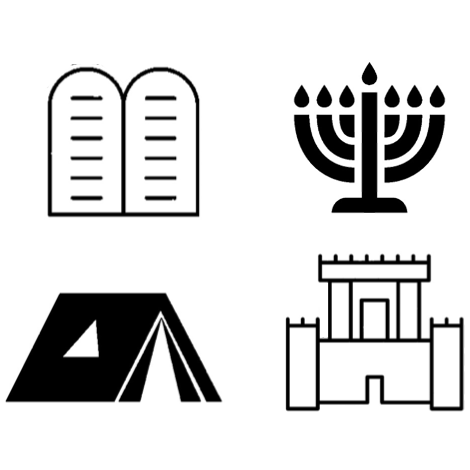
\includegraphics[width=0.30\textwidth]{../ot_frontcover.png}} ;
    \node (0,0) [xshift=+0.20cm, yshift=+2.0cm, opacity=0.10]{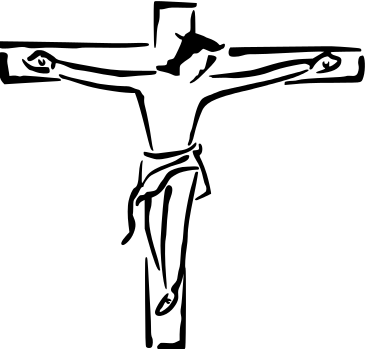
\includegraphics[width=0.20\textwidth]{../christ_on_cross.png}} ;
\end{tikzpicture}
\Large 

\leftcitation{ס} \centerfont 詩百又廿七載：
\leftcitation{ע} \centerfont 非耶和華建屋宇.則匠人之經營徒.
\leftcitation{פ} \centerfont 非耶和華衛城邑.則守者之儆醒徒.
\leftcitation{צ} \centerfont 余獻是卷予華人社區．願為福音流通之器．願獻斯微材為祭榮耀上帝．
\leftcitation{ק} \centerfont 阿門

\switchcolumn

\fontsize{11}{13}\rightfont \Large 滅．時越次聖殿期及當今。\leftcitation{י} \rightfont 猶太者力廣納之．筆錄以卷軸．便以傳、閱、頌、攜、守、鎖、抄、譯、釋、編，得書塔木德、密示拿等經傳．家喻戶曉．傳流若芳。\leftcitation{כ} \rightfont 猶太者文以載道．傳其口述．今我輩粵道之傳應當作如是．遂力行粵音識辨之法．載言載道．以盡忠傳粵道以待興。\leftcitation{ל} \rightfont 蒙下賜恩惠．無畏海量字音文書．既馭上帝之道．今廣及粵語講道．重駛編程之技．匯導粵音遂字稿．重塑講道現場．以傚猶太卷軸之舉便以傳流。\leftcitation{מ} \rightfont 是卷乃粵音口述傳之屬．莫通華文白話之語．

\end{paracol}

\columnratio{0.5,0.5}
\begin{paracol}{2}\fontsize{11}{13}\leftfont \Large \leftcitation{ו} \leftfont 斯殺一違儆百逆．既禁壓之．我輩聞風無奈．在所難免。\leftcitation{ז} \leftfont 另有異人例乎．以版權之名．脅網絡頻道之舉．同授礙予粵道之存流。

\switchcolumn

\fontsize{11}{13}\rightfont \Large 惟待後繼來者之傚．以譯釋傳之於神州華文地。\leftcitation{נ} \rightfont 今能排程驅馭圖靈以編彙文檔，其碼長共數千千亦無逢大礙．全蒙上帝保守。

\end{paracol}



\columnratio{1}\begin{paracol}{1}

\fontsize{11}{13}\rightfont \Large
~~~~~~~~~~~~~~~~~~~~~~~~~~~~~~~~~~~~~~~~~~~~~~~~~~~~~~~~~~~~~~~~~~~~~~~~~~~~~~~\leftcitation{ר} \rightfont 二零二三年二月一日

~~~~~~~~~~~~~~~~~~~~~~~~~~~~~~~~~~~~~~~~~~~~~~~~~~~~~~~~~~~~~~~~~~~~~~~~~~~~~~~\leftcitation{ש} \rightfont 米迦勒

~~~~~~~~~~~~~~~~~~~~~~~~~~~~~~~~~~~~~~~~~~~~~~~~~~~~~~~~~~~~~~~~~~~~~~~~~~~~~~~\leftcitation{ת} \rightfont 書於香港

\end{paracol}

\end{sloppypar}
\end{document}
